\documentclass[
  a4paper,
  emulatestandardclasses,
  abstract,
  parskip,
  appendixprefix,
  listof=totoc,
  bibliography=totoc
]{scrreprt}

\usepackage[
  ngerman,
  english
]{babel}
\usepackage[T1]{fontenc}
\usepackage{fontspec}
\usepackage{lmodern}
\usepackage{bm}
\usepackage{xcolor}
\usepackage{a4wide}
\usepackage{authblk}
\usepackage{amsthm}
\usepackage{amsmath}
\usepackage{amssymb}
\usepackage{physics}
\usepackage{caption}
\usepackage{csquotes}
\usepackage{paralist}
\usepackage[
  backend=biber,
  sorting=none
]{biblatex}
\usepackage[section]{placeins}
\usepackage{enumerate}
\usepackage{graphicx}
\usepackage[hidelinks]{hyperref}
\usepackage{cleveref}
\usepackage[
  chapter,
  newfloat,
  outputdir=build,
  cachedir=build
]{minted}
\usepackage[binary-units]{siunitx}
\usepackage[margin=14pt]{caption}
\usepackage[
  acronym,
  nonumberlist,
  toc
]{glossaries}
\usepackage{booktabs}
\usepackage{pgfplots}
\usepackage{adjustbox}
\usepackage{subcaption}

\pgfplotsset{compat=newest}

\usemintedstyle{tango}

\addbibresource{literature.bib}

\sisetup{math-micro=\text{µ},text-micro=µ}

\DeclareMathOperator{\rect}{rect}
\DeclareMathOperator{\sinc}{sinc}

% required to load imshow plots
\newcommand\inputpgf[2]{{
\let\pgfimageWithoutPath\pgfimage
\renewcommand{\pgfimage}[2][]{\pgfimageWithoutPath[##1]{#1/##2}}
\input{#1/#2}
}}

\makeglossaries
\newglossaryentry{si}
{name=SI, description={International System of Units}}
\newglossaryentry{ad9910}
{name=AD9910, description={a direct digital synthesizer from Analog Devices}}
\newglossaryentry{sn74128}
{name=SN74128, description={a line driver from Analog Devices}}
\newacronym{v}{V}{vertical}
\newacronym{h}{H}{horizontal}
\newacronym{rf}{RF}{radio frequency}
\newacronym{sma}{SMA}{SubMiniature version A}
\newacronym{smf}{SMF}{single-mode optical fiber}
\newacronym{aom}{AOM}{acousto-optic modulator}
\newacronym{aod}{AOD}{acousto-optic deflector}
\newacronym{dds}{DDS}{direct-digital synthesizer}
\newacronym{ccd}{CCD}{charge-coupled device}
\newacronym{ic}{IC}{integrated circuit}
\newacronym{pll}{PLL}{phase-locked-loop}
\newacronym{asf}{ASF}{amplitude scale factor}
\newacronym{ftw}{FTW}{frequency tuning word}
\newacronym{fft}{FFT}{fast-fourier-transform}
\newacronym{ttl}{TTL}{transistor-transistor logic}
\newacronym{bbb}{BBB}{BeagleBone Black}
\newacronym{gnd}{GND}{ground}
\newacronym{lan}{LAN}{local area network}
\newacronym{gpio}{GPIO}{general purpose input output}
\newacronym{http}{HTTP}{hypertext transport protocol}
\newacronym{mot}{MOT}{magneto-optical trap}
\newacronym{mse}{MSE}{mean squarred error}
\newacronym{fpga}{FPGA}{field programmable gate array}
\newacronym{adc}{ADC}{analog to digital converter}
\newacronym{dac}{DAC}{digital to analog converter}
\newacronym{vco}{VCO}{voltage-controlled oscillator}
\newacronym{rmd}{RMD}{relative mean deviation}
\newacronym{iqr}{IQR}{interquartile range}
\newacronym{cdf}{CDF}{cummulative distribution function}
\newacronym{1d}{1D}{one-dimensional}
\newacronym{2d}{2D}{two-dimensional}
\newacronym{3d}{3D}{three-dimensional}
\newacronym{rwa}{RWA}{rotating wave approximation}
\newacronym{fwhm}{FWHM}{full width at half maximum}
\newacronym{pid}{PID}{proportional-integral-derivative controller}
\newacronym{visa}{VISA}{virtual instrument software architecture}

\subject{Many Body Quantum Optics}
\title{Local time-averaged optical potentials using acousto-optic deflectors}
\subtitle{Bachelor thesis by}
\author{Bodo Kaiser}
\affil{Ludwig-Maximilians-Universität München}
\affil{\textit{bodo.kaiser@physik.uni-muenchen.de}}
\publishers{Supervisors: Prof. Dr. Immanuel Bloch, Dr. Monika Aidelsburger and
  Christian Schweizer.}

\begin{document}

\makeatletter
\begin{titlepage}
  \begin{center}
    \usekomafont{subject}
    \@subject

    \vspace{.8em}
    \usekomafont{title}\huge
    \@title

    \vspace{.5em}
    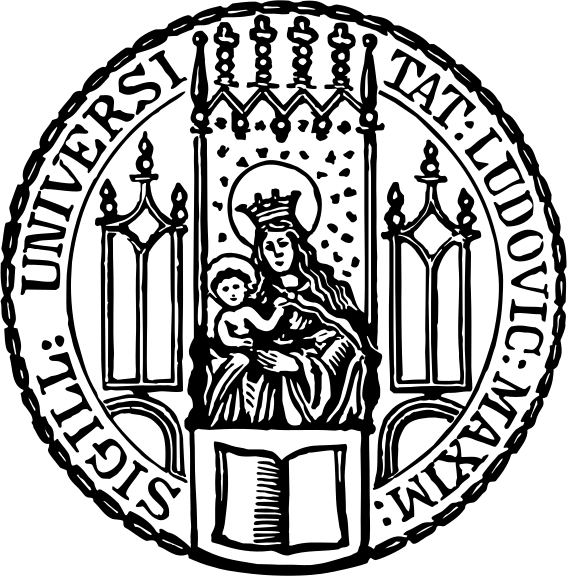
\includegraphics[width=.5\pagewidth]{\mediadir{image/emblem.pdf}}

    \usekomafont{subtitle}
    \@subtitle

    \vspace{.8em}
    \usekomafont{author}
    \@author

    \usekomafont{date}
    \@date

    \vspace{.8em}
    \usekomafont{publishers}
    \@publishers
  \end{center}
\end{titlepage}
\makeatother

\makeatletter
\begin{titlepage}
  \begin{otherlanguage}{ngerman}
    \begin{center}
      \usekomafont{subject}
      Mehrteilchen Quantenoptik

      \vspace{.8em}
      \usekomafont{title}\huge
      Hochpräzise zeitgemittelte optische Potentiale für ultrakalte Atome

      \vspace{.5em}
      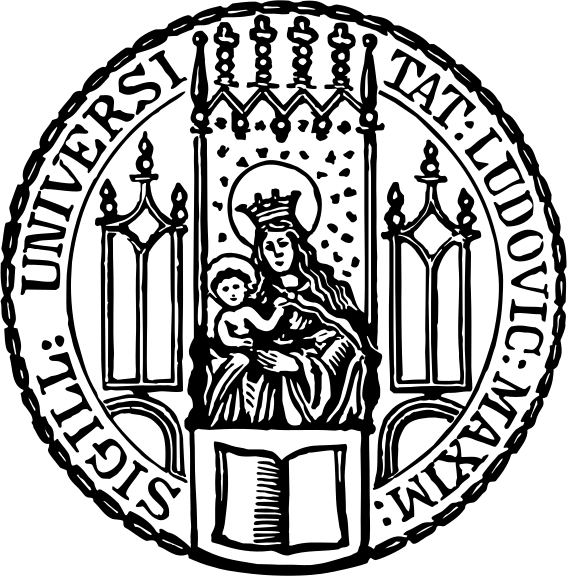
\includegraphics[width=.5\pagewidth]{\mediadir{image/emblem.pdf}}

      \usekomafont{subtitle}
      Bachelorarbeit von

      \vspace{.8em}
      \usekomafont{author}
      \@author

      \usekomafont{date}
      \@date

      \vspace{.8em}
      \usekomafont{publishers}
      entstanden unter der Betreuung von Prof. Dr. Immanuel Block,\\
      Dr. Monika Aidelsburger und Christian Schweitzer.
    \end{center}
  \end{otherlanguage}
\end{titlepage}
\makeatother

\begin{abstract}
Ultracold atoms in optical lattices open up a wide range of possibilities
to simulate many-body quantum phenomena, which would elsewise be neither
computationally nor experimentally tangible.

The topology of the optical lattice is a decisive property of these kind
of experiments and therefore of major interest. Recently, efforts have been
reported to create novel optical potentials through the use of digital
micromirror arrays that permit alterations of localized potentials. Though
promising results have been achieved --- in particular for static potentials
--- limitations due to the mechanical nature of these mirror arrays arise,
for instance, with regard to dynamical control.

In the present work we present an alternative implementation of localized
optical lattice potentials based on acousto-optic deflectors and
direct digital synthesizers.

We will give a brief theoretical introduction into the main concepts, i.e.\
the interaction of neutral atoms with optical potentials as well as the
general operation of direct digital synthesizer and acousto-optic deflectors.
From the physics we can derive the requirements imposed on the technical
implementation of the \gls{rf} signal source and the deflection.

We will find that even though the platform of digital signal synthesis
generally suites our application in terms of modulation capabilities and
resolution, the particular implementation of the \gls{ad9910} demonstrates
several shortcomings.

In the second part we characterize the deflection efficiency of the
acousto-optic deflectors. Towards the end we try to minimize the variance of
the deflection efficiency by performing a random search on the amplitude
segments of the \gls{rf} signal. It turns out that the deflection efficiency
is a highly non-linear function of the applied \gls{rf} power and frequency.
Furthermore minimization of the deflection efficiency variances proves to be
very unstable. Though we can largely preclude electronic defects to be the
source of this behaviour, further investigation is required.
\end{abstract}

\addchap{Acknowledgement}

The success and final outcome of the present work required a lot of guidance
and assistance from many people. Without them it would not have been possible
for me to deliver this work and remember the exciting time I had in the past
weeks.

At most I want to thank my parents for their support, that I have been
privileged to benefit from all the years. Though my life involved many
unexpected turnarounds, I never felt left alone and could rely on your
diverse experience whenever the situation required it.

Further I want to thank Prof. Immanuel Bloch and Dr. Monika Aidelsburger for
creating and sustaining a fertile scientific environment. It has been a
refreshing novelty for me to have the opportunity to have inspiring
discussions at almost any time and to seamlessly implement new ideas without
being limited by the present material.

Equally I want to express my gratitude to all personal involved in the
formation process of my thesis. Especially I want to name Christian Schweizer
with whom it had been a great pleasure to work with. Further I want to thank
Till Klostermann for instantly sharing his deep insights in many problems I
have encountered and his help with the optical setup. Hendrik von Raven I want
to thank for his overall guidance with regard to the electronic equipment.
In addition I owe special thanks to Michael Schreiber who helped me understand
the theoretical foundations of atoms in optical lattices, David Wei for his
hospitality and productive discussions about the acousto-optic deflectors,
and of course biggest thanks to Bodo Hecker for his advice as electrical
engineer and distinct perspective on undergone challenges.

Finally I want to express my gratitude to my friend Dr. Abdullah Sarani for
his suggestions and advice on the final draft.


\tableofcontents

%\chapter{Introduction}

Many quantum systems studied in condensed matter physics are experimentally
challenging to access as any interactions can destroy the carefully prepared
quantum states. As way forward, experiments with ultracold atoms in
optical lattices give us a highly contorllable environment, giving us the
opportunity to simulate and explore quantum effects and expand our current
understanding of quantum mechanics and statistical physics \cite{Gross2017}.

The central idea behind these types of experiments is to cool down neutral
atoms to micro Kelvin and below, and load them into an optical lattice. At
these temperatures atoms demonstrate quantum behaviour. The optical lattices
act as periodic potentials analogue to the periodic potential found inside
solid state crystal lattices \cite{Lewenstein2007}. Unlike to i.e. real solids
where we have limited prospects to amend a systems properties, lasers driven
by state of the art optics and electronics give us a wide range of well
controllable parameters.

\begin{figure}[h]
  \centering
  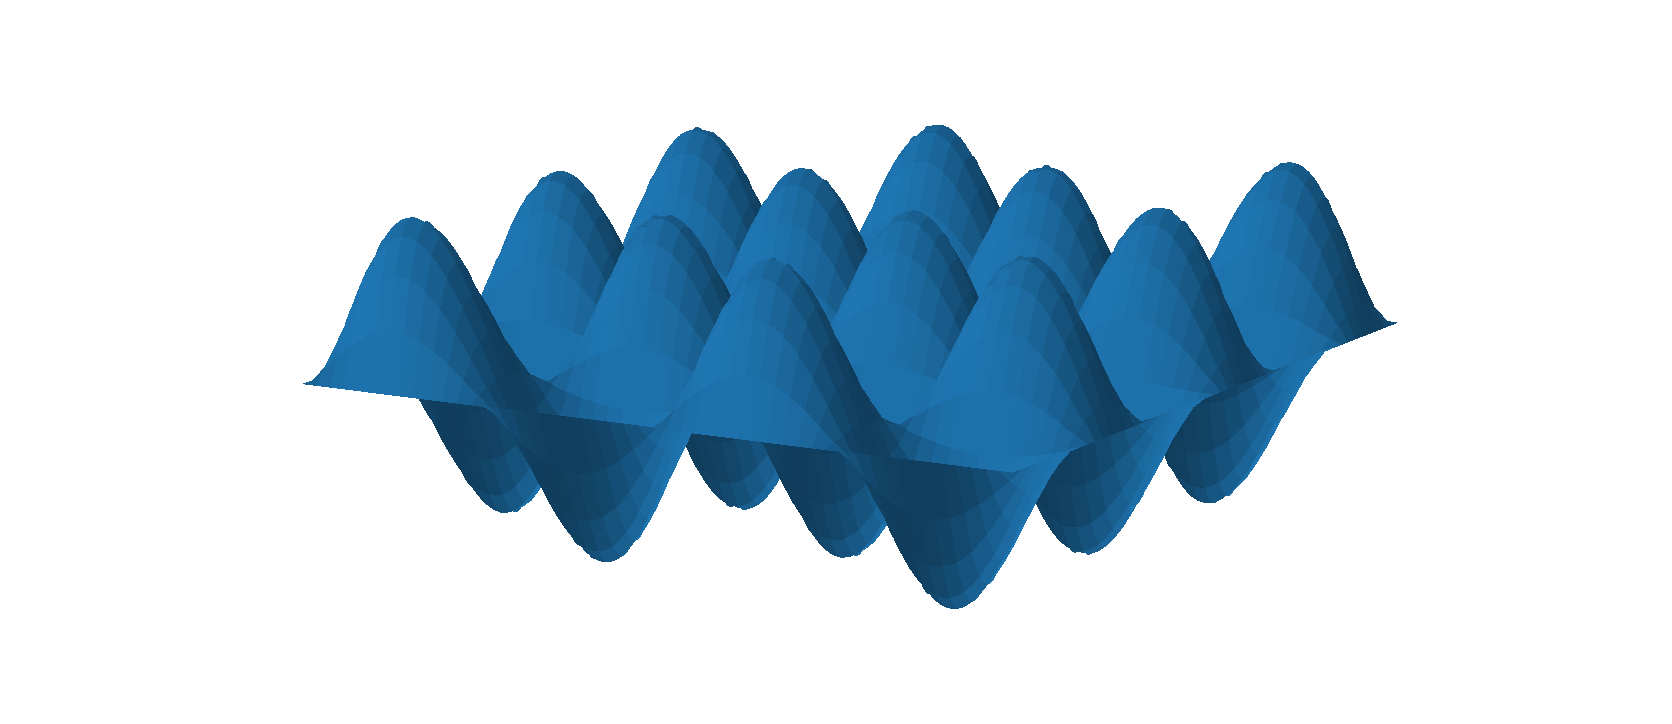
\includegraphics[width=.8\textwidth]{images/optlat/default.pdf}
  \captionsetup{width=.8\textwidth}
  \caption{Periodic potential of a 2D optical lattice. If the kinetic energy
  of the atoms is below the potential energy of the lattice, the atoms will
  locate around the potential minimas.}
  \label{fig:optlat}
\end{figure}

One of the parameters of interest is the ability to apply local potentials
to the system, that can be used to, among others, study lattice inpurities
or quantum interactions. In this work we will present and characterize one
possible implementation of such a local potential generating apparatus.

\section{Related Work}

Local manipulations of atoms inside optical lattices have been known for some
time in the embodiment of optical tweezers that allow trapping, stacking and
sorting of particles \cite{Tadmor2004}. Yet, only recently attempts to
interact with local particle clusters through high-precision time-averaged
optical potentials have been reported \cite{Roy2016}.

In the following we continue on the laid out work \cite{Hertlein2017} which
provided us with an optical setup for single-site manipulation using
\gls{aod} as well as considerations with regard to aperture limited
gaussian beam propagation.

%\chapter{Optical potentials}

\textit{In the introduction we emphasized the importance of optical lattices,
yet we left out many details, for instance, how these optical lattices are
created and how the optical quantities enter the potential energy of the
atoms. In this chapter we will make up for said gaps. First we will
recapitulate the theory behind laser light intensities and then derive a
formulation of the effective lattice potentials felt by the atoms.}

\section{Atom-light interaction}

At first we need to ask ourselves how the laser field acts as a perturbation
to the Hamiltonian of the atomic system and how this perturbation leads to an
intensity dependent potential for the atoms, which we can control in the
experiment. In deviations are loosely based on
references~\cite{Gerry2004,Jackson2005,Bartelmann2018}.

\subsection{Dipole potential}

We will use \gls{si} units unless stated otherwise. The Hamiltonian of an electron
in an external electromagnetic field reads
\begin{equation}
  \hat{H}_\text{em}
  =\frac{1}{2m_e}{\left(\hat{\vb{p}}+e\vb{A}\right)}^2-e\Phi+\hat{V}_0
  \label{eq:hamiltonian_em},
\end{equation}
with vector potential $\vb{A}$ and scalar potential $\Phi$ of the external
field and the Coulomb potential of the nucleus $\hat{V}_0$. Further $m_e$
denotes the electron mass and $e$ the elementary charge.
\Cref{eq:hamiltonian_em} is exact for the hydrogen atom that only hosts one
electron. For alkali atoms we know that inner electron shells are closed and
the single outer electron is approximately described by
\cref{eq:hamiltonian_em}. The electromagnetic field relates to the
vector and scalar potential through
\begin{align}
  \vb{E}=-\grad{\Phi}-\pdv{\vb{A}}{t}, &&
  \vb{B}=\curl{\vb{A}},
  \label{eq:field_em_potentials}
\end{align}
where $\vb{E}$ is the electric and $\vb{B}$ the magnetic field component.

The canonical momentum $\hat{\vb{p}}+e\vb{A}$ in \cref{eq:hamiltonian_em} is
difficult to work with. Fortunately Gauge transforms
\begin{align}
  \vb{A}\to\vb{A}+\grad{\chi}
  &&
  \Phi\to\Phi-\pdv{\chi}{t}
  \label{eq:gauge_transform_em}
\end{align}
allow us to simplify \cref{eq:hamiltonian_em} by choosing a specific Gauge
function $\chi(\vb{x},t)$. The Gauge function itself $\chi$ does not amend the
electromagnetic field components \cref{eq:field_em_potentials} which we
usually consider to represent physical reality --- in contrast to the
electromagnetic potentials $\vb{A},\Phi$ which are usually only considered
mathematical aid.\footnote{The Aharonov-Bohm effect actually provides evidence
that aso the electromagnetic potentials represent physical reality.} In the
following we choose the gauge function $\chi=-\vb{A}\cdot\vb{x}$ and assume
the dipole approximation $\vb{A}(\vb{x},t)\approx\vb{A}(t)$. The dipole
approximation neglects the spatial variation of the electromagnetic field
over the atom and instead assumes a small separation of opposite charges at
the nucleus. The dipole approximation is reasonable as wave length of visible
light are much larger than atomic length scales~\cite{Gerry2004}. For a
rigorous upper error bound on the dipole approximation see
Ref.~\cite{Bossmann2016}. In the dipole approximation $\chi$ satisfies the
Coulomb gauge condition $\divergence{\vb{A}}=0$ allowing us to set $\Phi=0$
as no external sources are present~\cite{Jackson2005}. Finally we can rewrite
\cref{eq:hamiltonian_em} as
\begin{equation}
  \hat{H}_\text{dip}
  =\frac{\hat{\vb{p}}^2}{2m}+\hat{V}_0+\hat{V}_\text{dip}
  =\hat{H}_0+\hat{V}_\text{dip}
  \label{eq:hamiltonian_dip}
\end{equation}
with the dipole potential
\begin{equation}
  \hat{V}_\text{dip}
  =-\hat{\vb{d}}\cdot\vb{E}
  \label{eq:potential_dip},
\end{equation}
the dipole operator $\hat{\vb{d}}=-e\vb{x}$ and the spatially homogeneous
light field $\vb{E}(t)$.

\subsection{AC-Stark effect}

We are now going to solve \cref{eq:hamiltonian_dip} for an arbitrary light
field of the form
\begin{equation}
  \vb{E}(t,\vb{x})
  =\vb{E}_0(\vb{x})\cos(\omega t)
  \label{eq:light_field}
\end{equation}
where $\vb{E}_0(\vb{x})$ should be compatible with Maxwell's equations and
be approximately constant on atomic length scales to not violate the dipole
approximation. Further we need the laser frequency $\omega$ to be
far-off-resonant to the atomic transition frequencies to avoid population
dynamics.

At $t<0$ the system is in the energy eigenstate $\ket{n}$ of the
unperturbated Hamiltonian $\hat{H}_0$
\begin{equation}
  \hat{H}_0\ket{n}
  =E_n\ket{n}
  =\hbar\omega_n\ket{n}
  \label{eq:eigenvalue_energy_unperturbated}.
\end{equation}
At $t>0$ the external light field appears immediately. The new state
$\ket{\psi}$ can be expanded in the complete basis of the previous energy
eigenstates
\begin{equation}
  \ket{\psi}
  =
  \sum_n{c_n(t)}{e^{-i{\omega_n}t}}\ket{n}
  \label{eq:state_expansion_unperturbated}.
\end{equation}
Inserting \cref{eq:state_expansion_unperturbated} into the time-dependent
Schrödinger equation with the dipole Hamiltonian \cref{eq:hamiltonian_dip} and
applying $\bra{m}{e^{i{\omega_m}t}}$ to the right hand side leads us to a set
of differential equations
\begin{equation}
  \dot{c}_m
  =
  -\frac{i}{\hbar}\sum_n{c_n(t)}{e^{-i\omega_{nm}t}}
  \bra{m}\hat{V}_\text{dip}\ket{n}
  \label{eq:differential_equation_population_dynamics}
\end{equation}
with $\omega_{nm}=\omega_n-\omega_m$. One can read
\cref{eq:differential_equation_population_dynamics} as the rate by which
the probability amplitude of a state $m$ changes in time. It is equal to the
sum of oscillations between states $n$ and $m$ weighted by the current
probability of state $c_n(t)$ and the interaction strength. If we are able to
solve \cref{eq:differential_equation_population_dynamics} for $c_n(t)$ the
population dynamic is entirely described by the time-dependent probabilities
$\abs{c_n(t)}^2$. By using \cref{eq:light_field} we can rewrite the dipole
transition matrix elements
\begin{equation}
  \bra{m}\hat{V}_\text{dip}\ket{n}
  =\Omega_{nm}(\vb{x})\cos(\omega t)\hbar
  \label{eq:elements_dipole_transition_matrix}
\end{equation}
where we introduced the Rabi frequency
\begin{equation}
  \Omega_{nm}(\vb{x})
  =\bra{n}\hat{\vb{d}}\cdot\vb{E}_0(\vb{x})\ket{m}/\hbar
  \label{eq:rabi_frequency}.
\end{equation}
More general expressions for dipole transition elements of one and two
electron systems can be found in Reference~\cite{Bethe1957}. 

\subsubsection{Two-level system}

From now on we assume a two state system that initially is in the ground
state $c_g(0)=1,c_e(0)=0$. Under these circumstances the dynamics described in
\cref{eq:differential_equation_population_dynamics} simplify to
\begin{align}
  i\dot{c}_g=\Omega_{ge}c_e(t)\cos(\omega t)e^{+i\omega_0 t} &&
  i\dot{c}_e=\Omega_{ge}c_g(t)\cos(\omega t)e^{-i\omega_0 t}
  \label{eq:differential_equation_population_dynamics_two_state_system}
\end{align}
Writing $\cos(\omega t)$ in terms of exponential functions and dropping
$e^{\pm i(\omega+\omega_{ge})t}$ yields the so-called \gls{rwa}
\begin{align}
  i\dot{c}_g\approx\frac{\Omega_{ge}}{2}c_e(t)e^{+i\Delta\omega t} &&
  i\dot{c}_e\approx\frac{\Omega_{ge}}{2}c_g(t)e^{-i\Delta\omega t}
  \label{eq:differential_equation_population_dynamics_two_state_system_rwa}
\end{align}
where we introduced the frequency detuning
$\Delta\omega=\abs{\omega-\omega_0}$. The \gls{rwa} is motivated by the fact
that oscillations of frequency $\omega+\omega_0$ are fast compared to changes
in the population dynamics and therefore vanish on average.

We now define $a_g=c_g$ and $a_e=c_e e^{i\Delta\omega t}$ and rewrite
\cref{eq:differential_equation_population_dynamics_two_state_system_rwa} by
\begin{align}
  i\dot{a}_g=\frac{\Omega_{ge}}{2}a_e(t) &&
  i\dot{a}_e=\frac{\Omega_{ge}}{2}a_g(t)-a_e\Delta\omega
  \label{eq:differential_equation_population_dynamics_two_state_system_shift}.
\end{align}
Using
\cref{eq:differential_equation_population_dynamics_two_state_system_shift} we
can diagonalize the Hamiltonian and find the energy eigenvalues to be
\begin{equation}
  E_{e,g}
  =\frac{\hbar}{2}\left(-\Delta\omega\mp\sqrt{\Omega_{ge}^2+\Delta\omega^2}\right)
  \approx
  \mp\frac{\hbar\Omega_{ge}^2}{4\Delta\omega}
  \label{eq:eigenvalues_energy_light_shift}
\end{equation}
where we applied a Taylor expansion for $\Omega_{ge}/\Delta\omega\ll1$ around
$\Omega_{ge}/\Delta\omega=0$ and omitted terms of higher order.

Consequently, atoms in an external off-resonant light field experience an
effective periodic lattice potential
\begin{equation}
  \hat{V}_\text{lat}(\vb{x})
  =
  \mp\frac{\hbar\Omega_{ge}^2(\vb{x})}{4\Delta\omega}
  =
  \mp\frac{d_0^2E_0^2(\vb{x})}{4\hbar\Delta\omega}
  \label{eq:potential_lattice}
\end{equation}
with dipole element $d_0$. The sign has to be chosen with respect to the
direction of the laser detuning from resonance. If the laser is red-shifted
compared to the resonance frequency, $\omega-\omega_0>0$, we need to choose
the negative sign as the particles are drawn towards the areas of maximum
intensity. If the laser is blue-shifted compared to the resonance frequency,
$\omega-\omega_0<0$, we need to choose the positive sign as the particles are
drawn towards the area of minimum intensity. The same results can also be
obtained by the use of second order perturbation theory~\cite{Grimm2008}.

\section{Laser light fields}

In this section our focus will be on the spatial distribution of the lattice
and perturbation laser light fields that create the time-averaged dynamical
potentials we discussed in the introduction.

\subsection{Gaussian beams}

The predominant output mode of most lasers is the fundamental transverse
gaussian mode. For a laser beam propagating along the $z$-direction it is
described by
\begin{equation}
  \vb{E}(r,z)
  =
  \vb{E}_0\frac{w(0)}{w(z)}
  \exp{-\frac{r^2}{w{(z)}^2}}
  \exp{-ik\left(z+\frac{r^2}{2R(z)}-\arctan(\frac{z}{z_R})\right)}
  \label{eq:gaussian_beam}
\end{equation}
where $w{(z)}$ is the waist radius, $z_R=\pi w{(0)}^2/\lambda$ the Rayleigh
range and $R(z)$ the radius of curvature of the beam's wavefront at position
$z$.
\begin{figure}[ht]
  \centering
  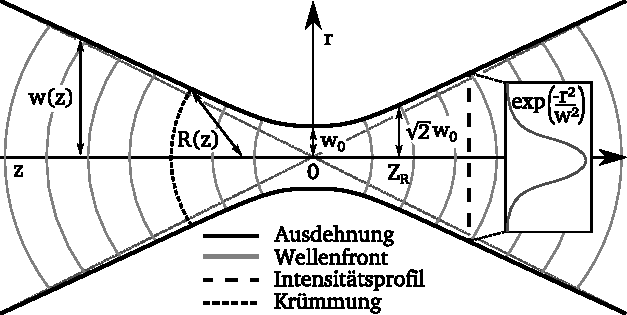
\includegraphics[width=.9\textwidth]{\mediadir{image/gaussian-beam.pdf}}
  \captionsetup{width=.9\textwidth}
  \caption{Illustration of Gaussian beam parameters from Ref.~\cite{Aleph2014}
    translated into English with changed radius of curvature.
  }\label{fig:gaussian_beam}
\end{figure}
\Cref{fig:gaussian_beam} unveils how the parameters relate to the beam
profile as a function of propagation distance $z$. The waist radius $w(z)$
corresponds to the \gls{fwhm} by $w(z)=FWHM(z)/\sqrt{2\ln2}$, $R(z)$ relates
to the wavefront curvature and $z_R$ is the distance from origin $z=0$ where
the beam waist is $w(z)=\sqrt{2}w(0)$. Beam waist and curvature of radius
evolve according to
\begin{align}
  w{(z)}
  =
  w{(0)}{\left[1+{\left(\frac{z}{z_R}\right)}^2\right]}^{1/2}
  &&
  R{(z)}=z{\left[1+{\left(\frac{z_R}{z}\right)}^2\right]}
  \label{eq:gaussian_beam_evolvement}.
\end{align}

Fortunately \cref{eq:potential_lattice} only depends on the absolute
square of the electric field, thus we can drop the complex exponential from
\cref{eq:gaussian_beam} to find an expression for the Gaussian intensity
distribution
\begin{equation}
  I(r,z)
  =
  I_0
  {\left(\frac{w(0)}{w(z)}\right)}^2
  \exp{-\frac{2r^2}{w{(z)}^2}}
  =
  I_0
  \frac{\exp{-\frac{2r^2}{w{(z)}^2}}}{1+{\left(\frac{z}{z_R}\right)}^2}
  \label{eq:gaussian_intensity}
\end{equation}
where $I_0$ is the maximum intensity at $r=z=0$.

\subsubsection{Lattice intensity}

A \gls{1d} optical lattices can be generated through the interference
of two counter-propagating Gaussian beams. One way to achieve
counter-propagation while keeping the coherence stable, is to use a mirror.
Under the assumption of perfect reflection of the mirror, the electrical field
component of the laser beam is described by
\begin{align*}
  \vb{E}_\rightarrow(\vb{x},t)+\vb{E}_\leftarrow(\vb{x},t)
  &=
  \vb{E}_0(r,z)\cos(\omega t-kz)+\vb{E}_0(r,z)\cos(\omega t+kz)\\
  &=
  2\vb{E}_0(r,z)\cos(kz)\cos(\omega t).
\end{align*}
Hence, the intensity distribution equals
\cref{eq:gaussian_intensity} with an additional $4\cos^2(kz)$ factor
\begin{equation}
  I(r,z)
  =
  4I_0\cos^2(kz)
  \frac{\exp{-\frac{2r^2}{w{(z)}^2}}}{1+{\left(\frac{z}{z_R}\right)}^2}
  \label{eq:lattice_intensity}
\end{equation}
caused by the constructive interference.
\begin{table}[ht]
  \centering
  \begin{tabular}{cccc}
    \toprule
    Laser wavelength $\lambda$ &
    Lattice constant $a=\lambda/2$ &
    Beam waist $w(0)$ &
    Rayleigh length $z_R$ \\
    \midrule
    \SI{1064}{\nano\meter} &
    \SI{532}{\nano\meter} &
    \SI{150}{\micro\meter} &
    \SI{66}{\milli\meter} \\
    \bottomrule
  \end{tabular}
  \captionsetup{width=.8\textwidth}
  \caption{Typical values for a Gaussian beam used to generate an optical
    lattice potential.
  }\label{tab:gaussian_beam_lattice}
\end{table}
\Cref{tab:gaussian_beam_lattice} lists typical values for a Gaussian beam
used to construct an optical lattice potential. Typical atom clouds occupy
about 50--100 lattice sites spanning over a range of
$l=50a\approx\SI{27}{\micro\meter}$~\cite{Rom2009}. As typical atom clouds
are much smaller then the typical beam waists used for optical lattices, we
have $r/w(z)\ll1$ and can approximate \cref{eq:lattice_intensity}
\begin{equation}
  I(r,z)
  \approx
  4I_0\cos^2(kz)
  \label{eq:gaussian_intensity_approx}
\end{equation}
which we will use from now on as the intensity distribution for \gls{1d}
optical lattices.

\subsubsection{Perturbation intensity}

For the generation of optical lattices we want large beam waists because
otherwise the potential is not homogeneous and there is a potential energy
difference between neighboring lattice sites. For our perturbation potential,
however, we need very high resolution on the order of a single lattice site,
and therefore need a tightly focused beam.
\begin{table}[ht]
  \centering
  \begin{tabular}{cccc}
    \toprule
    Laser wavelength $\lambda$ &
    Beam waist $w(0)$ &
    Rayleigh length $z_R$ \\
    \midrule
    \SI{532}{\nano\meter} &
    \SI{1}{\micro\meter} &
    \SI{6}{\micro\meter} \\
    \bottomrule
  \end{tabular}
  \captionsetup{width=.8\textwidth}
  \caption{Typical values for a Gaussian beam used to perturbate the optical
    lattice potential reported by~\cite{Hertlein2017}.
  }\label{tab:gaussian_beam_perturbation}
\end{table}
\Cref{tab:gaussian_beam_perturbation} summarizes the beam parameter of the
perturbation potential as suggested in Ref.~\cite{Hertlein2017}. For these
parameters approximations made for optical lattice are not valid because of
the small beam waist and Rayleigh length and we need to the exact
\cref{eq:gaussian_intensity} formula. In fact for an actual experiment we
would like to focus the laser beam to even smaller waists. The ultimate goal
would be the ability to address single lattice sites.

\section{Effective local potentials}

With \cref{eq:potential_lattice} we found an expression of the potential
energy in terms of atomic properties like the dipole transition element, the
atomic resonance and the laser intensity distribution. For the laser intensity
distribution of the optical lattice we derived
\cref{eq:gaussian_intensity_approx} and we concluded that the intensity of the
laser used for the creation of local potentials obeys
\cref{eq:gaussian_intensity}. If we add these pieces together we can calculate
the effective potential with local perturbation as seen by the atoms. We will
find that its shape deviates from the idealized local potentials we presented
in the introduction in \Cref{fig:optical_lattice_local_pot} and 
\Cref{fig:optical_lattice_local_barrier}.

\subsubsection{Barrier}

One embodiment of local potentials we described in the introduction was the
barrier potential. A barrier potential confines atoms to a subspace of the
global lattice and could be used to model thermodynamical equilibrium
processes.
\begin{figure}[htb]
  \centering
  \begin{adjustbox}{width=\textwidth}
    %% Creator: Matplotlib, PGF backend
%%
%% To include the figure in your LaTeX document, write
%%   \input{<filename>.pgf}
%%
%% Make sure the required packages are loaded in your preamble
%%   \usepackage{pgf}
%%
%% Figures using additional raster images can only be included by \input if
%% they are in the same directory as the main LaTeX file. For loading figures
%% from other directories you can use the `import` package
%%   \usepackage{import}
%% and then include the figures with
%%   \import{<path to file>}{<filename>.pgf}
%%
%% Matplotlib used the following preamble
%%   \usepackage{amsmath}\usepackage{siunitx}\usepackage{lmodern}
%%   \usepackage{fontspec}
%%
\begingroup%
\makeatletter%
\begin{pgfpicture}%
\pgfpathrectangle{\pgfpointorigin}{\pgfqpoint{12.000000in}{8.000000in}}%
\pgfusepath{use as bounding box, clip}%
\begin{pgfscope}%
\pgfsetbuttcap%
\pgfsetmiterjoin%
\pgfsetlinewidth{0.000000pt}%
\definecolor{currentstroke}{rgb}{1.000000,1.000000,1.000000}%
\pgfsetstrokecolor{currentstroke}%
\pgfsetdash{}{0pt}%
\pgfpathmoveto{\pgfqpoint{0.000000in}{0.000000in}}%
\pgfpathlineto{\pgfqpoint{12.000000in}{0.000000in}}%
\pgfpathlineto{\pgfqpoint{12.000000in}{8.000000in}}%
\pgfpathlineto{\pgfqpoint{0.000000in}{8.000000in}}%
\pgfpathclose%
\pgfusepath{}%
\end{pgfscope}%
\begin{pgfscope}%
\pgfsetbuttcap%
\pgfsetmiterjoin%
\definecolor{currentfill}{rgb}{1.000000,1.000000,1.000000}%
\pgfsetfillcolor{currentfill}%
\pgfsetlinewidth{0.000000pt}%
\definecolor{currentstroke}{rgb}{0.000000,0.000000,0.000000}%
\pgfsetstrokecolor{currentstroke}%
\pgfsetstrokeopacity{0.000000}%
\pgfsetdash{}{0pt}%
\pgfpathmoveto{\pgfqpoint{1.500000in}{5.740000in}}%
\pgfpathlineto{\pgfqpoint{10.800000in}{5.740000in}}%
\pgfpathlineto{\pgfqpoint{10.800000in}{7.840000in}}%
\pgfpathlineto{\pgfqpoint{1.500000in}{7.840000in}}%
\pgfpathclose%
\pgfusepath{fill}%
\end{pgfscope}%
\begin{pgfscope}%
\pgfsetbuttcap%
\pgfsetroundjoin%
\definecolor{currentfill}{rgb}{0.000000,0.000000,0.000000}%
\pgfsetfillcolor{currentfill}%
\pgfsetlinewidth{1.003750pt}%
\definecolor{currentstroke}{rgb}{0.000000,0.000000,0.000000}%
\pgfsetstrokecolor{currentstroke}%
\pgfsetdash{}{0pt}%
\pgfsys@defobject{currentmarker}{\pgfqpoint{0.000000in}{0.000000in}}{\pgfqpoint{0.000000in}{0.055556in}}{%
\pgfpathmoveto{\pgfqpoint{0.000000in}{0.000000in}}%
\pgfpathlineto{\pgfqpoint{0.000000in}{0.055556in}}%
\pgfusepath{stroke,fill}%
}%
\begin{pgfscope}%
\pgfsys@transformshift{3.003069in}{5.740000in}%
\pgfsys@useobject{currentmarker}{}%
\end{pgfscope}%
\end{pgfscope}%
\begin{pgfscope}%
\pgfsetbuttcap%
\pgfsetroundjoin%
\definecolor{currentfill}{rgb}{0.000000,0.000000,0.000000}%
\pgfsetfillcolor{currentfill}%
\pgfsetlinewidth{1.003750pt}%
\definecolor{currentstroke}{rgb}{0.000000,0.000000,0.000000}%
\pgfsetstrokecolor{currentstroke}%
\pgfsetdash{}{0pt}%
\pgfsys@defobject{currentmarker}{\pgfqpoint{0.000000in}{-0.055556in}}{\pgfqpoint{0.000000in}{0.000000in}}{%
\pgfpathmoveto{\pgfqpoint{0.000000in}{0.000000in}}%
\pgfpathlineto{\pgfqpoint{0.000000in}{-0.055556in}}%
\pgfusepath{stroke,fill}%
}%
\begin{pgfscope}%
\pgfsys@transformshift{3.003069in}{7.840000in}%
\pgfsys@useobject{currentmarker}{}%
\end{pgfscope}%
\end{pgfscope}%
\begin{pgfscope}%
\pgfsetbuttcap%
\pgfsetroundjoin%
\definecolor{currentfill}{rgb}{0.000000,0.000000,0.000000}%
\pgfsetfillcolor{currentfill}%
\pgfsetlinewidth{1.003750pt}%
\definecolor{currentstroke}{rgb}{0.000000,0.000000,0.000000}%
\pgfsetstrokecolor{currentstroke}%
\pgfsetdash{}{0pt}%
\pgfsys@defobject{currentmarker}{\pgfqpoint{0.000000in}{0.000000in}}{\pgfqpoint{0.000000in}{0.055556in}}{%
\pgfpathmoveto{\pgfqpoint{0.000000in}{0.000000in}}%
\pgfpathlineto{\pgfqpoint{0.000000in}{0.055556in}}%
\pgfusepath{stroke,fill}%
}%
\begin{pgfscope}%
\pgfsys@transformshift{4.576534in}{5.740000in}%
\pgfsys@useobject{currentmarker}{}%
\end{pgfscope}%
\end{pgfscope}%
\begin{pgfscope}%
\pgfsetbuttcap%
\pgfsetroundjoin%
\definecolor{currentfill}{rgb}{0.000000,0.000000,0.000000}%
\pgfsetfillcolor{currentfill}%
\pgfsetlinewidth{1.003750pt}%
\definecolor{currentstroke}{rgb}{0.000000,0.000000,0.000000}%
\pgfsetstrokecolor{currentstroke}%
\pgfsetdash{}{0pt}%
\pgfsys@defobject{currentmarker}{\pgfqpoint{0.000000in}{-0.055556in}}{\pgfqpoint{0.000000in}{0.000000in}}{%
\pgfpathmoveto{\pgfqpoint{0.000000in}{0.000000in}}%
\pgfpathlineto{\pgfqpoint{0.000000in}{-0.055556in}}%
\pgfusepath{stroke,fill}%
}%
\begin{pgfscope}%
\pgfsys@transformshift{4.576534in}{7.840000in}%
\pgfsys@useobject{currentmarker}{}%
\end{pgfscope}%
\end{pgfscope}%
\begin{pgfscope}%
\pgfsetbuttcap%
\pgfsetroundjoin%
\definecolor{currentfill}{rgb}{0.000000,0.000000,0.000000}%
\pgfsetfillcolor{currentfill}%
\pgfsetlinewidth{1.003750pt}%
\definecolor{currentstroke}{rgb}{0.000000,0.000000,0.000000}%
\pgfsetstrokecolor{currentstroke}%
\pgfsetdash{}{0pt}%
\pgfsys@defobject{currentmarker}{\pgfqpoint{0.000000in}{0.000000in}}{\pgfqpoint{0.000000in}{0.055556in}}{%
\pgfpathmoveto{\pgfqpoint{0.000000in}{0.000000in}}%
\pgfpathlineto{\pgfqpoint{0.000000in}{0.055556in}}%
\pgfusepath{stroke,fill}%
}%
\begin{pgfscope}%
\pgfsys@transformshift{6.150000in}{5.740000in}%
\pgfsys@useobject{currentmarker}{}%
\end{pgfscope}%
\end{pgfscope}%
\begin{pgfscope}%
\pgfsetbuttcap%
\pgfsetroundjoin%
\definecolor{currentfill}{rgb}{0.000000,0.000000,0.000000}%
\pgfsetfillcolor{currentfill}%
\pgfsetlinewidth{1.003750pt}%
\definecolor{currentstroke}{rgb}{0.000000,0.000000,0.000000}%
\pgfsetstrokecolor{currentstroke}%
\pgfsetdash{}{0pt}%
\pgfsys@defobject{currentmarker}{\pgfqpoint{0.000000in}{-0.055556in}}{\pgfqpoint{0.000000in}{0.000000in}}{%
\pgfpathmoveto{\pgfqpoint{0.000000in}{0.000000in}}%
\pgfpathlineto{\pgfqpoint{0.000000in}{-0.055556in}}%
\pgfusepath{stroke,fill}%
}%
\begin{pgfscope}%
\pgfsys@transformshift{6.150000in}{7.840000in}%
\pgfsys@useobject{currentmarker}{}%
\end{pgfscope}%
\end{pgfscope}%
\begin{pgfscope}%
\pgfsetbuttcap%
\pgfsetroundjoin%
\definecolor{currentfill}{rgb}{0.000000,0.000000,0.000000}%
\pgfsetfillcolor{currentfill}%
\pgfsetlinewidth{1.003750pt}%
\definecolor{currentstroke}{rgb}{0.000000,0.000000,0.000000}%
\pgfsetstrokecolor{currentstroke}%
\pgfsetdash{}{0pt}%
\pgfsys@defobject{currentmarker}{\pgfqpoint{0.000000in}{0.000000in}}{\pgfqpoint{0.000000in}{0.055556in}}{%
\pgfpathmoveto{\pgfqpoint{0.000000in}{0.000000in}}%
\pgfpathlineto{\pgfqpoint{0.000000in}{0.055556in}}%
\pgfusepath{stroke,fill}%
}%
\begin{pgfscope}%
\pgfsys@transformshift{7.723466in}{5.740000in}%
\pgfsys@useobject{currentmarker}{}%
\end{pgfscope}%
\end{pgfscope}%
\begin{pgfscope}%
\pgfsetbuttcap%
\pgfsetroundjoin%
\definecolor{currentfill}{rgb}{0.000000,0.000000,0.000000}%
\pgfsetfillcolor{currentfill}%
\pgfsetlinewidth{1.003750pt}%
\definecolor{currentstroke}{rgb}{0.000000,0.000000,0.000000}%
\pgfsetstrokecolor{currentstroke}%
\pgfsetdash{}{0pt}%
\pgfsys@defobject{currentmarker}{\pgfqpoint{0.000000in}{-0.055556in}}{\pgfqpoint{0.000000in}{0.000000in}}{%
\pgfpathmoveto{\pgfqpoint{0.000000in}{0.000000in}}%
\pgfpathlineto{\pgfqpoint{0.000000in}{-0.055556in}}%
\pgfusepath{stroke,fill}%
}%
\begin{pgfscope}%
\pgfsys@transformshift{7.723466in}{7.840000in}%
\pgfsys@useobject{currentmarker}{}%
\end{pgfscope}%
\end{pgfscope}%
\begin{pgfscope}%
\pgfsetbuttcap%
\pgfsetroundjoin%
\definecolor{currentfill}{rgb}{0.000000,0.000000,0.000000}%
\pgfsetfillcolor{currentfill}%
\pgfsetlinewidth{1.003750pt}%
\definecolor{currentstroke}{rgb}{0.000000,0.000000,0.000000}%
\pgfsetstrokecolor{currentstroke}%
\pgfsetdash{}{0pt}%
\pgfsys@defobject{currentmarker}{\pgfqpoint{0.000000in}{0.000000in}}{\pgfqpoint{0.000000in}{0.055556in}}{%
\pgfpathmoveto{\pgfqpoint{0.000000in}{0.000000in}}%
\pgfpathlineto{\pgfqpoint{0.000000in}{0.055556in}}%
\pgfusepath{stroke,fill}%
}%
\begin{pgfscope}%
\pgfsys@transformshift{9.296931in}{5.740000in}%
\pgfsys@useobject{currentmarker}{}%
\end{pgfscope}%
\end{pgfscope}%
\begin{pgfscope}%
\pgfsetbuttcap%
\pgfsetroundjoin%
\definecolor{currentfill}{rgb}{0.000000,0.000000,0.000000}%
\pgfsetfillcolor{currentfill}%
\pgfsetlinewidth{1.003750pt}%
\definecolor{currentstroke}{rgb}{0.000000,0.000000,0.000000}%
\pgfsetstrokecolor{currentstroke}%
\pgfsetdash{}{0pt}%
\pgfsys@defobject{currentmarker}{\pgfqpoint{0.000000in}{-0.055556in}}{\pgfqpoint{0.000000in}{0.000000in}}{%
\pgfpathmoveto{\pgfqpoint{0.000000in}{0.000000in}}%
\pgfpathlineto{\pgfqpoint{0.000000in}{-0.055556in}}%
\pgfusepath{stroke,fill}%
}%
\begin{pgfscope}%
\pgfsys@transformshift{9.296931in}{7.840000in}%
\pgfsys@useobject{currentmarker}{}%
\end{pgfscope}%
\end{pgfscope}%
\begin{pgfscope}%
\pgfsetbuttcap%
\pgfsetroundjoin%
\definecolor{currentfill}{rgb}{0.000000,0.000000,0.000000}%
\pgfsetfillcolor{currentfill}%
\pgfsetlinewidth{1.003750pt}%
\definecolor{currentstroke}{rgb}{0.000000,0.000000,0.000000}%
\pgfsetstrokecolor{currentstroke}%
\pgfsetdash{}{0pt}%
\pgfsys@defobject{currentmarker}{\pgfqpoint{0.000000in}{0.000000in}}{\pgfqpoint{0.055556in}{0.000000in}}{%
\pgfpathmoveto{\pgfqpoint{0.000000in}{0.000000in}}%
\pgfpathlineto{\pgfqpoint{0.055556in}{0.000000in}}%
\pgfusepath{stroke,fill}%
}%
\begin{pgfscope}%
\pgfsys@transformshift{1.500000in}{5.835454in}%
\pgfsys@useobject{currentmarker}{}%
\end{pgfscope}%
\end{pgfscope}%
\begin{pgfscope}%
\pgfsetbuttcap%
\pgfsetroundjoin%
\definecolor{currentfill}{rgb}{0.000000,0.000000,0.000000}%
\pgfsetfillcolor{currentfill}%
\pgfsetlinewidth{1.003750pt}%
\definecolor{currentstroke}{rgb}{0.000000,0.000000,0.000000}%
\pgfsetstrokecolor{currentstroke}%
\pgfsetdash{}{0pt}%
\pgfsys@defobject{currentmarker}{\pgfqpoint{-0.055556in}{0.000000in}}{\pgfqpoint{0.000000in}{0.000000in}}{%
\pgfpathmoveto{\pgfqpoint{0.000000in}{0.000000in}}%
\pgfpathlineto{\pgfqpoint{-0.055556in}{0.000000in}}%
\pgfusepath{stroke,fill}%
}%
\begin{pgfscope}%
\pgfsys@transformshift{10.800000in}{5.835454in}%
\pgfsys@useobject{currentmarker}{}%
\end{pgfscope}%
\end{pgfscope}%
\begin{pgfscope}%
\pgftext[x=1.155864in,y=5.787260in,left,base]{\fontsize{10.000000}{12.000000}\selectfont \(\displaystyle -10\)}%
\end{pgfscope}%
\begin{pgfscope}%
\pgfsetbuttcap%
\pgfsetroundjoin%
\definecolor{currentfill}{rgb}{0.000000,0.000000,0.000000}%
\pgfsetfillcolor{currentfill}%
\pgfsetlinewidth{1.003750pt}%
\definecolor{currentstroke}{rgb}{0.000000,0.000000,0.000000}%
\pgfsetstrokecolor{currentstroke}%
\pgfsetdash{}{0pt}%
\pgfsys@defobject{currentmarker}{\pgfqpoint{0.000000in}{0.000000in}}{\pgfqpoint{0.055556in}{0.000000in}}{%
\pgfpathmoveto{\pgfqpoint{0.000000in}{0.000000in}}%
\pgfpathlineto{\pgfqpoint{0.055556in}{0.000000in}}%
\pgfusepath{stroke,fill}%
}%
\begin{pgfscope}%
\pgfsys@transformshift{1.500000in}{6.312788in}%
\pgfsys@useobject{currentmarker}{}%
\end{pgfscope}%
\end{pgfscope}%
\begin{pgfscope}%
\pgfsetbuttcap%
\pgfsetroundjoin%
\definecolor{currentfill}{rgb}{0.000000,0.000000,0.000000}%
\pgfsetfillcolor{currentfill}%
\pgfsetlinewidth{1.003750pt}%
\definecolor{currentstroke}{rgb}{0.000000,0.000000,0.000000}%
\pgfsetstrokecolor{currentstroke}%
\pgfsetdash{}{0pt}%
\pgfsys@defobject{currentmarker}{\pgfqpoint{-0.055556in}{0.000000in}}{\pgfqpoint{0.000000in}{0.000000in}}{%
\pgfpathmoveto{\pgfqpoint{0.000000in}{0.000000in}}%
\pgfpathlineto{\pgfqpoint{-0.055556in}{0.000000in}}%
\pgfusepath{stroke,fill}%
}%
\begin{pgfscope}%
\pgfsys@transformshift{10.800000in}{6.312788in}%
\pgfsys@useobject{currentmarker}{}%
\end{pgfscope}%
\end{pgfscope}%
\begin{pgfscope}%
\pgftext[x=1.225308in,y=6.264593in,left,base]{\fontsize{10.000000}{12.000000}\selectfont \(\displaystyle -5\)}%
\end{pgfscope}%
\begin{pgfscope}%
\pgfsetbuttcap%
\pgfsetroundjoin%
\definecolor{currentfill}{rgb}{0.000000,0.000000,0.000000}%
\pgfsetfillcolor{currentfill}%
\pgfsetlinewidth{1.003750pt}%
\definecolor{currentstroke}{rgb}{0.000000,0.000000,0.000000}%
\pgfsetstrokecolor{currentstroke}%
\pgfsetdash{}{0pt}%
\pgfsys@defobject{currentmarker}{\pgfqpoint{0.000000in}{0.000000in}}{\pgfqpoint{0.055556in}{0.000000in}}{%
\pgfpathmoveto{\pgfqpoint{0.000000in}{0.000000in}}%
\pgfpathlineto{\pgfqpoint{0.055556in}{0.000000in}}%
\pgfusepath{stroke,fill}%
}%
\begin{pgfscope}%
\pgfsys@transformshift{1.500000in}{6.790122in}%
\pgfsys@useobject{currentmarker}{}%
\end{pgfscope}%
\end{pgfscope}%
\begin{pgfscope}%
\pgfsetbuttcap%
\pgfsetroundjoin%
\definecolor{currentfill}{rgb}{0.000000,0.000000,0.000000}%
\pgfsetfillcolor{currentfill}%
\pgfsetlinewidth{1.003750pt}%
\definecolor{currentstroke}{rgb}{0.000000,0.000000,0.000000}%
\pgfsetstrokecolor{currentstroke}%
\pgfsetdash{}{0pt}%
\pgfsys@defobject{currentmarker}{\pgfqpoint{-0.055556in}{0.000000in}}{\pgfqpoint{0.000000in}{0.000000in}}{%
\pgfpathmoveto{\pgfqpoint{0.000000in}{0.000000in}}%
\pgfpathlineto{\pgfqpoint{-0.055556in}{0.000000in}}%
\pgfusepath{stroke,fill}%
}%
\begin{pgfscope}%
\pgfsys@transformshift{10.800000in}{6.790122in}%
\pgfsys@useobject{currentmarker}{}%
\end{pgfscope}%
\end{pgfscope}%
\begin{pgfscope}%
\pgftext[x=1.333333in,y=6.741927in,left,base]{\fontsize{10.000000}{12.000000}\selectfont \(\displaystyle 0\)}%
\end{pgfscope}%
\begin{pgfscope}%
\pgfsetbuttcap%
\pgfsetroundjoin%
\definecolor{currentfill}{rgb}{0.000000,0.000000,0.000000}%
\pgfsetfillcolor{currentfill}%
\pgfsetlinewidth{1.003750pt}%
\definecolor{currentstroke}{rgb}{0.000000,0.000000,0.000000}%
\pgfsetstrokecolor{currentstroke}%
\pgfsetdash{}{0pt}%
\pgfsys@defobject{currentmarker}{\pgfqpoint{0.000000in}{0.000000in}}{\pgfqpoint{0.055556in}{0.000000in}}{%
\pgfpathmoveto{\pgfqpoint{0.000000in}{0.000000in}}%
\pgfpathlineto{\pgfqpoint{0.055556in}{0.000000in}}%
\pgfusepath{stroke,fill}%
}%
\begin{pgfscope}%
\pgfsys@transformshift{1.500000in}{7.267456in}%
\pgfsys@useobject{currentmarker}{}%
\end{pgfscope}%
\end{pgfscope}%
\begin{pgfscope}%
\pgfsetbuttcap%
\pgfsetroundjoin%
\definecolor{currentfill}{rgb}{0.000000,0.000000,0.000000}%
\pgfsetfillcolor{currentfill}%
\pgfsetlinewidth{1.003750pt}%
\definecolor{currentstroke}{rgb}{0.000000,0.000000,0.000000}%
\pgfsetstrokecolor{currentstroke}%
\pgfsetdash{}{0pt}%
\pgfsys@defobject{currentmarker}{\pgfqpoint{-0.055556in}{0.000000in}}{\pgfqpoint{0.000000in}{0.000000in}}{%
\pgfpathmoveto{\pgfqpoint{0.000000in}{0.000000in}}%
\pgfpathlineto{\pgfqpoint{-0.055556in}{0.000000in}}%
\pgfusepath{stroke,fill}%
}%
\begin{pgfscope}%
\pgfsys@transformshift{10.800000in}{7.267456in}%
\pgfsys@useobject{currentmarker}{}%
\end{pgfscope}%
\end{pgfscope}%
\begin{pgfscope}%
\pgftext[x=1.333333in,y=7.219261in,left,base]{\fontsize{10.000000}{12.000000}\selectfont \(\displaystyle 5\)}%
\end{pgfscope}%
\begin{pgfscope}%
\pgfsetbuttcap%
\pgfsetroundjoin%
\definecolor{currentfill}{rgb}{0.000000,0.000000,0.000000}%
\pgfsetfillcolor{currentfill}%
\pgfsetlinewidth{1.003750pt}%
\definecolor{currentstroke}{rgb}{0.000000,0.000000,0.000000}%
\pgfsetstrokecolor{currentstroke}%
\pgfsetdash{}{0pt}%
\pgfsys@defobject{currentmarker}{\pgfqpoint{0.000000in}{0.000000in}}{\pgfqpoint{0.055556in}{0.000000in}}{%
\pgfpathmoveto{\pgfqpoint{0.000000in}{0.000000in}}%
\pgfpathlineto{\pgfqpoint{0.055556in}{0.000000in}}%
\pgfusepath{stroke,fill}%
}%
\begin{pgfscope}%
\pgfsys@transformshift{1.500000in}{7.744790in}%
\pgfsys@useobject{currentmarker}{}%
\end{pgfscope}%
\end{pgfscope}%
\begin{pgfscope}%
\pgfsetbuttcap%
\pgfsetroundjoin%
\definecolor{currentfill}{rgb}{0.000000,0.000000,0.000000}%
\pgfsetfillcolor{currentfill}%
\pgfsetlinewidth{1.003750pt}%
\definecolor{currentstroke}{rgb}{0.000000,0.000000,0.000000}%
\pgfsetstrokecolor{currentstroke}%
\pgfsetdash{}{0pt}%
\pgfsys@defobject{currentmarker}{\pgfqpoint{-0.055556in}{0.000000in}}{\pgfqpoint{0.000000in}{0.000000in}}{%
\pgfpathmoveto{\pgfqpoint{0.000000in}{0.000000in}}%
\pgfpathlineto{\pgfqpoint{-0.055556in}{0.000000in}}%
\pgfusepath{stroke,fill}%
}%
\begin{pgfscope}%
\pgfsys@transformshift{10.800000in}{7.744790in}%
\pgfsys@useobject{currentmarker}{}%
\end{pgfscope}%
\end{pgfscope}%
\begin{pgfscope}%
\pgftext[x=1.263889in,y=7.696595in,left,base]{\fontsize{10.000000}{12.000000}\selectfont \(\displaystyle 10\)}%
\end{pgfscope}%
\begin{pgfscope}%
\pgfsetbuttcap%
\pgfsetroundjoin%
\definecolor{currentfill}{rgb}{0.000000,0.000000,0.000000}%
\pgfsetfillcolor{currentfill}%
\pgfsetlinewidth{0.501875pt}%
\definecolor{currentstroke}{rgb}{0.000000,0.000000,0.000000}%
\pgfsetstrokecolor{currentstroke}%
\pgfsetdash{}{0pt}%
\pgfsys@defobject{currentmarker}{\pgfqpoint{0.000000in}{0.000000in}}{\pgfqpoint{0.027778in}{0.000000in}}{%
\pgfpathmoveto{\pgfqpoint{0.000000in}{0.000000in}}%
\pgfpathlineto{\pgfqpoint{0.027778in}{0.000000in}}%
\pgfusepath{stroke,fill}%
}%
\begin{pgfscope}%
\pgfsys@transformshift{1.500000in}{5.930921in}%
\pgfsys@useobject{currentmarker}{}%
\end{pgfscope}%
\end{pgfscope}%
\begin{pgfscope}%
\pgfsetbuttcap%
\pgfsetroundjoin%
\definecolor{currentfill}{rgb}{0.000000,0.000000,0.000000}%
\pgfsetfillcolor{currentfill}%
\pgfsetlinewidth{0.501875pt}%
\definecolor{currentstroke}{rgb}{0.000000,0.000000,0.000000}%
\pgfsetstrokecolor{currentstroke}%
\pgfsetdash{}{0pt}%
\pgfsys@defobject{currentmarker}{\pgfqpoint{-0.027778in}{0.000000in}}{\pgfqpoint{0.000000in}{0.000000in}}{%
\pgfpathmoveto{\pgfqpoint{0.000000in}{0.000000in}}%
\pgfpathlineto{\pgfqpoint{-0.027778in}{0.000000in}}%
\pgfusepath{stroke,fill}%
}%
\begin{pgfscope}%
\pgfsys@transformshift{10.800000in}{5.930921in}%
\pgfsys@useobject{currentmarker}{}%
\end{pgfscope}%
\end{pgfscope}%
\begin{pgfscope}%
\pgfsetbuttcap%
\pgfsetroundjoin%
\definecolor{currentfill}{rgb}{0.000000,0.000000,0.000000}%
\pgfsetfillcolor{currentfill}%
\pgfsetlinewidth{0.501875pt}%
\definecolor{currentstroke}{rgb}{0.000000,0.000000,0.000000}%
\pgfsetstrokecolor{currentstroke}%
\pgfsetdash{}{0pt}%
\pgfsys@defobject{currentmarker}{\pgfqpoint{0.000000in}{0.000000in}}{\pgfqpoint{0.027778in}{0.000000in}}{%
\pgfpathmoveto{\pgfqpoint{0.000000in}{0.000000in}}%
\pgfpathlineto{\pgfqpoint{0.027778in}{0.000000in}}%
\pgfusepath{stroke,fill}%
}%
\begin{pgfscope}%
\pgfsys@transformshift{1.500000in}{6.026388in}%
\pgfsys@useobject{currentmarker}{}%
\end{pgfscope}%
\end{pgfscope}%
\begin{pgfscope}%
\pgfsetbuttcap%
\pgfsetroundjoin%
\definecolor{currentfill}{rgb}{0.000000,0.000000,0.000000}%
\pgfsetfillcolor{currentfill}%
\pgfsetlinewidth{0.501875pt}%
\definecolor{currentstroke}{rgb}{0.000000,0.000000,0.000000}%
\pgfsetstrokecolor{currentstroke}%
\pgfsetdash{}{0pt}%
\pgfsys@defobject{currentmarker}{\pgfqpoint{-0.027778in}{0.000000in}}{\pgfqpoint{0.000000in}{0.000000in}}{%
\pgfpathmoveto{\pgfqpoint{0.000000in}{0.000000in}}%
\pgfpathlineto{\pgfqpoint{-0.027778in}{0.000000in}}%
\pgfusepath{stroke,fill}%
}%
\begin{pgfscope}%
\pgfsys@transformshift{10.800000in}{6.026388in}%
\pgfsys@useobject{currentmarker}{}%
\end{pgfscope}%
\end{pgfscope}%
\begin{pgfscope}%
\pgfsetbuttcap%
\pgfsetroundjoin%
\definecolor{currentfill}{rgb}{0.000000,0.000000,0.000000}%
\pgfsetfillcolor{currentfill}%
\pgfsetlinewidth{0.501875pt}%
\definecolor{currentstroke}{rgb}{0.000000,0.000000,0.000000}%
\pgfsetstrokecolor{currentstroke}%
\pgfsetdash{}{0pt}%
\pgfsys@defobject{currentmarker}{\pgfqpoint{0.000000in}{0.000000in}}{\pgfqpoint{0.027778in}{0.000000in}}{%
\pgfpathmoveto{\pgfqpoint{0.000000in}{0.000000in}}%
\pgfpathlineto{\pgfqpoint{0.027778in}{0.000000in}}%
\pgfusepath{stroke,fill}%
}%
\begin{pgfscope}%
\pgfsys@transformshift{1.500000in}{6.121854in}%
\pgfsys@useobject{currentmarker}{}%
\end{pgfscope}%
\end{pgfscope}%
\begin{pgfscope}%
\pgfsetbuttcap%
\pgfsetroundjoin%
\definecolor{currentfill}{rgb}{0.000000,0.000000,0.000000}%
\pgfsetfillcolor{currentfill}%
\pgfsetlinewidth{0.501875pt}%
\definecolor{currentstroke}{rgb}{0.000000,0.000000,0.000000}%
\pgfsetstrokecolor{currentstroke}%
\pgfsetdash{}{0pt}%
\pgfsys@defobject{currentmarker}{\pgfqpoint{-0.027778in}{0.000000in}}{\pgfqpoint{0.000000in}{0.000000in}}{%
\pgfpathmoveto{\pgfqpoint{0.000000in}{0.000000in}}%
\pgfpathlineto{\pgfqpoint{-0.027778in}{0.000000in}}%
\pgfusepath{stroke,fill}%
}%
\begin{pgfscope}%
\pgfsys@transformshift{10.800000in}{6.121854in}%
\pgfsys@useobject{currentmarker}{}%
\end{pgfscope}%
\end{pgfscope}%
\begin{pgfscope}%
\pgfsetbuttcap%
\pgfsetroundjoin%
\definecolor{currentfill}{rgb}{0.000000,0.000000,0.000000}%
\pgfsetfillcolor{currentfill}%
\pgfsetlinewidth{0.501875pt}%
\definecolor{currentstroke}{rgb}{0.000000,0.000000,0.000000}%
\pgfsetstrokecolor{currentstroke}%
\pgfsetdash{}{0pt}%
\pgfsys@defobject{currentmarker}{\pgfqpoint{0.000000in}{0.000000in}}{\pgfqpoint{0.027778in}{0.000000in}}{%
\pgfpathmoveto{\pgfqpoint{0.000000in}{0.000000in}}%
\pgfpathlineto{\pgfqpoint{0.027778in}{0.000000in}}%
\pgfusepath{stroke,fill}%
}%
\begin{pgfscope}%
\pgfsys@transformshift{1.500000in}{6.217321in}%
\pgfsys@useobject{currentmarker}{}%
\end{pgfscope}%
\end{pgfscope}%
\begin{pgfscope}%
\pgfsetbuttcap%
\pgfsetroundjoin%
\definecolor{currentfill}{rgb}{0.000000,0.000000,0.000000}%
\pgfsetfillcolor{currentfill}%
\pgfsetlinewidth{0.501875pt}%
\definecolor{currentstroke}{rgb}{0.000000,0.000000,0.000000}%
\pgfsetstrokecolor{currentstroke}%
\pgfsetdash{}{0pt}%
\pgfsys@defobject{currentmarker}{\pgfqpoint{-0.027778in}{0.000000in}}{\pgfqpoint{0.000000in}{0.000000in}}{%
\pgfpathmoveto{\pgfqpoint{0.000000in}{0.000000in}}%
\pgfpathlineto{\pgfqpoint{-0.027778in}{0.000000in}}%
\pgfusepath{stroke,fill}%
}%
\begin{pgfscope}%
\pgfsys@transformshift{10.800000in}{6.217321in}%
\pgfsys@useobject{currentmarker}{}%
\end{pgfscope}%
\end{pgfscope}%
\begin{pgfscope}%
\pgfsetbuttcap%
\pgfsetroundjoin%
\definecolor{currentfill}{rgb}{0.000000,0.000000,0.000000}%
\pgfsetfillcolor{currentfill}%
\pgfsetlinewidth{0.501875pt}%
\definecolor{currentstroke}{rgb}{0.000000,0.000000,0.000000}%
\pgfsetstrokecolor{currentstroke}%
\pgfsetdash{}{0pt}%
\pgfsys@defobject{currentmarker}{\pgfqpoint{0.000000in}{0.000000in}}{\pgfqpoint{0.027778in}{0.000000in}}{%
\pgfpathmoveto{\pgfqpoint{0.000000in}{0.000000in}}%
\pgfpathlineto{\pgfqpoint{0.027778in}{0.000000in}}%
\pgfusepath{stroke,fill}%
}%
\begin{pgfscope}%
\pgfsys@transformshift{1.500000in}{6.408255in}%
\pgfsys@useobject{currentmarker}{}%
\end{pgfscope}%
\end{pgfscope}%
\begin{pgfscope}%
\pgfsetbuttcap%
\pgfsetroundjoin%
\definecolor{currentfill}{rgb}{0.000000,0.000000,0.000000}%
\pgfsetfillcolor{currentfill}%
\pgfsetlinewidth{0.501875pt}%
\definecolor{currentstroke}{rgb}{0.000000,0.000000,0.000000}%
\pgfsetstrokecolor{currentstroke}%
\pgfsetdash{}{0pt}%
\pgfsys@defobject{currentmarker}{\pgfqpoint{-0.027778in}{0.000000in}}{\pgfqpoint{0.000000in}{0.000000in}}{%
\pgfpathmoveto{\pgfqpoint{0.000000in}{0.000000in}}%
\pgfpathlineto{\pgfqpoint{-0.027778in}{0.000000in}}%
\pgfusepath{stroke,fill}%
}%
\begin{pgfscope}%
\pgfsys@transformshift{10.800000in}{6.408255in}%
\pgfsys@useobject{currentmarker}{}%
\end{pgfscope}%
\end{pgfscope}%
\begin{pgfscope}%
\pgfsetbuttcap%
\pgfsetroundjoin%
\definecolor{currentfill}{rgb}{0.000000,0.000000,0.000000}%
\pgfsetfillcolor{currentfill}%
\pgfsetlinewidth{0.501875pt}%
\definecolor{currentstroke}{rgb}{0.000000,0.000000,0.000000}%
\pgfsetstrokecolor{currentstroke}%
\pgfsetdash{}{0pt}%
\pgfsys@defobject{currentmarker}{\pgfqpoint{0.000000in}{0.000000in}}{\pgfqpoint{0.027778in}{0.000000in}}{%
\pgfpathmoveto{\pgfqpoint{0.000000in}{0.000000in}}%
\pgfpathlineto{\pgfqpoint{0.027778in}{0.000000in}}%
\pgfusepath{stroke,fill}%
}%
\begin{pgfscope}%
\pgfsys@transformshift{1.500000in}{6.503721in}%
\pgfsys@useobject{currentmarker}{}%
\end{pgfscope}%
\end{pgfscope}%
\begin{pgfscope}%
\pgfsetbuttcap%
\pgfsetroundjoin%
\definecolor{currentfill}{rgb}{0.000000,0.000000,0.000000}%
\pgfsetfillcolor{currentfill}%
\pgfsetlinewidth{0.501875pt}%
\definecolor{currentstroke}{rgb}{0.000000,0.000000,0.000000}%
\pgfsetstrokecolor{currentstroke}%
\pgfsetdash{}{0pt}%
\pgfsys@defobject{currentmarker}{\pgfqpoint{-0.027778in}{0.000000in}}{\pgfqpoint{0.000000in}{0.000000in}}{%
\pgfpathmoveto{\pgfqpoint{0.000000in}{0.000000in}}%
\pgfpathlineto{\pgfqpoint{-0.027778in}{0.000000in}}%
\pgfusepath{stroke,fill}%
}%
\begin{pgfscope}%
\pgfsys@transformshift{10.800000in}{6.503721in}%
\pgfsys@useobject{currentmarker}{}%
\end{pgfscope}%
\end{pgfscope}%
\begin{pgfscope}%
\pgfsetbuttcap%
\pgfsetroundjoin%
\definecolor{currentfill}{rgb}{0.000000,0.000000,0.000000}%
\pgfsetfillcolor{currentfill}%
\pgfsetlinewidth{0.501875pt}%
\definecolor{currentstroke}{rgb}{0.000000,0.000000,0.000000}%
\pgfsetstrokecolor{currentstroke}%
\pgfsetdash{}{0pt}%
\pgfsys@defobject{currentmarker}{\pgfqpoint{0.000000in}{0.000000in}}{\pgfqpoint{0.027778in}{0.000000in}}{%
\pgfpathmoveto{\pgfqpoint{0.000000in}{0.000000in}}%
\pgfpathlineto{\pgfqpoint{0.027778in}{0.000000in}}%
\pgfusepath{stroke,fill}%
}%
\begin{pgfscope}%
\pgfsys@transformshift{1.500000in}{6.599188in}%
\pgfsys@useobject{currentmarker}{}%
\end{pgfscope}%
\end{pgfscope}%
\begin{pgfscope}%
\pgfsetbuttcap%
\pgfsetroundjoin%
\definecolor{currentfill}{rgb}{0.000000,0.000000,0.000000}%
\pgfsetfillcolor{currentfill}%
\pgfsetlinewidth{0.501875pt}%
\definecolor{currentstroke}{rgb}{0.000000,0.000000,0.000000}%
\pgfsetstrokecolor{currentstroke}%
\pgfsetdash{}{0pt}%
\pgfsys@defobject{currentmarker}{\pgfqpoint{-0.027778in}{0.000000in}}{\pgfqpoint{0.000000in}{0.000000in}}{%
\pgfpathmoveto{\pgfqpoint{0.000000in}{0.000000in}}%
\pgfpathlineto{\pgfqpoint{-0.027778in}{0.000000in}}%
\pgfusepath{stroke,fill}%
}%
\begin{pgfscope}%
\pgfsys@transformshift{10.800000in}{6.599188in}%
\pgfsys@useobject{currentmarker}{}%
\end{pgfscope}%
\end{pgfscope}%
\begin{pgfscope}%
\pgfsetbuttcap%
\pgfsetroundjoin%
\definecolor{currentfill}{rgb}{0.000000,0.000000,0.000000}%
\pgfsetfillcolor{currentfill}%
\pgfsetlinewidth{0.501875pt}%
\definecolor{currentstroke}{rgb}{0.000000,0.000000,0.000000}%
\pgfsetstrokecolor{currentstroke}%
\pgfsetdash{}{0pt}%
\pgfsys@defobject{currentmarker}{\pgfqpoint{0.000000in}{0.000000in}}{\pgfqpoint{0.027778in}{0.000000in}}{%
\pgfpathmoveto{\pgfqpoint{0.000000in}{0.000000in}}%
\pgfpathlineto{\pgfqpoint{0.027778in}{0.000000in}}%
\pgfusepath{stroke,fill}%
}%
\begin{pgfscope}%
\pgfsys@transformshift{1.500000in}{6.694655in}%
\pgfsys@useobject{currentmarker}{}%
\end{pgfscope}%
\end{pgfscope}%
\begin{pgfscope}%
\pgfsetbuttcap%
\pgfsetroundjoin%
\definecolor{currentfill}{rgb}{0.000000,0.000000,0.000000}%
\pgfsetfillcolor{currentfill}%
\pgfsetlinewidth{0.501875pt}%
\definecolor{currentstroke}{rgb}{0.000000,0.000000,0.000000}%
\pgfsetstrokecolor{currentstroke}%
\pgfsetdash{}{0pt}%
\pgfsys@defobject{currentmarker}{\pgfqpoint{-0.027778in}{0.000000in}}{\pgfqpoint{0.000000in}{0.000000in}}{%
\pgfpathmoveto{\pgfqpoint{0.000000in}{0.000000in}}%
\pgfpathlineto{\pgfqpoint{-0.027778in}{0.000000in}}%
\pgfusepath{stroke,fill}%
}%
\begin{pgfscope}%
\pgfsys@transformshift{10.800000in}{6.694655in}%
\pgfsys@useobject{currentmarker}{}%
\end{pgfscope}%
\end{pgfscope}%
\begin{pgfscope}%
\pgfsetbuttcap%
\pgfsetroundjoin%
\definecolor{currentfill}{rgb}{0.000000,0.000000,0.000000}%
\pgfsetfillcolor{currentfill}%
\pgfsetlinewidth{0.501875pt}%
\definecolor{currentstroke}{rgb}{0.000000,0.000000,0.000000}%
\pgfsetstrokecolor{currentstroke}%
\pgfsetdash{}{0pt}%
\pgfsys@defobject{currentmarker}{\pgfqpoint{0.000000in}{0.000000in}}{\pgfqpoint{0.027778in}{0.000000in}}{%
\pgfpathmoveto{\pgfqpoint{0.000000in}{0.000000in}}%
\pgfpathlineto{\pgfqpoint{0.027778in}{0.000000in}}%
\pgfusepath{stroke,fill}%
}%
\begin{pgfscope}%
\pgfsys@transformshift{1.500000in}{6.885589in}%
\pgfsys@useobject{currentmarker}{}%
\end{pgfscope}%
\end{pgfscope}%
\begin{pgfscope}%
\pgfsetbuttcap%
\pgfsetroundjoin%
\definecolor{currentfill}{rgb}{0.000000,0.000000,0.000000}%
\pgfsetfillcolor{currentfill}%
\pgfsetlinewidth{0.501875pt}%
\definecolor{currentstroke}{rgb}{0.000000,0.000000,0.000000}%
\pgfsetstrokecolor{currentstroke}%
\pgfsetdash{}{0pt}%
\pgfsys@defobject{currentmarker}{\pgfqpoint{-0.027778in}{0.000000in}}{\pgfqpoint{0.000000in}{0.000000in}}{%
\pgfpathmoveto{\pgfqpoint{0.000000in}{0.000000in}}%
\pgfpathlineto{\pgfqpoint{-0.027778in}{0.000000in}}%
\pgfusepath{stroke,fill}%
}%
\begin{pgfscope}%
\pgfsys@transformshift{10.800000in}{6.885589in}%
\pgfsys@useobject{currentmarker}{}%
\end{pgfscope}%
\end{pgfscope}%
\begin{pgfscope}%
\pgfsetbuttcap%
\pgfsetroundjoin%
\definecolor{currentfill}{rgb}{0.000000,0.000000,0.000000}%
\pgfsetfillcolor{currentfill}%
\pgfsetlinewidth{0.501875pt}%
\definecolor{currentstroke}{rgb}{0.000000,0.000000,0.000000}%
\pgfsetstrokecolor{currentstroke}%
\pgfsetdash{}{0pt}%
\pgfsys@defobject{currentmarker}{\pgfqpoint{0.000000in}{0.000000in}}{\pgfqpoint{0.027778in}{0.000000in}}{%
\pgfpathmoveto{\pgfqpoint{0.000000in}{0.000000in}}%
\pgfpathlineto{\pgfqpoint{0.027778in}{0.000000in}}%
\pgfusepath{stroke,fill}%
}%
\begin{pgfscope}%
\pgfsys@transformshift{1.500000in}{6.981055in}%
\pgfsys@useobject{currentmarker}{}%
\end{pgfscope}%
\end{pgfscope}%
\begin{pgfscope}%
\pgfsetbuttcap%
\pgfsetroundjoin%
\definecolor{currentfill}{rgb}{0.000000,0.000000,0.000000}%
\pgfsetfillcolor{currentfill}%
\pgfsetlinewidth{0.501875pt}%
\definecolor{currentstroke}{rgb}{0.000000,0.000000,0.000000}%
\pgfsetstrokecolor{currentstroke}%
\pgfsetdash{}{0pt}%
\pgfsys@defobject{currentmarker}{\pgfqpoint{-0.027778in}{0.000000in}}{\pgfqpoint{0.000000in}{0.000000in}}{%
\pgfpathmoveto{\pgfqpoint{0.000000in}{0.000000in}}%
\pgfpathlineto{\pgfqpoint{-0.027778in}{0.000000in}}%
\pgfusepath{stroke,fill}%
}%
\begin{pgfscope}%
\pgfsys@transformshift{10.800000in}{6.981055in}%
\pgfsys@useobject{currentmarker}{}%
\end{pgfscope}%
\end{pgfscope}%
\begin{pgfscope}%
\pgfsetbuttcap%
\pgfsetroundjoin%
\definecolor{currentfill}{rgb}{0.000000,0.000000,0.000000}%
\pgfsetfillcolor{currentfill}%
\pgfsetlinewidth{0.501875pt}%
\definecolor{currentstroke}{rgb}{0.000000,0.000000,0.000000}%
\pgfsetstrokecolor{currentstroke}%
\pgfsetdash{}{0pt}%
\pgfsys@defobject{currentmarker}{\pgfqpoint{0.000000in}{0.000000in}}{\pgfqpoint{0.027778in}{0.000000in}}{%
\pgfpathmoveto{\pgfqpoint{0.000000in}{0.000000in}}%
\pgfpathlineto{\pgfqpoint{0.027778in}{0.000000in}}%
\pgfusepath{stroke,fill}%
}%
\begin{pgfscope}%
\pgfsys@transformshift{1.500000in}{7.076522in}%
\pgfsys@useobject{currentmarker}{}%
\end{pgfscope}%
\end{pgfscope}%
\begin{pgfscope}%
\pgfsetbuttcap%
\pgfsetroundjoin%
\definecolor{currentfill}{rgb}{0.000000,0.000000,0.000000}%
\pgfsetfillcolor{currentfill}%
\pgfsetlinewidth{0.501875pt}%
\definecolor{currentstroke}{rgb}{0.000000,0.000000,0.000000}%
\pgfsetstrokecolor{currentstroke}%
\pgfsetdash{}{0pt}%
\pgfsys@defobject{currentmarker}{\pgfqpoint{-0.027778in}{0.000000in}}{\pgfqpoint{0.000000in}{0.000000in}}{%
\pgfpathmoveto{\pgfqpoint{0.000000in}{0.000000in}}%
\pgfpathlineto{\pgfqpoint{-0.027778in}{0.000000in}}%
\pgfusepath{stroke,fill}%
}%
\begin{pgfscope}%
\pgfsys@transformshift{10.800000in}{7.076522in}%
\pgfsys@useobject{currentmarker}{}%
\end{pgfscope}%
\end{pgfscope}%
\begin{pgfscope}%
\pgfsetbuttcap%
\pgfsetroundjoin%
\definecolor{currentfill}{rgb}{0.000000,0.000000,0.000000}%
\pgfsetfillcolor{currentfill}%
\pgfsetlinewidth{0.501875pt}%
\definecolor{currentstroke}{rgb}{0.000000,0.000000,0.000000}%
\pgfsetstrokecolor{currentstroke}%
\pgfsetdash{}{0pt}%
\pgfsys@defobject{currentmarker}{\pgfqpoint{0.000000in}{0.000000in}}{\pgfqpoint{0.027778in}{0.000000in}}{%
\pgfpathmoveto{\pgfqpoint{0.000000in}{0.000000in}}%
\pgfpathlineto{\pgfqpoint{0.027778in}{0.000000in}}%
\pgfusepath{stroke,fill}%
}%
\begin{pgfscope}%
\pgfsys@transformshift{1.500000in}{7.171989in}%
\pgfsys@useobject{currentmarker}{}%
\end{pgfscope}%
\end{pgfscope}%
\begin{pgfscope}%
\pgfsetbuttcap%
\pgfsetroundjoin%
\definecolor{currentfill}{rgb}{0.000000,0.000000,0.000000}%
\pgfsetfillcolor{currentfill}%
\pgfsetlinewidth{0.501875pt}%
\definecolor{currentstroke}{rgb}{0.000000,0.000000,0.000000}%
\pgfsetstrokecolor{currentstroke}%
\pgfsetdash{}{0pt}%
\pgfsys@defobject{currentmarker}{\pgfqpoint{-0.027778in}{0.000000in}}{\pgfqpoint{0.000000in}{0.000000in}}{%
\pgfpathmoveto{\pgfqpoint{0.000000in}{0.000000in}}%
\pgfpathlineto{\pgfqpoint{-0.027778in}{0.000000in}}%
\pgfusepath{stroke,fill}%
}%
\begin{pgfscope}%
\pgfsys@transformshift{10.800000in}{7.171989in}%
\pgfsys@useobject{currentmarker}{}%
\end{pgfscope}%
\end{pgfscope}%
\begin{pgfscope}%
\pgfsetbuttcap%
\pgfsetroundjoin%
\definecolor{currentfill}{rgb}{0.000000,0.000000,0.000000}%
\pgfsetfillcolor{currentfill}%
\pgfsetlinewidth{0.501875pt}%
\definecolor{currentstroke}{rgb}{0.000000,0.000000,0.000000}%
\pgfsetstrokecolor{currentstroke}%
\pgfsetdash{}{0pt}%
\pgfsys@defobject{currentmarker}{\pgfqpoint{0.000000in}{0.000000in}}{\pgfqpoint{0.027778in}{0.000000in}}{%
\pgfpathmoveto{\pgfqpoint{0.000000in}{0.000000in}}%
\pgfpathlineto{\pgfqpoint{0.027778in}{0.000000in}}%
\pgfusepath{stroke,fill}%
}%
\begin{pgfscope}%
\pgfsys@transformshift{1.500000in}{7.362923in}%
\pgfsys@useobject{currentmarker}{}%
\end{pgfscope}%
\end{pgfscope}%
\begin{pgfscope}%
\pgfsetbuttcap%
\pgfsetroundjoin%
\definecolor{currentfill}{rgb}{0.000000,0.000000,0.000000}%
\pgfsetfillcolor{currentfill}%
\pgfsetlinewidth{0.501875pt}%
\definecolor{currentstroke}{rgb}{0.000000,0.000000,0.000000}%
\pgfsetstrokecolor{currentstroke}%
\pgfsetdash{}{0pt}%
\pgfsys@defobject{currentmarker}{\pgfqpoint{-0.027778in}{0.000000in}}{\pgfqpoint{0.000000in}{0.000000in}}{%
\pgfpathmoveto{\pgfqpoint{0.000000in}{0.000000in}}%
\pgfpathlineto{\pgfqpoint{-0.027778in}{0.000000in}}%
\pgfusepath{stroke,fill}%
}%
\begin{pgfscope}%
\pgfsys@transformshift{10.800000in}{7.362923in}%
\pgfsys@useobject{currentmarker}{}%
\end{pgfscope}%
\end{pgfscope}%
\begin{pgfscope}%
\pgfsetbuttcap%
\pgfsetroundjoin%
\definecolor{currentfill}{rgb}{0.000000,0.000000,0.000000}%
\pgfsetfillcolor{currentfill}%
\pgfsetlinewidth{0.501875pt}%
\definecolor{currentstroke}{rgb}{0.000000,0.000000,0.000000}%
\pgfsetstrokecolor{currentstroke}%
\pgfsetdash{}{0pt}%
\pgfsys@defobject{currentmarker}{\pgfqpoint{0.000000in}{0.000000in}}{\pgfqpoint{0.027778in}{0.000000in}}{%
\pgfpathmoveto{\pgfqpoint{0.000000in}{0.000000in}}%
\pgfpathlineto{\pgfqpoint{0.027778in}{0.000000in}}%
\pgfusepath{stroke,fill}%
}%
\begin{pgfscope}%
\pgfsys@transformshift{1.500000in}{7.458389in}%
\pgfsys@useobject{currentmarker}{}%
\end{pgfscope}%
\end{pgfscope}%
\begin{pgfscope}%
\pgfsetbuttcap%
\pgfsetroundjoin%
\definecolor{currentfill}{rgb}{0.000000,0.000000,0.000000}%
\pgfsetfillcolor{currentfill}%
\pgfsetlinewidth{0.501875pt}%
\definecolor{currentstroke}{rgb}{0.000000,0.000000,0.000000}%
\pgfsetstrokecolor{currentstroke}%
\pgfsetdash{}{0pt}%
\pgfsys@defobject{currentmarker}{\pgfqpoint{-0.027778in}{0.000000in}}{\pgfqpoint{0.000000in}{0.000000in}}{%
\pgfpathmoveto{\pgfqpoint{0.000000in}{0.000000in}}%
\pgfpathlineto{\pgfqpoint{-0.027778in}{0.000000in}}%
\pgfusepath{stroke,fill}%
}%
\begin{pgfscope}%
\pgfsys@transformshift{10.800000in}{7.458389in}%
\pgfsys@useobject{currentmarker}{}%
\end{pgfscope}%
\end{pgfscope}%
\begin{pgfscope}%
\pgfsetbuttcap%
\pgfsetroundjoin%
\definecolor{currentfill}{rgb}{0.000000,0.000000,0.000000}%
\pgfsetfillcolor{currentfill}%
\pgfsetlinewidth{0.501875pt}%
\definecolor{currentstroke}{rgb}{0.000000,0.000000,0.000000}%
\pgfsetstrokecolor{currentstroke}%
\pgfsetdash{}{0pt}%
\pgfsys@defobject{currentmarker}{\pgfqpoint{0.000000in}{0.000000in}}{\pgfqpoint{0.027778in}{0.000000in}}{%
\pgfpathmoveto{\pgfqpoint{0.000000in}{0.000000in}}%
\pgfpathlineto{\pgfqpoint{0.027778in}{0.000000in}}%
\pgfusepath{stroke,fill}%
}%
\begin{pgfscope}%
\pgfsys@transformshift{1.500000in}{7.553856in}%
\pgfsys@useobject{currentmarker}{}%
\end{pgfscope}%
\end{pgfscope}%
\begin{pgfscope}%
\pgfsetbuttcap%
\pgfsetroundjoin%
\definecolor{currentfill}{rgb}{0.000000,0.000000,0.000000}%
\pgfsetfillcolor{currentfill}%
\pgfsetlinewidth{0.501875pt}%
\definecolor{currentstroke}{rgb}{0.000000,0.000000,0.000000}%
\pgfsetstrokecolor{currentstroke}%
\pgfsetdash{}{0pt}%
\pgfsys@defobject{currentmarker}{\pgfqpoint{-0.027778in}{0.000000in}}{\pgfqpoint{0.000000in}{0.000000in}}{%
\pgfpathmoveto{\pgfqpoint{0.000000in}{0.000000in}}%
\pgfpathlineto{\pgfqpoint{-0.027778in}{0.000000in}}%
\pgfusepath{stroke,fill}%
}%
\begin{pgfscope}%
\pgfsys@transformshift{10.800000in}{7.553856in}%
\pgfsys@useobject{currentmarker}{}%
\end{pgfscope}%
\end{pgfscope}%
\begin{pgfscope}%
\pgfsetbuttcap%
\pgfsetroundjoin%
\definecolor{currentfill}{rgb}{0.000000,0.000000,0.000000}%
\pgfsetfillcolor{currentfill}%
\pgfsetlinewidth{0.501875pt}%
\definecolor{currentstroke}{rgb}{0.000000,0.000000,0.000000}%
\pgfsetstrokecolor{currentstroke}%
\pgfsetdash{}{0pt}%
\pgfsys@defobject{currentmarker}{\pgfqpoint{0.000000in}{0.000000in}}{\pgfqpoint{0.027778in}{0.000000in}}{%
\pgfpathmoveto{\pgfqpoint{0.000000in}{0.000000in}}%
\pgfpathlineto{\pgfqpoint{0.027778in}{0.000000in}}%
\pgfusepath{stroke,fill}%
}%
\begin{pgfscope}%
\pgfsys@transformshift{1.500000in}{7.649323in}%
\pgfsys@useobject{currentmarker}{}%
\end{pgfscope}%
\end{pgfscope}%
\begin{pgfscope}%
\pgfsetbuttcap%
\pgfsetroundjoin%
\definecolor{currentfill}{rgb}{0.000000,0.000000,0.000000}%
\pgfsetfillcolor{currentfill}%
\pgfsetlinewidth{0.501875pt}%
\definecolor{currentstroke}{rgb}{0.000000,0.000000,0.000000}%
\pgfsetstrokecolor{currentstroke}%
\pgfsetdash{}{0pt}%
\pgfsys@defobject{currentmarker}{\pgfqpoint{-0.027778in}{0.000000in}}{\pgfqpoint{0.000000in}{0.000000in}}{%
\pgfpathmoveto{\pgfqpoint{0.000000in}{0.000000in}}%
\pgfpathlineto{\pgfqpoint{-0.027778in}{0.000000in}}%
\pgfusepath{stroke,fill}%
}%
\begin{pgfscope}%
\pgfsys@transformshift{10.800000in}{7.649323in}%
\pgfsys@useobject{currentmarker}{}%
\end{pgfscope}%
\end{pgfscope}%
\begin{pgfscope}%
\pgftext[x=1.016975in,y=6.790000in,,bottom,rotate=90.000000]{\fontsize{16.000000}{19.200000}\selectfont \(\displaystyle V/E_r\)}%
\end{pgfscope}%
\begin{pgfscope}%
\pgfpathrectangle{\pgfqpoint{1.500000in}{5.740000in}}{\pgfqpoint{9.300000in}{2.100000in}}%
\pgfusepath{clip}%
\pgfsetrectcap%
\pgfsetroundjoin%
\pgfsetlinewidth{2.007500pt}%
\definecolor{currentstroke}{rgb}{0.121569,0.466667,0.705882}%
\pgfsetstrokecolor{currentstroke}%
\pgfsetdash{}{0pt}%
\pgfpathmoveto{\pgfqpoint{1.922727in}{6.790122in}}%
\pgfpathlineto{\pgfqpoint{6.672329in}{6.790441in}}%
\pgfpathlineto{\pgfqpoint{6.697706in}{6.791223in}}%
\pgfpathlineto{\pgfqpoint{6.714623in}{6.792496in}}%
\pgfpathlineto{\pgfqpoint{6.727311in}{6.794218in}}%
\pgfpathlineto{\pgfqpoint{6.735770in}{6.795930in}}%
\pgfpathlineto{\pgfqpoint{6.744229in}{6.798263in}}%
\pgfpathlineto{\pgfqpoint{6.752688in}{6.801402in}}%
\pgfpathlineto{\pgfqpoint{6.761146in}{6.805572in}}%
\pgfpathlineto{\pgfqpoint{6.769605in}{6.811040in}}%
\pgfpathlineto{\pgfqpoint{6.778064in}{6.818118in}}%
\pgfpathlineto{\pgfqpoint{6.782293in}{6.822369in}}%
\pgfpathlineto{\pgfqpoint{6.786523in}{6.827159in}}%
\pgfpathlineto{\pgfqpoint{6.790752in}{6.832538in}}%
\pgfpathlineto{\pgfqpoint{6.794982in}{6.838558in}}%
\pgfpathlineto{\pgfqpoint{6.799211in}{6.845272in}}%
\pgfpathlineto{\pgfqpoint{6.803440in}{6.852736in}}%
\pgfpathlineto{\pgfqpoint{6.807670in}{6.861005in}}%
\pgfpathlineto{\pgfqpoint{6.811899in}{6.870135in}}%
\pgfpathlineto{\pgfqpoint{6.816129in}{6.880179in}}%
\pgfpathlineto{\pgfqpoint{6.824587in}{6.903225in}}%
\pgfpathlineto{\pgfqpoint{6.833046in}{6.930536in}}%
\pgfpathlineto{\pgfqpoint{6.841505in}{6.962438in}}%
\pgfpathlineto{\pgfqpoint{6.849964in}{6.999157in}}%
\pgfpathlineto{\pgfqpoint{6.858422in}{7.040787in}}%
\pgfpathlineto{\pgfqpoint{6.866881in}{7.087252in}}%
\pgfpathlineto{\pgfqpoint{6.875340in}{7.138282in}}%
\pgfpathlineto{\pgfqpoint{6.883799in}{7.193388in}}%
\pgfpathlineto{\pgfqpoint{6.896487in}{7.282044in}}%
\pgfpathlineto{\pgfqpoint{6.930322in}{7.526020in}}%
\pgfpathlineto{\pgfqpoint{6.938781in}{7.580795in}}%
\pgfpathlineto{\pgfqpoint{6.947240in}{7.629883in}}%
\pgfpathlineto{\pgfqpoint{6.951469in}{7.651814in}}%
\pgfpathlineto{\pgfqpoint{6.955698in}{7.671767in}}%
\pgfpathlineto{\pgfqpoint{6.959928in}{7.689578in}}%
\pgfpathlineto{\pgfqpoint{6.964157in}{7.705102in}}%
\pgfpathlineto{\pgfqpoint{6.968386in}{7.718207in}}%
\pgfpathlineto{\pgfqpoint{6.972616in}{7.728783in}}%
\pgfpathlineto{\pgfqpoint{6.976845in}{7.736740in}}%
\pgfpathlineto{\pgfqpoint{6.981075in}{7.742009in}}%
\pgfpathlineto{\pgfqpoint{6.985304in}{7.744545in}}%
\pgfpathlineto{\pgfqpoint{6.989533in}{7.744327in}}%
\pgfpathlineto{\pgfqpoint{6.993763in}{7.741356in}}%
\pgfpathlineto{\pgfqpoint{6.997992in}{7.735657in}}%
\pgfpathlineto{\pgfqpoint{7.002222in}{7.727280in}}%
\pgfpathlineto{\pgfqpoint{7.006451in}{7.716297in}}%
\pgfpathlineto{\pgfqpoint{7.010680in}{7.702801in}}%
\pgfpathlineto{\pgfqpoint{7.014910in}{7.686906in}}%
\pgfpathlineto{\pgfqpoint{7.019139in}{7.668745in}}%
\pgfpathlineto{\pgfqpoint{7.023369in}{7.648467in}}%
\pgfpathlineto{\pgfqpoint{7.031827in}{7.602234in}}%
\pgfpathlineto{\pgfqpoint{7.040286in}{7.549660in}}%
\pgfpathlineto{\pgfqpoint{7.048745in}{7.492325in}}%
\pgfpathlineto{\pgfqpoint{7.061433in}{7.400949in}}%
\pgfpathlineto{\pgfqpoint{7.082580in}{7.247115in}}%
\pgfpathlineto{\pgfqpoint{7.095268in}{7.161010in}}%
\pgfpathlineto{\pgfqpoint{7.103727in}{7.108192in}}%
\pgfpathlineto{\pgfqpoint{7.112186in}{7.059760in}}%
\pgfpathlineto{\pgfqpoint{7.120644in}{7.016076in}}%
\pgfpathlineto{\pgfqpoint{7.129103in}{6.977293in}}%
\pgfpathlineto{\pgfqpoint{7.137562in}{6.943385in}}%
\pgfpathlineto{\pgfqpoint{7.146021in}{6.914177in}}%
\pgfpathlineto{\pgfqpoint{7.154480in}{6.889381in}}%
\pgfpathlineto{\pgfqpoint{7.162938in}{6.868629in}}%
\pgfpathlineto{\pgfqpoint{7.171397in}{6.851502in}}%
\pgfpathlineto{\pgfqpoint{7.179856in}{6.837559in}}%
\pgfpathlineto{\pgfqpoint{7.188315in}{6.826362in}}%
\pgfpathlineto{\pgfqpoint{7.196773in}{6.817490in}}%
\pgfpathlineto{\pgfqpoint{7.205232in}{6.810553in}}%
\pgfpathlineto{\pgfqpoint{7.213691in}{6.805198in}}%
\pgfpathlineto{\pgfqpoint{7.222150in}{6.801119in}}%
\pgfpathlineto{\pgfqpoint{7.230608in}{6.798052in}}%
\pgfpathlineto{\pgfqpoint{7.239067in}{6.795774in}}%
\pgfpathlineto{\pgfqpoint{7.247526in}{6.794104in}}%
\pgfpathlineto{\pgfqpoint{7.260214in}{6.792427in}}%
\pgfpathlineto{\pgfqpoint{7.277132in}{6.791189in}}%
\pgfpathlineto{\pgfqpoint{7.298279in}{6.790504in}}%
\pgfpathlineto{\pgfqpoint{7.336343in}{6.790172in}}%
\pgfpathlineto{\pgfqpoint{7.501289in}{6.790122in}}%
\pgfpathlineto{\pgfqpoint{10.377273in}{6.790122in}}%
\pgfpathlineto{\pgfqpoint{10.377273in}{6.790122in}}%
\pgfusepath{stroke}%
\end{pgfscope}%
\begin{pgfscope}%
\pgfpathrectangle{\pgfqpoint{1.500000in}{5.740000in}}{\pgfqpoint{9.300000in}{2.100000in}}%
\pgfusepath{clip}%
\pgfsetrectcap%
\pgfsetroundjoin%
\pgfsetlinewidth{2.007500pt}%
\definecolor{currentstroke}{rgb}{0.682353,0.780392,0.909804}%
\pgfsetstrokecolor{currentstroke}%
\pgfsetdash{}{0pt}%
\pgfpathmoveto{\pgfqpoint{1.922727in}{6.790122in}}%
\pgfpathlineto{\pgfqpoint{1.926957in}{6.766270in}}%
\pgfpathlineto{\pgfqpoint{1.931186in}{6.697099in}}%
\pgfpathlineto{\pgfqpoint{1.935415in}{6.589521in}}%
\pgfpathlineto{\pgfqpoint{1.939645in}{6.454286in}}%
\pgfpathlineto{\pgfqpoint{1.948104in}{6.156324in}}%
\pgfpathlineto{\pgfqpoint{1.952333in}{6.023372in}}%
\pgfpathlineto{\pgfqpoint{1.956562in}{5.919344in}}%
\pgfpathlineto{\pgfqpoint{1.960792in}{5.854636in}}%
\pgfpathlineto{\pgfqpoint{1.965021in}{5.835714in}}%
\pgfpathlineto{\pgfqpoint{1.969251in}{5.864469in}}%
\pgfpathlineto{\pgfqpoint{1.973480in}{5.938028in}}%
\pgfpathlineto{\pgfqpoint{1.977709in}{6.049040in}}%
\pgfpathlineto{\pgfqpoint{1.981939in}{6.186409in}}%
\pgfpathlineto{\pgfqpoint{1.990397in}{6.484047in}}%
\pgfpathlineto{\pgfqpoint{1.994627in}{6.614571in}}%
\pgfpathlineto{\pgfqpoint{1.998856in}{6.714936in}}%
\pgfpathlineto{\pgfqpoint{2.003086in}{6.775111in}}%
\pgfpathlineto{\pgfqpoint{2.007315in}{6.789082in}}%
\pgfpathlineto{\pgfqpoint{2.011544in}{6.755455in}}%
\pgfpathlineto{\pgfqpoint{2.015774in}{6.677588in}}%
\pgfpathlineto{\pgfqpoint{2.020003in}{6.563265in}}%
\pgfpathlineto{\pgfqpoint{2.028462in}{6.273449in}}%
\pgfpathlineto{\pgfqpoint{2.032691in}{6.126920in}}%
\pgfpathlineto{\pgfqpoint{2.036921in}{5.998966in}}%
\pgfpathlineto{\pgfqpoint{2.041150in}{5.902374in}}%
\pgfpathlineto{\pgfqpoint{2.045380in}{5.846798in}}%
\pgfpathlineto{\pgfqpoint{2.049609in}{5.837792in}}%
\pgfpathlineto{\pgfqpoint{2.053838in}{5.876255in}}%
\pgfpathlineto{\pgfqpoint{2.058068in}{5.958344in}}%
\pgfpathlineto{\pgfqpoint{2.062297in}{6.075855in}}%
\pgfpathlineto{\pgfqpoint{2.070756in}{6.367803in}}%
\pgfpathlineto{\pgfqpoint{2.074985in}{6.513063in}}%
\pgfpathlineto{\pgfqpoint{2.079215in}{6.638308in}}%
\pgfpathlineto{\pgfqpoint{2.083444in}{6.731021in}}%
\pgfpathlineto{\pgfqpoint{2.087673in}{6.781937in}}%
\pgfpathlineto{\pgfqpoint{2.091903in}{6.785969in}}%
\pgfpathlineto{\pgfqpoint{2.096132in}{6.742711in}}%
\pgfpathlineto{\pgfqpoint{2.100362in}{6.656489in}}%
\pgfpathlineto{\pgfqpoint{2.104591in}{6.535918in}}%
\pgfpathlineto{\pgfqpoint{2.121508in}{5.975926in}}%
\pgfpathlineto{\pgfqpoint{2.125738in}{5.887191in}}%
\pgfpathlineto{\pgfqpoint{2.129967in}{5.840990in}}%
\pgfpathlineto{\pgfqpoint{2.134197in}{5.841938in}}%
\pgfpathlineto{\pgfqpoint{2.138426in}{5.889942in}}%
\pgfpathlineto{\pgfqpoint{2.142655in}{5.980204in}}%
\pgfpathlineto{\pgfqpoint{2.146885in}{6.103703in}}%
\pgfpathlineto{\pgfqpoint{2.159573in}{6.541205in}}%
\pgfpathlineto{\pgfqpoint{2.163802in}{6.660626in}}%
\pgfpathlineto{\pgfqpoint{2.168032in}{6.745285in}}%
\pgfpathlineto{\pgfqpoint{2.172261in}{6.786721in}}%
\pgfpathlineto{\pgfqpoint{2.176491in}{6.780794in}}%
\pgfpathlineto{\pgfqpoint{2.180720in}{6.728095in}}%
\pgfpathlineto{\pgfqpoint{2.184949in}{6.633893in}}%
\pgfpathlineto{\pgfqpoint{2.189179in}{6.507599in}}%
\pgfpathlineto{\pgfqpoint{2.201867in}{6.070664in}}%
\pgfpathlineto{\pgfqpoint{2.206096in}{5.954353in}}%
\pgfpathlineto{\pgfqpoint{2.210326in}{5.873862in}}%
\pgfpathlineto{\pgfqpoint{2.214555in}{5.837236in}}%
\pgfpathlineto{\pgfqpoint{2.218784in}{5.848135in}}%
\pgfpathlineto{\pgfqpoint{2.223014in}{5.905471in}}%
\pgfpathlineto{\pgfqpoint{2.227243in}{6.003512in}}%
\pgfpathlineto{\pgfqpoint{2.231473in}{6.132462in}}%
\pgfpathlineto{\pgfqpoint{2.244161in}{6.568353in}}%
\pgfpathlineto{\pgfqpoint{2.248390in}{6.681430in}}%
\pgfpathlineto{\pgfqpoint{2.252619in}{6.757665in}}%
\pgfpathlineto{\pgfqpoint{2.256849in}{6.789441in}}%
\pgfpathlineto{\pgfqpoint{2.261078in}{6.773581in}}%
\pgfpathlineto{\pgfqpoint{2.265308in}{6.711671in}}%
\pgfpathlineto{\pgfqpoint{2.269537in}{6.609898in}}%
\pgfpathlineto{\pgfqpoint{2.273766in}{6.478432in}}%
\pgfpathlineto{\pgfqpoint{2.286455in}{6.044058in}}%
\pgfpathlineto{\pgfqpoint{2.290684in}{5.934341in}}%
\pgfpathlineto{\pgfqpoint{2.294913in}{5.862444in}}%
\pgfpathlineto{\pgfqpoint{2.299143in}{5.835554in}}%
\pgfpathlineto{\pgfqpoint{2.303372in}{5.856356in}}%
\pgfpathlineto{\pgfqpoint{2.307602in}{5.922773in}}%
\pgfpathlineto{\pgfqpoint{2.311831in}{6.028167in}}%
\pgfpathlineto{\pgfqpoint{2.316060in}{6.162006in}}%
\pgfpathlineto{\pgfqpoint{2.324519in}{6.460007in}}%
\pgfpathlineto{\pgfqpoint{2.328748in}{6.594388in}}%
\pgfpathlineto{\pgfqpoint{2.332978in}{6.700628in}}%
\pgfpathlineto{\pgfqpoint{2.337207in}{6.768108in}}%
\pgfpathlineto{\pgfqpoint{2.341437in}{6.790084in}}%
\pgfpathlineto{\pgfqpoint{2.345666in}{6.764361in}}%
\pgfpathlineto{\pgfqpoint{2.349895in}{6.693509in}}%
\pgfpathlineto{\pgfqpoint{2.354125in}{6.584609in}}%
\pgfpathlineto{\pgfqpoint{2.358354in}{6.448544in}}%
\pgfpathlineto{\pgfqpoint{2.366813in}{6.150666in}}%
\pgfpathlineto{\pgfqpoint{2.371042in}{6.018623in}}%
\pgfpathlineto{\pgfqpoint{2.375272in}{5.915977in}}%
\pgfpathlineto{\pgfqpoint{2.379501in}{5.852988in}}%
\pgfpathlineto{\pgfqpoint{2.383731in}{5.835950in}}%
\pgfpathlineto{\pgfqpoint{2.387960in}{5.866565in}}%
\pgfpathlineto{\pgfqpoint{2.392189in}{5.941775in}}%
\pgfpathlineto{\pgfqpoint{2.396419in}{6.054062in}}%
\pgfpathlineto{\pgfqpoint{2.404877in}{6.342401in}}%
\pgfpathlineto{\pgfqpoint{2.409107in}{6.489636in}}%
\pgfpathlineto{\pgfqpoint{2.413336in}{6.619197in}}%
\pgfpathlineto{\pgfqpoint{2.417566in}{6.718137in}}%
\pgfpathlineto{\pgfqpoint{2.421795in}{6.776567in}}%
\pgfpathlineto{\pgfqpoint{2.426024in}{6.788649in}}%
\pgfpathlineto{\pgfqpoint{2.430254in}{6.753174in}}%
\pgfpathlineto{\pgfqpoint{2.434483in}{6.673689in}}%
\pgfpathlineto{\pgfqpoint{2.438713in}{6.558136in}}%
\pgfpathlineto{\pgfqpoint{2.447171in}{6.267471in}}%
\pgfpathlineto{\pgfqpoint{2.451401in}{6.121407in}}%
\pgfpathlineto{\pgfqpoint{2.455630in}{5.994468in}}%
\pgfpathlineto{\pgfqpoint{2.459859in}{5.899342in}}%
\pgfpathlineto{\pgfqpoint{2.464089in}{5.845534in}}%
\pgfpathlineto{\pgfqpoint{2.468318in}{5.838422in}}%
\pgfpathlineto{\pgfqpoint{2.472548in}{5.878717in}}%
\pgfpathlineto{\pgfqpoint{2.476777in}{5.962392in}}%
\pgfpathlineto{\pgfqpoint{2.481006in}{6.081084in}}%
\pgfpathlineto{\pgfqpoint{2.497924in}{6.642671in}}%
\pgfpathlineto{\pgfqpoint{2.502153in}{6.733880in}}%
\pgfpathlineto{\pgfqpoint{2.506383in}{6.783007in}}%
\pgfpathlineto{\pgfqpoint{2.510612in}{6.785141in}}%
\pgfpathlineto{\pgfqpoint{2.514842in}{6.740070in}}%
\pgfpathlineto{\pgfqpoint{2.519071in}{6.652297in}}%
\pgfpathlineto{\pgfqpoint{2.523300in}{6.530595in}}%
\pgfpathlineto{\pgfqpoint{2.535988in}{6.092981in}}%
\pgfpathlineto{\pgfqpoint{2.540218in}{5.971700in}}%
\pgfpathlineto{\pgfqpoint{2.544447in}{5.884507in}}%
\pgfpathlineto{\pgfqpoint{2.548677in}{5.840116in}}%
\pgfpathlineto{\pgfqpoint{2.552906in}{5.842961in}}%
\pgfpathlineto{\pgfqpoint{2.557135in}{5.892760in}}%
\pgfpathlineto{\pgfqpoint{2.561365in}{5.984535in}}%
\pgfpathlineto{\pgfqpoint{2.565594in}{6.109115in}}%
\pgfpathlineto{\pgfqpoint{2.578282in}{6.546457in}}%
\pgfpathlineto{\pgfqpoint{2.582512in}{6.664708in}}%
\pgfpathlineto{\pgfqpoint{2.586741in}{6.747790in}}%
\pgfpathlineto{\pgfqpoint{2.590970in}{6.787399in}}%
\pgfpathlineto{\pgfqpoint{2.595200in}{6.779576in}}%
\pgfpathlineto{\pgfqpoint{2.599429in}{6.725104in}}%
\pgfpathlineto{\pgfqpoint{2.603659in}{6.629427in}}%
\pgfpathlineto{\pgfqpoint{2.607888in}{6.502105in}}%
\pgfpathlineto{\pgfqpoint{2.620576in}{6.065512in}}%
\pgfpathlineto{\pgfqpoint{2.624806in}{5.950418in}}%
\pgfpathlineto{\pgfqpoint{2.629035in}{5.871538in}}%
\pgfpathlineto{\pgfqpoint{2.633264in}{5.836756in}}%
\pgfpathlineto{\pgfqpoint{2.637494in}{5.849546in}}%
\pgfpathlineto{\pgfqpoint{2.641723in}{5.908632in}}%
\pgfpathlineto{\pgfqpoint{2.645953in}{6.008108in}}%
\pgfpathlineto{\pgfqpoint{2.650182in}{6.138032in}}%
\pgfpathlineto{\pgfqpoint{2.662870in}{6.573402in}}%
\pgfpathlineto{\pgfqpoint{2.667099in}{6.685213in}}%
\pgfpathlineto{\pgfqpoint{2.671329in}{6.759805in}}%
\pgfpathlineto{\pgfqpoint{2.675558in}{6.789723in}}%
\pgfpathlineto{\pgfqpoint{2.679788in}{6.771978in}}%
\pgfpathlineto{\pgfqpoint{2.684017in}{6.708343in}}%
\pgfpathlineto{\pgfqpoint{2.688246in}{6.605177in}}%
\pgfpathlineto{\pgfqpoint{2.692476in}{6.472791in}}%
\pgfpathlineto{\pgfqpoint{2.705164in}{6.039120in}}%
\pgfpathlineto{\pgfqpoint{2.709393in}{5.930713in}}%
\pgfpathlineto{\pgfqpoint{2.713623in}{5.860490in}}%
\pgfpathlineto{\pgfqpoint{2.717852in}{5.835469in}}%
\pgfpathlineto{\pgfqpoint{2.722081in}{5.858149in}}%
\pgfpathlineto{\pgfqpoint{2.726311in}{5.926264in}}%
\pgfpathlineto{\pgfqpoint{2.730540in}{6.033008in}}%
\pgfpathlineto{\pgfqpoint{2.734770in}{6.167711in}}%
\pgfpathlineto{\pgfqpoint{2.743228in}{6.465704in}}%
\pgfpathlineto{\pgfqpoint{2.747458in}{6.599212in}}%
\pgfpathlineto{\pgfqpoint{2.751687in}{6.704096in}}%
\pgfpathlineto{\pgfqpoint{2.755917in}{6.769873in}}%
\pgfpathlineto{\pgfqpoint{2.760146in}{6.789971in}}%
\pgfpathlineto{\pgfqpoint{2.764375in}{6.762380in}}%
\pgfpathlineto{\pgfqpoint{2.768605in}{6.689859in}}%
\pgfpathlineto{\pgfqpoint{2.772834in}{6.579654in}}%
\pgfpathlineto{\pgfqpoint{2.777064in}{6.442780in}}%
\pgfpathlineto{\pgfqpoint{2.785522in}{6.145035in}}%
\pgfpathlineto{\pgfqpoint{2.789752in}{6.013920in}}%
\pgfpathlineto{\pgfqpoint{2.793981in}{5.912673in}}%
\pgfpathlineto{\pgfqpoint{2.798210in}{5.851413in}}%
\pgfpathlineto{\pgfqpoint{2.802440in}{5.836261in}}%
\pgfpathlineto{\pgfqpoint{2.806669in}{5.868731in}}%
\pgfpathlineto{\pgfqpoint{2.810899in}{5.945580in}}%
\pgfpathlineto{\pgfqpoint{2.815128in}{6.059126in}}%
\pgfpathlineto{\pgfqpoint{2.823587in}{6.348388in}}%
\pgfpathlineto{\pgfqpoint{2.827816in}{6.495196in}}%
\pgfpathlineto{\pgfqpoint{2.832046in}{6.623774in}}%
\pgfpathlineto{\pgfqpoint{2.836275in}{6.721274in}}%
\pgfpathlineto{\pgfqpoint{2.840504in}{6.777951in}}%
\pgfpathlineto{\pgfqpoint{2.844734in}{6.788140in}}%
\pgfpathlineto{\pgfqpoint{2.848963in}{6.750825in}}%
\pgfpathlineto{\pgfqpoint{2.853193in}{6.669733in}}%
\pgfpathlineto{\pgfqpoint{2.857422in}{6.552969in}}%
\pgfpathlineto{\pgfqpoint{2.865881in}{6.261500in}}%
\pgfpathlineto{\pgfqpoint{2.870110in}{6.115924in}}%
\pgfpathlineto{\pgfqpoint{2.874339in}{5.990022in}}%
\pgfpathlineto{\pgfqpoint{2.878569in}{5.896376in}}%
\pgfpathlineto{\pgfqpoint{2.882798in}{5.844344in}}%
\pgfpathlineto{\pgfqpoint{2.887028in}{5.839128in}}%
\pgfpathlineto{\pgfqpoint{2.891257in}{5.881248in}}%
\pgfpathlineto{\pgfqpoint{2.895486in}{5.966495in}}%
\pgfpathlineto{\pgfqpoint{2.899716in}{6.086349in}}%
\pgfpathlineto{\pgfqpoint{2.916633in}{6.646982in}}%
\pgfpathlineto{\pgfqpoint{2.920863in}{6.736673in}}%
\pgfpathlineto{\pgfqpoint{2.925092in}{6.784002in}}%
\pgfpathlineto{\pgfqpoint{2.929321in}{6.784239in}}%
\pgfpathlineto{\pgfqpoint{2.933551in}{6.737361in}}%
\pgfpathlineto{\pgfqpoint{2.937780in}{6.648052in}}%
\pgfpathlineto{\pgfqpoint{2.942010in}{6.525238in}}%
\pgfpathlineto{\pgfqpoint{2.954698in}{6.087671in}}%
\pgfpathlineto{\pgfqpoint{2.958927in}{5.967529in}}%
\pgfpathlineto{\pgfqpoint{2.963157in}{5.881891in}}%
\pgfpathlineto{\pgfqpoint{2.967386in}{5.839316in}}%
\pgfpathlineto{\pgfqpoint{2.971615in}{5.844059in}}%
\pgfpathlineto{\pgfqpoint{2.975845in}{5.895644in}}%
\pgfpathlineto{\pgfqpoint{2.980074in}{5.988918in}}%
\pgfpathlineto{\pgfqpoint{2.984304in}{6.114558in}}%
\pgfpathlineto{\pgfqpoint{2.996992in}{6.551671in}}%
\pgfpathlineto{\pgfqpoint{3.001221in}{6.668735in}}%
\pgfpathlineto{\pgfqpoint{3.005450in}{6.750226in}}%
\pgfpathlineto{\pgfqpoint{3.009680in}{6.788001in}}%
\pgfpathlineto{\pgfqpoint{3.013909in}{6.778285in}}%
\pgfpathlineto{\pgfqpoint{3.018139in}{6.722048in}}%
\pgfpathlineto{\pgfqpoint{3.022368in}{6.624911in}}%
\pgfpathlineto{\pgfqpoint{3.026597in}{6.496581in}}%
\pgfpathlineto{\pgfqpoint{3.039286in}{6.060398in}}%
\pgfpathlineto{\pgfqpoint{3.043515in}{5.946540in}}%
\pgfpathlineto{\pgfqpoint{3.047744in}{5.869284in}}%
\pgfpathlineto{\pgfqpoint{3.051974in}{5.836350in}}%
\pgfpathlineto{\pgfqpoint{3.056203in}{5.851030in}}%
\pgfpathlineto{\pgfqpoint{3.060432in}{5.911857in}}%
\pgfpathlineto{\pgfqpoint{3.064662in}{6.012752in}}%
\pgfpathlineto{\pgfqpoint{3.068891in}{6.143631in}}%
\pgfpathlineto{\pgfqpoint{3.081579in}{6.578409in}}%
\pgfpathlineto{\pgfqpoint{3.085809in}{6.688937in}}%
\pgfpathlineto{\pgfqpoint{3.090038in}{6.761874in}}%
\pgfpathlineto{\pgfqpoint{3.094268in}{6.789931in}}%
\pgfpathlineto{\pgfqpoint{3.098497in}{6.770303in}}%
\pgfpathlineto{\pgfqpoint{3.102726in}{6.704953in}}%
\pgfpathlineto{\pgfqpoint{3.106956in}{6.600411in}}%
\pgfpathlineto{\pgfqpoint{3.111185in}{6.467124in}}%
\pgfpathlineto{\pgfqpoint{3.119644in}{6.169142in}}%
\pgfpathlineto{\pgfqpoint{3.123873in}{6.034225in}}%
\pgfpathlineto{\pgfqpoint{3.128103in}{5.927146in}}%
\pgfpathlineto{\pgfqpoint{3.132332in}{5.858608in}}%
\pgfpathlineto{\pgfqpoint{3.136561in}{5.835459in}}%
\pgfpathlineto{\pgfqpoint{3.140791in}{5.860013in}}%
\pgfpathlineto{\pgfqpoint{3.145020in}{5.929816in}}%
\pgfpathlineto{\pgfqpoint{3.149250in}{6.037892in}}%
\pgfpathlineto{\pgfqpoint{3.153479in}{6.173440in}}%
\pgfpathlineto{\pgfqpoint{3.161938in}{6.471377in}}%
\pgfpathlineto{\pgfqpoint{3.166167in}{6.603990in}}%
\pgfpathlineto{\pgfqpoint{3.170397in}{6.707501in}}%
\pgfpathlineto{\pgfqpoint{3.174626in}{6.771566in}}%
\pgfpathlineto{\pgfqpoint{3.178855in}{6.789782in}}%
\pgfpathlineto{\pgfqpoint{3.183085in}{6.760329in}}%
\pgfpathlineto{\pgfqpoint{3.187314in}{6.686150in}}%
\pgfpathlineto{\pgfqpoint{3.191543in}{6.574658in}}%
\pgfpathlineto{\pgfqpoint{3.195773in}{6.436995in}}%
\pgfpathlineto{\pgfqpoint{3.204232in}{6.139430in}}%
\pgfpathlineto{\pgfqpoint{3.208461in}{6.009264in}}%
\pgfpathlineto{\pgfqpoint{3.212690in}{5.909432in}}%
\pgfpathlineto{\pgfqpoint{3.216920in}{5.849910in}}%
\pgfpathlineto{\pgfqpoint{3.221149in}{5.836647in}}%
\pgfpathlineto{\pgfqpoint{3.225379in}{5.870968in}}%
\pgfpathlineto{\pgfqpoint{3.229608in}{5.949443in}}%
\pgfpathlineto{\pgfqpoint{3.233837in}{6.064230in}}%
\pgfpathlineto{\pgfqpoint{3.242296in}{6.354370in}}%
\pgfpathlineto{\pgfqpoint{3.246526in}{6.500727in}}%
\pgfpathlineto{\pgfqpoint{3.250755in}{6.628303in}}%
\pgfpathlineto{\pgfqpoint{3.254984in}{6.724346in}}%
\pgfpathlineto{\pgfqpoint{3.259214in}{6.779260in}}%
\pgfpathlineto{\pgfqpoint{3.263443in}{6.787556in}}%
\pgfpathlineto{\pgfqpoint{3.267672in}{6.748405in}}%
\pgfpathlineto{\pgfqpoint{3.271902in}{6.665720in}}%
\pgfpathlineto{\pgfqpoint{3.276131in}{6.547764in}}%
\pgfpathlineto{\pgfqpoint{3.284590in}{6.255538in}}%
\pgfpathlineto{\pgfqpoint{3.288819in}{6.110473in}}%
\pgfpathlineto{\pgfqpoint{3.293049in}{5.985626in}}%
\pgfpathlineto{\pgfqpoint{3.297278in}{5.893475in}}%
\pgfpathlineto{\pgfqpoint{3.301508in}{5.843229in}}%
\pgfpathlineto{\pgfqpoint{3.305737in}{5.839909in}}%
\pgfpathlineto{\pgfqpoint{3.309966in}{5.883847in}}%
\pgfpathlineto{\pgfqpoint{3.314196in}{5.970652in}}%
\pgfpathlineto{\pgfqpoint{3.318425in}{6.091650in}}%
\pgfpathlineto{\pgfqpoint{3.331113in}{6.529259in}}%
\pgfpathlineto{\pgfqpoint{3.335343in}{6.651241in}}%
\pgfpathlineto{\pgfqpoint{3.339572in}{6.739399in}}%
\pgfpathlineto{\pgfqpoint{3.343801in}{6.784923in}}%
\pgfpathlineto{\pgfqpoint{3.348031in}{6.783263in}}%
\pgfpathlineto{\pgfqpoint{3.352260in}{6.734585in}}%
\pgfpathlineto{\pgfqpoint{3.356490in}{6.643754in}}%
\pgfpathlineto{\pgfqpoint{3.360719in}{6.519847in}}%
\pgfpathlineto{\pgfqpoint{3.373407in}{6.082397in}}%
\pgfpathlineto{\pgfqpoint{3.377637in}{5.963412in}}%
\pgfpathlineto{\pgfqpoint{3.381866in}{5.879344in}}%
\pgfpathlineto{\pgfqpoint{3.386095in}{5.838592in}}%
\pgfpathlineto{\pgfqpoint{3.390325in}{5.845230in}}%
\pgfpathlineto{\pgfqpoint{3.394554in}{5.898594in}}%
\pgfpathlineto{\pgfqpoint{3.398783in}{5.993352in}}%
\pgfpathlineto{\pgfqpoint{3.403013in}{6.120033in}}%
\pgfpathlineto{\pgfqpoint{3.415701in}{6.556848in}}%
\pgfpathlineto{\pgfqpoint{3.419930in}{6.672705in}}%
\pgfpathlineto{\pgfqpoint{3.424160in}{6.752593in}}%
\pgfpathlineto{\pgfqpoint{3.428389in}{6.788529in}}%
\pgfpathlineto{\pgfqpoint{3.432619in}{6.776920in}}%
\pgfpathlineto{\pgfqpoint{3.436848in}{6.718927in}}%
\pgfpathlineto{\pgfqpoint{3.441077in}{6.620346in}}%
\pgfpathlineto{\pgfqpoint{3.445307in}{6.491028in}}%
\pgfpathlineto{\pgfqpoint{3.457995in}{6.055324in}}%
\pgfpathlineto{\pgfqpoint{3.462224in}{5.942720in}}%
\pgfpathlineto{\pgfqpoint{3.466454in}{5.867100in}}%
\pgfpathlineto{\pgfqpoint{3.470683in}{5.836020in}}%
\pgfpathlineto{\pgfqpoint{3.474912in}{5.852587in}}%
\pgfpathlineto{\pgfqpoint{3.479142in}{5.915145in}}%
\pgfpathlineto{\pgfqpoint{3.483371in}{6.017443in}}%
\pgfpathlineto{\pgfqpoint{3.487601in}{6.149256in}}%
\pgfpathlineto{\pgfqpoint{3.500289in}{6.583374in}}%
\pgfpathlineto{\pgfqpoint{3.504518in}{6.692602in}}%
\pgfpathlineto{\pgfqpoint{3.508748in}{6.763873in}}%
\pgfpathlineto{\pgfqpoint{3.512977in}{6.790063in}}%
\pgfpathlineto{\pgfqpoint{3.517206in}{6.768556in}}%
\pgfpathlineto{\pgfqpoint{3.521436in}{6.701501in}}%
\pgfpathlineto{\pgfqpoint{3.525665in}{6.595599in}}%
\pgfpathlineto{\pgfqpoint{3.529894in}{6.461433in}}%
\pgfpathlineto{\pgfqpoint{3.538353in}{6.163430in}}%
\pgfpathlineto{\pgfqpoint{3.542583in}{6.029373in}}%
\pgfpathlineto{\pgfqpoint{3.546812in}{5.923640in}}%
\pgfpathlineto{\pgfqpoint{3.551041in}{5.856798in}}%
\pgfpathlineto{\pgfqpoint{3.555271in}{5.835525in}}%
\pgfpathlineto{\pgfqpoint{3.559500in}{5.861949in}}%
\pgfpathlineto{\pgfqpoint{3.563730in}{5.933428in}}%
\pgfpathlineto{\pgfqpoint{3.567959in}{6.042820in}}%
\pgfpathlineto{\pgfqpoint{3.572188in}{6.179191in}}%
\pgfpathlineto{\pgfqpoint{3.580647in}{6.477024in}}%
\pgfpathlineto{\pgfqpoint{3.584877in}{6.608722in}}%
\pgfpathlineto{\pgfqpoint{3.589106in}{6.710845in}}%
\pgfpathlineto{\pgfqpoint{3.593335in}{6.773187in}}%
\pgfpathlineto{\pgfqpoint{3.597565in}{6.789518in}}%
\pgfpathlineto{\pgfqpoint{3.601794in}{6.758207in}}%
\pgfpathlineto{\pgfqpoint{3.606023in}{6.682381in}}%
\pgfpathlineto{\pgfqpoint{3.610253in}{6.569619in}}%
\pgfpathlineto{\pgfqpoint{3.618712in}{6.280929in}}%
\pgfpathlineto{\pgfqpoint{3.622941in}{6.133852in}}%
\pgfpathlineto{\pgfqpoint{3.627170in}{6.004657in}}%
\pgfpathlineto{\pgfqpoint{3.631400in}{5.906255in}}%
\pgfpathlineto{\pgfqpoint{3.635629in}{5.848481in}}%
\pgfpathlineto{\pgfqpoint{3.639859in}{5.837109in}}%
\pgfpathlineto{\pgfqpoint{3.644088in}{5.873274in}}%
\pgfpathlineto{\pgfqpoint{3.648317in}{5.953364in}}%
\pgfpathlineto{\pgfqpoint{3.652547in}{6.069373in}}%
\pgfpathlineto{\pgfqpoint{3.661006in}{6.360345in}}%
\pgfpathlineto{\pgfqpoint{3.665235in}{6.506229in}}%
\pgfpathlineto{\pgfqpoint{3.669464in}{6.632781in}}%
\pgfpathlineto{\pgfqpoint{3.673694in}{6.727354in}}%
\pgfpathlineto{\pgfqpoint{3.677923in}{6.780496in}}%
\pgfpathlineto{\pgfqpoint{3.682152in}{6.786897in}}%
\pgfpathlineto{\pgfqpoint{3.686382in}{6.745917in}}%
\pgfpathlineto{\pgfqpoint{3.690611in}{6.661652in}}%
\pgfpathlineto{\pgfqpoint{3.694841in}{6.542522in}}%
\pgfpathlineto{\pgfqpoint{3.711758in}{5.981282in}}%
\pgfpathlineto{\pgfqpoint{3.715988in}{5.890640in}}%
\pgfpathlineto{\pgfqpoint{3.720217in}{5.842187in}}%
\pgfpathlineto{\pgfqpoint{3.724446in}{5.840764in}}%
\pgfpathlineto{\pgfqpoint{3.728676in}{5.886514in}}%
\pgfpathlineto{\pgfqpoint{3.732905in}{5.974864in}}%
\pgfpathlineto{\pgfqpoint{3.737134in}{6.096986in}}%
\pgfpathlineto{\pgfqpoint{3.749823in}{6.534590in}}%
\pgfpathlineto{\pgfqpoint{3.754052in}{6.655446in}}%
\pgfpathlineto{\pgfqpoint{3.758281in}{6.742057in}}%
\pgfpathlineto{\pgfqpoint{3.762511in}{6.785769in}}%
\pgfpathlineto{\pgfqpoint{3.766740in}{6.782212in}}%
\pgfpathlineto{\pgfqpoint{3.770970in}{6.731742in}}%
\pgfpathlineto{\pgfqpoint{3.775199in}{6.639403in}}%
\pgfpathlineto{\pgfqpoint{3.779428in}{6.514423in}}%
\pgfpathlineto{\pgfqpoint{3.792117in}{6.077159in}}%
\pgfpathlineto{\pgfqpoint{3.796346in}{5.959351in}}%
\pgfpathlineto{\pgfqpoint{3.800575in}{5.876864in}}%
\pgfpathlineto{\pgfqpoint{3.804805in}{5.837942in}}%
\pgfpathlineto{\pgfqpoint{3.809034in}{5.846475in}}%
\pgfpathlineto{\pgfqpoint{3.813263in}{5.901610in}}%
\pgfpathlineto{\pgfqpoint{3.817493in}{5.997837in}}%
\pgfpathlineto{\pgfqpoint{3.821722in}{6.125539in}}%
\pgfpathlineto{\pgfqpoint{3.834410in}{6.561986in}}%
\pgfpathlineto{\pgfqpoint{3.838640in}{6.676619in}}%
\pgfpathlineto{\pgfqpoint{3.842869in}{6.754891in}}%
\pgfpathlineto{\pgfqpoint{3.847099in}{6.788981in}}%
\pgfpathlineto{\pgfqpoint{3.851328in}{6.775482in}}%
\pgfpathlineto{\pgfqpoint{3.855557in}{6.715742in}}%
\pgfpathlineto{\pgfqpoint{3.859787in}{6.615732in}}%
\pgfpathlineto{\pgfqpoint{3.864016in}{6.485447in}}%
\pgfpathlineto{\pgfqpoint{3.876704in}{6.050291in}}%
\pgfpathlineto{\pgfqpoint{3.880934in}{5.938959in}}%
\pgfpathlineto{\pgfqpoint{3.885163in}{5.864987in}}%
\pgfpathlineto{\pgfqpoint{3.889392in}{5.835766in}}%
\pgfpathlineto{\pgfqpoint{3.893622in}{5.854217in}}%
\pgfpathlineto{\pgfqpoint{3.897851in}{5.918497in}}%
\pgfpathlineto{\pgfqpoint{3.902081in}{6.022181in}}%
\pgfpathlineto{\pgfqpoint{3.906310in}{6.154907in}}%
\pgfpathlineto{\pgfqpoint{3.918998in}{6.588297in}}%
\pgfpathlineto{\pgfqpoint{3.923228in}{6.696207in}}%
\pgfpathlineto{\pgfqpoint{3.927457in}{6.765800in}}%
\pgfpathlineto{\pgfqpoint{3.931686in}{6.790119in}}%
\pgfpathlineto{\pgfqpoint{3.935916in}{6.766736in}}%
\pgfpathlineto{\pgfqpoint{3.940145in}{6.697987in}}%
\pgfpathlineto{\pgfqpoint{3.944374in}{6.590742in}}%
\pgfpathlineto{\pgfqpoint{3.948604in}{6.455719in}}%
\pgfpathlineto{\pgfqpoint{3.957063in}{6.157742in}}%
\pgfpathlineto{\pgfqpoint{3.961292in}{6.024567in}}%
\pgfpathlineto{\pgfqpoint{3.965521in}{5.920196in}}%
\pgfpathlineto{\pgfqpoint{3.969751in}{5.855059in}}%
\pgfpathlineto{\pgfqpoint{3.973980in}{5.835667in}}%
\pgfpathlineto{\pgfqpoint{3.978210in}{5.863956in}}%
\pgfpathlineto{\pgfqpoint{3.982439in}{5.937101in}}%
\pgfpathlineto{\pgfqpoint{3.986668in}{6.047790in}}%
\pgfpathlineto{\pgfqpoint{3.990898in}{6.184963in}}%
\pgfpathlineto{\pgfqpoint{3.999356in}{6.482646in}}%
\pgfpathlineto{\pgfqpoint{4.003586in}{6.613407in}}%
\pgfpathlineto{\pgfqpoint{4.007815in}{6.714125in}}%
\pgfpathlineto{\pgfqpoint{4.012045in}{6.774735in}}%
\pgfpathlineto{\pgfqpoint{4.016274in}{6.789179in}}%
\pgfpathlineto{\pgfqpoint{4.020503in}{6.756014in}}%
\pgfpathlineto{\pgfqpoint{4.024733in}{6.678554in}}%
\pgfpathlineto{\pgfqpoint{4.028962in}{6.564541in}}%
\pgfpathlineto{\pgfqpoint{4.037421in}{6.274944in}}%
\pgfpathlineto{\pgfqpoint{4.041650in}{6.128302in}}%
\pgfpathlineto{\pgfqpoint{4.045880in}{6.000098in}}%
\pgfpathlineto{\pgfqpoint{4.050109in}{5.903142in}}%
\pgfpathlineto{\pgfqpoint{4.054339in}{5.847125in}}%
\pgfpathlineto{\pgfqpoint{4.058568in}{5.837646in}}%
\pgfpathlineto{\pgfqpoint{4.062797in}{5.875650in}}%
\pgfpathlineto{\pgfqpoint{4.067027in}{5.957341in}}%
\pgfpathlineto{\pgfqpoint{4.071256in}{6.074554in}}%
\pgfpathlineto{\pgfqpoint{4.079715in}{6.366312in}}%
\pgfpathlineto{\pgfqpoint{4.083944in}{6.511700in}}%
\pgfpathlineto{\pgfqpoint{4.088174in}{6.637209in}}%
\pgfpathlineto{\pgfqpoint{4.092403in}{6.730296in}}%
\pgfpathlineto{\pgfqpoint{4.096632in}{6.781658in}}%
\pgfpathlineto{\pgfqpoint{4.100862in}{6.786164in}}%
\pgfpathlineto{\pgfqpoint{4.105091in}{6.743361in}}%
\pgfpathlineto{\pgfqpoint{4.109321in}{6.657528in}}%
\pgfpathlineto{\pgfqpoint{4.113550in}{6.537243in}}%
\pgfpathlineto{\pgfqpoint{4.130468in}{5.976990in}}%
\pgfpathlineto{\pgfqpoint{4.134697in}{5.887873in}}%
\pgfpathlineto{\pgfqpoint{4.138926in}{5.841220in}}%
\pgfpathlineto{\pgfqpoint{4.143156in}{5.841694in}}%
\pgfpathlineto{\pgfqpoint{4.147385in}{5.889248in}}%
\pgfpathlineto{\pgfqpoint{4.151614in}{5.979129in}}%
\pgfpathlineto{\pgfqpoint{4.155844in}{6.102356in}}%
\pgfpathlineto{\pgfqpoint{4.168532in}{6.539887in}}%
\pgfpathlineto{\pgfqpoint{4.172761in}{6.659597in}}%
\pgfpathlineto{\pgfqpoint{4.176991in}{6.744648in}}%
\pgfpathlineto{\pgfqpoint{4.181220in}{6.786540in}}%
\pgfpathlineto{\pgfqpoint{4.185450in}{6.781087in}}%
\pgfpathlineto{\pgfqpoint{4.189679in}{6.728833in}}%
\pgfpathlineto{\pgfqpoint{4.193908in}{6.635001in}}%
\pgfpathlineto{\pgfqpoint{4.198138in}{6.508968in}}%
\pgfpathlineto{\pgfqpoint{4.210826in}{6.071959in}}%
\pgfpathlineto{\pgfqpoint{4.215055in}{5.955345in}}%
\pgfpathlineto{\pgfqpoint{4.219285in}{5.874454in}}%
\pgfpathlineto{\pgfqpoint{4.223514in}{5.837368in}}%
\pgfpathlineto{\pgfqpoint{4.227743in}{5.847794in}}%
\pgfpathlineto{\pgfqpoint{4.231973in}{5.904691in}}%
\pgfpathlineto{\pgfqpoint{4.236202in}{6.002371in}}%
\pgfpathlineto{\pgfqpoint{4.240432in}{6.131073in}}%
\pgfpathlineto{\pgfqpoint{4.253120in}{6.567085in}}%
\pgfpathlineto{\pgfqpoint{4.257349in}{6.680475in}}%
\pgfpathlineto{\pgfqpoint{4.261579in}{6.757119in}}%
\pgfpathlineto{\pgfqpoint{4.265808in}{6.789358in}}%
\pgfpathlineto{\pgfqpoint{4.270037in}{6.773970in}}%
\pgfpathlineto{\pgfqpoint{4.274267in}{6.712493in}}%
\pgfpathlineto{\pgfqpoint{4.278496in}{6.611071in}}%
\pgfpathlineto{\pgfqpoint{4.282725in}{6.479839in}}%
\pgfpathlineto{\pgfqpoint{4.295414in}{6.045300in}}%
\pgfpathlineto{\pgfqpoint{4.299643in}{5.935257in}}%
\pgfpathlineto{\pgfqpoint{4.303872in}{5.862944in}}%
\pgfpathlineto{\pgfqpoint{4.308102in}{5.835587in}}%
\pgfpathlineto{\pgfqpoint{4.312331in}{5.855919in}}%
\pgfpathlineto{\pgfqpoint{4.316561in}{5.921910in}}%
\pgfpathlineto{\pgfqpoint{4.320790in}{6.026964in}}%
\pgfpathlineto{\pgfqpoint{4.325019in}{6.160583in}}%
\pgfpathlineto{\pgfqpoint{4.333478in}{6.458579in}}%
\pgfpathlineto{\pgfqpoint{4.337707in}{6.593176in}}%
\pgfpathlineto{\pgfqpoint{4.341937in}{6.699751in}}%
\pgfpathlineto{\pgfqpoint{4.346166in}{6.767655in}}%
\pgfpathlineto{\pgfqpoint{4.350396in}{6.790101in}}%
\pgfpathlineto{\pgfqpoint{4.354625in}{6.764845in}}%
\pgfpathlineto{\pgfqpoint{4.358854in}{6.694412in}}%
\pgfpathlineto{\pgfqpoint{4.363084in}{6.585841in}}%
\pgfpathlineto{\pgfqpoint{4.367313in}{6.449982in}}%
\pgfpathlineto{\pgfqpoint{4.375772in}{6.152078in}}%
\pgfpathlineto{\pgfqpoint{4.380001in}{6.019806in}}%
\pgfpathlineto{\pgfqpoint{4.384231in}{5.916813in}}%
\pgfpathlineto{\pgfqpoint{4.388460in}{5.853393in}}%
\pgfpathlineto{\pgfqpoint{4.392690in}{5.835884in}}%
\pgfpathlineto{\pgfqpoint{4.396919in}{5.866034in}}%
\pgfpathlineto{\pgfqpoint{4.401148in}{5.940833in}}%
\pgfpathlineto{\pgfqpoint{4.405378in}{6.052803in}}%
\pgfpathlineto{\pgfqpoint{4.409607in}{6.190755in}}%
\pgfpathlineto{\pgfqpoint{4.418066in}{6.488241in}}%
\pgfpathlineto{\pgfqpoint{4.422295in}{6.618045in}}%
\pgfpathlineto{\pgfqpoint{4.426525in}{6.717342in}}%
\pgfpathlineto{\pgfqpoint{4.430754in}{6.776210in}}%
\pgfpathlineto{\pgfqpoint{4.434983in}{6.788764in}}%
\pgfpathlineto{\pgfqpoint{4.439213in}{6.753751in}}%
\pgfpathlineto{\pgfqpoint{4.443442in}{6.674669in}}%
\pgfpathlineto{\pgfqpoint{4.447672in}{6.559422in}}%
\pgfpathlineto{\pgfqpoint{4.456130in}{6.268965in}}%
\pgfpathlineto{\pgfqpoint{4.460360in}{6.122782in}}%
\pgfpathlineto{\pgfqpoint{4.464589in}{5.995588in}}%
\pgfpathlineto{\pgfqpoint{4.468819in}{5.900094in}}%
\pgfpathlineto{\pgfqpoint{4.473048in}{5.845843in}}%
\pgfpathlineto{\pgfqpoint{4.477277in}{5.838258in}}%
\pgfpathlineto{\pgfqpoint{4.481507in}{5.878095in}}%
\pgfpathlineto{\pgfqpoint{4.485736in}{5.961375in}}%
\pgfpathlineto{\pgfqpoint{4.489965in}{6.079773in}}%
\pgfpathlineto{\pgfqpoint{4.506883in}{6.641585in}}%
\pgfpathlineto{\pgfqpoint{4.511112in}{6.733172in}}%
\pgfpathlineto{\pgfqpoint{4.515342in}{6.782746in}}%
\pgfpathlineto{\pgfqpoint{4.519571in}{6.785355in}}%
\pgfpathlineto{\pgfqpoint{4.523801in}{6.740737in}}%
\pgfpathlineto{\pgfqpoint{4.528030in}{6.653350in}}%
\pgfpathlineto{\pgfqpoint{4.532259in}{6.531929in}}%
\pgfpathlineto{\pgfqpoint{4.544947in}{6.094313in}}%
\pgfpathlineto{\pgfqpoint{4.549177in}{5.972752in}}%
\pgfpathlineto{\pgfqpoint{4.553406in}{5.885172in}}%
\pgfpathlineto{\pgfqpoint{4.557636in}{5.840327in}}%
\pgfpathlineto{\pgfqpoint{4.561865in}{5.842698in}}%
\pgfpathlineto{\pgfqpoint{4.566094in}{5.892049in}}%
\pgfpathlineto{\pgfqpoint{4.570324in}{5.983447in}}%
\pgfpathlineto{\pgfqpoint{4.574553in}{6.107759in}}%
\pgfpathlineto{\pgfqpoint{4.587241in}{6.545147in}}%
\pgfpathlineto{\pgfqpoint{4.591471in}{6.663693in}}%
\pgfpathlineto{\pgfqpoint{4.595700in}{6.747170in}}%
\pgfpathlineto{\pgfqpoint{4.599930in}{6.787236in}}%
\pgfpathlineto{\pgfqpoint{4.604159in}{6.779888in}}%
\pgfpathlineto{\pgfqpoint{4.608388in}{6.725858in}}%
\pgfpathlineto{\pgfqpoint{4.612618in}{6.630548in}}%
\pgfpathlineto{\pgfqpoint{4.616847in}{6.503482in}}%
\pgfpathlineto{\pgfqpoint{4.629535in}{6.066796in}}%
\pgfpathlineto{\pgfqpoint{4.633765in}{5.951396in}}%
\pgfpathlineto{\pgfqpoint{4.637994in}{5.872112in}}%
\pgfpathlineto{\pgfqpoint{4.642223in}{5.836869in}}%
\pgfpathlineto{\pgfqpoint{4.646453in}{5.849187in}}%
\pgfpathlineto{\pgfqpoint{4.650682in}{5.907836in}}%
\pgfpathlineto{\pgfqpoint{4.654912in}{6.006954in}}%
\pgfpathlineto{\pgfqpoint{4.659141in}{6.136637in}}%
\pgfpathlineto{\pgfqpoint{4.671829in}{6.572144in}}%
\pgfpathlineto{\pgfqpoint{4.676058in}{6.684273in}}%
\pgfpathlineto{\pgfqpoint{4.680288in}{6.759277in}}%
\pgfpathlineto{\pgfqpoint{4.684517in}{6.789660in}}%
\pgfpathlineto{\pgfqpoint{4.688747in}{6.772386in}}%
\pgfpathlineto{\pgfqpoint{4.692976in}{6.709181in}}%
\pgfpathlineto{\pgfqpoint{4.697205in}{6.606362in}}%
\pgfpathlineto{\pgfqpoint{4.701435in}{6.474204in}}%
\pgfpathlineto{\pgfqpoint{4.714123in}{6.040351in}}%
\pgfpathlineto{\pgfqpoint{4.718352in}{5.931615in}}%
\pgfpathlineto{\pgfqpoint{4.722582in}{5.860972in}}%
\pgfpathlineto{\pgfqpoint{4.726811in}{5.835483in}}%
\pgfpathlineto{\pgfqpoint{4.731041in}{5.857694in}}%
\pgfpathlineto{\pgfqpoint{4.735270in}{5.925386in}}%
\pgfpathlineto{\pgfqpoint{4.739499in}{6.031793in}}%
\pgfpathlineto{\pgfqpoint{4.743729in}{6.166283in}}%
\pgfpathlineto{\pgfqpoint{4.752187in}{6.464282in}}%
\pgfpathlineto{\pgfqpoint{4.756417in}{6.598010in}}%
\pgfpathlineto{\pgfqpoint{4.760646in}{6.703234in}}%
\pgfpathlineto{\pgfqpoint{4.764876in}{6.769438in}}%
\pgfpathlineto{\pgfqpoint{4.769105in}{6.790006in}}%
\pgfpathlineto{\pgfqpoint{4.773334in}{6.762882in}}%
\pgfpathlineto{\pgfqpoint{4.777564in}{6.690777in}}%
\pgfpathlineto{\pgfqpoint{4.781793in}{6.580897in}}%
\pgfpathlineto{\pgfqpoint{4.786023in}{6.444223in}}%
\pgfpathlineto{\pgfqpoint{4.794481in}{6.146440in}}%
\pgfpathlineto{\pgfqpoint{4.798711in}{6.015091in}}%
\pgfpathlineto{\pgfqpoint{4.802940in}{5.913493in}}%
\pgfpathlineto{\pgfqpoint{4.807169in}{5.851800in}}%
\pgfpathlineto{\pgfqpoint{4.811399in}{5.836176in}}%
\pgfpathlineto{\pgfqpoint{4.815628in}{5.868183in}}%
\pgfpathlineto{\pgfqpoint{4.819858in}{5.944623in}}%
\pgfpathlineto{\pgfqpoint{4.824087in}{6.057856in}}%
\pgfpathlineto{\pgfqpoint{4.832546in}{6.346892in}}%
\pgfpathlineto{\pgfqpoint{4.836775in}{6.493808in}}%
\pgfpathlineto{\pgfqpoint{4.841005in}{6.622635in}}%
\pgfpathlineto{\pgfqpoint{4.845234in}{6.720496in}}%
\pgfpathlineto{\pgfqpoint{4.849463in}{6.777612in}}%
\pgfpathlineto{\pgfqpoint{4.853693in}{6.788274in}}%
\pgfpathlineto{\pgfqpoint{4.857922in}{6.751419in}}%
\pgfpathlineto{\pgfqpoint{4.862152in}{6.670727in}}%
\pgfpathlineto{\pgfqpoint{4.866381in}{6.554265in}}%
\pgfpathlineto{\pgfqpoint{4.874840in}{6.262992in}}%
\pgfpathlineto{\pgfqpoint{4.879069in}{6.117292in}}%
\pgfpathlineto{\pgfqpoint{4.883298in}{5.991129in}}%
\pgfpathlineto{\pgfqpoint{4.887528in}{5.897111in}}%
\pgfpathlineto{\pgfqpoint{4.891757in}{5.844635in}}%
\pgfpathlineto{\pgfqpoint{4.895987in}{5.838945in}}%
\pgfpathlineto{\pgfqpoint{4.900216in}{5.880609in}}%
\pgfpathlineto{\pgfqpoint{4.904445in}{5.965464in}}%
\pgfpathlineto{\pgfqpoint{4.908675in}{6.085029in}}%
\pgfpathlineto{\pgfqpoint{4.925592in}{6.645909in}}%
\pgfpathlineto{\pgfqpoint{4.929822in}{6.735981in}}%
\pgfpathlineto{\pgfqpoint{4.934051in}{6.783760in}}%
\pgfpathlineto{\pgfqpoint{4.938281in}{6.784472in}}%
\pgfpathlineto{\pgfqpoint{4.942510in}{6.738044in}}%
\pgfpathlineto{\pgfqpoint{4.946739in}{6.649118in}}%
\pgfpathlineto{\pgfqpoint{4.950969in}{6.526580in}}%
\pgfpathlineto{\pgfqpoint{4.963657in}{6.088995in}}%
\pgfpathlineto{\pgfqpoint{4.967886in}{5.968567in}}%
\pgfpathlineto{\pgfqpoint{4.972116in}{5.882539in}}%
\pgfpathlineto{\pgfqpoint{4.976345in}{5.839509in}}%
\pgfpathlineto{\pgfqpoint{4.980574in}{5.843777in}}%
\pgfpathlineto{\pgfqpoint{4.984804in}{5.894917in}}%
\pgfpathlineto{\pgfqpoint{4.989033in}{5.987817in}}%
\pgfpathlineto{\pgfqpoint{4.993263in}{6.113194in}}%
\pgfpathlineto{\pgfqpoint{5.005951in}{6.550371in}}%
\pgfpathlineto{\pgfqpoint{5.010180in}{6.667734in}}%
\pgfpathlineto{\pgfqpoint{5.014409in}{6.749624in}}%
\pgfpathlineto{\pgfqpoint{5.018639in}{6.787858in}}%
\pgfpathlineto{\pgfqpoint{5.022868in}{6.778615in}}%
\pgfpathlineto{\pgfqpoint{5.027098in}{6.722818in}}%
\pgfpathlineto{\pgfqpoint{5.031327in}{6.626045in}}%
\pgfpathlineto{\pgfqpoint{5.035556in}{6.497965in}}%
\pgfpathlineto{\pgfqpoint{5.048245in}{6.061673in}}%
\pgfpathlineto{\pgfqpoint{5.052474in}{5.947504in}}%
\pgfpathlineto{\pgfqpoint{5.056703in}{5.869841in}}%
\pgfpathlineto{\pgfqpoint{5.060933in}{5.836445in}}%
\pgfpathlineto{\pgfqpoint{5.065162in}{5.850652in}}%
\pgfpathlineto{\pgfqpoint{5.069392in}{5.911045in}}%
\pgfpathlineto{\pgfqpoint{5.073621in}{6.011586in}}%
\pgfpathlineto{\pgfqpoint{5.077850in}{6.142229in}}%
\pgfpathlineto{\pgfqpoint{5.090538in}{6.577161in}}%
\pgfpathlineto{\pgfqpoint{5.094768in}{6.688012in}}%
\pgfpathlineto{\pgfqpoint{5.098997in}{6.761364in}}%
\pgfpathlineto{\pgfqpoint{5.103227in}{6.789886in}}%
\pgfpathlineto{\pgfqpoint{5.107456in}{6.770729in}}%
\pgfpathlineto{\pgfqpoint{5.111685in}{6.705806in}}%
\pgfpathlineto{\pgfqpoint{5.115915in}{6.601607in}}%
\pgfpathlineto{\pgfqpoint{5.120144in}{6.468543in}}%
\pgfpathlineto{\pgfqpoint{5.132832in}{6.035444in}}%
\pgfpathlineto{\pgfqpoint{5.137062in}{5.928033in}}%
\pgfpathlineto{\pgfqpoint{5.141291in}{5.859072in}}%
\pgfpathlineto{\pgfqpoint{5.145520in}{5.835455in}}%
\pgfpathlineto{\pgfqpoint{5.149750in}{5.859540in}}%
\pgfpathlineto{\pgfqpoint{5.153979in}{5.928922in}}%
\pgfpathlineto{\pgfqpoint{5.158209in}{6.036667in}}%
\pgfpathlineto{\pgfqpoint{5.162438in}{6.172006in}}%
\pgfpathlineto{\pgfqpoint{5.170897in}{6.469961in}}%
\pgfpathlineto{\pgfqpoint{5.175126in}{6.602800in}}%
\pgfpathlineto{\pgfqpoint{5.179356in}{6.706656in}}%
\pgfpathlineto{\pgfqpoint{5.183585in}{6.771150in}}%
\pgfpathlineto{\pgfqpoint{5.187814in}{6.789837in}}%
\pgfpathlineto{\pgfqpoint{5.192044in}{6.760848in}}%
\pgfpathlineto{\pgfqpoint{5.196273in}{6.687083in}}%
\pgfpathlineto{\pgfqpoint{5.200503in}{6.575911in}}%
\pgfpathlineto{\pgfqpoint{5.204732in}{6.438443in}}%
\pgfpathlineto{\pgfqpoint{5.213191in}{6.140828in}}%
\pgfpathlineto{\pgfqpoint{5.217420in}{6.010424in}}%
\pgfpathlineto{\pgfqpoint{5.221649in}{5.910237in}}%
\pgfpathlineto{\pgfqpoint{5.225879in}{5.850279in}}%
\pgfpathlineto{\pgfqpoint{5.230108in}{5.836543in}}%
\pgfpathlineto{\pgfqpoint{5.234338in}{5.870402in}}%
\pgfpathlineto{\pgfqpoint{5.238567in}{5.948472in}}%
\pgfpathlineto{\pgfqpoint{5.242796in}{6.062950in}}%
\pgfpathlineto{\pgfqpoint{5.251255in}{6.352875in}}%
\pgfpathlineto{\pgfqpoint{5.255485in}{6.499347in}}%
\pgfpathlineto{\pgfqpoint{5.259714in}{6.627175in}}%
\pgfpathlineto{\pgfqpoint{5.263943in}{6.723584in}}%
\pgfpathlineto{\pgfqpoint{5.268173in}{6.778940in}}%
\pgfpathlineto{\pgfqpoint{5.272402in}{6.787709in}}%
\pgfpathlineto{\pgfqpoint{5.276631in}{6.749017in}}%
\pgfpathlineto{\pgfqpoint{5.280861in}{6.666729in}}%
\pgfpathlineto{\pgfqpoint{5.285090in}{6.549069in}}%
\pgfpathlineto{\pgfqpoint{5.293549in}{6.257028in}}%
\pgfpathlineto{\pgfqpoint{5.297778in}{6.111832in}}%
\pgfpathlineto{\pgfqpoint{5.302008in}{5.986720in}}%
\pgfpathlineto{\pgfqpoint{5.306237in}{5.894194in}}%
\pgfpathlineto{\pgfqpoint{5.310467in}{5.843501in}}%
\pgfpathlineto{\pgfqpoint{5.314696in}{5.839707in}}%
\pgfpathlineto{\pgfqpoint{5.318925in}{5.883191in}}%
\pgfpathlineto{\pgfqpoint{5.323155in}{5.969608in}}%
\pgfpathlineto{\pgfqpoint{5.327384in}{6.090321in}}%
\pgfpathlineto{\pgfqpoint{5.344302in}{6.650181in}}%
\pgfpathlineto{\pgfqpoint{5.348531in}{6.738724in}}%
\pgfpathlineto{\pgfqpoint{5.352760in}{6.784700in}}%
\pgfpathlineto{\pgfqpoint{5.356990in}{6.783514in}}%
\pgfpathlineto{\pgfqpoint{5.361219in}{6.735285in}}%
\pgfpathlineto{\pgfqpoint{5.365449in}{6.644833in}}%
\pgfpathlineto{\pgfqpoint{5.369678in}{6.521198in}}%
\pgfpathlineto{\pgfqpoint{5.382366in}{6.083712in}}%
\pgfpathlineto{\pgfqpoint{5.386596in}{5.964436in}}%
\pgfpathlineto{\pgfqpoint{5.390825in}{5.879974in}}%
\pgfpathlineto{\pgfqpoint{5.395054in}{5.838766in}}%
\pgfpathlineto{\pgfqpoint{5.399284in}{5.844930in}}%
\pgfpathlineto{\pgfqpoint{5.403513in}{5.897851in}}%
\pgfpathlineto{\pgfqpoint{5.407743in}{5.992239in}}%
\pgfpathlineto{\pgfqpoint{5.411972in}{6.118662in}}%
\pgfpathlineto{\pgfqpoint{5.424660in}{6.555558in}}%
\pgfpathlineto{\pgfqpoint{5.428889in}{6.671718in}}%
\pgfpathlineto{\pgfqpoint{5.433119in}{6.752008in}}%
\pgfpathlineto{\pgfqpoint{5.437348in}{6.788404in}}%
\pgfpathlineto{\pgfqpoint{5.441578in}{6.777268in}}%
\pgfpathlineto{\pgfqpoint{5.445807in}{6.719713in}}%
\pgfpathlineto{\pgfqpoint{5.450036in}{6.621492in}}%
\pgfpathlineto{\pgfqpoint{5.454266in}{6.492419in}}%
\pgfpathlineto{\pgfqpoint{5.466954in}{6.056589in}}%
\pgfpathlineto{\pgfqpoint{5.471183in}{5.943670in}}%
\pgfpathlineto{\pgfqpoint{5.475413in}{5.867639in}}%
\pgfpathlineto{\pgfqpoint{5.479642in}{5.836096in}}%
\pgfpathlineto{\pgfqpoint{5.483871in}{5.852191in}}%
\pgfpathlineto{\pgfqpoint{5.488101in}{5.914317in}}%
\pgfpathlineto{\pgfqpoint{5.492330in}{6.016266in}}%
\pgfpathlineto{\pgfqpoint{5.496560in}{6.147847in}}%
\pgfpathlineto{\pgfqpoint{5.509248in}{6.582137in}}%
\pgfpathlineto{\pgfqpoint{5.513477in}{6.691692in}}%
\pgfpathlineto{\pgfqpoint{5.517707in}{6.763380in}}%
\pgfpathlineto{\pgfqpoint{5.521936in}{6.790037in}}%
\pgfpathlineto{\pgfqpoint{5.526165in}{6.768999in}}%
\pgfpathlineto{\pgfqpoint{5.530395in}{6.702369in}}%
\pgfpathlineto{\pgfqpoint{5.534624in}{6.596806in}}%
\pgfpathlineto{\pgfqpoint{5.538854in}{6.462858in}}%
\pgfpathlineto{\pgfqpoint{5.547312in}{6.164856in}}%
\pgfpathlineto{\pgfqpoint{5.551542in}{6.030582in}}%
\pgfpathlineto{\pgfqpoint{5.555771in}{5.924511in}}%
\pgfpathlineto{\pgfqpoint{5.560000in}{5.857244in}}%
\pgfpathlineto{\pgfqpoint{5.564230in}{5.835502in}}%
\pgfpathlineto{\pgfqpoint{5.568459in}{5.861458in}}%
\pgfpathlineto{\pgfqpoint{5.572689in}{5.932520in}}%
\pgfpathlineto{\pgfqpoint{5.576918in}{6.041584in}}%
\pgfpathlineto{\pgfqpoint{5.581147in}{6.177751in}}%
\pgfpathlineto{\pgfqpoint{5.589606in}{6.475615in}}%
\pgfpathlineto{\pgfqpoint{5.593836in}{6.607543in}}%
\pgfpathlineto{\pgfqpoint{5.598065in}{6.710015in}}%
\pgfpathlineto{\pgfqpoint{5.602294in}{6.772789in}}%
\pgfpathlineto{\pgfqpoint{5.606524in}{6.789591in}}%
\pgfpathlineto{\pgfqpoint{5.610753in}{6.758744in}}%
\pgfpathlineto{\pgfqpoint{5.614982in}{6.683329in}}%
\pgfpathlineto{\pgfqpoint{5.619212in}{6.570883in}}%
\pgfpathlineto{\pgfqpoint{5.627671in}{6.282427in}}%
\pgfpathlineto{\pgfqpoint{5.631900in}{6.135244in}}%
\pgfpathlineto{\pgfqpoint{5.636129in}{6.005804in}}%
\pgfpathlineto{\pgfqpoint{5.640359in}{5.907043in}}%
\pgfpathlineto{\pgfqpoint{5.644588in}{5.848832in}}%
\pgfpathlineto{\pgfqpoint{5.648818in}{5.836986in}}%
\pgfpathlineto{\pgfqpoint{5.653047in}{5.872691in}}%
\pgfpathlineto{\pgfqpoint{5.657276in}{5.952378in}}%
\pgfpathlineto{\pgfqpoint{5.661506in}{6.068083in}}%
\pgfpathlineto{\pgfqpoint{5.669965in}{6.358852in}}%
\pgfpathlineto{\pgfqpoint{5.674194in}{6.504856in}}%
\pgfpathlineto{\pgfqpoint{5.678423in}{6.631666in}}%
\pgfpathlineto{\pgfqpoint{5.682653in}{6.726608in}}%
\pgfpathlineto{\pgfqpoint{5.686882in}{6.780194in}}%
\pgfpathlineto{\pgfqpoint{5.691111in}{6.787069in}}%
\pgfpathlineto{\pgfqpoint{5.695341in}{6.746546in}}%
\pgfpathlineto{\pgfqpoint{5.699570in}{6.662674in}}%
\pgfpathlineto{\pgfqpoint{5.703800in}{6.543836in}}%
\pgfpathlineto{\pgfqpoint{5.720717in}{5.982363in}}%
\pgfpathlineto{\pgfqpoint{5.724947in}{5.891343in}}%
\pgfpathlineto{\pgfqpoint{5.729176in}{5.842440in}}%
\pgfpathlineto{\pgfqpoint{5.733405in}{5.840543in}}%
\pgfpathlineto{\pgfqpoint{5.737635in}{5.885841in}}%
\pgfpathlineto{\pgfqpoint{5.741864in}{5.973806in}}%
\pgfpathlineto{\pgfqpoint{5.746094in}{6.095648in}}%
\pgfpathlineto{\pgfqpoint{5.758782in}{6.533261in}}%
\pgfpathlineto{\pgfqpoint{5.763011in}{6.654400in}}%
\pgfpathlineto{\pgfqpoint{5.767240in}{6.741399in}}%
\pgfpathlineto{\pgfqpoint{5.771470in}{6.785564in}}%
\pgfpathlineto{\pgfqpoint{5.775699in}{6.782481in}}%
\pgfpathlineto{\pgfqpoint{5.779929in}{6.732459in}}%
\pgfpathlineto{\pgfqpoint{5.784158in}{6.640496in}}%
\pgfpathlineto{\pgfqpoint{5.788387in}{6.515782in}}%
\pgfpathlineto{\pgfqpoint{5.801076in}{6.078465in}}%
\pgfpathlineto{\pgfqpoint{5.805305in}{5.960361in}}%
\pgfpathlineto{\pgfqpoint{5.809534in}{5.877478in}}%
\pgfpathlineto{\pgfqpoint{5.813764in}{5.838098in}}%
\pgfpathlineto{\pgfqpoint{5.817993in}{5.846157in}}%
\pgfpathlineto{\pgfqpoint{5.822222in}{5.900850in}}%
\pgfpathlineto{\pgfqpoint{5.826452in}{5.996711in}}%
\pgfpathlineto{\pgfqpoint{5.830681in}{6.124159in}}%
\pgfpathlineto{\pgfqpoint{5.843369in}{6.560705in}}%
\pgfpathlineto{\pgfqpoint{5.847599in}{6.675646in}}%
\pgfpathlineto{\pgfqpoint{5.851828in}{6.754323in}}%
\pgfpathlineto{\pgfqpoint{5.856058in}{6.788875in}}%
\pgfpathlineto{\pgfqpoint{5.860287in}{6.775848in}}%
\pgfpathlineto{\pgfqpoint{5.864516in}{6.716544in}}%
\pgfpathlineto{\pgfqpoint{5.868746in}{6.616890in}}%
\pgfpathlineto{\pgfqpoint{5.872975in}{6.486845in}}%
\pgfpathlineto{\pgfqpoint{5.885663in}{6.051546in}}%
\pgfpathlineto{\pgfqpoint{5.889893in}{5.939894in}}%
\pgfpathlineto{\pgfqpoint{5.894122in}{5.865508in}}%
\pgfpathlineto{\pgfqpoint{5.898351in}{5.835822in}}%
\pgfpathlineto{\pgfqpoint{5.902581in}{5.853803in}}%
\pgfpathlineto{\pgfqpoint{5.906810in}{5.917653in}}%
\pgfpathlineto{\pgfqpoint{5.911040in}{6.020992in}}%
\pgfpathlineto{\pgfqpoint{5.915269in}{6.153492in}}%
\pgfpathlineto{\pgfqpoint{5.927957in}{6.587070in}}%
\pgfpathlineto{\pgfqpoint{5.932187in}{6.695311in}}%
\pgfpathlineto{\pgfqpoint{5.936416in}{6.765325in}}%
\pgfpathlineto{\pgfqpoint{5.940645in}{6.790112in}}%
\pgfpathlineto{\pgfqpoint{5.944875in}{6.767198in}}%
\pgfpathlineto{\pgfqpoint{5.949104in}{6.698871in}}%
\pgfpathlineto{\pgfqpoint{5.953333in}{6.591960in}}%
\pgfpathlineto{\pgfqpoint{5.957563in}{6.457149in}}%
\pgfpathlineto{\pgfqpoint{5.966022in}{6.159162in}}%
\pgfpathlineto{\pgfqpoint{5.970251in}{6.025764in}}%
\pgfpathlineto{\pgfqpoint{5.974480in}{5.921051in}}%
\pgfpathlineto{\pgfqpoint{5.978710in}{5.855487in}}%
\pgfpathlineto{\pgfqpoint{5.982939in}{5.835624in}}%
\pgfpathlineto{\pgfqpoint{5.987169in}{5.863448in}}%
\pgfpathlineto{\pgfqpoint{5.991398in}{5.936177in}}%
\pgfpathlineto{\pgfqpoint{5.995627in}{6.046544in}}%
\pgfpathlineto{\pgfqpoint{5.999857in}{6.183518in}}%
\pgfpathlineto{\pgfqpoint{6.008316in}{6.481243in}}%
\pgfpathlineto{\pgfqpoint{6.012545in}{6.612240in}}%
\pgfpathlineto{\pgfqpoint{6.016774in}{6.713311in}}%
\pgfpathlineto{\pgfqpoint{6.021004in}{6.774355in}}%
\pgfpathlineto{\pgfqpoint{6.025233in}{6.789271in}}%
\pgfpathlineto{\pgfqpoint{6.029462in}{6.756569in}}%
\pgfpathlineto{\pgfqpoint{6.033692in}{6.679516in}}%
\pgfpathlineto{\pgfqpoint{6.037921in}{6.565814in}}%
\pgfpathlineto{\pgfqpoint{6.046380in}{6.276440in}}%
\pgfpathlineto{\pgfqpoint{6.050609in}{6.129687in}}%
\pgfpathlineto{\pgfqpoint{6.054839in}{6.001233in}}%
\pgfpathlineto{\pgfqpoint{6.059068in}{5.903914in}}%
\pgfpathlineto{\pgfqpoint{6.063298in}{5.847458in}}%
\pgfpathlineto{\pgfqpoint{6.067527in}{5.837504in}}%
\pgfpathlineto{\pgfqpoint{6.071756in}{5.875050in}}%
\pgfpathlineto{\pgfqpoint{6.075986in}{5.956341in}}%
\pgfpathlineto{\pgfqpoint{6.080215in}{6.073255in}}%
\pgfpathlineto{\pgfqpoint{6.088674in}{6.364821in}}%
\pgfpathlineto{\pgfqpoint{6.092903in}{6.510335in}}%
\pgfpathlineto{\pgfqpoint{6.097133in}{6.636106in}}%
\pgfpathlineto{\pgfqpoint{6.101362in}{6.729566in}}%
\pgfpathlineto{\pgfqpoint{6.105591in}{6.781375in}}%
\pgfpathlineto{\pgfqpoint{6.109821in}{6.786354in}}%
\pgfpathlineto{\pgfqpoint{6.114050in}{6.744007in}}%
\pgfpathlineto{\pgfqpoint{6.118280in}{6.658564in}}%
\pgfpathlineto{\pgfqpoint{6.122509in}{6.538566in}}%
\pgfpathlineto{\pgfqpoint{6.139427in}{5.978058in}}%
\pgfpathlineto{\pgfqpoint{6.143656in}{5.888558in}}%
\pgfpathlineto{\pgfqpoint{6.147885in}{5.841455in}}%
\pgfpathlineto{\pgfqpoint{6.152115in}{5.841455in}}%
\pgfpathlineto{\pgfqpoint{6.156344in}{5.888558in}}%
\pgfpathlineto{\pgfqpoint{6.160573in}{5.978058in}}%
\pgfpathlineto{\pgfqpoint{6.164803in}{6.101010in}}%
\pgfpathlineto{\pgfqpoint{6.177491in}{6.538566in}}%
\pgfpathlineto{\pgfqpoint{6.181720in}{6.658564in}}%
\pgfpathlineto{\pgfqpoint{6.185950in}{6.744007in}}%
\pgfpathlineto{\pgfqpoint{6.190179in}{6.786354in}}%
\pgfpathlineto{\pgfqpoint{6.194409in}{6.781375in}}%
\pgfpathlineto{\pgfqpoint{6.198638in}{6.729566in}}%
\pgfpathlineto{\pgfqpoint{6.202867in}{6.636106in}}%
\pgfpathlineto{\pgfqpoint{6.207097in}{6.510335in}}%
\pgfpathlineto{\pgfqpoint{6.219785in}{6.073255in}}%
\pgfpathlineto{\pgfqpoint{6.224014in}{5.956341in}}%
\pgfpathlineto{\pgfqpoint{6.228244in}{5.875050in}}%
\pgfpathlineto{\pgfqpoint{6.232473in}{5.837504in}}%
\pgfpathlineto{\pgfqpoint{6.236702in}{5.847458in}}%
\pgfpathlineto{\pgfqpoint{6.240932in}{5.903914in}}%
\pgfpathlineto{\pgfqpoint{6.245161in}{6.001233in}}%
\pgfpathlineto{\pgfqpoint{6.249391in}{6.129687in}}%
\pgfpathlineto{\pgfqpoint{6.262079in}{6.565814in}}%
\pgfpathlineto{\pgfqpoint{6.266308in}{6.679516in}}%
\pgfpathlineto{\pgfqpoint{6.270538in}{6.756569in}}%
\pgfpathlineto{\pgfqpoint{6.274767in}{6.789271in}}%
\pgfpathlineto{\pgfqpoint{6.278996in}{6.774355in}}%
\pgfpathlineto{\pgfqpoint{6.283226in}{6.713311in}}%
\pgfpathlineto{\pgfqpoint{6.287455in}{6.612240in}}%
\pgfpathlineto{\pgfqpoint{6.291684in}{6.481243in}}%
\pgfpathlineto{\pgfqpoint{6.304373in}{6.046544in}}%
\pgfpathlineto{\pgfqpoint{6.308602in}{5.936177in}}%
\pgfpathlineto{\pgfqpoint{6.312831in}{5.863448in}}%
\pgfpathlineto{\pgfqpoint{6.317061in}{5.835624in}}%
\pgfpathlineto{\pgfqpoint{6.321290in}{5.855487in}}%
\pgfpathlineto{\pgfqpoint{6.325520in}{5.921051in}}%
\pgfpathlineto{\pgfqpoint{6.329749in}{6.025764in}}%
\pgfpathlineto{\pgfqpoint{6.333978in}{6.159162in}}%
\pgfpathlineto{\pgfqpoint{6.342437in}{6.457149in}}%
\pgfpathlineto{\pgfqpoint{6.346667in}{6.591960in}}%
\pgfpathlineto{\pgfqpoint{6.350896in}{6.698871in}}%
\pgfpathlineto{\pgfqpoint{6.355125in}{6.767198in}}%
\pgfpathlineto{\pgfqpoint{6.359355in}{6.790112in}}%
\pgfpathlineto{\pgfqpoint{6.363584in}{6.765325in}}%
\pgfpathlineto{\pgfqpoint{6.367813in}{6.695311in}}%
\pgfpathlineto{\pgfqpoint{6.372043in}{6.587070in}}%
\pgfpathlineto{\pgfqpoint{6.376272in}{6.451418in}}%
\pgfpathlineto{\pgfqpoint{6.384731in}{6.153492in}}%
\pgfpathlineto{\pgfqpoint{6.388960in}{6.020992in}}%
\pgfpathlineto{\pgfqpoint{6.393190in}{5.917653in}}%
\pgfpathlineto{\pgfqpoint{6.397419in}{5.853803in}}%
\pgfpathlineto{\pgfqpoint{6.401649in}{5.835822in}}%
\pgfpathlineto{\pgfqpoint{6.405878in}{5.865508in}}%
\pgfpathlineto{\pgfqpoint{6.410107in}{5.939894in}}%
\pgfpathlineto{\pgfqpoint{6.414337in}{6.051546in}}%
\pgfpathlineto{\pgfqpoint{6.418566in}{6.189305in}}%
\pgfpathlineto{\pgfqpoint{6.427025in}{6.486845in}}%
\pgfpathlineto{\pgfqpoint{6.431254in}{6.616890in}}%
\pgfpathlineto{\pgfqpoint{6.435484in}{6.716544in}}%
\pgfpathlineto{\pgfqpoint{6.439713in}{6.775848in}}%
\pgfpathlineto{\pgfqpoint{6.443942in}{6.788875in}}%
\pgfpathlineto{\pgfqpoint{6.448172in}{6.754323in}}%
\pgfpathlineto{\pgfqpoint{6.452401in}{6.675646in}}%
\pgfpathlineto{\pgfqpoint{6.456631in}{6.560705in}}%
\pgfpathlineto{\pgfqpoint{6.465089in}{6.270459in}}%
\pgfpathlineto{\pgfqpoint{6.469319in}{6.124159in}}%
\pgfpathlineto{\pgfqpoint{6.473548in}{5.996711in}}%
\pgfpathlineto{\pgfqpoint{6.477778in}{5.900850in}}%
\pgfpathlineto{\pgfqpoint{6.482007in}{5.846157in}}%
\pgfpathlineto{\pgfqpoint{6.486236in}{5.838098in}}%
\pgfpathlineto{\pgfqpoint{6.490466in}{5.877478in}}%
\pgfpathlineto{\pgfqpoint{6.494695in}{5.960361in}}%
\pgfpathlineto{\pgfqpoint{6.498924in}{6.078465in}}%
\pgfpathlineto{\pgfqpoint{6.507383in}{6.370782in}}%
\pgfpathlineto{\pgfqpoint{6.511613in}{6.515782in}}%
\pgfpathlineto{\pgfqpoint{6.515842in}{6.640496in}}%
\pgfpathlineto{\pgfqpoint{6.520071in}{6.732459in}}%
\pgfpathlineto{\pgfqpoint{6.524301in}{6.782481in}}%
\pgfpathlineto{\pgfqpoint{6.528530in}{6.785564in}}%
\pgfpathlineto{\pgfqpoint{6.532760in}{6.741399in}}%
\pgfpathlineto{\pgfqpoint{6.536989in}{6.654400in}}%
\pgfpathlineto{\pgfqpoint{6.541218in}{6.533261in}}%
\pgfpathlineto{\pgfqpoint{6.553906in}{6.095649in}}%
\pgfpathlineto{\pgfqpoint{6.558136in}{5.973807in}}%
\pgfpathlineto{\pgfqpoint{6.562365in}{5.885841in}}%
\pgfpathlineto{\pgfqpoint{6.566595in}{5.840544in}}%
\pgfpathlineto{\pgfqpoint{6.570824in}{5.842441in}}%
\pgfpathlineto{\pgfqpoint{6.575053in}{5.891344in}}%
\pgfpathlineto{\pgfqpoint{6.579283in}{5.982364in}}%
\pgfpathlineto{\pgfqpoint{6.583512in}{6.106407in}}%
\pgfpathlineto{\pgfqpoint{6.596200in}{6.543840in}}%
\pgfpathlineto{\pgfqpoint{6.600430in}{6.662680in}}%
\pgfpathlineto{\pgfqpoint{6.604659in}{6.746553in}}%
\pgfpathlineto{\pgfqpoint{6.608889in}{6.787078in}}%
\pgfpathlineto{\pgfqpoint{6.613118in}{6.780206in}}%
\pgfpathlineto{\pgfqpoint{6.617347in}{6.726623in}}%
\pgfpathlineto{\pgfqpoint{6.621577in}{6.631686in}}%
\pgfpathlineto{\pgfqpoint{6.625806in}{6.504881in}}%
\pgfpathlineto{\pgfqpoint{6.638494in}{6.068135in}}%
\pgfpathlineto{\pgfqpoint{6.642724in}{5.952444in}}%
\pgfpathlineto{\pgfqpoint{6.646953in}{5.872775in}}%
\pgfpathlineto{\pgfqpoint{6.651182in}{5.837091in}}%
\pgfpathlineto{\pgfqpoint{6.655412in}{5.848964in}}%
\pgfpathlineto{\pgfqpoint{6.659641in}{5.907209in}}%
\pgfpathlineto{\pgfqpoint{6.663871in}{6.006010in}}%
\pgfpathlineto{\pgfqpoint{6.668100in}{6.135501in}}%
\pgfpathlineto{\pgfqpoint{6.680788in}{6.571371in}}%
\pgfpathlineto{\pgfqpoint{6.685018in}{6.683929in}}%
\pgfpathlineto{\pgfqpoint{6.689247in}{6.759481in}}%
\pgfpathlineto{\pgfqpoint{6.693476in}{6.790494in}}%
\pgfpathlineto{\pgfqpoint{6.697706in}{6.773890in}}%
\pgfpathlineto{\pgfqpoint{6.701935in}{6.711355in}}%
\pgfpathlineto{\pgfqpoint{6.706164in}{6.609170in}}%
\pgfpathlineto{\pgfqpoint{6.710394in}{6.477583in}}%
\pgfpathlineto{\pgfqpoint{6.723082in}{6.045009in}}%
\pgfpathlineto{\pgfqpoint{6.727311in}{5.936616in}}%
\pgfpathlineto{\pgfqpoint{6.731541in}{5.866343in}}%
\pgfpathlineto{\pgfqpoint{6.735770in}{5.841310in}}%
\pgfpathlineto{\pgfqpoint{6.740000in}{5.864130in}}%
\pgfpathlineto{\pgfqpoint{6.744229in}{5.932652in}}%
\pgfpathlineto{\pgfqpoint{6.748458in}{6.040179in}}%
\pgfpathlineto{\pgfqpoint{6.752688in}{6.176136in}}%
\pgfpathlineto{\pgfqpoint{6.761146in}{6.478308in}}%
\pgfpathlineto{\pgfqpoint{6.765376in}{6.614809in}}%
\pgfpathlineto{\pgfqpoint{6.769605in}{6.723288in}}%
\pgfpathlineto{\pgfqpoint{6.773835in}{6.793234in}}%
\pgfpathlineto{\pgfqpoint{6.778064in}{6.818033in}}%
\pgfpathlineto{\pgfqpoint{6.782293in}{6.795627in}}%
\pgfpathlineto{\pgfqpoint{6.786523in}{6.728729in}}%
\pgfpathlineto{\pgfqpoint{6.790752in}{6.624553in}}%
\pgfpathlineto{\pgfqpoint{6.794982in}{6.494100in}}%
\pgfpathlineto{\pgfqpoint{6.803440in}{6.210462in}}%
\pgfpathlineto{\pgfqpoint{6.807670in}{6.087149in}}%
\pgfpathlineto{\pgfqpoint{6.811899in}{5.994330in}}%
\pgfpathlineto{\pgfqpoint{6.816129in}{5.942249in}}%
\pgfpathlineto{\pgfqpoint{6.820358in}{5.937167in}}%
\pgfpathlineto{\pgfqpoint{6.824587in}{5.980743in}}%
\pgfpathlineto{\pgfqpoint{6.828817in}{6.069873in}}%
\pgfpathlineto{\pgfqpoint{6.833046in}{6.197003in}}%
\pgfpathlineto{\pgfqpoint{6.841505in}{6.517711in}}%
\pgfpathlineto{\pgfqpoint{6.845734in}{6.682483in}}%
\pgfpathlineto{\pgfqpoint{6.849964in}{6.830527in}}%
\pgfpathlineto{\pgfqpoint{6.854193in}{6.948950in}}%
\pgfpathlineto{\pgfqpoint{6.858422in}{7.027933in}}%
\pgfpathlineto{\pgfqpoint{6.862652in}{7.061709in}}%
\pgfpathlineto{\pgfqpoint{6.866881in}{7.049138in}}%
\pgfpathlineto{\pgfqpoint{6.871111in}{6.993818in}}%
\pgfpathlineto{\pgfqpoint{6.875340in}{6.903718in}}%
\pgfpathlineto{\pgfqpoint{6.883799in}{6.667751in}}%
\pgfpathlineto{\pgfqpoint{6.888028in}{6.550792in}}%
\pgfpathlineto{\pgfqpoint{6.892257in}{6.453964in}}%
\pgfpathlineto{\pgfqpoint{6.896487in}{6.389773in}}%
\pgfpathlineto{\pgfqpoint{6.900716in}{6.367512in}}%
\pgfpathlineto{\pgfqpoint{6.904946in}{6.392317in}}%
\pgfpathlineto{\pgfqpoint{6.909175in}{6.464637in}}%
\pgfpathlineto{\pgfqpoint{6.913404in}{6.580177in}}%
\pgfpathlineto{\pgfqpoint{6.917634in}{6.730312in}}%
\pgfpathlineto{\pgfqpoint{6.934551in}{7.408730in}}%
\pgfpathlineto{\pgfqpoint{6.938781in}{7.525958in}}%
\pgfpathlineto{\pgfqpoint{6.943010in}{7.599539in}}%
\pgfpathlineto{\pgfqpoint{6.947240in}{7.624460in}}%
\pgfpathlineto{\pgfqpoint{6.951469in}{7.600416in}}%
\pgfpathlineto{\pgfqpoint{6.955698in}{7.531826in}}%
\pgfpathlineto{\pgfqpoint{6.959928in}{7.427377in}}%
\pgfpathlineto{\pgfqpoint{6.968386in}{7.161352in}}%
\pgfpathlineto{\pgfqpoint{6.972616in}{7.028982in}}%
\pgfpathlineto{\pgfqpoint{6.976845in}{6.916226in}}%
\pgfpathlineto{\pgfqpoint{6.981075in}{6.835078in}}%
\pgfpathlineto{\pgfqpoint{6.985304in}{6.794130in}}%
\pgfpathlineto{\pgfqpoint{6.989533in}{6.797706in}}%
\pgfpathlineto{\pgfqpoint{6.993763in}{6.845427in}}%
\pgfpathlineto{\pgfqpoint{6.997992in}{6.932255in}}%
\pgfpathlineto{\pgfqpoint{7.002222in}{7.048990in}}%
\pgfpathlineto{\pgfqpoint{7.014910in}{7.445853in}}%
\pgfpathlineto{\pgfqpoint{7.019139in}{7.545352in}}%
\pgfpathlineto{\pgfqpoint{7.023369in}{7.607362in}}%
\pgfpathlineto{\pgfqpoint{7.027598in}{7.623826in}}%
\pgfpathlineto{\pgfqpoint{7.031827in}{7.591052in}}%
\pgfpathlineto{\pgfqpoint{7.036057in}{7.510105in}}%
\pgfpathlineto{\pgfqpoint{7.040286in}{7.386713in}}%
\pgfpathlineto{\pgfqpoint{7.044515in}{7.230711in}}%
\pgfpathlineto{\pgfqpoint{7.057204in}{6.704684in}}%
\pgfpathlineto{\pgfqpoint{7.061433in}{6.559299in}}%
\pgfpathlineto{\pgfqpoint{7.065662in}{6.450134in}}%
\pgfpathlineto{\pgfqpoint{7.069892in}{6.385175in}}%
\pgfpathlineto{\pgfqpoint{7.074121in}{6.367980in}}%
\pgfpathlineto{\pgfqpoint{7.078351in}{6.397341in}}%
\pgfpathlineto{\pgfqpoint{7.082580in}{6.467417in}}%
\pgfpathlineto{\pgfqpoint{7.086809in}{6.568335in}}%
\pgfpathlineto{\pgfqpoint{7.099497in}{6.919873in}}%
\pgfpathlineto{\pgfqpoint{7.103727in}{7.005153in}}%
\pgfpathlineto{\pgfqpoint{7.107956in}{7.054127in}}%
\pgfpathlineto{\pgfqpoint{7.112186in}{7.059475in}}%
\pgfpathlineto{\pgfqpoint{7.116415in}{7.018339in}}%
\pgfpathlineto{\pgfqpoint{7.120644in}{6.932610in}}%
\pgfpathlineto{\pgfqpoint{7.124874in}{6.808748in}}%
\pgfpathlineto{\pgfqpoint{7.129103in}{6.657132in}}%
\pgfpathlineto{\pgfqpoint{7.137562in}{6.325269in}}%
\pgfpathlineto{\pgfqpoint{7.141791in}{6.174754in}}%
\pgfpathlineto{\pgfqpoint{7.146021in}{6.052978in}}%
\pgfpathlineto{\pgfqpoint{7.150250in}{5.970668in}}%
\pgfpathlineto{\pgfqpoint{7.154480in}{5.934714in}}%
\pgfpathlineto{\pgfqpoint{7.158709in}{5.947475in}}%
\pgfpathlineto{\pgfqpoint{7.162938in}{6.006540in}}%
\pgfpathlineto{\pgfqpoint{7.167168in}{6.104962in}}%
\pgfpathlineto{\pgfqpoint{7.171397in}{6.231953in}}%
\pgfpathlineto{\pgfqpoint{7.179856in}{6.515981in}}%
\pgfpathlineto{\pgfqpoint{7.184085in}{6.643129in}}%
\pgfpathlineto{\pgfqpoint{7.188315in}{6.742047in}}%
\pgfpathlineto{\pgfqpoint{7.192544in}{6.802268in}}%
\pgfpathlineto{\pgfqpoint{7.196773in}{6.817255in}}%
\pgfpathlineto{\pgfqpoint{7.201003in}{6.785044in}}%
\pgfpathlineto{\pgfqpoint{7.205232in}{6.708443in}}%
\pgfpathlineto{\pgfqpoint{7.209462in}{6.594737in}}%
\pgfpathlineto{\pgfqpoint{7.213691in}{6.454966in}}%
\pgfpathlineto{\pgfqpoint{7.222150in}{6.153226in}}%
\pgfpathlineto{\pgfqpoint{7.226379in}{6.020938in}}%
\pgfpathlineto{\pgfqpoint{7.230608in}{5.918975in}}%
\pgfpathlineto{\pgfqpoint{7.234838in}{5.857357in}}%
\pgfpathlineto{\pgfqpoint{7.239067in}{5.842097in}}%
\pgfpathlineto{\pgfqpoint{7.243297in}{5.874592in}}%
\pgfpathlineto{\pgfqpoint{7.247526in}{5.951487in}}%
\pgfpathlineto{\pgfqpoint{7.251755in}{6.065001in}}%
\pgfpathlineto{\pgfqpoint{7.260214in}{6.353684in}}%
\pgfpathlineto{\pgfqpoint{7.264444in}{6.499875in}}%
\pgfpathlineto{\pgfqpoint{7.268673in}{6.627622in}}%
\pgfpathlineto{\pgfqpoint{7.272902in}{6.724118in}}%
\pgfpathlineto{\pgfqpoint{7.277132in}{6.779682in}}%
\pgfpathlineto{\pgfqpoint{7.281361in}{6.788732in}}%
\pgfpathlineto{\pgfqpoint{7.285591in}{6.750338in}}%
\pgfpathlineto{\pgfqpoint{7.289820in}{6.668315in}}%
\pgfpathlineto{\pgfqpoint{7.294049in}{6.550843in}}%
\pgfpathlineto{\pgfqpoint{7.302508in}{6.258827in}}%
\pgfpathlineto{\pgfqpoint{7.306737in}{6.113443in}}%
\pgfpathlineto{\pgfqpoint{7.310967in}{5.988017in}}%
\pgfpathlineto{\pgfqpoint{7.315196in}{5.895076in}}%
\pgfpathlineto{\pgfqpoint{7.319426in}{5.843905in}}%
\pgfpathlineto{\pgfqpoint{7.323655in}{5.839610in}}%
\pgfpathlineto{\pgfqpoint{7.327884in}{5.882619in}}%
\pgfpathlineto{\pgfqpoint{7.332114in}{5.968630in}}%
\pgfpathlineto{\pgfqpoint{7.336343in}{6.089045in}}%
\pgfpathlineto{\pgfqpoint{7.353261in}{6.649137in}}%
\pgfpathlineto{\pgfqpoint{7.357490in}{6.738059in}}%
\pgfpathlineto{\pgfqpoint{7.361719in}{6.784483in}}%
\pgfpathlineto{\pgfqpoint{7.365949in}{6.783769in}}%
\pgfpathlineto{\pgfqpoint{7.370178in}{6.735988in}}%
\pgfpathlineto{\pgfqpoint{7.374408in}{6.645915in}}%
\pgfpathlineto{\pgfqpoint{7.378637in}{6.522551in}}%
\pgfpathlineto{\pgfqpoint{7.391325in}{6.085031in}}%
\pgfpathlineto{\pgfqpoint{7.395555in}{5.965465in}}%
\pgfpathlineto{\pgfqpoint{7.399784in}{5.880610in}}%
\pgfpathlineto{\pgfqpoint{7.404013in}{5.838945in}}%
\pgfpathlineto{\pgfqpoint{7.408243in}{5.844636in}}%
\pgfpathlineto{\pgfqpoint{7.412472in}{5.897111in}}%
\pgfpathlineto{\pgfqpoint{7.416702in}{5.991129in}}%
\pgfpathlineto{\pgfqpoint{7.420931in}{6.117292in}}%
\pgfpathlineto{\pgfqpoint{7.433619in}{6.554265in}}%
\pgfpathlineto{\pgfqpoint{7.437848in}{6.670727in}}%
\pgfpathlineto{\pgfqpoint{7.442078in}{6.751419in}}%
\pgfpathlineto{\pgfqpoint{7.446307in}{6.788274in}}%
\pgfpathlineto{\pgfqpoint{7.450537in}{6.777612in}}%
\pgfpathlineto{\pgfqpoint{7.454766in}{6.720496in}}%
\pgfpathlineto{\pgfqpoint{7.458995in}{6.622635in}}%
\pgfpathlineto{\pgfqpoint{7.463225in}{6.493808in}}%
\pgfpathlineto{\pgfqpoint{7.475913in}{6.057856in}}%
\pgfpathlineto{\pgfqpoint{7.480142in}{5.944623in}}%
\pgfpathlineto{\pgfqpoint{7.484372in}{5.868183in}}%
\pgfpathlineto{\pgfqpoint{7.488601in}{5.836176in}}%
\pgfpathlineto{\pgfqpoint{7.492831in}{5.851800in}}%
\pgfpathlineto{\pgfqpoint{7.497060in}{5.913493in}}%
\pgfpathlineto{\pgfqpoint{7.501289in}{6.015091in}}%
\pgfpathlineto{\pgfqpoint{7.505519in}{6.146440in}}%
\pgfpathlineto{\pgfqpoint{7.518207in}{6.580897in}}%
\pgfpathlineto{\pgfqpoint{7.522436in}{6.690777in}}%
\pgfpathlineto{\pgfqpoint{7.526666in}{6.762882in}}%
\pgfpathlineto{\pgfqpoint{7.530895in}{6.790006in}}%
\pgfpathlineto{\pgfqpoint{7.535124in}{6.769438in}}%
\pgfpathlineto{\pgfqpoint{7.539354in}{6.703234in}}%
\pgfpathlineto{\pgfqpoint{7.543583in}{6.598010in}}%
\pgfpathlineto{\pgfqpoint{7.547813in}{6.464282in}}%
\pgfpathlineto{\pgfqpoint{7.556271in}{6.166283in}}%
\pgfpathlineto{\pgfqpoint{7.560501in}{6.031793in}}%
\pgfpathlineto{\pgfqpoint{7.564730in}{5.925386in}}%
\pgfpathlineto{\pgfqpoint{7.568959in}{5.857694in}}%
\pgfpathlineto{\pgfqpoint{7.573189in}{5.835483in}}%
\pgfpathlineto{\pgfqpoint{7.577418in}{5.860972in}}%
\pgfpathlineto{\pgfqpoint{7.581648in}{5.931615in}}%
\pgfpathlineto{\pgfqpoint{7.585877in}{6.040351in}}%
\pgfpathlineto{\pgfqpoint{7.590106in}{6.176313in}}%
\pgfpathlineto{\pgfqpoint{7.598565in}{6.474204in}}%
\pgfpathlineto{\pgfqpoint{7.602795in}{6.606362in}}%
\pgfpathlineto{\pgfqpoint{7.607024in}{6.709181in}}%
\pgfpathlineto{\pgfqpoint{7.611253in}{6.772386in}}%
\pgfpathlineto{\pgfqpoint{7.615483in}{6.789660in}}%
\pgfpathlineto{\pgfqpoint{7.619712in}{6.759277in}}%
\pgfpathlineto{\pgfqpoint{7.623942in}{6.684273in}}%
\pgfpathlineto{\pgfqpoint{7.628171in}{6.572144in}}%
\pgfpathlineto{\pgfqpoint{7.632400in}{6.434095in}}%
\pgfpathlineto{\pgfqpoint{7.640859in}{6.136637in}}%
\pgfpathlineto{\pgfqpoint{7.645088in}{6.006954in}}%
\pgfpathlineto{\pgfqpoint{7.649318in}{5.907836in}}%
\pgfpathlineto{\pgfqpoint{7.653547in}{5.849187in}}%
\pgfpathlineto{\pgfqpoint{7.657777in}{5.836869in}}%
\pgfpathlineto{\pgfqpoint{7.662006in}{5.872112in}}%
\pgfpathlineto{\pgfqpoint{7.666235in}{5.951396in}}%
\pgfpathlineto{\pgfqpoint{7.670465in}{6.066796in}}%
\pgfpathlineto{\pgfqpoint{7.678924in}{6.357358in}}%
\pgfpathlineto{\pgfqpoint{7.683153in}{6.503482in}}%
\pgfpathlineto{\pgfqpoint{7.687382in}{6.630548in}}%
\pgfpathlineto{\pgfqpoint{7.691612in}{6.725858in}}%
\pgfpathlineto{\pgfqpoint{7.695841in}{6.779888in}}%
\pgfpathlineto{\pgfqpoint{7.700070in}{6.787236in}}%
\pgfpathlineto{\pgfqpoint{7.704300in}{6.747170in}}%
\pgfpathlineto{\pgfqpoint{7.708529in}{6.663693in}}%
\pgfpathlineto{\pgfqpoint{7.712759in}{6.545147in}}%
\pgfpathlineto{\pgfqpoint{7.729676in}{5.983447in}}%
\pgfpathlineto{\pgfqpoint{7.733906in}{5.892049in}}%
\pgfpathlineto{\pgfqpoint{7.738135in}{5.842698in}}%
\pgfpathlineto{\pgfqpoint{7.742364in}{5.840327in}}%
\pgfpathlineto{\pgfqpoint{7.746594in}{5.885172in}}%
\pgfpathlineto{\pgfqpoint{7.750823in}{5.972752in}}%
\pgfpathlineto{\pgfqpoint{7.755053in}{6.094313in}}%
\pgfpathlineto{\pgfqpoint{7.767741in}{6.531929in}}%
\pgfpathlineto{\pgfqpoint{7.771970in}{6.653350in}}%
\pgfpathlineto{\pgfqpoint{7.776199in}{6.740737in}}%
\pgfpathlineto{\pgfqpoint{7.780429in}{6.785355in}}%
\pgfpathlineto{\pgfqpoint{7.784658in}{6.782746in}}%
\pgfpathlineto{\pgfqpoint{7.788888in}{6.733172in}}%
\pgfpathlineto{\pgfqpoint{7.793117in}{6.641585in}}%
\pgfpathlineto{\pgfqpoint{7.797346in}{6.517139in}}%
\pgfpathlineto{\pgfqpoint{7.810035in}{6.079773in}}%
\pgfpathlineto{\pgfqpoint{7.814264in}{5.961375in}}%
\pgfpathlineto{\pgfqpoint{7.818493in}{5.878095in}}%
\pgfpathlineto{\pgfqpoint{7.822723in}{5.838258in}}%
\pgfpathlineto{\pgfqpoint{7.826952in}{5.845843in}}%
\pgfpathlineto{\pgfqpoint{7.831181in}{5.900094in}}%
\pgfpathlineto{\pgfqpoint{7.835411in}{5.995588in}}%
\pgfpathlineto{\pgfqpoint{7.839640in}{6.122782in}}%
\pgfpathlineto{\pgfqpoint{7.852328in}{6.559422in}}%
\pgfpathlineto{\pgfqpoint{7.856558in}{6.674669in}}%
\pgfpathlineto{\pgfqpoint{7.860787in}{6.753751in}}%
\pgfpathlineto{\pgfqpoint{7.865017in}{6.788764in}}%
\pgfpathlineto{\pgfqpoint{7.869246in}{6.776210in}}%
\pgfpathlineto{\pgfqpoint{7.873475in}{6.717342in}}%
\pgfpathlineto{\pgfqpoint{7.877705in}{6.618045in}}%
\pgfpathlineto{\pgfqpoint{7.881934in}{6.488241in}}%
\pgfpathlineto{\pgfqpoint{7.894622in}{6.052803in}}%
\pgfpathlineto{\pgfqpoint{7.898852in}{5.940833in}}%
\pgfpathlineto{\pgfqpoint{7.903081in}{5.866034in}}%
\pgfpathlineto{\pgfqpoint{7.907310in}{5.835884in}}%
\pgfpathlineto{\pgfqpoint{7.911540in}{5.853393in}}%
\pgfpathlineto{\pgfqpoint{7.915769in}{5.916813in}}%
\pgfpathlineto{\pgfqpoint{7.919999in}{6.019806in}}%
\pgfpathlineto{\pgfqpoint{7.924228in}{6.152078in}}%
\pgfpathlineto{\pgfqpoint{7.936916in}{6.585841in}}%
\pgfpathlineto{\pgfqpoint{7.941146in}{6.694412in}}%
\pgfpathlineto{\pgfqpoint{7.945375in}{6.764845in}}%
\pgfpathlineto{\pgfqpoint{7.949604in}{6.790101in}}%
\pgfpathlineto{\pgfqpoint{7.953834in}{6.767655in}}%
\pgfpathlineto{\pgfqpoint{7.958063in}{6.699751in}}%
\pgfpathlineto{\pgfqpoint{7.962293in}{6.593176in}}%
\pgfpathlineto{\pgfqpoint{7.966522in}{6.458579in}}%
\pgfpathlineto{\pgfqpoint{7.974981in}{6.160583in}}%
\pgfpathlineto{\pgfqpoint{7.979210in}{6.026964in}}%
\pgfpathlineto{\pgfqpoint{7.983439in}{5.921910in}}%
\pgfpathlineto{\pgfqpoint{7.987669in}{5.855919in}}%
\pgfpathlineto{\pgfqpoint{7.991898in}{5.835587in}}%
\pgfpathlineto{\pgfqpoint{7.996128in}{5.862944in}}%
\pgfpathlineto{\pgfqpoint{8.000357in}{5.935257in}}%
\pgfpathlineto{\pgfqpoint{8.004586in}{6.045300in}}%
\pgfpathlineto{\pgfqpoint{8.008816in}{6.182074in}}%
\pgfpathlineto{\pgfqpoint{8.017275in}{6.479839in}}%
\pgfpathlineto{\pgfqpoint{8.021504in}{6.611071in}}%
\pgfpathlineto{\pgfqpoint{8.025733in}{6.712493in}}%
\pgfpathlineto{\pgfqpoint{8.029963in}{6.773970in}}%
\pgfpathlineto{\pgfqpoint{8.034192in}{6.789358in}}%
\pgfpathlineto{\pgfqpoint{8.038421in}{6.757119in}}%
\pgfpathlineto{\pgfqpoint{8.042651in}{6.680475in}}%
\pgfpathlineto{\pgfqpoint{8.046880in}{6.567085in}}%
\pgfpathlineto{\pgfqpoint{8.055339in}{6.277936in}}%
\pgfpathlineto{\pgfqpoint{8.059568in}{6.131073in}}%
\pgfpathlineto{\pgfqpoint{8.063798in}{6.002371in}}%
\pgfpathlineto{\pgfqpoint{8.068027in}{5.904691in}}%
\pgfpathlineto{\pgfqpoint{8.072257in}{5.847794in}}%
\pgfpathlineto{\pgfqpoint{8.076486in}{5.837368in}}%
\pgfpathlineto{\pgfqpoint{8.080715in}{5.874454in}}%
\pgfpathlineto{\pgfqpoint{8.084945in}{5.955345in}}%
\pgfpathlineto{\pgfqpoint{8.089174in}{6.071959in}}%
\pgfpathlineto{\pgfqpoint{8.097633in}{6.363329in}}%
\pgfpathlineto{\pgfqpoint{8.101862in}{6.508968in}}%
\pgfpathlineto{\pgfqpoint{8.106092in}{6.635001in}}%
\pgfpathlineto{\pgfqpoint{8.110321in}{6.728833in}}%
\pgfpathlineto{\pgfqpoint{8.114550in}{6.781087in}}%
\pgfpathlineto{\pgfqpoint{8.118780in}{6.786540in}}%
\pgfpathlineto{\pgfqpoint{8.123009in}{6.744648in}}%
\pgfpathlineto{\pgfqpoint{8.127239in}{6.659597in}}%
\pgfpathlineto{\pgfqpoint{8.131468in}{6.539887in}}%
\pgfpathlineto{\pgfqpoint{8.148386in}{5.979129in}}%
\pgfpathlineto{\pgfqpoint{8.152615in}{5.889248in}}%
\pgfpathlineto{\pgfqpoint{8.156844in}{5.841694in}}%
\pgfpathlineto{\pgfqpoint{8.161074in}{5.841220in}}%
\pgfpathlineto{\pgfqpoint{8.165303in}{5.887873in}}%
\pgfpathlineto{\pgfqpoint{8.169532in}{5.976990in}}%
\pgfpathlineto{\pgfqpoint{8.173762in}{6.099666in}}%
\pgfpathlineto{\pgfqpoint{8.186450in}{6.537243in}}%
\pgfpathlineto{\pgfqpoint{8.190679in}{6.657528in}}%
\pgfpathlineto{\pgfqpoint{8.194909in}{6.743361in}}%
\pgfpathlineto{\pgfqpoint{8.199138in}{6.786164in}}%
\pgfpathlineto{\pgfqpoint{8.203368in}{6.781658in}}%
\pgfpathlineto{\pgfqpoint{8.207597in}{6.730296in}}%
\pgfpathlineto{\pgfqpoint{8.211826in}{6.637209in}}%
\pgfpathlineto{\pgfqpoint{8.216056in}{6.511700in}}%
\pgfpathlineto{\pgfqpoint{8.228744in}{6.074554in}}%
\pgfpathlineto{\pgfqpoint{8.232973in}{5.957341in}}%
\pgfpathlineto{\pgfqpoint{8.237203in}{5.875650in}}%
\pgfpathlineto{\pgfqpoint{8.241432in}{5.837646in}}%
\pgfpathlineto{\pgfqpoint{8.245661in}{5.847125in}}%
\pgfpathlineto{\pgfqpoint{8.249891in}{5.903142in}}%
\pgfpathlineto{\pgfqpoint{8.254120in}{6.000098in}}%
\pgfpathlineto{\pgfqpoint{8.258350in}{6.128302in}}%
\pgfpathlineto{\pgfqpoint{8.271038in}{6.564541in}}%
\pgfpathlineto{\pgfqpoint{8.275267in}{6.678554in}}%
\pgfpathlineto{\pgfqpoint{8.279497in}{6.756014in}}%
\pgfpathlineto{\pgfqpoint{8.283726in}{6.789179in}}%
\pgfpathlineto{\pgfqpoint{8.287955in}{6.774735in}}%
\pgfpathlineto{\pgfqpoint{8.292185in}{6.714125in}}%
\pgfpathlineto{\pgfqpoint{8.296414in}{6.613407in}}%
\pgfpathlineto{\pgfqpoint{8.300644in}{6.482646in}}%
\pgfpathlineto{\pgfqpoint{8.313332in}{6.047790in}}%
\pgfpathlineto{\pgfqpoint{8.317561in}{5.937101in}}%
\pgfpathlineto{\pgfqpoint{8.321790in}{5.863956in}}%
\pgfpathlineto{\pgfqpoint{8.326020in}{5.835667in}}%
\pgfpathlineto{\pgfqpoint{8.330249in}{5.855059in}}%
\pgfpathlineto{\pgfqpoint{8.334479in}{5.920196in}}%
\pgfpathlineto{\pgfqpoint{8.338708in}{6.024567in}}%
\pgfpathlineto{\pgfqpoint{8.342937in}{6.157742in}}%
\pgfpathlineto{\pgfqpoint{8.355626in}{6.590742in}}%
\pgfpathlineto{\pgfqpoint{8.359855in}{6.697987in}}%
\pgfpathlineto{\pgfqpoint{8.364084in}{6.766736in}}%
\pgfpathlineto{\pgfqpoint{8.368314in}{6.790119in}}%
\pgfpathlineto{\pgfqpoint{8.372543in}{6.765800in}}%
\pgfpathlineto{\pgfqpoint{8.376772in}{6.696207in}}%
\pgfpathlineto{\pgfqpoint{8.381002in}{6.588297in}}%
\pgfpathlineto{\pgfqpoint{8.385231in}{6.452853in}}%
\pgfpathlineto{\pgfqpoint{8.393690in}{6.154907in}}%
\pgfpathlineto{\pgfqpoint{8.397919in}{6.022181in}}%
\pgfpathlineto{\pgfqpoint{8.402149in}{5.918497in}}%
\pgfpathlineto{\pgfqpoint{8.406378in}{5.854217in}}%
\pgfpathlineto{\pgfqpoint{8.410608in}{5.835766in}}%
\pgfpathlineto{\pgfqpoint{8.414837in}{5.864987in}}%
\pgfpathlineto{\pgfqpoint{8.419066in}{5.938959in}}%
\pgfpathlineto{\pgfqpoint{8.423296in}{6.050291in}}%
\pgfpathlineto{\pgfqpoint{8.427525in}{6.187857in}}%
\pgfpathlineto{\pgfqpoint{8.435984in}{6.485447in}}%
\pgfpathlineto{\pgfqpoint{8.440213in}{6.615732in}}%
\pgfpathlineto{\pgfqpoint{8.444443in}{6.715742in}}%
\pgfpathlineto{\pgfqpoint{8.448672in}{6.775482in}}%
\pgfpathlineto{\pgfqpoint{8.452901in}{6.788981in}}%
\pgfpathlineto{\pgfqpoint{8.457131in}{6.754891in}}%
\pgfpathlineto{\pgfqpoint{8.461360in}{6.676619in}}%
\pgfpathlineto{\pgfqpoint{8.465590in}{6.561986in}}%
\pgfpathlineto{\pgfqpoint{8.474048in}{6.271954in}}%
\pgfpathlineto{\pgfqpoint{8.478278in}{6.125539in}}%
\pgfpathlineto{\pgfqpoint{8.482507in}{5.997837in}}%
\pgfpathlineto{\pgfqpoint{8.486737in}{5.901610in}}%
\pgfpathlineto{\pgfqpoint{8.490966in}{5.846475in}}%
\pgfpathlineto{\pgfqpoint{8.495195in}{5.837942in}}%
\pgfpathlineto{\pgfqpoint{8.499425in}{5.876864in}}%
\pgfpathlineto{\pgfqpoint{8.503654in}{5.959351in}}%
\pgfpathlineto{\pgfqpoint{8.507883in}{6.077159in}}%
\pgfpathlineto{\pgfqpoint{8.516342in}{6.369293in}}%
\pgfpathlineto{\pgfqpoint{8.520572in}{6.514423in}}%
\pgfpathlineto{\pgfqpoint{8.524801in}{6.639403in}}%
\pgfpathlineto{\pgfqpoint{8.529030in}{6.731742in}}%
\pgfpathlineto{\pgfqpoint{8.533260in}{6.782212in}}%
\pgfpathlineto{\pgfqpoint{8.537489in}{6.785769in}}%
\pgfpathlineto{\pgfqpoint{8.541719in}{6.742057in}}%
\pgfpathlineto{\pgfqpoint{8.545948in}{6.655446in}}%
\pgfpathlineto{\pgfqpoint{8.550177in}{6.534590in}}%
\pgfpathlineto{\pgfqpoint{8.567095in}{5.974864in}}%
\pgfpathlineto{\pgfqpoint{8.571324in}{5.886514in}}%
\pgfpathlineto{\pgfqpoint{8.575554in}{5.840764in}}%
\pgfpathlineto{\pgfqpoint{8.579783in}{5.842187in}}%
\pgfpathlineto{\pgfqpoint{8.584012in}{5.890640in}}%
\pgfpathlineto{\pgfqpoint{8.588242in}{5.981282in}}%
\pgfpathlineto{\pgfqpoint{8.592471in}{6.105053in}}%
\pgfpathlineto{\pgfqpoint{8.605159in}{6.542522in}}%
\pgfpathlineto{\pgfqpoint{8.609389in}{6.661652in}}%
\pgfpathlineto{\pgfqpoint{8.613618in}{6.745917in}}%
\pgfpathlineto{\pgfqpoint{8.617848in}{6.786897in}}%
\pgfpathlineto{\pgfqpoint{8.622077in}{6.780496in}}%
\pgfpathlineto{\pgfqpoint{8.626306in}{6.727354in}}%
\pgfpathlineto{\pgfqpoint{8.630536in}{6.632781in}}%
\pgfpathlineto{\pgfqpoint{8.634765in}{6.506229in}}%
\pgfpathlineto{\pgfqpoint{8.647453in}{6.069373in}}%
\pgfpathlineto{\pgfqpoint{8.651683in}{5.953364in}}%
\pgfpathlineto{\pgfqpoint{8.655912in}{5.873274in}}%
\pgfpathlineto{\pgfqpoint{8.660141in}{5.837109in}}%
\pgfpathlineto{\pgfqpoint{8.664371in}{5.848481in}}%
\pgfpathlineto{\pgfqpoint{8.668600in}{5.906255in}}%
\pgfpathlineto{\pgfqpoint{8.672830in}{6.004657in}}%
\pgfpathlineto{\pgfqpoint{8.677059in}{6.133852in}}%
\pgfpathlineto{\pgfqpoint{8.689747in}{6.569619in}}%
\pgfpathlineto{\pgfqpoint{8.693977in}{6.682381in}}%
\pgfpathlineto{\pgfqpoint{8.698206in}{6.758207in}}%
\pgfpathlineto{\pgfqpoint{8.702435in}{6.789518in}}%
\pgfpathlineto{\pgfqpoint{8.706665in}{6.773187in}}%
\pgfpathlineto{\pgfqpoint{8.710894in}{6.710845in}}%
\pgfpathlineto{\pgfqpoint{8.715123in}{6.608722in}}%
\pgfpathlineto{\pgfqpoint{8.719353in}{6.477024in}}%
\pgfpathlineto{\pgfqpoint{8.732041in}{6.042820in}}%
\pgfpathlineto{\pgfqpoint{8.736270in}{5.933428in}}%
\pgfpathlineto{\pgfqpoint{8.740500in}{5.861949in}}%
\pgfpathlineto{\pgfqpoint{8.744729in}{5.835525in}}%
\pgfpathlineto{\pgfqpoint{8.748959in}{5.856798in}}%
\pgfpathlineto{\pgfqpoint{8.753188in}{5.923640in}}%
\pgfpathlineto{\pgfqpoint{8.757417in}{6.029373in}}%
\pgfpathlineto{\pgfqpoint{8.761647in}{6.163430in}}%
\pgfpathlineto{\pgfqpoint{8.770106in}{6.461433in}}%
\pgfpathlineto{\pgfqpoint{8.774335in}{6.595599in}}%
\pgfpathlineto{\pgfqpoint{8.778564in}{6.701501in}}%
\pgfpathlineto{\pgfqpoint{8.782794in}{6.768556in}}%
\pgfpathlineto{\pgfqpoint{8.787023in}{6.790063in}}%
\pgfpathlineto{\pgfqpoint{8.791252in}{6.763873in}}%
\pgfpathlineto{\pgfqpoint{8.795482in}{6.692602in}}%
\pgfpathlineto{\pgfqpoint{8.799711in}{6.583374in}}%
\pgfpathlineto{\pgfqpoint{8.803941in}{6.447105in}}%
\pgfpathlineto{\pgfqpoint{8.812399in}{6.149256in}}%
\pgfpathlineto{\pgfqpoint{8.816629in}{6.017443in}}%
\pgfpathlineto{\pgfqpoint{8.820858in}{5.915145in}}%
\pgfpathlineto{\pgfqpoint{8.825088in}{5.852587in}}%
\pgfpathlineto{\pgfqpoint{8.829317in}{5.836020in}}%
\pgfpathlineto{\pgfqpoint{8.833546in}{5.867100in}}%
\pgfpathlineto{\pgfqpoint{8.837776in}{5.942720in}}%
\pgfpathlineto{\pgfqpoint{8.842005in}{6.055324in}}%
\pgfpathlineto{\pgfqpoint{8.850464in}{6.343898in}}%
\pgfpathlineto{\pgfqpoint{8.854693in}{6.491028in}}%
\pgfpathlineto{\pgfqpoint{8.858923in}{6.620346in}}%
\pgfpathlineto{\pgfqpoint{8.863152in}{6.718927in}}%
\pgfpathlineto{\pgfqpoint{8.867381in}{6.776920in}}%
\pgfpathlineto{\pgfqpoint{8.871611in}{6.788529in}}%
\pgfpathlineto{\pgfqpoint{8.875840in}{6.752593in}}%
\pgfpathlineto{\pgfqpoint{8.880070in}{6.672705in}}%
\pgfpathlineto{\pgfqpoint{8.884299in}{6.556848in}}%
\pgfpathlineto{\pgfqpoint{8.892758in}{6.265978in}}%
\pgfpathlineto{\pgfqpoint{8.896987in}{6.120033in}}%
\pgfpathlineto{\pgfqpoint{8.901217in}{5.993352in}}%
\pgfpathlineto{\pgfqpoint{8.905446in}{5.898594in}}%
\pgfpathlineto{\pgfqpoint{8.909675in}{5.845230in}}%
\pgfpathlineto{\pgfqpoint{8.913905in}{5.838592in}}%
\pgfpathlineto{\pgfqpoint{8.918134in}{5.879344in}}%
\pgfpathlineto{\pgfqpoint{8.922363in}{5.963412in}}%
\pgfpathlineto{\pgfqpoint{8.926593in}{6.082397in}}%
\pgfpathlineto{\pgfqpoint{8.943510in}{6.643754in}}%
\pgfpathlineto{\pgfqpoint{8.947740in}{6.734585in}}%
\pgfpathlineto{\pgfqpoint{8.951969in}{6.783263in}}%
\pgfpathlineto{\pgfqpoint{8.956199in}{6.784923in}}%
\pgfpathlineto{\pgfqpoint{8.960428in}{6.739399in}}%
\pgfpathlineto{\pgfqpoint{8.964657in}{6.651241in}}%
\pgfpathlineto{\pgfqpoint{8.968887in}{6.529259in}}%
\pgfpathlineto{\pgfqpoint{8.981575in}{6.091650in}}%
\pgfpathlineto{\pgfqpoint{8.985804in}{5.970652in}}%
\pgfpathlineto{\pgfqpoint{8.990034in}{5.883847in}}%
\pgfpathlineto{\pgfqpoint{8.994263in}{5.839909in}}%
\pgfpathlineto{\pgfqpoint{8.998492in}{5.843229in}}%
\pgfpathlineto{\pgfqpoint{9.002722in}{5.893475in}}%
\pgfpathlineto{\pgfqpoint{9.006951in}{5.985626in}}%
\pgfpathlineto{\pgfqpoint{9.011181in}{6.110473in}}%
\pgfpathlineto{\pgfqpoint{9.023869in}{6.547764in}}%
\pgfpathlineto{\pgfqpoint{9.028098in}{6.665720in}}%
\pgfpathlineto{\pgfqpoint{9.032328in}{6.748405in}}%
\pgfpathlineto{\pgfqpoint{9.036557in}{6.787556in}}%
\pgfpathlineto{\pgfqpoint{9.040786in}{6.779260in}}%
\pgfpathlineto{\pgfqpoint{9.045016in}{6.724346in}}%
\pgfpathlineto{\pgfqpoint{9.049245in}{6.628303in}}%
\pgfpathlineto{\pgfqpoint{9.053474in}{6.500727in}}%
\pgfpathlineto{\pgfqpoint{9.066163in}{6.064230in}}%
\pgfpathlineto{\pgfqpoint{9.070392in}{5.949443in}}%
\pgfpathlineto{\pgfqpoint{9.074621in}{5.870968in}}%
\pgfpathlineto{\pgfqpoint{9.078851in}{5.836647in}}%
\pgfpathlineto{\pgfqpoint{9.083080in}{5.849910in}}%
\pgfpathlineto{\pgfqpoint{9.087310in}{5.909432in}}%
\pgfpathlineto{\pgfqpoint{9.091539in}{6.009264in}}%
\pgfpathlineto{\pgfqpoint{9.095768in}{6.139430in}}%
\pgfpathlineto{\pgfqpoint{9.108457in}{6.574658in}}%
\pgfpathlineto{\pgfqpoint{9.112686in}{6.686150in}}%
\pgfpathlineto{\pgfqpoint{9.116915in}{6.760329in}}%
\pgfpathlineto{\pgfqpoint{9.121145in}{6.789782in}}%
\pgfpathlineto{\pgfqpoint{9.125374in}{6.771566in}}%
\pgfpathlineto{\pgfqpoint{9.129603in}{6.707501in}}%
\pgfpathlineto{\pgfqpoint{9.133833in}{6.603990in}}%
\pgfpathlineto{\pgfqpoint{9.138062in}{6.471377in}}%
\pgfpathlineto{\pgfqpoint{9.150750in}{6.037892in}}%
\pgfpathlineto{\pgfqpoint{9.154980in}{5.929816in}}%
\pgfpathlineto{\pgfqpoint{9.159209in}{5.860013in}}%
\pgfpathlineto{\pgfqpoint{9.163439in}{5.835459in}}%
\pgfpathlineto{\pgfqpoint{9.167668in}{5.858608in}}%
\pgfpathlineto{\pgfqpoint{9.171897in}{5.927146in}}%
\pgfpathlineto{\pgfqpoint{9.176127in}{6.034225in}}%
\pgfpathlineto{\pgfqpoint{9.180356in}{6.169142in}}%
\pgfpathlineto{\pgfqpoint{9.188815in}{6.467124in}}%
\pgfpathlineto{\pgfqpoint{9.193044in}{6.600411in}}%
\pgfpathlineto{\pgfqpoint{9.197274in}{6.704953in}}%
\pgfpathlineto{\pgfqpoint{9.201503in}{6.770303in}}%
\pgfpathlineto{\pgfqpoint{9.205732in}{6.789931in}}%
\pgfpathlineto{\pgfqpoint{9.209962in}{6.761874in}}%
\pgfpathlineto{\pgfqpoint{9.214191in}{6.688937in}}%
\pgfpathlineto{\pgfqpoint{9.218421in}{6.578409in}}%
\pgfpathlineto{\pgfqpoint{9.222650in}{6.441335in}}%
\pgfpathlineto{\pgfqpoint{9.231109in}{6.143631in}}%
\pgfpathlineto{\pgfqpoint{9.235338in}{6.012752in}}%
\pgfpathlineto{\pgfqpoint{9.239568in}{5.911857in}}%
\pgfpathlineto{\pgfqpoint{9.243797in}{5.851030in}}%
\pgfpathlineto{\pgfqpoint{9.248026in}{5.836350in}}%
\pgfpathlineto{\pgfqpoint{9.252256in}{5.869284in}}%
\pgfpathlineto{\pgfqpoint{9.256485in}{5.946540in}}%
\pgfpathlineto{\pgfqpoint{9.260714in}{6.060398in}}%
\pgfpathlineto{\pgfqpoint{9.269173in}{6.349884in}}%
\pgfpathlineto{\pgfqpoint{9.273403in}{6.496581in}}%
\pgfpathlineto{\pgfqpoint{9.277632in}{6.624911in}}%
\pgfpathlineto{\pgfqpoint{9.281861in}{6.722048in}}%
\pgfpathlineto{\pgfqpoint{9.286091in}{6.778285in}}%
\pgfpathlineto{\pgfqpoint{9.290320in}{6.788001in}}%
\pgfpathlineto{\pgfqpoint{9.294550in}{6.750226in}}%
\pgfpathlineto{\pgfqpoint{9.298779in}{6.668735in}}%
\pgfpathlineto{\pgfqpoint{9.303008in}{6.551671in}}%
\pgfpathlineto{\pgfqpoint{9.311467in}{6.260009in}}%
\pgfpathlineto{\pgfqpoint{9.315696in}{6.114558in}}%
\pgfpathlineto{\pgfqpoint{9.319926in}{5.988918in}}%
\pgfpathlineto{\pgfqpoint{9.324155in}{5.895644in}}%
\pgfpathlineto{\pgfqpoint{9.328385in}{5.844059in}}%
\pgfpathlineto{\pgfqpoint{9.332614in}{5.839316in}}%
\pgfpathlineto{\pgfqpoint{9.336843in}{5.881891in}}%
\pgfpathlineto{\pgfqpoint{9.341073in}{5.967529in}}%
\pgfpathlineto{\pgfqpoint{9.345302in}{6.087671in}}%
\pgfpathlineto{\pgfqpoint{9.362220in}{6.648052in}}%
\pgfpathlineto{\pgfqpoint{9.366449in}{6.737361in}}%
\pgfpathlineto{\pgfqpoint{9.370679in}{6.784239in}}%
\pgfpathlineto{\pgfqpoint{9.374908in}{6.784002in}}%
\pgfpathlineto{\pgfqpoint{9.379137in}{6.736673in}}%
\pgfpathlineto{\pgfqpoint{9.383367in}{6.646982in}}%
\pgfpathlineto{\pgfqpoint{9.387596in}{6.523893in}}%
\pgfpathlineto{\pgfqpoint{9.400284in}{6.086349in}}%
\pgfpathlineto{\pgfqpoint{9.404514in}{5.966495in}}%
\pgfpathlineto{\pgfqpoint{9.408743in}{5.881248in}}%
\pgfpathlineto{\pgfqpoint{9.412972in}{5.839128in}}%
\pgfpathlineto{\pgfqpoint{9.417202in}{5.844344in}}%
\pgfpathlineto{\pgfqpoint{9.421431in}{5.896376in}}%
\pgfpathlineto{\pgfqpoint{9.425661in}{5.990022in}}%
\pgfpathlineto{\pgfqpoint{9.429890in}{6.115924in}}%
\pgfpathlineto{\pgfqpoint{9.442578in}{6.552969in}}%
\pgfpathlineto{\pgfqpoint{9.446807in}{6.669733in}}%
\pgfpathlineto{\pgfqpoint{9.451037in}{6.750825in}}%
\pgfpathlineto{\pgfqpoint{9.455266in}{6.788140in}}%
\pgfpathlineto{\pgfqpoint{9.459496in}{6.777951in}}%
\pgfpathlineto{\pgfqpoint{9.463725in}{6.721274in}}%
\pgfpathlineto{\pgfqpoint{9.467954in}{6.623774in}}%
\pgfpathlineto{\pgfqpoint{9.472184in}{6.495196in}}%
\pgfpathlineto{\pgfqpoint{9.484872in}{6.059126in}}%
\pgfpathlineto{\pgfqpoint{9.489101in}{5.945580in}}%
\pgfpathlineto{\pgfqpoint{9.493331in}{5.868731in}}%
\pgfpathlineto{\pgfqpoint{9.497560in}{5.836261in}}%
\pgfpathlineto{\pgfqpoint{9.501790in}{5.851413in}}%
\pgfpathlineto{\pgfqpoint{9.506019in}{5.912673in}}%
\pgfpathlineto{\pgfqpoint{9.510248in}{6.013920in}}%
\pgfpathlineto{\pgfqpoint{9.514478in}{6.145035in}}%
\pgfpathlineto{\pgfqpoint{9.527166in}{6.579654in}}%
\pgfpathlineto{\pgfqpoint{9.531395in}{6.689859in}}%
\pgfpathlineto{\pgfqpoint{9.535625in}{6.762380in}}%
\pgfpathlineto{\pgfqpoint{9.539854in}{6.789971in}}%
\pgfpathlineto{\pgfqpoint{9.544083in}{6.769873in}}%
\pgfpathlineto{\pgfqpoint{9.548313in}{6.704096in}}%
\pgfpathlineto{\pgfqpoint{9.552542in}{6.599212in}}%
\pgfpathlineto{\pgfqpoint{9.556772in}{6.465704in}}%
\pgfpathlineto{\pgfqpoint{9.565230in}{6.167711in}}%
\pgfpathlineto{\pgfqpoint{9.569460in}{6.033008in}}%
\pgfpathlineto{\pgfqpoint{9.573689in}{5.926264in}}%
\pgfpathlineto{\pgfqpoint{9.577919in}{5.858149in}}%
\pgfpathlineto{\pgfqpoint{9.582148in}{5.835469in}}%
\pgfpathlineto{\pgfqpoint{9.586377in}{5.860490in}}%
\pgfpathlineto{\pgfqpoint{9.590607in}{5.930713in}}%
\pgfpathlineto{\pgfqpoint{9.594836in}{6.039120in}}%
\pgfpathlineto{\pgfqpoint{9.599065in}{6.174876in}}%
\pgfpathlineto{\pgfqpoint{9.607524in}{6.472791in}}%
\pgfpathlineto{\pgfqpoint{9.611754in}{6.605177in}}%
\pgfpathlineto{\pgfqpoint{9.615983in}{6.708343in}}%
\pgfpathlineto{\pgfqpoint{9.620212in}{6.771978in}}%
\pgfpathlineto{\pgfqpoint{9.624442in}{6.789723in}}%
\pgfpathlineto{\pgfqpoint{9.628671in}{6.759805in}}%
\pgfpathlineto{\pgfqpoint{9.632901in}{6.685213in}}%
\pgfpathlineto{\pgfqpoint{9.637130in}{6.573402in}}%
\pgfpathlineto{\pgfqpoint{9.641359in}{6.435546in}}%
\pgfpathlineto{\pgfqpoint{9.649818in}{6.138032in}}%
\pgfpathlineto{\pgfqpoint{9.654047in}{6.008108in}}%
\pgfpathlineto{\pgfqpoint{9.658277in}{5.908632in}}%
\pgfpathlineto{\pgfqpoint{9.662506in}{5.849546in}}%
\pgfpathlineto{\pgfqpoint{9.666736in}{5.836756in}}%
\pgfpathlineto{\pgfqpoint{9.670965in}{5.871538in}}%
\pgfpathlineto{\pgfqpoint{9.675194in}{5.950418in}}%
\pgfpathlineto{\pgfqpoint{9.679424in}{6.065512in}}%
\pgfpathlineto{\pgfqpoint{9.687883in}{6.355864in}}%
\pgfpathlineto{\pgfqpoint{9.692112in}{6.502105in}}%
\pgfpathlineto{\pgfqpoint{9.696341in}{6.629427in}}%
\pgfpathlineto{\pgfqpoint{9.700571in}{6.725104in}}%
\pgfpathlineto{\pgfqpoint{9.704800in}{6.779576in}}%
\pgfpathlineto{\pgfqpoint{9.709030in}{6.787399in}}%
\pgfpathlineto{\pgfqpoint{9.713259in}{6.747790in}}%
\pgfpathlineto{\pgfqpoint{9.717488in}{6.664708in}}%
\pgfpathlineto{\pgfqpoint{9.721718in}{6.546457in}}%
\pgfpathlineto{\pgfqpoint{9.730176in}{6.254049in}}%
\pgfpathlineto{\pgfqpoint{9.734406in}{6.109115in}}%
\pgfpathlineto{\pgfqpoint{9.738635in}{5.984535in}}%
\pgfpathlineto{\pgfqpoint{9.742865in}{5.892760in}}%
\pgfpathlineto{\pgfqpoint{9.747094in}{5.842961in}}%
\pgfpathlineto{\pgfqpoint{9.751323in}{5.840116in}}%
\pgfpathlineto{\pgfqpoint{9.755553in}{5.884507in}}%
\pgfpathlineto{\pgfqpoint{9.759782in}{5.971700in}}%
\pgfpathlineto{\pgfqpoint{9.764012in}{6.092981in}}%
\pgfpathlineto{\pgfqpoint{9.776700in}{6.530595in}}%
\pgfpathlineto{\pgfqpoint{9.780929in}{6.652297in}}%
\pgfpathlineto{\pgfqpoint{9.785158in}{6.740070in}}%
\pgfpathlineto{\pgfqpoint{9.789388in}{6.785141in}}%
\pgfpathlineto{\pgfqpoint{9.793617in}{6.783007in}}%
\pgfpathlineto{\pgfqpoint{9.797847in}{6.733880in}}%
\pgfpathlineto{\pgfqpoint{9.802076in}{6.642671in}}%
\pgfpathlineto{\pgfqpoint{9.806305in}{6.518494in}}%
\pgfpathlineto{\pgfqpoint{9.818994in}{6.081084in}}%
\pgfpathlineto{\pgfqpoint{9.823223in}{5.962392in}}%
\pgfpathlineto{\pgfqpoint{9.827452in}{5.878717in}}%
\pgfpathlineto{\pgfqpoint{9.831682in}{5.838422in}}%
\pgfpathlineto{\pgfqpoint{9.835911in}{5.845534in}}%
\pgfpathlineto{\pgfqpoint{9.840141in}{5.899342in}}%
\pgfpathlineto{\pgfqpoint{9.844370in}{5.994468in}}%
\pgfpathlineto{\pgfqpoint{9.848599in}{6.121407in}}%
\pgfpathlineto{\pgfqpoint{9.861287in}{6.558136in}}%
\pgfpathlineto{\pgfqpoint{9.865517in}{6.673689in}}%
\pgfpathlineto{\pgfqpoint{9.869746in}{6.753174in}}%
\pgfpathlineto{\pgfqpoint{9.873976in}{6.788649in}}%
\pgfpathlineto{\pgfqpoint{9.878205in}{6.776567in}}%
\pgfpathlineto{\pgfqpoint{9.882434in}{6.718137in}}%
\pgfpathlineto{\pgfqpoint{9.886664in}{6.619197in}}%
\pgfpathlineto{\pgfqpoint{9.890893in}{6.489636in}}%
\pgfpathlineto{\pgfqpoint{9.903581in}{6.054062in}}%
\pgfpathlineto{\pgfqpoint{9.907811in}{5.941775in}}%
\pgfpathlineto{\pgfqpoint{9.912040in}{5.866565in}}%
\pgfpathlineto{\pgfqpoint{9.916269in}{5.835950in}}%
\pgfpathlineto{\pgfqpoint{9.920499in}{5.852988in}}%
\pgfpathlineto{\pgfqpoint{9.924728in}{5.915977in}}%
\pgfpathlineto{\pgfqpoint{9.928958in}{6.018623in}}%
\pgfpathlineto{\pgfqpoint{9.933187in}{6.150666in}}%
\pgfpathlineto{\pgfqpoint{9.945875in}{6.584609in}}%
\pgfpathlineto{\pgfqpoint{9.950105in}{6.693509in}}%
\pgfpathlineto{\pgfqpoint{9.954334in}{6.764361in}}%
\pgfpathlineto{\pgfqpoint{9.958563in}{6.790084in}}%
\pgfpathlineto{\pgfqpoint{9.962793in}{6.768108in}}%
\pgfpathlineto{\pgfqpoint{9.967022in}{6.700628in}}%
\pgfpathlineto{\pgfqpoint{9.971252in}{6.594388in}}%
\pgfpathlineto{\pgfqpoint{9.975481in}{6.460007in}}%
\pgfpathlineto{\pgfqpoint{9.983940in}{6.162006in}}%
\pgfpathlineto{\pgfqpoint{9.988169in}{6.028167in}}%
\pgfpathlineto{\pgfqpoint{9.992398in}{5.922773in}}%
\pgfpathlineto{\pgfqpoint{9.996628in}{5.856356in}}%
\pgfpathlineto{\pgfqpoint{10.000857in}{5.835554in}}%
\pgfpathlineto{\pgfqpoint{10.005087in}{5.862444in}}%
\pgfpathlineto{\pgfqpoint{10.009316in}{5.934341in}}%
\pgfpathlineto{\pgfqpoint{10.013545in}{6.044058in}}%
\pgfpathlineto{\pgfqpoint{10.017775in}{6.180632in}}%
\pgfpathlineto{\pgfqpoint{10.026234in}{6.478432in}}%
\pgfpathlineto{\pgfqpoint{10.030463in}{6.609898in}}%
\pgfpathlineto{\pgfqpoint{10.034692in}{6.711671in}}%
\pgfpathlineto{\pgfqpoint{10.038922in}{6.773581in}}%
\pgfpathlineto{\pgfqpoint{10.043151in}{6.789441in}}%
\pgfpathlineto{\pgfqpoint{10.047381in}{6.757665in}}%
\pgfpathlineto{\pgfqpoint{10.051610in}{6.681430in}}%
\pgfpathlineto{\pgfqpoint{10.055839in}{6.568353in}}%
\pgfpathlineto{\pgfqpoint{10.064298in}{6.279433in}}%
\pgfpathlineto{\pgfqpoint{10.068527in}{6.132462in}}%
\pgfpathlineto{\pgfqpoint{10.072757in}{6.003512in}}%
\pgfpathlineto{\pgfqpoint{10.076986in}{5.905471in}}%
\pgfpathlineto{\pgfqpoint{10.081216in}{5.848135in}}%
\pgfpathlineto{\pgfqpoint{10.085445in}{5.837236in}}%
\pgfpathlineto{\pgfqpoint{10.089674in}{5.873862in}}%
\pgfpathlineto{\pgfqpoint{10.093904in}{5.954353in}}%
\pgfpathlineto{\pgfqpoint{10.098133in}{6.070664in}}%
\pgfpathlineto{\pgfqpoint{10.106592in}{6.361837in}}%
\pgfpathlineto{\pgfqpoint{10.110821in}{6.507599in}}%
\pgfpathlineto{\pgfqpoint{10.115051in}{6.633893in}}%
\pgfpathlineto{\pgfqpoint{10.119280in}{6.728095in}}%
\pgfpathlineto{\pgfqpoint{10.123509in}{6.780794in}}%
\pgfpathlineto{\pgfqpoint{10.127739in}{6.786721in}}%
\pgfpathlineto{\pgfqpoint{10.131968in}{6.745285in}}%
\pgfpathlineto{\pgfqpoint{10.136198in}{6.660626in}}%
\pgfpathlineto{\pgfqpoint{10.140427in}{6.541205in}}%
\pgfpathlineto{\pgfqpoint{10.157345in}{5.980204in}}%
\pgfpathlineto{\pgfqpoint{10.161574in}{5.889942in}}%
\pgfpathlineto{\pgfqpoint{10.165803in}{5.841938in}}%
\pgfpathlineto{\pgfqpoint{10.170033in}{5.840990in}}%
\pgfpathlineto{\pgfqpoint{10.174262in}{5.887191in}}%
\pgfpathlineto{\pgfqpoint{10.178492in}{5.975926in}}%
\pgfpathlineto{\pgfqpoint{10.182721in}{6.098325in}}%
\pgfpathlineto{\pgfqpoint{10.195409in}{6.535918in}}%
\pgfpathlineto{\pgfqpoint{10.199638in}{6.656489in}}%
\pgfpathlineto{\pgfqpoint{10.203868in}{6.742711in}}%
\pgfpathlineto{\pgfqpoint{10.208097in}{6.785969in}}%
\pgfpathlineto{\pgfqpoint{10.212327in}{6.781937in}}%
\pgfpathlineto{\pgfqpoint{10.216556in}{6.731021in}}%
\pgfpathlineto{\pgfqpoint{10.220785in}{6.638308in}}%
\pgfpathlineto{\pgfqpoint{10.225015in}{6.513063in}}%
\pgfpathlineto{\pgfqpoint{10.237703in}{6.075855in}}%
\pgfpathlineto{\pgfqpoint{10.241932in}{5.958344in}}%
\pgfpathlineto{\pgfqpoint{10.246162in}{5.876255in}}%
\pgfpathlineto{\pgfqpoint{10.250391in}{5.837792in}}%
\pgfpathlineto{\pgfqpoint{10.254620in}{5.846798in}}%
\pgfpathlineto{\pgfqpoint{10.258850in}{5.902374in}}%
\pgfpathlineto{\pgfqpoint{10.263079in}{5.998966in}}%
\pgfpathlineto{\pgfqpoint{10.267309in}{6.126920in}}%
\pgfpathlineto{\pgfqpoint{10.279997in}{6.563265in}}%
\pgfpathlineto{\pgfqpoint{10.284226in}{6.677588in}}%
\pgfpathlineto{\pgfqpoint{10.288456in}{6.755455in}}%
\pgfpathlineto{\pgfqpoint{10.292685in}{6.789082in}}%
\pgfpathlineto{\pgfqpoint{10.296914in}{6.775111in}}%
\pgfpathlineto{\pgfqpoint{10.301144in}{6.714936in}}%
\pgfpathlineto{\pgfqpoint{10.305373in}{6.614571in}}%
\pgfpathlineto{\pgfqpoint{10.309603in}{6.484047in}}%
\pgfpathlineto{\pgfqpoint{10.322291in}{6.049040in}}%
\pgfpathlineto{\pgfqpoint{10.326520in}{5.938028in}}%
\pgfpathlineto{\pgfqpoint{10.330749in}{5.864469in}}%
\pgfpathlineto{\pgfqpoint{10.334979in}{5.835714in}}%
\pgfpathlineto{\pgfqpoint{10.339208in}{5.854636in}}%
\pgfpathlineto{\pgfqpoint{10.343438in}{5.919344in}}%
\pgfpathlineto{\pgfqpoint{10.347667in}{6.023372in}}%
\pgfpathlineto{\pgfqpoint{10.351896in}{6.156324in}}%
\pgfpathlineto{\pgfqpoint{10.364585in}{6.589521in}}%
\pgfpathlineto{\pgfqpoint{10.368814in}{6.697099in}}%
\pgfpathlineto{\pgfqpoint{10.373043in}{6.766270in}}%
\pgfpathlineto{\pgfqpoint{10.377273in}{6.790122in}}%
\pgfpathlineto{\pgfqpoint{10.377273in}{6.790122in}}%
\pgfusepath{stroke}%
\end{pgfscope}%
\begin{pgfscope}%
\pgfsetrectcap%
\pgfsetmiterjoin%
\pgfsetlinewidth{1.003750pt}%
\definecolor{currentstroke}{rgb}{0.000000,0.000000,0.000000}%
\pgfsetstrokecolor{currentstroke}%
\pgfsetdash{}{0pt}%
\pgfpathmoveto{\pgfqpoint{1.500000in}{5.740000in}}%
\pgfpathlineto{\pgfqpoint{1.500000in}{7.840000in}}%
\pgfusepath{stroke}%
\end{pgfscope}%
\begin{pgfscope}%
\pgfsetrectcap%
\pgfsetmiterjoin%
\pgfsetlinewidth{1.003750pt}%
\definecolor{currentstroke}{rgb}{0.000000,0.000000,0.000000}%
\pgfsetstrokecolor{currentstroke}%
\pgfsetdash{}{0pt}%
\pgfpathmoveto{\pgfqpoint{10.800000in}{5.740000in}}%
\pgfpathlineto{\pgfqpoint{10.800000in}{7.840000in}}%
\pgfusepath{stroke}%
\end{pgfscope}%
\begin{pgfscope}%
\pgfsetrectcap%
\pgfsetmiterjoin%
\pgfsetlinewidth{1.003750pt}%
\definecolor{currentstroke}{rgb}{0.000000,0.000000,0.000000}%
\pgfsetstrokecolor{currentstroke}%
\pgfsetdash{}{0pt}%
\pgfpathmoveto{\pgfqpoint{1.500000in}{5.740000in}}%
\pgfpathlineto{\pgfqpoint{10.800000in}{5.740000in}}%
\pgfusepath{stroke}%
\end{pgfscope}%
\begin{pgfscope}%
\pgfsetrectcap%
\pgfsetmiterjoin%
\pgfsetlinewidth{1.003750pt}%
\definecolor{currentstroke}{rgb}{0.000000,0.000000,0.000000}%
\pgfsetstrokecolor{currentstroke}%
\pgfsetdash{}{0pt}%
\pgfpathmoveto{\pgfqpoint{1.500000in}{7.840000in}}%
\pgfpathlineto{\pgfqpoint{10.800000in}{7.840000in}}%
\pgfusepath{stroke}%
\end{pgfscope}%
\begin{pgfscope}%
\pgfsetbuttcap%
\pgfsetmiterjoin%
\definecolor{currentfill}{rgb}{1.000000,1.000000,1.000000}%
\pgfsetfillcolor{currentfill}%
\pgfsetlinewidth{0.000000pt}%
\definecolor{currentstroke}{rgb}{0.000000,0.000000,0.000000}%
\pgfsetstrokecolor{currentstroke}%
\pgfsetstrokeopacity{0.000000}%
\pgfsetdash{}{0pt}%
\pgfpathmoveto{\pgfqpoint{1.500000in}{3.430000in}}%
\pgfpathlineto{\pgfqpoint{10.800000in}{3.430000in}}%
\pgfpathlineto{\pgfqpoint{10.800000in}{5.530000in}}%
\pgfpathlineto{\pgfqpoint{1.500000in}{5.530000in}}%
\pgfpathclose%
\pgfusepath{fill}%
\end{pgfscope}%
\begin{pgfscope}%
\pgfsetbuttcap%
\pgfsetroundjoin%
\definecolor{currentfill}{rgb}{0.000000,0.000000,0.000000}%
\pgfsetfillcolor{currentfill}%
\pgfsetlinewidth{1.003750pt}%
\definecolor{currentstroke}{rgb}{0.000000,0.000000,0.000000}%
\pgfsetstrokecolor{currentstroke}%
\pgfsetdash{}{0pt}%
\pgfsys@defobject{currentmarker}{\pgfqpoint{0.000000in}{0.000000in}}{\pgfqpoint{0.000000in}{0.055556in}}{%
\pgfpathmoveto{\pgfqpoint{0.000000in}{0.000000in}}%
\pgfpathlineto{\pgfqpoint{0.000000in}{0.055556in}}%
\pgfusepath{stroke,fill}%
}%
\begin{pgfscope}%
\pgfsys@transformshift{3.003069in}{3.430000in}%
\pgfsys@useobject{currentmarker}{}%
\end{pgfscope}%
\end{pgfscope}%
\begin{pgfscope}%
\pgfsetbuttcap%
\pgfsetroundjoin%
\definecolor{currentfill}{rgb}{0.000000,0.000000,0.000000}%
\pgfsetfillcolor{currentfill}%
\pgfsetlinewidth{1.003750pt}%
\definecolor{currentstroke}{rgb}{0.000000,0.000000,0.000000}%
\pgfsetstrokecolor{currentstroke}%
\pgfsetdash{}{0pt}%
\pgfsys@defobject{currentmarker}{\pgfqpoint{0.000000in}{-0.055556in}}{\pgfqpoint{0.000000in}{0.000000in}}{%
\pgfpathmoveto{\pgfqpoint{0.000000in}{0.000000in}}%
\pgfpathlineto{\pgfqpoint{0.000000in}{-0.055556in}}%
\pgfusepath{stroke,fill}%
}%
\begin{pgfscope}%
\pgfsys@transformshift{3.003069in}{5.530000in}%
\pgfsys@useobject{currentmarker}{}%
\end{pgfscope}%
\end{pgfscope}%
\begin{pgfscope}%
\pgfsetbuttcap%
\pgfsetroundjoin%
\definecolor{currentfill}{rgb}{0.000000,0.000000,0.000000}%
\pgfsetfillcolor{currentfill}%
\pgfsetlinewidth{1.003750pt}%
\definecolor{currentstroke}{rgb}{0.000000,0.000000,0.000000}%
\pgfsetstrokecolor{currentstroke}%
\pgfsetdash{}{0pt}%
\pgfsys@defobject{currentmarker}{\pgfqpoint{0.000000in}{0.000000in}}{\pgfqpoint{0.000000in}{0.055556in}}{%
\pgfpathmoveto{\pgfqpoint{0.000000in}{0.000000in}}%
\pgfpathlineto{\pgfqpoint{0.000000in}{0.055556in}}%
\pgfusepath{stroke,fill}%
}%
\begin{pgfscope}%
\pgfsys@transformshift{4.576534in}{3.430000in}%
\pgfsys@useobject{currentmarker}{}%
\end{pgfscope}%
\end{pgfscope}%
\begin{pgfscope}%
\pgfsetbuttcap%
\pgfsetroundjoin%
\definecolor{currentfill}{rgb}{0.000000,0.000000,0.000000}%
\pgfsetfillcolor{currentfill}%
\pgfsetlinewidth{1.003750pt}%
\definecolor{currentstroke}{rgb}{0.000000,0.000000,0.000000}%
\pgfsetstrokecolor{currentstroke}%
\pgfsetdash{}{0pt}%
\pgfsys@defobject{currentmarker}{\pgfqpoint{0.000000in}{-0.055556in}}{\pgfqpoint{0.000000in}{0.000000in}}{%
\pgfpathmoveto{\pgfqpoint{0.000000in}{0.000000in}}%
\pgfpathlineto{\pgfqpoint{0.000000in}{-0.055556in}}%
\pgfusepath{stroke,fill}%
}%
\begin{pgfscope}%
\pgfsys@transformshift{4.576534in}{5.530000in}%
\pgfsys@useobject{currentmarker}{}%
\end{pgfscope}%
\end{pgfscope}%
\begin{pgfscope}%
\pgfsetbuttcap%
\pgfsetroundjoin%
\definecolor{currentfill}{rgb}{0.000000,0.000000,0.000000}%
\pgfsetfillcolor{currentfill}%
\pgfsetlinewidth{1.003750pt}%
\definecolor{currentstroke}{rgb}{0.000000,0.000000,0.000000}%
\pgfsetstrokecolor{currentstroke}%
\pgfsetdash{}{0pt}%
\pgfsys@defobject{currentmarker}{\pgfqpoint{0.000000in}{0.000000in}}{\pgfqpoint{0.000000in}{0.055556in}}{%
\pgfpathmoveto{\pgfqpoint{0.000000in}{0.000000in}}%
\pgfpathlineto{\pgfqpoint{0.000000in}{0.055556in}}%
\pgfusepath{stroke,fill}%
}%
\begin{pgfscope}%
\pgfsys@transformshift{6.150000in}{3.430000in}%
\pgfsys@useobject{currentmarker}{}%
\end{pgfscope}%
\end{pgfscope}%
\begin{pgfscope}%
\pgfsetbuttcap%
\pgfsetroundjoin%
\definecolor{currentfill}{rgb}{0.000000,0.000000,0.000000}%
\pgfsetfillcolor{currentfill}%
\pgfsetlinewidth{1.003750pt}%
\definecolor{currentstroke}{rgb}{0.000000,0.000000,0.000000}%
\pgfsetstrokecolor{currentstroke}%
\pgfsetdash{}{0pt}%
\pgfsys@defobject{currentmarker}{\pgfqpoint{0.000000in}{-0.055556in}}{\pgfqpoint{0.000000in}{0.000000in}}{%
\pgfpathmoveto{\pgfqpoint{0.000000in}{0.000000in}}%
\pgfpathlineto{\pgfqpoint{0.000000in}{-0.055556in}}%
\pgfusepath{stroke,fill}%
}%
\begin{pgfscope}%
\pgfsys@transformshift{6.150000in}{5.530000in}%
\pgfsys@useobject{currentmarker}{}%
\end{pgfscope}%
\end{pgfscope}%
\begin{pgfscope}%
\pgfsetbuttcap%
\pgfsetroundjoin%
\definecolor{currentfill}{rgb}{0.000000,0.000000,0.000000}%
\pgfsetfillcolor{currentfill}%
\pgfsetlinewidth{1.003750pt}%
\definecolor{currentstroke}{rgb}{0.000000,0.000000,0.000000}%
\pgfsetstrokecolor{currentstroke}%
\pgfsetdash{}{0pt}%
\pgfsys@defobject{currentmarker}{\pgfqpoint{0.000000in}{0.000000in}}{\pgfqpoint{0.000000in}{0.055556in}}{%
\pgfpathmoveto{\pgfqpoint{0.000000in}{0.000000in}}%
\pgfpathlineto{\pgfqpoint{0.000000in}{0.055556in}}%
\pgfusepath{stroke,fill}%
}%
\begin{pgfscope}%
\pgfsys@transformshift{7.723466in}{3.430000in}%
\pgfsys@useobject{currentmarker}{}%
\end{pgfscope}%
\end{pgfscope}%
\begin{pgfscope}%
\pgfsetbuttcap%
\pgfsetroundjoin%
\definecolor{currentfill}{rgb}{0.000000,0.000000,0.000000}%
\pgfsetfillcolor{currentfill}%
\pgfsetlinewidth{1.003750pt}%
\definecolor{currentstroke}{rgb}{0.000000,0.000000,0.000000}%
\pgfsetstrokecolor{currentstroke}%
\pgfsetdash{}{0pt}%
\pgfsys@defobject{currentmarker}{\pgfqpoint{0.000000in}{-0.055556in}}{\pgfqpoint{0.000000in}{0.000000in}}{%
\pgfpathmoveto{\pgfqpoint{0.000000in}{0.000000in}}%
\pgfpathlineto{\pgfqpoint{0.000000in}{-0.055556in}}%
\pgfusepath{stroke,fill}%
}%
\begin{pgfscope}%
\pgfsys@transformshift{7.723466in}{5.530000in}%
\pgfsys@useobject{currentmarker}{}%
\end{pgfscope}%
\end{pgfscope}%
\begin{pgfscope}%
\pgfsetbuttcap%
\pgfsetroundjoin%
\definecolor{currentfill}{rgb}{0.000000,0.000000,0.000000}%
\pgfsetfillcolor{currentfill}%
\pgfsetlinewidth{1.003750pt}%
\definecolor{currentstroke}{rgb}{0.000000,0.000000,0.000000}%
\pgfsetstrokecolor{currentstroke}%
\pgfsetdash{}{0pt}%
\pgfsys@defobject{currentmarker}{\pgfqpoint{0.000000in}{0.000000in}}{\pgfqpoint{0.000000in}{0.055556in}}{%
\pgfpathmoveto{\pgfqpoint{0.000000in}{0.000000in}}%
\pgfpathlineto{\pgfqpoint{0.000000in}{0.055556in}}%
\pgfusepath{stroke,fill}%
}%
\begin{pgfscope}%
\pgfsys@transformshift{9.296931in}{3.430000in}%
\pgfsys@useobject{currentmarker}{}%
\end{pgfscope}%
\end{pgfscope}%
\begin{pgfscope}%
\pgfsetbuttcap%
\pgfsetroundjoin%
\definecolor{currentfill}{rgb}{0.000000,0.000000,0.000000}%
\pgfsetfillcolor{currentfill}%
\pgfsetlinewidth{1.003750pt}%
\definecolor{currentstroke}{rgb}{0.000000,0.000000,0.000000}%
\pgfsetstrokecolor{currentstroke}%
\pgfsetdash{}{0pt}%
\pgfsys@defobject{currentmarker}{\pgfqpoint{0.000000in}{-0.055556in}}{\pgfqpoint{0.000000in}{0.000000in}}{%
\pgfpathmoveto{\pgfqpoint{0.000000in}{0.000000in}}%
\pgfpathlineto{\pgfqpoint{0.000000in}{-0.055556in}}%
\pgfusepath{stroke,fill}%
}%
\begin{pgfscope}%
\pgfsys@transformshift{9.296931in}{5.530000in}%
\pgfsys@useobject{currentmarker}{}%
\end{pgfscope}%
\end{pgfscope}%
\begin{pgfscope}%
\pgfsetbuttcap%
\pgfsetroundjoin%
\definecolor{currentfill}{rgb}{0.000000,0.000000,0.000000}%
\pgfsetfillcolor{currentfill}%
\pgfsetlinewidth{1.003750pt}%
\definecolor{currentstroke}{rgb}{0.000000,0.000000,0.000000}%
\pgfsetstrokecolor{currentstroke}%
\pgfsetdash{}{0pt}%
\pgfsys@defobject{currentmarker}{\pgfqpoint{0.000000in}{0.000000in}}{\pgfqpoint{0.055556in}{0.000000in}}{%
\pgfpathmoveto{\pgfqpoint{0.000000in}{0.000000in}}%
\pgfpathlineto{\pgfqpoint{0.055556in}{0.000000in}}%
\pgfusepath{stroke,fill}%
}%
\begin{pgfscope}%
\pgfsys@transformshift{1.500000in}{3.525454in}%
\pgfsys@useobject{currentmarker}{}%
\end{pgfscope}%
\end{pgfscope}%
\begin{pgfscope}%
\pgfsetbuttcap%
\pgfsetroundjoin%
\definecolor{currentfill}{rgb}{0.000000,0.000000,0.000000}%
\pgfsetfillcolor{currentfill}%
\pgfsetlinewidth{1.003750pt}%
\definecolor{currentstroke}{rgb}{0.000000,0.000000,0.000000}%
\pgfsetstrokecolor{currentstroke}%
\pgfsetdash{}{0pt}%
\pgfsys@defobject{currentmarker}{\pgfqpoint{-0.055556in}{0.000000in}}{\pgfqpoint{0.000000in}{0.000000in}}{%
\pgfpathmoveto{\pgfqpoint{0.000000in}{0.000000in}}%
\pgfpathlineto{\pgfqpoint{-0.055556in}{0.000000in}}%
\pgfusepath{stroke,fill}%
}%
\begin{pgfscope}%
\pgfsys@transformshift{10.800000in}{3.525454in}%
\pgfsys@useobject{currentmarker}{}%
\end{pgfscope}%
\end{pgfscope}%
\begin{pgfscope}%
\pgftext[x=1.155864in,y=3.477260in,left,base]{\fontsize{10.000000}{12.000000}\selectfont \(\displaystyle -10\)}%
\end{pgfscope}%
\begin{pgfscope}%
\pgfsetbuttcap%
\pgfsetroundjoin%
\definecolor{currentfill}{rgb}{0.000000,0.000000,0.000000}%
\pgfsetfillcolor{currentfill}%
\pgfsetlinewidth{1.003750pt}%
\definecolor{currentstroke}{rgb}{0.000000,0.000000,0.000000}%
\pgfsetstrokecolor{currentstroke}%
\pgfsetdash{}{0pt}%
\pgfsys@defobject{currentmarker}{\pgfqpoint{0.000000in}{0.000000in}}{\pgfqpoint{0.055556in}{0.000000in}}{%
\pgfpathmoveto{\pgfqpoint{0.000000in}{0.000000in}}%
\pgfpathlineto{\pgfqpoint{0.055556in}{0.000000in}}%
\pgfusepath{stroke,fill}%
}%
\begin{pgfscope}%
\pgfsys@transformshift{1.500000in}{4.002788in}%
\pgfsys@useobject{currentmarker}{}%
\end{pgfscope}%
\end{pgfscope}%
\begin{pgfscope}%
\pgfsetbuttcap%
\pgfsetroundjoin%
\definecolor{currentfill}{rgb}{0.000000,0.000000,0.000000}%
\pgfsetfillcolor{currentfill}%
\pgfsetlinewidth{1.003750pt}%
\definecolor{currentstroke}{rgb}{0.000000,0.000000,0.000000}%
\pgfsetstrokecolor{currentstroke}%
\pgfsetdash{}{0pt}%
\pgfsys@defobject{currentmarker}{\pgfqpoint{-0.055556in}{0.000000in}}{\pgfqpoint{0.000000in}{0.000000in}}{%
\pgfpathmoveto{\pgfqpoint{0.000000in}{0.000000in}}%
\pgfpathlineto{\pgfqpoint{-0.055556in}{0.000000in}}%
\pgfusepath{stroke,fill}%
}%
\begin{pgfscope}%
\pgfsys@transformshift{10.800000in}{4.002788in}%
\pgfsys@useobject{currentmarker}{}%
\end{pgfscope}%
\end{pgfscope}%
\begin{pgfscope}%
\pgftext[x=1.225308in,y=3.954593in,left,base]{\fontsize{10.000000}{12.000000}\selectfont \(\displaystyle -5\)}%
\end{pgfscope}%
\begin{pgfscope}%
\pgfsetbuttcap%
\pgfsetroundjoin%
\definecolor{currentfill}{rgb}{0.000000,0.000000,0.000000}%
\pgfsetfillcolor{currentfill}%
\pgfsetlinewidth{1.003750pt}%
\definecolor{currentstroke}{rgb}{0.000000,0.000000,0.000000}%
\pgfsetstrokecolor{currentstroke}%
\pgfsetdash{}{0pt}%
\pgfsys@defobject{currentmarker}{\pgfqpoint{0.000000in}{0.000000in}}{\pgfqpoint{0.055556in}{0.000000in}}{%
\pgfpathmoveto{\pgfqpoint{0.000000in}{0.000000in}}%
\pgfpathlineto{\pgfqpoint{0.055556in}{0.000000in}}%
\pgfusepath{stroke,fill}%
}%
\begin{pgfscope}%
\pgfsys@transformshift{1.500000in}{4.480122in}%
\pgfsys@useobject{currentmarker}{}%
\end{pgfscope}%
\end{pgfscope}%
\begin{pgfscope}%
\pgfsetbuttcap%
\pgfsetroundjoin%
\definecolor{currentfill}{rgb}{0.000000,0.000000,0.000000}%
\pgfsetfillcolor{currentfill}%
\pgfsetlinewidth{1.003750pt}%
\definecolor{currentstroke}{rgb}{0.000000,0.000000,0.000000}%
\pgfsetstrokecolor{currentstroke}%
\pgfsetdash{}{0pt}%
\pgfsys@defobject{currentmarker}{\pgfqpoint{-0.055556in}{0.000000in}}{\pgfqpoint{0.000000in}{0.000000in}}{%
\pgfpathmoveto{\pgfqpoint{0.000000in}{0.000000in}}%
\pgfpathlineto{\pgfqpoint{-0.055556in}{0.000000in}}%
\pgfusepath{stroke,fill}%
}%
\begin{pgfscope}%
\pgfsys@transformshift{10.800000in}{4.480122in}%
\pgfsys@useobject{currentmarker}{}%
\end{pgfscope}%
\end{pgfscope}%
\begin{pgfscope}%
\pgftext[x=1.333333in,y=4.431927in,left,base]{\fontsize{10.000000}{12.000000}\selectfont \(\displaystyle 0\)}%
\end{pgfscope}%
\begin{pgfscope}%
\pgfsetbuttcap%
\pgfsetroundjoin%
\definecolor{currentfill}{rgb}{0.000000,0.000000,0.000000}%
\pgfsetfillcolor{currentfill}%
\pgfsetlinewidth{1.003750pt}%
\definecolor{currentstroke}{rgb}{0.000000,0.000000,0.000000}%
\pgfsetstrokecolor{currentstroke}%
\pgfsetdash{}{0pt}%
\pgfsys@defobject{currentmarker}{\pgfqpoint{0.000000in}{0.000000in}}{\pgfqpoint{0.055556in}{0.000000in}}{%
\pgfpathmoveto{\pgfqpoint{0.000000in}{0.000000in}}%
\pgfpathlineto{\pgfqpoint{0.055556in}{0.000000in}}%
\pgfusepath{stroke,fill}%
}%
\begin{pgfscope}%
\pgfsys@transformshift{1.500000in}{4.957456in}%
\pgfsys@useobject{currentmarker}{}%
\end{pgfscope}%
\end{pgfscope}%
\begin{pgfscope}%
\pgfsetbuttcap%
\pgfsetroundjoin%
\definecolor{currentfill}{rgb}{0.000000,0.000000,0.000000}%
\pgfsetfillcolor{currentfill}%
\pgfsetlinewidth{1.003750pt}%
\definecolor{currentstroke}{rgb}{0.000000,0.000000,0.000000}%
\pgfsetstrokecolor{currentstroke}%
\pgfsetdash{}{0pt}%
\pgfsys@defobject{currentmarker}{\pgfqpoint{-0.055556in}{0.000000in}}{\pgfqpoint{0.000000in}{0.000000in}}{%
\pgfpathmoveto{\pgfqpoint{0.000000in}{0.000000in}}%
\pgfpathlineto{\pgfqpoint{-0.055556in}{0.000000in}}%
\pgfusepath{stroke,fill}%
}%
\begin{pgfscope}%
\pgfsys@transformshift{10.800000in}{4.957456in}%
\pgfsys@useobject{currentmarker}{}%
\end{pgfscope}%
\end{pgfscope}%
\begin{pgfscope}%
\pgftext[x=1.333333in,y=4.909261in,left,base]{\fontsize{10.000000}{12.000000}\selectfont \(\displaystyle 5\)}%
\end{pgfscope}%
\begin{pgfscope}%
\pgfsetbuttcap%
\pgfsetroundjoin%
\definecolor{currentfill}{rgb}{0.000000,0.000000,0.000000}%
\pgfsetfillcolor{currentfill}%
\pgfsetlinewidth{1.003750pt}%
\definecolor{currentstroke}{rgb}{0.000000,0.000000,0.000000}%
\pgfsetstrokecolor{currentstroke}%
\pgfsetdash{}{0pt}%
\pgfsys@defobject{currentmarker}{\pgfqpoint{0.000000in}{0.000000in}}{\pgfqpoint{0.055556in}{0.000000in}}{%
\pgfpathmoveto{\pgfqpoint{0.000000in}{0.000000in}}%
\pgfpathlineto{\pgfqpoint{0.055556in}{0.000000in}}%
\pgfusepath{stroke,fill}%
}%
\begin{pgfscope}%
\pgfsys@transformshift{1.500000in}{5.434790in}%
\pgfsys@useobject{currentmarker}{}%
\end{pgfscope}%
\end{pgfscope}%
\begin{pgfscope}%
\pgfsetbuttcap%
\pgfsetroundjoin%
\definecolor{currentfill}{rgb}{0.000000,0.000000,0.000000}%
\pgfsetfillcolor{currentfill}%
\pgfsetlinewidth{1.003750pt}%
\definecolor{currentstroke}{rgb}{0.000000,0.000000,0.000000}%
\pgfsetstrokecolor{currentstroke}%
\pgfsetdash{}{0pt}%
\pgfsys@defobject{currentmarker}{\pgfqpoint{-0.055556in}{0.000000in}}{\pgfqpoint{0.000000in}{0.000000in}}{%
\pgfpathmoveto{\pgfqpoint{0.000000in}{0.000000in}}%
\pgfpathlineto{\pgfqpoint{-0.055556in}{0.000000in}}%
\pgfusepath{stroke,fill}%
}%
\begin{pgfscope}%
\pgfsys@transformshift{10.800000in}{5.434790in}%
\pgfsys@useobject{currentmarker}{}%
\end{pgfscope}%
\end{pgfscope}%
\begin{pgfscope}%
\pgftext[x=1.263889in,y=5.386595in,left,base]{\fontsize{10.000000}{12.000000}\selectfont \(\displaystyle 10\)}%
\end{pgfscope}%
\begin{pgfscope}%
\pgfsetbuttcap%
\pgfsetroundjoin%
\definecolor{currentfill}{rgb}{0.000000,0.000000,0.000000}%
\pgfsetfillcolor{currentfill}%
\pgfsetlinewidth{0.501875pt}%
\definecolor{currentstroke}{rgb}{0.000000,0.000000,0.000000}%
\pgfsetstrokecolor{currentstroke}%
\pgfsetdash{}{0pt}%
\pgfsys@defobject{currentmarker}{\pgfqpoint{0.000000in}{0.000000in}}{\pgfqpoint{0.027778in}{0.000000in}}{%
\pgfpathmoveto{\pgfqpoint{0.000000in}{0.000000in}}%
\pgfpathlineto{\pgfqpoint{0.027778in}{0.000000in}}%
\pgfusepath{stroke,fill}%
}%
\begin{pgfscope}%
\pgfsys@transformshift{1.500000in}{3.620921in}%
\pgfsys@useobject{currentmarker}{}%
\end{pgfscope}%
\end{pgfscope}%
\begin{pgfscope}%
\pgfsetbuttcap%
\pgfsetroundjoin%
\definecolor{currentfill}{rgb}{0.000000,0.000000,0.000000}%
\pgfsetfillcolor{currentfill}%
\pgfsetlinewidth{0.501875pt}%
\definecolor{currentstroke}{rgb}{0.000000,0.000000,0.000000}%
\pgfsetstrokecolor{currentstroke}%
\pgfsetdash{}{0pt}%
\pgfsys@defobject{currentmarker}{\pgfqpoint{-0.027778in}{0.000000in}}{\pgfqpoint{0.000000in}{0.000000in}}{%
\pgfpathmoveto{\pgfqpoint{0.000000in}{0.000000in}}%
\pgfpathlineto{\pgfqpoint{-0.027778in}{0.000000in}}%
\pgfusepath{stroke,fill}%
}%
\begin{pgfscope}%
\pgfsys@transformshift{10.800000in}{3.620921in}%
\pgfsys@useobject{currentmarker}{}%
\end{pgfscope}%
\end{pgfscope}%
\begin{pgfscope}%
\pgfsetbuttcap%
\pgfsetroundjoin%
\definecolor{currentfill}{rgb}{0.000000,0.000000,0.000000}%
\pgfsetfillcolor{currentfill}%
\pgfsetlinewidth{0.501875pt}%
\definecolor{currentstroke}{rgb}{0.000000,0.000000,0.000000}%
\pgfsetstrokecolor{currentstroke}%
\pgfsetdash{}{0pt}%
\pgfsys@defobject{currentmarker}{\pgfqpoint{0.000000in}{0.000000in}}{\pgfqpoint{0.027778in}{0.000000in}}{%
\pgfpathmoveto{\pgfqpoint{0.000000in}{0.000000in}}%
\pgfpathlineto{\pgfqpoint{0.027778in}{0.000000in}}%
\pgfusepath{stroke,fill}%
}%
\begin{pgfscope}%
\pgfsys@transformshift{1.500000in}{3.716388in}%
\pgfsys@useobject{currentmarker}{}%
\end{pgfscope}%
\end{pgfscope}%
\begin{pgfscope}%
\pgfsetbuttcap%
\pgfsetroundjoin%
\definecolor{currentfill}{rgb}{0.000000,0.000000,0.000000}%
\pgfsetfillcolor{currentfill}%
\pgfsetlinewidth{0.501875pt}%
\definecolor{currentstroke}{rgb}{0.000000,0.000000,0.000000}%
\pgfsetstrokecolor{currentstroke}%
\pgfsetdash{}{0pt}%
\pgfsys@defobject{currentmarker}{\pgfqpoint{-0.027778in}{0.000000in}}{\pgfqpoint{0.000000in}{0.000000in}}{%
\pgfpathmoveto{\pgfqpoint{0.000000in}{0.000000in}}%
\pgfpathlineto{\pgfqpoint{-0.027778in}{0.000000in}}%
\pgfusepath{stroke,fill}%
}%
\begin{pgfscope}%
\pgfsys@transformshift{10.800000in}{3.716388in}%
\pgfsys@useobject{currentmarker}{}%
\end{pgfscope}%
\end{pgfscope}%
\begin{pgfscope}%
\pgfsetbuttcap%
\pgfsetroundjoin%
\definecolor{currentfill}{rgb}{0.000000,0.000000,0.000000}%
\pgfsetfillcolor{currentfill}%
\pgfsetlinewidth{0.501875pt}%
\definecolor{currentstroke}{rgb}{0.000000,0.000000,0.000000}%
\pgfsetstrokecolor{currentstroke}%
\pgfsetdash{}{0pt}%
\pgfsys@defobject{currentmarker}{\pgfqpoint{0.000000in}{0.000000in}}{\pgfqpoint{0.027778in}{0.000000in}}{%
\pgfpathmoveto{\pgfqpoint{0.000000in}{0.000000in}}%
\pgfpathlineto{\pgfqpoint{0.027778in}{0.000000in}}%
\pgfusepath{stroke,fill}%
}%
\begin{pgfscope}%
\pgfsys@transformshift{1.500000in}{3.811854in}%
\pgfsys@useobject{currentmarker}{}%
\end{pgfscope}%
\end{pgfscope}%
\begin{pgfscope}%
\pgfsetbuttcap%
\pgfsetroundjoin%
\definecolor{currentfill}{rgb}{0.000000,0.000000,0.000000}%
\pgfsetfillcolor{currentfill}%
\pgfsetlinewidth{0.501875pt}%
\definecolor{currentstroke}{rgb}{0.000000,0.000000,0.000000}%
\pgfsetstrokecolor{currentstroke}%
\pgfsetdash{}{0pt}%
\pgfsys@defobject{currentmarker}{\pgfqpoint{-0.027778in}{0.000000in}}{\pgfqpoint{0.000000in}{0.000000in}}{%
\pgfpathmoveto{\pgfqpoint{0.000000in}{0.000000in}}%
\pgfpathlineto{\pgfqpoint{-0.027778in}{0.000000in}}%
\pgfusepath{stroke,fill}%
}%
\begin{pgfscope}%
\pgfsys@transformshift{10.800000in}{3.811854in}%
\pgfsys@useobject{currentmarker}{}%
\end{pgfscope}%
\end{pgfscope}%
\begin{pgfscope}%
\pgfsetbuttcap%
\pgfsetroundjoin%
\definecolor{currentfill}{rgb}{0.000000,0.000000,0.000000}%
\pgfsetfillcolor{currentfill}%
\pgfsetlinewidth{0.501875pt}%
\definecolor{currentstroke}{rgb}{0.000000,0.000000,0.000000}%
\pgfsetstrokecolor{currentstroke}%
\pgfsetdash{}{0pt}%
\pgfsys@defobject{currentmarker}{\pgfqpoint{0.000000in}{0.000000in}}{\pgfqpoint{0.027778in}{0.000000in}}{%
\pgfpathmoveto{\pgfqpoint{0.000000in}{0.000000in}}%
\pgfpathlineto{\pgfqpoint{0.027778in}{0.000000in}}%
\pgfusepath{stroke,fill}%
}%
\begin{pgfscope}%
\pgfsys@transformshift{1.500000in}{3.907321in}%
\pgfsys@useobject{currentmarker}{}%
\end{pgfscope}%
\end{pgfscope}%
\begin{pgfscope}%
\pgfsetbuttcap%
\pgfsetroundjoin%
\definecolor{currentfill}{rgb}{0.000000,0.000000,0.000000}%
\pgfsetfillcolor{currentfill}%
\pgfsetlinewidth{0.501875pt}%
\definecolor{currentstroke}{rgb}{0.000000,0.000000,0.000000}%
\pgfsetstrokecolor{currentstroke}%
\pgfsetdash{}{0pt}%
\pgfsys@defobject{currentmarker}{\pgfqpoint{-0.027778in}{0.000000in}}{\pgfqpoint{0.000000in}{0.000000in}}{%
\pgfpathmoveto{\pgfqpoint{0.000000in}{0.000000in}}%
\pgfpathlineto{\pgfqpoint{-0.027778in}{0.000000in}}%
\pgfusepath{stroke,fill}%
}%
\begin{pgfscope}%
\pgfsys@transformshift{10.800000in}{3.907321in}%
\pgfsys@useobject{currentmarker}{}%
\end{pgfscope}%
\end{pgfscope}%
\begin{pgfscope}%
\pgfsetbuttcap%
\pgfsetroundjoin%
\definecolor{currentfill}{rgb}{0.000000,0.000000,0.000000}%
\pgfsetfillcolor{currentfill}%
\pgfsetlinewidth{0.501875pt}%
\definecolor{currentstroke}{rgb}{0.000000,0.000000,0.000000}%
\pgfsetstrokecolor{currentstroke}%
\pgfsetdash{}{0pt}%
\pgfsys@defobject{currentmarker}{\pgfqpoint{0.000000in}{0.000000in}}{\pgfqpoint{0.027778in}{0.000000in}}{%
\pgfpathmoveto{\pgfqpoint{0.000000in}{0.000000in}}%
\pgfpathlineto{\pgfqpoint{0.027778in}{0.000000in}}%
\pgfusepath{stroke,fill}%
}%
\begin{pgfscope}%
\pgfsys@transformshift{1.500000in}{4.098255in}%
\pgfsys@useobject{currentmarker}{}%
\end{pgfscope}%
\end{pgfscope}%
\begin{pgfscope}%
\pgfsetbuttcap%
\pgfsetroundjoin%
\definecolor{currentfill}{rgb}{0.000000,0.000000,0.000000}%
\pgfsetfillcolor{currentfill}%
\pgfsetlinewidth{0.501875pt}%
\definecolor{currentstroke}{rgb}{0.000000,0.000000,0.000000}%
\pgfsetstrokecolor{currentstroke}%
\pgfsetdash{}{0pt}%
\pgfsys@defobject{currentmarker}{\pgfqpoint{-0.027778in}{0.000000in}}{\pgfqpoint{0.000000in}{0.000000in}}{%
\pgfpathmoveto{\pgfqpoint{0.000000in}{0.000000in}}%
\pgfpathlineto{\pgfqpoint{-0.027778in}{0.000000in}}%
\pgfusepath{stroke,fill}%
}%
\begin{pgfscope}%
\pgfsys@transformshift{10.800000in}{4.098255in}%
\pgfsys@useobject{currentmarker}{}%
\end{pgfscope}%
\end{pgfscope}%
\begin{pgfscope}%
\pgfsetbuttcap%
\pgfsetroundjoin%
\definecolor{currentfill}{rgb}{0.000000,0.000000,0.000000}%
\pgfsetfillcolor{currentfill}%
\pgfsetlinewidth{0.501875pt}%
\definecolor{currentstroke}{rgb}{0.000000,0.000000,0.000000}%
\pgfsetstrokecolor{currentstroke}%
\pgfsetdash{}{0pt}%
\pgfsys@defobject{currentmarker}{\pgfqpoint{0.000000in}{0.000000in}}{\pgfqpoint{0.027778in}{0.000000in}}{%
\pgfpathmoveto{\pgfqpoint{0.000000in}{0.000000in}}%
\pgfpathlineto{\pgfqpoint{0.027778in}{0.000000in}}%
\pgfusepath{stroke,fill}%
}%
\begin{pgfscope}%
\pgfsys@transformshift{1.500000in}{4.193721in}%
\pgfsys@useobject{currentmarker}{}%
\end{pgfscope}%
\end{pgfscope}%
\begin{pgfscope}%
\pgfsetbuttcap%
\pgfsetroundjoin%
\definecolor{currentfill}{rgb}{0.000000,0.000000,0.000000}%
\pgfsetfillcolor{currentfill}%
\pgfsetlinewidth{0.501875pt}%
\definecolor{currentstroke}{rgb}{0.000000,0.000000,0.000000}%
\pgfsetstrokecolor{currentstroke}%
\pgfsetdash{}{0pt}%
\pgfsys@defobject{currentmarker}{\pgfqpoint{-0.027778in}{0.000000in}}{\pgfqpoint{0.000000in}{0.000000in}}{%
\pgfpathmoveto{\pgfqpoint{0.000000in}{0.000000in}}%
\pgfpathlineto{\pgfqpoint{-0.027778in}{0.000000in}}%
\pgfusepath{stroke,fill}%
}%
\begin{pgfscope}%
\pgfsys@transformshift{10.800000in}{4.193721in}%
\pgfsys@useobject{currentmarker}{}%
\end{pgfscope}%
\end{pgfscope}%
\begin{pgfscope}%
\pgfsetbuttcap%
\pgfsetroundjoin%
\definecolor{currentfill}{rgb}{0.000000,0.000000,0.000000}%
\pgfsetfillcolor{currentfill}%
\pgfsetlinewidth{0.501875pt}%
\definecolor{currentstroke}{rgb}{0.000000,0.000000,0.000000}%
\pgfsetstrokecolor{currentstroke}%
\pgfsetdash{}{0pt}%
\pgfsys@defobject{currentmarker}{\pgfqpoint{0.000000in}{0.000000in}}{\pgfqpoint{0.027778in}{0.000000in}}{%
\pgfpathmoveto{\pgfqpoint{0.000000in}{0.000000in}}%
\pgfpathlineto{\pgfqpoint{0.027778in}{0.000000in}}%
\pgfusepath{stroke,fill}%
}%
\begin{pgfscope}%
\pgfsys@transformshift{1.500000in}{4.289188in}%
\pgfsys@useobject{currentmarker}{}%
\end{pgfscope}%
\end{pgfscope}%
\begin{pgfscope}%
\pgfsetbuttcap%
\pgfsetroundjoin%
\definecolor{currentfill}{rgb}{0.000000,0.000000,0.000000}%
\pgfsetfillcolor{currentfill}%
\pgfsetlinewidth{0.501875pt}%
\definecolor{currentstroke}{rgb}{0.000000,0.000000,0.000000}%
\pgfsetstrokecolor{currentstroke}%
\pgfsetdash{}{0pt}%
\pgfsys@defobject{currentmarker}{\pgfqpoint{-0.027778in}{0.000000in}}{\pgfqpoint{0.000000in}{0.000000in}}{%
\pgfpathmoveto{\pgfqpoint{0.000000in}{0.000000in}}%
\pgfpathlineto{\pgfqpoint{-0.027778in}{0.000000in}}%
\pgfusepath{stroke,fill}%
}%
\begin{pgfscope}%
\pgfsys@transformshift{10.800000in}{4.289188in}%
\pgfsys@useobject{currentmarker}{}%
\end{pgfscope}%
\end{pgfscope}%
\begin{pgfscope}%
\pgfsetbuttcap%
\pgfsetroundjoin%
\definecolor{currentfill}{rgb}{0.000000,0.000000,0.000000}%
\pgfsetfillcolor{currentfill}%
\pgfsetlinewidth{0.501875pt}%
\definecolor{currentstroke}{rgb}{0.000000,0.000000,0.000000}%
\pgfsetstrokecolor{currentstroke}%
\pgfsetdash{}{0pt}%
\pgfsys@defobject{currentmarker}{\pgfqpoint{0.000000in}{0.000000in}}{\pgfqpoint{0.027778in}{0.000000in}}{%
\pgfpathmoveto{\pgfqpoint{0.000000in}{0.000000in}}%
\pgfpathlineto{\pgfqpoint{0.027778in}{0.000000in}}%
\pgfusepath{stroke,fill}%
}%
\begin{pgfscope}%
\pgfsys@transformshift{1.500000in}{4.384655in}%
\pgfsys@useobject{currentmarker}{}%
\end{pgfscope}%
\end{pgfscope}%
\begin{pgfscope}%
\pgfsetbuttcap%
\pgfsetroundjoin%
\definecolor{currentfill}{rgb}{0.000000,0.000000,0.000000}%
\pgfsetfillcolor{currentfill}%
\pgfsetlinewidth{0.501875pt}%
\definecolor{currentstroke}{rgb}{0.000000,0.000000,0.000000}%
\pgfsetstrokecolor{currentstroke}%
\pgfsetdash{}{0pt}%
\pgfsys@defobject{currentmarker}{\pgfqpoint{-0.027778in}{0.000000in}}{\pgfqpoint{0.000000in}{0.000000in}}{%
\pgfpathmoveto{\pgfqpoint{0.000000in}{0.000000in}}%
\pgfpathlineto{\pgfqpoint{-0.027778in}{0.000000in}}%
\pgfusepath{stroke,fill}%
}%
\begin{pgfscope}%
\pgfsys@transformshift{10.800000in}{4.384655in}%
\pgfsys@useobject{currentmarker}{}%
\end{pgfscope}%
\end{pgfscope}%
\begin{pgfscope}%
\pgfsetbuttcap%
\pgfsetroundjoin%
\definecolor{currentfill}{rgb}{0.000000,0.000000,0.000000}%
\pgfsetfillcolor{currentfill}%
\pgfsetlinewidth{0.501875pt}%
\definecolor{currentstroke}{rgb}{0.000000,0.000000,0.000000}%
\pgfsetstrokecolor{currentstroke}%
\pgfsetdash{}{0pt}%
\pgfsys@defobject{currentmarker}{\pgfqpoint{0.000000in}{0.000000in}}{\pgfqpoint{0.027778in}{0.000000in}}{%
\pgfpathmoveto{\pgfqpoint{0.000000in}{0.000000in}}%
\pgfpathlineto{\pgfqpoint{0.027778in}{0.000000in}}%
\pgfusepath{stroke,fill}%
}%
\begin{pgfscope}%
\pgfsys@transformshift{1.500000in}{4.575589in}%
\pgfsys@useobject{currentmarker}{}%
\end{pgfscope}%
\end{pgfscope}%
\begin{pgfscope}%
\pgfsetbuttcap%
\pgfsetroundjoin%
\definecolor{currentfill}{rgb}{0.000000,0.000000,0.000000}%
\pgfsetfillcolor{currentfill}%
\pgfsetlinewidth{0.501875pt}%
\definecolor{currentstroke}{rgb}{0.000000,0.000000,0.000000}%
\pgfsetstrokecolor{currentstroke}%
\pgfsetdash{}{0pt}%
\pgfsys@defobject{currentmarker}{\pgfqpoint{-0.027778in}{0.000000in}}{\pgfqpoint{0.000000in}{0.000000in}}{%
\pgfpathmoveto{\pgfqpoint{0.000000in}{0.000000in}}%
\pgfpathlineto{\pgfqpoint{-0.027778in}{0.000000in}}%
\pgfusepath{stroke,fill}%
}%
\begin{pgfscope}%
\pgfsys@transformshift{10.800000in}{4.575589in}%
\pgfsys@useobject{currentmarker}{}%
\end{pgfscope}%
\end{pgfscope}%
\begin{pgfscope}%
\pgfsetbuttcap%
\pgfsetroundjoin%
\definecolor{currentfill}{rgb}{0.000000,0.000000,0.000000}%
\pgfsetfillcolor{currentfill}%
\pgfsetlinewidth{0.501875pt}%
\definecolor{currentstroke}{rgb}{0.000000,0.000000,0.000000}%
\pgfsetstrokecolor{currentstroke}%
\pgfsetdash{}{0pt}%
\pgfsys@defobject{currentmarker}{\pgfqpoint{0.000000in}{0.000000in}}{\pgfqpoint{0.027778in}{0.000000in}}{%
\pgfpathmoveto{\pgfqpoint{0.000000in}{0.000000in}}%
\pgfpathlineto{\pgfqpoint{0.027778in}{0.000000in}}%
\pgfusepath{stroke,fill}%
}%
\begin{pgfscope}%
\pgfsys@transformshift{1.500000in}{4.671055in}%
\pgfsys@useobject{currentmarker}{}%
\end{pgfscope}%
\end{pgfscope}%
\begin{pgfscope}%
\pgfsetbuttcap%
\pgfsetroundjoin%
\definecolor{currentfill}{rgb}{0.000000,0.000000,0.000000}%
\pgfsetfillcolor{currentfill}%
\pgfsetlinewidth{0.501875pt}%
\definecolor{currentstroke}{rgb}{0.000000,0.000000,0.000000}%
\pgfsetstrokecolor{currentstroke}%
\pgfsetdash{}{0pt}%
\pgfsys@defobject{currentmarker}{\pgfqpoint{-0.027778in}{0.000000in}}{\pgfqpoint{0.000000in}{0.000000in}}{%
\pgfpathmoveto{\pgfqpoint{0.000000in}{0.000000in}}%
\pgfpathlineto{\pgfqpoint{-0.027778in}{0.000000in}}%
\pgfusepath{stroke,fill}%
}%
\begin{pgfscope}%
\pgfsys@transformshift{10.800000in}{4.671055in}%
\pgfsys@useobject{currentmarker}{}%
\end{pgfscope}%
\end{pgfscope}%
\begin{pgfscope}%
\pgfsetbuttcap%
\pgfsetroundjoin%
\definecolor{currentfill}{rgb}{0.000000,0.000000,0.000000}%
\pgfsetfillcolor{currentfill}%
\pgfsetlinewidth{0.501875pt}%
\definecolor{currentstroke}{rgb}{0.000000,0.000000,0.000000}%
\pgfsetstrokecolor{currentstroke}%
\pgfsetdash{}{0pt}%
\pgfsys@defobject{currentmarker}{\pgfqpoint{0.000000in}{0.000000in}}{\pgfqpoint{0.027778in}{0.000000in}}{%
\pgfpathmoveto{\pgfqpoint{0.000000in}{0.000000in}}%
\pgfpathlineto{\pgfqpoint{0.027778in}{0.000000in}}%
\pgfusepath{stroke,fill}%
}%
\begin{pgfscope}%
\pgfsys@transformshift{1.500000in}{4.766522in}%
\pgfsys@useobject{currentmarker}{}%
\end{pgfscope}%
\end{pgfscope}%
\begin{pgfscope}%
\pgfsetbuttcap%
\pgfsetroundjoin%
\definecolor{currentfill}{rgb}{0.000000,0.000000,0.000000}%
\pgfsetfillcolor{currentfill}%
\pgfsetlinewidth{0.501875pt}%
\definecolor{currentstroke}{rgb}{0.000000,0.000000,0.000000}%
\pgfsetstrokecolor{currentstroke}%
\pgfsetdash{}{0pt}%
\pgfsys@defobject{currentmarker}{\pgfqpoint{-0.027778in}{0.000000in}}{\pgfqpoint{0.000000in}{0.000000in}}{%
\pgfpathmoveto{\pgfqpoint{0.000000in}{0.000000in}}%
\pgfpathlineto{\pgfqpoint{-0.027778in}{0.000000in}}%
\pgfusepath{stroke,fill}%
}%
\begin{pgfscope}%
\pgfsys@transformshift{10.800000in}{4.766522in}%
\pgfsys@useobject{currentmarker}{}%
\end{pgfscope}%
\end{pgfscope}%
\begin{pgfscope}%
\pgfsetbuttcap%
\pgfsetroundjoin%
\definecolor{currentfill}{rgb}{0.000000,0.000000,0.000000}%
\pgfsetfillcolor{currentfill}%
\pgfsetlinewidth{0.501875pt}%
\definecolor{currentstroke}{rgb}{0.000000,0.000000,0.000000}%
\pgfsetstrokecolor{currentstroke}%
\pgfsetdash{}{0pt}%
\pgfsys@defobject{currentmarker}{\pgfqpoint{0.000000in}{0.000000in}}{\pgfqpoint{0.027778in}{0.000000in}}{%
\pgfpathmoveto{\pgfqpoint{0.000000in}{0.000000in}}%
\pgfpathlineto{\pgfqpoint{0.027778in}{0.000000in}}%
\pgfusepath{stroke,fill}%
}%
\begin{pgfscope}%
\pgfsys@transformshift{1.500000in}{4.861989in}%
\pgfsys@useobject{currentmarker}{}%
\end{pgfscope}%
\end{pgfscope}%
\begin{pgfscope}%
\pgfsetbuttcap%
\pgfsetroundjoin%
\definecolor{currentfill}{rgb}{0.000000,0.000000,0.000000}%
\pgfsetfillcolor{currentfill}%
\pgfsetlinewidth{0.501875pt}%
\definecolor{currentstroke}{rgb}{0.000000,0.000000,0.000000}%
\pgfsetstrokecolor{currentstroke}%
\pgfsetdash{}{0pt}%
\pgfsys@defobject{currentmarker}{\pgfqpoint{-0.027778in}{0.000000in}}{\pgfqpoint{0.000000in}{0.000000in}}{%
\pgfpathmoveto{\pgfqpoint{0.000000in}{0.000000in}}%
\pgfpathlineto{\pgfqpoint{-0.027778in}{0.000000in}}%
\pgfusepath{stroke,fill}%
}%
\begin{pgfscope}%
\pgfsys@transformshift{10.800000in}{4.861989in}%
\pgfsys@useobject{currentmarker}{}%
\end{pgfscope}%
\end{pgfscope}%
\begin{pgfscope}%
\pgfsetbuttcap%
\pgfsetroundjoin%
\definecolor{currentfill}{rgb}{0.000000,0.000000,0.000000}%
\pgfsetfillcolor{currentfill}%
\pgfsetlinewidth{0.501875pt}%
\definecolor{currentstroke}{rgb}{0.000000,0.000000,0.000000}%
\pgfsetstrokecolor{currentstroke}%
\pgfsetdash{}{0pt}%
\pgfsys@defobject{currentmarker}{\pgfqpoint{0.000000in}{0.000000in}}{\pgfqpoint{0.027778in}{0.000000in}}{%
\pgfpathmoveto{\pgfqpoint{0.000000in}{0.000000in}}%
\pgfpathlineto{\pgfqpoint{0.027778in}{0.000000in}}%
\pgfusepath{stroke,fill}%
}%
\begin{pgfscope}%
\pgfsys@transformshift{1.500000in}{5.052923in}%
\pgfsys@useobject{currentmarker}{}%
\end{pgfscope}%
\end{pgfscope}%
\begin{pgfscope}%
\pgfsetbuttcap%
\pgfsetroundjoin%
\definecolor{currentfill}{rgb}{0.000000,0.000000,0.000000}%
\pgfsetfillcolor{currentfill}%
\pgfsetlinewidth{0.501875pt}%
\definecolor{currentstroke}{rgb}{0.000000,0.000000,0.000000}%
\pgfsetstrokecolor{currentstroke}%
\pgfsetdash{}{0pt}%
\pgfsys@defobject{currentmarker}{\pgfqpoint{-0.027778in}{0.000000in}}{\pgfqpoint{0.000000in}{0.000000in}}{%
\pgfpathmoveto{\pgfqpoint{0.000000in}{0.000000in}}%
\pgfpathlineto{\pgfqpoint{-0.027778in}{0.000000in}}%
\pgfusepath{stroke,fill}%
}%
\begin{pgfscope}%
\pgfsys@transformshift{10.800000in}{5.052923in}%
\pgfsys@useobject{currentmarker}{}%
\end{pgfscope}%
\end{pgfscope}%
\begin{pgfscope}%
\pgfsetbuttcap%
\pgfsetroundjoin%
\definecolor{currentfill}{rgb}{0.000000,0.000000,0.000000}%
\pgfsetfillcolor{currentfill}%
\pgfsetlinewidth{0.501875pt}%
\definecolor{currentstroke}{rgb}{0.000000,0.000000,0.000000}%
\pgfsetstrokecolor{currentstroke}%
\pgfsetdash{}{0pt}%
\pgfsys@defobject{currentmarker}{\pgfqpoint{0.000000in}{0.000000in}}{\pgfqpoint{0.027778in}{0.000000in}}{%
\pgfpathmoveto{\pgfqpoint{0.000000in}{0.000000in}}%
\pgfpathlineto{\pgfqpoint{0.027778in}{0.000000in}}%
\pgfusepath{stroke,fill}%
}%
\begin{pgfscope}%
\pgfsys@transformshift{1.500000in}{5.148389in}%
\pgfsys@useobject{currentmarker}{}%
\end{pgfscope}%
\end{pgfscope}%
\begin{pgfscope}%
\pgfsetbuttcap%
\pgfsetroundjoin%
\definecolor{currentfill}{rgb}{0.000000,0.000000,0.000000}%
\pgfsetfillcolor{currentfill}%
\pgfsetlinewidth{0.501875pt}%
\definecolor{currentstroke}{rgb}{0.000000,0.000000,0.000000}%
\pgfsetstrokecolor{currentstroke}%
\pgfsetdash{}{0pt}%
\pgfsys@defobject{currentmarker}{\pgfqpoint{-0.027778in}{0.000000in}}{\pgfqpoint{0.000000in}{0.000000in}}{%
\pgfpathmoveto{\pgfqpoint{0.000000in}{0.000000in}}%
\pgfpathlineto{\pgfqpoint{-0.027778in}{0.000000in}}%
\pgfusepath{stroke,fill}%
}%
\begin{pgfscope}%
\pgfsys@transformshift{10.800000in}{5.148389in}%
\pgfsys@useobject{currentmarker}{}%
\end{pgfscope}%
\end{pgfscope}%
\begin{pgfscope}%
\pgfsetbuttcap%
\pgfsetroundjoin%
\definecolor{currentfill}{rgb}{0.000000,0.000000,0.000000}%
\pgfsetfillcolor{currentfill}%
\pgfsetlinewidth{0.501875pt}%
\definecolor{currentstroke}{rgb}{0.000000,0.000000,0.000000}%
\pgfsetstrokecolor{currentstroke}%
\pgfsetdash{}{0pt}%
\pgfsys@defobject{currentmarker}{\pgfqpoint{0.000000in}{0.000000in}}{\pgfqpoint{0.027778in}{0.000000in}}{%
\pgfpathmoveto{\pgfqpoint{0.000000in}{0.000000in}}%
\pgfpathlineto{\pgfqpoint{0.027778in}{0.000000in}}%
\pgfusepath{stroke,fill}%
}%
\begin{pgfscope}%
\pgfsys@transformshift{1.500000in}{5.243856in}%
\pgfsys@useobject{currentmarker}{}%
\end{pgfscope}%
\end{pgfscope}%
\begin{pgfscope}%
\pgfsetbuttcap%
\pgfsetroundjoin%
\definecolor{currentfill}{rgb}{0.000000,0.000000,0.000000}%
\pgfsetfillcolor{currentfill}%
\pgfsetlinewidth{0.501875pt}%
\definecolor{currentstroke}{rgb}{0.000000,0.000000,0.000000}%
\pgfsetstrokecolor{currentstroke}%
\pgfsetdash{}{0pt}%
\pgfsys@defobject{currentmarker}{\pgfqpoint{-0.027778in}{0.000000in}}{\pgfqpoint{0.000000in}{0.000000in}}{%
\pgfpathmoveto{\pgfqpoint{0.000000in}{0.000000in}}%
\pgfpathlineto{\pgfqpoint{-0.027778in}{0.000000in}}%
\pgfusepath{stroke,fill}%
}%
\begin{pgfscope}%
\pgfsys@transformshift{10.800000in}{5.243856in}%
\pgfsys@useobject{currentmarker}{}%
\end{pgfscope}%
\end{pgfscope}%
\begin{pgfscope}%
\pgfsetbuttcap%
\pgfsetroundjoin%
\definecolor{currentfill}{rgb}{0.000000,0.000000,0.000000}%
\pgfsetfillcolor{currentfill}%
\pgfsetlinewidth{0.501875pt}%
\definecolor{currentstroke}{rgb}{0.000000,0.000000,0.000000}%
\pgfsetstrokecolor{currentstroke}%
\pgfsetdash{}{0pt}%
\pgfsys@defobject{currentmarker}{\pgfqpoint{0.000000in}{0.000000in}}{\pgfqpoint{0.027778in}{0.000000in}}{%
\pgfpathmoveto{\pgfqpoint{0.000000in}{0.000000in}}%
\pgfpathlineto{\pgfqpoint{0.027778in}{0.000000in}}%
\pgfusepath{stroke,fill}%
}%
\begin{pgfscope}%
\pgfsys@transformshift{1.500000in}{5.339323in}%
\pgfsys@useobject{currentmarker}{}%
\end{pgfscope}%
\end{pgfscope}%
\begin{pgfscope}%
\pgfsetbuttcap%
\pgfsetroundjoin%
\definecolor{currentfill}{rgb}{0.000000,0.000000,0.000000}%
\pgfsetfillcolor{currentfill}%
\pgfsetlinewidth{0.501875pt}%
\definecolor{currentstroke}{rgb}{0.000000,0.000000,0.000000}%
\pgfsetstrokecolor{currentstroke}%
\pgfsetdash{}{0pt}%
\pgfsys@defobject{currentmarker}{\pgfqpoint{-0.027778in}{0.000000in}}{\pgfqpoint{0.000000in}{0.000000in}}{%
\pgfpathmoveto{\pgfqpoint{0.000000in}{0.000000in}}%
\pgfpathlineto{\pgfqpoint{-0.027778in}{0.000000in}}%
\pgfusepath{stroke,fill}%
}%
\begin{pgfscope}%
\pgfsys@transformshift{10.800000in}{5.339323in}%
\pgfsys@useobject{currentmarker}{}%
\end{pgfscope}%
\end{pgfscope}%
\begin{pgfscope}%
\pgftext[x=1.016975in,y=4.480000in,,bottom,rotate=90.000000]{\fontsize{16.000000}{19.200000}\selectfont \(\displaystyle V/E_r\)}%
\end{pgfscope}%
\begin{pgfscope}%
\pgfpathrectangle{\pgfqpoint{1.500000in}{3.430000in}}{\pgfqpoint{9.300000in}{2.100000in}}%
\pgfusepath{clip}%
\pgfsetrectcap%
\pgfsetroundjoin%
\pgfsetlinewidth{2.007500pt}%
\definecolor{currentstroke}{rgb}{0.121569,0.466667,0.705882}%
\pgfsetstrokecolor{currentstroke}%
\pgfsetdash{}{0pt}%
\pgfpathmoveto{\pgfqpoint{1.922727in}{4.480122in}}%
\pgfpathlineto{\pgfqpoint{4.997492in}{4.480430in}}%
\pgfpathlineto{\pgfqpoint{5.022868in}{4.481189in}}%
\pgfpathlineto{\pgfqpoint{5.039786in}{4.482427in}}%
\pgfpathlineto{\pgfqpoint{5.052474in}{4.484104in}}%
\pgfpathlineto{\pgfqpoint{5.060933in}{4.485774in}}%
\pgfpathlineto{\pgfqpoint{5.069392in}{4.488052in}}%
\pgfpathlineto{\pgfqpoint{5.077850in}{4.491119in}}%
\pgfpathlineto{\pgfqpoint{5.086309in}{4.495198in}}%
\pgfpathlineto{\pgfqpoint{5.094768in}{4.500553in}}%
\pgfpathlineto{\pgfqpoint{5.103227in}{4.507490in}}%
\pgfpathlineto{\pgfqpoint{5.107456in}{4.511661in}}%
\pgfpathlineto{\pgfqpoint{5.111685in}{4.516362in}}%
\pgfpathlineto{\pgfqpoint{5.115915in}{4.521645in}}%
\pgfpathlineto{\pgfqpoint{5.120144in}{4.527559in}}%
\pgfpathlineto{\pgfqpoint{5.124374in}{4.534160in}}%
\pgfpathlineto{\pgfqpoint{5.128603in}{4.541502in}}%
\pgfpathlineto{\pgfqpoint{5.132832in}{4.549639in}}%
\pgfpathlineto{\pgfqpoint{5.137062in}{4.558629in}}%
\pgfpathlineto{\pgfqpoint{5.141291in}{4.568525in}}%
\pgfpathlineto{\pgfqpoint{5.149750in}{4.591249in}}%
\pgfpathlineto{\pgfqpoint{5.158209in}{4.618209in}}%
\pgfpathlineto{\pgfqpoint{5.166667in}{4.649738in}}%
\pgfpathlineto{\pgfqpoint{5.175126in}{4.686070in}}%
\pgfpathlineto{\pgfqpoint{5.183585in}{4.727311in}}%
\pgfpathlineto{\pgfqpoint{5.192044in}{4.773400in}}%
\pgfpathlineto{\pgfqpoint{5.200503in}{4.824084in}}%
\pgfpathlineto{\pgfqpoint{5.208961in}{4.878890in}}%
\pgfpathlineto{\pgfqpoint{5.221649in}{4.967226in}}%
\pgfpathlineto{\pgfqpoint{5.255485in}{5.211486in}}%
\pgfpathlineto{\pgfqpoint{5.263943in}{5.266643in}}%
\pgfpathlineto{\pgfqpoint{5.272402in}{5.316238in}}%
\pgfpathlineto{\pgfqpoint{5.280861in}{5.358745in}}%
\pgfpathlineto{\pgfqpoint{5.285090in}{5.376906in}}%
\pgfpathlineto{\pgfqpoint{5.289320in}{5.392801in}}%
\pgfpathlineto{\pgfqpoint{5.293549in}{5.406297in}}%
\pgfpathlineto{\pgfqpoint{5.297778in}{5.417280in}}%
\pgfpathlineto{\pgfqpoint{5.302008in}{5.425657in}}%
\pgfpathlineto{\pgfqpoint{5.306237in}{5.431356in}}%
\pgfpathlineto{\pgfqpoint{5.310467in}{5.434327in}}%
\pgfpathlineto{\pgfqpoint{5.314696in}{5.434545in}}%
\pgfpathlineto{\pgfqpoint{5.318925in}{5.432009in}}%
\pgfpathlineto{\pgfqpoint{5.323155in}{5.426740in}}%
\pgfpathlineto{\pgfqpoint{5.327384in}{5.418783in}}%
\pgfpathlineto{\pgfqpoint{5.331614in}{5.408207in}}%
\pgfpathlineto{\pgfqpoint{5.335843in}{5.395102in}}%
\pgfpathlineto{\pgfqpoint{5.340072in}{5.379578in}}%
\pgfpathlineto{\pgfqpoint{5.344302in}{5.361767in}}%
\pgfpathlineto{\pgfqpoint{5.348531in}{5.341814in}}%
\pgfpathlineto{\pgfqpoint{5.356990in}{5.296147in}}%
\pgfpathlineto{\pgfqpoint{5.365449in}{5.244019in}}%
\pgfpathlineto{\pgfqpoint{5.373907in}{5.187002in}}%
\pgfpathlineto{\pgfqpoint{5.386596in}{5.095863in}}%
\pgfpathlineto{\pgfqpoint{5.407743in}{4.941847in}}%
\pgfpathlineto{\pgfqpoint{5.420431in}{4.855365in}}%
\pgfpathlineto{\pgfqpoint{5.428889in}{4.802222in}}%
\pgfpathlineto{\pgfqpoint{5.437348in}{4.753427in}}%
\pgfpathlineto{\pgfqpoint{5.445807in}{4.709359in}}%
\pgfpathlineto{\pgfqpoint{5.454266in}{4.670186in}}%
\pgfpathlineto{\pgfqpoint{5.462725in}{4.635896in}}%
\pgfpathlineto{\pgfqpoint{5.471183in}{4.606325in}}%
\pgfpathlineto{\pgfqpoint{5.479642in}{4.581193in}}%
\pgfpathlineto{\pgfqpoint{5.488101in}{4.560135in}}%
\pgfpathlineto{\pgfqpoint{5.496560in}{4.542736in}}%
\pgfpathlineto{\pgfqpoint{5.505018in}{4.528558in}}%
\pgfpathlineto{\pgfqpoint{5.513477in}{4.517159in}}%
\pgfpathlineto{\pgfqpoint{5.521936in}{4.508118in}}%
\pgfpathlineto{\pgfqpoint{5.530395in}{4.501040in}}%
\pgfpathlineto{\pgfqpoint{5.538854in}{4.495572in}}%
\pgfpathlineto{\pgfqpoint{5.547312in}{4.491402in}}%
\pgfpathlineto{\pgfqpoint{5.555771in}{4.488263in}}%
\pgfpathlineto{\pgfqpoint{5.564230in}{4.485930in}}%
\pgfpathlineto{\pgfqpoint{5.572689in}{4.484218in}}%
\pgfpathlineto{\pgfqpoint{5.585377in}{4.482496in}}%
\pgfpathlineto{\pgfqpoint{5.602294in}{4.481223in}}%
\pgfpathlineto{\pgfqpoint{5.623441in}{4.480517in}}%
\pgfpathlineto{\pgfqpoint{5.661506in}{4.480174in}}%
\pgfpathlineto{\pgfqpoint{5.822222in}{4.480122in}}%
\pgfpathlineto{\pgfqpoint{10.377273in}{4.480122in}}%
\pgfpathlineto{\pgfqpoint{10.377273in}{4.480122in}}%
\pgfusepath{stroke}%
\end{pgfscope}%
\begin{pgfscope}%
\pgfpathrectangle{\pgfqpoint{1.500000in}{3.430000in}}{\pgfqpoint{9.300000in}{2.100000in}}%
\pgfusepath{clip}%
\pgfsetrectcap%
\pgfsetroundjoin%
\pgfsetlinewidth{2.007500pt}%
\definecolor{currentstroke}{rgb}{0.682353,0.780392,0.909804}%
\pgfsetstrokecolor{currentstroke}%
\pgfsetdash{}{0pt}%
\pgfpathmoveto{\pgfqpoint{1.922727in}{4.480122in}}%
\pgfpathlineto{\pgfqpoint{1.926957in}{4.456270in}}%
\pgfpathlineto{\pgfqpoint{1.931186in}{4.387099in}}%
\pgfpathlineto{\pgfqpoint{1.935415in}{4.279521in}}%
\pgfpathlineto{\pgfqpoint{1.939645in}{4.144286in}}%
\pgfpathlineto{\pgfqpoint{1.948104in}{3.846324in}}%
\pgfpathlineto{\pgfqpoint{1.952333in}{3.713372in}}%
\pgfpathlineto{\pgfqpoint{1.956562in}{3.609344in}}%
\pgfpathlineto{\pgfqpoint{1.960792in}{3.544636in}}%
\pgfpathlineto{\pgfqpoint{1.965021in}{3.525714in}}%
\pgfpathlineto{\pgfqpoint{1.969251in}{3.554469in}}%
\pgfpathlineto{\pgfqpoint{1.973480in}{3.628028in}}%
\pgfpathlineto{\pgfqpoint{1.977709in}{3.739040in}}%
\pgfpathlineto{\pgfqpoint{1.981939in}{3.876409in}}%
\pgfpathlineto{\pgfqpoint{1.990397in}{4.174047in}}%
\pgfpathlineto{\pgfqpoint{1.994627in}{4.304571in}}%
\pgfpathlineto{\pgfqpoint{1.998856in}{4.404936in}}%
\pgfpathlineto{\pgfqpoint{2.003086in}{4.465111in}}%
\pgfpathlineto{\pgfqpoint{2.007315in}{4.479082in}}%
\pgfpathlineto{\pgfqpoint{2.011544in}{4.445455in}}%
\pgfpathlineto{\pgfqpoint{2.015774in}{4.367588in}}%
\pgfpathlineto{\pgfqpoint{2.020003in}{4.253265in}}%
\pgfpathlineto{\pgfqpoint{2.028462in}{3.963449in}}%
\pgfpathlineto{\pgfqpoint{2.032691in}{3.816920in}}%
\pgfpathlineto{\pgfqpoint{2.036921in}{3.688966in}}%
\pgfpathlineto{\pgfqpoint{2.041150in}{3.592374in}}%
\pgfpathlineto{\pgfqpoint{2.045380in}{3.536798in}}%
\pgfpathlineto{\pgfqpoint{2.049609in}{3.527792in}}%
\pgfpathlineto{\pgfqpoint{2.053838in}{3.566255in}}%
\pgfpathlineto{\pgfqpoint{2.058068in}{3.648344in}}%
\pgfpathlineto{\pgfqpoint{2.062297in}{3.765855in}}%
\pgfpathlineto{\pgfqpoint{2.070756in}{4.057803in}}%
\pgfpathlineto{\pgfqpoint{2.074985in}{4.203063in}}%
\pgfpathlineto{\pgfqpoint{2.079215in}{4.328308in}}%
\pgfpathlineto{\pgfqpoint{2.083444in}{4.421021in}}%
\pgfpathlineto{\pgfqpoint{2.087673in}{4.471937in}}%
\pgfpathlineto{\pgfqpoint{2.091903in}{4.475969in}}%
\pgfpathlineto{\pgfqpoint{2.096132in}{4.432711in}}%
\pgfpathlineto{\pgfqpoint{2.100362in}{4.346489in}}%
\pgfpathlineto{\pgfqpoint{2.104591in}{4.225918in}}%
\pgfpathlineto{\pgfqpoint{2.121508in}{3.665926in}}%
\pgfpathlineto{\pgfqpoint{2.125738in}{3.577191in}}%
\pgfpathlineto{\pgfqpoint{2.129967in}{3.530990in}}%
\pgfpathlineto{\pgfqpoint{2.134197in}{3.531938in}}%
\pgfpathlineto{\pgfqpoint{2.138426in}{3.579942in}}%
\pgfpathlineto{\pgfqpoint{2.142655in}{3.670204in}}%
\pgfpathlineto{\pgfqpoint{2.146885in}{3.793703in}}%
\pgfpathlineto{\pgfqpoint{2.159573in}{4.231205in}}%
\pgfpathlineto{\pgfqpoint{2.163802in}{4.350626in}}%
\pgfpathlineto{\pgfqpoint{2.168032in}{4.435285in}}%
\pgfpathlineto{\pgfqpoint{2.172261in}{4.476721in}}%
\pgfpathlineto{\pgfqpoint{2.176491in}{4.470794in}}%
\pgfpathlineto{\pgfqpoint{2.180720in}{4.418095in}}%
\pgfpathlineto{\pgfqpoint{2.184949in}{4.323893in}}%
\pgfpathlineto{\pgfqpoint{2.189179in}{4.197599in}}%
\pgfpathlineto{\pgfqpoint{2.201867in}{3.760664in}}%
\pgfpathlineto{\pgfqpoint{2.206096in}{3.644353in}}%
\pgfpathlineto{\pgfqpoint{2.210326in}{3.563862in}}%
\pgfpathlineto{\pgfqpoint{2.214555in}{3.527236in}}%
\pgfpathlineto{\pgfqpoint{2.218784in}{3.538135in}}%
\pgfpathlineto{\pgfqpoint{2.223014in}{3.595471in}}%
\pgfpathlineto{\pgfqpoint{2.227243in}{3.693512in}}%
\pgfpathlineto{\pgfqpoint{2.231473in}{3.822462in}}%
\pgfpathlineto{\pgfqpoint{2.244161in}{4.258353in}}%
\pgfpathlineto{\pgfqpoint{2.248390in}{4.371430in}}%
\pgfpathlineto{\pgfqpoint{2.252619in}{4.447665in}}%
\pgfpathlineto{\pgfqpoint{2.256849in}{4.479441in}}%
\pgfpathlineto{\pgfqpoint{2.261078in}{4.463581in}}%
\pgfpathlineto{\pgfqpoint{2.265308in}{4.401671in}}%
\pgfpathlineto{\pgfqpoint{2.269537in}{4.299898in}}%
\pgfpathlineto{\pgfqpoint{2.273766in}{4.168432in}}%
\pgfpathlineto{\pgfqpoint{2.286455in}{3.734058in}}%
\pgfpathlineto{\pgfqpoint{2.290684in}{3.624341in}}%
\pgfpathlineto{\pgfqpoint{2.294913in}{3.552444in}}%
\pgfpathlineto{\pgfqpoint{2.299143in}{3.525554in}}%
\pgfpathlineto{\pgfqpoint{2.303372in}{3.546356in}}%
\pgfpathlineto{\pgfqpoint{2.307602in}{3.612773in}}%
\pgfpathlineto{\pgfqpoint{2.311831in}{3.718167in}}%
\pgfpathlineto{\pgfqpoint{2.316060in}{3.852006in}}%
\pgfpathlineto{\pgfqpoint{2.324519in}{4.150007in}}%
\pgfpathlineto{\pgfqpoint{2.328748in}{4.284388in}}%
\pgfpathlineto{\pgfqpoint{2.332978in}{4.390628in}}%
\pgfpathlineto{\pgfqpoint{2.337207in}{4.458108in}}%
\pgfpathlineto{\pgfqpoint{2.341437in}{4.480084in}}%
\pgfpathlineto{\pgfqpoint{2.345666in}{4.454361in}}%
\pgfpathlineto{\pgfqpoint{2.349895in}{4.383509in}}%
\pgfpathlineto{\pgfqpoint{2.354125in}{4.274609in}}%
\pgfpathlineto{\pgfqpoint{2.358354in}{4.138544in}}%
\pgfpathlineto{\pgfqpoint{2.366813in}{3.840666in}}%
\pgfpathlineto{\pgfqpoint{2.371042in}{3.708623in}}%
\pgfpathlineto{\pgfqpoint{2.375272in}{3.605977in}}%
\pgfpathlineto{\pgfqpoint{2.379501in}{3.542988in}}%
\pgfpathlineto{\pgfqpoint{2.383731in}{3.525950in}}%
\pgfpathlineto{\pgfqpoint{2.387960in}{3.556565in}}%
\pgfpathlineto{\pgfqpoint{2.392189in}{3.631775in}}%
\pgfpathlineto{\pgfqpoint{2.396419in}{3.744062in}}%
\pgfpathlineto{\pgfqpoint{2.404877in}{4.032401in}}%
\pgfpathlineto{\pgfqpoint{2.409107in}{4.179636in}}%
\pgfpathlineto{\pgfqpoint{2.413336in}{4.309197in}}%
\pgfpathlineto{\pgfqpoint{2.417566in}{4.408137in}}%
\pgfpathlineto{\pgfqpoint{2.421795in}{4.466567in}}%
\pgfpathlineto{\pgfqpoint{2.426024in}{4.478649in}}%
\pgfpathlineto{\pgfqpoint{2.430254in}{4.443174in}}%
\pgfpathlineto{\pgfqpoint{2.434483in}{4.363689in}}%
\pgfpathlineto{\pgfqpoint{2.438713in}{4.248136in}}%
\pgfpathlineto{\pgfqpoint{2.447171in}{3.957471in}}%
\pgfpathlineto{\pgfqpoint{2.451401in}{3.811407in}}%
\pgfpathlineto{\pgfqpoint{2.455630in}{3.684468in}}%
\pgfpathlineto{\pgfqpoint{2.459859in}{3.589342in}}%
\pgfpathlineto{\pgfqpoint{2.464089in}{3.535534in}}%
\pgfpathlineto{\pgfqpoint{2.468318in}{3.528422in}}%
\pgfpathlineto{\pgfqpoint{2.472548in}{3.568717in}}%
\pgfpathlineto{\pgfqpoint{2.476777in}{3.652392in}}%
\pgfpathlineto{\pgfqpoint{2.481006in}{3.771084in}}%
\pgfpathlineto{\pgfqpoint{2.497924in}{4.332671in}}%
\pgfpathlineto{\pgfqpoint{2.502153in}{4.423880in}}%
\pgfpathlineto{\pgfqpoint{2.506383in}{4.473007in}}%
\pgfpathlineto{\pgfqpoint{2.510612in}{4.475141in}}%
\pgfpathlineto{\pgfqpoint{2.514842in}{4.430070in}}%
\pgfpathlineto{\pgfqpoint{2.519071in}{4.342297in}}%
\pgfpathlineto{\pgfqpoint{2.523300in}{4.220595in}}%
\pgfpathlineto{\pgfqpoint{2.535988in}{3.782981in}}%
\pgfpathlineto{\pgfqpoint{2.540218in}{3.661700in}}%
\pgfpathlineto{\pgfqpoint{2.544447in}{3.574507in}}%
\pgfpathlineto{\pgfqpoint{2.548677in}{3.530116in}}%
\pgfpathlineto{\pgfqpoint{2.552906in}{3.532961in}}%
\pgfpathlineto{\pgfqpoint{2.557135in}{3.582760in}}%
\pgfpathlineto{\pgfqpoint{2.561365in}{3.674535in}}%
\pgfpathlineto{\pgfqpoint{2.565594in}{3.799115in}}%
\pgfpathlineto{\pgfqpoint{2.578282in}{4.236457in}}%
\pgfpathlineto{\pgfqpoint{2.582512in}{4.354708in}}%
\pgfpathlineto{\pgfqpoint{2.586741in}{4.437790in}}%
\pgfpathlineto{\pgfqpoint{2.590970in}{4.477399in}}%
\pgfpathlineto{\pgfqpoint{2.595200in}{4.469576in}}%
\pgfpathlineto{\pgfqpoint{2.599429in}{4.415104in}}%
\pgfpathlineto{\pgfqpoint{2.603659in}{4.319427in}}%
\pgfpathlineto{\pgfqpoint{2.607888in}{4.192105in}}%
\pgfpathlineto{\pgfqpoint{2.620576in}{3.755512in}}%
\pgfpathlineto{\pgfqpoint{2.624806in}{3.640418in}}%
\pgfpathlineto{\pgfqpoint{2.629035in}{3.561538in}}%
\pgfpathlineto{\pgfqpoint{2.633264in}{3.526756in}}%
\pgfpathlineto{\pgfqpoint{2.637494in}{3.539546in}}%
\pgfpathlineto{\pgfqpoint{2.641723in}{3.598632in}}%
\pgfpathlineto{\pgfqpoint{2.645953in}{3.698108in}}%
\pgfpathlineto{\pgfqpoint{2.650182in}{3.828032in}}%
\pgfpathlineto{\pgfqpoint{2.662870in}{4.263402in}}%
\pgfpathlineto{\pgfqpoint{2.667099in}{4.375213in}}%
\pgfpathlineto{\pgfqpoint{2.671329in}{4.449805in}}%
\pgfpathlineto{\pgfqpoint{2.675558in}{4.479723in}}%
\pgfpathlineto{\pgfqpoint{2.679788in}{4.461978in}}%
\pgfpathlineto{\pgfqpoint{2.684017in}{4.398343in}}%
\pgfpathlineto{\pgfqpoint{2.688246in}{4.295177in}}%
\pgfpathlineto{\pgfqpoint{2.692476in}{4.162791in}}%
\pgfpathlineto{\pgfqpoint{2.705164in}{3.729120in}}%
\pgfpathlineto{\pgfqpoint{2.709393in}{3.620713in}}%
\pgfpathlineto{\pgfqpoint{2.713623in}{3.550490in}}%
\pgfpathlineto{\pgfqpoint{2.717852in}{3.525469in}}%
\pgfpathlineto{\pgfqpoint{2.722081in}{3.548149in}}%
\pgfpathlineto{\pgfqpoint{2.726311in}{3.616264in}}%
\pgfpathlineto{\pgfqpoint{2.730540in}{3.723008in}}%
\pgfpathlineto{\pgfqpoint{2.734770in}{3.857711in}}%
\pgfpathlineto{\pgfqpoint{2.743228in}{4.155704in}}%
\pgfpathlineto{\pgfqpoint{2.747458in}{4.289212in}}%
\pgfpathlineto{\pgfqpoint{2.751687in}{4.394096in}}%
\pgfpathlineto{\pgfqpoint{2.755917in}{4.459873in}}%
\pgfpathlineto{\pgfqpoint{2.760146in}{4.479971in}}%
\pgfpathlineto{\pgfqpoint{2.764375in}{4.452380in}}%
\pgfpathlineto{\pgfqpoint{2.768605in}{4.379859in}}%
\pgfpathlineto{\pgfqpoint{2.772834in}{4.269654in}}%
\pgfpathlineto{\pgfqpoint{2.777064in}{4.132780in}}%
\pgfpathlineto{\pgfqpoint{2.785522in}{3.835035in}}%
\pgfpathlineto{\pgfqpoint{2.789752in}{3.703920in}}%
\pgfpathlineto{\pgfqpoint{2.793981in}{3.602673in}}%
\pgfpathlineto{\pgfqpoint{2.798210in}{3.541413in}}%
\pgfpathlineto{\pgfqpoint{2.802440in}{3.526261in}}%
\pgfpathlineto{\pgfqpoint{2.806669in}{3.558731in}}%
\pgfpathlineto{\pgfqpoint{2.810899in}{3.635580in}}%
\pgfpathlineto{\pgfqpoint{2.815128in}{3.749126in}}%
\pgfpathlineto{\pgfqpoint{2.823587in}{4.038388in}}%
\pgfpathlineto{\pgfqpoint{2.827816in}{4.185196in}}%
\pgfpathlineto{\pgfqpoint{2.832046in}{4.313774in}}%
\pgfpathlineto{\pgfqpoint{2.836275in}{4.411274in}}%
\pgfpathlineto{\pgfqpoint{2.840504in}{4.467951in}}%
\pgfpathlineto{\pgfqpoint{2.844734in}{4.478140in}}%
\pgfpathlineto{\pgfqpoint{2.848963in}{4.440825in}}%
\pgfpathlineto{\pgfqpoint{2.853193in}{4.359733in}}%
\pgfpathlineto{\pgfqpoint{2.857422in}{4.242969in}}%
\pgfpathlineto{\pgfqpoint{2.865881in}{3.951500in}}%
\pgfpathlineto{\pgfqpoint{2.870110in}{3.805924in}}%
\pgfpathlineto{\pgfqpoint{2.874339in}{3.680022in}}%
\pgfpathlineto{\pgfqpoint{2.878569in}{3.586376in}}%
\pgfpathlineto{\pgfqpoint{2.882798in}{3.534344in}}%
\pgfpathlineto{\pgfqpoint{2.887028in}{3.529128in}}%
\pgfpathlineto{\pgfqpoint{2.891257in}{3.571248in}}%
\pgfpathlineto{\pgfqpoint{2.895486in}{3.656495in}}%
\pgfpathlineto{\pgfqpoint{2.899716in}{3.776349in}}%
\pgfpathlineto{\pgfqpoint{2.916633in}{4.336982in}}%
\pgfpathlineto{\pgfqpoint{2.920863in}{4.426673in}}%
\pgfpathlineto{\pgfqpoint{2.925092in}{4.474002in}}%
\pgfpathlineto{\pgfqpoint{2.929321in}{4.474239in}}%
\pgfpathlineto{\pgfqpoint{2.933551in}{4.427361in}}%
\pgfpathlineto{\pgfqpoint{2.937780in}{4.338052in}}%
\pgfpathlineto{\pgfqpoint{2.942010in}{4.215238in}}%
\pgfpathlineto{\pgfqpoint{2.954698in}{3.777671in}}%
\pgfpathlineto{\pgfqpoint{2.958927in}{3.657529in}}%
\pgfpathlineto{\pgfqpoint{2.963157in}{3.571891in}}%
\pgfpathlineto{\pgfqpoint{2.967386in}{3.529316in}}%
\pgfpathlineto{\pgfqpoint{2.971615in}{3.534059in}}%
\pgfpathlineto{\pgfqpoint{2.975845in}{3.585644in}}%
\pgfpathlineto{\pgfqpoint{2.980074in}{3.678918in}}%
\pgfpathlineto{\pgfqpoint{2.984304in}{3.804558in}}%
\pgfpathlineto{\pgfqpoint{2.996992in}{4.241671in}}%
\pgfpathlineto{\pgfqpoint{3.001221in}{4.358735in}}%
\pgfpathlineto{\pgfqpoint{3.005450in}{4.440226in}}%
\pgfpathlineto{\pgfqpoint{3.009680in}{4.478001in}}%
\pgfpathlineto{\pgfqpoint{3.013909in}{4.468285in}}%
\pgfpathlineto{\pgfqpoint{3.018139in}{4.412048in}}%
\pgfpathlineto{\pgfqpoint{3.022368in}{4.314911in}}%
\pgfpathlineto{\pgfqpoint{3.026597in}{4.186581in}}%
\pgfpathlineto{\pgfqpoint{3.039286in}{3.750398in}}%
\pgfpathlineto{\pgfqpoint{3.043515in}{3.636540in}}%
\pgfpathlineto{\pgfqpoint{3.047744in}{3.559284in}}%
\pgfpathlineto{\pgfqpoint{3.051974in}{3.526350in}}%
\pgfpathlineto{\pgfqpoint{3.056203in}{3.541030in}}%
\pgfpathlineto{\pgfqpoint{3.060432in}{3.601857in}}%
\pgfpathlineto{\pgfqpoint{3.064662in}{3.702752in}}%
\pgfpathlineto{\pgfqpoint{3.068891in}{3.833631in}}%
\pgfpathlineto{\pgfqpoint{3.081579in}{4.268409in}}%
\pgfpathlineto{\pgfqpoint{3.085809in}{4.378937in}}%
\pgfpathlineto{\pgfqpoint{3.090038in}{4.451874in}}%
\pgfpathlineto{\pgfqpoint{3.094268in}{4.479931in}}%
\pgfpathlineto{\pgfqpoint{3.098497in}{4.460303in}}%
\pgfpathlineto{\pgfqpoint{3.102726in}{4.394953in}}%
\pgfpathlineto{\pgfqpoint{3.106956in}{4.290411in}}%
\pgfpathlineto{\pgfqpoint{3.111185in}{4.157124in}}%
\pgfpathlineto{\pgfqpoint{3.119644in}{3.859142in}}%
\pgfpathlineto{\pgfqpoint{3.123873in}{3.724225in}}%
\pgfpathlineto{\pgfqpoint{3.128103in}{3.617146in}}%
\pgfpathlineto{\pgfqpoint{3.132332in}{3.548608in}}%
\pgfpathlineto{\pgfqpoint{3.136561in}{3.525459in}}%
\pgfpathlineto{\pgfqpoint{3.140791in}{3.550013in}}%
\pgfpathlineto{\pgfqpoint{3.145020in}{3.619816in}}%
\pgfpathlineto{\pgfqpoint{3.149250in}{3.727892in}}%
\pgfpathlineto{\pgfqpoint{3.153479in}{3.863440in}}%
\pgfpathlineto{\pgfqpoint{3.161938in}{4.161377in}}%
\pgfpathlineto{\pgfqpoint{3.166167in}{4.293990in}}%
\pgfpathlineto{\pgfqpoint{3.170397in}{4.397501in}}%
\pgfpathlineto{\pgfqpoint{3.174626in}{4.461566in}}%
\pgfpathlineto{\pgfqpoint{3.178855in}{4.479782in}}%
\pgfpathlineto{\pgfqpoint{3.183085in}{4.450329in}}%
\pgfpathlineto{\pgfqpoint{3.187314in}{4.376150in}}%
\pgfpathlineto{\pgfqpoint{3.191543in}{4.264658in}}%
\pgfpathlineto{\pgfqpoint{3.195773in}{4.126995in}}%
\pgfpathlineto{\pgfqpoint{3.204232in}{3.829430in}}%
\pgfpathlineto{\pgfqpoint{3.208461in}{3.699264in}}%
\pgfpathlineto{\pgfqpoint{3.212690in}{3.599432in}}%
\pgfpathlineto{\pgfqpoint{3.216920in}{3.539910in}}%
\pgfpathlineto{\pgfqpoint{3.221149in}{3.526647in}}%
\pgfpathlineto{\pgfqpoint{3.225379in}{3.560968in}}%
\pgfpathlineto{\pgfqpoint{3.229608in}{3.639443in}}%
\pgfpathlineto{\pgfqpoint{3.233837in}{3.754230in}}%
\pgfpathlineto{\pgfqpoint{3.242296in}{4.044370in}}%
\pgfpathlineto{\pgfqpoint{3.246526in}{4.190727in}}%
\pgfpathlineto{\pgfqpoint{3.250755in}{4.318303in}}%
\pgfpathlineto{\pgfqpoint{3.254984in}{4.414346in}}%
\pgfpathlineto{\pgfqpoint{3.259214in}{4.469260in}}%
\pgfpathlineto{\pgfqpoint{3.263443in}{4.477556in}}%
\pgfpathlineto{\pgfqpoint{3.267672in}{4.438405in}}%
\pgfpathlineto{\pgfqpoint{3.271902in}{4.355720in}}%
\pgfpathlineto{\pgfqpoint{3.276131in}{4.237764in}}%
\pgfpathlineto{\pgfqpoint{3.284590in}{3.945538in}}%
\pgfpathlineto{\pgfqpoint{3.288819in}{3.800473in}}%
\pgfpathlineto{\pgfqpoint{3.293049in}{3.675626in}}%
\pgfpathlineto{\pgfqpoint{3.297278in}{3.583475in}}%
\pgfpathlineto{\pgfqpoint{3.301508in}{3.533229in}}%
\pgfpathlineto{\pgfqpoint{3.305737in}{3.529909in}}%
\pgfpathlineto{\pgfqpoint{3.309966in}{3.573847in}}%
\pgfpathlineto{\pgfqpoint{3.314196in}{3.660652in}}%
\pgfpathlineto{\pgfqpoint{3.318425in}{3.781650in}}%
\pgfpathlineto{\pgfqpoint{3.331113in}{4.219259in}}%
\pgfpathlineto{\pgfqpoint{3.335343in}{4.341241in}}%
\pgfpathlineto{\pgfqpoint{3.339572in}{4.429399in}}%
\pgfpathlineto{\pgfqpoint{3.343801in}{4.474923in}}%
\pgfpathlineto{\pgfqpoint{3.348031in}{4.473263in}}%
\pgfpathlineto{\pgfqpoint{3.352260in}{4.424585in}}%
\pgfpathlineto{\pgfqpoint{3.356490in}{4.333754in}}%
\pgfpathlineto{\pgfqpoint{3.360719in}{4.209847in}}%
\pgfpathlineto{\pgfqpoint{3.373407in}{3.772397in}}%
\pgfpathlineto{\pgfqpoint{3.377637in}{3.653412in}}%
\pgfpathlineto{\pgfqpoint{3.381866in}{3.569344in}}%
\pgfpathlineto{\pgfqpoint{3.386095in}{3.528592in}}%
\pgfpathlineto{\pgfqpoint{3.390325in}{3.535230in}}%
\pgfpathlineto{\pgfqpoint{3.394554in}{3.588594in}}%
\pgfpathlineto{\pgfqpoint{3.398783in}{3.683352in}}%
\pgfpathlineto{\pgfqpoint{3.403013in}{3.810033in}}%
\pgfpathlineto{\pgfqpoint{3.415701in}{4.246848in}}%
\pgfpathlineto{\pgfqpoint{3.419930in}{4.362705in}}%
\pgfpathlineto{\pgfqpoint{3.424160in}{4.442593in}}%
\pgfpathlineto{\pgfqpoint{3.428389in}{4.478529in}}%
\pgfpathlineto{\pgfqpoint{3.432619in}{4.466920in}}%
\pgfpathlineto{\pgfqpoint{3.436848in}{4.408927in}}%
\pgfpathlineto{\pgfqpoint{3.441077in}{4.310346in}}%
\pgfpathlineto{\pgfqpoint{3.445307in}{4.181028in}}%
\pgfpathlineto{\pgfqpoint{3.457995in}{3.745324in}}%
\pgfpathlineto{\pgfqpoint{3.462224in}{3.632720in}}%
\pgfpathlineto{\pgfqpoint{3.466454in}{3.557100in}}%
\pgfpathlineto{\pgfqpoint{3.470683in}{3.526020in}}%
\pgfpathlineto{\pgfqpoint{3.474912in}{3.542587in}}%
\pgfpathlineto{\pgfqpoint{3.479142in}{3.605145in}}%
\pgfpathlineto{\pgfqpoint{3.483371in}{3.707443in}}%
\pgfpathlineto{\pgfqpoint{3.487601in}{3.839256in}}%
\pgfpathlineto{\pgfqpoint{3.500289in}{4.273374in}}%
\pgfpathlineto{\pgfqpoint{3.504518in}{4.382602in}}%
\pgfpathlineto{\pgfqpoint{3.508748in}{4.453873in}}%
\pgfpathlineto{\pgfqpoint{3.512977in}{4.480063in}}%
\pgfpathlineto{\pgfqpoint{3.517206in}{4.458556in}}%
\pgfpathlineto{\pgfqpoint{3.521436in}{4.391501in}}%
\pgfpathlineto{\pgfqpoint{3.525665in}{4.285599in}}%
\pgfpathlineto{\pgfqpoint{3.529894in}{4.151433in}}%
\pgfpathlineto{\pgfqpoint{3.538353in}{3.853430in}}%
\pgfpathlineto{\pgfqpoint{3.542583in}{3.719373in}}%
\pgfpathlineto{\pgfqpoint{3.546812in}{3.613640in}}%
\pgfpathlineto{\pgfqpoint{3.551041in}{3.546798in}}%
\pgfpathlineto{\pgfqpoint{3.555271in}{3.525525in}}%
\pgfpathlineto{\pgfqpoint{3.559500in}{3.551949in}}%
\pgfpathlineto{\pgfqpoint{3.563730in}{3.623428in}}%
\pgfpathlineto{\pgfqpoint{3.567959in}{3.732820in}}%
\pgfpathlineto{\pgfqpoint{3.572188in}{3.869191in}}%
\pgfpathlineto{\pgfqpoint{3.580647in}{4.167024in}}%
\pgfpathlineto{\pgfqpoint{3.584877in}{4.298722in}}%
\pgfpathlineto{\pgfqpoint{3.589106in}{4.400845in}}%
\pgfpathlineto{\pgfqpoint{3.593335in}{4.463187in}}%
\pgfpathlineto{\pgfqpoint{3.597565in}{4.479518in}}%
\pgfpathlineto{\pgfqpoint{3.601794in}{4.448207in}}%
\pgfpathlineto{\pgfqpoint{3.606023in}{4.372381in}}%
\pgfpathlineto{\pgfqpoint{3.610253in}{4.259619in}}%
\pgfpathlineto{\pgfqpoint{3.618712in}{3.970929in}}%
\pgfpathlineto{\pgfqpoint{3.622941in}{3.823852in}}%
\pgfpathlineto{\pgfqpoint{3.627170in}{3.694657in}}%
\pgfpathlineto{\pgfqpoint{3.631400in}{3.596255in}}%
\pgfpathlineto{\pgfqpoint{3.635629in}{3.538481in}}%
\pgfpathlineto{\pgfqpoint{3.639859in}{3.527109in}}%
\pgfpathlineto{\pgfqpoint{3.644088in}{3.563274in}}%
\pgfpathlineto{\pgfqpoint{3.648317in}{3.643364in}}%
\pgfpathlineto{\pgfqpoint{3.652547in}{3.759373in}}%
\pgfpathlineto{\pgfqpoint{3.661006in}{4.050345in}}%
\pgfpathlineto{\pgfqpoint{3.665235in}{4.196229in}}%
\pgfpathlineto{\pgfqpoint{3.669464in}{4.322781in}}%
\pgfpathlineto{\pgfqpoint{3.673694in}{4.417354in}}%
\pgfpathlineto{\pgfqpoint{3.677923in}{4.470496in}}%
\pgfpathlineto{\pgfqpoint{3.682152in}{4.476897in}}%
\pgfpathlineto{\pgfqpoint{3.686382in}{4.435917in}}%
\pgfpathlineto{\pgfqpoint{3.690611in}{4.351652in}}%
\pgfpathlineto{\pgfqpoint{3.694841in}{4.232522in}}%
\pgfpathlineto{\pgfqpoint{3.711758in}{3.671282in}}%
\pgfpathlineto{\pgfqpoint{3.715988in}{3.580640in}}%
\pgfpathlineto{\pgfqpoint{3.720217in}{3.532187in}}%
\pgfpathlineto{\pgfqpoint{3.724446in}{3.530764in}}%
\pgfpathlineto{\pgfqpoint{3.728676in}{3.576514in}}%
\pgfpathlineto{\pgfqpoint{3.732905in}{3.664864in}}%
\pgfpathlineto{\pgfqpoint{3.737134in}{3.786986in}}%
\pgfpathlineto{\pgfqpoint{3.749823in}{4.224590in}}%
\pgfpathlineto{\pgfqpoint{3.754052in}{4.345446in}}%
\pgfpathlineto{\pgfqpoint{3.758281in}{4.432057in}}%
\pgfpathlineto{\pgfqpoint{3.762511in}{4.475769in}}%
\pgfpathlineto{\pgfqpoint{3.766740in}{4.472212in}}%
\pgfpathlineto{\pgfqpoint{3.770970in}{4.421742in}}%
\pgfpathlineto{\pgfqpoint{3.775199in}{4.329403in}}%
\pgfpathlineto{\pgfqpoint{3.779428in}{4.204423in}}%
\pgfpathlineto{\pgfqpoint{3.792117in}{3.767159in}}%
\pgfpathlineto{\pgfqpoint{3.796346in}{3.649351in}}%
\pgfpathlineto{\pgfqpoint{3.800575in}{3.566864in}}%
\pgfpathlineto{\pgfqpoint{3.804805in}{3.527942in}}%
\pgfpathlineto{\pgfqpoint{3.809034in}{3.536475in}}%
\pgfpathlineto{\pgfqpoint{3.813263in}{3.591610in}}%
\pgfpathlineto{\pgfqpoint{3.817493in}{3.687837in}}%
\pgfpathlineto{\pgfqpoint{3.821722in}{3.815539in}}%
\pgfpathlineto{\pgfqpoint{3.834410in}{4.251986in}}%
\pgfpathlineto{\pgfqpoint{3.838640in}{4.366619in}}%
\pgfpathlineto{\pgfqpoint{3.842869in}{4.444891in}}%
\pgfpathlineto{\pgfqpoint{3.847099in}{4.478981in}}%
\pgfpathlineto{\pgfqpoint{3.851328in}{4.465482in}}%
\pgfpathlineto{\pgfqpoint{3.855557in}{4.405742in}}%
\pgfpathlineto{\pgfqpoint{3.859787in}{4.305732in}}%
\pgfpathlineto{\pgfqpoint{3.864016in}{4.175447in}}%
\pgfpathlineto{\pgfqpoint{3.876704in}{3.740291in}}%
\pgfpathlineto{\pgfqpoint{3.880934in}{3.628959in}}%
\pgfpathlineto{\pgfqpoint{3.885163in}{3.554987in}}%
\pgfpathlineto{\pgfqpoint{3.889392in}{3.525766in}}%
\pgfpathlineto{\pgfqpoint{3.893622in}{3.544217in}}%
\pgfpathlineto{\pgfqpoint{3.897851in}{3.608497in}}%
\pgfpathlineto{\pgfqpoint{3.902081in}{3.712181in}}%
\pgfpathlineto{\pgfqpoint{3.906310in}{3.844907in}}%
\pgfpathlineto{\pgfqpoint{3.918998in}{4.278297in}}%
\pgfpathlineto{\pgfqpoint{3.923228in}{4.386207in}}%
\pgfpathlineto{\pgfqpoint{3.927457in}{4.455800in}}%
\pgfpathlineto{\pgfqpoint{3.931686in}{4.480119in}}%
\pgfpathlineto{\pgfqpoint{3.935916in}{4.456736in}}%
\pgfpathlineto{\pgfqpoint{3.940145in}{4.387987in}}%
\pgfpathlineto{\pgfqpoint{3.944374in}{4.280742in}}%
\pgfpathlineto{\pgfqpoint{3.948604in}{4.145719in}}%
\pgfpathlineto{\pgfqpoint{3.957063in}{3.847742in}}%
\pgfpathlineto{\pgfqpoint{3.961292in}{3.714567in}}%
\pgfpathlineto{\pgfqpoint{3.965521in}{3.610196in}}%
\pgfpathlineto{\pgfqpoint{3.969751in}{3.545059in}}%
\pgfpathlineto{\pgfqpoint{3.973980in}{3.525667in}}%
\pgfpathlineto{\pgfqpoint{3.978210in}{3.553956in}}%
\pgfpathlineto{\pgfqpoint{3.982439in}{3.627101in}}%
\pgfpathlineto{\pgfqpoint{3.986668in}{3.737790in}}%
\pgfpathlineto{\pgfqpoint{3.990898in}{3.874963in}}%
\pgfpathlineto{\pgfqpoint{3.999356in}{4.172646in}}%
\pgfpathlineto{\pgfqpoint{4.003586in}{4.303407in}}%
\pgfpathlineto{\pgfqpoint{4.007815in}{4.404125in}}%
\pgfpathlineto{\pgfqpoint{4.012045in}{4.464735in}}%
\pgfpathlineto{\pgfqpoint{4.016274in}{4.479179in}}%
\pgfpathlineto{\pgfqpoint{4.020503in}{4.446014in}}%
\pgfpathlineto{\pgfqpoint{4.024733in}{4.368554in}}%
\pgfpathlineto{\pgfqpoint{4.028962in}{4.254541in}}%
\pgfpathlineto{\pgfqpoint{4.037421in}{3.964944in}}%
\pgfpathlineto{\pgfqpoint{4.041650in}{3.818302in}}%
\pgfpathlineto{\pgfqpoint{4.045880in}{3.690098in}}%
\pgfpathlineto{\pgfqpoint{4.050109in}{3.593142in}}%
\pgfpathlineto{\pgfqpoint{4.054339in}{3.537125in}}%
\pgfpathlineto{\pgfqpoint{4.058568in}{3.527646in}}%
\pgfpathlineto{\pgfqpoint{4.062797in}{3.565650in}}%
\pgfpathlineto{\pgfqpoint{4.067027in}{3.647341in}}%
\pgfpathlineto{\pgfqpoint{4.071256in}{3.764554in}}%
\pgfpathlineto{\pgfqpoint{4.079715in}{4.056312in}}%
\pgfpathlineto{\pgfqpoint{4.083944in}{4.201700in}}%
\pgfpathlineto{\pgfqpoint{4.088174in}{4.327209in}}%
\pgfpathlineto{\pgfqpoint{4.092403in}{4.420296in}}%
\pgfpathlineto{\pgfqpoint{4.096632in}{4.471658in}}%
\pgfpathlineto{\pgfqpoint{4.100862in}{4.476164in}}%
\pgfpathlineto{\pgfqpoint{4.105091in}{4.433361in}}%
\pgfpathlineto{\pgfqpoint{4.109321in}{4.347528in}}%
\pgfpathlineto{\pgfqpoint{4.113550in}{4.227243in}}%
\pgfpathlineto{\pgfqpoint{4.130468in}{3.666990in}}%
\pgfpathlineto{\pgfqpoint{4.134697in}{3.577873in}}%
\pgfpathlineto{\pgfqpoint{4.138926in}{3.531220in}}%
\pgfpathlineto{\pgfqpoint{4.143156in}{3.531694in}}%
\pgfpathlineto{\pgfqpoint{4.147385in}{3.579248in}}%
\pgfpathlineto{\pgfqpoint{4.151614in}{3.669129in}}%
\pgfpathlineto{\pgfqpoint{4.155844in}{3.792356in}}%
\pgfpathlineto{\pgfqpoint{4.168532in}{4.229887in}}%
\pgfpathlineto{\pgfqpoint{4.172761in}{4.349597in}}%
\pgfpathlineto{\pgfqpoint{4.176991in}{4.434648in}}%
\pgfpathlineto{\pgfqpoint{4.181220in}{4.476540in}}%
\pgfpathlineto{\pgfqpoint{4.185450in}{4.471087in}}%
\pgfpathlineto{\pgfqpoint{4.189679in}{4.418833in}}%
\pgfpathlineto{\pgfqpoint{4.193908in}{4.325001in}}%
\pgfpathlineto{\pgfqpoint{4.198138in}{4.198968in}}%
\pgfpathlineto{\pgfqpoint{4.210826in}{3.761959in}}%
\pgfpathlineto{\pgfqpoint{4.215055in}{3.645345in}}%
\pgfpathlineto{\pgfqpoint{4.219285in}{3.564454in}}%
\pgfpathlineto{\pgfqpoint{4.223514in}{3.527368in}}%
\pgfpathlineto{\pgfqpoint{4.227743in}{3.537794in}}%
\pgfpathlineto{\pgfqpoint{4.231973in}{3.594691in}}%
\pgfpathlineto{\pgfqpoint{4.236202in}{3.692371in}}%
\pgfpathlineto{\pgfqpoint{4.240432in}{3.821073in}}%
\pgfpathlineto{\pgfqpoint{4.253120in}{4.257085in}}%
\pgfpathlineto{\pgfqpoint{4.257349in}{4.370475in}}%
\pgfpathlineto{\pgfqpoint{4.261579in}{4.447119in}}%
\pgfpathlineto{\pgfqpoint{4.265808in}{4.479358in}}%
\pgfpathlineto{\pgfqpoint{4.270037in}{4.463970in}}%
\pgfpathlineto{\pgfqpoint{4.274267in}{4.402493in}}%
\pgfpathlineto{\pgfqpoint{4.278496in}{4.301071in}}%
\pgfpathlineto{\pgfqpoint{4.282725in}{4.169839in}}%
\pgfpathlineto{\pgfqpoint{4.295414in}{3.735300in}}%
\pgfpathlineto{\pgfqpoint{4.299643in}{3.625257in}}%
\pgfpathlineto{\pgfqpoint{4.303872in}{3.552944in}}%
\pgfpathlineto{\pgfqpoint{4.308102in}{3.525587in}}%
\pgfpathlineto{\pgfqpoint{4.312331in}{3.545919in}}%
\pgfpathlineto{\pgfqpoint{4.316561in}{3.611910in}}%
\pgfpathlineto{\pgfqpoint{4.320790in}{3.716964in}}%
\pgfpathlineto{\pgfqpoint{4.325019in}{3.850583in}}%
\pgfpathlineto{\pgfqpoint{4.333478in}{4.148579in}}%
\pgfpathlineto{\pgfqpoint{4.337707in}{4.283176in}}%
\pgfpathlineto{\pgfqpoint{4.341937in}{4.389751in}}%
\pgfpathlineto{\pgfqpoint{4.346166in}{4.457655in}}%
\pgfpathlineto{\pgfqpoint{4.350396in}{4.480101in}}%
\pgfpathlineto{\pgfqpoint{4.354625in}{4.454845in}}%
\pgfpathlineto{\pgfqpoint{4.358854in}{4.384412in}}%
\pgfpathlineto{\pgfqpoint{4.363084in}{4.275841in}}%
\pgfpathlineto{\pgfqpoint{4.367313in}{4.139982in}}%
\pgfpathlineto{\pgfqpoint{4.375772in}{3.842078in}}%
\pgfpathlineto{\pgfqpoint{4.380001in}{3.709806in}}%
\pgfpathlineto{\pgfqpoint{4.384231in}{3.606813in}}%
\pgfpathlineto{\pgfqpoint{4.388460in}{3.543393in}}%
\pgfpathlineto{\pgfqpoint{4.392690in}{3.525884in}}%
\pgfpathlineto{\pgfqpoint{4.396919in}{3.556034in}}%
\pgfpathlineto{\pgfqpoint{4.401148in}{3.630833in}}%
\pgfpathlineto{\pgfqpoint{4.405378in}{3.742803in}}%
\pgfpathlineto{\pgfqpoint{4.409607in}{3.880755in}}%
\pgfpathlineto{\pgfqpoint{4.418066in}{4.178241in}}%
\pgfpathlineto{\pgfqpoint{4.422295in}{4.308045in}}%
\pgfpathlineto{\pgfqpoint{4.426525in}{4.407342in}}%
\pgfpathlineto{\pgfqpoint{4.430754in}{4.466210in}}%
\pgfpathlineto{\pgfqpoint{4.434983in}{4.478764in}}%
\pgfpathlineto{\pgfqpoint{4.439213in}{4.443751in}}%
\pgfpathlineto{\pgfqpoint{4.443442in}{4.364669in}}%
\pgfpathlineto{\pgfqpoint{4.447672in}{4.249422in}}%
\pgfpathlineto{\pgfqpoint{4.456130in}{3.958965in}}%
\pgfpathlineto{\pgfqpoint{4.460360in}{3.812782in}}%
\pgfpathlineto{\pgfqpoint{4.464589in}{3.685588in}}%
\pgfpathlineto{\pgfqpoint{4.468819in}{3.590094in}}%
\pgfpathlineto{\pgfqpoint{4.473048in}{3.535843in}}%
\pgfpathlineto{\pgfqpoint{4.477277in}{3.528258in}}%
\pgfpathlineto{\pgfqpoint{4.481507in}{3.568095in}}%
\pgfpathlineto{\pgfqpoint{4.485736in}{3.651375in}}%
\pgfpathlineto{\pgfqpoint{4.489965in}{3.769773in}}%
\pgfpathlineto{\pgfqpoint{4.506883in}{4.331585in}}%
\pgfpathlineto{\pgfqpoint{4.511112in}{4.423172in}}%
\pgfpathlineto{\pgfqpoint{4.515342in}{4.472746in}}%
\pgfpathlineto{\pgfqpoint{4.519571in}{4.475355in}}%
\pgfpathlineto{\pgfqpoint{4.523801in}{4.430737in}}%
\pgfpathlineto{\pgfqpoint{4.528030in}{4.343350in}}%
\pgfpathlineto{\pgfqpoint{4.532259in}{4.221929in}}%
\pgfpathlineto{\pgfqpoint{4.544947in}{3.784313in}}%
\pgfpathlineto{\pgfqpoint{4.549177in}{3.662752in}}%
\pgfpathlineto{\pgfqpoint{4.553406in}{3.575172in}}%
\pgfpathlineto{\pgfqpoint{4.557636in}{3.530327in}}%
\pgfpathlineto{\pgfqpoint{4.561865in}{3.532698in}}%
\pgfpathlineto{\pgfqpoint{4.566094in}{3.582049in}}%
\pgfpathlineto{\pgfqpoint{4.570324in}{3.673447in}}%
\pgfpathlineto{\pgfqpoint{4.574553in}{3.797759in}}%
\pgfpathlineto{\pgfqpoint{4.587241in}{4.235147in}}%
\pgfpathlineto{\pgfqpoint{4.591471in}{4.353693in}}%
\pgfpathlineto{\pgfqpoint{4.595700in}{4.437170in}}%
\pgfpathlineto{\pgfqpoint{4.599930in}{4.477236in}}%
\pgfpathlineto{\pgfqpoint{4.604159in}{4.469888in}}%
\pgfpathlineto{\pgfqpoint{4.608388in}{4.415858in}}%
\pgfpathlineto{\pgfqpoint{4.612618in}{4.320548in}}%
\pgfpathlineto{\pgfqpoint{4.616847in}{4.193482in}}%
\pgfpathlineto{\pgfqpoint{4.629535in}{3.756796in}}%
\pgfpathlineto{\pgfqpoint{4.633765in}{3.641396in}}%
\pgfpathlineto{\pgfqpoint{4.637994in}{3.562112in}}%
\pgfpathlineto{\pgfqpoint{4.642223in}{3.526869in}}%
\pgfpathlineto{\pgfqpoint{4.646453in}{3.539187in}}%
\pgfpathlineto{\pgfqpoint{4.650682in}{3.597836in}}%
\pgfpathlineto{\pgfqpoint{4.654912in}{3.696954in}}%
\pgfpathlineto{\pgfqpoint{4.659141in}{3.826637in}}%
\pgfpathlineto{\pgfqpoint{4.671829in}{4.262144in}}%
\pgfpathlineto{\pgfqpoint{4.676058in}{4.374273in}}%
\pgfpathlineto{\pgfqpoint{4.680288in}{4.449277in}}%
\pgfpathlineto{\pgfqpoint{4.684517in}{4.479660in}}%
\pgfpathlineto{\pgfqpoint{4.688747in}{4.462386in}}%
\pgfpathlineto{\pgfqpoint{4.692976in}{4.399181in}}%
\pgfpathlineto{\pgfqpoint{4.697205in}{4.296362in}}%
\pgfpathlineto{\pgfqpoint{4.701435in}{4.164204in}}%
\pgfpathlineto{\pgfqpoint{4.714123in}{3.730351in}}%
\pgfpathlineto{\pgfqpoint{4.718352in}{3.621615in}}%
\pgfpathlineto{\pgfqpoint{4.722582in}{3.550972in}}%
\pgfpathlineto{\pgfqpoint{4.726811in}{3.525483in}}%
\pgfpathlineto{\pgfqpoint{4.731041in}{3.547694in}}%
\pgfpathlineto{\pgfqpoint{4.735270in}{3.615386in}}%
\pgfpathlineto{\pgfqpoint{4.739499in}{3.721793in}}%
\pgfpathlineto{\pgfqpoint{4.743729in}{3.856283in}}%
\pgfpathlineto{\pgfqpoint{4.752187in}{4.154282in}}%
\pgfpathlineto{\pgfqpoint{4.756417in}{4.288010in}}%
\pgfpathlineto{\pgfqpoint{4.760646in}{4.393234in}}%
\pgfpathlineto{\pgfqpoint{4.764876in}{4.459438in}}%
\pgfpathlineto{\pgfqpoint{4.769105in}{4.480006in}}%
\pgfpathlineto{\pgfqpoint{4.773334in}{4.452882in}}%
\pgfpathlineto{\pgfqpoint{4.777564in}{4.380777in}}%
\pgfpathlineto{\pgfqpoint{4.781793in}{4.270897in}}%
\pgfpathlineto{\pgfqpoint{4.786023in}{4.134223in}}%
\pgfpathlineto{\pgfqpoint{4.794481in}{3.836440in}}%
\pgfpathlineto{\pgfqpoint{4.798711in}{3.705091in}}%
\pgfpathlineto{\pgfqpoint{4.802940in}{3.603493in}}%
\pgfpathlineto{\pgfqpoint{4.807169in}{3.541800in}}%
\pgfpathlineto{\pgfqpoint{4.811399in}{3.526176in}}%
\pgfpathlineto{\pgfqpoint{4.815628in}{3.558183in}}%
\pgfpathlineto{\pgfqpoint{4.819858in}{3.634623in}}%
\pgfpathlineto{\pgfqpoint{4.824087in}{3.747856in}}%
\pgfpathlineto{\pgfqpoint{4.832546in}{4.036892in}}%
\pgfpathlineto{\pgfqpoint{4.836775in}{4.183808in}}%
\pgfpathlineto{\pgfqpoint{4.841005in}{4.312635in}}%
\pgfpathlineto{\pgfqpoint{4.845234in}{4.410496in}}%
\pgfpathlineto{\pgfqpoint{4.849463in}{4.467612in}}%
\pgfpathlineto{\pgfqpoint{4.853693in}{4.478274in}}%
\pgfpathlineto{\pgfqpoint{4.857922in}{4.441419in}}%
\pgfpathlineto{\pgfqpoint{4.862152in}{4.360727in}}%
\pgfpathlineto{\pgfqpoint{4.866381in}{4.244265in}}%
\pgfpathlineto{\pgfqpoint{4.874840in}{3.952993in}}%
\pgfpathlineto{\pgfqpoint{4.879069in}{3.807292in}}%
\pgfpathlineto{\pgfqpoint{4.883298in}{3.681129in}}%
\pgfpathlineto{\pgfqpoint{4.887528in}{3.587111in}}%
\pgfpathlineto{\pgfqpoint{4.891757in}{3.534636in}}%
\pgfpathlineto{\pgfqpoint{4.895987in}{3.528945in}}%
\pgfpathlineto{\pgfqpoint{4.900216in}{3.570610in}}%
\pgfpathlineto{\pgfqpoint{4.904445in}{3.655465in}}%
\pgfpathlineto{\pgfqpoint{4.908675in}{3.775031in}}%
\pgfpathlineto{\pgfqpoint{4.925592in}{4.335915in}}%
\pgfpathlineto{\pgfqpoint{4.929822in}{4.425988in}}%
\pgfpathlineto{\pgfqpoint{4.934051in}{4.473769in}}%
\pgfpathlineto{\pgfqpoint{4.938281in}{4.474483in}}%
\pgfpathlineto{\pgfqpoint{4.942510in}{4.428059in}}%
\pgfpathlineto{\pgfqpoint{4.946739in}{4.339137in}}%
\pgfpathlineto{\pgfqpoint{4.950969in}{4.216605in}}%
\pgfpathlineto{\pgfqpoint{4.963657in}{3.779045in}}%
\pgfpathlineto{\pgfqpoint{4.967886in}{3.658630in}}%
\pgfpathlineto{\pgfqpoint{4.972116in}{3.572619in}}%
\pgfpathlineto{\pgfqpoint{4.976345in}{3.529610in}}%
\pgfpathlineto{\pgfqpoint{4.980574in}{3.533905in}}%
\pgfpathlineto{\pgfqpoint{4.984804in}{3.585076in}}%
\pgfpathlineto{\pgfqpoint{4.989033in}{3.678017in}}%
\pgfpathlineto{\pgfqpoint{4.993263in}{3.803443in}}%
\pgfpathlineto{\pgfqpoint{5.005951in}{4.240843in}}%
\pgfpathlineto{\pgfqpoint{5.010180in}{4.358315in}}%
\pgfpathlineto{\pgfqpoint{5.014409in}{4.440338in}}%
\pgfpathlineto{\pgfqpoint{5.018639in}{4.478732in}}%
\pgfpathlineto{\pgfqpoint{5.022868in}{4.469682in}}%
\pgfpathlineto{\pgfqpoint{5.027098in}{4.414118in}}%
\pgfpathlineto{\pgfqpoint{5.031327in}{4.317622in}}%
\pgfpathlineto{\pgfqpoint{5.035556in}{4.189875in}}%
\pgfpathlineto{\pgfqpoint{5.048245in}{3.755001in}}%
\pgfpathlineto{\pgfqpoint{5.052474in}{3.641487in}}%
\pgfpathlineto{\pgfqpoint{5.056703in}{3.564592in}}%
\pgfpathlineto{\pgfqpoint{5.060933in}{3.532097in}}%
\pgfpathlineto{\pgfqpoint{5.065162in}{3.547357in}}%
\pgfpathlineto{\pgfqpoint{5.069392in}{3.608975in}}%
\pgfpathlineto{\pgfqpoint{5.073621in}{3.710938in}}%
\pgfpathlineto{\pgfqpoint{5.077850in}{3.843226in}}%
\pgfpathlineto{\pgfqpoint{5.090538in}{4.284737in}}%
\pgfpathlineto{\pgfqpoint{5.094768in}{4.398443in}}%
\pgfpathlineto{\pgfqpoint{5.098997in}{4.475044in}}%
\pgfpathlineto{\pgfqpoint{5.103227in}{4.507255in}}%
\pgfpathlineto{\pgfqpoint{5.107456in}{4.492268in}}%
\pgfpathlineto{\pgfqpoint{5.111685in}{4.432047in}}%
\pgfpathlineto{\pgfqpoint{5.115915in}{4.333129in}}%
\pgfpathlineto{\pgfqpoint{5.120144in}{4.205981in}}%
\pgfpathlineto{\pgfqpoint{5.128603in}{3.921953in}}%
\pgfpathlineto{\pgfqpoint{5.132832in}{3.794962in}}%
\pgfpathlineto{\pgfqpoint{5.137062in}{3.696540in}}%
\pgfpathlineto{\pgfqpoint{5.141291in}{3.637475in}}%
\pgfpathlineto{\pgfqpoint{5.145520in}{3.624714in}}%
\pgfpathlineto{\pgfqpoint{5.149750in}{3.660668in}}%
\pgfpathlineto{\pgfqpoint{5.153979in}{3.742978in}}%
\pgfpathlineto{\pgfqpoint{5.158209in}{3.864754in}}%
\pgfpathlineto{\pgfqpoint{5.162438in}{4.015269in}}%
\pgfpathlineto{\pgfqpoint{5.175126in}{4.498748in}}%
\pgfpathlineto{\pgfqpoint{5.179356in}{4.622610in}}%
\pgfpathlineto{\pgfqpoint{5.183585in}{4.708339in}}%
\pgfpathlineto{\pgfqpoint{5.187814in}{4.749475in}}%
\pgfpathlineto{\pgfqpoint{5.192044in}{4.744127in}}%
\pgfpathlineto{\pgfqpoint{5.196273in}{4.695153in}}%
\pgfpathlineto{\pgfqpoint{5.200503in}{4.609873in}}%
\pgfpathlineto{\pgfqpoint{5.204732in}{4.499331in}}%
\pgfpathlineto{\pgfqpoint{5.213191in}{4.258335in}}%
\pgfpathlineto{\pgfqpoint{5.217420in}{4.157417in}}%
\pgfpathlineto{\pgfqpoint{5.221649in}{4.087341in}}%
\pgfpathlineto{\pgfqpoint{5.225879in}{4.057980in}}%
\pgfpathlineto{\pgfqpoint{5.230108in}{4.075175in}}%
\pgfpathlineto{\pgfqpoint{5.234338in}{4.140134in}}%
\pgfpathlineto{\pgfqpoint{5.238567in}{4.249299in}}%
\pgfpathlineto{\pgfqpoint{5.242796in}{4.394684in}}%
\pgfpathlineto{\pgfqpoint{5.251255in}{4.745077in}}%
\pgfpathlineto{\pgfqpoint{5.255485in}{4.920711in}}%
\pgfpathlineto{\pgfqpoint{5.259714in}{5.076713in}}%
\pgfpathlineto{\pgfqpoint{5.263943in}{5.200105in}}%
\pgfpathlineto{\pgfqpoint{5.268173in}{5.281052in}}%
\pgfpathlineto{\pgfqpoint{5.272402in}{5.313826in}}%
\pgfpathlineto{\pgfqpoint{5.276631in}{5.297362in}}%
\pgfpathlineto{\pgfqpoint{5.280861in}{5.235352in}}%
\pgfpathlineto{\pgfqpoint{5.285090in}{5.135853in}}%
\pgfpathlineto{\pgfqpoint{5.289320in}{5.010474in}}%
\pgfpathlineto{\pgfqpoint{5.297778in}{4.738990in}}%
\pgfpathlineto{\pgfqpoint{5.302008in}{4.622255in}}%
\pgfpathlineto{\pgfqpoint{5.306237in}{4.535427in}}%
\pgfpathlineto{\pgfqpoint{5.310467in}{4.487706in}}%
\pgfpathlineto{\pgfqpoint{5.314696in}{4.484130in}}%
\pgfpathlineto{\pgfqpoint{5.318925in}{4.525078in}}%
\pgfpathlineto{\pgfqpoint{5.323155in}{4.606226in}}%
\pgfpathlineto{\pgfqpoint{5.327384in}{4.718982in}}%
\pgfpathlineto{\pgfqpoint{5.340072in}{5.117377in}}%
\pgfpathlineto{\pgfqpoint{5.344302in}{5.221826in}}%
\pgfpathlineto{\pgfqpoint{5.348531in}{5.290416in}}%
\pgfpathlineto{\pgfqpoint{5.352760in}{5.314460in}}%
\pgfpathlineto{\pgfqpoint{5.356990in}{5.289539in}}%
\pgfpathlineto{\pgfqpoint{5.361219in}{5.215958in}}%
\pgfpathlineto{\pgfqpoint{5.365449in}{5.098730in}}%
\pgfpathlineto{\pgfqpoint{5.369678in}{4.947096in}}%
\pgfpathlineto{\pgfqpoint{5.382366in}{4.420312in}}%
\pgfpathlineto{\pgfqpoint{5.386596in}{4.270177in}}%
\pgfpathlineto{\pgfqpoint{5.390825in}{4.154637in}}%
\pgfpathlineto{\pgfqpoint{5.395054in}{4.082317in}}%
\pgfpathlineto{\pgfqpoint{5.399284in}{4.057512in}}%
\pgfpathlineto{\pgfqpoint{5.403513in}{4.079773in}}%
\pgfpathlineto{\pgfqpoint{5.407743in}{4.143964in}}%
\pgfpathlineto{\pgfqpoint{5.411972in}{4.240792in}}%
\pgfpathlineto{\pgfqpoint{5.424660in}{4.593718in}}%
\pgfpathlineto{\pgfqpoint{5.428889in}{4.683818in}}%
\pgfpathlineto{\pgfqpoint{5.433119in}{4.739138in}}%
\pgfpathlineto{\pgfqpoint{5.437348in}{4.751709in}}%
\pgfpathlineto{\pgfqpoint{5.441578in}{4.717933in}}%
\pgfpathlineto{\pgfqpoint{5.445807in}{4.638950in}}%
\pgfpathlineto{\pgfqpoint{5.450036in}{4.520527in}}%
\pgfpathlineto{\pgfqpoint{5.454266in}{4.372483in}}%
\pgfpathlineto{\pgfqpoint{5.466954in}{3.887003in}}%
\pgfpathlineto{\pgfqpoint{5.471183in}{3.759873in}}%
\pgfpathlineto{\pgfqpoint{5.475413in}{3.670743in}}%
\pgfpathlineto{\pgfqpoint{5.479642in}{3.627167in}}%
\pgfpathlineto{\pgfqpoint{5.483871in}{3.632249in}}%
\pgfpathlineto{\pgfqpoint{5.488101in}{3.684330in}}%
\pgfpathlineto{\pgfqpoint{5.492330in}{3.777149in}}%
\pgfpathlineto{\pgfqpoint{5.496560in}{3.900462in}}%
\pgfpathlineto{\pgfqpoint{5.509248in}{4.314553in}}%
\pgfpathlineto{\pgfqpoint{5.513477in}{4.418729in}}%
\pgfpathlineto{\pgfqpoint{5.517707in}{4.485627in}}%
\pgfpathlineto{\pgfqpoint{5.521936in}{4.508033in}}%
\pgfpathlineto{\pgfqpoint{5.526165in}{4.483234in}}%
\pgfpathlineto{\pgfqpoint{5.530395in}{4.413288in}}%
\pgfpathlineto{\pgfqpoint{5.534624in}{4.304809in}}%
\pgfpathlineto{\pgfqpoint{5.538854in}{4.168308in}}%
\pgfpathlineto{\pgfqpoint{5.547312in}{3.866136in}}%
\pgfpathlineto{\pgfqpoint{5.551542in}{3.730179in}}%
\pgfpathlineto{\pgfqpoint{5.555771in}{3.622652in}}%
\pgfpathlineto{\pgfqpoint{5.560000in}{3.554130in}}%
\pgfpathlineto{\pgfqpoint{5.564230in}{3.531310in}}%
\pgfpathlineto{\pgfqpoint{5.568459in}{3.556343in}}%
\pgfpathlineto{\pgfqpoint{5.572689in}{3.626616in}}%
\pgfpathlineto{\pgfqpoint{5.576918in}{3.735009in}}%
\pgfpathlineto{\pgfqpoint{5.581147in}{3.870607in}}%
\pgfpathlineto{\pgfqpoint{5.589606in}{4.167583in}}%
\pgfpathlineto{\pgfqpoint{5.593836in}{4.299170in}}%
\pgfpathlineto{\pgfqpoint{5.598065in}{4.401355in}}%
\pgfpathlineto{\pgfqpoint{5.602294in}{4.463890in}}%
\pgfpathlineto{\pgfqpoint{5.606524in}{4.480494in}}%
\pgfpathlineto{\pgfqpoint{5.610753in}{4.449481in}}%
\pgfpathlineto{\pgfqpoint{5.614982in}{4.373929in}}%
\pgfpathlineto{\pgfqpoint{5.619212in}{4.261371in}}%
\pgfpathlineto{\pgfqpoint{5.627671in}{3.972746in}}%
\pgfpathlineto{\pgfqpoint{5.631900in}{3.825501in}}%
\pgfpathlineto{\pgfqpoint{5.636129in}{3.696010in}}%
\pgfpathlineto{\pgfqpoint{5.640359in}{3.597209in}}%
\pgfpathlineto{\pgfqpoint{5.644588in}{3.538964in}}%
\pgfpathlineto{\pgfqpoint{5.648818in}{3.527091in}}%
\pgfpathlineto{\pgfqpoint{5.653047in}{3.562775in}}%
\pgfpathlineto{\pgfqpoint{5.657276in}{3.642444in}}%
\pgfpathlineto{\pgfqpoint{5.661506in}{3.758135in}}%
\pgfpathlineto{\pgfqpoint{5.669965in}{4.048884in}}%
\pgfpathlineto{\pgfqpoint{5.674194in}{4.194881in}}%
\pgfpathlineto{\pgfqpoint{5.678423in}{4.321686in}}%
\pgfpathlineto{\pgfqpoint{5.682653in}{4.416623in}}%
\pgfpathlineto{\pgfqpoint{5.686882in}{4.470206in}}%
\pgfpathlineto{\pgfqpoint{5.691111in}{4.477078in}}%
\pgfpathlineto{\pgfqpoint{5.695341in}{4.436553in}}%
\pgfpathlineto{\pgfqpoint{5.699570in}{4.352680in}}%
\pgfpathlineto{\pgfqpoint{5.703800in}{4.233840in}}%
\pgfpathlineto{\pgfqpoint{5.720717in}{3.672364in}}%
\pgfpathlineto{\pgfqpoint{5.724947in}{3.581344in}}%
\pgfpathlineto{\pgfqpoint{5.729176in}{3.532441in}}%
\pgfpathlineto{\pgfqpoint{5.733405in}{3.530544in}}%
\pgfpathlineto{\pgfqpoint{5.737635in}{3.575841in}}%
\pgfpathlineto{\pgfqpoint{5.741864in}{3.663807in}}%
\pgfpathlineto{\pgfqpoint{5.746094in}{3.785649in}}%
\pgfpathlineto{\pgfqpoint{5.758782in}{4.223261in}}%
\pgfpathlineto{\pgfqpoint{5.763011in}{4.344400in}}%
\pgfpathlineto{\pgfqpoint{5.767240in}{4.431399in}}%
\pgfpathlineto{\pgfqpoint{5.771470in}{4.475564in}}%
\pgfpathlineto{\pgfqpoint{5.775699in}{4.472481in}}%
\pgfpathlineto{\pgfqpoint{5.779929in}{4.422459in}}%
\pgfpathlineto{\pgfqpoint{5.784158in}{4.330496in}}%
\pgfpathlineto{\pgfqpoint{5.788387in}{4.205782in}}%
\pgfpathlineto{\pgfqpoint{5.801076in}{3.768465in}}%
\pgfpathlineto{\pgfqpoint{5.805305in}{3.650361in}}%
\pgfpathlineto{\pgfqpoint{5.809534in}{3.567478in}}%
\pgfpathlineto{\pgfqpoint{5.813764in}{3.528098in}}%
\pgfpathlineto{\pgfqpoint{5.817993in}{3.536157in}}%
\pgfpathlineto{\pgfqpoint{5.822222in}{3.590850in}}%
\pgfpathlineto{\pgfqpoint{5.826452in}{3.686711in}}%
\pgfpathlineto{\pgfqpoint{5.830681in}{3.814159in}}%
\pgfpathlineto{\pgfqpoint{5.843369in}{4.250705in}}%
\pgfpathlineto{\pgfqpoint{5.847599in}{4.365646in}}%
\pgfpathlineto{\pgfqpoint{5.851828in}{4.444323in}}%
\pgfpathlineto{\pgfqpoint{5.856058in}{4.478875in}}%
\pgfpathlineto{\pgfqpoint{5.860287in}{4.465848in}}%
\pgfpathlineto{\pgfqpoint{5.864516in}{4.406544in}}%
\pgfpathlineto{\pgfqpoint{5.868746in}{4.306890in}}%
\pgfpathlineto{\pgfqpoint{5.872975in}{4.176845in}}%
\pgfpathlineto{\pgfqpoint{5.885663in}{3.741546in}}%
\pgfpathlineto{\pgfqpoint{5.889893in}{3.629894in}}%
\pgfpathlineto{\pgfqpoint{5.894122in}{3.555508in}}%
\pgfpathlineto{\pgfqpoint{5.898351in}{3.525822in}}%
\pgfpathlineto{\pgfqpoint{5.902581in}{3.543803in}}%
\pgfpathlineto{\pgfqpoint{5.906810in}{3.607653in}}%
\pgfpathlineto{\pgfqpoint{5.911040in}{3.710992in}}%
\pgfpathlineto{\pgfqpoint{5.915269in}{3.843492in}}%
\pgfpathlineto{\pgfqpoint{5.927957in}{4.277070in}}%
\pgfpathlineto{\pgfqpoint{5.932187in}{4.385311in}}%
\pgfpathlineto{\pgfqpoint{5.936416in}{4.455325in}}%
\pgfpathlineto{\pgfqpoint{5.940645in}{4.480112in}}%
\pgfpathlineto{\pgfqpoint{5.944875in}{4.457198in}}%
\pgfpathlineto{\pgfqpoint{5.949104in}{4.388871in}}%
\pgfpathlineto{\pgfqpoint{5.953333in}{4.281960in}}%
\pgfpathlineto{\pgfqpoint{5.957563in}{4.147149in}}%
\pgfpathlineto{\pgfqpoint{5.966022in}{3.849162in}}%
\pgfpathlineto{\pgfqpoint{5.970251in}{3.715764in}}%
\pgfpathlineto{\pgfqpoint{5.974480in}{3.611051in}}%
\pgfpathlineto{\pgfqpoint{5.978710in}{3.545487in}}%
\pgfpathlineto{\pgfqpoint{5.982939in}{3.525624in}}%
\pgfpathlineto{\pgfqpoint{5.987169in}{3.553448in}}%
\pgfpathlineto{\pgfqpoint{5.991398in}{3.626177in}}%
\pgfpathlineto{\pgfqpoint{5.995627in}{3.736544in}}%
\pgfpathlineto{\pgfqpoint{5.999857in}{3.873518in}}%
\pgfpathlineto{\pgfqpoint{6.008316in}{4.171243in}}%
\pgfpathlineto{\pgfqpoint{6.012545in}{4.302240in}}%
\pgfpathlineto{\pgfqpoint{6.016774in}{4.403311in}}%
\pgfpathlineto{\pgfqpoint{6.021004in}{4.464355in}}%
\pgfpathlineto{\pgfqpoint{6.025233in}{4.479271in}}%
\pgfpathlineto{\pgfqpoint{6.029462in}{4.446569in}}%
\pgfpathlineto{\pgfqpoint{6.033692in}{4.369516in}}%
\pgfpathlineto{\pgfqpoint{6.037921in}{4.255814in}}%
\pgfpathlineto{\pgfqpoint{6.046380in}{3.966440in}}%
\pgfpathlineto{\pgfqpoint{6.050609in}{3.819687in}}%
\pgfpathlineto{\pgfqpoint{6.054839in}{3.691233in}}%
\pgfpathlineto{\pgfqpoint{6.059068in}{3.593914in}}%
\pgfpathlineto{\pgfqpoint{6.063298in}{3.537458in}}%
\pgfpathlineto{\pgfqpoint{6.067527in}{3.527504in}}%
\pgfpathlineto{\pgfqpoint{6.071756in}{3.565050in}}%
\pgfpathlineto{\pgfqpoint{6.075986in}{3.646341in}}%
\pgfpathlineto{\pgfqpoint{6.080215in}{3.763255in}}%
\pgfpathlineto{\pgfqpoint{6.088674in}{4.054821in}}%
\pgfpathlineto{\pgfqpoint{6.092903in}{4.200335in}}%
\pgfpathlineto{\pgfqpoint{6.097133in}{4.326106in}}%
\pgfpathlineto{\pgfqpoint{6.101362in}{4.419566in}}%
\pgfpathlineto{\pgfqpoint{6.105591in}{4.471375in}}%
\pgfpathlineto{\pgfqpoint{6.109821in}{4.476354in}}%
\pgfpathlineto{\pgfqpoint{6.114050in}{4.434007in}}%
\pgfpathlineto{\pgfqpoint{6.118280in}{4.348564in}}%
\pgfpathlineto{\pgfqpoint{6.122509in}{4.228566in}}%
\pgfpathlineto{\pgfqpoint{6.139427in}{3.668058in}}%
\pgfpathlineto{\pgfqpoint{6.143656in}{3.578558in}}%
\pgfpathlineto{\pgfqpoint{6.147885in}{3.531455in}}%
\pgfpathlineto{\pgfqpoint{6.152115in}{3.531455in}}%
\pgfpathlineto{\pgfqpoint{6.156344in}{3.578558in}}%
\pgfpathlineto{\pgfqpoint{6.160573in}{3.668058in}}%
\pgfpathlineto{\pgfqpoint{6.164803in}{3.791010in}}%
\pgfpathlineto{\pgfqpoint{6.177491in}{4.228566in}}%
\pgfpathlineto{\pgfqpoint{6.181720in}{4.348564in}}%
\pgfpathlineto{\pgfqpoint{6.185950in}{4.434007in}}%
\pgfpathlineto{\pgfqpoint{6.190179in}{4.476354in}}%
\pgfpathlineto{\pgfqpoint{6.194409in}{4.471375in}}%
\pgfpathlineto{\pgfqpoint{6.198638in}{4.419566in}}%
\pgfpathlineto{\pgfqpoint{6.202867in}{4.326106in}}%
\pgfpathlineto{\pgfqpoint{6.207097in}{4.200335in}}%
\pgfpathlineto{\pgfqpoint{6.219785in}{3.763255in}}%
\pgfpathlineto{\pgfqpoint{6.224014in}{3.646341in}}%
\pgfpathlineto{\pgfqpoint{6.228244in}{3.565050in}}%
\pgfpathlineto{\pgfqpoint{6.232473in}{3.527504in}}%
\pgfpathlineto{\pgfqpoint{6.236702in}{3.537458in}}%
\pgfpathlineto{\pgfqpoint{6.240932in}{3.593914in}}%
\pgfpathlineto{\pgfqpoint{6.245161in}{3.691233in}}%
\pgfpathlineto{\pgfqpoint{6.249391in}{3.819687in}}%
\pgfpathlineto{\pgfqpoint{6.262079in}{4.255814in}}%
\pgfpathlineto{\pgfqpoint{6.266308in}{4.369516in}}%
\pgfpathlineto{\pgfqpoint{6.270538in}{4.446569in}}%
\pgfpathlineto{\pgfqpoint{6.274767in}{4.479271in}}%
\pgfpathlineto{\pgfqpoint{6.278996in}{4.464355in}}%
\pgfpathlineto{\pgfqpoint{6.283226in}{4.403311in}}%
\pgfpathlineto{\pgfqpoint{6.287455in}{4.302240in}}%
\pgfpathlineto{\pgfqpoint{6.291684in}{4.171243in}}%
\pgfpathlineto{\pgfqpoint{6.304373in}{3.736544in}}%
\pgfpathlineto{\pgfqpoint{6.308602in}{3.626177in}}%
\pgfpathlineto{\pgfqpoint{6.312831in}{3.553448in}}%
\pgfpathlineto{\pgfqpoint{6.317061in}{3.525624in}}%
\pgfpathlineto{\pgfqpoint{6.321290in}{3.545487in}}%
\pgfpathlineto{\pgfqpoint{6.325520in}{3.611051in}}%
\pgfpathlineto{\pgfqpoint{6.329749in}{3.715764in}}%
\pgfpathlineto{\pgfqpoint{6.333978in}{3.849162in}}%
\pgfpathlineto{\pgfqpoint{6.342437in}{4.147149in}}%
\pgfpathlineto{\pgfqpoint{6.346667in}{4.281960in}}%
\pgfpathlineto{\pgfqpoint{6.350896in}{4.388871in}}%
\pgfpathlineto{\pgfqpoint{6.355125in}{4.457198in}}%
\pgfpathlineto{\pgfqpoint{6.359355in}{4.480112in}}%
\pgfpathlineto{\pgfqpoint{6.363584in}{4.455325in}}%
\pgfpathlineto{\pgfqpoint{6.367813in}{4.385311in}}%
\pgfpathlineto{\pgfqpoint{6.372043in}{4.277070in}}%
\pgfpathlineto{\pgfqpoint{6.376272in}{4.141418in}}%
\pgfpathlineto{\pgfqpoint{6.384731in}{3.843492in}}%
\pgfpathlineto{\pgfqpoint{6.388960in}{3.710992in}}%
\pgfpathlineto{\pgfqpoint{6.393190in}{3.607653in}}%
\pgfpathlineto{\pgfqpoint{6.397419in}{3.543803in}}%
\pgfpathlineto{\pgfqpoint{6.401649in}{3.525822in}}%
\pgfpathlineto{\pgfqpoint{6.405878in}{3.555508in}}%
\pgfpathlineto{\pgfqpoint{6.410107in}{3.629894in}}%
\pgfpathlineto{\pgfqpoint{6.414337in}{3.741546in}}%
\pgfpathlineto{\pgfqpoint{6.418566in}{3.879305in}}%
\pgfpathlineto{\pgfqpoint{6.427025in}{4.176845in}}%
\pgfpathlineto{\pgfqpoint{6.431254in}{4.306890in}}%
\pgfpathlineto{\pgfqpoint{6.435484in}{4.406544in}}%
\pgfpathlineto{\pgfqpoint{6.439713in}{4.465848in}}%
\pgfpathlineto{\pgfqpoint{6.443942in}{4.478875in}}%
\pgfpathlineto{\pgfqpoint{6.448172in}{4.444323in}}%
\pgfpathlineto{\pgfqpoint{6.452401in}{4.365646in}}%
\pgfpathlineto{\pgfqpoint{6.456631in}{4.250705in}}%
\pgfpathlineto{\pgfqpoint{6.465089in}{3.960459in}}%
\pgfpathlineto{\pgfqpoint{6.469319in}{3.814159in}}%
\pgfpathlineto{\pgfqpoint{6.473548in}{3.686711in}}%
\pgfpathlineto{\pgfqpoint{6.477778in}{3.590850in}}%
\pgfpathlineto{\pgfqpoint{6.482007in}{3.536157in}}%
\pgfpathlineto{\pgfqpoint{6.486236in}{3.528098in}}%
\pgfpathlineto{\pgfqpoint{6.490466in}{3.567478in}}%
\pgfpathlineto{\pgfqpoint{6.494695in}{3.650361in}}%
\pgfpathlineto{\pgfqpoint{6.498924in}{3.768465in}}%
\pgfpathlineto{\pgfqpoint{6.507383in}{4.060782in}}%
\pgfpathlineto{\pgfqpoint{6.511613in}{4.205782in}}%
\pgfpathlineto{\pgfqpoint{6.515842in}{4.330496in}}%
\pgfpathlineto{\pgfqpoint{6.520071in}{4.422459in}}%
\pgfpathlineto{\pgfqpoint{6.524301in}{4.472481in}}%
\pgfpathlineto{\pgfqpoint{6.528530in}{4.475564in}}%
\pgfpathlineto{\pgfqpoint{6.532760in}{4.431399in}}%
\pgfpathlineto{\pgfqpoint{6.536989in}{4.344400in}}%
\pgfpathlineto{\pgfqpoint{6.541218in}{4.223261in}}%
\pgfpathlineto{\pgfqpoint{6.553906in}{3.785648in}}%
\pgfpathlineto{\pgfqpoint{6.558136in}{3.663806in}}%
\pgfpathlineto{\pgfqpoint{6.562365in}{3.575841in}}%
\pgfpathlineto{\pgfqpoint{6.566595in}{3.530543in}}%
\pgfpathlineto{\pgfqpoint{6.570824in}{3.532440in}}%
\pgfpathlineto{\pgfqpoint{6.575053in}{3.581343in}}%
\pgfpathlineto{\pgfqpoint{6.579283in}{3.672363in}}%
\pgfpathlineto{\pgfqpoint{6.583512in}{3.796405in}}%
\pgfpathlineto{\pgfqpoint{6.596200in}{4.233836in}}%
\pgfpathlineto{\pgfqpoint{6.600430in}{4.352674in}}%
\pgfpathlineto{\pgfqpoint{6.604659in}{4.436546in}}%
\pgfpathlineto{\pgfqpoint{6.608889in}{4.477069in}}%
\pgfpathlineto{\pgfqpoint{6.613118in}{4.470194in}}%
\pgfpathlineto{\pgfqpoint{6.617347in}{4.416608in}}%
\pgfpathlineto{\pgfqpoint{6.621577in}{4.321666in}}%
\pgfpathlineto{\pgfqpoint{6.625806in}{4.194856in}}%
\pgfpathlineto{\pgfqpoint{6.638494in}{3.758083in}}%
\pgfpathlineto{\pgfqpoint{6.642724in}{3.642378in}}%
\pgfpathlineto{\pgfqpoint{6.646953in}{3.562691in}}%
\pgfpathlineto{\pgfqpoint{6.651182in}{3.526986in}}%
\pgfpathlineto{\pgfqpoint{6.655412in}{3.538832in}}%
\pgfpathlineto{\pgfqpoint{6.659641in}{3.597043in}}%
\pgfpathlineto{\pgfqpoint{6.663871in}{3.695804in}}%
\pgfpathlineto{\pgfqpoint{6.668100in}{3.825244in}}%
\pgfpathlineto{\pgfqpoint{6.680788in}{4.260883in}}%
\pgfpathlineto{\pgfqpoint{6.685018in}{4.373329in}}%
\pgfpathlineto{\pgfqpoint{6.689247in}{4.448744in}}%
\pgfpathlineto{\pgfqpoint{6.693476in}{4.479591in}}%
\pgfpathlineto{\pgfqpoint{6.697706in}{4.462789in}}%
\pgfpathlineto{\pgfqpoint{6.701935in}{4.400015in}}%
\pgfpathlineto{\pgfqpoint{6.706164in}{4.297543in}}%
\pgfpathlineto{\pgfqpoint{6.710394in}{4.165615in}}%
\pgfpathlineto{\pgfqpoint{6.723082in}{3.731584in}}%
\pgfpathlineto{\pgfqpoint{6.727311in}{3.622520in}}%
\pgfpathlineto{\pgfqpoint{6.731541in}{3.551458in}}%
\pgfpathlineto{\pgfqpoint{6.735770in}{3.525502in}}%
\pgfpathlineto{\pgfqpoint{6.740000in}{3.547244in}}%
\pgfpathlineto{\pgfqpoint{6.744229in}{3.614511in}}%
\pgfpathlineto{\pgfqpoint{6.748458in}{3.720582in}}%
\pgfpathlineto{\pgfqpoint{6.752688in}{3.854856in}}%
\pgfpathlineto{\pgfqpoint{6.761146in}{4.152858in}}%
\pgfpathlineto{\pgfqpoint{6.765376in}{4.286806in}}%
\pgfpathlineto{\pgfqpoint{6.769605in}{4.392369in}}%
\pgfpathlineto{\pgfqpoint{6.773835in}{4.458999in}}%
\pgfpathlineto{\pgfqpoint{6.778064in}{4.480037in}}%
\pgfpathlineto{\pgfqpoint{6.782293in}{4.453380in}}%
\pgfpathlineto{\pgfqpoint{6.786523in}{4.381692in}}%
\pgfpathlineto{\pgfqpoint{6.790752in}{4.272137in}}%
\pgfpathlineto{\pgfqpoint{6.794982in}{4.135664in}}%
\pgfpathlineto{\pgfqpoint{6.803440in}{3.837847in}}%
\pgfpathlineto{\pgfqpoint{6.807670in}{3.706266in}}%
\pgfpathlineto{\pgfqpoint{6.811899in}{3.604317in}}%
\pgfpathlineto{\pgfqpoint{6.816129in}{3.542191in}}%
\pgfpathlineto{\pgfqpoint{6.820358in}{3.526096in}}%
\pgfpathlineto{\pgfqpoint{6.824587in}{3.557639in}}%
\pgfpathlineto{\pgfqpoint{6.828817in}{3.633670in}}%
\pgfpathlineto{\pgfqpoint{6.833046in}{3.746589in}}%
\pgfpathlineto{\pgfqpoint{6.841505in}{4.035395in}}%
\pgfpathlineto{\pgfqpoint{6.845734in}{4.182419in}}%
\pgfpathlineto{\pgfqpoint{6.849964in}{4.311492in}}%
\pgfpathlineto{\pgfqpoint{6.854193in}{4.409713in}}%
\pgfpathlineto{\pgfqpoint{6.858422in}{4.467268in}}%
\pgfpathlineto{\pgfqpoint{6.862652in}{4.478404in}}%
\pgfpathlineto{\pgfqpoint{6.866881in}{4.442008in}}%
\pgfpathlineto{\pgfqpoint{6.871111in}{4.361718in}}%
\pgfpathlineto{\pgfqpoint{6.875340in}{4.245558in}}%
\pgfpathlineto{\pgfqpoint{6.883799in}{3.954485in}}%
\pgfpathlineto{\pgfqpoint{6.888028in}{3.808662in}}%
\pgfpathlineto{\pgfqpoint{6.892257in}{3.682239in}}%
\pgfpathlineto{\pgfqpoint{6.896487in}{3.587851in}}%
\pgfpathlineto{\pgfqpoint{6.900716in}{3.534930in}}%
\pgfpathlineto{\pgfqpoint{6.904946in}{3.528766in}}%
\pgfpathlineto{\pgfqpoint{6.909175in}{3.569974in}}%
\pgfpathlineto{\pgfqpoint{6.913404in}{3.654436in}}%
\pgfpathlineto{\pgfqpoint{6.917634in}{3.773712in}}%
\pgfpathlineto{\pgfqpoint{6.934551in}{4.334833in}}%
\pgfpathlineto{\pgfqpoint{6.938781in}{4.425285in}}%
\pgfpathlineto{\pgfqpoint{6.943010in}{4.473514in}}%
\pgfpathlineto{\pgfqpoint{6.947240in}{4.474700in}}%
\pgfpathlineto{\pgfqpoint{6.951469in}{4.428724in}}%
\pgfpathlineto{\pgfqpoint{6.955698in}{4.340181in}}%
\pgfpathlineto{\pgfqpoint{6.959928in}{4.217921in}}%
\pgfpathlineto{\pgfqpoint{6.972616in}{3.780321in}}%
\pgfpathlineto{\pgfqpoint{6.976845in}{3.659608in}}%
\pgfpathlineto{\pgfqpoint{6.981075in}{3.573191in}}%
\pgfpathlineto{\pgfqpoint{6.985304in}{3.529707in}}%
\pgfpathlineto{\pgfqpoint{6.989533in}{3.533501in}}%
\pgfpathlineto{\pgfqpoint{6.993763in}{3.584194in}}%
\pgfpathlineto{\pgfqpoint{6.997992in}{3.676720in}}%
\pgfpathlineto{\pgfqpoint{7.002222in}{3.801832in}}%
\pgfpathlineto{\pgfqpoint{7.014910in}{4.239069in}}%
\pgfpathlineto{\pgfqpoint{7.019139in}{4.356729in}}%
\pgfpathlineto{\pgfqpoint{7.023369in}{4.439017in}}%
\pgfpathlineto{\pgfqpoint{7.027598in}{4.477709in}}%
\pgfpathlineto{\pgfqpoint{7.031827in}{4.468940in}}%
\pgfpathlineto{\pgfqpoint{7.036057in}{4.413584in}}%
\pgfpathlineto{\pgfqpoint{7.040286in}{4.317175in}}%
\pgfpathlineto{\pgfqpoint{7.044515in}{4.189347in}}%
\pgfpathlineto{\pgfqpoint{7.057204in}{3.752950in}}%
\pgfpathlineto{\pgfqpoint{7.061433in}{3.638472in}}%
\pgfpathlineto{\pgfqpoint{7.065662in}{3.560402in}}%
\pgfpathlineto{\pgfqpoint{7.069892in}{3.526543in}}%
\pgfpathlineto{\pgfqpoint{7.074121in}{3.540279in}}%
\pgfpathlineto{\pgfqpoint{7.078351in}{3.600237in}}%
\pgfpathlineto{\pgfqpoint{7.082580in}{3.700424in}}%
\pgfpathlineto{\pgfqpoint{7.086809in}{3.830828in}}%
\pgfpathlineto{\pgfqpoint{7.099497in}{4.265911in}}%
\pgfpathlineto{\pgfqpoint{7.103727in}{4.377083in}}%
\pgfpathlineto{\pgfqpoint{7.107956in}{4.450848in}}%
\pgfpathlineto{\pgfqpoint{7.112186in}{4.479837in}}%
\pgfpathlineto{\pgfqpoint{7.116415in}{4.461150in}}%
\pgfpathlineto{\pgfqpoint{7.120644in}{4.396656in}}%
\pgfpathlineto{\pgfqpoint{7.124874in}{4.292800in}}%
\pgfpathlineto{\pgfqpoint{7.129103in}{4.159961in}}%
\pgfpathlineto{\pgfqpoint{7.141791in}{3.726667in}}%
\pgfpathlineto{\pgfqpoint{7.146021in}{3.618922in}}%
\pgfpathlineto{\pgfqpoint{7.150250in}{3.549540in}}%
\pgfpathlineto{\pgfqpoint{7.154480in}{3.525455in}}%
\pgfpathlineto{\pgfqpoint{7.158709in}{3.549072in}}%
\pgfpathlineto{\pgfqpoint{7.162938in}{3.618033in}}%
\pgfpathlineto{\pgfqpoint{7.167168in}{3.725444in}}%
\pgfpathlineto{\pgfqpoint{7.171397in}{3.860573in}}%
\pgfpathlineto{\pgfqpoint{7.179856in}{4.158543in}}%
\pgfpathlineto{\pgfqpoint{7.184085in}{4.291607in}}%
\pgfpathlineto{\pgfqpoint{7.188315in}{4.395806in}}%
\pgfpathlineto{\pgfqpoint{7.192544in}{4.460729in}}%
\pgfpathlineto{\pgfqpoint{7.196773in}{4.479886in}}%
\pgfpathlineto{\pgfqpoint{7.201003in}{4.451364in}}%
\pgfpathlineto{\pgfqpoint{7.205232in}{4.378012in}}%
\pgfpathlineto{\pgfqpoint{7.209462in}{4.267161in}}%
\pgfpathlineto{\pgfqpoint{7.213691in}{4.129890in}}%
\pgfpathlineto{\pgfqpoint{7.222150in}{3.832229in}}%
\pgfpathlineto{\pgfqpoint{7.226379in}{3.701586in}}%
\pgfpathlineto{\pgfqpoint{7.230608in}{3.601045in}}%
\pgfpathlineto{\pgfqpoint{7.234838in}{3.540652in}}%
\pgfpathlineto{\pgfqpoint{7.239067in}{3.526445in}}%
\pgfpathlineto{\pgfqpoint{7.243297in}{3.559841in}}%
\pgfpathlineto{\pgfqpoint{7.247526in}{3.637504in}}%
\pgfpathlineto{\pgfqpoint{7.251755in}{3.751673in}}%
\pgfpathlineto{\pgfqpoint{7.260214in}{4.041379in}}%
\pgfpathlineto{\pgfqpoint{7.264444in}{4.187965in}}%
\pgfpathlineto{\pgfqpoint{7.268673in}{4.316045in}}%
\pgfpathlineto{\pgfqpoint{7.272902in}{4.412818in}}%
\pgfpathlineto{\pgfqpoint{7.277132in}{4.468615in}}%
\pgfpathlineto{\pgfqpoint{7.281361in}{4.477858in}}%
\pgfpathlineto{\pgfqpoint{7.285591in}{4.439624in}}%
\pgfpathlineto{\pgfqpoint{7.289820in}{4.357734in}}%
\pgfpathlineto{\pgfqpoint{7.294049in}{4.240371in}}%
\pgfpathlineto{\pgfqpoint{7.302508in}{3.948518in}}%
\pgfpathlineto{\pgfqpoint{7.306737in}{3.803194in}}%
\pgfpathlineto{\pgfqpoint{7.310967in}{3.677817in}}%
\pgfpathlineto{\pgfqpoint{7.315196in}{3.584917in}}%
\pgfpathlineto{\pgfqpoint{7.319426in}{3.533777in}}%
\pgfpathlineto{\pgfqpoint{7.323655in}{3.529509in}}%
\pgfpathlineto{\pgfqpoint{7.327884in}{3.572539in}}%
\pgfpathlineto{\pgfqpoint{7.332114in}{3.658567in}}%
\pgfpathlineto{\pgfqpoint{7.336343in}{3.778995in}}%
\pgfpathlineto{\pgfqpoint{7.353261in}{4.339118in}}%
\pgfpathlineto{\pgfqpoint{7.357490in}{4.428044in}}%
\pgfpathlineto{\pgfqpoint{7.361719in}{4.474472in}}%
\pgfpathlineto{\pgfqpoint{7.365949in}{4.473760in}}%
\pgfpathlineto{\pgfqpoint{7.370178in}{4.425981in}}%
\pgfpathlineto{\pgfqpoint{7.374408in}{4.335909in}}%
\pgfpathlineto{\pgfqpoint{7.378637in}{4.212547in}}%
\pgfpathlineto{\pgfqpoint{7.391325in}{3.775029in}}%
\pgfpathlineto{\pgfqpoint{7.395555in}{3.655464in}}%
\pgfpathlineto{\pgfqpoint{7.399784in}{3.570609in}}%
\pgfpathlineto{\pgfqpoint{7.404013in}{3.528945in}}%
\pgfpathlineto{\pgfqpoint{7.408243in}{3.534635in}}%
\pgfpathlineto{\pgfqpoint{7.412472in}{3.587111in}}%
\pgfpathlineto{\pgfqpoint{7.416702in}{3.681129in}}%
\pgfpathlineto{\pgfqpoint{7.420931in}{3.807292in}}%
\pgfpathlineto{\pgfqpoint{7.433619in}{4.244265in}}%
\pgfpathlineto{\pgfqpoint{7.437848in}{4.360727in}}%
\pgfpathlineto{\pgfqpoint{7.442078in}{4.441419in}}%
\pgfpathlineto{\pgfqpoint{7.446307in}{4.478274in}}%
\pgfpathlineto{\pgfqpoint{7.450537in}{4.467612in}}%
\pgfpathlineto{\pgfqpoint{7.454766in}{4.410496in}}%
\pgfpathlineto{\pgfqpoint{7.458995in}{4.312635in}}%
\pgfpathlineto{\pgfqpoint{7.463225in}{4.183808in}}%
\pgfpathlineto{\pgfqpoint{7.475913in}{3.747856in}}%
\pgfpathlineto{\pgfqpoint{7.480142in}{3.634623in}}%
\pgfpathlineto{\pgfqpoint{7.484372in}{3.558183in}}%
\pgfpathlineto{\pgfqpoint{7.488601in}{3.526176in}}%
\pgfpathlineto{\pgfqpoint{7.492831in}{3.541800in}}%
\pgfpathlineto{\pgfqpoint{7.497060in}{3.603493in}}%
\pgfpathlineto{\pgfqpoint{7.501289in}{3.705091in}}%
\pgfpathlineto{\pgfqpoint{7.505519in}{3.836440in}}%
\pgfpathlineto{\pgfqpoint{7.518207in}{4.270897in}}%
\pgfpathlineto{\pgfqpoint{7.522436in}{4.380777in}}%
\pgfpathlineto{\pgfqpoint{7.526666in}{4.452882in}}%
\pgfpathlineto{\pgfqpoint{7.530895in}{4.480006in}}%
\pgfpathlineto{\pgfqpoint{7.535124in}{4.459438in}}%
\pgfpathlineto{\pgfqpoint{7.539354in}{4.393234in}}%
\pgfpathlineto{\pgfqpoint{7.543583in}{4.288010in}}%
\pgfpathlineto{\pgfqpoint{7.547813in}{4.154282in}}%
\pgfpathlineto{\pgfqpoint{7.556271in}{3.856283in}}%
\pgfpathlineto{\pgfqpoint{7.560501in}{3.721793in}}%
\pgfpathlineto{\pgfqpoint{7.564730in}{3.615386in}}%
\pgfpathlineto{\pgfqpoint{7.568959in}{3.547694in}}%
\pgfpathlineto{\pgfqpoint{7.573189in}{3.525483in}}%
\pgfpathlineto{\pgfqpoint{7.577418in}{3.550972in}}%
\pgfpathlineto{\pgfqpoint{7.581648in}{3.621615in}}%
\pgfpathlineto{\pgfqpoint{7.585877in}{3.730351in}}%
\pgfpathlineto{\pgfqpoint{7.590106in}{3.866313in}}%
\pgfpathlineto{\pgfqpoint{7.598565in}{4.164204in}}%
\pgfpathlineto{\pgfqpoint{7.602795in}{4.296362in}}%
\pgfpathlineto{\pgfqpoint{7.607024in}{4.399181in}}%
\pgfpathlineto{\pgfqpoint{7.611253in}{4.462386in}}%
\pgfpathlineto{\pgfqpoint{7.615483in}{4.479660in}}%
\pgfpathlineto{\pgfqpoint{7.619712in}{4.449277in}}%
\pgfpathlineto{\pgfqpoint{7.623942in}{4.374273in}}%
\pgfpathlineto{\pgfqpoint{7.628171in}{4.262144in}}%
\pgfpathlineto{\pgfqpoint{7.632400in}{4.124095in}}%
\pgfpathlineto{\pgfqpoint{7.640859in}{3.826637in}}%
\pgfpathlineto{\pgfqpoint{7.645088in}{3.696954in}}%
\pgfpathlineto{\pgfqpoint{7.649318in}{3.597836in}}%
\pgfpathlineto{\pgfqpoint{7.653547in}{3.539187in}}%
\pgfpathlineto{\pgfqpoint{7.657777in}{3.526869in}}%
\pgfpathlineto{\pgfqpoint{7.662006in}{3.562112in}}%
\pgfpathlineto{\pgfqpoint{7.666235in}{3.641396in}}%
\pgfpathlineto{\pgfqpoint{7.670465in}{3.756796in}}%
\pgfpathlineto{\pgfqpoint{7.678924in}{4.047358in}}%
\pgfpathlineto{\pgfqpoint{7.683153in}{4.193482in}}%
\pgfpathlineto{\pgfqpoint{7.687382in}{4.320548in}}%
\pgfpathlineto{\pgfqpoint{7.691612in}{4.415858in}}%
\pgfpathlineto{\pgfqpoint{7.695841in}{4.469888in}}%
\pgfpathlineto{\pgfqpoint{7.700070in}{4.477236in}}%
\pgfpathlineto{\pgfqpoint{7.704300in}{4.437170in}}%
\pgfpathlineto{\pgfqpoint{7.708529in}{4.353693in}}%
\pgfpathlineto{\pgfqpoint{7.712759in}{4.235147in}}%
\pgfpathlineto{\pgfqpoint{7.729676in}{3.673447in}}%
\pgfpathlineto{\pgfqpoint{7.733906in}{3.582049in}}%
\pgfpathlineto{\pgfqpoint{7.738135in}{3.532698in}}%
\pgfpathlineto{\pgfqpoint{7.742364in}{3.530327in}}%
\pgfpathlineto{\pgfqpoint{7.746594in}{3.575172in}}%
\pgfpathlineto{\pgfqpoint{7.750823in}{3.662752in}}%
\pgfpathlineto{\pgfqpoint{7.755053in}{3.784313in}}%
\pgfpathlineto{\pgfqpoint{7.767741in}{4.221929in}}%
\pgfpathlineto{\pgfqpoint{7.771970in}{4.343350in}}%
\pgfpathlineto{\pgfqpoint{7.776199in}{4.430737in}}%
\pgfpathlineto{\pgfqpoint{7.780429in}{4.475355in}}%
\pgfpathlineto{\pgfqpoint{7.784658in}{4.472746in}}%
\pgfpathlineto{\pgfqpoint{7.788888in}{4.423172in}}%
\pgfpathlineto{\pgfqpoint{7.793117in}{4.331585in}}%
\pgfpathlineto{\pgfqpoint{7.797346in}{4.207139in}}%
\pgfpathlineto{\pgfqpoint{7.810035in}{3.769773in}}%
\pgfpathlineto{\pgfqpoint{7.814264in}{3.651375in}}%
\pgfpathlineto{\pgfqpoint{7.818493in}{3.568095in}}%
\pgfpathlineto{\pgfqpoint{7.822723in}{3.528258in}}%
\pgfpathlineto{\pgfqpoint{7.826952in}{3.535843in}}%
\pgfpathlineto{\pgfqpoint{7.831181in}{3.590094in}}%
\pgfpathlineto{\pgfqpoint{7.835411in}{3.685588in}}%
\pgfpathlineto{\pgfqpoint{7.839640in}{3.812782in}}%
\pgfpathlineto{\pgfqpoint{7.852328in}{4.249422in}}%
\pgfpathlineto{\pgfqpoint{7.856558in}{4.364669in}}%
\pgfpathlineto{\pgfqpoint{7.860787in}{4.443751in}}%
\pgfpathlineto{\pgfqpoint{7.865017in}{4.478764in}}%
\pgfpathlineto{\pgfqpoint{7.869246in}{4.466210in}}%
\pgfpathlineto{\pgfqpoint{7.873475in}{4.407342in}}%
\pgfpathlineto{\pgfqpoint{7.877705in}{4.308045in}}%
\pgfpathlineto{\pgfqpoint{7.881934in}{4.178241in}}%
\pgfpathlineto{\pgfqpoint{7.894622in}{3.742803in}}%
\pgfpathlineto{\pgfqpoint{7.898852in}{3.630833in}}%
\pgfpathlineto{\pgfqpoint{7.903081in}{3.556034in}}%
\pgfpathlineto{\pgfqpoint{7.907310in}{3.525884in}}%
\pgfpathlineto{\pgfqpoint{7.911540in}{3.543393in}}%
\pgfpathlineto{\pgfqpoint{7.915769in}{3.606813in}}%
\pgfpathlineto{\pgfqpoint{7.919999in}{3.709806in}}%
\pgfpathlineto{\pgfqpoint{7.924228in}{3.842078in}}%
\pgfpathlineto{\pgfqpoint{7.936916in}{4.275841in}}%
\pgfpathlineto{\pgfqpoint{7.941146in}{4.384412in}}%
\pgfpathlineto{\pgfqpoint{7.945375in}{4.454845in}}%
\pgfpathlineto{\pgfqpoint{7.949604in}{4.480101in}}%
\pgfpathlineto{\pgfqpoint{7.953834in}{4.457655in}}%
\pgfpathlineto{\pgfqpoint{7.958063in}{4.389751in}}%
\pgfpathlineto{\pgfqpoint{7.962293in}{4.283176in}}%
\pgfpathlineto{\pgfqpoint{7.966522in}{4.148579in}}%
\pgfpathlineto{\pgfqpoint{7.974981in}{3.850583in}}%
\pgfpathlineto{\pgfqpoint{7.979210in}{3.716964in}}%
\pgfpathlineto{\pgfqpoint{7.983439in}{3.611910in}}%
\pgfpathlineto{\pgfqpoint{7.987669in}{3.545919in}}%
\pgfpathlineto{\pgfqpoint{7.991898in}{3.525587in}}%
\pgfpathlineto{\pgfqpoint{7.996128in}{3.552944in}}%
\pgfpathlineto{\pgfqpoint{8.000357in}{3.625257in}}%
\pgfpathlineto{\pgfqpoint{8.004586in}{3.735300in}}%
\pgfpathlineto{\pgfqpoint{8.008816in}{3.872074in}}%
\pgfpathlineto{\pgfqpoint{8.017275in}{4.169839in}}%
\pgfpathlineto{\pgfqpoint{8.021504in}{4.301071in}}%
\pgfpathlineto{\pgfqpoint{8.025733in}{4.402493in}}%
\pgfpathlineto{\pgfqpoint{8.029963in}{4.463970in}}%
\pgfpathlineto{\pgfqpoint{8.034192in}{4.479358in}}%
\pgfpathlineto{\pgfqpoint{8.038421in}{4.447119in}}%
\pgfpathlineto{\pgfqpoint{8.042651in}{4.370475in}}%
\pgfpathlineto{\pgfqpoint{8.046880in}{4.257085in}}%
\pgfpathlineto{\pgfqpoint{8.055339in}{3.967936in}}%
\pgfpathlineto{\pgfqpoint{8.059568in}{3.821073in}}%
\pgfpathlineto{\pgfqpoint{8.063798in}{3.692371in}}%
\pgfpathlineto{\pgfqpoint{8.068027in}{3.594691in}}%
\pgfpathlineto{\pgfqpoint{8.072257in}{3.537794in}}%
\pgfpathlineto{\pgfqpoint{8.076486in}{3.527368in}}%
\pgfpathlineto{\pgfqpoint{8.080715in}{3.564454in}}%
\pgfpathlineto{\pgfqpoint{8.084945in}{3.645345in}}%
\pgfpathlineto{\pgfqpoint{8.089174in}{3.761959in}}%
\pgfpathlineto{\pgfqpoint{8.097633in}{4.053329in}}%
\pgfpathlineto{\pgfqpoint{8.101862in}{4.198968in}}%
\pgfpathlineto{\pgfqpoint{8.106092in}{4.325001in}}%
\pgfpathlineto{\pgfqpoint{8.110321in}{4.418833in}}%
\pgfpathlineto{\pgfqpoint{8.114550in}{4.471087in}}%
\pgfpathlineto{\pgfqpoint{8.118780in}{4.476540in}}%
\pgfpathlineto{\pgfqpoint{8.123009in}{4.434648in}}%
\pgfpathlineto{\pgfqpoint{8.127239in}{4.349597in}}%
\pgfpathlineto{\pgfqpoint{8.131468in}{4.229887in}}%
\pgfpathlineto{\pgfqpoint{8.148386in}{3.669129in}}%
\pgfpathlineto{\pgfqpoint{8.152615in}{3.579248in}}%
\pgfpathlineto{\pgfqpoint{8.156844in}{3.531694in}}%
\pgfpathlineto{\pgfqpoint{8.161074in}{3.531220in}}%
\pgfpathlineto{\pgfqpoint{8.165303in}{3.577873in}}%
\pgfpathlineto{\pgfqpoint{8.169532in}{3.666990in}}%
\pgfpathlineto{\pgfqpoint{8.173762in}{3.789666in}}%
\pgfpathlineto{\pgfqpoint{8.186450in}{4.227243in}}%
\pgfpathlineto{\pgfqpoint{8.190679in}{4.347528in}}%
\pgfpathlineto{\pgfqpoint{8.194909in}{4.433361in}}%
\pgfpathlineto{\pgfqpoint{8.199138in}{4.476164in}}%
\pgfpathlineto{\pgfqpoint{8.203368in}{4.471658in}}%
\pgfpathlineto{\pgfqpoint{8.207597in}{4.420296in}}%
\pgfpathlineto{\pgfqpoint{8.211826in}{4.327209in}}%
\pgfpathlineto{\pgfqpoint{8.216056in}{4.201700in}}%
\pgfpathlineto{\pgfqpoint{8.228744in}{3.764554in}}%
\pgfpathlineto{\pgfqpoint{8.232973in}{3.647341in}}%
\pgfpathlineto{\pgfqpoint{8.237203in}{3.565650in}}%
\pgfpathlineto{\pgfqpoint{8.241432in}{3.527646in}}%
\pgfpathlineto{\pgfqpoint{8.245661in}{3.537125in}}%
\pgfpathlineto{\pgfqpoint{8.249891in}{3.593142in}}%
\pgfpathlineto{\pgfqpoint{8.254120in}{3.690098in}}%
\pgfpathlineto{\pgfqpoint{8.258350in}{3.818302in}}%
\pgfpathlineto{\pgfqpoint{8.271038in}{4.254541in}}%
\pgfpathlineto{\pgfqpoint{8.275267in}{4.368554in}}%
\pgfpathlineto{\pgfqpoint{8.279497in}{4.446014in}}%
\pgfpathlineto{\pgfqpoint{8.283726in}{4.479179in}}%
\pgfpathlineto{\pgfqpoint{8.287955in}{4.464735in}}%
\pgfpathlineto{\pgfqpoint{8.292185in}{4.404125in}}%
\pgfpathlineto{\pgfqpoint{8.296414in}{4.303407in}}%
\pgfpathlineto{\pgfqpoint{8.300644in}{4.172646in}}%
\pgfpathlineto{\pgfqpoint{8.313332in}{3.737790in}}%
\pgfpathlineto{\pgfqpoint{8.317561in}{3.627101in}}%
\pgfpathlineto{\pgfqpoint{8.321790in}{3.553956in}}%
\pgfpathlineto{\pgfqpoint{8.326020in}{3.525667in}}%
\pgfpathlineto{\pgfqpoint{8.330249in}{3.545059in}}%
\pgfpathlineto{\pgfqpoint{8.334479in}{3.610196in}}%
\pgfpathlineto{\pgfqpoint{8.338708in}{3.714567in}}%
\pgfpathlineto{\pgfqpoint{8.342937in}{3.847742in}}%
\pgfpathlineto{\pgfqpoint{8.355626in}{4.280742in}}%
\pgfpathlineto{\pgfqpoint{8.359855in}{4.387987in}}%
\pgfpathlineto{\pgfqpoint{8.364084in}{4.456736in}}%
\pgfpathlineto{\pgfqpoint{8.368314in}{4.480119in}}%
\pgfpathlineto{\pgfqpoint{8.372543in}{4.455800in}}%
\pgfpathlineto{\pgfqpoint{8.376772in}{4.386207in}}%
\pgfpathlineto{\pgfqpoint{8.381002in}{4.278297in}}%
\pgfpathlineto{\pgfqpoint{8.385231in}{4.142853in}}%
\pgfpathlineto{\pgfqpoint{8.393690in}{3.844907in}}%
\pgfpathlineto{\pgfqpoint{8.397919in}{3.712181in}}%
\pgfpathlineto{\pgfqpoint{8.402149in}{3.608497in}}%
\pgfpathlineto{\pgfqpoint{8.406378in}{3.544217in}}%
\pgfpathlineto{\pgfqpoint{8.410608in}{3.525766in}}%
\pgfpathlineto{\pgfqpoint{8.414837in}{3.554987in}}%
\pgfpathlineto{\pgfqpoint{8.419066in}{3.628959in}}%
\pgfpathlineto{\pgfqpoint{8.423296in}{3.740291in}}%
\pgfpathlineto{\pgfqpoint{8.427525in}{3.877857in}}%
\pgfpathlineto{\pgfqpoint{8.435984in}{4.175447in}}%
\pgfpathlineto{\pgfqpoint{8.440213in}{4.305732in}}%
\pgfpathlineto{\pgfqpoint{8.444443in}{4.405742in}}%
\pgfpathlineto{\pgfqpoint{8.448672in}{4.465482in}}%
\pgfpathlineto{\pgfqpoint{8.452901in}{4.478981in}}%
\pgfpathlineto{\pgfqpoint{8.457131in}{4.444891in}}%
\pgfpathlineto{\pgfqpoint{8.461360in}{4.366619in}}%
\pgfpathlineto{\pgfqpoint{8.465590in}{4.251986in}}%
\pgfpathlineto{\pgfqpoint{8.474048in}{3.961954in}}%
\pgfpathlineto{\pgfqpoint{8.478278in}{3.815539in}}%
\pgfpathlineto{\pgfqpoint{8.482507in}{3.687837in}}%
\pgfpathlineto{\pgfqpoint{8.486737in}{3.591610in}}%
\pgfpathlineto{\pgfqpoint{8.490966in}{3.536475in}}%
\pgfpathlineto{\pgfqpoint{8.495195in}{3.527942in}}%
\pgfpathlineto{\pgfqpoint{8.499425in}{3.566864in}}%
\pgfpathlineto{\pgfqpoint{8.503654in}{3.649351in}}%
\pgfpathlineto{\pgfqpoint{8.507883in}{3.767159in}}%
\pgfpathlineto{\pgfqpoint{8.516342in}{4.059293in}}%
\pgfpathlineto{\pgfqpoint{8.520572in}{4.204423in}}%
\pgfpathlineto{\pgfqpoint{8.524801in}{4.329403in}}%
\pgfpathlineto{\pgfqpoint{8.529030in}{4.421742in}}%
\pgfpathlineto{\pgfqpoint{8.533260in}{4.472212in}}%
\pgfpathlineto{\pgfqpoint{8.537489in}{4.475769in}}%
\pgfpathlineto{\pgfqpoint{8.541719in}{4.432057in}}%
\pgfpathlineto{\pgfqpoint{8.545948in}{4.345446in}}%
\pgfpathlineto{\pgfqpoint{8.550177in}{4.224590in}}%
\pgfpathlineto{\pgfqpoint{8.567095in}{3.664864in}}%
\pgfpathlineto{\pgfqpoint{8.571324in}{3.576514in}}%
\pgfpathlineto{\pgfqpoint{8.575554in}{3.530764in}}%
\pgfpathlineto{\pgfqpoint{8.579783in}{3.532187in}}%
\pgfpathlineto{\pgfqpoint{8.584012in}{3.580640in}}%
\pgfpathlineto{\pgfqpoint{8.588242in}{3.671282in}}%
\pgfpathlineto{\pgfqpoint{8.592471in}{3.795053in}}%
\pgfpathlineto{\pgfqpoint{8.605159in}{4.232522in}}%
\pgfpathlineto{\pgfqpoint{8.609389in}{4.351652in}}%
\pgfpathlineto{\pgfqpoint{8.613618in}{4.435917in}}%
\pgfpathlineto{\pgfqpoint{8.617848in}{4.476897in}}%
\pgfpathlineto{\pgfqpoint{8.622077in}{4.470496in}}%
\pgfpathlineto{\pgfqpoint{8.626306in}{4.417354in}}%
\pgfpathlineto{\pgfqpoint{8.630536in}{4.322781in}}%
\pgfpathlineto{\pgfqpoint{8.634765in}{4.196229in}}%
\pgfpathlineto{\pgfqpoint{8.647453in}{3.759373in}}%
\pgfpathlineto{\pgfqpoint{8.651683in}{3.643364in}}%
\pgfpathlineto{\pgfqpoint{8.655912in}{3.563274in}}%
\pgfpathlineto{\pgfqpoint{8.660141in}{3.527109in}}%
\pgfpathlineto{\pgfqpoint{8.664371in}{3.538481in}}%
\pgfpathlineto{\pgfqpoint{8.668600in}{3.596255in}}%
\pgfpathlineto{\pgfqpoint{8.672830in}{3.694657in}}%
\pgfpathlineto{\pgfqpoint{8.677059in}{3.823852in}}%
\pgfpathlineto{\pgfqpoint{8.689747in}{4.259619in}}%
\pgfpathlineto{\pgfqpoint{8.693977in}{4.372381in}}%
\pgfpathlineto{\pgfqpoint{8.698206in}{4.448207in}}%
\pgfpathlineto{\pgfqpoint{8.702435in}{4.479518in}}%
\pgfpathlineto{\pgfqpoint{8.706665in}{4.463187in}}%
\pgfpathlineto{\pgfqpoint{8.710894in}{4.400845in}}%
\pgfpathlineto{\pgfqpoint{8.715123in}{4.298722in}}%
\pgfpathlineto{\pgfqpoint{8.719353in}{4.167024in}}%
\pgfpathlineto{\pgfqpoint{8.732041in}{3.732820in}}%
\pgfpathlineto{\pgfqpoint{8.736270in}{3.623428in}}%
\pgfpathlineto{\pgfqpoint{8.740500in}{3.551949in}}%
\pgfpathlineto{\pgfqpoint{8.744729in}{3.525525in}}%
\pgfpathlineto{\pgfqpoint{8.748959in}{3.546798in}}%
\pgfpathlineto{\pgfqpoint{8.753188in}{3.613640in}}%
\pgfpathlineto{\pgfqpoint{8.757417in}{3.719373in}}%
\pgfpathlineto{\pgfqpoint{8.761647in}{3.853430in}}%
\pgfpathlineto{\pgfqpoint{8.770106in}{4.151433in}}%
\pgfpathlineto{\pgfqpoint{8.774335in}{4.285599in}}%
\pgfpathlineto{\pgfqpoint{8.778564in}{4.391501in}}%
\pgfpathlineto{\pgfqpoint{8.782794in}{4.458556in}}%
\pgfpathlineto{\pgfqpoint{8.787023in}{4.480063in}}%
\pgfpathlineto{\pgfqpoint{8.791252in}{4.453873in}}%
\pgfpathlineto{\pgfqpoint{8.795482in}{4.382602in}}%
\pgfpathlineto{\pgfqpoint{8.799711in}{4.273374in}}%
\pgfpathlineto{\pgfqpoint{8.803941in}{4.137105in}}%
\pgfpathlineto{\pgfqpoint{8.812399in}{3.839256in}}%
\pgfpathlineto{\pgfqpoint{8.816629in}{3.707443in}}%
\pgfpathlineto{\pgfqpoint{8.820858in}{3.605145in}}%
\pgfpathlineto{\pgfqpoint{8.825088in}{3.542587in}}%
\pgfpathlineto{\pgfqpoint{8.829317in}{3.526020in}}%
\pgfpathlineto{\pgfqpoint{8.833546in}{3.557100in}}%
\pgfpathlineto{\pgfqpoint{8.837776in}{3.632720in}}%
\pgfpathlineto{\pgfqpoint{8.842005in}{3.745324in}}%
\pgfpathlineto{\pgfqpoint{8.850464in}{4.033898in}}%
\pgfpathlineto{\pgfqpoint{8.854693in}{4.181028in}}%
\pgfpathlineto{\pgfqpoint{8.858923in}{4.310346in}}%
\pgfpathlineto{\pgfqpoint{8.863152in}{4.408927in}}%
\pgfpathlineto{\pgfqpoint{8.867381in}{4.466920in}}%
\pgfpathlineto{\pgfqpoint{8.871611in}{4.478529in}}%
\pgfpathlineto{\pgfqpoint{8.875840in}{4.442593in}}%
\pgfpathlineto{\pgfqpoint{8.880070in}{4.362705in}}%
\pgfpathlineto{\pgfqpoint{8.884299in}{4.246848in}}%
\pgfpathlineto{\pgfqpoint{8.892758in}{3.955978in}}%
\pgfpathlineto{\pgfqpoint{8.896987in}{3.810033in}}%
\pgfpathlineto{\pgfqpoint{8.901217in}{3.683352in}}%
\pgfpathlineto{\pgfqpoint{8.905446in}{3.588594in}}%
\pgfpathlineto{\pgfqpoint{8.909675in}{3.535230in}}%
\pgfpathlineto{\pgfqpoint{8.913905in}{3.528592in}}%
\pgfpathlineto{\pgfqpoint{8.918134in}{3.569344in}}%
\pgfpathlineto{\pgfqpoint{8.922363in}{3.653412in}}%
\pgfpathlineto{\pgfqpoint{8.926593in}{3.772397in}}%
\pgfpathlineto{\pgfqpoint{8.943510in}{4.333754in}}%
\pgfpathlineto{\pgfqpoint{8.947740in}{4.424585in}}%
\pgfpathlineto{\pgfqpoint{8.951969in}{4.473263in}}%
\pgfpathlineto{\pgfqpoint{8.956199in}{4.474923in}}%
\pgfpathlineto{\pgfqpoint{8.960428in}{4.429399in}}%
\pgfpathlineto{\pgfqpoint{8.964657in}{4.341241in}}%
\pgfpathlineto{\pgfqpoint{8.968887in}{4.219259in}}%
\pgfpathlineto{\pgfqpoint{8.981575in}{3.781650in}}%
\pgfpathlineto{\pgfqpoint{8.985804in}{3.660652in}}%
\pgfpathlineto{\pgfqpoint{8.990034in}{3.573847in}}%
\pgfpathlineto{\pgfqpoint{8.994263in}{3.529909in}}%
\pgfpathlineto{\pgfqpoint{8.998492in}{3.533229in}}%
\pgfpathlineto{\pgfqpoint{9.002722in}{3.583475in}}%
\pgfpathlineto{\pgfqpoint{9.006951in}{3.675626in}}%
\pgfpathlineto{\pgfqpoint{9.011181in}{3.800473in}}%
\pgfpathlineto{\pgfqpoint{9.023869in}{4.237764in}}%
\pgfpathlineto{\pgfqpoint{9.028098in}{4.355720in}}%
\pgfpathlineto{\pgfqpoint{9.032328in}{4.438405in}}%
\pgfpathlineto{\pgfqpoint{9.036557in}{4.477556in}}%
\pgfpathlineto{\pgfqpoint{9.040786in}{4.469260in}}%
\pgfpathlineto{\pgfqpoint{9.045016in}{4.414346in}}%
\pgfpathlineto{\pgfqpoint{9.049245in}{4.318303in}}%
\pgfpathlineto{\pgfqpoint{9.053474in}{4.190727in}}%
\pgfpathlineto{\pgfqpoint{9.066163in}{3.754230in}}%
\pgfpathlineto{\pgfqpoint{9.070392in}{3.639443in}}%
\pgfpathlineto{\pgfqpoint{9.074621in}{3.560968in}}%
\pgfpathlineto{\pgfqpoint{9.078851in}{3.526647in}}%
\pgfpathlineto{\pgfqpoint{9.083080in}{3.539910in}}%
\pgfpathlineto{\pgfqpoint{9.087310in}{3.599432in}}%
\pgfpathlineto{\pgfqpoint{9.091539in}{3.699264in}}%
\pgfpathlineto{\pgfqpoint{9.095768in}{3.829430in}}%
\pgfpathlineto{\pgfqpoint{9.108457in}{4.264658in}}%
\pgfpathlineto{\pgfqpoint{9.112686in}{4.376150in}}%
\pgfpathlineto{\pgfqpoint{9.116915in}{4.450329in}}%
\pgfpathlineto{\pgfqpoint{9.121145in}{4.479782in}}%
\pgfpathlineto{\pgfqpoint{9.125374in}{4.461566in}}%
\pgfpathlineto{\pgfqpoint{9.129603in}{4.397501in}}%
\pgfpathlineto{\pgfqpoint{9.133833in}{4.293990in}}%
\pgfpathlineto{\pgfqpoint{9.138062in}{4.161377in}}%
\pgfpathlineto{\pgfqpoint{9.150750in}{3.727892in}}%
\pgfpathlineto{\pgfqpoint{9.154980in}{3.619816in}}%
\pgfpathlineto{\pgfqpoint{9.159209in}{3.550013in}}%
\pgfpathlineto{\pgfqpoint{9.163439in}{3.525459in}}%
\pgfpathlineto{\pgfqpoint{9.167668in}{3.548608in}}%
\pgfpathlineto{\pgfqpoint{9.171897in}{3.617146in}}%
\pgfpathlineto{\pgfqpoint{9.176127in}{3.724225in}}%
\pgfpathlineto{\pgfqpoint{9.180356in}{3.859142in}}%
\pgfpathlineto{\pgfqpoint{9.188815in}{4.157124in}}%
\pgfpathlineto{\pgfqpoint{9.193044in}{4.290411in}}%
\pgfpathlineto{\pgfqpoint{9.197274in}{4.394953in}}%
\pgfpathlineto{\pgfqpoint{9.201503in}{4.460303in}}%
\pgfpathlineto{\pgfqpoint{9.205732in}{4.479931in}}%
\pgfpathlineto{\pgfqpoint{9.209962in}{4.451874in}}%
\pgfpathlineto{\pgfqpoint{9.214191in}{4.378937in}}%
\pgfpathlineto{\pgfqpoint{9.218421in}{4.268409in}}%
\pgfpathlineto{\pgfqpoint{9.222650in}{4.131335in}}%
\pgfpathlineto{\pgfqpoint{9.231109in}{3.833631in}}%
\pgfpathlineto{\pgfqpoint{9.235338in}{3.702752in}}%
\pgfpathlineto{\pgfqpoint{9.239568in}{3.601857in}}%
\pgfpathlineto{\pgfqpoint{9.243797in}{3.541030in}}%
\pgfpathlineto{\pgfqpoint{9.248026in}{3.526350in}}%
\pgfpathlineto{\pgfqpoint{9.252256in}{3.559284in}}%
\pgfpathlineto{\pgfqpoint{9.256485in}{3.636540in}}%
\pgfpathlineto{\pgfqpoint{9.260714in}{3.750398in}}%
\pgfpathlineto{\pgfqpoint{9.269173in}{4.039884in}}%
\pgfpathlineto{\pgfqpoint{9.273403in}{4.186581in}}%
\pgfpathlineto{\pgfqpoint{9.277632in}{4.314911in}}%
\pgfpathlineto{\pgfqpoint{9.281861in}{4.412048in}}%
\pgfpathlineto{\pgfqpoint{9.286091in}{4.468285in}}%
\pgfpathlineto{\pgfqpoint{9.290320in}{4.478001in}}%
\pgfpathlineto{\pgfqpoint{9.294550in}{4.440226in}}%
\pgfpathlineto{\pgfqpoint{9.298779in}{4.358735in}}%
\pgfpathlineto{\pgfqpoint{9.303008in}{4.241671in}}%
\pgfpathlineto{\pgfqpoint{9.311467in}{3.950009in}}%
\pgfpathlineto{\pgfqpoint{9.315696in}{3.804558in}}%
\pgfpathlineto{\pgfqpoint{9.319926in}{3.678918in}}%
\pgfpathlineto{\pgfqpoint{9.324155in}{3.585644in}}%
\pgfpathlineto{\pgfqpoint{9.328385in}{3.534059in}}%
\pgfpathlineto{\pgfqpoint{9.332614in}{3.529316in}}%
\pgfpathlineto{\pgfqpoint{9.336843in}{3.571891in}}%
\pgfpathlineto{\pgfqpoint{9.341073in}{3.657529in}}%
\pgfpathlineto{\pgfqpoint{9.345302in}{3.777671in}}%
\pgfpathlineto{\pgfqpoint{9.362220in}{4.338052in}}%
\pgfpathlineto{\pgfqpoint{9.366449in}{4.427361in}}%
\pgfpathlineto{\pgfqpoint{9.370679in}{4.474239in}}%
\pgfpathlineto{\pgfqpoint{9.374908in}{4.474002in}}%
\pgfpathlineto{\pgfqpoint{9.379137in}{4.426673in}}%
\pgfpathlineto{\pgfqpoint{9.383367in}{4.336982in}}%
\pgfpathlineto{\pgfqpoint{9.387596in}{4.213893in}}%
\pgfpathlineto{\pgfqpoint{9.400284in}{3.776349in}}%
\pgfpathlineto{\pgfqpoint{9.404514in}{3.656495in}}%
\pgfpathlineto{\pgfqpoint{9.408743in}{3.571248in}}%
\pgfpathlineto{\pgfqpoint{9.412972in}{3.529128in}}%
\pgfpathlineto{\pgfqpoint{9.417202in}{3.534344in}}%
\pgfpathlineto{\pgfqpoint{9.421431in}{3.586376in}}%
\pgfpathlineto{\pgfqpoint{9.425661in}{3.680022in}}%
\pgfpathlineto{\pgfqpoint{9.429890in}{3.805924in}}%
\pgfpathlineto{\pgfqpoint{9.442578in}{4.242969in}}%
\pgfpathlineto{\pgfqpoint{9.446807in}{4.359733in}}%
\pgfpathlineto{\pgfqpoint{9.451037in}{4.440825in}}%
\pgfpathlineto{\pgfqpoint{9.455266in}{4.478140in}}%
\pgfpathlineto{\pgfqpoint{9.459496in}{4.467951in}}%
\pgfpathlineto{\pgfqpoint{9.463725in}{4.411274in}}%
\pgfpathlineto{\pgfqpoint{9.467954in}{4.313774in}}%
\pgfpathlineto{\pgfqpoint{9.472184in}{4.185196in}}%
\pgfpathlineto{\pgfqpoint{9.484872in}{3.749126in}}%
\pgfpathlineto{\pgfqpoint{9.489101in}{3.635580in}}%
\pgfpathlineto{\pgfqpoint{9.493331in}{3.558731in}}%
\pgfpathlineto{\pgfqpoint{9.497560in}{3.526261in}}%
\pgfpathlineto{\pgfqpoint{9.501790in}{3.541413in}}%
\pgfpathlineto{\pgfqpoint{9.506019in}{3.602673in}}%
\pgfpathlineto{\pgfqpoint{9.510248in}{3.703920in}}%
\pgfpathlineto{\pgfqpoint{9.514478in}{3.835035in}}%
\pgfpathlineto{\pgfqpoint{9.527166in}{4.269654in}}%
\pgfpathlineto{\pgfqpoint{9.531395in}{4.379859in}}%
\pgfpathlineto{\pgfqpoint{9.535625in}{4.452380in}}%
\pgfpathlineto{\pgfqpoint{9.539854in}{4.479971in}}%
\pgfpathlineto{\pgfqpoint{9.544083in}{4.459873in}}%
\pgfpathlineto{\pgfqpoint{9.548313in}{4.394096in}}%
\pgfpathlineto{\pgfqpoint{9.552542in}{4.289212in}}%
\pgfpathlineto{\pgfqpoint{9.556772in}{4.155704in}}%
\pgfpathlineto{\pgfqpoint{9.565230in}{3.857711in}}%
\pgfpathlineto{\pgfqpoint{9.569460in}{3.723008in}}%
\pgfpathlineto{\pgfqpoint{9.573689in}{3.616264in}}%
\pgfpathlineto{\pgfqpoint{9.577919in}{3.548149in}}%
\pgfpathlineto{\pgfqpoint{9.582148in}{3.525469in}}%
\pgfpathlineto{\pgfqpoint{9.586377in}{3.550490in}}%
\pgfpathlineto{\pgfqpoint{9.590607in}{3.620713in}}%
\pgfpathlineto{\pgfqpoint{9.594836in}{3.729120in}}%
\pgfpathlineto{\pgfqpoint{9.599065in}{3.864876in}}%
\pgfpathlineto{\pgfqpoint{9.607524in}{4.162791in}}%
\pgfpathlineto{\pgfqpoint{9.611754in}{4.295177in}}%
\pgfpathlineto{\pgfqpoint{9.615983in}{4.398343in}}%
\pgfpathlineto{\pgfqpoint{9.620212in}{4.461978in}}%
\pgfpathlineto{\pgfqpoint{9.624442in}{4.479723in}}%
\pgfpathlineto{\pgfqpoint{9.628671in}{4.449805in}}%
\pgfpathlineto{\pgfqpoint{9.632901in}{4.375213in}}%
\pgfpathlineto{\pgfqpoint{9.637130in}{4.263402in}}%
\pgfpathlineto{\pgfqpoint{9.641359in}{4.125546in}}%
\pgfpathlineto{\pgfqpoint{9.649818in}{3.828032in}}%
\pgfpathlineto{\pgfqpoint{9.654047in}{3.698108in}}%
\pgfpathlineto{\pgfqpoint{9.658277in}{3.598632in}}%
\pgfpathlineto{\pgfqpoint{9.662506in}{3.539546in}}%
\pgfpathlineto{\pgfqpoint{9.666736in}{3.526756in}}%
\pgfpathlineto{\pgfqpoint{9.670965in}{3.561538in}}%
\pgfpathlineto{\pgfqpoint{9.675194in}{3.640418in}}%
\pgfpathlineto{\pgfqpoint{9.679424in}{3.755512in}}%
\pgfpathlineto{\pgfqpoint{9.687883in}{4.045864in}}%
\pgfpathlineto{\pgfqpoint{9.692112in}{4.192105in}}%
\pgfpathlineto{\pgfqpoint{9.696341in}{4.319427in}}%
\pgfpathlineto{\pgfqpoint{9.700571in}{4.415104in}}%
\pgfpathlineto{\pgfqpoint{9.704800in}{4.469576in}}%
\pgfpathlineto{\pgfqpoint{9.709030in}{4.477399in}}%
\pgfpathlineto{\pgfqpoint{9.713259in}{4.437790in}}%
\pgfpathlineto{\pgfqpoint{9.717488in}{4.354708in}}%
\pgfpathlineto{\pgfqpoint{9.721718in}{4.236457in}}%
\pgfpathlineto{\pgfqpoint{9.730176in}{3.944049in}}%
\pgfpathlineto{\pgfqpoint{9.734406in}{3.799115in}}%
\pgfpathlineto{\pgfqpoint{9.738635in}{3.674535in}}%
\pgfpathlineto{\pgfqpoint{9.742865in}{3.582760in}}%
\pgfpathlineto{\pgfqpoint{9.747094in}{3.532961in}}%
\pgfpathlineto{\pgfqpoint{9.751323in}{3.530116in}}%
\pgfpathlineto{\pgfqpoint{9.755553in}{3.574507in}}%
\pgfpathlineto{\pgfqpoint{9.759782in}{3.661700in}}%
\pgfpathlineto{\pgfqpoint{9.764012in}{3.782981in}}%
\pgfpathlineto{\pgfqpoint{9.776700in}{4.220595in}}%
\pgfpathlineto{\pgfqpoint{9.780929in}{4.342297in}}%
\pgfpathlineto{\pgfqpoint{9.785158in}{4.430070in}}%
\pgfpathlineto{\pgfqpoint{9.789388in}{4.475141in}}%
\pgfpathlineto{\pgfqpoint{9.793617in}{4.473007in}}%
\pgfpathlineto{\pgfqpoint{9.797847in}{4.423880in}}%
\pgfpathlineto{\pgfqpoint{9.802076in}{4.332671in}}%
\pgfpathlineto{\pgfqpoint{9.806305in}{4.208494in}}%
\pgfpathlineto{\pgfqpoint{9.818994in}{3.771084in}}%
\pgfpathlineto{\pgfqpoint{9.823223in}{3.652392in}}%
\pgfpathlineto{\pgfqpoint{9.827452in}{3.568717in}}%
\pgfpathlineto{\pgfqpoint{9.831682in}{3.528422in}}%
\pgfpathlineto{\pgfqpoint{9.835911in}{3.535534in}}%
\pgfpathlineto{\pgfqpoint{9.840141in}{3.589342in}}%
\pgfpathlineto{\pgfqpoint{9.844370in}{3.684468in}}%
\pgfpathlineto{\pgfqpoint{9.848599in}{3.811407in}}%
\pgfpathlineto{\pgfqpoint{9.861287in}{4.248136in}}%
\pgfpathlineto{\pgfqpoint{9.865517in}{4.363689in}}%
\pgfpathlineto{\pgfqpoint{9.869746in}{4.443174in}}%
\pgfpathlineto{\pgfqpoint{9.873976in}{4.478649in}}%
\pgfpathlineto{\pgfqpoint{9.878205in}{4.466567in}}%
\pgfpathlineto{\pgfqpoint{9.882434in}{4.408137in}}%
\pgfpathlineto{\pgfqpoint{9.886664in}{4.309197in}}%
\pgfpathlineto{\pgfqpoint{9.890893in}{4.179636in}}%
\pgfpathlineto{\pgfqpoint{9.903581in}{3.744062in}}%
\pgfpathlineto{\pgfqpoint{9.907811in}{3.631775in}}%
\pgfpathlineto{\pgfqpoint{9.912040in}{3.556565in}}%
\pgfpathlineto{\pgfqpoint{9.916269in}{3.525950in}}%
\pgfpathlineto{\pgfqpoint{9.920499in}{3.542988in}}%
\pgfpathlineto{\pgfqpoint{9.924728in}{3.605977in}}%
\pgfpathlineto{\pgfqpoint{9.928958in}{3.708623in}}%
\pgfpathlineto{\pgfqpoint{9.933187in}{3.840666in}}%
\pgfpathlineto{\pgfqpoint{9.945875in}{4.274609in}}%
\pgfpathlineto{\pgfqpoint{9.950105in}{4.383509in}}%
\pgfpathlineto{\pgfqpoint{9.954334in}{4.454361in}}%
\pgfpathlineto{\pgfqpoint{9.958563in}{4.480084in}}%
\pgfpathlineto{\pgfqpoint{9.962793in}{4.458108in}}%
\pgfpathlineto{\pgfqpoint{9.967022in}{4.390628in}}%
\pgfpathlineto{\pgfqpoint{9.971252in}{4.284388in}}%
\pgfpathlineto{\pgfqpoint{9.975481in}{4.150007in}}%
\pgfpathlineto{\pgfqpoint{9.983940in}{3.852006in}}%
\pgfpathlineto{\pgfqpoint{9.988169in}{3.718167in}}%
\pgfpathlineto{\pgfqpoint{9.992398in}{3.612773in}}%
\pgfpathlineto{\pgfqpoint{9.996628in}{3.546356in}}%
\pgfpathlineto{\pgfqpoint{10.000857in}{3.525554in}}%
\pgfpathlineto{\pgfqpoint{10.005087in}{3.552444in}}%
\pgfpathlineto{\pgfqpoint{10.009316in}{3.624341in}}%
\pgfpathlineto{\pgfqpoint{10.013545in}{3.734058in}}%
\pgfpathlineto{\pgfqpoint{10.017775in}{3.870632in}}%
\pgfpathlineto{\pgfqpoint{10.026234in}{4.168432in}}%
\pgfpathlineto{\pgfqpoint{10.030463in}{4.299898in}}%
\pgfpathlineto{\pgfqpoint{10.034692in}{4.401671in}}%
\pgfpathlineto{\pgfqpoint{10.038922in}{4.463581in}}%
\pgfpathlineto{\pgfqpoint{10.043151in}{4.479441in}}%
\pgfpathlineto{\pgfqpoint{10.047381in}{4.447665in}}%
\pgfpathlineto{\pgfqpoint{10.051610in}{4.371430in}}%
\pgfpathlineto{\pgfqpoint{10.055839in}{4.258353in}}%
\pgfpathlineto{\pgfqpoint{10.064298in}{3.969433in}}%
\pgfpathlineto{\pgfqpoint{10.068527in}{3.822462in}}%
\pgfpathlineto{\pgfqpoint{10.072757in}{3.693512in}}%
\pgfpathlineto{\pgfqpoint{10.076986in}{3.595471in}}%
\pgfpathlineto{\pgfqpoint{10.081216in}{3.538135in}}%
\pgfpathlineto{\pgfqpoint{10.085445in}{3.527236in}}%
\pgfpathlineto{\pgfqpoint{10.089674in}{3.563862in}}%
\pgfpathlineto{\pgfqpoint{10.093904in}{3.644353in}}%
\pgfpathlineto{\pgfqpoint{10.098133in}{3.760664in}}%
\pgfpathlineto{\pgfqpoint{10.106592in}{4.051837in}}%
\pgfpathlineto{\pgfqpoint{10.110821in}{4.197599in}}%
\pgfpathlineto{\pgfqpoint{10.115051in}{4.323893in}}%
\pgfpathlineto{\pgfqpoint{10.119280in}{4.418095in}}%
\pgfpathlineto{\pgfqpoint{10.123509in}{4.470794in}}%
\pgfpathlineto{\pgfqpoint{10.127739in}{4.476721in}}%
\pgfpathlineto{\pgfqpoint{10.131968in}{4.435285in}}%
\pgfpathlineto{\pgfqpoint{10.136198in}{4.350626in}}%
\pgfpathlineto{\pgfqpoint{10.140427in}{4.231205in}}%
\pgfpathlineto{\pgfqpoint{10.157345in}{3.670204in}}%
\pgfpathlineto{\pgfqpoint{10.161574in}{3.579942in}}%
\pgfpathlineto{\pgfqpoint{10.165803in}{3.531938in}}%
\pgfpathlineto{\pgfqpoint{10.170033in}{3.530990in}}%
\pgfpathlineto{\pgfqpoint{10.174262in}{3.577191in}}%
\pgfpathlineto{\pgfqpoint{10.178492in}{3.665926in}}%
\pgfpathlineto{\pgfqpoint{10.182721in}{3.788325in}}%
\pgfpathlineto{\pgfqpoint{10.195409in}{4.225918in}}%
\pgfpathlineto{\pgfqpoint{10.199638in}{4.346489in}}%
\pgfpathlineto{\pgfqpoint{10.203868in}{4.432711in}}%
\pgfpathlineto{\pgfqpoint{10.208097in}{4.475969in}}%
\pgfpathlineto{\pgfqpoint{10.212327in}{4.471937in}}%
\pgfpathlineto{\pgfqpoint{10.216556in}{4.421021in}}%
\pgfpathlineto{\pgfqpoint{10.220785in}{4.328308in}}%
\pgfpathlineto{\pgfqpoint{10.225015in}{4.203063in}}%
\pgfpathlineto{\pgfqpoint{10.237703in}{3.765855in}}%
\pgfpathlineto{\pgfqpoint{10.241932in}{3.648344in}}%
\pgfpathlineto{\pgfqpoint{10.246162in}{3.566255in}}%
\pgfpathlineto{\pgfqpoint{10.250391in}{3.527792in}}%
\pgfpathlineto{\pgfqpoint{10.254620in}{3.536798in}}%
\pgfpathlineto{\pgfqpoint{10.258850in}{3.592374in}}%
\pgfpathlineto{\pgfqpoint{10.263079in}{3.688966in}}%
\pgfpathlineto{\pgfqpoint{10.267309in}{3.816920in}}%
\pgfpathlineto{\pgfqpoint{10.279997in}{4.253265in}}%
\pgfpathlineto{\pgfqpoint{10.284226in}{4.367588in}}%
\pgfpathlineto{\pgfqpoint{10.288456in}{4.445455in}}%
\pgfpathlineto{\pgfqpoint{10.292685in}{4.479082in}}%
\pgfpathlineto{\pgfqpoint{10.296914in}{4.465111in}}%
\pgfpathlineto{\pgfqpoint{10.301144in}{4.404936in}}%
\pgfpathlineto{\pgfqpoint{10.305373in}{4.304571in}}%
\pgfpathlineto{\pgfqpoint{10.309603in}{4.174047in}}%
\pgfpathlineto{\pgfqpoint{10.322291in}{3.739040in}}%
\pgfpathlineto{\pgfqpoint{10.326520in}{3.628028in}}%
\pgfpathlineto{\pgfqpoint{10.330749in}{3.554469in}}%
\pgfpathlineto{\pgfqpoint{10.334979in}{3.525714in}}%
\pgfpathlineto{\pgfqpoint{10.339208in}{3.544636in}}%
\pgfpathlineto{\pgfqpoint{10.343438in}{3.609344in}}%
\pgfpathlineto{\pgfqpoint{10.347667in}{3.713372in}}%
\pgfpathlineto{\pgfqpoint{10.351896in}{3.846324in}}%
\pgfpathlineto{\pgfqpoint{10.364585in}{4.279521in}}%
\pgfpathlineto{\pgfqpoint{10.368814in}{4.387099in}}%
\pgfpathlineto{\pgfqpoint{10.373043in}{4.456270in}}%
\pgfpathlineto{\pgfqpoint{10.377273in}{4.480122in}}%
\pgfpathlineto{\pgfqpoint{10.377273in}{4.480122in}}%
\pgfusepath{stroke}%
\end{pgfscope}%
\begin{pgfscope}%
\pgfsetrectcap%
\pgfsetmiterjoin%
\pgfsetlinewidth{1.003750pt}%
\definecolor{currentstroke}{rgb}{0.000000,0.000000,0.000000}%
\pgfsetstrokecolor{currentstroke}%
\pgfsetdash{}{0pt}%
\pgfpathmoveto{\pgfqpoint{1.500000in}{3.430000in}}%
\pgfpathlineto{\pgfqpoint{1.500000in}{5.530000in}}%
\pgfusepath{stroke}%
\end{pgfscope}%
\begin{pgfscope}%
\pgfsetrectcap%
\pgfsetmiterjoin%
\pgfsetlinewidth{1.003750pt}%
\definecolor{currentstroke}{rgb}{0.000000,0.000000,0.000000}%
\pgfsetstrokecolor{currentstroke}%
\pgfsetdash{}{0pt}%
\pgfpathmoveto{\pgfqpoint{10.800000in}{3.430000in}}%
\pgfpathlineto{\pgfqpoint{10.800000in}{5.530000in}}%
\pgfusepath{stroke}%
\end{pgfscope}%
\begin{pgfscope}%
\pgfsetrectcap%
\pgfsetmiterjoin%
\pgfsetlinewidth{1.003750pt}%
\definecolor{currentstroke}{rgb}{0.000000,0.000000,0.000000}%
\pgfsetstrokecolor{currentstroke}%
\pgfsetdash{}{0pt}%
\pgfpathmoveto{\pgfqpoint{1.500000in}{3.430000in}}%
\pgfpathlineto{\pgfqpoint{10.800000in}{3.430000in}}%
\pgfusepath{stroke}%
\end{pgfscope}%
\begin{pgfscope}%
\pgfsetrectcap%
\pgfsetmiterjoin%
\pgfsetlinewidth{1.003750pt}%
\definecolor{currentstroke}{rgb}{0.000000,0.000000,0.000000}%
\pgfsetstrokecolor{currentstroke}%
\pgfsetdash{}{0pt}%
\pgfpathmoveto{\pgfqpoint{1.500000in}{5.530000in}}%
\pgfpathlineto{\pgfqpoint{10.800000in}{5.530000in}}%
\pgfusepath{stroke}%
\end{pgfscope}%
\begin{pgfscope}%
\pgfsetbuttcap%
\pgfsetmiterjoin%
\definecolor{currentfill}{rgb}{1.000000,1.000000,1.000000}%
\pgfsetfillcolor{currentfill}%
\pgfsetlinewidth{0.000000pt}%
\definecolor{currentstroke}{rgb}{0.000000,0.000000,0.000000}%
\pgfsetstrokecolor{currentstroke}%
\pgfsetstrokeopacity{0.000000}%
\pgfsetdash{}{0pt}%
\pgfpathmoveto{\pgfqpoint{1.500000in}{1.120000in}}%
\pgfpathlineto{\pgfqpoint{10.800000in}{1.120000in}}%
\pgfpathlineto{\pgfqpoint{10.800000in}{3.220000in}}%
\pgfpathlineto{\pgfqpoint{1.500000in}{3.220000in}}%
\pgfpathclose%
\pgfusepath{fill}%
\end{pgfscope}%
\begin{pgfscope}%
\pgfsetbuttcap%
\pgfsetroundjoin%
\definecolor{currentfill}{rgb}{0.000000,0.000000,0.000000}%
\pgfsetfillcolor{currentfill}%
\pgfsetlinewidth{1.003750pt}%
\definecolor{currentstroke}{rgb}{0.000000,0.000000,0.000000}%
\pgfsetstrokecolor{currentstroke}%
\pgfsetdash{}{0pt}%
\pgfsys@defobject{currentmarker}{\pgfqpoint{0.000000in}{0.000000in}}{\pgfqpoint{0.000000in}{0.055556in}}{%
\pgfpathmoveto{\pgfqpoint{0.000000in}{0.000000in}}%
\pgfpathlineto{\pgfqpoint{0.000000in}{0.055556in}}%
\pgfusepath{stroke,fill}%
}%
\begin{pgfscope}%
\pgfsys@transformshift{3.003069in}{1.120000in}%
\pgfsys@useobject{currentmarker}{}%
\end{pgfscope}%
\end{pgfscope}%
\begin{pgfscope}%
\pgfsetbuttcap%
\pgfsetroundjoin%
\definecolor{currentfill}{rgb}{0.000000,0.000000,0.000000}%
\pgfsetfillcolor{currentfill}%
\pgfsetlinewidth{1.003750pt}%
\definecolor{currentstroke}{rgb}{0.000000,0.000000,0.000000}%
\pgfsetstrokecolor{currentstroke}%
\pgfsetdash{}{0pt}%
\pgfsys@defobject{currentmarker}{\pgfqpoint{0.000000in}{-0.055556in}}{\pgfqpoint{0.000000in}{0.000000in}}{%
\pgfpathmoveto{\pgfqpoint{0.000000in}{0.000000in}}%
\pgfpathlineto{\pgfqpoint{0.000000in}{-0.055556in}}%
\pgfusepath{stroke,fill}%
}%
\begin{pgfscope}%
\pgfsys@transformshift{3.003069in}{3.220000in}%
\pgfsys@useobject{currentmarker}{}%
\end{pgfscope}%
\end{pgfscope}%
\begin{pgfscope}%
\pgftext[x=3.003069in,y=1.022778in,,top]{\fontsize{10.000000}{12.000000}\selectfont \(\displaystyle -20\)}%
\end{pgfscope}%
\begin{pgfscope}%
\pgfsetbuttcap%
\pgfsetroundjoin%
\definecolor{currentfill}{rgb}{0.000000,0.000000,0.000000}%
\pgfsetfillcolor{currentfill}%
\pgfsetlinewidth{1.003750pt}%
\definecolor{currentstroke}{rgb}{0.000000,0.000000,0.000000}%
\pgfsetstrokecolor{currentstroke}%
\pgfsetdash{}{0pt}%
\pgfsys@defobject{currentmarker}{\pgfqpoint{0.000000in}{0.000000in}}{\pgfqpoint{0.000000in}{0.055556in}}{%
\pgfpathmoveto{\pgfqpoint{0.000000in}{0.000000in}}%
\pgfpathlineto{\pgfqpoint{0.000000in}{0.055556in}}%
\pgfusepath{stroke,fill}%
}%
\begin{pgfscope}%
\pgfsys@transformshift{4.576534in}{1.120000in}%
\pgfsys@useobject{currentmarker}{}%
\end{pgfscope}%
\end{pgfscope}%
\begin{pgfscope}%
\pgfsetbuttcap%
\pgfsetroundjoin%
\definecolor{currentfill}{rgb}{0.000000,0.000000,0.000000}%
\pgfsetfillcolor{currentfill}%
\pgfsetlinewidth{1.003750pt}%
\definecolor{currentstroke}{rgb}{0.000000,0.000000,0.000000}%
\pgfsetstrokecolor{currentstroke}%
\pgfsetdash{}{0pt}%
\pgfsys@defobject{currentmarker}{\pgfqpoint{0.000000in}{-0.055556in}}{\pgfqpoint{0.000000in}{0.000000in}}{%
\pgfpathmoveto{\pgfqpoint{0.000000in}{0.000000in}}%
\pgfpathlineto{\pgfqpoint{0.000000in}{-0.055556in}}%
\pgfusepath{stroke,fill}%
}%
\begin{pgfscope}%
\pgfsys@transformshift{4.576534in}{3.220000in}%
\pgfsys@useobject{currentmarker}{}%
\end{pgfscope}%
\end{pgfscope}%
\begin{pgfscope}%
\pgftext[x=4.576534in,y=1.022778in,,top]{\fontsize{10.000000}{12.000000}\selectfont \(\displaystyle -10\)}%
\end{pgfscope}%
\begin{pgfscope}%
\pgfsetbuttcap%
\pgfsetroundjoin%
\definecolor{currentfill}{rgb}{0.000000,0.000000,0.000000}%
\pgfsetfillcolor{currentfill}%
\pgfsetlinewidth{1.003750pt}%
\definecolor{currentstroke}{rgb}{0.000000,0.000000,0.000000}%
\pgfsetstrokecolor{currentstroke}%
\pgfsetdash{}{0pt}%
\pgfsys@defobject{currentmarker}{\pgfqpoint{0.000000in}{0.000000in}}{\pgfqpoint{0.000000in}{0.055556in}}{%
\pgfpathmoveto{\pgfqpoint{0.000000in}{0.000000in}}%
\pgfpathlineto{\pgfqpoint{0.000000in}{0.055556in}}%
\pgfusepath{stroke,fill}%
}%
\begin{pgfscope}%
\pgfsys@transformshift{6.150000in}{1.120000in}%
\pgfsys@useobject{currentmarker}{}%
\end{pgfscope}%
\end{pgfscope}%
\begin{pgfscope}%
\pgfsetbuttcap%
\pgfsetroundjoin%
\definecolor{currentfill}{rgb}{0.000000,0.000000,0.000000}%
\pgfsetfillcolor{currentfill}%
\pgfsetlinewidth{1.003750pt}%
\definecolor{currentstroke}{rgb}{0.000000,0.000000,0.000000}%
\pgfsetstrokecolor{currentstroke}%
\pgfsetdash{}{0pt}%
\pgfsys@defobject{currentmarker}{\pgfqpoint{0.000000in}{-0.055556in}}{\pgfqpoint{0.000000in}{0.000000in}}{%
\pgfpathmoveto{\pgfqpoint{0.000000in}{0.000000in}}%
\pgfpathlineto{\pgfqpoint{0.000000in}{-0.055556in}}%
\pgfusepath{stroke,fill}%
}%
\begin{pgfscope}%
\pgfsys@transformshift{6.150000in}{3.220000in}%
\pgfsys@useobject{currentmarker}{}%
\end{pgfscope}%
\end{pgfscope}%
\begin{pgfscope}%
\pgftext[x=6.150000in,y=1.022778in,,top]{\fontsize{10.000000}{12.000000}\selectfont \(\displaystyle 0\)}%
\end{pgfscope}%
\begin{pgfscope}%
\pgfsetbuttcap%
\pgfsetroundjoin%
\definecolor{currentfill}{rgb}{0.000000,0.000000,0.000000}%
\pgfsetfillcolor{currentfill}%
\pgfsetlinewidth{1.003750pt}%
\definecolor{currentstroke}{rgb}{0.000000,0.000000,0.000000}%
\pgfsetstrokecolor{currentstroke}%
\pgfsetdash{}{0pt}%
\pgfsys@defobject{currentmarker}{\pgfqpoint{0.000000in}{0.000000in}}{\pgfqpoint{0.000000in}{0.055556in}}{%
\pgfpathmoveto{\pgfqpoint{0.000000in}{0.000000in}}%
\pgfpathlineto{\pgfqpoint{0.000000in}{0.055556in}}%
\pgfusepath{stroke,fill}%
}%
\begin{pgfscope}%
\pgfsys@transformshift{7.723466in}{1.120000in}%
\pgfsys@useobject{currentmarker}{}%
\end{pgfscope}%
\end{pgfscope}%
\begin{pgfscope}%
\pgfsetbuttcap%
\pgfsetroundjoin%
\definecolor{currentfill}{rgb}{0.000000,0.000000,0.000000}%
\pgfsetfillcolor{currentfill}%
\pgfsetlinewidth{1.003750pt}%
\definecolor{currentstroke}{rgb}{0.000000,0.000000,0.000000}%
\pgfsetstrokecolor{currentstroke}%
\pgfsetdash{}{0pt}%
\pgfsys@defobject{currentmarker}{\pgfqpoint{0.000000in}{-0.055556in}}{\pgfqpoint{0.000000in}{0.000000in}}{%
\pgfpathmoveto{\pgfqpoint{0.000000in}{0.000000in}}%
\pgfpathlineto{\pgfqpoint{0.000000in}{-0.055556in}}%
\pgfusepath{stroke,fill}%
}%
\begin{pgfscope}%
\pgfsys@transformshift{7.723466in}{3.220000in}%
\pgfsys@useobject{currentmarker}{}%
\end{pgfscope}%
\end{pgfscope}%
\begin{pgfscope}%
\pgftext[x=7.723466in,y=1.022778in,,top]{\fontsize{10.000000}{12.000000}\selectfont \(\displaystyle 10\)}%
\end{pgfscope}%
\begin{pgfscope}%
\pgfsetbuttcap%
\pgfsetroundjoin%
\definecolor{currentfill}{rgb}{0.000000,0.000000,0.000000}%
\pgfsetfillcolor{currentfill}%
\pgfsetlinewidth{1.003750pt}%
\definecolor{currentstroke}{rgb}{0.000000,0.000000,0.000000}%
\pgfsetstrokecolor{currentstroke}%
\pgfsetdash{}{0pt}%
\pgfsys@defobject{currentmarker}{\pgfqpoint{0.000000in}{0.000000in}}{\pgfqpoint{0.000000in}{0.055556in}}{%
\pgfpathmoveto{\pgfqpoint{0.000000in}{0.000000in}}%
\pgfpathlineto{\pgfqpoint{0.000000in}{0.055556in}}%
\pgfusepath{stroke,fill}%
}%
\begin{pgfscope}%
\pgfsys@transformshift{9.296931in}{1.120000in}%
\pgfsys@useobject{currentmarker}{}%
\end{pgfscope}%
\end{pgfscope}%
\begin{pgfscope}%
\pgfsetbuttcap%
\pgfsetroundjoin%
\definecolor{currentfill}{rgb}{0.000000,0.000000,0.000000}%
\pgfsetfillcolor{currentfill}%
\pgfsetlinewidth{1.003750pt}%
\definecolor{currentstroke}{rgb}{0.000000,0.000000,0.000000}%
\pgfsetstrokecolor{currentstroke}%
\pgfsetdash{}{0pt}%
\pgfsys@defobject{currentmarker}{\pgfqpoint{0.000000in}{-0.055556in}}{\pgfqpoint{0.000000in}{0.000000in}}{%
\pgfpathmoveto{\pgfqpoint{0.000000in}{0.000000in}}%
\pgfpathlineto{\pgfqpoint{0.000000in}{-0.055556in}}%
\pgfusepath{stroke,fill}%
}%
\begin{pgfscope}%
\pgfsys@transformshift{9.296931in}{3.220000in}%
\pgfsys@useobject{currentmarker}{}%
\end{pgfscope}%
\end{pgfscope}%
\begin{pgfscope}%
\pgftext[x=9.296931in,y=1.022778in,,top]{\fontsize{10.000000}{12.000000}\selectfont \(\displaystyle 20\)}%
\end{pgfscope}%
\begin{pgfscope}%
\pgftext[x=6.150000in,y=0.760556in,,top]{\fontsize{16.000000}{19.200000}\selectfont \(\displaystyle z\) (\si{\micro\meter})}%
\end{pgfscope}%
\begin{pgfscope}%
\pgfsetbuttcap%
\pgfsetroundjoin%
\definecolor{currentfill}{rgb}{0.000000,0.000000,0.000000}%
\pgfsetfillcolor{currentfill}%
\pgfsetlinewidth{1.003750pt}%
\definecolor{currentstroke}{rgb}{0.000000,0.000000,0.000000}%
\pgfsetstrokecolor{currentstroke}%
\pgfsetdash{}{0pt}%
\pgfsys@defobject{currentmarker}{\pgfqpoint{0.000000in}{0.000000in}}{\pgfqpoint{0.055556in}{0.000000in}}{%
\pgfpathmoveto{\pgfqpoint{0.000000in}{0.000000in}}%
\pgfpathlineto{\pgfqpoint{0.055556in}{0.000000in}}%
\pgfusepath{stroke,fill}%
}%
\begin{pgfscope}%
\pgfsys@transformshift{1.500000in}{1.215447in}%
\pgfsys@useobject{currentmarker}{}%
\end{pgfscope}%
\end{pgfscope}%
\begin{pgfscope}%
\pgfsetbuttcap%
\pgfsetroundjoin%
\definecolor{currentfill}{rgb}{0.000000,0.000000,0.000000}%
\pgfsetfillcolor{currentfill}%
\pgfsetlinewidth{1.003750pt}%
\definecolor{currentstroke}{rgb}{0.000000,0.000000,0.000000}%
\pgfsetstrokecolor{currentstroke}%
\pgfsetdash{}{0pt}%
\pgfsys@defobject{currentmarker}{\pgfqpoint{-0.055556in}{0.000000in}}{\pgfqpoint{0.000000in}{0.000000in}}{%
\pgfpathmoveto{\pgfqpoint{0.000000in}{0.000000in}}%
\pgfpathlineto{\pgfqpoint{-0.055556in}{0.000000in}}%
\pgfusepath{stroke,fill}%
}%
\begin{pgfscope}%
\pgfsys@transformshift{10.800000in}{1.215447in}%
\pgfsys@useobject{currentmarker}{}%
\end{pgfscope}%
\end{pgfscope}%
\begin{pgfscope}%
\pgftext[x=1.047839in,y=1.167253in,left,base]{\fontsize{10.000000}{12.000000}\selectfont \(\displaystyle -10.0\)}%
\end{pgfscope}%
\begin{pgfscope}%
\pgfsetbuttcap%
\pgfsetroundjoin%
\definecolor{currentfill}{rgb}{0.000000,0.000000,0.000000}%
\pgfsetfillcolor{currentfill}%
\pgfsetlinewidth{1.003750pt}%
\definecolor{currentstroke}{rgb}{0.000000,0.000000,0.000000}%
\pgfsetstrokecolor{currentstroke}%
\pgfsetdash{}{0pt}%
\pgfsys@defobject{currentmarker}{\pgfqpoint{0.000000in}{0.000000in}}{\pgfqpoint{0.055556in}{0.000000in}}{%
\pgfpathmoveto{\pgfqpoint{0.000000in}{0.000000in}}%
\pgfpathlineto{\pgfqpoint{0.055556in}{0.000000in}}%
\pgfusepath{stroke,fill}%
}%
\begin{pgfscope}%
\pgfsys@transformshift{1.500000in}{1.533658in}%
\pgfsys@useobject{currentmarker}{}%
\end{pgfscope}%
\end{pgfscope}%
\begin{pgfscope}%
\pgfsetbuttcap%
\pgfsetroundjoin%
\definecolor{currentfill}{rgb}{0.000000,0.000000,0.000000}%
\pgfsetfillcolor{currentfill}%
\pgfsetlinewidth{1.003750pt}%
\definecolor{currentstroke}{rgb}{0.000000,0.000000,0.000000}%
\pgfsetstrokecolor{currentstroke}%
\pgfsetdash{}{0pt}%
\pgfsys@defobject{currentmarker}{\pgfqpoint{-0.055556in}{0.000000in}}{\pgfqpoint{0.000000in}{0.000000in}}{%
\pgfpathmoveto{\pgfqpoint{0.000000in}{0.000000in}}%
\pgfpathlineto{\pgfqpoint{-0.055556in}{0.000000in}}%
\pgfusepath{stroke,fill}%
}%
\begin{pgfscope}%
\pgfsys@transformshift{10.800000in}{1.533658in}%
\pgfsys@useobject{currentmarker}{}%
\end{pgfscope}%
\end{pgfscope}%
\begin{pgfscope}%
\pgftext[x=1.117283in,y=1.485463in,left,base]{\fontsize{10.000000}{12.000000}\selectfont \(\displaystyle -7.5\)}%
\end{pgfscope}%
\begin{pgfscope}%
\pgfsetbuttcap%
\pgfsetroundjoin%
\definecolor{currentfill}{rgb}{0.000000,0.000000,0.000000}%
\pgfsetfillcolor{currentfill}%
\pgfsetlinewidth{1.003750pt}%
\definecolor{currentstroke}{rgb}{0.000000,0.000000,0.000000}%
\pgfsetstrokecolor{currentstroke}%
\pgfsetdash{}{0pt}%
\pgfsys@defobject{currentmarker}{\pgfqpoint{0.000000in}{0.000000in}}{\pgfqpoint{0.055556in}{0.000000in}}{%
\pgfpathmoveto{\pgfqpoint{0.000000in}{0.000000in}}%
\pgfpathlineto{\pgfqpoint{0.055556in}{0.000000in}}%
\pgfusepath{stroke,fill}%
}%
\begin{pgfscope}%
\pgfsys@transformshift{1.500000in}{1.851868in}%
\pgfsys@useobject{currentmarker}{}%
\end{pgfscope}%
\end{pgfscope}%
\begin{pgfscope}%
\pgfsetbuttcap%
\pgfsetroundjoin%
\definecolor{currentfill}{rgb}{0.000000,0.000000,0.000000}%
\pgfsetfillcolor{currentfill}%
\pgfsetlinewidth{1.003750pt}%
\definecolor{currentstroke}{rgb}{0.000000,0.000000,0.000000}%
\pgfsetstrokecolor{currentstroke}%
\pgfsetdash{}{0pt}%
\pgfsys@defobject{currentmarker}{\pgfqpoint{-0.055556in}{0.000000in}}{\pgfqpoint{0.000000in}{0.000000in}}{%
\pgfpathmoveto{\pgfqpoint{0.000000in}{0.000000in}}%
\pgfpathlineto{\pgfqpoint{-0.055556in}{0.000000in}}%
\pgfusepath{stroke,fill}%
}%
\begin{pgfscope}%
\pgfsys@transformshift{10.800000in}{1.851868in}%
\pgfsys@useobject{currentmarker}{}%
\end{pgfscope}%
\end{pgfscope}%
\begin{pgfscope}%
\pgftext[x=1.117283in,y=1.803673in,left,base]{\fontsize{10.000000}{12.000000}\selectfont \(\displaystyle -5.0\)}%
\end{pgfscope}%
\begin{pgfscope}%
\pgfsetbuttcap%
\pgfsetroundjoin%
\definecolor{currentfill}{rgb}{0.000000,0.000000,0.000000}%
\pgfsetfillcolor{currentfill}%
\pgfsetlinewidth{1.003750pt}%
\definecolor{currentstroke}{rgb}{0.000000,0.000000,0.000000}%
\pgfsetstrokecolor{currentstroke}%
\pgfsetdash{}{0pt}%
\pgfsys@defobject{currentmarker}{\pgfqpoint{0.000000in}{0.000000in}}{\pgfqpoint{0.055556in}{0.000000in}}{%
\pgfpathmoveto{\pgfqpoint{0.000000in}{0.000000in}}%
\pgfpathlineto{\pgfqpoint{0.055556in}{0.000000in}}%
\pgfusepath{stroke,fill}%
}%
\begin{pgfscope}%
\pgfsys@transformshift{1.500000in}{2.170078in}%
\pgfsys@useobject{currentmarker}{}%
\end{pgfscope}%
\end{pgfscope}%
\begin{pgfscope}%
\pgfsetbuttcap%
\pgfsetroundjoin%
\definecolor{currentfill}{rgb}{0.000000,0.000000,0.000000}%
\pgfsetfillcolor{currentfill}%
\pgfsetlinewidth{1.003750pt}%
\definecolor{currentstroke}{rgb}{0.000000,0.000000,0.000000}%
\pgfsetstrokecolor{currentstroke}%
\pgfsetdash{}{0pt}%
\pgfsys@defobject{currentmarker}{\pgfqpoint{-0.055556in}{0.000000in}}{\pgfqpoint{0.000000in}{0.000000in}}{%
\pgfpathmoveto{\pgfqpoint{0.000000in}{0.000000in}}%
\pgfpathlineto{\pgfqpoint{-0.055556in}{0.000000in}}%
\pgfusepath{stroke,fill}%
}%
\begin{pgfscope}%
\pgfsys@transformshift{10.800000in}{2.170078in}%
\pgfsys@useobject{currentmarker}{}%
\end{pgfscope}%
\end{pgfscope}%
\begin{pgfscope}%
\pgftext[x=1.117283in,y=2.121883in,left,base]{\fontsize{10.000000}{12.000000}\selectfont \(\displaystyle -2.5\)}%
\end{pgfscope}%
\begin{pgfscope}%
\pgfsetbuttcap%
\pgfsetroundjoin%
\definecolor{currentfill}{rgb}{0.000000,0.000000,0.000000}%
\pgfsetfillcolor{currentfill}%
\pgfsetlinewidth{1.003750pt}%
\definecolor{currentstroke}{rgb}{0.000000,0.000000,0.000000}%
\pgfsetstrokecolor{currentstroke}%
\pgfsetdash{}{0pt}%
\pgfsys@defobject{currentmarker}{\pgfqpoint{0.000000in}{0.000000in}}{\pgfqpoint{0.055556in}{0.000000in}}{%
\pgfpathmoveto{\pgfqpoint{0.000000in}{0.000000in}}%
\pgfpathlineto{\pgfqpoint{0.055556in}{0.000000in}}%
\pgfusepath{stroke,fill}%
}%
\begin{pgfscope}%
\pgfsys@transformshift{1.500000in}{2.488288in}%
\pgfsys@useobject{currentmarker}{}%
\end{pgfscope}%
\end{pgfscope}%
\begin{pgfscope}%
\pgfsetbuttcap%
\pgfsetroundjoin%
\definecolor{currentfill}{rgb}{0.000000,0.000000,0.000000}%
\pgfsetfillcolor{currentfill}%
\pgfsetlinewidth{1.003750pt}%
\definecolor{currentstroke}{rgb}{0.000000,0.000000,0.000000}%
\pgfsetstrokecolor{currentstroke}%
\pgfsetdash{}{0pt}%
\pgfsys@defobject{currentmarker}{\pgfqpoint{-0.055556in}{0.000000in}}{\pgfqpoint{0.000000in}{0.000000in}}{%
\pgfpathmoveto{\pgfqpoint{0.000000in}{0.000000in}}%
\pgfpathlineto{\pgfqpoint{-0.055556in}{0.000000in}}%
\pgfusepath{stroke,fill}%
}%
\begin{pgfscope}%
\pgfsys@transformshift{10.800000in}{2.488288in}%
\pgfsys@useobject{currentmarker}{}%
\end{pgfscope}%
\end{pgfscope}%
\begin{pgfscope}%
\pgftext[x=1.225308in,y=2.440094in,left,base]{\fontsize{10.000000}{12.000000}\selectfont \(\displaystyle 0.0\)}%
\end{pgfscope}%
\begin{pgfscope}%
\pgfsetbuttcap%
\pgfsetroundjoin%
\definecolor{currentfill}{rgb}{0.000000,0.000000,0.000000}%
\pgfsetfillcolor{currentfill}%
\pgfsetlinewidth{1.003750pt}%
\definecolor{currentstroke}{rgb}{0.000000,0.000000,0.000000}%
\pgfsetstrokecolor{currentstroke}%
\pgfsetdash{}{0pt}%
\pgfsys@defobject{currentmarker}{\pgfqpoint{0.000000in}{0.000000in}}{\pgfqpoint{0.055556in}{0.000000in}}{%
\pgfpathmoveto{\pgfqpoint{0.000000in}{0.000000in}}%
\pgfpathlineto{\pgfqpoint{0.055556in}{0.000000in}}%
\pgfusepath{stroke,fill}%
}%
\begin{pgfscope}%
\pgfsys@transformshift{1.500000in}{2.806498in}%
\pgfsys@useobject{currentmarker}{}%
\end{pgfscope}%
\end{pgfscope}%
\begin{pgfscope}%
\pgfsetbuttcap%
\pgfsetroundjoin%
\definecolor{currentfill}{rgb}{0.000000,0.000000,0.000000}%
\pgfsetfillcolor{currentfill}%
\pgfsetlinewidth{1.003750pt}%
\definecolor{currentstroke}{rgb}{0.000000,0.000000,0.000000}%
\pgfsetstrokecolor{currentstroke}%
\pgfsetdash{}{0pt}%
\pgfsys@defobject{currentmarker}{\pgfqpoint{-0.055556in}{0.000000in}}{\pgfqpoint{0.000000in}{0.000000in}}{%
\pgfpathmoveto{\pgfqpoint{0.000000in}{0.000000in}}%
\pgfpathlineto{\pgfqpoint{-0.055556in}{0.000000in}}%
\pgfusepath{stroke,fill}%
}%
\begin{pgfscope}%
\pgfsys@transformshift{10.800000in}{2.806498in}%
\pgfsys@useobject{currentmarker}{}%
\end{pgfscope}%
\end{pgfscope}%
\begin{pgfscope}%
\pgftext[x=1.225308in,y=2.758304in,left,base]{\fontsize{10.000000}{12.000000}\selectfont \(\displaystyle 2.5\)}%
\end{pgfscope}%
\begin{pgfscope}%
\pgfsetbuttcap%
\pgfsetroundjoin%
\definecolor{currentfill}{rgb}{0.000000,0.000000,0.000000}%
\pgfsetfillcolor{currentfill}%
\pgfsetlinewidth{1.003750pt}%
\definecolor{currentstroke}{rgb}{0.000000,0.000000,0.000000}%
\pgfsetstrokecolor{currentstroke}%
\pgfsetdash{}{0pt}%
\pgfsys@defobject{currentmarker}{\pgfqpoint{0.000000in}{0.000000in}}{\pgfqpoint{0.055556in}{0.000000in}}{%
\pgfpathmoveto{\pgfqpoint{0.000000in}{0.000000in}}%
\pgfpathlineto{\pgfqpoint{0.055556in}{0.000000in}}%
\pgfusepath{stroke,fill}%
}%
\begin{pgfscope}%
\pgfsys@transformshift{1.500000in}{3.124708in}%
\pgfsys@useobject{currentmarker}{}%
\end{pgfscope}%
\end{pgfscope}%
\begin{pgfscope}%
\pgfsetbuttcap%
\pgfsetroundjoin%
\definecolor{currentfill}{rgb}{0.000000,0.000000,0.000000}%
\pgfsetfillcolor{currentfill}%
\pgfsetlinewidth{1.003750pt}%
\definecolor{currentstroke}{rgb}{0.000000,0.000000,0.000000}%
\pgfsetstrokecolor{currentstroke}%
\pgfsetdash{}{0pt}%
\pgfsys@defobject{currentmarker}{\pgfqpoint{-0.055556in}{0.000000in}}{\pgfqpoint{0.000000in}{0.000000in}}{%
\pgfpathmoveto{\pgfqpoint{0.000000in}{0.000000in}}%
\pgfpathlineto{\pgfqpoint{-0.055556in}{0.000000in}}%
\pgfusepath{stroke,fill}%
}%
\begin{pgfscope}%
\pgfsys@transformshift{10.800000in}{3.124708in}%
\pgfsys@useobject{currentmarker}{}%
\end{pgfscope}%
\end{pgfscope}%
\begin{pgfscope}%
\pgftext[x=1.225308in,y=3.076514in,left,base]{\fontsize{10.000000}{12.000000}\selectfont \(\displaystyle 5.0\)}%
\end{pgfscope}%
\begin{pgfscope}%
\pgfsetbuttcap%
\pgfsetroundjoin%
\definecolor{currentfill}{rgb}{0.000000,0.000000,0.000000}%
\pgfsetfillcolor{currentfill}%
\pgfsetlinewidth{0.501875pt}%
\definecolor{currentstroke}{rgb}{0.000000,0.000000,0.000000}%
\pgfsetstrokecolor{currentstroke}%
\pgfsetdash{}{0pt}%
\pgfsys@defobject{currentmarker}{\pgfqpoint{0.000000in}{0.000000in}}{\pgfqpoint{0.027778in}{0.000000in}}{%
\pgfpathmoveto{\pgfqpoint{0.000000in}{0.000000in}}%
\pgfpathlineto{\pgfqpoint{0.027778in}{0.000000in}}%
\pgfusepath{stroke,fill}%
}%
\begin{pgfscope}%
\pgfsys@transformshift{1.500000in}{1.135895in}%
\pgfsys@useobject{currentmarker}{}%
\end{pgfscope}%
\end{pgfscope}%
\begin{pgfscope}%
\pgfsetbuttcap%
\pgfsetroundjoin%
\definecolor{currentfill}{rgb}{0.000000,0.000000,0.000000}%
\pgfsetfillcolor{currentfill}%
\pgfsetlinewidth{0.501875pt}%
\definecolor{currentstroke}{rgb}{0.000000,0.000000,0.000000}%
\pgfsetstrokecolor{currentstroke}%
\pgfsetdash{}{0pt}%
\pgfsys@defobject{currentmarker}{\pgfqpoint{-0.027778in}{0.000000in}}{\pgfqpoint{0.000000in}{0.000000in}}{%
\pgfpathmoveto{\pgfqpoint{0.000000in}{0.000000in}}%
\pgfpathlineto{\pgfqpoint{-0.027778in}{0.000000in}}%
\pgfusepath{stroke,fill}%
}%
\begin{pgfscope}%
\pgfsys@transformshift{10.800000in}{1.135895in}%
\pgfsys@useobject{currentmarker}{}%
\end{pgfscope}%
\end{pgfscope}%
\begin{pgfscope}%
\pgfsetbuttcap%
\pgfsetroundjoin%
\definecolor{currentfill}{rgb}{0.000000,0.000000,0.000000}%
\pgfsetfillcolor{currentfill}%
\pgfsetlinewidth{0.501875pt}%
\definecolor{currentstroke}{rgb}{0.000000,0.000000,0.000000}%
\pgfsetstrokecolor{currentstroke}%
\pgfsetdash{}{0pt}%
\pgfsys@defobject{currentmarker}{\pgfqpoint{0.000000in}{0.000000in}}{\pgfqpoint{0.027778in}{0.000000in}}{%
\pgfpathmoveto{\pgfqpoint{0.000000in}{0.000000in}}%
\pgfpathlineto{\pgfqpoint{0.027778in}{0.000000in}}%
\pgfusepath{stroke,fill}%
}%
\begin{pgfscope}%
\pgfsys@transformshift{1.500000in}{1.295000in}%
\pgfsys@useobject{currentmarker}{}%
\end{pgfscope}%
\end{pgfscope}%
\begin{pgfscope}%
\pgfsetbuttcap%
\pgfsetroundjoin%
\definecolor{currentfill}{rgb}{0.000000,0.000000,0.000000}%
\pgfsetfillcolor{currentfill}%
\pgfsetlinewidth{0.501875pt}%
\definecolor{currentstroke}{rgb}{0.000000,0.000000,0.000000}%
\pgfsetstrokecolor{currentstroke}%
\pgfsetdash{}{0pt}%
\pgfsys@defobject{currentmarker}{\pgfqpoint{-0.027778in}{0.000000in}}{\pgfqpoint{0.000000in}{0.000000in}}{%
\pgfpathmoveto{\pgfqpoint{0.000000in}{0.000000in}}%
\pgfpathlineto{\pgfqpoint{-0.027778in}{0.000000in}}%
\pgfusepath{stroke,fill}%
}%
\begin{pgfscope}%
\pgfsys@transformshift{10.800000in}{1.295000in}%
\pgfsys@useobject{currentmarker}{}%
\end{pgfscope}%
\end{pgfscope}%
\begin{pgfscope}%
\pgfsetbuttcap%
\pgfsetroundjoin%
\definecolor{currentfill}{rgb}{0.000000,0.000000,0.000000}%
\pgfsetfillcolor{currentfill}%
\pgfsetlinewidth{0.501875pt}%
\definecolor{currentstroke}{rgb}{0.000000,0.000000,0.000000}%
\pgfsetstrokecolor{currentstroke}%
\pgfsetdash{}{0pt}%
\pgfsys@defobject{currentmarker}{\pgfqpoint{0.000000in}{0.000000in}}{\pgfqpoint{0.027778in}{0.000000in}}{%
\pgfpathmoveto{\pgfqpoint{0.000000in}{0.000000in}}%
\pgfpathlineto{\pgfqpoint{0.027778in}{0.000000in}}%
\pgfusepath{stroke,fill}%
}%
\begin{pgfscope}%
\pgfsys@transformshift{1.500000in}{1.374553in}%
\pgfsys@useobject{currentmarker}{}%
\end{pgfscope}%
\end{pgfscope}%
\begin{pgfscope}%
\pgfsetbuttcap%
\pgfsetroundjoin%
\definecolor{currentfill}{rgb}{0.000000,0.000000,0.000000}%
\pgfsetfillcolor{currentfill}%
\pgfsetlinewidth{0.501875pt}%
\definecolor{currentstroke}{rgb}{0.000000,0.000000,0.000000}%
\pgfsetstrokecolor{currentstroke}%
\pgfsetdash{}{0pt}%
\pgfsys@defobject{currentmarker}{\pgfqpoint{-0.027778in}{0.000000in}}{\pgfqpoint{0.000000in}{0.000000in}}{%
\pgfpathmoveto{\pgfqpoint{0.000000in}{0.000000in}}%
\pgfpathlineto{\pgfqpoint{-0.027778in}{0.000000in}}%
\pgfusepath{stroke,fill}%
}%
\begin{pgfscope}%
\pgfsys@transformshift{10.800000in}{1.374553in}%
\pgfsys@useobject{currentmarker}{}%
\end{pgfscope}%
\end{pgfscope}%
\begin{pgfscope}%
\pgfsetbuttcap%
\pgfsetroundjoin%
\definecolor{currentfill}{rgb}{0.000000,0.000000,0.000000}%
\pgfsetfillcolor{currentfill}%
\pgfsetlinewidth{0.501875pt}%
\definecolor{currentstroke}{rgb}{0.000000,0.000000,0.000000}%
\pgfsetstrokecolor{currentstroke}%
\pgfsetdash{}{0pt}%
\pgfsys@defobject{currentmarker}{\pgfqpoint{0.000000in}{0.000000in}}{\pgfqpoint{0.027778in}{0.000000in}}{%
\pgfpathmoveto{\pgfqpoint{0.000000in}{0.000000in}}%
\pgfpathlineto{\pgfqpoint{0.027778in}{0.000000in}}%
\pgfusepath{stroke,fill}%
}%
\begin{pgfscope}%
\pgfsys@transformshift{1.500000in}{1.454105in}%
\pgfsys@useobject{currentmarker}{}%
\end{pgfscope}%
\end{pgfscope}%
\begin{pgfscope}%
\pgfsetbuttcap%
\pgfsetroundjoin%
\definecolor{currentfill}{rgb}{0.000000,0.000000,0.000000}%
\pgfsetfillcolor{currentfill}%
\pgfsetlinewidth{0.501875pt}%
\definecolor{currentstroke}{rgb}{0.000000,0.000000,0.000000}%
\pgfsetstrokecolor{currentstroke}%
\pgfsetdash{}{0pt}%
\pgfsys@defobject{currentmarker}{\pgfqpoint{-0.027778in}{0.000000in}}{\pgfqpoint{0.000000in}{0.000000in}}{%
\pgfpathmoveto{\pgfqpoint{0.000000in}{0.000000in}}%
\pgfpathlineto{\pgfqpoint{-0.027778in}{0.000000in}}%
\pgfusepath{stroke,fill}%
}%
\begin{pgfscope}%
\pgfsys@transformshift{10.800000in}{1.454105in}%
\pgfsys@useobject{currentmarker}{}%
\end{pgfscope}%
\end{pgfscope}%
\begin{pgfscope}%
\pgfsetbuttcap%
\pgfsetroundjoin%
\definecolor{currentfill}{rgb}{0.000000,0.000000,0.000000}%
\pgfsetfillcolor{currentfill}%
\pgfsetlinewidth{0.501875pt}%
\definecolor{currentstroke}{rgb}{0.000000,0.000000,0.000000}%
\pgfsetstrokecolor{currentstroke}%
\pgfsetdash{}{0pt}%
\pgfsys@defobject{currentmarker}{\pgfqpoint{0.000000in}{0.000000in}}{\pgfqpoint{0.027778in}{0.000000in}}{%
\pgfpathmoveto{\pgfqpoint{0.000000in}{0.000000in}}%
\pgfpathlineto{\pgfqpoint{0.027778in}{0.000000in}}%
\pgfusepath{stroke,fill}%
}%
\begin{pgfscope}%
\pgfsys@transformshift{1.500000in}{1.613210in}%
\pgfsys@useobject{currentmarker}{}%
\end{pgfscope}%
\end{pgfscope}%
\begin{pgfscope}%
\pgfsetbuttcap%
\pgfsetroundjoin%
\definecolor{currentfill}{rgb}{0.000000,0.000000,0.000000}%
\pgfsetfillcolor{currentfill}%
\pgfsetlinewidth{0.501875pt}%
\definecolor{currentstroke}{rgb}{0.000000,0.000000,0.000000}%
\pgfsetstrokecolor{currentstroke}%
\pgfsetdash{}{0pt}%
\pgfsys@defobject{currentmarker}{\pgfqpoint{-0.027778in}{0.000000in}}{\pgfqpoint{0.000000in}{0.000000in}}{%
\pgfpathmoveto{\pgfqpoint{0.000000in}{0.000000in}}%
\pgfpathlineto{\pgfqpoint{-0.027778in}{0.000000in}}%
\pgfusepath{stroke,fill}%
}%
\begin{pgfscope}%
\pgfsys@transformshift{10.800000in}{1.613210in}%
\pgfsys@useobject{currentmarker}{}%
\end{pgfscope}%
\end{pgfscope}%
\begin{pgfscope}%
\pgfsetbuttcap%
\pgfsetroundjoin%
\definecolor{currentfill}{rgb}{0.000000,0.000000,0.000000}%
\pgfsetfillcolor{currentfill}%
\pgfsetlinewidth{0.501875pt}%
\definecolor{currentstroke}{rgb}{0.000000,0.000000,0.000000}%
\pgfsetstrokecolor{currentstroke}%
\pgfsetdash{}{0pt}%
\pgfsys@defobject{currentmarker}{\pgfqpoint{0.000000in}{0.000000in}}{\pgfqpoint{0.027778in}{0.000000in}}{%
\pgfpathmoveto{\pgfqpoint{0.000000in}{0.000000in}}%
\pgfpathlineto{\pgfqpoint{0.027778in}{0.000000in}}%
\pgfusepath{stroke,fill}%
}%
\begin{pgfscope}%
\pgfsys@transformshift{1.500000in}{1.692763in}%
\pgfsys@useobject{currentmarker}{}%
\end{pgfscope}%
\end{pgfscope}%
\begin{pgfscope}%
\pgfsetbuttcap%
\pgfsetroundjoin%
\definecolor{currentfill}{rgb}{0.000000,0.000000,0.000000}%
\pgfsetfillcolor{currentfill}%
\pgfsetlinewidth{0.501875pt}%
\definecolor{currentstroke}{rgb}{0.000000,0.000000,0.000000}%
\pgfsetstrokecolor{currentstroke}%
\pgfsetdash{}{0pt}%
\pgfsys@defobject{currentmarker}{\pgfqpoint{-0.027778in}{0.000000in}}{\pgfqpoint{0.000000in}{0.000000in}}{%
\pgfpathmoveto{\pgfqpoint{0.000000in}{0.000000in}}%
\pgfpathlineto{\pgfqpoint{-0.027778in}{0.000000in}}%
\pgfusepath{stroke,fill}%
}%
\begin{pgfscope}%
\pgfsys@transformshift{10.800000in}{1.692763in}%
\pgfsys@useobject{currentmarker}{}%
\end{pgfscope}%
\end{pgfscope}%
\begin{pgfscope}%
\pgfsetbuttcap%
\pgfsetroundjoin%
\definecolor{currentfill}{rgb}{0.000000,0.000000,0.000000}%
\pgfsetfillcolor{currentfill}%
\pgfsetlinewidth{0.501875pt}%
\definecolor{currentstroke}{rgb}{0.000000,0.000000,0.000000}%
\pgfsetstrokecolor{currentstroke}%
\pgfsetdash{}{0pt}%
\pgfsys@defobject{currentmarker}{\pgfqpoint{0.000000in}{0.000000in}}{\pgfqpoint{0.027778in}{0.000000in}}{%
\pgfpathmoveto{\pgfqpoint{0.000000in}{0.000000in}}%
\pgfpathlineto{\pgfqpoint{0.027778in}{0.000000in}}%
\pgfusepath{stroke,fill}%
}%
\begin{pgfscope}%
\pgfsys@transformshift{1.500000in}{1.772315in}%
\pgfsys@useobject{currentmarker}{}%
\end{pgfscope}%
\end{pgfscope}%
\begin{pgfscope}%
\pgfsetbuttcap%
\pgfsetroundjoin%
\definecolor{currentfill}{rgb}{0.000000,0.000000,0.000000}%
\pgfsetfillcolor{currentfill}%
\pgfsetlinewidth{0.501875pt}%
\definecolor{currentstroke}{rgb}{0.000000,0.000000,0.000000}%
\pgfsetstrokecolor{currentstroke}%
\pgfsetdash{}{0pt}%
\pgfsys@defobject{currentmarker}{\pgfqpoint{-0.027778in}{0.000000in}}{\pgfqpoint{0.000000in}{0.000000in}}{%
\pgfpathmoveto{\pgfqpoint{0.000000in}{0.000000in}}%
\pgfpathlineto{\pgfqpoint{-0.027778in}{0.000000in}}%
\pgfusepath{stroke,fill}%
}%
\begin{pgfscope}%
\pgfsys@transformshift{10.800000in}{1.772315in}%
\pgfsys@useobject{currentmarker}{}%
\end{pgfscope}%
\end{pgfscope}%
\begin{pgfscope}%
\pgfsetbuttcap%
\pgfsetroundjoin%
\definecolor{currentfill}{rgb}{0.000000,0.000000,0.000000}%
\pgfsetfillcolor{currentfill}%
\pgfsetlinewidth{0.501875pt}%
\definecolor{currentstroke}{rgb}{0.000000,0.000000,0.000000}%
\pgfsetstrokecolor{currentstroke}%
\pgfsetdash{}{0pt}%
\pgfsys@defobject{currentmarker}{\pgfqpoint{0.000000in}{0.000000in}}{\pgfqpoint{0.027778in}{0.000000in}}{%
\pgfpathmoveto{\pgfqpoint{0.000000in}{0.000000in}}%
\pgfpathlineto{\pgfqpoint{0.027778in}{0.000000in}}%
\pgfusepath{stroke,fill}%
}%
\begin{pgfscope}%
\pgfsys@transformshift{1.500000in}{1.931420in}%
\pgfsys@useobject{currentmarker}{}%
\end{pgfscope}%
\end{pgfscope}%
\begin{pgfscope}%
\pgfsetbuttcap%
\pgfsetroundjoin%
\definecolor{currentfill}{rgb}{0.000000,0.000000,0.000000}%
\pgfsetfillcolor{currentfill}%
\pgfsetlinewidth{0.501875pt}%
\definecolor{currentstroke}{rgb}{0.000000,0.000000,0.000000}%
\pgfsetstrokecolor{currentstroke}%
\pgfsetdash{}{0pt}%
\pgfsys@defobject{currentmarker}{\pgfqpoint{-0.027778in}{0.000000in}}{\pgfqpoint{0.000000in}{0.000000in}}{%
\pgfpathmoveto{\pgfqpoint{0.000000in}{0.000000in}}%
\pgfpathlineto{\pgfqpoint{-0.027778in}{0.000000in}}%
\pgfusepath{stroke,fill}%
}%
\begin{pgfscope}%
\pgfsys@transformshift{10.800000in}{1.931420in}%
\pgfsys@useobject{currentmarker}{}%
\end{pgfscope}%
\end{pgfscope}%
\begin{pgfscope}%
\pgfsetbuttcap%
\pgfsetroundjoin%
\definecolor{currentfill}{rgb}{0.000000,0.000000,0.000000}%
\pgfsetfillcolor{currentfill}%
\pgfsetlinewidth{0.501875pt}%
\definecolor{currentstroke}{rgb}{0.000000,0.000000,0.000000}%
\pgfsetstrokecolor{currentstroke}%
\pgfsetdash{}{0pt}%
\pgfsys@defobject{currentmarker}{\pgfqpoint{0.000000in}{0.000000in}}{\pgfqpoint{0.027778in}{0.000000in}}{%
\pgfpathmoveto{\pgfqpoint{0.000000in}{0.000000in}}%
\pgfpathlineto{\pgfqpoint{0.027778in}{0.000000in}}%
\pgfusepath{stroke,fill}%
}%
\begin{pgfscope}%
\pgfsys@transformshift{1.500000in}{2.010973in}%
\pgfsys@useobject{currentmarker}{}%
\end{pgfscope}%
\end{pgfscope}%
\begin{pgfscope}%
\pgfsetbuttcap%
\pgfsetroundjoin%
\definecolor{currentfill}{rgb}{0.000000,0.000000,0.000000}%
\pgfsetfillcolor{currentfill}%
\pgfsetlinewidth{0.501875pt}%
\definecolor{currentstroke}{rgb}{0.000000,0.000000,0.000000}%
\pgfsetstrokecolor{currentstroke}%
\pgfsetdash{}{0pt}%
\pgfsys@defobject{currentmarker}{\pgfqpoint{-0.027778in}{0.000000in}}{\pgfqpoint{0.000000in}{0.000000in}}{%
\pgfpathmoveto{\pgfqpoint{0.000000in}{0.000000in}}%
\pgfpathlineto{\pgfqpoint{-0.027778in}{0.000000in}}%
\pgfusepath{stroke,fill}%
}%
\begin{pgfscope}%
\pgfsys@transformshift{10.800000in}{2.010973in}%
\pgfsys@useobject{currentmarker}{}%
\end{pgfscope}%
\end{pgfscope}%
\begin{pgfscope}%
\pgfsetbuttcap%
\pgfsetroundjoin%
\definecolor{currentfill}{rgb}{0.000000,0.000000,0.000000}%
\pgfsetfillcolor{currentfill}%
\pgfsetlinewidth{0.501875pt}%
\definecolor{currentstroke}{rgb}{0.000000,0.000000,0.000000}%
\pgfsetstrokecolor{currentstroke}%
\pgfsetdash{}{0pt}%
\pgfsys@defobject{currentmarker}{\pgfqpoint{0.000000in}{0.000000in}}{\pgfqpoint{0.027778in}{0.000000in}}{%
\pgfpathmoveto{\pgfqpoint{0.000000in}{0.000000in}}%
\pgfpathlineto{\pgfqpoint{0.027778in}{0.000000in}}%
\pgfusepath{stroke,fill}%
}%
\begin{pgfscope}%
\pgfsys@transformshift{1.500000in}{2.090525in}%
\pgfsys@useobject{currentmarker}{}%
\end{pgfscope}%
\end{pgfscope}%
\begin{pgfscope}%
\pgfsetbuttcap%
\pgfsetroundjoin%
\definecolor{currentfill}{rgb}{0.000000,0.000000,0.000000}%
\pgfsetfillcolor{currentfill}%
\pgfsetlinewidth{0.501875pt}%
\definecolor{currentstroke}{rgb}{0.000000,0.000000,0.000000}%
\pgfsetstrokecolor{currentstroke}%
\pgfsetdash{}{0pt}%
\pgfsys@defobject{currentmarker}{\pgfqpoint{-0.027778in}{0.000000in}}{\pgfqpoint{0.000000in}{0.000000in}}{%
\pgfpathmoveto{\pgfqpoint{0.000000in}{0.000000in}}%
\pgfpathlineto{\pgfqpoint{-0.027778in}{0.000000in}}%
\pgfusepath{stroke,fill}%
}%
\begin{pgfscope}%
\pgfsys@transformshift{10.800000in}{2.090525in}%
\pgfsys@useobject{currentmarker}{}%
\end{pgfscope}%
\end{pgfscope}%
\begin{pgfscope}%
\pgfsetbuttcap%
\pgfsetroundjoin%
\definecolor{currentfill}{rgb}{0.000000,0.000000,0.000000}%
\pgfsetfillcolor{currentfill}%
\pgfsetlinewidth{0.501875pt}%
\definecolor{currentstroke}{rgb}{0.000000,0.000000,0.000000}%
\pgfsetstrokecolor{currentstroke}%
\pgfsetdash{}{0pt}%
\pgfsys@defobject{currentmarker}{\pgfqpoint{0.000000in}{0.000000in}}{\pgfqpoint{0.027778in}{0.000000in}}{%
\pgfpathmoveto{\pgfqpoint{0.000000in}{0.000000in}}%
\pgfpathlineto{\pgfqpoint{0.027778in}{0.000000in}}%
\pgfusepath{stroke,fill}%
}%
\begin{pgfscope}%
\pgfsys@transformshift{1.500000in}{2.249630in}%
\pgfsys@useobject{currentmarker}{}%
\end{pgfscope}%
\end{pgfscope}%
\begin{pgfscope}%
\pgfsetbuttcap%
\pgfsetroundjoin%
\definecolor{currentfill}{rgb}{0.000000,0.000000,0.000000}%
\pgfsetfillcolor{currentfill}%
\pgfsetlinewidth{0.501875pt}%
\definecolor{currentstroke}{rgb}{0.000000,0.000000,0.000000}%
\pgfsetstrokecolor{currentstroke}%
\pgfsetdash{}{0pt}%
\pgfsys@defobject{currentmarker}{\pgfqpoint{-0.027778in}{0.000000in}}{\pgfqpoint{0.000000in}{0.000000in}}{%
\pgfpathmoveto{\pgfqpoint{0.000000in}{0.000000in}}%
\pgfpathlineto{\pgfqpoint{-0.027778in}{0.000000in}}%
\pgfusepath{stroke,fill}%
}%
\begin{pgfscope}%
\pgfsys@transformshift{10.800000in}{2.249630in}%
\pgfsys@useobject{currentmarker}{}%
\end{pgfscope}%
\end{pgfscope}%
\begin{pgfscope}%
\pgfsetbuttcap%
\pgfsetroundjoin%
\definecolor{currentfill}{rgb}{0.000000,0.000000,0.000000}%
\pgfsetfillcolor{currentfill}%
\pgfsetlinewidth{0.501875pt}%
\definecolor{currentstroke}{rgb}{0.000000,0.000000,0.000000}%
\pgfsetstrokecolor{currentstroke}%
\pgfsetdash{}{0pt}%
\pgfsys@defobject{currentmarker}{\pgfqpoint{0.000000in}{0.000000in}}{\pgfqpoint{0.027778in}{0.000000in}}{%
\pgfpathmoveto{\pgfqpoint{0.000000in}{0.000000in}}%
\pgfpathlineto{\pgfqpoint{0.027778in}{0.000000in}}%
\pgfusepath{stroke,fill}%
}%
\begin{pgfscope}%
\pgfsys@transformshift{1.500000in}{2.329183in}%
\pgfsys@useobject{currentmarker}{}%
\end{pgfscope}%
\end{pgfscope}%
\begin{pgfscope}%
\pgfsetbuttcap%
\pgfsetroundjoin%
\definecolor{currentfill}{rgb}{0.000000,0.000000,0.000000}%
\pgfsetfillcolor{currentfill}%
\pgfsetlinewidth{0.501875pt}%
\definecolor{currentstroke}{rgb}{0.000000,0.000000,0.000000}%
\pgfsetstrokecolor{currentstroke}%
\pgfsetdash{}{0pt}%
\pgfsys@defobject{currentmarker}{\pgfqpoint{-0.027778in}{0.000000in}}{\pgfqpoint{0.000000in}{0.000000in}}{%
\pgfpathmoveto{\pgfqpoint{0.000000in}{0.000000in}}%
\pgfpathlineto{\pgfqpoint{-0.027778in}{0.000000in}}%
\pgfusepath{stroke,fill}%
}%
\begin{pgfscope}%
\pgfsys@transformshift{10.800000in}{2.329183in}%
\pgfsys@useobject{currentmarker}{}%
\end{pgfscope}%
\end{pgfscope}%
\begin{pgfscope}%
\pgfsetbuttcap%
\pgfsetroundjoin%
\definecolor{currentfill}{rgb}{0.000000,0.000000,0.000000}%
\pgfsetfillcolor{currentfill}%
\pgfsetlinewidth{0.501875pt}%
\definecolor{currentstroke}{rgb}{0.000000,0.000000,0.000000}%
\pgfsetstrokecolor{currentstroke}%
\pgfsetdash{}{0pt}%
\pgfsys@defobject{currentmarker}{\pgfqpoint{0.000000in}{0.000000in}}{\pgfqpoint{0.027778in}{0.000000in}}{%
\pgfpathmoveto{\pgfqpoint{0.000000in}{0.000000in}}%
\pgfpathlineto{\pgfqpoint{0.027778in}{0.000000in}}%
\pgfusepath{stroke,fill}%
}%
\begin{pgfscope}%
\pgfsys@transformshift{1.500000in}{2.408735in}%
\pgfsys@useobject{currentmarker}{}%
\end{pgfscope}%
\end{pgfscope}%
\begin{pgfscope}%
\pgfsetbuttcap%
\pgfsetroundjoin%
\definecolor{currentfill}{rgb}{0.000000,0.000000,0.000000}%
\pgfsetfillcolor{currentfill}%
\pgfsetlinewidth{0.501875pt}%
\definecolor{currentstroke}{rgb}{0.000000,0.000000,0.000000}%
\pgfsetstrokecolor{currentstroke}%
\pgfsetdash{}{0pt}%
\pgfsys@defobject{currentmarker}{\pgfqpoint{-0.027778in}{0.000000in}}{\pgfqpoint{0.000000in}{0.000000in}}{%
\pgfpathmoveto{\pgfqpoint{0.000000in}{0.000000in}}%
\pgfpathlineto{\pgfqpoint{-0.027778in}{0.000000in}}%
\pgfusepath{stroke,fill}%
}%
\begin{pgfscope}%
\pgfsys@transformshift{10.800000in}{2.408735in}%
\pgfsys@useobject{currentmarker}{}%
\end{pgfscope}%
\end{pgfscope}%
\begin{pgfscope}%
\pgfsetbuttcap%
\pgfsetroundjoin%
\definecolor{currentfill}{rgb}{0.000000,0.000000,0.000000}%
\pgfsetfillcolor{currentfill}%
\pgfsetlinewidth{0.501875pt}%
\definecolor{currentstroke}{rgb}{0.000000,0.000000,0.000000}%
\pgfsetstrokecolor{currentstroke}%
\pgfsetdash{}{0pt}%
\pgfsys@defobject{currentmarker}{\pgfqpoint{0.000000in}{0.000000in}}{\pgfqpoint{0.027778in}{0.000000in}}{%
\pgfpathmoveto{\pgfqpoint{0.000000in}{0.000000in}}%
\pgfpathlineto{\pgfqpoint{0.027778in}{0.000000in}}%
\pgfusepath{stroke,fill}%
}%
\begin{pgfscope}%
\pgfsys@transformshift{1.500000in}{2.567841in}%
\pgfsys@useobject{currentmarker}{}%
\end{pgfscope}%
\end{pgfscope}%
\begin{pgfscope}%
\pgfsetbuttcap%
\pgfsetroundjoin%
\definecolor{currentfill}{rgb}{0.000000,0.000000,0.000000}%
\pgfsetfillcolor{currentfill}%
\pgfsetlinewidth{0.501875pt}%
\definecolor{currentstroke}{rgb}{0.000000,0.000000,0.000000}%
\pgfsetstrokecolor{currentstroke}%
\pgfsetdash{}{0pt}%
\pgfsys@defobject{currentmarker}{\pgfqpoint{-0.027778in}{0.000000in}}{\pgfqpoint{0.000000in}{0.000000in}}{%
\pgfpathmoveto{\pgfqpoint{0.000000in}{0.000000in}}%
\pgfpathlineto{\pgfqpoint{-0.027778in}{0.000000in}}%
\pgfusepath{stroke,fill}%
}%
\begin{pgfscope}%
\pgfsys@transformshift{10.800000in}{2.567841in}%
\pgfsys@useobject{currentmarker}{}%
\end{pgfscope}%
\end{pgfscope}%
\begin{pgfscope}%
\pgfsetbuttcap%
\pgfsetroundjoin%
\definecolor{currentfill}{rgb}{0.000000,0.000000,0.000000}%
\pgfsetfillcolor{currentfill}%
\pgfsetlinewidth{0.501875pt}%
\definecolor{currentstroke}{rgb}{0.000000,0.000000,0.000000}%
\pgfsetstrokecolor{currentstroke}%
\pgfsetdash{}{0pt}%
\pgfsys@defobject{currentmarker}{\pgfqpoint{0.000000in}{0.000000in}}{\pgfqpoint{0.027778in}{0.000000in}}{%
\pgfpathmoveto{\pgfqpoint{0.000000in}{0.000000in}}%
\pgfpathlineto{\pgfqpoint{0.027778in}{0.000000in}}%
\pgfusepath{stroke,fill}%
}%
\begin{pgfscope}%
\pgfsys@transformshift{1.500000in}{2.647393in}%
\pgfsys@useobject{currentmarker}{}%
\end{pgfscope}%
\end{pgfscope}%
\begin{pgfscope}%
\pgfsetbuttcap%
\pgfsetroundjoin%
\definecolor{currentfill}{rgb}{0.000000,0.000000,0.000000}%
\pgfsetfillcolor{currentfill}%
\pgfsetlinewidth{0.501875pt}%
\definecolor{currentstroke}{rgb}{0.000000,0.000000,0.000000}%
\pgfsetstrokecolor{currentstroke}%
\pgfsetdash{}{0pt}%
\pgfsys@defobject{currentmarker}{\pgfqpoint{-0.027778in}{0.000000in}}{\pgfqpoint{0.000000in}{0.000000in}}{%
\pgfpathmoveto{\pgfqpoint{0.000000in}{0.000000in}}%
\pgfpathlineto{\pgfqpoint{-0.027778in}{0.000000in}}%
\pgfusepath{stroke,fill}%
}%
\begin{pgfscope}%
\pgfsys@transformshift{10.800000in}{2.647393in}%
\pgfsys@useobject{currentmarker}{}%
\end{pgfscope}%
\end{pgfscope}%
\begin{pgfscope}%
\pgfsetbuttcap%
\pgfsetroundjoin%
\definecolor{currentfill}{rgb}{0.000000,0.000000,0.000000}%
\pgfsetfillcolor{currentfill}%
\pgfsetlinewidth{0.501875pt}%
\definecolor{currentstroke}{rgb}{0.000000,0.000000,0.000000}%
\pgfsetstrokecolor{currentstroke}%
\pgfsetdash{}{0pt}%
\pgfsys@defobject{currentmarker}{\pgfqpoint{0.000000in}{0.000000in}}{\pgfqpoint{0.027778in}{0.000000in}}{%
\pgfpathmoveto{\pgfqpoint{0.000000in}{0.000000in}}%
\pgfpathlineto{\pgfqpoint{0.027778in}{0.000000in}}%
\pgfusepath{stroke,fill}%
}%
\begin{pgfscope}%
\pgfsys@transformshift{1.500000in}{2.726946in}%
\pgfsys@useobject{currentmarker}{}%
\end{pgfscope}%
\end{pgfscope}%
\begin{pgfscope}%
\pgfsetbuttcap%
\pgfsetroundjoin%
\definecolor{currentfill}{rgb}{0.000000,0.000000,0.000000}%
\pgfsetfillcolor{currentfill}%
\pgfsetlinewidth{0.501875pt}%
\definecolor{currentstroke}{rgb}{0.000000,0.000000,0.000000}%
\pgfsetstrokecolor{currentstroke}%
\pgfsetdash{}{0pt}%
\pgfsys@defobject{currentmarker}{\pgfqpoint{-0.027778in}{0.000000in}}{\pgfqpoint{0.000000in}{0.000000in}}{%
\pgfpathmoveto{\pgfqpoint{0.000000in}{0.000000in}}%
\pgfpathlineto{\pgfqpoint{-0.027778in}{0.000000in}}%
\pgfusepath{stroke,fill}%
}%
\begin{pgfscope}%
\pgfsys@transformshift{10.800000in}{2.726946in}%
\pgfsys@useobject{currentmarker}{}%
\end{pgfscope}%
\end{pgfscope}%
\begin{pgfscope}%
\pgfsetbuttcap%
\pgfsetroundjoin%
\definecolor{currentfill}{rgb}{0.000000,0.000000,0.000000}%
\pgfsetfillcolor{currentfill}%
\pgfsetlinewidth{0.501875pt}%
\definecolor{currentstroke}{rgb}{0.000000,0.000000,0.000000}%
\pgfsetstrokecolor{currentstroke}%
\pgfsetdash{}{0pt}%
\pgfsys@defobject{currentmarker}{\pgfqpoint{0.000000in}{0.000000in}}{\pgfqpoint{0.027778in}{0.000000in}}{%
\pgfpathmoveto{\pgfqpoint{0.000000in}{0.000000in}}%
\pgfpathlineto{\pgfqpoint{0.027778in}{0.000000in}}%
\pgfusepath{stroke,fill}%
}%
\begin{pgfscope}%
\pgfsys@transformshift{1.500000in}{2.886051in}%
\pgfsys@useobject{currentmarker}{}%
\end{pgfscope}%
\end{pgfscope}%
\begin{pgfscope}%
\pgfsetbuttcap%
\pgfsetroundjoin%
\definecolor{currentfill}{rgb}{0.000000,0.000000,0.000000}%
\pgfsetfillcolor{currentfill}%
\pgfsetlinewidth{0.501875pt}%
\definecolor{currentstroke}{rgb}{0.000000,0.000000,0.000000}%
\pgfsetstrokecolor{currentstroke}%
\pgfsetdash{}{0pt}%
\pgfsys@defobject{currentmarker}{\pgfqpoint{-0.027778in}{0.000000in}}{\pgfqpoint{0.000000in}{0.000000in}}{%
\pgfpathmoveto{\pgfqpoint{0.000000in}{0.000000in}}%
\pgfpathlineto{\pgfqpoint{-0.027778in}{0.000000in}}%
\pgfusepath{stroke,fill}%
}%
\begin{pgfscope}%
\pgfsys@transformshift{10.800000in}{2.886051in}%
\pgfsys@useobject{currentmarker}{}%
\end{pgfscope}%
\end{pgfscope}%
\begin{pgfscope}%
\pgfsetbuttcap%
\pgfsetroundjoin%
\definecolor{currentfill}{rgb}{0.000000,0.000000,0.000000}%
\pgfsetfillcolor{currentfill}%
\pgfsetlinewidth{0.501875pt}%
\definecolor{currentstroke}{rgb}{0.000000,0.000000,0.000000}%
\pgfsetstrokecolor{currentstroke}%
\pgfsetdash{}{0pt}%
\pgfsys@defobject{currentmarker}{\pgfqpoint{0.000000in}{0.000000in}}{\pgfqpoint{0.027778in}{0.000000in}}{%
\pgfpathmoveto{\pgfqpoint{0.000000in}{0.000000in}}%
\pgfpathlineto{\pgfqpoint{0.027778in}{0.000000in}}%
\pgfusepath{stroke,fill}%
}%
\begin{pgfscope}%
\pgfsys@transformshift{1.500000in}{2.965603in}%
\pgfsys@useobject{currentmarker}{}%
\end{pgfscope}%
\end{pgfscope}%
\begin{pgfscope}%
\pgfsetbuttcap%
\pgfsetroundjoin%
\definecolor{currentfill}{rgb}{0.000000,0.000000,0.000000}%
\pgfsetfillcolor{currentfill}%
\pgfsetlinewidth{0.501875pt}%
\definecolor{currentstroke}{rgb}{0.000000,0.000000,0.000000}%
\pgfsetstrokecolor{currentstroke}%
\pgfsetdash{}{0pt}%
\pgfsys@defobject{currentmarker}{\pgfqpoint{-0.027778in}{0.000000in}}{\pgfqpoint{0.000000in}{0.000000in}}{%
\pgfpathmoveto{\pgfqpoint{0.000000in}{0.000000in}}%
\pgfpathlineto{\pgfqpoint{-0.027778in}{0.000000in}}%
\pgfusepath{stroke,fill}%
}%
\begin{pgfscope}%
\pgfsys@transformshift{10.800000in}{2.965603in}%
\pgfsys@useobject{currentmarker}{}%
\end{pgfscope}%
\end{pgfscope}%
\begin{pgfscope}%
\pgfsetbuttcap%
\pgfsetroundjoin%
\definecolor{currentfill}{rgb}{0.000000,0.000000,0.000000}%
\pgfsetfillcolor{currentfill}%
\pgfsetlinewidth{0.501875pt}%
\definecolor{currentstroke}{rgb}{0.000000,0.000000,0.000000}%
\pgfsetstrokecolor{currentstroke}%
\pgfsetdash{}{0pt}%
\pgfsys@defobject{currentmarker}{\pgfqpoint{0.000000in}{0.000000in}}{\pgfqpoint{0.027778in}{0.000000in}}{%
\pgfpathmoveto{\pgfqpoint{0.000000in}{0.000000in}}%
\pgfpathlineto{\pgfqpoint{0.027778in}{0.000000in}}%
\pgfusepath{stroke,fill}%
}%
\begin{pgfscope}%
\pgfsys@transformshift{1.500000in}{3.045156in}%
\pgfsys@useobject{currentmarker}{}%
\end{pgfscope}%
\end{pgfscope}%
\begin{pgfscope}%
\pgfsetbuttcap%
\pgfsetroundjoin%
\definecolor{currentfill}{rgb}{0.000000,0.000000,0.000000}%
\pgfsetfillcolor{currentfill}%
\pgfsetlinewidth{0.501875pt}%
\definecolor{currentstroke}{rgb}{0.000000,0.000000,0.000000}%
\pgfsetstrokecolor{currentstroke}%
\pgfsetdash{}{0pt}%
\pgfsys@defobject{currentmarker}{\pgfqpoint{-0.027778in}{0.000000in}}{\pgfqpoint{0.000000in}{0.000000in}}{%
\pgfpathmoveto{\pgfqpoint{0.000000in}{0.000000in}}%
\pgfpathlineto{\pgfqpoint{-0.027778in}{0.000000in}}%
\pgfusepath{stroke,fill}%
}%
\begin{pgfscope}%
\pgfsys@transformshift{10.800000in}{3.045156in}%
\pgfsys@useobject{currentmarker}{}%
\end{pgfscope}%
\end{pgfscope}%
\begin{pgfscope}%
\pgfsetbuttcap%
\pgfsetroundjoin%
\definecolor{currentfill}{rgb}{0.000000,0.000000,0.000000}%
\pgfsetfillcolor{currentfill}%
\pgfsetlinewidth{0.501875pt}%
\definecolor{currentstroke}{rgb}{0.000000,0.000000,0.000000}%
\pgfsetstrokecolor{currentstroke}%
\pgfsetdash{}{0pt}%
\pgfsys@defobject{currentmarker}{\pgfqpoint{0.000000in}{0.000000in}}{\pgfqpoint{0.027778in}{0.000000in}}{%
\pgfpathmoveto{\pgfqpoint{0.000000in}{0.000000in}}%
\pgfpathlineto{\pgfqpoint{0.027778in}{0.000000in}}%
\pgfusepath{stroke,fill}%
}%
\begin{pgfscope}%
\pgfsys@transformshift{1.500000in}{3.204261in}%
\pgfsys@useobject{currentmarker}{}%
\end{pgfscope}%
\end{pgfscope}%
\begin{pgfscope}%
\pgfsetbuttcap%
\pgfsetroundjoin%
\definecolor{currentfill}{rgb}{0.000000,0.000000,0.000000}%
\pgfsetfillcolor{currentfill}%
\pgfsetlinewidth{0.501875pt}%
\definecolor{currentstroke}{rgb}{0.000000,0.000000,0.000000}%
\pgfsetstrokecolor{currentstroke}%
\pgfsetdash{}{0pt}%
\pgfsys@defobject{currentmarker}{\pgfqpoint{-0.027778in}{0.000000in}}{\pgfqpoint{0.000000in}{0.000000in}}{%
\pgfpathmoveto{\pgfqpoint{0.000000in}{0.000000in}}%
\pgfpathlineto{\pgfqpoint{-0.027778in}{0.000000in}}%
\pgfusepath{stroke,fill}%
}%
\begin{pgfscope}%
\pgfsys@transformshift{10.800000in}{3.204261in}%
\pgfsys@useobject{currentmarker}{}%
\end{pgfscope}%
\end{pgfscope}%
\begin{pgfscope}%
\pgftext[x=0.908950in,y=2.170000in,,bottom,rotate=90.000000]{\fontsize{16.000000}{19.200000}\selectfont \(\displaystyle V/E_r\)}%
\end{pgfscope}%
\begin{pgfscope}%
\pgfpathrectangle{\pgfqpoint{1.500000in}{1.120000in}}{\pgfqpoint{9.300000in}{2.100000in}}%
\pgfusepath{clip}%
\pgfsetrectcap%
\pgfsetroundjoin%
\pgfsetlinewidth{2.007500pt}%
\definecolor{currentstroke}{rgb}{0.121569,0.466667,0.705882}%
\pgfsetstrokecolor{currentstroke}%
\pgfsetdash{}{0pt}%
\pgfpathmoveto{\pgfqpoint{1.922727in}{2.488288in}}%
\pgfpathlineto{\pgfqpoint{5.005951in}{2.488603in}}%
\pgfpathlineto{\pgfqpoint{5.031327in}{2.489340in}}%
\pgfpathlineto{\pgfqpoint{5.048245in}{2.490507in}}%
\pgfpathlineto{\pgfqpoint{5.060933in}{2.492056in}}%
\pgfpathlineto{\pgfqpoint{5.073621in}{2.494522in}}%
\pgfpathlineto{\pgfqpoint{5.082080in}{2.496884in}}%
\pgfpathlineto{\pgfqpoint{5.090538in}{2.500005in}}%
\pgfpathlineto{\pgfqpoint{5.098997in}{2.504075in}}%
\pgfpathlineto{\pgfqpoint{5.107456in}{2.509313in}}%
\pgfpathlineto{\pgfqpoint{5.115915in}{2.515969in}}%
\pgfpathlineto{\pgfqpoint{5.124374in}{2.524312in}}%
\pgfpathlineto{\pgfqpoint{5.132832in}{2.534631in}}%
\pgfpathlineto{\pgfqpoint{5.141291in}{2.547221in}}%
\pgfpathlineto{\pgfqpoint{5.149750in}{2.562370in}}%
\pgfpathlineto{\pgfqpoint{5.158209in}{2.580343in}}%
\pgfpathlineto{\pgfqpoint{5.166667in}{2.601361in}}%
\pgfpathlineto{\pgfqpoint{5.175126in}{2.625581in}}%
\pgfpathlineto{\pgfqpoint{5.183585in}{2.653074in}}%
\pgfpathlineto{\pgfqpoint{5.192044in}{2.683799in}}%
\pgfpathlineto{\pgfqpoint{5.200503in}{2.717587in}}%
\pgfpathlineto{\pgfqpoint{5.208961in}{2.754123in}}%
\pgfpathlineto{\pgfqpoint{5.221649in}{2.813011in}}%
\pgfpathlineto{\pgfqpoint{5.255485in}{2.975845in}}%
\pgfpathlineto{\pgfqpoint{5.263943in}{3.012615in}}%
\pgfpathlineto{\pgfqpoint{5.272402in}{3.045677in}}%
\pgfpathlineto{\pgfqpoint{5.280861in}{3.074014in}}%
\pgfpathlineto{\pgfqpoint{5.285090in}{3.086120in}}%
\pgfpathlineto{\pgfqpoint{5.289320in}{3.096717in}}%
\pgfpathlineto{\pgfqpoint{5.293549in}{3.105714in}}%
\pgfpathlineto{\pgfqpoint{5.297778in}{3.113035in}}%
\pgfpathlineto{\pgfqpoint{5.302008in}{3.118620in}}%
\pgfpathlineto{\pgfqpoint{5.306237in}{3.122419in}}%
\pgfpathlineto{\pgfqpoint{5.310467in}{3.124400in}}%
\pgfpathlineto{\pgfqpoint{5.314696in}{3.124545in}}%
\pgfpathlineto{\pgfqpoint{5.318925in}{3.122855in}}%
\pgfpathlineto{\pgfqpoint{5.323155in}{3.119342in}}%
\pgfpathlineto{\pgfqpoint{5.327384in}{3.114037in}}%
\pgfpathlineto{\pgfqpoint{5.331614in}{3.106987in}}%
\pgfpathlineto{\pgfqpoint{5.335843in}{3.098251in}}%
\pgfpathlineto{\pgfqpoint{5.340072in}{3.087902in}}%
\pgfpathlineto{\pgfqpoint{5.344302in}{3.076028in}}%
\pgfpathlineto{\pgfqpoint{5.348531in}{3.062727in}}%
\pgfpathlineto{\pgfqpoint{5.356990in}{3.032284in}}%
\pgfpathlineto{\pgfqpoint{5.365449in}{2.997533in}}%
\pgfpathlineto{\pgfqpoint{5.373907in}{2.959523in}}%
\pgfpathlineto{\pgfqpoint{5.386596in}{2.898766in}}%
\pgfpathlineto{\pgfqpoint{5.407743in}{2.796093in}}%
\pgfpathlineto{\pgfqpoint{5.420431in}{2.738440in}}%
\pgfpathlineto{\pgfqpoint{5.428889in}{2.703013in}}%
\pgfpathlineto{\pgfqpoint{5.437348in}{2.670484in}}%
\pgfpathlineto{\pgfqpoint{5.445807in}{2.641107in}}%
\pgfpathlineto{\pgfqpoint{5.454266in}{2.614993in}}%
\pgfpathlineto{\pgfqpoint{5.462725in}{2.592134in}}%
\pgfpathlineto{\pgfqpoint{5.471183in}{2.572420in}}%
\pgfpathlineto{\pgfqpoint{5.479642in}{2.555666in}}%
\pgfpathlineto{\pgfqpoint{5.488101in}{2.541628in}}%
\pgfpathlineto{\pgfqpoint{5.496560in}{2.530029in}}%
\pgfpathlineto{\pgfqpoint{5.505018in}{2.520577in}}%
\pgfpathlineto{\pgfqpoint{5.513477in}{2.512979in}}%
\pgfpathlineto{\pgfqpoint{5.521936in}{2.506951in}}%
\pgfpathlineto{\pgfqpoint{5.530395in}{2.502233in}}%
\pgfpathlineto{\pgfqpoint{5.538854in}{2.498588in}}%
\pgfpathlineto{\pgfqpoint{5.547312in}{2.495808in}}%
\pgfpathlineto{\pgfqpoint{5.555771in}{2.493715in}}%
\pgfpathlineto{\pgfqpoint{5.568459in}{2.491544in}}%
\pgfpathlineto{\pgfqpoint{5.581147in}{2.490192in}}%
\pgfpathlineto{\pgfqpoint{5.598065in}{2.489182in}}%
\pgfpathlineto{\pgfqpoint{5.623441in}{2.488552in}}%
\pgfpathlineto{\pgfqpoint{5.674194in}{2.488305in}}%
\pgfpathlineto{\pgfqpoint{6.114050in}{2.488288in}}%
\pgfpathlineto{\pgfqpoint{6.680788in}{2.488613in}}%
\pgfpathlineto{\pgfqpoint{6.706164in}{2.489372in}}%
\pgfpathlineto{\pgfqpoint{6.723082in}{2.490571in}}%
\pgfpathlineto{\pgfqpoint{6.735770in}{2.492160in}}%
\pgfpathlineto{\pgfqpoint{6.748458in}{2.494686in}}%
\pgfpathlineto{\pgfqpoint{6.756917in}{2.497102in}}%
\pgfpathlineto{\pgfqpoint{6.765376in}{2.500290in}}%
\pgfpathlineto{\pgfqpoint{6.773835in}{2.504444in}}%
\pgfpathlineto{\pgfqpoint{6.782293in}{2.509785in}}%
\pgfpathlineto{\pgfqpoint{6.790752in}{2.516564in}}%
\pgfpathlineto{\pgfqpoint{6.799211in}{2.525053in}}%
\pgfpathlineto{\pgfqpoint{6.807670in}{2.535542in}}%
\pgfpathlineto{\pgfqpoint{6.816129in}{2.548324in}}%
\pgfpathlineto{\pgfqpoint{6.824587in}{2.563687in}}%
\pgfpathlineto{\pgfqpoint{6.833046in}{2.581894in}}%
\pgfpathlineto{\pgfqpoint{6.841505in}{2.603161in}}%
\pgfpathlineto{\pgfqpoint{6.849964in}{2.627639in}}%
\pgfpathlineto{\pgfqpoint{6.858422in}{2.655391in}}%
\pgfpathlineto{\pgfqpoint{6.866881in}{2.686367in}}%
\pgfpathlineto{\pgfqpoint{6.875340in}{2.720386in}}%
\pgfpathlineto{\pgfqpoint{6.883799in}{2.757121in}}%
\pgfpathlineto{\pgfqpoint{6.896487in}{2.816223in}}%
\pgfpathlineto{\pgfqpoint{6.930322in}{2.978868in}}%
\pgfpathlineto{\pgfqpoint{6.938781in}{3.015383in}}%
\pgfpathlineto{\pgfqpoint{6.947240in}{3.048107in}}%
\pgfpathlineto{\pgfqpoint{6.955698in}{3.076028in}}%
\pgfpathlineto{\pgfqpoint{6.959928in}{3.087902in}}%
\pgfpathlineto{\pgfqpoint{6.964157in}{3.098251in}}%
\pgfpathlineto{\pgfqpoint{6.968386in}{3.106987in}}%
\pgfpathlineto{\pgfqpoint{6.972616in}{3.114037in}}%
\pgfpathlineto{\pgfqpoint{6.976845in}{3.119342in}}%
\pgfpathlineto{\pgfqpoint{6.981075in}{3.122855in}}%
\pgfpathlineto{\pgfqpoint{6.985304in}{3.124545in}}%
\pgfpathlineto{\pgfqpoint{6.989533in}{3.124400in}}%
\pgfpathlineto{\pgfqpoint{6.993763in}{3.122419in}}%
\pgfpathlineto{\pgfqpoint{6.997992in}{3.118620in}}%
\pgfpathlineto{\pgfqpoint{7.002222in}{3.113035in}}%
\pgfpathlineto{\pgfqpoint{7.006451in}{3.105714in}}%
\pgfpathlineto{\pgfqpoint{7.010680in}{3.096717in}}%
\pgfpathlineto{\pgfqpoint{7.014910in}{3.086120in}}%
\pgfpathlineto{\pgfqpoint{7.019139in}{3.074014in}}%
\pgfpathlineto{\pgfqpoint{7.023369in}{3.060496in}}%
\pgfpathlineto{\pgfqpoint{7.031827in}{3.029675in}}%
\pgfpathlineto{\pgfqpoint{7.040286in}{2.994627in}}%
\pgfpathlineto{\pgfqpoint{7.048745in}{2.956405in}}%
\pgfpathlineto{\pgfqpoint{7.061433in}{2.895490in}}%
\pgfpathlineto{\pgfqpoint{7.082580in}{2.792938in}}%
\pgfpathlineto{\pgfqpoint{7.095268in}{2.735537in}}%
\pgfpathlineto{\pgfqpoint{7.103727in}{2.700326in}}%
\pgfpathlineto{\pgfqpoint{7.112186in}{2.668040in}}%
\pgfpathlineto{\pgfqpoint{7.120644in}{2.638918in}}%
\pgfpathlineto{\pgfqpoint{7.129103in}{2.613064in}}%
\pgfpathlineto{\pgfqpoint{7.137562in}{2.590459in}}%
\pgfpathlineto{\pgfqpoint{7.146021in}{2.570988in}}%
\pgfpathlineto{\pgfqpoint{7.154480in}{2.554458in}}%
\pgfpathlineto{\pgfqpoint{7.162938in}{2.540624in}}%
\pgfpathlineto{\pgfqpoint{7.171397in}{2.529206in}}%
\pgfpathlineto{\pgfqpoint{7.179856in}{2.519912in}}%
\pgfpathlineto{\pgfqpoint{7.188315in}{2.512447in}}%
\pgfpathlineto{\pgfqpoint{7.196773in}{2.506533in}}%
\pgfpathlineto{\pgfqpoint{7.205232in}{2.501908in}}%
\pgfpathlineto{\pgfqpoint{7.213691in}{2.498339in}}%
\pgfpathlineto{\pgfqpoint{7.222150in}{2.495619in}}%
\pgfpathlineto{\pgfqpoint{7.230608in}{2.493574in}}%
\pgfpathlineto{\pgfqpoint{7.243297in}{2.491455in}}%
\pgfpathlineto{\pgfqpoint{7.255985in}{2.490137in}}%
\pgfpathlineto{\pgfqpoint{7.272902in}{2.489154in}}%
\pgfpathlineto{\pgfqpoint{7.298279in}{2.488543in}}%
\pgfpathlineto{\pgfqpoint{7.349031in}{2.488304in}}%
\pgfpathlineto{\pgfqpoint{7.805805in}{2.488288in}}%
\pgfpathlineto{\pgfqpoint{10.377273in}{2.488288in}}%
\pgfpathlineto{\pgfqpoint{10.377273in}{2.488288in}}%
\pgfusepath{stroke}%
\end{pgfscope}%
\begin{pgfscope}%
\pgfpathrectangle{\pgfqpoint{1.500000in}{1.120000in}}{\pgfqpoint{9.300000in}{2.100000in}}%
\pgfusepath{clip}%
\pgfsetrectcap%
\pgfsetroundjoin%
\pgfsetlinewidth{2.007500pt}%
\definecolor{currentstroke}{rgb}{0.682353,0.780392,0.909804}%
\pgfsetstrokecolor{currentstroke}%
\pgfsetdash{}{0pt}%
\pgfpathmoveto{\pgfqpoint{1.922727in}{2.488288in}}%
\pgfpathlineto{\pgfqpoint{1.926957in}{2.456487in}}%
\pgfpathlineto{\pgfqpoint{1.931186in}{2.364262in}}%
\pgfpathlineto{\pgfqpoint{1.935415in}{2.220830in}}%
\pgfpathlineto{\pgfqpoint{1.939645in}{2.040525in}}%
\pgfpathlineto{\pgfqpoint{1.948104in}{1.643257in}}%
\pgfpathlineto{\pgfqpoint{1.952333in}{1.465995in}}%
\pgfpathlineto{\pgfqpoint{1.956562in}{1.327297in}}%
\pgfpathlineto{\pgfqpoint{1.960792in}{1.241022in}}%
\pgfpathlineto{\pgfqpoint{1.965021in}{1.215794in}}%
\pgfpathlineto{\pgfqpoint{1.969251in}{1.254133in}}%
\pgfpathlineto{\pgfqpoint{1.973480in}{1.352208in}}%
\pgfpathlineto{\pgfqpoint{1.977709in}{1.500217in}}%
\pgfpathlineto{\pgfqpoint{1.981939in}{1.683369in}}%
\pgfpathlineto{\pgfqpoint{1.990397in}{2.080205in}}%
\pgfpathlineto{\pgfqpoint{1.994627in}{2.254230in}}%
\pgfpathlineto{\pgfqpoint{1.998856in}{2.388044in}}%
\pgfpathlineto{\pgfqpoint{2.003086in}{2.468274in}}%
\pgfpathlineto{\pgfqpoint{2.007315in}{2.486902in}}%
\pgfpathlineto{\pgfqpoint{2.011544in}{2.442067in}}%
\pgfpathlineto{\pgfqpoint{2.015774in}{2.338249in}}%
\pgfpathlineto{\pgfqpoint{2.020003in}{2.185824in}}%
\pgfpathlineto{\pgfqpoint{2.028462in}{1.799417in}}%
\pgfpathlineto{\pgfqpoint{2.032691in}{1.604053in}}%
\pgfpathlineto{\pgfqpoint{2.036921in}{1.433454in}}%
\pgfpathlineto{\pgfqpoint{2.041150in}{1.304671in}}%
\pgfpathlineto{\pgfqpoint{2.045380in}{1.230572in}}%
\pgfpathlineto{\pgfqpoint{2.049609in}{1.218564in}}%
\pgfpathlineto{\pgfqpoint{2.053838in}{1.269847in}}%
\pgfpathlineto{\pgfqpoint{2.058068in}{1.379295in}}%
\pgfpathlineto{\pgfqpoint{2.062297in}{1.535970in}}%
\pgfpathlineto{\pgfqpoint{2.070756in}{1.925218in}}%
\pgfpathlineto{\pgfqpoint{2.074985in}{2.118890in}}%
\pgfpathlineto{\pgfqpoint{2.079215in}{2.285877in}}%
\pgfpathlineto{\pgfqpoint{2.083444in}{2.409490in}}%
\pgfpathlineto{\pgfqpoint{2.087673in}{2.477376in}}%
\pgfpathlineto{\pgfqpoint{2.091903in}{2.482750in}}%
\pgfpathlineto{\pgfqpoint{2.096132in}{2.425076in}}%
\pgfpathlineto{\pgfqpoint{2.100362in}{2.310118in}}%
\pgfpathlineto{\pgfqpoint{2.104591in}{2.149363in}}%
\pgfpathlineto{\pgfqpoint{2.121508in}{1.402736in}}%
\pgfpathlineto{\pgfqpoint{2.125738in}{1.284428in}}%
\pgfpathlineto{\pgfqpoint{2.129967in}{1.222828in}}%
\pgfpathlineto{\pgfqpoint{2.134197in}{1.224093in}}%
\pgfpathlineto{\pgfqpoint{2.138426in}{1.288095in}}%
\pgfpathlineto{\pgfqpoint{2.142655in}{1.408440in}}%
\pgfpathlineto{\pgfqpoint{2.146885in}{1.573099in}}%
\pgfpathlineto{\pgfqpoint{2.159573in}{2.156413in}}%
\pgfpathlineto{\pgfqpoint{2.163802in}{2.315634in}}%
\pgfpathlineto{\pgfqpoint{2.168032in}{2.428508in}}%
\pgfpathlineto{\pgfqpoint{2.172261in}{2.483754in}}%
\pgfpathlineto{\pgfqpoint{2.176491in}{2.475851in}}%
\pgfpathlineto{\pgfqpoint{2.180720in}{2.405589in}}%
\pgfpathlineto{\pgfqpoint{2.184949in}{2.279990in}}%
\pgfpathlineto{\pgfqpoint{2.189179in}{2.111606in}}%
\pgfpathlineto{\pgfqpoint{2.201867in}{1.529049in}}%
\pgfpathlineto{\pgfqpoint{2.206096in}{1.373973in}}%
\pgfpathlineto{\pgfqpoint{2.210326in}{1.266656in}}%
\pgfpathlineto{\pgfqpoint{2.214555in}{1.217823in}}%
\pgfpathlineto{\pgfqpoint{2.218784in}{1.232355in}}%
\pgfpathlineto{\pgfqpoint{2.223014in}{1.308800in}}%
\pgfpathlineto{\pgfqpoint{2.227243in}{1.439516in}}%
\pgfpathlineto{\pgfqpoint{2.231473in}{1.611442in}}%
\pgfpathlineto{\pgfqpoint{2.244161in}{2.192608in}}%
\pgfpathlineto{\pgfqpoint{2.248390in}{2.343371in}}%
\pgfpathlineto{\pgfqpoint{2.252619in}{2.445014in}}%
\pgfpathlineto{\pgfqpoint{2.256849in}{2.487380in}}%
\pgfpathlineto{\pgfqpoint{2.261078in}{2.466234in}}%
\pgfpathlineto{\pgfqpoint{2.265308in}{2.383691in}}%
\pgfpathlineto{\pgfqpoint{2.269537in}{2.247999in}}%
\pgfpathlineto{\pgfqpoint{2.273766in}{2.072718in}}%
\pgfpathlineto{\pgfqpoint{2.286455in}{1.493576in}}%
\pgfpathlineto{\pgfqpoint{2.290684in}{1.347292in}}%
\pgfpathlineto{\pgfqpoint{2.294913in}{1.251433in}}%
\pgfpathlineto{\pgfqpoint{2.299143in}{1.215580in}}%
\pgfpathlineto{\pgfqpoint{2.303372in}{1.243316in}}%
\pgfpathlineto{\pgfqpoint{2.307602in}{1.331869in}}%
\pgfpathlineto{\pgfqpoint{2.311831in}{1.472389in}}%
\pgfpathlineto{\pgfqpoint{2.316060in}{1.650833in}}%
\pgfpathlineto{\pgfqpoint{2.324519in}{2.048152in}}%
\pgfpathlineto{\pgfqpoint{2.328748in}{2.227320in}}%
\pgfpathlineto{\pgfqpoint{2.332978in}{2.368967in}}%
\pgfpathlineto{\pgfqpoint{2.337207in}{2.458937in}}%
\pgfpathlineto{\pgfqpoint{2.341437in}{2.488238in}}%
\pgfpathlineto{\pgfqpoint{2.345666in}{2.453942in}}%
\pgfpathlineto{\pgfqpoint{2.349895in}{2.359476in}}%
\pgfpathlineto{\pgfqpoint{2.354125in}{2.214282in}}%
\pgfpathlineto{\pgfqpoint{2.358354in}{2.032869in}}%
\pgfpathlineto{\pgfqpoint{2.366813in}{1.635714in}}%
\pgfpathlineto{\pgfqpoint{2.371042in}{1.459663in}}%
\pgfpathlineto{\pgfqpoint{2.375272in}{1.322808in}}%
\pgfpathlineto{\pgfqpoint{2.379501in}{1.238825in}}%
\pgfpathlineto{\pgfqpoint{2.383731in}{1.216108in}}%
\pgfpathlineto{\pgfqpoint{2.387960in}{1.256927in}}%
\pgfpathlineto{\pgfqpoint{2.392189in}{1.357203in}}%
\pgfpathlineto{\pgfqpoint{2.396419in}{1.506914in}}%
\pgfpathlineto{\pgfqpoint{2.404877in}{1.891350in}}%
\pgfpathlineto{\pgfqpoint{2.409107in}{2.087655in}}%
\pgfpathlineto{\pgfqpoint{2.413336in}{2.260397in}}%
\pgfpathlineto{\pgfqpoint{2.417566in}{2.392312in}}%
\pgfpathlineto{\pgfqpoint{2.421795in}{2.470216in}}%
\pgfpathlineto{\pgfqpoint{2.426024in}{2.486324in}}%
\pgfpathlineto{\pgfqpoint{2.430254in}{2.439027in}}%
\pgfpathlineto{\pgfqpoint{2.434483in}{2.333050in}}%
\pgfpathlineto{\pgfqpoint{2.438713in}{2.178986in}}%
\pgfpathlineto{\pgfqpoint{2.447171in}{1.791448in}}%
\pgfpathlineto{\pgfqpoint{2.451401in}{1.596703in}}%
\pgfpathlineto{\pgfqpoint{2.455630in}{1.427458in}}%
\pgfpathlineto{\pgfqpoint{2.459859in}{1.300628in}}%
\pgfpathlineto{\pgfqpoint{2.464089in}{1.228887in}}%
\pgfpathlineto{\pgfqpoint{2.468318in}{1.219405in}}%
\pgfpathlineto{\pgfqpoint{2.472548in}{1.273130in}}%
\pgfpathlineto{\pgfqpoint{2.476777in}{1.384691in}}%
\pgfpathlineto{\pgfqpoint{2.481006in}{1.542941in}}%
\pgfpathlineto{\pgfqpoint{2.497924in}{2.291695in}}%
\pgfpathlineto{\pgfqpoint{2.502153in}{2.413302in}}%
\pgfpathlineto{\pgfqpoint{2.506383in}{2.478802in}}%
\pgfpathlineto{\pgfqpoint{2.510612in}{2.481647in}}%
\pgfpathlineto{\pgfqpoint{2.514842in}{2.421555in}}%
\pgfpathlineto{\pgfqpoint{2.519071in}{2.304529in}}%
\pgfpathlineto{\pgfqpoint{2.523300in}{2.142266in}}%
\pgfpathlineto{\pgfqpoint{2.535988in}{1.558803in}}%
\pgfpathlineto{\pgfqpoint{2.540218in}{1.397102in}}%
\pgfpathlineto{\pgfqpoint{2.544447in}{1.280850in}}%
\pgfpathlineto{\pgfqpoint{2.548677in}{1.221663in}}%
\pgfpathlineto{\pgfqpoint{2.552906in}{1.225457in}}%
\pgfpathlineto{\pgfqpoint{2.557135in}{1.291852in}}%
\pgfpathlineto{\pgfqpoint{2.561365in}{1.414214in}}%
\pgfpathlineto{\pgfqpoint{2.565594in}{1.580314in}}%
\pgfpathlineto{\pgfqpoint{2.578282in}{2.163414in}}%
\pgfpathlineto{\pgfqpoint{2.582512in}{2.321077in}}%
\pgfpathlineto{\pgfqpoint{2.586741in}{2.431848in}}%
\pgfpathlineto{\pgfqpoint{2.590970in}{2.484657in}}%
\pgfpathlineto{\pgfqpoint{2.595200in}{2.474228in}}%
\pgfpathlineto{\pgfqpoint{2.599429in}{2.401601in}}%
\pgfpathlineto{\pgfqpoint{2.603659in}{2.274036in}}%
\pgfpathlineto{\pgfqpoint{2.607888in}{2.104281in}}%
\pgfpathlineto{\pgfqpoint{2.620576in}{1.522179in}}%
\pgfpathlineto{\pgfqpoint{2.624806in}{1.368727in}}%
\pgfpathlineto{\pgfqpoint{2.629035in}{1.263558in}}%
\pgfpathlineto{\pgfqpoint{2.633264in}{1.217183in}}%
\pgfpathlineto{\pgfqpoint{2.637494in}{1.234236in}}%
\pgfpathlineto{\pgfqpoint{2.641723in}{1.313014in}}%
\pgfpathlineto{\pgfqpoint{2.645953in}{1.445644in}}%
\pgfpathlineto{\pgfqpoint{2.650182in}{1.618870in}}%
\pgfpathlineto{\pgfqpoint{2.662870in}{2.199339in}}%
\pgfpathlineto{\pgfqpoint{2.667099in}{2.348415in}}%
\pgfpathlineto{\pgfqpoint{2.671329in}{2.447867in}}%
\pgfpathlineto{\pgfqpoint{2.675558in}{2.487757in}}%
\pgfpathlineto{\pgfqpoint{2.679788in}{2.464098in}}%
\pgfpathlineto{\pgfqpoint{2.684017in}{2.379254in}}%
\pgfpathlineto{\pgfqpoint{2.688246in}{2.241705in}}%
\pgfpathlineto{\pgfqpoint{2.692476in}{2.065197in}}%
\pgfpathlineto{\pgfqpoint{2.705164in}{1.486991in}}%
\pgfpathlineto{\pgfqpoint{2.709393in}{1.342455in}}%
\pgfpathlineto{\pgfqpoint{2.713623in}{1.248828in}}%
\pgfpathlineto{\pgfqpoint{2.717852in}{1.215467in}}%
\pgfpathlineto{\pgfqpoint{2.722081in}{1.245706in}}%
\pgfpathlineto{\pgfqpoint{2.726311in}{1.336523in}}%
\pgfpathlineto{\pgfqpoint{2.730540in}{1.478842in}}%
\pgfpathlineto{\pgfqpoint{2.734770in}{1.658440in}}%
\pgfpathlineto{\pgfqpoint{2.743228in}{2.055748in}}%
\pgfpathlineto{\pgfqpoint{2.747458in}{2.233751in}}%
\pgfpathlineto{\pgfqpoint{2.751687in}{2.373591in}}%
\pgfpathlineto{\pgfqpoint{2.755917in}{2.461291in}}%
\pgfpathlineto{\pgfqpoint{2.760146in}{2.488087in}}%
\pgfpathlineto{\pgfqpoint{2.764375in}{2.451301in}}%
\pgfpathlineto{\pgfqpoint{2.768605in}{2.354610in}}%
\pgfpathlineto{\pgfqpoint{2.772834in}{2.207676in}}%
\pgfpathlineto{\pgfqpoint{2.777064in}{2.025183in}}%
\pgfpathlineto{\pgfqpoint{2.785522in}{1.628206in}}%
\pgfpathlineto{\pgfqpoint{2.789752in}{1.453393in}}%
\pgfpathlineto{\pgfqpoint{2.793981in}{1.318402in}}%
\pgfpathlineto{\pgfqpoint{2.798210in}{1.236725in}}%
\pgfpathlineto{\pgfqpoint{2.802440in}{1.216523in}}%
\pgfpathlineto{\pgfqpoint{2.806669in}{1.259816in}}%
\pgfpathlineto{\pgfqpoint{2.810899in}{1.362276in}}%
\pgfpathlineto{\pgfqpoint{2.815128in}{1.513665in}}%
\pgfpathlineto{\pgfqpoint{2.823587in}{1.899332in}}%
\pgfpathlineto{\pgfqpoint{2.827816in}{2.095069in}}%
\pgfpathlineto{\pgfqpoint{2.832046in}{2.266500in}}%
\pgfpathlineto{\pgfqpoint{2.836275in}{2.396494in}}%
\pgfpathlineto{\pgfqpoint{2.840504in}{2.472060in}}%
\pgfpathlineto{\pgfqpoint{2.844734in}{2.485646in}}%
\pgfpathlineto{\pgfqpoint{2.848963in}{2.435894in}}%
\pgfpathlineto{\pgfqpoint{2.853193in}{2.327776in}}%
\pgfpathlineto{\pgfqpoint{2.857422in}{2.172097in}}%
\pgfpathlineto{\pgfqpoint{2.865881in}{1.783487in}}%
\pgfpathlineto{\pgfqpoint{2.870110in}{1.589393in}}%
\pgfpathlineto{\pgfqpoint{2.874339in}{1.421530in}}%
\pgfpathlineto{\pgfqpoint{2.878569in}{1.296673in}}%
\pgfpathlineto{\pgfqpoint{2.882798in}{1.227301in}}%
\pgfpathlineto{\pgfqpoint{2.887028in}{1.220346in}}%
\pgfpathlineto{\pgfqpoint{2.891257in}{1.276504in}}%
\pgfpathlineto{\pgfqpoint{2.895486in}{1.390162in}}%
\pgfpathlineto{\pgfqpoint{2.899716in}{1.549961in}}%
\pgfpathlineto{\pgfqpoint{2.916633in}{2.297443in}}%
\pgfpathlineto{\pgfqpoint{2.920863in}{2.417026in}}%
\pgfpathlineto{\pgfqpoint{2.925092in}{2.480129in}}%
\pgfpathlineto{\pgfqpoint{2.929321in}{2.480445in}}%
\pgfpathlineto{\pgfqpoint{2.933551in}{2.417943in}}%
\pgfpathlineto{\pgfqpoint{2.937780in}{2.298869in}}%
\pgfpathlineto{\pgfqpoint{2.942010in}{2.135123in}}%
\pgfpathlineto{\pgfqpoint{2.954698in}{1.551723in}}%
\pgfpathlineto{\pgfqpoint{2.958927in}{1.391541in}}%
\pgfpathlineto{\pgfqpoint{2.963157in}{1.277362in}}%
\pgfpathlineto{\pgfqpoint{2.967386in}{1.220597in}}%
\pgfpathlineto{\pgfqpoint{2.971615in}{1.226920in}}%
\pgfpathlineto{\pgfqpoint{2.975845in}{1.295698in}}%
\pgfpathlineto{\pgfqpoint{2.980074in}{1.420058in}}%
\pgfpathlineto{\pgfqpoint{2.984304in}{1.587572in}}%
\pgfpathlineto{\pgfqpoint{2.996992in}{2.170367in}}%
\pgfpathlineto{\pgfqpoint{3.001221in}{2.326445in}}%
\pgfpathlineto{\pgfqpoint{3.005450in}{2.435096in}}%
\pgfpathlineto{\pgfqpoint{3.009680in}{2.485461in}}%
\pgfpathlineto{\pgfqpoint{3.013909in}{2.472506in}}%
\pgfpathlineto{\pgfqpoint{3.018139in}{2.397527in}}%
\pgfpathlineto{\pgfqpoint{3.022368in}{2.268016in}}%
\pgfpathlineto{\pgfqpoint{3.026597in}{2.096916in}}%
\pgfpathlineto{\pgfqpoint{3.039286in}{1.515361in}}%
\pgfpathlineto{\pgfqpoint{3.043515in}{1.363557in}}%
\pgfpathlineto{\pgfqpoint{3.047744in}{1.260552in}}%
\pgfpathlineto{\pgfqpoint{3.051974in}{1.216643in}}%
\pgfpathlineto{\pgfqpoint{3.056203in}{1.236215in}}%
\pgfpathlineto{\pgfqpoint{3.060432in}{1.317314in}}%
\pgfpathlineto{\pgfqpoint{3.064662in}{1.451835in}}%
\pgfpathlineto{\pgfqpoint{3.068891in}{1.626334in}}%
\pgfpathlineto{\pgfqpoint{3.081579in}{2.206015in}}%
\pgfpathlineto{\pgfqpoint{3.085809in}{2.353381in}}%
\pgfpathlineto{\pgfqpoint{3.090038in}{2.450626in}}%
\pgfpathlineto{\pgfqpoint{3.094268in}{2.488033in}}%
\pgfpathlineto{\pgfqpoint{3.098497in}{2.461864in}}%
\pgfpathlineto{\pgfqpoint{3.102726in}{2.374734in}}%
\pgfpathlineto{\pgfqpoint{3.106956in}{2.235350in}}%
\pgfpathlineto{\pgfqpoint{3.111185in}{2.057642in}}%
\pgfpathlineto{\pgfqpoint{3.119644in}{1.660347in}}%
\pgfpathlineto{\pgfqpoint{3.123873in}{1.480465in}}%
\pgfpathlineto{\pgfqpoint{3.128103in}{1.337699in}}%
\pgfpathlineto{\pgfqpoint{3.132332in}{1.246319in}}%
\pgfpathlineto{\pgfqpoint{3.136561in}{1.215455in}}%
\pgfpathlineto{\pgfqpoint{3.140791in}{1.248192in}}%
\pgfpathlineto{\pgfqpoint{3.145020in}{1.341259in}}%
\pgfpathlineto{\pgfqpoint{3.149250in}{1.485354in}}%
\pgfpathlineto{\pgfqpoint{3.153479in}{1.666078in}}%
\pgfpathlineto{\pgfqpoint{3.161938in}{2.063311in}}%
\pgfpathlineto{\pgfqpoint{3.166167in}{2.240122in}}%
\pgfpathlineto{\pgfqpoint{3.170397in}{2.378132in}}%
\pgfpathlineto{\pgfqpoint{3.174626in}{2.463548in}}%
\pgfpathlineto{\pgfqpoint{3.178855in}{2.487835in}}%
\pgfpathlineto{\pgfqpoint{3.183085in}{2.448566in}}%
\pgfpathlineto{\pgfqpoint{3.187314in}{2.349664in}}%
\pgfpathlineto{\pgfqpoint{3.191543in}{2.201014in}}%
\pgfpathlineto{\pgfqpoint{3.195773in}{2.017471in}}%
\pgfpathlineto{\pgfqpoint{3.204232in}{1.620732in}}%
\pgfpathlineto{\pgfqpoint{3.208461in}{1.447185in}}%
\pgfpathlineto{\pgfqpoint{3.212690in}{1.314081in}}%
\pgfpathlineto{\pgfqpoint{3.216920in}{1.234722in}}%
\pgfpathlineto{\pgfqpoint{3.221149in}{1.217038in}}%
\pgfpathlineto{\pgfqpoint{3.225379in}{1.262798in}}%
\pgfpathlineto{\pgfqpoint{3.229608in}{1.367427in}}%
\pgfpathlineto{\pgfqpoint{3.233837in}{1.520470in}}%
\pgfpathlineto{\pgfqpoint{3.242296in}{1.907308in}}%
\pgfpathlineto{\pgfqpoint{3.246526in}{2.102443in}}%
\pgfpathlineto{\pgfqpoint{3.250755in}{2.272537in}}%
\pgfpathlineto{\pgfqpoint{3.254984in}{2.400591in}}%
\pgfpathlineto{\pgfqpoint{3.259214in}{2.473807in}}%
\pgfpathlineto{\pgfqpoint{3.263443in}{2.484868in}}%
\pgfpathlineto{\pgfqpoint{3.267672in}{2.432668in}}%
\pgfpathlineto{\pgfqpoint{3.271902in}{2.322426in}}%
\pgfpathlineto{\pgfqpoint{3.276131in}{2.165157in}}%
\pgfpathlineto{\pgfqpoint{3.284590in}{1.775538in}}%
\pgfpathlineto{\pgfqpoint{3.288819in}{1.582125in}}%
\pgfpathlineto{\pgfqpoint{3.293049in}{1.415669in}}%
\pgfpathlineto{\pgfqpoint{3.297278in}{1.292806in}}%
\pgfpathlineto{\pgfqpoint{3.301508in}{1.225813in}}%
\pgfpathlineto{\pgfqpoint{3.305737in}{1.221387in}}%
\pgfpathlineto{\pgfqpoint{3.309966in}{1.279969in}}%
\pgfpathlineto{\pgfqpoint{3.314196in}{1.395705in}}%
\pgfpathlineto{\pgfqpoint{3.318425in}{1.557029in}}%
\pgfpathlineto{\pgfqpoint{3.331113in}{2.140485in}}%
\pgfpathlineto{\pgfqpoint{3.335343in}{2.303121in}}%
\pgfpathlineto{\pgfqpoint{3.339572in}{2.420660in}}%
\pgfpathlineto{\pgfqpoint{3.343801in}{2.481356in}}%
\pgfpathlineto{\pgfqpoint{3.348031in}{2.479143in}}%
\pgfpathlineto{\pgfqpoint{3.352260in}{2.414242in}}%
\pgfpathlineto{\pgfqpoint{3.356490in}{2.293138in}}%
\pgfpathlineto{\pgfqpoint{3.360719in}{2.127936in}}%
\pgfpathlineto{\pgfqpoint{3.373407in}{1.544692in}}%
\pgfpathlineto{\pgfqpoint{3.377637in}{1.386052in}}%
\pgfpathlineto{\pgfqpoint{3.381866in}{1.273965in}}%
\pgfpathlineto{\pgfqpoint{3.386095in}{1.219631in}}%
\pgfpathlineto{\pgfqpoint{3.390325in}{1.228482in}}%
\pgfpathlineto{\pgfqpoint{3.394554in}{1.299631in}}%
\pgfpathlineto{\pgfqpoint{3.398783in}{1.425970in}}%
\pgfpathlineto{\pgfqpoint{3.403013in}{1.594872in}}%
\pgfpathlineto{\pgfqpoint{3.415701in}{2.177269in}}%
\pgfpathlineto{\pgfqpoint{3.419930in}{2.331739in}}%
\pgfpathlineto{\pgfqpoint{3.424160in}{2.438252in}}%
\pgfpathlineto{\pgfqpoint{3.428389in}{2.486164in}}%
\pgfpathlineto{\pgfqpoint{3.432619in}{2.470686in}}%
\pgfpathlineto{\pgfqpoint{3.436848in}{2.393365in}}%
\pgfpathlineto{\pgfqpoint{3.441077in}{2.261929in}}%
\pgfpathlineto{\pgfqpoint{3.445307in}{2.089512in}}%
\pgfpathlineto{\pgfqpoint{3.457995in}{1.508597in}}%
\pgfpathlineto{\pgfqpoint{3.462224in}{1.358464in}}%
\pgfpathlineto{\pgfqpoint{3.466454in}{1.257641in}}%
\pgfpathlineto{\pgfqpoint{3.470683in}{1.216203in}}%
\pgfpathlineto{\pgfqpoint{3.474912in}{1.238291in}}%
\pgfpathlineto{\pgfqpoint{3.479142in}{1.321699in}}%
\pgfpathlineto{\pgfqpoint{3.483371in}{1.458090in}}%
\pgfpathlineto{\pgfqpoint{3.487601in}{1.633834in}}%
\pgfpathlineto{\pgfqpoint{3.500289in}{2.212635in}}%
\pgfpathlineto{\pgfqpoint{3.504518in}{2.358267in}}%
\pgfpathlineto{\pgfqpoint{3.508748in}{2.453290in}}%
\pgfpathlineto{\pgfqpoint{3.512977in}{2.488209in}}%
\pgfpathlineto{\pgfqpoint{3.517206in}{2.459534in}}%
\pgfpathlineto{\pgfqpoint{3.521436in}{2.370131in}}%
\pgfpathlineto{\pgfqpoint{3.525665in}{2.228934in}}%
\pgfpathlineto{\pgfqpoint{3.529894in}{2.050054in}}%
\pgfpathlineto{\pgfqpoint{3.538353in}{1.652732in}}%
\pgfpathlineto{\pgfqpoint{3.542583in}{1.473996in}}%
\pgfpathlineto{\pgfqpoint{3.546812in}{1.333025in}}%
\pgfpathlineto{\pgfqpoint{3.551041in}{1.243905in}}%
\pgfpathlineto{\pgfqpoint{3.555271in}{1.215543in}}%
\pgfpathlineto{\pgfqpoint{3.559500in}{1.250773in}}%
\pgfpathlineto{\pgfqpoint{3.563730in}{1.346075in}}%
\pgfpathlineto{\pgfqpoint{3.567959in}{1.491924in}}%
\pgfpathlineto{\pgfqpoint{3.572188in}{1.673746in}}%
\pgfpathlineto{\pgfqpoint{3.580647in}{2.070841in}}%
\pgfpathlineto{\pgfqpoint{3.584877in}{2.246431in}}%
\pgfpathlineto{\pgfqpoint{3.589106in}{2.382590in}}%
\pgfpathlineto{\pgfqpoint{3.593335in}{2.465709in}}%
\pgfpathlineto{\pgfqpoint{3.597565in}{2.487483in}}%
\pgfpathlineto{\pgfqpoint{3.601794in}{2.445736in}}%
\pgfpathlineto{\pgfqpoint{3.606023in}{2.344639in}}%
\pgfpathlineto{\pgfqpoint{3.610253in}{2.194296in}}%
\pgfpathlineto{\pgfqpoint{3.618712in}{1.809391in}}%
\pgfpathlineto{\pgfqpoint{3.622941in}{1.613296in}}%
\pgfpathlineto{\pgfqpoint{3.627170in}{1.441042in}}%
\pgfpathlineto{\pgfqpoint{3.631400in}{1.309845in}}%
\pgfpathlineto{\pgfqpoint{3.635629in}{1.232816in}}%
\pgfpathlineto{\pgfqpoint{3.639859in}{1.217654in}}%
\pgfpathlineto{\pgfqpoint{3.644088in}{1.265873in}}%
\pgfpathlineto{\pgfqpoint{3.648317in}{1.372654in}}%
\pgfpathlineto{\pgfqpoint{3.652547in}{1.527327in}}%
\pgfpathlineto{\pgfqpoint{3.661006in}{1.915274in}}%
\pgfpathlineto{\pgfqpoint{3.665235in}{2.109779in}}%
\pgfpathlineto{\pgfqpoint{3.669464in}{2.278508in}}%
\pgfpathlineto{\pgfqpoint{3.673694in}{2.404601in}}%
\pgfpathlineto{\pgfqpoint{3.677923in}{2.475455in}}%
\pgfpathlineto{\pgfqpoint{3.682152in}{2.483989in}}%
\pgfpathlineto{\pgfqpoint{3.686382in}{2.429351in}}%
\pgfpathlineto{\pgfqpoint{3.690611in}{2.317001in}}%
\pgfpathlineto{\pgfqpoint{3.694841in}{2.158167in}}%
\pgfpathlineto{\pgfqpoint{3.711758in}{1.409877in}}%
\pgfpathlineto{\pgfqpoint{3.715988in}{1.289026in}}%
\pgfpathlineto{\pgfqpoint{3.720217in}{1.224424in}}%
\pgfpathlineto{\pgfqpoint{3.724446in}{1.222527in}}%
\pgfpathlineto{\pgfqpoint{3.728676in}{1.283525in}}%
\pgfpathlineto{\pgfqpoint{3.732905in}{1.401321in}}%
\pgfpathlineto{\pgfqpoint{3.737134in}{1.564143in}}%
\pgfpathlineto{\pgfqpoint{3.749823in}{2.147593in}}%
\pgfpathlineto{\pgfqpoint{3.754052in}{2.308727in}}%
\pgfpathlineto{\pgfqpoint{3.758281in}{2.424204in}}%
\pgfpathlineto{\pgfqpoint{3.762511in}{2.482484in}}%
\pgfpathlineto{\pgfqpoint{3.766740in}{2.477742in}}%
\pgfpathlineto{\pgfqpoint{3.770970in}{2.410451in}}%
\pgfpathlineto{\pgfqpoint{3.775199in}{2.287338in}}%
\pgfpathlineto{\pgfqpoint{3.779428in}{2.120705in}}%
\pgfpathlineto{\pgfqpoint{3.792117in}{1.537708in}}%
\pgfpathlineto{\pgfqpoint{3.796346in}{1.380637in}}%
\pgfpathlineto{\pgfqpoint{3.800575in}{1.270659in}}%
\pgfpathlineto{\pgfqpoint{3.804805in}{1.218765in}}%
\pgfpathlineto{\pgfqpoint{3.809034in}{1.230142in}}%
\pgfpathlineto{\pgfqpoint{3.813263in}{1.303652in}}%
\pgfpathlineto{\pgfqpoint{3.817493in}{1.431949in}}%
\pgfpathlineto{\pgfqpoint{3.821722in}{1.602212in}}%
\pgfpathlineto{\pgfqpoint{3.834410in}{2.184119in}}%
\pgfpathlineto{\pgfqpoint{3.838640in}{2.336957in}}%
\pgfpathlineto{\pgfqpoint{3.842869in}{2.441316in}}%
\pgfpathlineto{\pgfqpoint{3.847099in}{2.486767in}}%
\pgfpathlineto{\pgfqpoint{3.851328in}{2.468768in}}%
\pgfpathlineto{\pgfqpoint{3.855557in}{2.389119in}}%
\pgfpathlineto{\pgfqpoint{3.859787in}{2.255778in}}%
\pgfpathlineto{\pgfqpoint{3.864016in}{2.082071in}}%
\pgfpathlineto{\pgfqpoint{3.876704in}{1.501886in}}%
\pgfpathlineto{\pgfqpoint{3.880934in}{1.353449in}}%
\pgfpathlineto{\pgfqpoint{3.885163in}{1.254823in}}%
\pgfpathlineto{\pgfqpoint{3.889392in}{1.215863in}}%
\pgfpathlineto{\pgfqpoint{3.893622in}{1.240464in}}%
\pgfpathlineto{\pgfqpoint{3.897851in}{1.326167in}}%
\pgfpathlineto{\pgfqpoint{3.902081in}{1.464407in}}%
\pgfpathlineto{\pgfqpoint{3.906310in}{1.641368in}}%
\pgfpathlineto{\pgfqpoint{3.918998in}{2.219198in}}%
\pgfpathlineto{\pgfqpoint{3.923228in}{2.363073in}}%
\pgfpathlineto{\pgfqpoint{3.927457in}{2.455860in}}%
\pgfpathlineto{\pgfqpoint{3.931686in}{2.488285in}}%
\pgfpathlineto{\pgfqpoint{3.935916in}{2.457108in}}%
\pgfpathlineto{\pgfqpoint{3.940145in}{2.365446in}}%
\pgfpathlineto{\pgfqpoint{3.944374in}{2.222458in}}%
\pgfpathlineto{\pgfqpoint{3.948604in}{2.042435in}}%
\pgfpathlineto{\pgfqpoint{3.957063in}{1.645148in}}%
\pgfpathlineto{\pgfqpoint{3.961292in}{1.467588in}}%
\pgfpathlineto{\pgfqpoint{3.965521in}{1.328432in}}%
\pgfpathlineto{\pgfqpoint{3.969751in}{1.241587in}}%
\pgfpathlineto{\pgfqpoint{3.973980in}{1.215731in}}%
\pgfpathlineto{\pgfqpoint{3.978210in}{1.253449in}}%
\pgfpathlineto{\pgfqpoint{3.982439in}{1.350971in}}%
\pgfpathlineto{\pgfqpoint{3.986668in}{1.498552in}}%
\pgfpathlineto{\pgfqpoint{3.990898in}{1.681441in}}%
\pgfpathlineto{\pgfqpoint{3.999356in}{2.078337in}}%
\pgfpathlineto{\pgfqpoint{4.003586in}{2.252678in}}%
\pgfpathlineto{\pgfqpoint{4.007815in}{2.386963in}}%
\pgfpathlineto{\pgfqpoint{4.012045in}{2.467773in}}%
\pgfpathlineto{\pgfqpoint{4.016274in}{2.487031in}}%
\pgfpathlineto{\pgfqpoint{4.020503in}{2.442812in}}%
\pgfpathlineto{\pgfqpoint{4.024733in}{2.339537in}}%
\pgfpathlineto{\pgfqpoint{4.028962in}{2.187525in}}%
\pgfpathlineto{\pgfqpoint{4.037421in}{1.801411in}}%
\pgfpathlineto{\pgfqpoint{4.041650in}{1.605897in}}%
\pgfpathlineto{\pgfqpoint{4.045880in}{1.434964in}}%
\pgfpathlineto{\pgfqpoint{4.050109in}{1.305695in}}%
\pgfpathlineto{\pgfqpoint{4.054339in}{1.231009in}}%
\pgfpathlineto{\pgfqpoint{4.058568in}{1.218370in}}%
\pgfpathlineto{\pgfqpoint{4.062797in}{1.269040in}}%
\pgfpathlineto{\pgfqpoint{4.067027in}{1.377957in}}%
\pgfpathlineto{\pgfqpoint{4.071256in}{1.534235in}}%
\pgfpathlineto{\pgfqpoint{4.079715in}{1.923231in}}%
\pgfpathlineto{\pgfqpoint{4.083944in}{2.117073in}}%
\pgfpathlineto{\pgfqpoint{4.088174in}{2.284412in}}%
\pgfpathlineto{\pgfqpoint{4.092403in}{2.408523in}}%
\pgfpathlineto{\pgfqpoint{4.096632in}{2.477004in}}%
\pgfpathlineto{\pgfqpoint{4.100862in}{2.483011in}}%
\pgfpathlineto{\pgfqpoint{4.105091in}{2.425943in}}%
\pgfpathlineto{\pgfqpoint{4.109321in}{2.311504in}}%
\pgfpathlineto{\pgfqpoint{4.113550in}{2.151130in}}%
\pgfpathlineto{\pgfqpoint{4.130468in}{1.404155in}}%
\pgfpathlineto{\pgfqpoint{4.134697in}{1.285336in}}%
\pgfpathlineto{\pgfqpoint{4.138926in}{1.223135in}}%
\pgfpathlineto{\pgfqpoint{4.143156in}{1.223767in}}%
\pgfpathlineto{\pgfqpoint{4.147385in}{1.287170in}}%
\pgfpathlineto{\pgfqpoint{4.151614in}{1.407007in}}%
\pgfpathlineto{\pgfqpoint{4.155844in}{1.571302in}}%
\pgfpathlineto{\pgfqpoint{4.168532in}{2.154655in}}%
\pgfpathlineto{\pgfqpoint{4.172761in}{2.314262in}}%
\pgfpathlineto{\pgfqpoint{4.176991in}{2.427658in}}%
\pgfpathlineto{\pgfqpoint{4.181220in}{2.483512in}}%
\pgfpathlineto{\pgfqpoint{4.185450in}{2.476242in}}%
\pgfpathlineto{\pgfqpoint{4.189679in}{2.406573in}}%
\pgfpathlineto{\pgfqpoint{4.193908in}{2.281468in}}%
\pgfpathlineto{\pgfqpoint{4.198138in}{2.113431in}}%
\pgfpathlineto{\pgfqpoint{4.210826in}{1.530775in}}%
\pgfpathlineto{\pgfqpoint{4.215055in}{1.375296in}}%
\pgfpathlineto{\pgfqpoint{4.219285in}{1.267445in}}%
\pgfpathlineto{\pgfqpoint{4.223514in}{1.217999in}}%
\pgfpathlineto{\pgfqpoint{4.227743in}{1.231900in}}%
\pgfpathlineto{\pgfqpoint{4.231973in}{1.307759in}}%
\pgfpathlineto{\pgfqpoint{4.236202in}{1.437995in}}%
\pgfpathlineto{\pgfqpoint{4.240432in}{1.609591in}}%
\pgfpathlineto{\pgfqpoint{4.253120in}{2.190917in}}%
\pgfpathlineto{\pgfqpoint{4.257349in}{2.342098in}}%
\pgfpathlineto{\pgfqpoint{4.261579in}{2.444286in}}%
\pgfpathlineto{\pgfqpoint{4.265808in}{2.487270in}}%
\pgfpathlineto{\pgfqpoint{4.270037in}{2.466753in}}%
\pgfpathlineto{\pgfqpoint{4.274267in}{2.384787in}}%
\pgfpathlineto{\pgfqpoint{4.278496in}{2.249562in}}%
\pgfpathlineto{\pgfqpoint{4.282725in}{2.074593in}}%
\pgfpathlineto{\pgfqpoint{4.295414in}{1.495231in}}%
\pgfpathlineto{\pgfqpoint{4.299643in}{1.348513in}}%
\pgfpathlineto{\pgfqpoint{4.303872in}{1.252099in}}%
\pgfpathlineto{\pgfqpoint{4.308102in}{1.215624in}}%
\pgfpathlineto{\pgfqpoint{4.312331in}{1.242734in}}%
\pgfpathlineto{\pgfqpoint{4.316561in}{1.330718in}}%
\pgfpathlineto{\pgfqpoint{4.320790in}{1.470785in}}%
\pgfpathlineto{\pgfqpoint{4.325019in}{1.648936in}}%
\pgfpathlineto{\pgfqpoint{4.333478in}{2.046248in}}%
\pgfpathlineto{\pgfqpoint{4.337707in}{2.225703in}}%
\pgfpathlineto{\pgfqpoint{4.341937in}{2.367799in}}%
\pgfpathlineto{\pgfqpoint{4.346166in}{2.458333in}}%
\pgfpathlineto{\pgfqpoint{4.350396in}{2.488260in}}%
\pgfpathlineto{\pgfqpoint{4.354625in}{2.454587in}}%
\pgfpathlineto{\pgfqpoint{4.358854in}{2.360680in}}%
\pgfpathlineto{\pgfqpoint{4.363084in}{2.215924in}}%
\pgfpathlineto{\pgfqpoint{4.367313in}{2.034785in}}%
\pgfpathlineto{\pgfqpoint{4.375772in}{1.637597in}}%
\pgfpathlineto{\pgfqpoint{4.380001in}{1.461240in}}%
\pgfpathlineto{\pgfqpoint{4.384231in}{1.323922in}}%
\pgfpathlineto{\pgfqpoint{4.388460in}{1.239365in}}%
\pgfpathlineto{\pgfqpoint{4.392690in}{1.216020in}}%
\pgfpathlineto{\pgfqpoint{4.396919in}{1.256220in}}%
\pgfpathlineto{\pgfqpoint{4.401148in}{1.355947in}}%
\pgfpathlineto{\pgfqpoint{4.405378in}{1.505234in}}%
\pgfpathlineto{\pgfqpoint{4.409607in}{1.689164in}}%
\pgfpathlineto{\pgfqpoint{4.418066in}{2.085796in}}%
\pgfpathlineto{\pgfqpoint{4.422295in}{2.258861in}}%
\pgfpathlineto{\pgfqpoint{4.426525in}{2.391253in}}%
\pgfpathlineto{\pgfqpoint{4.430754in}{2.469740in}}%
\pgfpathlineto{\pgfqpoint{4.434983in}{2.486478in}}%
\pgfpathlineto{\pgfqpoint{4.439213in}{2.439796in}}%
\pgfpathlineto{\pgfqpoint{4.443442in}{2.334357in}}%
\pgfpathlineto{\pgfqpoint{4.447672in}{2.180700in}}%
\pgfpathlineto{\pgfqpoint{4.456130in}{1.793439in}}%
\pgfpathlineto{\pgfqpoint{4.460360in}{1.598537in}}%
\pgfpathlineto{\pgfqpoint{4.464589in}{1.428951in}}%
\pgfpathlineto{\pgfqpoint{4.468819in}{1.301631in}}%
\pgfpathlineto{\pgfqpoint{4.473048in}{1.229299in}}%
\pgfpathlineto{\pgfqpoint{4.477277in}{1.219186in}}%
\pgfpathlineto{\pgfqpoint{4.481507in}{1.272300in}}%
\pgfpathlineto{\pgfqpoint{4.485736in}{1.383335in}}%
\pgfpathlineto{\pgfqpoint{4.489965in}{1.541194in}}%
\pgfpathlineto{\pgfqpoint{4.506883in}{2.290247in}}%
\pgfpathlineto{\pgfqpoint{4.511112in}{2.412358in}}%
\pgfpathlineto{\pgfqpoint{4.515342in}{2.478455in}}%
\pgfpathlineto{\pgfqpoint{4.519571in}{2.481933in}}%
\pgfpathlineto{\pgfqpoint{4.523801in}{2.422444in}}%
\pgfpathlineto{\pgfqpoint{4.528030in}{2.305933in}}%
\pgfpathlineto{\pgfqpoint{4.532259in}{2.144045in}}%
\pgfpathlineto{\pgfqpoint{4.544947in}{1.560580in}}%
\pgfpathlineto{\pgfqpoint{4.549177in}{1.398504in}}%
\pgfpathlineto{\pgfqpoint{4.553406in}{1.281736in}}%
\pgfpathlineto{\pgfqpoint{4.557636in}{1.221945in}}%
\pgfpathlineto{\pgfqpoint{4.561865in}{1.225106in}}%
\pgfpathlineto{\pgfqpoint{4.566094in}{1.290905in}}%
\pgfpathlineto{\pgfqpoint{4.570324in}{1.412764in}}%
\pgfpathlineto{\pgfqpoint{4.574553in}{1.578506in}}%
\pgfpathlineto{\pgfqpoint{4.587241in}{2.161668in}}%
\pgfpathlineto{\pgfqpoint{4.591471in}{2.319723in}}%
\pgfpathlineto{\pgfqpoint{4.595700in}{2.431021in}}%
\pgfpathlineto{\pgfqpoint{4.599930in}{2.484441in}}%
\pgfpathlineto{\pgfqpoint{4.604159in}{2.474643in}}%
\pgfpathlineto{\pgfqpoint{4.608388in}{2.402607in}}%
\pgfpathlineto{\pgfqpoint{4.612618in}{2.275531in}}%
\pgfpathlineto{\pgfqpoint{4.616847in}{2.106116in}}%
\pgfpathlineto{\pgfqpoint{4.629535in}{1.523892in}}%
\pgfpathlineto{\pgfqpoint{4.633765in}{1.370031in}}%
\pgfpathlineto{\pgfqpoint{4.637994in}{1.264324in}}%
\pgfpathlineto{\pgfqpoint{4.642223in}{1.217334in}}%
\pgfpathlineto{\pgfqpoint{4.646453in}{1.233757in}}%
\pgfpathlineto{\pgfqpoint{4.650682in}{1.311953in}}%
\pgfpathlineto{\pgfqpoint{4.654912in}{1.444106in}}%
\pgfpathlineto{\pgfqpoint{4.659141in}{1.617009in}}%
\pgfpathlineto{\pgfqpoint{4.671829in}{2.197662in}}%
\pgfpathlineto{\pgfqpoint{4.676058in}{2.347161in}}%
\pgfpathlineto{\pgfqpoint{4.680288in}{2.447163in}}%
\pgfpathlineto{\pgfqpoint{4.684517in}{2.487672in}}%
\pgfpathlineto{\pgfqpoint{4.688747in}{2.464641in}}%
\pgfpathlineto{\pgfqpoint{4.692976in}{2.380371in}}%
\pgfpathlineto{\pgfqpoint{4.697205in}{2.243284in}}%
\pgfpathlineto{\pgfqpoint{4.701435in}{2.067080in}}%
\pgfpathlineto{\pgfqpoint{4.714123in}{1.488632in}}%
\pgfpathlineto{\pgfqpoint{4.718352in}{1.343657in}}%
\pgfpathlineto{\pgfqpoint{4.722582in}{1.249470in}}%
\pgfpathlineto{\pgfqpoint{4.726811in}{1.215486in}}%
\pgfpathlineto{\pgfqpoint{4.731041in}{1.245100in}}%
\pgfpathlineto{\pgfqpoint{4.735270in}{1.335352in}}%
\pgfpathlineto{\pgfqpoint{4.739499in}{1.477223in}}%
\pgfpathlineto{\pgfqpoint{4.743729in}{1.656535in}}%
\pgfpathlineto{\pgfqpoint{4.752187in}{2.053852in}}%
\pgfpathlineto{\pgfqpoint{4.756417in}{2.232149in}}%
\pgfpathlineto{\pgfqpoint{4.760646in}{2.372443in}}%
\pgfpathlineto{\pgfqpoint{4.764876in}{2.460711in}}%
\pgfpathlineto{\pgfqpoint{4.769105in}{2.488134in}}%
\pgfpathlineto{\pgfqpoint{4.773334in}{2.451970in}}%
\pgfpathlineto{\pgfqpoint{4.777564in}{2.355834in}}%
\pgfpathlineto{\pgfqpoint{4.781793in}{2.209333in}}%
\pgfpathlineto{\pgfqpoint{4.786023in}{2.027107in}}%
\pgfpathlineto{\pgfqpoint{4.794481in}{1.630079in}}%
\pgfpathlineto{\pgfqpoint{4.798711in}{1.454954in}}%
\pgfpathlineto{\pgfqpoint{4.802940in}{1.319496in}}%
\pgfpathlineto{\pgfqpoint{4.807169in}{1.237241in}}%
\pgfpathlineto{\pgfqpoint{4.811399in}{1.216410in}}%
\pgfpathlineto{\pgfqpoint{4.815628in}{1.259085in}}%
\pgfpathlineto{\pgfqpoint{4.819858in}{1.361001in}}%
\pgfpathlineto{\pgfqpoint{4.824087in}{1.511972in}}%
\pgfpathlineto{\pgfqpoint{4.832546in}{1.897337in}}%
\pgfpathlineto{\pgfqpoint{4.836775in}{2.093219in}}%
\pgfpathlineto{\pgfqpoint{4.841005in}{2.264980in}}%
\pgfpathlineto{\pgfqpoint{4.845234in}{2.395457in}}%
\pgfpathlineto{\pgfqpoint{4.849463in}{2.471608in}}%
\pgfpathlineto{\pgfqpoint{4.853693in}{2.485825in}}%
\pgfpathlineto{\pgfqpoint{4.857922in}{2.436686in}}%
\pgfpathlineto{\pgfqpoint{4.862152in}{2.329102in}}%
\pgfpathlineto{\pgfqpoint{4.866381in}{2.173824in}}%
\pgfpathlineto{\pgfqpoint{4.874840in}{1.785476in}}%
\pgfpathlineto{\pgfqpoint{4.879069in}{1.591217in}}%
\pgfpathlineto{\pgfqpoint{4.883298in}{1.423006in}}%
\pgfpathlineto{\pgfqpoint{4.887528in}{1.297654in}}%
\pgfpathlineto{\pgfqpoint{4.891757in}{1.227689in}}%
\pgfpathlineto{\pgfqpoint{4.895987in}{1.220102in}}%
\pgfpathlineto{\pgfqpoint{4.900216in}{1.275652in}}%
\pgfpathlineto{\pgfqpoint{4.904445in}{1.388788in}}%
\pgfpathlineto{\pgfqpoint{4.908675in}{1.548203in}}%
\pgfpathlineto{\pgfqpoint{4.925592in}{2.296016in}}%
\pgfpathlineto{\pgfqpoint{4.929822in}{2.416108in}}%
\pgfpathlineto{\pgfqpoint{4.934051in}{2.479812in}}%
\pgfpathlineto{\pgfqpoint{4.938281in}{2.480762in}}%
\pgfpathlineto{\pgfqpoint{4.942510in}{2.418864in}}%
\pgfpathlineto{\pgfqpoint{4.946739in}{2.300303in}}%
\pgfpathlineto{\pgfqpoint{4.950969in}{2.136929in}}%
\pgfpathlineto{\pgfqpoint{4.963657in}{1.553522in}}%
\pgfpathlineto{\pgfqpoint{4.967886in}{1.392967in}}%
\pgfpathlineto{\pgfqpoint{4.972116in}{1.278279in}}%
\pgfpathlineto{\pgfqpoint{4.976345in}{1.220922in}}%
\pgfpathlineto{\pgfqpoint{4.980574in}{1.226630in}}%
\pgfpathlineto{\pgfqpoint{4.984804in}{1.294835in}}%
\pgfpathlineto{\pgfqpoint{4.989033in}{1.418724in}}%
\pgfpathlineto{\pgfqpoint{4.993263in}{1.585919in}}%
\pgfpathlineto{\pgfqpoint{5.005951in}{2.168948in}}%
\pgfpathlineto{\pgfqpoint{5.010180in}{2.325498in}}%
\pgfpathlineto{\pgfqpoint{5.014409in}{2.434769in}}%
\pgfpathlineto{\pgfqpoint{5.018639in}{2.485852in}}%
\pgfpathlineto{\pgfqpoint{5.022868in}{2.473657in}}%
\pgfpathlineto{\pgfqpoint{5.027098in}{2.399420in}}%
\pgfpathlineto{\pgfqpoint{5.031327in}{2.270579in}}%
\pgfpathlineto{\pgfqpoint{5.035556in}{2.100034in}}%
\pgfpathlineto{\pgfqpoint{5.048245in}{1.519280in}}%
\pgfpathlineto{\pgfqpoint{5.052474in}{1.367497in}}%
\pgfpathlineto{\pgfqpoint{5.056703in}{1.264462in}}%
\pgfpathlineto{\pgfqpoint{5.060933in}{1.220536in}}%
\pgfpathlineto{\pgfqpoint{5.065162in}{1.240181in}}%
\pgfpathlineto{\pgfqpoint{5.069392in}{1.321518in}}%
\pgfpathlineto{\pgfqpoint{5.073621in}{1.456516in}}%
\pgfpathlineto{\pgfqpoint{5.077850in}{1.631796in}}%
\pgfpathlineto{\pgfqpoint{5.090538in}{2.216068in}}%
\pgfpathlineto{\pgfqpoint{5.094768in}{2.365767in}}%
\pgfpathlineto{\pgfqpoint{5.098997in}{2.465732in}}%
\pgfpathlineto{\pgfqpoint{5.103227in}{2.506219in}}%
\pgfpathlineto{\pgfqpoint{5.107456in}{2.483457in}}%
\pgfpathlineto{\pgfqpoint{5.111685in}{2.400031in}}%
\pgfpathlineto{\pgfqpoint{5.115915in}{2.264625in}}%
\pgfpathlineto{\pgfqpoint{5.120144in}{2.091157in}}%
\pgfpathlineto{\pgfqpoint{5.128603in}{1.703174in}}%
\pgfpathlineto{\pgfqpoint{5.132832in}{1.528434in}}%
\pgfpathlineto{\pgfqpoint{5.137062in}{1.391217in}}%
\pgfpathlineto{\pgfqpoint{5.141291in}{1.305870in}}%
\pgfpathlineto{\pgfqpoint{5.145520in}{1.281619in}}%
\pgfpathlineto{\pgfqpoint{5.149750in}{1.321643in}}%
\pgfpathlineto{\pgfqpoint{5.153979in}{1.422767in}}%
\pgfpathlineto{\pgfqpoint{5.158209in}{1.575775in}}%
\pgfpathlineto{\pgfqpoint{5.162438in}{1.766337in}}%
\pgfpathlineto{\pgfqpoint{5.170897in}{2.186199in}}%
\pgfpathlineto{\pgfqpoint{5.175126in}{2.375828in}}%
\pgfpathlineto{\pgfqpoint{5.179356in}{2.527635in}}%
\pgfpathlineto{\pgfqpoint{5.183585in}{2.627779in}}%
\pgfpathlineto{\pgfqpoint{5.187814in}{2.667660in}}%
\pgfpathlineto{\pgfqpoint{5.192044in}{2.644770in}}%
\pgfpathlineto{\pgfqpoint{5.196273in}{2.562946in}}%
\pgfpathlineto{\pgfqpoint{5.200503in}{2.431983in}}%
\pgfpathlineto{\pgfqpoint{5.204732in}{2.266651in}}%
\pgfpathlineto{\pgfqpoint{5.213191in}{1.907590in}}%
\pgfpathlineto{\pgfqpoint{5.217420in}{1.753381in}}%
\pgfpathlineto{\pgfqpoint{5.221649in}{1.639877in}}%
\pgfpathlineto{\pgfqpoint{5.225879in}{1.580334in}}%
\pgfpathlineto{\pgfqpoint{5.230108in}{1.582640in}}%
\pgfpathlineto{\pgfqpoint{5.234338in}{1.648516in}}%
\pgfpathlineto{\pgfqpoint{5.238567in}{1.773334in}}%
\pgfpathlineto{\pgfqpoint{5.242796in}{1.946569in}}%
\pgfpathlineto{\pgfqpoint{5.251255in}{2.373431in}}%
\pgfpathlineto{\pgfqpoint{5.255485in}{2.588160in}}%
\pgfpathlineto{\pgfqpoint{5.259714in}{2.777373in}}%
\pgfpathlineto{\pgfqpoint{5.263943in}{2.923902in}}%
\pgfpathlineto{\pgfqpoint{5.268173in}{3.014766in}}%
\pgfpathlineto{\pgfqpoint{5.272402in}{3.042461in}}%
\pgfpathlineto{\pgfqpoint{5.276631in}{3.005691in}}%
\pgfpathlineto{\pgfqpoint{5.280861in}{2.909496in}}%
\pgfpathlineto{\pgfqpoint{5.285090in}{2.764729in}}%
\pgfpathlineto{\pgfqpoint{5.293549in}{2.394950in}}%
\pgfpathlineto{\pgfqpoint{5.297778in}{2.208685in}}%
\pgfpathlineto{\pgfqpoint{5.302008in}{2.047460in}}%
\pgfpathlineto{\pgfqpoint{5.306237in}{1.927895in}}%
\pgfpathlineto{\pgfqpoint{5.310467in}{1.862288in}}%
\pgfpathlineto{\pgfqpoint{5.314696in}{1.857375in}}%
\pgfpathlineto{\pgfqpoint{5.318925in}{1.913661in}}%
\pgfpathlineto{\pgfqpoint{5.323155in}{2.025366in}}%
\pgfpathlineto{\pgfqpoint{5.327384in}{2.181007in}}%
\pgfpathlineto{\pgfqpoint{5.340072in}{2.738314in}}%
\pgfpathlineto{\pgfqpoint{5.344302in}{2.889448in}}%
\pgfpathlineto{\pgfqpoint{5.348531in}{2.994199in}}%
\pgfpathlineto{\pgfqpoint{5.352760in}{3.040877in}}%
\pgfpathlineto{\pgfqpoint{5.356990in}{3.023473in}}%
\pgfpathlineto{\pgfqpoint{5.361219in}{2.942270in}}%
\pgfpathlineto{\pgfqpoint{5.365449in}{2.803822in}}%
\pgfpathlineto{\pgfqpoint{5.369678in}{2.620316in}}%
\pgfpathlineto{\pgfqpoint{5.382366in}{1.977495in}}%
\pgfpathlineto{\pgfqpoint{5.386596in}{1.797895in}}%
\pgfpathlineto{\pgfqpoint{5.390825in}{1.664565in}}%
\pgfpathlineto{\pgfqpoint{5.395054in}{1.588883in}}%
\pgfpathlineto{\pgfqpoint{5.399284in}{1.576456in}}%
\pgfpathlineto{\pgfqpoint{5.403513in}{1.626575in}}%
\pgfpathlineto{\pgfqpoint{5.407743in}{1.732290in}}%
\pgfpathlineto{\pgfqpoint{5.411972in}{1.881119in}}%
\pgfpathlineto{\pgfqpoint{5.424660in}{2.407646in}}%
\pgfpathlineto{\pgfqpoint{5.428889in}{2.545147in}}%
\pgfpathlineto{\pgfqpoint{5.433119in}{2.635551in}}%
\pgfpathlineto{\pgfqpoint{5.437348in}{2.668194in}}%
\pgfpathlineto{\pgfqpoint{5.441578in}{2.638254in}}%
\pgfpathlineto{\pgfqpoint{5.445807in}{2.547232in}}%
\pgfpathlineto{\pgfqpoint{5.450036in}{2.402808in}}%
\pgfpathlineto{\pgfqpoint{5.454266in}{2.218071in}}%
\pgfpathlineto{\pgfqpoint{5.466954in}{1.603888in}}%
\pgfpathlineto{\pgfqpoint{5.471183in}{1.443862in}}%
\pgfpathlineto{\pgfqpoint{5.475413in}{1.333759in}}%
\pgfpathlineto{\pgfqpoint{5.479642in}{1.283681in}}%
\pgfpathlineto{\pgfqpoint{5.483871in}{1.297799in}}%
\pgfpathlineto{\pgfqpoint{5.488101in}{1.373934in}}%
\pgfpathlineto{\pgfqpoint{5.492330in}{1.503774in}}%
\pgfpathlineto{\pgfqpoint{5.496560in}{1.673697in}}%
\pgfpathlineto{\pgfqpoint{5.509248in}{2.239262in}}%
\pgfpathlineto{\pgfqpoint{5.513477in}{2.381743in}}%
\pgfpathlineto{\pgfqpoint{5.517707in}{2.474131in}}%
\pgfpathlineto{\pgfqpoint{5.521936in}{2.506838in}}%
\pgfpathlineto{\pgfqpoint{5.526165in}{2.476282in}}%
\pgfpathlineto{\pgfqpoint{5.530395in}{2.385234in}}%
\pgfpathlineto{\pgfqpoint{5.534624in}{2.242545in}}%
\pgfpathlineto{\pgfqpoint{5.538854in}{2.062253in}}%
\pgfpathlineto{\pgfqpoint{5.547312in}{1.662152in}}%
\pgfpathlineto{\pgfqpoint{5.551542in}{1.482006in}}%
\pgfpathlineto{\pgfqpoint{5.555771in}{1.339613in}}%
\pgfpathlineto{\pgfqpoint{5.560000in}{1.249090in}}%
\pgfpathlineto{\pgfqpoint{5.564230in}{1.219383in}}%
\pgfpathlineto{\pgfqpoint{5.568459in}{1.253375in}}%
\pgfpathlineto{\pgfqpoint{5.572689in}{1.347594in}}%
\pgfpathlineto{\pgfqpoint{5.576918in}{1.492560in}}%
\pgfpathlineto{\pgfqpoint{5.581147in}{1.673730in}}%
\pgfpathlineto{\pgfqpoint{5.589606in}{2.070274in}}%
\pgfpathlineto{\pgfqpoint{5.593836in}{2.245944in}}%
\pgfpathlineto{\pgfqpoint{5.598065in}{2.382376in}}%
\pgfpathlineto{\pgfqpoint{5.602294in}{2.465912in}}%
\pgfpathlineto{\pgfqpoint{5.606524in}{2.488182in}}%
\pgfpathlineto{\pgfqpoint{5.610753in}{2.446944in}}%
\pgfpathlineto{\pgfqpoint{5.614982in}{2.346303in}}%
\pgfpathlineto{\pgfqpoint{5.619212in}{2.196306in}}%
\pgfpathlineto{\pgfqpoint{5.627671in}{1.811600in}}%
\pgfpathlineto{\pgfqpoint{5.631900in}{1.615323in}}%
\pgfpathlineto{\pgfqpoint{5.636129in}{1.442710in}}%
\pgfpathlineto{\pgfqpoint{5.640359in}{1.311006in}}%
\pgfpathlineto{\pgfqpoint{5.644588in}{1.233372in}}%
\pgfpathlineto{\pgfqpoint{5.648818in}{1.217561in}}%
\pgfpathlineto{\pgfqpoint{5.653047in}{1.265151in}}%
\pgfpathlineto{\pgfqpoint{5.657276in}{1.371384in}}%
\pgfpathlineto{\pgfqpoint{5.661506in}{1.525642in}}%
\pgfpathlineto{\pgfqpoint{5.669965in}{1.913305in}}%
\pgfpathlineto{\pgfqpoint{5.674194in}{2.107965in}}%
\pgfpathlineto{\pgfqpoint{5.678423in}{2.277035in}}%
\pgfpathlineto{\pgfqpoint{5.682653in}{2.403617in}}%
\pgfpathlineto{\pgfqpoint{5.686882in}{2.475060in}}%
\pgfpathlineto{\pgfqpoint{5.691111in}{2.484224in}}%
\pgfpathlineto{\pgfqpoint{5.695341in}{2.430194in}}%
\pgfpathlineto{\pgfqpoint{5.699570in}{2.318368in}}%
\pgfpathlineto{\pgfqpoint{5.703800in}{2.159922in}}%
\pgfpathlineto{\pgfqpoint{5.720717in}{1.411319in}}%
\pgfpathlineto{\pgfqpoint{5.724947in}{1.289964in}}%
\pgfpathlineto{\pgfqpoint{5.729176in}{1.224763in}}%
\pgfpathlineto{\pgfqpoint{5.733405in}{1.222233in}}%
\pgfpathlineto{\pgfqpoint{5.737635in}{1.282628in}}%
\pgfpathlineto{\pgfqpoint{5.741864in}{1.399910in}}%
\pgfpathlineto{\pgfqpoint{5.746094in}{1.562360in}}%
\pgfpathlineto{\pgfqpoint{5.758782in}{2.145820in}}%
\pgfpathlineto{\pgfqpoint{5.763011in}{2.307332in}}%
\pgfpathlineto{\pgfqpoint{5.767240in}{2.423327in}}%
\pgfpathlineto{\pgfqpoint{5.771470in}{2.482211in}}%
\pgfpathlineto{\pgfqpoint{5.775699in}{2.478101in}}%
\pgfpathlineto{\pgfqpoint{5.779929in}{2.411407in}}%
\pgfpathlineto{\pgfqpoint{5.784158in}{2.288794in}}%
\pgfpathlineto{\pgfqpoint{5.788387in}{2.122516in}}%
\pgfpathlineto{\pgfqpoint{5.801076in}{1.539450in}}%
\pgfpathlineto{\pgfqpoint{5.805305in}{1.381984in}}%
\pgfpathlineto{\pgfqpoint{5.809534in}{1.271477in}}%
\pgfpathlineto{\pgfqpoint{5.813764in}{1.218972in}}%
\pgfpathlineto{\pgfqpoint{5.817993in}{1.229718in}}%
\pgfpathlineto{\pgfqpoint{5.822222in}{1.302639in}}%
\pgfpathlineto{\pgfqpoint{5.826452in}{1.430448in}}%
\pgfpathlineto{\pgfqpoint{5.830681in}{1.600373in}}%
\pgfpathlineto{\pgfqpoint{5.843369in}{2.182411in}}%
\pgfpathlineto{\pgfqpoint{5.847599in}{2.335659in}}%
\pgfpathlineto{\pgfqpoint{5.851828in}{2.440559in}}%
\pgfpathlineto{\pgfqpoint{5.856058in}{2.486626in}}%
\pgfpathlineto{\pgfqpoint{5.860287in}{2.469257in}}%
\pgfpathlineto{\pgfqpoint{5.864516in}{2.390188in}}%
\pgfpathlineto{\pgfqpoint{5.868746in}{2.257321in}}%
\pgfpathlineto{\pgfqpoint{5.872975in}{2.083935in}}%
\pgfpathlineto{\pgfqpoint{5.885663in}{1.503559in}}%
\pgfpathlineto{\pgfqpoint{5.889893in}{1.354695in}}%
\pgfpathlineto{\pgfqpoint{5.894122in}{1.255518in}}%
\pgfpathlineto{\pgfqpoint{5.898351in}{1.215939in}}%
\pgfpathlineto{\pgfqpoint{5.902581in}{1.239912in}}%
\pgfpathlineto{\pgfqpoint{5.906810in}{1.325042in}}%
\pgfpathlineto{\pgfqpoint{5.911040in}{1.462822in}}%
\pgfpathlineto{\pgfqpoint{5.915269in}{1.639481in}}%
\pgfpathlineto{\pgfqpoint{5.927957in}{2.217563in}}%
\pgfpathlineto{\pgfqpoint{5.932187in}{2.361879in}}%
\pgfpathlineto{\pgfqpoint{5.936416in}{2.455226in}}%
\pgfpathlineto{\pgfqpoint{5.940645in}{2.488275in}}%
\pgfpathlineto{\pgfqpoint{5.944875in}{2.457724in}}%
\pgfpathlineto{\pgfqpoint{5.949104in}{2.366625in}}%
\pgfpathlineto{\pgfqpoint{5.953333in}{2.224083in}}%
\pgfpathlineto{\pgfqpoint{5.957563in}{2.044342in}}%
\pgfpathlineto{\pgfqpoint{5.966022in}{1.647041in}}%
\pgfpathlineto{\pgfqpoint{5.970251in}{1.469184in}}%
\pgfpathlineto{\pgfqpoint{5.974480in}{1.329573in}}%
\pgfpathlineto{\pgfqpoint{5.978710in}{1.242157in}}%
\pgfpathlineto{\pgfqpoint{5.982939in}{1.215675in}}%
\pgfpathlineto{\pgfqpoint{5.987169in}{1.252771in}}%
\pgfpathlineto{\pgfqpoint{5.991398in}{1.349740in}}%
\pgfpathlineto{\pgfqpoint{5.995627in}{1.496889in}}%
\pgfpathlineto{\pgfqpoint{5.999857in}{1.679515in}}%
\pgfpathlineto{\pgfqpoint{6.008316in}{2.076466in}}%
\pgfpathlineto{\pgfqpoint{6.012545in}{2.251122in}}%
\pgfpathlineto{\pgfqpoint{6.016774in}{2.385878in}}%
\pgfpathlineto{\pgfqpoint{6.021004in}{2.467266in}}%
\pgfpathlineto{\pgfqpoint{6.025233in}{2.487153in}}%
\pgfpathlineto{\pgfqpoint{6.029462in}{2.443552in}}%
\pgfpathlineto{\pgfqpoint{6.033692in}{2.340820in}}%
\pgfpathlineto{\pgfqpoint{6.037921in}{2.189223in}}%
\pgfpathlineto{\pgfqpoint{6.046380in}{1.803406in}}%
\pgfpathlineto{\pgfqpoint{6.050609in}{1.607743in}}%
\pgfpathlineto{\pgfqpoint{6.054839in}{1.436477in}}%
\pgfpathlineto{\pgfqpoint{6.059068in}{1.306724in}}%
\pgfpathlineto{\pgfqpoint{6.063298in}{1.231452in}}%
\pgfpathlineto{\pgfqpoint{6.067527in}{1.218181in}}%
\pgfpathlineto{\pgfqpoint{6.071756in}{1.268240in}}%
\pgfpathlineto{\pgfqpoint{6.075986in}{1.376624in}}%
\pgfpathlineto{\pgfqpoint{6.080215in}{1.532503in}}%
\pgfpathlineto{\pgfqpoint{6.088674in}{1.921243in}}%
\pgfpathlineto{\pgfqpoint{6.092903in}{2.115253in}}%
\pgfpathlineto{\pgfqpoint{6.097133in}{2.282942in}}%
\pgfpathlineto{\pgfqpoint{6.101362in}{2.407551in}}%
\pgfpathlineto{\pgfqpoint{6.105591in}{2.476626in}}%
\pgfpathlineto{\pgfqpoint{6.109821in}{2.483265in}}%
\pgfpathlineto{\pgfqpoint{6.114050in}{2.426803in}}%
\pgfpathlineto{\pgfqpoint{6.118280in}{2.312885in}}%
\pgfpathlineto{\pgfqpoint{6.122509in}{2.152894in}}%
\pgfpathlineto{\pgfqpoint{6.139427in}{1.405579in}}%
\pgfpathlineto{\pgfqpoint{6.143656in}{1.286250in}}%
\pgfpathlineto{\pgfqpoint{6.147885in}{1.223448in}}%
\pgfpathlineto{\pgfqpoint{6.152115in}{1.223448in}}%
\pgfpathlineto{\pgfqpoint{6.156344in}{1.286250in}}%
\pgfpathlineto{\pgfqpoint{6.160573in}{1.405579in}}%
\pgfpathlineto{\pgfqpoint{6.164803in}{1.569508in}}%
\pgfpathlineto{\pgfqpoint{6.177491in}{2.152894in}}%
\pgfpathlineto{\pgfqpoint{6.181720in}{2.312885in}}%
\pgfpathlineto{\pgfqpoint{6.185950in}{2.426803in}}%
\pgfpathlineto{\pgfqpoint{6.190179in}{2.483265in}}%
\pgfpathlineto{\pgfqpoint{6.194409in}{2.476626in}}%
\pgfpathlineto{\pgfqpoint{6.198638in}{2.407551in}}%
\pgfpathlineto{\pgfqpoint{6.202867in}{2.282942in}}%
\pgfpathlineto{\pgfqpoint{6.207097in}{2.115253in}}%
\pgfpathlineto{\pgfqpoint{6.219785in}{1.532503in}}%
\pgfpathlineto{\pgfqpoint{6.224014in}{1.376624in}}%
\pgfpathlineto{\pgfqpoint{6.228244in}{1.268240in}}%
\pgfpathlineto{\pgfqpoint{6.232473in}{1.218181in}}%
\pgfpathlineto{\pgfqpoint{6.236702in}{1.231452in}}%
\pgfpathlineto{\pgfqpoint{6.240932in}{1.306724in}}%
\pgfpathlineto{\pgfqpoint{6.245161in}{1.436477in}}%
\pgfpathlineto{\pgfqpoint{6.249391in}{1.607743in}}%
\pgfpathlineto{\pgfqpoint{6.262079in}{2.189223in}}%
\pgfpathlineto{\pgfqpoint{6.266308in}{2.340820in}}%
\pgfpathlineto{\pgfqpoint{6.270538in}{2.443552in}}%
\pgfpathlineto{\pgfqpoint{6.274767in}{2.487153in}}%
\pgfpathlineto{\pgfqpoint{6.278996in}{2.467266in}}%
\pgfpathlineto{\pgfqpoint{6.283226in}{2.385878in}}%
\pgfpathlineto{\pgfqpoint{6.287455in}{2.251122in}}%
\pgfpathlineto{\pgfqpoint{6.291684in}{2.076466in}}%
\pgfpathlineto{\pgfqpoint{6.304373in}{1.496889in}}%
\pgfpathlineto{\pgfqpoint{6.308602in}{1.349740in}}%
\pgfpathlineto{\pgfqpoint{6.312831in}{1.252771in}}%
\pgfpathlineto{\pgfqpoint{6.317061in}{1.215675in}}%
\pgfpathlineto{\pgfqpoint{6.321290in}{1.242157in}}%
\pgfpathlineto{\pgfqpoint{6.325520in}{1.329573in}}%
\pgfpathlineto{\pgfqpoint{6.329749in}{1.469184in}}%
\pgfpathlineto{\pgfqpoint{6.333978in}{1.647041in}}%
\pgfpathlineto{\pgfqpoint{6.342437in}{2.044342in}}%
\pgfpathlineto{\pgfqpoint{6.346667in}{2.224083in}}%
\pgfpathlineto{\pgfqpoint{6.350896in}{2.366625in}}%
\pgfpathlineto{\pgfqpoint{6.355125in}{2.457724in}}%
\pgfpathlineto{\pgfqpoint{6.359355in}{2.488275in}}%
\pgfpathlineto{\pgfqpoint{6.363584in}{2.455226in}}%
\pgfpathlineto{\pgfqpoint{6.367813in}{2.361879in}}%
\pgfpathlineto{\pgfqpoint{6.372043in}{2.217563in}}%
\pgfpathlineto{\pgfqpoint{6.376272in}{2.036701in}}%
\pgfpathlineto{\pgfqpoint{6.384731in}{1.639481in}}%
\pgfpathlineto{\pgfqpoint{6.388960in}{1.462822in}}%
\pgfpathlineto{\pgfqpoint{6.393190in}{1.325042in}}%
\pgfpathlineto{\pgfqpoint{6.397419in}{1.239912in}}%
\pgfpathlineto{\pgfqpoint{6.401649in}{1.215939in}}%
\pgfpathlineto{\pgfqpoint{6.405878in}{1.255518in}}%
\pgfpathlineto{\pgfqpoint{6.410107in}{1.354695in}}%
\pgfpathlineto{\pgfqpoint{6.414337in}{1.503559in}}%
\pgfpathlineto{\pgfqpoint{6.418566in}{1.687231in}}%
\pgfpathlineto{\pgfqpoint{6.427025in}{2.083935in}}%
\pgfpathlineto{\pgfqpoint{6.431254in}{2.257321in}}%
\pgfpathlineto{\pgfqpoint{6.435484in}{2.390188in}}%
\pgfpathlineto{\pgfqpoint{6.439713in}{2.469257in}}%
\pgfpathlineto{\pgfqpoint{6.443942in}{2.486626in}}%
\pgfpathlineto{\pgfqpoint{6.448172in}{2.440559in}}%
\pgfpathlineto{\pgfqpoint{6.452401in}{2.335659in}}%
\pgfpathlineto{\pgfqpoint{6.456631in}{2.182411in}}%
\pgfpathlineto{\pgfqpoint{6.465089in}{1.795431in}}%
\pgfpathlineto{\pgfqpoint{6.469319in}{1.600373in}}%
\pgfpathlineto{\pgfqpoint{6.473548in}{1.430448in}}%
\pgfpathlineto{\pgfqpoint{6.477778in}{1.302639in}}%
\pgfpathlineto{\pgfqpoint{6.482007in}{1.229718in}}%
\pgfpathlineto{\pgfqpoint{6.486236in}{1.218972in}}%
\pgfpathlineto{\pgfqpoint{6.490466in}{1.271477in}}%
\pgfpathlineto{\pgfqpoint{6.494695in}{1.381984in}}%
\pgfpathlineto{\pgfqpoint{6.498924in}{1.539450in}}%
\pgfpathlineto{\pgfqpoint{6.507383in}{1.929191in}}%
\pgfpathlineto{\pgfqpoint{6.511613in}{2.122516in}}%
\pgfpathlineto{\pgfqpoint{6.515842in}{2.288794in}}%
\pgfpathlineto{\pgfqpoint{6.520071in}{2.411407in}}%
\pgfpathlineto{\pgfqpoint{6.524301in}{2.478101in}}%
\pgfpathlineto{\pgfqpoint{6.528530in}{2.482211in}}%
\pgfpathlineto{\pgfqpoint{6.532760in}{2.423327in}}%
\pgfpathlineto{\pgfqpoint{6.536989in}{2.307332in}}%
\pgfpathlineto{\pgfqpoint{6.541218in}{2.145820in}}%
\pgfpathlineto{\pgfqpoint{6.553906in}{1.562360in}}%
\pgfpathlineto{\pgfqpoint{6.558136in}{1.399910in}}%
\pgfpathlineto{\pgfqpoint{6.562365in}{1.282628in}}%
\pgfpathlineto{\pgfqpoint{6.566595in}{1.222233in}}%
\pgfpathlineto{\pgfqpoint{6.570824in}{1.224763in}}%
\pgfpathlineto{\pgfqpoint{6.575053in}{1.289964in}}%
\pgfpathlineto{\pgfqpoint{6.579283in}{1.411319in}}%
\pgfpathlineto{\pgfqpoint{6.583512in}{1.576702in}}%
\pgfpathlineto{\pgfqpoint{6.596200in}{2.159922in}}%
\pgfpathlineto{\pgfqpoint{6.600430in}{2.318368in}}%
\pgfpathlineto{\pgfqpoint{6.604659in}{2.430194in}}%
\pgfpathlineto{\pgfqpoint{6.608889in}{2.484224in}}%
\pgfpathlineto{\pgfqpoint{6.613118in}{2.475060in}}%
\pgfpathlineto{\pgfqpoint{6.617347in}{2.403617in}}%
\pgfpathlineto{\pgfqpoint{6.621577in}{2.277035in}}%
\pgfpathlineto{\pgfqpoint{6.625806in}{2.107965in}}%
\pgfpathlineto{\pgfqpoint{6.638494in}{1.525642in}}%
\pgfpathlineto{\pgfqpoint{6.642724in}{1.371384in}}%
\pgfpathlineto{\pgfqpoint{6.646953in}{1.265151in}}%
\pgfpathlineto{\pgfqpoint{6.651182in}{1.217561in}}%
\pgfpathlineto{\pgfqpoint{6.655412in}{1.233372in}}%
\pgfpathlineto{\pgfqpoint{6.659641in}{1.311006in}}%
\pgfpathlineto{\pgfqpoint{6.663871in}{1.442710in}}%
\pgfpathlineto{\pgfqpoint{6.668100in}{1.615323in}}%
\pgfpathlineto{\pgfqpoint{6.680788in}{2.196306in}}%
\pgfpathlineto{\pgfqpoint{6.685018in}{2.346303in}}%
\pgfpathlineto{\pgfqpoint{6.689247in}{2.446944in}}%
\pgfpathlineto{\pgfqpoint{6.693476in}{2.488182in}}%
\pgfpathlineto{\pgfqpoint{6.697706in}{2.465912in}}%
\pgfpathlineto{\pgfqpoint{6.701935in}{2.382376in}}%
\pgfpathlineto{\pgfqpoint{6.706164in}{2.245944in}}%
\pgfpathlineto{\pgfqpoint{6.710394in}{2.070274in}}%
\pgfpathlineto{\pgfqpoint{6.723082in}{1.492560in}}%
\pgfpathlineto{\pgfqpoint{6.727311in}{1.347594in}}%
\pgfpathlineto{\pgfqpoint{6.731541in}{1.253375in}}%
\pgfpathlineto{\pgfqpoint{6.735770in}{1.219383in}}%
\pgfpathlineto{\pgfqpoint{6.740000in}{1.249090in}}%
\pgfpathlineto{\pgfqpoint{6.744229in}{1.339613in}}%
\pgfpathlineto{\pgfqpoint{6.748458in}{1.482006in}}%
\pgfpathlineto{\pgfqpoint{6.752688in}{1.662152in}}%
\pgfpathlineto{\pgfqpoint{6.761146in}{2.062253in}}%
\pgfpathlineto{\pgfqpoint{6.765376in}{2.242545in}}%
\pgfpathlineto{\pgfqpoint{6.769605in}{2.385234in}}%
\pgfpathlineto{\pgfqpoint{6.773835in}{2.476282in}}%
\pgfpathlineto{\pgfqpoint{6.778064in}{2.506838in}}%
\pgfpathlineto{\pgfqpoint{6.782293in}{2.474131in}}%
\pgfpathlineto{\pgfqpoint{6.786523in}{2.381743in}}%
\pgfpathlineto{\pgfqpoint{6.790752in}{2.239262in}}%
\pgfpathlineto{\pgfqpoint{6.794982in}{2.061319in}}%
\pgfpathlineto{\pgfqpoint{6.803440in}{1.673697in}}%
\pgfpathlineto{\pgfqpoint{6.807670in}{1.503774in}}%
\pgfpathlineto{\pgfqpoint{6.811899in}{1.373934in}}%
\pgfpathlineto{\pgfqpoint{6.816129in}{1.297799in}}%
\pgfpathlineto{\pgfqpoint{6.820358in}{1.283681in}}%
\pgfpathlineto{\pgfqpoint{6.824587in}{1.333759in}}%
\pgfpathlineto{\pgfqpoint{6.828817in}{1.443862in}}%
\pgfpathlineto{\pgfqpoint{6.833046in}{1.603888in}}%
\pgfpathlineto{\pgfqpoint{6.841505in}{2.010215in}}%
\pgfpathlineto{\pgfqpoint{6.845734in}{2.218071in}}%
\pgfpathlineto{\pgfqpoint{6.849964in}{2.402808in}}%
\pgfpathlineto{\pgfqpoint{6.854193in}{2.547232in}}%
\pgfpathlineto{\pgfqpoint{6.858422in}{2.638254in}}%
\pgfpathlineto{\pgfqpoint{6.862652in}{2.668194in}}%
\pgfpathlineto{\pgfqpoint{6.866881in}{2.635551in}}%
\pgfpathlineto{\pgfqpoint{6.871111in}{2.545147in}}%
\pgfpathlineto{\pgfqpoint{6.875340in}{2.407646in}}%
\pgfpathlineto{\pgfqpoint{6.883799in}{2.056300in}}%
\pgfpathlineto{\pgfqpoint{6.888028in}{1.881119in}}%
\pgfpathlineto{\pgfqpoint{6.892257in}{1.732290in}}%
\pgfpathlineto{\pgfqpoint{6.896487in}{1.626575in}}%
\pgfpathlineto{\pgfqpoint{6.900716in}{1.576456in}}%
\pgfpathlineto{\pgfqpoint{6.904946in}{1.588883in}}%
\pgfpathlineto{\pgfqpoint{6.909175in}{1.664565in}}%
\pgfpathlineto{\pgfqpoint{6.913404in}{1.797895in}}%
\pgfpathlineto{\pgfqpoint{6.917634in}{1.977495in}}%
\pgfpathlineto{\pgfqpoint{6.934551in}{2.803822in}}%
\pgfpathlineto{\pgfqpoint{6.938781in}{2.942270in}}%
\pgfpathlineto{\pgfqpoint{6.943010in}{3.023473in}}%
\pgfpathlineto{\pgfqpoint{6.947240in}{3.040877in}}%
\pgfpathlineto{\pgfqpoint{6.951469in}{2.994199in}}%
\pgfpathlineto{\pgfqpoint{6.955698in}{2.889448in}}%
\pgfpathlineto{\pgfqpoint{6.959928in}{2.738314in}}%
\pgfpathlineto{\pgfqpoint{6.976845in}{2.025366in}}%
\pgfpathlineto{\pgfqpoint{6.981075in}{1.913661in}}%
\pgfpathlineto{\pgfqpoint{6.985304in}{1.857375in}}%
\pgfpathlineto{\pgfqpoint{6.989533in}{1.862288in}}%
\pgfpathlineto{\pgfqpoint{6.993763in}{1.927895in}}%
\pgfpathlineto{\pgfqpoint{6.997992in}{2.047460in}}%
\pgfpathlineto{\pgfqpoint{7.002222in}{2.208685in}}%
\pgfpathlineto{\pgfqpoint{7.014910in}{2.764729in}}%
\pgfpathlineto{\pgfqpoint{7.019139in}{2.909496in}}%
\pgfpathlineto{\pgfqpoint{7.023369in}{3.005691in}}%
\pgfpathlineto{\pgfqpoint{7.027598in}{3.042461in}}%
\pgfpathlineto{\pgfqpoint{7.031827in}{3.014766in}}%
\pgfpathlineto{\pgfqpoint{7.036057in}{2.923902in}}%
\pgfpathlineto{\pgfqpoint{7.040286in}{2.777373in}}%
\pgfpathlineto{\pgfqpoint{7.044515in}{2.588160in}}%
\pgfpathlineto{\pgfqpoint{7.057204in}{1.946569in}}%
\pgfpathlineto{\pgfqpoint{7.061433in}{1.773334in}}%
\pgfpathlineto{\pgfqpoint{7.065662in}{1.648516in}}%
\pgfpathlineto{\pgfqpoint{7.069892in}{1.582640in}}%
\pgfpathlineto{\pgfqpoint{7.074121in}{1.580334in}}%
\pgfpathlineto{\pgfqpoint{7.078351in}{1.639877in}}%
\pgfpathlineto{\pgfqpoint{7.082580in}{1.753381in}}%
\pgfpathlineto{\pgfqpoint{7.086809in}{1.907590in}}%
\pgfpathlineto{\pgfqpoint{7.099497in}{2.431983in}}%
\pgfpathlineto{\pgfqpoint{7.103727in}{2.562946in}}%
\pgfpathlineto{\pgfqpoint{7.107956in}{2.644770in}}%
\pgfpathlineto{\pgfqpoint{7.112186in}{2.667660in}}%
\pgfpathlineto{\pgfqpoint{7.116415in}{2.627779in}}%
\pgfpathlineto{\pgfqpoint{7.120644in}{2.527635in}}%
\pgfpathlineto{\pgfqpoint{7.124874in}{2.375828in}}%
\pgfpathlineto{\pgfqpoint{7.129103in}{2.186199in}}%
\pgfpathlineto{\pgfqpoint{7.137562in}{1.766337in}}%
\pgfpathlineto{\pgfqpoint{7.141791in}{1.575775in}}%
\pgfpathlineto{\pgfqpoint{7.146021in}{1.422767in}}%
\pgfpathlineto{\pgfqpoint{7.150250in}{1.321643in}}%
\pgfpathlineto{\pgfqpoint{7.154480in}{1.281619in}}%
\pgfpathlineto{\pgfqpoint{7.158709in}{1.305870in}}%
\pgfpathlineto{\pgfqpoint{7.162938in}{1.391217in}}%
\pgfpathlineto{\pgfqpoint{7.167168in}{1.528434in}}%
\pgfpathlineto{\pgfqpoint{7.171397in}{1.703174in}}%
\pgfpathlineto{\pgfqpoint{7.179856in}{2.091157in}}%
\pgfpathlineto{\pgfqpoint{7.184085in}{2.264625in}}%
\pgfpathlineto{\pgfqpoint{7.188315in}{2.400031in}}%
\pgfpathlineto{\pgfqpoint{7.192544in}{2.483457in}}%
\pgfpathlineto{\pgfqpoint{7.196773in}{2.506219in}}%
\pgfpathlineto{\pgfqpoint{7.201003in}{2.465732in}}%
\pgfpathlineto{\pgfqpoint{7.205232in}{2.365767in}}%
\pgfpathlineto{\pgfqpoint{7.209462in}{2.216068in}}%
\pgfpathlineto{\pgfqpoint{7.213691in}{2.031381in}}%
\pgfpathlineto{\pgfqpoint{7.222150in}{1.631796in}}%
\pgfpathlineto{\pgfqpoint{7.226379in}{1.456516in}}%
\pgfpathlineto{\pgfqpoint{7.230608in}{1.321518in}}%
\pgfpathlineto{\pgfqpoint{7.234838in}{1.240181in}}%
\pgfpathlineto{\pgfqpoint{7.239067in}{1.220536in}}%
\pgfpathlineto{\pgfqpoint{7.243297in}{1.264462in}}%
\pgfpathlineto{\pgfqpoint{7.247526in}{1.367497in}}%
\pgfpathlineto{\pgfqpoint{7.251755in}{1.519280in}}%
\pgfpathlineto{\pgfqpoint{7.260214in}{1.904858in}}%
\pgfpathlineto{\pgfqpoint{7.264444in}{2.100034in}}%
\pgfpathlineto{\pgfqpoint{7.268673in}{2.270579in}}%
\pgfpathlineto{\pgfqpoint{7.272902in}{2.399420in}}%
\pgfpathlineto{\pgfqpoint{7.277132in}{2.473657in}}%
\pgfpathlineto{\pgfqpoint{7.281361in}{2.485852in}}%
\pgfpathlineto{\pgfqpoint{7.285591in}{2.434769in}}%
\pgfpathlineto{\pgfqpoint{7.289820in}{2.325498in}}%
\pgfpathlineto{\pgfqpoint{7.294049in}{2.168948in}}%
\pgfpathlineto{\pgfqpoint{7.302508in}{1.779717in}}%
\pgfpathlineto{\pgfqpoint{7.306737in}{1.585919in}}%
\pgfpathlineto{\pgfqpoint{7.310967in}{1.418724in}}%
\pgfpathlineto{\pgfqpoint{7.315196in}{1.294835in}}%
\pgfpathlineto{\pgfqpoint{7.319426in}{1.226630in}}%
\pgfpathlineto{\pgfqpoint{7.323655in}{1.220922in}}%
\pgfpathlineto{\pgfqpoint{7.327884in}{1.278279in}}%
\pgfpathlineto{\pgfqpoint{7.332114in}{1.392967in}}%
\pgfpathlineto{\pgfqpoint{7.336343in}{1.553522in}}%
\pgfpathlineto{\pgfqpoint{7.353261in}{2.300303in}}%
\pgfpathlineto{\pgfqpoint{7.357490in}{2.418864in}}%
\pgfpathlineto{\pgfqpoint{7.361719in}{2.480762in}}%
\pgfpathlineto{\pgfqpoint{7.365949in}{2.479812in}}%
\pgfpathlineto{\pgfqpoint{7.370178in}{2.416108in}}%
\pgfpathlineto{\pgfqpoint{7.374408in}{2.296016in}}%
\pgfpathlineto{\pgfqpoint{7.378637in}{2.131538in}}%
\pgfpathlineto{\pgfqpoint{7.391325in}{1.548203in}}%
\pgfpathlineto{\pgfqpoint{7.395555in}{1.388788in}}%
\pgfpathlineto{\pgfqpoint{7.399784in}{1.275652in}}%
\pgfpathlineto{\pgfqpoint{7.404013in}{1.220102in}}%
\pgfpathlineto{\pgfqpoint{7.408243in}{1.227689in}}%
\pgfpathlineto{\pgfqpoint{7.412472in}{1.297654in}}%
\pgfpathlineto{\pgfqpoint{7.416702in}{1.423006in}}%
\pgfpathlineto{\pgfqpoint{7.420931in}{1.591217in}}%
\pgfpathlineto{\pgfqpoint{7.433619in}{2.173824in}}%
\pgfpathlineto{\pgfqpoint{7.437848in}{2.329102in}}%
\pgfpathlineto{\pgfqpoint{7.442078in}{2.436686in}}%
\pgfpathlineto{\pgfqpoint{7.446307in}{2.485825in}}%
\pgfpathlineto{\pgfqpoint{7.450537in}{2.471608in}}%
\pgfpathlineto{\pgfqpoint{7.454766in}{2.395457in}}%
\pgfpathlineto{\pgfqpoint{7.458995in}{2.264980in}}%
\pgfpathlineto{\pgfqpoint{7.463225in}{2.093219in}}%
\pgfpathlineto{\pgfqpoint{7.475913in}{1.511972in}}%
\pgfpathlineto{\pgfqpoint{7.480142in}{1.361001in}}%
\pgfpathlineto{\pgfqpoint{7.484372in}{1.259085in}}%
\pgfpathlineto{\pgfqpoint{7.488601in}{1.216410in}}%
\pgfpathlineto{\pgfqpoint{7.492831in}{1.237241in}}%
\pgfpathlineto{\pgfqpoint{7.497060in}{1.319496in}}%
\pgfpathlineto{\pgfqpoint{7.501289in}{1.454954in}}%
\pgfpathlineto{\pgfqpoint{7.505519in}{1.630079in}}%
\pgfpathlineto{\pgfqpoint{7.518207in}{2.209333in}}%
\pgfpathlineto{\pgfqpoint{7.522436in}{2.355834in}}%
\pgfpathlineto{\pgfqpoint{7.526666in}{2.451970in}}%
\pgfpathlineto{\pgfqpoint{7.530895in}{2.488134in}}%
\pgfpathlineto{\pgfqpoint{7.535124in}{2.460711in}}%
\pgfpathlineto{\pgfqpoint{7.539354in}{2.372443in}}%
\pgfpathlineto{\pgfqpoint{7.543583in}{2.232149in}}%
\pgfpathlineto{\pgfqpoint{7.547813in}{2.053852in}}%
\pgfpathlineto{\pgfqpoint{7.556271in}{1.656535in}}%
\pgfpathlineto{\pgfqpoint{7.560501in}{1.477223in}}%
\pgfpathlineto{\pgfqpoint{7.564730in}{1.335352in}}%
\pgfpathlineto{\pgfqpoint{7.568959in}{1.245100in}}%
\pgfpathlineto{\pgfqpoint{7.573189in}{1.215486in}}%
\pgfpathlineto{\pgfqpoint{7.577418in}{1.249470in}}%
\pgfpathlineto{\pgfqpoint{7.581648in}{1.343657in}}%
\pgfpathlineto{\pgfqpoint{7.585877in}{1.488632in}}%
\pgfpathlineto{\pgfqpoint{7.590106in}{1.669908in}}%
\pgfpathlineto{\pgfqpoint{7.598565in}{2.067080in}}%
\pgfpathlineto{\pgfqpoint{7.602795in}{2.243284in}}%
\pgfpathlineto{\pgfqpoint{7.607024in}{2.380371in}}%
\pgfpathlineto{\pgfqpoint{7.611253in}{2.464641in}}%
\pgfpathlineto{\pgfqpoint{7.615483in}{2.487672in}}%
\pgfpathlineto{\pgfqpoint{7.619712in}{2.447163in}}%
\pgfpathlineto{\pgfqpoint{7.623942in}{2.347161in}}%
\pgfpathlineto{\pgfqpoint{7.628171in}{2.197662in}}%
\pgfpathlineto{\pgfqpoint{7.632400in}{2.013605in}}%
\pgfpathlineto{\pgfqpoint{7.640859in}{1.617009in}}%
\pgfpathlineto{\pgfqpoint{7.645088in}{1.444106in}}%
\pgfpathlineto{\pgfqpoint{7.649318in}{1.311953in}}%
\pgfpathlineto{\pgfqpoint{7.653547in}{1.233757in}}%
\pgfpathlineto{\pgfqpoint{7.657777in}{1.217334in}}%
\pgfpathlineto{\pgfqpoint{7.662006in}{1.264324in}}%
\pgfpathlineto{\pgfqpoint{7.666235in}{1.370031in}}%
\pgfpathlineto{\pgfqpoint{7.670465in}{1.523892in}}%
\pgfpathlineto{\pgfqpoint{7.678924in}{1.911292in}}%
\pgfpathlineto{\pgfqpoint{7.683153in}{2.106116in}}%
\pgfpathlineto{\pgfqpoint{7.687382in}{2.275531in}}%
\pgfpathlineto{\pgfqpoint{7.691612in}{2.402607in}}%
\pgfpathlineto{\pgfqpoint{7.695841in}{2.474643in}}%
\pgfpathlineto{\pgfqpoint{7.700070in}{2.484441in}}%
\pgfpathlineto{\pgfqpoint{7.704300in}{2.431021in}}%
\pgfpathlineto{\pgfqpoint{7.708529in}{2.319723in}}%
\pgfpathlineto{\pgfqpoint{7.712759in}{2.161668in}}%
\pgfpathlineto{\pgfqpoint{7.729676in}{1.412764in}}%
\pgfpathlineto{\pgfqpoint{7.733906in}{1.290905in}}%
\pgfpathlineto{\pgfqpoint{7.738135in}{1.225106in}}%
\pgfpathlineto{\pgfqpoint{7.742364in}{1.221945in}}%
\pgfpathlineto{\pgfqpoint{7.746594in}{1.281736in}}%
\pgfpathlineto{\pgfqpoint{7.750823in}{1.398504in}}%
\pgfpathlineto{\pgfqpoint{7.755053in}{1.560580in}}%
\pgfpathlineto{\pgfqpoint{7.767741in}{2.144045in}}%
\pgfpathlineto{\pgfqpoint{7.771970in}{2.305933in}}%
\pgfpathlineto{\pgfqpoint{7.776199in}{2.422444in}}%
\pgfpathlineto{\pgfqpoint{7.780429in}{2.481933in}}%
\pgfpathlineto{\pgfqpoint{7.784658in}{2.478455in}}%
\pgfpathlineto{\pgfqpoint{7.788888in}{2.412358in}}%
\pgfpathlineto{\pgfqpoint{7.793117in}{2.290247in}}%
\pgfpathlineto{\pgfqpoint{7.797346in}{2.124326in}}%
\pgfpathlineto{\pgfqpoint{7.810035in}{1.541194in}}%
\pgfpathlineto{\pgfqpoint{7.814264in}{1.383335in}}%
\pgfpathlineto{\pgfqpoint{7.818493in}{1.272300in}}%
\pgfpathlineto{\pgfqpoint{7.822723in}{1.219186in}}%
\pgfpathlineto{\pgfqpoint{7.826952in}{1.229299in}}%
\pgfpathlineto{\pgfqpoint{7.831181in}{1.301631in}}%
\pgfpathlineto{\pgfqpoint{7.835411in}{1.428951in}}%
\pgfpathlineto{\pgfqpoint{7.839640in}{1.598537in}}%
\pgfpathlineto{\pgfqpoint{7.852328in}{2.180700in}}%
\pgfpathlineto{\pgfqpoint{7.856558in}{2.334357in}}%
\pgfpathlineto{\pgfqpoint{7.860787in}{2.439796in}}%
\pgfpathlineto{\pgfqpoint{7.865017in}{2.486478in}}%
\pgfpathlineto{\pgfqpoint{7.869246in}{2.469740in}}%
\pgfpathlineto{\pgfqpoint{7.873475in}{2.391253in}}%
\pgfpathlineto{\pgfqpoint{7.877705in}{2.258861in}}%
\pgfpathlineto{\pgfqpoint{7.881934in}{2.085796in}}%
\pgfpathlineto{\pgfqpoint{7.894622in}{1.505234in}}%
\pgfpathlineto{\pgfqpoint{7.898852in}{1.355947in}}%
\pgfpathlineto{\pgfqpoint{7.903081in}{1.256220in}}%
\pgfpathlineto{\pgfqpoint{7.907310in}{1.216020in}}%
\pgfpathlineto{\pgfqpoint{7.911540in}{1.239365in}}%
\pgfpathlineto{\pgfqpoint{7.915769in}{1.323922in}}%
\pgfpathlineto{\pgfqpoint{7.919999in}{1.461240in}}%
\pgfpathlineto{\pgfqpoint{7.924228in}{1.637597in}}%
\pgfpathlineto{\pgfqpoint{7.936916in}{2.215924in}}%
\pgfpathlineto{\pgfqpoint{7.941146in}{2.360680in}}%
\pgfpathlineto{\pgfqpoint{7.945375in}{2.454587in}}%
\pgfpathlineto{\pgfqpoint{7.949604in}{2.488260in}}%
\pgfpathlineto{\pgfqpoint{7.953834in}{2.458333in}}%
\pgfpathlineto{\pgfqpoint{7.958063in}{2.367799in}}%
\pgfpathlineto{\pgfqpoint{7.962293in}{2.225703in}}%
\pgfpathlineto{\pgfqpoint{7.966522in}{2.046248in}}%
\pgfpathlineto{\pgfqpoint{7.974981in}{1.648936in}}%
\pgfpathlineto{\pgfqpoint{7.979210in}{1.470785in}}%
\pgfpathlineto{\pgfqpoint{7.983439in}{1.330718in}}%
\pgfpathlineto{\pgfqpoint{7.987669in}{1.242734in}}%
\pgfpathlineto{\pgfqpoint{7.991898in}{1.215624in}}%
\pgfpathlineto{\pgfqpoint{7.996128in}{1.252099in}}%
\pgfpathlineto{\pgfqpoint{8.000357in}{1.348513in}}%
\pgfpathlineto{\pgfqpoint{8.004586in}{1.495231in}}%
\pgfpathlineto{\pgfqpoint{8.008816in}{1.677590in}}%
\pgfpathlineto{\pgfqpoint{8.017275in}{2.074593in}}%
\pgfpathlineto{\pgfqpoint{8.021504in}{2.249562in}}%
\pgfpathlineto{\pgfqpoint{8.025733in}{2.384787in}}%
\pgfpathlineto{\pgfqpoint{8.029963in}{2.466753in}}%
\pgfpathlineto{\pgfqpoint{8.034192in}{2.487270in}}%
\pgfpathlineto{\pgfqpoint{8.038421in}{2.444286in}}%
\pgfpathlineto{\pgfqpoint{8.042651in}{2.342098in}}%
\pgfpathlineto{\pgfqpoint{8.046880in}{2.190917in}}%
\pgfpathlineto{\pgfqpoint{8.055339in}{1.805400in}}%
\pgfpathlineto{\pgfqpoint{8.059568in}{1.609591in}}%
\pgfpathlineto{\pgfqpoint{8.063798in}{1.437995in}}%
\pgfpathlineto{\pgfqpoint{8.068027in}{1.307759in}}%
\pgfpathlineto{\pgfqpoint{8.072257in}{1.231900in}}%
\pgfpathlineto{\pgfqpoint{8.076486in}{1.217999in}}%
\pgfpathlineto{\pgfqpoint{8.080715in}{1.267445in}}%
\pgfpathlineto{\pgfqpoint{8.084945in}{1.375296in}}%
\pgfpathlineto{\pgfqpoint{8.089174in}{1.530775in}}%
\pgfpathlineto{\pgfqpoint{8.097633in}{1.919254in}}%
\pgfpathlineto{\pgfqpoint{8.101862in}{2.113431in}}%
\pgfpathlineto{\pgfqpoint{8.106092in}{2.281468in}}%
\pgfpathlineto{\pgfqpoint{8.110321in}{2.406573in}}%
\pgfpathlineto{\pgfqpoint{8.114550in}{2.476242in}}%
\pgfpathlineto{\pgfqpoint{8.118780in}{2.483512in}}%
\pgfpathlineto{\pgfqpoint{8.123009in}{2.427658in}}%
\pgfpathlineto{\pgfqpoint{8.127239in}{2.314262in}}%
\pgfpathlineto{\pgfqpoint{8.131468in}{2.154655in}}%
\pgfpathlineto{\pgfqpoint{8.148386in}{1.407007in}}%
\pgfpathlineto{\pgfqpoint{8.152615in}{1.287170in}}%
\pgfpathlineto{\pgfqpoint{8.156844in}{1.223767in}}%
\pgfpathlineto{\pgfqpoint{8.161074in}{1.223135in}}%
\pgfpathlineto{\pgfqpoint{8.165303in}{1.285336in}}%
\pgfpathlineto{\pgfqpoint{8.169532in}{1.404155in}}%
\pgfpathlineto{\pgfqpoint{8.173762in}{1.567717in}}%
\pgfpathlineto{\pgfqpoint{8.186450in}{2.151130in}}%
\pgfpathlineto{\pgfqpoint{8.190679in}{2.311504in}}%
\pgfpathlineto{\pgfqpoint{8.194909in}{2.425943in}}%
\pgfpathlineto{\pgfqpoint{8.199138in}{2.483011in}}%
\pgfpathlineto{\pgfqpoint{8.203368in}{2.477004in}}%
\pgfpathlineto{\pgfqpoint{8.207597in}{2.408523in}}%
\pgfpathlineto{\pgfqpoint{8.211826in}{2.284412in}}%
\pgfpathlineto{\pgfqpoint{8.216056in}{2.117073in}}%
\pgfpathlineto{\pgfqpoint{8.228744in}{1.534235in}}%
\pgfpathlineto{\pgfqpoint{8.232973in}{1.377957in}}%
\pgfpathlineto{\pgfqpoint{8.237203in}{1.269040in}}%
\pgfpathlineto{\pgfqpoint{8.241432in}{1.218370in}}%
\pgfpathlineto{\pgfqpoint{8.245661in}{1.231009in}}%
\pgfpathlineto{\pgfqpoint{8.249891in}{1.305695in}}%
\pgfpathlineto{\pgfqpoint{8.254120in}{1.434964in}}%
\pgfpathlineto{\pgfqpoint{8.258350in}{1.605897in}}%
\pgfpathlineto{\pgfqpoint{8.271038in}{2.187525in}}%
\pgfpathlineto{\pgfqpoint{8.275267in}{2.339537in}}%
\pgfpathlineto{\pgfqpoint{8.279497in}{2.442812in}}%
\pgfpathlineto{\pgfqpoint{8.283726in}{2.487031in}}%
\pgfpathlineto{\pgfqpoint{8.287955in}{2.467773in}}%
\pgfpathlineto{\pgfqpoint{8.292185in}{2.386963in}}%
\pgfpathlineto{\pgfqpoint{8.296414in}{2.252678in}}%
\pgfpathlineto{\pgfqpoint{8.300644in}{2.078337in}}%
\pgfpathlineto{\pgfqpoint{8.313332in}{1.498552in}}%
\pgfpathlineto{\pgfqpoint{8.317561in}{1.350971in}}%
\pgfpathlineto{\pgfqpoint{8.321790in}{1.253449in}}%
\pgfpathlineto{\pgfqpoint{8.326020in}{1.215731in}}%
\pgfpathlineto{\pgfqpoint{8.330249in}{1.241587in}}%
\pgfpathlineto{\pgfqpoint{8.334479in}{1.328432in}}%
\pgfpathlineto{\pgfqpoint{8.338708in}{1.467588in}}%
\pgfpathlineto{\pgfqpoint{8.342937in}{1.645148in}}%
\pgfpathlineto{\pgfqpoint{8.355626in}{2.222458in}}%
\pgfpathlineto{\pgfqpoint{8.359855in}{2.365446in}}%
\pgfpathlineto{\pgfqpoint{8.364084in}{2.457108in}}%
\pgfpathlineto{\pgfqpoint{8.368314in}{2.488285in}}%
\pgfpathlineto{\pgfqpoint{8.372543in}{2.455860in}}%
\pgfpathlineto{\pgfqpoint{8.376772in}{2.363073in}}%
\pgfpathlineto{\pgfqpoint{8.381002in}{2.219198in}}%
\pgfpathlineto{\pgfqpoint{8.385231in}{2.038614in}}%
\pgfpathlineto{\pgfqpoint{8.393690in}{1.641368in}}%
\pgfpathlineto{\pgfqpoint{8.397919in}{1.464407in}}%
\pgfpathlineto{\pgfqpoint{8.402149in}{1.326167in}}%
\pgfpathlineto{\pgfqpoint{8.406378in}{1.240464in}}%
\pgfpathlineto{\pgfqpoint{8.410608in}{1.215863in}}%
\pgfpathlineto{\pgfqpoint{8.414837in}{1.254823in}}%
\pgfpathlineto{\pgfqpoint{8.419066in}{1.353449in}}%
\pgfpathlineto{\pgfqpoint{8.423296in}{1.501886in}}%
\pgfpathlineto{\pgfqpoint{8.427525in}{1.685299in}}%
\pgfpathlineto{\pgfqpoint{8.435984in}{2.082071in}}%
\pgfpathlineto{\pgfqpoint{8.440213in}{2.255778in}}%
\pgfpathlineto{\pgfqpoint{8.444443in}{2.389119in}}%
\pgfpathlineto{\pgfqpoint{8.448672in}{2.468768in}}%
\pgfpathlineto{\pgfqpoint{8.452901in}{2.486767in}}%
\pgfpathlineto{\pgfqpoint{8.457131in}{2.441316in}}%
\pgfpathlineto{\pgfqpoint{8.461360in}{2.336957in}}%
\pgfpathlineto{\pgfqpoint{8.465590in}{2.184119in}}%
\pgfpathlineto{\pgfqpoint{8.474048in}{1.797424in}}%
\pgfpathlineto{\pgfqpoint{8.478278in}{1.602212in}}%
\pgfpathlineto{\pgfqpoint{8.482507in}{1.431949in}}%
\pgfpathlineto{\pgfqpoint{8.486737in}{1.303652in}}%
\pgfpathlineto{\pgfqpoint{8.490966in}{1.230142in}}%
\pgfpathlineto{\pgfqpoint{8.495195in}{1.218765in}}%
\pgfpathlineto{\pgfqpoint{8.499425in}{1.270659in}}%
\pgfpathlineto{\pgfqpoint{8.503654in}{1.380637in}}%
\pgfpathlineto{\pgfqpoint{8.507883in}{1.537708in}}%
\pgfpathlineto{\pgfqpoint{8.516342in}{1.927205in}}%
\pgfpathlineto{\pgfqpoint{8.520572in}{2.120705in}}%
\pgfpathlineto{\pgfqpoint{8.524801in}{2.287338in}}%
\pgfpathlineto{\pgfqpoint{8.529030in}{2.410451in}}%
\pgfpathlineto{\pgfqpoint{8.533260in}{2.477742in}}%
\pgfpathlineto{\pgfqpoint{8.537489in}{2.482484in}}%
\pgfpathlineto{\pgfqpoint{8.541719in}{2.424204in}}%
\pgfpathlineto{\pgfqpoint{8.545948in}{2.308727in}}%
\pgfpathlineto{\pgfqpoint{8.550177in}{2.147593in}}%
\pgfpathlineto{\pgfqpoint{8.567095in}{1.401321in}}%
\pgfpathlineto{\pgfqpoint{8.571324in}{1.283525in}}%
\pgfpathlineto{\pgfqpoint{8.575554in}{1.222527in}}%
\pgfpathlineto{\pgfqpoint{8.579783in}{1.224424in}}%
\pgfpathlineto{\pgfqpoint{8.584012in}{1.289026in}}%
\pgfpathlineto{\pgfqpoint{8.588242in}{1.409877in}}%
\pgfpathlineto{\pgfqpoint{8.592471in}{1.574899in}}%
\pgfpathlineto{\pgfqpoint{8.605159in}{2.158167in}}%
\pgfpathlineto{\pgfqpoint{8.609389in}{2.317001in}}%
\pgfpathlineto{\pgfqpoint{8.613618in}{2.429351in}}%
\pgfpathlineto{\pgfqpoint{8.617848in}{2.483989in}}%
\pgfpathlineto{\pgfqpoint{8.622077in}{2.475455in}}%
\pgfpathlineto{\pgfqpoint{8.626306in}{2.404601in}}%
\pgfpathlineto{\pgfqpoint{8.630536in}{2.278508in}}%
\pgfpathlineto{\pgfqpoint{8.634765in}{2.109779in}}%
\pgfpathlineto{\pgfqpoint{8.647453in}{1.527327in}}%
\pgfpathlineto{\pgfqpoint{8.651683in}{1.372654in}}%
\pgfpathlineto{\pgfqpoint{8.655912in}{1.265873in}}%
\pgfpathlineto{\pgfqpoint{8.660141in}{1.217654in}}%
\pgfpathlineto{\pgfqpoint{8.664371in}{1.232816in}}%
\pgfpathlineto{\pgfqpoint{8.668600in}{1.309845in}}%
\pgfpathlineto{\pgfqpoint{8.672830in}{1.441042in}}%
\pgfpathlineto{\pgfqpoint{8.677059in}{1.613296in}}%
\pgfpathlineto{\pgfqpoint{8.689747in}{2.194296in}}%
\pgfpathlineto{\pgfqpoint{8.693977in}{2.344639in}}%
\pgfpathlineto{\pgfqpoint{8.698206in}{2.445736in}}%
\pgfpathlineto{\pgfqpoint{8.702435in}{2.487483in}}%
\pgfpathlineto{\pgfqpoint{8.706665in}{2.465709in}}%
\pgfpathlineto{\pgfqpoint{8.710894in}{2.382590in}}%
\pgfpathlineto{\pgfqpoint{8.715123in}{2.246431in}}%
\pgfpathlineto{\pgfqpoint{8.719353in}{2.070841in}}%
\pgfpathlineto{\pgfqpoint{8.732041in}{1.491924in}}%
\pgfpathlineto{\pgfqpoint{8.736270in}{1.346075in}}%
\pgfpathlineto{\pgfqpoint{8.740500in}{1.250773in}}%
\pgfpathlineto{\pgfqpoint{8.744729in}{1.215543in}}%
\pgfpathlineto{\pgfqpoint{8.748959in}{1.243905in}}%
\pgfpathlineto{\pgfqpoint{8.753188in}{1.333025in}}%
\pgfpathlineto{\pgfqpoint{8.757417in}{1.473996in}}%
\pgfpathlineto{\pgfqpoint{8.761647in}{1.652732in}}%
\pgfpathlineto{\pgfqpoint{8.770106in}{2.050054in}}%
\pgfpathlineto{\pgfqpoint{8.774335in}{2.228934in}}%
\pgfpathlineto{\pgfqpoint{8.778564in}{2.370131in}}%
\pgfpathlineto{\pgfqpoint{8.782794in}{2.459534in}}%
\pgfpathlineto{\pgfqpoint{8.787023in}{2.488209in}}%
\pgfpathlineto{\pgfqpoint{8.791252in}{2.453290in}}%
\pgfpathlineto{\pgfqpoint{8.795482in}{2.358267in}}%
\pgfpathlineto{\pgfqpoint{8.799711in}{2.212635in}}%
\pgfpathlineto{\pgfqpoint{8.803941in}{2.030950in}}%
\pgfpathlineto{\pgfqpoint{8.812399in}{1.633834in}}%
\pgfpathlineto{\pgfqpoint{8.816629in}{1.458090in}}%
\pgfpathlineto{\pgfqpoint{8.820858in}{1.321699in}}%
\pgfpathlineto{\pgfqpoint{8.825088in}{1.238291in}}%
\pgfpathlineto{\pgfqpoint{8.829317in}{1.216203in}}%
\pgfpathlineto{\pgfqpoint{8.833546in}{1.257641in}}%
\pgfpathlineto{\pgfqpoint{8.837776in}{1.358464in}}%
\pgfpathlineto{\pgfqpoint{8.842005in}{1.508597in}}%
\pgfpathlineto{\pgfqpoint{8.850464in}{1.893346in}}%
\pgfpathlineto{\pgfqpoint{8.854693in}{2.089512in}}%
\pgfpathlineto{\pgfqpoint{8.858923in}{2.261929in}}%
\pgfpathlineto{\pgfqpoint{8.863152in}{2.393365in}}%
\pgfpathlineto{\pgfqpoint{8.867381in}{2.470686in}}%
\pgfpathlineto{\pgfqpoint{8.871611in}{2.486164in}}%
\pgfpathlineto{\pgfqpoint{8.875840in}{2.438252in}}%
\pgfpathlineto{\pgfqpoint{8.880070in}{2.331739in}}%
\pgfpathlineto{\pgfqpoint{8.884299in}{2.177269in}}%
\pgfpathlineto{\pgfqpoint{8.892758in}{1.789457in}}%
\pgfpathlineto{\pgfqpoint{8.896987in}{1.594872in}}%
\pgfpathlineto{\pgfqpoint{8.901217in}{1.425970in}}%
\pgfpathlineto{\pgfqpoint{8.905446in}{1.299631in}}%
\pgfpathlineto{\pgfqpoint{8.909675in}{1.228482in}}%
\pgfpathlineto{\pgfqpoint{8.913905in}{1.219631in}}%
\pgfpathlineto{\pgfqpoint{8.918134in}{1.273965in}}%
\pgfpathlineto{\pgfqpoint{8.922363in}{1.386052in}}%
\pgfpathlineto{\pgfqpoint{8.926593in}{1.544692in}}%
\pgfpathlineto{\pgfqpoint{8.943510in}{2.293138in}}%
\pgfpathlineto{\pgfqpoint{8.947740in}{2.414242in}}%
\pgfpathlineto{\pgfqpoint{8.951969in}{2.479143in}}%
\pgfpathlineto{\pgfqpoint{8.956199in}{2.481356in}}%
\pgfpathlineto{\pgfqpoint{8.960428in}{2.420660in}}%
\pgfpathlineto{\pgfqpoint{8.964657in}{2.303121in}}%
\pgfpathlineto{\pgfqpoint{8.968887in}{2.140485in}}%
\pgfpathlineto{\pgfqpoint{8.981575in}{1.557029in}}%
\pgfpathlineto{\pgfqpoint{8.985804in}{1.395705in}}%
\pgfpathlineto{\pgfqpoint{8.990034in}{1.279969in}}%
\pgfpathlineto{\pgfqpoint{8.994263in}{1.221387in}}%
\pgfpathlineto{\pgfqpoint{8.998492in}{1.225813in}}%
\pgfpathlineto{\pgfqpoint{9.002722in}{1.292806in}}%
\pgfpathlineto{\pgfqpoint{9.006951in}{1.415669in}}%
\pgfpathlineto{\pgfqpoint{9.011181in}{1.582125in}}%
\pgfpathlineto{\pgfqpoint{9.023869in}{2.165157in}}%
\pgfpathlineto{\pgfqpoint{9.028098in}{2.322426in}}%
\pgfpathlineto{\pgfqpoint{9.032328in}{2.432668in}}%
\pgfpathlineto{\pgfqpoint{9.036557in}{2.484868in}}%
\pgfpathlineto{\pgfqpoint{9.040786in}{2.473807in}}%
\pgfpathlineto{\pgfqpoint{9.045016in}{2.400591in}}%
\pgfpathlineto{\pgfqpoint{9.049245in}{2.272537in}}%
\pgfpathlineto{\pgfqpoint{9.053474in}{2.102443in}}%
\pgfpathlineto{\pgfqpoint{9.066163in}{1.520470in}}%
\pgfpathlineto{\pgfqpoint{9.070392in}{1.367427in}}%
\pgfpathlineto{\pgfqpoint{9.074621in}{1.262798in}}%
\pgfpathlineto{\pgfqpoint{9.078851in}{1.217038in}}%
\pgfpathlineto{\pgfqpoint{9.083080in}{1.234722in}}%
\pgfpathlineto{\pgfqpoint{9.087310in}{1.314081in}}%
\pgfpathlineto{\pgfqpoint{9.091539in}{1.447185in}}%
\pgfpathlineto{\pgfqpoint{9.095768in}{1.620732in}}%
\pgfpathlineto{\pgfqpoint{9.108457in}{2.201014in}}%
\pgfpathlineto{\pgfqpoint{9.112686in}{2.349664in}}%
\pgfpathlineto{\pgfqpoint{9.116915in}{2.448566in}}%
\pgfpathlineto{\pgfqpoint{9.121145in}{2.487835in}}%
\pgfpathlineto{\pgfqpoint{9.125374in}{2.463548in}}%
\pgfpathlineto{\pgfqpoint{9.129603in}{2.378132in}}%
\pgfpathlineto{\pgfqpoint{9.133833in}{2.240122in}}%
\pgfpathlineto{\pgfqpoint{9.138062in}{2.063311in}}%
\pgfpathlineto{\pgfqpoint{9.150750in}{1.485354in}}%
\pgfpathlineto{\pgfqpoint{9.154980in}{1.341259in}}%
\pgfpathlineto{\pgfqpoint{9.159209in}{1.248192in}}%
\pgfpathlineto{\pgfqpoint{9.163439in}{1.215455in}}%
\pgfpathlineto{\pgfqpoint{9.167668in}{1.246319in}}%
\pgfpathlineto{\pgfqpoint{9.171897in}{1.337699in}}%
\pgfpathlineto{\pgfqpoint{9.176127in}{1.480465in}}%
\pgfpathlineto{\pgfqpoint{9.180356in}{1.660347in}}%
\pgfpathlineto{\pgfqpoint{9.188815in}{2.057642in}}%
\pgfpathlineto{\pgfqpoint{9.193044in}{2.235350in}}%
\pgfpathlineto{\pgfqpoint{9.197274in}{2.374734in}}%
\pgfpathlineto{\pgfqpoint{9.201503in}{2.461864in}}%
\pgfpathlineto{\pgfqpoint{9.205732in}{2.488033in}}%
\pgfpathlineto{\pgfqpoint{9.209962in}{2.450626in}}%
\pgfpathlineto{\pgfqpoint{9.214191in}{2.353381in}}%
\pgfpathlineto{\pgfqpoint{9.218421in}{2.206015in}}%
\pgfpathlineto{\pgfqpoint{9.222650in}{2.023258in}}%
\pgfpathlineto{\pgfqpoint{9.231109in}{1.626334in}}%
\pgfpathlineto{\pgfqpoint{9.235338in}{1.451835in}}%
\pgfpathlineto{\pgfqpoint{9.239568in}{1.317314in}}%
\pgfpathlineto{\pgfqpoint{9.243797in}{1.236215in}}%
\pgfpathlineto{\pgfqpoint{9.248026in}{1.216643in}}%
\pgfpathlineto{\pgfqpoint{9.252256in}{1.260552in}}%
\pgfpathlineto{\pgfqpoint{9.256485in}{1.363557in}}%
\pgfpathlineto{\pgfqpoint{9.260714in}{1.515361in}}%
\pgfpathlineto{\pgfqpoint{9.269173in}{1.901327in}}%
\pgfpathlineto{\pgfqpoint{9.273403in}{2.096916in}}%
\pgfpathlineto{\pgfqpoint{9.277632in}{2.268016in}}%
\pgfpathlineto{\pgfqpoint{9.281861in}{2.397527in}}%
\pgfpathlineto{\pgfqpoint{9.286091in}{2.472506in}}%
\pgfpathlineto{\pgfqpoint{9.290320in}{2.485461in}}%
\pgfpathlineto{\pgfqpoint{9.294550in}{2.435096in}}%
\pgfpathlineto{\pgfqpoint{9.298779in}{2.326445in}}%
\pgfpathlineto{\pgfqpoint{9.303008in}{2.170367in}}%
\pgfpathlineto{\pgfqpoint{9.311467in}{1.781499in}}%
\pgfpathlineto{\pgfqpoint{9.315696in}{1.587572in}}%
\pgfpathlineto{\pgfqpoint{9.319926in}{1.420058in}}%
\pgfpathlineto{\pgfqpoint{9.324155in}{1.295698in}}%
\pgfpathlineto{\pgfqpoint{9.328385in}{1.226920in}}%
\pgfpathlineto{\pgfqpoint{9.332614in}{1.220597in}}%
\pgfpathlineto{\pgfqpoint{9.336843in}{1.277362in}}%
\pgfpathlineto{\pgfqpoint{9.341073in}{1.391541in}}%
\pgfpathlineto{\pgfqpoint{9.345302in}{1.551723in}}%
\pgfpathlineto{\pgfqpoint{9.362220in}{2.298869in}}%
\pgfpathlineto{\pgfqpoint{9.366449in}{2.417943in}}%
\pgfpathlineto{\pgfqpoint{9.370679in}{2.480445in}}%
\pgfpathlineto{\pgfqpoint{9.374908in}{2.480129in}}%
\pgfpathlineto{\pgfqpoint{9.379137in}{2.417026in}}%
\pgfpathlineto{\pgfqpoint{9.383367in}{2.297443in}}%
\pgfpathlineto{\pgfqpoint{9.387596in}{2.133331in}}%
\pgfpathlineto{\pgfqpoint{9.400284in}{1.549961in}}%
\pgfpathlineto{\pgfqpoint{9.404514in}{1.390162in}}%
\pgfpathlineto{\pgfqpoint{9.408743in}{1.276504in}}%
\pgfpathlineto{\pgfqpoint{9.412972in}{1.220346in}}%
\pgfpathlineto{\pgfqpoint{9.417202in}{1.227301in}}%
\pgfpathlineto{\pgfqpoint{9.421431in}{1.296673in}}%
\pgfpathlineto{\pgfqpoint{9.425661in}{1.421530in}}%
\pgfpathlineto{\pgfqpoint{9.429890in}{1.589393in}}%
\pgfpathlineto{\pgfqpoint{9.442578in}{2.172097in}}%
\pgfpathlineto{\pgfqpoint{9.446807in}{2.327776in}}%
\pgfpathlineto{\pgfqpoint{9.451037in}{2.435894in}}%
\pgfpathlineto{\pgfqpoint{9.455266in}{2.485646in}}%
\pgfpathlineto{\pgfqpoint{9.459496in}{2.472060in}}%
\pgfpathlineto{\pgfqpoint{9.463725in}{2.396494in}}%
\pgfpathlineto{\pgfqpoint{9.467954in}{2.266500in}}%
\pgfpathlineto{\pgfqpoint{9.472184in}{2.095069in}}%
\pgfpathlineto{\pgfqpoint{9.484872in}{1.513665in}}%
\pgfpathlineto{\pgfqpoint{9.489101in}{1.362276in}}%
\pgfpathlineto{\pgfqpoint{9.493331in}{1.259816in}}%
\pgfpathlineto{\pgfqpoint{9.497560in}{1.216523in}}%
\pgfpathlineto{\pgfqpoint{9.501790in}{1.236725in}}%
\pgfpathlineto{\pgfqpoint{9.506019in}{1.318402in}}%
\pgfpathlineto{\pgfqpoint{9.510248in}{1.453393in}}%
\pgfpathlineto{\pgfqpoint{9.514478in}{1.628206in}}%
\pgfpathlineto{\pgfqpoint{9.527166in}{2.207676in}}%
\pgfpathlineto{\pgfqpoint{9.531395in}{2.354610in}}%
\pgfpathlineto{\pgfqpoint{9.535625in}{2.451301in}}%
\pgfpathlineto{\pgfqpoint{9.539854in}{2.488087in}}%
\pgfpathlineto{\pgfqpoint{9.544083in}{2.461291in}}%
\pgfpathlineto{\pgfqpoint{9.548313in}{2.373591in}}%
\pgfpathlineto{\pgfqpoint{9.552542in}{2.233751in}}%
\pgfpathlineto{\pgfqpoint{9.556772in}{2.055748in}}%
\pgfpathlineto{\pgfqpoint{9.565230in}{1.658440in}}%
\pgfpathlineto{\pgfqpoint{9.569460in}{1.478842in}}%
\pgfpathlineto{\pgfqpoint{9.573689in}{1.336523in}}%
\pgfpathlineto{\pgfqpoint{9.577919in}{1.245706in}}%
\pgfpathlineto{\pgfqpoint{9.582148in}{1.215467in}}%
\pgfpathlineto{\pgfqpoint{9.586377in}{1.248828in}}%
\pgfpathlineto{\pgfqpoint{9.590607in}{1.342455in}}%
\pgfpathlineto{\pgfqpoint{9.594836in}{1.486991in}}%
\pgfpathlineto{\pgfqpoint{9.599065in}{1.667992in}}%
\pgfpathlineto{\pgfqpoint{9.607524in}{2.065197in}}%
\pgfpathlineto{\pgfqpoint{9.611754in}{2.241705in}}%
\pgfpathlineto{\pgfqpoint{9.615983in}{2.379254in}}%
\pgfpathlineto{\pgfqpoint{9.620212in}{2.464098in}}%
\pgfpathlineto{\pgfqpoint{9.624442in}{2.487757in}}%
\pgfpathlineto{\pgfqpoint{9.628671in}{2.447867in}}%
\pgfpathlineto{\pgfqpoint{9.632901in}{2.348415in}}%
\pgfpathlineto{\pgfqpoint{9.637130in}{2.199339in}}%
\pgfpathlineto{\pgfqpoint{9.641359in}{2.015539in}}%
\pgfpathlineto{\pgfqpoint{9.649818in}{1.618870in}}%
\pgfpathlineto{\pgfqpoint{9.654047in}{1.445644in}}%
\pgfpathlineto{\pgfqpoint{9.658277in}{1.313014in}}%
\pgfpathlineto{\pgfqpoint{9.662506in}{1.234236in}}%
\pgfpathlineto{\pgfqpoint{9.666736in}{1.217183in}}%
\pgfpathlineto{\pgfqpoint{9.670965in}{1.263558in}}%
\pgfpathlineto{\pgfqpoint{9.675194in}{1.368727in}}%
\pgfpathlineto{\pgfqpoint{9.679424in}{1.522179in}}%
\pgfpathlineto{\pgfqpoint{9.687883in}{1.909300in}}%
\pgfpathlineto{\pgfqpoint{9.692112in}{2.104281in}}%
\pgfpathlineto{\pgfqpoint{9.696341in}{2.274036in}}%
\pgfpathlineto{\pgfqpoint{9.700571in}{2.401601in}}%
\pgfpathlineto{\pgfqpoint{9.704800in}{2.474228in}}%
\pgfpathlineto{\pgfqpoint{9.709030in}{2.484657in}}%
\pgfpathlineto{\pgfqpoint{9.713259in}{2.431848in}}%
\pgfpathlineto{\pgfqpoint{9.717488in}{2.321077in}}%
\pgfpathlineto{\pgfqpoint{9.721718in}{2.163414in}}%
\pgfpathlineto{\pgfqpoint{9.730176in}{1.773552in}}%
\pgfpathlineto{\pgfqpoint{9.734406in}{1.580314in}}%
\pgfpathlineto{\pgfqpoint{9.738635in}{1.414214in}}%
\pgfpathlineto{\pgfqpoint{9.742865in}{1.291852in}}%
\pgfpathlineto{\pgfqpoint{9.747094in}{1.225457in}}%
\pgfpathlineto{\pgfqpoint{9.751323in}{1.221663in}}%
\pgfpathlineto{\pgfqpoint{9.755553in}{1.280850in}}%
\pgfpathlineto{\pgfqpoint{9.759782in}{1.397102in}}%
\pgfpathlineto{\pgfqpoint{9.764012in}{1.558803in}}%
\pgfpathlineto{\pgfqpoint{9.776700in}{2.142266in}}%
\pgfpathlineto{\pgfqpoint{9.780929in}{2.304529in}}%
\pgfpathlineto{\pgfqpoint{9.785158in}{2.421555in}}%
\pgfpathlineto{\pgfqpoint{9.789388in}{2.481647in}}%
\pgfpathlineto{\pgfqpoint{9.793617in}{2.478802in}}%
\pgfpathlineto{\pgfqpoint{9.797847in}{2.413302in}}%
\pgfpathlineto{\pgfqpoint{9.802076in}{2.291695in}}%
\pgfpathlineto{\pgfqpoint{9.806305in}{2.126132in}}%
\pgfpathlineto{\pgfqpoint{9.818994in}{1.542941in}}%
\pgfpathlineto{\pgfqpoint{9.823223in}{1.384691in}}%
\pgfpathlineto{\pgfqpoint{9.827452in}{1.273130in}}%
\pgfpathlineto{\pgfqpoint{9.831682in}{1.219405in}}%
\pgfpathlineto{\pgfqpoint{9.835911in}{1.228887in}}%
\pgfpathlineto{\pgfqpoint{9.840141in}{1.300628in}}%
\pgfpathlineto{\pgfqpoint{9.844370in}{1.427458in}}%
\pgfpathlineto{\pgfqpoint{9.848599in}{1.596703in}}%
\pgfpathlineto{\pgfqpoint{9.861287in}{2.178986in}}%
\pgfpathlineto{\pgfqpoint{9.865517in}{2.333050in}}%
\pgfpathlineto{\pgfqpoint{9.869746in}{2.439027in}}%
\pgfpathlineto{\pgfqpoint{9.873976in}{2.486324in}}%
\pgfpathlineto{\pgfqpoint{9.878205in}{2.470216in}}%
\pgfpathlineto{\pgfqpoint{9.882434in}{2.392312in}}%
\pgfpathlineto{\pgfqpoint{9.886664in}{2.260397in}}%
\pgfpathlineto{\pgfqpoint{9.890893in}{2.087655in}}%
\pgfpathlineto{\pgfqpoint{9.903581in}{1.506914in}}%
\pgfpathlineto{\pgfqpoint{9.907811in}{1.357203in}}%
\pgfpathlineto{\pgfqpoint{9.912040in}{1.256927in}}%
\pgfpathlineto{\pgfqpoint{9.916269in}{1.216108in}}%
\pgfpathlineto{\pgfqpoint{9.920499in}{1.238825in}}%
\pgfpathlineto{\pgfqpoint{9.924728in}{1.322808in}}%
\pgfpathlineto{\pgfqpoint{9.928958in}{1.459663in}}%
\pgfpathlineto{\pgfqpoint{9.933187in}{1.635714in}}%
\pgfpathlineto{\pgfqpoint{9.945875in}{2.214282in}}%
\pgfpathlineto{\pgfqpoint{9.950105in}{2.359476in}}%
\pgfpathlineto{\pgfqpoint{9.954334in}{2.453942in}}%
\pgfpathlineto{\pgfqpoint{9.958563in}{2.488238in}}%
\pgfpathlineto{\pgfqpoint{9.962793in}{2.458937in}}%
\pgfpathlineto{\pgfqpoint{9.967022in}{2.368967in}}%
\pgfpathlineto{\pgfqpoint{9.971252in}{2.227320in}}%
\pgfpathlineto{\pgfqpoint{9.975481in}{2.048152in}}%
\pgfpathlineto{\pgfqpoint{9.983940in}{1.650833in}}%
\pgfpathlineto{\pgfqpoint{9.988169in}{1.472389in}}%
\pgfpathlineto{\pgfqpoint{9.992398in}{1.331869in}}%
\pgfpathlineto{\pgfqpoint{9.996628in}{1.243316in}}%
\pgfpathlineto{\pgfqpoint{10.000857in}{1.215580in}}%
\pgfpathlineto{\pgfqpoint{10.005087in}{1.251433in}}%
\pgfpathlineto{\pgfqpoint{10.009316in}{1.347292in}}%
\pgfpathlineto{\pgfqpoint{10.013545in}{1.493576in}}%
\pgfpathlineto{\pgfqpoint{10.017775in}{1.675667in}}%
\pgfpathlineto{\pgfqpoint{10.026234in}{2.072718in}}%
\pgfpathlineto{\pgfqpoint{10.030463in}{2.247999in}}%
\pgfpathlineto{\pgfqpoint{10.034692in}{2.383691in}}%
\pgfpathlineto{\pgfqpoint{10.038922in}{2.466234in}}%
\pgfpathlineto{\pgfqpoint{10.043151in}{2.487380in}}%
\pgfpathlineto{\pgfqpoint{10.047381in}{2.445014in}}%
\pgfpathlineto{\pgfqpoint{10.051610in}{2.343371in}}%
\pgfpathlineto{\pgfqpoint{10.055839in}{2.192608in}}%
\pgfpathlineto{\pgfqpoint{10.064298in}{1.807396in}}%
\pgfpathlineto{\pgfqpoint{10.068527in}{1.611442in}}%
\pgfpathlineto{\pgfqpoint{10.072757in}{1.439516in}}%
\pgfpathlineto{\pgfqpoint{10.076986in}{1.308800in}}%
\pgfpathlineto{\pgfqpoint{10.081216in}{1.232355in}}%
\pgfpathlineto{\pgfqpoint{10.085445in}{1.217823in}}%
\pgfpathlineto{\pgfqpoint{10.089674in}{1.266656in}}%
\pgfpathlineto{\pgfqpoint{10.093904in}{1.373973in}}%
\pgfpathlineto{\pgfqpoint{10.098133in}{1.529049in}}%
\pgfpathlineto{\pgfqpoint{10.106592in}{1.917264in}}%
\pgfpathlineto{\pgfqpoint{10.110821in}{2.111606in}}%
\pgfpathlineto{\pgfqpoint{10.115051in}{2.279990in}}%
\pgfpathlineto{\pgfqpoint{10.119280in}{2.405589in}}%
\pgfpathlineto{\pgfqpoint{10.123509in}{2.475851in}}%
\pgfpathlineto{\pgfqpoint{10.127739in}{2.483754in}}%
\pgfpathlineto{\pgfqpoint{10.131968in}{2.428508in}}%
\pgfpathlineto{\pgfqpoint{10.136198in}{2.315634in}}%
\pgfpathlineto{\pgfqpoint{10.140427in}{2.156413in}}%
\pgfpathlineto{\pgfqpoint{10.157345in}{1.408440in}}%
\pgfpathlineto{\pgfqpoint{10.161574in}{1.288095in}}%
\pgfpathlineto{\pgfqpoint{10.165803in}{1.224093in}}%
\pgfpathlineto{\pgfqpoint{10.170033in}{1.222828in}}%
\pgfpathlineto{\pgfqpoint{10.174262in}{1.284428in}}%
\pgfpathlineto{\pgfqpoint{10.178492in}{1.402736in}}%
\pgfpathlineto{\pgfqpoint{10.182721in}{1.565928in}}%
\pgfpathlineto{\pgfqpoint{10.195409in}{2.149363in}}%
\pgfpathlineto{\pgfqpoint{10.199638in}{2.310118in}}%
\pgfpathlineto{\pgfqpoint{10.203868in}{2.425076in}}%
\pgfpathlineto{\pgfqpoint{10.208097in}{2.482750in}}%
\pgfpathlineto{\pgfqpoint{10.212327in}{2.477376in}}%
\pgfpathlineto{\pgfqpoint{10.216556in}{2.409490in}}%
\pgfpathlineto{\pgfqpoint{10.220785in}{2.285877in}}%
\pgfpathlineto{\pgfqpoint{10.225015in}{2.118890in}}%
\pgfpathlineto{\pgfqpoint{10.237703in}{1.535970in}}%
\pgfpathlineto{\pgfqpoint{10.241932in}{1.379295in}}%
\pgfpathlineto{\pgfqpoint{10.246162in}{1.269847in}}%
\pgfpathlineto{\pgfqpoint{10.250391in}{1.218564in}}%
\pgfpathlineto{\pgfqpoint{10.254620in}{1.230572in}}%
\pgfpathlineto{\pgfqpoint{10.258850in}{1.304671in}}%
\pgfpathlineto{\pgfqpoint{10.263079in}{1.433454in}}%
\pgfpathlineto{\pgfqpoint{10.267309in}{1.604053in}}%
\pgfpathlineto{\pgfqpoint{10.279997in}{2.185824in}}%
\pgfpathlineto{\pgfqpoint{10.284226in}{2.338249in}}%
\pgfpathlineto{\pgfqpoint{10.288456in}{2.442067in}}%
\pgfpathlineto{\pgfqpoint{10.292685in}{2.486902in}}%
\pgfpathlineto{\pgfqpoint{10.296914in}{2.468274in}}%
\pgfpathlineto{\pgfqpoint{10.301144in}{2.388044in}}%
\pgfpathlineto{\pgfqpoint{10.305373in}{2.254230in}}%
\pgfpathlineto{\pgfqpoint{10.309603in}{2.080205in}}%
\pgfpathlineto{\pgfqpoint{10.322291in}{1.500217in}}%
\pgfpathlineto{\pgfqpoint{10.326520in}{1.352208in}}%
\pgfpathlineto{\pgfqpoint{10.330749in}{1.254133in}}%
\pgfpathlineto{\pgfqpoint{10.334979in}{1.215794in}}%
\pgfpathlineto{\pgfqpoint{10.339208in}{1.241022in}}%
\pgfpathlineto{\pgfqpoint{10.343438in}{1.327297in}}%
\pgfpathlineto{\pgfqpoint{10.347667in}{1.465995in}}%
\pgfpathlineto{\pgfqpoint{10.351896in}{1.643257in}}%
\pgfpathlineto{\pgfqpoint{10.364585in}{2.220830in}}%
\pgfpathlineto{\pgfqpoint{10.368814in}{2.364262in}}%
\pgfpathlineto{\pgfqpoint{10.373043in}{2.456487in}}%
\pgfpathlineto{\pgfqpoint{10.377273in}{2.488288in}}%
\pgfpathlineto{\pgfqpoint{10.377273in}{2.488288in}}%
\pgfusepath{stroke}%
\end{pgfscope}%
\begin{pgfscope}%
\pgfsetrectcap%
\pgfsetmiterjoin%
\pgfsetlinewidth{1.003750pt}%
\definecolor{currentstroke}{rgb}{0.000000,0.000000,0.000000}%
\pgfsetstrokecolor{currentstroke}%
\pgfsetdash{}{0pt}%
\pgfpathmoveto{\pgfqpoint{1.500000in}{1.120000in}}%
\pgfpathlineto{\pgfqpoint{1.500000in}{3.220000in}}%
\pgfusepath{stroke}%
\end{pgfscope}%
\begin{pgfscope}%
\pgfsetrectcap%
\pgfsetmiterjoin%
\pgfsetlinewidth{1.003750pt}%
\definecolor{currentstroke}{rgb}{0.000000,0.000000,0.000000}%
\pgfsetstrokecolor{currentstroke}%
\pgfsetdash{}{0pt}%
\pgfpathmoveto{\pgfqpoint{10.800000in}{1.120000in}}%
\pgfpathlineto{\pgfqpoint{10.800000in}{3.220000in}}%
\pgfusepath{stroke}%
\end{pgfscope}%
\begin{pgfscope}%
\pgfsetrectcap%
\pgfsetmiterjoin%
\pgfsetlinewidth{1.003750pt}%
\definecolor{currentstroke}{rgb}{0.000000,0.000000,0.000000}%
\pgfsetstrokecolor{currentstroke}%
\pgfsetdash{}{0pt}%
\pgfpathmoveto{\pgfqpoint{1.500000in}{1.120000in}}%
\pgfpathlineto{\pgfqpoint{10.800000in}{1.120000in}}%
\pgfusepath{stroke}%
\end{pgfscope}%
\begin{pgfscope}%
\pgfsetrectcap%
\pgfsetmiterjoin%
\pgfsetlinewidth{1.003750pt}%
\definecolor{currentstroke}{rgb}{0.000000,0.000000,0.000000}%
\pgfsetstrokecolor{currentstroke}%
\pgfsetdash{}{0pt}%
\pgfpathmoveto{\pgfqpoint{1.500000in}{3.220000in}}%
\pgfpathlineto{\pgfqpoint{10.800000in}{3.220000in}}%
\pgfusepath{stroke}%
\end{pgfscope}%
\begin{pgfscope}%
\pgfsetbuttcap%
\pgfsetmiterjoin%
\definecolor{currentfill}{rgb}{1.000000,1.000000,1.000000}%
\pgfsetfillcolor{currentfill}%
\pgfsetfillopacity{0.800000}%
\pgfsetlinewidth{1.003750pt}%
\definecolor{currentstroke}{rgb}{1.000000,1.000000,1.000000}%
\pgfsetstrokecolor{currentstroke}%
\pgfsetstrokeopacity{0.800000}%
\pgfsetdash{}{0pt}%
\pgfpathmoveto{\pgfqpoint{4.599000in}{0.002222in}}%
\pgfpathlineto{\pgfqpoint{7.701000in}{0.002222in}}%
\pgfpathlineto{\pgfqpoint{7.701000in}{0.378889in}}%
\pgfpathlineto{\pgfqpoint{4.599000in}{0.378889in}}%
\pgfpathclose%
\pgfusepath{stroke,fill}%
\end{pgfscope}%
\begin{pgfscope}%
\pgfsetrectcap%
\pgfsetroundjoin%
\pgfsetlinewidth{2.007500pt}%
\definecolor{currentstroke}{rgb}{0.121569,0.466667,0.705882}%
\pgfsetstrokecolor{currentstroke}%
\pgfsetdash{}{0pt}%
\pgfpathmoveto{\pgfqpoint{4.687889in}{0.212222in}}%
\pgfpathlineto{\pgfqpoint{4.910111in}{0.212222in}}%
\pgfusepath{stroke}%
\end{pgfscope}%
\begin{pgfscope}%
\pgftext[x=5.087889in,y=0.134444in,left,base]{\fontsize{16.000000}{19.200000}\selectfont Perturbation}%
\end{pgfscope}%
\begin{pgfscope}%
\pgfsetrectcap%
\pgfsetroundjoin%
\pgfsetlinewidth{2.007500pt}%
\definecolor{currentstroke}{rgb}{0.682353,0.780392,0.909804}%
\pgfsetstrokecolor{currentstroke}%
\pgfsetdash{}{0pt}%
\pgfpathmoveto{\pgfqpoint{6.449000in}{0.212222in}}%
\pgfpathlineto{\pgfqpoint{6.671222in}{0.212222in}}%
\pgfusepath{stroke}%
\end{pgfscope}%
\begin{pgfscope}%
\pgftext[x=6.849000in,y=0.134444in,left,base]{\fontsize{16.000000}{19.200000}\selectfont Effective}%
\end{pgfscope}%
\end{pgfpicture}%
\makeatother%
\endgroup%

  \end{adjustbox}
  \caption{Local barrier potential and lattice potential in recoil energies.
    The barrier potential is created by targetting two different focus points
    with the perturbation beam (first two rows). If both focus points are
    targetted in a sufficiently short period an average potential (last row)
    can be created.}\label{fig:effective_potential_barrier}
\end{figure}
In \Cref{fig:effective_potential_barrier} the potential energies in terms
of recoil energy are drawn for the barrier potential. To create a two sided
barrier the perturbation beam needs to change between two focus points (first
and second row). If we average over these two focus points we yield the
effective potential (third row).

\subsubsection{Box}

As a second example of local potentials we named a pot potential that could
draw surrounding atoms.
\begin{figure}[htb]
  \centering
  \begin{adjustbox}{width=\textwidth}
    %% Creator: Matplotlib, PGF backend
%%
%% To include the figure in your LaTeX document, write
%%   \input{<filename>.pgf}
%%
%% Make sure the required packages are loaded in your preamble
%%   \usepackage{pgf}
%%
%% Figures using additional raster images can only be included by \input if
%% they are in the same directory as the main LaTeX file. For loading figures
%% from other directories you can use the `import` package
%%   \usepackage{import}
%% and then include the figures with
%%   \import{<path to file>}{<filename>.pgf}
%%
%% Matplotlib used the following preamble
%%   \usepackage{amsmath}\usepackage{siunitx}\usepackage{lmodern}
%%   \usepackage{fontspec}
%%
\begingroup%
\makeatletter%
\begin{pgfpicture}%
\pgfpathrectangle{\pgfpointorigin}{\pgfqpoint{12.000000in}{10.000000in}}%
\pgfusepath{use as bounding box, clip}%
\begin{pgfscope}%
\pgfsetbuttcap%
\pgfsetmiterjoin%
\pgfsetlinewidth{0.000000pt}%
\definecolor{currentstroke}{rgb}{1.000000,1.000000,1.000000}%
\pgfsetstrokecolor{currentstroke}%
\pgfsetdash{}{0pt}%
\pgfpathmoveto{\pgfqpoint{0.000000in}{0.000000in}}%
\pgfpathlineto{\pgfqpoint{12.000000in}{0.000000in}}%
\pgfpathlineto{\pgfqpoint{12.000000in}{10.000000in}}%
\pgfpathlineto{\pgfqpoint{0.000000in}{10.000000in}}%
\pgfpathclose%
\pgfusepath{}%
\end{pgfscope}%
\begin{pgfscope}%
\pgfsetbuttcap%
\pgfsetmiterjoin%
\definecolor{currentfill}{rgb}{1.000000,1.000000,1.000000}%
\pgfsetfillcolor{currentfill}%
\pgfsetlinewidth{0.000000pt}%
\definecolor{currentstroke}{rgb}{0.000000,0.000000,0.000000}%
\pgfsetstrokecolor{currentstroke}%
\pgfsetstrokeopacity{0.000000}%
\pgfsetdash{}{0pt}%
\pgfpathmoveto{\pgfqpoint{1.500000in}{7.800000in}}%
\pgfpathlineto{\pgfqpoint{10.800000in}{7.800000in}}%
\pgfpathlineto{\pgfqpoint{10.800000in}{9.800000in}}%
\pgfpathlineto{\pgfqpoint{1.500000in}{9.800000in}}%
\pgfpathclose%
\pgfusepath{fill}%
\end{pgfscope}%
\begin{pgfscope}%
\pgfsetbuttcap%
\pgfsetroundjoin%
\definecolor{currentfill}{rgb}{0.000000,0.000000,0.000000}%
\pgfsetfillcolor{currentfill}%
\pgfsetlinewidth{1.003750pt}%
\definecolor{currentstroke}{rgb}{0.000000,0.000000,0.000000}%
\pgfsetstrokecolor{currentstroke}%
\pgfsetdash{}{0pt}%
\pgfsys@defobject{currentmarker}{\pgfqpoint{0.000000in}{0.000000in}}{\pgfqpoint{0.000000in}{0.055556in}}{%
\pgfpathmoveto{\pgfqpoint{0.000000in}{0.000000in}}%
\pgfpathlineto{\pgfqpoint{0.000000in}{0.055556in}}%
\pgfusepath{stroke,fill}%
}%
\begin{pgfscope}%
\pgfsys@transformshift{3.003069in}{7.800000in}%
\pgfsys@useobject{currentmarker}{}%
\end{pgfscope}%
\end{pgfscope}%
\begin{pgfscope}%
\pgfsetbuttcap%
\pgfsetroundjoin%
\definecolor{currentfill}{rgb}{0.000000,0.000000,0.000000}%
\pgfsetfillcolor{currentfill}%
\pgfsetlinewidth{1.003750pt}%
\definecolor{currentstroke}{rgb}{0.000000,0.000000,0.000000}%
\pgfsetstrokecolor{currentstroke}%
\pgfsetdash{}{0pt}%
\pgfsys@defobject{currentmarker}{\pgfqpoint{0.000000in}{-0.055556in}}{\pgfqpoint{0.000000in}{0.000000in}}{%
\pgfpathmoveto{\pgfqpoint{0.000000in}{0.000000in}}%
\pgfpathlineto{\pgfqpoint{0.000000in}{-0.055556in}}%
\pgfusepath{stroke,fill}%
}%
\begin{pgfscope}%
\pgfsys@transformshift{3.003069in}{9.800000in}%
\pgfsys@useobject{currentmarker}{}%
\end{pgfscope}%
\end{pgfscope}%
\begin{pgfscope}%
\pgfsetbuttcap%
\pgfsetroundjoin%
\definecolor{currentfill}{rgb}{0.000000,0.000000,0.000000}%
\pgfsetfillcolor{currentfill}%
\pgfsetlinewidth{1.003750pt}%
\definecolor{currentstroke}{rgb}{0.000000,0.000000,0.000000}%
\pgfsetstrokecolor{currentstroke}%
\pgfsetdash{}{0pt}%
\pgfsys@defobject{currentmarker}{\pgfqpoint{0.000000in}{0.000000in}}{\pgfqpoint{0.000000in}{0.055556in}}{%
\pgfpathmoveto{\pgfqpoint{0.000000in}{0.000000in}}%
\pgfpathlineto{\pgfqpoint{0.000000in}{0.055556in}}%
\pgfusepath{stroke,fill}%
}%
\begin{pgfscope}%
\pgfsys@transformshift{4.576534in}{7.800000in}%
\pgfsys@useobject{currentmarker}{}%
\end{pgfscope}%
\end{pgfscope}%
\begin{pgfscope}%
\pgfsetbuttcap%
\pgfsetroundjoin%
\definecolor{currentfill}{rgb}{0.000000,0.000000,0.000000}%
\pgfsetfillcolor{currentfill}%
\pgfsetlinewidth{1.003750pt}%
\definecolor{currentstroke}{rgb}{0.000000,0.000000,0.000000}%
\pgfsetstrokecolor{currentstroke}%
\pgfsetdash{}{0pt}%
\pgfsys@defobject{currentmarker}{\pgfqpoint{0.000000in}{-0.055556in}}{\pgfqpoint{0.000000in}{0.000000in}}{%
\pgfpathmoveto{\pgfqpoint{0.000000in}{0.000000in}}%
\pgfpathlineto{\pgfqpoint{0.000000in}{-0.055556in}}%
\pgfusepath{stroke,fill}%
}%
\begin{pgfscope}%
\pgfsys@transformshift{4.576534in}{9.800000in}%
\pgfsys@useobject{currentmarker}{}%
\end{pgfscope}%
\end{pgfscope}%
\begin{pgfscope}%
\pgfsetbuttcap%
\pgfsetroundjoin%
\definecolor{currentfill}{rgb}{0.000000,0.000000,0.000000}%
\pgfsetfillcolor{currentfill}%
\pgfsetlinewidth{1.003750pt}%
\definecolor{currentstroke}{rgb}{0.000000,0.000000,0.000000}%
\pgfsetstrokecolor{currentstroke}%
\pgfsetdash{}{0pt}%
\pgfsys@defobject{currentmarker}{\pgfqpoint{0.000000in}{0.000000in}}{\pgfqpoint{0.000000in}{0.055556in}}{%
\pgfpathmoveto{\pgfqpoint{0.000000in}{0.000000in}}%
\pgfpathlineto{\pgfqpoint{0.000000in}{0.055556in}}%
\pgfusepath{stroke,fill}%
}%
\begin{pgfscope}%
\pgfsys@transformshift{6.150000in}{7.800000in}%
\pgfsys@useobject{currentmarker}{}%
\end{pgfscope}%
\end{pgfscope}%
\begin{pgfscope}%
\pgfsetbuttcap%
\pgfsetroundjoin%
\definecolor{currentfill}{rgb}{0.000000,0.000000,0.000000}%
\pgfsetfillcolor{currentfill}%
\pgfsetlinewidth{1.003750pt}%
\definecolor{currentstroke}{rgb}{0.000000,0.000000,0.000000}%
\pgfsetstrokecolor{currentstroke}%
\pgfsetdash{}{0pt}%
\pgfsys@defobject{currentmarker}{\pgfqpoint{0.000000in}{-0.055556in}}{\pgfqpoint{0.000000in}{0.000000in}}{%
\pgfpathmoveto{\pgfqpoint{0.000000in}{0.000000in}}%
\pgfpathlineto{\pgfqpoint{0.000000in}{-0.055556in}}%
\pgfusepath{stroke,fill}%
}%
\begin{pgfscope}%
\pgfsys@transformshift{6.150000in}{9.800000in}%
\pgfsys@useobject{currentmarker}{}%
\end{pgfscope}%
\end{pgfscope}%
\begin{pgfscope}%
\pgfsetbuttcap%
\pgfsetroundjoin%
\definecolor{currentfill}{rgb}{0.000000,0.000000,0.000000}%
\pgfsetfillcolor{currentfill}%
\pgfsetlinewidth{1.003750pt}%
\definecolor{currentstroke}{rgb}{0.000000,0.000000,0.000000}%
\pgfsetstrokecolor{currentstroke}%
\pgfsetdash{}{0pt}%
\pgfsys@defobject{currentmarker}{\pgfqpoint{0.000000in}{0.000000in}}{\pgfqpoint{0.000000in}{0.055556in}}{%
\pgfpathmoveto{\pgfqpoint{0.000000in}{0.000000in}}%
\pgfpathlineto{\pgfqpoint{0.000000in}{0.055556in}}%
\pgfusepath{stroke,fill}%
}%
\begin{pgfscope}%
\pgfsys@transformshift{7.723466in}{7.800000in}%
\pgfsys@useobject{currentmarker}{}%
\end{pgfscope}%
\end{pgfscope}%
\begin{pgfscope}%
\pgfsetbuttcap%
\pgfsetroundjoin%
\definecolor{currentfill}{rgb}{0.000000,0.000000,0.000000}%
\pgfsetfillcolor{currentfill}%
\pgfsetlinewidth{1.003750pt}%
\definecolor{currentstroke}{rgb}{0.000000,0.000000,0.000000}%
\pgfsetstrokecolor{currentstroke}%
\pgfsetdash{}{0pt}%
\pgfsys@defobject{currentmarker}{\pgfqpoint{0.000000in}{-0.055556in}}{\pgfqpoint{0.000000in}{0.000000in}}{%
\pgfpathmoveto{\pgfqpoint{0.000000in}{0.000000in}}%
\pgfpathlineto{\pgfqpoint{0.000000in}{-0.055556in}}%
\pgfusepath{stroke,fill}%
}%
\begin{pgfscope}%
\pgfsys@transformshift{7.723466in}{9.800000in}%
\pgfsys@useobject{currentmarker}{}%
\end{pgfscope}%
\end{pgfscope}%
\begin{pgfscope}%
\pgfsetbuttcap%
\pgfsetroundjoin%
\definecolor{currentfill}{rgb}{0.000000,0.000000,0.000000}%
\pgfsetfillcolor{currentfill}%
\pgfsetlinewidth{1.003750pt}%
\definecolor{currentstroke}{rgb}{0.000000,0.000000,0.000000}%
\pgfsetstrokecolor{currentstroke}%
\pgfsetdash{}{0pt}%
\pgfsys@defobject{currentmarker}{\pgfqpoint{0.000000in}{0.000000in}}{\pgfqpoint{0.000000in}{0.055556in}}{%
\pgfpathmoveto{\pgfqpoint{0.000000in}{0.000000in}}%
\pgfpathlineto{\pgfqpoint{0.000000in}{0.055556in}}%
\pgfusepath{stroke,fill}%
}%
\begin{pgfscope}%
\pgfsys@transformshift{9.296931in}{7.800000in}%
\pgfsys@useobject{currentmarker}{}%
\end{pgfscope}%
\end{pgfscope}%
\begin{pgfscope}%
\pgfsetbuttcap%
\pgfsetroundjoin%
\definecolor{currentfill}{rgb}{0.000000,0.000000,0.000000}%
\pgfsetfillcolor{currentfill}%
\pgfsetlinewidth{1.003750pt}%
\definecolor{currentstroke}{rgb}{0.000000,0.000000,0.000000}%
\pgfsetstrokecolor{currentstroke}%
\pgfsetdash{}{0pt}%
\pgfsys@defobject{currentmarker}{\pgfqpoint{0.000000in}{-0.055556in}}{\pgfqpoint{0.000000in}{0.000000in}}{%
\pgfpathmoveto{\pgfqpoint{0.000000in}{0.000000in}}%
\pgfpathlineto{\pgfqpoint{0.000000in}{-0.055556in}}%
\pgfusepath{stroke,fill}%
}%
\begin{pgfscope}%
\pgfsys@transformshift{9.296931in}{9.800000in}%
\pgfsys@useobject{currentmarker}{}%
\end{pgfscope}%
\end{pgfscope}%
\begin{pgfscope}%
\pgfsetbuttcap%
\pgfsetroundjoin%
\definecolor{currentfill}{rgb}{0.000000,0.000000,0.000000}%
\pgfsetfillcolor{currentfill}%
\pgfsetlinewidth{1.003750pt}%
\definecolor{currentstroke}{rgb}{0.000000,0.000000,0.000000}%
\pgfsetstrokecolor{currentstroke}%
\pgfsetdash{}{0pt}%
\pgfsys@defobject{currentmarker}{\pgfqpoint{0.000000in}{0.000000in}}{\pgfqpoint{0.055556in}{0.000000in}}{%
\pgfpathmoveto{\pgfqpoint{0.000000in}{0.000000in}}%
\pgfpathlineto{\pgfqpoint{0.055556in}{0.000000in}}%
\pgfusepath{stroke,fill}%
}%
\begin{pgfscope}%
\pgfsys@transformshift{1.500000in}{7.890789in}%
\pgfsys@useobject{currentmarker}{}%
\end{pgfscope}%
\end{pgfscope}%
\begin{pgfscope}%
\pgfsetbuttcap%
\pgfsetroundjoin%
\definecolor{currentfill}{rgb}{0.000000,0.000000,0.000000}%
\pgfsetfillcolor{currentfill}%
\pgfsetlinewidth{1.003750pt}%
\definecolor{currentstroke}{rgb}{0.000000,0.000000,0.000000}%
\pgfsetstrokecolor{currentstroke}%
\pgfsetdash{}{0pt}%
\pgfsys@defobject{currentmarker}{\pgfqpoint{-0.055556in}{0.000000in}}{\pgfqpoint{0.000000in}{0.000000in}}{%
\pgfpathmoveto{\pgfqpoint{0.000000in}{0.000000in}}%
\pgfpathlineto{\pgfqpoint{-0.055556in}{0.000000in}}%
\pgfusepath{stroke,fill}%
}%
\begin{pgfscope}%
\pgfsys@transformshift{10.800000in}{7.890789in}%
\pgfsys@useobject{currentmarker}{}%
\end{pgfscope}%
\end{pgfscope}%
\begin{pgfscope}%
\pgftext[x=1.155864in,y=7.842594in,left,base]{\fontsize{10.000000}{12.000000}\selectfont \(\displaystyle -30\)}%
\end{pgfscope}%
\begin{pgfscope}%
\pgfsetbuttcap%
\pgfsetroundjoin%
\definecolor{currentfill}{rgb}{0.000000,0.000000,0.000000}%
\pgfsetfillcolor{currentfill}%
\pgfsetlinewidth{1.003750pt}%
\definecolor{currentstroke}{rgb}{0.000000,0.000000,0.000000}%
\pgfsetstrokecolor{currentstroke}%
\pgfsetdash{}{0pt}%
\pgfsys@defobject{currentmarker}{\pgfqpoint{0.000000in}{0.000000in}}{\pgfqpoint{0.055556in}{0.000000in}}{%
\pgfpathmoveto{\pgfqpoint{0.000000in}{0.000000in}}%
\pgfpathlineto{\pgfqpoint{0.055556in}{0.000000in}}%
\pgfusepath{stroke,fill}%
}%
\begin{pgfscope}%
\pgfsys@transformshift{1.500000in}{8.193839in}%
\pgfsys@useobject{currentmarker}{}%
\end{pgfscope}%
\end{pgfscope}%
\begin{pgfscope}%
\pgfsetbuttcap%
\pgfsetroundjoin%
\definecolor{currentfill}{rgb}{0.000000,0.000000,0.000000}%
\pgfsetfillcolor{currentfill}%
\pgfsetlinewidth{1.003750pt}%
\definecolor{currentstroke}{rgb}{0.000000,0.000000,0.000000}%
\pgfsetstrokecolor{currentstroke}%
\pgfsetdash{}{0pt}%
\pgfsys@defobject{currentmarker}{\pgfqpoint{-0.055556in}{0.000000in}}{\pgfqpoint{0.000000in}{0.000000in}}{%
\pgfpathmoveto{\pgfqpoint{0.000000in}{0.000000in}}%
\pgfpathlineto{\pgfqpoint{-0.055556in}{0.000000in}}%
\pgfusepath{stroke,fill}%
}%
\begin{pgfscope}%
\pgfsys@transformshift{10.800000in}{8.193839in}%
\pgfsys@useobject{currentmarker}{}%
\end{pgfscope}%
\end{pgfscope}%
\begin{pgfscope}%
\pgftext[x=1.155864in,y=8.145644in,left,base]{\fontsize{10.000000}{12.000000}\selectfont \(\displaystyle -25\)}%
\end{pgfscope}%
\begin{pgfscope}%
\pgfsetbuttcap%
\pgfsetroundjoin%
\definecolor{currentfill}{rgb}{0.000000,0.000000,0.000000}%
\pgfsetfillcolor{currentfill}%
\pgfsetlinewidth{1.003750pt}%
\definecolor{currentstroke}{rgb}{0.000000,0.000000,0.000000}%
\pgfsetstrokecolor{currentstroke}%
\pgfsetdash{}{0pt}%
\pgfsys@defobject{currentmarker}{\pgfqpoint{0.000000in}{0.000000in}}{\pgfqpoint{0.055556in}{0.000000in}}{%
\pgfpathmoveto{\pgfqpoint{0.000000in}{0.000000in}}%
\pgfpathlineto{\pgfqpoint{0.055556in}{0.000000in}}%
\pgfusepath{stroke,fill}%
}%
\begin{pgfscope}%
\pgfsys@transformshift{1.500000in}{8.496889in}%
\pgfsys@useobject{currentmarker}{}%
\end{pgfscope}%
\end{pgfscope}%
\begin{pgfscope}%
\pgfsetbuttcap%
\pgfsetroundjoin%
\definecolor{currentfill}{rgb}{0.000000,0.000000,0.000000}%
\pgfsetfillcolor{currentfill}%
\pgfsetlinewidth{1.003750pt}%
\definecolor{currentstroke}{rgb}{0.000000,0.000000,0.000000}%
\pgfsetstrokecolor{currentstroke}%
\pgfsetdash{}{0pt}%
\pgfsys@defobject{currentmarker}{\pgfqpoint{-0.055556in}{0.000000in}}{\pgfqpoint{0.000000in}{0.000000in}}{%
\pgfpathmoveto{\pgfqpoint{0.000000in}{0.000000in}}%
\pgfpathlineto{\pgfqpoint{-0.055556in}{0.000000in}}%
\pgfusepath{stroke,fill}%
}%
\begin{pgfscope}%
\pgfsys@transformshift{10.800000in}{8.496889in}%
\pgfsys@useobject{currentmarker}{}%
\end{pgfscope}%
\end{pgfscope}%
\begin{pgfscope}%
\pgftext[x=1.155864in,y=8.448695in,left,base]{\fontsize{10.000000}{12.000000}\selectfont \(\displaystyle -20\)}%
\end{pgfscope}%
\begin{pgfscope}%
\pgfsetbuttcap%
\pgfsetroundjoin%
\definecolor{currentfill}{rgb}{0.000000,0.000000,0.000000}%
\pgfsetfillcolor{currentfill}%
\pgfsetlinewidth{1.003750pt}%
\definecolor{currentstroke}{rgb}{0.000000,0.000000,0.000000}%
\pgfsetstrokecolor{currentstroke}%
\pgfsetdash{}{0pt}%
\pgfsys@defobject{currentmarker}{\pgfqpoint{0.000000in}{0.000000in}}{\pgfqpoint{0.055556in}{0.000000in}}{%
\pgfpathmoveto{\pgfqpoint{0.000000in}{0.000000in}}%
\pgfpathlineto{\pgfqpoint{0.055556in}{0.000000in}}%
\pgfusepath{stroke,fill}%
}%
\begin{pgfscope}%
\pgfsys@transformshift{1.500000in}{8.799940in}%
\pgfsys@useobject{currentmarker}{}%
\end{pgfscope}%
\end{pgfscope}%
\begin{pgfscope}%
\pgfsetbuttcap%
\pgfsetroundjoin%
\definecolor{currentfill}{rgb}{0.000000,0.000000,0.000000}%
\pgfsetfillcolor{currentfill}%
\pgfsetlinewidth{1.003750pt}%
\definecolor{currentstroke}{rgb}{0.000000,0.000000,0.000000}%
\pgfsetstrokecolor{currentstroke}%
\pgfsetdash{}{0pt}%
\pgfsys@defobject{currentmarker}{\pgfqpoint{-0.055556in}{0.000000in}}{\pgfqpoint{0.000000in}{0.000000in}}{%
\pgfpathmoveto{\pgfqpoint{0.000000in}{0.000000in}}%
\pgfpathlineto{\pgfqpoint{-0.055556in}{0.000000in}}%
\pgfusepath{stroke,fill}%
}%
\begin{pgfscope}%
\pgfsys@transformshift{10.800000in}{8.799940in}%
\pgfsys@useobject{currentmarker}{}%
\end{pgfscope}%
\end{pgfscope}%
\begin{pgfscope}%
\pgftext[x=1.155864in,y=8.751745in,left,base]{\fontsize{10.000000}{12.000000}\selectfont \(\displaystyle -15\)}%
\end{pgfscope}%
\begin{pgfscope}%
\pgfsetbuttcap%
\pgfsetroundjoin%
\definecolor{currentfill}{rgb}{0.000000,0.000000,0.000000}%
\pgfsetfillcolor{currentfill}%
\pgfsetlinewidth{1.003750pt}%
\definecolor{currentstroke}{rgb}{0.000000,0.000000,0.000000}%
\pgfsetstrokecolor{currentstroke}%
\pgfsetdash{}{0pt}%
\pgfsys@defobject{currentmarker}{\pgfqpoint{0.000000in}{0.000000in}}{\pgfqpoint{0.055556in}{0.000000in}}{%
\pgfpathmoveto{\pgfqpoint{0.000000in}{0.000000in}}%
\pgfpathlineto{\pgfqpoint{0.055556in}{0.000000in}}%
\pgfusepath{stroke,fill}%
}%
\begin{pgfscope}%
\pgfsys@transformshift{1.500000in}{9.102990in}%
\pgfsys@useobject{currentmarker}{}%
\end{pgfscope}%
\end{pgfscope}%
\begin{pgfscope}%
\pgfsetbuttcap%
\pgfsetroundjoin%
\definecolor{currentfill}{rgb}{0.000000,0.000000,0.000000}%
\pgfsetfillcolor{currentfill}%
\pgfsetlinewidth{1.003750pt}%
\definecolor{currentstroke}{rgb}{0.000000,0.000000,0.000000}%
\pgfsetstrokecolor{currentstroke}%
\pgfsetdash{}{0pt}%
\pgfsys@defobject{currentmarker}{\pgfqpoint{-0.055556in}{0.000000in}}{\pgfqpoint{0.000000in}{0.000000in}}{%
\pgfpathmoveto{\pgfqpoint{0.000000in}{0.000000in}}%
\pgfpathlineto{\pgfqpoint{-0.055556in}{0.000000in}}%
\pgfusepath{stroke,fill}%
}%
\begin{pgfscope}%
\pgfsys@transformshift{10.800000in}{9.102990in}%
\pgfsys@useobject{currentmarker}{}%
\end{pgfscope}%
\end{pgfscope}%
\begin{pgfscope}%
\pgftext[x=1.155864in,y=9.054796in,left,base]{\fontsize{10.000000}{12.000000}\selectfont \(\displaystyle -10\)}%
\end{pgfscope}%
\begin{pgfscope}%
\pgfsetbuttcap%
\pgfsetroundjoin%
\definecolor{currentfill}{rgb}{0.000000,0.000000,0.000000}%
\pgfsetfillcolor{currentfill}%
\pgfsetlinewidth{1.003750pt}%
\definecolor{currentstroke}{rgb}{0.000000,0.000000,0.000000}%
\pgfsetstrokecolor{currentstroke}%
\pgfsetdash{}{0pt}%
\pgfsys@defobject{currentmarker}{\pgfqpoint{0.000000in}{0.000000in}}{\pgfqpoint{0.055556in}{0.000000in}}{%
\pgfpathmoveto{\pgfqpoint{0.000000in}{0.000000in}}%
\pgfpathlineto{\pgfqpoint{0.055556in}{0.000000in}}%
\pgfusepath{stroke,fill}%
}%
\begin{pgfscope}%
\pgfsys@transformshift{1.500000in}{9.406041in}%
\pgfsys@useobject{currentmarker}{}%
\end{pgfscope}%
\end{pgfscope}%
\begin{pgfscope}%
\pgfsetbuttcap%
\pgfsetroundjoin%
\definecolor{currentfill}{rgb}{0.000000,0.000000,0.000000}%
\pgfsetfillcolor{currentfill}%
\pgfsetlinewidth{1.003750pt}%
\definecolor{currentstroke}{rgb}{0.000000,0.000000,0.000000}%
\pgfsetstrokecolor{currentstroke}%
\pgfsetdash{}{0pt}%
\pgfsys@defobject{currentmarker}{\pgfqpoint{-0.055556in}{0.000000in}}{\pgfqpoint{0.000000in}{0.000000in}}{%
\pgfpathmoveto{\pgfqpoint{0.000000in}{0.000000in}}%
\pgfpathlineto{\pgfqpoint{-0.055556in}{0.000000in}}%
\pgfusepath{stroke,fill}%
}%
\begin{pgfscope}%
\pgfsys@transformshift{10.800000in}{9.406041in}%
\pgfsys@useobject{currentmarker}{}%
\end{pgfscope}%
\end{pgfscope}%
\begin{pgfscope}%
\pgftext[x=1.225308in,y=9.357846in,left,base]{\fontsize{10.000000}{12.000000}\selectfont \(\displaystyle -5\)}%
\end{pgfscope}%
\begin{pgfscope}%
\pgfsetbuttcap%
\pgfsetroundjoin%
\definecolor{currentfill}{rgb}{0.000000,0.000000,0.000000}%
\pgfsetfillcolor{currentfill}%
\pgfsetlinewidth{1.003750pt}%
\definecolor{currentstroke}{rgb}{0.000000,0.000000,0.000000}%
\pgfsetstrokecolor{currentstroke}%
\pgfsetdash{}{0pt}%
\pgfsys@defobject{currentmarker}{\pgfqpoint{0.000000in}{0.000000in}}{\pgfqpoint{0.055556in}{0.000000in}}{%
\pgfpathmoveto{\pgfqpoint{0.000000in}{0.000000in}}%
\pgfpathlineto{\pgfqpoint{0.055556in}{0.000000in}}%
\pgfusepath{stroke,fill}%
}%
\begin{pgfscope}%
\pgfsys@transformshift{1.500000in}{9.709091in}%
\pgfsys@useobject{currentmarker}{}%
\end{pgfscope}%
\end{pgfscope}%
\begin{pgfscope}%
\pgfsetbuttcap%
\pgfsetroundjoin%
\definecolor{currentfill}{rgb}{0.000000,0.000000,0.000000}%
\pgfsetfillcolor{currentfill}%
\pgfsetlinewidth{1.003750pt}%
\definecolor{currentstroke}{rgb}{0.000000,0.000000,0.000000}%
\pgfsetstrokecolor{currentstroke}%
\pgfsetdash{}{0pt}%
\pgfsys@defobject{currentmarker}{\pgfqpoint{-0.055556in}{0.000000in}}{\pgfqpoint{0.000000in}{0.000000in}}{%
\pgfpathmoveto{\pgfqpoint{0.000000in}{0.000000in}}%
\pgfpathlineto{\pgfqpoint{-0.055556in}{0.000000in}}%
\pgfusepath{stroke,fill}%
}%
\begin{pgfscope}%
\pgfsys@transformshift{10.800000in}{9.709091in}%
\pgfsys@useobject{currentmarker}{}%
\end{pgfscope}%
\end{pgfscope}%
\begin{pgfscope}%
\pgftext[x=1.333333in,y=9.660896in,left,base]{\fontsize{10.000000}{12.000000}\selectfont \(\displaystyle 0\)}%
\end{pgfscope}%
\begin{pgfscope}%
\pgfsetbuttcap%
\pgfsetroundjoin%
\definecolor{currentfill}{rgb}{0.000000,0.000000,0.000000}%
\pgfsetfillcolor{currentfill}%
\pgfsetlinewidth{0.501875pt}%
\definecolor{currentstroke}{rgb}{0.000000,0.000000,0.000000}%
\pgfsetstrokecolor{currentstroke}%
\pgfsetdash{}{0pt}%
\pgfsys@defobject{currentmarker}{\pgfqpoint{0.000000in}{0.000000in}}{\pgfqpoint{0.027778in}{0.000000in}}{%
\pgfpathmoveto{\pgfqpoint{0.000000in}{0.000000in}}%
\pgfpathlineto{\pgfqpoint{0.027778in}{0.000000in}}%
\pgfusepath{stroke,fill}%
}%
\begin{pgfscope}%
\pgfsys@transformshift{1.500000in}{7.830178in}%
\pgfsys@useobject{currentmarker}{}%
\end{pgfscope}%
\end{pgfscope}%
\begin{pgfscope}%
\pgfsetbuttcap%
\pgfsetroundjoin%
\definecolor{currentfill}{rgb}{0.000000,0.000000,0.000000}%
\pgfsetfillcolor{currentfill}%
\pgfsetlinewidth{0.501875pt}%
\definecolor{currentstroke}{rgb}{0.000000,0.000000,0.000000}%
\pgfsetstrokecolor{currentstroke}%
\pgfsetdash{}{0pt}%
\pgfsys@defobject{currentmarker}{\pgfqpoint{-0.027778in}{0.000000in}}{\pgfqpoint{0.000000in}{0.000000in}}{%
\pgfpathmoveto{\pgfqpoint{0.000000in}{0.000000in}}%
\pgfpathlineto{\pgfqpoint{-0.027778in}{0.000000in}}%
\pgfusepath{stroke,fill}%
}%
\begin{pgfscope}%
\pgfsys@transformshift{10.800000in}{7.830178in}%
\pgfsys@useobject{currentmarker}{}%
\end{pgfscope}%
\end{pgfscope}%
\begin{pgfscope}%
\pgfsetbuttcap%
\pgfsetroundjoin%
\definecolor{currentfill}{rgb}{0.000000,0.000000,0.000000}%
\pgfsetfillcolor{currentfill}%
\pgfsetlinewidth{0.501875pt}%
\definecolor{currentstroke}{rgb}{0.000000,0.000000,0.000000}%
\pgfsetstrokecolor{currentstroke}%
\pgfsetdash{}{0pt}%
\pgfsys@defobject{currentmarker}{\pgfqpoint{0.000000in}{0.000000in}}{\pgfqpoint{0.027778in}{0.000000in}}{%
\pgfpathmoveto{\pgfqpoint{0.000000in}{0.000000in}}%
\pgfpathlineto{\pgfqpoint{0.027778in}{0.000000in}}%
\pgfusepath{stroke,fill}%
}%
\begin{pgfscope}%
\pgfsys@transformshift{1.500000in}{7.951399in}%
\pgfsys@useobject{currentmarker}{}%
\end{pgfscope}%
\end{pgfscope}%
\begin{pgfscope}%
\pgfsetbuttcap%
\pgfsetroundjoin%
\definecolor{currentfill}{rgb}{0.000000,0.000000,0.000000}%
\pgfsetfillcolor{currentfill}%
\pgfsetlinewidth{0.501875pt}%
\definecolor{currentstroke}{rgb}{0.000000,0.000000,0.000000}%
\pgfsetstrokecolor{currentstroke}%
\pgfsetdash{}{0pt}%
\pgfsys@defobject{currentmarker}{\pgfqpoint{-0.027778in}{0.000000in}}{\pgfqpoint{0.000000in}{0.000000in}}{%
\pgfpathmoveto{\pgfqpoint{0.000000in}{0.000000in}}%
\pgfpathlineto{\pgfqpoint{-0.027778in}{0.000000in}}%
\pgfusepath{stroke,fill}%
}%
\begin{pgfscope}%
\pgfsys@transformshift{10.800000in}{7.951399in}%
\pgfsys@useobject{currentmarker}{}%
\end{pgfscope}%
\end{pgfscope}%
\begin{pgfscope}%
\pgfsetbuttcap%
\pgfsetroundjoin%
\definecolor{currentfill}{rgb}{0.000000,0.000000,0.000000}%
\pgfsetfillcolor{currentfill}%
\pgfsetlinewidth{0.501875pt}%
\definecolor{currentstroke}{rgb}{0.000000,0.000000,0.000000}%
\pgfsetstrokecolor{currentstroke}%
\pgfsetdash{}{0pt}%
\pgfsys@defobject{currentmarker}{\pgfqpoint{0.000000in}{0.000000in}}{\pgfqpoint{0.027778in}{0.000000in}}{%
\pgfpathmoveto{\pgfqpoint{0.000000in}{0.000000in}}%
\pgfpathlineto{\pgfqpoint{0.027778in}{0.000000in}}%
\pgfusepath{stroke,fill}%
}%
\begin{pgfscope}%
\pgfsys@transformshift{1.500000in}{8.012009in}%
\pgfsys@useobject{currentmarker}{}%
\end{pgfscope}%
\end{pgfscope}%
\begin{pgfscope}%
\pgfsetbuttcap%
\pgfsetroundjoin%
\definecolor{currentfill}{rgb}{0.000000,0.000000,0.000000}%
\pgfsetfillcolor{currentfill}%
\pgfsetlinewidth{0.501875pt}%
\definecolor{currentstroke}{rgb}{0.000000,0.000000,0.000000}%
\pgfsetstrokecolor{currentstroke}%
\pgfsetdash{}{0pt}%
\pgfsys@defobject{currentmarker}{\pgfqpoint{-0.027778in}{0.000000in}}{\pgfqpoint{0.000000in}{0.000000in}}{%
\pgfpathmoveto{\pgfqpoint{0.000000in}{0.000000in}}%
\pgfpathlineto{\pgfqpoint{-0.027778in}{0.000000in}}%
\pgfusepath{stroke,fill}%
}%
\begin{pgfscope}%
\pgfsys@transformshift{10.800000in}{8.012009in}%
\pgfsys@useobject{currentmarker}{}%
\end{pgfscope}%
\end{pgfscope}%
\begin{pgfscope}%
\pgfsetbuttcap%
\pgfsetroundjoin%
\definecolor{currentfill}{rgb}{0.000000,0.000000,0.000000}%
\pgfsetfillcolor{currentfill}%
\pgfsetlinewidth{0.501875pt}%
\definecolor{currentstroke}{rgb}{0.000000,0.000000,0.000000}%
\pgfsetstrokecolor{currentstroke}%
\pgfsetdash{}{0pt}%
\pgfsys@defobject{currentmarker}{\pgfqpoint{0.000000in}{0.000000in}}{\pgfqpoint{0.027778in}{0.000000in}}{%
\pgfpathmoveto{\pgfqpoint{0.000000in}{0.000000in}}%
\pgfpathlineto{\pgfqpoint{0.027778in}{0.000000in}}%
\pgfusepath{stroke,fill}%
}%
\begin{pgfscope}%
\pgfsys@transformshift{1.500000in}{8.072619in}%
\pgfsys@useobject{currentmarker}{}%
\end{pgfscope}%
\end{pgfscope}%
\begin{pgfscope}%
\pgfsetbuttcap%
\pgfsetroundjoin%
\definecolor{currentfill}{rgb}{0.000000,0.000000,0.000000}%
\pgfsetfillcolor{currentfill}%
\pgfsetlinewidth{0.501875pt}%
\definecolor{currentstroke}{rgb}{0.000000,0.000000,0.000000}%
\pgfsetstrokecolor{currentstroke}%
\pgfsetdash{}{0pt}%
\pgfsys@defobject{currentmarker}{\pgfqpoint{-0.027778in}{0.000000in}}{\pgfqpoint{0.000000in}{0.000000in}}{%
\pgfpathmoveto{\pgfqpoint{0.000000in}{0.000000in}}%
\pgfpathlineto{\pgfqpoint{-0.027778in}{0.000000in}}%
\pgfusepath{stroke,fill}%
}%
\begin{pgfscope}%
\pgfsys@transformshift{10.800000in}{8.072619in}%
\pgfsys@useobject{currentmarker}{}%
\end{pgfscope}%
\end{pgfscope}%
\begin{pgfscope}%
\pgfsetbuttcap%
\pgfsetroundjoin%
\definecolor{currentfill}{rgb}{0.000000,0.000000,0.000000}%
\pgfsetfillcolor{currentfill}%
\pgfsetlinewidth{0.501875pt}%
\definecolor{currentstroke}{rgb}{0.000000,0.000000,0.000000}%
\pgfsetstrokecolor{currentstroke}%
\pgfsetdash{}{0pt}%
\pgfsys@defobject{currentmarker}{\pgfqpoint{0.000000in}{0.000000in}}{\pgfqpoint{0.027778in}{0.000000in}}{%
\pgfpathmoveto{\pgfqpoint{0.000000in}{0.000000in}}%
\pgfpathlineto{\pgfqpoint{0.027778in}{0.000000in}}%
\pgfusepath{stroke,fill}%
}%
\begin{pgfscope}%
\pgfsys@transformshift{1.500000in}{8.133229in}%
\pgfsys@useobject{currentmarker}{}%
\end{pgfscope}%
\end{pgfscope}%
\begin{pgfscope}%
\pgfsetbuttcap%
\pgfsetroundjoin%
\definecolor{currentfill}{rgb}{0.000000,0.000000,0.000000}%
\pgfsetfillcolor{currentfill}%
\pgfsetlinewidth{0.501875pt}%
\definecolor{currentstroke}{rgb}{0.000000,0.000000,0.000000}%
\pgfsetstrokecolor{currentstroke}%
\pgfsetdash{}{0pt}%
\pgfsys@defobject{currentmarker}{\pgfqpoint{-0.027778in}{0.000000in}}{\pgfqpoint{0.000000in}{0.000000in}}{%
\pgfpathmoveto{\pgfqpoint{0.000000in}{0.000000in}}%
\pgfpathlineto{\pgfqpoint{-0.027778in}{0.000000in}}%
\pgfusepath{stroke,fill}%
}%
\begin{pgfscope}%
\pgfsys@transformshift{10.800000in}{8.133229in}%
\pgfsys@useobject{currentmarker}{}%
\end{pgfscope}%
\end{pgfscope}%
\begin{pgfscope}%
\pgfsetbuttcap%
\pgfsetroundjoin%
\definecolor{currentfill}{rgb}{0.000000,0.000000,0.000000}%
\pgfsetfillcolor{currentfill}%
\pgfsetlinewidth{0.501875pt}%
\definecolor{currentstroke}{rgb}{0.000000,0.000000,0.000000}%
\pgfsetstrokecolor{currentstroke}%
\pgfsetdash{}{0pt}%
\pgfsys@defobject{currentmarker}{\pgfqpoint{0.000000in}{0.000000in}}{\pgfqpoint{0.027778in}{0.000000in}}{%
\pgfpathmoveto{\pgfqpoint{0.000000in}{0.000000in}}%
\pgfpathlineto{\pgfqpoint{0.027778in}{0.000000in}}%
\pgfusepath{stroke,fill}%
}%
\begin{pgfscope}%
\pgfsys@transformshift{1.500000in}{8.254449in}%
\pgfsys@useobject{currentmarker}{}%
\end{pgfscope}%
\end{pgfscope}%
\begin{pgfscope}%
\pgfsetbuttcap%
\pgfsetroundjoin%
\definecolor{currentfill}{rgb}{0.000000,0.000000,0.000000}%
\pgfsetfillcolor{currentfill}%
\pgfsetlinewidth{0.501875pt}%
\definecolor{currentstroke}{rgb}{0.000000,0.000000,0.000000}%
\pgfsetstrokecolor{currentstroke}%
\pgfsetdash{}{0pt}%
\pgfsys@defobject{currentmarker}{\pgfqpoint{-0.027778in}{0.000000in}}{\pgfqpoint{0.000000in}{0.000000in}}{%
\pgfpathmoveto{\pgfqpoint{0.000000in}{0.000000in}}%
\pgfpathlineto{\pgfqpoint{-0.027778in}{0.000000in}}%
\pgfusepath{stroke,fill}%
}%
\begin{pgfscope}%
\pgfsys@transformshift{10.800000in}{8.254449in}%
\pgfsys@useobject{currentmarker}{}%
\end{pgfscope}%
\end{pgfscope}%
\begin{pgfscope}%
\pgfsetbuttcap%
\pgfsetroundjoin%
\definecolor{currentfill}{rgb}{0.000000,0.000000,0.000000}%
\pgfsetfillcolor{currentfill}%
\pgfsetlinewidth{0.501875pt}%
\definecolor{currentstroke}{rgb}{0.000000,0.000000,0.000000}%
\pgfsetstrokecolor{currentstroke}%
\pgfsetdash{}{0pt}%
\pgfsys@defobject{currentmarker}{\pgfqpoint{0.000000in}{0.000000in}}{\pgfqpoint{0.027778in}{0.000000in}}{%
\pgfpathmoveto{\pgfqpoint{0.000000in}{0.000000in}}%
\pgfpathlineto{\pgfqpoint{0.027778in}{0.000000in}}%
\pgfusepath{stroke,fill}%
}%
\begin{pgfscope}%
\pgfsys@transformshift{1.500000in}{8.315059in}%
\pgfsys@useobject{currentmarker}{}%
\end{pgfscope}%
\end{pgfscope}%
\begin{pgfscope}%
\pgfsetbuttcap%
\pgfsetroundjoin%
\definecolor{currentfill}{rgb}{0.000000,0.000000,0.000000}%
\pgfsetfillcolor{currentfill}%
\pgfsetlinewidth{0.501875pt}%
\definecolor{currentstroke}{rgb}{0.000000,0.000000,0.000000}%
\pgfsetstrokecolor{currentstroke}%
\pgfsetdash{}{0pt}%
\pgfsys@defobject{currentmarker}{\pgfqpoint{-0.027778in}{0.000000in}}{\pgfqpoint{0.000000in}{0.000000in}}{%
\pgfpathmoveto{\pgfqpoint{0.000000in}{0.000000in}}%
\pgfpathlineto{\pgfqpoint{-0.027778in}{0.000000in}}%
\pgfusepath{stroke,fill}%
}%
\begin{pgfscope}%
\pgfsys@transformshift{10.800000in}{8.315059in}%
\pgfsys@useobject{currentmarker}{}%
\end{pgfscope}%
\end{pgfscope}%
\begin{pgfscope}%
\pgfsetbuttcap%
\pgfsetroundjoin%
\definecolor{currentfill}{rgb}{0.000000,0.000000,0.000000}%
\pgfsetfillcolor{currentfill}%
\pgfsetlinewidth{0.501875pt}%
\definecolor{currentstroke}{rgb}{0.000000,0.000000,0.000000}%
\pgfsetstrokecolor{currentstroke}%
\pgfsetdash{}{0pt}%
\pgfsys@defobject{currentmarker}{\pgfqpoint{0.000000in}{0.000000in}}{\pgfqpoint{0.027778in}{0.000000in}}{%
\pgfpathmoveto{\pgfqpoint{0.000000in}{0.000000in}}%
\pgfpathlineto{\pgfqpoint{0.027778in}{0.000000in}}%
\pgfusepath{stroke,fill}%
}%
\begin{pgfscope}%
\pgfsys@transformshift{1.500000in}{8.375669in}%
\pgfsys@useobject{currentmarker}{}%
\end{pgfscope}%
\end{pgfscope}%
\begin{pgfscope}%
\pgfsetbuttcap%
\pgfsetroundjoin%
\definecolor{currentfill}{rgb}{0.000000,0.000000,0.000000}%
\pgfsetfillcolor{currentfill}%
\pgfsetlinewidth{0.501875pt}%
\definecolor{currentstroke}{rgb}{0.000000,0.000000,0.000000}%
\pgfsetstrokecolor{currentstroke}%
\pgfsetdash{}{0pt}%
\pgfsys@defobject{currentmarker}{\pgfqpoint{-0.027778in}{0.000000in}}{\pgfqpoint{0.000000in}{0.000000in}}{%
\pgfpathmoveto{\pgfqpoint{0.000000in}{0.000000in}}%
\pgfpathlineto{\pgfqpoint{-0.027778in}{0.000000in}}%
\pgfusepath{stroke,fill}%
}%
\begin{pgfscope}%
\pgfsys@transformshift{10.800000in}{8.375669in}%
\pgfsys@useobject{currentmarker}{}%
\end{pgfscope}%
\end{pgfscope}%
\begin{pgfscope}%
\pgfsetbuttcap%
\pgfsetroundjoin%
\definecolor{currentfill}{rgb}{0.000000,0.000000,0.000000}%
\pgfsetfillcolor{currentfill}%
\pgfsetlinewidth{0.501875pt}%
\definecolor{currentstroke}{rgb}{0.000000,0.000000,0.000000}%
\pgfsetstrokecolor{currentstroke}%
\pgfsetdash{}{0pt}%
\pgfsys@defobject{currentmarker}{\pgfqpoint{0.000000in}{0.000000in}}{\pgfqpoint{0.027778in}{0.000000in}}{%
\pgfpathmoveto{\pgfqpoint{0.000000in}{0.000000in}}%
\pgfpathlineto{\pgfqpoint{0.027778in}{0.000000in}}%
\pgfusepath{stroke,fill}%
}%
\begin{pgfscope}%
\pgfsys@transformshift{1.500000in}{8.436279in}%
\pgfsys@useobject{currentmarker}{}%
\end{pgfscope}%
\end{pgfscope}%
\begin{pgfscope}%
\pgfsetbuttcap%
\pgfsetroundjoin%
\definecolor{currentfill}{rgb}{0.000000,0.000000,0.000000}%
\pgfsetfillcolor{currentfill}%
\pgfsetlinewidth{0.501875pt}%
\definecolor{currentstroke}{rgb}{0.000000,0.000000,0.000000}%
\pgfsetstrokecolor{currentstroke}%
\pgfsetdash{}{0pt}%
\pgfsys@defobject{currentmarker}{\pgfqpoint{-0.027778in}{0.000000in}}{\pgfqpoint{0.000000in}{0.000000in}}{%
\pgfpathmoveto{\pgfqpoint{0.000000in}{0.000000in}}%
\pgfpathlineto{\pgfqpoint{-0.027778in}{0.000000in}}%
\pgfusepath{stroke,fill}%
}%
\begin{pgfscope}%
\pgfsys@transformshift{10.800000in}{8.436279in}%
\pgfsys@useobject{currentmarker}{}%
\end{pgfscope}%
\end{pgfscope}%
\begin{pgfscope}%
\pgfsetbuttcap%
\pgfsetroundjoin%
\definecolor{currentfill}{rgb}{0.000000,0.000000,0.000000}%
\pgfsetfillcolor{currentfill}%
\pgfsetlinewidth{0.501875pt}%
\definecolor{currentstroke}{rgb}{0.000000,0.000000,0.000000}%
\pgfsetstrokecolor{currentstroke}%
\pgfsetdash{}{0pt}%
\pgfsys@defobject{currentmarker}{\pgfqpoint{0.000000in}{0.000000in}}{\pgfqpoint{0.027778in}{0.000000in}}{%
\pgfpathmoveto{\pgfqpoint{0.000000in}{0.000000in}}%
\pgfpathlineto{\pgfqpoint{0.027778in}{0.000000in}}%
\pgfusepath{stroke,fill}%
}%
\begin{pgfscope}%
\pgfsys@transformshift{1.500000in}{8.557499in}%
\pgfsys@useobject{currentmarker}{}%
\end{pgfscope}%
\end{pgfscope}%
\begin{pgfscope}%
\pgfsetbuttcap%
\pgfsetroundjoin%
\definecolor{currentfill}{rgb}{0.000000,0.000000,0.000000}%
\pgfsetfillcolor{currentfill}%
\pgfsetlinewidth{0.501875pt}%
\definecolor{currentstroke}{rgb}{0.000000,0.000000,0.000000}%
\pgfsetstrokecolor{currentstroke}%
\pgfsetdash{}{0pt}%
\pgfsys@defobject{currentmarker}{\pgfqpoint{-0.027778in}{0.000000in}}{\pgfqpoint{0.000000in}{0.000000in}}{%
\pgfpathmoveto{\pgfqpoint{0.000000in}{0.000000in}}%
\pgfpathlineto{\pgfqpoint{-0.027778in}{0.000000in}}%
\pgfusepath{stroke,fill}%
}%
\begin{pgfscope}%
\pgfsys@transformshift{10.800000in}{8.557499in}%
\pgfsys@useobject{currentmarker}{}%
\end{pgfscope}%
\end{pgfscope}%
\begin{pgfscope}%
\pgfsetbuttcap%
\pgfsetroundjoin%
\definecolor{currentfill}{rgb}{0.000000,0.000000,0.000000}%
\pgfsetfillcolor{currentfill}%
\pgfsetlinewidth{0.501875pt}%
\definecolor{currentstroke}{rgb}{0.000000,0.000000,0.000000}%
\pgfsetstrokecolor{currentstroke}%
\pgfsetdash{}{0pt}%
\pgfsys@defobject{currentmarker}{\pgfqpoint{0.000000in}{0.000000in}}{\pgfqpoint{0.027778in}{0.000000in}}{%
\pgfpathmoveto{\pgfqpoint{0.000000in}{0.000000in}}%
\pgfpathlineto{\pgfqpoint{0.027778in}{0.000000in}}%
\pgfusepath{stroke,fill}%
}%
\begin{pgfscope}%
\pgfsys@transformshift{1.500000in}{8.618109in}%
\pgfsys@useobject{currentmarker}{}%
\end{pgfscope}%
\end{pgfscope}%
\begin{pgfscope}%
\pgfsetbuttcap%
\pgfsetroundjoin%
\definecolor{currentfill}{rgb}{0.000000,0.000000,0.000000}%
\pgfsetfillcolor{currentfill}%
\pgfsetlinewidth{0.501875pt}%
\definecolor{currentstroke}{rgb}{0.000000,0.000000,0.000000}%
\pgfsetstrokecolor{currentstroke}%
\pgfsetdash{}{0pt}%
\pgfsys@defobject{currentmarker}{\pgfqpoint{-0.027778in}{0.000000in}}{\pgfqpoint{0.000000in}{0.000000in}}{%
\pgfpathmoveto{\pgfqpoint{0.000000in}{0.000000in}}%
\pgfpathlineto{\pgfqpoint{-0.027778in}{0.000000in}}%
\pgfusepath{stroke,fill}%
}%
\begin{pgfscope}%
\pgfsys@transformshift{10.800000in}{8.618109in}%
\pgfsys@useobject{currentmarker}{}%
\end{pgfscope}%
\end{pgfscope}%
\begin{pgfscope}%
\pgfsetbuttcap%
\pgfsetroundjoin%
\definecolor{currentfill}{rgb}{0.000000,0.000000,0.000000}%
\pgfsetfillcolor{currentfill}%
\pgfsetlinewidth{0.501875pt}%
\definecolor{currentstroke}{rgb}{0.000000,0.000000,0.000000}%
\pgfsetstrokecolor{currentstroke}%
\pgfsetdash{}{0pt}%
\pgfsys@defobject{currentmarker}{\pgfqpoint{0.000000in}{0.000000in}}{\pgfqpoint{0.027778in}{0.000000in}}{%
\pgfpathmoveto{\pgfqpoint{0.000000in}{0.000000in}}%
\pgfpathlineto{\pgfqpoint{0.027778in}{0.000000in}}%
\pgfusepath{stroke,fill}%
}%
\begin{pgfscope}%
\pgfsys@transformshift{1.500000in}{8.678720in}%
\pgfsys@useobject{currentmarker}{}%
\end{pgfscope}%
\end{pgfscope}%
\begin{pgfscope}%
\pgfsetbuttcap%
\pgfsetroundjoin%
\definecolor{currentfill}{rgb}{0.000000,0.000000,0.000000}%
\pgfsetfillcolor{currentfill}%
\pgfsetlinewidth{0.501875pt}%
\definecolor{currentstroke}{rgb}{0.000000,0.000000,0.000000}%
\pgfsetstrokecolor{currentstroke}%
\pgfsetdash{}{0pt}%
\pgfsys@defobject{currentmarker}{\pgfqpoint{-0.027778in}{0.000000in}}{\pgfqpoint{0.000000in}{0.000000in}}{%
\pgfpathmoveto{\pgfqpoint{0.000000in}{0.000000in}}%
\pgfpathlineto{\pgfqpoint{-0.027778in}{0.000000in}}%
\pgfusepath{stroke,fill}%
}%
\begin{pgfscope}%
\pgfsys@transformshift{10.800000in}{8.678720in}%
\pgfsys@useobject{currentmarker}{}%
\end{pgfscope}%
\end{pgfscope}%
\begin{pgfscope}%
\pgfsetbuttcap%
\pgfsetroundjoin%
\definecolor{currentfill}{rgb}{0.000000,0.000000,0.000000}%
\pgfsetfillcolor{currentfill}%
\pgfsetlinewidth{0.501875pt}%
\definecolor{currentstroke}{rgb}{0.000000,0.000000,0.000000}%
\pgfsetstrokecolor{currentstroke}%
\pgfsetdash{}{0pt}%
\pgfsys@defobject{currentmarker}{\pgfqpoint{0.000000in}{0.000000in}}{\pgfqpoint{0.027778in}{0.000000in}}{%
\pgfpathmoveto{\pgfqpoint{0.000000in}{0.000000in}}%
\pgfpathlineto{\pgfqpoint{0.027778in}{0.000000in}}%
\pgfusepath{stroke,fill}%
}%
\begin{pgfscope}%
\pgfsys@transformshift{1.500000in}{8.739330in}%
\pgfsys@useobject{currentmarker}{}%
\end{pgfscope}%
\end{pgfscope}%
\begin{pgfscope}%
\pgfsetbuttcap%
\pgfsetroundjoin%
\definecolor{currentfill}{rgb}{0.000000,0.000000,0.000000}%
\pgfsetfillcolor{currentfill}%
\pgfsetlinewidth{0.501875pt}%
\definecolor{currentstroke}{rgb}{0.000000,0.000000,0.000000}%
\pgfsetstrokecolor{currentstroke}%
\pgfsetdash{}{0pt}%
\pgfsys@defobject{currentmarker}{\pgfqpoint{-0.027778in}{0.000000in}}{\pgfqpoint{0.000000in}{0.000000in}}{%
\pgfpathmoveto{\pgfqpoint{0.000000in}{0.000000in}}%
\pgfpathlineto{\pgfqpoint{-0.027778in}{0.000000in}}%
\pgfusepath{stroke,fill}%
}%
\begin{pgfscope}%
\pgfsys@transformshift{10.800000in}{8.739330in}%
\pgfsys@useobject{currentmarker}{}%
\end{pgfscope}%
\end{pgfscope}%
\begin{pgfscope}%
\pgfsetbuttcap%
\pgfsetroundjoin%
\definecolor{currentfill}{rgb}{0.000000,0.000000,0.000000}%
\pgfsetfillcolor{currentfill}%
\pgfsetlinewidth{0.501875pt}%
\definecolor{currentstroke}{rgb}{0.000000,0.000000,0.000000}%
\pgfsetstrokecolor{currentstroke}%
\pgfsetdash{}{0pt}%
\pgfsys@defobject{currentmarker}{\pgfqpoint{0.000000in}{0.000000in}}{\pgfqpoint{0.027778in}{0.000000in}}{%
\pgfpathmoveto{\pgfqpoint{0.000000in}{0.000000in}}%
\pgfpathlineto{\pgfqpoint{0.027778in}{0.000000in}}%
\pgfusepath{stroke,fill}%
}%
\begin{pgfscope}%
\pgfsys@transformshift{1.500000in}{8.860550in}%
\pgfsys@useobject{currentmarker}{}%
\end{pgfscope}%
\end{pgfscope}%
\begin{pgfscope}%
\pgfsetbuttcap%
\pgfsetroundjoin%
\definecolor{currentfill}{rgb}{0.000000,0.000000,0.000000}%
\pgfsetfillcolor{currentfill}%
\pgfsetlinewidth{0.501875pt}%
\definecolor{currentstroke}{rgb}{0.000000,0.000000,0.000000}%
\pgfsetstrokecolor{currentstroke}%
\pgfsetdash{}{0pt}%
\pgfsys@defobject{currentmarker}{\pgfqpoint{-0.027778in}{0.000000in}}{\pgfqpoint{0.000000in}{0.000000in}}{%
\pgfpathmoveto{\pgfqpoint{0.000000in}{0.000000in}}%
\pgfpathlineto{\pgfqpoint{-0.027778in}{0.000000in}}%
\pgfusepath{stroke,fill}%
}%
\begin{pgfscope}%
\pgfsys@transformshift{10.800000in}{8.860550in}%
\pgfsys@useobject{currentmarker}{}%
\end{pgfscope}%
\end{pgfscope}%
\begin{pgfscope}%
\pgfsetbuttcap%
\pgfsetroundjoin%
\definecolor{currentfill}{rgb}{0.000000,0.000000,0.000000}%
\pgfsetfillcolor{currentfill}%
\pgfsetlinewidth{0.501875pt}%
\definecolor{currentstroke}{rgb}{0.000000,0.000000,0.000000}%
\pgfsetstrokecolor{currentstroke}%
\pgfsetdash{}{0pt}%
\pgfsys@defobject{currentmarker}{\pgfqpoint{0.000000in}{0.000000in}}{\pgfqpoint{0.027778in}{0.000000in}}{%
\pgfpathmoveto{\pgfqpoint{0.000000in}{0.000000in}}%
\pgfpathlineto{\pgfqpoint{0.027778in}{0.000000in}}%
\pgfusepath{stroke,fill}%
}%
\begin{pgfscope}%
\pgfsys@transformshift{1.500000in}{8.921160in}%
\pgfsys@useobject{currentmarker}{}%
\end{pgfscope}%
\end{pgfscope}%
\begin{pgfscope}%
\pgfsetbuttcap%
\pgfsetroundjoin%
\definecolor{currentfill}{rgb}{0.000000,0.000000,0.000000}%
\pgfsetfillcolor{currentfill}%
\pgfsetlinewidth{0.501875pt}%
\definecolor{currentstroke}{rgb}{0.000000,0.000000,0.000000}%
\pgfsetstrokecolor{currentstroke}%
\pgfsetdash{}{0pt}%
\pgfsys@defobject{currentmarker}{\pgfqpoint{-0.027778in}{0.000000in}}{\pgfqpoint{0.000000in}{0.000000in}}{%
\pgfpathmoveto{\pgfqpoint{0.000000in}{0.000000in}}%
\pgfpathlineto{\pgfqpoint{-0.027778in}{0.000000in}}%
\pgfusepath{stroke,fill}%
}%
\begin{pgfscope}%
\pgfsys@transformshift{10.800000in}{8.921160in}%
\pgfsys@useobject{currentmarker}{}%
\end{pgfscope}%
\end{pgfscope}%
\begin{pgfscope}%
\pgfsetbuttcap%
\pgfsetroundjoin%
\definecolor{currentfill}{rgb}{0.000000,0.000000,0.000000}%
\pgfsetfillcolor{currentfill}%
\pgfsetlinewidth{0.501875pt}%
\definecolor{currentstroke}{rgb}{0.000000,0.000000,0.000000}%
\pgfsetstrokecolor{currentstroke}%
\pgfsetdash{}{0pt}%
\pgfsys@defobject{currentmarker}{\pgfqpoint{0.000000in}{0.000000in}}{\pgfqpoint{0.027778in}{0.000000in}}{%
\pgfpathmoveto{\pgfqpoint{0.000000in}{0.000000in}}%
\pgfpathlineto{\pgfqpoint{0.027778in}{0.000000in}}%
\pgfusepath{stroke,fill}%
}%
\begin{pgfscope}%
\pgfsys@transformshift{1.500000in}{8.981770in}%
\pgfsys@useobject{currentmarker}{}%
\end{pgfscope}%
\end{pgfscope}%
\begin{pgfscope}%
\pgfsetbuttcap%
\pgfsetroundjoin%
\definecolor{currentfill}{rgb}{0.000000,0.000000,0.000000}%
\pgfsetfillcolor{currentfill}%
\pgfsetlinewidth{0.501875pt}%
\definecolor{currentstroke}{rgb}{0.000000,0.000000,0.000000}%
\pgfsetstrokecolor{currentstroke}%
\pgfsetdash{}{0pt}%
\pgfsys@defobject{currentmarker}{\pgfqpoint{-0.027778in}{0.000000in}}{\pgfqpoint{0.000000in}{0.000000in}}{%
\pgfpathmoveto{\pgfqpoint{0.000000in}{0.000000in}}%
\pgfpathlineto{\pgfqpoint{-0.027778in}{0.000000in}}%
\pgfusepath{stroke,fill}%
}%
\begin{pgfscope}%
\pgfsys@transformshift{10.800000in}{8.981770in}%
\pgfsys@useobject{currentmarker}{}%
\end{pgfscope}%
\end{pgfscope}%
\begin{pgfscope}%
\pgfsetbuttcap%
\pgfsetroundjoin%
\definecolor{currentfill}{rgb}{0.000000,0.000000,0.000000}%
\pgfsetfillcolor{currentfill}%
\pgfsetlinewidth{0.501875pt}%
\definecolor{currentstroke}{rgb}{0.000000,0.000000,0.000000}%
\pgfsetstrokecolor{currentstroke}%
\pgfsetdash{}{0pt}%
\pgfsys@defobject{currentmarker}{\pgfqpoint{0.000000in}{0.000000in}}{\pgfqpoint{0.027778in}{0.000000in}}{%
\pgfpathmoveto{\pgfqpoint{0.000000in}{0.000000in}}%
\pgfpathlineto{\pgfqpoint{0.027778in}{0.000000in}}%
\pgfusepath{stroke,fill}%
}%
\begin{pgfscope}%
\pgfsys@transformshift{1.500000in}{9.042380in}%
\pgfsys@useobject{currentmarker}{}%
\end{pgfscope}%
\end{pgfscope}%
\begin{pgfscope}%
\pgfsetbuttcap%
\pgfsetroundjoin%
\definecolor{currentfill}{rgb}{0.000000,0.000000,0.000000}%
\pgfsetfillcolor{currentfill}%
\pgfsetlinewidth{0.501875pt}%
\definecolor{currentstroke}{rgb}{0.000000,0.000000,0.000000}%
\pgfsetstrokecolor{currentstroke}%
\pgfsetdash{}{0pt}%
\pgfsys@defobject{currentmarker}{\pgfqpoint{-0.027778in}{0.000000in}}{\pgfqpoint{0.000000in}{0.000000in}}{%
\pgfpathmoveto{\pgfqpoint{0.000000in}{0.000000in}}%
\pgfpathlineto{\pgfqpoint{-0.027778in}{0.000000in}}%
\pgfusepath{stroke,fill}%
}%
\begin{pgfscope}%
\pgfsys@transformshift{10.800000in}{9.042380in}%
\pgfsys@useobject{currentmarker}{}%
\end{pgfscope}%
\end{pgfscope}%
\begin{pgfscope}%
\pgfsetbuttcap%
\pgfsetroundjoin%
\definecolor{currentfill}{rgb}{0.000000,0.000000,0.000000}%
\pgfsetfillcolor{currentfill}%
\pgfsetlinewidth{0.501875pt}%
\definecolor{currentstroke}{rgb}{0.000000,0.000000,0.000000}%
\pgfsetstrokecolor{currentstroke}%
\pgfsetdash{}{0pt}%
\pgfsys@defobject{currentmarker}{\pgfqpoint{0.000000in}{0.000000in}}{\pgfqpoint{0.027778in}{0.000000in}}{%
\pgfpathmoveto{\pgfqpoint{0.000000in}{0.000000in}}%
\pgfpathlineto{\pgfqpoint{0.027778in}{0.000000in}}%
\pgfusepath{stroke,fill}%
}%
\begin{pgfscope}%
\pgfsys@transformshift{1.500000in}{9.163600in}%
\pgfsys@useobject{currentmarker}{}%
\end{pgfscope}%
\end{pgfscope}%
\begin{pgfscope}%
\pgfsetbuttcap%
\pgfsetroundjoin%
\definecolor{currentfill}{rgb}{0.000000,0.000000,0.000000}%
\pgfsetfillcolor{currentfill}%
\pgfsetlinewidth{0.501875pt}%
\definecolor{currentstroke}{rgb}{0.000000,0.000000,0.000000}%
\pgfsetstrokecolor{currentstroke}%
\pgfsetdash{}{0pt}%
\pgfsys@defobject{currentmarker}{\pgfqpoint{-0.027778in}{0.000000in}}{\pgfqpoint{0.000000in}{0.000000in}}{%
\pgfpathmoveto{\pgfqpoint{0.000000in}{0.000000in}}%
\pgfpathlineto{\pgfqpoint{-0.027778in}{0.000000in}}%
\pgfusepath{stroke,fill}%
}%
\begin{pgfscope}%
\pgfsys@transformshift{10.800000in}{9.163600in}%
\pgfsys@useobject{currentmarker}{}%
\end{pgfscope}%
\end{pgfscope}%
\begin{pgfscope}%
\pgfsetbuttcap%
\pgfsetroundjoin%
\definecolor{currentfill}{rgb}{0.000000,0.000000,0.000000}%
\pgfsetfillcolor{currentfill}%
\pgfsetlinewidth{0.501875pt}%
\definecolor{currentstroke}{rgb}{0.000000,0.000000,0.000000}%
\pgfsetstrokecolor{currentstroke}%
\pgfsetdash{}{0pt}%
\pgfsys@defobject{currentmarker}{\pgfqpoint{0.000000in}{0.000000in}}{\pgfqpoint{0.027778in}{0.000000in}}{%
\pgfpathmoveto{\pgfqpoint{0.000000in}{0.000000in}}%
\pgfpathlineto{\pgfqpoint{0.027778in}{0.000000in}}%
\pgfusepath{stroke,fill}%
}%
\begin{pgfscope}%
\pgfsys@transformshift{1.500000in}{9.224210in}%
\pgfsys@useobject{currentmarker}{}%
\end{pgfscope}%
\end{pgfscope}%
\begin{pgfscope}%
\pgfsetbuttcap%
\pgfsetroundjoin%
\definecolor{currentfill}{rgb}{0.000000,0.000000,0.000000}%
\pgfsetfillcolor{currentfill}%
\pgfsetlinewidth{0.501875pt}%
\definecolor{currentstroke}{rgb}{0.000000,0.000000,0.000000}%
\pgfsetstrokecolor{currentstroke}%
\pgfsetdash{}{0pt}%
\pgfsys@defobject{currentmarker}{\pgfqpoint{-0.027778in}{0.000000in}}{\pgfqpoint{0.000000in}{0.000000in}}{%
\pgfpathmoveto{\pgfqpoint{0.000000in}{0.000000in}}%
\pgfpathlineto{\pgfqpoint{-0.027778in}{0.000000in}}%
\pgfusepath{stroke,fill}%
}%
\begin{pgfscope}%
\pgfsys@transformshift{10.800000in}{9.224210in}%
\pgfsys@useobject{currentmarker}{}%
\end{pgfscope}%
\end{pgfscope}%
\begin{pgfscope}%
\pgfsetbuttcap%
\pgfsetroundjoin%
\definecolor{currentfill}{rgb}{0.000000,0.000000,0.000000}%
\pgfsetfillcolor{currentfill}%
\pgfsetlinewidth{0.501875pt}%
\definecolor{currentstroke}{rgb}{0.000000,0.000000,0.000000}%
\pgfsetstrokecolor{currentstroke}%
\pgfsetdash{}{0pt}%
\pgfsys@defobject{currentmarker}{\pgfqpoint{0.000000in}{0.000000in}}{\pgfqpoint{0.027778in}{0.000000in}}{%
\pgfpathmoveto{\pgfqpoint{0.000000in}{0.000000in}}%
\pgfpathlineto{\pgfqpoint{0.027778in}{0.000000in}}%
\pgfusepath{stroke,fill}%
}%
\begin{pgfscope}%
\pgfsys@transformshift{1.500000in}{9.284820in}%
\pgfsys@useobject{currentmarker}{}%
\end{pgfscope}%
\end{pgfscope}%
\begin{pgfscope}%
\pgfsetbuttcap%
\pgfsetroundjoin%
\definecolor{currentfill}{rgb}{0.000000,0.000000,0.000000}%
\pgfsetfillcolor{currentfill}%
\pgfsetlinewidth{0.501875pt}%
\definecolor{currentstroke}{rgb}{0.000000,0.000000,0.000000}%
\pgfsetstrokecolor{currentstroke}%
\pgfsetdash{}{0pt}%
\pgfsys@defobject{currentmarker}{\pgfqpoint{-0.027778in}{0.000000in}}{\pgfqpoint{0.000000in}{0.000000in}}{%
\pgfpathmoveto{\pgfqpoint{0.000000in}{0.000000in}}%
\pgfpathlineto{\pgfqpoint{-0.027778in}{0.000000in}}%
\pgfusepath{stroke,fill}%
}%
\begin{pgfscope}%
\pgfsys@transformshift{10.800000in}{9.284820in}%
\pgfsys@useobject{currentmarker}{}%
\end{pgfscope}%
\end{pgfscope}%
\begin{pgfscope}%
\pgfsetbuttcap%
\pgfsetroundjoin%
\definecolor{currentfill}{rgb}{0.000000,0.000000,0.000000}%
\pgfsetfillcolor{currentfill}%
\pgfsetlinewidth{0.501875pt}%
\definecolor{currentstroke}{rgb}{0.000000,0.000000,0.000000}%
\pgfsetstrokecolor{currentstroke}%
\pgfsetdash{}{0pt}%
\pgfsys@defobject{currentmarker}{\pgfqpoint{0.000000in}{0.000000in}}{\pgfqpoint{0.027778in}{0.000000in}}{%
\pgfpathmoveto{\pgfqpoint{0.000000in}{0.000000in}}%
\pgfpathlineto{\pgfqpoint{0.027778in}{0.000000in}}%
\pgfusepath{stroke,fill}%
}%
\begin{pgfscope}%
\pgfsys@transformshift{1.500000in}{9.345430in}%
\pgfsys@useobject{currentmarker}{}%
\end{pgfscope}%
\end{pgfscope}%
\begin{pgfscope}%
\pgfsetbuttcap%
\pgfsetroundjoin%
\definecolor{currentfill}{rgb}{0.000000,0.000000,0.000000}%
\pgfsetfillcolor{currentfill}%
\pgfsetlinewidth{0.501875pt}%
\definecolor{currentstroke}{rgb}{0.000000,0.000000,0.000000}%
\pgfsetstrokecolor{currentstroke}%
\pgfsetdash{}{0pt}%
\pgfsys@defobject{currentmarker}{\pgfqpoint{-0.027778in}{0.000000in}}{\pgfqpoint{0.000000in}{0.000000in}}{%
\pgfpathmoveto{\pgfqpoint{0.000000in}{0.000000in}}%
\pgfpathlineto{\pgfqpoint{-0.027778in}{0.000000in}}%
\pgfusepath{stroke,fill}%
}%
\begin{pgfscope}%
\pgfsys@transformshift{10.800000in}{9.345430in}%
\pgfsys@useobject{currentmarker}{}%
\end{pgfscope}%
\end{pgfscope}%
\begin{pgfscope}%
\pgfsetbuttcap%
\pgfsetroundjoin%
\definecolor{currentfill}{rgb}{0.000000,0.000000,0.000000}%
\pgfsetfillcolor{currentfill}%
\pgfsetlinewidth{0.501875pt}%
\definecolor{currentstroke}{rgb}{0.000000,0.000000,0.000000}%
\pgfsetstrokecolor{currentstroke}%
\pgfsetdash{}{0pt}%
\pgfsys@defobject{currentmarker}{\pgfqpoint{0.000000in}{0.000000in}}{\pgfqpoint{0.027778in}{0.000000in}}{%
\pgfpathmoveto{\pgfqpoint{0.000000in}{0.000000in}}%
\pgfpathlineto{\pgfqpoint{0.027778in}{0.000000in}}%
\pgfusepath{stroke,fill}%
}%
\begin{pgfscope}%
\pgfsys@transformshift{1.500000in}{9.466651in}%
\pgfsys@useobject{currentmarker}{}%
\end{pgfscope}%
\end{pgfscope}%
\begin{pgfscope}%
\pgfsetbuttcap%
\pgfsetroundjoin%
\definecolor{currentfill}{rgb}{0.000000,0.000000,0.000000}%
\pgfsetfillcolor{currentfill}%
\pgfsetlinewidth{0.501875pt}%
\definecolor{currentstroke}{rgb}{0.000000,0.000000,0.000000}%
\pgfsetstrokecolor{currentstroke}%
\pgfsetdash{}{0pt}%
\pgfsys@defobject{currentmarker}{\pgfqpoint{-0.027778in}{0.000000in}}{\pgfqpoint{0.000000in}{0.000000in}}{%
\pgfpathmoveto{\pgfqpoint{0.000000in}{0.000000in}}%
\pgfpathlineto{\pgfqpoint{-0.027778in}{0.000000in}}%
\pgfusepath{stroke,fill}%
}%
\begin{pgfscope}%
\pgfsys@transformshift{10.800000in}{9.466651in}%
\pgfsys@useobject{currentmarker}{}%
\end{pgfscope}%
\end{pgfscope}%
\begin{pgfscope}%
\pgfsetbuttcap%
\pgfsetroundjoin%
\definecolor{currentfill}{rgb}{0.000000,0.000000,0.000000}%
\pgfsetfillcolor{currentfill}%
\pgfsetlinewidth{0.501875pt}%
\definecolor{currentstroke}{rgb}{0.000000,0.000000,0.000000}%
\pgfsetstrokecolor{currentstroke}%
\pgfsetdash{}{0pt}%
\pgfsys@defobject{currentmarker}{\pgfqpoint{0.000000in}{0.000000in}}{\pgfqpoint{0.027778in}{0.000000in}}{%
\pgfpathmoveto{\pgfqpoint{0.000000in}{0.000000in}}%
\pgfpathlineto{\pgfqpoint{0.027778in}{0.000000in}}%
\pgfusepath{stroke,fill}%
}%
\begin{pgfscope}%
\pgfsys@transformshift{1.500000in}{9.527261in}%
\pgfsys@useobject{currentmarker}{}%
\end{pgfscope}%
\end{pgfscope}%
\begin{pgfscope}%
\pgfsetbuttcap%
\pgfsetroundjoin%
\definecolor{currentfill}{rgb}{0.000000,0.000000,0.000000}%
\pgfsetfillcolor{currentfill}%
\pgfsetlinewidth{0.501875pt}%
\definecolor{currentstroke}{rgb}{0.000000,0.000000,0.000000}%
\pgfsetstrokecolor{currentstroke}%
\pgfsetdash{}{0pt}%
\pgfsys@defobject{currentmarker}{\pgfqpoint{-0.027778in}{0.000000in}}{\pgfqpoint{0.000000in}{0.000000in}}{%
\pgfpathmoveto{\pgfqpoint{0.000000in}{0.000000in}}%
\pgfpathlineto{\pgfqpoint{-0.027778in}{0.000000in}}%
\pgfusepath{stroke,fill}%
}%
\begin{pgfscope}%
\pgfsys@transformshift{10.800000in}{9.527261in}%
\pgfsys@useobject{currentmarker}{}%
\end{pgfscope}%
\end{pgfscope}%
\begin{pgfscope}%
\pgfsetbuttcap%
\pgfsetroundjoin%
\definecolor{currentfill}{rgb}{0.000000,0.000000,0.000000}%
\pgfsetfillcolor{currentfill}%
\pgfsetlinewidth{0.501875pt}%
\definecolor{currentstroke}{rgb}{0.000000,0.000000,0.000000}%
\pgfsetstrokecolor{currentstroke}%
\pgfsetdash{}{0pt}%
\pgfsys@defobject{currentmarker}{\pgfqpoint{0.000000in}{0.000000in}}{\pgfqpoint{0.027778in}{0.000000in}}{%
\pgfpathmoveto{\pgfqpoint{0.000000in}{0.000000in}}%
\pgfpathlineto{\pgfqpoint{0.027778in}{0.000000in}}%
\pgfusepath{stroke,fill}%
}%
\begin{pgfscope}%
\pgfsys@transformshift{1.500000in}{9.587871in}%
\pgfsys@useobject{currentmarker}{}%
\end{pgfscope}%
\end{pgfscope}%
\begin{pgfscope}%
\pgfsetbuttcap%
\pgfsetroundjoin%
\definecolor{currentfill}{rgb}{0.000000,0.000000,0.000000}%
\pgfsetfillcolor{currentfill}%
\pgfsetlinewidth{0.501875pt}%
\definecolor{currentstroke}{rgb}{0.000000,0.000000,0.000000}%
\pgfsetstrokecolor{currentstroke}%
\pgfsetdash{}{0pt}%
\pgfsys@defobject{currentmarker}{\pgfqpoint{-0.027778in}{0.000000in}}{\pgfqpoint{0.000000in}{0.000000in}}{%
\pgfpathmoveto{\pgfqpoint{0.000000in}{0.000000in}}%
\pgfpathlineto{\pgfqpoint{-0.027778in}{0.000000in}}%
\pgfusepath{stroke,fill}%
}%
\begin{pgfscope}%
\pgfsys@transformshift{10.800000in}{9.587871in}%
\pgfsys@useobject{currentmarker}{}%
\end{pgfscope}%
\end{pgfscope}%
\begin{pgfscope}%
\pgfsetbuttcap%
\pgfsetroundjoin%
\definecolor{currentfill}{rgb}{0.000000,0.000000,0.000000}%
\pgfsetfillcolor{currentfill}%
\pgfsetlinewidth{0.501875pt}%
\definecolor{currentstroke}{rgb}{0.000000,0.000000,0.000000}%
\pgfsetstrokecolor{currentstroke}%
\pgfsetdash{}{0pt}%
\pgfsys@defobject{currentmarker}{\pgfqpoint{0.000000in}{0.000000in}}{\pgfqpoint{0.027778in}{0.000000in}}{%
\pgfpathmoveto{\pgfqpoint{0.000000in}{0.000000in}}%
\pgfpathlineto{\pgfqpoint{0.027778in}{0.000000in}}%
\pgfusepath{stroke,fill}%
}%
\begin{pgfscope}%
\pgfsys@transformshift{1.500000in}{9.648481in}%
\pgfsys@useobject{currentmarker}{}%
\end{pgfscope}%
\end{pgfscope}%
\begin{pgfscope}%
\pgfsetbuttcap%
\pgfsetroundjoin%
\definecolor{currentfill}{rgb}{0.000000,0.000000,0.000000}%
\pgfsetfillcolor{currentfill}%
\pgfsetlinewidth{0.501875pt}%
\definecolor{currentstroke}{rgb}{0.000000,0.000000,0.000000}%
\pgfsetstrokecolor{currentstroke}%
\pgfsetdash{}{0pt}%
\pgfsys@defobject{currentmarker}{\pgfqpoint{-0.027778in}{0.000000in}}{\pgfqpoint{0.000000in}{0.000000in}}{%
\pgfpathmoveto{\pgfqpoint{0.000000in}{0.000000in}}%
\pgfpathlineto{\pgfqpoint{-0.027778in}{0.000000in}}%
\pgfusepath{stroke,fill}%
}%
\begin{pgfscope}%
\pgfsys@transformshift{10.800000in}{9.648481in}%
\pgfsys@useobject{currentmarker}{}%
\end{pgfscope}%
\end{pgfscope}%
\begin{pgfscope}%
\pgfsetbuttcap%
\pgfsetroundjoin%
\definecolor{currentfill}{rgb}{0.000000,0.000000,0.000000}%
\pgfsetfillcolor{currentfill}%
\pgfsetlinewidth{0.501875pt}%
\definecolor{currentstroke}{rgb}{0.000000,0.000000,0.000000}%
\pgfsetstrokecolor{currentstroke}%
\pgfsetdash{}{0pt}%
\pgfsys@defobject{currentmarker}{\pgfqpoint{0.000000in}{0.000000in}}{\pgfqpoint{0.027778in}{0.000000in}}{%
\pgfpathmoveto{\pgfqpoint{0.000000in}{0.000000in}}%
\pgfpathlineto{\pgfqpoint{0.027778in}{0.000000in}}%
\pgfusepath{stroke,fill}%
}%
\begin{pgfscope}%
\pgfsys@transformshift{1.500000in}{9.769701in}%
\pgfsys@useobject{currentmarker}{}%
\end{pgfscope}%
\end{pgfscope}%
\begin{pgfscope}%
\pgfsetbuttcap%
\pgfsetroundjoin%
\definecolor{currentfill}{rgb}{0.000000,0.000000,0.000000}%
\pgfsetfillcolor{currentfill}%
\pgfsetlinewidth{0.501875pt}%
\definecolor{currentstroke}{rgb}{0.000000,0.000000,0.000000}%
\pgfsetstrokecolor{currentstroke}%
\pgfsetdash{}{0pt}%
\pgfsys@defobject{currentmarker}{\pgfqpoint{-0.027778in}{0.000000in}}{\pgfqpoint{0.000000in}{0.000000in}}{%
\pgfpathmoveto{\pgfqpoint{0.000000in}{0.000000in}}%
\pgfpathlineto{\pgfqpoint{-0.027778in}{0.000000in}}%
\pgfusepath{stroke,fill}%
}%
\begin{pgfscope}%
\pgfsys@transformshift{10.800000in}{9.769701in}%
\pgfsys@useobject{currentmarker}{}%
\end{pgfscope}%
\end{pgfscope}%
\begin{pgfscope}%
\pgftext[x=1.016975in,y=8.800000in,,bottom,rotate=90.000000]{\fontsize{16.000000}{19.200000}\selectfont \(\displaystyle V/E_r\)}%
\end{pgfscope}%
\begin{pgfscope}%
\pgfpathrectangle{\pgfqpoint{1.500000in}{7.800000in}}{\pgfqpoint{9.300000in}{2.000000in}}%
\pgfusepath{clip}%
\pgfsetrectcap%
\pgfsetroundjoin%
\pgfsetlinewidth{2.007500pt}%
\definecolor{currentstroke}{rgb}{0.121569,0.466667,0.705882}%
\pgfsetstrokecolor{currentstroke}%
\pgfsetdash{}{0pt}%
\pgfpathmoveto{\pgfqpoint{1.922727in}{9.709091in}}%
\pgfpathlineto{\pgfqpoint{5.999857in}{9.708740in}}%
\pgfpathlineto{\pgfqpoint{6.025233in}{9.707865in}}%
\pgfpathlineto{\pgfqpoint{6.042151in}{9.706429in}}%
\pgfpathlineto{\pgfqpoint{6.054839in}{9.704470in}}%
\pgfpathlineto{\pgfqpoint{6.063298in}{9.702514in}}%
\pgfpathlineto{\pgfqpoint{6.071756in}{9.699837in}}%
\pgfpathlineto{\pgfqpoint{6.080215in}{9.696219in}}%
\pgfpathlineto{\pgfqpoint{6.088674in}{9.691394in}}%
\pgfpathlineto{\pgfqpoint{6.097133in}{9.685039in}}%
\pgfpathlineto{\pgfqpoint{6.101362in}{9.681172in}}%
\pgfpathlineto{\pgfqpoint{6.105591in}{9.676777in}}%
\pgfpathlineto{\pgfqpoint{6.109821in}{9.671798in}}%
\pgfpathlineto{\pgfqpoint{6.114050in}{9.666176in}}%
\pgfpathlineto{\pgfqpoint{6.118280in}{9.659850in}}%
\pgfpathlineto{\pgfqpoint{6.122509in}{9.652754in}}%
\pgfpathlineto{\pgfqpoint{6.126738in}{9.644821in}}%
\pgfpathlineto{\pgfqpoint{6.130968in}{9.635982in}}%
\pgfpathlineto{\pgfqpoint{6.135197in}{9.626169in}}%
\pgfpathlineto{\pgfqpoint{6.139427in}{9.615309in}}%
\pgfpathlineto{\pgfqpoint{6.143656in}{9.603333in}}%
\pgfpathlineto{\pgfqpoint{6.147885in}{9.590172in}}%
\pgfpathlineto{\pgfqpoint{6.152115in}{9.575759in}}%
\pgfpathlineto{\pgfqpoint{6.160573in}{9.542928in}}%
\pgfpathlineto{\pgfqpoint{6.169032in}{9.504393in}}%
\pgfpathlineto{\pgfqpoint{6.177491in}{9.459819in}}%
\pgfpathlineto{\pgfqpoint{6.185950in}{9.409029in}}%
\pgfpathlineto{\pgfqpoint{6.194409in}{9.352040in}}%
\pgfpathlineto{\pgfqpoint{6.202867in}{9.289112in}}%
\pgfpathlineto{\pgfqpoint{6.211326in}{9.220770in}}%
\pgfpathlineto{\pgfqpoint{6.224014in}{9.109979in}}%
\pgfpathlineto{\pgfqpoint{6.245161in}{8.914012in}}%
\pgfpathlineto{\pgfqpoint{6.257849in}{8.798989in}}%
\pgfpathlineto{\pgfqpoint{6.266308in}{8.727491in}}%
\pgfpathlineto{\pgfqpoint{6.274767in}{8.662545in}}%
\pgfpathlineto{\pgfqpoint{6.283226in}{8.606126in}}%
\pgfpathlineto{\pgfqpoint{6.287455in}{8.581684in}}%
\pgfpathlineto{\pgfqpoint{6.291684in}{8.560026in}}%
\pgfpathlineto{\pgfqpoint{6.295914in}{8.541332in}}%
\pgfpathlineto{\pgfqpoint{6.300143in}{8.525758in}}%
\pgfpathlineto{\pgfqpoint{6.304373in}{8.513437in}}%
\pgfpathlineto{\pgfqpoint{6.308602in}{8.504474in}}%
\pgfpathlineto{\pgfqpoint{6.312831in}{8.498946in}}%
\pgfpathlineto{\pgfqpoint{6.317061in}{8.496902in}}%
\pgfpathlineto{\pgfqpoint{6.321290in}{8.498358in}}%
\pgfpathlineto{\pgfqpoint{6.325520in}{8.503302in}}%
\pgfpathlineto{\pgfqpoint{6.329749in}{8.511691in}}%
\pgfpathlineto{\pgfqpoint{6.333978in}{8.523453in}}%
\pgfpathlineto{\pgfqpoint{6.338208in}{8.538488in}}%
\pgfpathlineto{\pgfqpoint{6.342437in}{8.556668in}}%
\pgfpathlineto{\pgfqpoint{6.346667in}{8.577839in}}%
\pgfpathlineto{\pgfqpoint{6.350896in}{8.601826in}}%
\pgfpathlineto{\pgfqpoint{6.355125in}{8.628432in}}%
\pgfpathlineto{\pgfqpoint{6.363584in}{8.688627in}}%
\pgfpathlineto{\pgfqpoint{6.372043in}{8.756545in}}%
\pgfpathlineto{\pgfqpoint{6.380502in}{8.830161in}}%
\pgfpathlineto{\pgfqpoint{6.397419in}{8.986274in}}%
\pgfpathlineto{\pgfqpoint{6.414337in}{9.141519in}}%
\pgfpathlineto{\pgfqpoint{6.427025in}{9.249801in}}%
\pgfpathlineto{\pgfqpoint{6.435484in}{9.315974in}}%
\pgfpathlineto{\pgfqpoint{6.443942in}{9.376480in}}%
\pgfpathlineto{\pgfqpoint{6.452401in}{9.430908in}}%
\pgfpathlineto{\pgfqpoint{6.460860in}{9.479104in}}%
\pgfpathlineto{\pgfqpoint{6.469319in}{9.521135in}}%
\pgfpathlineto{\pgfqpoint{6.477778in}{9.557250in}}%
\pgfpathlineto{\pgfqpoint{6.486236in}{9.587836in}}%
\pgfpathlineto{\pgfqpoint{6.494695in}{9.613373in}}%
\pgfpathlineto{\pgfqpoint{6.498924in}{9.624416in}}%
\pgfpathlineto{\pgfqpoint{6.503154in}{9.634401in}}%
\pgfpathlineto{\pgfqpoint{6.507383in}{9.643398in}}%
\pgfpathlineto{\pgfqpoint{6.511613in}{9.651479in}}%
\pgfpathlineto{\pgfqpoint{6.515842in}{9.658711in}}%
\pgfpathlineto{\pgfqpoint{6.520071in}{9.665163in}}%
\pgfpathlineto{\pgfqpoint{6.524301in}{9.670899in}}%
\pgfpathlineto{\pgfqpoint{6.528530in}{9.675981in}}%
\pgfpathlineto{\pgfqpoint{6.536989in}{9.684422in}}%
\pgfpathlineto{\pgfqpoint{6.545448in}{9.690923in}}%
\pgfpathlineto{\pgfqpoint{6.553906in}{9.695864in}}%
\pgfpathlineto{\pgfqpoint{6.562365in}{9.699572in}}%
\pgfpathlineto{\pgfqpoint{6.570824in}{9.702319in}}%
\pgfpathlineto{\pgfqpoint{6.579283in}{9.704329in}}%
\pgfpathlineto{\pgfqpoint{6.591971in}{9.706343in}}%
\pgfpathlineto{\pgfqpoint{6.604659in}{9.707546in}}%
\pgfpathlineto{\pgfqpoint{6.621577in}{9.708402in}}%
\pgfpathlineto{\pgfqpoint{6.646953in}{9.708903in}}%
\pgfpathlineto{\pgfqpoint{6.706164in}{9.709085in}}%
\pgfpathlineto{\pgfqpoint{7.826952in}{9.709091in}}%
\pgfpathlineto{\pgfqpoint{10.377273in}{9.709091in}}%
\pgfpathlineto{\pgfqpoint{10.377273in}{9.709091in}}%
\pgfusepath{stroke}%
\end{pgfscope}%
\begin{pgfscope}%
\pgfpathrectangle{\pgfqpoint{1.500000in}{7.800000in}}{\pgfqpoint{9.300000in}{2.000000in}}%
\pgfusepath{clip}%
\pgfsetrectcap%
\pgfsetroundjoin%
\pgfsetlinewidth{2.007500pt}%
\definecolor{currentstroke}{rgb}{0.682353,0.780392,0.909804}%
\pgfsetstrokecolor{currentstroke}%
\pgfsetdash{}{0pt}%
\pgfpathmoveto{\pgfqpoint{1.922727in}{9.709091in}}%
\pgfpathlineto{\pgfqpoint{1.926957in}{9.693948in}}%
\pgfpathlineto{\pgfqpoint{1.931186in}{9.650032in}}%
\pgfpathlineto{\pgfqpoint{1.935415in}{9.581733in}}%
\pgfpathlineto{\pgfqpoint{1.939645in}{9.495875in}}%
\pgfpathlineto{\pgfqpoint{1.948104in}{9.306704in}}%
\pgfpathlineto{\pgfqpoint{1.952333in}{9.222296in}}%
\pgfpathlineto{\pgfqpoint{1.956562in}{9.156251in}}%
\pgfpathlineto{\pgfqpoint{1.960792in}{9.115168in}}%
\pgfpathlineto{\pgfqpoint{1.965021in}{9.103155in}}%
\pgfpathlineto{\pgfqpoint{1.969251in}{9.121411in}}%
\pgfpathlineto{\pgfqpoint{1.973480in}{9.168113in}}%
\pgfpathlineto{\pgfqpoint{1.977709in}{9.238592in}}%
\pgfpathlineto{\pgfqpoint{1.981939in}{9.325805in}}%
\pgfpathlineto{\pgfqpoint{1.990397in}{9.514770in}}%
\pgfpathlineto{\pgfqpoint{1.994627in}{9.597637in}}%
\pgfpathlineto{\pgfqpoint{1.998856in}{9.661357in}}%
\pgfpathlineto{\pgfqpoint{2.003086in}{9.699561in}}%
\pgfpathlineto{\pgfqpoint{2.007315in}{9.708431in}}%
\pgfpathlineto{\pgfqpoint{2.011544in}{9.687081in}}%
\pgfpathlineto{\pgfqpoint{2.015774in}{9.637645in}}%
\pgfpathlineto{\pgfqpoint{2.020003in}{9.565064in}}%
\pgfpathlineto{\pgfqpoint{2.028462in}{9.381065in}}%
\pgfpathlineto{\pgfqpoint{2.032691in}{9.288036in}}%
\pgfpathlineto{\pgfqpoint{2.036921in}{9.206801in}}%
\pgfpathlineto{\pgfqpoint{2.041150in}{9.145476in}}%
\pgfpathlineto{\pgfqpoint{2.045380in}{9.110192in}}%
\pgfpathlineto{\pgfqpoint{2.049609in}{9.104474in}}%
\pgfpathlineto{\pgfqpoint{2.053838in}{9.128894in}}%
\pgfpathlineto{\pgfqpoint{2.058068in}{9.181011in}}%
\pgfpathlineto{\pgfqpoint{2.062297in}{9.255617in}}%
\pgfpathlineto{\pgfqpoint{2.070756in}{9.440968in}}%
\pgfpathlineto{\pgfqpoint{2.074985in}{9.533191in}}%
\pgfpathlineto{\pgfqpoint{2.079215in}{9.612707in}}%
\pgfpathlineto{\pgfqpoint{2.083444in}{9.671569in}}%
\pgfpathlineto{\pgfqpoint{2.087673in}{9.703895in}}%
\pgfpathlineto{\pgfqpoint{2.091903in}{9.706454in}}%
\pgfpathlineto{\pgfqpoint{2.096132in}{9.678991in}}%
\pgfpathlineto{\pgfqpoint{2.100362in}{9.624250in}}%
\pgfpathlineto{\pgfqpoint{2.104591in}{9.547702in}}%
\pgfpathlineto{\pgfqpoint{2.121508in}{9.192173in}}%
\pgfpathlineto{\pgfqpoint{2.125738in}{9.135837in}}%
\pgfpathlineto{\pgfqpoint{2.129967in}{9.106505in}}%
\pgfpathlineto{\pgfqpoint{2.134197in}{9.107107in}}%
\pgfpathlineto{\pgfqpoint{2.138426in}{9.137584in}}%
\pgfpathlineto{\pgfqpoint{2.142655in}{9.194889in}}%
\pgfpathlineto{\pgfqpoint{2.146885in}{9.273297in}}%
\pgfpathlineto{\pgfqpoint{2.159573in}{9.551059in}}%
\pgfpathlineto{\pgfqpoint{2.163802in}{9.626876in}}%
\pgfpathlineto{\pgfqpoint{2.168032in}{9.680625in}}%
\pgfpathlineto{\pgfqpoint{2.172261in}{9.706932in}}%
\pgfpathlineto{\pgfqpoint{2.176491in}{9.703169in}}%
\pgfpathlineto{\pgfqpoint{2.180720in}{9.669712in}}%
\pgfpathlineto{\pgfqpoint{2.184949in}{9.609904in}}%
\pgfpathlineto{\pgfqpoint{2.189179in}{9.529723in}}%
\pgfpathlineto{\pgfqpoint{2.201867in}{9.252321in}}%
\pgfpathlineto{\pgfqpoint{2.206096in}{9.178477in}}%
\pgfpathlineto{\pgfqpoint{2.210326in}{9.127375in}}%
\pgfpathlineto{\pgfqpoint{2.214555in}{9.104122in}}%
\pgfpathlineto{\pgfqpoint{2.218784in}{9.111041in}}%
\pgfpathlineto{\pgfqpoint{2.223014in}{9.147442in}}%
\pgfpathlineto{\pgfqpoint{2.227243in}{9.209687in}}%
\pgfpathlineto{\pgfqpoint{2.231473in}{9.291555in}}%
\pgfpathlineto{\pgfqpoint{2.244161in}{9.568294in}}%
\pgfpathlineto{\pgfqpoint{2.248390in}{9.640084in}}%
\pgfpathlineto{\pgfqpoint{2.252619in}{9.688485in}}%
\pgfpathlineto{\pgfqpoint{2.256849in}{9.708658in}}%
\pgfpathlineto{\pgfqpoint{2.261078in}{9.698589in}}%
\pgfpathlineto{\pgfqpoint{2.265308in}{9.659284in}}%
\pgfpathlineto{\pgfqpoint{2.269537in}{9.594670in}}%
\pgfpathlineto{\pgfqpoint{2.273766in}{9.511205in}}%
\pgfpathlineto{\pgfqpoint{2.286455in}{9.235429in}}%
\pgfpathlineto{\pgfqpoint{2.290684in}{9.165772in}}%
\pgfpathlineto{\pgfqpoint{2.294913in}{9.120126in}}%
\pgfpathlineto{\pgfqpoint{2.299143in}{9.103053in}}%
\pgfpathlineto{\pgfqpoint{2.303372in}{9.116261in}}%
\pgfpathlineto{\pgfqpoint{2.307602in}{9.158428in}}%
\pgfpathlineto{\pgfqpoint{2.311831in}{9.225340in}}%
\pgfpathlineto{\pgfqpoint{2.316060in}{9.310312in}}%
\pgfpathlineto{\pgfqpoint{2.324519in}{9.499507in}}%
\pgfpathlineto{\pgfqpoint{2.328748in}{9.584823in}}%
\pgfpathlineto{\pgfqpoint{2.332978in}{9.652273in}}%
\pgfpathlineto{\pgfqpoint{2.337207in}{9.695114in}}%
\pgfpathlineto{\pgfqpoint{2.341437in}{9.709067in}}%
\pgfpathlineto{\pgfqpoint{2.345666in}{9.692736in}}%
\pgfpathlineto{\pgfqpoint{2.349895in}{9.647753in}}%
\pgfpathlineto{\pgfqpoint{2.354125in}{9.578615in}}%
\pgfpathlineto{\pgfqpoint{2.358354in}{9.492229in}}%
\pgfpathlineto{\pgfqpoint{2.366813in}{9.303113in}}%
\pgfpathlineto{\pgfqpoint{2.371042in}{9.219281in}}%
\pgfpathlineto{\pgfqpoint{2.375272in}{9.154113in}}%
\pgfpathlineto{\pgfqpoint{2.379501in}{9.114122in}}%
\pgfpathlineto{\pgfqpoint{2.383731in}{9.103305in}}%
\pgfpathlineto{\pgfqpoint{2.387960in}{9.122742in}}%
\pgfpathlineto{\pgfqpoint{2.392189in}{9.170491in}}%
\pgfpathlineto{\pgfqpoint{2.396419in}{9.241780in}}%
\pgfpathlineto{\pgfqpoint{2.404877in}{9.424841in}}%
\pgfpathlineto{\pgfqpoint{2.409107in}{9.518318in}}%
\pgfpathlineto{\pgfqpoint{2.413336in}{9.600574in}}%
\pgfpathlineto{\pgfqpoint{2.417566in}{9.663389in}}%
\pgfpathlineto{\pgfqpoint{2.421795in}{9.700485in}}%
\pgfpathlineto{\pgfqpoint{2.426024in}{9.708156in}}%
\pgfpathlineto{\pgfqpoint{2.430254in}{9.685634in}}%
\pgfpathlineto{\pgfqpoint{2.434483in}{9.635170in}}%
\pgfpathlineto{\pgfqpoint{2.438713in}{9.561808in}}%
\pgfpathlineto{\pgfqpoint{2.447171in}{9.377270in}}%
\pgfpathlineto{\pgfqpoint{2.451401in}{9.284536in}}%
\pgfpathlineto{\pgfqpoint{2.455630in}{9.203945in}}%
\pgfpathlineto{\pgfqpoint{2.459859in}{9.143551in}}%
\pgfpathlineto{\pgfqpoint{2.464089in}{9.109390in}}%
\pgfpathlineto{\pgfqpoint{2.468318in}{9.104875in}}%
\pgfpathlineto{\pgfqpoint{2.472548in}{9.130457in}}%
\pgfpathlineto{\pgfqpoint{2.476777in}{9.183581in}}%
\pgfpathlineto{\pgfqpoint{2.481006in}{9.258936in}}%
\pgfpathlineto{\pgfqpoint{2.497924in}{9.615477in}}%
\pgfpathlineto{\pgfqpoint{2.502153in}{9.673384in}}%
\pgfpathlineto{\pgfqpoint{2.506383in}{9.704574in}}%
\pgfpathlineto{\pgfqpoint{2.510612in}{9.705929in}}%
\pgfpathlineto{\pgfqpoint{2.514842in}{9.677314in}}%
\pgfpathlineto{\pgfqpoint{2.519071in}{9.621589in}}%
\pgfpathlineto{\pgfqpoint{2.523300in}{9.544322in}}%
\pgfpathlineto{\pgfqpoint{2.535988in}{9.266489in}}%
\pgfpathlineto{\pgfqpoint{2.540218in}{9.189490in}}%
\pgfpathlineto{\pgfqpoint{2.544447in}{9.134133in}}%
\pgfpathlineto{\pgfqpoint{2.548677in}{9.105950in}}%
\pgfpathlineto{\pgfqpoint{2.552906in}{9.107756in}}%
\pgfpathlineto{\pgfqpoint{2.557135in}{9.139373in}}%
\pgfpathlineto{\pgfqpoint{2.561365in}{9.197639in}}%
\pgfpathlineto{\pgfqpoint{2.565594in}{9.276732in}}%
\pgfpathlineto{\pgfqpoint{2.578282in}{9.554393in}}%
\pgfpathlineto{\pgfqpoint{2.582512in}{9.629468in}}%
\pgfpathlineto{\pgfqpoint{2.586741in}{9.682215in}}%
\pgfpathlineto{\pgfqpoint{2.590970in}{9.707362in}}%
\pgfpathlineto{\pgfqpoint{2.595200in}{9.702396in}}%
\pgfpathlineto{\pgfqpoint{2.599429in}{9.667813in}}%
\pgfpathlineto{\pgfqpoint{2.603659in}{9.607069in}}%
\pgfpathlineto{\pgfqpoint{2.607888in}{9.526235in}}%
\pgfpathlineto{\pgfqpoint{2.620576in}{9.249050in}}%
\pgfpathlineto{\pgfqpoint{2.624806in}{9.175979in}}%
\pgfpathlineto{\pgfqpoint{2.629035in}{9.125899in}}%
\pgfpathlineto{\pgfqpoint{2.633264in}{9.103816in}}%
\pgfpathlineto{\pgfqpoint{2.637494in}{9.111937in}}%
\pgfpathlineto{\pgfqpoint{2.641723in}{9.149449in}}%
\pgfpathlineto{\pgfqpoint{2.645953in}{9.212605in}}%
\pgfpathlineto{\pgfqpoint{2.650182in}{9.295092in}}%
\pgfpathlineto{\pgfqpoint{2.662870in}{9.571499in}}%
\pgfpathlineto{\pgfqpoint{2.667099in}{9.642486in}}%
\pgfpathlineto{\pgfqpoint{2.671329in}{9.689843in}}%
\pgfpathlineto{\pgfqpoint{2.675558in}{9.708838in}}%
\pgfpathlineto{\pgfqpoint{2.679788in}{9.697572in}}%
\pgfpathlineto{\pgfqpoint{2.684017in}{9.657171in}}%
\pgfpathlineto{\pgfqpoint{2.688246in}{9.591673in}}%
\pgfpathlineto{\pgfqpoint{2.692476in}{9.507623in}}%
\pgfpathlineto{\pgfqpoint{2.705164in}{9.232294in}}%
\pgfpathlineto{\pgfqpoint{2.709393in}{9.163469in}}%
\pgfpathlineto{\pgfqpoint{2.713623in}{9.118885in}}%
\pgfpathlineto{\pgfqpoint{2.717852in}{9.102999in}}%
\pgfpathlineto{\pgfqpoint{2.722081in}{9.117399in}}%
\pgfpathlineto{\pgfqpoint{2.726311in}{9.160644in}}%
\pgfpathlineto{\pgfqpoint{2.730540in}{9.228413in}}%
\pgfpathlineto{\pgfqpoint{2.734770in}{9.313934in}}%
\pgfpathlineto{\pgfqpoint{2.743228in}{9.503124in}}%
\pgfpathlineto{\pgfqpoint{2.747458in}{9.587886in}}%
\pgfpathlineto{\pgfqpoint{2.751687in}{9.654474in}}%
\pgfpathlineto{\pgfqpoint{2.755917in}{9.696235in}}%
\pgfpathlineto{\pgfqpoint{2.760146in}{9.708995in}}%
\pgfpathlineto{\pgfqpoint{2.764375in}{9.691478in}}%
\pgfpathlineto{\pgfqpoint{2.768605in}{9.645436in}}%
\pgfpathlineto{\pgfqpoint{2.772834in}{9.575469in}}%
\pgfpathlineto{\pgfqpoint{2.777064in}{9.488570in}}%
\pgfpathlineto{\pgfqpoint{2.785522in}{9.299537in}}%
\pgfpathlineto{\pgfqpoint{2.789752in}{9.216295in}}%
\pgfpathlineto{\pgfqpoint{2.793981in}{9.152015in}}%
\pgfpathlineto{\pgfqpoint{2.798210in}{9.113122in}}%
\pgfpathlineto{\pgfqpoint{2.802440in}{9.103502in}}%
\pgfpathlineto{\pgfqpoint{2.806669in}{9.124117in}}%
\pgfpathlineto{\pgfqpoint{2.810899in}{9.172907in}}%
\pgfpathlineto{\pgfqpoint{2.815128in}{9.244995in}}%
\pgfpathlineto{\pgfqpoint{2.823587in}{9.428642in}}%
\pgfpathlineto{\pgfqpoint{2.827816in}{9.521848in}}%
\pgfpathlineto{\pgfqpoint{2.832046in}{9.603480in}}%
\pgfpathlineto{\pgfqpoint{2.836275in}{9.665381in}}%
\pgfpathlineto{\pgfqpoint{2.840504in}{9.701364in}}%
\pgfpathlineto{\pgfqpoint{2.844734in}{9.707833in}}%
\pgfpathlineto{\pgfqpoint{2.848963in}{9.684142in}}%
\pgfpathlineto{\pgfqpoint{2.853193in}{9.632658in}}%
\pgfpathlineto{\pgfqpoint{2.857422in}{9.558527in}}%
\pgfpathlineto{\pgfqpoint{2.865881in}{9.373479in}}%
\pgfpathlineto{\pgfqpoint{2.870110in}{9.281055in}}%
\pgfpathlineto{\pgfqpoint{2.874339in}{9.201122in}}%
\pgfpathlineto{\pgfqpoint{2.878569in}{9.141668in}}%
\pgfpathlineto{\pgfqpoint{2.882798in}{9.108635in}}%
\pgfpathlineto{\pgfqpoint{2.887028in}{9.105323in}}%
\pgfpathlineto{\pgfqpoint{2.891257in}{9.132064in}}%
\pgfpathlineto{\pgfqpoint{2.895486in}{9.186185in}}%
\pgfpathlineto{\pgfqpoint{2.899716in}{9.262279in}}%
\pgfpathlineto{\pgfqpoint{2.916633in}{9.618214in}}%
\pgfpathlineto{\pgfqpoint{2.920863in}{9.675157in}}%
\pgfpathlineto{\pgfqpoint{2.925092in}{9.705206in}}%
\pgfpathlineto{\pgfqpoint{2.929321in}{9.705356in}}%
\pgfpathlineto{\pgfqpoint{2.933551in}{9.675594in}}%
\pgfpathlineto{\pgfqpoint{2.937780in}{9.618893in}}%
\pgfpathlineto{\pgfqpoint{2.942010in}{9.540921in}}%
\pgfpathlineto{\pgfqpoint{2.954698in}{9.263118in}}%
\pgfpathlineto{\pgfqpoint{2.958927in}{9.186842in}}%
\pgfpathlineto{\pgfqpoint{2.963157in}{9.132472in}}%
\pgfpathlineto{\pgfqpoint{2.967386in}{9.105442in}}%
\pgfpathlineto{\pgfqpoint{2.971615in}{9.108453in}}%
\pgfpathlineto{\pgfqpoint{2.975845in}{9.141204in}}%
\pgfpathlineto{\pgfqpoint{2.980074in}{9.200422in}}%
\pgfpathlineto{\pgfqpoint{2.984304in}{9.280188in}}%
\pgfpathlineto{\pgfqpoint{2.996992in}{9.557703in}}%
\pgfpathlineto{\pgfqpoint{3.001221in}{9.632025in}}%
\pgfpathlineto{\pgfqpoint{3.005450in}{9.683762in}}%
\pgfpathlineto{\pgfqpoint{3.009680in}{9.707745in}}%
\pgfpathlineto{\pgfqpoint{3.013909in}{9.701576in}}%
\pgfpathlineto{\pgfqpoint{3.018139in}{9.665872in}}%
\pgfpathlineto{\pgfqpoint{3.022368in}{9.604202in}}%
\pgfpathlineto{\pgfqpoint{3.026597in}{9.522728in}}%
\pgfpathlineto{\pgfqpoint{3.039286in}{9.245803in}}%
\pgfpathlineto{\pgfqpoint{3.043515in}{9.173517in}}%
\pgfpathlineto{\pgfqpoint{3.047744in}{9.124468in}}%
\pgfpathlineto{\pgfqpoint{3.051974in}{9.103559in}}%
\pgfpathlineto{\pgfqpoint{3.056203in}{9.112879in}}%
\pgfpathlineto{\pgfqpoint{3.060432in}{9.151497in}}%
\pgfpathlineto{\pgfqpoint{3.064662in}{9.215553in}}%
\pgfpathlineto{\pgfqpoint{3.068891in}{9.298646in}}%
\pgfpathlineto{\pgfqpoint{3.081579in}{9.574678in}}%
\pgfpathlineto{\pgfqpoint{3.085809in}{9.644851in}}%
\pgfpathlineto{\pgfqpoint{3.090038in}{9.691157in}}%
\pgfpathlineto{\pgfqpoint{3.094268in}{9.708970in}}%
\pgfpathlineto{\pgfqpoint{3.098497in}{9.696508in}}%
\pgfpathlineto{\pgfqpoint{3.102726in}{9.655019in}}%
\pgfpathlineto{\pgfqpoint{3.106956in}{9.588647in}}%
\pgfpathlineto{\pgfqpoint{3.111185in}{9.504026in}}%
\pgfpathlineto{\pgfqpoint{3.119644in}{9.314842in}}%
\pgfpathlineto{\pgfqpoint{3.123873in}{9.229186in}}%
\pgfpathlineto{\pgfqpoint{3.128103in}{9.161204in}}%
\pgfpathlineto{\pgfqpoint{3.132332in}{9.117690in}}%
\pgfpathlineto{\pgfqpoint{3.136561in}{9.102993in}}%
\pgfpathlineto{\pgfqpoint{3.140791in}{9.118582in}}%
\pgfpathlineto{\pgfqpoint{3.145020in}{9.162899in}}%
\pgfpathlineto{\pgfqpoint{3.149250in}{9.231514in}}%
\pgfpathlineto{\pgfqpoint{3.153479in}{9.317571in}}%
\pgfpathlineto{\pgfqpoint{3.161938in}{9.506726in}}%
\pgfpathlineto{\pgfqpoint{3.166167in}{9.590919in}}%
\pgfpathlineto{\pgfqpoint{3.170397in}{9.656637in}}%
\pgfpathlineto{\pgfqpoint{3.174626in}{9.697310in}}%
\pgfpathlineto{\pgfqpoint{3.178855in}{9.708875in}}%
\pgfpathlineto{\pgfqpoint{3.183085in}{9.690176in}}%
\pgfpathlineto{\pgfqpoint{3.187314in}{9.643081in}}%
\pgfpathlineto{\pgfqpoint{3.191543in}{9.572297in}}%
\pgfpathlineto{\pgfqpoint{3.195773in}{9.484897in}}%
\pgfpathlineto{\pgfqpoint{3.204232in}{9.295979in}}%
\pgfpathlineto{\pgfqpoint{3.208461in}{9.213339in}}%
\pgfpathlineto{\pgfqpoint{3.212690in}{9.149958in}}%
\pgfpathlineto{\pgfqpoint{3.216920in}{9.112168in}}%
\pgfpathlineto{\pgfqpoint{3.221149in}{9.103748in}}%
\pgfpathlineto{\pgfqpoint{3.225379in}{9.125537in}}%
\pgfpathlineto{\pgfqpoint{3.229608in}{9.175360in}}%
\pgfpathlineto{\pgfqpoint{3.233837in}{9.248236in}}%
\pgfpathlineto{\pgfqpoint{3.242296in}{9.432440in}}%
\pgfpathlineto{\pgfqpoint{3.246526in}{9.525360in}}%
\pgfpathlineto{\pgfqpoint{3.250755in}{9.606355in}}%
\pgfpathlineto{\pgfqpoint{3.254984in}{9.667331in}}%
\pgfpathlineto{\pgfqpoint{3.259214in}{9.702195in}}%
\pgfpathlineto{\pgfqpoint{3.263443in}{9.707462in}}%
\pgfpathlineto{\pgfqpoint{3.267672in}{9.682606in}}%
\pgfpathlineto{\pgfqpoint{3.271902in}{9.630111in}}%
\pgfpathlineto{\pgfqpoint{3.276131in}{9.555222in}}%
\pgfpathlineto{\pgfqpoint{3.284590in}{9.369694in}}%
\pgfpathlineto{\pgfqpoint{3.288819in}{9.277594in}}%
\pgfpathlineto{\pgfqpoint{3.293049in}{9.198331in}}%
\pgfpathlineto{\pgfqpoint{3.297278in}{9.139826in}}%
\pgfpathlineto{\pgfqpoint{3.301508in}{9.107926in}}%
\pgfpathlineto{\pgfqpoint{3.305737in}{9.105818in}}%
\pgfpathlineto{\pgfqpoint{3.309966in}{9.133714in}}%
\pgfpathlineto{\pgfqpoint{3.314196in}{9.188825in}}%
\pgfpathlineto{\pgfqpoint{3.318425in}{9.265644in}}%
\pgfpathlineto{\pgfqpoint{3.331113in}{9.543474in}}%
\pgfpathlineto{\pgfqpoint{3.335343in}{9.620918in}}%
\pgfpathlineto{\pgfqpoint{3.339572in}{9.676888in}}%
\pgfpathlineto{\pgfqpoint{3.343801in}{9.705790in}}%
\pgfpathlineto{\pgfqpoint{3.348031in}{9.704736in}}%
\pgfpathlineto{\pgfqpoint{3.352260in}{9.673831in}}%
\pgfpathlineto{\pgfqpoint{3.356490in}{9.616165in}}%
\pgfpathlineto{\pgfqpoint{3.360719in}{9.537499in}}%
\pgfpathlineto{\pgfqpoint{3.373407in}{9.259769in}}%
\pgfpathlineto{\pgfqpoint{3.377637in}{9.184229in}}%
\pgfpathlineto{\pgfqpoint{3.381866in}{9.130855in}}%
\pgfpathlineto{\pgfqpoint{3.386095in}{9.104982in}}%
\pgfpathlineto{\pgfqpoint{3.390325in}{9.109197in}}%
\pgfpathlineto{\pgfqpoint{3.394554in}{9.143077in}}%
\pgfpathlineto{\pgfqpoint{3.398783in}{9.203237in}}%
\pgfpathlineto{\pgfqpoint{3.403013in}{9.283664in}}%
\pgfpathlineto{\pgfqpoint{3.415701in}{9.560990in}}%
\pgfpathlineto{\pgfqpoint{3.419930in}{9.634545in}}%
\pgfpathlineto{\pgfqpoint{3.424160in}{9.685265in}}%
\pgfpathlineto{\pgfqpoint{3.428389in}{9.708080in}}%
\pgfpathlineto{\pgfqpoint{3.432619in}{9.700709in}}%
\pgfpathlineto{\pgfqpoint{3.436848in}{9.663891in}}%
\pgfpathlineto{\pgfqpoint{3.441077in}{9.601303in}}%
\pgfpathlineto{\pgfqpoint{3.445307in}{9.519202in}}%
\pgfpathlineto{\pgfqpoint{3.457995in}{9.242582in}}%
\pgfpathlineto{\pgfqpoint{3.462224in}{9.171092in}}%
\pgfpathlineto{\pgfqpoint{3.466454in}{9.123082in}}%
\pgfpathlineto{\pgfqpoint{3.470683in}{9.103350in}}%
\pgfpathlineto{\pgfqpoint{3.474912in}{9.113868in}}%
\pgfpathlineto{\pgfqpoint{3.479142in}{9.153585in}}%
\pgfpathlineto{\pgfqpoint{3.483371in}{9.218531in}}%
\pgfpathlineto{\pgfqpoint{3.487601in}{9.302217in}}%
\pgfpathlineto{\pgfqpoint{3.500289in}{9.577831in}}%
\pgfpathlineto{\pgfqpoint{3.504518in}{9.647178in}}%
\pgfpathlineto{\pgfqpoint{3.508748in}{9.692426in}}%
\pgfpathlineto{\pgfqpoint{3.512977in}{9.709053in}}%
\pgfpathlineto{\pgfqpoint{3.517206in}{9.695399in}}%
\pgfpathlineto{\pgfqpoint{3.521436in}{9.652827in}}%
\pgfpathlineto{\pgfqpoint{3.525665in}{9.585592in}}%
\pgfpathlineto{\pgfqpoint{3.529894in}{9.500413in}}%
\pgfpathlineto{\pgfqpoint{3.538353in}{9.311216in}}%
\pgfpathlineto{\pgfqpoint{3.542583in}{9.226106in}}%
\pgfpathlineto{\pgfqpoint{3.546812in}{9.158978in}}%
\pgfpathlineto{\pgfqpoint{3.551041in}{9.116541in}}%
\pgfpathlineto{\pgfqpoint{3.555271in}{9.103035in}}%
\pgfpathlineto{\pgfqpoint{3.559500in}{9.119811in}}%
\pgfpathlineto{\pgfqpoint{3.563730in}{9.165192in}}%
\pgfpathlineto{\pgfqpoint{3.567959in}{9.234643in}}%
\pgfpathlineto{\pgfqpoint{3.572188in}{9.321222in}}%
\pgfpathlineto{\pgfqpoint{3.580647in}{9.510311in}}%
\pgfpathlineto{\pgfqpoint{3.584877in}{9.593924in}}%
\pgfpathlineto{\pgfqpoint{3.589106in}{9.658759in}}%
\pgfpathlineto{\pgfqpoint{3.593335in}{9.698339in}}%
\pgfpathlineto{\pgfqpoint{3.597565in}{9.708708in}}%
\pgfpathlineto{\pgfqpoint{3.601794in}{9.688829in}}%
\pgfpathlineto{\pgfqpoint{3.606023in}{9.640688in}}%
\pgfpathlineto{\pgfqpoint{3.610253in}{9.569098in}}%
\pgfpathlineto{\pgfqpoint{3.618712in}{9.385814in}}%
\pgfpathlineto{\pgfqpoint{3.622941in}{9.292437in}}%
\pgfpathlineto{\pgfqpoint{3.627170in}{9.210414in}}%
\pgfpathlineto{\pgfqpoint{3.631400in}{9.147940in}}%
\pgfpathlineto{\pgfqpoint{3.635629in}{9.111261in}}%
\pgfpathlineto{\pgfqpoint{3.639859in}{9.104041in}}%
\pgfpathlineto{\pgfqpoint{3.644088in}{9.127002in}}%
\pgfpathlineto{\pgfqpoint{3.648317in}{9.177849in}}%
\pgfpathlineto{\pgfqpoint{3.652547in}{9.251501in}}%
\pgfpathlineto{\pgfqpoint{3.661006in}{9.436233in}}%
\pgfpathlineto{\pgfqpoint{3.665235in}{9.528852in}}%
\pgfpathlineto{\pgfqpoint{3.669464in}{9.609198in}}%
\pgfpathlineto{\pgfqpoint{3.673694in}{9.669241in}}%
\pgfpathlineto{\pgfqpoint{3.677923in}{9.702980in}}%
\pgfpathlineto{\pgfqpoint{3.682152in}{9.707044in}}%
\pgfpathlineto{\pgfqpoint{3.686382in}{9.681026in}}%
\pgfpathlineto{\pgfqpoint{3.690611in}{9.627528in}}%
\pgfpathlineto{\pgfqpoint{3.694841in}{9.551894in}}%
\pgfpathlineto{\pgfqpoint{3.711758in}{9.195574in}}%
\pgfpathlineto{\pgfqpoint{3.715988in}{9.138027in}}%
\pgfpathlineto{\pgfqpoint{3.720217in}{9.107265in}}%
\pgfpathlineto{\pgfqpoint{3.724446in}{9.106361in}}%
\pgfpathlineto{\pgfqpoint{3.728676in}{9.135407in}}%
\pgfpathlineto{\pgfqpoint{3.732905in}{9.191499in}}%
\pgfpathlineto{\pgfqpoint{3.737134in}{9.269032in}}%
\pgfpathlineto{\pgfqpoint{3.749823in}{9.546859in}}%
\pgfpathlineto{\pgfqpoint{3.754052in}{9.623588in}}%
\pgfpathlineto{\pgfqpoint{3.758281in}{9.678576in}}%
\pgfpathlineto{\pgfqpoint{3.762511in}{9.706327in}}%
\pgfpathlineto{\pgfqpoint{3.766740in}{9.704069in}}%
\pgfpathlineto{\pgfqpoint{3.770970in}{9.672027in}}%
\pgfpathlineto{\pgfqpoint{3.775199in}{9.613402in}}%
\pgfpathlineto{\pgfqpoint{3.779428in}{9.534055in}}%
\pgfpathlineto{\pgfqpoint{3.792117in}{9.256444in}}%
\pgfpathlineto{\pgfqpoint{3.796346in}{9.181650in}}%
\pgfpathlineto{\pgfqpoint{3.800575in}{9.129281in}}%
\pgfpathlineto{\pgfqpoint{3.804805in}{9.104570in}}%
\pgfpathlineto{\pgfqpoint{3.809034in}{9.109987in}}%
\pgfpathlineto{\pgfqpoint{3.813263in}{9.144991in}}%
\pgfpathlineto{\pgfqpoint{3.817493in}{9.206084in}}%
\pgfpathlineto{\pgfqpoint{3.821722in}{9.287159in}}%
\pgfpathlineto{\pgfqpoint{3.834410in}{9.564252in}}%
\pgfpathlineto{\pgfqpoint{3.838640in}{9.637030in}}%
\pgfpathlineto{\pgfqpoint{3.842869in}{9.686724in}}%
\pgfpathlineto{\pgfqpoint{3.847099in}{9.708367in}}%
\pgfpathlineto{\pgfqpoint{3.851328in}{9.699796in}}%
\pgfpathlineto{\pgfqpoint{3.855557in}{9.661868in}}%
\pgfpathlineto{\pgfqpoint{3.859787in}{9.598374in}}%
\pgfpathlineto{\pgfqpoint{3.864016in}{9.515659in}}%
\pgfpathlineto{\pgfqpoint{3.876704in}{9.239386in}}%
\pgfpathlineto{\pgfqpoint{3.880934in}{9.168704in}}%
\pgfpathlineto{\pgfqpoint{3.885163in}{9.121740in}}%
\pgfpathlineto{\pgfqpoint{3.889392in}{9.103188in}}%
\pgfpathlineto{\pgfqpoint{3.893622in}{9.114903in}}%
\pgfpathlineto{\pgfqpoint{3.897851in}{9.155712in}}%
\pgfpathlineto{\pgfqpoint{3.902081in}{9.221539in}}%
\pgfpathlineto{\pgfqpoint{3.906310in}{9.305805in}}%
\pgfpathlineto{\pgfqpoint{3.918998in}{9.580956in}}%
\pgfpathlineto{\pgfqpoint{3.923228in}{9.649466in}}%
\pgfpathlineto{\pgfqpoint{3.927457in}{9.693649in}}%
\pgfpathlineto{\pgfqpoint{3.931686in}{9.709089in}}%
\pgfpathlineto{\pgfqpoint{3.935916in}{9.694244in}}%
\pgfpathlineto{\pgfqpoint{3.940145in}{9.650596in}}%
\pgfpathlineto{\pgfqpoint{3.944374in}{9.582508in}}%
\pgfpathlineto{\pgfqpoint{3.948604in}{9.496785in}}%
\pgfpathlineto{\pgfqpoint{3.957063in}{9.307605in}}%
\pgfpathlineto{\pgfqpoint{3.961292in}{9.223054in}}%
\pgfpathlineto{\pgfqpoint{3.965521in}{9.156791in}}%
\pgfpathlineto{\pgfqpoint{3.969751in}{9.115437in}}%
\pgfpathlineto{\pgfqpoint{3.973980in}{9.103125in}}%
\pgfpathlineto{\pgfqpoint{3.978210in}{9.121086in}}%
\pgfpathlineto{\pgfqpoint{3.982439in}{9.167524in}}%
\pgfpathlineto{\pgfqpoint{3.986668in}{9.237799in}}%
\pgfpathlineto{\pgfqpoint{3.990898in}{9.324887in}}%
\pgfpathlineto{\pgfqpoint{3.999356in}{9.513880in}}%
\pgfpathlineto{\pgfqpoint{4.003586in}{9.596898in}}%
\pgfpathlineto{\pgfqpoint{4.007815in}{9.660842in}}%
\pgfpathlineto{\pgfqpoint{4.012045in}{9.699322in}}%
\pgfpathlineto{\pgfqpoint{4.016274in}{9.708492in}}%
\pgfpathlineto{\pgfqpoint{4.020503in}{9.687436in}}%
\pgfpathlineto{\pgfqpoint{4.024733in}{9.638259in}}%
\pgfpathlineto{\pgfqpoint{4.028962in}{9.565874in}}%
\pgfpathlineto{\pgfqpoint{4.037421in}{9.382014in}}%
\pgfpathlineto{\pgfqpoint{4.041650in}{9.288914in}}%
\pgfpathlineto{\pgfqpoint{4.045880in}{9.207519in}}%
\pgfpathlineto{\pgfqpoint{4.050109in}{9.145964in}}%
\pgfpathlineto{\pgfqpoint{4.054339in}{9.110400in}}%
\pgfpathlineto{\pgfqpoint{4.058568in}{9.104382in}}%
\pgfpathlineto{\pgfqpoint{4.062797in}{9.128510in}}%
\pgfpathlineto{\pgfqpoint{4.067027in}{9.180374in}}%
\pgfpathlineto{\pgfqpoint{4.071256in}{9.254790in}}%
\pgfpathlineto{\pgfqpoint{4.079715in}{9.440022in}}%
\pgfpathlineto{\pgfqpoint{4.083944in}{9.532326in}}%
\pgfpathlineto{\pgfqpoint{4.088174in}{9.612009in}}%
\pgfpathlineto{\pgfqpoint{4.092403in}{9.671108in}}%
\pgfpathlineto{\pgfqpoint{4.096632in}{9.703718in}}%
\pgfpathlineto{\pgfqpoint{4.100862in}{9.706578in}}%
\pgfpathlineto{\pgfqpoint{4.105091in}{9.679403in}}%
\pgfpathlineto{\pgfqpoint{4.109321in}{9.624910in}}%
\pgfpathlineto{\pgfqpoint{4.113550in}{9.548543in}}%
\pgfpathlineto{\pgfqpoint{4.130468in}{9.192849in}}%
\pgfpathlineto{\pgfqpoint{4.134697in}{9.136270in}}%
\pgfpathlineto{\pgfqpoint{4.138926in}{9.106651in}}%
\pgfpathlineto{\pgfqpoint{4.143156in}{9.106952in}}%
\pgfpathlineto{\pgfqpoint{4.147385in}{9.137143in}}%
\pgfpathlineto{\pgfqpoint{4.151614in}{9.194207in}}%
\pgfpathlineto{\pgfqpoint{4.155844in}{9.272441in}}%
\pgfpathlineto{\pgfqpoint{4.168532in}{9.550221in}}%
\pgfpathlineto{\pgfqpoint{4.172761in}{9.626223in}}%
\pgfpathlineto{\pgfqpoint{4.176991in}{9.680220in}}%
\pgfpathlineto{\pgfqpoint{4.181220in}{9.706817in}}%
\pgfpathlineto{\pgfqpoint{4.185450in}{9.703355in}}%
\pgfpathlineto{\pgfqpoint{4.189679in}{9.670180in}}%
\pgfpathlineto{\pgfqpoint{4.193908in}{9.610608in}}%
\pgfpathlineto{\pgfqpoint{4.198138in}{9.530592in}}%
\pgfpathlineto{\pgfqpoint{4.210826in}{9.253143in}}%
\pgfpathlineto{\pgfqpoint{4.215055in}{9.179107in}}%
\pgfpathlineto{\pgfqpoint{4.219285in}{9.127750in}}%
\pgfpathlineto{\pgfqpoint{4.223514in}{9.104205in}}%
\pgfpathlineto{\pgfqpoint{4.227743in}{9.110825in}}%
\pgfpathlineto{\pgfqpoint{4.231973in}{9.146947in}}%
\pgfpathlineto{\pgfqpoint{4.236202in}{9.208963in}}%
\pgfpathlineto{\pgfqpoint{4.240432in}{9.290673in}}%
\pgfpathlineto{\pgfqpoint{4.253120in}{9.567489in}}%
\pgfpathlineto{\pgfqpoint{4.257349in}{9.639478in}}%
\pgfpathlineto{\pgfqpoint{4.261579in}{9.688138in}}%
\pgfpathlineto{\pgfqpoint{4.265808in}{9.708606in}}%
\pgfpathlineto{\pgfqpoint{4.270037in}{9.698837in}}%
\pgfpathlineto{\pgfqpoint{4.274267in}{9.659806in}}%
\pgfpathlineto{\pgfqpoint{4.278496in}{9.595415in}}%
\pgfpathlineto{\pgfqpoint{4.282725in}{9.512098in}}%
\pgfpathlineto{\pgfqpoint{4.295414in}{9.236217in}}%
\pgfpathlineto{\pgfqpoint{4.299643in}{9.166353in}}%
\pgfpathlineto{\pgfqpoint{4.303872in}{9.120443in}}%
\pgfpathlineto{\pgfqpoint{4.308102in}{9.103074in}}%
\pgfpathlineto{\pgfqpoint{4.312331in}{9.115983in}}%
\pgfpathlineto{\pgfqpoint{4.316561in}{9.157880in}}%
\pgfpathlineto{\pgfqpoint{4.320790in}{9.224577in}}%
\pgfpathlineto{\pgfqpoint{4.325019in}{9.309408in}}%
\pgfpathlineto{\pgfqpoint{4.333478in}{9.498600in}}%
\pgfpathlineto{\pgfqpoint{4.337707in}{9.584053in}}%
\pgfpathlineto{\pgfqpoint{4.341937in}{9.651716in}}%
\pgfpathlineto{\pgfqpoint{4.346166in}{9.694827in}}%
\pgfpathlineto{\pgfqpoint{4.350396in}{9.709077in}}%
\pgfpathlineto{\pgfqpoint{4.354625in}{9.693043in}}%
\pgfpathlineto{\pgfqpoint{4.358854in}{9.648327in}}%
\pgfpathlineto{\pgfqpoint{4.363084in}{9.579397in}}%
\pgfpathlineto{\pgfqpoint{4.367313in}{9.493142in}}%
\pgfpathlineto{\pgfqpoint{4.375772in}{9.304009in}}%
\pgfpathlineto{\pgfqpoint{4.380001in}{9.220032in}}%
\pgfpathlineto{\pgfqpoint{4.384231in}{9.154644in}}%
\pgfpathlineto{\pgfqpoint{4.388460in}{9.114379in}}%
\pgfpathlineto{\pgfqpoint{4.392690in}{9.103263in}}%
\pgfpathlineto{\pgfqpoint{4.396919in}{9.122405in}}%
\pgfpathlineto{\pgfqpoint{4.401148in}{9.169893in}}%
\pgfpathlineto{\pgfqpoint{4.405378in}{9.240981in}}%
\pgfpathlineto{\pgfqpoint{4.409607in}{9.328564in}}%
\pgfpathlineto{\pgfqpoint{4.418066in}{9.517433in}}%
\pgfpathlineto{\pgfqpoint{4.422295in}{9.599843in}}%
\pgfpathlineto{\pgfqpoint{4.426525in}{9.662885in}}%
\pgfpathlineto{\pgfqpoint{4.430754in}{9.700258in}}%
\pgfpathlineto{\pgfqpoint{4.434983in}{9.708229in}}%
\pgfpathlineto{\pgfqpoint{4.439213in}{9.686000in}}%
\pgfpathlineto{\pgfqpoint{4.443442in}{9.635792in}}%
\pgfpathlineto{\pgfqpoint{4.447672in}{9.562624in}}%
\pgfpathlineto{\pgfqpoint{4.456130in}{9.378218in}}%
\pgfpathlineto{\pgfqpoint{4.460360in}{9.285409in}}%
\pgfpathlineto{\pgfqpoint{4.464589in}{9.204656in}}%
\pgfpathlineto{\pgfqpoint{4.468819in}{9.144029in}}%
\pgfpathlineto{\pgfqpoint{4.473048in}{9.109586in}}%
\pgfpathlineto{\pgfqpoint{4.477277in}{9.104770in}}%
\pgfpathlineto{\pgfqpoint{4.481507in}{9.130062in}}%
\pgfpathlineto{\pgfqpoint{4.485736in}{9.182935in}}%
\pgfpathlineto{\pgfqpoint{4.489965in}{9.258104in}}%
\pgfpathlineto{\pgfqpoint{4.506883in}{9.614788in}}%
\pgfpathlineto{\pgfqpoint{4.511112in}{9.672934in}}%
\pgfpathlineto{\pgfqpoint{4.515342in}{9.704408in}}%
\pgfpathlineto{\pgfqpoint{4.519571in}{9.706065in}}%
\pgfpathlineto{\pgfqpoint{4.523801in}{9.677737in}}%
\pgfpathlineto{\pgfqpoint{4.528030in}{9.622257in}}%
\pgfpathlineto{\pgfqpoint{4.532259in}{9.545169in}}%
\pgfpathlineto{\pgfqpoint{4.544947in}{9.267335in}}%
\pgfpathlineto{\pgfqpoint{4.549177in}{9.190158in}}%
\pgfpathlineto{\pgfqpoint{4.553406in}{9.134555in}}%
\pgfpathlineto{\pgfqpoint{4.557636in}{9.106084in}}%
\pgfpathlineto{\pgfqpoint{4.561865in}{9.107590in}}%
\pgfpathlineto{\pgfqpoint{4.566094in}{9.138921in}}%
\pgfpathlineto{\pgfqpoint{4.570324in}{9.196948in}}%
\pgfpathlineto{\pgfqpoint{4.574553in}{9.275871in}}%
\pgfpathlineto{\pgfqpoint{4.587241in}{9.553561in}}%
\pgfpathlineto{\pgfqpoint{4.591471in}{9.628824in}}%
\pgfpathlineto{\pgfqpoint{4.595700in}{9.681822in}}%
\pgfpathlineto{\pgfqpoint{4.599930in}{9.707259in}}%
\pgfpathlineto{\pgfqpoint{4.604159in}{9.702593in}}%
\pgfpathlineto{\pgfqpoint{4.608388in}{9.668291in}}%
\pgfpathlineto{\pgfqpoint{4.612618in}{9.607780in}}%
\pgfpathlineto{\pgfqpoint{4.616847in}{9.527108in}}%
\pgfpathlineto{\pgfqpoint{4.629535in}{9.249865in}}%
\pgfpathlineto{\pgfqpoint{4.633765in}{9.176600in}}%
\pgfpathlineto{\pgfqpoint{4.637994in}{9.126264in}}%
\pgfpathlineto{\pgfqpoint{4.642223in}{9.103888in}}%
\pgfpathlineto{\pgfqpoint{4.646453in}{9.111709in}}%
\pgfpathlineto{\pgfqpoint{4.650682in}{9.148944in}}%
\pgfpathlineto{\pgfqpoint{4.654912in}{9.211873in}}%
\pgfpathlineto{\pgfqpoint{4.659141in}{9.294206in}}%
\pgfpathlineto{\pgfqpoint{4.671829in}{9.570701in}}%
\pgfpathlineto{\pgfqpoint{4.676058in}{9.641889in}}%
\pgfpathlineto{\pgfqpoint{4.680288in}{9.689508in}}%
\pgfpathlineto{\pgfqpoint{4.684517in}{9.708798in}}%
\pgfpathlineto{\pgfqpoint{4.688747in}{9.697831in}}%
\pgfpathlineto{\pgfqpoint{4.692976in}{9.657703in}}%
\pgfpathlineto{\pgfqpoint{4.697205in}{9.592425in}}%
\pgfpathlineto{\pgfqpoint{4.701435in}{9.508520in}}%
\pgfpathlineto{\pgfqpoint{4.714123in}{9.233075in}}%
\pgfpathlineto{\pgfqpoint{4.718352in}{9.164041in}}%
\pgfpathlineto{\pgfqpoint{4.722582in}{9.119191in}}%
\pgfpathlineto{\pgfqpoint{4.726811in}{9.103008in}}%
\pgfpathlineto{\pgfqpoint{4.731041in}{9.117110in}}%
\pgfpathlineto{\pgfqpoint{4.735270in}{9.160086in}}%
\pgfpathlineto{\pgfqpoint{4.739499in}{9.227642in}}%
\pgfpathlineto{\pgfqpoint{4.743729in}{9.313027in}}%
\pgfpathlineto{\pgfqpoint{4.752187in}{9.502221in}}%
\pgfpathlineto{\pgfqpoint{4.756417in}{9.587123in}}%
\pgfpathlineto{\pgfqpoint{4.760646in}{9.653928in}}%
\pgfpathlineto{\pgfqpoint{4.764876in}{9.695959in}}%
\pgfpathlineto{\pgfqpoint{4.769105in}{9.709018in}}%
\pgfpathlineto{\pgfqpoint{4.773334in}{9.691797in}}%
\pgfpathlineto{\pgfqpoint{4.777564in}{9.646019in}}%
\pgfpathlineto{\pgfqpoint{4.781793in}{9.576258in}}%
\pgfpathlineto{\pgfqpoint{4.786023in}{9.489486in}}%
\pgfpathlineto{\pgfqpoint{4.794481in}{9.300429in}}%
\pgfpathlineto{\pgfqpoint{4.798711in}{9.217038in}}%
\pgfpathlineto{\pgfqpoint{4.802940in}{9.152536in}}%
\pgfpathlineto{\pgfqpoint{4.807169in}{9.113368in}}%
\pgfpathlineto{\pgfqpoint{4.811399in}{9.103448in}}%
\pgfpathlineto{\pgfqpoint{4.815628in}{9.123769in}}%
\pgfpathlineto{\pgfqpoint{4.819858in}{9.172300in}}%
\pgfpathlineto{\pgfqpoint{4.824087in}{9.244189in}}%
\pgfpathlineto{\pgfqpoint{4.832546in}{9.427692in}}%
\pgfpathlineto{\pgfqpoint{4.836775in}{9.520967in}}%
\pgfpathlineto{\pgfqpoint{4.841005in}{9.602756in}}%
\pgfpathlineto{\pgfqpoint{4.845234in}{9.664887in}}%
\pgfpathlineto{\pgfqpoint{4.849463in}{9.701148in}}%
\pgfpathlineto{\pgfqpoint{4.853693in}{9.707918in}}%
\pgfpathlineto{\pgfqpoint{4.857922in}{9.684519in}}%
\pgfpathlineto{\pgfqpoint{4.862152in}{9.633290in}}%
\pgfpathlineto{\pgfqpoint{4.866381in}{9.559350in}}%
\pgfpathlineto{\pgfqpoint{4.874840in}{9.374426in}}%
\pgfpathlineto{\pgfqpoint{4.879069in}{9.281924in}}%
\pgfpathlineto{\pgfqpoint{4.883298in}{9.201825in}}%
\pgfpathlineto{\pgfqpoint{4.887528in}{9.142135in}}%
\pgfpathlineto{\pgfqpoint{4.891757in}{9.108819in}}%
\pgfpathlineto{\pgfqpoint{4.895987in}{9.105206in}}%
\pgfpathlineto{\pgfqpoint{4.900216in}{9.131658in}}%
\pgfpathlineto{\pgfqpoint{4.904445in}{9.185531in}}%
\pgfpathlineto{\pgfqpoint{4.908675in}{9.261441in}}%
\pgfpathlineto{\pgfqpoint{4.925592in}{9.617533in}}%
\pgfpathlineto{\pgfqpoint{4.929822in}{9.674718in}}%
\pgfpathlineto{\pgfqpoint{4.934051in}{9.705052in}}%
\pgfpathlineto{\pgfqpoint{4.938281in}{9.705504in}}%
\pgfpathlineto{\pgfqpoint{4.942510in}{9.676028in}}%
\pgfpathlineto{\pgfqpoint{4.946739in}{9.619570in}}%
\pgfpathlineto{\pgfqpoint{4.950969in}{9.541773in}}%
\pgfpathlineto{\pgfqpoint{4.963657in}{9.263959in}}%
\pgfpathlineto{\pgfqpoint{4.967886in}{9.187501in}}%
\pgfpathlineto{\pgfqpoint{4.972116in}{9.132884in}}%
\pgfpathlineto{\pgfqpoint{4.976345in}{9.105565in}}%
\pgfpathlineto{\pgfqpoint{4.980574in}{9.108274in}}%
\pgfpathlineto{\pgfqpoint{4.984804in}{9.140742in}}%
\pgfpathlineto{\pgfqpoint{4.989033in}{9.199723in}}%
\pgfpathlineto{\pgfqpoint{4.993263in}{9.279322in}}%
\pgfpathlineto{\pgfqpoint{5.005951in}{9.556878in}}%
\pgfpathlineto{\pgfqpoint{5.010180in}{9.631389in}}%
\pgfpathlineto{\pgfqpoint{5.014409in}{9.683379in}}%
\pgfpathlineto{\pgfqpoint{5.018639in}{9.707653in}}%
\pgfpathlineto{\pgfqpoint{5.022868in}{9.701785in}}%
\pgfpathlineto{\pgfqpoint{5.027098in}{9.666361in}}%
\pgfpathlineto{\pgfqpoint{5.031327in}{9.604921in}}%
\pgfpathlineto{\pgfqpoint{5.035556in}{9.523606in}}%
\pgfpathlineto{\pgfqpoint{5.048245in}{9.246612in}}%
\pgfpathlineto{\pgfqpoint{5.052474in}{9.174129in}}%
\pgfpathlineto{\pgfqpoint{5.056703in}{9.124822in}}%
\pgfpathlineto{\pgfqpoint{5.060933in}{9.103619in}}%
\pgfpathlineto{\pgfqpoint{5.065162in}{9.112639in}}%
\pgfpathlineto{\pgfqpoint{5.069392in}{9.150981in}}%
\pgfpathlineto{\pgfqpoint{5.073621in}{9.214813in}}%
\pgfpathlineto{\pgfqpoint{5.077850in}{9.297756in}}%
\pgfpathlineto{\pgfqpoint{5.090538in}{9.573886in}}%
\pgfpathlineto{\pgfqpoint{5.094768in}{9.644263in}}%
\pgfpathlineto{\pgfqpoint{5.098997in}{9.690833in}}%
\pgfpathlineto{\pgfqpoint{5.103227in}{9.708941in}}%
\pgfpathlineto{\pgfqpoint{5.107456in}{9.696779in}}%
\pgfpathlineto{\pgfqpoint{5.111685in}{9.655561in}}%
\pgfpathlineto{\pgfqpoint{5.115915in}{9.589406in}}%
\pgfpathlineto{\pgfqpoint{5.120144in}{9.504927in}}%
\pgfpathlineto{\pgfqpoint{5.132832in}{9.229960in}}%
\pgfpathlineto{\pgfqpoint{5.137062in}{9.161767in}}%
\pgfpathlineto{\pgfqpoint{5.141291in}{9.117985in}}%
\pgfpathlineto{\pgfqpoint{5.145520in}{9.102990in}}%
\pgfpathlineto{\pgfqpoint{5.149750in}{9.118282in}}%
\pgfpathlineto{\pgfqpoint{5.153979in}{9.162331in}}%
\pgfpathlineto{\pgfqpoint{5.158209in}{9.230736in}}%
\pgfpathlineto{\pgfqpoint{5.162438in}{9.316661in}}%
\pgfpathlineto{\pgfqpoint{5.170897in}{9.505827in}}%
\pgfpathlineto{\pgfqpoint{5.175126in}{9.590164in}}%
\pgfpathlineto{\pgfqpoint{5.179356in}{9.656100in}}%
\pgfpathlineto{\pgfqpoint{5.183585in}{9.697046in}}%
\pgfpathlineto{\pgfqpoint{5.187814in}{9.708910in}}%
\pgfpathlineto{\pgfqpoint{5.192044in}{9.690506in}}%
\pgfpathlineto{\pgfqpoint{5.196273in}{9.643673in}}%
\pgfpathlineto{\pgfqpoint{5.200503in}{9.573092in}}%
\pgfpathlineto{\pgfqpoint{5.204732in}{9.485817in}}%
\pgfpathlineto{\pgfqpoint{5.213191in}{9.296867in}}%
\pgfpathlineto{\pgfqpoint{5.217420in}{9.214075in}}%
\pgfpathlineto{\pgfqpoint{5.221649in}{9.150468in}}%
\pgfpathlineto{\pgfqpoint{5.225879in}{9.112402in}}%
\pgfpathlineto{\pgfqpoint{5.230108in}{9.103682in}}%
\pgfpathlineto{\pgfqpoint{5.234338in}{9.125178in}}%
\pgfpathlineto{\pgfqpoint{5.238567in}{9.174743in}}%
\pgfpathlineto{\pgfqpoint{5.242796in}{9.247423in}}%
\pgfpathlineto{\pgfqpoint{5.251255in}{9.431491in}}%
\pgfpathlineto{\pgfqpoint{5.255485in}{9.524483in}}%
\pgfpathlineto{\pgfqpoint{5.259714in}{9.605639in}}%
\pgfpathlineto{\pgfqpoint{5.263943in}{9.666848in}}%
\pgfpathlineto{\pgfqpoint{5.268173in}{9.701992in}}%
\pgfpathlineto{\pgfqpoint{5.272402in}{9.707559in}}%
\pgfpathlineto{\pgfqpoint{5.276631in}{9.682994in}}%
\pgfpathlineto{\pgfqpoint{5.280861in}{9.630751in}}%
\pgfpathlineto{\pgfqpoint{5.285090in}{9.556051in}}%
\pgfpathlineto{\pgfqpoint{5.293549in}{9.370640in}}%
\pgfpathlineto{\pgfqpoint{5.297778in}{9.278458in}}%
\pgfpathlineto{\pgfqpoint{5.302008in}{9.199026in}}%
\pgfpathlineto{\pgfqpoint{5.306237in}{9.140283in}}%
\pgfpathlineto{\pgfqpoint{5.310467in}{9.108099in}}%
\pgfpathlineto{\pgfqpoint{5.314696in}{9.105690in}}%
\pgfpathlineto{\pgfqpoint{5.318925in}{9.133297in}}%
\pgfpathlineto{\pgfqpoint{5.323155in}{9.188162in}}%
\pgfpathlineto{\pgfqpoint{5.327384in}{9.264801in}}%
\pgfpathlineto{\pgfqpoint{5.344302in}{9.620245in}}%
\pgfpathlineto{\pgfqpoint{5.348531in}{9.676459in}}%
\pgfpathlineto{\pgfqpoint{5.352760in}{9.705648in}}%
\pgfpathlineto{\pgfqpoint{5.356990in}{9.704896in}}%
\pgfpathlineto{\pgfqpoint{5.361219in}{9.674276in}}%
\pgfpathlineto{\pgfqpoint{5.365449in}{9.616850in}}%
\pgfpathlineto{\pgfqpoint{5.369678in}{9.538356in}}%
\pgfpathlineto{\pgfqpoint{5.382366in}{9.260604in}}%
\pgfpathlineto{\pgfqpoint{5.386596in}{9.184879in}}%
\pgfpathlineto{\pgfqpoint{5.390825in}{9.131255in}}%
\pgfpathlineto{\pgfqpoint{5.395054in}{9.105093in}}%
\pgfpathlineto{\pgfqpoint{5.399284in}{9.109006in}}%
\pgfpathlineto{\pgfqpoint{5.403513in}{9.142605in}}%
\pgfpathlineto{\pgfqpoint{5.407743in}{9.202530in}}%
\pgfpathlineto{\pgfqpoint{5.411972in}{9.282793in}}%
\pgfpathlineto{\pgfqpoint{5.424660in}{9.560170in}}%
\pgfpathlineto{\pgfqpoint{5.428889in}{9.633919in}}%
\pgfpathlineto{\pgfqpoint{5.433119in}{9.684893in}}%
\pgfpathlineto{\pgfqpoint{5.437348in}{9.708000in}}%
\pgfpathlineto{\pgfqpoint{5.441578in}{9.700930in}}%
\pgfpathlineto{\pgfqpoint{5.445807in}{9.664390in}}%
\pgfpathlineto{\pgfqpoint{5.450036in}{9.602031in}}%
\pgfpathlineto{\pgfqpoint{5.454266in}{9.520085in}}%
\pgfpathlineto{\pgfqpoint{5.466954in}{9.243385in}}%
\pgfpathlineto{\pgfqpoint{5.471183in}{9.171694in}}%
\pgfpathlineto{\pgfqpoint{5.475413in}{9.123424in}}%
\pgfpathlineto{\pgfqpoint{5.479642in}{9.103398in}}%
\pgfpathlineto{\pgfqpoint{5.483871in}{9.113616in}}%
\pgfpathlineto{\pgfqpoint{5.488101in}{9.153059in}}%
\pgfpathlineto{\pgfqpoint{5.492330in}{9.217784in}}%
\pgfpathlineto{\pgfqpoint{5.496560in}{9.301323in}}%
\pgfpathlineto{\pgfqpoint{5.509248in}{9.577045in}}%
\pgfpathlineto{\pgfqpoint{5.513477in}{9.646599in}}%
\pgfpathlineto{\pgfqpoint{5.517707in}{9.692113in}}%
\pgfpathlineto{\pgfqpoint{5.521936in}{9.709037in}}%
\pgfpathlineto{\pgfqpoint{5.526165in}{9.695681in}}%
\pgfpathlineto{\pgfqpoint{5.530395in}{9.653379in}}%
\pgfpathlineto{\pgfqpoint{5.534624in}{9.586358in}}%
\pgfpathlineto{\pgfqpoint{5.538854in}{9.501317in}}%
\pgfpathlineto{\pgfqpoint{5.547312in}{9.312121in}}%
\pgfpathlineto{\pgfqpoint{5.551542in}{9.226873in}}%
\pgfpathlineto{\pgfqpoint{5.555771in}{9.159531in}}%
\pgfpathlineto{\pgfqpoint{5.560000in}{9.116824in}}%
\pgfpathlineto{\pgfqpoint{5.564230in}{9.103020in}}%
\pgfpathlineto{\pgfqpoint{5.568459in}{9.119500in}}%
\pgfpathlineto{\pgfqpoint{5.572689in}{9.164615in}}%
\pgfpathlineto{\pgfqpoint{5.576918in}{9.233858in}}%
\pgfpathlineto{\pgfqpoint{5.581147in}{9.320308in}}%
\pgfpathlineto{\pgfqpoint{5.589606in}{9.509416in}}%
\pgfpathlineto{\pgfqpoint{5.593836in}{9.593175in}}%
\pgfpathlineto{\pgfqpoint{5.598065in}{9.658232in}}%
\pgfpathlineto{\pgfqpoint{5.602294in}{9.698086in}}%
\pgfpathlineto{\pgfqpoint{5.606524in}{9.708754in}}%
\pgfpathlineto{\pgfqpoint{5.610753in}{9.689170in}}%
\pgfpathlineto{\pgfqpoint{5.614982in}{9.641290in}}%
\pgfpathlineto{\pgfqpoint{5.619212in}{9.569900in}}%
\pgfpathlineto{\pgfqpoint{5.627671in}{9.386765in}}%
\pgfpathlineto{\pgfqpoint{5.631900in}{9.293321in}}%
\pgfpathlineto{\pgfqpoint{5.636129in}{9.211142in}}%
\pgfpathlineto{\pgfqpoint{5.640359in}{9.148441in}}%
\pgfpathlineto{\pgfqpoint{5.644588in}{9.111483in}}%
\pgfpathlineto{\pgfqpoint{5.648818in}{9.103963in}}%
\pgfpathlineto{\pgfqpoint{5.653047in}{9.126631in}}%
\pgfpathlineto{\pgfqpoint{5.657276in}{9.177223in}}%
\pgfpathlineto{\pgfqpoint{5.661506in}{9.250682in}}%
\pgfpathlineto{\pgfqpoint{5.669965in}{9.435285in}}%
\pgfpathlineto{\pgfqpoint{5.674194in}{9.527981in}}%
\pgfpathlineto{\pgfqpoint{5.678423in}{9.608490in}}%
\pgfpathlineto{\pgfqpoint{5.682653in}{9.668767in}}%
\pgfpathlineto{\pgfqpoint{5.686882in}{9.702788in}}%
\pgfpathlineto{\pgfqpoint{5.691111in}{9.707153in}}%
\pgfpathlineto{\pgfqpoint{5.695341in}{9.681425in}}%
\pgfpathlineto{\pgfqpoint{5.699570in}{9.628177in}}%
\pgfpathlineto{\pgfqpoint{5.703800in}{9.552728in}}%
\pgfpathlineto{\pgfqpoint{5.720717in}{9.196260in}}%
\pgfpathlineto{\pgfqpoint{5.724947in}{9.138473in}}%
\pgfpathlineto{\pgfqpoint{5.729176in}{9.107426in}}%
\pgfpathlineto{\pgfqpoint{5.733405in}{9.106221in}}%
\pgfpathlineto{\pgfqpoint{5.737635in}{9.134980in}}%
\pgfpathlineto{\pgfqpoint{5.741864in}{9.190827in}}%
\pgfpathlineto{\pgfqpoint{5.746094in}{9.268183in}}%
\pgfpathlineto{\pgfqpoint{5.758782in}{9.546015in}}%
\pgfpathlineto{\pgfqpoint{5.763011in}{9.622924in}}%
\pgfpathlineto{\pgfqpoint{5.767240in}{9.678158in}}%
\pgfpathlineto{\pgfqpoint{5.771470in}{9.706197in}}%
\pgfpathlineto{\pgfqpoint{5.775699in}{9.704240in}}%
\pgfpathlineto{\pgfqpoint{5.779929in}{9.672482in}}%
\pgfpathlineto{\pgfqpoint{5.784158in}{9.614096in}}%
\pgfpathlineto{\pgfqpoint{5.788387in}{9.534918in}}%
\pgfpathlineto{\pgfqpoint{5.801076in}{9.257273in}}%
\pgfpathlineto{\pgfqpoint{5.805305in}{9.182291in}}%
\pgfpathlineto{\pgfqpoint{5.809534in}{9.129670in}}%
\pgfpathlineto{\pgfqpoint{5.813764in}{9.104669in}}%
\pgfpathlineto{\pgfqpoint{5.817993in}{9.109785in}}%
\pgfpathlineto{\pgfqpoint{5.822222in}{9.144509in}}%
\pgfpathlineto{\pgfqpoint{5.826452in}{9.205369in}}%
\pgfpathlineto{\pgfqpoint{5.830681in}{9.286284in}}%
\pgfpathlineto{\pgfqpoint{5.843369in}{9.563439in}}%
\pgfpathlineto{\pgfqpoint{5.847599in}{9.636412in}}%
\pgfpathlineto{\pgfqpoint{5.851828in}{9.686363in}}%
\pgfpathlineto{\pgfqpoint{5.856058in}{9.708299in}}%
\pgfpathlineto{\pgfqpoint{5.860287in}{9.700029in}}%
\pgfpathlineto{\pgfqpoint{5.864516in}{9.662378in}}%
\pgfpathlineto{\pgfqpoint{5.868746in}{9.599109in}}%
\pgfpathlineto{\pgfqpoint{5.872975in}{9.516546in}}%
\pgfpathlineto{\pgfqpoint{5.885663in}{9.240182in}}%
\pgfpathlineto{\pgfqpoint{5.889893in}{9.169297in}}%
\pgfpathlineto{\pgfqpoint{5.894122in}{9.122070in}}%
\pgfpathlineto{\pgfqpoint{5.898351in}{9.103223in}}%
\pgfpathlineto{\pgfqpoint{5.902581in}{9.114638in}}%
\pgfpathlineto{\pgfqpoint{5.906810in}{9.155175in}}%
\pgfpathlineto{\pgfqpoint{5.911040in}{9.220783in}}%
\pgfpathlineto{\pgfqpoint{5.915269in}{9.304904in}}%
\pgfpathlineto{\pgfqpoint{5.927957in}{9.580171in}}%
\pgfpathlineto{\pgfqpoint{5.932187in}{9.648890in}}%
\pgfpathlineto{\pgfqpoint{5.936416in}{9.693338in}}%
\pgfpathlineto{\pgfqpoint{5.940645in}{9.709072in}}%
\pgfpathlineto{\pgfqpoint{5.944875in}{9.694521in}}%
\pgfpathlineto{\pgfqpoint{5.949104in}{9.651136in}}%
\pgfpathlineto{\pgfqpoint{5.953333in}{9.583255in}}%
\pgfpathlineto{\pgfqpoint{5.957563in}{9.497658in}}%
\pgfpathlineto{\pgfqpoint{5.966022in}{9.308450in}}%
\pgfpathlineto{\pgfqpoint{5.970251in}{9.223743in}}%
\pgfpathlineto{\pgfqpoint{5.974480in}{9.157243in}}%
\pgfpathlineto{\pgfqpoint{5.978710in}{9.115594in}}%
\pgfpathlineto{\pgfqpoint{5.982939in}{9.102954in}}%
\pgfpathlineto{\pgfqpoint{5.987169in}{9.120582in}}%
\pgfpathlineto{\pgfqpoint{5.991398in}{9.166711in}}%
\pgfpathlineto{\pgfqpoint{5.995627in}{9.236725in}}%
\pgfpathlineto{\pgfqpoint{5.999857in}{9.323618in}}%
\pgfpathlineto{\pgfqpoint{6.008316in}{9.512451in}}%
\pgfpathlineto{\pgfqpoint{6.012545in}{9.595493in}}%
\pgfpathlineto{\pgfqpoint{6.016774in}{9.659508in}}%
\pgfpathlineto{\pgfqpoint{6.021004in}{9.698078in}}%
\pgfpathlineto{\pgfqpoint{6.025233in}{9.707325in}}%
\pgfpathlineto{\pgfqpoint{6.029462in}{9.686294in}}%
\pgfpathlineto{\pgfqpoint{6.033692in}{9.637052in}}%
\pgfpathlineto{\pgfqpoint{6.037921in}{9.564479in}}%
\pgfpathlineto{\pgfqpoint{6.046380in}{9.379755in}}%
\pgfpathlineto{\pgfqpoint{6.050609in}{9.285937in}}%
\pgfpathlineto{\pgfqpoint{6.054839in}{9.203620in}}%
\pgfpathlineto{\pgfqpoint{6.059068in}{9.140934in}}%
\pgfpathlineto{\pgfqpoint{6.063298in}{9.104034in}}%
\pgfpathlineto{\pgfqpoint{6.067527in}{9.096479in}}%
\pgfpathlineto{\pgfqpoint{6.071756in}{9.118875in}}%
\pgfpathlineto{\pgfqpoint{6.075986in}{9.168810in}}%
\pgfpathlineto{\pgfqpoint{6.080215in}{9.241094in}}%
\pgfpathlineto{\pgfqpoint{6.088674in}{9.421378in}}%
\pgfpathlineto{\pgfqpoint{6.092903in}{9.510798in}}%
\pgfpathlineto{\pgfqpoint{6.097133in}{9.587257in}}%
\pgfpathlineto{\pgfqpoint{6.101362in}{9.642726in}}%
\pgfpathlineto{\pgfqpoint{6.105591in}{9.671224in}}%
\pgfpathlineto{\pgfqpoint{6.109821in}{9.669406in}}%
\pgfpathlineto{\pgfqpoint{6.114050in}{9.636899in}}%
\pgfpathlineto{\pgfqpoint{6.118280in}{9.576326in}}%
\pgfpathlineto{\pgfqpoint{6.122509in}{9.493046in}}%
\pgfpathlineto{\pgfqpoint{6.130968in}{9.289975in}}%
\pgfpathlineto{\pgfqpoint{6.135197in}{9.188664in}}%
\pgfpathlineto{\pgfqpoint{6.139427in}{9.099745in}}%
\pgfpathlineto{\pgfqpoint{6.143656in}{9.030947in}}%
\pgfpathlineto{\pgfqpoint{6.147885in}{8.987881in}}%
\pgfpathlineto{\pgfqpoint{6.152115in}{8.973468in}}%
\pgfpathlineto{\pgfqpoint{6.156344in}{8.987645in}}%
\pgfpathlineto{\pgfqpoint{6.160573in}{9.027364in}}%
\pgfpathlineto{\pgfqpoint{6.164803in}{9.086893in}}%
\pgfpathlineto{\pgfqpoint{6.177491in}{9.300111in}}%
\pgfpathlineto{\pgfqpoint{6.181720in}{9.351682in}}%
\pgfpathlineto{\pgfqpoint{6.185950in}{9.379751in}}%
\pgfpathlineto{\pgfqpoint{6.190179in}{9.378907in}}%
\pgfpathlineto{\pgfqpoint{6.194409in}{9.346487in}}%
\pgfpathlineto{\pgfqpoint{6.198638in}{9.282847in}}%
\pgfpathlineto{\pgfqpoint{6.202867in}{9.191330in}}%
\pgfpathlineto{\pgfqpoint{6.207097in}{9.077942in}}%
\pgfpathlineto{\pgfqpoint{6.219785in}{8.692708in}}%
\pgfpathlineto{\pgfqpoint{6.224014in}{8.580627in}}%
\pgfpathlineto{\pgfqpoint{6.228244in}{8.490455in}}%
\pgfpathlineto{\pgfqpoint{6.232473in}{8.427533in}}%
\pgfpathlineto{\pgfqpoint{6.236702in}{8.394444in}}%
\pgfpathlineto{\pgfqpoint{6.240932in}{8.390771in}}%
\pgfpathlineto{\pgfqpoint{6.245161in}{8.413161in}}%
\pgfpathlineto{\pgfqpoint{6.249391in}{8.455680in}}%
\pgfpathlineto{\pgfqpoint{6.262079in}{8.620140in}}%
\pgfpathlineto{\pgfqpoint{6.266308in}{8.657270in}}%
\pgfpathlineto{\pgfqpoint{6.270538in}{8.672770in}}%
\pgfpathlineto{\pgfqpoint{6.274767in}{8.662005in}}%
\pgfpathlineto{\pgfqpoint{6.278996in}{8.623142in}}%
\pgfpathlineto{\pgfqpoint{6.283226in}{8.557361in}}%
\pgfpathlineto{\pgfqpoint{6.287455in}{8.468751in}}%
\pgfpathlineto{\pgfqpoint{6.295914in}{8.251375in}}%
\pgfpathlineto{\pgfqpoint{6.300143in}{8.140637in}}%
\pgfpathlineto{\pgfqpoint{6.304373in}{8.041353in}}%
\pgfpathlineto{\pgfqpoint{6.308602in}{7.962321in}}%
\pgfpathlineto{\pgfqpoint{6.312831in}{7.910618in}}%
\pgfpathlineto{\pgfqpoint{6.317061in}{7.890909in}}%
\pgfpathlineto{\pgfqpoint{6.321290in}{7.904976in}}%
\pgfpathlineto{\pgfqpoint{6.325520in}{7.951545in}}%
\pgfpathlineto{\pgfqpoint{6.329749in}{8.026415in}}%
\pgfpathlineto{\pgfqpoint{6.333978in}{8.122868in}}%
\pgfpathlineto{\pgfqpoint{6.346667in}{8.452030in}}%
\pgfpathlineto{\pgfqpoint{6.350896in}{8.543892in}}%
\pgfpathlineto{\pgfqpoint{6.355125in}{8.613878in}}%
\pgfpathlineto{\pgfqpoint{6.359355in}{8.657436in}}%
\pgfpathlineto{\pgfqpoint{6.363584in}{8.672884in}}%
\pgfpathlineto{\pgfqpoint{6.367813in}{8.661551in}}%
\pgfpathlineto{\pgfqpoint{6.372043in}{8.627631in}}%
\pgfpathlineto{\pgfqpoint{6.376272in}{8.577733in}}%
\pgfpathlineto{\pgfqpoint{6.384731in}{8.464276in}}%
\pgfpathlineto{\pgfqpoint{6.388960in}{8.419104in}}%
\pgfpathlineto{\pgfqpoint{6.393190in}{8.392848in}}%
\pgfpathlineto{\pgfqpoint{6.397419in}{8.391822in}}%
\pgfpathlineto{\pgfqpoint{6.401649in}{8.419849in}}%
\pgfpathlineto{\pgfqpoint{6.405878in}{8.477850in}}%
\pgfpathlineto{\pgfqpoint{6.410107in}{8.563739in}}%
\pgfpathlineto{\pgfqpoint{6.414337in}{8.672611in}}%
\pgfpathlineto{\pgfqpoint{6.431254in}{9.173578in}}%
\pgfpathlineto{\pgfqpoint{6.435484in}{9.269261in}}%
\pgfpathlineto{\pgfqpoint{6.439713in}{9.337906in}}%
\pgfpathlineto{\pgfqpoint{6.443942in}{9.375689in}}%
\pgfpathlineto{\pgfqpoint{6.448172in}{9.381742in}}%
\pgfpathlineto{\pgfqpoint{6.452401in}{9.358230in}}%
\pgfpathlineto{\pgfqpoint{6.456631in}{9.310133in}}%
\pgfpathlineto{\pgfqpoint{6.460860in}{9.244748in}}%
\pgfpathlineto{\pgfqpoint{6.469319in}{9.098328in}}%
\pgfpathlineto{\pgfqpoint{6.473548in}{9.036189in}}%
\pgfpathlineto{\pgfqpoint{6.477778in}{8.992668in}}%
\pgfpathlineto{\pgfqpoint{6.482007in}{8.973900in}}%
\pgfpathlineto{\pgfqpoint{6.486236in}{8.983413in}}%
\pgfpathlineto{\pgfqpoint{6.490466in}{9.021782in}}%
\pgfpathlineto{\pgfqpoint{6.494695in}{9.086574in}}%
\pgfpathlineto{\pgfqpoint{6.498924in}{9.172598in}}%
\pgfpathlineto{\pgfqpoint{6.515842in}{9.563716in}}%
\pgfpathlineto{\pgfqpoint{6.520071in}{9.628554in}}%
\pgfpathlineto{\pgfqpoint{6.524301in}{9.666048in}}%
\pgfpathlineto{\pgfqpoint{6.528530in}{9.673088in}}%
\pgfpathlineto{\pgfqpoint{6.532760in}{9.649537in}}%
\pgfpathlineto{\pgfqpoint{6.536989in}{9.598255in}}%
\pgfpathlineto{\pgfqpoint{6.541218in}{9.524814in}}%
\pgfpathlineto{\pgfqpoint{6.558136in}{9.179590in}}%
\pgfpathlineto{\pgfqpoint{6.562365in}{9.125461in}}%
\pgfpathlineto{\pgfqpoint{6.566595in}{9.098181in}}%
\pgfpathlineto{\pgfqpoint{6.570824in}{9.100654in}}%
\pgfpathlineto{\pgfqpoint{6.575053in}{9.132786in}}%
\pgfpathlineto{\pgfqpoint{6.579283in}{9.191498in}}%
\pgfpathlineto{\pgfqpoint{6.583512in}{9.271036in}}%
\pgfpathlineto{\pgfqpoint{6.596200in}{9.550454in}}%
\pgfpathlineto{\pgfqpoint{6.600430in}{9.626299in}}%
\pgfpathlineto{\pgfqpoint{6.604659in}{9.679880in}}%
\pgfpathlineto{\pgfqpoint{6.608889in}{9.705885in}}%
\pgfpathlineto{\pgfqpoint{6.613118in}{9.701751in}}%
\pgfpathlineto{\pgfqpoint{6.617347in}{9.667921in}}%
\pgfpathlineto{\pgfqpoint{6.621577in}{9.607802in}}%
\pgfpathlineto{\pgfqpoint{6.625806in}{9.527423in}}%
\pgfpathlineto{\pgfqpoint{6.638494in}{9.250389in}}%
\pgfpathlineto{\pgfqpoint{6.642724in}{9.176988in}}%
\pgfpathlineto{\pgfqpoint{6.646953in}{9.126444in}}%
\pgfpathlineto{\pgfqpoint{6.651182in}{9.103813in}}%
\pgfpathlineto{\pgfqpoint{6.655412in}{9.111364in}}%
\pgfpathlineto{\pgfqpoint{6.659641in}{9.148347in}}%
\pgfpathlineto{\pgfqpoint{6.663871in}{9.211068in}}%
\pgfpathlineto{\pgfqpoint{6.668100in}{9.293262in}}%
\pgfpathlineto{\pgfqpoint{6.680788in}{9.569872in}}%
\pgfpathlineto{\pgfqpoint{6.685018in}{9.641268in}}%
\pgfpathlineto{\pgfqpoint{6.689247in}{9.689152in}}%
\pgfpathlineto{\pgfqpoint{6.693476in}{9.708741in}}%
\pgfpathlineto{\pgfqpoint{6.697706in}{9.698076in}}%
\pgfpathlineto{\pgfqpoint{6.701935in}{9.658225in}}%
\pgfpathlineto{\pgfqpoint{6.706164in}{9.593169in}}%
\pgfpathlineto{\pgfqpoint{6.710394in}{9.509412in}}%
\pgfpathlineto{\pgfqpoint{6.723082in}{9.233856in}}%
\pgfpathlineto{\pgfqpoint{6.727311in}{9.164614in}}%
\pgfpathlineto{\pgfqpoint{6.731541in}{9.119499in}}%
\pgfpathlineto{\pgfqpoint{6.735770in}{9.103020in}}%
\pgfpathlineto{\pgfqpoint{6.740000in}{9.116823in}}%
\pgfpathlineto{\pgfqpoint{6.744229in}{9.159530in}}%
\pgfpathlineto{\pgfqpoint{6.748458in}{9.226873in}}%
\pgfpathlineto{\pgfqpoint{6.752688in}{9.312121in}}%
\pgfpathlineto{\pgfqpoint{6.761146in}{9.501317in}}%
\pgfpathlineto{\pgfqpoint{6.765376in}{9.586358in}}%
\pgfpathlineto{\pgfqpoint{6.769605in}{9.653378in}}%
\pgfpathlineto{\pgfqpoint{6.773835in}{9.695681in}}%
\pgfpathlineto{\pgfqpoint{6.778064in}{9.709037in}}%
\pgfpathlineto{\pgfqpoint{6.782293in}{9.692113in}}%
\pgfpathlineto{\pgfqpoint{6.786523in}{9.646599in}}%
\pgfpathlineto{\pgfqpoint{6.790752in}{9.577045in}}%
\pgfpathlineto{\pgfqpoint{6.794982in}{9.490401in}}%
\pgfpathlineto{\pgfqpoint{6.803440in}{9.301323in}}%
\pgfpathlineto{\pgfqpoint{6.807670in}{9.217784in}}%
\pgfpathlineto{\pgfqpoint{6.811899in}{9.153059in}}%
\pgfpathlineto{\pgfqpoint{6.816129in}{9.113616in}}%
\pgfpathlineto{\pgfqpoint{6.820358in}{9.103398in}}%
\pgfpathlineto{\pgfqpoint{6.824587in}{9.123424in}}%
\pgfpathlineto{\pgfqpoint{6.828817in}{9.171694in}}%
\pgfpathlineto{\pgfqpoint{6.833046in}{9.243385in}}%
\pgfpathlineto{\pgfqpoint{6.841505in}{9.426742in}}%
\pgfpathlineto{\pgfqpoint{6.845734in}{9.520085in}}%
\pgfpathlineto{\pgfqpoint{6.849964in}{9.602031in}}%
\pgfpathlineto{\pgfqpoint{6.854193in}{9.664390in}}%
\pgfpathlineto{\pgfqpoint{6.858422in}{9.700930in}}%
\pgfpathlineto{\pgfqpoint{6.862652in}{9.708000in}}%
\pgfpathlineto{\pgfqpoint{6.866881in}{9.684893in}}%
\pgfpathlineto{\pgfqpoint{6.871111in}{9.633919in}}%
\pgfpathlineto{\pgfqpoint{6.875340in}{9.560170in}}%
\pgfpathlineto{\pgfqpoint{6.883799in}{9.375374in}}%
\pgfpathlineto{\pgfqpoint{6.888028in}{9.282793in}}%
\pgfpathlineto{\pgfqpoint{6.892257in}{9.202530in}}%
\pgfpathlineto{\pgfqpoint{6.896487in}{9.142605in}}%
\pgfpathlineto{\pgfqpoint{6.900716in}{9.109006in}}%
\pgfpathlineto{\pgfqpoint{6.904946in}{9.105093in}}%
\pgfpathlineto{\pgfqpoint{6.909175in}{9.131255in}}%
\pgfpathlineto{\pgfqpoint{6.913404in}{9.184879in}}%
\pgfpathlineto{\pgfqpoint{6.917634in}{9.260604in}}%
\pgfpathlineto{\pgfqpoint{6.934551in}{9.616850in}}%
\pgfpathlineto{\pgfqpoint{6.938781in}{9.674276in}}%
\pgfpathlineto{\pgfqpoint{6.943010in}{9.704896in}}%
\pgfpathlineto{\pgfqpoint{6.947240in}{9.705648in}}%
\pgfpathlineto{\pgfqpoint{6.951469in}{9.676459in}}%
\pgfpathlineto{\pgfqpoint{6.955698in}{9.620245in}}%
\pgfpathlineto{\pgfqpoint{6.959928in}{9.542624in}}%
\pgfpathlineto{\pgfqpoint{6.972616in}{9.264801in}}%
\pgfpathlineto{\pgfqpoint{6.976845in}{9.188162in}}%
\pgfpathlineto{\pgfqpoint{6.981075in}{9.133297in}}%
\pgfpathlineto{\pgfqpoint{6.985304in}{9.105690in}}%
\pgfpathlineto{\pgfqpoint{6.989533in}{9.108099in}}%
\pgfpathlineto{\pgfqpoint{6.993763in}{9.140283in}}%
\pgfpathlineto{\pgfqpoint{6.997992in}{9.199026in}}%
\pgfpathlineto{\pgfqpoint{7.002222in}{9.278458in}}%
\pgfpathlineto{\pgfqpoint{7.014910in}{9.556051in}}%
\pgfpathlineto{\pgfqpoint{7.019139in}{9.630751in}}%
\pgfpathlineto{\pgfqpoint{7.023369in}{9.682994in}}%
\pgfpathlineto{\pgfqpoint{7.027598in}{9.707559in}}%
\pgfpathlineto{\pgfqpoint{7.031827in}{9.701992in}}%
\pgfpathlineto{\pgfqpoint{7.036057in}{9.666848in}}%
\pgfpathlineto{\pgfqpoint{7.040286in}{9.605639in}}%
\pgfpathlineto{\pgfqpoint{7.044515in}{9.524483in}}%
\pgfpathlineto{\pgfqpoint{7.057204in}{9.247423in}}%
\pgfpathlineto{\pgfqpoint{7.061433in}{9.174743in}}%
\pgfpathlineto{\pgfqpoint{7.065662in}{9.125178in}}%
\pgfpathlineto{\pgfqpoint{7.069892in}{9.103682in}}%
\pgfpathlineto{\pgfqpoint{7.074121in}{9.112402in}}%
\pgfpathlineto{\pgfqpoint{7.078351in}{9.150468in}}%
\pgfpathlineto{\pgfqpoint{7.082580in}{9.214075in}}%
\pgfpathlineto{\pgfqpoint{7.086809in}{9.296867in}}%
\pgfpathlineto{\pgfqpoint{7.099497in}{9.573092in}}%
\pgfpathlineto{\pgfqpoint{7.103727in}{9.643673in}}%
\pgfpathlineto{\pgfqpoint{7.107956in}{9.690506in}}%
\pgfpathlineto{\pgfqpoint{7.112186in}{9.708910in}}%
\pgfpathlineto{\pgfqpoint{7.116415in}{9.697046in}}%
\pgfpathlineto{\pgfqpoint{7.120644in}{9.656100in}}%
\pgfpathlineto{\pgfqpoint{7.124874in}{9.590164in}}%
\pgfpathlineto{\pgfqpoint{7.129103in}{9.505827in}}%
\pgfpathlineto{\pgfqpoint{7.141791in}{9.230736in}}%
\pgfpathlineto{\pgfqpoint{7.146021in}{9.162331in}}%
\pgfpathlineto{\pgfqpoint{7.150250in}{9.118282in}}%
\pgfpathlineto{\pgfqpoint{7.154480in}{9.102990in}}%
\pgfpathlineto{\pgfqpoint{7.158709in}{9.117985in}}%
\pgfpathlineto{\pgfqpoint{7.162938in}{9.161767in}}%
\pgfpathlineto{\pgfqpoint{7.167168in}{9.229960in}}%
\pgfpathlineto{\pgfqpoint{7.171397in}{9.315751in}}%
\pgfpathlineto{\pgfqpoint{7.179856in}{9.504927in}}%
\pgfpathlineto{\pgfqpoint{7.184085in}{9.589406in}}%
\pgfpathlineto{\pgfqpoint{7.188315in}{9.655561in}}%
\pgfpathlineto{\pgfqpoint{7.192544in}{9.696779in}}%
\pgfpathlineto{\pgfqpoint{7.196773in}{9.708941in}}%
\pgfpathlineto{\pgfqpoint{7.201003in}{9.690833in}}%
\pgfpathlineto{\pgfqpoint{7.205232in}{9.644263in}}%
\pgfpathlineto{\pgfqpoint{7.209462in}{9.573886in}}%
\pgfpathlineto{\pgfqpoint{7.213691in}{9.486735in}}%
\pgfpathlineto{\pgfqpoint{7.222150in}{9.297756in}}%
\pgfpathlineto{\pgfqpoint{7.226379in}{9.214813in}}%
\pgfpathlineto{\pgfqpoint{7.230608in}{9.150981in}}%
\pgfpathlineto{\pgfqpoint{7.234838in}{9.112639in}}%
\pgfpathlineto{\pgfqpoint{7.239067in}{9.103619in}}%
\pgfpathlineto{\pgfqpoint{7.243297in}{9.124822in}}%
\pgfpathlineto{\pgfqpoint{7.247526in}{9.174129in}}%
\pgfpathlineto{\pgfqpoint{7.251755in}{9.246612in}}%
\pgfpathlineto{\pgfqpoint{7.260214in}{9.430542in}}%
\pgfpathlineto{\pgfqpoint{7.264444in}{9.523606in}}%
\pgfpathlineto{\pgfqpoint{7.268673in}{9.604921in}}%
\pgfpathlineto{\pgfqpoint{7.272902in}{9.666361in}}%
\pgfpathlineto{\pgfqpoint{7.277132in}{9.701785in}}%
\pgfpathlineto{\pgfqpoint{7.281361in}{9.707653in}}%
\pgfpathlineto{\pgfqpoint{7.285591in}{9.683379in}}%
\pgfpathlineto{\pgfqpoint{7.289820in}{9.631389in}}%
\pgfpathlineto{\pgfqpoint{7.294049in}{9.556878in}}%
\pgfpathlineto{\pgfqpoint{7.302508in}{9.371586in}}%
\pgfpathlineto{\pgfqpoint{7.306737in}{9.279322in}}%
\pgfpathlineto{\pgfqpoint{7.310967in}{9.199723in}}%
\pgfpathlineto{\pgfqpoint{7.315196in}{9.140742in}}%
\pgfpathlineto{\pgfqpoint{7.319426in}{9.108274in}}%
\pgfpathlineto{\pgfqpoint{7.323655in}{9.105565in}}%
\pgfpathlineto{\pgfqpoint{7.327884in}{9.132884in}}%
\pgfpathlineto{\pgfqpoint{7.332114in}{9.187501in}}%
\pgfpathlineto{\pgfqpoint{7.336343in}{9.263959in}}%
\pgfpathlineto{\pgfqpoint{7.353261in}{9.619570in}}%
\pgfpathlineto{\pgfqpoint{7.357490in}{9.676028in}}%
\pgfpathlineto{\pgfqpoint{7.361719in}{9.705504in}}%
\pgfpathlineto{\pgfqpoint{7.365949in}{9.705052in}}%
\pgfpathlineto{\pgfqpoint{7.370178in}{9.674718in}}%
\pgfpathlineto{\pgfqpoint{7.374408in}{9.617533in}}%
\pgfpathlineto{\pgfqpoint{7.378637in}{9.539212in}}%
\pgfpathlineto{\pgfqpoint{7.391325in}{9.261441in}}%
\pgfpathlineto{\pgfqpoint{7.395555in}{9.185531in}}%
\pgfpathlineto{\pgfqpoint{7.399784in}{9.131658in}}%
\pgfpathlineto{\pgfqpoint{7.404013in}{9.105206in}}%
\pgfpathlineto{\pgfqpoint{7.408243in}{9.108819in}}%
\pgfpathlineto{\pgfqpoint{7.412472in}{9.142135in}}%
\pgfpathlineto{\pgfqpoint{7.416702in}{9.201825in}}%
\pgfpathlineto{\pgfqpoint{7.420931in}{9.281924in}}%
\pgfpathlineto{\pgfqpoint{7.433619in}{9.559350in}}%
\pgfpathlineto{\pgfqpoint{7.437848in}{9.633290in}}%
\pgfpathlineto{\pgfqpoint{7.442078in}{9.684519in}}%
\pgfpathlineto{\pgfqpoint{7.446307in}{9.707918in}}%
\pgfpathlineto{\pgfqpoint{7.450537in}{9.701148in}}%
\pgfpathlineto{\pgfqpoint{7.454766in}{9.664887in}}%
\pgfpathlineto{\pgfqpoint{7.458995in}{9.602756in}}%
\pgfpathlineto{\pgfqpoint{7.463225in}{9.520967in}}%
\pgfpathlineto{\pgfqpoint{7.475913in}{9.244189in}}%
\pgfpathlineto{\pgfqpoint{7.480142in}{9.172300in}}%
\pgfpathlineto{\pgfqpoint{7.484372in}{9.123769in}}%
\pgfpathlineto{\pgfqpoint{7.488601in}{9.103448in}}%
\pgfpathlineto{\pgfqpoint{7.492831in}{9.113368in}}%
\pgfpathlineto{\pgfqpoint{7.497060in}{9.152536in}}%
\pgfpathlineto{\pgfqpoint{7.501289in}{9.217038in}}%
\pgfpathlineto{\pgfqpoint{7.505519in}{9.300429in}}%
\pgfpathlineto{\pgfqpoint{7.518207in}{9.576258in}}%
\pgfpathlineto{\pgfqpoint{7.522436in}{9.646019in}}%
\pgfpathlineto{\pgfqpoint{7.526666in}{9.691797in}}%
\pgfpathlineto{\pgfqpoint{7.530895in}{9.709018in}}%
\pgfpathlineto{\pgfqpoint{7.535124in}{9.695959in}}%
\pgfpathlineto{\pgfqpoint{7.539354in}{9.653928in}}%
\pgfpathlineto{\pgfqpoint{7.543583in}{9.587123in}}%
\pgfpathlineto{\pgfqpoint{7.547813in}{9.502221in}}%
\pgfpathlineto{\pgfqpoint{7.556271in}{9.313027in}}%
\pgfpathlineto{\pgfqpoint{7.560501in}{9.227642in}}%
\pgfpathlineto{\pgfqpoint{7.564730in}{9.160086in}}%
\pgfpathlineto{\pgfqpoint{7.568959in}{9.117110in}}%
\pgfpathlineto{\pgfqpoint{7.573189in}{9.103008in}}%
\pgfpathlineto{\pgfqpoint{7.577418in}{9.119191in}}%
\pgfpathlineto{\pgfqpoint{7.581648in}{9.164041in}}%
\pgfpathlineto{\pgfqpoint{7.585877in}{9.233075in}}%
\pgfpathlineto{\pgfqpoint{7.590106in}{9.319395in}}%
\pgfpathlineto{\pgfqpoint{7.598565in}{9.508520in}}%
\pgfpathlineto{\pgfqpoint{7.602795in}{9.592425in}}%
\pgfpathlineto{\pgfqpoint{7.607024in}{9.657703in}}%
\pgfpathlineto{\pgfqpoint{7.611253in}{9.697831in}}%
\pgfpathlineto{\pgfqpoint{7.615483in}{9.708798in}}%
\pgfpathlineto{\pgfqpoint{7.619712in}{9.689508in}}%
\pgfpathlineto{\pgfqpoint{7.623942in}{9.641889in}}%
\pgfpathlineto{\pgfqpoint{7.628171in}{9.570701in}}%
\pgfpathlineto{\pgfqpoint{7.632400in}{9.483056in}}%
\pgfpathlineto{\pgfqpoint{7.640859in}{9.294206in}}%
\pgfpathlineto{\pgfqpoint{7.645088in}{9.211873in}}%
\pgfpathlineto{\pgfqpoint{7.649318in}{9.148944in}}%
\pgfpathlineto{\pgfqpoint{7.653547in}{9.111709in}}%
\pgfpathlineto{\pgfqpoint{7.657777in}{9.103888in}}%
\pgfpathlineto{\pgfqpoint{7.662006in}{9.126264in}}%
\pgfpathlineto{\pgfqpoint{7.666235in}{9.176600in}}%
\pgfpathlineto{\pgfqpoint{7.670465in}{9.249865in}}%
\pgfpathlineto{\pgfqpoint{7.678924in}{9.434337in}}%
\pgfpathlineto{\pgfqpoint{7.683153in}{9.527108in}}%
\pgfpathlineto{\pgfqpoint{7.687382in}{9.607780in}}%
\pgfpathlineto{\pgfqpoint{7.691612in}{9.668291in}}%
\pgfpathlineto{\pgfqpoint{7.695841in}{9.702593in}}%
\pgfpathlineto{\pgfqpoint{7.700070in}{9.707259in}}%
\pgfpathlineto{\pgfqpoint{7.704300in}{9.681822in}}%
\pgfpathlineto{\pgfqpoint{7.708529in}{9.628824in}}%
\pgfpathlineto{\pgfqpoint{7.712759in}{9.553561in}}%
\pgfpathlineto{\pgfqpoint{7.729676in}{9.196948in}}%
\pgfpathlineto{\pgfqpoint{7.733906in}{9.138921in}}%
\pgfpathlineto{\pgfqpoint{7.738135in}{9.107590in}}%
\pgfpathlineto{\pgfqpoint{7.742364in}{9.106084in}}%
\pgfpathlineto{\pgfqpoint{7.746594in}{9.134555in}}%
\pgfpathlineto{\pgfqpoint{7.750823in}{9.190158in}}%
\pgfpathlineto{\pgfqpoint{7.755053in}{9.267335in}}%
\pgfpathlineto{\pgfqpoint{7.767741in}{9.545169in}}%
\pgfpathlineto{\pgfqpoint{7.771970in}{9.622257in}}%
\pgfpathlineto{\pgfqpoint{7.776199in}{9.677737in}}%
\pgfpathlineto{\pgfqpoint{7.780429in}{9.706065in}}%
\pgfpathlineto{\pgfqpoint{7.784658in}{9.704408in}}%
\pgfpathlineto{\pgfqpoint{7.788888in}{9.672934in}}%
\pgfpathlineto{\pgfqpoint{7.793117in}{9.614788in}}%
\pgfpathlineto{\pgfqpoint{7.797346in}{9.535779in}}%
\pgfpathlineto{\pgfqpoint{7.810035in}{9.258104in}}%
\pgfpathlineto{\pgfqpoint{7.814264in}{9.182935in}}%
\pgfpathlineto{\pgfqpoint{7.818493in}{9.130062in}}%
\pgfpathlineto{\pgfqpoint{7.822723in}{9.104770in}}%
\pgfpathlineto{\pgfqpoint{7.826952in}{9.109586in}}%
\pgfpathlineto{\pgfqpoint{7.831181in}{9.144029in}}%
\pgfpathlineto{\pgfqpoint{7.835411in}{9.204656in}}%
\pgfpathlineto{\pgfqpoint{7.839640in}{9.285409in}}%
\pgfpathlineto{\pgfqpoint{7.852328in}{9.562624in}}%
\pgfpathlineto{\pgfqpoint{7.856558in}{9.635792in}}%
\pgfpathlineto{\pgfqpoint{7.860787in}{9.686000in}}%
\pgfpathlineto{\pgfqpoint{7.865017in}{9.708229in}}%
\pgfpathlineto{\pgfqpoint{7.869246in}{9.700258in}}%
\pgfpathlineto{\pgfqpoint{7.873475in}{9.662885in}}%
\pgfpathlineto{\pgfqpoint{7.877705in}{9.599843in}}%
\pgfpathlineto{\pgfqpoint{7.881934in}{9.517433in}}%
\pgfpathlineto{\pgfqpoint{7.894622in}{9.240981in}}%
\pgfpathlineto{\pgfqpoint{7.898852in}{9.169893in}}%
\pgfpathlineto{\pgfqpoint{7.903081in}{9.122405in}}%
\pgfpathlineto{\pgfqpoint{7.907310in}{9.103263in}}%
\pgfpathlineto{\pgfqpoint{7.911540in}{9.114379in}}%
\pgfpathlineto{\pgfqpoint{7.915769in}{9.154644in}}%
\pgfpathlineto{\pgfqpoint{7.919999in}{9.220032in}}%
\pgfpathlineto{\pgfqpoint{7.924228in}{9.304009in}}%
\pgfpathlineto{\pgfqpoint{7.936916in}{9.579397in}}%
\pgfpathlineto{\pgfqpoint{7.941146in}{9.648327in}}%
\pgfpathlineto{\pgfqpoint{7.945375in}{9.693043in}}%
\pgfpathlineto{\pgfqpoint{7.949604in}{9.709077in}}%
\pgfpathlineto{\pgfqpoint{7.953834in}{9.694827in}}%
\pgfpathlineto{\pgfqpoint{7.958063in}{9.651716in}}%
\pgfpathlineto{\pgfqpoint{7.962293in}{9.584053in}}%
\pgfpathlineto{\pgfqpoint{7.966522in}{9.498600in}}%
\pgfpathlineto{\pgfqpoint{7.974981in}{9.309408in}}%
\pgfpathlineto{\pgfqpoint{7.979210in}{9.224577in}}%
\pgfpathlineto{\pgfqpoint{7.983439in}{9.157880in}}%
\pgfpathlineto{\pgfqpoint{7.987669in}{9.115983in}}%
\pgfpathlineto{\pgfqpoint{7.991898in}{9.103074in}}%
\pgfpathlineto{\pgfqpoint{7.996128in}{9.120443in}}%
\pgfpathlineto{\pgfqpoint{8.000357in}{9.166353in}}%
\pgfpathlineto{\pgfqpoint{8.004586in}{9.236217in}}%
\pgfpathlineto{\pgfqpoint{8.008816in}{9.323053in}}%
\pgfpathlineto{\pgfqpoint{8.017275in}{9.512098in}}%
\pgfpathlineto{\pgfqpoint{8.021504in}{9.595415in}}%
\pgfpathlineto{\pgfqpoint{8.025733in}{9.659806in}}%
\pgfpathlineto{\pgfqpoint{8.029963in}{9.698837in}}%
\pgfpathlineto{\pgfqpoint{8.034192in}{9.708606in}}%
\pgfpathlineto{\pgfqpoint{8.038421in}{9.688138in}}%
\pgfpathlineto{\pgfqpoint{8.042651in}{9.639478in}}%
\pgfpathlineto{\pgfqpoint{8.046880in}{9.567489in}}%
\pgfpathlineto{\pgfqpoint{8.055339in}{9.383914in}}%
\pgfpathlineto{\pgfqpoint{8.059568in}{9.290673in}}%
\pgfpathlineto{\pgfqpoint{8.063798in}{9.208963in}}%
\pgfpathlineto{\pgfqpoint{8.068027in}{9.146947in}}%
\pgfpathlineto{\pgfqpoint{8.072257in}{9.110825in}}%
\pgfpathlineto{\pgfqpoint{8.076486in}{9.104205in}}%
\pgfpathlineto{\pgfqpoint{8.080715in}{9.127750in}}%
\pgfpathlineto{\pgfqpoint{8.084945in}{9.179107in}}%
\pgfpathlineto{\pgfqpoint{8.089174in}{9.253143in}}%
\pgfpathlineto{\pgfqpoint{8.097633in}{9.438128in}}%
\pgfpathlineto{\pgfqpoint{8.101862in}{9.530592in}}%
\pgfpathlineto{\pgfqpoint{8.106092in}{9.610608in}}%
\pgfpathlineto{\pgfqpoint{8.110321in}{9.670180in}}%
\pgfpathlineto{\pgfqpoint{8.114550in}{9.703355in}}%
\pgfpathlineto{\pgfqpoint{8.118780in}{9.706817in}}%
\pgfpathlineto{\pgfqpoint{8.123009in}{9.680220in}}%
\pgfpathlineto{\pgfqpoint{8.127239in}{9.626223in}}%
\pgfpathlineto{\pgfqpoint{8.131468in}{9.550221in}}%
\pgfpathlineto{\pgfqpoint{8.148386in}{9.194207in}}%
\pgfpathlineto{\pgfqpoint{8.152615in}{9.137143in}}%
\pgfpathlineto{\pgfqpoint{8.156844in}{9.106952in}}%
\pgfpathlineto{\pgfqpoint{8.161074in}{9.106651in}}%
\pgfpathlineto{\pgfqpoint{8.165303in}{9.136270in}}%
\pgfpathlineto{\pgfqpoint{8.169532in}{9.192849in}}%
\pgfpathlineto{\pgfqpoint{8.173762in}{9.270734in}}%
\pgfpathlineto{\pgfqpoint{8.186450in}{9.548543in}}%
\pgfpathlineto{\pgfqpoint{8.190679in}{9.624910in}}%
\pgfpathlineto{\pgfqpoint{8.194909in}{9.679403in}}%
\pgfpathlineto{\pgfqpoint{8.199138in}{9.706578in}}%
\pgfpathlineto{\pgfqpoint{8.203368in}{9.703718in}}%
\pgfpathlineto{\pgfqpoint{8.207597in}{9.671108in}}%
\pgfpathlineto{\pgfqpoint{8.211826in}{9.612009in}}%
\pgfpathlineto{\pgfqpoint{8.216056in}{9.532326in}}%
\pgfpathlineto{\pgfqpoint{8.228744in}{9.254790in}}%
\pgfpathlineto{\pgfqpoint{8.232973in}{9.180374in}}%
\pgfpathlineto{\pgfqpoint{8.237203in}{9.128510in}}%
\pgfpathlineto{\pgfqpoint{8.241432in}{9.104382in}}%
\pgfpathlineto{\pgfqpoint{8.245661in}{9.110400in}}%
\pgfpathlineto{\pgfqpoint{8.249891in}{9.145964in}}%
\pgfpathlineto{\pgfqpoint{8.254120in}{9.207519in}}%
\pgfpathlineto{\pgfqpoint{8.258350in}{9.288914in}}%
\pgfpathlineto{\pgfqpoint{8.271038in}{9.565874in}}%
\pgfpathlineto{\pgfqpoint{8.275267in}{9.638259in}}%
\pgfpathlineto{\pgfqpoint{8.279497in}{9.687436in}}%
\pgfpathlineto{\pgfqpoint{8.283726in}{9.708492in}}%
\pgfpathlineto{\pgfqpoint{8.287955in}{9.699322in}}%
\pgfpathlineto{\pgfqpoint{8.292185in}{9.660842in}}%
\pgfpathlineto{\pgfqpoint{8.296414in}{9.596898in}}%
\pgfpathlineto{\pgfqpoint{8.300644in}{9.513880in}}%
\pgfpathlineto{\pgfqpoint{8.313332in}{9.237799in}}%
\pgfpathlineto{\pgfqpoint{8.317561in}{9.167524in}}%
\pgfpathlineto{\pgfqpoint{8.321790in}{9.121086in}}%
\pgfpathlineto{\pgfqpoint{8.326020in}{9.103125in}}%
\pgfpathlineto{\pgfqpoint{8.330249in}{9.115437in}}%
\pgfpathlineto{\pgfqpoint{8.334479in}{9.156791in}}%
\pgfpathlineto{\pgfqpoint{8.338708in}{9.223054in}}%
\pgfpathlineto{\pgfqpoint{8.342937in}{9.307605in}}%
\pgfpathlineto{\pgfqpoint{8.355626in}{9.582508in}}%
\pgfpathlineto{\pgfqpoint{8.359855in}{9.650596in}}%
\pgfpathlineto{\pgfqpoint{8.364084in}{9.694244in}}%
\pgfpathlineto{\pgfqpoint{8.368314in}{9.709089in}}%
\pgfpathlineto{\pgfqpoint{8.372543in}{9.693649in}}%
\pgfpathlineto{\pgfqpoint{8.376772in}{9.649466in}}%
\pgfpathlineto{\pgfqpoint{8.381002in}{9.580956in}}%
\pgfpathlineto{\pgfqpoint{8.385231in}{9.494965in}}%
\pgfpathlineto{\pgfqpoint{8.393690in}{9.305805in}}%
\pgfpathlineto{\pgfqpoint{8.397919in}{9.221539in}}%
\pgfpathlineto{\pgfqpoint{8.402149in}{9.155712in}}%
\pgfpathlineto{\pgfqpoint{8.406378in}{9.114903in}}%
\pgfpathlineto{\pgfqpoint{8.410608in}{9.103188in}}%
\pgfpathlineto{\pgfqpoint{8.414837in}{9.121740in}}%
\pgfpathlineto{\pgfqpoint{8.419066in}{9.168704in}}%
\pgfpathlineto{\pgfqpoint{8.423296in}{9.239386in}}%
\pgfpathlineto{\pgfqpoint{8.427525in}{9.326724in}}%
\pgfpathlineto{\pgfqpoint{8.435984in}{9.515659in}}%
\pgfpathlineto{\pgfqpoint{8.440213in}{9.598374in}}%
\pgfpathlineto{\pgfqpoint{8.444443in}{9.661868in}}%
\pgfpathlineto{\pgfqpoint{8.448672in}{9.699796in}}%
\pgfpathlineto{\pgfqpoint{8.452901in}{9.708367in}}%
\pgfpathlineto{\pgfqpoint{8.457131in}{9.686724in}}%
\pgfpathlineto{\pgfqpoint{8.461360in}{9.637030in}}%
\pgfpathlineto{\pgfqpoint{8.465590in}{9.564252in}}%
\pgfpathlineto{\pgfqpoint{8.474048in}{9.380116in}}%
\pgfpathlineto{\pgfqpoint{8.478278in}{9.287159in}}%
\pgfpathlineto{\pgfqpoint{8.482507in}{9.206084in}}%
\pgfpathlineto{\pgfqpoint{8.486737in}{9.144991in}}%
\pgfpathlineto{\pgfqpoint{8.490966in}{9.109987in}}%
\pgfpathlineto{\pgfqpoint{8.495195in}{9.104570in}}%
\pgfpathlineto{\pgfqpoint{8.499425in}{9.129281in}}%
\pgfpathlineto{\pgfqpoint{8.503654in}{9.181650in}}%
\pgfpathlineto{\pgfqpoint{8.507883in}{9.256444in}}%
\pgfpathlineto{\pgfqpoint{8.516342in}{9.441914in}}%
\pgfpathlineto{\pgfqpoint{8.520572in}{9.534055in}}%
\pgfpathlineto{\pgfqpoint{8.524801in}{9.613402in}}%
\pgfpathlineto{\pgfqpoint{8.529030in}{9.672027in}}%
\pgfpathlineto{\pgfqpoint{8.533260in}{9.704069in}}%
\pgfpathlineto{\pgfqpoint{8.537489in}{9.706327in}}%
\pgfpathlineto{\pgfqpoint{8.541719in}{9.678576in}}%
\pgfpathlineto{\pgfqpoint{8.545948in}{9.623588in}}%
\pgfpathlineto{\pgfqpoint{8.550177in}{9.546859in}}%
\pgfpathlineto{\pgfqpoint{8.567095in}{9.191499in}}%
\pgfpathlineto{\pgfqpoint{8.571324in}{9.135407in}}%
\pgfpathlineto{\pgfqpoint{8.575554in}{9.106361in}}%
\pgfpathlineto{\pgfqpoint{8.579783in}{9.107265in}}%
\pgfpathlineto{\pgfqpoint{8.584012in}{9.138027in}}%
\pgfpathlineto{\pgfqpoint{8.588242in}{9.195574in}}%
\pgfpathlineto{\pgfqpoint{8.592471in}{9.274154in}}%
\pgfpathlineto{\pgfqpoint{8.605159in}{9.551894in}}%
\pgfpathlineto{\pgfqpoint{8.609389in}{9.627528in}}%
\pgfpathlineto{\pgfqpoint{8.613618in}{9.681026in}}%
\pgfpathlineto{\pgfqpoint{8.617848in}{9.707044in}}%
\pgfpathlineto{\pgfqpoint{8.622077in}{9.702980in}}%
\pgfpathlineto{\pgfqpoint{8.626306in}{9.669241in}}%
\pgfpathlineto{\pgfqpoint{8.630536in}{9.609198in}}%
\pgfpathlineto{\pgfqpoint{8.634765in}{9.528852in}}%
\pgfpathlineto{\pgfqpoint{8.647453in}{9.251501in}}%
\pgfpathlineto{\pgfqpoint{8.651683in}{9.177849in}}%
\pgfpathlineto{\pgfqpoint{8.655912in}{9.127002in}}%
\pgfpathlineto{\pgfqpoint{8.660141in}{9.104041in}}%
\pgfpathlineto{\pgfqpoint{8.664371in}{9.111261in}}%
\pgfpathlineto{\pgfqpoint{8.668600in}{9.147940in}}%
\pgfpathlineto{\pgfqpoint{8.672830in}{9.210414in}}%
\pgfpathlineto{\pgfqpoint{8.677059in}{9.292437in}}%
\pgfpathlineto{\pgfqpoint{8.689747in}{9.569098in}}%
\pgfpathlineto{\pgfqpoint{8.693977in}{9.640688in}}%
\pgfpathlineto{\pgfqpoint{8.698206in}{9.688829in}}%
\pgfpathlineto{\pgfqpoint{8.702435in}{9.708708in}}%
\pgfpathlineto{\pgfqpoint{8.706665in}{9.698339in}}%
\pgfpathlineto{\pgfqpoint{8.710894in}{9.658759in}}%
\pgfpathlineto{\pgfqpoint{8.715123in}{9.593924in}}%
\pgfpathlineto{\pgfqpoint{8.719353in}{9.510311in}}%
\pgfpathlineto{\pgfqpoint{8.732041in}{9.234643in}}%
\pgfpathlineto{\pgfqpoint{8.736270in}{9.165192in}}%
\pgfpathlineto{\pgfqpoint{8.740500in}{9.119811in}}%
\pgfpathlineto{\pgfqpoint{8.744729in}{9.103035in}}%
\pgfpathlineto{\pgfqpoint{8.748959in}{9.116541in}}%
\pgfpathlineto{\pgfqpoint{8.753188in}{9.158978in}}%
\pgfpathlineto{\pgfqpoint{8.757417in}{9.226106in}}%
\pgfpathlineto{\pgfqpoint{8.761647in}{9.311216in}}%
\pgfpathlineto{\pgfqpoint{8.770106in}{9.500413in}}%
\pgfpathlineto{\pgfqpoint{8.774335in}{9.585592in}}%
\pgfpathlineto{\pgfqpoint{8.778564in}{9.652827in}}%
\pgfpathlineto{\pgfqpoint{8.782794in}{9.695399in}}%
\pgfpathlineto{\pgfqpoint{8.787023in}{9.709053in}}%
\pgfpathlineto{\pgfqpoint{8.791252in}{9.692426in}}%
\pgfpathlineto{\pgfqpoint{8.795482in}{9.647178in}}%
\pgfpathlineto{\pgfqpoint{8.799711in}{9.577831in}}%
\pgfpathlineto{\pgfqpoint{8.803941in}{9.491316in}}%
\pgfpathlineto{\pgfqpoint{8.812399in}{9.302217in}}%
\pgfpathlineto{\pgfqpoint{8.816629in}{9.218531in}}%
\pgfpathlineto{\pgfqpoint{8.820858in}{9.153585in}}%
\pgfpathlineto{\pgfqpoint{8.825088in}{9.113868in}}%
\pgfpathlineto{\pgfqpoint{8.829317in}{9.103350in}}%
\pgfpathlineto{\pgfqpoint{8.833546in}{9.123082in}}%
\pgfpathlineto{\pgfqpoint{8.837776in}{9.171092in}}%
\pgfpathlineto{\pgfqpoint{8.842005in}{9.242582in}}%
\pgfpathlineto{\pgfqpoint{8.850464in}{9.425792in}}%
\pgfpathlineto{\pgfqpoint{8.854693in}{9.519202in}}%
\pgfpathlineto{\pgfqpoint{8.858923in}{9.601303in}}%
\pgfpathlineto{\pgfqpoint{8.863152in}{9.663891in}}%
\pgfpathlineto{\pgfqpoint{8.867381in}{9.700709in}}%
\pgfpathlineto{\pgfqpoint{8.871611in}{9.708080in}}%
\pgfpathlineto{\pgfqpoint{8.875840in}{9.685265in}}%
\pgfpathlineto{\pgfqpoint{8.880070in}{9.634545in}}%
\pgfpathlineto{\pgfqpoint{8.884299in}{9.560990in}}%
\pgfpathlineto{\pgfqpoint{8.892758in}{9.376322in}}%
\pgfpathlineto{\pgfqpoint{8.896987in}{9.283664in}}%
\pgfpathlineto{\pgfqpoint{8.901217in}{9.203237in}}%
\pgfpathlineto{\pgfqpoint{8.905446in}{9.143077in}}%
\pgfpathlineto{\pgfqpoint{8.909675in}{9.109197in}}%
\pgfpathlineto{\pgfqpoint{8.913905in}{9.104982in}}%
\pgfpathlineto{\pgfqpoint{8.918134in}{9.130855in}}%
\pgfpathlineto{\pgfqpoint{8.922363in}{9.184229in}}%
\pgfpathlineto{\pgfqpoint{8.926593in}{9.259769in}}%
\pgfpathlineto{\pgfqpoint{8.943510in}{9.616165in}}%
\pgfpathlineto{\pgfqpoint{8.947740in}{9.673831in}}%
\pgfpathlineto{\pgfqpoint{8.951969in}{9.704736in}}%
\pgfpathlineto{\pgfqpoint{8.956199in}{9.705790in}}%
\pgfpathlineto{\pgfqpoint{8.960428in}{9.676888in}}%
\pgfpathlineto{\pgfqpoint{8.964657in}{9.620918in}}%
\pgfpathlineto{\pgfqpoint{8.968887in}{9.543474in}}%
\pgfpathlineto{\pgfqpoint{8.981575in}{9.265644in}}%
\pgfpathlineto{\pgfqpoint{8.985804in}{9.188825in}}%
\pgfpathlineto{\pgfqpoint{8.990034in}{9.133714in}}%
\pgfpathlineto{\pgfqpoint{8.994263in}{9.105818in}}%
\pgfpathlineto{\pgfqpoint{8.998492in}{9.107926in}}%
\pgfpathlineto{\pgfqpoint{9.002722in}{9.139826in}}%
\pgfpathlineto{\pgfqpoint{9.006951in}{9.198331in}}%
\pgfpathlineto{\pgfqpoint{9.011181in}{9.277594in}}%
\pgfpathlineto{\pgfqpoint{9.023869in}{9.555222in}}%
\pgfpathlineto{\pgfqpoint{9.028098in}{9.630111in}}%
\pgfpathlineto{\pgfqpoint{9.032328in}{9.682606in}}%
\pgfpathlineto{\pgfqpoint{9.036557in}{9.707462in}}%
\pgfpathlineto{\pgfqpoint{9.040786in}{9.702195in}}%
\pgfpathlineto{\pgfqpoint{9.045016in}{9.667331in}}%
\pgfpathlineto{\pgfqpoint{9.049245in}{9.606355in}}%
\pgfpathlineto{\pgfqpoint{9.053474in}{9.525360in}}%
\pgfpathlineto{\pgfqpoint{9.066163in}{9.248236in}}%
\pgfpathlineto{\pgfqpoint{9.070392in}{9.175360in}}%
\pgfpathlineto{\pgfqpoint{9.074621in}{9.125537in}}%
\pgfpathlineto{\pgfqpoint{9.078851in}{9.103748in}}%
\pgfpathlineto{\pgfqpoint{9.083080in}{9.112168in}}%
\pgfpathlineto{\pgfqpoint{9.087310in}{9.149958in}}%
\pgfpathlineto{\pgfqpoint{9.091539in}{9.213339in}}%
\pgfpathlineto{\pgfqpoint{9.095768in}{9.295979in}}%
\pgfpathlineto{\pgfqpoint{9.108457in}{9.572297in}}%
\pgfpathlineto{\pgfqpoint{9.112686in}{9.643081in}}%
\pgfpathlineto{\pgfqpoint{9.116915in}{9.690176in}}%
\pgfpathlineto{\pgfqpoint{9.121145in}{9.708875in}}%
\pgfpathlineto{\pgfqpoint{9.125374in}{9.697310in}}%
\pgfpathlineto{\pgfqpoint{9.129603in}{9.656637in}}%
\pgfpathlineto{\pgfqpoint{9.133833in}{9.590919in}}%
\pgfpathlineto{\pgfqpoint{9.138062in}{9.506726in}}%
\pgfpathlineto{\pgfqpoint{9.150750in}{9.231514in}}%
\pgfpathlineto{\pgfqpoint{9.154980in}{9.162899in}}%
\pgfpathlineto{\pgfqpoint{9.159209in}{9.118582in}}%
\pgfpathlineto{\pgfqpoint{9.163439in}{9.102993in}}%
\pgfpathlineto{\pgfqpoint{9.167668in}{9.117690in}}%
\pgfpathlineto{\pgfqpoint{9.171897in}{9.161204in}}%
\pgfpathlineto{\pgfqpoint{9.176127in}{9.229186in}}%
\pgfpathlineto{\pgfqpoint{9.180356in}{9.314842in}}%
\pgfpathlineto{\pgfqpoint{9.188815in}{9.504026in}}%
\pgfpathlineto{\pgfqpoint{9.193044in}{9.588647in}}%
\pgfpathlineto{\pgfqpoint{9.197274in}{9.655019in}}%
\pgfpathlineto{\pgfqpoint{9.201503in}{9.696508in}}%
\pgfpathlineto{\pgfqpoint{9.205732in}{9.708970in}}%
\pgfpathlineto{\pgfqpoint{9.209962in}{9.691157in}}%
\pgfpathlineto{\pgfqpoint{9.214191in}{9.644851in}}%
\pgfpathlineto{\pgfqpoint{9.218421in}{9.574678in}}%
\pgfpathlineto{\pgfqpoint{9.222650in}{9.487653in}}%
\pgfpathlineto{\pgfqpoint{9.231109in}{9.298646in}}%
\pgfpathlineto{\pgfqpoint{9.235338in}{9.215553in}}%
\pgfpathlineto{\pgfqpoint{9.239568in}{9.151497in}}%
\pgfpathlineto{\pgfqpoint{9.243797in}{9.112879in}}%
\pgfpathlineto{\pgfqpoint{9.248026in}{9.103559in}}%
\pgfpathlineto{\pgfqpoint{9.252256in}{9.124468in}}%
\pgfpathlineto{\pgfqpoint{9.256485in}{9.173517in}}%
\pgfpathlineto{\pgfqpoint{9.260714in}{9.245803in}}%
\pgfpathlineto{\pgfqpoint{9.269173in}{9.429592in}}%
\pgfpathlineto{\pgfqpoint{9.273403in}{9.522728in}}%
\pgfpathlineto{\pgfqpoint{9.277632in}{9.604202in}}%
\pgfpathlineto{\pgfqpoint{9.281861in}{9.665872in}}%
\pgfpathlineto{\pgfqpoint{9.286091in}{9.701576in}}%
\pgfpathlineto{\pgfqpoint{9.290320in}{9.707745in}}%
\pgfpathlineto{\pgfqpoint{9.294550in}{9.683762in}}%
\pgfpathlineto{\pgfqpoint{9.298779in}{9.632025in}}%
\pgfpathlineto{\pgfqpoint{9.303008in}{9.557703in}}%
\pgfpathlineto{\pgfqpoint{9.311467in}{9.372532in}}%
\pgfpathlineto{\pgfqpoint{9.315696in}{9.280188in}}%
\pgfpathlineto{\pgfqpoint{9.319926in}{9.200422in}}%
\pgfpathlineto{\pgfqpoint{9.324155in}{9.141204in}}%
\pgfpathlineto{\pgfqpoint{9.328385in}{9.108453in}}%
\pgfpathlineto{\pgfqpoint{9.332614in}{9.105442in}}%
\pgfpathlineto{\pgfqpoint{9.336843in}{9.132472in}}%
\pgfpathlineto{\pgfqpoint{9.341073in}{9.186842in}}%
\pgfpathlineto{\pgfqpoint{9.345302in}{9.263118in}}%
\pgfpathlineto{\pgfqpoint{9.362220in}{9.618893in}}%
\pgfpathlineto{\pgfqpoint{9.366449in}{9.675594in}}%
\pgfpathlineto{\pgfqpoint{9.370679in}{9.705356in}}%
\pgfpathlineto{\pgfqpoint{9.374908in}{9.705206in}}%
\pgfpathlineto{\pgfqpoint{9.379137in}{9.675157in}}%
\pgfpathlineto{\pgfqpoint{9.383367in}{9.618214in}}%
\pgfpathlineto{\pgfqpoint{9.387596in}{9.540067in}}%
\pgfpathlineto{\pgfqpoint{9.400284in}{9.262279in}}%
\pgfpathlineto{\pgfqpoint{9.404514in}{9.186185in}}%
\pgfpathlineto{\pgfqpoint{9.408743in}{9.132064in}}%
\pgfpathlineto{\pgfqpoint{9.412972in}{9.105323in}}%
\pgfpathlineto{\pgfqpoint{9.417202in}{9.108635in}}%
\pgfpathlineto{\pgfqpoint{9.421431in}{9.141668in}}%
\pgfpathlineto{\pgfqpoint{9.425661in}{9.201122in}}%
\pgfpathlineto{\pgfqpoint{9.429890in}{9.281055in}}%
\pgfpathlineto{\pgfqpoint{9.442578in}{9.558527in}}%
\pgfpathlineto{\pgfqpoint{9.446807in}{9.632658in}}%
\pgfpathlineto{\pgfqpoint{9.451037in}{9.684142in}}%
\pgfpathlineto{\pgfqpoint{9.455266in}{9.707833in}}%
\pgfpathlineto{\pgfqpoint{9.459496in}{9.701364in}}%
\pgfpathlineto{\pgfqpoint{9.463725in}{9.665381in}}%
\pgfpathlineto{\pgfqpoint{9.467954in}{9.603480in}}%
\pgfpathlineto{\pgfqpoint{9.472184in}{9.521848in}}%
\pgfpathlineto{\pgfqpoint{9.484872in}{9.244995in}}%
\pgfpathlineto{\pgfqpoint{9.489101in}{9.172907in}}%
\pgfpathlineto{\pgfqpoint{9.493331in}{9.124117in}}%
\pgfpathlineto{\pgfqpoint{9.497560in}{9.103502in}}%
\pgfpathlineto{\pgfqpoint{9.501790in}{9.113122in}}%
\pgfpathlineto{\pgfqpoint{9.506019in}{9.152015in}}%
\pgfpathlineto{\pgfqpoint{9.510248in}{9.216295in}}%
\pgfpathlineto{\pgfqpoint{9.514478in}{9.299537in}}%
\pgfpathlineto{\pgfqpoint{9.527166in}{9.575469in}}%
\pgfpathlineto{\pgfqpoint{9.531395in}{9.645436in}}%
\pgfpathlineto{\pgfqpoint{9.535625in}{9.691478in}}%
\pgfpathlineto{\pgfqpoint{9.539854in}{9.708995in}}%
\pgfpathlineto{\pgfqpoint{9.544083in}{9.696235in}}%
\pgfpathlineto{\pgfqpoint{9.548313in}{9.654474in}}%
\pgfpathlineto{\pgfqpoint{9.552542in}{9.587886in}}%
\pgfpathlineto{\pgfqpoint{9.556772in}{9.503124in}}%
\pgfpathlineto{\pgfqpoint{9.565230in}{9.313934in}}%
\pgfpathlineto{\pgfqpoint{9.569460in}{9.228413in}}%
\pgfpathlineto{\pgfqpoint{9.573689in}{9.160644in}}%
\pgfpathlineto{\pgfqpoint{9.577919in}{9.117399in}}%
\pgfpathlineto{\pgfqpoint{9.582148in}{9.102999in}}%
\pgfpathlineto{\pgfqpoint{9.586377in}{9.118885in}}%
\pgfpathlineto{\pgfqpoint{9.590607in}{9.163469in}}%
\pgfpathlineto{\pgfqpoint{9.594836in}{9.232294in}}%
\pgfpathlineto{\pgfqpoint{9.599065in}{9.318483in}}%
\pgfpathlineto{\pgfqpoint{9.607524in}{9.507623in}}%
\pgfpathlineto{\pgfqpoint{9.611754in}{9.591673in}}%
\pgfpathlineto{\pgfqpoint{9.615983in}{9.657171in}}%
\pgfpathlineto{\pgfqpoint{9.620212in}{9.697572in}}%
\pgfpathlineto{\pgfqpoint{9.624442in}{9.708838in}}%
\pgfpathlineto{\pgfqpoint{9.628671in}{9.689843in}}%
\pgfpathlineto{\pgfqpoint{9.632901in}{9.642486in}}%
\pgfpathlineto{\pgfqpoint{9.637130in}{9.571499in}}%
\pgfpathlineto{\pgfqpoint{9.641359in}{9.483977in}}%
\pgfpathlineto{\pgfqpoint{9.649818in}{9.295092in}}%
\pgfpathlineto{\pgfqpoint{9.654047in}{9.212605in}}%
\pgfpathlineto{\pgfqpoint{9.658277in}{9.149449in}}%
\pgfpathlineto{\pgfqpoint{9.662506in}{9.111937in}}%
\pgfpathlineto{\pgfqpoint{9.666736in}{9.103816in}}%
\pgfpathlineto{\pgfqpoint{9.670965in}{9.125899in}}%
\pgfpathlineto{\pgfqpoint{9.675194in}{9.175979in}}%
\pgfpathlineto{\pgfqpoint{9.679424in}{9.249050in}}%
\pgfpathlineto{\pgfqpoint{9.687883in}{9.433389in}}%
\pgfpathlineto{\pgfqpoint{9.692112in}{9.526235in}}%
\pgfpathlineto{\pgfqpoint{9.696341in}{9.607069in}}%
\pgfpathlineto{\pgfqpoint{9.700571in}{9.667813in}}%
\pgfpathlineto{\pgfqpoint{9.704800in}{9.702396in}}%
\pgfpathlineto{\pgfqpoint{9.709030in}{9.707362in}}%
\pgfpathlineto{\pgfqpoint{9.713259in}{9.682215in}}%
\pgfpathlineto{\pgfqpoint{9.717488in}{9.629468in}}%
\pgfpathlineto{\pgfqpoint{9.721718in}{9.554393in}}%
\pgfpathlineto{\pgfqpoint{9.730176in}{9.368748in}}%
\pgfpathlineto{\pgfqpoint{9.734406in}{9.276732in}}%
\pgfpathlineto{\pgfqpoint{9.738635in}{9.197639in}}%
\pgfpathlineto{\pgfqpoint{9.742865in}{9.139373in}}%
\pgfpathlineto{\pgfqpoint{9.747094in}{9.107756in}}%
\pgfpathlineto{\pgfqpoint{9.751323in}{9.105950in}}%
\pgfpathlineto{\pgfqpoint{9.755553in}{9.134133in}}%
\pgfpathlineto{\pgfqpoint{9.759782in}{9.189490in}}%
\pgfpathlineto{\pgfqpoint{9.764012in}{9.266489in}}%
\pgfpathlineto{\pgfqpoint{9.776700in}{9.544322in}}%
\pgfpathlineto{\pgfqpoint{9.780929in}{9.621589in}}%
\pgfpathlineto{\pgfqpoint{9.785158in}{9.677314in}}%
\pgfpathlineto{\pgfqpoint{9.789388in}{9.705929in}}%
\pgfpathlineto{\pgfqpoint{9.793617in}{9.704574in}}%
\pgfpathlineto{\pgfqpoint{9.797847in}{9.673384in}}%
\pgfpathlineto{\pgfqpoint{9.802076in}{9.615477in}}%
\pgfpathlineto{\pgfqpoint{9.806305in}{9.536640in}}%
\pgfpathlineto{\pgfqpoint{9.818994in}{9.258936in}}%
\pgfpathlineto{\pgfqpoint{9.823223in}{9.183581in}}%
\pgfpathlineto{\pgfqpoint{9.827452in}{9.130457in}}%
\pgfpathlineto{\pgfqpoint{9.831682in}{9.104875in}}%
\pgfpathlineto{\pgfqpoint{9.835911in}{9.109390in}}%
\pgfpathlineto{\pgfqpoint{9.840141in}{9.143551in}}%
\pgfpathlineto{\pgfqpoint{9.844370in}{9.203945in}}%
\pgfpathlineto{\pgfqpoint{9.848599in}{9.284536in}}%
\pgfpathlineto{\pgfqpoint{9.861287in}{9.561808in}}%
\pgfpathlineto{\pgfqpoint{9.865517in}{9.635170in}}%
\pgfpathlineto{\pgfqpoint{9.869746in}{9.685634in}}%
\pgfpathlineto{\pgfqpoint{9.873976in}{9.708156in}}%
\pgfpathlineto{\pgfqpoint{9.878205in}{9.700485in}}%
\pgfpathlineto{\pgfqpoint{9.882434in}{9.663389in}}%
\pgfpathlineto{\pgfqpoint{9.886664in}{9.600574in}}%
\pgfpathlineto{\pgfqpoint{9.890893in}{9.518318in}}%
\pgfpathlineto{\pgfqpoint{9.903581in}{9.241780in}}%
\pgfpathlineto{\pgfqpoint{9.907811in}{9.170491in}}%
\pgfpathlineto{\pgfqpoint{9.912040in}{9.122742in}}%
\pgfpathlineto{\pgfqpoint{9.916269in}{9.103305in}}%
\pgfpathlineto{\pgfqpoint{9.920499in}{9.114122in}}%
\pgfpathlineto{\pgfqpoint{9.924728in}{9.154113in}}%
\pgfpathlineto{\pgfqpoint{9.928958in}{9.219281in}}%
\pgfpathlineto{\pgfqpoint{9.933187in}{9.303113in}}%
\pgfpathlineto{\pgfqpoint{9.945875in}{9.578615in}}%
\pgfpathlineto{\pgfqpoint{9.950105in}{9.647753in}}%
\pgfpathlineto{\pgfqpoint{9.954334in}{9.692736in}}%
\pgfpathlineto{\pgfqpoint{9.958563in}{9.709067in}}%
\pgfpathlineto{\pgfqpoint{9.962793in}{9.695114in}}%
\pgfpathlineto{\pgfqpoint{9.967022in}{9.652273in}}%
\pgfpathlineto{\pgfqpoint{9.971252in}{9.584823in}}%
\pgfpathlineto{\pgfqpoint{9.975481in}{9.499507in}}%
\pgfpathlineto{\pgfqpoint{9.983940in}{9.310312in}}%
\pgfpathlineto{\pgfqpoint{9.988169in}{9.225340in}}%
\pgfpathlineto{\pgfqpoint{9.992398in}{9.158428in}}%
\pgfpathlineto{\pgfqpoint{9.996628in}{9.116261in}}%
\pgfpathlineto{\pgfqpoint{10.000857in}{9.103053in}}%
\pgfpathlineto{\pgfqpoint{10.005087in}{9.120126in}}%
\pgfpathlineto{\pgfqpoint{10.009316in}{9.165772in}}%
\pgfpathlineto{\pgfqpoint{10.013545in}{9.235429in}}%
\pgfpathlineto{\pgfqpoint{10.017775in}{9.322137in}}%
\pgfpathlineto{\pgfqpoint{10.026234in}{9.511205in}}%
\pgfpathlineto{\pgfqpoint{10.030463in}{9.594670in}}%
\pgfpathlineto{\pgfqpoint{10.034692in}{9.659284in}}%
\pgfpathlineto{\pgfqpoint{10.038922in}{9.698589in}}%
\pgfpathlineto{\pgfqpoint{10.043151in}{9.708658in}}%
\pgfpathlineto{\pgfqpoint{10.047381in}{9.688485in}}%
\pgfpathlineto{\pgfqpoint{10.051610in}{9.640084in}}%
\pgfpathlineto{\pgfqpoint{10.055839in}{9.568294in}}%
\pgfpathlineto{\pgfqpoint{10.064298in}{9.384864in}}%
\pgfpathlineto{\pgfqpoint{10.068527in}{9.291555in}}%
\pgfpathlineto{\pgfqpoint{10.072757in}{9.209687in}}%
\pgfpathlineto{\pgfqpoint{10.076986in}{9.147442in}}%
\pgfpathlineto{\pgfqpoint{10.081216in}{9.111041in}}%
\pgfpathlineto{\pgfqpoint{10.085445in}{9.104122in}}%
\pgfpathlineto{\pgfqpoint{10.089674in}{9.127375in}}%
\pgfpathlineto{\pgfqpoint{10.093904in}{9.178477in}}%
\pgfpathlineto{\pgfqpoint{10.098133in}{9.252321in}}%
\pgfpathlineto{\pgfqpoint{10.106592in}{9.437181in}}%
\pgfpathlineto{\pgfqpoint{10.110821in}{9.529723in}}%
\pgfpathlineto{\pgfqpoint{10.115051in}{9.609904in}}%
\pgfpathlineto{\pgfqpoint{10.119280in}{9.669712in}}%
\pgfpathlineto{\pgfqpoint{10.123509in}{9.703169in}}%
\pgfpathlineto{\pgfqpoint{10.127739in}{9.706932in}}%
\pgfpathlineto{\pgfqpoint{10.131968in}{9.680625in}}%
\pgfpathlineto{\pgfqpoint{10.136198in}{9.626876in}}%
\pgfpathlineto{\pgfqpoint{10.140427in}{9.551059in}}%
\pgfpathlineto{\pgfqpoint{10.157345in}{9.194889in}}%
\pgfpathlineto{\pgfqpoint{10.161574in}{9.137584in}}%
\pgfpathlineto{\pgfqpoint{10.165803in}{9.107107in}}%
\pgfpathlineto{\pgfqpoint{10.170033in}{9.106505in}}%
\pgfpathlineto{\pgfqpoint{10.174262in}{9.135837in}}%
\pgfpathlineto{\pgfqpoint{10.178492in}{9.192173in}}%
\pgfpathlineto{\pgfqpoint{10.182721in}{9.269882in}}%
\pgfpathlineto{\pgfqpoint{10.195409in}{9.547702in}}%
\pgfpathlineto{\pgfqpoint{10.199638in}{9.624250in}}%
\pgfpathlineto{\pgfqpoint{10.203868in}{9.678991in}}%
\pgfpathlineto{\pgfqpoint{10.208097in}{9.706454in}}%
\pgfpathlineto{\pgfqpoint{10.212327in}{9.703895in}}%
\pgfpathlineto{\pgfqpoint{10.216556in}{9.671569in}}%
\pgfpathlineto{\pgfqpoint{10.220785in}{9.612707in}}%
\pgfpathlineto{\pgfqpoint{10.225015in}{9.533191in}}%
\pgfpathlineto{\pgfqpoint{10.237703in}{9.255617in}}%
\pgfpathlineto{\pgfqpoint{10.241932in}{9.181011in}}%
\pgfpathlineto{\pgfqpoint{10.246162in}{9.128894in}}%
\pgfpathlineto{\pgfqpoint{10.250391in}{9.104474in}}%
\pgfpathlineto{\pgfqpoint{10.254620in}{9.110192in}}%
\pgfpathlineto{\pgfqpoint{10.258850in}{9.145476in}}%
\pgfpathlineto{\pgfqpoint{10.263079in}{9.206801in}}%
\pgfpathlineto{\pgfqpoint{10.267309in}{9.288036in}}%
\pgfpathlineto{\pgfqpoint{10.279997in}{9.565064in}}%
\pgfpathlineto{\pgfqpoint{10.284226in}{9.637645in}}%
\pgfpathlineto{\pgfqpoint{10.288456in}{9.687081in}}%
\pgfpathlineto{\pgfqpoint{10.292685in}{9.708431in}}%
\pgfpathlineto{\pgfqpoint{10.296914in}{9.699561in}}%
\pgfpathlineto{\pgfqpoint{10.301144in}{9.661357in}}%
\pgfpathlineto{\pgfqpoint{10.305373in}{9.597637in}}%
\pgfpathlineto{\pgfqpoint{10.309603in}{9.514770in}}%
\pgfpathlineto{\pgfqpoint{10.322291in}{9.238592in}}%
\pgfpathlineto{\pgfqpoint{10.326520in}{9.168113in}}%
\pgfpathlineto{\pgfqpoint{10.330749in}{9.121411in}}%
\pgfpathlineto{\pgfqpoint{10.334979in}{9.103155in}}%
\pgfpathlineto{\pgfqpoint{10.339208in}{9.115168in}}%
\pgfpathlineto{\pgfqpoint{10.343438in}{9.156251in}}%
\pgfpathlineto{\pgfqpoint{10.347667in}{9.222296in}}%
\pgfpathlineto{\pgfqpoint{10.351896in}{9.306704in}}%
\pgfpathlineto{\pgfqpoint{10.364585in}{9.581733in}}%
\pgfpathlineto{\pgfqpoint{10.368814in}{9.650032in}}%
\pgfpathlineto{\pgfqpoint{10.373043in}{9.693948in}}%
\pgfpathlineto{\pgfqpoint{10.377273in}{9.709091in}}%
\pgfpathlineto{\pgfqpoint{10.377273in}{9.709091in}}%
\pgfusepath{stroke}%
\end{pgfscope}%
\begin{pgfscope}%
\pgfsetrectcap%
\pgfsetmiterjoin%
\pgfsetlinewidth{1.003750pt}%
\definecolor{currentstroke}{rgb}{0.000000,0.000000,0.000000}%
\pgfsetstrokecolor{currentstroke}%
\pgfsetdash{}{0pt}%
\pgfpathmoveto{\pgfqpoint{1.500000in}{7.800000in}}%
\pgfpathlineto{\pgfqpoint{1.500000in}{9.800000in}}%
\pgfusepath{stroke}%
\end{pgfscope}%
\begin{pgfscope}%
\pgfsetrectcap%
\pgfsetmiterjoin%
\pgfsetlinewidth{1.003750pt}%
\definecolor{currentstroke}{rgb}{0.000000,0.000000,0.000000}%
\pgfsetstrokecolor{currentstroke}%
\pgfsetdash{}{0pt}%
\pgfpathmoveto{\pgfqpoint{10.800000in}{7.800000in}}%
\pgfpathlineto{\pgfqpoint{10.800000in}{9.800000in}}%
\pgfusepath{stroke}%
\end{pgfscope}%
\begin{pgfscope}%
\pgfsetrectcap%
\pgfsetmiterjoin%
\pgfsetlinewidth{1.003750pt}%
\definecolor{currentstroke}{rgb}{0.000000,0.000000,0.000000}%
\pgfsetstrokecolor{currentstroke}%
\pgfsetdash{}{0pt}%
\pgfpathmoveto{\pgfqpoint{1.500000in}{7.800000in}}%
\pgfpathlineto{\pgfqpoint{10.800000in}{7.800000in}}%
\pgfusepath{stroke}%
\end{pgfscope}%
\begin{pgfscope}%
\pgfsetrectcap%
\pgfsetmiterjoin%
\pgfsetlinewidth{1.003750pt}%
\definecolor{currentstroke}{rgb}{0.000000,0.000000,0.000000}%
\pgfsetstrokecolor{currentstroke}%
\pgfsetdash{}{0pt}%
\pgfpathmoveto{\pgfqpoint{1.500000in}{9.800000in}}%
\pgfpathlineto{\pgfqpoint{10.800000in}{9.800000in}}%
\pgfusepath{stroke}%
\end{pgfscope}%
\begin{pgfscope}%
\pgfsetbuttcap%
\pgfsetmiterjoin%
\definecolor{currentfill}{rgb}{1.000000,1.000000,1.000000}%
\pgfsetfillcolor{currentfill}%
\pgfsetlinewidth{0.000000pt}%
\definecolor{currentstroke}{rgb}{0.000000,0.000000,0.000000}%
\pgfsetstrokecolor{currentstroke}%
\pgfsetstrokeopacity{0.000000}%
\pgfsetdash{}{0pt}%
\pgfpathmoveto{\pgfqpoint{1.500000in}{5.600000in}}%
\pgfpathlineto{\pgfqpoint{10.800000in}{5.600000in}}%
\pgfpathlineto{\pgfqpoint{10.800000in}{7.600000in}}%
\pgfpathlineto{\pgfqpoint{1.500000in}{7.600000in}}%
\pgfpathclose%
\pgfusepath{fill}%
\end{pgfscope}%
\begin{pgfscope}%
\pgfsetbuttcap%
\pgfsetroundjoin%
\definecolor{currentfill}{rgb}{0.000000,0.000000,0.000000}%
\pgfsetfillcolor{currentfill}%
\pgfsetlinewidth{1.003750pt}%
\definecolor{currentstroke}{rgb}{0.000000,0.000000,0.000000}%
\pgfsetstrokecolor{currentstroke}%
\pgfsetdash{}{0pt}%
\pgfsys@defobject{currentmarker}{\pgfqpoint{0.000000in}{0.000000in}}{\pgfqpoint{0.000000in}{0.055556in}}{%
\pgfpathmoveto{\pgfqpoint{0.000000in}{0.000000in}}%
\pgfpathlineto{\pgfqpoint{0.000000in}{0.055556in}}%
\pgfusepath{stroke,fill}%
}%
\begin{pgfscope}%
\pgfsys@transformshift{3.003069in}{5.600000in}%
\pgfsys@useobject{currentmarker}{}%
\end{pgfscope}%
\end{pgfscope}%
\begin{pgfscope}%
\pgfsetbuttcap%
\pgfsetroundjoin%
\definecolor{currentfill}{rgb}{0.000000,0.000000,0.000000}%
\pgfsetfillcolor{currentfill}%
\pgfsetlinewidth{1.003750pt}%
\definecolor{currentstroke}{rgb}{0.000000,0.000000,0.000000}%
\pgfsetstrokecolor{currentstroke}%
\pgfsetdash{}{0pt}%
\pgfsys@defobject{currentmarker}{\pgfqpoint{0.000000in}{-0.055556in}}{\pgfqpoint{0.000000in}{0.000000in}}{%
\pgfpathmoveto{\pgfqpoint{0.000000in}{0.000000in}}%
\pgfpathlineto{\pgfqpoint{0.000000in}{-0.055556in}}%
\pgfusepath{stroke,fill}%
}%
\begin{pgfscope}%
\pgfsys@transformshift{3.003069in}{7.600000in}%
\pgfsys@useobject{currentmarker}{}%
\end{pgfscope}%
\end{pgfscope}%
\begin{pgfscope}%
\pgfsetbuttcap%
\pgfsetroundjoin%
\definecolor{currentfill}{rgb}{0.000000,0.000000,0.000000}%
\pgfsetfillcolor{currentfill}%
\pgfsetlinewidth{1.003750pt}%
\definecolor{currentstroke}{rgb}{0.000000,0.000000,0.000000}%
\pgfsetstrokecolor{currentstroke}%
\pgfsetdash{}{0pt}%
\pgfsys@defobject{currentmarker}{\pgfqpoint{0.000000in}{0.000000in}}{\pgfqpoint{0.000000in}{0.055556in}}{%
\pgfpathmoveto{\pgfqpoint{0.000000in}{0.000000in}}%
\pgfpathlineto{\pgfqpoint{0.000000in}{0.055556in}}%
\pgfusepath{stroke,fill}%
}%
\begin{pgfscope}%
\pgfsys@transformshift{4.576534in}{5.600000in}%
\pgfsys@useobject{currentmarker}{}%
\end{pgfscope}%
\end{pgfscope}%
\begin{pgfscope}%
\pgfsetbuttcap%
\pgfsetroundjoin%
\definecolor{currentfill}{rgb}{0.000000,0.000000,0.000000}%
\pgfsetfillcolor{currentfill}%
\pgfsetlinewidth{1.003750pt}%
\definecolor{currentstroke}{rgb}{0.000000,0.000000,0.000000}%
\pgfsetstrokecolor{currentstroke}%
\pgfsetdash{}{0pt}%
\pgfsys@defobject{currentmarker}{\pgfqpoint{0.000000in}{-0.055556in}}{\pgfqpoint{0.000000in}{0.000000in}}{%
\pgfpathmoveto{\pgfqpoint{0.000000in}{0.000000in}}%
\pgfpathlineto{\pgfqpoint{0.000000in}{-0.055556in}}%
\pgfusepath{stroke,fill}%
}%
\begin{pgfscope}%
\pgfsys@transformshift{4.576534in}{7.600000in}%
\pgfsys@useobject{currentmarker}{}%
\end{pgfscope}%
\end{pgfscope}%
\begin{pgfscope}%
\pgfsetbuttcap%
\pgfsetroundjoin%
\definecolor{currentfill}{rgb}{0.000000,0.000000,0.000000}%
\pgfsetfillcolor{currentfill}%
\pgfsetlinewidth{1.003750pt}%
\definecolor{currentstroke}{rgb}{0.000000,0.000000,0.000000}%
\pgfsetstrokecolor{currentstroke}%
\pgfsetdash{}{0pt}%
\pgfsys@defobject{currentmarker}{\pgfqpoint{0.000000in}{0.000000in}}{\pgfqpoint{0.000000in}{0.055556in}}{%
\pgfpathmoveto{\pgfqpoint{0.000000in}{0.000000in}}%
\pgfpathlineto{\pgfqpoint{0.000000in}{0.055556in}}%
\pgfusepath{stroke,fill}%
}%
\begin{pgfscope}%
\pgfsys@transformshift{6.150000in}{5.600000in}%
\pgfsys@useobject{currentmarker}{}%
\end{pgfscope}%
\end{pgfscope}%
\begin{pgfscope}%
\pgfsetbuttcap%
\pgfsetroundjoin%
\definecolor{currentfill}{rgb}{0.000000,0.000000,0.000000}%
\pgfsetfillcolor{currentfill}%
\pgfsetlinewidth{1.003750pt}%
\definecolor{currentstroke}{rgb}{0.000000,0.000000,0.000000}%
\pgfsetstrokecolor{currentstroke}%
\pgfsetdash{}{0pt}%
\pgfsys@defobject{currentmarker}{\pgfqpoint{0.000000in}{-0.055556in}}{\pgfqpoint{0.000000in}{0.000000in}}{%
\pgfpathmoveto{\pgfqpoint{0.000000in}{0.000000in}}%
\pgfpathlineto{\pgfqpoint{0.000000in}{-0.055556in}}%
\pgfusepath{stroke,fill}%
}%
\begin{pgfscope}%
\pgfsys@transformshift{6.150000in}{7.600000in}%
\pgfsys@useobject{currentmarker}{}%
\end{pgfscope}%
\end{pgfscope}%
\begin{pgfscope}%
\pgfsetbuttcap%
\pgfsetroundjoin%
\definecolor{currentfill}{rgb}{0.000000,0.000000,0.000000}%
\pgfsetfillcolor{currentfill}%
\pgfsetlinewidth{1.003750pt}%
\definecolor{currentstroke}{rgb}{0.000000,0.000000,0.000000}%
\pgfsetstrokecolor{currentstroke}%
\pgfsetdash{}{0pt}%
\pgfsys@defobject{currentmarker}{\pgfqpoint{0.000000in}{0.000000in}}{\pgfqpoint{0.000000in}{0.055556in}}{%
\pgfpathmoveto{\pgfqpoint{0.000000in}{0.000000in}}%
\pgfpathlineto{\pgfqpoint{0.000000in}{0.055556in}}%
\pgfusepath{stroke,fill}%
}%
\begin{pgfscope}%
\pgfsys@transformshift{7.723466in}{5.600000in}%
\pgfsys@useobject{currentmarker}{}%
\end{pgfscope}%
\end{pgfscope}%
\begin{pgfscope}%
\pgfsetbuttcap%
\pgfsetroundjoin%
\definecolor{currentfill}{rgb}{0.000000,0.000000,0.000000}%
\pgfsetfillcolor{currentfill}%
\pgfsetlinewidth{1.003750pt}%
\definecolor{currentstroke}{rgb}{0.000000,0.000000,0.000000}%
\pgfsetstrokecolor{currentstroke}%
\pgfsetdash{}{0pt}%
\pgfsys@defobject{currentmarker}{\pgfqpoint{0.000000in}{-0.055556in}}{\pgfqpoint{0.000000in}{0.000000in}}{%
\pgfpathmoveto{\pgfqpoint{0.000000in}{0.000000in}}%
\pgfpathlineto{\pgfqpoint{0.000000in}{-0.055556in}}%
\pgfusepath{stroke,fill}%
}%
\begin{pgfscope}%
\pgfsys@transformshift{7.723466in}{7.600000in}%
\pgfsys@useobject{currentmarker}{}%
\end{pgfscope}%
\end{pgfscope}%
\begin{pgfscope}%
\pgfsetbuttcap%
\pgfsetroundjoin%
\definecolor{currentfill}{rgb}{0.000000,0.000000,0.000000}%
\pgfsetfillcolor{currentfill}%
\pgfsetlinewidth{1.003750pt}%
\definecolor{currentstroke}{rgb}{0.000000,0.000000,0.000000}%
\pgfsetstrokecolor{currentstroke}%
\pgfsetdash{}{0pt}%
\pgfsys@defobject{currentmarker}{\pgfqpoint{0.000000in}{0.000000in}}{\pgfqpoint{0.000000in}{0.055556in}}{%
\pgfpathmoveto{\pgfqpoint{0.000000in}{0.000000in}}%
\pgfpathlineto{\pgfqpoint{0.000000in}{0.055556in}}%
\pgfusepath{stroke,fill}%
}%
\begin{pgfscope}%
\pgfsys@transformshift{9.296931in}{5.600000in}%
\pgfsys@useobject{currentmarker}{}%
\end{pgfscope}%
\end{pgfscope}%
\begin{pgfscope}%
\pgfsetbuttcap%
\pgfsetroundjoin%
\definecolor{currentfill}{rgb}{0.000000,0.000000,0.000000}%
\pgfsetfillcolor{currentfill}%
\pgfsetlinewidth{1.003750pt}%
\definecolor{currentstroke}{rgb}{0.000000,0.000000,0.000000}%
\pgfsetstrokecolor{currentstroke}%
\pgfsetdash{}{0pt}%
\pgfsys@defobject{currentmarker}{\pgfqpoint{0.000000in}{-0.055556in}}{\pgfqpoint{0.000000in}{0.000000in}}{%
\pgfpathmoveto{\pgfqpoint{0.000000in}{0.000000in}}%
\pgfpathlineto{\pgfqpoint{0.000000in}{-0.055556in}}%
\pgfusepath{stroke,fill}%
}%
\begin{pgfscope}%
\pgfsys@transformshift{9.296931in}{7.600000in}%
\pgfsys@useobject{currentmarker}{}%
\end{pgfscope}%
\end{pgfscope}%
\begin{pgfscope}%
\pgfsetbuttcap%
\pgfsetroundjoin%
\definecolor{currentfill}{rgb}{0.000000,0.000000,0.000000}%
\pgfsetfillcolor{currentfill}%
\pgfsetlinewidth{1.003750pt}%
\definecolor{currentstroke}{rgb}{0.000000,0.000000,0.000000}%
\pgfsetstrokecolor{currentstroke}%
\pgfsetdash{}{0pt}%
\pgfsys@defobject{currentmarker}{\pgfqpoint{0.000000in}{0.000000in}}{\pgfqpoint{0.055556in}{0.000000in}}{%
\pgfpathmoveto{\pgfqpoint{0.000000in}{0.000000in}}%
\pgfpathlineto{\pgfqpoint{0.055556in}{0.000000in}}%
\pgfusepath{stroke,fill}%
}%
\begin{pgfscope}%
\pgfsys@transformshift{1.500000in}{5.686652in}%
\pgfsys@useobject{currentmarker}{}%
\end{pgfscope}%
\end{pgfscope}%
\begin{pgfscope}%
\pgfsetbuttcap%
\pgfsetroundjoin%
\definecolor{currentfill}{rgb}{0.000000,0.000000,0.000000}%
\pgfsetfillcolor{currentfill}%
\pgfsetlinewidth{1.003750pt}%
\definecolor{currentstroke}{rgb}{0.000000,0.000000,0.000000}%
\pgfsetstrokecolor{currentstroke}%
\pgfsetdash{}{0pt}%
\pgfsys@defobject{currentmarker}{\pgfqpoint{-0.055556in}{0.000000in}}{\pgfqpoint{0.000000in}{0.000000in}}{%
\pgfpathmoveto{\pgfqpoint{0.000000in}{0.000000in}}%
\pgfpathlineto{\pgfqpoint{-0.055556in}{0.000000in}}%
\pgfusepath{stroke,fill}%
}%
\begin{pgfscope}%
\pgfsys@transformshift{10.800000in}{5.686652in}%
\pgfsys@useobject{currentmarker}{}%
\end{pgfscope}%
\end{pgfscope}%
\begin{pgfscope}%
\pgftext[x=1.155864in,y=5.638457in,left,base]{\fontsize{10.000000}{12.000000}\selectfont \(\displaystyle -30\)}%
\end{pgfscope}%
\begin{pgfscope}%
\pgfsetbuttcap%
\pgfsetroundjoin%
\definecolor{currentfill}{rgb}{0.000000,0.000000,0.000000}%
\pgfsetfillcolor{currentfill}%
\pgfsetlinewidth{1.003750pt}%
\definecolor{currentstroke}{rgb}{0.000000,0.000000,0.000000}%
\pgfsetstrokecolor{currentstroke}%
\pgfsetdash{}{0pt}%
\pgfsys@defobject{currentmarker}{\pgfqpoint{0.000000in}{0.000000in}}{\pgfqpoint{0.055556in}{0.000000in}}{%
\pgfpathmoveto{\pgfqpoint{0.000000in}{0.000000in}}%
\pgfpathlineto{\pgfqpoint{0.055556in}{0.000000in}}%
\pgfusepath{stroke,fill}%
}%
\begin{pgfscope}%
\pgfsys@transformshift{1.500000in}{5.990392in}%
\pgfsys@useobject{currentmarker}{}%
\end{pgfscope}%
\end{pgfscope}%
\begin{pgfscope}%
\pgfsetbuttcap%
\pgfsetroundjoin%
\definecolor{currentfill}{rgb}{0.000000,0.000000,0.000000}%
\pgfsetfillcolor{currentfill}%
\pgfsetlinewidth{1.003750pt}%
\definecolor{currentstroke}{rgb}{0.000000,0.000000,0.000000}%
\pgfsetstrokecolor{currentstroke}%
\pgfsetdash{}{0pt}%
\pgfsys@defobject{currentmarker}{\pgfqpoint{-0.055556in}{0.000000in}}{\pgfqpoint{0.000000in}{0.000000in}}{%
\pgfpathmoveto{\pgfqpoint{0.000000in}{0.000000in}}%
\pgfpathlineto{\pgfqpoint{-0.055556in}{0.000000in}}%
\pgfusepath{stroke,fill}%
}%
\begin{pgfscope}%
\pgfsys@transformshift{10.800000in}{5.990392in}%
\pgfsys@useobject{currentmarker}{}%
\end{pgfscope}%
\end{pgfscope}%
\begin{pgfscope}%
\pgftext[x=1.155864in,y=5.942197in,left,base]{\fontsize{10.000000}{12.000000}\selectfont \(\displaystyle -25\)}%
\end{pgfscope}%
\begin{pgfscope}%
\pgfsetbuttcap%
\pgfsetroundjoin%
\definecolor{currentfill}{rgb}{0.000000,0.000000,0.000000}%
\pgfsetfillcolor{currentfill}%
\pgfsetlinewidth{1.003750pt}%
\definecolor{currentstroke}{rgb}{0.000000,0.000000,0.000000}%
\pgfsetstrokecolor{currentstroke}%
\pgfsetdash{}{0pt}%
\pgfsys@defobject{currentmarker}{\pgfqpoint{0.000000in}{0.000000in}}{\pgfqpoint{0.055556in}{0.000000in}}{%
\pgfpathmoveto{\pgfqpoint{0.000000in}{0.000000in}}%
\pgfpathlineto{\pgfqpoint{0.055556in}{0.000000in}}%
\pgfusepath{stroke,fill}%
}%
\begin{pgfscope}%
\pgfsys@transformshift{1.500000in}{6.294132in}%
\pgfsys@useobject{currentmarker}{}%
\end{pgfscope}%
\end{pgfscope}%
\begin{pgfscope}%
\pgfsetbuttcap%
\pgfsetroundjoin%
\definecolor{currentfill}{rgb}{0.000000,0.000000,0.000000}%
\pgfsetfillcolor{currentfill}%
\pgfsetlinewidth{1.003750pt}%
\definecolor{currentstroke}{rgb}{0.000000,0.000000,0.000000}%
\pgfsetstrokecolor{currentstroke}%
\pgfsetdash{}{0pt}%
\pgfsys@defobject{currentmarker}{\pgfqpoint{-0.055556in}{0.000000in}}{\pgfqpoint{0.000000in}{0.000000in}}{%
\pgfpathmoveto{\pgfqpoint{0.000000in}{0.000000in}}%
\pgfpathlineto{\pgfqpoint{-0.055556in}{0.000000in}}%
\pgfusepath{stroke,fill}%
}%
\begin{pgfscope}%
\pgfsys@transformshift{10.800000in}{6.294132in}%
\pgfsys@useobject{currentmarker}{}%
\end{pgfscope}%
\end{pgfscope}%
\begin{pgfscope}%
\pgftext[x=1.155864in,y=6.245937in,left,base]{\fontsize{10.000000}{12.000000}\selectfont \(\displaystyle -20\)}%
\end{pgfscope}%
\begin{pgfscope}%
\pgfsetbuttcap%
\pgfsetroundjoin%
\definecolor{currentfill}{rgb}{0.000000,0.000000,0.000000}%
\pgfsetfillcolor{currentfill}%
\pgfsetlinewidth{1.003750pt}%
\definecolor{currentstroke}{rgb}{0.000000,0.000000,0.000000}%
\pgfsetstrokecolor{currentstroke}%
\pgfsetdash{}{0pt}%
\pgfsys@defobject{currentmarker}{\pgfqpoint{0.000000in}{0.000000in}}{\pgfqpoint{0.055556in}{0.000000in}}{%
\pgfpathmoveto{\pgfqpoint{0.000000in}{0.000000in}}%
\pgfpathlineto{\pgfqpoint{0.055556in}{0.000000in}}%
\pgfusepath{stroke,fill}%
}%
\begin{pgfscope}%
\pgfsys@transformshift{1.500000in}{6.597871in}%
\pgfsys@useobject{currentmarker}{}%
\end{pgfscope}%
\end{pgfscope}%
\begin{pgfscope}%
\pgfsetbuttcap%
\pgfsetroundjoin%
\definecolor{currentfill}{rgb}{0.000000,0.000000,0.000000}%
\pgfsetfillcolor{currentfill}%
\pgfsetlinewidth{1.003750pt}%
\definecolor{currentstroke}{rgb}{0.000000,0.000000,0.000000}%
\pgfsetstrokecolor{currentstroke}%
\pgfsetdash{}{0pt}%
\pgfsys@defobject{currentmarker}{\pgfqpoint{-0.055556in}{0.000000in}}{\pgfqpoint{0.000000in}{0.000000in}}{%
\pgfpathmoveto{\pgfqpoint{0.000000in}{0.000000in}}%
\pgfpathlineto{\pgfqpoint{-0.055556in}{0.000000in}}%
\pgfusepath{stroke,fill}%
}%
\begin{pgfscope}%
\pgfsys@transformshift{10.800000in}{6.597871in}%
\pgfsys@useobject{currentmarker}{}%
\end{pgfscope}%
\end{pgfscope}%
\begin{pgfscope}%
\pgftext[x=1.155864in,y=6.549677in,left,base]{\fontsize{10.000000}{12.000000}\selectfont \(\displaystyle -15\)}%
\end{pgfscope}%
\begin{pgfscope}%
\pgfsetbuttcap%
\pgfsetroundjoin%
\definecolor{currentfill}{rgb}{0.000000,0.000000,0.000000}%
\pgfsetfillcolor{currentfill}%
\pgfsetlinewidth{1.003750pt}%
\definecolor{currentstroke}{rgb}{0.000000,0.000000,0.000000}%
\pgfsetstrokecolor{currentstroke}%
\pgfsetdash{}{0pt}%
\pgfsys@defobject{currentmarker}{\pgfqpoint{0.000000in}{0.000000in}}{\pgfqpoint{0.055556in}{0.000000in}}{%
\pgfpathmoveto{\pgfqpoint{0.000000in}{0.000000in}}%
\pgfpathlineto{\pgfqpoint{0.055556in}{0.000000in}}%
\pgfusepath{stroke,fill}%
}%
\begin{pgfscope}%
\pgfsys@transformshift{1.500000in}{6.901611in}%
\pgfsys@useobject{currentmarker}{}%
\end{pgfscope}%
\end{pgfscope}%
\begin{pgfscope}%
\pgfsetbuttcap%
\pgfsetroundjoin%
\definecolor{currentfill}{rgb}{0.000000,0.000000,0.000000}%
\pgfsetfillcolor{currentfill}%
\pgfsetlinewidth{1.003750pt}%
\definecolor{currentstroke}{rgb}{0.000000,0.000000,0.000000}%
\pgfsetstrokecolor{currentstroke}%
\pgfsetdash{}{0pt}%
\pgfsys@defobject{currentmarker}{\pgfqpoint{-0.055556in}{0.000000in}}{\pgfqpoint{0.000000in}{0.000000in}}{%
\pgfpathmoveto{\pgfqpoint{0.000000in}{0.000000in}}%
\pgfpathlineto{\pgfqpoint{-0.055556in}{0.000000in}}%
\pgfusepath{stroke,fill}%
}%
\begin{pgfscope}%
\pgfsys@transformshift{10.800000in}{6.901611in}%
\pgfsys@useobject{currentmarker}{}%
\end{pgfscope}%
\end{pgfscope}%
\begin{pgfscope}%
\pgftext[x=1.155864in,y=6.853417in,left,base]{\fontsize{10.000000}{12.000000}\selectfont \(\displaystyle -10\)}%
\end{pgfscope}%
\begin{pgfscope}%
\pgfsetbuttcap%
\pgfsetroundjoin%
\definecolor{currentfill}{rgb}{0.000000,0.000000,0.000000}%
\pgfsetfillcolor{currentfill}%
\pgfsetlinewidth{1.003750pt}%
\definecolor{currentstroke}{rgb}{0.000000,0.000000,0.000000}%
\pgfsetstrokecolor{currentstroke}%
\pgfsetdash{}{0pt}%
\pgfsys@defobject{currentmarker}{\pgfqpoint{0.000000in}{0.000000in}}{\pgfqpoint{0.055556in}{0.000000in}}{%
\pgfpathmoveto{\pgfqpoint{0.000000in}{0.000000in}}%
\pgfpathlineto{\pgfqpoint{0.055556in}{0.000000in}}%
\pgfusepath{stroke,fill}%
}%
\begin{pgfscope}%
\pgfsys@transformshift{1.500000in}{7.205351in}%
\pgfsys@useobject{currentmarker}{}%
\end{pgfscope}%
\end{pgfscope}%
\begin{pgfscope}%
\pgfsetbuttcap%
\pgfsetroundjoin%
\definecolor{currentfill}{rgb}{0.000000,0.000000,0.000000}%
\pgfsetfillcolor{currentfill}%
\pgfsetlinewidth{1.003750pt}%
\definecolor{currentstroke}{rgb}{0.000000,0.000000,0.000000}%
\pgfsetstrokecolor{currentstroke}%
\pgfsetdash{}{0pt}%
\pgfsys@defobject{currentmarker}{\pgfqpoint{-0.055556in}{0.000000in}}{\pgfqpoint{0.000000in}{0.000000in}}{%
\pgfpathmoveto{\pgfqpoint{0.000000in}{0.000000in}}%
\pgfpathlineto{\pgfqpoint{-0.055556in}{0.000000in}}%
\pgfusepath{stroke,fill}%
}%
\begin{pgfscope}%
\pgfsys@transformshift{10.800000in}{7.205351in}%
\pgfsys@useobject{currentmarker}{}%
\end{pgfscope}%
\end{pgfscope}%
\begin{pgfscope}%
\pgftext[x=1.225308in,y=7.157157in,left,base]{\fontsize{10.000000}{12.000000}\selectfont \(\displaystyle -5\)}%
\end{pgfscope}%
\begin{pgfscope}%
\pgfsetbuttcap%
\pgfsetroundjoin%
\definecolor{currentfill}{rgb}{0.000000,0.000000,0.000000}%
\pgfsetfillcolor{currentfill}%
\pgfsetlinewidth{1.003750pt}%
\definecolor{currentstroke}{rgb}{0.000000,0.000000,0.000000}%
\pgfsetstrokecolor{currentstroke}%
\pgfsetdash{}{0pt}%
\pgfsys@defobject{currentmarker}{\pgfqpoint{0.000000in}{0.000000in}}{\pgfqpoint{0.055556in}{0.000000in}}{%
\pgfpathmoveto{\pgfqpoint{0.000000in}{0.000000in}}%
\pgfpathlineto{\pgfqpoint{0.055556in}{0.000000in}}%
\pgfusepath{stroke,fill}%
}%
\begin{pgfscope}%
\pgfsys@transformshift{1.500000in}{7.509091in}%
\pgfsys@useobject{currentmarker}{}%
\end{pgfscope}%
\end{pgfscope}%
\begin{pgfscope}%
\pgfsetbuttcap%
\pgfsetroundjoin%
\definecolor{currentfill}{rgb}{0.000000,0.000000,0.000000}%
\pgfsetfillcolor{currentfill}%
\pgfsetlinewidth{1.003750pt}%
\definecolor{currentstroke}{rgb}{0.000000,0.000000,0.000000}%
\pgfsetstrokecolor{currentstroke}%
\pgfsetdash{}{0pt}%
\pgfsys@defobject{currentmarker}{\pgfqpoint{-0.055556in}{0.000000in}}{\pgfqpoint{0.000000in}{0.000000in}}{%
\pgfpathmoveto{\pgfqpoint{0.000000in}{0.000000in}}%
\pgfpathlineto{\pgfqpoint{-0.055556in}{0.000000in}}%
\pgfusepath{stroke,fill}%
}%
\begin{pgfscope}%
\pgfsys@transformshift{10.800000in}{7.509091in}%
\pgfsys@useobject{currentmarker}{}%
\end{pgfscope}%
\end{pgfscope}%
\begin{pgfscope}%
\pgftext[x=1.333333in,y=7.460896in,left,base]{\fontsize{10.000000}{12.000000}\selectfont \(\displaystyle 0\)}%
\end{pgfscope}%
\begin{pgfscope}%
\pgfsetbuttcap%
\pgfsetroundjoin%
\definecolor{currentfill}{rgb}{0.000000,0.000000,0.000000}%
\pgfsetfillcolor{currentfill}%
\pgfsetlinewidth{0.501875pt}%
\definecolor{currentstroke}{rgb}{0.000000,0.000000,0.000000}%
\pgfsetstrokecolor{currentstroke}%
\pgfsetdash{}{0pt}%
\pgfsys@defobject{currentmarker}{\pgfqpoint{0.000000in}{0.000000in}}{\pgfqpoint{0.027778in}{0.000000in}}{%
\pgfpathmoveto{\pgfqpoint{0.000000in}{0.000000in}}%
\pgfpathlineto{\pgfqpoint{0.027778in}{0.000000in}}%
\pgfusepath{stroke,fill}%
}%
\begin{pgfscope}%
\pgfsys@transformshift{1.500000in}{5.625904in}%
\pgfsys@useobject{currentmarker}{}%
\end{pgfscope}%
\end{pgfscope}%
\begin{pgfscope}%
\pgfsetbuttcap%
\pgfsetroundjoin%
\definecolor{currentfill}{rgb}{0.000000,0.000000,0.000000}%
\pgfsetfillcolor{currentfill}%
\pgfsetlinewidth{0.501875pt}%
\definecolor{currentstroke}{rgb}{0.000000,0.000000,0.000000}%
\pgfsetstrokecolor{currentstroke}%
\pgfsetdash{}{0pt}%
\pgfsys@defobject{currentmarker}{\pgfqpoint{-0.027778in}{0.000000in}}{\pgfqpoint{0.000000in}{0.000000in}}{%
\pgfpathmoveto{\pgfqpoint{0.000000in}{0.000000in}}%
\pgfpathlineto{\pgfqpoint{-0.027778in}{0.000000in}}%
\pgfusepath{stroke,fill}%
}%
\begin{pgfscope}%
\pgfsys@transformshift{10.800000in}{5.625904in}%
\pgfsys@useobject{currentmarker}{}%
\end{pgfscope}%
\end{pgfscope}%
\begin{pgfscope}%
\pgfsetbuttcap%
\pgfsetroundjoin%
\definecolor{currentfill}{rgb}{0.000000,0.000000,0.000000}%
\pgfsetfillcolor{currentfill}%
\pgfsetlinewidth{0.501875pt}%
\definecolor{currentstroke}{rgb}{0.000000,0.000000,0.000000}%
\pgfsetstrokecolor{currentstroke}%
\pgfsetdash{}{0pt}%
\pgfsys@defobject{currentmarker}{\pgfqpoint{0.000000in}{0.000000in}}{\pgfqpoint{0.027778in}{0.000000in}}{%
\pgfpathmoveto{\pgfqpoint{0.000000in}{0.000000in}}%
\pgfpathlineto{\pgfqpoint{0.027778in}{0.000000in}}%
\pgfusepath{stroke,fill}%
}%
\begin{pgfscope}%
\pgfsys@transformshift{1.500000in}{5.747400in}%
\pgfsys@useobject{currentmarker}{}%
\end{pgfscope}%
\end{pgfscope}%
\begin{pgfscope}%
\pgfsetbuttcap%
\pgfsetroundjoin%
\definecolor{currentfill}{rgb}{0.000000,0.000000,0.000000}%
\pgfsetfillcolor{currentfill}%
\pgfsetlinewidth{0.501875pt}%
\definecolor{currentstroke}{rgb}{0.000000,0.000000,0.000000}%
\pgfsetstrokecolor{currentstroke}%
\pgfsetdash{}{0pt}%
\pgfsys@defobject{currentmarker}{\pgfqpoint{-0.027778in}{0.000000in}}{\pgfqpoint{0.000000in}{0.000000in}}{%
\pgfpathmoveto{\pgfqpoint{0.000000in}{0.000000in}}%
\pgfpathlineto{\pgfqpoint{-0.027778in}{0.000000in}}%
\pgfusepath{stroke,fill}%
}%
\begin{pgfscope}%
\pgfsys@transformshift{10.800000in}{5.747400in}%
\pgfsys@useobject{currentmarker}{}%
\end{pgfscope}%
\end{pgfscope}%
\begin{pgfscope}%
\pgfsetbuttcap%
\pgfsetroundjoin%
\definecolor{currentfill}{rgb}{0.000000,0.000000,0.000000}%
\pgfsetfillcolor{currentfill}%
\pgfsetlinewidth{0.501875pt}%
\definecolor{currentstroke}{rgb}{0.000000,0.000000,0.000000}%
\pgfsetstrokecolor{currentstroke}%
\pgfsetdash{}{0pt}%
\pgfsys@defobject{currentmarker}{\pgfqpoint{0.000000in}{0.000000in}}{\pgfqpoint{0.027778in}{0.000000in}}{%
\pgfpathmoveto{\pgfqpoint{0.000000in}{0.000000in}}%
\pgfpathlineto{\pgfqpoint{0.027778in}{0.000000in}}%
\pgfusepath{stroke,fill}%
}%
\begin{pgfscope}%
\pgfsys@transformshift{1.500000in}{5.808148in}%
\pgfsys@useobject{currentmarker}{}%
\end{pgfscope}%
\end{pgfscope}%
\begin{pgfscope}%
\pgfsetbuttcap%
\pgfsetroundjoin%
\definecolor{currentfill}{rgb}{0.000000,0.000000,0.000000}%
\pgfsetfillcolor{currentfill}%
\pgfsetlinewidth{0.501875pt}%
\definecolor{currentstroke}{rgb}{0.000000,0.000000,0.000000}%
\pgfsetstrokecolor{currentstroke}%
\pgfsetdash{}{0pt}%
\pgfsys@defobject{currentmarker}{\pgfqpoint{-0.027778in}{0.000000in}}{\pgfqpoint{0.000000in}{0.000000in}}{%
\pgfpathmoveto{\pgfqpoint{0.000000in}{0.000000in}}%
\pgfpathlineto{\pgfqpoint{-0.027778in}{0.000000in}}%
\pgfusepath{stroke,fill}%
}%
\begin{pgfscope}%
\pgfsys@transformshift{10.800000in}{5.808148in}%
\pgfsys@useobject{currentmarker}{}%
\end{pgfscope}%
\end{pgfscope}%
\begin{pgfscope}%
\pgfsetbuttcap%
\pgfsetroundjoin%
\definecolor{currentfill}{rgb}{0.000000,0.000000,0.000000}%
\pgfsetfillcolor{currentfill}%
\pgfsetlinewidth{0.501875pt}%
\definecolor{currentstroke}{rgb}{0.000000,0.000000,0.000000}%
\pgfsetstrokecolor{currentstroke}%
\pgfsetdash{}{0pt}%
\pgfsys@defobject{currentmarker}{\pgfqpoint{0.000000in}{0.000000in}}{\pgfqpoint{0.027778in}{0.000000in}}{%
\pgfpathmoveto{\pgfqpoint{0.000000in}{0.000000in}}%
\pgfpathlineto{\pgfqpoint{0.027778in}{0.000000in}}%
\pgfusepath{stroke,fill}%
}%
\begin{pgfscope}%
\pgfsys@transformshift{1.500000in}{5.868896in}%
\pgfsys@useobject{currentmarker}{}%
\end{pgfscope}%
\end{pgfscope}%
\begin{pgfscope}%
\pgfsetbuttcap%
\pgfsetroundjoin%
\definecolor{currentfill}{rgb}{0.000000,0.000000,0.000000}%
\pgfsetfillcolor{currentfill}%
\pgfsetlinewidth{0.501875pt}%
\definecolor{currentstroke}{rgb}{0.000000,0.000000,0.000000}%
\pgfsetstrokecolor{currentstroke}%
\pgfsetdash{}{0pt}%
\pgfsys@defobject{currentmarker}{\pgfqpoint{-0.027778in}{0.000000in}}{\pgfqpoint{0.000000in}{0.000000in}}{%
\pgfpathmoveto{\pgfqpoint{0.000000in}{0.000000in}}%
\pgfpathlineto{\pgfqpoint{-0.027778in}{0.000000in}}%
\pgfusepath{stroke,fill}%
}%
\begin{pgfscope}%
\pgfsys@transformshift{10.800000in}{5.868896in}%
\pgfsys@useobject{currentmarker}{}%
\end{pgfscope}%
\end{pgfscope}%
\begin{pgfscope}%
\pgfsetbuttcap%
\pgfsetroundjoin%
\definecolor{currentfill}{rgb}{0.000000,0.000000,0.000000}%
\pgfsetfillcolor{currentfill}%
\pgfsetlinewidth{0.501875pt}%
\definecolor{currentstroke}{rgb}{0.000000,0.000000,0.000000}%
\pgfsetstrokecolor{currentstroke}%
\pgfsetdash{}{0pt}%
\pgfsys@defobject{currentmarker}{\pgfqpoint{0.000000in}{0.000000in}}{\pgfqpoint{0.027778in}{0.000000in}}{%
\pgfpathmoveto{\pgfqpoint{0.000000in}{0.000000in}}%
\pgfpathlineto{\pgfqpoint{0.027778in}{0.000000in}}%
\pgfusepath{stroke,fill}%
}%
\begin{pgfscope}%
\pgfsys@transformshift{1.500000in}{5.929644in}%
\pgfsys@useobject{currentmarker}{}%
\end{pgfscope}%
\end{pgfscope}%
\begin{pgfscope}%
\pgfsetbuttcap%
\pgfsetroundjoin%
\definecolor{currentfill}{rgb}{0.000000,0.000000,0.000000}%
\pgfsetfillcolor{currentfill}%
\pgfsetlinewidth{0.501875pt}%
\definecolor{currentstroke}{rgb}{0.000000,0.000000,0.000000}%
\pgfsetstrokecolor{currentstroke}%
\pgfsetdash{}{0pt}%
\pgfsys@defobject{currentmarker}{\pgfqpoint{-0.027778in}{0.000000in}}{\pgfqpoint{0.000000in}{0.000000in}}{%
\pgfpathmoveto{\pgfqpoint{0.000000in}{0.000000in}}%
\pgfpathlineto{\pgfqpoint{-0.027778in}{0.000000in}}%
\pgfusepath{stroke,fill}%
}%
\begin{pgfscope}%
\pgfsys@transformshift{10.800000in}{5.929644in}%
\pgfsys@useobject{currentmarker}{}%
\end{pgfscope}%
\end{pgfscope}%
\begin{pgfscope}%
\pgfsetbuttcap%
\pgfsetroundjoin%
\definecolor{currentfill}{rgb}{0.000000,0.000000,0.000000}%
\pgfsetfillcolor{currentfill}%
\pgfsetlinewidth{0.501875pt}%
\definecolor{currentstroke}{rgb}{0.000000,0.000000,0.000000}%
\pgfsetstrokecolor{currentstroke}%
\pgfsetdash{}{0pt}%
\pgfsys@defobject{currentmarker}{\pgfqpoint{0.000000in}{0.000000in}}{\pgfqpoint{0.027778in}{0.000000in}}{%
\pgfpathmoveto{\pgfqpoint{0.000000in}{0.000000in}}%
\pgfpathlineto{\pgfqpoint{0.027778in}{0.000000in}}%
\pgfusepath{stroke,fill}%
}%
\begin{pgfscope}%
\pgfsys@transformshift{1.500000in}{6.051140in}%
\pgfsys@useobject{currentmarker}{}%
\end{pgfscope}%
\end{pgfscope}%
\begin{pgfscope}%
\pgfsetbuttcap%
\pgfsetroundjoin%
\definecolor{currentfill}{rgb}{0.000000,0.000000,0.000000}%
\pgfsetfillcolor{currentfill}%
\pgfsetlinewidth{0.501875pt}%
\definecolor{currentstroke}{rgb}{0.000000,0.000000,0.000000}%
\pgfsetstrokecolor{currentstroke}%
\pgfsetdash{}{0pt}%
\pgfsys@defobject{currentmarker}{\pgfqpoint{-0.027778in}{0.000000in}}{\pgfqpoint{0.000000in}{0.000000in}}{%
\pgfpathmoveto{\pgfqpoint{0.000000in}{0.000000in}}%
\pgfpathlineto{\pgfqpoint{-0.027778in}{0.000000in}}%
\pgfusepath{stroke,fill}%
}%
\begin{pgfscope}%
\pgfsys@transformshift{10.800000in}{6.051140in}%
\pgfsys@useobject{currentmarker}{}%
\end{pgfscope}%
\end{pgfscope}%
\begin{pgfscope}%
\pgfsetbuttcap%
\pgfsetroundjoin%
\definecolor{currentfill}{rgb}{0.000000,0.000000,0.000000}%
\pgfsetfillcolor{currentfill}%
\pgfsetlinewidth{0.501875pt}%
\definecolor{currentstroke}{rgb}{0.000000,0.000000,0.000000}%
\pgfsetstrokecolor{currentstroke}%
\pgfsetdash{}{0pt}%
\pgfsys@defobject{currentmarker}{\pgfqpoint{0.000000in}{0.000000in}}{\pgfqpoint{0.027778in}{0.000000in}}{%
\pgfpathmoveto{\pgfqpoint{0.000000in}{0.000000in}}%
\pgfpathlineto{\pgfqpoint{0.027778in}{0.000000in}}%
\pgfusepath{stroke,fill}%
}%
\begin{pgfscope}%
\pgfsys@transformshift{1.500000in}{6.111888in}%
\pgfsys@useobject{currentmarker}{}%
\end{pgfscope}%
\end{pgfscope}%
\begin{pgfscope}%
\pgfsetbuttcap%
\pgfsetroundjoin%
\definecolor{currentfill}{rgb}{0.000000,0.000000,0.000000}%
\pgfsetfillcolor{currentfill}%
\pgfsetlinewidth{0.501875pt}%
\definecolor{currentstroke}{rgb}{0.000000,0.000000,0.000000}%
\pgfsetstrokecolor{currentstroke}%
\pgfsetdash{}{0pt}%
\pgfsys@defobject{currentmarker}{\pgfqpoint{-0.027778in}{0.000000in}}{\pgfqpoint{0.000000in}{0.000000in}}{%
\pgfpathmoveto{\pgfqpoint{0.000000in}{0.000000in}}%
\pgfpathlineto{\pgfqpoint{-0.027778in}{0.000000in}}%
\pgfusepath{stroke,fill}%
}%
\begin{pgfscope}%
\pgfsys@transformshift{10.800000in}{6.111888in}%
\pgfsys@useobject{currentmarker}{}%
\end{pgfscope}%
\end{pgfscope}%
\begin{pgfscope}%
\pgfsetbuttcap%
\pgfsetroundjoin%
\definecolor{currentfill}{rgb}{0.000000,0.000000,0.000000}%
\pgfsetfillcolor{currentfill}%
\pgfsetlinewidth{0.501875pt}%
\definecolor{currentstroke}{rgb}{0.000000,0.000000,0.000000}%
\pgfsetstrokecolor{currentstroke}%
\pgfsetdash{}{0pt}%
\pgfsys@defobject{currentmarker}{\pgfqpoint{0.000000in}{0.000000in}}{\pgfqpoint{0.027778in}{0.000000in}}{%
\pgfpathmoveto{\pgfqpoint{0.000000in}{0.000000in}}%
\pgfpathlineto{\pgfqpoint{0.027778in}{0.000000in}}%
\pgfusepath{stroke,fill}%
}%
\begin{pgfscope}%
\pgfsys@transformshift{1.500000in}{6.172636in}%
\pgfsys@useobject{currentmarker}{}%
\end{pgfscope}%
\end{pgfscope}%
\begin{pgfscope}%
\pgfsetbuttcap%
\pgfsetroundjoin%
\definecolor{currentfill}{rgb}{0.000000,0.000000,0.000000}%
\pgfsetfillcolor{currentfill}%
\pgfsetlinewidth{0.501875pt}%
\definecolor{currentstroke}{rgb}{0.000000,0.000000,0.000000}%
\pgfsetstrokecolor{currentstroke}%
\pgfsetdash{}{0pt}%
\pgfsys@defobject{currentmarker}{\pgfqpoint{-0.027778in}{0.000000in}}{\pgfqpoint{0.000000in}{0.000000in}}{%
\pgfpathmoveto{\pgfqpoint{0.000000in}{0.000000in}}%
\pgfpathlineto{\pgfqpoint{-0.027778in}{0.000000in}}%
\pgfusepath{stroke,fill}%
}%
\begin{pgfscope}%
\pgfsys@transformshift{10.800000in}{6.172636in}%
\pgfsys@useobject{currentmarker}{}%
\end{pgfscope}%
\end{pgfscope}%
\begin{pgfscope}%
\pgfsetbuttcap%
\pgfsetroundjoin%
\definecolor{currentfill}{rgb}{0.000000,0.000000,0.000000}%
\pgfsetfillcolor{currentfill}%
\pgfsetlinewidth{0.501875pt}%
\definecolor{currentstroke}{rgb}{0.000000,0.000000,0.000000}%
\pgfsetstrokecolor{currentstroke}%
\pgfsetdash{}{0pt}%
\pgfsys@defobject{currentmarker}{\pgfqpoint{0.000000in}{0.000000in}}{\pgfqpoint{0.027778in}{0.000000in}}{%
\pgfpathmoveto{\pgfqpoint{0.000000in}{0.000000in}}%
\pgfpathlineto{\pgfqpoint{0.027778in}{0.000000in}}%
\pgfusepath{stroke,fill}%
}%
\begin{pgfscope}%
\pgfsys@transformshift{1.500000in}{6.233384in}%
\pgfsys@useobject{currentmarker}{}%
\end{pgfscope}%
\end{pgfscope}%
\begin{pgfscope}%
\pgfsetbuttcap%
\pgfsetroundjoin%
\definecolor{currentfill}{rgb}{0.000000,0.000000,0.000000}%
\pgfsetfillcolor{currentfill}%
\pgfsetlinewidth{0.501875pt}%
\definecolor{currentstroke}{rgb}{0.000000,0.000000,0.000000}%
\pgfsetstrokecolor{currentstroke}%
\pgfsetdash{}{0pt}%
\pgfsys@defobject{currentmarker}{\pgfqpoint{-0.027778in}{0.000000in}}{\pgfqpoint{0.000000in}{0.000000in}}{%
\pgfpathmoveto{\pgfqpoint{0.000000in}{0.000000in}}%
\pgfpathlineto{\pgfqpoint{-0.027778in}{0.000000in}}%
\pgfusepath{stroke,fill}%
}%
\begin{pgfscope}%
\pgfsys@transformshift{10.800000in}{6.233384in}%
\pgfsys@useobject{currentmarker}{}%
\end{pgfscope}%
\end{pgfscope}%
\begin{pgfscope}%
\pgfsetbuttcap%
\pgfsetroundjoin%
\definecolor{currentfill}{rgb}{0.000000,0.000000,0.000000}%
\pgfsetfillcolor{currentfill}%
\pgfsetlinewidth{0.501875pt}%
\definecolor{currentstroke}{rgb}{0.000000,0.000000,0.000000}%
\pgfsetstrokecolor{currentstroke}%
\pgfsetdash{}{0pt}%
\pgfsys@defobject{currentmarker}{\pgfqpoint{0.000000in}{0.000000in}}{\pgfqpoint{0.027778in}{0.000000in}}{%
\pgfpathmoveto{\pgfqpoint{0.000000in}{0.000000in}}%
\pgfpathlineto{\pgfqpoint{0.027778in}{0.000000in}}%
\pgfusepath{stroke,fill}%
}%
\begin{pgfscope}%
\pgfsys@transformshift{1.500000in}{6.354880in}%
\pgfsys@useobject{currentmarker}{}%
\end{pgfscope}%
\end{pgfscope}%
\begin{pgfscope}%
\pgfsetbuttcap%
\pgfsetroundjoin%
\definecolor{currentfill}{rgb}{0.000000,0.000000,0.000000}%
\pgfsetfillcolor{currentfill}%
\pgfsetlinewidth{0.501875pt}%
\definecolor{currentstroke}{rgb}{0.000000,0.000000,0.000000}%
\pgfsetstrokecolor{currentstroke}%
\pgfsetdash{}{0pt}%
\pgfsys@defobject{currentmarker}{\pgfqpoint{-0.027778in}{0.000000in}}{\pgfqpoint{0.000000in}{0.000000in}}{%
\pgfpathmoveto{\pgfqpoint{0.000000in}{0.000000in}}%
\pgfpathlineto{\pgfqpoint{-0.027778in}{0.000000in}}%
\pgfusepath{stroke,fill}%
}%
\begin{pgfscope}%
\pgfsys@transformshift{10.800000in}{6.354880in}%
\pgfsys@useobject{currentmarker}{}%
\end{pgfscope}%
\end{pgfscope}%
\begin{pgfscope}%
\pgfsetbuttcap%
\pgfsetroundjoin%
\definecolor{currentfill}{rgb}{0.000000,0.000000,0.000000}%
\pgfsetfillcolor{currentfill}%
\pgfsetlinewidth{0.501875pt}%
\definecolor{currentstroke}{rgb}{0.000000,0.000000,0.000000}%
\pgfsetstrokecolor{currentstroke}%
\pgfsetdash{}{0pt}%
\pgfsys@defobject{currentmarker}{\pgfqpoint{0.000000in}{0.000000in}}{\pgfqpoint{0.027778in}{0.000000in}}{%
\pgfpathmoveto{\pgfqpoint{0.000000in}{0.000000in}}%
\pgfpathlineto{\pgfqpoint{0.027778in}{0.000000in}}%
\pgfusepath{stroke,fill}%
}%
\begin{pgfscope}%
\pgfsys@transformshift{1.500000in}{6.415628in}%
\pgfsys@useobject{currentmarker}{}%
\end{pgfscope}%
\end{pgfscope}%
\begin{pgfscope}%
\pgfsetbuttcap%
\pgfsetroundjoin%
\definecolor{currentfill}{rgb}{0.000000,0.000000,0.000000}%
\pgfsetfillcolor{currentfill}%
\pgfsetlinewidth{0.501875pt}%
\definecolor{currentstroke}{rgb}{0.000000,0.000000,0.000000}%
\pgfsetstrokecolor{currentstroke}%
\pgfsetdash{}{0pt}%
\pgfsys@defobject{currentmarker}{\pgfqpoint{-0.027778in}{0.000000in}}{\pgfqpoint{0.000000in}{0.000000in}}{%
\pgfpathmoveto{\pgfqpoint{0.000000in}{0.000000in}}%
\pgfpathlineto{\pgfqpoint{-0.027778in}{0.000000in}}%
\pgfusepath{stroke,fill}%
}%
\begin{pgfscope}%
\pgfsys@transformshift{10.800000in}{6.415628in}%
\pgfsys@useobject{currentmarker}{}%
\end{pgfscope}%
\end{pgfscope}%
\begin{pgfscope}%
\pgfsetbuttcap%
\pgfsetroundjoin%
\definecolor{currentfill}{rgb}{0.000000,0.000000,0.000000}%
\pgfsetfillcolor{currentfill}%
\pgfsetlinewidth{0.501875pt}%
\definecolor{currentstroke}{rgb}{0.000000,0.000000,0.000000}%
\pgfsetstrokecolor{currentstroke}%
\pgfsetdash{}{0pt}%
\pgfsys@defobject{currentmarker}{\pgfqpoint{0.000000in}{0.000000in}}{\pgfqpoint{0.027778in}{0.000000in}}{%
\pgfpathmoveto{\pgfqpoint{0.000000in}{0.000000in}}%
\pgfpathlineto{\pgfqpoint{0.027778in}{0.000000in}}%
\pgfusepath{stroke,fill}%
}%
\begin{pgfscope}%
\pgfsys@transformshift{1.500000in}{6.476375in}%
\pgfsys@useobject{currentmarker}{}%
\end{pgfscope}%
\end{pgfscope}%
\begin{pgfscope}%
\pgfsetbuttcap%
\pgfsetroundjoin%
\definecolor{currentfill}{rgb}{0.000000,0.000000,0.000000}%
\pgfsetfillcolor{currentfill}%
\pgfsetlinewidth{0.501875pt}%
\definecolor{currentstroke}{rgb}{0.000000,0.000000,0.000000}%
\pgfsetstrokecolor{currentstroke}%
\pgfsetdash{}{0pt}%
\pgfsys@defobject{currentmarker}{\pgfqpoint{-0.027778in}{0.000000in}}{\pgfqpoint{0.000000in}{0.000000in}}{%
\pgfpathmoveto{\pgfqpoint{0.000000in}{0.000000in}}%
\pgfpathlineto{\pgfqpoint{-0.027778in}{0.000000in}}%
\pgfusepath{stroke,fill}%
}%
\begin{pgfscope}%
\pgfsys@transformshift{10.800000in}{6.476375in}%
\pgfsys@useobject{currentmarker}{}%
\end{pgfscope}%
\end{pgfscope}%
\begin{pgfscope}%
\pgfsetbuttcap%
\pgfsetroundjoin%
\definecolor{currentfill}{rgb}{0.000000,0.000000,0.000000}%
\pgfsetfillcolor{currentfill}%
\pgfsetlinewidth{0.501875pt}%
\definecolor{currentstroke}{rgb}{0.000000,0.000000,0.000000}%
\pgfsetstrokecolor{currentstroke}%
\pgfsetdash{}{0pt}%
\pgfsys@defobject{currentmarker}{\pgfqpoint{0.000000in}{0.000000in}}{\pgfqpoint{0.027778in}{0.000000in}}{%
\pgfpathmoveto{\pgfqpoint{0.000000in}{0.000000in}}%
\pgfpathlineto{\pgfqpoint{0.027778in}{0.000000in}}%
\pgfusepath{stroke,fill}%
}%
\begin{pgfscope}%
\pgfsys@transformshift{1.500000in}{6.537123in}%
\pgfsys@useobject{currentmarker}{}%
\end{pgfscope}%
\end{pgfscope}%
\begin{pgfscope}%
\pgfsetbuttcap%
\pgfsetroundjoin%
\definecolor{currentfill}{rgb}{0.000000,0.000000,0.000000}%
\pgfsetfillcolor{currentfill}%
\pgfsetlinewidth{0.501875pt}%
\definecolor{currentstroke}{rgb}{0.000000,0.000000,0.000000}%
\pgfsetstrokecolor{currentstroke}%
\pgfsetdash{}{0pt}%
\pgfsys@defobject{currentmarker}{\pgfqpoint{-0.027778in}{0.000000in}}{\pgfqpoint{0.000000in}{0.000000in}}{%
\pgfpathmoveto{\pgfqpoint{0.000000in}{0.000000in}}%
\pgfpathlineto{\pgfqpoint{-0.027778in}{0.000000in}}%
\pgfusepath{stroke,fill}%
}%
\begin{pgfscope}%
\pgfsys@transformshift{10.800000in}{6.537123in}%
\pgfsys@useobject{currentmarker}{}%
\end{pgfscope}%
\end{pgfscope}%
\begin{pgfscope}%
\pgfsetbuttcap%
\pgfsetroundjoin%
\definecolor{currentfill}{rgb}{0.000000,0.000000,0.000000}%
\pgfsetfillcolor{currentfill}%
\pgfsetlinewidth{0.501875pt}%
\definecolor{currentstroke}{rgb}{0.000000,0.000000,0.000000}%
\pgfsetstrokecolor{currentstroke}%
\pgfsetdash{}{0pt}%
\pgfsys@defobject{currentmarker}{\pgfqpoint{0.000000in}{0.000000in}}{\pgfqpoint{0.027778in}{0.000000in}}{%
\pgfpathmoveto{\pgfqpoint{0.000000in}{0.000000in}}%
\pgfpathlineto{\pgfqpoint{0.027778in}{0.000000in}}%
\pgfusepath{stroke,fill}%
}%
\begin{pgfscope}%
\pgfsys@transformshift{1.500000in}{6.658619in}%
\pgfsys@useobject{currentmarker}{}%
\end{pgfscope}%
\end{pgfscope}%
\begin{pgfscope}%
\pgfsetbuttcap%
\pgfsetroundjoin%
\definecolor{currentfill}{rgb}{0.000000,0.000000,0.000000}%
\pgfsetfillcolor{currentfill}%
\pgfsetlinewidth{0.501875pt}%
\definecolor{currentstroke}{rgb}{0.000000,0.000000,0.000000}%
\pgfsetstrokecolor{currentstroke}%
\pgfsetdash{}{0pt}%
\pgfsys@defobject{currentmarker}{\pgfqpoint{-0.027778in}{0.000000in}}{\pgfqpoint{0.000000in}{0.000000in}}{%
\pgfpathmoveto{\pgfqpoint{0.000000in}{0.000000in}}%
\pgfpathlineto{\pgfqpoint{-0.027778in}{0.000000in}}%
\pgfusepath{stroke,fill}%
}%
\begin{pgfscope}%
\pgfsys@transformshift{10.800000in}{6.658619in}%
\pgfsys@useobject{currentmarker}{}%
\end{pgfscope}%
\end{pgfscope}%
\begin{pgfscope}%
\pgfsetbuttcap%
\pgfsetroundjoin%
\definecolor{currentfill}{rgb}{0.000000,0.000000,0.000000}%
\pgfsetfillcolor{currentfill}%
\pgfsetlinewidth{0.501875pt}%
\definecolor{currentstroke}{rgb}{0.000000,0.000000,0.000000}%
\pgfsetstrokecolor{currentstroke}%
\pgfsetdash{}{0pt}%
\pgfsys@defobject{currentmarker}{\pgfqpoint{0.000000in}{0.000000in}}{\pgfqpoint{0.027778in}{0.000000in}}{%
\pgfpathmoveto{\pgfqpoint{0.000000in}{0.000000in}}%
\pgfpathlineto{\pgfqpoint{0.027778in}{0.000000in}}%
\pgfusepath{stroke,fill}%
}%
\begin{pgfscope}%
\pgfsys@transformshift{1.500000in}{6.719367in}%
\pgfsys@useobject{currentmarker}{}%
\end{pgfscope}%
\end{pgfscope}%
\begin{pgfscope}%
\pgfsetbuttcap%
\pgfsetroundjoin%
\definecolor{currentfill}{rgb}{0.000000,0.000000,0.000000}%
\pgfsetfillcolor{currentfill}%
\pgfsetlinewidth{0.501875pt}%
\definecolor{currentstroke}{rgb}{0.000000,0.000000,0.000000}%
\pgfsetstrokecolor{currentstroke}%
\pgfsetdash{}{0pt}%
\pgfsys@defobject{currentmarker}{\pgfqpoint{-0.027778in}{0.000000in}}{\pgfqpoint{0.000000in}{0.000000in}}{%
\pgfpathmoveto{\pgfqpoint{0.000000in}{0.000000in}}%
\pgfpathlineto{\pgfqpoint{-0.027778in}{0.000000in}}%
\pgfusepath{stroke,fill}%
}%
\begin{pgfscope}%
\pgfsys@transformshift{10.800000in}{6.719367in}%
\pgfsys@useobject{currentmarker}{}%
\end{pgfscope}%
\end{pgfscope}%
\begin{pgfscope}%
\pgfsetbuttcap%
\pgfsetroundjoin%
\definecolor{currentfill}{rgb}{0.000000,0.000000,0.000000}%
\pgfsetfillcolor{currentfill}%
\pgfsetlinewidth{0.501875pt}%
\definecolor{currentstroke}{rgb}{0.000000,0.000000,0.000000}%
\pgfsetstrokecolor{currentstroke}%
\pgfsetdash{}{0pt}%
\pgfsys@defobject{currentmarker}{\pgfqpoint{0.000000in}{0.000000in}}{\pgfqpoint{0.027778in}{0.000000in}}{%
\pgfpathmoveto{\pgfqpoint{0.000000in}{0.000000in}}%
\pgfpathlineto{\pgfqpoint{0.027778in}{0.000000in}}%
\pgfusepath{stroke,fill}%
}%
\begin{pgfscope}%
\pgfsys@transformshift{1.500000in}{6.780115in}%
\pgfsys@useobject{currentmarker}{}%
\end{pgfscope}%
\end{pgfscope}%
\begin{pgfscope}%
\pgfsetbuttcap%
\pgfsetroundjoin%
\definecolor{currentfill}{rgb}{0.000000,0.000000,0.000000}%
\pgfsetfillcolor{currentfill}%
\pgfsetlinewidth{0.501875pt}%
\definecolor{currentstroke}{rgb}{0.000000,0.000000,0.000000}%
\pgfsetstrokecolor{currentstroke}%
\pgfsetdash{}{0pt}%
\pgfsys@defobject{currentmarker}{\pgfqpoint{-0.027778in}{0.000000in}}{\pgfqpoint{0.000000in}{0.000000in}}{%
\pgfpathmoveto{\pgfqpoint{0.000000in}{0.000000in}}%
\pgfpathlineto{\pgfqpoint{-0.027778in}{0.000000in}}%
\pgfusepath{stroke,fill}%
}%
\begin{pgfscope}%
\pgfsys@transformshift{10.800000in}{6.780115in}%
\pgfsys@useobject{currentmarker}{}%
\end{pgfscope}%
\end{pgfscope}%
\begin{pgfscope}%
\pgfsetbuttcap%
\pgfsetroundjoin%
\definecolor{currentfill}{rgb}{0.000000,0.000000,0.000000}%
\pgfsetfillcolor{currentfill}%
\pgfsetlinewidth{0.501875pt}%
\definecolor{currentstroke}{rgb}{0.000000,0.000000,0.000000}%
\pgfsetstrokecolor{currentstroke}%
\pgfsetdash{}{0pt}%
\pgfsys@defobject{currentmarker}{\pgfqpoint{0.000000in}{0.000000in}}{\pgfqpoint{0.027778in}{0.000000in}}{%
\pgfpathmoveto{\pgfqpoint{0.000000in}{0.000000in}}%
\pgfpathlineto{\pgfqpoint{0.027778in}{0.000000in}}%
\pgfusepath{stroke,fill}%
}%
\begin{pgfscope}%
\pgfsys@transformshift{1.500000in}{6.840863in}%
\pgfsys@useobject{currentmarker}{}%
\end{pgfscope}%
\end{pgfscope}%
\begin{pgfscope}%
\pgfsetbuttcap%
\pgfsetroundjoin%
\definecolor{currentfill}{rgb}{0.000000,0.000000,0.000000}%
\pgfsetfillcolor{currentfill}%
\pgfsetlinewidth{0.501875pt}%
\definecolor{currentstroke}{rgb}{0.000000,0.000000,0.000000}%
\pgfsetstrokecolor{currentstroke}%
\pgfsetdash{}{0pt}%
\pgfsys@defobject{currentmarker}{\pgfqpoint{-0.027778in}{0.000000in}}{\pgfqpoint{0.000000in}{0.000000in}}{%
\pgfpathmoveto{\pgfqpoint{0.000000in}{0.000000in}}%
\pgfpathlineto{\pgfqpoint{-0.027778in}{0.000000in}}%
\pgfusepath{stroke,fill}%
}%
\begin{pgfscope}%
\pgfsys@transformshift{10.800000in}{6.840863in}%
\pgfsys@useobject{currentmarker}{}%
\end{pgfscope}%
\end{pgfscope}%
\begin{pgfscope}%
\pgfsetbuttcap%
\pgfsetroundjoin%
\definecolor{currentfill}{rgb}{0.000000,0.000000,0.000000}%
\pgfsetfillcolor{currentfill}%
\pgfsetlinewidth{0.501875pt}%
\definecolor{currentstroke}{rgb}{0.000000,0.000000,0.000000}%
\pgfsetstrokecolor{currentstroke}%
\pgfsetdash{}{0pt}%
\pgfsys@defobject{currentmarker}{\pgfqpoint{0.000000in}{0.000000in}}{\pgfqpoint{0.027778in}{0.000000in}}{%
\pgfpathmoveto{\pgfqpoint{0.000000in}{0.000000in}}%
\pgfpathlineto{\pgfqpoint{0.027778in}{0.000000in}}%
\pgfusepath{stroke,fill}%
}%
\begin{pgfscope}%
\pgfsys@transformshift{1.500000in}{6.962359in}%
\pgfsys@useobject{currentmarker}{}%
\end{pgfscope}%
\end{pgfscope}%
\begin{pgfscope}%
\pgfsetbuttcap%
\pgfsetroundjoin%
\definecolor{currentfill}{rgb}{0.000000,0.000000,0.000000}%
\pgfsetfillcolor{currentfill}%
\pgfsetlinewidth{0.501875pt}%
\definecolor{currentstroke}{rgb}{0.000000,0.000000,0.000000}%
\pgfsetstrokecolor{currentstroke}%
\pgfsetdash{}{0pt}%
\pgfsys@defobject{currentmarker}{\pgfqpoint{-0.027778in}{0.000000in}}{\pgfqpoint{0.000000in}{0.000000in}}{%
\pgfpathmoveto{\pgfqpoint{0.000000in}{0.000000in}}%
\pgfpathlineto{\pgfqpoint{-0.027778in}{0.000000in}}%
\pgfusepath{stroke,fill}%
}%
\begin{pgfscope}%
\pgfsys@transformshift{10.800000in}{6.962359in}%
\pgfsys@useobject{currentmarker}{}%
\end{pgfscope}%
\end{pgfscope}%
\begin{pgfscope}%
\pgfsetbuttcap%
\pgfsetroundjoin%
\definecolor{currentfill}{rgb}{0.000000,0.000000,0.000000}%
\pgfsetfillcolor{currentfill}%
\pgfsetlinewidth{0.501875pt}%
\definecolor{currentstroke}{rgb}{0.000000,0.000000,0.000000}%
\pgfsetstrokecolor{currentstroke}%
\pgfsetdash{}{0pt}%
\pgfsys@defobject{currentmarker}{\pgfqpoint{0.000000in}{0.000000in}}{\pgfqpoint{0.027778in}{0.000000in}}{%
\pgfpathmoveto{\pgfqpoint{0.000000in}{0.000000in}}%
\pgfpathlineto{\pgfqpoint{0.027778in}{0.000000in}}%
\pgfusepath{stroke,fill}%
}%
\begin{pgfscope}%
\pgfsys@transformshift{1.500000in}{7.023107in}%
\pgfsys@useobject{currentmarker}{}%
\end{pgfscope}%
\end{pgfscope}%
\begin{pgfscope}%
\pgfsetbuttcap%
\pgfsetroundjoin%
\definecolor{currentfill}{rgb}{0.000000,0.000000,0.000000}%
\pgfsetfillcolor{currentfill}%
\pgfsetlinewidth{0.501875pt}%
\definecolor{currentstroke}{rgb}{0.000000,0.000000,0.000000}%
\pgfsetstrokecolor{currentstroke}%
\pgfsetdash{}{0pt}%
\pgfsys@defobject{currentmarker}{\pgfqpoint{-0.027778in}{0.000000in}}{\pgfqpoint{0.000000in}{0.000000in}}{%
\pgfpathmoveto{\pgfqpoint{0.000000in}{0.000000in}}%
\pgfpathlineto{\pgfqpoint{-0.027778in}{0.000000in}}%
\pgfusepath{stroke,fill}%
}%
\begin{pgfscope}%
\pgfsys@transformshift{10.800000in}{7.023107in}%
\pgfsys@useobject{currentmarker}{}%
\end{pgfscope}%
\end{pgfscope}%
\begin{pgfscope}%
\pgfsetbuttcap%
\pgfsetroundjoin%
\definecolor{currentfill}{rgb}{0.000000,0.000000,0.000000}%
\pgfsetfillcolor{currentfill}%
\pgfsetlinewidth{0.501875pt}%
\definecolor{currentstroke}{rgb}{0.000000,0.000000,0.000000}%
\pgfsetstrokecolor{currentstroke}%
\pgfsetdash{}{0pt}%
\pgfsys@defobject{currentmarker}{\pgfqpoint{0.000000in}{0.000000in}}{\pgfqpoint{0.027778in}{0.000000in}}{%
\pgfpathmoveto{\pgfqpoint{0.000000in}{0.000000in}}%
\pgfpathlineto{\pgfqpoint{0.027778in}{0.000000in}}%
\pgfusepath{stroke,fill}%
}%
\begin{pgfscope}%
\pgfsys@transformshift{1.500000in}{7.083855in}%
\pgfsys@useobject{currentmarker}{}%
\end{pgfscope}%
\end{pgfscope}%
\begin{pgfscope}%
\pgfsetbuttcap%
\pgfsetroundjoin%
\definecolor{currentfill}{rgb}{0.000000,0.000000,0.000000}%
\pgfsetfillcolor{currentfill}%
\pgfsetlinewidth{0.501875pt}%
\definecolor{currentstroke}{rgb}{0.000000,0.000000,0.000000}%
\pgfsetstrokecolor{currentstroke}%
\pgfsetdash{}{0pt}%
\pgfsys@defobject{currentmarker}{\pgfqpoint{-0.027778in}{0.000000in}}{\pgfqpoint{0.000000in}{0.000000in}}{%
\pgfpathmoveto{\pgfqpoint{0.000000in}{0.000000in}}%
\pgfpathlineto{\pgfqpoint{-0.027778in}{0.000000in}}%
\pgfusepath{stroke,fill}%
}%
\begin{pgfscope}%
\pgfsys@transformshift{10.800000in}{7.083855in}%
\pgfsys@useobject{currentmarker}{}%
\end{pgfscope}%
\end{pgfscope}%
\begin{pgfscope}%
\pgfsetbuttcap%
\pgfsetroundjoin%
\definecolor{currentfill}{rgb}{0.000000,0.000000,0.000000}%
\pgfsetfillcolor{currentfill}%
\pgfsetlinewidth{0.501875pt}%
\definecolor{currentstroke}{rgb}{0.000000,0.000000,0.000000}%
\pgfsetstrokecolor{currentstroke}%
\pgfsetdash{}{0pt}%
\pgfsys@defobject{currentmarker}{\pgfqpoint{0.000000in}{0.000000in}}{\pgfqpoint{0.027778in}{0.000000in}}{%
\pgfpathmoveto{\pgfqpoint{0.000000in}{0.000000in}}%
\pgfpathlineto{\pgfqpoint{0.027778in}{0.000000in}}%
\pgfusepath{stroke,fill}%
}%
\begin{pgfscope}%
\pgfsys@transformshift{1.500000in}{7.144603in}%
\pgfsys@useobject{currentmarker}{}%
\end{pgfscope}%
\end{pgfscope}%
\begin{pgfscope}%
\pgfsetbuttcap%
\pgfsetroundjoin%
\definecolor{currentfill}{rgb}{0.000000,0.000000,0.000000}%
\pgfsetfillcolor{currentfill}%
\pgfsetlinewidth{0.501875pt}%
\definecolor{currentstroke}{rgb}{0.000000,0.000000,0.000000}%
\pgfsetstrokecolor{currentstroke}%
\pgfsetdash{}{0pt}%
\pgfsys@defobject{currentmarker}{\pgfqpoint{-0.027778in}{0.000000in}}{\pgfqpoint{0.000000in}{0.000000in}}{%
\pgfpathmoveto{\pgfqpoint{0.000000in}{0.000000in}}%
\pgfpathlineto{\pgfqpoint{-0.027778in}{0.000000in}}%
\pgfusepath{stroke,fill}%
}%
\begin{pgfscope}%
\pgfsys@transformshift{10.800000in}{7.144603in}%
\pgfsys@useobject{currentmarker}{}%
\end{pgfscope}%
\end{pgfscope}%
\begin{pgfscope}%
\pgfsetbuttcap%
\pgfsetroundjoin%
\definecolor{currentfill}{rgb}{0.000000,0.000000,0.000000}%
\pgfsetfillcolor{currentfill}%
\pgfsetlinewidth{0.501875pt}%
\definecolor{currentstroke}{rgb}{0.000000,0.000000,0.000000}%
\pgfsetstrokecolor{currentstroke}%
\pgfsetdash{}{0pt}%
\pgfsys@defobject{currentmarker}{\pgfqpoint{0.000000in}{0.000000in}}{\pgfqpoint{0.027778in}{0.000000in}}{%
\pgfpathmoveto{\pgfqpoint{0.000000in}{0.000000in}}%
\pgfpathlineto{\pgfqpoint{0.027778in}{0.000000in}}%
\pgfusepath{stroke,fill}%
}%
\begin{pgfscope}%
\pgfsys@transformshift{1.500000in}{7.266099in}%
\pgfsys@useobject{currentmarker}{}%
\end{pgfscope}%
\end{pgfscope}%
\begin{pgfscope}%
\pgfsetbuttcap%
\pgfsetroundjoin%
\definecolor{currentfill}{rgb}{0.000000,0.000000,0.000000}%
\pgfsetfillcolor{currentfill}%
\pgfsetlinewidth{0.501875pt}%
\definecolor{currentstroke}{rgb}{0.000000,0.000000,0.000000}%
\pgfsetstrokecolor{currentstroke}%
\pgfsetdash{}{0pt}%
\pgfsys@defobject{currentmarker}{\pgfqpoint{-0.027778in}{0.000000in}}{\pgfqpoint{0.000000in}{0.000000in}}{%
\pgfpathmoveto{\pgfqpoint{0.000000in}{0.000000in}}%
\pgfpathlineto{\pgfqpoint{-0.027778in}{0.000000in}}%
\pgfusepath{stroke,fill}%
}%
\begin{pgfscope}%
\pgfsys@transformshift{10.800000in}{7.266099in}%
\pgfsys@useobject{currentmarker}{}%
\end{pgfscope}%
\end{pgfscope}%
\begin{pgfscope}%
\pgfsetbuttcap%
\pgfsetroundjoin%
\definecolor{currentfill}{rgb}{0.000000,0.000000,0.000000}%
\pgfsetfillcolor{currentfill}%
\pgfsetlinewidth{0.501875pt}%
\definecolor{currentstroke}{rgb}{0.000000,0.000000,0.000000}%
\pgfsetstrokecolor{currentstroke}%
\pgfsetdash{}{0pt}%
\pgfsys@defobject{currentmarker}{\pgfqpoint{0.000000in}{0.000000in}}{\pgfqpoint{0.027778in}{0.000000in}}{%
\pgfpathmoveto{\pgfqpoint{0.000000in}{0.000000in}}%
\pgfpathlineto{\pgfqpoint{0.027778in}{0.000000in}}%
\pgfusepath{stroke,fill}%
}%
\begin{pgfscope}%
\pgfsys@transformshift{1.500000in}{7.326847in}%
\pgfsys@useobject{currentmarker}{}%
\end{pgfscope}%
\end{pgfscope}%
\begin{pgfscope}%
\pgfsetbuttcap%
\pgfsetroundjoin%
\definecolor{currentfill}{rgb}{0.000000,0.000000,0.000000}%
\pgfsetfillcolor{currentfill}%
\pgfsetlinewidth{0.501875pt}%
\definecolor{currentstroke}{rgb}{0.000000,0.000000,0.000000}%
\pgfsetstrokecolor{currentstroke}%
\pgfsetdash{}{0pt}%
\pgfsys@defobject{currentmarker}{\pgfqpoint{-0.027778in}{0.000000in}}{\pgfqpoint{0.000000in}{0.000000in}}{%
\pgfpathmoveto{\pgfqpoint{0.000000in}{0.000000in}}%
\pgfpathlineto{\pgfqpoint{-0.027778in}{0.000000in}}%
\pgfusepath{stroke,fill}%
}%
\begin{pgfscope}%
\pgfsys@transformshift{10.800000in}{7.326847in}%
\pgfsys@useobject{currentmarker}{}%
\end{pgfscope}%
\end{pgfscope}%
\begin{pgfscope}%
\pgfsetbuttcap%
\pgfsetroundjoin%
\definecolor{currentfill}{rgb}{0.000000,0.000000,0.000000}%
\pgfsetfillcolor{currentfill}%
\pgfsetlinewidth{0.501875pt}%
\definecolor{currentstroke}{rgb}{0.000000,0.000000,0.000000}%
\pgfsetstrokecolor{currentstroke}%
\pgfsetdash{}{0pt}%
\pgfsys@defobject{currentmarker}{\pgfqpoint{0.000000in}{0.000000in}}{\pgfqpoint{0.027778in}{0.000000in}}{%
\pgfpathmoveto{\pgfqpoint{0.000000in}{0.000000in}}%
\pgfpathlineto{\pgfqpoint{0.027778in}{0.000000in}}%
\pgfusepath{stroke,fill}%
}%
\begin{pgfscope}%
\pgfsys@transformshift{1.500000in}{7.387595in}%
\pgfsys@useobject{currentmarker}{}%
\end{pgfscope}%
\end{pgfscope}%
\begin{pgfscope}%
\pgfsetbuttcap%
\pgfsetroundjoin%
\definecolor{currentfill}{rgb}{0.000000,0.000000,0.000000}%
\pgfsetfillcolor{currentfill}%
\pgfsetlinewidth{0.501875pt}%
\definecolor{currentstroke}{rgb}{0.000000,0.000000,0.000000}%
\pgfsetstrokecolor{currentstroke}%
\pgfsetdash{}{0pt}%
\pgfsys@defobject{currentmarker}{\pgfqpoint{-0.027778in}{0.000000in}}{\pgfqpoint{0.000000in}{0.000000in}}{%
\pgfpathmoveto{\pgfqpoint{0.000000in}{0.000000in}}%
\pgfpathlineto{\pgfqpoint{-0.027778in}{0.000000in}}%
\pgfusepath{stroke,fill}%
}%
\begin{pgfscope}%
\pgfsys@transformshift{10.800000in}{7.387595in}%
\pgfsys@useobject{currentmarker}{}%
\end{pgfscope}%
\end{pgfscope}%
\begin{pgfscope}%
\pgfsetbuttcap%
\pgfsetroundjoin%
\definecolor{currentfill}{rgb}{0.000000,0.000000,0.000000}%
\pgfsetfillcolor{currentfill}%
\pgfsetlinewidth{0.501875pt}%
\definecolor{currentstroke}{rgb}{0.000000,0.000000,0.000000}%
\pgfsetstrokecolor{currentstroke}%
\pgfsetdash{}{0pt}%
\pgfsys@defobject{currentmarker}{\pgfqpoint{0.000000in}{0.000000in}}{\pgfqpoint{0.027778in}{0.000000in}}{%
\pgfpathmoveto{\pgfqpoint{0.000000in}{0.000000in}}%
\pgfpathlineto{\pgfqpoint{0.027778in}{0.000000in}}%
\pgfusepath{stroke,fill}%
}%
\begin{pgfscope}%
\pgfsys@transformshift{1.500000in}{7.448343in}%
\pgfsys@useobject{currentmarker}{}%
\end{pgfscope}%
\end{pgfscope}%
\begin{pgfscope}%
\pgfsetbuttcap%
\pgfsetroundjoin%
\definecolor{currentfill}{rgb}{0.000000,0.000000,0.000000}%
\pgfsetfillcolor{currentfill}%
\pgfsetlinewidth{0.501875pt}%
\definecolor{currentstroke}{rgb}{0.000000,0.000000,0.000000}%
\pgfsetstrokecolor{currentstroke}%
\pgfsetdash{}{0pt}%
\pgfsys@defobject{currentmarker}{\pgfqpoint{-0.027778in}{0.000000in}}{\pgfqpoint{0.000000in}{0.000000in}}{%
\pgfpathmoveto{\pgfqpoint{0.000000in}{0.000000in}}%
\pgfpathlineto{\pgfqpoint{-0.027778in}{0.000000in}}%
\pgfusepath{stroke,fill}%
}%
\begin{pgfscope}%
\pgfsys@transformshift{10.800000in}{7.448343in}%
\pgfsys@useobject{currentmarker}{}%
\end{pgfscope}%
\end{pgfscope}%
\begin{pgfscope}%
\pgfsetbuttcap%
\pgfsetroundjoin%
\definecolor{currentfill}{rgb}{0.000000,0.000000,0.000000}%
\pgfsetfillcolor{currentfill}%
\pgfsetlinewidth{0.501875pt}%
\definecolor{currentstroke}{rgb}{0.000000,0.000000,0.000000}%
\pgfsetstrokecolor{currentstroke}%
\pgfsetdash{}{0pt}%
\pgfsys@defobject{currentmarker}{\pgfqpoint{0.000000in}{0.000000in}}{\pgfqpoint{0.027778in}{0.000000in}}{%
\pgfpathmoveto{\pgfqpoint{0.000000in}{0.000000in}}%
\pgfpathlineto{\pgfqpoint{0.027778in}{0.000000in}}%
\pgfusepath{stroke,fill}%
}%
\begin{pgfscope}%
\pgfsys@transformshift{1.500000in}{7.569839in}%
\pgfsys@useobject{currentmarker}{}%
\end{pgfscope}%
\end{pgfscope}%
\begin{pgfscope}%
\pgfsetbuttcap%
\pgfsetroundjoin%
\definecolor{currentfill}{rgb}{0.000000,0.000000,0.000000}%
\pgfsetfillcolor{currentfill}%
\pgfsetlinewidth{0.501875pt}%
\definecolor{currentstroke}{rgb}{0.000000,0.000000,0.000000}%
\pgfsetstrokecolor{currentstroke}%
\pgfsetdash{}{0pt}%
\pgfsys@defobject{currentmarker}{\pgfqpoint{-0.027778in}{0.000000in}}{\pgfqpoint{0.000000in}{0.000000in}}{%
\pgfpathmoveto{\pgfqpoint{0.000000in}{0.000000in}}%
\pgfpathlineto{\pgfqpoint{-0.027778in}{0.000000in}}%
\pgfusepath{stroke,fill}%
}%
\begin{pgfscope}%
\pgfsys@transformshift{10.800000in}{7.569839in}%
\pgfsys@useobject{currentmarker}{}%
\end{pgfscope}%
\end{pgfscope}%
\begin{pgfscope}%
\pgftext[x=1.016975in,y=6.600000in,,bottom,rotate=90.000000]{\fontsize{16.000000}{19.200000}\selectfont \(\displaystyle V/E_r\)}%
\end{pgfscope}%
\begin{pgfscope}%
\pgfpathrectangle{\pgfqpoint{1.500000in}{5.600000in}}{\pgfqpoint{9.300000in}{2.000000in}}%
\pgfusepath{clip}%
\pgfsetrectcap%
\pgfsetroundjoin%
\pgfsetlinewidth{2.007500pt}%
\definecolor{currentstroke}{rgb}{0.121569,0.466667,0.705882}%
\pgfsetstrokecolor{currentstroke}%
\pgfsetdash{}{0pt}%
\pgfpathmoveto{\pgfqpoint{1.922727in}{7.509091in}}%
\pgfpathlineto{\pgfqpoint{5.830681in}{7.508769in}}%
\pgfpathlineto{\pgfqpoint{5.856058in}{7.507960in}}%
\pgfpathlineto{\pgfqpoint{5.872975in}{7.506624in}}%
\pgfpathlineto{\pgfqpoint{5.885663in}{7.504794in}}%
\pgfpathlineto{\pgfqpoint{5.894122in}{7.502960in}}%
\pgfpathlineto{\pgfqpoint{5.902581in}{7.500443in}}%
\pgfpathlineto{\pgfqpoint{5.911040in}{7.497034in}}%
\pgfpathlineto{\pgfqpoint{5.919498in}{7.492474in}}%
\pgfpathlineto{\pgfqpoint{5.927957in}{7.486452in}}%
\pgfpathlineto{\pgfqpoint{5.932187in}{7.482781in}}%
\pgfpathlineto{\pgfqpoint{5.936416in}{7.478603in}}%
\pgfpathlineto{\pgfqpoint{5.940645in}{7.473863in}}%
\pgfpathlineto{\pgfqpoint{5.944875in}{7.468504in}}%
\pgfpathlineto{\pgfqpoint{5.949104in}{7.462465in}}%
\pgfpathlineto{\pgfqpoint{5.953333in}{7.455681in}}%
\pgfpathlineto{\pgfqpoint{5.957563in}{7.448087in}}%
\pgfpathlineto{\pgfqpoint{5.961792in}{7.439614in}}%
\pgfpathlineto{\pgfqpoint{5.966022in}{7.430193in}}%
\pgfpathlineto{\pgfqpoint{5.970251in}{7.419754in}}%
\pgfpathlineto{\pgfqpoint{5.974480in}{7.408224in}}%
\pgfpathlineto{\pgfqpoint{5.978710in}{7.395536in}}%
\pgfpathlineto{\pgfqpoint{5.982939in}{7.381620in}}%
\pgfpathlineto{\pgfqpoint{5.991398in}{7.349849in}}%
\pgfpathlineto{\pgfqpoint{5.999857in}{7.312447in}}%
\pgfpathlineto{\pgfqpoint{6.008316in}{7.269051in}}%
\pgfpathlineto{\pgfqpoint{6.016774in}{7.219446in}}%
\pgfpathlineto{\pgfqpoint{6.025233in}{7.163607in}}%
\pgfpathlineto{\pgfqpoint{6.033692in}{7.101739in}}%
\pgfpathlineto{\pgfqpoint{6.042151in}{7.034312in}}%
\pgfpathlineto{\pgfqpoint{6.054839in}{6.924489in}}%
\pgfpathlineto{\pgfqpoint{6.071756in}{6.768157in}}%
\pgfpathlineto{\pgfqpoint{6.088674in}{6.612452in}}%
\pgfpathlineto{\pgfqpoint{6.097133in}{6.539685in}}%
\pgfpathlineto{\pgfqpoint{6.105591in}{6.473059in}}%
\pgfpathlineto{\pgfqpoint{6.114050in}{6.414579in}}%
\pgfpathlineto{\pgfqpoint{6.118280in}{6.388979in}}%
\pgfpathlineto{\pgfqpoint{6.122509in}{6.366088in}}%
\pgfpathlineto{\pgfqpoint{6.126738in}{6.346095in}}%
\pgfpathlineto{\pgfqpoint{6.130968in}{6.329168in}}%
\pgfpathlineto{\pgfqpoint{6.135197in}{6.315449in}}%
\pgfpathlineto{\pgfqpoint{6.139427in}{6.305055in}}%
\pgfpathlineto{\pgfqpoint{6.143656in}{6.298075in}}%
\pgfpathlineto{\pgfqpoint{6.147885in}{6.294570in}}%
\pgfpathlineto{\pgfqpoint{6.152115in}{6.294570in}}%
\pgfpathlineto{\pgfqpoint{6.156344in}{6.298075in}}%
\pgfpathlineto{\pgfqpoint{6.160573in}{6.305055in}}%
\pgfpathlineto{\pgfqpoint{6.164803in}{6.315449in}}%
\pgfpathlineto{\pgfqpoint{6.169032in}{6.329168in}}%
\pgfpathlineto{\pgfqpoint{6.173262in}{6.346095in}}%
\pgfpathlineto{\pgfqpoint{6.177491in}{6.366088in}}%
\pgfpathlineto{\pgfqpoint{6.181720in}{6.388979in}}%
\pgfpathlineto{\pgfqpoint{6.185950in}{6.414579in}}%
\pgfpathlineto{\pgfqpoint{6.194409in}{6.473059in}}%
\pgfpathlineto{\pgfqpoint{6.202867in}{6.539685in}}%
\pgfpathlineto{\pgfqpoint{6.211326in}{6.612452in}}%
\pgfpathlineto{\pgfqpoint{6.224014in}{6.728593in}}%
\pgfpathlineto{\pgfqpoint{6.245161in}{6.924489in}}%
\pgfpathlineto{\pgfqpoint{6.257849in}{7.034312in}}%
\pgfpathlineto{\pgfqpoint{6.266308in}{7.101739in}}%
\pgfpathlineto{\pgfqpoint{6.274767in}{7.163607in}}%
\pgfpathlineto{\pgfqpoint{6.283226in}{7.219446in}}%
\pgfpathlineto{\pgfqpoint{6.291684in}{7.269051in}}%
\pgfpathlineto{\pgfqpoint{6.300143in}{7.312447in}}%
\pgfpathlineto{\pgfqpoint{6.308602in}{7.349849in}}%
\pgfpathlineto{\pgfqpoint{6.317061in}{7.381620in}}%
\pgfpathlineto{\pgfqpoint{6.325520in}{7.408224in}}%
\pgfpathlineto{\pgfqpoint{6.329749in}{7.419754in}}%
\pgfpathlineto{\pgfqpoint{6.333978in}{7.430193in}}%
\pgfpathlineto{\pgfqpoint{6.338208in}{7.439614in}}%
\pgfpathlineto{\pgfqpoint{6.342437in}{7.448087in}}%
\pgfpathlineto{\pgfqpoint{6.346667in}{7.455681in}}%
\pgfpathlineto{\pgfqpoint{6.350896in}{7.462465in}}%
\pgfpathlineto{\pgfqpoint{6.355125in}{7.468504in}}%
\pgfpathlineto{\pgfqpoint{6.359355in}{7.473863in}}%
\pgfpathlineto{\pgfqpoint{6.363584in}{7.478603in}}%
\pgfpathlineto{\pgfqpoint{6.372043in}{7.486452in}}%
\pgfpathlineto{\pgfqpoint{6.380502in}{7.492474in}}%
\pgfpathlineto{\pgfqpoint{6.388960in}{7.497034in}}%
\pgfpathlineto{\pgfqpoint{6.397419in}{7.500443in}}%
\pgfpathlineto{\pgfqpoint{6.405878in}{7.502960in}}%
\pgfpathlineto{\pgfqpoint{6.414337in}{7.504794in}}%
\pgfpathlineto{\pgfqpoint{6.427025in}{7.506624in}}%
\pgfpathlineto{\pgfqpoint{6.439713in}{7.507711in}}%
\pgfpathlineto{\pgfqpoint{6.460860in}{7.508596in}}%
\pgfpathlineto{\pgfqpoint{6.494695in}{7.509008in}}%
\pgfpathlineto{\pgfqpoint{6.604659in}{7.509091in}}%
\pgfpathlineto{\pgfqpoint{10.377273in}{7.509091in}}%
\pgfpathlineto{\pgfqpoint{10.377273in}{7.509091in}}%
\pgfusepath{stroke}%
\end{pgfscope}%
\begin{pgfscope}%
\pgfpathrectangle{\pgfqpoint{1.500000in}{5.600000in}}{\pgfqpoint{9.300000in}{2.000000in}}%
\pgfusepath{clip}%
\pgfsetrectcap%
\pgfsetroundjoin%
\pgfsetlinewidth{2.007500pt}%
\definecolor{currentstroke}{rgb}{0.682353,0.780392,0.909804}%
\pgfsetstrokecolor{currentstroke}%
\pgfsetdash{}{0pt}%
\pgfpathmoveto{\pgfqpoint{1.922727in}{7.509091in}}%
\pgfpathlineto{\pgfqpoint{1.926957in}{7.493913in}}%
\pgfpathlineto{\pgfqpoint{1.931186in}{7.449898in}}%
\pgfpathlineto{\pgfqpoint{1.935415in}{7.381443in}}%
\pgfpathlineto{\pgfqpoint{1.939645in}{7.295390in}}%
\pgfpathlineto{\pgfqpoint{1.948104in}{7.105789in}}%
\pgfpathlineto{\pgfqpoint{1.952333in}{7.021188in}}%
\pgfpathlineto{\pgfqpoint{1.956562in}{6.954993in}}%
\pgfpathlineto{\pgfqpoint{1.960792in}{6.913817in}}%
\pgfpathlineto{\pgfqpoint{1.965021in}{6.901777in}}%
\pgfpathlineto{\pgfqpoint{1.969251in}{6.920074in}}%
\pgfpathlineto{\pgfqpoint{1.973480in}{6.966882in}}%
\pgfpathlineto{\pgfqpoint{1.977709in}{7.037521in}}%
\pgfpathlineto{\pgfqpoint{1.981939in}{7.124933in}}%
\pgfpathlineto{\pgfqpoint{1.990397in}{7.314328in}}%
\pgfpathlineto{\pgfqpoint{1.994627in}{7.397384in}}%
\pgfpathlineto{\pgfqpoint{1.998856in}{7.461248in}}%
\pgfpathlineto{\pgfqpoint{2.003086in}{7.499539in}}%
\pgfpathlineto{\pgfqpoint{2.007315in}{7.508429in}}%
\pgfpathlineto{\pgfqpoint{2.011544in}{7.487031in}}%
\pgfpathlineto{\pgfqpoint{2.015774in}{7.437483in}}%
\pgfpathlineto{\pgfqpoint{2.020003in}{7.364736in}}%
\pgfpathlineto{\pgfqpoint{2.028462in}{7.180319in}}%
\pgfpathlineto{\pgfqpoint{2.032691in}{7.087078in}}%
\pgfpathlineto{\pgfqpoint{2.036921in}{7.005658in}}%
\pgfpathlineto{\pgfqpoint{2.041150in}{6.944194in}}%
\pgfpathlineto{\pgfqpoint{2.045380in}{6.908830in}}%
\pgfpathlineto{\pgfqpoint{2.049609in}{6.903099in}}%
\pgfpathlineto{\pgfqpoint{2.053838in}{6.927574in}}%
\pgfpathlineto{\pgfqpoint{2.058068in}{6.979809in}}%
\pgfpathlineto{\pgfqpoint{2.062297in}{7.054585in}}%
\pgfpathlineto{\pgfqpoint{2.070756in}{7.240358in}}%
\pgfpathlineto{\pgfqpoint{2.074985in}{7.332791in}}%
\pgfpathlineto{\pgfqpoint{2.079215in}{7.412488in}}%
\pgfpathlineto{\pgfqpoint{2.083444in}{7.471484in}}%
\pgfpathlineto{\pgfqpoint{2.087673in}{7.503883in}}%
\pgfpathlineto{\pgfqpoint{2.091903in}{7.506448in}}%
\pgfpathlineto{\pgfqpoint{2.096132in}{7.478922in}}%
\pgfpathlineto{\pgfqpoint{2.100362in}{7.424057in}}%
\pgfpathlineto{\pgfqpoint{2.104591in}{7.347334in}}%
\pgfpathlineto{\pgfqpoint{2.121508in}{6.990997in}}%
\pgfpathlineto{\pgfqpoint{2.125738in}{6.934533in}}%
\pgfpathlineto{\pgfqpoint{2.129967in}{6.905134in}}%
\pgfpathlineto{\pgfqpoint{2.134197in}{6.905737in}}%
\pgfpathlineto{\pgfqpoint{2.138426in}{6.936283in}}%
\pgfpathlineto{\pgfqpoint{2.142655in}{6.993719in}}%
\pgfpathlineto{\pgfqpoint{2.146885in}{7.072305in}}%
\pgfpathlineto{\pgfqpoint{2.159573in}{7.350699in}}%
\pgfpathlineto{\pgfqpoint{2.163802in}{7.426689in}}%
\pgfpathlineto{\pgfqpoint{2.168032in}{7.480560in}}%
\pgfpathlineto{\pgfqpoint{2.172261in}{7.506927in}}%
\pgfpathlineto{\pgfqpoint{2.176491in}{7.503155in}}%
\pgfpathlineto{\pgfqpoint{2.180720in}{7.469622in}}%
\pgfpathlineto{\pgfqpoint{2.184949in}{7.409678in}}%
\pgfpathlineto{\pgfqpoint{2.189179in}{7.329315in}}%
\pgfpathlineto{\pgfqpoint{2.201867in}{7.051282in}}%
\pgfpathlineto{\pgfqpoint{2.206096in}{6.977270in}}%
\pgfpathlineto{\pgfqpoint{2.210326in}{6.926051in}}%
\pgfpathlineto{\pgfqpoint{2.214555in}{6.902745in}}%
\pgfpathlineto{\pgfqpoint{2.218784in}{6.909681in}}%
\pgfpathlineto{\pgfqpoint{2.223014in}{6.946165in}}%
\pgfpathlineto{\pgfqpoint{2.227243in}{7.008551in}}%
\pgfpathlineto{\pgfqpoint{2.231473in}{7.090605in}}%
\pgfpathlineto{\pgfqpoint{2.244161in}{7.367974in}}%
\pgfpathlineto{\pgfqpoint{2.248390in}{7.439927in}}%
\pgfpathlineto{\pgfqpoint{2.252619in}{7.488438in}}%
\pgfpathlineto{\pgfqpoint{2.256849in}{7.508657in}}%
\pgfpathlineto{\pgfqpoint{2.261078in}{7.498565in}}%
\pgfpathlineto{\pgfqpoint{2.265308in}{7.459171in}}%
\pgfpathlineto{\pgfqpoint{2.269537in}{7.394410in}}%
\pgfpathlineto{\pgfqpoint{2.273766in}{7.310755in}}%
\pgfpathlineto{\pgfqpoint{2.286455in}{7.034352in}}%
\pgfpathlineto{\pgfqpoint{2.290684in}{6.964536in}}%
\pgfpathlineto{\pgfqpoint{2.294913in}{6.918786in}}%
\pgfpathlineto{\pgfqpoint{2.299143in}{6.901675in}}%
\pgfpathlineto{\pgfqpoint{2.303372in}{6.914912in}}%
\pgfpathlineto{\pgfqpoint{2.307602in}{6.957175in}}%
\pgfpathlineto{\pgfqpoint{2.311831in}{7.024240in}}%
\pgfpathlineto{\pgfqpoint{2.316060in}{7.109404in}}%
\pgfpathlineto{\pgfqpoint{2.324519in}{7.299030in}}%
\pgfpathlineto{\pgfqpoint{2.328748in}{7.384541in}}%
\pgfpathlineto{\pgfqpoint{2.332978in}{7.452144in}}%
\pgfpathlineto{\pgfqpoint{2.337207in}{7.495083in}}%
\pgfpathlineto{\pgfqpoint{2.341437in}{7.509067in}}%
\pgfpathlineto{\pgfqpoint{2.345666in}{7.492699in}}%
\pgfpathlineto{\pgfqpoint{2.349895in}{7.447614in}}%
\pgfpathlineto{\pgfqpoint{2.354125in}{7.378318in}}%
\pgfpathlineto{\pgfqpoint{2.358354in}{7.291736in}}%
\pgfpathlineto{\pgfqpoint{2.366813in}{7.102189in}}%
\pgfpathlineto{\pgfqpoint{2.371042in}{7.018166in}}%
\pgfpathlineto{\pgfqpoint{2.375272in}{6.952850in}}%
\pgfpathlineto{\pgfqpoint{2.379501in}{6.912769in}}%
\pgfpathlineto{\pgfqpoint{2.383731in}{6.901927in}}%
\pgfpathlineto{\pgfqpoint{2.387960in}{6.921408in}}%
\pgfpathlineto{\pgfqpoint{2.392189in}{6.969266in}}%
\pgfpathlineto{\pgfqpoint{2.396419in}{7.040717in}}%
\pgfpathlineto{\pgfqpoint{2.404877in}{7.224194in}}%
\pgfpathlineto{\pgfqpoint{2.409107in}{7.317884in}}%
\pgfpathlineto{\pgfqpoint{2.413336in}{7.400327in}}%
\pgfpathlineto{\pgfqpoint{2.417566in}{7.463285in}}%
\pgfpathlineto{\pgfqpoint{2.421795in}{7.500466in}}%
\pgfpathlineto{\pgfqpoint{2.426024in}{7.508154in}}%
\pgfpathlineto{\pgfqpoint{2.430254in}{7.485580in}}%
\pgfpathlineto{\pgfqpoint{2.434483in}{7.435002in}}%
\pgfpathlineto{\pgfqpoint{2.438713in}{7.361473in}}%
\pgfpathlineto{\pgfqpoint{2.447171in}{7.176515in}}%
\pgfpathlineto{\pgfqpoint{2.451401in}{7.083570in}}%
\pgfpathlineto{\pgfqpoint{2.455630in}{7.002796in}}%
\pgfpathlineto{\pgfqpoint{2.459859in}{6.942265in}}%
\pgfpathlineto{\pgfqpoint{2.464089in}{6.908026in}}%
\pgfpathlineto{\pgfqpoint{2.468318in}{6.903500in}}%
\pgfpathlineto{\pgfqpoint{2.472548in}{6.929141in}}%
\pgfpathlineto{\pgfqpoint{2.476777in}{6.982385in}}%
\pgfpathlineto{\pgfqpoint{2.481006in}{7.057912in}}%
\pgfpathlineto{\pgfqpoint{2.497924in}{7.415264in}}%
\pgfpathlineto{\pgfqpoint{2.502153in}{7.473303in}}%
\pgfpathlineto{\pgfqpoint{2.506383in}{7.504564in}}%
\pgfpathlineto{\pgfqpoint{2.510612in}{7.505922in}}%
\pgfpathlineto{\pgfqpoint{2.514842in}{7.477242in}}%
\pgfpathlineto{\pgfqpoint{2.519071in}{7.421390in}}%
\pgfpathlineto{\pgfqpoint{2.523300in}{7.343947in}}%
\pgfpathlineto{\pgfqpoint{2.535988in}{7.065482in}}%
\pgfpathlineto{\pgfqpoint{2.540218in}{6.988308in}}%
\pgfpathlineto{\pgfqpoint{2.544447in}{6.932825in}}%
\pgfpathlineto{\pgfqpoint{2.548677in}{6.904578in}}%
\pgfpathlineto{\pgfqpoint{2.552906in}{6.906388in}}%
\pgfpathlineto{\pgfqpoint{2.557135in}{6.938077in}}%
\pgfpathlineto{\pgfqpoint{2.561365in}{6.996475in}}%
\pgfpathlineto{\pgfqpoint{2.565594in}{7.075749in}}%
\pgfpathlineto{\pgfqpoint{2.578282in}{7.354041in}}%
\pgfpathlineto{\pgfqpoint{2.582512in}{7.429287in}}%
\pgfpathlineto{\pgfqpoint{2.586741in}{7.482154in}}%
\pgfpathlineto{\pgfqpoint{2.590970in}{7.507358in}}%
\pgfpathlineto{\pgfqpoint{2.595200in}{7.502380in}}%
\pgfpathlineto{\pgfqpoint{2.599429in}{7.467719in}}%
\pgfpathlineto{\pgfqpoint{2.603659in}{7.406837in}}%
\pgfpathlineto{\pgfqpoint{2.607888in}{7.325819in}}%
\pgfpathlineto{\pgfqpoint{2.620576in}{7.048003in}}%
\pgfpathlineto{\pgfqpoint{2.624806in}{6.974766in}}%
\pgfpathlineto{\pgfqpoint{2.629035in}{6.924572in}}%
\pgfpathlineto{\pgfqpoint{2.633264in}{6.902439in}}%
\pgfpathlineto{\pgfqpoint{2.637494in}{6.910579in}}%
\pgfpathlineto{\pgfqpoint{2.641723in}{6.948176in}}%
\pgfpathlineto{\pgfqpoint{2.645953in}{7.011475in}}%
\pgfpathlineto{\pgfqpoint{2.650182in}{7.094150in}}%
\pgfpathlineto{\pgfqpoint{2.662870in}{7.371186in}}%
\pgfpathlineto{\pgfqpoint{2.667099in}{7.442335in}}%
\pgfpathlineto{\pgfqpoint{2.671329in}{7.489800in}}%
\pgfpathlineto{\pgfqpoint{2.675558in}{7.508837in}}%
\pgfpathlineto{\pgfqpoint{2.679788in}{7.497546in}}%
\pgfpathlineto{\pgfqpoint{2.684017in}{7.457053in}}%
\pgfpathlineto{\pgfqpoint{2.688246in}{7.391406in}}%
\pgfpathlineto{\pgfqpoint{2.692476in}{7.307165in}}%
\pgfpathlineto{\pgfqpoint{2.705164in}{7.031209in}}%
\pgfpathlineto{\pgfqpoint{2.709393in}{6.962227in}}%
\pgfpathlineto{\pgfqpoint{2.713623in}{6.917543in}}%
\pgfpathlineto{\pgfqpoint{2.717852in}{6.901621in}}%
\pgfpathlineto{\pgfqpoint{2.722081in}{6.916053in}}%
\pgfpathlineto{\pgfqpoint{2.726311in}{6.959396in}}%
\pgfpathlineto{\pgfqpoint{2.730540in}{7.027320in}}%
\pgfpathlineto{\pgfqpoint{2.734770in}{7.113035in}}%
\pgfpathlineto{\pgfqpoint{2.743228in}{7.302655in}}%
\pgfpathlineto{\pgfqpoint{2.747458in}{7.387610in}}%
\pgfpathlineto{\pgfqpoint{2.751687in}{7.454350in}}%
\pgfpathlineto{\pgfqpoint{2.755917in}{7.496206in}}%
\pgfpathlineto{\pgfqpoint{2.760146in}{7.508995in}}%
\pgfpathlineto{\pgfqpoint{2.764375in}{7.491438in}}%
\pgfpathlineto{\pgfqpoint{2.768605in}{7.445291in}}%
\pgfpathlineto{\pgfqpoint{2.772834in}{7.375165in}}%
\pgfpathlineto{\pgfqpoint{2.777064in}{7.288068in}}%
\pgfpathlineto{\pgfqpoint{2.785522in}{7.098605in}}%
\pgfpathlineto{\pgfqpoint{2.789752in}{7.015174in}}%
\pgfpathlineto{\pgfqpoint{2.793981in}{6.950748in}}%
\pgfpathlineto{\pgfqpoint{2.798210in}{6.911766in}}%
\pgfpathlineto{\pgfqpoint{2.802440in}{6.902125in}}%
\pgfpathlineto{\pgfqpoint{2.806669in}{6.922787in}}%
\pgfpathlineto{\pgfqpoint{2.810899in}{6.971687in}}%
\pgfpathlineto{\pgfqpoint{2.815128in}{7.043939in}}%
\pgfpathlineto{\pgfqpoint{2.823587in}{7.228004in}}%
\pgfpathlineto{\pgfqpoint{2.827816in}{7.321422in}}%
\pgfpathlineto{\pgfqpoint{2.832046in}{7.403240in}}%
\pgfpathlineto{\pgfqpoint{2.836275in}{7.465281in}}%
\pgfpathlineto{\pgfqpoint{2.840504in}{7.501346in}}%
\pgfpathlineto{\pgfqpoint{2.844734in}{7.507830in}}%
\pgfpathlineto{\pgfqpoint{2.848963in}{7.484085in}}%
\pgfpathlineto{\pgfqpoint{2.853193in}{7.432484in}}%
\pgfpathlineto{\pgfqpoint{2.857422in}{7.358185in}}%
\pgfpathlineto{\pgfqpoint{2.865881in}{7.172716in}}%
\pgfpathlineto{\pgfqpoint{2.870110in}{7.080082in}}%
\pgfpathlineto{\pgfqpoint{2.874339in}{6.999967in}}%
\pgfpathlineto{\pgfqpoint{2.878569in}{6.940377in}}%
\pgfpathlineto{\pgfqpoint{2.882798in}{6.907268in}}%
\pgfpathlineto{\pgfqpoint{2.887028in}{6.903949in}}%
\pgfpathlineto{\pgfqpoint{2.891257in}{6.930751in}}%
\pgfpathlineto{\pgfqpoint{2.895486in}{6.984996in}}%
\pgfpathlineto{\pgfqpoint{2.899716in}{7.061262in}}%
\pgfpathlineto{\pgfqpoint{2.916633in}{7.418008in}}%
\pgfpathlineto{\pgfqpoint{2.920863in}{7.475080in}}%
\pgfpathlineto{\pgfqpoint{2.925092in}{7.505197in}}%
\pgfpathlineto{\pgfqpoint{2.929321in}{7.505348in}}%
\pgfpathlineto{\pgfqpoint{2.933551in}{7.475518in}}%
\pgfpathlineto{\pgfqpoint{2.937780in}{7.418688in}}%
\pgfpathlineto{\pgfqpoint{2.942010in}{7.340538in}}%
\pgfpathlineto{\pgfqpoint{2.954698in}{7.062103in}}%
\pgfpathlineto{\pgfqpoint{2.958927in}{6.985654in}}%
\pgfpathlineto{\pgfqpoint{2.963157in}{6.931161in}}%
\pgfpathlineto{\pgfqpoint{2.967386in}{6.904069in}}%
\pgfpathlineto{\pgfqpoint{2.971615in}{6.907087in}}%
\pgfpathlineto{\pgfqpoint{2.975845in}{6.939912in}}%
\pgfpathlineto{\pgfqpoint{2.980074in}{6.999264in}}%
\pgfpathlineto{\pgfqpoint{2.984304in}{7.079212in}}%
\pgfpathlineto{\pgfqpoint{2.996992in}{7.357359in}}%
\pgfpathlineto{\pgfqpoint{3.001221in}{7.431849in}}%
\pgfpathlineto{\pgfqpoint{3.005450in}{7.483704in}}%
\pgfpathlineto{\pgfqpoint{3.009680in}{7.507742in}}%
\pgfpathlineto{\pgfqpoint{3.013909in}{7.501559in}}%
\pgfpathlineto{\pgfqpoint{3.018139in}{7.465774in}}%
\pgfpathlineto{\pgfqpoint{3.022368in}{7.403963in}}%
\pgfpathlineto{\pgfqpoint{3.026597in}{7.322304in}}%
\pgfpathlineto{\pgfqpoint{3.039286in}{7.044749in}}%
\pgfpathlineto{\pgfqpoint{3.043515in}{6.972298in}}%
\pgfpathlineto{\pgfqpoint{3.047744in}{6.923138in}}%
\pgfpathlineto{\pgfqpoint{3.051974in}{6.902182in}}%
\pgfpathlineto{\pgfqpoint{3.056203in}{6.911523in}}%
\pgfpathlineto{\pgfqpoint{3.060432in}{6.950228in}}%
\pgfpathlineto{\pgfqpoint{3.064662in}{7.014430in}}%
\pgfpathlineto{\pgfqpoint{3.068891in}{7.097712in}}%
\pgfpathlineto{\pgfqpoint{3.081579in}{7.374373in}}%
\pgfpathlineto{\pgfqpoint{3.085809in}{7.444705in}}%
\pgfpathlineto{\pgfqpoint{3.090038in}{7.491116in}}%
\pgfpathlineto{\pgfqpoint{3.094268in}{7.508969in}}%
\pgfpathlineto{\pgfqpoint{3.098497in}{7.496480in}}%
\pgfpathlineto{\pgfqpoint{3.102726in}{7.454896in}}%
\pgfpathlineto{\pgfqpoint{3.106956in}{7.388373in}}%
\pgfpathlineto{\pgfqpoint{3.111185in}{7.303559in}}%
\pgfpathlineto{\pgfqpoint{3.119644in}{7.113945in}}%
\pgfpathlineto{\pgfqpoint{3.123873in}{7.028094in}}%
\pgfpathlineto{\pgfqpoint{3.128103in}{6.959958in}}%
\pgfpathlineto{\pgfqpoint{3.132332in}{6.916345in}}%
\pgfpathlineto{\pgfqpoint{3.136561in}{6.901615in}}%
\pgfpathlineto{\pgfqpoint{3.140791in}{6.917239in}}%
\pgfpathlineto{\pgfqpoint{3.145020in}{6.961656in}}%
\pgfpathlineto{\pgfqpoint{3.149250in}{7.030428in}}%
\pgfpathlineto{\pgfqpoint{3.153479in}{7.116681in}}%
\pgfpathlineto{\pgfqpoint{3.161938in}{7.306265in}}%
\pgfpathlineto{\pgfqpoint{3.166167in}{7.390650in}}%
\pgfpathlineto{\pgfqpoint{3.170397in}{7.456517in}}%
\pgfpathlineto{\pgfqpoint{3.174626in}{7.497284in}}%
\pgfpathlineto{\pgfqpoint{3.178855in}{7.508875in}}%
\pgfpathlineto{\pgfqpoint{3.183085in}{7.490133in}}%
\pgfpathlineto{\pgfqpoint{3.187314in}{7.442931in}}%
\pgfpathlineto{\pgfqpoint{3.191543in}{7.371985in}}%
\pgfpathlineto{\pgfqpoint{3.195773in}{7.284387in}}%
\pgfpathlineto{\pgfqpoint{3.204232in}{7.095039in}}%
\pgfpathlineto{\pgfqpoint{3.208461in}{7.012211in}}%
\pgfpathlineto{\pgfqpoint{3.212690in}{6.948686in}}%
\pgfpathlineto{\pgfqpoint{3.216920in}{6.910810in}}%
\pgfpathlineto{\pgfqpoint{3.221149in}{6.902371in}}%
\pgfpathlineto{\pgfqpoint{3.225379in}{6.924210in}}%
\pgfpathlineto{\pgfqpoint{3.229608in}{6.974145in}}%
\pgfpathlineto{\pgfqpoint{3.233837in}{7.047187in}}%
\pgfpathlineto{\pgfqpoint{3.242296in}{7.231811in}}%
\pgfpathlineto{\pgfqpoint{3.246526in}{7.324942in}}%
\pgfpathlineto{\pgfqpoint{3.250755in}{7.406121in}}%
\pgfpathlineto{\pgfqpoint{3.254984in}{7.467236in}}%
\pgfpathlineto{\pgfqpoint{3.259214in}{7.502179in}}%
\pgfpathlineto{\pgfqpoint{3.263443in}{7.507458in}}%
\pgfpathlineto{\pgfqpoint{3.267672in}{7.482546in}}%
\pgfpathlineto{\pgfqpoint{3.271902in}{7.429931in}}%
\pgfpathlineto{\pgfqpoint{3.276131in}{7.354872in}}%
\pgfpathlineto{\pgfqpoint{3.284590in}{7.168922in}}%
\pgfpathlineto{\pgfqpoint{3.288819in}{7.076613in}}%
\pgfpathlineto{\pgfqpoint{3.293049in}{6.997169in}}%
\pgfpathlineto{\pgfqpoint{3.297278in}{6.938531in}}%
\pgfpathlineto{\pgfqpoint{3.301508in}{6.906558in}}%
\pgfpathlineto{\pgfqpoint{3.305737in}{6.904446in}}%
\pgfpathlineto{\pgfqpoint{3.309966in}{6.932405in}}%
\pgfpathlineto{\pgfqpoint{3.314196in}{6.987642in}}%
\pgfpathlineto{\pgfqpoint{3.318425in}{7.064635in}}%
\pgfpathlineto{\pgfqpoint{3.331113in}{7.343097in}}%
\pgfpathlineto{\pgfqpoint{3.335343in}{7.420717in}}%
\pgfpathlineto{\pgfqpoint{3.339572in}{7.476815in}}%
\pgfpathlineto{\pgfqpoint{3.343801in}{7.505783in}}%
\pgfpathlineto{\pgfqpoint{3.348031in}{7.504726in}}%
\pgfpathlineto{\pgfqpoint{3.352260in}{7.473751in}}%
\pgfpathlineto{\pgfqpoint{3.356490in}{7.415953in}}%
\pgfpathlineto{\pgfqpoint{3.360719in}{7.337108in}}%
\pgfpathlineto{\pgfqpoint{3.373407in}{7.058747in}}%
\pgfpathlineto{\pgfqpoint{3.377637in}{6.983034in}}%
\pgfpathlineto{\pgfqpoint{3.381866in}{6.929539in}}%
\pgfpathlineto{\pgfqpoint{3.386095in}{6.903608in}}%
\pgfpathlineto{\pgfqpoint{3.390325in}{6.907832in}}%
\pgfpathlineto{\pgfqpoint{3.394554in}{6.941789in}}%
\pgfpathlineto{\pgfqpoint{3.398783in}{7.002086in}}%
\pgfpathlineto{\pgfqpoint{3.403013in}{7.082696in}}%
\pgfpathlineto{\pgfqpoint{3.415701in}{7.360653in}}%
\pgfpathlineto{\pgfqpoint{3.419930in}{7.434376in}}%
\pgfpathlineto{\pgfqpoint{3.424160in}{7.485211in}}%
\pgfpathlineto{\pgfqpoint{3.428389in}{7.508077in}}%
\pgfpathlineto{\pgfqpoint{3.432619in}{7.500690in}}%
\pgfpathlineto{\pgfqpoint{3.436848in}{7.463788in}}%
\pgfpathlineto{\pgfqpoint{3.441077in}{7.401058in}}%
\pgfpathlineto{\pgfqpoint{3.445307in}{7.318770in}}%
\pgfpathlineto{\pgfqpoint{3.457995in}{7.041520in}}%
\pgfpathlineto{\pgfqpoint{3.462224in}{6.969868in}}%
\pgfpathlineto{\pgfqpoint{3.466454in}{6.921748in}}%
\pgfpathlineto{\pgfqpoint{3.470683in}{6.901972in}}%
\pgfpathlineto{\pgfqpoint{3.474912in}{6.912514in}}%
\pgfpathlineto{\pgfqpoint{3.479142in}{6.952321in}}%
\pgfpathlineto{\pgfqpoint{3.483371in}{7.017415in}}%
\pgfpathlineto{\pgfqpoint{3.487601in}{7.101292in}}%
\pgfpathlineto{\pgfqpoint{3.500289in}{7.377532in}}%
\pgfpathlineto{\pgfqpoint{3.504518in}{7.447037in}}%
\pgfpathlineto{\pgfqpoint{3.508748in}{7.492388in}}%
\pgfpathlineto{\pgfqpoint{3.512977in}{7.509053in}}%
\pgfpathlineto{\pgfqpoint{3.517206in}{7.495368in}}%
\pgfpathlineto{\pgfqpoint{3.521436in}{7.452699in}}%
\pgfpathlineto{\pgfqpoint{3.525665in}{7.385311in}}%
\pgfpathlineto{\pgfqpoint{3.529894in}{7.299938in}}%
\pgfpathlineto{\pgfqpoint{3.538353in}{7.110311in}}%
\pgfpathlineto{\pgfqpoint{3.542583in}{7.025007in}}%
\pgfpathlineto{\pgfqpoint{3.546812in}{6.957727in}}%
\pgfpathlineto{\pgfqpoint{3.551041in}{6.915193in}}%
\pgfpathlineto{\pgfqpoint{3.555271in}{6.901657in}}%
\pgfpathlineto{\pgfqpoint{3.559500in}{6.918471in}}%
\pgfpathlineto{\pgfqpoint{3.563730in}{6.963955in}}%
\pgfpathlineto{\pgfqpoint{3.567959in}{7.033563in}}%
\pgfpathlineto{\pgfqpoint{3.572188in}{7.120340in}}%
\pgfpathlineto{\pgfqpoint{3.580647in}{7.309859in}}%
\pgfpathlineto{\pgfqpoint{3.584877in}{7.393662in}}%
\pgfpathlineto{\pgfqpoint{3.589106in}{7.458645in}}%
\pgfpathlineto{\pgfqpoint{3.593335in}{7.498315in}}%
\pgfpathlineto{\pgfqpoint{3.597565in}{7.508707in}}%
\pgfpathlineto{\pgfqpoint{3.601794in}{7.488782in}}%
\pgfpathlineto{\pgfqpoint{3.606023in}{7.440533in}}%
\pgfpathlineto{\pgfqpoint{3.610253in}{7.368780in}}%
\pgfpathlineto{\pgfqpoint{3.618712in}{7.185079in}}%
\pgfpathlineto{\pgfqpoint{3.622941in}{7.091489in}}%
\pgfpathlineto{\pgfqpoint{3.627170in}{7.009279in}}%
\pgfpathlineto{\pgfqpoint{3.631400in}{6.946664in}}%
\pgfpathlineto{\pgfqpoint{3.635629in}{6.909901in}}%
\pgfpathlineto{\pgfqpoint{3.639859in}{6.902664in}}%
\pgfpathlineto{\pgfqpoint{3.644088in}{6.925677in}}%
\pgfpathlineto{\pgfqpoint{3.648317in}{6.976640in}}%
\pgfpathlineto{\pgfqpoint{3.652547in}{7.050460in}}%
\pgfpathlineto{\pgfqpoint{3.661006in}{7.235613in}}%
\pgfpathlineto{\pgfqpoint{3.665235in}{7.328442in}}%
\pgfpathlineto{\pgfqpoint{3.669464in}{7.408971in}}%
\pgfpathlineto{\pgfqpoint{3.673694in}{7.469150in}}%
\pgfpathlineto{\pgfqpoint{3.677923in}{7.502966in}}%
\pgfpathlineto{\pgfqpoint{3.682152in}{7.507039in}}%
\pgfpathlineto{\pgfqpoint{3.686382in}{7.480963in}}%
\pgfpathlineto{\pgfqpoint{3.690611in}{7.427342in}}%
\pgfpathlineto{\pgfqpoint{3.694841in}{7.351537in}}%
\pgfpathlineto{\pgfqpoint{3.711758in}{6.994405in}}%
\pgfpathlineto{\pgfqpoint{3.715988in}{6.936728in}}%
\pgfpathlineto{\pgfqpoint{3.720217in}{6.905896in}}%
\pgfpathlineto{\pgfqpoint{3.724446in}{6.904990in}}%
\pgfpathlineto{\pgfqpoint{3.728676in}{6.934102in}}%
\pgfpathlineto{\pgfqpoint{3.732905in}{6.990322in}}%
\pgfpathlineto{\pgfqpoint{3.737134in}{7.068031in}}%
\pgfpathlineto{\pgfqpoint{3.749823in}{7.346490in}}%
\pgfpathlineto{\pgfqpoint{3.754052in}{7.423393in}}%
\pgfpathlineto{\pgfqpoint{3.758281in}{7.478506in}}%
\pgfpathlineto{\pgfqpoint{3.762511in}{7.506321in}}%
\pgfpathlineto{\pgfqpoint{3.766740in}{7.504058in}}%
\pgfpathlineto{\pgfqpoint{3.770970in}{7.471942in}}%
\pgfpathlineto{\pgfqpoint{3.775199in}{7.413185in}}%
\pgfpathlineto{\pgfqpoint{3.779428in}{7.333657in}}%
\pgfpathlineto{\pgfqpoint{3.792117in}{7.055414in}}%
\pgfpathlineto{\pgfqpoint{3.796346in}{6.980450in}}%
\pgfpathlineto{\pgfqpoint{3.800575in}{6.927962in}}%
\pgfpathlineto{\pgfqpoint{3.804805in}{6.903195in}}%
\pgfpathlineto{\pgfqpoint{3.809034in}{6.908624in}}%
\pgfpathlineto{\pgfqpoint{3.813263in}{6.943708in}}%
\pgfpathlineto{\pgfqpoint{3.817493in}{7.004939in}}%
\pgfpathlineto{\pgfqpoint{3.821722in}{7.086199in}}%
\pgfpathlineto{\pgfqpoint{3.834410in}{7.363922in}}%
\pgfpathlineto{\pgfqpoint{3.838640in}{7.436866in}}%
\pgfpathlineto{\pgfqpoint{3.842869in}{7.486673in}}%
\pgfpathlineto{\pgfqpoint{3.847099in}{7.508365in}}%
\pgfpathlineto{\pgfqpoint{3.851328in}{7.499775in}}%
\pgfpathlineto{\pgfqpoint{3.855557in}{7.461761in}}%
\pgfpathlineto{\pgfqpoint{3.859787in}{7.398122in}}%
\pgfpathlineto{\pgfqpoint{3.864016in}{7.315219in}}%
\pgfpathlineto{\pgfqpoint{3.876704in}{7.038318in}}%
\pgfpathlineto{\pgfqpoint{3.880934in}{6.967474in}}%
\pgfpathlineto{\pgfqpoint{3.885163in}{6.920404in}}%
\pgfpathlineto{\pgfqpoint{3.889392in}{6.901810in}}%
\pgfpathlineto{\pgfqpoint{3.893622in}{6.913551in}}%
\pgfpathlineto{\pgfqpoint{3.897851in}{6.954453in}}%
\pgfpathlineto{\pgfqpoint{3.902081in}{7.020430in}}%
\pgfpathlineto{\pgfqpoint{3.906310in}{7.104887in}}%
\pgfpathlineto{\pgfqpoint{3.918998in}{7.380664in}}%
\pgfpathlineto{\pgfqpoint{3.923228in}{7.449331in}}%
\pgfpathlineto{\pgfqpoint{3.927457in}{7.493614in}}%
\pgfpathlineto{\pgfqpoint{3.931686in}{7.509089in}}%
\pgfpathlineto{\pgfqpoint{3.935916in}{7.494210in}}%
\pgfpathlineto{\pgfqpoint{3.940145in}{7.450463in}}%
\pgfpathlineto{\pgfqpoint{3.944374in}{7.382220in}}%
\pgfpathlineto{\pgfqpoint{3.948604in}{7.296302in}}%
\pgfpathlineto{\pgfqpoint{3.957063in}{7.106691in}}%
\pgfpathlineto{\pgfqpoint{3.961292in}{7.021949in}}%
\pgfpathlineto{\pgfqpoint{3.965521in}{6.955535in}}%
\pgfpathlineto{\pgfqpoint{3.969751in}{6.914087in}}%
\pgfpathlineto{\pgfqpoint{3.973980in}{6.901747in}}%
\pgfpathlineto{\pgfqpoint{3.978210in}{6.919748in}}%
\pgfpathlineto{\pgfqpoint{3.982439in}{6.966292in}}%
\pgfpathlineto{\pgfqpoint{3.986668in}{7.036726in}}%
\pgfpathlineto{\pgfqpoint{3.990898in}{7.124013in}}%
\pgfpathlineto{\pgfqpoint{3.999356in}{7.313436in}}%
\pgfpathlineto{\pgfqpoint{4.003586in}{7.396643in}}%
\pgfpathlineto{\pgfqpoint{4.007815in}{7.460732in}}%
\pgfpathlineto{\pgfqpoint{4.012045in}{7.499300in}}%
\pgfpathlineto{\pgfqpoint{4.016274in}{7.508491in}}%
\pgfpathlineto{\pgfqpoint{4.020503in}{7.487387in}}%
\pgfpathlineto{\pgfqpoint{4.024733in}{7.438097in}}%
\pgfpathlineto{\pgfqpoint{4.028962in}{7.365548in}}%
\pgfpathlineto{\pgfqpoint{4.037421in}{7.181270in}}%
\pgfpathlineto{\pgfqpoint{4.041650in}{7.087958in}}%
\pgfpathlineto{\pgfqpoint{4.045880in}{7.006378in}}%
\pgfpathlineto{\pgfqpoint{4.050109in}{6.944683in}}%
\pgfpathlineto{\pgfqpoint{4.054339in}{6.909038in}}%
\pgfpathlineto{\pgfqpoint{4.058568in}{6.903006in}}%
\pgfpathlineto{\pgfqpoint{4.062797in}{6.927189in}}%
\pgfpathlineto{\pgfqpoint{4.067027in}{6.979171in}}%
\pgfpathlineto{\pgfqpoint{4.071256in}{7.053757in}}%
\pgfpathlineto{\pgfqpoint{4.079715in}{7.239410in}}%
\pgfpathlineto{\pgfqpoint{4.083944in}{7.331924in}}%
\pgfpathlineto{\pgfqpoint{4.088174in}{7.411788in}}%
\pgfpathlineto{\pgfqpoint{4.092403in}{7.471022in}}%
\pgfpathlineto{\pgfqpoint{4.096632in}{7.503705in}}%
\pgfpathlineto{\pgfqpoint{4.100862in}{7.506572in}}%
\pgfpathlineto{\pgfqpoint{4.105091in}{7.479336in}}%
\pgfpathlineto{\pgfqpoint{4.109321in}{7.424718in}}%
\pgfpathlineto{\pgfqpoint{4.113550in}{7.348178in}}%
\pgfpathlineto{\pgfqpoint{4.130468in}{6.991674in}}%
\pgfpathlineto{\pgfqpoint{4.134697in}{6.934967in}}%
\pgfpathlineto{\pgfqpoint{4.138926in}{6.905280in}}%
\pgfpathlineto{\pgfqpoint{4.143156in}{6.905582in}}%
\pgfpathlineto{\pgfqpoint{4.147385in}{6.935842in}}%
\pgfpathlineto{\pgfqpoint{4.151614in}{6.993036in}}%
\pgfpathlineto{\pgfqpoint{4.155844in}{7.071448in}}%
\pgfpathlineto{\pgfqpoint{4.168532in}{7.349860in}}%
\pgfpathlineto{\pgfqpoint{4.172761in}{7.426035in}}%
\pgfpathlineto{\pgfqpoint{4.176991in}{7.480155in}}%
\pgfpathlineto{\pgfqpoint{4.181220in}{7.506812in}}%
\pgfpathlineto{\pgfqpoint{4.185450in}{7.503342in}}%
\pgfpathlineto{\pgfqpoint{4.189679in}{7.470091in}}%
\pgfpathlineto{\pgfqpoint{4.193908in}{7.410384in}}%
\pgfpathlineto{\pgfqpoint{4.198138in}{7.330186in}}%
\pgfpathlineto{\pgfqpoint{4.210826in}{7.052105in}}%
\pgfpathlineto{\pgfqpoint{4.215055in}{6.977901in}}%
\pgfpathlineto{\pgfqpoint{4.219285in}{6.926428in}}%
\pgfpathlineto{\pgfqpoint{4.223514in}{6.902829in}}%
\pgfpathlineto{\pgfqpoint{4.227743in}{6.909464in}}%
\pgfpathlineto{\pgfqpoint{4.231973in}{6.945668in}}%
\pgfpathlineto{\pgfqpoint{4.236202in}{7.007825in}}%
\pgfpathlineto{\pgfqpoint{4.240432in}{7.089722in}}%
\pgfpathlineto{\pgfqpoint{4.253120in}{7.367167in}}%
\pgfpathlineto{\pgfqpoint{4.257349in}{7.439320in}}%
\pgfpathlineto{\pgfqpoint{4.261579in}{7.488090in}}%
\pgfpathlineto{\pgfqpoint{4.265808in}{7.508605in}}%
\pgfpathlineto{\pgfqpoint{4.270037in}{7.498813in}}%
\pgfpathlineto{\pgfqpoint{4.274267in}{7.459694in}}%
\pgfpathlineto{\pgfqpoint{4.278496in}{7.395156in}}%
\pgfpathlineto{\pgfqpoint{4.282725in}{7.311650in}}%
\pgfpathlineto{\pgfqpoint{4.295414in}{7.035142in}}%
\pgfpathlineto{\pgfqpoint{4.299643in}{6.965119in}}%
\pgfpathlineto{\pgfqpoint{4.303872in}{6.919104in}}%
\pgfpathlineto{\pgfqpoint{4.308102in}{6.901696in}}%
\pgfpathlineto{\pgfqpoint{4.312331in}{6.914634in}}%
\pgfpathlineto{\pgfqpoint{4.316561in}{6.956626in}}%
\pgfpathlineto{\pgfqpoint{4.320790in}{7.023474in}}%
\pgfpathlineto{\pgfqpoint{4.325019in}{7.108499in}}%
\pgfpathlineto{\pgfqpoint{4.333478in}{7.298122in}}%
\pgfpathlineto{\pgfqpoint{4.337707in}{7.383769in}}%
\pgfpathlineto{\pgfqpoint{4.341937in}{7.451586in}}%
\pgfpathlineto{\pgfqpoint{4.346166in}{7.494795in}}%
\pgfpathlineto{\pgfqpoint{4.350396in}{7.509077in}}%
\pgfpathlineto{\pgfqpoint{4.354625in}{7.493007in}}%
\pgfpathlineto{\pgfqpoint{4.358854in}{7.448188in}}%
\pgfpathlineto{\pgfqpoint{4.363084in}{7.379102in}}%
\pgfpathlineto{\pgfqpoint{4.367313in}{7.292651in}}%
\pgfpathlineto{\pgfqpoint{4.375772in}{7.103087in}}%
\pgfpathlineto{\pgfqpoint{4.380001in}{7.018919in}}%
\pgfpathlineto{\pgfqpoint{4.384231in}{6.953382in}}%
\pgfpathlineto{\pgfqpoint{4.388460in}{6.913026in}}%
\pgfpathlineto{\pgfqpoint{4.392690in}{6.901885in}}%
\pgfpathlineto{\pgfqpoint{4.396919in}{6.921070in}}%
\pgfpathlineto{\pgfqpoint{4.401148in}{6.968666in}}%
\pgfpathlineto{\pgfqpoint{4.405378in}{7.039916in}}%
\pgfpathlineto{\pgfqpoint{4.409607in}{7.127698in}}%
\pgfpathlineto{\pgfqpoint{4.418066in}{7.316996in}}%
\pgfpathlineto{\pgfqpoint{4.422295in}{7.399594in}}%
\pgfpathlineto{\pgfqpoint{4.426525in}{7.462780in}}%
\pgfpathlineto{\pgfqpoint{4.430754in}{7.500238in}}%
\pgfpathlineto{\pgfqpoint{4.434983in}{7.508227in}}%
\pgfpathlineto{\pgfqpoint{4.439213in}{7.485947in}}%
\pgfpathlineto{\pgfqpoint{4.443442in}{7.435625in}}%
\pgfpathlineto{\pgfqpoint{4.447672in}{7.362291in}}%
\pgfpathlineto{\pgfqpoint{4.456130in}{7.177465in}}%
\pgfpathlineto{\pgfqpoint{4.460360in}{7.084446in}}%
\pgfpathlineto{\pgfqpoint{4.464589in}{7.003509in}}%
\pgfpathlineto{\pgfqpoint{4.468819in}{6.942743in}}%
\pgfpathlineto{\pgfqpoint{4.473048in}{6.908222in}}%
\pgfpathlineto{\pgfqpoint{4.477277in}{6.903395in}}%
\pgfpathlineto{\pgfqpoint{4.481507in}{6.928745in}}%
\pgfpathlineto{\pgfqpoint{4.485736in}{6.981738in}}%
\pgfpathlineto{\pgfqpoint{4.489965in}{7.057078in}}%
\pgfpathlineto{\pgfqpoint{4.506883in}{7.414573in}}%
\pgfpathlineto{\pgfqpoint{4.511112in}{7.472852in}}%
\pgfpathlineto{\pgfqpoint{4.515342in}{7.504398in}}%
\pgfpathlineto{\pgfqpoint{4.519571in}{7.506058in}}%
\pgfpathlineto{\pgfqpoint{4.523801in}{7.477666in}}%
\pgfpathlineto{\pgfqpoint{4.528030in}{7.422060in}}%
\pgfpathlineto{\pgfqpoint{4.532259in}{7.344796in}}%
\pgfpathlineto{\pgfqpoint{4.544947in}{7.066330in}}%
\pgfpathlineto{\pgfqpoint{4.549177in}{6.988977in}}%
\pgfpathlineto{\pgfqpoint{4.553406in}{6.933248in}}%
\pgfpathlineto{\pgfqpoint{4.557636in}{6.904712in}}%
\pgfpathlineto{\pgfqpoint{4.561865in}{6.906221in}}%
\pgfpathlineto{\pgfqpoint{4.566094in}{6.937624in}}%
\pgfpathlineto{\pgfqpoint{4.570324in}{6.995783in}}%
\pgfpathlineto{\pgfqpoint{4.574553in}{7.074886in}}%
\pgfpathlineto{\pgfqpoint{4.587241in}{7.353207in}}%
\pgfpathlineto{\pgfqpoint{4.591471in}{7.428641in}}%
\pgfpathlineto{\pgfqpoint{4.595700in}{7.481760in}}%
\pgfpathlineto{\pgfqpoint{4.599930in}{7.507255in}}%
\pgfpathlineto{\pgfqpoint{4.604159in}{7.502579in}}%
\pgfpathlineto{\pgfqpoint{4.608388in}{7.468198in}}%
\pgfpathlineto{\pgfqpoint{4.612618in}{7.407550in}}%
\pgfpathlineto{\pgfqpoint{4.616847in}{7.326694in}}%
\pgfpathlineto{\pgfqpoint{4.629535in}{7.048820in}}%
\pgfpathlineto{\pgfqpoint{4.633765in}{6.975388in}}%
\pgfpathlineto{\pgfqpoint{4.637994in}{6.924938in}}%
\pgfpathlineto{\pgfqpoint{4.642223in}{6.902511in}}%
\pgfpathlineto{\pgfqpoint{4.646453in}{6.910350in}}%
\pgfpathlineto{\pgfqpoint{4.650682in}{6.947670in}}%
\pgfpathlineto{\pgfqpoint{4.654912in}{7.010741in}}%
\pgfpathlineto{\pgfqpoint{4.659141in}{7.093262in}}%
\pgfpathlineto{\pgfqpoint{4.671829in}{7.370386in}}%
\pgfpathlineto{\pgfqpoint{4.676058in}{7.441736in}}%
\pgfpathlineto{\pgfqpoint{4.680288in}{7.489463in}}%
\pgfpathlineto{\pgfqpoint{4.684517in}{7.508797in}}%
\pgfpathlineto{\pgfqpoint{4.688747in}{7.497805in}}%
\pgfpathlineto{\pgfqpoint{4.692976in}{7.457586in}}%
\pgfpathlineto{\pgfqpoint{4.697205in}{7.392160in}}%
\pgfpathlineto{\pgfqpoint{4.701435in}{7.308064in}}%
\pgfpathlineto{\pgfqpoint{4.714123in}{7.031992in}}%
\pgfpathlineto{\pgfqpoint{4.718352in}{6.962801in}}%
\pgfpathlineto{\pgfqpoint{4.722582in}{6.917849in}}%
\pgfpathlineto{\pgfqpoint{4.726811in}{6.901630in}}%
\pgfpathlineto{\pgfqpoint{4.731041in}{6.915763in}}%
\pgfpathlineto{\pgfqpoint{4.735270in}{6.958837in}}%
\pgfpathlineto{\pgfqpoint{4.739499in}{7.026547in}}%
\pgfpathlineto{\pgfqpoint{4.743729in}{7.112126in}}%
\pgfpathlineto{\pgfqpoint{4.752187in}{7.301751in}}%
\pgfpathlineto{\pgfqpoint{4.756417in}{7.386845in}}%
\pgfpathlineto{\pgfqpoint{4.760646in}{7.453802in}}%
\pgfpathlineto{\pgfqpoint{4.764876in}{7.495930in}}%
\pgfpathlineto{\pgfqpoint{4.769105in}{7.509017in}}%
\pgfpathlineto{\pgfqpoint{4.773334in}{7.491758in}}%
\pgfpathlineto{\pgfqpoint{4.777564in}{7.445875in}}%
\pgfpathlineto{\pgfqpoint{4.781793in}{7.375956in}}%
\pgfpathlineto{\pgfqpoint{4.786023in}{7.288986in}}%
\pgfpathlineto{\pgfqpoint{4.794481in}{7.099500in}}%
\pgfpathlineto{\pgfqpoint{4.798711in}{7.015919in}}%
\pgfpathlineto{\pgfqpoint{4.802940in}{6.951270in}}%
\pgfpathlineto{\pgfqpoint{4.807169in}{6.912012in}}%
\pgfpathlineto{\pgfqpoint{4.811399in}{6.902071in}}%
\pgfpathlineto{\pgfqpoint{4.815628in}{6.922438in}}%
\pgfpathlineto{\pgfqpoint{4.819858in}{6.971078in}}%
\pgfpathlineto{\pgfqpoint{4.824087in}{7.043131in}}%
\pgfpathlineto{\pgfqpoint{4.832546in}{7.227052in}}%
\pgfpathlineto{\pgfqpoint{4.836775in}{7.320539in}}%
\pgfpathlineto{\pgfqpoint{4.841005in}{7.402514in}}%
\pgfpathlineto{\pgfqpoint{4.845234in}{7.464786in}}%
\pgfpathlineto{\pgfqpoint{4.849463in}{7.501130in}}%
\pgfpathlineto{\pgfqpoint{4.853693in}{7.507915in}}%
\pgfpathlineto{\pgfqpoint{4.857922in}{7.484463in}}%
\pgfpathlineto{\pgfqpoint{4.862152in}{7.433117in}}%
\pgfpathlineto{\pgfqpoint{4.866381in}{7.359009in}}%
\pgfpathlineto{\pgfqpoint{4.874840in}{7.173665in}}%
\pgfpathlineto{\pgfqpoint{4.879069in}{7.080952in}}%
\pgfpathlineto{\pgfqpoint{4.883298in}{7.000671in}}%
\pgfpathlineto{\pgfqpoint{4.887528in}{6.940845in}}%
\pgfpathlineto{\pgfqpoint{4.891757in}{6.907453in}}%
\pgfpathlineto{\pgfqpoint{4.895987in}{6.903832in}}%
\pgfpathlineto{\pgfqpoint{4.900216in}{6.930345in}}%
\pgfpathlineto{\pgfqpoint{4.904445in}{6.984340in}}%
\pgfpathlineto{\pgfqpoint{4.908675in}{7.060422in}}%
\pgfpathlineto{\pgfqpoint{4.925592in}{7.417325in}}%
\pgfpathlineto{\pgfqpoint{4.929822in}{7.474640in}}%
\pgfpathlineto{\pgfqpoint{4.934051in}{7.505043in}}%
\pgfpathlineto{\pgfqpoint{4.938281in}{7.505496in}}%
\pgfpathlineto{\pgfqpoint{4.942510in}{7.475953in}}%
\pgfpathlineto{\pgfqpoint{4.946739in}{7.419367in}}%
\pgfpathlineto{\pgfqpoint{4.950969in}{7.341393in}}%
\pgfpathlineto{\pgfqpoint{4.963657in}{7.062946in}}%
\pgfpathlineto{\pgfqpoint{4.967886in}{6.986314in}}%
\pgfpathlineto{\pgfqpoint{4.972116in}{6.931573in}}%
\pgfpathlineto{\pgfqpoint{4.976345in}{6.904192in}}%
\pgfpathlineto{\pgfqpoint{4.980574in}{6.906908in}}%
\pgfpathlineto{\pgfqpoint{4.984804in}{6.939449in}}%
\pgfpathlineto{\pgfqpoint{4.989033in}{6.998564in}}%
\pgfpathlineto{\pgfqpoint{4.993263in}{7.078345in}}%
\pgfpathlineto{\pgfqpoint{5.005951in}{7.356531in}}%
\pgfpathlineto{\pgfqpoint{5.010180in}{7.431212in}}%
\pgfpathlineto{\pgfqpoint{5.014409in}{7.483321in}}%
\pgfpathlineto{\pgfqpoint{5.018639in}{7.507650in}}%
\pgfpathlineto{\pgfqpoint{5.022868in}{7.501769in}}%
\pgfpathlineto{\pgfqpoint{5.027098in}{7.466264in}}%
\pgfpathlineto{\pgfqpoint{5.031327in}{7.404684in}}%
\pgfpathlineto{\pgfqpoint{5.035556in}{7.323184in}}%
\pgfpathlineto{\pgfqpoint{5.048245in}{7.045560in}}%
\pgfpathlineto{\pgfqpoint{5.052474in}{6.972912in}}%
\pgfpathlineto{\pgfqpoint{5.056703in}{6.923493in}}%
\pgfpathlineto{\pgfqpoint{5.060933in}{6.902242in}}%
\pgfpathlineto{\pgfqpoint{5.065162in}{6.911282in}}%
\pgfpathlineto{\pgfqpoint{5.069392in}{6.949712in}}%
\pgfpathlineto{\pgfqpoint{5.073621in}{7.013689in}}%
\pgfpathlineto{\pgfqpoint{5.077850in}{7.096820in}}%
\pgfpathlineto{\pgfqpoint{5.090538in}{7.373579in}}%
\pgfpathlineto{\pgfqpoint{5.094768in}{7.444116in}}%
\pgfpathlineto{\pgfqpoint{5.098997in}{7.490791in}}%
\pgfpathlineto{\pgfqpoint{5.103227in}{7.508941in}}%
\pgfpathlineto{\pgfqpoint{5.107456in}{7.496751in}}%
\pgfpathlineto{\pgfqpoint{5.111685in}{7.455439in}}%
\pgfpathlineto{\pgfqpoint{5.115915in}{7.389134in}}%
\pgfpathlineto{\pgfqpoint{5.120144in}{7.304462in}}%
\pgfpathlineto{\pgfqpoint{5.132832in}{7.028870in}}%
\pgfpathlineto{\pgfqpoint{5.137062in}{6.960521in}}%
\pgfpathlineto{\pgfqpoint{5.141291in}{6.916640in}}%
\pgfpathlineto{\pgfqpoint{5.145520in}{6.901612in}}%
\pgfpathlineto{\pgfqpoint{5.149750in}{6.916938in}}%
\pgfpathlineto{\pgfqpoint{5.153979in}{6.961088in}}%
\pgfpathlineto{\pgfqpoint{5.158209in}{7.029648in}}%
\pgfpathlineto{\pgfqpoint{5.162438in}{7.115768in}}%
\pgfpathlineto{\pgfqpoint{5.170897in}{7.305364in}}%
\pgfpathlineto{\pgfqpoint{5.175126in}{7.389893in}}%
\pgfpathlineto{\pgfqpoint{5.179356in}{7.455979in}}%
\pgfpathlineto{\pgfqpoint{5.183585in}{7.497019in}}%
\pgfpathlineto{\pgfqpoint{5.187814in}{7.508909in}}%
\pgfpathlineto{\pgfqpoint{5.192044in}{7.490464in}}%
\pgfpathlineto{\pgfqpoint{5.196273in}{7.443524in}}%
\pgfpathlineto{\pgfqpoint{5.200503in}{7.372783in}}%
\pgfpathlineto{\pgfqpoint{5.204732in}{7.285309in}}%
\pgfpathlineto{\pgfqpoint{5.213191in}{7.095929in}}%
\pgfpathlineto{\pgfqpoint{5.217420in}{7.012949in}}%
\pgfpathlineto{\pgfqpoint{5.221649in}{6.949197in}}%
\pgfpathlineto{\pgfqpoint{5.225879in}{6.911045in}}%
\pgfpathlineto{\pgfqpoint{5.230108in}{6.902305in}}%
\pgfpathlineto{\pgfqpoint{5.234338in}{6.923850in}}%
\pgfpathlineto{\pgfqpoint{5.238567in}{6.973527in}}%
\pgfpathlineto{\pgfqpoint{5.242796in}{7.046373in}}%
\pgfpathlineto{\pgfqpoint{5.251255in}{7.230859in}}%
\pgfpathlineto{\pgfqpoint{5.255485in}{7.324063in}}%
\pgfpathlineto{\pgfqpoint{5.259714in}{7.405404in}}%
\pgfpathlineto{\pgfqpoint{5.263943in}{7.466751in}}%
\pgfpathlineto{\pgfqpoint{5.268173in}{7.501975in}}%
\pgfpathlineto{\pgfqpoint{5.272402in}{7.507556in}}%
\pgfpathlineto{\pgfqpoint{5.276631in}{7.482935in}}%
\pgfpathlineto{\pgfqpoint{5.280861in}{7.430573in}}%
\pgfpathlineto{\pgfqpoint{5.285090in}{7.355703in}}%
\pgfpathlineto{\pgfqpoint{5.293549in}{7.169870in}}%
\pgfpathlineto{\pgfqpoint{5.297778in}{7.077478in}}%
\pgfpathlineto{\pgfqpoint{5.302008in}{6.997866in}}%
\pgfpathlineto{\pgfqpoint{5.306237in}{6.938989in}}%
\pgfpathlineto{\pgfqpoint{5.310467in}{6.906732in}}%
\pgfpathlineto{\pgfqpoint{5.314696in}{6.904317in}}%
\pgfpathlineto{\pgfqpoint{5.318925in}{6.931988in}}%
\pgfpathlineto{\pgfqpoint{5.323155in}{6.986977in}}%
\pgfpathlineto{\pgfqpoint{5.327384in}{7.063790in}}%
\pgfpathlineto{\pgfqpoint{5.344302in}{7.420043in}}%
\pgfpathlineto{\pgfqpoint{5.348531in}{7.476385in}}%
\pgfpathlineto{\pgfqpoint{5.352760in}{7.505641in}}%
\pgfpathlineto{\pgfqpoint{5.356990in}{7.504886in}}%
\pgfpathlineto{\pgfqpoint{5.361219in}{7.474197in}}%
\pgfpathlineto{\pgfqpoint{5.365449in}{7.416640in}}%
\pgfpathlineto{\pgfqpoint{5.369678in}{7.337968in}}%
\pgfpathlineto{\pgfqpoint{5.382366in}{7.059584in}}%
\pgfpathlineto{\pgfqpoint{5.386596in}{6.983686in}}%
\pgfpathlineto{\pgfqpoint{5.390825in}{6.929941in}}%
\pgfpathlineto{\pgfqpoint{5.395054in}{6.903719in}}%
\pgfpathlineto{\pgfqpoint{5.399284in}{6.907641in}}%
\pgfpathlineto{\pgfqpoint{5.403513in}{6.941316in}}%
\pgfpathlineto{\pgfqpoint{5.407743in}{7.001377in}}%
\pgfpathlineto{\pgfqpoint{5.411972in}{7.081823in}}%
\pgfpathlineto{\pgfqpoint{5.424660in}{7.359832in}}%
\pgfpathlineto{\pgfqpoint{5.428889in}{7.433748in}}%
\pgfpathlineto{\pgfqpoint{5.433119in}{7.484838in}}%
\pgfpathlineto{\pgfqpoint{5.437348in}{7.507998in}}%
\pgfpathlineto{\pgfqpoint{5.441578in}{7.500912in}}%
\pgfpathlineto{\pgfqpoint{5.445807in}{7.464288in}}%
\pgfpathlineto{\pgfqpoint{5.450036in}{7.401787in}}%
\pgfpathlineto{\pgfqpoint{5.454266in}{7.319655in}}%
\pgfpathlineto{\pgfqpoint{5.466954in}{7.042325in}}%
\pgfpathlineto{\pgfqpoint{5.471183in}{6.970472in}}%
\pgfpathlineto{\pgfqpoint{5.475413in}{6.922092in}}%
\pgfpathlineto{\pgfqpoint{5.479642in}{6.902020in}}%
\pgfpathlineto{\pgfqpoint{5.483871in}{6.912262in}}%
\pgfpathlineto{\pgfqpoint{5.488101in}{6.951794in}}%
\pgfpathlineto{\pgfqpoint{5.492330in}{7.016666in}}%
\pgfpathlineto{\pgfqpoint{5.496560in}{7.100395in}}%
\pgfpathlineto{\pgfqpoint{5.509248in}{7.376745in}}%
\pgfpathlineto{\pgfqpoint{5.513477in}{7.446457in}}%
\pgfpathlineto{\pgfqpoint{5.517707in}{7.492074in}}%
\pgfpathlineto{\pgfqpoint{5.521936in}{7.509037in}}%
\pgfpathlineto{\pgfqpoint{5.526165in}{7.495650in}}%
\pgfpathlineto{\pgfqpoint{5.530395in}{7.453252in}}%
\pgfpathlineto{\pgfqpoint{5.534624in}{7.386079in}}%
\pgfpathlineto{\pgfqpoint{5.538854in}{7.300845in}}%
\pgfpathlineto{\pgfqpoint{5.547312in}{7.111218in}}%
\pgfpathlineto{\pgfqpoint{5.551542in}{7.025776in}}%
\pgfpathlineto{\pgfqpoint{5.555771in}{6.958281in}}%
\pgfpathlineto{\pgfqpoint{5.560000in}{6.915477in}}%
\pgfpathlineto{\pgfqpoint{5.564230in}{6.901642in}}%
\pgfpathlineto{\pgfqpoint{5.568459in}{6.918159in}}%
\pgfpathlineto{\pgfqpoint{5.572689in}{6.963377in}}%
\pgfpathlineto{\pgfqpoint{5.576918in}{7.032777in}}%
\pgfpathlineto{\pgfqpoint{5.581147in}{7.119424in}}%
\pgfpathlineto{\pgfqpoint{5.589606in}{7.308962in}}%
\pgfpathlineto{\pgfqpoint{5.593836in}{7.392912in}}%
\pgfpathlineto{\pgfqpoint{5.598065in}{7.458117in}}%
\pgfpathlineto{\pgfqpoint{5.602294in}{7.498061in}}%
\pgfpathlineto{\pgfqpoint{5.606524in}{7.508753in}}%
\pgfpathlineto{\pgfqpoint{5.610753in}{7.489124in}}%
\pgfpathlineto{\pgfqpoint{5.614982in}{7.441136in}}%
\pgfpathlineto{\pgfqpoint{5.619212in}{7.369583in}}%
\pgfpathlineto{\pgfqpoint{5.627671in}{7.186031in}}%
\pgfpathlineto{\pgfqpoint{5.631900in}{7.092375in}}%
\pgfpathlineto{\pgfqpoint{5.636129in}{7.010009in}}%
\pgfpathlineto{\pgfqpoint{5.640359in}{6.947165in}}%
\pgfpathlineto{\pgfqpoint{5.644588in}{6.910124in}}%
\pgfpathlineto{\pgfqpoint{5.648818in}{6.902586in}}%
\pgfpathlineto{\pgfqpoint{5.653047in}{6.925306in}}%
\pgfpathlineto{\pgfqpoint{5.657276in}{6.976013in}}%
\pgfpathlineto{\pgfqpoint{5.661506in}{7.049639in}}%
\pgfpathlineto{\pgfqpoint{5.669965in}{7.234663in}}%
\pgfpathlineto{\pgfqpoint{5.674194in}{7.327569in}}%
\pgfpathlineto{\pgfqpoint{5.678423in}{7.408261in}}%
\pgfpathlineto{\pgfqpoint{5.682653in}{7.468675in}}%
\pgfpathlineto{\pgfqpoint{5.686882in}{7.502774in}}%
\pgfpathlineto{\pgfqpoint{5.691111in}{7.507148in}}%
\pgfpathlineto{\pgfqpoint{5.695341in}{7.481362in}}%
\pgfpathlineto{\pgfqpoint{5.699570in}{7.427993in}}%
\pgfpathlineto{\pgfqpoint{5.703800in}{7.352373in}}%
\pgfpathlineto{\pgfqpoint{5.720717in}{6.995093in}}%
\pgfpathlineto{\pgfqpoint{5.724947in}{6.937174in}}%
\pgfpathlineto{\pgfqpoint{5.729176in}{6.906056in}}%
\pgfpathlineto{\pgfqpoint{5.733405in}{6.904849in}}%
\pgfpathlineto{\pgfqpoint{5.737635in}{6.933672in}}%
\pgfpathlineto{\pgfqpoint{5.741864in}{6.989647in}}%
\pgfpathlineto{\pgfqpoint{5.746094in}{7.067177in}}%
\pgfpathlineto{\pgfqpoint{5.758782in}{7.345638in}}%
\pgfpathlineto{\pgfqpoint{5.763011in}{7.422721in}}%
\pgfpathlineto{\pgfqpoint{5.767240in}{7.478079in}}%
\pgfpathlineto{\pgfqpoint{5.771470in}{7.506179in}}%
\pgfpathlineto{\pgfqpoint{5.775699in}{7.504214in}}%
\pgfpathlineto{\pgfqpoint{5.779929in}{7.472379in}}%
\pgfpathlineto{\pgfqpoint{5.784158in}{7.413856in}}%
\pgfpathlineto{\pgfqpoint{5.788387in}{7.334490in}}%
\pgfpathlineto{\pgfqpoint{5.801076in}{7.056180in}}%
\pgfpathlineto{\pgfqpoint{5.805305in}{6.981010in}}%
\pgfpathlineto{\pgfqpoint{5.809534in}{6.928248in}}%
\pgfpathlineto{\pgfqpoint{5.813764in}{6.903162in}}%
\pgfpathlineto{\pgfqpoint{5.817993in}{6.908257in}}%
\pgfpathlineto{\pgfqpoint{5.822222in}{6.943018in}}%
\pgfpathlineto{\pgfqpoint{5.826452in}{7.003965in}}%
\pgfpathlineto{\pgfqpoint{5.830681in}{7.085000in}}%
\pgfpathlineto{\pgfqpoint{5.843369in}{7.362496in}}%
\pgfpathlineto{\pgfqpoint{5.847599in}{7.435495in}}%
\pgfpathlineto{\pgfqpoint{5.851828in}{7.485388in}}%
\pgfpathlineto{\pgfqpoint{5.856058in}{7.507167in}}%
\pgfpathlineto{\pgfqpoint{5.860287in}{7.498628in}}%
\pgfpathlineto{\pgfqpoint{5.864516in}{7.460592in}}%
\pgfpathlineto{\pgfqpoint{5.868746in}{7.396821in}}%
\pgfpathlineto{\pgfqpoint{5.872975in}{7.313641in}}%
\pgfpathlineto{\pgfqpoint{5.885663in}{7.034819in}}%
\pgfpathlineto{\pgfqpoint{5.889893in}{6.962929in}}%
\pgfpathlineto{\pgfqpoint{5.894122in}{6.914604in}}%
\pgfpathlineto{\pgfqpoint{5.898351in}{6.894554in}}%
\pgfpathlineto{\pgfqpoint{5.902581in}{6.904640in}}%
\pgfpathlineto{\pgfqpoint{5.906810in}{6.943691in}}%
\pgfpathlineto{\pgfqpoint{5.911040in}{7.007617in}}%
\pgfpathlineto{\pgfqpoint{5.915269in}{7.089812in}}%
\pgfpathlineto{\pgfqpoint{5.923728in}{7.274141in}}%
\pgfpathlineto{\pgfqpoint{5.927957in}{7.357245in}}%
\pgfpathlineto{\pgfqpoint{5.932187in}{7.422451in}}%
\pgfpathlineto{\pgfqpoint{5.936416in}{7.462824in}}%
\pgfpathlineto{\pgfqpoint{5.940645in}{7.473857in}}%
\pgfpathlineto{\pgfqpoint{5.944875in}{7.453917in}}%
\pgfpathlineto{\pgfqpoint{5.949104in}{7.404399in}}%
\pgfpathlineto{\pgfqpoint{5.953333in}{7.329586in}}%
\pgfpathlineto{\pgfqpoint{5.957563in}{7.236208in}}%
\pgfpathlineto{\pgfqpoint{5.970251in}{6.933373in}}%
\pgfpathlineto{\pgfqpoint{5.974480in}{6.855212in}}%
\pgfpathlineto{\pgfqpoint{5.978710in}{6.800803in}}%
\pgfpathlineto{\pgfqpoint{5.982939in}{6.774248in}}%
\pgfpathlineto{\pgfqpoint{5.987169in}{6.776745in}}%
\pgfpathlineto{\pgfqpoint{5.991398in}{6.806462in}}%
\pgfpathlineto{\pgfqpoint{5.995627in}{6.858720in}}%
\pgfpathlineto{\pgfqpoint{5.999857in}{6.926450in}}%
\pgfpathlineto{\pgfqpoint{6.008316in}{7.072504in}}%
\pgfpathlineto{\pgfqpoint{6.012545in}{7.131841in}}%
\pgfpathlineto{\pgfqpoint{6.016774in}{7.170569in}}%
\pgfpathlineto{\pgfqpoint{6.021004in}{7.182266in}}%
\pgfpathlineto{\pgfqpoint{6.025233in}{7.163065in}}%
\pgfpathlineto{\pgfqpoint{6.029462in}{7.112053in}}%
\pgfpathlineto{\pgfqpoint{6.033692in}{7.031358in}}%
\pgfpathlineto{\pgfqpoint{6.037921in}{6.925947in}}%
\pgfpathlineto{\pgfqpoint{6.046380in}{6.671871in}}%
\pgfpathlineto{\pgfqpoint{6.054839in}{6.422499in}}%
\pgfpathlineto{\pgfqpoint{6.059068in}{6.322197in}}%
\pgfpathlineto{\pgfqpoint{6.063298in}{6.247292in}}%
\pgfpathlineto{\pgfqpoint{6.067527in}{6.201570in}}%
\pgfpathlineto{\pgfqpoint{6.071756in}{6.185873in}}%
\pgfpathlineto{\pgfqpoint{6.075986in}{6.198037in}}%
\pgfpathlineto{\pgfqpoint{6.080215in}{6.233129in}}%
\pgfpathlineto{\pgfqpoint{6.084444in}{6.283959in}}%
\pgfpathlineto{\pgfqpoint{6.092903in}{6.397395in}}%
\pgfpathlineto{\pgfqpoint{6.097133in}{6.441681in}}%
\pgfpathlineto{\pgfqpoint{6.101362in}{6.466943in}}%
\pgfpathlineto{\pgfqpoint{6.105591in}{6.467493in}}%
\pgfpathlineto{\pgfqpoint{6.109821in}{6.440283in}}%
\pgfpathlineto{\pgfqpoint{6.114050in}{6.385234in}}%
\pgfpathlineto{\pgfqpoint{6.118280in}{6.305265in}}%
\pgfpathlineto{\pgfqpoint{6.122509in}{6.206017in}}%
\pgfpathlineto{\pgfqpoint{6.135197in}{5.876949in}}%
\pgfpathlineto{\pgfqpoint{6.139427in}{5.788318in}}%
\pgfpathlineto{\pgfqpoint{6.143656in}{5.724387in}}%
\pgfpathlineto{\pgfqpoint{6.147885in}{5.690909in}}%
\pgfpathlineto{\pgfqpoint{6.152115in}{5.690909in}}%
\pgfpathlineto{\pgfqpoint{6.156344in}{5.724387in}}%
\pgfpathlineto{\pgfqpoint{6.160573in}{5.788318in}}%
\pgfpathlineto{\pgfqpoint{6.164803in}{5.876949in}}%
\pgfpathlineto{\pgfqpoint{6.173262in}{6.095308in}}%
\pgfpathlineto{\pgfqpoint{6.177491in}{6.206017in}}%
\pgfpathlineto{\pgfqpoint{6.181720in}{6.305265in}}%
\pgfpathlineto{\pgfqpoint{6.185950in}{6.385234in}}%
\pgfpathlineto{\pgfqpoint{6.190179in}{6.440283in}}%
\pgfpathlineto{\pgfqpoint{6.194409in}{6.467493in}}%
\pgfpathlineto{\pgfqpoint{6.198638in}{6.466943in}}%
\pgfpathlineto{\pgfqpoint{6.202867in}{6.441681in}}%
\pgfpathlineto{\pgfqpoint{6.207097in}{6.397395in}}%
\pgfpathlineto{\pgfqpoint{6.219785in}{6.233129in}}%
\pgfpathlineto{\pgfqpoint{6.224014in}{6.198037in}}%
\pgfpathlineto{\pgfqpoint{6.228244in}{6.185873in}}%
\pgfpathlineto{\pgfqpoint{6.232473in}{6.201570in}}%
\pgfpathlineto{\pgfqpoint{6.236702in}{6.247292in}}%
\pgfpathlineto{\pgfqpoint{6.240932in}{6.322197in}}%
\pgfpathlineto{\pgfqpoint{6.245161in}{6.422499in}}%
\pgfpathlineto{\pgfqpoint{6.249391in}{6.541833in}}%
\pgfpathlineto{\pgfqpoint{6.262079in}{6.925947in}}%
\pgfpathlineto{\pgfqpoint{6.266308in}{7.031358in}}%
\pgfpathlineto{\pgfqpoint{6.270538in}{7.112053in}}%
\pgfpathlineto{\pgfqpoint{6.274767in}{7.163065in}}%
\pgfpathlineto{\pgfqpoint{6.278996in}{7.182266in}}%
\pgfpathlineto{\pgfqpoint{6.283226in}{7.170569in}}%
\pgfpathlineto{\pgfqpoint{6.287455in}{7.131841in}}%
\pgfpathlineto{\pgfqpoint{6.291684in}{7.072504in}}%
\pgfpathlineto{\pgfqpoint{6.304373in}{6.858720in}}%
\pgfpathlineto{\pgfqpoint{6.308602in}{6.806462in}}%
\pgfpathlineto{\pgfqpoint{6.312831in}{6.776745in}}%
\pgfpathlineto{\pgfqpoint{6.317061in}{6.774248in}}%
\pgfpathlineto{\pgfqpoint{6.321290in}{6.800803in}}%
\pgfpathlineto{\pgfqpoint{6.325520in}{6.855212in}}%
\pgfpathlineto{\pgfqpoint{6.329749in}{6.933373in}}%
\pgfpathlineto{\pgfqpoint{6.333978in}{7.028697in}}%
\pgfpathlineto{\pgfqpoint{6.342437in}{7.236208in}}%
\pgfpathlineto{\pgfqpoint{6.346667in}{7.329586in}}%
\pgfpathlineto{\pgfqpoint{6.350896in}{7.404399in}}%
\pgfpathlineto{\pgfqpoint{6.355125in}{7.453917in}}%
\pgfpathlineto{\pgfqpoint{6.359355in}{7.473857in}}%
\pgfpathlineto{\pgfqpoint{6.363584in}{7.462824in}}%
\pgfpathlineto{\pgfqpoint{6.367813in}{7.422451in}}%
\pgfpathlineto{\pgfqpoint{6.372043in}{7.357245in}}%
\pgfpathlineto{\pgfqpoint{6.376272in}{7.274141in}}%
\pgfpathlineto{\pgfqpoint{6.384731in}{7.089812in}}%
\pgfpathlineto{\pgfqpoint{6.388960in}{7.007617in}}%
\pgfpathlineto{\pgfqpoint{6.393190in}{6.943691in}}%
\pgfpathlineto{\pgfqpoint{6.397419in}{6.904640in}}%
\pgfpathlineto{\pgfqpoint{6.401649in}{6.894554in}}%
\pgfpathlineto{\pgfqpoint{6.405878in}{6.914604in}}%
\pgfpathlineto{\pgfqpoint{6.410107in}{6.962929in}}%
\pgfpathlineto{\pgfqpoint{6.414337in}{7.034819in}}%
\pgfpathlineto{\pgfqpoint{6.422795in}{7.219311in}}%
\pgfpathlineto{\pgfqpoint{6.427025in}{7.313641in}}%
\pgfpathlineto{\pgfqpoint{6.431254in}{7.396821in}}%
\pgfpathlineto{\pgfqpoint{6.435484in}{7.460592in}}%
\pgfpathlineto{\pgfqpoint{6.439713in}{7.498628in}}%
\pgfpathlineto{\pgfqpoint{6.443942in}{7.507167in}}%
\pgfpathlineto{\pgfqpoint{6.448172in}{7.485388in}}%
\pgfpathlineto{\pgfqpoint{6.452401in}{7.435495in}}%
\pgfpathlineto{\pgfqpoint{6.456631in}{7.362496in}}%
\pgfpathlineto{\pgfqpoint{6.465089in}{7.178017in}}%
\pgfpathlineto{\pgfqpoint{6.469319in}{7.085000in}}%
\pgfpathlineto{\pgfqpoint{6.473548in}{7.003965in}}%
\pgfpathlineto{\pgfqpoint{6.477778in}{6.943018in}}%
\pgfpathlineto{\pgfqpoint{6.482007in}{6.908257in}}%
\pgfpathlineto{\pgfqpoint{6.486236in}{6.903162in}}%
\pgfpathlineto{\pgfqpoint{6.490466in}{6.928248in}}%
\pgfpathlineto{\pgfqpoint{6.494695in}{6.981010in}}%
\pgfpathlineto{\pgfqpoint{6.498924in}{7.056180in}}%
\pgfpathlineto{\pgfqpoint{6.507383in}{7.242214in}}%
\pgfpathlineto{\pgfqpoint{6.511613in}{7.334490in}}%
\pgfpathlineto{\pgfqpoint{6.515842in}{7.413856in}}%
\pgfpathlineto{\pgfqpoint{6.520071in}{7.472379in}}%
\pgfpathlineto{\pgfqpoint{6.524301in}{7.504214in}}%
\pgfpathlineto{\pgfqpoint{6.528530in}{7.506179in}}%
\pgfpathlineto{\pgfqpoint{6.532760in}{7.478079in}}%
\pgfpathlineto{\pgfqpoint{6.536989in}{7.422721in}}%
\pgfpathlineto{\pgfqpoint{6.541218in}{7.345638in}}%
\pgfpathlineto{\pgfqpoint{6.553906in}{7.067177in}}%
\pgfpathlineto{\pgfqpoint{6.558136in}{6.989647in}}%
\pgfpathlineto{\pgfqpoint{6.562365in}{6.933672in}}%
\pgfpathlineto{\pgfqpoint{6.566595in}{6.904849in}}%
\pgfpathlineto{\pgfqpoint{6.570824in}{6.906056in}}%
\pgfpathlineto{\pgfqpoint{6.575053in}{6.937174in}}%
\pgfpathlineto{\pgfqpoint{6.579283in}{6.995093in}}%
\pgfpathlineto{\pgfqpoint{6.583512in}{7.074024in}}%
\pgfpathlineto{\pgfqpoint{6.596200in}{7.352373in}}%
\pgfpathlineto{\pgfqpoint{6.600430in}{7.427993in}}%
\pgfpathlineto{\pgfqpoint{6.604659in}{7.481362in}}%
\pgfpathlineto{\pgfqpoint{6.608889in}{7.507148in}}%
\pgfpathlineto{\pgfqpoint{6.613118in}{7.502774in}}%
\pgfpathlineto{\pgfqpoint{6.617347in}{7.468675in}}%
\pgfpathlineto{\pgfqpoint{6.621577in}{7.408261in}}%
\pgfpathlineto{\pgfqpoint{6.625806in}{7.327569in}}%
\pgfpathlineto{\pgfqpoint{6.638494in}{7.049639in}}%
\pgfpathlineto{\pgfqpoint{6.642724in}{6.976013in}}%
\pgfpathlineto{\pgfqpoint{6.646953in}{6.925306in}}%
\pgfpathlineto{\pgfqpoint{6.651182in}{6.902586in}}%
\pgfpathlineto{\pgfqpoint{6.655412in}{6.910124in}}%
\pgfpathlineto{\pgfqpoint{6.659641in}{6.947165in}}%
\pgfpathlineto{\pgfqpoint{6.663871in}{7.010009in}}%
\pgfpathlineto{\pgfqpoint{6.668100in}{7.092375in}}%
\pgfpathlineto{\pgfqpoint{6.680788in}{7.369583in}}%
\pgfpathlineto{\pgfqpoint{6.685018in}{7.441136in}}%
\pgfpathlineto{\pgfqpoint{6.689247in}{7.489124in}}%
\pgfpathlineto{\pgfqpoint{6.693476in}{7.508753in}}%
\pgfpathlineto{\pgfqpoint{6.697706in}{7.498061in}}%
\pgfpathlineto{\pgfqpoint{6.701935in}{7.458117in}}%
\pgfpathlineto{\pgfqpoint{6.706164in}{7.392912in}}%
\pgfpathlineto{\pgfqpoint{6.710394in}{7.308962in}}%
\pgfpathlineto{\pgfqpoint{6.723082in}{7.032777in}}%
\pgfpathlineto{\pgfqpoint{6.727311in}{6.963377in}}%
\pgfpathlineto{\pgfqpoint{6.731541in}{6.918159in}}%
\pgfpathlineto{\pgfqpoint{6.735770in}{6.901642in}}%
\pgfpathlineto{\pgfqpoint{6.740000in}{6.915477in}}%
\pgfpathlineto{\pgfqpoint{6.744229in}{6.958281in}}%
\pgfpathlineto{\pgfqpoint{6.748458in}{7.025776in}}%
\pgfpathlineto{\pgfqpoint{6.752688in}{7.111218in}}%
\pgfpathlineto{\pgfqpoint{6.761146in}{7.300845in}}%
\pgfpathlineto{\pgfqpoint{6.765376in}{7.386079in}}%
\pgfpathlineto{\pgfqpoint{6.769605in}{7.453252in}}%
\pgfpathlineto{\pgfqpoint{6.773835in}{7.495650in}}%
\pgfpathlineto{\pgfqpoint{6.778064in}{7.509037in}}%
\pgfpathlineto{\pgfqpoint{6.782293in}{7.492074in}}%
\pgfpathlineto{\pgfqpoint{6.786523in}{7.446457in}}%
\pgfpathlineto{\pgfqpoint{6.790752in}{7.376745in}}%
\pgfpathlineto{\pgfqpoint{6.794982in}{7.289904in}}%
\pgfpathlineto{\pgfqpoint{6.803440in}{7.100395in}}%
\pgfpathlineto{\pgfqpoint{6.807670in}{7.016666in}}%
\pgfpathlineto{\pgfqpoint{6.811899in}{6.951794in}}%
\pgfpathlineto{\pgfqpoint{6.816129in}{6.912262in}}%
\pgfpathlineto{\pgfqpoint{6.820358in}{6.902020in}}%
\pgfpathlineto{\pgfqpoint{6.824587in}{6.922092in}}%
\pgfpathlineto{\pgfqpoint{6.828817in}{6.970472in}}%
\pgfpathlineto{\pgfqpoint{6.833046in}{7.042325in}}%
\pgfpathlineto{\pgfqpoint{6.841505in}{7.226100in}}%
\pgfpathlineto{\pgfqpoint{6.845734in}{7.319655in}}%
\pgfpathlineto{\pgfqpoint{6.849964in}{7.401787in}}%
\pgfpathlineto{\pgfqpoint{6.854193in}{7.464288in}}%
\pgfpathlineto{\pgfqpoint{6.858422in}{7.500912in}}%
\pgfpathlineto{\pgfqpoint{6.862652in}{7.507998in}}%
\pgfpathlineto{\pgfqpoint{6.866881in}{7.484838in}}%
\pgfpathlineto{\pgfqpoint{6.871111in}{7.433748in}}%
\pgfpathlineto{\pgfqpoint{6.875340in}{7.359832in}}%
\pgfpathlineto{\pgfqpoint{6.883799in}{7.174615in}}%
\pgfpathlineto{\pgfqpoint{6.888028in}{7.081823in}}%
\pgfpathlineto{\pgfqpoint{6.892257in}{7.001377in}}%
\pgfpathlineto{\pgfqpoint{6.896487in}{6.941316in}}%
\pgfpathlineto{\pgfqpoint{6.900716in}{6.907641in}}%
\pgfpathlineto{\pgfqpoint{6.904946in}{6.903719in}}%
\pgfpathlineto{\pgfqpoint{6.909175in}{6.929941in}}%
\pgfpathlineto{\pgfqpoint{6.913404in}{6.983686in}}%
\pgfpathlineto{\pgfqpoint{6.917634in}{7.059584in}}%
\pgfpathlineto{\pgfqpoint{6.934551in}{7.416640in}}%
\pgfpathlineto{\pgfqpoint{6.938781in}{7.474197in}}%
\pgfpathlineto{\pgfqpoint{6.943010in}{7.504886in}}%
\pgfpathlineto{\pgfqpoint{6.947240in}{7.505641in}}%
\pgfpathlineto{\pgfqpoint{6.951469in}{7.476385in}}%
\pgfpathlineto{\pgfqpoint{6.955698in}{7.420043in}}%
\pgfpathlineto{\pgfqpoint{6.959928in}{7.342246in}}%
\pgfpathlineto{\pgfqpoint{6.972616in}{7.063790in}}%
\pgfpathlineto{\pgfqpoint{6.976845in}{6.986977in}}%
\pgfpathlineto{\pgfqpoint{6.981075in}{6.931988in}}%
\pgfpathlineto{\pgfqpoint{6.985304in}{6.904317in}}%
\pgfpathlineto{\pgfqpoint{6.989533in}{6.906732in}}%
\pgfpathlineto{\pgfqpoint{6.993763in}{6.938989in}}%
\pgfpathlineto{\pgfqpoint{6.997992in}{6.997866in}}%
\pgfpathlineto{\pgfqpoint{7.002222in}{7.077478in}}%
\pgfpathlineto{\pgfqpoint{7.014910in}{7.355703in}}%
\pgfpathlineto{\pgfqpoint{7.019139in}{7.430573in}}%
\pgfpathlineto{\pgfqpoint{7.023369in}{7.482935in}}%
\pgfpathlineto{\pgfqpoint{7.027598in}{7.507556in}}%
\pgfpathlineto{\pgfqpoint{7.031827in}{7.501975in}}%
\pgfpathlineto{\pgfqpoint{7.036057in}{7.466751in}}%
\pgfpathlineto{\pgfqpoint{7.040286in}{7.405404in}}%
\pgfpathlineto{\pgfqpoint{7.044515in}{7.324063in}}%
\pgfpathlineto{\pgfqpoint{7.057204in}{7.046373in}}%
\pgfpathlineto{\pgfqpoint{7.061433in}{6.973527in}}%
\pgfpathlineto{\pgfqpoint{7.065662in}{6.923850in}}%
\pgfpathlineto{\pgfqpoint{7.069892in}{6.902305in}}%
\pgfpathlineto{\pgfqpoint{7.074121in}{6.911045in}}%
\pgfpathlineto{\pgfqpoint{7.078351in}{6.949197in}}%
\pgfpathlineto{\pgfqpoint{7.082580in}{7.012949in}}%
\pgfpathlineto{\pgfqpoint{7.086809in}{7.095929in}}%
\pgfpathlineto{\pgfqpoint{7.099497in}{7.372783in}}%
\pgfpathlineto{\pgfqpoint{7.103727in}{7.443524in}}%
\pgfpathlineto{\pgfqpoint{7.107956in}{7.490464in}}%
\pgfpathlineto{\pgfqpoint{7.112186in}{7.508909in}}%
\pgfpathlineto{\pgfqpoint{7.116415in}{7.497019in}}%
\pgfpathlineto{\pgfqpoint{7.120644in}{7.455979in}}%
\pgfpathlineto{\pgfqpoint{7.124874in}{7.389893in}}%
\pgfpathlineto{\pgfqpoint{7.129103in}{7.305364in}}%
\pgfpathlineto{\pgfqpoint{7.141791in}{7.029648in}}%
\pgfpathlineto{\pgfqpoint{7.146021in}{6.961088in}}%
\pgfpathlineto{\pgfqpoint{7.150250in}{6.916938in}}%
\pgfpathlineto{\pgfqpoint{7.154480in}{6.901612in}}%
\pgfpathlineto{\pgfqpoint{7.158709in}{6.916640in}}%
\pgfpathlineto{\pgfqpoint{7.162938in}{6.960521in}}%
\pgfpathlineto{\pgfqpoint{7.167168in}{7.028870in}}%
\pgfpathlineto{\pgfqpoint{7.171397in}{7.114856in}}%
\pgfpathlineto{\pgfqpoint{7.179856in}{7.304462in}}%
\pgfpathlineto{\pgfqpoint{7.184085in}{7.389134in}}%
\pgfpathlineto{\pgfqpoint{7.188315in}{7.455439in}}%
\pgfpathlineto{\pgfqpoint{7.192544in}{7.496751in}}%
\pgfpathlineto{\pgfqpoint{7.196773in}{7.508941in}}%
\pgfpathlineto{\pgfqpoint{7.201003in}{7.490791in}}%
\pgfpathlineto{\pgfqpoint{7.205232in}{7.444116in}}%
\pgfpathlineto{\pgfqpoint{7.209462in}{7.373579in}}%
\pgfpathlineto{\pgfqpoint{7.213691in}{7.286229in}}%
\pgfpathlineto{\pgfqpoint{7.222150in}{7.096820in}}%
\pgfpathlineto{\pgfqpoint{7.226379in}{7.013689in}}%
\pgfpathlineto{\pgfqpoint{7.230608in}{6.949712in}}%
\pgfpathlineto{\pgfqpoint{7.234838in}{6.911282in}}%
\pgfpathlineto{\pgfqpoint{7.239067in}{6.902242in}}%
\pgfpathlineto{\pgfqpoint{7.243297in}{6.923493in}}%
\pgfpathlineto{\pgfqpoint{7.247526in}{6.972912in}}%
\pgfpathlineto{\pgfqpoint{7.251755in}{7.045560in}}%
\pgfpathlineto{\pgfqpoint{7.260214in}{7.229908in}}%
\pgfpathlineto{\pgfqpoint{7.264444in}{7.323184in}}%
\pgfpathlineto{\pgfqpoint{7.268673in}{7.404684in}}%
\pgfpathlineto{\pgfqpoint{7.272902in}{7.466264in}}%
\pgfpathlineto{\pgfqpoint{7.277132in}{7.501769in}}%
\pgfpathlineto{\pgfqpoint{7.281361in}{7.507650in}}%
\pgfpathlineto{\pgfqpoint{7.285591in}{7.483321in}}%
\pgfpathlineto{\pgfqpoint{7.289820in}{7.431212in}}%
\pgfpathlineto{\pgfqpoint{7.294049in}{7.356531in}}%
\pgfpathlineto{\pgfqpoint{7.302508in}{7.170818in}}%
\pgfpathlineto{\pgfqpoint{7.306737in}{7.078345in}}%
\pgfpathlineto{\pgfqpoint{7.310967in}{6.998564in}}%
\pgfpathlineto{\pgfqpoint{7.315196in}{6.939449in}}%
\pgfpathlineto{\pgfqpoint{7.319426in}{6.906908in}}%
\pgfpathlineto{\pgfqpoint{7.323655in}{6.904192in}}%
\pgfpathlineto{\pgfqpoint{7.327884in}{6.931573in}}%
\pgfpathlineto{\pgfqpoint{7.332114in}{6.986314in}}%
\pgfpathlineto{\pgfqpoint{7.336343in}{7.062946in}}%
\pgfpathlineto{\pgfqpoint{7.353261in}{7.419367in}}%
\pgfpathlineto{\pgfqpoint{7.357490in}{7.475953in}}%
\pgfpathlineto{\pgfqpoint{7.361719in}{7.505496in}}%
\pgfpathlineto{\pgfqpoint{7.365949in}{7.505043in}}%
\pgfpathlineto{\pgfqpoint{7.370178in}{7.474640in}}%
\pgfpathlineto{\pgfqpoint{7.374408in}{7.417325in}}%
\pgfpathlineto{\pgfqpoint{7.378637in}{7.338826in}}%
\pgfpathlineto{\pgfqpoint{7.391325in}{7.060422in}}%
\pgfpathlineto{\pgfqpoint{7.395555in}{6.984340in}}%
\pgfpathlineto{\pgfqpoint{7.399784in}{6.930345in}}%
\pgfpathlineto{\pgfqpoint{7.404013in}{6.903832in}}%
\pgfpathlineto{\pgfqpoint{7.408243in}{6.907453in}}%
\pgfpathlineto{\pgfqpoint{7.412472in}{6.940845in}}%
\pgfpathlineto{\pgfqpoint{7.416702in}{7.000671in}}%
\pgfpathlineto{\pgfqpoint{7.420931in}{7.080952in}}%
\pgfpathlineto{\pgfqpoint{7.433619in}{7.359009in}}%
\pgfpathlineto{\pgfqpoint{7.437848in}{7.433117in}}%
\pgfpathlineto{\pgfqpoint{7.442078in}{7.484463in}}%
\pgfpathlineto{\pgfqpoint{7.446307in}{7.507915in}}%
\pgfpathlineto{\pgfqpoint{7.450537in}{7.501130in}}%
\pgfpathlineto{\pgfqpoint{7.454766in}{7.464786in}}%
\pgfpathlineto{\pgfqpoint{7.458995in}{7.402514in}}%
\pgfpathlineto{\pgfqpoint{7.463225in}{7.320539in}}%
\pgfpathlineto{\pgfqpoint{7.475913in}{7.043131in}}%
\pgfpathlineto{\pgfqpoint{7.480142in}{6.971078in}}%
\pgfpathlineto{\pgfqpoint{7.484372in}{6.922438in}}%
\pgfpathlineto{\pgfqpoint{7.488601in}{6.902071in}}%
\pgfpathlineto{\pgfqpoint{7.492831in}{6.912012in}}%
\pgfpathlineto{\pgfqpoint{7.497060in}{6.951270in}}%
\pgfpathlineto{\pgfqpoint{7.501289in}{7.015919in}}%
\pgfpathlineto{\pgfqpoint{7.505519in}{7.099500in}}%
\pgfpathlineto{\pgfqpoint{7.518207in}{7.375956in}}%
\pgfpathlineto{\pgfqpoint{7.522436in}{7.445875in}}%
\pgfpathlineto{\pgfqpoint{7.526666in}{7.491758in}}%
\pgfpathlineto{\pgfqpoint{7.530895in}{7.509017in}}%
\pgfpathlineto{\pgfqpoint{7.535124in}{7.495930in}}%
\pgfpathlineto{\pgfqpoint{7.539354in}{7.453802in}}%
\pgfpathlineto{\pgfqpoint{7.543583in}{7.386845in}}%
\pgfpathlineto{\pgfqpoint{7.547813in}{7.301751in}}%
\pgfpathlineto{\pgfqpoint{7.556271in}{7.112126in}}%
\pgfpathlineto{\pgfqpoint{7.560501in}{7.026547in}}%
\pgfpathlineto{\pgfqpoint{7.564730in}{6.958837in}}%
\pgfpathlineto{\pgfqpoint{7.568959in}{6.915763in}}%
\pgfpathlineto{\pgfqpoint{7.573189in}{6.901630in}}%
\pgfpathlineto{\pgfqpoint{7.577418in}{6.917849in}}%
\pgfpathlineto{\pgfqpoint{7.581648in}{6.962801in}}%
\pgfpathlineto{\pgfqpoint{7.585877in}{7.031992in}}%
\pgfpathlineto{\pgfqpoint{7.590106in}{7.118509in}}%
\pgfpathlineto{\pgfqpoint{7.598565in}{7.308064in}}%
\pgfpathlineto{\pgfqpoint{7.602795in}{7.392160in}}%
\pgfpathlineto{\pgfqpoint{7.607024in}{7.457586in}}%
\pgfpathlineto{\pgfqpoint{7.611253in}{7.497805in}}%
\pgfpathlineto{\pgfqpoint{7.615483in}{7.508797in}}%
\pgfpathlineto{\pgfqpoint{7.619712in}{7.489463in}}%
\pgfpathlineto{\pgfqpoint{7.623942in}{7.441736in}}%
\pgfpathlineto{\pgfqpoint{7.628171in}{7.370386in}}%
\pgfpathlineto{\pgfqpoint{7.632400in}{7.282542in}}%
\pgfpathlineto{\pgfqpoint{7.640859in}{7.093262in}}%
\pgfpathlineto{\pgfqpoint{7.645088in}{7.010741in}}%
\pgfpathlineto{\pgfqpoint{7.649318in}{6.947670in}}%
\pgfpathlineto{\pgfqpoint{7.653547in}{6.910350in}}%
\pgfpathlineto{\pgfqpoint{7.657777in}{6.902511in}}%
\pgfpathlineto{\pgfqpoint{7.662006in}{6.924938in}}%
\pgfpathlineto{\pgfqpoint{7.666235in}{6.975388in}}%
\pgfpathlineto{\pgfqpoint{7.670465in}{7.048820in}}%
\pgfpathlineto{\pgfqpoint{7.678924in}{7.233712in}}%
\pgfpathlineto{\pgfqpoint{7.683153in}{7.326694in}}%
\pgfpathlineto{\pgfqpoint{7.687382in}{7.407550in}}%
\pgfpathlineto{\pgfqpoint{7.691612in}{7.468198in}}%
\pgfpathlineto{\pgfqpoint{7.695841in}{7.502579in}}%
\pgfpathlineto{\pgfqpoint{7.700070in}{7.507255in}}%
\pgfpathlineto{\pgfqpoint{7.704300in}{7.481760in}}%
\pgfpathlineto{\pgfqpoint{7.708529in}{7.428641in}}%
\pgfpathlineto{\pgfqpoint{7.712759in}{7.353207in}}%
\pgfpathlineto{\pgfqpoint{7.729676in}{6.995783in}}%
\pgfpathlineto{\pgfqpoint{7.733906in}{6.937624in}}%
\pgfpathlineto{\pgfqpoint{7.738135in}{6.906221in}}%
\pgfpathlineto{\pgfqpoint{7.742364in}{6.904712in}}%
\pgfpathlineto{\pgfqpoint{7.746594in}{6.933248in}}%
\pgfpathlineto{\pgfqpoint{7.750823in}{6.988977in}}%
\pgfpathlineto{\pgfqpoint{7.755053in}{7.066330in}}%
\pgfpathlineto{\pgfqpoint{7.767741in}{7.344796in}}%
\pgfpathlineto{\pgfqpoint{7.771970in}{7.422060in}}%
\pgfpathlineto{\pgfqpoint{7.776199in}{7.477666in}}%
\pgfpathlineto{\pgfqpoint{7.780429in}{7.506058in}}%
\pgfpathlineto{\pgfqpoint{7.784658in}{7.504398in}}%
\pgfpathlineto{\pgfqpoint{7.788888in}{7.472852in}}%
\pgfpathlineto{\pgfqpoint{7.793117in}{7.414573in}}%
\pgfpathlineto{\pgfqpoint{7.797346in}{7.335385in}}%
\pgfpathlineto{\pgfqpoint{7.810035in}{7.057078in}}%
\pgfpathlineto{\pgfqpoint{7.814264in}{6.981738in}}%
\pgfpathlineto{\pgfqpoint{7.818493in}{6.928745in}}%
\pgfpathlineto{\pgfqpoint{7.822723in}{6.903395in}}%
\pgfpathlineto{\pgfqpoint{7.826952in}{6.908222in}}%
\pgfpathlineto{\pgfqpoint{7.831181in}{6.942743in}}%
\pgfpathlineto{\pgfqpoint{7.835411in}{7.003509in}}%
\pgfpathlineto{\pgfqpoint{7.839640in}{7.084446in}}%
\pgfpathlineto{\pgfqpoint{7.852328in}{7.362291in}}%
\pgfpathlineto{\pgfqpoint{7.856558in}{7.435625in}}%
\pgfpathlineto{\pgfqpoint{7.860787in}{7.485947in}}%
\pgfpathlineto{\pgfqpoint{7.865017in}{7.508227in}}%
\pgfpathlineto{\pgfqpoint{7.869246in}{7.500238in}}%
\pgfpathlineto{\pgfqpoint{7.873475in}{7.462780in}}%
\pgfpathlineto{\pgfqpoint{7.877705in}{7.399594in}}%
\pgfpathlineto{\pgfqpoint{7.881934in}{7.316996in}}%
\pgfpathlineto{\pgfqpoint{7.894622in}{7.039916in}}%
\pgfpathlineto{\pgfqpoint{7.898852in}{6.968666in}}%
\pgfpathlineto{\pgfqpoint{7.903081in}{6.921070in}}%
\pgfpathlineto{\pgfqpoint{7.907310in}{6.901885in}}%
\pgfpathlineto{\pgfqpoint{7.911540in}{6.913026in}}%
\pgfpathlineto{\pgfqpoint{7.915769in}{6.953382in}}%
\pgfpathlineto{\pgfqpoint{7.919999in}{7.018919in}}%
\pgfpathlineto{\pgfqpoint{7.924228in}{7.103087in}}%
\pgfpathlineto{\pgfqpoint{7.936916in}{7.379102in}}%
\pgfpathlineto{\pgfqpoint{7.941146in}{7.448188in}}%
\pgfpathlineto{\pgfqpoint{7.945375in}{7.493007in}}%
\pgfpathlineto{\pgfqpoint{7.949604in}{7.509077in}}%
\pgfpathlineto{\pgfqpoint{7.953834in}{7.494795in}}%
\pgfpathlineto{\pgfqpoint{7.958063in}{7.451586in}}%
\pgfpathlineto{\pgfqpoint{7.962293in}{7.383769in}}%
\pgfpathlineto{\pgfqpoint{7.966522in}{7.298122in}}%
\pgfpathlineto{\pgfqpoint{7.974981in}{7.108499in}}%
\pgfpathlineto{\pgfqpoint{7.979210in}{7.023474in}}%
\pgfpathlineto{\pgfqpoint{7.983439in}{6.956626in}}%
\pgfpathlineto{\pgfqpoint{7.987669in}{6.914634in}}%
\pgfpathlineto{\pgfqpoint{7.991898in}{6.901696in}}%
\pgfpathlineto{\pgfqpoint{7.996128in}{6.919104in}}%
\pgfpathlineto{\pgfqpoint{8.000357in}{6.965119in}}%
\pgfpathlineto{\pgfqpoint{8.004586in}{7.035142in}}%
\pgfpathlineto{\pgfqpoint{8.008816in}{7.122175in}}%
\pgfpathlineto{\pgfqpoint{8.017275in}{7.311650in}}%
\pgfpathlineto{\pgfqpoint{8.021504in}{7.395156in}}%
\pgfpathlineto{\pgfqpoint{8.025733in}{7.459694in}}%
\pgfpathlineto{\pgfqpoint{8.029963in}{7.498813in}}%
\pgfpathlineto{\pgfqpoint{8.034192in}{7.508605in}}%
\pgfpathlineto{\pgfqpoint{8.038421in}{7.488090in}}%
\pgfpathlineto{\pgfqpoint{8.042651in}{7.439320in}}%
\pgfpathlineto{\pgfqpoint{8.046880in}{7.367167in}}%
\pgfpathlineto{\pgfqpoint{8.055339in}{7.183174in}}%
\pgfpathlineto{\pgfqpoint{8.059568in}{7.089722in}}%
\pgfpathlineto{\pgfqpoint{8.063798in}{7.007825in}}%
\pgfpathlineto{\pgfqpoint{8.068027in}{6.945668in}}%
\pgfpathlineto{\pgfqpoint{8.072257in}{6.909464in}}%
\pgfpathlineto{\pgfqpoint{8.076486in}{6.902829in}}%
\pgfpathlineto{\pgfqpoint{8.080715in}{6.926428in}}%
\pgfpathlineto{\pgfqpoint{8.084945in}{6.977901in}}%
\pgfpathlineto{\pgfqpoint{8.089174in}{7.052105in}}%
\pgfpathlineto{\pgfqpoint{8.097633in}{7.237512in}}%
\pgfpathlineto{\pgfqpoint{8.101862in}{7.330186in}}%
\pgfpathlineto{\pgfqpoint{8.106092in}{7.410384in}}%
\pgfpathlineto{\pgfqpoint{8.110321in}{7.470091in}}%
\pgfpathlineto{\pgfqpoint{8.114550in}{7.503342in}}%
\pgfpathlineto{\pgfqpoint{8.118780in}{7.506812in}}%
\pgfpathlineto{\pgfqpoint{8.123009in}{7.480155in}}%
\pgfpathlineto{\pgfqpoint{8.127239in}{7.426035in}}%
\pgfpathlineto{\pgfqpoint{8.131468in}{7.349860in}}%
\pgfpathlineto{\pgfqpoint{8.148386in}{6.993036in}}%
\pgfpathlineto{\pgfqpoint{8.152615in}{6.935842in}}%
\pgfpathlineto{\pgfqpoint{8.156844in}{6.905582in}}%
\pgfpathlineto{\pgfqpoint{8.161074in}{6.905280in}}%
\pgfpathlineto{\pgfqpoint{8.165303in}{6.934967in}}%
\pgfpathlineto{\pgfqpoint{8.169532in}{6.991674in}}%
\pgfpathlineto{\pgfqpoint{8.173762in}{7.069736in}}%
\pgfpathlineto{\pgfqpoint{8.186450in}{7.348178in}}%
\pgfpathlineto{\pgfqpoint{8.190679in}{7.424718in}}%
\pgfpathlineto{\pgfqpoint{8.194909in}{7.479336in}}%
\pgfpathlineto{\pgfqpoint{8.199138in}{7.506572in}}%
\pgfpathlineto{\pgfqpoint{8.203368in}{7.503705in}}%
\pgfpathlineto{\pgfqpoint{8.207597in}{7.471022in}}%
\pgfpathlineto{\pgfqpoint{8.211826in}{7.411788in}}%
\pgfpathlineto{\pgfqpoint{8.216056in}{7.331924in}}%
\pgfpathlineto{\pgfqpoint{8.228744in}{7.053757in}}%
\pgfpathlineto{\pgfqpoint{8.232973in}{6.979171in}}%
\pgfpathlineto{\pgfqpoint{8.237203in}{6.927189in}}%
\pgfpathlineto{\pgfqpoint{8.241432in}{6.903006in}}%
\pgfpathlineto{\pgfqpoint{8.245661in}{6.909038in}}%
\pgfpathlineto{\pgfqpoint{8.249891in}{6.944683in}}%
\pgfpathlineto{\pgfqpoint{8.254120in}{7.006378in}}%
\pgfpathlineto{\pgfqpoint{8.258350in}{7.087958in}}%
\pgfpathlineto{\pgfqpoint{8.271038in}{7.365548in}}%
\pgfpathlineto{\pgfqpoint{8.275267in}{7.438097in}}%
\pgfpathlineto{\pgfqpoint{8.279497in}{7.487387in}}%
\pgfpathlineto{\pgfqpoint{8.283726in}{7.508491in}}%
\pgfpathlineto{\pgfqpoint{8.287955in}{7.499300in}}%
\pgfpathlineto{\pgfqpoint{8.292185in}{7.460732in}}%
\pgfpathlineto{\pgfqpoint{8.296414in}{7.396643in}}%
\pgfpathlineto{\pgfqpoint{8.300644in}{7.313436in}}%
\pgfpathlineto{\pgfqpoint{8.313332in}{7.036726in}}%
\pgfpathlineto{\pgfqpoint{8.317561in}{6.966292in}}%
\pgfpathlineto{\pgfqpoint{8.321790in}{6.919748in}}%
\pgfpathlineto{\pgfqpoint{8.326020in}{6.901747in}}%
\pgfpathlineto{\pgfqpoint{8.330249in}{6.914087in}}%
\pgfpathlineto{\pgfqpoint{8.334479in}{6.955535in}}%
\pgfpathlineto{\pgfqpoint{8.338708in}{7.021949in}}%
\pgfpathlineto{\pgfqpoint{8.342937in}{7.106691in}}%
\pgfpathlineto{\pgfqpoint{8.355626in}{7.382220in}}%
\pgfpathlineto{\pgfqpoint{8.359855in}{7.450463in}}%
\pgfpathlineto{\pgfqpoint{8.364084in}{7.494210in}}%
\pgfpathlineto{\pgfqpoint{8.368314in}{7.509089in}}%
\pgfpathlineto{\pgfqpoint{8.372543in}{7.493614in}}%
\pgfpathlineto{\pgfqpoint{8.376772in}{7.449331in}}%
\pgfpathlineto{\pgfqpoint{8.381002in}{7.380664in}}%
\pgfpathlineto{\pgfqpoint{8.385231in}{7.294478in}}%
\pgfpathlineto{\pgfqpoint{8.393690in}{7.104887in}}%
\pgfpathlineto{\pgfqpoint{8.397919in}{7.020430in}}%
\pgfpathlineto{\pgfqpoint{8.402149in}{6.954453in}}%
\pgfpathlineto{\pgfqpoint{8.406378in}{6.913551in}}%
\pgfpathlineto{\pgfqpoint{8.410608in}{6.901810in}}%
\pgfpathlineto{\pgfqpoint{8.414837in}{6.920404in}}%
\pgfpathlineto{\pgfqpoint{8.419066in}{6.967474in}}%
\pgfpathlineto{\pgfqpoint{8.423296in}{7.038318in}}%
\pgfpathlineto{\pgfqpoint{8.427525in}{7.125854in}}%
\pgfpathlineto{\pgfqpoint{8.435984in}{7.315219in}}%
\pgfpathlineto{\pgfqpoint{8.440213in}{7.398122in}}%
\pgfpathlineto{\pgfqpoint{8.444443in}{7.461761in}}%
\pgfpathlineto{\pgfqpoint{8.448672in}{7.499775in}}%
\pgfpathlineto{\pgfqpoint{8.452901in}{7.508365in}}%
\pgfpathlineto{\pgfqpoint{8.457131in}{7.486673in}}%
\pgfpathlineto{\pgfqpoint{8.461360in}{7.436866in}}%
\pgfpathlineto{\pgfqpoint{8.465590in}{7.363922in}}%
\pgfpathlineto{\pgfqpoint{8.474048in}{7.179367in}}%
\pgfpathlineto{\pgfqpoint{8.478278in}{7.086199in}}%
\pgfpathlineto{\pgfqpoint{8.482507in}{7.004939in}}%
\pgfpathlineto{\pgfqpoint{8.486737in}{6.943708in}}%
\pgfpathlineto{\pgfqpoint{8.490966in}{6.908624in}}%
\pgfpathlineto{\pgfqpoint{8.495195in}{6.903195in}}%
\pgfpathlineto{\pgfqpoint{8.499425in}{6.927962in}}%
\pgfpathlineto{\pgfqpoint{8.503654in}{6.980450in}}%
\pgfpathlineto{\pgfqpoint{8.507883in}{7.055414in}}%
\pgfpathlineto{\pgfqpoint{8.516342in}{7.241307in}}%
\pgfpathlineto{\pgfqpoint{8.520572in}{7.333657in}}%
\pgfpathlineto{\pgfqpoint{8.524801in}{7.413185in}}%
\pgfpathlineto{\pgfqpoint{8.529030in}{7.471942in}}%
\pgfpathlineto{\pgfqpoint{8.533260in}{7.504058in}}%
\pgfpathlineto{\pgfqpoint{8.537489in}{7.506321in}}%
\pgfpathlineto{\pgfqpoint{8.541719in}{7.478506in}}%
\pgfpathlineto{\pgfqpoint{8.545948in}{7.423393in}}%
\pgfpathlineto{\pgfqpoint{8.550177in}{7.346490in}}%
\pgfpathlineto{\pgfqpoint{8.567095in}{6.990322in}}%
\pgfpathlineto{\pgfqpoint{8.571324in}{6.934102in}}%
\pgfpathlineto{\pgfqpoint{8.575554in}{6.904990in}}%
\pgfpathlineto{\pgfqpoint{8.579783in}{6.905896in}}%
\pgfpathlineto{\pgfqpoint{8.584012in}{6.936728in}}%
\pgfpathlineto{\pgfqpoint{8.588242in}{6.994405in}}%
\pgfpathlineto{\pgfqpoint{8.592471in}{7.073164in}}%
\pgfpathlineto{\pgfqpoint{8.605159in}{7.351537in}}%
\pgfpathlineto{\pgfqpoint{8.609389in}{7.427342in}}%
\pgfpathlineto{\pgfqpoint{8.613618in}{7.480963in}}%
\pgfpathlineto{\pgfqpoint{8.617848in}{7.507039in}}%
\pgfpathlineto{\pgfqpoint{8.622077in}{7.502966in}}%
\pgfpathlineto{\pgfqpoint{8.626306in}{7.469150in}}%
\pgfpathlineto{\pgfqpoint{8.630536in}{7.408971in}}%
\pgfpathlineto{\pgfqpoint{8.634765in}{7.328442in}}%
\pgfpathlineto{\pgfqpoint{8.647453in}{7.050460in}}%
\pgfpathlineto{\pgfqpoint{8.651683in}{6.976640in}}%
\pgfpathlineto{\pgfqpoint{8.655912in}{6.925677in}}%
\pgfpathlineto{\pgfqpoint{8.660141in}{6.902664in}}%
\pgfpathlineto{\pgfqpoint{8.664371in}{6.909901in}}%
\pgfpathlineto{\pgfqpoint{8.668600in}{6.946664in}}%
\pgfpathlineto{\pgfqpoint{8.672830in}{7.009279in}}%
\pgfpathlineto{\pgfqpoint{8.677059in}{7.091489in}}%
\pgfpathlineto{\pgfqpoint{8.689747in}{7.368780in}}%
\pgfpathlineto{\pgfqpoint{8.693977in}{7.440533in}}%
\pgfpathlineto{\pgfqpoint{8.698206in}{7.488782in}}%
\pgfpathlineto{\pgfqpoint{8.702435in}{7.508707in}}%
\pgfpathlineto{\pgfqpoint{8.706665in}{7.498315in}}%
\pgfpathlineto{\pgfqpoint{8.710894in}{7.458645in}}%
\pgfpathlineto{\pgfqpoint{8.715123in}{7.393662in}}%
\pgfpathlineto{\pgfqpoint{8.719353in}{7.309859in}}%
\pgfpathlineto{\pgfqpoint{8.732041in}{7.033563in}}%
\pgfpathlineto{\pgfqpoint{8.736270in}{6.963955in}}%
\pgfpathlineto{\pgfqpoint{8.740500in}{6.918471in}}%
\pgfpathlineto{\pgfqpoint{8.744729in}{6.901657in}}%
\pgfpathlineto{\pgfqpoint{8.748959in}{6.915193in}}%
\pgfpathlineto{\pgfqpoint{8.753188in}{6.957727in}}%
\pgfpathlineto{\pgfqpoint{8.757417in}{7.025007in}}%
\pgfpathlineto{\pgfqpoint{8.761647in}{7.110311in}}%
\pgfpathlineto{\pgfqpoint{8.770106in}{7.299938in}}%
\pgfpathlineto{\pgfqpoint{8.774335in}{7.385311in}}%
\pgfpathlineto{\pgfqpoint{8.778564in}{7.452699in}}%
\pgfpathlineto{\pgfqpoint{8.782794in}{7.495368in}}%
\pgfpathlineto{\pgfqpoint{8.787023in}{7.509053in}}%
\pgfpathlineto{\pgfqpoint{8.791252in}{7.492388in}}%
\pgfpathlineto{\pgfqpoint{8.795482in}{7.447037in}}%
\pgfpathlineto{\pgfqpoint{8.799711in}{7.377532in}}%
\pgfpathlineto{\pgfqpoint{8.803941in}{7.290820in}}%
\pgfpathlineto{\pgfqpoint{8.812399in}{7.101292in}}%
\pgfpathlineto{\pgfqpoint{8.816629in}{7.017415in}}%
\pgfpathlineto{\pgfqpoint{8.820858in}{6.952321in}}%
\pgfpathlineto{\pgfqpoint{8.825088in}{6.912514in}}%
\pgfpathlineto{\pgfqpoint{8.829317in}{6.901972in}}%
\pgfpathlineto{\pgfqpoint{8.833546in}{6.921748in}}%
\pgfpathlineto{\pgfqpoint{8.837776in}{6.969868in}}%
\pgfpathlineto{\pgfqpoint{8.842005in}{7.041520in}}%
\pgfpathlineto{\pgfqpoint{8.850464in}{7.225147in}}%
\pgfpathlineto{\pgfqpoint{8.854693in}{7.318770in}}%
\pgfpathlineto{\pgfqpoint{8.858923in}{7.401058in}}%
\pgfpathlineto{\pgfqpoint{8.863152in}{7.463788in}}%
\pgfpathlineto{\pgfqpoint{8.867381in}{7.500690in}}%
\pgfpathlineto{\pgfqpoint{8.871611in}{7.508077in}}%
\pgfpathlineto{\pgfqpoint{8.875840in}{7.485211in}}%
\pgfpathlineto{\pgfqpoint{8.880070in}{7.434376in}}%
\pgfpathlineto{\pgfqpoint{8.884299in}{7.360653in}}%
\pgfpathlineto{\pgfqpoint{8.892758in}{7.175565in}}%
\pgfpathlineto{\pgfqpoint{8.896987in}{7.082696in}}%
\pgfpathlineto{\pgfqpoint{8.901217in}{7.002086in}}%
\pgfpathlineto{\pgfqpoint{8.905446in}{6.941789in}}%
\pgfpathlineto{\pgfqpoint{8.909675in}{6.907832in}}%
\pgfpathlineto{\pgfqpoint{8.913905in}{6.903608in}}%
\pgfpathlineto{\pgfqpoint{8.918134in}{6.929539in}}%
\pgfpathlineto{\pgfqpoint{8.922363in}{6.983034in}}%
\pgfpathlineto{\pgfqpoint{8.926593in}{7.058747in}}%
\pgfpathlineto{\pgfqpoint{8.943510in}{7.415953in}}%
\pgfpathlineto{\pgfqpoint{8.947740in}{7.473751in}}%
\pgfpathlineto{\pgfqpoint{8.951969in}{7.504726in}}%
\pgfpathlineto{\pgfqpoint{8.956199in}{7.505783in}}%
\pgfpathlineto{\pgfqpoint{8.960428in}{7.476815in}}%
\pgfpathlineto{\pgfqpoint{8.964657in}{7.420717in}}%
\pgfpathlineto{\pgfqpoint{8.968887in}{7.343097in}}%
\pgfpathlineto{\pgfqpoint{8.981575in}{7.064635in}}%
\pgfpathlineto{\pgfqpoint{8.985804in}{6.987642in}}%
\pgfpathlineto{\pgfqpoint{8.990034in}{6.932405in}}%
\pgfpathlineto{\pgfqpoint{8.994263in}{6.904446in}}%
\pgfpathlineto{\pgfqpoint{8.998492in}{6.906558in}}%
\pgfpathlineto{\pgfqpoint{9.002722in}{6.938531in}}%
\pgfpathlineto{\pgfqpoint{9.006951in}{6.997169in}}%
\pgfpathlineto{\pgfqpoint{9.011181in}{7.076613in}}%
\pgfpathlineto{\pgfqpoint{9.023869in}{7.354872in}}%
\pgfpathlineto{\pgfqpoint{9.028098in}{7.429931in}}%
\pgfpathlineto{\pgfqpoint{9.032328in}{7.482546in}}%
\pgfpathlineto{\pgfqpoint{9.036557in}{7.507458in}}%
\pgfpathlineto{\pgfqpoint{9.040786in}{7.502179in}}%
\pgfpathlineto{\pgfqpoint{9.045016in}{7.467236in}}%
\pgfpathlineto{\pgfqpoint{9.049245in}{7.406121in}}%
\pgfpathlineto{\pgfqpoint{9.053474in}{7.324942in}}%
\pgfpathlineto{\pgfqpoint{9.066163in}{7.047187in}}%
\pgfpathlineto{\pgfqpoint{9.070392in}{6.974145in}}%
\pgfpathlineto{\pgfqpoint{9.074621in}{6.924210in}}%
\pgfpathlineto{\pgfqpoint{9.078851in}{6.902371in}}%
\pgfpathlineto{\pgfqpoint{9.083080in}{6.910810in}}%
\pgfpathlineto{\pgfqpoint{9.087310in}{6.948686in}}%
\pgfpathlineto{\pgfqpoint{9.091539in}{7.012211in}}%
\pgfpathlineto{\pgfqpoint{9.095768in}{7.095039in}}%
\pgfpathlineto{\pgfqpoint{9.108457in}{7.371985in}}%
\pgfpathlineto{\pgfqpoint{9.112686in}{7.442931in}}%
\pgfpathlineto{\pgfqpoint{9.116915in}{7.490133in}}%
\pgfpathlineto{\pgfqpoint{9.121145in}{7.508875in}}%
\pgfpathlineto{\pgfqpoint{9.125374in}{7.497284in}}%
\pgfpathlineto{\pgfqpoint{9.129603in}{7.456517in}}%
\pgfpathlineto{\pgfqpoint{9.133833in}{7.390650in}}%
\pgfpathlineto{\pgfqpoint{9.138062in}{7.306265in}}%
\pgfpathlineto{\pgfqpoint{9.150750in}{7.030428in}}%
\pgfpathlineto{\pgfqpoint{9.154980in}{6.961656in}}%
\pgfpathlineto{\pgfqpoint{9.159209in}{6.917239in}}%
\pgfpathlineto{\pgfqpoint{9.163439in}{6.901615in}}%
\pgfpathlineto{\pgfqpoint{9.167668in}{6.916345in}}%
\pgfpathlineto{\pgfqpoint{9.171897in}{6.959958in}}%
\pgfpathlineto{\pgfqpoint{9.176127in}{7.028094in}}%
\pgfpathlineto{\pgfqpoint{9.180356in}{7.113945in}}%
\pgfpathlineto{\pgfqpoint{9.188815in}{7.303559in}}%
\pgfpathlineto{\pgfqpoint{9.193044in}{7.388373in}}%
\pgfpathlineto{\pgfqpoint{9.197274in}{7.454896in}}%
\pgfpathlineto{\pgfqpoint{9.201503in}{7.496480in}}%
\pgfpathlineto{\pgfqpoint{9.205732in}{7.508969in}}%
\pgfpathlineto{\pgfqpoint{9.209962in}{7.491116in}}%
\pgfpathlineto{\pgfqpoint{9.214191in}{7.444705in}}%
\pgfpathlineto{\pgfqpoint{9.218421in}{7.374373in}}%
\pgfpathlineto{\pgfqpoint{9.222650in}{7.287149in}}%
\pgfpathlineto{\pgfqpoint{9.231109in}{7.097712in}}%
\pgfpathlineto{\pgfqpoint{9.235338in}{7.014430in}}%
\pgfpathlineto{\pgfqpoint{9.239568in}{6.950228in}}%
\pgfpathlineto{\pgfqpoint{9.243797in}{6.911523in}}%
\pgfpathlineto{\pgfqpoint{9.248026in}{6.902182in}}%
\pgfpathlineto{\pgfqpoint{9.252256in}{6.923138in}}%
\pgfpathlineto{\pgfqpoint{9.256485in}{6.972298in}}%
\pgfpathlineto{\pgfqpoint{9.260714in}{7.044749in}}%
\pgfpathlineto{\pgfqpoint{9.269173in}{7.228956in}}%
\pgfpathlineto{\pgfqpoint{9.273403in}{7.322304in}}%
\pgfpathlineto{\pgfqpoint{9.277632in}{7.403963in}}%
\pgfpathlineto{\pgfqpoint{9.281861in}{7.465774in}}%
\pgfpathlineto{\pgfqpoint{9.286091in}{7.501559in}}%
\pgfpathlineto{\pgfqpoint{9.290320in}{7.507742in}}%
\pgfpathlineto{\pgfqpoint{9.294550in}{7.483704in}}%
\pgfpathlineto{\pgfqpoint{9.298779in}{7.431849in}}%
\pgfpathlineto{\pgfqpoint{9.303008in}{7.357359in}}%
\pgfpathlineto{\pgfqpoint{9.311467in}{7.171767in}}%
\pgfpathlineto{\pgfqpoint{9.315696in}{7.079212in}}%
\pgfpathlineto{\pgfqpoint{9.319926in}{6.999264in}}%
\pgfpathlineto{\pgfqpoint{9.324155in}{6.939912in}}%
\pgfpathlineto{\pgfqpoint{9.328385in}{6.907087in}}%
\pgfpathlineto{\pgfqpoint{9.332614in}{6.904069in}}%
\pgfpathlineto{\pgfqpoint{9.336843in}{6.931161in}}%
\pgfpathlineto{\pgfqpoint{9.341073in}{6.985654in}}%
\pgfpathlineto{\pgfqpoint{9.345302in}{7.062103in}}%
\pgfpathlineto{\pgfqpoint{9.362220in}{7.418688in}}%
\pgfpathlineto{\pgfqpoint{9.366449in}{7.475518in}}%
\pgfpathlineto{\pgfqpoint{9.370679in}{7.505348in}}%
\pgfpathlineto{\pgfqpoint{9.374908in}{7.505197in}}%
\pgfpathlineto{\pgfqpoint{9.379137in}{7.475080in}}%
\pgfpathlineto{\pgfqpoint{9.383367in}{7.418008in}}%
\pgfpathlineto{\pgfqpoint{9.387596in}{7.339683in}}%
\pgfpathlineto{\pgfqpoint{9.400284in}{7.061262in}}%
\pgfpathlineto{\pgfqpoint{9.404514in}{6.984996in}}%
\pgfpathlineto{\pgfqpoint{9.408743in}{6.930751in}}%
\pgfpathlineto{\pgfqpoint{9.412972in}{6.903949in}}%
\pgfpathlineto{\pgfqpoint{9.417202in}{6.907268in}}%
\pgfpathlineto{\pgfqpoint{9.421431in}{6.940377in}}%
\pgfpathlineto{\pgfqpoint{9.425661in}{6.999967in}}%
\pgfpathlineto{\pgfqpoint{9.429890in}{7.080082in}}%
\pgfpathlineto{\pgfqpoint{9.442578in}{7.358185in}}%
\pgfpathlineto{\pgfqpoint{9.446807in}{7.432484in}}%
\pgfpathlineto{\pgfqpoint{9.451037in}{7.484085in}}%
\pgfpathlineto{\pgfqpoint{9.455266in}{7.507830in}}%
\pgfpathlineto{\pgfqpoint{9.459496in}{7.501346in}}%
\pgfpathlineto{\pgfqpoint{9.463725in}{7.465281in}}%
\pgfpathlineto{\pgfqpoint{9.467954in}{7.403240in}}%
\pgfpathlineto{\pgfqpoint{9.472184in}{7.321422in}}%
\pgfpathlineto{\pgfqpoint{9.484872in}{7.043939in}}%
\pgfpathlineto{\pgfqpoint{9.489101in}{6.971687in}}%
\pgfpathlineto{\pgfqpoint{9.493331in}{6.922787in}}%
\pgfpathlineto{\pgfqpoint{9.497560in}{6.902125in}}%
\pgfpathlineto{\pgfqpoint{9.501790in}{6.911766in}}%
\pgfpathlineto{\pgfqpoint{9.506019in}{6.950748in}}%
\pgfpathlineto{\pgfqpoint{9.510248in}{7.015174in}}%
\pgfpathlineto{\pgfqpoint{9.514478in}{7.098605in}}%
\pgfpathlineto{\pgfqpoint{9.527166in}{7.375165in}}%
\pgfpathlineto{\pgfqpoint{9.531395in}{7.445291in}}%
\pgfpathlineto{\pgfqpoint{9.535625in}{7.491438in}}%
\pgfpathlineto{\pgfqpoint{9.539854in}{7.508995in}}%
\pgfpathlineto{\pgfqpoint{9.544083in}{7.496206in}}%
\pgfpathlineto{\pgfqpoint{9.548313in}{7.454350in}}%
\pgfpathlineto{\pgfqpoint{9.552542in}{7.387610in}}%
\pgfpathlineto{\pgfqpoint{9.556772in}{7.302655in}}%
\pgfpathlineto{\pgfqpoint{9.565230in}{7.113035in}}%
\pgfpathlineto{\pgfqpoint{9.569460in}{7.027320in}}%
\pgfpathlineto{\pgfqpoint{9.573689in}{6.959396in}}%
\pgfpathlineto{\pgfqpoint{9.577919in}{6.916053in}}%
\pgfpathlineto{\pgfqpoint{9.582148in}{6.901621in}}%
\pgfpathlineto{\pgfqpoint{9.586377in}{6.917543in}}%
\pgfpathlineto{\pgfqpoint{9.590607in}{6.962227in}}%
\pgfpathlineto{\pgfqpoint{9.594836in}{7.031209in}}%
\pgfpathlineto{\pgfqpoint{9.599065in}{7.117594in}}%
\pgfpathlineto{\pgfqpoint{9.607524in}{7.307165in}}%
\pgfpathlineto{\pgfqpoint{9.611754in}{7.391406in}}%
\pgfpathlineto{\pgfqpoint{9.615983in}{7.457053in}}%
\pgfpathlineto{\pgfqpoint{9.620212in}{7.497546in}}%
\pgfpathlineto{\pgfqpoint{9.624442in}{7.508837in}}%
\pgfpathlineto{\pgfqpoint{9.628671in}{7.489800in}}%
\pgfpathlineto{\pgfqpoint{9.632901in}{7.442335in}}%
\pgfpathlineto{\pgfqpoint{9.637130in}{7.371186in}}%
\pgfpathlineto{\pgfqpoint{9.641359in}{7.283465in}}%
\pgfpathlineto{\pgfqpoint{9.649818in}{7.094150in}}%
\pgfpathlineto{\pgfqpoint{9.654047in}{7.011475in}}%
\pgfpathlineto{\pgfqpoint{9.658277in}{6.948176in}}%
\pgfpathlineto{\pgfqpoint{9.662506in}{6.910579in}}%
\pgfpathlineto{\pgfqpoint{9.666736in}{6.902439in}}%
\pgfpathlineto{\pgfqpoint{9.670965in}{6.924572in}}%
\pgfpathlineto{\pgfqpoint{9.675194in}{6.974766in}}%
\pgfpathlineto{\pgfqpoint{9.679424in}{7.048003in}}%
\pgfpathlineto{\pgfqpoint{9.687883in}{7.232761in}}%
\pgfpathlineto{\pgfqpoint{9.692112in}{7.325819in}}%
\pgfpathlineto{\pgfqpoint{9.696341in}{7.406837in}}%
\pgfpathlineto{\pgfqpoint{9.700571in}{7.467719in}}%
\pgfpathlineto{\pgfqpoint{9.704800in}{7.502380in}}%
\pgfpathlineto{\pgfqpoint{9.709030in}{7.507358in}}%
\pgfpathlineto{\pgfqpoint{9.713259in}{7.482154in}}%
\pgfpathlineto{\pgfqpoint{9.717488in}{7.429287in}}%
\pgfpathlineto{\pgfqpoint{9.721718in}{7.354041in}}%
\pgfpathlineto{\pgfqpoint{9.730176in}{7.167974in}}%
\pgfpathlineto{\pgfqpoint{9.734406in}{7.075749in}}%
\pgfpathlineto{\pgfqpoint{9.738635in}{6.996475in}}%
\pgfpathlineto{\pgfqpoint{9.742865in}{6.938077in}}%
\pgfpathlineto{\pgfqpoint{9.747094in}{6.906388in}}%
\pgfpathlineto{\pgfqpoint{9.751323in}{6.904578in}}%
\pgfpathlineto{\pgfqpoint{9.755553in}{6.932825in}}%
\pgfpathlineto{\pgfqpoint{9.759782in}{6.988308in}}%
\pgfpathlineto{\pgfqpoint{9.764012in}{7.065482in}}%
\pgfpathlineto{\pgfqpoint{9.776700in}{7.343947in}}%
\pgfpathlineto{\pgfqpoint{9.780929in}{7.421390in}}%
\pgfpathlineto{\pgfqpoint{9.785158in}{7.477242in}}%
\pgfpathlineto{\pgfqpoint{9.789388in}{7.505922in}}%
\pgfpathlineto{\pgfqpoint{9.793617in}{7.504564in}}%
\pgfpathlineto{\pgfqpoint{9.797847in}{7.473303in}}%
\pgfpathlineto{\pgfqpoint{9.802076in}{7.415264in}}%
\pgfpathlineto{\pgfqpoint{9.806305in}{7.336247in}}%
\pgfpathlineto{\pgfqpoint{9.818994in}{7.057912in}}%
\pgfpathlineto{\pgfqpoint{9.823223in}{6.982385in}}%
\pgfpathlineto{\pgfqpoint{9.827452in}{6.929141in}}%
\pgfpathlineto{\pgfqpoint{9.831682in}{6.903500in}}%
\pgfpathlineto{\pgfqpoint{9.835911in}{6.908026in}}%
\pgfpathlineto{\pgfqpoint{9.840141in}{6.942265in}}%
\pgfpathlineto{\pgfqpoint{9.844370in}{7.002796in}}%
\pgfpathlineto{\pgfqpoint{9.848599in}{7.083570in}}%
\pgfpathlineto{\pgfqpoint{9.861287in}{7.361473in}}%
\pgfpathlineto{\pgfqpoint{9.865517in}{7.435002in}}%
\pgfpathlineto{\pgfqpoint{9.869746in}{7.485580in}}%
\pgfpathlineto{\pgfqpoint{9.873976in}{7.508154in}}%
\pgfpathlineto{\pgfqpoint{9.878205in}{7.500466in}}%
\pgfpathlineto{\pgfqpoint{9.882434in}{7.463285in}}%
\pgfpathlineto{\pgfqpoint{9.886664in}{7.400327in}}%
\pgfpathlineto{\pgfqpoint{9.890893in}{7.317884in}}%
\pgfpathlineto{\pgfqpoint{9.903581in}{7.040717in}}%
\pgfpathlineto{\pgfqpoint{9.907811in}{6.969266in}}%
\pgfpathlineto{\pgfqpoint{9.912040in}{6.921408in}}%
\pgfpathlineto{\pgfqpoint{9.916269in}{6.901927in}}%
\pgfpathlineto{\pgfqpoint{9.920499in}{6.912769in}}%
\pgfpathlineto{\pgfqpoint{9.924728in}{6.952850in}}%
\pgfpathlineto{\pgfqpoint{9.928958in}{7.018166in}}%
\pgfpathlineto{\pgfqpoint{9.933187in}{7.102189in}}%
\pgfpathlineto{\pgfqpoint{9.945875in}{7.378318in}}%
\pgfpathlineto{\pgfqpoint{9.950105in}{7.447614in}}%
\pgfpathlineto{\pgfqpoint{9.954334in}{7.492699in}}%
\pgfpathlineto{\pgfqpoint{9.958563in}{7.509067in}}%
\pgfpathlineto{\pgfqpoint{9.962793in}{7.495083in}}%
\pgfpathlineto{\pgfqpoint{9.967022in}{7.452144in}}%
\pgfpathlineto{\pgfqpoint{9.971252in}{7.384541in}}%
\pgfpathlineto{\pgfqpoint{9.975481in}{7.299030in}}%
\pgfpathlineto{\pgfqpoint{9.983940in}{7.109404in}}%
\pgfpathlineto{\pgfqpoint{9.988169in}{7.024240in}}%
\pgfpathlineto{\pgfqpoint{9.992398in}{6.957175in}}%
\pgfpathlineto{\pgfqpoint{9.996628in}{6.914912in}}%
\pgfpathlineto{\pgfqpoint{10.000857in}{6.901675in}}%
\pgfpathlineto{\pgfqpoint{10.005087in}{6.918786in}}%
\pgfpathlineto{\pgfqpoint{10.009316in}{6.964536in}}%
\pgfpathlineto{\pgfqpoint{10.013545in}{7.034352in}}%
\pgfpathlineto{\pgfqpoint{10.017775in}{7.121257in}}%
\pgfpathlineto{\pgfqpoint{10.026234in}{7.310755in}}%
\pgfpathlineto{\pgfqpoint{10.030463in}{7.394410in}}%
\pgfpathlineto{\pgfqpoint{10.034692in}{7.459171in}}%
\pgfpathlineto{\pgfqpoint{10.038922in}{7.498565in}}%
\pgfpathlineto{\pgfqpoint{10.043151in}{7.508657in}}%
\pgfpathlineto{\pgfqpoint{10.047381in}{7.488438in}}%
\pgfpathlineto{\pgfqpoint{10.051610in}{7.439927in}}%
\pgfpathlineto{\pgfqpoint{10.055839in}{7.367974in}}%
\pgfpathlineto{\pgfqpoint{10.064298in}{7.184126in}}%
\pgfpathlineto{\pgfqpoint{10.068527in}{7.090605in}}%
\pgfpathlineto{\pgfqpoint{10.072757in}{7.008551in}}%
\pgfpathlineto{\pgfqpoint{10.076986in}{6.946165in}}%
\pgfpathlineto{\pgfqpoint{10.081216in}{6.909681in}}%
\pgfpathlineto{\pgfqpoint{10.085445in}{6.902745in}}%
\pgfpathlineto{\pgfqpoint{10.089674in}{6.926051in}}%
\pgfpathlineto{\pgfqpoint{10.093904in}{6.977270in}}%
\pgfpathlineto{\pgfqpoint{10.098133in}{7.051282in}}%
\pgfpathlineto{\pgfqpoint{10.106592in}{7.236562in}}%
\pgfpathlineto{\pgfqpoint{10.110821in}{7.329315in}}%
\pgfpathlineto{\pgfqpoint{10.115051in}{7.409678in}}%
\pgfpathlineto{\pgfqpoint{10.119280in}{7.469622in}}%
\pgfpathlineto{\pgfqpoint{10.123509in}{7.503155in}}%
\pgfpathlineto{\pgfqpoint{10.127739in}{7.506927in}}%
\pgfpathlineto{\pgfqpoint{10.131968in}{7.480560in}}%
\pgfpathlineto{\pgfqpoint{10.136198in}{7.426689in}}%
\pgfpathlineto{\pgfqpoint{10.140427in}{7.350699in}}%
\pgfpathlineto{\pgfqpoint{10.157345in}{6.993719in}}%
\pgfpathlineto{\pgfqpoint{10.161574in}{6.936283in}}%
\pgfpathlineto{\pgfqpoint{10.165803in}{6.905737in}}%
\pgfpathlineto{\pgfqpoint{10.170033in}{6.905134in}}%
\pgfpathlineto{\pgfqpoint{10.174262in}{6.934533in}}%
\pgfpathlineto{\pgfqpoint{10.178492in}{6.990997in}}%
\pgfpathlineto{\pgfqpoint{10.182721in}{7.068883in}}%
\pgfpathlineto{\pgfqpoint{10.195409in}{7.347334in}}%
\pgfpathlineto{\pgfqpoint{10.199638in}{7.424057in}}%
\pgfpathlineto{\pgfqpoint{10.203868in}{7.478922in}}%
\pgfpathlineto{\pgfqpoint{10.208097in}{7.506448in}}%
\pgfpathlineto{\pgfqpoint{10.212327in}{7.503883in}}%
\pgfpathlineto{\pgfqpoint{10.216556in}{7.471484in}}%
\pgfpathlineto{\pgfqpoint{10.220785in}{7.412488in}}%
\pgfpathlineto{\pgfqpoint{10.225015in}{7.332791in}}%
\pgfpathlineto{\pgfqpoint{10.237703in}{7.054585in}}%
\pgfpathlineto{\pgfqpoint{10.241932in}{6.979809in}}%
\pgfpathlineto{\pgfqpoint{10.246162in}{6.927574in}}%
\pgfpathlineto{\pgfqpoint{10.250391in}{6.903099in}}%
\pgfpathlineto{\pgfqpoint{10.254620in}{6.908830in}}%
\pgfpathlineto{\pgfqpoint{10.258850in}{6.944194in}}%
\pgfpathlineto{\pgfqpoint{10.263079in}{7.005658in}}%
\pgfpathlineto{\pgfqpoint{10.267309in}{7.087078in}}%
\pgfpathlineto{\pgfqpoint{10.279997in}{7.364736in}}%
\pgfpathlineto{\pgfqpoint{10.284226in}{7.437483in}}%
\pgfpathlineto{\pgfqpoint{10.288456in}{7.487031in}}%
\pgfpathlineto{\pgfqpoint{10.292685in}{7.508429in}}%
\pgfpathlineto{\pgfqpoint{10.296914in}{7.499539in}}%
\pgfpathlineto{\pgfqpoint{10.301144in}{7.461248in}}%
\pgfpathlineto{\pgfqpoint{10.305373in}{7.397384in}}%
\pgfpathlineto{\pgfqpoint{10.309603in}{7.314328in}}%
\pgfpathlineto{\pgfqpoint{10.322291in}{7.037521in}}%
\pgfpathlineto{\pgfqpoint{10.326520in}{6.966882in}}%
\pgfpathlineto{\pgfqpoint{10.330749in}{6.920074in}}%
\pgfpathlineto{\pgfqpoint{10.334979in}{6.901777in}}%
\pgfpathlineto{\pgfqpoint{10.339208in}{6.913817in}}%
\pgfpathlineto{\pgfqpoint{10.343438in}{6.954993in}}%
\pgfpathlineto{\pgfqpoint{10.347667in}{7.021188in}}%
\pgfpathlineto{\pgfqpoint{10.351896in}{7.105789in}}%
\pgfpathlineto{\pgfqpoint{10.364585in}{7.381443in}}%
\pgfpathlineto{\pgfqpoint{10.368814in}{7.449898in}}%
\pgfpathlineto{\pgfqpoint{10.373043in}{7.493913in}}%
\pgfpathlineto{\pgfqpoint{10.377273in}{7.509091in}}%
\pgfpathlineto{\pgfqpoint{10.377273in}{7.509091in}}%
\pgfusepath{stroke}%
\end{pgfscope}%
\begin{pgfscope}%
\pgfsetrectcap%
\pgfsetmiterjoin%
\pgfsetlinewidth{1.003750pt}%
\definecolor{currentstroke}{rgb}{0.000000,0.000000,0.000000}%
\pgfsetstrokecolor{currentstroke}%
\pgfsetdash{}{0pt}%
\pgfpathmoveto{\pgfqpoint{1.500000in}{5.600000in}}%
\pgfpathlineto{\pgfqpoint{1.500000in}{7.600000in}}%
\pgfusepath{stroke}%
\end{pgfscope}%
\begin{pgfscope}%
\pgfsetrectcap%
\pgfsetmiterjoin%
\pgfsetlinewidth{1.003750pt}%
\definecolor{currentstroke}{rgb}{0.000000,0.000000,0.000000}%
\pgfsetstrokecolor{currentstroke}%
\pgfsetdash{}{0pt}%
\pgfpathmoveto{\pgfqpoint{10.800000in}{5.600000in}}%
\pgfpathlineto{\pgfqpoint{10.800000in}{7.600000in}}%
\pgfusepath{stroke}%
\end{pgfscope}%
\begin{pgfscope}%
\pgfsetrectcap%
\pgfsetmiterjoin%
\pgfsetlinewidth{1.003750pt}%
\definecolor{currentstroke}{rgb}{0.000000,0.000000,0.000000}%
\pgfsetstrokecolor{currentstroke}%
\pgfsetdash{}{0pt}%
\pgfpathmoveto{\pgfqpoint{1.500000in}{5.600000in}}%
\pgfpathlineto{\pgfqpoint{10.800000in}{5.600000in}}%
\pgfusepath{stroke}%
\end{pgfscope}%
\begin{pgfscope}%
\pgfsetrectcap%
\pgfsetmiterjoin%
\pgfsetlinewidth{1.003750pt}%
\definecolor{currentstroke}{rgb}{0.000000,0.000000,0.000000}%
\pgfsetstrokecolor{currentstroke}%
\pgfsetdash{}{0pt}%
\pgfpathmoveto{\pgfqpoint{1.500000in}{7.600000in}}%
\pgfpathlineto{\pgfqpoint{10.800000in}{7.600000in}}%
\pgfusepath{stroke}%
\end{pgfscope}%
\begin{pgfscope}%
\pgfsetbuttcap%
\pgfsetmiterjoin%
\definecolor{currentfill}{rgb}{1.000000,1.000000,1.000000}%
\pgfsetfillcolor{currentfill}%
\pgfsetlinewidth{0.000000pt}%
\definecolor{currentstroke}{rgb}{0.000000,0.000000,0.000000}%
\pgfsetstrokecolor{currentstroke}%
\pgfsetstrokeopacity{0.000000}%
\pgfsetdash{}{0pt}%
\pgfpathmoveto{\pgfqpoint{1.500000in}{3.400000in}}%
\pgfpathlineto{\pgfqpoint{10.800000in}{3.400000in}}%
\pgfpathlineto{\pgfqpoint{10.800000in}{5.400000in}}%
\pgfpathlineto{\pgfqpoint{1.500000in}{5.400000in}}%
\pgfpathclose%
\pgfusepath{fill}%
\end{pgfscope}%
\begin{pgfscope}%
\pgfsetbuttcap%
\pgfsetroundjoin%
\definecolor{currentfill}{rgb}{0.000000,0.000000,0.000000}%
\pgfsetfillcolor{currentfill}%
\pgfsetlinewidth{1.003750pt}%
\definecolor{currentstroke}{rgb}{0.000000,0.000000,0.000000}%
\pgfsetstrokecolor{currentstroke}%
\pgfsetdash{}{0pt}%
\pgfsys@defobject{currentmarker}{\pgfqpoint{0.000000in}{0.000000in}}{\pgfqpoint{0.000000in}{0.055556in}}{%
\pgfpathmoveto{\pgfqpoint{0.000000in}{0.000000in}}%
\pgfpathlineto{\pgfqpoint{0.000000in}{0.055556in}}%
\pgfusepath{stroke,fill}%
}%
\begin{pgfscope}%
\pgfsys@transformshift{3.003069in}{3.400000in}%
\pgfsys@useobject{currentmarker}{}%
\end{pgfscope}%
\end{pgfscope}%
\begin{pgfscope}%
\pgfsetbuttcap%
\pgfsetroundjoin%
\definecolor{currentfill}{rgb}{0.000000,0.000000,0.000000}%
\pgfsetfillcolor{currentfill}%
\pgfsetlinewidth{1.003750pt}%
\definecolor{currentstroke}{rgb}{0.000000,0.000000,0.000000}%
\pgfsetstrokecolor{currentstroke}%
\pgfsetdash{}{0pt}%
\pgfsys@defobject{currentmarker}{\pgfqpoint{0.000000in}{-0.055556in}}{\pgfqpoint{0.000000in}{0.000000in}}{%
\pgfpathmoveto{\pgfqpoint{0.000000in}{0.000000in}}%
\pgfpathlineto{\pgfqpoint{0.000000in}{-0.055556in}}%
\pgfusepath{stroke,fill}%
}%
\begin{pgfscope}%
\pgfsys@transformshift{3.003069in}{5.400000in}%
\pgfsys@useobject{currentmarker}{}%
\end{pgfscope}%
\end{pgfscope}%
\begin{pgfscope}%
\pgfsetbuttcap%
\pgfsetroundjoin%
\definecolor{currentfill}{rgb}{0.000000,0.000000,0.000000}%
\pgfsetfillcolor{currentfill}%
\pgfsetlinewidth{1.003750pt}%
\definecolor{currentstroke}{rgb}{0.000000,0.000000,0.000000}%
\pgfsetstrokecolor{currentstroke}%
\pgfsetdash{}{0pt}%
\pgfsys@defobject{currentmarker}{\pgfqpoint{0.000000in}{0.000000in}}{\pgfqpoint{0.000000in}{0.055556in}}{%
\pgfpathmoveto{\pgfqpoint{0.000000in}{0.000000in}}%
\pgfpathlineto{\pgfqpoint{0.000000in}{0.055556in}}%
\pgfusepath{stroke,fill}%
}%
\begin{pgfscope}%
\pgfsys@transformshift{4.576534in}{3.400000in}%
\pgfsys@useobject{currentmarker}{}%
\end{pgfscope}%
\end{pgfscope}%
\begin{pgfscope}%
\pgfsetbuttcap%
\pgfsetroundjoin%
\definecolor{currentfill}{rgb}{0.000000,0.000000,0.000000}%
\pgfsetfillcolor{currentfill}%
\pgfsetlinewidth{1.003750pt}%
\definecolor{currentstroke}{rgb}{0.000000,0.000000,0.000000}%
\pgfsetstrokecolor{currentstroke}%
\pgfsetdash{}{0pt}%
\pgfsys@defobject{currentmarker}{\pgfqpoint{0.000000in}{-0.055556in}}{\pgfqpoint{0.000000in}{0.000000in}}{%
\pgfpathmoveto{\pgfqpoint{0.000000in}{0.000000in}}%
\pgfpathlineto{\pgfqpoint{0.000000in}{-0.055556in}}%
\pgfusepath{stroke,fill}%
}%
\begin{pgfscope}%
\pgfsys@transformshift{4.576534in}{5.400000in}%
\pgfsys@useobject{currentmarker}{}%
\end{pgfscope}%
\end{pgfscope}%
\begin{pgfscope}%
\pgfsetbuttcap%
\pgfsetroundjoin%
\definecolor{currentfill}{rgb}{0.000000,0.000000,0.000000}%
\pgfsetfillcolor{currentfill}%
\pgfsetlinewidth{1.003750pt}%
\definecolor{currentstroke}{rgb}{0.000000,0.000000,0.000000}%
\pgfsetstrokecolor{currentstroke}%
\pgfsetdash{}{0pt}%
\pgfsys@defobject{currentmarker}{\pgfqpoint{0.000000in}{0.000000in}}{\pgfqpoint{0.000000in}{0.055556in}}{%
\pgfpathmoveto{\pgfqpoint{0.000000in}{0.000000in}}%
\pgfpathlineto{\pgfqpoint{0.000000in}{0.055556in}}%
\pgfusepath{stroke,fill}%
}%
\begin{pgfscope}%
\pgfsys@transformshift{6.150000in}{3.400000in}%
\pgfsys@useobject{currentmarker}{}%
\end{pgfscope}%
\end{pgfscope}%
\begin{pgfscope}%
\pgfsetbuttcap%
\pgfsetroundjoin%
\definecolor{currentfill}{rgb}{0.000000,0.000000,0.000000}%
\pgfsetfillcolor{currentfill}%
\pgfsetlinewidth{1.003750pt}%
\definecolor{currentstroke}{rgb}{0.000000,0.000000,0.000000}%
\pgfsetstrokecolor{currentstroke}%
\pgfsetdash{}{0pt}%
\pgfsys@defobject{currentmarker}{\pgfqpoint{0.000000in}{-0.055556in}}{\pgfqpoint{0.000000in}{0.000000in}}{%
\pgfpathmoveto{\pgfqpoint{0.000000in}{0.000000in}}%
\pgfpathlineto{\pgfqpoint{0.000000in}{-0.055556in}}%
\pgfusepath{stroke,fill}%
}%
\begin{pgfscope}%
\pgfsys@transformshift{6.150000in}{5.400000in}%
\pgfsys@useobject{currentmarker}{}%
\end{pgfscope}%
\end{pgfscope}%
\begin{pgfscope}%
\pgfsetbuttcap%
\pgfsetroundjoin%
\definecolor{currentfill}{rgb}{0.000000,0.000000,0.000000}%
\pgfsetfillcolor{currentfill}%
\pgfsetlinewidth{1.003750pt}%
\definecolor{currentstroke}{rgb}{0.000000,0.000000,0.000000}%
\pgfsetstrokecolor{currentstroke}%
\pgfsetdash{}{0pt}%
\pgfsys@defobject{currentmarker}{\pgfqpoint{0.000000in}{0.000000in}}{\pgfqpoint{0.000000in}{0.055556in}}{%
\pgfpathmoveto{\pgfqpoint{0.000000in}{0.000000in}}%
\pgfpathlineto{\pgfqpoint{0.000000in}{0.055556in}}%
\pgfusepath{stroke,fill}%
}%
\begin{pgfscope}%
\pgfsys@transformshift{7.723466in}{3.400000in}%
\pgfsys@useobject{currentmarker}{}%
\end{pgfscope}%
\end{pgfscope}%
\begin{pgfscope}%
\pgfsetbuttcap%
\pgfsetroundjoin%
\definecolor{currentfill}{rgb}{0.000000,0.000000,0.000000}%
\pgfsetfillcolor{currentfill}%
\pgfsetlinewidth{1.003750pt}%
\definecolor{currentstroke}{rgb}{0.000000,0.000000,0.000000}%
\pgfsetstrokecolor{currentstroke}%
\pgfsetdash{}{0pt}%
\pgfsys@defobject{currentmarker}{\pgfqpoint{0.000000in}{-0.055556in}}{\pgfqpoint{0.000000in}{0.000000in}}{%
\pgfpathmoveto{\pgfqpoint{0.000000in}{0.000000in}}%
\pgfpathlineto{\pgfqpoint{0.000000in}{-0.055556in}}%
\pgfusepath{stroke,fill}%
}%
\begin{pgfscope}%
\pgfsys@transformshift{7.723466in}{5.400000in}%
\pgfsys@useobject{currentmarker}{}%
\end{pgfscope}%
\end{pgfscope}%
\begin{pgfscope}%
\pgfsetbuttcap%
\pgfsetroundjoin%
\definecolor{currentfill}{rgb}{0.000000,0.000000,0.000000}%
\pgfsetfillcolor{currentfill}%
\pgfsetlinewidth{1.003750pt}%
\definecolor{currentstroke}{rgb}{0.000000,0.000000,0.000000}%
\pgfsetstrokecolor{currentstroke}%
\pgfsetdash{}{0pt}%
\pgfsys@defobject{currentmarker}{\pgfqpoint{0.000000in}{0.000000in}}{\pgfqpoint{0.000000in}{0.055556in}}{%
\pgfpathmoveto{\pgfqpoint{0.000000in}{0.000000in}}%
\pgfpathlineto{\pgfqpoint{0.000000in}{0.055556in}}%
\pgfusepath{stroke,fill}%
}%
\begin{pgfscope}%
\pgfsys@transformshift{9.296931in}{3.400000in}%
\pgfsys@useobject{currentmarker}{}%
\end{pgfscope}%
\end{pgfscope}%
\begin{pgfscope}%
\pgfsetbuttcap%
\pgfsetroundjoin%
\definecolor{currentfill}{rgb}{0.000000,0.000000,0.000000}%
\pgfsetfillcolor{currentfill}%
\pgfsetlinewidth{1.003750pt}%
\definecolor{currentstroke}{rgb}{0.000000,0.000000,0.000000}%
\pgfsetstrokecolor{currentstroke}%
\pgfsetdash{}{0pt}%
\pgfsys@defobject{currentmarker}{\pgfqpoint{0.000000in}{-0.055556in}}{\pgfqpoint{0.000000in}{0.000000in}}{%
\pgfpathmoveto{\pgfqpoint{0.000000in}{0.000000in}}%
\pgfpathlineto{\pgfqpoint{0.000000in}{-0.055556in}}%
\pgfusepath{stroke,fill}%
}%
\begin{pgfscope}%
\pgfsys@transformshift{9.296931in}{5.400000in}%
\pgfsys@useobject{currentmarker}{}%
\end{pgfscope}%
\end{pgfscope}%
\begin{pgfscope}%
\pgfsetbuttcap%
\pgfsetroundjoin%
\definecolor{currentfill}{rgb}{0.000000,0.000000,0.000000}%
\pgfsetfillcolor{currentfill}%
\pgfsetlinewidth{1.003750pt}%
\definecolor{currentstroke}{rgb}{0.000000,0.000000,0.000000}%
\pgfsetstrokecolor{currentstroke}%
\pgfsetdash{}{0pt}%
\pgfsys@defobject{currentmarker}{\pgfqpoint{0.000000in}{0.000000in}}{\pgfqpoint{0.055556in}{0.000000in}}{%
\pgfpathmoveto{\pgfqpoint{0.000000in}{0.000000in}}%
\pgfpathlineto{\pgfqpoint{0.055556in}{0.000000in}}%
\pgfusepath{stroke,fill}%
}%
\begin{pgfscope}%
\pgfsys@transformshift{1.500000in}{3.490789in}%
\pgfsys@useobject{currentmarker}{}%
\end{pgfscope}%
\end{pgfscope}%
\begin{pgfscope}%
\pgfsetbuttcap%
\pgfsetroundjoin%
\definecolor{currentfill}{rgb}{0.000000,0.000000,0.000000}%
\pgfsetfillcolor{currentfill}%
\pgfsetlinewidth{1.003750pt}%
\definecolor{currentstroke}{rgb}{0.000000,0.000000,0.000000}%
\pgfsetstrokecolor{currentstroke}%
\pgfsetdash{}{0pt}%
\pgfsys@defobject{currentmarker}{\pgfqpoint{-0.055556in}{0.000000in}}{\pgfqpoint{0.000000in}{0.000000in}}{%
\pgfpathmoveto{\pgfqpoint{0.000000in}{0.000000in}}%
\pgfpathlineto{\pgfqpoint{-0.055556in}{0.000000in}}%
\pgfusepath{stroke,fill}%
}%
\begin{pgfscope}%
\pgfsys@transformshift{10.800000in}{3.490789in}%
\pgfsys@useobject{currentmarker}{}%
\end{pgfscope}%
\end{pgfscope}%
\begin{pgfscope}%
\pgftext[x=1.155864in,y=3.442594in,left,base]{\fontsize{10.000000}{12.000000}\selectfont \(\displaystyle -30\)}%
\end{pgfscope}%
\begin{pgfscope}%
\pgfsetbuttcap%
\pgfsetroundjoin%
\definecolor{currentfill}{rgb}{0.000000,0.000000,0.000000}%
\pgfsetfillcolor{currentfill}%
\pgfsetlinewidth{1.003750pt}%
\definecolor{currentstroke}{rgb}{0.000000,0.000000,0.000000}%
\pgfsetstrokecolor{currentstroke}%
\pgfsetdash{}{0pt}%
\pgfsys@defobject{currentmarker}{\pgfqpoint{0.000000in}{0.000000in}}{\pgfqpoint{0.055556in}{0.000000in}}{%
\pgfpathmoveto{\pgfqpoint{0.000000in}{0.000000in}}%
\pgfpathlineto{\pgfqpoint{0.055556in}{0.000000in}}%
\pgfusepath{stroke,fill}%
}%
\begin{pgfscope}%
\pgfsys@transformshift{1.500000in}{3.793839in}%
\pgfsys@useobject{currentmarker}{}%
\end{pgfscope}%
\end{pgfscope}%
\begin{pgfscope}%
\pgfsetbuttcap%
\pgfsetroundjoin%
\definecolor{currentfill}{rgb}{0.000000,0.000000,0.000000}%
\pgfsetfillcolor{currentfill}%
\pgfsetlinewidth{1.003750pt}%
\definecolor{currentstroke}{rgb}{0.000000,0.000000,0.000000}%
\pgfsetstrokecolor{currentstroke}%
\pgfsetdash{}{0pt}%
\pgfsys@defobject{currentmarker}{\pgfqpoint{-0.055556in}{0.000000in}}{\pgfqpoint{0.000000in}{0.000000in}}{%
\pgfpathmoveto{\pgfqpoint{0.000000in}{0.000000in}}%
\pgfpathlineto{\pgfqpoint{-0.055556in}{0.000000in}}%
\pgfusepath{stroke,fill}%
}%
\begin{pgfscope}%
\pgfsys@transformshift{10.800000in}{3.793839in}%
\pgfsys@useobject{currentmarker}{}%
\end{pgfscope}%
\end{pgfscope}%
\begin{pgfscope}%
\pgftext[x=1.155864in,y=3.745644in,left,base]{\fontsize{10.000000}{12.000000}\selectfont \(\displaystyle -25\)}%
\end{pgfscope}%
\begin{pgfscope}%
\pgfsetbuttcap%
\pgfsetroundjoin%
\definecolor{currentfill}{rgb}{0.000000,0.000000,0.000000}%
\pgfsetfillcolor{currentfill}%
\pgfsetlinewidth{1.003750pt}%
\definecolor{currentstroke}{rgb}{0.000000,0.000000,0.000000}%
\pgfsetstrokecolor{currentstroke}%
\pgfsetdash{}{0pt}%
\pgfsys@defobject{currentmarker}{\pgfqpoint{0.000000in}{0.000000in}}{\pgfqpoint{0.055556in}{0.000000in}}{%
\pgfpathmoveto{\pgfqpoint{0.000000in}{0.000000in}}%
\pgfpathlineto{\pgfqpoint{0.055556in}{0.000000in}}%
\pgfusepath{stroke,fill}%
}%
\begin{pgfscope}%
\pgfsys@transformshift{1.500000in}{4.096889in}%
\pgfsys@useobject{currentmarker}{}%
\end{pgfscope}%
\end{pgfscope}%
\begin{pgfscope}%
\pgfsetbuttcap%
\pgfsetroundjoin%
\definecolor{currentfill}{rgb}{0.000000,0.000000,0.000000}%
\pgfsetfillcolor{currentfill}%
\pgfsetlinewidth{1.003750pt}%
\definecolor{currentstroke}{rgb}{0.000000,0.000000,0.000000}%
\pgfsetstrokecolor{currentstroke}%
\pgfsetdash{}{0pt}%
\pgfsys@defobject{currentmarker}{\pgfqpoint{-0.055556in}{0.000000in}}{\pgfqpoint{0.000000in}{0.000000in}}{%
\pgfpathmoveto{\pgfqpoint{0.000000in}{0.000000in}}%
\pgfpathlineto{\pgfqpoint{-0.055556in}{0.000000in}}%
\pgfusepath{stroke,fill}%
}%
\begin{pgfscope}%
\pgfsys@transformshift{10.800000in}{4.096889in}%
\pgfsys@useobject{currentmarker}{}%
\end{pgfscope}%
\end{pgfscope}%
\begin{pgfscope}%
\pgftext[x=1.155864in,y=4.048695in,left,base]{\fontsize{10.000000}{12.000000}\selectfont \(\displaystyle -20\)}%
\end{pgfscope}%
\begin{pgfscope}%
\pgfsetbuttcap%
\pgfsetroundjoin%
\definecolor{currentfill}{rgb}{0.000000,0.000000,0.000000}%
\pgfsetfillcolor{currentfill}%
\pgfsetlinewidth{1.003750pt}%
\definecolor{currentstroke}{rgb}{0.000000,0.000000,0.000000}%
\pgfsetstrokecolor{currentstroke}%
\pgfsetdash{}{0pt}%
\pgfsys@defobject{currentmarker}{\pgfqpoint{0.000000in}{0.000000in}}{\pgfqpoint{0.055556in}{0.000000in}}{%
\pgfpathmoveto{\pgfqpoint{0.000000in}{0.000000in}}%
\pgfpathlineto{\pgfqpoint{0.055556in}{0.000000in}}%
\pgfusepath{stroke,fill}%
}%
\begin{pgfscope}%
\pgfsys@transformshift{1.500000in}{4.399940in}%
\pgfsys@useobject{currentmarker}{}%
\end{pgfscope}%
\end{pgfscope}%
\begin{pgfscope}%
\pgfsetbuttcap%
\pgfsetroundjoin%
\definecolor{currentfill}{rgb}{0.000000,0.000000,0.000000}%
\pgfsetfillcolor{currentfill}%
\pgfsetlinewidth{1.003750pt}%
\definecolor{currentstroke}{rgb}{0.000000,0.000000,0.000000}%
\pgfsetstrokecolor{currentstroke}%
\pgfsetdash{}{0pt}%
\pgfsys@defobject{currentmarker}{\pgfqpoint{-0.055556in}{0.000000in}}{\pgfqpoint{0.000000in}{0.000000in}}{%
\pgfpathmoveto{\pgfqpoint{0.000000in}{0.000000in}}%
\pgfpathlineto{\pgfqpoint{-0.055556in}{0.000000in}}%
\pgfusepath{stroke,fill}%
}%
\begin{pgfscope}%
\pgfsys@transformshift{10.800000in}{4.399940in}%
\pgfsys@useobject{currentmarker}{}%
\end{pgfscope}%
\end{pgfscope}%
\begin{pgfscope}%
\pgftext[x=1.155864in,y=4.351745in,left,base]{\fontsize{10.000000}{12.000000}\selectfont \(\displaystyle -15\)}%
\end{pgfscope}%
\begin{pgfscope}%
\pgfsetbuttcap%
\pgfsetroundjoin%
\definecolor{currentfill}{rgb}{0.000000,0.000000,0.000000}%
\pgfsetfillcolor{currentfill}%
\pgfsetlinewidth{1.003750pt}%
\definecolor{currentstroke}{rgb}{0.000000,0.000000,0.000000}%
\pgfsetstrokecolor{currentstroke}%
\pgfsetdash{}{0pt}%
\pgfsys@defobject{currentmarker}{\pgfqpoint{0.000000in}{0.000000in}}{\pgfqpoint{0.055556in}{0.000000in}}{%
\pgfpathmoveto{\pgfqpoint{0.000000in}{0.000000in}}%
\pgfpathlineto{\pgfqpoint{0.055556in}{0.000000in}}%
\pgfusepath{stroke,fill}%
}%
\begin{pgfscope}%
\pgfsys@transformshift{1.500000in}{4.702990in}%
\pgfsys@useobject{currentmarker}{}%
\end{pgfscope}%
\end{pgfscope}%
\begin{pgfscope}%
\pgfsetbuttcap%
\pgfsetroundjoin%
\definecolor{currentfill}{rgb}{0.000000,0.000000,0.000000}%
\pgfsetfillcolor{currentfill}%
\pgfsetlinewidth{1.003750pt}%
\definecolor{currentstroke}{rgb}{0.000000,0.000000,0.000000}%
\pgfsetstrokecolor{currentstroke}%
\pgfsetdash{}{0pt}%
\pgfsys@defobject{currentmarker}{\pgfqpoint{-0.055556in}{0.000000in}}{\pgfqpoint{0.000000in}{0.000000in}}{%
\pgfpathmoveto{\pgfqpoint{0.000000in}{0.000000in}}%
\pgfpathlineto{\pgfqpoint{-0.055556in}{0.000000in}}%
\pgfusepath{stroke,fill}%
}%
\begin{pgfscope}%
\pgfsys@transformshift{10.800000in}{4.702990in}%
\pgfsys@useobject{currentmarker}{}%
\end{pgfscope}%
\end{pgfscope}%
\begin{pgfscope}%
\pgftext[x=1.155864in,y=4.654796in,left,base]{\fontsize{10.000000}{12.000000}\selectfont \(\displaystyle -10\)}%
\end{pgfscope}%
\begin{pgfscope}%
\pgfsetbuttcap%
\pgfsetroundjoin%
\definecolor{currentfill}{rgb}{0.000000,0.000000,0.000000}%
\pgfsetfillcolor{currentfill}%
\pgfsetlinewidth{1.003750pt}%
\definecolor{currentstroke}{rgb}{0.000000,0.000000,0.000000}%
\pgfsetstrokecolor{currentstroke}%
\pgfsetdash{}{0pt}%
\pgfsys@defobject{currentmarker}{\pgfqpoint{0.000000in}{0.000000in}}{\pgfqpoint{0.055556in}{0.000000in}}{%
\pgfpathmoveto{\pgfqpoint{0.000000in}{0.000000in}}%
\pgfpathlineto{\pgfqpoint{0.055556in}{0.000000in}}%
\pgfusepath{stroke,fill}%
}%
\begin{pgfscope}%
\pgfsys@transformshift{1.500000in}{5.006041in}%
\pgfsys@useobject{currentmarker}{}%
\end{pgfscope}%
\end{pgfscope}%
\begin{pgfscope}%
\pgfsetbuttcap%
\pgfsetroundjoin%
\definecolor{currentfill}{rgb}{0.000000,0.000000,0.000000}%
\pgfsetfillcolor{currentfill}%
\pgfsetlinewidth{1.003750pt}%
\definecolor{currentstroke}{rgb}{0.000000,0.000000,0.000000}%
\pgfsetstrokecolor{currentstroke}%
\pgfsetdash{}{0pt}%
\pgfsys@defobject{currentmarker}{\pgfqpoint{-0.055556in}{0.000000in}}{\pgfqpoint{0.000000in}{0.000000in}}{%
\pgfpathmoveto{\pgfqpoint{0.000000in}{0.000000in}}%
\pgfpathlineto{\pgfqpoint{-0.055556in}{0.000000in}}%
\pgfusepath{stroke,fill}%
}%
\begin{pgfscope}%
\pgfsys@transformshift{10.800000in}{5.006041in}%
\pgfsys@useobject{currentmarker}{}%
\end{pgfscope}%
\end{pgfscope}%
\begin{pgfscope}%
\pgftext[x=1.225308in,y=4.957846in,left,base]{\fontsize{10.000000}{12.000000}\selectfont \(\displaystyle -5\)}%
\end{pgfscope}%
\begin{pgfscope}%
\pgfsetbuttcap%
\pgfsetroundjoin%
\definecolor{currentfill}{rgb}{0.000000,0.000000,0.000000}%
\pgfsetfillcolor{currentfill}%
\pgfsetlinewidth{1.003750pt}%
\definecolor{currentstroke}{rgb}{0.000000,0.000000,0.000000}%
\pgfsetstrokecolor{currentstroke}%
\pgfsetdash{}{0pt}%
\pgfsys@defobject{currentmarker}{\pgfqpoint{0.000000in}{0.000000in}}{\pgfqpoint{0.055556in}{0.000000in}}{%
\pgfpathmoveto{\pgfqpoint{0.000000in}{0.000000in}}%
\pgfpathlineto{\pgfqpoint{0.055556in}{0.000000in}}%
\pgfusepath{stroke,fill}%
}%
\begin{pgfscope}%
\pgfsys@transformshift{1.500000in}{5.309091in}%
\pgfsys@useobject{currentmarker}{}%
\end{pgfscope}%
\end{pgfscope}%
\begin{pgfscope}%
\pgfsetbuttcap%
\pgfsetroundjoin%
\definecolor{currentfill}{rgb}{0.000000,0.000000,0.000000}%
\pgfsetfillcolor{currentfill}%
\pgfsetlinewidth{1.003750pt}%
\definecolor{currentstroke}{rgb}{0.000000,0.000000,0.000000}%
\pgfsetstrokecolor{currentstroke}%
\pgfsetdash{}{0pt}%
\pgfsys@defobject{currentmarker}{\pgfqpoint{-0.055556in}{0.000000in}}{\pgfqpoint{0.000000in}{0.000000in}}{%
\pgfpathmoveto{\pgfqpoint{0.000000in}{0.000000in}}%
\pgfpathlineto{\pgfqpoint{-0.055556in}{0.000000in}}%
\pgfusepath{stroke,fill}%
}%
\begin{pgfscope}%
\pgfsys@transformshift{10.800000in}{5.309091in}%
\pgfsys@useobject{currentmarker}{}%
\end{pgfscope}%
\end{pgfscope}%
\begin{pgfscope}%
\pgftext[x=1.333333in,y=5.260896in,left,base]{\fontsize{10.000000}{12.000000}\selectfont \(\displaystyle 0\)}%
\end{pgfscope}%
\begin{pgfscope}%
\pgfsetbuttcap%
\pgfsetroundjoin%
\definecolor{currentfill}{rgb}{0.000000,0.000000,0.000000}%
\pgfsetfillcolor{currentfill}%
\pgfsetlinewidth{0.501875pt}%
\definecolor{currentstroke}{rgb}{0.000000,0.000000,0.000000}%
\pgfsetstrokecolor{currentstroke}%
\pgfsetdash{}{0pt}%
\pgfsys@defobject{currentmarker}{\pgfqpoint{0.000000in}{0.000000in}}{\pgfqpoint{0.027778in}{0.000000in}}{%
\pgfpathmoveto{\pgfqpoint{0.000000in}{0.000000in}}%
\pgfpathlineto{\pgfqpoint{0.027778in}{0.000000in}}%
\pgfusepath{stroke,fill}%
}%
\begin{pgfscope}%
\pgfsys@transformshift{1.500000in}{3.430178in}%
\pgfsys@useobject{currentmarker}{}%
\end{pgfscope}%
\end{pgfscope}%
\begin{pgfscope}%
\pgfsetbuttcap%
\pgfsetroundjoin%
\definecolor{currentfill}{rgb}{0.000000,0.000000,0.000000}%
\pgfsetfillcolor{currentfill}%
\pgfsetlinewidth{0.501875pt}%
\definecolor{currentstroke}{rgb}{0.000000,0.000000,0.000000}%
\pgfsetstrokecolor{currentstroke}%
\pgfsetdash{}{0pt}%
\pgfsys@defobject{currentmarker}{\pgfqpoint{-0.027778in}{0.000000in}}{\pgfqpoint{0.000000in}{0.000000in}}{%
\pgfpathmoveto{\pgfqpoint{0.000000in}{0.000000in}}%
\pgfpathlineto{\pgfqpoint{-0.027778in}{0.000000in}}%
\pgfusepath{stroke,fill}%
}%
\begin{pgfscope}%
\pgfsys@transformshift{10.800000in}{3.430178in}%
\pgfsys@useobject{currentmarker}{}%
\end{pgfscope}%
\end{pgfscope}%
\begin{pgfscope}%
\pgfsetbuttcap%
\pgfsetroundjoin%
\definecolor{currentfill}{rgb}{0.000000,0.000000,0.000000}%
\pgfsetfillcolor{currentfill}%
\pgfsetlinewidth{0.501875pt}%
\definecolor{currentstroke}{rgb}{0.000000,0.000000,0.000000}%
\pgfsetstrokecolor{currentstroke}%
\pgfsetdash{}{0pt}%
\pgfsys@defobject{currentmarker}{\pgfqpoint{0.000000in}{0.000000in}}{\pgfqpoint{0.027778in}{0.000000in}}{%
\pgfpathmoveto{\pgfqpoint{0.000000in}{0.000000in}}%
\pgfpathlineto{\pgfqpoint{0.027778in}{0.000000in}}%
\pgfusepath{stroke,fill}%
}%
\begin{pgfscope}%
\pgfsys@transformshift{1.500000in}{3.551399in}%
\pgfsys@useobject{currentmarker}{}%
\end{pgfscope}%
\end{pgfscope}%
\begin{pgfscope}%
\pgfsetbuttcap%
\pgfsetroundjoin%
\definecolor{currentfill}{rgb}{0.000000,0.000000,0.000000}%
\pgfsetfillcolor{currentfill}%
\pgfsetlinewidth{0.501875pt}%
\definecolor{currentstroke}{rgb}{0.000000,0.000000,0.000000}%
\pgfsetstrokecolor{currentstroke}%
\pgfsetdash{}{0pt}%
\pgfsys@defobject{currentmarker}{\pgfqpoint{-0.027778in}{0.000000in}}{\pgfqpoint{0.000000in}{0.000000in}}{%
\pgfpathmoveto{\pgfqpoint{0.000000in}{0.000000in}}%
\pgfpathlineto{\pgfqpoint{-0.027778in}{0.000000in}}%
\pgfusepath{stroke,fill}%
}%
\begin{pgfscope}%
\pgfsys@transformshift{10.800000in}{3.551399in}%
\pgfsys@useobject{currentmarker}{}%
\end{pgfscope}%
\end{pgfscope}%
\begin{pgfscope}%
\pgfsetbuttcap%
\pgfsetroundjoin%
\definecolor{currentfill}{rgb}{0.000000,0.000000,0.000000}%
\pgfsetfillcolor{currentfill}%
\pgfsetlinewidth{0.501875pt}%
\definecolor{currentstroke}{rgb}{0.000000,0.000000,0.000000}%
\pgfsetstrokecolor{currentstroke}%
\pgfsetdash{}{0pt}%
\pgfsys@defobject{currentmarker}{\pgfqpoint{0.000000in}{0.000000in}}{\pgfqpoint{0.027778in}{0.000000in}}{%
\pgfpathmoveto{\pgfqpoint{0.000000in}{0.000000in}}%
\pgfpathlineto{\pgfqpoint{0.027778in}{0.000000in}}%
\pgfusepath{stroke,fill}%
}%
\begin{pgfscope}%
\pgfsys@transformshift{1.500000in}{3.612009in}%
\pgfsys@useobject{currentmarker}{}%
\end{pgfscope}%
\end{pgfscope}%
\begin{pgfscope}%
\pgfsetbuttcap%
\pgfsetroundjoin%
\definecolor{currentfill}{rgb}{0.000000,0.000000,0.000000}%
\pgfsetfillcolor{currentfill}%
\pgfsetlinewidth{0.501875pt}%
\definecolor{currentstroke}{rgb}{0.000000,0.000000,0.000000}%
\pgfsetstrokecolor{currentstroke}%
\pgfsetdash{}{0pt}%
\pgfsys@defobject{currentmarker}{\pgfqpoint{-0.027778in}{0.000000in}}{\pgfqpoint{0.000000in}{0.000000in}}{%
\pgfpathmoveto{\pgfqpoint{0.000000in}{0.000000in}}%
\pgfpathlineto{\pgfqpoint{-0.027778in}{0.000000in}}%
\pgfusepath{stroke,fill}%
}%
\begin{pgfscope}%
\pgfsys@transformshift{10.800000in}{3.612009in}%
\pgfsys@useobject{currentmarker}{}%
\end{pgfscope}%
\end{pgfscope}%
\begin{pgfscope}%
\pgfsetbuttcap%
\pgfsetroundjoin%
\definecolor{currentfill}{rgb}{0.000000,0.000000,0.000000}%
\pgfsetfillcolor{currentfill}%
\pgfsetlinewidth{0.501875pt}%
\definecolor{currentstroke}{rgb}{0.000000,0.000000,0.000000}%
\pgfsetstrokecolor{currentstroke}%
\pgfsetdash{}{0pt}%
\pgfsys@defobject{currentmarker}{\pgfqpoint{0.000000in}{0.000000in}}{\pgfqpoint{0.027778in}{0.000000in}}{%
\pgfpathmoveto{\pgfqpoint{0.000000in}{0.000000in}}%
\pgfpathlineto{\pgfqpoint{0.027778in}{0.000000in}}%
\pgfusepath{stroke,fill}%
}%
\begin{pgfscope}%
\pgfsys@transformshift{1.500000in}{3.672619in}%
\pgfsys@useobject{currentmarker}{}%
\end{pgfscope}%
\end{pgfscope}%
\begin{pgfscope}%
\pgfsetbuttcap%
\pgfsetroundjoin%
\definecolor{currentfill}{rgb}{0.000000,0.000000,0.000000}%
\pgfsetfillcolor{currentfill}%
\pgfsetlinewidth{0.501875pt}%
\definecolor{currentstroke}{rgb}{0.000000,0.000000,0.000000}%
\pgfsetstrokecolor{currentstroke}%
\pgfsetdash{}{0pt}%
\pgfsys@defobject{currentmarker}{\pgfqpoint{-0.027778in}{0.000000in}}{\pgfqpoint{0.000000in}{0.000000in}}{%
\pgfpathmoveto{\pgfqpoint{0.000000in}{0.000000in}}%
\pgfpathlineto{\pgfqpoint{-0.027778in}{0.000000in}}%
\pgfusepath{stroke,fill}%
}%
\begin{pgfscope}%
\pgfsys@transformshift{10.800000in}{3.672619in}%
\pgfsys@useobject{currentmarker}{}%
\end{pgfscope}%
\end{pgfscope}%
\begin{pgfscope}%
\pgfsetbuttcap%
\pgfsetroundjoin%
\definecolor{currentfill}{rgb}{0.000000,0.000000,0.000000}%
\pgfsetfillcolor{currentfill}%
\pgfsetlinewidth{0.501875pt}%
\definecolor{currentstroke}{rgb}{0.000000,0.000000,0.000000}%
\pgfsetstrokecolor{currentstroke}%
\pgfsetdash{}{0pt}%
\pgfsys@defobject{currentmarker}{\pgfqpoint{0.000000in}{0.000000in}}{\pgfqpoint{0.027778in}{0.000000in}}{%
\pgfpathmoveto{\pgfqpoint{0.000000in}{0.000000in}}%
\pgfpathlineto{\pgfqpoint{0.027778in}{0.000000in}}%
\pgfusepath{stroke,fill}%
}%
\begin{pgfscope}%
\pgfsys@transformshift{1.500000in}{3.733229in}%
\pgfsys@useobject{currentmarker}{}%
\end{pgfscope}%
\end{pgfscope}%
\begin{pgfscope}%
\pgfsetbuttcap%
\pgfsetroundjoin%
\definecolor{currentfill}{rgb}{0.000000,0.000000,0.000000}%
\pgfsetfillcolor{currentfill}%
\pgfsetlinewidth{0.501875pt}%
\definecolor{currentstroke}{rgb}{0.000000,0.000000,0.000000}%
\pgfsetstrokecolor{currentstroke}%
\pgfsetdash{}{0pt}%
\pgfsys@defobject{currentmarker}{\pgfqpoint{-0.027778in}{0.000000in}}{\pgfqpoint{0.000000in}{0.000000in}}{%
\pgfpathmoveto{\pgfqpoint{0.000000in}{0.000000in}}%
\pgfpathlineto{\pgfqpoint{-0.027778in}{0.000000in}}%
\pgfusepath{stroke,fill}%
}%
\begin{pgfscope}%
\pgfsys@transformshift{10.800000in}{3.733229in}%
\pgfsys@useobject{currentmarker}{}%
\end{pgfscope}%
\end{pgfscope}%
\begin{pgfscope}%
\pgfsetbuttcap%
\pgfsetroundjoin%
\definecolor{currentfill}{rgb}{0.000000,0.000000,0.000000}%
\pgfsetfillcolor{currentfill}%
\pgfsetlinewidth{0.501875pt}%
\definecolor{currentstroke}{rgb}{0.000000,0.000000,0.000000}%
\pgfsetstrokecolor{currentstroke}%
\pgfsetdash{}{0pt}%
\pgfsys@defobject{currentmarker}{\pgfqpoint{0.000000in}{0.000000in}}{\pgfqpoint{0.027778in}{0.000000in}}{%
\pgfpathmoveto{\pgfqpoint{0.000000in}{0.000000in}}%
\pgfpathlineto{\pgfqpoint{0.027778in}{0.000000in}}%
\pgfusepath{stroke,fill}%
}%
\begin{pgfscope}%
\pgfsys@transformshift{1.500000in}{3.854449in}%
\pgfsys@useobject{currentmarker}{}%
\end{pgfscope}%
\end{pgfscope}%
\begin{pgfscope}%
\pgfsetbuttcap%
\pgfsetroundjoin%
\definecolor{currentfill}{rgb}{0.000000,0.000000,0.000000}%
\pgfsetfillcolor{currentfill}%
\pgfsetlinewidth{0.501875pt}%
\definecolor{currentstroke}{rgb}{0.000000,0.000000,0.000000}%
\pgfsetstrokecolor{currentstroke}%
\pgfsetdash{}{0pt}%
\pgfsys@defobject{currentmarker}{\pgfqpoint{-0.027778in}{0.000000in}}{\pgfqpoint{0.000000in}{0.000000in}}{%
\pgfpathmoveto{\pgfqpoint{0.000000in}{0.000000in}}%
\pgfpathlineto{\pgfqpoint{-0.027778in}{0.000000in}}%
\pgfusepath{stroke,fill}%
}%
\begin{pgfscope}%
\pgfsys@transformshift{10.800000in}{3.854449in}%
\pgfsys@useobject{currentmarker}{}%
\end{pgfscope}%
\end{pgfscope}%
\begin{pgfscope}%
\pgfsetbuttcap%
\pgfsetroundjoin%
\definecolor{currentfill}{rgb}{0.000000,0.000000,0.000000}%
\pgfsetfillcolor{currentfill}%
\pgfsetlinewidth{0.501875pt}%
\definecolor{currentstroke}{rgb}{0.000000,0.000000,0.000000}%
\pgfsetstrokecolor{currentstroke}%
\pgfsetdash{}{0pt}%
\pgfsys@defobject{currentmarker}{\pgfqpoint{0.000000in}{0.000000in}}{\pgfqpoint{0.027778in}{0.000000in}}{%
\pgfpathmoveto{\pgfqpoint{0.000000in}{0.000000in}}%
\pgfpathlineto{\pgfqpoint{0.027778in}{0.000000in}}%
\pgfusepath{stroke,fill}%
}%
\begin{pgfscope}%
\pgfsys@transformshift{1.500000in}{3.915059in}%
\pgfsys@useobject{currentmarker}{}%
\end{pgfscope}%
\end{pgfscope}%
\begin{pgfscope}%
\pgfsetbuttcap%
\pgfsetroundjoin%
\definecolor{currentfill}{rgb}{0.000000,0.000000,0.000000}%
\pgfsetfillcolor{currentfill}%
\pgfsetlinewidth{0.501875pt}%
\definecolor{currentstroke}{rgb}{0.000000,0.000000,0.000000}%
\pgfsetstrokecolor{currentstroke}%
\pgfsetdash{}{0pt}%
\pgfsys@defobject{currentmarker}{\pgfqpoint{-0.027778in}{0.000000in}}{\pgfqpoint{0.000000in}{0.000000in}}{%
\pgfpathmoveto{\pgfqpoint{0.000000in}{0.000000in}}%
\pgfpathlineto{\pgfqpoint{-0.027778in}{0.000000in}}%
\pgfusepath{stroke,fill}%
}%
\begin{pgfscope}%
\pgfsys@transformshift{10.800000in}{3.915059in}%
\pgfsys@useobject{currentmarker}{}%
\end{pgfscope}%
\end{pgfscope}%
\begin{pgfscope}%
\pgfsetbuttcap%
\pgfsetroundjoin%
\definecolor{currentfill}{rgb}{0.000000,0.000000,0.000000}%
\pgfsetfillcolor{currentfill}%
\pgfsetlinewidth{0.501875pt}%
\definecolor{currentstroke}{rgb}{0.000000,0.000000,0.000000}%
\pgfsetstrokecolor{currentstroke}%
\pgfsetdash{}{0pt}%
\pgfsys@defobject{currentmarker}{\pgfqpoint{0.000000in}{0.000000in}}{\pgfqpoint{0.027778in}{0.000000in}}{%
\pgfpathmoveto{\pgfqpoint{0.000000in}{0.000000in}}%
\pgfpathlineto{\pgfqpoint{0.027778in}{0.000000in}}%
\pgfusepath{stroke,fill}%
}%
\begin{pgfscope}%
\pgfsys@transformshift{1.500000in}{3.975669in}%
\pgfsys@useobject{currentmarker}{}%
\end{pgfscope}%
\end{pgfscope}%
\begin{pgfscope}%
\pgfsetbuttcap%
\pgfsetroundjoin%
\definecolor{currentfill}{rgb}{0.000000,0.000000,0.000000}%
\pgfsetfillcolor{currentfill}%
\pgfsetlinewidth{0.501875pt}%
\definecolor{currentstroke}{rgb}{0.000000,0.000000,0.000000}%
\pgfsetstrokecolor{currentstroke}%
\pgfsetdash{}{0pt}%
\pgfsys@defobject{currentmarker}{\pgfqpoint{-0.027778in}{0.000000in}}{\pgfqpoint{0.000000in}{0.000000in}}{%
\pgfpathmoveto{\pgfqpoint{0.000000in}{0.000000in}}%
\pgfpathlineto{\pgfqpoint{-0.027778in}{0.000000in}}%
\pgfusepath{stroke,fill}%
}%
\begin{pgfscope}%
\pgfsys@transformshift{10.800000in}{3.975669in}%
\pgfsys@useobject{currentmarker}{}%
\end{pgfscope}%
\end{pgfscope}%
\begin{pgfscope}%
\pgfsetbuttcap%
\pgfsetroundjoin%
\definecolor{currentfill}{rgb}{0.000000,0.000000,0.000000}%
\pgfsetfillcolor{currentfill}%
\pgfsetlinewidth{0.501875pt}%
\definecolor{currentstroke}{rgb}{0.000000,0.000000,0.000000}%
\pgfsetstrokecolor{currentstroke}%
\pgfsetdash{}{0pt}%
\pgfsys@defobject{currentmarker}{\pgfqpoint{0.000000in}{0.000000in}}{\pgfqpoint{0.027778in}{0.000000in}}{%
\pgfpathmoveto{\pgfqpoint{0.000000in}{0.000000in}}%
\pgfpathlineto{\pgfqpoint{0.027778in}{0.000000in}}%
\pgfusepath{stroke,fill}%
}%
\begin{pgfscope}%
\pgfsys@transformshift{1.500000in}{4.036279in}%
\pgfsys@useobject{currentmarker}{}%
\end{pgfscope}%
\end{pgfscope}%
\begin{pgfscope}%
\pgfsetbuttcap%
\pgfsetroundjoin%
\definecolor{currentfill}{rgb}{0.000000,0.000000,0.000000}%
\pgfsetfillcolor{currentfill}%
\pgfsetlinewidth{0.501875pt}%
\definecolor{currentstroke}{rgb}{0.000000,0.000000,0.000000}%
\pgfsetstrokecolor{currentstroke}%
\pgfsetdash{}{0pt}%
\pgfsys@defobject{currentmarker}{\pgfqpoint{-0.027778in}{0.000000in}}{\pgfqpoint{0.000000in}{0.000000in}}{%
\pgfpathmoveto{\pgfqpoint{0.000000in}{0.000000in}}%
\pgfpathlineto{\pgfqpoint{-0.027778in}{0.000000in}}%
\pgfusepath{stroke,fill}%
}%
\begin{pgfscope}%
\pgfsys@transformshift{10.800000in}{4.036279in}%
\pgfsys@useobject{currentmarker}{}%
\end{pgfscope}%
\end{pgfscope}%
\begin{pgfscope}%
\pgfsetbuttcap%
\pgfsetroundjoin%
\definecolor{currentfill}{rgb}{0.000000,0.000000,0.000000}%
\pgfsetfillcolor{currentfill}%
\pgfsetlinewidth{0.501875pt}%
\definecolor{currentstroke}{rgb}{0.000000,0.000000,0.000000}%
\pgfsetstrokecolor{currentstroke}%
\pgfsetdash{}{0pt}%
\pgfsys@defobject{currentmarker}{\pgfqpoint{0.000000in}{0.000000in}}{\pgfqpoint{0.027778in}{0.000000in}}{%
\pgfpathmoveto{\pgfqpoint{0.000000in}{0.000000in}}%
\pgfpathlineto{\pgfqpoint{0.027778in}{0.000000in}}%
\pgfusepath{stroke,fill}%
}%
\begin{pgfscope}%
\pgfsys@transformshift{1.500000in}{4.157499in}%
\pgfsys@useobject{currentmarker}{}%
\end{pgfscope}%
\end{pgfscope}%
\begin{pgfscope}%
\pgfsetbuttcap%
\pgfsetroundjoin%
\definecolor{currentfill}{rgb}{0.000000,0.000000,0.000000}%
\pgfsetfillcolor{currentfill}%
\pgfsetlinewidth{0.501875pt}%
\definecolor{currentstroke}{rgb}{0.000000,0.000000,0.000000}%
\pgfsetstrokecolor{currentstroke}%
\pgfsetdash{}{0pt}%
\pgfsys@defobject{currentmarker}{\pgfqpoint{-0.027778in}{0.000000in}}{\pgfqpoint{0.000000in}{0.000000in}}{%
\pgfpathmoveto{\pgfqpoint{0.000000in}{0.000000in}}%
\pgfpathlineto{\pgfqpoint{-0.027778in}{0.000000in}}%
\pgfusepath{stroke,fill}%
}%
\begin{pgfscope}%
\pgfsys@transformshift{10.800000in}{4.157499in}%
\pgfsys@useobject{currentmarker}{}%
\end{pgfscope}%
\end{pgfscope}%
\begin{pgfscope}%
\pgfsetbuttcap%
\pgfsetroundjoin%
\definecolor{currentfill}{rgb}{0.000000,0.000000,0.000000}%
\pgfsetfillcolor{currentfill}%
\pgfsetlinewidth{0.501875pt}%
\definecolor{currentstroke}{rgb}{0.000000,0.000000,0.000000}%
\pgfsetstrokecolor{currentstroke}%
\pgfsetdash{}{0pt}%
\pgfsys@defobject{currentmarker}{\pgfqpoint{0.000000in}{0.000000in}}{\pgfqpoint{0.027778in}{0.000000in}}{%
\pgfpathmoveto{\pgfqpoint{0.000000in}{0.000000in}}%
\pgfpathlineto{\pgfqpoint{0.027778in}{0.000000in}}%
\pgfusepath{stroke,fill}%
}%
\begin{pgfscope}%
\pgfsys@transformshift{1.500000in}{4.218109in}%
\pgfsys@useobject{currentmarker}{}%
\end{pgfscope}%
\end{pgfscope}%
\begin{pgfscope}%
\pgfsetbuttcap%
\pgfsetroundjoin%
\definecolor{currentfill}{rgb}{0.000000,0.000000,0.000000}%
\pgfsetfillcolor{currentfill}%
\pgfsetlinewidth{0.501875pt}%
\definecolor{currentstroke}{rgb}{0.000000,0.000000,0.000000}%
\pgfsetstrokecolor{currentstroke}%
\pgfsetdash{}{0pt}%
\pgfsys@defobject{currentmarker}{\pgfqpoint{-0.027778in}{0.000000in}}{\pgfqpoint{0.000000in}{0.000000in}}{%
\pgfpathmoveto{\pgfqpoint{0.000000in}{0.000000in}}%
\pgfpathlineto{\pgfqpoint{-0.027778in}{0.000000in}}%
\pgfusepath{stroke,fill}%
}%
\begin{pgfscope}%
\pgfsys@transformshift{10.800000in}{4.218109in}%
\pgfsys@useobject{currentmarker}{}%
\end{pgfscope}%
\end{pgfscope}%
\begin{pgfscope}%
\pgfsetbuttcap%
\pgfsetroundjoin%
\definecolor{currentfill}{rgb}{0.000000,0.000000,0.000000}%
\pgfsetfillcolor{currentfill}%
\pgfsetlinewidth{0.501875pt}%
\definecolor{currentstroke}{rgb}{0.000000,0.000000,0.000000}%
\pgfsetstrokecolor{currentstroke}%
\pgfsetdash{}{0pt}%
\pgfsys@defobject{currentmarker}{\pgfqpoint{0.000000in}{0.000000in}}{\pgfqpoint{0.027778in}{0.000000in}}{%
\pgfpathmoveto{\pgfqpoint{0.000000in}{0.000000in}}%
\pgfpathlineto{\pgfqpoint{0.027778in}{0.000000in}}%
\pgfusepath{stroke,fill}%
}%
\begin{pgfscope}%
\pgfsys@transformshift{1.500000in}{4.278720in}%
\pgfsys@useobject{currentmarker}{}%
\end{pgfscope}%
\end{pgfscope}%
\begin{pgfscope}%
\pgfsetbuttcap%
\pgfsetroundjoin%
\definecolor{currentfill}{rgb}{0.000000,0.000000,0.000000}%
\pgfsetfillcolor{currentfill}%
\pgfsetlinewidth{0.501875pt}%
\definecolor{currentstroke}{rgb}{0.000000,0.000000,0.000000}%
\pgfsetstrokecolor{currentstroke}%
\pgfsetdash{}{0pt}%
\pgfsys@defobject{currentmarker}{\pgfqpoint{-0.027778in}{0.000000in}}{\pgfqpoint{0.000000in}{0.000000in}}{%
\pgfpathmoveto{\pgfqpoint{0.000000in}{0.000000in}}%
\pgfpathlineto{\pgfqpoint{-0.027778in}{0.000000in}}%
\pgfusepath{stroke,fill}%
}%
\begin{pgfscope}%
\pgfsys@transformshift{10.800000in}{4.278720in}%
\pgfsys@useobject{currentmarker}{}%
\end{pgfscope}%
\end{pgfscope}%
\begin{pgfscope}%
\pgfsetbuttcap%
\pgfsetroundjoin%
\definecolor{currentfill}{rgb}{0.000000,0.000000,0.000000}%
\pgfsetfillcolor{currentfill}%
\pgfsetlinewidth{0.501875pt}%
\definecolor{currentstroke}{rgb}{0.000000,0.000000,0.000000}%
\pgfsetstrokecolor{currentstroke}%
\pgfsetdash{}{0pt}%
\pgfsys@defobject{currentmarker}{\pgfqpoint{0.000000in}{0.000000in}}{\pgfqpoint{0.027778in}{0.000000in}}{%
\pgfpathmoveto{\pgfqpoint{0.000000in}{0.000000in}}%
\pgfpathlineto{\pgfqpoint{0.027778in}{0.000000in}}%
\pgfusepath{stroke,fill}%
}%
\begin{pgfscope}%
\pgfsys@transformshift{1.500000in}{4.339330in}%
\pgfsys@useobject{currentmarker}{}%
\end{pgfscope}%
\end{pgfscope}%
\begin{pgfscope}%
\pgfsetbuttcap%
\pgfsetroundjoin%
\definecolor{currentfill}{rgb}{0.000000,0.000000,0.000000}%
\pgfsetfillcolor{currentfill}%
\pgfsetlinewidth{0.501875pt}%
\definecolor{currentstroke}{rgb}{0.000000,0.000000,0.000000}%
\pgfsetstrokecolor{currentstroke}%
\pgfsetdash{}{0pt}%
\pgfsys@defobject{currentmarker}{\pgfqpoint{-0.027778in}{0.000000in}}{\pgfqpoint{0.000000in}{0.000000in}}{%
\pgfpathmoveto{\pgfqpoint{0.000000in}{0.000000in}}%
\pgfpathlineto{\pgfqpoint{-0.027778in}{0.000000in}}%
\pgfusepath{stroke,fill}%
}%
\begin{pgfscope}%
\pgfsys@transformshift{10.800000in}{4.339330in}%
\pgfsys@useobject{currentmarker}{}%
\end{pgfscope}%
\end{pgfscope}%
\begin{pgfscope}%
\pgfsetbuttcap%
\pgfsetroundjoin%
\definecolor{currentfill}{rgb}{0.000000,0.000000,0.000000}%
\pgfsetfillcolor{currentfill}%
\pgfsetlinewidth{0.501875pt}%
\definecolor{currentstroke}{rgb}{0.000000,0.000000,0.000000}%
\pgfsetstrokecolor{currentstroke}%
\pgfsetdash{}{0pt}%
\pgfsys@defobject{currentmarker}{\pgfqpoint{0.000000in}{0.000000in}}{\pgfqpoint{0.027778in}{0.000000in}}{%
\pgfpathmoveto{\pgfqpoint{0.000000in}{0.000000in}}%
\pgfpathlineto{\pgfqpoint{0.027778in}{0.000000in}}%
\pgfusepath{stroke,fill}%
}%
\begin{pgfscope}%
\pgfsys@transformshift{1.500000in}{4.460550in}%
\pgfsys@useobject{currentmarker}{}%
\end{pgfscope}%
\end{pgfscope}%
\begin{pgfscope}%
\pgfsetbuttcap%
\pgfsetroundjoin%
\definecolor{currentfill}{rgb}{0.000000,0.000000,0.000000}%
\pgfsetfillcolor{currentfill}%
\pgfsetlinewidth{0.501875pt}%
\definecolor{currentstroke}{rgb}{0.000000,0.000000,0.000000}%
\pgfsetstrokecolor{currentstroke}%
\pgfsetdash{}{0pt}%
\pgfsys@defobject{currentmarker}{\pgfqpoint{-0.027778in}{0.000000in}}{\pgfqpoint{0.000000in}{0.000000in}}{%
\pgfpathmoveto{\pgfqpoint{0.000000in}{0.000000in}}%
\pgfpathlineto{\pgfqpoint{-0.027778in}{0.000000in}}%
\pgfusepath{stroke,fill}%
}%
\begin{pgfscope}%
\pgfsys@transformshift{10.800000in}{4.460550in}%
\pgfsys@useobject{currentmarker}{}%
\end{pgfscope}%
\end{pgfscope}%
\begin{pgfscope}%
\pgfsetbuttcap%
\pgfsetroundjoin%
\definecolor{currentfill}{rgb}{0.000000,0.000000,0.000000}%
\pgfsetfillcolor{currentfill}%
\pgfsetlinewidth{0.501875pt}%
\definecolor{currentstroke}{rgb}{0.000000,0.000000,0.000000}%
\pgfsetstrokecolor{currentstroke}%
\pgfsetdash{}{0pt}%
\pgfsys@defobject{currentmarker}{\pgfqpoint{0.000000in}{0.000000in}}{\pgfqpoint{0.027778in}{0.000000in}}{%
\pgfpathmoveto{\pgfqpoint{0.000000in}{0.000000in}}%
\pgfpathlineto{\pgfqpoint{0.027778in}{0.000000in}}%
\pgfusepath{stroke,fill}%
}%
\begin{pgfscope}%
\pgfsys@transformshift{1.500000in}{4.521160in}%
\pgfsys@useobject{currentmarker}{}%
\end{pgfscope}%
\end{pgfscope}%
\begin{pgfscope}%
\pgfsetbuttcap%
\pgfsetroundjoin%
\definecolor{currentfill}{rgb}{0.000000,0.000000,0.000000}%
\pgfsetfillcolor{currentfill}%
\pgfsetlinewidth{0.501875pt}%
\definecolor{currentstroke}{rgb}{0.000000,0.000000,0.000000}%
\pgfsetstrokecolor{currentstroke}%
\pgfsetdash{}{0pt}%
\pgfsys@defobject{currentmarker}{\pgfqpoint{-0.027778in}{0.000000in}}{\pgfqpoint{0.000000in}{0.000000in}}{%
\pgfpathmoveto{\pgfqpoint{0.000000in}{0.000000in}}%
\pgfpathlineto{\pgfqpoint{-0.027778in}{0.000000in}}%
\pgfusepath{stroke,fill}%
}%
\begin{pgfscope}%
\pgfsys@transformshift{10.800000in}{4.521160in}%
\pgfsys@useobject{currentmarker}{}%
\end{pgfscope}%
\end{pgfscope}%
\begin{pgfscope}%
\pgfsetbuttcap%
\pgfsetroundjoin%
\definecolor{currentfill}{rgb}{0.000000,0.000000,0.000000}%
\pgfsetfillcolor{currentfill}%
\pgfsetlinewidth{0.501875pt}%
\definecolor{currentstroke}{rgb}{0.000000,0.000000,0.000000}%
\pgfsetstrokecolor{currentstroke}%
\pgfsetdash{}{0pt}%
\pgfsys@defobject{currentmarker}{\pgfqpoint{0.000000in}{0.000000in}}{\pgfqpoint{0.027778in}{0.000000in}}{%
\pgfpathmoveto{\pgfqpoint{0.000000in}{0.000000in}}%
\pgfpathlineto{\pgfqpoint{0.027778in}{0.000000in}}%
\pgfusepath{stroke,fill}%
}%
\begin{pgfscope}%
\pgfsys@transformshift{1.500000in}{4.581770in}%
\pgfsys@useobject{currentmarker}{}%
\end{pgfscope}%
\end{pgfscope}%
\begin{pgfscope}%
\pgfsetbuttcap%
\pgfsetroundjoin%
\definecolor{currentfill}{rgb}{0.000000,0.000000,0.000000}%
\pgfsetfillcolor{currentfill}%
\pgfsetlinewidth{0.501875pt}%
\definecolor{currentstroke}{rgb}{0.000000,0.000000,0.000000}%
\pgfsetstrokecolor{currentstroke}%
\pgfsetdash{}{0pt}%
\pgfsys@defobject{currentmarker}{\pgfqpoint{-0.027778in}{0.000000in}}{\pgfqpoint{0.000000in}{0.000000in}}{%
\pgfpathmoveto{\pgfqpoint{0.000000in}{0.000000in}}%
\pgfpathlineto{\pgfqpoint{-0.027778in}{0.000000in}}%
\pgfusepath{stroke,fill}%
}%
\begin{pgfscope}%
\pgfsys@transformshift{10.800000in}{4.581770in}%
\pgfsys@useobject{currentmarker}{}%
\end{pgfscope}%
\end{pgfscope}%
\begin{pgfscope}%
\pgfsetbuttcap%
\pgfsetroundjoin%
\definecolor{currentfill}{rgb}{0.000000,0.000000,0.000000}%
\pgfsetfillcolor{currentfill}%
\pgfsetlinewidth{0.501875pt}%
\definecolor{currentstroke}{rgb}{0.000000,0.000000,0.000000}%
\pgfsetstrokecolor{currentstroke}%
\pgfsetdash{}{0pt}%
\pgfsys@defobject{currentmarker}{\pgfqpoint{0.000000in}{0.000000in}}{\pgfqpoint{0.027778in}{0.000000in}}{%
\pgfpathmoveto{\pgfqpoint{0.000000in}{0.000000in}}%
\pgfpathlineto{\pgfqpoint{0.027778in}{0.000000in}}%
\pgfusepath{stroke,fill}%
}%
\begin{pgfscope}%
\pgfsys@transformshift{1.500000in}{4.642380in}%
\pgfsys@useobject{currentmarker}{}%
\end{pgfscope}%
\end{pgfscope}%
\begin{pgfscope}%
\pgfsetbuttcap%
\pgfsetroundjoin%
\definecolor{currentfill}{rgb}{0.000000,0.000000,0.000000}%
\pgfsetfillcolor{currentfill}%
\pgfsetlinewidth{0.501875pt}%
\definecolor{currentstroke}{rgb}{0.000000,0.000000,0.000000}%
\pgfsetstrokecolor{currentstroke}%
\pgfsetdash{}{0pt}%
\pgfsys@defobject{currentmarker}{\pgfqpoint{-0.027778in}{0.000000in}}{\pgfqpoint{0.000000in}{0.000000in}}{%
\pgfpathmoveto{\pgfqpoint{0.000000in}{0.000000in}}%
\pgfpathlineto{\pgfqpoint{-0.027778in}{0.000000in}}%
\pgfusepath{stroke,fill}%
}%
\begin{pgfscope}%
\pgfsys@transformshift{10.800000in}{4.642380in}%
\pgfsys@useobject{currentmarker}{}%
\end{pgfscope}%
\end{pgfscope}%
\begin{pgfscope}%
\pgfsetbuttcap%
\pgfsetroundjoin%
\definecolor{currentfill}{rgb}{0.000000,0.000000,0.000000}%
\pgfsetfillcolor{currentfill}%
\pgfsetlinewidth{0.501875pt}%
\definecolor{currentstroke}{rgb}{0.000000,0.000000,0.000000}%
\pgfsetstrokecolor{currentstroke}%
\pgfsetdash{}{0pt}%
\pgfsys@defobject{currentmarker}{\pgfqpoint{0.000000in}{0.000000in}}{\pgfqpoint{0.027778in}{0.000000in}}{%
\pgfpathmoveto{\pgfqpoint{0.000000in}{0.000000in}}%
\pgfpathlineto{\pgfqpoint{0.027778in}{0.000000in}}%
\pgfusepath{stroke,fill}%
}%
\begin{pgfscope}%
\pgfsys@transformshift{1.500000in}{4.763600in}%
\pgfsys@useobject{currentmarker}{}%
\end{pgfscope}%
\end{pgfscope}%
\begin{pgfscope}%
\pgfsetbuttcap%
\pgfsetroundjoin%
\definecolor{currentfill}{rgb}{0.000000,0.000000,0.000000}%
\pgfsetfillcolor{currentfill}%
\pgfsetlinewidth{0.501875pt}%
\definecolor{currentstroke}{rgb}{0.000000,0.000000,0.000000}%
\pgfsetstrokecolor{currentstroke}%
\pgfsetdash{}{0pt}%
\pgfsys@defobject{currentmarker}{\pgfqpoint{-0.027778in}{0.000000in}}{\pgfqpoint{0.000000in}{0.000000in}}{%
\pgfpathmoveto{\pgfqpoint{0.000000in}{0.000000in}}%
\pgfpathlineto{\pgfqpoint{-0.027778in}{0.000000in}}%
\pgfusepath{stroke,fill}%
}%
\begin{pgfscope}%
\pgfsys@transformshift{10.800000in}{4.763600in}%
\pgfsys@useobject{currentmarker}{}%
\end{pgfscope}%
\end{pgfscope}%
\begin{pgfscope}%
\pgfsetbuttcap%
\pgfsetroundjoin%
\definecolor{currentfill}{rgb}{0.000000,0.000000,0.000000}%
\pgfsetfillcolor{currentfill}%
\pgfsetlinewidth{0.501875pt}%
\definecolor{currentstroke}{rgb}{0.000000,0.000000,0.000000}%
\pgfsetstrokecolor{currentstroke}%
\pgfsetdash{}{0pt}%
\pgfsys@defobject{currentmarker}{\pgfqpoint{0.000000in}{0.000000in}}{\pgfqpoint{0.027778in}{0.000000in}}{%
\pgfpathmoveto{\pgfqpoint{0.000000in}{0.000000in}}%
\pgfpathlineto{\pgfqpoint{0.027778in}{0.000000in}}%
\pgfusepath{stroke,fill}%
}%
\begin{pgfscope}%
\pgfsys@transformshift{1.500000in}{4.824210in}%
\pgfsys@useobject{currentmarker}{}%
\end{pgfscope}%
\end{pgfscope}%
\begin{pgfscope}%
\pgfsetbuttcap%
\pgfsetroundjoin%
\definecolor{currentfill}{rgb}{0.000000,0.000000,0.000000}%
\pgfsetfillcolor{currentfill}%
\pgfsetlinewidth{0.501875pt}%
\definecolor{currentstroke}{rgb}{0.000000,0.000000,0.000000}%
\pgfsetstrokecolor{currentstroke}%
\pgfsetdash{}{0pt}%
\pgfsys@defobject{currentmarker}{\pgfqpoint{-0.027778in}{0.000000in}}{\pgfqpoint{0.000000in}{0.000000in}}{%
\pgfpathmoveto{\pgfqpoint{0.000000in}{0.000000in}}%
\pgfpathlineto{\pgfqpoint{-0.027778in}{0.000000in}}%
\pgfusepath{stroke,fill}%
}%
\begin{pgfscope}%
\pgfsys@transformshift{10.800000in}{4.824210in}%
\pgfsys@useobject{currentmarker}{}%
\end{pgfscope}%
\end{pgfscope}%
\begin{pgfscope}%
\pgfsetbuttcap%
\pgfsetroundjoin%
\definecolor{currentfill}{rgb}{0.000000,0.000000,0.000000}%
\pgfsetfillcolor{currentfill}%
\pgfsetlinewidth{0.501875pt}%
\definecolor{currentstroke}{rgb}{0.000000,0.000000,0.000000}%
\pgfsetstrokecolor{currentstroke}%
\pgfsetdash{}{0pt}%
\pgfsys@defobject{currentmarker}{\pgfqpoint{0.000000in}{0.000000in}}{\pgfqpoint{0.027778in}{0.000000in}}{%
\pgfpathmoveto{\pgfqpoint{0.000000in}{0.000000in}}%
\pgfpathlineto{\pgfqpoint{0.027778in}{0.000000in}}%
\pgfusepath{stroke,fill}%
}%
\begin{pgfscope}%
\pgfsys@transformshift{1.500000in}{4.884820in}%
\pgfsys@useobject{currentmarker}{}%
\end{pgfscope}%
\end{pgfscope}%
\begin{pgfscope}%
\pgfsetbuttcap%
\pgfsetroundjoin%
\definecolor{currentfill}{rgb}{0.000000,0.000000,0.000000}%
\pgfsetfillcolor{currentfill}%
\pgfsetlinewidth{0.501875pt}%
\definecolor{currentstroke}{rgb}{0.000000,0.000000,0.000000}%
\pgfsetstrokecolor{currentstroke}%
\pgfsetdash{}{0pt}%
\pgfsys@defobject{currentmarker}{\pgfqpoint{-0.027778in}{0.000000in}}{\pgfqpoint{0.000000in}{0.000000in}}{%
\pgfpathmoveto{\pgfqpoint{0.000000in}{0.000000in}}%
\pgfpathlineto{\pgfqpoint{-0.027778in}{0.000000in}}%
\pgfusepath{stroke,fill}%
}%
\begin{pgfscope}%
\pgfsys@transformshift{10.800000in}{4.884820in}%
\pgfsys@useobject{currentmarker}{}%
\end{pgfscope}%
\end{pgfscope}%
\begin{pgfscope}%
\pgfsetbuttcap%
\pgfsetroundjoin%
\definecolor{currentfill}{rgb}{0.000000,0.000000,0.000000}%
\pgfsetfillcolor{currentfill}%
\pgfsetlinewidth{0.501875pt}%
\definecolor{currentstroke}{rgb}{0.000000,0.000000,0.000000}%
\pgfsetstrokecolor{currentstroke}%
\pgfsetdash{}{0pt}%
\pgfsys@defobject{currentmarker}{\pgfqpoint{0.000000in}{0.000000in}}{\pgfqpoint{0.027778in}{0.000000in}}{%
\pgfpathmoveto{\pgfqpoint{0.000000in}{0.000000in}}%
\pgfpathlineto{\pgfqpoint{0.027778in}{0.000000in}}%
\pgfusepath{stroke,fill}%
}%
\begin{pgfscope}%
\pgfsys@transformshift{1.500000in}{4.945430in}%
\pgfsys@useobject{currentmarker}{}%
\end{pgfscope}%
\end{pgfscope}%
\begin{pgfscope}%
\pgfsetbuttcap%
\pgfsetroundjoin%
\definecolor{currentfill}{rgb}{0.000000,0.000000,0.000000}%
\pgfsetfillcolor{currentfill}%
\pgfsetlinewidth{0.501875pt}%
\definecolor{currentstroke}{rgb}{0.000000,0.000000,0.000000}%
\pgfsetstrokecolor{currentstroke}%
\pgfsetdash{}{0pt}%
\pgfsys@defobject{currentmarker}{\pgfqpoint{-0.027778in}{0.000000in}}{\pgfqpoint{0.000000in}{0.000000in}}{%
\pgfpathmoveto{\pgfqpoint{0.000000in}{0.000000in}}%
\pgfpathlineto{\pgfqpoint{-0.027778in}{0.000000in}}%
\pgfusepath{stroke,fill}%
}%
\begin{pgfscope}%
\pgfsys@transformshift{10.800000in}{4.945430in}%
\pgfsys@useobject{currentmarker}{}%
\end{pgfscope}%
\end{pgfscope}%
\begin{pgfscope}%
\pgfsetbuttcap%
\pgfsetroundjoin%
\definecolor{currentfill}{rgb}{0.000000,0.000000,0.000000}%
\pgfsetfillcolor{currentfill}%
\pgfsetlinewidth{0.501875pt}%
\definecolor{currentstroke}{rgb}{0.000000,0.000000,0.000000}%
\pgfsetstrokecolor{currentstroke}%
\pgfsetdash{}{0pt}%
\pgfsys@defobject{currentmarker}{\pgfqpoint{0.000000in}{0.000000in}}{\pgfqpoint{0.027778in}{0.000000in}}{%
\pgfpathmoveto{\pgfqpoint{0.000000in}{0.000000in}}%
\pgfpathlineto{\pgfqpoint{0.027778in}{0.000000in}}%
\pgfusepath{stroke,fill}%
}%
\begin{pgfscope}%
\pgfsys@transformshift{1.500000in}{5.066651in}%
\pgfsys@useobject{currentmarker}{}%
\end{pgfscope}%
\end{pgfscope}%
\begin{pgfscope}%
\pgfsetbuttcap%
\pgfsetroundjoin%
\definecolor{currentfill}{rgb}{0.000000,0.000000,0.000000}%
\pgfsetfillcolor{currentfill}%
\pgfsetlinewidth{0.501875pt}%
\definecolor{currentstroke}{rgb}{0.000000,0.000000,0.000000}%
\pgfsetstrokecolor{currentstroke}%
\pgfsetdash{}{0pt}%
\pgfsys@defobject{currentmarker}{\pgfqpoint{-0.027778in}{0.000000in}}{\pgfqpoint{0.000000in}{0.000000in}}{%
\pgfpathmoveto{\pgfqpoint{0.000000in}{0.000000in}}%
\pgfpathlineto{\pgfqpoint{-0.027778in}{0.000000in}}%
\pgfusepath{stroke,fill}%
}%
\begin{pgfscope}%
\pgfsys@transformshift{10.800000in}{5.066651in}%
\pgfsys@useobject{currentmarker}{}%
\end{pgfscope}%
\end{pgfscope}%
\begin{pgfscope}%
\pgfsetbuttcap%
\pgfsetroundjoin%
\definecolor{currentfill}{rgb}{0.000000,0.000000,0.000000}%
\pgfsetfillcolor{currentfill}%
\pgfsetlinewidth{0.501875pt}%
\definecolor{currentstroke}{rgb}{0.000000,0.000000,0.000000}%
\pgfsetstrokecolor{currentstroke}%
\pgfsetdash{}{0pt}%
\pgfsys@defobject{currentmarker}{\pgfqpoint{0.000000in}{0.000000in}}{\pgfqpoint{0.027778in}{0.000000in}}{%
\pgfpathmoveto{\pgfqpoint{0.000000in}{0.000000in}}%
\pgfpathlineto{\pgfqpoint{0.027778in}{0.000000in}}%
\pgfusepath{stroke,fill}%
}%
\begin{pgfscope}%
\pgfsys@transformshift{1.500000in}{5.127261in}%
\pgfsys@useobject{currentmarker}{}%
\end{pgfscope}%
\end{pgfscope}%
\begin{pgfscope}%
\pgfsetbuttcap%
\pgfsetroundjoin%
\definecolor{currentfill}{rgb}{0.000000,0.000000,0.000000}%
\pgfsetfillcolor{currentfill}%
\pgfsetlinewidth{0.501875pt}%
\definecolor{currentstroke}{rgb}{0.000000,0.000000,0.000000}%
\pgfsetstrokecolor{currentstroke}%
\pgfsetdash{}{0pt}%
\pgfsys@defobject{currentmarker}{\pgfqpoint{-0.027778in}{0.000000in}}{\pgfqpoint{0.000000in}{0.000000in}}{%
\pgfpathmoveto{\pgfqpoint{0.000000in}{0.000000in}}%
\pgfpathlineto{\pgfqpoint{-0.027778in}{0.000000in}}%
\pgfusepath{stroke,fill}%
}%
\begin{pgfscope}%
\pgfsys@transformshift{10.800000in}{5.127261in}%
\pgfsys@useobject{currentmarker}{}%
\end{pgfscope}%
\end{pgfscope}%
\begin{pgfscope}%
\pgfsetbuttcap%
\pgfsetroundjoin%
\definecolor{currentfill}{rgb}{0.000000,0.000000,0.000000}%
\pgfsetfillcolor{currentfill}%
\pgfsetlinewidth{0.501875pt}%
\definecolor{currentstroke}{rgb}{0.000000,0.000000,0.000000}%
\pgfsetstrokecolor{currentstroke}%
\pgfsetdash{}{0pt}%
\pgfsys@defobject{currentmarker}{\pgfqpoint{0.000000in}{0.000000in}}{\pgfqpoint{0.027778in}{0.000000in}}{%
\pgfpathmoveto{\pgfqpoint{0.000000in}{0.000000in}}%
\pgfpathlineto{\pgfqpoint{0.027778in}{0.000000in}}%
\pgfusepath{stroke,fill}%
}%
\begin{pgfscope}%
\pgfsys@transformshift{1.500000in}{5.187871in}%
\pgfsys@useobject{currentmarker}{}%
\end{pgfscope}%
\end{pgfscope}%
\begin{pgfscope}%
\pgfsetbuttcap%
\pgfsetroundjoin%
\definecolor{currentfill}{rgb}{0.000000,0.000000,0.000000}%
\pgfsetfillcolor{currentfill}%
\pgfsetlinewidth{0.501875pt}%
\definecolor{currentstroke}{rgb}{0.000000,0.000000,0.000000}%
\pgfsetstrokecolor{currentstroke}%
\pgfsetdash{}{0pt}%
\pgfsys@defobject{currentmarker}{\pgfqpoint{-0.027778in}{0.000000in}}{\pgfqpoint{0.000000in}{0.000000in}}{%
\pgfpathmoveto{\pgfqpoint{0.000000in}{0.000000in}}%
\pgfpathlineto{\pgfqpoint{-0.027778in}{0.000000in}}%
\pgfusepath{stroke,fill}%
}%
\begin{pgfscope}%
\pgfsys@transformshift{10.800000in}{5.187871in}%
\pgfsys@useobject{currentmarker}{}%
\end{pgfscope}%
\end{pgfscope}%
\begin{pgfscope}%
\pgfsetbuttcap%
\pgfsetroundjoin%
\definecolor{currentfill}{rgb}{0.000000,0.000000,0.000000}%
\pgfsetfillcolor{currentfill}%
\pgfsetlinewidth{0.501875pt}%
\definecolor{currentstroke}{rgb}{0.000000,0.000000,0.000000}%
\pgfsetstrokecolor{currentstroke}%
\pgfsetdash{}{0pt}%
\pgfsys@defobject{currentmarker}{\pgfqpoint{0.000000in}{0.000000in}}{\pgfqpoint{0.027778in}{0.000000in}}{%
\pgfpathmoveto{\pgfqpoint{0.000000in}{0.000000in}}%
\pgfpathlineto{\pgfqpoint{0.027778in}{0.000000in}}%
\pgfusepath{stroke,fill}%
}%
\begin{pgfscope}%
\pgfsys@transformshift{1.500000in}{5.248481in}%
\pgfsys@useobject{currentmarker}{}%
\end{pgfscope}%
\end{pgfscope}%
\begin{pgfscope}%
\pgfsetbuttcap%
\pgfsetroundjoin%
\definecolor{currentfill}{rgb}{0.000000,0.000000,0.000000}%
\pgfsetfillcolor{currentfill}%
\pgfsetlinewidth{0.501875pt}%
\definecolor{currentstroke}{rgb}{0.000000,0.000000,0.000000}%
\pgfsetstrokecolor{currentstroke}%
\pgfsetdash{}{0pt}%
\pgfsys@defobject{currentmarker}{\pgfqpoint{-0.027778in}{0.000000in}}{\pgfqpoint{0.000000in}{0.000000in}}{%
\pgfpathmoveto{\pgfqpoint{0.000000in}{0.000000in}}%
\pgfpathlineto{\pgfqpoint{-0.027778in}{0.000000in}}%
\pgfusepath{stroke,fill}%
}%
\begin{pgfscope}%
\pgfsys@transformshift{10.800000in}{5.248481in}%
\pgfsys@useobject{currentmarker}{}%
\end{pgfscope}%
\end{pgfscope}%
\begin{pgfscope}%
\pgfsetbuttcap%
\pgfsetroundjoin%
\definecolor{currentfill}{rgb}{0.000000,0.000000,0.000000}%
\pgfsetfillcolor{currentfill}%
\pgfsetlinewidth{0.501875pt}%
\definecolor{currentstroke}{rgb}{0.000000,0.000000,0.000000}%
\pgfsetstrokecolor{currentstroke}%
\pgfsetdash{}{0pt}%
\pgfsys@defobject{currentmarker}{\pgfqpoint{0.000000in}{0.000000in}}{\pgfqpoint{0.027778in}{0.000000in}}{%
\pgfpathmoveto{\pgfqpoint{0.000000in}{0.000000in}}%
\pgfpathlineto{\pgfqpoint{0.027778in}{0.000000in}}%
\pgfusepath{stroke,fill}%
}%
\begin{pgfscope}%
\pgfsys@transformshift{1.500000in}{5.369701in}%
\pgfsys@useobject{currentmarker}{}%
\end{pgfscope}%
\end{pgfscope}%
\begin{pgfscope}%
\pgfsetbuttcap%
\pgfsetroundjoin%
\definecolor{currentfill}{rgb}{0.000000,0.000000,0.000000}%
\pgfsetfillcolor{currentfill}%
\pgfsetlinewidth{0.501875pt}%
\definecolor{currentstroke}{rgb}{0.000000,0.000000,0.000000}%
\pgfsetstrokecolor{currentstroke}%
\pgfsetdash{}{0pt}%
\pgfsys@defobject{currentmarker}{\pgfqpoint{-0.027778in}{0.000000in}}{\pgfqpoint{0.000000in}{0.000000in}}{%
\pgfpathmoveto{\pgfqpoint{0.000000in}{0.000000in}}%
\pgfpathlineto{\pgfqpoint{-0.027778in}{0.000000in}}%
\pgfusepath{stroke,fill}%
}%
\begin{pgfscope}%
\pgfsys@transformshift{10.800000in}{5.369701in}%
\pgfsys@useobject{currentmarker}{}%
\end{pgfscope}%
\end{pgfscope}%
\begin{pgfscope}%
\pgftext[x=1.016975in,y=4.400000in,,bottom,rotate=90.000000]{\fontsize{16.000000}{19.200000}\selectfont \(\displaystyle V/E_r\)}%
\end{pgfscope}%
\begin{pgfscope}%
\pgfpathrectangle{\pgfqpoint{1.500000in}{3.400000in}}{\pgfqpoint{9.300000in}{2.000000in}}%
\pgfusepath{clip}%
\pgfsetrectcap%
\pgfsetroundjoin%
\pgfsetlinewidth{2.007500pt}%
\definecolor{currentstroke}{rgb}{0.121569,0.466667,0.705882}%
\pgfsetstrokecolor{currentstroke}%
\pgfsetdash{}{0pt}%
\pgfpathmoveto{\pgfqpoint{1.922727in}{5.309091in}}%
\pgfpathlineto{\pgfqpoint{5.665735in}{5.308727in}}%
\pgfpathlineto{\pgfqpoint{5.686882in}{5.308054in}}%
\pgfpathlineto{\pgfqpoint{5.703800in}{5.306816in}}%
\pgfpathlineto{\pgfqpoint{5.716488in}{5.305115in}}%
\pgfpathlineto{\pgfqpoint{5.724947in}{5.303404in}}%
\pgfpathlineto{\pgfqpoint{5.733405in}{5.301051in}}%
\pgfpathlineto{\pgfqpoint{5.741864in}{5.297854in}}%
\pgfpathlineto{\pgfqpoint{5.750323in}{5.293567in}}%
\pgfpathlineto{\pgfqpoint{5.758782in}{5.287890in}}%
\pgfpathlineto{\pgfqpoint{5.763011in}{5.284422in}}%
\pgfpathlineto{\pgfqpoint{5.767240in}{5.280470in}}%
\pgfpathlineto{\pgfqpoint{5.771470in}{5.275981in}}%
\pgfpathlineto{\pgfqpoint{5.775699in}{5.270899in}}%
\pgfpathlineto{\pgfqpoint{5.779929in}{5.265163in}}%
\pgfpathlineto{\pgfqpoint{5.784158in}{5.258711in}}%
\pgfpathlineto{\pgfqpoint{5.788387in}{5.251479in}}%
\pgfpathlineto{\pgfqpoint{5.792617in}{5.243398in}}%
\pgfpathlineto{\pgfqpoint{5.796846in}{5.234401in}}%
\pgfpathlineto{\pgfqpoint{5.801076in}{5.224416in}}%
\pgfpathlineto{\pgfqpoint{5.805305in}{5.213373in}}%
\pgfpathlineto{\pgfqpoint{5.809534in}{5.201203in}}%
\pgfpathlineto{\pgfqpoint{5.813764in}{5.187836in}}%
\pgfpathlineto{\pgfqpoint{5.822222in}{5.157250in}}%
\pgfpathlineto{\pgfqpoint{5.830681in}{5.121135in}}%
\pgfpathlineto{\pgfqpoint{5.839140in}{5.079104in}}%
\pgfpathlineto{\pgfqpoint{5.847599in}{5.030908in}}%
\pgfpathlineto{\pgfqpoint{5.856058in}{4.976480in}}%
\pgfpathlineto{\pgfqpoint{5.864516in}{4.915974in}}%
\pgfpathlineto{\pgfqpoint{5.872975in}{4.849801in}}%
\pgfpathlineto{\pgfqpoint{5.881434in}{4.778657in}}%
\pgfpathlineto{\pgfqpoint{5.894122in}{4.664870in}}%
\pgfpathlineto{\pgfqpoint{5.923728in}{4.392770in}}%
\pgfpathlineto{\pgfqpoint{5.932187in}{4.321745in}}%
\pgfpathlineto{\pgfqpoint{5.940645in}{4.257442in}}%
\pgfpathlineto{\pgfqpoint{5.949104in}{4.201826in}}%
\pgfpathlineto{\pgfqpoint{5.953333in}{4.177839in}}%
\pgfpathlineto{\pgfqpoint{5.957563in}{4.156668in}}%
\pgfpathlineto{\pgfqpoint{5.961792in}{4.138488in}}%
\pgfpathlineto{\pgfqpoint{5.966022in}{4.123453in}}%
\pgfpathlineto{\pgfqpoint{5.970251in}{4.111691in}}%
\pgfpathlineto{\pgfqpoint{5.974480in}{4.103302in}}%
\pgfpathlineto{\pgfqpoint{5.978710in}{4.098358in}}%
\pgfpathlineto{\pgfqpoint{5.982939in}{4.096902in}}%
\pgfpathlineto{\pgfqpoint{5.987169in}{4.098946in}}%
\pgfpathlineto{\pgfqpoint{5.991398in}{4.104474in}}%
\pgfpathlineto{\pgfqpoint{5.995627in}{4.113437in}}%
\pgfpathlineto{\pgfqpoint{5.999857in}{4.125758in}}%
\pgfpathlineto{\pgfqpoint{6.004086in}{4.141332in}}%
\pgfpathlineto{\pgfqpoint{6.008316in}{4.160026in}}%
\pgfpathlineto{\pgfqpoint{6.012545in}{4.181684in}}%
\pgfpathlineto{\pgfqpoint{6.016774in}{4.206126in}}%
\pgfpathlineto{\pgfqpoint{6.025233in}{4.262545in}}%
\pgfpathlineto{\pgfqpoint{6.033692in}{4.327491in}}%
\pgfpathlineto{\pgfqpoint{6.042151in}{4.398989in}}%
\pgfpathlineto{\pgfqpoint{6.054839in}{4.514012in}}%
\pgfpathlineto{\pgfqpoint{6.080215in}{4.747833in}}%
\pgfpathlineto{\pgfqpoint{6.092903in}{4.855573in}}%
\pgfpathlineto{\pgfqpoint{6.101362in}{4.921292in}}%
\pgfpathlineto{\pgfqpoint{6.109821in}{4.981299in}}%
\pgfpathlineto{\pgfqpoint{6.118280in}{5.035205in}}%
\pgfpathlineto{\pgfqpoint{6.126738in}{5.082876in}}%
\pgfpathlineto{\pgfqpoint{6.135197in}{5.124398in}}%
\pgfpathlineto{\pgfqpoint{6.143656in}{5.160031in}}%
\pgfpathlineto{\pgfqpoint{6.152115in}{5.190172in}}%
\pgfpathlineto{\pgfqpoint{6.160573in}{5.215309in}}%
\pgfpathlineto{\pgfqpoint{6.164803in}{5.226169in}}%
\pgfpathlineto{\pgfqpoint{6.169032in}{5.235982in}}%
\pgfpathlineto{\pgfqpoint{6.173262in}{5.244821in}}%
\pgfpathlineto{\pgfqpoint{6.177491in}{5.252754in}}%
\pgfpathlineto{\pgfqpoint{6.181720in}{5.259850in}}%
\pgfpathlineto{\pgfqpoint{6.185950in}{5.266176in}}%
\pgfpathlineto{\pgfqpoint{6.190179in}{5.271798in}}%
\pgfpathlineto{\pgfqpoint{6.194409in}{5.276777in}}%
\pgfpathlineto{\pgfqpoint{6.202867in}{5.285039in}}%
\pgfpathlineto{\pgfqpoint{6.211326in}{5.291394in}}%
\pgfpathlineto{\pgfqpoint{6.219785in}{5.296219in}}%
\pgfpathlineto{\pgfqpoint{6.228244in}{5.299837in}}%
\pgfpathlineto{\pgfqpoint{6.236702in}{5.302514in}}%
\pgfpathlineto{\pgfqpoint{6.245161in}{5.304470in}}%
\pgfpathlineto{\pgfqpoint{6.257849in}{5.306429in}}%
\pgfpathlineto{\pgfqpoint{6.270538in}{5.307596in}}%
\pgfpathlineto{\pgfqpoint{6.287455in}{5.308426in}}%
\pgfpathlineto{\pgfqpoint{6.317061in}{5.308947in}}%
\pgfpathlineto{\pgfqpoint{6.388960in}{5.309089in}}%
\pgfpathlineto{\pgfqpoint{9.704800in}{5.309091in}}%
\pgfpathlineto{\pgfqpoint{10.377273in}{5.309091in}}%
\pgfpathlineto{\pgfqpoint{10.377273in}{5.309091in}}%
\pgfusepath{stroke}%
\end{pgfscope}%
\begin{pgfscope}%
\pgfpathrectangle{\pgfqpoint{1.500000in}{3.400000in}}{\pgfqpoint{9.300000in}{2.000000in}}%
\pgfusepath{clip}%
\pgfsetrectcap%
\pgfsetroundjoin%
\pgfsetlinewidth{2.007500pt}%
\definecolor{currentstroke}{rgb}{0.682353,0.780392,0.909804}%
\pgfsetstrokecolor{currentstroke}%
\pgfsetdash{}{0pt}%
\pgfpathmoveto{\pgfqpoint{1.922727in}{5.309091in}}%
\pgfpathlineto{\pgfqpoint{1.926957in}{5.293948in}}%
\pgfpathlineto{\pgfqpoint{1.931186in}{5.250032in}}%
\pgfpathlineto{\pgfqpoint{1.935415in}{5.181733in}}%
\pgfpathlineto{\pgfqpoint{1.939645in}{5.095875in}}%
\pgfpathlineto{\pgfqpoint{1.948104in}{4.906704in}}%
\pgfpathlineto{\pgfqpoint{1.952333in}{4.822296in}}%
\pgfpathlineto{\pgfqpoint{1.956562in}{4.756251in}}%
\pgfpathlineto{\pgfqpoint{1.960792in}{4.715168in}}%
\pgfpathlineto{\pgfqpoint{1.965021in}{4.703155in}}%
\pgfpathlineto{\pgfqpoint{1.969251in}{4.721411in}}%
\pgfpathlineto{\pgfqpoint{1.973480in}{4.768113in}}%
\pgfpathlineto{\pgfqpoint{1.977709in}{4.838592in}}%
\pgfpathlineto{\pgfqpoint{1.981939in}{4.925805in}}%
\pgfpathlineto{\pgfqpoint{1.990397in}{5.114770in}}%
\pgfpathlineto{\pgfqpoint{1.994627in}{5.197637in}}%
\pgfpathlineto{\pgfqpoint{1.998856in}{5.261357in}}%
\pgfpathlineto{\pgfqpoint{2.003086in}{5.299561in}}%
\pgfpathlineto{\pgfqpoint{2.007315in}{5.308431in}}%
\pgfpathlineto{\pgfqpoint{2.011544in}{5.287081in}}%
\pgfpathlineto{\pgfqpoint{2.015774in}{5.237645in}}%
\pgfpathlineto{\pgfqpoint{2.020003in}{5.165064in}}%
\pgfpathlineto{\pgfqpoint{2.028462in}{4.981065in}}%
\pgfpathlineto{\pgfqpoint{2.032691in}{4.888036in}}%
\pgfpathlineto{\pgfqpoint{2.036921in}{4.806801in}}%
\pgfpathlineto{\pgfqpoint{2.041150in}{4.745476in}}%
\pgfpathlineto{\pgfqpoint{2.045380in}{4.710192in}}%
\pgfpathlineto{\pgfqpoint{2.049609in}{4.704474in}}%
\pgfpathlineto{\pgfqpoint{2.053838in}{4.728894in}}%
\pgfpathlineto{\pgfqpoint{2.058068in}{4.781011in}}%
\pgfpathlineto{\pgfqpoint{2.062297in}{4.855617in}}%
\pgfpathlineto{\pgfqpoint{2.070756in}{5.040968in}}%
\pgfpathlineto{\pgfqpoint{2.074985in}{5.133191in}}%
\pgfpathlineto{\pgfqpoint{2.079215in}{5.212707in}}%
\pgfpathlineto{\pgfqpoint{2.083444in}{5.271569in}}%
\pgfpathlineto{\pgfqpoint{2.087673in}{5.303895in}}%
\pgfpathlineto{\pgfqpoint{2.091903in}{5.306454in}}%
\pgfpathlineto{\pgfqpoint{2.096132in}{5.278991in}}%
\pgfpathlineto{\pgfqpoint{2.100362in}{5.224250in}}%
\pgfpathlineto{\pgfqpoint{2.104591in}{5.147702in}}%
\pgfpathlineto{\pgfqpoint{2.121508in}{4.792173in}}%
\pgfpathlineto{\pgfqpoint{2.125738in}{4.735837in}}%
\pgfpathlineto{\pgfqpoint{2.129967in}{4.706505in}}%
\pgfpathlineto{\pgfqpoint{2.134197in}{4.707107in}}%
\pgfpathlineto{\pgfqpoint{2.138426in}{4.737584in}}%
\pgfpathlineto{\pgfqpoint{2.142655in}{4.794889in}}%
\pgfpathlineto{\pgfqpoint{2.146885in}{4.873297in}}%
\pgfpathlineto{\pgfqpoint{2.159573in}{5.151059in}}%
\pgfpathlineto{\pgfqpoint{2.163802in}{5.226876in}}%
\pgfpathlineto{\pgfqpoint{2.168032in}{5.280625in}}%
\pgfpathlineto{\pgfqpoint{2.172261in}{5.306932in}}%
\pgfpathlineto{\pgfqpoint{2.176491in}{5.303169in}}%
\pgfpathlineto{\pgfqpoint{2.180720in}{5.269712in}}%
\pgfpathlineto{\pgfqpoint{2.184949in}{5.209904in}}%
\pgfpathlineto{\pgfqpoint{2.189179in}{5.129723in}}%
\pgfpathlineto{\pgfqpoint{2.201867in}{4.852321in}}%
\pgfpathlineto{\pgfqpoint{2.206096in}{4.778477in}}%
\pgfpathlineto{\pgfqpoint{2.210326in}{4.727375in}}%
\pgfpathlineto{\pgfqpoint{2.214555in}{4.704122in}}%
\pgfpathlineto{\pgfqpoint{2.218784in}{4.711041in}}%
\pgfpathlineto{\pgfqpoint{2.223014in}{4.747442in}}%
\pgfpathlineto{\pgfqpoint{2.227243in}{4.809687in}}%
\pgfpathlineto{\pgfqpoint{2.231473in}{4.891555in}}%
\pgfpathlineto{\pgfqpoint{2.244161in}{5.168294in}}%
\pgfpathlineto{\pgfqpoint{2.248390in}{5.240084in}}%
\pgfpathlineto{\pgfqpoint{2.252619in}{5.288485in}}%
\pgfpathlineto{\pgfqpoint{2.256849in}{5.308658in}}%
\pgfpathlineto{\pgfqpoint{2.261078in}{5.298589in}}%
\pgfpathlineto{\pgfqpoint{2.265308in}{5.259284in}}%
\pgfpathlineto{\pgfqpoint{2.269537in}{5.194670in}}%
\pgfpathlineto{\pgfqpoint{2.273766in}{5.111205in}}%
\pgfpathlineto{\pgfqpoint{2.286455in}{4.835429in}}%
\pgfpathlineto{\pgfqpoint{2.290684in}{4.765772in}}%
\pgfpathlineto{\pgfqpoint{2.294913in}{4.720126in}}%
\pgfpathlineto{\pgfqpoint{2.299143in}{4.703053in}}%
\pgfpathlineto{\pgfqpoint{2.303372in}{4.716261in}}%
\pgfpathlineto{\pgfqpoint{2.307602in}{4.758428in}}%
\pgfpathlineto{\pgfqpoint{2.311831in}{4.825340in}}%
\pgfpathlineto{\pgfqpoint{2.316060in}{4.910312in}}%
\pgfpathlineto{\pgfqpoint{2.324519in}{5.099507in}}%
\pgfpathlineto{\pgfqpoint{2.328748in}{5.184823in}}%
\pgfpathlineto{\pgfqpoint{2.332978in}{5.252273in}}%
\pgfpathlineto{\pgfqpoint{2.337207in}{5.295114in}}%
\pgfpathlineto{\pgfqpoint{2.341437in}{5.309067in}}%
\pgfpathlineto{\pgfqpoint{2.345666in}{5.292736in}}%
\pgfpathlineto{\pgfqpoint{2.349895in}{5.247753in}}%
\pgfpathlineto{\pgfqpoint{2.354125in}{5.178615in}}%
\pgfpathlineto{\pgfqpoint{2.358354in}{5.092229in}}%
\pgfpathlineto{\pgfqpoint{2.366813in}{4.903113in}}%
\pgfpathlineto{\pgfqpoint{2.371042in}{4.819281in}}%
\pgfpathlineto{\pgfqpoint{2.375272in}{4.754113in}}%
\pgfpathlineto{\pgfqpoint{2.379501in}{4.714122in}}%
\pgfpathlineto{\pgfqpoint{2.383731in}{4.703305in}}%
\pgfpathlineto{\pgfqpoint{2.387960in}{4.722742in}}%
\pgfpathlineto{\pgfqpoint{2.392189in}{4.770491in}}%
\pgfpathlineto{\pgfqpoint{2.396419in}{4.841780in}}%
\pgfpathlineto{\pgfqpoint{2.404877in}{5.024841in}}%
\pgfpathlineto{\pgfqpoint{2.409107in}{5.118318in}}%
\pgfpathlineto{\pgfqpoint{2.413336in}{5.200574in}}%
\pgfpathlineto{\pgfqpoint{2.417566in}{5.263389in}}%
\pgfpathlineto{\pgfqpoint{2.421795in}{5.300485in}}%
\pgfpathlineto{\pgfqpoint{2.426024in}{5.308156in}}%
\pgfpathlineto{\pgfqpoint{2.430254in}{5.285634in}}%
\pgfpathlineto{\pgfqpoint{2.434483in}{5.235170in}}%
\pgfpathlineto{\pgfqpoint{2.438713in}{5.161808in}}%
\pgfpathlineto{\pgfqpoint{2.447171in}{4.977270in}}%
\pgfpathlineto{\pgfqpoint{2.451401in}{4.884536in}}%
\pgfpathlineto{\pgfqpoint{2.455630in}{4.803945in}}%
\pgfpathlineto{\pgfqpoint{2.459859in}{4.743551in}}%
\pgfpathlineto{\pgfqpoint{2.464089in}{4.709390in}}%
\pgfpathlineto{\pgfqpoint{2.468318in}{4.704875in}}%
\pgfpathlineto{\pgfqpoint{2.472548in}{4.730457in}}%
\pgfpathlineto{\pgfqpoint{2.476777in}{4.783581in}}%
\pgfpathlineto{\pgfqpoint{2.481006in}{4.858936in}}%
\pgfpathlineto{\pgfqpoint{2.497924in}{5.215477in}}%
\pgfpathlineto{\pgfqpoint{2.502153in}{5.273384in}}%
\pgfpathlineto{\pgfqpoint{2.506383in}{5.304574in}}%
\pgfpathlineto{\pgfqpoint{2.510612in}{5.305929in}}%
\pgfpathlineto{\pgfqpoint{2.514842in}{5.277314in}}%
\pgfpathlineto{\pgfqpoint{2.519071in}{5.221589in}}%
\pgfpathlineto{\pgfqpoint{2.523300in}{5.144322in}}%
\pgfpathlineto{\pgfqpoint{2.535988in}{4.866489in}}%
\pgfpathlineto{\pgfqpoint{2.540218in}{4.789490in}}%
\pgfpathlineto{\pgfqpoint{2.544447in}{4.734133in}}%
\pgfpathlineto{\pgfqpoint{2.548677in}{4.705950in}}%
\pgfpathlineto{\pgfqpoint{2.552906in}{4.707756in}}%
\pgfpathlineto{\pgfqpoint{2.557135in}{4.739373in}}%
\pgfpathlineto{\pgfqpoint{2.561365in}{4.797639in}}%
\pgfpathlineto{\pgfqpoint{2.565594in}{4.876732in}}%
\pgfpathlineto{\pgfqpoint{2.578282in}{5.154393in}}%
\pgfpathlineto{\pgfqpoint{2.582512in}{5.229468in}}%
\pgfpathlineto{\pgfqpoint{2.586741in}{5.282215in}}%
\pgfpathlineto{\pgfqpoint{2.590970in}{5.307362in}}%
\pgfpathlineto{\pgfqpoint{2.595200in}{5.302396in}}%
\pgfpathlineto{\pgfqpoint{2.599429in}{5.267813in}}%
\pgfpathlineto{\pgfqpoint{2.603659in}{5.207069in}}%
\pgfpathlineto{\pgfqpoint{2.607888in}{5.126235in}}%
\pgfpathlineto{\pgfqpoint{2.620576in}{4.849050in}}%
\pgfpathlineto{\pgfqpoint{2.624806in}{4.775979in}}%
\pgfpathlineto{\pgfqpoint{2.629035in}{4.725899in}}%
\pgfpathlineto{\pgfqpoint{2.633264in}{4.703816in}}%
\pgfpathlineto{\pgfqpoint{2.637494in}{4.711937in}}%
\pgfpathlineto{\pgfqpoint{2.641723in}{4.749449in}}%
\pgfpathlineto{\pgfqpoint{2.645953in}{4.812605in}}%
\pgfpathlineto{\pgfqpoint{2.650182in}{4.895092in}}%
\pgfpathlineto{\pgfqpoint{2.662870in}{5.171499in}}%
\pgfpathlineto{\pgfqpoint{2.667099in}{5.242486in}}%
\pgfpathlineto{\pgfqpoint{2.671329in}{5.289843in}}%
\pgfpathlineto{\pgfqpoint{2.675558in}{5.308838in}}%
\pgfpathlineto{\pgfqpoint{2.679788in}{5.297572in}}%
\pgfpathlineto{\pgfqpoint{2.684017in}{5.257171in}}%
\pgfpathlineto{\pgfqpoint{2.688246in}{5.191673in}}%
\pgfpathlineto{\pgfqpoint{2.692476in}{5.107623in}}%
\pgfpathlineto{\pgfqpoint{2.705164in}{4.832294in}}%
\pgfpathlineto{\pgfqpoint{2.709393in}{4.763469in}}%
\pgfpathlineto{\pgfqpoint{2.713623in}{4.718885in}}%
\pgfpathlineto{\pgfqpoint{2.717852in}{4.702999in}}%
\pgfpathlineto{\pgfqpoint{2.722081in}{4.717399in}}%
\pgfpathlineto{\pgfqpoint{2.726311in}{4.760644in}}%
\pgfpathlineto{\pgfqpoint{2.730540in}{4.828413in}}%
\pgfpathlineto{\pgfqpoint{2.734770in}{4.913934in}}%
\pgfpathlineto{\pgfqpoint{2.743228in}{5.103124in}}%
\pgfpathlineto{\pgfqpoint{2.747458in}{5.187886in}}%
\pgfpathlineto{\pgfqpoint{2.751687in}{5.254474in}}%
\pgfpathlineto{\pgfqpoint{2.755917in}{5.296235in}}%
\pgfpathlineto{\pgfqpoint{2.760146in}{5.308995in}}%
\pgfpathlineto{\pgfqpoint{2.764375in}{5.291478in}}%
\pgfpathlineto{\pgfqpoint{2.768605in}{5.245436in}}%
\pgfpathlineto{\pgfqpoint{2.772834in}{5.175469in}}%
\pgfpathlineto{\pgfqpoint{2.777064in}{5.088570in}}%
\pgfpathlineto{\pgfqpoint{2.785522in}{4.899537in}}%
\pgfpathlineto{\pgfqpoint{2.789752in}{4.816295in}}%
\pgfpathlineto{\pgfqpoint{2.793981in}{4.752015in}}%
\pgfpathlineto{\pgfqpoint{2.798210in}{4.713122in}}%
\pgfpathlineto{\pgfqpoint{2.802440in}{4.703502in}}%
\pgfpathlineto{\pgfqpoint{2.806669in}{4.724117in}}%
\pgfpathlineto{\pgfqpoint{2.810899in}{4.772907in}}%
\pgfpathlineto{\pgfqpoint{2.815128in}{4.844995in}}%
\pgfpathlineto{\pgfqpoint{2.823587in}{5.028642in}}%
\pgfpathlineto{\pgfqpoint{2.827816in}{5.121848in}}%
\pgfpathlineto{\pgfqpoint{2.832046in}{5.203480in}}%
\pgfpathlineto{\pgfqpoint{2.836275in}{5.265381in}}%
\pgfpathlineto{\pgfqpoint{2.840504in}{5.301364in}}%
\pgfpathlineto{\pgfqpoint{2.844734in}{5.307833in}}%
\pgfpathlineto{\pgfqpoint{2.848963in}{5.284142in}}%
\pgfpathlineto{\pgfqpoint{2.853193in}{5.232658in}}%
\pgfpathlineto{\pgfqpoint{2.857422in}{5.158527in}}%
\pgfpathlineto{\pgfqpoint{2.865881in}{4.973479in}}%
\pgfpathlineto{\pgfqpoint{2.870110in}{4.881055in}}%
\pgfpathlineto{\pgfqpoint{2.874339in}{4.801122in}}%
\pgfpathlineto{\pgfqpoint{2.878569in}{4.741668in}}%
\pgfpathlineto{\pgfqpoint{2.882798in}{4.708635in}}%
\pgfpathlineto{\pgfqpoint{2.887028in}{4.705323in}}%
\pgfpathlineto{\pgfqpoint{2.891257in}{4.732064in}}%
\pgfpathlineto{\pgfqpoint{2.895486in}{4.786185in}}%
\pgfpathlineto{\pgfqpoint{2.899716in}{4.862279in}}%
\pgfpathlineto{\pgfqpoint{2.916633in}{5.218214in}}%
\pgfpathlineto{\pgfqpoint{2.920863in}{5.275157in}}%
\pgfpathlineto{\pgfqpoint{2.925092in}{5.305206in}}%
\pgfpathlineto{\pgfqpoint{2.929321in}{5.305356in}}%
\pgfpathlineto{\pgfqpoint{2.933551in}{5.275594in}}%
\pgfpathlineto{\pgfqpoint{2.937780in}{5.218893in}}%
\pgfpathlineto{\pgfqpoint{2.942010in}{5.140921in}}%
\pgfpathlineto{\pgfqpoint{2.954698in}{4.863118in}}%
\pgfpathlineto{\pgfqpoint{2.958927in}{4.786842in}}%
\pgfpathlineto{\pgfqpoint{2.963157in}{4.732472in}}%
\pgfpathlineto{\pgfqpoint{2.967386in}{4.705442in}}%
\pgfpathlineto{\pgfqpoint{2.971615in}{4.708453in}}%
\pgfpathlineto{\pgfqpoint{2.975845in}{4.741204in}}%
\pgfpathlineto{\pgfqpoint{2.980074in}{4.800422in}}%
\pgfpathlineto{\pgfqpoint{2.984304in}{4.880188in}}%
\pgfpathlineto{\pgfqpoint{2.996992in}{5.157703in}}%
\pgfpathlineto{\pgfqpoint{3.001221in}{5.232025in}}%
\pgfpathlineto{\pgfqpoint{3.005450in}{5.283762in}}%
\pgfpathlineto{\pgfqpoint{3.009680in}{5.307745in}}%
\pgfpathlineto{\pgfqpoint{3.013909in}{5.301576in}}%
\pgfpathlineto{\pgfqpoint{3.018139in}{5.265872in}}%
\pgfpathlineto{\pgfqpoint{3.022368in}{5.204202in}}%
\pgfpathlineto{\pgfqpoint{3.026597in}{5.122728in}}%
\pgfpathlineto{\pgfqpoint{3.039286in}{4.845803in}}%
\pgfpathlineto{\pgfqpoint{3.043515in}{4.773517in}}%
\pgfpathlineto{\pgfqpoint{3.047744in}{4.724468in}}%
\pgfpathlineto{\pgfqpoint{3.051974in}{4.703559in}}%
\pgfpathlineto{\pgfqpoint{3.056203in}{4.712879in}}%
\pgfpathlineto{\pgfqpoint{3.060432in}{4.751497in}}%
\pgfpathlineto{\pgfqpoint{3.064662in}{4.815553in}}%
\pgfpathlineto{\pgfqpoint{3.068891in}{4.898646in}}%
\pgfpathlineto{\pgfqpoint{3.081579in}{5.174678in}}%
\pgfpathlineto{\pgfqpoint{3.085809in}{5.244851in}}%
\pgfpathlineto{\pgfqpoint{3.090038in}{5.291157in}}%
\pgfpathlineto{\pgfqpoint{3.094268in}{5.308970in}}%
\pgfpathlineto{\pgfqpoint{3.098497in}{5.296508in}}%
\pgfpathlineto{\pgfqpoint{3.102726in}{5.255019in}}%
\pgfpathlineto{\pgfqpoint{3.106956in}{5.188647in}}%
\pgfpathlineto{\pgfqpoint{3.111185in}{5.104026in}}%
\pgfpathlineto{\pgfqpoint{3.119644in}{4.914842in}}%
\pgfpathlineto{\pgfqpoint{3.123873in}{4.829186in}}%
\pgfpathlineto{\pgfqpoint{3.128103in}{4.761204in}}%
\pgfpathlineto{\pgfqpoint{3.132332in}{4.717690in}}%
\pgfpathlineto{\pgfqpoint{3.136561in}{4.702993in}}%
\pgfpathlineto{\pgfqpoint{3.140791in}{4.718582in}}%
\pgfpathlineto{\pgfqpoint{3.145020in}{4.762899in}}%
\pgfpathlineto{\pgfqpoint{3.149250in}{4.831514in}}%
\pgfpathlineto{\pgfqpoint{3.153479in}{4.917571in}}%
\pgfpathlineto{\pgfqpoint{3.161938in}{5.106726in}}%
\pgfpathlineto{\pgfqpoint{3.166167in}{5.190919in}}%
\pgfpathlineto{\pgfqpoint{3.170397in}{5.256637in}}%
\pgfpathlineto{\pgfqpoint{3.174626in}{5.297310in}}%
\pgfpathlineto{\pgfqpoint{3.178855in}{5.308875in}}%
\pgfpathlineto{\pgfqpoint{3.183085in}{5.290176in}}%
\pgfpathlineto{\pgfqpoint{3.187314in}{5.243081in}}%
\pgfpathlineto{\pgfqpoint{3.191543in}{5.172297in}}%
\pgfpathlineto{\pgfqpoint{3.195773in}{5.084897in}}%
\pgfpathlineto{\pgfqpoint{3.204232in}{4.895979in}}%
\pgfpathlineto{\pgfqpoint{3.208461in}{4.813339in}}%
\pgfpathlineto{\pgfqpoint{3.212690in}{4.749958in}}%
\pgfpathlineto{\pgfqpoint{3.216920in}{4.712168in}}%
\pgfpathlineto{\pgfqpoint{3.221149in}{4.703748in}}%
\pgfpathlineto{\pgfqpoint{3.225379in}{4.725537in}}%
\pgfpathlineto{\pgfqpoint{3.229608in}{4.775360in}}%
\pgfpathlineto{\pgfqpoint{3.233837in}{4.848236in}}%
\pgfpathlineto{\pgfqpoint{3.242296in}{5.032440in}}%
\pgfpathlineto{\pgfqpoint{3.246526in}{5.125360in}}%
\pgfpathlineto{\pgfqpoint{3.250755in}{5.206355in}}%
\pgfpathlineto{\pgfqpoint{3.254984in}{5.267331in}}%
\pgfpathlineto{\pgfqpoint{3.259214in}{5.302195in}}%
\pgfpathlineto{\pgfqpoint{3.263443in}{5.307462in}}%
\pgfpathlineto{\pgfqpoint{3.267672in}{5.282606in}}%
\pgfpathlineto{\pgfqpoint{3.271902in}{5.230111in}}%
\pgfpathlineto{\pgfqpoint{3.276131in}{5.155222in}}%
\pgfpathlineto{\pgfqpoint{3.284590in}{4.969694in}}%
\pgfpathlineto{\pgfqpoint{3.288819in}{4.877594in}}%
\pgfpathlineto{\pgfqpoint{3.293049in}{4.798331in}}%
\pgfpathlineto{\pgfqpoint{3.297278in}{4.739826in}}%
\pgfpathlineto{\pgfqpoint{3.301508in}{4.707926in}}%
\pgfpathlineto{\pgfqpoint{3.305737in}{4.705818in}}%
\pgfpathlineto{\pgfqpoint{3.309966in}{4.733714in}}%
\pgfpathlineto{\pgfqpoint{3.314196in}{4.788825in}}%
\pgfpathlineto{\pgfqpoint{3.318425in}{4.865644in}}%
\pgfpathlineto{\pgfqpoint{3.331113in}{5.143474in}}%
\pgfpathlineto{\pgfqpoint{3.335343in}{5.220918in}}%
\pgfpathlineto{\pgfqpoint{3.339572in}{5.276888in}}%
\pgfpathlineto{\pgfqpoint{3.343801in}{5.305790in}}%
\pgfpathlineto{\pgfqpoint{3.348031in}{5.304736in}}%
\pgfpathlineto{\pgfqpoint{3.352260in}{5.273831in}}%
\pgfpathlineto{\pgfqpoint{3.356490in}{5.216165in}}%
\pgfpathlineto{\pgfqpoint{3.360719in}{5.137499in}}%
\pgfpathlineto{\pgfqpoint{3.373407in}{4.859769in}}%
\pgfpathlineto{\pgfqpoint{3.377637in}{4.784229in}}%
\pgfpathlineto{\pgfqpoint{3.381866in}{4.730855in}}%
\pgfpathlineto{\pgfqpoint{3.386095in}{4.704982in}}%
\pgfpathlineto{\pgfqpoint{3.390325in}{4.709197in}}%
\pgfpathlineto{\pgfqpoint{3.394554in}{4.743077in}}%
\pgfpathlineto{\pgfqpoint{3.398783in}{4.803237in}}%
\pgfpathlineto{\pgfqpoint{3.403013in}{4.883664in}}%
\pgfpathlineto{\pgfqpoint{3.415701in}{5.160990in}}%
\pgfpathlineto{\pgfqpoint{3.419930in}{5.234545in}}%
\pgfpathlineto{\pgfqpoint{3.424160in}{5.285265in}}%
\pgfpathlineto{\pgfqpoint{3.428389in}{5.308080in}}%
\pgfpathlineto{\pgfqpoint{3.432619in}{5.300709in}}%
\pgfpathlineto{\pgfqpoint{3.436848in}{5.263891in}}%
\pgfpathlineto{\pgfqpoint{3.441077in}{5.201303in}}%
\pgfpathlineto{\pgfqpoint{3.445307in}{5.119202in}}%
\pgfpathlineto{\pgfqpoint{3.457995in}{4.842582in}}%
\pgfpathlineto{\pgfqpoint{3.462224in}{4.771092in}}%
\pgfpathlineto{\pgfqpoint{3.466454in}{4.723082in}}%
\pgfpathlineto{\pgfqpoint{3.470683in}{4.703350in}}%
\pgfpathlineto{\pgfqpoint{3.474912in}{4.713868in}}%
\pgfpathlineto{\pgfqpoint{3.479142in}{4.753585in}}%
\pgfpathlineto{\pgfqpoint{3.483371in}{4.818531in}}%
\pgfpathlineto{\pgfqpoint{3.487601in}{4.902217in}}%
\pgfpathlineto{\pgfqpoint{3.500289in}{5.177831in}}%
\pgfpathlineto{\pgfqpoint{3.504518in}{5.247178in}}%
\pgfpathlineto{\pgfqpoint{3.508748in}{5.292426in}}%
\pgfpathlineto{\pgfqpoint{3.512977in}{5.309053in}}%
\pgfpathlineto{\pgfqpoint{3.517206in}{5.295399in}}%
\pgfpathlineto{\pgfqpoint{3.521436in}{5.252827in}}%
\pgfpathlineto{\pgfqpoint{3.525665in}{5.185592in}}%
\pgfpathlineto{\pgfqpoint{3.529894in}{5.100413in}}%
\pgfpathlineto{\pgfqpoint{3.538353in}{4.911216in}}%
\pgfpathlineto{\pgfqpoint{3.542583in}{4.826106in}}%
\pgfpathlineto{\pgfqpoint{3.546812in}{4.758978in}}%
\pgfpathlineto{\pgfqpoint{3.551041in}{4.716541in}}%
\pgfpathlineto{\pgfqpoint{3.555271in}{4.703035in}}%
\pgfpathlineto{\pgfqpoint{3.559500in}{4.719811in}}%
\pgfpathlineto{\pgfqpoint{3.563730in}{4.765192in}}%
\pgfpathlineto{\pgfqpoint{3.567959in}{4.834643in}}%
\pgfpathlineto{\pgfqpoint{3.572188in}{4.921222in}}%
\pgfpathlineto{\pgfqpoint{3.580647in}{5.110311in}}%
\pgfpathlineto{\pgfqpoint{3.584877in}{5.193924in}}%
\pgfpathlineto{\pgfqpoint{3.589106in}{5.258759in}}%
\pgfpathlineto{\pgfqpoint{3.593335in}{5.298339in}}%
\pgfpathlineto{\pgfqpoint{3.597565in}{5.308708in}}%
\pgfpathlineto{\pgfqpoint{3.601794in}{5.288829in}}%
\pgfpathlineto{\pgfqpoint{3.606023in}{5.240688in}}%
\pgfpathlineto{\pgfqpoint{3.610253in}{5.169098in}}%
\pgfpathlineto{\pgfqpoint{3.618712in}{4.985814in}}%
\pgfpathlineto{\pgfqpoint{3.622941in}{4.892437in}}%
\pgfpathlineto{\pgfqpoint{3.627170in}{4.810414in}}%
\pgfpathlineto{\pgfqpoint{3.631400in}{4.747940in}}%
\pgfpathlineto{\pgfqpoint{3.635629in}{4.711261in}}%
\pgfpathlineto{\pgfqpoint{3.639859in}{4.704041in}}%
\pgfpathlineto{\pgfqpoint{3.644088in}{4.727002in}}%
\pgfpathlineto{\pgfqpoint{3.648317in}{4.777849in}}%
\pgfpathlineto{\pgfqpoint{3.652547in}{4.851501in}}%
\pgfpathlineto{\pgfqpoint{3.661006in}{5.036233in}}%
\pgfpathlineto{\pgfqpoint{3.665235in}{5.128852in}}%
\pgfpathlineto{\pgfqpoint{3.669464in}{5.209198in}}%
\pgfpathlineto{\pgfqpoint{3.673694in}{5.269241in}}%
\pgfpathlineto{\pgfqpoint{3.677923in}{5.302980in}}%
\pgfpathlineto{\pgfqpoint{3.682152in}{5.307044in}}%
\pgfpathlineto{\pgfqpoint{3.686382in}{5.281026in}}%
\pgfpathlineto{\pgfqpoint{3.690611in}{5.227528in}}%
\pgfpathlineto{\pgfqpoint{3.694841in}{5.151894in}}%
\pgfpathlineto{\pgfqpoint{3.711758in}{4.795574in}}%
\pgfpathlineto{\pgfqpoint{3.715988in}{4.738027in}}%
\pgfpathlineto{\pgfqpoint{3.720217in}{4.707265in}}%
\pgfpathlineto{\pgfqpoint{3.724446in}{4.706361in}}%
\pgfpathlineto{\pgfqpoint{3.728676in}{4.735407in}}%
\pgfpathlineto{\pgfqpoint{3.732905in}{4.791499in}}%
\pgfpathlineto{\pgfqpoint{3.737134in}{4.869032in}}%
\pgfpathlineto{\pgfqpoint{3.749823in}{5.146859in}}%
\pgfpathlineto{\pgfqpoint{3.754052in}{5.223588in}}%
\pgfpathlineto{\pgfqpoint{3.758281in}{5.278576in}}%
\pgfpathlineto{\pgfqpoint{3.762511in}{5.306327in}}%
\pgfpathlineto{\pgfqpoint{3.766740in}{5.304069in}}%
\pgfpathlineto{\pgfqpoint{3.770970in}{5.272027in}}%
\pgfpathlineto{\pgfqpoint{3.775199in}{5.213402in}}%
\pgfpathlineto{\pgfqpoint{3.779428in}{5.134055in}}%
\pgfpathlineto{\pgfqpoint{3.792117in}{4.856444in}}%
\pgfpathlineto{\pgfqpoint{3.796346in}{4.781650in}}%
\pgfpathlineto{\pgfqpoint{3.800575in}{4.729281in}}%
\pgfpathlineto{\pgfqpoint{3.804805in}{4.704570in}}%
\pgfpathlineto{\pgfqpoint{3.809034in}{4.709987in}}%
\pgfpathlineto{\pgfqpoint{3.813263in}{4.744991in}}%
\pgfpathlineto{\pgfqpoint{3.817493in}{4.806084in}}%
\pgfpathlineto{\pgfqpoint{3.821722in}{4.887159in}}%
\pgfpathlineto{\pgfqpoint{3.834410in}{5.164252in}}%
\pgfpathlineto{\pgfqpoint{3.838640in}{5.237030in}}%
\pgfpathlineto{\pgfqpoint{3.842869in}{5.286724in}}%
\pgfpathlineto{\pgfqpoint{3.847099in}{5.308367in}}%
\pgfpathlineto{\pgfqpoint{3.851328in}{5.299796in}}%
\pgfpathlineto{\pgfqpoint{3.855557in}{5.261868in}}%
\pgfpathlineto{\pgfqpoint{3.859787in}{5.198374in}}%
\pgfpathlineto{\pgfqpoint{3.864016in}{5.115659in}}%
\pgfpathlineto{\pgfqpoint{3.876704in}{4.839386in}}%
\pgfpathlineto{\pgfqpoint{3.880934in}{4.768704in}}%
\pgfpathlineto{\pgfqpoint{3.885163in}{4.721740in}}%
\pgfpathlineto{\pgfqpoint{3.889392in}{4.703188in}}%
\pgfpathlineto{\pgfqpoint{3.893622in}{4.714903in}}%
\pgfpathlineto{\pgfqpoint{3.897851in}{4.755712in}}%
\pgfpathlineto{\pgfqpoint{3.902081in}{4.821539in}}%
\pgfpathlineto{\pgfqpoint{3.906310in}{4.905805in}}%
\pgfpathlineto{\pgfqpoint{3.918998in}{5.180956in}}%
\pgfpathlineto{\pgfqpoint{3.923228in}{5.249466in}}%
\pgfpathlineto{\pgfqpoint{3.927457in}{5.293649in}}%
\pgfpathlineto{\pgfqpoint{3.931686in}{5.309089in}}%
\pgfpathlineto{\pgfqpoint{3.935916in}{5.294244in}}%
\pgfpathlineto{\pgfqpoint{3.940145in}{5.250596in}}%
\pgfpathlineto{\pgfqpoint{3.944374in}{5.182508in}}%
\pgfpathlineto{\pgfqpoint{3.948604in}{5.096785in}}%
\pgfpathlineto{\pgfqpoint{3.957063in}{4.907605in}}%
\pgfpathlineto{\pgfqpoint{3.961292in}{4.823054in}}%
\pgfpathlineto{\pgfqpoint{3.965521in}{4.756791in}}%
\pgfpathlineto{\pgfqpoint{3.969751in}{4.715437in}}%
\pgfpathlineto{\pgfqpoint{3.973980in}{4.703125in}}%
\pgfpathlineto{\pgfqpoint{3.978210in}{4.721086in}}%
\pgfpathlineto{\pgfqpoint{3.982439in}{4.767524in}}%
\pgfpathlineto{\pgfqpoint{3.986668in}{4.837799in}}%
\pgfpathlineto{\pgfqpoint{3.990898in}{4.924887in}}%
\pgfpathlineto{\pgfqpoint{3.999356in}{5.113880in}}%
\pgfpathlineto{\pgfqpoint{4.003586in}{5.196898in}}%
\pgfpathlineto{\pgfqpoint{4.007815in}{5.260842in}}%
\pgfpathlineto{\pgfqpoint{4.012045in}{5.299322in}}%
\pgfpathlineto{\pgfqpoint{4.016274in}{5.308492in}}%
\pgfpathlineto{\pgfqpoint{4.020503in}{5.287436in}}%
\pgfpathlineto{\pgfqpoint{4.024733in}{5.238259in}}%
\pgfpathlineto{\pgfqpoint{4.028962in}{5.165874in}}%
\pgfpathlineto{\pgfqpoint{4.037421in}{4.982014in}}%
\pgfpathlineto{\pgfqpoint{4.041650in}{4.888914in}}%
\pgfpathlineto{\pgfqpoint{4.045880in}{4.807519in}}%
\pgfpathlineto{\pgfqpoint{4.050109in}{4.745964in}}%
\pgfpathlineto{\pgfqpoint{4.054339in}{4.710400in}}%
\pgfpathlineto{\pgfqpoint{4.058568in}{4.704382in}}%
\pgfpathlineto{\pgfqpoint{4.062797in}{4.728510in}}%
\pgfpathlineto{\pgfqpoint{4.067027in}{4.780374in}}%
\pgfpathlineto{\pgfqpoint{4.071256in}{4.854790in}}%
\pgfpathlineto{\pgfqpoint{4.079715in}{5.040022in}}%
\pgfpathlineto{\pgfqpoint{4.083944in}{5.132326in}}%
\pgfpathlineto{\pgfqpoint{4.088174in}{5.212009in}}%
\pgfpathlineto{\pgfqpoint{4.092403in}{5.271108in}}%
\pgfpathlineto{\pgfqpoint{4.096632in}{5.303718in}}%
\pgfpathlineto{\pgfqpoint{4.100862in}{5.306578in}}%
\pgfpathlineto{\pgfqpoint{4.105091in}{5.279403in}}%
\pgfpathlineto{\pgfqpoint{4.109321in}{5.224910in}}%
\pgfpathlineto{\pgfqpoint{4.113550in}{5.148543in}}%
\pgfpathlineto{\pgfqpoint{4.130468in}{4.792849in}}%
\pgfpathlineto{\pgfqpoint{4.134697in}{4.736270in}}%
\pgfpathlineto{\pgfqpoint{4.138926in}{4.706651in}}%
\pgfpathlineto{\pgfqpoint{4.143156in}{4.706952in}}%
\pgfpathlineto{\pgfqpoint{4.147385in}{4.737143in}}%
\pgfpathlineto{\pgfqpoint{4.151614in}{4.794207in}}%
\pgfpathlineto{\pgfqpoint{4.155844in}{4.872441in}}%
\pgfpathlineto{\pgfqpoint{4.168532in}{5.150221in}}%
\pgfpathlineto{\pgfqpoint{4.172761in}{5.226223in}}%
\pgfpathlineto{\pgfqpoint{4.176991in}{5.280220in}}%
\pgfpathlineto{\pgfqpoint{4.181220in}{5.306817in}}%
\pgfpathlineto{\pgfqpoint{4.185450in}{5.303355in}}%
\pgfpathlineto{\pgfqpoint{4.189679in}{5.270180in}}%
\pgfpathlineto{\pgfqpoint{4.193908in}{5.210608in}}%
\pgfpathlineto{\pgfqpoint{4.198138in}{5.130592in}}%
\pgfpathlineto{\pgfqpoint{4.210826in}{4.853143in}}%
\pgfpathlineto{\pgfqpoint{4.215055in}{4.779107in}}%
\pgfpathlineto{\pgfqpoint{4.219285in}{4.727750in}}%
\pgfpathlineto{\pgfqpoint{4.223514in}{4.704205in}}%
\pgfpathlineto{\pgfqpoint{4.227743in}{4.710825in}}%
\pgfpathlineto{\pgfqpoint{4.231973in}{4.746947in}}%
\pgfpathlineto{\pgfqpoint{4.236202in}{4.808963in}}%
\pgfpathlineto{\pgfqpoint{4.240432in}{4.890673in}}%
\pgfpathlineto{\pgfqpoint{4.253120in}{5.167489in}}%
\pgfpathlineto{\pgfqpoint{4.257349in}{5.239478in}}%
\pgfpathlineto{\pgfqpoint{4.261579in}{5.288138in}}%
\pgfpathlineto{\pgfqpoint{4.265808in}{5.308606in}}%
\pgfpathlineto{\pgfqpoint{4.270037in}{5.298837in}}%
\pgfpathlineto{\pgfqpoint{4.274267in}{5.259806in}}%
\pgfpathlineto{\pgfqpoint{4.278496in}{5.195415in}}%
\pgfpathlineto{\pgfqpoint{4.282725in}{5.112098in}}%
\pgfpathlineto{\pgfqpoint{4.295414in}{4.836217in}}%
\pgfpathlineto{\pgfqpoint{4.299643in}{4.766353in}}%
\pgfpathlineto{\pgfqpoint{4.303872in}{4.720443in}}%
\pgfpathlineto{\pgfqpoint{4.308102in}{4.703074in}}%
\pgfpathlineto{\pgfqpoint{4.312331in}{4.715983in}}%
\pgfpathlineto{\pgfqpoint{4.316561in}{4.757880in}}%
\pgfpathlineto{\pgfqpoint{4.320790in}{4.824577in}}%
\pgfpathlineto{\pgfqpoint{4.325019in}{4.909408in}}%
\pgfpathlineto{\pgfqpoint{4.333478in}{5.098600in}}%
\pgfpathlineto{\pgfqpoint{4.337707in}{5.184053in}}%
\pgfpathlineto{\pgfqpoint{4.341937in}{5.251716in}}%
\pgfpathlineto{\pgfqpoint{4.346166in}{5.294827in}}%
\pgfpathlineto{\pgfqpoint{4.350396in}{5.309077in}}%
\pgfpathlineto{\pgfqpoint{4.354625in}{5.293043in}}%
\pgfpathlineto{\pgfqpoint{4.358854in}{5.248327in}}%
\pgfpathlineto{\pgfqpoint{4.363084in}{5.179397in}}%
\pgfpathlineto{\pgfqpoint{4.367313in}{5.093142in}}%
\pgfpathlineto{\pgfqpoint{4.375772in}{4.904009in}}%
\pgfpathlineto{\pgfqpoint{4.380001in}{4.820032in}}%
\pgfpathlineto{\pgfqpoint{4.384231in}{4.754644in}}%
\pgfpathlineto{\pgfqpoint{4.388460in}{4.714379in}}%
\pgfpathlineto{\pgfqpoint{4.392690in}{4.703263in}}%
\pgfpathlineto{\pgfqpoint{4.396919in}{4.722405in}}%
\pgfpathlineto{\pgfqpoint{4.401148in}{4.769893in}}%
\pgfpathlineto{\pgfqpoint{4.405378in}{4.840981in}}%
\pgfpathlineto{\pgfqpoint{4.409607in}{4.928564in}}%
\pgfpathlineto{\pgfqpoint{4.418066in}{5.117433in}}%
\pgfpathlineto{\pgfqpoint{4.422295in}{5.199843in}}%
\pgfpathlineto{\pgfqpoint{4.426525in}{5.262885in}}%
\pgfpathlineto{\pgfqpoint{4.430754in}{5.300258in}}%
\pgfpathlineto{\pgfqpoint{4.434983in}{5.308229in}}%
\pgfpathlineto{\pgfqpoint{4.439213in}{5.286000in}}%
\pgfpathlineto{\pgfqpoint{4.443442in}{5.235792in}}%
\pgfpathlineto{\pgfqpoint{4.447672in}{5.162624in}}%
\pgfpathlineto{\pgfqpoint{4.456130in}{4.978218in}}%
\pgfpathlineto{\pgfqpoint{4.460360in}{4.885409in}}%
\pgfpathlineto{\pgfqpoint{4.464589in}{4.804656in}}%
\pgfpathlineto{\pgfqpoint{4.468819in}{4.744029in}}%
\pgfpathlineto{\pgfqpoint{4.473048in}{4.709586in}}%
\pgfpathlineto{\pgfqpoint{4.477277in}{4.704770in}}%
\pgfpathlineto{\pgfqpoint{4.481507in}{4.730062in}}%
\pgfpathlineto{\pgfqpoint{4.485736in}{4.782935in}}%
\pgfpathlineto{\pgfqpoint{4.489965in}{4.858104in}}%
\pgfpathlineto{\pgfqpoint{4.506883in}{5.214788in}}%
\pgfpathlineto{\pgfqpoint{4.511112in}{5.272934in}}%
\pgfpathlineto{\pgfqpoint{4.515342in}{5.304408in}}%
\pgfpathlineto{\pgfqpoint{4.519571in}{5.306065in}}%
\pgfpathlineto{\pgfqpoint{4.523801in}{5.277737in}}%
\pgfpathlineto{\pgfqpoint{4.528030in}{5.222257in}}%
\pgfpathlineto{\pgfqpoint{4.532259in}{5.145169in}}%
\pgfpathlineto{\pgfqpoint{4.544947in}{4.867335in}}%
\pgfpathlineto{\pgfqpoint{4.549177in}{4.790158in}}%
\pgfpathlineto{\pgfqpoint{4.553406in}{4.734555in}}%
\pgfpathlineto{\pgfqpoint{4.557636in}{4.706084in}}%
\pgfpathlineto{\pgfqpoint{4.561865in}{4.707590in}}%
\pgfpathlineto{\pgfqpoint{4.566094in}{4.738921in}}%
\pgfpathlineto{\pgfqpoint{4.570324in}{4.796948in}}%
\pgfpathlineto{\pgfqpoint{4.574553in}{4.875871in}}%
\pgfpathlineto{\pgfqpoint{4.587241in}{5.153561in}}%
\pgfpathlineto{\pgfqpoint{4.591471in}{5.228824in}}%
\pgfpathlineto{\pgfqpoint{4.595700in}{5.281822in}}%
\pgfpathlineto{\pgfqpoint{4.599930in}{5.307259in}}%
\pgfpathlineto{\pgfqpoint{4.604159in}{5.302593in}}%
\pgfpathlineto{\pgfqpoint{4.608388in}{5.268291in}}%
\pgfpathlineto{\pgfqpoint{4.612618in}{5.207780in}}%
\pgfpathlineto{\pgfqpoint{4.616847in}{5.127108in}}%
\pgfpathlineto{\pgfqpoint{4.629535in}{4.849865in}}%
\pgfpathlineto{\pgfqpoint{4.633765in}{4.776600in}}%
\pgfpathlineto{\pgfqpoint{4.637994in}{4.726264in}}%
\pgfpathlineto{\pgfqpoint{4.642223in}{4.703888in}}%
\pgfpathlineto{\pgfqpoint{4.646453in}{4.711709in}}%
\pgfpathlineto{\pgfqpoint{4.650682in}{4.748944in}}%
\pgfpathlineto{\pgfqpoint{4.654912in}{4.811873in}}%
\pgfpathlineto{\pgfqpoint{4.659141in}{4.894206in}}%
\pgfpathlineto{\pgfqpoint{4.671829in}{5.170701in}}%
\pgfpathlineto{\pgfqpoint{4.676058in}{5.241889in}}%
\pgfpathlineto{\pgfqpoint{4.680288in}{5.289508in}}%
\pgfpathlineto{\pgfqpoint{4.684517in}{5.308798in}}%
\pgfpathlineto{\pgfqpoint{4.688747in}{5.297831in}}%
\pgfpathlineto{\pgfqpoint{4.692976in}{5.257703in}}%
\pgfpathlineto{\pgfqpoint{4.697205in}{5.192425in}}%
\pgfpathlineto{\pgfqpoint{4.701435in}{5.108520in}}%
\pgfpathlineto{\pgfqpoint{4.714123in}{4.833075in}}%
\pgfpathlineto{\pgfqpoint{4.718352in}{4.764041in}}%
\pgfpathlineto{\pgfqpoint{4.722582in}{4.719191in}}%
\pgfpathlineto{\pgfqpoint{4.726811in}{4.703008in}}%
\pgfpathlineto{\pgfqpoint{4.731041in}{4.717110in}}%
\pgfpathlineto{\pgfqpoint{4.735270in}{4.760086in}}%
\pgfpathlineto{\pgfqpoint{4.739499in}{4.827642in}}%
\pgfpathlineto{\pgfqpoint{4.743729in}{4.913027in}}%
\pgfpathlineto{\pgfqpoint{4.752187in}{5.102221in}}%
\pgfpathlineto{\pgfqpoint{4.756417in}{5.187123in}}%
\pgfpathlineto{\pgfqpoint{4.760646in}{5.253928in}}%
\pgfpathlineto{\pgfqpoint{4.764876in}{5.295959in}}%
\pgfpathlineto{\pgfqpoint{4.769105in}{5.309018in}}%
\pgfpathlineto{\pgfqpoint{4.773334in}{5.291797in}}%
\pgfpathlineto{\pgfqpoint{4.777564in}{5.246019in}}%
\pgfpathlineto{\pgfqpoint{4.781793in}{5.176258in}}%
\pgfpathlineto{\pgfqpoint{4.786023in}{5.089486in}}%
\pgfpathlineto{\pgfqpoint{4.794481in}{4.900429in}}%
\pgfpathlineto{\pgfqpoint{4.798711in}{4.817038in}}%
\pgfpathlineto{\pgfqpoint{4.802940in}{4.752536in}}%
\pgfpathlineto{\pgfqpoint{4.807169in}{4.713368in}}%
\pgfpathlineto{\pgfqpoint{4.811399in}{4.703448in}}%
\pgfpathlineto{\pgfqpoint{4.815628in}{4.723769in}}%
\pgfpathlineto{\pgfqpoint{4.819858in}{4.772300in}}%
\pgfpathlineto{\pgfqpoint{4.824087in}{4.844189in}}%
\pgfpathlineto{\pgfqpoint{4.832546in}{5.027692in}}%
\pgfpathlineto{\pgfqpoint{4.836775in}{5.120967in}}%
\pgfpathlineto{\pgfqpoint{4.841005in}{5.202756in}}%
\pgfpathlineto{\pgfqpoint{4.845234in}{5.264887in}}%
\pgfpathlineto{\pgfqpoint{4.849463in}{5.301148in}}%
\pgfpathlineto{\pgfqpoint{4.853693in}{5.307918in}}%
\pgfpathlineto{\pgfqpoint{4.857922in}{5.284519in}}%
\pgfpathlineto{\pgfqpoint{4.862152in}{5.233290in}}%
\pgfpathlineto{\pgfqpoint{4.866381in}{5.159350in}}%
\pgfpathlineto{\pgfqpoint{4.874840in}{4.974426in}}%
\pgfpathlineto{\pgfqpoint{4.879069in}{4.881924in}}%
\pgfpathlineto{\pgfqpoint{4.883298in}{4.801825in}}%
\pgfpathlineto{\pgfqpoint{4.887528in}{4.742135in}}%
\pgfpathlineto{\pgfqpoint{4.891757in}{4.708819in}}%
\pgfpathlineto{\pgfqpoint{4.895987in}{4.705206in}}%
\pgfpathlineto{\pgfqpoint{4.900216in}{4.731658in}}%
\pgfpathlineto{\pgfqpoint{4.904445in}{4.785531in}}%
\pgfpathlineto{\pgfqpoint{4.908675in}{4.861441in}}%
\pgfpathlineto{\pgfqpoint{4.925592in}{5.217533in}}%
\pgfpathlineto{\pgfqpoint{4.929822in}{5.274718in}}%
\pgfpathlineto{\pgfqpoint{4.934051in}{5.305052in}}%
\pgfpathlineto{\pgfqpoint{4.938281in}{5.305504in}}%
\pgfpathlineto{\pgfqpoint{4.942510in}{5.276028in}}%
\pgfpathlineto{\pgfqpoint{4.946739in}{5.219570in}}%
\pgfpathlineto{\pgfqpoint{4.950969in}{5.141773in}}%
\pgfpathlineto{\pgfqpoint{4.963657in}{4.863959in}}%
\pgfpathlineto{\pgfqpoint{4.967886in}{4.787501in}}%
\pgfpathlineto{\pgfqpoint{4.972116in}{4.732884in}}%
\pgfpathlineto{\pgfqpoint{4.976345in}{4.705565in}}%
\pgfpathlineto{\pgfqpoint{4.980574in}{4.708274in}}%
\pgfpathlineto{\pgfqpoint{4.984804in}{4.740742in}}%
\pgfpathlineto{\pgfqpoint{4.989033in}{4.799723in}}%
\pgfpathlineto{\pgfqpoint{4.993263in}{4.879322in}}%
\pgfpathlineto{\pgfqpoint{5.005951in}{5.156878in}}%
\pgfpathlineto{\pgfqpoint{5.010180in}{5.231389in}}%
\pgfpathlineto{\pgfqpoint{5.014409in}{5.283379in}}%
\pgfpathlineto{\pgfqpoint{5.018639in}{5.307653in}}%
\pgfpathlineto{\pgfqpoint{5.022868in}{5.301785in}}%
\pgfpathlineto{\pgfqpoint{5.027098in}{5.266361in}}%
\pgfpathlineto{\pgfqpoint{5.031327in}{5.204921in}}%
\pgfpathlineto{\pgfqpoint{5.035556in}{5.123606in}}%
\pgfpathlineto{\pgfqpoint{5.048245in}{4.846612in}}%
\pgfpathlineto{\pgfqpoint{5.052474in}{4.774129in}}%
\pgfpathlineto{\pgfqpoint{5.056703in}{4.724822in}}%
\pgfpathlineto{\pgfqpoint{5.060933in}{4.703619in}}%
\pgfpathlineto{\pgfqpoint{5.065162in}{4.712639in}}%
\pgfpathlineto{\pgfqpoint{5.069392in}{4.750981in}}%
\pgfpathlineto{\pgfqpoint{5.073621in}{4.814813in}}%
\pgfpathlineto{\pgfqpoint{5.077850in}{4.897756in}}%
\pgfpathlineto{\pgfqpoint{5.090538in}{5.173886in}}%
\pgfpathlineto{\pgfqpoint{5.094768in}{5.244263in}}%
\pgfpathlineto{\pgfqpoint{5.098997in}{5.290833in}}%
\pgfpathlineto{\pgfqpoint{5.103227in}{5.308941in}}%
\pgfpathlineto{\pgfqpoint{5.107456in}{5.296779in}}%
\pgfpathlineto{\pgfqpoint{5.111685in}{5.255561in}}%
\pgfpathlineto{\pgfqpoint{5.115915in}{5.189406in}}%
\pgfpathlineto{\pgfqpoint{5.120144in}{5.104927in}}%
\pgfpathlineto{\pgfqpoint{5.132832in}{4.829960in}}%
\pgfpathlineto{\pgfqpoint{5.137062in}{4.761767in}}%
\pgfpathlineto{\pgfqpoint{5.141291in}{4.717985in}}%
\pgfpathlineto{\pgfqpoint{5.145520in}{4.702990in}}%
\pgfpathlineto{\pgfqpoint{5.149750in}{4.718282in}}%
\pgfpathlineto{\pgfqpoint{5.153979in}{4.762331in}}%
\pgfpathlineto{\pgfqpoint{5.158209in}{4.830736in}}%
\pgfpathlineto{\pgfqpoint{5.162438in}{4.916661in}}%
\pgfpathlineto{\pgfqpoint{5.170897in}{5.105827in}}%
\pgfpathlineto{\pgfqpoint{5.175126in}{5.190164in}}%
\pgfpathlineto{\pgfqpoint{5.179356in}{5.256100in}}%
\pgfpathlineto{\pgfqpoint{5.183585in}{5.297046in}}%
\pgfpathlineto{\pgfqpoint{5.187814in}{5.308910in}}%
\pgfpathlineto{\pgfqpoint{5.192044in}{5.290506in}}%
\pgfpathlineto{\pgfqpoint{5.196273in}{5.243673in}}%
\pgfpathlineto{\pgfqpoint{5.200503in}{5.173092in}}%
\pgfpathlineto{\pgfqpoint{5.204732in}{5.085817in}}%
\pgfpathlineto{\pgfqpoint{5.213191in}{4.896867in}}%
\pgfpathlineto{\pgfqpoint{5.217420in}{4.814075in}}%
\pgfpathlineto{\pgfqpoint{5.221649in}{4.750468in}}%
\pgfpathlineto{\pgfqpoint{5.225879in}{4.712402in}}%
\pgfpathlineto{\pgfqpoint{5.230108in}{4.703682in}}%
\pgfpathlineto{\pgfqpoint{5.234338in}{4.725178in}}%
\pgfpathlineto{\pgfqpoint{5.238567in}{4.774743in}}%
\pgfpathlineto{\pgfqpoint{5.242796in}{4.847423in}}%
\pgfpathlineto{\pgfqpoint{5.251255in}{5.031491in}}%
\pgfpathlineto{\pgfqpoint{5.255485in}{5.124483in}}%
\pgfpathlineto{\pgfqpoint{5.259714in}{5.205639in}}%
\pgfpathlineto{\pgfqpoint{5.263943in}{5.266848in}}%
\pgfpathlineto{\pgfqpoint{5.268173in}{5.301992in}}%
\pgfpathlineto{\pgfqpoint{5.272402in}{5.307559in}}%
\pgfpathlineto{\pgfqpoint{5.276631in}{5.282994in}}%
\pgfpathlineto{\pgfqpoint{5.280861in}{5.230751in}}%
\pgfpathlineto{\pgfqpoint{5.285090in}{5.156051in}}%
\pgfpathlineto{\pgfqpoint{5.293549in}{4.970640in}}%
\pgfpathlineto{\pgfqpoint{5.297778in}{4.878458in}}%
\pgfpathlineto{\pgfqpoint{5.302008in}{4.799026in}}%
\pgfpathlineto{\pgfqpoint{5.306237in}{4.740283in}}%
\pgfpathlineto{\pgfqpoint{5.310467in}{4.708099in}}%
\pgfpathlineto{\pgfqpoint{5.314696in}{4.705690in}}%
\pgfpathlineto{\pgfqpoint{5.318925in}{4.733297in}}%
\pgfpathlineto{\pgfqpoint{5.323155in}{4.788162in}}%
\pgfpathlineto{\pgfqpoint{5.327384in}{4.864801in}}%
\pgfpathlineto{\pgfqpoint{5.344302in}{5.220245in}}%
\pgfpathlineto{\pgfqpoint{5.348531in}{5.276459in}}%
\pgfpathlineto{\pgfqpoint{5.352760in}{5.305648in}}%
\pgfpathlineto{\pgfqpoint{5.356990in}{5.304896in}}%
\pgfpathlineto{\pgfqpoint{5.361219in}{5.274276in}}%
\pgfpathlineto{\pgfqpoint{5.365449in}{5.216850in}}%
\pgfpathlineto{\pgfqpoint{5.369678in}{5.138356in}}%
\pgfpathlineto{\pgfqpoint{5.382366in}{4.860604in}}%
\pgfpathlineto{\pgfqpoint{5.386596in}{4.784879in}}%
\pgfpathlineto{\pgfqpoint{5.390825in}{4.731255in}}%
\pgfpathlineto{\pgfqpoint{5.395054in}{4.705093in}}%
\pgfpathlineto{\pgfqpoint{5.399284in}{4.709006in}}%
\pgfpathlineto{\pgfqpoint{5.403513in}{4.742605in}}%
\pgfpathlineto{\pgfqpoint{5.407743in}{4.802530in}}%
\pgfpathlineto{\pgfqpoint{5.411972in}{4.882793in}}%
\pgfpathlineto{\pgfqpoint{5.424660in}{5.160170in}}%
\pgfpathlineto{\pgfqpoint{5.428889in}{5.233919in}}%
\pgfpathlineto{\pgfqpoint{5.433119in}{5.284893in}}%
\pgfpathlineto{\pgfqpoint{5.437348in}{5.308000in}}%
\pgfpathlineto{\pgfqpoint{5.441578in}{5.300930in}}%
\pgfpathlineto{\pgfqpoint{5.445807in}{5.264390in}}%
\pgfpathlineto{\pgfqpoint{5.450036in}{5.202031in}}%
\pgfpathlineto{\pgfqpoint{5.454266in}{5.120085in}}%
\pgfpathlineto{\pgfqpoint{5.466954in}{4.843385in}}%
\pgfpathlineto{\pgfqpoint{5.471183in}{4.771694in}}%
\pgfpathlineto{\pgfqpoint{5.475413in}{4.723424in}}%
\pgfpathlineto{\pgfqpoint{5.479642in}{4.703398in}}%
\pgfpathlineto{\pgfqpoint{5.483871in}{4.713616in}}%
\pgfpathlineto{\pgfqpoint{5.488101in}{4.753059in}}%
\pgfpathlineto{\pgfqpoint{5.492330in}{4.817784in}}%
\pgfpathlineto{\pgfqpoint{5.496560in}{4.901323in}}%
\pgfpathlineto{\pgfqpoint{5.509248in}{5.177045in}}%
\pgfpathlineto{\pgfqpoint{5.513477in}{5.246599in}}%
\pgfpathlineto{\pgfqpoint{5.517707in}{5.292113in}}%
\pgfpathlineto{\pgfqpoint{5.521936in}{5.309037in}}%
\pgfpathlineto{\pgfqpoint{5.526165in}{5.295681in}}%
\pgfpathlineto{\pgfqpoint{5.530395in}{5.253378in}}%
\pgfpathlineto{\pgfqpoint{5.534624in}{5.186358in}}%
\pgfpathlineto{\pgfqpoint{5.538854in}{5.101317in}}%
\pgfpathlineto{\pgfqpoint{5.547312in}{4.912121in}}%
\pgfpathlineto{\pgfqpoint{5.551542in}{4.826873in}}%
\pgfpathlineto{\pgfqpoint{5.555771in}{4.759530in}}%
\pgfpathlineto{\pgfqpoint{5.560000in}{4.716823in}}%
\pgfpathlineto{\pgfqpoint{5.564230in}{4.703020in}}%
\pgfpathlineto{\pgfqpoint{5.568459in}{4.719499in}}%
\pgfpathlineto{\pgfqpoint{5.572689in}{4.764614in}}%
\pgfpathlineto{\pgfqpoint{5.576918in}{4.833856in}}%
\pgfpathlineto{\pgfqpoint{5.581147in}{4.920306in}}%
\pgfpathlineto{\pgfqpoint{5.589606in}{5.109412in}}%
\pgfpathlineto{\pgfqpoint{5.593836in}{5.193169in}}%
\pgfpathlineto{\pgfqpoint{5.598065in}{5.258225in}}%
\pgfpathlineto{\pgfqpoint{5.602294in}{5.298076in}}%
\pgfpathlineto{\pgfqpoint{5.606524in}{5.308741in}}%
\pgfpathlineto{\pgfqpoint{5.610753in}{5.289152in}}%
\pgfpathlineto{\pgfqpoint{5.614982in}{5.241268in}}%
\pgfpathlineto{\pgfqpoint{5.619212in}{5.169872in}}%
\pgfpathlineto{\pgfqpoint{5.627671in}{4.986718in}}%
\pgfpathlineto{\pgfqpoint{5.631900in}{4.893262in}}%
\pgfpathlineto{\pgfqpoint{5.636129in}{4.811068in}}%
\pgfpathlineto{\pgfqpoint{5.640359in}{4.748347in}}%
\pgfpathlineto{\pgfqpoint{5.644588in}{4.711364in}}%
\pgfpathlineto{\pgfqpoint{5.648818in}{4.703813in}}%
\pgfpathlineto{\pgfqpoint{5.653047in}{4.726444in}}%
\pgfpathlineto{\pgfqpoint{5.657276in}{4.776988in}}%
\pgfpathlineto{\pgfqpoint{5.661506in}{4.850389in}}%
\pgfpathlineto{\pgfqpoint{5.669965in}{5.034834in}}%
\pgfpathlineto{\pgfqpoint{5.674194in}{5.127423in}}%
\pgfpathlineto{\pgfqpoint{5.678423in}{5.207802in}}%
\pgfpathlineto{\pgfqpoint{5.682653in}{5.267921in}}%
\pgfpathlineto{\pgfqpoint{5.686882in}{5.301751in}}%
\pgfpathlineto{\pgfqpoint{5.691111in}{5.305885in}}%
\pgfpathlineto{\pgfqpoint{5.695341in}{5.279880in}}%
\pgfpathlineto{\pgfqpoint{5.699570in}{5.226299in}}%
\pgfpathlineto{\pgfqpoint{5.703800in}{5.150454in}}%
\pgfpathlineto{\pgfqpoint{5.720717in}{4.791498in}}%
\pgfpathlineto{\pgfqpoint{5.724947in}{4.732786in}}%
\pgfpathlineto{\pgfqpoint{5.729176in}{4.700654in}}%
\pgfpathlineto{\pgfqpoint{5.733405in}{4.698181in}}%
\pgfpathlineto{\pgfqpoint{5.737635in}{4.725461in}}%
\pgfpathlineto{\pgfqpoint{5.741864in}{4.779590in}}%
\pgfpathlineto{\pgfqpoint{5.746094in}{4.854956in}}%
\pgfpathlineto{\pgfqpoint{5.758782in}{5.124814in}}%
\pgfpathlineto{\pgfqpoint{5.763011in}{5.198255in}}%
\pgfpathlineto{\pgfqpoint{5.767240in}{5.249537in}}%
\pgfpathlineto{\pgfqpoint{5.771470in}{5.273088in}}%
\pgfpathlineto{\pgfqpoint{5.775699in}{5.266048in}}%
\pgfpathlineto{\pgfqpoint{5.779929in}{5.228554in}}%
\pgfpathlineto{\pgfqpoint{5.784158in}{5.163716in}}%
\pgfpathlineto{\pgfqpoint{5.788387in}{5.077306in}}%
\pgfpathlineto{\pgfqpoint{5.801076in}{4.772598in}}%
\pgfpathlineto{\pgfqpoint{5.805305in}{4.686574in}}%
\pgfpathlineto{\pgfqpoint{5.809534in}{4.621782in}}%
\pgfpathlineto{\pgfqpoint{5.813764in}{4.583413in}}%
\pgfpathlineto{\pgfqpoint{5.817993in}{4.573900in}}%
\pgfpathlineto{\pgfqpoint{5.822222in}{4.592668in}}%
\pgfpathlineto{\pgfqpoint{5.826452in}{4.636189in}}%
\pgfpathlineto{\pgfqpoint{5.830681in}{4.698328in}}%
\pgfpathlineto{\pgfqpoint{5.843369in}{4.910133in}}%
\pgfpathlineto{\pgfqpoint{5.847599in}{4.958230in}}%
\pgfpathlineto{\pgfqpoint{5.851828in}{4.981742in}}%
\pgfpathlineto{\pgfqpoint{5.856058in}{4.975689in}}%
\pgfpathlineto{\pgfqpoint{5.860287in}{4.937906in}}%
\pgfpathlineto{\pgfqpoint{5.864516in}{4.869261in}}%
\pgfpathlineto{\pgfqpoint{5.868746in}{4.773578in}}%
\pgfpathlineto{\pgfqpoint{5.872975in}{4.657256in}}%
\pgfpathlineto{\pgfqpoint{5.885663in}{4.272611in}}%
\pgfpathlineto{\pgfqpoint{5.889893in}{4.163739in}}%
\pgfpathlineto{\pgfqpoint{5.894122in}{4.077850in}}%
\pgfpathlineto{\pgfqpoint{5.898351in}{4.019849in}}%
\pgfpathlineto{\pgfqpoint{5.902581in}{3.991822in}}%
\pgfpathlineto{\pgfqpoint{5.906810in}{3.992848in}}%
\pgfpathlineto{\pgfqpoint{5.911040in}{4.019104in}}%
\pgfpathlineto{\pgfqpoint{5.915269in}{4.064276in}}%
\pgfpathlineto{\pgfqpoint{5.927957in}{4.227631in}}%
\pgfpathlineto{\pgfqpoint{5.932187in}{4.261551in}}%
\pgfpathlineto{\pgfqpoint{5.936416in}{4.272884in}}%
\pgfpathlineto{\pgfqpoint{5.940645in}{4.257436in}}%
\pgfpathlineto{\pgfqpoint{5.944875in}{4.213878in}}%
\pgfpathlineto{\pgfqpoint{5.949104in}{4.143892in}}%
\pgfpathlineto{\pgfqpoint{5.953333in}{4.052030in}}%
\pgfpathlineto{\pgfqpoint{5.970251in}{3.626415in}}%
\pgfpathlineto{\pgfqpoint{5.974480in}{3.551545in}}%
\pgfpathlineto{\pgfqpoint{5.978710in}{3.504976in}}%
\pgfpathlineto{\pgfqpoint{5.982939in}{3.490909in}}%
\pgfpathlineto{\pgfqpoint{5.987169in}{3.510618in}}%
\pgfpathlineto{\pgfqpoint{5.991398in}{3.562321in}}%
\pgfpathlineto{\pgfqpoint{5.995627in}{3.641353in}}%
\pgfpathlineto{\pgfqpoint{5.999857in}{3.740637in}}%
\pgfpathlineto{\pgfqpoint{6.012545in}{4.068751in}}%
\pgfpathlineto{\pgfqpoint{6.016774in}{4.157361in}}%
\pgfpathlineto{\pgfqpoint{6.021004in}{4.223142in}}%
\pgfpathlineto{\pgfqpoint{6.025233in}{4.262005in}}%
\pgfpathlineto{\pgfqpoint{6.029462in}{4.272770in}}%
\pgfpathlineto{\pgfqpoint{6.033692in}{4.257270in}}%
\pgfpathlineto{\pgfqpoint{6.037921in}{4.220140in}}%
\pgfpathlineto{\pgfqpoint{6.042151in}{4.168339in}}%
\pgfpathlineto{\pgfqpoint{6.050609in}{4.055680in}}%
\pgfpathlineto{\pgfqpoint{6.054839in}{4.013161in}}%
\pgfpathlineto{\pgfqpoint{6.059068in}{3.990771in}}%
\pgfpathlineto{\pgfqpoint{6.063298in}{3.994444in}}%
\pgfpathlineto{\pgfqpoint{6.067527in}{4.027533in}}%
\pgfpathlineto{\pgfqpoint{6.071756in}{4.090455in}}%
\pgfpathlineto{\pgfqpoint{6.075986in}{4.180627in}}%
\pgfpathlineto{\pgfqpoint{6.080215in}{4.292708in}}%
\pgfpathlineto{\pgfqpoint{6.097133in}{4.791330in}}%
\pgfpathlineto{\pgfqpoint{6.101362in}{4.882847in}}%
\pgfpathlineto{\pgfqpoint{6.105591in}{4.946487in}}%
\pgfpathlineto{\pgfqpoint{6.109821in}{4.978907in}}%
\pgfpathlineto{\pgfqpoint{6.114050in}{4.979751in}}%
\pgfpathlineto{\pgfqpoint{6.118280in}{4.951682in}}%
\pgfpathlineto{\pgfqpoint{6.122509in}{4.900111in}}%
\pgfpathlineto{\pgfqpoint{6.126738in}{4.832659in}}%
\pgfpathlineto{\pgfqpoint{6.135197in}{4.686893in}}%
\pgfpathlineto{\pgfqpoint{6.139427in}{4.627364in}}%
\pgfpathlineto{\pgfqpoint{6.143656in}{4.587645in}}%
\pgfpathlineto{\pgfqpoint{6.147885in}{4.573468in}}%
\pgfpathlineto{\pgfqpoint{6.152115in}{4.587881in}}%
\pgfpathlineto{\pgfqpoint{6.156344in}{4.630947in}}%
\pgfpathlineto{\pgfqpoint{6.160573in}{4.699745in}}%
\pgfpathlineto{\pgfqpoint{6.164803in}{4.788664in}}%
\pgfpathlineto{\pgfqpoint{6.177491in}{5.093046in}}%
\pgfpathlineto{\pgfqpoint{6.181720in}{5.176326in}}%
\pgfpathlineto{\pgfqpoint{6.185950in}{5.236899in}}%
\pgfpathlineto{\pgfqpoint{6.190179in}{5.269406in}}%
\pgfpathlineto{\pgfqpoint{6.194409in}{5.271224in}}%
\pgfpathlineto{\pgfqpoint{6.198638in}{5.242726in}}%
\pgfpathlineto{\pgfqpoint{6.202867in}{5.187257in}}%
\pgfpathlineto{\pgfqpoint{6.207097in}{5.110798in}}%
\pgfpathlineto{\pgfqpoint{6.219785in}{4.841094in}}%
\pgfpathlineto{\pgfqpoint{6.224014in}{4.768810in}}%
\pgfpathlineto{\pgfqpoint{6.228244in}{4.718875in}}%
\pgfpathlineto{\pgfqpoint{6.232473in}{4.696479in}}%
\pgfpathlineto{\pgfqpoint{6.236702in}{4.704034in}}%
\pgfpathlineto{\pgfqpoint{6.240932in}{4.740934in}}%
\pgfpathlineto{\pgfqpoint{6.245161in}{4.803620in}}%
\pgfpathlineto{\pgfqpoint{6.249391in}{4.885937in}}%
\pgfpathlineto{\pgfqpoint{6.262079in}{5.164479in}}%
\pgfpathlineto{\pgfqpoint{6.266308in}{5.237052in}}%
\pgfpathlineto{\pgfqpoint{6.270538in}{5.286294in}}%
\pgfpathlineto{\pgfqpoint{6.274767in}{5.307325in}}%
\pgfpathlineto{\pgfqpoint{6.278996in}{5.298078in}}%
\pgfpathlineto{\pgfqpoint{6.283226in}{5.259508in}}%
\pgfpathlineto{\pgfqpoint{6.287455in}{5.195493in}}%
\pgfpathlineto{\pgfqpoint{6.291684in}{5.112451in}}%
\pgfpathlineto{\pgfqpoint{6.304373in}{4.836725in}}%
\pgfpathlineto{\pgfqpoint{6.308602in}{4.766711in}}%
\pgfpathlineto{\pgfqpoint{6.312831in}{4.720582in}}%
\pgfpathlineto{\pgfqpoint{6.317061in}{4.702954in}}%
\pgfpathlineto{\pgfqpoint{6.321290in}{4.715594in}}%
\pgfpathlineto{\pgfqpoint{6.325520in}{4.757243in}}%
\pgfpathlineto{\pgfqpoint{6.329749in}{4.823743in}}%
\pgfpathlineto{\pgfqpoint{6.333978in}{4.908450in}}%
\pgfpathlineto{\pgfqpoint{6.342437in}{5.097658in}}%
\pgfpathlineto{\pgfqpoint{6.346667in}{5.183255in}}%
\pgfpathlineto{\pgfqpoint{6.350896in}{5.251136in}}%
\pgfpathlineto{\pgfqpoint{6.355125in}{5.294521in}}%
\pgfpathlineto{\pgfqpoint{6.359355in}{5.309072in}}%
\pgfpathlineto{\pgfqpoint{6.363584in}{5.293338in}}%
\pgfpathlineto{\pgfqpoint{6.367813in}{5.248890in}}%
\pgfpathlineto{\pgfqpoint{6.372043in}{5.180171in}}%
\pgfpathlineto{\pgfqpoint{6.376272in}{5.094050in}}%
\pgfpathlineto{\pgfqpoint{6.384731in}{4.904904in}}%
\pgfpathlineto{\pgfqpoint{6.388960in}{4.820783in}}%
\pgfpathlineto{\pgfqpoint{6.393190in}{4.755175in}}%
\pgfpathlineto{\pgfqpoint{6.397419in}{4.714638in}}%
\pgfpathlineto{\pgfqpoint{6.401649in}{4.703223in}}%
\pgfpathlineto{\pgfqpoint{6.405878in}{4.722070in}}%
\pgfpathlineto{\pgfqpoint{6.410107in}{4.769297in}}%
\pgfpathlineto{\pgfqpoint{6.414337in}{4.840182in}}%
\pgfpathlineto{\pgfqpoint{6.418566in}{4.927643in}}%
\pgfpathlineto{\pgfqpoint{6.427025in}{5.116546in}}%
\pgfpathlineto{\pgfqpoint{6.431254in}{5.199109in}}%
\pgfpathlineto{\pgfqpoint{6.435484in}{5.262378in}}%
\pgfpathlineto{\pgfqpoint{6.439713in}{5.300029in}}%
\pgfpathlineto{\pgfqpoint{6.443942in}{5.308299in}}%
\pgfpathlineto{\pgfqpoint{6.448172in}{5.286363in}}%
\pgfpathlineto{\pgfqpoint{6.452401in}{5.236412in}}%
\pgfpathlineto{\pgfqpoint{6.456631in}{5.163439in}}%
\pgfpathlineto{\pgfqpoint{6.465089in}{4.979167in}}%
\pgfpathlineto{\pgfqpoint{6.469319in}{4.886284in}}%
\pgfpathlineto{\pgfqpoint{6.473548in}{4.805369in}}%
\pgfpathlineto{\pgfqpoint{6.477778in}{4.744509in}}%
\pgfpathlineto{\pgfqpoint{6.482007in}{4.709785in}}%
\pgfpathlineto{\pgfqpoint{6.486236in}{4.704669in}}%
\pgfpathlineto{\pgfqpoint{6.490466in}{4.729670in}}%
\pgfpathlineto{\pgfqpoint{6.494695in}{4.782291in}}%
\pgfpathlineto{\pgfqpoint{6.498924in}{4.857273in}}%
\pgfpathlineto{\pgfqpoint{6.507383in}{5.042860in}}%
\pgfpathlineto{\pgfqpoint{6.511613in}{5.134918in}}%
\pgfpathlineto{\pgfqpoint{6.515842in}{5.214096in}}%
\pgfpathlineto{\pgfqpoint{6.520071in}{5.272482in}}%
\pgfpathlineto{\pgfqpoint{6.524301in}{5.304240in}}%
\pgfpathlineto{\pgfqpoint{6.528530in}{5.306197in}}%
\pgfpathlineto{\pgfqpoint{6.532760in}{5.278158in}}%
\pgfpathlineto{\pgfqpoint{6.536989in}{5.222924in}}%
\pgfpathlineto{\pgfqpoint{6.541218in}{5.146015in}}%
\pgfpathlineto{\pgfqpoint{6.553906in}{4.868183in}}%
\pgfpathlineto{\pgfqpoint{6.558136in}{4.790827in}}%
\pgfpathlineto{\pgfqpoint{6.562365in}{4.734980in}}%
\pgfpathlineto{\pgfqpoint{6.566595in}{4.706221in}}%
\pgfpathlineto{\pgfqpoint{6.570824in}{4.707426in}}%
\pgfpathlineto{\pgfqpoint{6.575053in}{4.738473in}}%
\pgfpathlineto{\pgfqpoint{6.579283in}{4.796260in}}%
\pgfpathlineto{\pgfqpoint{6.583512in}{4.875012in}}%
\pgfpathlineto{\pgfqpoint{6.596200in}{5.152728in}}%
\pgfpathlineto{\pgfqpoint{6.600430in}{5.228177in}}%
\pgfpathlineto{\pgfqpoint{6.604659in}{5.281425in}}%
\pgfpathlineto{\pgfqpoint{6.608889in}{5.307153in}}%
\pgfpathlineto{\pgfqpoint{6.613118in}{5.302788in}}%
\pgfpathlineto{\pgfqpoint{6.617347in}{5.268767in}}%
\pgfpathlineto{\pgfqpoint{6.621577in}{5.208490in}}%
\pgfpathlineto{\pgfqpoint{6.625806in}{5.127981in}}%
\pgfpathlineto{\pgfqpoint{6.638494in}{4.850682in}}%
\pgfpathlineto{\pgfqpoint{6.642724in}{4.777223in}}%
\pgfpathlineto{\pgfqpoint{6.646953in}{4.726631in}}%
\pgfpathlineto{\pgfqpoint{6.651182in}{4.703963in}}%
\pgfpathlineto{\pgfqpoint{6.655412in}{4.711483in}}%
\pgfpathlineto{\pgfqpoint{6.659641in}{4.748441in}}%
\pgfpathlineto{\pgfqpoint{6.663871in}{4.811142in}}%
\pgfpathlineto{\pgfqpoint{6.668100in}{4.893321in}}%
\pgfpathlineto{\pgfqpoint{6.680788in}{5.169900in}}%
\pgfpathlineto{\pgfqpoint{6.685018in}{5.241290in}}%
\pgfpathlineto{\pgfqpoint{6.689247in}{5.289170in}}%
\pgfpathlineto{\pgfqpoint{6.693476in}{5.308754in}}%
\pgfpathlineto{\pgfqpoint{6.697706in}{5.298086in}}%
\pgfpathlineto{\pgfqpoint{6.701935in}{5.258232in}}%
\pgfpathlineto{\pgfqpoint{6.706164in}{5.193175in}}%
\pgfpathlineto{\pgfqpoint{6.710394in}{5.109416in}}%
\pgfpathlineto{\pgfqpoint{6.723082in}{4.833858in}}%
\pgfpathlineto{\pgfqpoint{6.727311in}{4.764615in}}%
\pgfpathlineto{\pgfqpoint{6.731541in}{4.719500in}}%
\pgfpathlineto{\pgfqpoint{6.735770in}{4.703020in}}%
\pgfpathlineto{\pgfqpoint{6.740000in}{4.716824in}}%
\pgfpathlineto{\pgfqpoint{6.744229in}{4.759531in}}%
\pgfpathlineto{\pgfqpoint{6.748458in}{4.826873in}}%
\pgfpathlineto{\pgfqpoint{6.752688in}{4.912121in}}%
\pgfpathlineto{\pgfqpoint{6.761146in}{5.101317in}}%
\pgfpathlineto{\pgfqpoint{6.765376in}{5.186358in}}%
\pgfpathlineto{\pgfqpoint{6.769605in}{5.253379in}}%
\pgfpathlineto{\pgfqpoint{6.773835in}{5.295681in}}%
\pgfpathlineto{\pgfqpoint{6.778064in}{5.309037in}}%
\pgfpathlineto{\pgfqpoint{6.782293in}{5.292113in}}%
\pgfpathlineto{\pgfqpoint{6.786523in}{5.246599in}}%
\pgfpathlineto{\pgfqpoint{6.790752in}{5.177045in}}%
\pgfpathlineto{\pgfqpoint{6.794982in}{5.090401in}}%
\pgfpathlineto{\pgfqpoint{6.803440in}{4.901323in}}%
\pgfpathlineto{\pgfqpoint{6.807670in}{4.817784in}}%
\pgfpathlineto{\pgfqpoint{6.811899in}{4.753059in}}%
\pgfpathlineto{\pgfqpoint{6.816129in}{4.713616in}}%
\pgfpathlineto{\pgfqpoint{6.820358in}{4.703398in}}%
\pgfpathlineto{\pgfqpoint{6.824587in}{4.723424in}}%
\pgfpathlineto{\pgfqpoint{6.828817in}{4.771694in}}%
\pgfpathlineto{\pgfqpoint{6.833046in}{4.843385in}}%
\pgfpathlineto{\pgfqpoint{6.841505in}{5.026742in}}%
\pgfpathlineto{\pgfqpoint{6.845734in}{5.120085in}}%
\pgfpathlineto{\pgfqpoint{6.849964in}{5.202031in}}%
\pgfpathlineto{\pgfqpoint{6.854193in}{5.264390in}}%
\pgfpathlineto{\pgfqpoint{6.858422in}{5.300930in}}%
\pgfpathlineto{\pgfqpoint{6.862652in}{5.308000in}}%
\pgfpathlineto{\pgfqpoint{6.866881in}{5.284893in}}%
\pgfpathlineto{\pgfqpoint{6.871111in}{5.233919in}}%
\pgfpathlineto{\pgfqpoint{6.875340in}{5.160170in}}%
\pgfpathlineto{\pgfqpoint{6.883799in}{4.975374in}}%
\pgfpathlineto{\pgfqpoint{6.888028in}{4.882793in}}%
\pgfpathlineto{\pgfqpoint{6.892257in}{4.802530in}}%
\pgfpathlineto{\pgfqpoint{6.896487in}{4.742605in}}%
\pgfpathlineto{\pgfqpoint{6.900716in}{4.709006in}}%
\pgfpathlineto{\pgfqpoint{6.904946in}{4.705093in}}%
\pgfpathlineto{\pgfqpoint{6.909175in}{4.731255in}}%
\pgfpathlineto{\pgfqpoint{6.913404in}{4.784879in}}%
\pgfpathlineto{\pgfqpoint{6.917634in}{4.860604in}}%
\pgfpathlineto{\pgfqpoint{6.934551in}{5.216850in}}%
\pgfpathlineto{\pgfqpoint{6.938781in}{5.274276in}}%
\pgfpathlineto{\pgfqpoint{6.943010in}{5.304896in}}%
\pgfpathlineto{\pgfqpoint{6.947240in}{5.305648in}}%
\pgfpathlineto{\pgfqpoint{6.951469in}{5.276459in}}%
\pgfpathlineto{\pgfqpoint{6.955698in}{5.220245in}}%
\pgfpathlineto{\pgfqpoint{6.959928in}{5.142624in}}%
\pgfpathlineto{\pgfqpoint{6.972616in}{4.864801in}}%
\pgfpathlineto{\pgfqpoint{6.976845in}{4.788162in}}%
\pgfpathlineto{\pgfqpoint{6.981075in}{4.733297in}}%
\pgfpathlineto{\pgfqpoint{6.985304in}{4.705690in}}%
\pgfpathlineto{\pgfqpoint{6.989533in}{4.708099in}}%
\pgfpathlineto{\pgfqpoint{6.993763in}{4.740283in}}%
\pgfpathlineto{\pgfqpoint{6.997992in}{4.799026in}}%
\pgfpathlineto{\pgfqpoint{7.002222in}{4.878458in}}%
\pgfpathlineto{\pgfqpoint{7.014910in}{5.156051in}}%
\pgfpathlineto{\pgfqpoint{7.019139in}{5.230751in}}%
\pgfpathlineto{\pgfqpoint{7.023369in}{5.282994in}}%
\pgfpathlineto{\pgfqpoint{7.027598in}{5.307559in}}%
\pgfpathlineto{\pgfqpoint{7.031827in}{5.301992in}}%
\pgfpathlineto{\pgfqpoint{7.036057in}{5.266848in}}%
\pgfpathlineto{\pgfqpoint{7.040286in}{5.205639in}}%
\pgfpathlineto{\pgfqpoint{7.044515in}{5.124483in}}%
\pgfpathlineto{\pgfqpoint{7.057204in}{4.847423in}}%
\pgfpathlineto{\pgfqpoint{7.061433in}{4.774743in}}%
\pgfpathlineto{\pgfqpoint{7.065662in}{4.725178in}}%
\pgfpathlineto{\pgfqpoint{7.069892in}{4.703682in}}%
\pgfpathlineto{\pgfqpoint{7.074121in}{4.712402in}}%
\pgfpathlineto{\pgfqpoint{7.078351in}{4.750468in}}%
\pgfpathlineto{\pgfqpoint{7.082580in}{4.814075in}}%
\pgfpathlineto{\pgfqpoint{7.086809in}{4.896867in}}%
\pgfpathlineto{\pgfqpoint{7.099497in}{5.173092in}}%
\pgfpathlineto{\pgfqpoint{7.103727in}{5.243673in}}%
\pgfpathlineto{\pgfqpoint{7.107956in}{5.290506in}}%
\pgfpathlineto{\pgfqpoint{7.112186in}{5.308910in}}%
\pgfpathlineto{\pgfqpoint{7.116415in}{5.297046in}}%
\pgfpathlineto{\pgfqpoint{7.120644in}{5.256100in}}%
\pgfpathlineto{\pgfqpoint{7.124874in}{5.190164in}}%
\pgfpathlineto{\pgfqpoint{7.129103in}{5.105827in}}%
\pgfpathlineto{\pgfqpoint{7.141791in}{4.830736in}}%
\pgfpathlineto{\pgfqpoint{7.146021in}{4.762331in}}%
\pgfpathlineto{\pgfqpoint{7.150250in}{4.718282in}}%
\pgfpathlineto{\pgfqpoint{7.154480in}{4.702990in}}%
\pgfpathlineto{\pgfqpoint{7.158709in}{4.717985in}}%
\pgfpathlineto{\pgfqpoint{7.162938in}{4.761767in}}%
\pgfpathlineto{\pgfqpoint{7.167168in}{4.829960in}}%
\pgfpathlineto{\pgfqpoint{7.171397in}{4.915751in}}%
\pgfpathlineto{\pgfqpoint{7.179856in}{5.104927in}}%
\pgfpathlineto{\pgfqpoint{7.184085in}{5.189406in}}%
\pgfpathlineto{\pgfqpoint{7.188315in}{5.255561in}}%
\pgfpathlineto{\pgfqpoint{7.192544in}{5.296779in}}%
\pgfpathlineto{\pgfqpoint{7.196773in}{5.308941in}}%
\pgfpathlineto{\pgfqpoint{7.201003in}{5.290833in}}%
\pgfpathlineto{\pgfqpoint{7.205232in}{5.244263in}}%
\pgfpathlineto{\pgfqpoint{7.209462in}{5.173886in}}%
\pgfpathlineto{\pgfqpoint{7.213691in}{5.086735in}}%
\pgfpathlineto{\pgfqpoint{7.222150in}{4.897756in}}%
\pgfpathlineto{\pgfqpoint{7.226379in}{4.814813in}}%
\pgfpathlineto{\pgfqpoint{7.230608in}{4.750981in}}%
\pgfpathlineto{\pgfqpoint{7.234838in}{4.712639in}}%
\pgfpathlineto{\pgfqpoint{7.239067in}{4.703619in}}%
\pgfpathlineto{\pgfqpoint{7.243297in}{4.724822in}}%
\pgfpathlineto{\pgfqpoint{7.247526in}{4.774129in}}%
\pgfpathlineto{\pgfqpoint{7.251755in}{4.846612in}}%
\pgfpathlineto{\pgfqpoint{7.260214in}{5.030542in}}%
\pgfpathlineto{\pgfqpoint{7.264444in}{5.123606in}}%
\pgfpathlineto{\pgfqpoint{7.268673in}{5.204921in}}%
\pgfpathlineto{\pgfqpoint{7.272902in}{5.266361in}}%
\pgfpathlineto{\pgfqpoint{7.277132in}{5.301785in}}%
\pgfpathlineto{\pgfqpoint{7.281361in}{5.307653in}}%
\pgfpathlineto{\pgfqpoint{7.285591in}{5.283379in}}%
\pgfpathlineto{\pgfqpoint{7.289820in}{5.231389in}}%
\pgfpathlineto{\pgfqpoint{7.294049in}{5.156878in}}%
\pgfpathlineto{\pgfqpoint{7.302508in}{4.971586in}}%
\pgfpathlineto{\pgfqpoint{7.306737in}{4.879322in}}%
\pgfpathlineto{\pgfqpoint{7.310967in}{4.799723in}}%
\pgfpathlineto{\pgfqpoint{7.315196in}{4.740742in}}%
\pgfpathlineto{\pgfqpoint{7.319426in}{4.708274in}}%
\pgfpathlineto{\pgfqpoint{7.323655in}{4.705565in}}%
\pgfpathlineto{\pgfqpoint{7.327884in}{4.732884in}}%
\pgfpathlineto{\pgfqpoint{7.332114in}{4.787501in}}%
\pgfpathlineto{\pgfqpoint{7.336343in}{4.863959in}}%
\pgfpathlineto{\pgfqpoint{7.353261in}{5.219570in}}%
\pgfpathlineto{\pgfqpoint{7.357490in}{5.276028in}}%
\pgfpathlineto{\pgfqpoint{7.361719in}{5.305504in}}%
\pgfpathlineto{\pgfqpoint{7.365949in}{5.305052in}}%
\pgfpathlineto{\pgfqpoint{7.370178in}{5.274718in}}%
\pgfpathlineto{\pgfqpoint{7.374408in}{5.217533in}}%
\pgfpathlineto{\pgfqpoint{7.378637in}{5.139212in}}%
\pgfpathlineto{\pgfqpoint{7.391325in}{4.861441in}}%
\pgfpathlineto{\pgfqpoint{7.395555in}{4.785531in}}%
\pgfpathlineto{\pgfqpoint{7.399784in}{4.731658in}}%
\pgfpathlineto{\pgfqpoint{7.404013in}{4.705206in}}%
\pgfpathlineto{\pgfqpoint{7.408243in}{4.708819in}}%
\pgfpathlineto{\pgfqpoint{7.412472in}{4.742135in}}%
\pgfpathlineto{\pgfqpoint{7.416702in}{4.801825in}}%
\pgfpathlineto{\pgfqpoint{7.420931in}{4.881924in}}%
\pgfpathlineto{\pgfqpoint{7.433619in}{5.159350in}}%
\pgfpathlineto{\pgfqpoint{7.437848in}{5.233290in}}%
\pgfpathlineto{\pgfqpoint{7.442078in}{5.284519in}}%
\pgfpathlineto{\pgfqpoint{7.446307in}{5.307918in}}%
\pgfpathlineto{\pgfqpoint{7.450537in}{5.301148in}}%
\pgfpathlineto{\pgfqpoint{7.454766in}{5.264887in}}%
\pgfpathlineto{\pgfqpoint{7.458995in}{5.202756in}}%
\pgfpathlineto{\pgfqpoint{7.463225in}{5.120967in}}%
\pgfpathlineto{\pgfqpoint{7.475913in}{4.844189in}}%
\pgfpathlineto{\pgfqpoint{7.480142in}{4.772300in}}%
\pgfpathlineto{\pgfqpoint{7.484372in}{4.723769in}}%
\pgfpathlineto{\pgfqpoint{7.488601in}{4.703448in}}%
\pgfpathlineto{\pgfqpoint{7.492831in}{4.713368in}}%
\pgfpathlineto{\pgfqpoint{7.497060in}{4.752536in}}%
\pgfpathlineto{\pgfqpoint{7.501289in}{4.817038in}}%
\pgfpathlineto{\pgfqpoint{7.505519in}{4.900429in}}%
\pgfpathlineto{\pgfqpoint{7.518207in}{5.176258in}}%
\pgfpathlineto{\pgfqpoint{7.522436in}{5.246019in}}%
\pgfpathlineto{\pgfqpoint{7.526666in}{5.291797in}}%
\pgfpathlineto{\pgfqpoint{7.530895in}{5.309018in}}%
\pgfpathlineto{\pgfqpoint{7.535124in}{5.295959in}}%
\pgfpathlineto{\pgfqpoint{7.539354in}{5.253928in}}%
\pgfpathlineto{\pgfqpoint{7.543583in}{5.187123in}}%
\pgfpathlineto{\pgfqpoint{7.547813in}{5.102221in}}%
\pgfpathlineto{\pgfqpoint{7.556271in}{4.913027in}}%
\pgfpathlineto{\pgfqpoint{7.560501in}{4.827642in}}%
\pgfpathlineto{\pgfqpoint{7.564730in}{4.760086in}}%
\pgfpathlineto{\pgfqpoint{7.568959in}{4.717110in}}%
\pgfpathlineto{\pgfqpoint{7.573189in}{4.703008in}}%
\pgfpathlineto{\pgfqpoint{7.577418in}{4.719191in}}%
\pgfpathlineto{\pgfqpoint{7.581648in}{4.764041in}}%
\pgfpathlineto{\pgfqpoint{7.585877in}{4.833075in}}%
\pgfpathlineto{\pgfqpoint{7.590106in}{4.919395in}}%
\pgfpathlineto{\pgfqpoint{7.598565in}{5.108520in}}%
\pgfpathlineto{\pgfqpoint{7.602795in}{5.192425in}}%
\pgfpathlineto{\pgfqpoint{7.607024in}{5.257703in}}%
\pgfpathlineto{\pgfqpoint{7.611253in}{5.297831in}}%
\pgfpathlineto{\pgfqpoint{7.615483in}{5.308798in}}%
\pgfpathlineto{\pgfqpoint{7.619712in}{5.289508in}}%
\pgfpathlineto{\pgfqpoint{7.623942in}{5.241889in}}%
\pgfpathlineto{\pgfqpoint{7.628171in}{5.170701in}}%
\pgfpathlineto{\pgfqpoint{7.632400in}{5.083056in}}%
\pgfpathlineto{\pgfqpoint{7.640859in}{4.894206in}}%
\pgfpathlineto{\pgfqpoint{7.645088in}{4.811873in}}%
\pgfpathlineto{\pgfqpoint{7.649318in}{4.748944in}}%
\pgfpathlineto{\pgfqpoint{7.653547in}{4.711709in}}%
\pgfpathlineto{\pgfqpoint{7.657777in}{4.703888in}}%
\pgfpathlineto{\pgfqpoint{7.662006in}{4.726264in}}%
\pgfpathlineto{\pgfqpoint{7.666235in}{4.776600in}}%
\pgfpathlineto{\pgfqpoint{7.670465in}{4.849865in}}%
\pgfpathlineto{\pgfqpoint{7.678924in}{5.034337in}}%
\pgfpathlineto{\pgfqpoint{7.683153in}{5.127108in}}%
\pgfpathlineto{\pgfqpoint{7.687382in}{5.207780in}}%
\pgfpathlineto{\pgfqpoint{7.691612in}{5.268291in}}%
\pgfpathlineto{\pgfqpoint{7.695841in}{5.302593in}}%
\pgfpathlineto{\pgfqpoint{7.700070in}{5.307259in}}%
\pgfpathlineto{\pgfqpoint{7.704300in}{5.281822in}}%
\pgfpathlineto{\pgfqpoint{7.708529in}{5.228824in}}%
\pgfpathlineto{\pgfqpoint{7.712759in}{5.153561in}}%
\pgfpathlineto{\pgfqpoint{7.729676in}{4.796948in}}%
\pgfpathlineto{\pgfqpoint{7.733906in}{4.738921in}}%
\pgfpathlineto{\pgfqpoint{7.738135in}{4.707590in}}%
\pgfpathlineto{\pgfqpoint{7.742364in}{4.706084in}}%
\pgfpathlineto{\pgfqpoint{7.746594in}{4.734555in}}%
\pgfpathlineto{\pgfqpoint{7.750823in}{4.790158in}}%
\pgfpathlineto{\pgfqpoint{7.755053in}{4.867335in}}%
\pgfpathlineto{\pgfqpoint{7.767741in}{5.145169in}}%
\pgfpathlineto{\pgfqpoint{7.771970in}{5.222257in}}%
\pgfpathlineto{\pgfqpoint{7.776199in}{5.277737in}}%
\pgfpathlineto{\pgfqpoint{7.780429in}{5.306065in}}%
\pgfpathlineto{\pgfqpoint{7.784658in}{5.304408in}}%
\pgfpathlineto{\pgfqpoint{7.788888in}{5.272934in}}%
\pgfpathlineto{\pgfqpoint{7.793117in}{5.214788in}}%
\pgfpathlineto{\pgfqpoint{7.797346in}{5.135779in}}%
\pgfpathlineto{\pgfqpoint{7.810035in}{4.858104in}}%
\pgfpathlineto{\pgfqpoint{7.814264in}{4.782935in}}%
\pgfpathlineto{\pgfqpoint{7.818493in}{4.730062in}}%
\pgfpathlineto{\pgfqpoint{7.822723in}{4.704770in}}%
\pgfpathlineto{\pgfqpoint{7.826952in}{4.709586in}}%
\pgfpathlineto{\pgfqpoint{7.831181in}{4.744029in}}%
\pgfpathlineto{\pgfqpoint{7.835411in}{4.804656in}}%
\pgfpathlineto{\pgfqpoint{7.839640in}{4.885409in}}%
\pgfpathlineto{\pgfqpoint{7.852328in}{5.162624in}}%
\pgfpathlineto{\pgfqpoint{7.856558in}{5.235792in}}%
\pgfpathlineto{\pgfqpoint{7.860787in}{5.286000in}}%
\pgfpathlineto{\pgfqpoint{7.865017in}{5.308229in}}%
\pgfpathlineto{\pgfqpoint{7.869246in}{5.300258in}}%
\pgfpathlineto{\pgfqpoint{7.873475in}{5.262885in}}%
\pgfpathlineto{\pgfqpoint{7.877705in}{5.199843in}}%
\pgfpathlineto{\pgfqpoint{7.881934in}{5.117433in}}%
\pgfpathlineto{\pgfqpoint{7.894622in}{4.840981in}}%
\pgfpathlineto{\pgfqpoint{7.898852in}{4.769893in}}%
\pgfpathlineto{\pgfqpoint{7.903081in}{4.722405in}}%
\pgfpathlineto{\pgfqpoint{7.907310in}{4.703263in}}%
\pgfpathlineto{\pgfqpoint{7.911540in}{4.714379in}}%
\pgfpathlineto{\pgfqpoint{7.915769in}{4.754644in}}%
\pgfpathlineto{\pgfqpoint{7.919999in}{4.820032in}}%
\pgfpathlineto{\pgfqpoint{7.924228in}{4.904009in}}%
\pgfpathlineto{\pgfqpoint{7.936916in}{5.179397in}}%
\pgfpathlineto{\pgfqpoint{7.941146in}{5.248327in}}%
\pgfpathlineto{\pgfqpoint{7.945375in}{5.293043in}}%
\pgfpathlineto{\pgfqpoint{7.949604in}{5.309077in}}%
\pgfpathlineto{\pgfqpoint{7.953834in}{5.294827in}}%
\pgfpathlineto{\pgfqpoint{7.958063in}{5.251716in}}%
\pgfpathlineto{\pgfqpoint{7.962293in}{5.184053in}}%
\pgfpathlineto{\pgfqpoint{7.966522in}{5.098600in}}%
\pgfpathlineto{\pgfqpoint{7.974981in}{4.909408in}}%
\pgfpathlineto{\pgfqpoint{7.979210in}{4.824577in}}%
\pgfpathlineto{\pgfqpoint{7.983439in}{4.757880in}}%
\pgfpathlineto{\pgfqpoint{7.987669in}{4.715983in}}%
\pgfpathlineto{\pgfqpoint{7.991898in}{4.703074in}}%
\pgfpathlineto{\pgfqpoint{7.996128in}{4.720443in}}%
\pgfpathlineto{\pgfqpoint{8.000357in}{4.766353in}}%
\pgfpathlineto{\pgfqpoint{8.004586in}{4.836217in}}%
\pgfpathlineto{\pgfqpoint{8.008816in}{4.923053in}}%
\pgfpathlineto{\pgfqpoint{8.017275in}{5.112098in}}%
\pgfpathlineto{\pgfqpoint{8.021504in}{5.195415in}}%
\pgfpathlineto{\pgfqpoint{8.025733in}{5.259806in}}%
\pgfpathlineto{\pgfqpoint{8.029963in}{5.298837in}}%
\pgfpathlineto{\pgfqpoint{8.034192in}{5.308606in}}%
\pgfpathlineto{\pgfqpoint{8.038421in}{5.288138in}}%
\pgfpathlineto{\pgfqpoint{8.042651in}{5.239478in}}%
\pgfpathlineto{\pgfqpoint{8.046880in}{5.167489in}}%
\pgfpathlineto{\pgfqpoint{8.055339in}{4.983914in}}%
\pgfpathlineto{\pgfqpoint{8.059568in}{4.890673in}}%
\pgfpathlineto{\pgfqpoint{8.063798in}{4.808963in}}%
\pgfpathlineto{\pgfqpoint{8.068027in}{4.746947in}}%
\pgfpathlineto{\pgfqpoint{8.072257in}{4.710825in}}%
\pgfpathlineto{\pgfqpoint{8.076486in}{4.704205in}}%
\pgfpathlineto{\pgfqpoint{8.080715in}{4.727750in}}%
\pgfpathlineto{\pgfqpoint{8.084945in}{4.779107in}}%
\pgfpathlineto{\pgfqpoint{8.089174in}{4.853143in}}%
\pgfpathlineto{\pgfqpoint{8.097633in}{5.038128in}}%
\pgfpathlineto{\pgfqpoint{8.101862in}{5.130592in}}%
\pgfpathlineto{\pgfqpoint{8.106092in}{5.210608in}}%
\pgfpathlineto{\pgfqpoint{8.110321in}{5.270180in}}%
\pgfpathlineto{\pgfqpoint{8.114550in}{5.303355in}}%
\pgfpathlineto{\pgfqpoint{8.118780in}{5.306817in}}%
\pgfpathlineto{\pgfqpoint{8.123009in}{5.280220in}}%
\pgfpathlineto{\pgfqpoint{8.127239in}{5.226223in}}%
\pgfpathlineto{\pgfqpoint{8.131468in}{5.150221in}}%
\pgfpathlineto{\pgfqpoint{8.148386in}{4.794207in}}%
\pgfpathlineto{\pgfqpoint{8.152615in}{4.737143in}}%
\pgfpathlineto{\pgfqpoint{8.156844in}{4.706952in}}%
\pgfpathlineto{\pgfqpoint{8.161074in}{4.706651in}}%
\pgfpathlineto{\pgfqpoint{8.165303in}{4.736270in}}%
\pgfpathlineto{\pgfqpoint{8.169532in}{4.792849in}}%
\pgfpathlineto{\pgfqpoint{8.173762in}{4.870734in}}%
\pgfpathlineto{\pgfqpoint{8.186450in}{5.148543in}}%
\pgfpathlineto{\pgfqpoint{8.190679in}{5.224910in}}%
\pgfpathlineto{\pgfqpoint{8.194909in}{5.279403in}}%
\pgfpathlineto{\pgfqpoint{8.199138in}{5.306578in}}%
\pgfpathlineto{\pgfqpoint{8.203368in}{5.303718in}}%
\pgfpathlineto{\pgfqpoint{8.207597in}{5.271108in}}%
\pgfpathlineto{\pgfqpoint{8.211826in}{5.212009in}}%
\pgfpathlineto{\pgfqpoint{8.216056in}{5.132326in}}%
\pgfpathlineto{\pgfqpoint{8.228744in}{4.854790in}}%
\pgfpathlineto{\pgfqpoint{8.232973in}{4.780374in}}%
\pgfpathlineto{\pgfqpoint{8.237203in}{4.728510in}}%
\pgfpathlineto{\pgfqpoint{8.241432in}{4.704382in}}%
\pgfpathlineto{\pgfqpoint{8.245661in}{4.710400in}}%
\pgfpathlineto{\pgfqpoint{8.249891in}{4.745964in}}%
\pgfpathlineto{\pgfqpoint{8.254120in}{4.807519in}}%
\pgfpathlineto{\pgfqpoint{8.258350in}{4.888914in}}%
\pgfpathlineto{\pgfqpoint{8.271038in}{5.165874in}}%
\pgfpathlineto{\pgfqpoint{8.275267in}{5.238259in}}%
\pgfpathlineto{\pgfqpoint{8.279497in}{5.287436in}}%
\pgfpathlineto{\pgfqpoint{8.283726in}{5.308492in}}%
\pgfpathlineto{\pgfqpoint{8.287955in}{5.299322in}}%
\pgfpathlineto{\pgfqpoint{8.292185in}{5.260842in}}%
\pgfpathlineto{\pgfqpoint{8.296414in}{5.196898in}}%
\pgfpathlineto{\pgfqpoint{8.300644in}{5.113880in}}%
\pgfpathlineto{\pgfqpoint{8.313332in}{4.837799in}}%
\pgfpathlineto{\pgfqpoint{8.317561in}{4.767524in}}%
\pgfpathlineto{\pgfqpoint{8.321790in}{4.721086in}}%
\pgfpathlineto{\pgfqpoint{8.326020in}{4.703125in}}%
\pgfpathlineto{\pgfqpoint{8.330249in}{4.715437in}}%
\pgfpathlineto{\pgfqpoint{8.334479in}{4.756791in}}%
\pgfpathlineto{\pgfqpoint{8.338708in}{4.823054in}}%
\pgfpathlineto{\pgfqpoint{8.342937in}{4.907605in}}%
\pgfpathlineto{\pgfqpoint{8.355626in}{5.182508in}}%
\pgfpathlineto{\pgfqpoint{8.359855in}{5.250596in}}%
\pgfpathlineto{\pgfqpoint{8.364084in}{5.294244in}}%
\pgfpathlineto{\pgfqpoint{8.368314in}{5.309089in}}%
\pgfpathlineto{\pgfqpoint{8.372543in}{5.293649in}}%
\pgfpathlineto{\pgfqpoint{8.376772in}{5.249466in}}%
\pgfpathlineto{\pgfqpoint{8.381002in}{5.180956in}}%
\pgfpathlineto{\pgfqpoint{8.385231in}{5.094965in}}%
\pgfpathlineto{\pgfqpoint{8.393690in}{4.905805in}}%
\pgfpathlineto{\pgfqpoint{8.397919in}{4.821539in}}%
\pgfpathlineto{\pgfqpoint{8.402149in}{4.755712in}}%
\pgfpathlineto{\pgfqpoint{8.406378in}{4.714903in}}%
\pgfpathlineto{\pgfqpoint{8.410608in}{4.703188in}}%
\pgfpathlineto{\pgfqpoint{8.414837in}{4.721740in}}%
\pgfpathlineto{\pgfqpoint{8.419066in}{4.768704in}}%
\pgfpathlineto{\pgfqpoint{8.423296in}{4.839386in}}%
\pgfpathlineto{\pgfqpoint{8.427525in}{4.926724in}}%
\pgfpathlineto{\pgfqpoint{8.435984in}{5.115659in}}%
\pgfpathlineto{\pgfqpoint{8.440213in}{5.198374in}}%
\pgfpathlineto{\pgfqpoint{8.444443in}{5.261868in}}%
\pgfpathlineto{\pgfqpoint{8.448672in}{5.299796in}}%
\pgfpathlineto{\pgfqpoint{8.452901in}{5.308367in}}%
\pgfpathlineto{\pgfqpoint{8.457131in}{5.286724in}}%
\pgfpathlineto{\pgfqpoint{8.461360in}{5.237030in}}%
\pgfpathlineto{\pgfqpoint{8.465590in}{5.164252in}}%
\pgfpathlineto{\pgfqpoint{8.474048in}{4.980116in}}%
\pgfpathlineto{\pgfqpoint{8.478278in}{4.887159in}}%
\pgfpathlineto{\pgfqpoint{8.482507in}{4.806084in}}%
\pgfpathlineto{\pgfqpoint{8.486737in}{4.744991in}}%
\pgfpathlineto{\pgfqpoint{8.490966in}{4.709987in}}%
\pgfpathlineto{\pgfqpoint{8.495195in}{4.704570in}}%
\pgfpathlineto{\pgfqpoint{8.499425in}{4.729281in}}%
\pgfpathlineto{\pgfqpoint{8.503654in}{4.781650in}}%
\pgfpathlineto{\pgfqpoint{8.507883in}{4.856444in}}%
\pgfpathlineto{\pgfqpoint{8.516342in}{5.041914in}}%
\pgfpathlineto{\pgfqpoint{8.520572in}{5.134055in}}%
\pgfpathlineto{\pgfqpoint{8.524801in}{5.213402in}}%
\pgfpathlineto{\pgfqpoint{8.529030in}{5.272027in}}%
\pgfpathlineto{\pgfqpoint{8.533260in}{5.304069in}}%
\pgfpathlineto{\pgfqpoint{8.537489in}{5.306327in}}%
\pgfpathlineto{\pgfqpoint{8.541719in}{5.278576in}}%
\pgfpathlineto{\pgfqpoint{8.545948in}{5.223588in}}%
\pgfpathlineto{\pgfqpoint{8.550177in}{5.146859in}}%
\pgfpathlineto{\pgfqpoint{8.567095in}{4.791499in}}%
\pgfpathlineto{\pgfqpoint{8.571324in}{4.735407in}}%
\pgfpathlineto{\pgfqpoint{8.575554in}{4.706361in}}%
\pgfpathlineto{\pgfqpoint{8.579783in}{4.707265in}}%
\pgfpathlineto{\pgfqpoint{8.584012in}{4.738027in}}%
\pgfpathlineto{\pgfqpoint{8.588242in}{4.795574in}}%
\pgfpathlineto{\pgfqpoint{8.592471in}{4.874154in}}%
\pgfpathlineto{\pgfqpoint{8.605159in}{5.151894in}}%
\pgfpathlineto{\pgfqpoint{8.609389in}{5.227528in}}%
\pgfpathlineto{\pgfqpoint{8.613618in}{5.281026in}}%
\pgfpathlineto{\pgfqpoint{8.617848in}{5.307044in}}%
\pgfpathlineto{\pgfqpoint{8.622077in}{5.302980in}}%
\pgfpathlineto{\pgfqpoint{8.626306in}{5.269241in}}%
\pgfpathlineto{\pgfqpoint{8.630536in}{5.209198in}}%
\pgfpathlineto{\pgfqpoint{8.634765in}{5.128852in}}%
\pgfpathlineto{\pgfqpoint{8.647453in}{4.851501in}}%
\pgfpathlineto{\pgfqpoint{8.651683in}{4.777849in}}%
\pgfpathlineto{\pgfqpoint{8.655912in}{4.727002in}}%
\pgfpathlineto{\pgfqpoint{8.660141in}{4.704041in}}%
\pgfpathlineto{\pgfqpoint{8.664371in}{4.711261in}}%
\pgfpathlineto{\pgfqpoint{8.668600in}{4.747940in}}%
\pgfpathlineto{\pgfqpoint{8.672830in}{4.810414in}}%
\pgfpathlineto{\pgfqpoint{8.677059in}{4.892437in}}%
\pgfpathlineto{\pgfqpoint{8.689747in}{5.169098in}}%
\pgfpathlineto{\pgfqpoint{8.693977in}{5.240688in}}%
\pgfpathlineto{\pgfqpoint{8.698206in}{5.288829in}}%
\pgfpathlineto{\pgfqpoint{8.702435in}{5.308708in}}%
\pgfpathlineto{\pgfqpoint{8.706665in}{5.298339in}}%
\pgfpathlineto{\pgfqpoint{8.710894in}{5.258759in}}%
\pgfpathlineto{\pgfqpoint{8.715123in}{5.193924in}}%
\pgfpathlineto{\pgfqpoint{8.719353in}{5.110311in}}%
\pgfpathlineto{\pgfqpoint{8.732041in}{4.834643in}}%
\pgfpathlineto{\pgfqpoint{8.736270in}{4.765192in}}%
\pgfpathlineto{\pgfqpoint{8.740500in}{4.719811in}}%
\pgfpathlineto{\pgfqpoint{8.744729in}{4.703035in}}%
\pgfpathlineto{\pgfqpoint{8.748959in}{4.716541in}}%
\pgfpathlineto{\pgfqpoint{8.753188in}{4.758978in}}%
\pgfpathlineto{\pgfqpoint{8.757417in}{4.826106in}}%
\pgfpathlineto{\pgfqpoint{8.761647in}{4.911216in}}%
\pgfpathlineto{\pgfqpoint{8.770106in}{5.100413in}}%
\pgfpathlineto{\pgfqpoint{8.774335in}{5.185592in}}%
\pgfpathlineto{\pgfqpoint{8.778564in}{5.252827in}}%
\pgfpathlineto{\pgfqpoint{8.782794in}{5.295399in}}%
\pgfpathlineto{\pgfqpoint{8.787023in}{5.309053in}}%
\pgfpathlineto{\pgfqpoint{8.791252in}{5.292426in}}%
\pgfpathlineto{\pgfqpoint{8.795482in}{5.247178in}}%
\pgfpathlineto{\pgfqpoint{8.799711in}{5.177831in}}%
\pgfpathlineto{\pgfqpoint{8.803941in}{5.091316in}}%
\pgfpathlineto{\pgfqpoint{8.812399in}{4.902217in}}%
\pgfpathlineto{\pgfqpoint{8.816629in}{4.818531in}}%
\pgfpathlineto{\pgfqpoint{8.820858in}{4.753585in}}%
\pgfpathlineto{\pgfqpoint{8.825088in}{4.713868in}}%
\pgfpathlineto{\pgfqpoint{8.829317in}{4.703350in}}%
\pgfpathlineto{\pgfqpoint{8.833546in}{4.723082in}}%
\pgfpathlineto{\pgfqpoint{8.837776in}{4.771092in}}%
\pgfpathlineto{\pgfqpoint{8.842005in}{4.842582in}}%
\pgfpathlineto{\pgfqpoint{8.850464in}{5.025792in}}%
\pgfpathlineto{\pgfqpoint{8.854693in}{5.119202in}}%
\pgfpathlineto{\pgfqpoint{8.858923in}{5.201303in}}%
\pgfpathlineto{\pgfqpoint{8.863152in}{5.263891in}}%
\pgfpathlineto{\pgfqpoint{8.867381in}{5.300709in}}%
\pgfpathlineto{\pgfqpoint{8.871611in}{5.308080in}}%
\pgfpathlineto{\pgfqpoint{8.875840in}{5.285265in}}%
\pgfpathlineto{\pgfqpoint{8.880070in}{5.234545in}}%
\pgfpathlineto{\pgfqpoint{8.884299in}{5.160990in}}%
\pgfpathlineto{\pgfqpoint{8.892758in}{4.976322in}}%
\pgfpathlineto{\pgfqpoint{8.896987in}{4.883664in}}%
\pgfpathlineto{\pgfqpoint{8.901217in}{4.803237in}}%
\pgfpathlineto{\pgfqpoint{8.905446in}{4.743077in}}%
\pgfpathlineto{\pgfqpoint{8.909675in}{4.709197in}}%
\pgfpathlineto{\pgfqpoint{8.913905in}{4.704982in}}%
\pgfpathlineto{\pgfqpoint{8.918134in}{4.730855in}}%
\pgfpathlineto{\pgfqpoint{8.922363in}{4.784229in}}%
\pgfpathlineto{\pgfqpoint{8.926593in}{4.859769in}}%
\pgfpathlineto{\pgfqpoint{8.943510in}{5.216165in}}%
\pgfpathlineto{\pgfqpoint{8.947740in}{5.273831in}}%
\pgfpathlineto{\pgfqpoint{8.951969in}{5.304736in}}%
\pgfpathlineto{\pgfqpoint{8.956199in}{5.305790in}}%
\pgfpathlineto{\pgfqpoint{8.960428in}{5.276888in}}%
\pgfpathlineto{\pgfqpoint{8.964657in}{5.220918in}}%
\pgfpathlineto{\pgfqpoint{8.968887in}{5.143474in}}%
\pgfpathlineto{\pgfqpoint{8.981575in}{4.865644in}}%
\pgfpathlineto{\pgfqpoint{8.985804in}{4.788825in}}%
\pgfpathlineto{\pgfqpoint{8.990034in}{4.733714in}}%
\pgfpathlineto{\pgfqpoint{8.994263in}{4.705818in}}%
\pgfpathlineto{\pgfqpoint{8.998492in}{4.707926in}}%
\pgfpathlineto{\pgfqpoint{9.002722in}{4.739826in}}%
\pgfpathlineto{\pgfqpoint{9.006951in}{4.798331in}}%
\pgfpathlineto{\pgfqpoint{9.011181in}{4.877594in}}%
\pgfpathlineto{\pgfqpoint{9.023869in}{5.155222in}}%
\pgfpathlineto{\pgfqpoint{9.028098in}{5.230111in}}%
\pgfpathlineto{\pgfqpoint{9.032328in}{5.282606in}}%
\pgfpathlineto{\pgfqpoint{9.036557in}{5.307462in}}%
\pgfpathlineto{\pgfqpoint{9.040786in}{5.302195in}}%
\pgfpathlineto{\pgfqpoint{9.045016in}{5.267331in}}%
\pgfpathlineto{\pgfqpoint{9.049245in}{5.206355in}}%
\pgfpathlineto{\pgfqpoint{9.053474in}{5.125360in}}%
\pgfpathlineto{\pgfqpoint{9.066163in}{4.848236in}}%
\pgfpathlineto{\pgfqpoint{9.070392in}{4.775360in}}%
\pgfpathlineto{\pgfqpoint{9.074621in}{4.725537in}}%
\pgfpathlineto{\pgfqpoint{9.078851in}{4.703748in}}%
\pgfpathlineto{\pgfqpoint{9.083080in}{4.712168in}}%
\pgfpathlineto{\pgfqpoint{9.087310in}{4.749958in}}%
\pgfpathlineto{\pgfqpoint{9.091539in}{4.813339in}}%
\pgfpathlineto{\pgfqpoint{9.095768in}{4.895979in}}%
\pgfpathlineto{\pgfqpoint{9.108457in}{5.172297in}}%
\pgfpathlineto{\pgfqpoint{9.112686in}{5.243081in}}%
\pgfpathlineto{\pgfqpoint{9.116915in}{5.290176in}}%
\pgfpathlineto{\pgfqpoint{9.121145in}{5.308875in}}%
\pgfpathlineto{\pgfqpoint{9.125374in}{5.297310in}}%
\pgfpathlineto{\pgfqpoint{9.129603in}{5.256637in}}%
\pgfpathlineto{\pgfqpoint{9.133833in}{5.190919in}}%
\pgfpathlineto{\pgfqpoint{9.138062in}{5.106726in}}%
\pgfpathlineto{\pgfqpoint{9.150750in}{4.831514in}}%
\pgfpathlineto{\pgfqpoint{9.154980in}{4.762899in}}%
\pgfpathlineto{\pgfqpoint{9.159209in}{4.718582in}}%
\pgfpathlineto{\pgfqpoint{9.163439in}{4.702993in}}%
\pgfpathlineto{\pgfqpoint{9.167668in}{4.717690in}}%
\pgfpathlineto{\pgfqpoint{9.171897in}{4.761204in}}%
\pgfpathlineto{\pgfqpoint{9.176127in}{4.829186in}}%
\pgfpathlineto{\pgfqpoint{9.180356in}{4.914842in}}%
\pgfpathlineto{\pgfqpoint{9.188815in}{5.104026in}}%
\pgfpathlineto{\pgfqpoint{9.193044in}{5.188647in}}%
\pgfpathlineto{\pgfqpoint{9.197274in}{5.255019in}}%
\pgfpathlineto{\pgfqpoint{9.201503in}{5.296508in}}%
\pgfpathlineto{\pgfqpoint{9.205732in}{5.308970in}}%
\pgfpathlineto{\pgfqpoint{9.209962in}{5.291157in}}%
\pgfpathlineto{\pgfqpoint{9.214191in}{5.244851in}}%
\pgfpathlineto{\pgfqpoint{9.218421in}{5.174678in}}%
\pgfpathlineto{\pgfqpoint{9.222650in}{5.087653in}}%
\pgfpathlineto{\pgfqpoint{9.231109in}{4.898646in}}%
\pgfpathlineto{\pgfqpoint{9.235338in}{4.815553in}}%
\pgfpathlineto{\pgfqpoint{9.239568in}{4.751497in}}%
\pgfpathlineto{\pgfqpoint{9.243797in}{4.712879in}}%
\pgfpathlineto{\pgfqpoint{9.248026in}{4.703559in}}%
\pgfpathlineto{\pgfqpoint{9.252256in}{4.724468in}}%
\pgfpathlineto{\pgfqpoint{9.256485in}{4.773517in}}%
\pgfpathlineto{\pgfqpoint{9.260714in}{4.845803in}}%
\pgfpathlineto{\pgfqpoint{9.269173in}{5.029592in}}%
\pgfpathlineto{\pgfqpoint{9.273403in}{5.122728in}}%
\pgfpathlineto{\pgfqpoint{9.277632in}{5.204202in}}%
\pgfpathlineto{\pgfqpoint{9.281861in}{5.265872in}}%
\pgfpathlineto{\pgfqpoint{9.286091in}{5.301576in}}%
\pgfpathlineto{\pgfqpoint{9.290320in}{5.307745in}}%
\pgfpathlineto{\pgfqpoint{9.294550in}{5.283762in}}%
\pgfpathlineto{\pgfqpoint{9.298779in}{5.232025in}}%
\pgfpathlineto{\pgfqpoint{9.303008in}{5.157703in}}%
\pgfpathlineto{\pgfqpoint{9.311467in}{4.972532in}}%
\pgfpathlineto{\pgfqpoint{9.315696in}{4.880188in}}%
\pgfpathlineto{\pgfqpoint{9.319926in}{4.800422in}}%
\pgfpathlineto{\pgfqpoint{9.324155in}{4.741204in}}%
\pgfpathlineto{\pgfqpoint{9.328385in}{4.708453in}}%
\pgfpathlineto{\pgfqpoint{9.332614in}{4.705442in}}%
\pgfpathlineto{\pgfqpoint{9.336843in}{4.732472in}}%
\pgfpathlineto{\pgfqpoint{9.341073in}{4.786842in}}%
\pgfpathlineto{\pgfqpoint{9.345302in}{4.863118in}}%
\pgfpathlineto{\pgfqpoint{9.362220in}{5.218893in}}%
\pgfpathlineto{\pgfqpoint{9.366449in}{5.275594in}}%
\pgfpathlineto{\pgfqpoint{9.370679in}{5.305356in}}%
\pgfpathlineto{\pgfqpoint{9.374908in}{5.305206in}}%
\pgfpathlineto{\pgfqpoint{9.379137in}{5.275157in}}%
\pgfpathlineto{\pgfqpoint{9.383367in}{5.218214in}}%
\pgfpathlineto{\pgfqpoint{9.387596in}{5.140067in}}%
\pgfpathlineto{\pgfqpoint{9.400284in}{4.862279in}}%
\pgfpathlineto{\pgfqpoint{9.404514in}{4.786185in}}%
\pgfpathlineto{\pgfqpoint{9.408743in}{4.732064in}}%
\pgfpathlineto{\pgfqpoint{9.412972in}{4.705323in}}%
\pgfpathlineto{\pgfqpoint{9.417202in}{4.708635in}}%
\pgfpathlineto{\pgfqpoint{9.421431in}{4.741668in}}%
\pgfpathlineto{\pgfqpoint{9.425661in}{4.801122in}}%
\pgfpathlineto{\pgfqpoint{9.429890in}{4.881055in}}%
\pgfpathlineto{\pgfqpoint{9.442578in}{5.158527in}}%
\pgfpathlineto{\pgfqpoint{9.446807in}{5.232658in}}%
\pgfpathlineto{\pgfqpoint{9.451037in}{5.284142in}}%
\pgfpathlineto{\pgfqpoint{9.455266in}{5.307833in}}%
\pgfpathlineto{\pgfqpoint{9.459496in}{5.301364in}}%
\pgfpathlineto{\pgfqpoint{9.463725in}{5.265381in}}%
\pgfpathlineto{\pgfqpoint{9.467954in}{5.203480in}}%
\pgfpathlineto{\pgfqpoint{9.472184in}{5.121848in}}%
\pgfpathlineto{\pgfqpoint{9.484872in}{4.844995in}}%
\pgfpathlineto{\pgfqpoint{9.489101in}{4.772907in}}%
\pgfpathlineto{\pgfqpoint{9.493331in}{4.724117in}}%
\pgfpathlineto{\pgfqpoint{9.497560in}{4.703502in}}%
\pgfpathlineto{\pgfqpoint{9.501790in}{4.713122in}}%
\pgfpathlineto{\pgfqpoint{9.506019in}{4.752015in}}%
\pgfpathlineto{\pgfqpoint{9.510248in}{4.816295in}}%
\pgfpathlineto{\pgfqpoint{9.514478in}{4.899537in}}%
\pgfpathlineto{\pgfqpoint{9.527166in}{5.175469in}}%
\pgfpathlineto{\pgfqpoint{9.531395in}{5.245436in}}%
\pgfpathlineto{\pgfqpoint{9.535625in}{5.291478in}}%
\pgfpathlineto{\pgfqpoint{9.539854in}{5.308995in}}%
\pgfpathlineto{\pgfqpoint{9.544083in}{5.296235in}}%
\pgfpathlineto{\pgfqpoint{9.548313in}{5.254474in}}%
\pgfpathlineto{\pgfqpoint{9.552542in}{5.187886in}}%
\pgfpathlineto{\pgfqpoint{9.556772in}{5.103124in}}%
\pgfpathlineto{\pgfqpoint{9.565230in}{4.913934in}}%
\pgfpathlineto{\pgfqpoint{9.569460in}{4.828413in}}%
\pgfpathlineto{\pgfqpoint{9.573689in}{4.760644in}}%
\pgfpathlineto{\pgfqpoint{9.577919in}{4.717399in}}%
\pgfpathlineto{\pgfqpoint{9.582148in}{4.702999in}}%
\pgfpathlineto{\pgfqpoint{9.586377in}{4.718885in}}%
\pgfpathlineto{\pgfqpoint{9.590607in}{4.763469in}}%
\pgfpathlineto{\pgfqpoint{9.594836in}{4.832294in}}%
\pgfpathlineto{\pgfqpoint{9.599065in}{4.918483in}}%
\pgfpathlineto{\pgfqpoint{9.607524in}{5.107623in}}%
\pgfpathlineto{\pgfqpoint{9.611754in}{5.191673in}}%
\pgfpathlineto{\pgfqpoint{9.615983in}{5.257171in}}%
\pgfpathlineto{\pgfqpoint{9.620212in}{5.297572in}}%
\pgfpathlineto{\pgfqpoint{9.624442in}{5.308838in}}%
\pgfpathlineto{\pgfqpoint{9.628671in}{5.289843in}}%
\pgfpathlineto{\pgfqpoint{9.632901in}{5.242486in}}%
\pgfpathlineto{\pgfqpoint{9.637130in}{5.171499in}}%
\pgfpathlineto{\pgfqpoint{9.641359in}{5.083977in}}%
\pgfpathlineto{\pgfqpoint{9.649818in}{4.895092in}}%
\pgfpathlineto{\pgfqpoint{9.654047in}{4.812605in}}%
\pgfpathlineto{\pgfqpoint{9.658277in}{4.749449in}}%
\pgfpathlineto{\pgfqpoint{9.662506in}{4.711937in}}%
\pgfpathlineto{\pgfqpoint{9.666736in}{4.703816in}}%
\pgfpathlineto{\pgfqpoint{9.670965in}{4.725899in}}%
\pgfpathlineto{\pgfqpoint{9.675194in}{4.775979in}}%
\pgfpathlineto{\pgfqpoint{9.679424in}{4.849050in}}%
\pgfpathlineto{\pgfqpoint{9.687883in}{5.033389in}}%
\pgfpathlineto{\pgfqpoint{9.692112in}{5.126235in}}%
\pgfpathlineto{\pgfqpoint{9.696341in}{5.207069in}}%
\pgfpathlineto{\pgfqpoint{9.700571in}{5.267813in}}%
\pgfpathlineto{\pgfqpoint{9.704800in}{5.302396in}}%
\pgfpathlineto{\pgfqpoint{9.709030in}{5.307362in}}%
\pgfpathlineto{\pgfqpoint{9.713259in}{5.282215in}}%
\pgfpathlineto{\pgfqpoint{9.717488in}{5.229468in}}%
\pgfpathlineto{\pgfqpoint{9.721718in}{5.154393in}}%
\pgfpathlineto{\pgfqpoint{9.730176in}{4.968748in}}%
\pgfpathlineto{\pgfqpoint{9.734406in}{4.876732in}}%
\pgfpathlineto{\pgfqpoint{9.738635in}{4.797639in}}%
\pgfpathlineto{\pgfqpoint{9.742865in}{4.739373in}}%
\pgfpathlineto{\pgfqpoint{9.747094in}{4.707756in}}%
\pgfpathlineto{\pgfqpoint{9.751323in}{4.705950in}}%
\pgfpathlineto{\pgfqpoint{9.755553in}{4.734133in}}%
\pgfpathlineto{\pgfqpoint{9.759782in}{4.789490in}}%
\pgfpathlineto{\pgfqpoint{9.764012in}{4.866489in}}%
\pgfpathlineto{\pgfqpoint{9.776700in}{5.144322in}}%
\pgfpathlineto{\pgfqpoint{9.780929in}{5.221589in}}%
\pgfpathlineto{\pgfqpoint{9.785158in}{5.277314in}}%
\pgfpathlineto{\pgfqpoint{9.789388in}{5.305929in}}%
\pgfpathlineto{\pgfqpoint{9.793617in}{5.304574in}}%
\pgfpathlineto{\pgfqpoint{9.797847in}{5.273384in}}%
\pgfpathlineto{\pgfqpoint{9.802076in}{5.215477in}}%
\pgfpathlineto{\pgfqpoint{9.806305in}{5.136640in}}%
\pgfpathlineto{\pgfqpoint{9.818994in}{4.858936in}}%
\pgfpathlineto{\pgfqpoint{9.823223in}{4.783581in}}%
\pgfpathlineto{\pgfqpoint{9.827452in}{4.730457in}}%
\pgfpathlineto{\pgfqpoint{9.831682in}{4.704875in}}%
\pgfpathlineto{\pgfqpoint{9.835911in}{4.709390in}}%
\pgfpathlineto{\pgfqpoint{9.840141in}{4.743551in}}%
\pgfpathlineto{\pgfqpoint{9.844370in}{4.803945in}}%
\pgfpathlineto{\pgfqpoint{9.848599in}{4.884536in}}%
\pgfpathlineto{\pgfqpoint{9.861287in}{5.161808in}}%
\pgfpathlineto{\pgfqpoint{9.865517in}{5.235170in}}%
\pgfpathlineto{\pgfqpoint{9.869746in}{5.285634in}}%
\pgfpathlineto{\pgfqpoint{9.873976in}{5.308156in}}%
\pgfpathlineto{\pgfqpoint{9.878205in}{5.300485in}}%
\pgfpathlineto{\pgfqpoint{9.882434in}{5.263389in}}%
\pgfpathlineto{\pgfqpoint{9.886664in}{5.200574in}}%
\pgfpathlineto{\pgfqpoint{9.890893in}{5.118318in}}%
\pgfpathlineto{\pgfqpoint{9.903581in}{4.841780in}}%
\pgfpathlineto{\pgfqpoint{9.907811in}{4.770491in}}%
\pgfpathlineto{\pgfqpoint{9.912040in}{4.722742in}}%
\pgfpathlineto{\pgfqpoint{9.916269in}{4.703305in}}%
\pgfpathlineto{\pgfqpoint{9.920499in}{4.714122in}}%
\pgfpathlineto{\pgfqpoint{9.924728in}{4.754113in}}%
\pgfpathlineto{\pgfqpoint{9.928958in}{4.819281in}}%
\pgfpathlineto{\pgfqpoint{9.933187in}{4.903113in}}%
\pgfpathlineto{\pgfqpoint{9.945875in}{5.178615in}}%
\pgfpathlineto{\pgfqpoint{9.950105in}{5.247753in}}%
\pgfpathlineto{\pgfqpoint{9.954334in}{5.292736in}}%
\pgfpathlineto{\pgfqpoint{9.958563in}{5.309067in}}%
\pgfpathlineto{\pgfqpoint{9.962793in}{5.295114in}}%
\pgfpathlineto{\pgfqpoint{9.967022in}{5.252273in}}%
\pgfpathlineto{\pgfqpoint{9.971252in}{5.184823in}}%
\pgfpathlineto{\pgfqpoint{9.975481in}{5.099507in}}%
\pgfpathlineto{\pgfqpoint{9.983940in}{4.910312in}}%
\pgfpathlineto{\pgfqpoint{9.988169in}{4.825340in}}%
\pgfpathlineto{\pgfqpoint{9.992398in}{4.758428in}}%
\pgfpathlineto{\pgfqpoint{9.996628in}{4.716261in}}%
\pgfpathlineto{\pgfqpoint{10.000857in}{4.703053in}}%
\pgfpathlineto{\pgfqpoint{10.005087in}{4.720126in}}%
\pgfpathlineto{\pgfqpoint{10.009316in}{4.765772in}}%
\pgfpathlineto{\pgfqpoint{10.013545in}{4.835429in}}%
\pgfpathlineto{\pgfqpoint{10.017775in}{4.922137in}}%
\pgfpathlineto{\pgfqpoint{10.026234in}{5.111205in}}%
\pgfpathlineto{\pgfqpoint{10.030463in}{5.194670in}}%
\pgfpathlineto{\pgfqpoint{10.034692in}{5.259284in}}%
\pgfpathlineto{\pgfqpoint{10.038922in}{5.298589in}}%
\pgfpathlineto{\pgfqpoint{10.043151in}{5.308658in}}%
\pgfpathlineto{\pgfqpoint{10.047381in}{5.288485in}}%
\pgfpathlineto{\pgfqpoint{10.051610in}{5.240084in}}%
\pgfpathlineto{\pgfqpoint{10.055839in}{5.168294in}}%
\pgfpathlineto{\pgfqpoint{10.064298in}{4.984864in}}%
\pgfpathlineto{\pgfqpoint{10.068527in}{4.891555in}}%
\pgfpathlineto{\pgfqpoint{10.072757in}{4.809687in}}%
\pgfpathlineto{\pgfqpoint{10.076986in}{4.747442in}}%
\pgfpathlineto{\pgfqpoint{10.081216in}{4.711041in}}%
\pgfpathlineto{\pgfqpoint{10.085445in}{4.704122in}}%
\pgfpathlineto{\pgfqpoint{10.089674in}{4.727375in}}%
\pgfpathlineto{\pgfqpoint{10.093904in}{4.778477in}}%
\pgfpathlineto{\pgfqpoint{10.098133in}{4.852321in}}%
\pgfpathlineto{\pgfqpoint{10.106592in}{5.037181in}}%
\pgfpathlineto{\pgfqpoint{10.110821in}{5.129723in}}%
\pgfpathlineto{\pgfqpoint{10.115051in}{5.209904in}}%
\pgfpathlineto{\pgfqpoint{10.119280in}{5.269712in}}%
\pgfpathlineto{\pgfqpoint{10.123509in}{5.303169in}}%
\pgfpathlineto{\pgfqpoint{10.127739in}{5.306932in}}%
\pgfpathlineto{\pgfqpoint{10.131968in}{5.280625in}}%
\pgfpathlineto{\pgfqpoint{10.136198in}{5.226876in}}%
\pgfpathlineto{\pgfqpoint{10.140427in}{5.151059in}}%
\pgfpathlineto{\pgfqpoint{10.157345in}{4.794889in}}%
\pgfpathlineto{\pgfqpoint{10.161574in}{4.737584in}}%
\pgfpathlineto{\pgfqpoint{10.165803in}{4.707107in}}%
\pgfpathlineto{\pgfqpoint{10.170033in}{4.706505in}}%
\pgfpathlineto{\pgfqpoint{10.174262in}{4.735837in}}%
\pgfpathlineto{\pgfqpoint{10.178492in}{4.792173in}}%
\pgfpathlineto{\pgfqpoint{10.182721in}{4.869882in}}%
\pgfpathlineto{\pgfqpoint{10.195409in}{5.147702in}}%
\pgfpathlineto{\pgfqpoint{10.199638in}{5.224250in}}%
\pgfpathlineto{\pgfqpoint{10.203868in}{5.278991in}}%
\pgfpathlineto{\pgfqpoint{10.208097in}{5.306454in}}%
\pgfpathlineto{\pgfqpoint{10.212327in}{5.303895in}}%
\pgfpathlineto{\pgfqpoint{10.216556in}{5.271569in}}%
\pgfpathlineto{\pgfqpoint{10.220785in}{5.212707in}}%
\pgfpathlineto{\pgfqpoint{10.225015in}{5.133191in}}%
\pgfpathlineto{\pgfqpoint{10.237703in}{4.855617in}}%
\pgfpathlineto{\pgfqpoint{10.241932in}{4.781011in}}%
\pgfpathlineto{\pgfqpoint{10.246162in}{4.728894in}}%
\pgfpathlineto{\pgfqpoint{10.250391in}{4.704474in}}%
\pgfpathlineto{\pgfqpoint{10.254620in}{4.710192in}}%
\pgfpathlineto{\pgfqpoint{10.258850in}{4.745476in}}%
\pgfpathlineto{\pgfqpoint{10.263079in}{4.806801in}}%
\pgfpathlineto{\pgfqpoint{10.267309in}{4.888036in}}%
\pgfpathlineto{\pgfqpoint{10.279997in}{5.165064in}}%
\pgfpathlineto{\pgfqpoint{10.284226in}{5.237645in}}%
\pgfpathlineto{\pgfqpoint{10.288456in}{5.287081in}}%
\pgfpathlineto{\pgfqpoint{10.292685in}{5.308431in}}%
\pgfpathlineto{\pgfqpoint{10.296914in}{5.299561in}}%
\pgfpathlineto{\pgfqpoint{10.301144in}{5.261357in}}%
\pgfpathlineto{\pgfqpoint{10.305373in}{5.197637in}}%
\pgfpathlineto{\pgfqpoint{10.309603in}{5.114770in}}%
\pgfpathlineto{\pgfqpoint{10.322291in}{4.838592in}}%
\pgfpathlineto{\pgfqpoint{10.326520in}{4.768113in}}%
\pgfpathlineto{\pgfqpoint{10.330749in}{4.721411in}}%
\pgfpathlineto{\pgfqpoint{10.334979in}{4.703155in}}%
\pgfpathlineto{\pgfqpoint{10.339208in}{4.715168in}}%
\pgfpathlineto{\pgfqpoint{10.343438in}{4.756251in}}%
\pgfpathlineto{\pgfqpoint{10.347667in}{4.822296in}}%
\pgfpathlineto{\pgfqpoint{10.351896in}{4.906704in}}%
\pgfpathlineto{\pgfqpoint{10.364585in}{5.181733in}}%
\pgfpathlineto{\pgfqpoint{10.368814in}{5.250032in}}%
\pgfpathlineto{\pgfqpoint{10.373043in}{5.293948in}}%
\pgfpathlineto{\pgfqpoint{10.377273in}{5.309091in}}%
\pgfpathlineto{\pgfqpoint{10.377273in}{5.309091in}}%
\pgfusepath{stroke}%
\end{pgfscope}%
\begin{pgfscope}%
\pgfsetrectcap%
\pgfsetmiterjoin%
\pgfsetlinewidth{1.003750pt}%
\definecolor{currentstroke}{rgb}{0.000000,0.000000,0.000000}%
\pgfsetstrokecolor{currentstroke}%
\pgfsetdash{}{0pt}%
\pgfpathmoveto{\pgfqpoint{1.500000in}{3.400000in}}%
\pgfpathlineto{\pgfqpoint{1.500000in}{5.400000in}}%
\pgfusepath{stroke}%
\end{pgfscope}%
\begin{pgfscope}%
\pgfsetrectcap%
\pgfsetmiterjoin%
\pgfsetlinewidth{1.003750pt}%
\definecolor{currentstroke}{rgb}{0.000000,0.000000,0.000000}%
\pgfsetstrokecolor{currentstroke}%
\pgfsetdash{}{0pt}%
\pgfpathmoveto{\pgfqpoint{10.800000in}{3.400000in}}%
\pgfpathlineto{\pgfqpoint{10.800000in}{5.400000in}}%
\pgfusepath{stroke}%
\end{pgfscope}%
\begin{pgfscope}%
\pgfsetrectcap%
\pgfsetmiterjoin%
\pgfsetlinewidth{1.003750pt}%
\definecolor{currentstroke}{rgb}{0.000000,0.000000,0.000000}%
\pgfsetstrokecolor{currentstroke}%
\pgfsetdash{}{0pt}%
\pgfpathmoveto{\pgfqpoint{1.500000in}{3.400000in}}%
\pgfpathlineto{\pgfqpoint{10.800000in}{3.400000in}}%
\pgfusepath{stroke}%
\end{pgfscope}%
\begin{pgfscope}%
\pgfsetrectcap%
\pgfsetmiterjoin%
\pgfsetlinewidth{1.003750pt}%
\definecolor{currentstroke}{rgb}{0.000000,0.000000,0.000000}%
\pgfsetstrokecolor{currentstroke}%
\pgfsetdash{}{0pt}%
\pgfpathmoveto{\pgfqpoint{1.500000in}{5.400000in}}%
\pgfpathlineto{\pgfqpoint{10.800000in}{5.400000in}}%
\pgfusepath{stroke}%
\end{pgfscope}%
\begin{pgfscope}%
\pgfsetbuttcap%
\pgfsetmiterjoin%
\definecolor{currentfill}{rgb}{1.000000,1.000000,1.000000}%
\pgfsetfillcolor{currentfill}%
\pgfsetlinewidth{0.000000pt}%
\definecolor{currentstroke}{rgb}{0.000000,0.000000,0.000000}%
\pgfsetstrokecolor{currentstroke}%
\pgfsetstrokeopacity{0.000000}%
\pgfsetdash{}{0pt}%
\pgfpathmoveto{\pgfqpoint{1.500000in}{1.200000in}}%
\pgfpathlineto{\pgfqpoint{10.800000in}{1.200000in}}%
\pgfpathlineto{\pgfqpoint{10.800000in}{3.200000in}}%
\pgfpathlineto{\pgfqpoint{1.500000in}{3.200000in}}%
\pgfpathclose%
\pgfusepath{fill}%
\end{pgfscope}%
\begin{pgfscope}%
\pgfsetbuttcap%
\pgfsetroundjoin%
\definecolor{currentfill}{rgb}{0.000000,0.000000,0.000000}%
\pgfsetfillcolor{currentfill}%
\pgfsetlinewidth{1.003750pt}%
\definecolor{currentstroke}{rgb}{0.000000,0.000000,0.000000}%
\pgfsetstrokecolor{currentstroke}%
\pgfsetdash{}{0pt}%
\pgfsys@defobject{currentmarker}{\pgfqpoint{0.000000in}{0.000000in}}{\pgfqpoint{0.000000in}{0.055556in}}{%
\pgfpathmoveto{\pgfqpoint{0.000000in}{0.000000in}}%
\pgfpathlineto{\pgfqpoint{0.000000in}{0.055556in}}%
\pgfusepath{stroke,fill}%
}%
\begin{pgfscope}%
\pgfsys@transformshift{3.003069in}{1.200000in}%
\pgfsys@useobject{currentmarker}{}%
\end{pgfscope}%
\end{pgfscope}%
\begin{pgfscope}%
\pgfsetbuttcap%
\pgfsetroundjoin%
\definecolor{currentfill}{rgb}{0.000000,0.000000,0.000000}%
\pgfsetfillcolor{currentfill}%
\pgfsetlinewidth{1.003750pt}%
\definecolor{currentstroke}{rgb}{0.000000,0.000000,0.000000}%
\pgfsetstrokecolor{currentstroke}%
\pgfsetdash{}{0pt}%
\pgfsys@defobject{currentmarker}{\pgfqpoint{0.000000in}{-0.055556in}}{\pgfqpoint{0.000000in}{0.000000in}}{%
\pgfpathmoveto{\pgfqpoint{0.000000in}{0.000000in}}%
\pgfpathlineto{\pgfqpoint{0.000000in}{-0.055556in}}%
\pgfusepath{stroke,fill}%
}%
\begin{pgfscope}%
\pgfsys@transformshift{3.003069in}{3.200000in}%
\pgfsys@useobject{currentmarker}{}%
\end{pgfscope}%
\end{pgfscope}%
\begin{pgfscope}%
\pgftext[x=3.003069in,y=1.102778in,,top]{\fontsize{10.000000}{12.000000}\selectfont \(\displaystyle -20\)}%
\end{pgfscope}%
\begin{pgfscope}%
\pgfsetbuttcap%
\pgfsetroundjoin%
\definecolor{currentfill}{rgb}{0.000000,0.000000,0.000000}%
\pgfsetfillcolor{currentfill}%
\pgfsetlinewidth{1.003750pt}%
\definecolor{currentstroke}{rgb}{0.000000,0.000000,0.000000}%
\pgfsetstrokecolor{currentstroke}%
\pgfsetdash{}{0pt}%
\pgfsys@defobject{currentmarker}{\pgfqpoint{0.000000in}{0.000000in}}{\pgfqpoint{0.000000in}{0.055556in}}{%
\pgfpathmoveto{\pgfqpoint{0.000000in}{0.000000in}}%
\pgfpathlineto{\pgfqpoint{0.000000in}{0.055556in}}%
\pgfusepath{stroke,fill}%
}%
\begin{pgfscope}%
\pgfsys@transformshift{4.576534in}{1.200000in}%
\pgfsys@useobject{currentmarker}{}%
\end{pgfscope}%
\end{pgfscope}%
\begin{pgfscope}%
\pgfsetbuttcap%
\pgfsetroundjoin%
\definecolor{currentfill}{rgb}{0.000000,0.000000,0.000000}%
\pgfsetfillcolor{currentfill}%
\pgfsetlinewidth{1.003750pt}%
\definecolor{currentstroke}{rgb}{0.000000,0.000000,0.000000}%
\pgfsetstrokecolor{currentstroke}%
\pgfsetdash{}{0pt}%
\pgfsys@defobject{currentmarker}{\pgfqpoint{0.000000in}{-0.055556in}}{\pgfqpoint{0.000000in}{0.000000in}}{%
\pgfpathmoveto{\pgfqpoint{0.000000in}{0.000000in}}%
\pgfpathlineto{\pgfqpoint{0.000000in}{-0.055556in}}%
\pgfusepath{stroke,fill}%
}%
\begin{pgfscope}%
\pgfsys@transformshift{4.576534in}{3.200000in}%
\pgfsys@useobject{currentmarker}{}%
\end{pgfscope}%
\end{pgfscope}%
\begin{pgfscope}%
\pgftext[x=4.576534in,y=1.102778in,,top]{\fontsize{10.000000}{12.000000}\selectfont \(\displaystyle -10\)}%
\end{pgfscope}%
\begin{pgfscope}%
\pgfsetbuttcap%
\pgfsetroundjoin%
\definecolor{currentfill}{rgb}{0.000000,0.000000,0.000000}%
\pgfsetfillcolor{currentfill}%
\pgfsetlinewidth{1.003750pt}%
\definecolor{currentstroke}{rgb}{0.000000,0.000000,0.000000}%
\pgfsetstrokecolor{currentstroke}%
\pgfsetdash{}{0pt}%
\pgfsys@defobject{currentmarker}{\pgfqpoint{0.000000in}{0.000000in}}{\pgfqpoint{0.000000in}{0.055556in}}{%
\pgfpathmoveto{\pgfqpoint{0.000000in}{0.000000in}}%
\pgfpathlineto{\pgfqpoint{0.000000in}{0.055556in}}%
\pgfusepath{stroke,fill}%
}%
\begin{pgfscope}%
\pgfsys@transformshift{6.150000in}{1.200000in}%
\pgfsys@useobject{currentmarker}{}%
\end{pgfscope}%
\end{pgfscope}%
\begin{pgfscope}%
\pgfsetbuttcap%
\pgfsetroundjoin%
\definecolor{currentfill}{rgb}{0.000000,0.000000,0.000000}%
\pgfsetfillcolor{currentfill}%
\pgfsetlinewidth{1.003750pt}%
\definecolor{currentstroke}{rgb}{0.000000,0.000000,0.000000}%
\pgfsetstrokecolor{currentstroke}%
\pgfsetdash{}{0pt}%
\pgfsys@defobject{currentmarker}{\pgfqpoint{0.000000in}{-0.055556in}}{\pgfqpoint{0.000000in}{0.000000in}}{%
\pgfpathmoveto{\pgfqpoint{0.000000in}{0.000000in}}%
\pgfpathlineto{\pgfqpoint{0.000000in}{-0.055556in}}%
\pgfusepath{stroke,fill}%
}%
\begin{pgfscope}%
\pgfsys@transformshift{6.150000in}{3.200000in}%
\pgfsys@useobject{currentmarker}{}%
\end{pgfscope}%
\end{pgfscope}%
\begin{pgfscope}%
\pgftext[x=6.150000in,y=1.102778in,,top]{\fontsize{10.000000}{12.000000}\selectfont \(\displaystyle 0\)}%
\end{pgfscope}%
\begin{pgfscope}%
\pgfsetbuttcap%
\pgfsetroundjoin%
\definecolor{currentfill}{rgb}{0.000000,0.000000,0.000000}%
\pgfsetfillcolor{currentfill}%
\pgfsetlinewidth{1.003750pt}%
\definecolor{currentstroke}{rgb}{0.000000,0.000000,0.000000}%
\pgfsetstrokecolor{currentstroke}%
\pgfsetdash{}{0pt}%
\pgfsys@defobject{currentmarker}{\pgfqpoint{0.000000in}{0.000000in}}{\pgfqpoint{0.000000in}{0.055556in}}{%
\pgfpathmoveto{\pgfqpoint{0.000000in}{0.000000in}}%
\pgfpathlineto{\pgfqpoint{0.000000in}{0.055556in}}%
\pgfusepath{stroke,fill}%
}%
\begin{pgfscope}%
\pgfsys@transformshift{7.723466in}{1.200000in}%
\pgfsys@useobject{currentmarker}{}%
\end{pgfscope}%
\end{pgfscope}%
\begin{pgfscope}%
\pgfsetbuttcap%
\pgfsetroundjoin%
\definecolor{currentfill}{rgb}{0.000000,0.000000,0.000000}%
\pgfsetfillcolor{currentfill}%
\pgfsetlinewidth{1.003750pt}%
\definecolor{currentstroke}{rgb}{0.000000,0.000000,0.000000}%
\pgfsetstrokecolor{currentstroke}%
\pgfsetdash{}{0pt}%
\pgfsys@defobject{currentmarker}{\pgfqpoint{0.000000in}{-0.055556in}}{\pgfqpoint{0.000000in}{0.000000in}}{%
\pgfpathmoveto{\pgfqpoint{0.000000in}{0.000000in}}%
\pgfpathlineto{\pgfqpoint{0.000000in}{-0.055556in}}%
\pgfusepath{stroke,fill}%
}%
\begin{pgfscope}%
\pgfsys@transformshift{7.723466in}{3.200000in}%
\pgfsys@useobject{currentmarker}{}%
\end{pgfscope}%
\end{pgfscope}%
\begin{pgfscope}%
\pgftext[x=7.723466in,y=1.102778in,,top]{\fontsize{10.000000}{12.000000}\selectfont \(\displaystyle 10\)}%
\end{pgfscope}%
\begin{pgfscope}%
\pgfsetbuttcap%
\pgfsetroundjoin%
\definecolor{currentfill}{rgb}{0.000000,0.000000,0.000000}%
\pgfsetfillcolor{currentfill}%
\pgfsetlinewidth{1.003750pt}%
\definecolor{currentstroke}{rgb}{0.000000,0.000000,0.000000}%
\pgfsetstrokecolor{currentstroke}%
\pgfsetdash{}{0pt}%
\pgfsys@defobject{currentmarker}{\pgfqpoint{0.000000in}{0.000000in}}{\pgfqpoint{0.000000in}{0.055556in}}{%
\pgfpathmoveto{\pgfqpoint{0.000000in}{0.000000in}}%
\pgfpathlineto{\pgfqpoint{0.000000in}{0.055556in}}%
\pgfusepath{stroke,fill}%
}%
\begin{pgfscope}%
\pgfsys@transformshift{9.296931in}{1.200000in}%
\pgfsys@useobject{currentmarker}{}%
\end{pgfscope}%
\end{pgfscope}%
\begin{pgfscope}%
\pgfsetbuttcap%
\pgfsetroundjoin%
\definecolor{currentfill}{rgb}{0.000000,0.000000,0.000000}%
\pgfsetfillcolor{currentfill}%
\pgfsetlinewidth{1.003750pt}%
\definecolor{currentstroke}{rgb}{0.000000,0.000000,0.000000}%
\pgfsetstrokecolor{currentstroke}%
\pgfsetdash{}{0pt}%
\pgfsys@defobject{currentmarker}{\pgfqpoint{0.000000in}{-0.055556in}}{\pgfqpoint{0.000000in}{0.000000in}}{%
\pgfpathmoveto{\pgfqpoint{0.000000in}{0.000000in}}%
\pgfpathlineto{\pgfqpoint{0.000000in}{-0.055556in}}%
\pgfusepath{stroke,fill}%
}%
\begin{pgfscope}%
\pgfsys@transformshift{9.296931in}{3.200000in}%
\pgfsys@useobject{currentmarker}{}%
\end{pgfscope}%
\end{pgfscope}%
\begin{pgfscope}%
\pgftext[x=9.296931in,y=1.102778in,,top]{\fontsize{10.000000}{12.000000}\selectfont \(\displaystyle 20\)}%
\end{pgfscope}%
\begin{pgfscope}%
\pgftext[x=6.150000in,y=0.840556in,,top]{\fontsize{16.000000}{19.200000}\selectfont \(\displaystyle z\) (\si{\micro\meter})}%
\end{pgfscope}%
\begin{pgfscope}%
\pgfsetbuttcap%
\pgfsetroundjoin%
\definecolor{currentfill}{rgb}{0.000000,0.000000,0.000000}%
\pgfsetfillcolor{currentfill}%
\pgfsetlinewidth{1.003750pt}%
\definecolor{currentstroke}{rgb}{0.000000,0.000000,0.000000}%
\pgfsetstrokecolor{currentstroke}%
\pgfsetdash{}{0pt}%
\pgfsys@defobject{currentmarker}{\pgfqpoint{0.000000in}{0.000000in}}{\pgfqpoint{0.055556in}{0.000000in}}{%
\pgfpathmoveto{\pgfqpoint{0.000000in}{0.000000in}}%
\pgfpathlineto{\pgfqpoint{0.055556in}{0.000000in}}%
\pgfusepath{stroke,fill}%
}%
\begin{pgfscope}%
\pgfsys@transformshift{1.500000in}{1.592987in}%
\pgfsys@useobject{currentmarker}{}%
\end{pgfscope}%
\end{pgfscope}%
\begin{pgfscope}%
\pgfsetbuttcap%
\pgfsetroundjoin%
\definecolor{currentfill}{rgb}{0.000000,0.000000,0.000000}%
\pgfsetfillcolor{currentfill}%
\pgfsetlinewidth{1.003750pt}%
\definecolor{currentstroke}{rgb}{0.000000,0.000000,0.000000}%
\pgfsetstrokecolor{currentstroke}%
\pgfsetdash{}{0pt}%
\pgfsys@defobject{currentmarker}{\pgfqpoint{-0.055556in}{0.000000in}}{\pgfqpoint{0.000000in}{0.000000in}}{%
\pgfpathmoveto{\pgfqpoint{0.000000in}{0.000000in}}%
\pgfpathlineto{\pgfqpoint{-0.055556in}{0.000000in}}%
\pgfusepath{stroke,fill}%
}%
\begin{pgfscope}%
\pgfsys@transformshift{10.800000in}{1.592987in}%
\pgfsys@useobject{currentmarker}{}%
\end{pgfscope}%
\end{pgfscope}%
\begin{pgfscope}%
\pgftext[x=1.155864in,y=1.544792in,left,base]{\fontsize{10.000000}{12.000000}\selectfont \(\displaystyle -15\)}%
\end{pgfscope}%
\begin{pgfscope}%
\pgfsetbuttcap%
\pgfsetroundjoin%
\definecolor{currentfill}{rgb}{0.000000,0.000000,0.000000}%
\pgfsetfillcolor{currentfill}%
\pgfsetlinewidth{1.003750pt}%
\definecolor{currentstroke}{rgb}{0.000000,0.000000,0.000000}%
\pgfsetstrokecolor{currentstroke}%
\pgfsetdash{}{0pt}%
\pgfsys@defobject{currentmarker}{\pgfqpoint{0.000000in}{0.000000in}}{\pgfqpoint{0.055556in}{0.000000in}}{%
\pgfpathmoveto{\pgfqpoint{0.000000in}{0.000000in}}%
\pgfpathlineto{\pgfqpoint{0.055556in}{0.000000in}}%
\pgfusepath{stroke,fill}%
}%
\begin{pgfscope}%
\pgfsys@transformshift{1.500000in}{2.098355in}%
\pgfsys@useobject{currentmarker}{}%
\end{pgfscope}%
\end{pgfscope}%
\begin{pgfscope}%
\pgfsetbuttcap%
\pgfsetroundjoin%
\definecolor{currentfill}{rgb}{0.000000,0.000000,0.000000}%
\pgfsetfillcolor{currentfill}%
\pgfsetlinewidth{1.003750pt}%
\definecolor{currentstroke}{rgb}{0.000000,0.000000,0.000000}%
\pgfsetstrokecolor{currentstroke}%
\pgfsetdash{}{0pt}%
\pgfsys@defobject{currentmarker}{\pgfqpoint{-0.055556in}{0.000000in}}{\pgfqpoint{0.000000in}{0.000000in}}{%
\pgfpathmoveto{\pgfqpoint{0.000000in}{0.000000in}}%
\pgfpathlineto{\pgfqpoint{-0.055556in}{0.000000in}}%
\pgfusepath{stroke,fill}%
}%
\begin{pgfscope}%
\pgfsys@transformshift{10.800000in}{2.098355in}%
\pgfsys@useobject{currentmarker}{}%
\end{pgfscope}%
\end{pgfscope}%
\begin{pgfscope}%
\pgftext[x=1.155864in,y=2.050160in,left,base]{\fontsize{10.000000}{12.000000}\selectfont \(\displaystyle -10\)}%
\end{pgfscope}%
\begin{pgfscope}%
\pgfsetbuttcap%
\pgfsetroundjoin%
\definecolor{currentfill}{rgb}{0.000000,0.000000,0.000000}%
\pgfsetfillcolor{currentfill}%
\pgfsetlinewidth{1.003750pt}%
\definecolor{currentstroke}{rgb}{0.000000,0.000000,0.000000}%
\pgfsetstrokecolor{currentstroke}%
\pgfsetdash{}{0pt}%
\pgfsys@defobject{currentmarker}{\pgfqpoint{0.000000in}{0.000000in}}{\pgfqpoint{0.055556in}{0.000000in}}{%
\pgfpathmoveto{\pgfqpoint{0.000000in}{0.000000in}}%
\pgfpathlineto{\pgfqpoint{0.055556in}{0.000000in}}%
\pgfusepath{stroke,fill}%
}%
\begin{pgfscope}%
\pgfsys@transformshift{1.500000in}{2.603723in}%
\pgfsys@useobject{currentmarker}{}%
\end{pgfscope}%
\end{pgfscope}%
\begin{pgfscope}%
\pgfsetbuttcap%
\pgfsetroundjoin%
\definecolor{currentfill}{rgb}{0.000000,0.000000,0.000000}%
\pgfsetfillcolor{currentfill}%
\pgfsetlinewidth{1.003750pt}%
\definecolor{currentstroke}{rgb}{0.000000,0.000000,0.000000}%
\pgfsetstrokecolor{currentstroke}%
\pgfsetdash{}{0pt}%
\pgfsys@defobject{currentmarker}{\pgfqpoint{-0.055556in}{0.000000in}}{\pgfqpoint{0.000000in}{0.000000in}}{%
\pgfpathmoveto{\pgfqpoint{0.000000in}{0.000000in}}%
\pgfpathlineto{\pgfqpoint{-0.055556in}{0.000000in}}%
\pgfusepath{stroke,fill}%
}%
\begin{pgfscope}%
\pgfsys@transformshift{10.800000in}{2.603723in}%
\pgfsys@useobject{currentmarker}{}%
\end{pgfscope}%
\end{pgfscope}%
\begin{pgfscope}%
\pgftext[x=1.225308in,y=2.555528in,left,base]{\fontsize{10.000000}{12.000000}\selectfont \(\displaystyle -5\)}%
\end{pgfscope}%
\begin{pgfscope}%
\pgfsetbuttcap%
\pgfsetroundjoin%
\definecolor{currentfill}{rgb}{0.000000,0.000000,0.000000}%
\pgfsetfillcolor{currentfill}%
\pgfsetlinewidth{1.003750pt}%
\definecolor{currentstroke}{rgb}{0.000000,0.000000,0.000000}%
\pgfsetstrokecolor{currentstroke}%
\pgfsetdash{}{0pt}%
\pgfsys@defobject{currentmarker}{\pgfqpoint{0.000000in}{0.000000in}}{\pgfqpoint{0.055556in}{0.000000in}}{%
\pgfpathmoveto{\pgfqpoint{0.000000in}{0.000000in}}%
\pgfpathlineto{\pgfqpoint{0.055556in}{0.000000in}}%
\pgfusepath{stroke,fill}%
}%
\begin{pgfscope}%
\pgfsys@transformshift{1.500000in}{3.109091in}%
\pgfsys@useobject{currentmarker}{}%
\end{pgfscope}%
\end{pgfscope}%
\begin{pgfscope}%
\pgfsetbuttcap%
\pgfsetroundjoin%
\definecolor{currentfill}{rgb}{0.000000,0.000000,0.000000}%
\pgfsetfillcolor{currentfill}%
\pgfsetlinewidth{1.003750pt}%
\definecolor{currentstroke}{rgb}{0.000000,0.000000,0.000000}%
\pgfsetstrokecolor{currentstroke}%
\pgfsetdash{}{0pt}%
\pgfsys@defobject{currentmarker}{\pgfqpoint{-0.055556in}{0.000000in}}{\pgfqpoint{0.000000in}{0.000000in}}{%
\pgfpathmoveto{\pgfqpoint{0.000000in}{0.000000in}}%
\pgfpathlineto{\pgfqpoint{-0.055556in}{0.000000in}}%
\pgfusepath{stroke,fill}%
}%
\begin{pgfscope}%
\pgfsys@transformshift{10.800000in}{3.109091in}%
\pgfsys@useobject{currentmarker}{}%
\end{pgfscope}%
\end{pgfscope}%
\begin{pgfscope}%
\pgftext[x=1.333333in,y=3.060896in,left,base]{\fontsize{10.000000}{12.000000}\selectfont \(\displaystyle 0\)}%
\end{pgfscope}%
\begin{pgfscope}%
\pgfsetbuttcap%
\pgfsetroundjoin%
\definecolor{currentfill}{rgb}{0.000000,0.000000,0.000000}%
\pgfsetfillcolor{currentfill}%
\pgfsetlinewidth{0.501875pt}%
\definecolor{currentstroke}{rgb}{0.000000,0.000000,0.000000}%
\pgfsetstrokecolor{currentstroke}%
\pgfsetdash{}{0pt}%
\pgfsys@defobject{currentmarker}{\pgfqpoint{0.000000in}{0.000000in}}{\pgfqpoint{0.027778in}{0.000000in}}{%
\pgfpathmoveto{\pgfqpoint{0.000000in}{0.000000in}}%
\pgfpathlineto{\pgfqpoint{0.027778in}{0.000000in}}%
\pgfusepath{stroke,fill}%
}%
\begin{pgfscope}%
\pgfsys@transformshift{1.500000in}{1.289766in}%
\pgfsys@useobject{currentmarker}{}%
\end{pgfscope}%
\end{pgfscope}%
\begin{pgfscope}%
\pgfsetbuttcap%
\pgfsetroundjoin%
\definecolor{currentfill}{rgb}{0.000000,0.000000,0.000000}%
\pgfsetfillcolor{currentfill}%
\pgfsetlinewidth{0.501875pt}%
\definecolor{currentstroke}{rgb}{0.000000,0.000000,0.000000}%
\pgfsetstrokecolor{currentstroke}%
\pgfsetdash{}{0pt}%
\pgfsys@defobject{currentmarker}{\pgfqpoint{-0.027778in}{0.000000in}}{\pgfqpoint{0.000000in}{0.000000in}}{%
\pgfpathmoveto{\pgfqpoint{0.000000in}{0.000000in}}%
\pgfpathlineto{\pgfqpoint{-0.027778in}{0.000000in}}%
\pgfusepath{stroke,fill}%
}%
\begin{pgfscope}%
\pgfsys@transformshift{10.800000in}{1.289766in}%
\pgfsys@useobject{currentmarker}{}%
\end{pgfscope}%
\end{pgfscope}%
\begin{pgfscope}%
\pgfsetbuttcap%
\pgfsetroundjoin%
\definecolor{currentfill}{rgb}{0.000000,0.000000,0.000000}%
\pgfsetfillcolor{currentfill}%
\pgfsetlinewidth{0.501875pt}%
\definecolor{currentstroke}{rgb}{0.000000,0.000000,0.000000}%
\pgfsetstrokecolor{currentstroke}%
\pgfsetdash{}{0pt}%
\pgfsys@defobject{currentmarker}{\pgfqpoint{0.000000in}{0.000000in}}{\pgfqpoint{0.027778in}{0.000000in}}{%
\pgfpathmoveto{\pgfqpoint{0.000000in}{0.000000in}}%
\pgfpathlineto{\pgfqpoint{0.027778in}{0.000000in}}%
\pgfusepath{stroke,fill}%
}%
\begin{pgfscope}%
\pgfsys@transformshift{1.500000in}{1.390839in}%
\pgfsys@useobject{currentmarker}{}%
\end{pgfscope}%
\end{pgfscope}%
\begin{pgfscope}%
\pgfsetbuttcap%
\pgfsetroundjoin%
\definecolor{currentfill}{rgb}{0.000000,0.000000,0.000000}%
\pgfsetfillcolor{currentfill}%
\pgfsetlinewidth{0.501875pt}%
\definecolor{currentstroke}{rgb}{0.000000,0.000000,0.000000}%
\pgfsetstrokecolor{currentstroke}%
\pgfsetdash{}{0pt}%
\pgfsys@defobject{currentmarker}{\pgfqpoint{-0.027778in}{0.000000in}}{\pgfqpoint{0.000000in}{0.000000in}}{%
\pgfpathmoveto{\pgfqpoint{0.000000in}{0.000000in}}%
\pgfpathlineto{\pgfqpoint{-0.027778in}{0.000000in}}%
\pgfusepath{stroke,fill}%
}%
\begin{pgfscope}%
\pgfsys@transformshift{10.800000in}{1.390839in}%
\pgfsys@useobject{currentmarker}{}%
\end{pgfscope}%
\end{pgfscope}%
\begin{pgfscope}%
\pgfsetbuttcap%
\pgfsetroundjoin%
\definecolor{currentfill}{rgb}{0.000000,0.000000,0.000000}%
\pgfsetfillcolor{currentfill}%
\pgfsetlinewidth{0.501875pt}%
\definecolor{currentstroke}{rgb}{0.000000,0.000000,0.000000}%
\pgfsetstrokecolor{currentstroke}%
\pgfsetdash{}{0pt}%
\pgfsys@defobject{currentmarker}{\pgfqpoint{0.000000in}{0.000000in}}{\pgfqpoint{0.027778in}{0.000000in}}{%
\pgfpathmoveto{\pgfqpoint{0.000000in}{0.000000in}}%
\pgfpathlineto{\pgfqpoint{0.027778in}{0.000000in}}%
\pgfusepath{stroke,fill}%
}%
\begin{pgfscope}%
\pgfsys@transformshift{1.500000in}{1.491913in}%
\pgfsys@useobject{currentmarker}{}%
\end{pgfscope}%
\end{pgfscope}%
\begin{pgfscope}%
\pgfsetbuttcap%
\pgfsetroundjoin%
\definecolor{currentfill}{rgb}{0.000000,0.000000,0.000000}%
\pgfsetfillcolor{currentfill}%
\pgfsetlinewidth{0.501875pt}%
\definecolor{currentstroke}{rgb}{0.000000,0.000000,0.000000}%
\pgfsetstrokecolor{currentstroke}%
\pgfsetdash{}{0pt}%
\pgfsys@defobject{currentmarker}{\pgfqpoint{-0.027778in}{0.000000in}}{\pgfqpoint{0.000000in}{0.000000in}}{%
\pgfpathmoveto{\pgfqpoint{0.000000in}{0.000000in}}%
\pgfpathlineto{\pgfqpoint{-0.027778in}{0.000000in}}%
\pgfusepath{stroke,fill}%
}%
\begin{pgfscope}%
\pgfsys@transformshift{10.800000in}{1.491913in}%
\pgfsys@useobject{currentmarker}{}%
\end{pgfscope}%
\end{pgfscope}%
\begin{pgfscope}%
\pgfsetbuttcap%
\pgfsetroundjoin%
\definecolor{currentfill}{rgb}{0.000000,0.000000,0.000000}%
\pgfsetfillcolor{currentfill}%
\pgfsetlinewidth{0.501875pt}%
\definecolor{currentstroke}{rgb}{0.000000,0.000000,0.000000}%
\pgfsetstrokecolor{currentstroke}%
\pgfsetdash{}{0pt}%
\pgfsys@defobject{currentmarker}{\pgfqpoint{0.000000in}{0.000000in}}{\pgfqpoint{0.027778in}{0.000000in}}{%
\pgfpathmoveto{\pgfqpoint{0.000000in}{0.000000in}}%
\pgfpathlineto{\pgfqpoint{0.027778in}{0.000000in}}%
\pgfusepath{stroke,fill}%
}%
\begin{pgfscope}%
\pgfsys@transformshift{1.500000in}{1.694060in}%
\pgfsys@useobject{currentmarker}{}%
\end{pgfscope}%
\end{pgfscope}%
\begin{pgfscope}%
\pgfsetbuttcap%
\pgfsetroundjoin%
\definecolor{currentfill}{rgb}{0.000000,0.000000,0.000000}%
\pgfsetfillcolor{currentfill}%
\pgfsetlinewidth{0.501875pt}%
\definecolor{currentstroke}{rgb}{0.000000,0.000000,0.000000}%
\pgfsetstrokecolor{currentstroke}%
\pgfsetdash{}{0pt}%
\pgfsys@defobject{currentmarker}{\pgfqpoint{-0.027778in}{0.000000in}}{\pgfqpoint{0.000000in}{0.000000in}}{%
\pgfpathmoveto{\pgfqpoint{0.000000in}{0.000000in}}%
\pgfpathlineto{\pgfqpoint{-0.027778in}{0.000000in}}%
\pgfusepath{stroke,fill}%
}%
\begin{pgfscope}%
\pgfsys@transformshift{10.800000in}{1.694060in}%
\pgfsys@useobject{currentmarker}{}%
\end{pgfscope}%
\end{pgfscope}%
\begin{pgfscope}%
\pgfsetbuttcap%
\pgfsetroundjoin%
\definecolor{currentfill}{rgb}{0.000000,0.000000,0.000000}%
\pgfsetfillcolor{currentfill}%
\pgfsetlinewidth{0.501875pt}%
\definecolor{currentstroke}{rgb}{0.000000,0.000000,0.000000}%
\pgfsetstrokecolor{currentstroke}%
\pgfsetdash{}{0pt}%
\pgfsys@defobject{currentmarker}{\pgfqpoint{0.000000in}{0.000000in}}{\pgfqpoint{0.027778in}{0.000000in}}{%
\pgfpathmoveto{\pgfqpoint{0.000000in}{0.000000in}}%
\pgfpathlineto{\pgfqpoint{0.027778in}{0.000000in}}%
\pgfusepath{stroke,fill}%
}%
\begin{pgfscope}%
\pgfsys@transformshift{1.500000in}{1.795134in}%
\pgfsys@useobject{currentmarker}{}%
\end{pgfscope}%
\end{pgfscope}%
\begin{pgfscope}%
\pgfsetbuttcap%
\pgfsetroundjoin%
\definecolor{currentfill}{rgb}{0.000000,0.000000,0.000000}%
\pgfsetfillcolor{currentfill}%
\pgfsetlinewidth{0.501875pt}%
\definecolor{currentstroke}{rgb}{0.000000,0.000000,0.000000}%
\pgfsetstrokecolor{currentstroke}%
\pgfsetdash{}{0pt}%
\pgfsys@defobject{currentmarker}{\pgfqpoint{-0.027778in}{0.000000in}}{\pgfqpoint{0.000000in}{0.000000in}}{%
\pgfpathmoveto{\pgfqpoint{0.000000in}{0.000000in}}%
\pgfpathlineto{\pgfqpoint{-0.027778in}{0.000000in}}%
\pgfusepath{stroke,fill}%
}%
\begin{pgfscope}%
\pgfsys@transformshift{10.800000in}{1.795134in}%
\pgfsys@useobject{currentmarker}{}%
\end{pgfscope}%
\end{pgfscope}%
\begin{pgfscope}%
\pgfsetbuttcap%
\pgfsetroundjoin%
\definecolor{currentfill}{rgb}{0.000000,0.000000,0.000000}%
\pgfsetfillcolor{currentfill}%
\pgfsetlinewidth{0.501875pt}%
\definecolor{currentstroke}{rgb}{0.000000,0.000000,0.000000}%
\pgfsetstrokecolor{currentstroke}%
\pgfsetdash{}{0pt}%
\pgfsys@defobject{currentmarker}{\pgfqpoint{0.000000in}{0.000000in}}{\pgfqpoint{0.027778in}{0.000000in}}{%
\pgfpathmoveto{\pgfqpoint{0.000000in}{0.000000in}}%
\pgfpathlineto{\pgfqpoint{0.027778in}{0.000000in}}%
\pgfusepath{stroke,fill}%
}%
\begin{pgfscope}%
\pgfsys@transformshift{1.500000in}{1.896207in}%
\pgfsys@useobject{currentmarker}{}%
\end{pgfscope}%
\end{pgfscope}%
\begin{pgfscope}%
\pgfsetbuttcap%
\pgfsetroundjoin%
\definecolor{currentfill}{rgb}{0.000000,0.000000,0.000000}%
\pgfsetfillcolor{currentfill}%
\pgfsetlinewidth{0.501875pt}%
\definecolor{currentstroke}{rgb}{0.000000,0.000000,0.000000}%
\pgfsetstrokecolor{currentstroke}%
\pgfsetdash{}{0pt}%
\pgfsys@defobject{currentmarker}{\pgfqpoint{-0.027778in}{0.000000in}}{\pgfqpoint{0.000000in}{0.000000in}}{%
\pgfpathmoveto{\pgfqpoint{0.000000in}{0.000000in}}%
\pgfpathlineto{\pgfqpoint{-0.027778in}{0.000000in}}%
\pgfusepath{stroke,fill}%
}%
\begin{pgfscope}%
\pgfsys@transformshift{10.800000in}{1.896207in}%
\pgfsys@useobject{currentmarker}{}%
\end{pgfscope}%
\end{pgfscope}%
\begin{pgfscope}%
\pgfsetbuttcap%
\pgfsetroundjoin%
\definecolor{currentfill}{rgb}{0.000000,0.000000,0.000000}%
\pgfsetfillcolor{currentfill}%
\pgfsetlinewidth{0.501875pt}%
\definecolor{currentstroke}{rgb}{0.000000,0.000000,0.000000}%
\pgfsetstrokecolor{currentstroke}%
\pgfsetdash{}{0pt}%
\pgfsys@defobject{currentmarker}{\pgfqpoint{0.000000in}{0.000000in}}{\pgfqpoint{0.027778in}{0.000000in}}{%
\pgfpathmoveto{\pgfqpoint{0.000000in}{0.000000in}}%
\pgfpathlineto{\pgfqpoint{0.027778in}{0.000000in}}%
\pgfusepath{stroke,fill}%
}%
\begin{pgfscope}%
\pgfsys@transformshift{1.500000in}{1.997281in}%
\pgfsys@useobject{currentmarker}{}%
\end{pgfscope}%
\end{pgfscope}%
\begin{pgfscope}%
\pgfsetbuttcap%
\pgfsetroundjoin%
\definecolor{currentfill}{rgb}{0.000000,0.000000,0.000000}%
\pgfsetfillcolor{currentfill}%
\pgfsetlinewidth{0.501875pt}%
\definecolor{currentstroke}{rgb}{0.000000,0.000000,0.000000}%
\pgfsetstrokecolor{currentstroke}%
\pgfsetdash{}{0pt}%
\pgfsys@defobject{currentmarker}{\pgfqpoint{-0.027778in}{0.000000in}}{\pgfqpoint{0.000000in}{0.000000in}}{%
\pgfpathmoveto{\pgfqpoint{0.000000in}{0.000000in}}%
\pgfpathlineto{\pgfqpoint{-0.027778in}{0.000000in}}%
\pgfusepath{stroke,fill}%
}%
\begin{pgfscope}%
\pgfsys@transformshift{10.800000in}{1.997281in}%
\pgfsys@useobject{currentmarker}{}%
\end{pgfscope}%
\end{pgfscope}%
\begin{pgfscope}%
\pgfsetbuttcap%
\pgfsetroundjoin%
\definecolor{currentfill}{rgb}{0.000000,0.000000,0.000000}%
\pgfsetfillcolor{currentfill}%
\pgfsetlinewidth{0.501875pt}%
\definecolor{currentstroke}{rgb}{0.000000,0.000000,0.000000}%
\pgfsetstrokecolor{currentstroke}%
\pgfsetdash{}{0pt}%
\pgfsys@defobject{currentmarker}{\pgfqpoint{0.000000in}{0.000000in}}{\pgfqpoint{0.027778in}{0.000000in}}{%
\pgfpathmoveto{\pgfqpoint{0.000000in}{0.000000in}}%
\pgfpathlineto{\pgfqpoint{0.027778in}{0.000000in}}%
\pgfusepath{stroke,fill}%
}%
\begin{pgfscope}%
\pgfsys@transformshift{1.500000in}{2.199428in}%
\pgfsys@useobject{currentmarker}{}%
\end{pgfscope}%
\end{pgfscope}%
\begin{pgfscope}%
\pgfsetbuttcap%
\pgfsetroundjoin%
\definecolor{currentfill}{rgb}{0.000000,0.000000,0.000000}%
\pgfsetfillcolor{currentfill}%
\pgfsetlinewidth{0.501875pt}%
\definecolor{currentstroke}{rgb}{0.000000,0.000000,0.000000}%
\pgfsetstrokecolor{currentstroke}%
\pgfsetdash{}{0pt}%
\pgfsys@defobject{currentmarker}{\pgfqpoint{-0.027778in}{0.000000in}}{\pgfqpoint{0.000000in}{0.000000in}}{%
\pgfpathmoveto{\pgfqpoint{0.000000in}{0.000000in}}%
\pgfpathlineto{\pgfqpoint{-0.027778in}{0.000000in}}%
\pgfusepath{stroke,fill}%
}%
\begin{pgfscope}%
\pgfsys@transformshift{10.800000in}{2.199428in}%
\pgfsys@useobject{currentmarker}{}%
\end{pgfscope}%
\end{pgfscope}%
\begin{pgfscope}%
\pgfsetbuttcap%
\pgfsetroundjoin%
\definecolor{currentfill}{rgb}{0.000000,0.000000,0.000000}%
\pgfsetfillcolor{currentfill}%
\pgfsetlinewidth{0.501875pt}%
\definecolor{currentstroke}{rgb}{0.000000,0.000000,0.000000}%
\pgfsetstrokecolor{currentstroke}%
\pgfsetdash{}{0pt}%
\pgfsys@defobject{currentmarker}{\pgfqpoint{0.000000in}{0.000000in}}{\pgfqpoint{0.027778in}{0.000000in}}{%
\pgfpathmoveto{\pgfqpoint{0.000000in}{0.000000in}}%
\pgfpathlineto{\pgfqpoint{0.027778in}{0.000000in}}%
\pgfusepath{stroke,fill}%
}%
\begin{pgfscope}%
\pgfsys@transformshift{1.500000in}{2.300502in}%
\pgfsys@useobject{currentmarker}{}%
\end{pgfscope}%
\end{pgfscope}%
\begin{pgfscope}%
\pgfsetbuttcap%
\pgfsetroundjoin%
\definecolor{currentfill}{rgb}{0.000000,0.000000,0.000000}%
\pgfsetfillcolor{currentfill}%
\pgfsetlinewidth{0.501875pt}%
\definecolor{currentstroke}{rgb}{0.000000,0.000000,0.000000}%
\pgfsetstrokecolor{currentstroke}%
\pgfsetdash{}{0pt}%
\pgfsys@defobject{currentmarker}{\pgfqpoint{-0.027778in}{0.000000in}}{\pgfqpoint{0.000000in}{0.000000in}}{%
\pgfpathmoveto{\pgfqpoint{0.000000in}{0.000000in}}%
\pgfpathlineto{\pgfqpoint{-0.027778in}{0.000000in}}%
\pgfusepath{stroke,fill}%
}%
\begin{pgfscope}%
\pgfsys@transformshift{10.800000in}{2.300502in}%
\pgfsys@useobject{currentmarker}{}%
\end{pgfscope}%
\end{pgfscope}%
\begin{pgfscope}%
\pgfsetbuttcap%
\pgfsetroundjoin%
\definecolor{currentfill}{rgb}{0.000000,0.000000,0.000000}%
\pgfsetfillcolor{currentfill}%
\pgfsetlinewidth{0.501875pt}%
\definecolor{currentstroke}{rgb}{0.000000,0.000000,0.000000}%
\pgfsetstrokecolor{currentstroke}%
\pgfsetdash{}{0pt}%
\pgfsys@defobject{currentmarker}{\pgfqpoint{0.000000in}{0.000000in}}{\pgfqpoint{0.027778in}{0.000000in}}{%
\pgfpathmoveto{\pgfqpoint{0.000000in}{0.000000in}}%
\pgfpathlineto{\pgfqpoint{0.027778in}{0.000000in}}%
\pgfusepath{stroke,fill}%
}%
\begin{pgfscope}%
\pgfsys@transformshift{1.500000in}{2.401576in}%
\pgfsys@useobject{currentmarker}{}%
\end{pgfscope}%
\end{pgfscope}%
\begin{pgfscope}%
\pgfsetbuttcap%
\pgfsetroundjoin%
\definecolor{currentfill}{rgb}{0.000000,0.000000,0.000000}%
\pgfsetfillcolor{currentfill}%
\pgfsetlinewidth{0.501875pt}%
\definecolor{currentstroke}{rgb}{0.000000,0.000000,0.000000}%
\pgfsetstrokecolor{currentstroke}%
\pgfsetdash{}{0pt}%
\pgfsys@defobject{currentmarker}{\pgfqpoint{-0.027778in}{0.000000in}}{\pgfqpoint{0.000000in}{0.000000in}}{%
\pgfpathmoveto{\pgfqpoint{0.000000in}{0.000000in}}%
\pgfpathlineto{\pgfqpoint{-0.027778in}{0.000000in}}%
\pgfusepath{stroke,fill}%
}%
\begin{pgfscope}%
\pgfsys@transformshift{10.800000in}{2.401576in}%
\pgfsys@useobject{currentmarker}{}%
\end{pgfscope}%
\end{pgfscope}%
\begin{pgfscope}%
\pgfsetbuttcap%
\pgfsetroundjoin%
\definecolor{currentfill}{rgb}{0.000000,0.000000,0.000000}%
\pgfsetfillcolor{currentfill}%
\pgfsetlinewidth{0.501875pt}%
\definecolor{currentstroke}{rgb}{0.000000,0.000000,0.000000}%
\pgfsetstrokecolor{currentstroke}%
\pgfsetdash{}{0pt}%
\pgfsys@defobject{currentmarker}{\pgfqpoint{0.000000in}{0.000000in}}{\pgfqpoint{0.027778in}{0.000000in}}{%
\pgfpathmoveto{\pgfqpoint{0.000000in}{0.000000in}}%
\pgfpathlineto{\pgfqpoint{0.027778in}{0.000000in}}%
\pgfusepath{stroke,fill}%
}%
\begin{pgfscope}%
\pgfsys@transformshift{1.500000in}{2.502649in}%
\pgfsys@useobject{currentmarker}{}%
\end{pgfscope}%
\end{pgfscope}%
\begin{pgfscope}%
\pgfsetbuttcap%
\pgfsetroundjoin%
\definecolor{currentfill}{rgb}{0.000000,0.000000,0.000000}%
\pgfsetfillcolor{currentfill}%
\pgfsetlinewidth{0.501875pt}%
\definecolor{currentstroke}{rgb}{0.000000,0.000000,0.000000}%
\pgfsetstrokecolor{currentstroke}%
\pgfsetdash{}{0pt}%
\pgfsys@defobject{currentmarker}{\pgfqpoint{-0.027778in}{0.000000in}}{\pgfqpoint{0.000000in}{0.000000in}}{%
\pgfpathmoveto{\pgfqpoint{0.000000in}{0.000000in}}%
\pgfpathlineto{\pgfqpoint{-0.027778in}{0.000000in}}%
\pgfusepath{stroke,fill}%
}%
\begin{pgfscope}%
\pgfsys@transformshift{10.800000in}{2.502649in}%
\pgfsys@useobject{currentmarker}{}%
\end{pgfscope}%
\end{pgfscope}%
\begin{pgfscope}%
\pgfsetbuttcap%
\pgfsetroundjoin%
\definecolor{currentfill}{rgb}{0.000000,0.000000,0.000000}%
\pgfsetfillcolor{currentfill}%
\pgfsetlinewidth{0.501875pt}%
\definecolor{currentstroke}{rgb}{0.000000,0.000000,0.000000}%
\pgfsetstrokecolor{currentstroke}%
\pgfsetdash{}{0pt}%
\pgfsys@defobject{currentmarker}{\pgfqpoint{0.000000in}{0.000000in}}{\pgfqpoint{0.027778in}{0.000000in}}{%
\pgfpathmoveto{\pgfqpoint{0.000000in}{0.000000in}}%
\pgfpathlineto{\pgfqpoint{0.027778in}{0.000000in}}%
\pgfusepath{stroke,fill}%
}%
\begin{pgfscope}%
\pgfsys@transformshift{1.500000in}{2.704796in}%
\pgfsys@useobject{currentmarker}{}%
\end{pgfscope}%
\end{pgfscope}%
\begin{pgfscope}%
\pgfsetbuttcap%
\pgfsetroundjoin%
\definecolor{currentfill}{rgb}{0.000000,0.000000,0.000000}%
\pgfsetfillcolor{currentfill}%
\pgfsetlinewidth{0.501875pt}%
\definecolor{currentstroke}{rgb}{0.000000,0.000000,0.000000}%
\pgfsetstrokecolor{currentstroke}%
\pgfsetdash{}{0pt}%
\pgfsys@defobject{currentmarker}{\pgfqpoint{-0.027778in}{0.000000in}}{\pgfqpoint{0.000000in}{0.000000in}}{%
\pgfpathmoveto{\pgfqpoint{0.000000in}{0.000000in}}%
\pgfpathlineto{\pgfqpoint{-0.027778in}{0.000000in}}%
\pgfusepath{stroke,fill}%
}%
\begin{pgfscope}%
\pgfsys@transformshift{10.800000in}{2.704796in}%
\pgfsys@useobject{currentmarker}{}%
\end{pgfscope}%
\end{pgfscope}%
\begin{pgfscope}%
\pgfsetbuttcap%
\pgfsetroundjoin%
\definecolor{currentfill}{rgb}{0.000000,0.000000,0.000000}%
\pgfsetfillcolor{currentfill}%
\pgfsetlinewidth{0.501875pt}%
\definecolor{currentstroke}{rgb}{0.000000,0.000000,0.000000}%
\pgfsetstrokecolor{currentstroke}%
\pgfsetdash{}{0pt}%
\pgfsys@defobject{currentmarker}{\pgfqpoint{0.000000in}{0.000000in}}{\pgfqpoint{0.027778in}{0.000000in}}{%
\pgfpathmoveto{\pgfqpoint{0.000000in}{0.000000in}}%
\pgfpathlineto{\pgfqpoint{0.027778in}{0.000000in}}%
\pgfusepath{stroke,fill}%
}%
\begin{pgfscope}%
\pgfsys@transformshift{1.500000in}{2.805870in}%
\pgfsys@useobject{currentmarker}{}%
\end{pgfscope}%
\end{pgfscope}%
\begin{pgfscope}%
\pgfsetbuttcap%
\pgfsetroundjoin%
\definecolor{currentfill}{rgb}{0.000000,0.000000,0.000000}%
\pgfsetfillcolor{currentfill}%
\pgfsetlinewidth{0.501875pt}%
\definecolor{currentstroke}{rgb}{0.000000,0.000000,0.000000}%
\pgfsetstrokecolor{currentstroke}%
\pgfsetdash{}{0pt}%
\pgfsys@defobject{currentmarker}{\pgfqpoint{-0.027778in}{0.000000in}}{\pgfqpoint{0.000000in}{0.000000in}}{%
\pgfpathmoveto{\pgfqpoint{0.000000in}{0.000000in}}%
\pgfpathlineto{\pgfqpoint{-0.027778in}{0.000000in}}%
\pgfusepath{stroke,fill}%
}%
\begin{pgfscope}%
\pgfsys@transformshift{10.800000in}{2.805870in}%
\pgfsys@useobject{currentmarker}{}%
\end{pgfscope}%
\end{pgfscope}%
\begin{pgfscope}%
\pgfsetbuttcap%
\pgfsetroundjoin%
\definecolor{currentfill}{rgb}{0.000000,0.000000,0.000000}%
\pgfsetfillcolor{currentfill}%
\pgfsetlinewidth{0.501875pt}%
\definecolor{currentstroke}{rgb}{0.000000,0.000000,0.000000}%
\pgfsetstrokecolor{currentstroke}%
\pgfsetdash{}{0pt}%
\pgfsys@defobject{currentmarker}{\pgfqpoint{0.000000in}{0.000000in}}{\pgfqpoint{0.027778in}{0.000000in}}{%
\pgfpathmoveto{\pgfqpoint{0.000000in}{0.000000in}}%
\pgfpathlineto{\pgfqpoint{0.027778in}{0.000000in}}%
\pgfusepath{stroke,fill}%
}%
\begin{pgfscope}%
\pgfsys@transformshift{1.500000in}{2.906944in}%
\pgfsys@useobject{currentmarker}{}%
\end{pgfscope}%
\end{pgfscope}%
\begin{pgfscope}%
\pgfsetbuttcap%
\pgfsetroundjoin%
\definecolor{currentfill}{rgb}{0.000000,0.000000,0.000000}%
\pgfsetfillcolor{currentfill}%
\pgfsetlinewidth{0.501875pt}%
\definecolor{currentstroke}{rgb}{0.000000,0.000000,0.000000}%
\pgfsetstrokecolor{currentstroke}%
\pgfsetdash{}{0pt}%
\pgfsys@defobject{currentmarker}{\pgfqpoint{-0.027778in}{0.000000in}}{\pgfqpoint{0.000000in}{0.000000in}}{%
\pgfpathmoveto{\pgfqpoint{0.000000in}{0.000000in}}%
\pgfpathlineto{\pgfqpoint{-0.027778in}{0.000000in}}%
\pgfusepath{stroke,fill}%
}%
\begin{pgfscope}%
\pgfsys@transformshift{10.800000in}{2.906944in}%
\pgfsys@useobject{currentmarker}{}%
\end{pgfscope}%
\end{pgfscope}%
\begin{pgfscope}%
\pgfsetbuttcap%
\pgfsetroundjoin%
\definecolor{currentfill}{rgb}{0.000000,0.000000,0.000000}%
\pgfsetfillcolor{currentfill}%
\pgfsetlinewidth{0.501875pt}%
\definecolor{currentstroke}{rgb}{0.000000,0.000000,0.000000}%
\pgfsetstrokecolor{currentstroke}%
\pgfsetdash{}{0pt}%
\pgfsys@defobject{currentmarker}{\pgfqpoint{0.000000in}{0.000000in}}{\pgfqpoint{0.027778in}{0.000000in}}{%
\pgfpathmoveto{\pgfqpoint{0.000000in}{0.000000in}}%
\pgfpathlineto{\pgfqpoint{0.027778in}{0.000000in}}%
\pgfusepath{stroke,fill}%
}%
\begin{pgfscope}%
\pgfsys@transformshift{1.500000in}{3.008017in}%
\pgfsys@useobject{currentmarker}{}%
\end{pgfscope}%
\end{pgfscope}%
\begin{pgfscope}%
\pgfsetbuttcap%
\pgfsetroundjoin%
\definecolor{currentfill}{rgb}{0.000000,0.000000,0.000000}%
\pgfsetfillcolor{currentfill}%
\pgfsetlinewidth{0.501875pt}%
\definecolor{currentstroke}{rgb}{0.000000,0.000000,0.000000}%
\pgfsetstrokecolor{currentstroke}%
\pgfsetdash{}{0pt}%
\pgfsys@defobject{currentmarker}{\pgfqpoint{-0.027778in}{0.000000in}}{\pgfqpoint{0.000000in}{0.000000in}}{%
\pgfpathmoveto{\pgfqpoint{0.000000in}{0.000000in}}%
\pgfpathlineto{\pgfqpoint{-0.027778in}{0.000000in}}%
\pgfusepath{stroke,fill}%
}%
\begin{pgfscope}%
\pgfsys@transformshift{10.800000in}{3.008017in}%
\pgfsys@useobject{currentmarker}{}%
\end{pgfscope}%
\end{pgfscope}%
\begin{pgfscope}%
\pgftext[x=1.016975in,y=2.200000in,,bottom,rotate=90.000000]{\fontsize{16.000000}{19.200000}\selectfont \(\displaystyle V/E_r\)}%
\end{pgfscope}%
\begin{pgfscope}%
\pgfpathrectangle{\pgfqpoint{1.500000in}{1.200000in}}{\pgfqpoint{9.300000in}{2.000000in}}%
\pgfusepath{clip}%
\pgfsetrectcap%
\pgfsetroundjoin%
\pgfsetlinewidth{2.007500pt}%
\definecolor{currentstroke}{rgb}{0.121569,0.466667,0.705882}%
\pgfsetstrokecolor{currentstroke}%
\pgfsetdash{}{0pt}%
\pgfpathmoveto{\pgfqpoint{1.922727in}{3.109091in}}%
\pgfpathlineto{\pgfqpoint{5.674194in}{3.108780in}}%
\pgfpathlineto{\pgfqpoint{5.699570in}{3.108047in}}%
\pgfpathlineto{\pgfqpoint{5.716488in}{3.106881in}}%
\pgfpathlineto{\pgfqpoint{5.729176in}{3.105326in}}%
\pgfpathlineto{\pgfqpoint{5.741864in}{3.102844in}}%
\pgfpathlineto{\pgfqpoint{5.750323in}{3.100460in}}%
\pgfpathlineto{\pgfqpoint{5.758782in}{3.097303in}}%
\pgfpathlineto{\pgfqpoint{5.767240in}{3.093177in}}%
\pgfpathlineto{\pgfqpoint{5.775699in}{3.087853in}}%
\pgfpathlineto{\pgfqpoint{5.784158in}{3.081073in}}%
\pgfpathlineto{\pgfqpoint{5.792617in}{3.072552in}}%
\pgfpathlineto{\pgfqpoint{5.801076in}{3.061987in}}%
\pgfpathlineto{\pgfqpoint{5.809534in}{3.049062in}}%
\pgfpathlineto{\pgfqpoint{5.817993in}{3.033465in}}%
\pgfpathlineto{\pgfqpoint{5.826452in}{3.014906in}}%
\pgfpathlineto{\pgfqpoint{5.834911in}{2.993131in}}%
\pgfpathlineto{\pgfqpoint{5.843369in}{2.967948in}}%
\pgfpathlineto{\pgfqpoint{5.851828in}{2.939249in}}%
\pgfpathlineto{\pgfqpoint{5.860287in}{2.907033in}}%
\pgfpathlineto{\pgfqpoint{5.868746in}{2.871421in}}%
\pgfpathlineto{\pgfqpoint{5.877205in}{2.832677in}}%
\pgfpathlineto{\pgfqpoint{5.889893in}{2.769630in}}%
\pgfpathlineto{\pgfqpoint{5.906810in}{2.679664in}}%
\pgfpathlineto{\pgfqpoint{5.927957in}{2.567042in}}%
\pgfpathlineto{\pgfqpoint{5.936416in}{2.524933in}}%
\pgfpathlineto{\pgfqpoint{5.944875in}{2.485868in}}%
\pgfpathlineto{\pgfqpoint{5.953333in}{2.450627in}}%
\pgfpathlineto{\pgfqpoint{5.961792in}{2.419834in}}%
\pgfpathlineto{\pgfqpoint{5.966022in}{2.406244in}}%
\pgfpathlineto{\pgfqpoint{5.970251in}{2.393908in}}%
\pgfpathlineto{\pgfqpoint{5.974480in}{2.382839in}}%
\pgfpathlineto{\pgfqpoint{5.978710in}{2.373041in}}%
\pgfpathlineto{\pgfqpoint{5.982939in}{2.364497in}}%
\pgfpathlineto{\pgfqpoint{5.987169in}{2.357179in}}%
\pgfpathlineto{\pgfqpoint{5.991398in}{2.351041in}}%
\pgfpathlineto{\pgfqpoint{5.995627in}{2.346025in}}%
\pgfpathlineto{\pgfqpoint{5.999857in}{2.342059in}}%
\pgfpathlineto{\pgfqpoint{6.004086in}{2.339060in}}%
\pgfpathlineto{\pgfqpoint{6.008316in}{2.336935in}}%
\pgfpathlineto{\pgfqpoint{6.012545in}{2.335583in}}%
\pgfpathlineto{\pgfqpoint{6.016774in}{2.334895in}}%
\pgfpathlineto{\pgfqpoint{6.021004in}{2.334759in}}%
\pgfpathlineto{\pgfqpoint{6.029462in}{2.335685in}}%
\pgfpathlineto{\pgfqpoint{6.054839in}{2.340340in}}%
\pgfpathlineto{\pgfqpoint{6.063298in}{2.340215in}}%
\pgfpathlineto{\pgfqpoint{6.067527in}{2.339588in}}%
\pgfpathlineto{\pgfqpoint{6.071756in}{2.338558in}}%
\pgfpathlineto{\pgfqpoint{6.075986in}{2.337119in}}%
\pgfpathlineto{\pgfqpoint{6.084444in}{2.333075in}}%
\pgfpathlineto{\pgfqpoint{6.092903in}{2.327696in}}%
\pgfpathlineto{\pgfqpoint{6.105591in}{2.318065in}}%
\pgfpathlineto{\pgfqpoint{6.118280in}{2.308254in}}%
\pgfpathlineto{\pgfqpoint{6.126738in}{2.302615in}}%
\pgfpathlineto{\pgfqpoint{6.135197in}{2.298331in}}%
\pgfpathlineto{\pgfqpoint{6.139427in}{2.296830in}}%
\pgfpathlineto{\pgfqpoint{6.143656in}{2.295809in}}%
\pgfpathlineto{\pgfqpoint{6.147885in}{2.295292in}}%
\pgfpathlineto{\pgfqpoint{6.152115in}{2.295292in}}%
\pgfpathlineto{\pgfqpoint{6.156344in}{2.295809in}}%
\pgfpathlineto{\pgfqpoint{6.160573in}{2.296830in}}%
\pgfpathlineto{\pgfqpoint{6.164803in}{2.298331in}}%
\pgfpathlineto{\pgfqpoint{6.173262in}{2.302615in}}%
\pgfpathlineto{\pgfqpoint{6.181720in}{2.308254in}}%
\pgfpathlineto{\pgfqpoint{6.194409in}{2.318065in}}%
\pgfpathlineto{\pgfqpoint{6.207097in}{2.327696in}}%
\pgfpathlineto{\pgfqpoint{6.215556in}{2.333075in}}%
\pgfpathlineto{\pgfqpoint{6.224014in}{2.337119in}}%
\pgfpathlineto{\pgfqpoint{6.228244in}{2.338558in}}%
\pgfpathlineto{\pgfqpoint{6.232473in}{2.339588in}}%
\pgfpathlineto{\pgfqpoint{6.236702in}{2.340215in}}%
\pgfpathlineto{\pgfqpoint{6.245161in}{2.340340in}}%
\pgfpathlineto{\pgfqpoint{6.253620in}{2.339246in}}%
\pgfpathlineto{\pgfqpoint{6.274767in}{2.335060in}}%
\pgfpathlineto{\pgfqpoint{6.278996in}{2.334759in}}%
\pgfpathlineto{\pgfqpoint{6.283226in}{2.334895in}}%
\pgfpathlineto{\pgfqpoint{6.287455in}{2.335583in}}%
\pgfpathlineto{\pgfqpoint{6.291684in}{2.336935in}}%
\pgfpathlineto{\pgfqpoint{6.295914in}{2.339060in}}%
\pgfpathlineto{\pgfqpoint{6.300143in}{2.342059in}}%
\pgfpathlineto{\pgfqpoint{6.304373in}{2.346025in}}%
\pgfpathlineto{\pgfqpoint{6.308602in}{2.351041in}}%
\pgfpathlineto{\pgfqpoint{6.312831in}{2.357179in}}%
\pgfpathlineto{\pgfqpoint{6.317061in}{2.364497in}}%
\pgfpathlineto{\pgfqpoint{6.321290in}{2.373041in}}%
\pgfpathlineto{\pgfqpoint{6.325520in}{2.382839in}}%
\pgfpathlineto{\pgfqpoint{6.329749in}{2.393908in}}%
\pgfpathlineto{\pgfqpoint{6.333978in}{2.406244in}}%
\pgfpathlineto{\pgfqpoint{6.342437in}{2.434643in}}%
\pgfpathlineto{\pgfqpoint{6.350896in}{2.467727in}}%
\pgfpathlineto{\pgfqpoint{6.359355in}{2.504968in}}%
\pgfpathlineto{\pgfqpoint{6.367813in}{2.545661in}}%
\pgfpathlineto{\pgfqpoint{6.380502in}{2.611304in}}%
\pgfpathlineto{\pgfqpoint{6.414337in}{2.791212in}}%
\pgfpathlineto{\pgfqpoint{6.422795in}{2.832677in}}%
\pgfpathlineto{\pgfqpoint{6.431254in}{2.871421in}}%
\pgfpathlineto{\pgfqpoint{6.439713in}{2.907033in}}%
\pgfpathlineto{\pgfqpoint{6.448172in}{2.939249in}}%
\pgfpathlineto{\pgfqpoint{6.456631in}{2.967948in}}%
\pgfpathlineto{\pgfqpoint{6.465089in}{2.993131in}}%
\pgfpathlineto{\pgfqpoint{6.473548in}{3.014906in}}%
\pgfpathlineto{\pgfqpoint{6.482007in}{3.033465in}}%
\pgfpathlineto{\pgfqpoint{6.490466in}{3.049062in}}%
\pgfpathlineto{\pgfqpoint{6.498924in}{3.061987in}}%
\pgfpathlineto{\pgfqpoint{6.507383in}{3.072552in}}%
\pgfpathlineto{\pgfqpoint{6.515842in}{3.081073in}}%
\pgfpathlineto{\pgfqpoint{6.524301in}{3.087853in}}%
\pgfpathlineto{\pgfqpoint{6.532760in}{3.093177in}}%
\pgfpathlineto{\pgfqpoint{6.541218in}{3.097303in}}%
\pgfpathlineto{\pgfqpoint{6.549677in}{3.100460in}}%
\pgfpathlineto{\pgfqpoint{6.558136in}{3.102844in}}%
\pgfpathlineto{\pgfqpoint{6.566595in}{3.104621in}}%
\pgfpathlineto{\pgfqpoint{6.579283in}{3.106444in}}%
\pgfpathlineto{\pgfqpoint{6.596200in}{3.107826in}}%
\pgfpathlineto{\pgfqpoint{6.617347in}{3.108620in}}%
\pgfpathlineto{\pgfqpoint{6.651182in}{3.109008in}}%
\pgfpathlineto{\pgfqpoint{6.761146in}{3.109091in}}%
\pgfpathlineto{\pgfqpoint{10.377273in}{3.109091in}}%
\pgfpathlineto{\pgfqpoint{10.377273in}{3.109091in}}%
\pgfusepath{stroke}%
\end{pgfscope}%
\begin{pgfscope}%
\pgfpathrectangle{\pgfqpoint{1.500000in}{1.200000in}}{\pgfqpoint{9.300000in}{2.000000in}}%
\pgfusepath{clip}%
\pgfsetrectcap%
\pgfsetroundjoin%
\pgfsetlinewidth{2.007500pt}%
\definecolor{currentstroke}{rgb}{0.682353,0.780392,0.909804}%
\pgfsetstrokecolor{currentstroke}%
\pgfsetdash{}{0pt}%
\pgfpathmoveto{\pgfqpoint{1.922727in}{3.109091in}}%
\pgfpathlineto{\pgfqpoint{1.926957in}{3.083838in}}%
\pgfpathlineto{\pgfqpoint{1.931186in}{3.010605in}}%
\pgfpathlineto{\pgfqpoint{1.935415in}{2.896708in}}%
\pgfpathlineto{\pgfqpoint{1.939645in}{2.753532in}}%
\pgfpathlineto{\pgfqpoint{1.948104in}{2.438069in}}%
\pgfpathlineto{\pgfqpoint{1.952333in}{2.297310in}}%
\pgfpathlineto{\pgfqpoint{1.956562in}{2.187172in}}%
\pgfpathlineto{\pgfqpoint{1.960792in}{2.118663in}}%
\pgfpathlineto{\pgfqpoint{1.965021in}{2.098630in}}%
\pgfpathlineto{\pgfqpoint{1.969251in}{2.129074in}}%
\pgfpathlineto{\pgfqpoint{1.973480in}{2.206953in}}%
\pgfpathlineto{\pgfqpoint{1.977709in}{2.324484in}}%
\pgfpathlineto{\pgfqpoint{1.981939in}{2.469922in}}%
\pgfpathlineto{\pgfqpoint{1.990397in}{2.785041in}}%
\pgfpathlineto{\pgfqpoint{1.994627in}{2.923230in}}%
\pgfpathlineto{\pgfqpoint{1.998856in}{3.029489in}}%
\pgfpathlineto{\pgfqpoint{2.003086in}{3.093198in}}%
\pgfpathlineto{\pgfqpoint{2.007315in}{3.107990in}}%
\pgfpathlineto{\pgfqpoint{2.011544in}{3.072388in}}%
\pgfpathlineto{\pgfqpoint{2.015774in}{2.989948in}}%
\pgfpathlineto{\pgfqpoint{2.020003in}{2.868910in}}%
\pgfpathlineto{\pgfqpoint{2.028462in}{2.562073in}}%
\pgfpathlineto{\pgfqpoint{2.032691in}{2.406938in}}%
\pgfpathlineto{\pgfqpoint{2.036921in}{2.271469in}}%
\pgfpathlineto{\pgfqpoint{2.041150in}{2.169205in}}%
\pgfpathlineto{\pgfqpoint{2.045380in}{2.110365in}}%
\pgfpathlineto{\pgfqpoint{2.049609in}{2.100830in}}%
\pgfpathlineto{\pgfqpoint{2.053838in}{2.141552in}}%
\pgfpathlineto{\pgfqpoint{2.058068in}{2.228462in}}%
\pgfpathlineto{\pgfqpoint{2.062297in}{2.352875in}}%
\pgfpathlineto{\pgfqpoint{2.070756in}{2.661969in}}%
\pgfpathlineto{\pgfqpoint{2.074985in}{2.815760in}}%
\pgfpathlineto{\pgfqpoint{2.079215in}{2.948360in}}%
\pgfpathlineto{\pgfqpoint{2.083444in}{3.046519in}}%
\pgfpathlineto{\pgfqpoint{2.087673in}{3.100426in}}%
\pgfpathlineto{\pgfqpoint{2.091903in}{3.104694in}}%
\pgfpathlineto{\pgfqpoint{2.096132in}{3.058896in}}%
\pgfpathlineto{\pgfqpoint{2.100362in}{2.967610in}}%
\pgfpathlineto{\pgfqpoint{2.104591in}{2.839957in}}%
\pgfpathlineto{\pgfqpoint{2.121508in}{2.247076in}}%
\pgfpathlineto{\pgfqpoint{2.125738in}{2.153130in}}%
\pgfpathlineto{\pgfqpoint{2.129967in}{2.104215in}}%
\pgfpathlineto{\pgfqpoint{2.134197in}{2.105220in}}%
\pgfpathlineto{\pgfqpoint{2.138426in}{2.156043in}}%
\pgfpathlineto{\pgfqpoint{2.142655in}{2.251606in}}%
\pgfpathlineto{\pgfqpoint{2.146885in}{2.382359in}}%
\pgfpathlineto{\pgfqpoint{2.159573in}{2.845556in}}%
\pgfpathlineto{\pgfqpoint{2.163802in}{2.971990in}}%
\pgfpathlineto{\pgfqpoint{2.168032in}{3.061621in}}%
\pgfpathlineto{\pgfqpoint{2.172261in}{3.105490in}}%
\pgfpathlineto{\pgfqpoint{2.176491in}{3.099215in}}%
\pgfpathlineto{\pgfqpoint{2.180720in}{3.043422in}}%
\pgfpathlineto{\pgfqpoint{2.184949in}{2.943686in}}%
\pgfpathlineto{\pgfqpoint{2.189179in}{2.809976in}}%
\pgfpathlineto{\pgfqpoint{2.201867in}{2.347379in}}%
\pgfpathlineto{\pgfqpoint{2.206096in}{2.224236in}}%
\pgfpathlineto{\pgfqpoint{2.210326in}{2.139018in}}%
\pgfpathlineto{\pgfqpoint{2.214555in}{2.100241in}}%
\pgfpathlineto{\pgfqpoint{2.218784in}{2.111781in}}%
\pgfpathlineto{\pgfqpoint{2.223014in}{2.172484in}}%
\pgfpathlineto{\pgfqpoint{2.227243in}{2.276283in}}%
\pgfpathlineto{\pgfqpoint{2.231473in}{2.412806in}}%
\pgfpathlineto{\pgfqpoint{2.244161in}{2.874298in}}%
\pgfpathlineto{\pgfqpoint{2.248390in}{2.994015in}}%
\pgfpathlineto{\pgfqpoint{2.252619in}{3.074728in}}%
\pgfpathlineto{\pgfqpoint{2.256849in}{3.108370in}}%
\pgfpathlineto{\pgfqpoint{2.261078in}{3.091578in}}%
\pgfpathlineto{\pgfqpoint{2.265308in}{3.026033in}}%
\pgfpathlineto{\pgfqpoint{2.269537in}{2.918282in}}%
\pgfpathlineto{\pgfqpoint{2.273766in}{2.779096in}}%
\pgfpathlineto{\pgfqpoint{2.286455in}{2.319211in}}%
\pgfpathlineto{\pgfqpoint{2.290684in}{2.203049in}}%
\pgfpathlineto{\pgfqpoint{2.294913in}{2.126930in}}%
\pgfpathlineto{\pgfqpoint{2.299143in}{2.098460in}}%
\pgfpathlineto{\pgfqpoint{2.303372in}{2.120485in}}%
\pgfpathlineto{\pgfqpoint{2.307602in}{2.190803in}}%
\pgfpathlineto{\pgfqpoint{2.311831in}{2.302386in}}%
\pgfpathlineto{\pgfqpoint{2.316060in}{2.444085in}}%
\pgfpathlineto{\pgfqpoint{2.324519in}{2.759588in}}%
\pgfpathlineto{\pgfqpoint{2.328748in}{2.901862in}}%
\pgfpathlineto{\pgfqpoint{2.332978in}{3.014341in}}%
\pgfpathlineto{\pgfqpoint{2.337207in}{3.085784in}}%
\pgfpathlineto{\pgfqpoint{2.341437in}{3.109051in}}%
\pgfpathlineto{\pgfqpoint{2.345666in}{3.081817in}}%
\pgfpathlineto{\pgfqpoint{2.349895in}{3.006804in}}%
\pgfpathlineto{\pgfqpoint{2.354125in}{2.891508in}}%
\pgfpathlineto{\pgfqpoint{2.358354in}{2.747452in}}%
\pgfpathlineto{\pgfqpoint{2.366813in}{2.432080in}}%
\pgfpathlineto{\pgfqpoint{2.371042in}{2.292281in}}%
\pgfpathlineto{\pgfqpoint{2.375272in}{2.183607in}}%
\pgfpathlineto{\pgfqpoint{2.379501in}{2.116919in}}%
\pgfpathlineto{\pgfqpoint{2.383731in}{2.098880in}}%
\pgfpathlineto{\pgfqpoint{2.387960in}{2.131293in}}%
\pgfpathlineto{\pgfqpoint{2.392189in}{2.210920in}}%
\pgfpathlineto{\pgfqpoint{2.396419in}{2.329802in}}%
\pgfpathlineto{\pgfqpoint{2.404877in}{2.635075in}}%
\pgfpathlineto{\pgfqpoint{2.409107in}{2.790957in}}%
\pgfpathlineto{\pgfqpoint{2.413336in}{2.928128in}}%
\pgfpathlineto{\pgfqpoint{2.417566in}{3.032878in}}%
\pgfpathlineto{\pgfqpoint{2.421795in}{3.094740in}}%
\pgfpathlineto{\pgfqpoint{2.426024in}{3.107531in}}%
\pgfpathlineto{\pgfqpoint{2.430254in}{3.069974in}}%
\pgfpathlineto{\pgfqpoint{2.434483in}{2.985820in}}%
\pgfpathlineto{\pgfqpoint{2.438713in}{2.863481in}}%
\pgfpathlineto{\pgfqpoint{2.447171in}{2.555744in}}%
\pgfpathlineto{\pgfqpoint{2.451401in}{2.401102in}}%
\pgfpathlineto{\pgfqpoint{2.455630in}{2.266708in}}%
\pgfpathlineto{\pgfqpoint{2.459859in}{2.165995in}}%
\pgfpathlineto{\pgfqpoint{2.464089in}{2.109027in}}%
\pgfpathlineto{\pgfqpoint{2.468318in}{2.101498in}}%
\pgfpathlineto{\pgfqpoint{2.472548in}{2.144159in}}%
\pgfpathlineto{\pgfqpoint{2.476777in}{2.232748in}}%
\pgfpathlineto{\pgfqpoint{2.481006in}{2.358411in}}%
\pgfpathlineto{\pgfqpoint{2.497924in}{2.952980in}}%
\pgfpathlineto{\pgfqpoint{2.502153in}{3.049546in}}%
\pgfpathlineto{\pgfqpoint{2.506383in}{3.101558in}}%
\pgfpathlineto{\pgfqpoint{2.510612in}{3.103818in}}%
\pgfpathlineto{\pgfqpoint{2.514842in}{3.056099in}}%
\pgfpathlineto{\pgfqpoint{2.519071in}{2.963172in}}%
\pgfpathlineto{\pgfqpoint{2.523300in}{2.834322in}}%
\pgfpathlineto{\pgfqpoint{2.535988in}{2.371006in}}%
\pgfpathlineto{\pgfqpoint{2.540218in}{2.242603in}}%
\pgfpathlineto{\pgfqpoint{2.544447in}{2.150289in}}%
\pgfpathlineto{\pgfqpoint{2.548677in}{2.103290in}}%
\pgfpathlineto{\pgfqpoint{2.552906in}{2.106303in}}%
\pgfpathlineto{\pgfqpoint{2.557135in}{2.159026in}}%
\pgfpathlineto{\pgfqpoint{2.561365in}{2.256191in}}%
\pgfpathlineto{\pgfqpoint{2.565594in}{2.388088in}}%
\pgfpathlineto{\pgfqpoint{2.578282in}{2.851115in}}%
\pgfpathlineto{\pgfqpoint{2.582512in}{2.976312in}}%
\pgfpathlineto{\pgfqpoint{2.586741in}{3.064273in}}%
\pgfpathlineto{\pgfqpoint{2.590970in}{3.106208in}}%
\pgfpathlineto{\pgfqpoint{2.595200in}{3.097926in}}%
\pgfpathlineto{\pgfqpoint{2.599429in}{3.040255in}}%
\pgfpathlineto{\pgfqpoint{2.603659in}{2.938958in}}%
\pgfpathlineto{\pgfqpoint{2.607888in}{2.804159in}}%
\pgfpathlineto{\pgfqpoint{2.620576in}{2.341924in}}%
\pgfpathlineto{\pgfqpoint{2.624806in}{2.220070in}}%
\pgfpathlineto{\pgfqpoint{2.629035in}{2.136558in}}%
\pgfpathlineto{\pgfqpoint{2.633264in}{2.099733in}}%
\pgfpathlineto{\pgfqpoint{2.637494in}{2.113275in}}%
\pgfpathlineto{\pgfqpoint{2.641723in}{2.175831in}}%
\pgfpathlineto{\pgfqpoint{2.645953in}{2.281149in}}%
\pgfpathlineto{\pgfqpoint{2.650182in}{2.418704in}}%
\pgfpathlineto{\pgfqpoint{2.662870in}{2.879643in}}%
\pgfpathlineto{\pgfqpoint{2.667099in}{2.998021in}}%
\pgfpathlineto{\pgfqpoint{2.671329in}{3.076994in}}%
\pgfpathlineto{\pgfqpoint{2.675558in}{3.108669in}}%
\pgfpathlineto{\pgfqpoint{2.679788in}{3.089882in}}%
\pgfpathlineto{\pgfqpoint{2.684017in}{3.022509in}}%
\pgfpathlineto{\pgfqpoint{2.688246in}{2.913284in}}%
\pgfpathlineto{\pgfqpoint{2.692476in}{2.773123in}}%
\pgfpathlineto{\pgfqpoint{2.705164in}{2.313982in}}%
\pgfpathlineto{\pgfqpoint{2.709393in}{2.199209in}}%
\pgfpathlineto{\pgfqpoint{2.713623in}{2.124862in}}%
\pgfpathlineto{\pgfqpoint{2.717852in}{2.098370in}}%
\pgfpathlineto{\pgfqpoint{2.722081in}{2.122382in}}%
\pgfpathlineto{\pgfqpoint{2.726311in}{2.194498in}}%
\pgfpathlineto{\pgfqpoint{2.730540in}{2.307511in}}%
\pgfpathlineto{\pgfqpoint{2.734770in}{2.450126in}}%
\pgfpathlineto{\pgfqpoint{2.743228in}{2.765620in}}%
\pgfpathlineto{\pgfqpoint{2.747458in}{2.906969in}}%
\pgfpathlineto{\pgfqpoint{2.751687in}{3.018012in}}%
\pgfpathlineto{\pgfqpoint{2.755917in}{3.087653in}}%
\pgfpathlineto{\pgfqpoint{2.760146in}{3.108931in}}%
\pgfpathlineto{\pgfqpoint{2.764375in}{3.079720in}}%
\pgfpathlineto{\pgfqpoint{2.768605in}{3.002940in}}%
\pgfpathlineto{\pgfqpoint{2.772834in}{2.886263in}}%
\pgfpathlineto{\pgfqpoint{2.777064in}{2.741349in}}%
\pgfpathlineto{\pgfqpoint{2.785522in}{2.426117in}}%
\pgfpathlineto{\pgfqpoint{2.789752in}{2.287302in}}%
\pgfpathlineto{\pgfqpoint{2.793981in}{2.180109in}}%
\pgfpathlineto{\pgfqpoint{2.798210in}{2.115251in}}%
\pgfpathlineto{\pgfqpoint{2.802440in}{2.099209in}}%
\pgfpathlineto{\pgfqpoint{2.806669in}{2.133587in}}%
\pgfpathlineto{\pgfqpoint{2.810899in}{2.214948in}}%
\pgfpathlineto{\pgfqpoint{2.815128in}{2.335163in}}%
\pgfpathlineto{\pgfqpoint{2.823587in}{2.641414in}}%
\pgfpathlineto{\pgfqpoint{2.827816in}{2.796844in}}%
\pgfpathlineto{\pgfqpoint{2.832046in}{2.932974in}}%
\pgfpathlineto{\pgfqpoint{2.836275in}{3.036199in}}%
\pgfpathlineto{\pgfqpoint{2.840504in}{3.096205in}}%
\pgfpathlineto{\pgfqpoint{2.844734in}{3.106993in}}%
\pgfpathlineto{\pgfqpoint{2.848963in}{3.067486in}}%
\pgfpathlineto{\pgfqpoint{2.853193in}{2.981631in}}%
\pgfpathlineto{\pgfqpoint{2.857422in}{2.858010in}}%
\pgfpathlineto{\pgfqpoint{2.865881in}{2.549423in}}%
\pgfpathlineto{\pgfqpoint{2.870110in}{2.395297in}}%
\pgfpathlineto{\pgfqpoint{2.874339in}{2.262000in}}%
\pgfpathlineto{\pgfqpoint{2.878569in}{2.162854in}}%
\pgfpathlineto{\pgfqpoint{2.882798in}{2.107767in}}%
\pgfpathlineto{\pgfqpoint{2.887028in}{2.102245in}}%
\pgfpathlineto{\pgfqpoint{2.891257in}{2.146838in}}%
\pgfpathlineto{\pgfqpoint{2.895486in}{2.237092in}}%
\pgfpathlineto{\pgfqpoint{2.899716in}{2.363985in}}%
\pgfpathlineto{\pgfqpoint{2.916633in}{2.957545in}}%
\pgfpathlineto{\pgfqpoint{2.920863in}{3.052503in}}%
\pgfpathlineto{\pgfqpoint{2.925092in}{3.102612in}}%
\pgfpathlineto{\pgfqpoint{2.929321in}{3.102863in}}%
\pgfpathlineto{\pgfqpoint{2.933551in}{3.053231in}}%
\pgfpathlineto{\pgfqpoint{2.937780in}{2.958677in}}%
\pgfpathlineto{\pgfqpoint{2.942010in}{2.828650in}}%
\pgfpathlineto{\pgfqpoint{2.954698in}{2.365385in}}%
\pgfpathlineto{\pgfqpoint{2.958927in}{2.238187in}}%
\pgfpathlineto{\pgfqpoint{2.963157in}{2.147520in}}%
\pgfpathlineto{\pgfqpoint{2.967386in}{2.102444in}}%
\pgfpathlineto{\pgfqpoint{2.971615in}{2.107465in}}%
\pgfpathlineto{\pgfqpoint{2.975845in}{2.162080in}}%
\pgfpathlineto{\pgfqpoint{2.980074in}{2.260832in}}%
\pgfpathlineto{\pgfqpoint{2.984304in}{2.393851in}}%
\pgfpathlineto{\pgfqpoint{2.996992in}{2.856636in}}%
\pgfpathlineto{\pgfqpoint{3.001221in}{2.980575in}}%
\pgfpathlineto{\pgfqpoint{3.005450in}{3.066852in}}%
\pgfpathlineto{\pgfqpoint{3.009680in}{3.106846in}}%
\pgfpathlineto{\pgfqpoint{3.013909in}{3.096559in}}%
\pgfpathlineto{\pgfqpoint{3.018139in}{3.037019in}}%
\pgfpathlineto{\pgfqpoint{3.022368in}{2.934177in}}%
\pgfpathlineto{\pgfqpoint{3.026597in}{2.798311in}}%
\pgfpathlineto{\pgfqpoint{3.039286in}{2.336510in}}%
\pgfpathlineto{\pgfqpoint{3.043515in}{2.215965in}}%
\pgfpathlineto{\pgfqpoint{3.047744in}{2.134172in}}%
\pgfpathlineto{\pgfqpoint{3.051974in}{2.099304in}}%
\pgfpathlineto{\pgfqpoint{3.056203in}{2.114846in}}%
\pgfpathlineto{\pgfqpoint{3.060432in}{2.179245in}}%
\pgfpathlineto{\pgfqpoint{3.064662in}{2.286065in}}%
\pgfpathlineto{\pgfqpoint{3.068891in}{2.424631in}}%
\pgfpathlineto{\pgfqpoint{3.081579in}{2.884944in}}%
\pgfpathlineto{\pgfqpoint{3.085809in}{3.001964in}}%
\pgfpathlineto{\pgfqpoint{3.090038in}{3.079184in}}%
\pgfpathlineto{\pgfqpoint{3.094268in}{3.108889in}}%
\pgfpathlineto{\pgfqpoint{3.098497in}{3.088108in}}%
\pgfpathlineto{\pgfqpoint{3.102726in}{3.018920in}}%
\pgfpathlineto{\pgfqpoint{3.106956in}{2.908238in}}%
\pgfpathlineto{\pgfqpoint{3.111185in}{2.767124in}}%
\pgfpathlineto{\pgfqpoint{3.119644in}{2.451640in}}%
\pgfpathlineto{\pgfqpoint{3.123873in}{2.308799in}}%
\pgfpathlineto{\pgfqpoint{3.128103in}{2.195432in}}%
\pgfpathlineto{\pgfqpoint{3.132332in}{2.122869in}}%
\pgfpathlineto{\pgfqpoint{3.136561in}{2.098360in}}%
\pgfpathlineto{\pgfqpoint{3.140791in}{2.124356in}}%
\pgfpathlineto{\pgfqpoint{3.145020in}{2.198259in}}%
\pgfpathlineto{\pgfqpoint{3.149250in}{2.312682in}}%
\pgfpathlineto{\pgfqpoint{3.153479in}{2.456191in}}%
\pgfpathlineto{\pgfqpoint{3.161938in}{2.771626in}}%
\pgfpathlineto{\pgfqpoint{3.166167in}{2.912027in}}%
\pgfpathlineto{\pgfqpoint{3.170397in}{3.021618in}}%
\pgfpathlineto{\pgfqpoint{3.174626in}{3.089446in}}%
\pgfpathlineto{\pgfqpoint{3.178855in}{3.108731in}}%
\pgfpathlineto{\pgfqpoint{3.183085in}{3.077548in}}%
\pgfpathlineto{\pgfqpoint{3.187314in}{2.999012in}}%
\pgfpathlineto{\pgfqpoint{3.191543in}{2.880972in}}%
\pgfpathlineto{\pgfqpoint{3.195773in}{2.735225in}}%
\pgfpathlineto{\pgfqpoint{3.204232in}{2.420183in}}%
\pgfpathlineto{\pgfqpoint{3.208461in}{2.282373in}}%
\pgfpathlineto{\pgfqpoint{3.212690in}{2.176678in}}%
\pgfpathlineto{\pgfqpoint{3.216920in}{2.113660in}}%
\pgfpathlineto{\pgfqpoint{3.221149in}{2.099618in}}%
\pgfpathlineto{\pgfqpoint{3.225379in}{2.135955in}}%
\pgfpathlineto{\pgfqpoint{3.229608in}{2.219038in}}%
\pgfpathlineto{\pgfqpoint{3.233837in}{2.340567in}}%
\pgfpathlineto{\pgfqpoint{3.242296in}{2.647747in}}%
\pgfpathlineto{\pgfqpoint{3.246526in}{2.802700in}}%
\pgfpathlineto{\pgfqpoint{3.250755in}{2.937768in}}%
\pgfpathlineto{\pgfqpoint{3.254984in}{3.039452in}}%
\pgfpathlineto{\pgfqpoint{3.259214in}{3.097591in}}%
\pgfpathlineto{\pgfqpoint{3.263443in}{3.106375in}}%
\pgfpathlineto{\pgfqpoint{3.267672in}{3.064925in}}%
\pgfpathlineto{\pgfqpoint{3.271902in}{2.977383in}}%
\pgfpathlineto{\pgfqpoint{3.276131in}{2.852499in}}%
\pgfpathlineto{\pgfqpoint{3.284590in}{2.543111in}}%
\pgfpathlineto{\pgfqpoint{3.288819in}{2.389525in}}%
\pgfpathlineto{\pgfqpoint{3.293049in}{2.257346in}}%
\pgfpathlineto{\pgfqpoint{3.297278in}{2.159783in}}%
\pgfpathlineto{\pgfqpoint{3.301508in}{2.106586in}}%
\pgfpathlineto{\pgfqpoint{3.305737in}{2.103071in}}%
\pgfpathlineto{\pgfqpoint{3.309966in}{2.149590in}}%
\pgfpathlineto{\pgfqpoint{3.314196in}{2.241494in}}%
\pgfpathlineto{\pgfqpoint{3.318425in}{2.369597in}}%
\pgfpathlineto{\pgfqpoint{3.331113in}{2.832907in}}%
\pgfpathlineto{\pgfqpoint{3.335343in}{2.962053in}}%
\pgfpathlineto{\pgfqpoint{3.339572in}{3.055389in}}%
\pgfpathlineto{\pgfqpoint{3.343801in}{3.103586in}}%
\pgfpathlineto{\pgfqpoint{3.348031in}{3.101829in}}%
\pgfpathlineto{\pgfqpoint{3.352260in}{3.050292in}}%
\pgfpathlineto{\pgfqpoint{3.356490in}{2.954127in}}%
\pgfpathlineto{\pgfqpoint{3.360719in}{2.822943in}}%
\pgfpathlineto{\pgfqpoint{3.373407in}{2.359801in}}%
\pgfpathlineto{\pgfqpoint{3.377637in}{2.233828in}}%
\pgfpathlineto{\pgfqpoint{3.381866in}{2.144822in}}%
\pgfpathlineto{\pgfqpoint{3.386095in}{2.101677in}}%
\pgfpathlineto{\pgfqpoint{3.390325in}{2.108705in}}%
\pgfpathlineto{\pgfqpoint{3.394554in}{2.165203in}}%
\pgfpathlineto{\pgfqpoint{3.398783in}{2.265526in}}%
\pgfpathlineto{\pgfqpoint{3.403013in}{2.399647in}}%
\pgfpathlineto{\pgfqpoint{3.415701in}{2.862117in}}%
\pgfpathlineto{\pgfqpoint{3.419930in}{2.984778in}}%
\pgfpathlineto{\pgfqpoint{3.424160in}{3.069359in}}%
\pgfpathlineto{\pgfqpoint{3.428389in}{3.107404in}}%
\pgfpathlineto{\pgfqpoint{3.432619in}{3.095114in}}%
\pgfpathlineto{\pgfqpoint{3.436848in}{3.033715in}}%
\pgfpathlineto{\pgfqpoint{3.441077in}{2.929344in}}%
\pgfpathlineto{\pgfqpoint{3.445307in}{2.792431in}}%
\pgfpathlineto{\pgfqpoint{3.457995in}{2.331138in}}%
\pgfpathlineto{\pgfqpoint{3.462224in}{2.211921in}}%
\pgfpathlineto{\pgfqpoint{3.466454in}{2.131859in}}%
\pgfpathlineto{\pgfqpoint{3.470683in}{2.098954in}}%
\pgfpathlineto{\pgfqpoint{3.474912in}{2.116494in}}%
\pgfpathlineto{\pgfqpoint{3.479142in}{2.182727in}}%
\pgfpathlineto{\pgfqpoint{3.483371in}{2.291032in}}%
\pgfpathlineto{\pgfqpoint{3.487601in}{2.430587in}}%
\pgfpathlineto{\pgfqpoint{3.500289in}{2.890201in}}%
\pgfpathlineto{\pgfqpoint{3.504518in}{3.005844in}}%
\pgfpathlineto{\pgfqpoint{3.508748in}{3.081300in}}%
\pgfpathlineto{\pgfqpoint{3.512977in}{3.109029in}}%
\pgfpathlineto{\pgfqpoint{3.517206in}{3.086258in}}%
\pgfpathlineto{\pgfqpoint{3.521436in}{3.015265in}}%
\pgfpathlineto{\pgfqpoint{3.525665in}{2.903143in}}%
\pgfpathlineto{\pgfqpoint{3.529894in}{2.761098in}}%
\pgfpathlineto{\pgfqpoint{3.538353in}{2.445593in}}%
\pgfpathlineto{\pgfqpoint{3.542583in}{2.303663in}}%
\pgfpathlineto{\pgfqpoint{3.546812in}{2.191720in}}%
\pgfpathlineto{\pgfqpoint{3.551041in}{2.120952in}}%
\pgfpathlineto{\pgfqpoint{3.555271in}{2.098430in}}%
\pgfpathlineto{\pgfqpoint{3.559500in}{2.126406in}}%
\pgfpathlineto{\pgfqpoint{3.563730in}{2.202083in}}%
\pgfpathlineto{\pgfqpoint{3.567959in}{2.317899in}}%
\pgfpathlineto{\pgfqpoint{3.572188in}{2.462280in}}%
\pgfpathlineto{\pgfqpoint{3.580647in}{2.777605in}}%
\pgfpathlineto{\pgfqpoint{3.584877in}{2.917037in}}%
\pgfpathlineto{\pgfqpoint{3.589106in}{3.025158in}}%
\pgfpathlineto{\pgfqpoint{3.593335in}{3.091162in}}%
\pgfpathlineto{\pgfqpoint{3.597565in}{3.108452in}}%
\pgfpathlineto{\pgfqpoint{3.601794in}{3.075301in}}%
\pgfpathlineto{\pgfqpoint{3.606023in}{2.995022in}}%
\pgfpathlineto{\pgfqpoint{3.610253in}{2.875638in}}%
\pgfpathlineto{\pgfqpoint{3.618712in}{2.569993in}}%
\pgfpathlineto{\pgfqpoint{3.622941in}{2.414278in}}%
\pgfpathlineto{\pgfqpoint{3.627170in}{2.277495in}}%
\pgfpathlineto{\pgfqpoint{3.631400in}{2.173314in}}%
\pgfpathlineto{\pgfqpoint{3.635629in}{2.112147in}}%
\pgfpathlineto{\pgfqpoint{3.639859in}{2.100107in}}%
\pgfpathlineto{\pgfqpoint{3.644088in}{2.138396in}}%
\pgfpathlineto{\pgfqpoint{3.648317in}{2.223189in}}%
\pgfpathlineto{\pgfqpoint{3.652547in}{2.346012in}}%
\pgfpathlineto{\pgfqpoint{3.661006in}{2.654073in}}%
\pgfpathlineto{\pgfqpoint{3.665235in}{2.808525in}}%
\pgfpathlineto{\pgfqpoint{3.669464in}{2.942509in}}%
\pgfpathlineto{\pgfqpoint{3.673694in}{3.042637in}}%
\pgfpathlineto{\pgfqpoint{3.677923in}{3.098900in}}%
\pgfpathlineto{\pgfqpoint{3.682152in}{3.105677in}}%
\pgfpathlineto{\pgfqpoint{3.686382in}{3.062290in}}%
\pgfpathlineto{\pgfqpoint{3.690611in}{2.973076in}}%
\pgfpathlineto{\pgfqpoint{3.694841in}{2.846949in}}%
\pgfpathlineto{\pgfqpoint{3.711758in}{2.252747in}}%
\pgfpathlineto{\pgfqpoint{3.715988in}{2.156782in}}%
\pgfpathlineto{\pgfqpoint{3.720217in}{2.105483in}}%
\pgfpathlineto{\pgfqpoint{3.724446in}{2.103977in}}%
\pgfpathlineto{\pgfqpoint{3.728676in}{2.152413in}}%
\pgfpathlineto{\pgfqpoint{3.732905in}{2.245953in}}%
\pgfpathlineto{\pgfqpoint{3.737134in}{2.375246in}}%
\pgfpathlineto{\pgfqpoint{3.749823in}{2.838552in}}%
\pgfpathlineto{\pgfqpoint{3.754052in}{2.966505in}}%
\pgfpathlineto{\pgfqpoint{3.758281in}{3.058204in}}%
\pgfpathlineto{\pgfqpoint{3.762511in}{3.104482in}}%
\pgfpathlineto{\pgfqpoint{3.766740in}{3.100716in}}%
\pgfpathlineto{\pgfqpoint{3.770970in}{3.047282in}}%
\pgfpathlineto{\pgfqpoint{3.775199in}{2.949521in}}%
\pgfpathlineto{\pgfqpoint{3.779428in}{2.817201in}}%
\pgfpathlineto{\pgfqpoint{3.792117in}{2.354255in}}%
\pgfpathlineto{\pgfqpoint{3.796346in}{2.229528in}}%
\pgfpathlineto{\pgfqpoint{3.800575in}{2.142197in}}%
\pgfpathlineto{\pgfqpoint{3.804805in}{2.100989in}}%
\pgfpathlineto{\pgfqpoint{3.809034in}{2.110023in}}%
\pgfpathlineto{\pgfqpoint{3.813263in}{2.168396in}}%
\pgfpathlineto{\pgfqpoint{3.817493in}{2.270274in}}%
\pgfpathlineto{\pgfqpoint{3.821722in}{2.405476in}}%
\pgfpathlineto{\pgfqpoint{3.834410in}{2.867557in}}%
\pgfpathlineto{\pgfqpoint{3.838640in}{2.988922in}}%
\pgfpathlineto{\pgfqpoint{3.842869in}{3.071791in}}%
\pgfpathlineto{\pgfqpoint{3.847099in}{3.107883in}}%
\pgfpathlineto{\pgfqpoint{3.851328in}{3.093591in}}%
\pgfpathlineto{\pgfqpoint{3.855557in}{3.030343in}}%
\pgfpathlineto{\pgfqpoint{3.859787in}{2.924459in}}%
\pgfpathlineto{\pgfqpoint{3.864016in}{2.786522in}}%
\pgfpathlineto{\pgfqpoint{3.876704in}{2.325810in}}%
\pgfpathlineto{\pgfqpoint{3.880934in}{2.207939in}}%
\pgfpathlineto{\pgfqpoint{3.885163in}{2.129622in}}%
\pgfpathlineto{\pgfqpoint{3.889392in}{2.098685in}}%
\pgfpathlineto{\pgfqpoint{3.893622in}{2.118220in}}%
\pgfpathlineto{\pgfqpoint{3.897851in}{2.186275in}}%
\pgfpathlineto{\pgfqpoint{3.902081in}{2.296048in}}%
\pgfpathlineto{\pgfqpoint{3.906310in}{2.436569in}}%
\pgfpathlineto{\pgfqpoint{3.918998in}{2.895412in}}%
\pgfpathlineto{\pgfqpoint{3.923228in}{3.009660in}}%
\pgfpathlineto{\pgfqpoint{3.927457in}{3.083340in}}%
\pgfpathlineto{\pgfqpoint{3.931686in}{3.109088in}}%
\pgfpathlineto{\pgfqpoint{3.935916in}{3.084332in}}%
\pgfpathlineto{\pgfqpoint{3.940145in}{3.011545in}}%
\pgfpathlineto{\pgfqpoint{3.944374in}{2.898001in}}%
\pgfpathlineto{\pgfqpoint{3.948604in}{2.755048in}}%
\pgfpathlineto{\pgfqpoint{3.957063in}{2.439571in}}%
\pgfpathlineto{\pgfqpoint{3.961292in}{2.298574in}}%
\pgfpathlineto{\pgfqpoint{3.965521in}{2.188074in}}%
\pgfpathlineto{\pgfqpoint{3.969751in}{2.119111in}}%
\pgfpathlineto{\pgfqpoint{3.973980in}{2.098580in}}%
\pgfpathlineto{\pgfqpoint{3.978210in}{2.128531in}}%
\pgfpathlineto{\pgfqpoint{3.982439in}{2.205971in}}%
\pgfpathlineto{\pgfqpoint{3.986668in}{2.323162in}}%
\pgfpathlineto{\pgfqpoint{3.990898in}{2.468391in}}%
\pgfpathlineto{\pgfqpoint{3.999356in}{2.783557in}}%
\pgfpathlineto{\pgfqpoint{4.003586in}{2.921998in}}%
\pgfpathlineto{\pgfqpoint{4.007815in}{3.028631in}}%
\pgfpathlineto{\pgfqpoint{4.012045in}{3.092800in}}%
\pgfpathlineto{\pgfqpoint{4.016274in}{3.108093in}}%
\pgfpathlineto{\pgfqpoint{4.020503in}{3.072980in}}%
\pgfpathlineto{\pgfqpoint{4.024733in}{2.990971in}}%
\pgfpathlineto{\pgfqpoint{4.028962in}{2.870261in}}%
\pgfpathlineto{\pgfqpoint{4.037421in}{2.563656in}}%
\pgfpathlineto{\pgfqpoint{4.041650in}{2.408402in}}%
\pgfpathlineto{\pgfqpoint{4.045880in}{2.272668in}}%
\pgfpathlineto{\pgfqpoint{4.050109in}{2.170018in}}%
\pgfpathlineto{\pgfqpoint{4.054339in}{2.110712in}}%
\pgfpathlineto{\pgfqpoint{4.058568in}{2.100675in}}%
\pgfpathlineto{\pgfqpoint{4.062797in}{2.140912in}}%
\pgfpathlineto{\pgfqpoint{4.067027in}{2.227400in}}%
\pgfpathlineto{\pgfqpoint{4.071256in}{2.351497in}}%
\pgfpathlineto{\pgfqpoint{4.079715in}{2.660391in}}%
\pgfpathlineto{\pgfqpoint{4.083944in}{2.814317in}}%
\pgfpathlineto{\pgfqpoint{4.088174in}{2.947197in}}%
\pgfpathlineto{\pgfqpoint{4.092403in}{3.045751in}}%
\pgfpathlineto{\pgfqpoint{4.096632in}{3.100131in}}%
\pgfpathlineto{\pgfqpoint{4.100862in}{3.104900in}}%
\pgfpathlineto{\pgfqpoint{4.105091in}{3.059584in}}%
\pgfpathlineto{\pgfqpoint{4.109321in}{2.968710in}}%
\pgfpathlineto{\pgfqpoint{4.113550in}{2.841360in}}%
\pgfpathlineto{\pgfqpoint{4.130468in}{2.248203in}}%
\pgfpathlineto{\pgfqpoint{4.134697in}{2.153852in}}%
\pgfpathlineto{\pgfqpoint{4.138926in}{2.104459in}}%
\pgfpathlineto{\pgfqpoint{4.143156in}{2.104961in}}%
\pgfpathlineto{\pgfqpoint{4.147385in}{2.155308in}}%
\pgfpathlineto{\pgfqpoint{4.151614in}{2.250468in}}%
\pgfpathlineto{\pgfqpoint{4.155844in}{2.380932in}}%
\pgfpathlineto{\pgfqpoint{4.168532in}{2.844160in}}%
\pgfpathlineto{\pgfqpoint{4.172761in}{2.970900in}}%
\pgfpathlineto{\pgfqpoint{4.176991in}{3.060946in}}%
\pgfpathlineto{\pgfqpoint{4.181220in}{3.105299in}}%
\pgfpathlineto{\pgfqpoint{4.185450in}{3.099525in}}%
\pgfpathlineto{\pgfqpoint{4.189679in}{3.044203in}}%
\pgfpathlineto{\pgfqpoint{4.193908in}{2.944860in}}%
\pgfpathlineto{\pgfqpoint{4.198138in}{2.811425in}}%
\pgfpathlineto{\pgfqpoint{4.210826in}{2.348750in}}%
\pgfpathlineto{\pgfqpoint{4.215055in}{2.225287in}}%
\pgfpathlineto{\pgfqpoint{4.219285in}{2.139645in}}%
\pgfpathlineto{\pgfqpoint{4.223514in}{2.100381in}}%
\pgfpathlineto{\pgfqpoint{4.227743in}{2.111420in}}%
\pgfpathlineto{\pgfqpoint{4.231973in}{2.171658in}}%
\pgfpathlineto{\pgfqpoint{4.236202in}{2.275075in}}%
\pgfpathlineto{\pgfqpoint{4.240432in}{2.411336in}}%
\pgfpathlineto{\pgfqpoint{4.253120in}{2.872955in}}%
\pgfpathlineto{\pgfqpoint{4.257349in}{2.993004in}}%
\pgfpathlineto{\pgfqpoint{4.261579in}{3.074150in}}%
\pgfpathlineto{\pgfqpoint{4.265808in}{3.108282in}}%
\pgfpathlineto{\pgfqpoint{4.270037in}{3.091991in}}%
\pgfpathlineto{\pgfqpoint{4.274267in}{3.026903in}}%
\pgfpathlineto{\pgfqpoint{4.278496in}{2.919524in}}%
\pgfpathlineto{\pgfqpoint{4.282725in}{2.780585in}}%
\pgfpathlineto{\pgfqpoint{4.295414in}{2.320525in}}%
\pgfpathlineto{\pgfqpoint{4.299643in}{2.204019in}}%
\pgfpathlineto{\pgfqpoint{4.303872in}{2.127459in}}%
\pgfpathlineto{\pgfqpoint{4.308102in}{2.098495in}}%
\pgfpathlineto{\pgfqpoint{4.312331in}{2.120022in}}%
\pgfpathlineto{\pgfqpoint{4.316561in}{2.189889in}}%
\pgfpathlineto{\pgfqpoint{4.320790in}{2.301113in}}%
\pgfpathlineto{\pgfqpoint{4.325019in}{2.442579in}}%
\pgfpathlineto{\pgfqpoint{4.333478in}{2.758076in}}%
\pgfpathlineto{\pgfqpoint{4.337707in}{2.900578in}}%
\pgfpathlineto{\pgfqpoint{4.341937in}{3.013413in}}%
\pgfpathlineto{\pgfqpoint{4.346166in}{3.085305in}}%
\pgfpathlineto{\pgfqpoint{4.350396in}{3.109068in}}%
\pgfpathlineto{\pgfqpoint{4.354625in}{3.082330in}}%
\pgfpathlineto{\pgfqpoint{4.358854in}{3.007760in}}%
\pgfpathlineto{\pgfqpoint{4.363084in}{2.892812in}}%
\pgfpathlineto{\pgfqpoint{4.367313in}{2.748974in}}%
\pgfpathlineto{\pgfqpoint{4.375772in}{2.433575in}}%
\pgfpathlineto{\pgfqpoint{4.380001in}{2.293534in}}%
\pgfpathlineto{\pgfqpoint{4.384231in}{2.184492in}}%
\pgfpathlineto{\pgfqpoint{4.388460in}{2.117348in}}%
\pgfpathlineto{\pgfqpoint{4.392690in}{2.098810in}}%
\pgfpathlineto{\pgfqpoint{4.396919in}{2.130731in}}%
\pgfpathlineto{\pgfqpoint{4.401148in}{2.209922in}}%
\pgfpathlineto{\pgfqpoint{4.405378in}{2.328469in}}%
\pgfpathlineto{\pgfqpoint{4.409607in}{2.474523in}}%
\pgfpathlineto{\pgfqpoint{4.418066in}{2.789481in}}%
\pgfpathlineto{\pgfqpoint{4.422295in}{2.926908in}}%
\pgfpathlineto{\pgfqpoint{4.426525in}{3.032037in}}%
\pgfpathlineto{\pgfqpoint{4.430754in}{3.094362in}}%
\pgfpathlineto{\pgfqpoint{4.434983in}{3.107654in}}%
\pgfpathlineto{\pgfqpoint{4.439213in}{3.070584in}}%
\pgfpathlineto{\pgfqpoint{4.443442in}{2.986858in}}%
\pgfpathlineto{\pgfqpoint{4.447672in}{2.864842in}}%
\pgfpathlineto{\pgfqpoint{4.456130in}{2.557326in}}%
\pgfpathlineto{\pgfqpoint{4.460360in}{2.402558in}}%
\pgfpathlineto{\pgfqpoint{4.464589in}{2.267894in}}%
\pgfpathlineto{\pgfqpoint{4.468819in}{2.166791in}}%
\pgfpathlineto{\pgfqpoint{4.473048in}{2.109354in}}%
\pgfpathlineto{\pgfqpoint{4.477277in}{2.101323in}}%
\pgfpathlineto{\pgfqpoint{4.481507in}{2.143500in}}%
\pgfpathlineto{\pgfqpoint{4.485736in}{2.231671in}}%
\pgfpathlineto{\pgfqpoint{4.489965in}{2.357023in}}%
\pgfpathlineto{\pgfqpoint{4.506883in}{2.951830in}}%
\pgfpathlineto{\pgfqpoint{4.511112in}{3.048796in}}%
\pgfpathlineto{\pgfqpoint{4.515342in}{3.101282in}}%
\pgfpathlineto{\pgfqpoint{4.519571in}{3.104044in}}%
\pgfpathlineto{\pgfqpoint{4.523801in}{3.056805in}}%
\pgfpathlineto{\pgfqpoint{4.528030in}{2.964287in}}%
\pgfpathlineto{\pgfqpoint{4.532259in}{2.835734in}}%
\pgfpathlineto{\pgfqpoint{4.544947in}{2.372417in}}%
\pgfpathlineto{\pgfqpoint{4.549177in}{2.243716in}}%
\pgfpathlineto{\pgfqpoint{4.553406in}{2.150993in}}%
\pgfpathlineto{\pgfqpoint{4.557636in}{2.103514in}}%
\pgfpathlineto{\pgfqpoint{4.561865in}{2.106025in}}%
\pgfpathlineto{\pgfqpoint{4.566094in}{2.158274in}}%
\pgfpathlineto{\pgfqpoint{4.570324in}{2.255040in}}%
\pgfpathlineto{\pgfqpoint{4.574553in}{2.386652in}}%
\pgfpathlineto{\pgfqpoint{4.587241in}{2.849729in}}%
\pgfpathlineto{\pgfqpoint{4.591471in}{2.975237in}}%
\pgfpathlineto{\pgfqpoint{4.595700in}{3.063617in}}%
\pgfpathlineto{\pgfqpoint{4.599930in}{3.106036in}}%
\pgfpathlineto{\pgfqpoint{4.604159in}{3.098256in}}%
\pgfpathlineto{\pgfqpoint{4.608388in}{3.041053in}}%
\pgfpathlineto{\pgfqpoint{4.612618in}{2.940145in}}%
\pgfpathlineto{\pgfqpoint{4.616847in}{2.805616in}}%
\pgfpathlineto{\pgfqpoint{4.629535in}{2.343284in}}%
\pgfpathlineto{\pgfqpoint{4.633765in}{2.221106in}}%
\pgfpathlineto{\pgfqpoint{4.637994in}{2.137166in}}%
\pgfpathlineto{\pgfqpoint{4.642223in}{2.099852in}}%
\pgfpathlineto{\pgfqpoint{4.646453in}{2.112894in}}%
\pgfpathlineto{\pgfqpoint{4.650682in}{2.174987in}}%
\pgfpathlineto{\pgfqpoint{4.654912in}{2.279927in}}%
\pgfpathlineto{\pgfqpoint{4.659141in}{2.417227in}}%
\pgfpathlineto{\pgfqpoint{4.671829in}{2.878311in}}%
\pgfpathlineto{\pgfqpoint{4.676058in}{2.997025in}}%
\pgfpathlineto{\pgfqpoint{4.680288in}{3.076434in}}%
\pgfpathlineto{\pgfqpoint{4.684517in}{3.108602in}}%
\pgfpathlineto{\pgfqpoint{4.688747in}{3.090313in}}%
\pgfpathlineto{\pgfqpoint{4.692976in}{3.023396in}}%
\pgfpathlineto{\pgfqpoint{4.697205in}{2.914538in}}%
\pgfpathlineto{\pgfqpoint{4.701435in}{2.774619in}}%
\pgfpathlineto{\pgfqpoint{4.714123in}{2.315285in}}%
\pgfpathlineto{\pgfqpoint{4.718352in}{2.200163in}}%
\pgfpathlineto{\pgfqpoint{4.722582in}{2.125372in}}%
\pgfpathlineto{\pgfqpoint{4.726811in}{2.098385in}}%
\pgfpathlineto{\pgfqpoint{4.731041in}{2.121901in}}%
\pgfpathlineto{\pgfqpoint{4.735270in}{2.193568in}}%
\pgfpathlineto{\pgfqpoint{4.739499in}{2.306225in}}%
\pgfpathlineto{\pgfqpoint{4.743729in}{2.448613in}}%
\pgfpathlineto{\pgfqpoint{4.752187in}{2.764114in}}%
\pgfpathlineto{\pgfqpoint{4.756417in}{2.905696in}}%
\pgfpathlineto{\pgfqpoint{4.760646in}{3.017101in}}%
\pgfpathlineto{\pgfqpoint{4.764876in}{3.087193in}}%
\pgfpathlineto{\pgfqpoint{4.769105in}{3.108969in}}%
\pgfpathlineto{\pgfqpoint{4.773334in}{3.080252in}}%
\pgfpathlineto{\pgfqpoint{4.777564in}{3.003912in}}%
\pgfpathlineto{\pgfqpoint{4.781793in}{2.887578in}}%
\pgfpathlineto{\pgfqpoint{4.786023in}{2.742877in}}%
\pgfpathlineto{\pgfqpoint{4.794481in}{2.427605in}}%
\pgfpathlineto{\pgfqpoint{4.798711in}{2.288542in}}%
\pgfpathlineto{\pgfqpoint{4.802940in}{2.180977in}}%
\pgfpathlineto{\pgfqpoint{4.807169in}{2.115660in}}%
\pgfpathlineto{\pgfqpoint{4.811399in}{2.099119in}}%
\pgfpathlineto{\pgfqpoint{4.815628in}{2.133006in}}%
\pgfpathlineto{\pgfqpoint{4.819858in}{2.213935in}}%
\pgfpathlineto{\pgfqpoint{4.824087in}{2.333819in}}%
\pgfpathlineto{\pgfqpoint{4.832546in}{2.639829in}}%
\pgfpathlineto{\pgfqpoint{4.836775in}{2.795375in}}%
\pgfpathlineto{\pgfqpoint{4.841005in}{2.931767in}}%
\pgfpathlineto{\pgfqpoint{4.845234in}{3.035376in}}%
\pgfpathlineto{\pgfqpoint{4.849463in}{3.095846in}}%
\pgfpathlineto{\pgfqpoint{4.853693in}{3.107135in}}%
\pgfpathlineto{\pgfqpoint{4.857922in}{3.068115in}}%
\pgfpathlineto{\pgfqpoint{4.862152in}{2.982684in}}%
\pgfpathlineto{\pgfqpoint{4.866381in}{2.859382in}}%
\pgfpathlineto{\pgfqpoint{4.874840in}{2.551003in}}%
\pgfpathlineto{\pgfqpoint{4.879069in}{2.396745in}}%
\pgfpathlineto{\pgfqpoint{4.883298in}{2.263172in}}%
\pgfpathlineto{\pgfqpoint{4.887528in}{2.163633in}}%
\pgfpathlineto{\pgfqpoint{4.891757in}{2.108075in}}%
\pgfpathlineto{\pgfqpoint{4.895987in}{2.102050in}}%
\pgfpathlineto{\pgfqpoint{4.900216in}{2.146162in}}%
\pgfpathlineto{\pgfqpoint{4.904445in}{2.236000in}}%
\pgfpathlineto{\pgfqpoint{4.908675in}{2.362588in}}%
\pgfpathlineto{\pgfqpoint{4.925592in}{2.956409in}}%
\pgfpathlineto{\pgfqpoint{4.929822in}{3.051771in}}%
\pgfpathlineto{\pgfqpoint{4.934051in}{3.102356in}}%
\pgfpathlineto{\pgfqpoint{4.938281in}{3.103109in}}%
\pgfpathlineto{\pgfqpoint{4.942510in}{3.053955in}}%
\pgfpathlineto{\pgfqpoint{4.946739in}{2.959806in}}%
\pgfpathlineto{\pgfqpoint{4.950969in}{2.830071in}}%
\pgfpathlineto{\pgfqpoint{4.963657in}{2.366786in}}%
\pgfpathlineto{\pgfqpoint{4.967886in}{2.239285in}}%
\pgfpathlineto{\pgfqpoint{4.972116in}{2.148205in}}%
\pgfpathlineto{\pgfqpoint{4.976345in}{2.102648in}}%
\pgfpathlineto{\pgfqpoint{4.980574in}{2.107167in}}%
\pgfpathlineto{\pgfqpoint{4.984804in}{2.161310in}}%
\pgfpathlineto{\pgfqpoint{4.989033in}{2.259667in}}%
\pgfpathlineto{\pgfqpoint{4.993263in}{2.392407in}}%
\pgfpathlineto{\pgfqpoint{5.005951in}{2.855260in}}%
\pgfpathlineto{\pgfqpoint{5.010180in}{2.979515in}}%
\pgfpathlineto{\pgfqpoint{5.014409in}{3.066214in}}%
\pgfpathlineto{\pgfqpoint{5.018639in}{3.106694in}}%
\pgfpathlineto{\pgfqpoint{5.022868in}{3.096908in}}%
\pgfpathlineto{\pgfqpoint{5.027098in}{3.037835in}}%
\pgfpathlineto{\pgfqpoint{5.031327in}{2.935377in}}%
\pgfpathlineto{\pgfqpoint{5.035556in}{2.799776in}}%
\pgfpathlineto{\pgfqpoint{5.048245in}{2.337860in}}%
\pgfpathlineto{\pgfqpoint{5.052474in}{2.216986in}}%
\pgfpathlineto{\pgfqpoint{5.056703in}{2.134761in}}%
\pgfpathlineto{\pgfqpoint{5.060933in}{2.099403in}}%
\pgfpathlineto{\pgfqpoint{5.065162in}{2.114446in}}%
\pgfpathlineto{\pgfqpoint{5.069392in}{2.178385in}}%
\pgfpathlineto{\pgfqpoint{5.073621in}{2.284831in}}%
\pgfpathlineto{\pgfqpoint{5.077850in}{2.423147in}}%
\pgfpathlineto{\pgfqpoint{5.090538in}{2.883623in}}%
\pgfpathlineto{\pgfqpoint{5.094768in}{3.000984in}}%
\pgfpathlineto{\pgfqpoint{5.098997in}{3.078644in}}%
\pgfpathlineto{\pgfqpoint{5.103227in}{3.108841in}}%
\pgfpathlineto{\pgfqpoint{5.107456in}{3.088559in}}%
\pgfpathlineto{\pgfqpoint{5.111685in}{3.019823in}}%
\pgfpathlineto{\pgfqpoint{5.115915in}{2.909504in}}%
\pgfpathlineto{\pgfqpoint{5.120144in}{2.768626in}}%
\pgfpathlineto{\pgfqpoint{5.132832in}{2.310091in}}%
\pgfpathlineto{\pgfqpoint{5.137062in}{2.196370in}}%
\pgfpathlineto{\pgfqpoint{5.141291in}{2.123360in}}%
\pgfpathlineto{\pgfqpoint{5.145520in}{2.098355in}}%
\pgfpathlineto{\pgfqpoint{5.149750in}{2.123856in}}%
\pgfpathlineto{\pgfqpoint{5.153979in}{2.197313in}}%
\pgfpathlineto{\pgfqpoint{5.158209in}{2.311385in}}%
\pgfpathlineto{\pgfqpoint{5.162438in}{2.454673in}}%
\pgfpathlineto{\pgfqpoint{5.170897in}{2.770127in}}%
\pgfpathlineto{\pgfqpoint{5.175126in}{2.910767in}}%
\pgfpathlineto{\pgfqpoint{5.179356in}{3.020723in}}%
\pgfpathlineto{\pgfqpoint{5.183585in}{3.089005in}}%
\pgfpathlineto{\pgfqpoint{5.187814in}{3.108789in}}%
\pgfpathlineto{\pgfqpoint{5.192044in}{3.078098in}}%
\pgfpathlineto{\pgfqpoint{5.196273in}{3.000000in}}%
\pgfpathlineto{\pgfqpoint{5.200503in}{2.882299in}}%
\pgfpathlineto{\pgfqpoint{5.204732in}{2.736758in}}%
\pgfpathlineto{\pgfqpoint{5.213191in}{2.421664in}}%
\pgfpathlineto{\pgfqpoint{5.217420in}{2.283601in}}%
\pgfpathlineto{\pgfqpoint{5.221649in}{2.177529in}}%
\pgfpathlineto{\pgfqpoint{5.225879in}{2.114051in}}%
\pgfpathlineto{\pgfqpoint{5.230108in}{2.099508in}}%
\pgfpathlineto{\pgfqpoint{5.234338in}{2.135356in}}%
\pgfpathlineto{\pgfqpoint{5.238567in}{2.218010in}}%
\pgfpathlineto{\pgfqpoint{5.242796in}{2.339212in}}%
\pgfpathlineto{\pgfqpoint{5.251255in}{2.646164in}}%
\pgfpathlineto{\pgfqpoint{5.255485in}{2.801239in}}%
\pgfpathlineto{\pgfqpoint{5.259714in}{2.936574in}}%
\pgfpathlineto{\pgfqpoint{5.263943in}{3.038646in}}%
\pgfpathlineto{\pgfqpoint{5.268173in}{3.097252in}}%
\pgfpathlineto{\pgfqpoint{5.272402in}{3.106537in}}%
\pgfpathlineto{\pgfqpoint{5.276631in}{3.065572in}}%
\pgfpathlineto{\pgfqpoint{5.280861in}{2.978451in}}%
\pgfpathlineto{\pgfqpoint{5.285090in}{2.853881in}}%
\pgfpathlineto{\pgfqpoint{5.293549in}{2.544688in}}%
\pgfpathlineto{\pgfqpoint{5.297778in}{2.390965in}}%
\pgfpathlineto{\pgfqpoint{5.302008in}{2.258505in}}%
\pgfpathlineto{\pgfqpoint{5.306237in}{2.160544in}}%
\pgfpathlineto{\pgfqpoint{5.310467in}{2.106874in}}%
\pgfpathlineto{\pgfqpoint{5.314696in}{2.102857in}}%
\pgfpathlineto{\pgfqpoint{5.318925in}{2.148895in}}%
\pgfpathlineto{\pgfqpoint{5.323155in}{2.240388in}}%
\pgfpathlineto{\pgfqpoint{5.327384in}{2.368191in}}%
\pgfpathlineto{\pgfqpoint{5.344302in}{2.960932in}}%
\pgfpathlineto{\pgfqpoint{5.348531in}{3.054674in}}%
\pgfpathlineto{\pgfqpoint{5.352760in}{3.103350in}}%
\pgfpathlineto{\pgfqpoint{5.356990in}{3.102095in}}%
\pgfpathlineto{\pgfqpoint{5.361219in}{3.051034in}}%
\pgfpathlineto{\pgfqpoint{5.365449in}{2.955269in}}%
\pgfpathlineto{\pgfqpoint{5.369678in}{2.824373in}}%
\pgfpathlineto{\pgfqpoint{5.382366in}{2.361193in}}%
\pgfpathlineto{\pgfqpoint{5.386596in}{2.234912in}}%
\pgfpathlineto{\pgfqpoint{5.390825in}{2.145490in}}%
\pgfpathlineto{\pgfqpoint{5.395054in}{2.101861in}}%
\pgfpathlineto{\pgfqpoint{5.399284in}{2.108387in}}%
\pgfpathlineto{\pgfqpoint{5.403513in}{2.164416in}}%
\pgfpathlineto{\pgfqpoint{5.407743in}{2.264348in}}%
\pgfpathlineto{\pgfqpoint{5.411972in}{2.398195in}}%
\pgfpathlineto{\pgfqpoint{5.424660in}{2.860750in}}%
\pgfpathlineto{\pgfqpoint{5.428889in}{2.983733in}}%
\pgfpathlineto{\pgfqpoint{5.433119in}{3.068739in}}%
\pgfpathlineto{\pgfqpoint{5.437348in}{3.107272in}}%
\pgfpathlineto{\pgfqpoint{5.441578in}{3.095482in}}%
\pgfpathlineto{\pgfqpoint{5.445807in}{3.034547in}}%
\pgfpathlineto{\pgfqpoint{5.450036in}{2.930557in}}%
\pgfpathlineto{\pgfqpoint{5.454266in}{2.793904in}}%
\pgfpathlineto{\pgfqpoint{5.466954in}{2.332477in}}%
\pgfpathlineto{\pgfqpoint{5.471183in}{2.212926in}}%
\pgfpathlineto{\pgfqpoint{5.475413in}{2.132430in}}%
\pgfpathlineto{\pgfqpoint{5.479642in}{2.099034in}}%
\pgfpathlineto{\pgfqpoint{5.483871in}{2.116075in}}%
\pgfpathlineto{\pgfqpoint{5.488101in}{2.181850in}}%
\pgfpathlineto{\pgfqpoint{5.492330in}{2.289786in}}%
\pgfpathlineto{\pgfqpoint{5.496560in}{2.429095in}}%
\pgfpathlineto{\pgfqpoint{5.509248in}{2.888891in}}%
\pgfpathlineto{\pgfqpoint{5.513477in}{3.004880in}}%
\pgfpathlineto{\pgfqpoint{5.517707in}{3.080778in}}%
\pgfpathlineto{\pgfqpoint{5.521936in}{3.109001in}}%
\pgfpathlineto{\pgfqpoint{5.526165in}{3.086728in}}%
\pgfpathlineto{\pgfqpoint{5.530395in}{3.016185in}}%
\pgfpathlineto{\pgfqpoint{5.534624in}{2.904421in}}%
\pgfpathlineto{\pgfqpoint{5.538854in}{2.762607in}}%
\pgfpathlineto{\pgfqpoint{5.547312in}{2.447102in}}%
\pgfpathlineto{\pgfqpoint{5.551542in}{2.304943in}}%
\pgfpathlineto{\pgfqpoint{5.555771in}{2.192642in}}%
\pgfpathlineto{\pgfqpoint{5.560000in}{2.121424in}}%
\pgfpathlineto{\pgfqpoint{5.564230in}{2.098405in}}%
\pgfpathlineto{\pgfqpoint{5.568459in}{2.125886in}}%
\pgfpathlineto{\pgfqpoint{5.572689in}{2.201120in}}%
\pgfpathlineto{\pgfqpoint{5.576918in}{2.316590in}}%
\pgfpathlineto{\pgfqpoint{5.581147in}{2.460754in}}%
\pgfpathlineto{\pgfqpoint{5.589606in}{2.776110in}}%
\pgfpathlineto{\pgfqpoint{5.593836in}{2.915786in}}%
\pgfpathlineto{\pgfqpoint{5.598065in}{3.024275in}}%
\pgfpathlineto{\pgfqpoint{5.602294in}{3.090734in}}%
\pgfpathlineto{\pgfqpoint{5.606524in}{3.108522in}}%
\pgfpathlineto{\pgfqpoint{5.610753in}{3.075861in}}%
\pgfpathlineto{\pgfqpoint{5.614982in}{2.996013in}}%
\pgfpathlineto{\pgfqpoint{5.619212in}{2.876960in}}%
\pgfpathlineto{\pgfqpoint{5.627671in}{2.571553in}}%
\pgfpathlineto{\pgfqpoint{5.631900in}{2.415719in}}%
\pgfpathlineto{\pgfqpoint{5.636129in}{2.278668in}}%
\pgfpathlineto{\pgfqpoint{5.640359in}{2.174096in}}%
\pgfpathlineto{\pgfqpoint{5.644588in}{2.112452in}}%
\pgfpathlineto{\pgfqpoint{5.648818in}{2.099894in}}%
\pgfpathlineto{\pgfqpoint{5.653047in}{2.137675in}}%
\pgfpathlineto{\pgfqpoint{5.657276in}{2.222015in}}%
\pgfpathlineto{\pgfqpoint{5.661506in}{2.344484in}}%
\pgfpathlineto{\pgfqpoint{5.669965in}{2.652241in}}%
\pgfpathlineto{\pgfqpoint{5.674194in}{2.806761in}}%
\pgfpathlineto{\pgfqpoint{5.678423in}{2.940946in}}%
\pgfpathlineto{\pgfqpoint{5.682653in}{3.041377in}}%
\pgfpathlineto{\pgfqpoint{5.686882in}{3.098004in}}%
\pgfpathlineto{\pgfqpoint{5.691111in}{3.105154in}}%
\pgfpathlineto{\pgfqpoint{5.695341in}{3.062097in}}%
\pgfpathlineto{\pgfqpoint{5.699570in}{2.973115in}}%
\pgfpathlineto{\pgfqpoint{5.703800in}{2.847076in}}%
\pgfpathlineto{\pgfqpoint{5.720717in}{2.251245in}}%
\pgfpathlineto{\pgfqpoint{5.724947in}{2.154364in}}%
\pgfpathlineto{\pgfqpoint{5.729176in}{2.101987in}}%
\pgfpathlineto{\pgfqpoint{5.733405in}{2.099273in}}%
\pgfpathlineto{\pgfqpoint{5.737635in}{2.146409in}}%
\pgfpathlineto{\pgfqpoint{5.741864in}{2.238585in}}%
\pgfpathlineto{\pgfqpoint{5.746094in}{2.366477in}}%
\pgfpathlineto{\pgfqpoint{5.758782in}{2.825357in}}%
\pgfpathlineto{\pgfqpoint{5.763011in}{2.951682in}}%
\pgfpathlineto{\pgfqpoint{5.767240in}{3.041593in}}%
\pgfpathlineto{\pgfqpoint{5.771470in}{3.085855in}}%
\pgfpathlineto{\pgfqpoint{5.775699in}{3.079764in}}%
\pgfpathlineto{\pgfqpoint{5.779929in}{3.023613in}}%
\pgfpathlineto{\pgfqpoint{5.784158in}{2.922659in}}%
\pgfpathlineto{\pgfqpoint{5.788387in}{2.786597in}}%
\pgfpathlineto{\pgfqpoint{5.801076in}{2.308534in}}%
\pgfpathlineto{\pgfqpoint{5.805305in}{2.177346in}}%
\pgfpathlineto{\pgfqpoint{5.809534in}{2.082817in}}%
\pgfpathlineto{\pgfqpoint{5.813764in}{2.033679in}}%
\pgfpathlineto{\pgfqpoint{5.817993in}{2.034061in}}%
\pgfpathlineto{\pgfqpoint{5.822222in}{2.083073in}}%
\pgfpathlineto{\pgfqpoint{5.826452in}{2.174897in}}%
\pgfpathlineto{\pgfqpoint{5.830681in}{2.299359in}}%
\pgfpathlineto{\pgfqpoint{5.843369in}{2.725058in}}%
\pgfpathlineto{\pgfqpoint{5.847599in}{2.832842in}}%
\pgfpathlineto{\pgfqpoint{5.851828in}{2.901348in}}%
\pgfpathlineto{\pgfqpoint{5.856058in}{2.922256in}}%
\pgfpathlineto{\pgfqpoint{5.860287in}{2.891921in}}%
\pgfpathlineto{\pgfqpoint{5.864516in}{2.811739in}}%
\pgfpathlineto{\pgfqpoint{5.868746in}{2.688015in}}%
\pgfpathlineto{\pgfqpoint{5.872975in}{2.531330in}}%
\pgfpathlineto{\pgfqpoint{5.885663in}{2.009259in}}%
\pgfpathlineto{\pgfqpoint{5.889893in}{1.869467in}}%
\pgfpathlineto{\pgfqpoint{5.894122in}{1.768672in}}%
\pgfpathlineto{\pgfqpoint{5.898351in}{1.714834in}}%
\pgfpathlineto{\pgfqpoint{5.902581in}{1.711194in}}%
\pgfpathlineto{\pgfqpoint{5.906810in}{1.755955in}}%
\pgfpathlineto{\pgfqpoint{5.911040in}{1.842473in}}%
\pgfpathlineto{\pgfqpoint{5.915269in}{1.959928in}}%
\pgfpathlineto{\pgfqpoint{5.927957in}{2.352065in}}%
\pgfpathlineto{\pgfqpoint{5.932187in}{2.445282in}}%
\pgfpathlineto{\pgfqpoint{5.936416in}{2.498680in}}%
\pgfpathlineto{\pgfqpoint{5.940645in}{2.504958in}}%
\pgfpathlineto{\pgfqpoint{5.944875in}{2.461598in}}%
\pgfpathlineto{\pgfqpoint{5.949104in}{2.371116in}}%
\pgfpathlineto{\pgfqpoint{5.953333in}{2.240828in}}%
\pgfpathlineto{\pgfqpoint{5.957563in}{2.082115in}}%
\pgfpathlineto{\pgfqpoint{5.966022in}{1.738227in}}%
\pgfpathlineto{\pgfqpoint{5.970251in}{1.584659in}}%
\pgfpathlineto{\pgfqpoint{5.974480in}{1.462728in}}%
\pgfpathlineto{\pgfqpoint{5.978710in}{1.383514in}}%
\pgfpathlineto{\pgfqpoint{5.982939in}{1.353941in}}%
\pgfpathlineto{\pgfqpoint{5.987169in}{1.376081in}}%
\pgfpathlineto{\pgfqpoint{5.991398in}{1.446943in}}%
\pgfpathlineto{\pgfqpoint{5.995627in}{1.558776in}}%
\pgfpathlineto{\pgfqpoint{5.999857in}{1.699829in}}%
\pgfpathlineto{\pgfqpoint{6.008316in}{2.009916in}}%
\pgfpathlineto{\pgfqpoint{6.012545in}{2.147254in}}%
\pgfpathlineto{\pgfqpoint{6.016774in}{2.253573in}}%
\pgfpathlineto{\pgfqpoint{6.021004in}{2.318066in}}%
\pgfpathlineto{\pgfqpoint{6.025233in}{2.334159in}}%
\pgfpathlineto{\pgfqpoint{6.029462in}{2.300161in}}%
\pgfpathlineto{\pgfqpoint{6.033692in}{2.219419in}}%
\pgfpathlineto{\pgfqpoint{6.037921in}{2.099978in}}%
\pgfpathlineto{\pgfqpoint{6.046380in}{1.795395in}}%
\pgfpathlineto{\pgfqpoint{6.050609in}{1.640695in}}%
\pgfpathlineto{\pgfqpoint{6.054839in}{1.505119in}}%
\pgfpathlineto{\pgfqpoint{6.059068in}{1.402200in}}%
\pgfpathlineto{\pgfqpoint{6.063298in}{1.342187in}}%
\pgfpathlineto{\pgfqpoint{6.067527in}{1.331023in}}%
\pgfpathlineto{\pgfqpoint{6.071756in}{1.369743in}}%
\pgfpathlineto{\pgfqpoint{6.075986in}{1.454370in}}%
\pgfpathlineto{\pgfqpoint{6.080215in}{1.576315in}}%
\pgfpathlineto{\pgfqpoint{6.088674in}{1.880251in}}%
\pgfpathlineto{\pgfqpoint{6.092903in}{2.031477in}}%
\pgfpathlineto{\pgfqpoint{6.097133in}{2.161569in}}%
\pgfpathlineto{\pgfqpoint{6.101362in}{2.257284in}}%
\pgfpathlineto{\pgfqpoint{6.105591in}{2.308805in}}%
\pgfpathlineto{\pgfqpoint{6.109821in}{2.310725in}}%
\pgfpathlineto{\pgfqpoint{6.114050in}{2.262594in}}%
\pgfpathlineto{\pgfqpoint{6.118280in}{2.168970in}}%
\pgfpathlineto{\pgfqpoint{6.122509in}{2.038966in}}%
\pgfpathlineto{\pgfqpoint{6.139427in}{1.437073in}}%
\pgfpathlineto{\pgfqpoint{6.143656in}{1.341296in}}%
\pgfpathlineto{\pgfqpoint{6.147885in}{1.290909in}}%
\pgfpathlineto{\pgfqpoint{6.152115in}{1.290909in}}%
\pgfpathlineto{\pgfqpoint{6.156344in}{1.341296in}}%
\pgfpathlineto{\pgfqpoint{6.160573in}{1.437073in}}%
\pgfpathlineto{\pgfqpoint{6.164803in}{1.568747in}}%
\pgfpathlineto{\pgfqpoint{6.177491in}{2.038966in}}%
\pgfpathlineto{\pgfqpoint{6.181720in}{2.168970in}}%
\pgfpathlineto{\pgfqpoint{6.185950in}{2.262594in}}%
\pgfpathlineto{\pgfqpoint{6.190179in}{2.310725in}}%
\pgfpathlineto{\pgfqpoint{6.194409in}{2.308805in}}%
\pgfpathlineto{\pgfqpoint{6.198638in}{2.257284in}}%
\pgfpathlineto{\pgfqpoint{6.202867in}{2.161569in}}%
\pgfpathlineto{\pgfqpoint{6.207097in}{2.031477in}}%
\pgfpathlineto{\pgfqpoint{6.219785in}{1.576315in}}%
\pgfpathlineto{\pgfqpoint{6.224014in}{1.454370in}}%
\pgfpathlineto{\pgfqpoint{6.228244in}{1.369743in}}%
\pgfpathlineto{\pgfqpoint{6.232473in}{1.331023in}}%
\pgfpathlineto{\pgfqpoint{6.236702in}{1.342187in}}%
\pgfpathlineto{\pgfqpoint{6.240932in}{1.402200in}}%
\pgfpathlineto{\pgfqpoint{6.245161in}{1.505119in}}%
\pgfpathlineto{\pgfqpoint{6.249391in}{1.640695in}}%
\pgfpathlineto{\pgfqpoint{6.262079in}{2.099978in}}%
\pgfpathlineto{\pgfqpoint{6.266308in}{2.219419in}}%
\pgfpathlineto{\pgfqpoint{6.270538in}{2.300161in}}%
\pgfpathlineto{\pgfqpoint{6.274767in}{2.334159in}}%
\pgfpathlineto{\pgfqpoint{6.278996in}{2.318066in}}%
\pgfpathlineto{\pgfqpoint{6.283226in}{2.253573in}}%
\pgfpathlineto{\pgfqpoint{6.287455in}{2.147254in}}%
\pgfpathlineto{\pgfqpoint{6.291684in}{2.009916in}}%
\pgfpathlineto{\pgfqpoint{6.304373in}{1.558776in}}%
\pgfpathlineto{\pgfqpoint{6.308602in}{1.446943in}}%
\pgfpathlineto{\pgfqpoint{6.312831in}{1.376081in}}%
\pgfpathlineto{\pgfqpoint{6.317061in}{1.353941in}}%
\pgfpathlineto{\pgfqpoint{6.321290in}{1.383514in}}%
\pgfpathlineto{\pgfqpoint{6.325520in}{1.462728in}}%
\pgfpathlineto{\pgfqpoint{6.329749in}{1.584659in}}%
\pgfpathlineto{\pgfqpoint{6.333978in}{1.738227in}}%
\pgfpathlineto{\pgfqpoint{6.346667in}{2.240828in}}%
\pgfpathlineto{\pgfqpoint{6.350896in}{2.371116in}}%
\pgfpathlineto{\pgfqpoint{6.355125in}{2.461598in}}%
\pgfpathlineto{\pgfqpoint{6.359355in}{2.504958in}}%
\pgfpathlineto{\pgfqpoint{6.363584in}{2.498680in}}%
\pgfpathlineto{\pgfqpoint{6.367813in}{2.445282in}}%
\pgfpathlineto{\pgfqpoint{6.372043in}{2.352065in}}%
\pgfpathlineto{\pgfqpoint{6.376272in}{2.230366in}}%
\pgfpathlineto{\pgfqpoint{6.384731in}{1.959928in}}%
\pgfpathlineto{\pgfqpoint{6.388960in}{1.842473in}}%
\pgfpathlineto{\pgfqpoint{6.393190in}{1.755955in}}%
\pgfpathlineto{\pgfqpoint{6.397419in}{1.711194in}}%
\pgfpathlineto{\pgfqpoint{6.401649in}{1.714834in}}%
\pgfpathlineto{\pgfqpoint{6.405878in}{1.768672in}}%
\pgfpathlineto{\pgfqpoint{6.410107in}{1.869467in}}%
\pgfpathlineto{\pgfqpoint{6.414337in}{2.009259in}}%
\pgfpathlineto{\pgfqpoint{6.422795in}{2.355489in}}%
\pgfpathlineto{\pgfqpoint{6.427025in}{2.531330in}}%
\pgfpathlineto{\pgfqpoint{6.431254in}{2.688015in}}%
\pgfpathlineto{\pgfqpoint{6.435484in}{2.811739in}}%
\pgfpathlineto{\pgfqpoint{6.439713in}{2.891921in}}%
\pgfpathlineto{\pgfqpoint{6.443942in}{2.922256in}}%
\pgfpathlineto{\pgfqpoint{6.448172in}{2.901348in}}%
\pgfpathlineto{\pgfqpoint{6.452401in}{2.832842in}}%
\pgfpathlineto{\pgfqpoint{6.456631in}{2.725058in}}%
\pgfpathlineto{\pgfqpoint{6.460860in}{2.590162in}}%
\pgfpathlineto{\pgfqpoint{6.469319in}{2.299359in}}%
\pgfpathlineto{\pgfqpoint{6.473548in}{2.174897in}}%
\pgfpathlineto{\pgfqpoint{6.477778in}{2.083073in}}%
\pgfpathlineto{\pgfqpoint{6.482007in}{2.034061in}}%
\pgfpathlineto{\pgfqpoint{6.486236in}{2.033679in}}%
\pgfpathlineto{\pgfqpoint{6.490466in}{2.082817in}}%
\pgfpathlineto{\pgfqpoint{6.494695in}{2.177346in}}%
\pgfpathlineto{\pgfqpoint{6.498924in}{2.308534in}}%
\pgfpathlineto{\pgfqpoint{6.515842in}{2.922659in}}%
\pgfpathlineto{\pgfqpoint{6.520071in}{3.023613in}}%
\pgfpathlineto{\pgfqpoint{6.524301in}{3.079764in}}%
\pgfpathlineto{\pgfqpoint{6.528530in}{3.085855in}}%
\pgfpathlineto{\pgfqpoint{6.532760in}{3.041593in}}%
\pgfpathlineto{\pgfqpoint{6.536989in}{2.951682in}}%
\pgfpathlineto{\pgfqpoint{6.541218in}{2.825357in}}%
\pgfpathlineto{\pgfqpoint{6.558136in}{2.238585in}}%
\pgfpathlineto{\pgfqpoint{6.562365in}{2.146409in}}%
\pgfpathlineto{\pgfqpoint{6.566595in}{2.099273in}}%
\pgfpathlineto{\pgfqpoint{6.570824in}{2.101987in}}%
\pgfpathlineto{\pgfqpoint{6.575053in}{2.154364in}}%
\pgfpathlineto{\pgfqpoint{6.579283in}{2.251245in}}%
\pgfpathlineto{\pgfqpoint{6.583512in}{2.383009in}}%
\pgfpathlineto{\pgfqpoint{6.596200in}{2.847076in}}%
\pgfpathlineto{\pgfqpoint{6.600430in}{2.973115in}}%
\pgfpathlineto{\pgfqpoint{6.604659in}{3.062097in}}%
\pgfpathlineto{\pgfqpoint{6.608889in}{3.105154in}}%
\pgfpathlineto{\pgfqpoint{6.613118in}{3.098004in}}%
\pgfpathlineto{\pgfqpoint{6.617347in}{3.041377in}}%
\pgfpathlineto{\pgfqpoint{6.621577in}{2.940946in}}%
\pgfpathlineto{\pgfqpoint{6.625806in}{2.806761in}}%
\pgfpathlineto{\pgfqpoint{6.638494in}{2.344484in}}%
\pgfpathlineto{\pgfqpoint{6.642724in}{2.222015in}}%
\pgfpathlineto{\pgfqpoint{6.646953in}{2.137675in}}%
\pgfpathlineto{\pgfqpoint{6.651182in}{2.099894in}}%
\pgfpathlineto{\pgfqpoint{6.655412in}{2.112452in}}%
\pgfpathlineto{\pgfqpoint{6.659641in}{2.174096in}}%
\pgfpathlineto{\pgfqpoint{6.663871in}{2.278668in}}%
\pgfpathlineto{\pgfqpoint{6.668100in}{2.415719in}}%
\pgfpathlineto{\pgfqpoint{6.680788in}{2.876960in}}%
\pgfpathlineto{\pgfqpoint{6.685018in}{2.996013in}}%
\pgfpathlineto{\pgfqpoint{6.689247in}{3.075861in}}%
\pgfpathlineto{\pgfqpoint{6.693476in}{3.108522in}}%
\pgfpathlineto{\pgfqpoint{6.697706in}{3.090734in}}%
\pgfpathlineto{\pgfqpoint{6.701935in}{3.024275in}}%
\pgfpathlineto{\pgfqpoint{6.706164in}{2.915786in}}%
\pgfpathlineto{\pgfqpoint{6.710394in}{2.776110in}}%
\pgfpathlineto{\pgfqpoint{6.723082in}{2.316590in}}%
\pgfpathlineto{\pgfqpoint{6.727311in}{2.201120in}}%
\pgfpathlineto{\pgfqpoint{6.731541in}{2.125886in}}%
\pgfpathlineto{\pgfqpoint{6.735770in}{2.098405in}}%
\pgfpathlineto{\pgfqpoint{6.740000in}{2.121424in}}%
\pgfpathlineto{\pgfqpoint{6.744229in}{2.192642in}}%
\pgfpathlineto{\pgfqpoint{6.748458in}{2.304943in}}%
\pgfpathlineto{\pgfqpoint{6.752688in}{2.447102in}}%
\pgfpathlineto{\pgfqpoint{6.761146in}{2.762607in}}%
\pgfpathlineto{\pgfqpoint{6.765376in}{2.904421in}}%
\pgfpathlineto{\pgfqpoint{6.769605in}{3.016185in}}%
\pgfpathlineto{\pgfqpoint{6.773835in}{3.086728in}}%
\pgfpathlineto{\pgfqpoint{6.778064in}{3.109001in}}%
\pgfpathlineto{\pgfqpoint{6.782293in}{3.080778in}}%
\pgfpathlineto{\pgfqpoint{6.786523in}{3.004880in}}%
\pgfpathlineto{\pgfqpoint{6.790752in}{2.888891in}}%
\pgfpathlineto{\pgfqpoint{6.794982in}{2.744403in}}%
\pgfpathlineto{\pgfqpoint{6.803440in}{2.429095in}}%
\pgfpathlineto{\pgfqpoint{6.807670in}{2.289786in}}%
\pgfpathlineto{\pgfqpoint{6.811899in}{2.181850in}}%
\pgfpathlineto{\pgfqpoint{6.816129in}{2.116075in}}%
\pgfpathlineto{\pgfqpoint{6.820358in}{2.099034in}}%
\pgfpathlineto{\pgfqpoint{6.824587in}{2.132430in}}%
\pgfpathlineto{\pgfqpoint{6.828817in}{2.212926in}}%
\pgfpathlineto{\pgfqpoint{6.833046in}{2.332477in}}%
\pgfpathlineto{\pgfqpoint{6.841505in}{2.638245in}}%
\pgfpathlineto{\pgfqpoint{6.845734in}{2.793904in}}%
\pgfpathlineto{\pgfqpoint{6.849964in}{2.930557in}}%
\pgfpathlineto{\pgfqpoint{6.854193in}{3.034547in}}%
\pgfpathlineto{\pgfqpoint{6.858422in}{3.095482in}}%
\pgfpathlineto{\pgfqpoint{6.862652in}{3.107272in}}%
\pgfpathlineto{\pgfqpoint{6.866881in}{3.068739in}}%
\pgfpathlineto{\pgfqpoint{6.871111in}{2.983733in}}%
\pgfpathlineto{\pgfqpoint{6.875340in}{2.860750in}}%
\pgfpathlineto{\pgfqpoint{6.883799in}{2.552583in}}%
\pgfpathlineto{\pgfqpoint{6.888028in}{2.398195in}}%
\pgfpathlineto{\pgfqpoint{6.892257in}{2.264348in}}%
\pgfpathlineto{\pgfqpoint{6.896487in}{2.164416in}}%
\pgfpathlineto{\pgfqpoint{6.900716in}{2.108387in}}%
\pgfpathlineto{\pgfqpoint{6.904946in}{2.101861in}}%
\pgfpathlineto{\pgfqpoint{6.909175in}{2.145490in}}%
\pgfpathlineto{\pgfqpoint{6.913404in}{2.234912in}}%
\pgfpathlineto{\pgfqpoint{6.917634in}{2.361193in}}%
\pgfpathlineto{\pgfqpoint{6.934551in}{2.955269in}}%
\pgfpathlineto{\pgfqpoint{6.938781in}{3.051034in}}%
\pgfpathlineto{\pgfqpoint{6.943010in}{3.102095in}}%
\pgfpathlineto{\pgfqpoint{6.947240in}{3.103350in}}%
\pgfpathlineto{\pgfqpoint{6.951469in}{3.054674in}}%
\pgfpathlineto{\pgfqpoint{6.955698in}{2.960932in}}%
\pgfpathlineto{\pgfqpoint{6.959928in}{2.831491in}}%
\pgfpathlineto{\pgfqpoint{6.972616in}{2.368191in}}%
\pgfpathlineto{\pgfqpoint{6.976845in}{2.240388in}}%
\pgfpathlineto{\pgfqpoint{6.981075in}{2.148895in}}%
\pgfpathlineto{\pgfqpoint{6.985304in}{2.102857in}}%
\pgfpathlineto{\pgfqpoint{6.989533in}{2.106874in}}%
\pgfpathlineto{\pgfqpoint{6.993763in}{2.160544in}}%
\pgfpathlineto{\pgfqpoint{6.997992in}{2.258505in}}%
\pgfpathlineto{\pgfqpoint{7.002222in}{2.390965in}}%
\pgfpathlineto{\pgfqpoint{7.014910in}{2.853881in}}%
\pgfpathlineto{\pgfqpoint{7.019139in}{2.978451in}}%
\pgfpathlineto{\pgfqpoint{7.023369in}{3.065572in}}%
\pgfpathlineto{\pgfqpoint{7.027598in}{3.106537in}}%
\pgfpathlineto{\pgfqpoint{7.031827in}{3.097252in}}%
\pgfpathlineto{\pgfqpoint{7.036057in}{3.038646in}}%
\pgfpathlineto{\pgfqpoint{7.040286in}{2.936574in}}%
\pgfpathlineto{\pgfqpoint{7.044515in}{2.801239in}}%
\pgfpathlineto{\pgfqpoint{7.057204in}{2.339212in}}%
\pgfpathlineto{\pgfqpoint{7.061433in}{2.218010in}}%
\pgfpathlineto{\pgfqpoint{7.065662in}{2.135356in}}%
\pgfpathlineto{\pgfqpoint{7.069892in}{2.099508in}}%
\pgfpathlineto{\pgfqpoint{7.074121in}{2.114051in}}%
\pgfpathlineto{\pgfqpoint{7.078351in}{2.177529in}}%
\pgfpathlineto{\pgfqpoint{7.082580in}{2.283601in}}%
\pgfpathlineto{\pgfqpoint{7.086809in}{2.421664in}}%
\pgfpathlineto{\pgfqpoint{7.099497in}{2.882299in}}%
\pgfpathlineto{\pgfqpoint{7.103727in}{3.000000in}}%
\pgfpathlineto{\pgfqpoint{7.107956in}{3.078098in}}%
\pgfpathlineto{\pgfqpoint{7.112186in}{3.108789in}}%
\pgfpathlineto{\pgfqpoint{7.116415in}{3.089005in}}%
\pgfpathlineto{\pgfqpoint{7.120644in}{3.020723in}}%
\pgfpathlineto{\pgfqpoint{7.124874in}{2.910767in}}%
\pgfpathlineto{\pgfqpoint{7.129103in}{2.770127in}}%
\pgfpathlineto{\pgfqpoint{7.141791in}{2.311385in}}%
\pgfpathlineto{\pgfqpoint{7.146021in}{2.197313in}}%
\pgfpathlineto{\pgfqpoint{7.150250in}{2.123856in}}%
\pgfpathlineto{\pgfqpoint{7.154480in}{2.098355in}}%
\pgfpathlineto{\pgfqpoint{7.158709in}{2.123360in}}%
\pgfpathlineto{\pgfqpoint{7.162938in}{2.196370in}}%
\pgfpathlineto{\pgfqpoint{7.167168in}{2.310091in}}%
\pgfpathlineto{\pgfqpoint{7.171397in}{2.453156in}}%
\pgfpathlineto{\pgfqpoint{7.179856in}{2.768626in}}%
\pgfpathlineto{\pgfqpoint{7.184085in}{2.909504in}}%
\pgfpathlineto{\pgfqpoint{7.188315in}{3.019823in}}%
\pgfpathlineto{\pgfqpoint{7.192544in}{3.088559in}}%
\pgfpathlineto{\pgfqpoint{7.196773in}{3.108841in}}%
\pgfpathlineto{\pgfqpoint{7.201003in}{3.078644in}}%
\pgfpathlineto{\pgfqpoint{7.205232in}{3.000984in}}%
\pgfpathlineto{\pgfqpoint{7.209462in}{2.883623in}}%
\pgfpathlineto{\pgfqpoint{7.213691in}{2.738290in}}%
\pgfpathlineto{\pgfqpoint{7.222150in}{2.423147in}}%
\pgfpathlineto{\pgfqpoint{7.226379in}{2.284831in}}%
\pgfpathlineto{\pgfqpoint{7.230608in}{2.178385in}}%
\pgfpathlineto{\pgfqpoint{7.234838in}{2.114446in}}%
\pgfpathlineto{\pgfqpoint{7.239067in}{2.099403in}}%
\pgfpathlineto{\pgfqpoint{7.243297in}{2.134761in}}%
\pgfpathlineto{\pgfqpoint{7.247526in}{2.216986in}}%
\pgfpathlineto{\pgfqpoint{7.251755in}{2.337860in}}%
\pgfpathlineto{\pgfqpoint{7.260214in}{2.644581in}}%
\pgfpathlineto{\pgfqpoint{7.264444in}{2.799776in}}%
\pgfpathlineto{\pgfqpoint{7.268673in}{2.935377in}}%
\pgfpathlineto{\pgfqpoint{7.272902in}{3.037835in}}%
\pgfpathlineto{\pgfqpoint{7.277132in}{3.096908in}}%
\pgfpathlineto{\pgfqpoint{7.281361in}{3.106694in}}%
\pgfpathlineto{\pgfqpoint{7.285591in}{3.066214in}}%
\pgfpathlineto{\pgfqpoint{7.289820in}{2.979515in}}%
\pgfpathlineto{\pgfqpoint{7.294049in}{2.855260in}}%
\pgfpathlineto{\pgfqpoint{7.302508in}{2.546266in}}%
\pgfpathlineto{\pgfqpoint{7.306737in}{2.392407in}}%
\pgfpathlineto{\pgfqpoint{7.310967in}{2.259667in}}%
\pgfpathlineto{\pgfqpoint{7.315196in}{2.161310in}}%
\pgfpathlineto{\pgfqpoint{7.319426in}{2.107167in}}%
\pgfpathlineto{\pgfqpoint{7.323655in}{2.102648in}}%
\pgfpathlineto{\pgfqpoint{7.327884in}{2.148205in}}%
\pgfpathlineto{\pgfqpoint{7.332114in}{2.239285in}}%
\pgfpathlineto{\pgfqpoint{7.336343in}{2.366786in}}%
\pgfpathlineto{\pgfqpoint{7.353261in}{2.959806in}}%
\pgfpathlineto{\pgfqpoint{7.357490in}{3.053955in}}%
\pgfpathlineto{\pgfqpoint{7.361719in}{3.103109in}}%
\pgfpathlineto{\pgfqpoint{7.365949in}{3.102356in}}%
\pgfpathlineto{\pgfqpoint{7.370178in}{3.051771in}}%
\pgfpathlineto{\pgfqpoint{7.374408in}{2.956409in}}%
\pgfpathlineto{\pgfqpoint{7.378637in}{2.825801in}}%
\pgfpathlineto{\pgfqpoint{7.391325in}{2.362588in}}%
\pgfpathlineto{\pgfqpoint{7.395555in}{2.236000in}}%
\pgfpathlineto{\pgfqpoint{7.399784in}{2.146162in}}%
\pgfpathlineto{\pgfqpoint{7.404013in}{2.102050in}}%
\pgfpathlineto{\pgfqpoint{7.408243in}{2.108075in}}%
\pgfpathlineto{\pgfqpoint{7.412472in}{2.163633in}}%
\pgfpathlineto{\pgfqpoint{7.416702in}{2.263172in}}%
\pgfpathlineto{\pgfqpoint{7.420931in}{2.396745in}}%
\pgfpathlineto{\pgfqpoint{7.433619in}{2.859382in}}%
\pgfpathlineto{\pgfqpoint{7.437848in}{2.982684in}}%
\pgfpathlineto{\pgfqpoint{7.442078in}{3.068115in}}%
\pgfpathlineto{\pgfqpoint{7.446307in}{3.107135in}}%
\pgfpathlineto{\pgfqpoint{7.450537in}{3.095846in}}%
\pgfpathlineto{\pgfqpoint{7.454766in}{3.035376in}}%
\pgfpathlineto{\pgfqpoint{7.458995in}{2.931767in}}%
\pgfpathlineto{\pgfqpoint{7.463225in}{2.795375in}}%
\pgfpathlineto{\pgfqpoint{7.475913in}{2.333819in}}%
\pgfpathlineto{\pgfqpoint{7.480142in}{2.213935in}}%
\pgfpathlineto{\pgfqpoint{7.484372in}{2.133006in}}%
\pgfpathlineto{\pgfqpoint{7.488601in}{2.099119in}}%
\pgfpathlineto{\pgfqpoint{7.492831in}{2.115660in}}%
\pgfpathlineto{\pgfqpoint{7.497060in}{2.180977in}}%
\pgfpathlineto{\pgfqpoint{7.501289in}{2.288542in}}%
\pgfpathlineto{\pgfqpoint{7.505519in}{2.427605in}}%
\pgfpathlineto{\pgfqpoint{7.518207in}{2.887578in}}%
\pgfpathlineto{\pgfqpoint{7.522436in}{3.003912in}}%
\pgfpathlineto{\pgfqpoint{7.526666in}{3.080252in}}%
\pgfpathlineto{\pgfqpoint{7.530895in}{3.108969in}}%
\pgfpathlineto{\pgfqpoint{7.535124in}{3.087193in}}%
\pgfpathlineto{\pgfqpoint{7.539354in}{3.017101in}}%
\pgfpathlineto{\pgfqpoint{7.543583in}{2.905696in}}%
\pgfpathlineto{\pgfqpoint{7.547813in}{2.764114in}}%
\pgfpathlineto{\pgfqpoint{7.556271in}{2.448613in}}%
\pgfpathlineto{\pgfqpoint{7.560501in}{2.306225in}}%
\pgfpathlineto{\pgfqpoint{7.564730in}{2.193568in}}%
\pgfpathlineto{\pgfqpoint{7.568959in}{2.121901in}}%
\pgfpathlineto{\pgfqpoint{7.573189in}{2.098385in}}%
\pgfpathlineto{\pgfqpoint{7.577418in}{2.125372in}}%
\pgfpathlineto{\pgfqpoint{7.581648in}{2.200163in}}%
\pgfpathlineto{\pgfqpoint{7.585877in}{2.315285in}}%
\pgfpathlineto{\pgfqpoint{7.590106in}{2.459233in}}%
\pgfpathlineto{\pgfqpoint{7.598565in}{2.774619in}}%
\pgfpathlineto{\pgfqpoint{7.602795in}{2.914538in}}%
\pgfpathlineto{\pgfqpoint{7.607024in}{3.023396in}}%
\pgfpathlineto{\pgfqpoint{7.611253in}{3.090313in}}%
\pgfpathlineto{\pgfqpoint{7.615483in}{3.108602in}}%
\pgfpathlineto{\pgfqpoint{7.619712in}{3.076434in}}%
\pgfpathlineto{\pgfqpoint{7.623942in}{2.997025in}}%
\pgfpathlineto{\pgfqpoint{7.628171in}{2.878311in}}%
\pgfpathlineto{\pgfqpoint{7.632400in}{2.732155in}}%
\pgfpathlineto{\pgfqpoint{7.640859in}{2.417227in}}%
\pgfpathlineto{\pgfqpoint{7.645088in}{2.279927in}}%
\pgfpathlineto{\pgfqpoint{7.649318in}{2.174987in}}%
\pgfpathlineto{\pgfqpoint{7.653547in}{2.112894in}}%
\pgfpathlineto{\pgfqpoint{7.657777in}{2.099852in}}%
\pgfpathlineto{\pgfqpoint{7.662006in}{2.137166in}}%
\pgfpathlineto{\pgfqpoint{7.666235in}{2.221106in}}%
\pgfpathlineto{\pgfqpoint{7.670465in}{2.343284in}}%
\pgfpathlineto{\pgfqpoint{7.678924in}{2.650911in}}%
\pgfpathlineto{\pgfqpoint{7.683153in}{2.805616in}}%
\pgfpathlineto{\pgfqpoint{7.687382in}{2.940145in}}%
\pgfpathlineto{\pgfqpoint{7.691612in}{3.041053in}}%
\pgfpathlineto{\pgfqpoint{7.695841in}{3.098256in}}%
\pgfpathlineto{\pgfqpoint{7.700070in}{3.106036in}}%
\pgfpathlineto{\pgfqpoint{7.704300in}{3.063617in}}%
\pgfpathlineto{\pgfqpoint{7.708529in}{2.975237in}}%
\pgfpathlineto{\pgfqpoint{7.712759in}{2.849729in}}%
\pgfpathlineto{\pgfqpoint{7.729676in}{2.255040in}}%
\pgfpathlineto{\pgfqpoint{7.733906in}{2.158274in}}%
\pgfpathlineto{\pgfqpoint{7.738135in}{2.106025in}}%
\pgfpathlineto{\pgfqpoint{7.742364in}{2.103514in}}%
\pgfpathlineto{\pgfqpoint{7.746594in}{2.150993in}}%
\pgfpathlineto{\pgfqpoint{7.750823in}{2.243716in}}%
\pgfpathlineto{\pgfqpoint{7.755053in}{2.372417in}}%
\pgfpathlineto{\pgfqpoint{7.767741in}{2.835734in}}%
\pgfpathlineto{\pgfqpoint{7.771970in}{2.964287in}}%
\pgfpathlineto{\pgfqpoint{7.776199in}{3.056805in}}%
\pgfpathlineto{\pgfqpoint{7.780429in}{3.104044in}}%
\pgfpathlineto{\pgfqpoint{7.784658in}{3.101282in}}%
\pgfpathlineto{\pgfqpoint{7.788888in}{3.048796in}}%
\pgfpathlineto{\pgfqpoint{7.793117in}{2.951830in}}%
\pgfpathlineto{\pgfqpoint{7.797346in}{2.820076in}}%
\pgfpathlineto{\pgfqpoint{7.810035in}{2.357023in}}%
\pgfpathlineto{\pgfqpoint{7.814264in}{2.231671in}}%
\pgfpathlineto{\pgfqpoint{7.818493in}{2.143500in}}%
\pgfpathlineto{\pgfqpoint{7.822723in}{2.101323in}}%
\pgfpathlineto{\pgfqpoint{7.826952in}{2.109354in}}%
\pgfpathlineto{\pgfqpoint{7.831181in}{2.166791in}}%
\pgfpathlineto{\pgfqpoint{7.835411in}{2.267894in}}%
\pgfpathlineto{\pgfqpoint{7.839640in}{2.402558in}}%
\pgfpathlineto{\pgfqpoint{7.852328in}{2.864842in}}%
\pgfpathlineto{\pgfqpoint{7.856558in}{2.986858in}}%
\pgfpathlineto{\pgfqpoint{7.860787in}{3.070584in}}%
\pgfpathlineto{\pgfqpoint{7.865017in}{3.107654in}}%
\pgfpathlineto{\pgfqpoint{7.869246in}{3.094362in}}%
\pgfpathlineto{\pgfqpoint{7.873475in}{3.032037in}}%
\pgfpathlineto{\pgfqpoint{7.877705in}{2.926908in}}%
\pgfpathlineto{\pgfqpoint{7.881934in}{2.789481in}}%
\pgfpathlineto{\pgfqpoint{7.894622in}{2.328469in}}%
\pgfpathlineto{\pgfqpoint{7.898852in}{2.209922in}}%
\pgfpathlineto{\pgfqpoint{7.903081in}{2.130731in}}%
\pgfpathlineto{\pgfqpoint{7.907310in}{2.098810in}}%
\pgfpathlineto{\pgfqpoint{7.911540in}{2.117348in}}%
\pgfpathlineto{\pgfqpoint{7.915769in}{2.184492in}}%
\pgfpathlineto{\pgfqpoint{7.919999in}{2.293534in}}%
\pgfpathlineto{\pgfqpoint{7.924228in}{2.433575in}}%
\pgfpathlineto{\pgfqpoint{7.936916in}{2.892812in}}%
\pgfpathlineto{\pgfqpoint{7.941146in}{3.007760in}}%
\pgfpathlineto{\pgfqpoint{7.945375in}{3.082330in}}%
\pgfpathlineto{\pgfqpoint{7.949604in}{3.109068in}}%
\pgfpathlineto{\pgfqpoint{7.953834in}{3.085305in}}%
\pgfpathlineto{\pgfqpoint{7.958063in}{3.013413in}}%
\pgfpathlineto{\pgfqpoint{7.962293in}{2.900578in}}%
\pgfpathlineto{\pgfqpoint{7.966522in}{2.758076in}}%
\pgfpathlineto{\pgfqpoint{7.974981in}{2.442579in}}%
\pgfpathlineto{\pgfqpoint{7.979210in}{2.301113in}}%
\pgfpathlineto{\pgfqpoint{7.983439in}{2.189889in}}%
\pgfpathlineto{\pgfqpoint{7.987669in}{2.120022in}}%
\pgfpathlineto{\pgfqpoint{7.991898in}{2.098495in}}%
\pgfpathlineto{\pgfqpoint{7.996128in}{2.127459in}}%
\pgfpathlineto{\pgfqpoint{8.000357in}{2.204019in}}%
\pgfpathlineto{\pgfqpoint{8.004586in}{2.320525in}}%
\pgfpathlineto{\pgfqpoint{8.008816in}{2.465332in}}%
\pgfpathlineto{\pgfqpoint{8.017275in}{2.780585in}}%
\pgfpathlineto{\pgfqpoint{8.021504in}{2.919524in}}%
\pgfpathlineto{\pgfqpoint{8.025733in}{3.026903in}}%
\pgfpathlineto{\pgfqpoint{8.029963in}{3.091991in}}%
\pgfpathlineto{\pgfqpoint{8.034192in}{3.108282in}}%
\pgfpathlineto{\pgfqpoint{8.038421in}{3.074150in}}%
\pgfpathlineto{\pgfqpoint{8.042651in}{2.993004in}}%
\pgfpathlineto{\pgfqpoint{8.046880in}{2.872955in}}%
\pgfpathlineto{\pgfqpoint{8.055339in}{2.566824in}}%
\pgfpathlineto{\pgfqpoint{8.059568in}{2.411336in}}%
\pgfpathlineto{\pgfqpoint{8.063798in}{2.275075in}}%
\pgfpathlineto{\pgfqpoint{8.068027in}{2.171658in}}%
\pgfpathlineto{\pgfqpoint{8.072257in}{2.111420in}}%
\pgfpathlineto{\pgfqpoint{8.076486in}{2.100381in}}%
\pgfpathlineto{\pgfqpoint{8.080715in}{2.139645in}}%
\pgfpathlineto{\pgfqpoint{8.084945in}{2.225287in}}%
\pgfpathlineto{\pgfqpoint{8.089174in}{2.348750in}}%
\pgfpathlineto{\pgfqpoint{8.097633in}{2.657233in}}%
\pgfpathlineto{\pgfqpoint{8.101862in}{2.811425in}}%
\pgfpathlineto{\pgfqpoint{8.106092in}{2.944860in}}%
\pgfpathlineto{\pgfqpoint{8.110321in}{3.044203in}}%
\pgfpathlineto{\pgfqpoint{8.114550in}{3.099525in}}%
\pgfpathlineto{\pgfqpoint{8.118780in}{3.105299in}}%
\pgfpathlineto{\pgfqpoint{8.123009in}{3.060946in}}%
\pgfpathlineto{\pgfqpoint{8.127239in}{2.970900in}}%
\pgfpathlineto{\pgfqpoint{8.131468in}{2.844160in}}%
\pgfpathlineto{\pgfqpoint{8.148386in}{2.250468in}}%
\pgfpathlineto{\pgfqpoint{8.152615in}{2.155308in}}%
\pgfpathlineto{\pgfqpoint{8.156844in}{2.104961in}}%
\pgfpathlineto{\pgfqpoint{8.161074in}{2.104459in}}%
\pgfpathlineto{\pgfqpoint{8.165303in}{2.153852in}}%
\pgfpathlineto{\pgfqpoint{8.169532in}{2.248203in}}%
\pgfpathlineto{\pgfqpoint{8.173762in}{2.378085in}}%
\pgfpathlineto{\pgfqpoint{8.186450in}{2.841360in}}%
\pgfpathlineto{\pgfqpoint{8.190679in}{2.968710in}}%
\pgfpathlineto{\pgfqpoint{8.194909in}{3.059584in}}%
\pgfpathlineto{\pgfqpoint{8.199138in}{3.104900in}}%
\pgfpathlineto{\pgfqpoint{8.203368in}{3.100131in}}%
\pgfpathlineto{\pgfqpoint{8.207597in}{3.045751in}}%
\pgfpathlineto{\pgfqpoint{8.211826in}{2.947197in}}%
\pgfpathlineto{\pgfqpoint{8.216056in}{2.814317in}}%
\pgfpathlineto{\pgfqpoint{8.228744in}{2.351497in}}%
\pgfpathlineto{\pgfqpoint{8.232973in}{2.227400in}}%
\pgfpathlineto{\pgfqpoint{8.237203in}{2.140912in}}%
\pgfpathlineto{\pgfqpoint{8.241432in}{2.100675in}}%
\pgfpathlineto{\pgfqpoint{8.245661in}{2.110712in}}%
\pgfpathlineto{\pgfqpoint{8.249891in}{2.170018in}}%
\pgfpathlineto{\pgfqpoint{8.254120in}{2.272668in}}%
\pgfpathlineto{\pgfqpoint{8.258350in}{2.408402in}}%
\pgfpathlineto{\pgfqpoint{8.271038in}{2.870261in}}%
\pgfpathlineto{\pgfqpoint{8.275267in}{2.990971in}}%
\pgfpathlineto{\pgfqpoint{8.279497in}{3.072980in}}%
\pgfpathlineto{\pgfqpoint{8.283726in}{3.108093in}}%
\pgfpathlineto{\pgfqpoint{8.287955in}{3.092800in}}%
\pgfpathlineto{\pgfqpoint{8.292185in}{3.028631in}}%
\pgfpathlineto{\pgfqpoint{8.296414in}{2.921998in}}%
\pgfpathlineto{\pgfqpoint{8.300644in}{2.783557in}}%
\pgfpathlineto{\pgfqpoint{8.313332in}{2.323162in}}%
\pgfpathlineto{\pgfqpoint{8.317561in}{2.205971in}}%
\pgfpathlineto{\pgfqpoint{8.321790in}{2.128531in}}%
\pgfpathlineto{\pgfqpoint{8.326020in}{2.098580in}}%
\pgfpathlineto{\pgfqpoint{8.330249in}{2.119111in}}%
\pgfpathlineto{\pgfqpoint{8.334479in}{2.188074in}}%
\pgfpathlineto{\pgfqpoint{8.338708in}{2.298574in}}%
\pgfpathlineto{\pgfqpoint{8.342937in}{2.439571in}}%
\pgfpathlineto{\pgfqpoint{8.355626in}{2.898001in}}%
\pgfpathlineto{\pgfqpoint{8.359855in}{3.011545in}}%
\pgfpathlineto{\pgfqpoint{8.364084in}{3.084332in}}%
\pgfpathlineto{\pgfqpoint{8.368314in}{3.109088in}}%
\pgfpathlineto{\pgfqpoint{8.372543in}{3.083340in}}%
\pgfpathlineto{\pgfqpoint{8.376772in}{3.009660in}}%
\pgfpathlineto{\pgfqpoint{8.381002in}{2.895412in}}%
\pgfpathlineto{\pgfqpoint{8.385231in}{2.752014in}}%
\pgfpathlineto{\pgfqpoint{8.393690in}{2.436569in}}%
\pgfpathlineto{\pgfqpoint{8.397919in}{2.296048in}}%
\pgfpathlineto{\pgfqpoint{8.402149in}{2.186275in}}%
\pgfpathlineto{\pgfqpoint{8.406378in}{2.118220in}}%
\pgfpathlineto{\pgfqpoint{8.410608in}{2.098685in}}%
\pgfpathlineto{\pgfqpoint{8.414837in}{2.129622in}}%
\pgfpathlineto{\pgfqpoint{8.419066in}{2.207939in}}%
\pgfpathlineto{\pgfqpoint{8.423296in}{2.325810in}}%
\pgfpathlineto{\pgfqpoint{8.427525in}{2.471454in}}%
\pgfpathlineto{\pgfqpoint{8.435984in}{2.786522in}}%
\pgfpathlineto{\pgfqpoint{8.440213in}{2.924459in}}%
\pgfpathlineto{\pgfqpoint{8.444443in}{3.030343in}}%
\pgfpathlineto{\pgfqpoint{8.448672in}{3.093591in}}%
\pgfpathlineto{\pgfqpoint{8.452901in}{3.107883in}}%
\pgfpathlineto{\pgfqpoint{8.457131in}{3.071791in}}%
\pgfpathlineto{\pgfqpoint{8.461360in}{2.988922in}}%
\pgfpathlineto{\pgfqpoint{8.465590in}{2.867557in}}%
\pgfpathlineto{\pgfqpoint{8.474048in}{2.560490in}}%
\pgfpathlineto{\pgfqpoint{8.478278in}{2.405476in}}%
\pgfpathlineto{\pgfqpoint{8.482507in}{2.270274in}}%
\pgfpathlineto{\pgfqpoint{8.486737in}{2.168396in}}%
\pgfpathlineto{\pgfqpoint{8.490966in}{2.110023in}}%
\pgfpathlineto{\pgfqpoint{8.495195in}{2.100989in}}%
\pgfpathlineto{\pgfqpoint{8.499425in}{2.142197in}}%
\pgfpathlineto{\pgfqpoint{8.503654in}{2.229528in}}%
\pgfpathlineto{\pgfqpoint{8.507883in}{2.354255in}}%
\pgfpathlineto{\pgfqpoint{8.516342in}{2.663546in}}%
\pgfpathlineto{\pgfqpoint{8.520572in}{2.817201in}}%
\pgfpathlineto{\pgfqpoint{8.524801in}{2.949521in}}%
\pgfpathlineto{\pgfqpoint{8.529030in}{3.047282in}}%
\pgfpathlineto{\pgfqpoint{8.533260in}{3.100716in}}%
\pgfpathlineto{\pgfqpoint{8.537489in}{3.104482in}}%
\pgfpathlineto{\pgfqpoint{8.541719in}{3.058204in}}%
\pgfpathlineto{\pgfqpoint{8.545948in}{2.966505in}}%
\pgfpathlineto{\pgfqpoint{8.550177in}{2.838552in}}%
\pgfpathlineto{\pgfqpoint{8.567095in}{2.245953in}}%
\pgfpathlineto{\pgfqpoint{8.571324in}{2.152413in}}%
\pgfpathlineto{\pgfqpoint{8.575554in}{2.103977in}}%
\pgfpathlineto{\pgfqpoint{8.579783in}{2.105483in}}%
\pgfpathlineto{\pgfqpoint{8.584012in}{2.156782in}}%
\pgfpathlineto{\pgfqpoint{8.588242in}{2.252747in}}%
\pgfpathlineto{\pgfqpoint{8.592471in}{2.383788in}}%
\pgfpathlineto{\pgfqpoint{8.605159in}{2.846949in}}%
\pgfpathlineto{\pgfqpoint{8.609389in}{2.973076in}}%
\pgfpathlineto{\pgfqpoint{8.613618in}{3.062290in}}%
\pgfpathlineto{\pgfqpoint{8.617848in}{3.105677in}}%
\pgfpathlineto{\pgfqpoint{8.622077in}{3.098900in}}%
\pgfpathlineto{\pgfqpoint{8.626306in}{3.042637in}}%
\pgfpathlineto{\pgfqpoint{8.630536in}{2.942509in}}%
\pgfpathlineto{\pgfqpoint{8.634765in}{2.808525in}}%
\pgfpathlineto{\pgfqpoint{8.647453in}{2.346012in}}%
\pgfpathlineto{\pgfqpoint{8.651683in}{2.223189in}}%
\pgfpathlineto{\pgfqpoint{8.655912in}{2.138396in}}%
\pgfpathlineto{\pgfqpoint{8.660141in}{2.100107in}}%
\pgfpathlineto{\pgfqpoint{8.664371in}{2.112147in}}%
\pgfpathlineto{\pgfqpoint{8.668600in}{2.173314in}}%
\pgfpathlineto{\pgfqpoint{8.672830in}{2.277495in}}%
\pgfpathlineto{\pgfqpoint{8.677059in}{2.414278in}}%
\pgfpathlineto{\pgfqpoint{8.689747in}{2.875638in}}%
\pgfpathlineto{\pgfqpoint{8.693977in}{2.995022in}}%
\pgfpathlineto{\pgfqpoint{8.698206in}{3.075301in}}%
\pgfpathlineto{\pgfqpoint{8.702435in}{3.108452in}}%
\pgfpathlineto{\pgfqpoint{8.706665in}{3.091162in}}%
\pgfpathlineto{\pgfqpoint{8.710894in}{3.025158in}}%
\pgfpathlineto{\pgfqpoint{8.715123in}{2.917037in}}%
\pgfpathlineto{\pgfqpoint{8.719353in}{2.777605in}}%
\pgfpathlineto{\pgfqpoint{8.732041in}{2.317899in}}%
\pgfpathlineto{\pgfqpoint{8.736270in}{2.202083in}}%
\pgfpathlineto{\pgfqpoint{8.740500in}{2.126406in}}%
\pgfpathlineto{\pgfqpoint{8.744729in}{2.098430in}}%
\pgfpathlineto{\pgfqpoint{8.748959in}{2.120952in}}%
\pgfpathlineto{\pgfqpoint{8.753188in}{2.191720in}}%
\pgfpathlineto{\pgfqpoint{8.757417in}{2.303663in}}%
\pgfpathlineto{\pgfqpoint{8.761647in}{2.445593in}}%
\pgfpathlineto{\pgfqpoint{8.770106in}{2.761098in}}%
\pgfpathlineto{\pgfqpoint{8.774335in}{2.903143in}}%
\pgfpathlineto{\pgfqpoint{8.778564in}{3.015265in}}%
\pgfpathlineto{\pgfqpoint{8.782794in}{3.086258in}}%
\pgfpathlineto{\pgfqpoint{8.787023in}{3.109029in}}%
\pgfpathlineto{\pgfqpoint{8.791252in}{3.081300in}}%
\pgfpathlineto{\pgfqpoint{8.795482in}{3.005844in}}%
\pgfpathlineto{\pgfqpoint{8.799711in}{2.890201in}}%
\pgfpathlineto{\pgfqpoint{8.803941in}{2.745928in}}%
\pgfpathlineto{\pgfqpoint{8.812399in}{2.430587in}}%
\pgfpathlineto{\pgfqpoint{8.816629in}{2.291032in}}%
\pgfpathlineto{\pgfqpoint{8.820858in}{2.182727in}}%
\pgfpathlineto{\pgfqpoint{8.825088in}{2.116494in}}%
\pgfpathlineto{\pgfqpoint{8.829317in}{2.098954in}}%
\pgfpathlineto{\pgfqpoint{8.833546in}{2.131859in}}%
\pgfpathlineto{\pgfqpoint{8.837776in}{2.211921in}}%
\pgfpathlineto{\pgfqpoint{8.842005in}{2.331138in}}%
\pgfpathlineto{\pgfqpoint{8.850464in}{2.636660in}}%
\pgfpathlineto{\pgfqpoint{8.854693in}{2.792431in}}%
\pgfpathlineto{\pgfqpoint{8.858923in}{2.929344in}}%
\pgfpathlineto{\pgfqpoint{8.863152in}{3.033715in}}%
\pgfpathlineto{\pgfqpoint{8.867381in}{3.095114in}}%
\pgfpathlineto{\pgfqpoint{8.871611in}{3.107404in}}%
\pgfpathlineto{\pgfqpoint{8.875840in}{3.069359in}}%
\pgfpathlineto{\pgfqpoint{8.880070in}{2.984778in}}%
\pgfpathlineto{\pgfqpoint{8.884299in}{2.862117in}}%
\pgfpathlineto{\pgfqpoint{8.892758in}{2.554163in}}%
\pgfpathlineto{\pgfqpoint{8.896987in}{2.399647in}}%
\pgfpathlineto{\pgfqpoint{8.901217in}{2.265526in}}%
\pgfpathlineto{\pgfqpoint{8.905446in}{2.165203in}}%
\pgfpathlineto{\pgfqpoint{8.909675in}{2.108705in}}%
\pgfpathlineto{\pgfqpoint{8.913905in}{2.101677in}}%
\pgfpathlineto{\pgfqpoint{8.918134in}{2.144822in}}%
\pgfpathlineto{\pgfqpoint{8.922363in}{2.233828in}}%
\pgfpathlineto{\pgfqpoint{8.926593in}{2.359801in}}%
\pgfpathlineto{\pgfqpoint{8.943510in}{2.954127in}}%
\pgfpathlineto{\pgfqpoint{8.947740in}{3.050292in}}%
\pgfpathlineto{\pgfqpoint{8.951969in}{3.101829in}}%
\pgfpathlineto{\pgfqpoint{8.956199in}{3.103586in}}%
\pgfpathlineto{\pgfqpoint{8.960428in}{3.055389in}}%
\pgfpathlineto{\pgfqpoint{8.964657in}{2.962053in}}%
\pgfpathlineto{\pgfqpoint{8.968887in}{2.832907in}}%
\pgfpathlineto{\pgfqpoint{8.981575in}{2.369597in}}%
\pgfpathlineto{\pgfqpoint{8.985804in}{2.241494in}}%
\pgfpathlineto{\pgfqpoint{8.990034in}{2.149590in}}%
\pgfpathlineto{\pgfqpoint{8.994263in}{2.103071in}}%
\pgfpathlineto{\pgfqpoint{8.998492in}{2.106586in}}%
\pgfpathlineto{\pgfqpoint{9.002722in}{2.159783in}}%
\pgfpathlineto{\pgfqpoint{9.006951in}{2.257346in}}%
\pgfpathlineto{\pgfqpoint{9.011181in}{2.389525in}}%
\pgfpathlineto{\pgfqpoint{9.023869in}{2.852499in}}%
\pgfpathlineto{\pgfqpoint{9.028098in}{2.977383in}}%
\pgfpathlineto{\pgfqpoint{9.032328in}{3.064925in}}%
\pgfpathlineto{\pgfqpoint{9.036557in}{3.106375in}}%
\pgfpathlineto{\pgfqpoint{9.040786in}{3.097591in}}%
\pgfpathlineto{\pgfqpoint{9.045016in}{3.039452in}}%
\pgfpathlineto{\pgfqpoint{9.049245in}{2.937768in}}%
\pgfpathlineto{\pgfqpoint{9.053474in}{2.802700in}}%
\pgfpathlineto{\pgfqpoint{9.066163in}{2.340567in}}%
\pgfpathlineto{\pgfqpoint{9.070392in}{2.219038in}}%
\pgfpathlineto{\pgfqpoint{9.074621in}{2.135955in}}%
\pgfpathlineto{\pgfqpoint{9.078851in}{2.099618in}}%
\pgfpathlineto{\pgfqpoint{9.083080in}{2.113660in}}%
\pgfpathlineto{\pgfqpoint{9.087310in}{2.176678in}}%
\pgfpathlineto{\pgfqpoint{9.091539in}{2.282373in}}%
\pgfpathlineto{\pgfqpoint{9.095768in}{2.420183in}}%
\pgfpathlineto{\pgfqpoint{9.108457in}{2.880972in}}%
\pgfpathlineto{\pgfqpoint{9.112686in}{2.999012in}}%
\pgfpathlineto{\pgfqpoint{9.116915in}{3.077548in}}%
\pgfpathlineto{\pgfqpoint{9.121145in}{3.108731in}}%
\pgfpathlineto{\pgfqpoint{9.125374in}{3.089446in}}%
\pgfpathlineto{\pgfqpoint{9.129603in}{3.021618in}}%
\pgfpathlineto{\pgfqpoint{9.133833in}{2.912027in}}%
\pgfpathlineto{\pgfqpoint{9.138062in}{2.771626in}}%
\pgfpathlineto{\pgfqpoint{9.150750in}{2.312682in}}%
\pgfpathlineto{\pgfqpoint{9.154980in}{2.198259in}}%
\pgfpathlineto{\pgfqpoint{9.159209in}{2.124356in}}%
\pgfpathlineto{\pgfqpoint{9.163439in}{2.098360in}}%
\pgfpathlineto{\pgfqpoint{9.167668in}{2.122869in}}%
\pgfpathlineto{\pgfqpoint{9.171897in}{2.195432in}}%
\pgfpathlineto{\pgfqpoint{9.176127in}{2.308799in}}%
\pgfpathlineto{\pgfqpoint{9.180356in}{2.451640in}}%
\pgfpathlineto{\pgfqpoint{9.188815in}{2.767124in}}%
\pgfpathlineto{\pgfqpoint{9.193044in}{2.908238in}}%
\pgfpathlineto{\pgfqpoint{9.197274in}{3.018920in}}%
\pgfpathlineto{\pgfqpoint{9.201503in}{3.088108in}}%
\pgfpathlineto{\pgfqpoint{9.205732in}{3.108889in}}%
\pgfpathlineto{\pgfqpoint{9.209962in}{3.079184in}}%
\pgfpathlineto{\pgfqpoint{9.214191in}{3.001964in}}%
\pgfpathlineto{\pgfqpoint{9.218421in}{2.884944in}}%
\pgfpathlineto{\pgfqpoint{9.222650in}{2.739820in}}%
\pgfpathlineto{\pgfqpoint{9.231109in}{2.424631in}}%
\pgfpathlineto{\pgfqpoint{9.235338in}{2.286065in}}%
\pgfpathlineto{\pgfqpoint{9.239568in}{2.179245in}}%
\pgfpathlineto{\pgfqpoint{9.243797in}{2.114846in}}%
\pgfpathlineto{\pgfqpoint{9.248026in}{2.099304in}}%
\pgfpathlineto{\pgfqpoint{9.252256in}{2.134172in}}%
\pgfpathlineto{\pgfqpoint{9.256485in}{2.215965in}}%
\pgfpathlineto{\pgfqpoint{9.260714in}{2.336510in}}%
\pgfpathlineto{\pgfqpoint{9.269173in}{2.642997in}}%
\pgfpathlineto{\pgfqpoint{9.273403in}{2.798311in}}%
\pgfpathlineto{\pgfqpoint{9.277632in}{2.934177in}}%
\pgfpathlineto{\pgfqpoint{9.281861in}{3.037019in}}%
\pgfpathlineto{\pgfqpoint{9.286091in}{3.096559in}}%
\pgfpathlineto{\pgfqpoint{9.290320in}{3.106846in}}%
\pgfpathlineto{\pgfqpoint{9.294550in}{3.066852in}}%
\pgfpathlineto{\pgfqpoint{9.298779in}{2.980575in}}%
\pgfpathlineto{\pgfqpoint{9.303008in}{2.856636in}}%
\pgfpathlineto{\pgfqpoint{9.311467in}{2.547844in}}%
\pgfpathlineto{\pgfqpoint{9.315696in}{2.393851in}}%
\pgfpathlineto{\pgfqpoint{9.319926in}{2.260832in}}%
\pgfpathlineto{\pgfqpoint{9.324155in}{2.162080in}}%
\pgfpathlineto{\pgfqpoint{9.328385in}{2.107465in}}%
\pgfpathlineto{\pgfqpoint{9.332614in}{2.102444in}}%
\pgfpathlineto{\pgfqpoint{9.336843in}{2.147520in}}%
\pgfpathlineto{\pgfqpoint{9.341073in}{2.238187in}}%
\pgfpathlineto{\pgfqpoint{9.345302in}{2.365385in}}%
\pgfpathlineto{\pgfqpoint{9.362220in}{2.958677in}}%
\pgfpathlineto{\pgfqpoint{9.366449in}{3.053231in}}%
\pgfpathlineto{\pgfqpoint{9.370679in}{3.102863in}}%
\pgfpathlineto{\pgfqpoint{9.374908in}{3.102612in}}%
\pgfpathlineto{\pgfqpoint{9.379137in}{3.052503in}}%
\pgfpathlineto{\pgfqpoint{9.383367in}{2.957545in}}%
\pgfpathlineto{\pgfqpoint{9.387596in}{2.827227in}}%
\pgfpathlineto{\pgfqpoint{9.400284in}{2.363985in}}%
\pgfpathlineto{\pgfqpoint{9.404514in}{2.237092in}}%
\pgfpathlineto{\pgfqpoint{9.408743in}{2.146838in}}%
\pgfpathlineto{\pgfqpoint{9.412972in}{2.102245in}}%
\pgfpathlineto{\pgfqpoint{9.417202in}{2.107767in}}%
\pgfpathlineto{\pgfqpoint{9.421431in}{2.162854in}}%
\pgfpathlineto{\pgfqpoint{9.425661in}{2.262000in}}%
\pgfpathlineto{\pgfqpoint{9.429890in}{2.395297in}}%
\pgfpathlineto{\pgfqpoint{9.442578in}{2.858010in}}%
\pgfpathlineto{\pgfqpoint{9.446807in}{2.981631in}}%
\pgfpathlineto{\pgfqpoint{9.451037in}{3.067486in}}%
\pgfpathlineto{\pgfqpoint{9.455266in}{3.106993in}}%
\pgfpathlineto{\pgfqpoint{9.459496in}{3.096205in}}%
\pgfpathlineto{\pgfqpoint{9.463725in}{3.036199in}}%
\pgfpathlineto{\pgfqpoint{9.467954in}{2.932974in}}%
\pgfpathlineto{\pgfqpoint{9.472184in}{2.796844in}}%
\pgfpathlineto{\pgfqpoint{9.484872in}{2.335163in}}%
\pgfpathlineto{\pgfqpoint{9.489101in}{2.214948in}}%
\pgfpathlineto{\pgfqpoint{9.493331in}{2.133587in}}%
\pgfpathlineto{\pgfqpoint{9.497560in}{2.099209in}}%
\pgfpathlineto{\pgfqpoint{9.501790in}{2.115251in}}%
\pgfpathlineto{\pgfqpoint{9.506019in}{2.180109in}}%
\pgfpathlineto{\pgfqpoint{9.510248in}{2.287302in}}%
\pgfpathlineto{\pgfqpoint{9.514478in}{2.426117in}}%
\pgfpathlineto{\pgfqpoint{9.527166in}{2.886263in}}%
\pgfpathlineto{\pgfqpoint{9.531395in}{3.002940in}}%
\pgfpathlineto{\pgfqpoint{9.535625in}{3.079720in}}%
\pgfpathlineto{\pgfqpoint{9.539854in}{3.108931in}}%
\pgfpathlineto{\pgfqpoint{9.544083in}{3.087653in}}%
\pgfpathlineto{\pgfqpoint{9.548313in}{3.018012in}}%
\pgfpathlineto{\pgfqpoint{9.552542in}{2.906969in}}%
\pgfpathlineto{\pgfqpoint{9.556772in}{2.765620in}}%
\pgfpathlineto{\pgfqpoint{9.565230in}{2.450126in}}%
\pgfpathlineto{\pgfqpoint{9.569460in}{2.307511in}}%
\pgfpathlineto{\pgfqpoint{9.573689in}{2.194498in}}%
\pgfpathlineto{\pgfqpoint{9.577919in}{2.122382in}}%
\pgfpathlineto{\pgfqpoint{9.582148in}{2.098370in}}%
\pgfpathlineto{\pgfqpoint{9.586377in}{2.124862in}}%
\pgfpathlineto{\pgfqpoint{9.590607in}{2.199209in}}%
\pgfpathlineto{\pgfqpoint{9.594836in}{2.313982in}}%
\pgfpathlineto{\pgfqpoint{9.599065in}{2.457711in}}%
\pgfpathlineto{\pgfqpoint{9.607524in}{2.773123in}}%
\pgfpathlineto{\pgfqpoint{9.611754in}{2.913284in}}%
\pgfpathlineto{\pgfqpoint{9.615983in}{3.022509in}}%
\pgfpathlineto{\pgfqpoint{9.620212in}{3.089882in}}%
\pgfpathlineto{\pgfqpoint{9.624442in}{3.108669in}}%
\pgfpathlineto{\pgfqpoint{9.628671in}{3.076994in}}%
\pgfpathlineto{\pgfqpoint{9.632901in}{2.998021in}}%
\pgfpathlineto{\pgfqpoint{9.637130in}{2.879643in}}%
\pgfpathlineto{\pgfqpoint{9.641359in}{2.733690in}}%
\pgfpathlineto{\pgfqpoint{9.649818in}{2.418704in}}%
\pgfpathlineto{\pgfqpoint{9.654047in}{2.281149in}}%
\pgfpathlineto{\pgfqpoint{9.658277in}{2.175831in}}%
\pgfpathlineto{\pgfqpoint{9.662506in}{2.113275in}}%
\pgfpathlineto{\pgfqpoint{9.666736in}{2.099733in}}%
\pgfpathlineto{\pgfqpoint{9.670965in}{2.136558in}}%
\pgfpathlineto{\pgfqpoint{9.675194in}{2.220070in}}%
\pgfpathlineto{\pgfqpoint{9.679424in}{2.341924in}}%
\pgfpathlineto{\pgfqpoint{9.687883in}{2.649329in}}%
\pgfpathlineto{\pgfqpoint{9.692112in}{2.804159in}}%
\pgfpathlineto{\pgfqpoint{9.696341in}{2.938958in}}%
\pgfpathlineto{\pgfqpoint{9.700571in}{3.040255in}}%
\pgfpathlineto{\pgfqpoint{9.704800in}{3.097926in}}%
\pgfpathlineto{\pgfqpoint{9.709030in}{3.106208in}}%
\pgfpathlineto{\pgfqpoint{9.713259in}{3.064273in}}%
\pgfpathlineto{\pgfqpoint{9.717488in}{2.976312in}}%
\pgfpathlineto{\pgfqpoint{9.721718in}{2.851115in}}%
\pgfpathlineto{\pgfqpoint{9.730176in}{2.541534in}}%
\pgfpathlineto{\pgfqpoint{9.734406in}{2.388088in}}%
\pgfpathlineto{\pgfqpoint{9.738635in}{2.256191in}}%
\pgfpathlineto{\pgfqpoint{9.742865in}{2.159026in}}%
\pgfpathlineto{\pgfqpoint{9.747094in}{2.106303in}}%
\pgfpathlineto{\pgfqpoint{9.751323in}{2.103290in}}%
\pgfpathlineto{\pgfqpoint{9.755553in}{2.150289in}}%
\pgfpathlineto{\pgfqpoint{9.759782in}{2.242603in}}%
\pgfpathlineto{\pgfqpoint{9.764012in}{2.371006in}}%
\pgfpathlineto{\pgfqpoint{9.776700in}{2.834322in}}%
\pgfpathlineto{\pgfqpoint{9.780929in}{2.963172in}}%
\pgfpathlineto{\pgfqpoint{9.785158in}{3.056099in}}%
\pgfpathlineto{\pgfqpoint{9.789388in}{3.103818in}}%
\pgfpathlineto{\pgfqpoint{9.793617in}{3.101558in}}%
\pgfpathlineto{\pgfqpoint{9.797847in}{3.049546in}}%
\pgfpathlineto{\pgfqpoint{9.802076in}{2.952980in}}%
\pgfpathlineto{\pgfqpoint{9.806305in}{2.821510in}}%
\pgfpathlineto{\pgfqpoint{9.818994in}{2.358411in}}%
\pgfpathlineto{\pgfqpoint{9.823223in}{2.232748in}}%
\pgfpathlineto{\pgfqpoint{9.827452in}{2.144159in}}%
\pgfpathlineto{\pgfqpoint{9.831682in}{2.101498in}}%
\pgfpathlineto{\pgfqpoint{9.835911in}{2.109027in}}%
\pgfpathlineto{\pgfqpoint{9.840141in}{2.165995in}}%
\pgfpathlineto{\pgfqpoint{9.844370in}{2.266708in}}%
\pgfpathlineto{\pgfqpoint{9.848599in}{2.401102in}}%
\pgfpathlineto{\pgfqpoint{9.861287in}{2.863481in}}%
\pgfpathlineto{\pgfqpoint{9.865517in}{2.985820in}}%
\pgfpathlineto{\pgfqpoint{9.869746in}{3.069974in}}%
\pgfpathlineto{\pgfqpoint{9.873976in}{3.107531in}}%
\pgfpathlineto{\pgfqpoint{9.878205in}{3.094740in}}%
\pgfpathlineto{\pgfqpoint{9.882434in}{3.032878in}}%
\pgfpathlineto{\pgfqpoint{9.886664in}{2.928128in}}%
\pgfpathlineto{\pgfqpoint{9.890893in}{2.790957in}}%
\pgfpathlineto{\pgfqpoint{9.903581in}{2.329802in}}%
\pgfpathlineto{\pgfqpoint{9.907811in}{2.210920in}}%
\pgfpathlineto{\pgfqpoint{9.912040in}{2.131293in}}%
\pgfpathlineto{\pgfqpoint{9.916269in}{2.098880in}}%
\pgfpathlineto{\pgfqpoint{9.920499in}{2.116919in}}%
\pgfpathlineto{\pgfqpoint{9.924728in}{2.183607in}}%
\pgfpathlineto{\pgfqpoint{9.928958in}{2.292281in}}%
\pgfpathlineto{\pgfqpoint{9.933187in}{2.432080in}}%
\pgfpathlineto{\pgfqpoint{9.945875in}{2.891508in}}%
\pgfpathlineto{\pgfqpoint{9.950105in}{3.006804in}}%
\pgfpathlineto{\pgfqpoint{9.954334in}{3.081817in}}%
\pgfpathlineto{\pgfqpoint{9.958563in}{3.109051in}}%
\pgfpathlineto{\pgfqpoint{9.962793in}{3.085784in}}%
\pgfpathlineto{\pgfqpoint{9.967022in}{3.014341in}}%
\pgfpathlineto{\pgfqpoint{9.971252in}{2.901862in}}%
\pgfpathlineto{\pgfqpoint{9.975481in}{2.759588in}}%
\pgfpathlineto{\pgfqpoint{9.983940in}{2.444085in}}%
\pgfpathlineto{\pgfqpoint{9.988169in}{2.302386in}}%
\pgfpathlineto{\pgfqpoint{9.992398in}{2.190803in}}%
\pgfpathlineto{\pgfqpoint{9.996628in}{2.120485in}}%
\pgfpathlineto{\pgfqpoint{10.000857in}{2.098460in}}%
\pgfpathlineto{\pgfqpoint{10.005087in}{2.126930in}}%
\pgfpathlineto{\pgfqpoint{10.009316in}{2.203049in}}%
\pgfpathlineto{\pgfqpoint{10.013545in}{2.319211in}}%
\pgfpathlineto{\pgfqpoint{10.017775in}{2.463805in}}%
\pgfpathlineto{\pgfqpoint{10.026234in}{2.779096in}}%
\pgfpathlineto{\pgfqpoint{10.030463in}{2.918282in}}%
\pgfpathlineto{\pgfqpoint{10.034692in}{3.026033in}}%
\pgfpathlineto{\pgfqpoint{10.038922in}{3.091578in}}%
\pgfpathlineto{\pgfqpoint{10.043151in}{3.108370in}}%
\pgfpathlineto{\pgfqpoint{10.047381in}{3.074728in}}%
\pgfpathlineto{\pgfqpoint{10.051610in}{2.994015in}}%
\pgfpathlineto{\pgfqpoint{10.055839in}{2.874298in}}%
\pgfpathlineto{\pgfqpoint{10.064298in}{2.568409in}}%
\pgfpathlineto{\pgfqpoint{10.068527in}{2.412806in}}%
\pgfpathlineto{\pgfqpoint{10.072757in}{2.276283in}}%
\pgfpathlineto{\pgfqpoint{10.076986in}{2.172484in}}%
\pgfpathlineto{\pgfqpoint{10.081216in}{2.111781in}}%
\pgfpathlineto{\pgfqpoint{10.085445in}{2.100241in}}%
\pgfpathlineto{\pgfqpoint{10.089674in}{2.139018in}}%
\pgfpathlineto{\pgfqpoint{10.093904in}{2.224236in}}%
\pgfpathlineto{\pgfqpoint{10.098133in}{2.347379in}}%
\pgfpathlineto{\pgfqpoint{10.106592in}{2.655653in}}%
\pgfpathlineto{\pgfqpoint{10.110821in}{2.809976in}}%
\pgfpathlineto{\pgfqpoint{10.115051in}{2.943686in}}%
\pgfpathlineto{\pgfqpoint{10.119280in}{3.043422in}}%
\pgfpathlineto{\pgfqpoint{10.123509in}{3.099215in}}%
\pgfpathlineto{\pgfqpoint{10.127739in}{3.105490in}}%
\pgfpathlineto{\pgfqpoint{10.131968in}{3.061621in}}%
\pgfpathlineto{\pgfqpoint{10.136198in}{2.971990in}}%
\pgfpathlineto{\pgfqpoint{10.140427in}{2.845556in}}%
\pgfpathlineto{\pgfqpoint{10.157345in}{2.251606in}}%
\pgfpathlineto{\pgfqpoint{10.161574in}{2.156043in}}%
\pgfpathlineto{\pgfqpoint{10.165803in}{2.105220in}}%
\pgfpathlineto{\pgfqpoint{10.170033in}{2.104215in}}%
\pgfpathlineto{\pgfqpoint{10.174262in}{2.153130in}}%
\pgfpathlineto{\pgfqpoint{10.178492in}{2.247076in}}%
\pgfpathlineto{\pgfqpoint{10.182721in}{2.376664in}}%
\pgfpathlineto{\pgfqpoint{10.195409in}{2.839957in}}%
\pgfpathlineto{\pgfqpoint{10.199638in}{2.967610in}}%
\pgfpathlineto{\pgfqpoint{10.203868in}{3.058896in}}%
\pgfpathlineto{\pgfqpoint{10.208097in}{3.104694in}}%
\pgfpathlineto{\pgfqpoint{10.212327in}{3.100426in}}%
\pgfpathlineto{\pgfqpoint{10.216556in}{3.046519in}}%
\pgfpathlineto{\pgfqpoint{10.220785in}{2.948360in}}%
\pgfpathlineto{\pgfqpoint{10.225015in}{2.815760in}}%
\pgfpathlineto{\pgfqpoint{10.237703in}{2.352875in}}%
\pgfpathlineto{\pgfqpoint{10.241932in}{2.228462in}}%
\pgfpathlineto{\pgfqpoint{10.246162in}{2.141552in}}%
\pgfpathlineto{\pgfqpoint{10.250391in}{2.100830in}}%
\pgfpathlineto{\pgfqpoint{10.254620in}{2.110365in}}%
\pgfpathlineto{\pgfqpoint{10.258850in}{2.169205in}}%
\pgfpathlineto{\pgfqpoint{10.263079in}{2.271469in}}%
\pgfpathlineto{\pgfqpoint{10.267309in}{2.406938in}}%
\pgfpathlineto{\pgfqpoint{10.279997in}{2.868910in}}%
\pgfpathlineto{\pgfqpoint{10.284226in}{2.989948in}}%
\pgfpathlineto{\pgfqpoint{10.288456in}{3.072388in}}%
\pgfpathlineto{\pgfqpoint{10.292685in}{3.107990in}}%
\pgfpathlineto{\pgfqpoint{10.296914in}{3.093198in}}%
\pgfpathlineto{\pgfqpoint{10.301144in}{3.029489in}}%
\pgfpathlineto{\pgfqpoint{10.305373in}{2.923230in}}%
\pgfpathlineto{\pgfqpoint{10.309603in}{2.785041in}}%
\pgfpathlineto{\pgfqpoint{10.322291in}{2.324484in}}%
\pgfpathlineto{\pgfqpoint{10.326520in}{2.206953in}}%
\pgfpathlineto{\pgfqpoint{10.330749in}{2.129074in}}%
\pgfpathlineto{\pgfqpoint{10.334979in}{2.098630in}}%
\pgfpathlineto{\pgfqpoint{10.339208in}{2.118663in}}%
\pgfpathlineto{\pgfqpoint{10.343438in}{2.187172in}}%
\pgfpathlineto{\pgfqpoint{10.347667in}{2.297310in}}%
\pgfpathlineto{\pgfqpoint{10.351896in}{2.438069in}}%
\pgfpathlineto{\pgfqpoint{10.364585in}{2.896708in}}%
\pgfpathlineto{\pgfqpoint{10.368814in}{3.010605in}}%
\pgfpathlineto{\pgfqpoint{10.373043in}{3.083838in}}%
\pgfpathlineto{\pgfqpoint{10.377273in}{3.109091in}}%
\pgfpathlineto{\pgfqpoint{10.377273in}{3.109091in}}%
\pgfusepath{stroke}%
\end{pgfscope}%
\begin{pgfscope}%
\pgfsetrectcap%
\pgfsetmiterjoin%
\pgfsetlinewidth{1.003750pt}%
\definecolor{currentstroke}{rgb}{0.000000,0.000000,0.000000}%
\pgfsetstrokecolor{currentstroke}%
\pgfsetdash{}{0pt}%
\pgfpathmoveto{\pgfqpoint{1.500000in}{1.200000in}}%
\pgfpathlineto{\pgfqpoint{1.500000in}{3.200000in}}%
\pgfusepath{stroke}%
\end{pgfscope}%
\begin{pgfscope}%
\pgfsetrectcap%
\pgfsetmiterjoin%
\pgfsetlinewidth{1.003750pt}%
\definecolor{currentstroke}{rgb}{0.000000,0.000000,0.000000}%
\pgfsetstrokecolor{currentstroke}%
\pgfsetdash{}{0pt}%
\pgfpathmoveto{\pgfqpoint{10.800000in}{1.200000in}}%
\pgfpathlineto{\pgfqpoint{10.800000in}{3.200000in}}%
\pgfusepath{stroke}%
\end{pgfscope}%
\begin{pgfscope}%
\pgfsetrectcap%
\pgfsetmiterjoin%
\pgfsetlinewidth{1.003750pt}%
\definecolor{currentstroke}{rgb}{0.000000,0.000000,0.000000}%
\pgfsetstrokecolor{currentstroke}%
\pgfsetdash{}{0pt}%
\pgfpathmoveto{\pgfqpoint{1.500000in}{1.200000in}}%
\pgfpathlineto{\pgfqpoint{10.800000in}{1.200000in}}%
\pgfusepath{stroke}%
\end{pgfscope}%
\begin{pgfscope}%
\pgfsetrectcap%
\pgfsetmiterjoin%
\pgfsetlinewidth{1.003750pt}%
\definecolor{currentstroke}{rgb}{0.000000,0.000000,0.000000}%
\pgfsetstrokecolor{currentstroke}%
\pgfsetdash{}{0pt}%
\pgfpathmoveto{\pgfqpoint{1.500000in}{3.200000in}}%
\pgfpathlineto{\pgfqpoint{10.800000in}{3.200000in}}%
\pgfusepath{stroke}%
\end{pgfscope}%
\begin{pgfscope}%
\pgfsetbuttcap%
\pgfsetmiterjoin%
\definecolor{currentfill}{rgb}{1.000000,1.000000,1.000000}%
\pgfsetfillcolor{currentfill}%
\pgfsetfillopacity{0.800000}%
\pgfsetlinewidth{1.003750pt}%
\definecolor{currentstroke}{rgb}{1.000000,1.000000,1.000000}%
\pgfsetstrokecolor{currentstroke}%
\pgfsetstrokeopacity{0.800000}%
\pgfsetdash{}{0pt}%
\pgfpathmoveto{\pgfqpoint{4.599000in}{0.112222in}}%
\pgfpathlineto{\pgfqpoint{7.701000in}{0.112222in}}%
\pgfpathlineto{\pgfqpoint{7.701000in}{0.488889in}}%
\pgfpathlineto{\pgfqpoint{4.599000in}{0.488889in}}%
\pgfpathclose%
\pgfusepath{stroke,fill}%
\end{pgfscope}%
\begin{pgfscope}%
\pgfsetrectcap%
\pgfsetroundjoin%
\pgfsetlinewidth{2.007500pt}%
\definecolor{currentstroke}{rgb}{0.121569,0.466667,0.705882}%
\pgfsetstrokecolor{currentstroke}%
\pgfsetdash{}{0pt}%
\pgfpathmoveto{\pgfqpoint{4.687889in}{0.322222in}}%
\pgfpathlineto{\pgfqpoint{4.910111in}{0.322222in}}%
\pgfusepath{stroke}%
\end{pgfscope}%
\begin{pgfscope}%
\pgftext[x=5.087889in,y=0.244444in,left,base]{\fontsize{16.000000}{19.200000}\selectfont Perturbation}%
\end{pgfscope}%
\begin{pgfscope}%
\pgfsetrectcap%
\pgfsetroundjoin%
\pgfsetlinewidth{2.007500pt}%
\definecolor{currentstroke}{rgb}{0.682353,0.780392,0.909804}%
\pgfsetstrokecolor{currentstroke}%
\pgfsetdash{}{0pt}%
\pgfpathmoveto{\pgfqpoint{6.449000in}{0.322222in}}%
\pgfpathlineto{\pgfqpoint{6.671222in}{0.322222in}}%
\pgfusepath{stroke}%
\end{pgfscope}%
\begin{pgfscope}%
\pgftext[x=6.849000in,y=0.244444in,left,base]{\fontsize{16.000000}{19.200000}\selectfont Effective}%
\end{pgfscope}%
\end{pgfpicture}%
\makeatother%
\endgroup%

  \end{adjustbox}
  \caption{Local pot potential and lattice potential in recoil energies. The
    pot potential is created by targetting multiple focus points close to
    each other. Over average this yields a kind of potential valley.
  }\label{fig:effective_potential_pot}
\end{figure}
\Cref{fig:effective_potential_pot} visualized such a potential. In comparison
to the barrier potential more focus points with closer distance are required.
If the focus points change in a sufficient short period an average potential
is felt by the atoms (last row) that resembles a valley.

%\chapter{Characteristic energy scales}\label{ch:energy_scales}

\textit{In the previous chapter we focused on the effective potential obtained
by the superposition of the averaged superposition of the perturbation
potential and the lattice potential. In this chapter we want to understand the
characteristic energy scales in an optical lattice in order to infer the
scanning timescales needed for the generation of a time-averaged optical
potential the physics that determine the time scale of the perturbation
potential.}

\section{Harmonic approximation}

Given the optical lattice potential \cref{eq:potential_lattice} the
lattice Hamiltonian reads
\begin{equation}
  \hat{H}_\text{lat}
  =\frac{\hat{p}^2}{2m}+\hat{V}_\text{lat}
  \label{eq:hamiltonian_lattice}.
\end{equation}
One first naive approach to solve the time-independent Schrödinger equation
subject to the effective lattice Hamiltonian would be to Taylor expand
the lattice potential up to second order in $kx$
\begin{equation}
  V_\text{lat}(x)
  =V_0\cos^2(kx)
  \approx V_0\left(1-\frac{1}{2}(kx)^2\right)
  \label{eq:potential_harmonic_approximation}.
\end{equation}
With \cref{eq:potential_harmonic_approximation} we get the Hamiltonian of a
linear harmonic quantum oscillator
\begin{equation}
  \hat{H}_\text{har}-V_0
  =\frac{\hat{p}^2}{2m}-\frac{1}{2}V_0k^2\hat{x}^2
  \label{eq:hamiltonian_harmonic_approximation},
\end{equation}
with the well-known energy levels
\begin{equation}
  E_n=\hbar\omega(2n+1)/2
  \qc
  \omega=\sqrt{\abs{V_0}/m}k=\sqrt{2\abs{V_0}E_r}/\hbar
  \label{eq:energy_harmonic_approximation},
\end{equation}
where we introduced the recoil energy $E_r=(\hbar k)^2/(2m)$ as an
atom-independent energy scale. In natural scales of the quantum harmonic
oscillator we find the time-independent wave functions for the energy level
$n$ to be
\begin{equation}
  \psi_n(x)
  =
  \bra{x}\ket{\psi}
  =
  \frac{\exp(-\frac{1}{2}x^2)}{\sqrt{2^nn!}\pi^{1/4}}H_n(x)
  \label{eq:wavefunction_harmonic},
\end{equation}
where $H_n(x)$ is the $n$th Hermite polynomial and the spatial coordinate $x$
is expessed in natural length units of $xi=(2E_r/\abs{V_0})^{1/4}/k$.
\begin{figure}[htb]
  \centering
  \begin{adjustbox}{width=\textwidth}
    %% Creator: Matplotlib, PGF backend
%%
%% To include the figure in your LaTeX document, write
%%   \input{<filename>.pgf}
%%
%% Make sure the required packages are loaded in your preamble
%%   \usepackage{pgf}
%%
%% Figures using additional raster images can only be included by \input if
%% they are in the same directory as the main LaTeX file. For loading figures
%% from other directories you can use the `import` package
%%   \usepackage{import}
%% and then include the figures with
%%   \import{<path to file>}{<filename>.pgf}
%%
%% Matplotlib used the following preamble
%%   \usepackage{amsmath}\usepackage{siunitx}\usepackage{lmodern}
%%   \usepackage{fontspec}
%%
\begingroup%
\makeatletter%
\begin{pgfpicture}%
\pgfpathrectangle{\pgfpointorigin}{\pgfqpoint{12.000000in}{8.000000in}}%
\pgfusepath{use as bounding box, clip}%
\begin{pgfscope}%
\pgfsetbuttcap%
\pgfsetmiterjoin%
\pgfsetlinewidth{0.000000pt}%
\definecolor{currentstroke}{rgb}{1.000000,1.000000,1.000000}%
\pgfsetstrokecolor{currentstroke}%
\pgfsetdash{}{0pt}%
\pgfpathmoveto{\pgfqpoint{0.000000in}{0.000000in}}%
\pgfpathlineto{\pgfqpoint{12.000000in}{0.000000in}}%
\pgfpathlineto{\pgfqpoint{12.000000in}{8.000000in}}%
\pgfpathlineto{\pgfqpoint{0.000000in}{8.000000in}}%
\pgfpathclose%
\pgfusepath{}%
\end{pgfscope}%
\begin{pgfscope}%
\pgfsetbuttcap%
\pgfsetmiterjoin%
\definecolor{currentfill}{rgb}{1.000000,1.000000,1.000000}%
\pgfsetfillcolor{currentfill}%
\pgfsetlinewidth{0.000000pt}%
\definecolor{currentstroke}{rgb}{0.000000,0.000000,0.000000}%
\pgfsetstrokecolor{currentstroke}%
\pgfsetstrokeopacity{0.000000}%
\pgfsetdash{}{0pt}%
\pgfpathmoveto{\pgfqpoint{1.500000in}{1.200000in}}%
\pgfpathlineto{\pgfqpoint{10.800000in}{1.200000in}}%
\pgfpathlineto{\pgfqpoint{10.800000in}{7.840000in}}%
\pgfpathlineto{\pgfqpoint{1.500000in}{7.840000in}}%
\pgfpathclose%
\pgfusepath{fill}%
\end{pgfscope}%
\begin{pgfscope}%
\pgfsetbuttcap%
\pgfsetroundjoin%
\definecolor{currentfill}{rgb}{0.000000,0.000000,0.000000}%
\pgfsetfillcolor{currentfill}%
\pgfsetlinewidth{1.003750pt}%
\definecolor{currentstroke}{rgb}{0.000000,0.000000,0.000000}%
\pgfsetstrokecolor{currentstroke}%
\pgfsetdash{}{0pt}%
\pgfsys@defobject{currentmarker}{\pgfqpoint{0.000000in}{0.000000in}}{\pgfqpoint{0.000000in}{0.055556in}}{%
\pgfpathmoveto{\pgfqpoint{0.000000in}{0.000000in}}%
\pgfpathlineto{\pgfqpoint{0.000000in}{0.055556in}}%
\pgfusepath{stroke,fill}%
}%
\begin{pgfscope}%
\pgfsys@transformshift{2.971599in}{1.200000in}%
\pgfsys@useobject{currentmarker}{}%
\end{pgfscope}%
\end{pgfscope}%
\begin{pgfscope}%
\pgfsetbuttcap%
\pgfsetroundjoin%
\definecolor{currentfill}{rgb}{0.000000,0.000000,0.000000}%
\pgfsetfillcolor{currentfill}%
\pgfsetlinewidth{1.003750pt}%
\definecolor{currentstroke}{rgb}{0.000000,0.000000,0.000000}%
\pgfsetstrokecolor{currentstroke}%
\pgfsetdash{}{0pt}%
\pgfsys@defobject{currentmarker}{\pgfqpoint{0.000000in}{-0.055556in}}{\pgfqpoint{0.000000in}{0.000000in}}{%
\pgfpathmoveto{\pgfqpoint{0.000000in}{0.000000in}}%
\pgfpathlineto{\pgfqpoint{0.000000in}{-0.055556in}}%
\pgfusepath{stroke,fill}%
}%
\begin{pgfscope}%
\pgfsys@transformshift{2.971599in}{7.840000in}%
\pgfsys@useobject{currentmarker}{}%
\end{pgfscope}%
\end{pgfscope}%
\begin{pgfscope}%
\pgftext[x=2.971599in,y=1.102778in,,top]{\fontsize{10.000000}{12.000000}\selectfont \(\displaystyle -0.4\)}%
\end{pgfscope}%
\begin{pgfscope}%
\pgfsetbuttcap%
\pgfsetroundjoin%
\definecolor{currentfill}{rgb}{0.000000,0.000000,0.000000}%
\pgfsetfillcolor{currentfill}%
\pgfsetlinewidth{1.003750pt}%
\definecolor{currentstroke}{rgb}{0.000000,0.000000,0.000000}%
\pgfsetstrokecolor{currentstroke}%
\pgfsetdash{}{0pt}%
\pgfsys@defobject{currentmarker}{\pgfqpoint{0.000000in}{0.000000in}}{\pgfqpoint{0.000000in}{0.055556in}}{%
\pgfpathmoveto{\pgfqpoint{0.000000in}{0.000000in}}%
\pgfpathlineto{\pgfqpoint{0.000000in}{0.055556in}}%
\pgfusepath{stroke,fill}%
}%
\begin{pgfscope}%
\pgfsys@transformshift{4.560800in}{1.200000in}%
\pgfsys@useobject{currentmarker}{}%
\end{pgfscope}%
\end{pgfscope}%
\begin{pgfscope}%
\pgfsetbuttcap%
\pgfsetroundjoin%
\definecolor{currentfill}{rgb}{0.000000,0.000000,0.000000}%
\pgfsetfillcolor{currentfill}%
\pgfsetlinewidth{1.003750pt}%
\definecolor{currentstroke}{rgb}{0.000000,0.000000,0.000000}%
\pgfsetstrokecolor{currentstroke}%
\pgfsetdash{}{0pt}%
\pgfsys@defobject{currentmarker}{\pgfqpoint{0.000000in}{-0.055556in}}{\pgfqpoint{0.000000in}{0.000000in}}{%
\pgfpathmoveto{\pgfqpoint{0.000000in}{0.000000in}}%
\pgfpathlineto{\pgfqpoint{0.000000in}{-0.055556in}}%
\pgfusepath{stroke,fill}%
}%
\begin{pgfscope}%
\pgfsys@transformshift{4.560800in}{7.840000in}%
\pgfsys@useobject{currentmarker}{}%
\end{pgfscope}%
\end{pgfscope}%
\begin{pgfscope}%
\pgftext[x=4.560800in,y=1.102778in,,top]{\fontsize{10.000000}{12.000000}\selectfont \(\displaystyle -0.2\)}%
\end{pgfscope}%
\begin{pgfscope}%
\pgfsetbuttcap%
\pgfsetroundjoin%
\definecolor{currentfill}{rgb}{0.000000,0.000000,0.000000}%
\pgfsetfillcolor{currentfill}%
\pgfsetlinewidth{1.003750pt}%
\definecolor{currentstroke}{rgb}{0.000000,0.000000,0.000000}%
\pgfsetstrokecolor{currentstroke}%
\pgfsetdash{}{0pt}%
\pgfsys@defobject{currentmarker}{\pgfqpoint{0.000000in}{0.000000in}}{\pgfqpoint{0.000000in}{0.055556in}}{%
\pgfpathmoveto{\pgfqpoint{0.000000in}{0.000000in}}%
\pgfpathlineto{\pgfqpoint{0.000000in}{0.055556in}}%
\pgfusepath{stroke,fill}%
}%
\begin{pgfscope}%
\pgfsys@transformshift{6.150000in}{1.200000in}%
\pgfsys@useobject{currentmarker}{}%
\end{pgfscope}%
\end{pgfscope}%
\begin{pgfscope}%
\pgfsetbuttcap%
\pgfsetroundjoin%
\definecolor{currentfill}{rgb}{0.000000,0.000000,0.000000}%
\pgfsetfillcolor{currentfill}%
\pgfsetlinewidth{1.003750pt}%
\definecolor{currentstroke}{rgb}{0.000000,0.000000,0.000000}%
\pgfsetstrokecolor{currentstroke}%
\pgfsetdash{}{0pt}%
\pgfsys@defobject{currentmarker}{\pgfqpoint{0.000000in}{-0.055556in}}{\pgfqpoint{0.000000in}{0.000000in}}{%
\pgfpathmoveto{\pgfqpoint{0.000000in}{0.000000in}}%
\pgfpathlineto{\pgfqpoint{0.000000in}{-0.055556in}}%
\pgfusepath{stroke,fill}%
}%
\begin{pgfscope}%
\pgfsys@transformshift{6.150000in}{7.840000in}%
\pgfsys@useobject{currentmarker}{}%
\end{pgfscope}%
\end{pgfscope}%
\begin{pgfscope}%
\pgftext[x=6.150000in,y=1.102778in,,top]{\fontsize{10.000000}{12.000000}\selectfont \(\displaystyle 0.0\)}%
\end{pgfscope}%
\begin{pgfscope}%
\pgfsetbuttcap%
\pgfsetroundjoin%
\definecolor{currentfill}{rgb}{0.000000,0.000000,0.000000}%
\pgfsetfillcolor{currentfill}%
\pgfsetlinewidth{1.003750pt}%
\definecolor{currentstroke}{rgb}{0.000000,0.000000,0.000000}%
\pgfsetstrokecolor{currentstroke}%
\pgfsetdash{}{0pt}%
\pgfsys@defobject{currentmarker}{\pgfqpoint{0.000000in}{0.000000in}}{\pgfqpoint{0.000000in}{0.055556in}}{%
\pgfpathmoveto{\pgfqpoint{0.000000in}{0.000000in}}%
\pgfpathlineto{\pgfqpoint{0.000000in}{0.055556in}}%
\pgfusepath{stroke,fill}%
}%
\begin{pgfscope}%
\pgfsys@transformshift{7.739200in}{1.200000in}%
\pgfsys@useobject{currentmarker}{}%
\end{pgfscope}%
\end{pgfscope}%
\begin{pgfscope}%
\pgfsetbuttcap%
\pgfsetroundjoin%
\definecolor{currentfill}{rgb}{0.000000,0.000000,0.000000}%
\pgfsetfillcolor{currentfill}%
\pgfsetlinewidth{1.003750pt}%
\definecolor{currentstroke}{rgb}{0.000000,0.000000,0.000000}%
\pgfsetstrokecolor{currentstroke}%
\pgfsetdash{}{0pt}%
\pgfsys@defobject{currentmarker}{\pgfqpoint{0.000000in}{-0.055556in}}{\pgfqpoint{0.000000in}{0.000000in}}{%
\pgfpathmoveto{\pgfqpoint{0.000000in}{0.000000in}}%
\pgfpathlineto{\pgfqpoint{0.000000in}{-0.055556in}}%
\pgfusepath{stroke,fill}%
}%
\begin{pgfscope}%
\pgfsys@transformshift{7.739200in}{7.840000in}%
\pgfsys@useobject{currentmarker}{}%
\end{pgfscope}%
\end{pgfscope}%
\begin{pgfscope}%
\pgftext[x=7.739200in,y=1.102778in,,top]{\fontsize{10.000000}{12.000000}\selectfont \(\displaystyle 0.2\)}%
\end{pgfscope}%
\begin{pgfscope}%
\pgfsetbuttcap%
\pgfsetroundjoin%
\definecolor{currentfill}{rgb}{0.000000,0.000000,0.000000}%
\pgfsetfillcolor{currentfill}%
\pgfsetlinewidth{1.003750pt}%
\definecolor{currentstroke}{rgb}{0.000000,0.000000,0.000000}%
\pgfsetstrokecolor{currentstroke}%
\pgfsetdash{}{0pt}%
\pgfsys@defobject{currentmarker}{\pgfqpoint{0.000000in}{0.000000in}}{\pgfqpoint{0.000000in}{0.055556in}}{%
\pgfpathmoveto{\pgfqpoint{0.000000in}{0.000000in}}%
\pgfpathlineto{\pgfqpoint{0.000000in}{0.055556in}}%
\pgfusepath{stroke,fill}%
}%
\begin{pgfscope}%
\pgfsys@transformshift{9.328401in}{1.200000in}%
\pgfsys@useobject{currentmarker}{}%
\end{pgfscope}%
\end{pgfscope}%
\begin{pgfscope}%
\pgfsetbuttcap%
\pgfsetroundjoin%
\definecolor{currentfill}{rgb}{0.000000,0.000000,0.000000}%
\pgfsetfillcolor{currentfill}%
\pgfsetlinewidth{1.003750pt}%
\definecolor{currentstroke}{rgb}{0.000000,0.000000,0.000000}%
\pgfsetstrokecolor{currentstroke}%
\pgfsetdash{}{0pt}%
\pgfsys@defobject{currentmarker}{\pgfqpoint{0.000000in}{-0.055556in}}{\pgfqpoint{0.000000in}{0.000000in}}{%
\pgfpathmoveto{\pgfqpoint{0.000000in}{0.000000in}}%
\pgfpathlineto{\pgfqpoint{0.000000in}{-0.055556in}}%
\pgfusepath{stroke,fill}%
}%
\begin{pgfscope}%
\pgfsys@transformshift{9.328401in}{7.840000in}%
\pgfsys@useobject{currentmarker}{}%
\end{pgfscope}%
\end{pgfscope}%
\begin{pgfscope}%
\pgftext[x=9.328401in,y=1.102778in,,top]{\fontsize{10.000000}{12.000000}\selectfont \(\displaystyle 0.4\)}%
\end{pgfscope}%
\begin{pgfscope}%
\pgftext[x=6.150000in,y=0.868333in,,top]{\fontsize{14.000000}{16.800000}\selectfont \(\displaystyle z\) (\si{\micro\meter})}%
\end{pgfscope}%
\begin{pgfscope}%
\pgfsetbuttcap%
\pgfsetroundjoin%
\definecolor{currentfill}{rgb}{0.000000,0.000000,0.000000}%
\pgfsetfillcolor{currentfill}%
\pgfsetlinewidth{1.003750pt}%
\definecolor{currentstroke}{rgb}{0.000000,0.000000,0.000000}%
\pgfsetstrokecolor{currentstroke}%
\pgfsetdash{}{0pt}%
\pgfsys@defobject{currentmarker}{\pgfqpoint{0.000000in}{0.000000in}}{\pgfqpoint{0.055556in}{0.000000in}}{%
\pgfpathmoveto{\pgfqpoint{0.000000in}{0.000000in}}%
\pgfpathlineto{\pgfqpoint{0.055556in}{0.000000in}}%
\pgfusepath{stroke,fill}%
}%
\begin{pgfscope}%
\pgfsys@transformshift{1.500000in}{1.501818in}%
\pgfsys@useobject{currentmarker}{}%
\end{pgfscope}%
\end{pgfscope}%
\begin{pgfscope}%
\pgfsetbuttcap%
\pgfsetroundjoin%
\definecolor{currentfill}{rgb}{0.000000,0.000000,0.000000}%
\pgfsetfillcolor{currentfill}%
\pgfsetlinewidth{1.003750pt}%
\definecolor{currentstroke}{rgb}{0.000000,0.000000,0.000000}%
\pgfsetstrokecolor{currentstroke}%
\pgfsetdash{}{0pt}%
\pgfsys@defobject{currentmarker}{\pgfqpoint{-0.055556in}{0.000000in}}{\pgfqpoint{0.000000in}{0.000000in}}{%
\pgfpathmoveto{\pgfqpoint{0.000000in}{0.000000in}}%
\pgfpathlineto{\pgfqpoint{-0.055556in}{0.000000in}}%
\pgfusepath{stroke,fill}%
}%
\begin{pgfscope}%
\pgfsys@transformshift{10.800000in}{1.501818in}%
\pgfsys@useobject{currentmarker}{}%
\end{pgfscope}%
\end{pgfscope}%
\begin{pgfscope}%
\pgftext[x=1.155864in,y=1.453624in,left,base]{\fontsize{10.000000}{12.000000}\selectfont \(\displaystyle -30\)}%
\end{pgfscope}%
\begin{pgfscope}%
\pgfsetbuttcap%
\pgfsetroundjoin%
\definecolor{currentfill}{rgb}{0.000000,0.000000,0.000000}%
\pgfsetfillcolor{currentfill}%
\pgfsetlinewidth{1.003750pt}%
\definecolor{currentstroke}{rgb}{0.000000,0.000000,0.000000}%
\pgfsetstrokecolor{currentstroke}%
\pgfsetdash{}{0pt}%
\pgfsys@defobject{currentmarker}{\pgfqpoint{0.000000in}{0.000000in}}{\pgfqpoint{0.055556in}{0.000000in}}{%
\pgfpathmoveto{\pgfqpoint{0.000000in}{0.000000in}}%
\pgfpathlineto{\pgfqpoint{0.055556in}{0.000000in}}%
\pgfusepath{stroke,fill}%
}%
\begin{pgfscope}%
\pgfsys@transformshift{1.500000in}{2.488551in}%
\pgfsys@useobject{currentmarker}{}%
\end{pgfscope}%
\end{pgfscope}%
\begin{pgfscope}%
\pgfsetbuttcap%
\pgfsetroundjoin%
\definecolor{currentfill}{rgb}{0.000000,0.000000,0.000000}%
\pgfsetfillcolor{currentfill}%
\pgfsetlinewidth{1.003750pt}%
\definecolor{currentstroke}{rgb}{0.000000,0.000000,0.000000}%
\pgfsetstrokecolor{currentstroke}%
\pgfsetdash{}{0pt}%
\pgfsys@defobject{currentmarker}{\pgfqpoint{-0.055556in}{0.000000in}}{\pgfqpoint{0.000000in}{0.000000in}}{%
\pgfpathmoveto{\pgfqpoint{0.000000in}{0.000000in}}%
\pgfpathlineto{\pgfqpoint{-0.055556in}{0.000000in}}%
\pgfusepath{stroke,fill}%
}%
\begin{pgfscope}%
\pgfsys@transformshift{10.800000in}{2.488551in}%
\pgfsys@useobject{currentmarker}{}%
\end{pgfscope}%
\end{pgfscope}%
\begin{pgfscope}%
\pgftext[x=1.155864in,y=2.440357in,left,base]{\fontsize{10.000000}{12.000000}\selectfont \(\displaystyle -25\)}%
\end{pgfscope}%
\begin{pgfscope}%
\pgfsetbuttcap%
\pgfsetroundjoin%
\definecolor{currentfill}{rgb}{0.000000,0.000000,0.000000}%
\pgfsetfillcolor{currentfill}%
\pgfsetlinewidth{1.003750pt}%
\definecolor{currentstroke}{rgb}{0.000000,0.000000,0.000000}%
\pgfsetstrokecolor{currentstroke}%
\pgfsetdash{}{0pt}%
\pgfsys@defobject{currentmarker}{\pgfqpoint{0.000000in}{0.000000in}}{\pgfqpoint{0.055556in}{0.000000in}}{%
\pgfpathmoveto{\pgfqpoint{0.000000in}{0.000000in}}%
\pgfpathlineto{\pgfqpoint{0.055556in}{0.000000in}}%
\pgfusepath{stroke,fill}%
}%
\begin{pgfscope}%
\pgfsys@transformshift{1.500000in}{3.475285in}%
\pgfsys@useobject{currentmarker}{}%
\end{pgfscope}%
\end{pgfscope}%
\begin{pgfscope}%
\pgfsetbuttcap%
\pgfsetroundjoin%
\definecolor{currentfill}{rgb}{0.000000,0.000000,0.000000}%
\pgfsetfillcolor{currentfill}%
\pgfsetlinewidth{1.003750pt}%
\definecolor{currentstroke}{rgb}{0.000000,0.000000,0.000000}%
\pgfsetstrokecolor{currentstroke}%
\pgfsetdash{}{0pt}%
\pgfsys@defobject{currentmarker}{\pgfqpoint{-0.055556in}{0.000000in}}{\pgfqpoint{0.000000in}{0.000000in}}{%
\pgfpathmoveto{\pgfqpoint{0.000000in}{0.000000in}}%
\pgfpathlineto{\pgfqpoint{-0.055556in}{0.000000in}}%
\pgfusepath{stroke,fill}%
}%
\begin{pgfscope}%
\pgfsys@transformshift{10.800000in}{3.475285in}%
\pgfsys@useobject{currentmarker}{}%
\end{pgfscope}%
\end{pgfscope}%
\begin{pgfscope}%
\pgftext[x=1.155864in,y=3.427090in,left,base]{\fontsize{10.000000}{12.000000}\selectfont \(\displaystyle -20\)}%
\end{pgfscope}%
\begin{pgfscope}%
\pgfsetbuttcap%
\pgfsetroundjoin%
\definecolor{currentfill}{rgb}{0.000000,0.000000,0.000000}%
\pgfsetfillcolor{currentfill}%
\pgfsetlinewidth{1.003750pt}%
\definecolor{currentstroke}{rgb}{0.000000,0.000000,0.000000}%
\pgfsetstrokecolor{currentstroke}%
\pgfsetdash{}{0pt}%
\pgfsys@defobject{currentmarker}{\pgfqpoint{0.000000in}{0.000000in}}{\pgfqpoint{0.055556in}{0.000000in}}{%
\pgfpathmoveto{\pgfqpoint{0.000000in}{0.000000in}}%
\pgfpathlineto{\pgfqpoint{0.055556in}{0.000000in}}%
\pgfusepath{stroke,fill}%
}%
\begin{pgfscope}%
\pgfsys@transformshift{1.500000in}{4.462018in}%
\pgfsys@useobject{currentmarker}{}%
\end{pgfscope}%
\end{pgfscope}%
\begin{pgfscope}%
\pgfsetbuttcap%
\pgfsetroundjoin%
\definecolor{currentfill}{rgb}{0.000000,0.000000,0.000000}%
\pgfsetfillcolor{currentfill}%
\pgfsetlinewidth{1.003750pt}%
\definecolor{currentstroke}{rgb}{0.000000,0.000000,0.000000}%
\pgfsetstrokecolor{currentstroke}%
\pgfsetdash{}{0pt}%
\pgfsys@defobject{currentmarker}{\pgfqpoint{-0.055556in}{0.000000in}}{\pgfqpoint{0.000000in}{0.000000in}}{%
\pgfpathmoveto{\pgfqpoint{0.000000in}{0.000000in}}%
\pgfpathlineto{\pgfqpoint{-0.055556in}{0.000000in}}%
\pgfusepath{stroke,fill}%
}%
\begin{pgfscope}%
\pgfsys@transformshift{10.800000in}{4.462018in}%
\pgfsys@useobject{currentmarker}{}%
\end{pgfscope}%
\end{pgfscope}%
\begin{pgfscope}%
\pgftext[x=1.155864in,y=4.413823in,left,base]{\fontsize{10.000000}{12.000000}\selectfont \(\displaystyle -15\)}%
\end{pgfscope}%
\begin{pgfscope}%
\pgfsetbuttcap%
\pgfsetroundjoin%
\definecolor{currentfill}{rgb}{0.000000,0.000000,0.000000}%
\pgfsetfillcolor{currentfill}%
\pgfsetlinewidth{1.003750pt}%
\definecolor{currentstroke}{rgb}{0.000000,0.000000,0.000000}%
\pgfsetstrokecolor{currentstroke}%
\pgfsetdash{}{0pt}%
\pgfsys@defobject{currentmarker}{\pgfqpoint{0.000000in}{0.000000in}}{\pgfqpoint{0.055556in}{0.000000in}}{%
\pgfpathmoveto{\pgfqpoint{0.000000in}{0.000000in}}%
\pgfpathlineto{\pgfqpoint{0.055556in}{0.000000in}}%
\pgfusepath{stroke,fill}%
}%
\begin{pgfscope}%
\pgfsys@transformshift{1.500000in}{5.448751in}%
\pgfsys@useobject{currentmarker}{}%
\end{pgfscope}%
\end{pgfscope}%
\begin{pgfscope}%
\pgfsetbuttcap%
\pgfsetroundjoin%
\definecolor{currentfill}{rgb}{0.000000,0.000000,0.000000}%
\pgfsetfillcolor{currentfill}%
\pgfsetlinewidth{1.003750pt}%
\definecolor{currentstroke}{rgb}{0.000000,0.000000,0.000000}%
\pgfsetstrokecolor{currentstroke}%
\pgfsetdash{}{0pt}%
\pgfsys@defobject{currentmarker}{\pgfqpoint{-0.055556in}{0.000000in}}{\pgfqpoint{0.000000in}{0.000000in}}{%
\pgfpathmoveto{\pgfqpoint{0.000000in}{0.000000in}}%
\pgfpathlineto{\pgfqpoint{-0.055556in}{0.000000in}}%
\pgfusepath{stroke,fill}%
}%
\begin{pgfscope}%
\pgfsys@transformshift{10.800000in}{5.448751in}%
\pgfsys@useobject{currentmarker}{}%
\end{pgfscope}%
\end{pgfscope}%
\begin{pgfscope}%
\pgftext[x=1.155864in,y=5.400557in,left,base]{\fontsize{10.000000}{12.000000}\selectfont \(\displaystyle -10\)}%
\end{pgfscope}%
\begin{pgfscope}%
\pgfsetbuttcap%
\pgfsetroundjoin%
\definecolor{currentfill}{rgb}{0.000000,0.000000,0.000000}%
\pgfsetfillcolor{currentfill}%
\pgfsetlinewidth{1.003750pt}%
\definecolor{currentstroke}{rgb}{0.000000,0.000000,0.000000}%
\pgfsetstrokecolor{currentstroke}%
\pgfsetdash{}{0pt}%
\pgfsys@defobject{currentmarker}{\pgfqpoint{0.000000in}{0.000000in}}{\pgfqpoint{0.055556in}{0.000000in}}{%
\pgfpathmoveto{\pgfqpoint{0.000000in}{0.000000in}}%
\pgfpathlineto{\pgfqpoint{0.055556in}{0.000000in}}%
\pgfusepath{stroke,fill}%
}%
\begin{pgfscope}%
\pgfsys@transformshift{1.500000in}{6.435484in}%
\pgfsys@useobject{currentmarker}{}%
\end{pgfscope}%
\end{pgfscope}%
\begin{pgfscope}%
\pgfsetbuttcap%
\pgfsetroundjoin%
\definecolor{currentfill}{rgb}{0.000000,0.000000,0.000000}%
\pgfsetfillcolor{currentfill}%
\pgfsetlinewidth{1.003750pt}%
\definecolor{currentstroke}{rgb}{0.000000,0.000000,0.000000}%
\pgfsetstrokecolor{currentstroke}%
\pgfsetdash{}{0pt}%
\pgfsys@defobject{currentmarker}{\pgfqpoint{-0.055556in}{0.000000in}}{\pgfqpoint{0.000000in}{0.000000in}}{%
\pgfpathmoveto{\pgfqpoint{0.000000in}{0.000000in}}%
\pgfpathlineto{\pgfqpoint{-0.055556in}{0.000000in}}%
\pgfusepath{stroke,fill}%
}%
\begin{pgfscope}%
\pgfsys@transformshift{10.800000in}{6.435484in}%
\pgfsys@useobject{currentmarker}{}%
\end{pgfscope}%
\end{pgfscope}%
\begin{pgfscope}%
\pgftext[x=1.225308in,y=6.387290in,left,base]{\fontsize{10.000000}{12.000000}\selectfont \(\displaystyle -5\)}%
\end{pgfscope}%
\begin{pgfscope}%
\pgfsetbuttcap%
\pgfsetroundjoin%
\definecolor{currentfill}{rgb}{0.000000,0.000000,0.000000}%
\pgfsetfillcolor{currentfill}%
\pgfsetlinewidth{1.003750pt}%
\definecolor{currentstroke}{rgb}{0.000000,0.000000,0.000000}%
\pgfsetstrokecolor{currentstroke}%
\pgfsetdash{}{0pt}%
\pgfsys@defobject{currentmarker}{\pgfqpoint{0.000000in}{0.000000in}}{\pgfqpoint{0.055556in}{0.000000in}}{%
\pgfpathmoveto{\pgfqpoint{0.000000in}{0.000000in}}%
\pgfpathlineto{\pgfqpoint{0.055556in}{0.000000in}}%
\pgfusepath{stroke,fill}%
}%
\begin{pgfscope}%
\pgfsys@transformshift{1.500000in}{7.422218in}%
\pgfsys@useobject{currentmarker}{}%
\end{pgfscope}%
\end{pgfscope}%
\begin{pgfscope}%
\pgfsetbuttcap%
\pgfsetroundjoin%
\definecolor{currentfill}{rgb}{0.000000,0.000000,0.000000}%
\pgfsetfillcolor{currentfill}%
\pgfsetlinewidth{1.003750pt}%
\definecolor{currentstroke}{rgb}{0.000000,0.000000,0.000000}%
\pgfsetstrokecolor{currentstroke}%
\pgfsetdash{}{0pt}%
\pgfsys@defobject{currentmarker}{\pgfqpoint{-0.055556in}{0.000000in}}{\pgfqpoint{0.000000in}{0.000000in}}{%
\pgfpathmoveto{\pgfqpoint{0.000000in}{0.000000in}}%
\pgfpathlineto{\pgfqpoint{-0.055556in}{0.000000in}}%
\pgfusepath{stroke,fill}%
}%
\begin{pgfscope}%
\pgfsys@transformshift{10.800000in}{7.422218in}%
\pgfsys@useobject{currentmarker}{}%
\end{pgfscope}%
\end{pgfscope}%
\begin{pgfscope}%
\pgftext[x=1.333333in,y=7.374023in,left,base]{\fontsize{10.000000}{12.000000}\selectfont \(\displaystyle 0\)}%
\end{pgfscope}%
\begin{pgfscope}%
\pgfsetbuttcap%
\pgfsetroundjoin%
\definecolor{currentfill}{rgb}{0.000000,0.000000,0.000000}%
\pgfsetfillcolor{currentfill}%
\pgfsetlinewidth{0.501875pt}%
\definecolor{currentstroke}{rgb}{0.000000,0.000000,0.000000}%
\pgfsetstrokecolor{currentstroke}%
\pgfsetdash{}{0pt}%
\pgfsys@defobject{currentmarker}{\pgfqpoint{0.000000in}{0.000000in}}{\pgfqpoint{0.027778in}{0.000000in}}{%
\pgfpathmoveto{\pgfqpoint{0.000000in}{0.000000in}}%
\pgfpathlineto{\pgfqpoint{0.027778in}{0.000000in}}%
\pgfusepath{stroke,fill}%
}%
\begin{pgfscope}%
\pgfsys@transformshift{1.500000in}{1.304472in}%
\pgfsys@useobject{currentmarker}{}%
\end{pgfscope}%
\end{pgfscope}%
\begin{pgfscope}%
\pgfsetbuttcap%
\pgfsetroundjoin%
\definecolor{currentfill}{rgb}{0.000000,0.000000,0.000000}%
\pgfsetfillcolor{currentfill}%
\pgfsetlinewidth{0.501875pt}%
\definecolor{currentstroke}{rgb}{0.000000,0.000000,0.000000}%
\pgfsetstrokecolor{currentstroke}%
\pgfsetdash{}{0pt}%
\pgfsys@defobject{currentmarker}{\pgfqpoint{-0.027778in}{0.000000in}}{\pgfqpoint{0.000000in}{0.000000in}}{%
\pgfpathmoveto{\pgfqpoint{0.000000in}{0.000000in}}%
\pgfpathlineto{\pgfqpoint{-0.027778in}{0.000000in}}%
\pgfusepath{stroke,fill}%
}%
\begin{pgfscope}%
\pgfsys@transformshift{10.800000in}{1.304472in}%
\pgfsys@useobject{currentmarker}{}%
\end{pgfscope}%
\end{pgfscope}%
\begin{pgfscope}%
\pgfsetbuttcap%
\pgfsetroundjoin%
\definecolor{currentfill}{rgb}{0.000000,0.000000,0.000000}%
\pgfsetfillcolor{currentfill}%
\pgfsetlinewidth{0.501875pt}%
\definecolor{currentstroke}{rgb}{0.000000,0.000000,0.000000}%
\pgfsetstrokecolor{currentstroke}%
\pgfsetdash{}{0pt}%
\pgfsys@defobject{currentmarker}{\pgfqpoint{0.000000in}{0.000000in}}{\pgfqpoint{0.027778in}{0.000000in}}{%
\pgfpathmoveto{\pgfqpoint{0.000000in}{0.000000in}}%
\pgfpathlineto{\pgfqpoint{0.027778in}{0.000000in}}%
\pgfusepath{stroke,fill}%
}%
\begin{pgfscope}%
\pgfsys@transformshift{1.500000in}{1.699165in}%
\pgfsys@useobject{currentmarker}{}%
\end{pgfscope}%
\end{pgfscope}%
\begin{pgfscope}%
\pgfsetbuttcap%
\pgfsetroundjoin%
\definecolor{currentfill}{rgb}{0.000000,0.000000,0.000000}%
\pgfsetfillcolor{currentfill}%
\pgfsetlinewidth{0.501875pt}%
\definecolor{currentstroke}{rgb}{0.000000,0.000000,0.000000}%
\pgfsetstrokecolor{currentstroke}%
\pgfsetdash{}{0pt}%
\pgfsys@defobject{currentmarker}{\pgfqpoint{-0.027778in}{0.000000in}}{\pgfqpoint{0.000000in}{0.000000in}}{%
\pgfpathmoveto{\pgfqpoint{0.000000in}{0.000000in}}%
\pgfpathlineto{\pgfqpoint{-0.027778in}{0.000000in}}%
\pgfusepath{stroke,fill}%
}%
\begin{pgfscope}%
\pgfsys@transformshift{10.800000in}{1.699165in}%
\pgfsys@useobject{currentmarker}{}%
\end{pgfscope}%
\end{pgfscope}%
\begin{pgfscope}%
\pgfsetbuttcap%
\pgfsetroundjoin%
\definecolor{currentfill}{rgb}{0.000000,0.000000,0.000000}%
\pgfsetfillcolor{currentfill}%
\pgfsetlinewidth{0.501875pt}%
\definecolor{currentstroke}{rgb}{0.000000,0.000000,0.000000}%
\pgfsetstrokecolor{currentstroke}%
\pgfsetdash{}{0pt}%
\pgfsys@defobject{currentmarker}{\pgfqpoint{0.000000in}{0.000000in}}{\pgfqpoint{0.027778in}{0.000000in}}{%
\pgfpathmoveto{\pgfqpoint{0.000000in}{0.000000in}}%
\pgfpathlineto{\pgfqpoint{0.027778in}{0.000000in}}%
\pgfusepath{stroke,fill}%
}%
\begin{pgfscope}%
\pgfsys@transformshift{1.500000in}{1.896511in}%
\pgfsys@useobject{currentmarker}{}%
\end{pgfscope}%
\end{pgfscope}%
\begin{pgfscope}%
\pgfsetbuttcap%
\pgfsetroundjoin%
\definecolor{currentfill}{rgb}{0.000000,0.000000,0.000000}%
\pgfsetfillcolor{currentfill}%
\pgfsetlinewidth{0.501875pt}%
\definecolor{currentstroke}{rgb}{0.000000,0.000000,0.000000}%
\pgfsetstrokecolor{currentstroke}%
\pgfsetdash{}{0pt}%
\pgfsys@defobject{currentmarker}{\pgfqpoint{-0.027778in}{0.000000in}}{\pgfqpoint{0.000000in}{0.000000in}}{%
\pgfpathmoveto{\pgfqpoint{0.000000in}{0.000000in}}%
\pgfpathlineto{\pgfqpoint{-0.027778in}{0.000000in}}%
\pgfusepath{stroke,fill}%
}%
\begin{pgfscope}%
\pgfsys@transformshift{10.800000in}{1.896511in}%
\pgfsys@useobject{currentmarker}{}%
\end{pgfscope}%
\end{pgfscope}%
\begin{pgfscope}%
\pgfsetbuttcap%
\pgfsetroundjoin%
\definecolor{currentfill}{rgb}{0.000000,0.000000,0.000000}%
\pgfsetfillcolor{currentfill}%
\pgfsetlinewidth{0.501875pt}%
\definecolor{currentstroke}{rgb}{0.000000,0.000000,0.000000}%
\pgfsetstrokecolor{currentstroke}%
\pgfsetdash{}{0pt}%
\pgfsys@defobject{currentmarker}{\pgfqpoint{0.000000in}{0.000000in}}{\pgfqpoint{0.027778in}{0.000000in}}{%
\pgfpathmoveto{\pgfqpoint{0.000000in}{0.000000in}}%
\pgfpathlineto{\pgfqpoint{0.027778in}{0.000000in}}%
\pgfusepath{stroke,fill}%
}%
\begin{pgfscope}%
\pgfsys@transformshift{1.500000in}{2.093858in}%
\pgfsys@useobject{currentmarker}{}%
\end{pgfscope}%
\end{pgfscope}%
\begin{pgfscope}%
\pgfsetbuttcap%
\pgfsetroundjoin%
\definecolor{currentfill}{rgb}{0.000000,0.000000,0.000000}%
\pgfsetfillcolor{currentfill}%
\pgfsetlinewidth{0.501875pt}%
\definecolor{currentstroke}{rgb}{0.000000,0.000000,0.000000}%
\pgfsetstrokecolor{currentstroke}%
\pgfsetdash{}{0pt}%
\pgfsys@defobject{currentmarker}{\pgfqpoint{-0.027778in}{0.000000in}}{\pgfqpoint{0.000000in}{0.000000in}}{%
\pgfpathmoveto{\pgfqpoint{0.000000in}{0.000000in}}%
\pgfpathlineto{\pgfqpoint{-0.027778in}{0.000000in}}%
\pgfusepath{stroke,fill}%
}%
\begin{pgfscope}%
\pgfsys@transformshift{10.800000in}{2.093858in}%
\pgfsys@useobject{currentmarker}{}%
\end{pgfscope}%
\end{pgfscope}%
\begin{pgfscope}%
\pgfsetbuttcap%
\pgfsetroundjoin%
\definecolor{currentfill}{rgb}{0.000000,0.000000,0.000000}%
\pgfsetfillcolor{currentfill}%
\pgfsetlinewidth{0.501875pt}%
\definecolor{currentstroke}{rgb}{0.000000,0.000000,0.000000}%
\pgfsetstrokecolor{currentstroke}%
\pgfsetdash{}{0pt}%
\pgfsys@defobject{currentmarker}{\pgfqpoint{0.000000in}{0.000000in}}{\pgfqpoint{0.027778in}{0.000000in}}{%
\pgfpathmoveto{\pgfqpoint{0.000000in}{0.000000in}}%
\pgfpathlineto{\pgfqpoint{0.027778in}{0.000000in}}%
\pgfusepath{stroke,fill}%
}%
\begin{pgfscope}%
\pgfsys@transformshift{1.500000in}{2.291205in}%
\pgfsys@useobject{currentmarker}{}%
\end{pgfscope}%
\end{pgfscope}%
\begin{pgfscope}%
\pgfsetbuttcap%
\pgfsetroundjoin%
\definecolor{currentfill}{rgb}{0.000000,0.000000,0.000000}%
\pgfsetfillcolor{currentfill}%
\pgfsetlinewidth{0.501875pt}%
\definecolor{currentstroke}{rgb}{0.000000,0.000000,0.000000}%
\pgfsetstrokecolor{currentstroke}%
\pgfsetdash{}{0pt}%
\pgfsys@defobject{currentmarker}{\pgfqpoint{-0.027778in}{0.000000in}}{\pgfqpoint{0.000000in}{0.000000in}}{%
\pgfpathmoveto{\pgfqpoint{0.000000in}{0.000000in}}%
\pgfpathlineto{\pgfqpoint{-0.027778in}{0.000000in}}%
\pgfusepath{stroke,fill}%
}%
\begin{pgfscope}%
\pgfsys@transformshift{10.800000in}{2.291205in}%
\pgfsys@useobject{currentmarker}{}%
\end{pgfscope}%
\end{pgfscope}%
\begin{pgfscope}%
\pgfsetbuttcap%
\pgfsetroundjoin%
\definecolor{currentfill}{rgb}{0.000000,0.000000,0.000000}%
\pgfsetfillcolor{currentfill}%
\pgfsetlinewidth{0.501875pt}%
\definecolor{currentstroke}{rgb}{0.000000,0.000000,0.000000}%
\pgfsetstrokecolor{currentstroke}%
\pgfsetdash{}{0pt}%
\pgfsys@defobject{currentmarker}{\pgfqpoint{0.000000in}{0.000000in}}{\pgfqpoint{0.027778in}{0.000000in}}{%
\pgfpathmoveto{\pgfqpoint{0.000000in}{0.000000in}}%
\pgfpathlineto{\pgfqpoint{0.027778in}{0.000000in}}%
\pgfusepath{stroke,fill}%
}%
\begin{pgfscope}%
\pgfsys@transformshift{1.500000in}{2.685898in}%
\pgfsys@useobject{currentmarker}{}%
\end{pgfscope}%
\end{pgfscope}%
\begin{pgfscope}%
\pgfsetbuttcap%
\pgfsetroundjoin%
\definecolor{currentfill}{rgb}{0.000000,0.000000,0.000000}%
\pgfsetfillcolor{currentfill}%
\pgfsetlinewidth{0.501875pt}%
\definecolor{currentstroke}{rgb}{0.000000,0.000000,0.000000}%
\pgfsetstrokecolor{currentstroke}%
\pgfsetdash{}{0pt}%
\pgfsys@defobject{currentmarker}{\pgfqpoint{-0.027778in}{0.000000in}}{\pgfqpoint{0.000000in}{0.000000in}}{%
\pgfpathmoveto{\pgfqpoint{0.000000in}{0.000000in}}%
\pgfpathlineto{\pgfqpoint{-0.027778in}{0.000000in}}%
\pgfusepath{stroke,fill}%
}%
\begin{pgfscope}%
\pgfsys@transformshift{10.800000in}{2.685898in}%
\pgfsys@useobject{currentmarker}{}%
\end{pgfscope}%
\end{pgfscope}%
\begin{pgfscope}%
\pgfsetbuttcap%
\pgfsetroundjoin%
\definecolor{currentfill}{rgb}{0.000000,0.000000,0.000000}%
\pgfsetfillcolor{currentfill}%
\pgfsetlinewidth{0.501875pt}%
\definecolor{currentstroke}{rgb}{0.000000,0.000000,0.000000}%
\pgfsetstrokecolor{currentstroke}%
\pgfsetdash{}{0pt}%
\pgfsys@defobject{currentmarker}{\pgfqpoint{0.000000in}{0.000000in}}{\pgfqpoint{0.027778in}{0.000000in}}{%
\pgfpathmoveto{\pgfqpoint{0.000000in}{0.000000in}}%
\pgfpathlineto{\pgfqpoint{0.027778in}{0.000000in}}%
\pgfusepath{stroke,fill}%
}%
\begin{pgfscope}%
\pgfsys@transformshift{1.500000in}{2.883245in}%
\pgfsys@useobject{currentmarker}{}%
\end{pgfscope}%
\end{pgfscope}%
\begin{pgfscope}%
\pgfsetbuttcap%
\pgfsetroundjoin%
\definecolor{currentfill}{rgb}{0.000000,0.000000,0.000000}%
\pgfsetfillcolor{currentfill}%
\pgfsetlinewidth{0.501875pt}%
\definecolor{currentstroke}{rgb}{0.000000,0.000000,0.000000}%
\pgfsetstrokecolor{currentstroke}%
\pgfsetdash{}{0pt}%
\pgfsys@defobject{currentmarker}{\pgfqpoint{-0.027778in}{0.000000in}}{\pgfqpoint{0.000000in}{0.000000in}}{%
\pgfpathmoveto{\pgfqpoint{0.000000in}{0.000000in}}%
\pgfpathlineto{\pgfqpoint{-0.027778in}{0.000000in}}%
\pgfusepath{stroke,fill}%
}%
\begin{pgfscope}%
\pgfsys@transformshift{10.800000in}{2.883245in}%
\pgfsys@useobject{currentmarker}{}%
\end{pgfscope}%
\end{pgfscope}%
\begin{pgfscope}%
\pgfsetbuttcap%
\pgfsetroundjoin%
\definecolor{currentfill}{rgb}{0.000000,0.000000,0.000000}%
\pgfsetfillcolor{currentfill}%
\pgfsetlinewidth{0.501875pt}%
\definecolor{currentstroke}{rgb}{0.000000,0.000000,0.000000}%
\pgfsetstrokecolor{currentstroke}%
\pgfsetdash{}{0pt}%
\pgfsys@defobject{currentmarker}{\pgfqpoint{0.000000in}{0.000000in}}{\pgfqpoint{0.027778in}{0.000000in}}{%
\pgfpathmoveto{\pgfqpoint{0.000000in}{0.000000in}}%
\pgfpathlineto{\pgfqpoint{0.027778in}{0.000000in}}%
\pgfusepath{stroke,fill}%
}%
\begin{pgfscope}%
\pgfsys@transformshift{1.500000in}{3.080591in}%
\pgfsys@useobject{currentmarker}{}%
\end{pgfscope}%
\end{pgfscope}%
\begin{pgfscope}%
\pgfsetbuttcap%
\pgfsetroundjoin%
\definecolor{currentfill}{rgb}{0.000000,0.000000,0.000000}%
\pgfsetfillcolor{currentfill}%
\pgfsetlinewidth{0.501875pt}%
\definecolor{currentstroke}{rgb}{0.000000,0.000000,0.000000}%
\pgfsetstrokecolor{currentstroke}%
\pgfsetdash{}{0pt}%
\pgfsys@defobject{currentmarker}{\pgfqpoint{-0.027778in}{0.000000in}}{\pgfqpoint{0.000000in}{0.000000in}}{%
\pgfpathmoveto{\pgfqpoint{0.000000in}{0.000000in}}%
\pgfpathlineto{\pgfqpoint{-0.027778in}{0.000000in}}%
\pgfusepath{stroke,fill}%
}%
\begin{pgfscope}%
\pgfsys@transformshift{10.800000in}{3.080591in}%
\pgfsys@useobject{currentmarker}{}%
\end{pgfscope}%
\end{pgfscope}%
\begin{pgfscope}%
\pgfsetbuttcap%
\pgfsetroundjoin%
\definecolor{currentfill}{rgb}{0.000000,0.000000,0.000000}%
\pgfsetfillcolor{currentfill}%
\pgfsetlinewidth{0.501875pt}%
\definecolor{currentstroke}{rgb}{0.000000,0.000000,0.000000}%
\pgfsetstrokecolor{currentstroke}%
\pgfsetdash{}{0pt}%
\pgfsys@defobject{currentmarker}{\pgfqpoint{0.000000in}{0.000000in}}{\pgfqpoint{0.027778in}{0.000000in}}{%
\pgfpathmoveto{\pgfqpoint{0.000000in}{0.000000in}}%
\pgfpathlineto{\pgfqpoint{0.027778in}{0.000000in}}%
\pgfusepath{stroke,fill}%
}%
\begin{pgfscope}%
\pgfsys@transformshift{1.500000in}{3.277938in}%
\pgfsys@useobject{currentmarker}{}%
\end{pgfscope}%
\end{pgfscope}%
\begin{pgfscope}%
\pgfsetbuttcap%
\pgfsetroundjoin%
\definecolor{currentfill}{rgb}{0.000000,0.000000,0.000000}%
\pgfsetfillcolor{currentfill}%
\pgfsetlinewidth{0.501875pt}%
\definecolor{currentstroke}{rgb}{0.000000,0.000000,0.000000}%
\pgfsetstrokecolor{currentstroke}%
\pgfsetdash{}{0pt}%
\pgfsys@defobject{currentmarker}{\pgfqpoint{-0.027778in}{0.000000in}}{\pgfqpoint{0.000000in}{0.000000in}}{%
\pgfpathmoveto{\pgfqpoint{0.000000in}{0.000000in}}%
\pgfpathlineto{\pgfqpoint{-0.027778in}{0.000000in}}%
\pgfusepath{stroke,fill}%
}%
\begin{pgfscope}%
\pgfsys@transformshift{10.800000in}{3.277938in}%
\pgfsys@useobject{currentmarker}{}%
\end{pgfscope}%
\end{pgfscope}%
\begin{pgfscope}%
\pgfsetbuttcap%
\pgfsetroundjoin%
\definecolor{currentfill}{rgb}{0.000000,0.000000,0.000000}%
\pgfsetfillcolor{currentfill}%
\pgfsetlinewidth{0.501875pt}%
\definecolor{currentstroke}{rgb}{0.000000,0.000000,0.000000}%
\pgfsetstrokecolor{currentstroke}%
\pgfsetdash{}{0pt}%
\pgfsys@defobject{currentmarker}{\pgfqpoint{0.000000in}{0.000000in}}{\pgfqpoint{0.027778in}{0.000000in}}{%
\pgfpathmoveto{\pgfqpoint{0.000000in}{0.000000in}}%
\pgfpathlineto{\pgfqpoint{0.027778in}{0.000000in}}%
\pgfusepath{stroke,fill}%
}%
\begin{pgfscope}%
\pgfsys@transformshift{1.500000in}{3.672631in}%
\pgfsys@useobject{currentmarker}{}%
\end{pgfscope}%
\end{pgfscope}%
\begin{pgfscope}%
\pgfsetbuttcap%
\pgfsetroundjoin%
\definecolor{currentfill}{rgb}{0.000000,0.000000,0.000000}%
\pgfsetfillcolor{currentfill}%
\pgfsetlinewidth{0.501875pt}%
\definecolor{currentstroke}{rgb}{0.000000,0.000000,0.000000}%
\pgfsetstrokecolor{currentstroke}%
\pgfsetdash{}{0pt}%
\pgfsys@defobject{currentmarker}{\pgfqpoint{-0.027778in}{0.000000in}}{\pgfqpoint{0.000000in}{0.000000in}}{%
\pgfpathmoveto{\pgfqpoint{0.000000in}{0.000000in}}%
\pgfpathlineto{\pgfqpoint{-0.027778in}{0.000000in}}%
\pgfusepath{stroke,fill}%
}%
\begin{pgfscope}%
\pgfsys@transformshift{10.800000in}{3.672631in}%
\pgfsys@useobject{currentmarker}{}%
\end{pgfscope}%
\end{pgfscope}%
\begin{pgfscope}%
\pgfsetbuttcap%
\pgfsetroundjoin%
\definecolor{currentfill}{rgb}{0.000000,0.000000,0.000000}%
\pgfsetfillcolor{currentfill}%
\pgfsetlinewidth{0.501875pt}%
\definecolor{currentstroke}{rgb}{0.000000,0.000000,0.000000}%
\pgfsetstrokecolor{currentstroke}%
\pgfsetdash{}{0pt}%
\pgfsys@defobject{currentmarker}{\pgfqpoint{0.000000in}{0.000000in}}{\pgfqpoint{0.027778in}{0.000000in}}{%
\pgfpathmoveto{\pgfqpoint{0.000000in}{0.000000in}}%
\pgfpathlineto{\pgfqpoint{0.027778in}{0.000000in}}%
\pgfusepath{stroke,fill}%
}%
\begin{pgfscope}%
\pgfsys@transformshift{1.500000in}{3.869978in}%
\pgfsys@useobject{currentmarker}{}%
\end{pgfscope}%
\end{pgfscope}%
\begin{pgfscope}%
\pgfsetbuttcap%
\pgfsetroundjoin%
\definecolor{currentfill}{rgb}{0.000000,0.000000,0.000000}%
\pgfsetfillcolor{currentfill}%
\pgfsetlinewidth{0.501875pt}%
\definecolor{currentstroke}{rgb}{0.000000,0.000000,0.000000}%
\pgfsetstrokecolor{currentstroke}%
\pgfsetdash{}{0pt}%
\pgfsys@defobject{currentmarker}{\pgfqpoint{-0.027778in}{0.000000in}}{\pgfqpoint{0.000000in}{0.000000in}}{%
\pgfpathmoveto{\pgfqpoint{0.000000in}{0.000000in}}%
\pgfpathlineto{\pgfqpoint{-0.027778in}{0.000000in}}%
\pgfusepath{stroke,fill}%
}%
\begin{pgfscope}%
\pgfsys@transformshift{10.800000in}{3.869978in}%
\pgfsys@useobject{currentmarker}{}%
\end{pgfscope}%
\end{pgfscope}%
\begin{pgfscope}%
\pgfsetbuttcap%
\pgfsetroundjoin%
\definecolor{currentfill}{rgb}{0.000000,0.000000,0.000000}%
\pgfsetfillcolor{currentfill}%
\pgfsetlinewidth{0.501875pt}%
\definecolor{currentstroke}{rgb}{0.000000,0.000000,0.000000}%
\pgfsetstrokecolor{currentstroke}%
\pgfsetdash{}{0pt}%
\pgfsys@defobject{currentmarker}{\pgfqpoint{0.000000in}{0.000000in}}{\pgfqpoint{0.027778in}{0.000000in}}{%
\pgfpathmoveto{\pgfqpoint{0.000000in}{0.000000in}}%
\pgfpathlineto{\pgfqpoint{0.027778in}{0.000000in}}%
\pgfusepath{stroke,fill}%
}%
\begin{pgfscope}%
\pgfsys@transformshift{1.500000in}{4.067325in}%
\pgfsys@useobject{currentmarker}{}%
\end{pgfscope}%
\end{pgfscope}%
\begin{pgfscope}%
\pgfsetbuttcap%
\pgfsetroundjoin%
\definecolor{currentfill}{rgb}{0.000000,0.000000,0.000000}%
\pgfsetfillcolor{currentfill}%
\pgfsetlinewidth{0.501875pt}%
\definecolor{currentstroke}{rgb}{0.000000,0.000000,0.000000}%
\pgfsetstrokecolor{currentstroke}%
\pgfsetdash{}{0pt}%
\pgfsys@defobject{currentmarker}{\pgfqpoint{-0.027778in}{0.000000in}}{\pgfqpoint{0.000000in}{0.000000in}}{%
\pgfpathmoveto{\pgfqpoint{0.000000in}{0.000000in}}%
\pgfpathlineto{\pgfqpoint{-0.027778in}{0.000000in}}%
\pgfusepath{stroke,fill}%
}%
\begin{pgfscope}%
\pgfsys@transformshift{10.800000in}{4.067325in}%
\pgfsys@useobject{currentmarker}{}%
\end{pgfscope}%
\end{pgfscope}%
\begin{pgfscope}%
\pgfsetbuttcap%
\pgfsetroundjoin%
\definecolor{currentfill}{rgb}{0.000000,0.000000,0.000000}%
\pgfsetfillcolor{currentfill}%
\pgfsetlinewidth{0.501875pt}%
\definecolor{currentstroke}{rgb}{0.000000,0.000000,0.000000}%
\pgfsetstrokecolor{currentstroke}%
\pgfsetdash{}{0pt}%
\pgfsys@defobject{currentmarker}{\pgfqpoint{0.000000in}{0.000000in}}{\pgfqpoint{0.027778in}{0.000000in}}{%
\pgfpathmoveto{\pgfqpoint{0.000000in}{0.000000in}}%
\pgfpathlineto{\pgfqpoint{0.027778in}{0.000000in}}%
\pgfusepath{stroke,fill}%
}%
\begin{pgfscope}%
\pgfsys@transformshift{1.500000in}{4.264671in}%
\pgfsys@useobject{currentmarker}{}%
\end{pgfscope}%
\end{pgfscope}%
\begin{pgfscope}%
\pgfsetbuttcap%
\pgfsetroundjoin%
\definecolor{currentfill}{rgb}{0.000000,0.000000,0.000000}%
\pgfsetfillcolor{currentfill}%
\pgfsetlinewidth{0.501875pt}%
\definecolor{currentstroke}{rgb}{0.000000,0.000000,0.000000}%
\pgfsetstrokecolor{currentstroke}%
\pgfsetdash{}{0pt}%
\pgfsys@defobject{currentmarker}{\pgfqpoint{-0.027778in}{0.000000in}}{\pgfqpoint{0.000000in}{0.000000in}}{%
\pgfpathmoveto{\pgfqpoint{0.000000in}{0.000000in}}%
\pgfpathlineto{\pgfqpoint{-0.027778in}{0.000000in}}%
\pgfusepath{stroke,fill}%
}%
\begin{pgfscope}%
\pgfsys@transformshift{10.800000in}{4.264671in}%
\pgfsys@useobject{currentmarker}{}%
\end{pgfscope}%
\end{pgfscope}%
\begin{pgfscope}%
\pgfsetbuttcap%
\pgfsetroundjoin%
\definecolor{currentfill}{rgb}{0.000000,0.000000,0.000000}%
\pgfsetfillcolor{currentfill}%
\pgfsetlinewidth{0.501875pt}%
\definecolor{currentstroke}{rgb}{0.000000,0.000000,0.000000}%
\pgfsetstrokecolor{currentstroke}%
\pgfsetdash{}{0pt}%
\pgfsys@defobject{currentmarker}{\pgfqpoint{0.000000in}{0.000000in}}{\pgfqpoint{0.027778in}{0.000000in}}{%
\pgfpathmoveto{\pgfqpoint{0.000000in}{0.000000in}}%
\pgfpathlineto{\pgfqpoint{0.027778in}{0.000000in}}%
\pgfusepath{stroke,fill}%
}%
\begin{pgfscope}%
\pgfsys@transformshift{1.500000in}{4.659365in}%
\pgfsys@useobject{currentmarker}{}%
\end{pgfscope}%
\end{pgfscope}%
\begin{pgfscope}%
\pgfsetbuttcap%
\pgfsetroundjoin%
\definecolor{currentfill}{rgb}{0.000000,0.000000,0.000000}%
\pgfsetfillcolor{currentfill}%
\pgfsetlinewidth{0.501875pt}%
\definecolor{currentstroke}{rgb}{0.000000,0.000000,0.000000}%
\pgfsetstrokecolor{currentstroke}%
\pgfsetdash{}{0pt}%
\pgfsys@defobject{currentmarker}{\pgfqpoint{-0.027778in}{0.000000in}}{\pgfqpoint{0.000000in}{0.000000in}}{%
\pgfpathmoveto{\pgfqpoint{0.000000in}{0.000000in}}%
\pgfpathlineto{\pgfqpoint{-0.027778in}{0.000000in}}%
\pgfusepath{stroke,fill}%
}%
\begin{pgfscope}%
\pgfsys@transformshift{10.800000in}{4.659365in}%
\pgfsys@useobject{currentmarker}{}%
\end{pgfscope}%
\end{pgfscope}%
\begin{pgfscope}%
\pgfsetbuttcap%
\pgfsetroundjoin%
\definecolor{currentfill}{rgb}{0.000000,0.000000,0.000000}%
\pgfsetfillcolor{currentfill}%
\pgfsetlinewidth{0.501875pt}%
\definecolor{currentstroke}{rgb}{0.000000,0.000000,0.000000}%
\pgfsetstrokecolor{currentstroke}%
\pgfsetdash{}{0pt}%
\pgfsys@defobject{currentmarker}{\pgfqpoint{0.000000in}{0.000000in}}{\pgfqpoint{0.027778in}{0.000000in}}{%
\pgfpathmoveto{\pgfqpoint{0.000000in}{0.000000in}}%
\pgfpathlineto{\pgfqpoint{0.027778in}{0.000000in}}%
\pgfusepath{stroke,fill}%
}%
\begin{pgfscope}%
\pgfsys@transformshift{1.500000in}{4.856711in}%
\pgfsys@useobject{currentmarker}{}%
\end{pgfscope}%
\end{pgfscope}%
\begin{pgfscope}%
\pgfsetbuttcap%
\pgfsetroundjoin%
\definecolor{currentfill}{rgb}{0.000000,0.000000,0.000000}%
\pgfsetfillcolor{currentfill}%
\pgfsetlinewidth{0.501875pt}%
\definecolor{currentstroke}{rgb}{0.000000,0.000000,0.000000}%
\pgfsetstrokecolor{currentstroke}%
\pgfsetdash{}{0pt}%
\pgfsys@defobject{currentmarker}{\pgfqpoint{-0.027778in}{0.000000in}}{\pgfqpoint{0.000000in}{0.000000in}}{%
\pgfpathmoveto{\pgfqpoint{0.000000in}{0.000000in}}%
\pgfpathlineto{\pgfqpoint{-0.027778in}{0.000000in}}%
\pgfusepath{stroke,fill}%
}%
\begin{pgfscope}%
\pgfsys@transformshift{10.800000in}{4.856711in}%
\pgfsys@useobject{currentmarker}{}%
\end{pgfscope}%
\end{pgfscope}%
\begin{pgfscope}%
\pgfsetbuttcap%
\pgfsetroundjoin%
\definecolor{currentfill}{rgb}{0.000000,0.000000,0.000000}%
\pgfsetfillcolor{currentfill}%
\pgfsetlinewidth{0.501875pt}%
\definecolor{currentstroke}{rgb}{0.000000,0.000000,0.000000}%
\pgfsetstrokecolor{currentstroke}%
\pgfsetdash{}{0pt}%
\pgfsys@defobject{currentmarker}{\pgfqpoint{0.000000in}{0.000000in}}{\pgfqpoint{0.027778in}{0.000000in}}{%
\pgfpathmoveto{\pgfqpoint{0.000000in}{0.000000in}}%
\pgfpathlineto{\pgfqpoint{0.027778in}{0.000000in}}%
\pgfusepath{stroke,fill}%
}%
\begin{pgfscope}%
\pgfsys@transformshift{1.500000in}{5.054058in}%
\pgfsys@useobject{currentmarker}{}%
\end{pgfscope}%
\end{pgfscope}%
\begin{pgfscope}%
\pgfsetbuttcap%
\pgfsetroundjoin%
\definecolor{currentfill}{rgb}{0.000000,0.000000,0.000000}%
\pgfsetfillcolor{currentfill}%
\pgfsetlinewidth{0.501875pt}%
\definecolor{currentstroke}{rgb}{0.000000,0.000000,0.000000}%
\pgfsetstrokecolor{currentstroke}%
\pgfsetdash{}{0pt}%
\pgfsys@defobject{currentmarker}{\pgfqpoint{-0.027778in}{0.000000in}}{\pgfqpoint{0.000000in}{0.000000in}}{%
\pgfpathmoveto{\pgfqpoint{0.000000in}{0.000000in}}%
\pgfpathlineto{\pgfqpoint{-0.027778in}{0.000000in}}%
\pgfusepath{stroke,fill}%
}%
\begin{pgfscope}%
\pgfsys@transformshift{10.800000in}{5.054058in}%
\pgfsys@useobject{currentmarker}{}%
\end{pgfscope}%
\end{pgfscope}%
\begin{pgfscope}%
\pgfsetbuttcap%
\pgfsetroundjoin%
\definecolor{currentfill}{rgb}{0.000000,0.000000,0.000000}%
\pgfsetfillcolor{currentfill}%
\pgfsetlinewidth{0.501875pt}%
\definecolor{currentstroke}{rgb}{0.000000,0.000000,0.000000}%
\pgfsetstrokecolor{currentstroke}%
\pgfsetdash{}{0pt}%
\pgfsys@defobject{currentmarker}{\pgfqpoint{0.000000in}{0.000000in}}{\pgfqpoint{0.027778in}{0.000000in}}{%
\pgfpathmoveto{\pgfqpoint{0.000000in}{0.000000in}}%
\pgfpathlineto{\pgfqpoint{0.027778in}{0.000000in}}%
\pgfusepath{stroke,fill}%
}%
\begin{pgfscope}%
\pgfsys@transformshift{1.500000in}{5.251404in}%
\pgfsys@useobject{currentmarker}{}%
\end{pgfscope}%
\end{pgfscope}%
\begin{pgfscope}%
\pgfsetbuttcap%
\pgfsetroundjoin%
\definecolor{currentfill}{rgb}{0.000000,0.000000,0.000000}%
\pgfsetfillcolor{currentfill}%
\pgfsetlinewidth{0.501875pt}%
\definecolor{currentstroke}{rgb}{0.000000,0.000000,0.000000}%
\pgfsetstrokecolor{currentstroke}%
\pgfsetdash{}{0pt}%
\pgfsys@defobject{currentmarker}{\pgfqpoint{-0.027778in}{0.000000in}}{\pgfqpoint{0.000000in}{0.000000in}}{%
\pgfpathmoveto{\pgfqpoint{0.000000in}{0.000000in}}%
\pgfpathlineto{\pgfqpoint{-0.027778in}{0.000000in}}%
\pgfusepath{stroke,fill}%
}%
\begin{pgfscope}%
\pgfsys@transformshift{10.800000in}{5.251404in}%
\pgfsys@useobject{currentmarker}{}%
\end{pgfscope}%
\end{pgfscope}%
\begin{pgfscope}%
\pgfsetbuttcap%
\pgfsetroundjoin%
\definecolor{currentfill}{rgb}{0.000000,0.000000,0.000000}%
\pgfsetfillcolor{currentfill}%
\pgfsetlinewidth{0.501875pt}%
\definecolor{currentstroke}{rgb}{0.000000,0.000000,0.000000}%
\pgfsetstrokecolor{currentstroke}%
\pgfsetdash{}{0pt}%
\pgfsys@defobject{currentmarker}{\pgfqpoint{0.000000in}{0.000000in}}{\pgfqpoint{0.027778in}{0.000000in}}{%
\pgfpathmoveto{\pgfqpoint{0.000000in}{0.000000in}}%
\pgfpathlineto{\pgfqpoint{0.027778in}{0.000000in}}%
\pgfusepath{stroke,fill}%
}%
\begin{pgfscope}%
\pgfsys@transformshift{1.500000in}{5.646098in}%
\pgfsys@useobject{currentmarker}{}%
\end{pgfscope}%
\end{pgfscope}%
\begin{pgfscope}%
\pgfsetbuttcap%
\pgfsetroundjoin%
\definecolor{currentfill}{rgb}{0.000000,0.000000,0.000000}%
\pgfsetfillcolor{currentfill}%
\pgfsetlinewidth{0.501875pt}%
\definecolor{currentstroke}{rgb}{0.000000,0.000000,0.000000}%
\pgfsetstrokecolor{currentstroke}%
\pgfsetdash{}{0pt}%
\pgfsys@defobject{currentmarker}{\pgfqpoint{-0.027778in}{0.000000in}}{\pgfqpoint{0.000000in}{0.000000in}}{%
\pgfpathmoveto{\pgfqpoint{0.000000in}{0.000000in}}%
\pgfpathlineto{\pgfqpoint{-0.027778in}{0.000000in}}%
\pgfusepath{stroke,fill}%
}%
\begin{pgfscope}%
\pgfsys@transformshift{10.800000in}{5.646098in}%
\pgfsys@useobject{currentmarker}{}%
\end{pgfscope}%
\end{pgfscope}%
\begin{pgfscope}%
\pgfsetbuttcap%
\pgfsetroundjoin%
\definecolor{currentfill}{rgb}{0.000000,0.000000,0.000000}%
\pgfsetfillcolor{currentfill}%
\pgfsetlinewidth{0.501875pt}%
\definecolor{currentstroke}{rgb}{0.000000,0.000000,0.000000}%
\pgfsetstrokecolor{currentstroke}%
\pgfsetdash{}{0pt}%
\pgfsys@defobject{currentmarker}{\pgfqpoint{0.000000in}{0.000000in}}{\pgfqpoint{0.027778in}{0.000000in}}{%
\pgfpathmoveto{\pgfqpoint{0.000000in}{0.000000in}}%
\pgfpathlineto{\pgfqpoint{0.027778in}{0.000000in}}%
\pgfusepath{stroke,fill}%
}%
\begin{pgfscope}%
\pgfsys@transformshift{1.500000in}{5.843444in}%
\pgfsys@useobject{currentmarker}{}%
\end{pgfscope}%
\end{pgfscope}%
\begin{pgfscope}%
\pgfsetbuttcap%
\pgfsetroundjoin%
\definecolor{currentfill}{rgb}{0.000000,0.000000,0.000000}%
\pgfsetfillcolor{currentfill}%
\pgfsetlinewidth{0.501875pt}%
\definecolor{currentstroke}{rgb}{0.000000,0.000000,0.000000}%
\pgfsetstrokecolor{currentstroke}%
\pgfsetdash{}{0pt}%
\pgfsys@defobject{currentmarker}{\pgfqpoint{-0.027778in}{0.000000in}}{\pgfqpoint{0.000000in}{0.000000in}}{%
\pgfpathmoveto{\pgfqpoint{0.000000in}{0.000000in}}%
\pgfpathlineto{\pgfqpoint{-0.027778in}{0.000000in}}%
\pgfusepath{stroke,fill}%
}%
\begin{pgfscope}%
\pgfsys@transformshift{10.800000in}{5.843444in}%
\pgfsys@useobject{currentmarker}{}%
\end{pgfscope}%
\end{pgfscope}%
\begin{pgfscope}%
\pgfsetbuttcap%
\pgfsetroundjoin%
\definecolor{currentfill}{rgb}{0.000000,0.000000,0.000000}%
\pgfsetfillcolor{currentfill}%
\pgfsetlinewidth{0.501875pt}%
\definecolor{currentstroke}{rgb}{0.000000,0.000000,0.000000}%
\pgfsetstrokecolor{currentstroke}%
\pgfsetdash{}{0pt}%
\pgfsys@defobject{currentmarker}{\pgfqpoint{0.000000in}{0.000000in}}{\pgfqpoint{0.027778in}{0.000000in}}{%
\pgfpathmoveto{\pgfqpoint{0.000000in}{0.000000in}}%
\pgfpathlineto{\pgfqpoint{0.027778in}{0.000000in}}%
\pgfusepath{stroke,fill}%
}%
\begin{pgfscope}%
\pgfsys@transformshift{1.500000in}{6.040791in}%
\pgfsys@useobject{currentmarker}{}%
\end{pgfscope}%
\end{pgfscope}%
\begin{pgfscope}%
\pgfsetbuttcap%
\pgfsetroundjoin%
\definecolor{currentfill}{rgb}{0.000000,0.000000,0.000000}%
\pgfsetfillcolor{currentfill}%
\pgfsetlinewidth{0.501875pt}%
\definecolor{currentstroke}{rgb}{0.000000,0.000000,0.000000}%
\pgfsetstrokecolor{currentstroke}%
\pgfsetdash{}{0pt}%
\pgfsys@defobject{currentmarker}{\pgfqpoint{-0.027778in}{0.000000in}}{\pgfqpoint{0.000000in}{0.000000in}}{%
\pgfpathmoveto{\pgfqpoint{0.000000in}{0.000000in}}%
\pgfpathlineto{\pgfqpoint{-0.027778in}{0.000000in}}%
\pgfusepath{stroke,fill}%
}%
\begin{pgfscope}%
\pgfsys@transformshift{10.800000in}{6.040791in}%
\pgfsys@useobject{currentmarker}{}%
\end{pgfscope}%
\end{pgfscope}%
\begin{pgfscope}%
\pgfsetbuttcap%
\pgfsetroundjoin%
\definecolor{currentfill}{rgb}{0.000000,0.000000,0.000000}%
\pgfsetfillcolor{currentfill}%
\pgfsetlinewidth{0.501875pt}%
\definecolor{currentstroke}{rgb}{0.000000,0.000000,0.000000}%
\pgfsetstrokecolor{currentstroke}%
\pgfsetdash{}{0pt}%
\pgfsys@defobject{currentmarker}{\pgfqpoint{0.000000in}{0.000000in}}{\pgfqpoint{0.027778in}{0.000000in}}{%
\pgfpathmoveto{\pgfqpoint{0.000000in}{0.000000in}}%
\pgfpathlineto{\pgfqpoint{0.027778in}{0.000000in}}%
\pgfusepath{stroke,fill}%
}%
\begin{pgfscope}%
\pgfsys@transformshift{1.500000in}{6.238138in}%
\pgfsys@useobject{currentmarker}{}%
\end{pgfscope}%
\end{pgfscope}%
\begin{pgfscope}%
\pgfsetbuttcap%
\pgfsetroundjoin%
\definecolor{currentfill}{rgb}{0.000000,0.000000,0.000000}%
\pgfsetfillcolor{currentfill}%
\pgfsetlinewidth{0.501875pt}%
\definecolor{currentstroke}{rgb}{0.000000,0.000000,0.000000}%
\pgfsetstrokecolor{currentstroke}%
\pgfsetdash{}{0pt}%
\pgfsys@defobject{currentmarker}{\pgfqpoint{-0.027778in}{0.000000in}}{\pgfqpoint{0.000000in}{0.000000in}}{%
\pgfpathmoveto{\pgfqpoint{0.000000in}{0.000000in}}%
\pgfpathlineto{\pgfqpoint{-0.027778in}{0.000000in}}%
\pgfusepath{stroke,fill}%
}%
\begin{pgfscope}%
\pgfsys@transformshift{10.800000in}{6.238138in}%
\pgfsys@useobject{currentmarker}{}%
\end{pgfscope}%
\end{pgfscope}%
\begin{pgfscope}%
\pgfsetbuttcap%
\pgfsetroundjoin%
\definecolor{currentfill}{rgb}{0.000000,0.000000,0.000000}%
\pgfsetfillcolor{currentfill}%
\pgfsetlinewidth{0.501875pt}%
\definecolor{currentstroke}{rgb}{0.000000,0.000000,0.000000}%
\pgfsetstrokecolor{currentstroke}%
\pgfsetdash{}{0pt}%
\pgfsys@defobject{currentmarker}{\pgfqpoint{0.000000in}{0.000000in}}{\pgfqpoint{0.027778in}{0.000000in}}{%
\pgfpathmoveto{\pgfqpoint{0.000000in}{0.000000in}}%
\pgfpathlineto{\pgfqpoint{0.027778in}{0.000000in}}%
\pgfusepath{stroke,fill}%
}%
\begin{pgfscope}%
\pgfsys@transformshift{1.500000in}{6.632831in}%
\pgfsys@useobject{currentmarker}{}%
\end{pgfscope}%
\end{pgfscope}%
\begin{pgfscope}%
\pgfsetbuttcap%
\pgfsetroundjoin%
\definecolor{currentfill}{rgb}{0.000000,0.000000,0.000000}%
\pgfsetfillcolor{currentfill}%
\pgfsetlinewidth{0.501875pt}%
\definecolor{currentstroke}{rgb}{0.000000,0.000000,0.000000}%
\pgfsetstrokecolor{currentstroke}%
\pgfsetdash{}{0pt}%
\pgfsys@defobject{currentmarker}{\pgfqpoint{-0.027778in}{0.000000in}}{\pgfqpoint{0.000000in}{0.000000in}}{%
\pgfpathmoveto{\pgfqpoint{0.000000in}{0.000000in}}%
\pgfpathlineto{\pgfqpoint{-0.027778in}{0.000000in}}%
\pgfusepath{stroke,fill}%
}%
\begin{pgfscope}%
\pgfsys@transformshift{10.800000in}{6.632831in}%
\pgfsys@useobject{currentmarker}{}%
\end{pgfscope}%
\end{pgfscope}%
\begin{pgfscope}%
\pgfsetbuttcap%
\pgfsetroundjoin%
\definecolor{currentfill}{rgb}{0.000000,0.000000,0.000000}%
\pgfsetfillcolor{currentfill}%
\pgfsetlinewidth{0.501875pt}%
\definecolor{currentstroke}{rgb}{0.000000,0.000000,0.000000}%
\pgfsetstrokecolor{currentstroke}%
\pgfsetdash{}{0pt}%
\pgfsys@defobject{currentmarker}{\pgfqpoint{0.000000in}{0.000000in}}{\pgfqpoint{0.027778in}{0.000000in}}{%
\pgfpathmoveto{\pgfqpoint{0.000000in}{0.000000in}}%
\pgfpathlineto{\pgfqpoint{0.027778in}{0.000000in}}%
\pgfusepath{stroke,fill}%
}%
\begin{pgfscope}%
\pgfsys@transformshift{1.500000in}{6.830178in}%
\pgfsys@useobject{currentmarker}{}%
\end{pgfscope}%
\end{pgfscope}%
\begin{pgfscope}%
\pgfsetbuttcap%
\pgfsetroundjoin%
\definecolor{currentfill}{rgb}{0.000000,0.000000,0.000000}%
\pgfsetfillcolor{currentfill}%
\pgfsetlinewidth{0.501875pt}%
\definecolor{currentstroke}{rgb}{0.000000,0.000000,0.000000}%
\pgfsetstrokecolor{currentstroke}%
\pgfsetdash{}{0pt}%
\pgfsys@defobject{currentmarker}{\pgfqpoint{-0.027778in}{0.000000in}}{\pgfqpoint{0.000000in}{0.000000in}}{%
\pgfpathmoveto{\pgfqpoint{0.000000in}{0.000000in}}%
\pgfpathlineto{\pgfqpoint{-0.027778in}{0.000000in}}%
\pgfusepath{stroke,fill}%
}%
\begin{pgfscope}%
\pgfsys@transformshift{10.800000in}{6.830178in}%
\pgfsys@useobject{currentmarker}{}%
\end{pgfscope}%
\end{pgfscope}%
\begin{pgfscope}%
\pgfsetbuttcap%
\pgfsetroundjoin%
\definecolor{currentfill}{rgb}{0.000000,0.000000,0.000000}%
\pgfsetfillcolor{currentfill}%
\pgfsetlinewidth{0.501875pt}%
\definecolor{currentstroke}{rgb}{0.000000,0.000000,0.000000}%
\pgfsetstrokecolor{currentstroke}%
\pgfsetdash{}{0pt}%
\pgfsys@defobject{currentmarker}{\pgfqpoint{0.000000in}{0.000000in}}{\pgfqpoint{0.027778in}{0.000000in}}{%
\pgfpathmoveto{\pgfqpoint{0.000000in}{0.000000in}}%
\pgfpathlineto{\pgfqpoint{0.027778in}{0.000000in}}%
\pgfusepath{stroke,fill}%
}%
\begin{pgfscope}%
\pgfsys@transformshift{1.500000in}{7.027524in}%
\pgfsys@useobject{currentmarker}{}%
\end{pgfscope}%
\end{pgfscope}%
\begin{pgfscope}%
\pgfsetbuttcap%
\pgfsetroundjoin%
\definecolor{currentfill}{rgb}{0.000000,0.000000,0.000000}%
\pgfsetfillcolor{currentfill}%
\pgfsetlinewidth{0.501875pt}%
\definecolor{currentstroke}{rgb}{0.000000,0.000000,0.000000}%
\pgfsetstrokecolor{currentstroke}%
\pgfsetdash{}{0pt}%
\pgfsys@defobject{currentmarker}{\pgfqpoint{-0.027778in}{0.000000in}}{\pgfqpoint{0.000000in}{0.000000in}}{%
\pgfpathmoveto{\pgfqpoint{0.000000in}{0.000000in}}%
\pgfpathlineto{\pgfqpoint{-0.027778in}{0.000000in}}%
\pgfusepath{stroke,fill}%
}%
\begin{pgfscope}%
\pgfsys@transformshift{10.800000in}{7.027524in}%
\pgfsys@useobject{currentmarker}{}%
\end{pgfscope}%
\end{pgfscope}%
\begin{pgfscope}%
\pgfsetbuttcap%
\pgfsetroundjoin%
\definecolor{currentfill}{rgb}{0.000000,0.000000,0.000000}%
\pgfsetfillcolor{currentfill}%
\pgfsetlinewidth{0.501875pt}%
\definecolor{currentstroke}{rgb}{0.000000,0.000000,0.000000}%
\pgfsetstrokecolor{currentstroke}%
\pgfsetdash{}{0pt}%
\pgfsys@defobject{currentmarker}{\pgfqpoint{0.000000in}{0.000000in}}{\pgfqpoint{0.027778in}{0.000000in}}{%
\pgfpathmoveto{\pgfqpoint{0.000000in}{0.000000in}}%
\pgfpathlineto{\pgfqpoint{0.027778in}{0.000000in}}%
\pgfusepath{stroke,fill}%
}%
\begin{pgfscope}%
\pgfsys@transformshift{1.500000in}{7.224871in}%
\pgfsys@useobject{currentmarker}{}%
\end{pgfscope}%
\end{pgfscope}%
\begin{pgfscope}%
\pgfsetbuttcap%
\pgfsetroundjoin%
\definecolor{currentfill}{rgb}{0.000000,0.000000,0.000000}%
\pgfsetfillcolor{currentfill}%
\pgfsetlinewidth{0.501875pt}%
\definecolor{currentstroke}{rgb}{0.000000,0.000000,0.000000}%
\pgfsetstrokecolor{currentstroke}%
\pgfsetdash{}{0pt}%
\pgfsys@defobject{currentmarker}{\pgfqpoint{-0.027778in}{0.000000in}}{\pgfqpoint{0.000000in}{0.000000in}}{%
\pgfpathmoveto{\pgfqpoint{0.000000in}{0.000000in}}%
\pgfpathlineto{\pgfqpoint{-0.027778in}{0.000000in}}%
\pgfusepath{stroke,fill}%
}%
\begin{pgfscope}%
\pgfsys@transformshift{10.800000in}{7.224871in}%
\pgfsys@useobject{currentmarker}{}%
\end{pgfscope}%
\end{pgfscope}%
\begin{pgfscope}%
\pgfsetbuttcap%
\pgfsetroundjoin%
\definecolor{currentfill}{rgb}{0.000000,0.000000,0.000000}%
\pgfsetfillcolor{currentfill}%
\pgfsetlinewidth{0.501875pt}%
\definecolor{currentstroke}{rgb}{0.000000,0.000000,0.000000}%
\pgfsetstrokecolor{currentstroke}%
\pgfsetdash{}{0pt}%
\pgfsys@defobject{currentmarker}{\pgfqpoint{0.000000in}{0.000000in}}{\pgfqpoint{0.027778in}{0.000000in}}{%
\pgfpathmoveto{\pgfqpoint{0.000000in}{0.000000in}}%
\pgfpathlineto{\pgfqpoint{0.027778in}{0.000000in}}%
\pgfusepath{stroke,fill}%
}%
\begin{pgfscope}%
\pgfsys@transformshift{1.500000in}{7.619564in}%
\pgfsys@useobject{currentmarker}{}%
\end{pgfscope}%
\end{pgfscope}%
\begin{pgfscope}%
\pgfsetbuttcap%
\pgfsetroundjoin%
\definecolor{currentfill}{rgb}{0.000000,0.000000,0.000000}%
\pgfsetfillcolor{currentfill}%
\pgfsetlinewidth{0.501875pt}%
\definecolor{currentstroke}{rgb}{0.000000,0.000000,0.000000}%
\pgfsetstrokecolor{currentstroke}%
\pgfsetdash{}{0pt}%
\pgfsys@defobject{currentmarker}{\pgfqpoint{-0.027778in}{0.000000in}}{\pgfqpoint{0.000000in}{0.000000in}}{%
\pgfpathmoveto{\pgfqpoint{0.000000in}{0.000000in}}%
\pgfpathlineto{\pgfqpoint{-0.027778in}{0.000000in}}%
\pgfusepath{stroke,fill}%
}%
\begin{pgfscope}%
\pgfsys@transformshift{10.800000in}{7.619564in}%
\pgfsys@useobject{currentmarker}{}%
\end{pgfscope}%
\end{pgfscope}%
\begin{pgfscope}%
\pgfsetbuttcap%
\pgfsetroundjoin%
\definecolor{currentfill}{rgb}{0.000000,0.000000,0.000000}%
\pgfsetfillcolor{currentfill}%
\pgfsetlinewidth{0.501875pt}%
\definecolor{currentstroke}{rgb}{0.000000,0.000000,0.000000}%
\pgfsetstrokecolor{currentstroke}%
\pgfsetdash{}{0pt}%
\pgfsys@defobject{currentmarker}{\pgfqpoint{0.000000in}{0.000000in}}{\pgfqpoint{0.027778in}{0.000000in}}{%
\pgfpathmoveto{\pgfqpoint{0.000000in}{0.000000in}}%
\pgfpathlineto{\pgfqpoint{0.027778in}{0.000000in}}%
\pgfusepath{stroke,fill}%
}%
\begin{pgfscope}%
\pgfsys@transformshift{1.500000in}{7.816911in}%
\pgfsys@useobject{currentmarker}{}%
\end{pgfscope}%
\end{pgfscope}%
\begin{pgfscope}%
\pgfsetbuttcap%
\pgfsetroundjoin%
\definecolor{currentfill}{rgb}{0.000000,0.000000,0.000000}%
\pgfsetfillcolor{currentfill}%
\pgfsetlinewidth{0.501875pt}%
\definecolor{currentstroke}{rgb}{0.000000,0.000000,0.000000}%
\pgfsetstrokecolor{currentstroke}%
\pgfsetdash{}{0pt}%
\pgfsys@defobject{currentmarker}{\pgfqpoint{-0.027778in}{0.000000in}}{\pgfqpoint{0.000000in}{0.000000in}}{%
\pgfpathmoveto{\pgfqpoint{0.000000in}{0.000000in}}%
\pgfpathlineto{\pgfqpoint{-0.027778in}{0.000000in}}%
\pgfusepath{stroke,fill}%
}%
\begin{pgfscope}%
\pgfsys@transformshift{10.800000in}{7.816911in}%
\pgfsys@useobject{currentmarker}{}%
\end{pgfscope}%
\end{pgfscope}%
\begin{pgfscope}%
\pgftext[x=1.044753in,y=4.520000in,,bottom,rotate=90.000000]{\fontsize{14.000000}{16.800000}\selectfont \(\displaystyle E/E_r\)}%
\end{pgfscope}%
\begin{pgfscope}%
\pgfpathrectangle{\pgfqpoint{1.500000in}{1.200000in}}{\pgfqpoint{9.300000in}{6.640000in}}%
\pgfusepath{clip}%
\pgfsetrectcap%
\pgfsetroundjoin%
\pgfsetlinewidth{2.007500pt}%
\definecolor{currentstroke}{rgb}{0.419608,0.682353,0.839216}%
\pgfsetstrokecolor{currentstroke}%
\pgfsetdash{}{0pt}%
\pgfpathmoveto{\pgfqpoint{1.922727in}{1.501818in}}%
\pgfpathlineto{\pgfqpoint{1.931190in}{1.502052in}}%
\pgfpathlineto{\pgfqpoint{1.939653in}{1.502755in}}%
\pgfpathlineto{\pgfqpoint{1.948116in}{1.503926in}}%
\pgfpathlineto{\pgfqpoint{1.956579in}{1.505565in}}%
\pgfpathlineto{\pgfqpoint{1.965042in}{1.507671in}}%
\pgfpathlineto{\pgfqpoint{1.973505in}{1.510245in}}%
\pgfpathlineto{\pgfqpoint{1.981968in}{1.513286in}}%
\pgfpathlineto{\pgfqpoint{1.990431in}{1.516794in}}%
\pgfpathlineto{\pgfqpoint{1.998894in}{1.520768in}}%
\pgfpathlineto{\pgfqpoint{2.007357in}{1.525207in}}%
\pgfpathlineto{\pgfqpoint{2.015820in}{1.530111in}}%
\pgfpathlineto{\pgfqpoint{2.024283in}{1.535478in}}%
\pgfpathlineto{\pgfqpoint{2.032746in}{1.541309in}}%
\pgfpathlineto{\pgfqpoint{2.049672in}{1.554356in}}%
\pgfpathlineto{\pgfqpoint{2.066598in}{1.569243in}}%
\pgfpathlineto{\pgfqpoint{2.083524in}{1.585961in}}%
\pgfpathlineto{\pgfqpoint{2.100450in}{1.604500in}}%
\pgfpathlineto{\pgfqpoint{2.117376in}{1.624846in}}%
\pgfpathlineto{\pgfqpoint{2.134302in}{1.646988in}}%
\pgfpathlineto{\pgfqpoint{2.151229in}{1.670912in}}%
\pgfpathlineto{\pgfqpoint{2.168155in}{1.696603in}}%
\pgfpathlineto{\pgfqpoint{2.185081in}{1.724043in}}%
\pgfpathlineto{\pgfqpoint{2.202007in}{1.753217in}}%
\pgfpathlineto{\pgfqpoint{2.218933in}{1.784104in}}%
\pgfpathlineto{\pgfqpoint{2.235859in}{1.816687in}}%
\pgfpathlineto{\pgfqpoint{2.252785in}{1.850944in}}%
\pgfpathlineto{\pgfqpoint{2.269711in}{1.886853in}}%
\pgfpathlineto{\pgfqpoint{2.286637in}{1.924392in}}%
\pgfpathlineto{\pgfqpoint{2.303563in}{1.963537in}}%
\pgfpathlineto{\pgfqpoint{2.320489in}{2.004263in}}%
\pgfpathlineto{\pgfqpoint{2.337415in}{2.046545in}}%
\pgfpathlineto{\pgfqpoint{2.354341in}{2.090355in}}%
\pgfpathlineto{\pgfqpoint{2.371267in}{2.135667in}}%
\pgfpathlineto{\pgfqpoint{2.388193in}{2.182451in}}%
\pgfpathlineto{\pgfqpoint{2.413582in}{2.255322in}}%
\pgfpathlineto{\pgfqpoint{2.438971in}{2.331336in}}%
\pgfpathlineto{\pgfqpoint{2.464360in}{2.410383in}}%
\pgfpathlineto{\pgfqpoint{2.489749in}{2.492351in}}%
\pgfpathlineto{\pgfqpoint{2.515138in}{2.577125in}}%
\pgfpathlineto{\pgfqpoint{2.540527in}{2.664582in}}%
\pgfpathlineto{\pgfqpoint{2.565916in}{2.754598in}}%
\pgfpathlineto{\pgfqpoint{2.591305in}{2.847046in}}%
\pgfpathlineto{\pgfqpoint{2.616694in}{2.941793in}}%
\pgfpathlineto{\pgfqpoint{2.650546in}{3.071466in}}%
\pgfpathlineto{\pgfqpoint{2.684398in}{3.204659in}}%
\pgfpathlineto{\pgfqpoint{2.718250in}{3.341035in}}%
\pgfpathlineto{\pgfqpoint{2.752102in}{3.480247in}}%
\pgfpathlineto{\pgfqpoint{2.794417in}{3.657716in}}%
\pgfpathlineto{\pgfqpoint{2.836732in}{3.838365in}}%
\pgfpathlineto{\pgfqpoint{2.887510in}{4.058336in}}%
\pgfpathlineto{\pgfqpoint{2.963677in}{4.392206in}}%
\pgfpathlineto{\pgfqpoint{3.073696in}{4.874920in}}%
\pgfpathlineto{\pgfqpoint{3.124474in}{5.094768in}}%
\pgfpathlineto{\pgfqpoint{3.166790in}{5.275275in}}%
\pgfpathlineto{\pgfqpoint{3.209105in}{5.452566in}}%
\pgfpathlineto{\pgfqpoint{3.242957in}{5.591611in}}%
\pgfpathlineto{\pgfqpoint{3.276809in}{5.727798in}}%
\pgfpathlineto{\pgfqpoint{3.310661in}{5.860780in}}%
\pgfpathlineto{\pgfqpoint{3.344513in}{5.990223in}}%
\pgfpathlineto{\pgfqpoint{3.369902in}{6.084783in}}%
\pgfpathlineto{\pgfqpoint{3.395291in}{6.177033in}}%
\pgfpathlineto{\pgfqpoint{3.420680in}{6.266842in}}%
\pgfpathlineto{\pgfqpoint{3.446069in}{6.354080in}}%
\pgfpathlineto{\pgfqpoint{3.471458in}{6.438624in}}%
\pgfpathlineto{\pgfqpoint{3.496847in}{6.520353in}}%
\pgfpathlineto{\pgfqpoint{3.522236in}{6.599152in}}%
\pgfpathlineto{\pgfqpoint{3.547625in}{6.674908in}}%
\pgfpathlineto{\pgfqpoint{3.573014in}{6.747512in}}%
\pgfpathlineto{\pgfqpoint{3.589940in}{6.794114in}}%
\pgfpathlineto{\pgfqpoint{3.606866in}{6.839239in}}%
\pgfpathlineto{\pgfqpoint{3.623792in}{6.882860in}}%
\pgfpathlineto{\pgfqpoint{3.640718in}{6.924949in}}%
\pgfpathlineto{\pgfqpoint{3.657644in}{6.965479in}}%
\pgfpathlineto{\pgfqpoint{3.674570in}{7.004425in}}%
\pgfpathlineto{\pgfqpoint{3.691496in}{7.041761in}}%
\pgfpathlineto{\pgfqpoint{3.708422in}{7.077465in}}%
\pgfpathlineto{\pgfqpoint{3.725348in}{7.111514in}}%
\pgfpathlineto{\pgfqpoint{3.742274in}{7.143886in}}%
\pgfpathlineto{\pgfqpoint{3.759200in}{7.174560in}}%
\pgfpathlineto{\pgfqpoint{3.776126in}{7.203518in}}%
\pgfpathlineto{\pgfqpoint{3.793052in}{7.230740in}}%
\pgfpathlineto{\pgfqpoint{3.809978in}{7.256211in}}%
\pgfpathlineto{\pgfqpoint{3.826904in}{7.279913in}}%
\pgfpathlineto{\pgfqpoint{3.843830in}{7.301831in}}%
\pgfpathlineto{\pgfqpoint{3.860756in}{7.321953in}}%
\pgfpathlineto{\pgfqpoint{3.877682in}{7.340264in}}%
\pgfpathlineto{\pgfqpoint{3.894608in}{7.356754in}}%
\pgfpathlineto{\pgfqpoint{3.911534in}{7.371411in}}%
\pgfpathlineto{\pgfqpoint{3.928460in}{7.384228in}}%
\pgfpathlineto{\pgfqpoint{3.936923in}{7.389943in}}%
\pgfpathlineto{\pgfqpoint{3.945386in}{7.395195in}}%
\pgfpathlineto{\pgfqpoint{3.953849in}{7.399982in}}%
\pgfpathlineto{\pgfqpoint{3.962312in}{7.404305in}}%
\pgfpathlineto{\pgfqpoint{3.970775in}{7.408162in}}%
\pgfpathlineto{\pgfqpoint{3.979238in}{7.411553in}}%
\pgfpathlineto{\pgfqpoint{3.987701in}{7.414478in}}%
\pgfpathlineto{\pgfqpoint{3.996164in}{7.416935in}}%
\pgfpathlineto{\pgfqpoint{4.004627in}{7.418925in}}%
\pgfpathlineto{\pgfqpoint{4.013090in}{7.420447in}}%
\pgfpathlineto{\pgfqpoint{4.021553in}{7.421500in}}%
\pgfpathlineto{\pgfqpoint{4.030016in}{7.422086in}}%
\pgfpathlineto{\pgfqpoint{4.038479in}{7.422203in}}%
\pgfpathlineto{\pgfqpoint{4.046942in}{7.421852in}}%
\pgfpathlineto{\pgfqpoint{4.055405in}{7.421032in}}%
\pgfpathlineto{\pgfqpoint{4.063868in}{7.419744in}}%
\pgfpathlineto{\pgfqpoint{4.072331in}{7.417988in}}%
\pgfpathlineto{\pgfqpoint{4.080794in}{7.415765in}}%
\pgfpathlineto{\pgfqpoint{4.089257in}{7.413074in}}%
\pgfpathlineto{\pgfqpoint{4.097720in}{7.409916in}}%
\pgfpathlineto{\pgfqpoint{4.106183in}{7.406292in}}%
\pgfpathlineto{\pgfqpoint{4.114646in}{7.402202in}}%
\pgfpathlineto{\pgfqpoint{4.123109in}{7.397646in}}%
\pgfpathlineto{\pgfqpoint{4.131572in}{7.392627in}}%
\pgfpathlineto{\pgfqpoint{4.140035in}{7.387143in}}%
\pgfpathlineto{\pgfqpoint{4.148498in}{7.381197in}}%
\pgfpathlineto{\pgfqpoint{4.165425in}{7.367919in}}%
\pgfpathlineto{\pgfqpoint{4.182351in}{7.352803in}}%
\pgfpathlineto{\pgfqpoint{4.199277in}{7.335856in}}%
\pgfpathlineto{\pgfqpoint{4.216203in}{7.317092in}}%
\pgfpathlineto{\pgfqpoint{4.233129in}{7.296520in}}%
\pgfpathlineto{\pgfqpoint{4.250055in}{7.274154in}}%
\pgfpathlineto{\pgfqpoint{4.266981in}{7.250008in}}%
\pgfpathlineto{\pgfqpoint{4.283907in}{7.224098in}}%
\pgfpathlineto{\pgfqpoint{4.300833in}{7.196440in}}%
\pgfpathlineto{\pgfqpoint{4.317759in}{7.167052in}}%
\pgfpathlineto{\pgfqpoint{4.334685in}{7.135951in}}%
\pgfpathlineto{\pgfqpoint{4.351611in}{7.103158in}}%
\pgfpathlineto{\pgfqpoint{4.368537in}{7.068693in}}%
\pgfpathlineto{\pgfqpoint{4.385463in}{7.032579in}}%
\pgfpathlineto{\pgfqpoint{4.402389in}{6.994838in}}%
\pgfpathlineto{\pgfqpoint{4.419315in}{6.955494in}}%
\pgfpathlineto{\pgfqpoint{4.436241in}{6.914572in}}%
\pgfpathlineto{\pgfqpoint{4.453167in}{6.872098in}}%
\pgfpathlineto{\pgfqpoint{4.470093in}{6.828098in}}%
\pgfpathlineto{\pgfqpoint{4.487019in}{6.782601in}}%
\pgfpathlineto{\pgfqpoint{4.503945in}{6.735635in}}%
\pgfpathlineto{\pgfqpoint{4.529334in}{6.662498in}}%
\pgfpathlineto{\pgfqpoint{4.554723in}{6.586227in}}%
\pgfpathlineto{\pgfqpoint{4.580112in}{6.506932in}}%
\pgfpathlineto{\pgfqpoint{4.605501in}{6.424725in}}%
\pgfpathlineto{\pgfqpoint{4.630890in}{6.339724in}}%
\pgfpathlineto{\pgfqpoint{4.656279in}{6.252049in}}%
\pgfpathlineto{\pgfqpoint{4.681668in}{6.161825in}}%
\pgfpathlineto{\pgfqpoint{4.707057in}{6.069180in}}%
\pgfpathlineto{\pgfqpoint{4.732446in}{5.974247in}}%
\pgfpathlineto{\pgfqpoint{4.766298in}{5.844344in}}%
\pgfpathlineto{\pgfqpoint{4.800150in}{5.710943in}}%
\pgfpathlineto{\pgfqpoint{4.834002in}{5.574380in}}%
\pgfpathlineto{\pgfqpoint{4.867854in}{5.435001in}}%
\pgfpathlineto{\pgfqpoint{4.910169in}{5.257357in}}%
\pgfpathlineto{\pgfqpoint{4.952484in}{5.076567in}}%
\pgfpathlineto{\pgfqpoint{5.003262in}{4.856476in}}%
\pgfpathlineto{\pgfqpoint{5.079429in}{4.522522in}}%
\pgfpathlineto{\pgfqpoint{5.189449in}{4.039900in}}%
\pgfpathlineto{\pgfqpoint{5.240227in}{3.820177in}}%
\pgfpathlineto{\pgfqpoint{5.282542in}{3.639814in}}%
\pgfpathlineto{\pgfqpoint{5.324857in}{3.462703in}}%
\pgfpathlineto{\pgfqpoint{5.358709in}{3.323825in}}%
\pgfpathlineto{\pgfqpoint{5.392561in}{3.187829in}}%
\pgfpathlineto{\pgfqpoint{5.426413in}{3.055058in}}%
\pgfpathlineto{\pgfqpoint{5.460265in}{2.925848in}}%
\pgfpathlineto{\pgfqpoint{5.485654in}{2.831475in}}%
\pgfpathlineto{\pgfqpoint{5.511043in}{2.739423in}}%
\pgfpathlineto{\pgfqpoint{5.536432in}{2.649824in}}%
\pgfpathlineto{\pgfqpoint{5.561821in}{2.562806in}}%
\pgfpathlineto{\pgfqpoint{5.587210in}{2.478492in}}%
\pgfpathlineto{\pgfqpoint{5.612599in}{2.397002in}}%
\pgfpathlineto{\pgfqpoint{5.637988in}{2.318453in}}%
\pgfpathlineto{\pgfqpoint{5.663377in}{2.242956in}}%
\pgfpathlineto{\pgfqpoint{5.688766in}{2.170618in}}%
\pgfpathlineto{\pgfqpoint{5.705692in}{2.124200in}}%
\pgfpathlineto{\pgfqpoint{5.722618in}{2.079261in}}%
\pgfpathlineto{\pgfqpoint{5.739544in}{2.035830in}}%
\pgfpathlineto{\pgfqpoint{5.756470in}{1.993935in}}%
\pgfpathlineto{\pgfqpoint{5.773396in}{1.953601in}}%
\pgfpathlineto{\pgfqpoint{5.790322in}{1.914856in}}%
\pgfpathlineto{\pgfqpoint{5.807248in}{1.877722in}}%
\pgfpathlineto{\pgfqpoint{5.824174in}{1.842224in}}%
\pgfpathlineto{\pgfqpoint{5.841100in}{1.808383in}}%
\pgfpathlineto{\pgfqpoint{5.858026in}{1.776223in}}%
\pgfpathlineto{\pgfqpoint{5.874952in}{1.745762in}}%
\pgfpathlineto{\pgfqpoint{5.891878in}{1.717020in}}%
\pgfpathlineto{\pgfqpoint{5.908804in}{1.690015in}}%
\pgfpathlineto{\pgfqpoint{5.925730in}{1.664765in}}%
\pgfpathlineto{\pgfqpoint{5.942656in}{1.641285in}}%
\pgfpathlineto{\pgfqpoint{5.959582in}{1.619591in}}%
\pgfpathlineto{\pgfqpoint{5.976508in}{1.599695in}}%
\pgfpathlineto{\pgfqpoint{5.993434in}{1.581611in}}%
\pgfpathlineto{\pgfqpoint{6.010360in}{1.565350in}}%
\pgfpathlineto{\pgfqpoint{6.027286in}{1.550922in}}%
\pgfpathlineto{\pgfqpoint{6.044212in}{1.538336in}}%
\pgfpathlineto{\pgfqpoint{6.052675in}{1.532737in}}%
\pgfpathlineto{\pgfqpoint{6.061138in}{1.527601in}}%
\pgfpathlineto{\pgfqpoint{6.069601in}{1.522929in}}%
\pgfpathlineto{\pgfqpoint{6.078064in}{1.518723in}}%
\pgfpathlineto{\pgfqpoint{6.086527in}{1.514982in}}%
\pgfpathlineto{\pgfqpoint{6.094990in}{1.511707in}}%
\pgfpathlineto{\pgfqpoint{6.103453in}{1.508900in}}%
\pgfpathlineto{\pgfqpoint{6.111916in}{1.506559in}}%
\pgfpathlineto{\pgfqpoint{6.120379in}{1.504687in}}%
\pgfpathlineto{\pgfqpoint{6.128842in}{1.503282in}}%
\pgfpathlineto{\pgfqpoint{6.137305in}{1.502345in}}%
\pgfpathlineto{\pgfqpoint{6.145768in}{1.501877in}}%
\pgfpathlineto{\pgfqpoint{6.154232in}{1.501877in}}%
\pgfpathlineto{\pgfqpoint{6.162695in}{1.502345in}}%
\pgfpathlineto{\pgfqpoint{6.171158in}{1.503282in}}%
\pgfpathlineto{\pgfqpoint{6.179621in}{1.504687in}}%
\pgfpathlineto{\pgfqpoint{6.188084in}{1.506559in}}%
\pgfpathlineto{\pgfqpoint{6.196547in}{1.508900in}}%
\pgfpathlineto{\pgfqpoint{6.205010in}{1.511707in}}%
\pgfpathlineto{\pgfqpoint{6.213473in}{1.514982in}}%
\pgfpathlineto{\pgfqpoint{6.221936in}{1.518723in}}%
\pgfpathlineto{\pgfqpoint{6.230399in}{1.522929in}}%
\pgfpathlineto{\pgfqpoint{6.238862in}{1.527601in}}%
\pgfpathlineto{\pgfqpoint{6.247325in}{1.532737in}}%
\pgfpathlineto{\pgfqpoint{6.255788in}{1.538336in}}%
\pgfpathlineto{\pgfqpoint{6.264251in}{1.544398in}}%
\pgfpathlineto{\pgfqpoint{6.281177in}{1.557906in}}%
\pgfpathlineto{\pgfqpoint{6.298103in}{1.573252in}}%
\pgfpathlineto{\pgfqpoint{6.315029in}{1.590426in}}%
\pgfpathlineto{\pgfqpoint{6.331955in}{1.609417in}}%
\pgfpathlineto{\pgfqpoint{6.348881in}{1.630214in}}%
\pgfpathlineto{\pgfqpoint{6.365807in}{1.652803in}}%
\pgfpathlineto{\pgfqpoint{6.382733in}{1.677170in}}%
\pgfpathlineto{\pgfqpoint{6.399659in}{1.703299in}}%
\pgfpathlineto{\pgfqpoint{6.416585in}{1.731175in}}%
\pgfpathlineto{\pgfqpoint{6.433511in}{1.760779in}}%
\pgfpathlineto{\pgfqpoint{6.450437in}{1.792092in}}%
\pgfpathlineto{\pgfqpoint{6.467363in}{1.825095in}}%
\pgfpathlineto{\pgfqpoint{6.484289in}{1.859767in}}%
\pgfpathlineto{\pgfqpoint{6.501215in}{1.896086in}}%
\pgfpathlineto{\pgfqpoint{6.518141in}{1.934028in}}%
\pgfpathlineto{\pgfqpoint{6.535067in}{1.973571in}}%
\pgfpathlineto{\pgfqpoint{6.551993in}{2.014689in}}%
\pgfpathlineto{\pgfqpoint{6.568919in}{2.057355in}}%
\pgfpathlineto{\pgfqpoint{6.585845in}{2.101544in}}%
\pgfpathlineto{\pgfqpoint{6.602771in}{2.147226in}}%
\pgfpathlineto{\pgfqpoint{6.628160in}{2.218487in}}%
\pgfpathlineto{\pgfqpoint{6.653549in}{2.292943in}}%
\pgfpathlineto{\pgfqpoint{6.678938in}{2.370487in}}%
\pgfpathlineto{\pgfqpoint{6.704327in}{2.451009in}}%
\pgfpathlineto{\pgfqpoint{6.729716in}{2.534395in}}%
\pgfpathlineto{\pgfqpoint{6.755105in}{2.620525in}}%
\pgfpathlineto{\pgfqpoint{6.780494in}{2.709278in}}%
\pgfpathlineto{\pgfqpoint{6.805883in}{2.800526in}}%
\pgfpathlineto{\pgfqpoint{6.831272in}{2.894141in}}%
\pgfpathlineto{\pgfqpoint{6.856661in}{2.989987in}}%
\pgfpathlineto{\pgfqpoint{6.890513in}{3.121019in}}%
\pgfpathlineto{\pgfqpoint{6.924365in}{3.255445in}}%
\pgfpathlineto{\pgfqpoint{6.958217in}{3.392926in}}%
\pgfpathlineto{\pgfqpoint{6.992069in}{3.533112in}}%
\pgfpathlineto{\pgfqpoint{7.034384in}{3.711609in}}%
\pgfpathlineto{\pgfqpoint{7.085162in}{3.929660in}}%
\pgfpathlineto{\pgfqpoint{7.144403in}{4.187795in}}%
\pgfpathlineto{\pgfqpoint{7.347516in}{5.076567in}}%
\pgfpathlineto{\pgfqpoint{7.389831in}{5.257357in}}%
\pgfpathlineto{\pgfqpoint{7.432146in}{5.435001in}}%
\pgfpathlineto{\pgfqpoint{7.465998in}{5.574380in}}%
\pgfpathlineto{\pgfqpoint{7.499850in}{5.710943in}}%
\pgfpathlineto{\pgfqpoint{7.533702in}{5.844344in}}%
\pgfpathlineto{\pgfqpoint{7.567554in}{5.974247in}}%
\pgfpathlineto{\pgfqpoint{7.592943in}{6.069180in}}%
\pgfpathlineto{\pgfqpoint{7.618332in}{6.161825in}}%
\pgfpathlineto{\pgfqpoint{7.643721in}{6.252049in}}%
\pgfpathlineto{\pgfqpoint{7.669110in}{6.339724in}}%
\pgfpathlineto{\pgfqpoint{7.694499in}{6.424725in}}%
\pgfpathlineto{\pgfqpoint{7.719888in}{6.506932in}}%
\pgfpathlineto{\pgfqpoint{7.745277in}{6.586227in}}%
\pgfpathlineto{\pgfqpoint{7.770666in}{6.662498in}}%
\pgfpathlineto{\pgfqpoint{7.796055in}{6.735635in}}%
\pgfpathlineto{\pgfqpoint{7.821444in}{6.805535in}}%
\pgfpathlineto{\pgfqpoint{7.838370in}{6.850287in}}%
\pgfpathlineto{\pgfqpoint{7.855296in}{6.893527in}}%
\pgfpathlineto{\pgfqpoint{7.872222in}{6.935229in}}%
\pgfpathlineto{\pgfqpoint{7.889148in}{6.975365in}}%
\pgfpathlineto{\pgfqpoint{7.906074in}{7.013911in}}%
\pgfpathlineto{\pgfqpoint{7.923000in}{7.050841in}}%
\pgfpathlineto{\pgfqpoint{7.939926in}{7.086133in}}%
\pgfpathlineto{\pgfqpoint{7.956852in}{7.119765in}}%
\pgfpathlineto{\pgfqpoint{7.973778in}{7.151714in}}%
\pgfpathlineto{\pgfqpoint{7.990704in}{7.181961in}}%
\pgfpathlineto{\pgfqpoint{8.007630in}{7.210487in}}%
\pgfpathlineto{\pgfqpoint{8.024556in}{7.237273in}}%
\pgfpathlineto{\pgfqpoint{8.041482in}{7.262303in}}%
\pgfpathlineto{\pgfqpoint{8.058408in}{7.285560in}}%
\pgfpathlineto{\pgfqpoint{8.075334in}{7.307031in}}%
\pgfpathlineto{\pgfqpoint{8.092260in}{7.326701in}}%
\pgfpathlineto{\pgfqpoint{8.109186in}{7.344558in}}%
\pgfpathlineto{\pgfqpoint{8.126112in}{7.360590in}}%
\pgfpathlineto{\pgfqpoint{8.143038in}{7.374788in}}%
\pgfpathlineto{\pgfqpoint{8.159965in}{7.387143in}}%
\pgfpathlineto{\pgfqpoint{8.168428in}{7.392627in}}%
\pgfpathlineto{\pgfqpoint{8.176891in}{7.397646in}}%
\pgfpathlineto{\pgfqpoint{8.185354in}{7.402202in}}%
\pgfpathlineto{\pgfqpoint{8.193817in}{7.406292in}}%
\pgfpathlineto{\pgfqpoint{8.202280in}{7.409916in}}%
\pgfpathlineto{\pgfqpoint{8.210743in}{7.413074in}}%
\pgfpathlineto{\pgfqpoint{8.219206in}{7.415765in}}%
\pgfpathlineto{\pgfqpoint{8.227669in}{7.417988in}}%
\pgfpathlineto{\pgfqpoint{8.236132in}{7.419744in}}%
\pgfpathlineto{\pgfqpoint{8.244595in}{7.421032in}}%
\pgfpathlineto{\pgfqpoint{8.253058in}{7.421852in}}%
\pgfpathlineto{\pgfqpoint{8.261521in}{7.422203in}}%
\pgfpathlineto{\pgfqpoint{8.269984in}{7.422086in}}%
\pgfpathlineto{\pgfqpoint{8.278447in}{7.421500in}}%
\pgfpathlineto{\pgfqpoint{8.286910in}{7.420447in}}%
\pgfpathlineto{\pgfqpoint{8.295373in}{7.418925in}}%
\pgfpathlineto{\pgfqpoint{8.303836in}{7.416935in}}%
\pgfpathlineto{\pgfqpoint{8.312299in}{7.414478in}}%
\pgfpathlineto{\pgfqpoint{8.320762in}{7.411553in}}%
\pgfpathlineto{\pgfqpoint{8.329225in}{7.408162in}}%
\pgfpathlineto{\pgfqpoint{8.337688in}{7.404305in}}%
\pgfpathlineto{\pgfqpoint{8.346151in}{7.399982in}}%
\pgfpathlineto{\pgfqpoint{8.354614in}{7.395195in}}%
\pgfpathlineto{\pgfqpoint{8.363077in}{7.389943in}}%
\pgfpathlineto{\pgfqpoint{8.371540in}{7.384228in}}%
\pgfpathlineto{\pgfqpoint{8.380003in}{7.378050in}}%
\pgfpathlineto{\pgfqpoint{8.396929in}{7.364312in}}%
\pgfpathlineto{\pgfqpoint{8.413855in}{7.348737in}}%
\pgfpathlineto{\pgfqpoint{8.430781in}{7.331335in}}%
\pgfpathlineto{\pgfqpoint{8.447707in}{7.312118in}}%
\pgfpathlineto{\pgfqpoint{8.464633in}{7.291096in}}%
\pgfpathlineto{\pgfqpoint{8.481559in}{7.268284in}}%
\pgfpathlineto{\pgfqpoint{8.498485in}{7.243696in}}%
\pgfpathlineto{\pgfqpoint{8.515411in}{7.217347in}}%
\pgfpathlineto{\pgfqpoint{8.532337in}{7.189255in}}%
\pgfpathlineto{\pgfqpoint{8.549263in}{7.159436in}}%
\pgfpathlineto{\pgfqpoint{8.566189in}{7.127911in}}%
\pgfpathlineto{\pgfqpoint{8.583115in}{7.094698in}}%
\pgfpathlineto{\pgfqpoint{8.600041in}{7.059819in}}%
\pgfpathlineto{\pgfqpoint{8.616967in}{7.023296in}}%
\pgfpathlineto{\pgfqpoint{8.633893in}{6.985151in}}%
\pgfpathlineto{\pgfqpoint{8.650819in}{6.945410in}}%
\pgfpathlineto{\pgfqpoint{8.667745in}{6.904098in}}%
\pgfpathlineto{\pgfqpoint{8.684671in}{6.861240in}}%
\pgfpathlineto{\pgfqpoint{8.701597in}{6.816863in}}%
\pgfpathlineto{\pgfqpoint{8.718523in}{6.770996in}}%
\pgfpathlineto{\pgfqpoint{8.743912in}{6.699465in}}%
\pgfpathlineto{\pgfqpoint{8.769301in}{6.624748in}}%
\pgfpathlineto{\pgfqpoint{8.794690in}{6.546951in}}%
\pgfpathlineto{\pgfqpoint{8.820079in}{6.466186in}}%
\pgfpathlineto{\pgfqpoint{8.845468in}{6.382566in}}%
\pgfpathlineto{\pgfqpoint{8.870857in}{6.296213in}}%
\pgfpathlineto{\pgfqpoint{8.896246in}{6.207247in}}%
\pgfpathlineto{\pgfqpoint{8.921635in}{6.115797in}}%
\pgfpathlineto{\pgfqpoint{8.947024in}{6.021991in}}%
\pgfpathlineto{\pgfqpoint{8.980876in}{5.893486in}}%
\pgfpathlineto{\pgfqpoint{9.014728in}{5.761357in}}%
\pgfpathlineto{\pgfqpoint{9.048580in}{5.625940in}}%
\pgfpathlineto{\pgfqpoint{9.082432in}{5.487576in}}%
\pgfpathlineto{\pgfqpoint{9.124747in}{5.311013in}}%
\pgfpathlineto{\pgfqpoint{9.167063in}{5.131092in}}%
\pgfpathlineto{\pgfqpoint{9.217841in}{4.911758in}}%
\pgfpathlineto{\pgfqpoint{9.285545in}{4.615548in}}%
\pgfpathlineto{\pgfqpoint{9.429416in}{3.984695in}}%
\pgfpathlineto{\pgfqpoint{9.480194in}{3.765769in}}%
\pgfpathlineto{\pgfqpoint{9.522509in}{3.586307in}}%
\pgfpathlineto{\pgfqpoint{9.564824in}{3.410308in}}%
\pgfpathlineto{\pgfqpoint{9.598676in}{3.272471in}}%
\pgfpathlineto{\pgfqpoint{9.632528in}{3.137644in}}%
\pgfpathlineto{\pgfqpoint{9.666380in}{3.006169in}}%
\pgfpathlineto{\pgfqpoint{9.700232in}{2.878380in}}%
\pgfpathlineto{\pgfqpoint{9.725621in}{2.785151in}}%
\pgfpathlineto{\pgfqpoint{9.751010in}{2.694309in}}%
\pgfpathlineto{\pgfqpoint{9.776399in}{2.605985in}}%
\pgfpathlineto{\pgfqpoint{9.801788in}{2.520303in}}%
\pgfpathlineto{\pgfqpoint{9.827177in}{2.437387in}}%
\pgfpathlineto{\pgfqpoint{9.852566in}{2.357353in}}%
\pgfpathlineto{\pgfqpoint{9.877955in}{2.280316in}}%
\pgfpathlineto{\pgfqpoint{9.903344in}{2.206386in}}%
\pgfpathlineto{\pgfqpoint{9.928733in}{2.135667in}}%
\pgfpathlineto{\pgfqpoint{9.945659in}{2.090355in}}%
\pgfpathlineto{\pgfqpoint{9.962585in}{2.046545in}}%
\pgfpathlineto{\pgfqpoint{9.979511in}{2.004263in}}%
\pgfpathlineto{\pgfqpoint{9.996437in}{1.963537in}}%
\pgfpathlineto{\pgfqpoint{10.013363in}{1.924392in}}%
\pgfpathlineto{\pgfqpoint{10.030289in}{1.886853in}}%
\pgfpathlineto{\pgfqpoint{10.047215in}{1.850944in}}%
\pgfpathlineto{\pgfqpoint{10.064141in}{1.816687in}}%
\pgfpathlineto{\pgfqpoint{10.081067in}{1.784104in}}%
\pgfpathlineto{\pgfqpoint{10.097993in}{1.753217in}}%
\pgfpathlineto{\pgfqpoint{10.114919in}{1.724043in}}%
\pgfpathlineto{\pgfqpoint{10.131845in}{1.696603in}}%
\pgfpathlineto{\pgfqpoint{10.148771in}{1.670912in}}%
\pgfpathlineto{\pgfqpoint{10.165698in}{1.646988in}}%
\pgfpathlineto{\pgfqpoint{10.182624in}{1.624846in}}%
\pgfpathlineto{\pgfqpoint{10.199550in}{1.604500in}}%
\pgfpathlineto{\pgfqpoint{10.216476in}{1.585961in}}%
\pgfpathlineto{\pgfqpoint{10.233402in}{1.569243in}}%
\pgfpathlineto{\pgfqpoint{10.250328in}{1.554356in}}%
\pgfpathlineto{\pgfqpoint{10.267254in}{1.541309in}}%
\pgfpathlineto{\pgfqpoint{10.275717in}{1.535478in}}%
\pgfpathlineto{\pgfqpoint{10.284180in}{1.530111in}}%
\pgfpathlineto{\pgfqpoint{10.292643in}{1.525207in}}%
\pgfpathlineto{\pgfqpoint{10.301106in}{1.520768in}}%
\pgfpathlineto{\pgfqpoint{10.309569in}{1.516794in}}%
\pgfpathlineto{\pgfqpoint{10.318032in}{1.513286in}}%
\pgfpathlineto{\pgfqpoint{10.326495in}{1.510245in}}%
\pgfpathlineto{\pgfqpoint{10.334958in}{1.507671in}}%
\pgfpathlineto{\pgfqpoint{10.343421in}{1.505565in}}%
\pgfpathlineto{\pgfqpoint{10.351884in}{1.503926in}}%
\pgfpathlineto{\pgfqpoint{10.360347in}{1.502755in}}%
\pgfpathlineto{\pgfqpoint{10.368810in}{1.502052in}}%
\pgfpathlineto{\pgfqpoint{10.377273in}{1.501818in}}%
\pgfpathlineto{\pgfqpoint{10.377273in}{1.501818in}}%
\pgfusepath{stroke}%
\end{pgfscope}%
\begin{pgfscope}%
\pgfpathrectangle{\pgfqpoint{1.500000in}{1.200000in}}{\pgfqpoint{9.300000in}{6.640000in}}%
\pgfusepath{clip}%
\pgfsetrectcap%
\pgfsetroundjoin%
\pgfsetlinewidth{2.007500pt}%
\definecolor{currentstroke}{rgb}{0.192157,0.509804,0.741176}%
\pgfsetstrokecolor{currentstroke}%
\pgfsetdash{}{0pt}%
\pgfpathmoveto{\pgfqpoint{4.228512in}{7.538182in}}%
\pgfpathlineto{\pgfqpoint{4.266981in}{7.298905in}}%
\pgfpathlineto{\pgfqpoint{4.305449in}{7.064467in}}%
\pgfpathlineto{\pgfqpoint{4.343917in}{6.834868in}}%
\pgfpathlineto{\pgfqpoint{4.382385in}{6.610107in}}%
\pgfpathlineto{\pgfqpoint{4.417007in}{6.411960in}}%
\pgfpathlineto{\pgfqpoint{4.451628in}{6.217732in}}%
\pgfpathlineto{\pgfqpoint{4.486249in}{6.027423in}}%
\pgfpathlineto{\pgfqpoint{4.520871in}{5.841034in}}%
\pgfpathlineto{\pgfqpoint{4.555492in}{5.658564in}}%
\pgfpathlineto{\pgfqpoint{4.590114in}{5.480014in}}%
\pgfpathlineto{\pgfqpoint{4.624735in}{5.305383in}}%
\pgfpathlineto{\pgfqpoint{4.659356in}{5.134671in}}%
\pgfpathlineto{\pgfqpoint{4.693978in}{4.967879in}}%
\pgfpathlineto{\pgfqpoint{4.728599in}{4.805006in}}%
\pgfpathlineto{\pgfqpoint{4.763221in}{4.646053in}}%
\pgfpathlineto{\pgfqpoint{4.793995in}{4.508051in}}%
\pgfpathlineto{\pgfqpoint{4.824770in}{4.373147in}}%
\pgfpathlineto{\pgfqpoint{4.855544in}{4.241339in}}%
\pgfpathlineto{\pgfqpoint{4.886319in}{4.112628in}}%
\pgfpathlineto{\pgfqpoint{4.917094in}{3.987013in}}%
\pgfpathlineto{\pgfqpoint{4.947868in}{3.864496in}}%
\pgfpathlineto{\pgfqpoint{4.978643in}{3.745075in}}%
\pgfpathlineto{\pgfqpoint{5.009417in}{3.628751in}}%
\pgfpathlineto{\pgfqpoint{5.040192in}{3.515524in}}%
\pgfpathlineto{\pgfqpoint{5.070966in}{3.405394in}}%
\pgfpathlineto{\pgfqpoint{5.101741in}{3.298360in}}%
\pgfpathlineto{\pgfqpoint{5.128669in}{3.207246in}}%
\pgfpathlineto{\pgfqpoint{5.155597in}{3.118504in}}%
\pgfpathlineto{\pgfqpoint{5.182524in}{3.032132in}}%
\pgfpathlineto{\pgfqpoint{5.209452in}{2.948131in}}%
\pgfpathlineto{\pgfqpoint{5.236380in}{2.866501in}}%
\pgfpathlineto{\pgfqpoint{5.263308in}{2.787242in}}%
\pgfpathlineto{\pgfqpoint{5.290235in}{2.710354in}}%
\pgfpathlineto{\pgfqpoint{5.317163in}{2.635837in}}%
\pgfpathlineto{\pgfqpoint{5.344091in}{2.563691in}}%
\pgfpathlineto{\pgfqpoint{5.371019in}{2.493916in}}%
\pgfpathlineto{\pgfqpoint{5.394099in}{2.435996in}}%
\pgfpathlineto{\pgfqpoint{5.417180in}{2.379818in}}%
\pgfpathlineto{\pgfqpoint{5.440261in}{2.325382in}}%
\pgfpathlineto{\pgfqpoint{5.463342in}{2.272688in}}%
\pgfpathlineto{\pgfqpoint{5.486423in}{2.221735in}}%
\pgfpathlineto{\pgfqpoint{5.509504in}{2.172525in}}%
\pgfpathlineto{\pgfqpoint{5.532585in}{2.125057in}}%
\pgfpathlineto{\pgfqpoint{5.555666in}{2.079331in}}%
\pgfpathlineto{\pgfqpoint{5.578747in}{2.035346in}}%
\pgfpathlineto{\pgfqpoint{5.601828in}{1.993104in}}%
\pgfpathlineto{\pgfqpoint{5.624909in}{1.952603in}}%
\pgfpathlineto{\pgfqpoint{5.647990in}{1.913845in}}%
\pgfpathlineto{\pgfqpoint{5.667224in}{1.882877in}}%
\pgfpathlineto{\pgfqpoint{5.686458in}{1.853118in}}%
\pgfpathlineto{\pgfqpoint{5.705692in}{1.824570in}}%
\pgfpathlineto{\pgfqpoint{5.724926in}{1.797231in}}%
\pgfpathlineto{\pgfqpoint{5.744160in}{1.771101in}}%
\pgfpathlineto{\pgfqpoint{5.763394in}{1.746182in}}%
\pgfpathlineto{\pgfqpoint{5.782628in}{1.722472in}}%
\pgfpathlineto{\pgfqpoint{5.801863in}{1.699972in}}%
\pgfpathlineto{\pgfqpoint{5.821097in}{1.678681in}}%
\pgfpathlineto{\pgfqpoint{5.840331in}{1.658600in}}%
\pgfpathlineto{\pgfqpoint{5.859565in}{1.639729in}}%
\pgfpathlineto{\pgfqpoint{5.878799in}{1.622068in}}%
\pgfpathlineto{\pgfqpoint{5.898033in}{1.605616in}}%
\pgfpathlineto{\pgfqpoint{5.913420in}{1.593325in}}%
\pgfpathlineto{\pgfqpoint{5.928808in}{1.581809in}}%
\pgfpathlineto{\pgfqpoint{5.944195in}{1.571067in}}%
\pgfpathlineto{\pgfqpoint{5.959582in}{1.561099in}}%
\pgfpathlineto{\pgfqpoint{5.974970in}{1.551905in}}%
\pgfpathlineto{\pgfqpoint{5.990357in}{1.543486in}}%
\pgfpathlineto{\pgfqpoint{6.005744in}{1.535841in}}%
\pgfpathlineto{\pgfqpoint{6.021131in}{1.528970in}}%
\pgfpathlineto{\pgfqpoint{6.036519in}{1.522873in}}%
\pgfpathlineto{\pgfqpoint{6.051906in}{1.517550in}}%
\pgfpathlineto{\pgfqpoint{6.067293in}{1.513002in}}%
\pgfpathlineto{\pgfqpoint{6.082681in}{1.509228in}}%
\pgfpathlineto{\pgfqpoint{6.098068in}{1.506228in}}%
\pgfpathlineto{\pgfqpoint{6.113455in}{1.504002in}}%
\pgfpathlineto{\pgfqpoint{6.128842in}{1.502550in}}%
\pgfpathlineto{\pgfqpoint{6.144230in}{1.501873in}}%
\pgfpathlineto{\pgfqpoint{6.159617in}{1.501969in}}%
\pgfpathlineto{\pgfqpoint{6.175004in}{1.502840in}}%
\pgfpathlineto{\pgfqpoint{6.190392in}{1.504486in}}%
\pgfpathlineto{\pgfqpoint{6.205779in}{1.506905in}}%
\pgfpathlineto{\pgfqpoint{6.221166in}{1.510099in}}%
\pgfpathlineto{\pgfqpoint{6.236553in}{1.514066in}}%
\pgfpathlineto{\pgfqpoint{6.251941in}{1.518808in}}%
\pgfpathlineto{\pgfqpoint{6.267328in}{1.524324in}}%
\pgfpathlineto{\pgfqpoint{6.282715in}{1.530615in}}%
\pgfpathlineto{\pgfqpoint{6.298103in}{1.537679in}}%
\pgfpathlineto{\pgfqpoint{6.313490in}{1.545518in}}%
\pgfpathlineto{\pgfqpoint{6.328877in}{1.554131in}}%
\pgfpathlineto{\pgfqpoint{6.344265in}{1.563518in}}%
\pgfpathlineto{\pgfqpoint{6.359652in}{1.573680in}}%
\pgfpathlineto{\pgfqpoint{6.375039in}{1.584615in}}%
\pgfpathlineto{\pgfqpoint{6.390426in}{1.596325in}}%
\pgfpathlineto{\pgfqpoint{6.405814in}{1.608809in}}%
\pgfpathlineto{\pgfqpoint{6.425048in}{1.625503in}}%
\pgfpathlineto{\pgfqpoint{6.444282in}{1.643406in}}%
\pgfpathlineto{\pgfqpoint{6.463516in}{1.662520in}}%
\pgfpathlineto{\pgfqpoint{6.482750in}{1.682842in}}%
\pgfpathlineto{\pgfqpoint{6.501984in}{1.704375in}}%
\pgfpathlineto{\pgfqpoint{6.521218in}{1.727117in}}%
\pgfpathlineto{\pgfqpoint{6.540452in}{1.751069in}}%
\pgfpathlineto{\pgfqpoint{6.559687in}{1.776231in}}%
\pgfpathlineto{\pgfqpoint{6.578921in}{1.802602in}}%
\pgfpathlineto{\pgfqpoint{6.598155in}{1.830183in}}%
\pgfpathlineto{\pgfqpoint{6.617389in}{1.858973in}}%
\pgfpathlineto{\pgfqpoint{6.636623in}{1.888974in}}%
\pgfpathlineto{\pgfqpoint{6.655857in}{1.920184in}}%
\pgfpathlineto{\pgfqpoint{6.675091in}{1.952603in}}%
\pgfpathlineto{\pgfqpoint{6.698172in}{1.993104in}}%
\pgfpathlineto{\pgfqpoint{6.721253in}{2.035346in}}%
\pgfpathlineto{\pgfqpoint{6.744334in}{2.079331in}}%
\pgfpathlineto{\pgfqpoint{6.767415in}{2.125057in}}%
\pgfpathlineto{\pgfqpoint{6.790496in}{2.172525in}}%
\pgfpathlineto{\pgfqpoint{6.813577in}{2.221735in}}%
\pgfpathlineto{\pgfqpoint{6.836658in}{2.272688in}}%
\pgfpathlineto{\pgfqpoint{6.859739in}{2.325382in}}%
\pgfpathlineto{\pgfqpoint{6.882820in}{2.379818in}}%
\pgfpathlineto{\pgfqpoint{6.905901in}{2.435996in}}%
\pgfpathlineto{\pgfqpoint{6.928981in}{2.493916in}}%
\pgfpathlineto{\pgfqpoint{6.952062in}{2.553578in}}%
\pgfpathlineto{\pgfqpoint{6.978990in}{2.625385in}}%
\pgfpathlineto{\pgfqpoint{7.005918in}{2.699563in}}%
\pgfpathlineto{\pgfqpoint{7.032846in}{2.776113in}}%
\pgfpathlineto{\pgfqpoint{7.059773in}{2.855033in}}%
\pgfpathlineto{\pgfqpoint{7.086701in}{2.936324in}}%
\pgfpathlineto{\pgfqpoint{7.113629in}{3.019986in}}%
\pgfpathlineto{\pgfqpoint{7.140557in}{3.106020in}}%
\pgfpathlineto{\pgfqpoint{7.167484in}{3.194424in}}%
\pgfpathlineto{\pgfqpoint{7.194412in}{3.285199in}}%
\pgfpathlineto{\pgfqpoint{7.221340in}{3.378345in}}%
\pgfpathlineto{\pgfqpoint{7.248268in}{3.473862in}}%
\pgfpathlineto{\pgfqpoint{7.279042in}{3.585928in}}%
\pgfpathlineto{\pgfqpoint{7.309817in}{3.701091in}}%
\pgfpathlineto{\pgfqpoint{7.340591in}{3.819350in}}%
\pgfpathlineto{\pgfqpoint{7.371366in}{3.940706in}}%
\pgfpathlineto{\pgfqpoint{7.402141in}{4.065159in}}%
\pgfpathlineto{\pgfqpoint{7.432915in}{4.192709in}}%
\pgfpathlineto{\pgfqpoint{7.463690in}{4.323356in}}%
\pgfpathlineto{\pgfqpoint{7.494464in}{4.457099in}}%
\pgfpathlineto{\pgfqpoint{7.525239in}{4.593939in}}%
\pgfpathlineto{\pgfqpoint{7.556013in}{4.733876in}}%
\pgfpathlineto{\pgfqpoint{7.590635in}{4.895007in}}%
\pgfpathlineto{\pgfqpoint{7.625256in}{5.060057in}}%
\pgfpathlineto{\pgfqpoint{7.659878in}{5.229027in}}%
\pgfpathlineto{\pgfqpoint{7.694499in}{5.401916in}}%
\pgfpathlineto{\pgfqpoint{7.729120in}{5.578724in}}%
\pgfpathlineto{\pgfqpoint{7.763742in}{5.759452in}}%
\pgfpathlineto{\pgfqpoint{7.798363in}{5.944100in}}%
\pgfpathlineto{\pgfqpoint{7.832985in}{6.132666in}}%
\pgfpathlineto{\pgfqpoint{7.867606in}{6.325152in}}%
\pgfpathlineto{\pgfqpoint{7.902227in}{6.521558in}}%
\pgfpathlineto{\pgfqpoint{7.936849in}{6.721882in}}%
\pgfpathlineto{\pgfqpoint{7.975317in}{6.949062in}}%
\pgfpathlineto{\pgfqpoint{8.013785in}{7.181081in}}%
\pgfpathlineto{\pgfqpoint{8.052253in}{7.417939in}}%
\pgfpathlineto{\pgfqpoint{8.071488in}{7.538182in}}%
\pgfpathlineto{\pgfqpoint{8.071488in}{7.538182in}}%
\pgfusepath{stroke}%
\end{pgfscope}%
\begin{pgfscope}%
\pgfpathrectangle{\pgfqpoint{1.500000in}{1.200000in}}{\pgfqpoint{9.300000in}{6.640000in}}%
\pgfusepath{clip}%
\pgfsetrectcap%
\pgfsetroundjoin%
\pgfsetlinewidth{2.007500pt}%
\definecolor{currentstroke}{rgb}{0.901961,0.333333,0.050980}%
\pgfsetstrokecolor{currentstroke}%
\pgfsetdash{}{0pt}%
\pgfpathmoveto{\pgfqpoint{4.228512in}{2.266459in}}%
\pgfpathlineto{\pgfqpoint{4.386232in}{2.267250in}}%
\pgfpathlineto{\pgfqpoint{4.486249in}{2.268452in}}%
\pgfpathlineto{\pgfqpoint{4.563186in}{2.270088in}}%
\pgfpathlineto{\pgfqpoint{4.624735in}{2.272088in}}%
\pgfpathlineto{\pgfqpoint{4.678591in}{2.274541in}}%
\pgfpathlineto{\pgfqpoint{4.724752in}{2.277324in}}%
\pgfpathlineto{\pgfqpoint{4.767067in}{2.280561in}}%
\pgfpathlineto{\pgfqpoint{4.805536in}{2.284190in}}%
\pgfpathlineto{\pgfqpoint{4.844004in}{2.288589in}}%
\pgfpathlineto{\pgfqpoint{4.878625in}{2.293311in}}%
\pgfpathlineto{\pgfqpoint{4.909400in}{2.298197in}}%
\pgfpathlineto{\pgfqpoint{4.940174in}{2.303808in}}%
\pgfpathlineto{\pgfqpoint{4.970949in}{2.310223in}}%
\pgfpathlineto{\pgfqpoint{4.997877in}{2.316559in}}%
\pgfpathlineto{\pgfqpoint{5.024805in}{2.323626in}}%
\pgfpathlineto{\pgfqpoint{5.051732in}{2.331481in}}%
\pgfpathlineto{\pgfqpoint{5.078660in}{2.340179in}}%
\pgfpathlineto{\pgfqpoint{5.101741in}{2.348347in}}%
\pgfpathlineto{\pgfqpoint{5.124822in}{2.357208in}}%
\pgfpathlineto{\pgfqpoint{5.147903in}{2.366795in}}%
\pgfpathlineto{\pgfqpoint{5.170984in}{2.377138in}}%
\pgfpathlineto{\pgfqpoint{5.194065in}{2.388265in}}%
\pgfpathlineto{\pgfqpoint{5.217146in}{2.400202in}}%
\pgfpathlineto{\pgfqpoint{5.240227in}{2.412970in}}%
\pgfpathlineto{\pgfqpoint{5.263308in}{2.426588in}}%
\pgfpathlineto{\pgfqpoint{5.286388in}{2.441071in}}%
\pgfpathlineto{\pgfqpoint{5.309469in}{2.456426in}}%
\pgfpathlineto{\pgfqpoint{5.332550in}{2.472657in}}%
\pgfpathlineto{\pgfqpoint{5.355631in}{2.489763in}}%
\pgfpathlineto{\pgfqpoint{5.378712in}{2.507735in}}%
\pgfpathlineto{\pgfqpoint{5.401793in}{2.526557in}}%
\pgfpathlineto{\pgfqpoint{5.428721in}{2.549559in}}%
\pgfpathlineto{\pgfqpoint{5.455649in}{2.573638in}}%
\pgfpathlineto{\pgfqpoint{5.482576in}{2.598729in}}%
\pgfpathlineto{\pgfqpoint{5.509504in}{2.624753in}}%
\pgfpathlineto{\pgfqpoint{5.540279in}{2.655516in}}%
\pgfpathlineto{\pgfqpoint{5.574900in}{2.691225in}}%
\pgfpathlineto{\pgfqpoint{5.617215in}{2.736064in}}%
\pgfpathlineto{\pgfqpoint{5.690305in}{2.814943in}}%
\pgfpathlineto{\pgfqpoint{5.740313in}{2.868430in}}%
\pgfpathlineto{\pgfqpoint{5.774935in}{2.904470in}}%
\pgfpathlineto{\pgfqpoint{5.805709in}{2.935425in}}%
\pgfpathlineto{\pgfqpoint{5.832637in}{2.961425in}}%
\pgfpathlineto{\pgfqpoint{5.855718in}{2.982741in}}%
\pgfpathlineto{\pgfqpoint{5.878799in}{3.003030in}}%
\pgfpathlineto{\pgfqpoint{5.898033in}{3.019063in}}%
\pgfpathlineto{\pgfqpoint{5.917267in}{3.034229in}}%
\pgfpathlineto{\pgfqpoint{5.936501in}{3.048461in}}%
\pgfpathlineto{\pgfqpoint{5.955735in}{3.061696in}}%
\pgfpathlineto{\pgfqpoint{5.974970in}{3.073876in}}%
\pgfpathlineto{\pgfqpoint{5.990357in}{3.082823in}}%
\pgfpathlineto{\pgfqpoint{6.005744in}{3.091033in}}%
\pgfpathlineto{\pgfqpoint{6.021131in}{3.098482in}}%
\pgfpathlineto{\pgfqpoint{6.036519in}{3.105148in}}%
\pgfpathlineto{\pgfqpoint{6.051906in}{3.111011in}}%
\pgfpathlineto{\pgfqpoint{6.067293in}{3.116054in}}%
\pgfpathlineto{\pgfqpoint{6.082681in}{3.120261in}}%
\pgfpathlineto{\pgfqpoint{6.098068in}{3.123620in}}%
\pgfpathlineto{\pgfqpoint{6.113455in}{3.126121in}}%
\pgfpathlineto{\pgfqpoint{6.128842in}{3.127756in}}%
\pgfpathlineto{\pgfqpoint{6.144230in}{3.128520in}}%
\pgfpathlineto{\pgfqpoint{6.159617in}{3.128411in}}%
\pgfpathlineto{\pgfqpoint{6.175004in}{3.127429in}}%
\pgfpathlineto{\pgfqpoint{6.190392in}{3.125577in}}%
\pgfpathlineto{\pgfqpoint{6.205779in}{3.122861in}}%
\pgfpathlineto{\pgfqpoint{6.221166in}{3.119289in}}%
\pgfpathlineto{\pgfqpoint{6.236553in}{3.114871in}}%
\pgfpathlineto{\pgfqpoint{6.251941in}{3.109622in}}%
\pgfpathlineto{\pgfqpoint{6.267328in}{3.103556in}}%
\pgfpathlineto{\pgfqpoint{6.282715in}{3.096692in}}%
\pgfpathlineto{\pgfqpoint{6.298103in}{3.089051in}}%
\pgfpathlineto{\pgfqpoint{6.313490in}{3.080654in}}%
\pgfpathlineto{\pgfqpoint{6.328877in}{3.071527in}}%
\pgfpathlineto{\pgfqpoint{6.348111in}{3.059132in}}%
\pgfpathlineto{\pgfqpoint{6.367345in}{3.045692in}}%
\pgfpathlineto{\pgfqpoint{6.386580in}{3.031268in}}%
\pgfpathlineto{\pgfqpoint{6.405814in}{3.015924in}}%
\pgfpathlineto{\pgfqpoint{6.425048in}{2.999725in}}%
\pgfpathlineto{\pgfqpoint{6.448129in}{2.979257in}}%
\pgfpathlineto{\pgfqpoint{6.471210in}{2.957781in}}%
\pgfpathlineto{\pgfqpoint{6.498137in}{2.931623in}}%
\pgfpathlineto{\pgfqpoint{6.528912in}{2.900522in}}%
\pgfpathlineto{\pgfqpoint{6.563533in}{2.864364in}}%
\pgfpathlineto{\pgfqpoint{6.609695in}{2.814943in}}%
\pgfpathlineto{\pgfqpoint{6.713559in}{2.703344in}}%
\pgfpathlineto{\pgfqpoint{6.752028in}{2.663359in}}%
\pgfpathlineto{\pgfqpoint{6.782802in}{2.632347in}}%
\pgfpathlineto{\pgfqpoint{6.813577in}{2.602391in}}%
\pgfpathlineto{\pgfqpoint{6.840505in}{2.577162in}}%
\pgfpathlineto{\pgfqpoint{6.867432in}{2.552934in}}%
\pgfpathlineto{\pgfqpoint{6.894360in}{2.529775in}}%
\pgfpathlineto{\pgfqpoint{6.917441in}{2.510813in}}%
\pgfpathlineto{\pgfqpoint{6.940522in}{2.492699in}}%
\pgfpathlineto{\pgfqpoint{6.963603in}{2.475448in}}%
\pgfpathlineto{\pgfqpoint{6.986684in}{2.459070in}}%
\pgfpathlineto{\pgfqpoint{7.009765in}{2.443569in}}%
\pgfpathlineto{\pgfqpoint{7.032846in}{2.428942in}}%
\pgfpathlineto{\pgfqpoint{7.055927in}{2.415181in}}%
\pgfpathlineto{\pgfqpoint{7.079008in}{2.402272in}}%
\pgfpathlineto{\pgfqpoint{7.102088in}{2.390198in}}%
\pgfpathlineto{\pgfqpoint{7.125169in}{2.378938in}}%
\pgfpathlineto{\pgfqpoint{7.148250in}{2.368466in}}%
\pgfpathlineto{\pgfqpoint{7.171331in}{2.358755in}}%
\pgfpathlineto{\pgfqpoint{7.194412in}{2.349775in}}%
\pgfpathlineto{\pgfqpoint{7.217493in}{2.341494in}}%
\pgfpathlineto{\pgfqpoint{7.244421in}{2.332671in}}%
\pgfpathlineto{\pgfqpoint{7.271349in}{2.324699in}}%
\pgfpathlineto{\pgfqpoint{7.298276in}{2.317522in}}%
\pgfpathlineto{\pgfqpoint{7.325204in}{2.311086in}}%
\pgfpathlineto{\pgfqpoint{7.355979in}{2.304565in}}%
\pgfpathlineto{\pgfqpoint{7.386753in}{2.298857in}}%
\pgfpathlineto{\pgfqpoint{7.417528in}{2.293884in}}%
\pgfpathlineto{\pgfqpoint{7.452149in}{2.289076in}}%
\pgfpathlineto{\pgfqpoint{7.486771in}{2.285004in}}%
\pgfpathlineto{\pgfqpoint{7.525239in}{2.281231in}}%
\pgfpathlineto{\pgfqpoint{7.567554in}{2.277860in}}%
\pgfpathlineto{\pgfqpoint{7.613716in}{2.274957in}}%
\pgfpathlineto{\pgfqpoint{7.663724in}{2.272552in}}%
\pgfpathlineto{\pgfqpoint{7.721427in}{2.270521in}}%
\pgfpathlineto{\pgfqpoint{7.790670in}{2.268862in}}%
\pgfpathlineto{\pgfqpoint{7.875300in}{2.267619in}}%
\pgfpathlineto{\pgfqpoint{7.986858in}{2.266771in}}%
\pgfpathlineto{\pgfqpoint{8.071488in}{2.266459in}}%
\pgfpathlineto{\pgfqpoint{8.071488in}{2.266459in}}%
\pgfusepath{stroke}%
\end{pgfscope}%
\begin{pgfscope}%
\pgfpathrectangle{\pgfqpoint{1.500000in}{1.200000in}}{\pgfqpoint{9.300000in}{6.640000in}}%
\pgfusepath{clip}%
\pgfsetrectcap%
\pgfsetroundjoin%
\pgfsetlinewidth{2.007500pt}%
\definecolor{currentstroke}{rgb}{0.901961,0.333333,0.050980}%
\pgfsetstrokecolor{currentstroke}%
\pgfsetdash{}{0pt}%
\pgfpathmoveto{\pgfqpoint{4.228512in}{3.799841in}}%
\pgfpathlineto{\pgfqpoint{4.282368in}{3.802179in}}%
\pgfpathlineto{\pgfqpoint{4.328530in}{3.804911in}}%
\pgfpathlineto{\pgfqpoint{4.370845in}{3.808170in}}%
\pgfpathlineto{\pgfqpoint{4.409313in}{3.811903in}}%
\pgfpathlineto{\pgfqpoint{4.443934in}{3.816012in}}%
\pgfpathlineto{\pgfqpoint{4.474709in}{3.820357in}}%
\pgfpathlineto{\pgfqpoint{4.505484in}{3.825447in}}%
\pgfpathlineto{\pgfqpoint{4.532411in}{3.830584in}}%
\pgfpathlineto{\pgfqpoint{4.559339in}{3.836429in}}%
\pgfpathlineto{\pgfqpoint{4.586267in}{3.843051in}}%
\pgfpathlineto{\pgfqpoint{4.613195in}{3.850520in}}%
\pgfpathlineto{\pgfqpoint{4.636276in}{3.857648in}}%
\pgfpathlineto{\pgfqpoint{4.659356in}{3.865494in}}%
\pgfpathlineto{\pgfqpoint{4.682437in}{3.874099in}}%
\pgfpathlineto{\pgfqpoint{4.705518in}{3.883506in}}%
\pgfpathlineto{\pgfqpoint{4.728599in}{3.893751in}}%
\pgfpathlineto{\pgfqpoint{4.751680in}{3.904870in}}%
\pgfpathlineto{\pgfqpoint{4.774761in}{3.916893in}}%
\pgfpathlineto{\pgfqpoint{4.797842in}{3.929845in}}%
\pgfpathlineto{\pgfqpoint{4.820923in}{3.943743in}}%
\pgfpathlineto{\pgfqpoint{4.844004in}{3.958599in}}%
\pgfpathlineto{\pgfqpoint{4.867085in}{3.974414in}}%
\pgfpathlineto{\pgfqpoint{4.890166in}{3.991179in}}%
\pgfpathlineto{\pgfqpoint{4.913247in}{4.008877in}}%
\pgfpathlineto{\pgfqpoint{4.936328in}{4.027476in}}%
\pgfpathlineto{\pgfqpoint{4.959409in}{4.046933in}}%
\pgfpathlineto{\pgfqpoint{4.986336in}{4.070639in}}%
\pgfpathlineto{\pgfqpoint{5.013264in}{4.095316in}}%
\pgfpathlineto{\pgfqpoint{5.044039in}{4.124522in}}%
\pgfpathlineto{\pgfqpoint{5.082507in}{4.162144in}}%
\pgfpathlineto{\pgfqpoint{5.194065in}{4.272224in}}%
\pgfpathlineto{\pgfqpoint{5.220992in}{4.297420in}}%
\pgfpathlineto{\pgfqpoint{5.244073in}{4.318078in}}%
\pgfpathlineto{\pgfqpoint{5.263308in}{4.334464in}}%
\pgfpathlineto{\pgfqpoint{5.282542in}{4.349961in}}%
\pgfpathlineto{\pgfqpoint{5.301776in}{4.364439in}}%
\pgfpathlineto{\pgfqpoint{5.317163in}{4.375202in}}%
\pgfpathlineto{\pgfqpoint{5.332550in}{4.385166in}}%
\pgfpathlineto{\pgfqpoint{5.347938in}{4.394268in}}%
\pgfpathlineto{\pgfqpoint{5.363325in}{4.402446in}}%
\pgfpathlineto{\pgfqpoint{5.378712in}{4.409642in}}%
\pgfpathlineto{\pgfqpoint{5.394099in}{4.415799in}}%
\pgfpathlineto{\pgfqpoint{5.405640in}{4.419702in}}%
\pgfpathlineto{\pgfqpoint{5.417180in}{4.422969in}}%
\pgfpathlineto{\pgfqpoint{5.428721in}{4.425581in}}%
\pgfpathlineto{\pgfqpoint{5.440261in}{4.427519in}}%
\pgfpathlineto{\pgfqpoint{5.451802in}{4.428765in}}%
\pgfpathlineto{\pgfqpoint{5.463342in}{4.429306in}}%
\pgfpathlineto{\pgfqpoint{5.474883in}{4.429127in}}%
\pgfpathlineto{\pgfqpoint{5.486423in}{4.428216in}}%
\pgfpathlineto{\pgfqpoint{5.497964in}{4.426564in}}%
\pgfpathlineto{\pgfqpoint{5.509504in}{4.424163in}}%
\pgfpathlineto{\pgfqpoint{5.521045in}{4.421007in}}%
\pgfpathlineto{\pgfqpoint{5.532585in}{4.417092in}}%
\pgfpathlineto{\pgfqpoint{5.544126in}{4.412418in}}%
\pgfpathlineto{\pgfqpoint{5.555666in}{4.406986in}}%
\pgfpathlineto{\pgfqpoint{5.567206in}{4.400798in}}%
\pgfpathlineto{\pgfqpoint{5.578747in}{4.393861in}}%
\pgfpathlineto{\pgfqpoint{5.590287in}{4.386183in}}%
\pgfpathlineto{\pgfqpoint{5.601828in}{4.377775in}}%
\pgfpathlineto{\pgfqpoint{5.613368in}{4.368650in}}%
\pgfpathlineto{\pgfqpoint{5.628756in}{4.355396in}}%
\pgfpathlineto{\pgfqpoint{5.644143in}{4.340941in}}%
\pgfpathlineto{\pgfqpoint{5.659530in}{4.325336in}}%
\pgfpathlineto{\pgfqpoint{5.674917in}{4.308643in}}%
\pgfpathlineto{\pgfqpoint{5.690305in}{4.290928in}}%
\pgfpathlineto{\pgfqpoint{5.709539in}{4.267464in}}%
\pgfpathlineto{\pgfqpoint{5.728773in}{4.242684in}}%
\pgfpathlineto{\pgfqpoint{5.748007in}{4.216766in}}%
\pgfpathlineto{\pgfqpoint{5.771088in}{4.184437in}}%
\pgfpathlineto{\pgfqpoint{5.801863in}{4.139838in}}%
\pgfpathlineto{\pgfqpoint{5.894186in}{4.004692in}}%
\pgfpathlineto{\pgfqpoint{5.917267in}{3.972763in}}%
\pgfpathlineto{\pgfqpoint{5.936501in}{3.947336in}}%
\pgfpathlineto{\pgfqpoint{5.955735in}{3.923223in}}%
\pgfpathlineto{\pgfqpoint{5.971123in}{3.905027in}}%
\pgfpathlineto{\pgfqpoint{5.986510in}{3.887919in}}%
\pgfpathlineto{\pgfqpoint{6.001897in}{3.872000in}}%
\pgfpathlineto{\pgfqpoint{6.017285in}{3.857363in}}%
\pgfpathlineto{\pgfqpoint{6.028825in}{3.847280in}}%
\pgfpathlineto{\pgfqpoint{6.040366in}{3.838002in}}%
\pgfpathlineto{\pgfqpoint{6.051906in}{3.829559in}}%
\pgfpathlineto{\pgfqpoint{6.063447in}{3.821981in}}%
\pgfpathlineto{\pgfqpoint{6.074987in}{3.815292in}}%
\pgfpathlineto{\pgfqpoint{6.086527in}{3.809516in}}%
\pgfpathlineto{\pgfqpoint{6.098068in}{3.804673in}}%
\pgfpathlineto{\pgfqpoint{6.109608in}{3.800778in}}%
\pgfpathlineto{\pgfqpoint{6.121149in}{3.797845in}}%
\pgfpathlineto{\pgfqpoint{6.132689in}{3.795884in}}%
\pgfpathlineto{\pgfqpoint{6.144230in}{3.794902in}}%
\pgfpathlineto{\pgfqpoint{6.155770in}{3.794902in}}%
\pgfpathlineto{\pgfqpoint{6.167311in}{3.795884in}}%
\pgfpathlineto{\pgfqpoint{6.178851in}{3.797845in}}%
\pgfpathlineto{\pgfqpoint{6.190392in}{3.800778in}}%
\pgfpathlineto{\pgfqpoint{6.201932in}{3.804673in}}%
\pgfpathlineto{\pgfqpoint{6.213473in}{3.809516in}}%
\pgfpathlineto{\pgfqpoint{6.225013in}{3.815292in}}%
\pgfpathlineto{\pgfqpoint{6.236553in}{3.821981in}}%
\pgfpathlineto{\pgfqpoint{6.248094in}{3.829559in}}%
\pgfpathlineto{\pgfqpoint{6.259634in}{3.838002in}}%
\pgfpathlineto{\pgfqpoint{6.271175in}{3.847280in}}%
\pgfpathlineto{\pgfqpoint{6.282715in}{3.857363in}}%
\pgfpathlineto{\pgfqpoint{6.298103in}{3.872000in}}%
\pgfpathlineto{\pgfqpoint{6.313490in}{3.887919in}}%
\pgfpathlineto{\pgfqpoint{6.328877in}{3.905027in}}%
\pgfpathlineto{\pgfqpoint{6.344265in}{3.923223in}}%
\pgfpathlineto{\pgfqpoint{6.363499in}{3.947336in}}%
\pgfpathlineto{\pgfqpoint{6.382733in}{3.972763in}}%
\pgfpathlineto{\pgfqpoint{6.405814in}{4.004692in}}%
\pgfpathlineto{\pgfqpoint{6.432741in}{4.043378in}}%
\pgfpathlineto{\pgfqpoint{6.475056in}{4.105768in}}%
\pgfpathlineto{\pgfqpoint{6.517372in}{4.167873in}}%
\pgfpathlineto{\pgfqpoint{6.544299in}{4.206124in}}%
\pgfpathlineto{\pgfqpoint{6.567380in}{4.237585in}}%
\pgfpathlineto{\pgfqpoint{6.586614in}{4.262608in}}%
\pgfpathlineto{\pgfqpoint{6.605848in}{4.286349in}}%
\pgfpathlineto{\pgfqpoint{6.621236in}{4.304307in}}%
\pgfpathlineto{\pgfqpoint{6.636623in}{4.321263in}}%
\pgfpathlineto{\pgfqpoint{6.652010in}{4.337145in}}%
\pgfpathlineto{\pgfqpoint{6.667398in}{4.351893in}}%
\pgfpathlineto{\pgfqpoint{6.682785in}{4.365452in}}%
\pgfpathlineto{\pgfqpoint{6.698172in}{4.377775in}}%
\pgfpathlineto{\pgfqpoint{6.709713in}{4.386183in}}%
\pgfpathlineto{\pgfqpoint{6.721253in}{4.393861in}}%
\pgfpathlineto{\pgfqpoint{6.732794in}{4.400798in}}%
\pgfpathlineto{\pgfqpoint{6.744334in}{4.406986in}}%
\pgfpathlineto{\pgfqpoint{6.755874in}{4.412418in}}%
\pgfpathlineto{\pgfqpoint{6.767415in}{4.417092in}}%
\pgfpathlineto{\pgfqpoint{6.778955in}{4.421007in}}%
\pgfpathlineto{\pgfqpoint{6.790496in}{4.424163in}}%
\pgfpathlineto{\pgfqpoint{6.802036in}{4.426564in}}%
\pgfpathlineto{\pgfqpoint{6.813577in}{4.428216in}}%
\pgfpathlineto{\pgfqpoint{6.825117in}{4.429127in}}%
\pgfpathlineto{\pgfqpoint{6.836658in}{4.429306in}}%
\pgfpathlineto{\pgfqpoint{6.848198in}{4.428765in}}%
\pgfpathlineto{\pgfqpoint{6.859739in}{4.427519in}}%
\pgfpathlineto{\pgfqpoint{6.871279in}{4.425581in}}%
\pgfpathlineto{\pgfqpoint{6.882820in}{4.422969in}}%
\pgfpathlineto{\pgfqpoint{6.894360in}{4.419702in}}%
\pgfpathlineto{\pgfqpoint{6.905901in}{4.415799in}}%
\pgfpathlineto{\pgfqpoint{6.917441in}{4.411281in}}%
\pgfpathlineto{\pgfqpoint{6.932828in}{4.404340in}}%
\pgfpathlineto{\pgfqpoint{6.948216in}{4.396401in}}%
\pgfpathlineto{\pgfqpoint{6.963603in}{4.387525in}}%
\pgfpathlineto{\pgfqpoint{6.978990in}{4.377770in}}%
\pgfpathlineto{\pgfqpoint{6.994377in}{4.367201in}}%
\pgfpathlineto{\pgfqpoint{7.013612in}{4.352942in}}%
\pgfpathlineto{\pgfqpoint{7.032846in}{4.337639in}}%
\pgfpathlineto{\pgfqpoint{7.052080in}{4.321420in}}%
\pgfpathlineto{\pgfqpoint{7.075161in}{4.300930in}}%
\pgfpathlineto{\pgfqpoint{7.102088in}{4.275884in}}%
\pgfpathlineto{\pgfqpoint{7.132863in}{4.246170in}}%
\pgfpathlineto{\pgfqpoint{7.179025in}{4.200419in}}%
\pgfpathlineto{\pgfqpoint{7.244421in}{4.135701in}}%
\pgfpathlineto{\pgfqpoint{7.279042in}{4.102526in}}%
\pgfpathlineto{\pgfqpoint{7.309817in}{4.074108in}}%
\pgfpathlineto{\pgfqpoint{7.336745in}{4.050255in}}%
\pgfpathlineto{\pgfqpoint{7.363672in}{4.027476in}}%
\pgfpathlineto{\pgfqpoint{7.386753in}{4.008877in}}%
\pgfpathlineto{\pgfqpoint{7.409834in}{3.991179in}}%
\pgfpathlineto{\pgfqpoint{7.432915in}{3.974414in}}%
\pgfpathlineto{\pgfqpoint{7.455996in}{3.958599in}}%
\pgfpathlineto{\pgfqpoint{7.479077in}{3.943743in}}%
\pgfpathlineto{\pgfqpoint{7.502158in}{3.929845in}}%
\pgfpathlineto{\pgfqpoint{7.525239in}{3.916893in}}%
\pgfpathlineto{\pgfqpoint{7.548320in}{3.904870in}}%
\pgfpathlineto{\pgfqpoint{7.571401in}{3.893751in}}%
\pgfpathlineto{\pgfqpoint{7.594482in}{3.883506in}}%
\pgfpathlineto{\pgfqpoint{7.617563in}{3.874099in}}%
\pgfpathlineto{\pgfqpoint{7.640644in}{3.865494in}}%
\pgfpathlineto{\pgfqpoint{7.663724in}{3.857648in}}%
\pgfpathlineto{\pgfqpoint{7.686805in}{3.850520in}}%
\pgfpathlineto{\pgfqpoint{7.713733in}{3.843051in}}%
\pgfpathlineto{\pgfqpoint{7.740661in}{3.836429in}}%
\pgfpathlineto{\pgfqpoint{7.767589in}{3.830584in}}%
\pgfpathlineto{\pgfqpoint{7.794516in}{3.825447in}}%
\pgfpathlineto{\pgfqpoint{7.825291in}{3.820357in}}%
\pgfpathlineto{\pgfqpoint{7.856066in}{3.816012in}}%
\pgfpathlineto{\pgfqpoint{7.890687in}{3.811903in}}%
\pgfpathlineto{\pgfqpoint{7.929155in}{3.808170in}}%
\pgfpathlineto{\pgfqpoint{7.967623in}{3.805175in}}%
\pgfpathlineto{\pgfqpoint{8.013785in}{3.802378in}}%
\pgfpathlineto{\pgfqpoint{8.063794in}{3.800128in}}%
\pgfpathlineto{\pgfqpoint{8.071488in}{3.799841in}}%
\pgfpathlineto{\pgfqpoint{8.071488in}{3.799841in}}%
\pgfusepath{stroke}%
\end{pgfscope}%
\begin{pgfscope}%
\pgfpathrectangle{\pgfqpoint{1.500000in}{1.200000in}}{\pgfqpoint{9.300000in}{6.640000in}}%
\pgfusepath{clip}%
\pgfsetrectcap%
\pgfsetroundjoin%
\pgfsetlinewidth{2.007500pt}%
\definecolor{currentstroke}{rgb}{0.901961,0.333333,0.050980}%
\pgfsetstrokecolor{currentstroke}%
\pgfsetdash{}{0pt}%
\pgfpathmoveto{\pgfqpoint{4.228512in}{5.358497in}}%
\pgfpathlineto{\pgfqpoint{4.255440in}{5.364562in}}%
\pgfpathlineto{\pgfqpoint{4.282368in}{5.371479in}}%
\pgfpathlineto{\pgfqpoint{4.305449in}{5.378146in}}%
\pgfpathlineto{\pgfqpoint{4.328530in}{5.385549in}}%
\pgfpathlineto{\pgfqpoint{4.351611in}{5.393736in}}%
\pgfpathlineto{\pgfqpoint{4.374692in}{5.402755in}}%
\pgfpathlineto{\pgfqpoint{4.397773in}{5.412653in}}%
\pgfpathlineto{\pgfqpoint{4.420853in}{5.423469in}}%
\pgfpathlineto{\pgfqpoint{4.443934in}{5.435239in}}%
\pgfpathlineto{\pgfqpoint{4.467015in}{5.447993in}}%
\pgfpathlineto{\pgfqpoint{4.490096in}{5.461752in}}%
\pgfpathlineto{\pgfqpoint{4.513177in}{5.476527in}}%
\pgfpathlineto{\pgfqpoint{4.536258in}{5.492319in}}%
\pgfpathlineto{\pgfqpoint{4.559339in}{5.509116in}}%
\pgfpathlineto{\pgfqpoint{4.582420in}{5.526891in}}%
\pgfpathlineto{\pgfqpoint{4.605501in}{5.545603in}}%
\pgfpathlineto{\pgfqpoint{4.628582in}{5.565191in}}%
\pgfpathlineto{\pgfqpoint{4.655510in}{5.589047in}}%
\pgfpathlineto{\pgfqpoint{4.686284in}{5.617438in}}%
\pgfpathlineto{\pgfqpoint{4.720906in}{5.650459in}}%
\pgfpathlineto{\pgfqpoint{4.832463in}{5.757941in}}%
\pgfpathlineto{\pgfqpoint{4.855544in}{5.778867in}}%
\pgfpathlineto{\pgfqpoint{4.878625in}{5.798783in}}%
\pgfpathlineto{\pgfqpoint{4.897859in}{5.814414in}}%
\pgfpathlineto{\pgfqpoint{4.917094in}{5.828999in}}%
\pgfpathlineto{\pgfqpoint{4.932481in}{5.839808in}}%
\pgfpathlineto{\pgfqpoint{4.947868in}{5.849764in}}%
\pgfpathlineto{\pgfqpoint{4.963255in}{5.858788in}}%
\pgfpathlineto{\pgfqpoint{4.978643in}{5.866803in}}%
\pgfpathlineto{\pgfqpoint{4.990183in}{5.872106in}}%
\pgfpathlineto{\pgfqpoint{5.001724in}{5.876769in}}%
\pgfpathlineto{\pgfqpoint{5.013264in}{5.880761in}}%
\pgfpathlineto{\pgfqpoint{5.024805in}{5.884055in}}%
\pgfpathlineto{\pgfqpoint{5.036345in}{5.886626in}}%
\pgfpathlineto{\pgfqpoint{5.047885in}{5.888447in}}%
\pgfpathlineto{\pgfqpoint{5.059426in}{5.889497in}}%
\pgfpathlineto{\pgfqpoint{5.070966in}{5.889756in}}%
\pgfpathlineto{\pgfqpoint{5.082507in}{5.889205in}}%
\pgfpathlineto{\pgfqpoint{5.094047in}{5.887829in}}%
\pgfpathlineto{\pgfqpoint{5.105588in}{5.885616in}}%
\pgfpathlineto{\pgfqpoint{5.117128in}{5.882554in}}%
\pgfpathlineto{\pgfqpoint{5.128669in}{5.878638in}}%
\pgfpathlineto{\pgfqpoint{5.140209in}{5.873863in}}%
\pgfpathlineto{\pgfqpoint{5.151750in}{5.868229in}}%
\pgfpathlineto{\pgfqpoint{5.163290in}{5.861739in}}%
\pgfpathlineto{\pgfqpoint{5.174831in}{5.854398in}}%
\pgfpathlineto{\pgfqpoint{5.186371in}{5.846218in}}%
\pgfpathlineto{\pgfqpoint{5.197912in}{5.837210in}}%
\pgfpathlineto{\pgfqpoint{5.209452in}{5.827393in}}%
\pgfpathlineto{\pgfqpoint{5.220992in}{5.816788in}}%
\pgfpathlineto{\pgfqpoint{5.236380in}{5.801464in}}%
\pgfpathlineto{\pgfqpoint{5.251767in}{5.784852in}}%
\pgfpathlineto{\pgfqpoint{5.267154in}{5.767031in}}%
\pgfpathlineto{\pgfqpoint{5.282542in}{5.748096in}}%
\pgfpathlineto{\pgfqpoint{5.301776in}{5.723017in}}%
\pgfpathlineto{\pgfqpoint{5.321010in}{5.696584in}}%
\pgfpathlineto{\pgfqpoint{5.344091in}{5.663431in}}%
\pgfpathlineto{\pgfqpoint{5.371019in}{5.623378in}}%
\pgfpathlineto{\pgfqpoint{5.447955in}{5.508069in}}%
\pgfpathlineto{\pgfqpoint{5.467189in}{5.480773in}}%
\pgfpathlineto{\pgfqpoint{5.486423in}{5.454747in}}%
\pgfpathlineto{\pgfqpoint{5.501810in}{5.435055in}}%
\pgfpathlineto{\pgfqpoint{5.517198in}{5.416539in}}%
\pgfpathlineto{\pgfqpoint{5.532585in}{5.399347in}}%
\pgfpathlineto{\pgfqpoint{5.544126in}{5.387407in}}%
\pgfpathlineto{\pgfqpoint{5.555666in}{5.376349in}}%
\pgfpathlineto{\pgfqpoint{5.567206in}{5.366224in}}%
\pgfpathlineto{\pgfqpoint{5.578747in}{5.357080in}}%
\pgfpathlineto{\pgfqpoint{5.590287in}{5.348962in}}%
\pgfpathlineto{\pgfqpoint{5.601828in}{5.341908in}}%
\pgfpathlineto{\pgfqpoint{5.613368in}{5.335954in}}%
\pgfpathlineto{\pgfqpoint{5.624909in}{5.331129in}}%
\pgfpathlineto{\pgfqpoint{5.636449in}{5.327457in}}%
\pgfpathlineto{\pgfqpoint{5.644143in}{5.325658in}}%
\pgfpathlineto{\pgfqpoint{5.651837in}{5.324385in}}%
\pgfpathlineto{\pgfqpoint{5.659530in}{5.323639in}}%
\pgfpathlineto{\pgfqpoint{5.667224in}{5.323422in}}%
\pgfpathlineto{\pgfqpoint{5.674917in}{5.323735in}}%
\pgfpathlineto{\pgfqpoint{5.682611in}{5.324577in}}%
\pgfpathlineto{\pgfqpoint{5.690305in}{5.325946in}}%
\pgfpathlineto{\pgfqpoint{5.697998in}{5.327839in}}%
\pgfpathlineto{\pgfqpoint{5.705692in}{5.330251in}}%
\pgfpathlineto{\pgfqpoint{5.717233in}{5.334831in}}%
\pgfpathlineto{\pgfqpoint{5.728773in}{5.340544in}}%
\pgfpathlineto{\pgfqpoint{5.740313in}{5.347358in}}%
\pgfpathlineto{\pgfqpoint{5.751854in}{5.355238in}}%
\pgfpathlineto{\pgfqpoint{5.763394in}{5.364142in}}%
\pgfpathlineto{\pgfqpoint{5.774935in}{5.374022in}}%
\pgfpathlineto{\pgfqpoint{5.786475in}{5.384824in}}%
\pgfpathlineto{\pgfqpoint{5.798016in}{5.396490in}}%
\pgfpathlineto{\pgfqpoint{5.813403in}{5.413279in}}%
\pgfpathlineto{\pgfqpoint{5.828790in}{5.431328in}}%
\pgfpathlineto{\pgfqpoint{5.844178in}{5.450459in}}%
\pgfpathlineto{\pgfqpoint{5.863412in}{5.475610in}}%
\pgfpathlineto{\pgfqpoint{5.886493in}{5.507088in}}%
\pgfpathlineto{\pgfqpoint{5.963429in}{5.613360in}}%
\pgfpathlineto{\pgfqpoint{5.982663in}{5.638090in}}%
\pgfpathlineto{\pgfqpoint{5.998051in}{5.656782in}}%
\pgfpathlineto{\pgfqpoint{6.013438in}{5.674297in}}%
\pgfpathlineto{\pgfqpoint{6.028825in}{5.690455in}}%
\pgfpathlineto{\pgfqpoint{6.040366in}{5.701584in}}%
\pgfpathlineto{\pgfqpoint{6.051906in}{5.711792in}}%
\pgfpathlineto{\pgfqpoint{6.063447in}{5.721020in}}%
\pgfpathlineto{\pgfqpoint{6.074987in}{5.729216in}}%
\pgfpathlineto{\pgfqpoint{6.086527in}{5.736331in}}%
\pgfpathlineto{\pgfqpoint{6.098068in}{5.742324in}}%
\pgfpathlineto{\pgfqpoint{6.109608in}{5.747161in}}%
\pgfpathlineto{\pgfqpoint{6.117302in}{5.749729in}}%
\pgfpathlineto{\pgfqpoint{6.124996in}{5.751764in}}%
\pgfpathlineto{\pgfqpoint{6.132689in}{5.753261in}}%
\pgfpathlineto{\pgfqpoint{6.140383in}{5.754215in}}%
\pgfpathlineto{\pgfqpoint{6.148077in}{5.754624in}}%
\pgfpathlineto{\pgfqpoint{6.155770in}{5.754488in}}%
\pgfpathlineto{\pgfqpoint{6.163464in}{5.753806in}}%
\pgfpathlineto{\pgfqpoint{6.171158in}{5.752580in}}%
\pgfpathlineto{\pgfqpoint{6.178851in}{5.750814in}}%
\pgfpathlineto{\pgfqpoint{6.186545in}{5.748511in}}%
\pgfpathlineto{\pgfqpoint{6.194238in}{5.745679in}}%
\pgfpathlineto{\pgfqpoint{6.205779in}{5.740453in}}%
\pgfpathlineto{\pgfqpoint{6.217319in}{5.734082in}}%
\pgfpathlineto{\pgfqpoint{6.228860in}{5.726602in}}%
\pgfpathlineto{\pgfqpoint{6.240400in}{5.718056in}}%
\pgfpathlineto{\pgfqpoint{6.251941in}{5.708495in}}%
\pgfpathlineto{\pgfqpoint{6.263481in}{5.697973in}}%
\pgfpathlineto{\pgfqpoint{6.275022in}{5.686552in}}%
\pgfpathlineto{\pgfqpoint{6.290409in}{5.670038in}}%
\pgfpathlineto{\pgfqpoint{6.305796in}{5.652212in}}%
\pgfpathlineto{\pgfqpoint{6.321184in}{5.633255in}}%
\pgfpathlineto{\pgfqpoint{6.340418in}{5.608263in}}%
\pgfpathlineto{\pgfqpoint{6.363499in}{5.576899in}}%
\pgfpathlineto{\pgfqpoint{6.444282in}{5.465406in}}%
\pgfpathlineto{\pgfqpoint{6.463516in}{5.440770in}}%
\pgfpathlineto{\pgfqpoint{6.478903in}{5.422157in}}%
\pgfpathlineto{\pgfqpoint{6.494291in}{5.404717in}}%
\pgfpathlineto{\pgfqpoint{6.509678in}{5.388620in}}%
\pgfpathlineto{\pgfqpoint{6.521218in}{5.377523in}}%
\pgfpathlineto{\pgfqpoint{6.532759in}{5.367330in}}%
\pgfpathlineto{\pgfqpoint{6.544299in}{5.358095in}}%
\pgfpathlineto{\pgfqpoint{6.555840in}{5.349869in}}%
\pgfpathlineto{\pgfqpoint{6.567380in}{5.342695in}}%
\pgfpathlineto{\pgfqpoint{6.578921in}{5.336611in}}%
\pgfpathlineto{\pgfqpoint{6.590461in}{5.331650in}}%
\pgfpathlineto{\pgfqpoint{6.602002in}{5.327839in}}%
\pgfpathlineto{\pgfqpoint{6.609695in}{5.325946in}}%
\pgfpathlineto{\pgfqpoint{6.617389in}{5.324577in}}%
\pgfpathlineto{\pgfqpoint{6.625083in}{5.323735in}}%
\pgfpathlineto{\pgfqpoint{6.632776in}{5.323422in}}%
\pgfpathlineto{\pgfqpoint{6.640470in}{5.323639in}}%
\pgfpathlineto{\pgfqpoint{6.648163in}{5.324385in}}%
\pgfpathlineto{\pgfqpoint{6.655857in}{5.325658in}}%
\pgfpathlineto{\pgfqpoint{6.663551in}{5.327457in}}%
\pgfpathlineto{\pgfqpoint{6.671244in}{5.329776in}}%
\pgfpathlineto{\pgfqpoint{6.682785in}{5.334219in}}%
\pgfpathlineto{\pgfqpoint{6.694325in}{5.339800in}}%
\pgfpathlineto{\pgfqpoint{6.705866in}{5.346491in}}%
\pgfpathlineto{\pgfqpoint{6.717406in}{5.354258in}}%
\pgfpathlineto{\pgfqpoint{6.728947in}{5.363065in}}%
\pgfpathlineto{\pgfqpoint{6.740487in}{5.372868in}}%
\pgfpathlineto{\pgfqpoint{6.752028in}{5.383621in}}%
\pgfpathlineto{\pgfqpoint{6.763568in}{5.395272in}}%
\pgfpathlineto{\pgfqpoint{6.775109in}{5.407768in}}%
\pgfpathlineto{\pgfqpoint{6.790496in}{5.425641in}}%
\pgfpathlineto{\pgfqpoint{6.805883in}{5.444764in}}%
\pgfpathlineto{\pgfqpoint{6.821270in}{5.464984in}}%
\pgfpathlineto{\pgfqpoint{6.840505in}{5.491557in}}%
\pgfpathlineto{\pgfqpoint{6.863585in}{5.524920in}}%
\pgfpathlineto{\pgfqpoint{6.894360in}{5.570972in}}%
\pgfpathlineto{\pgfqpoint{6.952062in}{5.657784in}}%
\pgfpathlineto{\pgfqpoint{6.975143in}{5.691157in}}%
\pgfpathlineto{\pgfqpoint{6.994377in}{5.717831in}}%
\pgfpathlineto{\pgfqpoint{7.013612in}{5.743200in}}%
\pgfpathlineto{\pgfqpoint{7.028999in}{5.762398in}}%
\pgfpathlineto{\pgfqpoint{7.044386in}{5.780506in}}%
\pgfpathlineto{\pgfqpoint{7.059773in}{5.797429in}}%
\pgfpathlineto{\pgfqpoint{7.075161in}{5.813082in}}%
\pgfpathlineto{\pgfqpoint{7.090548in}{5.827393in}}%
\pgfpathlineto{\pgfqpoint{7.102088in}{5.837210in}}%
\pgfpathlineto{\pgfqpoint{7.113629in}{5.846218in}}%
\pgfpathlineto{\pgfqpoint{7.125169in}{5.854398in}}%
\pgfpathlineto{\pgfqpoint{7.136710in}{5.861739in}}%
\pgfpathlineto{\pgfqpoint{7.148250in}{5.868229in}}%
\pgfpathlineto{\pgfqpoint{7.159791in}{5.873863in}}%
\pgfpathlineto{\pgfqpoint{7.171331in}{5.878638in}}%
\pgfpathlineto{\pgfqpoint{7.182872in}{5.882554in}}%
\pgfpathlineto{\pgfqpoint{7.194412in}{5.885616in}}%
\pgfpathlineto{\pgfqpoint{7.205953in}{5.887829in}}%
\pgfpathlineto{\pgfqpoint{7.217493in}{5.889205in}}%
\pgfpathlineto{\pgfqpoint{7.229034in}{5.889756in}}%
\pgfpathlineto{\pgfqpoint{7.240574in}{5.889497in}}%
\pgfpathlineto{\pgfqpoint{7.252115in}{5.888447in}}%
\pgfpathlineto{\pgfqpoint{7.263655in}{5.886626in}}%
\pgfpathlineto{\pgfqpoint{7.275195in}{5.884055in}}%
\pgfpathlineto{\pgfqpoint{7.286736in}{5.880761in}}%
\pgfpathlineto{\pgfqpoint{7.298276in}{5.876769in}}%
\pgfpathlineto{\pgfqpoint{7.309817in}{5.872106in}}%
\pgfpathlineto{\pgfqpoint{7.321357in}{5.866803in}}%
\pgfpathlineto{\pgfqpoint{7.336745in}{5.858788in}}%
\pgfpathlineto{\pgfqpoint{7.352132in}{5.849764in}}%
\pgfpathlineto{\pgfqpoint{7.367519in}{5.839808in}}%
\pgfpathlineto{\pgfqpoint{7.382906in}{5.828999in}}%
\pgfpathlineto{\pgfqpoint{7.402141in}{5.814414in}}%
\pgfpathlineto{\pgfqpoint{7.421375in}{5.798783in}}%
\pgfpathlineto{\pgfqpoint{7.440609in}{5.782264in}}%
\pgfpathlineto{\pgfqpoint{7.463690in}{5.761488in}}%
\pgfpathlineto{\pgfqpoint{7.490617in}{5.736263in}}%
\pgfpathlineto{\pgfqpoint{7.529086in}{5.699130in}}%
\pgfpathlineto{\pgfqpoint{7.602175in}{5.628339in}}%
\pgfpathlineto{\pgfqpoint{7.632950in}{5.599566in}}%
\pgfpathlineto{\pgfqpoint{7.659878in}{5.575290in}}%
\pgfpathlineto{\pgfqpoint{7.686805in}{5.552038in}}%
\pgfpathlineto{\pgfqpoint{7.709886in}{5.533027in}}%
\pgfpathlineto{\pgfqpoint{7.732967in}{5.514934in}}%
\pgfpathlineto{\pgfqpoint{7.756048in}{5.497808in}}%
\pgfpathlineto{\pgfqpoint{7.779129in}{5.481678in}}%
\pgfpathlineto{\pgfqpoint{7.802210in}{5.466564in}}%
\pgfpathlineto{\pgfqpoint{7.825291in}{5.452467in}}%
\pgfpathlineto{\pgfqpoint{7.848372in}{5.439380in}}%
\pgfpathlineto{\pgfqpoint{7.871453in}{5.427284in}}%
\pgfpathlineto{\pgfqpoint{7.894534in}{5.416154in}}%
\pgfpathlineto{\pgfqpoint{7.917615in}{5.405955in}}%
\pgfpathlineto{\pgfqpoint{7.940696in}{5.396647in}}%
\pgfpathlineto{\pgfqpoint{7.963777in}{5.388188in}}%
\pgfpathlineto{\pgfqpoint{7.986858in}{5.380529in}}%
\pgfpathlineto{\pgfqpoint{8.009938in}{5.373623in}}%
\pgfpathlineto{\pgfqpoint{8.033019in}{5.367417in}}%
\pgfpathlineto{\pgfqpoint{8.059947in}{5.360997in}}%
\pgfpathlineto{\pgfqpoint{8.071488in}{5.358497in}}%
\pgfpathlineto{\pgfqpoint{8.071488in}{5.358497in}}%
\pgfusepath{stroke}%
\end{pgfscope}%
\begin{pgfscope}%
\pgfpathrectangle{\pgfqpoint{1.500000in}{1.200000in}}{\pgfqpoint{9.300000in}{6.640000in}}%
\pgfusepath{clip}%
\pgfsetrectcap%
\pgfsetroundjoin%
\pgfsetlinewidth{2.007500pt}%
\definecolor{currentstroke}{rgb}{0.901961,0.333333,0.050980}%
\pgfsetstrokecolor{currentstroke}%
\pgfsetdash{}{0pt}%
\pgfpathmoveto{\pgfqpoint{4.228512in}{6.990192in}}%
\pgfpathlineto{\pgfqpoint{4.247747in}{7.002808in}}%
\pgfpathlineto{\pgfqpoint{4.270827in}{7.018918in}}%
\pgfpathlineto{\pgfqpoint{4.293908in}{7.036066in}}%
\pgfpathlineto{\pgfqpoint{4.316989in}{7.054214in}}%
\pgfpathlineto{\pgfqpoint{4.340070in}{7.073305in}}%
\pgfpathlineto{\pgfqpoint{4.366998in}{7.096664in}}%
\pgfpathlineto{\pgfqpoint{4.393926in}{7.121035in}}%
\pgfpathlineto{\pgfqpoint{4.424700in}{7.149858in}}%
\pgfpathlineto{\pgfqpoint{4.474709in}{7.197908in}}%
\pgfpathlineto{\pgfqpoint{4.520871in}{7.241997in}}%
\pgfpathlineto{\pgfqpoint{4.547799in}{7.266785in}}%
\pgfpathlineto{\pgfqpoint{4.570880in}{7.287067in}}%
\pgfpathlineto{\pgfqpoint{4.590114in}{7.303061in}}%
\pgfpathlineto{\pgfqpoint{4.609348in}{7.318041in}}%
\pgfpathlineto{\pgfqpoint{4.624735in}{7.329173in}}%
\pgfpathlineto{\pgfqpoint{4.640122in}{7.339447in}}%
\pgfpathlineto{\pgfqpoint{4.655510in}{7.348772in}}%
\pgfpathlineto{\pgfqpoint{4.670897in}{7.357057in}}%
\pgfpathlineto{\pgfqpoint{4.682437in}{7.362536in}}%
\pgfpathlineto{\pgfqpoint{4.693978in}{7.367345in}}%
\pgfpathlineto{\pgfqpoint{4.705518in}{7.371450in}}%
\pgfpathlineto{\pgfqpoint{4.717059in}{7.374817in}}%
\pgfpathlineto{\pgfqpoint{4.728599in}{7.377417in}}%
\pgfpathlineto{\pgfqpoint{4.740140in}{7.379219in}}%
\pgfpathlineto{\pgfqpoint{4.751680in}{7.380199in}}%
\pgfpathlineto{\pgfqpoint{4.763221in}{7.380331in}}%
\pgfpathlineto{\pgfqpoint{4.774761in}{7.379594in}}%
\pgfpathlineto{\pgfqpoint{4.786302in}{7.377971in}}%
\pgfpathlineto{\pgfqpoint{4.797842in}{7.375447in}}%
\pgfpathlineto{\pgfqpoint{4.809383in}{7.372011in}}%
\pgfpathlineto{\pgfqpoint{4.820923in}{7.367654in}}%
\pgfpathlineto{\pgfqpoint{4.832463in}{7.362374in}}%
\pgfpathlineto{\pgfqpoint{4.844004in}{7.356172in}}%
\pgfpathlineto{\pgfqpoint{4.855544in}{7.349050in}}%
\pgfpathlineto{\pgfqpoint{4.867085in}{7.341020in}}%
\pgfpathlineto{\pgfqpoint{4.878625in}{7.332094in}}%
\pgfpathlineto{\pgfqpoint{4.890166in}{7.322292in}}%
\pgfpathlineto{\pgfqpoint{4.901706in}{7.311635in}}%
\pgfpathlineto{\pgfqpoint{4.913247in}{7.300152in}}%
\pgfpathlineto{\pgfqpoint{4.928634in}{7.283612in}}%
\pgfpathlineto{\pgfqpoint{4.944021in}{7.265752in}}%
\pgfpathlineto{\pgfqpoint{4.959409in}{7.246677in}}%
\pgfpathlineto{\pgfqpoint{4.974796in}{7.226506in}}%
\pgfpathlineto{\pgfqpoint{4.994030in}{7.199955in}}%
\pgfpathlineto{\pgfqpoint{5.017111in}{7.166519in}}%
\pgfpathlineto{\pgfqpoint{5.044039in}{7.126045in}}%
\pgfpathlineto{\pgfqpoint{5.109435in}{7.027073in}}%
\pgfpathlineto{\pgfqpoint{5.128669in}{6.999419in}}%
\pgfpathlineto{\pgfqpoint{5.147903in}{6.973132in}}%
\pgfpathlineto{\pgfqpoint{5.163290in}{6.953344in}}%
\pgfpathlineto{\pgfqpoint{5.178677in}{6.934864in}}%
\pgfpathlineto{\pgfqpoint{5.190218in}{6.921970in}}%
\pgfpathlineto{\pgfqpoint{5.201758in}{6.909985in}}%
\pgfpathlineto{\pgfqpoint{5.213299in}{6.898975in}}%
\pgfpathlineto{\pgfqpoint{5.224839in}{6.889002in}}%
\pgfpathlineto{\pgfqpoint{5.236380in}{6.880125in}}%
\pgfpathlineto{\pgfqpoint{5.247920in}{6.872395in}}%
\pgfpathlineto{\pgfqpoint{5.259461in}{6.865857in}}%
\pgfpathlineto{\pgfqpoint{5.267154in}{6.862181in}}%
\pgfpathlineto{\pgfqpoint{5.274848in}{6.859061in}}%
\pgfpathlineto{\pgfqpoint{5.282542in}{6.856507in}}%
\pgfpathlineto{\pgfqpoint{5.290235in}{6.854526in}}%
\pgfpathlineto{\pgfqpoint{5.297929in}{6.853122in}}%
\pgfpathlineto{\pgfqpoint{5.305623in}{6.852301in}}%
\pgfpathlineto{\pgfqpoint{5.313316in}{6.852063in}}%
\pgfpathlineto{\pgfqpoint{5.321010in}{6.852409in}}%
\pgfpathlineto{\pgfqpoint{5.328703in}{6.853340in}}%
\pgfpathlineto{\pgfqpoint{5.336397in}{6.854851in}}%
\pgfpathlineto{\pgfqpoint{5.344091in}{6.856940in}}%
\pgfpathlineto{\pgfqpoint{5.351784in}{6.859599in}}%
\pgfpathlineto{\pgfqpoint{5.359478in}{6.862821in}}%
\pgfpathlineto{\pgfqpoint{5.367172in}{6.866597in}}%
\pgfpathlineto{\pgfqpoint{5.378712in}{6.873275in}}%
\pgfpathlineto{\pgfqpoint{5.390253in}{6.881131in}}%
\pgfpathlineto{\pgfqpoint{5.401793in}{6.890113in}}%
\pgfpathlineto{\pgfqpoint{5.413334in}{6.900160in}}%
\pgfpathlineto{\pgfqpoint{5.424874in}{6.911205in}}%
\pgfpathlineto{\pgfqpoint{5.436415in}{6.923174in}}%
\pgfpathlineto{\pgfqpoint{5.451802in}{6.940426in}}%
\pgfpathlineto{\pgfqpoint{5.467189in}{6.958963in}}%
\pgfpathlineto{\pgfqpoint{5.486423in}{6.983591in}}%
\pgfpathlineto{\pgfqpoint{5.509504in}{7.014643in}}%
\pgfpathlineto{\pgfqpoint{5.574900in}{7.103917in}}%
\pgfpathlineto{\pgfqpoint{5.594134in}{7.128354in}}%
\pgfpathlineto{\pgfqpoint{5.609522in}{7.146662in}}%
\pgfpathlineto{\pgfqpoint{5.624909in}{7.163597in}}%
\pgfpathlineto{\pgfqpoint{5.636449in}{7.175260in}}%
\pgfpathlineto{\pgfqpoint{5.647990in}{7.185932in}}%
\pgfpathlineto{\pgfqpoint{5.659530in}{7.195529in}}%
\pgfpathlineto{\pgfqpoint{5.671071in}{7.203977in}}%
\pgfpathlineto{\pgfqpoint{5.682611in}{7.211208in}}%
\pgfpathlineto{\pgfqpoint{5.690305in}{7.215323in}}%
\pgfpathlineto{\pgfqpoint{5.697998in}{7.218856in}}%
\pgfpathlineto{\pgfqpoint{5.705692in}{7.221794in}}%
\pgfpathlineto{\pgfqpoint{5.713386in}{7.224126in}}%
\pgfpathlineto{\pgfqpoint{5.721079in}{7.225842in}}%
\pgfpathlineto{\pgfqpoint{5.728773in}{7.226936in}}%
\pgfpathlineto{\pgfqpoint{5.736467in}{7.227402in}}%
\pgfpathlineto{\pgfqpoint{5.744160in}{7.227238in}}%
\pgfpathlineto{\pgfqpoint{5.751854in}{7.226443in}}%
\pgfpathlineto{\pgfqpoint{5.759548in}{7.225018in}}%
\pgfpathlineto{\pgfqpoint{5.767241in}{7.222967in}}%
\pgfpathlineto{\pgfqpoint{5.774935in}{7.220296in}}%
\pgfpathlineto{\pgfqpoint{5.782628in}{7.217012in}}%
\pgfpathlineto{\pgfqpoint{5.790322in}{7.213126in}}%
\pgfpathlineto{\pgfqpoint{5.798016in}{7.208650in}}%
\pgfpathlineto{\pgfqpoint{5.809556in}{7.200860in}}%
\pgfpathlineto{\pgfqpoint{5.821097in}{7.191830in}}%
\pgfpathlineto{\pgfqpoint{5.832637in}{7.181628in}}%
\pgfpathlineto{\pgfqpoint{5.844178in}{7.170328in}}%
\pgfpathlineto{\pgfqpoint{5.855718in}{7.158015in}}%
\pgfpathlineto{\pgfqpoint{5.867259in}{7.144782in}}%
\pgfpathlineto{\pgfqpoint{5.882646in}{7.125881in}}%
\pgfpathlineto{\pgfqpoint{5.898033in}{7.105781in}}%
\pgfpathlineto{\pgfqpoint{5.917267in}{7.079387in}}%
\pgfpathlineto{\pgfqpoint{5.948042in}{7.035570in}}%
\pgfpathlineto{\pgfqpoint{5.978816in}{6.991922in}}%
\pgfpathlineto{\pgfqpoint{5.998051in}{6.965809in}}%
\pgfpathlineto{\pgfqpoint{6.013438in}{6.946032in}}%
\pgfpathlineto{\pgfqpoint{6.028825in}{6.927549in}}%
\pgfpathlineto{\pgfqpoint{6.040366in}{6.914691in}}%
\pgfpathlineto{\pgfqpoint{6.051906in}{6.902808in}}%
\pgfpathlineto{\pgfqpoint{6.063447in}{6.891995in}}%
\pgfpathlineto{\pgfqpoint{6.074987in}{6.882338in}}%
\pgfpathlineto{\pgfqpoint{6.086527in}{6.873913in}}%
\pgfpathlineto{\pgfqpoint{6.098068in}{6.866786in}}%
\pgfpathlineto{\pgfqpoint{6.105762in}{6.862786in}}%
\pgfpathlineto{\pgfqpoint{6.113455in}{6.859402in}}%
\pgfpathlineto{\pgfqpoint{6.121149in}{6.856648in}}%
\pgfpathlineto{\pgfqpoint{6.128842in}{6.854532in}}%
\pgfpathlineto{\pgfqpoint{6.136536in}{6.853062in}}%
\pgfpathlineto{\pgfqpoint{6.144230in}{6.852244in}}%
\pgfpathlineto{\pgfqpoint{6.151923in}{6.852081in}}%
\pgfpathlineto{\pgfqpoint{6.159617in}{6.852572in}}%
\pgfpathlineto{\pgfqpoint{6.167311in}{6.853716in}}%
\pgfpathlineto{\pgfqpoint{6.175004in}{6.855510in}}%
\pgfpathlineto{\pgfqpoint{6.182698in}{6.857946in}}%
\pgfpathlineto{\pgfqpoint{6.190392in}{6.861016in}}%
\pgfpathlineto{\pgfqpoint{6.198085in}{6.864710in}}%
\pgfpathlineto{\pgfqpoint{6.205779in}{6.869014in}}%
\pgfpathlineto{\pgfqpoint{6.213473in}{6.873913in}}%
\pgfpathlineto{\pgfqpoint{6.225013in}{6.882338in}}%
\pgfpathlineto{\pgfqpoint{6.236553in}{6.891995in}}%
\pgfpathlineto{\pgfqpoint{6.248094in}{6.902808in}}%
\pgfpathlineto{\pgfqpoint{6.259634in}{6.914691in}}%
\pgfpathlineto{\pgfqpoint{6.271175in}{6.927549in}}%
\pgfpathlineto{\pgfqpoint{6.286562in}{6.946032in}}%
\pgfpathlineto{\pgfqpoint{6.301949in}{6.965809in}}%
\pgfpathlineto{\pgfqpoint{6.321184in}{6.991922in}}%
\pgfpathlineto{\pgfqpoint{6.348111in}{7.030054in}}%
\pgfpathlineto{\pgfqpoint{6.390426in}{7.090082in}}%
\pgfpathlineto{\pgfqpoint{6.409660in}{7.115964in}}%
\pgfpathlineto{\pgfqpoint{6.425048in}{7.135498in}}%
\pgfpathlineto{\pgfqpoint{6.440435in}{7.153701in}}%
\pgfpathlineto{\pgfqpoint{6.451976in}{7.166332in}}%
\pgfpathlineto{\pgfqpoint{6.463516in}{7.177979in}}%
\pgfpathlineto{\pgfqpoint{6.475056in}{7.188556in}}%
\pgfpathlineto{\pgfqpoint{6.486597in}{7.197985in}}%
\pgfpathlineto{\pgfqpoint{6.498137in}{7.206194in}}%
\pgfpathlineto{\pgfqpoint{6.509678in}{7.213126in}}%
\pgfpathlineto{\pgfqpoint{6.517372in}{7.217012in}}%
\pgfpathlineto{\pgfqpoint{6.525065in}{7.220296in}}%
\pgfpathlineto{\pgfqpoint{6.532759in}{7.222967in}}%
\pgfpathlineto{\pgfqpoint{6.540452in}{7.225018in}}%
\pgfpathlineto{\pgfqpoint{6.548146in}{7.226443in}}%
\pgfpathlineto{\pgfqpoint{6.555840in}{7.227238in}}%
\pgfpathlineto{\pgfqpoint{6.563533in}{7.227402in}}%
\pgfpathlineto{\pgfqpoint{6.571227in}{7.226936in}}%
\pgfpathlineto{\pgfqpoint{6.578921in}{7.225842in}}%
\pgfpathlineto{\pgfqpoint{6.586614in}{7.224126in}}%
\pgfpathlineto{\pgfqpoint{6.594308in}{7.221794in}}%
\pgfpathlineto{\pgfqpoint{6.602002in}{7.218856in}}%
\pgfpathlineto{\pgfqpoint{6.609695in}{7.215323in}}%
\pgfpathlineto{\pgfqpoint{6.617389in}{7.211208in}}%
\pgfpathlineto{\pgfqpoint{6.628929in}{7.203977in}}%
\pgfpathlineto{\pgfqpoint{6.640470in}{7.195529in}}%
\pgfpathlineto{\pgfqpoint{6.652010in}{7.185932in}}%
\pgfpathlineto{\pgfqpoint{6.663551in}{7.175260in}}%
\pgfpathlineto{\pgfqpoint{6.675091in}{7.163597in}}%
\pgfpathlineto{\pgfqpoint{6.686632in}{7.151033in}}%
\pgfpathlineto{\pgfqpoint{6.702019in}{7.133046in}}%
\pgfpathlineto{\pgfqpoint{6.717406in}{7.113871in}}%
\pgfpathlineto{\pgfqpoint{6.736640in}{7.088620in}}%
\pgfpathlineto{\pgfqpoint{6.763568in}{7.051816in}}%
\pgfpathlineto{\pgfqpoint{6.805883in}{6.993797in}}%
\pgfpathlineto{\pgfqpoint{6.825117in}{6.968643in}}%
\pgfpathlineto{\pgfqpoint{6.840505in}{6.949548in}}%
\pgfpathlineto{\pgfqpoint{6.855892in}{6.931626in}}%
\pgfpathlineto{\pgfqpoint{6.867432in}{6.919087in}}%
\pgfpathlineto{\pgfqpoint{6.878973in}{6.907417in}}%
\pgfpathlineto{\pgfqpoint{6.890513in}{6.896697in}}%
\pgfpathlineto{\pgfqpoint{6.902054in}{6.886998in}}%
\pgfpathlineto{\pgfqpoint{6.913594in}{6.878385in}}%
\pgfpathlineto{\pgfqpoint{6.925135in}{6.870916in}}%
\pgfpathlineto{\pgfqpoint{6.936675in}{6.864640in}}%
\pgfpathlineto{\pgfqpoint{6.944369in}{6.861140in}}%
\pgfpathlineto{\pgfqpoint{6.952062in}{6.858198in}}%
\pgfpathlineto{\pgfqpoint{6.959756in}{6.855824in}}%
\pgfpathlineto{\pgfqpoint{6.967450in}{6.854023in}}%
\pgfpathlineto{\pgfqpoint{6.975143in}{6.852802in}}%
\pgfpathlineto{\pgfqpoint{6.982837in}{6.852163in}}%
\pgfpathlineto{\pgfqpoint{6.990531in}{6.852109in}}%
\pgfpathlineto{\pgfqpoint{6.998224in}{6.852639in}}%
\pgfpathlineto{\pgfqpoint{7.005918in}{6.853752in}}%
\pgfpathlineto{\pgfqpoint{7.013612in}{6.855445in}}%
\pgfpathlineto{\pgfqpoint{7.021305in}{6.857713in}}%
\pgfpathlineto{\pgfqpoint{7.028999in}{6.860551in}}%
\pgfpathlineto{\pgfqpoint{7.036692in}{6.863950in}}%
\pgfpathlineto{\pgfqpoint{7.048233in}{6.870081in}}%
\pgfpathlineto{\pgfqpoint{7.059773in}{6.877419in}}%
\pgfpathlineto{\pgfqpoint{7.071314in}{6.885919in}}%
\pgfpathlineto{\pgfqpoint{7.082854in}{6.895532in}}%
\pgfpathlineto{\pgfqpoint{7.094395in}{6.906203in}}%
\pgfpathlineto{\pgfqpoint{7.105935in}{6.917871in}}%
\pgfpathlineto{\pgfqpoint{7.117476in}{6.930470in}}%
\pgfpathlineto{\pgfqpoint{7.132863in}{6.948594in}}%
\pgfpathlineto{\pgfqpoint{7.148250in}{6.968073in}}%
\pgfpathlineto{\pgfqpoint{7.163638in}{6.988719in}}%
\pgfpathlineto{\pgfqpoint{7.182872in}{7.015873in}}%
\pgfpathlineto{\pgfqpoint{7.205953in}{7.049918in}}%
\pgfpathlineto{\pgfqpoint{7.240574in}{7.102557in}}%
\pgfpathlineto{\pgfqpoint{7.279042in}{7.160815in}}%
\pgfpathlineto{\pgfqpoint{7.302123in}{7.194490in}}%
\pgfpathlineto{\pgfqpoint{7.321357in}{7.221307in}}%
\pgfpathlineto{\pgfqpoint{7.336745in}{7.241732in}}%
\pgfpathlineto{\pgfqpoint{7.352132in}{7.261093in}}%
\pgfpathlineto{\pgfqpoint{7.367519in}{7.279267in}}%
\pgfpathlineto{\pgfqpoint{7.382906in}{7.296146in}}%
\pgfpathlineto{\pgfqpoint{7.398294in}{7.311635in}}%
\pgfpathlineto{\pgfqpoint{7.409834in}{7.322292in}}%
\pgfpathlineto{\pgfqpoint{7.421375in}{7.332094in}}%
\pgfpathlineto{\pgfqpoint{7.432915in}{7.341020in}}%
\pgfpathlineto{\pgfqpoint{7.444456in}{7.349050in}}%
\pgfpathlineto{\pgfqpoint{7.455996in}{7.356172in}}%
\pgfpathlineto{\pgfqpoint{7.467537in}{7.362374in}}%
\pgfpathlineto{\pgfqpoint{7.479077in}{7.367654in}}%
\pgfpathlineto{\pgfqpoint{7.490617in}{7.372011in}}%
\pgfpathlineto{\pgfqpoint{7.502158in}{7.375447in}}%
\pgfpathlineto{\pgfqpoint{7.513698in}{7.377971in}}%
\pgfpathlineto{\pgfqpoint{7.525239in}{7.379594in}}%
\pgfpathlineto{\pgfqpoint{7.536779in}{7.380331in}}%
\pgfpathlineto{\pgfqpoint{7.548320in}{7.380199in}}%
\pgfpathlineto{\pgfqpoint{7.559860in}{7.379219in}}%
\pgfpathlineto{\pgfqpoint{7.571401in}{7.377417in}}%
\pgfpathlineto{\pgfqpoint{7.582941in}{7.374817in}}%
\pgfpathlineto{\pgfqpoint{7.594482in}{7.371450in}}%
\pgfpathlineto{\pgfqpoint{7.606022in}{7.367345in}}%
\pgfpathlineto{\pgfqpoint{7.617563in}{7.362536in}}%
\pgfpathlineto{\pgfqpoint{7.629103in}{7.357057in}}%
\pgfpathlineto{\pgfqpoint{7.644490in}{7.348772in}}%
\pgfpathlineto{\pgfqpoint{7.659878in}{7.339447in}}%
\pgfpathlineto{\pgfqpoint{7.675265in}{7.329173in}}%
\pgfpathlineto{\pgfqpoint{7.690652in}{7.318041in}}%
\pgfpathlineto{\pgfqpoint{7.709886in}{7.303061in}}%
\pgfpathlineto{\pgfqpoint{7.729120in}{7.287067in}}%
\pgfpathlineto{\pgfqpoint{7.752201in}{7.266785in}}%
\pgfpathlineto{\pgfqpoint{7.779129in}{7.241997in}}%
\pgfpathlineto{\pgfqpoint{7.813751in}{7.209032in}}%
\pgfpathlineto{\pgfqpoint{7.894534in}{7.131740in}}%
\pgfpathlineto{\pgfqpoint{7.925308in}{7.103532in}}%
\pgfpathlineto{\pgfqpoint{7.952236in}{7.079866in}}%
\pgfpathlineto{\pgfqpoint{7.975317in}{7.060477in}}%
\pgfpathlineto{\pgfqpoint{7.998398in}{7.042007in}}%
\pgfpathlineto{\pgfqpoint{8.021479in}{7.024520in}}%
\pgfpathlineto{\pgfqpoint{8.044560in}{7.008061in}}%
\pgfpathlineto{\pgfqpoint{8.067641in}{6.992656in}}%
\pgfpathlineto{\pgfqpoint{8.071488in}{6.990192in}}%
\pgfpathlineto{\pgfqpoint{8.071488in}{6.990192in}}%
\pgfusepath{stroke}%
\end{pgfscope}%
\begin{pgfscope}%
\pgfsetrectcap%
\pgfsetmiterjoin%
\pgfsetlinewidth{1.003750pt}%
\definecolor{currentstroke}{rgb}{0.000000,0.000000,0.000000}%
\pgfsetstrokecolor{currentstroke}%
\pgfsetdash{}{0pt}%
\pgfpathmoveto{\pgfqpoint{1.500000in}{1.200000in}}%
\pgfpathlineto{\pgfqpoint{1.500000in}{7.840000in}}%
\pgfusepath{stroke}%
\end{pgfscope}%
\begin{pgfscope}%
\pgfsetrectcap%
\pgfsetmiterjoin%
\pgfsetlinewidth{1.003750pt}%
\definecolor{currentstroke}{rgb}{0.000000,0.000000,0.000000}%
\pgfsetstrokecolor{currentstroke}%
\pgfsetdash{}{0pt}%
\pgfpathmoveto{\pgfqpoint{10.800000in}{1.200000in}}%
\pgfpathlineto{\pgfqpoint{10.800000in}{7.840000in}}%
\pgfusepath{stroke}%
\end{pgfscope}%
\begin{pgfscope}%
\pgfsetrectcap%
\pgfsetmiterjoin%
\pgfsetlinewidth{1.003750pt}%
\definecolor{currentstroke}{rgb}{0.000000,0.000000,0.000000}%
\pgfsetstrokecolor{currentstroke}%
\pgfsetdash{}{0pt}%
\pgfpathmoveto{\pgfqpoint{1.500000in}{1.200000in}}%
\pgfpathlineto{\pgfqpoint{10.800000in}{1.200000in}}%
\pgfusepath{stroke}%
\end{pgfscope}%
\begin{pgfscope}%
\pgfsetrectcap%
\pgfsetmiterjoin%
\pgfsetlinewidth{1.003750pt}%
\definecolor{currentstroke}{rgb}{0.000000,0.000000,0.000000}%
\pgfsetstrokecolor{currentstroke}%
\pgfsetdash{}{0pt}%
\pgfpathmoveto{\pgfqpoint{1.500000in}{7.840000in}}%
\pgfpathlineto{\pgfqpoint{10.800000in}{7.840000in}}%
\pgfusepath{stroke}%
\end{pgfscope}%
\begin{pgfscope}%
\definecolor{textcolor}{rgb}{0.901961,0.333333,0.050980}%
\pgfsetstrokecolor{textcolor}%
\pgfsetfillcolor{textcolor}%
\pgftext[x=8.136500in,y=2.266138in,left,base]{\color{textcolor}\fontsize{14.000000}{16.800000}\selectfont \(\displaystyle n=0\)}%
\end{pgfscope}%
\begin{pgfscope}%
\definecolor{textcolor}{rgb}{0.901961,0.333333,0.050980}%
\pgfsetstrokecolor{textcolor}%
\pgfsetfillcolor{textcolor}%
\pgftext[x=8.136500in,y=3.794779in,left,base]{\color{textcolor}\fontsize{14.000000}{16.800000}\selectfont \(\displaystyle n=1\)}%
\end{pgfscope}%
\begin{pgfscope}%
\definecolor{textcolor}{rgb}{0.901961,0.333333,0.050980}%
\pgfsetstrokecolor{textcolor}%
\pgfsetfillcolor{textcolor}%
\pgftext[x=8.136500in,y=5.323420in,left,base]{\color{textcolor}\fontsize{14.000000}{16.800000}\selectfont \(\displaystyle n=2\)}%
\end{pgfscope}%
\begin{pgfscope}%
\definecolor{textcolor}{rgb}{0.901961,0.333333,0.050980}%
\pgfsetstrokecolor{textcolor}%
\pgfsetfillcolor{textcolor}%
\pgftext[x=8.136500in,y=6.852060in,left,base]{\color{textcolor}\fontsize{14.000000}{16.800000}\selectfont \(\displaystyle n=3\)}%
\end{pgfscope}%
\begin{pgfscope}%
\pgfsetbuttcap%
\pgfsetmiterjoin%
\definecolor{currentfill}{rgb}{1.000000,1.000000,1.000000}%
\pgfsetfillcolor{currentfill}%
\pgfsetfillopacity{0.800000}%
\pgfsetlinewidth{1.003750pt}%
\definecolor{currentstroke}{rgb}{1.000000,1.000000,1.000000}%
\pgfsetstrokecolor{currentstroke}%
\pgfsetstrokeopacity{0.800000}%
\pgfsetdash{}{0pt}%
\pgfpathmoveto{\pgfqpoint{4.978375in}{0.109389in}}%
\pgfpathlineto{\pgfqpoint{7.321625in}{0.109389in}}%
\pgfpathlineto{\pgfqpoint{7.321625in}{0.438778in}}%
\pgfpathlineto{\pgfqpoint{4.978375in}{0.438778in}}%
\pgfpathclose%
\pgfusepath{stroke,fill}%
\end{pgfscope}%
\begin{pgfscope}%
\pgfsetrectcap%
\pgfsetroundjoin%
\pgfsetlinewidth{2.007500pt}%
\definecolor{currentstroke}{rgb}{0.419608,0.682353,0.839216}%
\pgfsetstrokecolor{currentstroke}%
\pgfsetdash{}{0pt}%
\pgfpathmoveto{\pgfqpoint{5.056153in}{0.292944in}}%
\pgfpathlineto{\pgfqpoint{5.250597in}{0.292944in}}%
\pgfusepath{stroke}%
\end{pgfscope}%
\begin{pgfscope}%
\pgftext[x=5.406153in,y=0.224889in,left,base]{\fontsize{14.000000}{16.800000}\selectfont Exact}%
\end{pgfscope}%
\begin{pgfscope}%
\pgfsetrectcap%
\pgfsetroundjoin%
\pgfsetlinewidth{2.007500pt}%
\definecolor{currentstroke}{rgb}{0.192157,0.509804,0.741176}%
\pgfsetstrokecolor{currentstroke}%
\pgfsetdash{}{0pt}%
\pgfpathmoveto{\pgfqpoint{6.084570in}{0.292944in}}%
\pgfpathlineto{\pgfqpoint{6.279014in}{0.292944in}}%
\pgfusepath{stroke}%
\end{pgfscope}%
\begin{pgfscope}%
\pgftext[x=6.434570in,y=0.224889in,left,base]{\fontsize{14.000000}{16.800000}\selectfont Harmonic}%
\end{pgfscope}%
\end{pgfpicture}%
\makeatother%
\endgroup%

  \end{adjustbox}
  \caption{Probability density of the wave functions of the harmonic
    approximation of the lattice potential.
  }\label{fig:scale_harmonic}
\end{figure}
In \Cref{fig:scale_harmonic} we have visualized the probability densities of
the wave functions of the harmonic approximation for the lattice depth
$V_0=-30E_r$ up to the fourth energy level. The probablity density decays
exponentially at the potential boundary and thereby the probability for a
particle to tunnel through the lattice potential vanishes. It turns out that
the harmonic approximation is not suited for usual lattice depths of below
$V_0=-30E_r$ as we will after comparing the energy levels of the harmonic
approximation with the exact energies. Nevertheless the harmonic approximation
gives a correct magnitude of the energy while being soft on complexity.

\section{Lattice structures}

The periodicity of the lattice potential \cref{eq:potential_lattice}
suggests that there exists a finite representation in the frequency domain.
In the context of lattice structures the frequency domain is commonly known
as the reciprocal lattice. We will shortly recapitulate the lattice structure
basics from Ref.~\cite{Roessler2004}. Let
\begin{equation}
  \vb{R}
  =\bra{\vb{x}}\ket{\vb{R}}
  =\sum_{i=1}^Nn_i\vb{a}_i
  \qc n_1,\dots,n_N\in\mathbb{Z},
\end{equation}
be an element of the Bravais lattice, i.e.\ a member of the lattice in the
spatial domain, with $\vb{a}_i$ being the primitive vectors that span the
primitive lattice cell. Then the reciprocal lattice is defined as the discrete
point set
\begin{equation}
  \vb{G}
  =\bra{\vb{p}}\ket{\vb{G}}
  =\sum_{i=1}^Nm_i\vb{b}_i
  \qc m_1,\dots,m_N\in\mathbb{Z},
\end{equation}
that satisfy the condition $\exp(\vb{R}\cdot\vb{G})=1$, with $\vb{b}_i$ being
the reciprocal primitive lattice vector. For a simple cubic lattice structure
the reciprocal primitive lattice vector relates to the primitive vector by
\begin{equation}
  \vb{b}_i
  =2\pi\vb{a}_i/{{\vb{a}_i}^2}.
\end{equation}
For the subsequent sections we will only consider the one dimensional simple
cubic lattice. Cubic lattices of higher dimension, however, can be easily
obtained by superposition of the potentials. We now take $\ket{G_u}$ to be
the $u$th reciprocal lattice point. An arbitrary operator $\hat{A}$ with
known representation in the spatial domain can be expressed in the recoprocal
lattice basis through the transformation
\begin{equation}
  \bra{G_u}\hat{A}\ket{G_v}
  =\int\dd{x}\bra{G_u}\ket{x}^*\bra{x}\hat{A}\ket{x}\bra{G_v}\ket{x}
  =\int\dd{x}A(x)e^{2ikx(u-v)}
  \label{eq:operator_in_reciprocal_lattice}.
\end{equation}
Evaluation of \cref{eq:operator_in_reciprocal_lattice} for the specific
lattice potential found in \cref{eq:potential_lattice} yields
\begin{equation}
  \bra{G_u}\hat{V}_\text{lat}\ket{G_v}
  =\frac{1}{4}V_0\left(2\delta^u_v+\delta^u_{v-1}+\delta^s_{u+v}\right)
  \label{eq:potential_in_reciprocal_lattice},
\end{equation}
which we will later use as matrix elements.

\section{Bloch states}

While \cref{eq:potential_in_reciprocal_lattice} gives us a simple representation
of the periodic lattice potential we are missing an Ansatz for the wave
function to solve the time-independent Schrödinger equation. Fortunately
Bloch's theorem states that for a periodic potential
\begin{equation}
  V_\text{per}(x+a)=V_\text{per}(x)
  \label{eq:potential_periodic},
\end{equation}
there exists a complete set of wave functions that are energy eigenstates
of the Hamiltonian
\begin{equation}
  \hat{H}_\text{per}
  =\frac{\hat{\vb{p}}^2}{2m}+\hat{V}_\text{per}
  \label{eq:hamiltonian_periodic},
\end{equation}
and each of these Bloch waves can be written into the form
\begin{equation}
  \bra{x}\ket{\Psi^n_q}
  =\Psi^n_q(x)
  =e^{iqx}\psi^n_q(x)
  \label{eq:state_bloch},
\end{equation}
with $\psi^n_q(x+a)=\psi^n_q(x)$, wave vector $q$ and bandindex $n$. We
confine the wave number to the first Brillouin zone $\left[-k,+k\right[$,
also known as the primitive cell of the reciprocal lattice,
\begin{equation}
  q=\frac{ks}{N}
  \qc s\in\left[-N,N-1\right]\cap\mathbb{Z}
  \label{eq:wavenumber_quasi},
\end{equation}
with $N$ being the number of lattice sites. The discretization arises from
the Born-von Karman boundary condition. For a complete proof of Bloch's
theorem as well as details on the Born-von Karman boundary condition we refer
the reader to Ref.~\cite{Roessler2004} and Ref.~\cite{Bartelmann2018}.

\section{Energy band structure}

Using the Bloch states \cref{eq:state_bloch} as ansatz to solve
\cref{eq:hamiltonian_lattice} and noting that by the product rule
$\hat{p}^2\Psi^n_q(x)=e^{iqx}(\hat{p}+\hbar q)\psi^n_q(x)$, we find
\begin{equation}
  E^n_q\ket{\Psi^n_{q}}
  =\hat{H}_{lat}\ket{\Psi^n_{q}}
  =e^{iqx}\left(\frac{(\hat{p}+\hbar q)^2}{2m}+\hat{V}_\text{lat}\right)\ket{\psi^n_{q}}
  \label{eq:eigenvalue_energy_lattice}.
\end{equation}
Expansion of the state $\psi^n_q$ in states of the reciprocal lattice returns
\begin{equation}
  \ket{\psi^n_q}
  =\left(\sum_u\ket{G_u}\bra{G_u}\right)\ket{\psi^n_q}
  =\sum_u \braket{G_u}{\psi^n_q}\ket{G_u}
  =\sum_u c^n_{uq}\ket{G_u}
  \label{eq:state_bloch_in_reciprocal_lattice},
\end{equation}
where the summation over $u$ is restricted to the number of reciprocal
lattice sites one wants to consider for numeric evaluation, or the set of
integer numbers in general. The momentum eigenvalues of the state $\ket{G_u}$
can be found by expansion into position space
\begin{equation}
  \hat{p}\ket{G_s}
  =\int\int\dd{x}\dd{y}\ket{y}\bra{y}\hat{p}\ket{x}\bra{x}\ket{G_s}
  \label{eq:eigenvalue_momentum_reciprocal_lattice1}.
\end{equation}
With $\bra{y}\hat{p}\ket{x}=-i\hbar\delta(y-x)\dv{x}$ we can take the
derivative of $\bra{x}\ket{G_s}=e^{2ikxu}$ and simplify
\cref{eq:eigenvalue_momentum_reciprocal_lattice1} down to
\begin{equation}
  \hat{p}\ket{G_u}
  =2\hbar ku\int\dd{x}\ket{x}\bra{x}\ket{G_u}
  =2\hbar ku\ket{G_u}
  \label{eq:eigenvalue_momentum_reciprocal_lattice2}.
\end{equation}
Finally we insert \cref{eq:state_bloch_in_reciprocal_lattice} into
\cref{eq:eigenvalue_energy_lattice} and apply $\bra{G_v}$ to the
right hand side while using \cref{eq:potential_in_reciprocal_lattice} and
\cref{eq:eigenvalue_momentum_reciprocal_lattice2}, yielding
\begin{equation}
  E^n_qc^n_{vq}
  =c^n_{vq}
  \frac{(2u+q/k)^2}{2m}E_r+
  \sum_u c^n_{uq}\bra{G_v}\hat{V}_\text{lat}\ket{G_u}
  \label{eq:eigenvalue_energy_lattice_explicit},
\end{equation}
with recoil energy $E_r=\hbar^2k^2/(2m)$. Using
\cref{eq:potential_in_reciprocal_lattice} we finally find the matrix elements
of the lattice Hamiltonian \cref{eq:hamiltonian_lattice} to be
\begin{equation}
  H_{uv}
  =\bra{G_u}\hat{H}_\text{lat}\ket{G_v}
  =\begin{cases}
    (2u+q/k)^2E_r+\frac{1}{2}V_0, & \text{if }u=v\\
    \frac{1}{4}V_0, & \text{if } \abs{u-v}=1\\
    0, & \text{otherwise}
  \end{cases}
  \label{eq:hamiltonian_lattice_elements}.
\end{equation}
By choosing a sufficient large matrix dimension, setting its values according
to \cref{eq:hamiltonian_lattice_elements} and finding its eigenvalues, we
are able to reproduce the energy band structure.
\begin{table}[htb]
  \centering
  \begin{tabular}{cccc}
    \toprule
    Lattice sites $N$ & Matrix dimension $M$ & Matrix indices $u,v$ \\
    \midrule
    \num{51} & \num{60} & $-25,-24,\dots,+24,+25$ \\
    \bottomrule
  \end{tabular}
  \caption{Parameters used for the lattice Hamiltonian matrix elements to
    calculate the energy bands.
  }\label{tab:hamiltonian_elements}
\end{table}
\Cref{tab:hamiltonian_elements} lists the parameters we choose to calculate
the energy bands for the lattice Hamiltonian matrix elements defined in
\cref{eq:hamiltonian_lattice_elements}.
\begin{figure}[htb]
  \centering
  \begin{adjustbox}{width=\textwidth}
    %% Creator: Matplotlib, PGF backend
%%
%% To include the figure in your LaTeX document, write
%%   \input{<filename>.pgf}
%%
%% Make sure the required packages are loaded in your preamble
%%   \usepackage{pgf}
%%
%% Figures using additional raster images can only be included by \input if
%% they are in the same directory as the main LaTeX file. For loading figures
%% from other directories you can use the `import` package
%%   \usepackage{import}
%% and then include the figures with
%%   \import{<path to file>}{<filename>.pgf}
%%
%% Matplotlib used the following preamble
%%   \usepackage{amsmath}\usepackage{siunitx}\usepackage{lmodern}
%%   \usepackage{fontspec}
%%
\begingroup%
\makeatletter%
\begin{pgfpicture}%
\pgfpathrectangle{\pgfpointorigin}{\pgfqpoint{12.000000in}{8.000000in}}%
\pgfusepath{use as bounding box, clip}%
\begin{pgfscope}%
\pgfsetbuttcap%
\pgfsetmiterjoin%
\pgfsetlinewidth{0.000000pt}%
\definecolor{currentstroke}{rgb}{1.000000,1.000000,1.000000}%
\pgfsetstrokecolor{currentstroke}%
\pgfsetdash{}{0pt}%
\pgfpathmoveto{\pgfqpoint{0.000000in}{0.000000in}}%
\pgfpathlineto{\pgfqpoint{12.000000in}{0.000000in}}%
\pgfpathlineto{\pgfqpoint{12.000000in}{8.000000in}}%
\pgfpathlineto{\pgfqpoint{0.000000in}{8.000000in}}%
\pgfpathclose%
\pgfusepath{}%
\end{pgfscope}%
\begin{pgfscope}%
\pgfsetbuttcap%
\pgfsetmiterjoin%
\definecolor{currentfill}{rgb}{1.000000,1.000000,1.000000}%
\pgfsetfillcolor{currentfill}%
\pgfsetlinewidth{0.000000pt}%
\definecolor{currentstroke}{rgb}{0.000000,0.000000,0.000000}%
\pgfsetstrokecolor{currentstroke}%
\pgfsetstrokeopacity{0.000000}%
\pgfsetdash{}{0pt}%
\pgfpathmoveto{\pgfqpoint{1.500000in}{4.793333in}}%
\pgfpathlineto{\pgfqpoint{4.083333in}{4.793333in}}%
\pgfpathlineto{\pgfqpoint{4.083333in}{7.360000in}}%
\pgfpathlineto{\pgfqpoint{1.500000in}{7.360000in}}%
\pgfpathclose%
\pgfusepath{fill}%
\end{pgfscope}%
\begin{pgfscope}%
\pgfsetbuttcap%
\pgfsetroundjoin%
\definecolor{currentfill}{rgb}{0.000000,0.000000,0.000000}%
\pgfsetfillcolor{currentfill}%
\pgfsetlinewidth{1.003750pt}%
\definecolor{currentstroke}{rgb}{0.000000,0.000000,0.000000}%
\pgfsetstrokecolor{currentstroke}%
\pgfsetdash{}{0pt}%
\pgfsys@defobject{currentmarker}{\pgfqpoint{0.000000in}{0.000000in}}{\pgfqpoint{0.000000in}{0.055556in}}{%
\pgfpathmoveto{\pgfqpoint{0.000000in}{0.000000in}}%
\pgfpathlineto{\pgfqpoint{0.000000in}{0.055556in}}%
\pgfusepath{stroke,fill}%
}%
\begin{pgfscope}%
\pgfsys@transformshift{1.617424in}{4.793333in}%
\pgfsys@useobject{currentmarker}{}%
\end{pgfscope}%
\end{pgfscope}%
\begin{pgfscope}%
\pgfsetbuttcap%
\pgfsetroundjoin%
\definecolor{currentfill}{rgb}{0.000000,0.000000,0.000000}%
\pgfsetfillcolor{currentfill}%
\pgfsetlinewidth{1.003750pt}%
\definecolor{currentstroke}{rgb}{0.000000,0.000000,0.000000}%
\pgfsetstrokecolor{currentstroke}%
\pgfsetdash{}{0pt}%
\pgfsys@defobject{currentmarker}{\pgfqpoint{0.000000in}{-0.055556in}}{\pgfqpoint{0.000000in}{0.000000in}}{%
\pgfpathmoveto{\pgfqpoint{0.000000in}{0.000000in}}%
\pgfpathlineto{\pgfqpoint{0.000000in}{-0.055556in}}%
\pgfusepath{stroke,fill}%
}%
\begin{pgfscope}%
\pgfsys@transformshift{1.617424in}{7.360000in}%
\pgfsys@useobject{currentmarker}{}%
\end{pgfscope}%
\end{pgfscope}%
\begin{pgfscope}%
\pgfsetbuttcap%
\pgfsetroundjoin%
\definecolor{currentfill}{rgb}{0.000000,0.000000,0.000000}%
\pgfsetfillcolor{currentfill}%
\pgfsetlinewidth{1.003750pt}%
\definecolor{currentstroke}{rgb}{0.000000,0.000000,0.000000}%
\pgfsetstrokecolor{currentstroke}%
\pgfsetdash{}{0pt}%
\pgfsys@defobject{currentmarker}{\pgfqpoint{0.000000in}{0.000000in}}{\pgfqpoint{0.000000in}{0.055556in}}{%
\pgfpathmoveto{\pgfqpoint{0.000000in}{0.000000in}}%
\pgfpathlineto{\pgfqpoint{0.000000in}{0.055556in}}%
\pgfusepath{stroke,fill}%
}%
\begin{pgfscope}%
\pgfsys@transformshift{2.216528in}{4.793333in}%
\pgfsys@useobject{currentmarker}{}%
\end{pgfscope}%
\end{pgfscope}%
\begin{pgfscope}%
\pgfsetbuttcap%
\pgfsetroundjoin%
\definecolor{currentfill}{rgb}{0.000000,0.000000,0.000000}%
\pgfsetfillcolor{currentfill}%
\pgfsetlinewidth{1.003750pt}%
\definecolor{currentstroke}{rgb}{0.000000,0.000000,0.000000}%
\pgfsetstrokecolor{currentstroke}%
\pgfsetdash{}{0pt}%
\pgfsys@defobject{currentmarker}{\pgfqpoint{0.000000in}{-0.055556in}}{\pgfqpoint{0.000000in}{0.000000in}}{%
\pgfpathmoveto{\pgfqpoint{0.000000in}{0.000000in}}%
\pgfpathlineto{\pgfqpoint{0.000000in}{-0.055556in}}%
\pgfusepath{stroke,fill}%
}%
\begin{pgfscope}%
\pgfsys@transformshift{2.216528in}{7.360000in}%
\pgfsys@useobject{currentmarker}{}%
\end{pgfscope}%
\end{pgfscope}%
\begin{pgfscope}%
\pgfsetbuttcap%
\pgfsetroundjoin%
\definecolor{currentfill}{rgb}{0.000000,0.000000,0.000000}%
\pgfsetfillcolor{currentfill}%
\pgfsetlinewidth{1.003750pt}%
\definecolor{currentstroke}{rgb}{0.000000,0.000000,0.000000}%
\pgfsetstrokecolor{currentstroke}%
\pgfsetdash{}{0pt}%
\pgfsys@defobject{currentmarker}{\pgfqpoint{0.000000in}{0.000000in}}{\pgfqpoint{0.000000in}{0.055556in}}{%
\pgfpathmoveto{\pgfqpoint{0.000000in}{0.000000in}}%
\pgfpathlineto{\pgfqpoint{0.000000in}{0.055556in}}%
\pgfusepath{stroke,fill}%
}%
\begin{pgfscope}%
\pgfsys@transformshift{2.815631in}{4.793333in}%
\pgfsys@useobject{currentmarker}{}%
\end{pgfscope}%
\end{pgfscope}%
\begin{pgfscope}%
\pgfsetbuttcap%
\pgfsetroundjoin%
\definecolor{currentfill}{rgb}{0.000000,0.000000,0.000000}%
\pgfsetfillcolor{currentfill}%
\pgfsetlinewidth{1.003750pt}%
\definecolor{currentstroke}{rgb}{0.000000,0.000000,0.000000}%
\pgfsetstrokecolor{currentstroke}%
\pgfsetdash{}{0pt}%
\pgfsys@defobject{currentmarker}{\pgfqpoint{0.000000in}{-0.055556in}}{\pgfqpoint{0.000000in}{0.000000in}}{%
\pgfpathmoveto{\pgfqpoint{0.000000in}{0.000000in}}%
\pgfpathlineto{\pgfqpoint{0.000000in}{-0.055556in}}%
\pgfusepath{stroke,fill}%
}%
\begin{pgfscope}%
\pgfsys@transformshift{2.815631in}{7.360000in}%
\pgfsys@useobject{currentmarker}{}%
\end{pgfscope}%
\end{pgfscope}%
\begin{pgfscope}%
\pgfsetbuttcap%
\pgfsetroundjoin%
\definecolor{currentfill}{rgb}{0.000000,0.000000,0.000000}%
\pgfsetfillcolor{currentfill}%
\pgfsetlinewidth{1.003750pt}%
\definecolor{currentstroke}{rgb}{0.000000,0.000000,0.000000}%
\pgfsetstrokecolor{currentstroke}%
\pgfsetdash{}{0pt}%
\pgfsys@defobject{currentmarker}{\pgfqpoint{0.000000in}{0.000000in}}{\pgfqpoint{0.000000in}{0.055556in}}{%
\pgfpathmoveto{\pgfqpoint{0.000000in}{0.000000in}}%
\pgfpathlineto{\pgfqpoint{0.000000in}{0.055556in}}%
\pgfusepath{stroke,fill}%
}%
\begin{pgfscope}%
\pgfsys@transformshift{3.414734in}{4.793333in}%
\pgfsys@useobject{currentmarker}{}%
\end{pgfscope}%
\end{pgfscope}%
\begin{pgfscope}%
\pgfsetbuttcap%
\pgfsetroundjoin%
\definecolor{currentfill}{rgb}{0.000000,0.000000,0.000000}%
\pgfsetfillcolor{currentfill}%
\pgfsetlinewidth{1.003750pt}%
\definecolor{currentstroke}{rgb}{0.000000,0.000000,0.000000}%
\pgfsetstrokecolor{currentstroke}%
\pgfsetdash{}{0pt}%
\pgfsys@defobject{currentmarker}{\pgfqpoint{0.000000in}{-0.055556in}}{\pgfqpoint{0.000000in}{0.000000in}}{%
\pgfpathmoveto{\pgfqpoint{0.000000in}{0.000000in}}%
\pgfpathlineto{\pgfqpoint{0.000000in}{-0.055556in}}%
\pgfusepath{stroke,fill}%
}%
\begin{pgfscope}%
\pgfsys@transformshift{3.414734in}{7.360000in}%
\pgfsys@useobject{currentmarker}{}%
\end{pgfscope}%
\end{pgfscope}%
\begin{pgfscope}%
\pgfsetbuttcap%
\pgfsetroundjoin%
\definecolor{currentfill}{rgb}{0.000000,0.000000,0.000000}%
\pgfsetfillcolor{currentfill}%
\pgfsetlinewidth{1.003750pt}%
\definecolor{currentstroke}{rgb}{0.000000,0.000000,0.000000}%
\pgfsetstrokecolor{currentstroke}%
\pgfsetdash{}{0pt}%
\pgfsys@defobject{currentmarker}{\pgfqpoint{0.000000in}{0.000000in}}{\pgfqpoint{0.000000in}{0.055556in}}{%
\pgfpathmoveto{\pgfqpoint{0.000000in}{0.000000in}}%
\pgfpathlineto{\pgfqpoint{0.000000in}{0.055556in}}%
\pgfusepath{stroke,fill}%
}%
\begin{pgfscope}%
\pgfsys@transformshift{4.013837in}{4.793333in}%
\pgfsys@useobject{currentmarker}{}%
\end{pgfscope}%
\end{pgfscope}%
\begin{pgfscope}%
\pgfsetbuttcap%
\pgfsetroundjoin%
\definecolor{currentfill}{rgb}{0.000000,0.000000,0.000000}%
\pgfsetfillcolor{currentfill}%
\pgfsetlinewidth{1.003750pt}%
\definecolor{currentstroke}{rgb}{0.000000,0.000000,0.000000}%
\pgfsetstrokecolor{currentstroke}%
\pgfsetdash{}{0pt}%
\pgfsys@defobject{currentmarker}{\pgfqpoint{0.000000in}{-0.055556in}}{\pgfqpoint{0.000000in}{0.000000in}}{%
\pgfpathmoveto{\pgfqpoint{0.000000in}{0.000000in}}%
\pgfpathlineto{\pgfqpoint{0.000000in}{-0.055556in}}%
\pgfusepath{stroke,fill}%
}%
\begin{pgfscope}%
\pgfsys@transformshift{4.013837in}{7.360000in}%
\pgfsys@useobject{currentmarker}{}%
\end{pgfscope}%
\end{pgfscope}%
\begin{pgfscope}%
\pgftext[x=2.791667in,y=4.682222in,,top]{\fontsize{14.000000}{16.800000}\selectfont \(\displaystyle q/k\)}%
\end{pgfscope}%
\begin{pgfscope}%
\pgfsetbuttcap%
\pgfsetroundjoin%
\definecolor{currentfill}{rgb}{0.000000,0.000000,0.000000}%
\pgfsetfillcolor{currentfill}%
\pgfsetlinewidth{1.003750pt}%
\definecolor{currentstroke}{rgb}{0.000000,0.000000,0.000000}%
\pgfsetstrokecolor{currentstroke}%
\pgfsetdash{}{0pt}%
\pgfsys@defobject{currentmarker}{\pgfqpoint{0.000000in}{0.000000in}}{\pgfqpoint{0.055556in}{0.000000in}}{%
\pgfpathmoveto{\pgfqpoint{0.000000in}{0.000000in}}%
\pgfpathlineto{\pgfqpoint{0.055556in}{0.000000in}}%
\pgfusepath{stroke,fill}%
}%
\begin{pgfscope}%
\pgfsys@transformshift{1.500000in}{4.910000in}%
\pgfsys@useobject{currentmarker}{}%
\end{pgfscope}%
\end{pgfscope}%
\begin{pgfscope}%
\pgfsetbuttcap%
\pgfsetroundjoin%
\definecolor{currentfill}{rgb}{0.000000,0.000000,0.000000}%
\pgfsetfillcolor{currentfill}%
\pgfsetlinewidth{1.003750pt}%
\definecolor{currentstroke}{rgb}{0.000000,0.000000,0.000000}%
\pgfsetstrokecolor{currentstroke}%
\pgfsetdash{}{0pt}%
\pgfsys@defobject{currentmarker}{\pgfqpoint{-0.055556in}{0.000000in}}{\pgfqpoint{0.000000in}{0.000000in}}{%
\pgfpathmoveto{\pgfqpoint{0.000000in}{0.000000in}}%
\pgfpathlineto{\pgfqpoint{-0.055556in}{0.000000in}}%
\pgfusepath{stroke,fill}%
}%
\begin{pgfscope}%
\pgfsys@transformshift{4.083333in}{4.910000in}%
\pgfsys@useobject{currentmarker}{}%
\end{pgfscope}%
\end{pgfscope}%
\begin{pgfscope}%
\pgftext[x=1.333333in,y=4.861806in,left,base]{\fontsize{10.000000}{12.000000}\selectfont \(\displaystyle 0\)}%
\end{pgfscope}%
\begin{pgfscope}%
\pgfsetbuttcap%
\pgfsetroundjoin%
\definecolor{currentfill}{rgb}{0.000000,0.000000,0.000000}%
\pgfsetfillcolor{currentfill}%
\pgfsetlinewidth{1.003750pt}%
\definecolor{currentstroke}{rgb}{0.000000,0.000000,0.000000}%
\pgfsetstrokecolor{currentstroke}%
\pgfsetdash{}{0pt}%
\pgfsys@defobject{currentmarker}{\pgfqpoint{0.000000in}{0.000000in}}{\pgfqpoint{0.055556in}{0.000000in}}{%
\pgfpathmoveto{\pgfqpoint{0.000000in}{0.000000in}}%
\pgfpathlineto{\pgfqpoint{0.055556in}{0.000000in}}%
\pgfusepath{stroke,fill}%
}%
\begin{pgfscope}%
\pgfsys@transformshift{1.500000in}{5.428519in}%
\pgfsys@useobject{currentmarker}{}%
\end{pgfscope}%
\end{pgfscope}%
\begin{pgfscope}%
\pgfsetbuttcap%
\pgfsetroundjoin%
\definecolor{currentfill}{rgb}{0.000000,0.000000,0.000000}%
\pgfsetfillcolor{currentfill}%
\pgfsetlinewidth{1.003750pt}%
\definecolor{currentstroke}{rgb}{0.000000,0.000000,0.000000}%
\pgfsetstrokecolor{currentstroke}%
\pgfsetdash{}{0pt}%
\pgfsys@defobject{currentmarker}{\pgfqpoint{-0.055556in}{0.000000in}}{\pgfqpoint{0.000000in}{0.000000in}}{%
\pgfpathmoveto{\pgfqpoint{0.000000in}{0.000000in}}%
\pgfpathlineto{\pgfqpoint{-0.055556in}{0.000000in}}%
\pgfusepath{stroke,fill}%
}%
\begin{pgfscope}%
\pgfsys@transformshift{4.083333in}{5.428519in}%
\pgfsys@useobject{currentmarker}{}%
\end{pgfscope}%
\end{pgfscope}%
\begin{pgfscope}%
\pgftext[x=1.333333in,y=5.380324in,left,base]{\fontsize{10.000000}{12.000000}\selectfont \(\displaystyle 2\)}%
\end{pgfscope}%
\begin{pgfscope}%
\pgfsetbuttcap%
\pgfsetroundjoin%
\definecolor{currentfill}{rgb}{0.000000,0.000000,0.000000}%
\pgfsetfillcolor{currentfill}%
\pgfsetlinewidth{1.003750pt}%
\definecolor{currentstroke}{rgb}{0.000000,0.000000,0.000000}%
\pgfsetstrokecolor{currentstroke}%
\pgfsetdash{}{0pt}%
\pgfsys@defobject{currentmarker}{\pgfqpoint{0.000000in}{0.000000in}}{\pgfqpoint{0.055556in}{0.000000in}}{%
\pgfpathmoveto{\pgfqpoint{0.000000in}{0.000000in}}%
\pgfpathlineto{\pgfqpoint{0.055556in}{0.000000in}}%
\pgfusepath{stroke,fill}%
}%
\begin{pgfscope}%
\pgfsys@transformshift{1.500000in}{5.947037in}%
\pgfsys@useobject{currentmarker}{}%
\end{pgfscope}%
\end{pgfscope}%
\begin{pgfscope}%
\pgfsetbuttcap%
\pgfsetroundjoin%
\definecolor{currentfill}{rgb}{0.000000,0.000000,0.000000}%
\pgfsetfillcolor{currentfill}%
\pgfsetlinewidth{1.003750pt}%
\definecolor{currentstroke}{rgb}{0.000000,0.000000,0.000000}%
\pgfsetstrokecolor{currentstroke}%
\pgfsetdash{}{0pt}%
\pgfsys@defobject{currentmarker}{\pgfqpoint{-0.055556in}{0.000000in}}{\pgfqpoint{0.000000in}{0.000000in}}{%
\pgfpathmoveto{\pgfqpoint{0.000000in}{0.000000in}}%
\pgfpathlineto{\pgfqpoint{-0.055556in}{0.000000in}}%
\pgfusepath{stroke,fill}%
}%
\begin{pgfscope}%
\pgfsys@transformshift{4.083333in}{5.947037in}%
\pgfsys@useobject{currentmarker}{}%
\end{pgfscope}%
\end{pgfscope}%
\begin{pgfscope}%
\pgftext[x=1.333333in,y=5.898843in,left,base]{\fontsize{10.000000}{12.000000}\selectfont \(\displaystyle 4\)}%
\end{pgfscope}%
\begin{pgfscope}%
\pgfsetbuttcap%
\pgfsetroundjoin%
\definecolor{currentfill}{rgb}{0.000000,0.000000,0.000000}%
\pgfsetfillcolor{currentfill}%
\pgfsetlinewidth{1.003750pt}%
\definecolor{currentstroke}{rgb}{0.000000,0.000000,0.000000}%
\pgfsetstrokecolor{currentstroke}%
\pgfsetdash{}{0pt}%
\pgfsys@defobject{currentmarker}{\pgfqpoint{0.000000in}{0.000000in}}{\pgfqpoint{0.055556in}{0.000000in}}{%
\pgfpathmoveto{\pgfqpoint{0.000000in}{0.000000in}}%
\pgfpathlineto{\pgfqpoint{0.055556in}{0.000000in}}%
\pgfusepath{stroke,fill}%
}%
\begin{pgfscope}%
\pgfsys@transformshift{1.500000in}{6.465556in}%
\pgfsys@useobject{currentmarker}{}%
\end{pgfscope}%
\end{pgfscope}%
\begin{pgfscope}%
\pgfsetbuttcap%
\pgfsetroundjoin%
\definecolor{currentfill}{rgb}{0.000000,0.000000,0.000000}%
\pgfsetfillcolor{currentfill}%
\pgfsetlinewidth{1.003750pt}%
\definecolor{currentstroke}{rgb}{0.000000,0.000000,0.000000}%
\pgfsetstrokecolor{currentstroke}%
\pgfsetdash{}{0pt}%
\pgfsys@defobject{currentmarker}{\pgfqpoint{-0.055556in}{0.000000in}}{\pgfqpoint{0.000000in}{0.000000in}}{%
\pgfpathmoveto{\pgfqpoint{0.000000in}{0.000000in}}%
\pgfpathlineto{\pgfqpoint{-0.055556in}{0.000000in}}%
\pgfusepath{stroke,fill}%
}%
\begin{pgfscope}%
\pgfsys@transformshift{4.083333in}{6.465556in}%
\pgfsys@useobject{currentmarker}{}%
\end{pgfscope}%
\end{pgfscope}%
\begin{pgfscope}%
\pgftext[x=1.333333in,y=6.417361in,left,base]{\fontsize{10.000000}{12.000000}\selectfont \(\displaystyle 6\)}%
\end{pgfscope}%
\begin{pgfscope}%
\pgfsetbuttcap%
\pgfsetroundjoin%
\definecolor{currentfill}{rgb}{0.000000,0.000000,0.000000}%
\pgfsetfillcolor{currentfill}%
\pgfsetlinewidth{1.003750pt}%
\definecolor{currentstroke}{rgb}{0.000000,0.000000,0.000000}%
\pgfsetstrokecolor{currentstroke}%
\pgfsetdash{}{0pt}%
\pgfsys@defobject{currentmarker}{\pgfqpoint{0.000000in}{0.000000in}}{\pgfqpoint{0.055556in}{0.000000in}}{%
\pgfpathmoveto{\pgfqpoint{0.000000in}{0.000000in}}%
\pgfpathlineto{\pgfqpoint{0.055556in}{0.000000in}}%
\pgfusepath{stroke,fill}%
}%
\begin{pgfscope}%
\pgfsys@transformshift{1.500000in}{6.984074in}%
\pgfsys@useobject{currentmarker}{}%
\end{pgfscope}%
\end{pgfscope}%
\begin{pgfscope}%
\pgfsetbuttcap%
\pgfsetroundjoin%
\definecolor{currentfill}{rgb}{0.000000,0.000000,0.000000}%
\pgfsetfillcolor{currentfill}%
\pgfsetlinewidth{1.003750pt}%
\definecolor{currentstroke}{rgb}{0.000000,0.000000,0.000000}%
\pgfsetstrokecolor{currentstroke}%
\pgfsetdash{}{0pt}%
\pgfsys@defobject{currentmarker}{\pgfqpoint{-0.055556in}{0.000000in}}{\pgfqpoint{0.000000in}{0.000000in}}{%
\pgfpathmoveto{\pgfqpoint{0.000000in}{0.000000in}}%
\pgfpathlineto{\pgfqpoint{-0.055556in}{0.000000in}}%
\pgfusepath{stroke,fill}%
}%
\begin{pgfscope}%
\pgfsys@transformshift{4.083333in}{6.984074in}%
\pgfsys@useobject{currentmarker}{}%
\end{pgfscope}%
\end{pgfscope}%
\begin{pgfscope}%
\pgftext[x=1.333333in,y=6.935880in,left,base]{\fontsize{10.000000}{12.000000}\selectfont \(\displaystyle 8\)}%
\end{pgfscope}%
\begin{pgfscope}%
\pgfsetbuttcap%
\pgfsetroundjoin%
\definecolor{currentfill}{rgb}{0.000000,0.000000,0.000000}%
\pgfsetfillcolor{currentfill}%
\pgfsetlinewidth{0.501875pt}%
\definecolor{currentstroke}{rgb}{0.000000,0.000000,0.000000}%
\pgfsetstrokecolor{currentstroke}%
\pgfsetdash{}{0pt}%
\pgfsys@defobject{currentmarker}{\pgfqpoint{0.000000in}{0.000000in}}{\pgfqpoint{0.027778in}{0.000000in}}{%
\pgfpathmoveto{\pgfqpoint{0.000000in}{0.000000in}}%
\pgfpathlineto{\pgfqpoint{0.027778in}{0.000000in}}%
\pgfusepath{stroke,fill}%
}%
\begin{pgfscope}%
\pgfsys@transformshift{1.500000in}{5.039630in}%
\pgfsys@useobject{currentmarker}{}%
\end{pgfscope}%
\end{pgfscope}%
\begin{pgfscope}%
\pgfsetbuttcap%
\pgfsetroundjoin%
\definecolor{currentfill}{rgb}{0.000000,0.000000,0.000000}%
\pgfsetfillcolor{currentfill}%
\pgfsetlinewidth{0.501875pt}%
\definecolor{currentstroke}{rgb}{0.000000,0.000000,0.000000}%
\pgfsetstrokecolor{currentstroke}%
\pgfsetdash{}{0pt}%
\pgfsys@defobject{currentmarker}{\pgfqpoint{-0.027778in}{0.000000in}}{\pgfqpoint{0.000000in}{0.000000in}}{%
\pgfpathmoveto{\pgfqpoint{0.000000in}{0.000000in}}%
\pgfpathlineto{\pgfqpoint{-0.027778in}{0.000000in}}%
\pgfusepath{stroke,fill}%
}%
\begin{pgfscope}%
\pgfsys@transformshift{4.083333in}{5.039630in}%
\pgfsys@useobject{currentmarker}{}%
\end{pgfscope}%
\end{pgfscope}%
\begin{pgfscope}%
\pgfsetbuttcap%
\pgfsetroundjoin%
\definecolor{currentfill}{rgb}{0.000000,0.000000,0.000000}%
\pgfsetfillcolor{currentfill}%
\pgfsetlinewidth{0.501875pt}%
\definecolor{currentstroke}{rgb}{0.000000,0.000000,0.000000}%
\pgfsetstrokecolor{currentstroke}%
\pgfsetdash{}{0pt}%
\pgfsys@defobject{currentmarker}{\pgfqpoint{0.000000in}{0.000000in}}{\pgfqpoint{0.027778in}{0.000000in}}{%
\pgfpathmoveto{\pgfqpoint{0.000000in}{0.000000in}}%
\pgfpathlineto{\pgfqpoint{0.027778in}{0.000000in}}%
\pgfusepath{stroke,fill}%
}%
\begin{pgfscope}%
\pgfsys@transformshift{1.500000in}{5.169259in}%
\pgfsys@useobject{currentmarker}{}%
\end{pgfscope}%
\end{pgfscope}%
\begin{pgfscope}%
\pgfsetbuttcap%
\pgfsetroundjoin%
\definecolor{currentfill}{rgb}{0.000000,0.000000,0.000000}%
\pgfsetfillcolor{currentfill}%
\pgfsetlinewidth{0.501875pt}%
\definecolor{currentstroke}{rgb}{0.000000,0.000000,0.000000}%
\pgfsetstrokecolor{currentstroke}%
\pgfsetdash{}{0pt}%
\pgfsys@defobject{currentmarker}{\pgfqpoint{-0.027778in}{0.000000in}}{\pgfqpoint{0.000000in}{0.000000in}}{%
\pgfpathmoveto{\pgfqpoint{0.000000in}{0.000000in}}%
\pgfpathlineto{\pgfqpoint{-0.027778in}{0.000000in}}%
\pgfusepath{stroke,fill}%
}%
\begin{pgfscope}%
\pgfsys@transformshift{4.083333in}{5.169259in}%
\pgfsys@useobject{currentmarker}{}%
\end{pgfscope}%
\end{pgfscope}%
\begin{pgfscope}%
\pgfsetbuttcap%
\pgfsetroundjoin%
\definecolor{currentfill}{rgb}{0.000000,0.000000,0.000000}%
\pgfsetfillcolor{currentfill}%
\pgfsetlinewidth{0.501875pt}%
\definecolor{currentstroke}{rgb}{0.000000,0.000000,0.000000}%
\pgfsetstrokecolor{currentstroke}%
\pgfsetdash{}{0pt}%
\pgfsys@defobject{currentmarker}{\pgfqpoint{0.000000in}{0.000000in}}{\pgfqpoint{0.027778in}{0.000000in}}{%
\pgfpathmoveto{\pgfqpoint{0.000000in}{0.000000in}}%
\pgfpathlineto{\pgfqpoint{0.027778in}{0.000000in}}%
\pgfusepath{stroke,fill}%
}%
\begin{pgfscope}%
\pgfsys@transformshift{1.500000in}{5.298889in}%
\pgfsys@useobject{currentmarker}{}%
\end{pgfscope}%
\end{pgfscope}%
\begin{pgfscope}%
\pgfsetbuttcap%
\pgfsetroundjoin%
\definecolor{currentfill}{rgb}{0.000000,0.000000,0.000000}%
\pgfsetfillcolor{currentfill}%
\pgfsetlinewidth{0.501875pt}%
\definecolor{currentstroke}{rgb}{0.000000,0.000000,0.000000}%
\pgfsetstrokecolor{currentstroke}%
\pgfsetdash{}{0pt}%
\pgfsys@defobject{currentmarker}{\pgfqpoint{-0.027778in}{0.000000in}}{\pgfqpoint{0.000000in}{0.000000in}}{%
\pgfpathmoveto{\pgfqpoint{0.000000in}{0.000000in}}%
\pgfpathlineto{\pgfqpoint{-0.027778in}{0.000000in}}%
\pgfusepath{stroke,fill}%
}%
\begin{pgfscope}%
\pgfsys@transformshift{4.083333in}{5.298889in}%
\pgfsys@useobject{currentmarker}{}%
\end{pgfscope}%
\end{pgfscope}%
\begin{pgfscope}%
\pgfsetbuttcap%
\pgfsetroundjoin%
\definecolor{currentfill}{rgb}{0.000000,0.000000,0.000000}%
\pgfsetfillcolor{currentfill}%
\pgfsetlinewidth{0.501875pt}%
\definecolor{currentstroke}{rgb}{0.000000,0.000000,0.000000}%
\pgfsetstrokecolor{currentstroke}%
\pgfsetdash{}{0pt}%
\pgfsys@defobject{currentmarker}{\pgfqpoint{0.000000in}{0.000000in}}{\pgfqpoint{0.027778in}{0.000000in}}{%
\pgfpathmoveto{\pgfqpoint{0.000000in}{0.000000in}}%
\pgfpathlineto{\pgfqpoint{0.027778in}{0.000000in}}%
\pgfusepath{stroke,fill}%
}%
\begin{pgfscope}%
\pgfsys@transformshift{1.500000in}{5.558148in}%
\pgfsys@useobject{currentmarker}{}%
\end{pgfscope}%
\end{pgfscope}%
\begin{pgfscope}%
\pgfsetbuttcap%
\pgfsetroundjoin%
\definecolor{currentfill}{rgb}{0.000000,0.000000,0.000000}%
\pgfsetfillcolor{currentfill}%
\pgfsetlinewidth{0.501875pt}%
\definecolor{currentstroke}{rgb}{0.000000,0.000000,0.000000}%
\pgfsetstrokecolor{currentstroke}%
\pgfsetdash{}{0pt}%
\pgfsys@defobject{currentmarker}{\pgfqpoint{-0.027778in}{0.000000in}}{\pgfqpoint{0.000000in}{0.000000in}}{%
\pgfpathmoveto{\pgfqpoint{0.000000in}{0.000000in}}%
\pgfpathlineto{\pgfqpoint{-0.027778in}{0.000000in}}%
\pgfusepath{stroke,fill}%
}%
\begin{pgfscope}%
\pgfsys@transformshift{4.083333in}{5.558148in}%
\pgfsys@useobject{currentmarker}{}%
\end{pgfscope}%
\end{pgfscope}%
\begin{pgfscope}%
\pgfsetbuttcap%
\pgfsetroundjoin%
\definecolor{currentfill}{rgb}{0.000000,0.000000,0.000000}%
\pgfsetfillcolor{currentfill}%
\pgfsetlinewidth{0.501875pt}%
\definecolor{currentstroke}{rgb}{0.000000,0.000000,0.000000}%
\pgfsetstrokecolor{currentstroke}%
\pgfsetdash{}{0pt}%
\pgfsys@defobject{currentmarker}{\pgfqpoint{0.000000in}{0.000000in}}{\pgfqpoint{0.027778in}{0.000000in}}{%
\pgfpathmoveto{\pgfqpoint{0.000000in}{0.000000in}}%
\pgfpathlineto{\pgfqpoint{0.027778in}{0.000000in}}%
\pgfusepath{stroke,fill}%
}%
\begin{pgfscope}%
\pgfsys@transformshift{1.500000in}{5.687778in}%
\pgfsys@useobject{currentmarker}{}%
\end{pgfscope}%
\end{pgfscope}%
\begin{pgfscope}%
\pgfsetbuttcap%
\pgfsetroundjoin%
\definecolor{currentfill}{rgb}{0.000000,0.000000,0.000000}%
\pgfsetfillcolor{currentfill}%
\pgfsetlinewidth{0.501875pt}%
\definecolor{currentstroke}{rgb}{0.000000,0.000000,0.000000}%
\pgfsetstrokecolor{currentstroke}%
\pgfsetdash{}{0pt}%
\pgfsys@defobject{currentmarker}{\pgfqpoint{-0.027778in}{0.000000in}}{\pgfqpoint{0.000000in}{0.000000in}}{%
\pgfpathmoveto{\pgfqpoint{0.000000in}{0.000000in}}%
\pgfpathlineto{\pgfqpoint{-0.027778in}{0.000000in}}%
\pgfusepath{stroke,fill}%
}%
\begin{pgfscope}%
\pgfsys@transformshift{4.083333in}{5.687778in}%
\pgfsys@useobject{currentmarker}{}%
\end{pgfscope}%
\end{pgfscope}%
\begin{pgfscope}%
\pgfsetbuttcap%
\pgfsetroundjoin%
\definecolor{currentfill}{rgb}{0.000000,0.000000,0.000000}%
\pgfsetfillcolor{currentfill}%
\pgfsetlinewidth{0.501875pt}%
\definecolor{currentstroke}{rgb}{0.000000,0.000000,0.000000}%
\pgfsetstrokecolor{currentstroke}%
\pgfsetdash{}{0pt}%
\pgfsys@defobject{currentmarker}{\pgfqpoint{0.000000in}{0.000000in}}{\pgfqpoint{0.027778in}{0.000000in}}{%
\pgfpathmoveto{\pgfqpoint{0.000000in}{0.000000in}}%
\pgfpathlineto{\pgfqpoint{0.027778in}{0.000000in}}%
\pgfusepath{stroke,fill}%
}%
\begin{pgfscope}%
\pgfsys@transformshift{1.500000in}{5.817407in}%
\pgfsys@useobject{currentmarker}{}%
\end{pgfscope}%
\end{pgfscope}%
\begin{pgfscope}%
\pgfsetbuttcap%
\pgfsetroundjoin%
\definecolor{currentfill}{rgb}{0.000000,0.000000,0.000000}%
\pgfsetfillcolor{currentfill}%
\pgfsetlinewidth{0.501875pt}%
\definecolor{currentstroke}{rgb}{0.000000,0.000000,0.000000}%
\pgfsetstrokecolor{currentstroke}%
\pgfsetdash{}{0pt}%
\pgfsys@defobject{currentmarker}{\pgfqpoint{-0.027778in}{0.000000in}}{\pgfqpoint{0.000000in}{0.000000in}}{%
\pgfpathmoveto{\pgfqpoint{0.000000in}{0.000000in}}%
\pgfpathlineto{\pgfqpoint{-0.027778in}{0.000000in}}%
\pgfusepath{stroke,fill}%
}%
\begin{pgfscope}%
\pgfsys@transformshift{4.083333in}{5.817407in}%
\pgfsys@useobject{currentmarker}{}%
\end{pgfscope}%
\end{pgfscope}%
\begin{pgfscope}%
\pgfsetbuttcap%
\pgfsetroundjoin%
\definecolor{currentfill}{rgb}{0.000000,0.000000,0.000000}%
\pgfsetfillcolor{currentfill}%
\pgfsetlinewidth{0.501875pt}%
\definecolor{currentstroke}{rgb}{0.000000,0.000000,0.000000}%
\pgfsetstrokecolor{currentstroke}%
\pgfsetdash{}{0pt}%
\pgfsys@defobject{currentmarker}{\pgfqpoint{0.000000in}{0.000000in}}{\pgfqpoint{0.027778in}{0.000000in}}{%
\pgfpathmoveto{\pgfqpoint{0.000000in}{0.000000in}}%
\pgfpathlineto{\pgfqpoint{0.027778in}{0.000000in}}%
\pgfusepath{stroke,fill}%
}%
\begin{pgfscope}%
\pgfsys@transformshift{1.500000in}{6.076667in}%
\pgfsys@useobject{currentmarker}{}%
\end{pgfscope}%
\end{pgfscope}%
\begin{pgfscope}%
\pgfsetbuttcap%
\pgfsetroundjoin%
\definecolor{currentfill}{rgb}{0.000000,0.000000,0.000000}%
\pgfsetfillcolor{currentfill}%
\pgfsetlinewidth{0.501875pt}%
\definecolor{currentstroke}{rgb}{0.000000,0.000000,0.000000}%
\pgfsetstrokecolor{currentstroke}%
\pgfsetdash{}{0pt}%
\pgfsys@defobject{currentmarker}{\pgfqpoint{-0.027778in}{0.000000in}}{\pgfqpoint{0.000000in}{0.000000in}}{%
\pgfpathmoveto{\pgfqpoint{0.000000in}{0.000000in}}%
\pgfpathlineto{\pgfqpoint{-0.027778in}{0.000000in}}%
\pgfusepath{stroke,fill}%
}%
\begin{pgfscope}%
\pgfsys@transformshift{4.083333in}{6.076667in}%
\pgfsys@useobject{currentmarker}{}%
\end{pgfscope}%
\end{pgfscope}%
\begin{pgfscope}%
\pgfsetbuttcap%
\pgfsetroundjoin%
\definecolor{currentfill}{rgb}{0.000000,0.000000,0.000000}%
\pgfsetfillcolor{currentfill}%
\pgfsetlinewidth{0.501875pt}%
\definecolor{currentstroke}{rgb}{0.000000,0.000000,0.000000}%
\pgfsetstrokecolor{currentstroke}%
\pgfsetdash{}{0pt}%
\pgfsys@defobject{currentmarker}{\pgfqpoint{0.000000in}{0.000000in}}{\pgfqpoint{0.027778in}{0.000000in}}{%
\pgfpathmoveto{\pgfqpoint{0.000000in}{0.000000in}}%
\pgfpathlineto{\pgfqpoint{0.027778in}{0.000000in}}%
\pgfusepath{stroke,fill}%
}%
\begin{pgfscope}%
\pgfsys@transformshift{1.500000in}{6.206296in}%
\pgfsys@useobject{currentmarker}{}%
\end{pgfscope}%
\end{pgfscope}%
\begin{pgfscope}%
\pgfsetbuttcap%
\pgfsetroundjoin%
\definecolor{currentfill}{rgb}{0.000000,0.000000,0.000000}%
\pgfsetfillcolor{currentfill}%
\pgfsetlinewidth{0.501875pt}%
\definecolor{currentstroke}{rgb}{0.000000,0.000000,0.000000}%
\pgfsetstrokecolor{currentstroke}%
\pgfsetdash{}{0pt}%
\pgfsys@defobject{currentmarker}{\pgfqpoint{-0.027778in}{0.000000in}}{\pgfqpoint{0.000000in}{0.000000in}}{%
\pgfpathmoveto{\pgfqpoint{0.000000in}{0.000000in}}%
\pgfpathlineto{\pgfqpoint{-0.027778in}{0.000000in}}%
\pgfusepath{stroke,fill}%
}%
\begin{pgfscope}%
\pgfsys@transformshift{4.083333in}{6.206296in}%
\pgfsys@useobject{currentmarker}{}%
\end{pgfscope}%
\end{pgfscope}%
\begin{pgfscope}%
\pgfsetbuttcap%
\pgfsetroundjoin%
\definecolor{currentfill}{rgb}{0.000000,0.000000,0.000000}%
\pgfsetfillcolor{currentfill}%
\pgfsetlinewidth{0.501875pt}%
\definecolor{currentstroke}{rgb}{0.000000,0.000000,0.000000}%
\pgfsetstrokecolor{currentstroke}%
\pgfsetdash{}{0pt}%
\pgfsys@defobject{currentmarker}{\pgfqpoint{0.000000in}{0.000000in}}{\pgfqpoint{0.027778in}{0.000000in}}{%
\pgfpathmoveto{\pgfqpoint{0.000000in}{0.000000in}}%
\pgfpathlineto{\pgfqpoint{0.027778in}{0.000000in}}%
\pgfusepath{stroke,fill}%
}%
\begin{pgfscope}%
\pgfsys@transformshift{1.500000in}{6.335926in}%
\pgfsys@useobject{currentmarker}{}%
\end{pgfscope}%
\end{pgfscope}%
\begin{pgfscope}%
\pgfsetbuttcap%
\pgfsetroundjoin%
\definecolor{currentfill}{rgb}{0.000000,0.000000,0.000000}%
\pgfsetfillcolor{currentfill}%
\pgfsetlinewidth{0.501875pt}%
\definecolor{currentstroke}{rgb}{0.000000,0.000000,0.000000}%
\pgfsetstrokecolor{currentstroke}%
\pgfsetdash{}{0pt}%
\pgfsys@defobject{currentmarker}{\pgfqpoint{-0.027778in}{0.000000in}}{\pgfqpoint{0.000000in}{0.000000in}}{%
\pgfpathmoveto{\pgfqpoint{0.000000in}{0.000000in}}%
\pgfpathlineto{\pgfqpoint{-0.027778in}{0.000000in}}%
\pgfusepath{stroke,fill}%
}%
\begin{pgfscope}%
\pgfsys@transformshift{4.083333in}{6.335926in}%
\pgfsys@useobject{currentmarker}{}%
\end{pgfscope}%
\end{pgfscope}%
\begin{pgfscope}%
\pgfsetbuttcap%
\pgfsetroundjoin%
\definecolor{currentfill}{rgb}{0.000000,0.000000,0.000000}%
\pgfsetfillcolor{currentfill}%
\pgfsetlinewidth{0.501875pt}%
\definecolor{currentstroke}{rgb}{0.000000,0.000000,0.000000}%
\pgfsetstrokecolor{currentstroke}%
\pgfsetdash{}{0pt}%
\pgfsys@defobject{currentmarker}{\pgfqpoint{0.000000in}{0.000000in}}{\pgfqpoint{0.027778in}{0.000000in}}{%
\pgfpathmoveto{\pgfqpoint{0.000000in}{0.000000in}}%
\pgfpathlineto{\pgfqpoint{0.027778in}{0.000000in}}%
\pgfusepath{stroke,fill}%
}%
\begin{pgfscope}%
\pgfsys@transformshift{1.500000in}{6.595185in}%
\pgfsys@useobject{currentmarker}{}%
\end{pgfscope}%
\end{pgfscope}%
\begin{pgfscope}%
\pgfsetbuttcap%
\pgfsetroundjoin%
\definecolor{currentfill}{rgb}{0.000000,0.000000,0.000000}%
\pgfsetfillcolor{currentfill}%
\pgfsetlinewidth{0.501875pt}%
\definecolor{currentstroke}{rgb}{0.000000,0.000000,0.000000}%
\pgfsetstrokecolor{currentstroke}%
\pgfsetdash{}{0pt}%
\pgfsys@defobject{currentmarker}{\pgfqpoint{-0.027778in}{0.000000in}}{\pgfqpoint{0.000000in}{0.000000in}}{%
\pgfpathmoveto{\pgfqpoint{0.000000in}{0.000000in}}%
\pgfpathlineto{\pgfqpoint{-0.027778in}{0.000000in}}%
\pgfusepath{stroke,fill}%
}%
\begin{pgfscope}%
\pgfsys@transformshift{4.083333in}{6.595185in}%
\pgfsys@useobject{currentmarker}{}%
\end{pgfscope}%
\end{pgfscope}%
\begin{pgfscope}%
\pgfsetbuttcap%
\pgfsetroundjoin%
\definecolor{currentfill}{rgb}{0.000000,0.000000,0.000000}%
\pgfsetfillcolor{currentfill}%
\pgfsetlinewidth{0.501875pt}%
\definecolor{currentstroke}{rgb}{0.000000,0.000000,0.000000}%
\pgfsetstrokecolor{currentstroke}%
\pgfsetdash{}{0pt}%
\pgfsys@defobject{currentmarker}{\pgfqpoint{0.000000in}{0.000000in}}{\pgfqpoint{0.027778in}{0.000000in}}{%
\pgfpathmoveto{\pgfqpoint{0.000000in}{0.000000in}}%
\pgfpathlineto{\pgfqpoint{0.027778in}{0.000000in}}%
\pgfusepath{stroke,fill}%
}%
\begin{pgfscope}%
\pgfsys@transformshift{1.500000in}{6.724815in}%
\pgfsys@useobject{currentmarker}{}%
\end{pgfscope}%
\end{pgfscope}%
\begin{pgfscope}%
\pgfsetbuttcap%
\pgfsetroundjoin%
\definecolor{currentfill}{rgb}{0.000000,0.000000,0.000000}%
\pgfsetfillcolor{currentfill}%
\pgfsetlinewidth{0.501875pt}%
\definecolor{currentstroke}{rgb}{0.000000,0.000000,0.000000}%
\pgfsetstrokecolor{currentstroke}%
\pgfsetdash{}{0pt}%
\pgfsys@defobject{currentmarker}{\pgfqpoint{-0.027778in}{0.000000in}}{\pgfqpoint{0.000000in}{0.000000in}}{%
\pgfpathmoveto{\pgfqpoint{0.000000in}{0.000000in}}%
\pgfpathlineto{\pgfqpoint{-0.027778in}{0.000000in}}%
\pgfusepath{stroke,fill}%
}%
\begin{pgfscope}%
\pgfsys@transformshift{4.083333in}{6.724815in}%
\pgfsys@useobject{currentmarker}{}%
\end{pgfscope}%
\end{pgfscope}%
\begin{pgfscope}%
\pgfsetbuttcap%
\pgfsetroundjoin%
\definecolor{currentfill}{rgb}{0.000000,0.000000,0.000000}%
\pgfsetfillcolor{currentfill}%
\pgfsetlinewidth{0.501875pt}%
\definecolor{currentstroke}{rgb}{0.000000,0.000000,0.000000}%
\pgfsetstrokecolor{currentstroke}%
\pgfsetdash{}{0pt}%
\pgfsys@defobject{currentmarker}{\pgfqpoint{0.000000in}{0.000000in}}{\pgfqpoint{0.027778in}{0.000000in}}{%
\pgfpathmoveto{\pgfqpoint{0.000000in}{0.000000in}}%
\pgfpathlineto{\pgfqpoint{0.027778in}{0.000000in}}%
\pgfusepath{stroke,fill}%
}%
\begin{pgfscope}%
\pgfsys@transformshift{1.500000in}{6.854444in}%
\pgfsys@useobject{currentmarker}{}%
\end{pgfscope}%
\end{pgfscope}%
\begin{pgfscope}%
\pgfsetbuttcap%
\pgfsetroundjoin%
\definecolor{currentfill}{rgb}{0.000000,0.000000,0.000000}%
\pgfsetfillcolor{currentfill}%
\pgfsetlinewidth{0.501875pt}%
\definecolor{currentstroke}{rgb}{0.000000,0.000000,0.000000}%
\pgfsetstrokecolor{currentstroke}%
\pgfsetdash{}{0pt}%
\pgfsys@defobject{currentmarker}{\pgfqpoint{-0.027778in}{0.000000in}}{\pgfqpoint{0.000000in}{0.000000in}}{%
\pgfpathmoveto{\pgfqpoint{0.000000in}{0.000000in}}%
\pgfpathlineto{\pgfqpoint{-0.027778in}{0.000000in}}%
\pgfusepath{stroke,fill}%
}%
\begin{pgfscope}%
\pgfsys@transformshift{4.083333in}{6.854444in}%
\pgfsys@useobject{currentmarker}{}%
\end{pgfscope}%
\end{pgfscope}%
\begin{pgfscope}%
\pgfsetbuttcap%
\pgfsetroundjoin%
\definecolor{currentfill}{rgb}{0.000000,0.000000,0.000000}%
\pgfsetfillcolor{currentfill}%
\pgfsetlinewidth{0.501875pt}%
\definecolor{currentstroke}{rgb}{0.000000,0.000000,0.000000}%
\pgfsetstrokecolor{currentstroke}%
\pgfsetdash{}{0pt}%
\pgfsys@defobject{currentmarker}{\pgfqpoint{0.000000in}{0.000000in}}{\pgfqpoint{0.027778in}{0.000000in}}{%
\pgfpathmoveto{\pgfqpoint{0.000000in}{0.000000in}}%
\pgfpathlineto{\pgfqpoint{0.027778in}{0.000000in}}%
\pgfusepath{stroke,fill}%
}%
\begin{pgfscope}%
\pgfsys@transformshift{1.500000in}{7.113704in}%
\pgfsys@useobject{currentmarker}{}%
\end{pgfscope}%
\end{pgfscope}%
\begin{pgfscope}%
\pgfsetbuttcap%
\pgfsetroundjoin%
\definecolor{currentfill}{rgb}{0.000000,0.000000,0.000000}%
\pgfsetfillcolor{currentfill}%
\pgfsetlinewidth{0.501875pt}%
\definecolor{currentstroke}{rgb}{0.000000,0.000000,0.000000}%
\pgfsetstrokecolor{currentstroke}%
\pgfsetdash{}{0pt}%
\pgfsys@defobject{currentmarker}{\pgfqpoint{-0.027778in}{0.000000in}}{\pgfqpoint{0.000000in}{0.000000in}}{%
\pgfpathmoveto{\pgfqpoint{0.000000in}{0.000000in}}%
\pgfpathlineto{\pgfqpoint{-0.027778in}{0.000000in}}%
\pgfusepath{stroke,fill}%
}%
\begin{pgfscope}%
\pgfsys@transformshift{4.083333in}{7.113704in}%
\pgfsys@useobject{currentmarker}{}%
\end{pgfscope}%
\end{pgfscope}%
\begin{pgfscope}%
\pgfsetbuttcap%
\pgfsetroundjoin%
\definecolor{currentfill}{rgb}{0.000000,0.000000,0.000000}%
\pgfsetfillcolor{currentfill}%
\pgfsetlinewidth{0.501875pt}%
\definecolor{currentstroke}{rgb}{0.000000,0.000000,0.000000}%
\pgfsetstrokecolor{currentstroke}%
\pgfsetdash{}{0pt}%
\pgfsys@defobject{currentmarker}{\pgfqpoint{0.000000in}{0.000000in}}{\pgfqpoint{0.027778in}{0.000000in}}{%
\pgfpathmoveto{\pgfqpoint{0.000000in}{0.000000in}}%
\pgfpathlineto{\pgfqpoint{0.027778in}{0.000000in}}%
\pgfusepath{stroke,fill}%
}%
\begin{pgfscope}%
\pgfsys@transformshift{1.500000in}{7.243333in}%
\pgfsys@useobject{currentmarker}{}%
\end{pgfscope}%
\end{pgfscope}%
\begin{pgfscope}%
\pgfsetbuttcap%
\pgfsetroundjoin%
\definecolor{currentfill}{rgb}{0.000000,0.000000,0.000000}%
\pgfsetfillcolor{currentfill}%
\pgfsetlinewidth{0.501875pt}%
\definecolor{currentstroke}{rgb}{0.000000,0.000000,0.000000}%
\pgfsetstrokecolor{currentstroke}%
\pgfsetdash{}{0pt}%
\pgfsys@defobject{currentmarker}{\pgfqpoint{-0.027778in}{0.000000in}}{\pgfqpoint{0.000000in}{0.000000in}}{%
\pgfpathmoveto{\pgfqpoint{0.000000in}{0.000000in}}%
\pgfpathlineto{\pgfqpoint{-0.027778in}{0.000000in}}%
\pgfusepath{stroke,fill}%
}%
\begin{pgfscope}%
\pgfsys@transformshift{4.083333in}{7.243333in}%
\pgfsys@useobject{currentmarker}{}%
\end{pgfscope}%
\end{pgfscope}%
\begin{pgfscope}%
\pgftext[x=1.222222in,y=6.076667in,,bottom,rotate=90.000000]{\fontsize{14.000000}{16.800000}\selectfont \(\displaystyle E/E_r\)}%
\end{pgfscope}%
\begin{pgfscope}%
\pgfpathrectangle{\pgfqpoint{1.500000in}{4.793333in}}{\pgfqpoint{2.583333in}{2.566667in}}%
\pgfusepath{clip}%
\pgfsetrectcap%
\pgfsetroundjoin%
\pgfsetlinewidth{2.007500pt}%
\definecolor{currentstroke}{rgb}{0.192157,0.509804,0.741176}%
\pgfsetstrokecolor{currentstroke}%
\pgfsetdash{}{0pt}%
\pgfpathmoveto{\pgfqpoint{1.617424in}{5.169259in}}%
\pgfpathlineto{\pgfqpoint{1.665353in}{5.148933in}}%
\pgfpathlineto{\pgfqpoint{1.713281in}{5.129437in}}%
\pgfpathlineto{\pgfqpoint{1.761209in}{5.110770in}}%
\pgfpathlineto{\pgfqpoint{1.809137in}{5.092933in}}%
\pgfpathlineto{\pgfqpoint{1.857066in}{5.075926in}}%
\pgfpathlineto{\pgfqpoint{1.904994in}{5.059748in}}%
\pgfpathlineto{\pgfqpoint{1.952922in}{5.044400in}}%
\pgfpathlineto{\pgfqpoint{2.000850in}{5.029881in}}%
\pgfpathlineto{\pgfqpoint{2.048779in}{5.016193in}}%
\pgfpathlineto{\pgfqpoint{2.096707in}{5.003333in}}%
\pgfpathlineto{\pgfqpoint{2.144635in}{4.991304in}}%
\pgfpathlineto{\pgfqpoint{2.192563in}{4.980104in}}%
\pgfpathlineto{\pgfqpoint{2.240492in}{4.969733in}}%
\pgfpathlineto{\pgfqpoint{2.288420in}{4.960193in}}%
\pgfpathlineto{\pgfqpoint{2.336348in}{4.951481in}}%
\pgfpathlineto{\pgfqpoint{2.384276in}{4.943600in}}%
\pgfpathlineto{\pgfqpoint{2.432205in}{4.936548in}}%
\pgfpathlineto{\pgfqpoint{2.480133in}{4.930326in}}%
\pgfpathlineto{\pgfqpoint{2.528061in}{4.924933in}}%
\pgfpathlineto{\pgfqpoint{2.575989in}{4.920370in}}%
\pgfpathlineto{\pgfqpoint{2.623918in}{4.916637in}}%
\pgfpathlineto{\pgfqpoint{2.671846in}{4.913733in}}%
\pgfpathlineto{\pgfqpoint{2.719774in}{4.911659in}}%
\pgfpathlineto{\pgfqpoint{2.767703in}{4.910415in}}%
\pgfpathlineto{\pgfqpoint{2.815631in}{4.910000in}}%
\pgfpathlineto{\pgfqpoint{2.863559in}{4.910415in}}%
\pgfpathlineto{\pgfqpoint{2.911487in}{4.911659in}}%
\pgfpathlineto{\pgfqpoint{2.959416in}{4.913733in}}%
\pgfpathlineto{\pgfqpoint{3.007344in}{4.916637in}}%
\pgfpathlineto{\pgfqpoint{3.055272in}{4.920370in}}%
\pgfpathlineto{\pgfqpoint{3.103200in}{4.924933in}}%
\pgfpathlineto{\pgfqpoint{3.151129in}{4.930326in}}%
\pgfpathlineto{\pgfqpoint{3.199057in}{4.936548in}}%
\pgfpathlineto{\pgfqpoint{3.246985in}{4.943600in}}%
\pgfpathlineto{\pgfqpoint{3.294913in}{4.951481in}}%
\pgfpathlineto{\pgfqpoint{3.342842in}{4.960193in}}%
\pgfpathlineto{\pgfqpoint{3.390770in}{4.969733in}}%
\pgfpathlineto{\pgfqpoint{3.438698in}{4.980104in}}%
\pgfpathlineto{\pgfqpoint{3.486626in}{4.991304in}}%
\pgfpathlineto{\pgfqpoint{3.534555in}{5.003333in}}%
\pgfpathlineto{\pgfqpoint{3.582483in}{5.016193in}}%
\pgfpathlineto{\pgfqpoint{3.630411in}{5.029881in}}%
\pgfpathlineto{\pgfqpoint{3.678340in}{5.044400in}}%
\pgfpathlineto{\pgfqpoint{3.726268in}{5.059748in}}%
\pgfpathlineto{\pgfqpoint{3.774196in}{5.075926in}}%
\pgfpathlineto{\pgfqpoint{3.822124in}{5.092933in}}%
\pgfpathlineto{\pgfqpoint{3.870053in}{5.110770in}}%
\pgfpathlineto{\pgfqpoint{3.917981in}{5.129437in}}%
\pgfpathlineto{\pgfqpoint{3.965909in}{5.148933in}}%
\pgfusepath{stroke}%
\end{pgfscope}%
\begin{pgfscope}%
\pgfpathrectangle{\pgfqpoint{1.500000in}{4.793333in}}{\pgfqpoint{2.583333in}{2.566667in}}%
\pgfusepath{clip}%
\pgfsetrectcap%
\pgfsetroundjoin%
\pgfsetlinewidth{2.007500pt}%
\definecolor{currentstroke}{rgb}{0.419608,0.682353,0.839216}%
\pgfsetstrokecolor{currentstroke}%
\pgfsetdash{}{0pt}%
\pgfpathmoveto{\pgfqpoint{1.617424in}{5.169259in}}%
\pgfpathlineto{\pgfqpoint{1.665353in}{5.190415in}}%
\pgfpathlineto{\pgfqpoint{1.713281in}{5.212400in}}%
\pgfpathlineto{\pgfqpoint{1.761209in}{5.235215in}}%
\pgfpathlineto{\pgfqpoint{1.809137in}{5.258859in}}%
\pgfpathlineto{\pgfqpoint{1.857066in}{5.283333in}}%
\pgfpathlineto{\pgfqpoint{1.904994in}{5.308637in}}%
\pgfpathlineto{\pgfqpoint{1.952922in}{5.334770in}}%
\pgfpathlineto{\pgfqpoint{2.000850in}{5.361733in}}%
\pgfpathlineto{\pgfqpoint{2.048779in}{5.389526in}}%
\pgfpathlineto{\pgfqpoint{2.096707in}{5.418148in}}%
\pgfpathlineto{\pgfqpoint{2.144635in}{5.447600in}}%
\pgfpathlineto{\pgfqpoint{2.192563in}{5.477881in}}%
\pgfpathlineto{\pgfqpoint{2.240492in}{5.508993in}}%
\pgfpathlineto{\pgfqpoint{2.288420in}{5.540933in}}%
\pgfpathlineto{\pgfqpoint{2.336348in}{5.573704in}}%
\pgfpathlineto{\pgfqpoint{2.384276in}{5.607304in}}%
\pgfpathlineto{\pgfqpoint{2.432205in}{5.641733in}}%
\pgfpathlineto{\pgfqpoint{2.480133in}{5.676993in}}%
\pgfpathlineto{\pgfqpoint{2.528061in}{5.713081in}}%
\pgfpathlineto{\pgfqpoint{2.575989in}{5.750000in}}%
\pgfpathlineto{\pgfqpoint{2.623918in}{5.787748in}}%
\pgfpathlineto{\pgfqpoint{2.671846in}{5.826326in}}%
\pgfpathlineto{\pgfqpoint{2.719774in}{5.865733in}}%
\pgfpathlineto{\pgfqpoint{2.767703in}{5.905970in}}%
\pgfpathlineto{\pgfqpoint{2.815631in}{5.947037in}}%
\pgfpathlineto{\pgfqpoint{2.863559in}{5.905970in}}%
\pgfpathlineto{\pgfqpoint{2.911487in}{5.865733in}}%
\pgfpathlineto{\pgfqpoint{2.959416in}{5.826326in}}%
\pgfpathlineto{\pgfqpoint{3.007344in}{5.787748in}}%
\pgfpathlineto{\pgfqpoint{3.055272in}{5.750000in}}%
\pgfpathlineto{\pgfqpoint{3.103200in}{5.713081in}}%
\pgfpathlineto{\pgfqpoint{3.151129in}{5.676993in}}%
\pgfpathlineto{\pgfqpoint{3.199057in}{5.641733in}}%
\pgfpathlineto{\pgfqpoint{3.246985in}{5.607304in}}%
\pgfpathlineto{\pgfqpoint{3.294913in}{5.573704in}}%
\pgfpathlineto{\pgfqpoint{3.342842in}{5.540933in}}%
\pgfpathlineto{\pgfqpoint{3.390770in}{5.508993in}}%
\pgfpathlineto{\pgfqpoint{3.438698in}{5.477881in}}%
\pgfpathlineto{\pgfqpoint{3.486626in}{5.447600in}}%
\pgfpathlineto{\pgfqpoint{3.534555in}{5.418148in}}%
\pgfpathlineto{\pgfqpoint{3.582483in}{5.389526in}}%
\pgfpathlineto{\pgfqpoint{3.630411in}{5.361733in}}%
\pgfpathlineto{\pgfqpoint{3.678340in}{5.334770in}}%
\pgfpathlineto{\pgfqpoint{3.726268in}{5.308637in}}%
\pgfpathlineto{\pgfqpoint{3.774196in}{5.283333in}}%
\pgfpathlineto{\pgfqpoint{3.822124in}{5.258859in}}%
\pgfpathlineto{\pgfqpoint{3.870053in}{5.235215in}}%
\pgfpathlineto{\pgfqpoint{3.917981in}{5.212400in}}%
\pgfpathlineto{\pgfqpoint{3.965909in}{5.190415in}}%
\pgfusepath{stroke}%
\end{pgfscope}%
\begin{pgfscope}%
\pgfpathrectangle{\pgfqpoint{1.500000in}{4.793333in}}{\pgfqpoint{2.583333in}{2.566667in}}%
\pgfusepath{clip}%
\pgfsetrectcap%
\pgfsetroundjoin%
\pgfsetlinewidth{2.007500pt}%
\definecolor{currentstroke}{rgb}{0.619608,0.792157,0.882353}%
\pgfsetstrokecolor{currentstroke}%
\pgfsetdash{}{0pt}%
\pgfpathmoveto{\pgfqpoint{1.617424in}{7.243333in}}%
\pgfpathlineto{\pgfqpoint{1.665353in}{7.181526in}}%
\pgfpathlineto{\pgfqpoint{1.713281in}{7.120548in}}%
\pgfpathlineto{\pgfqpoint{1.761209in}{7.060400in}}%
\pgfpathlineto{\pgfqpoint{1.809137in}{7.001081in}}%
\pgfpathlineto{\pgfqpoint{1.857066in}{6.942593in}}%
\pgfpathlineto{\pgfqpoint{1.904994in}{6.884933in}}%
\pgfpathlineto{\pgfqpoint{1.952922in}{6.828104in}}%
\pgfpathlineto{\pgfqpoint{2.000850in}{6.772104in}}%
\pgfpathlineto{\pgfqpoint{2.048779in}{6.716933in}}%
\pgfpathlineto{\pgfqpoint{2.096707in}{6.662593in}}%
\pgfpathlineto{\pgfqpoint{2.144635in}{6.609081in}}%
\pgfpathlineto{\pgfqpoint{2.192563in}{6.556400in}}%
\pgfpathlineto{\pgfqpoint{2.240492in}{6.504548in}}%
\pgfpathlineto{\pgfqpoint{2.288420in}{6.453526in}}%
\pgfpathlineto{\pgfqpoint{2.336348in}{6.403333in}}%
\pgfpathlineto{\pgfqpoint{2.384276in}{6.353970in}}%
\pgfpathlineto{\pgfqpoint{2.432205in}{6.305437in}}%
\pgfpathlineto{\pgfqpoint{2.480133in}{6.257733in}}%
\pgfpathlineto{\pgfqpoint{2.528061in}{6.210859in}}%
\pgfpathlineto{\pgfqpoint{2.575989in}{6.164815in}}%
\pgfpathlineto{\pgfqpoint{2.623918in}{6.119600in}}%
\pgfpathlineto{\pgfqpoint{2.671846in}{6.075215in}}%
\pgfpathlineto{\pgfqpoint{2.719774in}{6.031659in}}%
\pgfpathlineto{\pgfqpoint{2.767703in}{5.988933in}}%
\pgfpathlineto{\pgfqpoint{2.815631in}{5.947037in}}%
\pgfpathlineto{\pgfqpoint{2.863559in}{5.988933in}}%
\pgfpathlineto{\pgfqpoint{2.911487in}{6.031659in}}%
\pgfpathlineto{\pgfqpoint{2.959416in}{6.075215in}}%
\pgfpathlineto{\pgfqpoint{3.007344in}{6.119600in}}%
\pgfpathlineto{\pgfqpoint{3.055272in}{6.164815in}}%
\pgfpathlineto{\pgfqpoint{3.103200in}{6.210859in}}%
\pgfpathlineto{\pgfqpoint{3.151129in}{6.257733in}}%
\pgfpathlineto{\pgfqpoint{3.199057in}{6.305437in}}%
\pgfpathlineto{\pgfqpoint{3.246985in}{6.353970in}}%
\pgfpathlineto{\pgfqpoint{3.294913in}{6.403333in}}%
\pgfpathlineto{\pgfqpoint{3.342842in}{6.453526in}}%
\pgfpathlineto{\pgfqpoint{3.390770in}{6.504548in}}%
\pgfpathlineto{\pgfqpoint{3.438698in}{6.556400in}}%
\pgfpathlineto{\pgfqpoint{3.486626in}{6.609081in}}%
\pgfpathlineto{\pgfqpoint{3.534555in}{6.662593in}}%
\pgfpathlineto{\pgfqpoint{3.582483in}{6.716933in}}%
\pgfpathlineto{\pgfqpoint{3.630411in}{6.772104in}}%
\pgfpathlineto{\pgfqpoint{3.678340in}{6.828104in}}%
\pgfpathlineto{\pgfqpoint{3.726268in}{6.884933in}}%
\pgfpathlineto{\pgfqpoint{3.774196in}{6.942593in}}%
\pgfpathlineto{\pgfqpoint{3.822124in}{7.001081in}}%
\pgfpathlineto{\pgfqpoint{3.870053in}{7.060400in}}%
\pgfpathlineto{\pgfqpoint{3.917981in}{7.120548in}}%
\pgfpathlineto{\pgfqpoint{3.965909in}{7.181526in}}%
\pgfusepath{stroke}%
\end{pgfscope}%
\begin{pgfscope}%
\pgfsetrectcap%
\pgfsetmiterjoin%
\pgfsetlinewidth{1.003750pt}%
\definecolor{currentstroke}{rgb}{0.000000,0.000000,0.000000}%
\pgfsetstrokecolor{currentstroke}%
\pgfsetdash{}{0pt}%
\pgfpathmoveto{\pgfqpoint{1.500000in}{4.793333in}}%
\pgfpathlineto{\pgfqpoint{1.500000in}{7.360000in}}%
\pgfusepath{stroke}%
\end{pgfscope}%
\begin{pgfscope}%
\pgfsetrectcap%
\pgfsetmiterjoin%
\pgfsetlinewidth{1.003750pt}%
\definecolor{currentstroke}{rgb}{0.000000,0.000000,0.000000}%
\pgfsetstrokecolor{currentstroke}%
\pgfsetdash{}{0pt}%
\pgfpathmoveto{\pgfqpoint{4.083333in}{4.793333in}}%
\pgfpathlineto{\pgfqpoint{4.083333in}{7.360000in}}%
\pgfusepath{stroke}%
\end{pgfscope}%
\begin{pgfscope}%
\pgfsetrectcap%
\pgfsetmiterjoin%
\pgfsetlinewidth{1.003750pt}%
\definecolor{currentstroke}{rgb}{0.000000,0.000000,0.000000}%
\pgfsetstrokecolor{currentstroke}%
\pgfsetdash{}{0pt}%
\pgfpathmoveto{\pgfqpoint{1.500000in}{4.793333in}}%
\pgfpathlineto{\pgfqpoint{4.083333in}{4.793333in}}%
\pgfusepath{stroke}%
\end{pgfscope}%
\begin{pgfscope}%
\pgfsetrectcap%
\pgfsetmiterjoin%
\pgfsetlinewidth{1.003750pt}%
\definecolor{currentstroke}{rgb}{0.000000,0.000000,0.000000}%
\pgfsetstrokecolor{currentstroke}%
\pgfsetdash{}{0pt}%
\pgfpathmoveto{\pgfqpoint{1.500000in}{7.360000in}}%
\pgfpathlineto{\pgfqpoint{4.083333in}{7.360000in}}%
\pgfusepath{stroke}%
\end{pgfscope}%
\begin{pgfscope}%
\pgftext[x=2.791667in,y=7.637778in,,base]{\fontsize{16.000000}{19.200000}\selectfont \(\displaystyle V_0=0E_r\)}%
\end{pgfscope}%
\begin{pgfscope}%
\pgfsetbuttcap%
\pgfsetmiterjoin%
\definecolor{currentfill}{rgb}{1.000000,1.000000,1.000000}%
\pgfsetfillcolor{currentfill}%
\pgfsetlinewidth{0.000000pt}%
\definecolor{currentstroke}{rgb}{0.000000,0.000000,0.000000}%
\pgfsetstrokecolor{currentstroke}%
\pgfsetstrokeopacity{0.000000}%
\pgfsetdash{}{0pt}%
\pgfpathmoveto{\pgfqpoint{4.858333in}{4.793333in}}%
\pgfpathlineto{\pgfqpoint{7.441667in}{4.793333in}}%
\pgfpathlineto{\pgfqpoint{7.441667in}{7.360000in}}%
\pgfpathlineto{\pgfqpoint{4.858333in}{7.360000in}}%
\pgfpathclose%
\pgfusepath{fill}%
\end{pgfscope}%
\begin{pgfscope}%
\pgfsetbuttcap%
\pgfsetroundjoin%
\definecolor{currentfill}{rgb}{0.000000,0.000000,0.000000}%
\pgfsetfillcolor{currentfill}%
\pgfsetlinewidth{1.003750pt}%
\definecolor{currentstroke}{rgb}{0.000000,0.000000,0.000000}%
\pgfsetstrokecolor{currentstroke}%
\pgfsetdash{}{0pt}%
\pgfsys@defobject{currentmarker}{\pgfqpoint{0.000000in}{0.000000in}}{\pgfqpoint{0.000000in}{0.055556in}}{%
\pgfpathmoveto{\pgfqpoint{0.000000in}{0.000000in}}%
\pgfpathlineto{\pgfqpoint{0.000000in}{0.055556in}}%
\pgfusepath{stroke,fill}%
}%
\begin{pgfscope}%
\pgfsys@transformshift{4.975758in}{4.793333in}%
\pgfsys@useobject{currentmarker}{}%
\end{pgfscope}%
\end{pgfscope}%
\begin{pgfscope}%
\pgfsetbuttcap%
\pgfsetroundjoin%
\definecolor{currentfill}{rgb}{0.000000,0.000000,0.000000}%
\pgfsetfillcolor{currentfill}%
\pgfsetlinewidth{1.003750pt}%
\definecolor{currentstroke}{rgb}{0.000000,0.000000,0.000000}%
\pgfsetstrokecolor{currentstroke}%
\pgfsetdash{}{0pt}%
\pgfsys@defobject{currentmarker}{\pgfqpoint{0.000000in}{-0.055556in}}{\pgfqpoint{0.000000in}{0.000000in}}{%
\pgfpathmoveto{\pgfqpoint{0.000000in}{0.000000in}}%
\pgfpathlineto{\pgfqpoint{0.000000in}{-0.055556in}}%
\pgfusepath{stroke,fill}%
}%
\begin{pgfscope}%
\pgfsys@transformshift{4.975758in}{7.360000in}%
\pgfsys@useobject{currentmarker}{}%
\end{pgfscope}%
\end{pgfscope}%
\begin{pgfscope}%
\pgfsetbuttcap%
\pgfsetroundjoin%
\definecolor{currentfill}{rgb}{0.000000,0.000000,0.000000}%
\pgfsetfillcolor{currentfill}%
\pgfsetlinewidth{1.003750pt}%
\definecolor{currentstroke}{rgb}{0.000000,0.000000,0.000000}%
\pgfsetstrokecolor{currentstroke}%
\pgfsetdash{}{0pt}%
\pgfsys@defobject{currentmarker}{\pgfqpoint{0.000000in}{0.000000in}}{\pgfqpoint{0.000000in}{0.055556in}}{%
\pgfpathmoveto{\pgfqpoint{0.000000in}{0.000000in}}%
\pgfpathlineto{\pgfqpoint{0.000000in}{0.055556in}}%
\pgfusepath{stroke,fill}%
}%
\begin{pgfscope}%
\pgfsys@transformshift{5.574861in}{4.793333in}%
\pgfsys@useobject{currentmarker}{}%
\end{pgfscope}%
\end{pgfscope}%
\begin{pgfscope}%
\pgfsetbuttcap%
\pgfsetroundjoin%
\definecolor{currentfill}{rgb}{0.000000,0.000000,0.000000}%
\pgfsetfillcolor{currentfill}%
\pgfsetlinewidth{1.003750pt}%
\definecolor{currentstroke}{rgb}{0.000000,0.000000,0.000000}%
\pgfsetstrokecolor{currentstroke}%
\pgfsetdash{}{0pt}%
\pgfsys@defobject{currentmarker}{\pgfqpoint{0.000000in}{-0.055556in}}{\pgfqpoint{0.000000in}{0.000000in}}{%
\pgfpathmoveto{\pgfqpoint{0.000000in}{0.000000in}}%
\pgfpathlineto{\pgfqpoint{0.000000in}{-0.055556in}}%
\pgfusepath{stroke,fill}%
}%
\begin{pgfscope}%
\pgfsys@transformshift{5.574861in}{7.360000in}%
\pgfsys@useobject{currentmarker}{}%
\end{pgfscope}%
\end{pgfscope}%
\begin{pgfscope}%
\pgfsetbuttcap%
\pgfsetroundjoin%
\definecolor{currentfill}{rgb}{0.000000,0.000000,0.000000}%
\pgfsetfillcolor{currentfill}%
\pgfsetlinewidth{1.003750pt}%
\definecolor{currentstroke}{rgb}{0.000000,0.000000,0.000000}%
\pgfsetstrokecolor{currentstroke}%
\pgfsetdash{}{0pt}%
\pgfsys@defobject{currentmarker}{\pgfqpoint{0.000000in}{0.000000in}}{\pgfqpoint{0.000000in}{0.055556in}}{%
\pgfpathmoveto{\pgfqpoint{0.000000in}{0.000000in}}%
\pgfpathlineto{\pgfqpoint{0.000000in}{0.055556in}}%
\pgfusepath{stroke,fill}%
}%
\begin{pgfscope}%
\pgfsys@transformshift{6.173964in}{4.793333in}%
\pgfsys@useobject{currentmarker}{}%
\end{pgfscope}%
\end{pgfscope}%
\begin{pgfscope}%
\pgfsetbuttcap%
\pgfsetroundjoin%
\definecolor{currentfill}{rgb}{0.000000,0.000000,0.000000}%
\pgfsetfillcolor{currentfill}%
\pgfsetlinewidth{1.003750pt}%
\definecolor{currentstroke}{rgb}{0.000000,0.000000,0.000000}%
\pgfsetstrokecolor{currentstroke}%
\pgfsetdash{}{0pt}%
\pgfsys@defobject{currentmarker}{\pgfqpoint{0.000000in}{-0.055556in}}{\pgfqpoint{0.000000in}{0.000000in}}{%
\pgfpathmoveto{\pgfqpoint{0.000000in}{0.000000in}}%
\pgfpathlineto{\pgfqpoint{0.000000in}{-0.055556in}}%
\pgfusepath{stroke,fill}%
}%
\begin{pgfscope}%
\pgfsys@transformshift{6.173964in}{7.360000in}%
\pgfsys@useobject{currentmarker}{}%
\end{pgfscope}%
\end{pgfscope}%
\begin{pgfscope}%
\pgfsetbuttcap%
\pgfsetroundjoin%
\definecolor{currentfill}{rgb}{0.000000,0.000000,0.000000}%
\pgfsetfillcolor{currentfill}%
\pgfsetlinewidth{1.003750pt}%
\definecolor{currentstroke}{rgb}{0.000000,0.000000,0.000000}%
\pgfsetstrokecolor{currentstroke}%
\pgfsetdash{}{0pt}%
\pgfsys@defobject{currentmarker}{\pgfqpoint{0.000000in}{0.000000in}}{\pgfqpoint{0.000000in}{0.055556in}}{%
\pgfpathmoveto{\pgfqpoint{0.000000in}{0.000000in}}%
\pgfpathlineto{\pgfqpoint{0.000000in}{0.055556in}}%
\pgfusepath{stroke,fill}%
}%
\begin{pgfscope}%
\pgfsys@transformshift{6.773067in}{4.793333in}%
\pgfsys@useobject{currentmarker}{}%
\end{pgfscope}%
\end{pgfscope}%
\begin{pgfscope}%
\pgfsetbuttcap%
\pgfsetroundjoin%
\definecolor{currentfill}{rgb}{0.000000,0.000000,0.000000}%
\pgfsetfillcolor{currentfill}%
\pgfsetlinewidth{1.003750pt}%
\definecolor{currentstroke}{rgb}{0.000000,0.000000,0.000000}%
\pgfsetstrokecolor{currentstroke}%
\pgfsetdash{}{0pt}%
\pgfsys@defobject{currentmarker}{\pgfqpoint{0.000000in}{-0.055556in}}{\pgfqpoint{0.000000in}{0.000000in}}{%
\pgfpathmoveto{\pgfqpoint{0.000000in}{0.000000in}}%
\pgfpathlineto{\pgfqpoint{0.000000in}{-0.055556in}}%
\pgfusepath{stroke,fill}%
}%
\begin{pgfscope}%
\pgfsys@transformshift{6.773067in}{7.360000in}%
\pgfsys@useobject{currentmarker}{}%
\end{pgfscope}%
\end{pgfscope}%
\begin{pgfscope}%
\pgfsetbuttcap%
\pgfsetroundjoin%
\definecolor{currentfill}{rgb}{0.000000,0.000000,0.000000}%
\pgfsetfillcolor{currentfill}%
\pgfsetlinewidth{1.003750pt}%
\definecolor{currentstroke}{rgb}{0.000000,0.000000,0.000000}%
\pgfsetstrokecolor{currentstroke}%
\pgfsetdash{}{0pt}%
\pgfsys@defobject{currentmarker}{\pgfqpoint{0.000000in}{0.000000in}}{\pgfqpoint{0.000000in}{0.055556in}}{%
\pgfpathmoveto{\pgfqpoint{0.000000in}{0.000000in}}%
\pgfpathlineto{\pgfqpoint{0.000000in}{0.055556in}}%
\pgfusepath{stroke,fill}%
}%
\begin{pgfscope}%
\pgfsys@transformshift{7.372171in}{4.793333in}%
\pgfsys@useobject{currentmarker}{}%
\end{pgfscope}%
\end{pgfscope}%
\begin{pgfscope}%
\pgfsetbuttcap%
\pgfsetroundjoin%
\definecolor{currentfill}{rgb}{0.000000,0.000000,0.000000}%
\pgfsetfillcolor{currentfill}%
\pgfsetlinewidth{1.003750pt}%
\definecolor{currentstroke}{rgb}{0.000000,0.000000,0.000000}%
\pgfsetstrokecolor{currentstroke}%
\pgfsetdash{}{0pt}%
\pgfsys@defobject{currentmarker}{\pgfqpoint{0.000000in}{-0.055556in}}{\pgfqpoint{0.000000in}{0.000000in}}{%
\pgfpathmoveto{\pgfqpoint{0.000000in}{0.000000in}}%
\pgfpathlineto{\pgfqpoint{0.000000in}{-0.055556in}}%
\pgfusepath{stroke,fill}%
}%
\begin{pgfscope}%
\pgfsys@transformshift{7.372171in}{7.360000in}%
\pgfsys@useobject{currentmarker}{}%
\end{pgfscope}%
\end{pgfscope}%
\begin{pgfscope}%
\pgftext[x=6.150000in,y=4.682222in,,top]{\fontsize{14.000000}{16.800000}\selectfont \(\displaystyle q/k\)}%
\end{pgfscope}%
\begin{pgfscope}%
\pgfsetbuttcap%
\pgfsetroundjoin%
\definecolor{currentfill}{rgb}{0.000000,0.000000,0.000000}%
\pgfsetfillcolor{currentfill}%
\pgfsetlinewidth{1.003750pt}%
\definecolor{currentstroke}{rgb}{0.000000,0.000000,0.000000}%
\pgfsetstrokecolor{currentstroke}%
\pgfsetdash{}{0pt}%
\pgfsys@defobject{currentmarker}{\pgfqpoint{0.000000in}{0.000000in}}{\pgfqpoint{0.055556in}{0.000000in}}{%
\pgfpathmoveto{\pgfqpoint{0.000000in}{0.000000in}}%
\pgfpathlineto{\pgfqpoint{0.055556in}{0.000000in}}%
\pgfusepath{stroke,fill}%
}%
\begin{pgfscope}%
\pgfsys@transformshift{4.858333in}{5.047148in}%
\pgfsys@useobject{currentmarker}{}%
\end{pgfscope}%
\end{pgfscope}%
\begin{pgfscope}%
\pgfsetbuttcap%
\pgfsetroundjoin%
\definecolor{currentfill}{rgb}{0.000000,0.000000,0.000000}%
\pgfsetfillcolor{currentfill}%
\pgfsetlinewidth{1.003750pt}%
\definecolor{currentstroke}{rgb}{0.000000,0.000000,0.000000}%
\pgfsetstrokecolor{currentstroke}%
\pgfsetdash{}{0pt}%
\pgfsys@defobject{currentmarker}{\pgfqpoint{-0.055556in}{0.000000in}}{\pgfqpoint{0.000000in}{0.000000in}}{%
\pgfpathmoveto{\pgfqpoint{0.000000in}{0.000000in}}%
\pgfpathlineto{\pgfqpoint{-0.055556in}{0.000000in}}%
\pgfusepath{stroke,fill}%
}%
\begin{pgfscope}%
\pgfsys@transformshift{7.441667in}{5.047148in}%
\pgfsys@useobject{currentmarker}{}%
\end{pgfscope}%
\end{pgfscope}%
\begin{pgfscope}%
\pgftext[x=4.691667in,y=4.998954in,left,base]{\fontsize{10.000000}{12.000000}\selectfont \(\displaystyle 0\)}%
\end{pgfscope}%
\begin{pgfscope}%
\pgfsetbuttcap%
\pgfsetroundjoin%
\definecolor{currentfill}{rgb}{0.000000,0.000000,0.000000}%
\pgfsetfillcolor{currentfill}%
\pgfsetlinewidth{1.003750pt}%
\definecolor{currentstroke}{rgb}{0.000000,0.000000,0.000000}%
\pgfsetstrokecolor{currentstroke}%
\pgfsetdash{}{0pt}%
\pgfsys@defobject{currentmarker}{\pgfqpoint{0.000000in}{0.000000in}}{\pgfqpoint{0.055556in}{0.000000in}}{%
\pgfpathmoveto{\pgfqpoint{0.000000in}{0.000000in}}%
\pgfpathlineto{\pgfqpoint{0.055556in}{0.000000in}}%
\pgfusepath{stroke,fill}%
}%
\begin{pgfscope}%
\pgfsys@transformshift{4.858333in}{5.563675in}%
\pgfsys@useobject{currentmarker}{}%
\end{pgfscope}%
\end{pgfscope}%
\begin{pgfscope}%
\pgfsetbuttcap%
\pgfsetroundjoin%
\definecolor{currentfill}{rgb}{0.000000,0.000000,0.000000}%
\pgfsetfillcolor{currentfill}%
\pgfsetlinewidth{1.003750pt}%
\definecolor{currentstroke}{rgb}{0.000000,0.000000,0.000000}%
\pgfsetstrokecolor{currentstroke}%
\pgfsetdash{}{0pt}%
\pgfsys@defobject{currentmarker}{\pgfqpoint{-0.055556in}{0.000000in}}{\pgfqpoint{0.000000in}{0.000000in}}{%
\pgfpathmoveto{\pgfqpoint{0.000000in}{0.000000in}}%
\pgfpathlineto{\pgfqpoint{-0.055556in}{0.000000in}}%
\pgfusepath{stroke,fill}%
}%
\begin{pgfscope}%
\pgfsys@transformshift{7.441667in}{5.563675in}%
\pgfsys@useobject{currentmarker}{}%
\end{pgfscope}%
\end{pgfscope}%
\begin{pgfscope}%
\pgftext[x=4.691667in,y=5.515480in,left,base]{\fontsize{10.000000}{12.000000}\selectfont \(\displaystyle 2\)}%
\end{pgfscope}%
\begin{pgfscope}%
\pgfsetbuttcap%
\pgfsetroundjoin%
\definecolor{currentfill}{rgb}{0.000000,0.000000,0.000000}%
\pgfsetfillcolor{currentfill}%
\pgfsetlinewidth{1.003750pt}%
\definecolor{currentstroke}{rgb}{0.000000,0.000000,0.000000}%
\pgfsetstrokecolor{currentstroke}%
\pgfsetdash{}{0pt}%
\pgfsys@defobject{currentmarker}{\pgfqpoint{0.000000in}{0.000000in}}{\pgfqpoint{0.055556in}{0.000000in}}{%
\pgfpathmoveto{\pgfqpoint{0.000000in}{0.000000in}}%
\pgfpathlineto{\pgfqpoint{0.055556in}{0.000000in}}%
\pgfusepath{stroke,fill}%
}%
\begin{pgfscope}%
\pgfsys@transformshift{4.858333in}{6.080202in}%
\pgfsys@useobject{currentmarker}{}%
\end{pgfscope}%
\end{pgfscope}%
\begin{pgfscope}%
\pgfsetbuttcap%
\pgfsetroundjoin%
\definecolor{currentfill}{rgb}{0.000000,0.000000,0.000000}%
\pgfsetfillcolor{currentfill}%
\pgfsetlinewidth{1.003750pt}%
\definecolor{currentstroke}{rgb}{0.000000,0.000000,0.000000}%
\pgfsetstrokecolor{currentstroke}%
\pgfsetdash{}{0pt}%
\pgfsys@defobject{currentmarker}{\pgfqpoint{-0.055556in}{0.000000in}}{\pgfqpoint{0.000000in}{0.000000in}}{%
\pgfpathmoveto{\pgfqpoint{0.000000in}{0.000000in}}%
\pgfpathlineto{\pgfqpoint{-0.055556in}{0.000000in}}%
\pgfusepath{stroke,fill}%
}%
\begin{pgfscope}%
\pgfsys@transformshift{7.441667in}{6.080202in}%
\pgfsys@useobject{currentmarker}{}%
\end{pgfscope}%
\end{pgfscope}%
\begin{pgfscope}%
\pgftext[x=4.691667in,y=6.032007in,left,base]{\fontsize{10.000000}{12.000000}\selectfont \(\displaystyle 4\)}%
\end{pgfscope}%
\begin{pgfscope}%
\pgfsetbuttcap%
\pgfsetroundjoin%
\definecolor{currentfill}{rgb}{0.000000,0.000000,0.000000}%
\pgfsetfillcolor{currentfill}%
\pgfsetlinewidth{1.003750pt}%
\definecolor{currentstroke}{rgb}{0.000000,0.000000,0.000000}%
\pgfsetstrokecolor{currentstroke}%
\pgfsetdash{}{0pt}%
\pgfsys@defobject{currentmarker}{\pgfqpoint{0.000000in}{0.000000in}}{\pgfqpoint{0.055556in}{0.000000in}}{%
\pgfpathmoveto{\pgfqpoint{0.000000in}{0.000000in}}%
\pgfpathlineto{\pgfqpoint{0.055556in}{0.000000in}}%
\pgfusepath{stroke,fill}%
}%
\begin{pgfscope}%
\pgfsys@transformshift{4.858333in}{6.596728in}%
\pgfsys@useobject{currentmarker}{}%
\end{pgfscope}%
\end{pgfscope}%
\begin{pgfscope}%
\pgfsetbuttcap%
\pgfsetroundjoin%
\definecolor{currentfill}{rgb}{0.000000,0.000000,0.000000}%
\pgfsetfillcolor{currentfill}%
\pgfsetlinewidth{1.003750pt}%
\definecolor{currentstroke}{rgb}{0.000000,0.000000,0.000000}%
\pgfsetstrokecolor{currentstroke}%
\pgfsetdash{}{0pt}%
\pgfsys@defobject{currentmarker}{\pgfqpoint{-0.055556in}{0.000000in}}{\pgfqpoint{0.000000in}{0.000000in}}{%
\pgfpathmoveto{\pgfqpoint{0.000000in}{0.000000in}}%
\pgfpathlineto{\pgfqpoint{-0.055556in}{0.000000in}}%
\pgfusepath{stroke,fill}%
}%
\begin{pgfscope}%
\pgfsys@transformshift{7.441667in}{6.596728in}%
\pgfsys@useobject{currentmarker}{}%
\end{pgfscope}%
\end{pgfscope}%
\begin{pgfscope}%
\pgftext[x=4.691667in,y=6.548534in,left,base]{\fontsize{10.000000}{12.000000}\selectfont \(\displaystyle 6\)}%
\end{pgfscope}%
\begin{pgfscope}%
\pgfsetbuttcap%
\pgfsetroundjoin%
\definecolor{currentfill}{rgb}{0.000000,0.000000,0.000000}%
\pgfsetfillcolor{currentfill}%
\pgfsetlinewidth{1.003750pt}%
\definecolor{currentstroke}{rgb}{0.000000,0.000000,0.000000}%
\pgfsetstrokecolor{currentstroke}%
\pgfsetdash{}{0pt}%
\pgfsys@defobject{currentmarker}{\pgfqpoint{0.000000in}{0.000000in}}{\pgfqpoint{0.055556in}{0.000000in}}{%
\pgfpathmoveto{\pgfqpoint{0.000000in}{0.000000in}}%
\pgfpathlineto{\pgfqpoint{0.055556in}{0.000000in}}%
\pgfusepath{stroke,fill}%
}%
\begin{pgfscope}%
\pgfsys@transformshift{4.858333in}{7.113255in}%
\pgfsys@useobject{currentmarker}{}%
\end{pgfscope}%
\end{pgfscope}%
\begin{pgfscope}%
\pgfsetbuttcap%
\pgfsetroundjoin%
\definecolor{currentfill}{rgb}{0.000000,0.000000,0.000000}%
\pgfsetfillcolor{currentfill}%
\pgfsetlinewidth{1.003750pt}%
\definecolor{currentstroke}{rgb}{0.000000,0.000000,0.000000}%
\pgfsetstrokecolor{currentstroke}%
\pgfsetdash{}{0pt}%
\pgfsys@defobject{currentmarker}{\pgfqpoint{-0.055556in}{0.000000in}}{\pgfqpoint{0.000000in}{0.000000in}}{%
\pgfpathmoveto{\pgfqpoint{0.000000in}{0.000000in}}%
\pgfpathlineto{\pgfqpoint{-0.055556in}{0.000000in}}%
\pgfusepath{stroke,fill}%
}%
\begin{pgfscope}%
\pgfsys@transformshift{7.441667in}{7.113255in}%
\pgfsys@useobject{currentmarker}{}%
\end{pgfscope}%
\end{pgfscope}%
\begin{pgfscope}%
\pgftext[x=4.691667in,y=7.065061in,left,base]{\fontsize{10.000000}{12.000000}\selectfont \(\displaystyle 8\)}%
\end{pgfscope}%
\begin{pgfscope}%
\pgfsetbuttcap%
\pgfsetroundjoin%
\definecolor{currentfill}{rgb}{0.000000,0.000000,0.000000}%
\pgfsetfillcolor{currentfill}%
\pgfsetlinewidth{0.501875pt}%
\definecolor{currentstroke}{rgb}{0.000000,0.000000,0.000000}%
\pgfsetstrokecolor{currentstroke}%
\pgfsetdash{}{0pt}%
\pgfsys@defobject{currentmarker}{\pgfqpoint{0.000000in}{0.000000in}}{\pgfqpoint{0.027778in}{0.000000in}}{%
\pgfpathmoveto{\pgfqpoint{0.000000in}{0.000000in}}%
\pgfpathlineto{\pgfqpoint{0.027778in}{0.000000in}}%
\pgfusepath{stroke,fill}%
}%
\begin{pgfscope}%
\pgfsys@transformshift{4.858333in}{4.918016in}%
\pgfsys@useobject{currentmarker}{}%
\end{pgfscope}%
\end{pgfscope}%
\begin{pgfscope}%
\pgfsetbuttcap%
\pgfsetroundjoin%
\definecolor{currentfill}{rgb}{0.000000,0.000000,0.000000}%
\pgfsetfillcolor{currentfill}%
\pgfsetlinewidth{0.501875pt}%
\definecolor{currentstroke}{rgb}{0.000000,0.000000,0.000000}%
\pgfsetstrokecolor{currentstroke}%
\pgfsetdash{}{0pt}%
\pgfsys@defobject{currentmarker}{\pgfqpoint{-0.027778in}{0.000000in}}{\pgfqpoint{0.000000in}{0.000000in}}{%
\pgfpathmoveto{\pgfqpoint{0.000000in}{0.000000in}}%
\pgfpathlineto{\pgfqpoint{-0.027778in}{0.000000in}}%
\pgfusepath{stroke,fill}%
}%
\begin{pgfscope}%
\pgfsys@transformshift{7.441667in}{4.918016in}%
\pgfsys@useobject{currentmarker}{}%
\end{pgfscope}%
\end{pgfscope}%
\begin{pgfscope}%
\pgfsetbuttcap%
\pgfsetroundjoin%
\definecolor{currentfill}{rgb}{0.000000,0.000000,0.000000}%
\pgfsetfillcolor{currentfill}%
\pgfsetlinewidth{0.501875pt}%
\definecolor{currentstroke}{rgb}{0.000000,0.000000,0.000000}%
\pgfsetstrokecolor{currentstroke}%
\pgfsetdash{}{0pt}%
\pgfsys@defobject{currentmarker}{\pgfqpoint{0.000000in}{0.000000in}}{\pgfqpoint{0.027778in}{0.000000in}}{%
\pgfpathmoveto{\pgfqpoint{0.000000in}{0.000000in}}%
\pgfpathlineto{\pgfqpoint{0.027778in}{0.000000in}}%
\pgfusepath{stroke,fill}%
}%
\begin{pgfscope}%
\pgfsys@transformshift{4.858333in}{5.176280in}%
\pgfsys@useobject{currentmarker}{}%
\end{pgfscope}%
\end{pgfscope}%
\begin{pgfscope}%
\pgfsetbuttcap%
\pgfsetroundjoin%
\definecolor{currentfill}{rgb}{0.000000,0.000000,0.000000}%
\pgfsetfillcolor{currentfill}%
\pgfsetlinewidth{0.501875pt}%
\definecolor{currentstroke}{rgb}{0.000000,0.000000,0.000000}%
\pgfsetstrokecolor{currentstroke}%
\pgfsetdash{}{0pt}%
\pgfsys@defobject{currentmarker}{\pgfqpoint{-0.027778in}{0.000000in}}{\pgfqpoint{0.000000in}{0.000000in}}{%
\pgfpathmoveto{\pgfqpoint{0.000000in}{0.000000in}}%
\pgfpathlineto{\pgfqpoint{-0.027778in}{0.000000in}}%
\pgfusepath{stroke,fill}%
}%
\begin{pgfscope}%
\pgfsys@transformshift{7.441667in}{5.176280in}%
\pgfsys@useobject{currentmarker}{}%
\end{pgfscope}%
\end{pgfscope}%
\begin{pgfscope}%
\pgfsetbuttcap%
\pgfsetroundjoin%
\definecolor{currentfill}{rgb}{0.000000,0.000000,0.000000}%
\pgfsetfillcolor{currentfill}%
\pgfsetlinewidth{0.501875pt}%
\definecolor{currentstroke}{rgb}{0.000000,0.000000,0.000000}%
\pgfsetstrokecolor{currentstroke}%
\pgfsetdash{}{0pt}%
\pgfsys@defobject{currentmarker}{\pgfqpoint{0.000000in}{0.000000in}}{\pgfqpoint{0.027778in}{0.000000in}}{%
\pgfpathmoveto{\pgfqpoint{0.000000in}{0.000000in}}%
\pgfpathlineto{\pgfqpoint{0.027778in}{0.000000in}}%
\pgfusepath{stroke,fill}%
}%
\begin{pgfscope}%
\pgfsys@transformshift{4.858333in}{5.305411in}%
\pgfsys@useobject{currentmarker}{}%
\end{pgfscope}%
\end{pgfscope}%
\begin{pgfscope}%
\pgfsetbuttcap%
\pgfsetroundjoin%
\definecolor{currentfill}{rgb}{0.000000,0.000000,0.000000}%
\pgfsetfillcolor{currentfill}%
\pgfsetlinewidth{0.501875pt}%
\definecolor{currentstroke}{rgb}{0.000000,0.000000,0.000000}%
\pgfsetstrokecolor{currentstroke}%
\pgfsetdash{}{0pt}%
\pgfsys@defobject{currentmarker}{\pgfqpoint{-0.027778in}{0.000000in}}{\pgfqpoint{0.000000in}{0.000000in}}{%
\pgfpathmoveto{\pgfqpoint{0.000000in}{0.000000in}}%
\pgfpathlineto{\pgfqpoint{-0.027778in}{0.000000in}}%
\pgfusepath{stroke,fill}%
}%
\begin{pgfscope}%
\pgfsys@transformshift{7.441667in}{5.305411in}%
\pgfsys@useobject{currentmarker}{}%
\end{pgfscope}%
\end{pgfscope}%
\begin{pgfscope}%
\pgfsetbuttcap%
\pgfsetroundjoin%
\definecolor{currentfill}{rgb}{0.000000,0.000000,0.000000}%
\pgfsetfillcolor{currentfill}%
\pgfsetlinewidth{0.501875pt}%
\definecolor{currentstroke}{rgb}{0.000000,0.000000,0.000000}%
\pgfsetstrokecolor{currentstroke}%
\pgfsetdash{}{0pt}%
\pgfsys@defobject{currentmarker}{\pgfqpoint{0.000000in}{0.000000in}}{\pgfqpoint{0.027778in}{0.000000in}}{%
\pgfpathmoveto{\pgfqpoint{0.000000in}{0.000000in}}%
\pgfpathlineto{\pgfqpoint{0.027778in}{0.000000in}}%
\pgfusepath{stroke,fill}%
}%
\begin{pgfscope}%
\pgfsys@transformshift{4.858333in}{5.434543in}%
\pgfsys@useobject{currentmarker}{}%
\end{pgfscope}%
\end{pgfscope}%
\begin{pgfscope}%
\pgfsetbuttcap%
\pgfsetroundjoin%
\definecolor{currentfill}{rgb}{0.000000,0.000000,0.000000}%
\pgfsetfillcolor{currentfill}%
\pgfsetlinewidth{0.501875pt}%
\definecolor{currentstroke}{rgb}{0.000000,0.000000,0.000000}%
\pgfsetstrokecolor{currentstroke}%
\pgfsetdash{}{0pt}%
\pgfsys@defobject{currentmarker}{\pgfqpoint{-0.027778in}{0.000000in}}{\pgfqpoint{0.000000in}{0.000000in}}{%
\pgfpathmoveto{\pgfqpoint{0.000000in}{0.000000in}}%
\pgfpathlineto{\pgfqpoint{-0.027778in}{0.000000in}}%
\pgfusepath{stroke,fill}%
}%
\begin{pgfscope}%
\pgfsys@transformshift{7.441667in}{5.434543in}%
\pgfsys@useobject{currentmarker}{}%
\end{pgfscope}%
\end{pgfscope}%
\begin{pgfscope}%
\pgfsetbuttcap%
\pgfsetroundjoin%
\definecolor{currentfill}{rgb}{0.000000,0.000000,0.000000}%
\pgfsetfillcolor{currentfill}%
\pgfsetlinewidth{0.501875pt}%
\definecolor{currentstroke}{rgb}{0.000000,0.000000,0.000000}%
\pgfsetstrokecolor{currentstroke}%
\pgfsetdash{}{0pt}%
\pgfsys@defobject{currentmarker}{\pgfqpoint{0.000000in}{0.000000in}}{\pgfqpoint{0.027778in}{0.000000in}}{%
\pgfpathmoveto{\pgfqpoint{0.000000in}{0.000000in}}%
\pgfpathlineto{\pgfqpoint{0.027778in}{0.000000in}}%
\pgfusepath{stroke,fill}%
}%
\begin{pgfscope}%
\pgfsys@transformshift{4.858333in}{5.692807in}%
\pgfsys@useobject{currentmarker}{}%
\end{pgfscope}%
\end{pgfscope}%
\begin{pgfscope}%
\pgfsetbuttcap%
\pgfsetroundjoin%
\definecolor{currentfill}{rgb}{0.000000,0.000000,0.000000}%
\pgfsetfillcolor{currentfill}%
\pgfsetlinewidth{0.501875pt}%
\definecolor{currentstroke}{rgb}{0.000000,0.000000,0.000000}%
\pgfsetstrokecolor{currentstroke}%
\pgfsetdash{}{0pt}%
\pgfsys@defobject{currentmarker}{\pgfqpoint{-0.027778in}{0.000000in}}{\pgfqpoint{0.000000in}{0.000000in}}{%
\pgfpathmoveto{\pgfqpoint{0.000000in}{0.000000in}}%
\pgfpathlineto{\pgfqpoint{-0.027778in}{0.000000in}}%
\pgfusepath{stroke,fill}%
}%
\begin{pgfscope}%
\pgfsys@transformshift{7.441667in}{5.692807in}%
\pgfsys@useobject{currentmarker}{}%
\end{pgfscope}%
\end{pgfscope}%
\begin{pgfscope}%
\pgfsetbuttcap%
\pgfsetroundjoin%
\definecolor{currentfill}{rgb}{0.000000,0.000000,0.000000}%
\pgfsetfillcolor{currentfill}%
\pgfsetlinewidth{0.501875pt}%
\definecolor{currentstroke}{rgb}{0.000000,0.000000,0.000000}%
\pgfsetstrokecolor{currentstroke}%
\pgfsetdash{}{0pt}%
\pgfsys@defobject{currentmarker}{\pgfqpoint{0.000000in}{0.000000in}}{\pgfqpoint{0.027778in}{0.000000in}}{%
\pgfpathmoveto{\pgfqpoint{0.000000in}{0.000000in}}%
\pgfpathlineto{\pgfqpoint{0.027778in}{0.000000in}}%
\pgfusepath{stroke,fill}%
}%
\begin{pgfscope}%
\pgfsys@transformshift{4.858333in}{5.821938in}%
\pgfsys@useobject{currentmarker}{}%
\end{pgfscope}%
\end{pgfscope}%
\begin{pgfscope}%
\pgfsetbuttcap%
\pgfsetroundjoin%
\definecolor{currentfill}{rgb}{0.000000,0.000000,0.000000}%
\pgfsetfillcolor{currentfill}%
\pgfsetlinewidth{0.501875pt}%
\definecolor{currentstroke}{rgb}{0.000000,0.000000,0.000000}%
\pgfsetstrokecolor{currentstroke}%
\pgfsetdash{}{0pt}%
\pgfsys@defobject{currentmarker}{\pgfqpoint{-0.027778in}{0.000000in}}{\pgfqpoint{0.000000in}{0.000000in}}{%
\pgfpathmoveto{\pgfqpoint{0.000000in}{0.000000in}}%
\pgfpathlineto{\pgfqpoint{-0.027778in}{0.000000in}}%
\pgfusepath{stroke,fill}%
}%
\begin{pgfscope}%
\pgfsys@transformshift{7.441667in}{5.821938in}%
\pgfsys@useobject{currentmarker}{}%
\end{pgfscope}%
\end{pgfscope}%
\begin{pgfscope}%
\pgfsetbuttcap%
\pgfsetroundjoin%
\definecolor{currentfill}{rgb}{0.000000,0.000000,0.000000}%
\pgfsetfillcolor{currentfill}%
\pgfsetlinewidth{0.501875pt}%
\definecolor{currentstroke}{rgb}{0.000000,0.000000,0.000000}%
\pgfsetstrokecolor{currentstroke}%
\pgfsetdash{}{0pt}%
\pgfsys@defobject{currentmarker}{\pgfqpoint{0.000000in}{0.000000in}}{\pgfqpoint{0.027778in}{0.000000in}}{%
\pgfpathmoveto{\pgfqpoint{0.000000in}{0.000000in}}%
\pgfpathlineto{\pgfqpoint{0.027778in}{0.000000in}}%
\pgfusepath{stroke,fill}%
}%
\begin{pgfscope}%
\pgfsys@transformshift{4.858333in}{5.951070in}%
\pgfsys@useobject{currentmarker}{}%
\end{pgfscope}%
\end{pgfscope}%
\begin{pgfscope}%
\pgfsetbuttcap%
\pgfsetroundjoin%
\definecolor{currentfill}{rgb}{0.000000,0.000000,0.000000}%
\pgfsetfillcolor{currentfill}%
\pgfsetlinewidth{0.501875pt}%
\definecolor{currentstroke}{rgb}{0.000000,0.000000,0.000000}%
\pgfsetstrokecolor{currentstroke}%
\pgfsetdash{}{0pt}%
\pgfsys@defobject{currentmarker}{\pgfqpoint{-0.027778in}{0.000000in}}{\pgfqpoint{0.000000in}{0.000000in}}{%
\pgfpathmoveto{\pgfqpoint{0.000000in}{0.000000in}}%
\pgfpathlineto{\pgfqpoint{-0.027778in}{0.000000in}}%
\pgfusepath{stroke,fill}%
}%
\begin{pgfscope}%
\pgfsys@transformshift{7.441667in}{5.951070in}%
\pgfsys@useobject{currentmarker}{}%
\end{pgfscope}%
\end{pgfscope}%
\begin{pgfscope}%
\pgfsetbuttcap%
\pgfsetroundjoin%
\definecolor{currentfill}{rgb}{0.000000,0.000000,0.000000}%
\pgfsetfillcolor{currentfill}%
\pgfsetlinewidth{0.501875pt}%
\definecolor{currentstroke}{rgb}{0.000000,0.000000,0.000000}%
\pgfsetstrokecolor{currentstroke}%
\pgfsetdash{}{0pt}%
\pgfsys@defobject{currentmarker}{\pgfqpoint{0.000000in}{0.000000in}}{\pgfqpoint{0.027778in}{0.000000in}}{%
\pgfpathmoveto{\pgfqpoint{0.000000in}{0.000000in}}%
\pgfpathlineto{\pgfqpoint{0.027778in}{0.000000in}}%
\pgfusepath{stroke,fill}%
}%
\begin{pgfscope}%
\pgfsys@transformshift{4.858333in}{6.209333in}%
\pgfsys@useobject{currentmarker}{}%
\end{pgfscope}%
\end{pgfscope}%
\begin{pgfscope}%
\pgfsetbuttcap%
\pgfsetroundjoin%
\definecolor{currentfill}{rgb}{0.000000,0.000000,0.000000}%
\pgfsetfillcolor{currentfill}%
\pgfsetlinewidth{0.501875pt}%
\definecolor{currentstroke}{rgb}{0.000000,0.000000,0.000000}%
\pgfsetstrokecolor{currentstroke}%
\pgfsetdash{}{0pt}%
\pgfsys@defobject{currentmarker}{\pgfqpoint{-0.027778in}{0.000000in}}{\pgfqpoint{0.000000in}{0.000000in}}{%
\pgfpathmoveto{\pgfqpoint{0.000000in}{0.000000in}}%
\pgfpathlineto{\pgfqpoint{-0.027778in}{0.000000in}}%
\pgfusepath{stroke,fill}%
}%
\begin{pgfscope}%
\pgfsys@transformshift{7.441667in}{6.209333in}%
\pgfsys@useobject{currentmarker}{}%
\end{pgfscope}%
\end{pgfscope}%
\begin{pgfscope}%
\pgfsetbuttcap%
\pgfsetroundjoin%
\definecolor{currentfill}{rgb}{0.000000,0.000000,0.000000}%
\pgfsetfillcolor{currentfill}%
\pgfsetlinewidth{0.501875pt}%
\definecolor{currentstroke}{rgb}{0.000000,0.000000,0.000000}%
\pgfsetstrokecolor{currentstroke}%
\pgfsetdash{}{0pt}%
\pgfsys@defobject{currentmarker}{\pgfqpoint{0.000000in}{0.000000in}}{\pgfqpoint{0.027778in}{0.000000in}}{%
\pgfpathmoveto{\pgfqpoint{0.000000in}{0.000000in}}%
\pgfpathlineto{\pgfqpoint{0.027778in}{0.000000in}}%
\pgfusepath{stroke,fill}%
}%
\begin{pgfscope}%
\pgfsys@transformshift{4.858333in}{6.338465in}%
\pgfsys@useobject{currentmarker}{}%
\end{pgfscope}%
\end{pgfscope}%
\begin{pgfscope}%
\pgfsetbuttcap%
\pgfsetroundjoin%
\definecolor{currentfill}{rgb}{0.000000,0.000000,0.000000}%
\pgfsetfillcolor{currentfill}%
\pgfsetlinewidth{0.501875pt}%
\definecolor{currentstroke}{rgb}{0.000000,0.000000,0.000000}%
\pgfsetstrokecolor{currentstroke}%
\pgfsetdash{}{0pt}%
\pgfsys@defobject{currentmarker}{\pgfqpoint{-0.027778in}{0.000000in}}{\pgfqpoint{0.000000in}{0.000000in}}{%
\pgfpathmoveto{\pgfqpoint{0.000000in}{0.000000in}}%
\pgfpathlineto{\pgfqpoint{-0.027778in}{0.000000in}}%
\pgfusepath{stroke,fill}%
}%
\begin{pgfscope}%
\pgfsys@transformshift{7.441667in}{6.338465in}%
\pgfsys@useobject{currentmarker}{}%
\end{pgfscope}%
\end{pgfscope}%
\begin{pgfscope}%
\pgfsetbuttcap%
\pgfsetroundjoin%
\definecolor{currentfill}{rgb}{0.000000,0.000000,0.000000}%
\pgfsetfillcolor{currentfill}%
\pgfsetlinewidth{0.501875pt}%
\definecolor{currentstroke}{rgb}{0.000000,0.000000,0.000000}%
\pgfsetstrokecolor{currentstroke}%
\pgfsetdash{}{0pt}%
\pgfsys@defobject{currentmarker}{\pgfqpoint{0.000000in}{0.000000in}}{\pgfqpoint{0.027778in}{0.000000in}}{%
\pgfpathmoveto{\pgfqpoint{0.000000in}{0.000000in}}%
\pgfpathlineto{\pgfqpoint{0.027778in}{0.000000in}}%
\pgfusepath{stroke,fill}%
}%
\begin{pgfscope}%
\pgfsys@transformshift{4.858333in}{6.467597in}%
\pgfsys@useobject{currentmarker}{}%
\end{pgfscope}%
\end{pgfscope}%
\begin{pgfscope}%
\pgfsetbuttcap%
\pgfsetroundjoin%
\definecolor{currentfill}{rgb}{0.000000,0.000000,0.000000}%
\pgfsetfillcolor{currentfill}%
\pgfsetlinewidth{0.501875pt}%
\definecolor{currentstroke}{rgb}{0.000000,0.000000,0.000000}%
\pgfsetstrokecolor{currentstroke}%
\pgfsetdash{}{0pt}%
\pgfsys@defobject{currentmarker}{\pgfqpoint{-0.027778in}{0.000000in}}{\pgfqpoint{0.000000in}{0.000000in}}{%
\pgfpathmoveto{\pgfqpoint{0.000000in}{0.000000in}}%
\pgfpathlineto{\pgfqpoint{-0.027778in}{0.000000in}}%
\pgfusepath{stroke,fill}%
}%
\begin{pgfscope}%
\pgfsys@transformshift{7.441667in}{6.467597in}%
\pgfsys@useobject{currentmarker}{}%
\end{pgfscope}%
\end{pgfscope}%
\begin{pgfscope}%
\pgfsetbuttcap%
\pgfsetroundjoin%
\definecolor{currentfill}{rgb}{0.000000,0.000000,0.000000}%
\pgfsetfillcolor{currentfill}%
\pgfsetlinewidth{0.501875pt}%
\definecolor{currentstroke}{rgb}{0.000000,0.000000,0.000000}%
\pgfsetstrokecolor{currentstroke}%
\pgfsetdash{}{0pt}%
\pgfsys@defobject{currentmarker}{\pgfqpoint{0.000000in}{0.000000in}}{\pgfqpoint{0.027778in}{0.000000in}}{%
\pgfpathmoveto{\pgfqpoint{0.000000in}{0.000000in}}%
\pgfpathlineto{\pgfqpoint{0.027778in}{0.000000in}}%
\pgfusepath{stroke,fill}%
}%
\begin{pgfscope}%
\pgfsys@transformshift{4.858333in}{6.725860in}%
\pgfsys@useobject{currentmarker}{}%
\end{pgfscope}%
\end{pgfscope}%
\begin{pgfscope}%
\pgfsetbuttcap%
\pgfsetroundjoin%
\definecolor{currentfill}{rgb}{0.000000,0.000000,0.000000}%
\pgfsetfillcolor{currentfill}%
\pgfsetlinewidth{0.501875pt}%
\definecolor{currentstroke}{rgb}{0.000000,0.000000,0.000000}%
\pgfsetstrokecolor{currentstroke}%
\pgfsetdash{}{0pt}%
\pgfsys@defobject{currentmarker}{\pgfqpoint{-0.027778in}{0.000000in}}{\pgfqpoint{0.000000in}{0.000000in}}{%
\pgfpathmoveto{\pgfqpoint{0.000000in}{0.000000in}}%
\pgfpathlineto{\pgfqpoint{-0.027778in}{0.000000in}}%
\pgfusepath{stroke,fill}%
}%
\begin{pgfscope}%
\pgfsys@transformshift{7.441667in}{6.725860in}%
\pgfsys@useobject{currentmarker}{}%
\end{pgfscope}%
\end{pgfscope}%
\begin{pgfscope}%
\pgfsetbuttcap%
\pgfsetroundjoin%
\definecolor{currentfill}{rgb}{0.000000,0.000000,0.000000}%
\pgfsetfillcolor{currentfill}%
\pgfsetlinewidth{0.501875pt}%
\definecolor{currentstroke}{rgb}{0.000000,0.000000,0.000000}%
\pgfsetstrokecolor{currentstroke}%
\pgfsetdash{}{0pt}%
\pgfsys@defobject{currentmarker}{\pgfqpoint{0.000000in}{0.000000in}}{\pgfqpoint{0.027778in}{0.000000in}}{%
\pgfpathmoveto{\pgfqpoint{0.000000in}{0.000000in}}%
\pgfpathlineto{\pgfqpoint{0.027778in}{0.000000in}}%
\pgfusepath{stroke,fill}%
}%
\begin{pgfscope}%
\pgfsys@transformshift{4.858333in}{6.854992in}%
\pgfsys@useobject{currentmarker}{}%
\end{pgfscope}%
\end{pgfscope}%
\begin{pgfscope}%
\pgfsetbuttcap%
\pgfsetroundjoin%
\definecolor{currentfill}{rgb}{0.000000,0.000000,0.000000}%
\pgfsetfillcolor{currentfill}%
\pgfsetlinewidth{0.501875pt}%
\definecolor{currentstroke}{rgb}{0.000000,0.000000,0.000000}%
\pgfsetstrokecolor{currentstroke}%
\pgfsetdash{}{0pt}%
\pgfsys@defobject{currentmarker}{\pgfqpoint{-0.027778in}{0.000000in}}{\pgfqpoint{0.000000in}{0.000000in}}{%
\pgfpathmoveto{\pgfqpoint{0.000000in}{0.000000in}}%
\pgfpathlineto{\pgfqpoint{-0.027778in}{0.000000in}}%
\pgfusepath{stroke,fill}%
}%
\begin{pgfscope}%
\pgfsys@transformshift{7.441667in}{6.854992in}%
\pgfsys@useobject{currentmarker}{}%
\end{pgfscope}%
\end{pgfscope}%
\begin{pgfscope}%
\pgfsetbuttcap%
\pgfsetroundjoin%
\definecolor{currentfill}{rgb}{0.000000,0.000000,0.000000}%
\pgfsetfillcolor{currentfill}%
\pgfsetlinewidth{0.501875pt}%
\definecolor{currentstroke}{rgb}{0.000000,0.000000,0.000000}%
\pgfsetstrokecolor{currentstroke}%
\pgfsetdash{}{0pt}%
\pgfsys@defobject{currentmarker}{\pgfqpoint{0.000000in}{0.000000in}}{\pgfqpoint{0.027778in}{0.000000in}}{%
\pgfpathmoveto{\pgfqpoint{0.000000in}{0.000000in}}%
\pgfpathlineto{\pgfqpoint{0.027778in}{0.000000in}}%
\pgfusepath{stroke,fill}%
}%
\begin{pgfscope}%
\pgfsys@transformshift{4.858333in}{6.984123in}%
\pgfsys@useobject{currentmarker}{}%
\end{pgfscope}%
\end{pgfscope}%
\begin{pgfscope}%
\pgfsetbuttcap%
\pgfsetroundjoin%
\definecolor{currentfill}{rgb}{0.000000,0.000000,0.000000}%
\pgfsetfillcolor{currentfill}%
\pgfsetlinewidth{0.501875pt}%
\definecolor{currentstroke}{rgb}{0.000000,0.000000,0.000000}%
\pgfsetstrokecolor{currentstroke}%
\pgfsetdash{}{0pt}%
\pgfsys@defobject{currentmarker}{\pgfqpoint{-0.027778in}{0.000000in}}{\pgfqpoint{0.000000in}{0.000000in}}{%
\pgfpathmoveto{\pgfqpoint{0.000000in}{0.000000in}}%
\pgfpathlineto{\pgfqpoint{-0.027778in}{0.000000in}}%
\pgfusepath{stroke,fill}%
}%
\begin{pgfscope}%
\pgfsys@transformshift{7.441667in}{6.984123in}%
\pgfsys@useobject{currentmarker}{}%
\end{pgfscope}%
\end{pgfscope}%
\begin{pgfscope}%
\pgfsetbuttcap%
\pgfsetroundjoin%
\definecolor{currentfill}{rgb}{0.000000,0.000000,0.000000}%
\pgfsetfillcolor{currentfill}%
\pgfsetlinewidth{0.501875pt}%
\definecolor{currentstroke}{rgb}{0.000000,0.000000,0.000000}%
\pgfsetstrokecolor{currentstroke}%
\pgfsetdash{}{0pt}%
\pgfsys@defobject{currentmarker}{\pgfqpoint{0.000000in}{0.000000in}}{\pgfqpoint{0.027778in}{0.000000in}}{%
\pgfpathmoveto{\pgfqpoint{0.000000in}{0.000000in}}%
\pgfpathlineto{\pgfqpoint{0.027778in}{0.000000in}}%
\pgfusepath{stroke,fill}%
}%
\begin{pgfscope}%
\pgfsys@transformshift{4.858333in}{7.242387in}%
\pgfsys@useobject{currentmarker}{}%
\end{pgfscope}%
\end{pgfscope}%
\begin{pgfscope}%
\pgfsetbuttcap%
\pgfsetroundjoin%
\definecolor{currentfill}{rgb}{0.000000,0.000000,0.000000}%
\pgfsetfillcolor{currentfill}%
\pgfsetlinewidth{0.501875pt}%
\definecolor{currentstroke}{rgb}{0.000000,0.000000,0.000000}%
\pgfsetstrokecolor{currentstroke}%
\pgfsetdash{}{0pt}%
\pgfsys@defobject{currentmarker}{\pgfqpoint{-0.027778in}{0.000000in}}{\pgfqpoint{0.000000in}{0.000000in}}{%
\pgfpathmoveto{\pgfqpoint{0.000000in}{0.000000in}}%
\pgfpathlineto{\pgfqpoint{-0.027778in}{0.000000in}}%
\pgfusepath{stroke,fill}%
}%
\begin{pgfscope}%
\pgfsys@transformshift{7.441667in}{7.242387in}%
\pgfsys@useobject{currentmarker}{}%
\end{pgfscope}%
\end{pgfscope}%
\begin{pgfscope}%
\pgfpathrectangle{\pgfqpoint{4.858333in}{4.793333in}}{\pgfqpoint{2.583333in}{2.566667in}}%
\pgfusepath{clip}%
\pgfsetrectcap%
\pgfsetroundjoin%
\pgfsetlinewidth{2.007500pt}%
\definecolor{currentstroke}{rgb}{0.192157,0.509804,0.741176}%
\pgfsetstrokecolor{currentstroke}%
\pgfsetdash{}{0pt}%
\pgfpathmoveto{\pgfqpoint{4.975758in}{5.109759in}}%
\pgfpathlineto{\pgfqpoint{5.023686in}{5.106931in}}%
\pgfpathlineto{\pgfqpoint{5.071614in}{5.099264in}}%
\pgfpathlineto{\pgfqpoint{5.119542in}{5.088433in}}%
\pgfpathlineto{\pgfqpoint{5.167471in}{5.075897in}}%
\pgfpathlineto{\pgfqpoint{5.215399in}{5.062611in}}%
\pgfpathlineto{\pgfqpoint{5.263327in}{5.049149in}}%
\pgfpathlineto{\pgfqpoint{5.311255in}{5.035849in}}%
\pgfpathlineto{\pgfqpoint{5.359184in}{5.022921in}}%
\pgfpathlineto{\pgfqpoint{5.407112in}{5.010495in}}%
\pgfpathlineto{\pgfqpoint{5.455040in}{4.998657in}}%
\pgfpathlineto{\pgfqpoint{5.502968in}{4.987467in}}%
\pgfpathlineto{\pgfqpoint{5.550897in}{4.976964in}}%
\pgfpathlineto{\pgfqpoint{5.598825in}{4.967178in}}%
\pgfpathlineto{\pgfqpoint{5.646753in}{4.958130in}}%
\pgfpathlineto{\pgfqpoint{5.694682in}{4.949836in}}%
\pgfpathlineto{\pgfqpoint{5.742610in}{4.942307in}}%
\pgfpathlineto{\pgfqpoint{5.790538in}{4.935553in}}%
\pgfpathlineto{\pgfqpoint{5.838466in}{4.929581in}}%
\pgfpathlineto{\pgfqpoint{5.886395in}{4.924397in}}%
\pgfpathlineto{\pgfqpoint{5.934323in}{4.920004in}}%
\pgfpathlineto{\pgfqpoint{5.982251in}{4.916405in}}%
\pgfpathlineto{\pgfqpoint{6.030179in}{4.913604in}}%
\pgfpathlineto{\pgfqpoint{6.078108in}{4.911602in}}%
\pgfpathlineto{\pgfqpoint{6.126036in}{4.910401in}}%
\pgfpathlineto{\pgfqpoint{6.173964in}{4.910000in}}%
\pgfpathlineto{\pgfqpoint{6.221892in}{4.910401in}}%
\pgfpathlineto{\pgfqpoint{6.269821in}{4.911602in}}%
\pgfpathlineto{\pgfqpoint{6.317749in}{4.913604in}}%
\pgfpathlineto{\pgfqpoint{6.365677in}{4.916405in}}%
\pgfpathlineto{\pgfqpoint{6.413605in}{4.920004in}}%
\pgfpathlineto{\pgfqpoint{6.461534in}{4.924397in}}%
\pgfpathlineto{\pgfqpoint{6.509462in}{4.929581in}}%
\pgfpathlineto{\pgfqpoint{6.557390in}{4.935553in}}%
\pgfpathlineto{\pgfqpoint{6.605318in}{4.942307in}}%
\pgfpathlineto{\pgfqpoint{6.653247in}{4.949836in}}%
\pgfpathlineto{\pgfqpoint{6.701175in}{4.958130in}}%
\pgfpathlineto{\pgfqpoint{6.749103in}{4.967178in}}%
\pgfpathlineto{\pgfqpoint{6.797032in}{4.976964in}}%
\pgfpathlineto{\pgfqpoint{6.844960in}{4.987467in}}%
\pgfpathlineto{\pgfqpoint{6.892888in}{4.998657in}}%
\pgfpathlineto{\pgfqpoint{6.940816in}{5.010495in}}%
\pgfpathlineto{\pgfqpoint{6.988745in}{5.022921in}}%
\pgfpathlineto{\pgfqpoint{7.036673in}{5.035849in}}%
\pgfpathlineto{\pgfqpoint{7.084601in}{5.049149in}}%
\pgfpathlineto{\pgfqpoint{7.132529in}{5.062611in}}%
\pgfpathlineto{\pgfqpoint{7.180458in}{5.075897in}}%
\pgfpathlineto{\pgfqpoint{7.228386in}{5.088433in}}%
\pgfpathlineto{\pgfqpoint{7.276314in}{5.099264in}}%
\pgfpathlineto{\pgfqpoint{7.324242in}{5.106931in}}%
\pgfusepath{stroke}%
\end{pgfscope}%
\begin{pgfscope}%
\pgfpathrectangle{\pgfqpoint{4.858333in}{4.793333in}}{\pgfqpoint{2.583333in}{2.566667in}}%
\pgfusepath{clip}%
\pgfsetrectcap%
\pgfsetroundjoin%
\pgfsetlinewidth{2.007500pt}%
\definecolor{currentstroke}{rgb}{0.419608,0.682353,0.839216}%
\pgfsetstrokecolor{currentstroke}%
\pgfsetdash{}{0pt}%
\pgfpathmoveto{\pgfqpoint{4.975758in}{5.238764in}}%
\pgfpathlineto{\pgfqpoint{5.023686in}{5.242417in}}%
\pgfpathlineto{\pgfqpoint{5.071614in}{5.252558in}}%
\pgfpathlineto{\pgfqpoint{5.119542in}{5.267513in}}%
\pgfpathlineto{\pgfqpoint{5.167471in}{5.285823in}}%
\pgfpathlineto{\pgfqpoint{5.215399in}{5.306531in}}%
\pgfpathlineto{\pgfqpoint{5.263327in}{5.329067in}}%
\pgfpathlineto{\pgfqpoint{5.311255in}{5.353088in}}%
\pgfpathlineto{\pgfqpoint{5.359184in}{5.378388in}}%
\pgfpathlineto{\pgfqpoint{5.407112in}{5.404834in}}%
\pgfpathlineto{\pgfqpoint{5.455040in}{5.432340in}}%
\pgfpathlineto{\pgfqpoint{5.502968in}{5.460848in}}%
\pgfpathlineto{\pgfqpoint{5.550897in}{5.490317in}}%
\pgfpathlineto{\pgfqpoint{5.598825in}{5.520718in}}%
\pgfpathlineto{\pgfqpoint{5.646753in}{5.552028in}}%
\pgfpathlineto{\pgfqpoint{5.694682in}{5.584233in}}%
\pgfpathlineto{\pgfqpoint{5.742610in}{5.617318in}}%
\pgfpathlineto{\pgfqpoint{5.790538in}{5.651276in}}%
\pgfpathlineto{\pgfqpoint{5.838466in}{5.686098in}}%
\pgfpathlineto{\pgfqpoint{5.886395in}{5.721777in}}%
\pgfpathlineto{\pgfqpoint{5.934323in}{5.758308in}}%
\pgfpathlineto{\pgfqpoint{5.982251in}{5.795687in}}%
\pgfpathlineto{\pgfqpoint{6.030179in}{5.833906in}}%
\pgfpathlineto{\pgfqpoint{6.078108in}{5.872952in}}%
\pgfpathlineto{\pgfqpoint{6.126036in}{5.912777in}}%
\pgfpathlineto{\pgfqpoint{6.173964in}{5.949725in}}%
\pgfpathlineto{\pgfqpoint{6.221892in}{5.912777in}}%
\pgfpathlineto{\pgfqpoint{6.269821in}{5.872952in}}%
\pgfpathlineto{\pgfqpoint{6.317749in}{5.833906in}}%
\pgfpathlineto{\pgfqpoint{6.365677in}{5.795687in}}%
\pgfpathlineto{\pgfqpoint{6.413605in}{5.758308in}}%
\pgfpathlineto{\pgfqpoint{6.461534in}{5.721777in}}%
\pgfpathlineto{\pgfqpoint{6.509462in}{5.686098in}}%
\pgfpathlineto{\pgfqpoint{6.557390in}{5.651276in}}%
\pgfpathlineto{\pgfqpoint{6.605318in}{5.617318in}}%
\pgfpathlineto{\pgfqpoint{6.653247in}{5.584233in}}%
\pgfpathlineto{\pgfqpoint{6.701175in}{5.552028in}}%
\pgfpathlineto{\pgfqpoint{6.749103in}{5.520718in}}%
\pgfpathlineto{\pgfqpoint{6.797032in}{5.490317in}}%
\pgfpathlineto{\pgfqpoint{6.844960in}{5.460848in}}%
\pgfpathlineto{\pgfqpoint{6.892888in}{5.432340in}}%
\pgfpathlineto{\pgfqpoint{6.940816in}{5.404834in}}%
\pgfpathlineto{\pgfqpoint{6.988745in}{5.378388in}}%
\pgfpathlineto{\pgfqpoint{7.036673in}{5.353088in}}%
\pgfpathlineto{\pgfqpoint{7.084601in}{5.329067in}}%
\pgfpathlineto{\pgfqpoint{7.132529in}{5.306531in}}%
\pgfpathlineto{\pgfqpoint{7.180458in}{5.285823in}}%
\pgfpathlineto{\pgfqpoint{7.228386in}{5.267513in}}%
\pgfpathlineto{\pgfqpoint{7.276314in}{5.252558in}}%
\pgfpathlineto{\pgfqpoint{7.324242in}{5.242417in}}%
\pgfusepath{stroke}%
\end{pgfscope}%
\begin{pgfscope}%
\pgfpathrectangle{\pgfqpoint{4.858333in}{4.793333in}}{\pgfqpoint{2.583333in}{2.566667in}}%
\pgfusepath{clip}%
\pgfsetrectcap%
\pgfsetroundjoin%
\pgfsetlinewidth{2.007500pt}%
\definecolor{currentstroke}{rgb}{0.619608,0.792157,0.882353}%
\pgfsetstrokecolor{currentstroke}%
\pgfsetdash{}{0pt}%
\pgfpathmoveto{\pgfqpoint{4.975758in}{7.243333in}}%
\pgfpathlineto{\pgfqpoint{5.023686in}{7.181857in}}%
\pgfpathlineto{\pgfqpoint{5.071614in}{7.121146in}}%
\pgfpathlineto{\pgfqpoint{5.119542in}{7.061264in}}%
\pgfpathlineto{\pgfqpoint{5.167471in}{7.002209in}}%
\pgfpathlineto{\pgfqpoint{5.215399in}{6.943982in}}%
\pgfpathlineto{\pgfqpoint{5.263327in}{6.886584in}}%
\pgfpathlineto{\pgfqpoint{5.311255in}{6.830015in}}%
\pgfpathlineto{\pgfqpoint{5.359184in}{6.774275in}}%
\pgfpathlineto{\pgfqpoint{5.407112in}{6.719363in}}%
\pgfpathlineto{\pgfqpoint{5.455040in}{6.665280in}}%
\pgfpathlineto{\pgfqpoint{5.502968in}{6.612027in}}%
\pgfpathlineto{\pgfqpoint{5.550897in}{6.559604in}}%
\pgfpathlineto{\pgfqpoint{5.598825in}{6.508011in}}%
\pgfpathlineto{\pgfqpoint{5.646753in}{6.457247in}}%
\pgfpathlineto{\pgfqpoint{5.694682in}{6.407315in}}%
\pgfpathlineto{\pgfqpoint{5.742610in}{6.358214in}}%
\pgfpathlineto{\pgfqpoint{5.790538in}{6.309944in}}%
\pgfpathlineto{\pgfqpoint{5.838466in}{6.262507in}}%
\pgfpathlineto{\pgfqpoint{5.886395in}{6.215903in}}%
\pgfpathlineto{\pgfqpoint{5.934323in}{6.170133in}}%
\pgfpathlineto{\pgfqpoint{5.982251in}{6.125201in}}%
\pgfpathlineto{\pgfqpoint{6.030179in}{6.081109in}}%
\pgfpathlineto{\pgfqpoint{6.078108in}{6.037868in}}%
\pgfpathlineto{\pgfqpoint{6.126036in}{5.995528in}}%
\pgfpathlineto{\pgfqpoint{6.173964in}{5.957741in}}%
\pgfpathlineto{\pgfqpoint{6.221892in}{5.995528in}}%
\pgfpathlineto{\pgfqpoint{6.269821in}{6.037868in}}%
\pgfpathlineto{\pgfqpoint{6.317749in}{6.081109in}}%
\pgfpathlineto{\pgfqpoint{6.365677in}{6.125201in}}%
\pgfpathlineto{\pgfqpoint{6.413605in}{6.170133in}}%
\pgfpathlineto{\pgfqpoint{6.461534in}{6.215903in}}%
\pgfpathlineto{\pgfqpoint{6.509462in}{6.262507in}}%
\pgfpathlineto{\pgfqpoint{6.557390in}{6.309944in}}%
\pgfpathlineto{\pgfqpoint{6.605318in}{6.358214in}}%
\pgfpathlineto{\pgfqpoint{6.653247in}{6.407315in}}%
\pgfpathlineto{\pgfqpoint{6.701175in}{6.457247in}}%
\pgfpathlineto{\pgfqpoint{6.749103in}{6.508011in}}%
\pgfpathlineto{\pgfqpoint{6.797032in}{6.559604in}}%
\pgfpathlineto{\pgfqpoint{6.844960in}{6.612027in}}%
\pgfpathlineto{\pgfqpoint{6.892888in}{6.665280in}}%
\pgfpathlineto{\pgfqpoint{6.940816in}{6.719363in}}%
\pgfpathlineto{\pgfqpoint{6.988745in}{6.774275in}}%
\pgfpathlineto{\pgfqpoint{7.036673in}{6.830015in}}%
\pgfpathlineto{\pgfqpoint{7.084601in}{6.886584in}}%
\pgfpathlineto{\pgfqpoint{7.132529in}{6.943982in}}%
\pgfpathlineto{\pgfqpoint{7.180458in}{7.002209in}}%
\pgfpathlineto{\pgfqpoint{7.228386in}{7.061264in}}%
\pgfpathlineto{\pgfqpoint{7.276314in}{7.121146in}}%
\pgfpathlineto{\pgfqpoint{7.324242in}{7.181857in}}%
\pgfusepath{stroke}%
\end{pgfscope}%
\begin{pgfscope}%
\pgfsetrectcap%
\pgfsetmiterjoin%
\pgfsetlinewidth{1.003750pt}%
\definecolor{currentstroke}{rgb}{0.000000,0.000000,0.000000}%
\pgfsetstrokecolor{currentstroke}%
\pgfsetdash{}{0pt}%
\pgfpathmoveto{\pgfqpoint{4.858333in}{4.793333in}}%
\pgfpathlineto{\pgfqpoint{4.858333in}{7.360000in}}%
\pgfusepath{stroke}%
\end{pgfscope}%
\begin{pgfscope}%
\pgfsetrectcap%
\pgfsetmiterjoin%
\pgfsetlinewidth{1.003750pt}%
\definecolor{currentstroke}{rgb}{0.000000,0.000000,0.000000}%
\pgfsetstrokecolor{currentstroke}%
\pgfsetdash{}{0pt}%
\pgfpathmoveto{\pgfqpoint{7.441667in}{4.793333in}}%
\pgfpathlineto{\pgfqpoint{7.441667in}{7.360000in}}%
\pgfusepath{stroke}%
\end{pgfscope}%
\begin{pgfscope}%
\pgfsetrectcap%
\pgfsetmiterjoin%
\pgfsetlinewidth{1.003750pt}%
\definecolor{currentstroke}{rgb}{0.000000,0.000000,0.000000}%
\pgfsetstrokecolor{currentstroke}%
\pgfsetdash{}{0pt}%
\pgfpathmoveto{\pgfqpoint{4.858333in}{4.793333in}}%
\pgfpathlineto{\pgfqpoint{7.441667in}{4.793333in}}%
\pgfusepath{stroke}%
\end{pgfscope}%
\begin{pgfscope}%
\pgfsetrectcap%
\pgfsetmiterjoin%
\pgfsetlinewidth{1.003750pt}%
\definecolor{currentstroke}{rgb}{0.000000,0.000000,0.000000}%
\pgfsetstrokecolor{currentstroke}%
\pgfsetdash{}{0pt}%
\pgfpathmoveto{\pgfqpoint{4.858333in}{7.360000in}}%
\pgfpathlineto{\pgfqpoint{7.441667in}{7.360000in}}%
\pgfusepath{stroke}%
\end{pgfscope}%
\begin{pgfscope}%
\pgftext[x=6.150000in,y=7.637778in,,base]{\fontsize{16.000000}{19.200000}\selectfont \(\displaystyle V_0=-1E_r\)}%
\end{pgfscope}%
\begin{pgfscope}%
\pgfsetbuttcap%
\pgfsetmiterjoin%
\definecolor{currentfill}{rgb}{1.000000,1.000000,1.000000}%
\pgfsetfillcolor{currentfill}%
\pgfsetlinewidth{0.000000pt}%
\definecolor{currentstroke}{rgb}{0.000000,0.000000,0.000000}%
\pgfsetstrokecolor{currentstroke}%
\pgfsetstrokeopacity{0.000000}%
\pgfsetdash{}{0pt}%
\pgfpathmoveto{\pgfqpoint{8.216667in}{4.793333in}}%
\pgfpathlineto{\pgfqpoint{10.800000in}{4.793333in}}%
\pgfpathlineto{\pgfqpoint{10.800000in}{7.360000in}}%
\pgfpathlineto{\pgfqpoint{8.216667in}{7.360000in}}%
\pgfpathclose%
\pgfusepath{fill}%
\end{pgfscope}%
\begin{pgfscope}%
\pgfsetbuttcap%
\pgfsetroundjoin%
\definecolor{currentfill}{rgb}{0.000000,0.000000,0.000000}%
\pgfsetfillcolor{currentfill}%
\pgfsetlinewidth{1.003750pt}%
\definecolor{currentstroke}{rgb}{0.000000,0.000000,0.000000}%
\pgfsetstrokecolor{currentstroke}%
\pgfsetdash{}{0pt}%
\pgfsys@defobject{currentmarker}{\pgfqpoint{0.000000in}{0.000000in}}{\pgfqpoint{0.000000in}{0.055556in}}{%
\pgfpathmoveto{\pgfqpoint{0.000000in}{0.000000in}}%
\pgfpathlineto{\pgfqpoint{0.000000in}{0.055556in}}%
\pgfusepath{stroke,fill}%
}%
\begin{pgfscope}%
\pgfsys@transformshift{8.334091in}{4.793333in}%
\pgfsys@useobject{currentmarker}{}%
\end{pgfscope}%
\end{pgfscope}%
\begin{pgfscope}%
\pgfsetbuttcap%
\pgfsetroundjoin%
\definecolor{currentfill}{rgb}{0.000000,0.000000,0.000000}%
\pgfsetfillcolor{currentfill}%
\pgfsetlinewidth{1.003750pt}%
\definecolor{currentstroke}{rgb}{0.000000,0.000000,0.000000}%
\pgfsetstrokecolor{currentstroke}%
\pgfsetdash{}{0pt}%
\pgfsys@defobject{currentmarker}{\pgfqpoint{0.000000in}{-0.055556in}}{\pgfqpoint{0.000000in}{0.000000in}}{%
\pgfpathmoveto{\pgfqpoint{0.000000in}{0.000000in}}%
\pgfpathlineto{\pgfqpoint{0.000000in}{-0.055556in}}%
\pgfusepath{stroke,fill}%
}%
\begin{pgfscope}%
\pgfsys@transformshift{8.334091in}{7.360000in}%
\pgfsys@useobject{currentmarker}{}%
\end{pgfscope}%
\end{pgfscope}%
\begin{pgfscope}%
\pgfsetbuttcap%
\pgfsetroundjoin%
\definecolor{currentfill}{rgb}{0.000000,0.000000,0.000000}%
\pgfsetfillcolor{currentfill}%
\pgfsetlinewidth{1.003750pt}%
\definecolor{currentstroke}{rgb}{0.000000,0.000000,0.000000}%
\pgfsetstrokecolor{currentstroke}%
\pgfsetdash{}{0pt}%
\pgfsys@defobject{currentmarker}{\pgfqpoint{0.000000in}{0.000000in}}{\pgfqpoint{0.000000in}{0.055556in}}{%
\pgfpathmoveto{\pgfqpoint{0.000000in}{0.000000in}}%
\pgfpathlineto{\pgfqpoint{0.000000in}{0.055556in}}%
\pgfusepath{stroke,fill}%
}%
\begin{pgfscope}%
\pgfsys@transformshift{8.933194in}{4.793333in}%
\pgfsys@useobject{currentmarker}{}%
\end{pgfscope}%
\end{pgfscope}%
\begin{pgfscope}%
\pgfsetbuttcap%
\pgfsetroundjoin%
\definecolor{currentfill}{rgb}{0.000000,0.000000,0.000000}%
\pgfsetfillcolor{currentfill}%
\pgfsetlinewidth{1.003750pt}%
\definecolor{currentstroke}{rgb}{0.000000,0.000000,0.000000}%
\pgfsetstrokecolor{currentstroke}%
\pgfsetdash{}{0pt}%
\pgfsys@defobject{currentmarker}{\pgfqpoint{0.000000in}{-0.055556in}}{\pgfqpoint{0.000000in}{0.000000in}}{%
\pgfpathmoveto{\pgfqpoint{0.000000in}{0.000000in}}%
\pgfpathlineto{\pgfqpoint{0.000000in}{-0.055556in}}%
\pgfusepath{stroke,fill}%
}%
\begin{pgfscope}%
\pgfsys@transformshift{8.933194in}{7.360000in}%
\pgfsys@useobject{currentmarker}{}%
\end{pgfscope}%
\end{pgfscope}%
\begin{pgfscope}%
\pgfsetbuttcap%
\pgfsetroundjoin%
\definecolor{currentfill}{rgb}{0.000000,0.000000,0.000000}%
\pgfsetfillcolor{currentfill}%
\pgfsetlinewidth{1.003750pt}%
\definecolor{currentstroke}{rgb}{0.000000,0.000000,0.000000}%
\pgfsetstrokecolor{currentstroke}%
\pgfsetdash{}{0pt}%
\pgfsys@defobject{currentmarker}{\pgfqpoint{0.000000in}{0.000000in}}{\pgfqpoint{0.000000in}{0.055556in}}{%
\pgfpathmoveto{\pgfqpoint{0.000000in}{0.000000in}}%
\pgfpathlineto{\pgfqpoint{0.000000in}{0.055556in}}%
\pgfusepath{stroke,fill}%
}%
\begin{pgfscope}%
\pgfsys@transformshift{9.532297in}{4.793333in}%
\pgfsys@useobject{currentmarker}{}%
\end{pgfscope}%
\end{pgfscope}%
\begin{pgfscope}%
\pgfsetbuttcap%
\pgfsetroundjoin%
\definecolor{currentfill}{rgb}{0.000000,0.000000,0.000000}%
\pgfsetfillcolor{currentfill}%
\pgfsetlinewidth{1.003750pt}%
\definecolor{currentstroke}{rgb}{0.000000,0.000000,0.000000}%
\pgfsetstrokecolor{currentstroke}%
\pgfsetdash{}{0pt}%
\pgfsys@defobject{currentmarker}{\pgfqpoint{0.000000in}{-0.055556in}}{\pgfqpoint{0.000000in}{0.000000in}}{%
\pgfpathmoveto{\pgfqpoint{0.000000in}{0.000000in}}%
\pgfpathlineto{\pgfqpoint{0.000000in}{-0.055556in}}%
\pgfusepath{stroke,fill}%
}%
\begin{pgfscope}%
\pgfsys@transformshift{9.532297in}{7.360000in}%
\pgfsys@useobject{currentmarker}{}%
\end{pgfscope}%
\end{pgfscope}%
\begin{pgfscope}%
\pgfsetbuttcap%
\pgfsetroundjoin%
\definecolor{currentfill}{rgb}{0.000000,0.000000,0.000000}%
\pgfsetfillcolor{currentfill}%
\pgfsetlinewidth{1.003750pt}%
\definecolor{currentstroke}{rgb}{0.000000,0.000000,0.000000}%
\pgfsetstrokecolor{currentstroke}%
\pgfsetdash{}{0pt}%
\pgfsys@defobject{currentmarker}{\pgfqpoint{0.000000in}{0.000000in}}{\pgfqpoint{0.000000in}{0.055556in}}{%
\pgfpathmoveto{\pgfqpoint{0.000000in}{0.000000in}}%
\pgfpathlineto{\pgfqpoint{0.000000in}{0.055556in}}%
\pgfusepath{stroke,fill}%
}%
\begin{pgfscope}%
\pgfsys@transformshift{10.131401in}{4.793333in}%
\pgfsys@useobject{currentmarker}{}%
\end{pgfscope}%
\end{pgfscope}%
\begin{pgfscope}%
\pgfsetbuttcap%
\pgfsetroundjoin%
\definecolor{currentfill}{rgb}{0.000000,0.000000,0.000000}%
\pgfsetfillcolor{currentfill}%
\pgfsetlinewidth{1.003750pt}%
\definecolor{currentstroke}{rgb}{0.000000,0.000000,0.000000}%
\pgfsetstrokecolor{currentstroke}%
\pgfsetdash{}{0pt}%
\pgfsys@defobject{currentmarker}{\pgfqpoint{0.000000in}{-0.055556in}}{\pgfqpoint{0.000000in}{0.000000in}}{%
\pgfpathmoveto{\pgfqpoint{0.000000in}{0.000000in}}%
\pgfpathlineto{\pgfqpoint{0.000000in}{-0.055556in}}%
\pgfusepath{stroke,fill}%
}%
\begin{pgfscope}%
\pgfsys@transformshift{10.131401in}{7.360000in}%
\pgfsys@useobject{currentmarker}{}%
\end{pgfscope}%
\end{pgfscope}%
\begin{pgfscope}%
\pgfsetbuttcap%
\pgfsetroundjoin%
\definecolor{currentfill}{rgb}{0.000000,0.000000,0.000000}%
\pgfsetfillcolor{currentfill}%
\pgfsetlinewidth{1.003750pt}%
\definecolor{currentstroke}{rgb}{0.000000,0.000000,0.000000}%
\pgfsetstrokecolor{currentstroke}%
\pgfsetdash{}{0pt}%
\pgfsys@defobject{currentmarker}{\pgfqpoint{0.000000in}{0.000000in}}{\pgfqpoint{0.000000in}{0.055556in}}{%
\pgfpathmoveto{\pgfqpoint{0.000000in}{0.000000in}}%
\pgfpathlineto{\pgfqpoint{0.000000in}{0.055556in}}%
\pgfusepath{stroke,fill}%
}%
\begin{pgfscope}%
\pgfsys@transformshift{10.730504in}{4.793333in}%
\pgfsys@useobject{currentmarker}{}%
\end{pgfscope}%
\end{pgfscope}%
\begin{pgfscope}%
\pgfsetbuttcap%
\pgfsetroundjoin%
\definecolor{currentfill}{rgb}{0.000000,0.000000,0.000000}%
\pgfsetfillcolor{currentfill}%
\pgfsetlinewidth{1.003750pt}%
\definecolor{currentstroke}{rgb}{0.000000,0.000000,0.000000}%
\pgfsetstrokecolor{currentstroke}%
\pgfsetdash{}{0pt}%
\pgfsys@defobject{currentmarker}{\pgfqpoint{0.000000in}{-0.055556in}}{\pgfqpoint{0.000000in}{0.000000in}}{%
\pgfpathmoveto{\pgfqpoint{0.000000in}{0.000000in}}%
\pgfpathlineto{\pgfqpoint{0.000000in}{-0.055556in}}%
\pgfusepath{stroke,fill}%
}%
\begin{pgfscope}%
\pgfsys@transformshift{10.730504in}{7.360000in}%
\pgfsys@useobject{currentmarker}{}%
\end{pgfscope}%
\end{pgfscope}%
\begin{pgfscope}%
\pgftext[x=9.508333in,y=4.682222in,,top]{\fontsize{14.000000}{16.800000}\selectfont \(\displaystyle q/k\)}%
\end{pgfscope}%
\begin{pgfscope}%
\pgfsetbuttcap%
\pgfsetroundjoin%
\definecolor{currentfill}{rgb}{0.000000,0.000000,0.000000}%
\pgfsetfillcolor{currentfill}%
\pgfsetlinewidth{1.003750pt}%
\definecolor{currentstroke}{rgb}{0.000000,0.000000,0.000000}%
\pgfsetstrokecolor{currentstroke}%
\pgfsetdash{}{0pt}%
\pgfsys@defobject{currentmarker}{\pgfqpoint{0.000000in}{0.000000in}}{\pgfqpoint{0.055556in}{0.000000in}}{%
\pgfpathmoveto{\pgfqpoint{0.000000in}{0.000000in}}%
\pgfpathlineto{\pgfqpoint{0.055556in}{0.000000in}}%
\pgfusepath{stroke,fill}%
}%
\begin{pgfscope}%
\pgfsys@transformshift{8.216667in}{5.192670in}%
\pgfsys@useobject{currentmarker}{}%
\end{pgfscope}%
\end{pgfscope}%
\begin{pgfscope}%
\pgfsetbuttcap%
\pgfsetroundjoin%
\definecolor{currentfill}{rgb}{0.000000,0.000000,0.000000}%
\pgfsetfillcolor{currentfill}%
\pgfsetlinewidth{1.003750pt}%
\definecolor{currentstroke}{rgb}{0.000000,0.000000,0.000000}%
\pgfsetstrokecolor{currentstroke}%
\pgfsetdash{}{0pt}%
\pgfsys@defobject{currentmarker}{\pgfqpoint{-0.055556in}{0.000000in}}{\pgfqpoint{0.000000in}{0.000000in}}{%
\pgfpathmoveto{\pgfqpoint{0.000000in}{0.000000in}}%
\pgfpathlineto{\pgfqpoint{-0.055556in}{0.000000in}}%
\pgfusepath{stroke,fill}%
}%
\begin{pgfscope}%
\pgfsys@transformshift{10.800000in}{5.192670in}%
\pgfsys@useobject{currentmarker}{}%
\end{pgfscope}%
\end{pgfscope}%
\begin{pgfscope}%
\pgftext[x=7.941975in,y=5.144476in,left,base]{\fontsize{10.000000}{12.000000}\selectfont \(\displaystyle -2\)}%
\end{pgfscope}%
\begin{pgfscope}%
\pgfsetbuttcap%
\pgfsetroundjoin%
\definecolor{currentfill}{rgb}{0.000000,0.000000,0.000000}%
\pgfsetfillcolor{currentfill}%
\pgfsetlinewidth{1.003750pt}%
\definecolor{currentstroke}{rgb}{0.000000,0.000000,0.000000}%
\pgfsetstrokecolor{currentstroke}%
\pgfsetdash{}{0pt}%
\pgfsys@defobject{currentmarker}{\pgfqpoint{0.000000in}{0.000000in}}{\pgfqpoint{0.055556in}{0.000000in}}{%
\pgfpathmoveto{\pgfqpoint{0.000000in}{0.000000in}}%
\pgfpathlineto{\pgfqpoint{0.055556in}{0.000000in}}%
\pgfusepath{stroke,fill}%
}%
\begin{pgfscope}%
\pgfsys@transformshift{8.216667in}{5.671275in}%
\pgfsys@useobject{currentmarker}{}%
\end{pgfscope}%
\end{pgfscope}%
\begin{pgfscope}%
\pgfsetbuttcap%
\pgfsetroundjoin%
\definecolor{currentfill}{rgb}{0.000000,0.000000,0.000000}%
\pgfsetfillcolor{currentfill}%
\pgfsetlinewidth{1.003750pt}%
\definecolor{currentstroke}{rgb}{0.000000,0.000000,0.000000}%
\pgfsetstrokecolor{currentstroke}%
\pgfsetdash{}{0pt}%
\pgfsys@defobject{currentmarker}{\pgfqpoint{-0.055556in}{0.000000in}}{\pgfqpoint{0.000000in}{0.000000in}}{%
\pgfpathmoveto{\pgfqpoint{0.000000in}{0.000000in}}%
\pgfpathlineto{\pgfqpoint{-0.055556in}{0.000000in}}%
\pgfusepath{stroke,fill}%
}%
\begin{pgfscope}%
\pgfsys@transformshift{10.800000in}{5.671275in}%
\pgfsys@useobject{currentmarker}{}%
\end{pgfscope}%
\end{pgfscope}%
\begin{pgfscope}%
\pgftext[x=8.050000in,y=5.623080in,left,base]{\fontsize{10.000000}{12.000000}\selectfont \(\displaystyle 0\)}%
\end{pgfscope}%
\begin{pgfscope}%
\pgfsetbuttcap%
\pgfsetroundjoin%
\definecolor{currentfill}{rgb}{0.000000,0.000000,0.000000}%
\pgfsetfillcolor{currentfill}%
\pgfsetlinewidth{1.003750pt}%
\definecolor{currentstroke}{rgb}{0.000000,0.000000,0.000000}%
\pgfsetstrokecolor{currentstroke}%
\pgfsetdash{}{0pt}%
\pgfsys@defobject{currentmarker}{\pgfqpoint{0.000000in}{0.000000in}}{\pgfqpoint{0.055556in}{0.000000in}}{%
\pgfpathmoveto{\pgfqpoint{0.000000in}{0.000000in}}%
\pgfpathlineto{\pgfqpoint{0.055556in}{0.000000in}}%
\pgfusepath{stroke,fill}%
}%
\begin{pgfscope}%
\pgfsys@transformshift{8.216667in}{6.149880in}%
\pgfsys@useobject{currentmarker}{}%
\end{pgfscope}%
\end{pgfscope}%
\begin{pgfscope}%
\pgfsetbuttcap%
\pgfsetroundjoin%
\definecolor{currentfill}{rgb}{0.000000,0.000000,0.000000}%
\pgfsetfillcolor{currentfill}%
\pgfsetlinewidth{1.003750pt}%
\definecolor{currentstroke}{rgb}{0.000000,0.000000,0.000000}%
\pgfsetstrokecolor{currentstroke}%
\pgfsetdash{}{0pt}%
\pgfsys@defobject{currentmarker}{\pgfqpoint{-0.055556in}{0.000000in}}{\pgfqpoint{0.000000in}{0.000000in}}{%
\pgfpathmoveto{\pgfqpoint{0.000000in}{0.000000in}}%
\pgfpathlineto{\pgfqpoint{-0.055556in}{0.000000in}}%
\pgfusepath{stroke,fill}%
}%
\begin{pgfscope}%
\pgfsys@transformshift{10.800000in}{6.149880in}%
\pgfsys@useobject{currentmarker}{}%
\end{pgfscope}%
\end{pgfscope}%
\begin{pgfscope}%
\pgftext[x=8.050000in,y=6.101685in,left,base]{\fontsize{10.000000}{12.000000}\selectfont \(\displaystyle 2\)}%
\end{pgfscope}%
\begin{pgfscope}%
\pgfsetbuttcap%
\pgfsetroundjoin%
\definecolor{currentfill}{rgb}{0.000000,0.000000,0.000000}%
\pgfsetfillcolor{currentfill}%
\pgfsetlinewidth{1.003750pt}%
\definecolor{currentstroke}{rgb}{0.000000,0.000000,0.000000}%
\pgfsetstrokecolor{currentstroke}%
\pgfsetdash{}{0pt}%
\pgfsys@defobject{currentmarker}{\pgfqpoint{0.000000in}{0.000000in}}{\pgfqpoint{0.055556in}{0.000000in}}{%
\pgfpathmoveto{\pgfqpoint{0.000000in}{0.000000in}}%
\pgfpathlineto{\pgfqpoint{0.055556in}{0.000000in}}%
\pgfusepath{stroke,fill}%
}%
\begin{pgfscope}%
\pgfsys@transformshift{8.216667in}{6.628484in}%
\pgfsys@useobject{currentmarker}{}%
\end{pgfscope}%
\end{pgfscope}%
\begin{pgfscope}%
\pgfsetbuttcap%
\pgfsetroundjoin%
\definecolor{currentfill}{rgb}{0.000000,0.000000,0.000000}%
\pgfsetfillcolor{currentfill}%
\pgfsetlinewidth{1.003750pt}%
\definecolor{currentstroke}{rgb}{0.000000,0.000000,0.000000}%
\pgfsetstrokecolor{currentstroke}%
\pgfsetdash{}{0pt}%
\pgfsys@defobject{currentmarker}{\pgfqpoint{-0.055556in}{0.000000in}}{\pgfqpoint{0.000000in}{0.000000in}}{%
\pgfpathmoveto{\pgfqpoint{0.000000in}{0.000000in}}%
\pgfpathlineto{\pgfqpoint{-0.055556in}{0.000000in}}%
\pgfusepath{stroke,fill}%
}%
\begin{pgfscope}%
\pgfsys@transformshift{10.800000in}{6.628484in}%
\pgfsys@useobject{currentmarker}{}%
\end{pgfscope}%
\end{pgfscope}%
\begin{pgfscope}%
\pgftext[x=8.050000in,y=6.580290in,left,base]{\fontsize{10.000000}{12.000000}\selectfont \(\displaystyle 4\)}%
\end{pgfscope}%
\begin{pgfscope}%
\pgfsetbuttcap%
\pgfsetroundjoin%
\definecolor{currentfill}{rgb}{0.000000,0.000000,0.000000}%
\pgfsetfillcolor{currentfill}%
\pgfsetlinewidth{1.003750pt}%
\definecolor{currentstroke}{rgb}{0.000000,0.000000,0.000000}%
\pgfsetstrokecolor{currentstroke}%
\pgfsetdash{}{0pt}%
\pgfsys@defobject{currentmarker}{\pgfqpoint{0.000000in}{0.000000in}}{\pgfqpoint{0.055556in}{0.000000in}}{%
\pgfpathmoveto{\pgfqpoint{0.000000in}{0.000000in}}%
\pgfpathlineto{\pgfqpoint{0.055556in}{0.000000in}}%
\pgfusepath{stroke,fill}%
}%
\begin{pgfscope}%
\pgfsys@transformshift{8.216667in}{7.107089in}%
\pgfsys@useobject{currentmarker}{}%
\end{pgfscope}%
\end{pgfscope}%
\begin{pgfscope}%
\pgfsetbuttcap%
\pgfsetroundjoin%
\definecolor{currentfill}{rgb}{0.000000,0.000000,0.000000}%
\pgfsetfillcolor{currentfill}%
\pgfsetlinewidth{1.003750pt}%
\definecolor{currentstroke}{rgb}{0.000000,0.000000,0.000000}%
\pgfsetstrokecolor{currentstroke}%
\pgfsetdash{}{0pt}%
\pgfsys@defobject{currentmarker}{\pgfqpoint{-0.055556in}{0.000000in}}{\pgfqpoint{0.000000in}{0.000000in}}{%
\pgfpathmoveto{\pgfqpoint{0.000000in}{0.000000in}}%
\pgfpathlineto{\pgfqpoint{-0.055556in}{0.000000in}}%
\pgfusepath{stroke,fill}%
}%
\begin{pgfscope}%
\pgfsys@transformshift{10.800000in}{7.107089in}%
\pgfsys@useobject{currentmarker}{}%
\end{pgfscope}%
\end{pgfscope}%
\begin{pgfscope}%
\pgftext[x=8.050000in,y=7.058895in,left,base]{\fontsize{10.000000}{12.000000}\selectfont \(\displaystyle 6\)}%
\end{pgfscope}%
\begin{pgfscope}%
\pgfsetbuttcap%
\pgfsetroundjoin%
\definecolor{currentfill}{rgb}{0.000000,0.000000,0.000000}%
\pgfsetfillcolor{currentfill}%
\pgfsetlinewidth{0.501875pt}%
\definecolor{currentstroke}{rgb}{0.000000,0.000000,0.000000}%
\pgfsetstrokecolor{currentstroke}%
\pgfsetdash{}{0pt}%
\pgfsys@defobject{currentmarker}{\pgfqpoint{0.000000in}{0.000000in}}{\pgfqpoint{0.027778in}{0.000000in}}{%
\pgfpathmoveto{\pgfqpoint{0.000000in}{0.000000in}}%
\pgfpathlineto{\pgfqpoint{0.027778in}{0.000000in}}%
\pgfusepath{stroke,fill}%
}%
\begin{pgfscope}%
\pgfsys@transformshift{8.216667in}{4.833717in}%
\pgfsys@useobject{currentmarker}{}%
\end{pgfscope}%
\end{pgfscope}%
\begin{pgfscope}%
\pgfsetbuttcap%
\pgfsetroundjoin%
\definecolor{currentfill}{rgb}{0.000000,0.000000,0.000000}%
\pgfsetfillcolor{currentfill}%
\pgfsetlinewidth{0.501875pt}%
\definecolor{currentstroke}{rgb}{0.000000,0.000000,0.000000}%
\pgfsetstrokecolor{currentstroke}%
\pgfsetdash{}{0pt}%
\pgfsys@defobject{currentmarker}{\pgfqpoint{-0.027778in}{0.000000in}}{\pgfqpoint{0.000000in}{0.000000in}}{%
\pgfpathmoveto{\pgfqpoint{0.000000in}{0.000000in}}%
\pgfpathlineto{\pgfqpoint{-0.027778in}{0.000000in}}%
\pgfusepath{stroke,fill}%
}%
\begin{pgfscope}%
\pgfsys@transformshift{10.800000in}{4.833717in}%
\pgfsys@useobject{currentmarker}{}%
\end{pgfscope}%
\end{pgfscope}%
\begin{pgfscope}%
\pgfsetbuttcap%
\pgfsetroundjoin%
\definecolor{currentfill}{rgb}{0.000000,0.000000,0.000000}%
\pgfsetfillcolor{currentfill}%
\pgfsetlinewidth{0.501875pt}%
\definecolor{currentstroke}{rgb}{0.000000,0.000000,0.000000}%
\pgfsetstrokecolor{currentstroke}%
\pgfsetdash{}{0pt}%
\pgfsys@defobject{currentmarker}{\pgfqpoint{0.000000in}{0.000000in}}{\pgfqpoint{0.027778in}{0.000000in}}{%
\pgfpathmoveto{\pgfqpoint{0.000000in}{0.000000in}}%
\pgfpathlineto{\pgfqpoint{0.027778in}{0.000000in}}%
\pgfusepath{stroke,fill}%
}%
\begin{pgfscope}%
\pgfsys@transformshift{8.216667in}{4.953368in}%
\pgfsys@useobject{currentmarker}{}%
\end{pgfscope}%
\end{pgfscope}%
\begin{pgfscope}%
\pgfsetbuttcap%
\pgfsetroundjoin%
\definecolor{currentfill}{rgb}{0.000000,0.000000,0.000000}%
\pgfsetfillcolor{currentfill}%
\pgfsetlinewidth{0.501875pt}%
\definecolor{currentstroke}{rgb}{0.000000,0.000000,0.000000}%
\pgfsetstrokecolor{currentstroke}%
\pgfsetdash{}{0pt}%
\pgfsys@defobject{currentmarker}{\pgfqpoint{-0.027778in}{0.000000in}}{\pgfqpoint{0.000000in}{0.000000in}}{%
\pgfpathmoveto{\pgfqpoint{0.000000in}{0.000000in}}%
\pgfpathlineto{\pgfqpoint{-0.027778in}{0.000000in}}%
\pgfusepath{stroke,fill}%
}%
\begin{pgfscope}%
\pgfsys@transformshift{10.800000in}{4.953368in}%
\pgfsys@useobject{currentmarker}{}%
\end{pgfscope}%
\end{pgfscope}%
\begin{pgfscope}%
\pgfsetbuttcap%
\pgfsetroundjoin%
\definecolor{currentfill}{rgb}{0.000000,0.000000,0.000000}%
\pgfsetfillcolor{currentfill}%
\pgfsetlinewidth{0.501875pt}%
\definecolor{currentstroke}{rgb}{0.000000,0.000000,0.000000}%
\pgfsetstrokecolor{currentstroke}%
\pgfsetdash{}{0pt}%
\pgfsys@defobject{currentmarker}{\pgfqpoint{0.000000in}{0.000000in}}{\pgfqpoint{0.027778in}{0.000000in}}{%
\pgfpathmoveto{\pgfqpoint{0.000000in}{0.000000in}}%
\pgfpathlineto{\pgfqpoint{0.027778in}{0.000000in}}%
\pgfusepath{stroke,fill}%
}%
\begin{pgfscope}%
\pgfsys@transformshift{8.216667in}{5.073019in}%
\pgfsys@useobject{currentmarker}{}%
\end{pgfscope}%
\end{pgfscope}%
\begin{pgfscope}%
\pgfsetbuttcap%
\pgfsetroundjoin%
\definecolor{currentfill}{rgb}{0.000000,0.000000,0.000000}%
\pgfsetfillcolor{currentfill}%
\pgfsetlinewidth{0.501875pt}%
\definecolor{currentstroke}{rgb}{0.000000,0.000000,0.000000}%
\pgfsetstrokecolor{currentstroke}%
\pgfsetdash{}{0pt}%
\pgfsys@defobject{currentmarker}{\pgfqpoint{-0.027778in}{0.000000in}}{\pgfqpoint{0.000000in}{0.000000in}}{%
\pgfpathmoveto{\pgfqpoint{0.000000in}{0.000000in}}%
\pgfpathlineto{\pgfqpoint{-0.027778in}{0.000000in}}%
\pgfusepath{stroke,fill}%
}%
\begin{pgfscope}%
\pgfsys@transformshift{10.800000in}{5.073019in}%
\pgfsys@useobject{currentmarker}{}%
\end{pgfscope}%
\end{pgfscope}%
\begin{pgfscope}%
\pgfsetbuttcap%
\pgfsetroundjoin%
\definecolor{currentfill}{rgb}{0.000000,0.000000,0.000000}%
\pgfsetfillcolor{currentfill}%
\pgfsetlinewidth{0.501875pt}%
\definecolor{currentstroke}{rgb}{0.000000,0.000000,0.000000}%
\pgfsetstrokecolor{currentstroke}%
\pgfsetdash{}{0pt}%
\pgfsys@defobject{currentmarker}{\pgfqpoint{0.000000in}{0.000000in}}{\pgfqpoint{0.027778in}{0.000000in}}{%
\pgfpathmoveto{\pgfqpoint{0.000000in}{0.000000in}}%
\pgfpathlineto{\pgfqpoint{0.027778in}{0.000000in}}%
\pgfusepath{stroke,fill}%
}%
\begin{pgfscope}%
\pgfsys@transformshift{8.216667in}{5.312321in}%
\pgfsys@useobject{currentmarker}{}%
\end{pgfscope}%
\end{pgfscope}%
\begin{pgfscope}%
\pgfsetbuttcap%
\pgfsetroundjoin%
\definecolor{currentfill}{rgb}{0.000000,0.000000,0.000000}%
\pgfsetfillcolor{currentfill}%
\pgfsetlinewidth{0.501875pt}%
\definecolor{currentstroke}{rgb}{0.000000,0.000000,0.000000}%
\pgfsetstrokecolor{currentstroke}%
\pgfsetdash{}{0pt}%
\pgfsys@defobject{currentmarker}{\pgfqpoint{-0.027778in}{0.000000in}}{\pgfqpoint{0.000000in}{0.000000in}}{%
\pgfpathmoveto{\pgfqpoint{0.000000in}{0.000000in}}%
\pgfpathlineto{\pgfqpoint{-0.027778in}{0.000000in}}%
\pgfusepath{stroke,fill}%
}%
\begin{pgfscope}%
\pgfsys@transformshift{10.800000in}{5.312321in}%
\pgfsys@useobject{currentmarker}{}%
\end{pgfscope}%
\end{pgfscope}%
\begin{pgfscope}%
\pgfsetbuttcap%
\pgfsetroundjoin%
\definecolor{currentfill}{rgb}{0.000000,0.000000,0.000000}%
\pgfsetfillcolor{currentfill}%
\pgfsetlinewidth{0.501875pt}%
\definecolor{currentstroke}{rgb}{0.000000,0.000000,0.000000}%
\pgfsetstrokecolor{currentstroke}%
\pgfsetdash{}{0pt}%
\pgfsys@defobject{currentmarker}{\pgfqpoint{0.000000in}{0.000000in}}{\pgfqpoint{0.027778in}{0.000000in}}{%
\pgfpathmoveto{\pgfqpoint{0.000000in}{0.000000in}}%
\pgfpathlineto{\pgfqpoint{0.027778in}{0.000000in}}%
\pgfusepath{stroke,fill}%
}%
\begin{pgfscope}%
\pgfsys@transformshift{8.216667in}{5.431973in}%
\pgfsys@useobject{currentmarker}{}%
\end{pgfscope}%
\end{pgfscope}%
\begin{pgfscope}%
\pgfsetbuttcap%
\pgfsetroundjoin%
\definecolor{currentfill}{rgb}{0.000000,0.000000,0.000000}%
\pgfsetfillcolor{currentfill}%
\pgfsetlinewidth{0.501875pt}%
\definecolor{currentstroke}{rgb}{0.000000,0.000000,0.000000}%
\pgfsetstrokecolor{currentstroke}%
\pgfsetdash{}{0pt}%
\pgfsys@defobject{currentmarker}{\pgfqpoint{-0.027778in}{0.000000in}}{\pgfqpoint{0.000000in}{0.000000in}}{%
\pgfpathmoveto{\pgfqpoint{0.000000in}{0.000000in}}%
\pgfpathlineto{\pgfqpoint{-0.027778in}{0.000000in}}%
\pgfusepath{stroke,fill}%
}%
\begin{pgfscope}%
\pgfsys@transformshift{10.800000in}{5.431973in}%
\pgfsys@useobject{currentmarker}{}%
\end{pgfscope}%
\end{pgfscope}%
\begin{pgfscope}%
\pgfsetbuttcap%
\pgfsetroundjoin%
\definecolor{currentfill}{rgb}{0.000000,0.000000,0.000000}%
\pgfsetfillcolor{currentfill}%
\pgfsetlinewidth{0.501875pt}%
\definecolor{currentstroke}{rgb}{0.000000,0.000000,0.000000}%
\pgfsetstrokecolor{currentstroke}%
\pgfsetdash{}{0pt}%
\pgfsys@defobject{currentmarker}{\pgfqpoint{0.000000in}{0.000000in}}{\pgfqpoint{0.027778in}{0.000000in}}{%
\pgfpathmoveto{\pgfqpoint{0.000000in}{0.000000in}}%
\pgfpathlineto{\pgfqpoint{0.027778in}{0.000000in}}%
\pgfusepath{stroke,fill}%
}%
\begin{pgfscope}%
\pgfsys@transformshift{8.216667in}{5.551624in}%
\pgfsys@useobject{currentmarker}{}%
\end{pgfscope}%
\end{pgfscope}%
\begin{pgfscope}%
\pgfsetbuttcap%
\pgfsetroundjoin%
\definecolor{currentfill}{rgb}{0.000000,0.000000,0.000000}%
\pgfsetfillcolor{currentfill}%
\pgfsetlinewidth{0.501875pt}%
\definecolor{currentstroke}{rgb}{0.000000,0.000000,0.000000}%
\pgfsetstrokecolor{currentstroke}%
\pgfsetdash{}{0pt}%
\pgfsys@defobject{currentmarker}{\pgfqpoint{-0.027778in}{0.000000in}}{\pgfqpoint{0.000000in}{0.000000in}}{%
\pgfpathmoveto{\pgfqpoint{0.000000in}{0.000000in}}%
\pgfpathlineto{\pgfqpoint{-0.027778in}{0.000000in}}%
\pgfusepath{stroke,fill}%
}%
\begin{pgfscope}%
\pgfsys@transformshift{10.800000in}{5.551624in}%
\pgfsys@useobject{currentmarker}{}%
\end{pgfscope}%
\end{pgfscope}%
\begin{pgfscope}%
\pgfsetbuttcap%
\pgfsetroundjoin%
\definecolor{currentfill}{rgb}{0.000000,0.000000,0.000000}%
\pgfsetfillcolor{currentfill}%
\pgfsetlinewidth{0.501875pt}%
\definecolor{currentstroke}{rgb}{0.000000,0.000000,0.000000}%
\pgfsetstrokecolor{currentstroke}%
\pgfsetdash{}{0pt}%
\pgfsys@defobject{currentmarker}{\pgfqpoint{0.000000in}{0.000000in}}{\pgfqpoint{0.027778in}{0.000000in}}{%
\pgfpathmoveto{\pgfqpoint{0.000000in}{0.000000in}}%
\pgfpathlineto{\pgfqpoint{0.027778in}{0.000000in}}%
\pgfusepath{stroke,fill}%
}%
\begin{pgfscope}%
\pgfsys@transformshift{8.216667in}{5.790926in}%
\pgfsys@useobject{currentmarker}{}%
\end{pgfscope}%
\end{pgfscope}%
\begin{pgfscope}%
\pgfsetbuttcap%
\pgfsetroundjoin%
\definecolor{currentfill}{rgb}{0.000000,0.000000,0.000000}%
\pgfsetfillcolor{currentfill}%
\pgfsetlinewidth{0.501875pt}%
\definecolor{currentstroke}{rgb}{0.000000,0.000000,0.000000}%
\pgfsetstrokecolor{currentstroke}%
\pgfsetdash{}{0pt}%
\pgfsys@defobject{currentmarker}{\pgfqpoint{-0.027778in}{0.000000in}}{\pgfqpoint{0.000000in}{0.000000in}}{%
\pgfpathmoveto{\pgfqpoint{0.000000in}{0.000000in}}%
\pgfpathlineto{\pgfqpoint{-0.027778in}{0.000000in}}%
\pgfusepath{stroke,fill}%
}%
\begin{pgfscope}%
\pgfsys@transformshift{10.800000in}{5.790926in}%
\pgfsys@useobject{currentmarker}{}%
\end{pgfscope}%
\end{pgfscope}%
\begin{pgfscope}%
\pgfsetbuttcap%
\pgfsetroundjoin%
\definecolor{currentfill}{rgb}{0.000000,0.000000,0.000000}%
\pgfsetfillcolor{currentfill}%
\pgfsetlinewidth{0.501875pt}%
\definecolor{currentstroke}{rgb}{0.000000,0.000000,0.000000}%
\pgfsetstrokecolor{currentstroke}%
\pgfsetdash{}{0pt}%
\pgfsys@defobject{currentmarker}{\pgfqpoint{0.000000in}{0.000000in}}{\pgfqpoint{0.027778in}{0.000000in}}{%
\pgfpathmoveto{\pgfqpoint{0.000000in}{0.000000in}}%
\pgfpathlineto{\pgfqpoint{0.027778in}{0.000000in}}%
\pgfusepath{stroke,fill}%
}%
\begin{pgfscope}%
\pgfsys@transformshift{8.216667in}{5.910577in}%
\pgfsys@useobject{currentmarker}{}%
\end{pgfscope}%
\end{pgfscope}%
\begin{pgfscope}%
\pgfsetbuttcap%
\pgfsetroundjoin%
\definecolor{currentfill}{rgb}{0.000000,0.000000,0.000000}%
\pgfsetfillcolor{currentfill}%
\pgfsetlinewidth{0.501875pt}%
\definecolor{currentstroke}{rgb}{0.000000,0.000000,0.000000}%
\pgfsetstrokecolor{currentstroke}%
\pgfsetdash{}{0pt}%
\pgfsys@defobject{currentmarker}{\pgfqpoint{-0.027778in}{0.000000in}}{\pgfqpoint{0.000000in}{0.000000in}}{%
\pgfpathmoveto{\pgfqpoint{0.000000in}{0.000000in}}%
\pgfpathlineto{\pgfqpoint{-0.027778in}{0.000000in}}%
\pgfusepath{stroke,fill}%
}%
\begin{pgfscope}%
\pgfsys@transformshift{10.800000in}{5.910577in}%
\pgfsys@useobject{currentmarker}{}%
\end{pgfscope}%
\end{pgfscope}%
\begin{pgfscope}%
\pgfsetbuttcap%
\pgfsetroundjoin%
\definecolor{currentfill}{rgb}{0.000000,0.000000,0.000000}%
\pgfsetfillcolor{currentfill}%
\pgfsetlinewidth{0.501875pt}%
\definecolor{currentstroke}{rgb}{0.000000,0.000000,0.000000}%
\pgfsetstrokecolor{currentstroke}%
\pgfsetdash{}{0pt}%
\pgfsys@defobject{currentmarker}{\pgfqpoint{0.000000in}{0.000000in}}{\pgfqpoint{0.027778in}{0.000000in}}{%
\pgfpathmoveto{\pgfqpoint{0.000000in}{0.000000in}}%
\pgfpathlineto{\pgfqpoint{0.027778in}{0.000000in}}%
\pgfusepath{stroke,fill}%
}%
\begin{pgfscope}%
\pgfsys@transformshift{8.216667in}{6.030228in}%
\pgfsys@useobject{currentmarker}{}%
\end{pgfscope}%
\end{pgfscope}%
\begin{pgfscope}%
\pgfsetbuttcap%
\pgfsetroundjoin%
\definecolor{currentfill}{rgb}{0.000000,0.000000,0.000000}%
\pgfsetfillcolor{currentfill}%
\pgfsetlinewidth{0.501875pt}%
\definecolor{currentstroke}{rgb}{0.000000,0.000000,0.000000}%
\pgfsetstrokecolor{currentstroke}%
\pgfsetdash{}{0pt}%
\pgfsys@defobject{currentmarker}{\pgfqpoint{-0.027778in}{0.000000in}}{\pgfqpoint{0.000000in}{0.000000in}}{%
\pgfpathmoveto{\pgfqpoint{0.000000in}{0.000000in}}%
\pgfpathlineto{\pgfqpoint{-0.027778in}{0.000000in}}%
\pgfusepath{stroke,fill}%
}%
\begin{pgfscope}%
\pgfsys@transformshift{10.800000in}{6.030228in}%
\pgfsys@useobject{currentmarker}{}%
\end{pgfscope}%
\end{pgfscope}%
\begin{pgfscope}%
\pgfsetbuttcap%
\pgfsetroundjoin%
\definecolor{currentfill}{rgb}{0.000000,0.000000,0.000000}%
\pgfsetfillcolor{currentfill}%
\pgfsetlinewidth{0.501875pt}%
\definecolor{currentstroke}{rgb}{0.000000,0.000000,0.000000}%
\pgfsetstrokecolor{currentstroke}%
\pgfsetdash{}{0pt}%
\pgfsys@defobject{currentmarker}{\pgfqpoint{0.000000in}{0.000000in}}{\pgfqpoint{0.027778in}{0.000000in}}{%
\pgfpathmoveto{\pgfqpoint{0.000000in}{0.000000in}}%
\pgfpathlineto{\pgfqpoint{0.027778in}{0.000000in}}%
\pgfusepath{stroke,fill}%
}%
\begin{pgfscope}%
\pgfsys@transformshift{8.216667in}{6.269531in}%
\pgfsys@useobject{currentmarker}{}%
\end{pgfscope}%
\end{pgfscope}%
\begin{pgfscope}%
\pgfsetbuttcap%
\pgfsetroundjoin%
\definecolor{currentfill}{rgb}{0.000000,0.000000,0.000000}%
\pgfsetfillcolor{currentfill}%
\pgfsetlinewidth{0.501875pt}%
\definecolor{currentstroke}{rgb}{0.000000,0.000000,0.000000}%
\pgfsetstrokecolor{currentstroke}%
\pgfsetdash{}{0pt}%
\pgfsys@defobject{currentmarker}{\pgfqpoint{-0.027778in}{0.000000in}}{\pgfqpoint{0.000000in}{0.000000in}}{%
\pgfpathmoveto{\pgfqpoint{0.000000in}{0.000000in}}%
\pgfpathlineto{\pgfqpoint{-0.027778in}{0.000000in}}%
\pgfusepath{stroke,fill}%
}%
\begin{pgfscope}%
\pgfsys@transformshift{10.800000in}{6.269531in}%
\pgfsys@useobject{currentmarker}{}%
\end{pgfscope}%
\end{pgfscope}%
\begin{pgfscope}%
\pgfsetbuttcap%
\pgfsetroundjoin%
\definecolor{currentfill}{rgb}{0.000000,0.000000,0.000000}%
\pgfsetfillcolor{currentfill}%
\pgfsetlinewidth{0.501875pt}%
\definecolor{currentstroke}{rgb}{0.000000,0.000000,0.000000}%
\pgfsetstrokecolor{currentstroke}%
\pgfsetdash{}{0pt}%
\pgfsys@defobject{currentmarker}{\pgfqpoint{0.000000in}{0.000000in}}{\pgfqpoint{0.027778in}{0.000000in}}{%
\pgfpathmoveto{\pgfqpoint{0.000000in}{0.000000in}}%
\pgfpathlineto{\pgfqpoint{0.027778in}{0.000000in}}%
\pgfusepath{stroke,fill}%
}%
\begin{pgfscope}%
\pgfsys@transformshift{8.216667in}{6.389182in}%
\pgfsys@useobject{currentmarker}{}%
\end{pgfscope}%
\end{pgfscope}%
\begin{pgfscope}%
\pgfsetbuttcap%
\pgfsetroundjoin%
\definecolor{currentfill}{rgb}{0.000000,0.000000,0.000000}%
\pgfsetfillcolor{currentfill}%
\pgfsetlinewidth{0.501875pt}%
\definecolor{currentstroke}{rgb}{0.000000,0.000000,0.000000}%
\pgfsetstrokecolor{currentstroke}%
\pgfsetdash{}{0pt}%
\pgfsys@defobject{currentmarker}{\pgfqpoint{-0.027778in}{0.000000in}}{\pgfqpoint{0.000000in}{0.000000in}}{%
\pgfpathmoveto{\pgfqpoint{0.000000in}{0.000000in}}%
\pgfpathlineto{\pgfqpoint{-0.027778in}{0.000000in}}%
\pgfusepath{stroke,fill}%
}%
\begin{pgfscope}%
\pgfsys@transformshift{10.800000in}{6.389182in}%
\pgfsys@useobject{currentmarker}{}%
\end{pgfscope}%
\end{pgfscope}%
\begin{pgfscope}%
\pgfsetbuttcap%
\pgfsetroundjoin%
\definecolor{currentfill}{rgb}{0.000000,0.000000,0.000000}%
\pgfsetfillcolor{currentfill}%
\pgfsetlinewidth{0.501875pt}%
\definecolor{currentstroke}{rgb}{0.000000,0.000000,0.000000}%
\pgfsetstrokecolor{currentstroke}%
\pgfsetdash{}{0pt}%
\pgfsys@defobject{currentmarker}{\pgfqpoint{0.000000in}{0.000000in}}{\pgfqpoint{0.027778in}{0.000000in}}{%
\pgfpathmoveto{\pgfqpoint{0.000000in}{0.000000in}}%
\pgfpathlineto{\pgfqpoint{0.027778in}{0.000000in}}%
\pgfusepath{stroke,fill}%
}%
\begin{pgfscope}%
\pgfsys@transformshift{8.216667in}{6.508833in}%
\pgfsys@useobject{currentmarker}{}%
\end{pgfscope}%
\end{pgfscope}%
\begin{pgfscope}%
\pgfsetbuttcap%
\pgfsetroundjoin%
\definecolor{currentfill}{rgb}{0.000000,0.000000,0.000000}%
\pgfsetfillcolor{currentfill}%
\pgfsetlinewidth{0.501875pt}%
\definecolor{currentstroke}{rgb}{0.000000,0.000000,0.000000}%
\pgfsetstrokecolor{currentstroke}%
\pgfsetdash{}{0pt}%
\pgfsys@defobject{currentmarker}{\pgfqpoint{-0.027778in}{0.000000in}}{\pgfqpoint{0.000000in}{0.000000in}}{%
\pgfpathmoveto{\pgfqpoint{0.000000in}{0.000000in}}%
\pgfpathlineto{\pgfqpoint{-0.027778in}{0.000000in}}%
\pgfusepath{stroke,fill}%
}%
\begin{pgfscope}%
\pgfsys@transformshift{10.800000in}{6.508833in}%
\pgfsys@useobject{currentmarker}{}%
\end{pgfscope}%
\end{pgfscope}%
\begin{pgfscope}%
\pgfsetbuttcap%
\pgfsetroundjoin%
\definecolor{currentfill}{rgb}{0.000000,0.000000,0.000000}%
\pgfsetfillcolor{currentfill}%
\pgfsetlinewidth{0.501875pt}%
\definecolor{currentstroke}{rgb}{0.000000,0.000000,0.000000}%
\pgfsetstrokecolor{currentstroke}%
\pgfsetdash{}{0pt}%
\pgfsys@defobject{currentmarker}{\pgfqpoint{0.000000in}{0.000000in}}{\pgfqpoint{0.027778in}{0.000000in}}{%
\pgfpathmoveto{\pgfqpoint{0.000000in}{0.000000in}}%
\pgfpathlineto{\pgfqpoint{0.027778in}{0.000000in}}%
\pgfusepath{stroke,fill}%
}%
\begin{pgfscope}%
\pgfsys@transformshift{8.216667in}{6.748136in}%
\pgfsys@useobject{currentmarker}{}%
\end{pgfscope}%
\end{pgfscope}%
\begin{pgfscope}%
\pgfsetbuttcap%
\pgfsetroundjoin%
\definecolor{currentfill}{rgb}{0.000000,0.000000,0.000000}%
\pgfsetfillcolor{currentfill}%
\pgfsetlinewidth{0.501875pt}%
\definecolor{currentstroke}{rgb}{0.000000,0.000000,0.000000}%
\pgfsetstrokecolor{currentstroke}%
\pgfsetdash{}{0pt}%
\pgfsys@defobject{currentmarker}{\pgfqpoint{-0.027778in}{0.000000in}}{\pgfqpoint{0.000000in}{0.000000in}}{%
\pgfpathmoveto{\pgfqpoint{0.000000in}{0.000000in}}%
\pgfpathlineto{\pgfqpoint{-0.027778in}{0.000000in}}%
\pgfusepath{stroke,fill}%
}%
\begin{pgfscope}%
\pgfsys@transformshift{10.800000in}{6.748136in}%
\pgfsys@useobject{currentmarker}{}%
\end{pgfscope}%
\end{pgfscope}%
\begin{pgfscope}%
\pgfsetbuttcap%
\pgfsetroundjoin%
\definecolor{currentfill}{rgb}{0.000000,0.000000,0.000000}%
\pgfsetfillcolor{currentfill}%
\pgfsetlinewidth{0.501875pt}%
\definecolor{currentstroke}{rgb}{0.000000,0.000000,0.000000}%
\pgfsetstrokecolor{currentstroke}%
\pgfsetdash{}{0pt}%
\pgfsys@defobject{currentmarker}{\pgfqpoint{0.000000in}{0.000000in}}{\pgfqpoint{0.027778in}{0.000000in}}{%
\pgfpathmoveto{\pgfqpoint{0.000000in}{0.000000in}}%
\pgfpathlineto{\pgfqpoint{0.027778in}{0.000000in}}%
\pgfusepath{stroke,fill}%
}%
\begin{pgfscope}%
\pgfsys@transformshift{8.216667in}{6.867787in}%
\pgfsys@useobject{currentmarker}{}%
\end{pgfscope}%
\end{pgfscope}%
\begin{pgfscope}%
\pgfsetbuttcap%
\pgfsetroundjoin%
\definecolor{currentfill}{rgb}{0.000000,0.000000,0.000000}%
\pgfsetfillcolor{currentfill}%
\pgfsetlinewidth{0.501875pt}%
\definecolor{currentstroke}{rgb}{0.000000,0.000000,0.000000}%
\pgfsetstrokecolor{currentstroke}%
\pgfsetdash{}{0pt}%
\pgfsys@defobject{currentmarker}{\pgfqpoint{-0.027778in}{0.000000in}}{\pgfqpoint{0.000000in}{0.000000in}}{%
\pgfpathmoveto{\pgfqpoint{0.000000in}{0.000000in}}%
\pgfpathlineto{\pgfqpoint{-0.027778in}{0.000000in}}%
\pgfusepath{stroke,fill}%
}%
\begin{pgfscope}%
\pgfsys@transformshift{10.800000in}{6.867787in}%
\pgfsys@useobject{currentmarker}{}%
\end{pgfscope}%
\end{pgfscope}%
\begin{pgfscope}%
\pgfsetbuttcap%
\pgfsetroundjoin%
\definecolor{currentfill}{rgb}{0.000000,0.000000,0.000000}%
\pgfsetfillcolor{currentfill}%
\pgfsetlinewidth{0.501875pt}%
\definecolor{currentstroke}{rgb}{0.000000,0.000000,0.000000}%
\pgfsetstrokecolor{currentstroke}%
\pgfsetdash{}{0pt}%
\pgfsys@defobject{currentmarker}{\pgfqpoint{0.000000in}{0.000000in}}{\pgfqpoint{0.027778in}{0.000000in}}{%
\pgfpathmoveto{\pgfqpoint{0.000000in}{0.000000in}}%
\pgfpathlineto{\pgfqpoint{0.027778in}{0.000000in}}%
\pgfusepath{stroke,fill}%
}%
\begin{pgfscope}%
\pgfsys@transformshift{8.216667in}{6.987438in}%
\pgfsys@useobject{currentmarker}{}%
\end{pgfscope}%
\end{pgfscope}%
\begin{pgfscope}%
\pgfsetbuttcap%
\pgfsetroundjoin%
\definecolor{currentfill}{rgb}{0.000000,0.000000,0.000000}%
\pgfsetfillcolor{currentfill}%
\pgfsetlinewidth{0.501875pt}%
\definecolor{currentstroke}{rgb}{0.000000,0.000000,0.000000}%
\pgfsetstrokecolor{currentstroke}%
\pgfsetdash{}{0pt}%
\pgfsys@defobject{currentmarker}{\pgfqpoint{-0.027778in}{0.000000in}}{\pgfqpoint{0.000000in}{0.000000in}}{%
\pgfpathmoveto{\pgfqpoint{0.000000in}{0.000000in}}%
\pgfpathlineto{\pgfqpoint{-0.027778in}{0.000000in}}%
\pgfusepath{stroke,fill}%
}%
\begin{pgfscope}%
\pgfsys@transformshift{10.800000in}{6.987438in}%
\pgfsys@useobject{currentmarker}{}%
\end{pgfscope}%
\end{pgfscope}%
\begin{pgfscope}%
\pgfsetbuttcap%
\pgfsetroundjoin%
\definecolor{currentfill}{rgb}{0.000000,0.000000,0.000000}%
\pgfsetfillcolor{currentfill}%
\pgfsetlinewidth{0.501875pt}%
\definecolor{currentstroke}{rgb}{0.000000,0.000000,0.000000}%
\pgfsetstrokecolor{currentstroke}%
\pgfsetdash{}{0pt}%
\pgfsys@defobject{currentmarker}{\pgfqpoint{0.000000in}{0.000000in}}{\pgfqpoint{0.027778in}{0.000000in}}{%
\pgfpathmoveto{\pgfqpoint{0.000000in}{0.000000in}}%
\pgfpathlineto{\pgfqpoint{0.027778in}{0.000000in}}%
\pgfusepath{stroke,fill}%
}%
\begin{pgfscope}%
\pgfsys@transformshift{8.216667in}{7.226740in}%
\pgfsys@useobject{currentmarker}{}%
\end{pgfscope}%
\end{pgfscope}%
\begin{pgfscope}%
\pgfsetbuttcap%
\pgfsetroundjoin%
\definecolor{currentfill}{rgb}{0.000000,0.000000,0.000000}%
\pgfsetfillcolor{currentfill}%
\pgfsetlinewidth{0.501875pt}%
\definecolor{currentstroke}{rgb}{0.000000,0.000000,0.000000}%
\pgfsetstrokecolor{currentstroke}%
\pgfsetdash{}{0pt}%
\pgfsys@defobject{currentmarker}{\pgfqpoint{-0.027778in}{0.000000in}}{\pgfqpoint{0.000000in}{0.000000in}}{%
\pgfpathmoveto{\pgfqpoint{0.000000in}{0.000000in}}%
\pgfpathlineto{\pgfqpoint{-0.027778in}{0.000000in}}%
\pgfusepath{stroke,fill}%
}%
\begin{pgfscope}%
\pgfsys@transformshift{10.800000in}{7.226740in}%
\pgfsys@useobject{currentmarker}{}%
\end{pgfscope}%
\end{pgfscope}%
\begin{pgfscope}%
\pgfsetbuttcap%
\pgfsetroundjoin%
\definecolor{currentfill}{rgb}{0.000000,0.000000,0.000000}%
\pgfsetfillcolor{currentfill}%
\pgfsetlinewidth{0.501875pt}%
\definecolor{currentstroke}{rgb}{0.000000,0.000000,0.000000}%
\pgfsetstrokecolor{currentstroke}%
\pgfsetdash{}{0pt}%
\pgfsys@defobject{currentmarker}{\pgfqpoint{0.000000in}{0.000000in}}{\pgfqpoint{0.027778in}{0.000000in}}{%
\pgfpathmoveto{\pgfqpoint{0.000000in}{0.000000in}}%
\pgfpathlineto{\pgfqpoint{0.027778in}{0.000000in}}%
\pgfusepath{stroke,fill}%
}%
\begin{pgfscope}%
\pgfsys@transformshift{8.216667in}{7.346391in}%
\pgfsys@useobject{currentmarker}{}%
\end{pgfscope}%
\end{pgfscope}%
\begin{pgfscope}%
\pgfsetbuttcap%
\pgfsetroundjoin%
\definecolor{currentfill}{rgb}{0.000000,0.000000,0.000000}%
\pgfsetfillcolor{currentfill}%
\pgfsetlinewidth{0.501875pt}%
\definecolor{currentstroke}{rgb}{0.000000,0.000000,0.000000}%
\pgfsetstrokecolor{currentstroke}%
\pgfsetdash{}{0pt}%
\pgfsys@defobject{currentmarker}{\pgfqpoint{-0.027778in}{0.000000in}}{\pgfqpoint{0.000000in}{0.000000in}}{%
\pgfpathmoveto{\pgfqpoint{0.000000in}{0.000000in}}%
\pgfpathlineto{\pgfqpoint{-0.027778in}{0.000000in}}%
\pgfusepath{stroke,fill}%
}%
\begin{pgfscope}%
\pgfsys@transformshift{10.800000in}{7.346391in}%
\pgfsys@useobject{currentmarker}{}%
\end{pgfscope}%
\end{pgfscope}%
\begin{pgfscope}%
\pgfpathrectangle{\pgfqpoint{8.216667in}{4.793333in}}{\pgfqpoint{2.583333in}{2.566667in}}%
\pgfusepath{clip}%
\pgfsetrectcap%
\pgfsetroundjoin%
\pgfsetlinewidth{2.007500pt}%
\definecolor{currentstroke}{rgb}{0.192157,0.509804,0.741176}%
\pgfsetstrokecolor{currentstroke}%
\pgfsetdash{}{0pt}%
\pgfpathmoveto{\pgfqpoint{8.334091in}{4.973226in}}%
\pgfpathlineto{\pgfqpoint{8.382019in}{4.972916in}}%
\pgfpathlineto{\pgfqpoint{8.429947in}{4.971992in}}%
\pgfpathlineto{\pgfqpoint{8.477876in}{4.970483in}}%
\pgfpathlineto{\pgfqpoint{8.525804in}{4.968429in}}%
\pgfpathlineto{\pgfqpoint{8.573732in}{4.965887in}}%
\pgfpathlineto{\pgfqpoint{8.621660in}{4.962921in}}%
\pgfpathlineto{\pgfqpoint{8.669589in}{4.959602in}}%
\pgfpathlineto{\pgfqpoint{8.717517in}{4.956006in}}%
\pgfpathlineto{\pgfqpoint{8.765445in}{4.952208in}}%
\pgfpathlineto{\pgfqpoint{8.813374in}{4.948282in}}%
\pgfpathlineto{\pgfqpoint{8.861302in}{4.944299in}}%
\pgfpathlineto{\pgfqpoint{8.909230in}{4.940326in}}%
\pgfpathlineto{\pgfqpoint{8.957158in}{4.936423in}}%
\pgfpathlineto{\pgfqpoint{9.005087in}{4.932645in}}%
\pgfpathlineto{\pgfqpoint{9.053015in}{4.929044in}}%
\pgfpathlineto{\pgfqpoint{9.100943in}{4.925663in}}%
\pgfpathlineto{\pgfqpoint{9.148871in}{4.922541in}}%
\pgfpathlineto{\pgfqpoint{9.196800in}{4.919712in}}%
\pgfpathlineto{\pgfqpoint{9.244728in}{4.917204in}}%
\pgfpathlineto{\pgfqpoint{9.292656in}{4.915043in}}%
\pgfpathlineto{\pgfqpoint{9.340584in}{4.913249in}}%
\pgfpathlineto{\pgfqpoint{9.388513in}{4.911836in}}%
\pgfpathlineto{\pgfqpoint{9.436441in}{4.910819in}}%
\pgfpathlineto{\pgfqpoint{9.484369in}{4.910205in}}%
\pgfpathlineto{\pgfqpoint{9.532297in}{4.910000in}}%
\pgfpathlineto{\pgfqpoint{9.580226in}{4.910205in}}%
\pgfpathlineto{\pgfqpoint{9.628154in}{4.910819in}}%
\pgfpathlineto{\pgfqpoint{9.676082in}{4.911836in}}%
\pgfpathlineto{\pgfqpoint{9.724011in}{4.913249in}}%
\pgfpathlineto{\pgfqpoint{9.771939in}{4.915043in}}%
\pgfpathlineto{\pgfqpoint{9.819867in}{4.917204in}}%
\pgfpathlineto{\pgfqpoint{9.867795in}{4.919712in}}%
\pgfpathlineto{\pgfqpoint{9.915724in}{4.922541in}}%
\pgfpathlineto{\pgfqpoint{9.963652in}{4.925663in}}%
\pgfpathlineto{\pgfqpoint{10.011580in}{4.929044in}}%
\pgfpathlineto{\pgfqpoint{10.059508in}{4.932645in}}%
\pgfpathlineto{\pgfqpoint{10.107437in}{4.936423in}}%
\pgfpathlineto{\pgfqpoint{10.155365in}{4.940326in}}%
\pgfpathlineto{\pgfqpoint{10.203293in}{4.944299in}}%
\pgfpathlineto{\pgfqpoint{10.251221in}{4.948282in}}%
\pgfpathlineto{\pgfqpoint{10.299150in}{4.952208in}}%
\pgfpathlineto{\pgfqpoint{10.347078in}{4.956006in}}%
\pgfpathlineto{\pgfqpoint{10.395006in}{4.959602in}}%
\pgfpathlineto{\pgfqpoint{10.442934in}{4.962921in}}%
\pgfpathlineto{\pgfqpoint{10.490863in}{4.965887in}}%
\pgfpathlineto{\pgfqpoint{10.538791in}{4.968429in}}%
\pgfpathlineto{\pgfqpoint{10.586719in}{4.970483in}}%
\pgfpathlineto{\pgfqpoint{10.634647in}{4.971992in}}%
\pgfpathlineto{\pgfqpoint{10.682576in}{4.972916in}}%
\pgfusepath{stroke}%
\end{pgfscope}%
\begin{pgfscope}%
\pgfpathrectangle{\pgfqpoint{8.216667in}{4.793333in}}{\pgfqpoint{2.583333in}{2.566667in}}%
\pgfusepath{clip}%
\pgfsetrectcap%
\pgfsetroundjoin%
\pgfsetlinewidth{2.007500pt}%
\definecolor{currentstroke}{rgb}{0.419608,0.682353,0.839216}%
\pgfsetstrokecolor{currentstroke}%
\pgfsetdash{}{0pt}%
\pgfpathmoveto{\pgfqpoint{8.334091in}{5.557323in}}%
\pgfpathlineto{\pgfqpoint{8.382019in}{5.558357in}}%
\pgfpathlineto{\pgfqpoint{8.429947in}{5.561450in}}%
\pgfpathlineto{\pgfqpoint{8.477876in}{5.566574in}}%
\pgfpathlineto{\pgfqpoint{8.525804in}{5.573686in}}%
\pgfpathlineto{\pgfqpoint{8.573732in}{5.582727in}}%
\pgfpathlineto{\pgfqpoint{8.621660in}{5.593630in}}%
\pgfpathlineto{\pgfqpoint{8.669589in}{5.606318in}}%
\pgfpathlineto{\pgfqpoint{8.717517in}{5.620711in}}%
\pgfpathlineto{\pgfqpoint{8.765445in}{5.636725in}}%
\pgfpathlineto{\pgfqpoint{8.813374in}{5.654278in}}%
\pgfpathlineto{\pgfqpoint{8.861302in}{5.673288in}}%
\pgfpathlineto{\pgfqpoint{8.909230in}{5.693674in}}%
\pgfpathlineto{\pgfqpoint{8.957158in}{5.715356in}}%
\pgfpathlineto{\pgfqpoint{9.005087in}{5.738253in}}%
\pgfpathlineto{\pgfqpoint{9.053015in}{5.762282in}}%
\pgfpathlineto{\pgfqpoint{9.100943in}{5.787354in}}%
\pgfpathlineto{\pgfqpoint{9.148871in}{5.813363in}}%
\pgfpathlineto{\pgfqpoint{9.196800in}{5.840179in}}%
\pgfpathlineto{\pgfqpoint{9.244728in}{5.867620in}}%
\pgfpathlineto{\pgfqpoint{9.292656in}{5.895412in}}%
\pgfpathlineto{\pgfqpoint{9.340584in}{5.923098in}}%
\pgfpathlineto{\pgfqpoint{9.388513in}{5.949835in}}%
\pgfpathlineto{\pgfqpoint{9.436441in}{5.973957in}}%
\pgfpathlineto{\pgfqpoint{9.484369in}{5.992161in}}%
\pgfpathlineto{\pgfqpoint{9.532297in}{5.999277in}}%
\pgfpathlineto{\pgfqpoint{9.580226in}{5.992161in}}%
\pgfpathlineto{\pgfqpoint{9.628154in}{5.973957in}}%
\pgfpathlineto{\pgfqpoint{9.676082in}{5.949835in}}%
\pgfpathlineto{\pgfqpoint{9.724011in}{5.923098in}}%
\pgfpathlineto{\pgfqpoint{9.771939in}{5.895412in}}%
\pgfpathlineto{\pgfqpoint{9.819867in}{5.867620in}}%
\pgfpathlineto{\pgfqpoint{9.867795in}{5.840179in}}%
\pgfpathlineto{\pgfqpoint{9.915724in}{5.813363in}}%
\pgfpathlineto{\pgfqpoint{9.963652in}{5.787354in}}%
\pgfpathlineto{\pgfqpoint{10.011580in}{5.762282in}}%
\pgfpathlineto{\pgfqpoint{10.059508in}{5.738253in}}%
\pgfpathlineto{\pgfqpoint{10.107437in}{5.715356in}}%
\pgfpathlineto{\pgfqpoint{10.155365in}{5.693674in}}%
\pgfpathlineto{\pgfqpoint{10.203293in}{5.673288in}}%
\pgfpathlineto{\pgfqpoint{10.251221in}{5.654278in}}%
\pgfpathlineto{\pgfqpoint{10.299150in}{5.636725in}}%
\pgfpathlineto{\pgfqpoint{10.347078in}{5.620711in}}%
\pgfpathlineto{\pgfqpoint{10.395006in}{5.606318in}}%
\pgfpathlineto{\pgfqpoint{10.442934in}{5.593630in}}%
\pgfpathlineto{\pgfqpoint{10.490863in}{5.582727in}}%
\pgfpathlineto{\pgfqpoint{10.538791in}{5.573686in}}%
\pgfpathlineto{\pgfqpoint{10.586719in}{5.566574in}}%
\pgfpathlineto{\pgfqpoint{10.634647in}{5.561450in}}%
\pgfpathlineto{\pgfqpoint{10.682576in}{5.558357in}}%
\pgfusepath{stroke}%
\end{pgfscope}%
\begin{pgfscope}%
\pgfpathrectangle{\pgfqpoint{8.216667in}{4.793333in}}{\pgfqpoint{2.583333in}{2.566667in}}%
\pgfusepath{clip}%
\pgfsetrectcap%
\pgfsetroundjoin%
\pgfsetlinewidth{2.007500pt}%
\definecolor{currentstroke}{rgb}{0.619608,0.792157,0.882353}%
\pgfsetstrokecolor{currentstroke}%
\pgfsetdash{}{0pt}%
\pgfpathmoveto{\pgfqpoint{8.334091in}{7.243333in}}%
\pgfpathlineto{\pgfqpoint{8.382019in}{7.193675in}}%
\pgfpathlineto{\pgfqpoint{8.429947in}{7.138407in}}%
\pgfpathlineto{\pgfqpoint{8.477876in}{7.083804in}}%
\pgfpathlineto{\pgfqpoint{8.525804in}{7.029979in}}%
\pgfpathlineto{\pgfqpoint{8.573732in}{6.976957in}}%
\pgfpathlineto{\pgfqpoint{8.621660in}{6.924752in}}%
\pgfpathlineto{\pgfqpoint{8.669589in}{6.873373in}}%
\pgfpathlineto{\pgfqpoint{8.717517in}{6.822828in}}%
\pgfpathlineto{\pgfqpoint{8.765445in}{6.773128in}}%
\pgfpathlineto{\pgfqpoint{8.813374in}{6.724282in}}%
\pgfpathlineto{\pgfqpoint{8.861302in}{6.676303in}}%
\pgfpathlineto{\pgfqpoint{8.909230in}{6.629208in}}%
\pgfpathlineto{\pgfqpoint{8.957158in}{6.583016in}}%
\pgfpathlineto{\pgfqpoint{9.005087in}{6.537753in}}%
\pgfpathlineto{\pgfqpoint{9.053015in}{6.493453in}}%
\pgfpathlineto{\pgfqpoint{9.100943in}{6.450161in}}%
\pgfpathlineto{\pgfqpoint{9.148871in}{6.407946in}}%
\pgfpathlineto{\pgfqpoint{9.196800in}{6.366904in}}%
\pgfpathlineto{\pgfqpoint{9.244728in}{6.327188in}}%
\pgfpathlineto{\pgfqpoint{9.292656in}{6.289047in}}%
\pgfpathlineto{\pgfqpoint{9.340584in}{6.252922in}}%
\pgfpathlineto{\pgfqpoint{9.388513in}{6.219636in}}%
\pgfpathlineto{\pgfqpoint{9.436441in}{6.190845in}}%
\pgfpathlineto{\pgfqpoint{9.484369in}{6.169843in}}%
\pgfpathlineto{\pgfqpoint{9.532297in}{6.161794in}}%
\pgfpathlineto{\pgfqpoint{9.580226in}{6.169843in}}%
\pgfpathlineto{\pgfqpoint{9.628154in}{6.190845in}}%
\pgfpathlineto{\pgfqpoint{9.676082in}{6.219636in}}%
\pgfpathlineto{\pgfqpoint{9.724011in}{6.252922in}}%
\pgfpathlineto{\pgfqpoint{9.771939in}{6.289047in}}%
\pgfpathlineto{\pgfqpoint{9.819867in}{6.327188in}}%
\pgfpathlineto{\pgfqpoint{9.867795in}{6.366904in}}%
\pgfpathlineto{\pgfqpoint{9.915724in}{6.407946in}}%
\pgfpathlineto{\pgfqpoint{9.963652in}{6.450161in}}%
\pgfpathlineto{\pgfqpoint{10.011580in}{6.493453in}}%
\pgfpathlineto{\pgfqpoint{10.059508in}{6.537753in}}%
\pgfpathlineto{\pgfqpoint{10.107437in}{6.583016in}}%
\pgfpathlineto{\pgfqpoint{10.155365in}{6.629208in}}%
\pgfpathlineto{\pgfqpoint{10.203293in}{6.676303in}}%
\pgfpathlineto{\pgfqpoint{10.251221in}{6.724282in}}%
\pgfpathlineto{\pgfqpoint{10.299150in}{6.773128in}}%
\pgfpathlineto{\pgfqpoint{10.347078in}{6.822828in}}%
\pgfpathlineto{\pgfqpoint{10.395006in}{6.873373in}}%
\pgfpathlineto{\pgfqpoint{10.442934in}{6.924752in}}%
\pgfpathlineto{\pgfqpoint{10.490863in}{6.976957in}}%
\pgfpathlineto{\pgfqpoint{10.538791in}{7.029979in}}%
\pgfpathlineto{\pgfqpoint{10.586719in}{7.083804in}}%
\pgfpathlineto{\pgfqpoint{10.634647in}{7.138407in}}%
\pgfpathlineto{\pgfqpoint{10.682576in}{7.193675in}}%
\pgfusepath{stroke}%
\end{pgfscope}%
\begin{pgfscope}%
\pgfsetrectcap%
\pgfsetmiterjoin%
\pgfsetlinewidth{1.003750pt}%
\definecolor{currentstroke}{rgb}{0.000000,0.000000,0.000000}%
\pgfsetstrokecolor{currentstroke}%
\pgfsetdash{}{0pt}%
\pgfpathmoveto{\pgfqpoint{8.216667in}{4.793333in}}%
\pgfpathlineto{\pgfqpoint{8.216667in}{7.360000in}}%
\pgfusepath{stroke}%
\end{pgfscope}%
\begin{pgfscope}%
\pgfsetrectcap%
\pgfsetmiterjoin%
\pgfsetlinewidth{1.003750pt}%
\definecolor{currentstroke}{rgb}{0.000000,0.000000,0.000000}%
\pgfsetstrokecolor{currentstroke}%
\pgfsetdash{}{0pt}%
\pgfpathmoveto{\pgfqpoint{10.800000in}{4.793333in}}%
\pgfpathlineto{\pgfqpoint{10.800000in}{7.360000in}}%
\pgfusepath{stroke}%
\end{pgfscope}%
\begin{pgfscope}%
\pgfsetrectcap%
\pgfsetmiterjoin%
\pgfsetlinewidth{1.003750pt}%
\definecolor{currentstroke}{rgb}{0.000000,0.000000,0.000000}%
\pgfsetstrokecolor{currentstroke}%
\pgfsetdash{}{0pt}%
\pgfpathmoveto{\pgfqpoint{8.216667in}{4.793333in}}%
\pgfpathlineto{\pgfqpoint{10.800000in}{4.793333in}}%
\pgfusepath{stroke}%
\end{pgfscope}%
\begin{pgfscope}%
\pgfsetrectcap%
\pgfsetmiterjoin%
\pgfsetlinewidth{1.003750pt}%
\definecolor{currentstroke}{rgb}{0.000000,0.000000,0.000000}%
\pgfsetstrokecolor{currentstroke}%
\pgfsetdash{}{0pt}%
\pgfpathmoveto{\pgfqpoint{8.216667in}{7.360000in}}%
\pgfpathlineto{\pgfqpoint{10.800000in}{7.360000in}}%
\pgfusepath{stroke}%
\end{pgfscope}%
\begin{pgfscope}%
\pgftext[x=9.508333in,y=7.637778in,,base]{\fontsize{16.000000}{19.200000}\selectfont \(\displaystyle V_0=-5E_r\)}%
\end{pgfscope}%
\begin{pgfscope}%
\pgfsetbuttcap%
\pgfsetmiterjoin%
\definecolor{currentfill}{rgb}{1.000000,1.000000,1.000000}%
\pgfsetfillcolor{currentfill}%
\pgfsetlinewidth{0.000000pt}%
\definecolor{currentstroke}{rgb}{0.000000,0.000000,0.000000}%
\pgfsetstrokecolor{currentstroke}%
\pgfsetstrokeopacity{0.000000}%
\pgfsetdash{}{0pt}%
\pgfpathmoveto{\pgfqpoint{1.500000in}{1.200000in}}%
\pgfpathlineto{\pgfqpoint{4.083333in}{1.200000in}}%
\pgfpathlineto{\pgfqpoint{4.083333in}{3.766667in}}%
\pgfpathlineto{\pgfqpoint{1.500000in}{3.766667in}}%
\pgfpathclose%
\pgfusepath{fill}%
\end{pgfscope}%
\begin{pgfscope}%
\pgfsetbuttcap%
\pgfsetroundjoin%
\definecolor{currentfill}{rgb}{0.000000,0.000000,0.000000}%
\pgfsetfillcolor{currentfill}%
\pgfsetlinewidth{1.003750pt}%
\definecolor{currentstroke}{rgb}{0.000000,0.000000,0.000000}%
\pgfsetstrokecolor{currentstroke}%
\pgfsetdash{}{0pt}%
\pgfsys@defobject{currentmarker}{\pgfqpoint{0.000000in}{0.000000in}}{\pgfqpoint{0.000000in}{0.055556in}}{%
\pgfpathmoveto{\pgfqpoint{0.000000in}{0.000000in}}%
\pgfpathlineto{\pgfqpoint{0.000000in}{0.055556in}}%
\pgfusepath{stroke,fill}%
}%
\begin{pgfscope}%
\pgfsys@transformshift{1.617424in}{1.200000in}%
\pgfsys@useobject{currentmarker}{}%
\end{pgfscope}%
\end{pgfscope}%
\begin{pgfscope}%
\pgfsetbuttcap%
\pgfsetroundjoin%
\definecolor{currentfill}{rgb}{0.000000,0.000000,0.000000}%
\pgfsetfillcolor{currentfill}%
\pgfsetlinewidth{1.003750pt}%
\definecolor{currentstroke}{rgb}{0.000000,0.000000,0.000000}%
\pgfsetstrokecolor{currentstroke}%
\pgfsetdash{}{0pt}%
\pgfsys@defobject{currentmarker}{\pgfqpoint{0.000000in}{-0.055556in}}{\pgfqpoint{0.000000in}{0.000000in}}{%
\pgfpathmoveto{\pgfqpoint{0.000000in}{0.000000in}}%
\pgfpathlineto{\pgfqpoint{0.000000in}{-0.055556in}}%
\pgfusepath{stroke,fill}%
}%
\begin{pgfscope}%
\pgfsys@transformshift{1.617424in}{3.766667in}%
\pgfsys@useobject{currentmarker}{}%
\end{pgfscope}%
\end{pgfscope}%
\begin{pgfscope}%
\pgftext[x=1.617424in,y=1.102778in,,top]{\fontsize{10.000000}{12.000000}\selectfont \(\displaystyle -1.0\)}%
\end{pgfscope}%
\begin{pgfscope}%
\pgfsetbuttcap%
\pgfsetroundjoin%
\definecolor{currentfill}{rgb}{0.000000,0.000000,0.000000}%
\pgfsetfillcolor{currentfill}%
\pgfsetlinewidth{1.003750pt}%
\definecolor{currentstroke}{rgb}{0.000000,0.000000,0.000000}%
\pgfsetstrokecolor{currentstroke}%
\pgfsetdash{}{0pt}%
\pgfsys@defobject{currentmarker}{\pgfqpoint{0.000000in}{0.000000in}}{\pgfqpoint{0.000000in}{0.055556in}}{%
\pgfpathmoveto{\pgfqpoint{0.000000in}{0.000000in}}%
\pgfpathlineto{\pgfqpoint{0.000000in}{0.055556in}}%
\pgfusepath{stroke,fill}%
}%
\begin{pgfscope}%
\pgfsys@transformshift{2.216528in}{1.200000in}%
\pgfsys@useobject{currentmarker}{}%
\end{pgfscope}%
\end{pgfscope}%
\begin{pgfscope}%
\pgfsetbuttcap%
\pgfsetroundjoin%
\definecolor{currentfill}{rgb}{0.000000,0.000000,0.000000}%
\pgfsetfillcolor{currentfill}%
\pgfsetlinewidth{1.003750pt}%
\definecolor{currentstroke}{rgb}{0.000000,0.000000,0.000000}%
\pgfsetstrokecolor{currentstroke}%
\pgfsetdash{}{0pt}%
\pgfsys@defobject{currentmarker}{\pgfqpoint{0.000000in}{-0.055556in}}{\pgfqpoint{0.000000in}{0.000000in}}{%
\pgfpathmoveto{\pgfqpoint{0.000000in}{0.000000in}}%
\pgfpathlineto{\pgfqpoint{0.000000in}{-0.055556in}}%
\pgfusepath{stroke,fill}%
}%
\begin{pgfscope}%
\pgfsys@transformshift{2.216528in}{3.766667in}%
\pgfsys@useobject{currentmarker}{}%
\end{pgfscope}%
\end{pgfscope}%
\begin{pgfscope}%
\pgftext[x=2.216528in,y=1.102778in,,top]{\fontsize{10.000000}{12.000000}\selectfont \(\displaystyle -0.5\)}%
\end{pgfscope}%
\begin{pgfscope}%
\pgfsetbuttcap%
\pgfsetroundjoin%
\definecolor{currentfill}{rgb}{0.000000,0.000000,0.000000}%
\pgfsetfillcolor{currentfill}%
\pgfsetlinewidth{1.003750pt}%
\definecolor{currentstroke}{rgb}{0.000000,0.000000,0.000000}%
\pgfsetstrokecolor{currentstroke}%
\pgfsetdash{}{0pt}%
\pgfsys@defobject{currentmarker}{\pgfqpoint{0.000000in}{0.000000in}}{\pgfqpoint{0.000000in}{0.055556in}}{%
\pgfpathmoveto{\pgfqpoint{0.000000in}{0.000000in}}%
\pgfpathlineto{\pgfqpoint{0.000000in}{0.055556in}}%
\pgfusepath{stroke,fill}%
}%
\begin{pgfscope}%
\pgfsys@transformshift{2.815631in}{1.200000in}%
\pgfsys@useobject{currentmarker}{}%
\end{pgfscope}%
\end{pgfscope}%
\begin{pgfscope}%
\pgfsetbuttcap%
\pgfsetroundjoin%
\definecolor{currentfill}{rgb}{0.000000,0.000000,0.000000}%
\pgfsetfillcolor{currentfill}%
\pgfsetlinewidth{1.003750pt}%
\definecolor{currentstroke}{rgb}{0.000000,0.000000,0.000000}%
\pgfsetstrokecolor{currentstroke}%
\pgfsetdash{}{0pt}%
\pgfsys@defobject{currentmarker}{\pgfqpoint{0.000000in}{-0.055556in}}{\pgfqpoint{0.000000in}{0.000000in}}{%
\pgfpathmoveto{\pgfqpoint{0.000000in}{0.000000in}}%
\pgfpathlineto{\pgfqpoint{0.000000in}{-0.055556in}}%
\pgfusepath{stroke,fill}%
}%
\begin{pgfscope}%
\pgfsys@transformshift{2.815631in}{3.766667in}%
\pgfsys@useobject{currentmarker}{}%
\end{pgfscope}%
\end{pgfscope}%
\begin{pgfscope}%
\pgftext[x=2.815631in,y=1.102778in,,top]{\fontsize{10.000000}{12.000000}\selectfont \(\displaystyle 0.0\)}%
\end{pgfscope}%
\begin{pgfscope}%
\pgfsetbuttcap%
\pgfsetroundjoin%
\definecolor{currentfill}{rgb}{0.000000,0.000000,0.000000}%
\pgfsetfillcolor{currentfill}%
\pgfsetlinewidth{1.003750pt}%
\definecolor{currentstroke}{rgb}{0.000000,0.000000,0.000000}%
\pgfsetstrokecolor{currentstroke}%
\pgfsetdash{}{0pt}%
\pgfsys@defobject{currentmarker}{\pgfqpoint{0.000000in}{0.000000in}}{\pgfqpoint{0.000000in}{0.055556in}}{%
\pgfpathmoveto{\pgfqpoint{0.000000in}{0.000000in}}%
\pgfpathlineto{\pgfqpoint{0.000000in}{0.055556in}}%
\pgfusepath{stroke,fill}%
}%
\begin{pgfscope}%
\pgfsys@transformshift{3.414734in}{1.200000in}%
\pgfsys@useobject{currentmarker}{}%
\end{pgfscope}%
\end{pgfscope}%
\begin{pgfscope}%
\pgfsetbuttcap%
\pgfsetroundjoin%
\definecolor{currentfill}{rgb}{0.000000,0.000000,0.000000}%
\pgfsetfillcolor{currentfill}%
\pgfsetlinewidth{1.003750pt}%
\definecolor{currentstroke}{rgb}{0.000000,0.000000,0.000000}%
\pgfsetstrokecolor{currentstroke}%
\pgfsetdash{}{0pt}%
\pgfsys@defobject{currentmarker}{\pgfqpoint{0.000000in}{-0.055556in}}{\pgfqpoint{0.000000in}{0.000000in}}{%
\pgfpathmoveto{\pgfqpoint{0.000000in}{0.000000in}}%
\pgfpathlineto{\pgfqpoint{0.000000in}{-0.055556in}}%
\pgfusepath{stroke,fill}%
}%
\begin{pgfscope}%
\pgfsys@transformshift{3.414734in}{3.766667in}%
\pgfsys@useobject{currentmarker}{}%
\end{pgfscope}%
\end{pgfscope}%
\begin{pgfscope}%
\pgftext[x=3.414734in,y=1.102778in,,top]{\fontsize{10.000000}{12.000000}\selectfont \(\displaystyle 0.5\)}%
\end{pgfscope}%
\begin{pgfscope}%
\pgfsetbuttcap%
\pgfsetroundjoin%
\definecolor{currentfill}{rgb}{0.000000,0.000000,0.000000}%
\pgfsetfillcolor{currentfill}%
\pgfsetlinewidth{1.003750pt}%
\definecolor{currentstroke}{rgb}{0.000000,0.000000,0.000000}%
\pgfsetstrokecolor{currentstroke}%
\pgfsetdash{}{0pt}%
\pgfsys@defobject{currentmarker}{\pgfqpoint{0.000000in}{0.000000in}}{\pgfqpoint{0.000000in}{0.055556in}}{%
\pgfpathmoveto{\pgfqpoint{0.000000in}{0.000000in}}%
\pgfpathlineto{\pgfqpoint{0.000000in}{0.055556in}}%
\pgfusepath{stroke,fill}%
}%
\begin{pgfscope}%
\pgfsys@transformshift{4.013837in}{1.200000in}%
\pgfsys@useobject{currentmarker}{}%
\end{pgfscope}%
\end{pgfscope}%
\begin{pgfscope}%
\pgfsetbuttcap%
\pgfsetroundjoin%
\definecolor{currentfill}{rgb}{0.000000,0.000000,0.000000}%
\pgfsetfillcolor{currentfill}%
\pgfsetlinewidth{1.003750pt}%
\definecolor{currentstroke}{rgb}{0.000000,0.000000,0.000000}%
\pgfsetstrokecolor{currentstroke}%
\pgfsetdash{}{0pt}%
\pgfsys@defobject{currentmarker}{\pgfqpoint{0.000000in}{-0.055556in}}{\pgfqpoint{0.000000in}{0.000000in}}{%
\pgfpathmoveto{\pgfqpoint{0.000000in}{0.000000in}}%
\pgfpathlineto{\pgfqpoint{0.000000in}{-0.055556in}}%
\pgfusepath{stroke,fill}%
}%
\begin{pgfscope}%
\pgfsys@transformshift{4.013837in}{3.766667in}%
\pgfsys@useobject{currentmarker}{}%
\end{pgfscope}%
\end{pgfscope}%
\begin{pgfscope}%
\pgftext[x=4.013837in,y=1.102778in,,top]{\fontsize{10.000000}{12.000000}\selectfont \(\displaystyle 1.0\)}%
\end{pgfscope}%
\begin{pgfscope}%
\pgftext[x=2.791667in,y=0.868333in,,top]{\fontsize{14.000000}{16.800000}\selectfont \(\displaystyle q/k\)}%
\end{pgfscope}%
\begin{pgfscope}%
\pgfsetbuttcap%
\pgfsetroundjoin%
\definecolor{currentfill}{rgb}{0.000000,0.000000,0.000000}%
\pgfsetfillcolor{currentfill}%
\pgfsetlinewidth{1.003750pt}%
\definecolor{currentstroke}{rgb}{0.000000,0.000000,0.000000}%
\pgfsetstrokecolor{currentstroke}%
\pgfsetdash{}{0pt}%
\pgfsys@defobject{currentmarker}{\pgfqpoint{0.000000in}{0.000000in}}{\pgfqpoint{0.055556in}{0.000000in}}{%
\pgfpathmoveto{\pgfqpoint{0.000000in}{0.000000in}}%
\pgfpathlineto{\pgfqpoint{0.055556in}{0.000000in}}%
\pgfusepath{stroke,fill}%
}%
\begin{pgfscope}%
\pgfsys@transformshift{1.500000in}{1.553951in}%
\pgfsys@useobject{currentmarker}{}%
\end{pgfscope}%
\end{pgfscope}%
\begin{pgfscope}%
\pgfsetbuttcap%
\pgfsetroundjoin%
\definecolor{currentfill}{rgb}{0.000000,0.000000,0.000000}%
\pgfsetfillcolor{currentfill}%
\pgfsetlinewidth{1.003750pt}%
\definecolor{currentstroke}{rgb}{0.000000,0.000000,0.000000}%
\pgfsetstrokecolor{currentstroke}%
\pgfsetdash{}{0pt}%
\pgfsys@defobject{currentmarker}{\pgfqpoint{-0.055556in}{0.000000in}}{\pgfqpoint{0.000000in}{0.000000in}}{%
\pgfpathmoveto{\pgfqpoint{0.000000in}{0.000000in}}%
\pgfpathlineto{\pgfqpoint{-0.055556in}{0.000000in}}%
\pgfusepath{stroke,fill}%
}%
\begin{pgfscope}%
\pgfsys@transformshift{4.083333in}{1.553951in}%
\pgfsys@useobject{currentmarker}{}%
\end{pgfscope}%
\end{pgfscope}%
\begin{pgfscope}%
\pgftext[x=1.225308in,y=1.505756in,left,base]{\fontsize{10.000000}{12.000000}\selectfont \(\displaystyle -6\)}%
\end{pgfscope}%
\begin{pgfscope}%
\pgfsetbuttcap%
\pgfsetroundjoin%
\definecolor{currentfill}{rgb}{0.000000,0.000000,0.000000}%
\pgfsetfillcolor{currentfill}%
\pgfsetlinewidth{1.003750pt}%
\definecolor{currentstroke}{rgb}{0.000000,0.000000,0.000000}%
\pgfsetstrokecolor{currentstroke}%
\pgfsetdash{}{0pt}%
\pgfsys@defobject{currentmarker}{\pgfqpoint{0.000000in}{0.000000in}}{\pgfqpoint{0.055556in}{0.000000in}}{%
\pgfpathmoveto{\pgfqpoint{0.000000in}{0.000000in}}%
\pgfpathlineto{\pgfqpoint{0.055556in}{0.000000in}}%
\pgfusepath{stroke,fill}%
}%
\begin{pgfscope}%
\pgfsys@transformshift{1.500000in}{1.965518in}%
\pgfsys@useobject{currentmarker}{}%
\end{pgfscope}%
\end{pgfscope}%
\begin{pgfscope}%
\pgfsetbuttcap%
\pgfsetroundjoin%
\definecolor{currentfill}{rgb}{0.000000,0.000000,0.000000}%
\pgfsetfillcolor{currentfill}%
\pgfsetlinewidth{1.003750pt}%
\definecolor{currentstroke}{rgb}{0.000000,0.000000,0.000000}%
\pgfsetstrokecolor{currentstroke}%
\pgfsetdash{}{0pt}%
\pgfsys@defobject{currentmarker}{\pgfqpoint{-0.055556in}{0.000000in}}{\pgfqpoint{0.000000in}{0.000000in}}{%
\pgfpathmoveto{\pgfqpoint{0.000000in}{0.000000in}}%
\pgfpathlineto{\pgfqpoint{-0.055556in}{0.000000in}}%
\pgfusepath{stroke,fill}%
}%
\begin{pgfscope}%
\pgfsys@transformshift{4.083333in}{1.965518in}%
\pgfsys@useobject{currentmarker}{}%
\end{pgfscope}%
\end{pgfscope}%
\begin{pgfscope}%
\pgftext[x=1.225308in,y=1.917323in,left,base]{\fontsize{10.000000}{12.000000}\selectfont \(\displaystyle -4\)}%
\end{pgfscope}%
\begin{pgfscope}%
\pgfsetbuttcap%
\pgfsetroundjoin%
\definecolor{currentfill}{rgb}{0.000000,0.000000,0.000000}%
\pgfsetfillcolor{currentfill}%
\pgfsetlinewidth{1.003750pt}%
\definecolor{currentstroke}{rgb}{0.000000,0.000000,0.000000}%
\pgfsetstrokecolor{currentstroke}%
\pgfsetdash{}{0pt}%
\pgfsys@defobject{currentmarker}{\pgfqpoint{0.000000in}{0.000000in}}{\pgfqpoint{0.055556in}{0.000000in}}{%
\pgfpathmoveto{\pgfqpoint{0.000000in}{0.000000in}}%
\pgfpathlineto{\pgfqpoint{0.055556in}{0.000000in}}%
\pgfusepath{stroke,fill}%
}%
\begin{pgfscope}%
\pgfsys@transformshift{1.500000in}{2.377084in}%
\pgfsys@useobject{currentmarker}{}%
\end{pgfscope}%
\end{pgfscope}%
\begin{pgfscope}%
\pgfsetbuttcap%
\pgfsetroundjoin%
\definecolor{currentfill}{rgb}{0.000000,0.000000,0.000000}%
\pgfsetfillcolor{currentfill}%
\pgfsetlinewidth{1.003750pt}%
\definecolor{currentstroke}{rgb}{0.000000,0.000000,0.000000}%
\pgfsetstrokecolor{currentstroke}%
\pgfsetdash{}{0pt}%
\pgfsys@defobject{currentmarker}{\pgfqpoint{-0.055556in}{0.000000in}}{\pgfqpoint{0.000000in}{0.000000in}}{%
\pgfpathmoveto{\pgfqpoint{0.000000in}{0.000000in}}%
\pgfpathlineto{\pgfqpoint{-0.055556in}{0.000000in}}%
\pgfusepath{stroke,fill}%
}%
\begin{pgfscope}%
\pgfsys@transformshift{4.083333in}{2.377084in}%
\pgfsys@useobject{currentmarker}{}%
\end{pgfscope}%
\end{pgfscope}%
\begin{pgfscope}%
\pgftext[x=1.225308in,y=2.328890in,left,base]{\fontsize{10.000000}{12.000000}\selectfont \(\displaystyle -2\)}%
\end{pgfscope}%
\begin{pgfscope}%
\pgfsetbuttcap%
\pgfsetroundjoin%
\definecolor{currentfill}{rgb}{0.000000,0.000000,0.000000}%
\pgfsetfillcolor{currentfill}%
\pgfsetlinewidth{1.003750pt}%
\definecolor{currentstroke}{rgb}{0.000000,0.000000,0.000000}%
\pgfsetstrokecolor{currentstroke}%
\pgfsetdash{}{0pt}%
\pgfsys@defobject{currentmarker}{\pgfqpoint{0.000000in}{0.000000in}}{\pgfqpoint{0.055556in}{0.000000in}}{%
\pgfpathmoveto{\pgfqpoint{0.000000in}{0.000000in}}%
\pgfpathlineto{\pgfqpoint{0.055556in}{0.000000in}}%
\pgfusepath{stroke,fill}%
}%
\begin{pgfscope}%
\pgfsys@transformshift{1.500000in}{2.788651in}%
\pgfsys@useobject{currentmarker}{}%
\end{pgfscope}%
\end{pgfscope}%
\begin{pgfscope}%
\pgfsetbuttcap%
\pgfsetroundjoin%
\definecolor{currentfill}{rgb}{0.000000,0.000000,0.000000}%
\pgfsetfillcolor{currentfill}%
\pgfsetlinewidth{1.003750pt}%
\definecolor{currentstroke}{rgb}{0.000000,0.000000,0.000000}%
\pgfsetstrokecolor{currentstroke}%
\pgfsetdash{}{0pt}%
\pgfsys@defobject{currentmarker}{\pgfqpoint{-0.055556in}{0.000000in}}{\pgfqpoint{0.000000in}{0.000000in}}{%
\pgfpathmoveto{\pgfqpoint{0.000000in}{0.000000in}}%
\pgfpathlineto{\pgfqpoint{-0.055556in}{0.000000in}}%
\pgfusepath{stroke,fill}%
}%
\begin{pgfscope}%
\pgfsys@transformshift{4.083333in}{2.788651in}%
\pgfsys@useobject{currentmarker}{}%
\end{pgfscope}%
\end{pgfscope}%
\begin{pgfscope}%
\pgftext[x=1.333333in,y=2.740456in,left,base]{\fontsize{10.000000}{12.000000}\selectfont \(\displaystyle 0\)}%
\end{pgfscope}%
\begin{pgfscope}%
\pgfsetbuttcap%
\pgfsetroundjoin%
\definecolor{currentfill}{rgb}{0.000000,0.000000,0.000000}%
\pgfsetfillcolor{currentfill}%
\pgfsetlinewidth{1.003750pt}%
\definecolor{currentstroke}{rgb}{0.000000,0.000000,0.000000}%
\pgfsetstrokecolor{currentstroke}%
\pgfsetdash{}{0pt}%
\pgfsys@defobject{currentmarker}{\pgfqpoint{0.000000in}{0.000000in}}{\pgfqpoint{0.055556in}{0.000000in}}{%
\pgfpathmoveto{\pgfqpoint{0.000000in}{0.000000in}}%
\pgfpathlineto{\pgfqpoint{0.055556in}{0.000000in}}%
\pgfusepath{stroke,fill}%
}%
\begin{pgfscope}%
\pgfsys@transformshift{1.500000in}{3.200217in}%
\pgfsys@useobject{currentmarker}{}%
\end{pgfscope}%
\end{pgfscope}%
\begin{pgfscope}%
\pgfsetbuttcap%
\pgfsetroundjoin%
\definecolor{currentfill}{rgb}{0.000000,0.000000,0.000000}%
\pgfsetfillcolor{currentfill}%
\pgfsetlinewidth{1.003750pt}%
\definecolor{currentstroke}{rgb}{0.000000,0.000000,0.000000}%
\pgfsetstrokecolor{currentstroke}%
\pgfsetdash{}{0pt}%
\pgfsys@defobject{currentmarker}{\pgfqpoint{-0.055556in}{0.000000in}}{\pgfqpoint{0.000000in}{0.000000in}}{%
\pgfpathmoveto{\pgfqpoint{0.000000in}{0.000000in}}%
\pgfpathlineto{\pgfqpoint{-0.055556in}{0.000000in}}%
\pgfusepath{stroke,fill}%
}%
\begin{pgfscope}%
\pgfsys@transformshift{4.083333in}{3.200217in}%
\pgfsys@useobject{currentmarker}{}%
\end{pgfscope}%
\end{pgfscope}%
\begin{pgfscope}%
\pgftext[x=1.333333in,y=3.152023in,left,base]{\fontsize{10.000000}{12.000000}\selectfont \(\displaystyle 2\)}%
\end{pgfscope}%
\begin{pgfscope}%
\pgfsetbuttcap%
\pgfsetroundjoin%
\definecolor{currentfill}{rgb}{0.000000,0.000000,0.000000}%
\pgfsetfillcolor{currentfill}%
\pgfsetlinewidth{1.003750pt}%
\definecolor{currentstroke}{rgb}{0.000000,0.000000,0.000000}%
\pgfsetstrokecolor{currentstroke}%
\pgfsetdash{}{0pt}%
\pgfsys@defobject{currentmarker}{\pgfqpoint{0.000000in}{0.000000in}}{\pgfqpoint{0.055556in}{0.000000in}}{%
\pgfpathmoveto{\pgfqpoint{0.000000in}{0.000000in}}%
\pgfpathlineto{\pgfqpoint{0.055556in}{0.000000in}}%
\pgfusepath{stroke,fill}%
}%
\begin{pgfscope}%
\pgfsys@transformshift{1.500000in}{3.611784in}%
\pgfsys@useobject{currentmarker}{}%
\end{pgfscope}%
\end{pgfscope}%
\begin{pgfscope}%
\pgfsetbuttcap%
\pgfsetroundjoin%
\definecolor{currentfill}{rgb}{0.000000,0.000000,0.000000}%
\pgfsetfillcolor{currentfill}%
\pgfsetlinewidth{1.003750pt}%
\definecolor{currentstroke}{rgb}{0.000000,0.000000,0.000000}%
\pgfsetstrokecolor{currentstroke}%
\pgfsetdash{}{0pt}%
\pgfsys@defobject{currentmarker}{\pgfqpoint{-0.055556in}{0.000000in}}{\pgfqpoint{0.000000in}{0.000000in}}{%
\pgfpathmoveto{\pgfqpoint{0.000000in}{0.000000in}}%
\pgfpathlineto{\pgfqpoint{-0.055556in}{0.000000in}}%
\pgfusepath{stroke,fill}%
}%
\begin{pgfscope}%
\pgfsys@transformshift{4.083333in}{3.611784in}%
\pgfsys@useobject{currentmarker}{}%
\end{pgfscope}%
\end{pgfscope}%
\begin{pgfscope}%
\pgftext[x=1.333333in,y=3.563590in,left,base]{\fontsize{10.000000}{12.000000}\selectfont \(\displaystyle 4\)}%
\end{pgfscope}%
\begin{pgfscope}%
\pgfsetbuttcap%
\pgfsetroundjoin%
\definecolor{currentfill}{rgb}{0.000000,0.000000,0.000000}%
\pgfsetfillcolor{currentfill}%
\pgfsetlinewidth{0.501875pt}%
\definecolor{currentstroke}{rgb}{0.000000,0.000000,0.000000}%
\pgfsetstrokecolor{currentstroke}%
\pgfsetdash{}{0pt}%
\pgfsys@defobject{currentmarker}{\pgfqpoint{0.000000in}{0.000000in}}{\pgfqpoint{0.027778in}{0.000000in}}{%
\pgfpathmoveto{\pgfqpoint{0.000000in}{0.000000in}}%
\pgfpathlineto{\pgfqpoint{0.027778in}{0.000000in}}%
\pgfusepath{stroke,fill}%
}%
\begin{pgfscope}%
\pgfsys@transformshift{1.500000in}{1.245276in}%
\pgfsys@useobject{currentmarker}{}%
\end{pgfscope}%
\end{pgfscope}%
\begin{pgfscope}%
\pgfsetbuttcap%
\pgfsetroundjoin%
\definecolor{currentfill}{rgb}{0.000000,0.000000,0.000000}%
\pgfsetfillcolor{currentfill}%
\pgfsetlinewidth{0.501875pt}%
\definecolor{currentstroke}{rgb}{0.000000,0.000000,0.000000}%
\pgfsetstrokecolor{currentstroke}%
\pgfsetdash{}{0pt}%
\pgfsys@defobject{currentmarker}{\pgfqpoint{-0.027778in}{0.000000in}}{\pgfqpoint{0.000000in}{0.000000in}}{%
\pgfpathmoveto{\pgfqpoint{0.000000in}{0.000000in}}%
\pgfpathlineto{\pgfqpoint{-0.027778in}{0.000000in}}%
\pgfusepath{stroke,fill}%
}%
\begin{pgfscope}%
\pgfsys@transformshift{4.083333in}{1.245276in}%
\pgfsys@useobject{currentmarker}{}%
\end{pgfscope}%
\end{pgfscope}%
\begin{pgfscope}%
\pgfsetbuttcap%
\pgfsetroundjoin%
\definecolor{currentfill}{rgb}{0.000000,0.000000,0.000000}%
\pgfsetfillcolor{currentfill}%
\pgfsetlinewidth{0.501875pt}%
\definecolor{currentstroke}{rgb}{0.000000,0.000000,0.000000}%
\pgfsetstrokecolor{currentstroke}%
\pgfsetdash{}{0pt}%
\pgfsys@defobject{currentmarker}{\pgfqpoint{0.000000in}{0.000000in}}{\pgfqpoint{0.027778in}{0.000000in}}{%
\pgfpathmoveto{\pgfqpoint{0.000000in}{0.000000in}}%
\pgfpathlineto{\pgfqpoint{0.027778in}{0.000000in}}%
\pgfusepath{stroke,fill}%
}%
\begin{pgfscope}%
\pgfsys@transformshift{1.500000in}{1.348168in}%
\pgfsys@useobject{currentmarker}{}%
\end{pgfscope}%
\end{pgfscope}%
\begin{pgfscope}%
\pgfsetbuttcap%
\pgfsetroundjoin%
\definecolor{currentfill}{rgb}{0.000000,0.000000,0.000000}%
\pgfsetfillcolor{currentfill}%
\pgfsetlinewidth{0.501875pt}%
\definecolor{currentstroke}{rgb}{0.000000,0.000000,0.000000}%
\pgfsetstrokecolor{currentstroke}%
\pgfsetdash{}{0pt}%
\pgfsys@defobject{currentmarker}{\pgfqpoint{-0.027778in}{0.000000in}}{\pgfqpoint{0.000000in}{0.000000in}}{%
\pgfpathmoveto{\pgfqpoint{0.000000in}{0.000000in}}%
\pgfpathlineto{\pgfqpoint{-0.027778in}{0.000000in}}%
\pgfusepath{stroke,fill}%
}%
\begin{pgfscope}%
\pgfsys@transformshift{4.083333in}{1.348168in}%
\pgfsys@useobject{currentmarker}{}%
\end{pgfscope}%
\end{pgfscope}%
\begin{pgfscope}%
\pgfsetbuttcap%
\pgfsetroundjoin%
\definecolor{currentfill}{rgb}{0.000000,0.000000,0.000000}%
\pgfsetfillcolor{currentfill}%
\pgfsetlinewidth{0.501875pt}%
\definecolor{currentstroke}{rgb}{0.000000,0.000000,0.000000}%
\pgfsetstrokecolor{currentstroke}%
\pgfsetdash{}{0pt}%
\pgfsys@defobject{currentmarker}{\pgfqpoint{0.000000in}{0.000000in}}{\pgfqpoint{0.027778in}{0.000000in}}{%
\pgfpathmoveto{\pgfqpoint{0.000000in}{0.000000in}}%
\pgfpathlineto{\pgfqpoint{0.027778in}{0.000000in}}%
\pgfusepath{stroke,fill}%
}%
\begin{pgfscope}%
\pgfsys@transformshift{1.500000in}{1.451059in}%
\pgfsys@useobject{currentmarker}{}%
\end{pgfscope}%
\end{pgfscope}%
\begin{pgfscope}%
\pgfsetbuttcap%
\pgfsetroundjoin%
\definecolor{currentfill}{rgb}{0.000000,0.000000,0.000000}%
\pgfsetfillcolor{currentfill}%
\pgfsetlinewidth{0.501875pt}%
\definecolor{currentstroke}{rgb}{0.000000,0.000000,0.000000}%
\pgfsetstrokecolor{currentstroke}%
\pgfsetdash{}{0pt}%
\pgfsys@defobject{currentmarker}{\pgfqpoint{-0.027778in}{0.000000in}}{\pgfqpoint{0.000000in}{0.000000in}}{%
\pgfpathmoveto{\pgfqpoint{0.000000in}{0.000000in}}%
\pgfpathlineto{\pgfqpoint{-0.027778in}{0.000000in}}%
\pgfusepath{stroke,fill}%
}%
\begin{pgfscope}%
\pgfsys@transformshift{4.083333in}{1.451059in}%
\pgfsys@useobject{currentmarker}{}%
\end{pgfscope}%
\end{pgfscope}%
\begin{pgfscope}%
\pgfsetbuttcap%
\pgfsetroundjoin%
\definecolor{currentfill}{rgb}{0.000000,0.000000,0.000000}%
\pgfsetfillcolor{currentfill}%
\pgfsetlinewidth{0.501875pt}%
\definecolor{currentstroke}{rgb}{0.000000,0.000000,0.000000}%
\pgfsetstrokecolor{currentstroke}%
\pgfsetdash{}{0pt}%
\pgfsys@defobject{currentmarker}{\pgfqpoint{0.000000in}{0.000000in}}{\pgfqpoint{0.027778in}{0.000000in}}{%
\pgfpathmoveto{\pgfqpoint{0.000000in}{0.000000in}}%
\pgfpathlineto{\pgfqpoint{0.027778in}{0.000000in}}%
\pgfusepath{stroke,fill}%
}%
\begin{pgfscope}%
\pgfsys@transformshift{1.500000in}{1.656843in}%
\pgfsys@useobject{currentmarker}{}%
\end{pgfscope}%
\end{pgfscope}%
\begin{pgfscope}%
\pgfsetbuttcap%
\pgfsetroundjoin%
\definecolor{currentfill}{rgb}{0.000000,0.000000,0.000000}%
\pgfsetfillcolor{currentfill}%
\pgfsetlinewidth{0.501875pt}%
\definecolor{currentstroke}{rgb}{0.000000,0.000000,0.000000}%
\pgfsetstrokecolor{currentstroke}%
\pgfsetdash{}{0pt}%
\pgfsys@defobject{currentmarker}{\pgfqpoint{-0.027778in}{0.000000in}}{\pgfqpoint{0.000000in}{0.000000in}}{%
\pgfpathmoveto{\pgfqpoint{0.000000in}{0.000000in}}%
\pgfpathlineto{\pgfqpoint{-0.027778in}{0.000000in}}%
\pgfusepath{stroke,fill}%
}%
\begin{pgfscope}%
\pgfsys@transformshift{4.083333in}{1.656843in}%
\pgfsys@useobject{currentmarker}{}%
\end{pgfscope}%
\end{pgfscope}%
\begin{pgfscope}%
\pgfsetbuttcap%
\pgfsetroundjoin%
\definecolor{currentfill}{rgb}{0.000000,0.000000,0.000000}%
\pgfsetfillcolor{currentfill}%
\pgfsetlinewidth{0.501875pt}%
\definecolor{currentstroke}{rgb}{0.000000,0.000000,0.000000}%
\pgfsetstrokecolor{currentstroke}%
\pgfsetdash{}{0pt}%
\pgfsys@defobject{currentmarker}{\pgfqpoint{0.000000in}{0.000000in}}{\pgfqpoint{0.027778in}{0.000000in}}{%
\pgfpathmoveto{\pgfqpoint{0.000000in}{0.000000in}}%
\pgfpathlineto{\pgfqpoint{0.027778in}{0.000000in}}%
\pgfusepath{stroke,fill}%
}%
\begin{pgfscope}%
\pgfsys@transformshift{1.500000in}{1.759734in}%
\pgfsys@useobject{currentmarker}{}%
\end{pgfscope}%
\end{pgfscope}%
\begin{pgfscope}%
\pgfsetbuttcap%
\pgfsetroundjoin%
\definecolor{currentfill}{rgb}{0.000000,0.000000,0.000000}%
\pgfsetfillcolor{currentfill}%
\pgfsetlinewidth{0.501875pt}%
\definecolor{currentstroke}{rgb}{0.000000,0.000000,0.000000}%
\pgfsetstrokecolor{currentstroke}%
\pgfsetdash{}{0pt}%
\pgfsys@defobject{currentmarker}{\pgfqpoint{-0.027778in}{0.000000in}}{\pgfqpoint{0.000000in}{0.000000in}}{%
\pgfpathmoveto{\pgfqpoint{0.000000in}{0.000000in}}%
\pgfpathlineto{\pgfqpoint{-0.027778in}{0.000000in}}%
\pgfusepath{stroke,fill}%
}%
\begin{pgfscope}%
\pgfsys@transformshift{4.083333in}{1.759734in}%
\pgfsys@useobject{currentmarker}{}%
\end{pgfscope}%
\end{pgfscope}%
\begin{pgfscope}%
\pgfsetbuttcap%
\pgfsetroundjoin%
\definecolor{currentfill}{rgb}{0.000000,0.000000,0.000000}%
\pgfsetfillcolor{currentfill}%
\pgfsetlinewidth{0.501875pt}%
\definecolor{currentstroke}{rgb}{0.000000,0.000000,0.000000}%
\pgfsetstrokecolor{currentstroke}%
\pgfsetdash{}{0pt}%
\pgfsys@defobject{currentmarker}{\pgfqpoint{0.000000in}{0.000000in}}{\pgfqpoint{0.027778in}{0.000000in}}{%
\pgfpathmoveto{\pgfqpoint{0.000000in}{0.000000in}}%
\pgfpathlineto{\pgfqpoint{0.027778in}{0.000000in}}%
\pgfusepath{stroke,fill}%
}%
\begin{pgfscope}%
\pgfsys@transformshift{1.500000in}{1.862626in}%
\pgfsys@useobject{currentmarker}{}%
\end{pgfscope}%
\end{pgfscope}%
\begin{pgfscope}%
\pgfsetbuttcap%
\pgfsetroundjoin%
\definecolor{currentfill}{rgb}{0.000000,0.000000,0.000000}%
\pgfsetfillcolor{currentfill}%
\pgfsetlinewidth{0.501875pt}%
\definecolor{currentstroke}{rgb}{0.000000,0.000000,0.000000}%
\pgfsetstrokecolor{currentstroke}%
\pgfsetdash{}{0pt}%
\pgfsys@defobject{currentmarker}{\pgfqpoint{-0.027778in}{0.000000in}}{\pgfqpoint{0.000000in}{0.000000in}}{%
\pgfpathmoveto{\pgfqpoint{0.000000in}{0.000000in}}%
\pgfpathlineto{\pgfqpoint{-0.027778in}{0.000000in}}%
\pgfusepath{stroke,fill}%
}%
\begin{pgfscope}%
\pgfsys@transformshift{4.083333in}{1.862626in}%
\pgfsys@useobject{currentmarker}{}%
\end{pgfscope}%
\end{pgfscope}%
\begin{pgfscope}%
\pgfsetbuttcap%
\pgfsetroundjoin%
\definecolor{currentfill}{rgb}{0.000000,0.000000,0.000000}%
\pgfsetfillcolor{currentfill}%
\pgfsetlinewidth{0.501875pt}%
\definecolor{currentstroke}{rgb}{0.000000,0.000000,0.000000}%
\pgfsetstrokecolor{currentstroke}%
\pgfsetdash{}{0pt}%
\pgfsys@defobject{currentmarker}{\pgfqpoint{0.000000in}{0.000000in}}{\pgfqpoint{0.027778in}{0.000000in}}{%
\pgfpathmoveto{\pgfqpoint{0.000000in}{0.000000in}}%
\pgfpathlineto{\pgfqpoint{0.027778in}{0.000000in}}%
\pgfusepath{stroke,fill}%
}%
\begin{pgfscope}%
\pgfsys@transformshift{1.500000in}{2.068409in}%
\pgfsys@useobject{currentmarker}{}%
\end{pgfscope}%
\end{pgfscope}%
\begin{pgfscope}%
\pgfsetbuttcap%
\pgfsetroundjoin%
\definecolor{currentfill}{rgb}{0.000000,0.000000,0.000000}%
\pgfsetfillcolor{currentfill}%
\pgfsetlinewidth{0.501875pt}%
\definecolor{currentstroke}{rgb}{0.000000,0.000000,0.000000}%
\pgfsetstrokecolor{currentstroke}%
\pgfsetdash{}{0pt}%
\pgfsys@defobject{currentmarker}{\pgfqpoint{-0.027778in}{0.000000in}}{\pgfqpoint{0.000000in}{0.000000in}}{%
\pgfpathmoveto{\pgfqpoint{0.000000in}{0.000000in}}%
\pgfpathlineto{\pgfqpoint{-0.027778in}{0.000000in}}%
\pgfusepath{stroke,fill}%
}%
\begin{pgfscope}%
\pgfsys@transformshift{4.083333in}{2.068409in}%
\pgfsys@useobject{currentmarker}{}%
\end{pgfscope}%
\end{pgfscope}%
\begin{pgfscope}%
\pgfsetbuttcap%
\pgfsetroundjoin%
\definecolor{currentfill}{rgb}{0.000000,0.000000,0.000000}%
\pgfsetfillcolor{currentfill}%
\pgfsetlinewidth{0.501875pt}%
\definecolor{currentstroke}{rgb}{0.000000,0.000000,0.000000}%
\pgfsetstrokecolor{currentstroke}%
\pgfsetdash{}{0pt}%
\pgfsys@defobject{currentmarker}{\pgfqpoint{0.000000in}{0.000000in}}{\pgfqpoint{0.027778in}{0.000000in}}{%
\pgfpathmoveto{\pgfqpoint{0.000000in}{0.000000in}}%
\pgfpathlineto{\pgfqpoint{0.027778in}{0.000000in}}%
\pgfusepath{stroke,fill}%
}%
\begin{pgfscope}%
\pgfsys@transformshift{1.500000in}{2.171301in}%
\pgfsys@useobject{currentmarker}{}%
\end{pgfscope}%
\end{pgfscope}%
\begin{pgfscope}%
\pgfsetbuttcap%
\pgfsetroundjoin%
\definecolor{currentfill}{rgb}{0.000000,0.000000,0.000000}%
\pgfsetfillcolor{currentfill}%
\pgfsetlinewidth{0.501875pt}%
\definecolor{currentstroke}{rgb}{0.000000,0.000000,0.000000}%
\pgfsetstrokecolor{currentstroke}%
\pgfsetdash{}{0pt}%
\pgfsys@defobject{currentmarker}{\pgfqpoint{-0.027778in}{0.000000in}}{\pgfqpoint{0.000000in}{0.000000in}}{%
\pgfpathmoveto{\pgfqpoint{0.000000in}{0.000000in}}%
\pgfpathlineto{\pgfqpoint{-0.027778in}{0.000000in}}%
\pgfusepath{stroke,fill}%
}%
\begin{pgfscope}%
\pgfsys@transformshift{4.083333in}{2.171301in}%
\pgfsys@useobject{currentmarker}{}%
\end{pgfscope}%
\end{pgfscope}%
\begin{pgfscope}%
\pgfsetbuttcap%
\pgfsetroundjoin%
\definecolor{currentfill}{rgb}{0.000000,0.000000,0.000000}%
\pgfsetfillcolor{currentfill}%
\pgfsetlinewidth{0.501875pt}%
\definecolor{currentstroke}{rgb}{0.000000,0.000000,0.000000}%
\pgfsetstrokecolor{currentstroke}%
\pgfsetdash{}{0pt}%
\pgfsys@defobject{currentmarker}{\pgfqpoint{0.000000in}{0.000000in}}{\pgfqpoint{0.027778in}{0.000000in}}{%
\pgfpathmoveto{\pgfqpoint{0.000000in}{0.000000in}}%
\pgfpathlineto{\pgfqpoint{0.027778in}{0.000000in}}%
\pgfusepath{stroke,fill}%
}%
\begin{pgfscope}%
\pgfsys@transformshift{1.500000in}{2.274193in}%
\pgfsys@useobject{currentmarker}{}%
\end{pgfscope}%
\end{pgfscope}%
\begin{pgfscope}%
\pgfsetbuttcap%
\pgfsetroundjoin%
\definecolor{currentfill}{rgb}{0.000000,0.000000,0.000000}%
\pgfsetfillcolor{currentfill}%
\pgfsetlinewidth{0.501875pt}%
\definecolor{currentstroke}{rgb}{0.000000,0.000000,0.000000}%
\pgfsetstrokecolor{currentstroke}%
\pgfsetdash{}{0pt}%
\pgfsys@defobject{currentmarker}{\pgfqpoint{-0.027778in}{0.000000in}}{\pgfqpoint{0.000000in}{0.000000in}}{%
\pgfpathmoveto{\pgfqpoint{0.000000in}{0.000000in}}%
\pgfpathlineto{\pgfqpoint{-0.027778in}{0.000000in}}%
\pgfusepath{stroke,fill}%
}%
\begin{pgfscope}%
\pgfsys@transformshift{4.083333in}{2.274193in}%
\pgfsys@useobject{currentmarker}{}%
\end{pgfscope}%
\end{pgfscope}%
\begin{pgfscope}%
\pgfsetbuttcap%
\pgfsetroundjoin%
\definecolor{currentfill}{rgb}{0.000000,0.000000,0.000000}%
\pgfsetfillcolor{currentfill}%
\pgfsetlinewidth{0.501875pt}%
\definecolor{currentstroke}{rgb}{0.000000,0.000000,0.000000}%
\pgfsetstrokecolor{currentstroke}%
\pgfsetdash{}{0pt}%
\pgfsys@defobject{currentmarker}{\pgfqpoint{0.000000in}{0.000000in}}{\pgfqpoint{0.027778in}{0.000000in}}{%
\pgfpathmoveto{\pgfqpoint{0.000000in}{0.000000in}}%
\pgfpathlineto{\pgfqpoint{0.027778in}{0.000000in}}%
\pgfusepath{stroke,fill}%
}%
\begin{pgfscope}%
\pgfsys@transformshift{1.500000in}{2.479976in}%
\pgfsys@useobject{currentmarker}{}%
\end{pgfscope}%
\end{pgfscope}%
\begin{pgfscope}%
\pgfsetbuttcap%
\pgfsetroundjoin%
\definecolor{currentfill}{rgb}{0.000000,0.000000,0.000000}%
\pgfsetfillcolor{currentfill}%
\pgfsetlinewidth{0.501875pt}%
\definecolor{currentstroke}{rgb}{0.000000,0.000000,0.000000}%
\pgfsetstrokecolor{currentstroke}%
\pgfsetdash{}{0pt}%
\pgfsys@defobject{currentmarker}{\pgfqpoint{-0.027778in}{0.000000in}}{\pgfqpoint{0.000000in}{0.000000in}}{%
\pgfpathmoveto{\pgfqpoint{0.000000in}{0.000000in}}%
\pgfpathlineto{\pgfqpoint{-0.027778in}{0.000000in}}%
\pgfusepath{stroke,fill}%
}%
\begin{pgfscope}%
\pgfsys@transformshift{4.083333in}{2.479976in}%
\pgfsys@useobject{currentmarker}{}%
\end{pgfscope}%
\end{pgfscope}%
\begin{pgfscope}%
\pgfsetbuttcap%
\pgfsetroundjoin%
\definecolor{currentfill}{rgb}{0.000000,0.000000,0.000000}%
\pgfsetfillcolor{currentfill}%
\pgfsetlinewidth{0.501875pt}%
\definecolor{currentstroke}{rgb}{0.000000,0.000000,0.000000}%
\pgfsetstrokecolor{currentstroke}%
\pgfsetdash{}{0pt}%
\pgfsys@defobject{currentmarker}{\pgfqpoint{0.000000in}{0.000000in}}{\pgfqpoint{0.027778in}{0.000000in}}{%
\pgfpathmoveto{\pgfqpoint{0.000000in}{0.000000in}}%
\pgfpathlineto{\pgfqpoint{0.027778in}{0.000000in}}%
\pgfusepath{stroke,fill}%
}%
\begin{pgfscope}%
\pgfsys@transformshift{1.500000in}{2.582867in}%
\pgfsys@useobject{currentmarker}{}%
\end{pgfscope}%
\end{pgfscope}%
\begin{pgfscope}%
\pgfsetbuttcap%
\pgfsetroundjoin%
\definecolor{currentfill}{rgb}{0.000000,0.000000,0.000000}%
\pgfsetfillcolor{currentfill}%
\pgfsetlinewidth{0.501875pt}%
\definecolor{currentstroke}{rgb}{0.000000,0.000000,0.000000}%
\pgfsetstrokecolor{currentstroke}%
\pgfsetdash{}{0pt}%
\pgfsys@defobject{currentmarker}{\pgfqpoint{-0.027778in}{0.000000in}}{\pgfqpoint{0.000000in}{0.000000in}}{%
\pgfpathmoveto{\pgfqpoint{0.000000in}{0.000000in}}%
\pgfpathlineto{\pgfqpoint{-0.027778in}{0.000000in}}%
\pgfusepath{stroke,fill}%
}%
\begin{pgfscope}%
\pgfsys@transformshift{4.083333in}{2.582867in}%
\pgfsys@useobject{currentmarker}{}%
\end{pgfscope}%
\end{pgfscope}%
\begin{pgfscope}%
\pgfsetbuttcap%
\pgfsetroundjoin%
\definecolor{currentfill}{rgb}{0.000000,0.000000,0.000000}%
\pgfsetfillcolor{currentfill}%
\pgfsetlinewidth{0.501875pt}%
\definecolor{currentstroke}{rgb}{0.000000,0.000000,0.000000}%
\pgfsetstrokecolor{currentstroke}%
\pgfsetdash{}{0pt}%
\pgfsys@defobject{currentmarker}{\pgfqpoint{0.000000in}{0.000000in}}{\pgfqpoint{0.027778in}{0.000000in}}{%
\pgfpathmoveto{\pgfqpoint{0.000000in}{0.000000in}}%
\pgfpathlineto{\pgfqpoint{0.027778in}{0.000000in}}%
\pgfusepath{stroke,fill}%
}%
\begin{pgfscope}%
\pgfsys@transformshift{1.500000in}{2.685759in}%
\pgfsys@useobject{currentmarker}{}%
\end{pgfscope}%
\end{pgfscope}%
\begin{pgfscope}%
\pgfsetbuttcap%
\pgfsetroundjoin%
\definecolor{currentfill}{rgb}{0.000000,0.000000,0.000000}%
\pgfsetfillcolor{currentfill}%
\pgfsetlinewidth{0.501875pt}%
\definecolor{currentstroke}{rgb}{0.000000,0.000000,0.000000}%
\pgfsetstrokecolor{currentstroke}%
\pgfsetdash{}{0pt}%
\pgfsys@defobject{currentmarker}{\pgfqpoint{-0.027778in}{0.000000in}}{\pgfqpoint{0.000000in}{0.000000in}}{%
\pgfpathmoveto{\pgfqpoint{0.000000in}{0.000000in}}%
\pgfpathlineto{\pgfqpoint{-0.027778in}{0.000000in}}%
\pgfusepath{stroke,fill}%
}%
\begin{pgfscope}%
\pgfsys@transformshift{4.083333in}{2.685759in}%
\pgfsys@useobject{currentmarker}{}%
\end{pgfscope}%
\end{pgfscope}%
\begin{pgfscope}%
\pgfsetbuttcap%
\pgfsetroundjoin%
\definecolor{currentfill}{rgb}{0.000000,0.000000,0.000000}%
\pgfsetfillcolor{currentfill}%
\pgfsetlinewidth{0.501875pt}%
\definecolor{currentstroke}{rgb}{0.000000,0.000000,0.000000}%
\pgfsetstrokecolor{currentstroke}%
\pgfsetdash{}{0pt}%
\pgfsys@defobject{currentmarker}{\pgfqpoint{0.000000in}{0.000000in}}{\pgfqpoint{0.027778in}{0.000000in}}{%
\pgfpathmoveto{\pgfqpoint{0.000000in}{0.000000in}}%
\pgfpathlineto{\pgfqpoint{0.027778in}{0.000000in}}%
\pgfusepath{stroke,fill}%
}%
\begin{pgfscope}%
\pgfsys@transformshift{1.500000in}{2.891542in}%
\pgfsys@useobject{currentmarker}{}%
\end{pgfscope}%
\end{pgfscope}%
\begin{pgfscope}%
\pgfsetbuttcap%
\pgfsetroundjoin%
\definecolor{currentfill}{rgb}{0.000000,0.000000,0.000000}%
\pgfsetfillcolor{currentfill}%
\pgfsetlinewidth{0.501875pt}%
\definecolor{currentstroke}{rgb}{0.000000,0.000000,0.000000}%
\pgfsetstrokecolor{currentstroke}%
\pgfsetdash{}{0pt}%
\pgfsys@defobject{currentmarker}{\pgfqpoint{-0.027778in}{0.000000in}}{\pgfqpoint{0.000000in}{0.000000in}}{%
\pgfpathmoveto{\pgfqpoint{0.000000in}{0.000000in}}%
\pgfpathlineto{\pgfqpoint{-0.027778in}{0.000000in}}%
\pgfusepath{stroke,fill}%
}%
\begin{pgfscope}%
\pgfsys@transformshift{4.083333in}{2.891542in}%
\pgfsys@useobject{currentmarker}{}%
\end{pgfscope}%
\end{pgfscope}%
\begin{pgfscope}%
\pgfsetbuttcap%
\pgfsetroundjoin%
\definecolor{currentfill}{rgb}{0.000000,0.000000,0.000000}%
\pgfsetfillcolor{currentfill}%
\pgfsetlinewidth{0.501875pt}%
\definecolor{currentstroke}{rgb}{0.000000,0.000000,0.000000}%
\pgfsetstrokecolor{currentstroke}%
\pgfsetdash{}{0pt}%
\pgfsys@defobject{currentmarker}{\pgfqpoint{0.000000in}{0.000000in}}{\pgfqpoint{0.027778in}{0.000000in}}{%
\pgfpathmoveto{\pgfqpoint{0.000000in}{0.000000in}}%
\pgfpathlineto{\pgfqpoint{0.027778in}{0.000000in}}%
\pgfusepath{stroke,fill}%
}%
\begin{pgfscope}%
\pgfsys@transformshift{1.500000in}{2.994434in}%
\pgfsys@useobject{currentmarker}{}%
\end{pgfscope}%
\end{pgfscope}%
\begin{pgfscope}%
\pgfsetbuttcap%
\pgfsetroundjoin%
\definecolor{currentfill}{rgb}{0.000000,0.000000,0.000000}%
\pgfsetfillcolor{currentfill}%
\pgfsetlinewidth{0.501875pt}%
\definecolor{currentstroke}{rgb}{0.000000,0.000000,0.000000}%
\pgfsetstrokecolor{currentstroke}%
\pgfsetdash{}{0pt}%
\pgfsys@defobject{currentmarker}{\pgfqpoint{-0.027778in}{0.000000in}}{\pgfqpoint{0.000000in}{0.000000in}}{%
\pgfpathmoveto{\pgfqpoint{0.000000in}{0.000000in}}%
\pgfpathlineto{\pgfqpoint{-0.027778in}{0.000000in}}%
\pgfusepath{stroke,fill}%
}%
\begin{pgfscope}%
\pgfsys@transformshift{4.083333in}{2.994434in}%
\pgfsys@useobject{currentmarker}{}%
\end{pgfscope}%
\end{pgfscope}%
\begin{pgfscope}%
\pgfsetbuttcap%
\pgfsetroundjoin%
\definecolor{currentfill}{rgb}{0.000000,0.000000,0.000000}%
\pgfsetfillcolor{currentfill}%
\pgfsetlinewidth{0.501875pt}%
\definecolor{currentstroke}{rgb}{0.000000,0.000000,0.000000}%
\pgfsetstrokecolor{currentstroke}%
\pgfsetdash{}{0pt}%
\pgfsys@defobject{currentmarker}{\pgfqpoint{0.000000in}{0.000000in}}{\pgfqpoint{0.027778in}{0.000000in}}{%
\pgfpathmoveto{\pgfqpoint{0.000000in}{0.000000in}}%
\pgfpathlineto{\pgfqpoint{0.027778in}{0.000000in}}%
\pgfusepath{stroke,fill}%
}%
\begin{pgfscope}%
\pgfsys@transformshift{1.500000in}{3.097326in}%
\pgfsys@useobject{currentmarker}{}%
\end{pgfscope}%
\end{pgfscope}%
\begin{pgfscope}%
\pgfsetbuttcap%
\pgfsetroundjoin%
\definecolor{currentfill}{rgb}{0.000000,0.000000,0.000000}%
\pgfsetfillcolor{currentfill}%
\pgfsetlinewidth{0.501875pt}%
\definecolor{currentstroke}{rgb}{0.000000,0.000000,0.000000}%
\pgfsetstrokecolor{currentstroke}%
\pgfsetdash{}{0pt}%
\pgfsys@defobject{currentmarker}{\pgfqpoint{-0.027778in}{0.000000in}}{\pgfqpoint{0.000000in}{0.000000in}}{%
\pgfpathmoveto{\pgfqpoint{0.000000in}{0.000000in}}%
\pgfpathlineto{\pgfqpoint{-0.027778in}{0.000000in}}%
\pgfusepath{stroke,fill}%
}%
\begin{pgfscope}%
\pgfsys@transformshift{4.083333in}{3.097326in}%
\pgfsys@useobject{currentmarker}{}%
\end{pgfscope}%
\end{pgfscope}%
\begin{pgfscope}%
\pgfsetbuttcap%
\pgfsetroundjoin%
\definecolor{currentfill}{rgb}{0.000000,0.000000,0.000000}%
\pgfsetfillcolor{currentfill}%
\pgfsetlinewidth{0.501875pt}%
\definecolor{currentstroke}{rgb}{0.000000,0.000000,0.000000}%
\pgfsetstrokecolor{currentstroke}%
\pgfsetdash{}{0pt}%
\pgfsys@defobject{currentmarker}{\pgfqpoint{0.000000in}{0.000000in}}{\pgfqpoint{0.027778in}{0.000000in}}{%
\pgfpathmoveto{\pgfqpoint{0.000000in}{0.000000in}}%
\pgfpathlineto{\pgfqpoint{0.027778in}{0.000000in}}%
\pgfusepath{stroke,fill}%
}%
\begin{pgfscope}%
\pgfsys@transformshift{1.500000in}{3.303109in}%
\pgfsys@useobject{currentmarker}{}%
\end{pgfscope}%
\end{pgfscope}%
\begin{pgfscope}%
\pgfsetbuttcap%
\pgfsetroundjoin%
\definecolor{currentfill}{rgb}{0.000000,0.000000,0.000000}%
\pgfsetfillcolor{currentfill}%
\pgfsetlinewidth{0.501875pt}%
\definecolor{currentstroke}{rgb}{0.000000,0.000000,0.000000}%
\pgfsetstrokecolor{currentstroke}%
\pgfsetdash{}{0pt}%
\pgfsys@defobject{currentmarker}{\pgfqpoint{-0.027778in}{0.000000in}}{\pgfqpoint{0.000000in}{0.000000in}}{%
\pgfpathmoveto{\pgfqpoint{0.000000in}{0.000000in}}%
\pgfpathlineto{\pgfqpoint{-0.027778in}{0.000000in}}%
\pgfusepath{stroke,fill}%
}%
\begin{pgfscope}%
\pgfsys@transformshift{4.083333in}{3.303109in}%
\pgfsys@useobject{currentmarker}{}%
\end{pgfscope}%
\end{pgfscope}%
\begin{pgfscope}%
\pgfsetbuttcap%
\pgfsetroundjoin%
\definecolor{currentfill}{rgb}{0.000000,0.000000,0.000000}%
\pgfsetfillcolor{currentfill}%
\pgfsetlinewidth{0.501875pt}%
\definecolor{currentstroke}{rgb}{0.000000,0.000000,0.000000}%
\pgfsetstrokecolor{currentstroke}%
\pgfsetdash{}{0pt}%
\pgfsys@defobject{currentmarker}{\pgfqpoint{0.000000in}{0.000000in}}{\pgfqpoint{0.027778in}{0.000000in}}{%
\pgfpathmoveto{\pgfqpoint{0.000000in}{0.000000in}}%
\pgfpathlineto{\pgfqpoint{0.027778in}{0.000000in}}%
\pgfusepath{stroke,fill}%
}%
\begin{pgfscope}%
\pgfsys@transformshift{1.500000in}{3.406001in}%
\pgfsys@useobject{currentmarker}{}%
\end{pgfscope}%
\end{pgfscope}%
\begin{pgfscope}%
\pgfsetbuttcap%
\pgfsetroundjoin%
\definecolor{currentfill}{rgb}{0.000000,0.000000,0.000000}%
\pgfsetfillcolor{currentfill}%
\pgfsetlinewidth{0.501875pt}%
\definecolor{currentstroke}{rgb}{0.000000,0.000000,0.000000}%
\pgfsetstrokecolor{currentstroke}%
\pgfsetdash{}{0pt}%
\pgfsys@defobject{currentmarker}{\pgfqpoint{-0.027778in}{0.000000in}}{\pgfqpoint{0.000000in}{0.000000in}}{%
\pgfpathmoveto{\pgfqpoint{0.000000in}{0.000000in}}%
\pgfpathlineto{\pgfqpoint{-0.027778in}{0.000000in}}%
\pgfusepath{stroke,fill}%
}%
\begin{pgfscope}%
\pgfsys@transformshift{4.083333in}{3.406001in}%
\pgfsys@useobject{currentmarker}{}%
\end{pgfscope}%
\end{pgfscope}%
\begin{pgfscope}%
\pgfsetbuttcap%
\pgfsetroundjoin%
\definecolor{currentfill}{rgb}{0.000000,0.000000,0.000000}%
\pgfsetfillcolor{currentfill}%
\pgfsetlinewidth{0.501875pt}%
\definecolor{currentstroke}{rgb}{0.000000,0.000000,0.000000}%
\pgfsetstrokecolor{currentstroke}%
\pgfsetdash{}{0pt}%
\pgfsys@defobject{currentmarker}{\pgfqpoint{0.000000in}{0.000000in}}{\pgfqpoint{0.027778in}{0.000000in}}{%
\pgfpathmoveto{\pgfqpoint{0.000000in}{0.000000in}}%
\pgfpathlineto{\pgfqpoint{0.027778in}{0.000000in}}%
\pgfusepath{stroke,fill}%
}%
\begin{pgfscope}%
\pgfsys@transformshift{1.500000in}{3.508892in}%
\pgfsys@useobject{currentmarker}{}%
\end{pgfscope}%
\end{pgfscope}%
\begin{pgfscope}%
\pgfsetbuttcap%
\pgfsetroundjoin%
\definecolor{currentfill}{rgb}{0.000000,0.000000,0.000000}%
\pgfsetfillcolor{currentfill}%
\pgfsetlinewidth{0.501875pt}%
\definecolor{currentstroke}{rgb}{0.000000,0.000000,0.000000}%
\pgfsetstrokecolor{currentstroke}%
\pgfsetdash{}{0pt}%
\pgfsys@defobject{currentmarker}{\pgfqpoint{-0.027778in}{0.000000in}}{\pgfqpoint{0.000000in}{0.000000in}}{%
\pgfpathmoveto{\pgfqpoint{0.000000in}{0.000000in}}%
\pgfpathlineto{\pgfqpoint{-0.027778in}{0.000000in}}%
\pgfusepath{stroke,fill}%
}%
\begin{pgfscope}%
\pgfsys@transformshift{4.083333in}{3.508892in}%
\pgfsys@useobject{currentmarker}{}%
\end{pgfscope}%
\end{pgfscope}%
\begin{pgfscope}%
\pgfsetbuttcap%
\pgfsetroundjoin%
\definecolor{currentfill}{rgb}{0.000000,0.000000,0.000000}%
\pgfsetfillcolor{currentfill}%
\pgfsetlinewidth{0.501875pt}%
\definecolor{currentstroke}{rgb}{0.000000,0.000000,0.000000}%
\pgfsetstrokecolor{currentstroke}%
\pgfsetdash{}{0pt}%
\pgfsys@defobject{currentmarker}{\pgfqpoint{0.000000in}{0.000000in}}{\pgfqpoint{0.027778in}{0.000000in}}{%
\pgfpathmoveto{\pgfqpoint{0.000000in}{0.000000in}}%
\pgfpathlineto{\pgfqpoint{0.027778in}{0.000000in}}%
\pgfusepath{stroke,fill}%
}%
\begin{pgfscope}%
\pgfsys@transformshift{1.500000in}{3.714676in}%
\pgfsys@useobject{currentmarker}{}%
\end{pgfscope}%
\end{pgfscope}%
\begin{pgfscope}%
\pgfsetbuttcap%
\pgfsetroundjoin%
\definecolor{currentfill}{rgb}{0.000000,0.000000,0.000000}%
\pgfsetfillcolor{currentfill}%
\pgfsetlinewidth{0.501875pt}%
\definecolor{currentstroke}{rgb}{0.000000,0.000000,0.000000}%
\pgfsetstrokecolor{currentstroke}%
\pgfsetdash{}{0pt}%
\pgfsys@defobject{currentmarker}{\pgfqpoint{-0.027778in}{0.000000in}}{\pgfqpoint{0.000000in}{0.000000in}}{%
\pgfpathmoveto{\pgfqpoint{0.000000in}{0.000000in}}%
\pgfpathlineto{\pgfqpoint{-0.027778in}{0.000000in}}%
\pgfusepath{stroke,fill}%
}%
\begin{pgfscope}%
\pgfsys@transformshift{4.083333in}{3.714676in}%
\pgfsys@useobject{currentmarker}{}%
\end{pgfscope}%
\end{pgfscope}%
\begin{pgfscope}%
\pgftext[x=1.114197in,y=2.483333in,,bottom,rotate=90.000000]{\fontsize{14.000000}{16.800000}\selectfont \(\displaystyle E/E_r\)}%
\end{pgfscope}%
\begin{pgfscope}%
\pgfpathrectangle{\pgfqpoint{1.500000in}{1.200000in}}{\pgfqpoint{2.583333in}{2.566667in}}%
\pgfusepath{clip}%
\pgfsetrectcap%
\pgfsetroundjoin%
\pgfsetlinewidth{2.007500pt}%
\definecolor{currentstroke}{rgb}{0.192157,0.509804,0.741176}%
\pgfsetstrokecolor{currentstroke}%
\pgfsetdash{}{0pt}%
\pgfpathmoveto{\pgfqpoint{1.617424in}{1.332460in}}%
\pgfpathlineto{\pgfqpoint{1.665353in}{1.332395in}}%
\pgfpathlineto{\pgfqpoint{1.713281in}{1.332200in}}%
\pgfpathlineto{\pgfqpoint{1.761209in}{1.331879in}}%
\pgfpathlineto{\pgfqpoint{1.809137in}{1.331438in}}%
\pgfpathlineto{\pgfqpoint{1.857066in}{1.330885in}}%
\pgfpathlineto{\pgfqpoint{1.904994in}{1.330230in}}%
\pgfpathlineto{\pgfqpoint{1.952922in}{1.329483in}}%
\pgfpathlineto{\pgfqpoint{2.000850in}{1.328658in}}%
\pgfpathlineto{\pgfqpoint{2.048779in}{1.327770in}}%
\pgfpathlineto{\pgfqpoint{2.096707in}{1.326832in}}%
\pgfpathlineto{\pgfqpoint{2.144635in}{1.325861in}}%
\pgfpathlineto{\pgfqpoint{2.192563in}{1.324872in}}%
\pgfpathlineto{\pgfqpoint{2.240492in}{1.323882in}}%
\pgfpathlineto{\pgfqpoint{2.288420in}{1.322904in}}%
\pgfpathlineto{\pgfqpoint{2.336348in}{1.321956in}}%
\pgfpathlineto{\pgfqpoint{2.384276in}{1.321050in}}%
\pgfpathlineto{\pgfqpoint{2.432205in}{1.320201in}}%
\pgfpathlineto{\pgfqpoint{2.480133in}{1.319421in}}%
\pgfpathlineto{\pgfqpoint{2.528061in}{1.318722in}}%
\pgfpathlineto{\pgfqpoint{2.575989in}{1.318112in}}%
\pgfpathlineto{\pgfqpoint{2.623918in}{1.317601in}}%
\pgfpathlineto{\pgfqpoint{2.671846in}{1.317197in}}%
\pgfpathlineto{\pgfqpoint{2.719774in}{1.316904in}}%
\pgfpathlineto{\pgfqpoint{2.767703in}{1.316726in}}%
\pgfpathlineto{\pgfqpoint{2.815631in}{1.316667in}}%
\pgfpathlineto{\pgfqpoint{2.863559in}{1.316726in}}%
\pgfpathlineto{\pgfqpoint{2.911487in}{1.316904in}}%
\pgfpathlineto{\pgfqpoint{2.959416in}{1.317197in}}%
\pgfpathlineto{\pgfqpoint{3.007344in}{1.317601in}}%
\pgfpathlineto{\pgfqpoint{3.055272in}{1.318112in}}%
\pgfpathlineto{\pgfqpoint{3.103200in}{1.318722in}}%
\pgfpathlineto{\pgfqpoint{3.151129in}{1.319421in}}%
\pgfpathlineto{\pgfqpoint{3.199057in}{1.320201in}}%
\pgfpathlineto{\pgfqpoint{3.246985in}{1.321050in}}%
\pgfpathlineto{\pgfqpoint{3.294913in}{1.321956in}}%
\pgfpathlineto{\pgfqpoint{3.342842in}{1.322904in}}%
\pgfpathlineto{\pgfqpoint{3.390770in}{1.323882in}}%
\pgfpathlineto{\pgfqpoint{3.438698in}{1.324872in}}%
\pgfpathlineto{\pgfqpoint{3.486626in}{1.325861in}}%
\pgfpathlineto{\pgfqpoint{3.534555in}{1.326832in}}%
\pgfpathlineto{\pgfqpoint{3.582483in}{1.327770in}}%
\pgfpathlineto{\pgfqpoint{3.630411in}{1.328658in}}%
\pgfpathlineto{\pgfqpoint{3.678340in}{1.329483in}}%
\pgfpathlineto{\pgfqpoint{3.726268in}{1.330230in}}%
\pgfpathlineto{\pgfqpoint{3.774196in}{1.330885in}}%
\pgfpathlineto{\pgfqpoint{3.822124in}{1.331438in}}%
\pgfpathlineto{\pgfqpoint{3.870053in}{1.331879in}}%
\pgfpathlineto{\pgfqpoint{3.917981in}{1.332200in}}%
\pgfpathlineto{\pgfqpoint{3.965909in}{1.332395in}}%
\pgfusepath{stroke}%
\end{pgfscope}%
\begin{pgfscope}%
\pgfpathrectangle{\pgfqpoint{1.500000in}{1.200000in}}{\pgfqpoint{2.583333in}{2.566667in}}%
\pgfusepath{clip}%
\pgfsetrectcap%
\pgfsetroundjoin%
\pgfsetlinewidth{2.007500pt}%
\definecolor{currentstroke}{rgb}{0.419608,0.682353,0.839216}%
\pgfsetstrokecolor{currentstroke}%
\pgfsetdash{}{0pt}%
\pgfpathmoveto{\pgfqpoint{1.617424in}{2.273355in}}%
\pgfpathlineto{\pgfqpoint{1.665353in}{2.273912in}}%
\pgfpathlineto{\pgfqpoint{1.713281in}{2.275579in}}%
\pgfpathlineto{\pgfqpoint{1.761209in}{2.278348in}}%
\pgfpathlineto{\pgfqpoint{1.809137in}{2.282204in}}%
\pgfpathlineto{\pgfqpoint{1.857066in}{2.287128in}}%
\pgfpathlineto{\pgfqpoint{1.904994in}{2.293092in}}%
\pgfpathlineto{\pgfqpoint{1.952922in}{2.300063in}}%
\pgfpathlineto{\pgfqpoint{2.000850in}{2.308002in}}%
\pgfpathlineto{\pgfqpoint{2.048779in}{2.316861in}}%
\pgfpathlineto{\pgfqpoint{2.096707in}{2.326582in}}%
\pgfpathlineto{\pgfqpoint{2.144635in}{2.337099in}}%
\pgfpathlineto{\pgfqpoint{2.192563in}{2.348333in}}%
\pgfpathlineto{\pgfqpoint{2.240492in}{2.360190in}}%
\pgfpathlineto{\pgfqpoint{2.288420in}{2.372558in}}%
\pgfpathlineto{\pgfqpoint{2.336348in}{2.385302in}}%
\pgfpathlineto{\pgfqpoint{2.384276in}{2.398262in}}%
\pgfpathlineto{\pgfqpoint{2.432205in}{2.411241in}}%
\pgfpathlineto{\pgfqpoint{2.480133in}{2.424003in}}%
\pgfpathlineto{\pgfqpoint{2.528061in}{2.436263in}}%
\pgfpathlineto{\pgfqpoint{2.575989in}{2.447687in}}%
\pgfpathlineto{\pgfqpoint{2.623918in}{2.457890in}}%
\pgfpathlineto{\pgfqpoint{2.671846in}{2.466454in}}%
\pgfpathlineto{\pgfqpoint{2.719774in}{2.472960in}}%
\pgfpathlineto{\pgfqpoint{2.767703in}{2.477037in}}%
\pgfpathlineto{\pgfqpoint{2.815631in}{2.478427in}}%
\pgfpathlineto{\pgfqpoint{2.863559in}{2.477037in}}%
\pgfpathlineto{\pgfqpoint{2.911487in}{2.472960in}}%
\pgfpathlineto{\pgfqpoint{2.959416in}{2.466454in}}%
\pgfpathlineto{\pgfqpoint{3.007344in}{2.457890in}}%
\pgfpathlineto{\pgfqpoint{3.055272in}{2.447687in}}%
\pgfpathlineto{\pgfqpoint{3.103200in}{2.436263in}}%
\pgfpathlineto{\pgfqpoint{3.151129in}{2.424003in}}%
\pgfpathlineto{\pgfqpoint{3.199057in}{2.411241in}}%
\pgfpathlineto{\pgfqpoint{3.246985in}{2.398262in}}%
\pgfpathlineto{\pgfqpoint{3.294913in}{2.385302in}}%
\pgfpathlineto{\pgfqpoint{3.342842in}{2.372558in}}%
\pgfpathlineto{\pgfqpoint{3.390770in}{2.360190in}}%
\pgfpathlineto{\pgfqpoint{3.438698in}{2.348333in}}%
\pgfpathlineto{\pgfqpoint{3.486626in}{2.337099in}}%
\pgfpathlineto{\pgfqpoint{3.534555in}{2.326582in}}%
\pgfpathlineto{\pgfqpoint{3.582483in}{2.316861in}}%
\pgfpathlineto{\pgfqpoint{3.630411in}{2.308002in}}%
\pgfpathlineto{\pgfqpoint{3.678340in}{2.300063in}}%
\pgfpathlineto{\pgfqpoint{3.726268in}{2.293092in}}%
\pgfpathlineto{\pgfqpoint{3.774196in}{2.287128in}}%
\pgfpathlineto{\pgfqpoint{3.822124in}{2.282204in}}%
\pgfpathlineto{\pgfqpoint{3.870053in}{2.278348in}}%
\pgfpathlineto{\pgfqpoint{3.917981in}{2.275579in}}%
\pgfpathlineto{\pgfqpoint{3.965909in}{2.273912in}}%
\pgfusepath{stroke}%
\end{pgfscope}%
\begin{pgfscope}%
\pgfpathrectangle{\pgfqpoint{1.500000in}{1.200000in}}{\pgfqpoint{2.583333in}{2.566667in}}%
\pgfusepath{clip}%
\pgfsetrectcap%
\pgfsetroundjoin%
\pgfsetlinewidth{2.007500pt}%
\definecolor{currentstroke}{rgb}{0.619608,0.792157,0.882353}%
\pgfsetstrokecolor{currentstroke}%
\pgfsetdash{}{0pt}%
\pgfpathmoveto{\pgfqpoint{1.617424in}{3.650000in}}%
\pgfpathlineto{\pgfqpoint{1.665353in}{3.630201in}}%
\pgfpathlineto{\pgfqpoint{1.713281in}{3.592311in}}%
\pgfpathlineto{\pgfqpoint{1.761209in}{3.550757in}}%
\pgfpathlineto{\pgfqpoint{1.809137in}{3.508604in}}%
\pgfpathlineto{\pgfqpoint{1.857066in}{3.466701in}}%
\pgfpathlineto{\pgfqpoint{1.904994in}{3.425375in}}%
\pgfpathlineto{\pgfqpoint{1.952922in}{3.384792in}}%
\pgfpathlineto{\pgfqpoint{2.000850in}{3.345055in}}%
\pgfpathlineto{\pgfqpoint{2.048779in}{3.306241in}}%
\pgfpathlineto{\pgfqpoint{2.096707in}{3.268421in}}%
\pgfpathlineto{\pgfqpoint{2.144635in}{3.231667in}}%
\pgfpathlineto{\pgfqpoint{2.192563in}{3.196055in}}%
\pgfpathlineto{\pgfqpoint{2.240492in}{3.161675in}}%
\pgfpathlineto{\pgfqpoint{2.288420in}{3.128631in}}%
\pgfpathlineto{\pgfqpoint{2.336348in}{3.097047in}}%
\pgfpathlineto{\pgfqpoint{2.384276in}{3.067078in}}%
\pgfpathlineto{\pgfqpoint{2.432205in}{3.038910in}}%
\pgfpathlineto{\pgfqpoint{2.480133in}{3.012769in}}%
\pgfpathlineto{\pgfqpoint{2.528061in}{2.988933in}}%
\pgfpathlineto{\pgfqpoint{2.575989in}{2.967727in}}%
\pgfpathlineto{\pgfqpoint{2.623918in}{2.949531in}}%
\pgfpathlineto{\pgfqpoint{2.671846in}{2.934756in}}%
\pgfpathlineto{\pgfqpoint{2.719774in}{2.923816in}}%
\pgfpathlineto{\pgfqpoint{2.767703in}{2.917081in}}%
\pgfpathlineto{\pgfqpoint{2.815631in}{2.914804in}}%
\pgfpathlineto{\pgfqpoint{2.863559in}{2.917081in}}%
\pgfpathlineto{\pgfqpoint{2.911487in}{2.923816in}}%
\pgfpathlineto{\pgfqpoint{2.959416in}{2.934756in}}%
\pgfpathlineto{\pgfqpoint{3.007344in}{2.949531in}}%
\pgfpathlineto{\pgfqpoint{3.055272in}{2.967727in}}%
\pgfpathlineto{\pgfqpoint{3.103200in}{2.988933in}}%
\pgfpathlineto{\pgfqpoint{3.151129in}{3.012769in}}%
\pgfpathlineto{\pgfqpoint{3.199057in}{3.038910in}}%
\pgfpathlineto{\pgfqpoint{3.246985in}{3.067078in}}%
\pgfpathlineto{\pgfqpoint{3.294913in}{3.097047in}}%
\pgfpathlineto{\pgfqpoint{3.342842in}{3.128631in}}%
\pgfpathlineto{\pgfqpoint{3.390770in}{3.161675in}}%
\pgfpathlineto{\pgfqpoint{3.438698in}{3.196055in}}%
\pgfpathlineto{\pgfqpoint{3.486626in}{3.231667in}}%
\pgfpathlineto{\pgfqpoint{3.534555in}{3.268421in}}%
\pgfpathlineto{\pgfqpoint{3.582483in}{3.306241in}}%
\pgfpathlineto{\pgfqpoint{3.630411in}{3.345055in}}%
\pgfpathlineto{\pgfqpoint{3.678340in}{3.384792in}}%
\pgfpathlineto{\pgfqpoint{3.726268in}{3.425375in}}%
\pgfpathlineto{\pgfqpoint{3.774196in}{3.466701in}}%
\pgfpathlineto{\pgfqpoint{3.822124in}{3.508604in}}%
\pgfpathlineto{\pgfqpoint{3.870053in}{3.550757in}}%
\pgfpathlineto{\pgfqpoint{3.917981in}{3.592311in}}%
\pgfpathlineto{\pgfqpoint{3.965909in}{3.630201in}}%
\pgfusepath{stroke}%
\end{pgfscope}%
\begin{pgfscope}%
\pgfsetrectcap%
\pgfsetmiterjoin%
\pgfsetlinewidth{1.003750pt}%
\definecolor{currentstroke}{rgb}{0.000000,0.000000,0.000000}%
\pgfsetstrokecolor{currentstroke}%
\pgfsetdash{}{0pt}%
\pgfpathmoveto{\pgfqpoint{1.500000in}{1.200000in}}%
\pgfpathlineto{\pgfqpoint{1.500000in}{3.766667in}}%
\pgfusepath{stroke}%
\end{pgfscope}%
\begin{pgfscope}%
\pgfsetrectcap%
\pgfsetmiterjoin%
\pgfsetlinewidth{1.003750pt}%
\definecolor{currentstroke}{rgb}{0.000000,0.000000,0.000000}%
\pgfsetstrokecolor{currentstroke}%
\pgfsetdash{}{0pt}%
\pgfpathmoveto{\pgfqpoint{4.083333in}{1.200000in}}%
\pgfpathlineto{\pgfqpoint{4.083333in}{3.766667in}}%
\pgfusepath{stroke}%
\end{pgfscope}%
\begin{pgfscope}%
\pgfsetrectcap%
\pgfsetmiterjoin%
\pgfsetlinewidth{1.003750pt}%
\definecolor{currentstroke}{rgb}{0.000000,0.000000,0.000000}%
\pgfsetstrokecolor{currentstroke}%
\pgfsetdash{}{0pt}%
\pgfpathmoveto{\pgfqpoint{1.500000in}{1.200000in}}%
\pgfpathlineto{\pgfqpoint{4.083333in}{1.200000in}}%
\pgfusepath{stroke}%
\end{pgfscope}%
\begin{pgfscope}%
\pgfsetrectcap%
\pgfsetmiterjoin%
\pgfsetlinewidth{1.003750pt}%
\definecolor{currentstroke}{rgb}{0.000000,0.000000,0.000000}%
\pgfsetstrokecolor{currentstroke}%
\pgfsetdash{}{0pt}%
\pgfpathmoveto{\pgfqpoint{1.500000in}{3.766667in}}%
\pgfpathlineto{\pgfqpoint{4.083333in}{3.766667in}}%
\pgfusepath{stroke}%
\end{pgfscope}%
\begin{pgfscope}%
\pgftext[x=2.791667in,y=4.044444in,,base]{\fontsize{16.000000}{19.200000}\selectfont \(\displaystyle V_0=-10E_r\)}%
\end{pgfscope}%
\begin{pgfscope}%
\pgfsetbuttcap%
\pgfsetmiterjoin%
\definecolor{currentfill}{rgb}{1.000000,1.000000,1.000000}%
\pgfsetfillcolor{currentfill}%
\pgfsetlinewidth{0.000000pt}%
\definecolor{currentstroke}{rgb}{0.000000,0.000000,0.000000}%
\pgfsetstrokecolor{currentstroke}%
\pgfsetstrokeopacity{0.000000}%
\pgfsetdash{}{0pt}%
\pgfpathmoveto{\pgfqpoint{4.858333in}{1.200000in}}%
\pgfpathlineto{\pgfqpoint{7.441667in}{1.200000in}}%
\pgfpathlineto{\pgfqpoint{7.441667in}{3.766667in}}%
\pgfpathlineto{\pgfqpoint{4.858333in}{3.766667in}}%
\pgfpathclose%
\pgfusepath{fill}%
\end{pgfscope}%
\begin{pgfscope}%
\pgfsetbuttcap%
\pgfsetroundjoin%
\definecolor{currentfill}{rgb}{0.000000,0.000000,0.000000}%
\pgfsetfillcolor{currentfill}%
\pgfsetlinewidth{1.003750pt}%
\definecolor{currentstroke}{rgb}{0.000000,0.000000,0.000000}%
\pgfsetstrokecolor{currentstroke}%
\pgfsetdash{}{0pt}%
\pgfsys@defobject{currentmarker}{\pgfqpoint{0.000000in}{0.000000in}}{\pgfqpoint{0.000000in}{0.055556in}}{%
\pgfpathmoveto{\pgfqpoint{0.000000in}{0.000000in}}%
\pgfpathlineto{\pgfqpoint{0.000000in}{0.055556in}}%
\pgfusepath{stroke,fill}%
}%
\begin{pgfscope}%
\pgfsys@transformshift{4.975758in}{1.200000in}%
\pgfsys@useobject{currentmarker}{}%
\end{pgfscope}%
\end{pgfscope}%
\begin{pgfscope}%
\pgfsetbuttcap%
\pgfsetroundjoin%
\definecolor{currentfill}{rgb}{0.000000,0.000000,0.000000}%
\pgfsetfillcolor{currentfill}%
\pgfsetlinewidth{1.003750pt}%
\definecolor{currentstroke}{rgb}{0.000000,0.000000,0.000000}%
\pgfsetstrokecolor{currentstroke}%
\pgfsetdash{}{0pt}%
\pgfsys@defobject{currentmarker}{\pgfqpoint{0.000000in}{-0.055556in}}{\pgfqpoint{0.000000in}{0.000000in}}{%
\pgfpathmoveto{\pgfqpoint{0.000000in}{0.000000in}}%
\pgfpathlineto{\pgfqpoint{0.000000in}{-0.055556in}}%
\pgfusepath{stroke,fill}%
}%
\begin{pgfscope}%
\pgfsys@transformshift{4.975758in}{3.766667in}%
\pgfsys@useobject{currentmarker}{}%
\end{pgfscope}%
\end{pgfscope}%
\begin{pgfscope}%
\pgftext[x=4.975758in,y=1.102778in,,top]{\fontsize{10.000000}{12.000000}\selectfont \(\displaystyle -1.0\)}%
\end{pgfscope}%
\begin{pgfscope}%
\pgfsetbuttcap%
\pgfsetroundjoin%
\definecolor{currentfill}{rgb}{0.000000,0.000000,0.000000}%
\pgfsetfillcolor{currentfill}%
\pgfsetlinewidth{1.003750pt}%
\definecolor{currentstroke}{rgb}{0.000000,0.000000,0.000000}%
\pgfsetstrokecolor{currentstroke}%
\pgfsetdash{}{0pt}%
\pgfsys@defobject{currentmarker}{\pgfqpoint{0.000000in}{0.000000in}}{\pgfqpoint{0.000000in}{0.055556in}}{%
\pgfpathmoveto{\pgfqpoint{0.000000in}{0.000000in}}%
\pgfpathlineto{\pgfqpoint{0.000000in}{0.055556in}}%
\pgfusepath{stroke,fill}%
}%
\begin{pgfscope}%
\pgfsys@transformshift{5.574861in}{1.200000in}%
\pgfsys@useobject{currentmarker}{}%
\end{pgfscope}%
\end{pgfscope}%
\begin{pgfscope}%
\pgfsetbuttcap%
\pgfsetroundjoin%
\definecolor{currentfill}{rgb}{0.000000,0.000000,0.000000}%
\pgfsetfillcolor{currentfill}%
\pgfsetlinewidth{1.003750pt}%
\definecolor{currentstroke}{rgb}{0.000000,0.000000,0.000000}%
\pgfsetstrokecolor{currentstroke}%
\pgfsetdash{}{0pt}%
\pgfsys@defobject{currentmarker}{\pgfqpoint{0.000000in}{-0.055556in}}{\pgfqpoint{0.000000in}{0.000000in}}{%
\pgfpathmoveto{\pgfqpoint{0.000000in}{0.000000in}}%
\pgfpathlineto{\pgfqpoint{0.000000in}{-0.055556in}}%
\pgfusepath{stroke,fill}%
}%
\begin{pgfscope}%
\pgfsys@transformshift{5.574861in}{3.766667in}%
\pgfsys@useobject{currentmarker}{}%
\end{pgfscope}%
\end{pgfscope}%
\begin{pgfscope}%
\pgftext[x=5.574861in,y=1.102778in,,top]{\fontsize{10.000000}{12.000000}\selectfont \(\displaystyle -0.5\)}%
\end{pgfscope}%
\begin{pgfscope}%
\pgfsetbuttcap%
\pgfsetroundjoin%
\definecolor{currentfill}{rgb}{0.000000,0.000000,0.000000}%
\pgfsetfillcolor{currentfill}%
\pgfsetlinewidth{1.003750pt}%
\definecolor{currentstroke}{rgb}{0.000000,0.000000,0.000000}%
\pgfsetstrokecolor{currentstroke}%
\pgfsetdash{}{0pt}%
\pgfsys@defobject{currentmarker}{\pgfqpoint{0.000000in}{0.000000in}}{\pgfqpoint{0.000000in}{0.055556in}}{%
\pgfpathmoveto{\pgfqpoint{0.000000in}{0.000000in}}%
\pgfpathlineto{\pgfqpoint{0.000000in}{0.055556in}}%
\pgfusepath{stroke,fill}%
}%
\begin{pgfscope}%
\pgfsys@transformshift{6.173964in}{1.200000in}%
\pgfsys@useobject{currentmarker}{}%
\end{pgfscope}%
\end{pgfscope}%
\begin{pgfscope}%
\pgfsetbuttcap%
\pgfsetroundjoin%
\definecolor{currentfill}{rgb}{0.000000,0.000000,0.000000}%
\pgfsetfillcolor{currentfill}%
\pgfsetlinewidth{1.003750pt}%
\definecolor{currentstroke}{rgb}{0.000000,0.000000,0.000000}%
\pgfsetstrokecolor{currentstroke}%
\pgfsetdash{}{0pt}%
\pgfsys@defobject{currentmarker}{\pgfqpoint{0.000000in}{-0.055556in}}{\pgfqpoint{0.000000in}{0.000000in}}{%
\pgfpathmoveto{\pgfqpoint{0.000000in}{0.000000in}}%
\pgfpathlineto{\pgfqpoint{0.000000in}{-0.055556in}}%
\pgfusepath{stroke,fill}%
}%
\begin{pgfscope}%
\pgfsys@transformshift{6.173964in}{3.766667in}%
\pgfsys@useobject{currentmarker}{}%
\end{pgfscope}%
\end{pgfscope}%
\begin{pgfscope}%
\pgftext[x=6.173964in,y=1.102778in,,top]{\fontsize{10.000000}{12.000000}\selectfont \(\displaystyle 0.0\)}%
\end{pgfscope}%
\begin{pgfscope}%
\pgfsetbuttcap%
\pgfsetroundjoin%
\definecolor{currentfill}{rgb}{0.000000,0.000000,0.000000}%
\pgfsetfillcolor{currentfill}%
\pgfsetlinewidth{1.003750pt}%
\definecolor{currentstroke}{rgb}{0.000000,0.000000,0.000000}%
\pgfsetstrokecolor{currentstroke}%
\pgfsetdash{}{0pt}%
\pgfsys@defobject{currentmarker}{\pgfqpoint{0.000000in}{0.000000in}}{\pgfqpoint{0.000000in}{0.055556in}}{%
\pgfpathmoveto{\pgfqpoint{0.000000in}{0.000000in}}%
\pgfpathlineto{\pgfqpoint{0.000000in}{0.055556in}}%
\pgfusepath{stroke,fill}%
}%
\begin{pgfscope}%
\pgfsys@transformshift{6.773067in}{1.200000in}%
\pgfsys@useobject{currentmarker}{}%
\end{pgfscope}%
\end{pgfscope}%
\begin{pgfscope}%
\pgfsetbuttcap%
\pgfsetroundjoin%
\definecolor{currentfill}{rgb}{0.000000,0.000000,0.000000}%
\pgfsetfillcolor{currentfill}%
\pgfsetlinewidth{1.003750pt}%
\definecolor{currentstroke}{rgb}{0.000000,0.000000,0.000000}%
\pgfsetstrokecolor{currentstroke}%
\pgfsetdash{}{0pt}%
\pgfsys@defobject{currentmarker}{\pgfqpoint{0.000000in}{-0.055556in}}{\pgfqpoint{0.000000in}{0.000000in}}{%
\pgfpathmoveto{\pgfqpoint{0.000000in}{0.000000in}}%
\pgfpathlineto{\pgfqpoint{0.000000in}{-0.055556in}}%
\pgfusepath{stroke,fill}%
}%
\begin{pgfscope}%
\pgfsys@transformshift{6.773067in}{3.766667in}%
\pgfsys@useobject{currentmarker}{}%
\end{pgfscope}%
\end{pgfscope}%
\begin{pgfscope}%
\pgftext[x=6.773067in,y=1.102778in,,top]{\fontsize{10.000000}{12.000000}\selectfont \(\displaystyle 0.5\)}%
\end{pgfscope}%
\begin{pgfscope}%
\pgfsetbuttcap%
\pgfsetroundjoin%
\definecolor{currentfill}{rgb}{0.000000,0.000000,0.000000}%
\pgfsetfillcolor{currentfill}%
\pgfsetlinewidth{1.003750pt}%
\definecolor{currentstroke}{rgb}{0.000000,0.000000,0.000000}%
\pgfsetstrokecolor{currentstroke}%
\pgfsetdash{}{0pt}%
\pgfsys@defobject{currentmarker}{\pgfqpoint{0.000000in}{0.000000in}}{\pgfqpoint{0.000000in}{0.055556in}}{%
\pgfpathmoveto{\pgfqpoint{0.000000in}{0.000000in}}%
\pgfpathlineto{\pgfqpoint{0.000000in}{0.055556in}}%
\pgfusepath{stroke,fill}%
}%
\begin{pgfscope}%
\pgfsys@transformshift{7.372171in}{1.200000in}%
\pgfsys@useobject{currentmarker}{}%
\end{pgfscope}%
\end{pgfscope}%
\begin{pgfscope}%
\pgfsetbuttcap%
\pgfsetroundjoin%
\definecolor{currentfill}{rgb}{0.000000,0.000000,0.000000}%
\pgfsetfillcolor{currentfill}%
\pgfsetlinewidth{1.003750pt}%
\definecolor{currentstroke}{rgb}{0.000000,0.000000,0.000000}%
\pgfsetstrokecolor{currentstroke}%
\pgfsetdash{}{0pt}%
\pgfsys@defobject{currentmarker}{\pgfqpoint{0.000000in}{-0.055556in}}{\pgfqpoint{0.000000in}{0.000000in}}{%
\pgfpathmoveto{\pgfqpoint{0.000000in}{0.000000in}}%
\pgfpathlineto{\pgfqpoint{0.000000in}{-0.055556in}}%
\pgfusepath{stroke,fill}%
}%
\begin{pgfscope}%
\pgfsys@transformshift{7.372171in}{3.766667in}%
\pgfsys@useobject{currentmarker}{}%
\end{pgfscope}%
\end{pgfscope}%
\begin{pgfscope}%
\pgftext[x=7.372171in,y=1.102778in,,top]{\fontsize{10.000000}{12.000000}\selectfont \(\displaystyle 1.0\)}%
\end{pgfscope}%
\begin{pgfscope}%
\pgftext[x=6.150000in,y=0.868333in,,top]{\fontsize{14.000000}{16.800000}\selectfont \(\displaystyle q/k\)}%
\end{pgfscope}%
\begin{pgfscope}%
\pgfsetbuttcap%
\pgfsetroundjoin%
\definecolor{currentfill}{rgb}{0.000000,0.000000,0.000000}%
\pgfsetfillcolor{currentfill}%
\pgfsetlinewidth{1.003750pt}%
\definecolor{currentstroke}{rgb}{0.000000,0.000000,0.000000}%
\pgfsetstrokecolor{currentstroke}%
\pgfsetdash{}{0pt}%
\pgfsys@defobject{currentmarker}{\pgfqpoint{0.000000in}{0.000000in}}{\pgfqpoint{0.055556in}{0.000000in}}{%
\pgfpathmoveto{\pgfqpoint{0.000000in}{0.000000in}}%
\pgfpathlineto{\pgfqpoint{0.055556in}{0.000000in}}%
\pgfusepath{stroke,fill}%
}%
\begin{pgfscope}%
\pgfsys@transformshift{4.858333in}{1.285638in}%
\pgfsys@useobject{currentmarker}{}%
\end{pgfscope}%
\end{pgfscope}%
\begin{pgfscope}%
\pgfsetbuttcap%
\pgfsetroundjoin%
\definecolor{currentfill}{rgb}{0.000000,0.000000,0.000000}%
\pgfsetfillcolor{currentfill}%
\pgfsetlinewidth{1.003750pt}%
\definecolor{currentstroke}{rgb}{0.000000,0.000000,0.000000}%
\pgfsetstrokecolor{currentstroke}%
\pgfsetdash{}{0pt}%
\pgfsys@defobject{currentmarker}{\pgfqpoint{-0.055556in}{0.000000in}}{\pgfqpoint{0.000000in}{0.000000in}}{%
\pgfpathmoveto{\pgfqpoint{0.000000in}{0.000000in}}%
\pgfpathlineto{\pgfqpoint{-0.055556in}{0.000000in}}%
\pgfusepath{stroke,fill}%
}%
\begin{pgfscope}%
\pgfsys@transformshift{7.441667in}{1.285638in}%
\pgfsys@useobject{currentmarker}{}%
\end{pgfscope}%
\end{pgfscope}%
\begin{pgfscope}%
\pgftext[x=4.514197in,y=1.237444in,left,base]{\fontsize{10.000000}{12.000000}\selectfont \(\displaystyle -16\)}%
\end{pgfscope}%
\begin{pgfscope}%
\pgfsetbuttcap%
\pgfsetroundjoin%
\definecolor{currentfill}{rgb}{0.000000,0.000000,0.000000}%
\pgfsetfillcolor{currentfill}%
\pgfsetlinewidth{1.003750pt}%
\definecolor{currentstroke}{rgb}{0.000000,0.000000,0.000000}%
\pgfsetstrokecolor{currentstroke}%
\pgfsetdash{}{0pt}%
\pgfsys@defobject{currentmarker}{\pgfqpoint{0.000000in}{0.000000in}}{\pgfqpoint{0.055556in}{0.000000in}}{%
\pgfpathmoveto{\pgfqpoint{0.000000in}{0.000000in}}%
\pgfpathlineto{\pgfqpoint{0.055556in}{0.000000in}}%
\pgfusepath{stroke,fill}%
}%
\begin{pgfscope}%
\pgfsys@transformshift{4.858333in}{1.595996in}%
\pgfsys@useobject{currentmarker}{}%
\end{pgfscope}%
\end{pgfscope}%
\begin{pgfscope}%
\pgfsetbuttcap%
\pgfsetroundjoin%
\definecolor{currentfill}{rgb}{0.000000,0.000000,0.000000}%
\pgfsetfillcolor{currentfill}%
\pgfsetlinewidth{1.003750pt}%
\definecolor{currentstroke}{rgb}{0.000000,0.000000,0.000000}%
\pgfsetstrokecolor{currentstroke}%
\pgfsetdash{}{0pt}%
\pgfsys@defobject{currentmarker}{\pgfqpoint{-0.055556in}{0.000000in}}{\pgfqpoint{0.000000in}{0.000000in}}{%
\pgfpathmoveto{\pgfqpoint{0.000000in}{0.000000in}}%
\pgfpathlineto{\pgfqpoint{-0.055556in}{0.000000in}}%
\pgfusepath{stroke,fill}%
}%
\begin{pgfscope}%
\pgfsys@transformshift{7.441667in}{1.595996in}%
\pgfsys@useobject{currentmarker}{}%
\end{pgfscope}%
\end{pgfscope}%
\begin{pgfscope}%
\pgftext[x=4.514197in,y=1.547802in,left,base]{\fontsize{10.000000}{12.000000}\selectfont \(\displaystyle -14\)}%
\end{pgfscope}%
\begin{pgfscope}%
\pgfsetbuttcap%
\pgfsetroundjoin%
\definecolor{currentfill}{rgb}{0.000000,0.000000,0.000000}%
\pgfsetfillcolor{currentfill}%
\pgfsetlinewidth{1.003750pt}%
\definecolor{currentstroke}{rgb}{0.000000,0.000000,0.000000}%
\pgfsetstrokecolor{currentstroke}%
\pgfsetdash{}{0pt}%
\pgfsys@defobject{currentmarker}{\pgfqpoint{0.000000in}{0.000000in}}{\pgfqpoint{0.055556in}{0.000000in}}{%
\pgfpathmoveto{\pgfqpoint{0.000000in}{0.000000in}}%
\pgfpathlineto{\pgfqpoint{0.055556in}{0.000000in}}%
\pgfusepath{stroke,fill}%
}%
\begin{pgfscope}%
\pgfsys@transformshift{4.858333in}{1.906355in}%
\pgfsys@useobject{currentmarker}{}%
\end{pgfscope}%
\end{pgfscope}%
\begin{pgfscope}%
\pgfsetbuttcap%
\pgfsetroundjoin%
\definecolor{currentfill}{rgb}{0.000000,0.000000,0.000000}%
\pgfsetfillcolor{currentfill}%
\pgfsetlinewidth{1.003750pt}%
\definecolor{currentstroke}{rgb}{0.000000,0.000000,0.000000}%
\pgfsetstrokecolor{currentstroke}%
\pgfsetdash{}{0pt}%
\pgfsys@defobject{currentmarker}{\pgfqpoint{-0.055556in}{0.000000in}}{\pgfqpoint{0.000000in}{0.000000in}}{%
\pgfpathmoveto{\pgfqpoint{0.000000in}{0.000000in}}%
\pgfpathlineto{\pgfqpoint{-0.055556in}{0.000000in}}%
\pgfusepath{stroke,fill}%
}%
\begin{pgfscope}%
\pgfsys@transformshift{7.441667in}{1.906355in}%
\pgfsys@useobject{currentmarker}{}%
\end{pgfscope}%
\end{pgfscope}%
\begin{pgfscope}%
\pgftext[x=4.514197in,y=1.858161in,left,base]{\fontsize{10.000000}{12.000000}\selectfont \(\displaystyle -12\)}%
\end{pgfscope}%
\begin{pgfscope}%
\pgfsetbuttcap%
\pgfsetroundjoin%
\definecolor{currentfill}{rgb}{0.000000,0.000000,0.000000}%
\pgfsetfillcolor{currentfill}%
\pgfsetlinewidth{1.003750pt}%
\definecolor{currentstroke}{rgb}{0.000000,0.000000,0.000000}%
\pgfsetstrokecolor{currentstroke}%
\pgfsetdash{}{0pt}%
\pgfsys@defobject{currentmarker}{\pgfqpoint{0.000000in}{0.000000in}}{\pgfqpoint{0.055556in}{0.000000in}}{%
\pgfpathmoveto{\pgfqpoint{0.000000in}{0.000000in}}%
\pgfpathlineto{\pgfqpoint{0.055556in}{0.000000in}}%
\pgfusepath{stroke,fill}%
}%
\begin{pgfscope}%
\pgfsys@transformshift{4.858333in}{2.216714in}%
\pgfsys@useobject{currentmarker}{}%
\end{pgfscope}%
\end{pgfscope}%
\begin{pgfscope}%
\pgfsetbuttcap%
\pgfsetroundjoin%
\definecolor{currentfill}{rgb}{0.000000,0.000000,0.000000}%
\pgfsetfillcolor{currentfill}%
\pgfsetlinewidth{1.003750pt}%
\definecolor{currentstroke}{rgb}{0.000000,0.000000,0.000000}%
\pgfsetstrokecolor{currentstroke}%
\pgfsetdash{}{0pt}%
\pgfsys@defobject{currentmarker}{\pgfqpoint{-0.055556in}{0.000000in}}{\pgfqpoint{0.000000in}{0.000000in}}{%
\pgfpathmoveto{\pgfqpoint{0.000000in}{0.000000in}}%
\pgfpathlineto{\pgfqpoint{-0.055556in}{0.000000in}}%
\pgfusepath{stroke,fill}%
}%
\begin{pgfscope}%
\pgfsys@transformshift{7.441667in}{2.216714in}%
\pgfsys@useobject{currentmarker}{}%
\end{pgfscope}%
\end{pgfscope}%
\begin{pgfscope}%
\pgftext[x=4.514197in,y=2.168519in,left,base]{\fontsize{10.000000}{12.000000}\selectfont \(\displaystyle -10\)}%
\end{pgfscope}%
\begin{pgfscope}%
\pgfsetbuttcap%
\pgfsetroundjoin%
\definecolor{currentfill}{rgb}{0.000000,0.000000,0.000000}%
\pgfsetfillcolor{currentfill}%
\pgfsetlinewidth{1.003750pt}%
\definecolor{currentstroke}{rgb}{0.000000,0.000000,0.000000}%
\pgfsetstrokecolor{currentstroke}%
\pgfsetdash{}{0pt}%
\pgfsys@defobject{currentmarker}{\pgfqpoint{0.000000in}{0.000000in}}{\pgfqpoint{0.055556in}{0.000000in}}{%
\pgfpathmoveto{\pgfqpoint{0.000000in}{0.000000in}}%
\pgfpathlineto{\pgfqpoint{0.055556in}{0.000000in}}%
\pgfusepath{stroke,fill}%
}%
\begin{pgfscope}%
\pgfsys@transformshift{4.858333in}{2.527072in}%
\pgfsys@useobject{currentmarker}{}%
\end{pgfscope}%
\end{pgfscope}%
\begin{pgfscope}%
\pgfsetbuttcap%
\pgfsetroundjoin%
\definecolor{currentfill}{rgb}{0.000000,0.000000,0.000000}%
\pgfsetfillcolor{currentfill}%
\pgfsetlinewidth{1.003750pt}%
\definecolor{currentstroke}{rgb}{0.000000,0.000000,0.000000}%
\pgfsetstrokecolor{currentstroke}%
\pgfsetdash{}{0pt}%
\pgfsys@defobject{currentmarker}{\pgfqpoint{-0.055556in}{0.000000in}}{\pgfqpoint{0.000000in}{0.000000in}}{%
\pgfpathmoveto{\pgfqpoint{0.000000in}{0.000000in}}%
\pgfpathlineto{\pgfqpoint{-0.055556in}{0.000000in}}%
\pgfusepath{stroke,fill}%
}%
\begin{pgfscope}%
\pgfsys@transformshift{7.441667in}{2.527072in}%
\pgfsys@useobject{currentmarker}{}%
\end{pgfscope}%
\end{pgfscope}%
\begin{pgfscope}%
\pgftext[x=4.583642in,y=2.478878in,left,base]{\fontsize{10.000000}{12.000000}\selectfont \(\displaystyle -8\)}%
\end{pgfscope}%
\begin{pgfscope}%
\pgfsetbuttcap%
\pgfsetroundjoin%
\definecolor{currentfill}{rgb}{0.000000,0.000000,0.000000}%
\pgfsetfillcolor{currentfill}%
\pgfsetlinewidth{1.003750pt}%
\definecolor{currentstroke}{rgb}{0.000000,0.000000,0.000000}%
\pgfsetstrokecolor{currentstroke}%
\pgfsetdash{}{0pt}%
\pgfsys@defobject{currentmarker}{\pgfqpoint{0.000000in}{0.000000in}}{\pgfqpoint{0.055556in}{0.000000in}}{%
\pgfpathmoveto{\pgfqpoint{0.000000in}{0.000000in}}%
\pgfpathlineto{\pgfqpoint{0.055556in}{0.000000in}}%
\pgfusepath{stroke,fill}%
}%
\begin{pgfscope}%
\pgfsys@transformshift{4.858333in}{2.837431in}%
\pgfsys@useobject{currentmarker}{}%
\end{pgfscope}%
\end{pgfscope}%
\begin{pgfscope}%
\pgfsetbuttcap%
\pgfsetroundjoin%
\definecolor{currentfill}{rgb}{0.000000,0.000000,0.000000}%
\pgfsetfillcolor{currentfill}%
\pgfsetlinewidth{1.003750pt}%
\definecolor{currentstroke}{rgb}{0.000000,0.000000,0.000000}%
\pgfsetstrokecolor{currentstroke}%
\pgfsetdash{}{0pt}%
\pgfsys@defobject{currentmarker}{\pgfqpoint{-0.055556in}{0.000000in}}{\pgfqpoint{0.000000in}{0.000000in}}{%
\pgfpathmoveto{\pgfqpoint{0.000000in}{0.000000in}}%
\pgfpathlineto{\pgfqpoint{-0.055556in}{0.000000in}}%
\pgfusepath{stroke,fill}%
}%
\begin{pgfscope}%
\pgfsys@transformshift{7.441667in}{2.837431in}%
\pgfsys@useobject{currentmarker}{}%
\end{pgfscope}%
\end{pgfscope}%
\begin{pgfscope}%
\pgftext[x=4.583642in,y=2.789236in,left,base]{\fontsize{10.000000}{12.000000}\selectfont \(\displaystyle -6\)}%
\end{pgfscope}%
\begin{pgfscope}%
\pgfsetbuttcap%
\pgfsetroundjoin%
\definecolor{currentfill}{rgb}{0.000000,0.000000,0.000000}%
\pgfsetfillcolor{currentfill}%
\pgfsetlinewidth{1.003750pt}%
\definecolor{currentstroke}{rgb}{0.000000,0.000000,0.000000}%
\pgfsetstrokecolor{currentstroke}%
\pgfsetdash{}{0pt}%
\pgfsys@defobject{currentmarker}{\pgfqpoint{0.000000in}{0.000000in}}{\pgfqpoint{0.055556in}{0.000000in}}{%
\pgfpathmoveto{\pgfqpoint{0.000000in}{0.000000in}}%
\pgfpathlineto{\pgfqpoint{0.055556in}{0.000000in}}%
\pgfusepath{stroke,fill}%
}%
\begin{pgfscope}%
\pgfsys@transformshift{4.858333in}{3.147789in}%
\pgfsys@useobject{currentmarker}{}%
\end{pgfscope}%
\end{pgfscope}%
\begin{pgfscope}%
\pgfsetbuttcap%
\pgfsetroundjoin%
\definecolor{currentfill}{rgb}{0.000000,0.000000,0.000000}%
\pgfsetfillcolor{currentfill}%
\pgfsetlinewidth{1.003750pt}%
\definecolor{currentstroke}{rgb}{0.000000,0.000000,0.000000}%
\pgfsetstrokecolor{currentstroke}%
\pgfsetdash{}{0pt}%
\pgfsys@defobject{currentmarker}{\pgfqpoint{-0.055556in}{0.000000in}}{\pgfqpoint{0.000000in}{0.000000in}}{%
\pgfpathmoveto{\pgfqpoint{0.000000in}{0.000000in}}%
\pgfpathlineto{\pgfqpoint{-0.055556in}{0.000000in}}%
\pgfusepath{stroke,fill}%
}%
\begin{pgfscope}%
\pgfsys@transformshift{7.441667in}{3.147789in}%
\pgfsys@useobject{currentmarker}{}%
\end{pgfscope}%
\end{pgfscope}%
\begin{pgfscope}%
\pgftext[x=4.583642in,y=3.099595in,left,base]{\fontsize{10.000000}{12.000000}\selectfont \(\displaystyle -4\)}%
\end{pgfscope}%
\begin{pgfscope}%
\pgfsetbuttcap%
\pgfsetroundjoin%
\definecolor{currentfill}{rgb}{0.000000,0.000000,0.000000}%
\pgfsetfillcolor{currentfill}%
\pgfsetlinewidth{1.003750pt}%
\definecolor{currentstroke}{rgb}{0.000000,0.000000,0.000000}%
\pgfsetstrokecolor{currentstroke}%
\pgfsetdash{}{0pt}%
\pgfsys@defobject{currentmarker}{\pgfqpoint{0.000000in}{0.000000in}}{\pgfqpoint{0.055556in}{0.000000in}}{%
\pgfpathmoveto{\pgfqpoint{0.000000in}{0.000000in}}%
\pgfpathlineto{\pgfqpoint{0.055556in}{0.000000in}}%
\pgfusepath{stroke,fill}%
}%
\begin{pgfscope}%
\pgfsys@transformshift{4.858333in}{3.458148in}%
\pgfsys@useobject{currentmarker}{}%
\end{pgfscope}%
\end{pgfscope}%
\begin{pgfscope}%
\pgfsetbuttcap%
\pgfsetroundjoin%
\definecolor{currentfill}{rgb}{0.000000,0.000000,0.000000}%
\pgfsetfillcolor{currentfill}%
\pgfsetlinewidth{1.003750pt}%
\definecolor{currentstroke}{rgb}{0.000000,0.000000,0.000000}%
\pgfsetstrokecolor{currentstroke}%
\pgfsetdash{}{0pt}%
\pgfsys@defobject{currentmarker}{\pgfqpoint{-0.055556in}{0.000000in}}{\pgfqpoint{0.000000in}{0.000000in}}{%
\pgfpathmoveto{\pgfqpoint{0.000000in}{0.000000in}}%
\pgfpathlineto{\pgfqpoint{-0.055556in}{0.000000in}}%
\pgfusepath{stroke,fill}%
}%
\begin{pgfscope}%
\pgfsys@transformshift{7.441667in}{3.458148in}%
\pgfsys@useobject{currentmarker}{}%
\end{pgfscope}%
\end{pgfscope}%
\begin{pgfscope}%
\pgftext[x=4.583642in,y=3.409953in,left,base]{\fontsize{10.000000}{12.000000}\selectfont \(\displaystyle -2\)}%
\end{pgfscope}%
\begin{pgfscope}%
\pgfsetbuttcap%
\pgfsetroundjoin%
\definecolor{currentfill}{rgb}{0.000000,0.000000,0.000000}%
\pgfsetfillcolor{currentfill}%
\pgfsetlinewidth{0.501875pt}%
\definecolor{currentstroke}{rgb}{0.000000,0.000000,0.000000}%
\pgfsetstrokecolor{currentstroke}%
\pgfsetdash{}{0pt}%
\pgfsys@defobject{currentmarker}{\pgfqpoint{0.000000in}{0.000000in}}{\pgfqpoint{0.027778in}{0.000000in}}{%
\pgfpathmoveto{\pgfqpoint{0.000000in}{0.000000in}}%
\pgfpathlineto{\pgfqpoint{0.027778in}{0.000000in}}%
\pgfusepath{stroke,fill}%
}%
\begin{pgfscope}%
\pgfsys@transformshift{4.858333in}{1.208048in}%
\pgfsys@useobject{currentmarker}{}%
\end{pgfscope}%
\end{pgfscope}%
\begin{pgfscope}%
\pgfsetbuttcap%
\pgfsetroundjoin%
\definecolor{currentfill}{rgb}{0.000000,0.000000,0.000000}%
\pgfsetfillcolor{currentfill}%
\pgfsetlinewidth{0.501875pt}%
\definecolor{currentstroke}{rgb}{0.000000,0.000000,0.000000}%
\pgfsetstrokecolor{currentstroke}%
\pgfsetdash{}{0pt}%
\pgfsys@defobject{currentmarker}{\pgfqpoint{-0.027778in}{0.000000in}}{\pgfqpoint{0.000000in}{0.000000in}}{%
\pgfpathmoveto{\pgfqpoint{0.000000in}{0.000000in}}%
\pgfpathlineto{\pgfqpoint{-0.027778in}{0.000000in}}%
\pgfusepath{stroke,fill}%
}%
\begin{pgfscope}%
\pgfsys@transformshift{7.441667in}{1.208048in}%
\pgfsys@useobject{currentmarker}{}%
\end{pgfscope}%
\end{pgfscope}%
\begin{pgfscope}%
\pgfsetbuttcap%
\pgfsetroundjoin%
\definecolor{currentfill}{rgb}{0.000000,0.000000,0.000000}%
\pgfsetfillcolor{currentfill}%
\pgfsetlinewidth{0.501875pt}%
\definecolor{currentstroke}{rgb}{0.000000,0.000000,0.000000}%
\pgfsetstrokecolor{currentstroke}%
\pgfsetdash{}{0pt}%
\pgfsys@defobject{currentmarker}{\pgfqpoint{0.000000in}{0.000000in}}{\pgfqpoint{0.027778in}{0.000000in}}{%
\pgfpathmoveto{\pgfqpoint{0.000000in}{0.000000in}}%
\pgfpathlineto{\pgfqpoint{0.027778in}{0.000000in}}%
\pgfusepath{stroke,fill}%
}%
\begin{pgfscope}%
\pgfsys@transformshift{4.858333in}{1.363228in}%
\pgfsys@useobject{currentmarker}{}%
\end{pgfscope}%
\end{pgfscope}%
\begin{pgfscope}%
\pgfsetbuttcap%
\pgfsetroundjoin%
\definecolor{currentfill}{rgb}{0.000000,0.000000,0.000000}%
\pgfsetfillcolor{currentfill}%
\pgfsetlinewidth{0.501875pt}%
\definecolor{currentstroke}{rgb}{0.000000,0.000000,0.000000}%
\pgfsetstrokecolor{currentstroke}%
\pgfsetdash{}{0pt}%
\pgfsys@defobject{currentmarker}{\pgfqpoint{-0.027778in}{0.000000in}}{\pgfqpoint{0.000000in}{0.000000in}}{%
\pgfpathmoveto{\pgfqpoint{0.000000in}{0.000000in}}%
\pgfpathlineto{\pgfqpoint{-0.027778in}{0.000000in}}%
\pgfusepath{stroke,fill}%
}%
\begin{pgfscope}%
\pgfsys@transformshift{7.441667in}{1.363228in}%
\pgfsys@useobject{currentmarker}{}%
\end{pgfscope}%
\end{pgfscope}%
\begin{pgfscope}%
\pgfsetbuttcap%
\pgfsetroundjoin%
\definecolor{currentfill}{rgb}{0.000000,0.000000,0.000000}%
\pgfsetfillcolor{currentfill}%
\pgfsetlinewidth{0.501875pt}%
\definecolor{currentstroke}{rgb}{0.000000,0.000000,0.000000}%
\pgfsetstrokecolor{currentstroke}%
\pgfsetdash{}{0pt}%
\pgfsys@defobject{currentmarker}{\pgfqpoint{0.000000in}{0.000000in}}{\pgfqpoint{0.027778in}{0.000000in}}{%
\pgfpathmoveto{\pgfqpoint{0.000000in}{0.000000in}}%
\pgfpathlineto{\pgfqpoint{0.027778in}{0.000000in}}%
\pgfusepath{stroke,fill}%
}%
\begin{pgfscope}%
\pgfsys@transformshift{4.858333in}{1.440817in}%
\pgfsys@useobject{currentmarker}{}%
\end{pgfscope}%
\end{pgfscope}%
\begin{pgfscope}%
\pgfsetbuttcap%
\pgfsetroundjoin%
\definecolor{currentfill}{rgb}{0.000000,0.000000,0.000000}%
\pgfsetfillcolor{currentfill}%
\pgfsetlinewidth{0.501875pt}%
\definecolor{currentstroke}{rgb}{0.000000,0.000000,0.000000}%
\pgfsetstrokecolor{currentstroke}%
\pgfsetdash{}{0pt}%
\pgfsys@defobject{currentmarker}{\pgfqpoint{-0.027778in}{0.000000in}}{\pgfqpoint{0.000000in}{0.000000in}}{%
\pgfpathmoveto{\pgfqpoint{0.000000in}{0.000000in}}%
\pgfpathlineto{\pgfqpoint{-0.027778in}{0.000000in}}%
\pgfusepath{stroke,fill}%
}%
\begin{pgfscope}%
\pgfsys@transformshift{7.441667in}{1.440817in}%
\pgfsys@useobject{currentmarker}{}%
\end{pgfscope}%
\end{pgfscope}%
\begin{pgfscope}%
\pgfsetbuttcap%
\pgfsetroundjoin%
\definecolor{currentfill}{rgb}{0.000000,0.000000,0.000000}%
\pgfsetfillcolor{currentfill}%
\pgfsetlinewidth{0.501875pt}%
\definecolor{currentstroke}{rgb}{0.000000,0.000000,0.000000}%
\pgfsetstrokecolor{currentstroke}%
\pgfsetdash{}{0pt}%
\pgfsys@defobject{currentmarker}{\pgfqpoint{0.000000in}{0.000000in}}{\pgfqpoint{0.027778in}{0.000000in}}{%
\pgfpathmoveto{\pgfqpoint{0.000000in}{0.000000in}}%
\pgfpathlineto{\pgfqpoint{0.027778in}{0.000000in}}%
\pgfusepath{stroke,fill}%
}%
\begin{pgfscope}%
\pgfsys@transformshift{4.858333in}{1.518407in}%
\pgfsys@useobject{currentmarker}{}%
\end{pgfscope}%
\end{pgfscope}%
\begin{pgfscope}%
\pgfsetbuttcap%
\pgfsetroundjoin%
\definecolor{currentfill}{rgb}{0.000000,0.000000,0.000000}%
\pgfsetfillcolor{currentfill}%
\pgfsetlinewidth{0.501875pt}%
\definecolor{currentstroke}{rgb}{0.000000,0.000000,0.000000}%
\pgfsetstrokecolor{currentstroke}%
\pgfsetdash{}{0pt}%
\pgfsys@defobject{currentmarker}{\pgfqpoint{-0.027778in}{0.000000in}}{\pgfqpoint{0.000000in}{0.000000in}}{%
\pgfpathmoveto{\pgfqpoint{0.000000in}{0.000000in}}%
\pgfpathlineto{\pgfqpoint{-0.027778in}{0.000000in}}%
\pgfusepath{stroke,fill}%
}%
\begin{pgfscope}%
\pgfsys@transformshift{7.441667in}{1.518407in}%
\pgfsys@useobject{currentmarker}{}%
\end{pgfscope}%
\end{pgfscope}%
\begin{pgfscope}%
\pgfsetbuttcap%
\pgfsetroundjoin%
\definecolor{currentfill}{rgb}{0.000000,0.000000,0.000000}%
\pgfsetfillcolor{currentfill}%
\pgfsetlinewidth{0.501875pt}%
\definecolor{currentstroke}{rgb}{0.000000,0.000000,0.000000}%
\pgfsetstrokecolor{currentstroke}%
\pgfsetdash{}{0pt}%
\pgfsys@defobject{currentmarker}{\pgfqpoint{0.000000in}{0.000000in}}{\pgfqpoint{0.027778in}{0.000000in}}{%
\pgfpathmoveto{\pgfqpoint{0.000000in}{0.000000in}}%
\pgfpathlineto{\pgfqpoint{0.027778in}{0.000000in}}%
\pgfusepath{stroke,fill}%
}%
\begin{pgfscope}%
\pgfsys@transformshift{4.858333in}{1.673586in}%
\pgfsys@useobject{currentmarker}{}%
\end{pgfscope}%
\end{pgfscope}%
\begin{pgfscope}%
\pgfsetbuttcap%
\pgfsetroundjoin%
\definecolor{currentfill}{rgb}{0.000000,0.000000,0.000000}%
\pgfsetfillcolor{currentfill}%
\pgfsetlinewidth{0.501875pt}%
\definecolor{currentstroke}{rgb}{0.000000,0.000000,0.000000}%
\pgfsetstrokecolor{currentstroke}%
\pgfsetdash{}{0pt}%
\pgfsys@defobject{currentmarker}{\pgfqpoint{-0.027778in}{0.000000in}}{\pgfqpoint{0.000000in}{0.000000in}}{%
\pgfpathmoveto{\pgfqpoint{0.000000in}{0.000000in}}%
\pgfpathlineto{\pgfqpoint{-0.027778in}{0.000000in}}%
\pgfusepath{stroke,fill}%
}%
\begin{pgfscope}%
\pgfsys@transformshift{7.441667in}{1.673586in}%
\pgfsys@useobject{currentmarker}{}%
\end{pgfscope}%
\end{pgfscope}%
\begin{pgfscope}%
\pgfsetbuttcap%
\pgfsetroundjoin%
\definecolor{currentfill}{rgb}{0.000000,0.000000,0.000000}%
\pgfsetfillcolor{currentfill}%
\pgfsetlinewidth{0.501875pt}%
\definecolor{currentstroke}{rgb}{0.000000,0.000000,0.000000}%
\pgfsetstrokecolor{currentstroke}%
\pgfsetdash{}{0pt}%
\pgfsys@defobject{currentmarker}{\pgfqpoint{0.000000in}{0.000000in}}{\pgfqpoint{0.027778in}{0.000000in}}{%
\pgfpathmoveto{\pgfqpoint{0.000000in}{0.000000in}}%
\pgfpathlineto{\pgfqpoint{0.027778in}{0.000000in}}%
\pgfusepath{stroke,fill}%
}%
\begin{pgfscope}%
\pgfsys@transformshift{4.858333in}{1.751176in}%
\pgfsys@useobject{currentmarker}{}%
\end{pgfscope}%
\end{pgfscope}%
\begin{pgfscope}%
\pgfsetbuttcap%
\pgfsetroundjoin%
\definecolor{currentfill}{rgb}{0.000000,0.000000,0.000000}%
\pgfsetfillcolor{currentfill}%
\pgfsetlinewidth{0.501875pt}%
\definecolor{currentstroke}{rgb}{0.000000,0.000000,0.000000}%
\pgfsetstrokecolor{currentstroke}%
\pgfsetdash{}{0pt}%
\pgfsys@defobject{currentmarker}{\pgfqpoint{-0.027778in}{0.000000in}}{\pgfqpoint{0.000000in}{0.000000in}}{%
\pgfpathmoveto{\pgfqpoint{0.000000in}{0.000000in}}%
\pgfpathlineto{\pgfqpoint{-0.027778in}{0.000000in}}%
\pgfusepath{stroke,fill}%
}%
\begin{pgfscope}%
\pgfsys@transformshift{7.441667in}{1.751176in}%
\pgfsys@useobject{currentmarker}{}%
\end{pgfscope}%
\end{pgfscope}%
\begin{pgfscope}%
\pgfsetbuttcap%
\pgfsetroundjoin%
\definecolor{currentfill}{rgb}{0.000000,0.000000,0.000000}%
\pgfsetfillcolor{currentfill}%
\pgfsetlinewidth{0.501875pt}%
\definecolor{currentstroke}{rgb}{0.000000,0.000000,0.000000}%
\pgfsetstrokecolor{currentstroke}%
\pgfsetdash{}{0pt}%
\pgfsys@defobject{currentmarker}{\pgfqpoint{0.000000in}{0.000000in}}{\pgfqpoint{0.027778in}{0.000000in}}{%
\pgfpathmoveto{\pgfqpoint{0.000000in}{0.000000in}}%
\pgfpathlineto{\pgfqpoint{0.027778in}{0.000000in}}%
\pgfusepath{stroke,fill}%
}%
\begin{pgfscope}%
\pgfsys@transformshift{4.858333in}{1.828765in}%
\pgfsys@useobject{currentmarker}{}%
\end{pgfscope}%
\end{pgfscope}%
\begin{pgfscope}%
\pgfsetbuttcap%
\pgfsetroundjoin%
\definecolor{currentfill}{rgb}{0.000000,0.000000,0.000000}%
\pgfsetfillcolor{currentfill}%
\pgfsetlinewidth{0.501875pt}%
\definecolor{currentstroke}{rgb}{0.000000,0.000000,0.000000}%
\pgfsetstrokecolor{currentstroke}%
\pgfsetdash{}{0pt}%
\pgfsys@defobject{currentmarker}{\pgfqpoint{-0.027778in}{0.000000in}}{\pgfqpoint{0.000000in}{0.000000in}}{%
\pgfpathmoveto{\pgfqpoint{0.000000in}{0.000000in}}%
\pgfpathlineto{\pgfqpoint{-0.027778in}{0.000000in}}%
\pgfusepath{stroke,fill}%
}%
\begin{pgfscope}%
\pgfsys@transformshift{7.441667in}{1.828765in}%
\pgfsys@useobject{currentmarker}{}%
\end{pgfscope}%
\end{pgfscope}%
\begin{pgfscope}%
\pgfsetbuttcap%
\pgfsetroundjoin%
\definecolor{currentfill}{rgb}{0.000000,0.000000,0.000000}%
\pgfsetfillcolor{currentfill}%
\pgfsetlinewidth{0.501875pt}%
\definecolor{currentstroke}{rgb}{0.000000,0.000000,0.000000}%
\pgfsetstrokecolor{currentstroke}%
\pgfsetdash{}{0pt}%
\pgfsys@defobject{currentmarker}{\pgfqpoint{0.000000in}{0.000000in}}{\pgfqpoint{0.027778in}{0.000000in}}{%
\pgfpathmoveto{\pgfqpoint{0.000000in}{0.000000in}}%
\pgfpathlineto{\pgfqpoint{0.027778in}{0.000000in}}%
\pgfusepath{stroke,fill}%
}%
\begin{pgfscope}%
\pgfsys@transformshift{4.858333in}{1.983945in}%
\pgfsys@useobject{currentmarker}{}%
\end{pgfscope}%
\end{pgfscope}%
\begin{pgfscope}%
\pgfsetbuttcap%
\pgfsetroundjoin%
\definecolor{currentfill}{rgb}{0.000000,0.000000,0.000000}%
\pgfsetfillcolor{currentfill}%
\pgfsetlinewidth{0.501875pt}%
\definecolor{currentstroke}{rgb}{0.000000,0.000000,0.000000}%
\pgfsetstrokecolor{currentstroke}%
\pgfsetdash{}{0pt}%
\pgfsys@defobject{currentmarker}{\pgfqpoint{-0.027778in}{0.000000in}}{\pgfqpoint{0.000000in}{0.000000in}}{%
\pgfpathmoveto{\pgfqpoint{0.000000in}{0.000000in}}%
\pgfpathlineto{\pgfqpoint{-0.027778in}{0.000000in}}%
\pgfusepath{stroke,fill}%
}%
\begin{pgfscope}%
\pgfsys@transformshift{7.441667in}{1.983945in}%
\pgfsys@useobject{currentmarker}{}%
\end{pgfscope}%
\end{pgfscope}%
\begin{pgfscope}%
\pgfsetbuttcap%
\pgfsetroundjoin%
\definecolor{currentfill}{rgb}{0.000000,0.000000,0.000000}%
\pgfsetfillcolor{currentfill}%
\pgfsetlinewidth{0.501875pt}%
\definecolor{currentstroke}{rgb}{0.000000,0.000000,0.000000}%
\pgfsetstrokecolor{currentstroke}%
\pgfsetdash{}{0pt}%
\pgfsys@defobject{currentmarker}{\pgfqpoint{0.000000in}{0.000000in}}{\pgfqpoint{0.027778in}{0.000000in}}{%
\pgfpathmoveto{\pgfqpoint{0.000000in}{0.000000in}}%
\pgfpathlineto{\pgfqpoint{0.027778in}{0.000000in}}%
\pgfusepath{stroke,fill}%
}%
\begin{pgfscope}%
\pgfsys@transformshift{4.858333in}{2.061534in}%
\pgfsys@useobject{currentmarker}{}%
\end{pgfscope}%
\end{pgfscope}%
\begin{pgfscope}%
\pgfsetbuttcap%
\pgfsetroundjoin%
\definecolor{currentfill}{rgb}{0.000000,0.000000,0.000000}%
\pgfsetfillcolor{currentfill}%
\pgfsetlinewidth{0.501875pt}%
\definecolor{currentstroke}{rgb}{0.000000,0.000000,0.000000}%
\pgfsetstrokecolor{currentstroke}%
\pgfsetdash{}{0pt}%
\pgfsys@defobject{currentmarker}{\pgfqpoint{-0.027778in}{0.000000in}}{\pgfqpoint{0.000000in}{0.000000in}}{%
\pgfpathmoveto{\pgfqpoint{0.000000in}{0.000000in}}%
\pgfpathlineto{\pgfqpoint{-0.027778in}{0.000000in}}%
\pgfusepath{stroke,fill}%
}%
\begin{pgfscope}%
\pgfsys@transformshift{7.441667in}{2.061534in}%
\pgfsys@useobject{currentmarker}{}%
\end{pgfscope}%
\end{pgfscope}%
\begin{pgfscope}%
\pgfsetbuttcap%
\pgfsetroundjoin%
\definecolor{currentfill}{rgb}{0.000000,0.000000,0.000000}%
\pgfsetfillcolor{currentfill}%
\pgfsetlinewidth{0.501875pt}%
\definecolor{currentstroke}{rgb}{0.000000,0.000000,0.000000}%
\pgfsetstrokecolor{currentstroke}%
\pgfsetdash{}{0pt}%
\pgfsys@defobject{currentmarker}{\pgfqpoint{0.000000in}{0.000000in}}{\pgfqpoint{0.027778in}{0.000000in}}{%
\pgfpathmoveto{\pgfqpoint{0.000000in}{0.000000in}}%
\pgfpathlineto{\pgfqpoint{0.027778in}{0.000000in}}%
\pgfusepath{stroke,fill}%
}%
\begin{pgfscope}%
\pgfsys@transformshift{4.858333in}{2.139124in}%
\pgfsys@useobject{currentmarker}{}%
\end{pgfscope}%
\end{pgfscope}%
\begin{pgfscope}%
\pgfsetbuttcap%
\pgfsetroundjoin%
\definecolor{currentfill}{rgb}{0.000000,0.000000,0.000000}%
\pgfsetfillcolor{currentfill}%
\pgfsetlinewidth{0.501875pt}%
\definecolor{currentstroke}{rgb}{0.000000,0.000000,0.000000}%
\pgfsetstrokecolor{currentstroke}%
\pgfsetdash{}{0pt}%
\pgfsys@defobject{currentmarker}{\pgfqpoint{-0.027778in}{0.000000in}}{\pgfqpoint{0.000000in}{0.000000in}}{%
\pgfpathmoveto{\pgfqpoint{0.000000in}{0.000000in}}%
\pgfpathlineto{\pgfqpoint{-0.027778in}{0.000000in}}%
\pgfusepath{stroke,fill}%
}%
\begin{pgfscope}%
\pgfsys@transformshift{7.441667in}{2.139124in}%
\pgfsys@useobject{currentmarker}{}%
\end{pgfscope}%
\end{pgfscope}%
\begin{pgfscope}%
\pgfsetbuttcap%
\pgfsetroundjoin%
\definecolor{currentfill}{rgb}{0.000000,0.000000,0.000000}%
\pgfsetfillcolor{currentfill}%
\pgfsetlinewidth{0.501875pt}%
\definecolor{currentstroke}{rgb}{0.000000,0.000000,0.000000}%
\pgfsetstrokecolor{currentstroke}%
\pgfsetdash{}{0pt}%
\pgfsys@defobject{currentmarker}{\pgfqpoint{0.000000in}{0.000000in}}{\pgfqpoint{0.027778in}{0.000000in}}{%
\pgfpathmoveto{\pgfqpoint{0.000000in}{0.000000in}}%
\pgfpathlineto{\pgfqpoint{0.027778in}{0.000000in}}%
\pgfusepath{stroke,fill}%
}%
\begin{pgfscope}%
\pgfsys@transformshift{4.858333in}{2.294303in}%
\pgfsys@useobject{currentmarker}{}%
\end{pgfscope}%
\end{pgfscope}%
\begin{pgfscope}%
\pgfsetbuttcap%
\pgfsetroundjoin%
\definecolor{currentfill}{rgb}{0.000000,0.000000,0.000000}%
\pgfsetfillcolor{currentfill}%
\pgfsetlinewidth{0.501875pt}%
\definecolor{currentstroke}{rgb}{0.000000,0.000000,0.000000}%
\pgfsetstrokecolor{currentstroke}%
\pgfsetdash{}{0pt}%
\pgfsys@defobject{currentmarker}{\pgfqpoint{-0.027778in}{0.000000in}}{\pgfqpoint{0.000000in}{0.000000in}}{%
\pgfpathmoveto{\pgfqpoint{0.000000in}{0.000000in}}%
\pgfpathlineto{\pgfqpoint{-0.027778in}{0.000000in}}%
\pgfusepath{stroke,fill}%
}%
\begin{pgfscope}%
\pgfsys@transformshift{7.441667in}{2.294303in}%
\pgfsys@useobject{currentmarker}{}%
\end{pgfscope}%
\end{pgfscope}%
\begin{pgfscope}%
\pgfsetbuttcap%
\pgfsetroundjoin%
\definecolor{currentfill}{rgb}{0.000000,0.000000,0.000000}%
\pgfsetfillcolor{currentfill}%
\pgfsetlinewidth{0.501875pt}%
\definecolor{currentstroke}{rgb}{0.000000,0.000000,0.000000}%
\pgfsetstrokecolor{currentstroke}%
\pgfsetdash{}{0pt}%
\pgfsys@defobject{currentmarker}{\pgfqpoint{0.000000in}{0.000000in}}{\pgfqpoint{0.027778in}{0.000000in}}{%
\pgfpathmoveto{\pgfqpoint{0.000000in}{0.000000in}}%
\pgfpathlineto{\pgfqpoint{0.027778in}{0.000000in}}%
\pgfusepath{stroke,fill}%
}%
\begin{pgfscope}%
\pgfsys@transformshift{4.858333in}{2.371893in}%
\pgfsys@useobject{currentmarker}{}%
\end{pgfscope}%
\end{pgfscope}%
\begin{pgfscope}%
\pgfsetbuttcap%
\pgfsetroundjoin%
\definecolor{currentfill}{rgb}{0.000000,0.000000,0.000000}%
\pgfsetfillcolor{currentfill}%
\pgfsetlinewidth{0.501875pt}%
\definecolor{currentstroke}{rgb}{0.000000,0.000000,0.000000}%
\pgfsetstrokecolor{currentstroke}%
\pgfsetdash{}{0pt}%
\pgfsys@defobject{currentmarker}{\pgfqpoint{-0.027778in}{0.000000in}}{\pgfqpoint{0.000000in}{0.000000in}}{%
\pgfpathmoveto{\pgfqpoint{0.000000in}{0.000000in}}%
\pgfpathlineto{\pgfqpoint{-0.027778in}{0.000000in}}%
\pgfusepath{stroke,fill}%
}%
\begin{pgfscope}%
\pgfsys@transformshift{7.441667in}{2.371893in}%
\pgfsys@useobject{currentmarker}{}%
\end{pgfscope}%
\end{pgfscope}%
\begin{pgfscope}%
\pgfsetbuttcap%
\pgfsetroundjoin%
\definecolor{currentfill}{rgb}{0.000000,0.000000,0.000000}%
\pgfsetfillcolor{currentfill}%
\pgfsetlinewidth{0.501875pt}%
\definecolor{currentstroke}{rgb}{0.000000,0.000000,0.000000}%
\pgfsetstrokecolor{currentstroke}%
\pgfsetdash{}{0pt}%
\pgfsys@defobject{currentmarker}{\pgfqpoint{0.000000in}{0.000000in}}{\pgfqpoint{0.027778in}{0.000000in}}{%
\pgfpathmoveto{\pgfqpoint{0.000000in}{0.000000in}}%
\pgfpathlineto{\pgfqpoint{0.027778in}{0.000000in}}%
\pgfusepath{stroke,fill}%
}%
\begin{pgfscope}%
\pgfsys@transformshift{4.858333in}{2.449482in}%
\pgfsys@useobject{currentmarker}{}%
\end{pgfscope}%
\end{pgfscope}%
\begin{pgfscope}%
\pgfsetbuttcap%
\pgfsetroundjoin%
\definecolor{currentfill}{rgb}{0.000000,0.000000,0.000000}%
\pgfsetfillcolor{currentfill}%
\pgfsetlinewidth{0.501875pt}%
\definecolor{currentstroke}{rgb}{0.000000,0.000000,0.000000}%
\pgfsetstrokecolor{currentstroke}%
\pgfsetdash{}{0pt}%
\pgfsys@defobject{currentmarker}{\pgfqpoint{-0.027778in}{0.000000in}}{\pgfqpoint{0.000000in}{0.000000in}}{%
\pgfpathmoveto{\pgfqpoint{0.000000in}{0.000000in}}%
\pgfpathlineto{\pgfqpoint{-0.027778in}{0.000000in}}%
\pgfusepath{stroke,fill}%
}%
\begin{pgfscope}%
\pgfsys@transformshift{7.441667in}{2.449482in}%
\pgfsys@useobject{currentmarker}{}%
\end{pgfscope}%
\end{pgfscope}%
\begin{pgfscope}%
\pgfsetbuttcap%
\pgfsetroundjoin%
\definecolor{currentfill}{rgb}{0.000000,0.000000,0.000000}%
\pgfsetfillcolor{currentfill}%
\pgfsetlinewidth{0.501875pt}%
\definecolor{currentstroke}{rgb}{0.000000,0.000000,0.000000}%
\pgfsetstrokecolor{currentstroke}%
\pgfsetdash{}{0pt}%
\pgfsys@defobject{currentmarker}{\pgfqpoint{0.000000in}{0.000000in}}{\pgfqpoint{0.027778in}{0.000000in}}{%
\pgfpathmoveto{\pgfqpoint{0.000000in}{0.000000in}}%
\pgfpathlineto{\pgfqpoint{0.027778in}{0.000000in}}%
\pgfusepath{stroke,fill}%
}%
\begin{pgfscope}%
\pgfsys@transformshift{4.858333in}{2.604662in}%
\pgfsys@useobject{currentmarker}{}%
\end{pgfscope}%
\end{pgfscope}%
\begin{pgfscope}%
\pgfsetbuttcap%
\pgfsetroundjoin%
\definecolor{currentfill}{rgb}{0.000000,0.000000,0.000000}%
\pgfsetfillcolor{currentfill}%
\pgfsetlinewidth{0.501875pt}%
\definecolor{currentstroke}{rgb}{0.000000,0.000000,0.000000}%
\pgfsetstrokecolor{currentstroke}%
\pgfsetdash{}{0pt}%
\pgfsys@defobject{currentmarker}{\pgfqpoint{-0.027778in}{0.000000in}}{\pgfqpoint{0.000000in}{0.000000in}}{%
\pgfpathmoveto{\pgfqpoint{0.000000in}{0.000000in}}%
\pgfpathlineto{\pgfqpoint{-0.027778in}{0.000000in}}%
\pgfusepath{stroke,fill}%
}%
\begin{pgfscope}%
\pgfsys@transformshift{7.441667in}{2.604662in}%
\pgfsys@useobject{currentmarker}{}%
\end{pgfscope}%
\end{pgfscope}%
\begin{pgfscope}%
\pgfsetbuttcap%
\pgfsetroundjoin%
\definecolor{currentfill}{rgb}{0.000000,0.000000,0.000000}%
\pgfsetfillcolor{currentfill}%
\pgfsetlinewidth{0.501875pt}%
\definecolor{currentstroke}{rgb}{0.000000,0.000000,0.000000}%
\pgfsetstrokecolor{currentstroke}%
\pgfsetdash{}{0pt}%
\pgfsys@defobject{currentmarker}{\pgfqpoint{0.000000in}{0.000000in}}{\pgfqpoint{0.027778in}{0.000000in}}{%
\pgfpathmoveto{\pgfqpoint{0.000000in}{0.000000in}}%
\pgfpathlineto{\pgfqpoint{0.027778in}{0.000000in}}%
\pgfusepath{stroke,fill}%
}%
\begin{pgfscope}%
\pgfsys@transformshift{4.858333in}{2.682251in}%
\pgfsys@useobject{currentmarker}{}%
\end{pgfscope}%
\end{pgfscope}%
\begin{pgfscope}%
\pgfsetbuttcap%
\pgfsetroundjoin%
\definecolor{currentfill}{rgb}{0.000000,0.000000,0.000000}%
\pgfsetfillcolor{currentfill}%
\pgfsetlinewidth{0.501875pt}%
\definecolor{currentstroke}{rgb}{0.000000,0.000000,0.000000}%
\pgfsetstrokecolor{currentstroke}%
\pgfsetdash{}{0pt}%
\pgfsys@defobject{currentmarker}{\pgfqpoint{-0.027778in}{0.000000in}}{\pgfqpoint{0.000000in}{0.000000in}}{%
\pgfpathmoveto{\pgfqpoint{0.000000in}{0.000000in}}%
\pgfpathlineto{\pgfqpoint{-0.027778in}{0.000000in}}%
\pgfusepath{stroke,fill}%
}%
\begin{pgfscope}%
\pgfsys@transformshift{7.441667in}{2.682251in}%
\pgfsys@useobject{currentmarker}{}%
\end{pgfscope}%
\end{pgfscope}%
\begin{pgfscope}%
\pgfsetbuttcap%
\pgfsetroundjoin%
\definecolor{currentfill}{rgb}{0.000000,0.000000,0.000000}%
\pgfsetfillcolor{currentfill}%
\pgfsetlinewidth{0.501875pt}%
\definecolor{currentstroke}{rgb}{0.000000,0.000000,0.000000}%
\pgfsetstrokecolor{currentstroke}%
\pgfsetdash{}{0pt}%
\pgfsys@defobject{currentmarker}{\pgfqpoint{0.000000in}{0.000000in}}{\pgfqpoint{0.027778in}{0.000000in}}{%
\pgfpathmoveto{\pgfqpoint{0.000000in}{0.000000in}}%
\pgfpathlineto{\pgfqpoint{0.027778in}{0.000000in}}%
\pgfusepath{stroke,fill}%
}%
\begin{pgfscope}%
\pgfsys@transformshift{4.858333in}{2.759841in}%
\pgfsys@useobject{currentmarker}{}%
\end{pgfscope}%
\end{pgfscope}%
\begin{pgfscope}%
\pgfsetbuttcap%
\pgfsetroundjoin%
\definecolor{currentfill}{rgb}{0.000000,0.000000,0.000000}%
\pgfsetfillcolor{currentfill}%
\pgfsetlinewidth{0.501875pt}%
\definecolor{currentstroke}{rgb}{0.000000,0.000000,0.000000}%
\pgfsetstrokecolor{currentstroke}%
\pgfsetdash{}{0pt}%
\pgfsys@defobject{currentmarker}{\pgfqpoint{-0.027778in}{0.000000in}}{\pgfqpoint{0.000000in}{0.000000in}}{%
\pgfpathmoveto{\pgfqpoint{0.000000in}{0.000000in}}%
\pgfpathlineto{\pgfqpoint{-0.027778in}{0.000000in}}%
\pgfusepath{stroke,fill}%
}%
\begin{pgfscope}%
\pgfsys@transformshift{7.441667in}{2.759841in}%
\pgfsys@useobject{currentmarker}{}%
\end{pgfscope}%
\end{pgfscope}%
\begin{pgfscope}%
\pgfsetbuttcap%
\pgfsetroundjoin%
\definecolor{currentfill}{rgb}{0.000000,0.000000,0.000000}%
\pgfsetfillcolor{currentfill}%
\pgfsetlinewidth{0.501875pt}%
\definecolor{currentstroke}{rgb}{0.000000,0.000000,0.000000}%
\pgfsetstrokecolor{currentstroke}%
\pgfsetdash{}{0pt}%
\pgfsys@defobject{currentmarker}{\pgfqpoint{0.000000in}{0.000000in}}{\pgfqpoint{0.027778in}{0.000000in}}{%
\pgfpathmoveto{\pgfqpoint{0.000000in}{0.000000in}}%
\pgfpathlineto{\pgfqpoint{0.027778in}{0.000000in}}%
\pgfusepath{stroke,fill}%
}%
\begin{pgfscope}%
\pgfsys@transformshift{4.858333in}{2.915020in}%
\pgfsys@useobject{currentmarker}{}%
\end{pgfscope}%
\end{pgfscope}%
\begin{pgfscope}%
\pgfsetbuttcap%
\pgfsetroundjoin%
\definecolor{currentfill}{rgb}{0.000000,0.000000,0.000000}%
\pgfsetfillcolor{currentfill}%
\pgfsetlinewidth{0.501875pt}%
\definecolor{currentstroke}{rgb}{0.000000,0.000000,0.000000}%
\pgfsetstrokecolor{currentstroke}%
\pgfsetdash{}{0pt}%
\pgfsys@defobject{currentmarker}{\pgfqpoint{-0.027778in}{0.000000in}}{\pgfqpoint{0.000000in}{0.000000in}}{%
\pgfpathmoveto{\pgfqpoint{0.000000in}{0.000000in}}%
\pgfpathlineto{\pgfqpoint{-0.027778in}{0.000000in}}%
\pgfusepath{stroke,fill}%
}%
\begin{pgfscope}%
\pgfsys@transformshift{7.441667in}{2.915020in}%
\pgfsys@useobject{currentmarker}{}%
\end{pgfscope}%
\end{pgfscope}%
\begin{pgfscope}%
\pgfsetbuttcap%
\pgfsetroundjoin%
\definecolor{currentfill}{rgb}{0.000000,0.000000,0.000000}%
\pgfsetfillcolor{currentfill}%
\pgfsetlinewidth{0.501875pt}%
\definecolor{currentstroke}{rgb}{0.000000,0.000000,0.000000}%
\pgfsetstrokecolor{currentstroke}%
\pgfsetdash{}{0pt}%
\pgfsys@defobject{currentmarker}{\pgfqpoint{0.000000in}{0.000000in}}{\pgfqpoint{0.027778in}{0.000000in}}{%
\pgfpathmoveto{\pgfqpoint{0.000000in}{0.000000in}}%
\pgfpathlineto{\pgfqpoint{0.027778in}{0.000000in}}%
\pgfusepath{stroke,fill}%
}%
\begin{pgfscope}%
\pgfsys@transformshift{4.858333in}{2.992610in}%
\pgfsys@useobject{currentmarker}{}%
\end{pgfscope}%
\end{pgfscope}%
\begin{pgfscope}%
\pgfsetbuttcap%
\pgfsetroundjoin%
\definecolor{currentfill}{rgb}{0.000000,0.000000,0.000000}%
\pgfsetfillcolor{currentfill}%
\pgfsetlinewidth{0.501875pt}%
\definecolor{currentstroke}{rgb}{0.000000,0.000000,0.000000}%
\pgfsetstrokecolor{currentstroke}%
\pgfsetdash{}{0pt}%
\pgfsys@defobject{currentmarker}{\pgfqpoint{-0.027778in}{0.000000in}}{\pgfqpoint{0.000000in}{0.000000in}}{%
\pgfpathmoveto{\pgfqpoint{0.000000in}{0.000000in}}%
\pgfpathlineto{\pgfqpoint{-0.027778in}{0.000000in}}%
\pgfusepath{stroke,fill}%
}%
\begin{pgfscope}%
\pgfsys@transformshift{7.441667in}{2.992610in}%
\pgfsys@useobject{currentmarker}{}%
\end{pgfscope}%
\end{pgfscope}%
\begin{pgfscope}%
\pgfsetbuttcap%
\pgfsetroundjoin%
\definecolor{currentfill}{rgb}{0.000000,0.000000,0.000000}%
\pgfsetfillcolor{currentfill}%
\pgfsetlinewidth{0.501875pt}%
\definecolor{currentstroke}{rgb}{0.000000,0.000000,0.000000}%
\pgfsetstrokecolor{currentstroke}%
\pgfsetdash{}{0pt}%
\pgfsys@defobject{currentmarker}{\pgfqpoint{0.000000in}{0.000000in}}{\pgfqpoint{0.027778in}{0.000000in}}{%
\pgfpathmoveto{\pgfqpoint{0.000000in}{0.000000in}}%
\pgfpathlineto{\pgfqpoint{0.027778in}{0.000000in}}%
\pgfusepath{stroke,fill}%
}%
\begin{pgfscope}%
\pgfsys@transformshift{4.858333in}{3.070199in}%
\pgfsys@useobject{currentmarker}{}%
\end{pgfscope}%
\end{pgfscope}%
\begin{pgfscope}%
\pgfsetbuttcap%
\pgfsetroundjoin%
\definecolor{currentfill}{rgb}{0.000000,0.000000,0.000000}%
\pgfsetfillcolor{currentfill}%
\pgfsetlinewidth{0.501875pt}%
\definecolor{currentstroke}{rgb}{0.000000,0.000000,0.000000}%
\pgfsetstrokecolor{currentstroke}%
\pgfsetdash{}{0pt}%
\pgfsys@defobject{currentmarker}{\pgfqpoint{-0.027778in}{0.000000in}}{\pgfqpoint{0.000000in}{0.000000in}}{%
\pgfpathmoveto{\pgfqpoint{0.000000in}{0.000000in}}%
\pgfpathlineto{\pgfqpoint{-0.027778in}{0.000000in}}%
\pgfusepath{stroke,fill}%
}%
\begin{pgfscope}%
\pgfsys@transformshift{7.441667in}{3.070199in}%
\pgfsys@useobject{currentmarker}{}%
\end{pgfscope}%
\end{pgfscope}%
\begin{pgfscope}%
\pgfsetbuttcap%
\pgfsetroundjoin%
\definecolor{currentfill}{rgb}{0.000000,0.000000,0.000000}%
\pgfsetfillcolor{currentfill}%
\pgfsetlinewidth{0.501875pt}%
\definecolor{currentstroke}{rgb}{0.000000,0.000000,0.000000}%
\pgfsetstrokecolor{currentstroke}%
\pgfsetdash{}{0pt}%
\pgfsys@defobject{currentmarker}{\pgfqpoint{0.000000in}{0.000000in}}{\pgfqpoint{0.027778in}{0.000000in}}{%
\pgfpathmoveto{\pgfqpoint{0.000000in}{0.000000in}}%
\pgfpathlineto{\pgfqpoint{0.027778in}{0.000000in}}%
\pgfusepath{stroke,fill}%
}%
\begin{pgfscope}%
\pgfsys@transformshift{4.858333in}{3.225379in}%
\pgfsys@useobject{currentmarker}{}%
\end{pgfscope}%
\end{pgfscope}%
\begin{pgfscope}%
\pgfsetbuttcap%
\pgfsetroundjoin%
\definecolor{currentfill}{rgb}{0.000000,0.000000,0.000000}%
\pgfsetfillcolor{currentfill}%
\pgfsetlinewidth{0.501875pt}%
\definecolor{currentstroke}{rgb}{0.000000,0.000000,0.000000}%
\pgfsetstrokecolor{currentstroke}%
\pgfsetdash{}{0pt}%
\pgfsys@defobject{currentmarker}{\pgfqpoint{-0.027778in}{0.000000in}}{\pgfqpoint{0.000000in}{0.000000in}}{%
\pgfpathmoveto{\pgfqpoint{0.000000in}{0.000000in}}%
\pgfpathlineto{\pgfqpoint{-0.027778in}{0.000000in}}%
\pgfusepath{stroke,fill}%
}%
\begin{pgfscope}%
\pgfsys@transformshift{7.441667in}{3.225379in}%
\pgfsys@useobject{currentmarker}{}%
\end{pgfscope}%
\end{pgfscope}%
\begin{pgfscope}%
\pgfsetbuttcap%
\pgfsetroundjoin%
\definecolor{currentfill}{rgb}{0.000000,0.000000,0.000000}%
\pgfsetfillcolor{currentfill}%
\pgfsetlinewidth{0.501875pt}%
\definecolor{currentstroke}{rgb}{0.000000,0.000000,0.000000}%
\pgfsetstrokecolor{currentstroke}%
\pgfsetdash{}{0pt}%
\pgfsys@defobject{currentmarker}{\pgfqpoint{0.000000in}{0.000000in}}{\pgfqpoint{0.027778in}{0.000000in}}{%
\pgfpathmoveto{\pgfqpoint{0.000000in}{0.000000in}}%
\pgfpathlineto{\pgfqpoint{0.027778in}{0.000000in}}%
\pgfusepath{stroke,fill}%
}%
\begin{pgfscope}%
\pgfsys@transformshift{4.858333in}{3.302968in}%
\pgfsys@useobject{currentmarker}{}%
\end{pgfscope}%
\end{pgfscope}%
\begin{pgfscope}%
\pgfsetbuttcap%
\pgfsetroundjoin%
\definecolor{currentfill}{rgb}{0.000000,0.000000,0.000000}%
\pgfsetfillcolor{currentfill}%
\pgfsetlinewidth{0.501875pt}%
\definecolor{currentstroke}{rgb}{0.000000,0.000000,0.000000}%
\pgfsetstrokecolor{currentstroke}%
\pgfsetdash{}{0pt}%
\pgfsys@defobject{currentmarker}{\pgfqpoint{-0.027778in}{0.000000in}}{\pgfqpoint{0.000000in}{0.000000in}}{%
\pgfpathmoveto{\pgfqpoint{0.000000in}{0.000000in}}%
\pgfpathlineto{\pgfqpoint{-0.027778in}{0.000000in}}%
\pgfusepath{stroke,fill}%
}%
\begin{pgfscope}%
\pgfsys@transformshift{7.441667in}{3.302968in}%
\pgfsys@useobject{currentmarker}{}%
\end{pgfscope}%
\end{pgfscope}%
\begin{pgfscope}%
\pgfsetbuttcap%
\pgfsetroundjoin%
\definecolor{currentfill}{rgb}{0.000000,0.000000,0.000000}%
\pgfsetfillcolor{currentfill}%
\pgfsetlinewidth{0.501875pt}%
\definecolor{currentstroke}{rgb}{0.000000,0.000000,0.000000}%
\pgfsetstrokecolor{currentstroke}%
\pgfsetdash{}{0pt}%
\pgfsys@defobject{currentmarker}{\pgfqpoint{0.000000in}{0.000000in}}{\pgfqpoint{0.027778in}{0.000000in}}{%
\pgfpathmoveto{\pgfqpoint{0.000000in}{0.000000in}}%
\pgfpathlineto{\pgfqpoint{0.027778in}{0.000000in}}%
\pgfusepath{stroke,fill}%
}%
\begin{pgfscope}%
\pgfsys@transformshift{4.858333in}{3.380558in}%
\pgfsys@useobject{currentmarker}{}%
\end{pgfscope}%
\end{pgfscope}%
\begin{pgfscope}%
\pgfsetbuttcap%
\pgfsetroundjoin%
\definecolor{currentfill}{rgb}{0.000000,0.000000,0.000000}%
\pgfsetfillcolor{currentfill}%
\pgfsetlinewidth{0.501875pt}%
\definecolor{currentstroke}{rgb}{0.000000,0.000000,0.000000}%
\pgfsetstrokecolor{currentstroke}%
\pgfsetdash{}{0pt}%
\pgfsys@defobject{currentmarker}{\pgfqpoint{-0.027778in}{0.000000in}}{\pgfqpoint{0.000000in}{0.000000in}}{%
\pgfpathmoveto{\pgfqpoint{0.000000in}{0.000000in}}%
\pgfpathlineto{\pgfqpoint{-0.027778in}{0.000000in}}%
\pgfusepath{stroke,fill}%
}%
\begin{pgfscope}%
\pgfsys@transformshift{7.441667in}{3.380558in}%
\pgfsys@useobject{currentmarker}{}%
\end{pgfscope}%
\end{pgfscope}%
\begin{pgfscope}%
\pgfsetbuttcap%
\pgfsetroundjoin%
\definecolor{currentfill}{rgb}{0.000000,0.000000,0.000000}%
\pgfsetfillcolor{currentfill}%
\pgfsetlinewidth{0.501875pt}%
\definecolor{currentstroke}{rgb}{0.000000,0.000000,0.000000}%
\pgfsetstrokecolor{currentstroke}%
\pgfsetdash{}{0pt}%
\pgfsys@defobject{currentmarker}{\pgfqpoint{0.000000in}{0.000000in}}{\pgfqpoint{0.027778in}{0.000000in}}{%
\pgfpathmoveto{\pgfqpoint{0.000000in}{0.000000in}}%
\pgfpathlineto{\pgfqpoint{0.027778in}{0.000000in}}%
\pgfusepath{stroke,fill}%
}%
\begin{pgfscope}%
\pgfsys@transformshift{4.858333in}{3.535737in}%
\pgfsys@useobject{currentmarker}{}%
\end{pgfscope}%
\end{pgfscope}%
\begin{pgfscope}%
\pgfsetbuttcap%
\pgfsetroundjoin%
\definecolor{currentfill}{rgb}{0.000000,0.000000,0.000000}%
\pgfsetfillcolor{currentfill}%
\pgfsetlinewidth{0.501875pt}%
\definecolor{currentstroke}{rgb}{0.000000,0.000000,0.000000}%
\pgfsetstrokecolor{currentstroke}%
\pgfsetdash{}{0pt}%
\pgfsys@defobject{currentmarker}{\pgfqpoint{-0.027778in}{0.000000in}}{\pgfqpoint{0.000000in}{0.000000in}}{%
\pgfpathmoveto{\pgfqpoint{0.000000in}{0.000000in}}%
\pgfpathlineto{\pgfqpoint{-0.027778in}{0.000000in}}%
\pgfusepath{stroke,fill}%
}%
\begin{pgfscope}%
\pgfsys@transformshift{7.441667in}{3.535737in}%
\pgfsys@useobject{currentmarker}{}%
\end{pgfscope}%
\end{pgfscope}%
\begin{pgfscope}%
\pgfsetbuttcap%
\pgfsetroundjoin%
\definecolor{currentfill}{rgb}{0.000000,0.000000,0.000000}%
\pgfsetfillcolor{currentfill}%
\pgfsetlinewidth{0.501875pt}%
\definecolor{currentstroke}{rgb}{0.000000,0.000000,0.000000}%
\pgfsetstrokecolor{currentstroke}%
\pgfsetdash{}{0pt}%
\pgfsys@defobject{currentmarker}{\pgfqpoint{0.000000in}{0.000000in}}{\pgfqpoint{0.027778in}{0.000000in}}{%
\pgfpathmoveto{\pgfqpoint{0.000000in}{0.000000in}}%
\pgfpathlineto{\pgfqpoint{0.027778in}{0.000000in}}%
\pgfusepath{stroke,fill}%
}%
\begin{pgfscope}%
\pgfsys@transformshift{4.858333in}{3.613327in}%
\pgfsys@useobject{currentmarker}{}%
\end{pgfscope}%
\end{pgfscope}%
\begin{pgfscope}%
\pgfsetbuttcap%
\pgfsetroundjoin%
\definecolor{currentfill}{rgb}{0.000000,0.000000,0.000000}%
\pgfsetfillcolor{currentfill}%
\pgfsetlinewidth{0.501875pt}%
\definecolor{currentstroke}{rgb}{0.000000,0.000000,0.000000}%
\pgfsetstrokecolor{currentstroke}%
\pgfsetdash{}{0pt}%
\pgfsys@defobject{currentmarker}{\pgfqpoint{-0.027778in}{0.000000in}}{\pgfqpoint{0.000000in}{0.000000in}}{%
\pgfpathmoveto{\pgfqpoint{0.000000in}{0.000000in}}%
\pgfpathlineto{\pgfqpoint{-0.027778in}{0.000000in}}%
\pgfusepath{stroke,fill}%
}%
\begin{pgfscope}%
\pgfsys@transformshift{7.441667in}{3.613327in}%
\pgfsys@useobject{currentmarker}{}%
\end{pgfscope}%
\end{pgfscope}%
\begin{pgfscope}%
\pgfsetbuttcap%
\pgfsetroundjoin%
\definecolor{currentfill}{rgb}{0.000000,0.000000,0.000000}%
\pgfsetfillcolor{currentfill}%
\pgfsetlinewidth{0.501875pt}%
\definecolor{currentstroke}{rgb}{0.000000,0.000000,0.000000}%
\pgfsetstrokecolor{currentstroke}%
\pgfsetdash{}{0pt}%
\pgfsys@defobject{currentmarker}{\pgfqpoint{0.000000in}{0.000000in}}{\pgfqpoint{0.027778in}{0.000000in}}{%
\pgfpathmoveto{\pgfqpoint{0.000000in}{0.000000in}}%
\pgfpathlineto{\pgfqpoint{0.027778in}{0.000000in}}%
\pgfusepath{stroke,fill}%
}%
\begin{pgfscope}%
\pgfsys@transformshift{4.858333in}{3.690916in}%
\pgfsys@useobject{currentmarker}{}%
\end{pgfscope}%
\end{pgfscope}%
\begin{pgfscope}%
\pgfsetbuttcap%
\pgfsetroundjoin%
\definecolor{currentfill}{rgb}{0.000000,0.000000,0.000000}%
\pgfsetfillcolor{currentfill}%
\pgfsetlinewidth{0.501875pt}%
\definecolor{currentstroke}{rgb}{0.000000,0.000000,0.000000}%
\pgfsetstrokecolor{currentstroke}%
\pgfsetdash{}{0pt}%
\pgfsys@defobject{currentmarker}{\pgfqpoint{-0.027778in}{0.000000in}}{\pgfqpoint{0.000000in}{0.000000in}}{%
\pgfpathmoveto{\pgfqpoint{0.000000in}{0.000000in}}%
\pgfpathlineto{\pgfqpoint{-0.027778in}{0.000000in}}%
\pgfusepath{stroke,fill}%
}%
\begin{pgfscope}%
\pgfsys@transformshift{7.441667in}{3.690916in}%
\pgfsys@useobject{currentmarker}{}%
\end{pgfscope}%
\end{pgfscope}%
\begin{pgfscope}%
\pgfpathrectangle{\pgfqpoint{4.858333in}{1.200000in}}{\pgfqpoint{2.583333in}{2.566667in}}%
\pgfusepath{clip}%
\pgfsetrectcap%
\pgfsetroundjoin%
\pgfsetlinewidth{2.007500pt}%
\definecolor{currentstroke}{rgb}{0.192157,0.509804,0.741176}%
\pgfsetstrokecolor{currentstroke}%
\pgfsetdash{}{0pt}%
\pgfpathmoveto{\pgfqpoint{4.975758in}{1.318213in}}%
\pgfpathlineto{\pgfqpoint{5.023686in}{1.318207in}}%
\pgfpathlineto{\pgfqpoint{5.071614in}{1.318189in}}%
\pgfpathlineto{\pgfqpoint{5.119542in}{1.318159in}}%
\pgfpathlineto{\pgfqpoint{5.167471in}{1.318117in}}%
\pgfpathlineto{\pgfqpoint{5.215399in}{1.318065in}}%
\pgfpathlineto{\pgfqpoint{5.263327in}{1.318003in}}%
\pgfpathlineto{\pgfqpoint{5.311255in}{1.317932in}}%
\pgfpathlineto{\pgfqpoint{5.359184in}{1.317853in}}%
\pgfpathlineto{\pgfqpoint{5.407112in}{1.317768in}}%
\pgfpathlineto{\pgfqpoint{5.455040in}{1.317677in}}%
\pgfpathlineto{\pgfqpoint{5.502968in}{1.317583in}}%
\pgfpathlineto{\pgfqpoint{5.550897in}{1.317487in}}%
\pgfpathlineto{\pgfqpoint{5.598825in}{1.317390in}}%
\pgfpathlineto{\pgfqpoint{5.646753in}{1.317293in}}%
\pgfpathlineto{\pgfqpoint{5.694682in}{1.317199in}}%
\pgfpathlineto{\pgfqpoint{5.742610in}{1.317109in}}%
\pgfpathlineto{\pgfqpoint{5.790538in}{1.317024in}}%
\pgfpathlineto{\pgfqpoint{5.838466in}{1.316946in}}%
\pgfpathlineto{\pgfqpoint{5.886395in}{1.316875in}}%
\pgfpathlineto{\pgfqpoint{5.934323in}{1.316814in}}%
\pgfpathlineto{\pgfqpoint{5.982251in}{1.316762in}}%
\pgfpathlineto{\pgfqpoint{6.030179in}{1.316721in}}%
\pgfpathlineto{\pgfqpoint{6.078108in}{1.316691in}}%
\pgfpathlineto{\pgfqpoint{6.126036in}{1.316673in}}%
\pgfpathlineto{\pgfqpoint{6.173964in}{1.316667in}}%
\pgfpathlineto{\pgfqpoint{6.221892in}{1.316673in}}%
\pgfpathlineto{\pgfqpoint{6.269821in}{1.316691in}}%
\pgfpathlineto{\pgfqpoint{6.317749in}{1.316721in}}%
\pgfpathlineto{\pgfqpoint{6.365677in}{1.316762in}}%
\pgfpathlineto{\pgfqpoint{6.413605in}{1.316814in}}%
\pgfpathlineto{\pgfqpoint{6.461534in}{1.316875in}}%
\pgfpathlineto{\pgfqpoint{6.509462in}{1.316946in}}%
\pgfpathlineto{\pgfqpoint{6.557390in}{1.317024in}}%
\pgfpathlineto{\pgfqpoint{6.605318in}{1.317109in}}%
\pgfpathlineto{\pgfqpoint{6.653247in}{1.317199in}}%
\pgfpathlineto{\pgfqpoint{6.701175in}{1.317293in}}%
\pgfpathlineto{\pgfqpoint{6.749103in}{1.317390in}}%
\pgfpathlineto{\pgfqpoint{6.797032in}{1.317487in}}%
\pgfpathlineto{\pgfqpoint{6.844960in}{1.317583in}}%
\pgfpathlineto{\pgfqpoint{6.892888in}{1.317677in}}%
\pgfpathlineto{\pgfqpoint{6.940816in}{1.317768in}}%
\pgfpathlineto{\pgfqpoint{6.988745in}{1.317853in}}%
\pgfpathlineto{\pgfqpoint{7.036673in}{1.317932in}}%
\pgfpathlineto{\pgfqpoint{7.084601in}{1.318003in}}%
\pgfpathlineto{\pgfqpoint{7.132529in}{1.318065in}}%
\pgfpathlineto{\pgfqpoint{7.180458in}{1.318117in}}%
\pgfpathlineto{\pgfqpoint{7.228386in}{1.318159in}}%
\pgfpathlineto{\pgfqpoint{7.276314in}{1.318189in}}%
\pgfpathlineto{\pgfqpoint{7.324242in}{1.318207in}}%
\pgfusepath{stroke}%
\end{pgfscope}%
\begin{pgfscope}%
\pgfpathrectangle{\pgfqpoint{4.858333in}{1.200000in}}{\pgfqpoint{2.583333in}{2.566667in}}%
\pgfusepath{clip}%
\pgfsetrectcap%
\pgfsetroundjoin%
\pgfsetlinewidth{2.007500pt}%
\definecolor{currentstroke}{rgb}{0.419608,0.682353,0.839216}%
\pgfsetstrokecolor{currentstroke}%
\pgfsetdash{}{0pt}%
\pgfpathmoveto{\pgfqpoint{4.975758in}{2.505066in}}%
\pgfpathlineto{\pgfqpoint{5.023686in}{2.505201in}}%
\pgfpathlineto{\pgfqpoint{5.071614in}{2.505605in}}%
\pgfpathlineto{\pgfqpoint{5.119542in}{2.506272in}}%
\pgfpathlineto{\pgfqpoint{5.167471in}{2.507196in}}%
\pgfpathlineto{\pgfqpoint{5.215399in}{2.508364in}}%
\pgfpathlineto{\pgfqpoint{5.263327in}{2.509761in}}%
\pgfpathlineto{\pgfqpoint{5.311255in}{2.511371in}}%
\pgfpathlineto{\pgfqpoint{5.359184in}{2.513172in}}%
\pgfpathlineto{\pgfqpoint{5.407112in}{2.515140in}}%
\pgfpathlineto{\pgfqpoint{5.455040in}{2.517248in}}%
\pgfpathlineto{\pgfqpoint{5.502968in}{2.519468in}}%
\pgfpathlineto{\pgfqpoint{5.550897in}{2.521766in}}%
\pgfpathlineto{\pgfqpoint{5.598825in}{2.524109in}}%
\pgfpathlineto{\pgfqpoint{5.646753in}{2.526460in}}%
\pgfpathlineto{\pgfqpoint{5.694682in}{2.528781in}}%
\pgfpathlineto{\pgfqpoint{5.742610in}{2.531035in}}%
\pgfpathlineto{\pgfqpoint{5.790538in}{2.533183in}}%
\pgfpathlineto{\pgfqpoint{5.838466in}{2.535186in}}%
\pgfpathlineto{\pgfqpoint{5.886395in}{2.537009in}}%
\pgfpathlineto{\pgfqpoint{5.934323in}{2.538617in}}%
\pgfpathlineto{\pgfqpoint{5.982251in}{2.539978in}}%
\pgfpathlineto{\pgfqpoint{6.030179in}{2.541067in}}%
\pgfpathlineto{\pgfqpoint{6.078108in}{2.541861in}}%
\pgfpathlineto{\pgfqpoint{6.126036in}{2.542344in}}%
\pgfpathlineto{\pgfqpoint{6.173964in}{2.542506in}}%
\pgfpathlineto{\pgfqpoint{6.221892in}{2.542344in}}%
\pgfpathlineto{\pgfqpoint{6.269821in}{2.541861in}}%
\pgfpathlineto{\pgfqpoint{6.317749in}{2.541067in}}%
\pgfpathlineto{\pgfqpoint{6.365677in}{2.539978in}}%
\pgfpathlineto{\pgfqpoint{6.413605in}{2.538617in}}%
\pgfpathlineto{\pgfqpoint{6.461534in}{2.537009in}}%
\pgfpathlineto{\pgfqpoint{6.509462in}{2.535186in}}%
\pgfpathlineto{\pgfqpoint{6.557390in}{2.533183in}}%
\pgfpathlineto{\pgfqpoint{6.605318in}{2.531035in}}%
\pgfpathlineto{\pgfqpoint{6.653247in}{2.528781in}}%
\pgfpathlineto{\pgfqpoint{6.701175in}{2.526460in}}%
\pgfpathlineto{\pgfqpoint{6.749103in}{2.524109in}}%
\pgfpathlineto{\pgfqpoint{6.797032in}{2.521766in}}%
\pgfpathlineto{\pgfqpoint{6.844960in}{2.519468in}}%
\pgfpathlineto{\pgfqpoint{6.892888in}{2.517248in}}%
\pgfpathlineto{\pgfqpoint{6.940816in}{2.515140in}}%
\pgfpathlineto{\pgfqpoint{6.988745in}{2.513172in}}%
\pgfpathlineto{\pgfqpoint{7.036673in}{2.511371in}}%
\pgfpathlineto{\pgfqpoint{7.084601in}{2.509761in}}%
\pgfpathlineto{\pgfqpoint{7.132529in}{2.508364in}}%
\pgfpathlineto{\pgfqpoint{7.180458in}{2.507196in}}%
\pgfpathlineto{\pgfqpoint{7.228386in}{2.506272in}}%
\pgfpathlineto{\pgfqpoint{7.276314in}{2.505605in}}%
\pgfpathlineto{\pgfqpoint{7.324242in}{2.505201in}}%
\pgfusepath{stroke}%
\end{pgfscope}%
\begin{pgfscope}%
\pgfpathrectangle{\pgfqpoint{4.858333in}{1.200000in}}{\pgfqpoint{2.583333in}{2.566667in}}%
\pgfusepath{clip}%
\pgfsetrectcap%
\pgfsetroundjoin%
\pgfsetlinewidth{2.007500pt}%
\definecolor{currentstroke}{rgb}{0.619608,0.792157,0.882353}%
\pgfsetstrokecolor{currentstroke}%
\pgfsetdash{}{0pt}%
\pgfpathmoveto{\pgfqpoint{4.975758in}{3.650000in}}%
\pgfpathlineto{\pgfqpoint{5.023686in}{3.647822in}}%
\pgfpathlineto{\pgfqpoint{5.071614in}{3.641507in}}%
\pgfpathlineto{\pgfqpoint{5.119542in}{3.631630in}}%
\pgfpathlineto{\pgfqpoint{5.167471in}{3.618940in}}%
\pgfpathlineto{\pgfqpoint{5.215399in}{3.604197in}}%
\pgfpathlineto{\pgfqpoint{5.263327in}{3.588071in}}%
\pgfpathlineto{\pgfqpoint{5.311255in}{3.571109in}}%
\pgfpathlineto{\pgfqpoint{5.359184in}{3.553746in}}%
\pgfpathlineto{\pgfqpoint{5.407112in}{3.536320in}}%
\pgfpathlineto{\pgfqpoint{5.455040in}{3.519097in}}%
\pgfpathlineto{\pgfqpoint{5.502968in}{3.502288in}}%
\pgfpathlineto{\pgfqpoint{5.550897in}{3.486064in}}%
\pgfpathlineto{\pgfqpoint{5.598825in}{3.470566in}}%
\pgfpathlineto{\pgfqpoint{5.646753in}{3.455914in}}%
\pgfpathlineto{\pgfqpoint{5.694682in}{3.442210in}}%
\pgfpathlineto{\pgfqpoint{5.742610in}{3.429545in}}%
\pgfpathlineto{\pgfqpoint{5.790538in}{3.417998in}}%
\pgfpathlineto{\pgfqpoint{5.838466in}{3.407639in}}%
\pgfpathlineto{\pgfqpoint{5.886395in}{3.398530in}}%
\pgfpathlineto{\pgfqpoint{5.934323in}{3.390728in}}%
\pgfpathlineto{\pgfqpoint{5.982251in}{3.384277in}}%
\pgfpathlineto{\pgfqpoint{6.030179in}{3.379219in}}%
\pgfpathlineto{\pgfqpoint{6.078108in}{3.375583in}}%
\pgfpathlineto{\pgfqpoint{6.126036in}{3.373393in}}%
\pgfpathlineto{\pgfqpoint{6.173964in}{3.372661in}}%
\pgfpathlineto{\pgfqpoint{6.221892in}{3.373393in}}%
\pgfpathlineto{\pgfqpoint{6.269821in}{3.375583in}}%
\pgfpathlineto{\pgfqpoint{6.317749in}{3.379219in}}%
\pgfpathlineto{\pgfqpoint{6.365677in}{3.384277in}}%
\pgfpathlineto{\pgfqpoint{6.413605in}{3.390728in}}%
\pgfpathlineto{\pgfqpoint{6.461534in}{3.398530in}}%
\pgfpathlineto{\pgfqpoint{6.509462in}{3.407639in}}%
\pgfpathlineto{\pgfqpoint{6.557390in}{3.417998in}}%
\pgfpathlineto{\pgfqpoint{6.605318in}{3.429545in}}%
\pgfpathlineto{\pgfqpoint{6.653247in}{3.442210in}}%
\pgfpathlineto{\pgfqpoint{6.701175in}{3.455914in}}%
\pgfpathlineto{\pgfqpoint{6.749103in}{3.470566in}}%
\pgfpathlineto{\pgfqpoint{6.797032in}{3.486064in}}%
\pgfpathlineto{\pgfqpoint{6.844960in}{3.502288in}}%
\pgfpathlineto{\pgfqpoint{6.892888in}{3.519097in}}%
\pgfpathlineto{\pgfqpoint{6.940816in}{3.536320in}}%
\pgfpathlineto{\pgfqpoint{6.988745in}{3.553746in}}%
\pgfpathlineto{\pgfqpoint{7.036673in}{3.571109in}}%
\pgfpathlineto{\pgfqpoint{7.084601in}{3.588071in}}%
\pgfpathlineto{\pgfqpoint{7.132529in}{3.604197in}}%
\pgfpathlineto{\pgfqpoint{7.180458in}{3.618940in}}%
\pgfpathlineto{\pgfqpoint{7.228386in}{3.631630in}}%
\pgfpathlineto{\pgfqpoint{7.276314in}{3.641507in}}%
\pgfpathlineto{\pgfqpoint{7.324242in}{3.647822in}}%
\pgfusepath{stroke}%
\end{pgfscope}%
\begin{pgfscope}%
\pgfsetrectcap%
\pgfsetmiterjoin%
\pgfsetlinewidth{1.003750pt}%
\definecolor{currentstroke}{rgb}{0.000000,0.000000,0.000000}%
\pgfsetstrokecolor{currentstroke}%
\pgfsetdash{}{0pt}%
\pgfpathmoveto{\pgfqpoint{4.858333in}{1.200000in}}%
\pgfpathlineto{\pgfqpoint{4.858333in}{3.766667in}}%
\pgfusepath{stroke}%
\end{pgfscope}%
\begin{pgfscope}%
\pgfsetrectcap%
\pgfsetmiterjoin%
\pgfsetlinewidth{1.003750pt}%
\definecolor{currentstroke}{rgb}{0.000000,0.000000,0.000000}%
\pgfsetstrokecolor{currentstroke}%
\pgfsetdash{}{0pt}%
\pgfpathmoveto{\pgfqpoint{7.441667in}{1.200000in}}%
\pgfpathlineto{\pgfqpoint{7.441667in}{3.766667in}}%
\pgfusepath{stroke}%
\end{pgfscope}%
\begin{pgfscope}%
\pgfsetrectcap%
\pgfsetmiterjoin%
\pgfsetlinewidth{1.003750pt}%
\definecolor{currentstroke}{rgb}{0.000000,0.000000,0.000000}%
\pgfsetstrokecolor{currentstroke}%
\pgfsetdash{}{0pt}%
\pgfpathmoveto{\pgfqpoint{4.858333in}{1.200000in}}%
\pgfpathlineto{\pgfqpoint{7.441667in}{1.200000in}}%
\pgfusepath{stroke}%
\end{pgfscope}%
\begin{pgfscope}%
\pgfsetrectcap%
\pgfsetmiterjoin%
\pgfsetlinewidth{1.003750pt}%
\definecolor{currentstroke}{rgb}{0.000000,0.000000,0.000000}%
\pgfsetstrokecolor{currentstroke}%
\pgfsetdash{}{0pt}%
\pgfpathmoveto{\pgfqpoint{4.858333in}{3.766667in}}%
\pgfpathlineto{\pgfqpoint{7.441667in}{3.766667in}}%
\pgfusepath{stroke}%
\end{pgfscope}%
\begin{pgfscope}%
\pgftext[x=6.150000in,y=4.044444in,,base]{\fontsize{16.000000}{19.200000}\selectfont \(\displaystyle V_0=-20E_r\)}%
\end{pgfscope}%
\begin{pgfscope}%
\pgfsetbuttcap%
\pgfsetmiterjoin%
\definecolor{currentfill}{rgb}{1.000000,1.000000,1.000000}%
\pgfsetfillcolor{currentfill}%
\pgfsetfillopacity{0.800000}%
\pgfsetlinewidth{1.003750pt}%
\definecolor{currentstroke}{rgb}{1.000000,1.000000,1.000000}%
\pgfsetstrokecolor{currentstroke}%
\pgfsetstrokeopacity{0.800000}%
\pgfsetdash{}{0pt}%
\pgfpathmoveto{\pgfqpoint{4.655344in}{0.131722in}}%
\pgfpathlineto{\pgfqpoint{7.644656in}{0.131722in}}%
\pgfpathlineto{\pgfqpoint{7.644656in}{0.461111in}}%
\pgfpathlineto{\pgfqpoint{4.655344in}{0.461111in}}%
\pgfpathclose%
\pgfusepath{stroke,fill}%
\end{pgfscope}%
\begin{pgfscope}%
\pgfsetrectcap%
\pgfsetroundjoin%
\pgfsetlinewidth{2.007500pt}%
\definecolor{currentstroke}{rgb}{0.192157,0.509804,0.741176}%
\pgfsetstrokecolor{currentstroke}%
\pgfsetdash{}{0pt}%
\pgfpathmoveto{\pgfqpoint{4.733122in}{0.315278in}}%
\pgfpathlineto{\pgfqpoint{4.927567in}{0.315278in}}%
\pgfusepath{stroke}%
\end{pgfscope}%
\begin{pgfscope}%
\pgftext[x=5.083122in,y=0.247222in,left,base]{\fontsize{14.000000}{16.800000}\selectfont \(\displaystyle n=1\)}%
\end{pgfscope}%
\begin{pgfscope}%
\pgfsetrectcap%
\pgfsetroundjoin%
\pgfsetlinewidth{2.007500pt}%
\definecolor{currentstroke}{rgb}{0.419608,0.682353,0.839216}%
\pgfsetstrokecolor{currentstroke}%
\pgfsetdash{}{0pt}%
\pgfpathmoveto{\pgfqpoint{5.742522in}{0.315278in}}%
\pgfpathlineto{\pgfqpoint{5.936967in}{0.315278in}}%
\pgfusepath{stroke}%
\end{pgfscope}%
\begin{pgfscope}%
\pgftext[x=6.092522in,y=0.247222in,left,base]{\fontsize{14.000000}{16.800000}\selectfont \(\displaystyle n=2\)}%
\end{pgfscope}%
\begin{pgfscope}%
\pgfsetrectcap%
\pgfsetroundjoin%
\pgfsetlinewidth{2.007500pt}%
\definecolor{currentstroke}{rgb}{0.619608,0.792157,0.882353}%
\pgfsetstrokecolor{currentstroke}%
\pgfsetdash{}{0pt}%
\pgfpathmoveto{\pgfqpoint{6.751922in}{0.315278in}}%
\pgfpathlineto{\pgfqpoint{6.946367in}{0.315278in}}%
\pgfusepath{stroke}%
\end{pgfscope}%
\begin{pgfscope}%
\pgftext[x=7.101922in,y=0.247222in,left,base]{\fontsize{14.000000}{16.800000}\selectfont \(\displaystyle n=3\)}%
\end{pgfscope}%
\begin{pgfscope}%
\pgfsetbuttcap%
\pgfsetmiterjoin%
\definecolor{currentfill}{rgb}{1.000000,1.000000,1.000000}%
\pgfsetfillcolor{currentfill}%
\pgfsetlinewidth{0.000000pt}%
\definecolor{currentstroke}{rgb}{0.000000,0.000000,0.000000}%
\pgfsetstrokecolor{currentstroke}%
\pgfsetstrokeopacity{0.000000}%
\pgfsetdash{}{0pt}%
\pgfpathmoveto{\pgfqpoint{8.216667in}{1.200000in}}%
\pgfpathlineto{\pgfqpoint{10.800000in}{1.200000in}}%
\pgfpathlineto{\pgfqpoint{10.800000in}{3.766667in}}%
\pgfpathlineto{\pgfqpoint{8.216667in}{3.766667in}}%
\pgfpathclose%
\pgfusepath{fill}%
\end{pgfscope}%
\begin{pgfscope}%
\pgfsetbuttcap%
\pgfsetroundjoin%
\definecolor{currentfill}{rgb}{0.000000,0.000000,0.000000}%
\pgfsetfillcolor{currentfill}%
\pgfsetlinewidth{1.003750pt}%
\definecolor{currentstroke}{rgb}{0.000000,0.000000,0.000000}%
\pgfsetstrokecolor{currentstroke}%
\pgfsetdash{}{0pt}%
\pgfsys@defobject{currentmarker}{\pgfqpoint{0.000000in}{0.000000in}}{\pgfqpoint{0.000000in}{0.055556in}}{%
\pgfpathmoveto{\pgfqpoint{0.000000in}{0.000000in}}%
\pgfpathlineto{\pgfqpoint{0.000000in}{0.055556in}}%
\pgfusepath{stroke,fill}%
}%
\begin{pgfscope}%
\pgfsys@transformshift{8.334091in}{1.200000in}%
\pgfsys@useobject{currentmarker}{}%
\end{pgfscope}%
\end{pgfscope}%
\begin{pgfscope}%
\pgfsetbuttcap%
\pgfsetroundjoin%
\definecolor{currentfill}{rgb}{0.000000,0.000000,0.000000}%
\pgfsetfillcolor{currentfill}%
\pgfsetlinewidth{1.003750pt}%
\definecolor{currentstroke}{rgb}{0.000000,0.000000,0.000000}%
\pgfsetstrokecolor{currentstroke}%
\pgfsetdash{}{0pt}%
\pgfsys@defobject{currentmarker}{\pgfqpoint{0.000000in}{-0.055556in}}{\pgfqpoint{0.000000in}{0.000000in}}{%
\pgfpathmoveto{\pgfqpoint{0.000000in}{0.000000in}}%
\pgfpathlineto{\pgfqpoint{0.000000in}{-0.055556in}}%
\pgfusepath{stroke,fill}%
}%
\begin{pgfscope}%
\pgfsys@transformshift{8.334091in}{3.766667in}%
\pgfsys@useobject{currentmarker}{}%
\end{pgfscope}%
\end{pgfscope}%
\begin{pgfscope}%
\pgftext[x=8.334091in,y=1.102778in,,top]{\fontsize{10.000000}{12.000000}\selectfont \(\displaystyle -1.0\)}%
\end{pgfscope}%
\begin{pgfscope}%
\pgfsetbuttcap%
\pgfsetroundjoin%
\definecolor{currentfill}{rgb}{0.000000,0.000000,0.000000}%
\pgfsetfillcolor{currentfill}%
\pgfsetlinewidth{1.003750pt}%
\definecolor{currentstroke}{rgb}{0.000000,0.000000,0.000000}%
\pgfsetstrokecolor{currentstroke}%
\pgfsetdash{}{0pt}%
\pgfsys@defobject{currentmarker}{\pgfqpoint{0.000000in}{0.000000in}}{\pgfqpoint{0.000000in}{0.055556in}}{%
\pgfpathmoveto{\pgfqpoint{0.000000in}{0.000000in}}%
\pgfpathlineto{\pgfqpoint{0.000000in}{0.055556in}}%
\pgfusepath{stroke,fill}%
}%
\begin{pgfscope}%
\pgfsys@transformshift{8.933194in}{1.200000in}%
\pgfsys@useobject{currentmarker}{}%
\end{pgfscope}%
\end{pgfscope}%
\begin{pgfscope}%
\pgfsetbuttcap%
\pgfsetroundjoin%
\definecolor{currentfill}{rgb}{0.000000,0.000000,0.000000}%
\pgfsetfillcolor{currentfill}%
\pgfsetlinewidth{1.003750pt}%
\definecolor{currentstroke}{rgb}{0.000000,0.000000,0.000000}%
\pgfsetstrokecolor{currentstroke}%
\pgfsetdash{}{0pt}%
\pgfsys@defobject{currentmarker}{\pgfqpoint{0.000000in}{-0.055556in}}{\pgfqpoint{0.000000in}{0.000000in}}{%
\pgfpathmoveto{\pgfqpoint{0.000000in}{0.000000in}}%
\pgfpathlineto{\pgfqpoint{0.000000in}{-0.055556in}}%
\pgfusepath{stroke,fill}%
}%
\begin{pgfscope}%
\pgfsys@transformshift{8.933194in}{3.766667in}%
\pgfsys@useobject{currentmarker}{}%
\end{pgfscope}%
\end{pgfscope}%
\begin{pgfscope}%
\pgftext[x=8.933194in,y=1.102778in,,top]{\fontsize{10.000000}{12.000000}\selectfont \(\displaystyle -0.5\)}%
\end{pgfscope}%
\begin{pgfscope}%
\pgfsetbuttcap%
\pgfsetroundjoin%
\definecolor{currentfill}{rgb}{0.000000,0.000000,0.000000}%
\pgfsetfillcolor{currentfill}%
\pgfsetlinewidth{1.003750pt}%
\definecolor{currentstroke}{rgb}{0.000000,0.000000,0.000000}%
\pgfsetstrokecolor{currentstroke}%
\pgfsetdash{}{0pt}%
\pgfsys@defobject{currentmarker}{\pgfqpoint{0.000000in}{0.000000in}}{\pgfqpoint{0.000000in}{0.055556in}}{%
\pgfpathmoveto{\pgfqpoint{0.000000in}{0.000000in}}%
\pgfpathlineto{\pgfqpoint{0.000000in}{0.055556in}}%
\pgfusepath{stroke,fill}%
}%
\begin{pgfscope}%
\pgfsys@transformshift{9.532297in}{1.200000in}%
\pgfsys@useobject{currentmarker}{}%
\end{pgfscope}%
\end{pgfscope}%
\begin{pgfscope}%
\pgfsetbuttcap%
\pgfsetroundjoin%
\definecolor{currentfill}{rgb}{0.000000,0.000000,0.000000}%
\pgfsetfillcolor{currentfill}%
\pgfsetlinewidth{1.003750pt}%
\definecolor{currentstroke}{rgb}{0.000000,0.000000,0.000000}%
\pgfsetstrokecolor{currentstroke}%
\pgfsetdash{}{0pt}%
\pgfsys@defobject{currentmarker}{\pgfqpoint{0.000000in}{-0.055556in}}{\pgfqpoint{0.000000in}{0.000000in}}{%
\pgfpathmoveto{\pgfqpoint{0.000000in}{0.000000in}}%
\pgfpathlineto{\pgfqpoint{0.000000in}{-0.055556in}}%
\pgfusepath{stroke,fill}%
}%
\begin{pgfscope}%
\pgfsys@transformshift{9.532297in}{3.766667in}%
\pgfsys@useobject{currentmarker}{}%
\end{pgfscope}%
\end{pgfscope}%
\begin{pgfscope}%
\pgftext[x=9.532297in,y=1.102778in,,top]{\fontsize{10.000000}{12.000000}\selectfont \(\displaystyle 0.0\)}%
\end{pgfscope}%
\begin{pgfscope}%
\pgfsetbuttcap%
\pgfsetroundjoin%
\definecolor{currentfill}{rgb}{0.000000,0.000000,0.000000}%
\pgfsetfillcolor{currentfill}%
\pgfsetlinewidth{1.003750pt}%
\definecolor{currentstroke}{rgb}{0.000000,0.000000,0.000000}%
\pgfsetstrokecolor{currentstroke}%
\pgfsetdash{}{0pt}%
\pgfsys@defobject{currentmarker}{\pgfqpoint{0.000000in}{0.000000in}}{\pgfqpoint{0.000000in}{0.055556in}}{%
\pgfpathmoveto{\pgfqpoint{0.000000in}{0.000000in}}%
\pgfpathlineto{\pgfqpoint{0.000000in}{0.055556in}}%
\pgfusepath{stroke,fill}%
}%
\begin{pgfscope}%
\pgfsys@transformshift{10.131401in}{1.200000in}%
\pgfsys@useobject{currentmarker}{}%
\end{pgfscope}%
\end{pgfscope}%
\begin{pgfscope}%
\pgfsetbuttcap%
\pgfsetroundjoin%
\definecolor{currentfill}{rgb}{0.000000,0.000000,0.000000}%
\pgfsetfillcolor{currentfill}%
\pgfsetlinewidth{1.003750pt}%
\definecolor{currentstroke}{rgb}{0.000000,0.000000,0.000000}%
\pgfsetstrokecolor{currentstroke}%
\pgfsetdash{}{0pt}%
\pgfsys@defobject{currentmarker}{\pgfqpoint{0.000000in}{-0.055556in}}{\pgfqpoint{0.000000in}{0.000000in}}{%
\pgfpathmoveto{\pgfqpoint{0.000000in}{0.000000in}}%
\pgfpathlineto{\pgfqpoint{0.000000in}{-0.055556in}}%
\pgfusepath{stroke,fill}%
}%
\begin{pgfscope}%
\pgfsys@transformshift{10.131401in}{3.766667in}%
\pgfsys@useobject{currentmarker}{}%
\end{pgfscope}%
\end{pgfscope}%
\begin{pgfscope}%
\pgftext[x=10.131401in,y=1.102778in,,top]{\fontsize{10.000000}{12.000000}\selectfont \(\displaystyle 0.5\)}%
\end{pgfscope}%
\begin{pgfscope}%
\pgfsetbuttcap%
\pgfsetroundjoin%
\definecolor{currentfill}{rgb}{0.000000,0.000000,0.000000}%
\pgfsetfillcolor{currentfill}%
\pgfsetlinewidth{1.003750pt}%
\definecolor{currentstroke}{rgb}{0.000000,0.000000,0.000000}%
\pgfsetstrokecolor{currentstroke}%
\pgfsetdash{}{0pt}%
\pgfsys@defobject{currentmarker}{\pgfqpoint{0.000000in}{0.000000in}}{\pgfqpoint{0.000000in}{0.055556in}}{%
\pgfpathmoveto{\pgfqpoint{0.000000in}{0.000000in}}%
\pgfpathlineto{\pgfqpoint{0.000000in}{0.055556in}}%
\pgfusepath{stroke,fill}%
}%
\begin{pgfscope}%
\pgfsys@transformshift{10.730504in}{1.200000in}%
\pgfsys@useobject{currentmarker}{}%
\end{pgfscope}%
\end{pgfscope}%
\begin{pgfscope}%
\pgfsetbuttcap%
\pgfsetroundjoin%
\definecolor{currentfill}{rgb}{0.000000,0.000000,0.000000}%
\pgfsetfillcolor{currentfill}%
\pgfsetlinewidth{1.003750pt}%
\definecolor{currentstroke}{rgb}{0.000000,0.000000,0.000000}%
\pgfsetstrokecolor{currentstroke}%
\pgfsetdash{}{0pt}%
\pgfsys@defobject{currentmarker}{\pgfqpoint{0.000000in}{-0.055556in}}{\pgfqpoint{0.000000in}{0.000000in}}{%
\pgfpathmoveto{\pgfqpoint{0.000000in}{0.000000in}}%
\pgfpathlineto{\pgfqpoint{0.000000in}{-0.055556in}}%
\pgfusepath{stroke,fill}%
}%
\begin{pgfscope}%
\pgfsys@transformshift{10.730504in}{3.766667in}%
\pgfsys@useobject{currentmarker}{}%
\end{pgfscope}%
\end{pgfscope}%
\begin{pgfscope}%
\pgftext[x=10.730504in,y=1.102778in,,top]{\fontsize{10.000000}{12.000000}\selectfont \(\displaystyle 1.0\)}%
\end{pgfscope}%
\begin{pgfscope}%
\pgftext[x=9.508333in,y=0.868333in,,top]{\fontsize{14.000000}{16.800000}\selectfont \(\displaystyle q/k\)}%
\end{pgfscope}%
\begin{pgfscope}%
\pgfsetbuttcap%
\pgfsetroundjoin%
\definecolor{currentfill}{rgb}{0.000000,0.000000,0.000000}%
\pgfsetfillcolor{currentfill}%
\pgfsetlinewidth{1.003750pt}%
\definecolor{currentstroke}{rgb}{0.000000,0.000000,0.000000}%
\pgfsetstrokecolor{currentstroke}%
\pgfsetdash{}{0pt}%
\pgfsys@defobject{currentmarker}{\pgfqpoint{0.000000in}{0.000000in}}{\pgfqpoint{0.055556in}{0.000000in}}{%
\pgfpathmoveto{\pgfqpoint{0.000000in}{0.000000in}}%
\pgfpathlineto{\pgfqpoint{0.055556in}{0.000000in}}%
\pgfusepath{stroke,fill}%
}%
\begin{pgfscope}%
\pgfsys@transformshift{8.216667in}{1.290007in}%
\pgfsys@useobject{currentmarker}{}%
\end{pgfscope}%
\end{pgfscope}%
\begin{pgfscope}%
\pgfsetbuttcap%
\pgfsetroundjoin%
\definecolor{currentfill}{rgb}{0.000000,0.000000,0.000000}%
\pgfsetfillcolor{currentfill}%
\pgfsetlinewidth{1.003750pt}%
\definecolor{currentstroke}{rgb}{0.000000,0.000000,0.000000}%
\pgfsetstrokecolor{currentstroke}%
\pgfsetdash{}{0pt}%
\pgfsys@defobject{currentmarker}{\pgfqpoint{-0.055556in}{0.000000in}}{\pgfqpoint{0.000000in}{0.000000in}}{%
\pgfpathmoveto{\pgfqpoint{0.000000in}{0.000000in}}%
\pgfpathlineto{\pgfqpoint{-0.055556in}{0.000000in}}%
\pgfusepath{stroke,fill}%
}%
\begin{pgfscope}%
\pgfsys@transformshift{10.800000in}{1.290007in}%
\pgfsys@useobject{currentmarker}{}%
\end{pgfscope}%
\end{pgfscope}%
\begin{pgfscope}%
\pgftext[x=7.764506in,y=1.241812in,left,base]{\fontsize{10.000000}{12.000000}\selectfont \(\displaystyle -25.0\)}%
\end{pgfscope}%
\begin{pgfscope}%
\pgfsetbuttcap%
\pgfsetroundjoin%
\definecolor{currentfill}{rgb}{0.000000,0.000000,0.000000}%
\pgfsetfillcolor{currentfill}%
\pgfsetlinewidth{1.003750pt}%
\definecolor{currentstroke}{rgb}{0.000000,0.000000,0.000000}%
\pgfsetstrokecolor{currentstroke}%
\pgfsetdash{}{0pt}%
\pgfsys@defobject{currentmarker}{\pgfqpoint{0.000000in}{0.000000in}}{\pgfqpoint{0.055556in}{0.000000in}}{%
\pgfpathmoveto{\pgfqpoint{0.000000in}{0.000000in}}%
\pgfpathlineto{\pgfqpoint{0.055556in}{0.000000in}}%
\pgfusepath{stroke,fill}%
}%
\begin{pgfscope}%
\pgfsys@transformshift{8.216667in}{1.603076in}%
\pgfsys@useobject{currentmarker}{}%
\end{pgfscope}%
\end{pgfscope}%
\begin{pgfscope}%
\pgfsetbuttcap%
\pgfsetroundjoin%
\definecolor{currentfill}{rgb}{0.000000,0.000000,0.000000}%
\pgfsetfillcolor{currentfill}%
\pgfsetlinewidth{1.003750pt}%
\definecolor{currentstroke}{rgb}{0.000000,0.000000,0.000000}%
\pgfsetstrokecolor{currentstroke}%
\pgfsetdash{}{0pt}%
\pgfsys@defobject{currentmarker}{\pgfqpoint{-0.055556in}{0.000000in}}{\pgfqpoint{0.000000in}{0.000000in}}{%
\pgfpathmoveto{\pgfqpoint{0.000000in}{0.000000in}}%
\pgfpathlineto{\pgfqpoint{-0.055556in}{0.000000in}}%
\pgfusepath{stroke,fill}%
}%
\begin{pgfscope}%
\pgfsys@transformshift{10.800000in}{1.603076in}%
\pgfsys@useobject{currentmarker}{}%
\end{pgfscope}%
\end{pgfscope}%
\begin{pgfscope}%
\pgftext[x=7.764506in,y=1.554881in,left,base]{\fontsize{10.000000}{12.000000}\selectfont \(\displaystyle -22.5\)}%
\end{pgfscope}%
\begin{pgfscope}%
\pgfsetbuttcap%
\pgfsetroundjoin%
\definecolor{currentfill}{rgb}{0.000000,0.000000,0.000000}%
\pgfsetfillcolor{currentfill}%
\pgfsetlinewidth{1.003750pt}%
\definecolor{currentstroke}{rgb}{0.000000,0.000000,0.000000}%
\pgfsetstrokecolor{currentstroke}%
\pgfsetdash{}{0pt}%
\pgfsys@defobject{currentmarker}{\pgfqpoint{0.000000in}{0.000000in}}{\pgfqpoint{0.055556in}{0.000000in}}{%
\pgfpathmoveto{\pgfqpoint{0.000000in}{0.000000in}}%
\pgfpathlineto{\pgfqpoint{0.055556in}{0.000000in}}%
\pgfusepath{stroke,fill}%
}%
\begin{pgfscope}%
\pgfsys@transformshift{8.216667in}{1.916144in}%
\pgfsys@useobject{currentmarker}{}%
\end{pgfscope}%
\end{pgfscope}%
\begin{pgfscope}%
\pgfsetbuttcap%
\pgfsetroundjoin%
\definecolor{currentfill}{rgb}{0.000000,0.000000,0.000000}%
\pgfsetfillcolor{currentfill}%
\pgfsetlinewidth{1.003750pt}%
\definecolor{currentstroke}{rgb}{0.000000,0.000000,0.000000}%
\pgfsetstrokecolor{currentstroke}%
\pgfsetdash{}{0pt}%
\pgfsys@defobject{currentmarker}{\pgfqpoint{-0.055556in}{0.000000in}}{\pgfqpoint{0.000000in}{0.000000in}}{%
\pgfpathmoveto{\pgfqpoint{0.000000in}{0.000000in}}%
\pgfpathlineto{\pgfqpoint{-0.055556in}{0.000000in}}%
\pgfusepath{stroke,fill}%
}%
\begin{pgfscope}%
\pgfsys@transformshift{10.800000in}{1.916144in}%
\pgfsys@useobject{currentmarker}{}%
\end{pgfscope}%
\end{pgfscope}%
\begin{pgfscope}%
\pgftext[x=7.764506in,y=1.867950in,left,base]{\fontsize{10.000000}{12.000000}\selectfont \(\displaystyle -20.0\)}%
\end{pgfscope}%
\begin{pgfscope}%
\pgfsetbuttcap%
\pgfsetroundjoin%
\definecolor{currentfill}{rgb}{0.000000,0.000000,0.000000}%
\pgfsetfillcolor{currentfill}%
\pgfsetlinewidth{1.003750pt}%
\definecolor{currentstroke}{rgb}{0.000000,0.000000,0.000000}%
\pgfsetstrokecolor{currentstroke}%
\pgfsetdash{}{0pt}%
\pgfsys@defobject{currentmarker}{\pgfqpoint{0.000000in}{0.000000in}}{\pgfqpoint{0.055556in}{0.000000in}}{%
\pgfpathmoveto{\pgfqpoint{0.000000in}{0.000000in}}%
\pgfpathlineto{\pgfqpoint{0.055556in}{0.000000in}}%
\pgfusepath{stroke,fill}%
}%
\begin{pgfscope}%
\pgfsys@transformshift{8.216667in}{2.229213in}%
\pgfsys@useobject{currentmarker}{}%
\end{pgfscope}%
\end{pgfscope}%
\begin{pgfscope}%
\pgfsetbuttcap%
\pgfsetroundjoin%
\definecolor{currentfill}{rgb}{0.000000,0.000000,0.000000}%
\pgfsetfillcolor{currentfill}%
\pgfsetlinewidth{1.003750pt}%
\definecolor{currentstroke}{rgb}{0.000000,0.000000,0.000000}%
\pgfsetstrokecolor{currentstroke}%
\pgfsetdash{}{0pt}%
\pgfsys@defobject{currentmarker}{\pgfqpoint{-0.055556in}{0.000000in}}{\pgfqpoint{0.000000in}{0.000000in}}{%
\pgfpathmoveto{\pgfqpoint{0.000000in}{0.000000in}}%
\pgfpathlineto{\pgfqpoint{-0.055556in}{0.000000in}}%
\pgfusepath{stroke,fill}%
}%
\begin{pgfscope}%
\pgfsys@transformshift{10.800000in}{2.229213in}%
\pgfsys@useobject{currentmarker}{}%
\end{pgfscope}%
\end{pgfscope}%
\begin{pgfscope}%
\pgftext[x=7.764506in,y=2.181018in,left,base]{\fontsize{10.000000}{12.000000}\selectfont \(\displaystyle -17.5\)}%
\end{pgfscope}%
\begin{pgfscope}%
\pgfsetbuttcap%
\pgfsetroundjoin%
\definecolor{currentfill}{rgb}{0.000000,0.000000,0.000000}%
\pgfsetfillcolor{currentfill}%
\pgfsetlinewidth{1.003750pt}%
\definecolor{currentstroke}{rgb}{0.000000,0.000000,0.000000}%
\pgfsetstrokecolor{currentstroke}%
\pgfsetdash{}{0pt}%
\pgfsys@defobject{currentmarker}{\pgfqpoint{0.000000in}{0.000000in}}{\pgfqpoint{0.055556in}{0.000000in}}{%
\pgfpathmoveto{\pgfqpoint{0.000000in}{0.000000in}}%
\pgfpathlineto{\pgfqpoint{0.055556in}{0.000000in}}%
\pgfusepath{stroke,fill}%
}%
\begin{pgfscope}%
\pgfsys@transformshift{8.216667in}{2.542282in}%
\pgfsys@useobject{currentmarker}{}%
\end{pgfscope}%
\end{pgfscope}%
\begin{pgfscope}%
\pgfsetbuttcap%
\pgfsetroundjoin%
\definecolor{currentfill}{rgb}{0.000000,0.000000,0.000000}%
\pgfsetfillcolor{currentfill}%
\pgfsetlinewidth{1.003750pt}%
\definecolor{currentstroke}{rgb}{0.000000,0.000000,0.000000}%
\pgfsetstrokecolor{currentstroke}%
\pgfsetdash{}{0pt}%
\pgfsys@defobject{currentmarker}{\pgfqpoint{-0.055556in}{0.000000in}}{\pgfqpoint{0.000000in}{0.000000in}}{%
\pgfpathmoveto{\pgfqpoint{0.000000in}{0.000000in}}%
\pgfpathlineto{\pgfqpoint{-0.055556in}{0.000000in}}%
\pgfusepath{stroke,fill}%
}%
\begin{pgfscope}%
\pgfsys@transformshift{10.800000in}{2.542282in}%
\pgfsys@useobject{currentmarker}{}%
\end{pgfscope}%
\end{pgfscope}%
\begin{pgfscope}%
\pgftext[x=7.764506in,y=2.494087in,left,base]{\fontsize{10.000000}{12.000000}\selectfont \(\displaystyle -15.0\)}%
\end{pgfscope}%
\begin{pgfscope}%
\pgfsetbuttcap%
\pgfsetroundjoin%
\definecolor{currentfill}{rgb}{0.000000,0.000000,0.000000}%
\pgfsetfillcolor{currentfill}%
\pgfsetlinewidth{1.003750pt}%
\definecolor{currentstroke}{rgb}{0.000000,0.000000,0.000000}%
\pgfsetstrokecolor{currentstroke}%
\pgfsetdash{}{0pt}%
\pgfsys@defobject{currentmarker}{\pgfqpoint{0.000000in}{0.000000in}}{\pgfqpoint{0.055556in}{0.000000in}}{%
\pgfpathmoveto{\pgfqpoint{0.000000in}{0.000000in}}%
\pgfpathlineto{\pgfqpoint{0.055556in}{0.000000in}}%
\pgfusepath{stroke,fill}%
}%
\begin{pgfscope}%
\pgfsys@transformshift{8.216667in}{2.855350in}%
\pgfsys@useobject{currentmarker}{}%
\end{pgfscope}%
\end{pgfscope}%
\begin{pgfscope}%
\pgfsetbuttcap%
\pgfsetroundjoin%
\definecolor{currentfill}{rgb}{0.000000,0.000000,0.000000}%
\pgfsetfillcolor{currentfill}%
\pgfsetlinewidth{1.003750pt}%
\definecolor{currentstroke}{rgb}{0.000000,0.000000,0.000000}%
\pgfsetstrokecolor{currentstroke}%
\pgfsetdash{}{0pt}%
\pgfsys@defobject{currentmarker}{\pgfqpoint{-0.055556in}{0.000000in}}{\pgfqpoint{0.000000in}{0.000000in}}{%
\pgfpathmoveto{\pgfqpoint{0.000000in}{0.000000in}}%
\pgfpathlineto{\pgfqpoint{-0.055556in}{0.000000in}}%
\pgfusepath{stroke,fill}%
}%
\begin{pgfscope}%
\pgfsys@transformshift{10.800000in}{2.855350in}%
\pgfsys@useobject{currentmarker}{}%
\end{pgfscope}%
\end{pgfscope}%
\begin{pgfscope}%
\pgftext[x=7.764506in,y=2.807156in,left,base]{\fontsize{10.000000}{12.000000}\selectfont \(\displaystyle -12.5\)}%
\end{pgfscope}%
\begin{pgfscope}%
\pgfsetbuttcap%
\pgfsetroundjoin%
\definecolor{currentfill}{rgb}{0.000000,0.000000,0.000000}%
\pgfsetfillcolor{currentfill}%
\pgfsetlinewidth{1.003750pt}%
\definecolor{currentstroke}{rgb}{0.000000,0.000000,0.000000}%
\pgfsetstrokecolor{currentstroke}%
\pgfsetdash{}{0pt}%
\pgfsys@defobject{currentmarker}{\pgfqpoint{0.000000in}{0.000000in}}{\pgfqpoint{0.055556in}{0.000000in}}{%
\pgfpathmoveto{\pgfqpoint{0.000000in}{0.000000in}}%
\pgfpathlineto{\pgfqpoint{0.055556in}{0.000000in}}%
\pgfusepath{stroke,fill}%
}%
\begin{pgfscope}%
\pgfsys@transformshift{8.216667in}{3.168419in}%
\pgfsys@useobject{currentmarker}{}%
\end{pgfscope}%
\end{pgfscope}%
\begin{pgfscope}%
\pgfsetbuttcap%
\pgfsetroundjoin%
\definecolor{currentfill}{rgb}{0.000000,0.000000,0.000000}%
\pgfsetfillcolor{currentfill}%
\pgfsetlinewidth{1.003750pt}%
\definecolor{currentstroke}{rgb}{0.000000,0.000000,0.000000}%
\pgfsetstrokecolor{currentstroke}%
\pgfsetdash{}{0pt}%
\pgfsys@defobject{currentmarker}{\pgfqpoint{-0.055556in}{0.000000in}}{\pgfqpoint{0.000000in}{0.000000in}}{%
\pgfpathmoveto{\pgfqpoint{0.000000in}{0.000000in}}%
\pgfpathlineto{\pgfqpoint{-0.055556in}{0.000000in}}%
\pgfusepath{stroke,fill}%
}%
\begin{pgfscope}%
\pgfsys@transformshift{10.800000in}{3.168419in}%
\pgfsys@useobject{currentmarker}{}%
\end{pgfscope}%
\end{pgfscope}%
\begin{pgfscope}%
\pgftext[x=7.764506in,y=3.120225in,left,base]{\fontsize{10.000000}{12.000000}\selectfont \(\displaystyle -10.0\)}%
\end{pgfscope}%
\begin{pgfscope}%
\pgfsetbuttcap%
\pgfsetroundjoin%
\definecolor{currentfill}{rgb}{0.000000,0.000000,0.000000}%
\pgfsetfillcolor{currentfill}%
\pgfsetlinewidth{1.003750pt}%
\definecolor{currentstroke}{rgb}{0.000000,0.000000,0.000000}%
\pgfsetstrokecolor{currentstroke}%
\pgfsetdash{}{0pt}%
\pgfsys@defobject{currentmarker}{\pgfqpoint{0.000000in}{0.000000in}}{\pgfqpoint{0.055556in}{0.000000in}}{%
\pgfpathmoveto{\pgfqpoint{0.000000in}{0.000000in}}%
\pgfpathlineto{\pgfqpoint{0.055556in}{0.000000in}}%
\pgfusepath{stroke,fill}%
}%
\begin{pgfscope}%
\pgfsys@transformshift{8.216667in}{3.481488in}%
\pgfsys@useobject{currentmarker}{}%
\end{pgfscope}%
\end{pgfscope}%
\begin{pgfscope}%
\pgfsetbuttcap%
\pgfsetroundjoin%
\definecolor{currentfill}{rgb}{0.000000,0.000000,0.000000}%
\pgfsetfillcolor{currentfill}%
\pgfsetlinewidth{1.003750pt}%
\definecolor{currentstroke}{rgb}{0.000000,0.000000,0.000000}%
\pgfsetstrokecolor{currentstroke}%
\pgfsetdash{}{0pt}%
\pgfsys@defobject{currentmarker}{\pgfqpoint{-0.055556in}{0.000000in}}{\pgfqpoint{0.000000in}{0.000000in}}{%
\pgfpathmoveto{\pgfqpoint{0.000000in}{0.000000in}}%
\pgfpathlineto{\pgfqpoint{-0.055556in}{0.000000in}}%
\pgfusepath{stroke,fill}%
}%
\begin{pgfscope}%
\pgfsys@transformshift{10.800000in}{3.481488in}%
\pgfsys@useobject{currentmarker}{}%
\end{pgfscope}%
\end{pgfscope}%
\begin{pgfscope}%
\pgftext[x=7.833950in,y=3.433293in,left,base]{\fontsize{10.000000}{12.000000}\selectfont \(\displaystyle -7.5\)}%
\end{pgfscope}%
\begin{pgfscope}%
\pgfsetbuttcap%
\pgfsetroundjoin%
\definecolor{currentfill}{rgb}{0.000000,0.000000,0.000000}%
\pgfsetfillcolor{currentfill}%
\pgfsetlinewidth{0.501875pt}%
\definecolor{currentstroke}{rgb}{0.000000,0.000000,0.000000}%
\pgfsetstrokecolor{currentstroke}%
\pgfsetdash{}{0pt}%
\pgfsys@defobject{currentmarker}{\pgfqpoint{0.000000in}{0.000000in}}{\pgfqpoint{0.027778in}{0.000000in}}{%
\pgfpathmoveto{\pgfqpoint{0.000000in}{0.000000in}}%
\pgfpathlineto{\pgfqpoint{0.027778in}{0.000000in}}%
\pgfusepath{stroke,fill}%
}%
\begin{pgfscope}%
\pgfsys@transformshift{8.216667in}{1.211740in}%
\pgfsys@useobject{currentmarker}{}%
\end{pgfscope}%
\end{pgfscope}%
\begin{pgfscope}%
\pgfsetbuttcap%
\pgfsetroundjoin%
\definecolor{currentfill}{rgb}{0.000000,0.000000,0.000000}%
\pgfsetfillcolor{currentfill}%
\pgfsetlinewidth{0.501875pt}%
\definecolor{currentstroke}{rgb}{0.000000,0.000000,0.000000}%
\pgfsetstrokecolor{currentstroke}%
\pgfsetdash{}{0pt}%
\pgfsys@defobject{currentmarker}{\pgfqpoint{-0.027778in}{0.000000in}}{\pgfqpoint{0.000000in}{0.000000in}}{%
\pgfpathmoveto{\pgfqpoint{0.000000in}{0.000000in}}%
\pgfpathlineto{\pgfqpoint{-0.027778in}{0.000000in}}%
\pgfusepath{stroke,fill}%
}%
\begin{pgfscope}%
\pgfsys@transformshift{10.800000in}{1.211740in}%
\pgfsys@useobject{currentmarker}{}%
\end{pgfscope}%
\end{pgfscope}%
\begin{pgfscope}%
\pgfsetbuttcap%
\pgfsetroundjoin%
\definecolor{currentfill}{rgb}{0.000000,0.000000,0.000000}%
\pgfsetfillcolor{currentfill}%
\pgfsetlinewidth{0.501875pt}%
\definecolor{currentstroke}{rgb}{0.000000,0.000000,0.000000}%
\pgfsetstrokecolor{currentstroke}%
\pgfsetdash{}{0pt}%
\pgfsys@defobject{currentmarker}{\pgfqpoint{0.000000in}{0.000000in}}{\pgfqpoint{0.027778in}{0.000000in}}{%
\pgfpathmoveto{\pgfqpoint{0.000000in}{0.000000in}}%
\pgfpathlineto{\pgfqpoint{0.027778in}{0.000000in}}%
\pgfusepath{stroke,fill}%
}%
\begin{pgfscope}%
\pgfsys@transformshift{8.216667in}{1.368274in}%
\pgfsys@useobject{currentmarker}{}%
\end{pgfscope}%
\end{pgfscope}%
\begin{pgfscope}%
\pgfsetbuttcap%
\pgfsetroundjoin%
\definecolor{currentfill}{rgb}{0.000000,0.000000,0.000000}%
\pgfsetfillcolor{currentfill}%
\pgfsetlinewidth{0.501875pt}%
\definecolor{currentstroke}{rgb}{0.000000,0.000000,0.000000}%
\pgfsetstrokecolor{currentstroke}%
\pgfsetdash{}{0pt}%
\pgfsys@defobject{currentmarker}{\pgfqpoint{-0.027778in}{0.000000in}}{\pgfqpoint{0.000000in}{0.000000in}}{%
\pgfpathmoveto{\pgfqpoint{0.000000in}{0.000000in}}%
\pgfpathlineto{\pgfqpoint{-0.027778in}{0.000000in}}%
\pgfusepath{stroke,fill}%
}%
\begin{pgfscope}%
\pgfsys@transformshift{10.800000in}{1.368274in}%
\pgfsys@useobject{currentmarker}{}%
\end{pgfscope}%
\end{pgfscope}%
\begin{pgfscope}%
\pgfsetbuttcap%
\pgfsetroundjoin%
\definecolor{currentfill}{rgb}{0.000000,0.000000,0.000000}%
\pgfsetfillcolor{currentfill}%
\pgfsetlinewidth{0.501875pt}%
\definecolor{currentstroke}{rgb}{0.000000,0.000000,0.000000}%
\pgfsetstrokecolor{currentstroke}%
\pgfsetdash{}{0pt}%
\pgfsys@defobject{currentmarker}{\pgfqpoint{0.000000in}{0.000000in}}{\pgfqpoint{0.027778in}{0.000000in}}{%
\pgfpathmoveto{\pgfqpoint{0.000000in}{0.000000in}}%
\pgfpathlineto{\pgfqpoint{0.027778in}{0.000000in}}%
\pgfusepath{stroke,fill}%
}%
\begin{pgfscope}%
\pgfsys@transformshift{8.216667in}{1.446541in}%
\pgfsys@useobject{currentmarker}{}%
\end{pgfscope}%
\end{pgfscope}%
\begin{pgfscope}%
\pgfsetbuttcap%
\pgfsetroundjoin%
\definecolor{currentfill}{rgb}{0.000000,0.000000,0.000000}%
\pgfsetfillcolor{currentfill}%
\pgfsetlinewidth{0.501875pt}%
\definecolor{currentstroke}{rgb}{0.000000,0.000000,0.000000}%
\pgfsetstrokecolor{currentstroke}%
\pgfsetdash{}{0pt}%
\pgfsys@defobject{currentmarker}{\pgfqpoint{-0.027778in}{0.000000in}}{\pgfqpoint{0.000000in}{0.000000in}}{%
\pgfpathmoveto{\pgfqpoint{0.000000in}{0.000000in}}%
\pgfpathlineto{\pgfqpoint{-0.027778in}{0.000000in}}%
\pgfusepath{stroke,fill}%
}%
\begin{pgfscope}%
\pgfsys@transformshift{10.800000in}{1.446541in}%
\pgfsys@useobject{currentmarker}{}%
\end{pgfscope}%
\end{pgfscope}%
\begin{pgfscope}%
\pgfsetbuttcap%
\pgfsetroundjoin%
\definecolor{currentfill}{rgb}{0.000000,0.000000,0.000000}%
\pgfsetfillcolor{currentfill}%
\pgfsetlinewidth{0.501875pt}%
\definecolor{currentstroke}{rgb}{0.000000,0.000000,0.000000}%
\pgfsetstrokecolor{currentstroke}%
\pgfsetdash{}{0pt}%
\pgfsys@defobject{currentmarker}{\pgfqpoint{0.000000in}{0.000000in}}{\pgfqpoint{0.027778in}{0.000000in}}{%
\pgfpathmoveto{\pgfqpoint{0.000000in}{0.000000in}}%
\pgfpathlineto{\pgfqpoint{0.027778in}{0.000000in}}%
\pgfusepath{stroke,fill}%
}%
\begin{pgfscope}%
\pgfsys@transformshift{8.216667in}{1.524808in}%
\pgfsys@useobject{currentmarker}{}%
\end{pgfscope}%
\end{pgfscope}%
\begin{pgfscope}%
\pgfsetbuttcap%
\pgfsetroundjoin%
\definecolor{currentfill}{rgb}{0.000000,0.000000,0.000000}%
\pgfsetfillcolor{currentfill}%
\pgfsetlinewidth{0.501875pt}%
\definecolor{currentstroke}{rgb}{0.000000,0.000000,0.000000}%
\pgfsetstrokecolor{currentstroke}%
\pgfsetdash{}{0pt}%
\pgfsys@defobject{currentmarker}{\pgfqpoint{-0.027778in}{0.000000in}}{\pgfqpoint{0.000000in}{0.000000in}}{%
\pgfpathmoveto{\pgfqpoint{0.000000in}{0.000000in}}%
\pgfpathlineto{\pgfqpoint{-0.027778in}{0.000000in}}%
\pgfusepath{stroke,fill}%
}%
\begin{pgfscope}%
\pgfsys@transformshift{10.800000in}{1.524808in}%
\pgfsys@useobject{currentmarker}{}%
\end{pgfscope}%
\end{pgfscope}%
\begin{pgfscope}%
\pgfsetbuttcap%
\pgfsetroundjoin%
\definecolor{currentfill}{rgb}{0.000000,0.000000,0.000000}%
\pgfsetfillcolor{currentfill}%
\pgfsetlinewidth{0.501875pt}%
\definecolor{currentstroke}{rgb}{0.000000,0.000000,0.000000}%
\pgfsetstrokecolor{currentstroke}%
\pgfsetdash{}{0pt}%
\pgfsys@defobject{currentmarker}{\pgfqpoint{0.000000in}{0.000000in}}{\pgfqpoint{0.027778in}{0.000000in}}{%
\pgfpathmoveto{\pgfqpoint{0.000000in}{0.000000in}}%
\pgfpathlineto{\pgfqpoint{0.027778in}{0.000000in}}%
\pgfusepath{stroke,fill}%
}%
\begin{pgfscope}%
\pgfsys@transformshift{8.216667in}{1.681343in}%
\pgfsys@useobject{currentmarker}{}%
\end{pgfscope}%
\end{pgfscope}%
\begin{pgfscope}%
\pgfsetbuttcap%
\pgfsetroundjoin%
\definecolor{currentfill}{rgb}{0.000000,0.000000,0.000000}%
\pgfsetfillcolor{currentfill}%
\pgfsetlinewidth{0.501875pt}%
\definecolor{currentstroke}{rgb}{0.000000,0.000000,0.000000}%
\pgfsetstrokecolor{currentstroke}%
\pgfsetdash{}{0pt}%
\pgfsys@defobject{currentmarker}{\pgfqpoint{-0.027778in}{0.000000in}}{\pgfqpoint{0.000000in}{0.000000in}}{%
\pgfpathmoveto{\pgfqpoint{0.000000in}{0.000000in}}%
\pgfpathlineto{\pgfqpoint{-0.027778in}{0.000000in}}%
\pgfusepath{stroke,fill}%
}%
\begin{pgfscope}%
\pgfsys@transformshift{10.800000in}{1.681343in}%
\pgfsys@useobject{currentmarker}{}%
\end{pgfscope}%
\end{pgfscope}%
\begin{pgfscope}%
\pgfsetbuttcap%
\pgfsetroundjoin%
\definecolor{currentfill}{rgb}{0.000000,0.000000,0.000000}%
\pgfsetfillcolor{currentfill}%
\pgfsetlinewidth{0.501875pt}%
\definecolor{currentstroke}{rgb}{0.000000,0.000000,0.000000}%
\pgfsetstrokecolor{currentstroke}%
\pgfsetdash{}{0pt}%
\pgfsys@defobject{currentmarker}{\pgfqpoint{0.000000in}{0.000000in}}{\pgfqpoint{0.027778in}{0.000000in}}{%
\pgfpathmoveto{\pgfqpoint{0.000000in}{0.000000in}}%
\pgfpathlineto{\pgfqpoint{0.027778in}{0.000000in}}%
\pgfusepath{stroke,fill}%
}%
\begin{pgfscope}%
\pgfsys@transformshift{8.216667in}{1.759610in}%
\pgfsys@useobject{currentmarker}{}%
\end{pgfscope}%
\end{pgfscope}%
\begin{pgfscope}%
\pgfsetbuttcap%
\pgfsetroundjoin%
\definecolor{currentfill}{rgb}{0.000000,0.000000,0.000000}%
\pgfsetfillcolor{currentfill}%
\pgfsetlinewidth{0.501875pt}%
\definecolor{currentstroke}{rgb}{0.000000,0.000000,0.000000}%
\pgfsetstrokecolor{currentstroke}%
\pgfsetdash{}{0pt}%
\pgfsys@defobject{currentmarker}{\pgfqpoint{-0.027778in}{0.000000in}}{\pgfqpoint{0.000000in}{0.000000in}}{%
\pgfpathmoveto{\pgfqpoint{0.000000in}{0.000000in}}%
\pgfpathlineto{\pgfqpoint{-0.027778in}{0.000000in}}%
\pgfusepath{stroke,fill}%
}%
\begin{pgfscope}%
\pgfsys@transformshift{10.800000in}{1.759610in}%
\pgfsys@useobject{currentmarker}{}%
\end{pgfscope}%
\end{pgfscope}%
\begin{pgfscope}%
\pgfsetbuttcap%
\pgfsetroundjoin%
\definecolor{currentfill}{rgb}{0.000000,0.000000,0.000000}%
\pgfsetfillcolor{currentfill}%
\pgfsetlinewidth{0.501875pt}%
\definecolor{currentstroke}{rgb}{0.000000,0.000000,0.000000}%
\pgfsetstrokecolor{currentstroke}%
\pgfsetdash{}{0pt}%
\pgfsys@defobject{currentmarker}{\pgfqpoint{0.000000in}{0.000000in}}{\pgfqpoint{0.027778in}{0.000000in}}{%
\pgfpathmoveto{\pgfqpoint{0.000000in}{0.000000in}}%
\pgfpathlineto{\pgfqpoint{0.027778in}{0.000000in}}%
\pgfusepath{stroke,fill}%
}%
\begin{pgfscope}%
\pgfsys@transformshift{8.216667in}{1.837877in}%
\pgfsys@useobject{currentmarker}{}%
\end{pgfscope}%
\end{pgfscope}%
\begin{pgfscope}%
\pgfsetbuttcap%
\pgfsetroundjoin%
\definecolor{currentfill}{rgb}{0.000000,0.000000,0.000000}%
\pgfsetfillcolor{currentfill}%
\pgfsetlinewidth{0.501875pt}%
\definecolor{currentstroke}{rgb}{0.000000,0.000000,0.000000}%
\pgfsetstrokecolor{currentstroke}%
\pgfsetdash{}{0pt}%
\pgfsys@defobject{currentmarker}{\pgfqpoint{-0.027778in}{0.000000in}}{\pgfqpoint{0.000000in}{0.000000in}}{%
\pgfpathmoveto{\pgfqpoint{0.000000in}{0.000000in}}%
\pgfpathlineto{\pgfqpoint{-0.027778in}{0.000000in}}%
\pgfusepath{stroke,fill}%
}%
\begin{pgfscope}%
\pgfsys@transformshift{10.800000in}{1.837877in}%
\pgfsys@useobject{currentmarker}{}%
\end{pgfscope}%
\end{pgfscope}%
\begin{pgfscope}%
\pgfsetbuttcap%
\pgfsetroundjoin%
\definecolor{currentfill}{rgb}{0.000000,0.000000,0.000000}%
\pgfsetfillcolor{currentfill}%
\pgfsetlinewidth{0.501875pt}%
\definecolor{currentstroke}{rgb}{0.000000,0.000000,0.000000}%
\pgfsetstrokecolor{currentstroke}%
\pgfsetdash{}{0pt}%
\pgfsys@defobject{currentmarker}{\pgfqpoint{0.000000in}{0.000000in}}{\pgfqpoint{0.027778in}{0.000000in}}{%
\pgfpathmoveto{\pgfqpoint{0.000000in}{0.000000in}}%
\pgfpathlineto{\pgfqpoint{0.027778in}{0.000000in}}%
\pgfusepath{stroke,fill}%
}%
\begin{pgfscope}%
\pgfsys@transformshift{8.216667in}{1.994411in}%
\pgfsys@useobject{currentmarker}{}%
\end{pgfscope}%
\end{pgfscope}%
\begin{pgfscope}%
\pgfsetbuttcap%
\pgfsetroundjoin%
\definecolor{currentfill}{rgb}{0.000000,0.000000,0.000000}%
\pgfsetfillcolor{currentfill}%
\pgfsetlinewidth{0.501875pt}%
\definecolor{currentstroke}{rgb}{0.000000,0.000000,0.000000}%
\pgfsetstrokecolor{currentstroke}%
\pgfsetdash{}{0pt}%
\pgfsys@defobject{currentmarker}{\pgfqpoint{-0.027778in}{0.000000in}}{\pgfqpoint{0.000000in}{0.000000in}}{%
\pgfpathmoveto{\pgfqpoint{0.000000in}{0.000000in}}%
\pgfpathlineto{\pgfqpoint{-0.027778in}{0.000000in}}%
\pgfusepath{stroke,fill}%
}%
\begin{pgfscope}%
\pgfsys@transformshift{10.800000in}{1.994411in}%
\pgfsys@useobject{currentmarker}{}%
\end{pgfscope}%
\end{pgfscope}%
\begin{pgfscope}%
\pgfsetbuttcap%
\pgfsetroundjoin%
\definecolor{currentfill}{rgb}{0.000000,0.000000,0.000000}%
\pgfsetfillcolor{currentfill}%
\pgfsetlinewidth{0.501875pt}%
\definecolor{currentstroke}{rgb}{0.000000,0.000000,0.000000}%
\pgfsetstrokecolor{currentstroke}%
\pgfsetdash{}{0pt}%
\pgfsys@defobject{currentmarker}{\pgfqpoint{0.000000in}{0.000000in}}{\pgfqpoint{0.027778in}{0.000000in}}{%
\pgfpathmoveto{\pgfqpoint{0.000000in}{0.000000in}}%
\pgfpathlineto{\pgfqpoint{0.027778in}{0.000000in}}%
\pgfusepath{stroke,fill}%
}%
\begin{pgfscope}%
\pgfsys@transformshift{8.216667in}{2.072679in}%
\pgfsys@useobject{currentmarker}{}%
\end{pgfscope}%
\end{pgfscope}%
\begin{pgfscope}%
\pgfsetbuttcap%
\pgfsetroundjoin%
\definecolor{currentfill}{rgb}{0.000000,0.000000,0.000000}%
\pgfsetfillcolor{currentfill}%
\pgfsetlinewidth{0.501875pt}%
\definecolor{currentstroke}{rgb}{0.000000,0.000000,0.000000}%
\pgfsetstrokecolor{currentstroke}%
\pgfsetdash{}{0pt}%
\pgfsys@defobject{currentmarker}{\pgfqpoint{-0.027778in}{0.000000in}}{\pgfqpoint{0.000000in}{0.000000in}}{%
\pgfpathmoveto{\pgfqpoint{0.000000in}{0.000000in}}%
\pgfpathlineto{\pgfqpoint{-0.027778in}{0.000000in}}%
\pgfusepath{stroke,fill}%
}%
\begin{pgfscope}%
\pgfsys@transformshift{10.800000in}{2.072679in}%
\pgfsys@useobject{currentmarker}{}%
\end{pgfscope}%
\end{pgfscope}%
\begin{pgfscope}%
\pgfsetbuttcap%
\pgfsetroundjoin%
\definecolor{currentfill}{rgb}{0.000000,0.000000,0.000000}%
\pgfsetfillcolor{currentfill}%
\pgfsetlinewidth{0.501875pt}%
\definecolor{currentstroke}{rgb}{0.000000,0.000000,0.000000}%
\pgfsetstrokecolor{currentstroke}%
\pgfsetdash{}{0pt}%
\pgfsys@defobject{currentmarker}{\pgfqpoint{0.000000in}{0.000000in}}{\pgfqpoint{0.027778in}{0.000000in}}{%
\pgfpathmoveto{\pgfqpoint{0.000000in}{0.000000in}}%
\pgfpathlineto{\pgfqpoint{0.027778in}{0.000000in}}%
\pgfusepath{stroke,fill}%
}%
\begin{pgfscope}%
\pgfsys@transformshift{8.216667in}{2.150946in}%
\pgfsys@useobject{currentmarker}{}%
\end{pgfscope}%
\end{pgfscope}%
\begin{pgfscope}%
\pgfsetbuttcap%
\pgfsetroundjoin%
\definecolor{currentfill}{rgb}{0.000000,0.000000,0.000000}%
\pgfsetfillcolor{currentfill}%
\pgfsetlinewidth{0.501875pt}%
\definecolor{currentstroke}{rgb}{0.000000,0.000000,0.000000}%
\pgfsetstrokecolor{currentstroke}%
\pgfsetdash{}{0pt}%
\pgfsys@defobject{currentmarker}{\pgfqpoint{-0.027778in}{0.000000in}}{\pgfqpoint{0.000000in}{0.000000in}}{%
\pgfpathmoveto{\pgfqpoint{0.000000in}{0.000000in}}%
\pgfpathlineto{\pgfqpoint{-0.027778in}{0.000000in}}%
\pgfusepath{stroke,fill}%
}%
\begin{pgfscope}%
\pgfsys@transformshift{10.800000in}{2.150946in}%
\pgfsys@useobject{currentmarker}{}%
\end{pgfscope}%
\end{pgfscope}%
\begin{pgfscope}%
\pgfsetbuttcap%
\pgfsetroundjoin%
\definecolor{currentfill}{rgb}{0.000000,0.000000,0.000000}%
\pgfsetfillcolor{currentfill}%
\pgfsetlinewidth{0.501875pt}%
\definecolor{currentstroke}{rgb}{0.000000,0.000000,0.000000}%
\pgfsetstrokecolor{currentstroke}%
\pgfsetdash{}{0pt}%
\pgfsys@defobject{currentmarker}{\pgfqpoint{0.000000in}{0.000000in}}{\pgfqpoint{0.027778in}{0.000000in}}{%
\pgfpathmoveto{\pgfqpoint{0.000000in}{0.000000in}}%
\pgfpathlineto{\pgfqpoint{0.027778in}{0.000000in}}%
\pgfusepath{stroke,fill}%
}%
\begin{pgfscope}%
\pgfsys@transformshift{8.216667in}{2.307480in}%
\pgfsys@useobject{currentmarker}{}%
\end{pgfscope}%
\end{pgfscope}%
\begin{pgfscope}%
\pgfsetbuttcap%
\pgfsetroundjoin%
\definecolor{currentfill}{rgb}{0.000000,0.000000,0.000000}%
\pgfsetfillcolor{currentfill}%
\pgfsetlinewidth{0.501875pt}%
\definecolor{currentstroke}{rgb}{0.000000,0.000000,0.000000}%
\pgfsetstrokecolor{currentstroke}%
\pgfsetdash{}{0pt}%
\pgfsys@defobject{currentmarker}{\pgfqpoint{-0.027778in}{0.000000in}}{\pgfqpoint{0.000000in}{0.000000in}}{%
\pgfpathmoveto{\pgfqpoint{0.000000in}{0.000000in}}%
\pgfpathlineto{\pgfqpoint{-0.027778in}{0.000000in}}%
\pgfusepath{stroke,fill}%
}%
\begin{pgfscope}%
\pgfsys@transformshift{10.800000in}{2.307480in}%
\pgfsys@useobject{currentmarker}{}%
\end{pgfscope}%
\end{pgfscope}%
\begin{pgfscope}%
\pgfsetbuttcap%
\pgfsetroundjoin%
\definecolor{currentfill}{rgb}{0.000000,0.000000,0.000000}%
\pgfsetfillcolor{currentfill}%
\pgfsetlinewidth{0.501875pt}%
\definecolor{currentstroke}{rgb}{0.000000,0.000000,0.000000}%
\pgfsetstrokecolor{currentstroke}%
\pgfsetdash{}{0pt}%
\pgfsys@defobject{currentmarker}{\pgfqpoint{0.000000in}{0.000000in}}{\pgfqpoint{0.027778in}{0.000000in}}{%
\pgfpathmoveto{\pgfqpoint{0.000000in}{0.000000in}}%
\pgfpathlineto{\pgfqpoint{0.027778in}{0.000000in}}%
\pgfusepath{stroke,fill}%
}%
\begin{pgfscope}%
\pgfsys@transformshift{8.216667in}{2.385747in}%
\pgfsys@useobject{currentmarker}{}%
\end{pgfscope}%
\end{pgfscope}%
\begin{pgfscope}%
\pgfsetbuttcap%
\pgfsetroundjoin%
\definecolor{currentfill}{rgb}{0.000000,0.000000,0.000000}%
\pgfsetfillcolor{currentfill}%
\pgfsetlinewidth{0.501875pt}%
\definecolor{currentstroke}{rgb}{0.000000,0.000000,0.000000}%
\pgfsetstrokecolor{currentstroke}%
\pgfsetdash{}{0pt}%
\pgfsys@defobject{currentmarker}{\pgfqpoint{-0.027778in}{0.000000in}}{\pgfqpoint{0.000000in}{0.000000in}}{%
\pgfpathmoveto{\pgfqpoint{0.000000in}{0.000000in}}%
\pgfpathlineto{\pgfqpoint{-0.027778in}{0.000000in}}%
\pgfusepath{stroke,fill}%
}%
\begin{pgfscope}%
\pgfsys@transformshift{10.800000in}{2.385747in}%
\pgfsys@useobject{currentmarker}{}%
\end{pgfscope}%
\end{pgfscope}%
\begin{pgfscope}%
\pgfsetbuttcap%
\pgfsetroundjoin%
\definecolor{currentfill}{rgb}{0.000000,0.000000,0.000000}%
\pgfsetfillcolor{currentfill}%
\pgfsetlinewidth{0.501875pt}%
\definecolor{currentstroke}{rgb}{0.000000,0.000000,0.000000}%
\pgfsetstrokecolor{currentstroke}%
\pgfsetdash{}{0pt}%
\pgfsys@defobject{currentmarker}{\pgfqpoint{0.000000in}{0.000000in}}{\pgfqpoint{0.027778in}{0.000000in}}{%
\pgfpathmoveto{\pgfqpoint{0.000000in}{0.000000in}}%
\pgfpathlineto{\pgfqpoint{0.027778in}{0.000000in}}%
\pgfusepath{stroke,fill}%
}%
\begin{pgfscope}%
\pgfsys@transformshift{8.216667in}{2.464014in}%
\pgfsys@useobject{currentmarker}{}%
\end{pgfscope}%
\end{pgfscope}%
\begin{pgfscope}%
\pgfsetbuttcap%
\pgfsetroundjoin%
\definecolor{currentfill}{rgb}{0.000000,0.000000,0.000000}%
\pgfsetfillcolor{currentfill}%
\pgfsetlinewidth{0.501875pt}%
\definecolor{currentstroke}{rgb}{0.000000,0.000000,0.000000}%
\pgfsetstrokecolor{currentstroke}%
\pgfsetdash{}{0pt}%
\pgfsys@defobject{currentmarker}{\pgfqpoint{-0.027778in}{0.000000in}}{\pgfqpoint{0.000000in}{0.000000in}}{%
\pgfpathmoveto{\pgfqpoint{0.000000in}{0.000000in}}%
\pgfpathlineto{\pgfqpoint{-0.027778in}{0.000000in}}%
\pgfusepath{stroke,fill}%
}%
\begin{pgfscope}%
\pgfsys@transformshift{10.800000in}{2.464014in}%
\pgfsys@useobject{currentmarker}{}%
\end{pgfscope}%
\end{pgfscope}%
\begin{pgfscope}%
\pgfsetbuttcap%
\pgfsetroundjoin%
\definecolor{currentfill}{rgb}{0.000000,0.000000,0.000000}%
\pgfsetfillcolor{currentfill}%
\pgfsetlinewidth{0.501875pt}%
\definecolor{currentstroke}{rgb}{0.000000,0.000000,0.000000}%
\pgfsetstrokecolor{currentstroke}%
\pgfsetdash{}{0pt}%
\pgfsys@defobject{currentmarker}{\pgfqpoint{0.000000in}{0.000000in}}{\pgfqpoint{0.027778in}{0.000000in}}{%
\pgfpathmoveto{\pgfqpoint{0.000000in}{0.000000in}}%
\pgfpathlineto{\pgfqpoint{0.027778in}{0.000000in}}%
\pgfusepath{stroke,fill}%
}%
\begin{pgfscope}%
\pgfsys@transformshift{8.216667in}{2.620549in}%
\pgfsys@useobject{currentmarker}{}%
\end{pgfscope}%
\end{pgfscope}%
\begin{pgfscope}%
\pgfsetbuttcap%
\pgfsetroundjoin%
\definecolor{currentfill}{rgb}{0.000000,0.000000,0.000000}%
\pgfsetfillcolor{currentfill}%
\pgfsetlinewidth{0.501875pt}%
\definecolor{currentstroke}{rgb}{0.000000,0.000000,0.000000}%
\pgfsetstrokecolor{currentstroke}%
\pgfsetdash{}{0pt}%
\pgfsys@defobject{currentmarker}{\pgfqpoint{-0.027778in}{0.000000in}}{\pgfqpoint{0.000000in}{0.000000in}}{%
\pgfpathmoveto{\pgfqpoint{0.000000in}{0.000000in}}%
\pgfpathlineto{\pgfqpoint{-0.027778in}{0.000000in}}%
\pgfusepath{stroke,fill}%
}%
\begin{pgfscope}%
\pgfsys@transformshift{10.800000in}{2.620549in}%
\pgfsys@useobject{currentmarker}{}%
\end{pgfscope}%
\end{pgfscope}%
\begin{pgfscope}%
\pgfsetbuttcap%
\pgfsetroundjoin%
\definecolor{currentfill}{rgb}{0.000000,0.000000,0.000000}%
\pgfsetfillcolor{currentfill}%
\pgfsetlinewidth{0.501875pt}%
\definecolor{currentstroke}{rgb}{0.000000,0.000000,0.000000}%
\pgfsetstrokecolor{currentstroke}%
\pgfsetdash{}{0pt}%
\pgfsys@defobject{currentmarker}{\pgfqpoint{0.000000in}{0.000000in}}{\pgfqpoint{0.027778in}{0.000000in}}{%
\pgfpathmoveto{\pgfqpoint{0.000000in}{0.000000in}}%
\pgfpathlineto{\pgfqpoint{0.027778in}{0.000000in}}%
\pgfusepath{stroke,fill}%
}%
\begin{pgfscope}%
\pgfsys@transformshift{8.216667in}{2.698816in}%
\pgfsys@useobject{currentmarker}{}%
\end{pgfscope}%
\end{pgfscope}%
\begin{pgfscope}%
\pgfsetbuttcap%
\pgfsetroundjoin%
\definecolor{currentfill}{rgb}{0.000000,0.000000,0.000000}%
\pgfsetfillcolor{currentfill}%
\pgfsetlinewidth{0.501875pt}%
\definecolor{currentstroke}{rgb}{0.000000,0.000000,0.000000}%
\pgfsetstrokecolor{currentstroke}%
\pgfsetdash{}{0pt}%
\pgfsys@defobject{currentmarker}{\pgfqpoint{-0.027778in}{0.000000in}}{\pgfqpoint{0.000000in}{0.000000in}}{%
\pgfpathmoveto{\pgfqpoint{0.000000in}{0.000000in}}%
\pgfpathlineto{\pgfqpoint{-0.027778in}{0.000000in}}%
\pgfusepath{stroke,fill}%
}%
\begin{pgfscope}%
\pgfsys@transformshift{10.800000in}{2.698816in}%
\pgfsys@useobject{currentmarker}{}%
\end{pgfscope}%
\end{pgfscope}%
\begin{pgfscope}%
\pgfsetbuttcap%
\pgfsetroundjoin%
\definecolor{currentfill}{rgb}{0.000000,0.000000,0.000000}%
\pgfsetfillcolor{currentfill}%
\pgfsetlinewidth{0.501875pt}%
\definecolor{currentstroke}{rgb}{0.000000,0.000000,0.000000}%
\pgfsetstrokecolor{currentstroke}%
\pgfsetdash{}{0pt}%
\pgfsys@defobject{currentmarker}{\pgfqpoint{0.000000in}{0.000000in}}{\pgfqpoint{0.027778in}{0.000000in}}{%
\pgfpathmoveto{\pgfqpoint{0.000000in}{0.000000in}}%
\pgfpathlineto{\pgfqpoint{0.027778in}{0.000000in}}%
\pgfusepath{stroke,fill}%
}%
\begin{pgfscope}%
\pgfsys@transformshift{8.216667in}{2.777083in}%
\pgfsys@useobject{currentmarker}{}%
\end{pgfscope}%
\end{pgfscope}%
\begin{pgfscope}%
\pgfsetbuttcap%
\pgfsetroundjoin%
\definecolor{currentfill}{rgb}{0.000000,0.000000,0.000000}%
\pgfsetfillcolor{currentfill}%
\pgfsetlinewidth{0.501875pt}%
\definecolor{currentstroke}{rgb}{0.000000,0.000000,0.000000}%
\pgfsetstrokecolor{currentstroke}%
\pgfsetdash{}{0pt}%
\pgfsys@defobject{currentmarker}{\pgfqpoint{-0.027778in}{0.000000in}}{\pgfqpoint{0.000000in}{0.000000in}}{%
\pgfpathmoveto{\pgfqpoint{0.000000in}{0.000000in}}%
\pgfpathlineto{\pgfqpoint{-0.027778in}{0.000000in}}%
\pgfusepath{stroke,fill}%
}%
\begin{pgfscope}%
\pgfsys@transformshift{10.800000in}{2.777083in}%
\pgfsys@useobject{currentmarker}{}%
\end{pgfscope}%
\end{pgfscope}%
\begin{pgfscope}%
\pgfsetbuttcap%
\pgfsetroundjoin%
\definecolor{currentfill}{rgb}{0.000000,0.000000,0.000000}%
\pgfsetfillcolor{currentfill}%
\pgfsetlinewidth{0.501875pt}%
\definecolor{currentstroke}{rgb}{0.000000,0.000000,0.000000}%
\pgfsetstrokecolor{currentstroke}%
\pgfsetdash{}{0pt}%
\pgfsys@defobject{currentmarker}{\pgfqpoint{0.000000in}{0.000000in}}{\pgfqpoint{0.027778in}{0.000000in}}{%
\pgfpathmoveto{\pgfqpoint{0.000000in}{0.000000in}}%
\pgfpathlineto{\pgfqpoint{0.027778in}{0.000000in}}%
\pgfusepath{stroke,fill}%
}%
\begin{pgfscope}%
\pgfsys@transformshift{8.216667in}{2.933618in}%
\pgfsys@useobject{currentmarker}{}%
\end{pgfscope}%
\end{pgfscope}%
\begin{pgfscope}%
\pgfsetbuttcap%
\pgfsetroundjoin%
\definecolor{currentfill}{rgb}{0.000000,0.000000,0.000000}%
\pgfsetfillcolor{currentfill}%
\pgfsetlinewidth{0.501875pt}%
\definecolor{currentstroke}{rgb}{0.000000,0.000000,0.000000}%
\pgfsetstrokecolor{currentstroke}%
\pgfsetdash{}{0pt}%
\pgfsys@defobject{currentmarker}{\pgfqpoint{-0.027778in}{0.000000in}}{\pgfqpoint{0.000000in}{0.000000in}}{%
\pgfpathmoveto{\pgfqpoint{0.000000in}{0.000000in}}%
\pgfpathlineto{\pgfqpoint{-0.027778in}{0.000000in}}%
\pgfusepath{stroke,fill}%
}%
\begin{pgfscope}%
\pgfsys@transformshift{10.800000in}{2.933618in}%
\pgfsys@useobject{currentmarker}{}%
\end{pgfscope}%
\end{pgfscope}%
\begin{pgfscope}%
\pgfsetbuttcap%
\pgfsetroundjoin%
\definecolor{currentfill}{rgb}{0.000000,0.000000,0.000000}%
\pgfsetfillcolor{currentfill}%
\pgfsetlinewidth{0.501875pt}%
\definecolor{currentstroke}{rgb}{0.000000,0.000000,0.000000}%
\pgfsetstrokecolor{currentstroke}%
\pgfsetdash{}{0pt}%
\pgfsys@defobject{currentmarker}{\pgfqpoint{0.000000in}{0.000000in}}{\pgfqpoint{0.027778in}{0.000000in}}{%
\pgfpathmoveto{\pgfqpoint{0.000000in}{0.000000in}}%
\pgfpathlineto{\pgfqpoint{0.027778in}{0.000000in}}%
\pgfusepath{stroke,fill}%
}%
\begin{pgfscope}%
\pgfsys@transformshift{8.216667in}{3.011885in}%
\pgfsys@useobject{currentmarker}{}%
\end{pgfscope}%
\end{pgfscope}%
\begin{pgfscope}%
\pgfsetbuttcap%
\pgfsetroundjoin%
\definecolor{currentfill}{rgb}{0.000000,0.000000,0.000000}%
\pgfsetfillcolor{currentfill}%
\pgfsetlinewidth{0.501875pt}%
\definecolor{currentstroke}{rgb}{0.000000,0.000000,0.000000}%
\pgfsetstrokecolor{currentstroke}%
\pgfsetdash{}{0pt}%
\pgfsys@defobject{currentmarker}{\pgfqpoint{-0.027778in}{0.000000in}}{\pgfqpoint{0.000000in}{0.000000in}}{%
\pgfpathmoveto{\pgfqpoint{0.000000in}{0.000000in}}%
\pgfpathlineto{\pgfqpoint{-0.027778in}{0.000000in}}%
\pgfusepath{stroke,fill}%
}%
\begin{pgfscope}%
\pgfsys@transformshift{10.800000in}{3.011885in}%
\pgfsys@useobject{currentmarker}{}%
\end{pgfscope}%
\end{pgfscope}%
\begin{pgfscope}%
\pgfsetbuttcap%
\pgfsetroundjoin%
\definecolor{currentfill}{rgb}{0.000000,0.000000,0.000000}%
\pgfsetfillcolor{currentfill}%
\pgfsetlinewidth{0.501875pt}%
\definecolor{currentstroke}{rgb}{0.000000,0.000000,0.000000}%
\pgfsetstrokecolor{currentstroke}%
\pgfsetdash{}{0pt}%
\pgfsys@defobject{currentmarker}{\pgfqpoint{0.000000in}{0.000000in}}{\pgfqpoint{0.027778in}{0.000000in}}{%
\pgfpathmoveto{\pgfqpoint{0.000000in}{0.000000in}}%
\pgfpathlineto{\pgfqpoint{0.027778in}{0.000000in}}%
\pgfusepath{stroke,fill}%
}%
\begin{pgfscope}%
\pgfsys@transformshift{8.216667in}{3.090152in}%
\pgfsys@useobject{currentmarker}{}%
\end{pgfscope}%
\end{pgfscope}%
\begin{pgfscope}%
\pgfsetbuttcap%
\pgfsetroundjoin%
\definecolor{currentfill}{rgb}{0.000000,0.000000,0.000000}%
\pgfsetfillcolor{currentfill}%
\pgfsetlinewidth{0.501875pt}%
\definecolor{currentstroke}{rgb}{0.000000,0.000000,0.000000}%
\pgfsetstrokecolor{currentstroke}%
\pgfsetdash{}{0pt}%
\pgfsys@defobject{currentmarker}{\pgfqpoint{-0.027778in}{0.000000in}}{\pgfqpoint{0.000000in}{0.000000in}}{%
\pgfpathmoveto{\pgfqpoint{0.000000in}{0.000000in}}%
\pgfpathlineto{\pgfqpoint{-0.027778in}{0.000000in}}%
\pgfusepath{stroke,fill}%
}%
\begin{pgfscope}%
\pgfsys@transformshift{10.800000in}{3.090152in}%
\pgfsys@useobject{currentmarker}{}%
\end{pgfscope}%
\end{pgfscope}%
\begin{pgfscope}%
\pgfsetbuttcap%
\pgfsetroundjoin%
\definecolor{currentfill}{rgb}{0.000000,0.000000,0.000000}%
\pgfsetfillcolor{currentfill}%
\pgfsetlinewidth{0.501875pt}%
\definecolor{currentstroke}{rgb}{0.000000,0.000000,0.000000}%
\pgfsetstrokecolor{currentstroke}%
\pgfsetdash{}{0pt}%
\pgfsys@defobject{currentmarker}{\pgfqpoint{0.000000in}{0.000000in}}{\pgfqpoint{0.027778in}{0.000000in}}{%
\pgfpathmoveto{\pgfqpoint{0.000000in}{0.000000in}}%
\pgfpathlineto{\pgfqpoint{0.027778in}{0.000000in}}%
\pgfusepath{stroke,fill}%
}%
\begin{pgfscope}%
\pgfsys@transformshift{8.216667in}{3.246686in}%
\pgfsys@useobject{currentmarker}{}%
\end{pgfscope}%
\end{pgfscope}%
\begin{pgfscope}%
\pgfsetbuttcap%
\pgfsetroundjoin%
\definecolor{currentfill}{rgb}{0.000000,0.000000,0.000000}%
\pgfsetfillcolor{currentfill}%
\pgfsetlinewidth{0.501875pt}%
\definecolor{currentstroke}{rgb}{0.000000,0.000000,0.000000}%
\pgfsetstrokecolor{currentstroke}%
\pgfsetdash{}{0pt}%
\pgfsys@defobject{currentmarker}{\pgfqpoint{-0.027778in}{0.000000in}}{\pgfqpoint{0.000000in}{0.000000in}}{%
\pgfpathmoveto{\pgfqpoint{0.000000in}{0.000000in}}%
\pgfpathlineto{\pgfqpoint{-0.027778in}{0.000000in}}%
\pgfusepath{stroke,fill}%
}%
\begin{pgfscope}%
\pgfsys@transformshift{10.800000in}{3.246686in}%
\pgfsys@useobject{currentmarker}{}%
\end{pgfscope}%
\end{pgfscope}%
\begin{pgfscope}%
\pgfsetbuttcap%
\pgfsetroundjoin%
\definecolor{currentfill}{rgb}{0.000000,0.000000,0.000000}%
\pgfsetfillcolor{currentfill}%
\pgfsetlinewidth{0.501875pt}%
\definecolor{currentstroke}{rgb}{0.000000,0.000000,0.000000}%
\pgfsetstrokecolor{currentstroke}%
\pgfsetdash{}{0pt}%
\pgfsys@defobject{currentmarker}{\pgfqpoint{0.000000in}{0.000000in}}{\pgfqpoint{0.027778in}{0.000000in}}{%
\pgfpathmoveto{\pgfqpoint{0.000000in}{0.000000in}}%
\pgfpathlineto{\pgfqpoint{0.027778in}{0.000000in}}%
\pgfusepath{stroke,fill}%
}%
\begin{pgfscope}%
\pgfsys@transformshift{8.216667in}{3.324953in}%
\pgfsys@useobject{currentmarker}{}%
\end{pgfscope}%
\end{pgfscope}%
\begin{pgfscope}%
\pgfsetbuttcap%
\pgfsetroundjoin%
\definecolor{currentfill}{rgb}{0.000000,0.000000,0.000000}%
\pgfsetfillcolor{currentfill}%
\pgfsetlinewidth{0.501875pt}%
\definecolor{currentstroke}{rgb}{0.000000,0.000000,0.000000}%
\pgfsetstrokecolor{currentstroke}%
\pgfsetdash{}{0pt}%
\pgfsys@defobject{currentmarker}{\pgfqpoint{-0.027778in}{0.000000in}}{\pgfqpoint{0.000000in}{0.000000in}}{%
\pgfpathmoveto{\pgfqpoint{0.000000in}{0.000000in}}%
\pgfpathlineto{\pgfqpoint{-0.027778in}{0.000000in}}%
\pgfusepath{stroke,fill}%
}%
\begin{pgfscope}%
\pgfsys@transformshift{10.800000in}{3.324953in}%
\pgfsys@useobject{currentmarker}{}%
\end{pgfscope}%
\end{pgfscope}%
\begin{pgfscope}%
\pgfsetbuttcap%
\pgfsetroundjoin%
\definecolor{currentfill}{rgb}{0.000000,0.000000,0.000000}%
\pgfsetfillcolor{currentfill}%
\pgfsetlinewidth{0.501875pt}%
\definecolor{currentstroke}{rgb}{0.000000,0.000000,0.000000}%
\pgfsetstrokecolor{currentstroke}%
\pgfsetdash{}{0pt}%
\pgfsys@defobject{currentmarker}{\pgfqpoint{0.000000in}{0.000000in}}{\pgfqpoint{0.027778in}{0.000000in}}{%
\pgfpathmoveto{\pgfqpoint{0.000000in}{0.000000in}}%
\pgfpathlineto{\pgfqpoint{0.027778in}{0.000000in}}%
\pgfusepath{stroke,fill}%
}%
\begin{pgfscope}%
\pgfsys@transformshift{8.216667in}{3.403221in}%
\pgfsys@useobject{currentmarker}{}%
\end{pgfscope}%
\end{pgfscope}%
\begin{pgfscope}%
\pgfsetbuttcap%
\pgfsetroundjoin%
\definecolor{currentfill}{rgb}{0.000000,0.000000,0.000000}%
\pgfsetfillcolor{currentfill}%
\pgfsetlinewidth{0.501875pt}%
\definecolor{currentstroke}{rgb}{0.000000,0.000000,0.000000}%
\pgfsetstrokecolor{currentstroke}%
\pgfsetdash{}{0pt}%
\pgfsys@defobject{currentmarker}{\pgfqpoint{-0.027778in}{0.000000in}}{\pgfqpoint{0.000000in}{0.000000in}}{%
\pgfpathmoveto{\pgfqpoint{0.000000in}{0.000000in}}%
\pgfpathlineto{\pgfqpoint{-0.027778in}{0.000000in}}%
\pgfusepath{stroke,fill}%
}%
\begin{pgfscope}%
\pgfsys@transformshift{10.800000in}{3.403221in}%
\pgfsys@useobject{currentmarker}{}%
\end{pgfscope}%
\end{pgfscope}%
\begin{pgfscope}%
\pgfsetbuttcap%
\pgfsetroundjoin%
\definecolor{currentfill}{rgb}{0.000000,0.000000,0.000000}%
\pgfsetfillcolor{currentfill}%
\pgfsetlinewidth{0.501875pt}%
\definecolor{currentstroke}{rgb}{0.000000,0.000000,0.000000}%
\pgfsetstrokecolor{currentstroke}%
\pgfsetdash{}{0pt}%
\pgfsys@defobject{currentmarker}{\pgfqpoint{0.000000in}{0.000000in}}{\pgfqpoint{0.027778in}{0.000000in}}{%
\pgfpathmoveto{\pgfqpoint{0.000000in}{0.000000in}}%
\pgfpathlineto{\pgfqpoint{0.027778in}{0.000000in}}%
\pgfusepath{stroke,fill}%
}%
\begin{pgfscope}%
\pgfsys@transformshift{8.216667in}{3.559755in}%
\pgfsys@useobject{currentmarker}{}%
\end{pgfscope}%
\end{pgfscope}%
\begin{pgfscope}%
\pgfsetbuttcap%
\pgfsetroundjoin%
\definecolor{currentfill}{rgb}{0.000000,0.000000,0.000000}%
\pgfsetfillcolor{currentfill}%
\pgfsetlinewidth{0.501875pt}%
\definecolor{currentstroke}{rgb}{0.000000,0.000000,0.000000}%
\pgfsetstrokecolor{currentstroke}%
\pgfsetdash{}{0pt}%
\pgfsys@defobject{currentmarker}{\pgfqpoint{-0.027778in}{0.000000in}}{\pgfqpoint{0.000000in}{0.000000in}}{%
\pgfpathmoveto{\pgfqpoint{0.000000in}{0.000000in}}%
\pgfpathlineto{\pgfqpoint{-0.027778in}{0.000000in}}%
\pgfusepath{stroke,fill}%
}%
\begin{pgfscope}%
\pgfsys@transformshift{10.800000in}{3.559755in}%
\pgfsys@useobject{currentmarker}{}%
\end{pgfscope}%
\end{pgfscope}%
\begin{pgfscope}%
\pgfsetbuttcap%
\pgfsetroundjoin%
\definecolor{currentfill}{rgb}{0.000000,0.000000,0.000000}%
\pgfsetfillcolor{currentfill}%
\pgfsetlinewidth{0.501875pt}%
\definecolor{currentstroke}{rgb}{0.000000,0.000000,0.000000}%
\pgfsetstrokecolor{currentstroke}%
\pgfsetdash{}{0pt}%
\pgfsys@defobject{currentmarker}{\pgfqpoint{0.000000in}{0.000000in}}{\pgfqpoint{0.027778in}{0.000000in}}{%
\pgfpathmoveto{\pgfqpoint{0.000000in}{0.000000in}}%
\pgfpathlineto{\pgfqpoint{0.027778in}{0.000000in}}%
\pgfusepath{stroke,fill}%
}%
\begin{pgfscope}%
\pgfsys@transformshift{8.216667in}{3.638022in}%
\pgfsys@useobject{currentmarker}{}%
\end{pgfscope}%
\end{pgfscope}%
\begin{pgfscope}%
\pgfsetbuttcap%
\pgfsetroundjoin%
\definecolor{currentfill}{rgb}{0.000000,0.000000,0.000000}%
\pgfsetfillcolor{currentfill}%
\pgfsetlinewidth{0.501875pt}%
\definecolor{currentstroke}{rgb}{0.000000,0.000000,0.000000}%
\pgfsetstrokecolor{currentstroke}%
\pgfsetdash{}{0pt}%
\pgfsys@defobject{currentmarker}{\pgfqpoint{-0.027778in}{0.000000in}}{\pgfqpoint{0.000000in}{0.000000in}}{%
\pgfpathmoveto{\pgfqpoint{0.000000in}{0.000000in}}%
\pgfpathlineto{\pgfqpoint{-0.027778in}{0.000000in}}%
\pgfusepath{stroke,fill}%
}%
\begin{pgfscope}%
\pgfsys@transformshift{10.800000in}{3.638022in}%
\pgfsys@useobject{currentmarker}{}%
\end{pgfscope}%
\end{pgfscope}%
\begin{pgfscope}%
\pgfsetbuttcap%
\pgfsetroundjoin%
\definecolor{currentfill}{rgb}{0.000000,0.000000,0.000000}%
\pgfsetfillcolor{currentfill}%
\pgfsetlinewidth{0.501875pt}%
\definecolor{currentstroke}{rgb}{0.000000,0.000000,0.000000}%
\pgfsetstrokecolor{currentstroke}%
\pgfsetdash{}{0pt}%
\pgfsys@defobject{currentmarker}{\pgfqpoint{0.000000in}{0.000000in}}{\pgfqpoint{0.027778in}{0.000000in}}{%
\pgfpathmoveto{\pgfqpoint{0.000000in}{0.000000in}}%
\pgfpathlineto{\pgfqpoint{0.027778in}{0.000000in}}%
\pgfusepath{stroke,fill}%
}%
\begin{pgfscope}%
\pgfsys@transformshift{8.216667in}{3.716289in}%
\pgfsys@useobject{currentmarker}{}%
\end{pgfscope}%
\end{pgfscope}%
\begin{pgfscope}%
\pgfsetbuttcap%
\pgfsetroundjoin%
\definecolor{currentfill}{rgb}{0.000000,0.000000,0.000000}%
\pgfsetfillcolor{currentfill}%
\pgfsetlinewidth{0.501875pt}%
\definecolor{currentstroke}{rgb}{0.000000,0.000000,0.000000}%
\pgfsetstrokecolor{currentstroke}%
\pgfsetdash{}{0pt}%
\pgfsys@defobject{currentmarker}{\pgfqpoint{-0.027778in}{0.000000in}}{\pgfqpoint{0.000000in}{0.000000in}}{%
\pgfpathmoveto{\pgfqpoint{0.000000in}{0.000000in}}%
\pgfpathlineto{\pgfqpoint{-0.027778in}{0.000000in}}%
\pgfusepath{stroke,fill}%
}%
\begin{pgfscope}%
\pgfsys@transformshift{10.800000in}{3.716289in}%
\pgfsys@useobject{currentmarker}{}%
\end{pgfscope}%
\end{pgfscope}%
\begin{pgfscope}%
\pgfpathrectangle{\pgfqpoint{8.216667in}{1.200000in}}{\pgfqpoint{2.583333in}{2.566667in}}%
\pgfusepath{clip}%
\pgfsetrectcap%
\pgfsetroundjoin%
\pgfsetlinewidth{2.007500pt}%
\definecolor{currentstroke}{rgb}{0.192157,0.509804,0.741176}%
\pgfsetstrokecolor{currentstroke}%
\pgfsetdash{}{0pt}%
\pgfpathmoveto{\pgfqpoint{8.334091in}{1.316899in}}%
\pgfpathlineto{\pgfqpoint{8.382019in}{1.316898in}}%
\pgfpathlineto{\pgfqpoint{8.429947in}{1.316895in}}%
\pgfpathlineto{\pgfqpoint{8.477876in}{1.316890in}}%
\pgfpathlineto{\pgfqpoint{8.525804in}{1.316884in}}%
\pgfpathlineto{\pgfqpoint{8.573732in}{1.316876in}}%
\pgfpathlineto{\pgfqpoint{8.621660in}{1.316867in}}%
\pgfpathlineto{\pgfqpoint{8.669589in}{1.316856in}}%
\pgfpathlineto{\pgfqpoint{8.717517in}{1.316845in}}%
\pgfpathlineto{\pgfqpoint{8.765445in}{1.316832in}}%
\pgfpathlineto{\pgfqpoint{8.813374in}{1.316818in}}%
\pgfpathlineto{\pgfqpoint{8.861302in}{1.316804in}}%
\pgfpathlineto{\pgfqpoint{8.909230in}{1.316790in}}%
\pgfpathlineto{\pgfqpoint{8.957158in}{1.316775in}}%
\pgfpathlineto{\pgfqpoint{9.005087in}{1.316761in}}%
\pgfpathlineto{\pgfqpoint{9.053015in}{1.316747in}}%
\pgfpathlineto{\pgfqpoint{9.100943in}{1.316733in}}%
\pgfpathlineto{\pgfqpoint{9.148871in}{1.316720in}}%
\pgfpathlineto{\pgfqpoint{9.196800in}{1.316709in}}%
\pgfpathlineto{\pgfqpoint{9.244728in}{1.316698in}}%
\pgfpathlineto{\pgfqpoint{9.292656in}{1.316689in}}%
\pgfpathlineto{\pgfqpoint{9.340584in}{1.316681in}}%
\pgfpathlineto{\pgfqpoint{9.388513in}{1.316675in}}%
\pgfpathlineto{\pgfqpoint{9.436441in}{1.316670in}}%
\pgfpathlineto{\pgfqpoint{9.484369in}{1.316668in}}%
\pgfpathlineto{\pgfqpoint{9.532297in}{1.316667in}}%
\pgfpathlineto{\pgfqpoint{9.580226in}{1.316668in}}%
\pgfpathlineto{\pgfqpoint{9.628154in}{1.316670in}}%
\pgfpathlineto{\pgfqpoint{9.676082in}{1.316675in}}%
\pgfpathlineto{\pgfqpoint{9.724011in}{1.316681in}}%
\pgfpathlineto{\pgfqpoint{9.771939in}{1.316689in}}%
\pgfpathlineto{\pgfqpoint{9.819867in}{1.316698in}}%
\pgfpathlineto{\pgfqpoint{9.867795in}{1.316709in}}%
\pgfpathlineto{\pgfqpoint{9.915724in}{1.316720in}}%
\pgfpathlineto{\pgfqpoint{9.963652in}{1.316733in}}%
\pgfpathlineto{\pgfqpoint{10.011580in}{1.316747in}}%
\pgfpathlineto{\pgfqpoint{10.059508in}{1.316761in}}%
\pgfpathlineto{\pgfqpoint{10.107437in}{1.316775in}}%
\pgfpathlineto{\pgfqpoint{10.155365in}{1.316790in}}%
\pgfpathlineto{\pgfqpoint{10.203293in}{1.316804in}}%
\pgfpathlineto{\pgfqpoint{10.251221in}{1.316818in}}%
\pgfpathlineto{\pgfqpoint{10.299150in}{1.316832in}}%
\pgfpathlineto{\pgfqpoint{10.347078in}{1.316845in}}%
\pgfpathlineto{\pgfqpoint{10.395006in}{1.316856in}}%
\pgfpathlineto{\pgfqpoint{10.442934in}{1.316867in}}%
\pgfpathlineto{\pgfqpoint{10.490863in}{1.316876in}}%
\pgfpathlineto{\pgfqpoint{10.538791in}{1.316884in}}%
\pgfpathlineto{\pgfqpoint{10.586719in}{1.316890in}}%
\pgfpathlineto{\pgfqpoint{10.634647in}{1.316895in}}%
\pgfpathlineto{\pgfqpoint{10.682576in}{1.316898in}}%
\pgfusepath{stroke}%
\end{pgfscope}%
\begin{pgfscope}%
\pgfpathrectangle{\pgfqpoint{8.216667in}{1.200000in}}{\pgfqpoint{2.583333in}{2.566667in}}%
\pgfusepath{clip}%
\pgfsetrectcap%
\pgfsetroundjoin%
\pgfsetlinewidth{2.007500pt}%
\definecolor{currentstroke}{rgb}{0.419608,0.682353,0.839216}%
\pgfsetstrokecolor{currentstroke}%
\pgfsetdash{}{0pt}%
\pgfpathmoveto{\pgfqpoint{8.334091in}{2.543774in}}%
\pgfpathlineto{\pgfqpoint{8.382019in}{2.543804in}}%
\pgfpathlineto{\pgfqpoint{8.429947in}{2.543891in}}%
\pgfpathlineto{\pgfqpoint{8.477876in}{2.544036in}}%
\pgfpathlineto{\pgfqpoint{8.525804in}{2.544235in}}%
\pgfpathlineto{\pgfqpoint{8.573732in}{2.544486in}}%
\pgfpathlineto{\pgfqpoint{8.621660in}{2.544785in}}%
\pgfpathlineto{\pgfqpoint{8.669589in}{2.545128in}}%
\pgfpathlineto{\pgfqpoint{8.717517in}{2.545509in}}%
\pgfpathlineto{\pgfqpoint{8.765445in}{2.545922in}}%
\pgfpathlineto{\pgfqpoint{8.813374in}{2.546362in}}%
\pgfpathlineto{\pgfqpoint{8.861302in}{2.546821in}}%
\pgfpathlineto{\pgfqpoint{8.909230in}{2.547293in}}%
\pgfpathlineto{\pgfqpoint{8.957158in}{2.547769in}}%
\pgfpathlineto{\pgfqpoint{9.005087in}{2.548243in}}%
\pgfpathlineto{\pgfqpoint{9.053015in}{2.548707in}}%
\pgfpathlineto{\pgfqpoint{9.100943in}{2.549153in}}%
\pgfpathlineto{\pgfqpoint{9.148871in}{2.549575in}}%
\pgfpathlineto{\pgfqpoint{9.196800in}{2.549965in}}%
\pgfpathlineto{\pgfqpoint{9.244728in}{2.550317in}}%
\pgfpathlineto{\pgfqpoint{9.292656in}{2.550625in}}%
\pgfpathlineto{\pgfqpoint{9.340584in}{2.550885in}}%
\pgfpathlineto{\pgfqpoint{9.388513in}{2.551091in}}%
\pgfpathlineto{\pgfqpoint{9.436441in}{2.551242in}}%
\pgfpathlineto{\pgfqpoint{9.484369in}{2.551333in}}%
\pgfpathlineto{\pgfqpoint{9.532297in}{2.551363in}}%
\pgfpathlineto{\pgfqpoint{9.580226in}{2.551333in}}%
\pgfpathlineto{\pgfqpoint{9.628154in}{2.551242in}}%
\pgfpathlineto{\pgfqpoint{9.676082in}{2.551091in}}%
\pgfpathlineto{\pgfqpoint{9.724011in}{2.550885in}}%
\pgfpathlineto{\pgfqpoint{9.771939in}{2.550625in}}%
\pgfpathlineto{\pgfqpoint{9.819867in}{2.550317in}}%
\pgfpathlineto{\pgfqpoint{9.867795in}{2.549965in}}%
\pgfpathlineto{\pgfqpoint{9.915724in}{2.549575in}}%
\pgfpathlineto{\pgfqpoint{9.963652in}{2.549153in}}%
\pgfpathlineto{\pgfqpoint{10.011580in}{2.548707in}}%
\pgfpathlineto{\pgfqpoint{10.059508in}{2.548243in}}%
\pgfpathlineto{\pgfqpoint{10.107437in}{2.547769in}}%
\pgfpathlineto{\pgfqpoint{10.155365in}{2.547293in}}%
\pgfpathlineto{\pgfqpoint{10.203293in}{2.546821in}}%
\pgfpathlineto{\pgfqpoint{10.251221in}{2.546362in}}%
\pgfpathlineto{\pgfqpoint{10.299150in}{2.545922in}}%
\pgfpathlineto{\pgfqpoint{10.347078in}{2.545509in}}%
\pgfpathlineto{\pgfqpoint{10.395006in}{2.545128in}}%
\pgfpathlineto{\pgfqpoint{10.442934in}{2.544785in}}%
\pgfpathlineto{\pgfqpoint{10.490863in}{2.544486in}}%
\pgfpathlineto{\pgfqpoint{10.538791in}{2.544235in}}%
\pgfpathlineto{\pgfqpoint{10.586719in}{2.544036in}}%
\pgfpathlineto{\pgfqpoint{10.634647in}{2.543891in}}%
\pgfpathlineto{\pgfqpoint{10.682576in}{2.543804in}}%
\pgfusepath{stroke}%
\end{pgfscope}%
\begin{pgfscope}%
\pgfpathrectangle{\pgfqpoint{8.216667in}{1.200000in}}{\pgfqpoint{2.583333in}{2.566667in}}%
\pgfusepath{clip}%
\pgfsetrectcap%
\pgfsetroundjoin%
\pgfsetlinewidth{2.007500pt}%
\definecolor{currentstroke}{rgb}{0.619608,0.792157,0.882353}%
\pgfsetstrokecolor{currentstroke}%
\pgfsetdash{}{0pt}%
\pgfpathmoveto{\pgfqpoint{8.334091in}{3.650000in}}%
\pgfpathlineto{\pgfqpoint{8.382019in}{3.649555in}}%
\pgfpathlineto{\pgfqpoint{8.429947in}{3.648232in}}%
\pgfpathlineto{\pgfqpoint{8.477876in}{3.646071in}}%
\pgfpathlineto{\pgfqpoint{8.525804in}{3.643133in}}%
\pgfpathlineto{\pgfqpoint{8.573732in}{3.639497in}}%
\pgfpathlineto{\pgfqpoint{8.621660in}{3.635257in}}%
\pgfpathlineto{\pgfqpoint{8.669589in}{3.630516in}}%
\pgfpathlineto{\pgfqpoint{8.717517in}{3.625380in}}%
\pgfpathlineto{\pgfqpoint{8.765445in}{3.619957in}}%
\pgfpathlineto{\pgfqpoint{8.813374in}{3.614352in}}%
\pgfpathlineto{\pgfqpoint{8.861302in}{3.608665in}}%
\pgfpathlineto{\pgfqpoint{8.909230in}{3.602988in}}%
\pgfpathlineto{\pgfqpoint{8.957158in}{3.597409in}}%
\pgfpathlineto{\pgfqpoint{9.005087in}{3.592005in}}%
\pgfpathlineto{\pgfqpoint{9.053015in}{3.586849in}}%
\pgfpathlineto{\pgfqpoint{9.100943in}{3.582004in}}%
\pgfpathlineto{\pgfqpoint{9.148871in}{3.577526in}}%
\pgfpathlineto{\pgfqpoint{9.196800in}{3.573464in}}%
\pgfpathlineto{\pgfqpoint{9.244728in}{3.569860in}}%
\pgfpathlineto{\pgfqpoint{9.292656in}{3.566751in}}%
\pgfpathlineto{\pgfqpoint{9.340584in}{3.564168in}}%
\pgfpathlineto{\pgfqpoint{9.388513in}{3.562133in}}%
\pgfpathlineto{\pgfqpoint{9.436441in}{3.560667in}}%
\pgfpathlineto{\pgfqpoint{9.484369in}{3.559782in}}%
\pgfpathlineto{\pgfqpoint{9.532297in}{3.559486in}}%
\pgfpathlineto{\pgfqpoint{9.580226in}{3.559782in}}%
\pgfpathlineto{\pgfqpoint{9.628154in}{3.560667in}}%
\pgfpathlineto{\pgfqpoint{9.676082in}{3.562133in}}%
\pgfpathlineto{\pgfqpoint{9.724011in}{3.564168in}}%
\pgfpathlineto{\pgfqpoint{9.771939in}{3.566751in}}%
\pgfpathlineto{\pgfqpoint{9.819867in}{3.569860in}}%
\pgfpathlineto{\pgfqpoint{9.867795in}{3.573464in}}%
\pgfpathlineto{\pgfqpoint{9.915724in}{3.577526in}}%
\pgfpathlineto{\pgfqpoint{9.963652in}{3.582004in}}%
\pgfpathlineto{\pgfqpoint{10.011580in}{3.586849in}}%
\pgfpathlineto{\pgfqpoint{10.059508in}{3.592005in}}%
\pgfpathlineto{\pgfqpoint{10.107437in}{3.597409in}}%
\pgfpathlineto{\pgfqpoint{10.155365in}{3.602988in}}%
\pgfpathlineto{\pgfqpoint{10.203293in}{3.608665in}}%
\pgfpathlineto{\pgfqpoint{10.251221in}{3.614352in}}%
\pgfpathlineto{\pgfqpoint{10.299150in}{3.619957in}}%
\pgfpathlineto{\pgfqpoint{10.347078in}{3.625380in}}%
\pgfpathlineto{\pgfqpoint{10.395006in}{3.630516in}}%
\pgfpathlineto{\pgfqpoint{10.442934in}{3.635257in}}%
\pgfpathlineto{\pgfqpoint{10.490863in}{3.639497in}}%
\pgfpathlineto{\pgfqpoint{10.538791in}{3.643133in}}%
\pgfpathlineto{\pgfqpoint{10.586719in}{3.646071in}}%
\pgfpathlineto{\pgfqpoint{10.634647in}{3.648232in}}%
\pgfpathlineto{\pgfqpoint{10.682576in}{3.649555in}}%
\pgfusepath{stroke}%
\end{pgfscope}%
\begin{pgfscope}%
\pgfsetrectcap%
\pgfsetmiterjoin%
\pgfsetlinewidth{1.003750pt}%
\definecolor{currentstroke}{rgb}{0.000000,0.000000,0.000000}%
\pgfsetstrokecolor{currentstroke}%
\pgfsetdash{}{0pt}%
\pgfpathmoveto{\pgfqpoint{8.216667in}{1.200000in}}%
\pgfpathlineto{\pgfqpoint{8.216667in}{3.766667in}}%
\pgfusepath{stroke}%
\end{pgfscope}%
\begin{pgfscope}%
\pgfsetrectcap%
\pgfsetmiterjoin%
\pgfsetlinewidth{1.003750pt}%
\definecolor{currentstroke}{rgb}{0.000000,0.000000,0.000000}%
\pgfsetstrokecolor{currentstroke}%
\pgfsetdash{}{0pt}%
\pgfpathmoveto{\pgfqpoint{10.800000in}{1.200000in}}%
\pgfpathlineto{\pgfqpoint{10.800000in}{3.766667in}}%
\pgfusepath{stroke}%
\end{pgfscope}%
\begin{pgfscope}%
\pgfsetrectcap%
\pgfsetmiterjoin%
\pgfsetlinewidth{1.003750pt}%
\definecolor{currentstroke}{rgb}{0.000000,0.000000,0.000000}%
\pgfsetstrokecolor{currentstroke}%
\pgfsetdash{}{0pt}%
\pgfpathmoveto{\pgfqpoint{8.216667in}{1.200000in}}%
\pgfpathlineto{\pgfqpoint{10.800000in}{1.200000in}}%
\pgfusepath{stroke}%
\end{pgfscope}%
\begin{pgfscope}%
\pgfsetrectcap%
\pgfsetmiterjoin%
\pgfsetlinewidth{1.003750pt}%
\definecolor{currentstroke}{rgb}{0.000000,0.000000,0.000000}%
\pgfsetstrokecolor{currentstroke}%
\pgfsetdash{}{0pt}%
\pgfpathmoveto{\pgfqpoint{8.216667in}{3.766667in}}%
\pgfpathlineto{\pgfqpoint{10.800000in}{3.766667in}}%
\pgfusepath{stroke}%
\end{pgfscope}%
\begin{pgfscope}%
\pgftext[x=9.508333in,y=4.044444in,,base]{\fontsize{16.000000}{19.200000}\selectfont \(\displaystyle V_0=-30E_r\)}%
\end{pgfscope}%
\end{pgfpicture}%
\makeatother%
\endgroup%

  \end{adjustbox}
  \caption{Energy band structure for $N=51$ lattice sites and various lattice
    potential depths $V_0$.
  }\label{fig:scale_energy_structure}
\end{figure}
The energy band structure for these parameters is depicted in
\Cref{fig:scale_energy_structure} for various lattice depths. For $V_0=0$ we
can see how the confinement to the first Brillouin zone causes the energy band
to be reflective at the boundaries of the Brillouin zone. Further we see that
with increasing lattice depth the energy spacing increases.
\begin{figure}[htb]
  \centering
  \begin{adjustbox}{width=\textwidth}
    %% Creator: Matplotlib, PGF backend
%%
%% To include the figure in your LaTeX document, write
%%   \input{<filename>.pgf}
%%
%% Make sure the required packages are loaded in your preamble
%%   \usepackage{pgf}
%%
%% Figures using additional raster images can only be included by \input if
%% they are in the same directory as the main LaTeX file. For loading figures
%% from other directories you can use the `import` package
%%   \usepackage{import}
%% and then include the figures with
%%   \import{<path to file>}{<filename>.pgf}
%%
%% Matplotlib used the following preamble
%%   \usepackage{amsmath}\usepackage{siunitx}\usepackage{lmodern}
%%   \usepackage{fontspec}
%%
\begingroup%
\makeatletter%
\begin{pgfpicture}%
\pgfpathrectangle{\pgfpointorigin}{\pgfqpoint{12.000000in}{6.000000in}}%
\pgfusepath{use as bounding box, clip}%
\begin{pgfscope}%
\pgfsetbuttcap%
\pgfsetmiterjoin%
\pgfsetlinewidth{0.000000pt}%
\definecolor{currentstroke}{rgb}{1.000000,1.000000,1.000000}%
\pgfsetstrokecolor{currentstroke}%
\pgfsetdash{}{0pt}%
\pgfpathmoveto{\pgfqpoint{0.000000in}{0.000000in}}%
\pgfpathlineto{\pgfqpoint{12.000000in}{0.000000in}}%
\pgfpathlineto{\pgfqpoint{12.000000in}{6.000000in}}%
\pgfpathlineto{\pgfqpoint{0.000000in}{6.000000in}}%
\pgfpathclose%
\pgfusepath{}%
\end{pgfscope}%
\begin{pgfscope}%
\pgfsetbuttcap%
\pgfsetmiterjoin%
\definecolor{currentfill}{rgb}{1.000000,1.000000,1.000000}%
\pgfsetfillcolor{currentfill}%
\pgfsetlinewidth{0.000000pt}%
\definecolor{currentstroke}{rgb}{0.000000,0.000000,0.000000}%
\pgfsetstrokecolor{currentstroke}%
\pgfsetstrokeopacity{0.000000}%
\pgfsetdash{}{0pt}%
\pgfpathmoveto{\pgfqpoint{1.500000in}{1.500000in}}%
\pgfpathlineto{\pgfqpoint{10.800000in}{1.500000in}}%
\pgfpathlineto{\pgfqpoint{10.800000in}{5.880000in}}%
\pgfpathlineto{\pgfqpoint{1.500000in}{5.880000in}}%
\pgfpathclose%
\pgfusepath{fill}%
\end{pgfscope}%
\begin{pgfscope}%
\pgfpathrectangle{\pgfqpoint{1.500000in}{1.500000in}}{\pgfqpoint{9.300000in}{4.380000in}}%
\pgfusepath{clip}%
\pgfsetbuttcap%
\pgfsetroundjoin%
\definecolor{currentfill}{rgb}{0.192157,0.509804,0.741176}%
\pgfsetfillcolor{currentfill}%
\pgfsetlinewidth{1.003750pt}%
\definecolor{currentstroke}{rgb}{0.192157,0.509804,0.741176}%
\pgfsetstrokecolor{currentstroke}%
\pgfsetdash{}{0pt}%
\pgfpathmoveto{\pgfqpoint{1.922727in}{4.263119in}}%
\pgfpathlineto{\pgfqpoint{1.922727in}{4.168600in}}%
\pgfpathlineto{\pgfqpoint{2.204545in}{4.118406in}}%
\pgfpathlineto{\pgfqpoint{2.486364in}{4.062571in}}%
\pgfpathlineto{\pgfqpoint{2.768182in}{4.001690in}}%
\pgfpathlineto{\pgfqpoint{3.050000in}{3.936541in}}%
\pgfpathlineto{\pgfqpoint{3.331818in}{3.867912in}}%
\pgfpathlineto{\pgfqpoint{3.613636in}{3.796494in}}%
\pgfpathlineto{\pgfqpoint{3.895455in}{3.722851in}}%
\pgfpathlineto{\pgfqpoint{4.177273in}{3.647424in}}%
\pgfpathlineto{\pgfqpoint{4.459091in}{3.570552in}}%
\pgfpathlineto{\pgfqpoint{4.740909in}{3.492495in}}%
\pgfpathlineto{\pgfqpoint{5.022727in}{3.413452in}}%
\pgfpathlineto{\pgfqpoint{5.304545in}{3.333579in}}%
\pgfpathlineto{\pgfqpoint{5.586364in}{3.252995in}}%
\pgfpathlineto{\pgfqpoint{5.868182in}{3.171797in}}%
\pgfpathlineto{\pgfqpoint{6.150000in}{3.090062in}}%
\pgfpathlineto{\pgfqpoint{6.431818in}{3.007853in}}%
\pgfpathlineto{\pgfqpoint{6.713636in}{2.925222in}}%
\pgfpathlineto{\pgfqpoint{6.995455in}{2.842211in}}%
\pgfpathlineto{\pgfqpoint{7.277273in}{2.758856in}}%
\pgfpathlineto{\pgfqpoint{7.559091in}{2.675189in}}%
\pgfpathlineto{\pgfqpoint{7.840909in}{2.591236in}}%
\pgfpathlineto{\pgfqpoint{8.122727in}{2.507019in}}%
\pgfpathlineto{\pgfqpoint{8.404545in}{2.422558in}}%
\pgfpathlineto{\pgfqpoint{8.686364in}{2.337870in}}%
\pgfpathlineto{\pgfqpoint{8.968182in}{2.252971in}}%
\pgfpathlineto{\pgfqpoint{9.250000in}{2.167875in}}%
\pgfpathlineto{\pgfqpoint{9.531818in}{2.082593in}}%
\pgfpathlineto{\pgfqpoint{9.813636in}{1.997136in}}%
\pgfpathlineto{\pgfqpoint{10.095455in}{1.911515in}}%
\pgfpathlineto{\pgfqpoint{10.377273in}{1.825738in}}%
\pgfpathlineto{\pgfqpoint{10.377273in}{1.825913in}}%
\pgfpathlineto{\pgfqpoint{10.377273in}{1.825913in}}%
\pgfpathlineto{\pgfqpoint{10.095455in}{1.911720in}}%
\pgfpathlineto{\pgfqpoint{9.813636in}{1.997376in}}%
\pgfpathlineto{\pgfqpoint{9.531818in}{2.082875in}}%
\pgfpathlineto{\pgfqpoint{9.250000in}{2.168207in}}%
\pgfpathlineto{\pgfqpoint{8.968182in}{2.253364in}}%
\pgfpathlineto{\pgfqpoint{8.686364in}{2.338335in}}%
\pgfpathlineto{\pgfqpoint{8.404545in}{2.423110in}}%
\pgfpathlineto{\pgfqpoint{8.122727in}{2.507677in}}%
\pgfpathlineto{\pgfqpoint{7.840909in}{2.592022in}}%
\pgfpathlineto{\pgfqpoint{7.559091in}{2.676131in}}%
\pgfpathlineto{\pgfqpoint{7.277273in}{2.759989in}}%
\pgfpathlineto{\pgfqpoint{6.995455in}{2.843578in}}%
\pgfpathlineto{\pgfqpoint{6.713636in}{2.926879in}}%
\pgfpathlineto{\pgfqpoint{6.431818in}{3.009870in}}%
\pgfpathlineto{\pgfqpoint{6.150000in}{3.092526in}}%
\pgfpathlineto{\pgfqpoint{5.868182in}{3.174823in}}%
\pgfpathlineto{\pgfqpoint{5.586364in}{3.256729in}}%
\pgfpathlineto{\pgfqpoint{5.304545in}{3.338211in}}%
\pgfpathlineto{\pgfqpoint{5.022727in}{3.419232in}}%
\pgfpathlineto{\pgfqpoint{4.740909in}{3.499749in}}%
\pgfpathlineto{\pgfqpoint{4.459091in}{3.579715in}}%
\pgfpathlineto{\pgfqpoint{4.177273in}{3.659076in}}%
\pgfpathlineto{\pgfqpoint{3.895455in}{3.737772in}}%
\pgfpathlineto{\pgfqpoint{3.613636in}{3.815734in}}%
\pgfpathlineto{\pgfqpoint{3.331818in}{3.892885in}}%
\pgfpathlineto{\pgfqpoint{3.050000in}{3.969140in}}%
\pgfpathlineto{\pgfqpoint{2.768182in}{4.044403in}}%
\pgfpathlineto{\pgfqpoint{2.486364in}{4.118566in}}%
\pgfpathlineto{\pgfqpoint{2.204545in}{4.191514in}}%
\pgfpathlineto{\pgfqpoint{1.922727in}{4.263119in}}%
\pgfpathclose%
\pgfusepath{stroke,fill}%
\end{pgfscope}%
\begin{pgfscope}%
\pgfpathrectangle{\pgfqpoint{1.500000in}{1.500000in}}{\pgfqpoint{9.300000in}{4.380000in}}%
\pgfusepath{clip}%
\pgfsetbuttcap%
\pgfsetroundjoin%
\definecolor{currentfill}{rgb}{0.419608,0.682353,0.839216}%
\pgfsetfillcolor{currentfill}%
\pgfsetlinewidth{1.003750pt}%
\definecolor{currentstroke}{rgb}{0.419608,0.682353,0.839216}%
\pgfsetstrokecolor{currentstroke}%
\pgfsetdash{}{0pt}%
\pgfpathmoveto{\pgfqpoint{1.922727in}{4.546677in}}%
\pgfpathlineto{\pgfqpoint{1.922727in}{4.263119in}}%
\pgfpathlineto{\pgfqpoint{2.204545in}{4.238727in}}%
\pgfpathlineto{\pgfqpoint{2.486364in}{4.212718in}}%
\pgfpathlineto{\pgfqpoint{2.768182in}{4.184949in}}%
\pgfpathlineto{\pgfqpoint{3.050000in}{4.155282in}}%
\pgfpathlineto{\pgfqpoint{3.331818in}{4.123591in}}%
\pgfpathlineto{\pgfqpoint{3.613636in}{4.089765in}}%
\pgfpathlineto{\pgfqpoint{3.895455in}{4.053720in}}%
\pgfpathlineto{\pgfqpoint{4.177273in}{4.015403in}}%
\pgfpathlineto{\pgfqpoint{4.459091in}{3.974795in}}%
\pgfpathlineto{\pgfqpoint{4.740909in}{3.931917in}}%
\pgfpathlineto{\pgfqpoint{5.022727in}{3.886818in}}%
\pgfpathlineto{\pgfqpoint{5.304545in}{3.839581in}}%
\pgfpathlineto{\pgfqpoint{5.586364in}{3.790311in}}%
\pgfpathlineto{\pgfqpoint{5.868182in}{3.739128in}}%
\pgfpathlineto{\pgfqpoint{6.150000in}{3.686161in}}%
\pgfpathlineto{\pgfqpoint{6.431818in}{3.631541in}}%
\pgfpathlineto{\pgfqpoint{6.713636in}{3.575399in}}%
\pgfpathlineto{\pgfqpoint{6.995455in}{3.517859in}}%
\pgfpathlineto{\pgfqpoint{7.277273in}{3.459037in}}%
\pgfpathlineto{\pgfqpoint{7.559091in}{3.399041in}}%
\pgfpathlineto{\pgfqpoint{7.840909in}{3.337968in}}%
\pgfpathlineto{\pgfqpoint{8.122727in}{3.275909in}}%
\pgfpathlineto{\pgfqpoint{8.404545in}{3.212942in}}%
\pgfpathlineto{\pgfqpoint{8.686364in}{3.149140in}}%
\pgfpathlineto{\pgfqpoint{8.968182in}{3.084567in}}%
\pgfpathlineto{\pgfqpoint{9.250000in}{3.019279in}}%
\pgfpathlineto{\pgfqpoint{9.531818in}{2.953328in}}%
\pgfpathlineto{\pgfqpoint{9.813636in}{2.886761in}}%
\pgfpathlineto{\pgfqpoint{10.095455in}{2.819618in}}%
\pgfpathlineto{\pgfqpoint{10.377273in}{2.751936in}}%
\pgfpathlineto{\pgfqpoint{10.377273in}{2.757664in}}%
\pgfpathlineto{\pgfqpoint{10.377273in}{2.757664in}}%
\pgfpathlineto{\pgfqpoint{10.095455in}{2.826162in}}%
\pgfpathlineto{\pgfqpoint{9.813636in}{2.894247in}}%
\pgfpathlineto{\pgfqpoint{9.531818in}{2.961900in}}%
\pgfpathlineto{\pgfqpoint{9.250000in}{3.029106in}}%
\pgfpathlineto{\pgfqpoint{8.968182in}{3.095845in}}%
\pgfpathlineto{\pgfqpoint{8.686364in}{3.162099in}}%
\pgfpathlineto{\pgfqpoint{8.404545in}{3.227847in}}%
\pgfpathlineto{\pgfqpoint{8.122727in}{3.293069in}}%
\pgfpathlineto{\pgfqpoint{7.840909in}{3.357742in}}%
\pgfpathlineto{\pgfqpoint{7.559091in}{3.421846in}}%
\pgfpathlineto{\pgfqpoint{7.277273in}{3.485355in}}%
\pgfpathlineto{\pgfqpoint{6.995455in}{3.548247in}}%
\pgfpathlineto{\pgfqpoint{6.713636in}{3.610496in}}%
\pgfpathlineto{\pgfqpoint{6.431818in}{3.672078in}}%
\pgfpathlineto{\pgfqpoint{6.150000in}{3.732967in}}%
\pgfpathlineto{\pgfqpoint{5.868182in}{3.793137in}}%
\pgfpathlineto{\pgfqpoint{5.586364in}{3.852562in}}%
\pgfpathlineto{\pgfqpoint{5.304545in}{3.911216in}}%
\pgfpathlineto{\pgfqpoint{5.022727in}{3.969073in}}%
\pgfpathlineto{\pgfqpoint{4.740909in}{4.026109in}}%
\pgfpathlineto{\pgfqpoint{4.459091in}{4.082299in}}%
\pgfpathlineto{\pgfqpoint{4.177273in}{4.137619in}}%
\pgfpathlineto{\pgfqpoint{3.895455in}{4.192048in}}%
\pgfpathlineto{\pgfqpoint{3.613636in}{4.245566in}}%
\pgfpathlineto{\pgfqpoint{3.331818in}{4.298154in}}%
\pgfpathlineto{\pgfqpoint{3.050000in}{4.349795in}}%
\pgfpathlineto{\pgfqpoint{2.768182in}{4.400478in}}%
\pgfpathlineto{\pgfqpoint{2.486364in}{4.450191in}}%
\pgfpathlineto{\pgfqpoint{2.204545in}{4.498925in}}%
\pgfpathlineto{\pgfqpoint{1.922727in}{4.546677in}}%
\pgfpathclose%
\pgfusepath{stroke,fill}%
\end{pgfscope}%
\begin{pgfscope}%
\pgfpathrectangle{\pgfqpoint{1.500000in}{1.500000in}}{\pgfqpoint{9.300000in}{4.380000in}}%
\pgfusepath{clip}%
\pgfsetbuttcap%
\pgfsetroundjoin%
\definecolor{currentfill}{rgb}{0.619608,0.792157,0.882353}%
\pgfsetfillcolor{currentfill}%
\pgfsetlinewidth{1.003750pt}%
\definecolor{currentstroke}{rgb}{0.619608,0.792157,0.882353}%
\pgfsetstrokecolor{currentstroke}%
\pgfsetdash{}{0pt}%
\pgfpathmoveto{\pgfqpoint{1.922727in}{5.019274in}}%
\pgfpathlineto{\pgfqpoint{1.922727in}{4.546677in}}%
\pgfpathlineto{\pgfqpoint{2.204545in}{4.501859in}}%
\pgfpathlineto{\pgfqpoint{2.486364in}{4.461695in}}%
\pgfpathlineto{\pgfqpoint{2.768182in}{4.425583in}}%
\pgfpathlineto{\pgfqpoint{3.050000in}{4.392733in}}%
\pgfpathlineto{\pgfqpoint{3.331818in}{4.362344in}}%
\pgfpathlineto{\pgfqpoint{3.613636in}{4.333704in}}%
\pgfpathlineto{\pgfqpoint{3.895455in}{4.306225in}}%
\pgfpathlineto{\pgfqpoint{4.177273in}{4.279439in}}%
\pgfpathlineto{\pgfqpoint{4.459091in}{4.252976in}}%
\pgfpathlineto{\pgfqpoint{4.740909in}{4.226544in}}%
\pgfpathlineto{\pgfqpoint{5.022727in}{4.199906in}}%
\pgfpathlineto{\pgfqpoint{5.304545in}{4.172871in}}%
\pgfpathlineto{\pgfqpoint{5.586364in}{4.145280in}}%
\pgfpathlineto{\pgfqpoint{5.868182in}{4.116999in}}%
\pgfpathlineto{\pgfqpoint{6.150000in}{4.087913in}}%
\pgfpathlineto{\pgfqpoint{6.431818in}{4.057924in}}%
\pgfpathlineto{\pgfqpoint{6.713636in}{4.026952in}}%
\pgfpathlineto{\pgfqpoint{6.995455in}{3.994924in}}%
\pgfpathlineto{\pgfqpoint{7.277273in}{3.961786in}}%
\pgfpathlineto{\pgfqpoint{7.559091in}{3.927491in}}%
\pgfpathlineto{\pgfqpoint{7.840909in}{3.892006in}}%
\pgfpathlineto{\pgfqpoint{8.122727in}{3.855309in}}%
\pgfpathlineto{\pgfqpoint{8.404545in}{3.817387in}}%
\pgfpathlineto{\pgfqpoint{8.686364in}{3.778241in}}%
\pgfpathlineto{\pgfqpoint{8.968182in}{3.737876in}}%
\pgfpathlineto{\pgfqpoint{9.250000in}{3.696310in}}%
\pgfpathlineto{\pgfqpoint{9.531818in}{3.653565in}}%
\pgfpathlineto{\pgfqpoint{9.813636in}{3.609671in}}%
\pgfpathlineto{\pgfqpoint{10.095455in}{3.564662in}}%
\pgfpathlineto{\pgfqpoint{10.377273in}{3.518576in}}%
\pgfpathlineto{\pgfqpoint{10.377273in}{3.586894in}}%
\pgfpathlineto{\pgfqpoint{10.377273in}{3.586894in}}%
\pgfpathlineto{\pgfqpoint{10.095455in}{3.639897in}}%
\pgfpathlineto{\pgfqpoint{9.813636in}{3.692447in}}%
\pgfpathlineto{\pgfqpoint{9.531818in}{3.744542in}}%
\pgfpathlineto{\pgfqpoint{9.250000in}{3.796179in}}%
\pgfpathlineto{\pgfqpoint{8.968182in}{3.847357in}}%
\pgfpathlineto{\pgfqpoint{8.686364in}{3.898076in}}%
\pgfpathlineto{\pgfqpoint{8.404545in}{3.948338in}}%
\pgfpathlineto{\pgfqpoint{8.122727in}{3.998146in}}%
\pgfpathlineto{\pgfqpoint{7.840909in}{4.047504in}}%
\pgfpathlineto{\pgfqpoint{7.559091in}{4.096418in}}%
\pgfpathlineto{\pgfqpoint{7.277273in}{4.144896in}}%
\pgfpathlineto{\pgfqpoint{6.995455in}{4.192948in}}%
\pgfpathlineto{\pgfqpoint{6.713636in}{4.240588in}}%
\pgfpathlineto{\pgfqpoint{6.431818in}{4.287831in}}%
\pgfpathlineto{\pgfqpoint{6.150000in}{4.334694in}}%
\pgfpathlineto{\pgfqpoint{5.868182in}{4.381200in}}%
\pgfpathlineto{\pgfqpoint{5.586364in}{4.427375in}}%
\pgfpathlineto{\pgfqpoint{5.304545in}{4.473248in}}%
\pgfpathlineto{\pgfqpoint{5.022727in}{4.518853in}}%
\pgfpathlineto{\pgfqpoint{4.740909in}{4.564230in}}%
\pgfpathlineto{\pgfqpoint{4.459091in}{4.609425in}}%
\pgfpathlineto{\pgfqpoint{4.177273in}{4.654488in}}%
\pgfpathlineto{\pgfqpoint{3.895455in}{4.699481in}}%
\pgfpathlineto{\pgfqpoint{3.613636in}{4.744469in}}%
\pgfpathlineto{\pgfqpoint{3.331818in}{4.789529in}}%
\pgfpathlineto{\pgfqpoint{3.050000in}{4.834747in}}%
\pgfpathlineto{\pgfqpoint{2.768182in}{4.880219in}}%
\pgfpathlineto{\pgfqpoint{2.486364in}{4.926051in}}%
\pgfpathlineto{\pgfqpoint{2.204545in}{4.972360in}}%
\pgfpathlineto{\pgfqpoint{1.922727in}{5.019274in}}%
\pgfpathclose%
\pgfusepath{stroke,fill}%
\end{pgfscope}%
\begin{pgfscope}%
\pgfpathrectangle{\pgfqpoint{1.500000in}{1.500000in}}{\pgfqpoint{9.300000in}{4.380000in}}%
\pgfusepath{clip}%
\pgfsetbuttcap%
\pgfsetroundjoin%
\definecolor{currentfill}{rgb}{0.776471,0.858824,0.937255}%
\pgfsetfillcolor{currentfill}%
\pgfsetlinewidth{1.003750pt}%
\definecolor{currentstroke}{rgb}{0.776471,0.858824,0.937255}%
\pgfsetstrokecolor{currentstroke}%
\pgfsetdash{}{0pt}%
\pgfpathmoveto{\pgfqpoint{1.922727in}{5.680909in}}%
\pgfpathlineto{\pgfqpoint{1.922727in}{5.019274in}}%
\pgfpathlineto{\pgfqpoint{2.204545in}{4.972406in}}%
\pgfpathlineto{\pgfqpoint{2.486364in}{4.926418in}}%
\pgfpathlineto{\pgfqpoint{2.768182in}{4.881451in}}%
\pgfpathlineto{\pgfqpoint{3.050000in}{4.837642in}}%
\pgfpathlineto{\pgfqpoint{3.331818in}{4.795118in}}%
\pgfpathlineto{\pgfqpoint{3.613636in}{4.753986in}}%
\pgfpathlineto{\pgfqpoint{3.895455in}{4.714330in}}%
\pgfpathlineto{\pgfqpoint{4.177273in}{4.676199in}}%
\pgfpathlineto{\pgfqpoint{4.459091in}{4.639609in}}%
\pgfpathlineto{\pgfqpoint{4.740909in}{4.604537in}}%
\pgfpathlineto{\pgfqpoint{5.022727in}{4.570926in}}%
\pgfpathlineto{\pgfqpoint{5.304545in}{4.538691in}}%
\pgfpathlineto{\pgfqpoint{5.586364in}{4.507718in}}%
\pgfpathlineto{\pgfqpoint{5.868182in}{4.477882in}}%
\pgfpathlineto{\pgfqpoint{6.150000in}{4.449044in}}%
\pgfpathlineto{\pgfqpoint{6.431818in}{4.421063in}}%
\pgfpathlineto{\pgfqpoint{6.713636in}{4.393800in}}%
\pgfpathlineto{\pgfqpoint{6.995455in}{4.367119in}}%
\pgfpathlineto{\pgfqpoint{7.277273in}{4.340890in}}%
\pgfpathlineto{\pgfqpoint{7.559091in}{4.314994in}}%
\pgfpathlineto{\pgfqpoint{7.840909in}{4.289318in}}%
\pgfpathlineto{\pgfqpoint{8.122727in}{4.263757in}}%
\pgfpathlineto{\pgfqpoint{8.404545in}{4.238217in}}%
\pgfpathlineto{\pgfqpoint{8.686364in}{4.212608in}}%
\pgfpathlineto{\pgfqpoint{8.968182in}{4.186849in}}%
\pgfpathlineto{\pgfqpoint{9.250000in}{4.160867in}}%
\pgfpathlineto{\pgfqpoint{9.531818in}{4.134591in}}%
\pgfpathlineto{\pgfqpoint{9.813636in}{4.107958in}}%
\pgfpathlineto{\pgfqpoint{10.095455in}{4.080909in}}%
\pgfpathlineto{\pgfqpoint{10.377273in}{4.053391in}}%
\pgfpathlineto{\pgfqpoint{10.377273in}{4.367894in}}%
\pgfpathlineto{\pgfqpoint{10.377273in}{4.367894in}}%
\pgfpathlineto{\pgfqpoint{10.095455in}{4.411371in}}%
\pgfpathlineto{\pgfqpoint{9.813636in}{4.454678in}}%
\pgfpathlineto{\pgfqpoint{9.531818in}{4.497828in}}%
\pgfpathlineto{\pgfqpoint{9.250000in}{4.540838in}}%
\pgfpathlineto{\pgfqpoint{8.968182in}{4.583726in}}%
\pgfpathlineto{\pgfqpoint{8.686364in}{4.626508in}}%
\pgfpathlineto{\pgfqpoint{8.404545in}{4.669205in}}%
\pgfpathlineto{\pgfqpoint{8.122727in}{4.711836in}}%
\pgfpathlineto{\pgfqpoint{7.840909in}{4.754422in}}%
\pgfpathlineto{\pgfqpoint{7.559091in}{4.796985in}}%
\pgfpathlineto{\pgfqpoint{7.277273in}{4.839548in}}%
\pgfpathlineto{\pgfqpoint{6.995455in}{4.882136in}}%
\pgfpathlineto{\pgfqpoint{6.713636in}{4.924771in}}%
\pgfpathlineto{\pgfqpoint{6.431818in}{4.967480in}}%
\pgfpathlineto{\pgfqpoint{6.150000in}{5.010289in}}%
\pgfpathlineto{\pgfqpoint{5.868182in}{5.053222in}}%
\pgfpathlineto{\pgfqpoint{5.586364in}{5.096306in}}%
\pgfpathlineto{\pgfqpoint{5.304545in}{5.139569in}}%
\pgfpathlineto{\pgfqpoint{5.022727in}{5.183034in}}%
\pgfpathlineto{\pgfqpoint{4.740909in}{5.226728in}}%
\pgfpathlineto{\pgfqpoint{4.459091in}{5.270676in}}%
\pgfpathlineto{\pgfqpoint{4.177273in}{5.314901in}}%
\pgfpathlineto{\pgfqpoint{3.895455in}{5.359425in}}%
\pgfpathlineto{\pgfqpoint{3.613636in}{5.404268in}}%
\pgfpathlineto{\pgfqpoint{3.331818in}{5.449450in}}%
\pgfpathlineto{\pgfqpoint{3.050000in}{5.494987in}}%
\pgfpathlineto{\pgfqpoint{2.768182in}{5.540891in}}%
\pgfpathlineto{\pgfqpoint{2.486364in}{5.587175in}}%
\pgfpathlineto{\pgfqpoint{2.204545in}{5.633846in}}%
\pgfpathlineto{\pgfqpoint{1.922727in}{5.680909in}}%
\pgfpathclose%
\pgfusepath{stroke,fill}%
\end{pgfscope}%
\begin{pgfscope}%
\pgfsetbuttcap%
\pgfsetroundjoin%
\definecolor{currentfill}{rgb}{0.000000,0.000000,0.000000}%
\pgfsetfillcolor{currentfill}%
\pgfsetlinewidth{1.003750pt}%
\definecolor{currentstroke}{rgb}{0.000000,0.000000,0.000000}%
\pgfsetstrokecolor{currentstroke}%
\pgfsetdash{}{0pt}%
\pgfsys@defobject{currentmarker}{\pgfqpoint{0.000000in}{0.000000in}}{\pgfqpoint{0.000000in}{0.055556in}}{%
\pgfpathmoveto{\pgfqpoint{0.000000in}{0.000000in}}%
\pgfpathlineto{\pgfqpoint{0.000000in}{0.055556in}}%
\pgfusepath{stroke,fill}%
}%
\begin{pgfscope}%
\pgfsys@transformshift{10.377273in}{1.500000in}%
\pgfsys@useobject{currentmarker}{}%
\end{pgfscope}%
\end{pgfscope}%
\begin{pgfscope}%
\pgfsetbuttcap%
\pgfsetroundjoin%
\definecolor{currentfill}{rgb}{0.000000,0.000000,0.000000}%
\pgfsetfillcolor{currentfill}%
\pgfsetlinewidth{1.003750pt}%
\definecolor{currentstroke}{rgb}{0.000000,0.000000,0.000000}%
\pgfsetstrokecolor{currentstroke}%
\pgfsetdash{}{0pt}%
\pgfsys@defobject{currentmarker}{\pgfqpoint{0.000000in}{-0.055556in}}{\pgfqpoint{0.000000in}{0.000000in}}{%
\pgfpathmoveto{\pgfqpoint{0.000000in}{0.000000in}}%
\pgfpathlineto{\pgfqpoint{0.000000in}{-0.055556in}}%
\pgfusepath{stroke,fill}%
}%
\begin{pgfscope}%
\pgfsys@transformshift{10.377273in}{5.880000in}%
\pgfsys@useobject{currentmarker}{}%
\end{pgfscope}%
\end{pgfscope}%
\begin{pgfscope}%
\pgftext[x=10.377273in,y=1.402778in,,top]{\fontsize{10.000000}{12.000000}\selectfont \(\displaystyle -30\)}%
\end{pgfscope}%
\begin{pgfscope}%
\pgfsetbuttcap%
\pgfsetroundjoin%
\definecolor{currentfill}{rgb}{0.000000,0.000000,0.000000}%
\pgfsetfillcolor{currentfill}%
\pgfsetlinewidth{1.003750pt}%
\definecolor{currentstroke}{rgb}{0.000000,0.000000,0.000000}%
\pgfsetstrokecolor{currentstroke}%
\pgfsetdash{}{0pt}%
\pgfsys@defobject{currentmarker}{\pgfqpoint{0.000000in}{0.000000in}}{\pgfqpoint{0.000000in}{0.055556in}}{%
\pgfpathmoveto{\pgfqpoint{0.000000in}{0.000000in}}%
\pgfpathlineto{\pgfqpoint{0.000000in}{0.055556in}}%
\pgfusepath{stroke,fill}%
}%
\begin{pgfscope}%
\pgfsys@transformshift{8.968182in}{1.500000in}%
\pgfsys@useobject{currentmarker}{}%
\end{pgfscope}%
\end{pgfscope}%
\begin{pgfscope}%
\pgfsetbuttcap%
\pgfsetroundjoin%
\definecolor{currentfill}{rgb}{0.000000,0.000000,0.000000}%
\pgfsetfillcolor{currentfill}%
\pgfsetlinewidth{1.003750pt}%
\definecolor{currentstroke}{rgb}{0.000000,0.000000,0.000000}%
\pgfsetstrokecolor{currentstroke}%
\pgfsetdash{}{0pt}%
\pgfsys@defobject{currentmarker}{\pgfqpoint{0.000000in}{-0.055556in}}{\pgfqpoint{0.000000in}{0.000000in}}{%
\pgfpathmoveto{\pgfqpoint{0.000000in}{0.000000in}}%
\pgfpathlineto{\pgfqpoint{0.000000in}{-0.055556in}}%
\pgfusepath{stroke,fill}%
}%
\begin{pgfscope}%
\pgfsys@transformshift{8.968182in}{5.880000in}%
\pgfsys@useobject{currentmarker}{}%
\end{pgfscope}%
\end{pgfscope}%
\begin{pgfscope}%
\pgftext[x=8.968182in,y=1.402778in,,top]{\fontsize{10.000000}{12.000000}\selectfont \(\displaystyle -25\)}%
\end{pgfscope}%
\begin{pgfscope}%
\pgfsetbuttcap%
\pgfsetroundjoin%
\definecolor{currentfill}{rgb}{0.000000,0.000000,0.000000}%
\pgfsetfillcolor{currentfill}%
\pgfsetlinewidth{1.003750pt}%
\definecolor{currentstroke}{rgb}{0.000000,0.000000,0.000000}%
\pgfsetstrokecolor{currentstroke}%
\pgfsetdash{}{0pt}%
\pgfsys@defobject{currentmarker}{\pgfqpoint{0.000000in}{0.000000in}}{\pgfqpoint{0.000000in}{0.055556in}}{%
\pgfpathmoveto{\pgfqpoint{0.000000in}{0.000000in}}%
\pgfpathlineto{\pgfqpoint{0.000000in}{0.055556in}}%
\pgfusepath{stroke,fill}%
}%
\begin{pgfscope}%
\pgfsys@transformshift{7.559091in}{1.500000in}%
\pgfsys@useobject{currentmarker}{}%
\end{pgfscope}%
\end{pgfscope}%
\begin{pgfscope}%
\pgfsetbuttcap%
\pgfsetroundjoin%
\definecolor{currentfill}{rgb}{0.000000,0.000000,0.000000}%
\pgfsetfillcolor{currentfill}%
\pgfsetlinewidth{1.003750pt}%
\definecolor{currentstroke}{rgb}{0.000000,0.000000,0.000000}%
\pgfsetstrokecolor{currentstroke}%
\pgfsetdash{}{0pt}%
\pgfsys@defobject{currentmarker}{\pgfqpoint{0.000000in}{-0.055556in}}{\pgfqpoint{0.000000in}{0.000000in}}{%
\pgfpathmoveto{\pgfqpoint{0.000000in}{0.000000in}}%
\pgfpathlineto{\pgfqpoint{0.000000in}{-0.055556in}}%
\pgfusepath{stroke,fill}%
}%
\begin{pgfscope}%
\pgfsys@transformshift{7.559091in}{5.880000in}%
\pgfsys@useobject{currentmarker}{}%
\end{pgfscope}%
\end{pgfscope}%
\begin{pgfscope}%
\pgftext[x=7.559091in,y=1.402778in,,top]{\fontsize{10.000000}{12.000000}\selectfont \(\displaystyle -20\)}%
\end{pgfscope}%
\begin{pgfscope}%
\pgfsetbuttcap%
\pgfsetroundjoin%
\definecolor{currentfill}{rgb}{0.000000,0.000000,0.000000}%
\pgfsetfillcolor{currentfill}%
\pgfsetlinewidth{1.003750pt}%
\definecolor{currentstroke}{rgb}{0.000000,0.000000,0.000000}%
\pgfsetstrokecolor{currentstroke}%
\pgfsetdash{}{0pt}%
\pgfsys@defobject{currentmarker}{\pgfqpoint{0.000000in}{0.000000in}}{\pgfqpoint{0.000000in}{0.055556in}}{%
\pgfpathmoveto{\pgfqpoint{0.000000in}{0.000000in}}%
\pgfpathlineto{\pgfqpoint{0.000000in}{0.055556in}}%
\pgfusepath{stroke,fill}%
}%
\begin{pgfscope}%
\pgfsys@transformshift{6.150000in}{1.500000in}%
\pgfsys@useobject{currentmarker}{}%
\end{pgfscope}%
\end{pgfscope}%
\begin{pgfscope}%
\pgfsetbuttcap%
\pgfsetroundjoin%
\definecolor{currentfill}{rgb}{0.000000,0.000000,0.000000}%
\pgfsetfillcolor{currentfill}%
\pgfsetlinewidth{1.003750pt}%
\definecolor{currentstroke}{rgb}{0.000000,0.000000,0.000000}%
\pgfsetstrokecolor{currentstroke}%
\pgfsetdash{}{0pt}%
\pgfsys@defobject{currentmarker}{\pgfqpoint{0.000000in}{-0.055556in}}{\pgfqpoint{0.000000in}{0.000000in}}{%
\pgfpathmoveto{\pgfqpoint{0.000000in}{0.000000in}}%
\pgfpathlineto{\pgfqpoint{0.000000in}{-0.055556in}}%
\pgfusepath{stroke,fill}%
}%
\begin{pgfscope}%
\pgfsys@transformshift{6.150000in}{5.880000in}%
\pgfsys@useobject{currentmarker}{}%
\end{pgfscope}%
\end{pgfscope}%
\begin{pgfscope}%
\pgftext[x=6.150000in,y=1.402778in,,top]{\fontsize{10.000000}{12.000000}\selectfont \(\displaystyle -15\)}%
\end{pgfscope}%
\begin{pgfscope}%
\pgfsetbuttcap%
\pgfsetroundjoin%
\definecolor{currentfill}{rgb}{0.000000,0.000000,0.000000}%
\pgfsetfillcolor{currentfill}%
\pgfsetlinewidth{1.003750pt}%
\definecolor{currentstroke}{rgb}{0.000000,0.000000,0.000000}%
\pgfsetstrokecolor{currentstroke}%
\pgfsetdash{}{0pt}%
\pgfsys@defobject{currentmarker}{\pgfqpoint{0.000000in}{0.000000in}}{\pgfqpoint{0.000000in}{0.055556in}}{%
\pgfpathmoveto{\pgfqpoint{0.000000in}{0.000000in}}%
\pgfpathlineto{\pgfqpoint{0.000000in}{0.055556in}}%
\pgfusepath{stroke,fill}%
}%
\begin{pgfscope}%
\pgfsys@transformshift{4.740909in}{1.500000in}%
\pgfsys@useobject{currentmarker}{}%
\end{pgfscope}%
\end{pgfscope}%
\begin{pgfscope}%
\pgfsetbuttcap%
\pgfsetroundjoin%
\definecolor{currentfill}{rgb}{0.000000,0.000000,0.000000}%
\pgfsetfillcolor{currentfill}%
\pgfsetlinewidth{1.003750pt}%
\definecolor{currentstroke}{rgb}{0.000000,0.000000,0.000000}%
\pgfsetstrokecolor{currentstroke}%
\pgfsetdash{}{0pt}%
\pgfsys@defobject{currentmarker}{\pgfqpoint{0.000000in}{-0.055556in}}{\pgfqpoint{0.000000in}{0.000000in}}{%
\pgfpathmoveto{\pgfqpoint{0.000000in}{0.000000in}}%
\pgfpathlineto{\pgfqpoint{0.000000in}{-0.055556in}}%
\pgfusepath{stroke,fill}%
}%
\begin{pgfscope}%
\pgfsys@transformshift{4.740909in}{5.880000in}%
\pgfsys@useobject{currentmarker}{}%
\end{pgfscope}%
\end{pgfscope}%
\begin{pgfscope}%
\pgftext[x=4.740909in,y=1.402778in,,top]{\fontsize{10.000000}{12.000000}\selectfont \(\displaystyle -10\)}%
\end{pgfscope}%
\begin{pgfscope}%
\pgfsetbuttcap%
\pgfsetroundjoin%
\definecolor{currentfill}{rgb}{0.000000,0.000000,0.000000}%
\pgfsetfillcolor{currentfill}%
\pgfsetlinewidth{1.003750pt}%
\definecolor{currentstroke}{rgb}{0.000000,0.000000,0.000000}%
\pgfsetstrokecolor{currentstroke}%
\pgfsetdash{}{0pt}%
\pgfsys@defobject{currentmarker}{\pgfqpoint{0.000000in}{0.000000in}}{\pgfqpoint{0.000000in}{0.055556in}}{%
\pgfpathmoveto{\pgfqpoint{0.000000in}{0.000000in}}%
\pgfpathlineto{\pgfqpoint{0.000000in}{0.055556in}}%
\pgfusepath{stroke,fill}%
}%
\begin{pgfscope}%
\pgfsys@transformshift{3.331818in}{1.500000in}%
\pgfsys@useobject{currentmarker}{}%
\end{pgfscope}%
\end{pgfscope}%
\begin{pgfscope}%
\pgfsetbuttcap%
\pgfsetroundjoin%
\definecolor{currentfill}{rgb}{0.000000,0.000000,0.000000}%
\pgfsetfillcolor{currentfill}%
\pgfsetlinewidth{1.003750pt}%
\definecolor{currentstroke}{rgb}{0.000000,0.000000,0.000000}%
\pgfsetstrokecolor{currentstroke}%
\pgfsetdash{}{0pt}%
\pgfsys@defobject{currentmarker}{\pgfqpoint{0.000000in}{-0.055556in}}{\pgfqpoint{0.000000in}{0.000000in}}{%
\pgfpathmoveto{\pgfqpoint{0.000000in}{0.000000in}}%
\pgfpathlineto{\pgfqpoint{0.000000in}{-0.055556in}}%
\pgfusepath{stroke,fill}%
}%
\begin{pgfscope}%
\pgfsys@transformshift{3.331818in}{5.880000in}%
\pgfsys@useobject{currentmarker}{}%
\end{pgfscope}%
\end{pgfscope}%
\begin{pgfscope}%
\pgftext[x=3.331818in,y=1.402778in,,top]{\fontsize{10.000000}{12.000000}\selectfont \(\displaystyle -5\)}%
\end{pgfscope}%
\begin{pgfscope}%
\pgfsetbuttcap%
\pgfsetroundjoin%
\definecolor{currentfill}{rgb}{0.000000,0.000000,0.000000}%
\pgfsetfillcolor{currentfill}%
\pgfsetlinewidth{1.003750pt}%
\definecolor{currentstroke}{rgb}{0.000000,0.000000,0.000000}%
\pgfsetstrokecolor{currentstroke}%
\pgfsetdash{}{0pt}%
\pgfsys@defobject{currentmarker}{\pgfqpoint{0.000000in}{0.000000in}}{\pgfqpoint{0.000000in}{0.055556in}}{%
\pgfpathmoveto{\pgfqpoint{0.000000in}{0.000000in}}%
\pgfpathlineto{\pgfqpoint{0.000000in}{0.055556in}}%
\pgfusepath{stroke,fill}%
}%
\begin{pgfscope}%
\pgfsys@transformshift{1.922727in}{1.500000in}%
\pgfsys@useobject{currentmarker}{}%
\end{pgfscope}%
\end{pgfscope}%
\begin{pgfscope}%
\pgfsetbuttcap%
\pgfsetroundjoin%
\definecolor{currentfill}{rgb}{0.000000,0.000000,0.000000}%
\pgfsetfillcolor{currentfill}%
\pgfsetlinewidth{1.003750pt}%
\definecolor{currentstroke}{rgb}{0.000000,0.000000,0.000000}%
\pgfsetstrokecolor{currentstroke}%
\pgfsetdash{}{0pt}%
\pgfsys@defobject{currentmarker}{\pgfqpoint{0.000000in}{-0.055556in}}{\pgfqpoint{0.000000in}{0.000000in}}{%
\pgfpathmoveto{\pgfqpoint{0.000000in}{0.000000in}}%
\pgfpathlineto{\pgfqpoint{0.000000in}{-0.055556in}}%
\pgfusepath{stroke,fill}%
}%
\begin{pgfscope}%
\pgfsys@transformshift{1.922727in}{5.880000in}%
\pgfsys@useobject{currentmarker}{}%
\end{pgfscope}%
\end{pgfscope}%
\begin{pgfscope}%
\pgftext[x=1.922727in,y=1.402778in,,top]{\fontsize{10.000000}{12.000000}\selectfont \(\displaystyle 0\)}%
\end{pgfscope}%
\begin{pgfscope}%
\pgftext[x=6.150000in,y=1.168333in,,top]{\fontsize{14.000000}{16.800000}\selectfont \(\displaystyle V_0/E_r\)}%
\end{pgfscope}%
\begin{pgfscope}%
\pgfsetbuttcap%
\pgfsetroundjoin%
\definecolor{currentfill}{rgb}{0.000000,0.000000,0.000000}%
\pgfsetfillcolor{currentfill}%
\pgfsetlinewidth{1.003750pt}%
\definecolor{currentstroke}{rgb}{0.000000,0.000000,0.000000}%
\pgfsetstrokecolor{currentstroke}%
\pgfsetdash{}{0pt}%
\pgfsys@defobject{currentmarker}{\pgfqpoint{0.000000in}{0.000000in}}{\pgfqpoint{0.055556in}{0.000000in}}{%
\pgfpathmoveto{\pgfqpoint{0.000000in}{0.000000in}}%
\pgfpathlineto{\pgfqpoint{0.055556in}{0.000000in}}%
\pgfusepath{stroke,fill}%
}%
\begin{pgfscope}%
\pgfsys@transformshift{1.500000in}{2.278213in}%
\pgfsys@useobject{currentmarker}{}%
\end{pgfscope}%
\end{pgfscope}%
\begin{pgfscope}%
\pgfsetbuttcap%
\pgfsetroundjoin%
\definecolor{currentfill}{rgb}{0.000000,0.000000,0.000000}%
\pgfsetfillcolor{currentfill}%
\pgfsetlinewidth{1.003750pt}%
\definecolor{currentstroke}{rgb}{0.000000,0.000000,0.000000}%
\pgfsetstrokecolor{currentstroke}%
\pgfsetdash{}{0pt}%
\pgfsys@defobject{currentmarker}{\pgfqpoint{-0.055556in}{0.000000in}}{\pgfqpoint{0.000000in}{0.000000in}}{%
\pgfpathmoveto{\pgfqpoint{0.000000in}{0.000000in}}%
\pgfpathlineto{\pgfqpoint{-0.055556in}{0.000000in}}%
\pgfusepath{stroke,fill}%
}%
\begin{pgfscope}%
\pgfsys@transformshift{10.800000in}{2.278213in}%
\pgfsys@useobject{currentmarker}{}%
\end{pgfscope}%
\end{pgfscope}%
\begin{pgfscope}%
\pgftext[x=1.155864in,y=2.230018in,left,base]{\fontsize{10.000000}{12.000000}\selectfont \(\displaystyle -20\)}%
\end{pgfscope}%
\begin{pgfscope}%
\pgfsetbuttcap%
\pgfsetroundjoin%
\definecolor{currentfill}{rgb}{0.000000,0.000000,0.000000}%
\pgfsetfillcolor{currentfill}%
\pgfsetlinewidth{1.003750pt}%
\definecolor{currentstroke}{rgb}{0.000000,0.000000,0.000000}%
\pgfsetstrokecolor{currentstroke}%
\pgfsetdash{}{0pt}%
\pgfsys@defobject{currentmarker}{\pgfqpoint{0.000000in}{0.000000in}}{\pgfqpoint{0.055556in}{0.000000in}}{%
\pgfpathmoveto{\pgfqpoint{0.000000in}{0.000000in}}%
\pgfpathlineto{\pgfqpoint{0.055556in}{0.000000in}}%
\pgfusepath{stroke,fill}%
}%
\begin{pgfscope}%
\pgfsys@transformshift{1.500000in}{3.223406in}%
\pgfsys@useobject{currentmarker}{}%
\end{pgfscope}%
\end{pgfscope}%
\begin{pgfscope}%
\pgfsetbuttcap%
\pgfsetroundjoin%
\definecolor{currentfill}{rgb}{0.000000,0.000000,0.000000}%
\pgfsetfillcolor{currentfill}%
\pgfsetlinewidth{1.003750pt}%
\definecolor{currentstroke}{rgb}{0.000000,0.000000,0.000000}%
\pgfsetstrokecolor{currentstroke}%
\pgfsetdash{}{0pt}%
\pgfsys@defobject{currentmarker}{\pgfqpoint{-0.055556in}{0.000000in}}{\pgfqpoint{0.000000in}{0.000000in}}{%
\pgfpathmoveto{\pgfqpoint{0.000000in}{0.000000in}}%
\pgfpathlineto{\pgfqpoint{-0.055556in}{0.000000in}}%
\pgfusepath{stroke,fill}%
}%
\begin{pgfscope}%
\pgfsys@transformshift{10.800000in}{3.223406in}%
\pgfsys@useobject{currentmarker}{}%
\end{pgfscope}%
\end{pgfscope}%
\begin{pgfscope}%
\pgftext[x=1.155864in,y=3.175212in,left,base]{\fontsize{10.000000}{12.000000}\selectfont \(\displaystyle -10\)}%
\end{pgfscope}%
\begin{pgfscope}%
\pgfsetbuttcap%
\pgfsetroundjoin%
\definecolor{currentfill}{rgb}{0.000000,0.000000,0.000000}%
\pgfsetfillcolor{currentfill}%
\pgfsetlinewidth{1.003750pt}%
\definecolor{currentstroke}{rgb}{0.000000,0.000000,0.000000}%
\pgfsetstrokecolor{currentstroke}%
\pgfsetdash{}{0pt}%
\pgfsys@defobject{currentmarker}{\pgfqpoint{0.000000in}{0.000000in}}{\pgfqpoint{0.055556in}{0.000000in}}{%
\pgfpathmoveto{\pgfqpoint{0.000000in}{0.000000in}}%
\pgfpathlineto{\pgfqpoint{0.055556in}{0.000000in}}%
\pgfusepath{stroke,fill}%
}%
\begin{pgfscope}%
\pgfsys@transformshift{1.500000in}{4.168600in}%
\pgfsys@useobject{currentmarker}{}%
\end{pgfscope}%
\end{pgfscope}%
\begin{pgfscope}%
\pgfsetbuttcap%
\pgfsetroundjoin%
\definecolor{currentfill}{rgb}{0.000000,0.000000,0.000000}%
\pgfsetfillcolor{currentfill}%
\pgfsetlinewidth{1.003750pt}%
\definecolor{currentstroke}{rgb}{0.000000,0.000000,0.000000}%
\pgfsetstrokecolor{currentstroke}%
\pgfsetdash{}{0pt}%
\pgfsys@defobject{currentmarker}{\pgfqpoint{-0.055556in}{0.000000in}}{\pgfqpoint{0.000000in}{0.000000in}}{%
\pgfpathmoveto{\pgfqpoint{0.000000in}{0.000000in}}%
\pgfpathlineto{\pgfqpoint{-0.055556in}{0.000000in}}%
\pgfusepath{stroke,fill}%
}%
\begin{pgfscope}%
\pgfsys@transformshift{10.800000in}{4.168600in}%
\pgfsys@useobject{currentmarker}{}%
\end{pgfscope}%
\end{pgfscope}%
\begin{pgfscope}%
\pgftext[x=1.333333in,y=4.120405in,left,base]{\fontsize{10.000000}{12.000000}\selectfont \(\displaystyle 0\)}%
\end{pgfscope}%
\begin{pgfscope}%
\pgfsetbuttcap%
\pgfsetroundjoin%
\definecolor{currentfill}{rgb}{0.000000,0.000000,0.000000}%
\pgfsetfillcolor{currentfill}%
\pgfsetlinewidth{1.003750pt}%
\definecolor{currentstroke}{rgb}{0.000000,0.000000,0.000000}%
\pgfsetstrokecolor{currentstroke}%
\pgfsetdash{}{0pt}%
\pgfsys@defobject{currentmarker}{\pgfqpoint{0.000000in}{0.000000in}}{\pgfqpoint{0.055556in}{0.000000in}}{%
\pgfpathmoveto{\pgfqpoint{0.000000in}{0.000000in}}%
\pgfpathlineto{\pgfqpoint{0.055556in}{0.000000in}}%
\pgfusepath{stroke,fill}%
}%
\begin{pgfscope}%
\pgfsys@transformshift{1.500000in}{5.113793in}%
\pgfsys@useobject{currentmarker}{}%
\end{pgfscope}%
\end{pgfscope}%
\begin{pgfscope}%
\pgfsetbuttcap%
\pgfsetroundjoin%
\definecolor{currentfill}{rgb}{0.000000,0.000000,0.000000}%
\pgfsetfillcolor{currentfill}%
\pgfsetlinewidth{1.003750pt}%
\definecolor{currentstroke}{rgb}{0.000000,0.000000,0.000000}%
\pgfsetstrokecolor{currentstroke}%
\pgfsetdash{}{0pt}%
\pgfsys@defobject{currentmarker}{\pgfqpoint{-0.055556in}{0.000000in}}{\pgfqpoint{0.000000in}{0.000000in}}{%
\pgfpathmoveto{\pgfqpoint{0.000000in}{0.000000in}}%
\pgfpathlineto{\pgfqpoint{-0.055556in}{0.000000in}}%
\pgfusepath{stroke,fill}%
}%
\begin{pgfscope}%
\pgfsys@transformshift{10.800000in}{5.113793in}%
\pgfsys@useobject{currentmarker}{}%
\end{pgfscope}%
\end{pgfscope}%
\begin{pgfscope}%
\pgftext[x=1.263889in,y=5.065599in,left,base]{\fontsize{10.000000}{12.000000}\selectfont \(\displaystyle 10\)}%
\end{pgfscope}%
\begin{pgfscope}%
\pgfsetbuttcap%
\pgfsetroundjoin%
\definecolor{currentfill}{rgb}{0.000000,0.000000,0.000000}%
\pgfsetfillcolor{currentfill}%
\pgfsetlinewidth{0.501875pt}%
\definecolor{currentstroke}{rgb}{0.000000,0.000000,0.000000}%
\pgfsetstrokecolor{currentstroke}%
\pgfsetdash{}{0pt}%
\pgfsys@defobject{currentmarker}{\pgfqpoint{0.000000in}{0.000000in}}{\pgfqpoint{0.027778in}{0.000000in}}{%
\pgfpathmoveto{\pgfqpoint{0.000000in}{0.000000in}}%
\pgfpathlineto{\pgfqpoint{0.027778in}{0.000000in}}%
\pgfusepath{stroke,fill}%
}%
\begin{pgfscope}%
\pgfsys@transformshift{1.500000in}{1.522058in}%
\pgfsys@useobject{currentmarker}{}%
\end{pgfscope}%
\end{pgfscope}%
\begin{pgfscope}%
\pgfsetbuttcap%
\pgfsetroundjoin%
\definecolor{currentfill}{rgb}{0.000000,0.000000,0.000000}%
\pgfsetfillcolor{currentfill}%
\pgfsetlinewidth{0.501875pt}%
\definecolor{currentstroke}{rgb}{0.000000,0.000000,0.000000}%
\pgfsetstrokecolor{currentstroke}%
\pgfsetdash{}{0pt}%
\pgfsys@defobject{currentmarker}{\pgfqpoint{-0.027778in}{0.000000in}}{\pgfqpoint{0.000000in}{0.000000in}}{%
\pgfpathmoveto{\pgfqpoint{0.000000in}{0.000000in}}%
\pgfpathlineto{\pgfqpoint{-0.027778in}{0.000000in}}%
\pgfusepath{stroke,fill}%
}%
\begin{pgfscope}%
\pgfsys@transformshift{10.800000in}{1.522058in}%
\pgfsys@useobject{currentmarker}{}%
\end{pgfscope}%
\end{pgfscope}%
\begin{pgfscope}%
\pgfsetbuttcap%
\pgfsetroundjoin%
\definecolor{currentfill}{rgb}{0.000000,0.000000,0.000000}%
\pgfsetfillcolor{currentfill}%
\pgfsetlinewidth{0.501875pt}%
\definecolor{currentstroke}{rgb}{0.000000,0.000000,0.000000}%
\pgfsetstrokecolor{currentstroke}%
\pgfsetdash{}{0pt}%
\pgfsys@defobject{currentmarker}{\pgfqpoint{0.000000in}{0.000000in}}{\pgfqpoint{0.027778in}{0.000000in}}{%
\pgfpathmoveto{\pgfqpoint{0.000000in}{0.000000in}}%
\pgfpathlineto{\pgfqpoint{0.027778in}{0.000000in}}%
\pgfusepath{stroke,fill}%
}%
\begin{pgfscope}%
\pgfsys@transformshift{1.500000in}{1.711096in}%
\pgfsys@useobject{currentmarker}{}%
\end{pgfscope}%
\end{pgfscope}%
\begin{pgfscope}%
\pgfsetbuttcap%
\pgfsetroundjoin%
\definecolor{currentfill}{rgb}{0.000000,0.000000,0.000000}%
\pgfsetfillcolor{currentfill}%
\pgfsetlinewidth{0.501875pt}%
\definecolor{currentstroke}{rgb}{0.000000,0.000000,0.000000}%
\pgfsetstrokecolor{currentstroke}%
\pgfsetdash{}{0pt}%
\pgfsys@defobject{currentmarker}{\pgfqpoint{-0.027778in}{0.000000in}}{\pgfqpoint{0.000000in}{0.000000in}}{%
\pgfpathmoveto{\pgfqpoint{0.000000in}{0.000000in}}%
\pgfpathlineto{\pgfqpoint{-0.027778in}{0.000000in}}%
\pgfusepath{stroke,fill}%
}%
\begin{pgfscope}%
\pgfsys@transformshift{10.800000in}{1.711096in}%
\pgfsys@useobject{currentmarker}{}%
\end{pgfscope}%
\end{pgfscope}%
\begin{pgfscope}%
\pgfsetbuttcap%
\pgfsetroundjoin%
\definecolor{currentfill}{rgb}{0.000000,0.000000,0.000000}%
\pgfsetfillcolor{currentfill}%
\pgfsetlinewidth{0.501875pt}%
\definecolor{currentstroke}{rgb}{0.000000,0.000000,0.000000}%
\pgfsetstrokecolor{currentstroke}%
\pgfsetdash{}{0pt}%
\pgfsys@defobject{currentmarker}{\pgfqpoint{0.000000in}{0.000000in}}{\pgfqpoint{0.027778in}{0.000000in}}{%
\pgfpathmoveto{\pgfqpoint{0.000000in}{0.000000in}}%
\pgfpathlineto{\pgfqpoint{0.027778in}{0.000000in}}%
\pgfusepath{stroke,fill}%
}%
\begin{pgfscope}%
\pgfsys@transformshift{1.500000in}{1.900135in}%
\pgfsys@useobject{currentmarker}{}%
\end{pgfscope}%
\end{pgfscope}%
\begin{pgfscope}%
\pgfsetbuttcap%
\pgfsetroundjoin%
\definecolor{currentfill}{rgb}{0.000000,0.000000,0.000000}%
\pgfsetfillcolor{currentfill}%
\pgfsetlinewidth{0.501875pt}%
\definecolor{currentstroke}{rgb}{0.000000,0.000000,0.000000}%
\pgfsetstrokecolor{currentstroke}%
\pgfsetdash{}{0pt}%
\pgfsys@defobject{currentmarker}{\pgfqpoint{-0.027778in}{0.000000in}}{\pgfqpoint{0.000000in}{0.000000in}}{%
\pgfpathmoveto{\pgfqpoint{0.000000in}{0.000000in}}%
\pgfpathlineto{\pgfqpoint{-0.027778in}{0.000000in}}%
\pgfusepath{stroke,fill}%
}%
\begin{pgfscope}%
\pgfsys@transformshift{10.800000in}{1.900135in}%
\pgfsys@useobject{currentmarker}{}%
\end{pgfscope}%
\end{pgfscope}%
\begin{pgfscope}%
\pgfsetbuttcap%
\pgfsetroundjoin%
\definecolor{currentfill}{rgb}{0.000000,0.000000,0.000000}%
\pgfsetfillcolor{currentfill}%
\pgfsetlinewidth{0.501875pt}%
\definecolor{currentstroke}{rgb}{0.000000,0.000000,0.000000}%
\pgfsetstrokecolor{currentstroke}%
\pgfsetdash{}{0pt}%
\pgfsys@defobject{currentmarker}{\pgfqpoint{0.000000in}{0.000000in}}{\pgfqpoint{0.027778in}{0.000000in}}{%
\pgfpathmoveto{\pgfqpoint{0.000000in}{0.000000in}}%
\pgfpathlineto{\pgfqpoint{0.027778in}{0.000000in}}%
\pgfusepath{stroke,fill}%
}%
\begin{pgfscope}%
\pgfsys@transformshift{1.500000in}{2.089174in}%
\pgfsys@useobject{currentmarker}{}%
\end{pgfscope}%
\end{pgfscope}%
\begin{pgfscope}%
\pgfsetbuttcap%
\pgfsetroundjoin%
\definecolor{currentfill}{rgb}{0.000000,0.000000,0.000000}%
\pgfsetfillcolor{currentfill}%
\pgfsetlinewidth{0.501875pt}%
\definecolor{currentstroke}{rgb}{0.000000,0.000000,0.000000}%
\pgfsetstrokecolor{currentstroke}%
\pgfsetdash{}{0pt}%
\pgfsys@defobject{currentmarker}{\pgfqpoint{-0.027778in}{0.000000in}}{\pgfqpoint{0.000000in}{0.000000in}}{%
\pgfpathmoveto{\pgfqpoint{0.000000in}{0.000000in}}%
\pgfpathlineto{\pgfqpoint{-0.027778in}{0.000000in}}%
\pgfusepath{stroke,fill}%
}%
\begin{pgfscope}%
\pgfsys@transformshift{10.800000in}{2.089174in}%
\pgfsys@useobject{currentmarker}{}%
\end{pgfscope}%
\end{pgfscope}%
\begin{pgfscope}%
\pgfsetbuttcap%
\pgfsetroundjoin%
\definecolor{currentfill}{rgb}{0.000000,0.000000,0.000000}%
\pgfsetfillcolor{currentfill}%
\pgfsetlinewidth{0.501875pt}%
\definecolor{currentstroke}{rgb}{0.000000,0.000000,0.000000}%
\pgfsetstrokecolor{currentstroke}%
\pgfsetdash{}{0pt}%
\pgfsys@defobject{currentmarker}{\pgfqpoint{0.000000in}{0.000000in}}{\pgfqpoint{0.027778in}{0.000000in}}{%
\pgfpathmoveto{\pgfqpoint{0.000000in}{0.000000in}}%
\pgfpathlineto{\pgfqpoint{0.027778in}{0.000000in}}%
\pgfusepath{stroke,fill}%
}%
\begin{pgfscope}%
\pgfsys@transformshift{1.500000in}{2.467251in}%
\pgfsys@useobject{currentmarker}{}%
\end{pgfscope}%
\end{pgfscope}%
\begin{pgfscope}%
\pgfsetbuttcap%
\pgfsetroundjoin%
\definecolor{currentfill}{rgb}{0.000000,0.000000,0.000000}%
\pgfsetfillcolor{currentfill}%
\pgfsetlinewidth{0.501875pt}%
\definecolor{currentstroke}{rgb}{0.000000,0.000000,0.000000}%
\pgfsetstrokecolor{currentstroke}%
\pgfsetdash{}{0pt}%
\pgfsys@defobject{currentmarker}{\pgfqpoint{-0.027778in}{0.000000in}}{\pgfqpoint{0.000000in}{0.000000in}}{%
\pgfpathmoveto{\pgfqpoint{0.000000in}{0.000000in}}%
\pgfpathlineto{\pgfqpoint{-0.027778in}{0.000000in}}%
\pgfusepath{stroke,fill}%
}%
\begin{pgfscope}%
\pgfsys@transformshift{10.800000in}{2.467251in}%
\pgfsys@useobject{currentmarker}{}%
\end{pgfscope}%
\end{pgfscope}%
\begin{pgfscope}%
\pgfsetbuttcap%
\pgfsetroundjoin%
\definecolor{currentfill}{rgb}{0.000000,0.000000,0.000000}%
\pgfsetfillcolor{currentfill}%
\pgfsetlinewidth{0.501875pt}%
\definecolor{currentstroke}{rgb}{0.000000,0.000000,0.000000}%
\pgfsetstrokecolor{currentstroke}%
\pgfsetdash{}{0pt}%
\pgfsys@defobject{currentmarker}{\pgfqpoint{0.000000in}{0.000000in}}{\pgfqpoint{0.027778in}{0.000000in}}{%
\pgfpathmoveto{\pgfqpoint{0.000000in}{0.000000in}}%
\pgfpathlineto{\pgfqpoint{0.027778in}{0.000000in}}%
\pgfusepath{stroke,fill}%
}%
\begin{pgfscope}%
\pgfsys@transformshift{1.500000in}{2.656290in}%
\pgfsys@useobject{currentmarker}{}%
\end{pgfscope}%
\end{pgfscope}%
\begin{pgfscope}%
\pgfsetbuttcap%
\pgfsetroundjoin%
\definecolor{currentfill}{rgb}{0.000000,0.000000,0.000000}%
\pgfsetfillcolor{currentfill}%
\pgfsetlinewidth{0.501875pt}%
\definecolor{currentstroke}{rgb}{0.000000,0.000000,0.000000}%
\pgfsetstrokecolor{currentstroke}%
\pgfsetdash{}{0pt}%
\pgfsys@defobject{currentmarker}{\pgfqpoint{-0.027778in}{0.000000in}}{\pgfqpoint{0.000000in}{0.000000in}}{%
\pgfpathmoveto{\pgfqpoint{0.000000in}{0.000000in}}%
\pgfpathlineto{\pgfqpoint{-0.027778in}{0.000000in}}%
\pgfusepath{stroke,fill}%
}%
\begin{pgfscope}%
\pgfsys@transformshift{10.800000in}{2.656290in}%
\pgfsys@useobject{currentmarker}{}%
\end{pgfscope}%
\end{pgfscope}%
\begin{pgfscope}%
\pgfsetbuttcap%
\pgfsetroundjoin%
\definecolor{currentfill}{rgb}{0.000000,0.000000,0.000000}%
\pgfsetfillcolor{currentfill}%
\pgfsetlinewidth{0.501875pt}%
\definecolor{currentstroke}{rgb}{0.000000,0.000000,0.000000}%
\pgfsetstrokecolor{currentstroke}%
\pgfsetdash{}{0pt}%
\pgfsys@defobject{currentmarker}{\pgfqpoint{0.000000in}{0.000000in}}{\pgfqpoint{0.027778in}{0.000000in}}{%
\pgfpathmoveto{\pgfqpoint{0.000000in}{0.000000in}}%
\pgfpathlineto{\pgfqpoint{0.027778in}{0.000000in}}%
\pgfusepath{stroke,fill}%
}%
\begin{pgfscope}%
\pgfsys@transformshift{1.500000in}{2.845329in}%
\pgfsys@useobject{currentmarker}{}%
\end{pgfscope}%
\end{pgfscope}%
\begin{pgfscope}%
\pgfsetbuttcap%
\pgfsetroundjoin%
\definecolor{currentfill}{rgb}{0.000000,0.000000,0.000000}%
\pgfsetfillcolor{currentfill}%
\pgfsetlinewidth{0.501875pt}%
\definecolor{currentstroke}{rgb}{0.000000,0.000000,0.000000}%
\pgfsetstrokecolor{currentstroke}%
\pgfsetdash{}{0pt}%
\pgfsys@defobject{currentmarker}{\pgfqpoint{-0.027778in}{0.000000in}}{\pgfqpoint{0.000000in}{0.000000in}}{%
\pgfpathmoveto{\pgfqpoint{0.000000in}{0.000000in}}%
\pgfpathlineto{\pgfqpoint{-0.027778in}{0.000000in}}%
\pgfusepath{stroke,fill}%
}%
\begin{pgfscope}%
\pgfsys@transformshift{10.800000in}{2.845329in}%
\pgfsys@useobject{currentmarker}{}%
\end{pgfscope}%
\end{pgfscope}%
\begin{pgfscope}%
\pgfsetbuttcap%
\pgfsetroundjoin%
\definecolor{currentfill}{rgb}{0.000000,0.000000,0.000000}%
\pgfsetfillcolor{currentfill}%
\pgfsetlinewidth{0.501875pt}%
\definecolor{currentstroke}{rgb}{0.000000,0.000000,0.000000}%
\pgfsetstrokecolor{currentstroke}%
\pgfsetdash{}{0pt}%
\pgfsys@defobject{currentmarker}{\pgfqpoint{0.000000in}{0.000000in}}{\pgfqpoint{0.027778in}{0.000000in}}{%
\pgfpathmoveto{\pgfqpoint{0.000000in}{0.000000in}}%
\pgfpathlineto{\pgfqpoint{0.027778in}{0.000000in}}%
\pgfusepath{stroke,fill}%
}%
\begin{pgfscope}%
\pgfsys@transformshift{1.500000in}{3.034367in}%
\pgfsys@useobject{currentmarker}{}%
\end{pgfscope}%
\end{pgfscope}%
\begin{pgfscope}%
\pgfsetbuttcap%
\pgfsetroundjoin%
\definecolor{currentfill}{rgb}{0.000000,0.000000,0.000000}%
\pgfsetfillcolor{currentfill}%
\pgfsetlinewidth{0.501875pt}%
\definecolor{currentstroke}{rgb}{0.000000,0.000000,0.000000}%
\pgfsetstrokecolor{currentstroke}%
\pgfsetdash{}{0pt}%
\pgfsys@defobject{currentmarker}{\pgfqpoint{-0.027778in}{0.000000in}}{\pgfqpoint{0.000000in}{0.000000in}}{%
\pgfpathmoveto{\pgfqpoint{0.000000in}{0.000000in}}%
\pgfpathlineto{\pgfqpoint{-0.027778in}{0.000000in}}%
\pgfusepath{stroke,fill}%
}%
\begin{pgfscope}%
\pgfsys@transformshift{10.800000in}{3.034367in}%
\pgfsys@useobject{currentmarker}{}%
\end{pgfscope}%
\end{pgfscope}%
\begin{pgfscope}%
\pgfsetbuttcap%
\pgfsetroundjoin%
\definecolor{currentfill}{rgb}{0.000000,0.000000,0.000000}%
\pgfsetfillcolor{currentfill}%
\pgfsetlinewidth{0.501875pt}%
\definecolor{currentstroke}{rgb}{0.000000,0.000000,0.000000}%
\pgfsetstrokecolor{currentstroke}%
\pgfsetdash{}{0pt}%
\pgfsys@defobject{currentmarker}{\pgfqpoint{0.000000in}{0.000000in}}{\pgfqpoint{0.027778in}{0.000000in}}{%
\pgfpathmoveto{\pgfqpoint{0.000000in}{0.000000in}}%
\pgfpathlineto{\pgfqpoint{0.027778in}{0.000000in}}%
\pgfusepath{stroke,fill}%
}%
\begin{pgfscope}%
\pgfsys@transformshift{1.500000in}{3.412445in}%
\pgfsys@useobject{currentmarker}{}%
\end{pgfscope}%
\end{pgfscope}%
\begin{pgfscope}%
\pgfsetbuttcap%
\pgfsetroundjoin%
\definecolor{currentfill}{rgb}{0.000000,0.000000,0.000000}%
\pgfsetfillcolor{currentfill}%
\pgfsetlinewidth{0.501875pt}%
\definecolor{currentstroke}{rgb}{0.000000,0.000000,0.000000}%
\pgfsetstrokecolor{currentstroke}%
\pgfsetdash{}{0pt}%
\pgfsys@defobject{currentmarker}{\pgfqpoint{-0.027778in}{0.000000in}}{\pgfqpoint{0.000000in}{0.000000in}}{%
\pgfpathmoveto{\pgfqpoint{0.000000in}{0.000000in}}%
\pgfpathlineto{\pgfqpoint{-0.027778in}{0.000000in}}%
\pgfusepath{stroke,fill}%
}%
\begin{pgfscope}%
\pgfsys@transformshift{10.800000in}{3.412445in}%
\pgfsys@useobject{currentmarker}{}%
\end{pgfscope}%
\end{pgfscope}%
\begin{pgfscope}%
\pgfsetbuttcap%
\pgfsetroundjoin%
\definecolor{currentfill}{rgb}{0.000000,0.000000,0.000000}%
\pgfsetfillcolor{currentfill}%
\pgfsetlinewidth{0.501875pt}%
\definecolor{currentstroke}{rgb}{0.000000,0.000000,0.000000}%
\pgfsetstrokecolor{currentstroke}%
\pgfsetdash{}{0pt}%
\pgfsys@defobject{currentmarker}{\pgfqpoint{0.000000in}{0.000000in}}{\pgfqpoint{0.027778in}{0.000000in}}{%
\pgfpathmoveto{\pgfqpoint{0.000000in}{0.000000in}}%
\pgfpathlineto{\pgfqpoint{0.027778in}{0.000000in}}%
\pgfusepath{stroke,fill}%
}%
\begin{pgfscope}%
\pgfsys@transformshift{1.500000in}{3.601483in}%
\pgfsys@useobject{currentmarker}{}%
\end{pgfscope}%
\end{pgfscope}%
\begin{pgfscope}%
\pgfsetbuttcap%
\pgfsetroundjoin%
\definecolor{currentfill}{rgb}{0.000000,0.000000,0.000000}%
\pgfsetfillcolor{currentfill}%
\pgfsetlinewidth{0.501875pt}%
\definecolor{currentstroke}{rgb}{0.000000,0.000000,0.000000}%
\pgfsetstrokecolor{currentstroke}%
\pgfsetdash{}{0pt}%
\pgfsys@defobject{currentmarker}{\pgfqpoint{-0.027778in}{0.000000in}}{\pgfqpoint{0.000000in}{0.000000in}}{%
\pgfpathmoveto{\pgfqpoint{0.000000in}{0.000000in}}%
\pgfpathlineto{\pgfqpoint{-0.027778in}{0.000000in}}%
\pgfusepath{stroke,fill}%
}%
\begin{pgfscope}%
\pgfsys@transformshift{10.800000in}{3.601483in}%
\pgfsys@useobject{currentmarker}{}%
\end{pgfscope}%
\end{pgfscope}%
\begin{pgfscope}%
\pgfsetbuttcap%
\pgfsetroundjoin%
\definecolor{currentfill}{rgb}{0.000000,0.000000,0.000000}%
\pgfsetfillcolor{currentfill}%
\pgfsetlinewidth{0.501875pt}%
\definecolor{currentstroke}{rgb}{0.000000,0.000000,0.000000}%
\pgfsetstrokecolor{currentstroke}%
\pgfsetdash{}{0pt}%
\pgfsys@defobject{currentmarker}{\pgfqpoint{0.000000in}{0.000000in}}{\pgfqpoint{0.027778in}{0.000000in}}{%
\pgfpathmoveto{\pgfqpoint{0.000000in}{0.000000in}}%
\pgfpathlineto{\pgfqpoint{0.027778in}{0.000000in}}%
\pgfusepath{stroke,fill}%
}%
\begin{pgfscope}%
\pgfsys@transformshift{1.500000in}{3.790522in}%
\pgfsys@useobject{currentmarker}{}%
\end{pgfscope}%
\end{pgfscope}%
\begin{pgfscope}%
\pgfsetbuttcap%
\pgfsetroundjoin%
\definecolor{currentfill}{rgb}{0.000000,0.000000,0.000000}%
\pgfsetfillcolor{currentfill}%
\pgfsetlinewidth{0.501875pt}%
\definecolor{currentstroke}{rgb}{0.000000,0.000000,0.000000}%
\pgfsetstrokecolor{currentstroke}%
\pgfsetdash{}{0pt}%
\pgfsys@defobject{currentmarker}{\pgfqpoint{-0.027778in}{0.000000in}}{\pgfqpoint{0.000000in}{0.000000in}}{%
\pgfpathmoveto{\pgfqpoint{0.000000in}{0.000000in}}%
\pgfpathlineto{\pgfqpoint{-0.027778in}{0.000000in}}%
\pgfusepath{stroke,fill}%
}%
\begin{pgfscope}%
\pgfsys@transformshift{10.800000in}{3.790522in}%
\pgfsys@useobject{currentmarker}{}%
\end{pgfscope}%
\end{pgfscope}%
\begin{pgfscope}%
\pgfsetbuttcap%
\pgfsetroundjoin%
\definecolor{currentfill}{rgb}{0.000000,0.000000,0.000000}%
\pgfsetfillcolor{currentfill}%
\pgfsetlinewidth{0.501875pt}%
\definecolor{currentstroke}{rgb}{0.000000,0.000000,0.000000}%
\pgfsetstrokecolor{currentstroke}%
\pgfsetdash{}{0pt}%
\pgfsys@defobject{currentmarker}{\pgfqpoint{0.000000in}{0.000000in}}{\pgfqpoint{0.027778in}{0.000000in}}{%
\pgfpathmoveto{\pgfqpoint{0.000000in}{0.000000in}}%
\pgfpathlineto{\pgfqpoint{0.027778in}{0.000000in}}%
\pgfusepath{stroke,fill}%
}%
\begin{pgfscope}%
\pgfsys@transformshift{1.500000in}{3.979561in}%
\pgfsys@useobject{currentmarker}{}%
\end{pgfscope}%
\end{pgfscope}%
\begin{pgfscope}%
\pgfsetbuttcap%
\pgfsetroundjoin%
\definecolor{currentfill}{rgb}{0.000000,0.000000,0.000000}%
\pgfsetfillcolor{currentfill}%
\pgfsetlinewidth{0.501875pt}%
\definecolor{currentstroke}{rgb}{0.000000,0.000000,0.000000}%
\pgfsetstrokecolor{currentstroke}%
\pgfsetdash{}{0pt}%
\pgfsys@defobject{currentmarker}{\pgfqpoint{-0.027778in}{0.000000in}}{\pgfqpoint{0.000000in}{0.000000in}}{%
\pgfpathmoveto{\pgfqpoint{0.000000in}{0.000000in}}%
\pgfpathlineto{\pgfqpoint{-0.027778in}{0.000000in}}%
\pgfusepath{stroke,fill}%
}%
\begin{pgfscope}%
\pgfsys@transformshift{10.800000in}{3.979561in}%
\pgfsys@useobject{currentmarker}{}%
\end{pgfscope}%
\end{pgfscope}%
\begin{pgfscope}%
\pgfsetbuttcap%
\pgfsetroundjoin%
\definecolor{currentfill}{rgb}{0.000000,0.000000,0.000000}%
\pgfsetfillcolor{currentfill}%
\pgfsetlinewidth{0.501875pt}%
\definecolor{currentstroke}{rgb}{0.000000,0.000000,0.000000}%
\pgfsetstrokecolor{currentstroke}%
\pgfsetdash{}{0pt}%
\pgfsys@defobject{currentmarker}{\pgfqpoint{0.000000in}{0.000000in}}{\pgfqpoint{0.027778in}{0.000000in}}{%
\pgfpathmoveto{\pgfqpoint{0.000000in}{0.000000in}}%
\pgfpathlineto{\pgfqpoint{0.027778in}{0.000000in}}%
\pgfusepath{stroke,fill}%
}%
\begin{pgfscope}%
\pgfsys@transformshift{1.500000in}{4.357638in}%
\pgfsys@useobject{currentmarker}{}%
\end{pgfscope}%
\end{pgfscope}%
\begin{pgfscope}%
\pgfsetbuttcap%
\pgfsetroundjoin%
\definecolor{currentfill}{rgb}{0.000000,0.000000,0.000000}%
\pgfsetfillcolor{currentfill}%
\pgfsetlinewidth{0.501875pt}%
\definecolor{currentstroke}{rgb}{0.000000,0.000000,0.000000}%
\pgfsetstrokecolor{currentstroke}%
\pgfsetdash{}{0pt}%
\pgfsys@defobject{currentmarker}{\pgfqpoint{-0.027778in}{0.000000in}}{\pgfqpoint{0.000000in}{0.000000in}}{%
\pgfpathmoveto{\pgfqpoint{0.000000in}{0.000000in}}%
\pgfpathlineto{\pgfqpoint{-0.027778in}{0.000000in}}%
\pgfusepath{stroke,fill}%
}%
\begin{pgfscope}%
\pgfsys@transformshift{10.800000in}{4.357638in}%
\pgfsys@useobject{currentmarker}{}%
\end{pgfscope}%
\end{pgfscope}%
\begin{pgfscope}%
\pgfsetbuttcap%
\pgfsetroundjoin%
\definecolor{currentfill}{rgb}{0.000000,0.000000,0.000000}%
\pgfsetfillcolor{currentfill}%
\pgfsetlinewidth{0.501875pt}%
\definecolor{currentstroke}{rgb}{0.000000,0.000000,0.000000}%
\pgfsetstrokecolor{currentstroke}%
\pgfsetdash{}{0pt}%
\pgfsys@defobject{currentmarker}{\pgfqpoint{0.000000in}{0.000000in}}{\pgfqpoint{0.027778in}{0.000000in}}{%
\pgfpathmoveto{\pgfqpoint{0.000000in}{0.000000in}}%
\pgfpathlineto{\pgfqpoint{0.027778in}{0.000000in}}%
\pgfusepath{stroke,fill}%
}%
\begin{pgfscope}%
\pgfsys@transformshift{1.500000in}{4.546677in}%
\pgfsys@useobject{currentmarker}{}%
\end{pgfscope}%
\end{pgfscope}%
\begin{pgfscope}%
\pgfsetbuttcap%
\pgfsetroundjoin%
\definecolor{currentfill}{rgb}{0.000000,0.000000,0.000000}%
\pgfsetfillcolor{currentfill}%
\pgfsetlinewidth{0.501875pt}%
\definecolor{currentstroke}{rgb}{0.000000,0.000000,0.000000}%
\pgfsetstrokecolor{currentstroke}%
\pgfsetdash{}{0pt}%
\pgfsys@defobject{currentmarker}{\pgfqpoint{-0.027778in}{0.000000in}}{\pgfqpoint{0.000000in}{0.000000in}}{%
\pgfpathmoveto{\pgfqpoint{0.000000in}{0.000000in}}%
\pgfpathlineto{\pgfqpoint{-0.027778in}{0.000000in}}%
\pgfusepath{stroke,fill}%
}%
\begin{pgfscope}%
\pgfsys@transformshift{10.800000in}{4.546677in}%
\pgfsys@useobject{currentmarker}{}%
\end{pgfscope}%
\end{pgfscope}%
\begin{pgfscope}%
\pgfsetbuttcap%
\pgfsetroundjoin%
\definecolor{currentfill}{rgb}{0.000000,0.000000,0.000000}%
\pgfsetfillcolor{currentfill}%
\pgfsetlinewidth{0.501875pt}%
\definecolor{currentstroke}{rgb}{0.000000,0.000000,0.000000}%
\pgfsetstrokecolor{currentstroke}%
\pgfsetdash{}{0pt}%
\pgfsys@defobject{currentmarker}{\pgfqpoint{0.000000in}{0.000000in}}{\pgfqpoint{0.027778in}{0.000000in}}{%
\pgfpathmoveto{\pgfqpoint{0.000000in}{0.000000in}}%
\pgfpathlineto{\pgfqpoint{0.027778in}{0.000000in}}%
\pgfusepath{stroke,fill}%
}%
\begin{pgfscope}%
\pgfsys@transformshift{1.500000in}{4.735716in}%
\pgfsys@useobject{currentmarker}{}%
\end{pgfscope}%
\end{pgfscope}%
\begin{pgfscope}%
\pgfsetbuttcap%
\pgfsetroundjoin%
\definecolor{currentfill}{rgb}{0.000000,0.000000,0.000000}%
\pgfsetfillcolor{currentfill}%
\pgfsetlinewidth{0.501875pt}%
\definecolor{currentstroke}{rgb}{0.000000,0.000000,0.000000}%
\pgfsetstrokecolor{currentstroke}%
\pgfsetdash{}{0pt}%
\pgfsys@defobject{currentmarker}{\pgfqpoint{-0.027778in}{0.000000in}}{\pgfqpoint{0.000000in}{0.000000in}}{%
\pgfpathmoveto{\pgfqpoint{0.000000in}{0.000000in}}%
\pgfpathlineto{\pgfqpoint{-0.027778in}{0.000000in}}%
\pgfusepath{stroke,fill}%
}%
\begin{pgfscope}%
\pgfsys@transformshift{10.800000in}{4.735716in}%
\pgfsys@useobject{currentmarker}{}%
\end{pgfscope}%
\end{pgfscope}%
\begin{pgfscope}%
\pgfsetbuttcap%
\pgfsetroundjoin%
\definecolor{currentfill}{rgb}{0.000000,0.000000,0.000000}%
\pgfsetfillcolor{currentfill}%
\pgfsetlinewidth{0.501875pt}%
\definecolor{currentstroke}{rgb}{0.000000,0.000000,0.000000}%
\pgfsetstrokecolor{currentstroke}%
\pgfsetdash{}{0pt}%
\pgfsys@defobject{currentmarker}{\pgfqpoint{0.000000in}{0.000000in}}{\pgfqpoint{0.027778in}{0.000000in}}{%
\pgfpathmoveto{\pgfqpoint{0.000000in}{0.000000in}}%
\pgfpathlineto{\pgfqpoint{0.027778in}{0.000000in}}%
\pgfusepath{stroke,fill}%
}%
\begin{pgfscope}%
\pgfsys@transformshift{1.500000in}{4.924754in}%
\pgfsys@useobject{currentmarker}{}%
\end{pgfscope}%
\end{pgfscope}%
\begin{pgfscope}%
\pgfsetbuttcap%
\pgfsetroundjoin%
\definecolor{currentfill}{rgb}{0.000000,0.000000,0.000000}%
\pgfsetfillcolor{currentfill}%
\pgfsetlinewidth{0.501875pt}%
\definecolor{currentstroke}{rgb}{0.000000,0.000000,0.000000}%
\pgfsetstrokecolor{currentstroke}%
\pgfsetdash{}{0pt}%
\pgfsys@defobject{currentmarker}{\pgfqpoint{-0.027778in}{0.000000in}}{\pgfqpoint{0.000000in}{0.000000in}}{%
\pgfpathmoveto{\pgfqpoint{0.000000in}{0.000000in}}%
\pgfpathlineto{\pgfqpoint{-0.027778in}{0.000000in}}%
\pgfusepath{stroke,fill}%
}%
\begin{pgfscope}%
\pgfsys@transformshift{10.800000in}{4.924754in}%
\pgfsys@useobject{currentmarker}{}%
\end{pgfscope}%
\end{pgfscope}%
\begin{pgfscope}%
\pgfsetbuttcap%
\pgfsetroundjoin%
\definecolor{currentfill}{rgb}{0.000000,0.000000,0.000000}%
\pgfsetfillcolor{currentfill}%
\pgfsetlinewidth{0.501875pt}%
\definecolor{currentstroke}{rgb}{0.000000,0.000000,0.000000}%
\pgfsetstrokecolor{currentstroke}%
\pgfsetdash{}{0pt}%
\pgfsys@defobject{currentmarker}{\pgfqpoint{0.000000in}{0.000000in}}{\pgfqpoint{0.027778in}{0.000000in}}{%
\pgfpathmoveto{\pgfqpoint{0.000000in}{0.000000in}}%
\pgfpathlineto{\pgfqpoint{0.027778in}{0.000000in}}%
\pgfusepath{stroke,fill}%
}%
\begin{pgfscope}%
\pgfsys@transformshift{1.500000in}{5.302832in}%
\pgfsys@useobject{currentmarker}{}%
\end{pgfscope}%
\end{pgfscope}%
\begin{pgfscope}%
\pgfsetbuttcap%
\pgfsetroundjoin%
\definecolor{currentfill}{rgb}{0.000000,0.000000,0.000000}%
\pgfsetfillcolor{currentfill}%
\pgfsetlinewidth{0.501875pt}%
\definecolor{currentstroke}{rgb}{0.000000,0.000000,0.000000}%
\pgfsetstrokecolor{currentstroke}%
\pgfsetdash{}{0pt}%
\pgfsys@defobject{currentmarker}{\pgfqpoint{-0.027778in}{0.000000in}}{\pgfqpoint{0.000000in}{0.000000in}}{%
\pgfpathmoveto{\pgfqpoint{0.000000in}{0.000000in}}%
\pgfpathlineto{\pgfqpoint{-0.027778in}{0.000000in}}%
\pgfusepath{stroke,fill}%
}%
\begin{pgfscope}%
\pgfsys@transformshift{10.800000in}{5.302832in}%
\pgfsys@useobject{currentmarker}{}%
\end{pgfscope}%
\end{pgfscope}%
\begin{pgfscope}%
\pgfsetbuttcap%
\pgfsetroundjoin%
\definecolor{currentfill}{rgb}{0.000000,0.000000,0.000000}%
\pgfsetfillcolor{currentfill}%
\pgfsetlinewidth{0.501875pt}%
\definecolor{currentstroke}{rgb}{0.000000,0.000000,0.000000}%
\pgfsetstrokecolor{currentstroke}%
\pgfsetdash{}{0pt}%
\pgfsys@defobject{currentmarker}{\pgfqpoint{0.000000in}{0.000000in}}{\pgfqpoint{0.027778in}{0.000000in}}{%
\pgfpathmoveto{\pgfqpoint{0.000000in}{0.000000in}}%
\pgfpathlineto{\pgfqpoint{0.027778in}{0.000000in}}%
\pgfusepath{stroke,fill}%
}%
\begin{pgfscope}%
\pgfsys@transformshift{1.500000in}{5.491870in}%
\pgfsys@useobject{currentmarker}{}%
\end{pgfscope}%
\end{pgfscope}%
\begin{pgfscope}%
\pgfsetbuttcap%
\pgfsetroundjoin%
\definecolor{currentfill}{rgb}{0.000000,0.000000,0.000000}%
\pgfsetfillcolor{currentfill}%
\pgfsetlinewidth{0.501875pt}%
\definecolor{currentstroke}{rgb}{0.000000,0.000000,0.000000}%
\pgfsetstrokecolor{currentstroke}%
\pgfsetdash{}{0pt}%
\pgfsys@defobject{currentmarker}{\pgfqpoint{-0.027778in}{0.000000in}}{\pgfqpoint{0.000000in}{0.000000in}}{%
\pgfpathmoveto{\pgfqpoint{0.000000in}{0.000000in}}%
\pgfpathlineto{\pgfqpoint{-0.027778in}{0.000000in}}%
\pgfusepath{stroke,fill}%
}%
\begin{pgfscope}%
\pgfsys@transformshift{10.800000in}{5.491870in}%
\pgfsys@useobject{currentmarker}{}%
\end{pgfscope}%
\end{pgfscope}%
\begin{pgfscope}%
\pgfsetbuttcap%
\pgfsetroundjoin%
\definecolor{currentfill}{rgb}{0.000000,0.000000,0.000000}%
\pgfsetfillcolor{currentfill}%
\pgfsetlinewidth{0.501875pt}%
\definecolor{currentstroke}{rgb}{0.000000,0.000000,0.000000}%
\pgfsetstrokecolor{currentstroke}%
\pgfsetdash{}{0pt}%
\pgfsys@defobject{currentmarker}{\pgfqpoint{0.000000in}{0.000000in}}{\pgfqpoint{0.027778in}{0.000000in}}{%
\pgfpathmoveto{\pgfqpoint{0.000000in}{0.000000in}}%
\pgfpathlineto{\pgfqpoint{0.027778in}{0.000000in}}%
\pgfusepath{stroke,fill}%
}%
\begin{pgfscope}%
\pgfsys@transformshift{1.500000in}{5.680909in}%
\pgfsys@useobject{currentmarker}{}%
\end{pgfscope}%
\end{pgfscope}%
\begin{pgfscope}%
\pgfsetbuttcap%
\pgfsetroundjoin%
\definecolor{currentfill}{rgb}{0.000000,0.000000,0.000000}%
\pgfsetfillcolor{currentfill}%
\pgfsetlinewidth{0.501875pt}%
\definecolor{currentstroke}{rgb}{0.000000,0.000000,0.000000}%
\pgfsetstrokecolor{currentstroke}%
\pgfsetdash{}{0pt}%
\pgfsys@defobject{currentmarker}{\pgfqpoint{-0.027778in}{0.000000in}}{\pgfqpoint{0.000000in}{0.000000in}}{%
\pgfpathmoveto{\pgfqpoint{0.000000in}{0.000000in}}%
\pgfpathlineto{\pgfqpoint{-0.027778in}{0.000000in}}%
\pgfusepath{stroke,fill}%
}%
\begin{pgfscope}%
\pgfsys@transformshift{10.800000in}{5.680909in}%
\pgfsys@useobject{currentmarker}{}%
\end{pgfscope}%
\end{pgfscope}%
\begin{pgfscope}%
\pgfsetbuttcap%
\pgfsetroundjoin%
\definecolor{currentfill}{rgb}{0.000000,0.000000,0.000000}%
\pgfsetfillcolor{currentfill}%
\pgfsetlinewidth{0.501875pt}%
\definecolor{currentstroke}{rgb}{0.000000,0.000000,0.000000}%
\pgfsetstrokecolor{currentstroke}%
\pgfsetdash{}{0pt}%
\pgfsys@defobject{currentmarker}{\pgfqpoint{0.000000in}{0.000000in}}{\pgfqpoint{0.027778in}{0.000000in}}{%
\pgfpathmoveto{\pgfqpoint{0.000000in}{0.000000in}}%
\pgfpathlineto{\pgfqpoint{0.027778in}{0.000000in}}%
\pgfusepath{stroke,fill}%
}%
\begin{pgfscope}%
\pgfsys@transformshift{1.500000in}{5.869948in}%
\pgfsys@useobject{currentmarker}{}%
\end{pgfscope}%
\end{pgfscope}%
\begin{pgfscope}%
\pgfsetbuttcap%
\pgfsetroundjoin%
\definecolor{currentfill}{rgb}{0.000000,0.000000,0.000000}%
\pgfsetfillcolor{currentfill}%
\pgfsetlinewidth{0.501875pt}%
\definecolor{currentstroke}{rgb}{0.000000,0.000000,0.000000}%
\pgfsetstrokecolor{currentstroke}%
\pgfsetdash{}{0pt}%
\pgfsys@defobject{currentmarker}{\pgfqpoint{-0.027778in}{0.000000in}}{\pgfqpoint{0.000000in}{0.000000in}}{%
\pgfpathmoveto{\pgfqpoint{0.000000in}{0.000000in}}%
\pgfpathlineto{\pgfqpoint{-0.027778in}{0.000000in}}%
\pgfusepath{stroke,fill}%
}%
\begin{pgfscope}%
\pgfsys@transformshift{10.800000in}{5.869948in}%
\pgfsys@useobject{currentmarker}{}%
\end{pgfscope}%
\end{pgfscope}%
\begin{pgfscope}%
\pgftext[x=1.044753in,y=3.690000in,,bottom,rotate=90.000000]{\fontsize{14.000000}{16.800000}\selectfont \(\displaystyle E/E_r\)}%
\end{pgfscope}%
\begin{pgfscope}%
\pgfpathrectangle{\pgfqpoint{1.500000in}{1.500000in}}{\pgfqpoint{9.300000in}{4.380000in}}%
\pgfusepath{clip}%
\pgfsetrectcap%
\pgfsetroundjoin%
\pgfsetlinewidth{2.007500pt}%
\definecolor{currentstroke}{rgb}{0.901961,0.333333,0.050980}%
\pgfsetstrokecolor{currentstroke}%
\pgfsetdash{}{0pt}%
\pgfpathmoveto{\pgfqpoint{1.922727in}{4.168600in}}%
\pgfpathlineto{\pgfqpoint{2.204545in}{4.140915in}}%
\pgfpathlineto{\pgfqpoint{2.486364in}{4.074080in}}%
\pgfpathlineto{\pgfqpoint{2.768182in}{4.000804in}}%
\pgfpathlineto{\pgfqpoint{3.050000in}{3.924193in}}%
\pgfpathlineto{\pgfqpoint{3.331818in}{3.845451in}}%
\pgfpathlineto{\pgfqpoint{3.613636in}{3.765196in}}%
\pgfpathlineto{\pgfqpoint{3.895455in}{3.683794in}}%
\pgfpathlineto{\pgfqpoint{4.177273in}{3.601483in}}%
\pgfpathlineto{\pgfqpoint{4.459091in}{3.518431in}}%
\pgfpathlineto{\pgfqpoint{4.740909in}{3.434758in}}%
\pgfpathlineto{\pgfqpoint{5.022727in}{3.350554in}}%
\pgfpathlineto{\pgfqpoint{5.304545in}{3.265891in}}%
\pgfpathlineto{\pgfqpoint{5.586364in}{3.180826in}}%
\pgfpathlineto{\pgfqpoint{5.868182in}{3.095403in}}%
\pgfpathlineto{\pgfqpoint{6.150000in}{3.009661in}}%
\pgfpathlineto{\pgfqpoint{6.431818in}{2.923631in}}%
\pgfpathlineto{\pgfqpoint{6.713636in}{2.837339in}}%
\pgfpathlineto{\pgfqpoint{6.995455in}{2.750809in}}%
\pgfpathlineto{\pgfqpoint{7.277273in}{2.664060in}}%
\pgfpathlineto{\pgfqpoint{7.559091in}{2.577109in}}%
\pgfpathlineto{\pgfqpoint{7.840909in}{2.489971in}}%
\pgfpathlineto{\pgfqpoint{8.122727in}{2.402659in}}%
\pgfpathlineto{\pgfqpoint{8.404545in}{2.315185in}}%
\pgfpathlineto{\pgfqpoint{8.686364in}{2.227560in}}%
\pgfpathlineto{\pgfqpoint{8.968182in}{2.139792in}}%
\pgfpathlineto{\pgfqpoint{9.250000in}{2.051891in}}%
\pgfpathlineto{\pgfqpoint{9.531818in}{1.963863in}}%
\pgfpathlineto{\pgfqpoint{9.813636in}{1.875717in}}%
\pgfpathlineto{\pgfqpoint{10.095455in}{1.787457in}}%
\pgfpathlineto{\pgfqpoint{10.377273in}{1.699091in}}%
\pgfusepath{stroke}%
\end{pgfscope}%
\begin{pgfscope}%
\pgfpathrectangle{\pgfqpoint{1.500000in}{1.500000in}}{\pgfqpoint{9.300000in}{4.380000in}}%
\pgfusepath{clip}%
\pgfsetrectcap%
\pgfsetroundjoin%
\pgfsetlinewidth{2.007500pt}%
\definecolor{currentstroke}{rgb}{0.992157,0.552941,0.235294}%
\pgfsetstrokecolor{currentstroke}%
\pgfsetdash{}{0pt}%
\pgfpathmoveto{\pgfqpoint{1.922727in}{4.168600in}}%
\pgfpathlineto{\pgfqpoint{2.204545in}{4.274586in}}%
\pgfpathlineto{\pgfqpoint{2.486364in}{4.263119in}}%
\pgfpathlineto{\pgfqpoint{2.768182in}{4.232328in}}%
\pgfpathlineto{\pgfqpoint{3.050000in}{4.191534in}}%
\pgfpathlineto{\pgfqpoint{3.331818in}{4.144347in}}%
\pgfpathlineto{\pgfqpoint{3.613636in}{4.092620in}}%
\pgfpathlineto{\pgfqpoint{3.895455in}{4.037453in}}%
\pgfpathlineto{\pgfqpoint{4.177273in}{3.979561in}}%
\pgfpathlineto{\pgfqpoint{4.459091in}{3.919443in}}%
\pgfpathlineto{\pgfqpoint{4.740909in}{3.857461in}}%
\pgfpathlineto{\pgfqpoint{5.022727in}{3.793889in}}%
\pgfpathlineto{\pgfqpoint{5.304545in}{3.728940in}}%
\pgfpathlineto{\pgfqpoint{5.586364in}{3.662782in}}%
\pgfpathlineto{\pgfqpoint{5.868182in}{3.595553in}}%
\pgfpathlineto{\pgfqpoint{6.150000in}{3.527365in}}%
\pgfpathlineto{\pgfqpoint{6.431818in}{3.458313in}}%
\pgfpathlineto{\pgfqpoint{6.713636in}{3.388477in}}%
\pgfpathlineto{\pgfqpoint{6.995455in}{3.317925in}}%
\pgfpathlineto{\pgfqpoint{7.277273in}{3.246716in}}%
\pgfpathlineto{\pgfqpoint{7.559091in}{3.174902in}}%
\pgfpathlineto{\pgfqpoint{7.840909in}{3.102526in}}%
\pgfpathlineto{\pgfqpoint{8.122727in}{3.029629in}}%
\pgfpathlineto{\pgfqpoint{8.404545in}{2.956247in}}%
\pgfpathlineto{\pgfqpoint{8.686364in}{2.882409in}}%
\pgfpathlineto{\pgfqpoint{8.968182in}{2.808145in}}%
\pgfpathlineto{\pgfqpoint{9.250000in}{2.733480in}}%
\pgfpathlineto{\pgfqpoint{9.531818in}{2.658436in}}%
\pgfpathlineto{\pgfqpoint{9.813636in}{2.583035in}}%
\pgfpathlineto{\pgfqpoint{10.095455in}{2.507295in}}%
\pgfpathlineto{\pgfqpoint{10.377273in}{2.431235in}}%
\pgfusepath{stroke}%
\end{pgfscope}%
\begin{pgfscope}%
\pgfpathrectangle{\pgfqpoint{1.500000in}{1.500000in}}{\pgfqpoint{9.300000in}{4.380000in}}%
\pgfusepath{clip}%
\pgfsetrectcap%
\pgfsetroundjoin%
\pgfsetlinewidth{2.007500pt}%
\definecolor{currentstroke}{rgb}{0.992157,0.682353,0.419608}%
\pgfsetstrokecolor{currentstroke}%
\pgfsetdash{}{0pt}%
\pgfpathmoveto{\pgfqpoint{1.922727in}{4.168600in}}%
\pgfpathlineto{\pgfqpoint{2.204545in}{4.408257in}}%
\pgfpathlineto{\pgfqpoint{2.486364in}{4.452158in}}%
\pgfpathlineto{\pgfqpoint{2.768182in}{4.463852in}}%
\pgfpathlineto{\pgfqpoint{3.050000in}{4.458875in}}%
\pgfpathlineto{\pgfqpoint{3.331818in}{4.443244in}}%
\pgfpathlineto{\pgfqpoint{3.613636in}{4.420045in}}%
\pgfpathlineto{\pgfqpoint{3.895455in}{4.391112in}}%
\pgfpathlineto{\pgfqpoint{4.177273in}{4.357638in}}%
\pgfpathlineto{\pgfqpoint{4.459091in}{4.320454in}}%
\pgfpathlineto{\pgfqpoint{4.740909in}{4.280164in}}%
\pgfpathlineto{\pgfqpoint{5.022727in}{4.237224in}}%
\pgfpathlineto{\pgfqpoint{5.304545in}{4.191988in}}%
\pgfpathlineto{\pgfqpoint{5.586364in}{4.144738in}}%
\pgfpathlineto{\pgfqpoint{5.868182in}{4.095702in}}%
\pgfpathlineto{\pgfqpoint{6.150000in}{4.045069in}}%
\pgfpathlineto{\pgfqpoint{6.431818in}{3.992995in}}%
\pgfpathlineto{\pgfqpoint{6.713636in}{3.939615in}}%
\pgfpathlineto{\pgfqpoint{6.995455in}{3.885041in}}%
\pgfpathlineto{\pgfqpoint{7.277273in}{3.829373in}}%
\pgfpathlineto{\pgfqpoint{7.559091in}{3.772695in}}%
\pgfpathlineto{\pgfqpoint{7.840909in}{3.715082in}}%
\pgfpathlineto{\pgfqpoint{8.122727in}{3.656600in}}%
\pgfpathlineto{\pgfqpoint{8.404545in}{3.597308in}}%
\pgfpathlineto{\pgfqpoint{8.686364in}{3.537258in}}%
\pgfpathlineto{\pgfqpoint{8.968182in}{3.476498in}}%
\pgfpathlineto{\pgfqpoint{9.250000in}{3.415068in}}%
\pgfpathlineto{\pgfqpoint{9.531818in}{3.353008in}}%
\pgfpathlineto{\pgfqpoint{9.813636in}{3.290353in}}%
\pgfpathlineto{\pgfqpoint{10.095455in}{3.227133in}}%
\pgfpathlineto{\pgfqpoint{10.377273in}{3.163378in}}%
\pgfusepath{stroke}%
\end{pgfscope}%
\begin{pgfscope}%
\pgfpathrectangle{\pgfqpoint{1.500000in}{1.500000in}}{\pgfqpoint{9.300000in}{4.380000in}}%
\pgfusepath{clip}%
\pgfsetrectcap%
\pgfsetroundjoin%
\pgfsetlinewidth{2.007500pt}%
\definecolor{currentstroke}{rgb}{0.992157,0.815686,0.635294}%
\pgfsetstrokecolor{currentstroke}%
\pgfsetdash{}{0pt}%
\pgfpathmoveto{\pgfqpoint{1.922727in}{4.168600in}}%
\pgfpathlineto{\pgfqpoint{2.204545in}{4.541927in}}%
\pgfpathlineto{\pgfqpoint{2.486364in}{4.641196in}}%
\pgfpathlineto{\pgfqpoint{2.768182in}{4.695376in}}%
\pgfpathlineto{\pgfqpoint{3.050000in}{4.726216in}}%
\pgfpathlineto{\pgfqpoint{3.331818in}{4.742140in}}%
\pgfpathlineto{\pgfqpoint{3.613636in}{4.747470in}}%
\pgfpathlineto{\pgfqpoint{3.895455in}{4.744771in}}%
\pgfpathlineto{\pgfqpoint{4.177273in}{4.735716in}}%
\pgfpathlineto{\pgfqpoint{4.459091in}{4.721466in}}%
\pgfpathlineto{\pgfqpoint{4.740909in}{4.702868in}}%
\pgfpathlineto{\pgfqpoint{5.022727in}{4.680559in}}%
\pgfpathlineto{\pgfqpoint{5.304545in}{4.655037in}}%
\pgfpathlineto{\pgfqpoint{5.586364in}{4.626694in}}%
\pgfpathlineto{\pgfqpoint{5.868182in}{4.595851in}}%
\pgfpathlineto{\pgfqpoint{6.150000in}{4.562773in}}%
\pgfpathlineto{\pgfqpoint{6.431818in}{4.527678in}}%
\pgfpathlineto{\pgfqpoint{6.713636in}{4.490753in}}%
\pgfpathlineto{\pgfqpoint{6.995455in}{4.452158in}}%
\pgfpathlineto{\pgfqpoint{7.277273in}{4.412029in}}%
\pgfpathlineto{\pgfqpoint{7.559091in}{4.370488in}}%
\pgfpathlineto{\pgfqpoint{7.840909in}{4.327637in}}%
\pgfpathlineto{\pgfqpoint{8.122727in}{4.283570in}}%
\pgfpathlineto{\pgfqpoint{8.404545in}{4.238369in}}%
\pgfpathlineto{\pgfqpoint{8.686364in}{4.192108in}}%
\pgfpathlineto{\pgfqpoint{8.968182in}{4.144850in}}%
\pgfpathlineto{\pgfqpoint{9.250000in}{4.096657in}}%
\pgfpathlineto{\pgfqpoint{9.531818in}{4.047581in}}%
\pgfpathlineto{\pgfqpoint{9.813636in}{3.997671in}}%
\pgfpathlineto{\pgfqpoint{10.095455in}{3.946971in}}%
\pgfpathlineto{\pgfqpoint{10.377273in}{3.895522in}}%
\pgfusepath{stroke}%
\end{pgfscope}%
\begin{pgfscope}%
\pgfsetrectcap%
\pgfsetmiterjoin%
\pgfsetlinewidth{1.003750pt}%
\definecolor{currentstroke}{rgb}{0.000000,0.000000,0.000000}%
\pgfsetstrokecolor{currentstroke}%
\pgfsetdash{}{0pt}%
\pgfpathmoveto{\pgfqpoint{1.500000in}{1.500000in}}%
\pgfpathlineto{\pgfqpoint{1.500000in}{5.880000in}}%
\pgfusepath{stroke}%
\end{pgfscope}%
\begin{pgfscope}%
\pgfsetrectcap%
\pgfsetmiterjoin%
\pgfsetlinewidth{1.003750pt}%
\definecolor{currentstroke}{rgb}{0.000000,0.000000,0.000000}%
\pgfsetstrokecolor{currentstroke}%
\pgfsetdash{}{0pt}%
\pgfpathmoveto{\pgfqpoint{10.800000in}{1.500000in}}%
\pgfpathlineto{\pgfqpoint{10.800000in}{5.880000in}}%
\pgfusepath{stroke}%
\end{pgfscope}%
\begin{pgfscope}%
\pgfsetrectcap%
\pgfsetmiterjoin%
\pgfsetlinewidth{1.003750pt}%
\definecolor{currentstroke}{rgb}{0.000000,0.000000,0.000000}%
\pgfsetstrokecolor{currentstroke}%
\pgfsetdash{}{0pt}%
\pgfpathmoveto{\pgfqpoint{1.500000in}{1.500000in}}%
\pgfpathlineto{\pgfqpoint{10.800000in}{1.500000in}}%
\pgfusepath{stroke}%
\end{pgfscope}%
\begin{pgfscope}%
\pgfsetrectcap%
\pgfsetmiterjoin%
\pgfsetlinewidth{1.003750pt}%
\definecolor{currentstroke}{rgb}{0.000000,0.000000,0.000000}%
\pgfsetstrokecolor{currentstroke}%
\pgfsetdash{}{0pt}%
\pgfpathmoveto{\pgfqpoint{1.500000in}{5.880000in}}%
\pgfpathlineto{\pgfqpoint{10.800000in}{5.880000in}}%
\pgfusepath{stroke}%
\end{pgfscope}%
\begin{pgfscope}%
\pgfsetbuttcap%
\pgfsetmiterjoin%
\definecolor{currentfill}{rgb}{1.000000,1.000000,1.000000}%
\pgfsetfillcolor{currentfill}%
\pgfsetfillopacity{0.800000}%
\pgfsetlinewidth{1.003750pt}%
\definecolor{currentstroke}{rgb}{1.000000,1.000000,1.000000}%
\pgfsetstrokecolor{currentstroke}%
\pgfsetstrokeopacity{0.800000}%
\pgfsetdash{}{0pt}%
\pgfpathmoveto{\pgfqpoint{2.214950in}{0.103722in}}%
\pgfpathlineto{\pgfqpoint{10.085050in}{0.103722in}}%
\pgfpathlineto{\pgfqpoint{10.085050in}{0.745778in}}%
\pgfpathlineto{\pgfqpoint{2.214950in}{0.745778in}}%
\pgfpathclose%
\pgfusepath{stroke,fill}%
\end{pgfscope}%
\begin{pgfscope}%
\pgfsetrectcap%
\pgfsetroundjoin%
\pgfsetlinewidth{2.007500pt}%
\definecolor{currentstroke}{rgb}{0.901961,0.333333,0.050980}%
\pgfsetstrokecolor{currentstroke}%
\pgfsetdash{}{0pt}%
\pgfpathmoveto{\pgfqpoint{2.292728in}{0.590222in}}%
\pgfpathlineto{\pgfqpoint{2.487173in}{0.590222in}}%
\pgfusepath{stroke}%
\end{pgfscope}%
\begin{pgfscope}%
\pgftext[x=2.642728in,y=0.522167in,left,base]{\fontsize{14.000000}{16.800000}\selectfont Harmonic (\(\displaystyle n=1\))}%
\end{pgfscope}%
\begin{pgfscope}%
\pgfsetrectcap%
\pgfsetroundjoin%
\pgfsetlinewidth{2.007500pt}%
\definecolor{currentstroke}{rgb}{0.992157,0.552941,0.235294}%
\pgfsetstrokecolor{currentstroke}%
\pgfsetdash{}{0pt}%
\pgfpathmoveto{\pgfqpoint{2.292728in}{0.298361in}}%
\pgfpathlineto{\pgfqpoint{2.487173in}{0.298361in}}%
\pgfusepath{stroke}%
\end{pgfscope}%
\begin{pgfscope}%
\pgftext[x=2.642728in,y=0.230306in,left,base]{\fontsize{14.000000}{16.800000}\selectfont Harmonic (\(\displaystyle n=2\))}%
\end{pgfscope}%
\begin{pgfscope}%
\pgfsetrectcap%
\pgfsetroundjoin%
\pgfsetlinewidth{2.007500pt}%
\definecolor{currentstroke}{rgb}{0.992157,0.682353,0.419608}%
\pgfsetstrokecolor{currentstroke}%
\pgfsetdash{}{0pt}%
\pgfpathmoveto{\pgfqpoint{4.322961in}{0.590222in}}%
\pgfpathlineto{\pgfqpoint{4.517406in}{0.590222in}}%
\pgfusepath{stroke}%
\end{pgfscope}%
\begin{pgfscope}%
\pgftext[x=4.672961in,y=0.522167in,left,base]{\fontsize{14.000000}{16.800000}\selectfont Harmonic (\(\displaystyle n=3\))}%
\end{pgfscope}%
\begin{pgfscope}%
\pgfsetrectcap%
\pgfsetroundjoin%
\pgfsetlinewidth{2.007500pt}%
\definecolor{currentstroke}{rgb}{0.992157,0.815686,0.635294}%
\pgfsetstrokecolor{currentstroke}%
\pgfsetdash{}{0pt}%
\pgfpathmoveto{\pgfqpoint{4.322961in}{0.298361in}}%
\pgfpathlineto{\pgfqpoint{4.517406in}{0.298361in}}%
\pgfusepath{stroke}%
\end{pgfscope}%
\begin{pgfscope}%
\pgftext[x=4.672961in,y=0.230306in,left,base]{\fontsize{14.000000}{16.800000}\selectfont Harmonic (\(\displaystyle n=4\))}%
\end{pgfscope}%
\begin{pgfscope}%
\pgfsetbuttcap%
\pgfsetmiterjoin%
\definecolor{currentfill}{rgb}{0.192157,0.509804,0.741176}%
\pgfsetfillcolor{currentfill}%
\pgfsetlinewidth{1.003750pt}%
\definecolor{currentstroke}{rgb}{0.192157,0.509804,0.741176}%
\pgfsetstrokecolor{currentstroke}%
\pgfsetdash{}{0pt}%
\pgfpathmoveto{\pgfqpoint{6.353194in}{0.522167in}}%
\pgfpathlineto{\pgfqpoint{6.547639in}{0.522167in}}%
\pgfpathlineto{\pgfqpoint{6.547639in}{0.658278in}}%
\pgfpathlineto{\pgfqpoint{6.353194in}{0.658278in}}%
\pgfpathclose%
\pgfusepath{stroke,fill}%
\end{pgfscope}%
\begin{pgfscope}%
\pgftext[x=6.703194in,y=0.522167in,left,base]{\fontsize{14.000000}{16.800000}\selectfont Numeric (\(\displaystyle n=1\))}%
\end{pgfscope}%
\begin{pgfscope}%
\pgfsetbuttcap%
\pgfsetmiterjoin%
\definecolor{currentfill}{rgb}{0.419608,0.682353,0.839216}%
\pgfsetfillcolor{currentfill}%
\pgfsetlinewidth{1.003750pt}%
\definecolor{currentstroke}{rgb}{0.419608,0.682353,0.839216}%
\pgfsetstrokecolor{currentstroke}%
\pgfsetdash{}{0pt}%
\pgfpathmoveto{\pgfqpoint{6.353194in}{0.230306in}}%
\pgfpathlineto{\pgfqpoint{6.547639in}{0.230306in}}%
\pgfpathlineto{\pgfqpoint{6.547639in}{0.366417in}}%
\pgfpathlineto{\pgfqpoint{6.353194in}{0.366417in}}%
\pgfpathclose%
\pgfusepath{stroke,fill}%
\end{pgfscope}%
\begin{pgfscope}%
\pgftext[x=6.703194in,y=0.230306in,left,base]{\fontsize{14.000000}{16.800000}\selectfont Numeric (\(\displaystyle n=2\))}%
\end{pgfscope}%
\begin{pgfscope}%
\pgfsetbuttcap%
\pgfsetmiterjoin%
\definecolor{currentfill}{rgb}{0.619608,0.792157,0.882353}%
\pgfsetfillcolor{currentfill}%
\pgfsetlinewidth{1.003750pt}%
\definecolor{currentstroke}{rgb}{0.619608,0.792157,0.882353}%
\pgfsetstrokecolor{currentstroke}%
\pgfsetdash{}{0pt}%
\pgfpathmoveto{\pgfqpoint{8.277455in}{0.522167in}}%
\pgfpathlineto{\pgfqpoint{8.471900in}{0.522167in}}%
\pgfpathlineto{\pgfqpoint{8.471900in}{0.658278in}}%
\pgfpathlineto{\pgfqpoint{8.277455in}{0.658278in}}%
\pgfpathclose%
\pgfusepath{stroke,fill}%
\end{pgfscope}%
\begin{pgfscope}%
\pgftext[x=8.627455in,y=0.522167in,left,base]{\fontsize{14.000000}{16.800000}\selectfont Numeric (\(\displaystyle n=3\))}%
\end{pgfscope}%
\begin{pgfscope}%
\pgfsetbuttcap%
\pgfsetmiterjoin%
\definecolor{currentfill}{rgb}{0.776471,0.858824,0.937255}%
\pgfsetfillcolor{currentfill}%
\pgfsetlinewidth{1.003750pt}%
\definecolor{currentstroke}{rgb}{0.776471,0.858824,0.937255}%
\pgfsetstrokecolor{currentstroke}%
\pgfsetdash{}{0pt}%
\pgfpathmoveto{\pgfqpoint{8.277455in}{0.230306in}}%
\pgfpathlineto{\pgfqpoint{8.471900in}{0.230306in}}%
\pgfpathlineto{\pgfqpoint{8.471900in}{0.366417in}}%
\pgfpathlineto{\pgfqpoint{8.277455in}{0.366417in}}%
\pgfpathclose%
\pgfusepath{stroke,fill}%
\end{pgfscope}%
\begin{pgfscope}%
\pgftext[x=8.627455in,y=0.230306in,left,base]{\fontsize{14.000000}{16.800000}\selectfont Numeric (\(\displaystyle n=4\))}%
\end{pgfscope}%
\end{pgfpicture}%
\makeatother%
\endgroup%

  \end{adjustbox}
  \caption{Minimum and maximum energy range for the first four energy bands
    with the energy levels derived from the harmonic approximation.
  }\label{fig:scale_energy}
\end{figure}
In \Cref{fig:scale_energy} we plotted the minimum and maximum energy range
for the first four energy bands with increasing lattice depth next to the
energy levels of the harmonic approximation. We can see how with increasing
lattice depth the energy bands narrow to discrete energy levels as predicted
with the harmonic approximation \cref{eq:energy_harmonic_approximation}.

Beside of the energy levels, we know that quantum particles have a non-zero
probability amplitude to tunnel through classically forbidden potentials. In
our context these quantum tunneling effects are described by the hopping term
--- an energy which corresponds to the mobility of the atoms in the lattice.

\section{Wannier states}

So far we studied the effects of a periodic lattice potential on the energy
levels and the Bloch wave functions that are extended over the full lattice.
As lattice hopping is a local effect it makes sense to use a more localized
basis like the Wannier basis.

The most common definition of the Wannier function with bandindex $n$ on
lattice site $l$ reads
\begin{equation}
  \ket{\phi^n_{l}}
  =\frac{1}{\sqrt{N}}\sum_qe^{-iqla}\ket{\Psi^n_{q}}
  \label{eq:state_wannier_orthodox},
\end{equation}
where $\ket{\Psi^n_q}$ is the Bloch wave function defined in
\cref{eq:state_bloch}. The defintion in \cref{eq:state_wannier_orthodox} is
valid for simple lattice structures, however for more sophisticated lattices
the Gauge degree of freedom of the phase of the Bloch states leads to
different Wannier states, whereof only one is the maximally localized
one~\cite{Goerg2014}. One can find the phase of the Bloch states by minimizing
the spread of the Wannier functions defined in
\cref{eq:state_wannier_orthodox}, however there exists an alternative
definition that resolves the phase ubiquity. According to this definition the
Wannier states are best to construct as the eigenstates of the band projected
position operator. The band projector for a band $n$ is defined as
\begin{equation}
  \hat{P}_n
  =\sum_q\ket{\Psi^n_q}\bra{\Psi^n_q}
  \label{eq:operator_band_projector},
\end{equation}
and the band projected position operator just follows as
\begin{equation}
  \hat{x}_n
  =\hat{P}_n\hat{x}_n\hat{P}_n
  \label{eq:operator_band_projected_position}.
\end{equation}
The Wannier states are now defined as the eigenstates of the eigenvalue
equation
\begin{equation}
  \hat{x}_n\ket{\phi^n_l}=x^n_l\ket{\phi^n_l}
  \label{eq:eigenvalue_band_projected_position},
\end{equation}
where $x^n_l$ is the $l$th lattice site in the $n$th energy band. Choosing
the Bloch functions to find the elements of the band projected position
operator \cref{eq:operator_band_projected_position} through
\begin{equation}
  X^{nn^\prime}_{qq^\prime}
  =\bra{\Psi^n_q}\hat{x}_n\ket{\Psi^{n^\prime}_{q^\prime}}
  =\int_0^{Na}\dd{x}\Psi^n_q(x)^*x\Psi^{n^\prime}_{q^\prime}(x)
  \label{eq:element_band_projected_position},
\end{equation}
provides an analytical expression to calculate the matrix elements
\cite{Bissbort2013}. Let $d^{mn}_{lq}$ be the diagonalized
matrix $X^{nn^\prime}_{qq^\prime}$ in
\cref{eq:element_band_projected_position} then the Wannier states are fully
determined by
\begin{equation}
  \ket{\phi^n_l}
  =\sum_{n,q}d^{mn}_{lq}\ket{\Phi^n_q}
  \label{eq:state_wannier}.
\end{equation}

\section{Hopping energy}

With the previous tools in place we are now set to give an expression for the
tunneling matrix element between neighboring lattice sites. We define the
hopping from lattice site $l$ to lattice site $l^\prime$ for bandindex $n$ as
\begin{equation}
  J^n_{l-l^\prime}
  =-\bra{\phi^n_l}\hat{H}_\text{lat}\ket{\phi^n_{l^\prime}}
  \label{eq:element_hopping}.
\end{equation}
Using the common definition of the Wannier states
\cref{eq:state_wannier_orthodox} for \cref{eq:element_hopping} we find
\begin{equation}
  J^n_{l-l^\prime}
  =-\frac{1}{N}\sum_{q,q^\prime}e^{iqa(l-l^\prime)}
  \bra{\Psi^n_q}\hat{H}_\text{lat}\ket{\Psi^n_{q^\prime}}
  \label{eq:element_hopping2}.
\end{equation}
The Bloch states are energy eigenstates
\cref{eq:eigenvalue_energy_lattice_explicit} and orthonormal, henceforth
\begin{equation}
  J^n_{l-l^\prime}
  =-\frac{1}{N}\sum_{q}E^n_qe^{iqa(l-l^\prime)}
  \label{eq:element_hopping3},
\end{equation}
where the sum covers all allowed $q$ as defined in \cref{eq:wavenumber_quasi}.
Expression \cref{eq:element_hopping3} is exact for a given number of lattice
sites $N$ and can be evaluated numerically. The form of
\cref{eq:element_hopping3} resembles a discrete Fourier transform. The
inverse Fourier transform gives us the energies in terms of the hopping
probabilites
\begin{equation}
  E^n_q
  =\sum_{l-l^\prime}J^n_{l-l^\prime}e^{-iqa(l-l^\prime)}
  \label{eq:element_energy_hopping},
\end{equation}
where the sum runs from $l-l^\prime=-N$ to $l-l^\prime=+N$.

\subsection{Nearest-neighbor approximation}

For deep potentials $V_0\gtrapprox-3E_r$ hopping only contributes from direct
neighbour sites~\cite{Rom2009}, thus we can abort the sum in
\cref{eq:element_energy_hopping} for $\abs{l-l^\prime}>1$
\begin{equation}
  E^n_q
  \approx J^n_{l+1-l}e^{-iqa}+J^n_{l-1-l}e^{+iqa}+J^n_{l-l}
  =J^n_0+2J^n_1\cos(qa)
  \label{eq:hopping_nn},
\end{equation}
where we have used $J^n_{-1}=J^n_{+1}=J_1$ because of translation invariance.
Evaluation of $J^n_0$ using \cref{eq:element_hopping} tells us that $J^n_0$
just is the average energy of an energy band. Evaluation of
\cref{eq:hopping_nn} at $q=0$ and $q=k$ and subtracting the results from
eachother yields us the tight-binding approximation
\begin{equation}
  J^n_1\approx\frac{1}{4}\left(E^n_k-E^n_0\right)
  \label{eq:hopping_nn_tight},
\end{equation}
which assumes a $\cos(qa)$ shaped energy band. Further~\cite{Bloch2008}
reports an analytical proxmity
\begin{equation}
  J^n_1\approx
  \frac{4}{\sqrt{\pi}}\left(\frac{V_0}{E_r}\right)^{3/4}\exp(-2\sqrt{V_0/E_r})
  \label{eq:hopping_nn_proximity},
\end{equation}
to be valid for sinusoidal potentials like \cref{eq:potential_lattice} and
to be derived from the Mathieu equation. The Mathieu equation can be obtained
from the time-independent Schrödinger equation with
$V_0\cos^2(kx)=\frac{1}{2}V_0\left(1-\cos(2kx)\right)$.
In Ref.~\cite{Connor1984} we found a more elaborate deviation of
\cref{eq:hopping_nn_proximity}.
\begin{figure}[htb]
  \centering
  \begin{adjustbox}{width=\textwidth}
    %% Creator: Matplotlib, PGF backend
%%
%% To include the figure in your LaTeX document, write
%%   \input{<filename>.pgf}
%%
%% Make sure the required packages are loaded in your preamble
%%   \usepackage{pgf}
%%
%% Figures using additional raster images can only be included by \input if
%% they are in the same directory as the main LaTeX file. For loading figures
%% from other directories you can use the `import` package
%%   \usepackage{import}
%% and then include the figures with
%%   \import{<path to file>}{<filename>.pgf}
%%
%% Matplotlib used the following preamble
%%   \usepackage{amsmath}\usepackage{siunitx}\usepackage{lmodern}
%%   \usepackage{fontspec}
%%
\begingroup%
\makeatletter%
\begin{pgfpicture}%
\pgfpathrectangle{\pgfpointorigin}{\pgfqpoint{12.000000in}{4.000000in}}%
\pgfusepath{use as bounding box, clip}%
\begin{pgfscope}%
\pgfsetbuttcap%
\pgfsetmiterjoin%
\pgfsetlinewidth{0.000000pt}%
\definecolor{currentstroke}{rgb}{1.000000,1.000000,1.000000}%
\pgfsetstrokecolor{currentstroke}%
\pgfsetdash{}{0pt}%
\pgfpathmoveto{\pgfqpoint{0.000000in}{0.000000in}}%
\pgfpathlineto{\pgfqpoint{12.000000in}{0.000000in}}%
\pgfpathlineto{\pgfqpoint{12.000000in}{4.000000in}}%
\pgfpathlineto{\pgfqpoint{0.000000in}{4.000000in}}%
\pgfpathclose%
\pgfusepath{}%
\end{pgfscope}%
\begin{pgfscope}%
\pgfsetbuttcap%
\pgfsetmiterjoin%
\definecolor{currentfill}{rgb}{1.000000,1.000000,1.000000}%
\pgfsetfillcolor{currentfill}%
\pgfsetlinewidth{0.000000pt}%
\definecolor{currentstroke}{rgb}{0.000000,0.000000,0.000000}%
\pgfsetstrokecolor{currentstroke}%
\pgfsetstrokeopacity{0.000000}%
\pgfsetdash{}{0pt}%
\pgfpathmoveto{\pgfqpoint{1.500000in}{1.000000in}}%
\pgfpathlineto{\pgfqpoint{4.083333in}{1.000000in}}%
\pgfpathlineto{\pgfqpoint{4.083333in}{3.920000in}}%
\pgfpathlineto{\pgfqpoint{1.500000in}{3.920000in}}%
\pgfpathclose%
\pgfusepath{fill}%
\end{pgfscope}%
\begin{pgfscope}%
\pgfsetbuttcap%
\pgfsetroundjoin%
\definecolor{currentfill}{rgb}{0.000000,0.000000,0.000000}%
\pgfsetfillcolor{currentfill}%
\pgfsetlinewidth{1.003750pt}%
\definecolor{currentstroke}{rgb}{0.000000,0.000000,0.000000}%
\pgfsetstrokecolor{currentstroke}%
\pgfsetdash{}{0pt}%
\pgfsys@defobject{currentmarker}{\pgfqpoint{0.000000in}{0.000000in}}{\pgfqpoint{0.000000in}{0.055556in}}{%
\pgfpathmoveto{\pgfqpoint{0.000000in}{0.000000in}}%
\pgfpathlineto{\pgfqpoint{0.000000in}{0.055556in}}%
\pgfusepath{stroke,fill}%
}%
\begin{pgfscope}%
\pgfsys@transformshift{3.965909in}{1.000000in}%
\pgfsys@useobject{currentmarker}{}%
\end{pgfscope}%
\end{pgfscope}%
\begin{pgfscope}%
\pgfsetbuttcap%
\pgfsetroundjoin%
\definecolor{currentfill}{rgb}{0.000000,0.000000,0.000000}%
\pgfsetfillcolor{currentfill}%
\pgfsetlinewidth{1.003750pt}%
\definecolor{currentstroke}{rgb}{0.000000,0.000000,0.000000}%
\pgfsetstrokecolor{currentstroke}%
\pgfsetdash{}{0pt}%
\pgfsys@defobject{currentmarker}{\pgfqpoint{0.000000in}{-0.055556in}}{\pgfqpoint{0.000000in}{0.000000in}}{%
\pgfpathmoveto{\pgfqpoint{0.000000in}{0.000000in}}%
\pgfpathlineto{\pgfqpoint{0.000000in}{-0.055556in}}%
\pgfusepath{stroke,fill}%
}%
\begin{pgfscope}%
\pgfsys@transformshift{3.965909in}{3.920000in}%
\pgfsys@useobject{currentmarker}{}%
\end{pgfscope}%
\end{pgfscope}%
\begin{pgfscope}%
\pgftext[x=3.965909in,y=0.902778in,,top]{\fontsize{10.000000}{12.000000}\selectfont \(\displaystyle -30\)}%
\end{pgfscope}%
\begin{pgfscope}%
\pgfsetbuttcap%
\pgfsetroundjoin%
\definecolor{currentfill}{rgb}{0.000000,0.000000,0.000000}%
\pgfsetfillcolor{currentfill}%
\pgfsetlinewidth{1.003750pt}%
\definecolor{currentstroke}{rgb}{0.000000,0.000000,0.000000}%
\pgfsetstrokecolor{currentstroke}%
\pgfsetdash{}{0pt}%
\pgfsys@defobject{currentmarker}{\pgfqpoint{0.000000in}{0.000000in}}{\pgfqpoint{0.000000in}{0.055556in}}{%
\pgfpathmoveto{\pgfqpoint{0.000000in}{0.000000in}}%
\pgfpathlineto{\pgfqpoint{0.000000in}{0.055556in}}%
\pgfusepath{stroke,fill}%
}%
\begin{pgfscope}%
\pgfsys@transformshift{3.183081in}{1.000000in}%
\pgfsys@useobject{currentmarker}{}%
\end{pgfscope}%
\end{pgfscope}%
\begin{pgfscope}%
\pgfsetbuttcap%
\pgfsetroundjoin%
\definecolor{currentfill}{rgb}{0.000000,0.000000,0.000000}%
\pgfsetfillcolor{currentfill}%
\pgfsetlinewidth{1.003750pt}%
\definecolor{currentstroke}{rgb}{0.000000,0.000000,0.000000}%
\pgfsetstrokecolor{currentstroke}%
\pgfsetdash{}{0pt}%
\pgfsys@defobject{currentmarker}{\pgfqpoint{0.000000in}{-0.055556in}}{\pgfqpoint{0.000000in}{0.000000in}}{%
\pgfpathmoveto{\pgfqpoint{0.000000in}{0.000000in}}%
\pgfpathlineto{\pgfqpoint{0.000000in}{-0.055556in}}%
\pgfusepath{stroke,fill}%
}%
\begin{pgfscope}%
\pgfsys@transformshift{3.183081in}{3.920000in}%
\pgfsys@useobject{currentmarker}{}%
\end{pgfscope}%
\end{pgfscope}%
\begin{pgfscope}%
\pgftext[x=3.183081in,y=0.902778in,,top]{\fontsize{10.000000}{12.000000}\selectfont \(\displaystyle -20\)}%
\end{pgfscope}%
\begin{pgfscope}%
\pgfsetbuttcap%
\pgfsetroundjoin%
\definecolor{currentfill}{rgb}{0.000000,0.000000,0.000000}%
\pgfsetfillcolor{currentfill}%
\pgfsetlinewidth{1.003750pt}%
\definecolor{currentstroke}{rgb}{0.000000,0.000000,0.000000}%
\pgfsetstrokecolor{currentstroke}%
\pgfsetdash{}{0pt}%
\pgfsys@defobject{currentmarker}{\pgfqpoint{0.000000in}{0.000000in}}{\pgfqpoint{0.000000in}{0.055556in}}{%
\pgfpathmoveto{\pgfqpoint{0.000000in}{0.000000in}}%
\pgfpathlineto{\pgfqpoint{0.000000in}{0.055556in}}%
\pgfusepath{stroke,fill}%
}%
\begin{pgfscope}%
\pgfsys@transformshift{2.400253in}{1.000000in}%
\pgfsys@useobject{currentmarker}{}%
\end{pgfscope}%
\end{pgfscope}%
\begin{pgfscope}%
\pgfsetbuttcap%
\pgfsetroundjoin%
\definecolor{currentfill}{rgb}{0.000000,0.000000,0.000000}%
\pgfsetfillcolor{currentfill}%
\pgfsetlinewidth{1.003750pt}%
\definecolor{currentstroke}{rgb}{0.000000,0.000000,0.000000}%
\pgfsetstrokecolor{currentstroke}%
\pgfsetdash{}{0pt}%
\pgfsys@defobject{currentmarker}{\pgfqpoint{0.000000in}{-0.055556in}}{\pgfqpoint{0.000000in}{0.000000in}}{%
\pgfpathmoveto{\pgfqpoint{0.000000in}{0.000000in}}%
\pgfpathlineto{\pgfqpoint{0.000000in}{-0.055556in}}%
\pgfusepath{stroke,fill}%
}%
\begin{pgfscope}%
\pgfsys@transformshift{2.400253in}{3.920000in}%
\pgfsys@useobject{currentmarker}{}%
\end{pgfscope}%
\end{pgfscope}%
\begin{pgfscope}%
\pgftext[x=2.400253in,y=0.902778in,,top]{\fontsize{10.000000}{12.000000}\selectfont \(\displaystyle -10\)}%
\end{pgfscope}%
\begin{pgfscope}%
\pgfsetbuttcap%
\pgfsetroundjoin%
\definecolor{currentfill}{rgb}{0.000000,0.000000,0.000000}%
\pgfsetfillcolor{currentfill}%
\pgfsetlinewidth{1.003750pt}%
\definecolor{currentstroke}{rgb}{0.000000,0.000000,0.000000}%
\pgfsetstrokecolor{currentstroke}%
\pgfsetdash{}{0pt}%
\pgfsys@defobject{currentmarker}{\pgfqpoint{0.000000in}{0.000000in}}{\pgfqpoint{0.000000in}{0.055556in}}{%
\pgfpathmoveto{\pgfqpoint{0.000000in}{0.000000in}}%
\pgfpathlineto{\pgfqpoint{0.000000in}{0.055556in}}%
\pgfusepath{stroke,fill}%
}%
\begin{pgfscope}%
\pgfsys@transformshift{1.617424in}{1.000000in}%
\pgfsys@useobject{currentmarker}{}%
\end{pgfscope}%
\end{pgfscope}%
\begin{pgfscope}%
\pgfsetbuttcap%
\pgfsetroundjoin%
\definecolor{currentfill}{rgb}{0.000000,0.000000,0.000000}%
\pgfsetfillcolor{currentfill}%
\pgfsetlinewidth{1.003750pt}%
\definecolor{currentstroke}{rgb}{0.000000,0.000000,0.000000}%
\pgfsetstrokecolor{currentstroke}%
\pgfsetdash{}{0pt}%
\pgfsys@defobject{currentmarker}{\pgfqpoint{0.000000in}{-0.055556in}}{\pgfqpoint{0.000000in}{0.000000in}}{%
\pgfpathmoveto{\pgfqpoint{0.000000in}{0.000000in}}%
\pgfpathlineto{\pgfqpoint{0.000000in}{-0.055556in}}%
\pgfusepath{stroke,fill}%
}%
\begin{pgfscope}%
\pgfsys@transformshift{1.617424in}{3.920000in}%
\pgfsys@useobject{currentmarker}{}%
\end{pgfscope}%
\end{pgfscope}%
\begin{pgfscope}%
\pgftext[x=1.617424in,y=0.902778in,,top]{\fontsize{10.000000}{12.000000}\selectfont \(\displaystyle 0\)}%
\end{pgfscope}%
\begin{pgfscope}%
\pgftext[x=2.791667in,y=0.640556in,,top]{\fontsize{16.000000}{19.200000}\selectfont \(\displaystyle V_0/E_r\)}%
\end{pgfscope}%
\begin{pgfscope}%
\pgfsetbuttcap%
\pgfsetroundjoin%
\definecolor{currentfill}{rgb}{0.000000,0.000000,0.000000}%
\pgfsetfillcolor{currentfill}%
\pgfsetlinewidth{1.003750pt}%
\definecolor{currentstroke}{rgb}{0.000000,0.000000,0.000000}%
\pgfsetstrokecolor{currentstroke}%
\pgfsetdash{}{0pt}%
\pgfsys@defobject{currentmarker}{\pgfqpoint{0.000000in}{0.000000in}}{\pgfqpoint{0.055556in}{0.000000in}}{%
\pgfpathmoveto{\pgfqpoint{0.000000in}{0.000000in}}%
\pgfpathlineto{\pgfqpoint{0.055556in}{0.000000in}}%
\pgfusepath{stroke,fill}%
}%
\begin{pgfscope}%
\pgfsys@transformshift{1.500000in}{1.454807in}%
\pgfsys@useobject{currentmarker}{}%
\end{pgfscope}%
\end{pgfscope}%
\begin{pgfscope}%
\pgfsetbuttcap%
\pgfsetroundjoin%
\definecolor{currentfill}{rgb}{0.000000,0.000000,0.000000}%
\pgfsetfillcolor{currentfill}%
\pgfsetlinewidth{1.003750pt}%
\definecolor{currentstroke}{rgb}{0.000000,0.000000,0.000000}%
\pgfsetstrokecolor{currentstroke}%
\pgfsetdash{}{0pt}%
\pgfsys@defobject{currentmarker}{\pgfqpoint{-0.055556in}{0.000000in}}{\pgfqpoint{0.000000in}{0.000000in}}{%
\pgfpathmoveto{\pgfqpoint{0.000000in}{0.000000in}}%
\pgfpathlineto{\pgfqpoint{-0.055556in}{0.000000in}}%
\pgfusepath{stroke,fill}%
}%
\begin{pgfscope}%
\pgfsys@transformshift{4.083333in}{1.454807in}%
\pgfsys@useobject{currentmarker}{}%
\end{pgfscope}%
\end{pgfscope}%
\begin{pgfscope}%
\pgftext[x=1.114778in,y=1.406613in,left,base]{\fontsize{10.000000}{12.000000}\selectfont \(\displaystyle 10^{-3}\)}%
\end{pgfscope}%
\begin{pgfscope}%
\pgfsetbuttcap%
\pgfsetroundjoin%
\definecolor{currentfill}{rgb}{0.000000,0.000000,0.000000}%
\pgfsetfillcolor{currentfill}%
\pgfsetlinewidth{1.003750pt}%
\definecolor{currentstroke}{rgb}{0.000000,0.000000,0.000000}%
\pgfsetstrokecolor{currentstroke}%
\pgfsetdash{}{0pt}%
\pgfsys@defobject{currentmarker}{\pgfqpoint{0.000000in}{0.000000in}}{\pgfqpoint{0.055556in}{0.000000in}}{%
\pgfpathmoveto{\pgfqpoint{0.000000in}{0.000000in}}%
\pgfpathlineto{\pgfqpoint{0.055556in}{0.000000in}}%
\pgfusepath{stroke,fill}%
}%
\begin{pgfscope}%
\pgfsys@transformshift{1.500000in}{2.393464in}%
\pgfsys@useobject{currentmarker}{}%
\end{pgfscope}%
\end{pgfscope}%
\begin{pgfscope}%
\pgfsetbuttcap%
\pgfsetroundjoin%
\definecolor{currentfill}{rgb}{0.000000,0.000000,0.000000}%
\pgfsetfillcolor{currentfill}%
\pgfsetlinewidth{1.003750pt}%
\definecolor{currentstroke}{rgb}{0.000000,0.000000,0.000000}%
\pgfsetstrokecolor{currentstroke}%
\pgfsetdash{}{0pt}%
\pgfsys@defobject{currentmarker}{\pgfqpoint{-0.055556in}{0.000000in}}{\pgfqpoint{0.000000in}{0.000000in}}{%
\pgfpathmoveto{\pgfqpoint{0.000000in}{0.000000in}}%
\pgfpathlineto{\pgfqpoint{-0.055556in}{0.000000in}}%
\pgfusepath{stroke,fill}%
}%
\begin{pgfscope}%
\pgfsys@transformshift{4.083333in}{2.393464in}%
\pgfsys@useobject{currentmarker}{}%
\end{pgfscope}%
\end{pgfscope}%
\begin{pgfscope}%
\pgftext[x=1.114778in,y=2.345270in,left,base]{\fontsize{10.000000}{12.000000}\selectfont \(\displaystyle 10^{-2}\)}%
\end{pgfscope}%
\begin{pgfscope}%
\pgfsetbuttcap%
\pgfsetroundjoin%
\definecolor{currentfill}{rgb}{0.000000,0.000000,0.000000}%
\pgfsetfillcolor{currentfill}%
\pgfsetlinewidth{1.003750pt}%
\definecolor{currentstroke}{rgb}{0.000000,0.000000,0.000000}%
\pgfsetstrokecolor{currentstroke}%
\pgfsetdash{}{0pt}%
\pgfsys@defobject{currentmarker}{\pgfqpoint{0.000000in}{0.000000in}}{\pgfqpoint{0.055556in}{0.000000in}}{%
\pgfpathmoveto{\pgfqpoint{0.000000in}{0.000000in}}%
\pgfpathlineto{\pgfqpoint{0.055556in}{0.000000in}}%
\pgfusepath{stroke,fill}%
}%
\begin{pgfscope}%
\pgfsys@transformshift{1.500000in}{3.332122in}%
\pgfsys@useobject{currentmarker}{}%
\end{pgfscope}%
\end{pgfscope}%
\begin{pgfscope}%
\pgfsetbuttcap%
\pgfsetroundjoin%
\definecolor{currentfill}{rgb}{0.000000,0.000000,0.000000}%
\pgfsetfillcolor{currentfill}%
\pgfsetlinewidth{1.003750pt}%
\definecolor{currentstroke}{rgb}{0.000000,0.000000,0.000000}%
\pgfsetstrokecolor{currentstroke}%
\pgfsetdash{}{0pt}%
\pgfsys@defobject{currentmarker}{\pgfqpoint{-0.055556in}{0.000000in}}{\pgfqpoint{0.000000in}{0.000000in}}{%
\pgfpathmoveto{\pgfqpoint{0.000000in}{0.000000in}}%
\pgfpathlineto{\pgfqpoint{-0.055556in}{0.000000in}}%
\pgfusepath{stroke,fill}%
}%
\begin{pgfscope}%
\pgfsys@transformshift{4.083333in}{3.332122in}%
\pgfsys@useobject{currentmarker}{}%
\end{pgfscope}%
\end{pgfscope}%
\begin{pgfscope}%
\pgftext[x=1.114778in,y=3.283927in,left,base]{\fontsize{10.000000}{12.000000}\selectfont \(\displaystyle 10^{-1}\)}%
\end{pgfscope}%
\begin{pgfscope}%
\pgfsetbuttcap%
\pgfsetroundjoin%
\definecolor{currentfill}{rgb}{0.000000,0.000000,0.000000}%
\pgfsetfillcolor{currentfill}%
\pgfsetlinewidth{0.501875pt}%
\definecolor{currentstroke}{rgb}{0.000000,0.000000,0.000000}%
\pgfsetstrokecolor{currentstroke}%
\pgfsetdash{}{0pt}%
\pgfsys@defobject{currentmarker}{\pgfqpoint{0.000000in}{0.000000in}}{\pgfqpoint{0.027778in}{0.000000in}}{%
\pgfpathmoveto{\pgfqpoint{0.000000in}{0.000000in}}%
\pgfpathlineto{\pgfqpoint{0.027778in}{0.000000in}}%
\pgfusepath{stroke,fill}%
}%
\begin{pgfscope}%
\pgfsys@transformshift{1.500000in}{1.081278in}%
\pgfsys@useobject{currentmarker}{}%
\end{pgfscope}%
\end{pgfscope}%
\begin{pgfscope}%
\pgfsetbuttcap%
\pgfsetroundjoin%
\definecolor{currentfill}{rgb}{0.000000,0.000000,0.000000}%
\pgfsetfillcolor{currentfill}%
\pgfsetlinewidth{0.501875pt}%
\definecolor{currentstroke}{rgb}{0.000000,0.000000,0.000000}%
\pgfsetstrokecolor{currentstroke}%
\pgfsetdash{}{0pt}%
\pgfsys@defobject{currentmarker}{\pgfqpoint{-0.027778in}{0.000000in}}{\pgfqpoint{0.000000in}{0.000000in}}{%
\pgfpathmoveto{\pgfqpoint{0.000000in}{0.000000in}}%
\pgfpathlineto{\pgfqpoint{-0.027778in}{0.000000in}}%
\pgfusepath{stroke,fill}%
}%
\begin{pgfscope}%
\pgfsys@transformshift{4.083333in}{1.081278in}%
\pgfsys@useobject{currentmarker}{}%
\end{pgfscope}%
\end{pgfscope}%
\begin{pgfscope}%
\pgfsetbuttcap%
\pgfsetroundjoin%
\definecolor{currentfill}{rgb}{0.000000,0.000000,0.000000}%
\pgfsetfillcolor{currentfill}%
\pgfsetlinewidth{0.501875pt}%
\definecolor{currentstroke}{rgb}{0.000000,0.000000,0.000000}%
\pgfsetstrokecolor{currentstroke}%
\pgfsetdash{}{0pt}%
\pgfsys@defobject{currentmarker}{\pgfqpoint{0.000000in}{0.000000in}}{\pgfqpoint{0.027778in}{0.000000in}}{%
\pgfpathmoveto{\pgfqpoint{0.000000in}{0.000000in}}%
\pgfpathlineto{\pgfqpoint{0.027778in}{0.000000in}}%
\pgfusepath{stroke,fill}%
}%
\begin{pgfscope}%
\pgfsys@transformshift{1.500000in}{1.172243in}%
\pgfsys@useobject{currentmarker}{}%
\end{pgfscope}%
\end{pgfscope}%
\begin{pgfscope}%
\pgfsetbuttcap%
\pgfsetroundjoin%
\definecolor{currentfill}{rgb}{0.000000,0.000000,0.000000}%
\pgfsetfillcolor{currentfill}%
\pgfsetlinewidth{0.501875pt}%
\definecolor{currentstroke}{rgb}{0.000000,0.000000,0.000000}%
\pgfsetstrokecolor{currentstroke}%
\pgfsetdash{}{0pt}%
\pgfsys@defobject{currentmarker}{\pgfqpoint{-0.027778in}{0.000000in}}{\pgfqpoint{0.000000in}{0.000000in}}{%
\pgfpathmoveto{\pgfqpoint{0.000000in}{0.000000in}}%
\pgfpathlineto{\pgfqpoint{-0.027778in}{0.000000in}}%
\pgfusepath{stroke,fill}%
}%
\begin{pgfscope}%
\pgfsys@transformshift{4.083333in}{1.172243in}%
\pgfsys@useobject{currentmarker}{}%
\end{pgfscope}%
\end{pgfscope}%
\begin{pgfscope}%
\pgfsetbuttcap%
\pgfsetroundjoin%
\definecolor{currentfill}{rgb}{0.000000,0.000000,0.000000}%
\pgfsetfillcolor{currentfill}%
\pgfsetlinewidth{0.501875pt}%
\definecolor{currentstroke}{rgb}{0.000000,0.000000,0.000000}%
\pgfsetstrokecolor{currentstroke}%
\pgfsetdash{}{0pt}%
\pgfsys@defobject{currentmarker}{\pgfqpoint{0.000000in}{0.000000in}}{\pgfqpoint{0.027778in}{0.000000in}}{%
\pgfpathmoveto{\pgfqpoint{0.000000in}{0.000000in}}%
\pgfpathlineto{\pgfqpoint{0.027778in}{0.000000in}}%
\pgfusepath{stroke,fill}%
}%
\begin{pgfscope}%
\pgfsys@transformshift{1.500000in}{1.246567in}%
\pgfsys@useobject{currentmarker}{}%
\end{pgfscope}%
\end{pgfscope}%
\begin{pgfscope}%
\pgfsetbuttcap%
\pgfsetroundjoin%
\definecolor{currentfill}{rgb}{0.000000,0.000000,0.000000}%
\pgfsetfillcolor{currentfill}%
\pgfsetlinewidth{0.501875pt}%
\definecolor{currentstroke}{rgb}{0.000000,0.000000,0.000000}%
\pgfsetstrokecolor{currentstroke}%
\pgfsetdash{}{0pt}%
\pgfsys@defobject{currentmarker}{\pgfqpoint{-0.027778in}{0.000000in}}{\pgfqpoint{0.000000in}{0.000000in}}{%
\pgfpathmoveto{\pgfqpoint{0.000000in}{0.000000in}}%
\pgfpathlineto{\pgfqpoint{-0.027778in}{0.000000in}}%
\pgfusepath{stroke,fill}%
}%
\begin{pgfscope}%
\pgfsys@transformshift{4.083333in}{1.246567in}%
\pgfsys@useobject{currentmarker}{}%
\end{pgfscope}%
\end{pgfscope}%
\begin{pgfscope}%
\pgfsetbuttcap%
\pgfsetroundjoin%
\definecolor{currentfill}{rgb}{0.000000,0.000000,0.000000}%
\pgfsetfillcolor{currentfill}%
\pgfsetlinewidth{0.501875pt}%
\definecolor{currentstroke}{rgb}{0.000000,0.000000,0.000000}%
\pgfsetstrokecolor{currentstroke}%
\pgfsetdash{}{0pt}%
\pgfsys@defobject{currentmarker}{\pgfqpoint{0.000000in}{0.000000in}}{\pgfqpoint{0.027778in}{0.000000in}}{%
\pgfpathmoveto{\pgfqpoint{0.000000in}{0.000000in}}%
\pgfpathlineto{\pgfqpoint{0.027778in}{0.000000in}}%
\pgfusepath{stroke,fill}%
}%
\begin{pgfscope}%
\pgfsys@transformshift{1.500000in}{1.309407in}%
\pgfsys@useobject{currentmarker}{}%
\end{pgfscope}%
\end{pgfscope}%
\begin{pgfscope}%
\pgfsetbuttcap%
\pgfsetroundjoin%
\definecolor{currentfill}{rgb}{0.000000,0.000000,0.000000}%
\pgfsetfillcolor{currentfill}%
\pgfsetlinewidth{0.501875pt}%
\definecolor{currentstroke}{rgb}{0.000000,0.000000,0.000000}%
\pgfsetstrokecolor{currentstroke}%
\pgfsetdash{}{0pt}%
\pgfsys@defobject{currentmarker}{\pgfqpoint{-0.027778in}{0.000000in}}{\pgfqpoint{0.000000in}{0.000000in}}{%
\pgfpathmoveto{\pgfqpoint{0.000000in}{0.000000in}}%
\pgfpathlineto{\pgfqpoint{-0.027778in}{0.000000in}}%
\pgfusepath{stroke,fill}%
}%
\begin{pgfscope}%
\pgfsys@transformshift{4.083333in}{1.309407in}%
\pgfsys@useobject{currentmarker}{}%
\end{pgfscope}%
\end{pgfscope}%
\begin{pgfscope}%
\pgfsetbuttcap%
\pgfsetroundjoin%
\definecolor{currentfill}{rgb}{0.000000,0.000000,0.000000}%
\pgfsetfillcolor{currentfill}%
\pgfsetlinewidth{0.501875pt}%
\definecolor{currentstroke}{rgb}{0.000000,0.000000,0.000000}%
\pgfsetstrokecolor{currentstroke}%
\pgfsetdash{}{0pt}%
\pgfsys@defobject{currentmarker}{\pgfqpoint{0.000000in}{0.000000in}}{\pgfqpoint{0.027778in}{0.000000in}}{%
\pgfpathmoveto{\pgfqpoint{0.000000in}{0.000000in}}%
\pgfpathlineto{\pgfqpoint{0.027778in}{0.000000in}}%
\pgfusepath{stroke,fill}%
}%
\begin{pgfscope}%
\pgfsys@transformshift{1.500000in}{1.363842in}%
\pgfsys@useobject{currentmarker}{}%
\end{pgfscope}%
\end{pgfscope}%
\begin{pgfscope}%
\pgfsetbuttcap%
\pgfsetroundjoin%
\definecolor{currentfill}{rgb}{0.000000,0.000000,0.000000}%
\pgfsetfillcolor{currentfill}%
\pgfsetlinewidth{0.501875pt}%
\definecolor{currentstroke}{rgb}{0.000000,0.000000,0.000000}%
\pgfsetstrokecolor{currentstroke}%
\pgfsetdash{}{0pt}%
\pgfsys@defobject{currentmarker}{\pgfqpoint{-0.027778in}{0.000000in}}{\pgfqpoint{0.000000in}{0.000000in}}{%
\pgfpathmoveto{\pgfqpoint{0.000000in}{0.000000in}}%
\pgfpathlineto{\pgfqpoint{-0.027778in}{0.000000in}}%
\pgfusepath{stroke,fill}%
}%
\begin{pgfscope}%
\pgfsys@transformshift{4.083333in}{1.363842in}%
\pgfsys@useobject{currentmarker}{}%
\end{pgfscope}%
\end{pgfscope}%
\begin{pgfscope}%
\pgfsetbuttcap%
\pgfsetroundjoin%
\definecolor{currentfill}{rgb}{0.000000,0.000000,0.000000}%
\pgfsetfillcolor{currentfill}%
\pgfsetlinewidth{0.501875pt}%
\definecolor{currentstroke}{rgb}{0.000000,0.000000,0.000000}%
\pgfsetstrokecolor{currentstroke}%
\pgfsetdash{}{0pt}%
\pgfsys@defobject{currentmarker}{\pgfqpoint{0.000000in}{0.000000in}}{\pgfqpoint{0.027778in}{0.000000in}}{%
\pgfpathmoveto{\pgfqpoint{0.000000in}{0.000000in}}%
\pgfpathlineto{\pgfqpoint{0.027778in}{0.000000in}}%
\pgfusepath{stroke,fill}%
}%
\begin{pgfscope}%
\pgfsys@transformshift{1.500000in}{1.411857in}%
\pgfsys@useobject{currentmarker}{}%
\end{pgfscope}%
\end{pgfscope}%
\begin{pgfscope}%
\pgfsetbuttcap%
\pgfsetroundjoin%
\definecolor{currentfill}{rgb}{0.000000,0.000000,0.000000}%
\pgfsetfillcolor{currentfill}%
\pgfsetlinewidth{0.501875pt}%
\definecolor{currentstroke}{rgb}{0.000000,0.000000,0.000000}%
\pgfsetstrokecolor{currentstroke}%
\pgfsetdash{}{0pt}%
\pgfsys@defobject{currentmarker}{\pgfqpoint{-0.027778in}{0.000000in}}{\pgfqpoint{0.000000in}{0.000000in}}{%
\pgfpathmoveto{\pgfqpoint{0.000000in}{0.000000in}}%
\pgfpathlineto{\pgfqpoint{-0.027778in}{0.000000in}}%
\pgfusepath{stroke,fill}%
}%
\begin{pgfscope}%
\pgfsys@transformshift{4.083333in}{1.411857in}%
\pgfsys@useobject{currentmarker}{}%
\end{pgfscope}%
\end{pgfscope}%
\begin{pgfscope}%
\pgfsetbuttcap%
\pgfsetroundjoin%
\definecolor{currentfill}{rgb}{0.000000,0.000000,0.000000}%
\pgfsetfillcolor{currentfill}%
\pgfsetlinewidth{0.501875pt}%
\definecolor{currentstroke}{rgb}{0.000000,0.000000,0.000000}%
\pgfsetstrokecolor{currentstroke}%
\pgfsetdash{}{0pt}%
\pgfsys@defobject{currentmarker}{\pgfqpoint{0.000000in}{0.000000in}}{\pgfqpoint{0.027778in}{0.000000in}}{%
\pgfpathmoveto{\pgfqpoint{0.000000in}{0.000000in}}%
\pgfpathlineto{\pgfqpoint{0.027778in}{0.000000in}}%
\pgfusepath{stroke,fill}%
}%
\begin{pgfscope}%
\pgfsys@transformshift{1.500000in}{1.737371in}%
\pgfsys@useobject{currentmarker}{}%
\end{pgfscope}%
\end{pgfscope}%
\begin{pgfscope}%
\pgfsetbuttcap%
\pgfsetroundjoin%
\definecolor{currentfill}{rgb}{0.000000,0.000000,0.000000}%
\pgfsetfillcolor{currentfill}%
\pgfsetlinewidth{0.501875pt}%
\definecolor{currentstroke}{rgb}{0.000000,0.000000,0.000000}%
\pgfsetstrokecolor{currentstroke}%
\pgfsetdash{}{0pt}%
\pgfsys@defobject{currentmarker}{\pgfqpoint{-0.027778in}{0.000000in}}{\pgfqpoint{0.000000in}{0.000000in}}{%
\pgfpathmoveto{\pgfqpoint{0.000000in}{0.000000in}}%
\pgfpathlineto{\pgfqpoint{-0.027778in}{0.000000in}}%
\pgfusepath{stroke,fill}%
}%
\begin{pgfscope}%
\pgfsys@transformshift{4.083333in}{1.737371in}%
\pgfsys@useobject{currentmarker}{}%
\end{pgfscope}%
\end{pgfscope}%
\begin{pgfscope}%
\pgfsetbuttcap%
\pgfsetroundjoin%
\definecolor{currentfill}{rgb}{0.000000,0.000000,0.000000}%
\pgfsetfillcolor{currentfill}%
\pgfsetlinewidth{0.501875pt}%
\definecolor{currentstroke}{rgb}{0.000000,0.000000,0.000000}%
\pgfsetstrokecolor{currentstroke}%
\pgfsetdash{}{0pt}%
\pgfsys@defobject{currentmarker}{\pgfqpoint{0.000000in}{0.000000in}}{\pgfqpoint{0.027778in}{0.000000in}}{%
\pgfpathmoveto{\pgfqpoint{0.000000in}{0.000000in}}%
\pgfpathlineto{\pgfqpoint{0.027778in}{0.000000in}}%
\pgfusepath{stroke,fill}%
}%
\begin{pgfscope}%
\pgfsys@transformshift{1.500000in}{1.902661in}%
\pgfsys@useobject{currentmarker}{}%
\end{pgfscope}%
\end{pgfscope}%
\begin{pgfscope}%
\pgfsetbuttcap%
\pgfsetroundjoin%
\definecolor{currentfill}{rgb}{0.000000,0.000000,0.000000}%
\pgfsetfillcolor{currentfill}%
\pgfsetlinewidth{0.501875pt}%
\definecolor{currentstroke}{rgb}{0.000000,0.000000,0.000000}%
\pgfsetstrokecolor{currentstroke}%
\pgfsetdash{}{0pt}%
\pgfsys@defobject{currentmarker}{\pgfqpoint{-0.027778in}{0.000000in}}{\pgfqpoint{0.000000in}{0.000000in}}{%
\pgfpathmoveto{\pgfqpoint{0.000000in}{0.000000in}}%
\pgfpathlineto{\pgfqpoint{-0.027778in}{0.000000in}}%
\pgfusepath{stroke,fill}%
}%
\begin{pgfscope}%
\pgfsys@transformshift{4.083333in}{1.902661in}%
\pgfsys@useobject{currentmarker}{}%
\end{pgfscope}%
\end{pgfscope}%
\begin{pgfscope}%
\pgfsetbuttcap%
\pgfsetroundjoin%
\definecolor{currentfill}{rgb}{0.000000,0.000000,0.000000}%
\pgfsetfillcolor{currentfill}%
\pgfsetlinewidth{0.501875pt}%
\definecolor{currentstroke}{rgb}{0.000000,0.000000,0.000000}%
\pgfsetstrokecolor{currentstroke}%
\pgfsetdash{}{0pt}%
\pgfsys@defobject{currentmarker}{\pgfqpoint{0.000000in}{0.000000in}}{\pgfqpoint{0.027778in}{0.000000in}}{%
\pgfpathmoveto{\pgfqpoint{0.000000in}{0.000000in}}%
\pgfpathlineto{\pgfqpoint{0.027778in}{0.000000in}}%
\pgfusepath{stroke,fill}%
}%
\begin{pgfscope}%
\pgfsys@transformshift{1.500000in}{2.019935in}%
\pgfsys@useobject{currentmarker}{}%
\end{pgfscope}%
\end{pgfscope}%
\begin{pgfscope}%
\pgfsetbuttcap%
\pgfsetroundjoin%
\definecolor{currentfill}{rgb}{0.000000,0.000000,0.000000}%
\pgfsetfillcolor{currentfill}%
\pgfsetlinewidth{0.501875pt}%
\definecolor{currentstroke}{rgb}{0.000000,0.000000,0.000000}%
\pgfsetstrokecolor{currentstroke}%
\pgfsetdash{}{0pt}%
\pgfsys@defobject{currentmarker}{\pgfqpoint{-0.027778in}{0.000000in}}{\pgfqpoint{0.000000in}{0.000000in}}{%
\pgfpathmoveto{\pgfqpoint{0.000000in}{0.000000in}}%
\pgfpathlineto{\pgfqpoint{-0.027778in}{0.000000in}}%
\pgfusepath{stroke,fill}%
}%
\begin{pgfscope}%
\pgfsys@transformshift{4.083333in}{2.019935in}%
\pgfsys@useobject{currentmarker}{}%
\end{pgfscope}%
\end{pgfscope}%
\begin{pgfscope}%
\pgfsetbuttcap%
\pgfsetroundjoin%
\definecolor{currentfill}{rgb}{0.000000,0.000000,0.000000}%
\pgfsetfillcolor{currentfill}%
\pgfsetlinewidth{0.501875pt}%
\definecolor{currentstroke}{rgb}{0.000000,0.000000,0.000000}%
\pgfsetstrokecolor{currentstroke}%
\pgfsetdash{}{0pt}%
\pgfsys@defobject{currentmarker}{\pgfqpoint{0.000000in}{0.000000in}}{\pgfqpoint{0.027778in}{0.000000in}}{%
\pgfpathmoveto{\pgfqpoint{0.000000in}{0.000000in}}%
\pgfpathlineto{\pgfqpoint{0.027778in}{0.000000in}}%
\pgfusepath{stroke,fill}%
}%
\begin{pgfscope}%
\pgfsys@transformshift{1.500000in}{2.110900in}%
\pgfsys@useobject{currentmarker}{}%
\end{pgfscope}%
\end{pgfscope}%
\begin{pgfscope}%
\pgfsetbuttcap%
\pgfsetroundjoin%
\definecolor{currentfill}{rgb}{0.000000,0.000000,0.000000}%
\pgfsetfillcolor{currentfill}%
\pgfsetlinewidth{0.501875pt}%
\definecolor{currentstroke}{rgb}{0.000000,0.000000,0.000000}%
\pgfsetstrokecolor{currentstroke}%
\pgfsetdash{}{0pt}%
\pgfsys@defobject{currentmarker}{\pgfqpoint{-0.027778in}{0.000000in}}{\pgfqpoint{0.000000in}{0.000000in}}{%
\pgfpathmoveto{\pgfqpoint{0.000000in}{0.000000in}}%
\pgfpathlineto{\pgfqpoint{-0.027778in}{0.000000in}}%
\pgfusepath{stroke,fill}%
}%
\begin{pgfscope}%
\pgfsys@transformshift{4.083333in}{2.110900in}%
\pgfsys@useobject{currentmarker}{}%
\end{pgfscope}%
\end{pgfscope}%
\begin{pgfscope}%
\pgfsetbuttcap%
\pgfsetroundjoin%
\definecolor{currentfill}{rgb}{0.000000,0.000000,0.000000}%
\pgfsetfillcolor{currentfill}%
\pgfsetlinewidth{0.501875pt}%
\definecolor{currentstroke}{rgb}{0.000000,0.000000,0.000000}%
\pgfsetstrokecolor{currentstroke}%
\pgfsetdash{}{0pt}%
\pgfsys@defobject{currentmarker}{\pgfqpoint{0.000000in}{0.000000in}}{\pgfqpoint{0.027778in}{0.000000in}}{%
\pgfpathmoveto{\pgfqpoint{0.000000in}{0.000000in}}%
\pgfpathlineto{\pgfqpoint{0.027778in}{0.000000in}}%
\pgfusepath{stroke,fill}%
}%
\begin{pgfscope}%
\pgfsys@transformshift{1.500000in}{2.185224in}%
\pgfsys@useobject{currentmarker}{}%
\end{pgfscope}%
\end{pgfscope}%
\begin{pgfscope}%
\pgfsetbuttcap%
\pgfsetroundjoin%
\definecolor{currentfill}{rgb}{0.000000,0.000000,0.000000}%
\pgfsetfillcolor{currentfill}%
\pgfsetlinewidth{0.501875pt}%
\definecolor{currentstroke}{rgb}{0.000000,0.000000,0.000000}%
\pgfsetstrokecolor{currentstroke}%
\pgfsetdash{}{0pt}%
\pgfsys@defobject{currentmarker}{\pgfqpoint{-0.027778in}{0.000000in}}{\pgfqpoint{0.000000in}{0.000000in}}{%
\pgfpathmoveto{\pgfqpoint{0.000000in}{0.000000in}}%
\pgfpathlineto{\pgfqpoint{-0.027778in}{0.000000in}}%
\pgfusepath{stroke,fill}%
}%
\begin{pgfscope}%
\pgfsys@transformshift{4.083333in}{2.185224in}%
\pgfsys@useobject{currentmarker}{}%
\end{pgfscope}%
\end{pgfscope}%
\begin{pgfscope}%
\pgfsetbuttcap%
\pgfsetroundjoin%
\definecolor{currentfill}{rgb}{0.000000,0.000000,0.000000}%
\pgfsetfillcolor{currentfill}%
\pgfsetlinewidth{0.501875pt}%
\definecolor{currentstroke}{rgb}{0.000000,0.000000,0.000000}%
\pgfsetstrokecolor{currentstroke}%
\pgfsetdash{}{0pt}%
\pgfsys@defobject{currentmarker}{\pgfqpoint{0.000000in}{0.000000in}}{\pgfqpoint{0.027778in}{0.000000in}}{%
\pgfpathmoveto{\pgfqpoint{0.000000in}{0.000000in}}%
\pgfpathlineto{\pgfqpoint{0.027778in}{0.000000in}}%
\pgfusepath{stroke,fill}%
}%
\begin{pgfscope}%
\pgfsys@transformshift{1.500000in}{2.248065in}%
\pgfsys@useobject{currentmarker}{}%
\end{pgfscope}%
\end{pgfscope}%
\begin{pgfscope}%
\pgfsetbuttcap%
\pgfsetroundjoin%
\definecolor{currentfill}{rgb}{0.000000,0.000000,0.000000}%
\pgfsetfillcolor{currentfill}%
\pgfsetlinewidth{0.501875pt}%
\definecolor{currentstroke}{rgb}{0.000000,0.000000,0.000000}%
\pgfsetstrokecolor{currentstroke}%
\pgfsetdash{}{0pt}%
\pgfsys@defobject{currentmarker}{\pgfqpoint{-0.027778in}{0.000000in}}{\pgfqpoint{0.000000in}{0.000000in}}{%
\pgfpathmoveto{\pgfqpoint{0.000000in}{0.000000in}}%
\pgfpathlineto{\pgfqpoint{-0.027778in}{0.000000in}}%
\pgfusepath{stroke,fill}%
}%
\begin{pgfscope}%
\pgfsys@transformshift{4.083333in}{2.248065in}%
\pgfsys@useobject{currentmarker}{}%
\end{pgfscope}%
\end{pgfscope}%
\begin{pgfscope}%
\pgfsetbuttcap%
\pgfsetroundjoin%
\definecolor{currentfill}{rgb}{0.000000,0.000000,0.000000}%
\pgfsetfillcolor{currentfill}%
\pgfsetlinewidth{0.501875pt}%
\definecolor{currentstroke}{rgb}{0.000000,0.000000,0.000000}%
\pgfsetstrokecolor{currentstroke}%
\pgfsetdash{}{0pt}%
\pgfsys@defobject{currentmarker}{\pgfqpoint{0.000000in}{0.000000in}}{\pgfqpoint{0.027778in}{0.000000in}}{%
\pgfpathmoveto{\pgfqpoint{0.000000in}{0.000000in}}%
\pgfpathlineto{\pgfqpoint{0.027778in}{0.000000in}}%
\pgfusepath{stroke,fill}%
}%
\begin{pgfscope}%
\pgfsys@transformshift{1.500000in}{2.302499in}%
\pgfsys@useobject{currentmarker}{}%
\end{pgfscope}%
\end{pgfscope}%
\begin{pgfscope}%
\pgfsetbuttcap%
\pgfsetroundjoin%
\definecolor{currentfill}{rgb}{0.000000,0.000000,0.000000}%
\pgfsetfillcolor{currentfill}%
\pgfsetlinewidth{0.501875pt}%
\definecolor{currentstroke}{rgb}{0.000000,0.000000,0.000000}%
\pgfsetstrokecolor{currentstroke}%
\pgfsetdash{}{0pt}%
\pgfsys@defobject{currentmarker}{\pgfqpoint{-0.027778in}{0.000000in}}{\pgfqpoint{0.000000in}{0.000000in}}{%
\pgfpathmoveto{\pgfqpoint{0.000000in}{0.000000in}}%
\pgfpathlineto{\pgfqpoint{-0.027778in}{0.000000in}}%
\pgfusepath{stroke,fill}%
}%
\begin{pgfscope}%
\pgfsys@transformshift{4.083333in}{2.302499in}%
\pgfsys@useobject{currentmarker}{}%
\end{pgfscope}%
\end{pgfscope}%
\begin{pgfscope}%
\pgfsetbuttcap%
\pgfsetroundjoin%
\definecolor{currentfill}{rgb}{0.000000,0.000000,0.000000}%
\pgfsetfillcolor{currentfill}%
\pgfsetlinewidth{0.501875pt}%
\definecolor{currentstroke}{rgb}{0.000000,0.000000,0.000000}%
\pgfsetstrokecolor{currentstroke}%
\pgfsetdash{}{0pt}%
\pgfsys@defobject{currentmarker}{\pgfqpoint{0.000000in}{0.000000in}}{\pgfqpoint{0.027778in}{0.000000in}}{%
\pgfpathmoveto{\pgfqpoint{0.000000in}{0.000000in}}%
\pgfpathlineto{\pgfqpoint{0.027778in}{0.000000in}}%
\pgfusepath{stroke,fill}%
}%
\begin{pgfscope}%
\pgfsys@transformshift{1.500000in}{2.350514in}%
\pgfsys@useobject{currentmarker}{}%
\end{pgfscope}%
\end{pgfscope}%
\begin{pgfscope}%
\pgfsetbuttcap%
\pgfsetroundjoin%
\definecolor{currentfill}{rgb}{0.000000,0.000000,0.000000}%
\pgfsetfillcolor{currentfill}%
\pgfsetlinewidth{0.501875pt}%
\definecolor{currentstroke}{rgb}{0.000000,0.000000,0.000000}%
\pgfsetstrokecolor{currentstroke}%
\pgfsetdash{}{0pt}%
\pgfsys@defobject{currentmarker}{\pgfqpoint{-0.027778in}{0.000000in}}{\pgfqpoint{0.000000in}{0.000000in}}{%
\pgfpathmoveto{\pgfqpoint{0.000000in}{0.000000in}}%
\pgfpathlineto{\pgfqpoint{-0.027778in}{0.000000in}}%
\pgfusepath{stroke,fill}%
}%
\begin{pgfscope}%
\pgfsys@transformshift{4.083333in}{2.350514in}%
\pgfsys@useobject{currentmarker}{}%
\end{pgfscope}%
\end{pgfscope}%
\begin{pgfscope}%
\pgfsetbuttcap%
\pgfsetroundjoin%
\definecolor{currentfill}{rgb}{0.000000,0.000000,0.000000}%
\pgfsetfillcolor{currentfill}%
\pgfsetlinewidth{0.501875pt}%
\definecolor{currentstroke}{rgb}{0.000000,0.000000,0.000000}%
\pgfsetstrokecolor{currentstroke}%
\pgfsetdash{}{0pt}%
\pgfsys@defobject{currentmarker}{\pgfqpoint{0.000000in}{0.000000in}}{\pgfqpoint{0.027778in}{0.000000in}}{%
\pgfpathmoveto{\pgfqpoint{0.000000in}{0.000000in}}%
\pgfpathlineto{\pgfqpoint{0.027778in}{0.000000in}}%
\pgfusepath{stroke,fill}%
}%
\begin{pgfscope}%
\pgfsys@transformshift{1.500000in}{2.676028in}%
\pgfsys@useobject{currentmarker}{}%
\end{pgfscope}%
\end{pgfscope}%
\begin{pgfscope}%
\pgfsetbuttcap%
\pgfsetroundjoin%
\definecolor{currentfill}{rgb}{0.000000,0.000000,0.000000}%
\pgfsetfillcolor{currentfill}%
\pgfsetlinewidth{0.501875pt}%
\definecolor{currentstroke}{rgb}{0.000000,0.000000,0.000000}%
\pgfsetstrokecolor{currentstroke}%
\pgfsetdash{}{0pt}%
\pgfsys@defobject{currentmarker}{\pgfqpoint{-0.027778in}{0.000000in}}{\pgfqpoint{0.000000in}{0.000000in}}{%
\pgfpathmoveto{\pgfqpoint{0.000000in}{0.000000in}}%
\pgfpathlineto{\pgfqpoint{-0.027778in}{0.000000in}}%
\pgfusepath{stroke,fill}%
}%
\begin{pgfscope}%
\pgfsys@transformshift{4.083333in}{2.676028in}%
\pgfsys@useobject{currentmarker}{}%
\end{pgfscope}%
\end{pgfscope}%
\begin{pgfscope}%
\pgfsetbuttcap%
\pgfsetroundjoin%
\definecolor{currentfill}{rgb}{0.000000,0.000000,0.000000}%
\pgfsetfillcolor{currentfill}%
\pgfsetlinewidth{0.501875pt}%
\definecolor{currentstroke}{rgb}{0.000000,0.000000,0.000000}%
\pgfsetstrokecolor{currentstroke}%
\pgfsetdash{}{0pt}%
\pgfsys@defobject{currentmarker}{\pgfqpoint{0.000000in}{0.000000in}}{\pgfqpoint{0.027778in}{0.000000in}}{%
\pgfpathmoveto{\pgfqpoint{0.000000in}{0.000000in}}%
\pgfpathlineto{\pgfqpoint{0.027778in}{0.000000in}}%
\pgfusepath{stroke,fill}%
}%
\begin{pgfscope}%
\pgfsys@transformshift{1.500000in}{2.841318in}%
\pgfsys@useobject{currentmarker}{}%
\end{pgfscope}%
\end{pgfscope}%
\begin{pgfscope}%
\pgfsetbuttcap%
\pgfsetroundjoin%
\definecolor{currentfill}{rgb}{0.000000,0.000000,0.000000}%
\pgfsetfillcolor{currentfill}%
\pgfsetlinewidth{0.501875pt}%
\definecolor{currentstroke}{rgb}{0.000000,0.000000,0.000000}%
\pgfsetstrokecolor{currentstroke}%
\pgfsetdash{}{0pt}%
\pgfsys@defobject{currentmarker}{\pgfqpoint{-0.027778in}{0.000000in}}{\pgfqpoint{0.000000in}{0.000000in}}{%
\pgfpathmoveto{\pgfqpoint{0.000000in}{0.000000in}}%
\pgfpathlineto{\pgfqpoint{-0.027778in}{0.000000in}}%
\pgfusepath{stroke,fill}%
}%
\begin{pgfscope}%
\pgfsys@transformshift{4.083333in}{2.841318in}%
\pgfsys@useobject{currentmarker}{}%
\end{pgfscope}%
\end{pgfscope}%
\begin{pgfscope}%
\pgfsetbuttcap%
\pgfsetroundjoin%
\definecolor{currentfill}{rgb}{0.000000,0.000000,0.000000}%
\pgfsetfillcolor{currentfill}%
\pgfsetlinewidth{0.501875pt}%
\definecolor{currentstroke}{rgb}{0.000000,0.000000,0.000000}%
\pgfsetstrokecolor{currentstroke}%
\pgfsetdash{}{0pt}%
\pgfsys@defobject{currentmarker}{\pgfqpoint{0.000000in}{0.000000in}}{\pgfqpoint{0.027778in}{0.000000in}}{%
\pgfpathmoveto{\pgfqpoint{0.000000in}{0.000000in}}%
\pgfpathlineto{\pgfqpoint{0.027778in}{0.000000in}}%
\pgfusepath{stroke,fill}%
}%
\begin{pgfscope}%
\pgfsys@transformshift{1.500000in}{2.958592in}%
\pgfsys@useobject{currentmarker}{}%
\end{pgfscope}%
\end{pgfscope}%
\begin{pgfscope}%
\pgfsetbuttcap%
\pgfsetroundjoin%
\definecolor{currentfill}{rgb}{0.000000,0.000000,0.000000}%
\pgfsetfillcolor{currentfill}%
\pgfsetlinewidth{0.501875pt}%
\definecolor{currentstroke}{rgb}{0.000000,0.000000,0.000000}%
\pgfsetstrokecolor{currentstroke}%
\pgfsetdash{}{0pt}%
\pgfsys@defobject{currentmarker}{\pgfqpoint{-0.027778in}{0.000000in}}{\pgfqpoint{0.000000in}{0.000000in}}{%
\pgfpathmoveto{\pgfqpoint{0.000000in}{0.000000in}}%
\pgfpathlineto{\pgfqpoint{-0.027778in}{0.000000in}}%
\pgfusepath{stroke,fill}%
}%
\begin{pgfscope}%
\pgfsys@transformshift{4.083333in}{2.958592in}%
\pgfsys@useobject{currentmarker}{}%
\end{pgfscope}%
\end{pgfscope}%
\begin{pgfscope}%
\pgfsetbuttcap%
\pgfsetroundjoin%
\definecolor{currentfill}{rgb}{0.000000,0.000000,0.000000}%
\pgfsetfillcolor{currentfill}%
\pgfsetlinewidth{0.501875pt}%
\definecolor{currentstroke}{rgb}{0.000000,0.000000,0.000000}%
\pgfsetstrokecolor{currentstroke}%
\pgfsetdash{}{0pt}%
\pgfsys@defobject{currentmarker}{\pgfqpoint{0.000000in}{0.000000in}}{\pgfqpoint{0.027778in}{0.000000in}}{%
\pgfpathmoveto{\pgfqpoint{0.000000in}{0.000000in}}%
\pgfpathlineto{\pgfqpoint{0.027778in}{0.000000in}}%
\pgfusepath{stroke,fill}%
}%
\begin{pgfscope}%
\pgfsys@transformshift{1.500000in}{3.049558in}%
\pgfsys@useobject{currentmarker}{}%
\end{pgfscope}%
\end{pgfscope}%
\begin{pgfscope}%
\pgfsetbuttcap%
\pgfsetroundjoin%
\definecolor{currentfill}{rgb}{0.000000,0.000000,0.000000}%
\pgfsetfillcolor{currentfill}%
\pgfsetlinewidth{0.501875pt}%
\definecolor{currentstroke}{rgb}{0.000000,0.000000,0.000000}%
\pgfsetstrokecolor{currentstroke}%
\pgfsetdash{}{0pt}%
\pgfsys@defobject{currentmarker}{\pgfqpoint{-0.027778in}{0.000000in}}{\pgfqpoint{0.000000in}{0.000000in}}{%
\pgfpathmoveto{\pgfqpoint{0.000000in}{0.000000in}}%
\pgfpathlineto{\pgfqpoint{-0.027778in}{0.000000in}}%
\pgfusepath{stroke,fill}%
}%
\begin{pgfscope}%
\pgfsys@transformshift{4.083333in}{3.049558in}%
\pgfsys@useobject{currentmarker}{}%
\end{pgfscope}%
\end{pgfscope}%
\begin{pgfscope}%
\pgfsetbuttcap%
\pgfsetroundjoin%
\definecolor{currentfill}{rgb}{0.000000,0.000000,0.000000}%
\pgfsetfillcolor{currentfill}%
\pgfsetlinewidth{0.501875pt}%
\definecolor{currentstroke}{rgb}{0.000000,0.000000,0.000000}%
\pgfsetstrokecolor{currentstroke}%
\pgfsetdash{}{0pt}%
\pgfsys@defobject{currentmarker}{\pgfqpoint{0.000000in}{0.000000in}}{\pgfqpoint{0.027778in}{0.000000in}}{%
\pgfpathmoveto{\pgfqpoint{0.000000in}{0.000000in}}%
\pgfpathlineto{\pgfqpoint{0.027778in}{0.000000in}}%
\pgfusepath{stroke,fill}%
}%
\begin{pgfscope}%
\pgfsys@transformshift{1.500000in}{3.123882in}%
\pgfsys@useobject{currentmarker}{}%
\end{pgfscope}%
\end{pgfscope}%
\begin{pgfscope}%
\pgfsetbuttcap%
\pgfsetroundjoin%
\definecolor{currentfill}{rgb}{0.000000,0.000000,0.000000}%
\pgfsetfillcolor{currentfill}%
\pgfsetlinewidth{0.501875pt}%
\definecolor{currentstroke}{rgb}{0.000000,0.000000,0.000000}%
\pgfsetstrokecolor{currentstroke}%
\pgfsetdash{}{0pt}%
\pgfsys@defobject{currentmarker}{\pgfqpoint{-0.027778in}{0.000000in}}{\pgfqpoint{0.000000in}{0.000000in}}{%
\pgfpathmoveto{\pgfqpoint{0.000000in}{0.000000in}}%
\pgfpathlineto{\pgfqpoint{-0.027778in}{0.000000in}}%
\pgfusepath{stroke,fill}%
}%
\begin{pgfscope}%
\pgfsys@transformshift{4.083333in}{3.123882in}%
\pgfsys@useobject{currentmarker}{}%
\end{pgfscope}%
\end{pgfscope}%
\begin{pgfscope}%
\pgfsetbuttcap%
\pgfsetroundjoin%
\definecolor{currentfill}{rgb}{0.000000,0.000000,0.000000}%
\pgfsetfillcolor{currentfill}%
\pgfsetlinewidth{0.501875pt}%
\definecolor{currentstroke}{rgb}{0.000000,0.000000,0.000000}%
\pgfsetstrokecolor{currentstroke}%
\pgfsetdash{}{0pt}%
\pgfsys@defobject{currentmarker}{\pgfqpoint{0.000000in}{0.000000in}}{\pgfqpoint{0.027778in}{0.000000in}}{%
\pgfpathmoveto{\pgfqpoint{0.000000in}{0.000000in}}%
\pgfpathlineto{\pgfqpoint{0.027778in}{0.000000in}}%
\pgfusepath{stroke,fill}%
}%
\begin{pgfscope}%
\pgfsys@transformshift{1.500000in}{3.186722in}%
\pgfsys@useobject{currentmarker}{}%
\end{pgfscope}%
\end{pgfscope}%
\begin{pgfscope}%
\pgfsetbuttcap%
\pgfsetroundjoin%
\definecolor{currentfill}{rgb}{0.000000,0.000000,0.000000}%
\pgfsetfillcolor{currentfill}%
\pgfsetlinewidth{0.501875pt}%
\definecolor{currentstroke}{rgb}{0.000000,0.000000,0.000000}%
\pgfsetstrokecolor{currentstroke}%
\pgfsetdash{}{0pt}%
\pgfsys@defobject{currentmarker}{\pgfqpoint{-0.027778in}{0.000000in}}{\pgfqpoint{0.000000in}{0.000000in}}{%
\pgfpathmoveto{\pgfqpoint{0.000000in}{0.000000in}}%
\pgfpathlineto{\pgfqpoint{-0.027778in}{0.000000in}}%
\pgfusepath{stroke,fill}%
}%
\begin{pgfscope}%
\pgfsys@transformshift{4.083333in}{3.186722in}%
\pgfsys@useobject{currentmarker}{}%
\end{pgfscope}%
\end{pgfscope}%
\begin{pgfscope}%
\pgfsetbuttcap%
\pgfsetroundjoin%
\definecolor{currentfill}{rgb}{0.000000,0.000000,0.000000}%
\pgfsetfillcolor{currentfill}%
\pgfsetlinewidth{0.501875pt}%
\definecolor{currentstroke}{rgb}{0.000000,0.000000,0.000000}%
\pgfsetstrokecolor{currentstroke}%
\pgfsetdash{}{0pt}%
\pgfsys@defobject{currentmarker}{\pgfqpoint{0.000000in}{0.000000in}}{\pgfqpoint{0.027778in}{0.000000in}}{%
\pgfpathmoveto{\pgfqpoint{0.000000in}{0.000000in}}%
\pgfpathlineto{\pgfqpoint{0.027778in}{0.000000in}}%
\pgfusepath{stroke,fill}%
}%
\begin{pgfscope}%
\pgfsys@transformshift{1.500000in}{3.241156in}%
\pgfsys@useobject{currentmarker}{}%
\end{pgfscope}%
\end{pgfscope}%
\begin{pgfscope}%
\pgfsetbuttcap%
\pgfsetroundjoin%
\definecolor{currentfill}{rgb}{0.000000,0.000000,0.000000}%
\pgfsetfillcolor{currentfill}%
\pgfsetlinewidth{0.501875pt}%
\definecolor{currentstroke}{rgb}{0.000000,0.000000,0.000000}%
\pgfsetstrokecolor{currentstroke}%
\pgfsetdash{}{0pt}%
\pgfsys@defobject{currentmarker}{\pgfqpoint{-0.027778in}{0.000000in}}{\pgfqpoint{0.000000in}{0.000000in}}{%
\pgfpathmoveto{\pgfqpoint{0.000000in}{0.000000in}}%
\pgfpathlineto{\pgfqpoint{-0.027778in}{0.000000in}}%
\pgfusepath{stroke,fill}%
}%
\begin{pgfscope}%
\pgfsys@transformshift{4.083333in}{3.241156in}%
\pgfsys@useobject{currentmarker}{}%
\end{pgfscope}%
\end{pgfscope}%
\begin{pgfscope}%
\pgfsetbuttcap%
\pgfsetroundjoin%
\definecolor{currentfill}{rgb}{0.000000,0.000000,0.000000}%
\pgfsetfillcolor{currentfill}%
\pgfsetlinewidth{0.501875pt}%
\definecolor{currentstroke}{rgb}{0.000000,0.000000,0.000000}%
\pgfsetstrokecolor{currentstroke}%
\pgfsetdash{}{0pt}%
\pgfsys@defobject{currentmarker}{\pgfqpoint{0.000000in}{0.000000in}}{\pgfqpoint{0.027778in}{0.000000in}}{%
\pgfpathmoveto{\pgfqpoint{0.000000in}{0.000000in}}%
\pgfpathlineto{\pgfqpoint{0.027778in}{0.000000in}}%
\pgfusepath{stroke,fill}%
}%
\begin{pgfscope}%
\pgfsys@transformshift{1.500000in}{3.289171in}%
\pgfsys@useobject{currentmarker}{}%
\end{pgfscope}%
\end{pgfscope}%
\begin{pgfscope}%
\pgfsetbuttcap%
\pgfsetroundjoin%
\definecolor{currentfill}{rgb}{0.000000,0.000000,0.000000}%
\pgfsetfillcolor{currentfill}%
\pgfsetlinewidth{0.501875pt}%
\definecolor{currentstroke}{rgb}{0.000000,0.000000,0.000000}%
\pgfsetstrokecolor{currentstroke}%
\pgfsetdash{}{0pt}%
\pgfsys@defobject{currentmarker}{\pgfqpoint{-0.027778in}{0.000000in}}{\pgfqpoint{0.000000in}{0.000000in}}{%
\pgfpathmoveto{\pgfqpoint{0.000000in}{0.000000in}}%
\pgfpathlineto{\pgfqpoint{-0.027778in}{0.000000in}}%
\pgfusepath{stroke,fill}%
}%
\begin{pgfscope}%
\pgfsys@transformshift{4.083333in}{3.289171in}%
\pgfsys@useobject{currentmarker}{}%
\end{pgfscope}%
\end{pgfscope}%
\begin{pgfscope}%
\pgfsetbuttcap%
\pgfsetroundjoin%
\definecolor{currentfill}{rgb}{0.000000,0.000000,0.000000}%
\pgfsetfillcolor{currentfill}%
\pgfsetlinewidth{0.501875pt}%
\definecolor{currentstroke}{rgb}{0.000000,0.000000,0.000000}%
\pgfsetstrokecolor{currentstroke}%
\pgfsetdash{}{0pt}%
\pgfsys@defobject{currentmarker}{\pgfqpoint{0.000000in}{0.000000in}}{\pgfqpoint{0.027778in}{0.000000in}}{%
\pgfpathmoveto{\pgfqpoint{0.000000in}{0.000000in}}%
\pgfpathlineto{\pgfqpoint{0.027778in}{0.000000in}}%
\pgfusepath{stroke,fill}%
}%
\begin{pgfscope}%
\pgfsys@transformshift{1.500000in}{3.614686in}%
\pgfsys@useobject{currentmarker}{}%
\end{pgfscope}%
\end{pgfscope}%
\begin{pgfscope}%
\pgfsetbuttcap%
\pgfsetroundjoin%
\definecolor{currentfill}{rgb}{0.000000,0.000000,0.000000}%
\pgfsetfillcolor{currentfill}%
\pgfsetlinewidth{0.501875pt}%
\definecolor{currentstroke}{rgb}{0.000000,0.000000,0.000000}%
\pgfsetstrokecolor{currentstroke}%
\pgfsetdash{}{0pt}%
\pgfsys@defobject{currentmarker}{\pgfqpoint{-0.027778in}{0.000000in}}{\pgfqpoint{0.000000in}{0.000000in}}{%
\pgfpathmoveto{\pgfqpoint{0.000000in}{0.000000in}}%
\pgfpathlineto{\pgfqpoint{-0.027778in}{0.000000in}}%
\pgfusepath{stroke,fill}%
}%
\begin{pgfscope}%
\pgfsys@transformshift{4.083333in}{3.614686in}%
\pgfsys@useobject{currentmarker}{}%
\end{pgfscope}%
\end{pgfscope}%
\begin{pgfscope}%
\pgfsetbuttcap%
\pgfsetroundjoin%
\definecolor{currentfill}{rgb}{0.000000,0.000000,0.000000}%
\pgfsetfillcolor{currentfill}%
\pgfsetlinewidth{0.501875pt}%
\definecolor{currentstroke}{rgb}{0.000000,0.000000,0.000000}%
\pgfsetstrokecolor{currentstroke}%
\pgfsetdash{}{0pt}%
\pgfsys@defobject{currentmarker}{\pgfqpoint{0.000000in}{0.000000in}}{\pgfqpoint{0.027778in}{0.000000in}}{%
\pgfpathmoveto{\pgfqpoint{0.000000in}{0.000000in}}%
\pgfpathlineto{\pgfqpoint{0.027778in}{0.000000in}}%
\pgfusepath{stroke,fill}%
}%
\begin{pgfscope}%
\pgfsys@transformshift{1.500000in}{3.779975in}%
\pgfsys@useobject{currentmarker}{}%
\end{pgfscope}%
\end{pgfscope}%
\begin{pgfscope}%
\pgfsetbuttcap%
\pgfsetroundjoin%
\definecolor{currentfill}{rgb}{0.000000,0.000000,0.000000}%
\pgfsetfillcolor{currentfill}%
\pgfsetlinewidth{0.501875pt}%
\definecolor{currentstroke}{rgb}{0.000000,0.000000,0.000000}%
\pgfsetstrokecolor{currentstroke}%
\pgfsetdash{}{0pt}%
\pgfsys@defobject{currentmarker}{\pgfqpoint{-0.027778in}{0.000000in}}{\pgfqpoint{0.000000in}{0.000000in}}{%
\pgfpathmoveto{\pgfqpoint{0.000000in}{0.000000in}}%
\pgfpathlineto{\pgfqpoint{-0.027778in}{0.000000in}}%
\pgfusepath{stroke,fill}%
}%
\begin{pgfscope}%
\pgfsys@transformshift{4.083333in}{3.779975in}%
\pgfsys@useobject{currentmarker}{}%
\end{pgfscope}%
\end{pgfscope}%
\begin{pgfscope}%
\pgfsetbuttcap%
\pgfsetroundjoin%
\definecolor{currentfill}{rgb}{0.000000,0.000000,0.000000}%
\pgfsetfillcolor{currentfill}%
\pgfsetlinewidth{0.501875pt}%
\definecolor{currentstroke}{rgb}{0.000000,0.000000,0.000000}%
\pgfsetstrokecolor{currentstroke}%
\pgfsetdash{}{0pt}%
\pgfsys@defobject{currentmarker}{\pgfqpoint{0.000000in}{0.000000in}}{\pgfqpoint{0.027778in}{0.000000in}}{%
\pgfpathmoveto{\pgfqpoint{0.000000in}{0.000000in}}%
\pgfpathlineto{\pgfqpoint{0.027778in}{0.000000in}}%
\pgfusepath{stroke,fill}%
}%
\begin{pgfscope}%
\pgfsys@transformshift{1.500000in}{3.897249in}%
\pgfsys@useobject{currentmarker}{}%
\end{pgfscope}%
\end{pgfscope}%
\begin{pgfscope}%
\pgfsetbuttcap%
\pgfsetroundjoin%
\definecolor{currentfill}{rgb}{0.000000,0.000000,0.000000}%
\pgfsetfillcolor{currentfill}%
\pgfsetlinewidth{0.501875pt}%
\definecolor{currentstroke}{rgb}{0.000000,0.000000,0.000000}%
\pgfsetstrokecolor{currentstroke}%
\pgfsetdash{}{0pt}%
\pgfsys@defobject{currentmarker}{\pgfqpoint{-0.027778in}{0.000000in}}{\pgfqpoint{0.000000in}{0.000000in}}{%
\pgfpathmoveto{\pgfqpoint{0.000000in}{0.000000in}}%
\pgfpathlineto{\pgfqpoint{-0.027778in}{0.000000in}}%
\pgfusepath{stroke,fill}%
}%
\begin{pgfscope}%
\pgfsys@transformshift{4.083333in}{3.897249in}%
\pgfsys@useobject{currentmarker}{}%
\end{pgfscope}%
\end{pgfscope}%
\begin{pgfscope}%
\pgftext[x=0.975889in,y=2.460000in,,bottom,rotate=90.000000]{\fontsize{16.000000}{19.200000}\selectfont \(\displaystyle J^n_1/E_r\)}%
\end{pgfscope}%
\begin{pgfscope}%
\pgfpathrectangle{\pgfqpoint{1.500000in}{1.000000in}}{\pgfqpoint{2.583333in}{2.920000in}}%
\pgfusepath{clip}%
\pgfsetrectcap%
\pgfsetroundjoin%
\pgfsetlinewidth{2.007500pt}%
\definecolor{currentstroke}{rgb}{0.192157,0.509804,0.741176}%
\pgfsetstrokecolor{currentstroke}%
\pgfsetdash{}{0pt}%
\pgfpathmoveto{\pgfqpoint{1.617424in}{3.612500in}}%
\pgfpathlineto{\pgfqpoint{1.695707in}{3.559378in}}%
\pgfpathlineto{\pgfqpoint{1.773990in}{3.469157in}}%
\pgfpathlineto{\pgfqpoint{1.852273in}{3.366692in}}%
\pgfpathlineto{\pgfqpoint{1.930556in}{3.260141in}}%
\pgfpathlineto{\pgfqpoint{2.008838in}{3.153223in}}%
\pgfpathlineto{\pgfqpoint{2.087121in}{3.047739in}}%
\pgfpathlineto{\pgfqpoint{2.165404in}{2.944536in}}%
\pgfpathlineto{\pgfqpoint{2.243687in}{2.843964in}}%
\pgfpathlineto{\pgfqpoint{2.321970in}{2.746112in}}%
\pgfpathlineto{\pgfqpoint{2.400253in}{2.650942in}}%
\pgfpathlineto{\pgfqpoint{2.478535in}{2.558346in}}%
\pgfpathlineto{\pgfqpoint{2.556818in}{2.468191in}}%
\pgfpathlineto{\pgfqpoint{2.635101in}{2.380334in}}%
\pgfpathlineto{\pgfqpoint{2.713384in}{2.294635in}}%
\pgfpathlineto{\pgfqpoint{2.791667in}{2.210960in}}%
\pgfpathlineto{\pgfqpoint{2.869949in}{2.129182in}}%
\pgfpathlineto{\pgfqpoint{2.948232in}{2.049184in}}%
\pgfpathlineto{\pgfqpoint{3.026515in}{1.970861in}}%
\pgfpathlineto{\pgfqpoint{3.104798in}{1.894113in}}%
\pgfpathlineto{\pgfqpoint{3.183081in}{1.818851in}}%
\pgfpathlineto{\pgfqpoint{3.261364in}{1.744992in}}%
\pgfpathlineto{\pgfqpoint{3.339646in}{1.672461in}}%
\pgfpathlineto{\pgfqpoint{3.417929in}{1.601188in}}%
\pgfpathlineto{\pgfqpoint{3.496212in}{1.531110in}}%
\pgfpathlineto{\pgfqpoint{3.574495in}{1.462167in}}%
\pgfpathlineto{\pgfqpoint{3.652778in}{1.394306in}}%
\pgfpathlineto{\pgfqpoint{3.731061in}{1.327476in}}%
\pgfpathlineto{\pgfqpoint{3.809343in}{1.261632in}}%
\pgfpathlineto{\pgfqpoint{3.887626in}{1.196729in}}%
\pgfpathlineto{\pgfqpoint{3.965909in}{1.132727in}}%
\pgfusepath{stroke}%
\end{pgfscope}%
\begin{pgfscope}%
\pgfpathrectangle{\pgfqpoint{1.500000in}{1.000000in}}{\pgfqpoint{2.583333in}{2.920000in}}%
\pgfusepath{clip}%
\pgfsetrectcap%
\pgfsetroundjoin%
\pgfsetlinewidth{2.007500pt}%
\definecolor{currentstroke}{rgb}{0.419608,0.682353,0.839216}%
\pgfsetstrokecolor{currentstroke}%
\pgfsetdash{}{0pt}%
\pgfpathmoveto{\pgfqpoint{1.617424in}{3.705651in}}%
\pgfpathlineto{\pgfqpoint{1.695707in}{3.600937in}}%
\pgfpathlineto{\pgfqpoint{1.773990in}{3.492228in}}%
\pgfpathlineto{\pgfqpoint{1.852273in}{3.381849in}}%
\pgfpathlineto{\pgfqpoint{1.930556in}{3.271691in}}%
\pgfpathlineto{\pgfqpoint{2.008838in}{3.163061in}}%
\pgfpathlineto{\pgfqpoint{2.087121in}{3.056737in}}%
\pgfpathlineto{\pgfqpoint{2.165404in}{2.953107in}}%
\pgfpathlineto{\pgfqpoint{2.243687in}{2.852312in}}%
\pgfpathlineto{\pgfqpoint{2.321970in}{2.754341in}}%
\pgfpathlineto{\pgfqpoint{2.400253in}{2.659105in}}%
\pgfpathlineto{\pgfqpoint{2.478535in}{2.566472in}}%
\pgfpathlineto{\pgfqpoint{2.556818in}{2.476295in}}%
\pgfpathlineto{\pgfqpoint{2.635101in}{2.388426in}}%
\pgfpathlineto{\pgfqpoint{2.713384in}{2.302720in}}%
\pgfpathlineto{\pgfqpoint{2.791667in}{2.219040in}}%
\pgfpathlineto{\pgfqpoint{2.869949in}{2.137259in}}%
\pgfpathlineto{\pgfqpoint{2.948232in}{2.057260in}}%
\pgfpathlineto{\pgfqpoint{3.026515in}{1.978936in}}%
\pgfpathlineto{\pgfqpoint{3.104798in}{1.902187in}}%
\pgfpathlineto{\pgfqpoint{3.183081in}{1.826924in}}%
\pgfpathlineto{\pgfqpoint{3.261364in}{1.753065in}}%
\pgfpathlineto{\pgfqpoint{3.339646in}{1.680534in}}%
\pgfpathlineto{\pgfqpoint{3.417929in}{1.609261in}}%
\pgfpathlineto{\pgfqpoint{3.496212in}{1.539182in}}%
\pgfpathlineto{\pgfqpoint{3.574495in}{1.470240in}}%
\pgfpathlineto{\pgfqpoint{3.652778in}{1.402379in}}%
\pgfpathlineto{\pgfqpoint{3.731061in}{1.335549in}}%
\pgfpathlineto{\pgfqpoint{3.809343in}{1.269704in}}%
\pgfpathlineto{\pgfqpoint{3.887626in}{1.204801in}}%
\pgfpathlineto{\pgfqpoint{3.965909in}{1.140800in}}%
\pgfusepath{stroke}%
\end{pgfscope}%
\begin{pgfscope}%
\pgfpathrectangle{\pgfqpoint{1.500000in}{1.000000in}}{\pgfqpoint{2.583333in}{2.920000in}}%
\pgfusepath{clip}%
\pgfsetrectcap%
\pgfsetroundjoin%
\pgfsetlinewidth{2.007500pt}%
\definecolor{currentstroke}{rgb}{0.619608,0.792157,0.882353}%
\pgfsetstrokecolor{currentstroke}%
\pgfsetdash{}{0pt}%
\pgfpathmoveto{\pgfqpoint{1.695707in}{3.787273in}}%
\pgfpathlineto{\pgfqpoint{1.773990in}{3.661484in}}%
\pgfpathlineto{\pgfqpoint{1.852273in}{3.526316in}}%
\pgfpathlineto{\pgfqpoint{1.930556in}{3.395811in}}%
\pgfpathlineto{\pgfqpoint{2.008838in}{3.271567in}}%
\pgfpathlineto{\pgfqpoint{2.087121in}{3.153306in}}%
\pgfpathlineto{\pgfqpoint{2.165404in}{3.040423in}}%
\pgfpathlineto{\pgfqpoint{2.243687in}{2.932312in}}%
\pgfpathlineto{\pgfqpoint{2.321970in}{2.828438in}}%
\pgfpathlineto{\pgfqpoint{2.400253in}{2.728345in}}%
\pgfpathlineto{\pgfqpoint{2.478535in}{2.631645in}}%
\pgfpathlineto{\pgfqpoint{2.556818in}{2.538009in}}%
\pgfpathlineto{\pgfqpoint{2.635101in}{2.447156in}}%
\pgfpathlineto{\pgfqpoint{2.713384in}{2.358846in}}%
\pgfpathlineto{\pgfqpoint{2.791667in}{2.272868in}}%
\pgfpathlineto{\pgfqpoint{2.869949in}{2.189043in}}%
\pgfpathlineto{\pgfqpoint{2.948232in}{2.107209in}}%
\pgfpathlineto{\pgfqpoint{3.026515in}{2.027227in}}%
\pgfpathlineto{\pgfqpoint{3.104798in}{1.948972in}}%
\pgfpathlineto{\pgfqpoint{3.183081in}{1.872331in}}%
\pgfpathlineto{\pgfqpoint{3.261364in}{1.797206in}}%
\pgfpathlineto{\pgfqpoint{3.339646in}{1.723506in}}%
\pgfpathlineto{\pgfqpoint{3.417929in}{1.651150in}}%
\pgfpathlineto{\pgfqpoint{3.496212in}{1.580065in}}%
\pgfpathlineto{\pgfqpoint{3.574495in}{1.510184in}}%
\pgfpathlineto{\pgfqpoint{3.652778in}{1.441444in}}%
\pgfpathlineto{\pgfqpoint{3.731061in}{1.373789in}}%
\pgfpathlineto{\pgfqpoint{3.809343in}{1.307168in}}%
\pgfpathlineto{\pgfqpoint{3.887626in}{1.241534in}}%
\pgfpathlineto{\pgfqpoint{3.965909in}{1.176841in}}%
\pgfusepath{stroke}%
\end{pgfscope}%
\begin{pgfscope}%
\pgfsetrectcap%
\pgfsetmiterjoin%
\pgfsetlinewidth{1.003750pt}%
\definecolor{currentstroke}{rgb}{0.000000,0.000000,0.000000}%
\pgfsetstrokecolor{currentstroke}%
\pgfsetdash{}{0pt}%
\pgfpathmoveto{\pgfqpoint{1.500000in}{1.000000in}}%
\pgfpathlineto{\pgfqpoint{1.500000in}{3.920000in}}%
\pgfusepath{stroke}%
\end{pgfscope}%
\begin{pgfscope}%
\pgfsetrectcap%
\pgfsetmiterjoin%
\pgfsetlinewidth{1.003750pt}%
\definecolor{currentstroke}{rgb}{0.000000,0.000000,0.000000}%
\pgfsetstrokecolor{currentstroke}%
\pgfsetdash{}{0pt}%
\pgfpathmoveto{\pgfqpoint{4.083333in}{1.000000in}}%
\pgfpathlineto{\pgfqpoint{4.083333in}{3.920000in}}%
\pgfusepath{stroke}%
\end{pgfscope}%
\begin{pgfscope}%
\pgfsetrectcap%
\pgfsetmiterjoin%
\pgfsetlinewidth{1.003750pt}%
\definecolor{currentstroke}{rgb}{0.000000,0.000000,0.000000}%
\pgfsetstrokecolor{currentstroke}%
\pgfsetdash{}{0pt}%
\pgfpathmoveto{\pgfqpoint{1.500000in}{1.000000in}}%
\pgfpathlineto{\pgfqpoint{4.083333in}{1.000000in}}%
\pgfusepath{stroke}%
\end{pgfscope}%
\begin{pgfscope}%
\pgfsetrectcap%
\pgfsetmiterjoin%
\pgfsetlinewidth{1.003750pt}%
\definecolor{currentstroke}{rgb}{0.000000,0.000000,0.000000}%
\pgfsetstrokecolor{currentstroke}%
\pgfsetdash{}{0pt}%
\pgfpathmoveto{\pgfqpoint{1.500000in}{3.920000in}}%
\pgfpathlineto{\pgfqpoint{4.083333in}{3.920000in}}%
\pgfusepath{stroke}%
\end{pgfscope}%
\begin{pgfscope}%
\pgftext[x=2.791667in,y=4.197778in,,base]{\fontsize{16.000000}{19.200000}\selectfont \(\displaystyle n=1\)}%
\end{pgfscope}%
\begin{pgfscope}%
\pgfsetbuttcap%
\pgfsetmiterjoin%
\definecolor{currentfill}{rgb}{1.000000,1.000000,1.000000}%
\pgfsetfillcolor{currentfill}%
\pgfsetfillopacity{0.800000}%
\pgfsetlinewidth{1.003750pt}%
\definecolor{currentstroke}{rgb}{1.000000,1.000000,1.000000}%
\pgfsetstrokecolor{currentstroke}%
\pgfsetstrokeopacity{0.800000}%
\pgfsetdash{}{0pt}%
\pgfpathmoveto{\pgfqpoint{3.070334in}{-0.075333in}}%
\pgfpathlineto{\pgfqpoint{9.229666in}{-0.075333in}}%
\pgfpathlineto{\pgfqpoint{9.229666in}{0.304889in}}%
\pgfpathlineto{\pgfqpoint{3.070334in}{0.304889in}}%
\pgfpathclose%
\pgfusepath{stroke,fill}%
\end{pgfscope}%
\begin{pgfscope}%
\pgfsetrectcap%
\pgfsetroundjoin%
\pgfsetlinewidth{2.007500pt}%
\definecolor{currentstroke}{rgb}{0.192157,0.509804,0.741176}%
\pgfsetstrokecolor{currentstroke}%
\pgfsetdash{}{0pt}%
\pgfpathmoveto{\pgfqpoint{3.159223in}{0.136667in}}%
\pgfpathlineto{\pgfqpoint{3.381445in}{0.136667in}}%
\pgfusepath{stroke}%
\end{pgfscope}%
\begin{pgfscope}%
\pgftext[x=3.559223in,y=0.058889in,left,base]{\fontsize{16.000000}{19.200000}\selectfont Numeric}%
\end{pgfscope}%
\begin{pgfscope}%
\pgfsetrectcap%
\pgfsetroundjoin%
\pgfsetlinewidth{2.007500pt}%
\definecolor{currentstroke}{rgb}{0.419608,0.682353,0.839216}%
\pgfsetstrokecolor{currentstroke}%
\pgfsetdash{}{0pt}%
\pgfpathmoveto{\pgfqpoint{4.535223in}{0.136667in}}%
\pgfpathlineto{\pgfqpoint{4.757445in}{0.136667in}}%
\pgfusepath{stroke}%
\end{pgfscope}%
\begin{pgfscope}%
\pgftext[x=4.935223in,y=0.058889in,left,base]{\fontsize{16.000000}{19.200000}\selectfont Tight-Binding}%
\end{pgfscope}%
\begin{pgfscope}%
\pgfsetrectcap%
\pgfsetroundjoin%
\pgfsetlinewidth{2.007500pt}%
\definecolor{currentstroke}{rgb}{0.619608,0.792157,0.882353}%
\pgfsetstrokecolor{currentstroke}%
\pgfsetdash{}{0pt}%
\pgfpathmoveto{\pgfqpoint{6.416111in}{0.136667in}}%
\pgfpathlineto{\pgfqpoint{6.638334in}{0.136667in}}%
\pgfusepath{stroke}%
\end{pgfscope}%
\begin{pgfscope}%
\pgftext[x=6.816111in,y=0.058889in,left,base]{\fontsize{16.000000}{19.200000}\selectfont Analytical Approximation}%
\end{pgfscope}%
\begin{pgfscope}%
\pgfsetbuttcap%
\pgfsetmiterjoin%
\definecolor{currentfill}{rgb}{1.000000,1.000000,1.000000}%
\pgfsetfillcolor{currentfill}%
\pgfsetlinewidth{0.000000pt}%
\definecolor{currentstroke}{rgb}{0.000000,0.000000,0.000000}%
\pgfsetstrokecolor{currentstroke}%
\pgfsetstrokeopacity{0.000000}%
\pgfsetdash{}{0pt}%
\pgfpathmoveto{\pgfqpoint{4.858333in}{1.000000in}}%
\pgfpathlineto{\pgfqpoint{7.441667in}{1.000000in}}%
\pgfpathlineto{\pgfqpoint{7.441667in}{3.920000in}}%
\pgfpathlineto{\pgfqpoint{4.858333in}{3.920000in}}%
\pgfpathclose%
\pgfusepath{fill}%
\end{pgfscope}%
\begin{pgfscope}%
\pgfsetbuttcap%
\pgfsetroundjoin%
\definecolor{currentfill}{rgb}{0.000000,0.000000,0.000000}%
\pgfsetfillcolor{currentfill}%
\pgfsetlinewidth{1.003750pt}%
\definecolor{currentstroke}{rgb}{0.000000,0.000000,0.000000}%
\pgfsetstrokecolor{currentstroke}%
\pgfsetdash{}{0pt}%
\pgfsys@defobject{currentmarker}{\pgfqpoint{0.000000in}{0.000000in}}{\pgfqpoint{0.000000in}{0.055556in}}{%
\pgfpathmoveto{\pgfqpoint{0.000000in}{0.000000in}}%
\pgfpathlineto{\pgfqpoint{0.000000in}{0.055556in}}%
\pgfusepath{stroke,fill}%
}%
\begin{pgfscope}%
\pgfsys@transformshift{7.324242in}{1.000000in}%
\pgfsys@useobject{currentmarker}{}%
\end{pgfscope}%
\end{pgfscope}%
\begin{pgfscope}%
\pgfsetbuttcap%
\pgfsetroundjoin%
\definecolor{currentfill}{rgb}{0.000000,0.000000,0.000000}%
\pgfsetfillcolor{currentfill}%
\pgfsetlinewidth{1.003750pt}%
\definecolor{currentstroke}{rgb}{0.000000,0.000000,0.000000}%
\pgfsetstrokecolor{currentstroke}%
\pgfsetdash{}{0pt}%
\pgfsys@defobject{currentmarker}{\pgfqpoint{0.000000in}{-0.055556in}}{\pgfqpoint{0.000000in}{0.000000in}}{%
\pgfpathmoveto{\pgfqpoint{0.000000in}{0.000000in}}%
\pgfpathlineto{\pgfqpoint{0.000000in}{-0.055556in}}%
\pgfusepath{stroke,fill}%
}%
\begin{pgfscope}%
\pgfsys@transformshift{7.324242in}{3.920000in}%
\pgfsys@useobject{currentmarker}{}%
\end{pgfscope}%
\end{pgfscope}%
\begin{pgfscope}%
\pgftext[x=7.324242in,y=0.902778in,,top]{\fontsize{10.000000}{12.000000}\selectfont \(\displaystyle -30\)}%
\end{pgfscope}%
\begin{pgfscope}%
\pgfsetbuttcap%
\pgfsetroundjoin%
\definecolor{currentfill}{rgb}{0.000000,0.000000,0.000000}%
\pgfsetfillcolor{currentfill}%
\pgfsetlinewidth{1.003750pt}%
\definecolor{currentstroke}{rgb}{0.000000,0.000000,0.000000}%
\pgfsetstrokecolor{currentstroke}%
\pgfsetdash{}{0pt}%
\pgfsys@defobject{currentmarker}{\pgfqpoint{0.000000in}{0.000000in}}{\pgfqpoint{0.000000in}{0.055556in}}{%
\pgfpathmoveto{\pgfqpoint{0.000000in}{0.000000in}}%
\pgfpathlineto{\pgfqpoint{0.000000in}{0.055556in}}%
\pgfusepath{stroke,fill}%
}%
\begin{pgfscope}%
\pgfsys@transformshift{6.541414in}{1.000000in}%
\pgfsys@useobject{currentmarker}{}%
\end{pgfscope}%
\end{pgfscope}%
\begin{pgfscope}%
\pgfsetbuttcap%
\pgfsetroundjoin%
\definecolor{currentfill}{rgb}{0.000000,0.000000,0.000000}%
\pgfsetfillcolor{currentfill}%
\pgfsetlinewidth{1.003750pt}%
\definecolor{currentstroke}{rgb}{0.000000,0.000000,0.000000}%
\pgfsetstrokecolor{currentstroke}%
\pgfsetdash{}{0pt}%
\pgfsys@defobject{currentmarker}{\pgfqpoint{0.000000in}{-0.055556in}}{\pgfqpoint{0.000000in}{0.000000in}}{%
\pgfpathmoveto{\pgfqpoint{0.000000in}{0.000000in}}%
\pgfpathlineto{\pgfqpoint{0.000000in}{-0.055556in}}%
\pgfusepath{stroke,fill}%
}%
\begin{pgfscope}%
\pgfsys@transformshift{6.541414in}{3.920000in}%
\pgfsys@useobject{currentmarker}{}%
\end{pgfscope}%
\end{pgfscope}%
\begin{pgfscope}%
\pgftext[x=6.541414in,y=0.902778in,,top]{\fontsize{10.000000}{12.000000}\selectfont \(\displaystyle -20\)}%
\end{pgfscope}%
\begin{pgfscope}%
\pgfsetbuttcap%
\pgfsetroundjoin%
\definecolor{currentfill}{rgb}{0.000000,0.000000,0.000000}%
\pgfsetfillcolor{currentfill}%
\pgfsetlinewidth{1.003750pt}%
\definecolor{currentstroke}{rgb}{0.000000,0.000000,0.000000}%
\pgfsetstrokecolor{currentstroke}%
\pgfsetdash{}{0pt}%
\pgfsys@defobject{currentmarker}{\pgfqpoint{0.000000in}{0.000000in}}{\pgfqpoint{0.000000in}{0.055556in}}{%
\pgfpathmoveto{\pgfqpoint{0.000000in}{0.000000in}}%
\pgfpathlineto{\pgfqpoint{0.000000in}{0.055556in}}%
\pgfusepath{stroke,fill}%
}%
\begin{pgfscope}%
\pgfsys@transformshift{5.758586in}{1.000000in}%
\pgfsys@useobject{currentmarker}{}%
\end{pgfscope}%
\end{pgfscope}%
\begin{pgfscope}%
\pgfsetbuttcap%
\pgfsetroundjoin%
\definecolor{currentfill}{rgb}{0.000000,0.000000,0.000000}%
\pgfsetfillcolor{currentfill}%
\pgfsetlinewidth{1.003750pt}%
\definecolor{currentstroke}{rgb}{0.000000,0.000000,0.000000}%
\pgfsetstrokecolor{currentstroke}%
\pgfsetdash{}{0pt}%
\pgfsys@defobject{currentmarker}{\pgfqpoint{0.000000in}{-0.055556in}}{\pgfqpoint{0.000000in}{0.000000in}}{%
\pgfpathmoveto{\pgfqpoint{0.000000in}{0.000000in}}%
\pgfpathlineto{\pgfqpoint{0.000000in}{-0.055556in}}%
\pgfusepath{stroke,fill}%
}%
\begin{pgfscope}%
\pgfsys@transformshift{5.758586in}{3.920000in}%
\pgfsys@useobject{currentmarker}{}%
\end{pgfscope}%
\end{pgfscope}%
\begin{pgfscope}%
\pgftext[x=5.758586in,y=0.902778in,,top]{\fontsize{10.000000}{12.000000}\selectfont \(\displaystyle -10\)}%
\end{pgfscope}%
\begin{pgfscope}%
\pgfsetbuttcap%
\pgfsetroundjoin%
\definecolor{currentfill}{rgb}{0.000000,0.000000,0.000000}%
\pgfsetfillcolor{currentfill}%
\pgfsetlinewidth{1.003750pt}%
\definecolor{currentstroke}{rgb}{0.000000,0.000000,0.000000}%
\pgfsetstrokecolor{currentstroke}%
\pgfsetdash{}{0pt}%
\pgfsys@defobject{currentmarker}{\pgfqpoint{0.000000in}{0.000000in}}{\pgfqpoint{0.000000in}{0.055556in}}{%
\pgfpathmoveto{\pgfqpoint{0.000000in}{0.000000in}}%
\pgfpathlineto{\pgfqpoint{0.000000in}{0.055556in}}%
\pgfusepath{stroke,fill}%
}%
\begin{pgfscope}%
\pgfsys@transformshift{4.975758in}{1.000000in}%
\pgfsys@useobject{currentmarker}{}%
\end{pgfscope}%
\end{pgfscope}%
\begin{pgfscope}%
\pgfsetbuttcap%
\pgfsetroundjoin%
\definecolor{currentfill}{rgb}{0.000000,0.000000,0.000000}%
\pgfsetfillcolor{currentfill}%
\pgfsetlinewidth{1.003750pt}%
\definecolor{currentstroke}{rgb}{0.000000,0.000000,0.000000}%
\pgfsetstrokecolor{currentstroke}%
\pgfsetdash{}{0pt}%
\pgfsys@defobject{currentmarker}{\pgfqpoint{0.000000in}{-0.055556in}}{\pgfqpoint{0.000000in}{0.000000in}}{%
\pgfpathmoveto{\pgfqpoint{0.000000in}{0.000000in}}%
\pgfpathlineto{\pgfqpoint{0.000000in}{-0.055556in}}%
\pgfusepath{stroke,fill}%
}%
\begin{pgfscope}%
\pgfsys@transformshift{4.975758in}{3.920000in}%
\pgfsys@useobject{currentmarker}{}%
\end{pgfscope}%
\end{pgfscope}%
\begin{pgfscope}%
\pgftext[x=4.975758in,y=0.902778in,,top]{\fontsize{10.000000}{12.000000}\selectfont \(\displaystyle 0\)}%
\end{pgfscope}%
\begin{pgfscope}%
\pgftext[x=6.150000in,y=0.640556in,,top]{\fontsize{16.000000}{19.200000}\selectfont \(\displaystyle V_0/E_r\)}%
\end{pgfscope}%
\begin{pgfscope}%
\pgfsetbuttcap%
\pgfsetroundjoin%
\definecolor{currentfill}{rgb}{0.000000,0.000000,0.000000}%
\pgfsetfillcolor{currentfill}%
\pgfsetlinewidth{1.003750pt}%
\definecolor{currentstroke}{rgb}{0.000000,0.000000,0.000000}%
\pgfsetstrokecolor{currentstroke}%
\pgfsetdash{}{0pt}%
\pgfsys@defobject{currentmarker}{\pgfqpoint{0.000000in}{0.000000in}}{\pgfqpoint{0.055556in}{0.000000in}}{%
\pgfpathmoveto{\pgfqpoint{0.000000in}{0.000000in}}%
\pgfpathlineto{\pgfqpoint{0.055556in}{0.000000in}}%
\pgfusepath{stroke,fill}%
}%
\begin{pgfscope}%
\pgfsys@transformshift{4.858333in}{2.423486in}%
\pgfsys@useobject{currentmarker}{}%
\end{pgfscope}%
\end{pgfscope}%
\begin{pgfscope}%
\pgfsetbuttcap%
\pgfsetroundjoin%
\definecolor{currentfill}{rgb}{0.000000,0.000000,0.000000}%
\pgfsetfillcolor{currentfill}%
\pgfsetlinewidth{1.003750pt}%
\definecolor{currentstroke}{rgb}{0.000000,0.000000,0.000000}%
\pgfsetstrokecolor{currentstroke}%
\pgfsetdash{}{0pt}%
\pgfsys@defobject{currentmarker}{\pgfqpoint{-0.055556in}{0.000000in}}{\pgfqpoint{0.000000in}{0.000000in}}{%
\pgfpathmoveto{\pgfqpoint{0.000000in}{0.000000in}}%
\pgfpathlineto{\pgfqpoint{-0.055556in}{0.000000in}}%
\pgfusepath{stroke,fill}%
}%
\begin{pgfscope}%
\pgfsys@transformshift{7.441667in}{2.423486in}%
\pgfsys@useobject{currentmarker}{}%
\end{pgfscope}%
\end{pgfscope}%
\begin{pgfscope}%
\pgftext[x=4.473111in,y=2.375291in,left,base]{\fontsize{10.000000}{12.000000}\selectfont \(\displaystyle 10^{-1}\)}%
\end{pgfscope}%
\begin{pgfscope}%
\pgfsetbuttcap%
\pgfsetroundjoin%
\definecolor{currentfill}{rgb}{0.000000,0.000000,0.000000}%
\pgfsetfillcolor{currentfill}%
\pgfsetlinewidth{0.501875pt}%
\definecolor{currentstroke}{rgb}{0.000000,0.000000,0.000000}%
\pgfsetstrokecolor{currentstroke}%
\pgfsetdash{}{0pt}%
\pgfsys@defobject{currentmarker}{\pgfqpoint{0.000000in}{0.000000in}}{\pgfqpoint{0.027778in}{0.000000in}}{%
\pgfpathmoveto{\pgfqpoint{0.000000in}{0.000000in}}%
\pgfpathlineto{\pgfqpoint{0.027778in}{0.000000in}}%
\pgfusepath{stroke,fill}%
}%
\begin{pgfscope}%
\pgfsys@transformshift{4.858333in}{1.334138in}%
\pgfsys@useobject{currentmarker}{}%
\end{pgfscope}%
\end{pgfscope}%
\begin{pgfscope}%
\pgfsetbuttcap%
\pgfsetroundjoin%
\definecolor{currentfill}{rgb}{0.000000,0.000000,0.000000}%
\pgfsetfillcolor{currentfill}%
\pgfsetlinewidth{0.501875pt}%
\definecolor{currentstroke}{rgb}{0.000000,0.000000,0.000000}%
\pgfsetstrokecolor{currentstroke}%
\pgfsetdash{}{0pt}%
\pgfsys@defobject{currentmarker}{\pgfqpoint{-0.027778in}{0.000000in}}{\pgfqpoint{0.000000in}{0.000000in}}{%
\pgfpathmoveto{\pgfqpoint{0.000000in}{0.000000in}}%
\pgfpathlineto{\pgfqpoint{-0.027778in}{0.000000in}}%
\pgfusepath{stroke,fill}%
}%
\begin{pgfscope}%
\pgfsys@transformshift{7.441667in}{1.334138in}%
\pgfsys@useobject{currentmarker}{}%
\end{pgfscope}%
\end{pgfscope}%
\begin{pgfscope}%
\pgfsetbuttcap%
\pgfsetroundjoin%
\definecolor{currentfill}{rgb}{0.000000,0.000000,0.000000}%
\pgfsetfillcolor{currentfill}%
\pgfsetlinewidth{0.501875pt}%
\definecolor{currentstroke}{rgb}{0.000000,0.000000,0.000000}%
\pgfsetstrokecolor{currentstroke}%
\pgfsetdash{}{0pt}%
\pgfsys@defobject{currentmarker}{\pgfqpoint{0.000000in}{0.000000in}}{\pgfqpoint{0.027778in}{0.000000in}}{%
\pgfpathmoveto{\pgfqpoint{0.000000in}{0.000000in}}%
\pgfpathlineto{\pgfqpoint{0.027778in}{0.000000in}}%
\pgfusepath{stroke,fill}%
}%
\begin{pgfscope}%
\pgfsys@transformshift{4.858333in}{1.608577in}%
\pgfsys@useobject{currentmarker}{}%
\end{pgfscope}%
\end{pgfscope}%
\begin{pgfscope}%
\pgfsetbuttcap%
\pgfsetroundjoin%
\definecolor{currentfill}{rgb}{0.000000,0.000000,0.000000}%
\pgfsetfillcolor{currentfill}%
\pgfsetlinewidth{0.501875pt}%
\definecolor{currentstroke}{rgb}{0.000000,0.000000,0.000000}%
\pgfsetstrokecolor{currentstroke}%
\pgfsetdash{}{0pt}%
\pgfsys@defobject{currentmarker}{\pgfqpoint{-0.027778in}{0.000000in}}{\pgfqpoint{0.000000in}{0.000000in}}{%
\pgfpathmoveto{\pgfqpoint{0.000000in}{0.000000in}}%
\pgfpathlineto{\pgfqpoint{-0.027778in}{0.000000in}}%
\pgfusepath{stroke,fill}%
}%
\begin{pgfscope}%
\pgfsys@transformshift{7.441667in}{1.608577in}%
\pgfsys@useobject{currentmarker}{}%
\end{pgfscope}%
\end{pgfscope}%
\begin{pgfscope}%
\pgfsetbuttcap%
\pgfsetroundjoin%
\definecolor{currentfill}{rgb}{0.000000,0.000000,0.000000}%
\pgfsetfillcolor{currentfill}%
\pgfsetlinewidth{0.501875pt}%
\definecolor{currentstroke}{rgb}{0.000000,0.000000,0.000000}%
\pgfsetstrokecolor{currentstroke}%
\pgfsetdash{}{0pt}%
\pgfsys@defobject{currentmarker}{\pgfqpoint{0.000000in}{0.000000in}}{\pgfqpoint{0.027778in}{0.000000in}}{%
\pgfpathmoveto{\pgfqpoint{0.000000in}{0.000000in}}%
\pgfpathlineto{\pgfqpoint{0.027778in}{0.000000in}}%
\pgfusepath{stroke,fill}%
}%
\begin{pgfscope}%
\pgfsys@transformshift{4.858333in}{1.803295in}%
\pgfsys@useobject{currentmarker}{}%
\end{pgfscope}%
\end{pgfscope}%
\begin{pgfscope}%
\pgfsetbuttcap%
\pgfsetroundjoin%
\definecolor{currentfill}{rgb}{0.000000,0.000000,0.000000}%
\pgfsetfillcolor{currentfill}%
\pgfsetlinewidth{0.501875pt}%
\definecolor{currentstroke}{rgb}{0.000000,0.000000,0.000000}%
\pgfsetstrokecolor{currentstroke}%
\pgfsetdash{}{0pt}%
\pgfsys@defobject{currentmarker}{\pgfqpoint{-0.027778in}{0.000000in}}{\pgfqpoint{0.000000in}{0.000000in}}{%
\pgfpathmoveto{\pgfqpoint{0.000000in}{0.000000in}}%
\pgfpathlineto{\pgfqpoint{-0.027778in}{0.000000in}}%
\pgfusepath{stroke,fill}%
}%
\begin{pgfscope}%
\pgfsys@transformshift{7.441667in}{1.803295in}%
\pgfsys@useobject{currentmarker}{}%
\end{pgfscope}%
\end{pgfscope}%
\begin{pgfscope}%
\pgfsetbuttcap%
\pgfsetroundjoin%
\definecolor{currentfill}{rgb}{0.000000,0.000000,0.000000}%
\pgfsetfillcolor{currentfill}%
\pgfsetlinewidth{0.501875pt}%
\definecolor{currentstroke}{rgb}{0.000000,0.000000,0.000000}%
\pgfsetstrokecolor{currentstroke}%
\pgfsetdash{}{0pt}%
\pgfsys@defobject{currentmarker}{\pgfqpoint{0.000000in}{0.000000in}}{\pgfqpoint{0.027778in}{0.000000in}}{%
\pgfpathmoveto{\pgfqpoint{0.000000in}{0.000000in}}%
\pgfpathlineto{\pgfqpoint{0.027778in}{0.000000in}}%
\pgfusepath{stroke,fill}%
}%
\begin{pgfscope}%
\pgfsys@transformshift{4.858333in}{1.954329in}%
\pgfsys@useobject{currentmarker}{}%
\end{pgfscope}%
\end{pgfscope}%
\begin{pgfscope}%
\pgfsetbuttcap%
\pgfsetroundjoin%
\definecolor{currentfill}{rgb}{0.000000,0.000000,0.000000}%
\pgfsetfillcolor{currentfill}%
\pgfsetlinewidth{0.501875pt}%
\definecolor{currentstroke}{rgb}{0.000000,0.000000,0.000000}%
\pgfsetstrokecolor{currentstroke}%
\pgfsetdash{}{0pt}%
\pgfsys@defobject{currentmarker}{\pgfqpoint{-0.027778in}{0.000000in}}{\pgfqpoint{0.000000in}{0.000000in}}{%
\pgfpathmoveto{\pgfqpoint{0.000000in}{0.000000in}}%
\pgfpathlineto{\pgfqpoint{-0.027778in}{0.000000in}}%
\pgfusepath{stroke,fill}%
}%
\begin{pgfscope}%
\pgfsys@transformshift{7.441667in}{1.954329in}%
\pgfsys@useobject{currentmarker}{}%
\end{pgfscope}%
\end{pgfscope}%
\begin{pgfscope}%
\pgfsetbuttcap%
\pgfsetroundjoin%
\definecolor{currentfill}{rgb}{0.000000,0.000000,0.000000}%
\pgfsetfillcolor{currentfill}%
\pgfsetlinewidth{0.501875pt}%
\definecolor{currentstroke}{rgb}{0.000000,0.000000,0.000000}%
\pgfsetstrokecolor{currentstroke}%
\pgfsetdash{}{0pt}%
\pgfsys@defobject{currentmarker}{\pgfqpoint{0.000000in}{0.000000in}}{\pgfqpoint{0.027778in}{0.000000in}}{%
\pgfpathmoveto{\pgfqpoint{0.000000in}{0.000000in}}%
\pgfpathlineto{\pgfqpoint{0.027778in}{0.000000in}}%
\pgfusepath{stroke,fill}%
}%
\begin{pgfscope}%
\pgfsys@transformshift{4.858333in}{2.077734in}%
\pgfsys@useobject{currentmarker}{}%
\end{pgfscope}%
\end{pgfscope}%
\begin{pgfscope}%
\pgfsetbuttcap%
\pgfsetroundjoin%
\definecolor{currentfill}{rgb}{0.000000,0.000000,0.000000}%
\pgfsetfillcolor{currentfill}%
\pgfsetlinewidth{0.501875pt}%
\definecolor{currentstroke}{rgb}{0.000000,0.000000,0.000000}%
\pgfsetstrokecolor{currentstroke}%
\pgfsetdash{}{0pt}%
\pgfsys@defobject{currentmarker}{\pgfqpoint{-0.027778in}{0.000000in}}{\pgfqpoint{0.000000in}{0.000000in}}{%
\pgfpathmoveto{\pgfqpoint{0.000000in}{0.000000in}}%
\pgfpathlineto{\pgfqpoint{-0.027778in}{0.000000in}}%
\pgfusepath{stroke,fill}%
}%
\begin{pgfscope}%
\pgfsys@transformshift{7.441667in}{2.077734in}%
\pgfsys@useobject{currentmarker}{}%
\end{pgfscope}%
\end{pgfscope}%
\begin{pgfscope}%
\pgfsetbuttcap%
\pgfsetroundjoin%
\definecolor{currentfill}{rgb}{0.000000,0.000000,0.000000}%
\pgfsetfillcolor{currentfill}%
\pgfsetlinewidth{0.501875pt}%
\definecolor{currentstroke}{rgb}{0.000000,0.000000,0.000000}%
\pgfsetstrokecolor{currentstroke}%
\pgfsetdash{}{0pt}%
\pgfsys@defobject{currentmarker}{\pgfqpoint{0.000000in}{0.000000in}}{\pgfqpoint{0.027778in}{0.000000in}}{%
\pgfpathmoveto{\pgfqpoint{0.000000in}{0.000000in}}%
\pgfpathlineto{\pgfqpoint{0.027778in}{0.000000in}}%
\pgfusepath{stroke,fill}%
}%
\begin{pgfscope}%
\pgfsys@transformshift{4.858333in}{2.182070in}%
\pgfsys@useobject{currentmarker}{}%
\end{pgfscope}%
\end{pgfscope}%
\begin{pgfscope}%
\pgfsetbuttcap%
\pgfsetroundjoin%
\definecolor{currentfill}{rgb}{0.000000,0.000000,0.000000}%
\pgfsetfillcolor{currentfill}%
\pgfsetlinewidth{0.501875pt}%
\definecolor{currentstroke}{rgb}{0.000000,0.000000,0.000000}%
\pgfsetstrokecolor{currentstroke}%
\pgfsetdash{}{0pt}%
\pgfsys@defobject{currentmarker}{\pgfqpoint{-0.027778in}{0.000000in}}{\pgfqpoint{0.000000in}{0.000000in}}{%
\pgfpathmoveto{\pgfqpoint{0.000000in}{0.000000in}}%
\pgfpathlineto{\pgfqpoint{-0.027778in}{0.000000in}}%
\pgfusepath{stroke,fill}%
}%
\begin{pgfscope}%
\pgfsys@transformshift{7.441667in}{2.182070in}%
\pgfsys@useobject{currentmarker}{}%
\end{pgfscope}%
\end{pgfscope}%
\begin{pgfscope}%
\pgfsetbuttcap%
\pgfsetroundjoin%
\definecolor{currentfill}{rgb}{0.000000,0.000000,0.000000}%
\pgfsetfillcolor{currentfill}%
\pgfsetlinewidth{0.501875pt}%
\definecolor{currentstroke}{rgb}{0.000000,0.000000,0.000000}%
\pgfsetstrokecolor{currentstroke}%
\pgfsetdash{}{0pt}%
\pgfsys@defobject{currentmarker}{\pgfqpoint{0.000000in}{0.000000in}}{\pgfqpoint{0.027778in}{0.000000in}}{%
\pgfpathmoveto{\pgfqpoint{0.000000in}{0.000000in}}%
\pgfpathlineto{\pgfqpoint{0.027778in}{0.000000in}}%
\pgfusepath{stroke,fill}%
}%
\begin{pgfscope}%
\pgfsys@transformshift{4.858333in}{2.272451in}%
\pgfsys@useobject{currentmarker}{}%
\end{pgfscope}%
\end{pgfscope}%
\begin{pgfscope}%
\pgfsetbuttcap%
\pgfsetroundjoin%
\definecolor{currentfill}{rgb}{0.000000,0.000000,0.000000}%
\pgfsetfillcolor{currentfill}%
\pgfsetlinewidth{0.501875pt}%
\definecolor{currentstroke}{rgb}{0.000000,0.000000,0.000000}%
\pgfsetstrokecolor{currentstroke}%
\pgfsetdash{}{0pt}%
\pgfsys@defobject{currentmarker}{\pgfqpoint{-0.027778in}{0.000000in}}{\pgfqpoint{0.000000in}{0.000000in}}{%
\pgfpathmoveto{\pgfqpoint{0.000000in}{0.000000in}}%
\pgfpathlineto{\pgfqpoint{-0.027778in}{0.000000in}}%
\pgfusepath{stroke,fill}%
}%
\begin{pgfscope}%
\pgfsys@transformshift{7.441667in}{2.272451in}%
\pgfsys@useobject{currentmarker}{}%
\end{pgfscope}%
\end{pgfscope}%
\begin{pgfscope}%
\pgfsetbuttcap%
\pgfsetroundjoin%
\definecolor{currentfill}{rgb}{0.000000,0.000000,0.000000}%
\pgfsetfillcolor{currentfill}%
\pgfsetlinewidth{0.501875pt}%
\definecolor{currentstroke}{rgb}{0.000000,0.000000,0.000000}%
\pgfsetstrokecolor{currentstroke}%
\pgfsetdash{}{0pt}%
\pgfsys@defobject{currentmarker}{\pgfqpoint{0.000000in}{0.000000in}}{\pgfqpoint{0.027778in}{0.000000in}}{%
\pgfpathmoveto{\pgfqpoint{0.000000in}{0.000000in}}%
\pgfpathlineto{\pgfqpoint{0.027778in}{0.000000in}}%
\pgfusepath{stroke,fill}%
}%
\begin{pgfscope}%
\pgfsys@transformshift{4.858333in}{2.352173in}%
\pgfsys@useobject{currentmarker}{}%
\end{pgfscope}%
\end{pgfscope}%
\begin{pgfscope}%
\pgfsetbuttcap%
\pgfsetroundjoin%
\definecolor{currentfill}{rgb}{0.000000,0.000000,0.000000}%
\pgfsetfillcolor{currentfill}%
\pgfsetlinewidth{0.501875pt}%
\definecolor{currentstroke}{rgb}{0.000000,0.000000,0.000000}%
\pgfsetstrokecolor{currentstroke}%
\pgfsetdash{}{0pt}%
\pgfsys@defobject{currentmarker}{\pgfqpoint{-0.027778in}{0.000000in}}{\pgfqpoint{0.000000in}{0.000000in}}{%
\pgfpathmoveto{\pgfqpoint{0.000000in}{0.000000in}}%
\pgfpathlineto{\pgfqpoint{-0.027778in}{0.000000in}}%
\pgfusepath{stroke,fill}%
}%
\begin{pgfscope}%
\pgfsys@transformshift{7.441667in}{2.352173in}%
\pgfsys@useobject{currentmarker}{}%
\end{pgfscope}%
\end{pgfscope}%
\begin{pgfscope}%
\pgfsetbuttcap%
\pgfsetroundjoin%
\definecolor{currentfill}{rgb}{0.000000,0.000000,0.000000}%
\pgfsetfillcolor{currentfill}%
\pgfsetlinewidth{0.501875pt}%
\definecolor{currentstroke}{rgb}{0.000000,0.000000,0.000000}%
\pgfsetstrokecolor{currentstroke}%
\pgfsetdash{}{0pt}%
\pgfsys@defobject{currentmarker}{\pgfqpoint{0.000000in}{0.000000in}}{\pgfqpoint{0.027778in}{0.000000in}}{%
\pgfpathmoveto{\pgfqpoint{0.000000in}{0.000000in}}%
\pgfpathlineto{\pgfqpoint{0.027778in}{0.000000in}}%
\pgfusepath{stroke,fill}%
}%
\begin{pgfscope}%
\pgfsys@transformshift{4.858333in}{2.892642in}%
\pgfsys@useobject{currentmarker}{}%
\end{pgfscope}%
\end{pgfscope}%
\begin{pgfscope}%
\pgfsetbuttcap%
\pgfsetroundjoin%
\definecolor{currentfill}{rgb}{0.000000,0.000000,0.000000}%
\pgfsetfillcolor{currentfill}%
\pgfsetlinewidth{0.501875pt}%
\definecolor{currentstroke}{rgb}{0.000000,0.000000,0.000000}%
\pgfsetstrokecolor{currentstroke}%
\pgfsetdash{}{0pt}%
\pgfsys@defobject{currentmarker}{\pgfqpoint{-0.027778in}{0.000000in}}{\pgfqpoint{0.000000in}{0.000000in}}{%
\pgfpathmoveto{\pgfqpoint{0.000000in}{0.000000in}}%
\pgfpathlineto{\pgfqpoint{-0.027778in}{0.000000in}}%
\pgfusepath{stroke,fill}%
}%
\begin{pgfscope}%
\pgfsys@transformshift{7.441667in}{2.892642in}%
\pgfsys@useobject{currentmarker}{}%
\end{pgfscope}%
\end{pgfscope}%
\begin{pgfscope}%
\pgfsetbuttcap%
\pgfsetroundjoin%
\definecolor{currentfill}{rgb}{0.000000,0.000000,0.000000}%
\pgfsetfillcolor{currentfill}%
\pgfsetlinewidth{0.501875pt}%
\definecolor{currentstroke}{rgb}{0.000000,0.000000,0.000000}%
\pgfsetstrokecolor{currentstroke}%
\pgfsetdash{}{0pt}%
\pgfsys@defobject{currentmarker}{\pgfqpoint{0.000000in}{0.000000in}}{\pgfqpoint{0.027778in}{0.000000in}}{%
\pgfpathmoveto{\pgfqpoint{0.000000in}{0.000000in}}%
\pgfpathlineto{\pgfqpoint{0.027778in}{0.000000in}}%
\pgfusepath{stroke,fill}%
}%
\begin{pgfscope}%
\pgfsys@transformshift{4.858333in}{3.167081in}%
\pgfsys@useobject{currentmarker}{}%
\end{pgfscope}%
\end{pgfscope}%
\begin{pgfscope}%
\pgfsetbuttcap%
\pgfsetroundjoin%
\definecolor{currentfill}{rgb}{0.000000,0.000000,0.000000}%
\pgfsetfillcolor{currentfill}%
\pgfsetlinewidth{0.501875pt}%
\definecolor{currentstroke}{rgb}{0.000000,0.000000,0.000000}%
\pgfsetstrokecolor{currentstroke}%
\pgfsetdash{}{0pt}%
\pgfsys@defobject{currentmarker}{\pgfqpoint{-0.027778in}{0.000000in}}{\pgfqpoint{0.000000in}{0.000000in}}{%
\pgfpathmoveto{\pgfqpoint{0.000000in}{0.000000in}}%
\pgfpathlineto{\pgfqpoint{-0.027778in}{0.000000in}}%
\pgfusepath{stroke,fill}%
}%
\begin{pgfscope}%
\pgfsys@transformshift{7.441667in}{3.167081in}%
\pgfsys@useobject{currentmarker}{}%
\end{pgfscope}%
\end{pgfscope}%
\begin{pgfscope}%
\pgfsetbuttcap%
\pgfsetroundjoin%
\definecolor{currentfill}{rgb}{0.000000,0.000000,0.000000}%
\pgfsetfillcolor{currentfill}%
\pgfsetlinewidth{0.501875pt}%
\definecolor{currentstroke}{rgb}{0.000000,0.000000,0.000000}%
\pgfsetstrokecolor{currentstroke}%
\pgfsetdash{}{0pt}%
\pgfsys@defobject{currentmarker}{\pgfqpoint{0.000000in}{0.000000in}}{\pgfqpoint{0.027778in}{0.000000in}}{%
\pgfpathmoveto{\pgfqpoint{0.000000in}{0.000000in}}%
\pgfpathlineto{\pgfqpoint{0.027778in}{0.000000in}}%
\pgfusepath{stroke,fill}%
}%
\begin{pgfscope}%
\pgfsys@transformshift{4.858333in}{3.361799in}%
\pgfsys@useobject{currentmarker}{}%
\end{pgfscope}%
\end{pgfscope}%
\begin{pgfscope}%
\pgfsetbuttcap%
\pgfsetroundjoin%
\definecolor{currentfill}{rgb}{0.000000,0.000000,0.000000}%
\pgfsetfillcolor{currentfill}%
\pgfsetlinewidth{0.501875pt}%
\definecolor{currentstroke}{rgb}{0.000000,0.000000,0.000000}%
\pgfsetstrokecolor{currentstroke}%
\pgfsetdash{}{0pt}%
\pgfsys@defobject{currentmarker}{\pgfqpoint{-0.027778in}{0.000000in}}{\pgfqpoint{0.000000in}{0.000000in}}{%
\pgfpathmoveto{\pgfqpoint{0.000000in}{0.000000in}}%
\pgfpathlineto{\pgfqpoint{-0.027778in}{0.000000in}}%
\pgfusepath{stroke,fill}%
}%
\begin{pgfscope}%
\pgfsys@transformshift{7.441667in}{3.361799in}%
\pgfsys@useobject{currentmarker}{}%
\end{pgfscope}%
\end{pgfscope}%
\begin{pgfscope}%
\pgfsetbuttcap%
\pgfsetroundjoin%
\definecolor{currentfill}{rgb}{0.000000,0.000000,0.000000}%
\pgfsetfillcolor{currentfill}%
\pgfsetlinewidth{0.501875pt}%
\definecolor{currentstroke}{rgb}{0.000000,0.000000,0.000000}%
\pgfsetstrokecolor{currentstroke}%
\pgfsetdash{}{0pt}%
\pgfsys@defobject{currentmarker}{\pgfqpoint{0.000000in}{0.000000in}}{\pgfqpoint{0.027778in}{0.000000in}}{%
\pgfpathmoveto{\pgfqpoint{0.000000in}{0.000000in}}%
\pgfpathlineto{\pgfqpoint{0.027778in}{0.000000in}}%
\pgfusepath{stroke,fill}%
}%
\begin{pgfscope}%
\pgfsys@transformshift{4.858333in}{3.512834in}%
\pgfsys@useobject{currentmarker}{}%
\end{pgfscope}%
\end{pgfscope}%
\begin{pgfscope}%
\pgfsetbuttcap%
\pgfsetroundjoin%
\definecolor{currentfill}{rgb}{0.000000,0.000000,0.000000}%
\pgfsetfillcolor{currentfill}%
\pgfsetlinewidth{0.501875pt}%
\definecolor{currentstroke}{rgb}{0.000000,0.000000,0.000000}%
\pgfsetstrokecolor{currentstroke}%
\pgfsetdash{}{0pt}%
\pgfsys@defobject{currentmarker}{\pgfqpoint{-0.027778in}{0.000000in}}{\pgfqpoint{0.000000in}{0.000000in}}{%
\pgfpathmoveto{\pgfqpoint{0.000000in}{0.000000in}}%
\pgfpathlineto{\pgfqpoint{-0.027778in}{0.000000in}}%
\pgfusepath{stroke,fill}%
}%
\begin{pgfscope}%
\pgfsys@transformshift{7.441667in}{3.512834in}%
\pgfsys@useobject{currentmarker}{}%
\end{pgfscope}%
\end{pgfscope}%
\begin{pgfscope}%
\pgfsetbuttcap%
\pgfsetroundjoin%
\definecolor{currentfill}{rgb}{0.000000,0.000000,0.000000}%
\pgfsetfillcolor{currentfill}%
\pgfsetlinewidth{0.501875pt}%
\definecolor{currentstroke}{rgb}{0.000000,0.000000,0.000000}%
\pgfsetstrokecolor{currentstroke}%
\pgfsetdash{}{0pt}%
\pgfsys@defobject{currentmarker}{\pgfqpoint{0.000000in}{0.000000in}}{\pgfqpoint{0.027778in}{0.000000in}}{%
\pgfpathmoveto{\pgfqpoint{0.000000in}{0.000000in}}%
\pgfpathlineto{\pgfqpoint{0.027778in}{0.000000in}}%
\pgfusepath{stroke,fill}%
}%
\begin{pgfscope}%
\pgfsys@transformshift{4.858333in}{3.636238in}%
\pgfsys@useobject{currentmarker}{}%
\end{pgfscope}%
\end{pgfscope}%
\begin{pgfscope}%
\pgfsetbuttcap%
\pgfsetroundjoin%
\definecolor{currentfill}{rgb}{0.000000,0.000000,0.000000}%
\pgfsetfillcolor{currentfill}%
\pgfsetlinewidth{0.501875pt}%
\definecolor{currentstroke}{rgb}{0.000000,0.000000,0.000000}%
\pgfsetstrokecolor{currentstroke}%
\pgfsetdash{}{0pt}%
\pgfsys@defobject{currentmarker}{\pgfqpoint{-0.027778in}{0.000000in}}{\pgfqpoint{0.000000in}{0.000000in}}{%
\pgfpathmoveto{\pgfqpoint{0.000000in}{0.000000in}}%
\pgfpathlineto{\pgfqpoint{-0.027778in}{0.000000in}}%
\pgfusepath{stroke,fill}%
}%
\begin{pgfscope}%
\pgfsys@transformshift{7.441667in}{3.636238in}%
\pgfsys@useobject{currentmarker}{}%
\end{pgfscope}%
\end{pgfscope}%
\begin{pgfscope}%
\pgfsetbuttcap%
\pgfsetroundjoin%
\definecolor{currentfill}{rgb}{0.000000,0.000000,0.000000}%
\pgfsetfillcolor{currentfill}%
\pgfsetlinewidth{0.501875pt}%
\definecolor{currentstroke}{rgb}{0.000000,0.000000,0.000000}%
\pgfsetstrokecolor{currentstroke}%
\pgfsetdash{}{0pt}%
\pgfsys@defobject{currentmarker}{\pgfqpoint{0.000000in}{0.000000in}}{\pgfqpoint{0.027778in}{0.000000in}}{%
\pgfpathmoveto{\pgfqpoint{0.000000in}{0.000000in}}%
\pgfpathlineto{\pgfqpoint{0.027778in}{0.000000in}}%
\pgfusepath{stroke,fill}%
}%
\begin{pgfscope}%
\pgfsys@transformshift{4.858333in}{3.740575in}%
\pgfsys@useobject{currentmarker}{}%
\end{pgfscope}%
\end{pgfscope}%
\begin{pgfscope}%
\pgfsetbuttcap%
\pgfsetroundjoin%
\definecolor{currentfill}{rgb}{0.000000,0.000000,0.000000}%
\pgfsetfillcolor{currentfill}%
\pgfsetlinewidth{0.501875pt}%
\definecolor{currentstroke}{rgb}{0.000000,0.000000,0.000000}%
\pgfsetstrokecolor{currentstroke}%
\pgfsetdash{}{0pt}%
\pgfsys@defobject{currentmarker}{\pgfqpoint{-0.027778in}{0.000000in}}{\pgfqpoint{0.000000in}{0.000000in}}{%
\pgfpathmoveto{\pgfqpoint{0.000000in}{0.000000in}}%
\pgfpathlineto{\pgfqpoint{-0.027778in}{0.000000in}}%
\pgfusepath{stroke,fill}%
}%
\begin{pgfscope}%
\pgfsys@transformshift{7.441667in}{3.740575in}%
\pgfsys@useobject{currentmarker}{}%
\end{pgfscope}%
\end{pgfscope}%
\begin{pgfscope}%
\pgfsetbuttcap%
\pgfsetroundjoin%
\definecolor{currentfill}{rgb}{0.000000,0.000000,0.000000}%
\pgfsetfillcolor{currentfill}%
\pgfsetlinewidth{0.501875pt}%
\definecolor{currentstroke}{rgb}{0.000000,0.000000,0.000000}%
\pgfsetstrokecolor{currentstroke}%
\pgfsetdash{}{0pt}%
\pgfsys@defobject{currentmarker}{\pgfqpoint{0.000000in}{0.000000in}}{\pgfqpoint{0.027778in}{0.000000in}}{%
\pgfpathmoveto{\pgfqpoint{0.000000in}{0.000000in}}%
\pgfpathlineto{\pgfqpoint{0.027778in}{0.000000in}}%
\pgfusepath{stroke,fill}%
}%
\begin{pgfscope}%
\pgfsys@transformshift{4.858333in}{3.830956in}%
\pgfsys@useobject{currentmarker}{}%
\end{pgfscope}%
\end{pgfscope}%
\begin{pgfscope}%
\pgfsetbuttcap%
\pgfsetroundjoin%
\definecolor{currentfill}{rgb}{0.000000,0.000000,0.000000}%
\pgfsetfillcolor{currentfill}%
\pgfsetlinewidth{0.501875pt}%
\definecolor{currentstroke}{rgb}{0.000000,0.000000,0.000000}%
\pgfsetstrokecolor{currentstroke}%
\pgfsetdash{}{0pt}%
\pgfsys@defobject{currentmarker}{\pgfqpoint{-0.027778in}{0.000000in}}{\pgfqpoint{0.000000in}{0.000000in}}{%
\pgfpathmoveto{\pgfqpoint{0.000000in}{0.000000in}}%
\pgfpathlineto{\pgfqpoint{-0.027778in}{0.000000in}}%
\pgfusepath{stroke,fill}%
}%
\begin{pgfscope}%
\pgfsys@transformshift{7.441667in}{3.830956in}%
\pgfsys@useobject{currentmarker}{}%
\end{pgfscope}%
\end{pgfscope}%
\begin{pgfscope}%
\pgfsetbuttcap%
\pgfsetroundjoin%
\definecolor{currentfill}{rgb}{0.000000,0.000000,0.000000}%
\pgfsetfillcolor{currentfill}%
\pgfsetlinewidth{0.501875pt}%
\definecolor{currentstroke}{rgb}{0.000000,0.000000,0.000000}%
\pgfsetstrokecolor{currentstroke}%
\pgfsetdash{}{0pt}%
\pgfsys@defobject{currentmarker}{\pgfqpoint{0.000000in}{0.000000in}}{\pgfqpoint{0.027778in}{0.000000in}}{%
\pgfpathmoveto{\pgfqpoint{0.000000in}{0.000000in}}%
\pgfpathlineto{\pgfqpoint{0.027778in}{0.000000in}}%
\pgfusepath{stroke,fill}%
}%
\begin{pgfscope}%
\pgfsys@transformshift{4.858333in}{3.910677in}%
\pgfsys@useobject{currentmarker}{}%
\end{pgfscope}%
\end{pgfscope}%
\begin{pgfscope}%
\pgfsetbuttcap%
\pgfsetroundjoin%
\definecolor{currentfill}{rgb}{0.000000,0.000000,0.000000}%
\pgfsetfillcolor{currentfill}%
\pgfsetlinewidth{0.501875pt}%
\definecolor{currentstroke}{rgb}{0.000000,0.000000,0.000000}%
\pgfsetstrokecolor{currentstroke}%
\pgfsetdash{}{0pt}%
\pgfsys@defobject{currentmarker}{\pgfqpoint{-0.027778in}{0.000000in}}{\pgfqpoint{0.000000in}{0.000000in}}{%
\pgfpathmoveto{\pgfqpoint{0.000000in}{0.000000in}}%
\pgfpathlineto{\pgfqpoint{-0.027778in}{0.000000in}}%
\pgfusepath{stroke,fill}%
}%
\begin{pgfscope}%
\pgfsys@transformshift{7.441667in}{3.910677in}%
\pgfsys@useobject{currentmarker}{}%
\end{pgfscope}%
\end{pgfscope}%
\begin{pgfscope}%
\pgfpathrectangle{\pgfqpoint{4.858333in}{1.000000in}}{\pgfqpoint{2.583333in}{2.920000in}}%
\pgfusepath{clip}%
\pgfsetrectcap%
\pgfsetroundjoin%
\pgfsetlinewidth{2.007500pt}%
\definecolor{currentstroke}{rgb}{0.192157,0.509804,0.741176}%
\pgfsetstrokecolor{currentstroke}%
\pgfsetdash{}{0pt}%
\pgfpathmoveto{\pgfqpoint{4.975758in}{3.632609in}}%
\pgfpathlineto{\pgfqpoint{5.054040in}{3.602903in}}%
\pgfpathlineto{\pgfqpoint{5.132323in}{3.554821in}}%
\pgfpathlineto{\pgfqpoint{5.210606in}{3.501933in}}%
\pgfpathlineto{\pgfqpoint{5.288889in}{3.445878in}}%
\pgfpathlineto{\pgfqpoint{5.367172in}{3.385932in}}%
\pgfpathlineto{\pgfqpoint{5.445455in}{3.321240in}}%
\pgfpathlineto{\pgfqpoint{5.523737in}{3.251370in}}%
\pgfpathlineto{\pgfqpoint{5.602020in}{3.176353in}}%
\pgfpathlineto{\pgfqpoint{5.680303in}{3.096552in}}%
\pgfpathlineto{\pgfqpoint{5.758586in}{3.012529in}}%
\pgfpathlineto{\pgfqpoint{5.836869in}{2.924938in}}%
\pgfpathlineto{\pgfqpoint{5.915152in}{2.834443in}}%
\pgfpathlineto{\pgfqpoint{5.993434in}{2.741675in}}%
\pgfpathlineto{\pgfqpoint{6.071717in}{2.647202in}}%
\pgfpathlineto{\pgfqpoint{6.150000in}{2.551520in}}%
\pgfpathlineto{\pgfqpoint{6.228283in}{2.455048in}}%
\pgfpathlineto{\pgfqpoint{6.306566in}{2.358135in}}%
\pgfpathlineto{\pgfqpoint{6.384848in}{2.261064in}}%
\pgfpathlineto{\pgfqpoint{6.463131in}{2.164064in}}%
\pgfpathlineto{\pgfqpoint{6.541414in}{2.067313in}}%
\pgfpathlineto{\pgfqpoint{6.619697in}{1.970954in}}%
\pgfpathlineto{\pgfqpoint{6.697980in}{1.875095in}}%
\pgfpathlineto{\pgfqpoint{6.776263in}{1.779820in}}%
\pgfpathlineto{\pgfqpoint{6.854545in}{1.685189in}}%
\pgfpathlineto{\pgfqpoint{6.932828in}{1.591250in}}%
\pgfpathlineto{\pgfqpoint{7.011111in}{1.498034in}}%
\pgfpathlineto{\pgfqpoint{7.089394in}{1.405563in}}%
\pgfpathlineto{\pgfqpoint{7.167677in}{1.313851in}}%
\pgfpathlineto{\pgfqpoint{7.245960in}{1.222905in}}%
\pgfpathlineto{\pgfqpoint{7.324242in}{1.132727in}}%
\pgfusepath{stroke}%
\end{pgfscope}%
\begin{pgfscope}%
\pgfpathrectangle{\pgfqpoint{4.858333in}{1.000000in}}{\pgfqpoint{2.583333in}{2.920000in}}%
\pgfusepath{clip}%
\pgfsetrectcap%
\pgfsetroundjoin%
\pgfsetlinewidth{2.007500pt}%
\definecolor{currentstroke}{rgb}{0.419608,0.682353,0.839216}%
\pgfsetstrokecolor{currentstroke}%
\pgfsetdash{}{0pt}%
\pgfpathmoveto{\pgfqpoint{4.975758in}{3.787273in}}%
\pgfpathlineto{\pgfqpoint{5.054040in}{3.729081in}}%
\pgfpathlineto{\pgfqpoint{5.132323in}{3.667223in}}%
\pgfpathlineto{\pgfqpoint{5.210606in}{3.601598in}}%
\pgfpathlineto{\pgfqpoint{5.288889in}{3.532156in}}%
\pgfpathlineto{\pgfqpoint{5.367172in}{3.458910in}}%
\pgfpathlineto{\pgfqpoint{5.445455in}{3.381950in}}%
\pgfpathlineto{\pgfqpoint{5.523737in}{3.301440in}}%
\pgfpathlineto{\pgfqpoint{5.602020in}{3.217621in}}%
\pgfpathlineto{\pgfqpoint{5.680303in}{3.130800in}}%
\pgfpathlineto{\pgfqpoint{5.758586in}{3.041334in}}%
\pgfpathlineto{\pgfqpoint{5.836869in}{2.949612in}}%
\pgfpathlineto{\pgfqpoint{5.915152in}{2.856036in}}%
\pgfpathlineto{\pgfqpoint{5.993434in}{2.761000in}}%
\pgfpathlineto{\pgfqpoint{6.071717in}{2.664873in}}%
\pgfpathlineto{\pgfqpoint{6.150000in}{2.567994in}}%
\pgfpathlineto{\pgfqpoint{6.228283in}{2.470660in}}%
\pgfpathlineto{\pgfqpoint{6.306566in}{2.373127in}}%
\pgfpathlineto{\pgfqpoint{6.384848in}{2.275612in}}%
\pgfpathlineto{\pgfqpoint{6.463131in}{2.178293in}}%
\pgfpathlineto{\pgfqpoint{6.541414in}{2.081314in}}%
\pgfpathlineto{\pgfqpoint{6.619697in}{1.984791in}}%
\pgfpathlineto{\pgfqpoint{6.697980in}{1.888814in}}%
\pgfpathlineto{\pgfqpoint{6.776263in}{1.793453in}}%
\pgfpathlineto{\pgfqpoint{6.854545in}{1.698761in}}%
\pgfpathlineto{\pgfqpoint{6.932828in}{1.604777in}}%
\pgfpathlineto{\pgfqpoint{7.011111in}{1.511528in}}%
\pgfpathlineto{\pgfqpoint{7.089394in}{1.419033in}}%
\pgfpathlineto{\pgfqpoint{7.167677in}{1.327304in}}%
\pgfpathlineto{\pgfqpoint{7.245960in}{1.236345in}}%
\pgfpathlineto{\pgfqpoint{7.324242in}{1.146158in}}%
\pgfusepath{stroke}%
\end{pgfscope}%
\begin{pgfscope}%
\pgfsetrectcap%
\pgfsetmiterjoin%
\pgfsetlinewidth{1.003750pt}%
\definecolor{currentstroke}{rgb}{0.000000,0.000000,0.000000}%
\pgfsetstrokecolor{currentstroke}%
\pgfsetdash{}{0pt}%
\pgfpathmoveto{\pgfqpoint{4.858333in}{1.000000in}}%
\pgfpathlineto{\pgfqpoint{4.858333in}{3.920000in}}%
\pgfusepath{stroke}%
\end{pgfscope}%
\begin{pgfscope}%
\pgfsetrectcap%
\pgfsetmiterjoin%
\pgfsetlinewidth{1.003750pt}%
\definecolor{currentstroke}{rgb}{0.000000,0.000000,0.000000}%
\pgfsetstrokecolor{currentstroke}%
\pgfsetdash{}{0pt}%
\pgfpathmoveto{\pgfqpoint{7.441667in}{1.000000in}}%
\pgfpathlineto{\pgfqpoint{7.441667in}{3.920000in}}%
\pgfusepath{stroke}%
\end{pgfscope}%
\begin{pgfscope}%
\pgfsetrectcap%
\pgfsetmiterjoin%
\pgfsetlinewidth{1.003750pt}%
\definecolor{currentstroke}{rgb}{0.000000,0.000000,0.000000}%
\pgfsetstrokecolor{currentstroke}%
\pgfsetdash{}{0pt}%
\pgfpathmoveto{\pgfqpoint{4.858333in}{1.000000in}}%
\pgfpathlineto{\pgfqpoint{7.441667in}{1.000000in}}%
\pgfusepath{stroke}%
\end{pgfscope}%
\begin{pgfscope}%
\pgfsetrectcap%
\pgfsetmiterjoin%
\pgfsetlinewidth{1.003750pt}%
\definecolor{currentstroke}{rgb}{0.000000,0.000000,0.000000}%
\pgfsetstrokecolor{currentstroke}%
\pgfsetdash{}{0pt}%
\pgfpathmoveto{\pgfqpoint{4.858333in}{3.920000in}}%
\pgfpathlineto{\pgfqpoint{7.441667in}{3.920000in}}%
\pgfusepath{stroke}%
\end{pgfscope}%
\begin{pgfscope}%
\pgftext[x=6.150000in,y=4.197778in,,base]{\fontsize{16.000000}{19.200000}\selectfont \(\displaystyle n=2\)}%
\end{pgfscope}%
\begin{pgfscope}%
\pgfsetbuttcap%
\pgfsetmiterjoin%
\definecolor{currentfill}{rgb}{1.000000,1.000000,1.000000}%
\pgfsetfillcolor{currentfill}%
\pgfsetlinewidth{0.000000pt}%
\definecolor{currentstroke}{rgb}{0.000000,0.000000,0.000000}%
\pgfsetstrokecolor{currentstroke}%
\pgfsetstrokeopacity{0.000000}%
\pgfsetdash{}{0pt}%
\pgfpathmoveto{\pgfqpoint{8.216667in}{1.000000in}}%
\pgfpathlineto{\pgfqpoint{10.800000in}{1.000000in}}%
\pgfpathlineto{\pgfqpoint{10.800000in}{3.920000in}}%
\pgfpathlineto{\pgfqpoint{8.216667in}{3.920000in}}%
\pgfpathclose%
\pgfusepath{fill}%
\end{pgfscope}%
\begin{pgfscope}%
\pgfsetbuttcap%
\pgfsetroundjoin%
\definecolor{currentfill}{rgb}{0.000000,0.000000,0.000000}%
\pgfsetfillcolor{currentfill}%
\pgfsetlinewidth{1.003750pt}%
\definecolor{currentstroke}{rgb}{0.000000,0.000000,0.000000}%
\pgfsetstrokecolor{currentstroke}%
\pgfsetdash{}{0pt}%
\pgfsys@defobject{currentmarker}{\pgfqpoint{0.000000in}{0.000000in}}{\pgfqpoint{0.000000in}{0.055556in}}{%
\pgfpathmoveto{\pgfqpoint{0.000000in}{0.000000in}}%
\pgfpathlineto{\pgfqpoint{0.000000in}{0.055556in}}%
\pgfusepath{stroke,fill}%
}%
\begin{pgfscope}%
\pgfsys@transformshift{10.682576in}{1.000000in}%
\pgfsys@useobject{currentmarker}{}%
\end{pgfscope}%
\end{pgfscope}%
\begin{pgfscope}%
\pgfsetbuttcap%
\pgfsetroundjoin%
\definecolor{currentfill}{rgb}{0.000000,0.000000,0.000000}%
\pgfsetfillcolor{currentfill}%
\pgfsetlinewidth{1.003750pt}%
\definecolor{currentstroke}{rgb}{0.000000,0.000000,0.000000}%
\pgfsetstrokecolor{currentstroke}%
\pgfsetdash{}{0pt}%
\pgfsys@defobject{currentmarker}{\pgfqpoint{0.000000in}{-0.055556in}}{\pgfqpoint{0.000000in}{0.000000in}}{%
\pgfpathmoveto{\pgfqpoint{0.000000in}{0.000000in}}%
\pgfpathlineto{\pgfqpoint{0.000000in}{-0.055556in}}%
\pgfusepath{stroke,fill}%
}%
\begin{pgfscope}%
\pgfsys@transformshift{10.682576in}{3.920000in}%
\pgfsys@useobject{currentmarker}{}%
\end{pgfscope}%
\end{pgfscope}%
\begin{pgfscope}%
\pgftext[x=10.682576in,y=0.902778in,,top]{\fontsize{10.000000}{12.000000}\selectfont \(\displaystyle -30\)}%
\end{pgfscope}%
\begin{pgfscope}%
\pgfsetbuttcap%
\pgfsetroundjoin%
\definecolor{currentfill}{rgb}{0.000000,0.000000,0.000000}%
\pgfsetfillcolor{currentfill}%
\pgfsetlinewidth{1.003750pt}%
\definecolor{currentstroke}{rgb}{0.000000,0.000000,0.000000}%
\pgfsetstrokecolor{currentstroke}%
\pgfsetdash{}{0pt}%
\pgfsys@defobject{currentmarker}{\pgfqpoint{0.000000in}{0.000000in}}{\pgfqpoint{0.000000in}{0.055556in}}{%
\pgfpathmoveto{\pgfqpoint{0.000000in}{0.000000in}}%
\pgfpathlineto{\pgfqpoint{0.000000in}{0.055556in}}%
\pgfusepath{stroke,fill}%
}%
\begin{pgfscope}%
\pgfsys@transformshift{9.899747in}{1.000000in}%
\pgfsys@useobject{currentmarker}{}%
\end{pgfscope}%
\end{pgfscope}%
\begin{pgfscope}%
\pgfsetbuttcap%
\pgfsetroundjoin%
\definecolor{currentfill}{rgb}{0.000000,0.000000,0.000000}%
\pgfsetfillcolor{currentfill}%
\pgfsetlinewidth{1.003750pt}%
\definecolor{currentstroke}{rgb}{0.000000,0.000000,0.000000}%
\pgfsetstrokecolor{currentstroke}%
\pgfsetdash{}{0pt}%
\pgfsys@defobject{currentmarker}{\pgfqpoint{0.000000in}{-0.055556in}}{\pgfqpoint{0.000000in}{0.000000in}}{%
\pgfpathmoveto{\pgfqpoint{0.000000in}{0.000000in}}%
\pgfpathlineto{\pgfqpoint{0.000000in}{-0.055556in}}%
\pgfusepath{stroke,fill}%
}%
\begin{pgfscope}%
\pgfsys@transformshift{9.899747in}{3.920000in}%
\pgfsys@useobject{currentmarker}{}%
\end{pgfscope}%
\end{pgfscope}%
\begin{pgfscope}%
\pgftext[x=9.899747in,y=0.902778in,,top]{\fontsize{10.000000}{12.000000}\selectfont \(\displaystyle -20\)}%
\end{pgfscope}%
\begin{pgfscope}%
\pgfsetbuttcap%
\pgfsetroundjoin%
\definecolor{currentfill}{rgb}{0.000000,0.000000,0.000000}%
\pgfsetfillcolor{currentfill}%
\pgfsetlinewidth{1.003750pt}%
\definecolor{currentstroke}{rgb}{0.000000,0.000000,0.000000}%
\pgfsetstrokecolor{currentstroke}%
\pgfsetdash{}{0pt}%
\pgfsys@defobject{currentmarker}{\pgfqpoint{0.000000in}{0.000000in}}{\pgfqpoint{0.000000in}{0.055556in}}{%
\pgfpathmoveto{\pgfqpoint{0.000000in}{0.000000in}}%
\pgfpathlineto{\pgfqpoint{0.000000in}{0.055556in}}%
\pgfusepath{stroke,fill}%
}%
\begin{pgfscope}%
\pgfsys@transformshift{9.116919in}{1.000000in}%
\pgfsys@useobject{currentmarker}{}%
\end{pgfscope}%
\end{pgfscope}%
\begin{pgfscope}%
\pgfsetbuttcap%
\pgfsetroundjoin%
\definecolor{currentfill}{rgb}{0.000000,0.000000,0.000000}%
\pgfsetfillcolor{currentfill}%
\pgfsetlinewidth{1.003750pt}%
\definecolor{currentstroke}{rgb}{0.000000,0.000000,0.000000}%
\pgfsetstrokecolor{currentstroke}%
\pgfsetdash{}{0pt}%
\pgfsys@defobject{currentmarker}{\pgfqpoint{0.000000in}{-0.055556in}}{\pgfqpoint{0.000000in}{0.000000in}}{%
\pgfpathmoveto{\pgfqpoint{0.000000in}{0.000000in}}%
\pgfpathlineto{\pgfqpoint{0.000000in}{-0.055556in}}%
\pgfusepath{stroke,fill}%
}%
\begin{pgfscope}%
\pgfsys@transformshift{9.116919in}{3.920000in}%
\pgfsys@useobject{currentmarker}{}%
\end{pgfscope}%
\end{pgfscope}%
\begin{pgfscope}%
\pgftext[x=9.116919in,y=0.902778in,,top]{\fontsize{10.000000}{12.000000}\selectfont \(\displaystyle -10\)}%
\end{pgfscope}%
\begin{pgfscope}%
\pgfsetbuttcap%
\pgfsetroundjoin%
\definecolor{currentfill}{rgb}{0.000000,0.000000,0.000000}%
\pgfsetfillcolor{currentfill}%
\pgfsetlinewidth{1.003750pt}%
\definecolor{currentstroke}{rgb}{0.000000,0.000000,0.000000}%
\pgfsetstrokecolor{currentstroke}%
\pgfsetdash{}{0pt}%
\pgfsys@defobject{currentmarker}{\pgfqpoint{0.000000in}{0.000000in}}{\pgfqpoint{0.000000in}{0.055556in}}{%
\pgfpathmoveto{\pgfqpoint{0.000000in}{0.000000in}}%
\pgfpathlineto{\pgfqpoint{0.000000in}{0.055556in}}%
\pgfusepath{stroke,fill}%
}%
\begin{pgfscope}%
\pgfsys@transformshift{8.334091in}{1.000000in}%
\pgfsys@useobject{currentmarker}{}%
\end{pgfscope}%
\end{pgfscope}%
\begin{pgfscope}%
\pgfsetbuttcap%
\pgfsetroundjoin%
\definecolor{currentfill}{rgb}{0.000000,0.000000,0.000000}%
\pgfsetfillcolor{currentfill}%
\pgfsetlinewidth{1.003750pt}%
\definecolor{currentstroke}{rgb}{0.000000,0.000000,0.000000}%
\pgfsetstrokecolor{currentstroke}%
\pgfsetdash{}{0pt}%
\pgfsys@defobject{currentmarker}{\pgfqpoint{0.000000in}{-0.055556in}}{\pgfqpoint{0.000000in}{0.000000in}}{%
\pgfpathmoveto{\pgfqpoint{0.000000in}{0.000000in}}%
\pgfpathlineto{\pgfqpoint{0.000000in}{-0.055556in}}%
\pgfusepath{stroke,fill}%
}%
\begin{pgfscope}%
\pgfsys@transformshift{8.334091in}{3.920000in}%
\pgfsys@useobject{currentmarker}{}%
\end{pgfscope}%
\end{pgfscope}%
\begin{pgfscope}%
\pgftext[x=8.334091in,y=0.902778in,,top]{\fontsize{10.000000}{12.000000}\selectfont \(\displaystyle 0\)}%
\end{pgfscope}%
\begin{pgfscope}%
\pgftext[x=9.508333in,y=0.640556in,,top]{\fontsize{16.000000}{19.200000}\selectfont \(\displaystyle V_0/E_r\)}%
\end{pgfscope}%
\begin{pgfscope}%
\pgfsetbuttcap%
\pgfsetroundjoin%
\definecolor{currentfill}{rgb}{0.000000,0.000000,0.000000}%
\pgfsetfillcolor{currentfill}%
\pgfsetlinewidth{1.003750pt}%
\definecolor{currentstroke}{rgb}{0.000000,0.000000,0.000000}%
\pgfsetstrokecolor{currentstroke}%
\pgfsetdash{}{0pt}%
\pgfsys@defobject{currentmarker}{\pgfqpoint{0.000000in}{0.000000in}}{\pgfqpoint{0.055556in}{0.000000in}}{%
\pgfpathmoveto{\pgfqpoint{0.000000in}{0.000000in}}%
\pgfpathlineto{\pgfqpoint{0.055556in}{0.000000in}}%
\pgfusepath{stroke,fill}%
}%
\begin{pgfscope}%
\pgfsys@transformshift{8.216667in}{3.484841in}%
\pgfsys@useobject{currentmarker}{}%
\end{pgfscope}%
\end{pgfscope}%
\begin{pgfscope}%
\pgfsetbuttcap%
\pgfsetroundjoin%
\definecolor{currentfill}{rgb}{0.000000,0.000000,0.000000}%
\pgfsetfillcolor{currentfill}%
\pgfsetlinewidth{1.003750pt}%
\definecolor{currentstroke}{rgb}{0.000000,0.000000,0.000000}%
\pgfsetstrokecolor{currentstroke}%
\pgfsetdash{}{0pt}%
\pgfsys@defobject{currentmarker}{\pgfqpoint{-0.055556in}{0.000000in}}{\pgfqpoint{0.000000in}{0.000000in}}{%
\pgfpathmoveto{\pgfqpoint{0.000000in}{0.000000in}}%
\pgfpathlineto{\pgfqpoint{-0.055556in}{0.000000in}}%
\pgfusepath{stroke,fill}%
}%
\begin{pgfscope}%
\pgfsys@transformshift{10.800000in}{3.484841in}%
\pgfsys@useobject{currentmarker}{}%
\end{pgfscope}%
\end{pgfscope}%
\begin{pgfscope}%
\pgftext[x=7.918250in,y=3.436646in,left,base]{\fontsize{10.000000}{12.000000}\selectfont \(\displaystyle 10^{0}\)}%
\end{pgfscope}%
\begin{pgfscope}%
\pgfsetbuttcap%
\pgfsetroundjoin%
\definecolor{currentfill}{rgb}{0.000000,0.000000,0.000000}%
\pgfsetfillcolor{currentfill}%
\pgfsetlinewidth{0.501875pt}%
\definecolor{currentstroke}{rgb}{0.000000,0.000000,0.000000}%
\pgfsetstrokecolor{currentstroke}%
\pgfsetdash{}{0pt}%
\pgfsys@defobject{currentmarker}{\pgfqpoint{0.000000in}{0.000000in}}{\pgfqpoint{0.027778in}{0.000000in}}{%
\pgfpathmoveto{\pgfqpoint{0.000000in}{0.000000in}}%
\pgfpathlineto{\pgfqpoint{0.027778in}{0.000000in}}%
\pgfusepath{stroke,fill}%
}%
\begin{pgfscope}%
\pgfsys@transformshift{8.216667in}{1.303528in}%
\pgfsys@useobject{currentmarker}{}%
\end{pgfscope}%
\end{pgfscope}%
\begin{pgfscope}%
\pgfsetbuttcap%
\pgfsetroundjoin%
\definecolor{currentfill}{rgb}{0.000000,0.000000,0.000000}%
\pgfsetfillcolor{currentfill}%
\pgfsetlinewidth{0.501875pt}%
\definecolor{currentstroke}{rgb}{0.000000,0.000000,0.000000}%
\pgfsetstrokecolor{currentstroke}%
\pgfsetdash{}{0pt}%
\pgfsys@defobject{currentmarker}{\pgfqpoint{-0.027778in}{0.000000in}}{\pgfqpoint{0.000000in}{0.000000in}}{%
\pgfpathmoveto{\pgfqpoint{0.000000in}{0.000000in}}%
\pgfpathlineto{\pgfqpoint{-0.027778in}{0.000000in}}%
\pgfusepath{stroke,fill}%
}%
\begin{pgfscope}%
\pgfsys@transformshift{10.800000in}{1.303528in}%
\pgfsys@useobject{currentmarker}{}%
\end{pgfscope}%
\end{pgfscope}%
\begin{pgfscope}%
\pgftext[x=7.642248in,y=1.251214in,left,base]{\fontsize{10.000000}{12.000000}\selectfont \(\displaystyle 2\times10^{-1}\)}%
\end{pgfscope}%
\begin{pgfscope}%
\pgfsetbuttcap%
\pgfsetroundjoin%
\definecolor{currentfill}{rgb}{0.000000,0.000000,0.000000}%
\pgfsetfillcolor{currentfill}%
\pgfsetlinewidth{0.501875pt}%
\definecolor{currentstroke}{rgb}{0.000000,0.000000,0.000000}%
\pgfsetstrokecolor{currentstroke}%
\pgfsetdash{}{0pt}%
\pgfsys@defobject{currentmarker}{\pgfqpoint{0.000000in}{0.000000in}}{\pgfqpoint{0.027778in}{0.000000in}}{%
\pgfpathmoveto{\pgfqpoint{0.000000in}{0.000000in}}%
\pgfpathlineto{\pgfqpoint{0.027778in}{0.000000in}}%
\pgfusepath{stroke,fill}%
}%
\begin{pgfscope}%
\pgfsys@transformshift{8.216667in}{1.853065in}%
\pgfsys@useobject{currentmarker}{}%
\end{pgfscope}%
\end{pgfscope}%
\begin{pgfscope}%
\pgfsetbuttcap%
\pgfsetroundjoin%
\definecolor{currentfill}{rgb}{0.000000,0.000000,0.000000}%
\pgfsetfillcolor{currentfill}%
\pgfsetlinewidth{0.501875pt}%
\definecolor{currentstroke}{rgb}{0.000000,0.000000,0.000000}%
\pgfsetstrokecolor{currentstroke}%
\pgfsetdash{}{0pt}%
\pgfsys@defobject{currentmarker}{\pgfqpoint{-0.027778in}{0.000000in}}{\pgfqpoint{0.000000in}{0.000000in}}{%
\pgfpathmoveto{\pgfqpoint{0.000000in}{0.000000in}}%
\pgfpathlineto{\pgfqpoint{-0.027778in}{0.000000in}}%
\pgfusepath{stroke,fill}%
}%
\begin{pgfscope}%
\pgfsys@transformshift{10.800000in}{1.853065in}%
\pgfsys@useobject{currentmarker}{}%
\end{pgfscope}%
\end{pgfscope}%
\begin{pgfscope}%
\pgftext[x=7.642248in,y=1.800751in,left,base]{\fontsize{10.000000}{12.000000}\selectfont \(\displaystyle 3\times10^{-1}\)}%
\end{pgfscope}%
\begin{pgfscope}%
\pgfsetbuttcap%
\pgfsetroundjoin%
\definecolor{currentfill}{rgb}{0.000000,0.000000,0.000000}%
\pgfsetfillcolor{currentfill}%
\pgfsetlinewidth{0.501875pt}%
\definecolor{currentstroke}{rgb}{0.000000,0.000000,0.000000}%
\pgfsetstrokecolor{currentstroke}%
\pgfsetdash{}{0pt}%
\pgfsys@defobject{currentmarker}{\pgfqpoint{0.000000in}{0.000000in}}{\pgfqpoint{0.027778in}{0.000000in}}{%
\pgfpathmoveto{\pgfqpoint{0.000000in}{0.000000in}}%
\pgfpathlineto{\pgfqpoint{0.027778in}{0.000000in}}%
\pgfusepath{stroke,fill}%
}%
\begin{pgfscope}%
\pgfsys@transformshift{8.216667in}{2.242968in}%
\pgfsys@useobject{currentmarker}{}%
\end{pgfscope}%
\end{pgfscope}%
\begin{pgfscope}%
\pgfsetbuttcap%
\pgfsetroundjoin%
\definecolor{currentfill}{rgb}{0.000000,0.000000,0.000000}%
\pgfsetfillcolor{currentfill}%
\pgfsetlinewidth{0.501875pt}%
\definecolor{currentstroke}{rgb}{0.000000,0.000000,0.000000}%
\pgfsetstrokecolor{currentstroke}%
\pgfsetdash{}{0pt}%
\pgfsys@defobject{currentmarker}{\pgfqpoint{-0.027778in}{0.000000in}}{\pgfqpoint{0.000000in}{0.000000in}}{%
\pgfpathmoveto{\pgfqpoint{0.000000in}{0.000000in}}%
\pgfpathlineto{\pgfqpoint{-0.027778in}{0.000000in}}%
\pgfusepath{stroke,fill}%
}%
\begin{pgfscope}%
\pgfsys@transformshift{10.800000in}{2.242968in}%
\pgfsys@useobject{currentmarker}{}%
\end{pgfscope}%
\end{pgfscope}%
\begin{pgfscope}%
\pgftext[x=7.642248in,y=2.190654in,left,base]{\fontsize{10.000000}{12.000000}\selectfont \(\displaystyle 4\times10^{-1}\)}%
\end{pgfscope}%
\begin{pgfscope}%
\pgfsetbuttcap%
\pgfsetroundjoin%
\definecolor{currentfill}{rgb}{0.000000,0.000000,0.000000}%
\pgfsetfillcolor{currentfill}%
\pgfsetlinewidth{0.501875pt}%
\definecolor{currentstroke}{rgb}{0.000000,0.000000,0.000000}%
\pgfsetstrokecolor{currentstroke}%
\pgfsetdash{}{0pt}%
\pgfsys@defobject{currentmarker}{\pgfqpoint{0.000000in}{0.000000in}}{\pgfqpoint{0.027778in}{0.000000in}}{%
\pgfpathmoveto{\pgfqpoint{0.000000in}{0.000000in}}%
\pgfpathlineto{\pgfqpoint{0.027778in}{0.000000in}}%
\pgfusepath{stroke,fill}%
}%
\begin{pgfscope}%
\pgfsys@transformshift{8.216667in}{2.545400in}%
\pgfsys@useobject{currentmarker}{}%
\end{pgfscope}%
\end{pgfscope}%
\begin{pgfscope}%
\pgfsetbuttcap%
\pgfsetroundjoin%
\definecolor{currentfill}{rgb}{0.000000,0.000000,0.000000}%
\pgfsetfillcolor{currentfill}%
\pgfsetlinewidth{0.501875pt}%
\definecolor{currentstroke}{rgb}{0.000000,0.000000,0.000000}%
\pgfsetstrokecolor{currentstroke}%
\pgfsetdash{}{0pt}%
\pgfsys@defobject{currentmarker}{\pgfqpoint{-0.027778in}{0.000000in}}{\pgfqpoint{0.000000in}{0.000000in}}{%
\pgfpathmoveto{\pgfqpoint{0.000000in}{0.000000in}}%
\pgfpathlineto{\pgfqpoint{-0.027778in}{0.000000in}}%
\pgfusepath{stroke,fill}%
}%
\begin{pgfscope}%
\pgfsys@transformshift{10.800000in}{2.545400in}%
\pgfsys@useobject{currentmarker}{}%
\end{pgfscope}%
\end{pgfscope}%
\begin{pgfscope}%
\pgfsetbuttcap%
\pgfsetroundjoin%
\definecolor{currentfill}{rgb}{0.000000,0.000000,0.000000}%
\pgfsetfillcolor{currentfill}%
\pgfsetlinewidth{0.501875pt}%
\definecolor{currentstroke}{rgb}{0.000000,0.000000,0.000000}%
\pgfsetstrokecolor{currentstroke}%
\pgfsetdash{}{0pt}%
\pgfsys@defobject{currentmarker}{\pgfqpoint{0.000000in}{0.000000in}}{\pgfqpoint{0.027778in}{0.000000in}}{%
\pgfpathmoveto{\pgfqpoint{0.000000in}{0.000000in}}%
\pgfpathlineto{\pgfqpoint{0.027778in}{0.000000in}}%
\pgfusepath{stroke,fill}%
}%
\begin{pgfscope}%
\pgfsys@transformshift{8.216667in}{2.792505in}%
\pgfsys@useobject{currentmarker}{}%
\end{pgfscope}%
\end{pgfscope}%
\begin{pgfscope}%
\pgfsetbuttcap%
\pgfsetroundjoin%
\definecolor{currentfill}{rgb}{0.000000,0.000000,0.000000}%
\pgfsetfillcolor{currentfill}%
\pgfsetlinewidth{0.501875pt}%
\definecolor{currentstroke}{rgb}{0.000000,0.000000,0.000000}%
\pgfsetstrokecolor{currentstroke}%
\pgfsetdash{}{0pt}%
\pgfsys@defobject{currentmarker}{\pgfqpoint{-0.027778in}{0.000000in}}{\pgfqpoint{0.000000in}{0.000000in}}{%
\pgfpathmoveto{\pgfqpoint{0.000000in}{0.000000in}}%
\pgfpathlineto{\pgfqpoint{-0.027778in}{0.000000in}}%
\pgfusepath{stroke,fill}%
}%
\begin{pgfscope}%
\pgfsys@transformshift{10.800000in}{2.792505in}%
\pgfsys@useobject{currentmarker}{}%
\end{pgfscope}%
\end{pgfscope}%
\begin{pgfscope}%
\pgftext[x=7.642248in,y=2.740191in,left,base]{\fontsize{10.000000}{12.000000}\selectfont \(\displaystyle 6\times10^{-1}\)}%
\end{pgfscope}%
\begin{pgfscope}%
\pgfsetbuttcap%
\pgfsetroundjoin%
\definecolor{currentfill}{rgb}{0.000000,0.000000,0.000000}%
\pgfsetfillcolor{currentfill}%
\pgfsetlinewidth{0.501875pt}%
\definecolor{currentstroke}{rgb}{0.000000,0.000000,0.000000}%
\pgfsetstrokecolor{currentstroke}%
\pgfsetdash{}{0pt}%
\pgfsys@defobject{currentmarker}{\pgfqpoint{0.000000in}{0.000000in}}{\pgfqpoint{0.027778in}{0.000000in}}{%
\pgfpathmoveto{\pgfqpoint{0.000000in}{0.000000in}}%
\pgfpathlineto{\pgfqpoint{0.027778in}{0.000000in}}%
\pgfusepath{stroke,fill}%
}%
\begin{pgfscope}%
\pgfsys@transformshift{8.216667in}{3.001430in}%
\pgfsys@useobject{currentmarker}{}%
\end{pgfscope}%
\end{pgfscope}%
\begin{pgfscope}%
\pgfsetbuttcap%
\pgfsetroundjoin%
\definecolor{currentfill}{rgb}{0.000000,0.000000,0.000000}%
\pgfsetfillcolor{currentfill}%
\pgfsetlinewidth{0.501875pt}%
\definecolor{currentstroke}{rgb}{0.000000,0.000000,0.000000}%
\pgfsetstrokecolor{currentstroke}%
\pgfsetdash{}{0pt}%
\pgfsys@defobject{currentmarker}{\pgfqpoint{-0.027778in}{0.000000in}}{\pgfqpoint{0.000000in}{0.000000in}}{%
\pgfpathmoveto{\pgfqpoint{0.000000in}{0.000000in}}%
\pgfpathlineto{\pgfqpoint{-0.027778in}{0.000000in}}%
\pgfusepath{stroke,fill}%
}%
\begin{pgfscope}%
\pgfsys@transformshift{10.800000in}{3.001430in}%
\pgfsys@useobject{currentmarker}{}%
\end{pgfscope}%
\end{pgfscope}%
\begin{pgfscope}%
\pgfsetbuttcap%
\pgfsetroundjoin%
\definecolor{currentfill}{rgb}{0.000000,0.000000,0.000000}%
\pgfsetfillcolor{currentfill}%
\pgfsetlinewidth{0.501875pt}%
\definecolor{currentstroke}{rgb}{0.000000,0.000000,0.000000}%
\pgfsetstrokecolor{currentstroke}%
\pgfsetdash{}{0pt}%
\pgfsys@defobject{currentmarker}{\pgfqpoint{0.000000in}{0.000000in}}{\pgfqpoint{0.027778in}{0.000000in}}{%
\pgfpathmoveto{\pgfqpoint{0.000000in}{0.000000in}}%
\pgfpathlineto{\pgfqpoint{0.027778in}{0.000000in}}%
\pgfusepath{stroke,fill}%
}%
\begin{pgfscope}%
\pgfsys@transformshift{8.216667in}{3.182408in}%
\pgfsys@useobject{currentmarker}{}%
\end{pgfscope}%
\end{pgfscope}%
\begin{pgfscope}%
\pgfsetbuttcap%
\pgfsetroundjoin%
\definecolor{currentfill}{rgb}{0.000000,0.000000,0.000000}%
\pgfsetfillcolor{currentfill}%
\pgfsetlinewidth{0.501875pt}%
\definecolor{currentstroke}{rgb}{0.000000,0.000000,0.000000}%
\pgfsetstrokecolor{currentstroke}%
\pgfsetdash{}{0pt}%
\pgfsys@defobject{currentmarker}{\pgfqpoint{-0.027778in}{0.000000in}}{\pgfqpoint{0.000000in}{0.000000in}}{%
\pgfpathmoveto{\pgfqpoint{0.000000in}{0.000000in}}%
\pgfpathlineto{\pgfqpoint{-0.027778in}{0.000000in}}%
\pgfusepath{stroke,fill}%
}%
\begin{pgfscope}%
\pgfsys@transformshift{10.800000in}{3.182408in}%
\pgfsys@useobject{currentmarker}{}%
\end{pgfscope}%
\end{pgfscope}%
\begin{pgfscope}%
\pgfsetbuttcap%
\pgfsetroundjoin%
\definecolor{currentfill}{rgb}{0.000000,0.000000,0.000000}%
\pgfsetfillcolor{currentfill}%
\pgfsetlinewidth{0.501875pt}%
\definecolor{currentstroke}{rgb}{0.000000,0.000000,0.000000}%
\pgfsetstrokecolor{currentstroke}%
\pgfsetdash{}{0pt}%
\pgfsys@defobject{currentmarker}{\pgfqpoint{0.000000in}{0.000000in}}{\pgfqpoint{0.027778in}{0.000000in}}{%
\pgfpathmoveto{\pgfqpoint{0.000000in}{0.000000in}}%
\pgfpathlineto{\pgfqpoint{0.027778in}{0.000000in}}%
\pgfusepath{stroke,fill}%
}%
\begin{pgfscope}%
\pgfsys@transformshift{8.216667in}{3.342043in}%
\pgfsys@useobject{currentmarker}{}%
\end{pgfscope}%
\end{pgfscope}%
\begin{pgfscope}%
\pgfsetbuttcap%
\pgfsetroundjoin%
\definecolor{currentfill}{rgb}{0.000000,0.000000,0.000000}%
\pgfsetfillcolor{currentfill}%
\pgfsetlinewidth{0.501875pt}%
\definecolor{currentstroke}{rgb}{0.000000,0.000000,0.000000}%
\pgfsetstrokecolor{currentstroke}%
\pgfsetdash{}{0pt}%
\pgfsys@defobject{currentmarker}{\pgfqpoint{-0.027778in}{0.000000in}}{\pgfqpoint{0.000000in}{0.000000in}}{%
\pgfpathmoveto{\pgfqpoint{0.000000in}{0.000000in}}%
\pgfpathlineto{\pgfqpoint{-0.027778in}{0.000000in}}%
\pgfusepath{stroke,fill}%
}%
\begin{pgfscope}%
\pgfsys@transformshift{10.800000in}{3.342043in}%
\pgfsys@useobject{currentmarker}{}%
\end{pgfscope}%
\end{pgfscope}%
\begin{pgfscope}%
\pgfpathrectangle{\pgfqpoint{8.216667in}{1.000000in}}{\pgfqpoint{2.583333in}{2.920000in}}%
\pgfusepath{clip}%
\pgfsetrectcap%
\pgfsetroundjoin%
\pgfsetlinewidth{2.007500pt}%
\definecolor{currentstroke}{rgb}{0.192157,0.509804,0.741176}%
\pgfsetstrokecolor{currentstroke}%
\pgfsetdash{}{0pt}%
\pgfpathmoveto{\pgfqpoint{8.334091in}{3.477574in}}%
\pgfpathlineto{\pgfqpoint{8.412374in}{3.475421in}}%
\pgfpathlineto{\pgfqpoint{8.490657in}{3.468178in}}%
\pgfpathlineto{\pgfqpoint{8.568939in}{3.454027in}}%
\pgfpathlineto{\pgfqpoint{8.647222in}{3.431528in}}%
\pgfpathlineto{\pgfqpoint{8.725505in}{3.400423in}}%
\pgfpathlineto{\pgfqpoint{8.803788in}{3.361325in}}%
\pgfpathlineto{\pgfqpoint{8.882071in}{3.315260in}}%
\pgfpathlineto{\pgfqpoint{8.960354in}{3.263318in}}%
\pgfpathlineto{\pgfqpoint{9.038636in}{3.206430in}}%
\pgfpathlineto{\pgfqpoint{9.116919in}{3.145271in}}%
\pgfpathlineto{\pgfqpoint{9.195202in}{3.080251in}}%
\pgfpathlineto{\pgfqpoint{9.273485in}{3.011549in}}%
\pgfpathlineto{\pgfqpoint{9.351768in}{2.939172in}}%
\pgfpathlineto{\pgfqpoint{9.430051in}{2.863016in}}%
\pgfpathlineto{\pgfqpoint{9.508333in}{2.782931in}}%
\pgfpathlineto{\pgfqpoint{9.586616in}{2.698770in}}%
\pgfpathlineto{\pgfqpoint{9.664899in}{2.610422in}}%
\pgfpathlineto{\pgfqpoint{9.743182in}{2.517838in}}%
\pgfpathlineto{\pgfqpoint{9.821465in}{2.421035in}}%
\pgfpathlineto{\pgfqpoint{9.899747in}{2.320099in}}%
\pgfpathlineto{\pgfqpoint{9.978030in}{2.215178in}}%
\pgfpathlineto{\pgfqpoint{10.056313in}{2.106469in}}%
\pgfpathlineto{\pgfqpoint{10.134596in}{1.994213in}}%
\pgfpathlineto{\pgfqpoint{10.212879in}{1.878676in}}%
\pgfpathlineto{\pgfqpoint{10.291162in}{1.760145in}}%
\pgfpathlineto{\pgfqpoint{10.369444in}{1.638914in}}%
\pgfpathlineto{\pgfqpoint{10.447727in}{1.515277in}}%
\pgfpathlineto{\pgfqpoint{10.526010in}{1.389519in}}%
\pgfpathlineto{\pgfqpoint{10.604293in}{1.261916in}}%
\pgfpathlineto{\pgfqpoint{10.682576in}{1.132727in}}%
\pgfusepath{stroke}%
\end{pgfscope}%
\begin{pgfscope}%
\pgfpathrectangle{\pgfqpoint{8.216667in}{1.000000in}}{\pgfqpoint{2.583333in}{2.920000in}}%
\pgfusepath{clip}%
\pgfsetrectcap%
\pgfsetroundjoin%
\pgfsetlinewidth{2.007500pt}%
\definecolor{currentstroke}{rgb}{0.419608,0.682353,0.839216}%
\pgfsetstrokecolor{currentstroke}%
\pgfsetdash{}{0pt}%
\pgfpathmoveto{\pgfqpoint{8.334091in}{3.787273in}}%
\pgfpathlineto{\pgfqpoint{8.412374in}{3.781251in}}%
\pgfpathlineto{\pgfqpoint{8.490657in}{3.763433in}}%
\pgfpathlineto{\pgfqpoint{8.568939in}{3.734761in}}%
\pgfpathlineto{\pgfqpoint{8.647222in}{3.696600in}}%
\pgfpathlineto{\pgfqpoint{8.725505in}{3.650350in}}%
\pgfpathlineto{\pgfqpoint{8.803788in}{3.597227in}}%
\pgfpathlineto{\pgfqpoint{8.882071in}{3.538187in}}%
\pgfpathlineto{\pgfqpoint{8.960354in}{3.473942in}}%
\pgfpathlineto{\pgfqpoint{9.038636in}{3.404998in}}%
\pgfpathlineto{\pgfqpoint{9.116919in}{3.331714in}}%
\pgfpathlineto{\pgfqpoint{9.195202in}{3.254334in}}%
\pgfpathlineto{\pgfqpoint{9.273485in}{3.173031in}}%
\pgfpathlineto{\pgfqpoint{9.351768in}{3.087925in}}%
\pgfpathlineto{\pgfqpoint{9.430051in}{2.999110in}}%
\pgfpathlineto{\pgfqpoint{9.508333in}{2.906665in}}%
\pgfpathlineto{\pgfqpoint{9.586616in}{2.810664in}}%
\pgfpathlineto{\pgfqpoint{9.664899in}{2.711190in}}%
\pgfpathlineto{\pgfqpoint{9.743182in}{2.608336in}}%
\pgfpathlineto{\pgfqpoint{9.821465in}{2.502212in}}%
\pgfpathlineto{\pgfqpoint{9.899747in}{2.392944in}}%
\pgfpathlineto{\pgfqpoint{9.978030in}{2.280678in}}%
\pgfpathlineto{\pgfqpoint{10.056313in}{2.165577in}}%
\pgfpathlineto{\pgfqpoint{10.134596in}{2.047821in}}%
\pgfpathlineto{\pgfqpoint{10.212879in}{1.927600in}}%
\pgfpathlineto{\pgfqpoint{10.291162in}{1.805117in}}%
\pgfpathlineto{\pgfqpoint{10.369444in}{1.680577in}}%
\pgfpathlineto{\pgfqpoint{10.447727in}{1.554190in}}%
\pgfpathlineto{\pgfqpoint{10.526010in}{1.426162in}}%
\pgfpathlineto{\pgfqpoint{10.604293in}{1.296694in}}%
\pgfpathlineto{\pgfqpoint{10.682576in}{1.165981in}}%
\pgfusepath{stroke}%
\end{pgfscope}%
\begin{pgfscope}%
\pgfsetrectcap%
\pgfsetmiterjoin%
\pgfsetlinewidth{1.003750pt}%
\definecolor{currentstroke}{rgb}{0.000000,0.000000,0.000000}%
\pgfsetstrokecolor{currentstroke}%
\pgfsetdash{}{0pt}%
\pgfpathmoveto{\pgfqpoint{8.216667in}{1.000000in}}%
\pgfpathlineto{\pgfqpoint{8.216667in}{3.920000in}}%
\pgfusepath{stroke}%
\end{pgfscope}%
\begin{pgfscope}%
\pgfsetrectcap%
\pgfsetmiterjoin%
\pgfsetlinewidth{1.003750pt}%
\definecolor{currentstroke}{rgb}{0.000000,0.000000,0.000000}%
\pgfsetstrokecolor{currentstroke}%
\pgfsetdash{}{0pt}%
\pgfpathmoveto{\pgfqpoint{10.800000in}{1.000000in}}%
\pgfpathlineto{\pgfqpoint{10.800000in}{3.920000in}}%
\pgfusepath{stroke}%
\end{pgfscope}%
\begin{pgfscope}%
\pgfsetrectcap%
\pgfsetmiterjoin%
\pgfsetlinewidth{1.003750pt}%
\definecolor{currentstroke}{rgb}{0.000000,0.000000,0.000000}%
\pgfsetstrokecolor{currentstroke}%
\pgfsetdash{}{0pt}%
\pgfpathmoveto{\pgfqpoint{8.216667in}{1.000000in}}%
\pgfpathlineto{\pgfqpoint{10.800000in}{1.000000in}}%
\pgfusepath{stroke}%
\end{pgfscope}%
\begin{pgfscope}%
\pgfsetrectcap%
\pgfsetmiterjoin%
\pgfsetlinewidth{1.003750pt}%
\definecolor{currentstroke}{rgb}{0.000000,0.000000,0.000000}%
\pgfsetstrokecolor{currentstroke}%
\pgfsetdash{}{0pt}%
\pgfpathmoveto{\pgfqpoint{8.216667in}{3.920000in}}%
\pgfpathlineto{\pgfqpoint{10.800000in}{3.920000in}}%
\pgfusepath{stroke}%
\end{pgfscope}%
\begin{pgfscope}%
\pgftext[x=9.508333in,y=4.197778in,,base]{\fontsize{16.000000}{19.200000}\selectfont \(\displaystyle n=3\)}%
\end{pgfscope}%
\end{pgfpicture}%
\makeatother%
\endgroup%

  \end{adjustbox}
  \caption{Nearest-neighbor hopping energy derived from the exact numerical
    calculations, the tight-binding approximation and an analytical proxmity
    \cref{eq:hopping_nn_proximity}.
  }\label{fig:scale_hopping_nn}
\end{figure}
\Cref{fig:scale_hopping_nn} compares the exact numerical calculations using
\cref{eq:element_hopping3} for $l-l^\prime=1$, the tight-binding approximation
defined in \cref{eq:hopping_nn_tight} and an analytical approximation
\cref{eq:hopping_nn_proximity}. We note that the tight-binding approximation
and the exact calculations converge already for small lattice depths for the
first energy band and for medium lattice depths for the second energy band.
For the third and higher energy bands the numerical evaluation should be used.
\begin{figure}[htb]
  \centering
  \begin{adjustbox}{width=\textwidth}
    %% Creator: Matplotlib, PGF backend
%%
%% To include the figure in your LaTeX document, write
%%   \input{<filename>.pgf}
%%
%% Make sure the required packages are loaded in your preamble
%%   \usepackage{pgf}
%%
%% Figures using additional raster images can only be included by \input if
%% they are in the same directory as the main LaTeX file. For loading figures
%% from other directories you can use the `import` package
%%   \usepackage{import}
%% and then include the figures with
%%   \import{<path to file>}{<filename>.pgf}
%%
%% Matplotlib used the following preamble
%%   \usepackage{amsmath}\usepackage{siunitx}\usepackage{lmodern}
%%   \usepackage{fontspec}
%%
\begingroup%
\makeatletter%
\begin{pgfpicture}%
\pgfpathrectangle{\pgfpointorigin}{\pgfqpoint{12.000000in}{4.000000in}}%
\pgfusepath{use as bounding box, clip}%
\begin{pgfscope}%
\pgfsetbuttcap%
\pgfsetmiterjoin%
\pgfsetlinewidth{0.000000pt}%
\definecolor{currentstroke}{rgb}{1.000000,1.000000,1.000000}%
\pgfsetstrokecolor{currentstroke}%
\pgfsetdash{}{0pt}%
\pgfpathmoveto{\pgfqpoint{0.000000in}{0.000000in}}%
\pgfpathlineto{\pgfqpoint{12.000000in}{0.000000in}}%
\pgfpathlineto{\pgfqpoint{12.000000in}{4.000000in}}%
\pgfpathlineto{\pgfqpoint{0.000000in}{4.000000in}}%
\pgfpathclose%
\pgfusepath{}%
\end{pgfscope}%
\begin{pgfscope}%
\pgfsetbuttcap%
\pgfsetmiterjoin%
\definecolor{currentfill}{rgb}{1.000000,1.000000,1.000000}%
\pgfsetfillcolor{currentfill}%
\pgfsetlinewidth{0.000000pt}%
\definecolor{currentstroke}{rgb}{0.000000,0.000000,0.000000}%
\pgfsetstrokecolor{currentstroke}%
\pgfsetstrokeopacity{0.000000}%
\pgfsetdash{}{0pt}%
\pgfpathmoveto{\pgfqpoint{1.500000in}{1.000000in}}%
\pgfpathlineto{\pgfqpoint{4.235294in}{1.000000in}}%
\pgfpathlineto{\pgfqpoint{4.235294in}{3.920000in}}%
\pgfpathlineto{\pgfqpoint{1.500000in}{3.920000in}}%
\pgfpathclose%
\pgfusepath{fill}%
\end{pgfscope}%
\begin{pgfscope}%
\pgfsetbuttcap%
\pgfsetroundjoin%
\definecolor{currentfill}{rgb}{0.000000,0.000000,0.000000}%
\pgfsetfillcolor{currentfill}%
\pgfsetlinewidth{1.003750pt}%
\definecolor{currentstroke}{rgb}{0.000000,0.000000,0.000000}%
\pgfsetstrokecolor{currentstroke}%
\pgfsetdash{}{0pt}%
\pgfsys@defobject{currentmarker}{\pgfqpoint{0.000000in}{0.000000in}}{\pgfqpoint{0.000000in}{0.055556in}}{%
\pgfpathmoveto{\pgfqpoint{0.000000in}{0.000000in}}%
\pgfpathlineto{\pgfqpoint{0.000000in}{0.055556in}}%
\pgfusepath{stroke,fill}%
}%
\begin{pgfscope}%
\pgfsys@transformshift{4.110963in}{1.000000in}%
\pgfsys@useobject{currentmarker}{}%
\end{pgfscope}%
\end{pgfscope}%
\begin{pgfscope}%
\pgfsetbuttcap%
\pgfsetroundjoin%
\definecolor{currentfill}{rgb}{0.000000,0.000000,0.000000}%
\pgfsetfillcolor{currentfill}%
\pgfsetlinewidth{1.003750pt}%
\definecolor{currentstroke}{rgb}{0.000000,0.000000,0.000000}%
\pgfsetstrokecolor{currentstroke}%
\pgfsetdash{}{0pt}%
\pgfsys@defobject{currentmarker}{\pgfqpoint{0.000000in}{-0.055556in}}{\pgfqpoint{0.000000in}{0.000000in}}{%
\pgfpathmoveto{\pgfqpoint{0.000000in}{0.000000in}}%
\pgfpathlineto{\pgfqpoint{0.000000in}{-0.055556in}}%
\pgfusepath{stroke,fill}%
}%
\begin{pgfscope}%
\pgfsys@transformshift{4.110963in}{3.920000in}%
\pgfsys@useobject{currentmarker}{}%
\end{pgfscope}%
\end{pgfscope}%
\begin{pgfscope}%
\pgftext[x=4.110963in,y=0.902778in,,top]{\fontsize{10.000000}{12.000000}\selectfont \(\displaystyle -30\)}%
\end{pgfscope}%
\begin{pgfscope}%
\pgfsetbuttcap%
\pgfsetroundjoin%
\definecolor{currentfill}{rgb}{0.000000,0.000000,0.000000}%
\pgfsetfillcolor{currentfill}%
\pgfsetlinewidth{1.003750pt}%
\definecolor{currentstroke}{rgb}{0.000000,0.000000,0.000000}%
\pgfsetstrokecolor{currentstroke}%
\pgfsetdash{}{0pt}%
\pgfsys@defobject{currentmarker}{\pgfqpoint{0.000000in}{0.000000in}}{\pgfqpoint{0.000000in}{0.055556in}}{%
\pgfpathmoveto{\pgfqpoint{0.000000in}{0.000000in}}%
\pgfpathlineto{\pgfqpoint{0.000000in}{0.055556in}}%
\pgfusepath{stroke,fill}%
}%
\begin{pgfscope}%
\pgfsys@transformshift{3.282086in}{1.000000in}%
\pgfsys@useobject{currentmarker}{}%
\end{pgfscope}%
\end{pgfscope}%
\begin{pgfscope}%
\pgfsetbuttcap%
\pgfsetroundjoin%
\definecolor{currentfill}{rgb}{0.000000,0.000000,0.000000}%
\pgfsetfillcolor{currentfill}%
\pgfsetlinewidth{1.003750pt}%
\definecolor{currentstroke}{rgb}{0.000000,0.000000,0.000000}%
\pgfsetstrokecolor{currentstroke}%
\pgfsetdash{}{0pt}%
\pgfsys@defobject{currentmarker}{\pgfqpoint{0.000000in}{-0.055556in}}{\pgfqpoint{0.000000in}{0.000000in}}{%
\pgfpathmoveto{\pgfqpoint{0.000000in}{0.000000in}}%
\pgfpathlineto{\pgfqpoint{0.000000in}{-0.055556in}}%
\pgfusepath{stroke,fill}%
}%
\begin{pgfscope}%
\pgfsys@transformshift{3.282086in}{3.920000in}%
\pgfsys@useobject{currentmarker}{}%
\end{pgfscope}%
\end{pgfscope}%
\begin{pgfscope}%
\pgftext[x=3.282086in,y=0.902778in,,top]{\fontsize{10.000000}{12.000000}\selectfont \(\displaystyle -20\)}%
\end{pgfscope}%
\begin{pgfscope}%
\pgfsetbuttcap%
\pgfsetroundjoin%
\definecolor{currentfill}{rgb}{0.000000,0.000000,0.000000}%
\pgfsetfillcolor{currentfill}%
\pgfsetlinewidth{1.003750pt}%
\definecolor{currentstroke}{rgb}{0.000000,0.000000,0.000000}%
\pgfsetstrokecolor{currentstroke}%
\pgfsetdash{}{0pt}%
\pgfsys@defobject{currentmarker}{\pgfqpoint{0.000000in}{0.000000in}}{\pgfqpoint{0.000000in}{0.055556in}}{%
\pgfpathmoveto{\pgfqpoint{0.000000in}{0.000000in}}%
\pgfpathlineto{\pgfqpoint{0.000000in}{0.055556in}}%
\pgfusepath{stroke,fill}%
}%
\begin{pgfscope}%
\pgfsys@transformshift{2.453209in}{1.000000in}%
\pgfsys@useobject{currentmarker}{}%
\end{pgfscope}%
\end{pgfscope}%
\begin{pgfscope}%
\pgfsetbuttcap%
\pgfsetroundjoin%
\definecolor{currentfill}{rgb}{0.000000,0.000000,0.000000}%
\pgfsetfillcolor{currentfill}%
\pgfsetlinewidth{1.003750pt}%
\definecolor{currentstroke}{rgb}{0.000000,0.000000,0.000000}%
\pgfsetstrokecolor{currentstroke}%
\pgfsetdash{}{0pt}%
\pgfsys@defobject{currentmarker}{\pgfqpoint{0.000000in}{-0.055556in}}{\pgfqpoint{0.000000in}{0.000000in}}{%
\pgfpathmoveto{\pgfqpoint{0.000000in}{0.000000in}}%
\pgfpathlineto{\pgfqpoint{0.000000in}{-0.055556in}}%
\pgfusepath{stroke,fill}%
}%
\begin{pgfscope}%
\pgfsys@transformshift{2.453209in}{3.920000in}%
\pgfsys@useobject{currentmarker}{}%
\end{pgfscope}%
\end{pgfscope}%
\begin{pgfscope}%
\pgftext[x=2.453209in,y=0.902778in,,top]{\fontsize{10.000000}{12.000000}\selectfont \(\displaystyle -10\)}%
\end{pgfscope}%
\begin{pgfscope}%
\pgfsetbuttcap%
\pgfsetroundjoin%
\definecolor{currentfill}{rgb}{0.000000,0.000000,0.000000}%
\pgfsetfillcolor{currentfill}%
\pgfsetlinewidth{1.003750pt}%
\definecolor{currentstroke}{rgb}{0.000000,0.000000,0.000000}%
\pgfsetstrokecolor{currentstroke}%
\pgfsetdash{}{0pt}%
\pgfsys@defobject{currentmarker}{\pgfqpoint{0.000000in}{0.000000in}}{\pgfqpoint{0.000000in}{0.055556in}}{%
\pgfpathmoveto{\pgfqpoint{0.000000in}{0.000000in}}%
\pgfpathlineto{\pgfqpoint{0.000000in}{0.055556in}}%
\pgfusepath{stroke,fill}%
}%
\begin{pgfscope}%
\pgfsys@transformshift{1.624332in}{1.000000in}%
\pgfsys@useobject{currentmarker}{}%
\end{pgfscope}%
\end{pgfscope}%
\begin{pgfscope}%
\pgfsetbuttcap%
\pgfsetroundjoin%
\definecolor{currentfill}{rgb}{0.000000,0.000000,0.000000}%
\pgfsetfillcolor{currentfill}%
\pgfsetlinewidth{1.003750pt}%
\definecolor{currentstroke}{rgb}{0.000000,0.000000,0.000000}%
\pgfsetstrokecolor{currentstroke}%
\pgfsetdash{}{0pt}%
\pgfsys@defobject{currentmarker}{\pgfqpoint{0.000000in}{-0.055556in}}{\pgfqpoint{0.000000in}{0.000000in}}{%
\pgfpathmoveto{\pgfqpoint{0.000000in}{0.000000in}}%
\pgfpathlineto{\pgfqpoint{0.000000in}{-0.055556in}}%
\pgfusepath{stroke,fill}%
}%
\begin{pgfscope}%
\pgfsys@transformshift{1.624332in}{3.920000in}%
\pgfsys@useobject{currentmarker}{}%
\end{pgfscope}%
\end{pgfscope}%
\begin{pgfscope}%
\pgftext[x=1.624332in,y=0.902778in,,top]{\fontsize{10.000000}{12.000000}\selectfont \(\displaystyle 0\)}%
\end{pgfscope}%
\begin{pgfscope}%
\pgftext[x=2.867647in,y=0.640556in,,top]{\fontsize{16.000000}{19.200000}\selectfont \(\displaystyle V_0/E_r\)}%
\end{pgfscope}%
\begin{pgfscope}%
\pgfsetbuttcap%
\pgfsetroundjoin%
\definecolor{currentfill}{rgb}{0.000000,0.000000,0.000000}%
\pgfsetfillcolor{currentfill}%
\pgfsetlinewidth{1.003750pt}%
\definecolor{currentstroke}{rgb}{0.000000,0.000000,0.000000}%
\pgfsetstrokecolor{currentstroke}%
\pgfsetdash{}{0pt}%
\pgfsys@defobject{currentmarker}{\pgfqpoint{0.000000in}{0.000000in}}{\pgfqpoint{0.055556in}{0.000000in}}{%
\pgfpathmoveto{\pgfqpoint{0.000000in}{0.000000in}}%
\pgfpathlineto{\pgfqpoint{0.055556in}{0.000000in}}%
\pgfusepath{stroke,fill}%
}%
\begin{pgfscope}%
\pgfsys@transformshift{1.500000in}{1.124904in}%
\pgfsys@useobject{currentmarker}{}%
\end{pgfscope}%
\end{pgfscope}%
\begin{pgfscope}%
\pgfsetbuttcap%
\pgfsetroundjoin%
\definecolor{currentfill}{rgb}{0.000000,0.000000,0.000000}%
\pgfsetfillcolor{currentfill}%
\pgfsetlinewidth{1.003750pt}%
\definecolor{currentstroke}{rgb}{0.000000,0.000000,0.000000}%
\pgfsetstrokecolor{currentstroke}%
\pgfsetdash{}{0pt}%
\pgfsys@defobject{currentmarker}{\pgfqpoint{-0.055556in}{0.000000in}}{\pgfqpoint{0.000000in}{0.000000in}}{%
\pgfpathmoveto{\pgfqpoint{0.000000in}{0.000000in}}%
\pgfpathlineto{\pgfqpoint{-0.055556in}{0.000000in}}%
\pgfusepath{stroke,fill}%
}%
\begin{pgfscope}%
\pgfsys@transformshift{4.235294in}{1.124904in}%
\pgfsys@useobject{currentmarker}{}%
\end{pgfscope}%
\end{pgfscope}%
\begin{pgfscope}%
\pgftext[x=1.047839in,y=1.076710in,left,base]{\fontsize{10.000000}{12.000000}\selectfont \(\displaystyle -0.20\)}%
\end{pgfscope}%
\begin{pgfscope}%
\pgfsetbuttcap%
\pgfsetroundjoin%
\definecolor{currentfill}{rgb}{0.000000,0.000000,0.000000}%
\pgfsetfillcolor{currentfill}%
\pgfsetlinewidth{1.003750pt}%
\definecolor{currentstroke}{rgb}{0.000000,0.000000,0.000000}%
\pgfsetstrokecolor{currentstroke}%
\pgfsetdash{}{0pt}%
\pgfsys@defobject{currentmarker}{\pgfqpoint{0.000000in}{0.000000in}}{\pgfqpoint{0.055556in}{0.000000in}}{%
\pgfpathmoveto{\pgfqpoint{0.000000in}{0.000000in}}%
\pgfpathlineto{\pgfqpoint{0.055556in}{0.000000in}}%
\pgfusepath{stroke,fill}%
}%
\begin{pgfscope}%
\pgfsys@transformshift{1.500000in}{1.490693in}%
\pgfsys@useobject{currentmarker}{}%
\end{pgfscope}%
\end{pgfscope}%
\begin{pgfscope}%
\pgfsetbuttcap%
\pgfsetroundjoin%
\definecolor{currentfill}{rgb}{0.000000,0.000000,0.000000}%
\pgfsetfillcolor{currentfill}%
\pgfsetlinewidth{1.003750pt}%
\definecolor{currentstroke}{rgb}{0.000000,0.000000,0.000000}%
\pgfsetstrokecolor{currentstroke}%
\pgfsetdash{}{0pt}%
\pgfsys@defobject{currentmarker}{\pgfqpoint{-0.055556in}{0.000000in}}{\pgfqpoint{0.000000in}{0.000000in}}{%
\pgfpathmoveto{\pgfqpoint{0.000000in}{0.000000in}}%
\pgfpathlineto{\pgfqpoint{-0.055556in}{0.000000in}}%
\pgfusepath{stroke,fill}%
}%
\begin{pgfscope}%
\pgfsys@transformshift{4.235294in}{1.490693in}%
\pgfsys@useobject{currentmarker}{}%
\end{pgfscope}%
\end{pgfscope}%
\begin{pgfscope}%
\pgftext[x=1.047839in,y=1.442498in,left,base]{\fontsize{10.000000}{12.000000}\selectfont \(\displaystyle -0.15\)}%
\end{pgfscope}%
\begin{pgfscope}%
\pgfsetbuttcap%
\pgfsetroundjoin%
\definecolor{currentfill}{rgb}{0.000000,0.000000,0.000000}%
\pgfsetfillcolor{currentfill}%
\pgfsetlinewidth{1.003750pt}%
\definecolor{currentstroke}{rgb}{0.000000,0.000000,0.000000}%
\pgfsetstrokecolor{currentstroke}%
\pgfsetdash{}{0pt}%
\pgfsys@defobject{currentmarker}{\pgfqpoint{0.000000in}{0.000000in}}{\pgfqpoint{0.055556in}{0.000000in}}{%
\pgfpathmoveto{\pgfqpoint{0.000000in}{0.000000in}}%
\pgfpathlineto{\pgfqpoint{0.055556in}{0.000000in}}%
\pgfusepath{stroke,fill}%
}%
\begin{pgfscope}%
\pgfsys@transformshift{1.500000in}{1.856482in}%
\pgfsys@useobject{currentmarker}{}%
\end{pgfscope}%
\end{pgfscope}%
\begin{pgfscope}%
\pgfsetbuttcap%
\pgfsetroundjoin%
\definecolor{currentfill}{rgb}{0.000000,0.000000,0.000000}%
\pgfsetfillcolor{currentfill}%
\pgfsetlinewidth{1.003750pt}%
\definecolor{currentstroke}{rgb}{0.000000,0.000000,0.000000}%
\pgfsetstrokecolor{currentstroke}%
\pgfsetdash{}{0pt}%
\pgfsys@defobject{currentmarker}{\pgfqpoint{-0.055556in}{0.000000in}}{\pgfqpoint{0.000000in}{0.000000in}}{%
\pgfpathmoveto{\pgfqpoint{0.000000in}{0.000000in}}%
\pgfpathlineto{\pgfqpoint{-0.055556in}{0.000000in}}%
\pgfusepath{stroke,fill}%
}%
\begin{pgfscope}%
\pgfsys@transformshift{4.235294in}{1.856482in}%
\pgfsys@useobject{currentmarker}{}%
\end{pgfscope}%
\end{pgfscope}%
\begin{pgfscope}%
\pgftext[x=1.047839in,y=1.808287in,left,base]{\fontsize{10.000000}{12.000000}\selectfont \(\displaystyle -0.10\)}%
\end{pgfscope}%
\begin{pgfscope}%
\pgfsetbuttcap%
\pgfsetroundjoin%
\definecolor{currentfill}{rgb}{0.000000,0.000000,0.000000}%
\pgfsetfillcolor{currentfill}%
\pgfsetlinewidth{1.003750pt}%
\definecolor{currentstroke}{rgb}{0.000000,0.000000,0.000000}%
\pgfsetstrokecolor{currentstroke}%
\pgfsetdash{}{0pt}%
\pgfsys@defobject{currentmarker}{\pgfqpoint{0.000000in}{0.000000in}}{\pgfqpoint{0.055556in}{0.000000in}}{%
\pgfpathmoveto{\pgfqpoint{0.000000in}{0.000000in}}%
\pgfpathlineto{\pgfqpoint{0.055556in}{0.000000in}}%
\pgfusepath{stroke,fill}%
}%
\begin{pgfscope}%
\pgfsys@transformshift{1.500000in}{2.222270in}%
\pgfsys@useobject{currentmarker}{}%
\end{pgfscope}%
\end{pgfscope}%
\begin{pgfscope}%
\pgfsetbuttcap%
\pgfsetroundjoin%
\definecolor{currentfill}{rgb}{0.000000,0.000000,0.000000}%
\pgfsetfillcolor{currentfill}%
\pgfsetlinewidth{1.003750pt}%
\definecolor{currentstroke}{rgb}{0.000000,0.000000,0.000000}%
\pgfsetstrokecolor{currentstroke}%
\pgfsetdash{}{0pt}%
\pgfsys@defobject{currentmarker}{\pgfqpoint{-0.055556in}{0.000000in}}{\pgfqpoint{0.000000in}{0.000000in}}{%
\pgfpathmoveto{\pgfqpoint{0.000000in}{0.000000in}}%
\pgfpathlineto{\pgfqpoint{-0.055556in}{0.000000in}}%
\pgfusepath{stroke,fill}%
}%
\begin{pgfscope}%
\pgfsys@transformshift{4.235294in}{2.222270in}%
\pgfsys@useobject{currentmarker}{}%
\end{pgfscope}%
\end{pgfscope}%
\begin{pgfscope}%
\pgftext[x=1.047839in,y=2.174076in,left,base]{\fontsize{10.000000}{12.000000}\selectfont \(\displaystyle -0.05\)}%
\end{pgfscope}%
\begin{pgfscope}%
\pgfsetbuttcap%
\pgfsetroundjoin%
\definecolor{currentfill}{rgb}{0.000000,0.000000,0.000000}%
\pgfsetfillcolor{currentfill}%
\pgfsetlinewidth{1.003750pt}%
\definecolor{currentstroke}{rgb}{0.000000,0.000000,0.000000}%
\pgfsetstrokecolor{currentstroke}%
\pgfsetdash{}{0pt}%
\pgfsys@defobject{currentmarker}{\pgfqpoint{0.000000in}{0.000000in}}{\pgfqpoint{0.055556in}{0.000000in}}{%
\pgfpathmoveto{\pgfqpoint{0.000000in}{0.000000in}}%
\pgfpathlineto{\pgfqpoint{0.055556in}{0.000000in}}%
\pgfusepath{stroke,fill}%
}%
\begin{pgfscope}%
\pgfsys@transformshift{1.500000in}{2.588059in}%
\pgfsys@useobject{currentmarker}{}%
\end{pgfscope}%
\end{pgfscope}%
\begin{pgfscope}%
\pgfsetbuttcap%
\pgfsetroundjoin%
\definecolor{currentfill}{rgb}{0.000000,0.000000,0.000000}%
\pgfsetfillcolor{currentfill}%
\pgfsetlinewidth{1.003750pt}%
\definecolor{currentstroke}{rgb}{0.000000,0.000000,0.000000}%
\pgfsetstrokecolor{currentstroke}%
\pgfsetdash{}{0pt}%
\pgfsys@defobject{currentmarker}{\pgfqpoint{-0.055556in}{0.000000in}}{\pgfqpoint{0.000000in}{0.000000in}}{%
\pgfpathmoveto{\pgfqpoint{0.000000in}{0.000000in}}%
\pgfpathlineto{\pgfqpoint{-0.055556in}{0.000000in}}%
\pgfusepath{stroke,fill}%
}%
\begin{pgfscope}%
\pgfsys@transformshift{4.235294in}{2.588059in}%
\pgfsys@useobject{currentmarker}{}%
\end{pgfscope}%
\end{pgfscope}%
\begin{pgfscope}%
\pgftext[x=1.155864in,y=2.539865in,left,base]{\fontsize{10.000000}{12.000000}\selectfont \(\displaystyle 0.00\)}%
\end{pgfscope}%
\begin{pgfscope}%
\pgfsetbuttcap%
\pgfsetroundjoin%
\definecolor{currentfill}{rgb}{0.000000,0.000000,0.000000}%
\pgfsetfillcolor{currentfill}%
\pgfsetlinewidth{1.003750pt}%
\definecolor{currentstroke}{rgb}{0.000000,0.000000,0.000000}%
\pgfsetstrokecolor{currentstroke}%
\pgfsetdash{}{0pt}%
\pgfsys@defobject{currentmarker}{\pgfqpoint{0.000000in}{0.000000in}}{\pgfqpoint{0.055556in}{0.000000in}}{%
\pgfpathmoveto{\pgfqpoint{0.000000in}{0.000000in}}%
\pgfpathlineto{\pgfqpoint{0.055556in}{0.000000in}}%
\pgfusepath{stroke,fill}%
}%
\begin{pgfscope}%
\pgfsys@transformshift{1.500000in}{2.953848in}%
\pgfsys@useobject{currentmarker}{}%
\end{pgfscope}%
\end{pgfscope}%
\begin{pgfscope}%
\pgfsetbuttcap%
\pgfsetroundjoin%
\definecolor{currentfill}{rgb}{0.000000,0.000000,0.000000}%
\pgfsetfillcolor{currentfill}%
\pgfsetlinewidth{1.003750pt}%
\definecolor{currentstroke}{rgb}{0.000000,0.000000,0.000000}%
\pgfsetstrokecolor{currentstroke}%
\pgfsetdash{}{0pt}%
\pgfsys@defobject{currentmarker}{\pgfqpoint{-0.055556in}{0.000000in}}{\pgfqpoint{0.000000in}{0.000000in}}{%
\pgfpathmoveto{\pgfqpoint{0.000000in}{0.000000in}}%
\pgfpathlineto{\pgfqpoint{-0.055556in}{0.000000in}}%
\pgfusepath{stroke,fill}%
}%
\begin{pgfscope}%
\pgfsys@transformshift{4.235294in}{2.953848in}%
\pgfsys@useobject{currentmarker}{}%
\end{pgfscope}%
\end{pgfscope}%
\begin{pgfscope}%
\pgftext[x=1.155864in,y=2.905654in,left,base]{\fontsize{10.000000}{12.000000}\selectfont \(\displaystyle 0.05\)}%
\end{pgfscope}%
\begin{pgfscope}%
\pgfsetbuttcap%
\pgfsetroundjoin%
\definecolor{currentfill}{rgb}{0.000000,0.000000,0.000000}%
\pgfsetfillcolor{currentfill}%
\pgfsetlinewidth{1.003750pt}%
\definecolor{currentstroke}{rgb}{0.000000,0.000000,0.000000}%
\pgfsetstrokecolor{currentstroke}%
\pgfsetdash{}{0pt}%
\pgfsys@defobject{currentmarker}{\pgfqpoint{0.000000in}{0.000000in}}{\pgfqpoint{0.055556in}{0.000000in}}{%
\pgfpathmoveto{\pgfqpoint{0.000000in}{0.000000in}}%
\pgfpathlineto{\pgfqpoint{0.055556in}{0.000000in}}%
\pgfusepath{stroke,fill}%
}%
\begin{pgfscope}%
\pgfsys@transformshift{1.500000in}{3.319637in}%
\pgfsys@useobject{currentmarker}{}%
\end{pgfscope}%
\end{pgfscope}%
\begin{pgfscope}%
\pgfsetbuttcap%
\pgfsetroundjoin%
\definecolor{currentfill}{rgb}{0.000000,0.000000,0.000000}%
\pgfsetfillcolor{currentfill}%
\pgfsetlinewidth{1.003750pt}%
\definecolor{currentstroke}{rgb}{0.000000,0.000000,0.000000}%
\pgfsetstrokecolor{currentstroke}%
\pgfsetdash{}{0pt}%
\pgfsys@defobject{currentmarker}{\pgfqpoint{-0.055556in}{0.000000in}}{\pgfqpoint{0.000000in}{0.000000in}}{%
\pgfpathmoveto{\pgfqpoint{0.000000in}{0.000000in}}%
\pgfpathlineto{\pgfqpoint{-0.055556in}{0.000000in}}%
\pgfusepath{stroke,fill}%
}%
\begin{pgfscope}%
\pgfsys@transformshift{4.235294in}{3.319637in}%
\pgfsys@useobject{currentmarker}{}%
\end{pgfscope}%
\end{pgfscope}%
\begin{pgfscope}%
\pgftext[x=1.155864in,y=3.271442in,left,base]{\fontsize{10.000000}{12.000000}\selectfont \(\displaystyle 0.10\)}%
\end{pgfscope}%
\begin{pgfscope}%
\pgfsetbuttcap%
\pgfsetroundjoin%
\definecolor{currentfill}{rgb}{0.000000,0.000000,0.000000}%
\pgfsetfillcolor{currentfill}%
\pgfsetlinewidth{1.003750pt}%
\definecolor{currentstroke}{rgb}{0.000000,0.000000,0.000000}%
\pgfsetstrokecolor{currentstroke}%
\pgfsetdash{}{0pt}%
\pgfsys@defobject{currentmarker}{\pgfqpoint{0.000000in}{0.000000in}}{\pgfqpoint{0.055556in}{0.000000in}}{%
\pgfpathmoveto{\pgfqpoint{0.000000in}{0.000000in}}%
\pgfpathlineto{\pgfqpoint{0.055556in}{0.000000in}}%
\pgfusepath{stroke,fill}%
}%
\begin{pgfscope}%
\pgfsys@transformshift{1.500000in}{3.685426in}%
\pgfsys@useobject{currentmarker}{}%
\end{pgfscope}%
\end{pgfscope}%
\begin{pgfscope}%
\pgfsetbuttcap%
\pgfsetroundjoin%
\definecolor{currentfill}{rgb}{0.000000,0.000000,0.000000}%
\pgfsetfillcolor{currentfill}%
\pgfsetlinewidth{1.003750pt}%
\definecolor{currentstroke}{rgb}{0.000000,0.000000,0.000000}%
\pgfsetstrokecolor{currentstroke}%
\pgfsetdash{}{0pt}%
\pgfsys@defobject{currentmarker}{\pgfqpoint{-0.055556in}{0.000000in}}{\pgfqpoint{0.000000in}{0.000000in}}{%
\pgfpathmoveto{\pgfqpoint{0.000000in}{0.000000in}}%
\pgfpathlineto{\pgfqpoint{-0.055556in}{0.000000in}}%
\pgfusepath{stroke,fill}%
}%
\begin{pgfscope}%
\pgfsys@transformshift{4.235294in}{3.685426in}%
\pgfsys@useobject{currentmarker}{}%
\end{pgfscope}%
\end{pgfscope}%
\begin{pgfscope}%
\pgftext[x=1.155864in,y=3.637231in,left,base]{\fontsize{10.000000}{12.000000}\selectfont \(\displaystyle 0.15\)}%
\end{pgfscope}%
\begin{pgfscope}%
\pgfsetbuttcap%
\pgfsetroundjoin%
\definecolor{currentfill}{rgb}{0.000000,0.000000,0.000000}%
\pgfsetfillcolor{currentfill}%
\pgfsetlinewidth{0.501875pt}%
\definecolor{currentstroke}{rgb}{0.000000,0.000000,0.000000}%
\pgfsetstrokecolor{currentstroke}%
\pgfsetdash{}{0pt}%
\pgfsys@defobject{currentmarker}{\pgfqpoint{0.000000in}{0.000000in}}{\pgfqpoint{0.027778in}{0.000000in}}{%
\pgfpathmoveto{\pgfqpoint{0.000000in}{0.000000in}}%
\pgfpathlineto{\pgfqpoint{0.027778in}{0.000000in}}%
\pgfusepath{stroke,fill}%
}%
\begin{pgfscope}%
\pgfsys@transformshift{1.500000in}{1.051746in}%
\pgfsys@useobject{currentmarker}{}%
\end{pgfscope}%
\end{pgfscope}%
\begin{pgfscope}%
\pgfsetbuttcap%
\pgfsetroundjoin%
\definecolor{currentfill}{rgb}{0.000000,0.000000,0.000000}%
\pgfsetfillcolor{currentfill}%
\pgfsetlinewidth{0.501875pt}%
\definecolor{currentstroke}{rgb}{0.000000,0.000000,0.000000}%
\pgfsetstrokecolor{currentstroke}%
\pgfsetdash{}{0pt}%
\pgfsys@defobject{currentmarker}{\pgfqpoint{-0.027778in}{0.000000in}}{\pgfqpoint{0.000000in}{0.000000in}}{%
\pgfpathmoveto{\pgfqpoint{0.000000in}{0.000000in}}%
\pgfpathlineto{\pgfqpoint{-0.027778in}{0.000000in}}%
\pgfusepath{stroke,fill}%
}%
\begin{pgfscope}%
\pgfsys@transformshift{4.235294in}{1.051746in}%
\pgfsys@useobject{currentmarker}{}%
\end{pgfscope}%
\end{pgfscope}%
\begin{pgfscope}%
\pgfsetbuttcap%
\pgfsetroundjoin%
\definecolor{currentfill}{rgb}{0.000000,0.000000,0.000000}%
\pgfsetfillcolor{currentfill}%
\pgfsetlinewidth{0.501875pt}%
\definecolor{currentstroke}{rgb}{0.000000,0.000000,0.000000}%
\pgfsetstrokecolor{currentstroke}%
\pgfsetdash{}{0pt}%
\pgfsys@defobject{currentmarker}{\pgfqpoint{0.000000in}{0.000000in}}{\pgfqpoint{0.027778in}{0.000000in}}{%
\pgfpathmoveto{\pgfqpoint{0.000000in}{0.000000in}}%
\pgfpathlineto{\pgfqpoint{0.027778in}{0.000000in}}%
\pgfusepath{stroke,fill}%
}%
\begin{pgfscope}%
\pgfsys@transformshift{1.500000in}{1.198062in}%
\pgfsys@useobject{currentmarker}{}%
\end{pgfscope}%
\end{pgfscope}%
\begin{pgfscope}%
\pgfsetbuttcap%
\pgfsetroundjoin%
\definecolor{currentfill}{rgb}{0.000000,0.000000,0.000000}%
\pgfsetfillcolor{currentfill}%
\pgfsetlinewidth{0.501875pt}%
\definecolor{currentstroke}{rgb}{0.000000,0.000000,0.000000}%
\pgfsetstrokecolor{currentstroke}%
\pgfsetdash{}{0pt}%
\pgfsys@defobject{currentmarker}{\pgfqpoint{-0.027778in}{0.000000in}}{\pgfqpoint{0.000000in}{0.000000in}}{%
\pgfpathmoveto{\pgfqpoint{0.000000in}{0.000000in}}%
\pgfpathlineto{\pgfqpoint{-0.027778in}{0.000000in}}%
\pgfusepath{stroke,fill}%
}%
\begin{pgfscope}%
\pgfsys@transformshift{4.235294in}{1.198062in}%
\pgfsys@useobject{currentmarker}{}%
\end{pgfscope}%
\end{pgfscope}%
\begin{pgfscope}%
\pgfsetbuttcap%
\pgfsetroundjoin%
\definecolor{currentfill}{rgb}{0.000000,0.000000,0.000000}%
\pgfsetfillcolor{currentfill}%
\pgfsetlinewidth{0.501875pt}%
\definecolor{currentstroke}{rgb}{0.000000,0.000000,0.000000}%
\pgfsetstrokecolor{currentstroke}%
\pgfsetdash{}{0pt}%
\pgfsys@defobject{currentmarker}{\pgfqpoint{0.000000in}{0.000000in}}{\pgfqpoint{0.027778in}{0.000000in}}{%
\pgfpathmoveto{\pgfqpoint{0.000000in}{0.000000in}}%
\pgfpathlineto{\pgfqpoint{0.027778in}{0.000000in}}%
\pgfusepath{stroke,fill}%
}%
\begin{pgfscope}%
\pgfsys@transformshift{1.500000in}{1.271220in}%
\pgfsys@useobject{currentmarker}{}%
\end{pgfscope}%
\end{pgfscope}%
\begin{pgfscope}%
\pgfsetbuttcap%
\pgfsetroundjoin%
\definecolor{currentfill}{rgb}{0.000000,0.000000,0.000000}%
\pgfsetfillcolor{currentfill}%
\pgfsetlinewidth{0.501875pt}%
\definecolor{currentstroke}{rgb}{0.000000,0.000000,0.000000}%
\pgfsetstrokecolor{currentstroke}%
\pgfsetdash{}{0pt}%
\pgfsys@defobject{currentmarker}{\pgfqpoint{-0.027778in}{0.000000in}}{\pgfqpoint{0.000000in}{0.000000in}}{%
\pgfpathmoveto{\pgfqpoint{0.000000in}{0.000000in}}%
\pgfpathlineto{\pgfqpoint{-0.027778in}{0.000000in}}%
\pgfusepath{stroke,fill}%
}%
\begin{pgfscope}%
\pgfsys@transformshift{4.235294in}{1.271220in}%
\pgfsys@useobject{currentmarker}{}%
\end{pgfscope}%
\end{pgfscope}%
\begin{pgfscope}%
\pgfsetbuttcap%
\pgfsetroundjoin%
\definecolor{currentfill}{rgb}{0.000000,0.000000,0.000000}%
\pgfsetfillcolor{currentfill}%
\pgfsetlinewidth{0.501875pt}%
\definecolor{currentstroke}{rgb}{0.000000,0.000000,0.000000}%
\pgfsetstrokecolor{currentstroke}%
\pgfsetdash{}{0pt}%
\pgfsys@defobject{currentmarker}{\pgfqpoint{0.000000in}{0.000000in}}{\pgfqpoint{0.027778in}{0.000000in}}{%
\pgfpathmoveto{\pgfqpoint{0.000000in}{0.000000in}}%
\pgfpathlineto{\pgfqpoint{0.027778in}{0.000000in}}%
\pgfusepath{stroke,fill}%
}%
\begin{pgfscope}%
\pgfsys@transformshift{1.500000in}{1.344377in}%
\pgfsys@useobject{currentmarker}{}%
\end{pgfscope}%
\end{pgfscope}%
\begin{pgfscope}%
\pgfsetbuttcap%
\pgfsetroundjoin%
\definecolor{currentfill}{rgb}{0.000000,0.000000,0.000000}%
\pgfsetfillcolor{currentfill}%
\pgfsetlinewidth{0.501875pt}%
\definecolor{currentstroke}{rgb}{0.000000,0.000000,0.000000}%
\pgfsetstrokecolor{currentstroke}%
\pgfsetdash{}{0pt}%
\pgfsys@defobject{currentmarker}{\pgfqpoint{-0.027778in}{0.000000in}}{\pgfqpoint{0.000000in}{0.000000in}}{%
\pgfpathmoveto{\pgfqpoint{0.000000in}{0.000000in}}%
\pgfpathlineto{\pgfqpoint{-0.027778in}{0.000000in}}%
\pgfusepath{stroke,fill}%
}%
\begin{pgfscope}%
\pgfsys@transformshift{4.235294in}{1.344377in}%
\pgfsys@useobject{currentmarker}{}%
\end{pgfscope}%
\end{pgfscope}%
\begin{pgfscope}%
\pgfsetbuttcap%
\pgfsetroundjoin%
\definecolor{currentfill}{rgb}{0.000000,0.000000,0.000000}%
\pgfsetfillcolor{currentfill}%
\pgfsetlinewidth{0.501875pt}%
\definecolor{currentstroke}{rgb}{0.000000,0.000000,0.000000}%
\pgfsetstrokecolor{currentstroke}%
\pgfsetdash{}{0pt}%
\pgfsys@defobject{currentmarker}{\pgfqpoint{0.000000in}{0.000000in}}{\pgfqpoint{0.027778in}{0.000000in}}{%
\pgfpathmoveto{\pgfqpoint{0.000000in}{0.000000in}}%
\pgfpathlineto{\pgfqpoint{0.027778in}{0.000000in}}%
\pgfusepath{stroke,fill}%
}%
\begin{pgfscope}%
\pgfsys@transformshift{1.500000in}{1.417535in}%
\pgfsys@useobject{currentmarker}{}%
\end{pgfscope}%
\end{pgfscope}%
\begin{pgfscope}%
\pgfsetbuttcap%
\pgfsetroundjoin%
\definecolor{currentfill}{rgb}{0.000000,0.000000,0.000000}%
\pgfsetfillcolor{currentfill}%
\pgfsetlinewidth{0.501875pt}%
\definecolor{currentstroke}{rgb}{0.000000,0.000000,0.000000}%
\pgfsetstrokecolor{currentstroke}%
\pgfsetdash{}{0pt}%
\pgfsys@defobject{currentmarker}{\pgfqpoint{-0.027778in}{0.000000in}}{\pgfqpoint{0.000000in}{0.000000in}}{%
\pgfpathmoveto{\pgfqpoint{0.000000in}{0.000000in}}%
\pgfpathlineto{\pgfqpoint{-0.027778in}{0.000000in}}%
\pgfusepath{stroke,fill}%
}%
\begin{pgfscope}%
\pgfsys@transformshift{4.235294in}{1.417535in}%
\pgfsys@useobject{currentmarker}{}%
\end{pgfscope}%
\end{pgfscope}%
\begin{pgfscope}%
\pgfsetbuttcap%
\pgfsetroundjoin%
\definecolor{currentfill}{rgb}{0.000000,0.000000,0.000000}%
\pgfsetfillcolor{currentfill}%
\pgfsetlinewidth{0.501875pt}%
\definecolor{currentstroke}{rgb}{0.000000,0.000000,0.000000}%
\pgfsetstrokecolor{currentstroke}%
\pgfsetdash{}{0pt}%
\pgfsys@defobject{currentmarker}{\pgfqpoint{0.000000in}{0.000000in}}{\pgfqpoint{0.027778in}{0.000000in}}{%
\pgfpathmoveto{\pgfqpoint{0.000000in}{0.000000in}}%
\pgfpathlineto{\pgfqpoint{0.027778in}{0.000000in}}%
\pgfusepath{stroke,fill}%
}%
\begin{pgfscope}%
\pgfsys@transformshift{1.500000in}{1.563851in}%
\pgfsys@useobject{currentmarker}{}%
\end{pgfscope}%
\end{pgfscope}%
\begin{pgfscope}%
\pgfsetbuttcap%
\pgfsetroundjoin%
\definecolor{currentfill}{rgb}{0.000000,0.000000,0.000000}%
\pgfsetfillcolor{currentfill}%
\pgfsetlinewidth{0.501875pt}%
\definecolor{currentstroke}{rgb}{0.000000,0.000000,0.000000}%
\pgfsetstrokecolor{currentstroke}%
\pgfsetdash{}{0pt}%
\pgfsys@defobject{currentmarker}{\pgfqpoint{-0.027778in}{0.000000in}}{\pgfqpoint{0.000000in}{0.000000in}}{%
\pgfpathmoveto{\pgfqpoint{0.000000in}{0.000000in}}%
\pgfpathlineto{\pgfqpoint{-0.027778in}{0.000000in}}%
\pgfusepath{stroke,fill}%
}%
\begin{pgfscope}%
\pgfsys@transformshift{4.235294in}{1.563851in}%
\pgfsys@useobject{currentmarker}{}%
\end{pgfscope}%
\end{pgfscope}%
\begin{pgfscope}%
\pgfsetbuttcap%
\pgfsetroundjoin%
\definecolor{currentfill}{rgb}{0.000000,0.000000,0.000000}%
\pgfsetfillcolor{currentfill}%
\pgfsetlinewidth{0.501875pt}%
\definecolor{currentstroke}{rgb}{0.000000,0.000000,0.000000}%
\pgfsetstrokecolor{currentstroke}%
\pgfsetdash{}{0pt}%
\pgfsys@defobject{currentmarker}{\pgfqpoint{0.000000in}{0.000000in}}{\pgfqpoint{0.027778in}{0.000000in}}{%
\pgfpathmoveto{\pgfqpoint{0.000000in}{0.000000in}}%
\pgfpathlineto{\pgfqpoint{0.027778in}{0.000000in}}%
\pgfusepath{stroke,fill}%
}%
\begin{pgfscope}%
\pgfsys@transformshift{1.500000in}{1.637008in}%
\pgfsys@useobject{currentmarker}{}%
\end{pgfscope}%
\end{pgfscope}%
\begin{pgfscope}%
\pgfsetbuttcap%
\pgfsetroundjoin%
\definecolor{currentfill}{rgb}{0.000000,0.000000,0.000000}%
\pgfsetfillcolor{currentfill}%
\pgfsetlinewidth{0.501875pt}%
\definecolor{currentstroke}{rgb}{0.000000,0.000000,0.000000}%
\pgfsetstrokecolor{currentstroke}%
\pgfsetdash{}{0pt}%
\pgfsys@defobject{currentmarker}{\pgfqpoint{-0.027778in}{0.000000in}}{\pgfqpoint{0.000000in}{0.000000in}}{%
\pgfpathmoveto{\pgfqpoint{0.000000in}{0.000000in}}%
\pgfpathlineto{\pgfqpoint{-0.027778in}{0.000000in}}%
\pgfusepath{stroke,fill}%
}%
\begin{pgfscope}%
\pgfsys@transformshift{4.235294in}{1.637008in}%
\pgfsys@useobject{currentmarker}{}%
\end{pgfscope}%
\end{pgfscope}%
\begin{pgfscope}%
\pgfsetbuttcap%
\pgfsetroundjoin%
\definecolor{currentfill}{rgb}{0.000000,0.000000,0.000000}%
\pgfsetfillcolor{currentfill}%
\pgfsetlinewidth{0.501875pt}%
\definecolor{currentstroke}{rgb}{0.000000,0.000000,0.000000}%
\pgfsetstrokecolor{currentstroke}%
\pgfsetdash{}{0pt}%
\pgfsys@defobject{currentmarker}{\pgfqpoint{0.000000in}{0.000000in}}{\pgfqpoint{0.027778in}{0.000000in}}{%
\pgfpathmoveto{\pgfqpoint{0.000000in}{0.000000in}}%
\pgfpathlineto{\pgfqpoint{0.027778in}{0.000000in}}%
\pgfusepath{stroke,fill}%
}%
\begin{pgfscope}%
\pgfsys@transformshift{1.500000in}{1.710166in}%
\pgfsys@useobject{currentmarker}{}%
\end{pgfscope}%
\end{pgfscope}%
\begin{pgfscope}%
\pgfsetbuttcap%
\pgfsetroundjoin%
\definecolor{currentfill}{rgb}{0.000000,0.000000,0.000000}%
\pgfsetfillcolor{currentfill}%
\pgfsetlinewidth{0.501875pt}%
\definecolor{currentstroke}{rgb}{0.000000,0.000000,0.000000}%
\pgfsetstrokecolor{currentstroke}%
\pgfsetdash{}{0pt}%
\pgfsys@defobject{currentmarker}{\pgfqpoint{-0.027778in}{0.000000in}}{\pgfqpoint{0.000000in}{0.000000in}}{%
\pgfpathmoveto{\pgfqpoint{0.000000in}{0.000000in}}%
\pgfpathlineto{\pgfqpoint{-0.027778in}{0.000000in}}%
\pgfusepath{stroke,fill}%
}%
\begin{pgfscope}%
\pgfsys@transformshift{4.235294in}{1.710166in}%
\pgfsys@useobject{currentmarker}{}%
\end{pgfscope}%
\end{pgfscope}%
\begin{pgfscope}%
\pgfsetbuttcap%
\pgfsetroundjoin%
\definecolor{currentfill}{rgb}{0.000000,0.000000,0.000000}%
\pgfsetfillcolor{currentfill}%
\pgfsetlinewidth{0.501875pt}%
\definecolor{currentstroke}{rgb}{0.000000,0.000000,0.000000}%
\pgfsetstrokecolor{currentstroke}%
\pgfsetdash{}{0pt}%
\pgfsys@defobject{currentmarker}{\pgfqpoint{0.000000in}{0.000000in}}{\pgfqpoint{0.027778in}{0.000000in}}{%
\pgfpathmoveto{\pgfqpoint{0.000000in}{0.000000in}}%
\pgfpathlineto{\pgfqpoint{0.027778in}{0.000000in}}%
\pgfusepath{stroke,fill}%
}%
\begin{pgfscope}%
\pgfsys@transformshift{1.500000in}{1.783324in}%
\pgfsys@useobject{currentmarker}{}%
\end{pgfscope}%
\end{pgfscope}%
\begin{pgfscope}%
\pgfsetbuttcap%
\pgfsetroundjoin%
\definecolor{currentfill}{rgb}{0.000000,0.000000,0.000000}%
\pgfsetfillcolor{currentfill}%
\pgfsetlinewidth{0.501875pt}%
\definecolor{currentstroke}{rgb}{0.000000,0.000000,0.000000}%
\pgfsetstrokecolor{currentstroke}%
\pgfsetdash{}{0pt}%
\pgfsys@defobject{currentmarker}{\pgfqpoint{-0.027778in}{0.000000in}}{\pgfqpoint{0.000000in}{0.000000in}}{%
\pgfpathmoveto{\pgfqpoint{0.000000in}{0.000000in}}%
\pgfpathlineto{\pgfqpoint{-0.027778in}{0.000000in}}%
\pgfusepath{stroke,fill}%
}%
\begin{pgfscope}%
\pgfsys@transformshift{4.235294in}{1.783324in}%
\pgfsys@useobject{currentmarker}{}%
\end{pgfscope}%
\end{pgfscope}%
\begin{pgfscope}%
\pgfsetbuttcap%
\pgfsetroundjoin%
\definecolor{currentfill}{rgb}{0.000000,0.000000,0.000000}%
\pgfsetfillcolor{currentfill}%
\pgfsetlinewidth{0.501875pt}%
\definecolor{currentstroke}{rgb}{0.000000,0.000000,0.000000}%
\pgfsetstrokecolor{currentstroke}%
\pgfsetdash{}{0pt}%
\pgfsys@defobject{currentmarker}{\pgfqpoint{0.000000in}{0.000000in}}{\pgfqpoint{0.027778in}{0.000000in}}{%
\pgfpathmoveto{\pgfqpoint{0.000000in}{0.000000in}}%
\pgfpathlineto{\pgfqpoint{0.027778in}{0.000000in}}%
\pgfusepath{stroke,fill}%
}%
\begin{pgfscope}%
\pgfsys@transformshift{1.500000in}{1.856482in}%
\pgfsys@useobject{currentmarker}{}%
\end{pgfscope}%
\end{pgfscope}%
\begin{pgfscope}%
\pgfsetbuttcap%
\pgfsetroundjoin%
\definecolor{currentfill}{rgb}{0.000000,0.000000,0.000000}%
\pgfsetfillcolor{currentfill}%
\pgfsetlinewidth{0.501875pt}%
\definecolor{currentstroke}{rgb}{0.000000,0.000000,0.000000}%
\pgfsetstrokecolor{currentstroke}%
\pgfsetdash{}{0pt}%
\pgfsys@defobject{currentmarker}{\pgfqpoint{-0.027778in}{0.000000in}}{\pgfqpoint{0.000000in}{0.000000in}}{%
\pgfpathmoveto{\pgfqpoint{0.000000in}{0.000000in}}%
\pgfpathlineto{\pgfqpoint{-0.027778in}{0.000000in}}%
\pgfusepath{stroke,fill}%
}%
\begin{pgfscope}%
\pgfsys@transformshift{4.235294in}{1.856482in}%
\pgfsys@useobject{currentmarker}{}%
\end{pgfscope}%
\end{pgfscope}%
\begin{pgfscope}%
\pgfsetbuttcap%
\pgfsetroundjoin%
\definecolor{currentfill}{rgb}{0.000000,0.000000,0.000000}%
\pgfsetfillcolor{currentfill}%
\pgfsetlinewidth{0.501875pt}%
\definecolor{currentstroke}{rgb}{0.000000,0.000000,0.000000}%
\pgfsetstrokecolor{currentstroke}%
\pgfsetdash{}{0pt}%
\pgfsys@defobject{currentmarker}{\pgfqpoint{0.000000in}{0.000000in}}{\pgfqpoint{0.027778in}{0.000000in}}{%
\pgfpathmoveto{\pgfqpoint{0.000000in}{0.000000in}}%
\pgfpathlineto{\pgfqpoint{0.027778in}{0.000000in}}%
\pgfusepath{stroke,fill}%
}%
\begin{pgfscope}%
\pgfsys@transformshift{1.500000in}{1.929639in}%
\pgfsys@useobject{currentmarker}{}%
\end{pgfscope}%
\end{pgfscope}%
\begin{pgfscope}%
\pgfsetbuttcap%
\pgfsetroundjoin%
\definecolor{currentfill}{rgb}{0.000000,0.000000,0.000000}%
\pgfsetfillcolor{currentfill}%
\pgfsetlinewidth{0.501875pt}%
\definecolor{currentstroke}{rgb}{0.000000,0.000000,0.000000}%
\pgfsetstrokecolor{currentstroke}%
\pgfsetdash{}{0pt}%
\pgfsys@defobject{currentmarker}{\pgfqpoint{-0.027778in}{0.000000in}}{\pgfqpoint{0.000000in}{0.000000in}}{%
\pgfpathmoveto{\pgfqpoint{0.000000in}{0.000000in}}%
\pgfpathlineto{\pgfqpoint{-0.027778in}{0.000000in}}%
\pgfusepath{stroke,fill}%
}%
\begin{pgfscope}%
\pgfsys@transformshift{4.235294in}{1.929639in}%
\pgfsys@useobject{currentmarker}{}%
\end{pgfscope}%
\end{pgfscope}%
\begin{pgfscope}%
\pgfsetbuttcap%
\pgfsetroundjoin%
\definecolor{currentfill}{rgb}{0.000000,0.000000,0.000000}%
\pgfsetfillcolor{currentfill}%
\pgfsetlinewidth{0.501875pt}%
\definecolor{currentstroke}{rgb}{0.000000,0.000000,0.000000}%
\pgfsetstrokecolor{currentstroke}%
\pgfsetdash{}{0pt}%
\pgfsys@defobject{currentmarker}{\pgfqpoint{0.000000in}{0.000000in}}{\pgfqpoint{0.027778in}{0.000000in}}{%
\pgfpathmoveto{\pgfqpoint{0.000000in}{0.000000in}}%
\pgfpathlineto{\pgfqpoint{0.027778in}{0.000000in}}%
\pgfusepath{stroke,fill}%
}%
\begin{pgfscope}%
\pgfsys@transformshift{1.500000in}{2.002797in}%
\pgfsys@useobject{currentmarker}{}%
\end{pgfscope}%
\end{pgfscope}%
\begin{pgfscope}%
\pgfsetbuttcap%
\pgfsetroundjoin%
\definecolor{currentfill}{rgb}{0.000000,0.000000,0.000000}%
\pgfsetfillcolor{currentfill}%
\pgfsetlinewidth{0.501875pt}%
\definecolor{currentstroke}{rgb}{0.000000,0.000000,0.000000}%
\pgfsetstrokecolor{currentstroke}%
\pgfsetdash{}{0pt}%
\pgfsys@defobject{currentmarker}{\pgfqpoint{-0.027778in}{0.000000in}}{\pgfqpoint{0.000000in}{0.000000in}}{%
\pgfpathmoveto{\pgfqpoint{0.000000in}{0.000000in}}%
\pgfpathlineto{\pgfqpoint{-0.027778in}{0.000000in}}%
\pgfusepath{stroke,fill}%
}%
\begin{pgfscope}%
\pgfsys@transformshift{4.235294in}{2.002797in}%
\pgfsys@useobject{currentmarker}{}%
\end{pgfscope}%
\end{pgfscope}%
\begin{pgfscope}%
\pgfsetbuttcap%
\pgfsetroundjoin%
\definecolor{currentfill}{rgb}{0.000000,0.000000,0.000000}%
\pgfsetfillcolor{currentfill}%
\pgfsetlinewidth{0.501875pt}%
\definecolor{currentstroke}{rgb}{0.000000,0.000000,0.000000}%
\pgfsetstrokecolor{currentstroke}%
\pgfsetdash{}{0pt}%
\pgfsys@defobject{currentmarker}{\pgfqpoint{0.000000in}{0.000000in}}{\pgfqpoint{0.027778in}{0.000000in}}{%
\pgfpathmoveto{\pgfqpoint{0.000000in}{0.000000in}}%
\pgfpathlineto{\pgfqpoint{0.027778in}{0.000000in}}%
\pgfusepath{stroke,fill}%
}%
\begin{pgfscope}%
\pgfsys@transformshift{1.500000in}{2.075955in}%
\pgfsys@useobject{currentmarker}{}%
\end{pgfscope}%
\end{pgfscope}%
\begin{pgfscope}%
\pgfsetbuttcap%
\pgfsetroundjoin%
\definecolor{currentfill}{rgb}{0.000000,0.000000,0.000000}%
\pgfsetfillcolor{currentfill}%
\pgfsetlinewidth{0.501875pt}%
\definecolor{currentstroke}{rgb}{0.000000,0.000000,0.000000}%
\pgfsetstrokecolor{currentstroke}%
\pgfsetdash{}{0pt}%
\pgfsys@defobject{currentmarker}{\pgfqpoint{-0.027778in}{0.000000in}}{\pgfqpoint{0.000000in}{0.000000in}}{%
\pgfpathmoveto{\pgfqpoint{0.000000in}{0.000000in}}%
\pgfpathlineto{\pgfqpoint{-0.027778in}{0.000000in}}%
\pgfusepath{stroke,fill}%
}%
\begin{pgfscope}%
\pgfsys@transformshift{4.235294in}{2.075955in}%
\pgfsys@useobject{currentmarker}{}%
\end{pgfscope}%
\end{pgfscope}%
\begin{pgfscope}%
\pgfsetbuttcap%
\pgfsetroundjoin%
\definecolor{currentfill}{rgb}{0.000000,0.000000,0.000000}%
\pgfsetfillcolor{currentfill}%
\pgfsetlinewidth{0.501875pt}%
\definecolor{currentstroke}{rgb}{0.000000,0.000000,0.000000}%
\pgfsetstrokecolor{currentstroke}%
\pgfsetdash{}{0pt}%
\pgfsys@defobject{currentmarker}{\pgfqpoint{0.000000in}{0.000000in}}{\pgfqpoint{0.027778in}{0.000000in}}{%
\pgfpathmoveto{\pgfqpoint{0.000000in}{0.000000in}}%
\pgfpathlineto{\pgfqpoint{0.027778in}{0.000000in}}%
\pgfusepath{stroke,fill}%
}%
\begin{pgfscope}%
\pgfsys@transformshift{1.500000in}{2.149113in}%
\pgfsys@useobject{currentmarker}{}%
\end{pgfscope}%
\end{pgfscope}%
\begin{pgfscope}%
\pgfsetbuttcap%
\pgfsetroundjoin%
\definecolor{currentfill}{rgb}{0.000000,0.000000,0.000000}%
\pgfsetfillcolor{currentfill}%
\pgfsetlinewidth{0.501875pt}%
\definecolor{currentstroke}{rgb}{0.000000,0.000000,0.000000}%
\pgfsetstrokecolor{currentstroke}%
\pgfsetdash{}{0pt}%
\pgfsys@defobject{currentmarker}{\pgfqpoint{-0.027778in}{0.000000in}}{\pgfqpoint{0.000000in}{0.000000in}}{%
\pgfpathmoveto{\pgfqpoint{0.000000in}{0.000000in}}%
\pgfpathlineto{\pgfqpoint{-0.027778in}{0.000000in}}%
\pgfusepath{stroke,fill}%
}%
\begin{pgfscope}%
\pgfsys@transformshift{4.235294in}{2.149113in}%
\pgfsys@useobject{currentmarker}{}%
\end{pgfscope}%
\end{pgfscope}%
\begin{pgfscope}%
\pgfsetbuttcap%
\pgfsetroundjoin%
\definecolor{currentfill}{rgb}{0.000000,0.000000,0.000000}%
\pgfsetfillcolor{currentfill}%
\pgfsetlinewidth{0.501875pt}%
\definecolor{currentstroke}{rgb}{0.000000,0.000000,0.000000}%
\pgfsetstrokecolor{currentstroke}%
\pgfsetdash{}{0pt}%
\pgfsys@defobject{currentmarker}{\pgfqpoint{0.000000in}{0.000000in}}{\pgfqpoint{0.027778in}{0.000000in}}{%
\pgfpathmoveto{\pgfqpoint{0.000000in}{0.000000in}}%
\pgfpathlineto{\pgfqpoint{0.027778in}{0.000000in}}%
\pgfusepath{stroke,fill}%
}%
\begin{pgfscope}%
\pgfsys@transformshift{1.500000in}{2.222270in}%
\pgfsys@useobject{currentmarker}{}%
\end{pgfscope}%
\end{pgfscope}%
\begin{pgfscope}%
\pgfsetbuttcap%
\pgfsetroundjoin%
\definecolor{currentfill}{rgb}{0.000000,0.000000,0.000000}%
\pgfsetfillcolor{currentfill}%
\pgfsetlinewidth{0.501875pt}%
\definecolor{currentstroke}{rgb}{0.000000,0.000000,0.000000}%
\pgfsetstrokecolor{currentstroke}%
\pgfsetdash{}{0pt}%
\pgfsys@defobject{currentmarker}{\pgfqpoint{-0.027778in}{0.000000in}}{\pgfqpoint{0.000000in}{0.000000in}}{%
\pgfpathmoveto{\pgfqpoint{0.000000in}{0.000000in}}%
\pgfpathlineto{\pgfqpoint{-0.027778in}{0.000000in}}%
\pgfusepath{stroke,fill}%
}%
\begin{pgfscope}%
\pgfsys@transformshift{4.235294in}{2.222270in}%
\pgfsys@useobject{currentmarker}{}%
\end{pgfscope}%
\end{pgfscope}%
\begin{pgfscope}%
\pgfsetbuttcap%
\pgfsetroundjoin%
\definecolor{currentfill}{rgb}{0.000000,0.000000,0.000000}%
\pgfsetfillcolor{currentfill}%
\pgfsetlinewidth{0.501875pt}%
\definecolor{currentstroke}{rgb}{0.000000,0.000000,0.000000}%
\pgfsetstrokecolor{currentstroke}%
\pgfsetdash{}{0pt}%
\pgfsys@defobject{currentmarker}{\pgfqpoint{0.000000in}{0.000000in}}{\pgfqpoint{0.027778in}{0.000000in}}{%
\pgfpathmoveto{\pgfqpoint{0.000000in}{0.000000in}}%
\pgfpathlineto{\pgfqpoint{0.027778in}{0.000000in}}%
\pgfusepath{stroke,fill}%
}%
\begin{pgfscope}%
\pgfsys@transformshift{1.500000in}{2.295428in}%
\pgfsys@useobject{currentmarker}{}%
\end{pgfscope}%
\end{pgfscope}%
\begin{pgfscope}%
\pgfsetbuttcap%
\pgfsetroundjoin%
\definecolor{currentfill}{rgb}{0.000000,0.000000,0.000000}%
\pgfsetfillcolor{currentfill}%
\pgfsetlinewidth{0.501875pt}%
\definecolor{currentstroke}{rgb}{0.000000,0.000000,0.000000}%
\pgfsetstrokecolor{currentstroke}%
\pgfsetdash{}{0pt}%
\pgfsys@defobject{currentmarker}{\pgfqpoint{-0.027778in}{0.000000in}}{\pgfqpoint{0.000000in}{0.000000in}}{%
\pgfpathmoveto{\pgfqpoint{0.000000in}{0.000000in}}%
\pgfpathlineto{\pgfqpoint{-0.027778in}{0.000000in}}%
\pgfusepath{stroke,fill}%
}%
\begin{pgfscope}%
\pgfsys@transformshift{4.235294in}{2.295428in}%
\pgfsys@useobject{currentmarker}{}%
\end{pgfscope}%
\end{pgfscope}%
\begin{pgfscope}%
\pgfsetbuttcap%
\pgfsetroundjoin%
\definecolor{currentfill}{rgb}{0.000000,0.000000,0.000000}%
\pgfsetfillcolor{currentfill}%
\pgfsetlinewidth{0.501875pt}%
\definecolor{currentstroke}{rgb}{0.000000,0.000000,0.000000}%
\pgfsetstrokecolor{currentstroke}%
\pgfsetdash{}{0pt}%
\pgfsys@defobject{currentmarker}{\pgfqpoint{0.000000in}{0.000000in}}{\pgfqpoint{0.027778in}{0.000000in}}{%
\pgfpathmoveto{\pgfqpoint{0.000000in}{0.000000in}}%
\pgfpathlineto{\pgfqpoint{0.027778in}{0.000000in}}%
\pgfusepath{stroke,fill}%
}%
\begin{pgfscope}%
\pgfsys@transformshift{1.500000in}{2.368586in}%
\pgfsys@useobject{currentmarker}{}%
\end{pgfscope}%
\end{pgfscope}%
\begin{pgfscope}%
\pgfsetbuttcap%
\pgfsetroundjoin%
\definecolor{currentfill}{rgb}{0.000000,0.000000,0.000000}%
\pgfsetfillcolor{currentfill}%
\pgfsetlinewidth{0.501875pt}%
\definecolor{currentstroke}{rgb}{0.000000,0.000000,0.000000}%
\pgfsetstrokecolor{currentstroke}%
\pgfsetdash{}{0pt}%
\pgfsys@defobject{currentmarker}{\pgfqpoint{-0.027778in}{0.000000in}}{\pgfqpoint{0.000000in}{0.000000in}}{%
\pgfpathmoveto{\pgfqpoint{0.000000in}{0.000000in}}%
\pgfpathlineto{\pgfqpoint{-0.027778in}{0.000000in}}%
\pgfusepath{stroke,fill}%
}%
\begin{pgfscope}%
\pgfsys@transformshift{4.235294in}{2.368586in}%
\pgfsys@useobject{currentmarker}{}%
\end{pgfscope}%
\end{pgfscope}%
\begin{pgfscope}%
\pgfsetbuttcap%
\pgfsetroundjoin%
\definecolor{currentfill}{rgb}{0.000000,0.000000,0.000000}%
\pgfsetfillcolor{currentfill}%
\pgfsetlinewidth{0.501875pt}%
\definecolor{currentstroke}{rgb}{0.000000,0.000000,0.000000}%
\pgfsetstrokecolor{currentstroke}%
\pgfsetdash{}{0pt}%
\pgfsys@defobject{currentmarker}{\pgfqpoint{0.000000in}{0.000000in}}{\pgfqpoint{0.027778in}{0.000000in}}{%
\pgfpathmoveto{\pgfqpoint{0.000000in}{0.000000in}}%
\pgfpathlineto{\pgfqpoint{0.027778in}{0.000000in}}%
\pgfusepath{stroke,fill}%
}%
\begin{pgfscope}%
\pgfsys@transformshift{1.500000in}{2.441744in}%
\pgfsys@useobject{currentmarker}{}%
\end{pgfscope}%
\end{pgfscope}%
\begin{pgfscope}%
\pgfsetbuttcap%
\pgfsetroundjoin%
\definecolor{currentfill}{rgb}{0.000000,0.000000,0.000000}%
\pgfsetfillcolor{currentfill}%
\pgfsetlinewidth{0.501875pt}%
\definecolor{currentstroke}{rgb}{0.000000,0.000000,0.000000}%
\pgfsetstrokecolor{currentstroke}%
\pgfsetdash{}{0pt}%
\pgfsys@defobject{currentmarker}{\pgfqpoint{-0.027778in}{0.000000in}}{\pgfqpoint{0.000000in}{0.000000in}}{%
\pgfpathmoveto{\pgfqpoint{0.000000in}{0.000000in}}%
\pgfpathlineto{\pgfqpoint{-0.027778in}{0.000000in}}%
\pgfusepath{stroke,fill}%
}%
\begin{pgfscope}%
\pgfsys@transformshift{4.235294in}{2.441744in}%
\pgfsys@useobject{currentmarker}{}%
\end{pgfscope}%
\end{pgfscope}%
\begin{pgfscope}%
\pgfsetbuttcap%
\pgfsetroundjoin%
\definecolor{currentfill}{rgb}{0.000000,0.000000,0.000000}%
\pgfsetfillcolor{currentfill}%
\pgfsetlinewidth{0.501875pt}%
\definecolor{currentstroke}{rgb}{0.000000,0.000000,0.000000}%
\pgfsetstrokecolor{currentstroke}%
\pgfsetdash{}{0pt}%
\pgfsys@defobject{currentmarker}{\pgfqpoint{0.000000in}{0.000000in}}{\pgfqpoint{0.027778in}{0.000000in}}{%
\pgfpathmoveto{\pgfqpoint{0.000000in}{0.000000in}}%
\pgfpathlineto{\pgfqpoint{0.027778in}{0.000000in}}%
\pgfusepath{stroke,fill}%
}%
\begin{pgfscope}%
\pgfsys@transformshift{1.500000in}{2.514901in}%
\pgfsys@useobject{currentmarker}{}%
\end{pgfscope}%
\end{pgfscope}%
\begin{pgfscope}%
\pgfsetbuttcap%
\pgfsetroundjoin%
\definecolor{currentfill}{rgb}{0.000000,0.000000,0.000000}%
\pgfsetfillcolor{currentfill}%
\pgfsetlinewidth{0.501875pt}%
\definecolor{currentstroke}{rgb}{0.000000,0.000000,0.000000}%
\pgfsetstrokecolor{currentstroke}%
\pgfsetdash{}{0pt}%
\pgfsys@defobject{currentmarker}{\pgfqpoint{-0.027778in}{0.000000in}}{\pgfqpoint{0.000000in}{0.000000in}}{%
\pgfpathmoveto{\pgfqpoint{0.000000in}{0.000000in}}%
\pgfpathlineto{\pgfqpoint{-0.027778in}{0.000000in}}%
\pgfusepath{stroke,fill}%
}%
\begin{pgfscope}%
\pgfsys@transformshift{4.235294in}{2.514901in}%
\pgfsys@useobject{currentmarker}{}%
\end{pgfscope}%
\end{pgfscope}%
\begin{pgfscope}%
\pgfsetbuttcap%
\pgfsetroundjoin%
\definecolor{currentfill}{rgb}{0.000000,0.000000,0.000000}%
\pgfsetfillcolor{currentfill}%
\pgfsetlinewidth{0.501875pt}%
\definecolor{currentstroke}{rgb}{0.000000,0.000000,0.000000}%
\pgfsetstrokecolor{currentstroke}%
\pgfsetdash{}{0pt}%
\pgfsys@defobject{currentmarker}{\pgfqpoint{0.000000in}{0.000000in}}{\pgfqpoint{0.027778in}{0.000000in}}{%
\pgfpathmoveto{\pgfqpoint{0.000000in}{0.000000in}}%
\pgfpathlineto{\pgfqpoint{0.027778in}{0.000000in}}%
\pgfusepath{stroke,fill}%
}%
\begin{pgfscope}%
\pgfsys@transformshift{1.500000in}{2.588059in}%
\pgfsys@useobject{currentmarker}{}%
\end{pgfscope}%
\end{pgfscope}%
\begin{pgfscope}%
\pgfsetbuttcap%
\pgfsetroundjoin%
\definecolor{currentfill}{rgb}{0.000000,0.000000,0.000000}%
\pgfsetfillcolor{currentfill}%
\pgfsetlinewidth{0.501875pt}%
\definecolor{currentstroke}{rgb}{0.000000,0.000000,0.000000}%
\pgfsetstrokecolor{currentstroke}%
\pgfsetdash{}{0pt}%
\pgfsys@defobject{currentmarker}{\pgfqpoint{-0.027778in}{0.000000in}}{\pgfqpoint{0.000000in}{0.000000in}}{%
\pgfpathmoveto{\pgfqpoint{0.000000in}{0.000000in}}%
\pgfpathlineto{\pgfqpoint{-0.027778in}{0.000000in}}%
\pgfusepath{stroke,fill}%
}%
\begin{pgfscope}%
\pgfsys@transformshift{4.235294in}{2.588059in}%
\pgfsys@useobject{currentmarker}{}%
\end{pgfscope}%
\end{pgfscope}%
\begin{pgfscope}%
\pgfsetbuttcap%
\pgfsetroundjoin%
\definecolor{currentfill}{rgb}{0.000000,0.000000,0.000000}%
\pgfsetfillcolor{currentfill}%
\pgfsetlinewidth{0.501875pt}%
\definecolor{currentstroke}{rgb}{0.000000,0.000000,0.000000}%
\pgfsetstrokecolor{currentstroke}%
\pgfsetdash{}{0pt}%
\pgfsys@defobject{currentmarker}{\pgfqpoint{0.000000in}{0.000000in}}{\pgfqpoint{0.027778in}{0.000000in}}{%
\pgfpathmoveto{\pgfqpoint{0.000000in}{0.000000in}}%
\pgfpathlineto{\pgfqpoint{0.027778in}{0.000000in}}%
\pgfusepath{stroke,fill}%
}%
\begin{pgfscope}%
\pgfsys@transformshift{1.500000in}{2.661217in}%
\pgfsys@useobject{currentmarker}{}%
\end{pgfscope}%
\end{pgfscope}%
\begin{pgfscope}%
\pgfsetbuttcap%
\pgfsetroundjoin%
\definecolor{currentfill}{rgb}{0.000000,0.000000,0.000000}%
\pgfsetfillcolor{currentfill}%
\pgfsetlinewidth{0.501875pt}%
\definecolor{currentstroke}{rgb}{0.000000,0.000000,0.000000}%
\pgfsetstrokecolor{currentstroke}%
\pgfsetdash{}{0pt}%
\pgfsys@defobject{currentmarker}{\pgfqpoint{-0.027778in}{0.000000in}}{\pgfqpoint{0.000000in}{0.000000in}}{%
\pgfpathmoveto{\pgfqpoint{0.000000in}{0.000000in}}%
\pgfpathlineto{\pgfqpoint{-0.027778in}{0.000000in}}%
\pgfusepath{stroke,fill}%
}%
\begin{pgfscope}%
\pgfsys@transformshift{4.235294in}{2.661217in}%
\pgfsys@useobject{currentmarker}{}%
\end{pgfscope}%
\end{pgfscope}%
\begin{pgfscope}%
\pgfsetbuttcap%
\pgfsetroundjoin%
\definecolor{currentfill}{rgb}{0.000000,0.000000,0.000000}%
\pgfsetfillcolor{currentfill}%
\pgfsetlinewidth{0.501875pt}%
\definecolor{currentstroke}{rgb}{0.000000,0.000000,0.000000}%
\pgfsetstrokecolor{currentstroke}%
\pgfsetdash{}{0pt}%
\pgfsys@defobject{currentmarker}{\pgfqpoint{0.000000in}{0.000000in}}{\pgfqpoint{0.027778in}{0.000000in}}{%
\pgfpathmoveto{\pgfqpoint{0.000000in}{0.000000in}}%
\pgfpathlineto{\pgfqpoint{0.027778in}{0.000000in}}%
\pgfusepath{stroke,fill}%
}%
\begin{pgfscope}%
\pgfsys@transformshift{1.500000in}{2.734375in}%
\pgfsys@useobject{currentmarker}{}%
\end{pgfscope}%
\end{pgfscope}%
\begin{pgfscope}%
\pgfsetbuttcap%
\pgfsetroundjoin%
\definecolor{currentfill}{rgb}{0.000000,0.000000,0.000000}%
\pgfsetfillcolor{currentfill}%
\pgfsetlinewidth{0.501875pt}%
\definecolor{currentstroke}{rgb}{0.000000,0.000000,0.000000}%
\pgfsetstrokecolor{currentstroke}%
\pgfsetdash{}{0pt}%
\pgfsys@defobject{currentmarker}{\pgfqpoint{-0.027778in}{0.000000in}}{\pgfqpoint{0.000000in}{0.000000in}}{%
\pgfpathmoveto{\pgfqpoint{0.000000in}{0.000000in}}%
\pgfpathlineto{\pgfqpoint{-0.027778in}{0.000000in}}%
\pgfusepath{stroke,fill}%
}%
\begin{pgfscope}%
\pgfsys@transformshift{4.235294in}{2.734375in}%
\pgfsys@useobject{currentmarker}{}%
\end{pgfscope}%
\end{pgfscope}%
\begin{pgfscope}%
\pgfsetbuttcap%
\pgfsetroundjoin%
\definecolor{currentfill}{rgb}{0.000000,0.000000,0.000000}%
\pgfsetfillcolor{currentfill}%
\pgfsetlinewidth{0.501875pt}%
\definecolor{currentstroke}{rgb}{0.000000,0.000000,0.000000}%
\pgfsetstrokecolor{currentstroke}%
\pgfsetdash{}{0pt}%
\pgfsys@defobject{currentmarker}{\pgfqpoint{0.000000in}{0.000000in}}{\pgfqpoint{0.027778in}{0.000000in}}{%
\pgfpathmoveto{\pgfqpoint{0.000000in}{0.000000in}}%
\pgfpathlineto{\pgfqpoint{0.027778in}{0.000000in}}%
\pgfusepath{stroke,fill}%
}%
\begin{pgfscope}%
\pgfsys@transformshift{1.500000in}{2.807533in}%
\pgfsys@useobject{currentmarker}{}%
\end{pgfscope}%
\end{pgfscope}%
\begin{pgfscope}%
\pgfsetbuttcap%
\pgfsetroundjoin%
\definecolor{currentfill}{rgb}{0.000000,0.000000,0.000000}%
\pgfsetfillcolor{currentfill}%
\pgfsetlinewidth{0.501875pt}%
\definecolor{currentstroke}{rgb}{0.000000,0.000000,0.000000}%
\pgfsetstrokecolor{currentstroke}%
\pgfsetdash{}{0pt}%
\pgfsys@defobject{currentmarker}{\pgfqpoint{-0.027778in}{0.000000in}}{\pgfqpoint{0.000000in}{0.000000in}}{%
\pgfpathmoveto{\pgfqpoint{0.000000in}{0.000000in}}%
\pgfpathlineto{\pgfqpoint{-0.027778in}{0.000000in}}%
\pgfusepath{stroke,fill}%
}%
\begin{pgfscope}%
\pgfsys@transformshift{4.235294in}{2.807533in}%
\pgfsys@useobject{currentmarker}{}%
\end{pgfscope}%
\end{pgfscope}%
\begin{pgfscope}%
\pgfsetbuttcap%
\pgfsetroundjoin%
\definecolor{currentfill}{rgb}{0.000000,0.000000,0.000000}%
\pgfsetfillcolor{currentfill}%
\pgfsetlinewidth{0.501875pt}%
\definecolor{currentstroke}{rgb}{0.000000,0.000000,0.000000}%
\pgfsetstrokecolor{currentstroke}%
\pgfsetdash{}{0pt}%
\pgfsys@defobject{currentmarker}{\pgfqpoint{0.000000in}{0.000000in}}{\pgfqpoint{0.027778in}{0.000000in}}{%
\pgfpathmoveto{\pgfqpoint{0.000000in}{0.000000in}}%
\pgfpathlineto{\pgfqpoint{0.027778in}{0.000000in}}%
\pgfusepath{stroke,fill}%
}%
\begin{pgfscope}%
\pgfsys@transformshift{1.500000in}{2.880690in}%
\pgfsys@useobject{currentmarker}{}%
\end{pgfscope}%
\end{pgfscope}%
\begin{pgfscope}%
\pgfsetbuttcap%
\pgfsetroundjoin%
\definecolor{currentfill}{rgb}{0.000000,0.000000,0.000000}%
\pgfsetfillcolor{currentfill}%
\pgfsetlinewidth{0.501875pt}%
\definecolor{currentstroke}{rgb}{0.000000,0.000000,0.000000}%
\pgfsetstrokecolor{currentstroke}%
\pgfsetdash{}{0pt}%
\pgfsys@defobject{currentmarker}{\pgfqpoint{-0.027778in}{0.000000in}}{\pgfqpoint{0.000000in}{0.000000in}}{%
\pgfpathmoveto{\pgfqpoint{0.000000in}{0.000000in}}%
\pgfpathlineto{\pgfqpoint{-0.027778in}{0.000000in}}%
\pgfusepath{stroke,fill}%
}%
\begin{pgfscope}%
\pgfsys@transformshift{4.235294in}{2.880690in}%
\pgfsys@useobject{currentmarker}{}%
\end{pgfscope}%
\end{pgfscope}%
\begin{pgfscope}%
\pgfsetbuttcap%
\pgfsetroundjoin%
\definecolor{currentfill}{rgb}{0.000000,0.000000,0.000000}%
\pgfsetfillcolor{currentfill}%
\pgfsetlinewidth{0.501875pt}%
\definecolor{currentstroke}{rgb}{0.000000,0.000000,0.000000}%
\pgfsetstrokecolor{currentstroke}%
\pgfsetdash{}{0pt}%
\pgfsys@defobject{currentmarker}{\pgfqpoint{0.000000in}{0.000000in}}{\pgfqpoint{0.027778in}{0.000000in}}{%
\pgfpathmoveto{\pgfqpoint{0.000000in}{0.000000in}}%
\pgfpathlineto{\pgfqpoint{0.027778in}{0.000000in}}%
\pgfusepath{stroke,fill}%
}%
\begin{pgfscope}%
\pgfsys@transformshift{1.500000in}{2.953848in}%
\pgfsys@useobject{currentmarker}{}%
\end{pgfscope}%
\end{pgfscope}%
\begin{pgfscope}%
\pgfsetbuttcap%
\pgfsetroundjoin%
\definecolor{currentfill}{rgb}{0.000000,0.000000,0.000000}%
\pgfsetfillcolor{currentfill}%
\pgfsetlinewidth{0.501875pt}%
\definecolor{currentstroke}{rgb}{0.000000,0.000000,0.000000}%
\pgfsetstrokecolor{currentstroke}%
\pgfsetdash{}{0pt}%
\pgfsys@defobject{currentmarker}{\pgfqpoint{-0.027778in}{0.000000in}}{\pgfqpoint{0.000000in}{0.000000in}}{%
\pgfpathmoveto{\pgfqpoint{0.000000in}{0.000000in}}%
\pgfpathlineto{\pgfqpoint{-0.027778in}{0.000000in}}%
\pgfusepath{stroke,fill}%
}%
\begin{pgfscope}%
\pgfsys@transformshift{4.235294in}{2.953848in}%
\pgfsys@useobject{currentmarker}{}%
\end{pgfscope}%
\end{pgfscope}%
\begin{pgfscope}%
\pgfsetbuttcap%
\pgfsetroundjoin%
\definecolor{currentfill}{rgb}{0.000000,0.000000,0.000000}%
\pgfsetfillcolor{currentfill}%
\pgfsetlinewidth{0.501875pt}%
\definecolor{currentstroke}{rgb}{0.000000,0.000000,0.000000}%
\pgfsetstrokecolor{currentstroke}%
\pgfsetdash{}{0pt}%
\pgfsys@defobject{currentmarker}{\pgfqpoint{0.000000in}{0.000000in}}{\pgfqpoint{0.027778in}{0.000000in}}{%
\pgfpathmoveto{\pgfqpoint{0.000000in}{0.000000in}}%
\pgfpathlineto{\pgfqpoint{0.027778in}{0.000000in}}%
\pgfusepath{stroke,fill}%
}%
\begin{pgfscope}%
\pgfsys@transformshift{1.500000in}{3.027006in}%
\pgfsys@useobject{currentmarker}{}%
\end{pgfscope}%
\end{pgfscope}%
\begin{pgfscope}%
\pgfsetbuttcap%
\pgfsetroundjoin%
\definecolor{currentfill}{rgb}{0.000000,0.000000,0.000000}%
\pgfsetfillcolor{currentfill}%
\pgfsetlinewidth{0.501875pt}%
\definecolor{currentstroke}{rgb}{0.000000,0.000000,0.000000}%
\pgfsetstrokecolor{currentstroke}%
\pgfsetdash{}{0pt}%
\pgfsys@defobject{currentmarker}{\pgfqpoint{-0.027778in}{0.000000in}}{\pgfqpoint{0.000000in}{0.000000in}}{%
\pgfpathmoveto{\pgfqpoint{0.000000in}{0.000000in}}%
\pgfpathlineto{\pgfqpoint{-0.027778in}{0.000000in}}%
\pgfusepath{stroke,fill}%
}%
\begin{pgfscope}%
\pgfsys@transformshift{4.235294in}{3.027006in}%
\pgfsys@useobject{currentmarker}{}%
\end{pgfscope}%
\end{pgfscope}%
\begin{pgfscope}%
\pgfsetbuttcap%
\pgfsetroundjoin%
\definecolor{currentfill}{rgb}{0.000000,0.000000,0.000000}%
\pgfsetfillcolor{currentfill}%
\pgfsetlinewidth{0.501875pt}%
\definecolor{currentstroke}{rgb}{0.000000,0.000000,0.000000}%
\pgfsetstrokecolor{currentstroke}%
\pgfsetdash{}{0pt}%
\pgfsys@defobject{currentmarker}{\pgfqpoint{0.000000in}{0.000000in}}{\pgfqpoint{0.027778in}{0.000000in}}{%
\pgfpathmoveto{\pgfqpoint{0.000000in}{0.000000in}}%
\pgfpathlineto{\pgfqpoint{0.027778in}{0.000000in}}%
\pgfusepath{stroke,fill}%
}%
\begin{pgfscope}%
\pgfsys@transformshift{1.500000in}{3.100164in}%
\pgfsys@useobject{currentmarker}{}%
\end{pgfscope}%
\end{pgfscope}%
\begin{pgfscope}%
\pgfsetbuttcap%
\pgfsetroundjoin%
\definecolor{currentfill}{rgb}{0.000000,0.000000,0.000000}%
\pgfsetfillcolor{currentfill}%
\pgfsetlinewidth{0.501875pt}%
\definecolor{currentstroke}{rgb}{0.000000,0.000000,0.000000}%
\pgfsetstrokecolor{currentstroke}%
\pgfsetdash{}{0pt}%
\pgfsys@defobject{currentmarker}{\pgfqpoint{-0.027778in}{0.000000in}}{\pgfqpoint{0.000000in}{0.000000in}}{%
\pgfpathmoveto{\pgfqpoint{0.000000in}{0.000000in}}%
\pgfpathlineto{\pgfqpoint{-0.027778in}{0.000000in}}%
\pgfusepath{stroke,fill}%
}%
\begin{pgfscope}%
\pgfsys@transformshift{4.235294in}{3.100164in}%
\pgfsys@useobject{currentmarker}{}%
\end{pgfscope}%
\end{pgfscope}%
\begin{pgfscope}%
\pgfsetbuttcap%
\pgfsetroundjoin%
\definecolor{currentfill}{rgb}{0.000000,0.000000,0.000000}%
\pgfsetfillcolor{currentfill}%
\pgfsetlinewidth{0.501875pt}%
\definecolor{currentstroke}{rgb}{0.000000,0.000000,0.000000}%
\pgfsetstrokecolor{currentstroke}%
\pgfsetdash{}{0pt}%
\pgfsys@defobject{currentmarker}{\pgfqpoint{0.000000in}{0.000000in}}{\pgfqpoint{0.027778in}{0.000000in}}{%
\pgfpathmoveto{\pgfqpoint{0.000000in}{0.000000in}}%
\pgfpathlineto{\pgfqpoint{0.027778in}{0.000000in}}%
\pgfusepath{stroke,fill}%
}%
\begin{pgfscope}%
\pgfsys@transformshift{1.500000in}{3.173321in}%
\pgfsys@useobject{currentmarker}{}%
\end{pgfscope}%
\end{pgfscope}%
\begin{pgfscope}%
\pgfsetbuttcap%
\pgfsetroundjoin%
\definecolor{currentfill}{rgb}{0.000000,0.000000,0.000000}%
\pgfsetfillcolor{currentfill}%
\pgfsetlinewidth{0.501875pt}%
\definecolor{currentstroke}{rgb}{0.000000,0.000000,0.000000}%
\pgfsetstrokecolor{currentstroke}%
\pgfsetdash{}{0pt}%
\pgfsys@defobject{currentmarker}{\pgfqpoint{-0.027778in}{0.000000in}}{\pgfqpoint{0.000000in}{0.000000in}}{%
\pgfpathmoveto{\pgfqpoint{0.000000in}{0.000000in}}%
\pgfpathlineto{\pgfqpoint{-0.027778in}{0.000000in}}%
\pgfusepath{stroke,fill}%
}%
\begin{pgfscope}%
\pgfsys@transformshift{4.235294in}{3.173321in}%
\pgfsys@useobject{currentmarker}{}%
\end{pgfscope}%
\end{pgfscope}%
\begin{pgfscope}%
\pgfsetbuttcap%
\pgfsetroundjoin%
\definecolor{currentfill}{rgb}{0.000000,0.000000,0.000000}%
\pgfsetfillcolor{currentfill}%
\pgfsetlinewidth{0.501875pt}%
\definecolor{currentstroke}{rgb}{0.000000,0.000000,0.000000}%
\pgfsetstrokecolor{currentstroke}%
\pgfsetdash{}{0pt}%
\pgfsys@defobject{currentmarker}{\pgfqpoint{0.000000in}{0.000000in}}{\pgfqpoint{0.027778in}{0.000000in}}{%
\pgfpathmoveto{\pgfqpoint{0.000000in}{0.000000in}}%
\pgfpathlineto{\pgfqpoint{0.027778in}{0.000000in}}%
\pgfusepath{stroke,fill}%
}%
\begin{pgfscope}%
\pgfsys@transformshift{1.500000in}{3.246479in}%
\pgfsys@useobject{currentmarker}{}%
\end{pgfscope}%
\end{pgfscope}%
\begin{pgfscope}%
\pgfsetbuttcap%
\pgfsetroundjoin%
\definecolor{currentfill}{rgb}{0.000000,0.000000,0.000000}%
\pgfsetfillcolor{currentfill}%
\pgfsetlinewidth{0.501875pt}%
\definecolor{currentstroke}{rgb}{0.000000,0.000000,0.000000}%
\pgfsetstrokecolor{currentstroke}%
\pgfsetdash{}{0pt}%
\pgfsys@defobject{currentmarker}{\pgfqpoint{-0.027778in}{0.000000in}}{\pgfqpoint{0.000000in}{0.000000in}}{%
\pgfpathmoveto{\pgfqpoint{0.000000in}{0.000000in}}%
\pgfpathlineto{\pgfqpoint{-0.027778in}{0.000000in}}%
\pgfusepath{stroke,fill}%
}%
\begin{pgfscope}%
\pgfsys@transformshift{4.235294in}{3.246479in}%
\pgfsys@useobject{currentmarker}{}%
\end{pgfscope}%
\end{pgfscope}%
\begin{pgfscope}%
\pgfsetbuttcap%
\pgfsetroundjoin%
\definecolor{currentfill}{rgb}{0.000000,0.000000,0.000000}%
\pgfsetfillcolor{currentfill}%
\pgfsetlinewidth{0.501875pt}%
\definecolor{currentstroke}{rgb}{0.000000,0.000000,0.000000}%
\pgfsetstrokecolor{currentstroke}%
\pgfsetdash{}{0pt}%
\pgfsys@defobject{currentmarker}{\pgfqpoint{0.000000in}{0.000000in}}{\pgfqpoint{0.027778in}{0.000000in}}{%
\pgfpathmoveto{\pgfqpoint{0.000000in}{0.000000in}}%
\pgfpathlineto{\pgfqpoint{0.027778in}{0.000000in}}%
\pgfusepath{stroke,fill}%
}%
\begin{pgfscope}%
\pgfsys@transformshift{1.500000in}{3.319637in}%
\pgfsys@useobject{currentmarker}{}%
\end{pgfscope}%
\end{pgfscope}%
\begin{pgfscope}%
\pgfsetbuttcap%
\pgfsetroundjoin%
\definecolor{currentfill}{rgb}{0.000000,0.000000,0.000000}%
\pgfsetfillcolor{currentfill}%
\pgfsetlinewidth{0.501875pt}%
\definecolor{currentstroke}{rgb}{0.000000,0.000000,0.000000}%
\pgfsetstrokecolor{currentstroke}%
\pgfsetdash{}{0pt}%
\pgfsys@defobject{currentmarker}{\pgfqpoint{-0.027778in}{0.000000in}}{\pgfqpoint{0.000000in}{0.000000in}}{%
\pgfpathmoveto{\pgfqpoint{0.000000in}{0.000000in}}%
\pgfpathlineto{\pgfqpoint{-0.027778in}{0.000000in}}%
\pgfusepath{stroke,fill}%
}%
\begin{pgfscope}%
\pgfsys@transformshift{4.235294in}{3.319637in}%
\pgfsys@useobject{currentmarker}{}%
\end{pgfscope}%
\end{pgfscope}%
\begin{pgfscope}%
\pgfsetbuttcap%
\pgfsetroundjoin%
\definecolor{currentfill}{rgb}{0.000000,0.000000,0.000000}%
\pgfsetfillcolor{currentfill}%
\pgfsetlinewidth{0.501875pt}%
\definecolor{currentstroke}{rgb}{0.000000,0.000000,0.000000}%
\pgfsetstrokecolor{currentstroke}%
\pgfsetdash{}{0pt}%
\pgfsys@defobject{currentmarker}{\pgfqpoint{0.000000in}{0.000000in}}{\pgfqpoint{0.027778in}{0.000000in}}{%
\pgfpathmoveto{\pgfqpoint{0.000000in}{0.000000in}}%
\pgfpathlineto{\pgfqpoint{0.027778in}{0.000000in}}%
\pgfusepath{stroke,fill}%
}%
\begin{pgfscope}%
\pgfsys@transformshift{1.500000in}{3.392795in}%
\pgfsys@useobject{currentmarker}{}%
\end{pgfscope}%
\end{pgfscope}%
\begin{pgfscope}%
\pgfsetbuttcap%
\pgfsetroundjoin%
\definecolor{currentfill}{rgb}{0.000000,0.000000,0.000000}%
\pgfsetfillcolor{currentfill}%
\pgfsetlinewidth{0.501875pt}%
\definecolor{currentstroke}{rgb}{0.000000,0.000000,0.000000}%
\pgfsetstrokecolor{currentstroke}%
\pgfsetdash{}{0pt}%
\pgfsys@defobject{currentmarker}{\pgfqpoint{-0.027778in}{0.000000in}}{\pgfqpoint{0.000000in}{0.000000in}}{%
\pgfpathmoveto{\pgfqpoint{0.000000in}{0.000000in}}%
\pgfpathlineto{\pgfqpoint{-0.027778in}{0.000000in}}%
\pgfusepath{stroke,fill}%
}%
\begin{pgfscope}%
\pgfsys@transformshift{4.235294in}{3.392795in}%
\pgfsys@useobject{currentmarker}{}%
\end{pgfscope}%
\end{pgfscope}%
\begin{pgfscope}%
\pgfsetbuttcap%
\pgfsetroundjoin%
\definecolor{currentfill}{rgb}{0.000000,0.000000,0.000000}%
\pgfsetfillcolor{currentfill}%
\pgfsetlinewidth{0.501875pt}%
\definecolor{currentstroke}{rgb}{0.000000,0.000000,0.000000}%
\pgfsetstrokecolor{currentstroke}%
\pgfsetdash{}{0pt}%
\pgfsys@defobject{currentmarker}{\pgfqpoint{0.000000in}{0.000000in}}{\pgfqpoint{0.027778in}{0.000000in}}{%
\pgfpathmoveto{\pgfqpoint{0.000000in}{0.000000in}}%
\pgfpathlineto{\pgfqpoint{0.027778in}{0.000000in}}%
\pgfusepath{stroke,fill}%
}%
\begin{pgfscope}%
\pgfsys@transformshift{1.500000in}{3.465952in}%
\pgfsys@useobject{currentmarker}{}%
\end{pgfscope}%
\end{pgfscope}%
\begin{pgfscope}%
\pgfsetbuttcap%
\pgfsetroundjoin%
\definecolor{currentfill}{rgb}{0.000000,0.000000,0.000000}%
\pgfsetfillcolor{currentfill}%
\pgfsetlinewidth{0.501875pt}%
\definecolor{currentstroke}{rgb}{0.000000,0.000000,0.000000}%
\pgfsetstrokecolor{currentstroke}%
\pgfsetdash{}{0pt}%
\pgfsys@defobject{currentmarker}{\pgfqpoint{-0.027778in}{0.000000in}}{\pgfqpoint{0.000000in}{0.000000in}}{%
\pgfpathmoveto{\pgfqpoint{0.000000in}{0.000000in}}%
\pgfpathlineto{\pgfqpoint{-0.027778in}{0.000000in}}%
\pgfusepath{stroke,fill}%
}%
\begin{pgfscope}%
\pgfsys@transformshift{4.235294in}{3.465952in}%
\pgfsys@useobject{currentmarker}{}%
\end{pgfscope}%
\end{pgfscope}%
\begin{pgfscope}%
\pgfsetbuttcap%
\pgfsetroundjoin%
\definecolor{currentfill}{rgb}{0.000000,0.000000,0.000000}%
\pgfsetfillcolor{currentfill}%
\pgfsetlinewidth{0.501875pt}%
\definecolor{currentstroke}{rgb}{0.000000,0.000000,0.000000}%
\pgfsetstrokecolor{currentstroke}%
\pgfsetdash{}{0pt}%
\pgfsys@defobject{currentmarker}{\pgfqpoint{0.000000in}{0.000000in}}{\pgfqpoint{0.027778in}{0.000000in}}{%
\pgfpathmoveto{\pgfqpoint{0.000000in}{0.000000in}}%
\pgfpathlineto{\pgfqpoint{0.027778in}{0.000000in}}%
\pgfusepath{stroke,fill}%
}%
\begin{pgfscope}%
\pgfsys@transformshift{1.500000in}{3.539110in}%
\pgfsys@useobject{currentmarker}{}%
\end{pgfscope}%
\end{pgfscope}%
\begin{pgfscope}%
\pgfsetbuttcap%
\pgfsetroundjoin%
\definecolor{currentfill}{rgb}{0.000000,0.000000,0.000000}%
\pgfsetfillcolor{currentfill}%
\pgfsetlinewidth{0.501875pt}%
\definecolor{currentstroke}{rgb}{0.000000,0.000000,0.000000}%
\pgfsetstrokecolor{currentstroke}%
\pgfsetdash{}{0pt}%
\pgfsys@defobject{currentmarker}{\pgfqpoint{-0.027778in}{0.000000in}}{\pgfqpoint{0.000000in}{0.000000in}}{%
\pgfpathmoveto{\pgfqpoint{0.000000in}{0.000000in}}%
\pgfpathlineto{\pgfqpoint{-0.027778in}{0.000000in}}%
\pgfusepath{stroke,fill}%
}%
\begin{pgfscope}%
\pgfsys@transformshift{4.235294in}{3.539110in}%
\pgfsys@useobject{currentmarker}{}%
\end{pgfscope}%
\end{pgfscope}%
\begin{pgfscope}%
\pgfsetbuttcap%
\pgfsetroundjoin%
\definecolor{currentfill}{rgb}{0.000000,0.000000,0.000000}%
\pgfsetfillcolor{currentfill}%
\pgfsetlinewidth{0.501875pt}%
\definecolor{currentstroke}{rgb}{0.000000,0.000000,0.000000}%
\pgfsetstrokecolor{currentstroke}%
\pgfsetdash{}{0pt}%
\pgfsys@defobject{currentmarker}{\pgfqpoint{0.000000in}{0.000000in}}{\pgfqpoint{0.027778in}{0.000000in}}{%
\pgfpathmoveto{\pgfqpoint{0.000000in}{0.000000in}}%
\pgfpathlineto{\pgfqpoint{0.027778in}{0.000000in}}%
\pgfusepath{stroke,fill}%
}%
\begin{pgfscope}%
\pgfsys@transformshift{1.500000in}{3.612268in}%
\pgfsys@useobject{currentmarker}{}%
\end{pgfscope}%
\end{pgfscope}%
\begin{pgfscope}%
\pgfsetbuttcap%
\pgfsetroundjoin%
\definecolor{currentfill}{rgb}{0.000000,0.000000,0.000000}%
\pgfsetfillcolor{currentfill}%
\pgfsetlinewidth{0.501875pt}%
\definecolor{currentstroke}{rgb}{0.000000,0.000000,0.000000}%
\pgfsetstrokecolor{currentstroke}%
\pgfsetdash{}{0pt}%
\pgfsys@defobject{currentmarker}{\pgfqpoint{-0.027778in}{0.000000in}}{\pgfqpoint{0.000000in}{0.000000in}}{%
\pgfpathmoveto{\pgfqpoint{0.000000in}{0.000000in}}%
\pgfpathlineto{\pgfqpoint{-0.027778in}{0.000000in}}%
\pgfusepath{stroke,fill}%
}%
\begin{pgfscope}%
\pgfsys@transformshift{4.235294in}{3.612268in}%
\pgfsys@useobject{currentmarker}{}%
\end{pgfscope}%
\end{pgfscope}%
\begin{pgfscope}%
\pgfsetbuttcap%
\pgfsetroundjoin%
\definecolor{currentfill}{rgb}{0.000000,0.000000,0.000000}%
\pgfsetfillcolor{currentfill}%
\pgfsetlinewidth{0.501875pt}%
\definecolor{currentstroke}{rgb}{0.000000,0.000000,0.000000}%
\pgfsetstrokecolor{currentstroke}%
\pgfsetdash{}{0pt}%
\pgfsys@defobject{currentmarker}{\pgfqpoint{0.000000in}{0.000000in}}{\pgfqpoint{0.027778in}{0.000000in}}{%
\pgfpathmoveto{\pgfqpoint{0.000000in}{0.000000in}}%
\pgfpathlineto{\pgfqpoint{0.027778in}{0.000000in}}%
\pgfusepath{stroke,fill}%
}%
\begin{pgfscope}%
\pgfsys@transformshift{1.500000in}{3.685426in}%
\pgfsys@useobject{currentmarker}{}%
\end{pgfscope}%
\end{pgfscope}%
\begin{pgfscope}%
\pgfsetbuttcap%
\pgfsetroundjoin%
\definecolor{currentfill}{rgb}{0.000000,0.000000,0.000000}%
\pgfsetfillcolor{currentfill}%
\pgfsetlinewidth{0.501875pt}%
\definecolor{currentstroke}{rgb}{0.000000,0.000000,0.000000}%
\pgfsetstrokecolor{currentstroke}%
\pgfsetdash{}{0pt}%
\pgfsys@defobject{currentmarker}{\pgfqpoint{-0.027778in}{0.000000in}}{\pgfqpoint{0.000000in}{0.000000in}}{%
\pgfpathmoveto{\pgfqpoint{0.000000in}{0.000000in}}%
\pgfpathlineto{\pgfqpoint{-0.027778in}{0.000000in}}%
\pgfusepath{stroke,fill}%
}%
\begin{pgfscope}%
\pgfsys@transformshift{4.235294in}{3.685426in}%
\pgfsys@useobject{currentmarker}{}%
\end{pgfscope}%
\end{pgfscope}%
\begin{pgfscope}%
\pgfsetbuttcap%
\pgfsetroundjoin%
\definecolor{currentfill}{rgb}{0.000000,0.000000,0.000000}%
\pgfsetfillcolor{currentfill}%
\pgfsetlinewidth{0.501875pt}%
\definecolor{currentstroke}{rgb}{0.000000,0.000000,0.000000}%
\pgfsetstrokecolor{currentstroke}%
\pgfsetdash{}{0pt}%
\pgfsys@defobject{currentmarker}{\pgfqpoint{0.000000in}{0.000000in}}{\pgfqpoint{0.027778in}{0.000000in}}{%
\pgfpathmoveto{\pgfqpoint{0.000000in}{0.000000in}}%
\pgfpathlineto{\pgfqpoint{0.027778in}{0.000000in}}%
\pgfusepath{stroke,fill}%
}%
\begin{pgfscope}%
\pgfsys@transformshift{1.500000in}{3.758583in}%
\pgfsys@useobject{currentmarker}{}%
\end{pgfscope}%
\end{pgfscope}%
\begin{pgfscope}%
\pgfsetbuttcap%
\pgfsetroundjoin%
\definecolor{currentfill}{rgb}{0.000000,0.000000,0.000000}%
\pgfsetfillcolor{currentfill}%
\pgfsetlinewidth{0.501875pt}%
\definecolor{currentstroke}{rgb}{0.000000,0.000000,0.000000}%
\pgfsetstrokecolor{currentstroke}%
\pgfsetdash{}{0pt}%
\pgfsys@defobject{currentmarker}{\pgfqpoint{-0.027778in}{0.000000in}}{\pgfqpoint{0.000000in}{0.000000in}}{%
\pgfpathmoveto{\pgfqpoint{0.000000in}{0.000000in}}%
\pgfpathlineto{\pgfqpoint{-0.027778in}{0.000000in}}%
\pgfusepath{stroke,fill}%
}%
\begin{pgfscope}%
\pgfsys@transformshift{4.235294in}{3.758583in}%
\pgfsys@useobject{currentmarker}{}%
\end{pgfscope}%
\end{pgfscope}%
\begin{pgfscope}%
\pgfsetbuttcap%
\pgfsetroundjoin%
\definecolor{currentfill}{rgb}{0.000000,0.000000,0.000000}%
\pgfsetfillcolor{currentfill}%
\pgfsetlinewidth{0.501875pt}%
\definecolor{currentstroke}{rgb}{0.000000,0.000000,0.000000}%
\pgfsetstrokecolor{currentstroke}%
\pgfsetdash{}{0pt}%
\pgfsys@defobject{currentmarker}{\pgfqpoint{0.000000in}{0.000000in}}{\pgfqpoint{0.027778in}{0.000000in}}{%
\pgfpathmoveto{\pgfqpoint{0.000000in}{0.000000in}}%
\pgfpathlineto{\pgfqpoint{0.027778in}{0.000000in}}%
\pgfusepath{stroke,fill}%
}%
\begin{pgfscope}%
\pgfsys@transformshift{1.500000in}{3.831741in}%
\pgfsys@useobject{currentmarker}{}%
\end{pgfscope}%
\end{pgfscope}%
\begin{pgfscope}%
\pgfsetbuttcap%
\pgfsetroundjoin%
\definecolor{currentfill}{rgb}{0.000000,0.000000,0.000000}%
\pgfsetfillcolor{currentfill}%
\pgfsetlinewidth{0.501875pt}%
\definecolor{currentstroke}{rgb}{0.000000,0.000000,0.000000}%
\pgfsetstrokecolor{currentstroke}%
\pgfsetdash{}{0pt}%
\pgfsys@defobject{currentmarker}{\pgfqpoint{-0.027778in}{0.000000in}}{\pgfqpoint{0.000000in}{0.000000in}}{%
\pgfpathmoveto{\pgfqpoint{0.000000in}{0.000000in}}%
\pgfpathlineto{\pgfqpoint{-0.027778in}{0.000000in}}%
\pgfusepath{stroke,fill}%
}%
\begin{pgfscope}%
\pgfsys@transformshift{4.235294in}{3.831741in}%
\pgfsys@useobject{currentmarker}{}%
\end{pgfscope}%
\end{pgfscope}%
\begin{pgfscope}%
\pgfsetbuttcap%
\pgfsetroundjoin%
\definecolor{currentfill}{rgb}{0.000000,0.000000,0.000000}%
\pgfsetfillcolor{currentfill}%
\pgfsetlinewidth{0.501875pt}%
\definecolor{currentstroke}{rgb}{0.000000,0.000000,0.000000}%
\pgfsetstrokecolor{currentstroke}%
\pgfsetdash{}{0pt}%
\pgfsys@defobject{currentmarker}{\pgfqpoint{0.000000in}{0.000000in}}{\pgfqpoint{0.027778in}{0.000000in}}{%
\pgfpathmoveto{\pgfqpoint{0.000000in}{0.000000in}}%
\pgfpathlineto{\pgfqpoint{0.027778in}{0.000000in}}%
\pgfusepath{stroke,fill}%
}%
\begin{pgfscope}%
\pgfsys@transformshift{1.500000in}{3.904899in}%
\pgfsys@useobject{currentmarker}{}%
\end{pgfscope}%
\end{pgfscope}%
\begin{pgfscope}%
\pgfsetbuttcap%
\pgfsetroundjoin%
\definecolor{currentfill}{rgb}{0.000000,0.000000,0.000000}%
\pgfsetfillcolor{currentfill}%
\pgfsetlinewidth{0.501875pt}%
\definecolor{currentstroke}{rgb}{0.000000,0.000000,0.000000}%
\pgfsetstrokecolor{currentstroke}%
\pgfsetdash{}{0pt}%
\pgfsys@defobject{currentmarker}{\pgfqpoint{-0.027778in}{0.000000in}}{\pgfqpoint{0.000000in}{0.000000in}}{%
\pgfpathmoveto{\pgfqpoint{0.000000in}{0.000000in}}%
\pgfpathlineto{\pgfqpoint{-0.027778in}{0.000000in}}%
\pgfusepath{stroke,fill}%
}%
\begin{pgfscope}%
\pgfsys@transformshift{4.235294in}{3.904899in}%
\pgfsys@useobject{currentmarker}{}%
\end{pgfscope}%
\end{pgfscope}%
\begin{pgfscope}%
\pgftext[x=0.908950in,y=2.460000in,,bottom,rotate=90.000000]{\fontsize{16.000000}{19.200000}\selectfont \(\displaystyle J^n/E_r\)}%
\end{pgfscope}%
\begin{pgfscope}%
\pgfpathrectangle{\pgfqpoint{1.500000in}{1.000000in}}{\pgfqpoint{2.735294in}{2.920000in}}%
\pgfusepath{clip}%
\pgfsetrectcap%
\pgfsetroundjoin%
\pgfsetlinewidth{2.007500pt}%
\definecolor{currentstroke}{rgb}{0.192157,0.509804,0.741176}%
\pgfsetstrokecolor{currentstroke}%
\pgfsetdash{}{0pt}%
\pgfpathmoveto{\pgfqpoint{1.624332in}{1.132727in}}%
\pgfpathlineto{\pgfqpoint{1.707219in}{1.310537in}}%
\pgfpathlineto{\pgfqpoint{1.790107in}{1.564173in}}%
\pgfpathlineto{\pgfqpoint{1.872995in}{1.791735in}}%
\pgfpathlineto{\pgfqpoint{1.955882in}{1.974896in}}%
\pgfpathlineto{\pgfqpoint{2.038770in}{2.116354in}}%
\pgfpathlineto{\pgfqpoint{2.121658in}{2.223898in}}%
\pgfpathlineto{\pgfqpoint{2.204545in}{2.305346in}}%
\pgfpathlineto{\pgfqpoint{2.287433in}{2.367157in}}%
\pgfpathlineto{\pgfqpoint{2.370321in}{2.414297in}}%
\pgfpathlineto{\pgfqpoint{2.453209in}{2.450476in}}%
\pgfpathlineto{\pgfqpoint{2.536096in}{2.478432in}}%
\pgfpathlineto{\pgfqpoint{2.618984in}{2.500183in}}%
\pgfpathlineto{\pgfqpoint{2.701872in}{2.517220in}}%
\pgfpathlineto{\pgfqpoint{2.784759in}{2.530651in}}%
\pgfpathlineto{\pgfqpoint{2.867647in}{2.541304in}}%
\pgfpathlineto{\pgfqpoint{2.950535in}{2.549803in}}%
\pgfpathlineto{\pgfqpoint{3.033422in}{2.556619in}}%
\pgfpathlineto{\pgfqpoint{3.116310in}{2.562115in}}%
\pgfpathlineto{\pgfqpoint{3.199198in}{2.566567in}}%
\pgfpathlineto{\pgfqpoint{3.282086in}{2.570190in}}%
\pgfpathlineto{\pgfqpoint{3.364973in}{2.573152in}}%
\pgfpathlineto{\pgfqpoint{3.447861in}{2.575581in}}%
\pgfpathlineto{\pgfqpoint{3.530749in}{2.577583in}}%
\pgfpathlineto{\pgfqpoint{3.613636in}{2.579238in}}%
\pgfpathlineto{\pgfqpoint{3.696524in}{2.580610in}}%
\pgfpathlineto{\pgfqpoint{3.779412in}{2.581752in}}%
\pgfpathlineto{\pgfqpoint{3.862299in}{2.582706in}}%
\pgfpathlineto{\pgfqpoint{3.945187in}{2.583505in}}%
\pgfpathlineto{\pgfqpoint{4.028075in}{2.584175in}}%
\pgfpathlineto{\pgfqpoint{4.110963in}{2.584739in}}%
\pgfusepath{stroke}%
\end{pgfscope}%
\begin{pgfscope}%
\pgfpathrectangle{\pgfqpoint{1.500000in}{1.000000in}}{\pgfqpoint{2.735294in}{2.920000in}}%
\pgfusepath{clip}%
\pgfsetrectcap%
\pgfsetroundjoin%
\pgfsetlinewidth{2.007500pt}%
\definecolor{currentstroke}{rgb}{0.419608,0.682353,0.839216}%
\pgfsetstrokecolor{currentstroke}%
\pgfsetdash{}{0pt}%
\pgfpathmoveto{\pgfqpoint{1.624332in}{2.953332in}}%
\pgfpathlineto{\pgfqpoint{1.707219in}{2.841809in}}%
\pgfpathlineto{\pgfqpoint{1.790107in}{2.734142in}}%
\pgfpathlineto{\pgfqpoint{1.872995in}{2.668548in}}%
\pgfpathlineto{\pgfqpoint{1.955882in}{2.632135in}}%
\pgfpathlineto{\pgfqpoint{2.038770in}{2.612419in}}%
\pgfpathlineto{\pgfqpoint{2.121658in}{2.601736in}}%
\pgfpathlineto{\pgfqpoint{2.204545in}{2.595879in}}%
\pgfpathlineto{\pgfqpoint{2.287433in}{2.592614in}}%
\pgfpathlineto{\pgfqpoint{2.370321in}{2.590761in}}%
\pgfpathlineto{\pgfqpoint{2.453209in}{2.589689in}}%
\pgfpathlineto{\pgfqpoint{2.536096in}{2.589058in}}%
\pgfpathlineto{\pgfqpoint{2.618984in}{2.588681in}}%
\pgfpathlineto{\pgfqpoint{2.701872in}{2.588451in}}%
\pgfpathlineto{\pgfqpoint{2.784759in}{2.588310in}}%
\pgfpathlineto{\pgfqpoint{2.867647in}{2.588221in}}%
\pgfpathlineto{\pgfqpoint{2.950535in}{2.588165in}}%
\pgfpathlineto{\pgfqpoint{3.033422in}{2.588129in}}%
\pgfpathlineto{\pgfqpoint{3.116310in}{2.588106in}}%
\pgfpathlineto{\pgfqpoint{3.199198in}{2.588090in}}%
\pgfpathlineto{\pgfqpoint{3.282086in}{2.588080in}}%
\pgfpathlineto{\pgfqpoint{3.364973in}{2.588074in}}%
\pgfpathlineto{\pgfqpoint{3.447861in}{2.588069in}}%
\pgfpathlineto{\pgfqpoint{3.530749in}{2.588066in}}%
\pgfpathlineto{\pgfqpoint{3.613636in}{2.588064in}}%
\pgfpathlineto{\pgfqpoint{3.696524in}{2.588063in}}%
\pgfpathlineto{\pgfqpoint{3.779412in}{2.588062in}}%
\pgfpathlineto{\pgfqpoint{3.862299in}{2.588061in}}%
\pgfpathlineto{\pgfqpoint{3.945187in}{2.588060in}}%
\pgfpathlineto{\pgfqpoint{4.028075in}{2.588060in}}%
\pgfpathlineto{\pgfqpoint{4.110963in}{2.588060in}}%
\pgfusepath{stroke}%
\end{pgfscope}%
\begin{pgfscope}%
\pgfpathrectangle{\pgfqpoint{1.500000in}{1.000000in}}{\pgfqpoint{2.735294in}{2.920000in}}%
\pgfusepath{clip}%
\pgfsetrectcap%
\pgfsetroundjoin%
\pgfsetlinewidth{2.007500pt}%
\definecolor{currentstroke}{rgb}{0.619608,0.792157,0.882353}%
\pgfsetstrokecolor{currentstroke}%
\pgfsetdash{}{0pt}%
\pgfpathmoveto{\pgfqpoint{1.624332in}{2.424642in}}%
\pgfpathlineto{\pgfqpoint{1.707219in}{2.502107in}}%
\pgfpathlineto{\pgfqpoint{1.790107in}{2.553407in}}%
\pgfpathlineto{\pgfqpoint{1.872995in}{2.574737in}}%
\pgfpathlineto{\pgfqpoint{1.955882in}{2.582923in}}%
\pgfpathlineto{\pgfqpoint{2.038770in}{2.586035in}}%
\pgfpathlineto{\pgfqpoint{2.121658in}{2.587237in}}%
\pgfpathlineto{\pgfqpoint{2.204545in}{2.587714in}}%
\pgfpathlineto{\pgfqpoint{2.287433in}{2.587910in}}%
\pgfpathlineto{\pgfqpoint{2.370321in}{2.587993in}}%
\pgfpathlineto{\pgfqpoint{2.453209in}{2.588029in}}%
\pgfpathlineto{\pgfqpoint{2.536096in}{2.588045in}}%
\pgfpathlineto{\pgfqpoint{2.618984in}{2.588052in}}%
\pgfpathlineto{\pgfqpoint{2.701872in}{2.588056in}}%
\pgfpathlineto{\pgfqpoint{2.784759in}{2.588058in}}%
\pgfpathlineto{\pgfqpoint{2.867647in}{2.588058in}}%
\pgfpathlineto{\pgfqpoint{2.950535in}{2.588059in}}%
\pgfpathlineto{\pgfqpoint{3.033422in}{2.588059in}}%
\pgfpathlineto{\pgfqpoint{3.116310in}{2.588059in}}%
\pgfpathlineto{\pgfqpoint{3.199198in}{2.588059in}}%
\pgfpathlineto{\pgfqpoint{3.282086in}{2.588059in}}%
\pgfpathlineto{\pgfqpoint{3.364973in}{2.588059in}}%
\pgfpathlineto{\pgfqpoint{3.447861in}{2.588059in}}%
\pgfpathlineto{\pgfqpoint{3.530749in}{2.588059in}}%
\pgfpathlineto{\pgfqpoint{3.613636in}{2.588059in}}%
\pgfpathlineto{\pgfqpoint{3.696524in}{2.588059in}}%
\pgfpathlineto{\pgfqpoint{3.779412in}{2.588059in}}%
\pgfpathlineto{\pgfqpoint{3.862299in}{2.588059in}}%
\pgfpathlineto{\pgfqpoint{3.945187in}{2.588059in}}%
\pgfpathlineto{\pgfqpoint{4.028075in}{2.588059in}}%
\pgfpathlineto{\pgfqpoint{4.110963in}{2.588059in}}%
\pgfusepath{stroke}%
\end{pgfscope}%
\begin{pgfscope}%
\pgfpathrectangle{\pgfqpoint{1.500000in}{1.000000in}}{\pgfqpoint{2.735294in}{2.920000in}}%
\pgfusepath{clip}%
\pgfsetrectcap%
\pgfsetroundjoin%
\pgfsetlinewidth{2.007500pt}%
\definecolor{currentstroke}{rgb}{0.776471,0.858824,0.937255}%
\pgfsetstrokecolor{currentstroke}%
\pgfsetdash{}{0pt}%
\pgfpathmoveto{\pgfqpoint{1.624332in}{2.680835in}}%
\pgfpathlineto{\pgfqpoint{1.707219in}{2.624033in}}%
\pgfpathlineto{\pgfqpoint{1.790107in}{2.598108in}}%
\pgfpathlineto{\pgfqpoint{1.872995in}{2.590740in}}%
\pgfpathlineto{\pgfqpoint{1.955882in}{2.588784in}}%
\pgfpathlineto{\pgfqpoint{2.038770in}{2.588263in}}%
\pgfpathlineto{\pgfqpoint{2.121658in}{2.588119in}}%
\pgfpathlineto{\pgfqpoint{2.204545in}{2.588078in}}%
\pgfpathlineto{\pgfqpoint{2.287433in}{2.588065in}}%
\pgfpathlineto{\pgfqpoint{2.370321in}{2.588061in}}%
\pgfpathlineto{\pgfqpoint{2.453209in}{2.588060in}}%
\pgfpathlineto{\pgfqpoint{2.536096in}{2.588059in}}%
\pgfpathlineto{\pgfqpoint{2.618984in}{2.588059in}}%
\pgfpathlineto{\pgfqpoint{2.701872in}{2.588059in}}%
\pgfpathlineto{\pgfqpoint{2.784759in}{2.588059in}}%
\pgfpathlineto{\pgfqpoint{2.867647in}{2.588059in}}%
\pgfpathlineto{\pgfqpoint{2.950535in}{2.588059in}}%
\pgfpathlineto{\pgfqpoint{3.033422in}{2.588059in}}%
\pgfpathlineto{\pgfqpoint{3.116310in}{2.588059in}}%
\pgfpathlineto{\pgfqpoint{3.199198in}{2.588059in}}%
\pgfpathlineto{\pgfqpoint{3.282086in}{2.588059in}}%
\pgfpathlineto{\pgfqpoint{3.364973in}{2.588059in}}%
\pgfpathlineto{\pgfqpoint{3.447861in}{2.588059in}}%
\pgfpathlineto{\pgfqpoint{3.530749in}{2.588059in}}%
\pgfpathlineto{\pgfqpoint{3.613636in}{2.588059in}}%
\pgfpathlineto{\pgfqpoint{3.696524in}{2.588059in}}%
\pgfpathlineto{\pgfqpoint{3.779412in}{2.588059in}}%
\pgfpathlineto{\pgfqpoint{3.862299in}{2.588059in}}%
\pgfpathlineto{\pgfqpoint{3.945187in}{2.588059in}}%
\pgfpathlineto{\pgfqpoint{4.028075in}{2.588059in}}%
\pgfpathlineto{\pgfqpoint{4.110963in}{2.588059in}}%
\pgfusepath{stroke}%
\end{pgfscope}%
\begin{pgfscope}%
\pgfpathrectangle{\pgfqpoint{1.500000in}{1.000000in}}{\pgfqpoint{2.735294in}{2.920000in}}%
\pgfusepath{clip}%
\pgfsetrectcap%
\pgfsetroundjoin%
\pgfsetlinewidth{2.007500pt}%
\definecolor{currentstroke}{rgb}{0.901961,0.333333,0.050980}%
\pgfsetstrokecolor{currentstroke}%
\pgfsetdash{}{0pt}%
\pgfpathmoveto{\pgfqpoint{1.624332in}{3.787273in}}%
\pgfpathlineto{\pgfqpoint{1.707219in}{3.673097in}}%
\pgfpathlineto{\pgfqpoint{1.790107in}{3.492887in}}%
\pgfpathlineto{\pgfqpoint{1.872995in}{3.315021in}}%
\pgfpathlineto{\pgfqpoint{1.955882in}{3.161655in}}%
\pgfpathlineto{\pgfqpoint{2.038770in}{3.037246in}}%
\pgfpathlineto{\pgfqpoint{2.121658in}{2.939310in}}%
\pgfpathlineto{\pgfqpoint{2.204545in}{2.863280in}}%
\pgfpathlineto{\pgfqpoint{2.287433in}{2.804550in}}%
\pgfpathlineto{\pgfqpoint{2.370321in}{2.759184in}}%
\pgfpathlineto{\pgfqpoint{2.453209in}{2.724042in}}%
\pgfpathlineto{\pgfqpoint{2.536096in}{2.696701in}}%
\pgfpathlineto{\pgfqpoint{2.618984in}{2.675321in}}%
\pgfpathlineto{\pgfqpoint{2.701872in}{2.658510in}}%
\pgfpathlineto{\pgfqpoint{2.784759in}{2.645219in}}%
\pgfpathlineto{\pgfqpoint{2.867647in}{2.634653in}}%
\pgfpathlineto{\pgfqpoint{2.950535in}{2.626211in}}%
\pgfpathlineto{\pgfqpoint{3.033422in}{2.619430in}}%
\pgfpathlineto{\pgfqpoint{3.116310in}{2.613957in}}%
\pgfpathlineto{\pgfqpoint{3.199198in}{2.609520in}}%
\pgfpathlineto{\pgfqpoint{3.282086in}{2.605907in}}%
\pgfpathlineto{\pgfqpoint{3.364973in}{2.602952in}}%
\pgfpathlineto{\pgfqpoint{3.447861in}{2.600527in}}%
\pgfpathlineto{\pgfqpoint{3.530749in}{2.598529in}}%
\pgfpathlineto{\pgfqpoint{3.613636in}{2.596876in}}%
\pgfpathlineto{\pgfqpoint{3.696524in}{2.595505in}}%
\pgfpathlineto{\pgfqpoint{3.779412in}{2.594364in}}%
\pgfpathlineto{\pgfqpoint{3.862299in}{2.593411in}}%
\pgfpathlineto{\pgfqpoint{3.945187in}{2.592613in}}%
\pgfpathlineto{\pgfqpoint{4.028075in}{2.591943in}}%
\pgfpathlineto{\pgfqpoint{4.110963in}{2.591379in}}%
\pgfusepath{stroke}%
\end{pgfscope}%
\begin{pgfscope}%
\pgfsetrectcap%
\pgfsetmiterjoin%
\pgfsetlinewidth{1.003750pt}%
\definecolor{currentstroke}{rgb}{0.000000,0.000000,0.000000}%
\pgfsetstrokecolor{currentstroke}%
\pgfsetdash{}{0pt}%
\pgfpathmoveto{\pgfqpoint{1.500000in}{1.000000in}}%
\pgfpathlineto{\pgfqpoint{1.500000in}{3.920000in}}%
\pgfusepath{stroke}%
\end{pgfscope}%
\begin{pgfscope}%
\pgfsetrectcap%
\pgfsetmiterjoin%
\pgfsetlinewidth{1.003750pt}%
\definecolor{currentstroke}{rgb}{0.000000,0.000000,0.000000}%
\pgfsetstrokecolor{currentstroke}%
\pgfsetdash{}{0pt}%
\pgfpathmoveto{\pgfqpoint{4.235294in}{1.000000in}}%
\pgfpathlineto{\pgfqpoint{4.235294in}{3.920000in}}%
\pgfusepath{stroke}%
\end{pgfscope}%
\begin{pgfscope}%
\pgfsetrectcap%
\pgfsetmiterjoin%
\pgfsetlinewidth{1.003750pt}%
\definecolor{currentstroke}{rgb}{0.000000,0.000000,0.000000}%
\pgfsetstrokecolor{currentstroke}%
\pgfsetdash{}{0pt}%
\pgfpathmoveto{\pgfqpoint{1.500000in}{1.000000in}}%
\pgfpathlineto{\pgfqpoint{4.235294in}{1.000000in}}%
\pgfusepath{stroke}%
\end{pgfscope}%
\begin{pgfscope}%
\pgfsetrectcap%
\pgfsetmiterjoin%
\pgfsetlinewidth{1.003750pt}%
\definecolor{currentstroke}{rgb}{0.000000,0.000000,0.000000}%
\pgfsetstrokecolor{currentstroke}%
\pgfsetdash{}{0pt}%
\pgfpathmoveto{\pgfqpoint{1.500000in}{3.920000in}}%
\pgfpathlineto{\pgfqpoint{4.235294in}{3.920000in}}%
\pgfusepath{stroke}%
\end{pgfscope}%
\begin{pgfscope}%
\pgftext[x=2.867647in,y=4.197778in,,base]{\fontsize{16.000000}{19.200000}\selectfont \(\displaystyle n=0\)}%
\end{pgfscope}%
\begin{pgfscope}%
\pgfsetbuttcap%
\pgfsetmiterjoin%
\definecolor{currentfill}{rgb}{1.000000,1.000000,1.000000}%
\pgfsetfillcolor{currentfill}%
\pgfsetlinewidth{0.000000pt}%
\definecolor{currentstroke}{rgb}{0.000000,0.000000,0.000000}%
\pgfsetstrokecolor{currentstroke}%
\pgfsetstrokeopacity{0.000000}%
\pgfsetdash{}{0pt}%
\pgfpathmoveto{\pgfqpoint{4.782353in}{1.000000in}}%
\pgfpathlineto{\pgfqpoint{7.517647in}{1.000000in}}%
\pgfpathlineto{\pgfqpoint{7.517647in}{3.920000in}}%
\pgfpathlineto{\pgfqpoint{4.782353in}{3.920000in}}%
\pgfpathclose%
\pgfusepath{fill}%
\end{pgfscope}%
\begin{pgfscope}%
\pgfsetbuttcap%
\pgfsetroundjoin%
\definecolor{currentfill}{rgb}{0.000000,0.000000,0.000000}%
\pgfsetfillcolor{currentfill}%
\pgfsetlinewidth{1.003750pt}%
\definecolor{currentstroke}{rgb}{0.000000,0.000000,0.000000}%
\pgfsetstrokecolor{currentstroke}%
\pgfsetdash{}{0pt}%
\pgfsys@defobject{currentmarker}{\pgfqpoint{0.000000in}{0.000000in}}{\pgfqpoint{0.000000in}{0.055556in}}{%
\pgfpathmoveto{\pgfqpoint{0.000000in}{0.000000in}}%
\pgfpathlineto{\pgfqpoint{0.000000in}{0.055556in}}%
\pgfusepath{stroke,fill}%
}%
\begin{pgfscope}%
\pgfsys@transformshift{7.393316in}{1.000000in}%
\pgfsys@useobject{currentmarker}{}%
\end{pgfscope}%
\end{pgfscope}%
\begin{pgfscope}%
\pgfsetbuttcap%
\pgfsetroundjoin%
\definecolor{currentfill}{rgb}{0.000000,0.000000,0.000000}%
\pgfsetfillcolor{currentfill}%
\pgfsetlinewidth{1.003750pt}%
\definecolor{currentstroke}{rgb}{0.000000,0.000000,0.000000}%
\pgfsetstrokecolor{currentstroke}%
\pgfsetdash{}{0pt}%
\pgfsys@defobject{currentmarker}{\pgfqpoint{0.000000in}{-0.055556in}}{\pgfqpoint{0.000000in}{0.000000in}}{%
\pgfpathmoveto{\pgfqpoint{0.000000in}{0.000000in}}%
\pgfpathlineto{\pgfqpoint{0.000000in}{-0.055556in}}%
\pgfusepath{stroke,fill}%
}%
\begin{pgfscope}%
\pgfsys@transformshift{7.393316in}{3.920000in}%
\pgfsys@useobject{currentmarker}{}%
\end{pgfscope}%
\end{pgfscope}%
\begin{pgfscope}%
\pgftext[x=7.393316in,y=0.902778in,,top]{\fontsize{10.000000}{12.000000}\selectfont \(\displaystyle -30\)}%
\end{pgfscope}%
\begin{pgfscope}%
\pgfsetbuttcap%
\pgfsetroundjoin%
\definecolor{currentfill}{rgb}{0.000000,0.000000,0.000000}%
\pgfsetfillcolor{currentfill}%
\pgfsetlinewidth{1.003750pt}%
\definecolor{currentstroke}{rgb}{0.000000,0.000000,0.000000}%
\pgfsetstrokecolor{currentstroke}%
\pgfsetdash{}{0pt}%
\pgfsys@defobject{currentmarker}{\pgfqpoint{0.000000in}{0.000000in}}{\pgfqpoint{0.000000in}{0.055556in}}{%
\pgfpathmoveto{\pgfqpoint{0.000000in}{0.000000in}}%
\pgfpathlineto{\pgfqpoint{0.000000in}{0.055556in}}%
\pgfusepath{stroke,fill}%
}%
\begin{pgfscope}%
\pgfsys@transformshift{6.564439in}{1.000000in}%
\pgfsys@useobject{currentmarker}{}%
\end{pgfscope}%
\end{pgfscope}%
\begin{pgfscope}%
\pgfsetbuttcap%
\pgfsetroundjoin%
\definecolor{currentfill}{rgb}{0.000000,0.000000,0.000000}%
\pgfsetfillcolor{currentfill}%
\pgfsetlinewidth{1.003750pt}%
\definecolor{currentstroke}{rgb}{0.000000,0.000000,0.000000}%
\pgfsetstrokecolor{currentstroke}%
\pgfsetdash{}{0pt}%
\pgfsys@defobject{currentmarker}{\pgfqpoint{0.000000in}{-0.055556in}}{\pgfqpoint{0.000000in}{0.000000in}}{%
\pgfpathmoveto{\pgfqpoint{0.000000in}{0.000000in}}%
\pgfpathlineto{\pgfqpoint{0.000000in}{-0.055556in}}%
\pgfusepath{stroke,fill}%
}%
\begin{pgfscope}%
\pgfsys@transformshift{6.564439in}{3.920000in}%
\pgfsys@useobject{currentmarker}{}%
\end{pgfscope}%
\end{pgfscope}%
\begin{pgfscope}%
\pgftext[x=6.564439in,y=0.902778in,,top]{\fontsize{10.000000}{12.000000}\selectfont \(\displaystyle -20\)}%
\end{pgfscope}%
\begin{pgfscope}%
\pgfsetbuttcap%
\pgfsetroundjoin%
\definecolor{currentfill}{rgb}{0.000000,0.000000,0.000000}%
\pgfsetfillcolor{currentfill}%
\pgfsetlinewidth{1.003750pt}%
\definecolor{currentstroke}{rgb}{0.000000,0.000000,0.000000}%
\pgfsetstrokecolor{currentstroke}%
\pgfsetdash{}{0pt}%
\pgfsys@defobject{currentmarker}{\pgfqpoint{0.000000in}{0.000000in}}{\pgfqpoint{0.000000in}{0.055556in}}{%
\pgfpathmoveto{\pgfqpoint{0.000000in}{0.000000in}}%
\pgfpathlineto{\pgfqpoint{0.000000in}{0.055556in}}%
\pgfusepath{stroke,fill}%
}%
\begin{pgfscope}%
\pgfsys@transformshift{5.735561in}{1.000000in}%
\pgfsys@useobject{currentmarker}{}%
\end{pgfscope}%
\end{pgfscope}%
\begin{pgfscope}%
\pgfsetbuttcap%
\pgfsetroundjoin%
\definecolor{currentfill}{rgb}{0.000000,0.000000,0.000000}%
\pgfsetfillcolor{currentfill}%
\pgfsetlinewidth{1.003750pt}%
\definecolor{currentstroke}{rgb}{0.000000,0.000000,0.000000}%
\pgfsetstrokecolor{currentstroke}%
\pgfsetdash{}{0pt}%
\pgfsys@defobject{currentmarker}{\pgfqpoint{0.000000in}{-0.055556in}}{\pgfqpoint{0.000000in}{0.000000in}}{%
\pgfpathmoveto{\pgfqpoint{0.000000in}{0.000000in}}%
\pgfpathlineto{\pgfqpoint{0.000000in}{-0.055556in}}%
\pgfusepath{stroke,fill}%
}%
\begin{pgfscope}%
\pgfsys@transformshift{5.735561in}{3.920000in}%
\pgfsys@useobject{currentmarker}{}%
\end{pgfscope}%
\end{pgfscope}%
\begin{pgfscope}%
\pgftext[x=5.735561in,y=0.902778in,,top]{\fontsize{10.000000}{12.000000}\selectfont \(\displaystyle -10\)}%
\end{pgfscope}%
\begin{pgfscope}%
\pgfsetbuttcap%
\pgfsetroundjoin%
\definecolor{currentfill}{rgb}{0.000000,0.000000,0.000000}%
\pgfsetfillcolor{currentfill}%
\pgfsetlinewidth{1.003750pt}%
\definecolor{currentstroke}{rgb}{0.000000,0.000000,0.000000}%
\pgfsetstrokecolor{currentstroke}%
\pgfsetdash{}{0pt}%
\pgfsys@defobject{currentmarker}{\pgfqpoint{0.000000in}{0.000000in}}{\pgfqpoint{0.000000in}{0.055556in}}{%
\pgfpathmoveto{\pgfqpoint{0.000000in}{0.000000in}}%
\pgfpathlineto{\pgfqpoint{0.000000in}{0.055556in}}%
\pgfusepath{stroke,fill}%
}%
\begin{pgfscope}%
\pgfsys@transformshift{4.906684in}{1.000000in}%
\pgfsys@useobject{currentmarker}{}%
\end{pgfscope}%
\end{pgfscope}%
\begin{pgfscope}%
\pgfsetbuttcap%
\pgfsetroundjoin%
\definecolor{currentfill}{rgb}{0.000000,0.000000,0.000000}%
\pgfsetfillcolor{currentfill}%
\pgfsetlinewidth{1.003750pt}%
\definecolor{currentstroke}{rgb}{0.000000,0.000000,0.000000}%
\pgfsetstrokecolor{currentstroke}%
\pgfsetdash{}{0pt}%
\pgfsys@defobject{currentmarker}{\pgfqpoint{0.000000in}{-0.055556in}}{\pgfqpoint{0.000000in}{0.000000in}}{%
\pgfpathmoveto{\pgfqpoint{0.000000in}{0.000000in}}%
\pgfpathlineto{\pgfqpoint{0.000000in}{-0.055556in}}%
\pgfusepath{stroke,fill}%
}%
\begin{pgfscope}%
\pgfsys@transformshift{4.906684in}{3.920000in}%
\pgfsys@useobject{currentmarker}{}%
\end{pgfscope}%
\end{pgfscope}%
\begin{pgfscope}%
\pgftext[x=4.906684in,y=0.902778in,,top]{\fontsize{10.000000}{12.000000}\selectfont \(\displaystyle 0\)}%
\end{pgfscope}%
\begin{pgfscope}%
\pgftext[x=6.150000in,y=0.640556in,,top]{\fontsize{16.000000}{19.200000}\selectfont \(\displaystyle V_0/E_r\)}%
\end{pgfscope}%
\begin{pgfscope}%
\pgfsetbuttcap%
\pgfsetroundjoin%
\definecolor{currentfill}{rgb}{0.000000,0.000000,0.000000}%
\pgfsetfillcolor{currentfill}%
\pgfsetlinewidth{1.003750pt}%
\definecolor{currentstroke}{rgb}{0.000000,0.000000,0.000000}%
\pgfsetstrokecolor{currentstroke}%
\pgfsetdash{}{0pt}%
\pgfsys@defobject{currentmarker}{\pgfqpoint{0.000000in}{0.000000in}}{\pgfqpoint{0.055556in}{0.000000in}}{%
\pgfpathmoveto{\pgfqpoint{0.000000in}{0.000000in}}%
\pgfpathlineto{\pgfqpoint{0.055556in}{0.000000in}}%
\pgfusepath{stroke,fill}%
}%
\begin{pgfscope}%
\pgfsys@transformshift{4.782353in}{1.166573in}%
\pgfsys@useobject{currentmarker}{}%
\end{pgfscope}%
\end{pgfscope}%
\begin{pgfscope}%
\pgfsetbuttcap%
\pgfsetroundjoin%
\definecolor{currentfill}{rgb}{0.000000,0.000000,0.000000}%
\pgfsetfillcolor{currentfill}%
\pgfsetlinewidth{1.003750pt}%
\definecolor{currentstroke}{rgb}{0.000000,0.000000,0.000000}%
\pgfsetstrokecolor{currentstroke}%
\pgfsetdash{}{0pt}%
\pgfsys@defobject{currentmarker}{\pgfqpoint{-0.055556in}{0.000000in}}{\pgfqpoint{0.000000in}{0.000000in}}{%
\pgfpathmoveto{\pgfqpoint{0.000000in}{0.000000in}}%
\pgfpathlineto{\pgfqpoint{-0.055556in}{0.000000in}}%
\pgfusepath{stroke,fill}%
}%
\begin{pgfscope}%
\pgfsys@transformshift{7.517647in}{1.166573in}%
\pgfsys@useobject{currentmarker}{}%
\end{pgfscope}%
\end{pgfscope}%
\begin{pgfscope}%
\pgftext[x=4.399636in,y=1.118379in,left,base]{\fontsize{10.000000}{12.000000}\selectfont \(\displaystyle -0.8\)}%
\end{pgfscope}%
\begin{pgfscope}%
\pgfsetbuttcap%
\pgfsetroundjoin%
\definecolor{currentfill}{rgb}{0.000000,0.000000,0.000000}%
\pgfsetfillcolor{currentfill}%
\pgfsetlinewidth{1.003750pt}%
\definecolor{currentstroke}{rgb}{0.000000,0.000000,0.000000}%
\pgfsetstrokecolor{currentstroke}%
\pgfsetdash{}{0pt}%
\pgfsys@defobject{currentmarker}{\pgfqpoint{0.000000in}{0.000000in}}{\pgfqpoint{0.055556in}{0.000000in}}{%
\pgfpathmoveto{\pgfqpoint{0.000000in}{0.000000in}}%
\pgfpathlineto{\pgfqpoint{0.055556in}{0.000000in}}%
\pgfusepath{stroke,fill}%
}%
\begin{pgfscope}%
\pgfsys@transformshift{4.782353in}{1.541819in}%
\pgfsys@useobject{currentmarker}{}%
\end{pgfscope}%
\end{pgfscope}%
\begin{pgfscope}%
\pgfsetbuttcap%
\pgfsetroundjoin%
\definecolor{currentfill}{rgb}{0.000000,0.000000,0.000000}%
\pgfsetfillcolor{currentfill}%
\pgfsetlinewidth{1.003750pt}%
\definecolor{currentstroke}{rgb}{0.000000,0.000000,0.000000}%
\pgfsetstrokecolor{currentstroke}%
\pgfsetdash{}{0pt}%
\pgfsys@defobject{currentmarker}{\pgfqpoint{-0.055556in}{0.000000in}}{\pgfqpoint{0.000000in}{0.000000in}}{%
\pgfpathmoveto{\pgfqpoint{0.000000in}{0.000000in}}%
\pgfpathlineto{\pgfqpoint{-0.055556in}{0.000000in}}%
\pgfusepath{stroke,fill}%
}%
\begin{pgfscope}%
\pgfsys@transformshift{7.517647in}{1.541819in}%
\pgfsys@useobject{currentmarker}{}%
\end{pgfscope}%
\end{pgfscope}%
\begin{pgfscope}%
\pgftext[x=4.399636in,y=1.493624in,left,base]{\fontsize{10.000000}{12.000000}\selectfont \(\displaystyle -0.6\)}%
\end{pgfscope}%
\begin{pgfscope}%
\pgfsetbuttcap%
\pgfsetroundjoin%
\definecolor{currentfill}{rgb}{0.000000,0.000000,0.000000}%
\pgfsetfillcolor{currentfill}%
\pgfsetlinewidth{1.003750pt}%
\definecolor{currentstroke}{rgb}{0.000000,0.000000,0.000000}%
\pgfsetstrokecolor{currentstroke}%
\pgfsetdash{}{0pt}%
\pgfsys@defobject{currentmarker}{\pgfqpoint{0.000000in}{0.000000in}}{\pgfqpoint{0.055556in}{0.000000in}}{%
\pgfpathmoveto{\pgfqpoint{0.000000in}{0.000000in}}%
\pgfpathlineto{\pgfqpoint{0.055556in}{0.000000in}}%
\pgfusepath{stroke,fill}%
}%
\begin{pgfscope}%
\pgfsys@transformshift{4.782353in}{1.917064in}%
\pgfsys@useobject{currentmarker}{}%
\end{pgfscope}%
\end{pgfscope}%
\begin{pgfscope}%
\pgfsetbuttcap%
\pgfsetroundjoin%
\definecolor{currentfill}{rgb}{0.000000,0.000000,0.000000}%
\pgfsetfillcolor{currentfill}%
\pgfsetlinewidth{1.003750pt}%
\definecolor{currentstroke}{rgb}{0.000000,0.000000,0.000000}%
\pgfsetstrokecolor{currentstroke}%
\pgfsetdash{}{0pt}%
\pgfsys@defobject{currentmarker}{\pgfqpoint{-0.055556in}{0.000000in}}{\pgfqpoint{0.000000in}{0.000000in}}{%
\pgfpathmoveto{\pgfqpoint{0.000000in}{0.000000in}}%
\pgfpathlineto{\pgfqpoint{-0.055556in}{0.000000in}}%
\pgfusepath{stroke,fill}%
}%
\begin{pgfscope}%
\pgfsys@transformshift{7.517647in}{1.917064in}%
\pgfsys@useobject{currentmarker}{}%
\end{pgfscope}%
\end{pgfscope}%
\begin{pgfscope}%
\pgftext[x=4.399636in,y=1.868870in,left,base]{\fontsize{10.000000}{12.000000}\selectfont \(\displaystyle -0.4\)}%
\end{pgfscope}%
\begin{pgfscope}%
\pgfsetbuttcap%
\pgfsetroundjoin%
\definecolor{currentfill}{rgb}{0.000000,0.000000,0.000000}%
\pgfsetfillcolor{currentfill}%
\pgfsetlinewidth{1.003750pt}%
\definecolor{currentstroke}{rgb}{0.000000,0.000000,0.000000}%
\pgfsetstrokecolor{currentstroke}%
\pgfsetdash{}{0pt}%
\pgfsys@defobject{currentmarker}{\pgfqpoint{0.000000in}{0.000000in}}{\pgfqpoint{0.055556in}{0.000000in}}{%
\pgfpathmoveto{\pgfqpoint{0.000000in}{0.000000in}}%
\pgfpathlineto{\pgfqpoint{0.055556in}{0.000000in}}%
\pgfusepath{stroke,fill}%
}%
\begin{pgfscope}%
\pgfsys@transformshift{4.782353in}{2.292310in}%
\pgfsys@useobject{currentmarker}{}%
\end{pgfscope}%
\end{pgfscope}%
\begin{pgfscope}%
\pgfsetbuttcap%
\pgfsetroundjoin%
\definecolor{currentfill}{rgb}{0.000000,0.000000,0.000000}%
\pgfsetfillcolor{currentfill}%
\pgfsetlinewidth{1.003750pt}%
\definecolor{currentstroke}{rgb}{0.000000,0.000000,0.000000}%
\pgfsetstrokecolor{currentstroke}%
\pgfsetdash{}{0pt}%
\pgfsys@defobject{currentmarker}{\pgfqpoint{-0.055556in}{0.000000in}}{\pgfqpoint{0.000000in}{0.000000in}}{%
\pgfpathmoveto{\pgfqpoint{0.000000in}{0.000000in}}%
\pgfpathlineto{\pgfqpoint{-0.055556in}{0.000000in}}%
\pgfusepath{stroke,fill}%
}%
\begin{pgfscope}%
\pgfsys@transformshift{7.517647in}{2.292310in}%
\pgfsys@useobject{currentmarker}{}%
\end{pgfscope}%
\end{pgfscope}%
\begin{pgfscope}%
\pgftext[x=4.399636in,y=2.244115in,left,base]{\fontsize{10.000000}{12.000000}\selectfont \(\displaystyle -0.2\)}%
\end{pgfscope}%
\begin{pgfscope}%
\pgfsetbuttcap%
\pgfsetroundjoin%
\definecolor{currentfill}{rgb}{0.000000,0.000000,0.000000}%
\pgfsetfillcolor{currentfill}%
\pgfsetlinewidth{1.003750pt}%
\definecolor{currentstroke}{rgb}{0.000000,0.000000,0.000000}%
\pgfsetstrokecolor{currentstroke}%
\pgfsetdash{}{0pt}%
\pgfsys@defobject{currentmarker}{\pgfqpoint{0.000000in}{0.000000in}}{\pgfqpoint{0.055556in}{0.000000in}}{%
\pgfpathmoveto{\pgfqpoint{0.000000in}{0.000000in}}%
\pgfpathlineto{\pgfqpoint{0.055556in}{0.000000in}}%
\pgfusepath{stroke,fill}%
}%
\begin{pgfscope}%
\pgfsys@transformshift{4.782353in}{2.667555in}%
\pgfsys@useobject{currentmarker}{}%
\end{pgfscope}%
\end{pgfscope}%
\begin{pgfscope}%
\pgfsetbuttcap%
\pgfsetroundjoin%
\definecolor{currentfill}{rgb}{0.000000,0.000000,0.000000}%
\pgfsetfillcolor{currentfill}%
\pgfsetlinewidth{1.003750pt}%
\definecolor{currentstroke}{rgb}{0.000000,0.000000,0.000000}%
\pgfsetstrokecolor{currentstroke}%
\pgfsetdash{}{0pt}%
\pgfsys@defobject{currentmarker}{\pgfqpoint{-0.055556in}{0.000000in}}{\pgfqpoint{0.000000in}{0.000000in}}{%
\pgfpathmoveto{\pgfqpoint{0.000000in}{0.000000in}}%
\pgfpathlineto{\pgfqpoint{-0.055556in}{0.000000in}}%
\pgfusepath{stroke,fill}%
}%
\begin{pgfscope}%
\pgfsys@transformshift{7.517647in}{2.667555in}%
\pgfsys@useobject{currentmarker}{}%
\end{pgfscope}%
\end{pgfscope}%
\begin{pgfscope}%
\pgftext[x=4.507661in,y=2.619361in,left,base]{\fontsize{10.000000}{12.000000}\selectfont \(\displaystyle 0.0\)}%
\end{pgfscope}%
\begin{pgfscope}%
\pgfsetbuttcap%
\pgfsetroundjoin%
\definecolor{currentfill}{rgb}{0.000000,0.000000,0.000000}%
\pgfsetfillcolor{currentfill}%
\pgfsetlinewidth{1.003750pt}%
\definecolor{currentstroke}{rgb}{0.000000,0.000000,0.000000}%
\pgfsetstrokecolor{currentstroke}%
\pgfsetdash{}{0pt}%
\pgfsys@defobject{currentmarker}{\pgfqpoint{0.000000in}{0.000000in}}{\pgfqpoint{0.055556in}{0.000000in}}{%
\pgfpathmoveto{\pgfqpoint{0.000000in}{0.000000in}}%
\pgfpathlineto{\pgfqpoint{0.055556in}{0.000000in}}%
\pgfusepath{stroke,fill}%
}%
\begin{pgfscope}%
\pgfsys@transformshift{4.782353in}{3.042801in}%
\pgfsys@useobject{currentmarker}{}%
\end{pgfscope}%
\end{pgfscope}%
\begin{pgfscope}%
\pgfsetbuttcap%
\pgfsetroundjoin%
\definecolor{currentfill}{rgb}{0.000000,0.000000,0.000000}%
\pgfsetfillcolor{currentfill}%
\pgfsetlinewidth{1.003750pt}%
\definecolor{currentstroke}{rgb}{0.000000,0.000000,0.000000}%
\pgfsetstrokecolor{currentstroke}%
\pgfsetdash{}{0pt}%
\pgfsys@defobject{currentmarker}{\pgfqpoint{-0.055556in}{0.000000in}}{\pgfqpoint{0.000000in}{0.000000in}}{%
\pgfpathmoveto{\pgfqpoint{0.000000in}{0.000000in}}%
\pgfpathlineto{\pgfqpoint{-0.055556in}{0.000000in}}%
\pgfusepath{stroke,fill}%
}%
\begin{pgfscope}%
\pgfsys@transformshift{7.517647in}{3.042801in}%
\pgfsys@useobject{currentmarker}{}%
\end{pgfscope}%
\end{pgfscope}%
\begin{pgfscope}%
\pgftext[x=4.507661in,y=2.994606in,left,base]{\fontsize{10.000000}{12.000000}\selectfont \(\displaystyle 0.2\)}%
\end{pgfscope}%
\begin{pgfscope}%
\pgfsetbuttcap%
\pgfsetroundjoin%
\definecolor{currentfill}{rgb}{0.000000,0.000000,0.000000}%
\pgfsetfillcolor{currentfill}%
\pgfsetlinewidth{1.003750pt}%
\definecolor{currentstroke}{rgb}{0.000000,0.000000,0.000000}%
\pgfsetstrokecolor{currentstroke}%
\pgfsetdash{}{0pt}%
\pgfsys@defobject{currentmarker}{\pgfqpoint{0.000000in}{0.000000in}}{\pgfqpoint{0.055556in}{0.000000in}}{%
\pgfpathmoveto{\pgfqpoint{0.000000in}{0.000000in}}%
\pgfpathlineto{\pgfqpoint{0.055556in}{0.000000in}}%
\pgfusepath{stroke,fill}%
}%
\begin{pgfscope}%
\pgfsys@transformshift{4.782353in}{3.418046in}%
\pgfsys@useobject{currentmarker}{}%
\end{pgfscope}%
\end{pgfscope}%
\begin{pgfscope}%
\pgfsetbuttcap%
\pgfsetroundjoin%
\definecolor{currentfill}{rgb}{0.000000,0.000000,0.000000}%
\pgfsetfillcolor{currentfill}%
\pgfsetlinewidth{1.003750pt}%
\definecolor{currentstroke}{rgb}{0.000000,0.000000,0.000000}%
\pgfsetstrokecolor{currentstroke}%
\pgfsetdash{}{0pt}%
\pgfsys@defobject{currentmarker}{\pgfqpoint{-0.055556in}{0.000000in}}{\pgfqpoint{0.000000in}{0.000000in}}{%
\pgfpathmoveto{\pgfqpoint{0.000000in}{0.000000in}}%
\pgfpathlineto{\pgfqpoint{-0.055556in}{0.000000in}}%
\pgfusepath{stroke,fill}%
}%
\begin{pgfscope}%
\pgfsys@transformshift{7.517647in}{3.418046in}%
\pgfsys@useobject{currentmarker}{}%
\end{pgfscope}%
\end{pgfscope}%
\begin{pgfscope}%
\pgftext[x=4.507661in,y=3.369852in,left,base]{\fontsize{10.000000}{12.000000}\selectfont \(\displaystyle 0.4\)}%
\end{pgfscope}%
\begin{pgfscope}%
\pgfsetbuttcap%
\pgfsetroundjoin%
\definecolor{currentfill}{rgb}{0.000000,0.000000,0.000000}%
\pgfsetfillcolor{currentfill}%
\pgfsetlinewidth{1.003750pt}%
\definecolor{currentstroke}{rgb}{0.000000,0.000000,0.000000}%
\pgfsetstrokecolor{currentstroke}%
\pgfsetdash{}{0pt}%
\pgfsys@defobject{currentmarker}{\pgfqpoint{0.000000in}{0.000000in}}{\pgfqpoint{0.055556in}{0.000000in}}{%
\pgfpathmoveto{\pgfqpoint{0.000000in}{0.000000in}}%
\pgfpathlineto{\pgfqpoint{0.055556in}{0.000000in}}%
\pgfusepath{stroke,fill}%
}%
\begin{pgfscope}%
\pgfsys@transformshift{4.782353in}{3.793292in}%
\pgfsys@useobject{currentmarker}{}%
\end{pgfscope}%
\end{pgfscope}%
\begin{pgfscope}%
\pgfsetbuttcap%
\pgfsetroundjoin%
\definecolor{currentfill}{rgb}{0.000000,0.000000,0.000000}%
\pgfsetfillcolor{currentfill}%
\pgfsetlinewidth{1.003750pt}%
\definecolor{currentstroke}{rgb}{0.000000,0.000000,0.000000}%
\pgfsetstrokecolor{currentstroke}%
\pgfsetdash{}{0pt}%
\pgfsys@defobject{currentmarker}{\pgfqpoint{-0.055556in}{0.000000in}}{\pgfqpoint{0.000000in}{0.000000in}}{%
\pgfpathmoveto{\pgfqpoint{0.000000in}{0.000000in}}%
\pgfpathlineto{\pgfqpoint{-0.055556in}{0.000000in}}%
\pgfusepath{stroke,fill}%
}%
\begin{pgfscope}%
\pgfsys@transformshift{7.517647in}{3.793292in}%
\pgfsys@useobject{currentmarker}{}%
\end{pgfscope}%
\end{pgfscope}%
\begin{pgfscope}%
\pgftext[x=4.507661in,y=3.745097in,left,base]{\fontsize{10.000000}{12.000000}\selectfont \(\displaystyle 0.6\)}%
\end{pgfscope}%
\begin{pgfscope}%
\pgfsetbuttcap%
\pgfsetroundjoin%
\definecolor{currentfill}{rgb}{0.000000,0.000000,0.000000}%
\pgfsetfillcolor{currentfill}%
\pgfsetlinewidth{0.501875pt}%
\definecolor{currentstroke}{rgb}{0.000000,0.000000,0.000000}%
\pgfsetstrokecolor{currentstroke}%
\pgfsetdash{}{0pt}%
\pgfsys@defobject{currentmarker}{\pgfqpoint{0.000000in}{0.000000in}}{\pgfqpoint{0.027778in}{0.000000in}}{%
\pgfpathmoveto{\pgfqpoint{0.000000in}{0.000000in}}%
\pgfpathlineto{\pgfqpoint{0.027778in}{0.000000in}}%
\pgfusepath{stroke,fill}%
}%
\begin{pgfscope}%
\pgfsys@transformshift{4.782353in}{1.072762in}%
\pgfsys@useobject{currentmarker}{}%
\end{pgfscope}%
\end{pgfscope}%
\begin{pgfscope}%
\pgfsetbuttcap%
\pgfsetroundjoin%
\definecolor{currentfill}{rgb}{0.000000,0.000000,0.000000}%
\pgfsetfillcolor{currentfill}%
\pgfsetlinewidth{0.501875pt}%
\definecolor{currentstroke}{rgb}{0.000000,0.000000,0.000000}%
\pgfsetstrokecolor{currentstroke}%
\pgfsetdash{}{0pt}%
\pgfsys@defobject{currentmarker}{\pgfqpoint{-0.027778in}{0.000000in}}{\pgfqpoint{0.000000in}{0.000000in}}{%
\pgfpathmoveto{\pgfqpoint{0.000000in}{0.000000in}}%
\pgfpathlineto{\pgfqpoint{-0.027778in}{0.000000in}}%
\pgfusepath{stroke,fill}%
}%
\begin{pgfscope}%
\pgfsys@transformshift{7.517647in}{1.072762in}%
\pgfsys@useobject{currentmarker}{}%
\end{pgfscope}%
\end{pgfscope}%
\begin{pgfscope}%
\pgfsetbuttcap%
\pgfsetroundjoin%
\definecolor{currentfill}{rgb}{0.000000,0.000000,0.000000}%
\pgfsetfillcolor{currentfill}%
\pgfsetlinewidth{0.501875pt}%
\definecolor{currentstroke}{rgb}{0.000000,0.000000,0.000000}%
\pgfsetstrokecolor{currentstroke}%
\pgfsetdash{}{0pt}%
\pgfsys@defobject{currentmarker}{\pgfqpoint{0.000000in}{0.000000in}}{\pgfqpoint{0.027778in}{0.000000in}}{%
\pgfpathmoveto{\pgfqpoint{0.000000in}{0.000000in}}%
\pgfpathlineto{\pgfqpoint{0.027778in}{0.000000in}}%
\pgfusepath{stroke,fill}%
}%
\begin{pgfscope}%
\pgfsys@transformshift{4.782353in}{1.260384in}%
\pgfsys@useobject{currentmarker}{}%
\end{pgfscope}%
\end{pgfscope}%
\begin{pgfscope}%
\pgfsetbuttcap%
\pgfsetroundjoin%
\definecolor{currentfill}{rgb}{0.000000,0.000000,0.000000}%
\pgfsetfillcolor{currentfill}%
\pgfsetlinewidth{0.501875pt}%
\definecolor{currentstroke}{rgb}{0.000000,0.000000,0.000000}%
\pgfsetstrokecolor{currentstroke}%
\pgfsetdash{}{0pt}%
\pgfsys@defobject{currentmarker}{\pgfqpoint{-0.027778in}{0.000000in}}{\pgfqpoint{0.000000in}{0.000000in}}{%
\pgfpathmoveto{\pgfqpoint{0.000000in}{0.000000in}}%
\pgfpathlineto{\pgfqpoint{-0.027778in}{0.000000in}}%
\pgfusepath{stroke,fill}%
}%
\begin{pgfscope}%
\pgfsys@transformshift{7.517647in}{1.260384in}%
\pgfsys@useobject{currentmarker}{}%
\end{pgfscope}%
\end{pgfscope}%
\begin{pgfscope}%
\pgfsetbuttcap%
\pgfsetroundjoin%
\definecolor{currentfill}{rgb}{0.000000,0.000000,0.000000}%
\pgfsetfillcolor{currentfill}%
\pgfsetlinewidth{0.501875pt}%
\definecolor{currentstroke}{rgb}{0.000000,0.000000,0.000000}%
\pgfsetstrokecolor{currentstroke}%
\pgfsetdash{}{0pt}%
\pgfsys@defobject{currentmarker}{\pgfqpoint{0.000000in}{0.000000in}}{\pgfqpoint{0.027778in}{0.000000in}}{%
\pgfpathmoveto{\pgfqpoint{0.000000in}{0.000000in}}%
\pgfpathlineto{\pgfqpoint{0.027778in}{0.000000in}}%
\pgfusepath{stroke,fill}%
}%
\begin{pgfscope}%
\pgfsys@transformshift{4.782353in}{1.354196in}%
\pgfsys@useobject{currentmarker}{}%
\end{pgfscope}%
\end{pgfscope}%
\begin{pgfscope}%
\pgfsetbuttcap%
\pgfsetroundjoin%
\definecolor{currentfill}{rgb}{0.000000,0.000000,0.000000}%
\pgfsetfillcolor{currentfill}%
\pgfsetlinewidth{0.501875pt}%
\definecolor{currentstroke}{rgb}{0.000000,0.000000,0.000000}%
\pgfsetstrokecolor{currentstroke}%
\pgfsetdash{}{0pt}%
\pgfsys@defobject{currentmarker}{\pgfqpoint{-0.027778in}{0.000000in}}{\pgfqpoint{0.000000in}{0.000000in}}{%
\pgfpathmoveto{\pgfqpoint{0.000000in}{0.000000in}}%
\pgfpathlineto{\pgfqpoint{-0.027778in}{0.000000in}}%
\pgfusepath{stroke,fill}%
}%
\begin{pgfscope}%
\pgfsys@transformshift{7.517647in}{1.354196in}%
\pgfsys@useobject{currentmarker}{}%
\end{pgfscope}%
\end{pgfscope}%
\begin{pgfscope}%
\pgfsetbuttcap%
\pgfsetroundjoin%
\definecolor{currentfill}{rgb}{0.000000,0.000000,0.000000}%
\pgfsetfillcolor{currentfill}%
\pgfsetlinewidth{0.501875pt}%
\definecolor{currentstroke}{rgb}{0.000000,0.000000,0.000000}%
\pgfsetstrokecolor{currentstroke}%
\pgfsetdash{}{0pt}%
\pgfsys@defobject{currentmarker}{\pgfqpoint{0.000000in}{0.000000in}}{\pgfqpoint{0.027778in}{0.000000in}}{%
\pgfpathmoveto{\pgfqpoint{0.000000in}{0.000000in}}%
\pgfpathlineto{\pgfqpoint{0.027778in}{0.000000in}}%
\pgfusepath{stroke,fill}%
}%
\begin{pgfscope}%
\pgfsys@transformshift{4.782353in}{1.448007in}%
\pgfsys@useobject{currentmarker}{}%
\end{pgfscope}%
\end{pgfscope}%
\begin{pgfscope}%
\pgfsetbuttcap%
\pgfsetroundjoin%
\definecolor{currentfill}{rgb}{0.000000,0.000000,0.000000}%
\pgfsetfillcolor{currentfill}%
\pgfsetlinewidth{0.501875pt}%
\definecolor{currentstroke}{rgb}{0.000000,0.000000,0.000000}%
\pgfsetstrokecolor{currentstroke}%
\pgfsetdash{}{0pt}%
\pgfsys@defobject{currentmarker}{\pgfqpoint{-0.027778in}{0.000000in}}{\pgfqpoint{0.000000in}{0.000000in}}{%
\pgfpathmoveto{\pgfqpoint{0.000000in}{0.000000in}}%
\pgfpathlineto{\pgfqpoint{-0.027778in}{0.000000in}}%
\pgfusepath{stroke,fill}%
}%
\begin{pgfscope}%
\pgfsys@transformshift{7.517647in}{1.448007in}%
\pgfsys@useobject{currentmarker}{}%
\end{pgfscope}%
\end{pgfscope}%
\begin{pgfscope}%
\pgfsetbuttcap%
\pgfsetroundjoin%
\definecolor{currentfill}{rgb}{0.000000,0.000000,0.000000}%
\pgfsetfillcolor{currentfill}%
\pgfsetlinewidth{0.501875pt}%
\definecolor{currentstroke}{rgb}{0.000000,0.000000,0.000000}%
\pgfsetstrokecolor{currentstroke}%
\pgfsetdash{}{0pt}%
\pgfsys@defobject{currentmarker}{\pgfqpoint{0.000000in}{0.000000in}}{\pgfqpoint{0.027778in}{0.000000in}}{%
\pgfpathmoveto{\pgfqpoint{0.000000in}{0.000000in}}%
\pgfpathlineto{\pgfqpoint{0.027778in}{0.000000in}}%
\pgfusepath{stroke,fill}%
}%
\begin{pgfscope}%
\pgfsys@transformshift{4.782353in}{1.635630in}%
\pgfsys@useobject{currentmarker}{}%
\end{pgfscope}%
\end{pgfscope}%
\begin{pgfscope}%
\pgfsetbuttcap%
\pgfsetroundjoin%
\definecolor{currentfill}{rgb}{0.000000,0.000000,0.000000}%
\pgfsetfillcolor{currentfill}%
\pgfsetlinewidth{0.501875pt}%
\definecolor{currentstroke}{rgb}{0.000000,0.000000,0.000000}%
\pgfsetstrokecolor{currentstroke}%
\pgfsetdash{}{0pt}%
\pgfsys@defobject{currentmarker}{\pgfqpoint{-0.027778in}{0.000000in}}{\pgfqpoint{0.000000in}{0.000000in}}{%
\pgfpathmoveto{\pgfqpoint{0.000000in}{0.000000in}}%
\pgfpathlineto{\pgfqpoint{-0.027778in}{0.000000in}}%
\pgfusepath{stroke,fill}%
}%
\begin{pgfscope}%
\pgfsys@transformshift{7.517647in}{1.635630in}%
\pgfsys@useobject{currentmarker}{}%
\end{pgfscope}%
\end{pgfscope}%
\begin{pgfscope}%
\pgfsetbuttcap%
\pgfsetroundjoin%
\definecolor{currentfill}{rgb}{0.000000,0.000000,0.000000}%
\pgfsetfillcolor{currentfill}%
\pgfsetlinewidth{0.501875pt}%
\definecolor{currentstroke}{rgb}{0.000000,0.000000,0.000000}%
\pgfsetstrokecolor{currentstroke}%
\pgfsetdash{}{0pt}%
\pgfsys@defobject{currentmarker}{\pgfqpoint{0.000000in}{0.000000in}}{\pgfqpoint{0.027778in}{0.000000in}}{%
\pgfpathmoveto{\pgfqpoint{0.000000in}{0.000000in}}%
\pgfpathlineto{\pgfqpoint{0.027778in}{0.000000in}}%
\pgfusepath{stroke,fill}%
}%
\begin{pgfscope}%
\pgfsys@transformshift{4.782353in}{1.729441in}%
\pgfsys@useobject{currentmarker}{}%
\end{pgfscope}%
\end{pgfscope}%
\begin{pgfscope}%
\pgfsetbuttcap%
\pgfsetroundjoin%
\definecolor{currentfill}{rgb}{0.000000,0.000000,0.000000}%
\pgfsetfillcolor{currentfill}%
\pgfsetlinewidth{0.501875pt}%
\definecolor{currentstroke}{rgb}{0.000000,0.000000,0.000000}%
\pgfsetstrokecolor{currentstroke}%
\pgfsetdash{}{0pt}%
\pgfsys@defobject{currentmarker}{\pgfqpoint{-0.027778in}{0.000000in}}{\pgfqpoint{0.000000in}{0.000000in}}{%
\pgfpathmoveto{\pgfqpoint{0.000000in}{0.000000in}}%
\pgfpathlineto{\pgfqpoint{-0.027778in}{0.000000in}}%
\pgfusepath{stroke,fill}%
}%
\begin{pgfscope}%
\pgfsys@transformshift{7.517647in}{1.729441in}%
\pgfsys@useobject{currentmarker}{}%
\end{pgfscope}%
\end{pgfscope}%
\begin{pgfscope}%
\pgfsetbuttcap%
\pgfsetroundjoin%
\definecolor{currentfill}{rgb}{0.000000,0.000000,0.000000}%
\pgfsetfillcolor{currentfill}%
\pgfsetlinewidth{0.501875pt}%
\definecolor{currentstroke}{rgb}{0.000000,0.000000,0.000000}%
\pgfsetstrokecolor{currentstroke}%
\pgfsetdash{}{0pt}%
\pgfsys@defobject{currentmarker}{\pgfqpoint{0.000000in}{0.000000in}}{\pgfqpoint{0.027778in}{0.000000in}}{%
\pgfpathmoveto{\pgfqpoint{0.000000in}{0.000000in}}%
\pgfpathlineto{\pgfqpoint{0.027778in}{0.000000in}}%
\pgfusepath{stroke,fill}%
}%
\begin{pgfscope}%
\pgfsys@transformshift{4.782353in}{1.823253in}%
\pgfsys@useobject{currentmarker}{}%
\end{pgfscope}%
\end{pgfscope}%
\begin{pgfscope}%
\pgfsetbuttcap%
\pgfsetroundjoin%
\definecolor{currentfill}{rgb}{0.000000,0.000000,0.000000}%
\pgfsetfillcolor{currentfill}%
\pgfsetlinewidth{0.501875pt}%
\definecolor{currentstroke}{rgb}{0.000000,0.000000,0.000000}%
\pgfsetstrokecolor{currentstroke}%
\pgfsetdash{}{0pt}%
\pgfsys@defobject{currentmarker}{\pgfqpoint{-0.027778in}{0.000000in}}{\pgfqpoint{0.000000in}{0.000000in}}{%
\pgfpathmoveto{\pgfqpoint{0.000000in}{0.000000in}}%
\pgfpathlineto{\pgfqpoint{-0.027778in}{0.000000in}}%
\pgfusepath{stroke,fill}%
}%
\begin{pgfscope}%
\pgfsys@transformshift{7.517647in}{1.823253in}%
\pgfsys@useobject{currentmarker}{}%
\end{pgfscope}%
\end{pgfscope}%
\begin{pgfscope}%
\pgfsetbuttcap%
\pgfsetroundjoin%
\definecolor{currentfill}{rgb}{0.000000,0.000000,0.000000}%
\pgfsetfillcolor{currentfill}%
\pgfsetlinewidth{0.501875pt}%
\definecolor{currentstroke}{rgb}{0.000000,0.000000,0.000000}%
\pgfsetstrokecolor{currentstroke}%
\pgfsetdash{}{0pt}%
\pgfsys@defobject{currentmarker}{\pgfqpoint{0.000000in}{0.000000in}}{\pgfqpoint{0.027778in}{0.000000in}}{%
\pgfpathmoveto{\pgfqpoint{0.000000in}{0.000000in}}%
\pgfpathlineto{\pgfqpoint{0.027778in}{0.000000in}}%
\pgfusepath{stroke,fill}%
}%
\begin{pgfscope}%
\pgfsys@transformshift{4.782353in}{2.010875in}%
\pgfsys@useobject{currentmarker}{}%
\end{pgfscope}%
\end{pgfscope}%
\begin{pgfscope}%
\pgfsetbuttcap%
\pgfsetroundjoin%
\definecolor{currentfill}{rgb}{0.000000,0.000000,0.000000}%
\pgfsetfillcolor{currentfill}%
\pgfsetlinewidth{0.501875pt}%
\definecolor{currentstroke}{rgb}{0.000000,0.000000,0.000000}%
\pgfsetstrokecolor{currentstroke}%
\pgfsetdash{}{0pt}%
\pgfsys@defobject{currentmarker}{\pgfqpoint{-0.027778in}{0.000000in}}{\pgfqpoint{0.000000in}{0.000000in}}{%
\pgfpathmoveto{\pgfqpoint{0.000000in}{0.000000in}}%
\pgfpathlineto{\pgfqpoint{-0.027778in}{0.000000in}}%
\pgfusepath{stroke,fill}%
}%
\begin{pgfscope}%
\pgfsys@transformshift{7.517647in}{2.010875in}%
\pgfsys@useobject{currentmarker}{}%
\end{pgfscope}%
\end{pgfscope}%
\begin{pgfscope}%
\pgfsetbuttcap%
\pgfsetroundjoin%
\definecolor{currentfill}{rgb}{0.000000,0.000000,0.000000}%
\pgfsetfillcolor{currentfill}%
\pgfsetlinewidth{0.501875pt}%
\definecolor{currentstroke}{rgb}{0.000000,0.000000,0.000000}%
\pgfsetstrokecolor{currentstroke}%
\pgfsetdash{}{0pt}%
\pgfsys@defobject{currentmarker}{\pgfqpoint{0.000000in}{0.000000in}}{\pgfqpoint{0.027778in}{0.000000in}}{%
\pgfpathmoveto{\pgfqpoint{0.000000in}{0.000000in}}%
\pgfpathlineto{\pgfqpoint{0.027778in}{0.000000in}}%
\pgfusepath{stroke,fill}%
}%
\begin{pgfscope}%
\pgfsys@transformshift{4.782353in}{2.104687in}%
\pgfsys@useobject{currentmarker}{}%
\end{pgfscope}%
\end{pgfscope}%
\begin{pgfscope}%
\pgfsetbuttcap%
\pgfsetroundjoin%
\definecolor{currentfill}{rgb}{0.000000,0.000000,0.000000}%
\pgfsetfillcolor{currentfill}%
\pgfsetlinewidth{0.501875pt}%
\definecolor{currentstroke}{rgb}{0.000000,0.000000,0.000000}%
\pgfsetstrokecolor{currentstroke}%
\pgfsetdash{}{0pt}%
\pgfsys@defobject{currentmarker}{\pgfqpoint{-0.027778in}{0.000000in}}{\pgfqpoint{0.000000in}{0.000000in}}{%
\pgfpathmoveto{\pgfqpoint{0.000000in}{0.000000in}}%
\pgfpathlineto{\pgfqpoint{-0.027778in}{0.000000in}}%
\pgfusepath{stroke,fill}%
}%
\begin{pgfscope}%
\pgfsys@transformshift{7.517647in}{2.104687in}%
\pgfsys@useobject{currentmarker}{}%
\end{pgfscope}%
\end{pgfscope}%
\begin{pgfscope}%
\pgfsetbuttcap%
\pgfsetroundjoin%
\definecolor{currentfill}{rgb}{0.000000,0.000000,0.000000}%
\pgfsetfillcolor{currentfill}%
\pgfsetlinewidth{0.501875pt}%
\definecolor{currentstroke}{rgb}{0.000000,0.000000,0.000000}%
\pgfsetstrokecolor{currentstroke}%
\pgfsetdash{}{0pt}%
\pgfsys@defobject{currentmarker}{\pgfqpoint{0.000000in}{0.000000in}}{\pgfqpoint{0.027778in}{0.000000in}}{%
\pgfpathmoveto{\pgfqpoint{0.000000in}{0.000000in}}%
\pgfpathlineto{\pgfqpoint{0.027778in}{0.000000in}}%
\pgfusepath{stroke,fill}%
}%
\begin{pgfscope}%
\pgfsys@transformshift{4.782353in}{2.198498in}%
\pgfsys@useobject{currentmarker}{}%
\end{pgfscope}%
\end{pgfscope}%
\begin{pgfscope}%
\pgfsetbuttcap%
\pgfsetroundjoin%
\definecolor{currentfill}{rgb}{0.000000,0.000000,0.000000}%
\pgfsetfillcolor{currentfill}%
\pgfsetlinewidth{0.501875pt}%
\definecolor{currentstroke}{rgb}{0.000000,0.000000,0.000000}%
\pgfsetstrokecolor{currentstroke}%
\pgfsetdash{}{0pt}%
\pgfsys@defobject{currentmarker}{\pgfqpoint{-0.027778in}{0.000000in}}{\pgfqpoint{0.000000in}{0.000000in}}{%
\pgfpathmoveto{\pgfqpoint{0.000000in}{0.000000in}}%
\pgfpathlineto{\pgfqpoint{-0.027778in}{0.000000in}}%
\pgfusepath{stroke,fill}%
}%
\begin{pgfscope}%
\pgfsys@transformshift{7.517647in}{2.198498in}%
\pgfsys@useobject{currentmarker}{}%
\end{pgfscope}%
\end{pgfscope}%
\begin{pgfscope}%
\pgfsetbuttcap%
\pgfsetroundjoin%
\definecolor{currentfill}{rgb}{0.000000,0.000000,0.000000}%
\pgfsetfillcolor{currentfill}%
\pgfsetlinewidth{0.501875pt}%
\definecolor{currentstroke}{rgb}{0.000000,0.000000,0.000000}%
\pgfsetstrokecolor{currentstroke}%
\pgfsetdash{}{0pt}%
\pgfsys@defobject{currentmarker}{\pgfqpoint{0.000000in}{0.000000in}}{\pgfqpoint{0.027778in}{0.000000in}}{%
\pgfpathmoveto{\pgfqpoint{0.000000in}{0.000000in}}%
\pgfpathlineto{\pgfqpoint{0.027778in}{0.000000in}}%
\pgfusepath{stroke,fill}%
}%
\begin{pgfscope}%
\pgfsys@transformshift{4.782353in}{2.386121in}%
\pgfsys@useobject{currentmarker}{}%
\end{pgfscope}%
\end{pgfscope}%
\begin{pgfscope}%
\pgfsetbuttcap%
\pgfsetroundjoin%
\definecolor{currentfill}{rgb}{0.000000,0.000000,0.000000}%
\pgfsetfillcolor{currentfill}%
\pgfsetlinewidth{0.501875pt}%
\definecolor{currentstroke}{rgb}{0.000000,0.000000,0.000000}%
\pgfsetstrokecolor{currentstroke}%
\pgfsetdash{}{0pt}%
\pgfsys@defobject{currentmarker}{\pgfqpoint{-0.027778in}{0.000000in}}{\pgfqpoint{0.000000in}{0.000000in}}{%
\pgfpathmoveto{\pgfqpoint{0.000000in}{0.000000in}}%
\pgfpathlineto{\pgfqpoint{-0.027778in}{0.000000in}}%
\pgfusepath{stroke,fill}%
}%
\begin{pgfscope}%
\pgfsys@transformshift{7.517647in}{2.386121in}%
\pgfsys@useobject{currentmarker}{}%
\end{pgfscope}%
\end{pgfscope}%
\begin{pgfscope}%
\pgfsetbuttcap%
\pgfsetroundjoin%
\definecolor{currentfill}{rgb}{0.000000,0.000000,0.000000}%
\pgfsetfillcolor{currentfill}%
\pgfsetlinewidth{0.501875pt}%
\definecolor{currentstroke}{rgb}{0.000000,0.000000,0.000000}%
\pgfsetstrokecolor{currentstroke}%
\pgfsetdash{}{0pt}%
\pgfsys@defobject{currentmarker}{\pgfqpoint{0.000000in}{0.000000in}}{\pgfqpoint{0.027778in}{0.000000in}}{%
\pgfpathmoveto{\pgfqpoint{0.000000in}{0.000000in}}%
\pgfpathlineto{\pgfqpoint{0.027778in}{0.000000in}}%
\pgfusepath{stroke,fill}%
}%
\begin{pgfscope}%
\pgfsys@transformshift{4.782353in}{2.479932in}%
\pgfsys@useobject{currentmarker}{}%
\end{pgfscope}%
\end{pgfscope}%
\begin{pgfscope}%
\pgfsetbuttcap%
\pgfsetroundjoin%
\definecolor{currentfill}{rgb}{0.000000,0.000000,0.000000}%
\pgfsetfillcolor{currentfill}%
\pgfsetlinewidth{0.501875pt}%
\definecolor{currentstroke}{rgb}{0.000000,0.000000,0.000000}%
\pgfsetstrokecolor{currentstroke}%
\pgfsetdash{}{0pt}%
\pgfsys@defobject{currentmarker}{\pgfqpoint{-0.027778in}{0.000000in}}{\pgfqpoint{0.000000in}{0.000000in}}{%
\pgfpathmoveto{\pgfqpoint{0.000000in}{0.000000in}}%
\pgfpathlineto{\pgfqpoint{-0.027778in}{0.000000in}}%
\pgfusepath{stroke,fill}%
}%
\begin{pgfscope}%
\pgfsys@transformshift{7.517647in}{2.479932in}%
\pgfsys@useobject{currentmarker}{}%
\end{pgfscope}%
\end{pgfscope}%
\begin{pgfscope}%
\pgfsetbuttcap%
\pgfsetroundjoin%
\definecolor{currentfill}{rgb}{0.000000,0.000000,0.000000}%
\pgfsetfillcolor{currentfill}%
\pgfsetlinewidth{0.501875pt}%
\definecolor{currentstroke}{rgb}{0.000000,0.000000,0.000000}%
\pgfsetstrokecolor{currentstroke}%
\pgfsetdash{}{0pt}%
\pgfsys@defobject{currentmarker}{\pgfqpoint{0.000000in}{0.000000in}}{\pgfqpoint{0.027778in}{0.000000in}}{%
\pgfpathmoveto{\pgfqpoint{0.000000in}{0.000000in}}%
\pgfpathlineto{\pgfqpoint{0.027778in}{0.000000in}}%
\pgfusepath{stroke,fill}%
}%
\begin{pgfscope}%
\pgfsys@transformshift{4.782353in}{2.573744in}%
\pgfsys@useobject{currentmarker}{}%
\end{pgfscope}%
\end{pgfscope}%
\begin{pgfscope}%
\pgfsetbuttcap%
\pgfsetroundjoin%
\definecolor{currentfill}{rgb}{0.000000,0.000000,0.000000}%
\pgfsetfillcolor{currentfill}%
\pgfsetlinewidth{0.501875pt}%
\definecolor{currentstroke}{rgb}{0.000000,0.000000,0.000000}%
\pgfsetstrokecolor{currentstroke}%
\pgfsetdash{}{0pt}%
\pgfsys@defobject{currentmarker}{\pgfqpoint{-0.027778in}{0.000000in}}{\pgfqpoint{0.000000in}{0.000000in}}{%
\pgfpathmoveto{\pgfqpoint{0.000000in}{0.000000in}}%
\pgfpathlineto{\pgfqpoint{-0.027778in}{0.000000in}}%
\pgfusepath{stroke,fill}%
}%
\begin{pgfscope}%
\pgfsys@transformshift{7.517647in}{2.573744in}%
\pgfsys@useobject{currentmarker}{}%
\end{pgfscope}%
\end{pgfscope}%
\begin{pgfscope}%
\pgfsetbuttcap%
\pgfsetroundjoin%
\definecolor{currentfill}{rgb}{0.000000,0.000000,0.000000}%
\pgfsetfillcolor{currentfill}%
\pgfsetlinewidth{0.501875pt}%
\definecolor{currentstroke}{rgb}{0.000000,0.000000,0.000000}%
\pgfsetstrokecolor{currentstroke}%
\pgfsetdash{}{0pt}%
\pgfsys@defobject{currentmarker}{\pgfqpoint{0.000000in}{0.000000in}}{\pgfqpoint{0.027778in}{0.000000in}}{%
\pgfpathmoveto{\pgfqpoint{0.000000in}{0.000000in}}%
\pgfpathlineto{\pgfqpoint{0.027778in}{0.000000in}}%
\pgfusepath{stroke,fill}%
}%
\begin{pgfscope}%
\pgfsys@transformshift{4.782353in}{2.761367in}%
\pgfsys@useobject{currentmarker}{}%
\end{pgfscope}%
\end{pgfscope}%
\begin{pgfscope}%
\pgfsetbuttcap%
\pgfsetroundjoin%
\definecolor{currentfill}{rgb}{0.000000,0.000000,0.000000}%
\pgfsetfillcolor{currentfill}%
\pgfsetlinewidth{0.501875pt}%
\definecolor{currentstroke}{rgb}{0.000000,0.000000,0.000000}%
\pgfsetstrokecolor{currentstroke}%
\pgfsetdash{}{0pt}%
\pgfsys@defobject{currentmarker}{\pgfqpoint{-0.027778in}{0.000000in}}{\pgfqpoint{0.000000in}{0.000000in}}{%
\pgfpathmoveto{\pgfqpoint{0.000000in}{0.000000in}}%
\pgfpathlineto{\pgfqpoint{-0.027778in}{0.000000in}}%
\pgfusepath{stroke,fill}%
}%
\begin{pgfscope}%
\pgfsys@transformshift{7.517647in}{2.761367in}%
\pgfsys@useobject{currentmarker}{}%
\end{pgfscope}%
\end{pgfscope}%
\begin{pgfscope}%
\pgfsetbuttcap%
\pgfsetroundjoin%
\definecolor{currentfill}{rgb}{0.000000,0.000000,0.000000}%
\pgfsetfillcolor{currentfill}%
\pgfsetlinewidth{0.501875pt}%
\definecolor{currentstroke}{rgb}{0.000000,0.000000,0.000000}%
\pgfsetstrokecolor{currentstroke}%
\pgfsetdash{}{0pt}%
\pgfsys@defobject{currentmarker}{\pgfqpoint{0.000000in}{0.000000in}}{\pgfqpoint{0.027778in}{0.000000in}}{%
\pgfpathmoveto{\pgfqpoint{0.000000in}{0.000000in}}%
\pgfpathlineto{\pgfqpoint{0.027778in}{0.000000in}}%
\pgfusepath{stroke,fill}%
}%
\begin{pgfscope}%
\pgfsys@transformshift{4.782353in}{2.855178in}%
\pgfsys@useobject{currentmarker}{}%
\end{pgfscope}%
\end{pgfscope}%
\begin{pgfscope}%
\pgfsetbuttcap%
\pgfsetroundjoin%
\definecolor{currentfill}{rgb}{0.000000,0.000000,0.000000}%
\pgfsetfillcolor{currentfill}%
\pgfsetlinewidth{0.501875pt}%
\definecolor{currentstroke}{rgb}{0.000000,0.000000,0.000000}%
\pgfsetstrokecolor{currentstroke}%
\pgfsetdash{}{0pt}%
\pgfsys@defobject{currentmarker}{\pgfqpoint{-0.027778in}{0.000000in}}{\pgfqpoint{0.000000in}{0.000000in}}{%
\pgfpathmoveto{\pgfqpoint{0.000000in}{0.000000in}}%
\pgfpathlineto{\pgfqpoint{-0.027778in}{0.000000in}}%
\pgfusepath{stroke,fill}%
}%
\begin{pgfscope}%
\pgfsys@transformshift{7.517647in}{2.855178in}%
\pgfsys@useobject{currentmarker}{}%
\end{pgfscope}%
\end{pgfscope}%
\begin{pgfscope}%
\pgfsetbuttcap%
\pgfsetroundjoin%
\definecolor{currentfill}{rgb}{0.000000,0.000000,0.000000}%
\pgfsetfillcolor{currentfill}%
\pgfsetlinewidth{0.501875pt}%
\definecolor{currentstroke}{rgb}{0.000000,0.000000,0.000000}%
\pgfsetstrokecolor{currentstroke}%
\pgfsetdash{}{0pt}%
\pgfsys@defobject{currentmarker}{\pgfqpoint{0.000000in}{0.000000in}}{\pgfqpoint{0.027778in}{0.000000in}}{%
\pgfpathmoveto{\pgfqpoint{0.000000in}{0.000000in}}%
\pgfpathlineto{\pgfqpoint{0.027778in}{0.000000in}}%
\pgfusepath{stroke,fill}%
}%
\begin{pgfscope}%
\pgfsys@transformshift{4.782353in}{2.948989in}%
\pgfsys@useobject{currentmarker}{}%
\end{pgfscope}%
\end{pgfscope}%
\begin{pgfscope}%
\pgfsetbuttcap%
\pgfsetroundjoin%
\definecolor{currentfill}{rgb}{0.000000,0.000000,0.000000}%
\pgfsetfillcolor{currentfill}%
\pgfsetlinewidth{0.501875pt}%
\definecolor{currentstroke}{rgb}{0.000000,0.000000,0.000000}%
\pgfsetstrokecolor{currentstroke}%
\pgfsetdash{}{0pt}%
\pgfsys@defobject{currentmarker}{\pgfqpoint{-0.027778in}{0.000000in}}{\pgfqpoint{0.000000in}{0.000000in}}{%
\pgfpathmoveto{\pgfqpoint{0.000000in}{0.000000in}}%
\pgfpathlineto{\pgfqpoint{-0.027778in}{0.000000in}}%
\pgfusepath{stroke,fill}%
}%
\begin{pgfscope}%
\pgfsys@transformshift{7.517647in}{2.948989in}%
\pgfsys@useobject{currentmarker}{}%
\end{pgfscope}%
\end{pgfscope}%
\begin{pgfscope}%
\pgfsetbuttcap%
\pgfsetroundjoin%
\definecolor{currentfill}{rgb}{0.000000,0.000000,0.000000}%
\pgfsetfillcolor{currentfill}%
\pgfsetlinewidth{0.501875pt}%
\definecolor{currentstroke}{rgb}{0.000000,0.000000,0.000000}%
\pgfsetstrokecolor{currentstroke}%
\pgfsetdash{}{0pt}%
\pgfsys@defobject{currentmarker}{\pgfqpoint{0.000000in}{0.000000in}}{\pgfqpoint{0.027778in}{0.000000in}}{%
\pgfpathmoveto{\pgfqpoint{0.000000in}{0.000000in}}%
\pgfpathlineto{\pgfqpoint{0.027778in}{0.000000in}}%
\pgfusepath{stroke,fill}%
}%
\begin{pgfscope}%
\pgfsys@transformshift{4.782353in}{3.136612in}%
\pgfsys@useobject{currentmarker}{}%
\end{pgfscope}%
\end{pgfscope}%
\begin{pgfscope}%
\pgfsetbuttcap%
\pgfsetroundjoin%
\definecolor{currentfill}{rgb}{0.000000,0.000000,0.000000}%
\pgfsetfillcolor{currentfill}%
\pgfsetlinewidth{0.501875pt}%
\definecolor{currentstroke}{rgb}{0.000000,0.000000,0.000000}%
\pgfsetstrokecolor{currentstroke}%
\pgfsetdash{}{0pt}%
\pgfsys@defobject{currentmarker}{\pgfqpoint{-0.027778in}{0.000000in}}{\pgfqpoint{0.000000in}{0.000000in}}{%
\pgfpathmoveto{\pgfqpoint{0.000000in}{0.000000in}}%
\pgfpathlineto{\pgfqpoint{-0.027778in}{0.000000in}}%
\pgfusepath{stroke,fill}%
}%
\begin{pgfscope}%
\pgfsys@transformshift{7.517647in}{3.136612in}%
\pgfsys@useobject{currentmarker}{}%
\end{pgfscope}%
\end{pgfscope}%
\begin{pgfscope}%
\pgfsetbuttcap%
\pgfsetroundjoin%
\definecolor{currentfill}{rgb}{0.000000,0.000000,0.000000}%
\pgfsetfillcolor{currentfill}%
\pgfsetlinewidth{0.501875pt}%
\definecolor{currentstroke}{rgb}{0.000000,0.000000,0.000000}%
\pgfsetstrokecolor{currentstroke}%
\pgfsetdash{}{0pt}%
\pgfsys@defobject{currentmarker}{\pgfqpoint{0.000000in}{0.000000in}}{\pgfqpoint{0.027778in}{0.000000in}}{%
\pgfpathmoveto{\pgfqpoint{0.000000in}{0.000000in}}%
\pgfpathlineto{\pgfqpoint{0.027778in}{0.000000in}}%
\pgfusepath{stroke,fill}%
}%
\begin{pgfscope}%
\pgfsys@transformshift{4.782353in}{3.230424in}%
\pgfsys@useobject{currentmarker}{}%
\end{pgfscope}%
\end{pgfscope}%
\begin{pgfscope}%
\pgfsetbuttcap%
\pgfsetroundjoin%
\definecolor{currentfill}{rgb}{0.000000,0.000000,0.000000}%
\pgfsetfillcolor{currentfill}%
\pgfsetlinewidth{0.501875pt}%
\definecolor{currentstroke}{rgb}{0.000000,0.000000,0.000000}%
\pgfsetstrokecolor{currentstroke}%
\pgfsetdash{}{0pt}%
\pgfsys@defobject{currentmarker}{\pgfqpoint{-0.027778in}{0.000000in}}{\pgfqpoint{0.000000in}{0.000000in}}{%
\pgfpathmoveto{\pgfqpoint{0.000000in}{0.000000in}}%
\pgfpathlineto{\pgfqpoint{-0.027778in}{0.000000in}}%
\pgfusepath{stroke,fill}%
}%
\begin{pgfscope}%
\pgfsys@transformshift{7.517647in}{3.230424in}%
\pgfsys@useobject{currentmarker}{}%
\end{pgfscope}%
\end{pgfscope}%
\begin{pgfscope}%
\pgfsetbuttcap%
\pgfsetroundjoin%
\definecolor{currentfill}{rgb}{0.000000,0.000000,0.000000}%
\pgfsetfillcolor{currentfill}%
\pgfsetlinewidth{0.501875pt}%
\definecolor{currentstroke}{rgb}{0.000000,0.000000,0.000000}%
\pgfsetstrokecolor{currentstroke}%
\pgfsetdash{}{0pt}%
\pgfsys@defobject{currentmarker}{\pgfqpoint{0.000000in}{0.000000in}}{\pgfqpoint{0.027778in}{0.000000in}}{%
\pgfpathmoveto{\pgfqpoint{0.000000in}{0.000000in}}%
\pgfpathlineto{\pgfqpoint{0.027778in}{0.000000in}}%
\pgfusepath{stroke,fill}%
}%
\begin{pgfscope}%
\pgfsys@transformshift{4.782353in}{3.324235in}%
\pgfsys@useobject{currentmarker}{}%
\end{pgfscope}%
\end{pgfscope}%
\begin{pgfscope}%
\pgfsetbuttcap%
\pgfsetroundjoin%
\definecolor{currentfill}{rgb}{0.000000,0.000000,0.000000}%
\pgfsetfillcolor{currentfill}%
\pgfsetlinewidth{0.501875pt}%
\definecolor{currentstroke}{rgb}{0.000000,0.000000,0.000000}%
\pgfsetstrokecolor{currentstroke}%
\pgfsetdash{}{0pt}%
\pgfsys@defobject{currentmarker}{\pgfqpoint{-0.027778in}{0.000000in}}{\pgfqpoint{0.000000in}{0.000000in}}{%
\pgfpathmoveto{\pgfqpoint{0.000000in}{0.000000in}}%
\pgfpathlineto{\pgfqpoint{-0.027778in}{0.000000in}}%
\pgfusepath{stroke,fill}%
}%
\begin{pgfscope}%
\pgfsys@transformshift{7.517647in}{3.324235in}%
\pgfsys@useobject{currentmarker}{}%
\end{pgfscope}%
\end{pgfscope}%
\begin{pgfscope}%
\pgfsetbuttcap%
\pgfsetroundjoin%
\definecolor{currentfill}{rgb}{0.000000,0.000000,0.000000}%
\pgfsetfillcolor{currentfill}%
\pgfsetlinewidth{0.501875pt}%
\definecolor{currentstroke}{rgb}{0.000000,0.000000,0.000000}%
\pgfsetstrokecolor{currentstroke}%
\pgfsetdash{}{0pt}%
\pgfsys@defobject{currentmarker}{\pgfqpoint{0.000000in}{0.000000in}}{\pgfqpoint{0.027778in}{0.000000in}}{%
\pgfpathmoveto{\pgfqpoint{0.000000in}{0.000000in}}%
\pgfpathlineto{\pgfqpoint{0.027778in}{0.000000in}}%
\pgfusepath{stroke,fill}%
}%
\begin{pgfscope}%
\pgfsys@transformshift{4.782353in}{3.511858in}%
\pgfsys@useobject{currentmarker}{}%
\end{pgfscope}%
\end{pgfscope}%
\begin{pgfscope}%
\pgfsetbuttcap%
\pgfsetroundjoin%
\definecolor{currentfill}{rgb}{0.000000,0.000000,0.000000}%
\pgfsetfillcolor{currentfill}%
\pgfsetlinewidth{0.501875pt}%
\definecolor{currentstroke}{rgb}{0.000000,0.000000,0.000000}%
\pgfsetstrokecolor{currentstroke}%
\pgfsetdash{}{0pt}%
\pgfsys@defobject{currentmarker}{\pgfqpoint{-0.027778in}{0.000000in}}{\pgfqpoint{0.000000in}{0.000000in}}{%
\pgfpathmoveto{\pgfqpoint{0.000000in}{0.000000in}}%
\pgfpathlineto{\pgfqpoint{-0.027778in}{0.000000in}}%
\pgfusepath{stroke,fill}%
}%
\begin{pgfscope}%
\pgfsys@transformshift{7.517647in}{3.511858in}%
\pgfsys@useobject{currentmarker}{}%
\end{pgfscope}%
\end{pgfscope}%
\begin{pgfscope}%
\pgfsetbuttcap%
\pgfsetroundjoin%
\definecolor{currentfill}{rgb}{0.000000,0.000000,0.000000}%
\pgfsetfillcolor{currentfill}%
\pgfsetlinewidth{0.501875pt}%
\definecolor{currentstroke}{rgb}{0.000000,0.000000,0.000000}%
\pgfsetstrokecolor{currentstroke}%
\pgfsetdash{}{0pt}%
\pgfsys@defobject{currentmarker}{\pgfqpoint{0.000000in}{0.000000in}}{\pgfqpoint{0.027778in}{0.000000in}}{%
\pgfpathmoveto{\pgfqpoint{0.000000in}{0.000000in}}%
\pgfpathlineto{\pgfqpoint{0.027778in}{0.000000in}}%
\pgfusepath{stroke,fill}%
}%
\begin{pgfscope}%
\pgfsys@transformshift{4.782353in}{3.605669in}%
\pgfsys@useobject{currentmarker}{}%
\end{pgfscope}%
\end{pgfscope}%
\begin{pgfscope}%
\pgfsetbuttcap%
\pgfsetroundjoin%
\definecolor{currentfill}{rgb}{0.000000,0.000000,0.000000}%
\pgfsetfillcolor{currentfill}%
\pgfsetlinewidth{0.501875pt}%
\definecolor{currentstroke}{rgb}{0.000000,0.000000,0.000000}%
\pgfsetstrokecolor{currentstroke}%
\pgfsetdash{}{0pt}%
\pgfsys@defobject{currentmarker}{\pgfqpoint{-0.027778in}{0.000000in}}{\pgfqpoint{0.000000in}{0.000000in}}{%
\pgfpathmoveto{\pgfqpoint{0.000000in}{0.000000in}}%
\pgfpathlineto{\pgfqpoint{-0.027778in}{0.000000in}}%
\pgfusepath{stroke,fill}%
}%
\begin{pgfscope}%
\pgfsys@transformshift{7.517647in}{3.605669in}%
\pgfsys@useobject{currentmarker}{}%
\end{pgfscope}%
\end{pgfscope}%
\begin{pgfscope}%
\pgfsetbuttcap%
\pgfsetroundjoin%
\definecolor{currentfill}{rgb}{0.000000,0.000000,0.000000}%
\pgfsetfillcolor{currentfill}%
\pgfsetlinewidth{0.501875pt}%
\definecolor{currentstroke}{rgb}{0.000000,0.000000,0.000000}%
\pgfsetstrokecolor{currentstroke}%
\pgfsetdash{}{0pt}%
\pgfsys@defobject{currentmarker}{\pgfqpoint{0.000000in}{0.000000in}}{\pgfqpoint{0.027778in}{0.000000in}}{%
\pgfpathmoveto{\pgfqpoint{0.000000in}{0.000000in}}%
\pgfpathlineto{\pgfqpoint{0.027778in}{0.000000in}}%
\pgfusepath{stroke,fill}%
}%
\begin{pgfscope}%
\pgfsys@transformshift{4.782353in}{3.699480in}%
\pgfsys@useobject{currentmarker}{}%
\end{pgfscope}%
\end{pgfscope}%
\begin{pgfscope}%
\pgfsetbuttcap%
\pgfsetroundjoin%
\definecolor{currentfill}{rgb}{0.000000,0.000000,0.000000}%
\pgfsetfillcolor{currentfill}%
\pgfsetlinewidth{0.501875pt}%
\definecolor{currentstroke}{rgb}{0.000000,0.000000,0.000000}%
\pgfsetstrokecolor{currentstroke}%
\pgfsetdash{}{0pt}%
\pgfsys@defobject{currentmarker}{\pgfqpoint{-0.027778in}{0.000000in}}{\pgfqpoint{0.000000in}{0.000000in}}{%
\pgfpathmoveto{\pgfqpoint{0.000000in}{0.000000in}}%
\pgfpathlineto{\pgfqpoint{-0.027778in}{0.000000in}}%
\pgfusepath{stroke,fill}%
}%
\begin{pgfscope}%
\pgfsys@transformshift{7.517647in}{3.699480in}%
\pgfsys@useobject{currentmarker}{}%
\end{pgfscope}%
\end{pgfscope}%
\begin{pgfscope}%
\pgfsetbuttcap%
\pgfsetroundjoin%
\definecolor{currentfill}{rgb}{0.000000,0.000000,0.000000}%
\pgfsetfillcolor{currentfill}%
\pgfsetlinewidth{0.501875pt}%
\definecolor{currentstroke}{rgb}{0.000000,0.000000,0.000000}%
\pgfsetstrokecolor{currentstroke}%
\pgfsetdash{}{0pt}%
\pgfsys@defobject{currentmarker}{\pgfqpoint{0.000000in}{0.000000in}}{\pgfqpoint{0.027778in}{0.000000in}}{%
\pgfpathmoveto{\pgfqpoint{0.000000in}{0.000000in}}%
\pgfpathlineto{\pgfqpoint{0.027778in}{0.000000in}}%
\pgfusepath{stroke,fill}%
}%
\begin{pgfscope}%
\pgfsys@transformshift{4.782353in}{3.887103in}%
\pgfsys@useobject{currentmarker}{}%
\end{pgfscope}%
\end{pgfscope}%
\begin{pgfscope}%
\pgfsetbuttcap%
\pgfsetroundjoin%
\definecolor{currentfill}{rgb}{0.000000,0.000000,0.000000}%
\pgfsetfillcolor{currentfill}%
\pgfsetlinewidth{0.501875pt}%
\definecolor{currentstroke}{rgb}{0.000000,0.000000,0.000000}%
\pgfsetstrokecolor{currentstroke}%
\pgfsetdash{}{0pt}%
\pgfsys@defobject{currentmarker}{\pgfqpoint{-0.027778in}{0.000000in}}{\pgfqpoint{0.000000in}{0.000000in}}{%
\pgfpathmoveto{\pgfqpoint{0.000000in}{0.000000in}}%
\pgfpathlineto{\pgfqpoint{-0.027778in}{0.000000in}}%
\pgfusepath{stroke,fill}%
}%
\begin{pgfscope}%
\pgfsys@transformshift{7.517647in}{3.887103in}%
\pgfsys@useobject{currentmarker}{}%
\end{pgfscope}%
\end{pgfscope}%
\begin{pgfscope}%
\pgfpathrectangle{\pgfqpoint{4.782353in}{1.000000in}}{\pgfqpoint{2.735294in}{2.920000in}}%
\pgfusepath{clip}%
\pgfsetrectcap%
\pgfsetroundjoin%
\pgfsetlinewidth{2.007500pt}%
\definecolor{currentstroke}{rgb}{0.192157,0.509804,0.741176}%
\pgfsetstrokecolor{currentstroke}%
\pgfsetdash{}{0pt}%
\pgfpathmoveto{\pgfqpoint{4.906684in}{3.787273in}}%
\pgfpathlineto{\pgfqpoint{4.989572in}{3.739192in}}%
\pgfpathlineto{\pgfqpoint{5.072460in}{3.665706in}}%
\pgfpathlineto{\pgfqpoint{5.155348in}{3.590681in}}%
\pgfpathlineto{\pgfqpoint{5.238235in}{3.517311in}}%
\pgfpathlineto{\pgfqpoint{5.321123in}{3.445288in}}%
\pgfpathlineto{\pgfqpoint{5.404011in}{3.374395in}}%
\pgfpathlineto{\pgfqpoint{5.486898in}{3.305070in}}%
\pgfpathlineto{\pgfqpoint{5.569786in}{3.238187in}}%
\pgfpathlineto{\pgfqpoint{5.652674in}{3.174723in}}%
\pgfpathlineto{\pgfqpoint{5.735561in}{3.115516in}}%
\pgfpathlineto{\pgfqpoint{5.818449in}{3.061140in}}%
\pgfpathlineto{\pgfqpoint{5.901337in}{3.011883in}}%
\pgfpathlineto{\pgfqpoint{5.984225in}{2.967781in}}%
\pgfpathlineto{\pgfqpoint{6.067112in}{2.928670in}}%
\pgfpathlineto{\pgfqpoint{6.150000in}{2.894248in}}%
\pgfpathlineto{\pgfqpoint{6.232888in}{2.864134in}}%
\pgfpathlineto{\pgfqpoint{6.315775in}{2.837910in}}%
\pgfpathlineto{\pgfqpoint{6.398663in}{2.815149in}}%
\pgfpathlineto{\pgfqpoint{6.481551in}{2.795443in}}%
\pgfpathlineto{\pgfqpoint{6.564439in}{2.778409in}}%
\pgfpathlineto{\pgfqpoint{6.647326in}{2.763699in}}%
\pgfpathlineto{\pgfqpoint{6.730214in}{2.751003in}}%
\pgfpathlineto{\pgfqpoint{6.813102in}{2.740046in}}%
\pgfpathlineto{\pgfqpoint{6.895989in}{2.730588in}}%
\pgfpathlineto{\pgfqpoint{6.978877in}{2.722419in}}%
\pgfpathlineto{\pgfqpoint{7.061765in}{2.715361in}}%
\pgfpathlineto{\pgfqpoint{7.144652in}{2.709256in}}%
\pgfpathlineto{\pgfqpoint{7.227540in}{2.703972in}}%
\pgfpathlineto{\pgfqpoint{7.310428in}{2.699393in}}%
\pgfpathlineto{\pgfqpoint{7.393316in}{2.695422in}}%
\pgfusepath{stroke}%
\end{pgfscope}%
\begin{pgfscope}%
\pgfpathrectangle{\pgfqpoint{4.782353in}{1.000000in}}{\pgfqpoint{2.735294in}{2.920000in}}%
\pgfusepath{clip}%
\pgfsetrectcap%
\pgfsetroundjoin%
\pgfsetlinewidth{2.007500pt}%
\definecolor{currentstroke}{rgb}{0.419608,0.682353,0.839216}%
\pgfsetstrokecolor{currentstroke}%
\pgfsetdash{}{0pt}%
\pgfpathmoveto{\pgfqpoint{4.906684in}{2.761234in}}%
\pgfpathlineto{\pgfqpoint{4.989572in}{2.788624in}}%
\pgfpathlineto{\pgfqpoint{5.072460in}{2.811886in}}%
\pgfpathlineto{\pgfqpoint{5.155348in}{2.819707in}}%
\pgfpathlineto{\pgfqpoint{5.238235in}{2.814826in}}%
\pgfpathlineto{\pgfqpoint{5.321123in}{2.801549in}}%
\pgfpathlineto{\pgfqpoint{5.404011in}{2.783815in}}%
\pgfpathlineto{\pgfqpoint{5.486898in}{2.764692in}}%
\pgfpathlineto{\pgfqpoint{5.569786in}{2.746288in}}%
\pgfpathlineto{\pgfqpoint{5.652674in}{2.729833in}}%
\pgfpathlineto{\pgfqpoint{5.735561in}{2.715869in}}%
\pgfpathlineto{\pgfqpoint{5.818449in}{2.704471in}}%
\pgfpathlineto{\pgfqpoint{5.901337in}{2.695434in}}%
\pgfpathlineto{\pgfqpoint{5.984225in}{2.688427in}}%
\pgfpathlineto{\pgfqpoint{6.067112in}{2.683084in}}%
\pgfpathlineto{\pgfqpoint{6.150000in}{2.679060in}}%
\pgfpathlineto{\pgfqpoint{6.232888in}{2.676057in}}%
\pgfpathlineto{\pgfqpoint{6.315775in}{2.673829in}}%
\pgfpathlineto{\pgfqpoint{6.398663in}{2.672184in}}%
\pgfpathlineto{\pgfqpoint{6.481551in}{2.670972in}}%
\pgfpathlineto{\pgfqpoint{6.564439in}{2.670080in}}%
\pgfpathlineto{\pgfqpoint{6.647326in}{2.669424in}}%
\pgfpathlineto{\pgfqpoint{6.730214in}{2.668941in}}%
\pgfpathlineto{\pgfqpoint{6.813102in}{2.668585in}}%
\pgfpathlineto{\pgfqpoint{6.895989in}{2.668322in}}%
\pgfpathlineto{\pgfqpoint{6.978877in}{2.668128in}}%
\pgfpathlineto{\pgfqpoint{7.061765in}{2.667984in}}%
\pgfpathlineto{\pgfqpoint{7.144652in}{2.667877in}}%
\pgfpathlineto{\pgfqpoint{7.227540in}{2.667797in}}%
\pgfpathlineto{\pgfqpoint{7.310428in}{2.667738in}}%
\pgfpathlineto{\pgfqpoint{7.393316in}{2.667694in}}%
\pgfusepath{stroke}%
\end{pgfscope}%
\begin{pgfscope}%
\pgfpathrectangle{\pgfqpoint{4.782353in}{1.000000in}}{\pgfqpoint{2.735294in}{2.920000in}}%
\pgfusepath{clip}%
\pgfsetrectcap%
\pgfsetroundjoin%
\pgfsetlinewidth{2.007500pt}%
\definecolor{currentstroke}{rgb}{0.619608,0.792157,0.882353}%
\pgfsetstrokecolor{currentstroke}%
\pgfsetdash{}{0pt}%
\pgfpathmoveto{\pgfqpoint{4.906684in}{2.793287in}}%
\pgfpathlineto{\pgfqpoint{4.989572in}{2.772526in}}%
\pgfpathlineto{\pgfqpoint{5.072460in}{2.756181in}}%
\pgfpathlineto{\pgfqpoint{5.155348in}{2.744252in}}%
\pgfpathlineto{\pgfqpoint{5.238235in}{2.732433in}}%
\pgfpathlineto{\pgfqpoint{5.321123in}{2.720028in}}%
\pgfpathlineto{\pgfqpoint{5.404011in}{2.707973in}}%
\pgfpathlineto{\pgfqpoint{5.486898in}{2.697309in}}%
\pgfpathlineto{\pgfqpoint{5.569786in}{2.688616in}}%
\pgfpathlineto{\pgfqpoint{5.652674in}{2.681983in}}%
\pgfpathlineto{\pgfqpoint{5.735561in}{2.677182in}}%
\pgfpathlineto{\pgfqpoint{5.818449in}{2.673846in}}%
\pgfpathlineto{\pgfqpoint{5.901337in}{2.671601in}}%
\pgfpathlineto{\pgfqpoint{5.984225in}{2.670128in}}%
\pgfpathlineto{\pgfqpoint{6.067112in}{2.669177in}}%
\pgfpathlineto{\pgfqpoint{6.150000in}{2.668573in}}%
\pgfpathlineto{\pgfqpoint{6.232888in}{2.668192in}}%
\pgfpathlineto{\pgfqpoint{6.315775in}{2.667953in}}%
\pgfpathlineto{\pgfqpoint{6.398663in}{2.667804in}}%
\pgfpathlineto{\pgfqpoint{6.481551in}{2.667711in}}%
\pgfpathlineto{\pgfqpoint{6.564439in}{2.667653in}}%
\pgfpathlineto{\pgfqpoint{6.647326in}{2.667617in}}%
\pgfpathlineto{\pgfqpoint{6.730214in}{2.667594in}}%
\pgfpathlineto{\pgfqpoint{6.813102in}{2.667580in}}%
\pgfpathlineto{\pgfqpoint{6.895989in}{2.667571in}}%
\pgfpathlineto{\pgfqpoint{6.978877in}{2.667565in}}%
\pgfpathlineto{\pgfqpoint{7.061765in}{2.667562in}}%
\pgfpathlineto{\pgfqpoint{7.144652in}{2.667559in}}%
\pgfpathlineto{\pgfqpoint{7.227540in}{2.667558in}}%
\pgfpathlineto{\pgfqpoint{7.310428in}{2.667557in}}%
\pgfpathlineto{\pgfqpoint{7.393316in}{2.667556in}}%
\pgfusepath{stroke}%
\end{pgfscope}%
\begin{pgfscope}%
\pgfpathrectangle{\pgfqpoint{4.782353in}{1.000000in}}{\pgfqpoint{2.735294in}{2.920000in}}%
\pgfusepath{clip}%
\pgfsetrectcap%
\pgfsetroundjoin%
\pgfsetlinewidth{2.007500pt}%
\definecolor{currentstroke}{rgb}{0.776471,0.858824,0.937255}%
\pgfsetstrokecolor{currentstroke}%
\pgfsetdash{}{0pt}%
\pgfpathmoveto{\pgfqpoint{4.906684in}{2.691349in}}%
\pgfpathlineto{\pgfqpoint{4.989572in}{2.705150in}}%
\pgfpathlineto{\pgfqpoint{5.072460in}{2.709153in}}%
\pgfpathlineto{\pgfqpoint{5.155348in}{2.705935in}}%
\pgfpathlineto{\pgfqpoint{5.238235in}{2.699224in}}%
\pgfpathlineto{\pgfqpoint{5.321123in}{2.691441in}}%
\pgfpathlineto{\pgfqpoint{5.404011in}{2.684249in}}%
\pgfpathlineto{\pgfqpoint{5.486898in}{2.678494in}}%
\pgfpathlineto{\pgfqpoint{5.569786in}{2.674350in}}%
\pgfpathlineto{\pgfqpoint{5.652674in}{2.671596in}}%
\pgfpathlineto{\pgfqpoint{5.735561in}{2.669876in}}%
\pgfpathlineto{\pgfqpoint{5.818449in}{2.668852in}}%
\pgfpathlineto{\pgfqpoint{5.901337in}{2.668266in}}%
\pgfpathlineto{\pgfqpoint{5.984225in}{2.667939in}}%
\pgfpathlineto{\pgfqpoint{6.067112in}{2.667760in}}%
\pgfpathlineto{\pgfqpoint{6.150000in}{2.667664in}}%
\pgfpathlineto{\pgfqpoint{6.232888in}{2.667613in}}%
\pgfpathlineto{\pgfqpoint{6.315775in}{2.667586in}}%
\pgfpathlineto{\pgfqpoint{6.398663in}{2.667571in}}%
\pgfpathlineto{\pgfqpoint{6.481551in}{2.667564in}}%
\pgfpathlineto{\pgfqpoint{6.564439in}{2.667560in}}%
\pgfpathlineto{\pgfqpoint{6.647326in}{2.667558in}}%
\pgfpathlineto{\pgfqpoint{6.730214in}{2.667556in}}%
\pgfpathlineto{\pgfqpoint{6.813102in}{2.667556in}}%
\pgfpathlineto{\pgfqpoint{6.895989in}{2.667556in}}%
\pgfpathlineto{\pgfqpoint{6.978877in}{2.667555in}}%
\pgfpathlineto{\pgfqpoint{7.061765in}{2.667555in}}%
\pgfpathlineto{\pgfqpoint{7.144652in}{2.667555in}}%
\pgfpathlineto{\pgfqpoint{7.227540in}{2.667555in}}%
\pgfpathlineto{\pgfqpoint{7.310428in}{2.667555in}}%
\pgfpathlineto{\pgfqpoint{7.393316in}{2.667555in}}%
\pgfusepath{stroke}%
\end{pgfscope}%
\begin{pgfscope}%
\pgfpathrectangle{\pgfqpoint{4.782353in}{1.000000in}}{\pgfqpoint{2.735294in}{2.920000in}}%
\pgfusepath{clip}%
\pgfsetrectcap%
\pgfsetroundjoin%
\pgfsetlinewidth{2.007500pt}%
\definecolor{currentstroke}{rgb}{0.901961,0.333333,0.050980}%
\pgfsetstrokecolor{currentstroke}%
\pgfsetdash{}{0pt}%
\pgfpathmoveto{\pgfqpoint{4.906684in}{1.132727in}}%
\pgfpathlineto{\pgfqpoint{4.989572in}{1.179484in}}%
\pgfpathlineto{\pgfqpoint{5.072460in}{1.275042in}}%
\pgfpathlineto{\pgfqpoint{5.155348in}{1.394062in}}%
\pgfpathlineto{\pgfqpoint{5.238235in}{1.521825in}}%
\pgfpathlineto{\pgfqpoint{5.321123in}{1.649322in}}%
\pgfpathlineto{\pgfqpoint{5.404011in}{1.771059in}}%
\pgfpathlineto{\pgfqpoint{5.486898in}{1.883888in}}%
\pgfpathlineto{\pgfqpoint{5.569786in}{1.986268in}}%
\pgfpathlineto{\pgfqpoint{5.652674in}{2.077722in}}%
\pgfpathlineto{\pgfqpoint{5.735561in}{2.158453in}}%
\pgfpathlineto{\pgfqpoint{5.818449in}{2.229071in}}%
\pgfpathlineto{\pgfqpoint{5.901337in}{2.290416in}}%
\pgfpathlineto{\pgfqpoint{5.984225in}{2.343424in}}%
\pgfpathlineto{\pgfqpoint{6.067112in}{2.389051in}}%
\pgfpathlineto{\pgfqpoint{6.150000in}{2.428216in}}%
\pgfpathlineto{\pgfqpoint{6.232888in}{2.461774in}}%
\pgfpathlineto{\pgfqpoint{6.315775in}{2.490495in}}%
\pgfpathlineto{\pgfqpoint{6.398663in}{2.515066in}}%
\pgfpathlineto{\pgfqpoint{6.481551in}{2.536086in}}%
\pgfpathlineto{\pgfqpoint{6.564439in}{2.554074in}}%
\pgfpathlineto{\pgfqpoint{6.647326in}{2.569478in}}%
\pgfpathlineto{\pgfqpoint{6.730214in}{2.582681in}}%
\pgfpathlineto{\pgfqpoint{6.813102in}{2.594009in}}%
\pgfpathlineto{\pgfqpoint{6.895989in}{2.603740in}}%
\pgfpathlineto{\pgfqpoint{6.978877in}{2.612108in}}%
\pgfpathlineto{\pgfqpoint{7.061765in}{2.619314in}}%
\pgfpathlineto{\pgfqpoint{7.144652in}{2.625528in}}%
\pgfpathlineto{\pgfqpoint{7.227540in}{2.630894in}}%
\pgfpathlineto{\pgfqpoint{7.310428in}{2.635533in}}%
\pgfpathlineto{\pgfqpoint{7.393316in}{2.639549in}}%
\pgfusepath{stroke}%
\end{pgfscope}%
\begin{pgfscope}%
\pgfsetrectcap%
\pgfsetmiterjoin%
\pgfsetlinewidth{1.003750pt}%
\definecolor{currentstroke}{rgb}{0.000000,0.000000,0.000000}%
\pgfsetstrokecolor{currentstroke}%
\pgfsetdash{}{0pt}%
\pgfpathmoveto{\pgfqpoint{4.782353in}{1.000000in}}%
\pgfpathlineto{\pgfqpoint{4.782353in}{3.920000in}}%
\pgfusepath{stroke}%
\end{pgfscope}%
\begin{pgfscope}%
\pgfsetrectcap%
\pgfsetmiterjoin%
\pgfsetlinewidth{1.003750pt}%
\definecolor{currentstroke}{rgb}{0.000000,0.000000,0.000000}%
\pgfsetstrokecolor{currentstroke}%
\pgfsetdash{}{0pt}%
\pgfpathmoveto{\pgfqpoint{7.517647in}{1.000000in}}%
\pgfpathlineto{\pgfqpoint{7.517647in}{3.920000in}}%
\pgfusepath{stroke}%
\end{pgfscope}%
\begin{pgfscope}%
\pgfsetrectcap%
\pgfsetmiterjoin%
\pgfsetlinewidth{1.003750pt}%
\definecolor{currentstroke}{rgb}{0.000000,0.000000,0.000000}%
\pgfsetstrokecolor{currentstroke}%
\pgfsetdash{}{0pt}%
\pgfpathmoveto{\pgfqpoint{4.782353in}{1.000000in}}%
\pgfpathlineto{\pgfqpoint{7.517647in}{1.000000in}}%
\pgfusepath{stroke}%
\end{pgfscope}%
\begin{pgfscope}%
\pgfsetrectcap%
\pgfsetmiterjoin%
\pgfsetlinewidth{1.003750pt}%
\definecolor{currentstroke}{rgb}{0.000000,0.000000,0.000000}%
\pgfsetstrokecolor{currentstroke}%
\pgfsetdash{}{0pt}%
\pgfpathmoveto{\pgfqpoint{4.782353in}{3.920000in}}%
\pgfpathlineto{\pgfqpoint{7.517647in}{3.920000in}}%
\pgfusepath{stroke}%
\end{pgfscope}%
\begin{pgfscope}%
\pgftext[x=6.150000in,y=4.197778in,,base]{\fontsize{16.000000}{19.200000}\selectfont \(\displaystyle n=1\)}%
\end{pgfscope}%
\begin{pgfscope}%
\pgfsetbuttcap%
\pgfsetmiterjoin%
\definecolor{currentfill}{rgb}{1.000000,1.000000,1.000000}%
\pgfsetfillcolor{currentfill}%
\pgfsetfillopacity{0.800000}%
\pgfsetlinewidth{1.003750pt}%
\definecolor{currentstroke}{rgb}{1.000000,1.000000,1.000000}%
\pgfsetstrokecolor{currentstroke}%
\pgfsetstrokeopacity{0.800000}%
\pgfsetdash{}{0pt}%
\pgfpathmoveto{\pgfqpoint{3.799594in}{-0.253137in}}%
\pgfpathlineto{\pgfqpoint{8.500406in}{-0.253137in}}%
\pgfpathlineto{\pgfqpoint{8.500406in}{0.304889in}}%
\pgfpathlineto{\pgfqpoint{3.799594in}{0.304889in}}%
\pgfpathclose%
\pgfusepath{stroke,fill}%
\end{pgfscope}%
\begin{pgfscope}%
\pgfsetrectcap%
\pgfsetroundjoin%
\pgfsetlinewidth{2.007500pt}%
\definecolor{currentstroke}{rgb}{0.192157,0.509804,0.741176}%
\pgfsetstrokecolor{currentstroke}%
\pgfsetdash{}{0pt}%
\pgfpathmoveto{\pgfqpoint{3.888483in}{0.127110in}}%
\pgfpathlineto{\pgfqpoint{4.110705in}{0.127110in}}%
\pgfusepath{stroke}%
\end{pgfscope}%
\begin{pgfscope}%
\pgftext[x=4.288483in,y=0.049332in,left,base]{\fontsize{16.000000}{19.200000}\selectfont \(\displaystyle J^n_1\)}%
\end{pgfscope}%
\begin{pgfscope}%
\pgfsetrectcap%
\pgfsetroundjoin%
\pgfsetlinewidth{2.007500pt}%
\definecolor{currentstroke}{rgb}{0.419608,0.682353,0.839216}%
\pgfsetstrokecolor{currentstroke}%
\pgfsetdash{}{0pt}%
\pgfpathmoveto{\pgfqpoint{4.749412in}{0.127110in}}%
\pgfpathlineto{\pgfqpoint{4.971635in}{0.127110in}}%
\pgfusepath{stroke}%
\end{pgfscope}%
\begin{pgfscope}%
\pgftext[x=5.149412in,y=0.049332in,left,base]{\fontsize{16.000000}{19.200000}\selectfont \(\displaystyle J^n_2\)}%
\end{pgfscope}%
\begin{pgfscope}%
\pgfsetrectcap%
\pgfsetroundjoin%
\pgfsetlinewidth{2.007500pt}%
\definecolor{currentstroke}{rgb}{0.619608,0.792157,0.882353}%
\pgfsetstrokecolor{currentstroke}%
\pgfsetdash{}{0pt}%
\pgfpathmoveto{\pgfqpoint{5.610342in}{0.127110in}}%
\pgfpathlineto{\pgfqpoint{5.832564in}{0.127110in}}%
\pgfusepath{stroke}%
\end{pgfscope}%
\begin{pgfscope}%
\pgftext[x=6.010342in,y=0.049332in,left,base]{\fontsize{16.000000}{19.200000}\selectfont \(\displaystyle J^n_3\)}%
\end{pgfscope}%
\begin{pgfscope}%
\pgfsetrectcap%
\pgfsetroundjoin%
\pgfsetlinewidth{2.007500pt}%
\definecolor{currentstroke}{rgb}{0.776471,0.858824,0.937255}%
\pgfsetstrokecolor{currentstroke}%
\pgfsetdash{}{0pt}%
\pgfpathmoveto{\pgfqpoint{6.471271in}{0.127110in}}%
\pgfpathlineto{\pgfqpoint{6.693493in}{0.127110in}}%
\pgfusepath{stroke}%
\end{pgfscope}%
\begin{pgfscope}%
\pgftext[x=6.871271in,y=0.049332in,left,base]{\fontsize{16.000000}{19.200000}\selectfont \(\displaystyle J^n_4\)}%
\end{pgfscope}%
\begin{pgfscope}%
\pgfsetrectcap%
\pgfsetroundjoin%
\pgfsetlinewidth{2.007500pt}%
\definecolor{currentstroke}{rgb}{0.901961,0.333333,0.050980}%
\pgfsetstrokecolor{currentstroke}%
\pgfsetdash{}{0pt}%
\pgfpathmoveto{\pgfqpoint{7.332200in}{0.127110in}}%
\pgfpathlineto{\pgfqpoint{7.554422in}{0.127110in}}%
\pgfusepath{stroke}%
\end{pgfscope}%
\begin{pgfscope}%
\pgftext[x=7.732200in,y=0.049332in,left,base]{\fontsize{16.000000}{19.200000}\selectfont \(\displaystyle \sum_{l-l^\prime}J^n_{l-l^\prime}\)}%
\end{pgfscope}%
\begin{pgfscope}%
\pgfsetbuttcap%
\pgfsetmiterjoin%
\definecolor{currentfill}{rgb}{1.000000,1.000000,1.000000}%
\pgfsetfillcolor{currentfill}%
\pgfsetlinewidth{0.000000pt}%
\definecolor{currentstroke}{rgb}{0.000000,0.000000,0.000000}%
\pgfsetstrokecolor{currentstroke}%
\pgfsetstrokeopacity{0.000000}%
\pgfsetdash{}{0pt}%
\pgfpathmoveto{\pgfqpoint{8.064706in}{1.000000in}}%
\pgfpathlineto{\pgfqpoint{10.800000in}{1.000000in}}%
\pgfpathlineto{\pgfqpoint{10.800000in}{3.920000in}}%
\pgfpathlineto{\pgfqpoint{8.064706in}{3.920000in}}%
\pgfpathclose%
\pgfusepath{fill}%
\end{pgfscope}%
\begin{pgfscope}%
\pgfsetbuttcap%
\pgfsetroundjoin%
\definecolor{currentfill}{rgb}{0.000000,0.000000,0.000000}%
\pgfsetfillcolor{currentfill}%
\pgfsetlinewidth{1.003750pt}%
\definecolor{currentstroke}{rgb}{0.000000,0.000000,0.000000}%
\pgfsetstrokecolor{currentstroke}%
\pgfsetdash{}{0pt}%
\pgfsys@defobject{currentmarker}{\pgfqpoint{0.000000in}{0.000000in}}{\pgfqpoint{0.000000in}{0.055556in}}{%
\pgfpathmoveto{\pgfqpoint{0.000000in}{0.000000in}}%
\pgfpathlineto{\pgfqpoint{0.000000in}{0.055556in}}%
\pgfusepath{stroke,fill}%
}%
\begin{pgfscope}%
\pgfsys@transformshift{10.675668in}{1.000000in}%
\pgfsys@useobject{currentmarker}{}%
\end{pgfscope}%
\end{pgfscope}%
\begin{pgfscope}%
\pgfsetbuttcap%
\pgfsetroundjoin%
\definecolor{currentfill}{rgb}{0.000000,0.000000,0.000000}%
\pgfsetfillcolor{currentfill}%
\pgfsetlinewidth{1.003750pt}%
\definecolor{currentstroke}{rgb}{0.000000,0.000000,0.000000}%
\pgfsetstrokecolor{currentstroke}%
\pgfsetdash{}{0pt}%
\pgfsys@defobject{currentmarker}{\pgfqpoint{0.000000in}{-0.055556in}}{\pgfqpoint{0.000000in}{0.000000in}}{%
\pgfpathmoveto{\pgfqpoint{0.000000in}{0.000000in}}%
\pgfpathlineto{\pgfqpoint{0.000000in}{-0.055556in}}%
\pgfusepath{stroke,fill}%
}%
\begin{pgfscope}%
\pgfsys@transformshift{10.675668in}{3.920000in}%
\pgfsys@useobject{currentmarker}{}%
\end{pgfscope}%
\end{pgfscope}%
\begin{pgfscope}%
\pgftext[x=10.675668in,y=0.902778in,,top]{\fontsize{10.000000}{12.000000}\selectfont \(\displaystyle -30\)}%
\end{pgfscope}%
\begin{pgfscope}%
\pgfsetbuttcap%
\pgfsetroundjoin%
\definecolor{currentfill}{rgb}{0.000000,0.000000,0.000000}%
\pgfsetfillcolor{currentfill}%
\pgfsetlinewidth{1.003750pt}%
\definecolor{currentstroke}{rgb}{0.000000,0.000000,0.000000}%
\pgfsetstrokecolor{currentstroke}%
\pgfsetdash{}{0pt}%
\pgfsys@defobject{currentmarker}{\pgfqpoint{0.000000in}{0.000000in}}{\pgfqpoint{0.000000in}{0.055556in}}{%
\pgfpathmoveto{\pgfqpoint{0.000000in}{0.000000in}}%
\pgfpathlineto{\pgfqpoint{0.000000in}{0.055556in}}%
\pgfusepath{stroke,fill}%
}%
\begin{pgfscope}%
\pgfsys@transformshift{9.846791in}{1.000000in}%
\pgfsys@useobject{currentmarker}{}%
\end{pgfscope}%
\end{pgfscope}%
\begin{pgfscope}%
\pgfsetbuttcap%
\pgfsetroundjoin%
\definecolor{currentfill}{rgb}{0.000000,0.000000,0.000000}%
\pgfsetfillcolor{currentfill}%
\pgfsetlinewidth{1.003750pt}%
\definecolor{currentstroke}{rgb}{0.000000,0.000000,0.000000}%
\pgfsetstrokecolor{currentstroke}%
\pgfsetdash{}{0pt}%
\pgfsys@defobject{currentmarker}{\pgfqpoint{0.000000in}{-0.055556in}}{\pgfqpoint{0.000000in}{0.000000in}}{%
\pgfpathmoveto{\pgfqpoint{0.000000in}{0.000000in}}%
\pgfpathlineto{\pgfqpoint{0.000000in}{-0.055556in}}%
\pgfusepath{stroke,fill}%
}%
\begin{pgfscope}%
\pgfsys@transformshift{9.846791in}{3.920000in}%
\pgfsys@useobject{currentmarker}{}%
\end{pgfscope}%
\end{pgfscope}%
\begin{pgfscope}%
\pgftext[x=9.846791in,y=0.902778in,,top]{\fontsize{10.000000}{12.000000}\selectfont \(\displaystyle -20\)}%
\end{pgfscope}%
\begin{pgfscope}%
\pgfsetbuttcap%
\pgfsetroundjoin%
\definecolor{currentfill}{rgb}{0.000000,0.000000,0.000000}%
\pgfsetfillcolor{currentfill}%
\pgfsetlinewidth{1.003750pt}%
\definecolor{currentstroke}{rgb}{0.000000,0.000000,0.000000}%
\pgfsetstrokecolor{currentstroke}%
\pgfsetdash{}{0pt}%
\pgfsys@defobject{currentmarker}{\pgfqpoint{0.000000in}{0.000000in}}{\pgfqpoint{0.000000in}{0.055556in}}{%
\pgfpathmoveto{\pgfqpoint{0.000000in}{0.000000in}}%
\pgfpathlineto{\pgfqpoint{0.000000in}{0.055556in}}%
\pgfusepath{stroke,fill}%
}%
\begin{pgfscope}%
\pgfsys@transformshift{9.017914in}{1.000000in}%
\pgfsys@useobject{currentmarker}{}%
\end{pgfscope}%
\end{pgfscope}%
\begin{pgfscope}%
\pgfsetbuttcap%
\pgfsetroundjoin%
\definecolor{currentfill}{rgb}{0.000000,0.000000,0.000000}%
\pgfsetfillcolor{currentfill}%
\pgfsetlinewidth{1.003750pt}%
\definecolor{currentstroke}{rgb}{0.000000,0.000000,0.000000}%
\pgfsetstrokecolor{currentstroke}%
\pgfsetdash{}{0pt}%
\pgfsys@defobject{currentmarker}{\pgfqpoint{0.000000in}{-0.055556in}}{\pgfqpoint{0.000000in}{0.000000in}}{%
\pgfpathmoveto{\pgfqpoint{0.000000in}{0.000000in}}%
\pgfpathlineto{\pgfqpoint{0.000000in}{-0.055556in}}%
\pgfusepath{stroke,fill}%
}%
\begin{pgfscope}%
\pgfsys@transformshift{9.017914in}{3.920000in}%
\pgfsys@useobject{currentmarker}{}%
\end{pgfscope}%
\end{pgfscope}%
\begin{pgfscope}%
\pgftext[x=9.017914in,y=0.902778in,,top]{\fontsize{10.000000}{12.000000}\selectfont \(\displaystyle -10\)}%
\end{pgfscope}%
\begin{pgfscope}%
\pgfsetbuttcap%
\pgfsetroundjoin%
\definecolor{currentfill}{rgb}{0.000000,0.000000,0.000000}%
\pgfsetfillcolor{currentfill}%
\pgfsetlinewidth{1.003750pt}%
\definecolor{currentstroke}{rgb}{0.000000,0.000000,0.000000}%
\pgfsetstrokecolor{currentstroke}%
\pgfsetdash{}{0pt}%
\pgfsys@defobject{currentmarker}{\pgfqpoint{0.000000in}{0.000000in}}{\pgfqpoint{0.000000in}{0.055556in}}{%
\pgfpathmoveto{\pgfqpoint{0.000000in}{0.000000in}}%
\pgfpathlineto{\pgfqpoint{0.000000in}{0.055556in}}%
\pgfusepath{stroke,fill}%
}%
\begin{pgfscope}%
\pgfsys@transformshift{8.189037in}{1.000000in}%
\pgfsys@useobject{currentmarker}{}%
\end{pgfscope}%
\end{pgfscope}%
\begin{pgfscope}%
\pgfsetbuttcap%
\pgfsetroundjoin%
\definecolor{currentfill}{rgb}{0.000000,0.000000,0.000000}%
\pgfsetfillcolor{currentfill}%
\pgfsetlinewidth{1.003750pt}%
\definecolor{currentstroke}{rgb}{0.000000,0.000000,0.000000}%
\pgfsetstrokecolor{currentstroke}%
\pgfsetdash{}{0pt}%
\pgfsys@defobject{currentmarker}{\pgfqpoint{0.000000in}{-0.055556in}}{\pgfqpoint{0.000000in}{0.000000in}}{%
\pgfpathmoveto{\pgfqpoint{0.000000in}{0.000000in}}%
\pgfpathlineto{\pgfqpoint{0.000000in}{-0.055556in}}%
\pgfusepath{stroke,fill}%
}%
\begin{pgfscope}%
\pgfsys@transformshift{8.189037in}{3.920000in}%
\pgfsys@useobject{currentmarker}{}%
\end{pgfscope}%
\end{pgfscope}%
\begin{pgfscope}%
\pgftext[x=8.189037in,y=0.902778in,,top]{\fontsize{10.000000}{12.000000}\selectfont \(\displaystyle 0\)}%
\end{pgfscope}%
\begin{pgfscope}%
\pgftext[x=9.432353in,y=0.640556in,,top]{\fontsize{16.000000}{19.200000}\selectfont \(\displaystyle V_0/E_r\)}%
\end{pgfscope}%
\begin{pgfscope}%
\pgfsetbuttcap%
\pgfsetroundjoin%
\definecolor{currentfill}{rgb}{0.000000,0.000000,0.000000}%
\pgfsetfillcolor{currentfill}%
\pgfsetlinewidth{1.003750pt}%
\definecolor{currentstroke}{rgb}{0.000000,0.000000,0.000000}%
\pgfsetstrokecolor{currentstroke}%
\pgfsetdash{}{0pt}%
\pgfsys@defobject{currentmarker}{\pgfqpoint{0.000000in}{0.000000in}}{\pgfqpoint{0.055556in}{0.000000in}}{%
\pgfpathmoveto{\pgfqpoint{0.000000in}{0.000000in}}%
\pgfpathlineto{\pgfqpoint{0.055556in}{0.000000in}}%
\pgfusepath{stroke,fill}%
}%
\begin{pgfscope}%
\pgfsys@transformshift{8.064706in}{1.126096in}%
\pgfsys@useobject{currentmarker}{}%
\end{pgfscope}%
\end{pgfscope}%
\begin{pgfscope}%
\pgfsetbuttcap%
\pgfsetroundjoin%
\definecolor{currentfill}{rgb}{0.000000,0.000000,0.000000}%
\pgfsetfillcolor{currentfill}%
\pgfsetlinewidth{1.003750pt}%
\definecolor{currentstroke}{rgb}{0.000000,0.000000,0.000000}%
\pgfsetstrokecolor{currentstroke}%
\pgfsetdash{}{0pt}%
\pgfsys@defobject{currentmarker}{\pgfqpoint{-0.055556in}{0.000000in}}{\pgfqpoint{0.000000in}{0.000000in}}{%
\pgfpathmoveto{\pgfqpoint{0.000000in}{0.000000in}}%
\pgfpathlineto{\pgfqpoint{-0.055556in}{0.000000in}}%
\pgfusepath{stroke,fill}%
}%
\begin{pgfscope}%
\pgfsys@transformshift{10.800000in}{1.126096in}%
\pgfsys@useobject{currentmarker}{}%
\end{pgfscope}%
\end{pgfscope}%
\begin{pgfscope}%
\pgftext[x=7.681989in,y=1.077902in,left,base]{\fontsize{10.000000}{12.000000}\selectfont \(\displaystyle -1.0\)}%
\end{pgfscope}%
\begin{pgfscope}%
\pgfsetbuttcap%
\pgfsetroundjoin%
\definecolor{currentfill}{rgb}{0.000000,0.000000,0.000000}%
\pgfsetfillcolor{currentfill}%
\pgfsetlinewidth{1.003750pt}%
\definecolor{currentstroke}{rgb}{0.000000,0.000000,0.000000}%
\pgfsetstrokecolor{currentstroke}%
\pgfsetdash{}{0pt}%
\pgfsys@defobject{currentmarker}{\pgfqpoint{0.000000in}{0.000000in}}{\pgfqpoint{0.055556in}{0.000000in}}{%
\pgfpathmoveto{\pgfqpoint{0.000000in}{0.000000in}}%
\pgfpathlineto{\pgfqpoint{0.055556in}{0.000000in}}%
\pgfusepath{stroke,fill}%
}%
\begin{pgfscope}%
\pgfsys@transformshift{8.064706in}{1.746162in}%
\pgfsys@useobject{currentmarker}{}%
\end{pgfscope}%
\end{pgfscope}%
\begin{pgfscope}%
\pgfsetbuttcap%
\pgfsetroundjoin%
\definecolor{currentfill}{rgb}{0.000000,0.000000,0.000000}%
\pgfsetfillcolor{currentfill}%
\pgfsetlinewidth{1.003750pt}%
\definecolor{currentstroke}{rgb}{0.000000,0.000000,0.000000}%
\pgfsetstrokecolor{currentstroke}%
\pgfsetdash{}{0pt}%
\pgfsys@defobject{currentmarker}{\pgfqpoint{-0.055556in}{0.000000in}}{\pgfqpoint{0.000000in}{0.000000in}}{%
\pgfpathmoveto{\pgfqpoint{0.000000in}{0.000000in}}%
\pgfpathlineto{\pgfqpoint{-0.055556in}{0.000000in}}%
\pgfusepath{stroke,fill}%
}%
\begin{pgfscope}%
\pgfsys@transformshift{10.800000in}{1.746162in}%
\pgfsys@useobject{currentmarker}{}%
\end{pgfscope}%
\end{pgfscope}%
\begin{pgfscope}%
\pgftext[x=7.681989in,y=1.697968in,left,base]{\fontsize{10.000000}{12.000000}\selectfont \(\displaystyle -0.5\)}%
\end{pgfscope}%
\begin{pgfscope}%
\pgfsetbuttcap%
\pgfsetroundjoin%
\definecolor{currentfill}{rgb}{0.000000,0.000000,0.000000}%
\pgfsetfillcolor{currentfill}%
\pgfsetlinewidth{1.003750pt}%
\definecolor{currentstroke}{rgb}{0.000000,0.000000,0.000000}%
\pgfsetstrokecolor{currentstroke}%
\pgfsetdash{}{0pt}%
\pgfsys@defobject{currentmarker}{\pgfqpoint{0.000000in}{0.000000in}}{\pgfqpoint{0.055556in}{0.000000in}}{%
\pgfpathmoveto{\pgfqpoint{0.000000in}{0.000000in}}%
\pgfpathlineto{\pgfqpoint{0.055556in}{0.000000in}}%
\pgfusepath{stroke,fill}%
}%
\begin{pgfscope}%
\pgfsys@transformshift{8.064706in}{2.366228in}%
\pgfsys@useobject{currentmarker}{}%
\end{pgfscope}%
\end{pgfscope}%
\begin{pgfscope}%
\pgfsetbuttcap%
\pgfsetroundjoin%
\definecolor{currentfill}{rgb}{0.000000,0.000000,0.000000}%
\pgfsetfillcolor{currentfill}%
\pgfsetlinewidth{1.003750pt}%
\definecolor{currentstroke}{rgb}{0.000000,0.000000,0.000000}%
\pgfsetstrokecolor{currentstroke}%
\pgfsetdash{}{0pt}%
\pgfsys@defobject{currentmarker}{\pgfqpoint{-0.055556in}{0.000000in}}{\pgfqpoint{0.000000in}{0.000000in}}{%
\pgfpathmoveto{\pgfqpoint{0.000000in}{0.000000in}}%
\pgfpathlineto{\pgfqpoint{-0.055556in}{0.000000in}}%
\pgfusepath{stroke,fill}%
}%
\begin{pgfscope}%
\pgfsys@transformshift{10.800000in}{2.366228in}%
\pgfsys@useobject{currentmarker}{}%
\end{pgfscope}%
\end{pgfscope}%
\begin{pgfscope}%
\pgftext[x=7.790014in,y=2.318034in,left,base]{\fontsize{10.000000}{12.000000}\selectfont \(\displaystyle 0.0\)}%
\end{pgfscope}%
\begin{pgfscope}%
\pgfsetbuttcap%
\pgfsetroundjoin%
\definecolor{currentfill}{rgb}{0.000000,0.000000,0.000000}%
\pgfsetfillcolor{currentfill}%
\pgfsetlinewidth{1.003750pt}%
\definecolor{currentstroke}{rgb}{0.000000,0.000000,0.000000}%
\pgfsetstrokecolor{currentstroke}%
\pgfsetdash{}{0pt}%
\pgfsys@defobject{currentmarker}{\pgfqpoint{0.000000in}{0.000000in}}{\pgfqpoint{0.055556in}{0.000000in}}{%
\pgfpathmoveto{\pgfqpoint{0.000000in}{0.000000in}}%
\pgfpathlineto{\pgfqpoint{0.055556in}{0.000000in}}%
\pgfusepath{stroke,fill}%
}%
\begin{pgfscope}%
\pgfsys@transformshift{8.064706in}{2.986294in}%
\pgfsys@useobject{currentmarker}{}%
\end{pgfscope}%
\end{pgfscope}%
\begin{pgfscope}%
\pgfsetbuttcap%
\pgfsetroundjoin%
\definecolor{currentfill}{rgb}{0.000000,0.000000,0.000000}%
\pgfsetfillcolor{currentfill}%
\pgfsetlinewidth{1.003750pt}%
\definecolor{currentstroke}{rgb}{0.000000,0.000000,0.000000}%
\pgfsetstrokecolor{currentstroke}%
\pgfsetdash{}{0pt}%
\pgfsys@defobject{currentmarker}{\pgfqpoint{-0.055556in}{0.000000in}}{\pgfqpoint{0.000000in}{0.000000in}}{%
\pgfpathmoveto{\pgfqpoint{0.000000in}{0.000000in}}%
\pgfpathlineto{\pgfqpoint{-0.055556in}{0.000000in}}%
\pgfusepath{stroke,fill}%
}%
\begin{pgfscope}%
\pgfsys@transformshift{10.800000in}{2.986294in}%
\pgfsys@useobject{currentmarker}{}%
\end{pgfscope}%
\end{pgfscope}%
\begin{pgfscope}%
\pgftext[x=7.790014in,y=2.938099in,left,base]{\fontsize{10.000000}{12.000000}\selectfont \(\displaystyle 0.5\)}%
\end{pgfscope}%
\begin{pgfscope}%
\pgfsetbuttcap%
\pgfsetroundjoin%
\definecolor{currentfill}{rgb}{0.000000,0.000000,0.000000}%
\pgfsetfillcolor{currentfill}%
\pgfsetlinewidth{1.003750pt}%
\definecolor{currentstroke}{rgb}{0.000000,0.000000,0.000000}%
\pgfsetstrokecolor{currentstroke}%
\pgfsetdash{}{0pt}%
\pgfsys@defobject{currentmarker}{\pgfqpoint{0.000000in}{0.000000in}}{\pgfqpoint{0.055556in}{0.000000in}}{%
\pgfpathmoveto{\pgfqpoint{0.000000in}{0.000000in}}%
\pgfpathlineto{\pgfqpoint{0.055556in}{0.000000in}}%
\pgfusepath{stroke,fill}%
}%
\begin{pgfscope}%
\pgfsys@transformshift{8.064706in}{3.606359in}%
\pgfsys@useobject{currentmarker}{}%
\end{pgfscope}%
\end{pgfscope}%
\begin{pgfscope}%
\pgfsetbuttcap%
\pgfsetroundjoin%
\definecolor{currentfill}{rgb}{0.000000,0.000000,0.000000}%
\pgfsetfillcolor{currentfill}%
\pgfsetlinewidth{1.003750pt}%
\definecolor{currentstroke}{rgb}{0.000000,0.000000,0.000000}%
\pgfsetstrokecolor{currentstroke}%
\pgfsetdash{}{0pt}%
\pgfsys@defobject{currentmarker}{\pgfqpoint{-0.055556in}{0.000000in}}{\pgfqpoint{0.000000in}{0.000000in}}{%
\pgfpathmoveto{\pgfqpoint{0.000000in}{0.000000in}}%
\pgfpathlineto{\pgfqpoint{-0.055556in}{0.000000in}}%
\pgfusepath{stroke,fill}%
}%
\begin{pgfscope}%
\pgfsys@transformshift{10.800000in}{3.606359in}%
\pgfsys@useobject{currentmarker}{}%
\end{pgfscope}%
\end{pgfscope}%
\begin{pgfscope}%
\pgftext[x=7.790014in,y=3.558165in,left,base]{\fontsize{10.000000}{12.000000}\selectfont \(\displaystyle 1.0\)}%
\end{pgfscope}%
\begin{pgfscope}%
\pgfsetbuttcap%
\pgfsetroundjoin%
\definecolor{currentfill}{rgb}{0.000000,0.000000,0.000000}%
\pgfsetfillcolor{currentfill}%
\pgfsetlinewidth{0.501875pt}%
\definecolor{currentstroke}{rgb}{0.000000,0.000000,0.000000}%
\pgfsetstrokecolor{currentstroke}%
\pgfsetdash{}{0pt}%
\pgfsys@defobject{currentmarker}{\pgfqpoint{0.000000in}{0.000000in}}{\pgfqpoint{0.027778in}{0.000000in}}{%
\pgfpathmoveto{\pgfqpoint{0.000000in}{0.000000in}}%
\pgfpathlineto{\pgfqpoint{0.027778in}{0.000000in}}%
\pgfusepath{stroke,fill}%
}%
\begin{pgfscope}%
\pgfsys@transformshift{8.064706in}{1.002083in}%
\pgfsys@useobject{currentmarker}{}%
\end{pgfscope}%
\end{pgfscope}%
\begin{pgfscope}%
\pgfsetbuttcap%
\pgfsetroundjoin%
\definecolor{currentfill}{rgb}{0.000000,0.000000,0.000000}%
\pgfsetfillcolor{currentfill}%
\pgfsetlinewidth{0.501875pt}%
\definecolor{currentstroke}{rgb}{0.000000,0.000000,0.000000}%
\pgfsetstrokecolor{currentstroke}%
\pgfsetdash{}{0pt}%
\pgfsys@defobject{currentmarker}{\pgfqpoint{-0.027778in}{0.000000in}}{\pgfqpoint{0.000000in}{0.000000in}}{%
\pgfpathmoveto{\pgfqpoint{0.000000in}{0.000000in}}%
\pgfpathlineto{\pgfqpoint{-0.027778in}{0.000000in}}%
\pgfusepath{stroke,fill}%
}%
\begin{pgfscope}%
\pgfsys@transformshift{10.800000in}{1.002083in}%
\pgfsys@useobject{currentmarker}{}%
\end{pgfscope}%
\end{pgfscope}%
\begin{pgfscope}%
\pgfsetbuttcap%
\pgfsetroundjoin%
\definecolor{currentfill}{rgb}{0.000000,0.000000,0.000000}%
\pgfsetfillcolor{currentfill}%
\pgfsetlinewidth{0.501875pt}%
\definecolor{currentstroke}{rgb}{0.000000,0.000000,0.000000}%
\pgfsetstrokecolor{currentstroke}%
\pgfsetdash{}{0pt}%
\pgfsys@defobject{currentmarker}{\pgfqpoint{0.000000in}{0.000000in}}{\pgfqpoint{0.027778in}{0.000000in}}{%
\pgfpathmoveto{\pgfqpoint{0.000000in}{0.000000in}}%
\pgfpathlineto{\pgfqpoint{0.027778in}{0.000000in}}%
\pgfusepath{stroke,fill}%
}%
\begin{pgfscope}%
\pgfsys@transformshift{8.064706in}{1.250110in}%
\pgfsys@useobject{currentmarker}{}%
\end{pgfscope}%
\end{pgfscope}%
\begin{pgfscope}%
\pgfsetbuttcap%
\pgfsetroundjoin%
\definecolor{currentfill}{rgb}{0.000000,0.000000,0.000000}%
\pgfsetfillcolor{currentfill}%
\pgfsetlinewidth{0.501875pt}%
\definecolor{currentstroke}{rgb}{0.000000,0.000000,0.000000}%
\pgfsetstrokecolor{currentstroke}%
\pgfsetdash{}{0pt}%
\pgfsys@defobject{currentmarker}{\pgfqpoint{-0.027778in}{0.000000in}}{\pgfqpoint{0.000000in}{0.000000in}}{%
\pgfpathmoveto{\pgfqpoint{0.000000in}{0.000000in}}%
\pgfpathlineto{\pgfqpoint{-0.027778in}{0.000000in}}%
\pgfusepath{stroke,fill}%
}%
\begin{pgfscope}%
\pgfsys@transformshift{10.800000in}{1.250110in}%
\pgfsys@useobject{currentmarker}{}%
\end{pgfscope}%
\end{pgfscope}%
\begin{pgfscope}%
\pgfsetbuttcap%
\pgfsetroundjoin%
\definecolor{currentfill}{rgb}{0.000000,0.000000,0.000000}%
\pgfsetfillcolor{currentfill}%
\pgfsetlinewidth{0.501875pt}%
\definecolor{currentstroke}{rgb}{0.000000,0.000000,0.000000}%
\pgfsetstrokecolor{currentstroke}%
\pgfsetdash{}{0pt}%
\pgfsys@defobject{currentmarker}{\pgfqpoint{0.000000in}{0.000000in}}{\pgfqpoint{0.027778in}{0.000000in}}{%
\pgfpathmoveto{\pgfqpoint{0.000000in}{0.000000in}}%
\pgfpathlineto{\pgfqpoint{0.027778in}{0.000000in}}%
\pgfusepath{stroke,fill}%
}%
\begin{pgfscope}%
\pgfsys@transformshift{8.064706in}{1.374123in}%
\pgfsys@useobject{currentmarker}{}%
\end{pgfscope}%
\end{pgfscope}%
\begin{pgfscope}%
\pgfsetbuttcap%
\pgfsetroundjoin%
\definecolor{currentfill}{rgb}{0.000000,0.000000,0.000000}%
\pgfsetfillcolor{currentfill}%
\pgfsetlinewidth{0.501875pt}%
\definecolor{currentstroke}{rgb}{0.000000,0.000000,0.000000}%
\pgfsetstrokecolor{currentstroke}%
\pgfsetdash{}{0pt}%
\pgfsys@defobject{currentmarker}{\pgfqpoint{-0.027778in}{0.000000in}}{\pgfqpoint{0.000000in}{0.000000in}}{%
\pgfpathmoveto{\pgfqpoint{0.000000in}{0.000000in}}%
\pgfpathlineto{\pgfqpoint{-0.027778in}{0.000000in}}%
\pgfusepath{stroke,fill}%
}%
\begin{pgfscope}%
\pgfsys@transformshift{10.800000in}{1.374123in}%
\pgfsys@useobject{currentmarker}{}%
\end{pgfscope}%
\end{pgfscope}%
\begin{pgfscope}%
\pgfsetbuttcap%
\pgfsetroundjoin%
\definecolor{currentfill}{rgb}{0.000000,0.000000,0.000000}%
\pgfsetfillcolor{currentfill}%
\pgfsetlinewidth{0.501875pt}%
\definecolor{currentstroke}{rgb}{0.000000,0.000000,0.000000}%
\pgfsetstrokecolor{currentstroke}%
\pgfsetdash{}{0pt}%
\pgfsys@defobject{currentmarker}{\pgfqpoint{0.000000in}{0.000000in}}{\pgfqpoint{0.027778in}{0.000000in}}{%
\pgfpathmoveto{\pgfqpoint{0.000000in}{0.000000in}}%
\pgfpathlineto{\pgfqpoint{0.027778in}{0.000000in}}%
\pgfusepath{stroke,fill}%
}%
\begin{pgfscope}%
\pgfsys@transformshift{8.064706in}{1.498136in}%
\pgfsys@useobject{currentmarker}{}%
\end{pgfscope}%
\end{pgfscope}%
\begin{pgfscope}%
\pgfsetbuttcap%
\pgfsetroundjoin%
\definecolor{currentfill}{rgb}{0.000000,0.000000,0.000000}%
\pgfsetfillcolor{currentfill}%
\pgfsetlinewidth{0.501875pt}%
\definecolor{currentstroke}{rgb}{0.000000,0.000000,0.000000}%
\pgfsetstrokecolor{currentstroke}%
\pgfsetdash{}{0pt}%
\pgfsys@defobject{currentmarker}{\pgfqpoint{-0.027778in}{0.000000in}}{\pgfqpoint{0.000000in}{0.000000in}}{%
\pgfpathmoveto{\pgfqpoint{0.000000in}{0.000000in}}%
\pgfpathlineto{\pgfqpoint{-0.027778in}{0.000000in}}%
\pgfusepath{stroke,fill}%
}%
\begin{pgfscope}%
\pgfsys@transformshift{10.800000in}{1.498136in}%
\pgfsys@useobject{currentmarker}{}%
\end{pgfscope}%
\end{pgfscope}%
\begin{pgfscope}%
\pgfsetbuttcap%
\pgfsetroundjoin%
\definecolor{currentfill}{rgb}{0.000000,0.000000,0.000000}%
\pgfsetfillcolor{currentfill}%
\pgfsetlinewidth{0.501875pt}%
\definecolor{currentstroke}{rgb}{0.000000,0.000000,0.000000}%
\pgfsetstrokecolor{currentstroke}%
\pgfsetdash{}{0pt}%
\pgfsys@defobject{currentmarker}{\pgfqpoint{0.000000in}{0.000000in}}{\pgfqpoint{0.027778in}{0.000000in}}{%
\pgfpathmoveto{\pgfqpoint{0.000000in}{0.000000in}}%
\pgfpathlineto{\pgfqpoint{0.027778in}{0.000000in}}%
\pgfusepath{stroke,fill}%
}%
\begin{pgfscope}%
\pgfsys@transformshift{8.064706in}{1.622149in}%
\pgfsys@useobject{currentmarker}{}%
\end{pgfscope}%
\end{pgfscope}%
\begin{pgfscope}%
\pgfsetbuttcap%
\pgfsetroundjoin%
\definecolor{currentfill}{rgb}{0.000000,0.000000,0.000000}%
\pgfsetfillcolor{currentfill}%
\pgfsetlinewidth{0.501875pt}%
\definecolor{currentstroke}{rgb}{0.000000,0.000000,0.000000}%
\pgfsetstrokecolor{currentstroke}%
\pgfsetdash{}{0pt}%
\pgfsys@defobject{currentmarker}{\pgfqpoint{-0.027778in}{0.000000in}}{\pgfqpoint{0.000000in}{0.000000in}}{%
\pgfpathmoveto{\pgfqpoint{0.000000in}{0.000000in}}%
\pgfpathlineto{\pgfqpoint{-0.027778in}{0.000000in}}%
\pgfusepath{stroke,fill}%
}%
\begin{pgfscope}%
\pgfsys@transformshift{10.800000in}{1.622149in}%
\pgfsys@useobject{currentmarker}{}%
\end{pgfscope}%
\end{pgfscope}%
\begin{pgfscope}%
\pgfsetbuttcap%
\pgfsetroundjoin%
\definecolor{currentfill}{rgb}{0.000000,0.000000,0.000000}%
\pgfsetfillcolor{currentfill}%
\pgfsetlinewidth{0.501875pt}%
\definecolor{currentstroke}{rgb}{0.000000,0.000000,0.000000}%
\pgfsetstrokecolor{currentstroke}%
\pgfsetdash{}{0pt}%
\pgfsys@defobject{currentmarker}{\pgfqpoint{0.000000in}{0.000000in}}{\pgfqpoint{0.027778in}{0.000000in}}{%
\pgfpathmoveto{\pgfqpoint{0.000000in}{0.000000in}}%
\pgfpathlineto{\pgfqpoint{0.027778in}{0.000000in}}%
\pgfusepath{stroke,fill}%
}%
\begin{pgfscope}%
\pgfsys@transformshift{8.064706in}{1.746162in}%
\pgfsys@useobject{currentmarker}{}%
\end{pgfscope}%
\end{pgfscope}%
\begin{pgfscope}%
\pgfsetbuttcap%
\pgfsetroundjoin%
\definecolor{currentfill}{rgb}{0.000000,0.000000,0.000000}%
\pgfsetfillcolor{currentfill}%
\pgfsetlinewidth{0.501875pt}%
\definecolor{currentstroke}{rgb}{0.000000,0.000000,0.000000}%
\pgfsetstrokecolor{currentstroke}%
\pgfsetdash{}{0pt}%
\pgfsys@defobject{currentmarker}{\pgfqpoint{-0.027778in}{0.000000in}}{\pgfqpoint{0.000000in}{0.000000in}}{%
\pgfpathmoveto{\pgfqpoint{0.000000in}{0.000000in}}%
\pgfpathlineto{\pgfqpoint{-0.027778in}{0.000000in}}%
\pgfusepath{stroke,fill}%
}%
\begin{pgfscope}%
\pgfsys@transformshift{10.800000in}{1.746162in}%
\pgfsys@useobject{currentmarker}{}%
\end{pgfscope}%
\end{pgfscope}%
\begin{pgfscope}%
\pgfsetbuttcap%
\pgfsetroundjoin%
\definecolor{currentfill}{rgb}{0.000000,0.000000,0.000000}%
\pgfsetfillcolor{currentfill}%
\pgfsetlinewidth{0.501875pt}%
\definecolor{currentstroke}{rgb}{0.000000,0.000000,0.000000}%
\pgfsetstrokecolor{currentstroke}%
\pgfsetdash{}{0pt}%
\pgfsys@defobject{currentmarker}{\pgfqpoint{0.000000in}{0.000000in}}{\pgfqpoint{0.027778in}{0.000000in}}{%
\pgfpathmoveto{\pgfqpoint{0.000000in}{0.000000in}}%
\pgfpathlineto{\pgfqpoint{0.027778in}{0.000000in}}%
\pgfusepath{stroke,fill}%
}%
\begin{pgfscope}%
\pgfsys@transformshift{8.064706in}{1.870175in}%
\pgfsys@useobject{currentmarker}{}%
\end{pgfscope}%
\end{pgfscope}%
\begin{pgfscope}%
\pgfsetbuttcap%
\pgfsetroundjoin%
\definecolor{currentfill}{rgb}{0.000000,0.000000,0.000000}%
\pgfsetfillcolor{currentfill}%
\pgfsetlinewidth{0.501875pt}%
\definecolor{currentstroke}{rgb}{0.000000,0.000000,0.000000}%
\pgfsetstrokecolor{currentstroke}%
\pgfsetdash{}{0pt}%
\pgfsys@defobject{currentmarker}{\pgfqpoint{-0.027778in}{0.000000in}}{\pgfqpoint{0.000000in}{0.000000in}}{%
\pgfpathmoveto{\pgfqpoint{0.000000in}{0.000000in}}%
\pgfpathlineto{\pgfqpoint{-0.027778in}{0.000000in}}%
\pgfusepath{stroke,fill}%
}%
\begin{pgfscope}%
\pgfsys@transformshift{10.800000in}{1.870175in}%
\pgfsys@useobject{currentmarker}{}%
\end{pgfscope}%
\end{pgfscope}%
\begin{pgfscope}%
\pgfsetbuttcap%
\pgfsetroundjoin%
\definecolor{currentfill}{rgb}{0.000000,0.000000,0.000000}%
\pgfsetfillcolor{currentfill}%
\pgfsetlinewidth{0.501875pt}%
\definecolor{currentstroke}{rgb}{0.000000,0.000000,0.000000}%
\pgfsetstrokecolor{currentstroke}%
\pgfsetdash{}{0pt}%
\pgfsys@defobject{currentmarker}{\pgfqpoint{0.000000in}{0.000000in}}{\pgfqpoint{0.027778in}{0.000000in}}{%
\pgfpathmoveto{\pgfqpoint{0.000000in}{0.000000in}}%
\pgfpathlineto{\pgfqpoint{0.027778in}{0.000000in}}%
\pgfusepath{stroke,fill}%
}%
\begin{pgfscope}%
\pgfsys@transformshift{8.064706in}{1.994189in}%
\pgfsys@useobject{currentmarker}{}%
\end{pgfscope}%
\end{pgfscope}%
\begin{pgfscope}%
\pgfsetbuttcap%
\pgfsetroundjoin%
\definecolor{currentfill}{rgb}{0.000000,0.000000,0.000000}%
\pgfsetfillcolor{currentfill}%
\pgfsetlinewidth{0.501875pt}%
\definecolor{currentstroke}{rgb}{0.000000,0.000000,0.000000}%
\pgfsetstrokecolor{currentstroke}%
\pgfsetdash{}{0pt}%
\pgfsys@defobject{currentmarker}{\pgfqpoint{-0.027778in}{0.000000in}}{\pgfqpoint{0.000000in}{0.000000in}}{%
\pgfpathmoveto{\pgfqpoint{0.000000in}{0.000000in}}%
\pgfpathlineto{\pgfqpoint{-0.027778in}{0.000000in}}%
\pgfusepath{stroke,fill}%
}%
\begin{pgfscope}%
\pgfsys@transformshift{10.800000in}{1.994189in}%
\pgfsys@useobject{currentmarker}{}%
\end{pgfscope}%
\end{pgfscope}%
\begin{pgfscope}%
\pgfsetbuttcap%
\pgfsetroundjoin%
\definecolor{currentfill}{rgb}{0.000000,0.000000,0.000000}%
\pgfsetfillcolor{currentfill}%
\pgfsetlinewidth{0.501875pt}%
\definecolor{currentstroke}{rgb}{0.000000,0.000000,0.000000}%
\pgfsetstrokecolor{currentstroke}%
\pgfsetdash{}{0pt}%
\pgfsys@defobject{currentmarker}{\pgfqpoint{0.000000in}{0.000000in}}{\pgfqpoint{0.027778in}{0.000000in}}{%
\pgfpathmoveto{\pgfqpoint{0.000000in}{0.000000in}}%
\pgfpathlineto{\pgfqpoint{0.027778in}{0.000000in}}%
\pgfusepath{stroke,fill}%
}%
\begin{pgfscope}%
\pgfsys@transformshift{8.064706in}{2.118202in}%
\pgfsys@useobject{currentmarker}{}%
\end{pgfscope}%
\end{pgfscope}%
\begin{pgfscope}%
\pgfsetbuttcap%
\pgfsetroundjoin%
\definecolor{currentfill}{rgb}{0.000000,0.000000,0.000000}%
\pgfsetfillcolor{currentfill}%
\pgfsetlinewidth{0.501875pt}%
\definecolor{currentstroke}{rgb}{0.000000,0.000000,0.000000}%
\pgfsetstrokecolor{currentstroke}%
\pgfsetdash{}{0pt}%
\pgfsys@defobject{currentmarker}{\pgfqpoint{-0.027778in}{0.000000in}}{\pgfqpoint{0.000000in}{0.000000in}}{%
\pgfpathmoveto{\pgfqpoint{0.000000in}{0.000000in}}%
\pgfpathlineto{\pgfqpoint{-0.027778in}{0.000000in}}%
\pgfusepath{stroke,fill}%
}%
\begin{pgfscope}%
\pgfsys@transformshift{10.800000in}{2.118202in}%
\pgfsys@useobject{currentmarker}{}%
\end{pgfscope}%
\end{pgfscope}%
\begin{pgfscope}%
\pgfsetbuttcap%
\pgfsetroundjoin%
\definecolor{currentfill}{rgb}{0.000000,0.000000,0.000000}%
\pgfsetfillcolor{currentfill}%
\pgfsetlinewidth{0.501875pt}%
\definecolor{currentstroke}{rgb}{0.000000,0.000000,0.000000}%
\pgfsetstrokecolor{currentstroke}%
\pgfsetdash{}{0pt}%
\pgfsys@defobject{currentmarker}{\pgfqpoint{0.000000in}{0.000000in}}{\pgfqpoint{0.027778in}{0.000000in}}{%
\pgfpathmoveto{\pgfqpoint{0.000000in}{0.000000in}}%
\pgfpathlineto{\pgfqpoint{0.027778in}{0.000000in}}%
\pgfusepath{stroke,fill}%
}%
\begin{pgfscope}%
\pgfsys@transformshift{8.064706in}{2.242215in}%
\pgfsys@useobject{currentmarker}{}%
\end{pgfscope}%
\end{pgfscope}%
\begin{pgfscope}%
\pgfsetbuttcap%
\pgfsetroundjoin%
\definecolor{currentfill}{rgb}{0.000000,0.000000,0.000000}%
\pgfsetfillcolor{currentfill}%
\pgfsetlinewidth{0.501875pt}%
\definecolor{currentstroke}{rgb}{0.000000,0.000000,0.000000}%
\pgfsetstrokecolor{currentstroke}%
\pgfsetdash{}{0pt}%
\pgfsys@defobject{currentmarker}{\pgfqpoint{-0.027778in}{0.000000in}}{\pgfqpoint{0.000000in}{0.000000in}}{%
\pgfpathmoveto{\pgfqpoint{0.000000in}{0.000000in}}%
\pgfpathlineto{\pgfqpoint{-0.027778in}{0.000000in}}%
\pgfusepath{stroke,fill}%
}%
\begin{pgfscope}%
\pgfsys@transformshift{10.800000in}{2.242215in}%
\pgfsys@useobject{currentmarker}{}%
\end{pgfscope}%
\end{pgfscope}%
\begin{pgfscope}%
\pgfsetbuttcap%
\pgfsetroundjoin%
\definecolor{currentfill}{rgb}{0.000000,0.000000,0.000000}%
\pgfsetfillcolor{currentfill}%
\pgfsetlinewidth{0.501875pt}%
\definecolor{currentstroke}{rgb}{0.000000,0.000000,0.000000}%
\pgfsetstrokecolor{currentstroke}%
\pgfsetdash{}{0pt}%
\pgfsys@defobject{currentmarker}{\pgfqpoint{0.000000in}{0.000000in}}{\pgfqpoint{0.027778in}{0.000000in}}{%
\pgfpathmoveto{\pgfqpoint{0.000000in}{0.000000in}}%
\pgfpathlineto{\pgfqpoint{0.027778in}{0.000000in}}%
\pgfusepath{stroke,fill}%
}%
\begin{pgfscope}%
\pgfsys@transformshift{8.064706in}{2.366228in}%
\pgfsys@useobject{currentmarker}{}%
\end{pgfscope}%
\end{pgfscope}%
\begin{pgfscope}%
\pgfsetbuttcap%
\pgfsetroundjoin%
\definecolor{currentfill}{rgb}{0.000000,0.000000,0.000000}%
\pgfsetfillcolor{currentfill}%
\pgfsetlinewidth{0.501875pt}%
\definecolor{currentstroke}{rgb}{0.000000,0.000000,0.000000}%
\pgfsetstrokecolor{currentstroke}%
\pgfsetdash{}{0pt}%
\pgfsys@defobject{currentmarker}{\pgfqpoint{-0.027778in}{0.000000in}}{\pgfqpoint{0.000000in}{0.000000in}}{%
\pgfpathmoveto{\pgfqpoint{0.000000in}{0.000000in}}%
\pgfpathlineto{\pgfqpoint{-0.027778in}{0.000000in}}%
\pgfusepath{stroke,fill}%
}%
\begin{pgfscope}%
\pgfsys@transformshift{10.800000in}{2.366228in}%
\pgfsys@useobject{currentmarker}{}%
\end{pgfscope}%
\end{pgfscope}%
\begin{pgfscope}%
\pgfsetbuttcap%
\pgfsetroundjoin%
\definecolor{currentfill}{rgb}{0.000000,0.000000,0.000000}%
\pgfsetfillcolor{currentfill}%
\pgfsetlinewidth{0.501875pt}%
\definecolor{currentstroke}{rgb}{0.000000,0.000000,0.000000}%
\pgfsetstrokecolor{currentstroke}%
\pgfsetdash{}{0pt}%
\pgfsys@defobject{currentmarker}{\pgfqpoint{0.000000in}{0.000000in}}{\pgfqpoint{0.027778in}{0.000000in}}{%
\pgfpathmoveto{\pgfqpoint{0.000000in}{0.000000in}}%
\pgfpathlineto{\pgfqpoint{0.027778in}{0.000000in}}%
\pgfusepath{stroke,fill}%
}%
\begin{pgfscope}%
\pgfsys@transformshift{8.064706in}{2.490241in}%
\pgfsys@useobject{currentmarker}{}%
\end{pgfscope}%
\end{pgfscope}%
\begin{pgfscope}%
\pgfsetbuttcap%
\pgfsetroundjoin%
\definecolor{currentfill}{rgb}{0.000000,0.000000,0.000000}%
\pgfsetfillcolor{currentfill}%
\pgfsetlinewidth{0.501875pt}%
\definecolor{currentstroke}{rgb}{0.000000,0.000000,0.000000}%
\pgfsetstrokecolor{currentstroke}%
\pgfsetdash{}{0pt}%
\pgfsys@defobject{currentmarker}{\pgfqpoint{-0.027778in}{0.000000in}}{\pgfqpoint{0.000000in}{0.000000in}}{%
\pgfpathmoveto{\pgfqpoint{0.000000in}{0.000000in}}%
\pgfpathlineto{\pgfqpoint{-0.027778in}{0.000000in}}%
\pgfusepath{stroke,fill}%
}%
\begin{pgfscope}%
\pgfsys@transformshift{10.800000in}{2.490241in}%
\pgfsys@useobject{currentmarker}{}%
\end{pgfscope}%
\end{pgfscope}%
\begin{pgfscope}%
\pgfsetbuttcap%
\pgfsetroundjoin%
\definecolor{currentfill}{rgb}{0.000000,0.000000,0.000000}%
\pgfsetfillcolor{currentfill}%
\pgfsetlinewidth{0.501875pt}%
\definecolor{currentstroke}{rgb}{0.000000,0.000000,0.000000}%
\pgfsetstrokecolor{currentstroke}%
\pgfsetdash{}{0pt}%
\pgfsys@defobject{currentmarker}{\pgfqpoint{0.000000in}{0.000000in}}{\pgfqpoint{0.027778in}{0.000000in}}{%
\pgfpathmoveto{\pgfqpoint{0.000000in}{0.000000in}}%
\pgfpathlineto{\pgfqpoint{0.027778in}{0.000000in}}%
\pgfusepath{stroke,fill}%
}%
\begin{pgfscope}%
\pgfsys@transformshift{8.064706in}{2.614254in}%
\pgfsys@useobject{currentmarker}{}%
\end{pgfscope}%
\end{pgfscope}%
\begin{pgfscope}%
\pgfsetbuttcap%
\pgfsetroundjoin%
\definecolor{currentfill}{rgb}{0.000000,0.000000,0.000000}%
\pgfsetfillcolor{currentfill}%
\pgfsetlinewidth{0.501875pt}%
\definecolor{currentstroke}{rgb}{0.000000,0.000000,0.000000}%
\pgfsetstrokecolor{currentstroke}%
\pgfsetdash{}{0pt}%
\pgfsys@defobject{currentmarker}{\pgfqpoint{-0.027778in}{0.000000in}}{\pgfqpoint{0.000000in}{0.000000in}}{%
\pgfpathmoveto{\pgfqpoint{0.000000in}{0.000000in}}%
\pgfpathlineto{\pgfqpoint{-0.027778in}{0.000000in}}%
\pgfusepath{stroke,fill}%
}%
\begin{pgfscope}%
\pgfsys@transformshift{10.800000in}{2.614254in}%
\pgfsys@useobject{currentmarker}{}%
\end{pgfscope}%
\end{pgfscope}%
\begin{pgfscope}%
\pgfsetbuttcap%
\pgfsetroundjoin%
\definecolor{currentfill}{rgb}{0.000000,0.000000,0.000000}%
\pgfsetfillcolor{currentfill}%
\pgfsetlinewidth{0.501875pt}%
\definecolor{currentstroke}{rgb}{0.000000,0.000000,0.000000}%
\pgfsetstrokecolor{currentstroke}%
\pgfsetdash{}{0pt}%
\pgfsys@defobject{currentmarker}{\pgfqpoint{0.000000in}{0.000000in}}{\pgfqpoint{0.027778in}{0.000000in}}{%
\pgfpathmoveto{\pgfqpoint{0.000000in}{0.000000in}}%
\pgfpathlineto{\pgfqpoint{0.027778in}{0.000000in}}%
\pgfusepath{stroke,fill}%
}%
\begin{pgfscope}%
\pgfsys@transformshift{8.064706in}{2.738267in}%
\pgfsys@useobject{currentmarker}{}%
\end{pgfscope}%
\end{pgfscope}%
\begin{pgfscope}%
\pgfsetbuttcap%
\pgfsetroundjoin%
\definecolor{currentfill}{rgb}{0.000000,0.000000,0.000000}%
\pgfsetfillcolor{currentfill}%
\pgfsetlinewidth{0.501875pt}%
\definecolor{currentstroke}{rgb}{0.000000,0.000000,0.000000}%
\pgfsetstrokecolor{currentstroke}%
\pgfsetdash{}{0pt}%
\pgfsys@defobject{currentmarker}{\pgfqpoint{-0.027778in}{0.000000in}}{\pgfqpoint{0.000000in}{0.000000in}}{%
\pgfpathmoveto{\pgfqpoint{0.000000in}{0.000000in}}%
\pgfpathlineto{\pgfqpoint{-0.027778in}{0.000000in}}%
\pgfusepath{stroke,fill}%
}%
\begin{pgfscope}%
\pgfsys@transformshift{10.800000in}{2.738267in}%
\pgfsys@useobject{currentmarker}{}%
\end{pgfscope}%
\end{pgfscope}%
\begin{pgfscope}%
\pgfsetbuttcap%
\pgfsetroundjoin%
\definecolor{currentfill}{rgb}{0.000000,0.000000,0.000000}%
\pgfsetfillcolor{currentfill}%
\pgfsetlinewidth{0.501875pt}%
\definecolor{currentstroke}{rgb}{0.000000,0.000000,0.000000}%
\pgfsetstrokecolor{currentstroke}%
\pgfsetdash{}{0pt}%
\pgfsys@defobject{currentmarker}{\pgfqpoint{0.000000in}{0.000000in}}{\pgfqpoint{0.027778in}{0.000000in}}{%
\pgfpathmoveto{\pgfqpoint{0.000000in}{0.000000in}}%
\pgfpathlineto{\pgfqpoint{0.027778in}{0.000000in}}%
\pgfusepath{stroke,fill}%
}%
\begin{pgfscope}%
\pgfsys@transformshift{8.064706in}{2.862281in}%
\pgfsys@useobject{currentmarker}{}%
\end{pgfscope}%
\end{pgfscope}%
\begin{pgfscope}%
\pgfsetbuttcap%
\pgfsetroundjoin%
\definecolor{currentfill}{rgb}{0.000000,0.000000,0.000000}%
\pgfsetfillcolor{currentfill}%
\pgfsetlinewidth{0.501875pt}%
\definecolor{currentstroke}{rgb}{0.000000,0.000000,0.000000}%
\pgfsetstrokecolor{currentstroke}%
\pgfsetdash{}{0pt}%
\pgfsys@defobject{currentmarker}{\pgfqpoint{-0.027778in}{0.000000in}}{\pgfqpoint{0.000000in}{0.000000in}}{%
\pgfpathmoveto{\pgfqpoint{0.000000in}{0.000000in}}%
\pgfpathlineto{\pgfqpoint{-0.027778in}{0.000000in}}%
\pgfusepath{stroke,fill}%
}%
\begin{pgfscope}%
\pgfsys@transformshift{10.800000in}{2.862281in}%
\pgfsys@useobject{currentmarker}{}%
\end{pgfscope}%
\end{pgfscope}%
\begin{pgfscope}%
\pgfsetbuttcap%
\pgfsetroundjoin%
\definecolor{currentfill}{rgb}{0.000000,0.000000,0.000000}%
\pgfsetfillcolor{currentfill}%
\pgfsetlinewidth{0.501875pt}%
\definecolor{currentstroke}{rgb}{0.000000,0.000000,0.000000}%
\pgfsetstrokecolor{currentstroke}%
\pgfsetdash{}{0pt}%
\pgfsys@defobject{currentmarker}{\pgfqpoint{0.000000in}{0.000000in}}{\pgfqpoint{0.027778in}{0.000000in}}{%
\pgfpathmoveto{\pgfqpoint{0.000000in}{0.000000in}}%
\pgfpathlineto{\pgfqpoint{0.027778in}{0.000000in}}%
\pgfusepath{stroke,fill}%
}%
\begin{pgfscope}%
\pgfsys@transformshift{8.064706in}{2.986294in}%
\pgfsys@useobject{currentmarker}{}%
\end{pgfscope}%
\end{pgfscope}%
\begin{pgfscope}%
\pgfsetbuttcap%
\pgfsetroundjoin%
\definecolor{currentfill}{rgb}{0.000000,0.000000,0.000000}%
\pgfsetfillcolor{currentfill}%
\pgfsetlinewidth{0.501875pt}%
\definecolor{currentstroke}{rgb}{0.000000,0.000000,0.000000}%
\pgfsetstrokecolor{currentstroke}%
\pgfsetdash{}{0pt}%
\pgfsys@defobject{currentmarker}{\pgfqpoint{-0.027778in}{0.000000in}}{\pgfqpoint{0.000000in}{0.000000in}}{%
\pgfpathmoveto{\pgfqpoint{0.000000in}{0.000000in}}%
\pgfpathlineto{\pgfqpoint{-0.027778in}{0.000000in}}%
\pgfusepath{stroke,fill}%
}%
\begin{pgfscope}%
\pgfsys@transformshift{10.800000in}{2.986294in}%
\pgfsys@useobject{currentmarker}{}%
\end{pgfscope}%
\end{pgfscope}%
\begin{pgfscope}%
\pgfsetbuttcap%
\pgfsetroundjoin%
\definecolor{currentfill}{rgb}{0.000000,0.000000,0.000000}%
\pgfsetfillcolor{currentfill}%
\pgfsetlinewidth{0.501875pt}%
\definecolor{currentstroke}{rgb}{0.000000,0.000000,0.000000}%
\pgfsetstrokecolor{currentstroke}%
\pgfsetdash{}{0pt}%
\pgfsys@defobject{currentmarker}{\pgfqpoint{0.000000in}{0.000000in}}{\pgfqpoint{0.027778in}{0.000000in}}{%
\pgfpathmoveto{\pgfqpoint{0.000000in}{0.000000in}}%
\pgfpathlineto{\pgfqpoint{0.027778in}{0.000000in}}%
\pgfusepath{stroke,fill}%
}%
\begin{pgfscope}%
\pgfsys@transformshift{8.064706in}{3.110307in}%
\pgfsys@useobject{currentmarker}{}%
\end{pgfscope}%
\end{pgfscope}%
\begin{pgfscope}%
\pgfsetbuttcap%
\pgfsetroundjoin%
\definecolor{currentfill}{rgb}{0.000000,0.000000,0.000000}%
\pgfsetfillcolor{currentfill}%
\pgfsetlinewidth{0.501875pt}%
\definecolor{currentstroke}{rgb}{0.000000,0.000000,0.000000}%
\pgfsetstrokecolor{currentstroke}%
\pgfsetdash{}{0pt}%
\pgfsys@defobject{currentmarker}{\pgfqpoint{-0.027778in}{0.000000in}}{\pgfqpoint{0.000000in}{0.000000in}}{%
\pgfpathmoveto{\pgfqpoint{0.000000in}{0.000000in}}%
\pgfpathlineto{\pgfqpoint{-0.027778in}{0.000000in}}%
\pgfusepath{stroke,fill}%
}%
\begin{pgfscope}%
\pgfsys@transformshift{10.800000in}{3.110307in}%
\pgfsys@useobject{currentmarker}{}%
\end{pgfscope}%
\end{pgfscope}%
\begin{pgfscope}%
\pgfsetbuttcap%
\pgfsetroundjoin%
\definecolor{currentfill}{rgb}{0.000000,0.000000,0.000000}%
\pgfsetfillcolor{currentfill}%
\pgfsetlinewidth{0.501875pt}%
\definecolor{currentstroke}{rgb}{0.000000,0.000000,0.000000}%
\pgfsetstrokecolor{currentstroke}%
\pgfsetdash{}{0pt}%
\pgfsys@defobject{currentmarker}{\pgfqpoint{0.000000in}{0.000000in}}{\pgfqpoint{0.027778in}{0.000000in}}{%
\pgfpathmoveto{\pgfqpoint{0.000000in}{0.000000in}}%
\pgfpathlineto{\pgfqpoint{0.027778in}{0.000000in}}%
\pgfusepath{stroke,fill}%
}%
\begin{pgfscope}%
\pgfsys@transformshift{8.064706in}{3.234320in}%
\pgfsys@useobject{currentmarker}{}%
\end{pgfscope}%
\end{pgfscope}%
\begin{pgfscope}%
\pgfsetbuttcap%
\pgfsetroundjoin%
\definecolor{currentfill}{rgb}{0.000000,0.000000,0.000000}%
\pgfsetfillcolor{currentfill}%
\pgfsetlinewidth{0.501875pt}%
\definecolor{currentstroke}{rgb}{0.000000,0.000000,0.000000}%
\pgfsetstrokecolor{currentstroke}%
\pgfsetdash{}{0pt}%
\pgfsys@defobject{currentmarker}{\pgfqpoint{-0.027778in}{0.000000in}}{\pgfqpoint{0.000000in}{0.000000in}}{%
\pgfpathmoveto{\pgfqpoint{0.000000in}{0.000000in}}%
\pgfpathlineto{\pgfqpoint{-0.027778in}{0.000000in}}%
\pgfusepath{stroke,fill}%
}%
\begin{pgfscope}%
\pgfsys@transformshift{10.800000in}{3.234320in}%
\pgfsys@useobject{currentmarker}{}%
\end{pgfscope}%
\end{pgfscope}%
\begin{pgfscope}%
\pgfsetbuttcap%
\pgfsetroundjoin%
\definecolor{currentfill}{rgb}{0.000000,0.000000,0.000000}%
\pgfsetfillcolor{currentfill}%
\pgfsetlinewidth{0.501875pt}%
\definecolor{currentstroke}{rgb}{0.000000,0.000000,0.000000}%
\pgfsetstrokecolor{currentstroke}%
\pgfsetdash{}{0pt}%
\pgfsys@defobject{currentmarker}{\pgfqpoint{0.000000in}{0.000000in}}{\pgfqpoint{0.027778in}{0.000000in}}{%
\pgfpathmoveto{\pgfqpoint{0.000000in}{0.000000in}}%
\pgfpathlineto{\pgfqpoint{0.027778in}{0.000000in}}%
\pgfusepath{stroke,fill}%
}%
\begin{pgfscope}%
\pgfsys@transformshift{8.064706in}{3.358333in}%
\pgfsys@useobject{currentmarker}{}%
\end{pgfscope}%
\end{pgfscope}%
\begin{pgfscope}%
\pgfsetbuttcap%
\pgfsetroundjoin%
\definecolor{currentfill}{rgb}{0.000000,0.000000,0.000000}%
\pgfsetfillcolor{currentfill}%
\pgfsetlinewidth{0.501875pt}%
\definecolor{currentstroke}{rgb}{0.000000,0.000000,0.000000}%
\pgfsetstrokecolor{currentstroke}%
\pgfsetdash{}{0pt}%
\pgfsys@defobject{currentmarker}{\pgfqpoint{-0.027778in}{0.000000in}}{\pgfqpoint{0.000000in}{0.000000in}}{%
\pgfpathmoveto{\pgfqpoint{0.000000in}{0.000000in}}%
\pgfpathlineto{\pgfqpoint{-0.027778in}{0.000000in}}%
\pgfusepath{stroke,fill}%
}%
\begin{pgfscope}%
\pgfsys@transformshift{10.800000in}{3.358333in}%
\pgfsys@useobject{currentmarker}{}%
\end{pgfscope}%
\end{pgfscope}%
\begin{pgfscope}%
\pgfsetbuttcap%
\pgfsetroundjoin%
\definecolor{currentfill}{rgb}{0.000000,0.000000,0.000000}%
\pgfsetfillcolor{currentfill}%
\pgfsetlinewidth{0.501875pt}%
\definecolor{currentstroke}{rgb}{0.000000,0.000000,0.000000}%
\pgfsetstrokecolor{currentstroke}%
\pgfsetdash{}{0pt}%
\pgfsys@defobject{currentmarker}{\pgfqpoint{0.000000in}{0.000000in}}{\pgfqpoint{0.027778in}{0.000000in}}{%
\pgfpathmoveto{\pgfqpoint{0.000000in}{0.000000in}}%
\pgfpathlineto{\pgfqpoint{0.027778in}{0.000000in}}%
\pgfusepath{stroke,fill}%
}%
\begin{pgfscope}%
\pgfsys@transformshift{8.064706in}{3.482346in}%
\pgfsys@useobject{currentmarker}{}%
\end{pgfscope}%
\end{pgfscope}%
\begin{pgfscope}%
\pgfsetbuttcap%
\pgfsetroundjoin%
\definecolor{currentfill}{rgb}{0.000000,0.000000,0.000000}%
\pgfsetfillcolor{currentfill}%
\pgfsetlinewidth{0.501875pt}%
\definecolor{currentstroke}{rgb}{0.000000,0.000000,0.000000}%
\pgfsetstrokecolor{currentstroke}%
\pgfsetdash{}{0pt}%
\pgfsys@defobject{currentmarker}{\pgfqpoint{-0.027778in}{0.000000in}}{\pgfqpoint{0.000000in}{0.000000in}}{%
\pgfpathmoveto{\pgfqpoint{0.000000in}{0.000000in}}%
\pgfpathlineto{\pgfqpoint{-0.027778in}{0.000000in}}%
\pgfusepath{stroke,fill}%
}%
\begin{pgfscope}%
\pgfsys@transformshift{10.800000in}{3.482346in}%
\pgfsys@useobject{currentmarker}{}%
\end{pgfscope}%
\end{pgfscope}%
\begin{pgfscope}%
\pgfsetbuttcap%
\pgfsetroundjoin%
\definecolor{currentfill}{rgb}{0.000000,0.000000,0.000000}%
\pgfsetfillcolor{currentfill}%
\pgfsetlinewidth{0.501875pt}%
\definecolor{currentstroke}{rgb}{0.000000,0.000000,0.000000}%
\pgfsetstrokecolor{currentstroke}%
\pgfsetdash{}{0pt}%
\pgfsys@defobject{currentmarker}{\pgfqpoint{0.000000in}{0.000000in}}{\pgfqpoint{0.027778in}{0.000000in}}{%
\pgfpathmoveto{\pgfqpoint{0.000000in}{0.000000in}}%
\pgfpathlineto{\pgfqpoint{0.027778in}{0.000000in}}%
\pgfusepath{stroke,fill}%
}%
\begin{pgfscope}%
\pgfsys@transformshift{8.064706in}{3.606359in}%
\pgfsys@useobject{currentmarker}{}%
\end{pgfscope}%
\end{pgfscope}%
\begin{pgfscope}%
\pgfsetbuttcap%
\pgfsetroundjoin%
\definecolor{currentfill}{rgb}{0.000000,0.000000,0.000000}%
\pgfsetfillcolor{currentfill}%
\pgfsetlinewidth{0.501875pt}%
\definecolor{currentstroke}{rgb}{0.000000,0.000000,0.000000}%
\pgfsetstrokecolor{currentstroke}%
\pgfsetdash{}{0pt}%
\pgfsys@defobject{currentmarker}{\pgfqpoint{-0.027778in}{0.000000in}}{\pgfqpoint{0.000000in}{0.000000in}}{%
\pgfpathmoveto{\pgfqpoint{0.000000in}{0.000000in}}%
\pgfpathlineto{\pgfqpoint{-0.027778in}{0.000000in}}%
\pgfusepath{stroke,fill}%
}%
\begin{pgfscope}%
\pgfsys@transformshift{10.800000in}{3.606359in}%
\pgfsys@useobject{currentmarker}{}%
\end{pgfscope}%
\end{pgfscope}%
\begin{pgfscope}%
\pgfsetbuttcap%
\pgfsetroundjoin%
\definecolor{currentfill}{rgb}{0.000000,0.000000,0.000000}%
\pgfsetfillcolor{currentfill}%
\pgfsetlinewidth{0.501875pt}%
\definecolor{currentstroke}{rgb}{0.000000,0.000000,0.000000}%
\pgfsetstrokecolor{currentstroke}%
\pgfsetdash{}{0pt}%
\pgfsys@defobject{currentmarker}{\pgfqpoint{0.000000in}{0.000000in}}{\pgfqpoint{0.027778in}{0.000000in}}{%
\pgfpathmoveto{\pgfqpoint{0.000000in}{0.000000in}}%
\pgfpathlineto{\pgfqpoint{0.027778in}{0.000000in}}%
\pgfusepath{stroke,fill}%
}%
\begin{pgfscope}%
\pgfsys@transformshift{8.064706in}{3.730373in}%
\pgfsys@useobject{currentmarker}{}%
\end{pgfscope}%
\end{pgfscope}%
\begin{pgfscope}%
\pgfsetbuttcap%
\pgfsetroundjoin%
\definecolor{currentfill}{rgb}{0.000000,0.000000,0.000000}%
\pgfsetfillcolor{currentfill}%
\pgfsetlinewidth{0.501875pt}%
\definecolor{currentstroke}{rgb}{0.000000,0.000000,0.000000}%
\pgfsetstrokecolor{currentstroke}%
\pgfsetdash{}{0pt}%
\pgfsys@defobject{currentmarker}{\pgfqpoint{-0.027778in}{0.000000in}}{\pgfqpoint{0.000000in}{0.000000in}}{%
\pgfpathmoveto{\pgfqpoint{0.000000in}{0.000000in}}%
\pgfpathlineto{\pgfqpoint{-0.027778in}{0.000000in}}%
\pgfusepath{stroke,fill}%
}%
\begin{pgfscope}%
\pgfsys@transformshift{10.800000in}{3.730373in}%
\pgfsys@useobject{currentmarker}{}%
\end{pgfscope}%
\end{pgfscope}%
\begin{pgfscope}%
\pgfsetbuttcap%
\pgfsetroundjoin%
\definecolor{currentfill}{rgb}{0.000000,0.000000,0.000000}%
\pgfsetfillcolor{currentfill}%
\pgfsetlinewidth{0.501875pt}%
\definecolor{currentstroke}{rgb}{0.000000,0.000000,0.000000}%
\pgfsetstrokecolor{currentstroke}%
\pgfsetdash{}{0pt}%
\pgfsys@defobject{currentmarker}{\pgfqpoint{0.000000in}{0.000000in}}{\pgfqpoint{0.027778in}{0.000000in}}{%
\pgfpathmoveto{\pgfqpoint{0.000000in}{0.000000in}}%
\pgfpathlineto{\pgfqpoint{0.027778in}{0.000000in}}%
\pgfusepath{stroke,fill}%
}%
\begin{pgfscope}%
\pgfsys@transformshift{8.064706in}{3.854386in}%
\pgfsys@useobject{currentmarker}{}%
\end{pgfscope}%
\end{pgfscope}%
\begin{pgfscope}%
\pgfsetbuttcap%
\pgfsetroundjoin%
\definecolor{currentfill}{rgb}{0.000000,0.000000,0.000000}%
\pgfsetfillcolor{currentfill}%
\pgfsetlinewidth{0.501875pt}%
\definecolor{currentstroke}{rgb}{0.000000,0.000000,0.000000}%
\pgfsetstrokecolor{currentstroke}%
\pgfsetdash{}{0pt}%
\pgfsys@defobject{currentmarker}{\pgfqpoint{-0.027778in}{0.000000in}}{\pgfqpoint{0.000000in}{0.000000in}}{%
\pgfpathmoveto{\pgfqpoint{0.000000in}{0.000000in}}%
\pgfpathlineto{\pgfqpoint{-0.027778in}{0.000000in}}%
\pgfusepath{stroke,fill}%
}%
\begin{pgfscope}%
\pgfsys@transformshift{10.800000in}{3.854386in}%
\pgfsys@useobject{currentmarker}{}%
\end{pgfscope}%
\end{pgfscope}%
\begin{pgfscope}%
\pgfpathrectangle{\pgfqpoint{8.064706in}{1.000000in}}{\pgfqpoint{2.735294in}{2.920000in}}%
\pgfusepath{clip}%
\pgfsetrectcap%
\pgfsetroundjoin%
\pgfsetlinewidth{2.007500pt}%
\definecolor{currentstroke}{rgb}{0.192157,0.509804,0.741176}%
\pgfsetstrokecolor{currentstroke}%
\pgfsetdash{}{0pt}%
\pgfpathmoveto{\pgfqpoint{8.189037in}{1.132727in}}%
\pgfpathlineto{\pgfqpoint{8.271925in}{1.134685in}}%
\pgfpathlineto{\pgfqpoint{8.354813in}{1.141249in}}%
\pgfpathlineto{\pgfqpoint{8.437701in}{1.153973in}}%
\pgfpathlineto{\pgfqpoint{8.520588in}{1.173931in}}%
\pgfpathlineto{\pgfqpoint{8.603476in}{1.200982in}}%
\pgfpathlineto{\pgfqpoint{8.686364in}{1.234117in}}%
\pgfpathlineto{\pgfqpoint{8.769251in}{1.271949in}}%
\pgfpathlineto{\pgfqpoint{8.852139in}{1.313093in}}%
\pgfpathlineto{\pgfqpoint{8.935027in}{1.356382in}}%
\pgfpathlineto{\pgfqpoint{9.017914in}{1.400938in}}%
\pgfpathlineto{\pgfqpoint{9.100802in}{1.446154in}}%
\pgfpathlineto{\pgfqpoint{9.183690in}{1.491630in}}%
\pgfpathlineto{\pgfqpoint{9.266578in}{1.537111in}}%
\pgfpathlineto{\pgfqpoint{9.349465in}{1.582414in}}%
\pgfpathlineto{\pgfqpoint{9.432353in}{1.627387in}}%
\pgfpathlineto{\pgfqpoint{9.515241in}{1.671871in}}%
\pgfpathlineto{\pgfqpoint{9.598128in}{1.715690in}}%
\pgfpathlineto{\pgfqpoint{9.681016in}{1.758645in}}%
\pgfpathlineto{\pgfqpoint{9.763904in}{1.800527in}}%
\pgfpathlineto{\pgfqpoint{9.846791in}{1.841126in}}%
\pgfpathlineto{\pgfqpoint{9.929679in}{1.880243in}}%
\pgfpathlineto{\pgfqpoint{10.012567in}{1.917701in}}%
\pgfpathlineto{\pgfqpoint{10.095455in}{1.953354in}}%
\pgfpathlineto{\pgfqpoint{10.178342in}{1.987091in}}%
\pgfpathlineto{\pgfqpoint{10.261230in}{2.018840in}}%
\pgfpathlineto{\pgfqpoint{10.344118in}{2.048564in}}%
\pgfpathlineto{\pgfqpoint{10.427005in}{2.076260in}}%
\pgfpathlineto{\pgfqpoint{10.509893in}{2.101955in}}%
\pgfpathlineto{\pgfqpoint{10.592781in}{2.125701in}}%
\pgfpathlineto{\pgfqpoint{10.675668in}{2.147569in}}%
\pgfusepath{stroke}%
\end{pgfscope}%
\begin{pgfscope}%
\pgfpathrectangle{\pgfqpoint{8.064706in}{1.000000in}}{\pgfqpoint{2.735294in}{2.920000in}}%
\pgfusepath{clip}%
\pgfsetrectcap%
\pgfsetroundjoin%
\pgfsetlinewidth{2.007500pt}%
\definecolor{currentstroke}{rgb}{0.419608,0.682353,0.839216}%
\pgfsetstrokecolor{currentstroke}%
\pgfsetdash{}{0pt}%
\pgfpathmoveto{\pgfqpoint{8.189037in}{2.428147in}}%
\pgfpathlineto{\pgfqpoint{8.271925in}{2.428855in}}%
\pgfpathlineto{\pgfqpoint{8.354813in}{2.431426in}}%
\pgfpathlineto{\pgfqpoint{8.437701in}{2.436814in}}%
\pgfpathlineto{\pgfqpoint{8.520588in}{2.445338in}}%
\pgfpathlineto{\pgfqpoint{8.603476in}{2.456187in}}%
\pgfpathlineto{\pgfqpoint{8.686364in}{2.467942in}}%
\pgfpathlineto{\pgfqpoint{8.769251in}{2.479134in}}%
\pgfpathlineto{\pgfqpoint{8.852139in}{2.488558in}}%
\pgfpathlineto{\pgfqpoint{8.935027in}{2.495405in}}%
\pgfpathlineto{\pgfqpoint{9.017914in}{2.499263in}}%
\pgfpathlineto{\pgfqpoint{9.100802in}{2.500062in}}%
\pgfpathlineto{\pgfqpoint{9.183690in}{2.497990in}}%
\pgfpathlineto{\pgfqpoint{9.266578in}{2.493407in}}%
\pgfpathlineto{\pgfqpoint{9.349465in}{2.486774in}}%
\pgfpathlineto{\pgfqpoint{9.432353in}{2.478595in}}%
\pgfpathlineto{\pgfqpoint{9.515241in}{2.469371in}}%
\pgfpathlineto{\pgfqpoint{9.598128in}{2.459572in}}%
\pgfpathlineto{\pgfqpoint{9.681016in}{2.449611in}}%
\pgfpathlineto{\pgfqpoint{9.763904in}{2.439828in}}%
\pgfpathlineto{\pgfqpoint{9.846791in}{2.430487in}}%
\pgfpathlineto{\pgfqpoint{9.929679in}{2.421779in}}%
\pgfpathlineto{\pgfqpoint{10.012567in}{2.413823in}}%
\pgfpathlineto{\pgfqpoint{10.095455in}{2.406680in}}%
\pgfpathlineto{\pgfqpoint{10.178342in}{2.400364in}}%
\pgfpathlineto{\pgfqpoint{10.261230in}{2.394853in}}%
\pgfpathlineto{\pgfqpoint{10.344118in}{2.390099in}}%
\pgfpathlineto{\pgfqpoint{10.427005in}{2.386039in}}%
\pgfpathlineto{\pgfqpoint{10.509893in}{2.382601in}}%
\pgfpathlineto{\pgfqpoint{10.592781in}{2.379712in}}%
\pgfpathlineto{\pgfqpoint{10.675668in}{2.377299in}}%
\pgfusepath{stroke}%
\end{pgfscope}%
\begin{pgfscope}%
\pgfpathrectangle{\pgfqpoint{8.064706in}{1.000000in}}{\pgfqpoint{2.735294in}{2.920000in}}%
\pgfusepath{clip}%
\pgfsetrectcap%
\pgfsetroundjoin%
\pgfsetlinewidth{2.007500pt}%
\definecolor{currentstroke}{rgb}{0.619608,0.792157,0.882353}%
\pgfsetstrokecolor{currentstroke}%
\pgfsetdash{}{0pt}%
\pgfpathmoveto{\pgfqpoint{8.189037in}{2.227720in}}%
\pgfpathlineto{\pgfqpoint{8.271925in}{2.228357in}}%
\pgfpathlineto{\pgfqpoint{8.354813in}{2.230627in}}%
\pgfpathlineto{\pgfqpoint{8.437701in}{2.235215in}}%
\pgfpathlineto{\pgfqpoint{8.520588in}{2.242164in}}%
\pgfpathlineto{\pgfqpoint{8.603476in}{2.250630in}}%
\pgfpathlineto{\pgfqpoint{8.686364in}{2.259544in}}%
\pgfpathlineto{\pgfqpoint{8.769251in}{2.268132in}}%
\pgfpathlineto{\pgfqpoint{8.852139in}{2.276067in}}%
\pgfpathlineto{\pgfqpoint{8.935027in}{2.283385in}}%
\pgfpathlineto{\pgfqpoint{9.017914in}{2.290304in}}%
\pgfpathlineto{\pgfqpoint{9.100802in}{2.297056in}}%
\pgfpathlineto{\pgfqpoint{9.183690in}{2.303794in}}%
\pgfpathlineto{\pgfqpoint{9.266578in}{2.310559in}}%
\pgfpathlineto{\pgfqpoint{9.349465in}{2.317292in}}%
\pgfpathlineto{\pgfqpoint{9.432353in}{2.323874in}}%
\pgfpathlineto{\pgfqpoint{9.515241in}{2.330156in}}%
\pgfpathlineto{\pgfqpoint{9.598128in}{2.335998in}}%
\pgfpathlineto{\pgfqpoint{9.681016in}{2.341290in}}%
\pgfpathlineto{\pgfqpoint{9.763904in}{2.345965in}}%
\pgfpathlineto{\pgfqpoint{9.846791in}{2.349995in}}%
\pgfpathlineto{\pgfqpoint{9.929679in}{2.353395in}}%
\pgfpathlineto{\pgfqpoint{10.012567in}{2.356205in}}%
\pgfpathlineto{\pgfqpoint{10.095455in}{2.358485in}}%
\pgfpathlineto{\pgfqpoint{10.178342in}{2.360305in}}%
\pgfpathlineto{\pgfqpoint{10.261230in}{2.361737in}}%
\pgfpathlineto{\pgfqpoint{10.344118in}{2.362848in}}%
\pgfpathlineto{\pgfqpoint{10.427005in}{2.363702in}}%
\pgfpathlineto{\pgfqpoint{10.509893in}{2.364350in}}%
\pgfpathlineto{\pgfqpoint{10.592781in}{2.364839in}}%
\pgfpathlineto{\pgfqpoint{10.675668in}{2.365205in}}%
\pgfusepath{stroke}%
\end{pgfscope}%
\begin{pgfscope}%
\pgfpathrectangle{\pgfqpoint{8.064706in}{1.000000in}}{\pgfqpoint{2.735294in}{2.920000in}}%
\pgfusepath{clip}%
\pgfsetrectcap%
\pgfsetroundjoin%
\pgfsetlinewidth{2.007500pt}%
\definecolor{currentstroke}{rgb}{0.776471,0.858824,0.937255}%
\pgfsetstrokecolor{currentstroke}%
\pgfsetdash{}{0pt}%
\pgfpathmoveto{\pgfqpoint{8.189037in}{2.381955in}}%
\pgfpathlineto{\pgfqpoint{8.271925in}{2.382432in}}%
\pgfpathlineto{\pgfqpoint{8.354813in}{2.384070in}}%
\pgfpathlineto{\pgfqpoint{8.437701in}{2.387216in}}%
\pgfpathlineto{\pgfqpoint{8.520588in}{2.391588in}}%
\pgfpathlineto{\pgfqpoint{8.603476in}{2.396208in}}%
\pgfpathlineto{\pgfqpoint{8.686364in}{2.400088in}}%
\pgfpathlineto{\pgfqpoint{8.769251in}{2.402629in}}%
\pgfpathlineto{\pgfqpoint{8.852139in}{2.403637in}}%
\pgfpathlineto{\pgfqpoint{8.935027in}{2.403186in}}%
\pgfpathlineto{\pgfqpoint{9.017914in}{2.401487in}}%
\pgfpathlineto{\pgfqpoint{9.100802in}{2.398812in}}%
\pgfpathlineto{\pgfqpoint{9.183690in}{2.395458in}}%
\pgfpathlineto{\pgfqpoint{9.266578in}{2.391718in}}%
\pgfpathlineto{\pgfqpoint{9.349465in}{2.387861in}}%
\pgfpathlineto{\pgfqpoint{9.432353in}{2.384112in}}%
\pgfpathlineto{\pgfqpoint{9.515241in}{2.380647in}}%
\pgfpathlineto{\pgfqpoint{9.598128in}{2.377579in}}%
\pgfpathlineto{\pgfqpoint{9.681016in}{2.374964in}}%
\pgfpathlineto{\pgfqpoint{9.763904in}{2.372811in}}%
\pgfpathlineto{\pgfqpoint{9.846791in}{2.371093in}}%
\pgfpathlineto{\pgfqpoint{9.929679in}{2.369759in}}%
\pgfpathlineto{\pgfqpoint{10.012567in}{2.368749in}}%
\pgfpathlineto{\pgfqpoint{10.095455in}{2.368002in}}%
\pgfpathlineto{\pgfqpoint{10.178342in}{2.367460in}}%
\pgfpathlineto{\pgfqpoint{10.261230in}{2.367074in}}%
\pgfpathlineto{\pgfqpoint{10.344118in}{2.366803in}}%
\pgfpathlineto{\pgfqpoint{10.427005in}{2.366615in}}%
\pgfpathlineto{\pgfqpoint{10.509893in}{2.366487in}}%
\pgfpathlineto{\pgfqpoint{10.592781in}{2.366400in}}%
\pgfpathlineto{\pgfqpoint{10.675668in}{2.366342in}}%
\pgfusepath{stroke}%
\end{pgfscope}%
\begin{pgfscope}%
\pgfpathrectangle{\pgfqpoint{8.064706in}{1.000000in}}{\pgfqpoint{2.735294in}{2.920000in}}%
\pgfusepath{clip}%
\pgfsetrectcap%
\pgfsetroundjoin%
\pgfsetlinewidth{2.007500pt}%
\definecolor{currentstroke}{rgb}{0.901961,0.333333,0.050980}%
\pgfsetstrokecolor{currentstroke}%
\pgfsetdash{}{0pt}%
\pgfpathmoveto{\pgfqpoint{8.189037in}{3.787273in}}%
\pgfpathlineto{\pgfqpoint{8.271925in}{3.775464in}}%
\pgfpathlineto{\pgfqpoint{8.354813in}{3.742047in}}%
\pgfpathlineto{\pgfqpoint{8.437701in}{3.692133in}}%
\pgfpathlineto{\pgfqpoint{8.520588in}{3.631635in}}%
\pgfpathlineto{\pgfqpoint{8.603476in}{3.565679in}}%
\pgfpathlineto{\pgfqpoint{8.686364in}{3.498224in}}%
\pgfpathlineto{\pgfqpoint{8.769251in}{3.432007in}}%
\pgfpathlineto{\pgfqpoint{8.852139in}{3.368681in}}%
\pgfpathlineto{\pgfqpoint{8.935027in}{3.309060in}}%
\pgfpathlineto{\pgfqpoint{9.017914in}{3.253363in}}%
\pgfpathlineto{\pgfqpoint{9.100802in}{3.201423in}}%
\pgfpathlineto{\pgfqpoint{9.183690in}{3.152865in}}%
\pgfpathlineto{\pgfqpoint{9.266578in}{3.107228in}}%
\pgfpathlineto{\pgfqpoint{9.349465in}{3.064051in}}%
\pgfpathlineto{\pgfqpoint{9.432353in}{3.022931in}}%
\pgfpathlineto{\pgfqpoint{9.515241in}{2.983539in}}%
\pgfpathlineto{\pgfqpoint{9.598128in}{2.945637in}}%
\pgfpathlineto{\pgfqpoint{9.681016in}{2.909067in}}%
\pgfpathlineto{\pgfqpoint{9.763904in}{2.873745in}}%
\pgfpathlineto{\pgfqpoint{9.846791in}{2.839645in}}%
\pgfpathlineto{\pgfqpoint{9.929679in}{2.806785in}}%
\pgfpathlineto{\pgfqpoint{10.012567in}{2.775209in}}%
\pgfpathlineto{\pgfqpoint{10.095455in}{2.744976in}}%
\pgfpathlineto{\pgfqpoint{10.178342in}{2.716149in}}%
\pgfpathlineto{\pgfqpoint{10.261230in}{2.688781in}}%
\pgfpathlineto{\pgfqpoint{10.344118in}{2.662916in}}%
\pgfpathlineto{\pgfqpoint{10.427005in}{2.638580in}}%
\pgfpathlineto{\pgfqpoint{10.509893in}{2.615781in}}%
\pgfpathlineto{\pgfqpoint{10.592781in}{2.594509in}}%
\pgfpathlineto{\pgfqpoint{10.675668in}{2.574737in}}%
\pgfusepath{stroke}%
\end{pgfscope}%
\begin{pgfscope}%
\pgfsetrectcap%
\pgfsetmiterjoin%
\pgfsetlinewidth{1.003750pt}%
\definecolor{currentstroke}{rgb}{0.000000,0.000000,0.000000}%
\pgfsetstrokecolor{currentstroke}%
\pgfsetdash{}{0pt}%
\pgfpathmoveto{\pgfqpoint{8.064706in}{1.000000in}}%
\pgfpathlineto{\pgfqpoint{8.064706in}{3.920000in}}%
\pgfusepath{stroke}%
\end{pgfscope}%
\begin{pgfscope}%
\pgfsetrectcap%
\pgfsetmiterjoin%
\pgfsetlinewidth{1.003750pt}%
\definecolor{currentstroke}{rgb}{0.000000,0.000000,0.000000}%
\pgfsetstrokecolor{currentstroke}%
\pgfsetdash{}{0pt}%
\pgfpathmoveto{\pgfqpoint{10.800000in}{1.000000in}}%
\pgfpathlineto{\pgfqpoint{10.800000in}{3.920000in}}%
\pgfusepath{stroke}%
\end{pgfscope}%
\begin{pgfscope}%
\pgfsetrectcap%
\pgfsetmiterjoin%
\pgfsetlinewidth{1.003750pt}%
\definecolor{currentstroke}{rgb}{0.000000,0.000000,0.000000}%
\pgfsetstrokecolor{currentstroke}%
\pgfsetdash{}{0pt}%
\pgfpathmoveto{\pgfqpoint{8.064706in}{1.000000in}}%
\pgfpathlineto{\pgfqpoint{10.800000in}{1.000000in}}%
\pgfusepath{stroke}%
\end{pgfscope}%
\begin{pgfscope}%
\pgfsetrectcap%
\pgfsetmiterjoin%
\pgfsetlinewidth{1.003750pt}%
\definecolor{currentstroke}{rgb}{0.000000,0.000000,0.000000}%
\pgfsetstrokecolor{currentstroke}%
\pgfsetdash{}{0pt}%
\pgfpathmoveto{\pgfqpoint{8.064706in}{3.920000in}}%
\pgfpathlineto{\pgfqpoint{10.800000in}{3.920000in}}%
\pgfusepath{stroke}%
\end{pgfscope}%
\begin{pgfscope}%
\pgftext[x=9.432353in,y=4.197778in,,base]{\fontsize{16.000000}{19.200000}\selectfont \(\displaystyle n=2\)}%
\end{pgfscope}%
\end{pgfpicture}%
\makeatother%
\endgroup%

  \end{adjustbox}
  \caption{Hopping energies for different neighbour ranges.
  }\label{fig:scale_hopping}
\end{figure}
From now on we will use the exact numerical calculation of the hopping energy.
In \Cref{fig:scale_hopping} we calculated the hopping terms using
\cref{eq:element_hopping3} for different $l-l^\prime$ as well as a sum over
all $l-l^\prime$. We can see that the nearest-neighbor term $J^n_1$ is most
dominant, and, except for the second energy band, greater than the sum over
all hopping terms. Because of this and the fact that perturbation potential
is about the size of a single lattice site, as we have seen in the previous
chapter, we will reduce ourselves to the nearest-neighbor hopping term
$J^n_1$.

\section{Conclusion}

Through the Planck-Einstein formula $E=hf$, one can express energies as
frequencies.
\begin{figure}[htb]
  \centering
  \begin{adjustbox}{width=\textwidth}
    %% Creator: Matplotlib, PGF backend
%%
%% To include the figure in your LaTeX document, write
%%   \input{<filename>.pgf}
%%
%% Make sure the required packages are loaded in your preamble
%%   \usepackage{pgf}
%%
%% Figures using additional raster images can only be included by \input if
%% they are in the same directory as the main LaTeX file. For loading figures
%% from other directories you can use the `import` package
%%   \usepackage{import}
%% and then include the figures with
%%   \import{<path to file>}{<filename>.pgf}
%%
%% Matplotlib used the following preamble
%%   \usepackage{amsmath}\usepackage{siunitx}\usepackage{lmodern}
%%   \usepackage{fontspec}
%%
\begingroup%
\makeatletter%
\begin{pgfpicture}%
\pgfpathrectangle{\pgfpointorigin}{\pgfqpoint{12.000000in}{6.000000in}}%
\pgfusepath{use as bounding box, clip}%
\begin{pgfscope}%
\pgfsetbuttcap%
\pgfsetmiterjoin%
\pgfsetlinewidth{0.000000pt}%
\definecolor{currentstroke}{rgb}{1.000000,1.000000,1.000000}%
\pgfsetstrokecolor{currentstroke}%
\pgfsetdash{}{0pt}%
\pgfpathmoveto{\pgfqpoint{0.000000in}{0.000000in}}%
\pgfpathlineto{\pgfqpoint{12.000000in}{0.000000in}}%
\pgfpathlineto{\pgfqpoint{12.000000in}{6.000000in}}%
\pgfpathlineto{\pgfqpoint{0.000000in}{6.000000in}}%
\pgfpathclose%
\pgfusepath{}%
\end{pgfscope}%
\begin{pgfscope}%
\pgfsetbuttcap%
\pgfsetmiterjoin%
\definecolor{currentfill}{rgb}{1.000000,1.000000,1.000000}%
\pgfsetfillcolor{currentfill}%
\pgfsetlinewidth{0.000000pt}%
\definecolor{currentstroke}{rgb}{0.000000,0.000000,0.000000}%
\pgfsetstrokecolor{currentstroke}%
\pgfsetstrokeopacity{0.000000}%
\pgfsetdash{}{0pt}%
\pgfpathmoveto{\pgfqpoint{1.500000in}{1.200000in}}%
\pgfpathlineto{\pgfqpoint{6.103960in}{1.200000in}}%
\pgfpathlineto{\pgfqpoint{6.103960in}{5.880000in}}%
\pgfpathlineto{\pgfqpoint{1.500000in}{5.880000in}}%
\pgfpathclose%
\pgfusepath{fill}%
\end{pgfscope}%
\begin{pgfscope}%
\pgfsetbuttcap%
\pgfsetroundjoin%
\definecolor{currentfill}{rgb}{0.000000,0.000000,0.000000}%
\pgfsetfillcolor{currentfill}%
\pgfsetlinewidth{1.003750pt}%
\definecolor{currentstroke}{rgb}{0.000000,0.000000,0.000000}%
\pgfsetstrokecolor{currentstroke}%
\pgfsetdash{}{0pt}%
\pgfsys@defobject{currentmarker}{\pgfqpoint{0.000000in}{0.000000in}}{\pgfqpoint{0.000000in}{0.055556in}}{%
\pgfpathmoveto{\pgfqpoint{0.000000in}{0.000000in}}%
\pgfpathlineto{\pgfqpoint{0.000000in}{0.055556in}}%
\pgfusepath{stroke,fill}%
}%
\begin{pgfscope}%
\pgfsys@transformshift{5.894689in}{1.200000in}%
\pgfsys@useobject{currentmarker}{}%
\end{pgfscope}%
\end{pgfscope}%
\begin{pgfscope}%
\pgfsetbuttcap%
\pgfsetroundjoin%
\definecolor{currentfill}{rgb}{0.000000,0.000000,0.000000}%
\pgfsetfillcolor{currentfill}%
\pgfsetlinewidth{1.003750pt}%
\definecolor{currentstroke}{rgb}{0.000000,0.000000,0.000000}%
\pgfsetstrokecolor{currentstroke}%
\pgfsetdash{}{0pt}%
\pgfsys@defobject{currentmarker}{\pgfqpoint{0.000000in}{-0.055556in}}{\pgfqpoint{0.000000in}{0.000000in}}{%
\pgfpathmoveto{\pgfqpoint{0.000000in}{0.000000in}}%
\pgfpathlineto{\pgfqpoint{0.000000in}{-0.055556in}}%
\pgfusepath{stroke,fill}%
}%
\begin{pgfscope}%
\pgfsys@transformshift{5.894689in}{5.880000in}%
\pgfsys@useobject{currentmarker}{}%
\end{pgfscope}%
\end{pgfscope}%
\begin{pgfscope}%
\pgftext[x=5.894689in,y=1.102778in,,top]{\fontsize{10.000000}{12.000000}\selectfont \(\displaystyle -30\)}%
\end{pgfscope}%
\begin{pgfscope}%
\pgfsetbuttcap%
\pgfsetroundjoin%
\definecolor{currentfill}{rgb}{0.000000,0.000000,0.000000}%
\pgfsetfillcolor{currentfill}%
\pgfsetlinewidth{1.003750pt}%
\definecolor{currentstroke}{rgb}{0.000000,0.000000,0.000000}%
\pgfsetstrokecolor{currentstroke}%
\pgfsetdash{}{0pt}%
\pgfsys@defobject{currentmarker}{\pgfqpoint{0.000000in}{0.000000in}}{\pgfqpoint{0.000000in}{0.055556in}}{%
\pgfpathmoveto{\pgfqpoint{0.000000in}{0.000000in}}%
\pgfpathlineto{\pgfqpoint{0.000000in}{0.055556in}}%
\pgfusepath{stroke,fill}%
}%
\begin{pgfscope}%
\pgfsys@transformshift{5.197120in}{1.200000in}%
\pgfsys@useobject{currentmarker}{}%
\end{pgfscope}%
\end{pgfscope}%
\begin{pgfscope}%
\pgfsetbuttcap%
\pgfsetroundjoin%
\definecolor{currentfill}{rgb}{0.000000,0.000000,0.000000}%
\pgfsetfillcolor{currentfill}%
\pgfsetlinewidth{1.003750pt}%
\definecolor{currentstroke}{rgb}{0.000000,0.000000,0.000000}%
\pgfsetstrokecolor{currentstroke}%
\pgfsetdash{}{0pt}%
\pgfsys@defobject{currentmarker}{\pgfqpoint{0.000000in}{-0.055556in}}{\pgfqpoint{0.000000in}{0.000000in}}{%
\pgfpathmoveto{\pgfqpoint{0.000000in}{0.000000in}}%
\pgfpathlineto{\pgfqpoint{0.000000in}{-0.055556in}}%
\pgfusepath{stroke,fill}%
}%
\begin{pgfscope}%
\pgfsys@transformshift{5.197120in}{5.880000in}%
\pgfsys@useobject{currentmarker}{}%
\end{pgfscope}%
\end{pgfscope}%
\begin{pgfscope}%
\pgftext[x=5.197120in,y=1.102778in,,top]{\fontsize{10.000000}{12.000000}\selectfont \(\displaystyle -25\)}%
\end{pgfscope}%
\begin{pgfscope}%
\pgfsetbuttcap%
\pgfsetroundjoin%
\definecolor{currentfill}{rgb}{0.000000,0.000000,0.000000}%
\pgfsetfillcolor{currentfill}%
\pgfsetlinewidth{1.003750pt}%
\definecolor{currentstroke}{rgb}{0.000000,0.000000,0.000000}%
\pgfsetstrokecolor{currentstroke}%
\pgfsetdash{}{0pt}%
\pgfsys@defobject{currentmarker}{\pgfqpoint{0.000000in}{0.000000in}}{\pgfqpoint{0.000000in}{0.055556in}}{%
\pgfpathmoveto{\pgfqpoint{0.000000in}{0.000000in}}%
\pgfpathlineto{\pgfqpoint{0.000000in}{0.055556in}}%
\pgfusepath{stroke,fill}%
}%
\begin{pgfscope}%
\pgfsys@transformshift{4.499550in}{1.200000in}%
\pgfsys@useobject{currentmarker}{}%
\end{pgfscope}%
\end{pgfscope}%
\begin{pgfscope}%
\pgfsetbuttcap%
\pgfsetroundjoin%
\definecolor{currentfill}{rgb}{0.000000,0.000000,0.000000}%
\pgfsetfillcolor{currentfill}%
\pgfsetlinewidth{1.003750pt}%
\definecolor{currentstroke}{rgb}{0.000000,0.000000,0.000000}%
\pgfsetstrokecolor{currentstroke}%
\pgfsetdash{}{0pt}%
\pgfsys@defobject{currentmarker}{\pgfqpoint{0.000000in}{-0.055556in}}{\pgfqpoint{0.000000in}{0.000000in}}{%
\pgfpathmoveto{\pgfqpoint{0.000000in}{0.000000in}}%
\pgfpathlineto{\pgfqpoint{0.000000in}{-0.055556in}}%
\pgfusepath{stroke,fill}%
}%
\begin{pgfscope}%
\pgfsys@transformshift{4.499550in}{5.880000in}%
\pgfsys@useobject{currentmarker}{}%
\end{pgfscope}%
\end{pgfscope}%
\begin{pgfscope}%
\pgftext[x=4.499550in,y=1.102778in,,top]{\fontsize{10.000000}{12.000000}\selectfont \(\displaystyle -20\)}%
\end{pgfscope}%
\begin{pgfscope}%
\pgfsetbuttcap%
\pgfsetroundjoin%
\definecolor{currentfill}{rgb}{0.000000,0.000000,0.000000}%
\pgfsetfillcolor{currentfill}%
\pgfsetlinewidth{1.003750pt}%
\definecolor{currentstroke}{rgb}{0.000000,0.000000,0.000000}%
\pgfsetstrokecolor{currentstroke}%
\pgfsetdash{}{0pt}%
\pgfsys@defobject{currentmarker}{\pgfqpoint{0.000000in}{0.000000in}}{\pgfqpoint{0.000000in}{0.055556in}}{%
\pgfpathmoveto{\pgfqpoint{0.000000in}{0.000000in}}%
\pgfpathlineto{\pgfqpoint{0.000000in}{0.055556in}}%
\pgfusepath{stroke,fill}%
}%
\begin{pgfscope}%
\pgfsys@transformshift{3.801980in}{1.200000in}%
\pgfsys@useobject{currentmarker}{}%
\end{pgfscope}%
\end{pgfscope}%
\begin{pgfscope}%
\pgfsetbuttcap%
\pgfsetroundjoin%
\definecolor{currentfill}{rgb}{0.000000,0.000000,0.000000}%
\pgfsetfillcolor{currentfill}%
\pgfsetlinewidth{1.003750pt}%
\definecolor{currentstroke}{rgb}{0.000000,0.000000,0.000000}%
\pgfsetstrokecolor{currentstroke}%
\pgfsetdash{}{0pt}%
\pgfsys@defobject{currentmarker}{\pgfqpoint{0.000000in}{-0.055556in}}{\pgfqpoint{0.000000in}{0.000000in}}{%
\pgfpathmoveto{\pgfqpoint{0.000000in}{0.000000in}}%
\pgfpathlineto{\pgfqpoint{0.000000in}{-0.055556in}}%
\pgfusepath{stroke,fill}%
}%
\begin{pgfscope}%
\pgfsys@transformshift{3.801980in}{5.880000in}%
\pgfsys@useobject{currentmarker}{}%
\end{pgfscope}%
\end{pgfscope}%
\begin{pgfscope}%
\pgftext[x=3.801980in,y=1.102778in,,top]{\fontsize{10.000000}{12.000000}\selectfont \(\displaystyle -15\)}%
\end{pgfscope}%
\begin{pgfscope}%
\pgfsetbuttcap%
\pgfsetroundjoin%
\definecolor{currentfill}{rgb}{0.000000,0.000000,0.000000}%
\pgfsetfillcolor{currentfill}%
\pgfsetlinewidth{1.003750pt}%
\definecolor{currentstroke}{rgb}{0.000000,0.000000,0.000000}%
\pgfsetstrokecolor{currentstroke}%
\pgfsetdash{}{0pt}%
\pgfsys@defobject{currentmarker}{\pgfqpoint{0.000000in}{0.000000in}}{\pgfqpoint{0.000000in}{0.055556in}}{%
\pgfpathmoveto{\pgfqpoint{0.000000in}{0.000000in}}%
\pgfpathlineto{\pgfqpoint{0.000000in}{0.055556in}}%
\pgfusepath{stroke,fill}%
}%
\begin{pgfscope}%
\pgfsys@transformshift{3.104410in}{1.200000in}%
\pgfsys@useobject{currentmarker}{}%
\end{pgfscope}%
\end{pgfscope}%
\begin{pgfscope}%
\pgfsetbuttcap%
\pgfsetroundjoin%
\definecolor{currentfill}{rgb}{0.000000,0.000000,0.000000}%
\pgfsetfillcolor{currentfill}%
\pgfsetlinewidth{1.003750pt}%
\definecolor{currentstroke}{rgb}{0.000000,0.000000,0.000000}%
\pgfsetstrokecolor{currentstroke}%
\pgfsetdash{}{0pt}%
\pgfsys@defobject{currentmarker}{\pgfqpoint{0.000000in}{-0.055556in}}{\pgfqpoint{0.000000in}{0.000000in}}{%
\pgfpathmoveto{\pgfqpoint{0.000000in}{0.000000in}}%
\pgfpathlineto{\pgfqpoint{0.000000in}{-0.055556in}}%
\pgfusepath{stroke,fill}%
}%
\begin{pgfscope}%
\pgfsys@transformshift{3.104410in}{5.880000in}%
\pgfsys@useobject{currentmarker}{}%
\end{pgfscope}%
\end{pgfscope}%
\begin{pgfscope}%
\pgftext[x=3.104410in,y=1.102778in,,top]{\fontsize{10.000000}{12.000000}\selectfont \(\displaystyle -10\)}%
\end{pgfscope}%
\begin{pgfscope}%
\pgfsetbuttcap%
\pgfsetroundjoin%
\definecolor{currentfill}{rgb}{0.000000,0.000000,0.000000}%
\pgfsetfillcolor{currentfill}%
\pgfsetlinewidth{1.003750pt}%
\definecolor{currentstroke}{rgb}{0.000000,0.000000,0.000000}%
\pgfsetstrokecolor{currentstroke}%
\pgfsetdash{}{0pt}%
\pgfsys@defobject{currentmarker}{\pgfqpoint{0.000000in}{0.000000in}}{\pgfqpoint{0.000000in}{0.055556in}}{%
\pgfpathmoveto{\pgfqpoint{0.000000in}{0.000000in}}%
\pgfpathlineto{\pgfqpoint{0.000000in}{0.055556in}}%
\pgfusepath{stroke,fill}%
}%
\begin{pgfscope}%
\pgfsys@transformshift{2.406841in}{1.200000in}%
\pgfsys@useobject{currentmarker}{}%
\end{pgfscope}%
\end{pgfscope}%
\begin{pgfscope}%
\pgfsetbuttcap%
\pgfsetroundjoin%
\definecolor{currentfill}{rgb}{0.000000,0.000000,0.000000}%
\pgfsetfillcolor{currentfill}%
\pgfsetlinewidth{1.003750pt}%
\definecolor{currentstroke}{rgb}{0.000000,0.000000,0.000000}%
\pgfsetstrokecolor{currentstroke}%
\pgfsetdash{}{0pt}%
\pgfsys@defobject{currentmarker}{\pgfqpoint{0.000000in}{-0.055556in}}{\pgfqpoint{0.000000in}{0.000000in}}{%
\pgfpathmoveto{\pgfqpoint{0.000000in}{0.000000in}}%
\pgfpathlineto{\pgfqpoint{0.000000in}{-0.055556in}}%
\pgfusepath{stroke,fill}%
}%
\begin{pgfscope}%
\pgfsys@transformshift{2.406841in}{5.880000in}%
\pgfsys@useobject{currentmarker}{}%
\end{pgfscope}%
\end{pgfscope}%
\begin{pgfscope}%
\pgftext[x=2.406841in,y=1.102778in,,top]{\fontsize{10.000000}{12.000000}\selectfont \(\displaystyle -5\)}%
\end{pgfscope}%
\begin{pgfscope}%
\pgfsetbuttcap%
\pgfsetroundjoin%
\definecolor{currentfill}{rgb}{0.000000,0.000000,0.000000}%
\pgfsetfillcolor{currentfill}%
\pgfsetlinewidth{1.003750pt}%
\definecolor{currentstroke}{rgb}{0.000000,0.000000,0.000000}%
\pgfsetstrokecolor{currentstroke}%
\pgfsetdash{}{0pt}%
\pgfsys@defobject{currentmarker}{\pgfqpoint{0.000000in}{0.000000in}}{\pgfqpoint{0.000000in}{0.055556in}}{%
\pgfpathmoveto{\pgfqpoint{0.000000in}{0.000000in}}%
\pgfpathlineto{\pgfqpoint{0.000000in}{0.055556in}}%
\pgfusepath{stroke,fill}%
}%
\begin{pgfscope}%
\pgfsys@transformshift{1.709271in}{1.200000in}%
\pgfsys@useobject{currentmarker}{}%
\end{pgfscope}%
\end{pgfscope}%
\begin{pgfscope}%
\pgfsetbuttcap%
\pgfsetroundjoin%
\definecolor{currentfill}{rgb}{0.000000,0.000000,0.000000}%
\pgfsetfillcolor{currentfill}%
\pgfsetlinewidth{1.003750pt}%
\definecolor{currentstroke}{rgb}{0.000000,0.000000,0.000000}%
\pgfsetstrokecolor{currentstroke}%
\pgfsetdash{}{0pt}%
\pgfsys@defobject{currentmarker}{\pgfqpoint{0.000000in}{-0.055556in}}{\pgfqpoint{0.000000in}{0.000000in}}{%
\pgfpathmoveto{\pgfqpoint{0.000000in}{0.000000in}}%
\pgfpathlineto{\pgfqpoint{0.000000in}{-0.055556in}}%
\pgfusepath{stroke,fill}%
}%
\begin{pgfscope}%
\pgfsys@transformshift{1.709271in}{5.880000in}%
\pgfsys@useobject{currentmarker}{}%
\end{pgfscope}%
\end{pgfscope}%
\begin{pgfscope}%
\pgftext[x=1.709271in,y=1.102778in,,top]{\fontsize{10.000000}{12.000000}\selectfont \(\displaystyle 0\)}%
\end{pgfscope}%
\begin{pgfscope}%
\pgftext[x=3.801980in,y=0.868333in,,top]{\fontsize{14.000000}{16.800000}\selectfont \(\displaystyle V_0/E_r\)}%
\end{pgfscope}%
\begin{pgfscope}%
\pgfsetbuttcap%
\pgfsetroundjoin%
\definecolor{currentfill}{rgb}{0.000000,0.000000,0.000000}%
\pgfsetfillcolor{currentfill}%
\pgfsetlinewidth{1.003750pt}%
\definecolor{currentstroke}{rgb}{0.000000,0.000000,0.000000}%
\pgfsetstrokecolor{currentstroke}%
\pgfsetdash{}{0pt}%
\pgfsys@defobject{currentmarker}{\pgfqpoint{0.000000in}{0.000000in}}{\pgfqpoint{0.055556in}{0.000000in}}{%
\pgfpathmoveto{\pgfqpoint{0.000000in}{0.000000in}}%
\pgfpathlineto{\pgfqpoint{0.055556in}{0.000000in}}%
\pgfusepath{stroke,fill}%
}%
\begin{pgfscope}%
\pgfsys@transformshift{1.500000in}{1.411340in}%
\pgfsys@useobject{currentmarker}{}%
\end{pgfscope}%
\end{pgfscope}%
\begin{pgfscope}%
\pgfsetbuttcap%
\pgfsetroundjoin%
\definecolor{currentfill}{rgb}{0.000000,0.000000,0.000000}%
\pgfsetfillcolor{currentfill}%
\pgfsetlinewidth{1.003750pt}%
\definecolor{currentstroke}{rgb}{0.000000,0.000000,0.000000}%
\pgfsetstrokecolor{currentstroke}%
\pgfsetdash{}{0pt}%
\pgfsys@defobject{currentmarker}{\pgfqpoint{-0.055556in}{0.000000in}}{\pgfqpoint{0.000000in}{0.000000in}}{%
\pgfpathmoveto{\pgfqpoint{0.000000in}{0.000000in}}%
\pgfpathlineto{\pgfqpoint{-0.055556in}{0.000000in}}%
\pgfusepath{stroke,fill}%
}%
\begin{pgfscope}%
\pgfsys@transformshift{6.103960in}{1.411340in}%
\pgfsys@useobject{currentmarker}{}%
\end{pgfscope}%
\end{pgfscope}%
\begin{pgfscope}%
\pgftext[x=1.333333in,y=1.363146in,left,base]{\fontsize{10.000000}{12.000000}\selectfont \(\displaystyle 0\)}%
\end{pgfscope}%
\begin{pgfscope}%
\pgfsetbuttcap%
\pgfsetroundjoin%
\definecolor{currentfill}{rgb}{0.000000,0.000000,0.000000}%
\pgfsetfillcolor{currentfill}%
\pgfsetlinewidth{1.003750pt}%
\definecolor{currentstroke}{rgb}{0.000000,0.000000,0.000000}%
\pgfsetstrokecolor{currentstroke}%
\pgfsetdash{}{0pt}%
\pgfsys@defobject{currentmarker}{\pgfqpoint{0.000000in}{0.000000in}}{\pgfqpoint{0.055556in}{0.000000in}}{%
\pgfpathmoveto{\pgfqpoint{0.000000in}{0.000000in}}%
\pgfpathlineto{\pgfqpoint{0.055556in}{0.000000in}}%
\pgfusepath{stroke,fill}%
}%
\begin{pgfscope}%
\pgfsys@transformshift{1.500000in}{1.987965in}%
\pgfsys@useobject{currentmarker}{}%
\end{pgfscope}%
\end{pgfscope}%
\begin{pgfscope}%
\pgfsetbuttcap%
\pgfsetroundjoin%
\definecolor{currentfill}{rgb}{0.000000,0.000000,0.000000}%
\pgfsetfillcolor{currentfill}%
\pgfsetlinewidth{1.003750pt}%
\definecolor{currentstroke}{rgb}{0.000000,0.000000,0.000000}%
\pgfsetstrokecolor{currentstroke}%
\pgfsetdash{}{0pt}%
\pgfsys@defobject{currentmarker}{\pgfqpoint{-0.055556in}{0.000000in}}{\pgfqpoint{0.000000in}{0.000000in}}{%
\pgfpathmoveto{\pgfqpoint{0.000000in}{0.000000in}}%
\pgfpathlineto{\pgfqpoint{-0.055556in}{0.000000in}}%
\pgfusepath{stroke,fill}%
}%
\begin{pgfscope}%
\pgfsys@transformshift{6.103960in}{1.987965in}%
\pgfsys@useobject{currentmarker}{}%
\end{pgfscope}%
\end{pgfscope}%
\begin{pgfscope}%
\pgftext[x=1.194444in,y=1.939770in,left,base]{\fontsize{10.000000}{12.000000}\selectfont \(\displaystyle 250\)}%
\end{pgfscope}%
\begin{pgfscope}%
\pgfsetbuttcap%
\pgfsetroundjoin%
\definecolor{currentfill}{rgb}{0.000000,0.000000,0.000000}%
\pgfsetfillcolor{currentfill}%
\pgfsetlinewidth{1.003750pt}%
\definecolor{currentstroke}{rgb}{0.000000,0.000000,0.000000}%
\pgfsetstrokecolor{currentstroke}%
\pgfsetdash{}{0pt}%
\pgfsys@defobject{currentmarker}{\pgfqpoint{0.000000in}{0.000000in}}{\pgfqpoint{0.055556in}{0.000000in}}{%
\pgfpathmoveto{\pgfqpoint{0.000000in}{0.000000in}}%
\pgfpathlineto{\pgfqpoint{0.055556in}{0.000000in}}%
\pgfusepath{stroke,fill}%
}%
\begin{pgfscope}%
\pgfsys@transformshift{1.500000in}{2.564589in}%
\pgfsys@useobject{currentmarker}{}%
\end{pgfscope}%
\end{pgfscope}%
\begin{pgfscope}%
\pgfsetbuttcap%
\pgfsetroundjoin%
\definecolor{currentfill}{rgb}{0.000000,0.000000,0.000000}%
\pgfsetfillcolor{currentfill}%
\pgfsetlinewidth{1.003750pt}%
\definecolor{currentstroke}{rgb}{0.000000,0.000000,0.000000}%
\pgfsetstrokecolor{currentstroke}%
\pgfsetdash{}{0pt}%
\pgfsys@defobject{currentmarker}{\pgfqpoint{-0.055556in}{0.000000in}}{\pgfqpoint{0.000000in}{0.000000in}}{%
\pgfpathmoveto{\pgfqpoint{0.000000in}{0.000000in}}%
\pgfpathlineto{\pgfqpoint{-0.055556in}{0.000000in}}%
\pgfusepath{stroke,fill}%
}%
\begin{pgfscope}%
\pgfsys@transformshift{6.103960in}{2.564589in}%
\pgfsys@useobject{currentmarker}{}%
\end{pgfscope}%
\end{pgfscope}%
\begin{pgfscope}%
\pgftext[x=1.194444in,y=2.516395in,left,base]{\fontsize{10.000000}{12.000000}\selectfont \(\displaystyle 500\)}%
\end{pgfscope}%
\begin{pgfscope}%
\pgfsetbuttcap%
\pgfsetroundjoin%
\definecolor{currentfill}{rgb}{0.000000,0.000000,0.000000}%
\pgfsetfillcolor{currentfill}%
\pgfsetlinewidth{1.003750pt}%
\definecolor{currentstroke}{rgb}{0.000000,0.000000,0.000000}%
\pgfsetstrokecolor{currentstroke}%
\pgfsetdash{}{0pt}%
\pgfsys@defobject{currentmarker}{\pgfqpoint{0.000000in}{0.000000in}}{\pgfqpoint{0.055556in}{0.000000in}}{%
\pgfpathmoveto{\pgfqpoint{0.000000in}{0.000000in}}%
\pgfpathlineto{\pgfqpoint{0.055556in}{0.000000in}}%
\pgfusepath{stroke,fill}%
}%
\begin{pgfscope}%
\pgfsys@transformshift{1.500000in}{3.141213in}%
\pgfsys@useobject{currentmarker}{}%
\end{pgfscope}%
\end{pgfscope}%
\begin{pgfscope}%
\pgfsetbuttcap%
\pgfsetroundjoin%
\definecolor{currentfill}{rgb}{0.000000,0.000000,0.000000}%
\pgfsetfillcolor{currentfill}%
\pgfsetlinewidth{1.003750pt}%
\definecolor{currentstroke}{rgb}{0.000000,0.000000,0.000000}%
\pgfsetstrokecolor{currentstroke}%
\pgfsetdash{}{0pt}%
\pgfsys@defobject{currentmarker}{\pgfqpoint{-0.055556in}{0.000000in}}{\pgfqpoint{0.000000in}{0.000000in}}{%
\pgfpathmoveto{\pgfqpoint{0.000000in}{0.000000in}}%
\pgfpathlineto{\pgfqpoint{-0.055556in}{0.000000in}}%
\pgfusepath{stroke,fill}%
}%
\begin{pgfscope}%
\pgfsys@transformshift{6.103960in}{3.141213in}%
\pgfsys@useobject{currentmarker}{}%
\end{pgfscope}%
\end{pgfscope}%
\begin{pgfscope}%
\pgftext[x=1.194444in,y=3.093019in,left,base]{\fontsize{10.000000}{12.000000}\selectfont \(\displaystyle 750\)}%
\end{pgfscope}%
\begin{pgfscope}%
\pgfsetbuttcap%
\pgfsetroundjoin%
\definecolor{currentfill}{rgb}{0.000000,0.000000,0.000000}%
\pgfsetfillcolor{currentfill}%
\pgfsetlinewidth{1.003750pt}%
\definecolor{currentstroke}{rgb}{0.000000,0.000000,0.000000}%
\pgfsetstrokecolor{currentstroke}%
\pgfsetdash{}{0pt}%
\pgfsys@defobject{currentmarker}{\pgfqpoint{0.000000in}{0.000000in}}{\pgfqpoint{0.055556in}{0.000000in}}{%
\pgfpathmoveto{\pgfqpoint{0.000000in}{0.000000in}}%
\pgfpathlineto{\pgfqpoint{0.055556in}{0.000000in}}%
\pgfusepath{stroke,fill}%
}%
\begin{pgfscope}%
\pgfsys@transformshift{1.500000in}{3.717838in}%
\pgfsys@useobject{currentmarker}{}%
\end{pgfscope}%
\end{pgfscope}%
\begin{pgfscope}%
\pgfsetbuttcap%
\pgfsetroundjoin%
\definecolor{currentfill}{rgb}{0.000000,0.000000,0.000000}%
\pgfsetfillcolor{currentfill}%
\pgfsetlinewidth{1.003750pt}%
\definecolor{currentstroke}{rgb}{0.000000,0.000000,0.000000}%
\pgfsetstrokecolor{currentstroke}%
\pgfsetdash{}{0pt}%
\pgfsys@defobject{currentmarker}{\pgfqpoint{-0.055556in}{0.000000in}}{\pgfqpoint{0.000000in}{0.000000in}}{%
\pgfpathmoveto{\pgfqpoint{0.000000in}{0.000000in}}%
\pgfpathlineto{\pgfqpoint{-0.055556in}{0.000000in}}%
\pgfusepath{stroke,fill}%
}%
\begin{pgfscope}%
\pgfsys@transformshift{6.103960in}{3.717838in}%
\pgfsys@useobject{currentmarker}{}%
\end{pgfscope}%
\end{pgfscope}%
\begin{pgfscope}%
\pgftext[x=1.125000in,y=3.669643in,left,base]{\fontsize{10.000000}{12.000000}\selectfont \(\displaystyle 1000\)}%
\end{pgfscope}%
\begin{pgfscope}%
\pgfsetbuttcap%
\pgfsetroundjoin%
\definecolor{currentfill}{rgb}{0.000000,0.000000,0.000000}%
\pgfsetfillcolor{currentfill}%
\pgfsetlinewidth{1.003750pt}%
\definecolor{currentstroke}{rgb}{0.000000,0.000000,0.000000}%
\pgfsetstrokecolor{currentstroke}%
\pgfsetdash{}{0pt}%
\pgfsys@defobject{currentmarker}{\pgfqpoint{0.000000in}{0.000000in}}{\pgfqpoint{0.055556in}{0.000000in}}{%
\pgfpathmoveto{\pgfqpoint{0.000000in}{0.000000in}}%
\pgfpathlineto{\pgfqpoint{0.055556in}{0.000000in}}%
\pgfusepath{stroke,fill}%
}%
\begin{pgfscope}%
\pgfsys@transformshift{1.500000in}{4.294462in}%
\pgfsys@useobject{currentmarker}{}%
\end{pgfscope}%
\end{pgfscope}%
\begin{pgfscope}%
\pgfsetbuttcap%
\pgfsetroundjoin%
\definecolor{currentfill}{rgb}{0.000000,0.000000,0.000000}%
\pgfsetfillcolor{currentfill}%
\pgfsetlinewidth{1.003750pt}%
\definecolor{currentstroke}{rgb}{0.000000,0.000000,0.000000}%
\pgfsetstrokecolor{currentstroke}%
\pgfsetdash{}{0pt}%
\pgfsys@defobject{currentmarker}{\pgfqpoint{-0.055556in}{0.000000in}}{\pgfqpoint{0.000000in}{0.000000in}}{%
\pgfpathmoveto{\pgfqpoint{0.000000in}{0.000000in}}%
\pgfpathlineto{\pgfqpoint{-0.055556in}{0.000000in}}%
\pgfusepath{stroke,fill}%
}%
\begin{pgfscope}%
\pgfsys@transformshift{6.103960in}{4.294462in}%
\pgfsys@useobject{currentmarker}{}%
\end{pgfscope}%
\end{pgfscope}%
\begin{pgfscope}%
\pgftext[x=1.125000in,y=4.246268in,left,base]{\fontsize{10.000000}{12.000000}\selectfont \(\displaystyle 1250\)}%
\end{pgfscope}%
\begin{pgfscope}%
\pgfsetbuttcap%
\pgfsetroundjoin%
\definecolor{currentfill}{rgb}{0.000000,0.000000,0.000000}%
\pgfsetfillcolor{currentfill}%
\pgfsetlinewidth{1.003750pt}%
\definecolor{currentstroke}{rgb}{0.000000,0.000000,0.000000}%
\pgfsetstrokecolor{currentstroke}%
\pgfsetdash{}{0pt}%
\pgfsys@defobject{currentmarker}{\pgfqpoint{0.000000in}{0.000000in}}{\pgfqpoint{0.055556in}{0.000000in}}{%
\pgfpathmoveto{\pgfqpoint{0.000000in}{0.000000in}}%
\pgfpathlineto{\pgfqpoint{0.055556in}{0.000000in}}%
\pgfusepath{stroke,fill}%
}%
\begin{pgfscope}%
\pgfsys@transformshift{1.500000in}{4.871087in}%
\pgfsys@useobject{currentmarker}{}%
\end{pgfscope}%
\end{pgfscope}%
\begin{pgfscope}%
\pgfsetbuttcap%
\pgfsetroundjoin%
\definecolor{currentfill}{rgb}{0.000000,0.000000,0.000000}%
\pgfsetfillcolor{currentfill}%
\pgfsetlinewidth{1.003750pt}%
\definecolor{currentstroke}{rgb}{0.000000,0.000000,0.000000}%
\pgfsetstrokecolor{currentstroke}%
\pgfsetdash{}{0pt}%
\pgfsys@defobject{currentmarker}{\pgfqpoint{-0.055556in}{0.000000in}}{\pgfqpoint{0.000000in}{0.000000in}}{%
\pgfpathmoveto{\pgfqpoint{0.000000in}{0.000000in}}%
\pgfpathlineto{\pgfqpoint{-0.055556in}{0.000000in}}%
\pgfusepath{stroke,fill}%
}%
\begin{pgfscope}%
\pgfsys@transformshift{6.103960in}{4.871087in}%
\pgfsys@useobject{currentmarker}{}%
\end{pgfscope}%
\end{pgfscope}%
\begin{pgfscope}%
\pgftext[x=1.125000in,y=4.822892in,left,base]{\fontsize{10.000000}{12.000000}\selectfont \(\displaystyle 1500\)}%
\end{pgfscope}%
\begin{pgfscope}%
\pgfsetbuttcap%
\pgfsetroundjoin%
\definecolor{currentfill}{rgb}{0.000000,0.000000,0.000000}%
\pgfsetfillcolor{currentfill}%
\pgfsetlinewidth{1.003750pt}%
\definecolor{currentstroke}{rgb}{0.000000,0.000000,0.000000}%
\pgfsetstrokecolor{currentstroke}%
\pgfsetdash{}{0pt}%
\pgfsys@defobject{currentmarker}{\pgfqpoint{0.000000in}{0.000000in}}{\pgfqpoint{0.055556in}{0.000000in}}{%
\pgfpathmoveto{\pgfqpoint{0.000000in}{0.000000in}}%
\pgfpathlineto{\pgfqpoint{0.055556in}{0.000000in}}%
\pgfusepath{stroke,fill}%
}%
\begin{pgfscope}%
\pgfsys@transformshift{1.500000in}{5.447711in}%
\pgfsys@useobject{currentmarker}{}%
\end{pgfscope}%
\end{pgfscope}%
\begin{pgfscope}%
\pgfsetbuttcap%
\pgfsetroundjoin%
\definecolor{currentfill}{rgb}{0.000000,0.000000,0.000000}%
\pgfsetfillcolor{currentfill}%
\pgfsetlinewidth{1.003750pt}%
\definecolor{currentstroke}{rgb}{0.000000,0.000000,0.000000}%
\pgfsetstrokecolor{currentstroke}%
\pgfsetdash{}{0pt}%
\pgfsys@defobject{currentmarker}{\pgfqpoint{-0.055556in}{0.000000in}}{\pgfqpoint{0.000000in}{0.000000in}}{%
\pgfpathmoveto{\pgfqpoint{0.000000in}{0.000000in}}%
\pgfpathlineto{\pgfqpoint{-0.055556in}{0.000000in}}%
\pgfusepath{stroke,fill}%
}%
\begin{pgfscope}%
\pgfsys@transformshift{6.103960in}{5.447711in}%
\pgfsys@useobject{currentmarker}{}%
\end{pgfscope}%
\end{pgfscope}%
\begin{pgfscope}%
\pgftext[x=1.125000in,y=5.399516in,left,base]{\fontsize{10.000000}{12.000000}\selectfont \(\displaystyle 1750\)}%
\end{pgfscope}%
\begin{pgfscope}%
\pgfsetbuttcap%
\pgfsetroundjoin%
\definecolor{currentfill}{rgb}{0.000000,0.000000,0.000000}%
\pgfsetfillcolor{currentfill}%
\pgfsetlinewidth{0.501875pt}%
\definecolor{currentstroke}{rgb}{0.000000,0.000000,0.000000}%
\pgfsetstrokecolor{currentstroke}%
\pgfsetdash{}{0pt}%
\pgfsys@defobject{currentmarker}{\pgfqpoint{0.000000in}{0.000000in}}{\pgfqpoint{0.027778in}{0.000000in}}{%
\pgfpathmoveto{\pgfqpoint{0.000000in}{0.000000in}}%
\pgfpathlineto{\pgfqpoint{0.027778in}{0.000000in}}%
\pgfusepath{stroke,fill}%
}%
\begin{pgfscope}%
\pgfsys@transformshift{1.500000in}{1.267184in}%
\pgfsys@useobject{currentmarker}{}%
\end{pgfscope}%
\end{pgfscope}%
\begin{pgfscope}%
\pgfsetbuttcap%
\pgfsetroundjoin%
\definecolor{currentfill}{rgb}{0.000000,0.000000,0.000000}%
\pgfsetfillcolor{currentfill}%
\pgfsetlinewidth{0.501875pt}%
\definecolor{currentstroke}{rgb}{0.000000,0.000000,0.000000}%
\pgfsetstrokecolor{currentstroke}%
\pgfsetdash{}{0pt}%
\pgfsys@defobject{currentmarker}{\pgfqpoint{-0.027778in}{0.000000in}}{\pgfqpoint{0.000000in}{0.000000in}}{%
\pgfpathmoveto{\pgfqpoint{0.000000in}{0.000000in}}%
\pgfpathlineto{\pgfqpoint{-0.027778in}{0.000000in}}%
\pgfusepath{stroke,fill}%
}%
\begin{pgfscope}%
\pgfsys@transformshift{6.103960in}{1.267184in}%
\pgfsys@useobject{currentmarker}{}%
\end{pgfscope}%
\end{pgfscope}%
\begin{pgfscope}%
\pgfsetbuttcap%
\pgfsetroundjoin%
\definecolor{currentfill}{rgb}{0.000000,0.000000,0.000000}%
\pgfsetfillcolor{currentfill}%
\pgfsetlinewidth{0.501875pt}%
\definecolor{currentstroke}{rgb}{0.000000,0.000000,0.000000}%
\pgfsetstrokecolor{currentstroke}%
\pgfsetdash{}{0pt}%
\pgfsys@defobject{currentmarker}{\pgfqpoint{0.000000in}{0.000000in}}{\pgfqpoint{0.027778in}{0.000000in}}{%
\pgfpathmoveto{\pgfqpoint{0.000000in}{0.000000in}}%
\pgfpathlineto{\pgfqpoint{0.027778in}{0.000000in}}%
\pgfusepath{stroke,fill}%
}%
\begin{pgfscope}%
\pgfsys@transformshift{1.500000in}{1.555496in}%
\pgfsys@useobject{currentmarker}{}%
\end{pgfscope}%
\end{pgfscope}%
\begin{pgfscope}%
\pgfsetbuttcap%
\pgfsetroundjoin%
\definecolor{currentfill}{rgb}{0.000000,0.000000,0.000000}%
\pgfsetfillcolor{currentfill}%
\pgfsetlinewidth{0.501875pt}%
\definecolor{currentstroke}{rgb}{0.000000,0.000000,0.000000}%
\pgfsetstrokecolor{currentstroke}%
\pgfsetdash{}{0pt}%
\pgfsys@defobject{currentmarker}{\pgfqpoint{-0.027778in}{0.000000in}}{\pgfqpoint{0.000000in}{0.000000in}}{%
\pgfpathmoveto{\pgfqpoint{0.000000in}{0.000000in}}%
\pgfpathlineto{\pgfqpoint{-0.027778in}{0.000000in}}%
\pgfusepath{stroke,fill}%
}%
\begin{pgfscope}%
\pgfsys@transformshift{6.103960in}{1.555496in}%
\pgfsys@useobject{currentmarker}{}%
\end{pgfscope}%
\end{pgfscope}%
\begin{pgfscope}%
\pgfsetbuttcap%
\pgfsetroundjoin%
\definecolor{currentfill}{rgb}{0.000000,0.000000,0.000000}%
\pgfsetfillcolor{currentfill}%
\pgfsetlinewidth{0.501875pt}%
\definecolor{currentstroke}{rgb}{0.000000,0.000000,0.000000}%
\pgfsetstrokecolor{currentstroke}%
\pgfsetdash{}{0pt}%
\pgfsys@defobject{currentmarker}{\pgfqpoint{0.000000in}{0.000000in}}{\pgfqpoint{0.027778in}{0.000000in}}{%
\pgfpathmoveto{\pgfqpoint{0.000000in}{0.000000in}}%
\pgfpathlineto{\pgfqpoint{0.027778in}{0.000000in}}%
\pgfusepath{stroke,fill}%
}%
\begin{pgfscope}%
\pgfsys@transformshift{1.500000in}{1.699652in}%
\pgfsys@useobject{currentmarker}{}%
\end{pgfscope}%
\end{pgfscope}%
\begin{pgfscope}%
\pgfsetbuttcap%
\pgfsetroundjoin%
\definecolor{currentfill}{rgb}{0.000000,0.000000,0.000000}%
\pgfsetfillcolor{currentfill}%
\pgfsetlinewidth{0.501875pt}%
\definecolor{currentstroke}{rgb}{0.000000,0.000000,0.000000}%
\pgfsetstrokecolor{currentstroke}%
\pgfsetdash{}{0pt}%
\pgfsys@defobject{currentmarker}{\pgfqpoint{-0.027778in}{0.000000in}}{\pgfqpoint{0.000000in}{0.000000in}}{%
\pgfpathmoveto{\pgfqpoint{0.000000in}{0.000000in}}%
\pgfpathlineto{\pgfqpoint{-0.027778in}{0.000000in}}%
\pgfusepath{stroke,fill}%
}%
\begin{pgfscope}%
\pgfsys@transformshift{6.103960in}{1.699652in}%
\pgfsys@useobject{currentmarker}{}%
\end{pgfscope}%
\end{pgfscope}%
\begin{pgfscope}%
\pgfsetbuttcap%
\pgfsetroundjoin%
\definecolor{currentfill}{rgb}{0.000000,0.000000,0.000000}%
\pgfsetfillcolor{currentfill}%
\pgfsetlinewidth{0.501875pt}%
\definecolor{currentstroke}{rgb}{0.000000,0.000000,0.000000}%
\pgfsetstrokecolor{currentstroke}%
\pgfsetdash{}{0pt}%
\pgfsys@defobject{currentmarker}{\pgfqpoint{0.000000in}{0.000000in}}{\pgfqpoint{0.027778in}{0.000000in}}{%
\pgfpathmoveto{\pgfqpoint{0.000000in}{0.000000in}}%
\pgfpathlineto{\pgfqpoint{0.027778in}{0.000000in}}%
\pgfusepath{stroke,fill}%
}%
\begin{pgfscope}%
\pgfsys@transformshift{1.500000in}{1.843809in}%
\pgfsys@useobject{currentmarker}{}%
\end{pgfscope}%
\end{pgfscope}%
\begin{pgfscope}%
\pgfsetbuttcap%
\pgfsetroundjoin%
\definecolor{currentfill}{rgb}{0.000000,0.000000,0.000000}%
\pgfsetfillcolor{currentfill}%
\pgfsetlinewidth{0.501875pt}%
\definecolor{currentstroke}{rgb}{0.000000,0.000000,0.000000}%
\pgfsetstrokecolor{currentstroke}%
\pgfsetdash{}{0pt}%
\pgfsys@defobject{currentmarker}{\pgfqpoint{-0.027778in}{0.000000in}}{\pgfqpoint{0.000000in}{0.000000in}}{%
\pgfpathmoveto{\pgfqpoint{0.000000in}{0.000000in}}%
\pgfpathlineto{\pgfqpoint{-0.027778in}{0.000000in}}%
\pgfusepath{stroke,fill}%
}%
\begin{pgfscope}%
\pgfsys@transformshift{6.103960in}{1.843809in}%
\pgfsys@useobject{currentmarker}{}%
\end{pgfscope}%
\end{pgfscope}%
\begin{pgfscope}%
\pgfsetbuttcap%
\pgfsetroundjoin%
\definecolor{currentfill}{rgb}{0.000000,0.000000,0.000000}%
\pgfsetfillcolor{currentfill}%
\pgfsetlinewidth{0.501875pt}%
\definecolor{currentstroke}{rgb}{0.000000,0.000000,0.000000}%
\pgfsetstrokecolor{currentstroke}%
\pgfsetdash{}{0pt}%
\pgfsys@defobject{currentmarker}{\pgfqpoint{0.000000in}{0.000000in}}{\pgfqpoint{0.027778in}{0.000000in}}{%
\pgfpathmoveto{\pgfqpoint{0.000000in}{0.000000in}}%
\pgfpathlineto{\pgfqpoint{0.027778in}{0.000000in}}%
\pgfusepath{stroke,fill}%
}%
\begin{pgfscope}%
\pgfsys@transformshift{1.500000in}{2.132121in}%
\pgfsys@useobject{currentmarker}{}%
\end{pgfscope}%
\end{pgfscope}%
\begin{pgfscope}%
\pgfsetbuttcap%
\pgfsetroundjoin%
\definecolor{currentfill}{rgb}{0.000000,0.000000,0.000000}%
\pgfsetfillcolor{currentfill}%
\pgfsetlinewidth{0.501875pt}%
\definecolor{currentstroke}{rgb}{0.000000,0.000000,0.000000}%
\pgfsetstrokecolor{currentstroke}%
\pgfsetdash{}{0pt}%
\pgfsys@defobject{currentmarker}{\pgfqpoint{-0.027778in}{0.000000in}}{\pgfqpoint{0.000000in}{0.000000in}}{%
\pgfpathmoveto{\pgfqpoint{0.000000in}{0.000000in}}%
\pgfpathlineto{\pgfqpoint{-0.027778in}{0.000000in}}%
\pgfusepath{stroke,fill}%
}%
\begin{pgfscope}%
\pgfsys@transformshift{6.103960in}{2.132121in}%
\pgfsys@useobject{currentmarker}{}%
\end{pgfscope}%
\end{pgfscope}%
\begin{pgfscope}%
\pgfsetbuttcap%
\pgfsetroundjoin%
\definecolor{currentfill}{rgb}{0.000000,0.000000,0.000000}%
\pgfsetfillcolor{currentfill}%
\pgfsetlinewidth{0.501875pt}%
\definecolor{currentstroke}{rgb}{0.000000,0.000000,0.000000}%
\pgfsetstrokecolor{currentstroke}%
\pgfsetdash{}{0pt}%
\pgfsys@defobject{currentmarker}{\pgfqpoint{0.000000in}{0.000000in}}{\pgfqpoint{0.027778in}{0.000000in}}{%
\pgfpathmoveto{\pgfqpoint{0.000000in}{0.000000in}}%
\pgfpathlineto{\pgfqpoint{0.027778in}{0.000000in}}%
\pgfusepath{stroke,fill}%
}%
\begin{pgfscope}%
\pgfsys@transformshift{1.500000in}{2.276277in}%
\pgfsys@useobject{currentmarker}{}%
\end{pgfscope}%
\end{pgfscope}%
\begin{pgfscope}%
\pgfsetbuttcap%
\pgfsetroundjoin%
\definecolor{currentfill}{rgb}{0.000000,0.000000,0.000000}%
\pgfsetfillcolor{currentfill}%
\pgfsetlinewidth{0.501875pt}%
\definecolor{currentstroke}{rgb}{0.000000,0.000000,0.000000}%
\pgfsetstrokecolor{currentstroke}%
\pgfsetdash{}{0pt}%
\pgfsys@defobject{currentmarker}{\pgfqpoint{-0.027778in}{0.000000in}}{\pgfqpoint{0.000000in}{0.000000in}}{%
\pgfpathmoveto{\pgfqpoint{0.000000in}{0.000000in}}%
\pgfpathlineto{\pgfqpoint{-0.027778in}{0.000000in}}%
\pgfusepath{stroke,fill}%
}%
\begin{pgfscope}%
\pgfsys@transformshift{6.103960in}{2.276277in}%
\pgfsys@useobject{currentmarker}{}%
\end{pgfscope}%
\end{pgfscope}%
\begin{pgfscope}%
\pgfsetbuttcap%
\pgfsetroundjoin%
\definecolor{currentfill}{rgb}{0.000000,0.000000,0.000000}%
\pgfsetfillcolor{currentfill}%
\pgfsetlinewidth{0.501875pt}%
\definecolor{currentstroke}{rgb}{0.000000,0.000000,0.000000}%
\pgfsetstrokecolor{currentstroke}%
\pgfsetdash{}{0pt}%
\pgfsys@defobject{currentmarker}{\pgfqpoint{0.000000in}{0.000000in}}{\pgfqpoint{0.027778in}{0.000000in}}{%
\pgfpathmoveto{\pgfqpoint{0.000000in}{0.000000in}}%
\pgfpathlineto{\pgfqpoint{0.027778in}{0.000000in}}%
\pgfusepath{stroke,fill}%
}%
\begin{pgfscope}%
\pgfsys@transformshift{1.500000in}{2.420433in}%
\pgfsys@useobject{currentmarker}{}%
\end{pgfscope}%
\end{pgfscope}%
\begin{pgfscope}%
\pgfsetbuttcap%
\pgfsetroundjoin%
\definecolor{currentfill}{rgb}{0.000000,0.000000,0.000000}%
\pgfsetfillcolor{currentfill}%
\pgfsetlinewidth{0.501875pt}%
\definecolor{currentstroke}{rgb}{0.000000,0.000000,0.000000}%
\pgfsetstrokecolor{currentstroke}%
\pgfsetdash{}{0pt}%
\pgfsys@defobject{currentmarker}{\pgfqpoint{-0.027778in}{0.000000in}}{\pgfqpoint{0.000000in}{0.000000in}}{%
\pgfpathmoveto{\pgfqpoint{0.000000in}{0.000000in}}%
\pgfpathlineto{\pgfqpoint{-0.027778in}{0.000000in}}%
\pgfusepath{stroke,fill}%
}%
\begin{pgfscope}%
\pgfsys@transformshift{6.103960in}{2.420433in}%
\pgfsys@useobject{currentmarker}{}%
\end{pgfscope}%
\end{pgfscope}%
\begin{pgfscope}%
\pgfsetbuttcap%
\pgfsetroundjoin%
\definecolor{currentfill}{rgb}{0.000000,0.000000,0.000000}%
\pgfsetfillcolor{currentfill}%
\pgfsetlinewidth{0.501875pt}%
\definecolor{currentstroke}{rgb}{0.000000,0.000000,0.000000}%
\pgfsetstrokecolor{currentstroke}%
\pgfsetdash{}{0pt}%
\pgfsys@defobject{currentmarker}{\pgfqpoint{0.000000in}{0.000000in}}{\pgfqpoint{0.027778in}{0.000000in}}{%
\pgfpathmoveto{\pgfqpoint{0.000000in}{0.000000in}}%
\pgfpathlineto{\pgfqpoint{0.027778in}{0.000000in}}%
\pgfusepath{stroke,fill}%
}%
\begin{pgfscope}%
\pgfsys@transformshift{1.500000in}{2.708745in}%
\pgfsys@useobject{currentmarker}{}%
\end{pgfscope}%
\end{pgfscope}%
\begin{pgfscope}%
\pgfsetbuttcap%
\pgfsetroundjoin%
\definecolor{currentfill}{rgb}{0.000000,0.000000,0.000000}%
\pgfsetfillcolor{currentfill}%
\pgfsetlinewidth{0.501875pt}%
\definecolor{currentstroke}{rgb}{0.000000,0.000000,0.000000}%
\pgfsetstrokecolor{currentstroke}%
\pgfsetdash{}{0pt}%
\pgfsys@defobject{currentmarker}{\pgfqpoint{-0.027778in}{0.000000in}}{\pgfqpoint{0.000000in}{0.000000in}}{%
\pgfpathmoveto{\pgfqpoint{0.000000in}{0.000000in}}%
\pgfpathlineto{\pgfqpoint{-0.027778in}{0.000000in}}%
\pgfusepath{stroke,fill}%
}%
\begin{pgfscope}%
\pgfsys@transformshift{6.103960in}{2.708745in}%
\pgfsys@useobject{currentmarker}{}%
\end{pgfscope}%
\end{pgfscope}%
\begin{pgfscope}%
\pgfsetbuttcap%
\pgfsetroundjoin%
\definecolor{currentfill}{rgb}{0.000000,0.000000,0.000000}%
\pgfsetfillcolor{currentfill}%
\pgfsetlinewidth{0.501875pt}%
\definecolor{currentstroke}{rgb}{0.000000,0.000000,0.000000}%
\pgfsetstrokecolor{currentstroke}%
\pgfsetdash{}{0pt}%
\pgfsys@defobject{currentmarker}{\pgfqpoint{0.000000in}{0.000000in}}{\pgfqpoint{0.027778in}{0.000000in}}{%
\pgfpathmoveto{\pgfqpoint{0.000000in}{0.000000in}}%
\pgfpathlineto{\pgfqpoint{0.027778in}{0.000000in}}%
\pgfusepath{stroke,fill}%
}%
\begin{pgfscope}%
\pgfsys@transformshift{1.500000in}{2.852901in}%
\pgfsys@useobject{currentmarker}{}%
\end{pgfscope}%
\end{pgfscope}%
\begin{pgfscope}%
\pgfsetbuttcap%
\pgfsetroundjoin%
\definecolor{currentfill}{rgb}{0.000000,0.000000,0.000000}%
\pgfsetfillcolor{currentfill}%
\pgfsetlinewidth{0.501875pt}%
\definecolor{currentstroke}{rgb}{0.000000,0.000000,0.000000}%
\pgfsetstrokecolor{currentstroke}%
\pgfsetdash{}{0pt}%
\pgfsys@defobject{currentmarker}{\pgfqpoint{-0.027778in}{0.000000in}}{\pgfqpoint{0.000000in}{0.000000in}}{%
\pgfpathmoveto{\pgfqpoint{0.000000in}{0.000000in}}%
\pgfpathlineto{\pgfqpoint{-0.027778in}{0.000000in}}%
\pgfusepath{stroke,fill}%
}%
\begin{pgfscope}%
\pgfsys@transformshift{6.103960in}{2.852901in}%
\pgfsys@useobject{currentmarker}{}%
\end{pgfscope}%
\end{pgfscope}%
\begin{pgfscope}%
\pgfsetbuttcap%
\pgfsetroundjoin%
\definecolor{currentfill}{rgb}{0.000000,0.000000,0.000000}%
\pgfsetfillcolor{currentfill}%
\pgfsetlinewidth{0.501875pt}%
\definecolor{currentstroke}{rgb}{0.000000,0.000000,0.000000}%
\pgfsetstrokecolor{currentstroke}%
\pgfsetdash{}{0pt}%
\pgfsys@defobject{currentmarker}{\pgfqpoint{0.000000in}{0.000000in}}{\pgfqpoint{0.027778in}{0.000000in}}{%
\pgfpathmoveto{\pgfqpoint{0.000000in}{0.000000in}}%
\pgfpathlineto{\pgfqpoint{0.027778in}{0.000000in}}%
\pgfusepath{stroke,fill}%
}%
\begin{pgfscope}%
\pgfsys@transformshift{1.500000in}{2.997057in}%
\pgfsys@useobject{currentmarker}{}%
\end{pgfscope}%
\end{pgfscope}%
\begin{pgfscope}%
\pgfsetbuttcap%
\pgfsetroundjoin%
\definecolor{currentfill}{rgb}{0.000000,0.000000,0.000000}%
\pgfsetfillcolor{currentfill}%
\pgfsetlinewidth{0.501875pt}%
\definecolor{currentstroke}{rgb}{0.000000,0.000000,0.000000}%
\pgfsetstrokecolor{currentstroke}%
\pgfsetdash{}{0pt}%
\pgfsys@defobject{currentmarker}{\pgfqpoint{-0.027778in}{0.000000in}}{\pgfqpoint{0.000000in}{0.000000in}}{%
\pgfpathmoveto{\pgfqpoint{0.000000in}{0.000000in}}%
\pgfpathlineto{\pgfqpoint{-0.027778in}{0.000000in}}%
\pgfusepath{stroke,fill}%
}%
\begin{pgfscope}%
\pgfsys@transformshift{6.103960in}{2.997057in}%
\pgfsys@useobject{currentmarker}{}%
\end{pgfscope}%
\end{pgfscope}%
\begin{pgfscope}%
\pgfsetbuttcap%
\pgfsetroundjoin%
\definecolor{currentfill}{rgb}{0.000000,0.000000,0.000000}%
\pgfsetfillcolor{currentfill}%
\pgfsetlinewidth{0.501875pt}%
\definecolor{currentstroke}{rgb}{0.000000,0.000000,0.000000}%
\pgfsetstrokecolor{currentstroke}%
\pgfsetdash{}{0pt}%
\pgfsys@defobject{currentmarker}{\pgfqpoint{0.000000in}{0.000000in}}{\pgfqpoint{0.027778in}{0.000000in}}{%
\pgfpathmoveto{\pgfqpoint{0.000000in}{0.000000in}}%
\pgfpathlineto{\pgfqpoint{0.027778in}{0.000000in}}%
\pgfusepath{stroke,fill}%
}%
\begin{pgfscope}%
\pgfsys@transformshift{1.500000in}{3.285369in}%
\pgfsys@useobject{currentmarker}{}%
\end{pgfscope}%
\end{pgfscope}%
\begin{pgfscope}%
\pgfsetbuttcap%
\pgfsetroundjoin%
\definecolor{currentfill}{rgb}{0.000000,0.000000,0.000000}%
\pgfsetfillcolor{currentfill}%
\pgfsetlinewidth{0.501875pt}%
\definecolor{currentstroke}{rgb}{0.000000,0.000000,0.000000}%
\pgfsetstrokecolor{currentstroke}%
\pgfsetdash{}{0pt}%
\pgfsys@defobject{currentmarker}{\pgfqpoint{-0.027778in}{0.000000in}}{\pgfqpoint{0.000000in}{0.000000in}}{%
\pgfpathmoveto{\pgfqpoint{0.000000in}{0.000000in}}%
\pgfpathlineto{\pgfqpoint{-0.027778in}{0.000000in}}%
\pgfusepath{stroke,fill}%
}%
\begin{pgfscope}%
\pgfsys@transformshift{6.103960in}{3.285369in}%
\pgfsys@useobject{currentmarker}{}%
\end{pgfscope}%
\end{pgfscope}%
\begin{pgfscope}%
\pgfsetbuttcap%
\pgfsetroundjoin%
\definecolor{currentfill}{rgb}{0.000000,0.000000,0.000000}%
\pgfsetfillcolor{currentfill}%
\pgfsetlinewidth{0.501875pt}%
\definecolor{currentstroke}{rgb}{0.000000,0.000000,0.000000}%
\pgfsetstrokecolor{currentstroke}%
\pgfsetdash{}{0pt}%
\pgfsys@defobject{currentmarker}{\pgfqpoint{0.000000in}{0.000000in}}{\pgfqpoint{0.027778in}{0.000000in}}{%
\pgfpathmoveto{\pgfqpoint{0.000000in}{0.000000in}}%
\pgfpathlineto{\pgfqpoint{0.027778in}{0.000000in}}%
\pgfusepath{stroke,fill}%
}%
\begin{pgfscope}%
\pgfsys@transformshift{1.500000in}{3.429526in}%
\pgfsys@useobject{currentmarker}{}%
\end{pgfscope}%
\end{pgfscope}%
\begin{pgfscope}%
\pgfsetbuttcap%
\pgfsetroundjoin%
\definecolor{currentfill}{rgb}{0.000000,0.000000,0.000000}%
\pgfsetfillcolor{currentfill}%
\pgfsetlinewidth{0.501875pt}%
\definecolor{currentstroke}{rgb}{0.000000,0.000000,0.000000}%
\pgfsetstrokecolor{currentstroke}%
\pgfsetdash{}{0pt}%
\pgfsys@defobject{currentmarker}{\pgfqpoint{-0.027778in}{0.000000in}}{\pgfqpoint{0.000000in}{0.000000in}}{%
\pgfpathmoveto{\pgfqpoint{0.000000in}{0.000000in}}%
\pgfpathlineto{\pgfqpoint{-0.027778in}{0.000000in}}%
\pgfusepath{stroke,fill}%
}%
\begin{pgfscope}%
\pgfsys@transformshift{6.103960in}{3.429526in}%
\pgfsys@useobject{currentmarker}{}%
\end{pgfscope}%
\end{pgfscope}%
\begin{pgfscope}%
\pgfsetbuttcap%
\pgfsetroundjoin%
\definecolor{currentfill}{rgb}{0.000000,0.000000,0.000000}%
\pgfsetfillcolor{currentfill}%
\pgfsetlinewidth{0.501875pt}%
\definecolor{currentstroke}{rgb}{0.000000,0.000000,0.000000}%
\pgfsetstrokecolor{currentstroke}%
\pgfsetdash{}{0pt}%
\pgfsys@defobject{currentmarker}{\pgfqpoint{0.000000in}{0.000000in}}{\pgfqpoint{0.027778in}{0.000000in}}{%
\pgfpathmoveto{\pgfqpoint{0.000000in}{0.000000in}}%
\pgfpathlineto{\pgfqpoint{0.027778in}{0.000000in}}%
\pgfusepath{stroke,fill}%
}%
\begin{pgfscope}%
\pgfsys@transformshift{1.500000in}{3.573682in}%
\pgfsys@useobject{currentmarker}{}%
\end{pgfscope}%
\end{pgfscope}%
\begin{pgfscope}%
\pgfsetbuttcap%
\pgfsetroundjoin%
\definecolor{currentfill}{rgb}{0.000000,0.000000,0.000000}%
\pgfsetfillcolor{currentfill}%
\pgfsetlinewidth{0.501875pt}%
\definecolor{currentstroke}{rgb}{0.000000,0.000000,0.000000}%
\pgfsetstrokecolor{currentstroke}%
\pgfsetdash{}{0pt}%
\pgfsys@defobject{currentmarker}{\pgfqpoint{-0.027778in}{0.000000in}}{\pgfqpoint{0.000000in}{0.000000in}}{%
\pgfpathmoveto{\pgfqpoint{0.000000in}{0.000000in}}%
\pgfpathlineto{\pgfqpoint{-0.027778in}{0.000000in}}%
\pgfusepath{stroke,fill}%
}%
\begin{pgfscope}%
\pgfsys@transformshift{6.103960in}{3.573682in}%
\pgfsys@useobject{currentmarker}{}%
\end{pgfscope}%
\end{pgfscope}%
\begin{pgfscope}%
\pgfsetbuttcap%
\pgfsetroundjoin%
\definecolor{currentfill}{rgb}{0.000000,0.000000,0.000000}%
\pgfsetfillcolor{currentfill}%
\pgfsetlinewidth{0.501875pt}%
\definecolor{currentstroke}{rgb}{0.000000,0.000000,0.000000}%
\pgfsetstrokecolor{currentstroke}%
\pgfsetdash{}{0pt}%
\pgfsys@defobject{currentmarker}{\pgfqpoint{0.000000in}{0.000000in}}{\pgfqpoint{0.027778in}{0.000000in}}{%
\pgfpathmoveto{\pgfqpoint{0.000000in}{0.000000in}}%
\pgfpathlineto{\pgfqpoint{0.027778in}{0.000000in}}%
\pgfusepath{stroke,fill}%
}%
\begin{pgfscope}%
\pgfsys@transformshift{1.500000in}{3.861994in}%
\pgfsys@useobject{currentmarker}{}%
\end{pgfscope}%
\end{pgfscope}%
\begin{pgfscope}%
\pgfsetbuttcap%
\pgfsetroundjoin%
\definecolor{currentfill}{rgb}{0.000000,0.000000,0.000000}%
\pgfsetfillcolor{currentfill}%
\pgfsetlinewidth{0.501875pt}%
\definecolor{currentstroke}{rgb}{0.000000,0.000000,0.000000}%
\pgfsetstrokecolor{currentstroke}%
\pgfsetdash{}{0pt}%
\pgfsys@defobject{currentmarker}{\pgfqpoint{-0.027778in}{0.000000in}}{\pgfqpoint{0.000000in}{0.000000in}}{%
\pgfpathmoveto{\pgfqpoint{0.000000in}{0.000000in}}%
\pgfpathlineto{\pgfqpoint{-0.027778in}{0.000000in}}%
\pgfusepath{stroke,fill}%
}%
\begin{pgfscope}%
\pgfsys@transformshift{6.103960in}{3.861994in}%
\pgfsys@useobject{currentmarker}{}%
\end{pgfscope}%
\end{pgfscope}%
\begin{pgfscope}%
\pgfsetbuttcap%
\pgfsetroundjoin%
\definecolor{currentfill}{rgb}{0.000000,0.000000,0.000000}%
\pgfsetfillcolor{currentfill}%
\pgfsetlinewidth{0.501875pt}%
\definecolor{currentstroke}{rgb}{0.000000,0.000000,0.000000}%
\pgfsetstrokecolor{currentstroke}%
\pgfsetdash{}{0pt}%
\pgfsys@defobject{currentmarker}{\pgfqpoint{0.000000in}{0.000000in}}{\pgfqpoint{0.027778in}{0.000000in}}{%
\pgfpathmoveto{\pgfqpoint{0.000000in}{0.000000in}}%
\pgfpathlineto{\pgfqpoint{0.027778in}{0.000000in}}%
\pgfusepath{stroke,fill}%
}%
\begin{pgfscope}%
\pgfsys@transformshift{1.500000in}{4.006150in}%
\pgfsys@useobject{currentmarker}{}%
\end{pgfscope}%
\end{pgfscope}%
\begin{pgfscope}%
\pgfsetbuttcap%
\pgfsetroundjoin%
\definecolor{currentfill}{rgb}{0.000000,0.000000,0.000000}%
\pgfsetfillcolor{currentfill}%
\pgfsetlinewidth{0.501875pt}%
\definecolor{currentstroke}{rgb}{0.000000,0.000000,0.000000}%
\pgfsetstrokecolor{currentstroke}%
\pgfsetdash{}{0pt}%
\pgfsys@defobject{currentmarker}{\pgfqpoint{-0.027778in}{0.000000in}}{\pgfqpoint{0.000000in}{0.000000in}}{%
\pgfpathmoveto{\pgfqpoint{0.000000in}{0.000000in}}%
\pgfpathlineto{\pgfqpoint{-0.027778in}{0.000000in}}%
\pgfusepath{stroke,fill}%
}%
\begin{pgfscope}%
\pgfsys@transformshift{6.103960in}{4.006150in}%
\pgfsys@useobject{currentmarker}{}%
\end{pgfscope}%
\end{pgfscope}%
\begin{pgfscope}%
\pgfsetbuttcap%
\pgfsetroundjoin%
\definecolor{currentfill}{rgb}{0.000000,0.000000,0.000000}%
\pgfsetfillcolor{currentfill}%
\pgfsetlinewidth{0.501875pt}%
\definecolor{currentstroke}{rgb}{0.000000,0.000000,0.000000}%
\pgfsetstrokecolor{currentstroke}%
\pgfsetdash{}{0pt}%
\pgfsys@defobject{currentmarker}{\pgfqpoint{0.000000in}{0.000000in}}{\pgfqpoint{0.027778in}{0.000000in}}{%
\pgfpathmoveto{\pgfqpoint{0.000000in}{0.000000in}}%
\pgfpathlineto{\pgfqpoint{0.027778in}{0.000000in}}%
\pgfusepath{stroke,fill}%
}%
\begin{pgfscope}%
\pgfsys@transformshift{1.500000in}{4.150306in}%
\pgfsys@useobject{currentmarker}{}%
\end{pgfscope}%
\end{pgfscope}%
\begin{pgfscope}%
\pgfsetbuttcap%
\pgfsetroundjoin%
\definecolor{currentfill}{rgb}{0.000000,0.000000,0.000000}%
\pgfsetfillcolor{currentfill}%
\pgfsetlinewidth{0.501875pt}%
\definecolor{currentstroke}{rgb}{0.000000,0.000000,0.000000}%
\pgfsetstrokecolor{currentstroke}%
\pgfsetdash{}{0pt}%
\pgfsys@defobject{currentmarker}{\pgfqpoint{-0.027778in}{0.000000in}}{\pgfqpoint{0.000000in}{0.000000in}}{%
\pgfpathmoveto{\pgfqpoint{0.000000in}{0.000000in}}%
\pgfpathlineto{\pgfqpoint{-0.027778in}{0.000000in}}%
\pgfusepath{stroke,fill}%
}%
\begin{pgfscope}%
\pgfsys@transformshift{6.103960in}{4.150306in}%
\pgfsys@useobject{currentmarker}{}%
\end{pgfscope}%
\end{pgfscope}%
\begin{pgfscope}%
\pgfsetbuttcap%
\pgfsetroundjoin%
\definecolor{currentfill}{rgb}{0.000000,0.000000,0.000000}%
\pgfsetfillcolor{currentfill}%
\pgfsetlinewidth{0.501875pt}%
\definecolor{currentstroke}{rgb}{0.000000,0.000000,0.000000}%
\pgfsetstrokecolor{currentstroke}%
\pgfsetdash{}{0pt}%
\pgfsys@defobject{currentmarker}{\pgfqpoint{0.000000in}{0.000000in}}{\pgfqpoint{0.027778in}{0.000000in}}{%
\pgfpathmoveto{\pgfqpoint{0.000000in}{0.000000in}}%
\pgfpathlineto{\pgfqpoint{0.027778in}{0.000000in}}%
\pgfusepath{stroke,fill}%
}%
\begin{pgfscope}%
\pgfsys@transformshift{1.500000in}{4.438618in}%
\pgfsys@useobject{currentmarker}{}%
\end{pgfscope}%
\end{pgfscope}%
\begin{pgfscope}%
\pgfsetbuttcap%
\pgfsetroundjoin%
\definecolor{currentfill}{rgb}{0.000000,0.000000,0.000000}%
\pgfsetfillcolor{currentfill}%
\pgfsetlinewidth{0.501875pt}%
\definecolor{currentstroke}{rgb}{0.000000,0.000000,0.000000}%
\pgfsetstrokecolor{currentstroke}%
\pgfsetdash{}{0pt}%
\pgfsys@defobject{currentmarker}{\pgfqpoint{-0.027778in}{0.000000in}}{\pgfqpoint{0.000000in}{0.000000in}}{%
\pgfpathmoveto{\pgfqpoint{0.000000in}{0.000000in}}%
\pgfpathlineto{\pgfqpoint{-0.027778in}{0.000000in}}%
\pgfusepath{stroke,fill}%
}%
\begin{pgfscope}%
\pgfsys@transformshift{6.103960in}{4.438618in}%
\pgfsys@useobject{currentmarker}{}%
\end{pgfscope}%
\end{pgfscope}%
\begin{pgfscope}%
\pgfsetbuttcap%
\pgfsetroundjoin%
\definecolor{currentfill}{rgb}{0.000000,0.000000,0.000000}%
\pgfsetfillcolor{currentfill}%
\pgfsetlinewidth{0.501875pt}%
\definecolor{currentstroke}{rgb}{0.000000,0.000000,0.000000}%
\pgfsetstrokecolor{currentstroke}%
\pgfsetdash{}{0pt}%
\pgfsys@defobject{currentmarker}{\pgfqpoint{0.000000in}{0.000000in}}{\pgfqpoint{0.027778in}{0.000000in}}{%
\pgfpathmoveto{\pgfqpoint{0.000000in}{0.000000in}}%
\pgfpathlineto{\pgfqpoint{0.027778in}{0.000000in}}%
\pgfusepath{stroke,fill}%
}%
\begin{pgfscope}%
\pgfsys@transformshift{1.500000in}{4.582774in}%
\pgfsys@useobject{currentmarker}{}%
\end{pgfscope}%
\end{pgfscope}%
\begin{pgfscope}%
\pgfsetbuttcap%
\pgfsetroundjoin%
\definecolor{currentfill}{rgb}{0.000000,0.000000,0.000000}%
\pgfsetfillcolor{currentfill}%
\pgfsetlinewidth{0.501875pt}%
\definecolor{currentstroke}{rgb}{0.000000,0.000000,0.000000}%
\pgfsetstrokecolor{currentstroke}%
\pgfsetdash{}{0pt}%
\pgfsys@defobject{currentmarker}{\pgfqpoint{-0.027778in}{0.000000in}}{\pgfqpoint{0.000000in}{0.000000in}}{%
\pgfpathmoveto{\pgfqpoint{0.000000in}{0.000000in}}%
\pgfpathlineto{\pgfqpoint{-0.027778in}{0.000000in}}%
\pgfusepath{stroke,fill}%
}%
\begin{pgfscope}%
\pgfsys@transformshift{6.103960in}{4.582774in}%
\pgfsys@useobject{currentmarker}{}%
\end{pgfscope}%
\end{pgfscope}%
\begin{pgfscope}%
\pgfsetbuttcap%
\pgfsetroundjoin%
\definecolor{currentfill}{rgb}{0.000000,0.000000,0.000000}%
\pgfsetfillcolor{currentfill}%
\pgfsetlinewidth{0.501875pt}%
\definecolor{currentstroke}{rgb}{0.000000,0.000000,0.000000}%
\pgfsetstrokecolor{currentstroke}%
\pgfsetdash{}{0pt}%
\pgfsys@defobject{currentmarker}{\pgfqpoint{0.000000in}{0.000000in}}{\pgfqpoint{0.027778in}{0.000000in}}{%
\pgfpathmoveto{\pgfqpoint{0.000000in}{0.000000in}}%
\pgfpathlineto{\pgfqpoint{0.027778in}{0.000000in}}%
\pgfusepath{stroke,fill}%
}%
\begin{pgfscope}%
\pgfsys@transformshift{1.500000in}{4.726930in}%
\pgfsys@useobject{currentmarker}{}%
\end{pgfscope}%
\end{pgfscope}%
\begin{pgfscope}%
\pgfsetbuttcap%
\pgfsetroundjoin%
\definecolor{currentfill}{rgb}{0.000000,0.000000,0.000000}%
\pgfsetfillcolor{currentfill}%
\pgfsetlinewidth{0.501875pt}%
\definecolor{currentstroke}{rgb}{0.000000,0.000000,0.000000}%
\pgfsetstrokecolor{currentstroke}%
\pgfsetdash{}{0pt}%
\pgfsys@defobject{currentmarker}{\pgfqpoint{-0.027778in}{0.000000in}}{\pgfqpoint{0.000000in}{0.000000in}}{%
\pgfpathmoveto{\pgfqpoint{0.000000in}{0.000000in}}%
\pgfpathlineto{\pgfqpoint{-0.027778in}{0.000000in}}%
\pgfusepath{stroke,fill}%
}%
\begin{pgfscope}%
\pgfsys@transformshift{6.103960in}{4.726930in}%
\pgfsys@useobject{currentmarker}{}%
\end{pgfscope}%
\end{pgfscope}%
\begin{pgfscope}%
\pgfsetbuttcap%
\pgfsetroundjoin%
\definecolor{currentfill}{rgb}{0.000000,0.000000,0.000000}%
\pgfsetfillcolor{currentfill}%
\pgfsetlinewidth{0.501875pt}%
\definecolor{currentstroke}{rgb}{0.000000,0.000000,0.000000}%
\pgfsetstrokecolor{currentstroke}%
\pgfsetdash{}{0pt}%
\pgfsys@defobject{currentmarker}{\pgfqpoint{0.000000in}{0.000000in}}{\pgfqpoint{0.027778in}{0.000000in}}{%
\pgfpathmoveto{\pgfqpoint{0.000000in}{0.000000in}}%
\pgfpathlineto{\pgfqpoint{0.027778in}{0.000000in}}%
\pgfusepath{stroke,fill}%
}%
\begin{pgfscope}%
\pgfsys@transformshift{1.500000in}{5.015243in}%
\pgfsys@useobject{currentmarker}{}%
\end{pgfscope}%
\end{pgfscope}%
\begin{pgfscope}%
\pgfsetbuttcap%
\pgfsetroundjoin%
\definecolor{currentfill}{rgb}{0.000000,0.000000,0.000000}%
\pgfsetfillcolor{currentfill}%
\pgfsetlinewidth{0.501875pt}%
\definecolor{currentstroke}{rgb}{0.000000,0.000000,0.000000}%
\pgfsetstrokecolor{currentstroke}%
\pgfsetdash{}{0pt}%
\pgfsys@defobject{currentmarker}{\pgfqpoint{-0.027778in}{0.000000in}}{\pgfqpoint{0.000000in}{0.000000in}}{%
\pgfpathmoveto{\pgfqpoint{0.000000in}{0.000000in}}%
\pgfpathlineto{\pgfqpoint{-0.027778in}{0.000000in}}%
\pgfusepath{stroke,fill}%
}%
\begin{pgfscope}%
\pgfsys@transformshift{6.103960in}{5.015243in}%
\pgfsys@useobject{currentmarker}{}%
\end{pgfscope}%
\end{pgfscope}%
\begin{pgfscope}%
\pgfsetbuttcap%
\pgfsetroundjoin%
\definecolor{currentfill}{rgb}{0.000000,0.000000,0.000000}%
\pgfsetfillcolor{currentfill}%
\pgfsetlinewidth{0.501875pt}%
\definecolor{currentstroke}{rgb}{0.000000,0.000000,0.000000}%
\pgfsetstrokecolor{currentstroke}%
\pgfsetdash{}{0pt}%
\pgfsys@defobject{currentmarker}{\pgfqpoint{0.000000in}{0.000000in}}{\pgfqpoint{0.027778in}{0.000000in}}{%
\pgfpathmoveto{\pgfqpoint{0.000000in}{0.000000in}}%
\pgfpathlineto{\pgfqpoint{0.027778in}{0.000000in}}%
\pgfusepath{stroke,fill}%
}%
\begin{pgfscope}%
\pgfsys@transformshift{1.500000in}{5.159399in}%
\pgfsys@useobject{currentmarker}{}%
\end{pgfscope}%
\end{pgfscope}%
\begin{pgfscope}%
\pgfsetbuttcap%
\pgfsetroundjoin%
\definecolor{currentfill}{rgb}{0.000000,0.000000,0.000000}%
\pgfsetfillcolor{currentfill}%
\pgfsetlinewidth{0.501875pt}%
\definecolor{currentstroke}{rgb}{0.000000,0.000000,0.000000}%
\pgfsetstrokecolor{currentstroke}%
\pgfsetdash{}{0pt}%
\pgfsys@defobject{currentmarker}{\pgfqpoint{-0.027778in}{0.000000in}}{\pgfqpoint{0.000000in}{0.000000in}}{%
\pgfpathmoveto{\pgfqpoint{0.000000in}{0.000000in}}%
\pgfpathlineto{\pgfqpoint{-0.027778in}{0.000000in}}%
\pgfusepath{stroke,fill}%
}%
\begin{pgfscope}%
\pgfsys@transformshift{6.103960in}{5.159399in}%
\pgfsys@useobject{currentmarker}{}%
\end{pgfscope}%
\end{pgfscope}%
\begin{pgfscope}%
\pgfsetbuttcap%
\pgfsetroundjoin%
\definecolor{currentfill}{rgb}{0.000000,0.000000,0.000000}%
\pgfsetfillcolor{currentfill}%
\pgfsetlinewidth{0.501875pt}%
\definecolor{currentstroke}{rgb}{0.000000,0.000000,0.000000}%
\pgfsetstrokecolor{currentstroke}%
\pgfsetdash{}{0pt}%
\pgfsys@defobject{currentmarker}{\pgfqpoint{0.000000in}{0.000000in}}{\pgfqpoint{0.027778in}{0.000000in}}{%
\pgfpathmoveto{\pgfqpoint{0.000000in}{0.000000in}}%
\pgfpathlineto{\pgfqpoint{0.027778in}{0.000000in}}%
\pgfusepath{stroke,fill}%
}%
\begin{pgfscope}%
\pgfsys@transformshift{1.500000in}{5.303555in}%
\pgfsys@useobject{currentmarker}{}%
\end{pgfscope}%
\end{pgfscope}%
\begin{pgfscope}%
\pgfsetbuttcap%
\pgfsetroundjoin%
\definecolor{currentfill}{rgb}{0.000000,0.000000,0.000000}%
\pgfsetfillcolor{currentfill}%
\pgfsetlinewidth{0.501875pt}%
\definecolor{currentstroke}{rgb}{0.000000,0.000000,0.000000}%
\pgfsetstrokecolor{currentstroke}%
\pgfsetdash{}{0pt}%
\pgfsys@defobject{currentmarker}{\pgfqpoint{-0.027778in}{0.000000in}}{\pgfqpoint{0.000000in}{0.000000in}}{%
\pgfpathmoveto{\pgfqpoint{0.000000in}{0.000000in}}%
\pgfpathlineto{\pgfqpoint{-0.027778in}{0.000000in}}%
\pgfusepath{stroke,fill}%
}%
\begin{pgfscope}%
\pgfsys@transformshift{6.103960in}{5.303555in}%
\pgfsys@useobject{currentmarker}{}%
\end{pgfscope}%
\end{pgfscope}%
\begin{pgfscope}%
\pgfsetbuttcap%
\pgfsetroundjoin%
\definecolor{currentfill}{rgb}{0.000000,0.000000,0.000000}%
\pgfsetfillcolor{currentfill}%
\pgfsetlinewidth{0.501875pt}%
\definecolor{currentstroke}{rgb}{0.000000,0.000000,0.000000}%
\pgfsetstrokecolor{currentstroke}%
\pgfsetdash{}{0pt}%
\pgfsys@defobject{currentmarker}{\pgfqpoint{0.000000in}{0.000000in}}{\pgfqpoint{0.027778in}{0.000000in}}{%
\pgfpathmoveto{\pgfqpoint{0.000000in}{0.000000in}}%
\pgfpathlineto{\pgfqpoint{0.027778in}{0.000000in}}%
\pgfusepath{stroke,fill}%
}%
\begin{pgfscope}%
\pgfsys@transformshift{1.500000in}{5.591867in}%
\pgfsys@useobject{currentmarker}{}%
\end{pgfscope}%
\end{pgfscope}%
\begin{pgfscope}%
\pgfsetbuttcap%
\pgfsetroundjoin%
\definecolor{currentfill}{rgb}{0.000000,0.000000,0.000000}%
\pgfsetfillcolor{currentfill}%
\pgfsetlinewidth{0.501875pt}%
\definecolor{currentstroke}{rgb}{0.000000,0.000000,0.000000}%
\pgfsetstrokecolor{currentstroke}%
\pgfsetdash{}{0pt}%
\pgfsys@defobject{currentmarker}{\pgfqpoint{-0.027778in}{0.000000in}}{\pgfqpoint{0.000000in}{0.000000in}}{%
\pgfpathmoveto{\pgfqpoint{0.000000in}{0.000000in}}%
\pgfpathlineto{\pgfqpoint{-0.027778in}{0.000000in}}%
\pgfusepath{stroke,fill}%
}%
\begin{pgfscope}%
\pgfsys@transformshift{6.103960in}{5.591867in}%
\pgfsys@useobject{currentmarker}{}%
\end{pgfscope}%
\end{pgfscope}%
\begin{pgfscope}%
\pgfsetbuttcap%
\pgfsetroundjoin%
\definecolor{currentfill}{rgb}{0.000000,0.000000,0.000000}%
\pgfsetfillcolor{currentfill}%
\pgfsetlinewidth{0.501875pt}%
\definecolor{currentstroke}{rgb}{0.000000,0.000000,0.000000}%
\pgfsetstrokecolor{currentstroke}%
\pgfsetdash{}{0pt}%
\pgfsys@defobject{currentmarker}{\pgfqpoint{0.000000in}{0.000000in}}{\pgfqpoint{0.027778in}{0.000000in}}{%
\pgfpathmoveto{\pgfqpoint{0.000000in}{0.000000in}}%
\pgfpathlineto{\pgfqpoint{0.027778in}{0.000000in}}%
\pgfusepath{stroke,fill}%
}%
\begin{pgfscope}%
\pgfsys@transformshift{1.500000in}{5.736023in}%
\pgfsys@useobject{currentmarker}{}%
\end{pgfscope}%
\end{pgfscope}%
\begin{pgfscope}%
\pgfsetbuttcap%
\pgfsetroundjoin%
\definecolor{currentfill}{rgb}{0.000000,0.000000,0.000000}%
\pgfsetfillcolor{currentfill}%
\pgfsetlinewidth{0.501875pt}%
\definecolor{currentstroke}{rgb}{0.000000,0.000000,0.000000}%
\pgfsetstrokecolor{currentstroke}%
\pgfsetdash{}{0pt}%
\pgfsys@defobject{currentmarker}{\pgfqpoint{-0.027778in}{0.000000in}}{\pgfqpoint{0.000000in}{0.000000in}}{%
\pgfpathmoveto{\pgfqpoint{0.000000in}{0.000000in}}%
\pgfpathlineto{\pgfqpoint{-0.027778in}{0.000000in}}%
\pgfusepath{stroke,fill}%
}%
\begin{pgfscope}%
\pgfsys@transformshift{6.103960in}{5.736023in}%
\pgfsys@useobject{currentmarker}{}%
\end{pgfscope}%
\end{pgfscope}%
\begin{pgfscope}%
\pgftext[x=1.013889in,y=3.540000in,,bottom,rotate=90.000000]{\fontsize{14.000000}{16.800000}\selectfont \(\displaystyle J^n_1/h\) (\si{\hertz})}%
\end{pgfscope}%
\begin{pgfscope}%
\pgfpathrectangle{\pgfqpoint{1.500000in}{1.200000in}}{\pgfqpoint{4.603960in}{4.680000in}}%
\pgfusepath{clip}%
\pgfsetrectcap%
\pgfsetroundjoin%
\pgfsetlinewidth{2.007500pt}%
\definecolor{currentstroke}{rgb}{0.192157,0.509804,0.741176}%
\pgfsetstrokecolor{currentstroke}%
\pgfsetdash{}{0pt}%
\pgfpathmoveto{\pgfqpoint{1.709271in}{2.019331in}}%
\pgfpathlineto{\pgfqpoint{1.848785in}{1.945048in}}%
\pgfpathlineto{\pgfqpoint{1.988299in}{1.839087in}}%
\pgfpathlineto{\pgfqpoint{2.127813in}{1.744019in}}%
\pgfpathlineto{\pgfqpoint{2.267327in}{1.667500in}}%
\pgfpathlineto{\pgfqpoint{2.406841in}{1.608403in}}%
\pgfpathlineto{\pgfqpoint{2.546355in}{1.563475in}}%
\pgfpathlineto{\pgfqpoint{2.685869in}{1.529449in}}%
\pgfpathlineto{\pgfqpoint{2.825383in}{1.503626in}}%
\pgfpathlineto{\pgfqpoint{2.964896in}{1.483932in}}%
\pgfpathlineto{\pgfqpoint{3.104410in}{1.468818in}}%
\pgfpathlineto{\pgfqpoint{3.243924in}{1.457139in}}%
\pgfpathlineto{\pgfqpoint{3.383438in}{1.448052in}}%
\pgfpathlineto{\pgfqpoint{3.522952in}{1.440935in}}%
\pgfpathlineto{\pgfqpoint{3.662466in}{1.435324in}}%
\pgfpathlineto{\pgfqpoint{3.801980in}{1.430873in}}%
\pgfpathlineto{\pgfqpoint{3.941494in}{1.427323in}}%
\pgfpathlineto{\pgfqpoint{4.081008in}{1.424475in}}%
\pgfpathlineto{\pgfqpoint{4.220522in}{1.422179in}}%
\pgfpathlineto{\pgfqpoint{4.360036in}{1.420319in}}%
\pgfpathlineto{\pgfqpoint{4.499550in}{1.418805in}}%
\pgfpathlineto{\pgfqpoint{4.639064in}{1.417568in}}%
\pgfpathlineto{\pgfqpoint{4.778578in}{1.416553in}}%
\pgfpathlineto{\pgfqpoint{4.918092in}{1.415717in}}%
\pgfpathlineto{\pgfqpoint{5.057606in}{1.415026in}}%
\pgfpathlineto{\pgfqpoint{5.197120in}{1.414452in}}%
\pgfpathlineto{\pgfqpoint{5.336634in}{1.413975in}}%
\pgfpathlineto{\pgfqpoint{5.476148in}{1.413577in}}%
\pgfpathlineto{\pgfqpoint{5.615662in}{1.413243in}}%
\pgfpathlineto{\pgfqpoint{5.755176in}{1.412963in}}%
\pgfpathlineto{\pgfqpoint{5.894689in}{1.412727in}}%
\pgfusepath{stroke}%
\end{pgfscope}%
\begin{pgfscope}%
\pgfpathrectangle{\pgfqpoint{1.500000in}{1.200000in}}{\pgfqpoint{4.603960in}{4.680000in}}%
\pgfusepath{clip}%
\pgfsetrectcap%
\pgfsetroundjoin%
\pgfsetlinewidth{2.007500pt}%
\definecolor{currentstroke}{rgb}{0.419608,0.682353,0.839216}%
\pgfsetstrokecolor{currentstroke}%
\pgfsetdash{}{0pt}%
\pgfpathmoveto{\pgfqpoint{1.709271in}{3.235311in}}%
\pgfpathlineto{\pgfqpoint{1.848785in}{3.156990in}}%
\pgfpathlineto{\pgfqpoint{1.988299in}{3.037284in}}%
\pgfpathlineto{\pgfqpoint{2.127813in}{2.915072in}}%
\pgfpathlineto{\pgfqpoint{2.267327in}{2.795556in}}%
\pgfpathlineto{\pgfqpoint{2.406841in}{2.678234in}}%
\pgfpathlineto{\pgfqpoint{2.546355in}{2.562752in}}%
\pgfpathlineto{\pgfqpoint{2.685869in}{2.449824in}}%
\pgfpathlineto{\pgfqpoint{2.825383in}{2.340874in}}%
\pgfpathlineto{\pgfqpoint{2.964896in}{2.237495in}}%
\pgfpathlineto{\pgfqpoint{3.104410in}{2.141049in}}%
\pgfpathlineto{\pgfqpoint{3.243924in}{2.052472in}}%
\pgfpathlineto{\pgfqpoint{3.383438in}{1.972236in}}%
\pgfpathlineto{\pgfqpoint{3.522952in}{1.900396in}}%
\pgfpathlineto{\pgfqpoint{3.662466in}{1.836684in}}%
\pgfpathlineto{\pgfqpoint{3.801980in}{1.780613in}}%
\pgfpathlineto{\pgfqpoint{3.941494in}{1.731559in}}%
\pgfpathlineto{\pgfqpoint{4.081008in}{1.688841in}}%
\pgfpathlineto{\pgfqpoint{4.220522in}{1.651765in}}%
\pgfpathlineto{\pgfqpoint{4.360036in}{1.619664in}}%
\pgfpathlineto{\pgfqpoint{4.499550in}{1.591916in}}%
\pgfpathlineto{\pgfqpoint{4.639064in}{1.567955in}}%
\pgfpathlineto{\pgfqpoint{4.778578in}{1.547273in}}%
\pgfpathlineto{\pgfqpoint{4.918092in}{1.529425in}}%
\pgfpathlineto{\pgfqpoint{5.057606in}{1.514017in}}%
\pgfpathlineto{\pgfqpoint{5.197120in}{1.500712in}}%
\pgfpathlineto{\pgfqpoint{5.336634in}{1.489213in}}%
\pgfpathlineto{\pgfqpoint{5.476148in}{1.479269in}}%
\pgfpathlineto{\pgfqpoint{5.615662in}{1.470661in}}%
\pgfpathlineto{\pgfqpoint{5.755176in}{1.463203in}}%
\pgfpathlineto{\pgfqpoint{5.894689in}{1.456734in}}%
\pgfusepath{stroke}%
\end{pgfscope}%
\begin{pgfscope}%
\pgfpathrectangle{\pgfqpoint{1.500000in}{1.200000in}}{\pgfqpoint{4.603960in}{4.680000in}}%
\pgfusepath{clip}%
\pgfsetrectcap%
\pgfsetroundjoin%
\pgfsetlinewidth{2.007500pt}%
\definecolor{currentstroke}{rgb}{0.619608,0.792157,0.882353}%
\pgfsetstrokecolor{currentstroke}%
\pgfsetdash{}{0pt}%
\pgfpathmoveto{\pgfqpoint{1.709271in}{4.451292in}}%
\pgfpathlineto{\pgfqpoint{1.848785in}{4.446466in}}%
\pgfpathlineto{\pgfqpoint{1.988299in}{4.430290in}}%
\pgfpathlineto{\pgfqpoint{2.127813in}{4.398931in}}%
\pgfpathlineto{\pgfqpoint{2.267327in}{4.349747in}}%
\pgfpathlineto{\pgfqpoint{2.406841in}{4.283078in}}%
\pgfpathlineto{\pgfqpoint{2.546355in}{4.201419in}}%
\pgfpathlineto{\pgfqpoint{2.685869in}{4.108182in}}%
\pgfpathlineto{\pgfqpoint{2.825383in}{4.006782in}}%
\pgfpathlineto{\pgfqpoint{2.964896in}{3.900097in}}%
\pgfpathlineto{\pgfqpoint{3.104410in}{3.790288in}}%
\pgfpathlineto{\pgfqpoint{3.243924in}{3.678855in}}%
\pgfpathlineto{\pgfqpoint{3.383438in}{3.566779in}}%
\pgfpathlineto{\pgfqpoint{3.522952in}{3.454693in}}%
\pgfpathlineto{\pgfqpoint{3.662466in}{3.343043in}}%
\pgfpathlineto{\pgfqpoint{3.801980in}{3.232208in}}%
\pgfpathlineto{\pgfqpoint{3.941494in}{3.122577in}}%
\pgfpathlineto{\pgfqpoint{4.081008in}{3.014587in}}%
\pgfpathlineto{\pgfqpoint{4.220522in}{2.908724in}}%
\pgfpathlineto{\pgfqpoint{4.360036in}{2.805505in}}%
\pgfpathlineto{\pgfqpoint{4.499550in}{2.705449in}}%
\pgfpathlineto{\pgfqpoint{4.639064in}{2.609046in}}%
\pgfpathlineto{\pgfqpoint{4.778578in}{2.516731in}}%
\pgfpathlineto{\pgfqpoint{4.918092in}{2.428865in}}%
\pgfpathlineto{\pgfqpoint{5.057606in}{2.345719in}}%
\pgfpathlineto{\pgfqpoint{5.197120in}{2.267474in}}%
\pgfpathlineto{\pgfqpoint{5.336634in}{2.194220in}}%
\pgfpathlineto{\pgfqpoint{5.476148in}{2.125963in}}%
\pgfpathlineto{\pgfqpoint{5.615662in}{2.062638in}}%
\pgfpathlineto{\pgfqpoint{5.755176in}{2.004117in}}%
\pgfpathlineto{\pgfqpoint{5.894689in}{1.950223in}}%
\pgfusepath{stroke}%
\end{pgfscope}%
\begin{pgfscope}%
\pgfpathrectangle{\pgfqpoint{1.500000in}{1.200000in}}{\pgfqpoint{4.603960in}{4.680000in}}%
\pgfusepath{clip}%
\pgfsetrectcap%
\pgfsetroundjoin%
\pgfsetlinewidth{2.007500pt}%
\definecolor{currentstroke}{rgb}{0.776471,0.858824,0.937255}%
\pgfsetstrokecolor{currentstroke}%
\pgfsetdash{}{0pt}%
\pgfpathmoveto{\pgfqpoint{1.709271in}{5.667273in}}%
\pgfpathlineto{\pgfqpoint{1.848785in}{5.666174in}}%
\pgfpathlineto{\pgfqpoint{1.988299in}{5.662801in}}%
\pgfpathlineto{\pgfqpoint{2.127813in}{5.657013in}}%
\pgfpathlineto{\pgfqpoint{2.267327in}{5.648605in}}%
\pgfpathlineto{\pgfqpoint{2.406841in}{5.637278in}}%
\pgfpathlineto{\pgfqpoint{2.546355in}{5.622600in}}%
\pgfpathlineto{\pgfqpoint{2.685869in}{5.603978in}}%
\pgfpathlineto{\pgfqpoint{2.825383in}{5.580667in}}%
\pgfpathlineto{\pgfqpoint{2.964896in}{5.551831in}}%
\pgfpathlineto{\pgfqpoint{3.104410in}{5.516668in}}%
\pgfpathlineto{\pgfqpoint{3.243924in}{5.474524in}}%
\pgfpathlineto{\pgfqpoint{3.383438in}{5.424980in}}%
\pgfpathlineto{\pgfqpoint{3.522952in}{5.367886in}}%
\pgfpathlineto{\pgfqpoint{3.662466in}{5.303355in}}%
\pgfpathlineto{\pgfqpoint{3.801980in}{5.231747in}}%
\pgfpathlineto{\pgfqpoint{3.941494in}{5.153617in}}%
\pgfpathlineto{\pgfqpoint{4.081008in}{5.069657in}}%
\pgfpathlineto{\pgfqpoint{4.220522in}{4.980637in}}%
\pgfpathlineto{\pgfqpoint{4.360036in}{4.887348in}}%
\pgfpathlineto{\pgfqpoint{4.499550in}{4.790557in}}%
\pgfpathlineto{\pgfqpoint{4.639064in}{4.690974in}}%
\pgfpathlineto{\pgfqpoint{4.778578in}{4.589235in}}%
\pgfpathlineto{\pgfqpoint{4.918092in}{4.485890in}}%
\pgfpathlineto{\pgfqpoint{5.057606in}{4.381410in}}%
\pgfpathlineto{\pgfqpoint{5.197120in}{4.276188in}}%
\pgfpathlineto{\pgfqpoint{5.336634in}{4.170558in}}%
\pgfpathlineto{\pgfqpoint{5.476148in}{4.064803in}}%
\pgfpathlineto{\pgfqpoint{5.615662in}{3.959180in}}%
\pgfpathlineto{\pgfqpoint{5.755176in}{3.853926in}}%
\pgfpathlineto{\pgfqpoint{5.894689in}{3.749273in}}%
\pgfusepath{stroke}%
\end{pgfscope}%
\begin{pgfscope}%
\pgfsetrectcap%
\pgfsetmiterjoin%
\pgfsetlinewidth{1.003750pt}%
\definecolor{currentstroke}{rgb}{0.000000,0.000000,0.000000}%
\pgfsetstrokecolor{currentstroke}%
\pgfsetdash{}{0pt}%
\pgfpathmoveto{\pgfqpoint{1.500000in}{1.200000in}}%
\pgfpathlineto{\pgfqpoint{1.500000in}{5.880000in}}%
\pgfusepath{stroke}%
\end{pgfscope}%
\begin{pgfscope}%
\pgfsetrectcap%
\pgfsetmiterjoin%
\pgfsetlinewidth{1.003750pt}%
\definecolor{currentstroke}{rgb}{0.000000,0.000000,0.000000}%
\pgfsetstrokecolor{currentstroke}%
\pgfsetdash{}{0pt}%
\pgfpathmoveto{\pgfqpoint{6.103960in}{1.200000in}}%
\pgfpathlineto{\pgfqpoint{6.103960in}{5.880000in}}%
\pgfusepath{stroke}%
\end{pgfscope}%
\begin{pgfscope}%
\pgfsetrectcap%
\pgfsetmiterjoin%
\pgfsetlinewidth{1.003750pt}%
\definecolor{currentstroke}{rgb}{0.000000,0.000000,0.000000}%
\pgfsetstrokecolor{currentstroke}%
\pgfsetdash{}{0pt}%
\pgfpathmoveto{\pgfqpoint{1.500000in}{1.200000in}}%
\pgfpathlineto{\pgfqpoint{6.103960in}{1.200000in}}%
\pgfusepath{stroke}%
\end{pgfscope}%
\begin{pgfscope}%
\pgfsetrectcap%
\pgfsetmiterjoin%
\pgfsetlinewidth{1.003750pt}%
\definecolor{currentstroke}{rgb}{0.000000,0.000000,0.000000}%
\pgfsetstrokecolor{currentstroke}%
\pgfsetdash{}{0pt}%
\pgfpathmoveto{\pgfqpoint{1.500000in}{5.880000in}}%
\pgfpathlineto{\pgfqpoint{6.103960in}{5.880000in}}%
\pgfusepath{stroke}%
\end{pgfscope}%
\begin{pgfscope}%
\pgfsetbuttcap%
\pgfsetmiterjoin%
\definecolor{currentfill}{rgb}{1.000000,1.000000,1.000000}%
\pgfsetfillcolor{currentfill}%
\pgfsetfillopacity{0.800000}%
\pgfsetlinewidth{1.003750pt}%
\definecolor{currentstroke}{rgb}{1.000000,1.000000,1.000000}%
\pgfsetstrokecolor{currentstroke}%
\pgfsetstrokeopacity{0.800000}%
\pgfsetdash{}{0pt}%
\pgfpathmoveto{\pgfqpoint{1.802625in}{0.071389in}}%
\pgfpathlineto{\pgfqpoint{5.801336in}{0.071389in}}%
\pgfpathlineto{\pgfqpoint{5.801336in}{0.400778in}}%
\pgfpathlineto{\pgfqpoint{1.802625in}{0.400778in}}%
\pgfpathclose%
\pgfusepath{stroke,fill}%
\end{pgfscope}%
\begin{pgfscope}%
\pgfsetrectcap%
\pgfsetroundjoin%
\pgfsetlinewidth{2.007500pt}%
\definecolor{currentstroke}{rgb}{0.192157,0.509804,0.741176}%
\pgfsetstrokecolor{currentstroke}%
\pgfsetdash{}{0pt}%
\pgfpathmoveto{\pgfqpoint{1.880402in}{0.254944in}}%
\pgfpathlineto{\pgfqpoint{2.074847in}{0.254944in}}%
\pgfusepath{stroke}%
\end{pgfscope}%
\begin{pgfscope}%
\pgftext[x=2.230402in,y=0.186889in,left,base]{\fontsize{14.000000}{16.800000}\selectfont \(\displaystyle n=1\)}%
\end{pgfscope}%
\begin{pgfscope}%
\pgfsetrectcap%
\pgfsetroundjoin%
\pgfsetlinewidth{2.007500pt}%
\definecolor{currentstroke}{rgb}{0.419608,0.682353,0.839216}%
\pgfsetstrokecolor{currentstroke}%
\pgfsetdash{}{0pt}%
\pgfpathmoveto{\pgfqpoint{2.889802in}{0.254944in}}%
\pgfpathlineto{\pgfqpoint{3.084247in}{0.254944in}}%
\pgfusepath{stroke}%
\end{pgfscope}%
\begin{pgfscope}%
\pgftext[x=3.239802in,y=0.186889in,left,base]{\fontsize{14.000000}{16.800000}\selectfont \(\displaystyle n=2\)}%
\end{pgfscope}%
\begin{pgfscope}%
\pgfsetrectcap%
\pgfsetroundjoin%
\pgfsetlinewidth{2.007500pt}%
\definecolor{currentstroke}{rgb}{0.619608,0.792157,0.882353}%
\pgfsetstrokecolor{currentstroke}%
\pgfsetdash{}{0pt}%
\pgfpathmoveto{\pgfqpoint{3.899202in}{0.254944in}}%
\pgfpathlineto{\pgfqpoint{4.093647in}{0.254944in}}%
\pgfusepath{stroke}%
\end{pgfscope}%
\begin{pgfscope}%
\pgftext[x=4.249202in,y=0.186889in,left,base]{\fontsize{14.000000}{16.800000}\selectfont \(\displaystyle n=3\)}%
\end{pgfscope}%
\begin{pgfscope}%
\pgfsetrectcap%
\pgfsetroundjoin%
\pgfsetlinewidth{2.007500pt}%
\definecolor{currentstroke}{rgb}{0.776471,0.858824,0.937255}%
\pgfsetstrokecolor{currentstroke}%
\pgfsetdash{}{0pt}%
\pgfpathmoveto{\pgfqpoint{4.908602in}{0.254944in}}%
\pgfpathlineto{\pgfqpoint{5.103047in}{0.254944in}}%
\pgfusepath{stroke}%
\end{pgfscope}%
\begin{pgfscope}%
\pgftext[x=5.258602in,y=0.186889in,left,base]{\fontsize{14.000000}{16.800000}\selectfont \(\displaystyle n=4\)}%
\end{pgfscope}%
\begin{pgfscope}%
\pgfsetbuttcap%
\pgfsetmiterjoin%
\definecolor{currentfill}{rgb}{1.000000,1.000000,1.000000}%
\pgfsetfillcolor{currentfill}%
\pgfsetlinewidth{0.000000pt}%
\definecolor{currentstroke}{rgb}{0.000000,0.000000,0.000000}%
\pgfsetstrokecolor{currentstroke}%
\pgfsetstrokeopacity{0.000000}%
\pgfsetdash{}{0pt}%
\pgfpathmoveto{\pgfqpoint{6.196040in}{1.200000in}}%
\pgfpathlineto{\pgfqpoint{10.800000in}{1.200000in}}%
\pgfpathlineto{\pgfqpoint{10.800000in}{5.880000in}}%
\pgfpathlineto{\pgfqpoint{6.196040in}{5.880000in}}%
\pgfpathclose%
\pgfusepath{fill}%
\end{pgfscope}%
\begin{pgfscope}%
\pgfpathrectangle{\pgfqpoint{6.196040in}{1.200000in}}{\pgfqpoint{4.603960in}{4.680000in}}%
\pgfusepath{clip}%
\pgfsetbuttcap%
\pgfsetroundjoin%
\definecolor{currentfill}{rgb}{0.192157,0.509804,0.741176}%
\pgfsetfillcolor{currentfill}%
\pgfsetlinewidth{1.003750pt}%
\definecolor{currentstroke}{rgb}{0.192157,0.509804,0.741176}%
\pgfsetstrokecolor{currentstroke}%
\pgfsetdash{}{0pt}%
\pgfpathmoveto{\pgfqpoint{6.405311in}{1.887102in}}%
\pgfpathlineto{\pgfqpoint{6.405311in}{1.412727in}}%
\pgfpathlineto{\pgfqpoint{6.544824in}{1.471966in}}%
\pgfpathlineto{\pgfqpoint{6.684338in}{1.530860in}}%
\pgfpathlineto{\pgfqpoint{6.823852in}{1.589071in}}%
\pgfpathlineto{\pgfqpoint{6.963366in}{1.646280in}}%
\pgfpathlineto{\pgfqpoint{7.102880in}{1.702194in}}%
\pgfpathlineto{\pgfqpoint{7.242394in}{1.756554in}}%
\pgfpathlineto{\pgfqpoint{7.381908in}{1.809148in}}%
\pgfpathlineto{\pgfqpoint{7.521422in}{1.859810in}}%
\pgfpathlineto{\pgfqpoint{7.660936in}{1.908435in}}%
\pgfpathlineto{\pgfqpoint{7.800450in}{1.954968in}}%
\pgfpathlineto{\pgfqpoint{7.939964in}{1.999408in}}%
\pgfpathlineto{\pgfqpoint{8.079478in}{2.041797in}}%
\pgfpathlineto{\pgfqpoint{8.218992in}{2.082214in}}%
\pgfpathlineto{\pgfqpoint{8.358506in}{2.120762in}}%
\pgfpathlineto{\pgfqpoint{8.498020in}{2.157561in}}%
\pgfpathlineto{\pgfqpoint{8.637534in}{2.192740in}}%
\pgfpathlineto{\pgfqpoint{8.777048in}{2.226427in}}%
\pgfpathlineto{\pgfqpoint{8.916562in}{2.258749in}}%
\pgfpathlineto{\pgfqpoint{9.056076in}{2.289824in}}%
\pgfpathlineto{\pgfqpoint{9.195590in}{2.319763in}}%
\pgfpathlineto{\pgfqpoint{9.335104in}{2.348668in}}%
\pgfpathlineto{\pgfqpoint{9.474617in}{2.376630in}}%
\pgfpathlineto{\pgfqpoint{9.614131in}{2.403731in}}%
\pgfpathlineto{\pgfqpoint{9.753645in}{2.430046in}}%
\pgfpathlineto{\pgfqpoint{9.893159in}{2.455639in}}%
\pgfpathlineto{\pgfqpoint{10.032673in}{2.480568in}}%
\pgfpathlineto{\pgfqpoint{10.172187in}{2.504887in}}%
\pgfpathlineto{\pgfqpoint{10.311701in}{2.528640in}}%
\pgfpathlineto{\pgfqpoint{10.451215in}{2.551869in}}%
\pgfpathlineto{\pgfqpoint{10.590729in}{2.574610in}}%
\pgfpathlineto{\pgfqpoint{10.590729in}{2.582016in}}%
\pgfpathlineto{\pgfqpoint{10.590729in}{2.582016in}}%
\pgfpathlineto{\pgfqpoint{10.451215in}{2.560337in}}%
\pgfpathlineto{\pgfqpoint{10.311701in}{2.538333in}}%
\pgfpathlineto{\pgfqpoint{10.172187in}{2.515996in}}%
\pgfpathlineto{\pgfqpoint{10.032673in}{2.493316in}}%
\pgfpathlineto{\pgfqpoint{9.893159in}{2.470283in}}%
\pgfpathlineto{\pgfqpoint{9.753645in}{2.446889in}}%
\pgfpathlineto{\pgfqpoint{9.614131in}{2.423125in}}%
\pgfpathlineto{\pgfqpoint{9.474617in}{2.398985in}}%
\pgfpathlineto{\pgfqpoint{9.335104in}{2.374464in}}%
\pgfpathlineto{\pgfqpoint{9.195590in}{2.349558in}}%
\pgfpathlineto{\pgfqpoint{9.056076in}{2.324266in}}%
\pgfpathlineto{\pgfqpoint{8.916562in}{2.298592in}}%
\pgfpathlineto{\pgfqpoint{8.777048in}{2.272543in}}%
\pgfpathlineto{\pgfqpoint{8.637534in}{2.246132in}}%
\pgfpathlineto{\pgfqpoint{8.498020in}{2.219382in}}%
\pgfpathlineto{\pgfqpoint{8.358506in}{2.192324in}}%
\pgfpathlineto{\pgfqpoint{8.218992in}{2.165005in}}%
\pgfpathlineto{\pgfqpoint{8.079478in}{2.137490in}}%
\pgfpathlineto{\pgfqpoint{7.939964in}{2.109866in}}%
\pgfpathlineto{\pgfqpoint{7.800450in}{2.082254in}}%
\pgfpathlineto{\pgfqpoint{7.660936in}{2.054817in}}%
\pgfpathlineto{\pgfqpoint{7.521422in}{2.027776in}}%
\pgfpathlineto{\pgfqpoint{7.381908in}{2.001430in}}%
\pgfpathlineto{\pgfqpoint{7.242394in}{1.976178in}}%
\pgfpathlineto{\pgfqpoint{7.102880in}{1.952552in}}%
\pgfpathlineto{\pgfqpoint{6.963366in}{1.931238in}}%
\pgfpathlineto{\pgfqpoint{6.823852in}{1.913088in}}%
\pgfpathlineto{\pgfqpoint{6.684338in}{1.899074in}}%
\pgfpathlineto{\pgfqpoint{6.544824in}{1.890165in}}%
\pgfpathlineto{\pgfqpoint{6.405311in}{1.887102in}}%
\pgfpathclose%
\pgfusepath{stroke,fill}%
\end{pgfscope}%
\begin{pgfscope}%
\pgfpathrectangle{\pgfqpoint{6.196040in}{1.200000in}}{\pgfqpoint{4.603960in}{4.680000in}}%
\pgfusepath{clip}%
\pgfsetbuttcap%
\pgfsetroundjoin%
\definecolor{currentfill}{rgb}{0.419608,0.682353,0.839216}%
\pgfsetfillcolor{currentfill}%
\pgfsetlinewidth{1.003750pt}%
\definecolor{currentstroke}{rgb}{0.419608,0.682353,0.839216}%
\pgfsetstrokecolor{currentstroke}%
\pgfsetdash{}{0pt}%
\pgfpathmoveto{\pgfqpoint{6.405311in}{2.361476in}}%
\pgfpathlineto{\pgfqpoint{6.405311in}{1.887102in}}%
\pgfpathlineto{\pgfqpoint{6.544824in}{1.893846in}}%
\pgfpathlineto{\pgfqpoint{6.684338in}{1.913508in}}%
\pgfpathlineto{\pgfqpoint{6.823852in}{1.944586in}}%
\pgfpathlineto{\pgfqpoint{6.963366in}{1.985112in}}%
\pgfpathlineto{\pgfqpoint{7.102880in}{2.033092in}}%
\pgfpathlineto{\pgfqpoint{7.242394in}{2.086766in}}%
\pgfpathlineto{\pgfqpoint{7.381908in}{2.144688in}}%
\pgfpathlineto{\pgfqpoint{7.521422in}{2.205718in}}%
\pgfpathlineto{\pgfqpoint{7.660936in}{2.268966in}}%
\pgfpathlineto{\pgfqpoint{7.800450in}{2.333739in}}%
\pgfpathlineto{\pgfqpoint{7.939964in}{2.399492in}}%
\pgfpathlineto{\pgfqpoint{8.079478in}{2.465790in}}%
\pgfpathlineto{\pgfqpoint{8.218992in}{2.532280in}}%
\pgfpathlineto{\pgfqpoint{8.358506in}{2.598674in}}%
\pgfpathlineto{\pgfqpoint{8.498020in}{2.664732in}}%
\pgfpathlineto{\pgfqpoint{8.637534in}{2.730254in}}%
\pgfpathlineto{\pgfqpoint{8.777048in}{2.795070in}}%
\pgfpathlineto{\pgfqpoint{8.916562in}{2.859039in}}%
\pgfpathlineto{\pgfqpoint{9.056076in}{2.922045in}}%
\pgfpathlineto{\pgfqpoint{9.195590in}{2.983992in}}%
\pgfpathlineto{\pgfqpoint{9.335104in}{3.044806in}}%
\pgfpathlineto{\pgfqpoint{9.474617in}{3.104429in}}%
\pgfpathlineto{\pgfqpoint{9.614131in}{3.162822in}}%
\pgfpathlineto{\pgfqpoint{9.753645in}{3.219963in}}%
\pgfpathlineto{\pgfqpoint{9.893159in}{3.275840in}}%
\pgfpathlineto{\pgfqpoint{10.032673in}{3.330457in}}%
\pgfpathlineto{\pgfqpoint{10.172187in}{3.383829in}}%
\pgfpathlineto{\pgfqpoint{10.311701in}{3.435977in}}%
\pgfpathlineto{\pgfqpoint{10.451215in}{3.486934in}}%
\pgfpathlineto{\pgfqpoint{10.590729in}{3.536734in}}%
\pgfpathlineto{\pgfqpoint{10.590729in}{3.622233in}}%
\pgfpathlineto{\pgfqpoint{10.590729in}{3.622233in}}%
\pgfpathlineto{\pgfqpoint{10.451215in}{3.581074in}}%
\pgfpathlineto{\pgfqpoint{10.311701in}{3.539536in}}%
\pgfpathlineto{\pgfqpoint{10.172187in}{3.497624in}}%
\pgfpathlineto{\pgfqpoint{10.032673in}{3.455346in}}%
\pgfpathlineto{\pgfqpoint{9.893159in}{3.412713in}}%
\pgfpathlineto{\pgfqpoint{9.753645in}{3.369737in}}%
\pgfpathlineto{\pgfqpoint{9.614131in}{3.326434in}}%
\pgfpathlineto{\pgfqpoint{9.474617in}{3.282822in}}%
\pgfpathlineto{\pgfqpoint{9.335104in}{3.238923in}}%
\pgfpathlineto{\pgfqpoint{9.195590in}{3.194763in}}%
\pgfpathlineto{\pgfqpoint{9.056076in}{3.150372in}}%
\pgfpathlineto{\pgfqpoint{8.916562in}{3.105784in}}%
\pgfpathlineto{\pgfqpoint{8.777048in}{3.061041in}}%
\pgfpathlineto{\pgfqpoint{8.637534in}{3.016187in}}%
\pgfpathlineto{\pgfqpoint{8.498020in}{2.971277in}}%
\pgfpathlineto{\pgfqpoint{8.358506in}{2.926371in}}%
\pgfpathlineto{\pgfqpoint{8.218992in}{2.881539in}}%
\pgfpathlineto{\pgfqpoint{8.079478in}{2.836860in}}%
\pgfpathlineto{\pgfqpoint{7.939964in}{2.792424in}}%
\pgfpathlineto{\pgfqpoint{7.800450in}{2.748333in}}%
\pgfpathlineto{\pgfqpoint{7.660936in}{2.704705in}}%
\pgfpathlineto{\pgfqpoint{7.521422in}{2.661672in}}%
\pgfpathlineto{\pgfqpoint{7.381908in}{2.619385in}}%
\pgfpathlineto{\pgfqpoint{7.242394in}{2.578013in}}%
\pgfpathlineto{\pgfqpoint{7.102880in}{2.537748in}}%
\pgfpathlineto{\pgfqpoint{6.963366in}{2.498806in}}%
\pgfpathlineto{\pgfqpoint{6.823852in}{2.461428in}}%
\pgfpathlineto{\pgfqpoint{6.684338in}{2.425880in}}%
\pgfpathlineto{\pgfqpoint{6.544824in}{2.392457in}}%
\pgfpathlineto{\pgfqpoint{6.405311in}{2.361476in}}%
\pgfpathclose%
\pgfusepath{stroke,fill}%
\end{pgfscope}%
\begin{pgfscope}%
\pgfpathrectangle{\pgfqpoint{6.196040in}{1.200000in}}{\pgfqpoint{4.603960in}{4.680000in}}%
\pgfusepath{clip}%
\pgfsetbuttcap%
\pgfsetroundjoin%
\definecolor{currentfill}{rgb}{0.619608,0.792157,0.882353}%
\pgfsetfillcolor{currentfill}%
\pgfsetlinewidth{1.003750pt}%
\definecolor{currentstroke}{rgb}{0.619608,0.792157,0.882353}%
\pgfsetstrokecolor{currentstroke}%
\pgfsetdash{}{0pt}%
\pgfpathmoveto{\pgfqpoint{6.405311in}{3.310225in}}%
\pgfpathlineto{\pgfqpoint{6.405311in}{2.361476in}}%
\pgfpathlineto{\pgfqpoint{6.544824in}{2.392515in}}%
\pgfpathlineto{\pgfqpoint{6.684338in}{2.426341in}}%
\pgfpathlineto{\pgfqpoint{6.823852in}{2.462974in}}%
\pgfpathlineto{\pgfqpoint{6.963366in}{2.502438in}}%
\pgfpathlineto{\pgfqpoint{7.102880in}{2.544760in}}%
\pgfpathlineto{\pgfqpoint{7.242394in}{2.589954in}}%
\pgfpathlineto{\pgfqpoint{7.381908in}{2.638016in}}%
\pgfpathlineto{\pgfqpoint{7.521422in}{2.688913in}}%
\pgfpathlineto{\pgfqpoint{7.660936in}{2.742577in}}%
\pgfpathlineto{\pgfqpoint{7.800450in}{2.798906in}}%
\pgfpathlineto{\pgfqpoint{7.939964in}{2.857760in}}%
\pgfpathlineto{\pgfqpoint{8.079478in}{2.918971in}}%
\pgfpathlineto{\pgfqpoint{8.218992in}{2.982346in}}%
\pgfpathlineto{\pgfqpoint{8.358506in}{3.047678in}}%
\pgfpathlineto{\pgfqpoint{8.498020in}{3.114752in}}%
\pgfpathlineto{\pgfqpoint{8.637534in}{3.183355in}}%
\pgfpathlineto{\pgfqpoint{8.777048in}{3.253276in}}%
\pgfpathlineto{\pgfqpoint{8.916562in}{3.324316in}}%
\pgfpathlineto{\pgfqpoint{9.056076in}{3.396287in}}%
\pgfpathlineto{\pgfqpoint{9.195590in}{3.469011in}}%
\pgfpathlineto{\pgfqpoint{9.335104in}{3.542327in}}%
\pgfpathlineto{\pgfqpoint{9.474617in}{3.616085in}}%
\pgfpathlineto{\pgfqpoint{9.614131in}{3.690145in}}%
\pgfpathlineto{\pgfqpoint{9.753645in}{3.764380in}}%
\pgfpathlineto{\pgfqpoint{9.893159in}{3.838675in}}%
\pgfpathlineto{\pgfqpoint{10.032673in}{3.912921in}}%
\pgfpathlineto{\pgfqpoint{10.172187in}{3.987019in}}%
\pgfpathlineto{\pgfqpoint{10.311701in}{4.060878in}}%
\pgfpathlineto{\pgfqpoint{10.451215in}{4.134413in}}%
\pgfpathlineto{\pgfqpoint{10.590729in}{4.207548in}}%
\pgfpathlineto{\pgfqpoint{10.590729in}{4.602375in}}%
\pgfpathlineto{\pgfqpoint{10.590729in}{4.602375in}}%
\pgfpathlineto{\pgfqpoint{10.451215in}{4.549301in}}%
\pgfpathlineto{\pgfqpoint{10.311701in}{4.496209in}}%
\pgfpathlineto{\pgfqpoint{10.172187in}{4.443127in}}%
\pgfpathlineto{\pgfqpoint{10.032673in}{4.390089in}}%
\pgfpathlineto{\pgfqpoint{9.893159in}{4.337129in}}%
\pgfpathlineto{\pgfqpoint{9.753645in}{4.284285in}}%
\pgfpathlineto{\pgfqpoint{9.614131in}{4.231599in}}%
\pgfpathlineto{\pgfqpoint{9.474617in}{4.179115in}}%
\pgfpathlineto{\pgfqpoint{9.335104in}{4.126880in}}%
\pgfpathlineto{\pgfqpoint{9.195590in}{4.074948in}}%
\pgfpathlineto{\pgfqpoint{9.056076in}{4.023375in}}%
\pgfpathlineto{\pgfqpoint{8.916562in}{3.972225in}}%
\pgfpathlineto{\pgfqpoint{8.777048in}{3.921566in}}%
\pgfpathlineto{\pgfqpoint{8.637534in}{3.871475in}}%
\pgfpathlineto{\pgfqpoint{8.498020in}{3.822039in}}%
\pgfpathlineto{\pgfqpoint{8.358506in}{3.773355in}}%
\pgfpathlineto{\pgfqpoint{8.218992in}{3.725534in}}%
\pgfpathlineto{\pgfqpoint{8.079478in}{3.678706in}}%
\pgfpathlineto{\pgfqpoint{7.939964in}{3.633024in}}%
\pgfpathlineto{\pgfqpoint{7.800450in}{3.588673in}}%
\pgfpathlineto{\pgfqpoint{7.660936in}{3.545876in}}%
\pgfpathlineto{\pgfqpoint{7.521422in}{3.504913in}}%
\pgfpathlineto{\pgfqpoint{7.381908in}{3.466139in}}%
\pgfpathlineto{\pgfqpoint{7.242394in}{3.430005in}}%
\pgfpathlineto{\pgfqpoint{7.102880in}{3.397086in}}%
\pgfpathlineto{\pgfqpoint{6.963366in}{3.368111in}}%
\pgfpathlineto{\pgfqpoint{6.823852in}{3.343966in}}%
\pgfpathlineto{\pgfqpoint{6.684338in}{3.325651in}}%
\pgfpathlineto{\pgfqpoint{6.544824in}{3.314153in}}%
\pgfpathlineto{\pgfqpoint{6.405311in}{3.310225in}}%
\pgfpathclose%
\pgfusepath{stroke,fill}%
\end{pgfscope}%
\begin{pgfscope}%
\pgfpathrectangle{\pgfqpoint{6.196040in}{1.200000in}}{\pgfqpoint{4.603960in}{4.680000in}}%
\pgfusepath{clip}%
\pgfsetbuttcap%
\pgfsetroundjoin%
\definecolor{currentfill}{rgb}{0.776471,0.858824,0.937255}%
\pgfsetfillcolor{currentfill}%
\pgfsetlinewidth{1.003750pt}%
\definecolor{currentstroke}{rgb}{0.776471,0.858824,0.937255}%
\pgfsetstrokecolor{currentstroke}%
\pgfsetdash{}{0pt}%
\pgfpathmoveto{\pgfqpoint{6.405311in}{4.258974in}}%
\pgfpathlineto{\pgfqpoint{6.405311in}{3.310225in}}%
\pgfpathlineto{\pgfqpoint{6.544824in}{3.314153in}}%
\pgfpathlineto{\pgfqpoint{6.684338in}{3.325657in}}%
\pgfpathlineto{\pgfqpoint{6.823852in}{3.343999in}}%
\pgfpathlineto{\pgfqpoint{6.963366in}{3.368214in}}%
\pgfpathlineto{\pgfqpoint{7.102880in}{3.397335in}}%
\pgfpathlineto{\pgfqpoint{7.242394in}{3.430518in}}%
\pgfpathlineto{\pgfqpoint{7.381908in}{3.467085in}}%
\pgfpathlineto{\pgfqpoint{7.521422in}{3.506516in}}%
\pgfpathlineto{\pgfqpoint{7.660936in}{3.548424in}}%
\pgfpathlineto{\pgfqpoint{7.800450in}{3.592524in}}%
\pgfpathlineto{\pgfqpoint{7.939964in}{3.638611in}}%
\pgfpathlineto{\pgfqpoint{8.079478in}{3.686536in}}%
\pgfpathlineto{\pgfqpoint{8.218992in}{3.736194in}}%
\pgfpathlineto{\pgfqpoint{8.358506in}{3.787511in}}%
\pgfpathlineto{\pgfqpoint{8.498020in}{3.840436in}}%
\pgfpathlineto{\pgfqpoint{8.637534in}{3.894931in}}%
\pgfpathlineto{\pgfqpoint{8.777048in}{3.950970in}}%
\pgfpathlineto{\pgfqpoint{8.916562in}{4.008528in}}%
\pgfpathlineto{\pgfqpoint{9.056076in}{4.067586in}}%
\pgfpathlineto{\pgfqpoint{9.195590in}{4.128121in}}%
\pgfpathlineto{\pgfqpoint{9.335104in}{4.190105in}}%
\pgfpathlineto{\pgfqpoint{9.474617in}{4.253506in}}%
\pgfpathlineto{\pgfqpoint{9.614131in}{4.318286in}}%
\pgfpathlineto{\pgfqpoint{9.753645in}{4.384400in}}%
\pgfpathlineto{\pgfqpoint{9.893159in}{4.451794in}}%
\pgfpathlineto{\pgfqpoint{10.032673in}{4.520411in}}%
\pgfpathlineto{\pgfqpoint{10.172187in}{4.590186in}}%
\pgfpathlineto{\pgfqpoint{10.311701in}{4.661047in}}%
\pgfpathlineto{\pgfqpoint{10.451215in}{4.732923in}}%
\pgfpathlineto{\pgfqpoint{10.590729in}{4.805737in}}%
\pgfpathlineto{\pgfqpoint{10.590729in}{5.667273in}}%
\pgfpathlineto{\pgfqpoint{10.590729in}{5.667273in}}%
\pgfpathlineto{\pgfqpoint{10.451215in}{5.611294in}}%
\pgfpathlineto{\pgfqpoint{10.311701in}{5.555634in}}%
\pgfpathlineto{\pgfqpoint{10.172187in}{5.500318in}}%
\pgfpathlineto{\pgfqpoint{10.032673in}{5.445369in}}%
\pgfpathlineto{\pgfqpoint{9.893159in}{5.390812in}}%
\pgfpathlineto{\pgfqpoint{9.753645in}{5.336672in}}%
\pgfpathlineto{\pgfqpoint{9.614131in}{5.282974in}}%
\pgfpathlineto{\pgfqpoint{9.474617in}{5.229747in}}%
\pgfpathlineto{\pgfqpoint{9.335104in}{5.177017in}}%
\pgfpathlineto{\pgfqpoint{9.195590in}{5.124813in}}%
\pgfpathlineto{\pgfqpoint{9.056076in}{5.073165in}}%
\pgfpathlineto{\pgfqpoint{8.916562in}{5.022105in}}%
\pgfpathlineto{\pgfqpoint{8.777048in}{4.971664in}}%
\pgfpathlineto{\pgfqpoint{8.637534in}{4.921879in}}%
\pgfpathlineto{\pgfqpoint{8.498020in}{4.872787in}}%
\pgfpathlineto{\pgfqpoint{8.358506in}{4.824427in}}%
\pgfpathlineto{\pgfqpoint{8.218992in}{4.776843in}}%
\pgfpathlineto{\pgfqpoint{8.079478in}{4.730082in}}%
\pgfpathlineto{\pgfqpoint{7.939964in}{4.684195in}}%
\pgfpathlineto{\pgfqpoint{7.800450in}{4.639239in}}%
\pgfpathlineto{\pgfqpoint{7.660936in}{4.595276in}}%
\pgfpathlineto{\pgfqpoint{7.521422in}{4.552377in}}%
\pgfpathlineto{\pgfqpoint{7.381908in}{4.510619in}}%
\pgfpathlineto{\pgfqpoint{7.242394in}{4.470089in}}%
\pgfpathlineto{\pgfqpoint{7.102880in}{4.430885in}}%
\pgfpathlineto{\pgfqpoint{6.963366in}{4.393114in}}%
\pgfpathlineto{\pgfqpoint{6.823852in}{4.356897in}}%
\pgfpathlineto{\pgfqpoint{6.684338in}{4.322368in}}%
\pgfpathlineto{\pgfqpoint{6.544824in}{4.289674in}}%
\pgfpathlineto{\pgfqpoint{6.405311in}{4.258974in}}%
\pgfpathclose%
\pgfusepath{stroke,fill}%
\end{pgfscope}%
\begin{pgfscope}%
\pgfsetbuttcap%
\pgfsetroundjoin%
\definecolor{currentfill}{rgb}{0.000000,0.000000,0.000000}%
\pgfsetfillcolor{currentfill}%
\pgfsetlinewidth{1.003750pt}%
\definecolor{currentstroke}{rgb}{0.000000,0.000000,0.000000}%
\pgfsetstrokecolor{currentstroke}%
\pgfsetdash{}{0pt}%
\pgfsys@defobject{currentmarker}{\pgfqpoint{0.000000in}{0.000000in}}{\pgfqpoint{0.000000in}{0.055556in}}{%
\pgfpathmoveto{\pgfqpoint{0.000000in}{0.000000in}}%
\pgfpathlineto{\pgfqpoint{0.000000in}{0.055556in}}%
\pgfusepath{stroke,fill}%
}%
\begin{pgfscope}%
\pgfsys@transformshift{10.590729in}{1.200000in}%
\pgfsys@useobject{currentmarker}{}%
\end{pgfscope}%
\end{pgfscope}%
\begin{pgfscope}%
\pgfsetbuttcap%
\pgfsetroundjoin%
\definecolor{currentfill}{rgb}{0.000000,0.000000,0.000000}%
\pgfsetfillcolor{currentfill}%
\pgfsetlinewidth{1.003750pt}%
\definecolor{currentstroke}{rgb}{0.000000,0.000000,0.000000}%
\pgfsetstrokecolor{currentstroke}%
\pgfsetdash{}{0pt}%
\pgfsys@defobject{currentmarker}{\pgfqpoint{0.000000in}{-0.055556in}}{\pgfqpoint{0.000000in}{0.000000in}}{%
\pgfpathmoveto{\pgfqpoint{0.000000in}{0.000000in}}%
\pgfpathlineto{\pgfqpoint{0.000000in}{-0.055556in}}%
\pgfusepath{stroke,fill}%
}%
\begin{pgfscope}%
\pgfsys@transformshift{10.590729in}{5.880000in}%
\pgfsys@useobject{currentmarker}{}%
\end{pgfscope}%
\end{pgfscope}%
\begin{pgfscope}%
\pgftext[x=10.590729in,y=1.102778in,,top]{\fontsize{10.000000}{12.000000}\selectfont \(\displaystyle -30\)}%
\end{pgfscope}%
\begin{pgfscope}%
\pgfsetbuttcap%
\pgfsetroundjoin%
\definecolor{currentfill}{rgb}{0.000000,0.000000,0.000000}%
\pgfsetfillcolor{currentfill}%
\pgfsetlinewidth{1.003750pt}%
\definecolor{currentstroke}{rgb}{0.000000,0.000000,0.000000}%
\pgfsetstrokecolor{currentstroke}%
\pgfsetdash{}{0pt}%
\pgfsys@defobject{currentmarker}{\pgfqpoint{0.000000in}{0.000000in}}{\pgfqpoint{0.000000in}{0.055556in}}{%
\pgfpathmoveto{\pgfqpoint{0.000000in}{0.000000in}}%
\pgfpathlineto{\pgfqpoint{0.000000in}{0.055556in}}%
\pgfusepath{stroke,fill}%
}%
\begin{pgfscope}%
\pgfsys@transformshift{9.893159in}{1.200000in}%
\pgfsys@useobject{currentmarker}{}%
\end{pgfscope}%
\end{pgfscope}%
\begin{pgfscope}%
\pgfsetbuttcap%
\pgfsetroundjoin%
\definecolor{currentfill}{rgb}{0.000000,0.000000,0.000000}%
\pgfsetfillcolor{currentfill}%
\pgfsetlinewidth{1.003750pt}%
\definecolor{currentstroke}{rgb}{0.000000,0.000000,0.000000}%
\pgfsetstrokecolor{currentstroke}%
\pgfsetdash{}{0pt}%
\pgfsys@defobject{currentmarker}{\pgfqpoint{0.000000in}{-0.055556in}}{\pgfqpoint{0.000000in}{0.000000in}}{%
\pgfpathmoveto{\pgfqpoint{0.000000in}{0.000000in}}%
\pgfpathlineto{\pgfqpoint{0.000000in}{-0.055556in}}%
\pgfusepath{stroke,fill}%
}%
\begin{pgfscope}%
\pgfsys@transformshift{9.893159in}{5.880000in}%
\pgfsys@useobject{currentmarker}{}%
\end{pgfscope}%
\end{pgfscope}%
\begin{pgfscope}%
\pgftext[x=9.893159in,y=1.102778in,,top]{\fontsize{10.000000}{12.000000}\selectfont \(\displaystyle -25\)}%
\end{pgfscope}%
\begin{pgfscope}%
\pgfsetbuttcap%
\pgfsetroundjoin%
\definecolor{currentfill}{rgb}{0.000000,0.000000,0.000000}%
\pgfsetfillcolor{currentfill}%
\pgfsetlinewidth{1.003750pt}%
\definecolor{currentstroke}{rgb}{0.000000,0.000000,0.000000}%
\pgfsetstrokecolor{currentstroke}%
\pgfsetdash{}{0pt}%
\pgfsys@defobject{currentmarker}{\pgfqpoint{0.000000in}{0.000000in}}{\pgfqpoint{0.000000in}{0.055556in}}{%
\pgfpathmoveto{\pgfqpoint{0.000000in}{0.000000in}}%
\pgfpathlineto{\pgfqpoint{0.000000in}{0.055556in}}%
\pgfusepath{stroke,fill}%
}%
\begin{pgfscope}%
\pgfsys@transformshift{9.195590in}{1.200000in}%
\pgfsys@useobject{currentmarker}{}%
\end{pgfscope}%
\end{pgfscope}%
\begin{pgfscope}%
\pgfsetbuttcap%
\pgfsetroundjoin%
\definecolor{currentfill}{rgb}{0.000000,0.000000,0.000000}%
\pgfsetfillcolor{currentfill}%
\pgfsetlinewidth{1.003750pt}%
\definecolor{currentstroke}{rgb}{0.000000,0.000000,0.000000}%
\pgfsetstrokecolor{currentstroke}%
\pgfsetdash{}{0pt}%
\pgfsys@defobject{currentmarker}{\pgfqpoint{0.000000in}{-0.055556in}}{\pgfqpoint{0.000000in}{0.000000in}}{%
\pgfpathmoveto{\pgfqpoint{0.000000in}{0.000000in}}%
\pgfpathlineto{\pgfqpoint{0.000000in}{-0.055556in}}%
\pgfusepath{stroke,fill}%
}%
\begin{pgfscope}%
\pgfsys@transformshift{9.195590in}{5.880000in}%
\pgfsys@useobject{currentmarker}{}%
\end{pgfscope}%
\end{pgfscope}%
\begin{pgfscope}%
\pgftext[x=9.195590in,y=1.102778in,,top]{\fontsize{10.000000}{12.000000}\selectfont \(\displaystyle -20\)}%
\end{pgfscope}%
\begin{pgfscope}%
\pgfsetbuttcap%
\pgfsetroundjoin%
\definecolor{currentfill}{rgb}{0.000000,0.000000,0.000000}%
\pgfsetfillcolor{currentfill}%
\pgfsetlinewidth{1.003750pt}%
\definecolor{currentstroke}{rgb}{0.000000,0.000000,0.000000}%
\pgfsetstrokecolor{currentstroke}%
\pgfsetdash{}{0pt}%
\pgfsys@defobject{currentmarker}{\pgfqpoint{0.000000in}{0.000000in}}{\pgfqpoint{0.000000in}{0.055556in}}{%
\pgfpathmoveto{\pgfqpoint{0.000000in}{0.000000in}}%
\pgfpathlineto{\pgfqpoint{0.000000in}{0.055556in}}%
\pgfusepath{stroke,fill}%
}%
\begin{pgfscope}%
\pgfsys@transformshift{8.498020in}{1.200000in}%
\pgfsys@useobject{currentmarker}{}%
\end{pgfscope}%
\end{pgfscope}%
\begin{pgfscope}%
\pgfsetbuttcap%
\pgfsetroundjoin%
\definecolor{currentfill}{rgb}{0.000000,0.000000,0.000000}%
\pgfsetfillcolor{currentfill}%
\pgfsetlinewidth{1.003750pt}%
\definecolor{currentstroke}{rgb}{0.000000,0.000000,0.000000}%
\pgfsetstrokecolor{currentstroke}%
\pgfsetdash{}{0pt}%
\pgfsys@defobject{currentmarker}{\pgfqpoint{0.000000in}{-0.055556in}}{\pgfqpoint{0.000000in}{0.000000in}}{%
\pgfpathmoveto{\pgfqpoint{0.000000in}{0.000000in}}%
\pgfpathlineto{\pgfqpoint{0.000000in}{-0.055556in}}%
\pgfusepath{stroke,fill}%
}%
\begin{pgfscope}%
\pgfsys@transformshift{8.498020in}{5.880000in}%
\pgfsys@useobject{currentmarker}{}%
\end{pgfscope}%
\end{pgfscope}%
\begin{pgfscope}%
\pgftext[x=8.498020in,y=1.102778in,,top]{\fontsize{10.000000}{12.000000}\selectfont \(\displaystyle -15\)}%
\end{pgfscope}%
\begin{pgfscope}%
\pgfsetbuttcap%
\pgfsetroundjoin%
\definecolor{currentfill}{rgb}{0.000000,0.000000,0.000000}%
\pgfsetfillcolor{currentfill}%
\pgfsetlinewidth{1.003750pt}%
\definecolor{currentstroke}{rgb}{0.000000,0.000000,0.000000}%
\pgfsetstrokecolor{currentstroke}%
\pgfsetdash{}{0pt}%
\pgfsys@defobject{currentmarker}{\pgfqpoint{0.000000in}{0.000000in}}{\pgfqpoint{0.000000in}{0.055556in}}{%
\pgfpathmoveto{\pgfqpoint{0.000000in}{0.000000in}}%
\pgfpathlineto{\pgfqpoint{0.000000in}{0.055556in}}%
\pgfusepath{stroke,fill}%
}%
\begin{pgfscope}%
\pgfsys@transformshift{7.800450in}{1.200000in}%
\pgfsys@useobject{currentmarker}{}%
\end{pgfscope}%
\end{pgfscope}%
\begin{pgfscope}%
\pgfsetbuttcap%
\pgfsetroundjoin%
\definecolor{currentfill}{rgb}{0.000000,0.000000,0.000000}%
\pgfsetfillcolor{currentfill}%
\pgfsetlinewidth{1.003750pt}%
\definecolor{currentstroke}{rgb}{0.000000,0.000000,0.000000}%
\pgfsetstrokecolor{currentstroke}%
\pgfsetdash{}{0pt}%
\pgfsys@defobject{currentmarker}{\pgfqpoint{0.000000in}{-0.055556in}}{\pgfqpoint{0.000000in}{0.000000in}}{%
\pgfpathmoveto{\pgfqpoint{0.000000in}{0.000000in}}%
\pgfpathlineto{\pgfqpoint{0.000000in}{-0.055556in}}%
\pgfusepath{stroke,fill}%
}%
\begin{pgfscope}%
\pgfsys@transformshift{7.800450in}{5.880000in}%
\pgfsys@useobject{currentmarker}{}%
\end{pgfscope}%
\end{pgfscope}%
\begin{pgfscope}%
\pgftext[x=7.800450in,y=1.102778in,,top]{\fontsize{10.000000}{12.000000}\selectfont \(\displaystyle -10\)}%
\end{pgfscope}%
\begin{pgfscope}%
\pgfsetbuttcap%
\pgfsetroundjoin%
\definecolor{currentfill}{rgb}{0.000000,0.000000,0.000000}%
\pgfsetfillcolor{currentfill}%
\pgfsetlinewidth{1.003750pt}%
\definecolor{currentstroke}{rgb}{0.000000,0.000000,0.000000}%
\pgfsetstrokecolor{currentstroke}%
\pgfsetdash{}{0pt}%
\pgfsys@defobject{currentmarker}{\pgfqpoint{0.000000in}{0.000000in}}{\pgfqpoint{0.000000in}{0.055556in}}{%
\pgfpathmoveto{\pgfqpoint{0.000000in}{0.000000in}}%
\pgfpathlineto{\pgfqpoint{0.000000in}{0.055556in}}%
\pgfusepath{stroke,fill}%
}%
\begin{pgfscope}%
\pgfsys@transformshift{7.102880in}{1.200000in}%
\pgfsys@useobject{currentmarker}{}%
\end{pgfscope}%
\end{pgfscope}%
\begin{pgfscope}%
\pgfsetbuttcap%
\pgfsetroundjoin%
\definecolor{currentfill}{rgb}{0.000000,0.000000,0.000000}%
\pgfsetfillcolor{currentfill}%
\pgfsetlinewidth{1.003750pt}%
\definecolor{currentstroke}{rgb}{0.000000,0.000000,0.000000}%
\pgfsetstrokecolor{currentstroke}%
\pgfsetdash{}{0pt}%
\pgfsys@defobject{currentmarker}{\pgfqpoint{0.000000in}{-0.055556in}}{\pgfqpoint{0.000000in}{0.000000in}}{%
\pgfpathmoveto{\pgfqpoint{0.000000in}{0.000000in}}%
\pgfpathlineto{\pgfqpoint{0.000000in}{-0.055556in}}%
\pgfusepath{stroke,fill}%
}%
\begin{pgfscope}%
\pgfsys@transformshift{7.102880in}{5.880000in}%
\pgfsys@useobject{currentmarker}{}%
\end{pgfscope}%
\end{pgfscope}%
\begin{pgfscope}%
\pgftext[x=7.102880in,y=1.102778in,,top]{\fontsize{10.000000}{12.000000}\selectfont \(\displaystyle -5\)}%
\end{pgfscope}%
\begin{pgfscope}%
\pgfsetbuttcap%
\pgfsetroundjoin%
\definecolor{currentfill}{rgb}{0.000000,0.000000,0.000000}%
\pgfsetfillcolor{currentfill}%
\pgfsetlinewidth{1.003750pt}%
\definecolor{currentstroke}{rgb}{0.000000,0.000000,0.000000}%
\pgfsetstrokecolor{currentstroke}%
\pgfsetdash{}{0pt}%
\pgfsys@defobject{currentmarker}{\pgfqpoint{0.000000in}{0.000000in}}{\pgfqpoint{0.000000in}{0.055556in}}{%
\pgfpathmoveto{\pgfqpoint{0.000000in}{0.000000in}}%
\pgfpathlineto{\pgfqpoint{0.000000in}{0.055556in}}%
\pgfusepath{stroke,fill}%
}%
\begin{pgfscope}%
\pgfsys@transformshift{6.405311in}{1.200000in}%
\pgfsys@useobject{currentmarker}{}%
\end{pgfscope}%
\end{pgfscope}%
\begin{pgfscope}%
\pgfsetbuttcap%
\pgfsetroundjoin%
\definecolor{currentfill}{rgb}{0.000000,0.000000,0.000000}%
\pgfsetfillcolor{currentfill}%
\pgfsetlinewidth{1.003750pt}%
\definecolor{currentstroke}{rgb}{0.000000,0.000000,0.000000}%
\pgfsetstrokecolor{currentstroke}%
\pgfsetdash{}{0pt}%
\pgfsys@defobject{currentmarker}{\pgfqpoint{0.000000in}{-0.055556in}}{\pgfqpoint{0.000000in}{0.000000in}}{%
\pgfpathmoveto{\pgfqpoint{0.000000in}{0.000000in}}%
\pgfpathlineto{\pgfqpoint{0.000000in}{-0.055556in}}%
\pgfusepath{stroke,fill}%
}%
\begin{pgfscope}%
\pgfsys@transformshift{6.405311in}{5.880000in}%
\pgfsys@useobject{currentmarker}{}%
\end{pgfscope}%
\end{pgfscope}%
\begin{pgfscope}%
\pgftext[x=6.405311in,y=1.102778in,,top]{\fontsize{10.000000}{12.000000}\selectfont \(\displaystyle 0\)}%
\end{pgfscope}%
\begin{pgfscope}%
\pgftext[x=8.498020in,y=0.868333in,,top]{\fontsize{14.000000}{16.800000}\selectfont \(\displaystyle V_0/E_r\)}%
\end{pgfscope}%
\begin{pgfscope}%
\pgfsetbuttcap%
\pgfsetroundjoin%
\definecolor{currentfill}{rgb}{0.000000,0.000000,0.000000}%
\pgfsetfillcolor{currentfill}%
\pgfsetlinewidth{1.003750pt}%
\definecolor{currentstroke}{rgb}{0.000000,0.000000,0.000000}%
\pgfsetstrokecolor{currentstroke}%
\pgfsetdash{}{0pt}%
\pgfsys@defobject{currentmarker}{\pgfqpoint{-0.055556in}{0.000000in}}{\pgfqpoint{0.000000in}{0.000000in}}{%
\pgfpathmoveto{\pgfqpoint{0.000000in}{0.000000in}}%
\pgfpathlineto{\pgfqpoint{-0.055556in}{0.000000in}}%
\pgfusepath{stroke,fill}%
}%
\begin{pgfscope}%
\pgfsys@transformshift{10.800000in}{1.412727in}%
\pgfsys@useobject{currentmarker}{}%
\end{pgfscope}%
\end{pgfscope}%
\begin{pgfscope}%
\pgftext[x=10.897222in,y=1.364533in,left,base]{\fontsize{10.000000}{12.000000}\selectfont \(\displaystyle 0\)}%
\end{pgfscope}%
\begin{pgfscope}%
\pgfsetbuttcap%
\pgfsetroundjoin%
\definecolor{currentfill}{rgb}{0.000000,0.000000,0.000000}%
\pgfsetfillcolor{currentfill}%
\pgfsetlinewidth{1.003750pt}%
\definecolor{currentstroke}{rgb}{0.000000,0.000000,0.000000}%
\pgfsetstrokecolor{currentstroke}%
\pgfsetdash{}{0pt}%
\pgfsys@defobject{currentmarker}{\pgfqpoint{-0.055556in}{0.000000in}}{\pgfqpoint{0.000000in}{0.000000in}}{%
\pgfpathmoveto{\pgfqpoint{0.000000in}{0.000000in}}%
\pgfpathlineto{\pgfqpoint{-0.055556in}{0.000000in}}%
\pgfusepath{stroke,fill}%
}%
\begin{pgfscope}%
\pgfsys@transformshift{10.800000in}{2.307719in}%
\pgfsys@useobject{currentmarker}{}%
\end{pgfscope}%
\end{pgfscope}%
\begin{pgfscope}%
\pgftext[x=10.897222in,y=2.259525in,left,base]{\fontsize{10.000000}{12.000000}\selectfont \(\displaystyle 10\)}%
\end{pgfscope}%
\begin{pgfscope}%
\pgfsetbuttcap%
\pgfsetroundjoin%
\definecolor{currentfill}{rgb}{0.000000,0.000000,0.000000}%
\pgfsetfillcolor{currentfill}%
\pgfsetlinewidth{1.003750pt}%
\definecolor{currentstroke}{rgb}{0.000000,0.000000,0.000000}%
\pgfsetstrokecolor{currentstroke}%
\pgfsetdash{}{0pt}%
\pgfsys@defobject{currentmarker}{\pgfqpoint{-0.055556in}{0.000000in}}{\pgfqpoint{0.000000in}{0.000000in}}{%
\pgfpathmoveto{\pgfqpoint{0.000000in}{0.000000in}}%
\pgfpathlineto{\pgfqpoint{-0.055556in}{0.000000in}}%
\pgfusepath{stroke,fill}%
}%
\begin{pgfscope}%
\pgfsys@transformshift{10.800000in}{3.202711in}%
\pgfsys@useobject{currentmarker}{}%
\end{pgfscope}%
\end{pgfscope}%
\begin{pgfscope}%
\pgftext[x=10.897222in,y=3.154517in,left,base]{\fontsize{10.000000}{12.000000}\selectfont \(\displaystyle 20\)}%
\end{pgfscope}%
\begin{pgfscope}%
\pgfsetbuttcap%
\pgfsetroundjoin%
\definecolor{currentfill}{rgb}{0.000000,0.000000,0.000000}%
\pgfsetfillcolor{currentfill}%
\pgfsetlinewidth{1.003750pt}%
\definecolor{currentstroke}{rgb}{0.000000,0.000000,0.000000}%
\pgfsetstrokecolor{currentstroke}%
\pgfsetdash{}{0pt}%
\pgfsys@defobject{currentmarker}{\pgfqpoint{-0.055556in}{0.000000in}}{\pgfqpoint{0.000000in}{0.000000in}}{%
\pgfpathmoveto{\pgfqpoint{0.000000in}{0.000000in}}%
\pgfpathlineto{\pgfqpoint{-0.055556in}{0.000000in}}%
\pgfusepath{stroke,fill}%
}%
\begin{pgfscope}%
\pgfsys@transformshift{10.800000in}{4.097704in}%
\pgfsys@useobject{currentmarker}{}%
\end{pgfscope}%
\end{pgfscope}%
\begin{pgfscope}%
\pgftext[x=10.897222in,y=4.049509in,left,base]{\fontsize{10.000000}{12.000000}\selectfont \(\displaystyle 30\)}%
\end{pgfscope}%
\begin{pgfscope}%
\pgfsetbuttcap%
\pgfsetroundjoin%
\definecolor{currentfill}{rgb}{0.000000,0.000000,0.000000}%
\pgfsetfillcolor{currentfill}%
\pgfsetlinewidth{1.003750pt}%
\definecolor{currentstroke}{rgb}{0.000000,0.000000,0.000000}%
\pgfsetstrokecolor{currentstroke}%
\pgfsetdash{}{0pt}%
\pgfsys@defobject{currentmarker}{\pgfqpoint{-0.055556in}{0.000000in}}{\pgfqpoint{0.000000in}{0.000000in}}{%
\pgfpathmoveto{\pgfqpoint{0.000000in}{0.000000in}}%
\pgfpathlineto{\pgfqpoint{-0.055556in}{0.000000in}}%
\pgfusepath{stroke,fill}%
}%
\begin{pgfscope}%
\pgfsys@transformshift{10.800000in}{4.992696in}%
\pgfsys@useobject{currentmarker}{}%
\end{pgfscope}%
\end{pgfscope}%
\begin{pgfscope}%
\pgftext[x=10.897222in,y=4.944501in,left,base]{\fontsize{10.000000}{12.000000}\selectfont \(\displaystyle 40\)}%
\end{pgfscope}%
\begin{pgfscope}%
\pgfsetbuttcap%
\pgfsetroundjoin%
\definecolor{currentfill}{rgb}{0.000000,0.000000,0.000000}%
\pgfsetfillcolor{currentfill}%
\pgfsetlinewidth{0.501875pt}%
\definecolor{currentstroke}{rgb}{0.000000,0.000000,0.000000}%
\pgfsetstrokecolor{currentstroke}%
\pgfsetdash{}{0pt}%
\pgfsys@defobject{currentmarker}{\pgfqpoint{-0.027778in}{0.000000in}}{\pgfqpoint{0.000000in}{0.000000in}}{%
\pgfpathmoveto{\pgfqpoint{0.000000in}{0.000000in}}%
\pgfpathlineto{\pgfqpoint{-0.027778in}{0.000000in}}%
\pgfusepath{stroke,fill}%
}%
\begin{pgfscope}%
\pgfsys@transformshift{10.800000in}{1.233729in}%
\pgfsys@useobject{currentmarker}{}%
\end{pgfscope}%
\end{pgfscope}%
\begin{pgfscope}%
\pgfsetbuttcap%
\pgfsetroundjoin%
\definecolor{currentfill}{rgb}{0.000000,0.000000,0.000000}%
\pgfsetfillcolor{currentfill}%
\pgfsetlinewidth{0.501875pt}%
\definecolor{currentstroke}{rgb}{0.000000,0.000000,0.000000}%
\pgfsetstrokecolor{currentstroke}%
\pgfsetdash{}{0pt}%
\pgfsys@defobject{currentmarker}{\pgfqpoint{-0.027778in}{0.000000in}}{\pgfqpoint{0.000000in}{0.000000in}}{%
\pgfpathmoveto{\pgfqpoint{0.000000in}{0.000000in}}%
\pgfpathlineto{\pgfqpoint{-0.027778in}{0.000000in}}%
\pgfusepath{stroke,fill}%
}%
\begin{pgfscope}%
\pgfsys@transformshift{10.800000in}{1.591726in}%
\pgfsys@useobject{currentmarker}{}%
\end{pgfscope}%
\end{pgfscope}%
\begin{pgfscope}%
\pgfsetbuttcap%
\pgfsetroundjoin%
\definecolor{currentfill}{rgb}{0.000000,0.000000,0.000000}%
\pgfsetfillcolor{currentfill}%
\pgfsetlinewidth{0.501875pt}%
\definecolor{currentstroke}{rgb}{0.000000,0.000000,0.000000}%
\pgfsetstrokecolor{currentstroke}%
\pgfsetdash{}{0pt}%
\pgfsys@defobject{currentmarker}{\pgfqpoint{-0.027778in}{0.000000in}}{\pgfqpoint{0.000000in}{0.000000in}}{%
\pgfpathmoveto{\pgfqpoint{0.000000in}{0.000000in}}%
\pgfpathlineto{\pgfqpoint{-0.027778in}{0.000000in}}%
\pgfusepath{stroke,fill}%
}%
\begin{pgfscope}%
\pgfsys@transformshift{10.800000in}{1.770724in}%
\pgfsys@useobject{currentmarker}{}%
\end{pgfscope}%
\end{pgfscope}%
\begin{pgfscope}%
\pgfsetbuttcap%
\pgfsetroundjoin%
\definecolor{currentfill}{rgb}{0.000000,0.000000,0.000000}%
\pgfsetfillcolor{currentfill}%
\pgfsetlinewidth{0.501875pt}%
\definecolor{currentstroke}{rgb}{0.000000,0.000000,0.000000}%
\pgfsetstrokecolor{currentstroke}%
\pgfsetdash{}{0pt}%
\pgfsys@defobject{currentmarker}{\pgfqpoint{-0.027778in}{0.000000in}}{\pgfqpoint{0.000000in}{0.000000in}}{%
\pgfpathmoveto{\pgfqpoint{0.000000in}{0.000000in}}%
\pgfpathlineto{\pgfqpoint{-0.027778in}{0.000000in}}%
\pgfusepath{stroke,fill}%
}%
\begin{pgfscope}%
\pgfsys@transformshift{10.800000in}{1.949723in}%
\pgfsys@useobject{currentmarker}{}%
\end{pgfscope}%
\end{pgfscope}%
\begin{pgfscope}%
\pgfsetbuttcap%
\pgfsetroundjoin%
\definecolor{currentfill}{rgb}{0.000000,0.000000,0.000000}%
\pgfsetfillcolor{currentfill}%
\pgfsetlinewidth{0.501875pt}%
\definecolor{currentstroke}{rgb}{0.000000,0.000000,0.000000}%
\pgfsetstrokecolor{currentstroke}%
\pgfsetdash{}{0pt}%
\pgfsys@defobject{currentmarker}{\pgfqpoint{-0.027778in}{0.000000in}}{\pgfqpoint{0.000000in}{0.000000in}}{%
\pgfpathmoveto{\pgfqpoint{0.000000in}{0.000000in}}%
\pgfpathlineto{\pgfqpoint{-0.027778in}{0.000000in}}%
\pgfusepath{stroke,fill}%
}%
\begin{pgfscope}%
\pgfsys@transformshift{10.800000in}{2.128721in}%
\pgfsys@useobject{currentmarker}{}%
\end{pgfscope}%
\end{pgfscope}%
\begin{pgfscope}%
\pgfsetbuttcap%
\pgfsetroundjoin%
\definecolor{currentfill}{rgb}{0.000000,0.000000,0.000000}%
\pgfsetfillcolor{currentfill}%
\pgfsetlinewidth{0.501875pt}%
\definecolor{currentstroke}{rgb}{0.000000,0.000000,0.000000}%
\pgfsetstrokecolor{currentstroke}%
\pgfsetdash{}{0pt}%
\pgfsys@defobject{currentmarker}{\pgfqpoint{-0.027778in}{0.000000in}}{\pgfqpoint{0.000000in}{0.000000in}}{%
\pgfpathmoveto{\pgfqpoint{0.000000in}{0.000000in}}%
\pgfpathlineto{\pgfqpoint{-0.027778in}{0.000000in}}%
\pgfusepath{stroke,fill}%
}%
\begin{pgfscope}%
\pgfsys@transformshift{10.800000in}{2.486718in}%
\pgfsys@useobject{currentmarker}{}%
\end{pgfscope}%
\end{pgfscope}%
\begin{pgfscope}%
\pgfsetbuttcap%
\pgfsetroundjoin%
\definecolor{currentfill}{rgb}{0.000000,0.000000,0.000000}%
\pgfsetfillcolor{currentfill}%
\pgfsetlinewidth{0.501875pt}%
\definecolor{currentstroke}{rgb}{0.000000,0.000000,0.000000}%
\pgfsetstrokecolor{currentstroke}%
\pgfsetdash{}{0pt}%
\pgfsys@defobject{currentmarker}{\pgfqpoint{-0.027778in}{0.000000in}}{\pgfqpoint{0.000000in}{0.000000in}}{%
\pgfpathmoveto{\pgfqpoint{0.000000in}{0.000000in}}%
\pgfpathlineto{\pgfqpoint{-0.027778in}{0.000000in}}%
\pgfusepath{stroke,fill}%
}%
\begin{pgfscope}%
\pgfsys@transformshift{10.800000in}{2.665716in}%
\pgfsys@useobject{currentmarker}{}%
\end{pgfscope}%
\end{pgfscope}%
\begin{pgfscope}%
\pgfsetbuttcap%
\pgfsetroundjoin%
\definecolor{currentfill}{rgb}{0.000000,0.000000,0.000000}%
\pgfsetfillcolor{currentfill}%
\pgfsetlinewidth{0.501875pt}%
\definecolor{currentstroke}{rgb}{0.000000,0.000000,0.000000}%
\pgfsetstrokecolor{currentstroke}%
\pgfsetdash{}{0pt}%
\pgfsys@defobject{currentmarker}{\pgfqpoint{-0.027778in}{0.000000in}}{\pgfqpoint{0.000000in}{0.000000in}}{%
\pgfpathmoveto{\pgfqpoint{0.000000in}{0.000000in}}%
\pgfpathlineto{\pgfqpoint{-0.027778in}{0.000000in}}%
\pgfusepath{stroke,fill}%
}%
\begin{pgfscope}%
\pgfsys@transformshift{10.800000in}{2.844715in}%
\pgfsys@useobject{currentmarker}{}%
\end{pgfscope}%
\end{pgfscope}%
\begin{pgfscope}%
\pgfsetbuttcap%
\pgfsetroundjoin%
\definecolor{currentfill}{rgb}{0.000000,0.000000,0.000000}%
\pgfsetfillcolor{currentfill}%
\pgfsetlinewidth{0.501875pt}%
\definecolor{currentstroke}{rgb}{0.000000,0.000000,0.000000}%
\pgfsetstrokecolor{currentstroke}%
\pgfsetdash{}{0pt}%
\pgfsys@defobject{currentmarker}{\pgfqpoint{-0.027778in}{0.000000in}}{\pgfqpoint{0.000000in}{0.000000in}}{%
\pgfpathmoveto{\pgfqpoint{0.000000in}{0.000000in}}%
\pgfpathlineto{\pgfqpoint{-0.027778in}{0.000000in}}%
\pgfusepath{stroke,fill}%
}%
\begin{pgfscope}%
\pgfsys@transformshift{10.800000in}{3.023713in}%
\pgfsys@useobject{currentmarker}{}%
\end{pgfscope}%
\end{pgfscope}%
\begin{pgfscope}%
\pgfsetbuttcap%
\pgfsetroundjoin%
\definecolor{currentfill}{rgb}{0.000000,0.000000,0.000000}%
\pgfsetfillcolor{currentfill}%
\pgfsetlinewidth{0.501875pt}%
\definecolor{currentstroke}{rgb}{0.000000,0.000000,0.000000}%
\pgfsetstrokecolor{currentstroke}%
\pgfsetdash{}{0pt}%
\pgfsys@defobject{currentmarker}{\pgfqpoint{-0.027778in}{0.000000in}}{\pgfqpoint{0.000000in}{0.000000in}}{%
\pgfpathmoveto{\pgfqpoint{0.000000in}{0.000000in}}%
\pgfpathlineto{\pgfqpoint{-0.027778in}{0.000000in}}%
\pgfusepath{stroke,fill}%
}%
\begin{pgfscope}%
\pgfsys@transformshift{10.800000in}{3.381710in}%
\pgfsys@useobject{currentmarker}{}%
\end{pgfscope}%
\end{pgfscope}%
\begin{pgfscope}%
\pgfsetbuttcap%
\pgfsetroundjoin%
\definecolor{currentfill}{rgb}{0.000000,0.000000,0.000000}%
\pgfsetfillcolor{currentfill}%
\pgfsetlinewidth{0.501875pt}%
\definecolor{currentstroke}{rgb}{0.000000,0.000000,0.000000}%
\pgfsetstrokecolor{currentstroke}%
\pgfsetdash{}{0pt}%
\pgfsys@defobject{currentmarker}{\pgfqpoint{-0.027778in}{0.000000in}}{\pgfqpoint{0.000000in}{0.000000in}}{%
\pgfpathmoveto{\pgfqpoint{0.000000in}{0.000000in}}%
\pgfpathlineto{\pgfqpoint{-0.027778in}{0.000000in}}%
\pgfusepath{stroke,fill}%
}%
\begin{pgfscope}%
\pgfsys@transformshift{10.800000in}{3.560708in}%
\pgfsys@useobject{currentmarker}{}%
\end{pgfscope}%
\end{pgfscope}%
\begin{pgfscope}%
\pgfsetbuttcap%
\pgfsetroundjoin%
\definecolor{currentfill}{rgb}{0.000000,0.000000,0.000000}%
\pgfsetfillcolor{currentfill}%
\pgfsetlinewidth{0.501875pt}%
\definecolor{currentstroke}{rgb}{0.000000,0.000000,0.000000}%
\pgfsetstrokecolor{currentstroke}%
\pgfsetdash{}{0pt}%
\pgfsys@defobject{currentmarker}{\pgfqpoint{-0.027778in}{0.000000in}}{\pgfqpoint{0.000000in}{0.000000in}}{%
\pgfpathmoveto{\pgfqpoint{0.000000in}{0.000000in}}%
\pgfpathlineto{\pgfqpoint{-0.027778in}{0.000000in}}%
\pgfusepath{stroke,fill}%
}%
\begin{pgfscope}%
\pgfsys@transformshift{10.800000in}{3.739707in}%
\pgfsys@useobject{currentmarker}{}%
\end{pgfscope}%
\end{pgfscope}%
\begin{pgfscope}%
\pgfsetbuttcap%
\pgfsetroundjoin%
\definecolor{currentfill}{rgb}{0.000000,0.000000,0.000000}%
\pgfsetfillcolor{currentfill}%
\pgfsetlinewidth{0.501875pt}%
\definecolor{currentstroke}{rgb}{0.000000,0.000000,0.000000}%
\pgfsetstrokecolor{currentstroke}%
\pgfsetdash{}{0pt}%
\pgfsys@defobject{currentmarker}{\pgfqpoint{-0.027778in}{0.000000in}}{\pgfqpoint{0.000000in}{0.000000in}}{%
\pgfpathmoveto{\pgfqpoint{0.000000in}{0.000000in}}%
\pgfpathlineto{\pgfqpoint{-0.027778in}{0.000000in}}%
\pgfusepath{stroke,fill}%
}%
\begin{pgfscope}%
\pgfsys@transformshift{10.800000in}{3.918705in}%
\pgfsys@useobject{currentmarker}{}%
\end{pgfscope}%
\end{pgfscope}%
\begin{pgfscope}%
\pgfsetbuttcap%
\pgfsetroundjoin%
\definecolor{currentfill}{rgb}{0.000000,0.000000,0.000000}%
\pgfsetfillcolor{currentfill}%
\pgfsetlinewidth{0.501875pt}%
\definecolor{currentstroke}{rgb}{0.000000,0.000000,0.000000}%
\pgfsetstrokecolor{currentstroke}%
\pgfsetdash{}{0pt}%
\pgfsys@defobject{currentmarker}{\pgfqpoint{-0.027778in}{0.000000in}}{\pgfqpoint{0.000000in}{0.000000in}}{%
\pgfpathmoveto{\pgfqpoint{0.000000in}{0.000000in}}%
\pgfpathlineto{\pgfqpoint{-0.027778in}{0.000000in}}%
\pgfusepath{stroke,fill}%
}%
\begin{pgfscope}%
\pgfsys@transformshift{10.800000in}{4.276702in}%
\pgfsys@useobject{currentmarker}{}%
\end{pgfscope}%
\end{pgfscope}%
\begin{pgfscope}%
\pgfsetbuttcap%
\pgfsetroundjoin%
\definecolor{currentfill}{rgb}{0.000000,0.000000,0.000000}%
\pgfsetfillcolor{currentfill}%
\pgfsetlinewidth{0.501875pt}%
\definecolor{currentstroke}{rgb}{0.000000,0.000000,0.000000}%
\pgfsetstrokecolor{currentstroke}%
\pgfsetdash{}{0pt}%
\pgfsys@defobject{currentmarker}{\pgfqpoint{-0.027778in}{0.000000in}}{\pgfqpoint{0.000000in}{0.000000in}}{%
\pgfpathmoveto{\pgfqpoint{0.000000in}{0.000000in}}%
\pgfpathlineto{\pgfqpoint{-0.027778in}{0.000000in}}%
\pgfusepath{stroke,fill}%
}%
\begin{pgfscope}%
\pgfsys@transformshift{10.800000in}{4.455700in}%
\pgfsys@useobject{currentmarker}{}%
\end{pgfscope}%
\end{pgfscope}%
\begin{pgfscope}%
\pgfsetbuttcap%
\pgfsetroundjoin%
\definecolor{currentfill}{rgb}{0.000000,0.000000,0.000000}%
\pgfsetfillcolor{currentfill}%
\pgfsetlinewidth{0.501875pt}%
\definecolor{currentstroke}{rgb}{0.000000,0.000000,0.000000}%
\pgfsetstrokecolor{currentstroke}%
\pgfsetdash{}{0pt}%
\pgfsys@defobject{currentmarker}{\pgfqpoint{-0.027778in}{0.000000in}}{\pgfqpoint{0.000000in}{0.000000in}}{%
\pgfpathmoveto{\pgfqpoint{0.000000in}{0.000000in}}%
\pgfpathlineto{\pgfqpoint{-0.027778in}{0.000000in}}%
\pgfusepath{stroke,fill}%
}%
\begin{pgfscope}%
\pgfsys@transformshift{10.800000in}{4.634699in}%
\pgfsys@useobject{currentmarker}{}%
\end{pgfscope}%
\end{pgfscope}%
\begin{pgfscope}%
\pgfsetbuttcap%
\pgfsetroundjoin%
\definecolor{currentfill}{rgb}{0.000000,0.000000,0.000000}%
\pgfsetfillcolor{currentfill}%
\pgfsetlinewidth{0.501875pt}%
\definecolor{currentstroke}{rgb}{0.000000,0.000000,0.000000}%
\pgfsetstrokecolor{currentstroke}%
\pgfsetdash{}{0pt}%
\pgfsys@defobject{currentmarker}{\pgfqpoint{-0.027778in}{0.000000in}}{\pgfqpoint{0.000000in}{0.000000in}}{%
\pgfpathmoveto{\pgfqpoint{0.000000in}{0.000000in}}%
\pgfpathlineto{\pgfqpoint{-0.027778in}{0.000000in}}%
\pgfusepath{stroke,fill}%
}%
\begin{pgfscope}%
\pgfsys@transformshift{10.800000in}{4.813697in}%
\pgfsys@useobject{currentmarker}{}%
\end{pgfscope}%
\end{pgfscope}%
\begin{pgfscope}%
\pgfsetbuttcap%
\pgfsetroundjoin%
\definecolor{currentfill}{rgb}{0.000000,0.000000,0.000000}%
\pgfsetfillcolor{currentfill}%
\pgfsetlinewidth{0.501875pt}%
\definecolor{currentstroke}{rgb}{0.000000,0.000000,0.000000}%
\pgfsetstrokecolor{currentstroke}%
\pgfsetdash{}{0pt}%
\pgfsys@defobject{currentmarker}{\pgfqpoint{-0.027778in}{0.000000in}}{\pgfqpoint{0.000000in}{0.000000in}}{%
\pgfpathmoveto{\pgfqpoint{0.000000in}{0.000000in}}%
\pgfpathlineto{\pgfqpoint{-0.027778in}{0.000000in}}%
\pgfusepath{stroke,fill}%
}%
\begin{pgfscope}%
\pgfsys@transformshift{10.800000in}{5.171694in}%
\pgfsys@useobject{currentmarker}{}%
\end{pgfscope}%
\end{pgfscope}%
\begin{pgfscope}%
\pgfsetbuttcap%
\pgfsetroundjoin%
\definecolor{currentfill}{rgb}{0.000000,0.000000,0.000000}%
\pgfsetfillcolor{currentfill}%
\pgfsetlinewidth{0.501875pt}%
\definecolor{currentstroke}{rgb}{0.000000,0.000000,0.000000}%
\pgfsetstrokecolor{currentstroke}%
\pgfsetdash{}{0pt}%
\pgfsys@defobject{currentmarker}{\pgfqpoint{-0.027778in}{0.000000in}}{\pgfqpoint{0.000000in}{0.000000in}}{%
\pgfpathmoveto{\pgfqpoint{0.000000in}{0.000000in}}%
\pgfpathlineto{\pgfqpoint{-0.027778in}{0.000000in}}%
\pgfusepath{stroke,fill}%
}%
\begin{pgfscope}%
\pgfsys@transformshift{10.800000in}{5.350692in}%
\pgfsys@useobject{currentmarker}{}%
\end{pgfscope}%
\end{pgfscope}%
\begin{pgfscope}%
\pgfsetbuttcap%
\pgfsetroundjoin%
\definecolor{currentfill}{rgb}{0.000000,0.000000,0.000000}%
\pgfsetfillcolor{currentfill}%
\pgfsetlinewidth{0.501875pt}%
\definecolor{currentstroke}{rgb}{0.000000,0.000000,0.000000}%
\pgfsetstrokecolor{currentstroke}%
\pgfsetdash{}{0pt}%
\pgfsys@defobject{currentmarker}{\pgfqpoint{-0.027778in}{0.000000in}}{\pgfqpoint{0.000000in}{0.000000in}}{%
\pgfpathmoveto{\pgfqpoint{0.000000in}{0.000000in}}%
\pgfpathlineto{\pgfqpoint{-0.027778in}{0.000000in}}%
\pgfusepath{stroke,fill}%
}%
\begin{pgfscope}%
\pgfsys@transformshift{10.800000in}{5.529691in}%
\pgfsys@useobject{currentmarker}{}%
\end{pgfscope}%
\end{pgfscope}%
\begin{pgfscope}%
\pgfsetbuttcap%
\pgfsetroundjoin%
\definecolor{currentfill}{rgb}{0.000000,0.000000,0.000000}%
\pgfsetfillcolor{currentfill}%
\pgfsetlinewidth{0.501875pt}%
\definecolor{currentstroke}{rgb}{0.000000,0.000000,0.000000}%
\pgfsetstrokecolor{currentstroke}%
\pgfsetdash{}{0pt}%
\pgfsys@defobject{currentmarker}{\pgfqpoint{-0.027778in}{0.000000in}}{\pgfqpoint{0.000000in}{0.000000in}}{%
\pgfpathmoveto{\pgfqpoint{0.000000in}{0.000000in}}%
\pgfpathlineto{\pgfqpoint{-0.027778in}{0.000000in}}%
\pgfusepath{stroke,fill}%
}%
\begin{pgfscope}%
\pgfsys@transformshift{10.800000in}{5.708689in}%
\pgfsys@useobject{currentmarker}{}%
\end{pgfscope}%
\end{pgfscope}%
\begin{pgfscope}%
\pgftext[x=11.147222in,y=3.540000in,,top,rotate=90.000000]{\fontsize{14.000000}{16.800000}\selectfont \(\displaystyle (E^n-E^0)/h\) (\si{\kilo\hertz})}%
\end{pgfscope}%
\begin{pgfscope}%
\pgfsetrectcap%
\pgfsetmiterjoin%
\pgfsetlinewidth{1.003750pt}%
\definecolor{currentstroke}{rgb}{0.000000,0.000000,0.000000}%
\pgfsetstrokecolor{currentstroke}%
\pgfsetdash{}{0pt}%
\pgfpathmoveto{\pgfqpoint{6.196040in}{1.200000in}}%
\pgfpathlineto{\pgfqpoint{6.196040in}{5.880000in}}%
\pgfusepath{stroke}%
\end{pgfscope}%
\begin{pgfscope}%
\pgfsetrectcap%
\pgfsetmiterjoin%
\pgfsetlinewidth{1.003750pt}%
\definecolor{currentstroke}{rgb}{0.000000,0.000000,0.000000}%
\pgfsetstrokecolor{currentstroke}%
\pgfsetdash{}{0pt}%
\pgfpathmoveto{\pgfqpoint{10.800000in}{1.200000in}}%
\pgfpathlineto{\pgfqpoint{10.800000in}{5.880000in}}%
\pgfusepath{stroke}%
\end{pgfscope}%
\begin{pgfscope}%
\pgfsetrectcap%
\pgfsetmiterjoin%
\pgfsetlinewidth{1.003750pt}%
\definecolor{currentstroke}{rgb}{0.000000,0.000000,0.000000}%
\pgfsetstrokecolor{currentstroke}%
\pgfsetdash{}{0pt}%
\pgfpathmoveto{\pgfqpoint{6.196040in}{1.200000in}}%
\pgfpathlineto{\pgfqpoint{10.800000in}{1.200000in}}%
\pgfusepath{stroke}%
\end{pgfscope}%
\begin{pgfscope}%
\pgfsetrectcap%
\pgfsetmiterjoin%
\pgfsetlinewidth{1.003750pt}%
\definecolor{currentstroke}{rgb}{0.000000,0.000000,0.000000}%
\pgfsetstrokecolor{currentstroke}%
\pgfsetdash{}{0pt}%
\pgfpathmoveto{\pgfqpoint{6.196040in}{5.880000in}}%
\pgfpathlineto{\pgfqpoint{10.800000in}{5.880000in}}%
\pgfusepath{stroke}%
\end{pgfscope}%
\begin{pgfscope}%
\pgfsetbuttcap%
\pgfsetmiterjoin%
\definecolor{currentfill}{rgb}{1.000000,1.000000,1.000000}%
\pgfsetfillcolor{currentfill}%
\pgfsetfillopacity{0.800000}%
\pgfsetlinewidth{1.003750pt}%
\definecolor{currentstroke}{rgb}{1.000000,1.000000,1.000000}%
\pgfsetstrokecolor{currentstroke}%
\pgfsetstrokeopacity{0.800000}%
\pgfsetdash{}{0pt}%
\pgfpathmoveto{\pgfqpoint{6.498664in}{0.071389in}}%
\pgfpathlineto{\pgfqpoint{10.497375in}{0.071389in}}%
\pgfpathlineto{\pgfqpoint{10.497375in}{0.400778in}}%
\pgfpathlineto{\pgfqpoint{6.498664in}{0.400778in}}%
\pgfpathclose%
\pgfusepath{stroke,fill}%
\end{pgfscope}%
\begin{pgfscope}%
\pgfsetbuttcap%
\pgfsetmiterjoin%
\definecolor{currentfill}{rgb}{0.192157,0.509804,0.741176}%
\pgfsetfillcolor{currentfill}%
\pgfsetlinewidth{1.003750pt}%
\definecolor{currentstroke}{rgb}{0.192157,0.509804,0.741176}%
\pgfsetstrokecolor{currentstroke}%
\pgfsetdash{}{0pt}%
\pgfpathmoveto{\pgfqpoint{6.576442in}{0.186889in}}%
\pgfpathlineto{\pgfqpoint{6.770886in}{0.186889in}}%
\pgfpathlineto{\pgfqpoint{6.770886in}{0.323000in}}%
\pgfpathlineto{\pgfqpoint{6.576442in}{0.323000in}}%
\pgfpathclose%
\pgfusepath{stroke,fill}%
\end{pgfscope}%
\begin{pgfscope}%
\pgftext[x=6.926442in,y=0.186889in,left,base]{\fontsize{14.000000}{16.800000}\selectfont \(\displaystyle n=2\)}%
\end{pgfscope}%
\begin{pgfscope}%
\pgfsetbuttcap%
\pgfsetmiterjoin%
\definecolor{currentfill}{rgb}{0.419608,0.682353,0.839216}%
\pgfsetfillcolor{currentfill}%
\pgfsetlinewidth{1.003750pt}%
\definecolor{currentstroke}{rgb}{0.419608,0.682353,0.839216}%
\pgfsetstrokecolor{currentstroke}%
\pgfsetdash{}{0pt}%
\pgfpathmoveto{\pgfqpoint{7.585842in}{0.186889in}}%
\pgfpathlineto{\pgfqpoint{7.780286in}{0.186889in}}%
\pgfpathlineto{\pgfqpoint{7.780286in}{0.323000in}}%
\pgfpathlineto{\pgfqpoint{7.585842in}{0.323000in}}%
\pgfpathclose%
\pgfusepath{stroke,fill}%
\end{pgfscope}%
\begin{pgfscope}%
\pgftext[x=7.935842in,y=0.186889in,left,base]{\fontsize{14.000000}{16.800000}\selectfont \(\displaystyle n=3\)}%
\end{pgfscope}%
\begin{pgfscope}%
\pgfsetbuttcap%
\pgfsetmiterjoin%
\definecolor{currentfill}{rgb}{0.619608,0.792157,0.882353}%
\pgfsetfillcolor{currentfill}%
\pgfsetlinewidth{1.003750pt}%
\definecolor{currentstroke}{rgb}{0.619608,0.792157,0.882353}%
\pgfsetstrokecolor{currentstroke}%
\pgfsetdash{}{0pt}%
\pgfpathmoveto{\pgfqpoint{8.595242in}{0.186889in}}%
\pgfpathlineto{\pgfqpoint{8.789686in}{0.186889in}}%
\pgfpathlineto{\pgfqpoint{8.789686in}{0.323000in}}%
\pgfpathlineto{\pgfqpoint{8.595242in}{0.323000in}}%
\pgfpathclose%
\pgfusepath{stroke,fill}%
\end{pgfscope}%
\begin{pgfscope}%
\pgftext[x=8.945242in,y=0.186889in,left,base]{\fontsize{14.000000}{16.800000}\selectfont \(\displaystyle n=4\)}%
\end{pgfscope}%
\begin{pgfscope}%
\pgfsetbuttcap%
\pgfsetmiterjoin%
\definecolor{currentfill}{rgb}{0.776471,0.858824,0.937255}%
\pgfsetfillcolor{currentfill}%
\pgfsetlinewidth{1.003750pt}%
\definecolor{currentstroke}{rgb}{0.776471,0.858824,0.937255}%
\pgfsetstrokecolor{currentstroke}%
\pgfsetdash{}{0pt}%
\pgfpathmoveto{\pgfqpoint{9.604642in}{0.186889in}}%
\pgfpathlineto{\pgfqpoint{9.799086in}{0.186889in}}%
\pgfpathlineto{\pgfqpoint{9.799086in}{0.323000in}}%
\pgfpathlineto{\pgfqpoint{9.604642in}{0.323000in}}%
\pgfpathclose%
\pgfusepath{stroke,fill}%
\end{pgfscope}%
\begin{pgfscope}%
\pgftext[x=9.954642in,y=0.186889in,left,base]{\fontsize{14.000000}{16.800000}\selectfont \(\displaystyle n=5\)}%
\end{pgfscope}%
\end{pgfpicture}%
\makeatother%
\endgroup%

  \end{adjustbox}
  \caption{Nearest-neighbor hopping energy as frequency and relative energy
    band differences with respect as frequency.
  }\label{fig:scale_frequency}
\end{figure}
We have used $f=E/h$ to express the nearest-neighbor hopping and band
energies relative to ground level as frequency. The so obtained
frequencies should give us the magnitude of the sweep frequencies used for our
envisioned perturbation potential in order for the time-average to hold.
\Cref{fig:scale_frequency} discloses the frequencies of hopping and band
energies relative to the first energy band. We note that the hopping
frequencies of the first four energy bands are in the single digit
\si{\kilo\hertz} range while the energy band frequencies of the first four
energy bands releative to the first energy band go up to \SI{40}{\kilo\hertz}.
The energy band frequencies are obviously higher then the hopping frequency,
and thus should be a better upper bound. Regardless, it is left for discussion
if the hopping frequencies are not more relevant for the ungoing physics. For
the now we will take \SI{50}{\kilo\hertz} as an upper bound for generation
of time-averaged potentials. This relates to a maximum duration of
\SI{20}{\micro\second} the perturbation laser beam should spent between
being deflected to the same lattice site.

\chapter{Experimental setup}

The exerimental setup was largely adopted from \cite{Hertlein2017}, amendments
made include the \gls{rf} signal source of the \gls{aod} and an additional
photodiode to measure the deflected beam intensity.

\section{Optics}

The optical setup can be dissect into a closed first section that reduces
the power of the $\SI{532}{\nano\meter}$ laser source from $\SI{10}{\watt}$
to below $\SI{2}{\milli\watt}$ and an open second section for beam deflection.
Both sections are connected through a \gls{smf}.

\subsection{Power reduction}
\label{sec:powerbox}

Because of safety concerns the power reduction section is confined into a
visually sealed superstructure. \Cref{fig:powerbox} reveals the inside of the
power reduction box.

\begin{figure}[h]
  \centering
  \includegraphics[width=\textwidth]{standalone/powerbox.pdf}
  \caption{Optical configuration of the power reduction section.}
  \label{fig:powerbox}
\end{figure}

The laser beam leaving the laser source is polarized by a $\lambda/2$ retarder
plate such that the succeeding high power beamsplitter BS can divert the
majority of the beams power into a high power beam dump.
Afterwards mirrors M1 and M2 direct the beam towards the center of a $2:1$
telescope composed of two lenses L1, L2 with focal lengths
$f_1=\SI{100}{\milli\meter}$ and $f_2=\SI{50}{\milli\meter}$.
An \gls{aom} diffracts the laser beam into multiple orders. Mirrors M3, M4
project theses orders onto a pinhole which is configured to intromit only the
the first order deflection. The intensity of the first order is subject to
amplitude modulation apllied to the \gls{aom}.
Finally a tunable $\lambda/2$ retarder plate can be used to couple the beam
polarization with the \gls{smf}.

\subsection{Beam deflection and detection}
\label{sec:deflection}

The section for beam deflection and detection as disclosed in
\cref{fig:deflection} receives the down-powered laser beam from previously
described section by a \gls{smf}. Hereinafter the beam passes a tunable
retarder plate and beam splitter BS1. The tunable retarder plate can be used
to adjust the beam intensity without having to access the power box.
A second polarizer with cube BS2 is used to branch off a part of the beam
to a photodiode PD1 that is positioned to be at the focal point of lens L1.
Photodiode PD1 is connected via a control system with the amplitude
modulation of the \gls{aom} depicted in \cref{fig:powerbox} to stabilize
the laser intensity against i.e. thermal drifts.

\begin{figure}[h]
  \centering
  \includegraphics[width=\textwidth]{standalone/deflection.pdf}
  \caption{Optical configuration of the beam deflection section.}
  \label{fig:deflection}
\end{figure}

For horizontal and vertical beam deflection two \gls{aod}s are used. A $1:1$
telescope comprised of two lenses L2, L3
each with focal length $f_2=f_3=\SI{250}{\milli\meter}$ projects the beam
on a pair of objectives that are built of lenses L4 to L7. The purpose of the
objective pair is to focus the laser on to the atom plane.
Consecutively the laser is reflected by a pair of mirrors M3 and M4 to the
part intended for detection. Lens L8 acts as a camera lens and projects the
beam to infinite focus on to the CCD camera sensor. Cube BS3 forks a portion
of the beam away from the CCD camera on to mirror M5 that guides the beam
towards lens L9 in order to focus the beam onto a second photodiode PD2.

\section{Electronics}

Beforehand we described the optical setups used. Now we want to emphasize
on the electronics how they are integrated into the optical setup.

\subsection{Signal source}

The requirements placed by the two \gls{aod} demand flexible but precise
\gls{rf} sources. Fortunately we can resort to a custom made signal
sources based on the \gls{ad9910} \gls{dds} \cite{AD9910} \gls{ic} that can
operate up to \SI{420}{\mega\hertz} and allows modulation of amplitude,
frequency and phase offset by either a constant value or through a single
digital ramp or playback from a memory sequence.

The signal output of the \gls{dds} is of the form
\begin{equation}
  U(t)=A(t)\sin(2\pi f(t)+\phi(t)).
  \label{eq:dds:signal}
\end{equation}
In the following we will ignore the unsynced phase offset, thus setting
$\phi=0$. In case of the single \gls{dds} which drives the \gls{aom} we
have a constant signal, in that sense we can set $A=1$ and
$f_\text{aom}=\SI{80}{\mega\hertz}$ on \cref{eq:dds:signal}.
In the case of the two \gls{dds} which drive the horizontal and vertical
\gls{aod} we configure the frequency to be controlled by the digital ramp in
order to do a linear frequency sweep from
$f_\text{lower}=\SI{90}{\mega\hertz}$ to
$f_\text{upper}=\SI{110}{\mega\hertz}$, yielding
\begin{align}
  f_\text{aod}(t)
  =
  f_\text{lower} + \frac{f_\text{upper}-f_\text{lower}}{T_\text{duration}}t
\end{align}
wherein $T_\text{duration}>0$ denotes the sweep duration. The amplitude is
controlled by memory playback. Given a discrete set of amplitude values
$A_i\in[0,1]$ with $i=1,\dots,N=1024$ the amplitude of the \gls{aod} can be
formulated as
\begin{align}
  A_\text{aod}(t)
  =\sum^N_{i=1}A_i\mathbb{1}_{B_i}(t)
  &&
  B_i:=\left[iT_\text{interval}, (i+1)T_\text{interval}\right[
\end{align}
wherein $T_\text{interval}>0$ denotes the playback interval and
$\mathbb{1}_{B_i}$ is the characteristic function on the set $B_i$.

So far we have assumed $f_\text{aod}(t)$ to be continous and
$T_\text{interval},T_\text{duration}>0$ to be arbitrary, however the internals
of the \gls{ad9910} impose theoretical restrictions on the possible operating
ranges.

\subsection{Signal amplifier}

We use three signal amplifiers with respective input from the signal sources
to have an output power of about $P=\SI{2}{\watt}$ required by the \gls{aod}s
and \gls{aom} for ideal operation. The used amplifiers offer a second input
for external amplitude modulation. In case of the \gls{aom} we connect this
input with the intensity controller.

\subsection{Intensity controller}

The intensity controller is connected to photodiode PD1 that converts the
laser intensity to an input voltage signal of the controller. Given the
input signal we can configure the controller for a reference input voltage.
The controller will then compare the input voltage with set reference voltage
and output an error signal that is proportional to the deviation of the
input from the reference voltage. The inverted error signal is feed to the
signal amplifier connected with the \gls{aom}.

In one attempt we tried to use the intensity controller to compensate for
frequency dependent intensity changes during frequency sweep of the \gls{aod},
however we found that even slow sweep times of $\SI{2}{\second}$ could not
be balanced, therefore the intensity controller only compensates for slow
intensity shifts caused by thermal stress of the laser source.

The intensity controller has to be connected correctly with photodiode PD1
of the setup as well as signal amplifier of the signal that drives the
\gls{aom}.

\begin{figure}[h]
  \centering
  \includegraphics[height=6cm]{example-image-a}
  \caption{The intensity controller next to the \gls{aom} amplifier.}
  \label{fig:intcontrol}
\end{figure}

The XY can be tuned to set the reference signal.

\subsection{Trigger source}

To syncronize the signal sources, the \gls{ccd} camera and the oscilloscope
it was necessary to design a global trigger source that outputs a rising edge
signal to multiple devices and exposes a network programable interface.

\begin{figure}[h]
  \centering
  \includegraphics[height=6cm]{example-image-a}
  \caption{The trigger source exposes a network programable interface and
  provides enough power to drive four output signals.}
  \label{fig:elec:trig}
\end{figure}
The schematics and board layout can be found in the
\cref{app:electronics:trigger_hub}.

\section{Acousto-Optics}

\subsection{Modulator}
\subsection{Deflector}

\section{Assessment}

With the previously described calibration steps in place we can assess the
final quality of the beam with an image capture of the \gls{ccd} camera in the
aligned setup \cref{sec:deflection}.

\begin{figure}[ht]
  \centering
  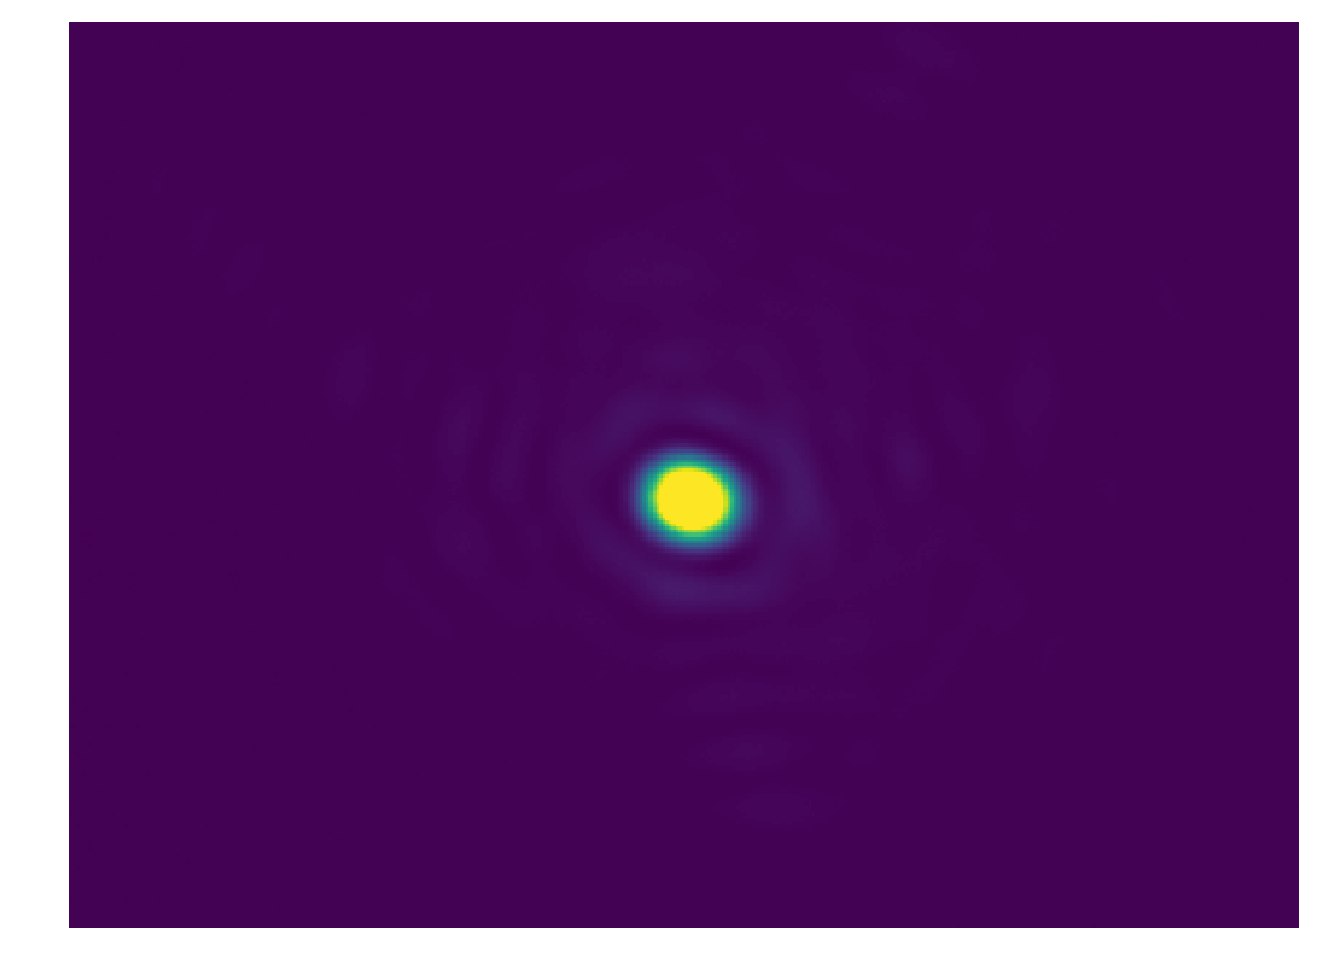
\includegraphics[width=.5\textwidth]{\figuredir{camera/profile2d.pdf}}
  \caption{Image detail from the captured beam with the \gls{ccd} camera.}
  \label{fig:beamprofile:2d}
\end{figure}

The two dimensional beam profile shows the characteristical two dimensional
gaussian distribution with diffraction rings caused by beam clipping at
finite apertures as described in \cite{Hertlein2017}.

\begin{figure}[ht]
  \centering
  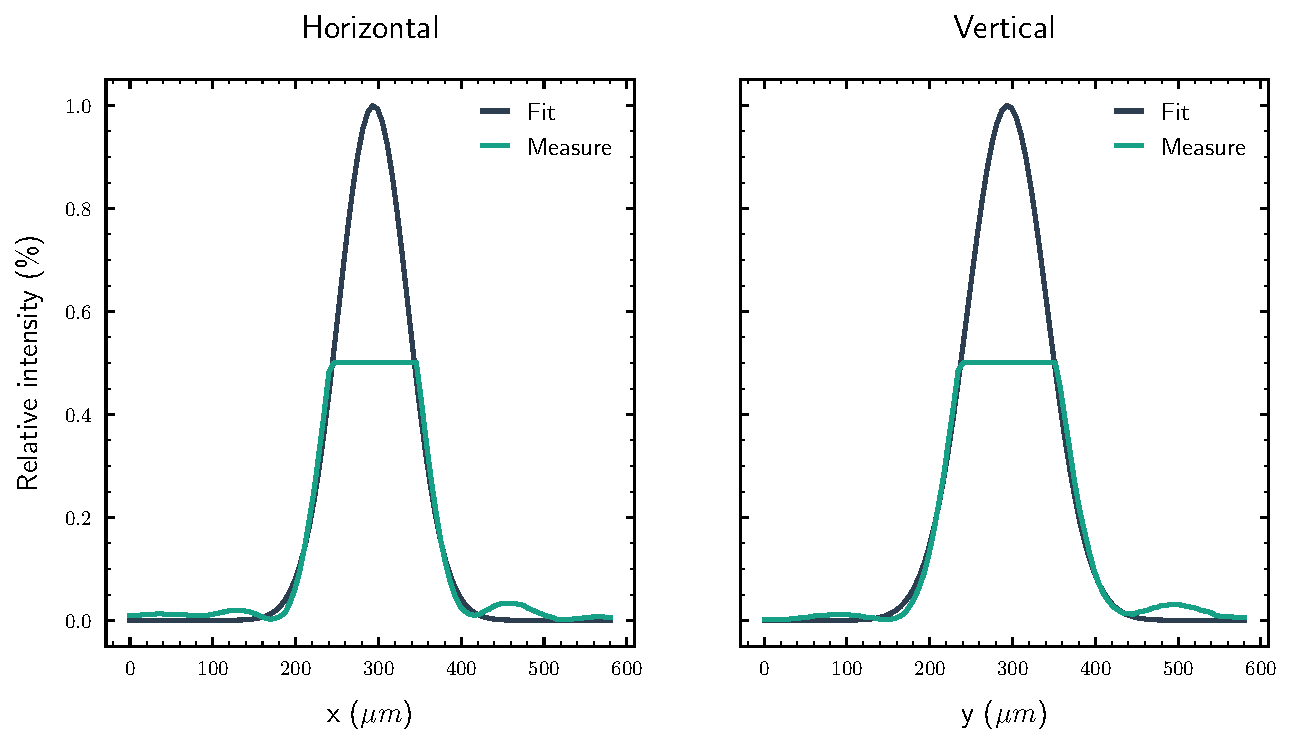
\includegraphics[width=\textwidth]{\figuredir{camera/profile1d.pdf}}
  \caption{1D horizontal and vertical profile extracted from the center of
    the image detail in \cref{fig:beamprofile:2d} with fitted gaussian curve
  and residue.}
  \label{fig:beamprofile:1d}
\end{figure}

By inspecting the one dimensional profiles with fitted gaussian and residue
we again confirm conclusions drawn in \cite{Hertlein2017}. The clipped top
of the measured intensity originates from the saturated pixels of the
\gls{ccd} camera and can be ignored. We further observe a slight assymmetry
at the diffraction rings. Overall the shown profiles can be considered to
confirm a good alignment.

%\chapter{Characterisation of the optical setup}\label{ch:optical_setup}

\section{Intensity control}

In \cref{ch:experimental_setup} we stated that the laser intensity is
regulated by a control loop using an \gls{aom} in the power reduction setup.
Without the additional intensity regulation we would
observe various intensity drifts from the laser source throughout the
measurements as depicted in \Cref{fig:intensity_uncontrolled} where we can
observe short- and long-term oscillations over a large intensity range.
\begin{figure}[htb]
  \centering
  \begin{adjustbox}{width=\textwidth}
    %% Creator: Matplotlib, PGF backend
%%
%% To include the figure in your LaTeX document, write
%%   \input{<filename>.pgf}
%%
%% Make sure the required packages are loaded in your preamble
%%   \usepackage{pgf}
%%
%% Figures using additional raster images can only be included by \input if
%% they are in the same directory as the main LaTeX file. For loading figures
%% from other directories you can use the `import` package
%%   \usepackage{import}
%% and then include the figures with
%%   \import{<path to file>}{<filename>.pgf}
%%
%% Matplotlib used the following preamble
%%   \usepackage{amsmath}\usepackage{siunitx}\usepackage{lmodern}
%%   \usepackage{fontspec}
%%
\begingroup%
\makeatletter%
\begin{pgfpicture}%
\pgfpathrectangle{\pgfpointorigin}{\pgfqpoint{12.000000in}{6.000000in}}%
\pgfusepath{use as bounding box, clip}%
\begin{pgfscope}%
\pgfsetbuttcap%
\pgfsetmiterjoin%
\pgfsetlinewidth{0.000000pt}%
\definecolor{currentstroke}{rgb}{1.000000,1.000000,1.000000}%
\pgfsetstrokecolor{currentstroke}%
\pgfsetdash{}{0pt}%
\pgfpathmoveto{\pgfqpoint{0.000000in}{0.000000in}}%
\pgfpathlineto{\pgfqpoint{12.000000in}{0.000000in}}%
\pgfpathlineto{\pgfqpoint{12.000000in}{6.000000in}}%
\pgfpathlineto{\pgfqpoint{0.000000in}{6.000000in}}%
\pgfpathclose%
\pgfusepath{}%
\end{pgfscope}%
\begin{pgfscope}%
\pgfsetbuttcap%
\pgfsetmiterjoin%
\definecolor{currentfill}{rgb}{1.000000,1.000000,1.000000}%
\pgfsetfillcolor{currentfill}%
\pgfsetlinewidth{0.000000pt}%
\definecolor{currentstroke}{rgb}{0.000000,0.000000,0.000000}%
\pgfsetstrokecolor{currentstroke}%
\pgfsetstrokeopacity{0.000000}%
\pgfsetdash{}{0pt}%
\pgfpathmoveto{\pgfqpoint{1.500000in}{0.600000in}}%
\pgfpathlineto{\pgfqpoint{10.800000in}{0.600000in}}%
\pgfpathlineto{\pgfqpoint{10.800000in}{5.880000in}}%
\pgfpathlineto{\pgfqpoint{1.500000in}{5.880000in}}%
\pgfpathclose%
\pgfusepath{fill}%
\end{pgfscope}%
\begin{pgfscope}%
\pgfpathrectangle{\pgfqpoint{1.500000in}{0.600000in}}{\pgfqpoint{9.300000in}{5.280000in}}%
\pgfusepath{clip}%
\pgfsetbuttcap%
\pgfsetroundjoin%
\definecolor{currentfill}{rgb}{0.121569,0.466667,0.705882}%
\pgfsetfillcolor{currentfill}%
\pgfsetlinewidth{1.003750pt}%
\definecolor{currentstroke}{rgb}{0.121569,0.466667,0.705882}%
\pgfsetstrokecolor{currentstroke}%
\pgfsetdash{}{0pt}%
\pgfpathmoveto{\pgfqpoint{1.922890in}{1.012784in}}%
\pgfpathcurveto{\pgfqpoint{1.930256in}{1.012784in}}{\pgfqpoint{1.937322in}{1.015711in}}{\pgfqpoint{1.942531in}{1.020920in}}%
\pgfpathcurveto{\pgfqpoint{1.947741in}{1.026129in}}{\pgfqpoint{1.950667in}{1.033195in}}{\pgfqpoint{1.950667in}{1.040562in}}%
\pgfpathcurveto{\pgfqpoint{1.950667in}{1.047929in}}{\pgfqpoint{1.947741in}{1.054995in}}{\pgfqpoint{1.942531in}{1.060204in}}%
\pgfpathcurveto{\pgfqpoint{1.937322in}{1.065413in}}{\pgfqpoint{1.930256in}{1.068340in}}{\pgfqpoint{1.922890in}{1.068340in}}%
\pgfpathcurveto{\pgfqpoint{1.915523in}{1.068340in}}{\pgfqpoint{1.908457in}{1.065413in}}{\pgfqpoint{1.903248in}{1.060204in}}%
\pgfpathcurveto{\pgfqpoint{1.898039in}{1.054995in}}{\pgfqpoint{1.895112in}{1.047929in}}{\pgfqpoint{1.895112in}{1.040562in}}%
\pgfpathcurveto{\pgfqpoint{1.895112in}{1.033195in}}{\pgfqpoint{1.898039in}{1.026129in}}{\pgfqpoint{1.903248in}{1.020920in}}%
\pgfpathcurveto{\pgfqpoint{1.908457in}{1.015711in}}{\pgfqpoint{1.915523in}{1.012784in}}{\pgfqpoint{1.922890in}{1.012784in}}%
\pgfpathclose%
\pgfusepath{stroke,fill}%
\end{pgfscope}%
\begin{pgfscope}%
\pgfpathrectangle{\pgfqpoint{1.500000in}{0.600000in}}{\pgfqpoint{9.300000in}{5.280000in}}%
\pgfusepath{clip}%
\pgfsetbuttcap%
\pgfsetroundjoin%
\definecolor{currentfill}{rgb}{0.121569,0.466667,0.705882}%
\pgfsetfillcolor{currentfill}%
\pgfsetlinewidth{1.003750pt}%
\definecolor{currentstroke}{rgb}{0.121569,0.466667,0.705882}%
\pgfsetstrokecolor{currentstroke}%
\pgfsetdash{}{0pt}%
\pgfpathmoveto{\pgfqpoint{1.931950in}{0.829888in}}%
\pgfpathcurveto{\pgfqpoint{1.939317in}{0.829888in}}{\pgfqpoint{1.946383in}{0.832815in}}{\pgfqpoint{1.951592in}{0.838024in}}%
\pgfpathcurveto{\pgfqpoint{1.956801in}{0.843233in}}{\pgfqpoint{1.959728in}{0.850299in}}{\pgfqpoint{1.959728in}{0.857666in}}%
\pgfpathcurveto{\pgfqpoint{1.959728in}{0.865033in}}{\pgfqpoint{1.956801in}{0.872099in}}{\pgfqpoint{1.951592in}{0.877308in}}%
\pgfpathcurveto{\pgfqpoint{1.946383in}{0.882517in}}{\pgfqpoint{1.939317in}{0.885444in}}{\pgfqpoint{1.931950in}{0.885444in}}%
\pgfpathcurveto{\pgfqpoint{1.924583in}{0.885444in}}{\pgfqpoint{1.917517in}{0.882517in}}{\pgfqpoint{1.912308in}{0.877308in}}%
\pgfpathcurveto{\pgfqpoint{1.907099in}{0.872099in}}{\pgfqpoint{1.904172in}{0.865033in}}{\pgfqpoint{1.904172in}{0.857666in}}%
\pgfpathcurveto{\pgfqpoint{1.904172in}{0.850299in}}{\pgfqpoint{1.907099in}{0.843233in}}{\pgfqpoint{1.912308in}{0.838024in}}%
\pgfpathcurveto{\pgfqpoint{1.917517in}{0.832815in}}{\pgfqpoint{1.924583in}{0.829888in}}{\pgfqpoint{1.931950in}{0.829888in}}%
\pgfpathclose%
\pgfusepath{stroke,fill}%
\end{pgfscope}%
\begin{pgfscope}%
\pgfpathrectangle{\pgfqpoint{1.500000in}{0.600000in}}{\pgfqpoint{9.300000in}{5.280000in}}%
\pgfusepath{clip}%
\pgfsetbuttcap%
\pgfsetroundjoin%
\definecolor{currentfill}{rgb}{0.121569,0.466667,0.705882}%
\pgfsetfillcolor{currentfill}%
\pgfsetlinewidth{1.003750pt}%
\definecolor{currentstroke}{rgb}{0.121569,0.466667,0.705882}%
\pgfsetstrokecolor{currentstroke}%
\pgfsetdash{}{0pt}%
\pgfpathmoveto{\pgfqpoint{1.941916in}{0.978496in}}%
\pgfpathcurveto{\pgfqpoint{1.949283in}{0.978496in}}{\pgfqpoint{1.956349in}{0.981422in}}{\pgfqpoint{1.961558in}{0.986632in}}%
\pgfpathcurveto{\pgfqpoint{1.966767in}{0.991841in}}{\pgfqpoint{1.969694in}{0.998907in}}{\pgfqpoint{1.969694in}{1.006273in}}%
\pgfpathcurveto{\pgfqpoint{1.969694in}{1.013640in}}{\pgfqpoint{1.966767in}{1.020706in}}{\pgfqpoint{1.961558in}{1.025915in}}%
\pgfpathcurveto{\pgfqpoint{1.956349in}{1.031124in}}{\pgfqpoint{1.949283in}{1.034051in}}{\pgfqpoint{1.941916in}{1.034051in}}%
\pgfpathcurveto{\pgfqpoint{1.934550in}{1.034051in}}{\pgfqpoint{1.927484in}{1.031124in}}{\pgfqpoint{1.922275in}{1.025915in}}%
\pgfpathcurveto{\pgfqpoint{1.917065in}{1.020706in}}{\pgfqpoint{1.914139in}{1.013640in}}{\pgfqpoint{1.914139in}{1.006273in}}%
\pgfpathcurveto{\pgfqpoint{1.914139in}{0.998907in}}{\pgfqpoint{1.917065in}{0.991841in}}{\pgfqpoint{1.922275in}{0.986632in}}%
\pgfpathcurveto{\pgfqpoint{1.927484in}{0.981422in}}{\pgfqpoint{1.934550in}{0.978496in}}{\pgfqpoint{1.941916in}{0.978496in}}%
\pgfpathclose%
\pgfusepath{stroke,fill}%
\end{pgfscope}%
\begin{pgfscope}%
\pgfpathrectangle{\pgfqpoint{1.500000in}{0.600000in}}{\pgfqpoint{9.300000in}{5.280000in}}%
\pgfusepath{clip}%
\pgfsetbuttcap%
\pgfsetroundjoin%
\definecolor{currentfill}{rgb}{0.121569,0.466667,0.705882}%
\pgfsetfillcolor{currentfill}%
\pgfsetlinewidth{1.003750pt}%
\definecolor{currentstroke}{rgb}{0.121569,0.466667,0.705882}%
\pgfsetstrokecolor{currentstroke}%
\pgfsetdash{}{0pt}%
\pgfpathmoveto{\pgfqpoint{1.950977in}{1.148775in}}%
\pgfpathcurveto{\pgfqpoint{1.958344in}{1.148775in}}{\pgfqpoint{1.965410in}{1.151702in}}{\pgfqpoint{1.970619in}{1.156911in}}%
\pgfpathcurveto{\pgfqpoint{1.975828in}{1.162120in}}{\pgfqpoint{1.978755in}{1.169186in}}{\pgfqpoint{1.978755in}{1.176553in}}%
\pgfpathcurveto{\pgfqpoint{1.978755in}{1.183920in}}{\pgfqpoint{1.975828in}{1.190986in}}{\pgfqpoint{1.970619in}{1.196195in}}%
\pgfpathcurveto{\pgfqpoint{1.965410in}{1.201404in}}{\pgfqpoint{1.958344in}{1.204331in}}{\pgfqpoint{1.950977in}{1.204331in}}%
\pgfpathcurveto{\pgfqpoint{1.943610in}{1.204331in}}{\pgfqpoint{1.936544in}{1.201404in}}{\pgfqpoint{1.931335in}{1.196195in}}%
\pgfpathcurveto{\pgfqpoint{1.926126in}{1.190986in}}{\pgfqpoint{1.923199in}{1.183920in}}{\pgfqpoint{1.923199in}{1.176553in}}%
\pgfpathcurveto{\pgfqpoint{1.923199in}{1.169186in}}{\pgfqpoint{1.926126in}{1.162120in}}{\pgfqpoint{1.931335in}{1.156911in}}%
\pgfpathcurveto{\pgfqpoint{1.936544in}{1.151702in}}{\pgfqpoint{1.943610in}{1.148775in}}{\pgfqpoint{1.950977in}{1.148775in}}%
\pgfpathclose%
\pgfusepath{stroke,fill}%
\end{pgfscope}%
\begin{pgfscope}%
\pgfpathrectangle{\pgfqpoint{1.500000in}{0.600000in}}{\pgfqpoint{9.300000in}{5.280000in}}%
\pgfusepath{clip}%
\pgfsetbuttcap%
\pgfsetroundjoin%
\definecolor{currentfill}{rgb}{0.121569,0.466667,0.705882}%
\pgfsetfillcolor{currentfill}%
\pgfsetlinewidth{1.003750pt}%
\definecolor{currentstroke}{rgb}{0.121569,0.466667,0.705882}%
\pgfsetstrokecolor{currentstroke}%
\pgfsetdash{}{0pt}%
\pgfpathmoveto{\pgfqpoint{1.960037in}{1.215023in}}%
\pgfpathcurveto{\pgfqpoint{1.967404in}{1.215023in}}{\pgfqpoint{1.974470in}{1.217950in}}{\pgfqpoint{1.979679in}{1.223159in}}%
\pgfpathcurveto{\pgfqpoint{1.984888in}{1.228368in}}{\pgfqpoint{1.987815in}{1.235434in}}{\pgfqpoint{1.987815in}{1.242801in}}%
\pgfpathcurveto{\pgfqpoint{1.987815in}{1.250168in}}{\pgfqpoint{1.984888in}{1.257234in}}{\pgfqpoint{1.979679in}{1.262443in}}%
\pgfpathcurveto{\pgfqpoint{1.974470in}{1.267652in}}{\pgfqpoint{1.967404in}{1.270579in}}{\pgfqpoint{1.960037in}{1.270579in}}%
\pgfpathcurveto{\pgfqpoint{1.952670in}{1.270579in}}{\pgfqpoint{1.945604in}{1.267652in}}{\pgfqpoint{1.940395in}{1.262443in}}%
\pgfpathcurveto{\pgfqpoint{1.935186in}{1.257234in}}{\pgfqpoint{1.932259in}{1.250168in}}{\pgfqpoint{1.932259in}{1.242801in}}%
\pgfpathcurveto{\pgfqpoint{1.932259in}{1.235434in}}{\pgfqpoint{1.935186in}{1.228368in}}{\pgfqpoint{1.940395in}{1.223159in}}%
\pgfpathcurveto{\pgfqpoint{1.945604in}{1.217950in}}{\pgfqpoint{1.952670in}{1.215023in}}{\pgfqpoint{1.960037in}{1.215023in}}%
\pgfpathclose%
\pgfusepath{stroke,fill}%
\end{pgfscope}%
\begin{pgfscope}%
\pgfpathrectangle{\pgfqpoint{1.500000in}{0.600000in}}{\pgfqpoint{9.300000in}{5.280000in}}%
\pgfusepath{clip}%
\pgfsetbuttcap%
\pgfsetroundjoin%
\definecolor{currentfill}{rgb}{0.121569,0.466667,0.705882}%
\pgfsetfillcolor{currentfill}%
\pgfsetlinewidth{1.003750pt}%
\definecolor{currentstroke}{rgb}{0.121569,0.466667,0.705882}%
\pgfsetstrokecolor{currentstroke}%
\pgfsetdash{}{0pt}%
\pgfpathmoveto{\pgfqpoint{1.969097in}{1.343266in}}%
\pgfpathcurveto{\pgfqpoint{1.976464in}{1.343266in}}{\pgfqpoint{1.983530in}{1.346192in}}{\pgfqpoint{1.988739in}{1.351402in}}%
\pgfpathcurveto{\pgfqpoint{1.993948in}{1.356611in}}{\pgfqpoint{1.996875in}{1.363677in}}{\pgfqpoint{1.996875in}{1.371043in}}%
\pgfpathcurveto{\pgfqpoint{1.996875in}{1.378410in}}{\pgfqpoint{1.993948in}{1.385476in}}{\pgfqpoint{1.988739in}{1.390685in}}%
\pgfpathcurveto{\pgfqpoint{1.983530in}{1.395894in}}{\pgfqpoint{1.976464in}{1.398821in}}{\pgfqpoint{1.969097in}{1.398821in}}%
\pgfpathcurveto{\pgfqpoint{1.961731in}{1.398821in}}{\pgfqpoint{1.954665in}{1.395894in}}{\pgfqpoint{1.949456in}{1.390685in}}%
\pgfpathcurveto{\pgfqpoint{1.944247in}{1.385476in}}{\pgfqpoint{1.941320in}{1.378410in}}{\pgfqpoint{1.941320in}{1.371043in}}%
\pgfpathcurveto{\pgfqpoint{1.941320in}{1.363677in}}{\pgfqpoint{1.944247in}{1.356611in}}{\pgfqpoint{1.949456in}{1.351402in}}%
\pgfpathcurveto{\pgfqpoint{1.954665in}{1.346192in}}{\pgfqpoint{1.961731in}{1.343266in}}{\pgfqpoint{1.969097in}{1.343266in}}%
\pgfpathclose%
\pgfusepath{stroke,fill}%
\end{pgfscope}%
\begin{pgfscope}%
\pgfpathrectangle{\pgfqpoint{1.500000in}{0.600000in}}{\pgfqpoint{9.300000in}{5.280000in}}%
\pgfusepath{clip}%
\pgfsetbuttcap%
\pgfsetroundjoin%
\definecolor{currentfill}{rgb}{0.121569,0.466667,0.705882}%
\pgfsetfillcolor{currentfill}%
\pgfsetlinewidth{1.003750pt}%
\definecolor{currentstroke}{rgb}{0.121569,0.466667,0.705882}%
\pgfsetstrokecolor{currentstroke}%
\pgfsetdash{}{0pt}%
\pgfpathmoveto{\pgfqpoint{1.978158in}{1.442494in}}%
\pgfpathcurveto{\pgfqpoint{1.985525in}{1.442494in}}{\pgfqpoint{1.992591in}{1.445421in}}{\pgfqpoint{1.997800in}{1.450630in}}%
\pgfpathcurveto{\pgfqpoint{2.003009in}{1.455839in}}{\pgfqpoint{2.005936in}{1.462906in}}{\pgfqpoint{2.005936in}{1.470272in}}%
\pgfpathcurveto{\pgfqpoint{2.005936in}{1.477639in}}{\pgfqpoint{2.003009in}{1.484705in}}{\pgfqpoint{1.997800in}{1.489914in}}%
\pgfpathcurveto{\pgfqpoint{1.992591in}{1.495123in}}{\pgfqpoint{1.985525in}{1.498050in}}{\pgfqpoint{1.978158in}{1.498050in}}%
\pgfpathcurveto{\pgfqpoint{1.970791in}{1.498050in}}{\pgfqpoint{1.963725in}{1.495123in}}{\pgfqpoint{1.958516in}{1.489914in}}%
\pgfpathcurveto{\pgfqpoint{1.953307in}{1.484705in}}{\pgfqpoint{1.950380in}{1.477639in}}{\pgfqpoint{1.950380in}{1.470272in}}%
\pgfpathcurveto{\pgfqpoint{1.950380in}{1.462906in}}{\pgfqpoint{1.953307in}{1.455839in}}{\pgfqpoint{1.958516in}{1.450630in}}%
\pgfpathcurveto{\pgfqpoint{1.963725in}{1.445421in}}{\pgfqpoint{1.970791in}{1.442494in}}{\pgfqpoint{1.978158in}{1.442494in}}%
\pgfpathclose%
\pgfusepath{stroke,fill}%
\end{pgfscope}%
\begin{pgfscope}%
\pgfpathrectangle{\pgfqpoint{1.500000in}{0.600000in}}{\pgfqpoint{9.300000in}{5.280000in}}%
\pgfusepath{clip}%
\pgfsetbuttcap%
\pgfsetroundjoin%
\definecolor{currentfill}{rgb}{0.121569,0.466667,0.705882}%
\pgfsetfillcolor{currentfill}%
\pgfsetlinewidth{1.003750pt}%
\definecolor{currentstroke}{rgb}{0.121569,0.466667,0.705882}%
\pgfsetstrokecolor{currentstroke}%
\pgfsetdash{}{0pt}%
\pgfpathmoveto{\pgfqpoint{1.987218in}{1.363816in}}%
\pgfpathcurveto{\pgfqpoint{1.994585in}{1.363816in}}{\pgfqpoint{2.001651in}{1.366743in}}{\pgfqpoint{2.006860in}{1.371952in}}%
\pgfpathcurveto{\pgfqpoint{2.012069in}{1.377161in}}{\pgfqpoint{2.014996in}{1.384227in}}{\pgfqpoint{2.014996in}{1.391594in}}%
\pgfpathcurveto{\pgfqpoint{2.014996in}{1.398961in}}{\pgfqpoint{2.012069in}{1.406027in}}{\pgfqpoint{2.006860in}{1.411236in}}%
\pgfpathcurveto{\pgfqpoint{2.001651in}{1.416445in}}{\pgfqpoint{1.994585in}{1.419372in}}{\pgfqpoint{1.987218in}{1.419372in}}%
\pgfpathcurveto{\pgfqpoint{1.979851in}{1.419372in}}{\pgfqpoint{1.972785in}{1.416445in}}{\pgfqpoint{1.967576in}{1.411236in}}%
\pgfpathcurveto{\pgfqpoint{1.962367in}{1.406027in}}{\pgfqpoint{1.959440in}{1.398961in}}{\pgfqpoint{1.959440in}{1.391594in}}%
\pgfpathcurveto{\pgfqpoint{1.959440in}{1.384227in}}{\pgfqpoint{1.962367in}{1.377161in}}{\pgfqpoint{1.967576in}{1.371952in}}%
\pgfpathcurveto{\pgfqpoint{1.972785in}{1.366743in}}{\pgfqpoint{1.979851in}{1.363816in}}{\pgfqpoint{1.987218in}{1.363816in}}%
\pgfpathclose%
\pgfusepath{stroke,fill}%
\end{pgfscope}%
\begin{pgfscope}%
\pgfpathrectangle{\pgfqpoint{1.500000in}{0.600000in}}{\pgfqpoint{9.300000in}{5.280000in}}%
\pgfusepath{clip}%
\pgfsetbuttcap%
\pgfsetroundjoin%
\definecolor{currentfill}{rgb}{0.121569,0.466667,0.705882}%
\pgfsetfillcolor{currentfill}%
\pgfsetlinewidth{1.003750pt}%
\definecolor{currentstroke}{rgb}{0.121569,0.466667,0.705882}%
\pgfsetstrokecolor{currentstroke}%
\pgfsetdash{}{0pt}%
\pgfpathmoveto{\pgfqpoint{1.997185in}{1.453908in}}%
\pgfpathcurveto{\pgfqpoint{2.004551in}{1.453908in}}{\pgfqpoint{2.011617in}{1.456835in}}{\pgfqpoint{2.016826in}{1.462044in}}%
\pgfpathcurveto{\pgfqpoint{2.022036in}{1.467253in}}{\pgfqpoint{2.024962in}{1.474319in}}{\pgfqpoint{2.024962in}{1.481686in}}%
\pgfpathcurveto{\pgfqpoint{2.024962in}{1.489052in}}{\pgfqpoint{2.022036in}{1.496118in}}{\pgfqpoint{2.016826in}{1.501327in}}%
\pgfpathcurveto{\pgfqpoint{2.011617in}{1.506537in}}{\pgfqpoint{2.004551in}{1.509463in}}{\pgfqpoint{1.997185in}{1.509463in}}%
\pgfpathcurveto{\pgfqpoint{1.989818in}{1.509463in}}{\pgfqpoint{1.982752in}{1.506537in}}{\pgfqpoint{1.977543in}{1.501327in}}%
\pgfpathcurveto{\pgfqpoint{1.972334in}{1.496118in}}{\pgfqpoint{1.969407in}{1.489052in}}{\pgfqpoint{1.969407in}{1.481686in}}%
\pgfpathcurveto{\pgfqpoint{1.969407in}{1.474319in}}{\pgfqpoint{1.972334in}{1.467253in}}{\pgfqpoint{1.977543in}{1.462044in}}%
\pgfpathcurveto{\pgfqpoint{1.982752in}{1.456835in}}{\pgfqpoint{1.989818in}{1.453908in}}{\pgfqpoint{1.997185in}{1.453908in}}%
\pgfpathclose%
\pgfusepath{stroke,fill}%
\end{pgfscope}%
\begin{pgfscope}%
\pgfpathrectangle{\pgfqpoint{1.500000in}{0.600000in}}{\pgfqpoint{9.300000in}{5.280000in}}%
\pgfusepath{clip}%
\pgfsetbuttcap%
\pgfsetroundjoin%
\definecolor{currentfill}{rgb}{0.121569,0.466667,0.705882}%
\pgfsetfillcolor{currentfill}%
\pgfsetlinewidth{1.003750pt}%
\definecolor{currentstroke}{rgb}{0.121569,0.466667,0.705882}%
\pgfsetstrokecolor{currentstroke}%
\pgfsetdash{}{0pt}%
\pgfpathmoveto{\pgfqpoint{2.006245in}{1.585536in}}%
\pgfpathcurveto{\pgfqpoint{2.013612in}{1.585536in}}{\pgfqpoint{2.020678in}{1.588463in}}{\pgfqpoint{2.025887in}{1.593672in}}%
\pgfpathcurveto{\pgfqpoint{2.031096in}{1.598881in}}{\pgfqpoint{2.034023in}{1.605947in}}{\pgfqpoint{2.034023in}{1.613314in}}%
\pgfpathcurveto{\pgfqpoint{2.034023in}{1.620681in}}{\pgfqpoint{2.031096in}{1.627747in}}{\pgfqpoint{2.025887in}{1.632956in}}%
\pgfpathcurveto{\pgfqpoint{2.020678in}{1.638165in}}{\pgfqpoint{2.013612in}{1.641092in}}{\pgfqpoint{2.006245in}{1.641092in}}%
\pgfpathcurveto{\pgfqpoint{1.998878in}{1.641092in}}{\pgfqpoint{1.991812in}{1.638165in}}{\pgfqpoint{1.986603in}{1.632956in}}%
\pgfpathcurveto{\pgfqpoint{1.981394in}{1.627747in}}{\pgfqpoint{1.978467in}{1.620681in}}{\pgfqpoint{1.978467in}{1.613314in}}%
\pgfpathcurveto{\pgfqpoint{1.978467in}{1.605947in}}{\pgfqpoint{1.981394in}{1.598881in}}{\pgfqpoint{1.986603in}{1.593672in}}%
\pgfpathcurveto{\pgfqpoint{1.991812in}{1.588463in}}{\pgfqpoint{1.998878in}{1.585536in}}{\pgfqpoint{2.006245in}{1.585536in}}%
\pgfpathclose%
\pgfusepath{stroke,fill}%
\end{pgfscope}%
\begin{pgfscope}%
\pgfpathrectangle{\pgfqpoint{1.500000in}{0.600000in}}{\pgfqpoint{9.300000in}{5.280000in}}%
\pgfusepath{clip}%
\pgfsetbuttcap%
\pgfsetroundjoin%
\definecolor{currentfill}{rgb}{0.121569,0.466667,0.705882}%
\pgfsetfillcolor{currentfill}%
\pgfsetlinewidth{1.003750pt}%
\definecolor{currentstroke}{rgb}{0.121569,0.466667,0.705882}%
\pgfsetstrokecolor{currentstroke}%
\pgfsetdash{}{0pt}%
\pgfpathmoveto{\pgfqpoint{2.015305in}{1.667843in}}%
\pgfpathcurveto{\pgfqpoint{2.022672in}{1.667843in}}{\pgfqpoint{2.029738in}{1.670770in}}{\pgfqpoint{2.034947in}{1.675979in}}%
\pgfpathcurveto{\pgfqpoint{2.040156in}{1.681188in}}{\pgfqpoint{2.043083in}{1.688254in}}{\pgfqpoint{2.043083in}{1.695621in}}%
\pgfpathcurveto{\pgfqpoint{2.043083in}{1.702987in}}{\pgfqpoint{2.040156in}{1.710053in}}{\pgfqpoint{2.034947in}{1.715263in}}%
\pgfpathcurveto{\pgfqpoint{2.029738in}{1.720472in}}{\pgfqpoint{2.022672in}{1.723398in}}{\pgfqpoint{2.015305in}{1.723398in}}%
\pgfpathcurveto{\pgfqpoint{2.007939in}{1.723398in}}{\pgfqpoint{2.000873in}{1.720472in}}{\pgfqpoint{1.995663in}{1.715263in}}%
\pgfpathcurveto{\pgfqpoint{1.990454in}{1.710053in}}{\pgfqpoint{1.987528in}{1.702987in}}{\pgfqpoint{1.987528in}{1.695621in}}%
\pgfpathcurveto{\pgfqpoint{1.987528in}{1.688254in}}{\pgfqpoint{1.990454in}{1.681188in}}{\pgfqpoint{1.995663in}{1.675979in}}%
\pgfpathcurveto{\pgfqpoint{2.000873in}{1.670770in}}{\pgfqpoint{2.007939in}{1.667843in}}{\pgfqpoint{2.015305in}{1.667843in}}%
\pgfpathclose%
\pgfusepath{stroke,fill}%
\end{pgfscope}%
\begin{pgfscope}%
\pgfpathrectangle{\pgfqpoint{1.500000in}{0.600000in}}{\pgfqpoint{9.300000in}{5.280000in}}%
\pgfusepath{clip}%
\pgfsetbuttcap%
\pgfsetroundjoin%
\definecolor{currentfill}{rgb}{0.121569,0.466667,0.705882}%
\pgfsetfillcolor{currentfill}%
\pgfsetlinewidth{1.003750pt}%
\definecolor{currentstroke}{rgb}{0.121569,0.466667,0.705882}%
\pgfsetstrokecolor{currentstroke}%
\pgfsetdash{}{0pt}%
\pgfpathmoveto{\pgfqpoint{2.024366in}{1.734240in}}%
\pgfpathcurveto{\pgfqpoint{2.031732in}{1.734240in}}{\pgfqpoint{2.038798in}{1.737167in}}{\pgfqpoint{2.044008in}{1.742376in}}%
\pgfpathcurveto{\pgfqpoint{2.049217in}{1.747585in}}{\pgfqpoint{2.052143in}{1.754651in}}{\pgfqpoint{2.052143in}{1.762018in}}%
\pgfpathcurveto{\pgfqpoint{2.052143in}{1.769385in}}{\pgfqpoint{2.049217in}{1.776451in}}{\pgfqpoint{2.044008in}{1.781660in}}%
\pgfpathcurveto{\pgfqpoint{2.038798in}{1.786869in}}{\pgfqpoint{2.031732in}{1.789796in}}{\pgfqpoint{2.024366in}{1.789796in}}%
\pgfpathcurveto{\pgfqpoint{2.016999in}{1.789796in}}{\pgfqpoint{2.009933in}{1.786869in}}{\pgfqpoint{2.004724in}{1.781660in}}%
\pgfpathcurveto{\pgfqpoint{1.999515in}{1.776451in}}{\pgfqpoint{1.996588in}{1.769385in}}{\pgfqpoint{1.996588in}{1.762018in}}%
\pgfpathcurveto{\pgfqpoint{1.996588in}{1.754651in}}{\pgfqpoint{1.999515in}{1.747585in}}{\pgfqpoint{2.004724in}{1.742376in}}%
\pgfpathcurveto{\pgfqpoint{2.009933in}{1.737167in}}{\pgfqpoint{2.016999in}{1.734240in}}{\pgfqpoint{2.024366in}{1.734240in}}%
\pgfpathclose%
\pgfusepath{stroke,fill}%
\end{pgfscope}%
\begin{pgfscope}%
\pgfpathrectangle{\pgfqpoint{1.500000in}{0.600000in}}{\pgfqpoint{9.300000in}{5.280000in}}%
\pgfusepath{clip}%
\pgfsetbuttcap%
\pgfsetroundjoin%
\definecolor{currentfill}{rgb}{0.121569,0.466667,0.705882}%
\pgfsetfillcolor{currentfill}%
\pgfsetlinewidth{1.003750pt}%
\definecolor{currentstroke}{rgb}{0.121569,0.466667,0.705882}%
\pgfsetstrokecolor{currentstroke}%
\pgfsetdash{}{0pt}%
\pgfpathmoveto{\pgfqpoint{2.033426in}{1.793619in}}%
\pgfpathcurveto{\pgfqpoint{2.040793in}{1.793619in}}{\pgfqpoint{2.047859in}{1.796546in}}{\pgfqpoint{2.053068in}{1.801755in}}%
\pgfpathcurveto{\pgfqpoint{2.058277in}{1.806964in}}{\pgfqpoint{2.061204in}{1.814030in}}{\pgfqpoint{2.061204in}{1.821397in}}%
\pgfpathcurveto{\pgfqpoint{2.061204in}{1.828764in}}{\pgfqpoint{2.058277in}{1.835830in}}{\pgfqpoint{2.053068in}{1.841039in}}%
\pgfpathcurveto{\pgfqpoint{2.047859in}{1.846248in}}{\pgfqpoint{2.040793in}{1.849175in}}{\pgfqpoint{2.033426in}{1.849175in}}%
\pgfpathcurveto{\pgfqpoint{2.026059in}{1.849175in}}{\pgfqpoint{2.018993in}{1.846248in}}{\pgfqpoint{2.013784in}{1.841039in}}%
\pgfpathcurveto{\pgfqpoint{2.008575in}{1.835830in}}{\pgfqpoint{2.005648in}{1.828764in}}{\pgfqpoint{2.005648in}{1.821397in}}%
\pgfpathcurveto{\pgfqpoint{2.005648in}{1.814030in}}{\pgfqpoint{2.008575in}{1.806964in}}{\pgfqpoint{2.013784in}{1.801755in}}%
\pgfpathcurveto{\pgfqpoint{2.018993in}{1.796546in}}{\pgfqpoint{2.026059in}{1.793619in}}{\pgfqpoint{2.033426in}{1.793619in}}%
\pgfpathclose%
\pgfusepath{stroke,fill}%
\end{pgfscope}%
\begin{pgfscope}%
\pgfpathrectangle{\pgfqpoint{1.500000in}{0.600000in}}{\pgfqpoint{9.300000in}{5.280000in}}%
\pgfusepath{clip}%
\pgfsetbuttcap%
\pgfsetroundjoin%
\definecolor{currentfill}{rgb}{0.121569,0.466667,0.705882}%
\pgfsetfillcolor{currentfill}%
\pgfsetlinewidth{1.003750pt}%
\definecolor{currentstroke}{rgb}{0.121569,0.466667,0.705882}%
\pgfsetstrokecolor{currentstroke}%
\pgfsetdash{}{0pt}%
\pgfpathmoveto{\pgfqpoint{2.042486in}{1.872241in}}%
\pgfpathcurveto{\pgfqpoint{2.049853in}{1.872241in}}{\pgfqpoint{2.056919in}{1.875168in}}{\pgfqpoint{2.062128in}{1.880377in}}%
\pgfpathcurveto{\pgfqpoint{2.067337in}{1.885586in}}{\pgfqpoint{2.070264in}{1.892652in}}{\pgfqpoint{2.070264in}{1.900019in}}%
\pgfpathcurveto{\pgfqpoint{2.070264in}{1.907386in}}{\pgfqpoint{2.067337in}{1.914452in}}{\pgfqpoint{2.062128in}{1.919661in}}%
\pgfpathcurveto{\pgfqpoint{2.056919in}{1.924870in}}{\pgfqpoint{2.049853in}{1.927797in}}{\pgfqpoint{2.042486in}{1.927797in}}%
\pgfpathcurveto{\pgfqpoint{2.035120in}{1.927797in}}{\pgfqpoint{2.028054in}{1.924870in}}{\pgfqpoint{2.022845in}{1.919661in}}%
\pgfpathcurveto{\pgfqpoint{2.017635in}{1.914452in}}{\pgfqpoint{2.014709in}{1.907386in}}{\pgfqpoint{2.014709in}{1.900019in}}%
\pgfpathcurveto{\pgfqpoint{2.014709in}{1.892652in}}{\pgfqpoint{2.017635in}{1.885586in}}{\pgfqpoint{2.022845in}{1.880377in}}%
\pgfpathcurveto{\pgfqpoint{2.028054in}{1.875168in}}{\pgfqpoint{2.035120in}{1.872241in}}{\pgfqpoint{2.042486in}{1.872241in}}%
\pgfpathclose%
\pgfusepath{stroke,fill}%
\end{pgfscope}%
\begin{pgfscope}%
\pgfpathrectangle{\pgfqpoint{1.500000in}{0.600000in}}{\pgfqpoint{9.300000in}{5.280000in}}%
\pgfusepath{clip}%
\pgfsetbuttcap%
\pgfsetroundjoin%
\definecolor{currentfill}{rgb}{0.121569,0.466667,0.705882}%
\pgfsetfillcolor{currentfill}%
\pgfsetlinewidth{1.003750pt}%
\definecolor{currentstroke}{rgb}{0.121569,0.466667,0.705882}%
\pgfsetstrokecolor{currentstroke}%
\pgfsetdash{}{0pt}%
\pgfpathmoveto{\pgfqpoint{2.052453in}{1.946819in}}%
\pgfpathcurveto{\pgfqpoint{2.059820in}{1.946819in}}{\pgfqpoint{2.066886in}{1.949746in}}{\pgfqpoint{2.072095in}{1.954955in}}%
\pgfpathcurveto{\pgfqpoint{2.077304in}{1.960164in}}{\pgfqpoint{2.080231in}{1.967230in}}{\pgfqpoint{2.080231in}{1.974597in}}%
\pgfpathcurveto{\pgfqpoint{2.080231in}{1.981964in}}{\pgfqpoint{2.077304in}{1.989030in}}{\pgfqpoint{2.072095in}{1.994239in}}%
\pgfpathcurveto{\pgfqpoint{2.066886in}{1.999448in}}{\pgfqpoint{2.059820in}{2.002375in}}{\pgfqpoint{2.052453in}{2.002375in}}%
\pgfpathcurveto{\pgfqpoint{2.045086in}{2.002375in}}{\pgfqpoint{2.038020in}{1.999448in}}{\pgfqpoint{2.032811in}{1.994239in}}%
\pgfpathcurveto{\pgfqpoint{2.027602in}{1.989030in}}{\pgfqpoint{2.024675in}{1.981964in}}{\pgfqpoint{2.024675in}{1.974597in}}%
\pgfpathcurveto{\pgfqpoint{2.024675in}{1.967230in}}{\pgfqpoint{2.027602in}{1.960164in}}{\pgfqpoint{2.032811in}{1.954955in}}%
\pgfpathcurveto{\pgfqpoint{2.038020in}{1.949746in}}{\pgfqpoint{2.045086in}{1.946819in}}{\pgfqpoint{2.052453in}{1.946819in}}%
\pgfpathclose%
\pgfusepath{stroke,fill}%
\end{pgfscope}%
\begin{pgfscope}%
\pgfpathrectangle{\pgfqpoint{1.500000in}{0.600000in}}{\pgfqpoint{9.300000in}{5.280000in}}%
\pgfusepath{clip}%
\pgfsetbuttcap%
\pgfsetroundjoin%
\definecolor{currentfill}{rgb}{0.121569,0.466667,0.705882}%
\pgfsetfillcolor{currentfill}%
\pgfsetlinewidth{1.003750pt}%
\definecolor{currentstroke}{rgb}{0.121569,0.466667,0.705882}%
\pgfsetstrokecolor{currentstroke}%
\pgfsetdash{}{0pt}%
\pgfpathmoveto{\pgfqpoint{2.061513in}{2.005113in}}%
\pgfpathcurveto{\pgfqpoint{2.068880in}{2.005113in}}{\pgfqpoint{2.075946in}{2.008040in}}{\pgfqpoint{2.081155in}{2.013249in}}%
\pgfpathcurveto{\pgfqpoint{2.086364in}{2.018458in}}{\pgfqpoint{2.089291in}{2.025524in}}{\pgfqpoint{2.089291in}{2.032891in}}%
\pgfpathcurveto{\pgfqpoint{2.089291in}{2.040257in}}{\pgfqpoint{2.086364in}{2.047323in}}{\pgfqpoint{2.081155in}{2.052532in}}%
\pgfpathcurveto{\pgfqpoint{2.075946in}{2.057742in}}{\pgfqpoint{2.068880in}{2.060668in}}{\pgfqpoint{2.061513in}{2.060668in}}%
\pgfpathcurveto{\pgfqpoint{2.054146in}{2.060668in}}{\pgfqpoint{2.047080in}{2.057742in}}{\pgfqpoint{2.041871in}{2.052532in}}%
\pgfpathcurveto{\pgfqpoint{2.036662in}{2.047323in}}{\pgfqpoint{2.033735in}{2.040257in}}{\pgfqpoint{2.033735in}{2.032891in}}%
\pgfpathcurveto{\pgfqpoint{2.033735in}{2.025524in}}{\pgfqpoint{2.036662in}{2.018458in}}{\pgfqpoint{2.041871in}{2.013249in}}%
\pgfpathcurveto{\pgfqpoint{2.047080in}{2.008040in}}{\pgfqpoint{2.054146in}{2.005113in}}{\pgfqpoint{2.061513in}{2.005113in}}%
\pgfpathclose%
\pgfusepath{stroke,fill}%
\end{pgfscope}%
\begin{pgfscope}%
\pgfpathrectangle{\pgfqpoint{1.500000in}{0.600000in}}{\pgfqpoint{9.300000in}{5.280000in}}%
\pgfusepath{clip}%
\pgfsetbuttcap%
\pgfsetroundjoin%
\definecolor{currentfill}{rgb}{0.121569,0.466667,0.705882}%
\pgfsetfillcolor{currentfill}%
\pgfsetlinewidth{1.003750pt}%
\definecolor{currentstroke}{rgb}{0.121569,0.466667,0.705882}%
\pgfsetstrokecolor{currentstroke}%
\pgfsetdash{}{0pt}%
\pgfpathmoveto{\pgfqpoint{2.070573in}{2.047513in}}%
\pgfpathcurveto{\pgfqpoint{2.077940in}{2.047513in}}{\pgfqpoint{2.085006in}{2.050440in}}{\pgfqpoint{2.090215in}{2.055649in}}%
\pgfpathcurveto{\pgfqpoint{2.095424in}{2.060858in}}{\pgfqpoint{2.098351in}{2.067924in}}{\pgfqpoint{2.098351in}{2.075291in}}%
\pgfpathcurveto{\pgfqpoint{2.098351in}{2.082658in}}{\pgfqpoint{2.095424in}{2.089724in}}{\pgfqpoint{2.090215in}{2.094933in}}%
\pgfpathcurveto{\pgfqpoint{2.085006in}{2.100142in}}{\pgfqpoint{2.077940in}{2.103069in}}{\pgfqpoint{2.070573in}{2.103069in}}%
\pgfpathcurveto{\pgfqpoint{2.063207in}{2.103069in}}{\pgfqpoint{2.056141in}{2.100142in}}{\pgfqpoint{2.050932in}{2.094933in}}%
\pgfpathcurveto{\pgfqpoint{2.045723in}{2.089724in}}{\pgfqpoint{2.042796in}{2.082658in}}{\pgfqpoint{2.042796in}{2.075291in}}%
\pgfpathcurveto{\pgfqpoint{2.042796in}{2.067924in}}{\pgfqpoint{2.045723in}{2.060858in}}{\pgfqpoint{2.050932in}{2.055649in}}%
\pgfpathcurveto{\pgfqpoint{2.056141in}{2.050440in}}{\pgfqpoint{2.063207in}{2.047513in}}{\pgfqpoint{2.070573in}{2.047513in}}%
\pgfpathclose%
\pgfusepath{stroke,fill}%
\end{pgfscope}%
\begin{pgfscope}%
\pgfpathrectangle{\pgfqpoint{1.500000in}{0.600000in}}{\pgfqpoint{9.300000in}{5.280000in}}%
\pgfusepath{clip}%
\pgfsetbuttcap%
\pgfsetroundjoin%
\definecolor{currentfill}{rgb}{0.121569,0.466667,0.705882}%
\pgfsetfillcolor{currentfill}%
\pgfsetlinewidth{1.003750pt}%
\definecolor{currentstroke}{rgb}{0.121569,0.466667,0.705882}%
\pgfsetstrokecolor{currentstroke}%
\pgfsetdash{}{0pt}%
\pgfpathmoveto{\pgfqpoint{2.079634in}{2.113652in}}%
\pgfpathcurveto{\pgfqpoint{2.087001in}{2.113652in}}{\pgfqpoint{2.094067in}{2.116579in}}{\pgfqpoint{2.099276in}{2.121788in}}%
\pgfpathcurveto{\pgfqpoint{2.104485in}{2.126997in}}{\pgfqpoint{2.107412in}{2.134063in}}{\pgfqpoint{2.107412in}{2.141430in}}%
\pgfpathcurveto{\pgfqpoint{2.107412in}{2.148797in}}{\pgfqpoint{2.104485in}{2.155863in}}{\pgfqpoint{2.099276in}{2.161072in}}%
\pgfpathcurveto{\pgfqpoint{2.094067in}{2.166281in}}{\pgfqpoint{2.087001in}{2.169208in}}{\pgfqpoint{2.079634in}{2.169208in}}%
\pgfpathcurveto{\pgfqpoint{2.072267in}{2.169208in}}{\pgfqpoint{2.065201in}{2.166281in}}{\pgfqpoint{2.059992in}{2.161072in}}%
\pgfpathcurveto{\pgfqpoint{2.054783in}{2.155863in}}{\pgfqpoint{2.051856in}{2.148797in}}{\pgfqpoint{2.051856in}{2.141430in}}%
\pgfpathcurveto{\pgfqpoint{2.051856in}{2.134063in}}{\pgfqpoint{2.054783in}{2.126997in}}{\pgfqpoint{2.059992in}{2.121788in}}%
\pgfpathcurveto{\pgfqpoint{2.065201in}{2.116579in}}{\pgfqpoint{2.072267in}{2.113652in}}{\pgfqpoint{2.079634in}{2.113652in}}%
\pgfpathclose%
\pgfusepath{stroke,fill}%
\end{pgfscope}%
\begin{pgfscope}%
\pgfpathrectangle{\pgfqpoint{1.500000in}{0.600000in}}{\pgfqpoint{9.300000in}{5.280000in}}%
\pgfusepath{clip}%
\pgfsetbuttcap%
\pgfsetroundjoin%
\definecolor{currentfill}{rgb}{0.121569,0.466667,0.705882}%
\pgfsetfillcolor{currentfill}%
\pgfsetlinewidth{1.003750pt}%
\definecolor{currentstroke}{rgb}{0.121569,0.466667,0.705882}%
\pgfsetstrokecolor{currentstroke}%
\pgfsetdash{}{0pt}%
\pgfpathmoveto{\pgfqpoint{2.088694in}{2.206061in}}%
\pgfpathcurveto{\pgfqpoint{2.096061in}{2.206061in}}{\pgfqpoint{2.103127in}{2.208987in}}{\pgfqpoint{2.108336in}{2.214197in}}%
\pgfpathcurveto{\pgfqpoint{2.113545in}{2.219406in}}{\pgfqpoint{2.116472in}{2.226472in}}{\pgfqpoint{2.116472in}{2.233838in}}%
\pgfpathcurveto{\pgfqpoint{2.116472in}{2.241205in}}{\pgfqpoint{2.113545in}{2.248271in}}{\pgfqpoint{2.108336in}{2.253480in}}%
\pgfpathcurveto{\pgfqpoint{2.103127in}{2.258689in}}{\pgfqpoint{2.096061in}{2.261616in}}{\pgfqpoint{2.088694in}{2.261616in}}%
\pgfpathcurveto{\pgfqpoint{2.081327in}{2.261616in}}{\pgfqpoint{2.074261in}{2.258689in}}{\pgfqpoint{2.069052in}{2.253480in}}%
\pgfpathcurveto{\pgfqpoint{2.063843in}{2.248271in}}{\pgfqpoint{2.060916in}{2.241205in}}{\pgfqpoint{2.060916in}{2.233838in}}%
\pgfpathcurveto{\pgfqpoint{2.060916in}{2.226472in}}{\pgfqpoint{2.063843in}{2.219406in}}{\pgfqpoint{2.069052in}{2.214197in}}%
\pgfpathcurveto{\pgfqpoint{2.074261in}{2.208987in}}{\pgfqpoint{2.081327in}{2.206061in}}{\pgfqpoint{2.088694in}{2.206061in}}%
\pgfpathclose%
\pgfusepath{stroke,fill}%
\end{pgfscope}%
\begin{pgfscope}%
\pgfpathrectangle{\pgfqpoint{1.500000in}{0.600000in}}{\pgfqpoint{9.300000in}{5.280000in}}%
\pgfusepath{clip}%
\pgfsetbuttcap%
\pgfsetroundjoin%
\definecolor{currentfill}{rgb}{0.121569,0.466667,0.705882}%
\pgfsetfillcolor{currentfill}%
\pgfsetlinewidth{1.003750pt}%
\definecolor{currentstroke}{rgb}{0.121569,0.466667,0.705882}%
\pgfsetstrokecolor{currentstroke}%
\pgfsetdash{}{0pt}%
\pgfpathmoveto{\pgfqpoint{2.097755in}{2.216820in}}%
\pgfpathcurveto{\pgfqpoint{2.105121in}{2.216820in}}{\pgfqpoint{2.112187in}{2.219747in}}{\pgfqpoint{2.117396in}{2.224956in}}%
\pgfpathcurveto{\pgfqpoint{2.122606in}{2.230165in}}{\pgfqpoint{2.125532in}{2.237231in}}{\pgfqpoint{2.125532in}{2.244598in}}%
\pgfpathcurveto{\pgfqpoint{2.125532in}{2.251965in}}{\pgfqpoint{2.122606in}{2.259031in}}{\pgfqpoint{2.117396in}{2.264240in}}%
\pgfpathcurveto{\pgfqpoint{2.112187in}{2.269449in}}{\pgfqpoint{2.105121in}{2.272376in}}{\pgfqpoint{2.097755in}{2.272376in}}%
\pgfpathcurveto{\pgfqpoint{2.090388in}{2.272376in}}{\pgfqpoint{2.083322in}{2.269449in}}{\pgfqpoint{2.078113in}{2.264240in}}%
\pgfpathcurveto{\pgfqpoint{2.072904in}{2.259031in}}{\pgfqpoint{2.069977in}{2.251965in}}{\pgfqpoint{2.069977in}{2.244598in}}%
\pgfpathcurveto{\pgfqpoint{2.069977in}{2.237231in}}{\pgfqpoint{2.072904in}{2.230165in}}{\pgfqpoint{2.078113in}{2.224956in}}%
\pgfpathcurveto{\pgfqpoint{2.083322in}{2.219747in}}{\pgfqpoint{2.090388in}{2.216820in}}{\pgfqpoint{2.097755in}{2.216820in}}%
\pgfpathclose%
\pgfusepath{stroke,fill}%
\end{pgfscope}%
\begin{pgfscope}%
\pgfpathrectangle{\pgfqpoint{1.500000in}{0.600000in}}{\pgfqpoint{9.300000in}{5.280000in}}%
\pgfusepath{clip}%
\pgfsetbuttcap%
\pgfsetroundjoin%
\definecolor{currentfill}{rgb}{0.121569,0.466667,0.705882}%
\pgfsetfillcolor{currentfill}%
\pgfsetlinewidth{1.003750pt}%
\definecolor{currentstroke}{rgb}{0.121569,0.466667,0.705882}%
\pgfsetstrokecolor{currentstroke}%
\pgfsetdash{}{0pt}%
\pgfpathmoveto{\pgfqpoint{2.107721in}{2.259370in}}%
\pgfpathcurveto{\pgfqpoint{2.115088in}{2.259370in}}{\pgfqpoint{2.122154in}{2.262297in}}{\pgfqpoint{2.127363in}{2.267506in}}%
\pgfpathcurveto{\pgfqpoint{2.132572in}{2.272715in}}{\pgfqpoint{2.135499in}{2.279781in}}{\pgfqpoint{2.135499in}{2.287148in}}%
\pgfpathcurveto{\pgfqpoint{2.135499in}{2.294514in}}{\pgfqpoint{2.132572in}{2.301580in}}{\pgfqpoint{2.127363in}{2.306789in}}%
\pgfpathcurveto{\pgfqpoint{2.122154in}{2.311999in}}{\pgfqpoint{2.115088in}{2.314925in}}{\pgfqpoint{2.107721in}{2.314925in}}%
\pgfpathcurveto{\pgfqpoint{2.100354in}{2.314925in}}{\pgfqpoint{2.093288in}{2.311999in}}{\pgfqpoint{2.088079in}{2.306789in}}%
\pgfpathcurveto{\pgfqpoint{2.082870in}{2.301580in}}{\pgfqpoint{2.079943in}{2.294514in}}{\pgfqpoint{2.079943in}{2.287148in}}%
\pgfpathcurveto{\pgfqpoint{2.079943in}{2.279781in}}{\pgfqpoint{2.082870in}{2.272715in}}{\pgfqpoint{2.088079in}{2.267506in}}%
\pgfpathcurveto{\pgfqpoint{2.093288in}{2.262297in}}{\pgfqpoint{2.100354in}{2.259370in}}{\pgfqpoint{2.107721in}{2.259370in}}%
\pgfpathclose%
\pgfusepath{stroke,fill}%
\end{pgfscope}%
\begin{pgfscope}%
\pgfpathrectangle{\pgfqpoint{1.500000in}{0.600000in}}{\pgfqpoint{9.300000in}{5.280000in}}%
\pgfusepath{clip}%
\pgfsetbuttcap%
\pgfsetroundjoin%
\definecolor{currentfill}{rgb}{0.121569,0.466667,0.705882}%
\pgfsetfillcolor{currentfill}%
\pgfsetlinewidth{1.003750pt}%
\definecolor{currentstroke}{rgb}{0.121569,0.466667,0.705882}%
\pgfsetstrokecolor{currentstroke}%
\pgfsetdash{}{0pt}%
\pgfpathmoveto{\pgfqpoint{2.116781in}{2.317118in}}%
\pgfpathcurveto{\pgfqpoint{2.124148in}{2.317118in}}{\pgfqpoint{2.131214in}{2.320045in}}{\pgfqpoint{2.136423in}{2.325254in}}%
\pgfpathcurveto{\pgfqpoint{2.141632in}{2.330463in}}{\pgfqpoint{2.144559in}{2.337529in}}{\pgfqpoint{2.144559in}{2.344896in}}%
\pgfpathcurveto{\pgfqpoint{2.144559in}{2.352263in}}{\pgfqpoint{2.141632in}{2.359329in}}{\pgfqpoint{2.136423in}{2.364538in}}%
\pgfpathcurveto{\pgfqpoint{2.131214in}{2.369747in}}{\pgfqpoint{2.124148in}{2.372674in}}{\pgfqpoint{2.116781in}{2.372674in}}%
\pgfpathcurveto{\pgfqpoint{2.109415in}{2.372674in}}{\pgfqpoint{2.102349in}{2.369747in}}{\pgfqpoint{2.097139in}{2.364538in}}%
\pgfpathcurveto{\pgfqpoint{2.091930in}{2.359329in}}{\pgfqpoint{2.089004in}{2.352263in}}{\pgfqpoint{2.089004in}{2.344896in}}%
\pgfpathcurveto{\pgfqpoint{2.089004in}{2.337529in}}{\pgfqpoint{2.091930in}{2.330463in}}{\pgfqpoint{2.097139in}{2.325254in}}%
\pgfpathcurveto{\pgfqpoint{2.102349in}{2.320045in}}{\pgfqpoint{2.109415in}{2.317118in}}{\pgfqpoint{2.116781in}{2.317118in}}%
\pgfpathclose%
\pgfusepath{stroke,fill}%
\end{pgfscope}%
\begin{pgfscope}%
\pgfpathrectangle{\pgfqpoint{1.500000in}{0.600000in}}{\pgfqpoint{9.300000in}{5.280000in}}%
\pgfusepath{clip}%
\pgfsetbuttcap%
\pgfsetroundjoin%
\definecolor{currentfill}{rgb}{0.121569,0.466667,0.705882}%
\pgfsetfillcolor{currentfill}%
\pgfsetlinewidth{1.003750pt}%
\definecolor{currentstroke}{rgb}{0.121569,0.466667,0.705882}%
\pgfsetstrokecolor{currentstroke}%
\pgfsetdash{}{0pt}%
\pgfpathmoveto{\pgfqpoint{2.125842in}{2.356076in}}%
\pgfpathcurveto{\pgfqpoint{2.133208in}{2.356076in}}{\pgfqpoint{2.140274in}{2.359003in}}{\pgfqpoint{2.145484in}{2.364212in}}%
\pgfpathcurveto{\pgfqpoint{2.150693in}{2.369421in}}{\pgfqpoint{2.153619in}{2.376487in}}{\pgfqpoint{2.153619in}{2.383854in}}%
\pgfpathcurveto{\pgfqpoint{2.153619in}{2.391221in}}{\pgfqpoint{2.150693in}{2.398287in}}{\pgfqpoint{2.145484in}{2.403496in}}%
\pgfpathcurveto{\pgfqpoint{2.140274in}{2.408705in}}{\pgfqpoint{2.133208in}{2.411632in}}{\pgfqpoint{2.125842in}{2.411632in}}%
\pgfpathcurveto{\pgfqpoint{2.118475in}{2.411632in}}{\pgfqpoint{2.111409in}{2.408705in}}{\pgfqpoint{2.106200in}{2.403496in}}%
\pgfpathcurveto{\pgfqpoint{2.100991in}{2.398287in}}{\pgfqpoint{2.098064in}{2.391221in}}{\pgfqpoint{2.098064in}{2.383854in}}%
\pgfpathcurveto{\pgfqpoint{2.098064in}{2.376487in}}{\pgfqpoint{2.100991in}{2.369421in}}{\pgfqpoint{2.106200in}{2.364212in}}%
\pgfpathcurveto{\pgfqpoint{2.111409in}{2.359003in}}{\pgfqpoint{2.118475in}{2.356076in}}{\pgfqpoint{2.125842in}{2.356076in}}%
\pgfpathclose%
\pgfusepath{stroke,fill}%
\end{pgfscope}%
\begin{pgfscope}%
\pgfpathrectangle{\pgfqpoint{1.500000in}{0.600000in}}{\pgfqpoint{9.300000in}{5.280000in}}%
\pgfusepath{clip}%
\pgfsetbuttcap%
\pgfsetroundjoin%
\definecolor{currentfill}{rgb}{0.121569,0.466667,0.705882}%
\pgfsetfillcolor{currentfill}%
\pgfsetlinewidth{1.003750pt}%
\definecolor{currentstroke}{rgb}{0.121569,0.466667,0.705882}%
\pgfsetstrokecolor{currentstroke}%
\pgfsetdash{}{0pt}%
\pgfpathmoveto{\pgfqpoint{2.134902in}{2.314564in}}%
\pgfpathcurveto{\pgfqpoint{2.142269in}{2.314564in}}{\pgfqpoint{2.149335in}{2.317491in}}{\pgfqpoint{2.154544in}{2.322700in}}%
\pgfpathcurveto{\pgfqpoint{2.159753in}{2.327909in}}{\pgfqpoint{2.162680in}{2.334975in}}{\pgfqpoint{2.162680in}{2.342342in}}%
\pgfpathcurveto{\pgfqpoint{2.162680in}{2.349708in}}{\pgfqpoint{2.159753in}{2.356774in}}{\pgfqpoint{2.154544in}{2.361983in}}%
\pgfpathcurveto{\pgfqpoint{2.149335in}{2.367192in}}{\pgfqpoint{2.142269in}{2.370119in}}{\pgfqpoint{2.134902in}{2.370119in}}%
\pgfpathcurveto{\pgfqpoint{2.127535in}{2.370119in}}{\pgfqpoint{2.120469in}{2.367192in}}{\pgfqpoint{2.115260in}{2.361983in}}%
\pgfpathcurveto{\pgfqpoint{2.110051in}{2.356774in}}{\pgfqpoint{2.107124in}{2.349708in}}{\pgfqpoint{2.107124in}{2.342342in}}%
\pgfpathcurveto{\pgfqpoint{2.107124in}{2.334975in}}{\pgfqpoint{2.110051in}{2.327909in}}{\pgfqpoint{2.115260in}{2.322700in}}%
\pgfpathcurveto{\pgfqpoint{2.120469in}{2.317491in}}{\pgfqpoint{2.127535in}{2.314564in}}{\pgfqpoint{2.134902in}{2.314564in}}%
\pgfpathclose%
\pgfusepath{stroke,fill}%
\end{pgfscope}%
\begin{pgfscope}%
\pgfpathrectangle{\pgfqpoint{1.500000in}{0.600000in}}{\pgfqpoint{9.300000in}{5.280000in}}%
\pgfusepath{clip}%
\pgfsetbuttcap%
\pgfsetroundjoin%
\definecolor{currentfill}{rgb}{0.121569,0.466667,0.705882}%
\pgfsetfillcolor{currentfill}%
\pgfsetlinewidth{1.003750pt}%
\definecolor{currentstroke}{rgb}{0.121569,0.466667,0.705882}%
\pgfsetstrokecolor{currentstroke}%
\pgfsetdash{}{0pt}%
\pgfpathmoveto{\pgfqpoint{2.143962in}{2.282503in}}%
\pgfpathcurveto{\pgfqpoint{2.151329in}{2.282503in}}{\pgfqpoint{2.158395in}{2.285430in}}{\pgfqpoint{2.163604in}{2.290639in}}%
\pgfpathcurveto{\pgfqpoint{2.168813in}{2.295848in}}{\pgfqpoint{2.171740in}{2.302914in}}{\pgfqpoint{2.171740in}{2.310281in}}%
\pgfpathcurveto{\pgfqpoint{2.171740in}{2.317648in}}{\pgfqpoint{2.168813in}{2.324714in}}{\pgfqpoint{2.163604in}{2.329923in}}%
\pgfpathcurveto{\pgfqpoint{2.158395in}{2.335132in}}{\pgfqpoint{2.151329in}{2.338059in}}{\pgfqpoint{2.143962in}{2.338059in}}%
\pgfpathcurveto{\pgfqpoint{2.136596in}{2.338059in}}{\pgfqpoint{2.129530in}{2.335132in}}{\pgfqpoint{2.124321in}{2.329923in}}%
\pgfpathcurveto{\pgfqpoint{2.119111in}{2.324714in}}{\pgfqpoint{2.116185in}{2.317648in}}{\pgfqpoint{2.116185in}{2.310281in}}%
\pgfpathcurveto{\pgfqpoint{2.116185in}{2.302914in}}{\pgfqpoint{2.119111in}{2.295848in}}{\pgfqpoint{2.124321in}{2.290639in}}%
\pgfpathcurveto{\pgfqpoint{2.129530in}{2.285430in}}{\pgfqpoint{2.136596in}{2.282503in}}{\pgfqpoint{2.143962in}{2.282503in}}%
\pgfpathclose%
\pgfusepath{stroke,fill}%
\end{pgfscope}%
\begin{pgfscope}%
\pgfpathrectangle{\pgfqpoint{1.500000in}{0.600000in}}{\pgfqpoint{9.300000in}{5.280000in}}%
\pgfusepath{clip}%
\pgfsetbuttcap%
\pgfsetroundjoin%
\definecolor{currentfill}{rgb}{0.121569,0.466667,0.705882}%
\pgfsetfillcolor{currentfill}%
\pgfsetlinewidth{1.003750pt}%
\definecolor{currentstroke}{rgb}{0.121569,0.466667,0.705882}%
\pgfsetstrokecolor{currentstroke}%
\pgfsetdash{}{0pt}%
\pgfpathmoveto{\pgfqpoint{2.153023in}{2.286083in}}%
\pgfpathcurveto{\pgfqpoint{2.160390in}{2.286083in}}{\pgfqpoint{2.167456in}{2.289010in}}{\pgfqpoint{2.172665in}{2.294219in}}%
\pgfpathcurveto{\pgfqpoint{2.177874in}{2.299428in}}{\pgfqpoint{2.180801in}{2.306494in}}{\pgfqpoint{2.180801in}{2.313861in}}%
\pgfpathcurveto{\pgfqpoint{2.180801in}{2.321227in}}{\pgfqpoint{2.177874in}{2.328294in}}{\pgfqpoint{2.172665in}{2.333503in}}%
\pgfpathcurveto{\pgfqpoint{2.167456in}{2.338712in}}{\pgfqpoint{2.160390in}{2.341639in}}{\pgfqpoint{2.153023in}{2.341639in}}%
\pgfpathcurveto{\pgfqpoint{2.145656in}{2.341639in}}{\pgfqpoint{2.138590in}{2.338712in}}{\pgfqpoint{2.133381in}{2.333503in}}%
\pgfpathcurveto{\pgfqpoint{2.128172in}{2.328294in}}{\pgfqpoint{2.125245in}{2.321227in}}{\pgfqpoint{2.125245in}{2.313861in}}%
\pgfpathcurveto{\pgfqpoint{2.125245in}{2.306494in}}{\pgfqpoint{2.128172in}{2.299428in}}{\pgfqpoint{2.133381in}{2.294219in}}%
\pgfpathcurveto{\pgfqpoint{2.138590in}{2.289010in}}{\pgfqpoint{2.145656in}{2.286083in}}{\pgfqpoint{2.153023in}{2.286083in}}%
\pgfpathclose%
\pgfusepath{stroke,fill}%
\end{pgfscope}%
\begin{pgfscope}%
\pgfpathrectangle{\pgfqpoint{1.500000in}{0.600000in}}{\pgfqpoint{9.300000in}{5.280000in}}%
\pgfusepath{clip}%
\pgfsetbuttcap%
\pgfsetroundjoin%
\definecolor{currentfill}{rgb}{0.121569,0.466667,0.705882}%
\pgfsetfillcolor{currentfill}%
\pgfsetlinewidth{1.003750pt}%
\definecolor{currentstroke}{rgb}{0.121569,0.466667,0.705882}%
\pgfsetstrokecolor{currentstroke}%
\pgfsetdash{}{0pt}%
\pgfpathmoveto{\pgfqpoint{2.162989in}{2.285296in}}%
\pgfpathcurveto{\pgfqpoint{2.170356in}{2.285296in}}{\pgfqpoint{2.177422in}{2.288223in}}{\pgfqpoint{2.182631in}{2.293432in}}%
\pgfpathcurveto{\pgfqpoint{2.187840in}{2.298641in}}{\pgfqpoint{2.190767in}{2.305707in}}{\pgfqpoint{2.190767in}{2.313074in}}%
\pgfpathcurveto{\pgfqpoint{2.190767in}{2.320440in}}{\pgfqpoint{2.187840in}{2.327507in}}{\pgfqpoint{2.182631in}{2.332716in}}%
\pgfpathcurveto{\pgfqpoint{2.177422in}{2.337925in}}{\pgfqpoint{2.170356in}{2.340852in}}{\pgfqpoint{2.162989in}{2.340852in}}%
\pgfpathcurveto{\pgfqpoint{2.155622in}{2.340852in}}{\pgfqpoint{2.148556in}{2.337925in}}{\pgfqpoint{2.143347in}{2.332716in}}%
\pgfpathcurveto{\pgfqpoint{2.138138in}{2.327507in}}{\pgfqpoint{2.135211in}{2.320440in}}{\pgfqpoint{2.135211in}{2.313074in}}%
\pgfpathcurveto{\pgfqpoint{2.135211in}{2.305707in}}{\pgfqpoint{2.138138in}{2.298641in}}{\pgfqpoint{2.143347in}{2.293432in}}%
\pgfpathcurveto{\pgfqpoint{2.148556in}{2.288223in}}{\pgfqpoint{2.155622in}{2.285296in}}{\pgfqpoint{2.162989in}{2.285296in}}%
\pgfpathclose%
\pgfusepath{stroke,fill}%
\end{pgfscope}%
\begin{pgfscope}%
\pgfpathrectangle{\pgfqpoint{1.500000in}{0.600000in}}{\pgfqpoint{9.300000in}{5.280000in}}%
\pgfusepath{clip}%
\pgfsetbuttcap%
\pgfsetroundjoin%
\definecolor{currentfill}{rgb}{0.121569,0.466667,0.705882}%
\pgfsetfillcolor{currentfill}%
\pgfsetlinewidth{1.003750pt}%
\definecolor{currentstroke}{rgb}{0.121569,0.466667,0.705882}%
\pgfsetstrokecolor{currentstroke}%
\pgfsetdash{}{0pt}%
\pgfpathmoveto{\pgfqpoint{2.172050in}{2.278984in}}%
\pgfpathcurveto{\pgfqpoint{2.179416in}{2.278984in}}{\pgfqpoint{2.186482in}{2.281911in}}{\pgfqpoint{2.191691in}{2.287120in}}%
\pgfpathcurveto{\pgfqpoint{2.196900in}{2.292329in}}{\pgfqpoint{2.199827in}{2.299395in}}{\pgfqpoint{2.199827in}{2.306762in}}%
\pgfpathcurveto{\pgfqpoint{2.199827in}{2.314128in}}{\pgfqpoint{2.196900in}{2.321194in}}{\pgfqpoint{2.191691in}{2.326404in}}%
\pgfpathcurveto{\pgfqpoint{2.186482in}{2.331613in}}{\pgfqpoint{2.179416in}{2.334539in}}{\pgfqpoint{2.172050in}{2.334539in}}%
\pgfpathcurveto{\pgfqpoint{2.164683in}{2.334539in}}{\pgfqpoint{2.157617in}{2.331613in}}{\pgfqpoint{2.152408in}{2.326404in}}%
\pgfpathcurveto{\pgfqpoint{2.147199in}{2.321194in}}{\pgfqpoint{2.144272in}{2.314128in}}{\pgfqpoint{2.144272in}{2.306762in}}%
\pgfpathcurveto{\pgfqpoint{2.144272in}{2.299395in}}{\pgfqpoint{2.147199in}{2.292329in}}{\pgfqpoint{2.152408in}{2.287120in}}%
\pgfpathcurveto{\pgfqpoint{2.157617in}{2.281911in}}{\pgfqpoint{2.164683in}{2.278984in}}{\pgfqpoint{2.172050in}{2.278984in}}%
\pgfpathclose%
\pgfusepath{stroke,fill}%
\end{pgfscope}%
\begin{pgfscope}%
\pgfpathrectangle{\pgfqpoint{1.500000in}{0.600000in}}{\pgfqpoint{9.300000in}{5.280000in}}%
\pgfusepath{clip}%
\pgfsetbuttcap%
\pgfsetroundjoin%
\definecolor{currentfill}{rgb}{0.121569,0.466667,0.705882}%
\pgfsetfillcolor{currentfill}%
\pgfsetlinewidth{1.003750pt}%
\definecolor{currentstroke}{rgb}{0.121569,0.466667,0.705882}%
\pgfsetstrokecolor{currentstroke}%
\pgfsetdash{}{0pt}%
\pgfpathmoveto{\pgfqpoint{2.181110in}{2.286979in}}%
\pgfpathcurveto{\pgfqpoint{2.188477in}{2.286979in}}{\pgfqpoint{2.195543in}{2.289906in}}{\pgfqpoint{2.200752in}{2.295115in}}%
\pgfpathcurveto{\pgfqpoint{2.205961in}{2.300324in}}{\pgfqpoint{2.208888in}{2.307390in}}{\pgfqpoint{2.208888in}{2.314757in}}%
\pgfpathcurveto{\pgfqpoint{2.208888in}{2.322123in}}{\pgfqpoint{2.205961in}{2.329189in}}{\pgfqpoint{2.200752in}{2.334399in}}%
\pgfpathcurveto{\pgfqpoint{2.195543in}{2.339608in}}{\pgfqpoint{2.188477in}{2.342534in}}{\pgfqpoint{2.181110in}{2.342534in}}%
\pgfpathcurveto{\pgfqpoint{2.173743in}{2.342534in}}{\pgfqpoint{2.166677in}{2.339608in}}{\pgfqpoint{2.161468in}{2.334399in}}%
\pgfpathcurveto{\pgfqpoint{2.156259in}{2.329189in}}{\pgfqpoint{2.153332in}{2.322123in}}{\pgfqpoint{2.153332in}{2.314757in}}%
\pgfpathcurveto{\pgfqpoint{2.153332in}{2.307390in}}{\pgfqpoint{2.156259in}{2.300324in}}{\pgfqpoint{2.161468in}{2.295115in}}%
\pgfpathcurveto{\pgfqpoint{2.166677in}{2.289906in}}{\pgfqpoint{2.173743in}{2.286979in}}{\pgfqpoint{2.181110in}{2.286979in}}%
\pgfpathclose%
\pgfusepath{stroke,fill}%
\end{pgfscope}%
\begin{pgfscope}%
\pgfpathrectangle{\pgfqpoint{1.500000in}{0.600000in}}{\pgfqpoint{9.300000in}{5.280000in}}%
\pgfusepath{clip}%
\pgfsetbuttcap%
\pgfsetroundjoin%
\definecolor{currentfill}{rgb}{0.121569,0.466667,0.705882}%
\pgfsetfillcolor{currentfill}%
\pgfsetlinewidth{1.003750pt}%
\definecolor{currentstroke}{rgb}{0.121569,0.466667,0.705882}%
\pgfsetstrokecolor{currentstroke}%
\pgfsetdash{}{0pt}%
\pgfpathmoveto{\pgfqpoint{2.190170in}{2.303679in}}%
\pgfpathcurveto{\pgfqpoint{2.197537in}{2.303679in}}{\pgfqpoint{2.204603in}{2.306606in}}{\pgfqpoint{2.209812in}{2.311815in}}%
\pgfpathcurveto{\pgfqpoint{2.215021in}{2.317024in}}{\pgfqpoint{2.217948in}{2.324090in}}{\pgfqpoint{2.217948in}{2.331457in}}%
\pgfpathcurveto{\pgfqpoint{2.217948in}{2.338824in}}{\pgfqpoint{2.215021in}{2.345890in}}{\pgfqpoint{2.209812in}{2.351099in}}%
\pgfpathcurveto{\pgfqpoint{2.204603in}{2.356308in}}{\pgfqpoint{2.197537in}{2.359235in}}{\pgfqpoint{2.190170in}{2.359235in}}%
\pgfpathcurveto{\pgfqpoint{2.182803in}{2.359235in}}{\pgfqpoint{2.175737in}{2.356308in}}{\pgfqpoint{2.170528in}{2.351099in}}%
\pgfpathcurveto{\pgfqpoint{2.165319in}{2.345890in}}{\pgfqpoint{2.162392in}{2.338824in}}{\pgfqpoint{2.162392in}{2.331457in}}%
\pgfpathcurveto{\pgfqpoint{2.162392in}{2.324090in}}{\pgfqpoint{2.165319in}{2.317024in}}{\pgfqpoint{2.170528in}{2.311815in}}%
\pgfpathcurveto{\pgfqpoint{2.175737in}{2.306606in}}{\pgfqpoint{2.182803in}{2.303679in}}{\pgfqpoint{2.190170in}{2.303679in}}%
\pgfpathclose%
\pgfusepath{stroke,fill}%
\end{pgfscope}%
\begin{pgfscope}%
\pgfpathrectangle{\pgfqpoint{1.500000in}{0.600000in}}{\pgfqpoint{9.300000in}{5.280000in}}%
\pgfusepath{clip}%
\pgfsetbuttcap%
\pgfsetroundjoin%
\definecolor{currentfill}{rgb}{0.121569,0.466667,0.705882}%
\pgfsetfillcolor{currentfill}%
\pgfsetlinewidth{1.003750pt}%
\definecolor{currentstroke}{rgb}{0.121569,0.466667,0.705882}%
\pgfsetstrokecolor{currentstroke}%
\pgfsetdash{}{0pt}%
\pgfpathmoveto{\pgfqpoint{2.199231in}{2.308332in}}%
\pgfpathcurveto{\pgfqpoint{2.206597in}{2.308332in}}{\pgfqpoint{2.213663in}{2.311259in}}{\pgfqpoint{2.218872in}{2.316468in}}%
\pgfpathcurveto{\pgfqpoint{2.224082in}{2.321677in}}{\pgfqpoint{2.227008in}{2.328743in}}{\pgfqpoint{2.227008in}{2.336110in}}%
\pgfpathcurveto{\pgfqpoint{2.227008in}{2.343477in}}{\pgfqpoint{2.224082in}{2.350543in}}{\pgfqpoint{2.218872in}{2.355752in}}%
\pgfpathcurveto{\pgfqpoint{2.213663in}{2.360961in}}{\pgfqpoint{2.206597in}{2.363888in}}{\pgfqpoint{2.199231in}{2.363888in}}%
\pgfpathcurveto{\pgfqpoint{2.191864in}{2.363888in}}{\pgfqpoint{2.184798in}{2.360961in}}{\pgfqpoint{2.179589in}{2.355752in}}%
\pgfpathcurveto{\pgfqpoint{2.174380in}{2.350543in}}{\pgfqpoint{2.171453in}{2.343477in}}{\pgfqpoint{2.171453in}{2.336110in}}%
\pgfpathcurveto{\pgfqpoint{2.171453in}{2.328743in}}{\pgfqpoint{2.174380in}{2.321677in}}{\pgfqpoint{2.179589in}{2.316468in}}%
\pgfpathcurveto{\pgfqpoint{2.184798in}{2.311259in}}{\pgfqpoint{2.191864in}{2.308332in}}{\pgfqpoint{2.199231in}{2.308332in}}%
\pgfpathclose%
\pgfusepath{stroke,fill}%
\end{pgfscope}%
\begin{pgfscope}%
\pgfpathrectangle{\pgfqpoint{1.500000in}{0.600000in}}{\pgfqpoint{9.300000in}{5.280000in}}%
\pgfusepath{clip}%
\pgfsetbuttcap%
\pgfsetroundjoin%
\definecolor{currentfill}{rgb}{0.121569,0.466667,0.705882}%
\pgfsetfillcolor{currentfill}%
\pgfsetlinewidth{1.003750pt}%
\definecolor{currentstroke}{rgb}{0.121569,0.466667,0.705882}%
\pgfsetstrokecolor{currentstroke}%
\pgfsetdash{}{0pt}%
\pgfpathmoveto{\pgfqpoint{2.209197in}{2.273749in}}%
\pgfpathcurveto{\pgfqpoint{2.216564in}{2.273749in}}{\pgfqpoint{2.223630in}{2.276676in}}{\pgfqpoint{2.228839in}{2.281885in}}%
\pgfpathcurveto{\pgfqpoint{2.234048in}{2.287094in}}{\pgfqpoint{2.236975in}{2.294160in}}{\pgfqpoint{2.236975in}{2.301527in}}%
\pgfpathcurveto{\pgfqpoint{2.236975in}{2.308894in}}{\pgfqpoint{2.234048in}{2.315960in}}{\pgfqpoint{2.228839in}{2.321169in}}%
\pgfpathcurveto{\pgfqpoint{2.223630in}{2.326378in}}{\pgfqpoint{2.216564in}{2.329305in}}{\pgfqpoint{2.209197in}{2.329305in}}%
\pgfpathcurveto{\pgfqpoint{2.201830in}{2.329305in}}{\pgfqpoint{2.194764in}{2.326378in}}{\pgfqpoint{2.189555in}{2.321169in}}%
\pgfpathcurveto{\pgfqpoint{2.184346in}{2.315960in}}{\pgfqpoint{2.181419in}{2.308894in}}{\pgfqpoint{2.181419in}{2.301527in}}%
\pgfpathcurveto{\pgfqpoint{2.181419in}{2.294160in}}{\pgfqpoint{2.184346in}{2.287094in}}{\pgfqpoint{2.189555in}{2.281885in}}%
\pgfpathcurveto{\pgfqpoint{2.194764in}{2.276676in}}{\pgfqpoint{2.201830in}{2.273749in}}{\pgfqpoint{2.209197in}{2.273749in}}%
\pgfpathclose%
\pgfusepath{stroke,fill}%
\end{pgfscope}%
\begin{pgfscope}%
\pgfpathrectangle{\pgfqpoint{1.500000in}{0.600000in}}{\pgfqpoint{9.300000in}{5.280000in}}%
\pgfusepath{clip}%
\pgfsetbuttcap%
\pgfsetroundjoin%
\definecolor{currentfill}{rgb}{0.121569,0.466667,0.705882}%
\pgfsetfillcolor{currentfill}%
\pgfsetlinewidth{1.003750pt}%
\definecolor{currentstroke}{rgb}{0.121569,0.466667,0.705882}%
\pgfsetstrokecolor{currentstroke}%
\pgfsetdash{}{0pt}%
\pgfpathmoveto{\pgfqpoint{2.218257in}{2.226498in}}%
\pgfpathcurveto{\pgfqpoint{2.225624in}{2.226498in}}{\pgfqpoint{2.232690in}{2.229425in}}{\pgfqpoint{2.237899in}{2.234634in}}%
\pgfpathcurveto{\pgfqpoint{2.243108in}{2.239843in}}{\pgfqpoint{2.246035in}{2.246909in}}{\pgfqpoint{2.246035in}{2.254276in}}%
\pgfpathcurveto{\pgfqpoint{2.246035in}{2.261643in}}{\pgfqpoint{2.243108in}{2.268709in}}{\pgfqpoint{2.237899in}{2.273918in}}%
\pgfpathcurveto{\pgfqpoint{2.232690in}{2.279127in}}{\pgfqpoint{2.225624in}{2.282054in}}{\pgfqpoint{2.218257in}{2.282054in}}%
\pgfpathcurveto{\pgfqpoint{2.210891in}{2.282054in}}{\pgfqpoint{2.203825in}{2.279127in}}{\pgfqpoint{2.198615in}{2.273918in}}%
\pgfpathcurveto{\pgfqpoint{2.193406in}{2.268709in}}{\pgfqpoint{2.190480in}{2.261643in}}{\pgfqpoint{2.190480in}{2.254276in}}%
\pgfpathcurveto{\pgfqpoint{2.190480in}{2.246909in}}{\pgfqpoint{2.193406in}{2.239843in}}{\pgfqpoint{2.198615in}{2.234634in}}%
\pgfpathcurveto{\pgfqpoint{2.203825in}{2.229425in}}{\pgfqpoint{2.210891in}{2.226498in}}{\pgfqpoint{2.218257in}{2.226498in}}%
\pgfpathclose%
\pgfusepath{stroke,fill}%
\end{pgfscope}%
\begin{pgfscope}%
\pgfpathrectangle{\pgfqpoint{1.500000in}{0.600000in}}{\pgfqpoint{9.300000in}{5.280000in}}%
\pgfusepath{clip}%
\pgfsetbuttcap%
\pgfsetroundjoin%
\definecolor{currentfill}{rgb}{0.121569,0.466667,0.705882}%
\pgfsetfillcolor{currentfill}%
\pgfsetlinewidth{1.003750pt}%
\definecolor{currentstroke}{rgb}{0.121569,0.466667,0.705882}%
\pgfsetstrokecolor{currentstroke}%
\pgfsetdash{}{0pt}%
\pgfpathmoveto{\pgfqpoint{2.227318in}{2.223786in}}%
\pgfpathcurveto{\pgfqpoint{2.234684in}{2.223786in}}{\pgfqpoint{2.241750in}{2.226713in}}{\pgfqpoint{2.246960in}{2.231922in}}%
\pgfpathcurveto{\pgfqpoint{2.252169in}{2.237131in}}{\pgfqpoint{2.255095in}{2.244197in}}{\pgfqpoint{2.255095in}{2.251564in}}%
\pgfpathcurveto{\pgfqpoint{2.255095in}{2.258930in}}{\pgfqpoint{2.252169in}{2.265997in}}{\pgfqpoint{2.246960in}{2.271206in}}%
\pgfpathcurveto{\pgfqpoint{2.241750in}{2.276415in}}{\pgfqpoint{2.234684in}{2.279342in}}{\pgfqpoint{2.227318in}{2.279342in}}%
\pgfpathcurveto{\pgfqpoint{2.219951in}{2.279342in}}{\pgfqpoint{2.212885in}{2.276415in}}{\pgfqpoint{2.207676in}{2.271206in}}%
\pgfpathcurveto{\pgfqpoint{2.202467in}{2.265997in}}{\pgfqpoint{2.199540in}{2.258930in}}{\pgfqpoint{2.199540in}{2.251564in}}%
\pgfpathcurveto{\pgfqpoint{2.199540in}{2.244197in}}{\pgfqpoint{2.202467in}{2.237131in}}{\pgfqpoint{2.207676in}{2.231922in}}%
\pgfpathcurveto{\pgfqpoint{2.212885in}{2.226713in}}{\pgfqpoint{2.219951in}{2.223786in}}{\pgfqpoint{2.227318in}{2.223786in}}%
\pgfpathclose%
\pgfusepath{stroke,fill}%
\end{pgfscope}%
\begin{pgfscope}%
\pgfpathrectangle{\pgfqpoint{1.500000in}{0.600000in}}{\pgfqpoint{9.300000in}{5.280000in}}%
\pgfusepath{clip}%
\pgfsetbuttcap%
\pgfsetroundjoin%
\definecolor{currentfill}{rgb}{0.121569,0.466667,0.705882}%
\pgfsetfillcolor{currentfill}%
\pgfsetlinewidth{1.003750pt}%
\definecolor{currentstroke}{rgb}{0.121569,0.466667,0.705882}%
\pgfsetstrokecolor{currentstroke}%
\pgfsetdash{}{0pt}%
\pgfpathmoveto{\pgfqpoint{2.236378in}{2.248752in}}%
\pgfpathcurveto{\pgfqpoint{2.243745in}{2.248752in}}{\pgfqpoint{2.250811in}{2.251678in}}{\pgfqpoint{2.256020in}{2.256887in}}%
\pgfpathcurveto{\pgfqpoint{2.261229in}{2.262097in}}{\pgfqpoint{2.264156in}{2.269163in}}{\pgfqpoint{2.264156in}{2.276529in}}%
\pgfpathcurveto{\pgfqpoint{2.264156in}{2.283896in}}{\pgfqpoint{2.261229in}{2.290962in}}{\pgfqpoint{2.256020in}{2.296171in}}%
\pgfpathcurveto{\pgfqpoint{2.250811in}{2.301380in}}{\pgfqpoint{2.243745in}{2.304307in}}{\pgfqpoint{2.236378in}{2.304307in}}%
\pgfpathcurveto{\pgfqpoint{2.229011in}{2.304307in}}{\pgfqpoint{2.221945in}{2.301380in}}{\pgfqpoint{2.216736in}{2.296171in}}%
\pgfpathcurveto{\pgfqpoint{2.211527in}{2.290962in}}{\pgfqpoint{2.208600in}{2.283896in}}{\pgfqpoint{2.208600in}{2.276529in}}%
\pgfpathcurveto{\pgfqpoint{2.208600in}{2.269163in}}{\pgfqpoint{2.211527in}{2.262097in}}{\pgfqpoint{2.216736in}{2.256887in}}%
\pgfpathcurveto{\pgfqpoint{2.221945in}{2.251678in}}{\pgfqpoint{2.229011in}{2.248752in}}{\pgfqpoint{2.236378in}{2.248752in}}%
\pgfpathclose%
\pgfusepath{stroke,fill}%
\end{pgfscope}%
\begin{pgfscope}%
\pgfpathrectangle{\pgfqpoint{1.500000in}{0.600000in}}{\pgfqpoint{9.300000in}{5.280000in}}%
\pgfusepath{clip}%
\pgfsetbuttcap%
\pgfsetroundjoin%
\definecolor{currentfill}{rgb}{0.121569,0.466667,0.705882}%
\pgfsetfillcolor{currentfill}%
\pgfsetlinewidth{1.003750pt}%
\definecolor{currentstroke}{rgb}{0.121569,0.466667,0.705882}%
\pgfsetstrokecolor{currentstroke}%
\pgfsetdash{}{0pt}%
\pgfpathmoveto{\pgfqpoint{2.245438in}{2.221405in}}%
\pgfpathcurveto{\pgfqpoint{2.252805in}{2.221405in}}{\pgfqpoint{2.259871in}{2.224332in}}{\pgfqpoint{2.265080in}{2.229541in}}%
\pgfpathcurveto{\pgfqpoint{2.270289in}{2.234750in}}{\pgfqpoint{2.273216in}{2.241816in}}{\pgfqpoint{2.273216in}{2.249183in}}%
\pgfpathcurveto{\pgfqpoint{2.273216in}{2.256549in}}{\pgfqpoint{2.270289in}{2.263615in}}{\pgfqpoint{2.265080in}{2.268824in}}%
\pgfpathcurveto{\pgfqpoint{2.259871in}{2.274034in}}{\pgfqpoint{2.252805in}{2.276960in}}{\pgfqpoint{2.245438in}{2.276960in}}%
\pgfpathcurveto{\pgfqpoint{2.238072in}{2.276960in}}{\pgfqpoint{2.231006in}{2.274034in}}{\pgfqpoint{2.225797in}{2.268824in}}%
\pgfpathcurveto{\pgfqpoint{2.220587in}{2.263615in}}{\pgfqpoint{2.217661in}{2.256549in}}{\pgfqpoint{2.217661in}{2.249183in}}%
\pgfpathcurveto{\pgfqpoint{2.217661in}{2.241816in}}{\pgfqpoint{2.220587in}{2.234750in}}{\pgfqpoint{2.225797in}{2.229541in}}%
\pgfpathcurveto{\pgfqpoint{2.231006in}{2.224332in}}{\pgfqpoint{2.238072in}{2.221405in}}{\pgfqpoint{2.245438in}{2.221405in}}%
\pgfpathclose%
\pgfusepath{stroke,fill}%
\end{pgfscope}%
\begin{pgfscope}%
\pgfpathrectangle{\pgfqpoint{1.500000in}{0.600000in}}{\pgfqpoint{9.300000in}{5.280000in}}%
\pgfusepath{clip}%
\pgfsetbuttcap%
\pgfsetroundjoin%
\definecolor{currentfill}{rgb}{0.121569,0.466667,0.705882}%
\pgfsetfillcolor{currentfill}%
\pgfsetlinewidth{1.003750pt}%
\definecolor{currentstroke}{rgb}{0.121569,0.466667,0.705882}%
\pgfsetstrokecolor{currentstroke}%
\pgfsetdash{}{0pt}%
\pgfpathmoveto{\pgfqpoint{2.254499in}{2.157413in}}%
\pgfpathcurveto{\pgfqpoint{2.261866in}{2.157413in}}{\pgfqpoint{2.268932in}{2.160340in}}{\pgfqpoint{2.274141in}{2.165549in}}%
\pgfpathcurveto{\pgfqpoint{2.279350in}{2.170758in}}{\pgfqpoint{2.282277in}{2.177824in}}{\pgfqpoint{2.282277in}{2.185191in}}%
\pgfpathcurveto{\pgfqpoint{2.282277in}{2.192557in}}{\pgfqpoint{2.279350in}{2.199623in}}{\pgfqpoint{2.274141in}{2.204832in}}%
\pgfpathcurveto{\pgfqpoint{2.268932in}{2.210041in}}{\pgfqpoint{2.261866in}{2.212968in}}{\pgfqpoint{2.254499in}{2.212968in}}%
\pgfpathcurveto{\pgfqpoint{2.247132in}{2.212968in}}{\pgfqpoint{2.240066in}{2.210041in}}{\pgfqpoint{2.234857in}{2.204832in}}%
\pgfpathcurveto{\pgfqpoint{2.229648in}{2.199623in}}{\pgfqpoint{2.226721in}{2.192557in}}{\pgfqpoint{2.226721in}{2.185191in}}%
\pgfpathcurveto{\pgfqpoint{2.226721in}{2.177824in}}{\pgfqpoint{2.229648in}{2.170758in}}{\pgfqpoint{2.234857in}{2.165549in}}%
\pgfpathcurveto{\pgfqpoint{2.240066in}{2.160340in}}{\pgfqpoint{2.247132in}{2.157413in}}{\pgfqpoint{2.254499in}{2.157413in}}%
\pgfpathclose%
\pgfusepath{stroke,fill}%
\end{pgfscope}%
\begin{pgfscope}%
\pgfpathrectangle{\pgfqpoint{1.500000in}{0.600000in}}{\pgfqpoint{9.300000in}{5.280000in}}%
\pgfusepath{clip}%
\pgfsetbuttcap%
\pgfsetroundjoin%
\definecolor{currentfill}{rgb}{0.121569,0.466667,0.705882}%
\pgfsetfillcolor{currentfill}%
\pgfsetlinewidth{1.003750pt}%
\definecolor{currentstroke}{rgb}{0.121569,0.466667,0.705882}%
\pgfsetstrokecolor{currentstroke}%
\pgfsetdash{}{0pt}%
\pgfpathmoveto{\pgfqpoint{2.264465in}{2.186781in}}%
\pgfpathcurveto{\pgfqpoint{2.271832in}{2.186781in}}{\pgfqpoint{2.278898in}{2.189708in}}{\pgfqpoint{2.284107in}{2.194917in}}%
\pgfpathcurveto{\pgfqpoint{2.289316in}{2.200126in}}{\pgfqpoint{2.292243in}{2.207192in}}{\pgfqpoint{2.292243in}{2.214559in}}%
\pgfpathcurveto{\pgfqpoint{2.292243in}{2.221926in}}{\pgfqpoint{2.289316in}{2.228992in}}{\pgfqpoint{2.284107in}{2.234201in}}%
\pgfpathcurveto{\pgfqpoint{2.278898in}{2.239410in}}{\pgfqpoint{2.271832in}{2.242337in}}{\pgfqpoint{2.264465in}{2.242337in}}%
\pgfpathcurveto{\pgfqpoint{2.257098in}{2.242337in}}{\pgfqpoint{2.250032in}{2.239410in}}{\pgfqpoint{2.244823in}{2.234201in}}%
\pgfpathcurveto{\pgfqpoint{2.239614in}{2.228992in}}{\pgfqpoint{2.236687in}{2.221926in}}{\pgfqpoint{2.236687in}{2.214559in}}%
\pgfpathcurveto{\pgfqpoint{2.236687in}{2.207192in}}{\pgfqpoint{2.239614in}{2.200126in}}{\pgfqpoint{2.244823in}{2.194917in}}%
\pgfpathcurveto{\pgfqpoint{2.250032in}{2.189708in}}{\pgfqpoint{2.257098in}{2.186781in}}{\pgfqpoint{2.264465in}{2.186781in}}%
\pgfpathclose%
\pgfusepath{stroke,fill}%
\end{pgfscope}%
\begin{pgfscope}%
\pgfpathrectangle{\pgfqpoint{1.500000in}{0.600000in}}{\pgfqpoint{9.300000in}{5.280000in}}%
\pgfusepath{clip}%
\pgfsetbuttcap%
\pgfsetroundjoin%
\definecolor{currentfill}{rgb}{0.121569,0.466667,0.705882}%
\pgfsetfillcolor{currentfill}%
\pgfsetlinewidth{1.003750pt}%
\definecolor{currentstroke}{rgb}{0.121569,0.466667,0.705882}%
\pgfsetstrokecolor{currentstroke}%
\pgfsetdash{}{0pt}%
\pgfpathmoveto{\pgfqpoint{2.273526in}{2.227019in}}%
\pgfpathcurveto{\pgfqpoint{2.280892in}{2.227019in}}{\pgfqpoint{2.287958in}{2.229945in}}{\pgfqpoint{2.293167in}{2.235155in}}%
\pgfpathcurveto{\pgfqpoint{2.298376in}{2.240364in}}{\pgfqpoint{2.301303in}{2.247430in}}{\pgfqpoint{2.301303in}{2.254796in}}%
\pgfpathcurveto{\pgfqpoint{2.301303in}{2.262163in}}{\pgfqpoint{2.298376in}{2.269229in}}{\pgfqpoint{2.293167in}{2.274438in}}%
\pgfpathcurveto{\pgfqpoint{2.287958in}{2.279647in}}{\pgfqpoint{2.280892in}{2.282574in}}{\pgfqpoint{2.273526in}{2.282574in}}%
\pgfpathcurveto{\pgfqpoint{2.266159in}{2.282574in}}{\pgfqpoint{2.259093in}{2.279647in}}{\pgfqpoint{2.253884in}{2.274438in}}%
\pgfpathcurveto{\pgfqpoint{2.248675in}{2.269229in}}{\pgfqpoint{2.245748in}{2.262163in}}{\pgfqpoint{2.245748in}{2.254796in}}%
\pgfpathcurveto{\pgfqpoint{2.245748in}{2.247430in}}{\pgfqpoint{2.248675in}{2.240364in}}{\pgfqpoint{2.253884in}{2.235155in}}%
\pgfpathcurveto{\pgfqpoint{2.259093in}{2.229945in}}{\pgfqpoint{2.266159in}{2.227019in}}{\pgfqpoint{2.273526in}{2.227019in}}%
\pgfpathclose%
\pgfusepath{stroke,fill}%
\end{pgfscope}%
\begin{pgfscope}%
\pgfpathrectangle{\pgfqpoint{1.500000in}{0.600000in}}{\pgfqpoint{9.300000in}{5.280000in}}%
\pgfusepath{clip}%
\pgfsetbuttcap%
\pgfsetroundjoin%
\definecolor{currentfill}{rgb}{0.121569,0.466667,0.705882}%
\pgfsetfillcolor{currentfill}%
\pgfsetlinewidth{1.003750pt}%
\definecolor{currentstroke}{rgb}{0.121569,0.466667,0.705882}%
\pgfsetstrokecolor{currentstroke}%
\pgfsetdash{}{0pt}%
\pgfpathmoveto{\pgfqpoint{2.282586in}{2.233750in}}%
\pgfpathcurveto{\pgfqpoint{2.289953in}{2.233750in}}{\pgfqpoint{2.297019in}{2.236677in}}{\pgfqpoint{2.302228in}{2.241886in}}%
\pgfpathcurveto{\pgfqpoint{2.307437in}{2.247095in}}{\pgfqpoint{2.310364in}{2.254161in}}{\pgfqpoint{2.310364in}{2.261528in}}%
\pgfpathcurveto{\pgfqpoint{2.310364in}{2.268895in}}{\pgfqpoint{2.307437in}{2.275961in}}{\pgfqpoint{2.302228in}{2.281170in}}%
\pgfpathcurveto{\pgfqpoint{2.297019in}{2.286379in}}{\pgfqpoint{2.289953in}{2.289306in}}{\pgfqpoint{2.282586in}{2.289306in}}%
\pgfpathcurveto{\pgfqpoint{2.275219in}{2.289306in}}{\pgfqpoint{2.268153in}{2.286379in}}{\pgfqpoint{2.262944in}{2.281170in}}%
\pgfpathcurveto{\pgfqpoint{2.257735in}{2.275961in}}{\pgfqpoint{2.254808in}{2.268895in}}{\pgfqpoint{2.254808in}{2.261528in}}%
\pgfpathcurveto{\pgfqpoint{2.254808in}{2.254161in}}{\pgfqpoint{2.257735in}{2.247095in}}{\pgfqpoint{2.262944in}{2.241886in}}%
\pgfpathcurveto{\pgfqpoint{2.268153in}{2.236677in}}{\pgfqpoint{2.275219in}{2.233750in}}{\pgfqpoint{2.282586in}{2.233750in}}%
\pgfpathclose%
\pgfusepath{stroke,fill}%
\end{pgfscope}%
\begin{pgfscope}%
\pgfpathrectangle{\pgfqpoint{1.500000in}{0.600000in}}{\pgfqpoint{9.300000in}{5.280000in}}%
\pgfusepath{clip}%
\pgfsetbuttcap%
\pgfsetroundjoin%
\definecolor{currentfill}{rgb}{0.121569,0.466667,0.705882}%
\pgfsetfillcolor{currentfill}%
\pgfsetlinewidth{1.003750pt}%
\definecolor{currentstroke}{rgb}{0.121569,0.466667,0.705882}%
\pgfsetstrokecolor{currentstroke}%
\pgfsetdash{}{0pt}%
\pgfpathmoveto{\pgfqpoint{2.291646in}{2.267659in}}%
\pgfpathcurveto{\pgfqpoint{2.299013in}{2.267659in}}{\pgfqpoint{2.306079in}{2.270586in}}{\pgfqpoint{2.311288in}{2.275795in}}%
\pgfpathcurveto{\pgfqpoint{2.316497in}{2.281004in}}{\pgfqpoint{2.319424in}{2.288070in}}{\pgfqpoint{2.319424in}{2.295437in}}%
\pgfpathcurveto{\pgfqpoint{2.319424in}{2.302804in}}{\pgfqpoint{2.316497in}{2.309870in}}{\pgfqpoint{2.311288in}{2.315079in}}%
\pgfpathcurveto{\pgfqpoint{2.306079in}{2.320288in}}{\pgfqpoint{2.299013in}{2.323215in}}{\pgfqpoint{2.291646in}{2.323215in}}%
\pgfpathcurveto{\pgfqpoint{2.284279in}{2.323215in}}{\pgfqpoint{2.277213in}{2.320288in}}{\pgfqpoint{2.272004in}{2.315079in}}%
\pgfpathcurveto{\pgfqpoint{2.266795in}{2.309870in}}{\pgfqpoint{2.263868in}{2.302804in}}{\pgfqpoint{2.263868in}{2.295437in}}%
\pgfpathcurveto{\pgfqpoint{2.263868in}{2.288070in}}{\pgfqpoint{2.266795in}{2.281004in}}{\pgfqpoint{2.272004in}{2.275795in}}%
\pgfpathcurveto{\pgfqpoint{2.277213in}{2.270586in}}{\pgfqpoint{2.284279in}{2.267659in}}{\pgfqpoint{2.291646in}{2.267659in}}%
\pgfpathclose%
\pgfusepath{stroke,fill}%
\end{pgfscope}%
\begin{pgfscope}%
\pgfpathrectangle{\pgfqpoint{1.500000in}{0.600000in}}{\pgfqpoint{9.300000in}{5.280000in}}%
\pgfusepath{clip}%
\pgfsetbuttcap%
\pgfsetroundjoin%
\definecolor{currentfill}{rgb}{0.121569,0.466667,0.705882}%
\pgfsetfillcolor{currentfill}%
\pgfsetlinewidth{1.003750pt}%
\definecolor{currentstroke}{rgb}{0.121569,0.466667,0.705882}%
\pgfsetstrokecolor{currentstroke}%
\pgfsetdash{}{0pt}%
\pgfpathmoveto{\pgfqpoint{2.300707in}{2.255386in}}%
\pgfpathcurveto{\pgfqpoint{2.308073in}{2.255386in}}{\pgfqpoint{2.315139in}{2.258313in}}{\pgfqpoint{2.320348in}{2.263522in}}%
\pgfpathcurveto{\pgfqpoint{2.325558in}{2.268731in}}{\pgfqpoint{2.328484in}{2.275797in}}{\pgfqpoint{2.328484in}{2.283164in}}%
\pgfpathcurveto{\pgfqpoint{2.328484in}{2.290531in}}{\pgfqpoint{2.325558in}{2.297597in}}{\pgfqpoint{2.320348in}{2.302806in}}%
\pgfpathcurveto{\pgfqpoint{2.315139in}{2.308015in}}{\pgfqpoint{2.308073in}{2.310942in}}{\pgfqpoint{2.300707in}{2.310942in}}%
\pgfpathcurveto{\pgfqpoint{2.293340in}{2.310942in}}{\pgfqpoint{2.286274in}{2.308015in}}{\pgfqpoint{2.281065in}{2.302806in}}%
\pgfpathcurveto{\pgfqpoint{2.275856in}{2.297597in}}{\pgfqpoint{2.272929in}{2.290531in}}{\pgfqpoint{2.272929in}{2.283164in}}%
\pgfpathcurveto{\pgfqpoint{2.272929in}{2.275797in}}{\pgfqpoint{2.275856in}{2.268731in}}{\pgfqpoint{2.281065in}{2.263522in}}%
\pgfpathcurveto{\pgfqpoint{2.286274in}{2.258313in}}{\pgfqpoint{2.293340in}{2.255386in}}{\pgfqpoint{2.300707in}{2.255386in}}%
\pgfpathclose%
\pgfusepath{stroke,fill}%
\end{pgfscope}%
\begin{pgfscope}%
\pgfpathrectangle{\pgfqpoint{1.500000in}{0.600000in}}{\pgfqpoint{9.300000in}{5.280000in}}%
\pgfusepath{clip}%
\pgfsetbuttcap%
\pgfsetroundjoin%
\definecolor{currentfill}{rgb}{0.121569,0.466667,0.705882}%
\pgfsetfillcolor{currentfill}%
\pgfsetlinewidth{1.003750pt}%
\definecolor{currentstroke}{rgb}{0.121569,0.466667,0.705882}%
\pgfsetstrokecolor{currentstroke}%
\pgfsetdash{}{0pt}%
\pgfpathmoveto{\pgfqpoint{2.310673in}{2.295123in}}%
\pgfpathcurveto{\pgfqpoint{2.318040in}{2.295123in}}{\pgfqpoint{2.325106in}{2.298050in}}{\pgfqpoint{2.330315in}{2.303259in}}%
\pgfpathcurveto{\pgfqpoint{2.335524in}{2.308468in}}{\pgfqpoint{2.338451in}{2.315534in}}{\pgfqpoint{2.338451in}{2.322901in}}%
\pgfpathcurveto{\pgfqpoint{2.338451in}{2.330268in}}{\pgfqpoint{2.335524in}{2.337334in}}{\pgfqpoint{2.330315in}{2.342543in}}%
\pgfpathcurveto{\pgfqpoint{2.325106in}{2.347752in}}{\pgfqpoint{2.318040in}{2.350679in}}{\pgfqpoint{2.310673in}{2.350679in}}%
\pgfpathcurveto{\pgfqpoint{2.303306in}{2.350679in}}{\pgfqpoint{2.296240in}{2.347752in}}{\pgfqpoint{2.291031in}{2.342543in}}%
\pgfpathcurveto{\pgfqpoint{2.285822in}{2.337334in}}{\pgfqpoint{2.282895in}{2.330268in}}{\pgfqpoint{2.282895in}{2.322901in}}%
\pgfpathcurveto{\pgfqpoint{2.282895in}{2.315534in}}{\pgfqpoint{2.285822in}{2.308468in}}{\pgfqpoint{2.291031in}{2.303259in}}%
\pgfpathcurveto{\pgfqpoint{2.296240in}{2.298050in}}{\pgfqpoint{2.303306in}{2.295123in}}{\pgfqpoint{2.310673in}{2.295123in}}%
\pgfpathclose%
\pgfusepath{stroke,fill}%
\end{pgfscope}%
\begin{pgfscope}%
\pgfpathrectangle{\pgfqpoint{1.500000in}{0.600000in}}{\pgfqpoint{9.300000in}{5.280000in}}%
\pgfusepath{clip}%
\pgfsetbuttcap%
\pgfsetroundjoin%
\definecolor{currentfill}{rgb}{0.121569,0.466667,0.705882}%
\pgfsetfillcolor{currentfill}%
\pgfsetlinewidth{1.003750pt}%
\definecolor{currentstroke}{rgb}{0.121569,0.466667,0.705882}%
\pgfsetstrokecolor{currentstroke}%
\pgfsetdash{}{0pt}%
\pgfpathmoveto{\pgfqpoint{2.319733in}{2.284925in}}%
\pgfpathcurveto{\pgfqpoint{2.327100in}{2.284925in}}{\pgfqpoint{2.334166in}{2.287852in}}{\pgfqpoint{2.339375in}{2.293061in}}%
\pgfpathcurveto{\pgfqpoint{2.344584in}{2.298270in}}{\pgfqpoint{2.347511in}{2.305336in}}{\pgfqpoint{2.347511in}{2.312702in}}%
\pgfpathcurveto{\pgfqpoint{2.347511in}{2.320069in}}{\pgfqpoint{2.344584in}{2.327135in}}{\pgfqpoint{2.339375in}{2.332344in}}%
\pgfpathcurveto{\pgfqpoint{2.334166in}{2.337553in}}{\pgfqpoint{2.327100in}{2.340480in}}{\pgfqpoint{2.319733in}{2.340480in}}%
\pgfpathcurveto{\pgfqpoint{2.312367in}{2.340480in}}{\pgfqpoint{2.305301in}{2.337553in}}{\pgfqpoint{2.300092in}{2.332344in}}%
\pgfpathcurveto{\pgfqpoint{2.294882in}{2.327135in}}{\pgfqpoint{2.291956in}{2.320069in}}{\pgfqpoint{2.291956in}{2.312702in}}%
\pgfpathcurveto{\pgfqpoint{2.291956in}{2.305336in}}{\pgfqpoint{2.294882in}{2.298270in}}{\pgfqpoint{2.300092in}{2.293061in}}%
\pgfpathcurveto{\pgfqpoint{2.305301in}{2.287852in}}{\pgfqpoint{2.312367in}{2.284925in}}{\pgfqpoint{2.319733in}{2.284925in}}%
\pgfpathclose%
\pgfusepath{stroke,fill}%
\end{pgfscope}%
\begin{pgfscope}%
\pgfpathrectangle{\pgfqpoint{1.500000in}{0.600000in}}{\pgfqpoint{9.300000in}{5.280000in}}%
\pgfusepath{clip}%
\pgfsetbuttcap%
\pgfsetroundjoin%
\definecolor{currentfill}{rgb}{0.121569,0.466667,0.705882}%
\pgfsetfillcolor{currentfill}%
\pgfsetlinewidth{1.003750pt}%
\definecolor{currentstroke}{rgb}{0.121569,0.466667,0.705882}%
\pgfsetstrokecolor{currentstroke}%
\pgfsetdash{}{0pt}%
\pgfpathmoveto{\pgfqpoint{2.328794in}{2.256073in}}%
\pgfpathcurveto{\pgfqpoint{2.336160in}{2.256073in}}{\pgfqpoint{2.343226in}{2.258999in}}{\pgfqpoint{2.348436in}{2.264208in}}%
\pgfpathcurveto{\pgfqpoint{2.353645in}{2.269418in}}{\pgfqpoint{2.356571in}{2.276484in}}{\pgfqpoint{2.356571in}{2.283850in}}%
\pgfpathcurveto{\pgfqpoint{2.356571in}{2.291217in}}{\pgfqpoint{2.353645in}{2.298283in}}{\pgfqpoint{2.348436in}{2.303492in}}%
\pgfpathcurveto{\pgfqpoint{2.343226in}{2.308701in}}{\pgfqpoint{2.336160in}{2.311628in}}{\pgfqpoint{2.328794in}{2.311628in}}%
\pgfpathcurveto{\pgfqpoint{2.321427in}{2.311628in}}{\pgfqpoint{2.314361in}{2.308701in}}{\pgfqpoint{2.309152in}{2.303492in}}%
\pgfpathcurveto{\pgfqpoint{2.303943in}{2.298283in}}{\pgfqpoint{2.301016in}{2.291217in}}{\pgfqpoint{2.301016in}{2.283850in}}%
\pgfpathcurveto{\pgfqpoint{2.301016in}{2.276484in}}{\pgfqpoint{2.303943in}{2.269418in}}{\pgfqpoint{2.309152in}{2.264208in}}%
\pgfpathcurveto{\pgfqpoint{2.314361in}{2.258999in}}{\pgfqpoint{2.321427in}{2.256073in}}{\pgfqpoint{2.328794in}{2.256073in}}%
\pgfpathclose%
\pgfusepath{stroke,fill}%
\end{pgfscope}%
\begin{pgfscope}%
\pgfpathrectangle{\pgfqpoint{1.500000in}{0.600000in}}{\pgfqpoint{9.300000in}{5.280000in}}%
\pgfusepath{clip}%
\pgfsetbuttcap%
\pgfsetroundjoin%
\definecolor{currentfill}{rgb}{0.121569,0.466667,0.705882}%
\pgfsetfillcolor{currentfill}%
\pgfsetlinewidth{1.003750pt}%
\definecolor{currentstroke}{rgb}{0.121569,0.466667,0.705882}%
\pgfsetstrokecolor{currentstroke}%
\pgfsetdash{}{0pt}%
\pgfpathmoveto{\pgfqpoint{2.337854in}{2.236499in}}%
\pgfpathcurveto{\pgfqpoint{2.345221in}{2.236499in}}{\pgfqpoint{2.352287in}{2.239426in}}{\pgfqpoint{2.357496in}{2.244635in}}%
\pgfpathcurveto{\pgfqpoint{2.362705in}{2.249844in}}{\pgfqpoint{2.365632in}{2.256910in}}{\pgfqpoint{2.365632in}{2.264277in}}%
\pgfpathcurveto{\pgfqpoint{2.365632in}{2.271643in}}{\pgfqpoint{2.362705in}{2.278709in}}{\pgfqpoint{2.357496in}{2.283918in}}%
\pgfpathcurveto{\pgfqpoint{2.352287in}{2.289128in}}{\pgfqpoint{2.345221in}{2.292054in}}{\pgfqpoint{2.337854in}{2.292054in}}%
\pgfpathcurveto{\pgfqpoint{2.330487in}{2.292054in}}{\pgfqpoint{2.323421in}{2.289128in}}{\pgfqpoint{2.318212in}{2.283918in}}%
\pgfpathcurveto{\pgfqpoint{2.313003in}{2.278709in}}{\pgfqpoint{2.310076in}{2.271643in}}{\pgfqpoint{2.310076in}{2.264277in}}%
\pgfpathcurveto{\pgfqpoint{2.310076in}{2.256910in}}{\pgfqpoint{2.313003in}{2.249844in}}{\pgfqpoint{2.318212in}{2.244635in}}%
\pgfpathcurveto{\pgfqpoint{2.323421in}{2.239426in}}{\pgfqpoint{2.330487in}{2.236499in}}{\pgfqpoint{2.337854in}{2.236499in}}%
\pgfpathclose%
\pgfusepath{stroke,fill}%
\end{pgfscope}%
\begin{pgfscope}%
\pgfpathrectangle{\pgfqpoint{1.500000in}{0.600000in}}{\pgfqpoint{9.300000in}{5.280000in}}%
\pgfusepath{clip}%
\pgfsetbuttcap%
\pgfsetroundjoin%
\definecolor{currentfill}{rgb}{0.121569,0.466667,0.705882}%
\pgfsetfillcolor{currentfill}%
\pgfsetlinewidth{1.003750pt}%
\definecolor{currentstroke}{rgb}{0.121569,0.466667,0.705882}%
\pgfsetstrokecolor{currentstroke}%
\pgfsetdash{}{0pt}%
\pgfpathmoveto{\pgfqpoint{2.346914in}{2.225473in}}%
\pgfpathcurveto{\pgfqpoint{2.354281in}{2.225473in}}{\pgfqpoint{2.361347in}{2.228400in}}{\pgfqpoint{2.366556in}{2.233609in}}%
\pgfpathcurveto{\pgfqpoint{2.371765in}{2.238818in}}{\pgfqpoint{2.374692in}{2.245884in}}{\pgfqpoint{2.374692in}{2.253251in}}%
\pgfpathcurveto{\pgfqpoint{2.374692in}{2.260617in}}{\pgfqpoint{2.371765in}{2.267683in}}{\pgfqpoint{2.366556in}{2.272893in}}%
\pgfpathcurveto{\pgfqpoint{2.361347in}{2.278102in}}{\pgfqpoint{2.354281in}{2.281028in}}{\pgfqpoint{2.346914in}{2.281028in}}%
\pgfpathcurveto{\pgfqpoint{2.339548in}{2.281028in}}{\pgfqpoint{2.332482in}{2.278102in}}{\pgfqpoint{2.327273in}{2.272893in}}%
\pgfpathcurveto{\pgfqpoint{2.322063in}{2.267683in}}{\pgfqpoint{2.319137in}{2.260617in}}{\pgfqpoint{2.319137in}{2.253251in}}%
\pgfpathcurveto{\pgfqpoint{2.319137in}{2.245884in}}{\pgfqpoint{2.322063in}{2.238818in}}{\pgfqpoint{2.327273in}{2.233609in}}%
\pgfpathcurveto{\pgfqpoint{2.332482in}{2.228400in}}{\pgfqpoint{2.339548in}{2.225473in}}{\pgfqpoint{2.346914in}{2.225473in}}%
\pgfpathclose%
\pgfusepath{stroke,fill}%
\end{pgfscope}%
\begin{pgfscope}%
\pgfpathrectangle{\pgfqpoint{1.500000in}{0.600000in}}{\pgfqpoint{9.300000in}{5.280000in}}%
\pgfusepath{clip}%
\pgfsetbuttcap%
\pgfsetroundjoin%
\definecolor{currentfill}{rgb}{0.121569,0.466667,0.705882}%
\pgfsetfillcolor{currentfill}%
\pgfsetlinewidth{1.003750pt}%
\definecolor{currentstroke}{rgb}{0.121569,0.466667,0.705882}%
\pgfsetstrokecolor{currentstroke}%
\pgfsetdash{}{0pt}%
\pgfpathmoveto{\pgfqpoint{2.355975in}{2.272006in}}%
\pgfpathcurveto{\pgfqpoint{2.363342in}{2.272006in}}{\pgfqpoint{2.370408in}{2.274933in}}{\pgfqpoint{2.375617in}{2.280142in}}%
\pgfpathcurveto{\pgfqpoint{2.380826in}{2.285351in}}{\pgfqpoint{2.383753in}{2.292417in}}{\pgfqpoint{2.383753in}{2.299784in}}%
\pgfpathcurveto{\pgfqpoint{2.383753in}{2.307151in}}{\pgfqpoint{2.380826in}{2.314217in}}{\pgfqpoint{2.375617in}{2.319426in}}%
\pgfpathcurveto{\pgfqpoint{2.370408in}{2.324635in}}{\pgfqpoint{2.363342in}{2.327562in}}{\pgfqpoint{2.355975in}{2.327562in}}%
\pgfpathcurveto{\pgfqpoint{2.348608in}{2.327562in}}{\pgfqpoint{2.341542in}{2.324635in}}{\pgfqpoint{2.336333in}{2.319426in}}%
\pgfpathcurveto{\pgfqpoint{2.331124in}{2.314217in}}{\pgfqpoint{2.328197in}{2.307151in}}{\pgfqpoint{2.328197in}{2.299784in}}%
\pgfpathcurveto{\pgfqpoint{2.328197in}{2.292417in}}{\pgfqpoint{2.331124in}{2.285351in}}{\pgfqpoint{2.336333in}{2.280142in}}%
\pgfpathcurveto{\pgfqpoint{2.341542in}{2.274933in}}{\pgfqpoint{2.348608in}{2.272006in}}{\pgfqpoint{2.355975in}{2.272006in}}%
\pgfpathclose%
\pgfusepath{stroke,fill}%
\end{pgfscope}%
\begin{pgfscope}%
\pgfpathrectangle{\pgfqpoint{1.500000in}{0.600000in}}{\pgfqpoint{9.300000in}{5.280000in}}%
\pgfusepath{clip}%
\pgfsetbuttcap%
\pgfsetroundjoin%
\definecolor{currentfill}{rgb}{0.121569,0.466667,0.705882}%
\pgfsetfillcolor{currentfill}%
\pgfsetlinewidth{1.003750pt}%
\definecolor{currentstroke}{rgb}{0.121569,0.466667,0.705882}%
\pgfsetstrokecolor{currentstroke}%
\pgfsetdash{}{0pt}%
\pgfpathmoveto{\pgfqpoint{2.365941in}{2.254143in}}%
\pgfpathcurveto{\pgfqpoint{2.373308in}{2.254143in}}{\pgfqpoint{2.380374in}{2.257070in}}{\pgfqpoint{2.385583in}{2.262279in}}%
\pgfpathcurveto{\pgfqpoint{2.390792in}{2.267488in}}{\pgfqpoint{2.393719in}{2.274554in}}{\pgfqpoint{2.393719in}{2.281921in}}%
\pgfpathcurveto{\pgfqpoint{2.393719in}{2.289288in}}{\pgfqpoint{2.390792in}{2.296354in}}{\pgfqpoint{2.385583in}{2.301563in}}%
\pgfpathcurveto{\pgfqpoint{2.380374in}{2.306772in}}{\pgfqpoint{2.373308in}{2.309699in}}{\pgfqpoint{2.365941in}{2.309699in}}%
\pgfpathcurveto{\pgfqpoint{2.358574in}{2.309699in}}{\pgfqpoint{2.351508in}{2.306772in}}{\pgfqpoint{2.346299in}{2.301563in}}%
\pgfpathcurveto{\pgfqpoint{2.341090in}{2.296354in}}{\pgfqpoint{2.338163in}{2.289288in}}{\pgfqpoint{2.338163in}{2.281921in}}%
\pgfpathcurveto{\pgfqpoint{2.338163in}{2.274554in}}{\pgfqpoint{2.341090in}{2.267488in}}{\pgfqpoint{2.346299in}{2.262279in}}%
\pgfpathcurveto{\pgfqpoint{2.351508in}{2.257070in}}{\pgfqpoint{2.358574in}{2.254143in}}{\pgfqpoint{2.365941in}{2.254143in}}%
\pgfpathclose%
\pgfusepath{stroke,fill}%
\end{pgfscope}%
\begin{pgfscope}%
\pgfpathrectangle{\pgfqpoint{1.500000in}{0.600000in}}{\pgfqpoint{9.300000in}{5.280000in}}%
\pgfusepath{clip}%
\pgfsetbuttcap%
\pgfsetroundjoin%
\definecolor{currentfill}{rgb}{0.121569,0.466667,0.705882}%
\pgfsetfillcolor{currentfill}%
\pgfsetlinewidth{1.003750pt}%
\definecolor{currentstroke}{rgb}{0.121569,0.466667,0.705882}%
\pgfsetstrokecolor{currentstroke}%
\pgfsetdash{}{0pt}%
\pgfpathmoveto{\pgfqpoint{2.375002in}{2.275170in}}%
\pgfpathcurveto{\pgfqpoint{2.382368in}{2.275170in}}{\pgfqpoint{2.389434in}{2.278097in}}{\pgfqpoint{2.394643in}{2.283306in}}%
\pgfpathcurveto{\pgfqpoint{2.399852in}{2.288515in}}{\pgfqpoint{2.402779in}{2.295581in}}{\pgfqpoint{2.402779in}{2.302948in}}%
\pgfpathcurveto{\pgfqpoint{2.402779in}{2.310315in}}{\pgfqpoint{2.399852in}{2.317381in}}{\pgfqpoint{2.394643in}{2.322590in}}%
\pgfpathcurveto{\pgfqpoint{2.389434in}{2.327799in}}{\pgfqpoint{2.382368in}{2.330726in}}{\pgfqpoint{2.375002in}{2.330726in}}%
\pgfpathcurveto{\pgfqpoint{2.367635in}{2.330726in}}{\pgfqpoint{2.360569in}{2.327799in}}{\pgfqpoint{2.355360in}{2.322590in}}%
\pgfpathcurveto{\pgfqpoint{2.350151in}{2.317381in}}{\pgfqpoint{2.347224in}{2.310315in}}{\pgfqpoint{2.347224in}{2.302948in}}%
\pgfpathcurveto{\pgfqpoint{2.347224in}{2.295581in}}{\pgfqpoint{2.350151in}{2.288515in}}{\pgfqpoint{2.355360in}{2.283306in}}%
\pgfpathcurveto{\pgfqpoint{2.360569in}{2.278097in}}{\pgfqpoint{2.367635in}{2.275170in}}{\pgfqpoint{2.375002in}{2.275170in}}%
\pgfpathclose%
\pgfusepath{stroke,fill}%
\end{pgfscope}%
\begin{pgfscope}%
\pgfpathrectangle{\pgfqpoint{1.500000in}{0.600000in}}{\pgfqpoint{9.300000in}{5.280000in}}%
\pgfusepath{clip}%
\pgfsetbuttcap%
\pgfsetroundjoin%
\definecolor{currentfill}{rgb}{0.121569,0.466667,0.705882}%
\pgfsetfillcolor{currentfill}%
\pgfsetlinewidth{1.003750pt}%
\definecolor{currentstroke}{rgb}{0.121569,0.466667,0.705882}%
\pgfsetstrokecolor{currentstroke}%
\pgfsetdash{}{0pt}%
\pgfpathmoveto{\pgfqpoint{2.384062in}{2.274851in}}%
\pgfpathcurveto{\pgfqpoint{2.391429in}{2.274851in}}{\pgfqpoint{2.398495in}{2.277778in}}{\pgfqpoint{2.403704in}{2.282987in}}%
\pgfpathcurveto{\pgfqpoint{2.408913in}{2.288196in}}{\pgfqpoint{2.411840in}{2.295262in}}{\pgfqpoint{2.411840in}{2.302629in}}%
\pgfpathcurveto{\pgfqpoint{2.411840in}{2.309996in}}{\pgfqpoint{2.408913in}{2.317062in}}{\pgfqpoint{2.403704in}{2.322271in}}%
\pgfpathcurveto{\pgfqpoint{2.398495in}{2.327480in}}{\pgfqpoint{2.391429in}{2.330407in}}{\pgfqpoint{2.384062in}{2.330407in}}%
\pgfpathcurveto{\pgfqpoint{2.376695in}{2.330407in}}{\pgfqpoint{2.369629in}{2.327480in}}{\pgfqpoint{2.364420in}{2.322271in}}%
\pgfpathcurveto{\pgfqpoint{2.359211in}{2.317062in}}{\pgfqpoint{2.356284in}{2.309996in}}{\pgfqpoint{2.356284in}{2.302629in}}%
\pgfpathcurveto{\pgfqpoint{2.356284in}{2.295262in}}{\pgfqpoint{2.359211in}{2.288196in}}{\pgfqpoint{2.364420in}{2.282987in}}%
\pgfpathcurveto{\pgfqpoint{2.369629in}{2.277778in}}{\pgfqpoint{2.376695in}{2.274851in}}{\pgfqpoint{2.384062in}{2.274851in}}%
\pgfpathclose%
\pgfusepath{stroke,fill}%
\end{pgfscope}%
\begin{pgfscope}%
\pgfpathrectangle{\pgfqpoint{1.500000in}{0.600000in}}{\pgfqpoint{9.300000in}{5.280000in}}%
\pgfusepath{clip}%
\pgfsetbuttcap%
\pgfsetroundjoin%
\definecolor{currentfill}{rgb}{0.121569,0.466667,0.705882}%
\pgfsetfillcolor{currentfill}%
\pgfsetlinewidth{1.003750pt}%
\definecolor{currentstroke}{rgb}{0.121569,0.466667,0.705882}%
\pgfsetstrokecolor{currentstroke}%
\pgfsetdash{}{0pt}%
\pgfpathmoveto{\pgfqpoint{2.393122in}{2.273612in}}%
\pgfpathcurveto{\pgfqpoint{2.400489in}{2.273612in}}{\pgfqpoint{2.407555in}{2.276539in}}{\pgfqpoint{2.412764in}{2.281748in}}%
\pgfpathcurveto{\pgfqpoint{2.417973in}{2.286957in}}{\pgfqpoint{2.420900in}{2.294023in}}{\pgfqpoint{2.420900in}{2.301390in}}%
\pgfpathcurveto{\pgfqpoint{2.420900in}{2.308757in}}{\pgfqpoint{2.417973in}{2.315823in}}{\pgfqpoint{2.412764in}{2.321032in}}%
\pgfpathcurveto{\pgfqpoint{2.407555in}{2.326241in}}{\pgfqpoint{2.400489in}{2.329168in}}{\pgfqpoint{2.393122in}{2.329168in}}%
\pgfpathcurveto{\pgfqpoint{2.385756in}{2.329168in}}{\pgfqpoint{2.378689in}{2.326241in}}{\pgfqpoint{2.373480in}{2.321032in}}%
\pgfpathcurveto{\pgfqpoint{2.368271in}{2.315823in}}{\pgfqpoint{2.365344in}{2.308757in}}{\pgfqpoint{2.365344in}{2.301390in}}%
\pgfpathcurveto{\pgfqpoint{2.365344in}{2.294023in}}{\pgfqpoint{2.368271in}{2.286957in}}{\pgfqpoint{2.373480in}{2.281748in}}%
\pgfpathcurveto{\pgfqpoint{2.378689in}{2.276539in}}{\pgfqpoint{2.385756in}{2.273612in}}{\pgfqpoint{2.393122in}{2.273612in}}%
\pgfpathclose%
\pgfusepath{stroke,fill}%
\end{pgfscope}%
\begin{pgfscope}%
\pgfpathrectangle{\pgfqpoint{1.500000in}{0.600000in}}{\pgfqpoint{9.300000in}{5.280000in}}%
\pgfusepath{clip}%
\pgfsetbuttcap%
\pgfsetroundjoin%
\definecolor{currentfill}{rgb}{0.121569,0.466667,0.705882}%
\pgfsetfillcolor{currentfill}%
\pgfsetlinewidth{1.003750pt}%
\definecolor{currentstroke}{rgb}{0.121569,0.466667,0.705882}%
\pgfsetstrokecolor{currentstroke}%
\pgfsetdash{}{0pt}%
\pgfpathmoveto{\pgfqpoint{2.402183in}{2.223286in}}%
\pgfpathcurveto{\pgfqpoint{2.409549in}{2.223286in}}{\pgfqpoint{2.416615in}{2.226212in}}{\pgfqpoint{2.421824in}{2.231421in}}%
\pgfpathcurveto{\pgfqpoint{2.427034in}{2.236631in}}{\pgfqpoint{2.429960in}{2.243697in}}{\pgfqpoint{2.429960in}{2.251063in}}%
\pgfpathcurveto{\pgfqpoint{2.429960in}{2.258430in}}{\pgfqpoint{2.427034in}{2.265496in}}{\pgfqpoint{2.421824in}{2.270705in}}%
\pgfpathcurveto{\pgfqpoint{2.416615in}{2.275914in}}{\pgfqpoint{2.409549in}{2.278841in}}{\pgfqpoint{2.402183in}{2.278841in}}%
\pgfpathcurveto{\pgfqpoint{2.394816in}{2.278841in}}{\pgfqpoint{2.387750in}{2.275914in}}{\pgfqpoint{2.382541in}{2.270705in}}%
\pgfpathcurveto{\pgfqpoint{2.377332in}{2.265496in}}{\pgfqpoint{2.374405in}{2.258430in}}{\pgfqpoint{2.374405in}{2.251063in}}%
\pgfpathcurveto{\pgfqpoint{2.374405in}{2.243697in}}{\pgfqpoint{2.377332in}{2.236631in}}{\pgfqpoint{2.382541in}{2.231421in}}%
\pgfpathcurveto{\pgfqpoint{2.387750in}{2.226212in}}{\pgfqpoint{2.394816in}{2.223286in}}{\pgfqpoint{2.402183in}{2.223286in}}%
\pgfpathclose%
\pgfusepath{stroke,fill}%
\end{pgfscope}%
\begin{pgfscope}%
\pgfpathrectangle{\pgfqpoint{1.500000in}{0.600000in}}{\pgfqpoint{9.300000in}{5.280000in}}%
\pgfusepath{clip}%
\pgfsetbuttcap%
\pgfsetroundjoin%
\definecolor{currentfill}{rgb}{0.121569,0.466667,0.705882}%
\pgfsetfillcolor{currentfill}%
\pgfsetlinewidth{1.003750pt}%
\definecolor{currentstroke}{rgb}{0.121569,0.466667,0.705882}%
\pgfsetstrokecolor{currentstroke}%
\pgfsetdash{}{0pt}%
\pgfpathmoveto{\pgfqpoint{2.411243in}{2.245479in}}%
\pgfpathcurveto{\pgfqpoint{2.418610in}{2.245479in}}{\pgfqpoint{2.425676in}{2.248405in}}{\pgfqpoint{2.430885in}{2.253614in}}%
\pgfpathcurveto{\pgfqpoint{2.436094in}{2.258824in}}{\pgfqpoint{2.439021in}{2.265890in}}{\pgfqpoint{2.439021in}{2.273256in}}%
\pgfpathcurveto{\pgfqpoint{2.439021in}{2.280623in}}{\pgfqpoint{2.436094in}{2.287689in}}{\pgfqpoint{2.430885in}{2.292898in}}%
\pgfpathcurveto{\pgfqpoint{2.425676in}{2.298107in}}{\pgfqpoint{2.418610in}{2.301034in}}{\pgfqpoint{2.411243in}{2.301034in}}%
\pgfpathcurveto{\pgfqpoint{2.403876in}{2.301034in}}{\pgfqpoint{2.396810in}{2.298107in}}{\pgfqpoint{2.391601in}{2.292898in}}%
\pgfpathcurveto{\pgfqpoint{2.386392in}{2.287689in}}{\pgfqpoint{2.383465in}{2.280623in}}{\pgfqpoint{2.383465in}{2.273256in}}%
\pgfpathcurveto{\pgfqpoint{2.383465in}{2.265890in}}{\pgfqpoint{2.386392in}{2.258824in}}{\pgfqpoint{2.391601in}{2.253614in}}%
\pgfpathcurveto{\pgfqpoint{2.396810in}{2.248405in}}{\pgfqpoint{2.403876in}{2.245479in}}{\pgfqpoint{2.411243in}{2.245479in}}%
\pgfpathclose%
\pgfusepath{stroke,fill}%
\end{pgfscope}%
\begin{pgfscope}%
\pgfpathrectangle{\pgfqpoint{1.500000in}{0.600000in}}{\pgfqpoint{9.300000in}{5.280000in}}%
\pgfusepath{clip}%
\pgfsetbuttcap%
\pgfsetroundjoin%
\definecolor{currentfill}{rgb}{0.121569,0.466667,0.705882}%
\pgfsetfillcolor{currentfill}%
\pgfsetlinewidth{1.003750pt}%
\definecolor{currentstroke}{rgb}{0.121569,0.466667,0.705882}%
\pgfsetstrokecolor{currentstroke}%
\pgfsetdash{}{0pt}%
\pgfpathmoveto{\pgfqpoint{2.421209in}{2.154919in}}%
\pgfpathcurveto{\pgfqpoint{2.428576in}{2.154919in}}{\pgfqpoint{2.435642in}{2.157845in}}{\pgfqpoint{2.440851in}{2.163055in}}%
\pgfpathcurveto{\pgfqpoint{2.446060in}{2.168264in}}{\pgfqpoint{2.448987in}{2.175330in}}{\pgfqpoint{2.448987in}{2.182696in}}%
\pgfpathcurveto{\pgfqpoint{2.448987in}{2.190063in}}{\pgfqpoint{2.446060in}{2.197129in}}{\pgfqpoint{2.440851in}{2.202338in}}%
\pgfpathcurveto{\pgfqpoint{2.435642in}{2.207547in}}{\pgfqpoint{2.428576in}{2.210474in}}{\pgfqpoint{2.421209in}{2.210474in}}%
\pgfpathcurveto{\pgfqpoint{2.413843in}{2.210474in}}{\pgfqpoint{2.406777in}{2.207547in}}{\pgfqpoint{2.401568in}{2.202338in}}%
\pgfpathcurveto{\pgfqpoint{2.396358in}{2.197129in}}{\pgfqpoint{2.393432in}{2.190063in}}{\pgfqpoint{2.393432in}{2.182696in}}%
\pgfpathcurveto{\pgfqpoint{2.393432in}{2.175330in}}{\pgfqpoint{2.396358in}{2.168264in}}{\pgfqpoint{2.401568in}{2.163055in}}%
\pgfpathcurveto{\pgfqpoint{2.406777in}{2.157845in}}{\pgfqpoint{2.413843in}{2.154919in}}{\pgfqpoint{2.421209in}{2.154919in}}%
\pgfpathclose%
\pgfusepath{stroke,fill}%
\end{pgfscope}%
\begin{pgfscope}%
\pgfpathrectangle{\pgfqpoint{1.500000in}{0.600000in}}{\pgfqpoint{9.300000in}{5.280000in}}%
\pgfusepath{clip}%
\pgfsetbuttcap%
\pgfsetroundjoin%
\definecolor{currentfill}{rgb}{0.121569,0.466667,0.705882}%
\pgfsetfillcolor{currentfill}%
\pgfsetlinewidth{1.003750pt}%
\definecolor{currentstroke}{rgb}{0.121569,0.466667,0.705882}%
\pgfsetstrokecolor{currentstroke}%
\pgfsetdash{}{0pt}%
\pgfpathmoveto{\pgfqpoint{2.430270in}{2.126539in}}%
\pgfpathcurveto{\pgfqpoint{2.437636in}{2.126539in}}{\pgfqpoint{2.444703in}{2.129466in}}{\pgfqpoint{2.449912in}{2.134675in}}%
\pgfpathcurveto{\pgfqpoint{2.455121in}{2.139884in}}{\pgfqpoint{2.458048in}{2.146950in}}{\pgfqpoint{2.458048in}{2.154316in}}%
\pgfpathcurveto{\pgfqpoint{2.458048in}{2.161683in}}{\pgfqpoint{2.455121in}{2.168749in}}{\pgfqpoint{2.449912in}{2.173958in}}%
\pgfpathcurveto{\pgfqpoint{2.444703in}{2.179167in}}{\pgfqpoint{2.437636in}{2.182094in}}{\pgfqpoint{2.430270in}{2.182094in}}%
\pgfpathcurveto{\pgfqpoint{2.422903in}{2.182094in}}{\pgfqpoint{2.415837in}{2.179167in}}{\pgfqpoint{2.410628in}{2.173958in}}%
\pgfpathcurveto{\pgfqpoint{2.405419in}{2.168749in}}{\pgfqpoint{2.402492in}{2.161683in}}{\pgfqpoint{2.402492in}{2.154316in}}%
\pgfpathcurveto{\pgfqpoint{2.402492in}{2.146950in}}{\pgfqpoint{2.405419in}{2.139884in}}{\pgfqpoint{2.410628in}{2.134675in}}%
\pgfpathcurveto{\pgfqpoint{2.415837in}{2.129466in}}{\pgfqpoint{2.422903in}{2.126539in}}{\pgfqpoint{2.430270in}{2.126539in}}%
\pgfpathclose%
\pgfusepath{stroke,fill}%
\end{pgfscope}%
\begin{pgfscope}%
\pgfpathrectangle{\pgfqpoint{1.500000in}{0.600000in}}{\pgfqpoint{9.300000in}{5.280000in}}%
\pgfusepath{clip}%
\pgfsetbuttcap%
\pgfsetroundjoin%
\definecolor{currentfill}{rgb}{0.121569,0.466667,0.705882}%
\pgfsetfillcolor{currentfill}%
\pgfsetlinewidth{1.003750pt}%
\definecolor{currentstroke}{rgb}{0.121569,0.466667,0.705882}%
\pgfsetstrokecolor{currentstroke}%
\pgfsetdash{}{0pt}%
\pgfpathmoveto{\pgfqpoint{2.439330in}{2.045528in}}%
\pgfpathcurveto{\pgfqpoint{2.446697in}{2.045528in}}{\pgfqpoint{2.453763in}{2.048454in}}{\pgfqpoint{2.458972in}{2.053663in}}%
\pgfpathcurveto{\pgfqpoint{2.464181in}{2.058873in}}{\pgfqpoint{2.467108in}{2.065939in}}{\pgfqpoint{2.467108in}{2.073305in}}%
\pgfpathcurveto{\pgfqpoint{2.467108in}{2.080672in}}{\pgfqpoint{2.464181in}{2.087738in}}{\pgfqpoint{2.458972in}{2.092947in}}%
\pgfpathcurveto{\pgfqpoint{2.453763in}{2.098156in}}{\pgfqpoint{2.446697in}{2.101083in}}{\pgfqpoint{2.439330in}{2.101083in}}%
\pgfpathcurveto{\pgfqpoint{2.431963in}{2.101083in}}{\pgfqpoint{2.424897in}{2.098156in}}{\pgfqpoint{2.419688in}{2.092947in}}%
\pgfpathcurveto{\pgfqpoint{2.414479in}{2.087738in}}{\pgfqpoint{2.411552in}{2.080672in}}{\pgfqpoint{2.411552in}{2.073305in}}%
\pgfpathcurveto{\pgfqpoint{2.411552in}{2.065939in}}{\pgfqpoint{2.414479in}{2.058873in}}{\pgfqpoint{2.419688in}{2.053663in}}%
\pgfpathcurveto{\pgfqpoint{2.424897in}{2.048454in}}{\pgfqpoint{2.431963in}{2.045528in}}{\pgfqpoint{2.439330in}{2.045528in}}%
\pgfpathclose%
\pgfusepath{stroke,fill}%
\end{pgfscope}%
\begin{pgfscope}%
\pgfpathrectangle{\pgfqpoint{1.500000in}{0.600000in}}{\pgfqpoint{9.300000in}{5.280000in}}%
\pgfusepath{clip}%
\pgfsetbuttcap%
\pgfsetroundjoin%
\definecolor{currentfill}{rgb}{0.121569,0.466667,0.705882}%
\pgfsetfillcolor{currentfill}%
\pgfsetlinewidth{1.003750pt}%
\definecolor{currentstroke}{rgb}{0.121569,0.466667,0.705882}%
\pgfsetstrokecolor{currentstroke}%
\pgfsetdash{}{0pt}%
\pgfpathmoveto{\pgfqpoint{2.448390in}{2.150568in}}%
\pgfpathcurveto{\pgfqpoint{2.455757in}{2.150568in}}{\pgfqpoint{2.462823in}{2.153495in}}{\pgfqpoint{2.468032in}{2.158704in}}%
\pgfpathcurveto{\pgfqpoint{2.473241in}{2.163913in}}{\pgfqpoint{2.476168in}{2.170979in}}{\pgfqpoint{2.476168in}{2.178346in}}%
\pgfpathcurveto{\pgfqpoint{2.476168in}{2.185713in}}{\pgfqpoint{2.473241in}{2.192779in}}{\pgfqpoint{2.468032in}{2.197988in}}%
\pgfpathcurveto{\pgfqpoint{2.462823in}{2.203197in}}{\pgfqpoint{2.455757in}{2.206124in}}{\pgfqpoint{2.448390in}{2.206124in}}%
\pgfpathcurveto{\pgfqpoint{2.441024in}{2.206124in}}{\pgfqpoint{2.433958in}{2.203197in}}{\pgfqpoint{2.428749in}{2.197988in}}%
\pgfpathcurveto{\pgfqpoint{2.423540in}{2.192779in}}{\pgfqpoint{2.420613in}{2.185713in}}{\pgfqpoint{2.420613in}{2.178346in}}%
\pgfpathcurveto{\pgfqpoint{2.420613in}{2.170979in}}{\pgfqpoint{2.423540in}{2.163913in}}{\pgfqpoint{2.428749in}{2.158704in}}%
\pgfpathcurveto{\pgfqpoint{2.433958in}{2.153495in}}{\pgfqpoint{2.441024in}{2.150568in}}{\pgfqpoint{2.448390in}{2.150568in}}%
\pgfpathclose%
\pgfusepath{stroke,fill}%
\end{pgfscope}%
\begin{pgfscope}%
\pgfpathrectangle{\pgfqpoint{1.500000in}{0.600000in}}{\pgfqpoint{9.300000in}{5.280000in}}%
\pgfusepath{clip}%
\pgfsetbuttcap%
\pgfsetroundjoin%
\definecolor{currentfill}{rgb}{0.121569,0.466667,0.705882}%
\pgfsetfillcolor{currentfill}%
\pgfsetlinewidth{1.003750pt}%
\definecolor{currentstroke}{rgb}{0.121569,0.466667,0.705882}%
\pgfsetstrokecolor{currentstroke}%
\pgfsetdash{}{0pt}%
\pgfpathmoveto{\pgfqpoint{2.457451in}{2.101839in}}%
\pgfpathcurveto{\pgfqpoint{2.464818in}{2.101839in}}{\pgfqpoint{2.471884in}{2.104766in}}{\pgfqpoint{2.477093in}{2.109975in}}%
\pgfpathcurveto{\pgfqpoint{2.482302in}{2.115184in}}{\pgfqpoint{2.485229in}{2.122250in}}{\pgfqpoint{2.485229in}{2.129617in}}%
\pgfpathcurveto{\pgfqpoint{2.485229in}{2.136984in}}{\pgfqpoint{2.482302in}{2.144050in}}{\pgfqpoint{2.477093in}{2.149259in}}%
\pgfpathcurveto{\pgfqpoint{2.471884in}{2.154468in}}{\pgfqpoint{2.464818in}{2.157395in}}{\pgfqpoint{2.457451in}{2.157395in}}%
\pgfpathcurveto{\pgfqpoint{2.450084in}{2.157395in}}{\pgfqpoint{2.443018in}{2.154468in}}{\pgfqpoint{2.437809in}{2.149259in}}%
\pgfpathcurveto{\pgfqpoint{2.432600in}{2.144050in}}{\pgfqpoint{2.429673in}{2.136984in}}{\pgfqpoint{2.429673in}{2.129617in}}%
\pgfpathcurveto{\pgfqpoint{2.429673in}{2.122250in}}{\pgfqpoint{2.432600in}{2.115184in}}{\pgfqpoint{2.437809in}{2.109975in}}%
\pgfpathcurveto{\pgfqpoint{2.443018in}{2.104766in}}{\pgfqpoint{2.450084in}{2.101839in}}{\pgfqpoint{2.457451in}{2.101839in}}%
\pgfpathclose%
\pgfusepath{stroke,fill}%
\end{pgfscope}%
\begin{pgfscope}%
\pgfpathrectangle{\pgfqpoint{1.500000in}{0.600000in}}{\pgfqpoint{9.300000in}{5.280000in}}%
\pgfusepath{clip}%
\pgfsetbuttcap%
\pgfsetroundjoin%
\definecolor{currentfill}{rgb}{0.121569,0.466667,0.705882}%
\pgfsetfillcolor{currentfill}%
\pgfsetlinewidth{1.003750pt}%
\definecolor{currentstroke}{rgb}{0.121569,0.466667,0.705882}%
\pgfsetstrokecolor{currentstroke}%
\pgfsetdash{}{0pt}%
\pgfpathmoveto{\pgfqpoint{2.466511in}{2.105080in}}%
\pgfpathcurveto{\pgfqpoint{2.473878in}{2.105080in}}{\pgfqpoint{2.480944in}{2.108007in}}{\pgfqpoint{2.486153in}{2.113216in}}%
\pgfpathcurveto{\pgfqpoint{2.491362in}{2.118425in}}{\pgfqpoint{2.494289in}{2.125491in}}{\pgfqpoint{2.494289in}{2.132858in}}%
\pgfpathcurveto{\pgfqpoint{2.494289in}{2.140225in}}{\pgfqpoint{2.491362in}{2.147291in}}{\pgfqpoint{2.486153in}{2.152500in}}%
\pgfpathcurveto{\pgfqpoint{2.480944in}{2.157709in}}{\pgfqpoint{2.473878in}{2.160636in}}{\pgfqpoint{2.466511in}{2.160636in}}%
\pgfpathcurveto{\pgfqpoint{2.459144in}{2.160636in}}{\pgfqpoint{2.452078in}{2.157709in}}{\pgfqpoint{2.446869in}{2.152500in}}%
\pgfpathcurveto{\pgfqpoint{2.441660in}{2.147291in}}{\pgfqpoint{2.438733in}{2.140225in}}{\pgfqpoint{2.438733in}{2.132858in}}%
\pgfpathcurveto{\pgfqpoint{2.438733in}{2.125491in}}{\pgfqpoint{2.441660in}{2.118425in}}{\pgfqpoint{2.446869in}{2.113216in}}%
\pgfpathcurveto{\pgfqpoint{2.452078in}{2.108007in}}{\pgfqpoint{2.459144in}{2.105080in}}{\pgfqpoint{2.466511in}{2.105080in}}%
\pgfpathclose%
\pgfusepath{stroke,fill}%
\end{pgfscope}%
\begin{pgfscope}%
\pgfpathrectangle{\pgfqpoint{1.500000in}{0.600000in}}{\pgfqpoint{9.300000in}{5.280000in}}%
\pgfusepath{clip}%
\pgfsetbuttcap%
\pgfsetroundjoin%
\definecolor{currentfill}{rgb}{0.121569,0.466667,0.705882}%
\pgfsetfillcolor{currentfill}%
\pgfsetlinewidth{1.003750pt}%
\definecolor{currentstroke}{rgb}{0.121569,0.466667,0.705882}%
\pgfsetstrokecolor{currentstroke}%
\pgfsetdash{}{0pt}%
\pgfpathmoveto{\pgfqpoint{2.476478in}{2.061731in}}%
\pgfpathcurveto{\pgfqpoint{2.483844in}{2.061731in}}{\pgfqpoint{2.490910in}{2.064658in}}{\pgfqpoint{2.496119in}{2.069867in}}%
\pgfpathcurveto{\pgfqpoint{2.501328in}{2.075076in}}{\pgfqpoint{2.504255in}{2.082142in}}{\pgfqpoint{2.504255in}{2.089509in}}%
\pgfpathcurveto{\pgfqpoint{2.504255in}{2.096876in}}{\pgfqpoint{2.501328in}{2.103942in}}{\pgfqpoint{2.496119in}{2.109151in}}%
\pgfpathcurveto{\pgfqpoint{2.490910in}{2.114360in}}{\pgfqpoint{2.483844in}{2.117287in}}{\pgfqpoint{2.476478in}{2.117287in}}%
\pgfpathcurveto{\pgfqpoint{2.469111in}{2.117287in}}{\pgfqpoint{2.462045in}{2.114360in}}{\pgfqpoint{2.456836in}{2.109151in}}%
\pgfpathcurveto{\pgfqpoint{2.451627in}{2.103942in}}{\pgfqpoint{2.448700in}{2.096876in}}{\pgfqpoint{2.448700in}{2.089509in}}%
\pgfpathcurveto{\pgfqpoint{2.448700in}{2.082142in}}{\pgfqpoint{2.451627in}{2.075076in}}{\pgfqpoint{2.456836in}{2.069867in}}%
\pgfpathcurveto{\pgfqpoint{2.462045in}{2.064658in}}{\pgfqpoint{2.469111in}{2.061731in}}{\pgfqpoint{2.476478in}{2.061731in}}%
\pgfpathclose%
\pgfusepath{stroke,fill}%
\end{pgfscope}%
\begin{pgfscope}%
\pgfpathrectangle{\pgfqpoint{1.500000in}{0.600000in}}{\pgfqpoint{9.300000in}{5.280000in}}%
\pgfusepath{clip}%
\pgfsetbuttcap%
\pgfsetroundjoin%
\definecolor{currentfill}{rgb}{0.121569,0.466667,0.705882}%
\pgfsetfillcolor{currentfill}%
\pgfsetlinewidth{1.003750pt}%
\definecolor{currentstroke}{rgb}{0.121569,0.466667,0.705882}%
\pgfsetstrokecolor{currentstroke}%
\pgfsetdash{}{0pt}%
\pgfpathmoveto{\pgfqpoint{2.485538in}{2.169201in}}%
\pgfpathcurveto{\pgfqpoint{2.492905in}{2.169201in}}{\pgfqpoint{2.499971in}{2.172128in}}{\pgfqpoint{2.505180in}{2.177337in}}%
\pgfpathcurveto{\pgfqpoint{2.510389in}{2.182546in}}{\pgfqpoint{2.513316in}{2.189612in}}{\pgfqpoint{2.513316in}{2.196979in}}%
\pgfpathcurveto{\pgfqpoint{2.513316in}{2.204346in}}{\pgfqpoint{2.510389in}{2.211412in}}{\pgfqpoint{2.505180in}{2.216621in}}%
\pgfpathcurveto{\pgfqpoint{2.499971in}{2.221830in}}{\pgfqpoint{2.492905in}{2.224757in}}{\pgfqpoint{2.485538in}{2.224757in}}%
\pgfpathcurveto{\pgfqpoint{2.478171in}{2.224757in}}{\pgfqpoint{2.471105in}{2.221830in}}{\pgfqpoint{2.465896in}{2.216621in}}%
\pgfpathcurveto{\pgfqpoint{2.460687in}{2.211412in}}{\pgfqpoint{2.457760in}{2.204346in}}{\pgfqpoint{2.457760in}{2.196979in}}%
\pgfpathcurveto{\pgfqpoint{2.457760in}{2.189612in}}{\pgfqpoint{2.460687in}{2.182546in}}{\pgfqpoint{2.465896in}{2.177337in}}%
\pgfpathcurveto{\pgfqpoint{2.471105in}{2.172128in}}{\pgfqpoint{2.478171in}{2.169201in}}{\pgfqpoint{2.485538in}{2.169201in}}%
\pgfpathclose%
\pgfusepath{stroke,fill}%
\end{pgfscope}%
\begin{pgfscope}%
\pgfpathrectangle{\pgfqpoint{1.500000in}{0.600000in}}{\pgfqpoint{9.300000in}{5.280000in}}%
\pgfusepath{clip}%
\pgfsetbuttcap%
\pgfsetroundjoin%
\definecolor{currentfill}{rgb}{0.121569,0.466667,0.705882}%
\pgfsetfillcolor{currentfill}%
\pgfsetlinewidth{1.003750pt}%
\definecolor{currentstroke}{rgb}{0.121569,0.466667,0.705882}%
\pgfsetstrokecolor{currentstroke}%
\pgfsetdash{}{0pt}%
\pgfpathmoveto{\pgfqpoint{2.494598in}{2.148804in}}%
\pgfpathcurveto{\pgfqpoint{2.501965in}{2.148804in}}{\pgfqpoint{2.509031in}{2.151731in}}{\pgfqpoint{2.514240in}{2.156940in}}%
\pgfpathcurveto{\pgfqpoint{2.519449in}{2.162149in}}{\pgfqpoint{2.522376in}{2.169215in}}{\pgfqpoint{2.522376in}{2.176582in}}%
\pgfpathcurveto{\pgfqpoint{2.522376in}{2.183949in}}{\pgfqpoint{2.519449in}{2.191015in}}{\pgfqpoint{2.514240in}{2.196224in}}%
\pgfpathcurveto{\pgfqpoint{2.509031in}{2.201433in}}{\pgfqpoint{2.501965in}{2.204360in}}{\pgfqpoint{2.494598in}{2.204360in}}%
\pgfpathcurveto{\pgfqpoint{2.487232in}{2.204360in}}{\pgfqpoint{2.480166in}{2.201433in}}{\pgfqpoint{2.474956in}{2.196224in}}%
\pgfpathcurveto{\pgfqpoint{2.469747in}{2.191015in}}{\pgfqpoint{2.466821in}{2.183949in}}{\pgfqpoint{2.466821in}{2.176582in}}%
\pgfpathcurveto{\pgfqpoint{2.466821in}{2.169215in}}{\pgfqpoint{2.469747in}{2.162149in}}{\pgfqpoint{2.474956in}{2.156940in}}%
\pgfpathcurveto{\pgfqpoint{2.480166in}{2.151731in}}{\pgfqpoint{2.487232in}{2.148804in}}{\pgfqpoint{2.494598in}{2.148804in}}%
\pgfpathclose%
\pgfusepath{stroke,fill}%
\end{pgfscope}%
\begin{pgfscope}%
\pgfpathrectangle{\pgfqpoint{1.500000in}{0.600000in}}{\pgfqpoint{9.300000in}{5.280000in}}%
\pgfusepath{clip}%
\pgfsetbuttcap%
\pgfsetroundjoin%
\definecolor{currentfill}{rgb}{0.121569,0.466667,0.705882}%
\pgfsetfillcolor{currentfill}%
\pgfsetlinewidth{1.003750pt}%
\definecolor{currentstroke}{rgb}{0.121569,0.466667,0.705882}%
\pgfsetstrokecolor{currentstroke}%
\pgfsetdash{}{0pt}%
\pgfpathmoveto{\pgfqpoint{2.503659in}{2.142973in}}%
\pgfpathcurveto{\pgfqpoint{2.511025in}{2.142973in}}{\pgfqpoint{2.518091in}{2.145899in}}{\pgfqpoint{2.523300in}{2.151108in}}%
\pgfpathcurveto{\pgfqpoint{2.528510in}{2.156318in}}{\pgfqpoint{2.531436in}{2.163384in}}{\pgfqpoint{2.531436in}{2.170750in}}%
\pgfpathcurveto{\pgfqpoint{2.531436in}{2.178117in}}{\pgfqpoint{2.528510in}{2.185183in}}{\pgfqpoint{2.523300in}{2.190392in}}%
\pgfpathcurveto{\pgfqpoint{2.518091in}{2.195601in}}{\pgfqpoint{2.511025in}{2.198528in}}{\pgfqpoint{2.503659in}{2.198528in}}%
\pgfpathcurveto{\pgfqpoint{2.496292in}{2.198528in}}{\pgfqpoint{2.489226in}{2.195601in}}{\pgfqpoint{2.484017in}{2.190392in}}%
\pgfpathcurveto{\pgfqpoint{2.478808in}{2.185183in}}{\pgfqpoint{2.475881in}{2.178117in}}{\pgfqpoint{2.475881in}{2.170750in}}%
\pgfpathcurveto{\pgfqpoint{2.475881in}{2.163384in}}{\pgfqpoint{2.478808in}{2.156318in}}{\pgfqpoint{2.484017in}{2.151108in}}%
\pgfpathcurveto{\pgfqpoint{2.489226in}{2.145899in}}{\pgfqpoint{2.496292in}{2.142973in}}{\pgfqpoint{2.503659in}{2.142973in}}%
\pgfpathclose%
\pgfusepath{stroke,fill}%
\end{pgfscope}%
\begin{pgfscope}%
\pgfpathrectangle{\pgfqpoint{1.500000in}{0.600000in}}{\pgfqpoint{9.300000in}{5.280000in}}%
\pgfusepath{clip}%
\pgfsetbuttcap%
\pgfsetroundjoin%
\definecolor{currentfill}{rgb}{0.121569,0.466667,0.705882}%
\pgfsetfillcolor{currentfill}%
\pgfsetlinewidth{1.003750pt}%
\definecolor{currentstroke}{rgb}{0.121569,0.466667,0.705882}%
\pgfsetstrokecolor{currentstroke}%
\pgfsetdash{}{0pt}%
\pgfpathmoveto{\pgfqpoint{2.512719in}{2.097392in}}%
\pgfpathcurveto{\pgfqpoint{2.520086in}{2.097392in}}{\pgfqpoint{2.527152in}{2.100319in}}{\pgfqpoint{2.532361in}{2.105528in}}%
\pgfpathcurveto{\pgfqpoint{2.537570in}{2.110737in}}{\pgfqpoint{2.540497in}{2.117803in}}{\pgfqpoint{2.540497in}{2.125170in}}%
\pgfpathcurveto{\pgfqpoint{2.540497in}{2.132536in}}{\pgfqpoint{2.537570in}{2.139603in}}{\pgfqpoint{2.532361in}{2.144812in}}%
\pgfpathcurveto{\pgfqpoint{2.527152in}{2.150021in}}{\pgfqpoint{2.520086in}{2.152948in}}{\pgfqpoint{2.512719in}{2.152948in}}%
\pgfpathcurveto{\pgfqpoint{2.505352in}{2.152948in}}{\pgfqpoint{2.498286in}{2.150021in}}{\pgfqpoint{2.493077in}{2.144812in}}%
\pgfpathcurveto{\pgfqpoint{2.487868in}{2.139603in}}{\pgfqpoint{2.484941in}{2.132536in}}{\pgfqpoint{2.484941in}{2.125170in}}%
\pgfpathcurveto{\pgfqpoint{2.484941in}{2.117803in}}{\pgfqpoint{2.487868in}{2.110737in}}{\pgfqpoint{2.493077in}{2.105528in}}%
\pgfpathcurveto{\pgfqpoint{2.498286in}{2.100319in}}{\pgfqpoint{2.505352in}{2.097392in}}{\pgfqpoint{2.512719in}{2.097392in}}%
\pgfpathclose%
\pgfusepath{stroke,fill}%
\end{pgfscope}%
\begin{pgfscope}%
\pgfpathrectangle{\pgfqpoint{1.500000in}{0.600000in}}{\pgfqpoint{9.300000in}{5.280000in}}%
\pgfusepath{clip}%
\pgfsetbuttcap%
\pgfsetroundjoin%
\definecolor{currentfill}{rgb}{0.121569,0.466667,0.705882}%
\pgfsetfillcolor{currentfill}%
\pgfsetlinewidth{1.003750pt}%
\definecolor{currentstroke}{rgb}{0.121569,0.466667,0.705882}%
\pgfsetstrokecolor{currentstroke}%
\pgfsetdash{}{0pt}%
\pgfpathmoveto{\pgfqpoint{2.522685in}{2.090353in}}%
\pgfpathcurveto{\pgfqpoint{2.530052in}{2.090353in}}{\pgfqpoint{2.537118in}{2.093280in}}{\pgfqpoint{2.542327in}{2.098489in}}%
\pgfpathcurveto{\pgfqpoint{2.547536in}{2.103698in}}{\pgfqpoint{2.550463in}{2.110765in}}{\pgfqpoint{2.550463in}{2.118131in}}%
\pgfpathcurveto{\pgfqpoint{2.550463in}{2.125498in}}{\pgfqpoint{2.547536in}{2.132564in}}{\pgfqpoint{2.542327in}{2.137773in}}%
\pgfpathcurveto{\pgfqpoint{2.537118in}{2.142982in}}{\pgfqpoint{2.530052in}{2.145909in}}{\pgfqpoint{2.522685in}{2.145909in}}%
\pgfpathcurveto{\pgfqpoint{2.515319in}{2.145909in}}{\pgfqpoint{2.508253in}{2.142982in}}{\pgfqpoint{2.503044in}{2.137773in}}%
\pgfpathcurveto{\pgfqpoint{2.497834in}{2.132564in}}{\pgfqpoint{2.494908in}{2.125498in}}{\pgfqpoint{2.494908in}{2.118131in}}%
\pgfpathcurveto{\pgfqpoint{2.494908in}{2.110765in}}{\pgfqpoint{2.497834in}{2.103698in}}{\pgfqpoint{2.503044in}{2.098489in}}%
\pgfpathcurveto{\pgfqpoint{2.508253in}{2.093280in}}{\pgfqpoint{2.515319in}{2.090353in}}{\pgfqpoint{2.522685in}{2.090353in}}%
\pgfpathclose%
\pgfusepath{stroke,fill}%
\end{pgfscope}%
\begin{pgfscope}%
\pgfpathrectangle{\pgfqpoint{1.500000in}{0.600000in}}{\pgfqpoint{9.300000in}{5.280000in}}%
\pgfusepath{clip}%
\pgfsetbuttcap%
\pgfsetroundjoin%
\definecolor{currentfill}{rgb}{0.121569,0.466667,0.705882}%
\pgfsetfillcolor{currentfill}%
\pgfsetlinewidth{1.003750pt}%
\definecolor{currentstroke}{rgb}{0.121569,0.466667,0.705882}%
\pgfsetstrokecolor{currentstroke}%
\pgfsetdash{}{0pt}%
\pgfpathmoveto{\pgfqpoint{2.531746in}{2.058200in}}%
\pgfpathcurveto{\pgfqpoint{2.539113in}{2.058200in}}{\pgfqpoint{2.546179in}{2.061127in}}{\pgfqpoint{2.551388in}{2.066336in}}%
\pgfpathcurveto{\pgfqpoint{2.556597in}{2.071545in}}{\pgfqpoint{2.559524in}{2.078611in}}{\pgfqpoint{2.559524in}{2.085978in}}%
\pgfpathcurveto{\pgfqpoint{2.559524in}{2.093345in}}{\pgfqpoint{2.556597in}{2.100411in}}{\pgfqpoint{2.551388in}{2.105620in}}%
\pgfpathcurveto{\pgfqpoint{2.546179in}{2.110829in}}{\pgfqpoint{2.539113in}{2.113756in}}{\pgfqpoint{2.531746in}{2.113756in}}%
\pgfpathcurveto{\pgfqpoint{2.524379in}{2.113756in}}{\pgfqpoint{2.517313in}{2.110829in}}{\pgfqpoint{2.512104in}{2.105620in}}%
\pgfpathcurveto{\pgfqpoint{2.506895in}{2.100411in}}{\pgfqpoint{2.503968in}{2.093345in}}{\pgfqpoint{2.503968in}{2.085978in}}%
\pgfpathcurveto{\pgfqpoint{2.503968in}{2.078611in}}{\pgfqpoint{2.506895in}{2.071545in}}{\pgfqpoint{2.512104in}{2.066336in}}%
\pgfpathcurveto{\pgfqpoint{2.517313in}{2.061127in}}{\pgfqpoint{2.524379in}{2.058200in}}{\pgfqpoint{2.531746in}{2.058200in}}%
\pgfpathclose%
\pgfusepath{stroke,fill}%
\end{pgfscope}%
\begin{pgfscope}%
\pgfpathrectangle{\pgfqpoint{1.500000in}{0.600000in}}{\pgfqpoint{9.300000in}{5.280000in}}%
\pgfusepath{clip}%
\pgfsetbuttcap%
\pgfsetroundjoin%
\definecolor{currentfill}{rgb}{0.121569,0.466667,0.705882}%
\pgfsetfillcolor{currentfill}%
\pgfsetlinewidth{1.003750pt}%
\definecolor{currentstroke}{rgb}{0.121569,0.466667,0.705882}%
\pgfsetstrokecolor{currentstroke}%
\pgfsetdash{}{0pt}%
\pgfpathmoveto{\pgfqpoint{2.540806in}{2.033880in}}%
\pgfpathcurveto{\pgfqpoint{2.548173in}{2.033880in}}{\pgfqpoint{2.555239in}{2.036807in}}{\pgfqpoint{2.560448in}{2.042016in}}%
\pgfpathcurveto{\pgfqpoint{2.565657in}{2.047225in}}{\pgfqpoint{2.568584in}{2.054291in}}{\pgfqpoint{2.568584in}{2.061658in}}%
\pgfpathcurveto{\pgfqpoint{2.568584in}{2.069025in}}{\pgfqpoint{2.565657in}{2.076091in}}{\pgfqpoint{2.560448in}{2.081300in}}%
\pgfpathcurveto{\pgfqpoint{2.555239in}{2.086509in}}{\pgfqpoint{2.548173in}{2.089436in}}{\pgfqpoint{2.540806in}{2.089436in}}%
\pgfpathcurveto{\pgfqpoint{2.533439in}{2.089436in}}{\pgfqpoint{2.526373in}{2.086509in}}{\pgfqpoint{2.521164in}{2.081300in}}%
\pgfpathcurveto{\pgfqpoint{2.515955in}{2.076091in}}{\pgfqpoint{2.513028in}{2.069025in}}{\pgfqpoint{2.513028in}{2.061658in}}%
\pgfpathcurveto{\pgfqpoint{2.513028in}{2.054291in}}{\pgfqpoint{2.515955in}{2.047225in}}{\pgfqpoint{2.521164in}{2.042016in}}%
\pgfpathcurveto{\pgfqpoint{2.526373in}{2.036807in}}{\pgfqpoint{2.533439in}{2.033880in}}{\pgfqpoint{2.540806in}{2.033880in}}%
\pgfpathclose%
\pgfusepath{stroke,fill}%
\end{pgfscope}%
\begin{pgfscope}%
\pgfpathrectangle{\pgfqpoint{1.500000in}{0.600000in}}{\pgfqpoint{9.300000in}{5.280000in}}%
\pgfusepath{clip}%
\pgfsetbuttcap%
\pgfsetroundjoin%
\definecolor{currentfill}{rgb}{0.121569,0.466667,0.705882}%
\pgfsetfillcolor{currentfill}%
\pgfsetlinewidth{1.003750pt}%
\definecolor{currentstroke}{rgb}{0.121569,0.466667,0.705882}%
\pgfsetstrokecolor{currentstroke}%
\pgfsetdash{}{0pt}%
\pgfpathmoveto{\pgfqpoint{2.549866in}{2.111994in}}%
\pgfpathcurveto{\pgfqpoint{2.557233in}{2.111994in}}{\pgfqpoint{2.564299in}{2.114920in}}{\pgfqpoint{2.569508in}{2.120129in}}%
\pgfpathcurveto{\pgfqpoint{2.574717in}{2.125339in}}{\pgfqpoint{2.577644in}{2.132405in}}{\pgfqpoint{2.577644in}{2.139771in}}%
\pgfpathcurveto{\pgfqpoint{2.577644in}{2.147138in}}{\pgfqpoint{2.574717in}{2.154204in}}{\pgfqpoint{2.569508in}{2.159413in}}%
\pgfpathcurveto{\pgfqpoint{2.564299in}{2.164622in}}{\pgfqpoint{2.557233in}{2.167549in}}{\pgfqpoint{2.549866in}{2.167549in}}%
\pgfpathcurveto{\pgfqpoint{2.542500in}{2.167549in}}{\pgfqpoint{2.535434in}{2.164622in}}{\pgfqpoint{2.530225in}{2.159413in}}%
\pgfpathcurveto{\pgfqpoint{2.525016in}{2.154204in}}{\pgfqpoint{2.522089in}{2.147138in}}{\pgfqpoint{2.522089in}{2.139771in}}%
\pgfpathcurveto{\pgfqpoint{2.522089in}{2.132405in}}{\pgfqpoint{2.525016in}{2.125339in}}{\pgfqpoint{2.530225in}{2.120129in}}%
\pgfpathcurveto{\pgfqpoint{2.535434in}{2.114920in}}{\pgfqpoint{2.542500in}{2.111994in}}{\pgfqpoint{2.549866in}{2.111994in}}%
\pgfpathclose%
\pgfusepath{stroke,fill}%
\end{pgfscope}%
\begin{pgfscope}%
\pgfpathrectangle{\pgfqpoint{1.500000in}{0.600000in}}{\pgfqpoint{9.300000in}{5.280000in}}%
\pgfusepath{clip}%
\pgfsetbuttcap%
\pgfsetroundjoin%
\definecolor{currentfill}{rgb}{0.121569,0.466667,0.705882}%
\pgfsetfillcolor{currentfill}%
\pgfsetlinewidth{1.003750pt}%
\definecolor{currentstroke}{rgb}{0.121569,0.466667,0.705882}%
\pgfsetstrokecolor{currentstroke}%
\pgfsetdash{}{0pt}%
\pgfpathmoveto{\pgfqpoint{2.558927in}{2.092129in}}%
\pgfpathcurveto{\pgfqpoint{2.566294in}{2.092129in}}{\pgfqpoint{2.573360in}{2.095056in}}{\pgfqpoint{2.578569in}{2.100265in}}%
\pgfpathcurveto{\pgfqpoint{2.583778in}{2.105474in}}{\pgfqpoint{2.586705in}{2.112540in}}{\pgfqpoint{2.586705in}{2.119907in}}%
\pgfpathcurveto{\pgfqpoint{2.586705in}{2.127274in}}{\pgfqpoint{2.583778in}{2.134340in}}{\pgfqpoint{2.578569in}{2.139549in}}%
\pgfpathcurveto{\pgfqpoint{2.573360in}{2.144758in}}{\pgfqpoint{2.566294in}{2.147685in}}{\pgfqpoint{2.558927in}{2.147685in}}%
\pgfpathcurveto{\pgfqpoint{2.551560in}{2.147685in}}{\pgfqpoint{2.544494in}{2.144758in}}{\pgfqpoint{2.539285in}{2.139549in}}%
\pgfpathcurveto{\pgfqpoint{2.534076in}{2.134340in}}{\pgfqpoint{2.531149in}{2.127274in}}{\pgfqpoint{2.531149in}{2.119907in}}%
\pgfpathcurveto{\pgfqpoint{2.531149in}{2.112540in}}{\pgfqpoint{2.534076in}{2.105474in}}{\pgfqpoint{2.539285in}{2.100265in}}%
\pgfpathcurveto{\pgfqpoint{2.544494in}{2.095056in}}{\pgfqpoint{2.551560in}{2.092129in}}{\pgfqpoint{2.558927in}{2.092129in}}%
\pgfpathclose%
\pgfusepath{stroke,fill}%
\end{pgfscope}%
\begin{pgfscope}%
\pgfpathrectangle{\pgfqpoint{1.500000in}{0.600000in}}{\pgfqpoint{9.300000in}{5.280000in}}%
\pgfusepath{clip}%
\pgfsetbuttcap%
\pgfsetroundjoin%
\definecolor{currentfill}{rgb}{0.121569,0.466667,0.705882}%
\pgfsetfillcolor{currentfill}%
\pgfsetlinewidth{1.003750pt}%
\definecolor{currentstroke}{rgb}{0.121569,0.466667,0.705882}%
\pgfsetstrokecolor{currentstroke}%
\pgfsetdash{}{0pt}%
\pgfpathmoveto{\pgfqpoint{2.567987in}{2.120275in}}%
\pgfpathcurveto{\pgfqpoint{2.575354in}{2.120275in}}{\pgfqpoint{2.582420in}{2.123202in}}{\pgfqpoint{2.587629in}{2.128411in}}%
\pgfpathcurveto{\pgfqpoint{2.592838in}{2.133620in}}{\pgfqpoint{2.595765in}{2.140686in}}{\pgfqpoint{2.595765in}{2.148053in}}%
\pgfpathcurveto{\pgfqpoint{2.595765in}{2.155420in}}{\pgfqpoint{2.592838in}{2.162486in}}{\pgfqpoint{2.587629in}{2.167695in}}%
\pgfpathcurveto{\pgfqpoint{2.582420in}{2.172904in}}{\pgfqpoint{2.575354in}{2.175831in}}{\pgfqpoint{2.567987in}{2.175831in}}%
\pgfpathcurveto{\pgfqpoint{2.560620in}{2.175831in}}{\pgfqpoint{2.553554in}{2.172904in}}{\pgfqpoint{2.548345in}{2.167695in}}%
\pgfpathcurveto{\pgfqpoint{2.543136in}{2.162486in}}{\pgfqpoint{2.540209in}{2.155420in}}{\pgfqpoint{2.540209in}{2.148053in}}%
\pgfpathcurveto{\pgfqpoint{2.540209in}{2.140686in}}{\pgfqpoint{2.543136in}{2.133620in}}{\pgfqpoint{2.548345in}{2.128411in}}%
\pgfpathcurveto{\pgfqpoint{2.553554in}{2.123202in}}{\pgfqpoint{2.560620in}{2.120275in}}{\pgfqpoint{2.567987in}{2.120275in}}%
\pgfpathclose%
\pgfusepath{stroke,fill}%
\end{pgfscope}%
\begin{pgfscope}%
\pgfpathrectangle{\pgfqpoint{1.500000in}{0.600000in}}{\pgfqpoint{9.300000in}{5.280000in}}%
\pgfusepath{clip}%
\pgfsetbuttcap%
\pgfsetroundjoin%
\definecolor{currentfill}{rgb}{0.121569,0.466667,0.705882}%
\pgfsetfillcolor{currentfill}%
\pgfsetlinewidth{1.003750pt}%
\definecolor{currentstroke}{rgb}{0.121569,0.466667,0.705882}%
\pgfsetstrokecolor{currentstroke}%
\pgfsetdash{}{0pt}%
\pgfpathmoveto{\pgfqpoint{2.577954in}{2.063628in}}%
\pgfpathcurveto{\pgfqpoint{2.585320in}{2.063628in}}{\pgfqpoint{2.592386in}{2.066555in}}{\pgfqpoint{2.597595in}{2.071764in}}%
\pgfpathcurveto{\pgfqpoint{2.602805in}{2.076973in}}{\pgfqpoint{2.605731in}{2.084039in}}{\pgfqpoint{2.605731in}{2.091406in}}%
\pgfpathcurveto{\pgfqpoint{2.605731in}{2.098773in}}{\pgfqpoint{2.602805in}{2.105839in}}{\pgfqpoint{2.597595in}{2.111048in}}%
\pgfpathcurveto{\pgfqpoint{2.592386in}{2.116257in}}{\pgfqpoint{2.585320in}{2.119184in}}{\pgfqpoint{2.577954in}{2.119184in}}%
\pgfpathcurveto{\pgfqpoint{2.570587in}{2.119184in}}{\pgfqpoint{2.563521in}{2.116257in}}{\pgfqpoint{2.558312in}{2.111048in}}%
\pgfpathcurveto{\pgfqpoint{2.553103in}{2.105839in}}{\pgfqpoint{2.550176in}{2.098773in}}{\pgfqpoint{2.550176in}{2.091406in}}%
\pgfpathcurveto{\pgfqpoint{2.550176in}{2.084039in}}{\pgfqpoint{2.553103in}{2.076973in}}{\pgfqpoint{2.558312in}{2.071764in}}%
\pgfpathcurveto{\pgfqpoint{2.563521in}{2.066555in}}{\pgfqpoint{2.570587in}{2.063628in}}{\pgfqpoint{2.577954in}{2.063628in}}%
\pgfpathclose%
\pgfusepath{stroke,fill}%
\end{pgfscope}%
\begin{pgfscope}%
\pgfpathrectangle{\pgfqpoint{1.500000in}{0.600000in}}{\pgfqpoint{9.300000in}{5.280000in}}%
\pgfusepath{clip}%
\pgfsetbuttcap%
\pgfsetroundjoin%
\definecolor{currentfill}{rgb}{0.121569,0.466667,0.705882}%
\pgfsetfillcolor{currentfill}%
\pgfsetlinewidth{1.003750pt}%
\definecolor{currentstroke}{rgb}{0.121569,0.466667,0.705882}%
\pgfsetstrokecolor{currentstroke}%
\pgfsetdash{}{0pt}%
\pgfpathmoveto{\pgfqpoint{2.587014in}{1.994991in}}%
\pgfpathcurveto{\pgfqpoint{2.594381in}{1.994991in}}{\pgfqpoint{2.601447in}{1.997918in}}{\pgfqpoint{2.606656in}{2.003127in}}%
\pgfpathcurveto{\pgfqpoint{2.611865in}{2.008336in}}{\pgfqpoint{2.614792in}{2.015402in}}{\pgfqpoint{2.614792in}{2.022769in}}%
\pgfpathcurveto{\pgfqpoint{2.614792in}{2.030135in}}{\pgfqpoint{2.611865in}{2.037202in}}{\pgfqpoint{2.606656in}{2.042411in}}%
\pgfpathcurveto{\pgfqpoint{2.601447in}{2.047620in}}{\pgfqpoint{2.594381in}{2.050547in}}{\pgfqpoint{2.587014in}{2.050547in}}%
\pgfpathcurveto{\pgfqpoint{2.579647in}{2.050547in}}{\pgfqpoint{2.572581in}{2.047620in}}{\pgfqpoint{2.567372in}{2.042411in}}%
\pgfpathcurveto{\pgfqpoint{2.562163in}{2.037202in}}{\pgfqpoint{2.559236in}{2.030135in}}{\pgfqpoint{2.559236in}{2.022769in}}%
\pgfpathcurveto{\pgfqpoint{2.559236in}{2.015402in}}{\pgfqpoint{2.562163in}{2.008336in}}{\pgfqpoint{2.567372in}{2.003127in}}%
\pgfpathcurveto{\pgfqpoint{2.572581in}{1.997918in}}{\pgfqpoint{2.579647in}{1.994991in}}{\pgfqpoint{2.587014in}{1.994991in}}%
\pgfpathclose%
\pgfusepath{stroke,fill}%
\end{pgfscope}%
\begin{pgfscope}%
\pgfpathrectangle{\pgfqpoint{1.500000in}{0.600000in}}{\pgfqpoint{9.300000in}{5.280000in}}%
\pgfusepath{clip}%
\pgfsetbuttcap%
\pgfsetroundjoin%
\definecolor{currentfill}{rgb}{0.121569,0.466667,0.705882}%
\pgfsetfillcolor{currentfill}%
\pgfsetlinewidth{1.003750pt}%
\definecolor{currentstroke}{rgb}{0.121569,0.466667,0.705882}%
\pgfsetstrokecolor{currentstroke}%
\pgfsetdash{}{0pt}%
\pgfpathmoveto{\pgfqpoint{2.596074in}{1.904249in}}%
\pgfpathcurveto{\pgfqpoint{2.603441in}{1.904249in}}{\pgfqpoint{2.610507in}{1.907176in}}{\pgfqpoint{2.615716in}{1.912385in}}%
\pgfpathcurveto{\pgfqpoint{2.620925in}{1.917594in}}{\pgfqpoint{2.623852in}{1.924660in}}{\pgfqpoint{2.623852in}{1.932027in}}%
\pgfpathcurveto{\pgfqpoint{2.623852in}{1.939394in}}{\pgfqpoint{2.620925in}{1.946460in}}{\pgfqpoint{2.615716in}{1.951669in}}%
\pgfpathcurveto{\pgfqpoint{2.610507in}{1.956878in}}{\pgfqpoint{2.603441in}{1.959805in}}{\pgfqpoint{2.596074in}{1.959805in}}%
\pgfpathcurveto{\pgfqpoint{2.588708in}{1.959805in}}{\pgfqpoint{2.581642in}{1.956878in}}{\pgfqpoint{2.576432in}{1.951669in}}%
\pgfpathcurveto{\pgfqpoint{2.571223in}{1.946460in}}{\pgfqpoint{2.568297in}{1.939394in}}{\pgfqpoint{2.568297in}{1.932027in}}%
\pgfpathcurveto{\pgfqpoint{2.568297in}{1.924660in}}{\pgfqpoint{2.571223in}{1.917594in}}{\pgfqpoint{2.576432in}{1.912385in}}%
\pgfpathcurveto{\pgfqpoint{2.581642in}{1.907176in}}{\pgfqpoint{2.588708in}{1.904249in}}{\pgfqpoint{2.596074in}{1.904249in}}%
\pgfpathclose%
\pgfusepath{stroke,fill}%
\end{pgfscope}%
\begin{pgfscope}%
\pgfpathrectangle{\pgfqpoint{1.500000in}{0.600000in}}{\pgfqpoint{9.300000in}{5.280000in}}%
\pgfusepath{clip}%
\pgfsetbuttcap%
\pgfsetroundjoin%
\definecolor{currentfill}{rgb}{0.121569,0.466667,0.705882}%
\pgfsetfillcolor{currentfill}%
\pgfsetlinewidth{1.003750pt}%
\definecolor{currentstroke}{rgb}{0.121569,0.466667,0.705882}%
\pgfsetstrokecolor{currentstroke}%
\pgfsetdash{}{0pt}%
\pgfpathmoveto{\pgfqpoint{2.605135in}{2.045802in}}%
\pgfpathcurveto{\pgfqpoint{2.612501in}{2.045802in}}{\pgfqpoint{2.619567in}{2.048729in}}{\pgfqpoint{2.624777in}{2.053938in}}%
\pgfpathcurveto{\pgfqpoint{2.629986in}{2.059147in}}{\pgfqpoint{2.632912in}{2.066213in}}{\pgfqpoint{2.632912in}{2.073580in}}%
\pgfpathcurveto{\pgfqpoint{2.632912in}{2.080947in}}{\pgfqpoint{2.629986in}{2.088013in}}{\pgfqpoint{2.624777in}{2.093222in}}%
\pgfpathcurveto{\pgfqpoint{2.619567in}{2.098431in}}{\pgfqpoint{2.612501in}{2.101358in}}{\pgfqpoint{2.605135in}{2.101358in}}%
\pgfpathcurveto{\pgfqpoint{2.597768in}{2.101358in}}{\pgfqpoint{2.590702in}{2.098431in}}{\pgfqpoint{2.585493in}{2.093222in}}%
\pgfpathcurveto{\pgfqpoint{2.580284in}{2.088013in}}{\pgfqpoint{2.577357in}{2.080947in}}{\pgfqpoint{2.577357in}{2.073580in}}%
\pgfpathcurveto{\pgfqpoint{2.577357in}{2.066213in}}{\pgfqpoint{2.580284in}{2.059147in}}{\pgfqpoint{2.585493in}{2.053938in}}%
\pgfpathcurveto{\pgfqpoint{2.590702in}{2.048729in}}{\pgfqpoint{2.597768in}{2.045802in}}{\pgfqpoint{2.605135in}{2.045802in}}%
\pgfpathclose%
\pgfusepath{stroke,fill}%
\end{pgfscope}%
\begin{pgfscope}%
\pgfpathrectangle{\pgfqpoint{1.500000in}{0.600000in}}{\pgfqpoint{9.300000in}{5.280000in}}%
\pgfusepath{clip}%
\pgfsetbuttcap%
\pgfsetroundjoin%
\definecolor{currentfill}{rgb}{0.121569,0.466667,0.705882}%
\pgfsetfillcolor{currentfill}%
\pgfsetlinewidth{1.003750pt}%
\definecolor{currentstroke}{rgb}{0.121569,0.466667,0.705882}%
\pgfsetstrokecolor{currentstroke}%
\pgfsetdash{}{0pt}%
\pgfpathmoveto{\pgfqpoint{2.614195in}{1.989220in}}%
\pgfpathcurveto{\pgfqpoint{2.621562in}{1.989220in}}{\pgfqpoint{2.628628in}{1.992147in}}{\pgfqpoint{2.633837in}{1.997356in}}%
\pgfpathcurveto{\pgfqpoint{2.639046in}{2.002565in}}{\pgfqpoint{2.641973in}{2.009631in}}{\pgfqpoint{2.641973in}{2.016997in}}%
\pgfpathcurveto{\pgfqpoint{2.641973in}{2.024364in}}{\pgfqpoint{2.639046in}{2.031430in}}{\pgfqpoint{2.633837in}{2.036639in}}%
\pgfpathcurveto{\pgfqpoint{2.628628in}{2.041848in}}{\pgfqpoint{2.621562in}{2.044775in}}{\pgfqpoint{2.614195in}{2.044775in}}%
\pgfpathcurveto{\pgfqpoint{2.606828in}{2.044775in}}{\pgfqpoint{2.599762in}{2.041848in}}{\pgfqpoint{2.594553in}{2.036639in}}%
\pgfpathcurveto{\pgfqpoint{2.589344in}{2.031430in}}{\pgfqpoint{2.586417in}{2.024364in}}{\pgfqpoint{2.586417in}{2.016997in}}%
\pgfpathcurveto{\pgfqpoint{2.586417in}{2.009631in}}{\pgfqpoint{2.589344in}{2.002565in}}{\pgfqpoint{2.594553in}{1.997356in}}%
\pgfpathcurveto{\pgfqpoint{2.599762in}{1.992147in}}{\pgfqpoint{2.606828in}{1.989220in}}{\pgfqpoint{2.614195in}{1.989220in}}%
\pgfpathclose%
\pgfusepath{stroke,fill}%
\end{pgfscope}%
\begin{pgfscope}%
\pgfpathrectangle{\pgfqpoint{1.500000in}{0.600000in}}{\pgfqpoint{9.300000in}{5.280000in}}%
\pgfusepath{clip}%
\pgfsetbuttcap%
\pgfsetroundjoin%
\definecolor{currentfill}{rgb}{0.121569,0.466667,0.705882}%
\pgfsetfillcolor{currentfill}%
\pgfsetlinewidth{1.003750pt}%
\definecolor{currentstroke}{rgb}{0.121569,0.466667,0.705882}%
\pgfsetstrokecolor{currentstroke}%
\pgfsetdash{}{0pt}%
\pgfpathmoveto{\pgfqpoint{2.624161in}{2.051315in}}%
\pgfpathcurveto{\pgfqpoint{2.631528in}{2.051315in}}{\pgfqpoint{2.638594in}{2.054242in}}{\pgfqpoint{2.643803in}{2.059451in}}%
\pgfpathcurveto{\pgfqpoint{2.649012in}{2.064660in}}{\pgfqpoint{2.651939in}{2.071726in}}{\pgfqpoint{2.651939in}{2.079093in}}%
\pgfpathcurveto{\pgfqpoint{2.651939in}{2.086459in}}{\pgfqpoint{2.649012in}{2.093525in}}{\pgfqpoint{2.643803in}{2.098735in}}%
\pgfpathcurveto{\pgfqpoint{2.638594in}{2.103944in}}{\pgfqpoint{2.631528in}{2.106870in}}{\pgfqpoint{2.624161in}{2.106870in}}%
\pgfpathcurveto{\pgfqpoint{2.616795in}{2.106870in}}{\pgfqpoint{2.609729in}{2.103944in}}{\pgfqpoint{2.604520in}{2.098735in}}%
\pgfpathcurveto{\pgfqpoint{2.599310in}{2.093525in}}{\pgfqpoint{2.596384in}{2.086459in}}{\pgfqpoint{2.596384in}{2.079093in}}%
\pgfpathcurveto{\pgfqpoint{2.596384in}{2.071726in}}{\pgfqpoint{2.599310in}{2.064660in}}{\pgfqpoint{2.604520in}{2.059451in}}%
\pgfpathcurveto{\pgfqpoint{2.609729in}{2.054242in}}{\pgfqpoint{2.616795in}{2.051315in}}{\pgfqpoint{2.624161in}{2.051315in}}%
\pgfpathclose%
\pgfusepath{stroke,fill}%
\end{pgfscope}%
\begin{pgfscope}%
\pgfpathrectangle{\pgfqpoint{1.500000in}{0.600000in}}{\pgfqpoint{9.300000in}{5.280000in}}%
\pgfusepath{clip}%
\pgfsetbuttcap%
\pgfsetroundjoin%
\definecolor{currentfill}{rgb}{0.121569,0.466667,0.705882}%
\pgfsetfillcolor{currentfill}%
\pgfsetlinewidth{1.003750pt}%
\definecolor{currentstroke}{rgb}{0.121569,0.466667,0.705882}%
\pgfsetstrokecolor{currentstroke}%
\pgfsetdash{}{0pt}%
\pgfpathmoveto{\pgfqpoint{2.633222in}{2.091621in}}%
\pgfpathcurveto{\pgfqpoint{2.640589in}{2.091621in}}{\pgfqpoint{2.647655in}{2.094548in}}{\pgfqpoint{2.652864in}{2.099757in}}%
\pgfpathcurveto{\pgfqpoint{2.658073in}{2.104966in}}{\pgfqpoint{2.661000in}{2.112032in}}{\pgfqpoint{2.661000in}{2.119399in}}%
\pgfpathcurveto{\pgfqpoint{2.661000in}{2.126765in}}{\pgfqpoint{2.658073in}{2.133831in}}{\pgfqpoint{2.652864in}{2.139040in}}%
\pgfpathcurveto{\pgfqpoint{2.647655in}{2.144249in}}{\pgfqpoint{2.640589in}{2.147176in}}{\pgfqpoint{2.633222in}{2.147176in}}%
\pgfpathcurveto{\pgfqpoint{2.625855in}{2.147176in}}{\pgfqpoint{2.618789in}{2.144249in}}{\pgfqpoint{2.613580in}{2.139040in}}%
\pgfpathcurveto{\pgfqpoint{2.608371in}{2.133831in}}{\pgfqpoint{2.605444in}{2.126765in}}{\pgfqpoint{2.605444in}{2.119399in}}%
\pgfpathcurveto{\pgfqpoint{2.605444in}{2.112032in}}{\pgfqpoint{2.608371in}{2.104966in}}{\pgfqpoint{2.613580in}{2.099757in}}%
\pgfpathcurveto{\pgfqpoint{2.618789in}{2.094548in}}{\pgfqpoint{2.625855in}{2.091621in}}{\pgfqpoint{2.633222in}{2.091621in}}%
\pgfpathclose%
\pgfusepath{stroke,fill}%
\end{pgfscope}%
\begin{pgfscope}%
\pgfpathrectangle{\pgfqpoint{1.500000in}{0.600000in}}{\pgfqpoint{9.300000in}{5.280000in}}%
\pgfusepath{clip}%
\pgfsetbuttcap%
\pgfsetroundjoin%
\definecolor{currentfill}{rgb}{0.121569,0.466667,0.705882}%
\pgfsetfillcolor{currentfill}%
\pgfsetlinewidth{1.003750pt}%
\definecolor{currentstroke}{rgb}{0.121569,0.466667,0.705882}%
\pgfsetstrokecolor{currentstroke}%
\pgfsetdash{}{0pt}%
\pgfpathmoveto{\pgfqpoint{2.642282in}{2.088545in}}%
\pgfpathcurveto{\pgfqpoint{2.649649in}{2.088545in}}{\pgfqpoint{2.656715in}{2.091472in}}{\pgfqpoint{2.661924in}{2.096681in}}%
\pgfpathcurveto{\pgfqpoint{2.667133in}{2.101890in}}{\pgfqpoint{2.670060in}{2.108956in}}{\pgfqpoint{2.670060in}{2.116323in}}%
\pgfpathcurveto{\pgfqpoint{2.670060in}{2.123690in}}{\pgfqpoint{2.667133in}{2.130756in}}{\pgfqpoint{2.661924in}{2.135965in}}%
\pgfpathcurveto{\pgfqpoint{2.656715in}{2.141174in}}{\pgfqpoint{2.649649in}{2.144101in}}{\pgfqpoint{2.642282in}{2.144101in}}%
\pgfpathcurveto{\pgfqpoint{2.634915in}{2.144101in}}{\pgfqpoint{2.627849in}{2.141174in}}{\pgfqpoint{2.622640in}{2.135965in}}%
\pgfpathcurveto{\pgfqpoint{2.617431in}{2.130756in}}{\pgfqpoint{2.614504in}{2.123690in}}{\pgfqpoint{2.614504in}{2.116323in}}%
\pgfpathcurveto{\pgfqpoint{2.614504in}{2.108956in}}{\pgfqpoint{2.617431in}{2.101890in}}{\pgfqpoint{2.622640in}{2.096681in}}%
\pgfpathcurveto{\pgfqpoint{2.627849in}{2.091472in}}{\pgfqpoint{2.634915in}{2.088545in}}{\pgfqpoint{2.642282in}{2.088545in}}%
\pgfpathclose%
\pgfusepath{stroke,fill}%
\end{pgfscope}%
\begin{pgfscope}%
\pgfpathrectangle{\pgfqpoint{1.500000in}{0.600000in}}{\pgfqpoint{9.300000in}{5.280000in}}%
\pgfusepath{clip}%
\pgfsetbuttcap%
\pgfsetroundjoin%
\definecolor{currentfill}{rgb}{0.121569,0.466667,0.705882}%
\pgfsetfillcolor{currentfill}%
\pgfsetlinewidth{1.003750pt}%
\definecolor{currentstroke}{rgb}{0.121569,0.466667,0.705882}%
\pgfsetstrokecolor{currentstroke}%
\pgfsetdash{}{0pt}%
\pgfpathmoveto{\pgfqpoint{2.651342in}{2.079029in}}%
\pgfpathcurveto{\pgfqpoint{2.658709in}{2.079029in}}{\pgfqpoint{2.665775in}{2.081956in}}{\pgfqpoint{2.670984in}{2.087165in}}%
\pgfpathcurveto{\pgfqpoint{2.676193in}{2.092374in}}{\pgfqpoint{2.679120in}{2.099440in}}{\pgfqpoint{2.679120in}{2.106807in}}%
\pgfpathcurveto{\pgfqpoint{2.679120in}{2.114173in}}{\pgfqpoint{2.676193in}{2.121240in}}{\pgfqpoint{2.670984in}{2.126449in}}%
\pgfpathcurveto{\pgfqpoint{2.665775in}{2.131658in}}{\pgfqpoint{2.658709in}{2.134585in}}{\pgfqpoint{2.651342in}{2.134585in}}%
\pgfpathcurveto{\pgfqpoint{2.643976in}{2.134585in}}{\pgfqpoint{2.636910in}{2.131658in}}{\pgfqpoint{2.631701in}{2.126449in}}%
\pgfpathcurveto{\pgfqpoint{2.626492in}{2.121240in}}{\pgfqpoint{2.623565in}{2.114173in}}{\pgfqpoint{2.623565in}{2.106807in}}%
\pgfpathcurveto{\pgfqpoint{2.623565in}{2.099440in}}{\pgfqpoint{2.626492in}{2.092374in}}{\pgfqpoint{2.631701in}{2.087165in}}%
\pgfpathcurveto{\pgfqpoint{2.636910in}{2.081956in}}{\pgfqpoint{2.643976in}{2.079029in}}{\pgfqpoint{2.651342in}{2.079029in}}%
\pgfpathclose%
\pgfusepath{stroke,fill}%
\end{pgfscope}%
\begin{pgfscope}%
\pgfpathrectangle{\pgfqpoint{1.500000in}{0.600000in}}{\pgfqpoint{9.300000in}{5.280000in}}%
\pgfusepath{clip}%
\pgfsetbuttcap%
\pgfsetroundjoin%
\definecolor{currentfill}{rgb}{0.121569,0.466667,0.705882}%
\pgfsetfillcolor{currentfill}%
\pgfsetlinewidth{1.003750pt}%
\definecolor{currentstroke}{rgb}{0.121569,0.466667,0.705882}%
\pgfsetstrokecolor{currentstroke}%
\pgfsetdash{}{0pt}%
\pgfpathmoveto{\pgfqpoint{2.660403in}{2.036653in}}%
\pgfpathcurveto{\pgfqpoint{2.667770in}{2.036653in}}{\pgfqpoint{2.674836in}{2.039580in}}{\pgfqpoint{2.680045in}{2.044789in}}%
\pgfpathcurveto{\pgfqpoint{2.685254in}{2.049998in}}{\pgfqpoint{2.688181in}{2.057064in}}{\pgfqpoint{2.688181in}{2.064431in}}%
\pgfpathcurveto{\pgfqpoint{2.688181in}{2.071797in}}{\pgfqpoint{2.685254in}{2.078863in}}{\pgfqpoint{2.680045in}{2.084072in}}%
\pgfpathcurveto{\pgfqpoint{2.674836in}{2.089281in}}{\pgfqpoint{2.667770in}{2.092208in}}{\pgfqpoint{2.660403in}{2.092208in}}%
\pgfpathcurveto{\pgfqpoint{2.653036in}{2.092208in}}{\pgfqpoint{2.645970in}{2.089281in}}{\pgfqpoint{2.640761in}{2.084072in}}%
\pgfpathcurveto{\pgfqpoint{2.635552in}{2.078863in}}{\pgfqpoint{2.632625in}{2.071797in}}{\pgfqpoint{2.632625in}{2.064431in}}%
\pgfpathcurveto{\pgfqpoint{2.632625in}{2.057064in}}{\pgfqpoint{2.635552in}{2.049998in}}{\pgfqpoint{2.640761in}{2.044789in}}%
\pgfpathcurveto{\pgfqpoint{2.645970in}{2.039580in}}{\pgfqpoint{2.653036in}{2.036653in}}{\pgfqpoint{2.660403in}{2.036653in}}%
\pgfpathclose%
\pgfusepath{stroke,fill}%
\end{pgfscope}%
\begin{pgfscope}%
\pgfpathrectangle{\pgfqpoint{1.500000in}{0.600000in}}{\pgfqpoint{9.300000in}{5.280000in}}%
\pgfusepath{clip}%
\pgfsetbuttcap%
\pgfsetroundjoin%
\definecolor{currentfill}{rgb}{0.121569,0.466667,0.705882}%
\pgfsetfillcolor{currentfill}%
\pgfsetlinewidth{1.003750pt}%
\definecolor{currentstroke}{rgb}{0.121569,0.466667,0.705882}%
\pgfsetstrokecolor{currentstroke}%
\pgfsetdash{}{0pt}%
\pgfpathmoveto{\pgfqpoint{2.669463in}{2.038949in}}%
\pgfpathcurveto{\pgfqpoint{2.676830in}{2.038949in}}{\pgfqpoint{2.683896in}{2.041876in}}{\pgfqpoint{2.689105in}{2.047085in}}%
\pgfpathcurveto{\pgfqpoint{2.694314in}{2.052294in}}{\pgfqpoint{2.697241in}{2.059360in}}{\pgfqpoint{2.697241in}{2.066727in}}%
\pgfpathcurveto{\pgfqpoint{2.697241in}{2.074094in}}{\pgfqpoint{2.694314in}{2.081160in}}{\pgfqpoint{2.689105in}{2.086369in}}%
\pgfpathcurveto{\pgfqpoint{2.683896in}{2.091578in}}{\pgfqpoint{2.676830in}{2.094505in}}{\pgfqpoint{2.669463in}{2.094505in}}%
\pgfpathcurveto{\pgfqpoint{2.662096in}{2.094505in}}{\pgfqpoint{2.655030in}{2.091578in}}{\pgfqpoint{2.649821in}{2.086369in}}%
\pgfpathcurveto{\pgfqpoint{2.644612in}{2.081160in}}{\pgfqpoint{2.641685in}{2.074094in}}{\pgfqpoint{2.641685in}{2.066727in}}%
\pgfpathcurveto{\pgfqpoint{2.641685in}{2.059360in}}{\pgfqpoint{2.644612in}{2.052294in}}{\pgfqpoint{2.649821in}{2.047085in}}%
\pgfpathcurveto{\pgfqpoint{2.655030in}{2.041876in}}{\pgfqpoint{2.662096in}{2.038949in}}{\pgfqpoint{2.669463in}{2.038949in}}%
\pgfpathclose%
\pgfusepath{stroke,fill}%
\end{pgfscope}%
\begin{pgfscope}%
\pgfpathrectangle{\pgfqpoint{1.500000in}{0.600000in}}{\pgfqpoint{9.300000in}{5.280000in}}%
\pgfusepath{clip}%
\pgfsetbuttcap%
\pgfsetroundjoin%
\definecolor{currentfill}{rgb}{0.121569,0.466667,0.705882}%
\pgfsetfillcolor{currentfill}%
\pgfsetlinewidth{1.003750pt}%
\definecolor{currentstroke}{rgb}{0.121569,0.466667,0.705882}%
\pgfsetstrokecolor{currentstroke}%
\pgfsetdash{}{0pt}%
\pgfpathmoveto{\pgfqpoint{2.679430in}{1.960513in}}%
\pgfpathcurveto{\pgfqpoint{2.686796in}{1.960513in}}{\pgfqpoint{2.693862in}{1.963440in}}{\pgfqpoint{2.699071in}{1.968649in}}%
\pgfpathcurveto{\pgfqpoint{2.704281in}{1.973858in}}{\pgfqpoint{2.707207in}{1.980924in}}{\pgfqpoint{2.707207in}{1.988291in}}%
\pgfpathcurveto{\pgfqpoint{2.707207in}{1.995657in}}{\pgfqpoint{2.704281in}{2.002723in}}{\pgfqpoint{2.699071in}{2.007933in}}%
\pgfpathcurveto{\pgfqpoint{2.693862in}{2.013142in}}{\pgfqpoint{2.686796in}{2.016068in}}{\pgfqpoint{2.679430in}{2.016068in}}%
\pgfpathcurveto{\pgfqpoint{2.672063in}{2.016068in}}{\pgfqpoint{2.664997in}{2.013142in}}{\pgfqpoint{2.659788in}{2.007933in}}%
\pgfpathcurveto{\pgfqpoint{2.654579in}{2.002723in}}{\pgfqpoint{2.651652in}{1.995657in}}{\pgfqpoint{2.651652in}{1.988291in}}%
\pgfpathcurveto{\pgfqpoint{2.651652in}{1.980924in}}{\pgfqpoint{2.654579in}{1.973858in}}{\pgfqpoint{2.659788in}{1.968649in}}%
\pgfpathcurveto{\pgfqpoint{2.664997in}{1.963440in}}{\pgfqpoint{2.672063in}{1.960513in}}{\pgfqpoint{2.679430in}{1.960513in}}%
\pgfpathclose%
\pgfusepath{stroke,fill}%
\end{pgfscope}%
\begin{pgfscope}%
\pgfpathrectangle{\pgfqpoint{1.500000in}{0.600000in}}{\pgfqpoint{9.300000in}{5.280000in}}%
\pgfusepath{clip}%
\pgfsetbuttcap%
\pgfsetroundjoin%
\definecolor{currentfill}{rgb}{0.121569,0.466667,0.705882}%
\pgfsetfillcolor{currentfill}%
\pgfsetlinewidth{1.003750pt}%
\definecolor{currentstroke}{rgb}{0.121569,0.466667,0.705882}%
\pgfsetstrokecolor{currentstroke}%
\pgfsetdash{}{0pt}%
\pgfpathmoveto{\pgfqpoint{2.688490in}{2.008414in}}%
\pgfpathcurveto{\pgfqpoint{2.695857in}{2.008414in}}{\pgfqpoint{2.702923in}{2.011341in}}{\pgfqpoint{2.708132in}{2.016550in}}%
\pgfpathcurveto{\pgfqpoint{2.713341in}{2.021759in}}{\pgfqpoint{2.716268in}{2.028825in}}{\pgfqpoint{2.716268in}{2.036192in}}%
\pgfpathcurveto{\pgfqpoint{2.716268in}{2.043559in}}{\pgfqpoint{2.713341in}{2.050625in}}{\pgfqpoint{2.708132in}{2.055834in}}%
\pgfpathcurveto{\pgfqpoint{2.702923in}{2.061043in}}{\pgfqpoint{2.695857in}{2.063970in}}{\pgfqpoint{2.688490in}{2.063970in}}%
\pgfpathcurveto{\pgfqpoint{2.681123in}{2.063970in}}{\pgfqpoint{2.674057in}{2.061043in}}{\pgfqpoint{2.668848in}{2.055834in}}%
\pgfpathcurveto{\pgfqpoint{2.663639in}{2.050625in}}{\pgfqpoint{2.660712in}{2.043559in}}{\pgfqpoint{2.660712in}{2.036192in}}%
\pgfpathcurveto{\pgfqpoint{2.660712in}{2.028825in}}{\pgfqpoint{2.663639in}{2.021759in}}{\pgfqpoint{2.668848in}{2.016550in}}%
\pgfpathcurveto{\pgfqpoint{2.674057in}{2.011341in}}{\pgfqpoint{2.681123in}{2.008414in}}{\pgfqpoint{2.688490in}{2.008414in}}%
\pgfpathclose%
\pgfusepath{stroke,fill}%
\end{pgfscope}%
\begin{pgfscope}%
\pgfpathrectangle{\pgfqpoint{1.500000in}{0.600000in}}{\pgfqpoint{9.300000in}{5.280000in}}%
\pgfusepath{clip}%
\pgfsetbuttcap%
\pgfsetroundjoin%
\definecolor{currentfill}{rgb}{0.121569,0.466667,0.705882}%
\pgfsetfillcolor{currentfill}%
\pgfsetlinewidth{1.003750pt}%
\definecolor{currentstroke}{rgb}{0.121569,0.466667,0.705882}%
\pgfsetstrokecolor{currentstroke}%
\pgfsetdash{}{0pt}%
\pgfpathmoveto{\pgfqpoint{2.697550in}{1.946509in}}%
\pgfpathcurveto{\pgfqpoint{2.704917in}{1.946509in}}{\pgfqpoint{2.711983in}{1.949435in}}{\pgfqpoint{2.717192in}{1.954645in}}%
\pgfpathcurveto{\pgfqpoint{2.722401in}{1.959854in}}{\pgfqpoint{2.725328in}{1.966920in}}{\pgfqpoint{2.725328in}{1.974286in}}%
\pgfpathcurveto{\pgfqpoint{2.725328in}{1.981653in}}{\pgfqpoint{2.722401in}{1.988719in}}{\pgfqpoint{2.717192in}{1.993928in}}%
\pgfpathcurveto{\pgfqpoint{2.711983in}{1.999137in}}{\pgfqpoint{2.704917in}{2.002064in}}{\pgfqpoint{2.697550in}{2.002064in}}%
\pgfpathcurveto{\pgfqpoint{2.690184in}{2.002064in}}{\pgfqpoint{2.683118in}{1.999137in}}{\pgfqpoint{2.677908in}{1.993928in}}%
\pgfpathcurveto{\pgfqpoint{2.672699in}{1.988719in}}{\pgfqpoint{2.669773in}{1.981653in}}{\pgfqpoint{2.669773in}{1.974286in}}%
\pgfpathcurveto{\pgfqpoint{2.669773in}{1.966920in}}{\pgfqpoint{2.672699in}{1.959854in}}{\pgfqpoint{2.677908in}{1.954645in}}%
\pgfpathcurveto{\pgfqpoint{2.683118in}{1.949435in}}{\pgfqpoint{2.690184in}{1.946509in}}{\pgfqpoint{2.697550in}{1.946509in}}%
\pgfpathclose%
\pgfusepath{stroke,fill}%
\end{pgfscope}%
\begin{pgfscope}%
\pgfpathrectangle{\pgfqpoint{1.500000in}{0.600000in}}{\pgfqpoint{9.300000in}{5.280000in}}%
\pgfusepath{clip}%
\pgfsetbuttcap%
\pgfsetroundjoin%
\definecolor{currentfill}{rgb}{0.121569,0.466667,0.705882}%
\pgfsetfillcolor{currentfill}%
\pgfsetlinewidth{1.003750pt}%
\definecolor{currentstroke}{rgb}{0.121569,0.466667,0.705882}%
\pgfsetstrokecolor{currentstroke}%
\pgfsetdash{}{0pt}%
\pgfpathmoveto{\pgfqpoint{2.706611in}{1.966914in}}%
\pgfpathcurveto{\pgfqpoint{2.713977in}{1.966914in}}{\pgfqpoint{2.721043in}{1.969841in}}{\pgfqpoint{2.726253in}{1.975050in}}%
\pgfpathcurveto{\pgfqpoint{2.731462in}{1.980259in}}{\pgfqpoint{2.734388in}{1.987325in}}{\pgfqpoint{2.734388in}{1.994691in}}%
\pgfpathcurveto{\pgfqpoint{2.734388in}{2.002058in}}{\pgfqpoint{2.731462in}{2.009124in}}{\pgfqpoint{2.726253in}{2.014333in}}%
\pgfpathcurveto{\pgfqpoint{2.721043in}{2.019542in}}{\pgfqpoint{2.713977in}{2.022469in}}{\pgfqpoint{2.706611in}{2.022469in}}%
\pgfpathcurveto{\pgfqpoint{2.699244in}{2.022469in}}{\pgfqpoint{2.692178in}{2.019542in}}{\pgfqpoint{2.686969in}{2.014333in}}%
\pgfpathcurveto{\pgfqpoint{2.681760in}{2.009124in}}{\pgfqpoint{2.678833in}{2.002058in}}{\pgfqpoint{2.678833in}{1.994691in}}%
\pgfpathcurveto{\pgfqpoint{2.678833in}{1.987325in}}{\pgfqpoint{2.681760in}{1.980259in}}{\pgfqpoint{2.686969in}{1.975050in}}%
\pgfpathcurveto{\pgfqpoint{2.692178in}{1.969841in}}{\pgfqpoint{2.699244in}{1.966914in}}{\pgfqpoint{2.706611in}{1.966914in}}%
\pgfpathclose%
\pgfusepath{stroke,fill}%
\end{pgfscope}%
\begin{pgfscope}%
\pgfpathrectangle{\pgfqpoint{1.500000in}{0.600000in}}{\pgfqpoint{9.300000in}{5.280000in}}%
\pgfusepath{clip}%
\pgfsetbuttcap%
\pgfsetroundjoin%
\definecolor{currentfill}{rgb}{0.121569,0.466667,0.705882}%
\pgfsetfillcolor{currentfill}%
\pgfsetlinewidth{1.003750pt}%
\definecolor{currentstroke}{rgb}{0.121569,0.466667,0.705882}%
\pgfsetstrokecolor{currentstroke}%
\pgfsetdash{}{0pt}%
\pgfpathmoveto{\pgfqpoint{2.715671in}{1.951666in}}%
\pgfpathcurveto{\pgfqpoint{2.723038in}{1.951666in}}{\pgfqpoint{2.730104in}{1.954593in}}{\pgfqpoint{2.735313in}{1.959802in}}%
\pgfpathcurveto{\pgfqpoint{2.740522in}{1.965011in}}{\pgfqpoint{2.743449in}{1.972077in}}{\pgfqpoint{2.743449in}{1.979444in}}%
\pgfpathcurveto{\pgfqpoint{2.743449in}{1.986811in}}{\pgfqpoint{2.740522in}{1.993877in}}{\pgfqpoint{2.735313in}{1.999086in}}%
\pgfpathcurveto{\pgfqpoint{2.730104in}{2.004295in}}{\pgfqpoint{2.723038in}{2.007222in}}{\pgfqpoint{2.715671in}{2.007222in}}%
\pgfpathcurveto{\pgfqpoint{2.708304in}{2.007222in}}{\pgfqpoint{2.701238in}{2.004295in}}{\pgfqpoint{2.696029in}{1.999086in}}%
\pgfpathcurveto{\pgfqpoint{2.690820in}{1.993877in}}{\pgfqpoint{2.687893in}{1.986811in}}{\pgfqpoint{2.687893in}{1.979444in}}%
\pgfpathcurveto{\pgfqpoint{2.687893in}{1.972077in}}{\pgfqpoint{2.690820in}{1.965011in}}{\pgfqpoint{2.696029in}{1.959802in}}%
\pgfpathcurveto{\pgfqpoint{2.701238in}{1.954593in}}{\pgfqpoint{2.708304in}{1.951666in}}{\pgfqpoint{2.715671in}{1.951666in}}%
\pgfpathclose%
\pgfusepath{stroke,fill}%
\end{pgfscope}%
\begin{pgfscope}%
\pgfpathrectangle{\pgfqpoint{1.500000in}{0.600000in}}{\pgfqpoint{9.300000in}{5.280000in}}%
\pgfusepath{clip}%
\pgfsetbuttcap%
\pgfsetroundjoin%
\definecolor{currentfill}{rgb}{0.121569,0.466667,0.705882}%
\pgfsetfillcolor{currentfill}%
\pgfsetlinewidth{1.003750pt}%
\definecolor{currentstroke}{rgb}{0.121569,0.466667,0.705882}%
\pgfsetstrokecolor{currentstroke}%
\pgfsetdash{}{0pt}%
\pgfpathmoveto{\pgfqpoint{2.725637in}{1.971591in}}%
\pgfpathcurveto{\pgfqpoint{2.733004in}{1.971591in}}{\pgfqpoint{2.740070in}{1.974518in}}{\pgfqpoint{2.745279in}{1.979727in}}%
\pgfpathcurveto{\pgfqpoint{2.750488in}{1.984936in}}{\pgfqpoint{2.753415in}{1.992002in}}{\pgfqpoint{2.753415in}{1.999369in}}%
\pgfpathcurveto{\pgfqpoint{2.753415in}{2.006736in}}{\pgfqpoint{2.750488in}{2.013802in}}{\pgfqpoint{2.745279in}{2.019011in}}%
\pgfpathcurveto{\pgfqpoint{2.740070in}{2.024220in}}{\pgfqpoint{2.733004in}{2.027147in}}{\pgfqpoint{2.725637in}{2.027147in}}%
\pgfpathcurveto{\pgfqpoint{2.718271in}{2.027147in}}{\pgfqpoint{2.711205in}{2.024220in}}{\pgfqpoint{2.705996in}{2.019011in}}%
\pgfpathcurveto{\pgfqpoint{2.700786in}{2.013802in}}{\pgfqpoint{2.697860in}{2.006736in}}{\pgfqpoint{2.697860in}{1.999369in}}%
\pgfpathcurveto{\pgfqpoint{2.697860in}{1.992002in}}{\pgfqpoint{2.700786in}{1.984936in}}{\pgfqpoint{2.705996in}{1.979727in}}%
\pgfpathcurveto{\pgfqpoint{2.711205in}{1.974518in}}{\pgfqpoint{2.718271in}{1.971591in}}{\pgfqpoint{2.725637in}{1.971591in}}%
\pgfpathclose%
\pgfusepath{stroke,fill}%
\end{pgfscope}%
\begin{pgfscope}%
\pgfpathrectangle{\pgfqpoint{1.500000in}{0.600000in}}{\pgfqpoint{9.300000in}{5.280000in}}%
\pgfusepath{clip}%
\pgfsetbuttcap%
\pgfsetroundjoin%
\definecolor{currentfill}{rgb}{0.121569,0.466667,0.705882}%
\pgfsetfillcolor{currentfill}%
\pgfsetlinewidth{1.003750pt}%
\definecolor{currentstroke}{rgb}{0.121569,0.466667,0.705882}%
\pgfsetstrokecolor{currentstroke}%
\pgfsetdash{}{0pt}%
\pgfpathmoveto{\pgfqpoint{2.734698in}{2.007393in}}%
\pgfpathcurveto{\pgfqpoint{2.742065in}{2.007393in}}{\pgfqpoint{2.749131in}{2.010320in}}{\pgfqpoint{2.754340in}{2.015529in}}%
\pgfpathcurveto{\pgfqpoint{2.759549in}{2.020738in}}{\pgfqpoint{2.762476in}{2.027804in}}{\pgfqpoint{2.762476in}{2.035171in}}%
\pgfpathcurveto{\pgfqpoint{2.762476in}{2.042538in}}{\pgfqpoint{2.759549in}{2.049604in}}{\pgfqpoint{2.754340in}{2.054813in}}%
\pgfpathcurveto{\pgfqpoint{2.749131in}{2.060022in}}{\pgfqpoint{2.742065in}{2.062949in}}{\pgfqpoint{2.734698in}{2.062949in}}%
\pgfpathcurveto{\pgfqpoint{2.727331in}{2.062949in}}{\pgfqpoint{2.720265in}{2.060022in}}{\pgfqpoint{2.715056in}{2.054813in}}%
\pgfpathcurveto{\pgfqpoint{2.709847in}{2.049604in}}{\pgfqpoint{2.706920in}{2.042538in}}{\pgfqpoint{2.706920in}{2.035171in}}%
\pgfpathcurveto{\pgfqpoint{2.706920in}{2.027804in}}{\pgfqpoint{2.709847in}{2.020738in}}{\pgfqpoint{2.715056in}{2.015529in}}%
\pgfpathcurveto{\pgfqpoint{2.720265in}{2.010320in}}{\pgfqpoint{2.727331in}{2.007393in}}{\pgfqpoint{2.734698in}{2.007393in}}%
\pgfpathclose%
\pgfusepath{stroke,fill}%
\end{pgfscope}%
\begin{pgfscope}%
\pgfpathrectangle{\pgfqpoint{1.500000in}{0.600000in}}{\pgfqpoint{9.300000in}{5.280000in}}%
\pgfusepath{clip}%
\pgfsetbuttcap%
\pgfsetroundjoin%
\definecolor{currentfill}{rgb}{0.121569,0.466667,0.705882}%
\pgfsetfillcolor{currentfill}%
\pgfsetlinewidth{1.003750pt}%
\definecolor{currentstroke}{rgb}{0.121569,0.466667,0.705882}%
\pgfsetstrokecolor{currentstroke}%
\pgfsetdash{}{0pt}%
\pgfpathmoveto{\pgfqpoint{2.743758in}{1.940092in}}%
\pgfpathcurveto{\pgfqpoint{2.751125in}{1.940092in}}{\pgfqpoint{2.758191in}{1.943018in}}{\pgfqpoint{2.763400in}{1.948228in}}%
\pgfpathcurveto{\pgfqpoint{2.768609in}{1.953437in}}{\pgfqpoint{2.771536in}{1.960503in}}{\pgfqpoint{2.771536in}{1.967869in}}%
\pgfpathcurveto{\pgfqpoint{2.771536in}{1.975236in}}{\pgfqpoint{2.768609in}{1.982302in}}{\pgfqpoint{2.763400in}{1.987511in}}%
\pgfpathcurveto{\pgfqpoint{2.758191in}{1.992720in}}{\pgfqpoint{2.751125in}{1.995647in}}{\pgfqpoint{2.743758in}{1.995647in}}%
\pgfpathcurveto{\pgfqpoint{2.736391in}{1.995647in}}{\pgfqpoint{2.729325in}{1.992720in}}{\pgfqpoint{2.724116in}{1.987511in}}%
\pgfpathcurveto{\pgfqpoint{2.718907in}{1.982302in}}{\pgfqpoint{2.715980in}{1.975236in}}{\pgfqpoint{2.715980in}{1.967869in}}%
\pgfpathcurveto{\pgfqpoint{2.715980in}{1.960503in}}{\pgfqpoint{2.718907in}{1.953437in}}{\pgfqpoint{2.724116in}{1.948228in}}%
\pgfpathcurveto{\pgfqpoint{2.729325in}{1.943018in}}{\pgfqpoint{2.736391in}{1.940092in}}{\pgfqpoint{2.743758in}{1.940092in}}%
\pgfpathclose%
\pgfusepath{stroke,fill}%
\end{pgfscope}%
\begin{pgfscope}%
\pgfpathrectangle{\pgfqpoint{1.500000in}{0.600000in}}{\pgfqpoint{9.300000in}{5.280000in}}%
\pgfusepath{clip}%
\pgfsetbuttcap%
\pgfsetroundjoin%
\definecolor{currentfill}{rgb}{0.121569,0.466667,0.705882}%
\pgfsetfillcolor{currentfill}%
\pgfsetlinewidth{1.003750pt}%
\definecolor{currentstroke}{rgb}{0.121569,0.466667,0.705882}%
\pgfsetstrokecolor{currentstroke}%
\pgfsetdash{}{0pt}%
\pgfpathmoveto{\pgfqpoint{2.752819in}{1.946920in}}%
\pgfpathcurveto{\pgfqpoint{2.760185in}{1.946920in}}{\pgfqpoint{2.767251in}{1.949847in}}{\pgfqpoint{2.772460in}{1.955056in}}%
\pgfpathcurveto{\pgfqpoint{2.777669in}{1.960265in}}{\pgfqpoint{2.780596in}{1.967331in}}{\pgfqpoint{2.780596in}{1.974698in}}%
\pgfpathcurveto{\pgfqpoint{2.780596in}{1.982065in}}{\pgfqpoint{2.777669in}{1.989131in}}{\pgfqpoint{2.772460in}{1.994340in}}%
\pgfpathcurveto{\pgfqpoint{2.767251in}{1.999549in}}{\pgfqpoint{2.760185in}{2.002476in}}{\pgfqpoint{2.752819in}{2.002476in}}%
\pgfpathcurveto{\pgfqpoint{2.745452in}{2.002476in}}{\pgfqpoint{2.738386in}{1.999549in}}{\pgfqpoint{2.733177in}{1.994340in}}%
\pgfpathcurveto{\pgfqpoint{2.727968in}{1.989131in}}{\pgfqpoint{2.725041in}{1.982065in}}{\pgfqpoint{2.725041in}{1.974698in}}%
\pgfpathcurveto{\pgfqpoint{2.725041in}{1.967331in}}{\pgfqpoint{2.727968in}{1.960265in}}{\pgfqpoint{2.733177in}{1.955056in}}%
\pgfpathcurveto{\pgfqpoint{2.738386in}{1.949847in}}{\pgfqpoint{2.745452in}{1.946920in}}{\pgfqpoint{2.752819in}{1.946920in}}%
\pgfpathclose%
\pgfusepath{stroke,fill}%
\end{pgfscope}%
\begin{pgfscope}%
\pgfpathrectangle{\pgfqpoint{1.500000in}{0.600000in}}{\pgfqpoint{9.300000in}{5.280000in}}%
\pgfusepath{clip}%
\pgfsetbuttcap%
\pgfsetroundjoin%
\definecolor{currentfill}{rgb}{0.121569,0.466667,0.705882}%
\pgfsetfillcolor{currentfill}%
\pgfsetlinewidth{1.003750pt}%
\definecolor{currentstroke}{rgb}{0.121569,0.466667,0.705882}%
\pgfsetstrokecolor{currentstroke}%
\pgfsetdash{}{0pt}%
\pgfpathmoveto{\pgfqpoint{2.761879in}{1.912587in}}%
\pgfpathcurveto{\pgfqpoint{2.769246in}{1.912587in}}{\pgfqpoint{2.776312in}{1.915514in}}{\pgfqpoint{2.781521in}{1.920723in}}%
\pgfpathcurveto{\pgfqpoint{2.786730in}{1.925932in}}{\pgfqpoint{2.789657in}{1.932998in}}{\pgfqpoint{2.789657in}{1.940365in}}%
\pgfpathcurveto{\pgfqpoint{2.789657in}{1.947732in}}{\pgfqpoint{2.786730in}{1.954798in}}{\pgfqpoint{2.781521in}{1.960007in}}%
\pgfpathcurveto{\pgfqpoint{2.776312in}{1.965216in}}{\pgfqpoint{2.769246in}{1.968143in}}{\pgfqpoint{2.761879in}{1.968143in}}%
\pgfpathcurveto{\pgfqpoint{2.754512in}{1.968143in}}{\pgfqpoint{2.747446in}{1.965216in}}{\pgfqpoint{2.742237in}{1.960007in}}%
\pgfpathcurveto{\pgfqpoint{2.737028in}{1.954798in}}{\pgfqpoint{2.734101in}{1.947732in}}{\pgfqpoint{2.734101in}{1.940365in}}%
\pgfpathcurveto{\pgfqpoint{2.734101in}{1.932998in}}{\pgfqpoint{2.737028in}{1.925932in}}{\pgfqpoint{2.742237in}{1.920723in}}%
\pgfpathcurveto{\pgfqpoint{2.747446in}{1.915514in}}{\pgfqpoint{2.754512in}{1.912587in}}{\pgfqpoint{2.761879in}{1.912587in}}%
\pgfpathclose%
\pgfusepath{stroke,fill}%
\end{pgfscope}%
\begin{pgfscope}%
\pgfpathrectangle{\pgfqpoint{1.500000in}{0.600000in}}{\pgfqpoint{9.300000in}{5.280000in}}%
\pgfusepath{clip}%
\pgfsetbuttcap%
\pgfsetroundjoin%
\definecolor{currentfill}{rgb}{0.121569,0.466667,0.705882}%
\pgfsetfillcolor{currentfill}%
\pgfsetlinewidth{1.003750pt}%
\definecolor{currentstroke}{rgb}{0.121569,0.466667,0.705882}%
\pgfsetstrokecolor{currentstroke}%
\pgfsetdash{}{0pt}%
\pgfpathmoveto{\pgfqpoint{2.770939in}{1.861320in}}%
\pgfpathcurveto{\pgfqpoint{2.778306in}{1.861320in}}{\pgfqpoint{2.785372in}{1.864247in}}{\pgfqpoint{2.790581in}{1.869456in}}%
\pgfpathcurveto{\pgfqpoint{2.795790in}{1.874665in}}{\pgfqpoint{2.798717in}{1.881731in}}{\pgfqpoint{2.798717in}{1.889098in}}%
\pgfpathcurveto{\pgfqpoint{2.798717in}{1.896465in}}{\pgfqpoint{2.795790in}{1.903531in}}{\pgfqpoint{2.790581in}{1.908740in}}%
\pgfpathcurveto{\pgfqpoint{2.785372in}{1.913949in}}{\pgfqpoint{2.778306in}{1.916876in}}{\pgfqpoint{2.770939in}{1.916876in}}%
\pgfpathcurveto{\pgfqpoint{2.763572in}{1.916876in}}{\pgfqpoint{2.756506in}{1.913949in}}{\pgfqpoint{2.751297in}{1.908740in}}%
\pgfpathcurveto{\pgfqpoint{2.746088in}{1.903531in}}{\pgfqpoint{2.743161in}{1.896465in}}{\pgfqpoint{2.743161in}{1.889098in}}%
\pgfpathcurveto{\pgfqpoint{2.743161in}{1.881731in}}{\pgfqpoint{2.746088in}{1.874665in}}{\pgfqpoint{2.751297in}{1.869456in}}%
\pgfpathcurveto{\pgfqpoint{2.756506in}{1.864247in}}{\pgfqpoint{2.763572in}{1.861320in}}{\pgfqpoint{2.770939in}{1.861320in}}%
\pgfpathclose%
\pgfusepath{stroke,fill}%
\end{pgfscope}%
\begin{pgfscope}%
\pgfpathrectangle{\pgfqpoint{1.500000in}{0.600000in}}{\pgfqpoint{9.300000in}{5.280000in}}%
\pgfusepath{clip}%
\pgfsetbuttcap%
\pgfsetroundjoin%
\definecolor{currentfill}{rgb}{0.121569,0.466667,0.705882}%
\pgfsetfillcolor{currentfill}%
\pgfsetlinewidth{1.003750pt}%
\definecolor{currentstroke}{rgb}{0.121569,0.466667,0.705882}%
\pgfsetstrokecolor{currentstroke}%
\pgfsetdash{}{0pt}%
\pgfpathmoveto{\pgfqpoint{2.780906in}{1.879461in}}%
\pgfpathcurveto{\pgfqpoint{2.788272in}{1.879461in}}{\pgfqpoint{2.795338in}{1.882388in}}{\pgfqpoint{2.800547in}{1.887597in}}%
\pgfpathcurveto{\pgfqpoint{2.805757in}{1.892806in}}{\pgfqpoint{2.808683in}{1.899872in}}{\pgfqpoint{2.808683in}{1.907239in}}%
\pgfpathcurveto{\pgfqpoint{2.808683in}{1.914606in}}{\pgfqpoint{2.805757in}{1.921672in}}{\pgfqpoint{2.800547in}{1.926881in}}%
\pgfpathcurveto{\pgfqpoint{2.795338in}{1.932090in}}{\pgfqpoint{2.788272in}{1.935017in}}{\pgfqpoint{2.780906in}{1.935017in}}%
\pgfpathcurveto{\pgfqpoint{2.773539in}{1.935017in}}{\pgfqpoint{2.766473in}{1.932090in}}{\pgfqpoint{2.761264in}{1.926881in}}%
\pgfpathcurveto{\pgfqpoint{2.756055in}{1.921672in}}{\pgfqpoint{2.753128in}{1.914606in}}{\pgfqpoint{2.753128in}{1.907239in}}%
\pgfpathcurveto{\pgfqpoint{2.753128in}{1.899872in}}{\pgfqpoint{2.756055in}{1.892806in}}{\pgfqpoint{2.761264in}{1.887597in}}%
\pgfpathcurveto{\pgfqpoint{2.766473in}{1.882388in}}{\pgfqpoint{2.773539in}{1.879461in}}{\pgfqpoint{2.780906in}{1.879461in}}%
\pgfpathclose%
\pgfusepath{stroke,fill}%
\end{pgfscope}%
\begin{pgfscope}%
\pgfpathrectangle{\pgfqpoint{1.500000in}{0.600000in}}{\pgfqpoint{9.300000in}{5.280000in}}%
\pgfusepath{clip}%
\pgfsetbuttcap%
\pgfsetroundjoin%
\definecolor{currentfill}{rgb}{0.121569,0.466667,0.705882}%
\pgfsetfillcolor{currentfill}%
\pgfsetlinewidth{1.003750pt}%
\definecolor{currentstroke}{rgb}{0.121569,0.466667,0.705882}%
\pgfsetstrokecolor{currentstroke}%
\pgfsetdash{}{0pt}%
\pgfpathmoveto{\pgfqpoint{2.789966in}{1.876031in}}%
\pgfpathcurveto{\pgfqpoint{2.797333in}{1.876031in}}{\pgfqpoint{2.804399in}{1.878958in}}{\pgfqpoint{2.809608in}{1.884167in}}%
\pgfpathcurveto{\pgfqpoint{2.814817in}{1.889376in}}{\pgfqpoint{2.817744in}{1.896442in}}{\pgfqpoint{2.817744in}{1.903809in}}%
\pgfpathcurveto{\pgfqpoint{2.817744in}{1.911175in}}{\pgfqpoint{2.814817in}{1.918242in}}{\pgfqpoint{2.809608in}{1.923451in}}%
\pgfpathcurveto{\pgfqpoint{2.804399in}{1.928660in}}{\pgfqpoint{2.797333in}{1.931587in}}{\pgfqpoint{2.789966in}{1.931587in}}%
\pgfpathcurveto{\pgfqpoint{2.782599in}{1.931587in}}{\pgfqpoint{2.775533in}{1.928660in}}{\pgfqpoint{2.770324in}{1.923451in}}%
\pgfpathcurveto{\pgfqpoint{2.765115in}{1.918242in}}{\pgfqpoint{2.762188in}{1.911175in}}{\pgfqpoint{2.762188in}{1.903809in}}%
\pgfpathcurveto{\pgfqpoint{2.762188in}{1.896442in}}{\pgfqpoint{2.765115in}{1.889376in}}{\pgfqpoint{2.770324in}{1.884167in}}%
\pgfpathcurveto{\pgfqpoint{2.775533in}{1.878958in}}{\pgfqpoint{2.782599in}{1.876031in}}{\pgfqpoint{2.789966in}{1.876031in}}%
\pgfpathclose%
\pgfusepath{stroke,fill}%
\end{pgfscope}%
\begin{pgfscope}%
\pgfpathrectangle{\pgfqpoint{1.500000in}{0.600000in}}{\pgfqpoint{9.300000in}{5.280000in}}%
\pgfusepath{clip}%
\pgfsetbuttcap%
\pgfsetroundjoin%
\definecolor{currentfill}{rgb}{0.121569,0.466667,0.705882}%
\pgfsetfillcolor{currentfill}%
\pgfsetlinewidth{1.003750pt}%
\definecolor{currentstroke}{rgb}{0.121569,0.466667,0.705882}%
\pgfsetstrokecolor{currentstroke}%
\pgfsetdash{}{0pt}%
\pgfpathmoveto{\pgfqpoint{2.799026in}{1.983235in}}%
\pgfpathcurveto{\pgfqpoint{2.806393in}{1.983235in}}{\pgfqpoint{2.813459in}{1.986161in}}{\pgfqpoint{2.818668in}{1.991371in}}%
\pgfpathcurveto{\pgfqpoint{2.823877in}{1.996580in}}{\pgfqpoint{2.826804in}{2.003646in}}{\pgfqpoint{2.826804in}{2.011012in}}%
\pgfpathcurveto{\pgfqpoint{2.826804in}{2.018379in}}{\pgfqpoint{2.823877in}{2.025445in}}{\pgfqpoint{2.818668in}{2.030654in}}%
\pgfpathcurveto{\pgfqpoint{2.813459in}{2.035863in}}{\pgfqpoint{2.806393in}{2.038790in}}{\pgfqpoint{2.799026in}{2.038790in}}%
\pgfpathcurveto{\pgfqpoint{2.791660in}{2.038790in}}{\pgfqpoint{2.784594in}{2.035863in}}{\pgfqpoint{2.779384in}{2.030654in}}%
\pgfpathcurveto{\pgfqpoint{2.774175in}{2.025445in}}{\pgfqpoint{2.771249in}{2.018379in}}{\pgfqpoint{2.771249in}{2.011012in}}%
\pgfpathcurveto{\pgfqpoint{2.771249in}{2.003646in}}{\pgfqpoint{2.774175in}{1.996580in}}{\pgfqpoint{2.779384in}{1.991371in}}%
\pgfpathcurveto{\pgfqpoint{2.784594in}{1.986161in}}{\pgfqpoint{2.791660in}{1.983235in}}{\pgfqpoint{2.799026in}{1.983235in}}%
\pgfpathclose%
\pgfusepath{stroke,fill}%
\end{pgfscope}%
\begin{pgfscope}%
\pgfpathrectangle{\pgfqpoint{1.500000in}{0.600000in}}{\pgfqpoint{9.300000in}{5.280000in}}%
\pgfusepath{clip}%
\pgfsetbuttcap%
\pgfsetroundjoin%
\definecolor{currentfill}{rgb}{0.121569,0.466667,0.705882}%
\pgfsetfillcolor{currentfill}%
\pgfsetlinewidth{1.003750pt}%
\definecolor{currentstroke}{rgb}{0.121569,0.466667,0.705882}%
\pgfsetstrokecolor{currentstroke}%
\pgfsetdash{}{0pt}%
\pgfpathmoveto{\pgfqpoint{2.808087in}{1.910771in}}%
\pgfpathcurveto{\pgfqpoint{2.815453in}{1.910771in}}{\pgfqpoint{2.822519in}{1.913698in}}{\pgfqpoint{2.827729in}{1.918907in}}%
\pgfpathcurveto{\pgfqpoint{2.832938in}{1.924116in}}{\pgfqpoint{2.835864in}{1.931182in}}{\pgfqpoint{2.835864in}{1.938549in}}%
\pgfpathcurveto{\pgfqpoint{2.835864in}{1.945916in}}{\pgfqpoint{2.832938in}{1.952982in}}{\pgfqpoint{2.827729in}{1.958191in}}%
\pgfpathcurveto{\pgfqpoint{2.822519in}{1.963400in}}{\pgfqpoint{2.815453in}{1.966327in}}{\pgfqpoint{2.808087in}{1.966327in}}%
\pgfpathcurveto{\pgfqpoint{2.800720in}{1.966327in}}{\pgfqpoint{2.793654in}{1.963400in}}{\pgfqpoint{2.788445in}{1.958191in}}%
\pgfpathcurveto{\pgfqpoint{2.783236in}{1.952982in}}{\pgfqpoint{2.780309in}{1.945916in}}{\pgfqpoint{2.780309in}{1.938549in}}%
\pgfpathcurveto{\pgfqpoint{2.780309in}{1.931182in}}{\pgfqpoint{2.783236in}{1.924116in}}{\pgfqpoint{2.788445in}{1.918907in}}%
\pgfpathcurveto{\pgfqpoint{2.793654in}{1.913698in}}{\pgfqpoint{2.800720in}{1.910771in}}{\pgfqpoint{2.808087in}{1.910771in}}%
\pgfpathclose%
\pgfusepath{stroke,fill}%
\end{pgfscope}%
\begin{pgfscope}%
\pgfpathrectangle{\pgfqpoint{1.500000in}{0.600000in}}{\pgfqpoint{9.300000in}{5.280000in}}%
\pgfusepath{clip}%
\pgfsetbuttcap%
\pgfsetroundjoin%
\definecolor{currentfill}{rgb}{0.121569,0.466667,0.705882}%
\pgfsetfillcolor{currentfill}%
\pgfsetlinewidth{1.003750pt}%
\definecolor{currentstroke}{rgb}{0.121569,0.466667,0.705882}%
\pgfsetstrokecolor{currentstroke}%
\pgfsetdash{}{0pt}%
\pgfpathmoveto{\pgfqpoint{2.817147in}{1.933772in}}%
\pgfpathcurveto{\pgfqpoint{2.824514in}{1.933772in}}{\pgfqpoint{2.831580in}{1.936698in}}{\pgfqpoint{2.836789in}{1.941907in}}%
\pgfpathcurveto{\pgfqpoint{2.841998in}{1.947117in}}{\pgfqpoint{2.844925in}{1.954183in}}{\pgfqpoint{2.844925in}{1.961549in}}%
\pgfpathcurveto{\pgfqpoint{2.844925in}{1.968916in}}{\pgfqpoint{2.841998in}{1.975982in}}{\pgfqpoint{2.836789in}{1.981191in}}%
\pgfpathcurveto{\pgfqpoint{2.831580in}{1.986400in}}{\pgfqpoint{2.824514in}{1.989327in}}{\pgfqpoint{2.817147in}{1.989327in}}%
\pgfpathcurveto{\pgfqpoint{2.809780in}{1.989327in}}{\pgfqpoint{2.802714in}{1.986400in}}{\pgfqpoint{2.797505in}{1.981191in}}%
\pgfpathcurveto{\pgfqpoint{2.792296in}{1.975982in}}{\pgfqpoint{2.789369in}{1.968916in}}{\pgfqpoint{2.789369in}{1.961549in}}%
\pgfpathcurveto{\pgfqpoint{2.789369in}{1.954183in}}{\pgfqpoint{2.792296in}{1.947117in}}{\pgfqpoint{2.797505in}{1.941907in}}%
\pgfpathcurveto{\pgfqpoint{2.802714in}{1.936698in}}{\pgfqpoint{2.809780in}{1.933772in}}{\pgfqpoint{2.817147in}{1.933772in}}%
\pgfpathclose%
\pgfusepath{stroke,fill}%
\end{pgfscope}%
\begin{pgfscope}%
\pgfpathrectangle{\pgfqpoint{1.500000in}{0.600000in}}{\pgfqpoint{9.300000in}{5.280000in}}%
\pgfusepath{clip}%
\pgfsetbuttcap%
\pgfsetroundjoin%
\definecolor{currentfill}{rgb}{0.121569,0.466667,0.705882}%
\pgfsetfillcolor{currentfill}%
\pgfsetlinewidth{1.003750pt}%
\definecolor{currentstroke}{rgb}{0.121569,0.466667,0.705882}%
\pgfsetstrokecolor{currentstroke}%
\pgfsetdash{}{0pt}%
\pgfpathmoveto{\pgfqpoint{2.826207in}{1.872617in}}%
\pgfpathcurveto{\pgfqpoint{2.833574in}{1.872617in}}{\pgfqpoint{2.840640in}{1.875543in}}{\pgfqpoint{2.845849in}{1.880753in}}%
\pgfpathcurveto{\pgfqpoint{2.851058in}{1.885962in}}{\pgfqpoint{2.853985in}{1.893028in}}{\pgfqpoint{2.853985in}{1.900394in}}%
\pgfpathcurveto{\pgfqpoint{2.853985in}{1.907761in}}{\pgfqpoint{2.851058in}{1.914827in}}{\pgfqpoint{2.845849in}{1.920036in}}%
\pgfpathcurveto{\pgfqpoint{2.840640in}{1.925245in}}{\pgfqpoint{2.833574in}{1.928172in}}{\pgfqpoint{2.826207in}{1.928172in}}%
\pgfpathcurveto{\pgfqpoint{2.818841in}{1.928172in}}{\pgfqpoint{2.811775in}{1.925245in}}{\pgfqpoint{2.806566in}{1.920036in}}%
\pgfpathcurveto{\pgfqpoint{2.801356in}{1.914827in}}{\pgfqpoint{2.798430in}{1.907761in}}{\pgfqpoint{2.798430in}{1.900394in}}%
\pgfpathcurveto{\pgfqpoint{2.798430in}{1.893028in}}{\pgfqpoint{2.801356in}{1.885962in}}{\pgfqpoint{2.806566in}{1.880753in}}%
\pgfpathcurveto{\pgfqpoint{2.811775in}{1.875543in}}{\pgfqpoint{2.818841in}{1.872617in}}{\pgfqpoint{2.826207in}{1.872617in}}%
\pgfpathclose%
\pgfusepath{stroke,fill}%
\end{pgfscope}%
\begin{pgfscope}%
\pgfpathrectangle{\pgfqpoint{1.500000in}{0.600000in}}{\pgfqpoint{9.300000in}{5.280000in}}%
\pgfusepath{clip}%
\pgfsetbuttcap%
\pgfsetroundjoin%
\definecolor{currentfill}{rgb}{0.121569,0.466667,0.705882}%
\pgfsetfillcolor{currentfill}%
\pgfsetlinewidth{1.003750pt}%
\definecolor{currentstroke}{rgb}{0.121569,0.466667,0.705882}%
\pgfsetstrokecolor{currentstroke}%
\pgfsetdash{}{0pt}%
\pgfpathmoveto{\pgfqpoint{2.836174in}{1.870409in}}%
\pgfpathcurveto{\pgfqpoint{2.843541in}{1.870409in}}{\pgfqpoint{2.850607in}{1.873336in}}{\pgfqpoint{2.855816in}{1.878545in}}%
\pgfpathcurveto{\pgfqpoint{2.861025in}{1.883754in}}{\pgfqpoint{2.863952in}{1.890820in}}{\pgfqpoint{2.863952in}{1.898187in}}%
\pgfpathcurveto{\pgfqpoint{2.863952in}{1.905554in}}{\pgfqpoint{2.861025in}{1.912620in}}{\pgfqpoint{2.855816in}{1.917829in}}%
\pgfpathcurveto{\pgfqpoint{2.850607in}{1.923038in}}{\pgfqpoint{2.843541in}{1.925965in}}{\pgfqpoint{2.836174in}{1.925965in}}%
\pgfpathcurveto{\pgfqpoint{2.828807in}{1.925965in}}{\pgfqpoint{2.821741in}{1.923038in}}{\pgfqpoint{2.816532in}{1.917829in}}%
\pgfpathcurveto{\pgfqpoint{2.811323in}{1.912620in}}{\pgfqpoint{2.808396in}{1.905554in}}{\pgfqpoint{2.808396in}{1.898187in}}%
\pgfpathcurveto{\pgfqpoint{2.808396in}{1.890820in}}{\pgfqpoint{2.811323in}{1.883754in}}{\pgfqpoint{2.816532in}{1.878545in}}%
\pgfpathcurveto{\pgfqpoint{2.821741in}{1.873336in}}{\pgfqpoint{2.828807in}{1.870409in}}{\pgfqpoint{2.836174in}{1.870409in}}%
\pgfpathclose%
\pgfusepath{stroke,fill}%
\end{pgfscope}%
\begin{pgfscope}%
\pgfpathrectangle{\pgfqpoint{1.500000in}{0.600000in}}{\pgfqpoint{9.300000in}{5.280000in}}%
\pgfusepath{clip}%
\pgfsetbuttcap%
\pgfsetroundjoin%
\definecolor{currentfill}{rgb}{0.121569,0.466667,0.705882}%
\pgfsetfillcolor{currentfill}%
\pgfsetlinewidth{1.003750pt}%
\definecolor{currentstroke}{rgb}{0.121569,0.466667,0.705882}%
\pgfsetstrokecolor{currentstroke}%
\pgfsetdash{}{0pt}%
\pgfpathmoveto{\pgfqpoint{2.845234in}{1.853374in}}%
\pgfpathcurveto{\pgfqpoint{2.852601in}{1.853374in}}{\pgfqpoint{2.859667in}{1.856301in}}{\pgfqpoint{2.864876in}{1.861510in}}%
\pgfpathcurveto{\pgfqpoint{2.870085in}{1.866719in}}{\pgfqpoint{2.873012in}{1.873785in}}{\pgfqpoint{2.873012in}{1.881152in}}%
\pgfpathcurveto{\pgfqpoint{2.873012in}{1.888518in}}{\pgfqpoint{2.870085in}{1.895584in}}{\pgfqpoint{2.864876in}{1.900793in}}%
\pgfpathcurveto{\pgfqpoint{2.859667in}{1.906003in}}{\pgfqpoint{2.852601in}{1.908929in}}{\pgfqpoint{2.845234in}{1.908929in}}%
\pgfpathcurveto{\pgfqpoint{2.837867in}{1.908929in}}{\pgfqpoint{2.830801in}{1.906003in}}{\pgfqpoint{2.825592in}{1.900793in}}%
\pgfpathcurveto{\pgfqpoint{2.820383in}{1.895584in}}{\pgfqpoint{2.817456in}{1.888518in}}{\pgfqpoint{2.817456in}{1.881152in}}%
\pgfpathcurveto{\pgfqpoint{2.817456in}{1.873785in}}{\pgfqpoint{2.820383in}{1.866719in}}{\pgfqpoint{2.825592in}{1.861510in}}%
\pgfpathcurveto{\pgfqpoint{2.830801in}{1.856301in}}{\pgfqpoint{2.837867in}{1.853374in}}{\pgfqpoint{2.845234in}{1.853374in}}%
\pgfpathclose%
\pgfusepath{stroke,fill}%
\end{pgfscope}%
\begin{pgfscope}%
\pgfpathrectangle{\pgfqpoint{1.500000in}{0.600000in}}{\pgfqpoint{9.300000in}{5.280000in}}%
\pgfusepath{clip}%
\pgfsetbuttcap%
\pgfsetroundjoin%
\definecolor{currentfill}{rgb}{0.121569,0.466667,0.705882}%
\pgfsetfillcolor{currentfill}%
\pgfsetlinewidth{1.003750pt}%
\definecolor{currentstroke}{rgb}{0.121569,0.466667,0.705882}%
\pgfsetstrokecolor{currentstroke}%
\pgfsetdash{}{0pt}%
\pgfpathmoveto{\pgfqpoint{2.854295in}{1.914694in}}%
\pgfpathcurveto{\pgfqpoint{2.861661in}{1.914694in}}{\pgfqpoint{2.868727in}{1.917621in}}{\pgfqpoint{2.873936in}{1.922830in}}%
\pgfpathcurveto{\pgfqpoint{2.879145in}{1.928039in}}{\pgfqpoint{2.882072in}{1.935105in}}{\pgfqpoint{2.882072in}{1.942472in}}%
\pgfpathcurveto{\pgfqpoint{2.882072in}{1.949839in}}{\pgfqpoint{2.879145in}{1.956905in}}{\pgfqpoint{2.873936in}{1.962114in}}%
\pgfpathcurveto{\pgfqpoint{2.868727in}{1.967323in}}{\pgfqpoint{2.861661in}{1.970250in}}{\pgfqpoint{2.854295in}{1.970250in}}%
\pgfpathcurveto{\pgfqpoint{2.846928in}{1.970250in}}{\pgfqpoint{2.839862in}{1.967323in}}{\pgfqpoint{2.834653in}{1.962114in}}%
\pgfpathcurveto{\pgfqpoint{2.829444in}{1.956905in}}{\pgfqpoint{2.826517in}{1.949839in}}{\pgfqpoint{2.826517in}{1.942472in}}%
\pgfpathcurveto{\pgfqpoint{2.826517in}{1.935105in}}{\pgfqpoint{2.829444in}{1.928039in}}{\pgfqpoint{2.834653in}{1.922830in}}%
\pgfpathcurveto{\pgfqpoint{2.839862in}{1.917621in}}{\pgfqpoint{2.846928in}{1.914694in}}{\pgfqpoint{2.854295in}{1.914694in}}%
\pgfpathclose%
\pgfusepath{stroke,fill}%
\end{pgfscope}%
\begin{pgfscope}%
\pgfpathrectangle{\pgfqpoint{1.500000in}{0.600000in}}{\pgfqpoint{9.300000in}{5.280000in}}%
\pgfusepath{clip}%
\pgfsetbuttcap%
\pgfsetroundjoin%
\definecolor{currentfill}{rgb}{0.121569,0.466667,0.705882}%
\pgfsetfillcolor{currentfill}%
\pgfsetlinewidth{1.003750pt}%
\definecolor{currentstroke}{rgb}{0.121569,0.466667,0.705882}%
\pgfsetstrokecolor{currentstroke}%
\pgfsetdash{}{0pt}%
\pgfpathmoveto{\pgfqpoint{2.863355in}{2.007998in}}%
\pgfpathcurveto{\pgfqpoint{2.870722in}{2.007998in}}{\pgfqpoint{2.877788in}{2.010925in}}{\pgfqpoint{2.882997in}{2.016134in}}%
\pgfpathcurveto{\pgfqpoint{2.888206in}{2.021343in}}{\pgfqpoint{2.891133in}{2.028409in}}{\pgfqpoint{2.891133in}{2.035776in}}%
\pgfpathcurveto{\pgfqpoint{2.891133in}{2.043143in}}{\pgfqpoint{2.888206in}{2.050209in}}{\pgfqpoint{2.882997in}{2.055418in}}%
\pgfpathcurveto{\pgfqpoint{2.877788in}{2.060627in}}{\pgfqpoint{2.870722in}{2.063554in}}{\pgfqpoint{2.863355in}{2.063554in}}%
\pgfpathcurveto{\pgfqpoint{2.855988in}{2.063554in}}{\pgfqpoint{2.848922in}{2.060627in}}{\pgfqpoint{2.843713in}{2.055418in}}%
\pgfpathcurveto{\pgfqpoint{2.838504in}{2.050209in}}{\pgfqpoint{2.835577in}{2.043143in}}{\pgfqpoint{2.835577in}{2.035776in}}%
\pgfpathcurveto{\pgfqpoint{2.835577in}{2.028409in}}{\pgfqpoint{2.838504in}{2.021343in}}{\pgfqpoint{2.843713in}{2.016134in}}%
\pgfpathcurveto{\pgfqpoint{2.848922in}{2.010925in}}{\pgfqpoint{2.855988in}{2.007998in}}{\pgfqpoint{2.863355in}{2.007998in}}%
\pgfpathclose%
\pgfusepath{stroke,fill}%
\end{pgfscope}%
\begin{pgfscope}%
\pgfpathrectangle{\pgfqpoint{1.500000in}{0.600000in}}{\pgfqpoint{9.300000in}{5.280000in}}%
\pgfusepath{clip}%
\pgfsetbuttcap%
\pgfsetroundjoin%
\definecolor{currentfill}{rgb}{0.121569,0.466667,0.705882}%
\pgfsetfillcolor{currentfill}%
\pgfsetlinewidth{1.003750pt}%
\definecolor{currentstroke}{rgb}{0.121569,0.466667,0.705882}%
\pgfsetstrokecolor{currentstroke}%
\pgfsetdash{}{0pt}%
\pgfpathmoveto{\pgfqpoint{2.872415in}{1.930567in}}%
\pgfpathcurveto{\pgfqpoint{2.879782in}{1.930567in}}{\pgfqpoint{2.886848in}{1.933494in}}{\pgfqpoint{2.892057in}{1.938703in}}%
\pgfpathcurveto{\pgfqpoint{2.897266in}{1.943912in}}{\pgfqpoint{2.900193in}{1.950978in}}{\pgfqpoint{2.900193in}{1.958345in}}%
\pgfpathcurveto{\pgfqpoint{2.900193in}{1.965712in}}{\pgfqpoint{2.897266in}{1.972778in}}{\pgfqpoint{2.892057in}{1.977987in}}%
\pgfpathcurveto{\pgfqpoint{2.886848in}{1.983196in}}{\pgfqpoint{2.879782in}{1.986123in}}{\pgfqpoint{2.872415in}{1.986123in}}%
\pgfpathcurveto{\pgfqpoint{2.865048in}{1.986123in}}{\pgfqpoint{2.857982in}{1.983196in}}{\pgfqpoint{2.852773in}{1.977987in}}%
\pgfpathcurveto{\pgfqpoint{2.847564in}{1.972778in}}{\pgfqpoint{2.844637in}{1.965712in}}{\pgfqpoint{2.844637in}{1.958345in}}%
\pgfpathcurveto{\pgfqpoint{2.844637in}{1.950978in}}{\pgfqpoint{2.847564in}{1.943912in}}{\pgfqpoint{2.852773in}{1.938703in}}%
\pgfpathcurveto{\pgfqpoint{2.857982in}{1.933494in}}{\pgfqpoint{2.865048in}{1.930567in}}{\pgfqpoint{2.872415in}{1.930567in}}%
\pgfpathclose%
\pgfusepath{stroke,fill}%
\end{pgfscope}%
\begin{pgfscope}%
\pgfpathrectangle{\pgfqpoint{1.500000in}{0.600000in}}{\pgfqpoint{9.300000in}{5.280000in}}%
\pgfusepath{clip}%
\pgfsetbuttcap%
\pgfsetroundjoin%
\definecolor{currentfill}{rgb}{0.121569,0.466667,0.705882}%
\pgfsetfillcolor{currentfill}%
\pgfsetlinewidth{1.003750pt}%
\definecolor{currentstroke}{rgb}{0.121569,0.466667,0.705882}%
\pgfsetstrokecolor{currentstroke}%
\pgfsetdash{}{0pt}%
\pgfpathmoveto{\pgfqpoint{2.881476in}{1.895237in}}%
\pgfpathcurveto{\pgfqpoint{2.888842in}{1.895237in}}{\pgfqpoint{2.895908in}{1.898164in}}{\pgfqpoint{2.901117in}{1.903373in}}%
\pgfpathcurveto{\pgfqpoint{2.906327in}{1.908582in}}{\pgfqpoint{2.909253in}{1.915648in}}{\pgfqpoint{2.909253in}{1.923015in}}%
\pgfpathcurveto{\pgfqpoint{2.909253in}{1.930382in}}{\pgfqpoint{2.906327in}{1.937448in}}{\pgfqpoint{2.901117in}{1.942657in}}%
\pgfpathcurveto{\pgfqpoint{2.895908in}{1.947866in}}{\pgfqpoint{2.888842in}{1.950793in}}{\pgfqpoint{2.881476in}{1.950793in}}%
\pgfpathcurveto{\pgfqpoint{2.874109in}{1.950793in}}{\pgfqpoint{2.867043in}{1.947866in}}{\pgfqpoint{2.861834in}{1.942657in}}%
\pgfpathcurveto{\pgfqpoint{2.856625in}{1.937448in}}{\pgfqpoint{2.853698in}{1.930382in}}{\pgfqpoint{2.853698in}{1.923015in}}%
\pgfpathcurveto{\pgfqpoint{2.853698in}{1.915648in}}{\pgfqpoint{2.856625in}{1.908582in}}{\pgfqpoint{2.861834in}{1.903373in}}%
\pgfpathcurveto{\pgfqpoint{2.867043in}{1.898164in}}{\pgfqpoint{2.874109in}{1.895237in}}{\pgfqpoint{2.881476in}{1.895237in}}%
\pgfpathclose%
\pgfusepath{stroke,fill}%
\end{pgfscope}%
\begin{pgfscope}%
\pgfpathrectangle{\pgfqpoint{1.500000in}{0.600000in}}{\pgfqpoint{9.300000in}{5.280000in}}%
\pgfusepath{clip}%
\pgfsetbuttcap%
\pgfsetroundjoin%
\definecolor{currentfill}{rgb}{0.121569,0.466667,0.705882}%
\pgfsetfillcolor{currentfill}%
\pgfsetlinewidth{1.003750pt}%
\definecolor{currentstroke}{rgb}{0.121569,0.466667,0.705882}%
\pgfsetstrokecolor{currentstroke}%
\pgfsetdash{}{0pt}%
\pgfpathmoveto{\pgfqpoint{2.891442in}{1.848014in}}%
\pgfpathcurveto{\pgfqpoint{2.898809in}{1.848014in}}{\pgfqpoint{2.905875in}{1.850941in}}{\pgfqpoint{2.911084in}{1.856150in}}%
\pgfpathcurveto{\pgfqpoint{2.916293in}{1.861359in}}{\pgfqpoint{2.919220in}{1.868425in}}{\pgfqpoint{2.919220in}{1.875792in}}%
\pgfpathcurveto{\pgfqpoint{2.919220in}{1.883159in}}{\pgfqpoint{2.916293in}{1.890225in}}{\pgfqpoint{2.911084in}{1.895434in}}%
\pgfpathcurveto{\pgfqpoint{2.905875in}{1.900643in}}{\pgfqpoint{2.898809in}{1.903570in}}{\pgfqpoint{2.891442in}{1.903570in}}%
\pgfpathcurveto{\pgfqpoint{2.884075in}{1.903570in}}{\pgfqpoint{2.877009in}{1.900643in}}{\pgfqpoint{2.871800in}{1.895434in}}%
\pgfpathcurveto{\pgfqpoint{2.866591in}{1.890225in}}{\pgfqpoint{2.863664in}{1.883159in}}{\pgfqpoint{2.863664in}{1.875792in}}%
\pgfpathcurveto{\pgfqpoint{2.863664in}{1.868425in}}{\pgfqpoint{2.866591in}{1.861359in}}{\pgfqpoint{2.871800in}{1.856150in}}%
\pgfpathcurveto{\pgfqpoint{2.877009in}{1.850941in}}{\pgfqpoint{2.884075in}{1.848014in}}{\pgfqpoint{2.891442in}{1.848014in}}%
\pgfpathclose%
\pgfusepath{stroke,fill}%
\end{pgfscope}%
\begin{pgfscope}%
\pgfpathrectangle{\pgfqpoint{1.500000in}{0.600000in}}{\pgfqpoint{9.300000in}{5.280000in}}%
\pgfusepath{clip}%
\pgfsetbuttcap%
\pgfsetroundjoin%
\definecolor{currentfill}{rgb}{0.121569,0.466667,0.705882}%
\pgfsetfillcolor{currentfill}%
\pgfsetlinewidth{1.003750pt}%
\definecolor{currentstroke}{rgb}{0.121569,0.466667,0.705882}%
\pgfsetstrokecolor{currentstroke}%
\pgfsetdash{}{0pt}%
\pgfpathmoveto{\pgfqpoint{2.900502in}{1.838994in}}%
\pgfpathcurveto{\pgfqpoint{2.907869in}{1.838994in}}{\pgfqpoint{2.914935in}{1.841921in}}{\pgfqpoint{2.920144in}{1.847130in}}%
\pgfpathcurveto{\pgfqpoint{2.925353in}{1.852339in}}{\pgfqpoint{2.928280in}{1.859405in}}{\pgfqpoint{2.928280in}{1.866772in}}%
\pgfpathcurveto{\pgfqpoint{2.928280in}{1.874139in}}{\pgfqpoint{2.925353in}{1.881205in}}{\pgfqpoint{2.920144in}{1.886414in}}%
\pgfpathcurveto{\pgfqpoint{2.914935in}{1.891623in}}{\pgfqpoint{2.907869in}{1.894550in}}{\pgfqpoint{2.900502in}{1.894550in}}%
\pgfpathcurveto{\pgfqpoint{2.893136in}{1.894550in}}{\pgfqpoint{2.886070in}{1.891623in}}{\pgfqpoint{2.880860in}{1.886414in}}%
\pgfpathcurveto{\pgfqpoint{2.875651in}{1.881205in}}{\pgfqpoint{2.872725in}{1.874139in}}{\pgfqpoint{2.872725in}{1.866772in}}%
\pgfpathcurveto{\pgfqpoint{2.872725in}{1.859405in}}{\pgfqpoint{2.875651in}{1.852339in}}{\pgfqpoint{2.880860in}{1.847130in}}%
\pgfpathcurveto{\pgfqpoint{2.886070in}{1.841921in}}{\pgfqpoint{2.893136in}{1.838994in}}{\pgfqpoint{2.900502in}{1.838994in}}%
\pgfpathclose%
\pgfusepath{stroke,fill}%
\end{pgfscope}%
\begin{pgfscope}%
\pgfpathrectangle{\pgfqpoint{1.500000in}{0.600000in}}{\pgfqpoint{9.300000in}{5.280000in}}%
\pgfusepath{clip}%
\pgfsetbuttcap%
\pgfsetroundjoin%
\definecolor{currentfill}{rgb}{0.121569,0.466667,0.705882}%
\pgfsetfillcolor{currentfill}%
\pgfsetlinewidth{1.003750pt}%
\definecolor{currentstroke}{rgb}{0.121569,0.466667,0.705882}%
\pgfsetstrokecolor{currentstroke}%
\pgfsetdash{}{0pt}%
\pgfpathmoveto{\pgfqpoint{2.909563in}{1.852264in}}%
\pgfpathcurveto{\pgfqpoint{2.916929in}{1.852264in}}{\pgfqpoint{2.923995in}{1.855191in}}{\pgfqpoint{2.929205in}{1.860400in}}%
\pgfpathcurveto{\pgfqpoint{2.934414in}{1.865609in}}{\pgfqpoint{2.937340in}{1.872675in}}{\pgfqpoint{2.937340in}{1.880042in}}%
\pgfpathcurveto{\pgfqpoint{2.937340in}{1.887409in}}{\pgfqpoint{2.934414in}{1.894475in}}{\pgfqpoint{2.929205in}{1.899684in}}%
\pgfpathcurveto{\pgfqpoint{2.923995in}{1.904893in}}{\pgfqpoint{2.916929in}{1.907820in}}{\pgfqpoint{2.909563in}{1.907820in}}%
\pgfpathcurveto{\pgfqpoint{2.902196in}{1.907820in}}{\pgfqpoint{2.895130in}{1.904893in}}{\pgfqpoint{2.889921in}{1.899684in}}%
\pgfpathcurveto{\pgfqpoint{2.884712in}{1.894475in}}{\pgfqpoint{2.881785in}{1.887409in}}{\pgfqpoint{2.881785in}{1.880042in}}%
\pgfpathcurveto{\pgfqpoint{2.881785in}{1.872675in}}{\pgfqpoint{2.884712in}{1.865609in}}{\pgfqpoint{2.889921in}{1.860400in}}%
\pgfpathcurveto{\pgfqpoint{2.895130in}{1.855191in}}{\pgfqpoint{2.902196in}{1.852264in}}{\pgfqpoint{2.909563in}{1.852264in}}%
\pgfpathclose%
\pgfusepath{stroke,fill}%
\end{pgfscope}%
\begin{pgfscope}%
\pgfpathrectangle{\pgfqpoint{1.500000in}{0.600000in}}{\pgfqpoint{9.300000in}{5.280000in}}%
\pgfusepath{clip}%
\pgfsetbuttcap%
\pgfsetroundjoin%
\definecolor{currentfill}{rgb}{0.121569,0.466667,0.705882}%
\pgfsetfillcolor{currentfill}%
\pgfsetlinewidth{1.003750pt}%
\definecolor{currentstroke}{rgb}{0.121569,0.466667,0.705882}%
\pgfsetstrokecolor{currentstroke}%
\pgfsetdash{}{0pt}%
\pgfpathmoveto{\pgfqpoint{2.918623in}{1.863258in}}%
\pgfpathcurveto{\pgfqpoint{2.925990in}{1.863258in}}{\pgfqpoint{2.933056in}{1.866184in}}{\pgfqpoint{2.938265in}{1.871393in}}%
\pgfpathcurveto{\pgfqpoint{2.943474in}{1.876603in}}{\pgfqpoint{2.946401in}{1.883669in}}{\pgfqpoint{2.946401in}{1.891035in}}%
\pgfpathcurveto{\pgfqpoint{2.946401in}{1.898402in}}{\pgfqpoint{2.943474in}{1.905468in}}{\pgfqpoint{2.938265in}{1.910677in}}%
\pgfpathcurveto{\pgfqpoint{2.933056in}{1.915886in}}{\pgfqpoint{2.925990in}{1.918813in}}{\pgfqpoint{2.918623in}{1.918813in}}%
\pgfpathcurveto{\pgfqpoint{2.911256in}{1.918813in}}{\pgfqpoint{2.904190in}{1.915886in}}{\pgfqpoint{2.898981in}{1.910677in}}%
\pgfpathcurveto{\pgfqpoint{2.893772in}{1.905468in}}{\pgfqpoint{2.890845in}{1.898402in}}{\pgfqpoint{2.890845in}{1.891035in}}%
\pgfpathcurveto{\pgfqpoint{2.890845in}{1.883669in}}{\pgfqpoint{2.893772in}{1.876603in}}{\pgfqpoint{2.898981in}{1.871393in}}%
\pgfpathcurveto{\pgfqpoint{2.904190in}{1.866184in}}{\pgfqpoint{2.911256in}{1.863258in}}{\pgfqpoint{2.918623in}{1.863258in}}%
\pgfpathclose%
\pgfusepath{stroke,fill}%
\end{pgfscope}%
\begin{pgfscope}%
\pgfpathrectangle{\pgfqpoint{1.500000in}{0.600000in}}{\pgfqpoint{9.300000in}{5.280000in}}%
\pgfusepath{clip}%
\pgfsetbuttcap%
\pgfsetroundjoin%
\definecolor{currentfill}{rgb}{0.121569,0.466667,0.705882}%
\pgfsetfillcolor{currentfill}%
\pgfsetlinewidth{1.003750pt}%
\definecolor{currentstroke}{rgb}{0.121569,0.466667,0.705882}%
\pgfsetstrokecolor{currentstroke}%
\pgfsetdash{}{0pt}%
\pgfpathmoveto{\pgfqpoint{2.927683in}{1.789822in}}%
\pgfpathcurveto{\pgfqpoint{2.935050in}{1.789822in}}{\pgfqpoint{2.942116in}{1.792749in}}{\pgfqpoint{2.947325in}{1.797958in}}%
\pgfpathcurveto{\pgfqpoint{2.952534in}{1.803167in}}{\pgfqpoint{2.955461in}{1.810233in}}{\pgfqpoint{2.955461in}{1.817599in}}%
\pgfpathcurveto{\pgfqpoint{2.955461in}{1.824966in}}{\pgfqpoint{2.952534in}{1.832032in}}{\pgfqpoint{2.947325in}{1.837241in}}%
\pgfpathcurveto{\pgfqpoint{2.942116in}{1.842450in}}{\pgfqpoint{2.935050in}{1.845377in}}{\pgfqpoint{2.927683in}{1.845377in}}%
\pgfpathcurveto{\pgfqpoint{2.920317in}{1.845377in}}{\pgfqpoint{2.913251in}{1.842450in}}{\pgfqpoint{2.908042in}{1.837241in}}%
\pgfpathcurveto{\pgfqpoint{2.902832in}{1.832032in}}{\pgfqpoint{2.899906in}{1.824966in}}{\pgfqpoint{2.899906in}{1.817599in}}%
\pgfpathcurveto{\pgfqpoint{2.899906in}{1.810233in}}{\pgfqpoint{2.902832in}{1.803167in}}{\pgfqpoint{2.908042in}{1.797958in}}%
\pgfpathcurveto{\pgfqpoint{2.913251in}{1.792749in}}{\pgfqpoint{2.920317in}{1.789822in}}{\pgfqpoint{2.927683in}{1.789822in}}%
\pgfpathclose%
\pgfusepath{stroke,fill}%
\end{pgfscope}%
\begin{pgfscope}%
\pgfpathrectangle{\pgfqpoint{1.500000in}{0.600000in}}{\pgfqpoint{9.300000in}{5.280000in}}%
\pgfusepath{clip}%
\pgfsetbuttcap%
\pgfsetroundjoin%
\definecolor{currentfill}{rgb}{0.121569,0.466667,0.705882}%
\pgfsetfillcolor{currentfill}%
\pgfsetlinewidth{1.003750pt}%
\definecolor{currentstroke}{rgb}{0.121569,0.466667,0.705882}%
\pgfsetstrokecolor{currentstroke}%
\pgfsetdash{}{0pt}%
\pgfpathmoveto{\pgfqpoint{2.936744in}{1.826080in}}%
\pgfpathcurveto{\pgfqpoint{2.944111in}{1.826080in}}{\pgfqpoint{2.951177in}{1.829006in}}{\pgfqpoint{2.956386in}{1.834215in}}%
\pgfpathcurveto{\pgfqpoint{2.961595in}{1.839425in}}{\pgfqpoint{2.964522in}{1.846491in}}{\pgfqpoint{2.964522in}{1.853857in}}%
\pgfpathcurveto{\pgfqpoint{2.964522in}{1.861224in}}{\pgfqpoint{2.961595in}{1.868290in}}{\pgfqpoint{2.956386in}{1.873499in}}%
\pgfpathcurveto{\pgfqpoint{2.951177in}{1.878708in}}{\pgfqpoint{2.944111in}{1.881635in}}{\pgfqpoint{2.936744in}{1.881635in}}%
\pgfpathcurveto{\pgfqpoint{2.929377in}{1.881635in}}{\pgfqpoint{2.922311in}{1.878708in}}{\pgfqpoint{2.917102in}{1.873499in}}%
\pgfpathcurveto{\pgfqpoint{2.911893in}{1.868290in}}{\pgfqpoint{2.908966in}{1.861224in}}{\pgfqpoint{2.908966in}{1.853857in}}%
\pgfpathcurveto{\pgfqpoint{2.908966in}{1.846491in}}{\pgfqpoint{2.911893in}{1.839425in}}{\pgfqpoint{2.917102in}{1.834215in}}%
\pgfpathcurveto{\pgfqpoint{2.922311in}{1.829006in}}{\pgfqpoint{2.929377in}{1.826080in}}{\pgfqpoint{2.936744in}{1.826080in}}%
\pgfpathclose%
\pgfusepath{stroke,fill}%
\end{pgfscope}%
\begin{pgfscope}%
\pgfpathrectangle{\pgfqpoint{1.500000in}{0.600000in}}{\pgfqpoint{9.300000in}{5.280000in}}%
\pgfusepath{clip}%
\pgfsetbuttcap%
\pgfsetroundjoin%
\definecolor{currentfill}{rgb}{0.121569,0.466667,0.705882}%
\pgfsetfillcolor{currentfill}%
\pgfsetlinewidth{1.003750pt}%
\definecolor{currentstroke}{rgb}{0.121569,0.466667,0.705882}%
\pgfsetstrokecolor{currentstroke}%
\pgfsetdash{}{0pt}%
\pgfpathmoveto{\pgfqpoint{2.946710in}{1.824146in}}%
\pgfpathcurveto{\pgfqpoint{2.954077in}{1.824146in}}{\pgfqpoint{2.961143in}{1.827073in}}{\pgfqpoint{2.966352in}{1.832282in}}%
\pgfpathcurveto{\pgfqpoint{2.971561in}{1.837491in}}{\pgfqpoint{2.974488in}{1.844557in}}{\pgfqpoint{2.974488in}{1.851924in}}%
\pgfpathcurveto{\pgfqpoint{2.974488in}{1.859291in}}{\pgfqpoint{2.971561in}{1.866357in}}{\pgfqpoint{2.966352in}{1.871566in}}%
\pgfpathcurveto{\pgfqpoint{2.961143in}{1.876775in}}{\pgfqpoint{2.954077in}{1.879702in}}{\pgfqpoint{2.946710in}{1.879702in}}%
\pgfpathcurveto{\pgfqpoint{2.939343in}{1.879702in}}{\pgfqpoint{2.932277in}{1.876775in}}{\pgfqpoint{2.927068in}{1.871566in}}%
\pgfpathcurveto{\pgfqpoint{2.921859in}{1.866357in}}{\pgfqpoint{2.918932in}{1.859291in}}{\pgfqpoint{2.918932in}{1.851924in}}%
\pgfpathcurveto{\pgfqpoint{2.918932in}{1.844557in}}{\pgfqpoint{2.921859in}{1.837491in}}{\pgfqpoint{2.927068in}{1.832282in}}%
\pgfpathcurveto{\pgfqpoint{2.932277in}{1.827073in}}{\pgfqpoint{2.939343in}{1.824146in}}{\pgfqpoint{2.946710in}{1.824146in}}%
\pgfpathclose%
\pgfusepath{stroke,fill}%
\end{pgfscope}%
\begin{pgfscope}%
\pgfpathrectangle{\pgfqpoint{1.500000in}{0.600000in}}{\pgfqpoint{9.300000in}{5.280000in}}%
\pgfusepath{clip}%
\pgfsetbuttcap%
\pgfsetroundjoin%
\definecolor{currentfill}{rgb}{0.121569,0.466667,0.705882}%
\pgfsetfillcolor{currentfill}%
\pgfsetlinewidth{1.003750pt}%
\definecolor{currentstroke}{rgb}{0.121569,0.466667,0.705882}%
\pgfsetstrokecolor{currentstroke}%
\pgfsetdash{}{0pt}%
\pgfpathmoveto{\pgfqpoint{2.955771in}{1.835818in}}%
\pgfpathcurveto{\pgfqpoint{2.963137in}{1.835818in}}{\pgfqpoint{2.970203in}{1.838745in}}{\pgfqpoint{2.975412in}{1.843954in}}%
\pgfpathcurveto{\pgfqpoint{2.980621in}{1.849163in}}{\pgfqpoint{2.983548in}{1.856229in}}{\pgfqpoint{2.983548in}{1.863596in}}%
\pgfpathcurveto{\pgfqpoint{2.983548in}{1.870963in}}{\pgfqpoint{2.980621in}{1.878029in}}{\pgfqpoint{2.975412in}{1.883238in}}%
\pgfpathcurveto{\pgfqpoint{2.970203in}{1.888447in}}{\pgfqpoint{2.963137in}{1.891374in}}{\pgfqpoint{2.955771in}{1.891374in}}%
\pgfpathcurveto{\pgfqpoint{2.948404in}{1.891374in}}{\pgfqpoint{2.941338in}{1.888447in}}{\pgfqpoint{2.936129in}{1.883238in}}%
\pgfpathcurveto{\pgfqpoint{2.930920in}{1.878029in}}{\pgfqpoint{2.927993in}{1.870963in}}{\pgfqpoint{2.927993in}{1.863596in}}%
\pgfpathcurveto{\pgfqpoint{2.927993in}{1.856229in}}{\pgfqpoint{2.930920in}{1.849163in}}{\pgfqpoint{2.936129in}{1.843954in}}%
\pgfpathcurveto{\pgfqpoint{2.941338in}{1.838745in}}{\pgfqpoint{2.948404in}{1.835818in}}{\pgfqpoint{2.955771in}{1.835818in}}%
\pgfpathclose%
\pgfusepath{stroke,fill}%
\end{pgfscope}%
\begin{pgfscope}%
\pgfpathrectangle{\pgfqpoint{1.500000in}{0.600000in}}{\pgfqpoint{9.300000in}{5.280000in}}%
\pgfusepath{clip}%
\pgfsetbuttcap%
\pgfsetroundjoin%
\definecolor{currentfill}{rgb}{0.121569,0.466667,0.705882}%
\pgfsetfillcolor{currentfill}%
\pgfsetlinewidth{1.003750pt}%
\definecolor{currentstroke}{rgb}{0.121569,0.466667,0.705882}%
\pgfsetstrokecolor{currentstroke}%
\pgfsetdash{}{0pt}%
\pgfpathmoveto{\pgfqpoint{2.964831in}{1.826794in}}%
\pgfpathcurveto{\pgfqpoint{2.972198in}{1.826794in}}{\pgfqpoint{2.979264in}{1.829721in}}{\pgfqpoint{2.984473in}{1.834930in}}%
\pgfpathcurveto{\pgfqpoint{2.989682in}{1.840139in}}{\pgfqpoint{2.992609in}{1.847205in}}{\pgfqpoint{2.992609in}{1.854572in}}%
\pgfpathcurveto{\pgfqpoint{2.992609in}{1.861938in}}{\pgfqpoint{2.989682in}{1.869004in}}{\pgfqpoint{2.984473in}{1.874214in}}%
\pgfpathcurveto{\pgfqpoint{2.979264in}{1.879423in}}{\pgfqpoint{2.972198in}{1.882349in}}{\pgfqpoint{2.964831in}{1.882349in}}%
\pgfpathcurveto{\pgfqpoint{2.957464in}{1.882349in}}{\pgfqpoint{2.950398in}{1.879423in}}{\pgfqpoint{2.945189in}{1.874214in}}%
\pgfpathcurveto{\pgfqpoint{2.939980in}{1.869004in}}{\pgfqpoint{2.937053in}{1.861938in}}{\pgfqpoint{2.937053in}{1.854572in}}%
\pgfpathcurveto{\pgfqpoint{2.937053in}{1.847205in}}{\pgfqpoint{2.939980in}{1.840139in}}{\pgfqpoint{2.945189in}{1.834930in}}%
\pgfpathcurveto{\pgfqpoint{2.950398in}{1.829721in}}{\pgfqpoint{2.957464in}{1.826794in}}{\pgfqpoint{2.964831in}{1.826794in}}%
\pgfpathclose%
\pgfusepath{stroke,fill}%
\end{pgfscope}%
\begin{pgfscope}%
\pgfpathrectangle{\pgfqpoint{1.500000in}{0.600000in}}{\pgfqpoint{9.300000in}{5.280000in}}%
\pgfusepath{clip}%
\pgfsetbuttcap%
\pgfsetroundjoin%
\definecolor{currentfill}{rgb}{0.121569,0.466667,0.705882}%
\pgfsetfillcolor{currentfill}%
\pgfsetlinewidth{1.003750pt}%
\definecolor{currentstroke}{rgb}{0.121569,0.466667,0.705882}%
\pgfsetstrokecolor{currentstroke}%
\pgfsetdash{}{0pt}%
\pgfpathmoveto{\pgfqpoint{2.973891in}{1.896759in}}%
\pgfpathcurveto{\pgfqpoint{2.981258in}{1.896759in}}{\pgfqpoint{2.988324in}{1.899686in}}{\pgfqpoint{2.993533in}{1.904895in}}%
\pgfpathcurveto{\pgfqpoint{2.998742in}{1.910104in}}{\pgfqpoint{3.001669in}{1.917170in}}{\pgfqpoint{3.001669in}{1.924537in}}%
\pgfpathcurveto{\pgfqpoint{3.001669in}{1.931903in}}{\pgfqpoint{2.998742in}{1.938970in}}{\pgfqpoint{2.993533in}{1.944179in}}%
\pgfpathcurveto{\pgfqpoint{2.988324in}{1.949388in}}{\pgfqpoint{2.981258in}{1.952315in}}{\pgfqpoint{2.973891in}{1.952315in}}%
\pgfpathcurveto{\pgfqpoint{2.966525in}{1.952315in}}{\pgfqpoint{2.959458in}{1.949388in}}{\pgfqpoint{2.954249in}{1.944179in}}%
\pgfpathcurveto{\pgfqpoint{2.949040in}{1.938970in}}{\pgfqpoint{2.946113in}{1.931903in}}{\pgfqpoint{2.946113in}{1.924537in}}%
\pgfpathcurveto{\pgfqpoint{2.946113in}{1.917170in}}{\pgfqpoint{2.949040in}{1.910104in}}{\pgfqpoint{2.954249in}{1.904895in}}%
\pgfpathcurveto{\pgfqpoint{2.959458in}{1.899686in}}{\pgfqpoint{2.966525in}{1.896759in}}{\pgfqpoint{2.973891in}{1.896759in}}%
\pgfpathclose%
\pgfusepath{stroke,fill}%
\end{pgfscope}%
\begin{pgfscope}%
\pgfpathrectangle{\pgfqpoint{1.500000in}{0.600000in}}{\pgfqpoint{9.300000in}{5.280000in}}%
\pgfusepath{clip}%
\pgfsetbuttcap%
\pgfsetroundjoin%
\definecolor{currentfill}{rgb}{0.121569,0.466667,0.705882}%
\pgfsetfillcolor{currentfill}%
\pgfsetlinewidth{1.003750pt}%
\definecolor{currentstroke}{rgb}{0.121569,0.466667,0.705882}%
\pgfsetstrokecolor{currentstroke}%
\pgfsetdash{}{0pt}%
\pgfpathmoveto{\pgfqpoint{2.982952in}{1.850795in}}%
\pgfpathcurveto{\pgfqpoint{2.990318in}{1.850795in}}{\pgfqpoint{2.997384in}{1.853722in}}{\pgfqpoint{3.002593in}{1.858931in}}%
\pgfpathcurveto{\pgfqpoint{3.007803in}{1.864140in}}{\pgfqpoint{3.010729in}{1.871206in}}{\pgfqpoint{3.010729in}{1.878573in}}%
\pgfpathcurveto{\pgfqpoint{3.010729in}{1.885939in}}{\pgfqpoint{3.007803in}{1.893005in}}{\pgfqpoint{3.002593in}{1.898215in}}%
\pgfpathcurveto{\pgfqpoint{2.997384in}{1.903424in}}{\pgfqpoint{2.990318in}{1.906350in}}{\pgfqpoint{2.982952in}{1.906350in}}%
\pgfpathcurveto{\pgfqpoint{2.975585in}{1.906350in}}{\pgfqpoint{2.968519in}{1.903424in}}{\pgfqpoint{2.963310in}{1.898215in}}%
\pgfpathcurveto{\pgfqpoint{2.958101in}{1.893005in}}{\pgfqpoint{2.955174in}{1.885939in}}{\pgfqpoint{2.955174in}{1.878573in}}%
\pgfpathcurveto{\pgfqpoint{2.955174in}{1.871206in}}{\pgfqpoint{2.958101in}{1.864140in}}{\pgfqpoint{2.963310in}{1.858931in}}%
\pgfpathcurveto{\pgfqpoint{2.968519in}{1.853722in}}{\pgfqpoint{2.975585in}{1.850795in}}{\pgfqpoint{2.982952in}{1.850795in}}%
\pgfpathclose%
\pgfusepath{stroke,fill}%
\end{pgfscope}%
\begin{pgfscope}%
\pgfpathrectangle{\pgfqpoint{1.500000in}{0.600000in}}{\pgfqpoint{9.300000in}{5.280000in}}%
\pgfusepath{clip}%
\pgfsetbuttcap%
\pgfsetroundjoin%
\definecolor{currentfill}{rgb}{0.121569,0.466667,0.705882}%
\pgfsetfillcolor{currentfill}%
\pgfsetlinewidth{1.003750pt}%
\definecolor{currentstroke}{rgb}{0.121569,0.466667,0.705882}%
\pgfsetstrokecolor{currentstroke}%
\pgfsetdash{}{0pt}%
\pgfpathmoveto{\pgfqpoint{2.992012in}{1.846105in}}%
\pgfpathcurveto{\pgfqpoint{2.999379in}{1.846105in}}{\pgfqpoint{3.006445in}{1.849032in}}{\pgfqpoint{3.011654in}{1.854241in}}%
\pgfpathcurveto{\pgfqpoint{3.016863in}{1.859450in}}{\pgfqpoint{3.019790in}{1.866516in}}{\pgfqpoint{3.019790in}{1.873883in}}%
\pgfpathcurveto{\pgfqpoint{3.019790in}{1.881250in}}{\pgfqpoint{3.016863in}{1.888316in}}{\pgfqpoint{3.011654in}{1.893525in}}%
\pgfpathcurveto{\pgfqpoint{3.006445in}{1.898734in}}{\pgfqpoint{2.999379in}{1.901661in}}{\pgfqpoint{2.992012in}{1.901661in}}%
\pgfpathcurveto{\pgfqpoint{2.984645in}{1.901661in}}{\pgfqpoint{2.977579in}{1.898734in}}{\pgfqpoint{2.972370in}{1.893525in}}%
\pgfpathcurveto{\pgfqpoint{2.967161in}{1.888316in}}{\pgfqpoint{2.964234in}{1.881250in}}{\pgfqpoint{2.964234in}{1.873883in}}%
\pgfpathcurveto{\pgfqpoint{2.964234in}{1.866516in}}{\pgfqpoint{2.967161in}{1.859450in}}{\pgfqpoint{2.972370in}{1.854241in}}%
\pgfpathcurveto{\pgfqpoint{2.977579in}{1.849032in}}{\pgfqpoint{2.984645in}{1.846105in}}{\pgfqpoint{2.992012in}{1.846105in}}%
\pgfpathclose%
\pgfusepath{stroke,fill}%
\end{pgfscope}%
\begin{pgfscope}%
\pgfpathrectangle{\pgfqpoint{1.500000in}{0.600000in}}{\pgfqpoint{9.300000in}{5.280000in}}%
\pgfusepath{clip}%
\pgfsetbuttcap%
\pgfsetroundjoin%
\definecolor{currentfill}{rgb}{0.121569,0.466667,0.705882}%
\pgfsetfillcolor{currentfill}%
\pgfsetlinewidth{1.003750pt}%
\definecolor{currentstroke}{rgb}{0.121569,0.466667,0.705882}%
\pgfsetstrokecolor{currentstroke}%
\pgfsetdash{}{0pt}%
\pgfpathmoveto{\pgfqpoint{3.001978in}{1.862596in}}%
\pgfpathcurveto{\pgfqpoint{3.009345in}{1.862596in}}{\pgfqpoint{3.016411in}{1.865523in}}{\pgfqpoint{3.021620in}{1.870732in}}%
\pgfpathcurveto{\pgfqpoint{3.026829in}{1.875941in}}{\pgfqpoint{3.029756in}{1.883007in}}{\pgfqpoint{3.029756in}{1.890373in}}%
\pgfpathcurveto{\pgfqpoint{3.029756in}{1.897740in}}{\pgfqpoint{3.026829in}{1.904806in}}{\pgfqpoint{3.021620in}{1.910015in}}%
\pgfpathcurveto{\pgfqpoint{3.016411in}{1.915224in}}{\pgfqpoint{3.009345in}{1.918151in}}{\pgfqpoint{3.001978in}{1.918151in}}%
\pgfpathcurveto{\pgfqpoint{2.994612in}{1.918151in}}{\pgfqpoint{2.987546in}{1.915224in}}{\pgfqpoint{2.982337in}{1.910015in}}%
\pgfpathcurveto{\pgfqpoint{2.977127in}{1.904806in}}{\pgfqpoint{2.974201in}{1.897740in}}{\pgfqpoint{2.974201in}{1.890373in}}%
\pgfpathcurveto{\pgfqpoint{2.974201in}{1.883007in}}{\pgfqpoint{2.977127in}{1.875941in}}{\pgfqpoint{2.982337in}{1.870732in}}%
\pgfpathcurveto{\pgfqpoint{2.987546in}{1.865523in}}{\pgfqpoint{2.994612in}{1.862596in}}{\pgfqpoint{3.001978in}{1.862596in}}%
\pgfpathclose%
\pgfusepath{stroke,fill}%
\end{pgfscope}%
\begin{pgfscope}%
\pgfpathrectangle{\pgfqpoint{1.500000in}{0.600000in}}{\pgfqpoint{9.300000in}{5.280000in}}%
\pgfusepath{clip}%
\pgfsetbuttcap%
\pgfsetroundjoin%
\definecolor{currentfill}{rgb}{0.121569,0.466667,0.705882}%
\pgfsetfillcolor{currentfill}%
\pgfsetlinewidth{1.003750pt}%
\definecolor{currentstroke}{rgb}{0.121569,0.466667,0.705882}%
\pgfsetstrokecolor{currentstroke}%
\pgfsetdash{}{0pt}%
\pgfpathmoveto{\pgfqpoint{3.011039in}{1.849015in}}%
\pgfpathcurveto{\pgfqpoint{3.018405in}{1.849015in}}{\pgfqpoint{3.025471in}{1.851942in}}{\pgfqpoint{3.030681in}{1.857151in}}%
\pgfpathcurveto{\pgfqpoint{3.035890in}{1.862360in}}{\pgfqpoint{3.038817in}{1.869426in}}{\pgfqpoint{3.038817in}{1.876793in}}%
\pgfpathcurveto{\pgfqpoint{3.038817in}{1.884160in}}{\pgfqpoint{3.035890in}{1.891226in}}{\pgfqpoint{3.030681in}{1.896435in}}%
\pgfpathcurveto{\pgfqpoint{3.025471in}{1.901644in}}{\pgfqpoint{3.018405in}{1.904571in}}{\pgfqpoint{3.011039in}{1.904571in}}%
\pgfpathcurveto{\pgfqpoint{3.003672in}{1.904571in}}{\pgfqpoint{2.996606in}{1.901644in}}{\pgfqpoint{2.991397in}{1.896435in}}%
\pgfpathcurveto{\pgfqpoint{2.986188in}{1.891226in}}{\pgfqpoint{2.983261in}{1.884160in}}{\pgfqpoint{2.983261in}{1.876793in}}%
\pgfpathcurveto{\pgfqpoint{2.983261in}{1.869426in}}{\pgfqpoint{2.986188in}{1.862360in}}{\pgfqpoint{2.991397in}{1.857151in}}%
\pgfpathcurveto{\pgfqpoint{2.996606in}{1.851942in}}{\pgfqpoint{3.003672in}{1.849015in}}{\pgfqpoint{3.011039in}{1.849015in}}%
\pgfpathclose%
\pgfusepath{stroke,fill}%
\end{pgfscope}%
\begin{pgfscope}%
\pgfpathrectangle{\pgfqpoint{1.500000in}{0.600000in}}{\pgfqpoint{9.300000in}{5.280000in}}%
\pgfusepath{clip}%
\pgfsetbuttcap%
\pgfsetroundjoin%
\definecolor{currentfill}{rgb}{0.121569,0.466667,0.705882}%
\pgfsetfillcolor{currentfill}%
\pgfsetlinewidth{1.003750pt}%
\definecolor{currentstroke}{rgb}{0.121569,0.466667,0.705882}%
\pgfsetstrokecolor{currentstroke}%
\pgfsetdash{}{0pt}%
\pgfpathmoveto{\pgfqpoint{3.020099in}{1.848825in}}%
\pgfpathcurveto{\pgfqpoint{3.027466in}{1.848825in}}{\pgfqpoint{3.034532in}{1.851752in}}{\pgfqpoint{3.039741in}{1.856961in}}%
\pgfpathcurveto{\pgfqpoint{3.044950in}{1.862170in}}{\pgfqpoint{3.047877in}{1.869236in}}{\pgfqpoint{3.047877in}{1.876603in}}%
\pgfpathcurveto{\pgfqpoint{3.047877in}{1.883970in}}{\pgfqpoint{3.044950in}{1.891036in}}{\pgfqpoint{3.039741in}{1.896245in}}%
\pgfpathcurveto{\pgfqpoint{3.034532in}{1.901454in}}{\pgfqpoint{3.027466in}{1.904381in}}{\pgfqpoint{3.020099in}{1.904381in}}%
\pgfpathcurveto{\pgfqpoint{3.012732in}{1.904381in}}{\pgfqpoint{3.005666in}{1.901454in}}{\pgfqpoint{3.000457in}{1.896245in}}%
\pgfpathcurveto{\pgfqpoint{2.995248in}{1.891036in}}{\pgfqpoint{2.992321in}{1.883970in}}{\pgfqpoint{2.992321in}{1.876603in}}%
\pgfpathcurveto{\pgfqpoint{2.992321in}{1.869236in}}{\pgfqpoint{2.995248in}{1.862170in}}{\pgfqpoint{3.000457in}{1.856961in}}%
\pgfpathcurveto{\pgfqpoint{3.005666in}{1.851752in}}{\pgfqpoint{3.012732in}{1.848825in}}{\pgfqpoint{3.020099in}{1.848825in}}%
\pgfpathclose%
\pgfusepath{stroke,fill}%
\end{pgfscope}%
\begin{pgfscope}%
\pgfpathrectangle{\pgfqpoint{1.500000in}{0.600000in}}{\pgfqpoint{9.300000in}{5.280000in}}%
\pgfusepath{clip}%
\pgfsetbuttcap%
\pgfsetroundjoin%
\definecolor{currentfill}{rgb}{0.121569,0.466667,0.705882}%
\pgfsetfillcolor{currentfill}%
\pgfsetlinewidth{1.003750pt}%
\definecolor{currentstroke}{rgb}{0.121569,0.466667,0.705882}%
\pgfsetstrokecolor{currentstroke}%
\pgfsetdash{}{0pt}%
\pgfpathmoveto{\pgfqpoint{3.029159in}{1.854948in}}%
\pgfpathcurveto{\pgfqpoint{3.036526in}{1.854948in}}{\pgfqpoint{3.043592in}{1.857875in}}{\pgfqpoint{3.048801in}{1.863084in}}%
\pgfpathcurveto{\pgfqpoint{3.054010in}{1.868293in}}{\pgfqpoint{3.056937in}{1.875359in}}{\pgfqpoint{3.056937in}{1.882726in}}%
\pgfpathcurveto{\pgfqpoint{3.056937in}{1.890092in}}{\pgfqpoint{3.054010in}{1.897158in}}{\pgfqpoint{3.048801in}{1.902367in}}%
\pgfpathcurveto{\pgfqpoint{3.043592in}{1.907577in}}{\pgfqpoint{3.036526in}{1.910503in}}{\pgfqpoint{3.029159in}{1.910503in}}%
\pgfpathcurveto{\pgfqpoint{3.021793in}{1.910503in}}{\pgfqpoint{3.014727in}{1.907577in}}{\pgfqpoint{3.009518in}{1.902367in}}%
\pgfpathcurveto{\pgfqpoint{3.004309in}{1.897158in}}{\pgfqpoint{3.001382in}{1.890092in}}{\pgfqpoint{3.001382in}{1.882726in}}%
\pgfpathcurveto{\pgfqpoint{3.001382in}{1.875359in}}{\pgfqpoint{3.004309in}{1.868293in}}{\pgfqpoint{3.009518in}{1.863084in}}%
\pgfpathcurveto{\pgfqpoint{3.014727in}{1.857875in}}{\pgfqpoint{3.021793in}{1.854948in}}{\pgfqpoint{3.029159in}{1.854948in}}%
\pgfpathclose%
\pgfusepath{stroke,fill}%
\end{pgfscope}%
\begin{pgfscope}%
\pgfpathrectangle{\pgfqpoint{1.500000in}{0.600000in}}{\pgfqpoint{9.300000in}{5.280000in}}%
\pgfusepath{clip}%
\pgfsetbuttcap%
\pgfsetroundjoin%
\definecolor{currentfill}{rgb}{0.121569,0.466667,0.705882}%
\pgfsetfillcolor{currentfill}%
\pgfsetlinewidth{1.003750pt}%
\definecolor{currentstroke}{rgb}{0.121569,0.466667,0.705882}%
\pgfsetstrokecolor{currentstroke}%
\pgfsetdash{}{0pt}%
\pgfpathmoveto{\pgfqpoint{3.038220in}{1.850238in}}%
\pgfpathcurveto{\pgfqpoint{3.045587in}{1.850238in}}{\pgfqpoint{3.052653in}{1.853165in}}{\pgfqpoint{3.057862in}{1.858374in}}%
\pgfpathcurveto{\pgfqpoint{3.063071in}{1.863583in}}{\pgfqpoint{3.065998in}{1.870649in}}{\pgfqpoint{3.065998in}{1.878016in}}%
\pgfpathcurveto{\pgfqpoint{3.065998in}{1.885383in}}{\pgfqpoint{3.063071in}{1.892449in}}{\pgfqpoint{3.057862in}{1.897658in}}%
\pgfpathcurveto{\pgfqpoint{3.052653in}{1.902867in}}{\pgfqpoint{3.045587in}{1.905794in}}{\pgfqpoint{3.038220in}{1.905794in}}%
\pgfpathcurveto{\pgfqpoint{3.030853in}{1.905794in}}{\pgfqpoint{3.023787in}{1.902867in}}{\pgfqpoint{3.018578in}{1.897658in}}%
\pgfpathcurveto{\pgfqpoint{3.013369in}{1.892449in}}{\pgfqpoint{3.010442in}{1.885383in}}{\pgfqpoint{3.010442in}{1.878016in}}%
\pgfpathcurveto{\pgfqpoint{3.010442in}{1.870649in}}{\pgfqpoint{3.013369in}{1.863583in}}{\pgfqpoint{3.018578in}{1.858374in}}%
\pgfpathcurveto{\pgfqpoint{3.023787in}{1.853165in}}{\pgfqpoint{3.030853in}{1.850238in}}{\pgfqpoint{3.038220in}{1.850238in}}%
\pgfpathclose%
\pgfusepath{stroke,fill}%
\end{pgfscope}%
\begin{pgfscope}%
\pgfpathrectangle{\pgfqpoint{1.500000in}{0.600000in}}{\pgfqpoint{9.300000in}{5.280000in}}%
\pgfusepath{clip}%
\pgfsetbuttcap%
\pgfsetroundjoin%
\definecolor{currentfill}{rgb}{0.121569,0.466667,0.705882}%
\pgfsetfillcolor{currentfill}%
\pgfsetlinewidth{1.003750pt}%
\definecolor{currentstroke}{rgb}{0.121569,0.466667,0.705882}%
\pgfsetstrokecolor{currentstroke}%
\pgfsetdash{}{0pt}%
\pgfpathmoveto{\pgfqpoint{3.047280in}{1.846154in}}%
\pgfpathcurveto{\pgfqpoint{3.054647in}{1.846154in}}{\pgfqpoint{3.061713in}{1.849081in}}{\pgfqpoint{3.066922in}{1.854290in}}%
\pgfpathcurveto{\pgfqpoint{3.072131in}{1.859499in}}{\pgfqpoint{3.075058in}{1.866565in}}{\pgfqpoint{3.075058in}{1.873932in}}%
\pgfpathcurveto{\pgfqpoint{3.075058in}{1.881298in}}{\pgfqpoint{3.072131in}{1.888364in}}{\pgfqpoint{3.066922in}{1.893573in}}%
\pgfpathcurveto{\pgfqpoint{3.061713in}{1.898782in}}{\pgfqpoint{3.054647in}{1.901709in}}{\pgfqpoint{3.047280in}{1.901709in}}%
\pgfpathcurveto{\pgfqpoint{3.039913in}{1.901709in}}{\pgfqpoint{3.032847in}{1.898782in}}{\pgfqpoint{3.027638in}{1.893573in}}%
\pgfpathcurveto{\pgfqpoint{3.022429in}{1.888364in}}{\pgfqpoint{3.019502in}{1.881298in}}{\pgfqpoint{3.019502in}{1.873932in}}%
\pgfpathcurveto{\pgfqpoint{3.019502in}{1.866565in}}{\pgfqpoint{3.022429in}{1.859499in}}{\pgfqpoint{3.027638in}{1.854290in}}%
\pgfpathcurveto{\pgfqpoint{3.032847in}{1.849081in}}{\pgfqpoint{3.039913in}{1.846154in}}{\pgfqpoint{3.047280in}{1.846154in}}%
\pgfpathclose%
\pgfusepath{stroke,fill}%
\end{pgfscope}%
\begin{pgfscope}%
\pgfpathrectangle{\pgfqpoint{1.500000in}{0.600000in}}{\pgfqpoint{9.300000in}{5.280000in}}%
\pgfusepath{clip}%
\pgfsetbuttcap%
\pgfsetroundjoin%
\definecolor{currentfill}{rgb}{0.121569,0.466667,0.705882}%
\pgfsetfillcolor{currentfill}%
\pgfsetlinewidth{1.003750pt}%
\definecolor{currentstroke}{rgb}{0.121569,0.466667,0.705882}%
\pgfsetstrokecolor{currentstroke}%
\pgfsetdash{}{0pt}%
\pgfpathmoveto{\pgfqpoint{3.057247in}{1.869146in}}%
\pgfpathcurveto{\pgfqpoint{3.064613in}{1.869146in}}{\pgfqpoint{3.071679in}{1.872073in}}{\pgfqpoint{3.076888in}{1.877282in}}%
\pgfpathcurveto{\pgfqpoint{3.082097in}{1.882491in}}{\pgfqpoint{3.085024in}{1.889557in}}{\pgfqpoint{3.085024in}{1.896924in}}%
\pgfpathcurveto{\pgfqpoint{3.085024in}{1.904290in}}{\pgfqpoint{3.082097in}{1.911356in}}{\pgfqpoint{3.076888in}{1.916565in}}%
\pgfpathcurveto{\pgfqpoint{3.071679in}{1.921775in}}{\pgfqpoint{3.064613in}{1.924701in}}{\pgfqpoint{3.057247in}{1.924701in}}%
\pgfpathcurveto{\pgfqpoint{3.049880in}{1.924701in}}{\pgfqpoint{3.042814in}{1.921775in}}{\pgfqpoint{3.037605in}{1.916565in}}%
\pgfpathcurveto{\pgfqpoint{3.032396in}{1.911356in}}{\pgfqpoint{3.029469in}{1.904290in}}{\pgfqpoint{3.029469in}{1.896924in}}%
\pgfpathcurveto{\pgfqpoint{3.029469in}{1.889557in}}{\pgfqpoint{3.032396in}{1.882491in}}{\pgfqpoint{3.037605in}{1.877282in}}%
\pgfpathcurveto{\pgfqpoint{3.042814in}{1.872073in}}{\pgfqpoint{3.049880in}{1.869146in}}{\pgfqpoint{3.057247in}{1.869146in}}%
\pgfpathclose%
\pgfusepath{stroke,fill}%
\end{pgfscope}%
\begin{pgfscope}%
\pgfpathrectangle{\pgfqpoint{1.500000in}{0.600000in}}{\pgfqpoint{9.300000in}{5.280000in}}%
\pgfusepath{clip}%
\pgfsetbuttcap%
\pgfsetroundjoin%
\definecolor{currentfill}{rgb}{0.121569,0.466667,0.705882}%
\pgfsetfillcolor{currentfill}%
\pgfsetlinewidth{1.003750pt}%
\definecolor{currentstroke}{rgb}{0.121569,0.466667,0.705882}%
\pgfsetstrokecolor{currentstroke}%
\pgfsetdash{}{0pt}%
\pgfpathmoveto{\pgfqpoint{3.066307in}{1.879300in}}%
\pgfpathcurveto{\pgfqpoint{3.073674in}{1.879300in}}{\pgfqpoint{3.080740in}{1.882227in}}{\pgfqpoint{3.085949in}{1.887436in}}%
\pgfpathcurveto{\pgfqpoint{3.091158in}{1.892645in}}{\pgfqpoint{3.094085in}{1.899711in}}{\pgfqpoint{3.094085in}{1.907078in}}%
\pgfpathcurveto{\pgfqpoint{3.094085in}{1.914445in}}{\pgfqpoint{3.091158in}{1.921511in}}{\pgfqpoint{3.085949in}{1.926720in}}%
\pgfpathcurveto{\pgfqpoint{3.080740in}{1.931929in}}{\pgfqpoint{3.073674in}{1.934856in}}{\pgfqpoint{3.066307in}{1.934856in}}%
\pgfpathcurveto{\pgfqpoint{3.058940in}{1.934856in}}{\pgfqpoint{3.051874in}{1.931929in}}{\pgfqpoint{3.046665in}{1.926720in}}%
\pgfpathcurveto{\pgfqpoint{3.041456in}{1.921511in}}{\pgfqpoint{3.038529in}{1.914445in}}{\pgfqpoint{3.038529in}{1.907078in}}%
\pgfpathcurveto{\pgfqpoint{3.038529in}{1.899711in}}{\pgfqpoint{3.041456in}{1.892645in}}{\pgfqpoint{3.046665in}{1.887436in}}%
\pgfpathcurveto{\pgfqpoint{3.051874in}{1.882227in}}{\pgfqpoint{3.058940in}{1.879300in}}{\pgfqpoint{3.066307in}{1.879300in}}%
\pgfpathclose%
\pgfusepath{stroke,fill}%
\end{pgfscope}%
\begin{pgfscope}%
\pgfpathrectangle{\pgfqpoint{1.500000in}{0.600000in}}{\pgfqpoint{9.300000in}{5.280000in}}%
\pgfusepath{clip}%
\pgfsetbuttcap%
\pgfsetroundjoin%
\definecolor{currentfill}{rgb}{0.121569,0.466667,0.705882}%
\pgfsetfillcolor{currentfill}%
\pgfsetlinewidth{1.003750pt}%
\definecolor{currentstroke}{rgb}{0.121569,0.466667,0.705882}%
\pgfsetstrokecolor{currentstroke}%
\pgfsetdash{}{0pt}%
\pgfpathmoveto{\pgfqpoint{3.075367in}{1.853463in}}%
\pgfpathcurveto{\pgfqpoint{3.082734in}{1.853463in}}{\pgfqpoint{3.089800in}{1.856389in}}{\pgfqpoint{3.095009in}{1.861599in}}%
\pgfpathcurveto{\pgfqpoint{3.100218in}{1.866808in}}{\pgfqpoint{3.103145in}{1.873874in}}{\pgfqpoint{3.103145in}{1.881240in}}%
\pgfpathcurveto{\pgfqpoint{3.103145in}{1.888607in}}{\pgfqpoint{3.100218in}{1.895673in}}{\pgfqpoint{3.095009in}{1.900882in}}%
\pgfpathcurveto{\pgfqpoint{3.089800in}{1.906091in}}{\pgfqpoint{3.082734in}{1.909018in}}{\pgfqpoint{3.075367in}{1.909018in}}%
\pgfpathcurveto{\pgfqpoint{3.068001in}{1.909018in}}{\pgfqpoint{3.060934in}{1.906091in}}{\pgfqpoint{3.055725in}{1.900882in}}%
\pgfpathcurveto{\pgfqpoint{3.050516in}{1.895673in}}{\pgfqpoint{3.047589in}{1.888607in}}{\pgfqpoint{3.047589in}{1.881240in}}%
\pgfpathcurveto{\pgfqpoint{3.047589in}{1.873874in}}{\pgfqpoint{3.050516in}{1.866808in}}{\pgfqpoint{3.055725in}{1.861599in}}%
\pgfpathcurveto{\pgfqpoint{3.060934in}{1.856389in}}{\pgfqpoint{3.068001in}{1.853463in}}{\pgfqpoint{3.075367in}{1.853463in}}%
\pgfpathclose%
\pgfusepath{stroke,fill}%
\end{pgfscope}%
\begin{pgfscope}%
\pgfpathrectangle{\pgfqpoint{1.500000in}{0.600000in}}{\pgfqpoint{9.300000in}{5.280000in}}%
\pgfusepath{clip}%
\pgfsetbuttcap%
\pgfsetroundjoin%
\definecolor{currentfill}{rgb}{0.121569,0.466667,0.705882}%
\pgfsetfillcolor{currentfill}%
\pgfsetlinewidth{1.003750pt}%
\definecolor{currentstroke}{rgb}{0.121569,0.466667,0.705882}%
\pgfsetstrokecolor{currentstroke}%
\pgfsetdash{}{0pt}%
\pgfpathmoveto{\pgfqpoint{3.084428in}{1.845621in}}%
\pgfpathcurveto{\pgfqpoint{3.091794in}{1.845621in}}{\pgfqpoint{3.098860in}{1.848548in}}{\pgfqpoint{3.104069in}{1.853757in}}%
\pgfpathcurveto{\pgfqpoint{3.109279in}{1.858966in}}{\pgfqpoint{3.112205in}{1.866032in}}{\pgfqpoint{3.112205in}{1.873399in}}%
\pgfpathcurveto{\pgfqpoint{3.112205in}{1.880766in}}{\pgfqpoint{3.109279in}{1.887832in}}{\pgfqpoint{3.104069in}{1.893041in}}%
\pgfpathcurveto{\pgfqpoint{3.098860in}{1.898250in}}{\pgfqpoint{3.091794in}{1.901177in}}{\pgfqpoint{3.084428in}{1.901177in}}%
\pgfpathcurveto{\pgfqpoint{3.077061in}{1.901177in}}{\pgfqpoint{3.069995in}{1.898250in}}{\pgfqpoint{3.064786in}{1.893041in}}%
\pgfpathcurveto{\pgfqpoint{3.059577in}{1.887832in}}{\pgfqpoint{3.056650in}{1.880766in}}{\pgfqpoint{3.056650in}{1.873399in}}%
\pgfpathcurveto{\pgfqpoint{3.056650in}{1.866032in}}{\pgfqpoint{3.059577in}{1.858966in}}{\pgfqpoint{3.064786in}{1.853757in}}%
\pgfpathcurveto{\pgfqpoint{3.069995in}{1.848548in}}{\pgfqpoint{3.077061in}{1.845621in}}{\pgfqpoint{3.084428in}{1.845621in}}%
\pgfpathclose%
\pgfusepath{stroke,fill}%
\end{pgfscope}%
\begin{pgfscope}%
\pgfpathrectangle{\pgfqpoint{1.500000in}{0.600000in}}{\pgfqpoint{9.300000in}{5.280000in}}%
\pgfusepath{clip}%
\pgfsetbuttcap%
\pgfsetroundjoin%
\definecolor{currentfill}{rgb}{0.121569,0.466667,0.705882}%
\pgfsetfillcolor{currentfill}%
\pgfsetlinewidth{1.003750pt}%
\definecolor{currentstroke}{rgb}{0.121569,0.466667,0.705882}%
\pgfsetstrokecolor{currentstroke}%
\pgfsetdash{}{0pt}%
\pgfpathmoveto{\pgfqpoint{3.093488in}{1.878271in}}%
\pgfpathcurveto{\pgfqpoint{3.100855in}{1.878271in}}{\pgfqpoint{3.107921in}{1.881198in}}{\pgfqpoint{3.113130in}{1.886407in}}%
\pgfpathcurveto{\pgfqpoint{3.118339in}{1.891616in}}{\pgfqpoint{3.121266in}{1.898682in}}{\pgfqpoint{3.121266in}{1.906049in}}%
\pgfpathcurveto{\pgfqpoint{3.121266in}{1.913415in}}{\pgfqpoint{3.118339in}{1.920481in}}{\pgfqpoint{3.113130in}{1.925690in}}%
\pgfpathcurveto{\pgfqpoint{3.107921in}{1.930900in}}{\pgfqpoint{3.100855in}{1.933826in}}{\pgfqpoint{3.093488in}{1.933826in}}%
\pgfpathcurveto{\pgfqpoint{3.086121in}{1.933826in}}{\pgfqpoint{3.079055in}{1.930900in}}{\pgfqpoint{3.073846in}{1.925690in}}%
\pgfpathcurveto{\pgfqpoint{3.068637in}{1.920481in}}{\pgfqpoint{3.065710in}{1.913415in}}{\pgfqpoint{3.065710in}{1.906049in}}%
\pgfpathcurveto{\pgfqpoint{3.065710in}{1.898682in}}{\pgfqpoint{3.068637in}{1.891616in}}{\pgfqpoint{3.073846in}{1.886407in}}%
\pgfpathcurveto{\pgfqpoint{3.079055in}{1.881198in}}{\pgfqpoint{3.086121in}{1.878271in}}{\pgfqpoint{3.093488in}{1.878271in}}%
\pgfpathclose%
\pgfusepath{stroke,fill}%
\end{pgfscope}%
\begin{pgfscope}%
\pgfpathrectangle{\pgfqpoint{1.500000in}{0.600000in}}{\pgfqpoint{9.300000in}{5.280000in}}%
\pgfusepath{clip}%
\pgfsetbuttcap%
\pgfsetroundjoin%
\definecolor{currentfill}{rgb}{0.121569,0.466667,0.705882}%
\pgfsetfillcolor{currentfill}%
\pgfsetlinewidth{1.003750pt}%
\definecolor{currentstroke}{rgb}{0.121569,0.466667,0.705882}%
\pgfsetstrokecolor{currentstroke}%
\pgfsetdash{}{0pt}%
\pgfpathmoveto{\pgfqpoint{3.103454in}{1.834744in}}%
\pgfpathcurveto{\pgfqpoint{3.110821in}{1.834744in}}{\pgfqpoint{3.117887in}{1.837671in}}{\pgfqpoint{3.123096in}{1.842880in}}%
\pgfpathcurveto{\pgfqpoint{3.128305in}{1.848089in}}{\pgfqpoint{3.131232in}{1.855155in}}{\pgfqpoint{3.131232in}{1.862522in}}%
\pgfpathcurveto{\pgfqpoint{3.131232in}{1.869889in}}{\pgfqpoint{3.128305in}{1.876955in}}{\pgfqpoint{3.123096in}{1.882164in}}%
\pgfpathcurveto{\pgfqpoint{3.117887in}{1.887373in}}{\pgfqpoint{3.110821in}{1.890300in}}{\pgfqpoint{3.103454in}{1.890300in}}%
\pgfpathcurveto{\pgfqpoint{3.096088in}{1.890300in}}{\pgfqpoint{3.089022in}{1.887373in}}{\pgfqpoint{3.083813in}{1.882164in}}%
\pgfpathcurveto{\pgfqpoint{3.078603in}{1.876955in}}{\pgfqpoint{3.075677in}{1.869889in}}{\pgfqpoint{3.075677in}{1.862522in}}%
\pgfpathcurveto{\pgfqpoint{3.075677in}{1.855155in}}{\pgfqpoint{3.078603in}{1.848089in}}{\pgfqpoint{3.083813in}{1.842880in}}%
\pgfpathcurveto{\pgfqpoint{3.089022in}{1.837671in}}{\pgfqpoint{3.096088in}{1.834744in}}{\pgfqpoint{3.103454in}{1.834744in}}%
\pgfpathclose%
\pgfusepath{stroke,fill}%
\end{pgfscope}%
\begin{pgfscope}%
\pgfpathrectangle{\pgfqpoint{1.500000in}{0.600000in}}{\pgfqpoint{9.300000in}{5.280000in}}%
\pgfusepath{clip}%
\pgfsetbuttcap%
\pgfsetroundjoin%
\definecolor{currentfill}{rgb}{0.121569,0.466667,0.705882}%
\pgfsetfillcolor{currentfill}%
\pgfsetlinewidth{1.003750pt}%
\definecolor{currentstroke}{rgb}{0.121569,0.466667,0.705882}%
\pgfsetstrokecolor{currentstroke}%
\pgfsetdash{}{0pt}%
\pgfpathmoveto{\pgfqpoint{3.112515in}{1.813593in}}%
\pgfpathcurveto{\pgfqpoint{3.119881in}{1.813593in}}{\pgfqpoint{3.126948in}{1.816520in}}{\pgfqpoint{3.132157in}{1.821729in}}%
\pgfpathcurveto{\pgfqpoint{3.137366in}{1.826938in}}{\pgfqpoint{3.140293in}{1.834004in}}{\pgfqpoint{3.140293in}{1.841370in}}%
\pgfpathcurveto{\pgfqpoint{3.140293in}{1.848737in}}{\pgfqpoint{3.137366in}{1.855803in}}{\pgfqpoint{3.132157in}{1.861012in}}%
\pgfpathcurveto{\pgfqpoint{3.126948in}{1.866221in}}{\pgfqpoint{3.119881in}{1.869148in}}{\pgfqpoint{3.112515in}{1.869148in}}%
\pgfpathcurveto{\pgfqpoint{3.105148in}{1.869148in}}{\pgfqpoint{3.098082in}{1.866221in}}{\pgfqpoint{3.092873in}{1.861012in}}%
\pgfpathcurveto{\pgfqpoint{3.087664in}{1.855803in}}{\pgfqpoint{3.084737in}{1.848737in}}{\pgfqpoint{3.084737in}{1.841370in}}%
\pgfpathcurveto{\pgfqpoint{3.084737in}{1.834004in}}{\pgfqpoint{3.087664in}{1.826938in}}{\pgfqpoint{3.092873in}{1.821729in}}%
\pgfpathcurveto{\pgfqpoint{3.098082in}{1.816520in}}{\pgfqpoint{3.105148in}{1.813593in}}{\pgfqpoint{3.112515in}{1.813593in}}%
\pgfpathclose%
\pgfusepath{stroke,fill}%
\end{pgfscope}%
\begin{pgfscope}%
\pgfpathrectangle{\pgfqpoint{1.500000in}{0.600000in}}{\pgfqpoint{9.300000in}{5.280000in}}%
\pgfusepath{clip}%
\pgfsetbuttcap%
\pgfsetroundjoin%
\definecolor{currentfill}{rgb}{0.121569,0.466667,0.705882}%
\pgfsetfillcolor{currentfill}%
\pgfsetlinewidth{1.003750pt}%
\definecolor{currentstroke}{rgb}{0.121569,0.466667,0.705882}%
\pgfsetstrokecolor{currentstroke}%
\pgfsetdash{}{0pt}%
\pgfpathmoveto{\pgfqpoint{3.121575in}{1.870381in}}%
\pgfpathcurveto{\pgfqpoint{3.128942in}{1.870381in}}{\pgfqpoint{3.136008in}{1.873308in}}{\pgfqpoint{3.141217in}{1.878517in}}%
\pgfpathcurveto{\pgfqpoint{3.146426in}{1.883726in}}{\pgfqpoint{3.149353in}{1.890792in}}{\pgfqpoint{3.149353in}{1.898159in}}%
\pgfpathcurveto{\pgfqpoint{3.149353in}{1.905525in}}{\pgfqpoint{3.146426in}{1.912591in}}{\pgfqpoint{3.141217in}{1.917800in}}%
\pgfpathcurveto{\pgfqpoint{3.136008in}{1.923010in}}{\pgfqpoint{3.128942in}{1.925936in}}{\pgfqpoint{3.121575in}{1.925936in}}%
\pgfpathcurveto{\pgfqpoint{3.114208in}{1.925936in}}{\pgfqpoint{3.107142in}{1.923010in}}{\pgfqpoint{3.101933in}{1.917800in}}%
\pgfpathcurveto{\pgfqpoint{3.096724in}{1.912591in}}{\pgfqpoint{3.093797in}{1.905525in}}{\pgfqpoint{3.093797in}{1.898159in}}%
\pgfpathcurveto{\pgfqpoint{3.093797in}{1.890792in}}{\pgfqpoint{3.096724in}{1.883726in}}{\pgfqpoint{3.101933in}{1.878517in}}%
\pgfpathcurveto{\pgfqpoint{3.107142in}{1.873308in}}{\pgfqpoint{3.114208in}{1.870381in}}{\pgfqpoint{3.121575in}{1.870381in}}%
\pgfpathclose%
\pgfusepath{stroke,fill}%
\end{pgfscope}%
\begin{pgfscope}%
\pgfpathrectangle{\pgfqpoint{1.500000in}{0.600000in}}{\pgfqpoint{9.300000in}{5.280000in}}%
\pgfusepath{clip}%
\pgfsetbuttcap%
\pgfsetroundjoin%
\definecolor{currentfill}{rgb}{0.121569,0.466667,0.705882}%
\pgfsetfillcolor{currentfill}%
\pgfsetlinewidth{1.003750pt}%
\definecolor{currentstroke}{rgb}{0.121569,0.466667,0.705882}%
\pgfsetstrokecolor{currentstroke}%
\pgfsetdash{}{0pt}%
\pgfpathmoveto{\pgfqpoint{3.130635in}{1.910961in}}%
\pgfpathcurveto{\pgfqpoint{3.138002in}{1.910961in}}{\pgfqpoint{3.145068in}{1.913888in}}{\pgfqpoint{3.150277in}{1.919097in}}%
\pgfpathcurveto{\pgfqpoint{3.155486in}{1.924306in}}{\pgfqpoint{3.158413in}{1.931372in}}{\pgfqpoint{3.158413in}{1.938739in}}%
\pgfpathcurveto{\pgfqpoint{3.158413in}{1.946106in}}{\pgfqpoint{3.155486in}{1.953172in}}{\pgfqpoint{3.150277in}{1.958381in}}%
\pgfpathcurveto{\pgfqpoint{3.145068in}{1.963590in}}{\pgfqpoint{3.138002in}{1.966517in}}{\pgfqpoint{3.130635in}{1.966517in}}%
\pgfpathcurveto{\pgfqpoint{3.123269in}{1.966517in}}{\pgfqpoint{3.116203in}{1.963590in}}{\pgfqpoint{3.110994in}{1.958381in}}%
\pgfpathcurveto{\pgfqpoint{3.105785in}{1.953172in}}{\pgfqpoint{3.102858in}{1.946106in}}{\pgfqpoint{3.102858in}{1.938739in}}%
\pgfpathcurveto{\pgfqpoint{3.102858in}{1.931372in}}{\pgfqpoint{3.105785in}{1.924306in}}{\pgfqpoint{3.110994in}{1.919097in}}%
\pgfpathcurveto{\pgfqpoint{3.116203in}{1.913888in}}{\pgfqpoint{3.123269in}{1.910961in}}{\pgfqpoint{3.130635in}{1.910961in}}%
\pgfpathclose%
\pgfusepath{stroke,fill}%
\end{pgfscope}%
\begin{pgfscope}%
\pgfpathrectangle{\pgfqpoint{1.500000in}{0.600000in}}{\pgfqpoint{9.300000in}{5.280000in}}%
\pgfusepath{clip}%
\pgfsetbuttcap%
\pgfsetroundjoin%
\definecolor{currentfill}{rgb}{0.121569,0.466667,0.705882}%
\pgfsetfillcolor{currentfill}%
\pgfsetlinewidth{1.003750pt}%
\definecolor{currentstroke}{rgb}{0.121569,0.466667,0.705882}%
\pgfsetstrokecolor{currentstroke}%
\pgfsetdash{}{0pt}%
\pgfpathmoveto{\pgfqpoint{3.139696in}{1.909799in}}%
\pgfpathcurveto{\pgfqpoint{3.147063in}{1.909799in}}{\pgfqpoint{3.154129in}{1.912726in}}{\pgfqpoint{3.159338in}{1.917935in}}%
\pgfpathcurveto{\pgfqpoint{3.164547in}{1.923144in}}{\pgfqpoint{3.167474in}{1.930210in}}{\pgfqpoint{3.167474in}{1.937576in}}%
\pgfpathcurveto{\pgfqpoint{3.167474in}{1.944943in}}{\pgfqpoint{3.164547in}{1.952009in}}{\pgfqpoint{3.159338in}{1.957218in}}%
\pgfpathcurveto{\pgfqpoint{3.154129in}{1.962427in}}{\pgfqpoint{3.147063in}{1.965354in}}{\pgfqpoint{3.139696in}{1.965354in}}%
\pgfpathcurveto{\pgfqpoint{3.132329in}{1.965354in}}{\pgfqpoint{3.125263in}{1.962427in}}{\pgfqpoint{3.120054in}{1.957218in}}%
\pgfpathcurveto{\pgfqpoint{3.114845in}{1.952009in}}{\pgfqpoint{3.111918in}{1.944943in}}{\pgfqpoint{3.111918in}{1.937576in}}%
\pgfpathcurveto{\pgfqpoint{3.111918in}{1.930210in}}{\pgfqpoint{3.114845in}{1.923144in}}{\pgfqpoint{3.120054in}{1.917935in}}%
\pgfpathcurveto{\pgfqpoint{3.125263in}{1.912726in}}{\pgfqpoint{3.132329in}{1.909799in}}{\pgfqpoint{3.139696in}{1.909799in}}%
\pgfpathclose%
\pgfusepath{stroke,fill}%
\end{pgfscope}%
\begin{pgfscope}%
\pgfpathrectangle{\pgfqpoint{1.500000in}{0.600000in}}{\pgfqpoint{9.300000in}{5.280000in}}%
\pgfusepath{clip}%
\pgfsetbuttcap%
\pgfsetroundjoin%
\definecolor{currentfill}{rgb}{0.121569,0.466667,0.705882}%
\pgfsetfillcolor{currentfill}%
\pgfsetlinewidth{1.003750pt}%
\definecolor{currentstroke}{rgb}{0.121569,0.466667,0.705882}%
\pgfsetstrokecolor{currentstroke}%
\pgfsetdash{}{0pt}%
\pgfpathmoveto{\pgfqpoint{3.148756in}{1.906066in}}%
\pgfpathcurveto{\pgfqpoint{3.156123in}{1.906066in}}{\pgfqpoint{3.163189in}{1.908992in}}{\pgfqpoint{3.168398in}{1.914201in}}%
\pgfpathcurveto{\pgfqpoint{3.173607in}{1.919411in}}{\pgfqpoint{3.176534in}{1.926477in}}{\pgfqpoint{3.176534in}{1.933843in}}%
\pgfpathcurveto{\pgfqpoint{3.176534in}{1.941210in}}{\pgfqpoint{3.173607in}{1.948276in}}{\pgfqpoint{3.168398in}{1.953485in}}%
\pgfpathcurveto{\pgfqpoint{3.163189in}{1.958694in}}{\pgfqpoint{3.156123in}{1.961621in}}{\pgfqpoint{3.148756in}{1.961621in}}%
\pgfpathcurveto{\pgfqpoint{3.141389in}{1.961621in}}{\pgfqpoint{3.134323in}{1.958694in}}{\pgfqpoint{3.129114in}{1.953485in}}%
\pgfpathcurveto{\pgfqpoint{3.123905in}{1.948276in}}{\pgfqpoint{3.120978in}{1.941210in}}{\pgfqpoint{3.120978in}{1.933843in}}%
\pgfpathcurveto{\pgfqpoint{3.120978in}{1.926477in}}{\pgfqpoint{3.123905in}{1.919411in}}{\pgfqpoint{3.129114in}{1.914201in}}%
\pgfpathcurveto{\pgfqpoint{3.134323in}{1.908992in}}{\pgfqpoint{3.141389in}{1.906066in}}{\pgfqpoint{3.148756in}{1.906066in}}%
\pgfpathclose%
\pgfusepath{stroke,fill}%
\end{pgfscope}%
\begin{pgfscope}%
\pgfpathrectangle{\pgfqpoint{1.500000in}{0.600000in}}{\pgfqpoint{9.300000in}{5.280000in}}%
\pgfusepath{clip}%
\pgfsetbuttcap%
\pgfsetroundjoin%
\definecolor{currentfill}{rgb}{0.121569,0.466667,0.705882}%
\pgfsetfillcolor{currentfill}%
\pgfsetlinewidth{1.003750pt}%
\definecolor{currentstroke}{rgb}{0.121569,0.466667,0.705882}%
\pgfsetstrokecolor{currentstroke}%
\pgfsetdash{}{0pt}%
\pgfpathmoveto{\pgfqpoint{3.158723in}{1.939615in}}%
\pgfpathcurveto{\pgfqpoint{3.166089in}{1.939615in}}{\pgfqpoint{3.173155in}{1.942542in}}{\pgfqpoint{3.178364in}{1.947751in}}%
\pgfpathcurveto{\pgfqpoint{3.183574in}{1.952960in}}{\pgfqpoint{3.186500in}{1.960026in}}{\pgfqpoint{3.186500in}{1.967393in}}%
\pgfpathcurveto{\pgfqpoint{3.186500in}{1.974760in}}{\pgfqpoint{3.183574in}{1.981826in}}{\pgfqpoint{3.178364in}{1.987035in}}%
\pgfpathcurveto{\pgfqpoint{3.173155in}{1.992244in}}{\pgfqpoint{3.166089in}{1.995171in}}{\pgfqpoint{3.158723in}{1.995171in}}%
\pgfpathcurveto{\pgfqpoint{3.151356in}{1.995171in}}{\pgfqpoint{3.144290in}{1.992244in}}{\pgfqpoint{3.139081in}{1.987035in}}%
\pgfpathcurveto{\pgfqpoint{3.133872in}{1.981826in}}{\pgfqpoint{3.130945in}{1.974760in}}{\pgfqpoint{3.130945in}{1.967393in}}%
\pgfpathcurveto{\pgfqpoint{3.130945in}{1.960026in}}{\pgfqpoint{3.133872in}{1.952960in}}{\pgfqpoint{3.139081in}{1.947751in}}%
\pgfpathcurveto{\pgfqpoint{3.144290in}{1.942542in}}{\pgfqpoint{3.151356in}{1.939615in}}{\pgfqpoint{3.158723in}{1.939615in}}%
\pgfpathclose%
\pgfusepath{stroke,fill}%
\end{pgfscope}%
\begin{pgfscope}%
\pgfpathrectangle{\pgfqpoint{1.500000in}{0.600000in}}{\pgfqpoint{9.300000in}{5.280000in}}%
\pgfusepath{clip}%
\pgfsetbuttcap%
\pgfsetroundjoin%
\definecolor{currentfill}{rgb}{0.121569,0.466667,0.705882}%
\pgfsetfillcolor{currentfill}%
\pgfsetlinewidth{1.003750pt}%
\definecolor{currentstroke}{rgb}{0.121569,0.466667,0.705882}%
\pgfsetstrokecolor{currentstroke}%
\pgfsetdash{}{0pt}%
\pgfpathmoveto{\pgfqpoint{3.167783in}{1.919465in}}%
\pgfpathcurveto{\pgfqpoint{3.175150in}{1.919465in}}{\pgfqpoint{3.182216in}{1.922391in}}{\pgfqpoint{3.187425in}{1.927600in}}%
\pgfpathcurveto{\pgfqpoint{3.192634in}{1.932810in}}{\pgfqpoint{3.195561in}{1.939876in}}{\pgfqpoint{3.195561in}{1.947242in}}%
\pgfpathcurveto{\pgfqpoint{3.195561in}{1.954609in}}{\pgfqpoint{3.192634in}{1.961675in}}{\pgfqpoint{3.187425in}{1.966884in}}%
\pgfpathcurveto{\pgfqpoint{3.182216in}{1.972093in}}{\pgfqpoint{3.175150in}{1.975020in}}{\pgfqpoint{3.167783in}{1.975020in}}%
\pgfpathcurveto{\pgfqpoint{3.160416in}{1.975020in}}{\pgfqpoint{3.153350in}{1.972093in}}{\pgfqpoint{3.148141in}{1.966884in}}%
\pgfpathcurveto{\pgfqpoint{3.142932in}{1.961675in}}{\pgfqpoint{3.140005in}{1.954609in}}{\pgfqpoint{3.140005in}{1.947242in}}%
\pgfpathcurveto{\pgfqpoint{3.140005in}{1.939876in}}{\pgfqpoint{3.142932in}{1.932810in}}{\pgfqpoint{3.148141in}{1.927600in}}%
\pgfpathcurveto{\pgfqpoint{3.153350in}{1.922391in}}{\pgfqpoint{3.160416in}{1.919465in}}{\pgfqpoint{3.167783in}{1.919465in}}%
\pgfpathclose%
\pgfusepath{stroke,fill}%
\end{pgfscope}%
\begin{pgfscope}%
\pgfpathrectangle{\pgfqpoint{1.500000in}{0.600000in}}{\pgfqpoint{9.300000in}{5.280000in}}%
\pgfusepath{clip}%
\pgfsetbuttcap%
\pgfsetroundjoin%
\definecolor{currentfill}{rgb}{0.121569,0.466667,0.705882}%
\pgfsetfillcolor{currentfill}%
\pgfsetlinewidth{1.003750pt}%
\definecolor{currentstroke}{rgb}{0.121569,0.466667,0.705882}%
\pgfsetstrokecolor{currentstroke}%
\pgfsetdash{}{0pt}%
\pgfpathmoveto{\pgfqpoint{3.176843in}{1.940875in}}%
\pgfpathcurveto{\pgfqpoint{3.184210in}{1.940875in}}{\pgfqpoint{3.191276in}{1.943801in}}{\pgfqpoint{3.196485in}{1.949010in}}%
\pgfpathcurveto{\pgfqpoint{3.201694in}{1.954220in}}{\pgfqpoint{3.204621in}{1.961286in}}{\pgfqpoint{3.204621in}{1.968652in}}%
\pgfpathcurveto{\pgfqpoint{3.204621in}{1.976019in}}{\pgfqpoint{3.201694in}{1.983085in}}{\pgfqpoint{3.196485in}{1.988294in}}%
\pgfpathcurveto{\pgfqpoint{3.191276in}{1.993503in}}{\pgfqpoint{3.184210in}{1.996430in}}{\pgfqpoint{3.176843in}{1.996430in}}%
\pgfpathcurveto{\pgfqpoint{3.169477in}{1.996430in}}{\pgfqpoint{3.162411in}{1.993503in}}{\pgfqpoint{3.157201in}{1.988294in}}%
\pgfpathcurveto{\pgfqpoint{3.151992in}{1.983085in}}{\pgfqpoint{3.149066in}{1.976019in}}{\pgfqpoint{3.149066in}{1.968652in}}%
\pgfpathcurveto{\pgfqpoint{3.149066in}{1.961286in}}{\pgfqpoint{3.151992in}{1.954220in}}{\pgfqpoint{3.157201in}{1.949010in}}%
\pgfpathcurveto{\pgfqpoint{3.162411in}{1.943801in}}{\pgfqpoint{3.169477in}{1.940875in}}{\pgfqpoint{3.176843in}{1.940875in}}%
\pgfpathclose%
\pgfusepath{stroke,fill}%
\end{pgfscope}%
\begin{pgfscope}%
\pgfpathrectangle{\pgfqpoint{1.500000in}{0.600000in}}{\pgfqpoint{9.300000in}{5.280000in}}%
\pgfusepath{clip}%
\pgfsetbuttcap%
\pgfsetroundjoin%
\definecolor{currentfill}{rgb}{0.121569,0.466667,0.705882}%
\pgfsetfillcolor{currentfill}%
\pgfsetlinewidth{1.003750pt}%
\definecolor{currentstroke}{rgb}{0.121569,0.466667,0.705882}%
\pgfsetstrokecolor{currentstroke}%
\pgfsetdash{}{0pt}%
\pgfpathmoveto{\pgfqpoint{3.185904in}{1.968463in}}%
\pgfpathcurveto{\pgfqpoint{3.193270in}{1.968463in}}{\pgfqpoint{3.200336in}{1.971390in}}{\pgfqpoint{3.205546in}{1.976599in}}%
\pgfpathcurveto{\pgfqpoint{3.210755in}{1.981808in}}{\pgfqpoint{3.213681in}{1.988874in}}{\pgfqpoint{3.213681in}{1.996241in}}%
\pgfpathcurveto{\pgfqpoint{3.213681in}{2.003608in}}{\pgfqpoint{3.210755in}{2.010674in}}{\pgfqpoint{3.205546in}{2.015883in}}%
\pgfpathcurveto{\pgfqpoint{3.200336in}{2.021092in}}{\pgfqpoint{3.193270in}{2.024019in}}{\pgfqpoint{3.185904in}{2.024019in}}%
\pgfpathcurveto{\pgfqpoint{3.178537in}{2.024019in}}{\pgfqpoint{3.171471in}{2.021092in}}{\pgfqpoint{3.166262in}{2.015883in}}%
\pgfpathcurveto{\pgfqpoint{3.161053in}{2.010674in}}{\pgfqpoint{3.158126in}{2.003608in}}{\pgfqpoint{3.158126in}{1.996241in}}%
\pgfpathcurveto{\pgfqpoint{3.158126in}{1.988874in}}{\pgfqpoint{3.161053in}{1.981808in}}{\pgfqpoint{3.166262in}{1.976599in}}%
\pgfpathcurveto{\pgfqpoint{3.171471in}{1.971390in}}{\pgfqpoint{3.178537in}{1.968463in}}{\pgfqpoint{3.185904in}{1.968463in}}%
\pgfpathclose%
\pgfusepath{stroke,fill}%
\end{pgfscope}%
\begin{pgfscope}%
\pgfpathrectangle{\pgfqpoint{1.500000in}{0.600000in}}{\pgfqpoint{9.300000in}{5.280000in}}%
\pgfusepath{clip}%
\pgfsetbuttcap%
\pgfsetroundjoin%
\definecolor{currentfill}{rgb}{0.121569,0.466667,0.705882}%
\pgfsetfillcolor{currentfill}%
\pgfsetlinewidth{1.003750pt}%
\definecolor{currentstroke}{rgb}{0.121569,0.466667,0.705882}%
\pgfsetstrokecolor{currentstroke}%
\pgfsetdash{}{0pt}%
\pgfpathmoveto{\pgfqpoint{3.194964in}{2.004645in}}%
\pgfpathcurveto{\pgfqpoint{3.202331in}{2.004645in}}{\pgfqpoint{3.209397in}{2.007571in}}{\pgfqpoint{3.214606in}{2.012781in}}%
\pgfpathcurveto{\pgfqpoint{3.219815in}{2.017990in}}{\pgfqpoint{3.222742in}{2.025056in}}{\pgfqpoint{3.222742in}{2.032422in}}%
\pgfpathcurveto{\pgfqpoint{3.222742in}{2.039789in}}{\pgfqpoint{3.219815in}{2.046855in}}{\pgfqpoint{3.214606in}{2.052064in}}%
\pgfpathcurveto{\pgfqpoint{3.209397in}{2.057273in}}{\pgfqpoint{3.202331in}{2.060200in}}{\pgfqpoint{3.194964in}{2.060200in}}%
\pgfpathcurveto{\pgfqpoint{3.187597in}{2.060200in}}{\pgfqpoint{3.180531in}{2.057273in}}{\pgfqpoint{3.175322in}{2.052064in}}%
\pgfpathcurveto{\pgfqpoint{3.170113in}{2.046855in}}{\pgfqpoint{3.167186in}{2.039789in}}{\pgfqpoint{3.167186in}{2.032422in}}%
\pgfpathcurveto{\pgfqpoint{3.167186in}{2.025056in}}{\pgfqpoint{3.170113in}{2.017990in}}{\pgfqpoint{3.175322in}{2.012781in}}%
\pgfpathcurveto{\pgfqpoint{3.180531in}{2.007571in}}{\pgfqpoint{3.187597in}{2.004645in}}{\pgfqpoint{3.194964in}{2.004645in}}%
\pgfpathclose%
\pgfusepath{stroke,fill}%
\end{pgfscope}%
\begin{pgfscope}%
\pgfpathrectangle{\pgfqpoint{1.500000in}{0.600000in}}{\pgfqpoint{9.300000in}{5.280000in}}%
\pgfusepath{clip}%
\pgfsetbuttcap%
\pgfsetroundjoin%
\definecolor{currentfill}{rgb}{0.121569,0.466667,0.705882}%
\pgfsetfillcolor{currentfill}%
\pgfsetlinewidth{1.003750pt}%
\definecolor{currentstroke}{rgb}{0.121569,0.466667,0.705882}%
\pgfsetstrokecolor{currentstroke}%
\pgfsetdash{}{0pt}%
\pgfpathmoveto{\pgfqpoint{3.204024in}{1.961356in}}%
\pgfpathcurveto{\pgfqpoint{3.211391in}{1.961356in}}{\pgfqpoint{3.218457in}{1.964283in}}{\pgfqpoint{3.223666in}{1.969492in}}%
\pgfpathcurveto{\pgfqpoint{3.228875in}{1.974701in}}{\pgfqpoint{3.231802in}{1.981767in}}{\pgfqpoint{3.231802in}{1.989134in}}%
\pgfpathcurveto{\pgfqpoint{3.231802in}{1.996501in}}{\pgfqpoint{3.228875in}{2.003567in}}{\pgfqpoint{3.223666in}{2.008776in}}%
\pgfpathcurveto{\pgfqpoint{3.218457in}{2.013985in}}{\pgfqpoint{3.211391in}{2.016912in}}{\pgfqpoint{3.204024in}{2.016912in}}%
\pgfpathcurveto{\pgfqpoint{3.196658in}{2.016912in}}{\pgfqpoint{3.189592in}{2.013985in}}{\pgfqpoint{3.184383in}{2.008776in}}%
\pgfpathcurveto{\pgfqpoint{3.179173in}{2.003567in}}{\pgfqpoint{3.176247in}{1.996501in}}{\pgfqpoint{3.176247in}{1.989134in}}%
\pgfpathcurveto{\pgfqpoint{3.176247in}{1.981767in}}{\pgfqpoint{3.179173in}{1.974701in}}{\pgfqpoint{3.184383in}{1.969492in}}%
\pgfpathcurveto{\pgfqpoint{3.189592in}{1.964283in}}{\pgfqpoint{3.196658in}{1.961356in}}{\pgfqpoint{3.204024in}{1.961356in}}%
\pgfpathclose%
\pgfusepath{stroke,fill}%
\end{pgfscope}%
\begin{pgfscope}%
\pgfpathrectangle{\pgfqpoint{1.500000in}{0.600000in}}{\pgfqpoint{9.300000in}{5.280000in}}%
\pgfusepath{clip}%
\pgfsetbuttcap%
\pgfsetroundjoin%
\definecolor{currentfill}{rgb}{0.121569,0.466667,0.705882}%
\pgfsetfillcolor{currentfill}%
\pgfsetlinewidth{1.003750pt}%
\definecolor{currentstroke}{rgb}{0.121569,0.466667,0.705882}%
\pgfsetstrokecolor{currentstroke}%
\pgfsetdash{}{0pt}%
\pgfpathmoveto{\pgfqpoint{3.213991in}{1.971914in}}%
\pgfpathcurveto{\pgfqpoint{3.221358in}{1.971914in}}{\pgfqpoint{3.228424in}{1.974841in}}{\pgfqpoint{3.233633in}{1.980050in}}%
\pgfpathcurveto{\pgfqpoint{3.238842in}{1.985259in}}{\pgfqpoint{3.241769in}{1.992325in}}{\pgfqpoint{3.241769in}{1.999692in}}%
\pgfpathcurveto{\pgfqpoint{3.241769in}{2.007059in}}{\pgfqpoint{3.238842in}{2.014125in}}{\pgfqpoint{3.233633in}{2.019334in}}%
\pgfpathcurveto{\pgfqpoint{3.228424in}{2.024543in}}{\pgfqpoint{3.221358in}{2.027470in}}{\pgfqpoint{3.213991in}{2.027470in}}%
\pgfpathcurveto{\pgfqpoint{3.206624in}{2.027470in}}{\pgfqpoint{3.199558in}{2.024543in}}{\pgfqpoint{3.194349in}{2.019334in}}%
\pgfpathcurveto{\pgfqpoint{3.189140in}{2.014125in}}{\pgfqpoint{3.186213in}{2.007059in}}{\pgfqpoint{3.186213in}{1.999692in}}%
\pgfpathcurveto{\pgfqpoint{3.186213in}{1.992325in}}{\pgfqpoint{3.189140in}{1.985259in}}{\pgfqpoint{3.194349in}{1.980050in}}%
\pgfpathcurveto{\pgfqpoint{3.199558in}{1.974841in}}{\pgfqpoint{3.206624in}{1.971914in}}{\pgfqpoint{3.213991in}{1.971914in}}%
\pgfpathclose%
\pgfusepath{stroke,fill}%
\end{pgfscope}%
\begin{pgfscope}%
\pgfpathrectangle{\pgfqpoint{1.500000in}{0.600000in}}{\pgfqpoint{9.300000in}{5.280000in}}%
\pgfusepath{clip}%
\pgfsetbuttcap%
\pgfsetroundjoin%
\definecolor{currentfill}{rgb}{0.121569,0.466667,0.705882}%
\pgfsetfillcolor{currentfill}%
\pgfsetlinewidth{1.003750pt}%
\definecolor{currentstroke}{rgb}{0.121569,0.466667,0.705882}%
\pgfsetstrokecolor{currentstroke}%
\pgfsetdash{}{0pt}%
\pgfpathmoveto{\pgfqpoint{3.223051in}{1.962519in}}%
\pgfpathcurveto{\pgfqpoint{3.230418in}{1.962519in}}{\pgfqpoint{3.237484in}{1.965446in}}{\pgfqpoint{3.242693in}{1.970655in}}%
\pgfpathcurveto{\pgfqpoint{3.247902in}{1.975864in}}{\pgfqpoint{3.250829in}{1.982930in}}{\pgfqpoint{3.250829in}{1.990296in}}%
\pgfpathcurveto{\pgfqpoint{3.250829in}{1.997663in}}{\pgfqpoint{3.247902in}{2.004729in}}{\pgfqpoint{3.242693in}{2.009938in}}%
\pgfpathcurveto{\pgfqpoint{3.237484in}{2.015147in}}{\pgfqpoint{3.230418in}{2.018074in}}{\pgfqpoint{3.223051in}{2.018074in}}%
\pgfpathcurveto{\pgfqpoint{3.215684in}{2.018074in}}{\pgfqpoint{3.208618in}{2.015147in}}{\pgfqpoint{3.203409in}{2.009938in}}%
\pgfpathcurveto{\pgfqpoint{3.198200in}{2.004729in}}{\pgfqpoint{3.195273in}{1.997663in}}{\pgfqpoint{3.195273in}{1.990296in}}%
\pgfpathcurveto{\pgfqpoint{3.195273in}{1.982930in}}{\pgfqpoint{3.198200in}{1.975864in}}{\pgfqpoint{3.203409in}{1.970655in}}%
\pgfpathcurveto{\pgfqpoint{3.208618in}{1.965446in}}{\pgfqpoint{3.215684in}{1.962519in}}{\pgfqpoint{3.223051in}{1.962519in}}%
\pgfpathclose%
\pgfusepath{stroke,fill}%
\end{pgfscope}%
\begin{pgfscope}%
\pgfpathrectangle{\pgfqpoint{1.500000in}{0.600000in}}{\pgfqpoint{9.300000in}{5.280000in}}%
\pgfusepath{clip}%
\pgfsetbuttcap%
\pgfsetroundjoin%
\definecolor{currentfill}{rgb}{0.121569,0.466667,0.705882}%
\pgfsetfillcolor{currentfill}%
\pgfsetlinewidth{1.003750pt}%
\definecolor{currentstroke}{rgb}{0.121569,0.466667,0.705882}%
\pgfsetstrokecolor{currentstroke}%
\pgfsetdash{}{0pt}%
\pgfpathmoveto{\pgfqpoint{3.232111in}{1.979526in}}%
\pgfpathcurveto{\pgfqpoint{3.239478in}{1.979526in}}{\pgfqpoint{3.246544in}{1.982453in}}{\pgfqpoint{3.251753in}{1.987662in}}%
\pgfpathcurveto{\pgfqpoint{3.256962in}{1.992871in}}{\pgfqpoint{3.259889in}{1.999937in}}{\pgfqpoint{3.259889in}{2.007303in}}%
\pgfpathcurveto{\pgfqpoint{3.259889in}{2.014670in}}{\pgfqpoint{3.256962in}{2.021736in}}{\pgfqpoint{3.251753in}{2.026945in}}%
\pgfpathcurveto{\pgfqpoint{3.246544in}{2.032154in}}{\pgfqpoint{3.239478in}{2.035081in}}{\pgfqpoint{3.232111in}{2.035081in}}%
\pgfpathcurveto{\pgfqpoint{3.224745in}{2.035081in}}{\pgfqpoint{3.217679in}{2.032154in}}{\pgfqpoint{3.212470in}{2.026945in}}%
\pgfpathcurveto{\pgfqpoint{3.207261in}{2.021736in}}{\pgfqpoint{3.204334in}{2.014670in}}{\pgfqpoint{3.204334in}{2.007303in}}%
\pgfpathcurveto{\pgfqpoint{3.204334in}{1.999937in}}{\pgfqpoint{3.207261in}{1.992871in}}{\pgfqpoint{3.212470in}{1.987662in}}%
\pgfpathcurveto{\pgfqpoint{3.217679in}{1.982453in}}{\pgfqpoint{3.224745in}{1.979526in}}{\pgfqpoint{3.232111in}{1.979526in}}%
\pgfpathclose%
\pgfusepath{stroke,fill}%
\end{pgfscope}%
\begin{pgfscope}%
\pgfpathrectangle{\pgfqpoint{1.500000in}{0.600000in}}{\pgfqpoint{9.300000in}{5.280000in}}%
\pgfusepath{clip}%
\pgfsetbuttcap%
\pgfsetroundjoin%
\definecolor{currentfill}{rgb}{0.121569,0.466667,0.705882}%
\pgfsetfillcolor{currentfill}%
\pgfsetlinewidth{1.003750pt}%
\definecolor{currentstroke}{rgb}{0.121569,0.466667,0.705882}%
\pgfsetstrokecolor{currentstroke}%
\pgfsetdash{}{0pt}%
\pgfpathmoveto{\pgfqpoint{3.241172in}{1.914670in}}%
\pgfpathcurveto{\pgfqpoint{3.248539in}{1.914670in}}{\pgfqpoint{3.255605in}{1.917597in}}{\pgfqpoint{3.260814in}{1.922806in}}%
\pgfpathcurveto{\pgfqpoint{3.266023in}{1.928015in}}{\pgfqpoint{3.268950in}{1.935081in}}{\pgfqpoint{3.268950in}{1.942448in}}%
\pgfpathcurveto{\pgfqpoint{3.268950in}{1.949814in}}{\pgfqpoint{3.266023in}{1.956881in}}{\pgfqpoint{3.260814in}{1.962090in}}%
\pgfpathcurveto{\pgfqpoint{3.255605in}{1.967299in}}{\pgfqpoint{3.248539in}{1.970226in}}{\pgfqpoint{3.241172in}{1.970226in}}%
\pgfpathcurveto{\pgfqpoint{3.233805in}{1.970226in}}{\pgfqpoint{3.226739in}{1.967299in}}{\pgfqpoint{3.221530in}{1.962090in}}%
\pgfpathcurveto{\pgfqpoint{3.216321in}{1.956881in}}{\pgfqpoint{3.213394in}{1.949814in}}{\pgfqpoint{3.213394in}{1.942448in}}%
\pgfpathcurveto{\pgfqpoint{3.213394in}{1.935081in}}{\pgfqpoint{3.216321in}{1.928015in}}{\pgfqpoint{3.221530in}{1.922806in}}%
\pgfpathcurveto{\pgfqpoint{3.226739in}{1.917597in}}{\pgfqpoint{3.233805in}{1.914670in}}{\pgfqpoint{3.241172in}{1.914670in}}%
\pgfpathclose%
\pgfusepath{stroke,fill}%
\end{pgfscope}%
\begin{pgfscope}%
\pgfpathrectangle{\pgfqpoint{1.500000in}{0.600000in}}{\pgfqpoint{9.300000in}{5.280000in}}%
\pgfusepath{clip}%
\pgfsetbuttcap%
\pgfsetroundjoin%
\definecolor{currentfill}{rgb}{0.121569,0.466667,0.705882}%
\pgfsetfillcolor{currentfill}%
\pgfsetlinewidth{1.003750pt}%
\definecolor{currentstroke}{rgb}{0.121569,0.466667,0.705882}%
\pgfsetstrokecolor{currentstroke}%
\pgfsetdash{}{0pt}%
\pgfpathmoveto{\pgfqpoint{3.250232in}{1.888889in}}%
\pgfpathcurveto{\pgfqpoint{3.257599in}{1.888889in}}{\pgfqpoint{3.264665in}{1.891816in}}{\pgfqpoint{3.269874in}{1.897025in}}%
\pgfpathcurveto{\pgfqpoint{3.275083in}{1.902234in}}{\pgfqpoint{3.278010in}{1.909300in}}{\pgfqpoint{3.278010in}{1.916667in}}%
\pgfpathcurveto{\pgfqpoint{3.278010in}{1.924034in}}{\pgfqpoint{3.275083in}{1.931100in}}{\pgfqpoint{3.269874in}{1.936309in}}%
\pgfpathcurveto{\pgfqpoint{3.264665in}{1.941518in}}{\pgfqpoint{3.257599in}{1.944445in}}{\pgfqpoint{3.250232in}{1.944445in}}%
\pgfpathcurveto{\pgfqpoint{3.242865in}{1.944445in}}{\pgfqpoint{3.235799in}{1.941518in}}{\pgfqpoint{3.230590in}{1.936309in}}%
\pgfpathcurveto{\pgfqpoint{3.225381in}{1.931100in}}{\pgfqpoint{3.222454in}{1.924034in}}{\pgfqpoint{3.222454in}{1.916667in}}%
\pgfpathcurveto{\pgfqpoint{3.222454in}{1.909300in}}{\pgfqpoint{3.225381in}{1.902234in}}{\pgfqpoint{3.230590in}{1.897025in}}%
\pgfpathcurveto{\pgfqpoint{3.235799in}{1.891816in}}{\pgfqpoint{3.242865in}{1.888889in}}{\pgfqpoint{3.250232in}{1.888889in}}%
\pgfpathclose%
\pgfusepath{stroke,fill}%
\end{pgfscope}%
\begin{pgfscope}%
\pgfpathrectangle{\pgfqpoint{1.500000in}{0.600000in}}{\pgfqpoint{9.300000in}{5.280000in}}%
\pgfusepath{clip}%
\pgfsetbuttcap%
\pgfsetroundjoin%
\definecolor{currentfill}{rgb}{0.121569,0.466667,0.705882}%
\pgfsetfillcolor{currentfill}%
\pgfsetlinewidth{1.003750pt}%
\definecolor{currentstroke}{rgb}{0.121569,0.466667,0.705882}%
\pgfsetstrokecolor{currentstroke}%
\pgfsetdash{}{0pt}%
\pgfpathmoveto{\pgfqpoint{3.259293in}{1.912499in}}%
\pgfpathcurveto{\pgfqpoint{3.266659in}{1.912499in}}{\pgfqpoint{3.273725in}{1.915426in}}{\pgfqpoint{3.278934in}{1.920635in}}%
\pgfpathcurveto{\pgfqpoint{3.284143in}{1.925844in}}{\pgfqpoint{3.287070in}{1.932910in}}{\pgfqpoint{3.287070in}{1.940276in}}%
\pgfpathcurveto{\pgfqpoint{3.287070in}{1.947643in}}{\pgfqpoint{3.284143in}{1.954709in}}{\pgfqpoint{3.278934in}{1.959918in}}%
\pgfpathcurveto{\pgfqpoint{3.273725in}{1.965127in}}{\pgfqpoint{3.266659in}{1.968054in}}{\pgfqpoint{3.259293in}{1.968054in}}%
\pgfpathcurveto{\pgfqpoint{3.251926in}{1.968054in}}{\pgfqpoint{3.244860in}{1.965127in}}{\pgfqpoint{3.239651in}{1.959918in}}%
\pgfpathcurveto{\pgfqpoint{3.234442in}{1.954709in}}{\pgfqpoint{3.231515in}{1.947643in}}{\pgfqpoint{3.231515in}{1.940276in}}%
\pgfpathcurveto{\pgfqpoint{3.231515in}{1.932910in}}{\pgfqpoint{3.234442in}{1.925844in}}{\pgfqpoint{3.239651in}{1.920635in}}%
\pgfpathcurveto{\pgfqpoint{3.244860in}{1.915426in}}{\pgfqpoint{3.251926in}{1.912499in}}{\pgfqpoint{3.259293in}{1.912499in}}%
\pgfpathclose%
\pgfusepath{stroke,fill}%
\end{pgfscope}%
\begin{pgfscope}%
\pgfpathrectangle{\pgfqpoint{1.500000in}{0.600000in}}{\pgfqpoint{9.300000in}{5.280000in}}%
\pgfusepath{clip}%
\pgfsetbuttcap%
\pgfsetroundjoin%
\definecolor{currentfill}{rgb}{0.121569,0.466667,0.705882}%
\pgfsetfillcolor{currentfill}%
\pgfsetlinewidth{1.003750pt}%
\definecolor{currentstroke}{rgb}{0.121569,0.466667,0.705882}%
\pgfsetstrokecolor{currentstroke}%
\pgfsetdash{}{0pt}%
\pgfpathmoveto{\pgfqpoint{3.269259in}{1.939196in}}%
\pgfpathcurveto{\pgfqpoint{3.276626in}{1.939196in}}{\pgfqpoint{3.283692in}{1.942123in}}{\pgfqpoint{3.288901in}{1.947332in}}%
\pgfpathcurveto{\pgfqpoint{3.294110in}{1.952541in}}{\pgfqpoint{3.297037in}{1.959607in}}{\pgfqpoint{3.297037in}{1.966973in}}%
\pgfpathcurveto{\pgfqpoint{3.297037in}{1.974340in}}{\pgfqpoint{3.294110in}{1.981406in}}{\pgfqpoint{3.288901in}{1.986615in}}%
\pgfpathcurveto{\pgfqpoint{3.283692in}{1.991824in}}{\pgfqpoint{3.276626in}{1.994751in}}{\pgfqpoint{3.269259in}{1.994751in}}%
\pgfpathcurveto{\pgfqpoint{3.261892in}{1.994751in}}{\pgfqpoint{3.254826in}{1.991824in}}{\pgfqpoint{3.249617in}{1.986615in}}%
\pgfpathcurveto{\pgfqpoint{3.244408in}{1.981406in}}{\pgfqpoint{3.241481in}{1.974340in}}{\pgfqpoint{3.241481in}{1.966973in}}%
\pgfpathcurveto{\pgfqpoint{3.241481in}{1.959607in}}{\pgfqpoint{3.244408in}{1.952541in}}{\pgfqpoint{3.249617in}{1.947332in}}%
\pgfpathcurveto{\pgfqpoint{3.254826in}{1.942123in}}{\pgfqpoint{3.261892in}{1.939196in}}{\pgfqpoint{3.269259in}{1.939196in}}%
\pgfpathclose%
\pgfusepath{stroke,fill}%
\end{pgfscope}%
\begin{pgfscope}%
\pgfpathrectangle{\pgfqpoint{1.500000in}{0.600000in}}{\pgfqpoint{9.300000in}{5.280000in}}%
\pgfusepath{clip}%
\pgfsetbuttcap%
\pgfsetroundjoin%
\definecolor{currentfill}{rgb}{0.121569,0.466667,0.705882}%
\pgfsetfillcolor{currentfill}%
\pgfsetlinewidth{1.003750pt}%
\definecolor{currentstroke}{rgb}{0.121569,0.466667,0.705882}%
\pgfsetstrokecolor{currentstroke}%
\pgfsetdash{}{0pt}%
\pgfpathmoveto{\pgfqpoint{3.278319in}{1.974408in}}%
\pgfpathcurveto{\pgfqpoint{3.285686in}{1.974408in}}{\pgfqpoint{3.292752in}{1.977335in}}{\pgfqpoint{3.297961in}{1.982544in}}%
\pgfpathcurveto{\pgfqpoint{3.303170in}{1.987753in}}{\pgfqpoint{3.306097in}{1.994819in}}{\pgfqpoint{3.306097in}{2.002186in}}%
\pgfpathcurveto{\pgfqpoint{3.306097in}{2.009553in}}{\pgfqpoint{3.303170in}{2.016619in}}{\pgfqpoint{3.297961in}{2.021828in}}%
\pgfpathcurveto{\pgfqpoint{3.292752in}{2.027037in}}{\pgfqpoint{3.285686in}{2.029964in}}{\pgfqpoint{3.278319in}{2.029964in}}%
\pgfpathcurveto{\pgfqpoint{3.270953in}{2.029964in}}{\pgfqpoint{3.263887in}{2.027037in}}{\pgfqpoint{3.258677in}{2.021828in}}%
\pgfpathcurveto{\pgfqpoint{3.253468in}{2.016619in}}{\pgfqpoint{3.250542in}{2.009553in}}{\pgfqpoint{3.250542in}{2.002186in}}%
\pgfpathcurveto{\pgfqpoint{3.250542in}{1.994819in}}{\pgfqpoint{3.253468in}{1.987753in}}{\pgfqpoint{3.258677in}{1.982544in}}%
\pgfpathcurveto{\pgfqpoint{3.263887in}{1.977335in}}{\pgfqpoint{3.270953in}{1.974408in}}{\pgfqpoint{3.278319in}{1.974408in}}%
\pgfpathclose%
\pgfusepath{stroke,fill}%
\end{pgfscope}%
\begin{pgfscope}%
\pgfpathrectangle{\pgfqpoint{1.500000in}{0.600000in}}{\pgfqpoint{9.300000in}{5.280000in}}%
\pgfusepath{clip}%
\pgfsetbuttcap%
\pgfsetroundjoin%
\definecolor{currentfill}{rgb}{0.121569,0.466667,0.705882}%
\pgfsetfillcolor{currentfill}%
\pgfsetlinewidth{1.003750pt}%
\definecolor{currentstroke}{rgb}{0.121569,0.466667,0.705882}%
\pgfsetstrokecolor{currentstroke}%
\pgfsetdash{}{0pt}%
\pgfpathmoveto{\pgfqpoint{3.287380in}{2.003466in}}%
\pgfpathcurveto{\pgfqpoint{3.294746in}{2.003466in}}{\pgfqpoint{3.301812in}{2.006393in}}{\pgfqpoint{3.307022in}{2.011602in}}%
\pgfpathcurveto{\pgfqpoint{3.312231in}{2.016811in}}{\pgfqpoint{3.315157in}{2.023877in}}{\pgfqpoint{3.315157in}{2.031244in}}%
\pgfpathcurveto{\pgfqpoint{3.315157in}{2.038611in}}{\pgfqpoint{3.312231in}{2.045677in}}{\pgfqpoint{3.307022in}{2.050886in}}%
\pgfpathcurveto{\pgfqpoint{3.301812in}{2.056095in}}{\pgfqpoint{3.294746in}{2.059022in}}{\pgfqpoint{3.287380in}{2.059022in}}%
\pgfpathcurveto{\pgfqpoint{3.280013in}{2.059022in}}{\pgfqpoint{3.272947in}{2.056095in}}{\pgfqpoint{3.267738in}{2.050886in}}%
\pgfpathcurveto{\pgfqpoint{3.262529in}{2.045677in}}{\pgfqpoint{3.259602in}{2.038611in}}{\pgfqpoint{3.259602in}{2.031244in}}%
\pgfpathcurveto{\pgfqpoint{3.259602in}{2.023877in}}{\pgfqpoint{3.262529in}{2.016811in}}{\pgfqpoint{3.267738in}{2.011602in}}%
\pgfpathcurveto{\pgfqpoint{3.272947in}{2.006393in}}{\pgfqpoint{3.280013in}{2.003466in}}{\pgfqpoint{3.287380in}{2.003466in}}%
\pgfpathclose%
\pgfusepath{stroke,fill}%
\end{pgfscope}%
\begin{pgfscope}%
\pgfpathrectangle{\pgfqpoint{1.500000in}{0.600000in}}{\pgfqpoint{9.300000in}{5.280000in}}%
\pgfusepath{clip}%
\pgfsetbuttcap%
\pgfsetroundjoin%
\definecolor{currentfill}{rgb}{0.121569,0.466667,0.705882}%
\pgfsetfillcolor{currentfill}%
\pgfsetlinewidth{1.003750pt}%
\definecolor{currentstroke}{rgb}{0.121569,0.466667,0.705882}%
\pgfsetstrokecolor{currentstroke}%
\pgfsetdash{}{0pt}%
\pgfpathmoveto{\pgfqpoint{3.296440in}{1.956937in}}%
\pgfpathcurveto{\pgfqpoint{3.303807in}{1.956937in}}{\pgfqpoint{3.310873in}{1.959864in}}{\pgfqpoint{3.316082in}{1.965073in}}%
\pgfpathcurveto{\pgfqpoint{3.321291in}{1.970282in}}{\pgfqpoint{3.324218in}{1.977348in}}{\pgfqpoint{3.324218in}{1.984715in}}%
\pgfpathcurveto{\pgfqpoint{3.324218in}{1.992082in}}{\pgfqpoint{3.321291in}{1.999148in}}{\pgfqpoint{3.316082in}{2.004357in}}%
\pgfpathcurveto{\pgfqpoint{3.310873in}{2.009566in}}{\pgfqpoint{3.303807in}{2.012493in}}{\pgfqpoint{3.296440in}{2.012493in}}%
\pgfpathcurveto{\pgfqpoint{3.289073in}{2.012493in}}{\pgfqpoint{3.282007in}{2.009566in}}{\pgfqpoint{3.276798in}{2.004357in}}%
\pgfpathcurveto{\pgfqpoint{3.271589in}{1.999148in}}{\pgfqpoint{3.268662in}{1.992082in}}{\pgfqpoint{3.268662in}{1.984715in}}%
\pgfpathcurveto{\pgfqpoint{3.268662in}{1.977348in}}{\pgfqpoint{3.271589in}{1.970282in}}{\pgfqpoint{3.276798in}{1.965073in}}%
\pgfpathcurveto{\pgfqpoint{3.282007in}{1.959864in}}{\pgfqpoint{3.289073in}{1.956937in}}{\pgfqpoint{3.296440in}{1.956937in}}%
\pgfpathclose%
\pgfusepath{stroke,fill}%
\end{pgfscope}%
\begin{pgfscope}%
\pgfpathrectangle{\pgfqpoint{1.500000in}{0.600000in}}{\pgfqpoint{9.300000in}{5.280000in}}%
\pgfusepath{clip}%
\pgfsetbuttcap%
\pgfsetroundjoin%
\definecolor{currentfill}{rgb}{0.121569,0.466667,0.705882}%
\pgfsetfillcolor{currentfill}%
\pgfsetlinewidth{1.003750pt}%
\definecolor{currentstroke}{rgb}{0.121569,0.466667,0.705882}%
\pgfsetstrokecolor{currentstroke}%
\pgfsetdash{}{0pt}%
\pgfpathmoveto{\pgfqpoint{3.305500in}{1.999830in}}%
\pgfpathcurveto{\pgfqpoint{3.312867in}{1.999830in}}{\pgfqpoint{3.319933in}{2.002757in}}{\pgfqpoint{3.325142in}{2.007966in}}%
\pgfpathcurveto{\pgfqpoint{3.330351in}{2.013175in}}{\pgfqpoint{3.333278in}{2.020241in}}{\pgfqpoint{3.333278in}{2.027608in}}%
\pgfpathcurveto{\pgfqpoint{3.333278in}{2.034974in}}{\pgfqpoint{3.330351in}{2.042040in}}{\pgfqpoint{3.325142in}{2.047250in}}%
\pgfpathcurveto{\pgfqpoint{3.319933in}{2.052459in}}{\pgfqpoint{3.312867in}{2.055385in}}{\pgfqpoint{3.305500in}{2.055385in}}%
\pgfpathcurveto{\pgfqpoint{3.298134in}{2.055385in}}{\pgfqpoint{3.291068in}{2.052459in}}{\pgfqpoint{3.285859in}{2.047250in}}%
\pgfpathcurveto{\pgfqpoint{3.280649in}{2.042040in}}{\pgfqpoint{3.277723in}{2.034974in}}{\pgfqpoint{3.277723in}{2.027608in}}%
\pgfpathcurveto{\pgfqpoint{3.277723in}{2.020241in}}{\pgfqpoint{3.280649in}{2.013175in}}{\pgfqpoint{3.285859in}{2.007966in}}%
\pgfpathcurveto{\pgfqpoint{3.291068in}{2.002757in}}{\pgfqpoint{3.298134in}{1.999830in}}{\pgfqpoint{3.305500in}{1.999830in}}%
\pgfpathclose%
\pgfusepath{stroke,fill}%
\end{pgfscope}%
\begin{pgfscope}%
\pgfpathrectangle{\pgfqpoint{1.500000in}{0.600000in}}{\pgfqpoint{9.300000in}{5.280000in}}%
\pgfusepath{clip}%
\pgfsetbuttcap%
\pgfsetroundjoin%
\definecolor{currentfill}{rgb}{0.121569,0.466667,0.705882}%
\pgfsetfillcolor{currentfill}%
\pgfsetlinewidth{1.003750pt}%
\definecolor{currentstroke}{rgb}{0.121569,0.466667,0.705882}%
\pgfsetstrokecolor{currentstroke}%
\pgfsetdash{}{0pt}%
\pgfpathmoveto{\pgfqpoint{3.314561in}{1.955997in}}%
\pgfpathcurveto{\pgfqpoint{3.321927in}{1.955997in}}{\pgfqpoint{3.328994in}{1.958924in}}{\pgfqpoint{3.334203in}{1.964133in}}%
\pgfpathcurveto{\pgfqpoint{3.339412in}{1.969342in}}{\pgfqpoint{3.342339in}{1.976408in}}{\pgfqpoint{3.342339in}{1.983775in}}%
\pgfpathcurveto{\pgfqpoint{3.342339in}{1.991141in}}{\pgfqpoint{3.339412in}{1.998207in}}{\pgfqpoint{3.334203in}{2.003416in}}%
\pgfpathcurveto{\pgfqpoint{3.328994in}{2.008626in}}{\pgfqpoint{3.321927in}{2.011552in}}{\pgfqpoint{3.314561in}{2.011552in}}%
\pgfpathcurveto{\pgfqpoint{3.307194in}{2.011552in}}{\pgfqpoint{3.300128in}{2.008626in}}{\pgfqpoint{3.294919in}{2.003416in}}%
\pgfpathcurveto{\pgfqpoint{3.289710in}{1.998207in}}{\pgfqpoint{3.286783in}{1.991141in}}{\pgfqpoint{3.286783in}{1.983775in}}%
\pgfpathcurveto{\pgfqpoint{3.286783in}{1.976408in}}{\pgfqpoint{3.289710in}{1.969342in}}{\pgfqpoint{3.294919in}{1.964133in}}%
\pgfpathcurveto{\pgfqpoint{3.300128in}{1.958924in}}{\pgfqpoint{3.307194in}{1.955997in}}{\pgfqpoint{3.314561in}{1.955997in}}%
\pgfpathclose%
\pgfusepath{stroke,fill}%
\end{pgfscope}%
\begin{pgfscope}%
\pgfpathrectangle{\pgfqpoint{1.500000in}{0.600000in}}{\pgfqpoint{9.300000in}{5.280000in}}%
\pgfusepath{clip}%
\pgfsetbuttcap%
\pgfsetroundjoin%
\definecolor{currentfill}{rgb}{0.121569,0.466667,0.705882}%
\pgfsetfillcolor{currentfill}%
\pgfsetlinewidth{1.003750pt}%
\definecolor{currentstroke}{rgb}{0.121569,0.466667,0.705882}%
\pgfsetstrokecolor{currentstroke}%
\pgfsetdash{}{0pt}%
\pgfpathmoveto{\pgfqpoint{3.324527in}{1.972935in}}%
\pgfpathcurveto{\pgfqpoint{3.331894in}{1.972935in}}{\pgfqpoint{3.338960in}{1.975862in}}{\pgfqpoint{3.344169in}{1.981071in}}%
\pgfpathcurveto{\pgfqpoint{3.349378in}{1.986280in}}{\pgfqpoint{3.352305in}{1.993346in}}{\pgfqpoint{3.352305in}{2.000713in}}%
\pgfpathcurveto{\pgfqpoint{3.352305in}{2.008080in}}{\pgfqpoint{3.349378in}{2.015146in}}{\pgfqpoint{3.344169in}{2.020355in}}%
\pgfpathcurveto{\pgfqpoint{3.338960in}{2.025564in}}{\pgfqpoint{3.331894in}{2.028491in}}{\pgfqpoint{3.324527in}{2.028491in}}%
\pgfpathcurveto{\pgfqpoint{3.317160in}{2.028491in}}{\pgfqpoint{3.310094in}{2.025564in}}{\pgfqpoint{3.304885in}{2.020355in}}%
\pgfpathcurveto{\pgfqpoint{3.299676in}{2.015146in}}{\pgfqpoint{3.296749in}{2.008080in}}{\pgfqpoint{3.296749in}{2.000713in}}%
\pgfpathcurveto{\pgfqpoint{3.296749in}{1.993346in}}{\pgfqpoint{3.299676in}{1.986280in}}{\pgfqpoint{3.304885in}{1.981071in}}%
\pgfpathcurveto{\pgfqpoint{3.310094in}{1.975862in}}{\pgfqpoint{3.317160in}{1.972935in}}{\pgfqpoint{3.324527in}{1.972935in}}%
\pgfpathclose%
\pgfusepath{stroke,fill}%
\end{pgfscope}%
\begin{pgfscope}%
\pgfpathrectangle{\pgfqpoint{1.500000in}{0.600000in}}{\pgfqpoint{9.300000in}{5.280000in}}%
\pgfusepath{clip}%
\pgfsetbuttcap%
\pgfsetroundjoin%
\definecolor{currentfill}{rgb}{0.121569,0.466667,0.705882}%
\pgfsetfillcolor{currentfill}%
\pgfsetlinewidth{1.003750pt}%
\definecolor{currentstroke}{rgb}{0.121569,0.466667,0.705882}%
\pgfsetstrokecolor{currentstroke}%
\pgfsetdash{}{0pt}%
\pgfpathmoveto{\pgfqpoint{3.333587in}{2.035583in}}%
\pgfpathcurveto{\pgfqpoint{3.340954in}{2.035583in}}{\pgfqpoint{3.348020in}{2.038510in}}{\pgfqpoint{3.353229in}{2.043719in}}%
\pgfpathcurveto{\pgfqpoint{3.358438in}{2.048928in}}{\pgfqpoint{3.361365in}{2.055994in}}{\pgfqpoint{3.361365in}{2.063361in}}%
\pgfpathcurveto{\pgfqpoint{3.361365in}{2.070728in}}{\pgfqpoint{3.358438in}{2.077794in}}{\pgfqpoint{3.353229in}{2.083003in}}%
\pgfpathcurveto{\pgfqpoint{3.348020in}{2.088212in}}{\pgfqpoint{3.340954in}{2.091139in}}{\pgfqpoint{3.333587in}{2.091139in}}%
\pgfpathcurveto{\pgfqpoint{3.326221in}{2.091139in}}{\pgfqpoint{3.319155in}{2.088212in}}{\pgfqpoint{3.313946in}{2.083003in}}%
\pgfpathcurveto{\pgfqpoint{3.308737in}{2.077794in}}{\pgfqpoint{3.305810in}{2.070728in}}{\pgfqpoint{3.305810in}{2.063361in}}%
\pgfpathcurveto{\pgfqpoint{3.305810in}{2.055994in}}{\pgfqpoint{3.308737in}{2.048928in}}{\pgfqpoint{3.313946in}{2.043719in}}%
\pgfpathcurveto{\pgfqpoint{3.319155in}{2.038510in}}{\pgfqpoint{3.326221in}{2.035583in}}{\pgfqpoint{3.333587in}{2.035583in}}%
\pgfpathclose%
\pgfusepath{stroke,fill}%
\end{pgfscope}%
\begin{pgfscope}%
\pgfpathrectangle{\pgfqpoint{1.500000in}{0.600000in}}{\pgfqpoint{9.300000in}{5.280000in}}%
\pgfusepath{clip}%
\pgfsetbuttcap%
\pgfsetroundjoin%
\definecolor{currentfill}{rgb}{0.121569,0.466667,0.705882}%
\pgfsetfillcolor{currentfill}%
\pgfsetlinewidth{1.003750pt}%
\definecolor{currentstroke}{rgb}{0.121569,0.466667,0.705882}%
\pgfsetstrokecolor{currentstroke}%
\pgfsetdash{}{0pt}%
\pgfpathmoveto{\pgfqpoint{3.342648in}{2.034849in}}%
\pgfpathcurveto{\pgfqpoint{3.350015in}{2.034849in}}{\pgfqpoint{3.357081in}{2.037776in}}{\pgfqpoint{3.362290in}{2.042985in}}%
\pgfpathcurveto{\pgfqpoint{3.367499in}{2.048194in}}{\pgfqpoint{3.370426in}{2.055260in}}{\pgfqpoint{3.370426in}{2.062627in}}%
\pgfpathcurveto{\pgfqpoint{3.370426in}{2.069993in}}{\pgfqpoint{3.367499in}{2.077059in}}{\pgfqpoint{3.362290in}{2.082268in}}%
\pgfpathcurveto{\pgfqpoint{3.357081in}{2.087477in}}{\pgfqpoint{3.350015in}{2.090404in}}{\pgfqpoint{3.342648in}{2.090404in}}%
\pgfpathcurveto{\pgfqpoint{3.335281in}{2.090404in}}{\pgfqpoint{3.328215in}{2.087477in}}{\pgfqpoint{3.323006in}{2.082268in}}%
\pgfpathcurveto{\pgfqpoint{3.317797in}{2.077059in}}{\pgfqpoint{3.314870in}{2.069993in}}{\pgfqpoint{3.314870in}{2.062627in}}%
\pgfpathcurveto{\pgfqpoint{3.314870in}{2.055260in}}{\pgfqpoint{3.317797in}{2.048194in}}{\pgfqpoint{3.323006in}{2.042985in}}%
\pgfpathcurveto{\pgfqpoint{3.328215in}{2.037776in}}{\pgfqpoint{3.335281in}{2.034849in}}{\pgfqpoint{3.342648in}{2.034849in}}%
\pgfpathclose%
\pgfusepath{stroke,fill}%
\end{pgfscope}%
\begin{pgfscope}%
\pgfpathrectangle{\pgfqpoint{1.500000in}{0.600000in}}{\pgfqpoint{9.300000in}{5.280000in}}%
\pgfusepath{clip}%
\pgfsetbuttcap%
\pgfsetroundjoin%
\definecolor{currentfill}{rgb}{0.121569,0.466667,0.705882}%
\pgfsetfillcolor{currentfill}%
\pgfsetlinewidth{1.003750pt}%
\definecolor{currentstroke}{rgb}{0.121569,0.466667,0.705882}%
\pgfsetstrokecolor{currentstroke}%
\pgfsetdash{}{0pt}%
\pgfpathmoveto{\pgfqpoint{3.351708in}{2.010190in}}%
\pgfpathcurveto{\pgfqpoint{3.359075in}{2.010190in}}{\pgfqpoint{3.366141in}{2.013117in}}{\pgfqpoint{3.371350in}{2.018326in}}%
\pgfpathcurveto{\pgfqpoint{3.376559in}{2.023535in}}{\pgfqpoint{3.379486in}{2.030601in}}{\pgfqpoint{3.379486in}{2.037968in}}%
\pgfpathcurveto{\pgfqpoint{3.379486in}{2.045334in}}{\pgfqpoint{3.376559in}{2.052400in}}{\pgfqpoint{3.371350in}{2.057610in}}%
\pgfpathcurveto{\pgfqpoint{3.366141in}{2.062819in}}{\pgfqpoint{3.359075in}{2.065745in}}{\pgfqpoint{3.351708in}{2.065745in}}%
\pgfpathcurveto{\pgfqpoint{3.344341in}{2.065745in}}{\pgfqpoint{3.337275in}{2.062819in}}{\pgfqpoint{3.332066in}{2.057610in}}%
\pgfpathcurveto{\pgfqpoint{3.326857in}{2.052400in}}{\pgfqpoint{3.323930in}{2.045334in}}{\pgfqpoint{3.323930in}{2.037968in}}%
\pgfpathcurveto{\pgfqpoint{3.323930in}{2.030601in}}{\pgfqpoint{3.326857in}{2.023535in}}{\pgfqpoint{3.332066in}{2.018326in}}%
\pgfpathcurveto{\pgfqpoint{3.337275in}{2.013117in}}{\pgfqpoint{3.344341in}{2.010190in}}{\pgfqpoint{3.351708in}{2.010190in}}%
\pgfpathclose%
\pgfusepath{stroke,fill}%
\end{pgfscope}%
\begin{pgfscope}%
\pgfpathrectangle{\pgfqpoint{1.500000in}{0.600000in}}{\pgfqpoint{9.300000in}{5.280000in}}%
\pgfusepath{clip}%
\pgfsetbuttcap%
\pgfsetroundjoin%
\definecolor{currentfill}{rgb}{0.121569,0.466667,0.705882}%
\pgfsetfillcolor{currentfill}%
\pgfsetlinewidth{1.003750pt}%
\definecolor{currentstroke}{rgb}{0.121569,0.466667,0.705882}%
\pgfsetstrokecolor{currentstroke}%
\pgfsetdash{}{0pt}%
\pgfpathmoveto{\pgfqpoint{3.360769in}{2.014193in}}%
\pgfpathcurveto{\pgfqpoint{3.368135in}{2.014193in}}{\pgfqpoint{3.375201in}{2.017120in}}{\pgfqpoint{3.380410in}{2.022329in}}%
\pgfpathcurveto{\pgfqpoint{3.385620in}{2.027538in}}{\pgfqpoint{3.388546in}{2.034604in}}{\pgfqpoint{3.388546in}{2.041971in}}%
\pgfpathcurveto{\pgfqpoint{3.388546in}{2.049338in}}{\pgfqpoint{3.385620in}{2.056404in}}{\pgfqpoint{3.380410in}{2.061613in}}%
\pgfpathcurveto{\pgfqpoint{3.375201in}{2.066822in}}{\pgfqpoint{3.368135in}{2.069749in}}{\pgfqpoint{3.360769in}{2.069749in}}%
\pgfpathcurveto{\pgfqpoint{3.353402in}{2.069749in}}{\pgfqpoint{3.346336in}{2.066822in}}{\pgfqpoint{3.341127in}{2.061613in}}%
\pgfpathcurveto{\pgfqpoint{3.335918in}{2.056404in}}{\pgfqpoint{3.332991in}{2.049338in}}{\pgfqpoint{3.332991in}{2.041971in}}%
\pgfpathcurveto{\pgfqpoint{3.332991in}{2.034604in}}{\pgfqpoint{3.335918in}{2.027538in}}{\pgfqpoint{3.341127in}{2.022329in}}%
\pgfpathcurveto{\pgfqpoint{3.346336in}{2.017120in}}{\pgfqpoint{3.353402in}{2.014193in}}{\pgfqpoint{3.360769in}{2.014193in}}%
\pgfpathclose%
\pgfusepath{stroke,fill}%
\end{pgfscope}%
\begin{pgfscope}%
\pgfpathrectangle{\pgfqpoint{1.500000in}{0.600000in}}{\pgfqpoint{9.300000in}{5.280000in}}%
\pgfusepath{clip}%
\pgfsetbuttcap%
\pgfsetroundjoin%
\definecolor{currentfill}{rgb}{0.121569,0.466667,0.705882}%
\pgfsetfillcolor{currentfill}%
\pgfsetlinewidth{1.003750pt}%
\definecolor{currentstroke}{rgb}{0.121569,0.466667,0.705882}%
\pgfsetstrokecolor{currentstroke}%
\pgfsetdash{}{0pt}%
\pgfpathmoveto{\pgfqpoint{3.369829in}{1.974957in}}%
\pgfpathcurveto{\pgfqpoint{3.377196in}{1.974957in}}{\pgfqpoint{3.384262in}{1.977884in}}{\pgfqpoint{3.389471in}{1.983093in}}%
\pgfpathcurveto{\pgfqpoint{3.394680in}{1.988302in}}{\pgfqpoint{3.397607in}{1.995368in}}{\pgfqpoint{3.397607in}{2.002735in}}%
\pgfpathcurveto{\pgfqpoint{3.397607in}{2.010102in}}{\pgfqpoint{3.394680in}{2.017168in}}{\pgfqpoint{3.389471in}{2.022377in}}%
\pgfpathcurveto{\pgfqpoint{3.384262in}{2.027586in}}{\pgfqpoint{3.377196in}{2.030513in}}{\pgfqpoint{3.369829in}{2.030513in}}%
\pgfpathcurveto{\pgfqpoint{3.362462in}{2.030513in}}{\pgfqpoint{3.355396in}{2.027586in}}{\pgfqpoint{3.350187in}{2.022377in}}%
\pgfpathcurveto{\pgfqpoint{3.344978in}{2.017168in}}{\pgfqpoint{3.342051in}{2.010102in}}{\pgfqpoint{3.342051in}{2.002735in}}%
\pgfpathcurveto{\pgfqpoint{3.342051in}{1.995368in}}{\pgfqpoint{3.344978in}{1.988302in}}{\pgfqpoint{3.350187in}{1.983093in}}%
\pgfpathcurveto{\pgfqpoint{3.355396in}{1.977884in}}{\pgfqpoint{3.362462in}{1.974957in}}{\pgfqpoint{3.369829in}{1.974957in}}%
\pgfpathclose%
\pgfusepath{stroke,fill}%
\end{pgfscope}%
\begin{pgfscope}%
\pgfpathrectangle{\pgfqpoint{1.500000in}{0.600000in}}{\pgfqpoint{9.300000in}{5.280000in}}%
\pgfusepath{clip}%
\pgfsetbuttcap%
\pgfsetroundjoin%
\definecolor{currentfill}{rgb}{0.121569,0.466667,0.705882}%
\pgfsetfillcolor{currentfill}%
\pgfsetlinewidth{1.003750pt}%
\definecolor{currentstroke}{rgb}{0.121569,0.466667,0.705882}%
\pgfsetstrokecolor{currentstroke}%
\pgfsetdash{}{0pt}%
\pgfpathmoveto{\pgfqpoint{3.379795in}{2.011219in}}%
\pgfpathcurveto{\pgfqpoint{3.387162in}{2.011219in}}{\pgfqpoint{3.394228in}{2.014146in}}{\pgfqpoint{3.399437in}{2.019355in}}%
\pgfpathcurveto{\pgfqpoint{3.404646in}{2.024564in}}{\pgfqpoint{3.407573in}{2.031630in}}{\pgfqpoint{3.407573in}{2.038997in}}%
\pgfpathcurveto{\pgfqpoint{3.407573in}{2.046364in}}{\pgfqpoint{3.404646in}{2.053430in}}{\pgfqpoint{3.399437in}{2.058639in}}%
\pgfpathcurveto{\pgfqpoint{3.394228in}{2.063848in}}{\pgfqpoint{3.387162in}{2.066775in}}{\pgfqpoint{3.379795in}{2.066775in}}%
\pgfpathcurveto{\pgfqpoint{3.372429in}{2.066775in}}{\pgfqpoint{3.365363in}{2.063848in}}{\pgfqpoint{3.360153in}{2.058639in}}%
\pgfpathcurveto{\pgfqpoint{3.354944in}{2.053430in}}{\pgfqpoint{3.352018in}{2.046364in}}{\pgfqpoint{3.352018in}{2.038997in}}%
\pgfpathcurveto{\pgfqpoint{3.352018in}{2.031630in}}{\pgfqpoint{3.354944in}{2.024564in}}{\pgfqpoint{3.360153in}{2.019355in}}%
\pgfpathcurveto{\pgfqpoint{3.365363in}{2.014146in}}{\pgfqpoint{3.372429in}{2.011219in}}{\pgfqpoint{3.379795in}{2.011219in}}%
\pgfpathclose%
\pgfusepath{stroke,fill}%
\end{pgfscope}%
\begin{pgfscope}%
\pgfpathrectangle{\pgfqpoint{1.500000in}{0.600000in}}{\pgfqpoint{9.300000in}{5.280000in}}%
\pgfusepath{clip}%
\pgfsetbuttcap%
\pgfsetroundjoin%
\definecolor{currentfill}{rgb}{0.121569,0.466667,0.705882}%
\pgfsetfillcolor{currentfill}%
\pgfsetlinewidth{1.003750pt}%
\definecolor{currentstroke}{rgb}{0.121569,0.466667,0.705882}%
\pgfsetstrokecolor{currentstroke}%
\pgfsetdash{}{0pt}%
\pgfpathmoveto{\pgfqpoint{3.388856in}{2.016756in}}%
\pgfpathcurveto{\pgfqpoint{3.396222in}{2.016756in}}{\pgfqpoint{3.403288in}{2.019683in}}{\pgfqpoint{3.408498in}{2.024892in}}%
\pgfpathcurveto{\pgfqpoint{3.413707in}{2.030101in}}{\pgfqpoint{3.416633in}{2.037167in}}{\pgfqpoint{3.416633in}{2.044534in}}%
\pgfpathcurveto{\pgfqpoint{3.416633in}{2.051901in}}{\pgfqpoint{3.413707in}{2.058967in}}{\pgfqpoint{3.408498in}{2.064176in}}%
\pgfpathcurveto{\pgfqpoint{3.403288in}{2.069385in}}{\pgfqpoint{3.396222in}{2.072312in}}{\pgfqpoint{3.388856in}{2.072312in}}%
\pgfpathcurveto{\pgfqpoint{3.381489in}{2.072312in}}{\pgfqpoint{3.374423in}{2.069385in}}{\pgfqpoint{3.369214in}{2.064176in}}%
\pgfpathcurveto{\pgfqpoint{3.364005in}{2.058967in}}{\pgfqpoint{3.361078in}{2.051901in}}{\pgfqpoint{3.361078in}{2.044534in}}%
\pgfpathcurveto{\pgfqpoint{3.361078in}{2.037167in}}{\pgfqpoint{3.364005in}{2.030101in}}{\pgfqpoint{3.369214in}{2.024892in}}%
\pgfpathcurveto{\pgfqpoint{3.374423in}{2.019683in}}{\pgfqpoint{3.381489in}{2.016756in}}{\pgfqpoint{3.388856in}{2.016756in}}%
\pgfpathclose%
\pgfusepath{stroke,fill}%
\end{pgfscope}%
\begin{pgfscope}%
\pgfpathrectangle{\pgfqpoint{1.500000in}{0.600000in}}{\pgfqpoint{9.300000in}{5.280000in}}%
\pgfusepath{clip}%
\pgfsetbuttcap%
\pgfsetroundjoin%
\definecolor{currentfill}{rgb}{0.121569,0.466667,0.705882}%
\pgfsetfillcolor{currentfill}%
\pgfsetlinewidth{1.003750pt}%
\definecolor{currentstroke}{rgb}{0.121569,0.466667,0.705882}%
\pgfsetstrokecolor{currentstroke}%
\pgfsetdash{}{0pt}%
\pgfpathmoveto{\pgfqpoint{3.397916in}{2.007292in}}%
\pgfpathcurveto{\pgfqpoint{3.405283in}{2.007292in}}{\pgfqpoint{3.412349in}{2.010219in}}{\pgfqpoint{3.417558in}{2.015428in}}%
\pgfpathcurveto{\pgfqpoint{3.422767in}{2.020637in}}{\pgfqpoint{3.425694in}{2.027703in}}{\pgfqpoint{3.425694in}{2.035070in}}%
\pgfpathcurveto{\pgfqpoint{3.425694in}{2.042437in}}{\pgfqpoint{3.422767in}{2.049503in}}{\pgfqpoint{3.417558in}{2.054712in}}%
\pgfpathcurveto{\pgfqpoint{3.412349in}{2.059921in}}{\pgfqpoint{3.405283in}{2.062848in}}{\pgfqpoint{3.397916in}{2.062848in}}%
\pgfpathcurveto{\pgfqpoint{3.390549in}{2.062848in}}{\pgfqpoint{3.383483in}{2.059921in}}{\pgfqpoint{3.378274in}{2.054712in}}%
\pgfpathcurveto{\pgfqpoint{3.373065in}{2.049503in}}{\pgfqpoint{3.370138in}{2.042437in}}{\pgfqpoint{3.370138in}{2.035070in}}%
\pgfpathcurveto{\pgfqpoint{3.370138in}{2.027703in}}{\pgfqpoint{3.373065in}{2.020637in}}{\pgfqpoint{3.378274in}{2.015428in}}%
\pgfpathcurveto{\pgfqpoint{3.383483in}{2.010219in}}{\pgfqpoint{3.390549in}{2.007292in}}{\pgfqpoint{3.397916in}{2.007292in}}%
\pgfpathclose%
\pgfusepath{stroke,fill}%
\end{pgfscope}%
\begin{pgfscope}%
\pgfpathrectangle{\pgfqpoint{1.500000in}{0.600000in}}{\pgfqpoint{9.300000in}{5.280000in}}%
\pgfusepath{clip}%
\pgfsetbuttcap%
\pgfsetroundjoin%
\definecolor{currentfill}{rgb}{0.121569,0.466667,0.705882}%
\pgfsetfillcolor{currentfill}%
\pgfsetlinewidth{1.003750pt}%
\definecolor{currentstroke}{rgb}{0.121569,0.466667,0.705882}%
\pgfsetstrokecolor{currentstroke}%
\pgfsetdash{}{0pt}%
\pgfpathmoveto{\pgfqpoint{3.406976in}{1.968633in}}%
\pgfpathcurveto{\pgfqpoint{3.414343in}{1.968633in}}{\pgfqpoint{3.421409in}{1.971560in}}{\pgfqpoint{3.426618in}{1.976769in}}%
\pgfpathcurveto{\pgfqpoint{3.431827in}{1.981978in}}{\pgfqpoint{3.434754in}{1.989044in}}{\pgfqpoint{3.434754in}{1.996411in}}%
\pgfpathcurveto{\pgfqpoint{3.434754in}{2.003778in}}{\pgfqpoint{3.431827in}{2.010844in}}{\pgfqpoint{3.426618in}{2.016053in}}%
\pgfpathcurveto{\pgfqpoint{3.421409in}{2.021262in}}{\pgfqpoint{3.414343in}{2.024189in}}{\pgfqpoint{3.406976in}{2.024189in}}%
\pgfpathcurveto{\pgfqpoint{3.399610in}{2.024189in}}{\pgfqpoint{3.392544in}{2.021262in}}{\pgfqpoint{3.387335in}{2.016053in}}%
\pgfpathcurveto{\pgfqpoint{3.382125in}{2.010844in}}{\pgfqpoint{3.379199in}{2.003778in}}{\pgfqpoint{3.379199in}{1.996411in}}%
\pgfpathcurveto{\pgfqpoint{3.379199in}{1.989044in}}{\pgfqpoint{3.382125in}{1.981978in}}{\pgfqpoint{3.387335in}{1.976769in}}%
\pgfpathcurveto{\pgfqpoint{3.392544in}{1.971560in}}{\pgfqpoint{3.399610in}{1.968633in}}{\pgfqpoint{3.406976in}{1.968633in}}%
\pgfpathclose%
\pgfusepath{stroke,fill}%
\end{pgfscope}%
\begin{pgfscope}%
\pgfpathrectangle{\pgfqpoint{1.500000in}{0.600000in}}{\pgfqpoint{9.300000in}{5.280000in}}%
\pgfusepath{clip}%
\pgfsetbuttcap%
\pgfsetroundjoin%
\definecolor{currentfill}{rgb}{0.121569,0.466667,0.705882}%
\pgfsetfillcolor{currentfill}%
\pgfsetlinewidth{1.003750pt}%
\definecolor{currentstroke}{rgb}{0.121569,0.466667,0.705882}%
\pgfsetstrokecolor{currentstroke}%
\pgfsetdash{}{0pt}%
\pgfpathmoveto{\pgfqpoint{3.416037in}{1.970199in}}%
\pgfpathcurveto{\pgfqpoint{3.423404in}{1.970199in}}{\pgfqpoint{3.430470in}{1.973126in}}{\pgfqpoint{3.435679in}{1.978335in}}%
\pgfpathcurveto{\pgfqpoint{3.440888in}{1.983544in}}{\pgfqpoint{3.443815in}{1.990610in}}{\pgfqpoint{3.443815in}{1.997977in}}%
\pgfpathcurveto{\pgfqpoint{3.443815in}{2.005343in}}{\pgfqpoint{3.440888in}{2.012409in}}{\pgfqpoint{3.435679in}{2.017619in}}%
\pgfpathcurveto{\pgfqpoint{3.430470in}{2.022828in}}{\pgfqpoint{3.423404in}{2.025754in}}{\pgfqpoint{3.416037in}{2.025754in}}%
\pgfpathcurveto{\pgfqpoint{3.408670in}{2.025754in}}{\pgfqpoint{3.401604in}{2.022828in}}{\pgfqpoint{3.396395in}{2.017619in}}%
\pgfpathcurveto{\pgfqpoint{3.391186in}{2.012409in}}{\pgfqpoint{3.388259in}{2.005343in}}{\pgfqpoint{3.388259in}{1.997977in}}%
\pgfpathcurveto{\pgfqpoint{3.388259in}{1.990610in}}{\pgfqpoint{3.391186in}{1.983544in}}{\pgfqpoint{3.396395in}{1.978335in}}%
\pgfpathcurveto{\pgfqpoint{3.401604in}{1.973126in}}{\pgfqpoint{3.408670in}{1.970199in}}{\pgfqpoint{3.416037in}{1.970199in}}%
\pgfpathclose%
\pgfusepath{stroke,fill}%
\end{pgfscope}%
\begin{pgfscope}%
\pgfpathrectangle{\pgfqpoint{1.500000in}{0.600000in}}{\pgfqpoint{9.300000in}{5.280000in}}%
\pgfusepath{clip}%
\pgfsetbuttcap%
\pgfsetroundjoin%
\definecolor{currentfill}{rgb}{0.121569,0.466667,0.705882}%
\pgfsetfillcolor{currentfill}%
\pgfsetlinewidth{1.003750pt}%
\definecolor{currentstroke}{rgb}{0.121569,0.466667,0.705882}%
\pgfsetstrokecolor{currentstroke}%
\pgfsetdash{}{0pt}%
\pgfpathmoveto{\pgfqpoint{3.426003in}{2.014343in}}%
\pgfpathcurveto{\pgfqpoint{3.433370in}{2.014343in}}{\pgfqpoint{3.440436in}{2.017270in}}{\pgfqpoint{3.445645in}{2.022479in}}%
\pgfpathcurveto{\pgfqpoint{3.450854in}{2.027688in}}{\pgfqpoint{3.453781in}{2.034754in}}{\pgfqpoint{3.453781in}{2.042121in}}%
\pgfpathcurveto{\pgfqpoint{3.453781in}{2.049487in}}{\pgfqpoint{3.450854in}{2.056553in}}{\pgfqpoint{3.445645in}{2.061762in}}%
\pgfpathcurveto{\pgfqpoint{3.440436in}{2.066971in}}{\pgfqpoint{3.433370in}{2.069898in}}{\pgfqpoint{3.426003in}{2.069898in}}%
\pgfpathcurveto{\pgfqpoint{3.418636in}{2.069898in}}{\pgfqpoint{3.411570in}{2.066971in}}{\pgfqpoint{3.406361in}{2.061762in}}%
\pgfpathcurveto{\pgfqpoint{3.401152in}{2.056553in}}{\pgfqpoint{3.398225in}{2.049487in}}{\pgfqpoint{3.398225in}{2.042121in}}%
\pgfpathcurveto{\pgfqpoint{3.398225in}{2.034754in}}{\pgfqpoint{3.401152in}{2.027688in}}{\pgfqpoint{3.406361in}{2.022479in}}%
\pgfpathcurveto{\pgfqpoint{3.411570in}{2.017270in}}{\pgfqpoint{3.418636in}{2.014343in}}{\pgfqpoint{3.426003in}{2.014343in}}%
\pgfpathclose%
\pgfusepath{stroke,fill}%
\end{pgfscope}%
\begin{pgfscope}%
\pgfpathrectangle{\pgfqpoint{1.500000in}{0.600000in}}{\pgfqpoint{9.300000in}{5.280000in}}%
\pgfusepath{clip}%
\pgfsetbuttcap%
\pgfsetroundjoin%
\definecolor{currentfill}{rgb}{0.121569,0.466667,0.705882}%
\pgfsetfillcolor{currentfill}%
\pgfsetlinewidth{1.003750pt}%
\definecolor{currentstroke}{rgb}{0.121569,0.466667,0.705882}%
\pgfsetstrokecolor{currentstroke}%
\pgfsetdash{}{0pt}%
\pgfpathmoveto{\pgfqpoint{3.435064in}{2.020271in}}%
\pgfpathcurveto{\pgfqpoint{3.442430in}{2.020271in}}{\pgfqpoint{3.449496in}{2.023198in}}{\pgfqpoint{3.454705in}{2.028407in}}%
\pgfpathcurveto{\pgfqpoint{3.459914in}{2.033616in}}{\pgfqpoint{3.462841in}{2.040682in}}{\pgfqpoint{3.462841in}{2.048049in}}%
\pgfpathcurveto{\pgfqpoint{3.462841in}{2.055416in}}{\pgfqpoint{3.459914in}{2.062482in}}{\pgfqpoint{3.454705in}{2.067691in}}%
\pgfpathcurveto{\pgfqpoint{3.449496in}{2.072900in}}{\pgfqpoint{3.442430in}{2.075827in}}{\pgfqpoint{3.435064in}{2.075827in}}%
\pgfpathcurveto{\pgfqpoint{3.427697in}{2.075827in}}{\pgfqpoint{3.420631in}{2.072900in}}{\pgfqpoint{3.415422in}{2.067691in}}%
\pgfpathcurveto{\pgfqpoint{3.410213in}{2.062482in}}{\pgfqpoint{3.407286in}{2.055416in}}{\pgfqpoint{3.407286in}{2.048049in}}%
\pgfpathcurveto{\pgfqpoint{3.407286in}{2.040682in}}{\pgfqpoint{3.410213in}{2.033616in}}{\pgfqpoint{3.415422in}{2.028407in}}%
\pgfpathcurveto{\pgfqpoint{3.420631in}{2.023198in}}{\pgfqpoint{3.427697in}{2.020271in}}{\pgfqpoint{3.435064in}{2.020271in}}%
\pgfpathclose%
\pgfusepath{stroke,fill}%
\end{pgfscope}%
\begin{pgfscope}%
\pgfpathrectangle{\pgfqpoint{1.500000in}{0.600000in}}{\pgfqpoint{9.300000in}{5.280000in}}%
\pgfusepath{clip}%
\pgfsetbuttcap%
\pgfsetroundjoin%
\definecolor{currentfill}{rgb}{0.121569,0.466667,0.705882}%
\pgfsetfillcolor{currentfill}%
\pgfsetlinewidth{1.003750pt}%
\definecolor{currentstroke}{rgb}{0.121569,0.466667,0.705882}%
\pgfsetstrokecolor{currentstroke}%
\pgfsetdash{}{0pt}%
\pgfpathmoveto{\pgfqpoint{3.444124in}{2.009544in}}%
\pgfpathcurveto{\pgfqpoint{3.451491in}{2.009544in}}{\pgfqpoint{3.458557in}{2.012471in}}{\pgfqpoint{3.463766in}{2.017680in}}%
\pgfpathcurveto{\pgfqpoint{3.468975in}{2.022889in}}{\pgfqpoint{3.471902in}{2.029955in}}{\pgfqpoint{3.471902in}{2.037322in}}%
\pgfpathcurveto{\pgfqpoint{3.471902in}{2.044689in}}{\pgfqpoint{3.468975in}{2.051755in}}{\pgfqpoint{3.463766in}{2.056964in}}%
\pgfpathcurveto{\pgfqpoint{3.458557in}{2.062173in}}{\pgfqpoint{3.451491in}{2.065100in}}{\pgfqpoint{3.444124in}{2.065100in}}%
\pgfpathcurveto{\pgfqpoint{3.436757in}{2.065100in}}{\pgfqpoint{3.429691in}{2.062173in}}{\pgfqpoint{3.424482in}{2.056964in}}%
\pgfpathcurveto{\pgfqpoint{3.419273in}{2.051755in}}{\pgfqpoint{3.416346in}{2.044689in}}{\pgfqpoint{3.416346in}{2.037322in}}%
\pgfpathcurveto{\pgfqpoint{3.416346in}{2.029955in}}{\pgfqpoint{3.419273in}{2.022889in}}{\pgfqpoint{3.424482in}{2.017680in}}%
\pgfpathcurveto{\pgfqpoint{3.429691in}{2.012471in}}{\pgfqpoint{3.436757in}{2.009544in}}{\pgfqpoint{3.444124in}{2.009544in}}%
\pgfpathclose%
\pgfusepath{stroke,fill}%
\end{pgfscope}%
\begin{pgfscope}%
\pgfpathrectangle{\pgfqpoint{1.500000in}{0.600000in}}{\pgfqpoint{9.300000in}{5.280000in}}%
\pgfusepath{clip}%
\pgfsetbuttcap%
\pgfsetroundjoin%
\definecolor{currentfill}{rgb}{0.121569,0.466667,0.705882}%
\pgfsetfillcolor{currentfill}%
\pgfsetlinewidth{1.003750pt}%
\definecolor{currentstroke}{rgb}{0.121569,0.466667,0.705882}%
\pgfsetstrokecolor{currentstroke}%
\pgfsetdash{}{0pt}%
\pgfpathmoveto{\pgfqpoint{3.453184in}{2.022382in}}%
\pgfpathcurveto{\pgfqpoint{3.460551in}{2.022382in}}{\pgfqpoint{3.467617in}{2.025309in}}{\pgfqpoint{3.472826in}{2.030518in}}%
\pgfpathcurveto{\pgfqpoint{3.478035in}{2.035727in}}{\pgfqpoint{3.480962in}{2.042793in}}{\pgfqpoint{3.480962in}{2.050160in}}%
\pgfpathcurveto{\pgfqpoint{3.480962in}{2.057527in}}{\pgfqpoint{3.478035in}{2.064593in}}{\pgfqpoint{3.472826in}{2.069802in}}%
\pgfpathcurveto{\pgfqpoint{3.467617in}{2.075011in}}{\pgfqpoint{3.460551in}{2.077938in}}{\pgfqpoint{3.453184in}{2.077938in}}%
\pgfpathcurveto{\pgfqpoint{3.445817in}{2.077938in}}{\pgfqpoint{3.438751in}{2.075011in}}{\pgfqpoint{3.433542in}{2.069802in}}%
\pgfpathcurveto{\pgfqpoint{3.428333in}{2.064593in}}{\pgfqpoint{3.425406in}{2.057527in}}{\pgfqpoint{3.425406in}{2.050160in}}%
\pgfpathcurveto{\pgfqpoint{3.425406in}{2.042793in}}{\pgfqpoint{3.428333in}{2.035727in}}{\pgfqpoint{3.433542in}{2.030518in}}%
\pgfpathcurveto{\pgfqpoint{3.438751in}{2.025309in}}{\pgfqpoint{3.445817in}{2.022382in}}{\pgfqpoint{3.453184in}{2.022382in}}%
\pgfpathclose%
\pgfusepath{stroke,fill}%
\end{pgfscope}%
\begin{pgfscope}%
\pgfpathrectangle{\pgfqpoint{1.500000in}{0.600000in}}{\pgfqpoint{9.300000in}{5.280000in}}%
\pgfusepath{clip}%
\pgfsetbuttcap%
\pgfsetroundjoin%
\definecolor{currentfill}{rgb}{0.121569,0.466667,0.705882}%
\pgfsetfillcolor{currentfill}%
\pgfsetlinewidth{1.003750pt}%
\definecolor{currentstroke}{rgb}{0.121569,0.466667,0.705882}%
\pgfsetstrokecolor{currentstroke}%
\pgfsetdash{}{0pt}%
\pgfpathmoveto{\pgfqpoint{3.462245in}{2.001807in}}%
\pgfpathcurveto{\pgfqpoint{3.469611in}{2.001807in}}{\pgfqpoint{3.476677in}{2.004734in}}{\pgfqpoint{3.481886in}{2.009943in}}%
\pgfpathcurveto{\pgfqpoint{3.487096in}{2.015152in}}{\pgfqpoint{3.490022in}{2.022218in}}{\pgfqpoint{3.490022in}{2.029585in}}%
\pgfpathcurveto{\pgfqpoint{3.490022in}{2.036952in}}{\pgfqpoint{3.487096in}{2.044018in}}{\pgfqpoint{3.481886in}{2.049227in}}%
\pgfpathcurveto{\pgfqpoint{3.476677in}{2.054436in}}{\pgfqpoint{3.469611in}{2.057363in}}{\pgfqpoint{3.462245in}{2.057363in}}%
\pgfpathcurveto{\pgfqpoint{3.454878in}{2.057363in}}{\pgfqpoint{3.447812in}{2.054436in}}{\pgfqpoint{3.442603in}{2.049227in}}%
\pgfpathcurveto{\pgfqpoint{3.437394in}{2.044018in}}{\pgfqpoint{3.434467in}{2.036952in}}{\pgfqpoint{3.434467in}{2.029585in}}%
\pgfpathcurveto{\pgfqpoint{3.434467in}{2.022218in}}{\pgfqpoint{3.437394in}{2.015152in}}{\pgfqpoint{3.442603in}{2.009943in}}%
\pgfpathcurveto{\pgfqpoint{3.447812in}{2.004734in}}{\pgfqpoint{3.454878in}{2.001807in}}{\pgfqpoint{3.462245in}{2.001807in}}%
\pgfpathclose%
\pgfusepath{stroke,fill}%
\end{pgfscope}%
\begin{pgfscope}%
\pgfpathrectangle{\pgfqpoint{1.500000in}{0.600000in}}{\pgfqpoint{9.300000in}{5.280000in}}%
\pgfusepath{clip}%
\pgfsetbuttcap%
\pgfsetroundjoin%
\definecolor{currentfill}{rgb}{0.121569,0.466667,0.705882}%
\pgfsetfillcolor{currentfill}%
\pgfsetlinewidth{1.003750pt}%
\definecolor{currentstroke}{rgb}{0.121569,0.466667,0.705882}%
\pgfsetstrokecolor{currentstroke}%
\pgfsetdash{}{0pt}%
\pgfpathmoveto{\pgfqpoint{3.471305in}{2.022499in}}%
\pgfpathcurveto{\pgfqpoint{3.478672in}{2.022499in}}{\pgfqpoint{3.485738in}{2.025426in}}{\pgfqpoint{3.490947in}{2.030635in}}%
\pgfpathcurveto{\pgfqpoint{3.496156in}{2.035844in}}{\pgfqpoint{3.499083in}{2.042910in}}{\pgfqpoint{3.499083in}{2.050277in}}%
\pgfpathcurveto{\pgfqpoint{3.499083in}{2.057644in}}{\pgfqpoint{3.496156in}{2.064710in}}{\pgfqpoint{3.490947in}{2.069919in}}%
\pgfpathcurveto{\pgfqpoint{3.485738in}{2.075128in}}{\pgfqpoint{3.478672in}{2.078055in}}{\pgfqpoint{3.471305in}{2.078055in}}%
\pgfpathcurveto{\pgfqpoint{3.463938in}{2.078055in}}{\pgfqpoint{3.456872in}{2.075128in}}{\pgfqpoint{3.451663in}{2.069919in}}%
\pgfpathcurveto{\pgfqpoint{3.446454in}{2.064710in}}{\pgfqpoint{3.443527in}{2.057644in}}{\pgfqpoint{3.443527in}{2.050277in}}%
\pgfpathcurveto{\pgfqpoint{3.443527in}{2.042910in}}{\pgfqpoint{3.446454in}{2.035844in}}{\pgfqpoint{3.451663in}{2.030635in}}%
\pgfpathcurveto{\pgfqpoint{3.456872in}{2.025426in}}{\pgfqpoint{3.463938in}{2.022499in}}{\pgfqpoint{3.471305in}{2.022499in}}%
\pgfpathclose%
\pgfusepath{stroke,fill}%
\end{pgfscope}%
\begin{pgfscope}%
\pgfpathrectangle{\pgfqpoint{1.500000in}{0.600000in}}{\pgfqpoint{9.300000in}{5.280000in}}%
\pgfusepath{clip}%
\pgfsetbuttcap%
\pgfsetroundjoin%
\definecolor{currentfill}{rgb}{0.121569,0.466667,0.705882}%
\pgfsetfillcolor{currentfill}%
\pgfsetlinewidth{1.003750pt}%
\definecolor{currentstroke}{rgb}{0.121569,0.466667,0.705882}%
\pgfsetstrokecolor{currentstroke}%
\pgfsetdash{}{0pt}%
\pgfpathmoveto{\pgfqpoint{3.481271in}{1.985757in}}%
\pgfpathcurveto{\pgfqpoint{3.488638in}{1.985757in}}{\pgfqpoint{3.495704in}{1.988684in}}{\pgfqpoint{3.500913in}{1.993893in}}%
\pgfpathcurveto{\pgfqpoint{3.506122in}{1.999102in}}{\pgfqpoint{3.509049in}{2.006168in}}{\pgfqpoint{3.509049in}{2.013535in}}%
\pgfpathcurveto{\pgfqpoint{3.509049in}{2.020902in}}{\pgfqpoint{3.506122in}{2.027968in}}{\pgfqpoint{3.500913in}{2.033177in}}%
\pgfpathcurveto{\pgfqpoint{3.495704in}{2.038386in}}{\pgfqpoint{3.488638in}{2.041313in}}{\pgfqpoint{3.481271in}{2.041313in}}%
\pgfpathcurveto{\pgfqpoint{3.473905in}{2.041313in}}{\pgfqpoint{3.466839in}{2.038386in}}{\pgfqpoint{3.461629in}{2.033177in}}%
\pgfpathcurveto{\pgfqpoint{3.456420in}{2.027968in}}{\pgfqpoint{3.453494in}{2.020902in}}{\pgfqpoint{3.453494in}{2.013535in}}%
\pgfpathcurveto{\pgfqpoint{3.453494in}{2.006168in}}{\pgfqpoint{3.456420in}{1.999102in}}{\pgfqpoint{3.461629in}{1.993893in}}%
\pgfpathcurveto{\pgfqpoint{3.466839in}{1.988684in}}{\pgfqpoint{3.473905in}{1.985757in}}{\pgfqpoint{3.481271in}{1.985757in}}%
\pgfpathclose%
\pgfusepath{stroke,fill}%
\end{pgfscope}%
\begin{pgfscope}%
\pgfpathrectangle{\pgfqpoint{1.500000in}{0.600000in}}{\pgfqpoint{9.300000in}{5.280000in}}%
\pgfusepath{clip}%
\pgfsetbuttcap%
\pgfsetroundjoin%
\definecolor{currentfill}{rgb}{0.121569,0.466667,0.705882}%
\pgfsetfillcolor{currentfill}%
\pgfsetlinewidth{1.003750pt}%
\definecolor{currentstroke}{rgb}{0.121569,0.466667,0.705882}%
\pgfsetstrokecolor{currentstroke}%
\pgfsetdash{}{0pt}%
\pgfpathmoveto{\pgfqpoint{3.490332in}{1.964928in}}%
\pgfpathcurveto{\pgfqpoint{3.497698in}{1.964928in}}{\pgfqpoint{3.504764in}{1.967855in}}{\pgfqpoint{3.509974in}{1.973064in}}%
\pgfpathcurveto{\pgfqpoint{3.515183in}{1.978273in}}{\pgfqpoint{3.518109in}{1.985339in}}{\pgfqpoint{3.518109in}{1.992706in}}%
\pgfpathcurveto{\pgfqpoint{3.518109in}{2.000073in}}{\pgfqpoint{3.515183in}{2.007139in}}{\pgfqpoint{3.509974in}{2.012348in}}%
\pgfpathcurveto{\pgfqpoint{3.504764in}{2.017557in}}{\pgfqpoint{3.497698in}{2.020484in}}{\pgfqpoint{3.490332in}{2.020484in}}%
\pgfpathcurveto{\pgfqpoint{3.482965in}{2.020484in}}{\pgfqpoint{3.475899in}{2.017557in}}{\pgfqpoint{3.470690in}{2.012348in}}%
\pgfpathcurveto{\pgfqpoint{3.465481in}{2.007139in}}{\pgfqpoint{3.462554in}{2.000073in}}{\pgfqpoint{3.462554in}{1.992706in}}%
\pgfpathcurveto{\pgfqpoint{3.462554in}{1.985339in}}{\pgfqpoint{3.465481in}{1.978273in}}{\pgfqpoint{3.470690in}{1.973064in}}%
\pgfpathcurveto{\pgfqpoint{3.475899in}{1.967855in}}{\pgfqpoint{3.482965in}{1.964928in}}{\pgfqpoint{3.490332in}{1.964928in}}%
\pgfpathclose%
\pgfusepath{stroke,fill}%
\end{pgfscope}%
\begin{pgfscope}%
\pgfpathrectangle{\pgfqpoint{1.500000in}{0.600000in}}{\pgfqpoint{9.300000in}{5.280000in}}%
\pgfusepath{clip}%
\pgfsetbuttcap%
\pgfsetroundjoin%
\definecolor{currentfill}{rgb}{0.121569,0.466667,0.705882}%
\pgfsetfillcolor{currentfill}%
\pgfsetlinewidth{1.003750pt}%
\definecolor{currentstroke}{rgb}{0.121569,0.466667,0.705882}%
\pgfsetstrokecolor{currentstroke}%
\pgfsetdash{}{0pt}%
\pgfpathmoveto{\pgfqpoint{3.499392in}{1.967229in}}%
\pgfpathcurveto{\pgfqpoint{3.506759in}{1.967229in}}{\pgfqpoint{3.513825in}{1.970155in}}{\pgfqpoint{3.519034in}{1.975364in}}%
\pgfpathcurveto{\pgfqpoint{3.524243in}{1.980574in}}{\pgfqpoint{3.527170in}{1.987640in}}{\pgfqpoint{3.527170in}{1.995006in}}%
\pgfpathcurveto{\pgfqpoint{3.527170in}{2.002373in}}{\pgfqpoint{3.524243in}{2.009439in}}{\pgfqpoint{3.519034in}{2.014648in}}%
\pgfpathcurveto{\pgfqpoint{3.513825in}{2.019857in}}{\pgfqpoint{3.506759in}{2.022784in}}{\pgfqpoint{3.499392in}{2.022784in}}%
\pgfpathcurveto{\pgfqpoint{3.492025in}{2.022784in}}{\pgfqpoint{3.484959in}{2.019857in}}{\pgfqpoint{3.479750in}{2.014648in}}%
\pgfpathcurveto{\pgfqpoint{3.474541in}{2.009439in}}{\pgfqpoint{3.471614in}{2.002373in}}{\pgfqpoint{3.471614in}{1.995006in}}%
\pgfpathcurveto{\pgfqpoint{3.471614in}{1.987640in}}{\pgfqpoint{3.474541in}{1.980574in}}{\pgfqpoint{3.479750in}{1.975364in}}%
\pgfpathcurveto{\pgfqpoint{3.484959in}{1.970155in}}{\pgfqpoint{3.492025in}{1.967229in}}{\pgfqpoint{3.499392in}{1.967229in}}%
\pgfpathclose%
\pgfusepath{stroke,fill}%
\end{pgfscope}%
\begin{pgfscope}%
\pgfpathrectangle{\pgfqpoint{1.500000in}{0.600000in}}{\pgfqpoint{9.300000in}{5.280000in}}%
\pgfusepath{clip}%
\pgfsetbuttcap%
\pgfsetroundjoin%
\definecolor{currentfill}{rgb}{0.121569,0.466667,0.705882}%
\pgfsetfillcolor{currentfill}%
\pgfsetlinewidth{1.003750pt}%
\definecolor{currentstroke}{rgb}{0.121569,0.466667,0.705882}%
\pgfsetstrokecolor{currentstroke}%
\pgfsetdash{}{0pt}%
\pgfpathmoveto{\pgfqpoint{3.508452in}{1.960489in}}%
\pgfpathcurveto{\pgfqpoint{3.515819in}{1.960489in}}{\pgfqpoint{3.522885in}{1.963416in}}{\pgfqpoint{3.528094in}{1.968625in}}%
\pgfpathcurveto{\pgfqpoint{3.533303in}{1.973834in}}{\pgfqpoint{3.536230in}{1.980900in}}{\pgfqpoint{3.536230in}{1.988266in}}%
\pgfpathcurveto{\pgfqpoint{3.536230in}{1.995633in}}{\pgfqpoint{3.533303in}{2.002699in}}{\pgfqpoint{3.528094in}{2.007908in}}%
\pgfpathcurveto{\pgfqpoint{3.522885in}{2.013117in}}{\pgfqpoint{3.515819in}{2.016044in}}{\pgfqpoint{3.508452in}{2.016044in}}%
\pgfpathcurveto{\pgfqpoint{3.501086in}{2.016044in}}{\pgfqpoint{3.494020in}{2.013117in}}{\pgfqpoint{3.488811in}{2.007908in}}%
\pgfpathcurveto{\pgfqpoint{3.483601in}{2.002699in}}{\pgfqpoint{3.480675in}{1.995633in}}{\pgfqpoint{3.480675in}{1.988266in}}%
\pgfpathcurveto{\pgfqpoint{3.480675in}{1.980900in}}{\pgfqpoint{3.483601in}{1.973834in}}{\pgfqpoint{3.488811in}{1.968625in}}%
\pgfpathcurveto{\pgfqpoint{3.494020in}{1.963416in}}{\pgfqpoint{3.501086in}{1.960489in}}{\pgfqpoint{3.508452in}{1.960489in}}%
\pgfpathclose%
\pgfusepath{stroke,fill}%
\end{pgfscope}%
\begin{pgfscope}%
\pgfpathrectangle{\pgfqpoint{1.500000in}{0.600000in}}{\pgfqpoint{9.300000in}{5.280000in}}%
\pgfusepath{clip}%
\pgfsetbuttcap%
\pgfsetroundjoin%
\definecolor{currentfill}{rgb}{0.121569,0.466667,0.705882}%
\pgfsetfillcolor{currentfill}%
\pgfsetlinewidth{1.003750pt}%
\definecolor{currentstroke}{rgb}{0.121569,0.466667,0.705882}%
\pgfsetstrokecolor{currentstroke}%
\pgfsetdash{}{0pt}%
\pgfpathmoveto{\pgfqpoint{3.518419in}{1.990108in}}%
\pgfpathcurveto{\pgfqpoint{3.525786in}{1.990108in}}{\pgfqpoint{3.532852in}{1.993034in}}{\pgfqpoint{3.538061in}{1.998244in}}%
\pgfpathcurveto{\pgfqpoint{3.543270in}{2.003453in}}{\pgfqpoint{3.546197in}{2.010519in}}{\pgfqpoint{3.546197in}{2.017885in}}%
\pgfpathcurveto{\pgfqpoint{3.546197in}{2.025252in}}{\pgfqpoint{3.543270in}{2.032318in}}{\pgfqpoint{3.538061in}{2.037527in}}%
\pgfpathcurveto{\pgfqpoint{3.532852in}{2.042736in}}{\pgfqpoint{3.525786in}{2.045663in}}{\pgfqpoint{3.518419in}{2.045663in}}%
\pgfpathcurveto{\pgfqpoint{3.511052in}{2.045663in}}{\pgfqpoint{3.503986in}{2.042736in}}{\pgfqpoint{3.498777in}{2.037527in}}%
\pgfpathcurveto{\pgfqpoint{3.493568in}{2.032318in}}{\pgfqpoint{3.490641in}{2.025252in}}{\pgfqpoint{3.490641in}{2.017885in}}%
\pgfpathcurveto{\pgfqpoint{3.490641in}{2.010519in}}{\pgfqpoint{3.493568in}{2.003453in}}{\pgfqpoint{3.498777in}{1.998244in}}%
\pgfpathcurveto{\pgfqpoint{3.503986in}{1.993034in}}{\pgfqpoint{3.511052in}{1.990108in}}{\pgfqpoint{3.518419in}{1.990108in}}%
\pgfpathclose%
\pgfusepath{stroke,fill}%
\end{pgfscope}%
\begin{pgfscope}%
\pgfpathrectangle{\pgfqpoint{1.500000in}{0.600000in}}{\pgfqpoint{9.300000in}{5.280000in}}%
\pgfusepath{clip}%
\pgfsetbuttcap%
\pgfsetroundjoin%
\definecolor{currentfill}{rgb}{0.121569,0.466667,0.705882}%
\pgfsetfillcolor{currentfill}%
\pgfsetlinewidth{1.003750pt}%
\definecolor{currentstroke}{rgb}{0.121569,0.466667,0.705882}%
\pgfsetstrokecolor{currentstroke}%
\pgfsetdash{}{0pt}%
\pgfpathmoveto{\pgfqpoint{3.527479in}{1.984538in}}%
\pgfpathcurveto{\pgfqpoint{3.534846in}{1.984538in}}{\pgfqpoint{3.541912in}{1.987465in}}{\pgfqpoint{3.547121in}{1.992674in}}%
\pgfpathcurveto{\pgfqpoint{3.552330in}{1.997883in}}{\pgfqpoint{3.555257in}{2.004949in}}{\pgfqpoint{3.555257in}{2.012316in}}%
\pgfpathcurveto{\pgfqpoint{3.555257in}{2.019683in}}{\pgfqpoint{3.552330in}{2.026749in}}{\pgfqpoint{3.547121in}{2.031958in}}%
\pgfpathcurveto{\pgfqpoint{3.541912in}{2.037167in}}{\pgfqpoint{3.534846in}{2.040094in}}{\pgfqpoint{3.527479in}{2.040094in}}%
\pgfpathcurveto{\pgfqpoint{3.520112in}{2.040094in}}{\pgfqpoint{3.513046in}{2.037167in}}{\pgfqpoint{3.507837in}{2.031958in}}%
\pgfpathcurveto{\pgfqpoint{3.502628in}{2.026749in}}{\pgfqpoint{3.499701in}{2.019683in}}{\pgfqpoint{3.499701in}{2.012316in}}%
\pgfpathcurveto{\pgfqpoint{3.499701in}{2.004949in}}{\pgfqpoint{3.502628in}{1.997883in}}{\pgfqpoint{3.507837in}{1.992674in}}%
\pgfpathcurveto{\pgfqpoint{3.513046in}{1.987465in}}{\pgfqpoint{3.520112in}{1.984538in}}{\pgfqpoint{3.527479in}{1.984538in}}%
\pgfpathclose%
\pgfusepath{stroke,fill}%
\end{pgfscope}%
\begin{pgfscope}%
\pgfpathrectangle{\pgfqpoint{1.500000in}{0.600000in}}{\pgfqpoint{9.300000in}{5.280000in}}%
\pgfusepath{clip}%
\pgfsetbuttcap%
\pgfsetroundjoin%
\definecolor{currentfill}{rgb}{0.121569,0.466667,0.705882}%
\pgfsetfillcolor{currentfill}%
\pgfsetlinewidth{1.003750pt}%
\definecolor{currentstroke}{rgb}{0.121569,0.466667,0.705882}%
\pgfsetstrokecolor{currentstroke}%
\pgfsetdash{}{0pt}%
\pgfpathmoveto{\pgfqpoint{3.536540in}{1.980773in}}%
\pgfpathcurveto{\pgfqpoint{3.543906in}{1.980773in}}{\pgfqpoint{3.550972in}{1.983700in}}{\pgfqpoint{3.556181in}{1.988909in}}%
\pgfpathcurveto{\pgfqpoint{3.561390in}{1.994118in}}{\pgfqpoint{3.564317in}{2.001184in}}{\pgfqpoint{3.564317in}{2.008551in}}%
\pgfpathcurveto{\pgfqpoint{3.564317in}{2.015917in}}{\pgfqpoint{3.561390in}{2.022983in}}{\pgfqpoint{3.556181in}{2.028192in}}%
\pgfpathcurveto{\pgfqpoint{3.550972in}{2.033401in}}{\pgfqpoint{3.543906in}{2.036328in}}{\pgfqpoint{3.536540in}{2.036328in}}%
\pgfpathcurveto{\pgfqpoint{3.529173in}{2.036328in}}{\pgfqpoint{3.522107in}{2.033401in}}{\pgfqpoint{3.516898in}{2.028192in}}%
\pgfpathcurveto{\pgfqpoint{3.511689in}{2.022983in}}{\pgfqpoint{3.508762in}{2.015917in}}{\pgfqpoint{3.508762in}{2.008551in}}%
\pgfpathcurveto{\pgfqpoint{3.508762in}{2.001184in}}{\pgfqpoint{3.511689in}{1.994118in}}{\pgfqpoint{3.516898in}{1.988909in}}%
\pgfpathcurveto{\pgfqpoint{3.522107in}{1.983700in}}{\pgfqpoint{3.529173in}{1.980773in}}{\pgfqpoint{3.536540in}{1.980773in}}%
\pgfpathclose%
\pgfusepath{stroke,fill}%
\end{pgfscope}%
\begin{pgfscope}%
\pgfpathrectangle{\pgfqpoint{1.500000in}{0.600000in}}{\pgfqpoint{9.300000in}{5.280000in}}%
\pgfusepath{clip}%
\pgfsetbuttcap%
\pgfsetroundjoin%
\definecolor{currentfill}{rgb}{0.121569,0.466667,0.705882}%
\pgfsetfillcolor{currentfill}%
\pgfsetlinewidth{1.003750pt}%
\definecolor{currentstroke}{rgb}{0.121569,0.466667,0.705882}%
\pgfsetstrokecolor{currentstroke}%
\pgfsetdash{}{0pt}%
\pgfpathmoveto{\pgfqpoint{3.545600in}{1.971737in}}%
\pgfpathcurveto{\pgfqpoint{3.552967in}{1.971737in}}{\pgfqpoint{3.560033in}{1.974663in}}{\pgfqpoint{3.565242in}{1.979872in}}%
\pgfpathcurveto{\pgfqpoint{3.570451in}{1.985082in}}{\pgfqpoint{3.573378in}{1.992148in}}{\pgfqpoint{3.573378in}{1.999514in}}%
\pgfpathcurveto{\pgfqpoint{3.573378in}{2.006881in}}{\pgfqpoint{3.570451in}{2.013947in}}{\pgfqpoint{3.565242in}{2.019156in}}%
\pgfpathcurveto{\pgfqpoint{3.560033in}{2.024365in}}{\pgfqpoint{3.552967in}{2.027292in}}{\pgfqpoint{3.545600in}{2.027292in}}%
\pgfpathcurveto{\pgfqpoint{3.538233in}{2.027292in}}{\pgfqpoint{3.531167in}{2.024365in}}{\pgfqpoint{3.525958in}{2.019156in}}%
\pgfpathcurveto{\pgfqpoint{3.520749in}{2.013947in}}{\pgfqpoint{3.517822in}{2.006881in}}{\pgfqpoint{3.517822in}{1.999514in}}%
\pgfpathcurveto{\pgfqpoint{3.517822in}{1.992148in}}{\pgfqpoint{3.520749in}{1.985082in}}{\pgfqpoint{3.525958in}{1.979872in}}%
\pgfpathcurveto{\pgfqpoint{3.531167in}{1.974663in}}{\pgfqpoint{3.538233in}{1.971737in}}{\pgfqpoint{3.545600in}{1.971737in}}%
\pgfpathclose%
\pgfusepath{stroke,fill}%
\end{pgfscope}%
\begin{pgfscope}%
\pgfpathrectangle{\pgfqpoint{1.500000in}{0.600000in}}{\pgfqpoint{9.300000in}{5.280000in}}%
\pgfusepath{clip}%
\pgfsetbuttcap%
\pgfsetroundjoin%
\definecolor{currentfill}{rgb}{0.121569,0.466667,0.705882}%
\pgfsetfillcolor{currentfill}%
\pgfsetlinewidth{1.003750pt}%
\definecolor{currentstroke}{rgb}{0.121569,0.466667,0.705882}%
\pgfsetstrokecolor{currentstroke}%
\pgfsetdash{}{0pt}%
\pgfpathmoveto{\pgfqpoint{3.554660in}{1.957074in}}%
\pgfpathcurveto{\pgfqpoint{3.562027in}{1.957074in}}{\pgfqpoint{3.569093in}{1.960001in}}{\pgfqpoint{3.574302in}{1.965210in}}%
\pgfpathcurveto{\pgfqpoint{3.579511in}{1.970419in}}{\pgfqpoint{3.582438in}{1.977485in}}{\pgfqpoint{3.582438in}{1.984852in}}%
\pgfpathcurveto{\pgfqpoint{3.582438in}{1.992219in}}{\pgfqpoint{3.579511in}{1.999285in}}{\pgfqpoint{3.574302in}{2.004494in}}%
\pgfpathcurveto{\pgfqpoint{3.569093in}{2.009703in}}{\pgfqpoint{3.562027in}{2.012630in}}{\pgfqpoint{3.554660in}{2.012630in}}%
\pgfpathcurveto{\pgfqpoint{3.547293in}{2.012630in}}{\pgfqpoint{3.540227in}{2.009703in}}{\pgfqpoint{3.535018in}{2.004494in}}%
\pgfpathcurveto{\pgfqpoint{3.529809in}{1.999285in}}{\pgfqpoint{3.526882in}{1.992219in}}{\pgfqpoint{3.526882in}{1.984852in}}%
\pgfpathcurveto{\pgfqpoint{3.526882in}{1.977485in}}{\pgfqpoint{3.529809in}{1.970419in}}{\pgfqpoint{3.535018in}{1.965210in}}%
\pgfpathcurveto{\pgfqpoint{3.540227in}{1.960001in}}{\pgfqpoint{3.547293in}{1.957074in}}{\pgfqpoint{3.554660in}{1.957074in}}%
\pgfpathclose%
\pgfusepath{stroke,fill}%
\end{pgfscope}%
\begin{pgfscope}%
\pgfpathrectangle{\pgfqpoint{1.500000in}{0.600000in}}{\pgfqpoint{9.300000in}{5.280000in}}%
\pgfusepath{clip}%
\pgfsetbuttcap%
\pgfsetroundjoin%
\definecolor{currentfill}{rgb}{0.121569,0.466667,0.705882}%
\pgfsetfillcolor{currentfill}%
\pgfsetlinewidth{1.003750pt}%
\definecolor{currentstroke}{rgb}{0.121569,0.466667,0.705882}%
\pgfsetstrokecolor{currentstroke}%
\pgfsetdash{}{0pt}%
\pgfpathmoveto{\pgfqpoint{3.563721in}{1.974388in}}%
\pgfpathcurveto{\pgfqpoint{3.571087in}{1.974388in}}{\pgfqpoint{3.578153in}{1.977315in}}{\pgfqpoint{3.583362in}{1.982524in}}%
\pgfpathcurveto{\pgfqpoint{3.588572in}{1.987733in}}{\pgfqpoint{3.591498in}{1.994799in}}{\pgfqpoint{3.591498in}{2.002166in}}%
\pgfpathcurveto{\pgfqpoint{3.591498in}{2.009533in}}{\pgfqpoint{3.588572in}{2.016599in}}{\pgfqpoint{3.583362in}{2.021808in}}%
\pgfpathcurveto{\pgfqpoint{3.578153in}{2.027017in}}{\pgfqpoint{3.571087in}{2.029944in}}{\pgfqpoint{3.563721in}{2.029944in}}%
\pgfpathcurveto{\pgfqpoint{3.556354in}{2.029944in}}{\pgfqpoint{3.549288in}{2.027017in}}{\pgfqpoint{3.544079in}{2.021808in}}%
\pgfpathcurveto{\pgfqpoint{3.538870in}{2.016599in}}{\pgfqpoint{3.535943in}{2.009533in}}{\pgfqpoint{3.535943in}{2.002166in}}%
\pgfpathcurveto{\pgfqpoint{3.535943in}{1.994799in}}{\pgfqpoint{3.538870in}{1.987733in}}{\pgfqpoint{3.544079in}{1.982524in}}%
\pgfpathcurveto{\pgfqpoint{3.549288in}{1.977315in}}{\pgfqpoint{3.556354in}{1.974388in}}{\pgfqpoint{3.563721in}{1.974388in}}%
\pgfpathclose%
\pgfusepath{stroke,fill}%
\end{pgfscope}%
\begin{pgfscope}%
\pgfpathrectangle{\pgfqpoint{1.500000in}{0.600000in}}{\pgfqpoint{9.300000in}{5.280000in}}%
\pgfusepath{clip}%
\pgfsetbuttcap%
\pgfsetroundjoin%
\definecolor{currentfill}{rgb}{0.121569,0.466667,0.705882}%
\pgfsetfillcolor{currentfill}%
\pgfsetlinewidth{1.003750pt}%
\definecolor{currentstroke}{rgb}{0.121569,0.466667,0.705882}%
\pgfsetstrokecolor{currentstroke}%
\pgfsetdash{}{0pt}%
\pgfpathmoveto{\pgfqpoint{3.573687in}{1.970288in}}%
\pgfpathcurveto{\pgfqpoint{3.581054in}{1.970288in}}{\pgfqpoint{3.588120in}{1.973215in}}{\pgfqpoint{3.593329in}{1.978424in}}%
\pgfpathcurveto{\pgfqpoint{3.598538in}{1.983633in}}{\pgfqpoint{3.601465in}{1.990699in}}{\pgfqpoint{3.601465in}{1.998065in}}%
\pgfpathcurveto{\pgfqpoint{3.601465in}{2.005432in}}{\pgfqpoint{3.598538in}{2.012498in}}{\pgfqpoint{3.593329in}{2.017707in}}%
\pgfpathcurveto{\pgfqpoint{3.588120in}{2.022916in}}{\pgfqpoint{3.581054in}{2.025843in}}{\pgfqpoint{3.573687in}{2.025843in}}%
\pgfpathcurveto{\pgfqpoint{3.566320in}{2.025843in}}{\pgfqpoint{3.559254in}{2.022916in}}{\pgfqpoint{3.554045in}{2.017707in}}%
\pgfpathcurveto{\pgfqpoint{3.548836in}{2.012498in}}{\pgfqpoint{3.545909in}{2.005432in}}{\pgfqpoint{3.545909in}{1.998065in}}%
\pgfpathcurveto{\pgfqpoint{3.545909in}{1.990699in}}{\pgfqpoint{3.548836in}{1.983633in}}{\pgfqpoint{3.554045in}{1.978424in}}%
\pgfpathcurveto{\pgfqpoint{3.559254in}{1.973215in}}{\pgfqpoint{3.566320in}{1.970288in}}{\pgfqpoint{3.573687in}{1.970288in}}%
\pgfpathclose%
\pgfusepath{stroke,fill}%
\end{pgfscope}%
\begin{pgfscope}%
\pgfpathrectangle{\pgfqpoint{1.500000in}{0.600000in}}{\pgfqpoint{9.300000in}{5.280000in}}%
\pgfusepath{clip}%
\pgfsetbuttcap%
\pgfsetroundjoin%
\definecolor{currentfill}{rgb}{0.121569,0.466667,0.705882}%
\pgfsetfillcolor{currentfill}%
\pgfsetlinewidth{1.003750pt}%
\definecolor{currentstroke}{rgb}{0.121569,0.466667,0.705882}%
\pgfsetstrokecolor{currentstroke}%
\pgfsetdash{}{0pt}%
\pgfpathmoveto{\pgfqpoint{3.582747in}{1.968960in}}%
\pgfpathcurveto{\pgfqpoint{3.590114in}{1.968960in}}{\pgfqpoint{3.597180in}{1.971887in}}{\pgfqpoint{3.602389in}{1.977096in}}%
\pgfpathcurveto{\pgfqpoint{3.607598in}{1.982305in}}{\pgfqpoint{3.610525in}{1.989371in}}{\pgfqpoint{3.610525in}{1.996738in}}%
\pgfpathcurveto{\pgfqpoint{3.610525in}{2.004104in}}{\pgfqpoint{3.607598in}{2.011170in}}{\pgfqpoint{3.602389in}{2.016380in}}%
\pgfpathcurveto{\pgfqpoint{3.597180in}{2.021589in}}{\pgfqpoint{3.590114in}{2.024515in}}{\pgfqpoint{3.582747in}{2.024515in}}%
\pgfpathcurveto{\pgfqpoint{3.575381in}{2.024515in}}{\pgfqpoint{3.568315in}{2.021589in}}{\pgfqpoint{3.563106in}{2.016380in}}%
\pgfpathcurveto{\pgfqpoint{3.557896in}{2.011170in}}{\pgfqpoint{3.554970in}{2.004104in}}{\pgfqpoint{3.554970in}{1.996738in}}%
\pgfpathcurveto{\pgfqpoint{3.554970in}{1.989371in}}{\pgfqpoint{3.557896in}{1.982305in}}{\pgfqpoint{3.563106in}{1.977096in}}%
\pgfpathcurveto{\pgfqpoint{3.568315in}{1.971887in}}{\pgfqpoint{3.575381in}{1.968960in}}{\pgfqpoint{3.582747in}{1.968960in}}%
\pgfpathclose%
\pgfusepath{stroke,fill}%
\end{pgfscope}%
\begin{pgfscope}%
\pgfpathrectangle{\pgfqpoint{1.500000in}{0.600000in}}{\pgfqpoint{9.300000in}{5.280000in}}%
\pgfusepath{clip}%
\pgfsetbuttcap%
\pgfsetroundjoin%
\definecolor{currentfill}{rgb}{0.121569,0.466667,0.705882}%
\pgfsetfillcolor{currentfill}%
\pgfsetlinewidth{1.003750pt}%
\definecolor{currentstroke}{rgb}{0.121569,0.466667,0.705882}%
\pgfsetstrokecolor{currentstroke}%
\pgfsetdash{}{0pt}%
\pgfpathmoveto{\pgfqpoint{3.591808in}{1.931721in}}%
\pgfpathcurveto{\pgfqpoint{3.599174in}{1.931721in}}{\pgfqpoint{3.606240in}{1.934648in}}{\pgfqpoint{3.611450in}{1.939857in}}%
\pgfpathcurveto{\pgfqpoint{3.616659in}{1.945066in}}{\pgfqpoint{3.619585in}{1.952132in}}{\pgfqpoint{3.619585in}{1.959499in}}%
\pgfpathcurveto{\pgfqpoint{3.619585in}{1.966866in}}{\pgfqpoint{3.616659in}{1.973932in}}{\pgfqpoint{3.611450in}{1.979141in}}%
\pgfpathcurveto{\pgfqpoint{3.606240in}{1.984350in}}{\pgfqpoint{3.599174in}{1.987277in}}{\pgfqpoint{3.591808in}{1.987277in}}%
\pgfpathcurveto{\pgfqpoint{3.584441in}{1.987277in}}{\pgfqpoint{3.577375in}{1.984350in}}{\pgfqpoint{3.572166in}{1.979141in}}%
\pgfpathcurveto{\pgfqpoint{3.566957in}{1.973932in}}{\pgfqpoint{3.564030in}{1.966866in}}{\pgfqpoint{3.564030in}{1.959499in}}%
\pgfpathcurveto{\pgfqpoint{3.564030in}{1.952132in}}{\pgfqpoint{3.566957in}{1.945066in}}{\pgfqpoint{3.572166in}{1.939857in}}%
\pgfpathcurveto{\pgfqpoint{3.577375in}{1.934648in}}{\pgfqpoint{3.584441in}{1.931721in}}{\pgfqpoint{3.591808in}{1.931721in}}%
\pgfpathclose%
\pgfusepath{stroke,fill}%
\end{pgfscope}%
\begin{pgfscope}%
\pgfpathrectangle{\pgfqpoint{1.500000in}{0.600000in}}{\pgfqpoint{9.300000in}{5.280000in}}%
\pgfusepath{clip}%
\pgfsetbuttcap%
\pgfsetroundjoin%
\definecolor{currentfill}{rgb}{0.121569,0.466667,0.705882}%
\pgfsetfillcolor{currentfill}%
\pgfsetlinewidth{1.003750pt}%
\definecolor{currentstroke}{rgb}{0.121569,0.466667,0.705882}%
\pgfsetstrokecolor{currentstroke}%
\pgfsetdash{}{0pt}%
\pgfpathmoveto{\pgfqpoint{3.600868in}{1.938667in}}%
\pgfpathcurveto{\pgfqpoint{3.608235in}{1.938667in}}{\pgfqpoint{3.615301in}{1.941594in}}{\pgfqpoint{3.620510in}{1.946803in}}%
\pgfpathcurveto{\pgfqpoint{3.625719in}{1.952012in}}{\pgfqpoint{3.628646in}{1.959078in}}{\pgfqpoint{3.628646in}{1.966445in}}%
\pgfpathcurveto{\pgfqpoint{3.628646in}{1.973811in}}{\pgfqpoint{3.625719in}{1.980878in}}{\pgfqpoint{3.620510in}{1.986087in}}%
\pgfpathcurveto{\pgfqpoint{3.615301in}{1.991296in}}{\pgfqpoint{3.608235in}{1.994223in}}{\pgfqpoint{3.600868in}{1.994223in}}%
\pgfpathcurveto{\pgfqpoint{3.593501in}{1.994223in}}{\pgfqpoint{3.586435in}{1.991296in}}{\pgfqpoint{3.581226in}{1.986087in}}%
\pgfpathcurveto{\pgfqpoint{3.576017in}{1.980878in}}{\pgfqpoint{3.573090in}{1.973811in}}{\pgfqpoint{3.573090in}{1.966445in}}%
\pgfpathcurveto{\pgfqpoint{3.573090in}{1.959078in}}{\pgfqpoint{3.576017in}{1.952012in}}{\pgfqpoint{3.581226in}{1.946803in}}%
\pgfpathcurveto{\pgfqpoint{3.586435in}{1.941594in}}{\pgfqpoint{3.593501in}{1.938667in}}{\pgfqpoint{3.600868in}{1.938667in}}%
\pgfpathclose%
\pgfusepath{stroke,fill}%
\end{pgfscope}%
\begin{pgfscope}%
\pgfpathrectangle{\pgfqpoint{1.500000in}{0.600000in}}{\pgfqpoint{9.300000in}{5.280000in}}%
\pgfusepath{clip}%
\pgfsetbuttcap%
\pgfsetroundjoin%
\definecolor{currentfill}{rgb}{0.121569,0.466667,0.705882}%
\pgfsetfillcolor{currentfill}%
\pgfsetlinewidth{1.003750pt}%
\definecolor{currentstroke}{rgb}{0.121569,0.466667,0.705882}%
\pgfsetstrokecolor{currentstroke}%
\pgfsetdash{}{0pt}%
\pgfpathmoveto{\pgfqpoint{3.609928in}{1.941331in}}%
\pgfpathcurveto{\pgfqpoint{3.617295in}{1.941331in}}{\pgfqpoint{3.624361in}{1.944257in}}{\pgfqpoint{3.629570in}{1.949467in}}%
\pgfpathcurveto{\pgfqpoint{3.634779in}{1.954676in}}{\pgfqpoint{3.637706in}{1.961742in}}{\pgfqpoint{3.637706in}{1.969108in}}%
\pgfpathcurveto{\pgfqpoint{3.637706in}{1.976475in}}{\pgfqpoint{3.634779in}{1.983541in}}{\pgfqpoint{3.629570in}{1.988750in}}%
\pgfpathcurveto{\pgfqpoint{3.624361in}{1.993959in}}{\pgfqpoint{3.617295in}{1.996886in}}{\pgfqpoint{3.609928in}{1.996886in}}%
\pgfpathcurveto{\pgfqpoint{3.602562in}{1.996886in}}{\pgfqpoint{3.595496in}{1.993959in}}{\pgfqpoint{3.590287in}{1.988750in}}%
\pgfpathcurveto{\pgfqpoint{3.585078in}{1.983541in}}{\pgfqpoint{3.582151in}{1.976475in}}{\pgfqpoint{3.582151in}{1.969108in}}%
\pgfpathcurveto{\pgfqpoint{3.582151in}{1.961742in}}{\pgfqpoint{3.585078in}{1.954676in}}{\pgfqpoint{3.590287in}{1.949467in}}%
\pgfpathcurveto{\pgfqpoint{3.595496in}{1.944257in}}{\pgfqpoint{3.602562in}{1.941331in}}{\pgfqpoint{3.609928in}{1.941331in}}%
\pgfpathclose%
\pgfusepath{stroke,fill}%
\end{pgfscope}%
\begin{pgfscope}%
\pgfpathrectangle{\pgfqpoint{1.500000in}{0.600000in}}{\pgfqpoint{9.300000in}{5.280000in}}%
\pgfusepath{clip}%
\pgfsetbuttcap%
\pgfsetroundjoin%
\definecolor{currentfill}{rgb}{0.121569,0.466667,0.705882}%
\pgfsetfillcolor{currentfill}%
\pgfsetlinewidth{1.003750pt}%
\definecolor{currentstroke}{rgb}{0.121569,0.466667,0.705882}%
\pgfsetstrokecolor{currentstroke}%
\pgfsetdash{}{0pt}%
\pgfpathmoveto{\pgfqpoint{3.618989in}{1.911926in}}%
\pgfpathcurveto{\pgfqpoint{3.626356in}{1.911926in}}{\pgfqpoint{3.633422in}{1.914852in}}{\pgfqpoint{3.638631in}{1.920062in}}%
\pgfpathcurveto{\pgfqpoint{3.643840in}{1.925271in}}{\pgfqpoint{3.646767in}{1.932337in}}{\pgfqpoint{3.646767in}{1.939703in}}%
\pgfpathcurveto{\pgfqpoint{3.646767in}{1.947070in}}{\pgfqpoint{3.643840in}{1.954136in}}{\pgfqpoint{3.638631in}{1.959345in}}%
\pgfpathcurveto{\pgfqpoint{3.633422in}{1.964554in}}{\pgfqpoint{3.626356in}{1.967481in}}{\pgfqpoint{3.618989in}{1.967481in}}%
\pgfpathcurveto{\pgfqpoint{3.611622in}{1.967481in}}{\pgfqpoint{3.604556in}{1.964554in}}{\pgfqpoint{3.599347in}{1.959345in}}%
\pgfpathcurveto{\pgfqpoint{3.594138in}{1.954136in}}{\pgfqpoint{3.591211in}{1.947070in}}{\pgfqpoint{3.591211in}{1.939703in}}%
\pgfpathcurveto{\pgfqpoint{3.591211in}{1.932337in}}{\pgfqpoint{3.594138in}{1.925271in}}{\pgfqpoint{3.599347in}{1.920062in}}%
\pgfpathcurveto{\pgfqpoint{3.604556in}{1.914852in}}{\pgfqpoint{3.611622in}{1.911926in}}{\pgfqpoint{3.618989in}{1.911926in}}%
\pgfpathclose%
\pgfusepath{stroke,fill}%
\end{pgfscope}%
\begin{pgfscope}%
\pgfpathrectangle{\pgfqpoint{1.500000in}{0.600000in}}{\pgfqpoint{9.300000in}{5.280000in}}%
\pgfusepath{clip}%
\pgfsetbuttcap%
\pgfsetroundjoin%
\definecolor{currentfill}{rgb}{0.121569,0.466667,0.705882}%
\pgfsetfillcolor{currentfill}%
\pgfsetlinewidth{1.003750pt}%
\definecolor{currentstroke}{rgb}{0.121569,0.466667,0.705882}%
\pgfsetstrokecolor{currentstroke}%
\pgfsetdash{}{0pt}%
\pgfpathmoveto{\pgfqpoint{3.628955in}{1.917204in}}%
\pgfpathcurveto{\pgfqpoint{3.636322in}{1.917204in}}{\pgfqpoint{3.643388in}{1.920131in}}{\pgfqpoint{3.648597in}{1.925340in}}%
\pgfpathcurveto{\pgfqpoint{3.653806in}{1.930549in}}{\pgfqpoint{3.656733in}{1.937615in}}{\pgfqpoint{3.656733in}{1.944982in}}%
\pgfpathcurveto{\pgfqpoint{3.656733in}{1.952349in}}{\pgfqpoint{3.653806in}{1.959415in}}{\pgfqpoint{3.648597in}{1.964624in}}%
\pgfpathcurveto{\pgfqpoint{3.643388in}{1.969833in}}{\pgfqpoint{3.636322in}{1.972760in}}{\pgfqpoint{3.628955in}{1.972760in}}%
\pgfpathcurveto{\pgfqpoint{3.621588in}{1.972760in}}{\pgfqpoint{3.614522in}{1.969833in}}{\pgfqpoint{3.609313in}{1.964624in}}%
\pgfpathcurveto{\pgfqpoint{3.604104in}{1.959415in}}{\pgfqpoint{3.601177in}{1.952349in}}{\pgfqpoint{3.601177in}{1.944982in}}%
\pgfpathcurveto{\pgfqpoint{3.601177in}{1.937615in}}{\pgfqpoint{3.604104in}{1.930549in}}{\pgfqpoint{3.609313in}{1.925340in}}%
\pgfpathcurveto{\pgfqpoint{3.614522in}{1.920131in}}{\pgfqpoint{3.621588in}{1.917204in}}{\pgfqpoint{3.628955in}{1.917204in}}%
\pgfpathclose%
\pgfusepath{stroke,fill}%
\end{pgfscope}%
\begin{pgfscope}%
\pgfpathrectangle{\pgfqpoint{1.500000in}{0.600000in}}{\pgfqpoint{9.300000in}{5.280000in}}%
\pgfusepath{clip}%
\pgfsetbuttcap%
\pgfsetroundjoin%
\definecolor{currentfill}{rgb}{0.121569,0.466667,0.705882}%
\pgfsetfillcolor{currentfill}%
\pgfsetlinewidth{1.003750pt}%
\definecolor{currentstroke}{rgb}{0.121569,0.466667,0.705882}%
\pgfsetstrokecolor{currentstroke}%
\pgfsetdash{}{0pt}%
\pgfpathmoveto{\pgfqpoint{3.638016in}{1.930305in}}%
\pgfpathcurveto{\pgfqpoint{3.645382in}{1.930305in}}{\pgfqpoint{3.652448in}{1.933232in}}{\pgfqpoint{3.657657in}{1.938441in}}%
\pgfpathcurveto{\pgfqpoint{3.662866in}{1.943650in}}{\pgfqpoint{3.665793in}{1.950716in}}{\pgfqpoint{3.665793in}{1.958083in}}%
\pgfpathcurveto{\pgfqpoint{3.665793in}{1.965449in}}{\pgfqpoint{3.662866in}{1.972515in}}{\pgfqpoint{3.657657in}{1.977724in}}%
\pgfpathcurveto{\pgfqpoint{3.652448in}{1.982933in}}{\pgfqpoint{3.645382in}{1.985860in}}{\pgfqpoint{3.638016in}{1.985860in}}%
\pgfpathcurveto{\pgfqpoint{3.630649in}{1.985860in}}{\pgfqpoint{3.623583in}{1.982933in}}{\pgfqpoint{3.618374in}{1.977724in}}%
\pgfpathcurveto{\pgfqpoint{3.613165in}{1.972515in}}{\pgfqpoint{3.610238in}{1.965449in}}{\pgfqpoint{3.610238in}{1.958083in}}%
\pgfpathcurveto{\pgfqpoint{3.610238in}{1.950716in}}{\pgfqpoint{3.613165in}{1.943650in}}{\pgfqpoint{3.618374in}{1.938441in}}%
\pgfpathcurveto{\pgfqpoint{3.623583in}{1.933232in}}{\pgfqpoint{3.630649in}{1.930305in}}{\pgfqpoint{3.638016in}{1.930305in}}%
\pgfpathclose%
\pgfusepath{stroke,fill}%
\end{pgfscope}%
\begin{pgfscope}%
\pgfpathrectangle{\pgfqpoint{1.500000in}{0.600000in}}{\pgfqpoint{9.300000in}{5.280000in}}%
\pgfusepath{clip}%
\pgfsetbuttcap%
\pgfsetroundjoin%
\definecolor{currentfill}{rgb}{0.121569,0.466667,0.705882}%
\pgfsetfillcolor{currentfill}%
\pgfsetlinewidth{1.003750pt}%
\definecolor{currentstroke}{rgb}{0.121569,0.466667,0.705882}%
\pgfsetstrokecolor{currentstroke}%
\pgfsetdash{}{0pt}%
\pgfpathmoveto{\pgfqpoint{3.647076in}{1.929078in}}%
\pgfpathcurveto{\pgfqpoint{3.654443in}{1.929078in}}{\pgfqpoint{3.661509in}{1.932005in}}{\pgfqpoint{3.666718in}{1.937214in}}%
\pgfpathcurveto{\pgfqpoint{3.671927in}{1.942423in}}{\pgfqpoint{3.674854in}{1.949489in}}{\pgfqpoint{3.674854in}{1.956856in}}%
\pgfpathcurveto{\pgfqpoint{3.674854in}{1.964222in}}{\pgfqpoint{3.671927in}{1.971288in}}{\pgfqpoint{3.666718in}{1.976497in}}%
\pgfpathcurveto{\pgfqpoint{3.661509in}{1.981707in}}{\pgfqpoint{3.654443in}{1.984633in}}{\pgfqpoint{3.647076in}{1.984633in}}%
\pgfpathcurveto{\pgfqpoint{3.639709in}{1.984633in}}{\pgfqpoint{3.632643in}{1.981707in}}{\pgfqpoint{3.627434in}{1.976497in}}%
\pgfpathcurveto{\pgfqpoint{3.622225in}{1.971288in}}{\pgfqpoint{3.619298in}{1.964222in}}{\pgfqpoint{3.619298in}{1.956856in}}%
\pgfpathcurveto{\pgfqpoint{3.619298in}{1.949489in}}{\pgfqpoint{3.622225in}{1.942423in}}{\pgfqpoint{3.627434in}{1.937214in}}%
\pgfpathcurveto{\pgfqpoint{3.632643in}{1.932005in}}{\pgfqpoint{3.639709in}{1.929078in}}{\pgfqpoint{3.647076in}{1.929078in}}%
\pgfpathclose%
\pgfusepath{stroke,fill}%
\end{pgfscope}%
\begin{pgfscope}%
\pgfpathrectangle{\pgfqpoint{1.500000in}{0.600000in}}{\pgfqpoint{9.300000in}{5.280000in}}%
\pgfusepath{clip}%
\pgfsetbuttcap%
\pgfsetroundjoin%
\definecolor{currentfill}{rgb}{0.121569,0.466667,0.705882}%
\pgfsetfillcolor{currentfill}%
\pgfsetlinewidth{1.003750pt}%
\definecolor{currentstroke}{rgb}{0.121569,0.466667,0.705882}%
\pgfsetstrokecolor{currentstroke}%
\pgfsetdash{}{0pt}%
\pgfpathmoveto{\pgfqpoint{3.656136in}{1.928997in}}%
\pgfpathcurveto{\pgfqpoint{3.663503in}{1.928997in}}{\pgfqpoint{3.670569in}{1.931924in}}{\pgfqpoint{3.675778in}{1.937133in}}%
\pgfpathcurveto{\pgfqpoint{3.680987in}{1.942342in}}{\pgfqpoint{3.683914in}{1.949408in}}{\pgfqpoint{3.683914in}{1.956775in}}%
\pgfpathcurveto{\pgfqpoint{3.683914in}{1.964142in}}{\pgfqpoint{3.680987in}{1.971208in}}{\pgfqpoint{3.675778in}{1.976417in}}%
\pgfpathcurveto{\pgfqpoint{3.670569in}{1.981626in}}{\pgfqpoint{3.663503in}{1.984553in}}{\pgfqpoint{3.656136in}{1.984553in}}%
\pgfpathcurveto{\pgfqpoint{3.648770in}{1.984553in}}{\pgfqpoint{3.641703in}{1.981626in}}{\pgfqpoint{3.636494in}{1.976417in}}%
\pgfpathcurveto{\pgfqpoint{3.631285in}{1.971208in}}{\pgfqpoint{3.628358in}{1.964142in}}{\pgfqpoint{3.628358in}{1.956775in}}%
\pgfpathcurveto{\pgfqpoint{3.628358in}{1.949408in}}{\pgfqpoint{3.631285in}{1.942342in}}{\pgfqpoint{3.636494in}{1.937133in}}%
\pgfpathcurveto{\pgfqpoint{3.641703in}{1.931924in}}{\pgfqpoint{3.648770in}{1.928997in}}{\pgfqpoint{3.656136in}{1.928997in}}%
\pgfpathclose%
\pgfusepath{stroke,fill}%
\end{pgfscope}%
\begin{pgfscope}%
\pgfpathrectangle{\pgfqpoint{1.500000in}{0.600000in}}{\pgfqpoint{9.300000in}{5.280000in}}%
\pgfusepath{clip}%
\pgfsetbuttcap%
\pgfsetroundjoin%
\definecolor{currentfill}{rgb}{0.121569,0.466667,0.705882}%
\pgfsetfillcolor{currentfill}%
\pgfsetlinewidth{1.003750pt}%
\definecolor{currentstroke}{rgb}{0.121569,0.466667,0.705882}%
\pgfsetstrokecolor{currentstroke}%
\pgfsetdash{}{0pt}%
\pgfpathmoveto{\pgfqpoint{3.665197in}{1.924033in}}%
\pgfpathcurveto{\pgfqpoint{3.672563in}{1.924033in}}{\pgfqpoint{3.679629in}{1.926960in}}{\pgfqpoint{3.684838in}{1.932169in}}%
\pgfpathcurveto{\pgfqpoint{3.690048in}{1.937378in}}{\pgfqpoint{3.692974in}{1.944444in}}{\pgfqpoint{3.692974in}{1.951811in}}%
\pgfpathcurveto{\pgfqpoint{3.692974in}{1.959178in}}{\pgfqpoint{3.690048in}{1.966244in}}{\pgfqpoint{3.684838in}{1.971453in}}%
\pgfpathcurveto{\pgfqpoint{3.679629in}{1.976662in}}{\pgfqpoint{3.672563in}{1.979589in}}{\pgfqpoint{3.665197in}{1.979589in}}%
\pgfpathcurveto{\pgfqpoint{3.657830in}{1.979589in}}{\pgfqpoint{3.650764in}{1.976662in}}{\pgfqpoint{3.645555in}{1.971453in}}%
\pgfpathcurveto{\pgfqpoint{3.640346in}{1.966244in}}{\pgfqpoint{3.637419in}{1.959178in}}{\pgfqpoint{3.637419in}{1.951811in}}%
\pgfpathcurveto{\pgfqpoint{3.637419in}{1.944444in}}{\pgfqpoint{3.640346in}{1.937378in}}{\pgfqpoint{3.645555in}{1.932169in}}%
\pgfpathcurveto{\pgfqpoint{3.650764in}{1.926960in}}{\pgfqpoint{3.657830in}{1.924033in}}{\pgfqpoint{3.665197in}{1.924033in}}%
\pgfpathclose%
\pgfusepath{stroke,fill}%
\end{pgfscope}%
\begin{pgfscope}%
\pgfpathrectangle{\pgfqpoint{1.500000in}{0.600000in}}{\pgfqpoint{9.300000in}{5.280000in}}%
\pgfusepath{clip}%
\pgfsetbuttcap%
\pgfsetroundjoin%
\definecolor{currentfill}{rgb}{0.121569,0.466667,0.705882}%
\pgfsetfillcolor{currentfill}%
\pgfsetlinewidth{1.003750pt}%
\definecolor{currentstroke}{rgb}{0.121569,0.466667,0.705882}%
\pgfsetstrokecolor{currentstroke}%
\pgfsetdash{}{0pt}%
\pgfpathmoveto{\pgfqpoint{3.675163in}{1.958019in}}%
\pgfpathcurveto{\pgfqpoint{3.682530in}{1.958019in}}{\pgfqpoint{3.689596in}{1.960946in}}{\pgfqpoint{3.694805in}{1.966155in}}%
\pgfpathcurveto{\pgfqpoint{3.700014in}{1.971364in}}{\pgfqpoint{3.702941in}{1.978430in}}{\pgfqpoint{3.702941in}{1.985797in}}%
\pgfpathcurveto{\pgfqpoint{3.702941in}{1.993163in}}{\pgfqpoint{3.700014in}{2.000229in}}{\pgfqpoint{3.694805in}{2.005438in}}%
\pgfpathcurveto{\pgfqpoint{3.689596in}{2.010647in}}{\pgfqpoint{3.682530in}{2.013574in}}{\pgfqpoint{3.675163in}{2.013574in}}%
\pgfpathcurveto{\pgfqpoint{3.667796in}{2.013574in}}{\pgfqpoint{3.660730in}{2.010647in}}{\pgfqpoint{3.655521in}{2.005438in}}%
\pgfpathcurveto{\pgfqpoint{3.650312in}{2.000229in}}{\pgfqpoint{3.647385in}{1.993163in}}{\pgfqpoint{3.647385in}{1.985797in}}%
\pgfpathcurveto{\pgfqpoint{3.647385in}{1.978430in}}{\pgfqpoint{3.650312in}{1.971364in}}{\pgfqpoint{3.655521in}{1.966155in}}%
\pgfpathcurveto{\pgfqpoint{3.660730in}{1.960946in}}{\pgfqpoint{3.667796in}{1.958019in}}{\pgfqpoint{3.675163in}{1.958019in}}%
\pgfpathclose%
\pgfusepath{stroke,fill}%
\end{pgfscope}%
\begin{pgfscope}%
\pgfpathrectangle{\pgfqpoint{1.500000in}{0.600000in}}{\pgfqpoint{9.300000in}{5.280000in}}%
\pgfusepath{clip}%
\pgfsetbuttcap%
\pgfsetroundjoin%
\definecolor{currentfill}{rgb}{0.121569,0.466667,0.705882}%
\pgfsetfillcolor{currentfill}%
\pgfsetlinewidth{1.003750pt}%
\definecolor{currentstroke}{rgb}{0.121569,0.466667,0.705882}%
\pgfsetstrokecolor{currentstroke}%
\pgfsetdash{}{0pt}%
\pgfpathmoveto{\pgfqpoint{3.684223in}{1.970320in}}%
\pgfpathcurveto{\pgfqpoint{3.691590in}{1.970320in}}{\pgfqpoint{3.698656in}{1.973247in}}{\pgfqpoint{3.703865in}{1.978456in}}%
\pgfpathcurveto{\pgfqpoint{3.709074in}{1.983665in}}{\pgfqpoint{3.712001in}{1.990731in}}{\pgfqpoint{3.712001in}{1.998098in}}%
\pgfpathcurveto{\pgfqpoint{3.712001in}{2.005464in}}{\pgfqpoint{3.709074in}{2.012531in}}{\pgfqpoint{3.703865in}{2.017740in}}%
\pgfpathcurveto{\pgfqpoint{3.698656in}{2.022949in}}{\pgfqpoint{3.691590in}{2.025876in}}{\pgfqpoint{3.684223in}{2.025876in}}%
\pgfpathcurveto{\pgfqpoint{3.676857in}{2.025876in}}{\pgfqpoint{3.669791in}{2.022949in}}{\pgfqpoint{3.664582in}{2.017740in}}%
\pgfpathcurveto{\pgfqpoint{3.659372in}{2.012531in}}{\pgfqpoint{3.656446in}{2.005464in}}{\pgfqpoint{3.656446in}{1.998098in}}%
\pgfpathcurveto{\pgfqpoint{3.656446in}{1.990731in}}{\pgfqpoint{3.659372in}{1.983665in}}{\pgfqpoint{3.664582in}{1.978456in}}%
\pgfpathcurveto{\pgfqpoint{3.669791in}{1.973247in}}{\pgfqpoint{3.676857in}{1.970320in}}{\pgfqpoint{3.684223in}{1.970320in}}%
\pgfpathclose%
\pgfusepath{stroke,fill}%
\end{pgfscope}%
\begin{pgfscope}%
\pgfpathrectangle{\pgfqpoint{1.500000in}{0.600000in}}{\pgfqpoint{9.300000in}{5.280000in}}%
\pgfusepath{clip}%
\pgfsetbuttcap%
\pgfsetroundjoin%
\definecolor{currentfill}{rgb}{0.121569,0.466667,0.705882}%
\pgfsetfillcolor{currentfill}%
\pgfsetlinewidth{1.003750pt}%
\definecolor{currentstroke}{rgb}{0.121569,0.466667,0.705882}%
\pgfsetstrokecolor{currentstroke}%
\pgfsetdash{}{0pt}%
\pgfpathmoveto{\pgfqpoint{3.693284in}{1.981632in}}%
\pgfpathcurveto{\pgfqpoint{3.700650in}{1.981632in}}{\pgfqpoint{3.707717in}{1.984559in}}{\pgfqpoint{3.712926in}{1.989768in}}%
\pgfpathcurveto{\pgfqpoint{3.718135in}{1.994977in}}{\pgfqpoint{3.721062in}{2.002043in}}{\pgfqpoint{3.721062in}{2.009410in}}%
\pgfpathcurveto{\pgfqpoint{3.721062in}{2.016777in}}{\pgfqpoint{3.718135in}{2.023843in}}{\pgfqpoint{3.712926in}{2.029052in}}%
\pgfpathcurveto{\pgfqpoint{3.707717in}{2.034261in}}{\pgfqpoint{3.700650in}{2.037188in}}{\pgfqpoint{3.693284in}{2.037188in}}%
\pgfpathcurveto{\pgfqpoint{3.685917in}{2.037188in}}{\pgfqpoint{3.678851in}{2.034261in}}{\pgfqpoint{3.673642in}{2.029052in}}%
\pgfpathcurveto{\pgfqpoint{3.668433in}{2.023843in}}{\pgfqpoint{3.665506in}{2.016777in}}{\pgfqpoint{3.665506in}{2.009410in}}%
\pgfpathcurveto{\pgfqpoint{3.665506in}{2.002043in}}{\pgfqpoint{3.668433in}{1.994977in}}{\pgfqpoint{3.673642in}{1.989768in}}%
\pgfpathcurveto{\pgfqpoint{3.678851in}{1.984559in}}{\pgfqpoint{3.685917in}{1.981632in}}{\pgfqpoint{3.693284in}{1.981632in}}%
\pgfpathclose%
\pgfusepath{stroke,fill}%
\end{pgfscope}%
\begin{pgfscope}%
\pgfpathrectangle{\pgfqpoint{1.500000in}{0.600000in}}{\pgfqpoint{9.300000in}{5.280000in}}%
\pgfusepath{clip}%
\pgfsetbuttcap%
\pgfsetroundjoin%
\definecolor{currentfill}{rgb}{0.121569,0.466667,0.705882}%
\pgfsetfillcolor{currentfill}%
\pgfsetlinewidth{1.003750pt}%
\definecolor{currentstroke}{rgb}{0.121569,0.466667,0.705882}%
\pgfsetstrokecolor{currentstroke}%
\pgfsetdash{}{0pt}%
\pgfpathmoveto{\pgfqpoint{3.702344in}{1.947998in}}%
\pgfpathcurveto{\pgfqpoint{3.709711in}{1.947998in}}{\pgfqpoint{3.716777in}{1.950925in}}{\pgfqpoint{3.721986in}{1.956134in}}%
\pgfpathcurveto{\pgfqpoint{3.727195in}{1.961343in}}{\pgfqpoint{3.730122in}{1.968409in}}{\pgfqpoint{3.730122in}{1.975776in}}%
\pgfpathcurveto{\pgfqpoint{3.730122in}{1.983142in}}{\pgfqpoint{3.727195in}{1.990208in}}{\pgfqpoint{3.721986in}{1.995417in}}%
\pgfpathcurveto{\pgfqpoint{3.716777in}{2.000627in}}{\pgfqpoint{3.709711in}{2.003553in}}{\pgfqpoint{3.702344in}{2.003553in}}%
\pgfpathcurveto{\pgfqpoint{3.694977in}{2.003553in}}{\pgfqpoint{3.687911in}{2.000627in}}{\pgfqpoint{3.682702in}{1.995417in}}%
\pgfpathcurveto{\pgfqpoint{3.677493in}{1.990208in}}{\pgfqpoint{3.674566in}{1.983142in}}{\pgfqpoint{3.674566in}{1.975776in}}%
\pgfpathcurveto{\pgfqpoint{3.674566in}{1.968409in}}{\pgfqpoint{3.677493in}{1.961343in}}{\pgfqpoint{3.682702in}{1.956134in}}%
\pgfpathcurveto{\pgfqpoint{3.687911in}{1.950925in}}{\pgfqpoint{3.694977in}{1.947998in}}{\pgfqpoint{3.702344in}{1.947998in}}%
\pgfpathclose%
\pgfusepath{stroke,fill}%
\end{pgfscope}%
\begin{pgfscope}%
\pgfpathrectangle{\pgfqpoint{1.500000in}{0.600000in}}{\pgfqpoint{9.300000in}{5.280000in}}%
\pgfusepath{clip}%
\pgfsetbuttcap%
\pgfsetroundjoin%
\definecolor{currentfill}{rgb}{0.121569,0.466667,0.705882}%
\pgfsetfillcolor{currentfill}%
\pgfsetlinewidth{1.003750pt}%
\definecolor{currentstroke}{rgb}{0.121569,0.466667,0.705882}%
\pgfsetstrokecolor{currentstroke}%
\pgfsetdash{}{0pt}%
\pgfpathmoveto{\pgfqpoint{3.711404in}{1.947082in}}%
\pgfpathcurveto{\pgfqpoint{3.718771in}{1.947082in}}{\pgfqpoint{3.725837in}{1.950009in}}{\pgfqpoint{3.731046in}{1.955218in}}%
\pgfpathcurveto{\pgfqpoint{3.736255in}{1.960427in}}{\pgfqpoint{3.739182in}{1.967493in}}{\pgfqpoint{3.739182in}{1.974859in}}%
\pgfpathcurveto{\pgfqpoint{3.739182in}{1.982226in}}{\pgfqpoint{3.736255in}{1.989292in}}{\pgfqpoint{3.731046in}{1.994501in}}%
\pgfpathcurveto{\pgfqpoint{3.725837in}{1.999710in}}{\pgfqpoint{3.718771in}{2.002637in}}{\pgfqpoint{3.711404in}{2.002637in}}%
\pgfpathcurveto{\pgfqpoint{3.704038in}{2.002637in}}{\pgfqpoint{3.696972in}{1.999710in}}{\pgfqpoint{3.691763in}{1.994501in}}%
\pgfpathcurveto{\pgfqpoint{3.686554in}{1.989292in}}{\pgfqpoint{3.683627in}{1.982226in}}{\pgfqpoint{3.683627in}{1.974859in}}%
\pgfpathcurveto{\pgfqpoint{3.683627in}{1.967493in}}{\pgfqpoint{3.686554in}{1.960427in}}{\pgfqpoint{3.691763in}{1.955218in}}%
\pgfpathcurveto{\pgfqpoint{3.696972in}{1.950009in}}{\pgfqpoint{3.704038in}{1.947082in}}{\pgfqpoint{3.711404in}{1.947082in}}%
\pgfpathclose%
\pgfusepath{stroke,fill}%
\end{pgfscope}%
\begin{pgfscope}%
\pgfpathrectangle{\pgfqpoint{1.500000in}{0.600000in}}{\pgfqpoint{9.300000in}{5.280000in}}%
\pgfusepath{clip}%
\pgfsetbuttcap%
\pgfsetroundjoin%
\definecolor{currentfill}{rgb}{0.121569,0.466667,0.705882}%
\pgfsetfillcolor{currentfill}%
\pgfsetlinewidth{1.003750pt}%
\definecolor{currentstroke}{rgb}{0.121569,0.466667,0.705882}%
\pgfsetstrokecolor{currentstroke}%
\pgfsetdash{}{0pt}%
\pgfpathmoveto{\pgfqpoint{3.720465in}{1.957224in}}%
\pgfpathcurveto{\pgfqpoint{3.727832in}{1.957224in}}{\pgfqpoint{3.734898in}{1.960151in}}{\pgfqpoint{3.740107in}{1.965360in}}%
\pgfpathcurveto{\pgfqpoint{3.745316in}{1.970569in}}{\pgfqpoint{3.748243in}{1.977635in}}{\pgfqpoint{3.748243in}{1.985001in}}%
\pgfpathcurveto{\pgfqpoint{3.748243in}{1.992368in}}{\pgfqpoint{3.745316in}{1.999434in}}{\pgfqpoint{3.740107in}{2.004643in}}%
\pgfpathcurveto{\pgfqpoint{3.734898in}{2.009852in}}{\pgfqpoint{3.727832in}{2.012779in}}{\pgfqpoint{3.720465in}{2.012779in}}%
\pgfpathcurveto{\pgfqpoint{3.713098in}{2.012779in}}{\pgfqpoint{3.706032in}{2.009852in}}{\pgfqpoint{3.700823in}{2.004643in}}%
\pgfpathcurveto{\pgfqpoint{3.695614in}{1.999434in}}{\pgfqpoint{3.692687in}{1.992368in}}{\pgfqpoint{3.692687in}{1.985001in}}%
\pgfpathcurveto{\pgfqpoint{3.692687in}{1.977635in}}{\pgfqpoint{3.695614in}{1.970569in}}{\pgfqpoint{3.700823in}{1.965360in}}%
\pgfpathcurveto{\pgfqpoint{3.706032in}{1.960151in}}{\pgfqpoint{3.713098in}{1.957224in}}{\pgfqpoint{3.720465in}{1.957224in}}%
\pgfpathclose%
\pgfusepath{stroke,fill}%
\end{pgfscope}%
\begin{pgfscope}%
\pgfpathrectangle{\pgfqpoint{1.500000in}{0.600000in}}{\pgfqpoint{9.300000in}{5.280000in}}%
\pgfusepath{clip}%
\pgfsetbuttcap%
\pgfsetroundjoin%
\definecolor{currentfill}{rgb}{0.121569,0.466667,0.705882}%
\pgfsetfillcolor{currentfill}%
\pgfsetlinewidth{1.003750pt}%
\definecolor{currentstroke}{rgb}{0.121569,0.466667,0.705882}%
\pgfsetstrokecolor{currentstroke}%
\pgfsetdash{}{0pt}%
\pgfpathmoveto{\pgfqpoint{3.730431in}{1.962281in}}%
\pgfpathcurveto{\pgfqpoint{3.737798in}{1.962281in}}{\pgfqpoint{3.744864in}{1.965207in}}{\pgfqpoint{3.750073in}{1.970417in}}%
\pgfpathcurveto{\pgfqpoint{3.755282in}{1.975626in}}{\pgfqpoint{3.758209in}{1.982692in}}{\pgfqpoint{3.758209in}{1.990058in}}%
\pgfpathcurveto{\pgfqpoint{3.758209in}{1.997425in}}{\pgfqpoint{3.755282in}{2.004491in}}{\pgfqpoint{3.750073in}{2.009700in}}%
\pgfpathcurveto{\pgfqpoint{3.744864in}{2.014909in}}{\pgfqpoint{3.737798in}{2.017836in}}{\pgfqpoint{3.730431in}{2.017836in}}%
\pgfpathcurveto{\pgfqpoint{3.723064in}{2.017836in}}{\pgfqpoint{3.715998in}{2.014909in}}{\pgfqpoint{3.710789in}{2.009700in}}%
\pgfpathcurveto{\pgfqpoint{3.705580in}{2.004491in}}{\pgfqpoint{3.702653in}{1.997425in}}{\pgfqpoint{3.702653in}{1.990058in}}%
\pgfpathcurveto{\pgfqpoint{3.702653in}{1.982692in}}{\pgfqpoint{3.705580in}{1.975626in}}{\pgfqpoint{3.710789in}{1.970417in}}%
\pgfpathcurveto{\pgfqpoint{3.715998in}{1.965207in}}{\pgfqpoint{3.723064in}{1.962281in}}{\pgfqpoint{3.730431in}{1.962281in}}%
\pgfpathclose%
\pgfusepath{stroke,fill}%
\end{pgfscope}%
\begin{pgfscope}%
\pgfpathrectangle{\pgfqpoint{1.500000in}{0.600000in}}{\pgfqpoint{9.300000in}{5.280000in}}%
\pgfusepath{clip}%
\pgfsetbuttcap%
\pgfsetroundjoin%
\definecolor{currentfill}{rgb}{0.121569,0.466667,0.705882}%
\pgfsetfillcolor{currentfill}%
\pgfsetlinewidth{1.003750pt}%
\definecolor{currentstroke}{rgb}{0.121569,0.466667,0.705882}%
\pgfsetstrokecolor{currentstroke}%
\pgfsetdash{}{0pt}%
\pgfpathmoveto{\pgfqpoint{3.739492in}{1.958903in}}%
\pgfpathcurveto{\pgfqpoint{3.746858in}{1.958903in}}{\pgfqpoint{3.753924in}{1.961829in}}{\pgfqpoint{3.759133in}{1.967039in}}%
\pgfpathcurveto{\pgfqpoint{3.764343in}{1.972248in}}{\pgfqpoint{3.767269in}{1.979314in}}{\pgfqpoint{3.767269in}{1.986680in}}%
\pgfpathcurveto{\pgfqpoint{3.767269in}{1.994047in}}{\pgfqpoint{3.764343in}{2.001113in}}{\pgfqpoint{3.759133in}{2.006322in}}%
\pgfpathcurveto{\pgfqpoint{3.753924in}{2.011531in}}{\pgfqpoint{3.746858in}{2.014458in}}{\pgfqpoint{3.739492in}{2.014458in}}%
\pgfpathcurveto{\pgfqpoint{3.732125in}{2.014458in}}{\pgfqpoint{3.725059in}{2.011531in}}{\pgfqpoint{3.719850in}{2.006322in}}%
\pgfpathcurveto{\pgfqpoint{3.714641in}{2.001113in}}{\pgfqpoint{3.711714in}{1.994047in}}{\pgfqpoint{3.711714in}{1.986680in}}%
\pgfpathcurveto{\pgfqpoint{3.711714in}{1.979314in}}{\pgfqpoint{3.714641in}{1.972248in}}{\pgfqpoint{3.719850in}{1.967039in}}%
\pgfpathcurveto{\pgfqpoint{3.725059in}{1.961829in}}{\pgfqpoint{3.732125in}{1.958903in}}{\pgfqpoint{3.739492in}{1.958903in}}%
\pgfpathclose%
\pgfusepath{stroke,fill}%
\end{pgfscope}%
\begin{pgfscope}%
\pgfpathrectangle{\pgfqpoint{1.500000in}{0.600000in}}{\pgfqpoint{9.300000in}{5.280000in}}%
\pgfusepath{clip}%
\pgfsetbuttcap%
\pgfsetroundjoin%
\definecolor{currentfill}{rgb}{0.121569,0.466667,0.705882}%
\pgfsetfillcolor{currentfill}%
\pgfsetlinewidth{1.003750pt}%
\definecolor{currentstroke}{rgb}{0.121569,0.466667,0.705882}%
\pgfsetstrokecolor{currentstroke}%
\pgfsetdash{}{0pt}%
\pgfpathmoveto{\pgfqpoint{3.748552in}{1.966199in}}%
\pgfpathcurveto{\pgfqpoint{3.755919in}{1.966199in}}{\pgfqpoint{3.762985in}{1.969126in}}{\pgfqpoint{3.768194in}{1.974335in}}%
\pgfpathcurveto{\pgfqpoint{3.773403in}{1.979544in}}{\pgfqpoint{3.776330in}{1.986610in}}{\pgfqpoint{3.776330in}{1.993977in}}%
\pgfpathcurveto{\pgfqpoint{3.776330in}{2.001344in}}{\pgfqpoint{3.773403in}{2.008410in}}{\pgfqpoint{3.768194in}{2.013619in}}%
\pgfpathcurveto{\pgfqpoint{3.762985in}{2.018828in}}{\pgfqpoint{3.755919in}{2.021755in}}{\pgfqpoint{3.748552in}{2.021755in}}%
\pgfpathcurveto{\pgfqpoint{3.741185in}{2.021755in}}{\pgfqpoint{3.734119in}{2.018828in}}{\pgfqpoint{3.728910in}{2.013619in}}%
\pgfpathcurveto{\pgfqpoint{3.723701in}{2.008410in}}{\pgfqpoint{3.720774in}{2.001344in}}{\pgfqpoint{3.720774in}{1.993977in}}%
\pgfpathcurveto{\pgfqpoint{3.720774in}{1.986610in}}{\pgfqpoint{3.723701in}{1.979544in}}{\pgfqpoint{3.728910in}{1.974335in}}%
\pgfpathcurveto{\pgfqpoint{3.734119in}{1.969126in}}{\pgfqpoint{3.741185in}{1.966199in}}{\pgfqpoint{3.748552in}{1.966199in}}%
\pgfpathclose%
\pgfusepath{stroke,fill}%
\end{pgfscope}%
\begin{pgfscope}%
\pgfpathrectangle{\pgfqpoint{1.500000in}{0.600000in}}{\pgfqpoint{9.300000in}{5.280000in}}%
\pgfusepath{clip}%
\pgfsetbuttcap%
\pgfsetroundjoin%
\definecolor{currentfill}{rgb}{0.121569,0.466667,0.705882}%
\pgfsetfillcolor{currentfill}%
\pgfsetlinewidth{1.003750pt}%
\definecolor{currentstroke}{rgb}{0.121569,0.466667,0.705882}%
\pgfsetstrokecolor{currentstroke}%
\pgfsetdash{}{0pt}%
\pgfpathmoveto{\pgfqpoint{3.757612in}{1.954798in}}%
\pgfpathcurveto{\pgfqpoint{3.764979in}{1.954798in}}{\pgfqpoint{3.772045in}{1.957725in}}{\pgfqpoint{3.777254in}{1.962934in}}%
\pgfpathcurveto{\pgfqpoint{3.782463in}{1.968143in}}{\pgfqpoint{3.785390in}{1.975209in}}{\pgfqpoint{3.785390in}{1.982576in}}%
\pgfpathcurveto{\pgfqpoint{3.785390in}{1.989943in}}{\pgfqpoint{3.782463in}{1.997009in}}{\pgfqpoint{3.777254in}{2.002218in}}%
\pgfpathcurveto{\pgfqpoint{3.772045in}{2.007427in}}{\pgfqpoint{3.764979in}{2.010354in}}{\pgfqpoint{3.757612in}{2.010354in}}%
\pgfpathcurveto{\pgfqpoint{3.750246in}{2.010354in}}{\pgfqpoint{3.743180in}{2.007427in}}{\pgfqpoint{3.737970in}{2.002218in}}%
\pgfpathcurveto{\pgfqpoint{3.732761in}{1.997009in}}{\pgfqpoint{3.729835in}{1.989943in}}{\pgfqpoint{3.729835in}{1.982576in}}%
\pgfpathcurveto{\pgfqpoint{3.729835in}{1.975209in}}{\pgfqpoint{3.732761in}{1.968143in}}{\pgfqpoint{3.737970in}{1.962934in}}%
\pgfpathcurveto{\pgfqpoint{3.743180in}{1.957725in}}{\pgfqpoint{3.750246in}{1.954798in}}{\pgfqpoint{3.757612in}{1.954798in}}%
\pgfpathclose%
\pgfusepath{stroke,fill}%
\end{pgfscope}%
\begin{pgfscope}%
\pgfpathrectangle{\pgfqpoint{1.500000in}{0.600000in}}{\pgfqpoint{9.300000in}{5.280000in}}%
\pgfusepath{clip}%
\pgfsetbuttcap%
\pgfsetroundjoin%
\definecolor{currentfill}{rgb}{0.121569,0.466667,0.705882}%
\pgfsetfillcolor{currentfill}%
\pgfsetlinewidth{1.003750pt}%
\definecolor{currentstroke}{rgb}{0.121569,0.466667,0.705882}%
\pgfsetstrokecolor{currentstroke}%
\pgfsetdash{}{0pt}%
\pgfpathmoveto{\pgfqpoint{3.766673in}{1.989252in}}%
\pgfpathcurveto{\pgfqpoint{3.774039in}{1.989252in}}{\pgfqpoint{3.781105in}{1.992179in}}{\pgfqpoint{3.786314in}{1.997388in}}%
\pgfpathcurveto{\pgfqpoint{3.791524in}{2.002597in}}{\pgfqpoint{3.794450in}{2.009663in}}{\pgfqpoint{3.794450in}{2.017030in}}%
\pgfpathcurveto{\pgfqpoint{3.794450in}{2.024397in}}{\pgfqpoint{3.791524in}{2.031463in}}{\pgfqpoint{3.786314in}{2.036672in}}%
\pgfpathcurveto{\pgfqpoint{3.781105in}{2.041881in}}{\pgfqpoint{3.774039in}{2.044808in}}{\pgfqpoint{3.766673in}{2.044808in}}%
\pgfpathcurveto{\pgfqpoint{3.759306in}{2.044808in}}{\pgfqpoint{3.752240in}{2.041881in}}{\pgfqpoint{3.747031in}{2.036672in}}%
\pgfpathcurveto{\pgfqpoint{3.741822in}{2.031463in}}{\pgfqpoint{3.738895in}{2.024397in}}{\pgfqpoint{3.738895in}{2.017030in}}%
\pgfpathcurveto{\pgfqpoint{3.738895in}{2.009663in}}{\pgfqpoint{3.741822in}{2.002597in}}{\pgfqpoint{3.747031in}{1.997388in}}%
\pgfpathcurveto{\pgfqpoint{3.752240in}{1.992179in}}{\pgfqpoint{3.759306in}{1.989252in}}{\pgfqpoint{3.766673in}{1.989252in}}%
\pgfpathclose%
\pgfusepath{stroke,fill}%
\end{pgfscope}%
\begin{pgfscope}%
\pgfpathrectangle{\pgfqpoint{1.500000in}{0.600000in}}{\pgfqpoint{9.300000in}{5.280000in}}%
\pgfusepath{clip}%
\pgfsetbuttcap%
\pgfsetroundjoin%
\definecolor{currentfill}{rgb}{0.121569,0.466667,0.705882}%
\pgfsetfillcolor{currentfill}%
\pgfsetlinewidth{1.003750pt}%
\definecolor{currentstroke}{rgb}{0.121569,0.466667,0.705882}%
\pgfsetstrokecolor{currentstroke}%
\pgfsetdash{}{0pt}%
\pgfpathmoveto{\pgfqpoint{3.775733in}{1.988231in}}%
\pgfpathcurveto{\pgfqpoint{3.783100in}{1.988231in}}{\pgfqpoint{3.790166in}{1.991158in}}{\pgfqpoint{3.795375in}{1.996367in}}%
\pgfpathcurveto{\pgfqpoint{3.800584in}{2.001576in}}{\pgfqpoint{3.803511in}{2.008642in}}{\pgfqpoint{3.803511in}{2.016009in}}%
\pgfpathcurveto{\pgfqpoint{3.803511in}{2.023375in}}{\pgfqpoint{3.800584in}{2.030441in}}{\pgfqpoint{3.795375in}{2.035651in}}%
\pgfpathcurveto{\pgfqpoint{3.790166in}{2.040860in}}{\pgfqpoint{3.783100in}{2.043787in}}{\pgfqpoint{3.775733in}{2.043787in}}%
\pgfpathcurveto{\pgfqpoint{3.768366in}{2.043787in}}{\pgfqpoint{3.761300in}{2.040860in}}{\pgfqpoint{3.756091in}{2.035651in}}%
\pgfpathcurveto{\pgfqpoint{3.750882in}{2.030441in}}{\pgfqpoint{3.747955in}{2.023375in}}{\pgfqpoint{3.747955in}{2.016009in}}%
\pgfpathcurveto{\pgfqpoint{3.747955in}{2.008642in}}{\pgfqpoint{3.750882in}{2.001576in}}{\pgfqpoint{3.756091in}{1.996367in}}%
\pgfpathcurveto{\pgfqpoint{3.761300in}{1.991158in}}{\pgfqpoint{3.768366in}{1.988231in}}{\pgfqpoint{3.775733in}{1.988231in}}%
\pgfpathclose%
\pgfusepath{stroke,fill}%
\end{pgfscope}%
\begin{pgfscope}%
\pgfpathrectangle{\pgfqpoint{1.500000in}{0.600000in}}{\pgfqpoint{9.300000in}{5.280000in}}%
\pgfusepath{clip}%
\pgfsetbuttcap%
\pgfsetroundjoin%
\definecolor{currentfill}{rgb}{0.121569,0.466667,0.705882}%
\pgfsetfillcolor{currentfill}%
\pgfsetlinewidth{1.003750pt}%
\definecolor{currentstroke}{rgb}{0.121569,0.466667,0.705882}%
\pgfsetstrokecolor{currentstroke}%
\pgfsetdash{}{0pt}%
\pgfpathmoveto{\pgfqpoint{3.785699in}{2.017414in}}%
\pgfpathcurveto{\pgfqpoint{3.793066in}{2.017414in}}{\pgfqpoint{3.800132in}{2.020341in}}{\pgfqpoint{3.805341in}{2.025550in}}%
\pgfpathcurveto{\pgfqpoint{3.810550in}{2.030759in}}{\pgfqpoint{3.813477in}{2.037825in}}{\pgfqpoint{3.813477in}{2.045192in}}%
\pgfpathcurveto{\pgfqpoint{3.813477in}{2.052559in}}{\pgfqpoint{3.810550in}{2.059625in}}{\pgfqpoint{3.805341in}{2.064834in}}%
\pgfpathcurveto{\pgfqpoint{3.800132in}{2.070043in}}{\pgfqpoint{3.793066in}{2.072970in}}{\pgfqpoint{3.785699in}{2.072970in}}%
\pgfpathcurveto{\pgfqpoint{3.778333in}{2.072970in}}{\pgfqpoint{3.771267in}{2.070043in}}{\pgfqpoint{3.766058in}{2.064834in}}%
\pgfpathcurveto{\pgfqpoint{3.760848in}{2.059625in}}{\pgfqpoint{3.757922in}{2.052559in}}{\pgfqpoint{3.757922in}{2.045192in}}%
\pgfpathcurveto{\pgfqpoint{3.757922in}{2.037825in}}{\pgfqpoint{3.760848in}{2.030759in}}{\pgfqpoint{3.766058in}{2.025550in}}%
\pgfpathcurveto{\pgfqpoint{3.771267in}{2.020341in}}{\pgfqpoint{3.778333in}{2.017414in}}{\pgfqpoint{3.785699in}{2.017414in}}%
\pgfpathclose%
\pgfusepath{stroke,fill}%
\end{pgfscope}%
\begin{pgfscope}%
\pgfpathrectangle{\pgfqpoint{1.500000in}{0.600000in}}{\pgfqpoint{9.300000in}{5.280000in}}%
\pgfusepath{clip}%
\pgfsetbuttcap%
\pgfsetroundjoin%
\definecolor{currentfill}{rgb}{0.121569,0.466667,0.705882}%
\pgfsetfillcolor{currentfill}%
\pgfsetlinewidth{1.003750pt}%
\definecolor{currentstroke}{rgb}{0.121569,0.466667,0.705882}%
\pgfsetstrokecolor{currentstroke}%
\pgfsetdash{}{0pt}%
\pgfpathmoveto{\pgfqpoint{3.794760in}{2.027956in}}%
\pgfpathcurveto{\pgfqpoint{3.802127in}{2.027956in}}{\pgfqpoint{3.809193in}{2.030882in}}{\pgfqpoint{3.814402in}{2.036092in}}%
\pgfpathcurveto{\pgfqpoint{3.819611in}{2.041301in}}{\pgfqpoint{3.822538in}{2.048367in}}{\pgfqpoint{3.822538in}{2.055733in}}%
\pgfpathcurveto{\pgfqpoint{3.822538in}{2.063100in}}{\pgfqpoint{3.819611in}{2.070166in}}{\pgfqpoint{3.814402in}{2.075375in}}%
\pgfpathcurveto{\pgfqpoint{3.809193in}{2.080584in}}{\pgfqpoint{3.802127in}{2.083511in}}{\pgfqpoint{3.794760in}{2.083511in}}%
\pgfpathcurveto{\pgfqpoint{3.787393in}{2.083511in}}{\pgfqpoint{3.780327in}{2.080584in}}{\pgfqpoint{3.775118in}{2.075375in}}%
\pgfpathcurveto{\pgfqpoint{3.769909in}{2.070166in}}{\pgfqpoint{3.766982in}{2.063100in}}{\pgfqpoint{3.766982in}{2.055733in}}%
\pgfpathcurveto{\pgfqpoint{3.766982in}{2.048367in}}{\pgfqpoint{3.769909in}{2.041301in}}{\pgfqpoint{3.775118in}{2.036092in}}%
\pgfpathcurveto{\pgfqpoint{3.780327in}{2.030882in}}{\pgfqpoint{3.787393in}{2.027956in}}{\pgfqpoint{3.794760in}{2.027956in}}%
\pgfpathclose%
\pgfusepath{stroke,fill}%
\end{pgfscope}%
\begin{pgfscope}%
\pgfpathrectangle{\pgfqpoint{1.500000in}{0.600000in}}{\pgfqpoint{9.300000in}{5.280000in}}%
\pgfusepath{clip}%
\pgfsetbuttcap%
\pgfsetroundjoin%
\definecolor{currentfill}{rgb}{0.121569,0.466667,0.705882}%
\pgfsetfillcolor{currentfill}%
\pgfsetlinewidth{1.003750pt}%
\definecolor{currentstroke}{rgb}{0.121569,0.466667,0.705882}%
\pgfsetstrokecolor{currentstroke}%
\pgfsetdash{}{0pt}%
\pgfpathmoveto{\pgfqpoint{3.803820in}{2.044704in}}%
\pgfpathcurveto{\pgfqpoint{3.811187in}{2.044704in}}{\pgfqpoint{3.818253in}{2.047631in}}{\pgfqpoint{3.823462in}{2.052840in}}%
\pgfpathcurveto{\pgfqpoint{3.828671in}{2.058049in}}{\pgfqpoint{3.831598in}{2.065115in}}{\pgfqpoint{3.831598in}{2.072482in}}%
\pgfpathcurveto{\pgfqpoint{3.831598in}{2.079849in}}{\pgfqpoint{3.828671in}{2.086915in}}{\pgfqpoint{3.823462in}{2.092124in}}%
\pgfpathcurveto{\pgfqpoint{3.818253in}{2.097333in}}{\pgfqpoint{3.811187in}{2.100260in}}{\pgfqpoint{3.803820in}{2.100260in}}%
\pgfpathcurveto{\pgfqpoint{3.796453in}{2.100260in}}{\pgfqpoint{3.789387in}{2.097333in}}{\pgfqpoint{3.784178in}{2.092124in}}%
\pgfpathcurveto{\pgfqpoint{3.778969in}{2.086915in}}{\pgfqpoint{3.776042in}{2.079849in}}{\pgfqpoint{3.776042in}{2.072482in}}%
\pgfpathcurveto{\pgfqpoint{3.776042in}{2.065115in}}{\pgfqpoint{3.778969in}{2.058049in}}{\pgfqpoint{3.784178in}{2.052840in}}%
\pgfpathcurveto{\pgfqpoint{3.789387in}{2.047631in}}{\pgfqpoint{3.796453in}{2.044704in}}{\pgfqpoint{3.803820in}{2.044704in}}%
\pgfpathclose%
\pgfusepath{stroke,fill}%
\end{pgfscope}%
\begin{pgfscope}%
\pgfpathrectangle{\pgfqpoint{1.500000in}{0.600000in}}{\pgfqpoint{9.300000in}{5.280000in}}%
\pgfusepath{clip}%
\pgfsetbuttcap%
\pgfsetroundjoin%
\definecolor{currentfill}{rgb}{0.121569,0.466667,0.705882}%
\pgfsetfillcolor{currentfill}%
\pgfsetlinewidth{1.003750pt}%
\definecolor{currentstroke}{rgb}{0.121569,0.466667,0.705882}%
\pgfsetstrokecolor{currentstroke}%
\pgfsetdash{}{0pt}%
\pgfpathmoveto{\pgfqpoint{3.812880in}{2.063887in}}%
\pgfpathcurveto{\pgfqpoint{3.820247in}{2.063887in}}{\pgfqpoint{3.827313in}{2.066813in}}{\pgfqpoint{3.832522in}{2.072022in}}%
\pgfpathcurveto{\pgfqpoint{3.837731in}{2.077232in}}{\pgfqpoint{3.840658in}{2.084298in}}{\pgfqpoint{3.840658in}{2.091664in}}%
\pgfpathcurveto{\pgfqpoint{3.840658in}{2.099031in}}{\pgfqpoint{3.837731in}{2.106097in}}{\pgfqpoint{3.832522in}{2.111306in}}%
\pgfpathcurveto{\pgfqpoint{3.827313in}{2.116515in}}{\pgfqpoint{3.820247in}{2.119442in}}{\pgfqpoint{3.812880in}{2.119442in}}%
\pgfpathcurveto{\pgfqpoint{3.805514in}{2.119442in}}{\pgfqpoint{3.798448in}{2.116515in}}{\pgfqpoint{3.793239in}{2.111306in}}%
\pgfpathcurveto{\pgfqpoint{3.788030in}{2.106097in}}{\pgfqpoint{3.785103in}{2.099031in}}{\pgfqpoint{3.785103in}{2.091664in}}%
\pgfpathcurveto{\pgfqpoint{3.785103in}{2.084298in}}{\pgfqpoint{3.788030in}{2.077232in}}{\pgfqpoint{3.793239in}{2.072022in}}%
\pgfpathcurveto{\pgfqpoint{3.798448in}{2.066813in}}{\pgfqpoint{3.805514in}{2.063887in}}{\pgfqpoint{3.812880in}{2.063887in}}%
\pgfpathclose%
\pgfusepath{stroke,fill}%
\end{pgfscope}%
\begin{pgfscope}%
\pgfpathrectangle{\pgfqpoint{1.500000in}{0.600000in}}{\pgfqpoint{9.300000in}{5.280000in}}%
\pgfusepath{clip}%
\pgfsetbuttcap%
\pgfsetroundjoin%
\definecolor{currentfill}{rgb}{0.121569,0.466667,0.705882}%
\pgfsetfillcolor{currentfill}%
\pgfsetlinewidth{1.003750pt}%
\definecolor{currentstroke}{rgb}{0.121569,0.466667,0.705882}%
\pgfsetstrokecolor{currentstroke}%
\pgfsetdash{}{0pt}%
\pgfpathmoveto{\pgfqpoint{3.821941in}{2.092936in}}%
\pgfpathcurveto{\pgfqpoint{3.829308in}{2.092936in}}{\pgfqpoint{3.836374in}{2.095863in}}{\pgfqpoint{3.841583in}{2.101072in}}%
\pgfpathcurveto{\pgfqpoint{3.846792in}{2.106281in}}{\pgfqpoint{3.849719in}{2.113347in}}{\pgfqpoint{3.849719in}{2.120714in}}%
\pgfpathcurveto{\pgfqpoint{3.849719in}{2.128081in}}{\pgfqpoint{3.846792in}{2.135147in}}{\pgfqpoint{3.841583in}{2.140356in}}%
\pgfpathcurveto{\pgfqpoint{3.836374in}{2.145565in}}{\pgfqpoint{3.829308in}{2.148492in}}{\pgfqpoint{3.821941in}{2.148492in}}%
\pgfpathcurveto{\pgfqpoint{3.814574in}{2.148492in}}{\pgfqpoint{3.807508in}{2.145565in}}{\pgfqpoint{3.802299in}{2.140356in}}%
\pgfpathcurveto{\pgfqpoint{3.797090in}{2.135147in}}{\pgfqpoint{3.794163in}{2.128081in}}{\pgfqpoint{3.794163in}{2.120714in}}%
\pgfpathcurveto{\pgfqpoint{3.794163in}{2.113347in}}{\pgfqpoint{3.797090in}{2.106281in}}{\pgfqpoint{3.802299in}{2.101072in}}%
\pgfpathcurveto{\pgfqpoint{3.807508in}{2.095863in}}{\pgfqpoint{3.814574in}{2.092936in}}{\pgfqpoint{3.821941in}{2.092936in}}%
\pgfpathclose%
\pgfusepath{stroke,fill}%
\end{pgfscope}%
\begin{pgfscope}%
\pgfpathrectangle{\pgfqpoint{1.500000in}{0.600000in}}{\pgfqpoint{9.300000in}{5.280000in}}%
\pgfusepath{clip}%
\pgfsetbuttcap%
\pgfsetroundjoin%
\definecolor{currentfill}{rgb}{0.121569,0.466667,0.705882}%
\pgfsetfillcolor{currentfill}%
\pgfsetlinewidth{1.003750pt}%
\definecolor{currentstroke}{rgb}{0.121569,0.466667,0.705882}%
\pgfsetstrokecolor{currentstroke}%
\pgfsetdash{}{0pt}%
\pgfpathmoveto{\pgfqpoint{3.831001in}{2.135539in}}%
\pgfpathcurveto{\pgfqpoint{3.838368in}{2.135539in}}{\pgfqpoint{3.845434in}{2.138465in}}{\pgfqpoint{3.850643in}{2.143675in}}%
\pgfpathcurveto{\pgfqpoint{3.855852in}{2.148884in}}{\pgfqpoint{3.858779in}{2.155950in}}{\pgfqpoint{3.858779in}{2.163316in}}%
\pgfpathcurveto{\pgfqpoint{3.858779in}{2.170683in}}{\pgfqpoint{3.855852in}{2.177749in}}{\pgfqpoint{3.850643in}{2.182958in}}%
\pgfpathcurveto{\pgfqpoint{3.845434in}{2.188167in}}{\pgfqpoint{3.838368in}{2.191094in}}{\pgfqpoint{3.831001in}{2.191094in}}%
\pgfpathcurveto{\pgfqpoint{3.823634in}{2.191094in}}{\pgfqpoint{3.816568in}{2.188167in}}{\pgfqpoint{3.811359in}{2.182958in}}%
\pgfpathcurveto{\pgfqpoint{3.806150in}{2.177749in}}{\pgfqpoint{3.803223in}{2.170683in}}{\pgfqpoint{3.803223in}{2.163316in}}%
\pgfpathcurveto{\pgfqpoint{3.803223in}{2.155950in}}{\pgfqpoint{3.806150in}{2.148884in}}{\pgfqpoint{3.811359in}{2.143675in}}%
\pgfpathcurveto{\pgfqpoint{3.816568in}{2.138465in}}{\pgfqpoint{3.823634in}{2.135539in}}{\pgfqpoint{3.831001in}{2.135539in}}%
\pgfpathclose%
\pgfusepath{stroke,fill}%
\end{pgfscope}%
\begin{pgfscope}%
\pgfpathrectangle{\pgfqpoint{1.500000in}{0.600000in}}{\pgfqpoint{9.300000in}{5.280000in}}%
\pgfusepath{clip}%
\pgfsetbuttcap%
\pgfsetroundjoin%
\definecolor{currentfill}{rgb}{0.121569,0.466667,0.705882}%
\pgfsetfillcolor{currentfill}%
\pgfsetlinewidth{1.003750pt}%
\definecolor{currentstroke}{rgb}{0.121569,0.466667,0.705882}%
\pgfsetstrokecolor{currentstroke}%
\pgfsetdash{}{0pt}%
\pgfpathmoveto{\pgfqpoint{3.840968in}{2.181660in}}%
\pgfpathcurveto{\pgfqpoint{3.848334in}{2.181660in}}{\pgfqpoint{3.855400in}{2.184587in}}{\pgfqpoint{3.860609in}{2.189796in}}%
\pgfpathcurveto{\pgfqpoint{3.865819in}{2.195005in}}{\pgfqpoint{3.868745in}{2.202071in}}{\pgfqpoint{3.868745in}{2.209438in}}%
\pgfpathcurveto{\pgfqpoint{3.868745in}{2.216805in}}{\pgfqpoint{3.865819in}{2.223871in}}{\pgfqpoint{3.860609in}{2.229080in}}%
\pgfpathcurveto{\pgfqpoint{3.855400in}{2.234289in}}{\pgfqpoint{3.848334in}{2.237216in}}{\pgfqpoint{3.840968in}{2.237216in}}%
\pgfpathcurveto{\pgfqpoint{3.833601in}{2.237216in}}{\pgfqpoint{3.826535in}{2.234289in}}{\pgfqpoint{3.821326in}{2.229080in}}%
\pgfpathcurveto{\pgfqpoint{3.816117in}{2.223871in}}{\pgfqpoint{3.813190in}{2.216805in}}{\pgfqpoint{3.813190in}{2.209438in}}%
\pgfpathcurveto{\pgfqpoint{3.813190in}{2.202071in}}{\pgfqpoint{3.816117in}{2.195005in}}{\pgfqpoint{3.821326in}{2.189796in}}%
\pgfpathcurveto{\pgfqpoint{3.826535in}{2.184587in}}{\pgfqpoint{3.833601in}{2.181660in}}{\pgfqpoint{3.840968in}{2.181660in}}%
\pgfpathclose%
\pgfusepath{stroke,fill}%
\end{pgfscope}%
\begin{pgfscope}%
\pgfpathrectangle{\pgfqpoint{1.500000in}{0.600000in}}{\pgfqpoint{9.300000in}{5.280000in}}%
\pgfusepath{clip}%
\pgfsetbuttcap%
\pgfsetroundjoin%
\definecolor{currentfill}{rgb}{0.121569,0.466667,0.705882}%
\pgfsetfillcolor{currentfill}%
\pgfsetlinewidth{1.003750pt}%
\definecolor{currentstroke}{rgb}{0.121569,0.466667,0.705882}%
\pgfsetstrokecolor{currentstroke}%
\pgfsetdash{}{0pt}%
\pgfpathmoveto{\pgfqpoint{3.850028in}{2.174061in}}%
\pgfpathcurveto{\pgfqpoint{3.857395in}{2.174061in}}{\pgfqpoint{3.864461in}{2.176987in}}{\pgfqpoint{3.869670in}{2.182196in}}%
\pgfpathcurveto{\pgfqpoint{3.874879in}{2.187406in}}{\pgfqpoint{3.877806in}{2.194472in}}{\pgfqpoint{3.877806in}{2.201838in}}%
\pgfpathcurveto{\pgfqpoint{3.877806in}{2.209205in}}{\pgfqpoint{3.874879in}{2.216271in}}{\pgfqpoint{3.869670in}{2.221480in}}%
\pgfpathcurveto{\pgfqpoint{3.864461in}{2.226689in}}{\pgfqpoint{3.857395in}{2.229616in}}{\pgfqpoint{3.850028in}{2.229616in}}%
\pgfpathcurveto{\pgfqpoint{3.842661in}{2.229616in}}{\pgfqpoint{3.835595in}{2.226689in}}{\pgfqpoint{3.830386in}{2.221480in}}%
\pgfpathcurveto{\pgfqpoint{3.825177in}{2.216271in}}{\pgfqpoint{3.822250in}{2.209205in}}{\pgfqpoint{3.822250in}{2.201838in}}%
\pgfpathcurveto{\pgfqpoint{3.822250in}{2.194472in}}{\pgfqpoint{3.825177in}{2.187406in}}{\pgfqpoint{3.830386in}{2.182196in}}%
\pgfpathcurveto{\pgfqpoint{3.835595in}{2.176987in}}{\pgfqpoint{3.842661in}{2.174061in}}{\pgfqpoint{3.850028in}{2.174061in}}%
\pgfpathclose%
\pgfusepath{stroke,fill}%
\end{pgfscope}%
\begin{pgfscope}%
\pgfpathrectangle{\pgfqpoint{1.500000in}{0.600000in}}{\pgfqpoint{9.300000in}{5.280000in}}%
\pgfusepath{clip}%
\pgfsetbuttcap%
\pgfsetroundjoin%
\definecolor{currentfill}{rgb}{0.121569,0.466667,0.705882}%
\pgfsetfillcolor{currentfill}%
\pgfsetlinewidth{1.003750pt}%
\definecolor{currentstroke}{rgb}{0.121569,0.466667,0.705882}%
\pgfsetstrokecolor{currentstroke}%
\pgfsetdash{}{0pt}%
\pgfpathmoveto{\pgfqpoint{3.859088in}{2.235962in}}%
\pgfpathcurveto{\pgfqpoint{3.866455in}{2.235962in}}{\pgfqpoint{3.873521in}{2.238889in}}{\pgfqpoint{3.878730in}{2.244098in}}%
\pgfpathcurveto{\pgfqpoint{3.883939in}{2.249307in}}{\pgfqpoint{3.886866in}{2.256373in}}{\pgfqpoint{3.886866in}{2.263740in}}%
\pgfpathcurveto{\pgfqpoint{3.886866in}{2.271107in}}{\pgfqpoint{3.883939in}{2.278173in}}{\pgfqpoint{3.878730in}{2.283382in}}%
\pgfpathcurveto{\pgfqpoint{3.873521in}{2.288591in}}{\pgfqpoint{3.866455in}{2.291518in}}{\pgfqpoint{3.859088in}{2.291518in}}%
\pgfpathcurveto{\pgfqpoint{3.851722in}{2.291518in}}{\pgfqpoint{3.844656in}{2.288591in}}{\pgfqpoint{3.839446in}{2.283382in}}%
\pgfpathcurveto{\pgfqpoint{3.834237in}{2.278173in}}{\pgfqpoint{3.831311in}{2.271107in}}{\pgfqpoint{3.831311in}{2.263740in}}%
\pgfpathcurveto{\pgfqpoint{3.831311in}{2.256373in}}{\pgfqpoint{3.834237in}{2.249307in}}{\pgfqpoint{3.839446in}{2.244098in}}%
\pgfpathcurveto{\pgfqpoint{3.844656in}{2.238889in}}{\pgfqpoint{3.851722in}{2.235962in}}{\pgfqpoint{3.859088in}{2.235962in}}%
\pgfpathclose%
\pgfusepath{stroke,fill}%
\end{pgfscope}%
\begin{pgfscope}%
\pgfpathrectangle{\pgfqpoint{1.500000in}{0.600000in}}{\pgfqpoint{9.300000in}{5.280000in}}%
\pgfusepath{clip}%
\pgfsetbuttcap%
\pgfsetroundjoin%
\definecolor{currentfill}{rgb}{0.121569,0.466667,0.705882}%
\pgfsetfillcolor{currentfill}%
\pgfsetlinewidth{1.003750pt}%
\definecolor{currentstroke}{rgb}{0.121569,0.466667,0.705882}%
\pgfsetstrokecolor{currentstroke}%
\pgfsetdash{}{0pt}%
\pgfpathmoveto{\pgfqpoint{3.868149in}{2.220436in}}%
\pgfpathcurveto{\pgfqpoint{3.875515in}{2.220436in}}{\pgfqpoint{3.882581in}{2.223363in}}{\pgfqpoint{3.887791in}{2.228572in}}%
\pgfpathcurveto{\pgfqpoint{3.893000in}{2.233781in}}{\pgfqpoint{3.895926in}{2.240847in}}{\pgfqpoint{3.895926in}{2.248214in}}%
\pgfpathcurveto{\pgfqpoint{3.895926in}{2.255581in}}{\pgfqpoint{3.893000in}{2.262647in}}{\pgfqpoint{3.887791in}{2.267856in}}%
\pgfpathcurveto{\pgfqpoint{3.882581in}{2.273065in}}{\pgfqpoint{3.875515in}{2.275992in}}{\pgfqpoint{3.868149in}{2.275992in}}%
\pgfpathcurveto{\pgfqpoint{3.860782in}{2.275992in}}{\pgfqpoint{3.853716in}{2.273065in}}{\pgfqpoint{3.848507in}{2.267856in}}%
\pgfpathcurveto{\pgfqpoint{3.843298in}{2.262647in}}{\pgfqpoint{3.840371in}{2.255581in}}{\pgfqpoint{3.840371in}{2.248214in}}%
\pgfpathcurveto{\pgfqpoint{3.840371in}{2.240847in}}{\pgfqpoint{3.843298in}{2.233781in}}{\pgfqpoint{3.848507in}{2.228572in}}%
\pgfpathcurveto{\pgfqpoint{3.853716in}{2.223363in}}{\pgfqpoint{3.860782in}{2.220436in}}{\pgfqpoint{3.868149in}{2.220436in}}%
\pgfpathclose%
\pgfusepath{stroke,fill}%
\end{pgfscope}%
\begin{pgfscope}%
\pgfpathrectangle{\pgfqpoint{1.500000in}{0.600000in}}{\pgfqpoint{9.300000in}{5.280000in}}%
\pgfusepath{clip}%
\pgfsetbuttcap%
\pgfsetroundjoin%
\definecolor{currentfill}{rgb}{0.121569,0.466667,0.705882}%
\pgfsetfillcolor{currentfill}%
\pgfsetlinewidth{1.003750pt}%
\definecolor{currentstroke}{rgb}{0.121569,0.466667,0.705882}%
\pgfsetstrokecolor{currentstroke}%
\pgfsetdash{}{0pt}%
\pgfpathmoveto{\pgfqpoint{3.877209in}{2.289461in}}%
\pgfpathcurveto{\pgfqpoint{3.884576in}{2.289461in}}{\pgfqpoint{3.891642in}{2.292388in}}{\pgfqpoint{3.896851in}{2.297597in}}%
\pgfpathcurveto{\pgfqpoint{3.902060in}{2.302806in}}{\pgfqpoint{3.904987in}{2.309872in}}{\pgfqpoint{3.904987in}{2.317239in}}%
\pgfpathcurveto{\pgfqpoint{3.904987in}{2.324605in}}{\pgfqpoint{3.902060in}{2.331671in}}{\pgfqpoint{3.896851in}{2.336881in}}%
\pgfpathcurveto{\pgfqpoint{3.891642in}{2.342090in}}{\pgfqpoint{3.884576in}{2.345016in}}{\pgfqpoint{3.877209in}{2.345016in}}%
\pgfpathcurveto{\pgfqpoint{3.869842in}{2.345016in}}{\pgfqpoint{3.862776in}{2.342090in}}{\pgfqpoint{3.857567in}{2.336881in}}%
\pgfpathcurveto{\pgfqpoint{3.852358in}{2.331671in}}{\pgfqpoint{3.849431in}{2.324605in}}{\pgfqpoint{3.849431in}{2.317239in}}%
\pgfpathcurveto{\pgfqpoint{3.849431in}{2.309872in}}{\pgfqpoint{3.852358in}{2.302806in}}{\pgfqpoint{3.857567in}{2.297597in}}%
\pgfpathcurveto{\pgfqpoint{3.862776in}{2.292388in}}{\pgfqpoint{3.869842in}{2.289461in}}{\pgfqpoint{3.877209in}{2.289461in}}%
\pgfpathclose%
\pgfusepath{stroke,fill}%
\end{pgfscope}%
\begin{pgfscope}%
\pgfpathrectangle{\pgfqpoint{1.500000in}{0.600000in}}{\pgfqpoint{9.300000in}{5.280000in}}%
\pgfusepath{clip}%
\pgfsetbuttcap%
\pgfsetroundjoin%
\definecolor{currentfill}{rgb}{0.121569,0.466667,0.705882}%
\pgfsetfillcolor{currentfill}%
\pgfsetlinewidth{1.003750pt}%
\definecolor{currentstroke}{rgb}{0.121569,0.466667,0.705882}%
\pgfsetstrokecolor{currentstroke}%
\pgfsetdash{}{0pt}%
\pgfpathmoveto{\pgfqpoint{3.886269in}{2.307505in}}%
\pgfpathcurveto{\pgfqpoint{3.893636in}{2.307505in}}{\pgfqpoint{3.900702in}{2.310432in}}{\pgfqpoint{3.905911in}{2.315641in}}%
\pgfpathcurveto{\pgfqpoint{3.911120in}{2.320850in}}{\pgfqpoint{3.914047in}{2.327916in}}{\pgfqpoint{3.914047in}{2.335283in}}%
\pgfpathcurveto{\pgfqpoint{3.914047in}{2.342650in}}{\pgfqpoint{3.911120in}{2.349716in}}{\pgfqpoint{3.905911in}{2.354925in}}%
\pgfpathcurveto{\pgfqpoint{3.900702in}{2.360134in}}{\pgfqpoint{3.893636in}{2.363061in}}{\pgfqpoint{3.886269in}{2.363061in}}%
\pgfpathcurveto{\pgfqpoint{3.878903in}{2.363061in}}{\pgfqpoint{3.871837in}{2.360134in}}{\pgfqpoint{3.866628in}{2.354925in}}%
\pgfpathcurveto{\pgfqpoint{3.861418in}{2.349716in}}{\pgfqpoint{3.858492in}{2.342650in}}{\pgfqpoint{3.858492in}{2.335283in}}%
\pgfpathcurveto{\pgfqpoint{3.858492in}{2.327916in}}{\pgfqpoint{3.861418in}{2.320850in}}{\pgfqpoint{3.866628in}{2.315641in}}%
\pgfpathcurveto{\pgfqpoint{3.871837in}{2.310432in}}{\pgfqpoint{3.878903in}{2.307505in}}{\pgfqpoint{3.886269in}{2.307505in}}%
\pgfpathclose%
\pgfusepath{stroke,fill}%
\end{pgfscope}%
\begin{pgfscope}%
\pgfpathrectangle{\pgfqpoint{1.500000in}{0.600000in}}{\pgfqpoint{9.300000in}{5.280000in}}%
\pgfusepath{clip}%
\pgfsetbuttcap%
\pgfsetroundjoin%
\definecolor{currentfill}{rgb}{0.121569,0.466667,0.705882}%
\pgfsetfillcolor{currentfill}%
\pgfsetlinewidth{1.003750pt}%
\definecolor{currentstroke}{rgb}{0.121569,0.466667,0.705882}%
\pgfsetstrokecolor{currentstroke}%
\pgfsetdash{}{0pt}%
\pgfpathmoveto{\pgfqpoint{3.896236in}{2.365153in}}%
\pgfpathcurveto{\pgfqpoint{3.903603in}{2.365153in}}{\pgfqpoint{3.910669in}{2.368080in}}{\pgfqpoint{3.915878in}{2.373289in}}%
\pgfpathcurveto{\pgfqpoint{3.921087in}{2.378498in}}{\pgfqpoint{3.924014in}{2.385564in}}{\pgfqpoint{3.924014in}{2.392931in}}%
\pgfpathcurveto{\pgfqpoint{3.924014in}{2.400297in}}{\pgfqpoint{3.921087in}{2.407363in}}{\pgfqpoint{3.915878in}{2.412572in}}%
\pgfpathcurveto{\pgfqpoint{3.910669in}{2.417782in}}{\pgfqpoint{3.903603in}{2.420708in}}{\pgfqpoint{3.896236in}{2.420708in}}%
\pgfpathcurveto{\pgfqpoint{3.888869in}{2.420708in}}{\pgfqpoint{3.881803in}{2.417782in}}{\pgfqpoint{3.876594in}{2.412572in}}%
\pgfpathcurveto{\pgfqpoint{3.871385in}{2.407363in}}{\pgfqpoint{3.868458in}{2.400297in}}{\pgfqpoint{3.868458in}{2.392931in}}%
\pgfpathcurveto{\pgfqpoint{3.868458in}{2.385564in}}{\pgfqpoint{3.871385in}{2.378498in}}{\pgfqpoint{3.876594in}{2.373289in}}%
\pgfpathcurveto{\pgfqpoint{3.881803in}{2.368080in}}{\pgfqpoint{3.888869in}{2.365153in}}{\pgfqpoint{3.896236in}{2.365153in}}%
\pgfpathclose%
\pgfusepath{stroke,fill}%
\end{pgfscope}%
\begin{pgfscope}%
\pgfpathrectangle{\pgfqpoint{1.500000in}{0.600000in}}{\pgfqpoint{9.300000in}{5.280000in}}%
\pgfusepath{clip}%
\pgfsetbuttcap%
\pgfsetroundjoin%
\definecolor{currentfill}{rgb}{0.121569,0.466667,0.705882}%
\pgfsetfillcolor{currentfill}%
\pgfsetlinewidth{1.003750pt}%
\definecolor{currentstroke}{rgb}{0.121569,0.466667,0.705882}%
\pgfsetstrokecolor{currentstroke}%
\pgfsetdash{}{0pt}%
\pgfpathmoveto{\pgfqpoint{3.905296in}{2.399841in}}%
\pgfpathcurveto{\pgfqpoint{3.912663in}{2.399841in}}{\pgfqpoint{3.919729in}{2.402768in}}{\pgfqpoint{3.924938in}{2.407977in}}%
\pgfpathcurveto{\pgfqpoint{3.930147in}{2.413186in}}{\pgfqpoint{3.933074in}{2.420252in}}{\pgfqpoint{3.933074in}{2.427619in}}%
\pgfpathcurveto{\pgfqpoint{3.933074in}{2.434985in}}{\pgfqpoint{3.930147in}{2.442051in}}{\pgfqpoint{3.924938in}{2.447260in}}%
\pgfpathcurveto{\pgfqpoint{3.919729in}{2.452469in}}{\pgfqpoint{3.912663in}{2.455396in}}{\pgfqpoint{3.905296in}{2.455396in}}%
\pgfpathcurveto{\pgfqpoint{3.897929in}{2.455396in}}{\pgfqpoint{3.890863in}{2.452469in}}{\pgfqpoint{3.885654in}{2.447260in}}%
\pgfpathcurveto{\pgfqpoint{3.880445in}{2.442051in}}{\pgfqpoint{3.877518in}{2.434985in}}{\pgfqpoint{3.877518in}{2.427619in}}%
\pgfpathcurveto{\pgfqpoint{3.877518in}{2.420252in}}{\pgfqpoint{3.880445in}{2.413186in}}{\pgfqpoint{3.885654in}{2.407977in}}%
\pgfpathcurveto{\pgfqpoint{3.890863in}{2.402768in}}{\pgfqpoint{3.897929in}{2.399841in}}{\pgfqpoint{3.905296in}{2.399841in}}%
\pgfpathclose%
\pgfusepath{stroke,fill}%
\end{pgfscope}%
\begin{pgfscope}%
\pgfpathrectangle{\pgfqpoint{1.500000in}{0.600000in}}{\pgfqpoint{9.300000in}{5.280000in}}%
\pgfusepath{clip}%
\pgfsetbuttcap%
\pgfsetroundjoin%
\definecolor{currentfill}{rgb}{0.121569,0.466667,0.705882}%
\pgfsetfillcolor{currentfill}%
\pgfsetlinewidth{1.003750pt}%
\definecolor{currentstroke}{rgb}{0.121569,0.466667,0.705882}%
\pgfsetstrokecolor{currentstroke}%
\pgfsetdash{}{0pt}%
\pgfpathmoveto{\pgfqpoint{3.914356in}{2.470916in}}%
\pgfpathcurveto{\pgfqpoint{3.921723in}{2.470916in}}{\pgfqpoint{3.928789in}{2.473843in}}{\pgfqpoint{3.933998in}{2.479052in}}%
\pgfpathcurveto{\pgfqpoint{3.939207in}{2.484261in}}{\pgfqpoint{3.942134in}{2.491327in}}{\pgfqpoint{3.942134in}{2.498693in}}%
\pgfpathcurveto{\pgfqpoint{3.942134in}{2.506060in}}{\pgfqpoint{3.939207in}{2.513126in}}{\pgfqpoint{3.933998in}{2.518335in}}%
\pgfpathcurveto{\pgfqpoint{3.928789in}{2.523544in}}{\pgfqpoint{3.921723in}{2.526471in}}{\pgfqpoint{3.914356in}{2.526471in}}%
\pgfpathcurveto{\pgfqpoint{3.906990in}{2.526471in}}{\pgfqpoint{3.899924in}{2.523544in}}{\pgfqpoint{3.894715in}{2.518335in}}%
\pgfpathcurveto{\pgfqpoint{3.889506in}{2.513126in}}{\pgfqpoint{3.886579in}{2.506060in}}{\pgfqpoint{3.886579in}{2.498693in}}%
\pgfpathcurveto{\pgfqpoint{3.886579in}{2.491327in}}{\pgfqpoint{3.889506in}{2.484261in}}{\pgfqpoint{3.894715in}{2.479052in}}%
\pgfpathcurveto{\pgfqpoint{3.899924in}{2.473843in}}{\pgfqpoint{3.906990in}{2.470916in}}{\pgfqpoint{3.914356in}{2.470916in}}%
\pgfpathclose%
\pgfusepath{stroke,fill}%
\end{pgfscope}%
\begin{pgfscope}%
\pgfpathrectangle{\pgfqpoint{1.500000in}{0.600000in}}{\pgfqpoint{9.300000in}{5.280000in}}%
\pgfusepath{clip}%
\pgfsetbuttcap%
\pgfsetroundjoin%
\definecolor{currentfill}{rgb}{0.121569,0.466667,0.705882}%
\pgfsetfillcolor{currentfill}%
\pgfsetlinewidth{1.003750pt}%
\definecolor{currentstroke}{rgb}{0.121569,0.466667,0.705882}%
\pgfsetstrokecolor{currentstroke}%
\pgfsetdash{}{0pt}%
\pgfpathmoveto{\pgfqpoint{3.923417in}{2.510459in}}%
\pgfpathcurveto{\pgfqpoint{3.930784in}{2.510459in}}{\pgfqpoint{3.937850in}{2.513386in}}{\pgfqpoint{3.943059in}{2.518595in}}%
\pgfpathcurveto{\pgfqpoint{3.948268in}{2.523804in}}{\pgfqpoint{3.951195in}{2.530870in}}{\pgfqpoint{3.951195in}{2.538236in}}%
\pgfpathcurveto{\pgfqpoint{3.951195in}{2.545603in}}{\pgfqpoint{3.948268in}{2.552669in}}{\pgfqpoint{3.943059in}{2.557878in}}%
\pgfpathcurveto{\pgfqpoint{3.937850in}{2.563087in}}{\pgfqpoint{3.930784in}{2.566014in}}{\pgfqpoint{3.923417in}{2.566014in}}%
\pgfpathcurveto{\pgfqpoint{3.916050in}{2.566014in}}{\pgfqpoint{3.908984in}{2.563087in}}{\pgfqpoint{3.903775in}{2.557878in}}%
\pgfpathcurveto{\pgfqpoint{3.898566in}{2.552669in}}{\pgfqpoint{3.895639in}{2.545603in}}{\pgfqpoint{3.895639in}{2.538236in}}%
\pgfpathcurveto{\pgfqpoint{3.895639in}{2.530870in}}{\pgfqpoint{3.898566in}{2.523804in}}{\pgfqpoint{3.903775in}{2.518595in}}%
\pgfpathcurveto{\pgfqpoint{3.908984in}{2.513386in}}{\pgfqpoint{3.916050in}{2.510459in}}{\pgfqpoint{3.923417in}{2.510459in}}%
\pgfpathclose%
\pgfusepath{stroke,fill}%
\end{pgfscope}%
\begin{pgfscope}%
\pgfpathrectangle{\pgfqpoint{1.500000in}{0.600000in}}{\pgfqpoint{9.300000in}{5.280000in}}%
\pgfusepath{clip}%
\pgfsetbuttcap%
\pgfsetroundjoin%
\definecolor{currentfill}{rgb}{0.121569,0.466667,0.705882}%
\pgfsetfillcolor{currentfill}%
\pgfsetlinewidth{1.003750pt}%
\definecolor{currentstroke}{rgb}{0.121569,0.466667,0.705882}%
\pgfsetstrokecolor{currentstroke}%
\pgfsetdash{}{0pt}%
\pgfpathmoveto{\pgfqpoint{3.932477in}{2.509635in}}%
\pgfpathcurveto{\pgfqpoint{3.939844in}{2.509635in}}{\pgfqpoint{3.946910in}{2.512562in}}{\pgfqpoint{3.952119in}{2.517771in}}%
\pgfpathcurveto{\pgfqpoint{3.957328in}{2.522980in}}{\pgfqpoint{3.960255in}{2.530046in}}{\pgfqpoint{3.960255in}{2.537413in}}%
\pgfpathcurveto{\pgfqpoint{3.960255in}{2.544780in}}{\pgfqpoint{3.957328in}{2.551846in}}{\pgfqpoint{3.952119in}{2.557055in}}%
\pgfpathcurveto{\pgfqpoint{3.946910in}{2.562264in}}{\pgfqpoint{3.939844in}{2.565191in}}{\pgfqpoint{3.932477in}{2.565191in}}%
\pgfpathcurveto{\pgfqpoint{3.925110in}{2.565191in}}{\pgfqpoint{3.918044in}{2.562264in}}{\pgfqpoint{3.912835in}{2.557055in}}%
\pgfpathcurveto{\pgfqpoint{3.907626in}{2.551846in}}{\pgfqpoint{3.904699in}{2.544780in}}{\pgfqpoint{3.904699in}{2.537413in}}%
\pgfpathcurveto{\pgfqpoint{3.904699in}{2.530046in}}{\pgfqpoint{3.907626in}{2.522980in}}{\pgfqpoint{3.912835in}{2.517771in}}%
\pgfpathcurveto{\pgfqpoint{3.918044in}{2.512562in}}{\pgfqpoint{3.925110in}{2.509635in}}{\pgfqpoint{3.932477in}{2.509635in}}%
\pgfpathclose%
\pgfusepath{stroke,fill}%
\end{pgfscope}%
\begin{pgfscope}%
\pgfpathrectangle{\pgfqpoint{1.500000in}{0.600000in}}{\pgfqpoint{9.300000in}{5.280000in}}%
\pgfusepath{clip}%
\pgfsetbuttcap%
\pgfsetroundjoin%
\definecolor{currentfill}{rgb}{0.121569,0.466667,0.705882}%
\pgfsetfillcolor{currentfill}%
\pgfsetlinewidth{1.003750pt}%
\definecolor{currentstroke}{rgb}{0.121569,0.466667,0.705882}%
\pgfsetstrokecolor{currentstroke}%
\pgfsetdash{}{0pt}%
\pgfpathmoveto{\pgfqpoint{3.941538in}{2.560471in}}%
\pgfpathcurveto{\pgfqpoint{3.948904in}{2.560471in}}{\pgfqpoint{3.955970in}{2.563398in}}{\pgfqpoint{3.961179in}{2.568607in}}%
\pgfpathcurveto{\pgfqpoint{3.966389in}{2.573816in}}{\pgfqpoint{3.969315in}{2.580882in}}{\pgfqpoint{3.969315in}{2.588248in}}%
\pgfpathcurveto{\pgfqpoint{3.969315in}{2.595615in}}{\pgfqpoint{3.966389in}{2.602681in}}{\pgfqpoint{3.961179in}{2.607890in}}%
\pgfpathcurveto{\pgfqpoint{3.955970in}{2.613099in}}{\pgfqpoint{3.948904in}{2.616026in}}{\pgfqpoint{3.941538in}{2.616026in}}%
\pgfpathcurveto{\pgfqpoint{3.934171in}{2.616026in}}{\pgfqpoint{3.927105in}{2.613099in}}{\pgfqpoint{3.921896in}{2.607890in}}%
\pgfpathcurveto{\pgfqpoint{3.916687in}{2.602681in}}{\pgfqpoint{3.913760in}{2.595615in}}{\pgfqpoint{3.913760in}{2.588248in}}%
\pgfpathcurveto{\pgfqpoint{3.913760in}{2.580882in}}{\pgfqpoint{3.916687in}{2.573816in}}{\pgfqpoint{3.921896in}{2.568607in}}%
\pgfpathcurveto{\pgfqpoint{3.927105in}{2.563398in}}{\pgfqpoint{3.934171in}{2.560471in}}{\pgfqpoint{3.941538in}{2.560471in}}%
\pgfpathclose%
\pgfusepath{stroke,fill}%
\end{pgfscope}%
\begin{pgfscope}%
\pgfpathrectangle{\pgfqpoint{1.500000in}{0.600000in}}{\pgfqpoint{9.300000in}{5.280000in}}%
\pgfusepath{clip}%
\pgfsetbuttcap%
\pgfsetroundjoin%
\definecolor{currentfill}{rgb}{0.121569,0.466667,0.705882}%
\pgfsetfillcolor{currentfill}%
\pgfsetlinewidth{1.003750pt}%
\definecolor{currentstroke}{rgb}{0.121569,0.466667,0.705882}%
\pgfsetstrokecolor{currentstroke}%
\pgfsetdash{}{0pt}%
\pgfpathmoveto{\pgfqpoint{3.951504in}{2.586595in}}%
\pgfpathcurveto{\pgfqpoint{3.958871in}{2.586595in}}{\pgfqpoint{3.965937in}{2.589521in}}{\pgfqpoint{3.971146in}{2.594730in}}%
\pgfpathcurveto{\pgfqpoint{3.976355in}{2.599940in}}{\pgfqpoint{3.979282in}{2.607006in}}{\pgfqpoint{3.979282in}{2.614372in}}%
\pgfpathcurveto{\pgfqpoint{3.979282in}{2.621739in}}{\pgfqpoint{3.976355in}{2.628805in}}{\pgfqpoint{3.971146in}{2.634014in}}%
\pgfpathcurveto{\pgfqpoint{3.965937in}{2.639223in}}{\pgfqpoint{3.958871in}{2.642150in}}{\pgfqpoint{3.951504in}{2.642150in}}%
\pgfpathcurveto{\pgfqpoint{3.944137in}{2.642150in}}{\pgfqpoint{3.937071in}{2.639223in}}{\pgfqpoint{3.931862in}{2.634014in}}%
\pgfpathcurveto{\pgfqpoint{3.926653in}{2.628805in}}{\pgfqpoint{3.923726in}{2.621739in}}{\pgfqpoint{3.923726in}{2.614372in}}%
\pgfpathcurveto{\pgfqpoint{3.923726in}{2.607006in}}{\pgfqpoint{3.926653in}{2.599940in}}{\pgfqpoint{3.931862in}{2.594730in}}%
\pgfpathcurveto{\pgfqpoint{3.937071in}{2.589521in}}{\pgfqpoint{3.944137in}{2.586595in}}{\pgfqpoint{3.951504in}{2.586595in}}%
\pgfpathclose%
\pgfusepath{stroke,fill}%
\end{pgfscope}%
\begin{pgfscope}%
\pgfpathrectangle{\pgfqpoint{1.500000in}{0.600000in}}{\pgfqpoint{9.300000in}{5.280000in}}%
\pgfusepath{clip}%
\pgfsetbuttcap%
\pgfsetroundjoin%
\definecolor{currentfill}{rgb}{0.121569,0.466667,0.705882}%
\pgfsetfillcolor{currentfill}%
\pgfsetlinewidth{1.003750pt}%
\definecolor{currentstroke}{rgb}{0.121569,0.466667,0.705882}%
\pgfsetstrokecolor{currentstroke}%
\pgfsetdash{}{0pt}%
\pgfpathmoveto{\pgfqpoint{3.960564in}{2.583967in}}%
\pgfpathcurveto{\pgfqpoint{3.967931in}{2.583967in}}{\pgfqpoint{3.974997in}{2.586894in}}{\pgfqpoint{3.980206in}{2.592103in}}%
\pgfpathcurveto{\pgfqpoint{3.985415in}{2.597312in}}{\pgfqpoint{3.988342in}{2.604378in}}{\pgfqpoint{3.988342in}{2.611745in}}%
\pgfpathcurveto{\pgfqpoint{3.988342in}{2.619112in}}{\pgfqpoint{3.985415in}{2.626178in}}{\pgfqpoint{3.980206in}{2.631387in}}%
\pgfpathcurveto{\pgfqpoint{3.974997in}{2.636596in}}{\pgfqpoint{3.967931in}{2.639523in}}{\pgfqpoint{3.960564in}{2.639523in}}%
\pgfpathcurveto{\pgfqpoint{3.953198in}{2.639523in}}{\pgfqpoint{3.946132in}{2.636596in}}{\pgfqpoint{3.940922in}{2.631387in}}%
\pgfpathcurveto{\pgfqpoint{3.935713in}{2.626178in}}{\pgfqpoint{3.932787in}{2.619112in}}{\pgfqpoint{3.932787in}{2.611745in}}%
\pgfpathcurveto{\pgfqpoint{3.932787in}{2.604378in}}{\pgfqpoint{3.935713in}{2.597312in}}{\pgfqpoint{3.940922in}{2.592103in}}%
\pgfpathcurveto{\pgfqpoint{3.946132in}{2.586894in}}{\pgfqpoint{3.953198in}{2.583967in}}{\pgfqpoint{3.960564in}{2.583967in}}%
\pgfpathclose%
\pgfusepath{stroke,fill}%
\end{pgfscope}%
\begin{pgfscope}%
\pgfpathrectangle{\pgfqpoint{1.500000in}{0.600000in}}{\pgfqpoint{9.300000in}{5.280000in}}%
\pgfusepath{clip}%
\pgfsetbuttcap%
\pgfsetroundjoin%
\definecolor{currentfill}{rgb}{0.121569,0.466667,0.705882}%
\pgfsetfillcolor{currentfill}%
\pgfsetlinewidth{1.003750pt}%
\definecolor{currentstroke}{rgb}{0.121569,0.466667,0.705882}%
\pgfsetstrokecolor{currentstroke}%
\pgfsetdash{}{0pt}%
\pgfpathmoveto{\pgfqpoint{3.969625in}{2.601463in}}%
\pgfpathcurveto{\pgfqpoint{3.976991in}{2.601463in}}{\pgfqpoint{3.984057in}{2.604389in}}{\pgfqpoint{3.989267in}{2.609598in}}%
\pgfpathcurveto{\pgfqpoint{3.994476in}{2.614808in}}{\pgfqpoint{3.997402in}{2.621874in}}{\pgfqpoint{3.997402in}{2.629240in}}%
\pgfpathcurveto{\pgfqpoint{3.997402in}{2.636607in}}{\pgfqpoint{3.994476in}{2.643673in}}{\pgfqpoint{3.989267in}{2.648882in}}%
\pgfpathcurveto{\pgfqpoint{3.984057in}{2.654091in}}{\pgfqpoint{3.976991in}{2.657018in}}{\pgfqpoint{3.969625in}{2.657018in}}%
\pgfpathcurveto{\pgfqpoint{3.962258in}{2.657018in}}{\pgfqpoint{3.955192in}{2.654091in}}{\pgfqpoint{3.949983in}{2.648882in}}%
\pgfpathcurveto{\pgfqpoint{3.944774in}{2.643673in}}{\pgfqpoint{3.941847in}{2.636607in}}{\pgfqpoint{3.941847in}{2.629240in}}%
\pgfpathcurveto{\pgfqpoint{3.941847in}{2.621874in}}{\pgfqpoint{3.944774in}{2.614808in}}{\pgfqpoint{3.949983in}{2.609598in}}%
\pgfpathcurveto{\pgfqpoint{3.955192in}{2.604389in}}{\pgfqpoint{3.962258in}{2.601463in}}{\pgfqpoint{3.969625in}{2.601463in}}%
\pgfpathclose%
\pgfusepath{stroke,fill}%
\end{pgfscope}%
\begin{pgfscope}%
\pgfpathrectangle{\pgfqpoint{1.500000in}{0.600000in}}{\pgfqpoint{9.300000in}{5.280000in}}%
\pgfusepath{clip}%
\pgfsetbuttcap%
\pgfsetroundjoin%
\definecolor{currentfill}{rgb}{0.121569,0.466667,0.705882}%
\pgfsetfillcolor{currentfill}%
\pgfsetlinewidth{1.003750pt}%
\definecolor{currentstroke}{rgb}{0.121569,0.466667,0.705882}%
\pgfsetstrokecolor{currentstroke}%
\pgfsetdash{}{0pt}%
\pgfpathmoveto{\pgfqpoint{3.978685in}{2.669398in}}%
\pgfpathcurveto{\pgfqpoint{3.986052in}{2.669398in}}{\pgfqpoint{3.993118in}{2.672324in}}{\pgfqpoint{3.998327in}{2.677534in}}%
\pgfpathcurveto{\pgfqpoint{4.003536in}{2.682743in}}{\pgfqpoint{4.006463in}{2.689809in}}{\pgfqpoint{4.006463in}{2.697175in}}%
\pgfpathcurveto{\pgfqpoint{4.006463in}{2.704542in}}{\pgfqpoint{4.003536in}{2.711608in}}{\pgfqpoint{3.998327in}{2.716817in}}%
\pgfpathcurveto{\pgfqpoint{3.993118in}{2.722026in}}{\pgfqpoint{3.986052in}{2.724953in}}{\pgfqpoint{3.978685in}{2.724953in}}%
\pgfpathcurveto{\pgfqpoint{3.971318in}{2.724953in}}{\pgfqpoint{3.964252in}{2.722026in}}{\pgfqpoint{3.959043in}{2.716817in}}%
\pgfpathcurveto{\pgfqpoint{3.953834in}{2.711608in}}{\pgfqpoint{3.950907in}{2.704542in}}{\pgfqpoint{3.950907in}{2.697175in}}%
\pgfpathcurveto{\pgfqpoint{3.950907in}{2.689809in}}{\pgfqpoint{3.953834in}{2.682743in}}{\pgfqpoint{3.959043in}{2.677534in}}%
\pgfpathcurveto{\pgfqpoint{3.964252in}{2.672324in}}{\pgfqpoint{3.971318in}{2.669398in}}{\pgfqpoint{3.978685in}{2.669398in}}%
\pgfpathclose%
\pgfusepath{stroke,fill}%
\end{pgfscope}%
\begin{pgfscope}%
\pgfpathrectangle{\pgfqpoint{1.500000in}{0.600000in}}{\pgfqpoint{9.300000in}{5.280000in}}%
\pgfusepath{clip}%
\pgfsetbuttcap%
\pgfsetroundjoin%
\definecolor{currentfill}{rgb}{0.121569,0.466667,0.705882}%
\pgfsetfillcolor{currentfill}%
\pgfsetlinewidth{1.003750pt}%
\definecolor{currentstroke}{rgb}{0.121569,0.466667,0.705882}%
\pgfsetstrokecolor{currentstroke}%
\pgfsetdash{}{0pt}%
\pgfpathmoveto{\pgfqpoint{3.987745in}{2.192545in}}%
\pgfpathcurveto{\pgfqpoint{3.995112in}{2.192545in}}{\pgfqpoint{4.002178in}{2.195471in}}{\pgfqpoint{4.007387in}{2.200681in}}%
\pgfpathcurveto{\pgfqpoint{4.012596in}{2.205890in}}{\pgfqpoint{4.015523in}{2.212956in}}{\pgfqpoint{4.015523in}{2.220322in}}%
\pgfpathcurveto{\pgfqpoint{4.015523in}{2.227689in}}{\pgfqpoint{4.012596in}{2.234755in}}{\pgfqpoint{4.007387in}{2.239964in}}%
\pgfpathcurveto{\pgfqpoint{4.002178in}{2.245173in}}{\pgfqpoint{3.995112in}{2.248100in}}{\pgfqpoint{3.987745in}{2.248100in}}%
\pgfpathcurveto{\pgfqpoint{3.980379in}{2.248100in}}{\pgfqpoint{3.973313in}{2.245173in}}{\pgfqpoint{3.968104in}{2.239964in}}%
\pgfpathcurveto{\pgfqpoint{3.962894in}{2.234755in}}{\pgfqpoint{3.959968in}{2.227689in}}{\pgfqpoint{3.959968in}{2.220322in}}%
\pgfpathcurveto{\pgfqpoint{3.959968in}{2.212956in}}{\pgfqpoint{3.962894in}{2.205890in}}{\pgfqpoint{3.968104in}{2.200681in}}%
\pgfpathcurveto{\pgfqpoint{3.973313in}{2.195471in}}{\pgfqpoint{3.980379in}{2.192545in}}{\pgfqpoint{3.987745in}{2.192545in}}%
\pgfpathclose%
\pgfusepath{stroke,fill}%
\end{pgfscope}%
\begin{pgfscope}%
\pgfpathrectangle{\pgfqpoint{1.500000in}{0.600000in}}{\pgfqpoint{9.300000in}{5.280000in}}%
\pgfusepath{clip}%
\pgfsetbuttcap%
\pgfsetroundjoin%
\definecolor{currentfill}{rgb}{0.121569,0.466667,0.705882}%
\pgfsetfillcolor{currentfill}%
\pgfsetlinewidth{1.003750pt}%
\definecolor{currentstroke}{rgb}{0.121569,0.466667,0.705882}%
\pgfsetstrokecolor{currentstroke}%
\pgfsetdash{}{0pt}%
\pgfpathmoveto{\pgfqpoint{3.996806in}{2.196835in}}%
\pgfpathcurveto{\pgfqpoint{4.004173in}{2.196835in}}{\pgfqpoint{4.011239in}{2.199762in}}{\pgfqpoint{4.016448in}{2.204971in}}%
\pgfpathcurveto{\pgfqpoint{4.021657in}{2.210180in}}{\pgfqpoint{4.024584in}{2.217246in}}{\pgfqpoint{4.024584in}{2.224612in}}%
\pgfpathcurveto{\pgfqpoint{4.024584in}{2.231979in}}{\pgfqpoint{4.021657in}{2.239045in}}{\pgfqpoint{4.016448in}{2.244254in}}%
\pgfpathcurveto{\pgfqpoint{4.011239in}{2.249463in}}{\pgfqpoint{4.004173in}{2.252390in}}{\pgfqpoint{3.996806in}{2.252390in}}%
\pgfpathcurveto{\pgfqpoint{3.989439in}{2.252390in}}{\pgfqpoint{3.982373in}{2.249463in}}{\pgfqpoint{3.977164in}{2.244254in}}%
\pgfpathcurveto{\pgfqpoint{3.971955in}{2.239045in}}{\pgfqpoint{3.969028in}{2.231979in}}{\pgfqpoint{3.969028in}{2.224612in}}%
\pgfpathcurveto{\pgfqpoint{3.969028in}{2.217246in}}{\pgfqpoint{3.971955in}{2.210180in}}{\pgfqpoint{3.977164in}{2.204971in}}%
\pgfpathcurveto{\pgfqpoint{3.982373in}{2.199762in}}{\pgfqpoint{3.989439in}{2.196835in}}{\pgfqpoint{3.996806in}{2.196835in}}%
\pgfpathclose%
\pgfusepath{stroke,fill}%
\end{pgfscope}%
\begin{pgfscope}%
\pgfpathrectangle{\pgfqpoint{1.500000in}{0.600000in}}{\pgfqpoint{9.300000in}{5.280000in}}%
\pgfusepath{clip}%
\pgfsetbuttcap%
\pgfsetroundjoin%
\definecolor{currentfill}{rgb}{0.121569,0.466667,0.705882}%
\pgfsetfillcolor{currentfill}%
\pgfsetlinewidth{1.003750pt}%
\definecolor{currentstroke}{rgb}{0.121569,0.466667,0.705882}%
\pgfsetstrokecolor{currentstroke}%
\pgfsetdash{}{0pt}%
\pgfpathmoveto{\pgfqpoint{4.006772in}{2.226405in}}%
\pgfpathcurveto{\pgfqpoint{4.014139in}{2.226405in}}{\pgfqpoint{4.021205in}{2.229332in}}{\pgfqpoint{4.026414in}{2.234541in}}%
\pgfpathcurveto{\pgfqpoint{4.031623in}{2.239750in}}{\pgfqpoint{4.034550in}{2.246816in}}{\pgfqpoint{4.034550in}{2.254183in}}%
\pgfpathcurveto{\pgfqpoint{4.034550in}{2.261550in}}{\pgfqpoint{4.031623in}{2.268616in}}{\pgfqpoint{4.026414in}{2.273825in}}%
\pgfpathcurveto{\pgfqpoint{4.021205in}{2.279034in}}{\pgfqpoint{4.014139in}{2.281961in}}{\pgfqpoint{4.006772in}{2.281961in}}%
\pgfpathcurveto{\pgfqpoint{3.999405in}{2.281961in}}{\pgfqpoint{3.992339in}{2.279034in}}{\pgfqpoint{3.987130in}{2.273825in}}%
\pgfpathcurveto{\pgfqpoint{3.981921in}{2.268616in}}{\pgfqpoint{3.978994in}{2.261550in}}{\pgfqpoint{3.978994in}{2.254183in}}%
\pgfpathcurveto{\pgfqpoint{3.978994in}{2.246816in}}{\pgfqpoint{3.981921in}{2.239750in}}{\pgfqpoint{3.987130in}{2.234541in}}%
\pgfpathcurveto{\pgfqpoint{3.992339in}{2.229332in}}{\pgfqpoint{3.999405in}{2.226405in}}{\pgfqpoint{4.006772in}{2.226405in}}%
\pgfpathclose%
\pgfusepath{stroke,fill}%
\end{pgfscope}%
\begin{pgfscope}%
\pgfpathrectangle{\pgfqpoint{1.500000in}{0.600000in}}{\pgfqpoint{9.300000in}{5.280000in}}%
\pgfusepath{clip}%
\pgfsetbuttcap%
\pgfsetroundjoin%
\definecolor{currentfill}{rgb}{0.121569,0.466667,0.705882}%
\pgfsetfillcolor{currentfill}%
\pgfsetlinewidth{1.003750pt}%
\definecolor{currentstroke}{rgb}{0.121569,0.466667,0.705882}%
\pgfsetstrokecolor{currentstroke}%
\pgfsetdash{}{0pt}%
\pgfpathmoveto{\pgfqpoint{4.015833in}{2.232592in}}%
\pgfpathcurveto{\pgfqpoint{4.023199in}{2.232592in}}{\pgfqpoint{4.030265in}{2.235519in}}{\pgfqpoint{4.035474in}{2.240728in}}%
\pgfpathcurveto{\pgfqpoint{4.040683in}{2.245937in}}{\pgfqpoint{4.043610in}{2.253003in}}{\pgfqpoint{4.043610in}{2.260370in}}%
\pgfpathcurveto{\pgfqpoint{4.043610in}{2.267737in}}{\pgfqpoint{4.040683in}{2.274803in}}{\pgfqpoint{4.035474in}{2.280012in}}%
\pgfpathcurveto{\pgfqpoint{4.030265in}{2.285221in}}{\pgfqpoint{4.023199in}{2.288148in}}{\pgfqpoint{4.015833in}{2.288148in}}%
\pgfpathcurveto{\pgfqpoint{4.008466in}{2.288148in}}{\pgfqpoint{4.001400in}{2.285221in}}{\pgfqpoint{3.996191in}{2.280012in}}%
\pgfpathcurveto{\pgfqpoint{3.990982in}{2.274803in}}{\pgfqpoint{3.988055in}{2.267737in}}{\pgfqpoint{3.988055in}{2.260370in}}%
\pgfpathcurveto{\pgfqpoint{3.988055in}{2.253003in}}{\pgfqpoint{3.990982in}{2.245937in}}{\pgfqpoint{3.996191in}{2.240728in}}%
\pgfpathcurveto{\pgfqpoint{4.001400in}{2.235519in}}{\pgfqpoint{4.008466in}{2.232592in}}{\pgfqpoint{4.015833in}{2.232592in}}%
\pgfpathclose%
\pgfusepath{stroke,fill}%
\end{pgfscope}%
\begin{pgfscope}%
\pgfpathrectangle{\pgfqpoint{1.500000in}{0.600000in}}{\pgfqpoint{9.300000in}{5.280000in}}%
\pgfusepath{clip}%
\pgfsetbuttcap%
\pgfsetroundjoin%
\definecolor{currentfill}{rgb}{0.121569,0.466667,0.705882}%
\pgfsetfillcolor{currentfill}%
\pgfsetlinewidth{1.003750pt}%
\definecolor{currentstroke}{rgb}{0.121569,0.466667,0.705882}%
\pgfsetstrokecolor{currentstroke}%
\pgfsetdash{}{0pt}%
\pgfpathmoveto{\pgfqpoint{4.024893in}{2.288492in}}%
\pgfpathcurveto{\pgfqpoint{4.032260in}{2.288492in}}{\pgfqpoint{4.039326in}{2.291419in}}{\pgfqpoint{4.044535in}{2.296628in}}%
\pgfpathcurveto{\pgfqpoint{4.049744in}{2.301837in}}{\pgfqpoint{4.052671in}{2.308903in}}{\pgfqpoint{4.052671in}{2.316270in}}%
\pgfpathcurveto{\pgfqpoint{4.052671in}{2.323637in}}{\pgfqpoint{4.049744in}{2.330703in}}{\pgfqpoint{4.044535in}{2.335912in}}%
\pgfpathcurveto{\pgfqpoint{4.039326in}{2.341121in}}{\pgfqpoint{4.032260in}{2.344048in}}{\pgfqpoint{4.024893in}{2.344048in}}%
\pgfpathcurveto{\pgfqpoint{4.017526in}{2.344048in}}{\pgfqpoint{4.010460in}{2.341121in}}{\pgfqpoint{4.005251in}{2.335912in}}%
\pgfpathcurveto{\pgfqpoint{4.000042in}{2.330703in}}{\pgfqpoint{3.997115in}{2.323637in}}{\pgfqpoint{3.997115in}{2.316270in}}%
\pgfpathcurveto{\pgfqpoint{3.997115in}{2.308903in}}{\pgfqpoint{4.000042in}{2.301837in}}{\pgfqpoint{4.005251in}{2.296628in}}%
\pgfpathcurveto{\pgfqpoint{4.010460in}{2.291419in}}{\pgfqpoint{4.017526in}{2.288492in}}{\pgfqpoint{4.024893in}{2.288492in}}%
\pgfpathclose%
\pgfusepath{stroke,fill}%
\end{pgfscope}%
\begin{pgfscope}%
\pgfpathrectangle{\pgfqpoint{1.500000in}{0.600000in}}{\pgfqpoint{9.300000in}{5.280000in}}%
\pgfusepath{clip}%
\pgfsetbuttcap%
\pgfsetroundjoin%
\definecolor{currentfill}{rgb}{0.121569,0.466667,0.705882}%
\pgfsetfillcolor{currentfill}%
\pgfsetlinewidth{1.003750pt}%
\definecolor{currentstroke}{rgb}{0.121569,0.466667,0.705882}%
\pgfsetstrokecolor{currentstroke}%
\pgfsetdash{}{0pt}%
\pgfpathmoveto{\pgfqpoint{4.033953in}{2.322442in}}%
\pgfpathcurveto{\pgfqpoint{4.041320in}{2.322442in}}{\pgfqpoint{4.048386in}{2.325369in}}{\pgfqpoint{4.053595in}{2.330578in}}%
\pgfpathcurveto{\pgfqpoint{4.058804in}{2.335787in}}{\pgfqpoint{4.061731in}{2.342853in}}{\pgfqpoint{4.061731in}{2.350219in}}%
\pgfpathcurveto{\pgfqpoint{4.061731in}{2.357586in}}{\pgfqpoint{4.058804in}{2.364652in}}{\pgfqpoint{4.053595in}{2.369861in}}%
\pgfpathcurveto{\pgfqpoint{4.048386in}{2.375070in}}{\pgfqpoint{4.041320in}{2.377997in}}{\pgfqpoint{4.033953in}{2.377997in}}%
\pgfpathcurveto{\pgfqpoint{4.026586in}{2.377997in}}{\pgfqpoint{4.019520in}{2.375070in}}{\pgfqpoint{4.014311in}{2.369861in}}%
\pgfpathcurveto{\pgfqpoint{4.009102in}{2.364652in}}{\pgfqpoint{4.006175in}{2.357586in}}{\pgfqpoint{4.006175in}{2.350219in}}%
\pgfpathcurveto{\pgfqpoint{4.006175in}{2.342853in}}{\pgfqpoint{4.009102in}{2.335787in}}{\pgfqpoint{4.014311in}{2.330578in}}%
\pgfpathcurveto{\pgfqpoint{4.019520in}{2.325369in}}{\pgfqpoint{4.026586in}{2.322442in}}{\pgfqpoint{4.033953in}{2.322442in}}%
\pgfpathclose%
\pgfusepath{stroke,fill}%
\end{pgfscope}%
\begin{pgfscope}%
\pgfpathrectangle{\pgfqpoint{1.500000in}{0.600000in}}{\pgfqpoint{9.300000in}{5.280000in}}%
\pgfusepath{clip}%
\pgfsetbuttcap%
\pgfsetroundjoin%
\definecolor{currentfill}{rgb}{0.121569,0.466667,0.705882}%
\pgfsetfillcolor{currentfill}%
\pgfsetlinewidth{1.003750pt}%
\definecolor{currentstroke}{rgb}{0.121569,0.466667,0.705882}%
\pgfsetstrokecolor{currentstroke}%
\pgfsetdash{}{0pt}%
\pgfpathmoveto{\pgfqpoint{4.043014in}{2.331886in}}%
\pgfpathcurveto{\pgfqpoint{4.050380in}{2.331886in}}{\pgfqpoint{4.057446in}{2.334812in}}{\pgfqpoint{4.062655in}{2.340021in}}%
\pgfpathcurveto{\pgfqpoint{4.067865in}{2.345231in}}{\pgfqpoint{4.070791in}{2.352297in}}{\pgfqpoint{4.070791in}{2.359663in}}%
\pgfpathcurveto{\pgfqpoint{4.070791in}{2.367030in}}{\pgfqpoint{4.067865in}{2.374096in}}{\pgfqpoint{4.062655in}{2.379305in}}%
\pgfpathcurveto{\pgfqpoint{4.057446in}{2.384514in}}{\pgfqpoint{4.050380in}{2.387441in}}{\pgfqpoint{4.043014in}{2.387441in}}%
\pgfpathcurveto{\pgfqpoint{4.035647in}{2.387441in}}{\pgfqpoint{4.028581in}{2.384514in}}{\pgfqpoint{4.023372in}{2.379305in}}%
\pgfpathcurveto{\pgfqpoint{4.018163in}{2.374096in}}{\pgfqpoint{4.015236in}{2.367030in}}{\pgfqpoint{4.015236in}{2.359663in}}%
\pgfpathcurveto{\pgfqpoint{4.015236in}{2.352297in}}{\pgfqpoint{4.018163in}{2.345231in}}{\pgfqpoint{4.023372in}{2.340021in}}%
\pgfpathcurveto{\pgfqpoint{4.028581in}{2.334812in}}{\pgfqpoint{4.035647in}{2.331886in}}{\pgfqpoint{4.043014in}{2.331886in}}%
\pgfpathclose%
\pgfusepath{stroke,fill}%
\end{pgfscope}%
\begin{pgfscope}%
\pgfpathrectangle{\pgfqpoint{1.500000in}{0.600000in}}{\pgfqpoint{9.300000in}{5.280000in}}%
\pgfusepath{clip}%
\pgfsetbuttcap%
\pgfsetroundjoin%
\definecolor{currentfill}{rgb}{0.121569,0.466667,0.705882}%
\pgfsetfillcolor{currentfill}%
\pgfsetlinewidth{1.003750pt}%
\definecolor{currentstroke}{rgb}{0.121569,0.466667,0.705882}%
\pgfsetstrokecolor{currentstroke}%
\pgfsetdash{}{0pt}%
\pgfpathmoveto{\pgfqpoint{4.052980in}{2.354781in}}%
\pgfpathcurveto{\pgfqpoint{4.060347in}{2.354781in}}{\pgfqpoint{4.067413in}{2.357708in}}{\pgfqpoint{4.072622in}{2.362917in}}%
\pgfpathcurveto{\pgfqpoint{4.077831in}{2.368126in}}{\pgfqpoint{4.080758in}{2.375192in}}{\pgfqpoint{4.080758in}{2.382559in}}%
\pgfpathcurveto{\pgfqpoint{4.080758in}{2.389925in}}{\pgfqpoint{4.077831in}{2.396991in}}{\pgfqpoint{4.072622in}{2.402200in}}%
\pgfpathcurveto{\pgfqpoint{4.067413in}{2.407409in}}{\pgfqpoint{4.060347in}{2.410336in}}{\pgfqpoint{4.052980in}{2.410336in}}%
\pgfpathcurveto{\pgfqpoint{4.045613in}{2.410336in}}{\pgfqpoint{4.038547in}{2.407409in}}{\pgfqpoint{4.033338in}{2.402200in}}%
\pgfpathcurveto{\pgfqpoint{4.028129in}{2.396991in}}{\pgfqpoint{4.025202in}{2.389925in}}{\pgfqpoint{4.025202in}{2.382559in}}%
\pgfpathcurveto{\pgfqpoint{4.025202in}{2.375192in}}{\pgfqpoint{4.028129in}{2.368126in}}{\pgfqpoint{4.033338in}{2.362917in}}%
\pgfpathcurveto{\pgfqpoint{4.038547in}{2.357708in}}{\pgfqpoint{4.045613in}{2.354781in}}{\pgfqpoint{4.052980in}{2.354781in}}%
\pgfpathclose%
\pgfusepath{stroke,fill}%
\end{pgfscope}%
\begin{pgfscope}%
\pgfpathrectangle{\pgfqpoint{1.500000in}{0.600000in}}{\pgfqpoint{9.300000in}{5.280000in}}%
\pgfusepath{clip}%
\pgfsetbuttcap%
\pgfsetroundjoin%
\definecolor{currentfill}{rgb}{0.121569,0.466667,0.705882}%
\pgfsetfillcolor{currentfill}%
\pgfsetlinewidth{1.003750pt}%
\definecolor{currentstroke}{rgb}{0.121569,0.466667,0.705882}%
\pgfsetstrokecolor{currentstroke}%
\pgfsetdash{}{0pt}%
\pgfpathmoveto{\pgfqpoint{4.062040in}{2.381115in}}%
\pgfpathcurveto{\pgfqpoint{4.069407in}{2.381115in}}{\pgfqpoint{4.076473in}{2.384041in}}{\pgfqpoint{4.081682in}{2.389250in}}%
\pgfpathcurveto{\pgfqpoint{4.086891in}{2.394460in}}{\pgfqpoint{4.089818in}{2.401526in}}{\pgfqpoint{4.089818in}{2.408892in}}%
\pgfpathcurveto{\pgfqpoint{4.089818in}{2.416259in}}{\pgfqpoint{4.086891in}{2.423325in}}{\pgfqpoint{4.081682in}{2.428534in}}%
\pgfpathcurveto{\pgfqpoint{4.076473in}{2.433743in}}{\pgfqpoint{4.069407in}{2.436670in}}{\pgfqpoint{4.062040in}{2.436670in}}%
\pgfpathcurveto{\pgfqpoint{4.054674in}{2.436670in}}{\pgfqpoint{4.047608in}{2.433743in}}{\pgfqpoint{4.042398in}{2.428534in}}%
\pgfpathcurveto{\pgfqpoint{4.037189in}{2.423325in}}{\pgfqpoint{4.034263in}{2.416259in}}{\pgfqpoint{4.034263in}{2.408892in}}%
\pgfpathcurveto{\pgfqpoint{4.034263in}{2.401526in}}{\pgfqpoint{4.037189in}{2.394460in}}{\pgfqpoint{4.042398in}{2.389250in}}%
\pgfpathcurveto{\pgfqpoint{4.047608in}{2.384041in}}{\pgfqpoint{4.054674in}{2.381115in}}{\pgfqpoint{4.062040in}{2.381115in}}%
\pgfpathclose%
\pgfusepath{stroke,fill}%
\end{pgfscope}%
\begin{pgfscope}%
\pgfpathrectangle{\pgfqpoint{1.500000in}{0.600000in}}{\pgfqpoint{9.300000in}{5.280000in}}%
\pgfusepath{clip}%
\pgfsetbuttcap%
\pgfsetroundjoin%
\definecolor{currentfill}{rgb}{0.121569,0.466667,0.705882}%
\pgfsetfillcolor{currentfill}%
\pgfsetlinewidth{1.003750pt}%
\definecolor{currentstroke}{rgb}{0.121569,0.466667,0.705882}%
\pgfsetstrokecolor{currentstroke}%
\pgfsetdash{}{0pt}%
\pgfpathmoveto{\pgfqpoint{4.071101in}{2.377446in}}%
\pgfpathcurveto{\pgfqpoint{4.078467in}{2.377446in}}{\pgfqpoint{4.085533in}{2.380373in}}{\pgfqpoint{4.090743in}{2.385582in}}%
\pgfpathcurveto{\pgfqpoint{4.095952in}{2.390791in}}{\pgfqpoint{4.098878in}{2.397857in}}{\pgfqpoint{4.098878in}{2.405224in}}%
\pgfpathcurveto{\pgfqpoint{4.098878in}{2.412591in}}{\pgfqpoint{4.095952in}{2.419657in}}{\pgfqpoint{4.090743in}{2.424866in}}%
\pgfpathcurveto{\pgfqpoint{4.085533in}{2.430075in}}{\pgfqpoint{4.078467in}{2.433002in}}{\pgfqpoint{4.071101in}{2.433002in}}%
\pgfpathcurveto{\pgfqpoint{4.063734in}{2.433002in}}{\pgfqpoint{4.056668in}{2.430075in}}{\pgfqpoint{4.051459in}{2.424866in}}%
\pgfpathcurveto{\pgfqpoint{4.046250in}{2.419657in}}{\pgfqpoint{4.043323in}{2.412591in}}{\pgfqpoint{4.043323in}{2.405224in}}%
\pgfpathcurveto{\pgfqpoint{4.043323in}{2.397857in}}{\pgfqpoint{4.046250in}{2.390791in}}{\pgfqpoint{4.051459in}{2.385582in}}%
\pgfpathcurveto{\pgfqpoint{4.056668in}{2.380373in}}{\pgfqpoint{4.063734in}{2.377446in}}{\pgfqpoint{4.071101in}{2.377446in}}%
\pgfpathclose%
\pgfusepath{stroke,fill}%
\end{pgfscope}%
\begin{pgfscope}%
\pgfpathrectangle{\pgfqpoint{1.500000in}{0.600000in}}{\pgfqpoint{9.300000in}{5.280000in}}%
\pgfusepath{clip}%
\pgfsetbuttcap%
\pgfsetroundjoin%
\definecolor{currentfill}{rgb}{0.121569,0.466667,0.705882}%
\pgfsetfillcolor{currentfill}%
\pgfsetlinewidth{1.003750pt}%
\definecolor{currentstroke}{rgb}{0.121569,0.466667,0.705882}%
\pgfsetstrokecolor{currentstroke}%
\pgfsetdash{}{0pt}%
\pgfpathmoveto{\pgfqpoint{4.080161in}{2.410346in}}%
\pgfpathcurveto{\pgfqpoint{4.087528in}{2.410346in}}{\pgfqpoint{4.094594in}{2.413273in}}{\pgfqpoint{4.099803in}{2.418482in}}%
\pgfpathcurveto{\pgfqpoint{4.105012in}{2.423691in}}{\pgfqpoint{4.107939in}{2.430757in}}{\pgfqpoint{4.107939in}{2.438124in}}%
\pgfpathcurveto{\pgfqpoint{4.107939in}{2.445491in}}{\pgfqpoint{4.105012in}{2.452557in}}{\pgfqpoint{4.099803in}{2.457766in}}%
\pgfpathcurveto{\pgfqpoint{4.094594in}{2.462975in}}{\pgfqpoint{4.087528in}{2.465902in}}{\pgfqpoint{4.080161in}{2.465902in}}%
\pgfpathcurveto{\pgfqpoint{4.072794in}{2.465902in}}{\pgfqpoint{4.065728in}{2.462975in}}{\pgfqpoint{4.060519in}{2.457766in}}%
\pgfpathcurveto{\pgfqpoint{4.055310in}{2.452557in}}{\pgfqpoint{4.052383in}{2.445491in}}{\pgfqpoint{4.052383in}{2.438124in}}%
\pgfpathcurveto{\pgfqpoint{4.052383in}{2.430757in}}{\pgfqpoint{4.055310in}{2.423691in}}{\pgfqpoint{4.060519in}{2.418482in}}%
\pgfpathcurveto{\pgfqpoint{4.065728in}{2.413273in}}{\pgfqpoint{4.072794in}{2.410346in}}{\pgfqpoint{4.080161in}{2.410346in}}%
\pgfpathclose%
\pgfusepath{stroke,fill}%
\end{pgfscope}%
\begin{pgfscope}%
\pgfpathrectangle{\pgfqpoint{1.500000in}{0.600000in}}{\pgfqpoint{9.300000in}{5.280000in}}%
\pgfusepath{clip}%
\pgfsetbuttcap%
\pgfsetroundjoin%
\definecolor{currentfill}{rgb}{0.121569,0.466667,0.705882}%
\pgfsetfillcolor{currentfill}%
\pgfsetlinewidth{1.003750pt}%
\definecolor{currentstroke}{rgb}{0.121569,0.466667,0.705882}%
\pgfsetstrokecolor{currentstroke}%
\pgfsetdash{}{0pt}%
\pgfpathmoveto{\pgfqpoint{4.089221in}{2.462731in}}%
\pgfpathcurveto{\pgfqpoint{4.096588in}{2.462731in}}{\pgfqpoint{4.103654in}{2.465658in}}{\pgfqpoint{4.108863in}{2.470867in}}%
\pgfpathcurveto{\pgfqpoint{4.114072in}{2.476076in}}{\pgfqpoint{4.116999in}{2.483142in}}{\pgfqpoint{4.116999in}{2.490509in}}%
\pgfpathcurveto{\pgfqpoint{4.116999in}{2.497876in}}{\pgfqpoint{4.114072in}{2.504942in}}{\pgfqpoint{4.108863in}{2.510151in}}%
\pgfpathcurveto{\pgfqpoint{4.103654in}{2.515360in}}{\pgfqpoint{4.096588in}{2.518287in}}{\pgfqpoint{4.089221in}{2.518287in}}%
\pgfpathcurveto{\pgfqpoint{4.081855in}{2.518287in}}{\pgfqpoint{4.074789in}{2.515360in}}{\pgfqpoint{4.069580in}{2.510151in}}%
\pgfpathcurveto{\pgfqpoint{4.064370in}{2.504942in}}{\pgfqpoint{4.061444in}{2.497876in}}{\pgfqpoint{4.061444in}{2.490509in}}%
\pgfpathcurveto{\pgfqpoint{4.061444in}{2.483142in}}{\pgfqpoint{4.064370in}{2.476076in}}{\pgfqpoint{4.069580in}{2.470867in}}%
\pgfpathcurveto{\pgfqpoint{4.074789in}{2.465658in}}{\pgfqpoint{4.081855in}{2.462731in}}{\pgfqpoint{4.089221in}{2.462731in}}%
\pgfpathclose%
\pgfusepath{stroke,fill}%
\end{pgfscope}%
\begin{pgfscope}%
\pgfpathrectangle{\pgfqpoint{1.500000in}{0.600000in}}{\pgfqpoint{9.300000in}{5.280000in}}%
\pgfusepath{clip}%
\pgfsetbuttcap%
\pgfsetroundjoin%
\definecolor{currentfill}{rgb}{0.121569,0.466667,0.705882}%
\pgfsetfillcolor{currentfill}%
\pgfsetlinewidth{1.003750pt}%
\definecolor{currentstroke}{rgb}{0.121569,0.466667,0.705882}%
\pgfsetstrokecolor{currentstroke}%
\pgfsetdash{}{0pt}%
\pgfpathmoveto{\pgfqpoint{4.098282in}{2.490897in}}%
\pgfpathcurveto{\pgfqpoint{4.105649in}{2.490897in}}{\pgfqpoint{4.112715in}{2.493824in}}{\pgfqpoint{4.117924in}{2.499033in}}%
\pgfpathcurveto{\pgfqpoint{4.123133in}{2.504242in}}{\pgfqpoint{4.126060in}{2.511308in}}{\pgfqpoint{4.126060in}{2.518675in}}%
\pgfpathcurveto{\pgfqpoint{4.126060in}{2.526042in}}{\pgfqpoint{4.123133in}{2.533108in}}{\pgfqpoint{4.117924in}{2.538317in}}%
\pgfpathcurveto{\pgfqpoint{4.112715in}{2.543526in}}{\pgfqpoint{4.105649in}{2.546453in}}{\pgfqpoint{4.098282in}{2.546453in}}%
\pgfpathcurveto{\pgfqpoint{4.090915in}{2.546453in}}{\pgfqpoint{4.083849in}{2.543526in}}{\pgfqpoint{4.078640in}{2.538317in}}%
\pgfpathcurveto{\pgfqpoint{4.073431in}{2.533108in}}{\pgfqpoint{4.070504in}{2.526042in}}{\pgfqpoint{4.070504in}{2.518675in}}%
\pgfpathcurveto{\pgfqpoint{4.070504in}{2.511308in}}{\pgfqpoint{4.073431in}{2.504242in}}{\pgfqpoint{4.078640in}{2.499033in}}%
\pgfpathcurveto{\pgfqpoint{4.083849in}{2.493824in}}{\pgfqpoint{4.090915in}{2.490897in}}{\pgfqpoint{4.098282in}{2.490897in}}%
\pgfpathclose%
\pgfusepath{stroke,fill}%
\end{pgfscope}%
\begin{pgfscope}%
\pgfpathrectangle{\pgfqpoint{1.500000in}{0.600000in}}{\pgfqpoint{9.300000in}{5.280000in}}%
\pgfusepath{clip}%
\pgfsetbuttcap%
\pgfsetroundjoin%
\definecolor{currentfill}{rgb}{0.121569,0.466667,0.705882}%
\pgfsetfillcolor{currentfill}%
\pgfsetlinewidth{1.003750pt}%
\definecolor{currentstroke}{rgb}{0.121569,0.466667,0.705882}%
\pgfsetstrokecolor{currentstroke}%
\pgfsetdash{}{0pt}%
\pgfpathmoveto{\pgfqpoint{4.108248in}{2.459438in}}%
\pgfpathcurveto{\pgfqpoint{4.115615in}{2.459438in}}{\pgfqpoint{4.122681in}{2.462365in}}{\pgfqpoint{4.127890in}{2.467574in}}%
\pgfpathcurveto{\pgfqpoint{4.133099in}{2.472783in}}{\pgfqpoint{4.136026in}{2.479849in}}{\pgfqpoint{4.136026in}{2.487216in}}%
\pgfpathcurveto{\pgfqpoint{4.136026in}{2.494582in}}{\pgfqpoint{4.133099in}{2.501648in}}{\pgfqpoint{4.127890in}{2.506857in}}%
\pgfpathcurveto{\pgfqpoint{4.122681in}{2.512067in}}{\pgfqpoint{4.115615in}{2.514993in}}{\pgfqpoint{4.108248in}{2.514993in}}%
\pgfpathcurveto{\pgfqpoint{4.100881in}{2.514993in}}{\pgfqpoint{4.093815in}{2.512067in}}{\pgfqpoint{4.088606in}{2.506857in}}%
\pgfpathcurveto{\pgfqpoint{4.083397in}{2.501648in}}{\pgfqpoint{4.080470in}{2.494582in}}{\pgfqpoint{4.080470in}{2.487216in}}%
\pgfpathcurveto{\pgfqpoint{4.080470in}{2.479849in}}{\pgfqpoint{4.083397in}{2.472783in}}{\pgfqpoint{4.088606in}{2.467574in}}%
\pgfpathcurveto{\pgfqpoint{4.093815in}{2.462365in}}{\pgfqpoint{4.100881in}{2.459438in}}{\pgfqpoint{4.108248in}{2.459438in}}%
\pgfpathclose%
\pgfusepath{stroke,fill}%
\end{pgfscope}%
\begin{pgfscope}%
\pgfpathrectangle{\pgfqpoint{1.500000in}{0.600000in}}{\pgfqpoint{9.300000in}{5.280000in}}%
\pgfusepath{clip}%
\pgfsetbuttcap%
\pgfsetroundjoin%
\definecolor{currentfill}{rgb}{0.121569,0.466667,0.705882}%
\pgfsetfillcolor{currentfill}%
\pgfsetlinewidth{1.003750pt}%
\definecolor{currentstroke}{rgb}{0.121569,0.466667,0.705882}%
\pgfsetstrokecolor{currentstroke}%
\pgfsetdash{}{0pt}%
\pgfpathmoveto{\pgfqpoint{4.117309in}{2.478265in}}%
\pgfpathcurveto{\pgfqpoint{4.124675in}{2.478265in}}{\pgfqpoint{4.131741in}{2.481192in}}{\pgfqpoint{4.136950in}{2.486401in}}%
\pgfpathcurveto{\pgfqpoint{4.142159in}{2.491610in}}{\pgfqpoint{4.145086in}{2.498676in}}{\pgfqpoint{4.145086in}{2.506043in}}%
\pgfpathcurveto{\pgfqpoint{4.145086in}{2.513409in}}{\pgfqpoint{4.142159in}{2.520475in}}{\pgfqpoint{4.136950in}{2.525685in}}%
\pgfpathcurveto{\pgfqpoint{4.131741in}{2.530894in}}{\pgfqpoint{4.124675in}{2.533820in}}{\pgfqpoint{4.117309in}{2.533820in}}%
\pgfpathcurveto{\pgfqpoint{4.109942in}{2.533820in}}{\pgfqpoint{4.102876in}{2.530894in}}{\pgfqpoint{4.097667in}{2.525685in}}%
\pgfpathcurveto{\pgfqpoint{4.092458in}{2.520475in}}{\pgfqpoint{4.089531in}{2.513409in}}{\pgfqpoint{4.089531in}{2.506043in}}%
\pgfpathcurveto{\pgfqpoint{4.089531in}{2.498676in}}{\pgfqpoint{4.092458in}{2.491610in}}{\pgfqpoint{4.097667in}{2.486401in}}%
\pgfpathcurveto{\pgfqpoint{4.102876in}{2.481192in}}{\pgfqpoint{4.109942in}{2.478265in}}{\pgfqpoint{4.117309in}{2.478265in}}%
\pgfpathclose%
\pgfusepath{stroke,fill}%
\end{pgfscope}%
\begin{pgfscope}%
\pgfpathrectangle{\pgfqpoint{1.500000in}{0.600000in}}{\pgfqpoint{9.300000in}{5.280000in}}%
\pgfusepath{clip}%
\pgfsetbuttcap%
\pgfsetroundjoin%
\definecolor{currentfill}{rgb}{0.121569,0.466667,0.705882}%
\pgfsetfillcolor{currentfill}%
\pgfsetlinewidth{1.003750pt}%
\definecolor{currentstroke}{rgb}{0.121569,0.466667,0.705882}%
\pgfsetstrokecolor{currentstroke}%
\pgfsetdash{}{0pt}%
\pgfpathmoveto{\pgfqpoint{4.126369in}{2.511064in}}%
\pgfpathcurveto{\pgfqpoint{4.133736in}{2.511064in}}{\pgfqpoint{4.140802in}{2.513991in}}{\pgfqpoint{4.146011in}{2.519200in}}%
\pgfpathcurveto{\pgfqpoint{4.151220in}{2.524409in}}{\pgfqpoint{4.154147in}{2.531475in}}{\pgfqpoint{4.154147in}{2.538842in}}%
\pgfpathcurveto{\pgfqpoint{4.154147in}{2.546209in}}{\pgfqpoint{4.151220in}{2.553275in}}{\pgfqpoint{4.146011in}{2.558484in}}%
\pgfpathcurveto{\pgfqpoint{4.140802in}{2.563693in}}{\pgfqpoint{4.133736in}{2.566620in}}{\pgfqpoint{4.126369in}{2.566620in}}%
\pgfpathcurveto{\pgfqpoint{4.119002in}{2.566620in}}{\pgfqpoint{4.111936in}{2.563693in}}{\pgfqpoint{4.106727in}{2.558484in}}%
\pgfpathcurveto{\pgfqpoint{4.101518in}{2.553275in}}{\pgfqpoint{4.098591in}{2.546209in}}{\pgfqpoint{4.098591in}{2.538842in}}%
\pgfpathcurveto{\pgfqpoint{4.098591in}{2.531475in}}{\pgfqpoint{4.101518in}{2.524409in}}{\pgfqpoint{4.106727in}{2.519200in}}%
\pgfpathcurveto{\pgfqpoint{4.111936in}{2.513991in}}{\pgfqpoint{4.119002in}{2.511064in}}{\pgfqpoint{4.126369in}{2.511064in}}%
\pgfpathclose%
\pgfusepath{stroke,fill}%
\end{pgfscope}%
\begin{pgfscope}%
\pgfpathrectangle{\pgfqpoint{1.500000in}{0.600000in}}{\pgfqpoint{9.300000in}{5.280000in}}%
\pgfusepath{clip}%
\pgfsetbuttcap%
\pgfsetroundjoin%
\definecolor{currentfill}{rgb}{0.121569,0.466667,0.705882}%
\pgfsetfillcolor{currentfill}%
\pgfsetlinewidth{1.003750pt}%
\definecolor{currentstroke}{rgb}{0.121569,0.466667,0.705882}%
\pgfsetstrokecolor{currentstroke}%
\pgfsetdash{}{0pt}%
\pgfpathmoveto{\pgfqpoint{4.135429in}{2.568708in}}%
\pgfpathcurveto{\pgfqpoint{4.142796in}{2.568708in}}{\pgfqpoint{4.149862in}{2.571635in}}{\pgfqpoint{4.155071in}{2.576844in}}%
\pgfpathcurveto{\pgfqpoint{4.160280in}{2.582053in}}{\pgfqpoint{4.163207in}{2.589119in}}{\pgfqpoint{4.163207in}{2.596486in}}%
\pgfpathcurveto{\pgfqpoint{4.163207in}{2.603852in}}{\pgfqpoint{4.160280in}{2.610918in}}{\pgfqpoint{4.155071in}{2.616127in}}%
\pgfpathcurveto{\pgfqpoint{4.149862in}{2.621337in}}{\pgfqpoint{4.142796in}{2.624263in}}{\pgfqpoint{4.135429in}{2.624263in}}%
\pgfpathcurveto{\pgfqpoint{4.128062in}{2.624263in}}{\pgfqpoint{4.120996in}{2.621337in}}{\pgfqpoint{4.115787in}{2.616127in}}%
\pgfpathcurveto{\pgfqpoint{4.110578in}{2.610918in}}{\pgfqpoint{4.107651in}{2.603852in}}{\pgfqpoint{4.107651in}{2.596486in}}%
\pgfpathcurveto{\pgfqpoint{4.107651in}{2.589119in}}{\pgfqpoint{4.110578in}{2.582053in}}{\pgfqpoint{4.115787in}{2.576844in}}%
\pgfpathcurveto{\pgfqpoint{4.120996in}{2.571635in}}{\pgfqpoint{4.128062in}{2.568708in}}{\pgfqpoint{4.135429in}{2.568708in}}%
\pgfpathclose%
\pgfusepath{stroke,fill}%
\end{pgfscope}%
\begin{pgfscope}%
\pgfpathrectangle{\pgfqpoint{1.500000in}{0.600000in}}{\pgfqpoint{9.300000in}{5.280000in}}%
\pgfusepath{clip}%
\pgfsetbuttcap%
\pgfsetroundjoin%
\definecolor{currentfill}{rgb}{0.121569,0.466667,0.705882}%
\pgfsetfillcolor{currentfill}%
\pgfsetlinewidth{1.003750pt}%
\definecolor{currentstroke}{rgb}{0.121569,0.466667,0.705882}%
\pgfsetstrokecolor{currentstroke}%
\pgfsetdash{}{0pt}%
\pgfpathmoveto{\pgfqpoint{4.144490in}{2.596773in}}%
\pgfpathcurveto{\pgfqpoint{4.151856in}{2.596773in}}{\pgfqpoint{4.158922in}{2.599700in}}{\pgfqpoint{4.164131in}{2.604909in}}%
\pgfpathcurveto{\pgfqpoint{4.169341in}{2.610118in}}{\pgfqpoint{4.172267in}{2.617184in}}{\pgfqpoint{4.172267in}{2.624551in}}%
\pgfpathcurveto{\pgfqpoint{4.172267in}{2.631917in}}{\pgfqpoint{4.169341in}{2.638983in}}{\pgfqpoint{4.164131in}{2.644193in}}%
\pgfpathcurveto{\pgfqpoint{4.158922in}{2.649402in}}{\pgfqpoint{4.151856in}{2.652328in}}{\pgfqpoint{4.144490in}{2.652328in}}%
\pgfpathcurveto{\pgfqpoint{4.137123in}{2.652328in}}{\pgfqpoint{4.130057in}{2.649402in}}{\pgfqpoint{4.124848in}{2.644193in}}%
\pgfpathcurveto{\pgfqpoint{4.119639in}{2.638983in}}{\pgfqpoint{4.116712in}{2.631917in}}{\pgfqpoint{4.116712in}{2.624551in}}%
\pgfpathcurveto{\pgfqpoint{4.116712in}{2.617184in}}{\pgfqpoint{4.119639in}{2.610118in}}{\pgfqpoint{4.124848in}{2.604909in}}%
\pgfpathcurveto{\pgfqpoint{4.130057in}{2.599700in}}{\pgfqpoint{4.137123in}{2.596773in}}{\pgfqpoint{4.144490in}{2.596773in}}%
\pgfpathclose%
\pgfusepath{stroke,fill}%
\end{pgfscope}%
\begin{pgfscope}%
\pgfpathrectangle{\pgfqpoint{1.500000in}{0.600000in}}{\pgfqpoint{9.300000in}{5.280000in}}%
\pgfusepath{clip}%
\pgfsetbuttcap%
\pgfsetroundjoin%
\definecolor{currentfill}{rgb}{0.121569,0.466667,0.705882}%
\pgfsetfillcolor{currentfill}%
\pgfsetlinewidth{1.003750pt}%
\definecolor{currentstroke}{rgb}{0.121569,0.466667,0.705882}%
\pgfsetstrokecolor{currentstroke}%
\pgfsetdash{}{0pt}%
\pgfpathmoveto{\pgfqpoint{4.153550in}{2.655551in}}%
\pgfpathcurveto{\pgfqpoint{4.160917in}{2.655551in}}{\pgfqpoint{4.167983in}{2.658478in}}{\pgfqpoint{4.173192in}{2.663687in}}%
\pgfpathcurveto{\pgfqpoint{4.178401in}{2.668896in}}{\pgfqpoint{4.181328in}{2.675962in}}{\pgfqpoint{4.181328in}{2.683328in}}%
\pgfpathcurveto{\pgfqpoint{4.181328in}{2.690695in}}{\pgfqpoint{4.178401in}{2.697761in}}{\pgfqpoint{4.173192in}{2.702970in}}%
\pgfpathcurveto{\pgfqpoint{4.167983in}{2.708179in}}{\pgfqpoint{4.160917in}{2.711106in}}{\pgfqpoint{4.153550in}{2.711106in}}%
\pgfpathcurveto{\pgfqpoint{4.146183in}{2.711106in}}{\pgfqpoint{4.139117in}{2.708179in}}{\pgfqpoint{4.133908in}{2.702970in}}%
\pgfpathcurveto{\pgfqpoint{4.128699in}{2.697761in}}{\pgfqpoint{4.125772in}{2.690695in}}{\pgfqpoint{4.125772in}{2.683328in}}%
\pgfpathcurveto{\pgfqpoint{4.125772in}{2.675962in}}{\pgfqpoint{4.128699in}{2.668896in}}{\pgfqpoint{4.133908in}{2.663687in}}%
\pgfpathcurveto{\pgfqpoint{4.139117in}{2.658478in}}{\pgfqpoint{4.146183in}{2.655551in}}{\pgfqpoint{4.153550in}{2.655551in}}%
\pgfpathclose%
\pgfusepath{stroke,fill}%
\end{pgfscope}%
\begin{pgfscope}%
\pgfpathrectangle{\pgfqpoint{1.500000in}{0.600000in}}{\pgfqpoint{9.300000in}{5.280000in}}%
\pgfusepath{clip}%
\pgfsetbuttcap%
\pgfsetroundjoin%
\definecolor{currentfill}{rgb}{0.121569,0.466667,0.705882}%
\pgfsetfillcolor{currentfill}%
\pgfsetlinewidth{1.003750pt}%
\definecolor{currentstroke}{rgb}{0.121569,0.466667,0.705882}%
\pgfsetstrokecolor{currentstroke}%
\pgfsetdash{}{0pt}%
\pgfpathmoveto{\pgfqpoint{4.163516in}{2.730670in}}%
\pgfpathcurveto{\pgfqpoint{4.170883in}{2.730670in}}{\pgfqpoint{4.177949in}{2.733596in}}{\pgfqpoint{4.183158in}{2.738805in}}%
\pgfpathcurveto{\pgfqpoint{4.188367in}{2.744015in}}{\pgfqpoint{4.191294in}{2.751081in}}{\pgfqpoint{4.191294in}{2.758447in}}%
\pgfpathcurveto{\pgfqpoint{4.191294in}{2.765814in}}{\pgfqpoint{4.188367in}{2.772880in}}{\pgfqpoint{4.183158in}{2.778089in}}%
\pgfpathcurveto{\pgfqpoint{4.177949in}{2.783298in}}{\pgfqpoint{4.170883in}{2.786225in}}{\pgfqpoint{4.163516in}{2.786225in}}%
\pgfpathcurveto{\pgfqpoint{4.156150in}{2.786225in}}{\pgfqpoint{4.149084in}{2.783298in}}{\pgfqpoint{4.143874in}{2.778089in}}%
\pgfpathcurveto{\pgfqpoint{4.138665in}{2.772880in}}{\pgfqpoint{4.135739in}{2.765814in}}{\pgfqpoint{4.135739in}{2.758447in}}%
\pgfpathcurveto{\pgfqpoint{4.135739in}{2.751081in}}{\pgfqpoint{4.138665in}{2.744015in}}{\pgfqpoint{4.143874in}{2.738805in}}%
\pgfpathcurveto{\pgfqpoint{4.149084in}{2.733596in}}{\pgfqpoint{4.156150in}{2.730670in}}{\pgfqpoint{4.163516in}{2.730670in}}%
\pgfpathclose%
\pgfusepath{stroke,fill}%
\end{pgfscope}%
\begin{pgfscope}%
\pgfpathrectangle{\pgfqpoint{1.500000in}{0.600000in}}{\pgfqpoint{9.300000in}{5.280000in}}%
\pgfusepath{clip}%
\pgfsetbuttcap%
\pgfsetroundjoin%
\definecolor{currentfill}{rgb}{0.121569,0.466667,0.705882}%
\pgfsetfillcolor{currentfill}%
\pgfsetlinewidth{1.003750pt}%
\definecolor{currentstroke}{rgb}{0.121569,0.466667,0.705882}%
\pgfsetstrokecolor{currentstroke}%
\pgfsetdash{}{0pt}%
\pgfpathmoveto{\pgfqpoint{4.172577in}{2.793778in}}%
\pgfpathcurveto{\pgfqpoint{4.179943in}{2.793778in}}{\pgfqpoint{4.187009in}{2.796705in}}{\pgfqpoint{4.192219in}{2.801914in}}%
\pgfpathcurveto{\pgfqpoint{4.197428in}{2.807123in}}{\pgfqpoint{4.200354in}{2.814189in}}{\pgfqpoint{4.200354in}{2.821556in}}%
\pgfpathcurveto{\pgfqpoint{4.200354in}{2.828922in}}{\pgfqpoint{4.197428in}{2.835988in}}{\pgfqpoint{4.192219in}{2.841197in}}%
\pgfpathcurveto{\pgfqpoint{4.187009in}{2.846406in}}{\pgfqpoint{4.179943in}{2.849333in}}{\pgfqpoint{4.172577in}{2.849333in}}%
\pgfpathcurveto{\pgfqpoint{4.165210in}{2.849333in}}{\pgfqpoint{4.158144in}{2.846406in}}{\pgfqpoint{4.152935in}{2.841197in}}%
\pgfpathcurveto{\pgfqpoint{4.147726in}{2.835988in}}{\pgfqpoint{4.144799in}{2.828922in}}{\pgfqpoint{4.144799in}{2.821556in}}%
\pgfpathcurveto{\pgfqpoint{4.144799in}{2.814189in}}{\pgfqpoint{4.147726in}{2.807123in}}{\pgfqpoint{4.152935in}{2.801914in}}%
\pgfpathcurveto{\pgfqpoint{4.158144in}{2.796705in}}{\pgfqpoint{4.165210in}{2.793778in}}{\pgfqpoint{4.172577in}{2.793778in}}%
\pgfpathclose%
\pgfusepath{stroke,fill}%
\end{pgfscope}%
\begin{pgfscope}%
\pgfpathrectangle{\pgfqpoint{1.500000in}{0.600000in}}{\pgfqpoint{9.300000in}{5.280000in}}%
\pgfusepath{clip}%
\pgfsetbuttcap%
\pgfsetroundjoin%
\definecolor{currentfill}{rgb}{0.121569,0.466667,0.705882}%
\pgfsetfillcolor{currentfill}%
\pgfsetlinewidth{1.003750pt}%
\definecolor{currentstroke}{rgb}{0.121569,0.466667,0.705882}%
\pgfsetstrokecolor{currentstroke}%
\pgfsetdash{}{0pt}%
\pgfpathmoveto{\pgfqpoint{4.181637in}{2.754961in}}%
\pgfpathcurveto{\pgfqpoint{4.189004in}{2.754961in}}{\pgfqpoint{4.196070in}{2.757888in}}{\pgfqpoint{4.201279in}{2.763097in}}%
\pgfpathcurveto{\pgfqpoint{4.206488in}{2.768306in}}{\pgfqpoint{4.209415in}{2.775372in}}{\pgfqpoint{4.209415in}{2.782739in}}%
\pgfpathcurveto{\pgfqpoint{4.209415in}{2.790106in}}{\pgfqpoint{4.206488in}{2.797172in}}{\pgfqpoint{4.201279in}{2.802381in}}%
\pgfpathcurveto{\pgfqpoint{4.196070in}{2.807590in}}{\pgfqpoint{4.189004in}{2.810517in}}{\pgfqpoint{4.181637in}{2.810517in}}%
\pgfpathcurveto{\pgfqpoint{4.174270in}{2.810517in}}{\pgfqpoint{4.167204in}{2.807590in}}{\pgfqpoint{4.161995in}{2.802381in}}%
\pgfpathcurveto{\pgfqpoint{4.156786in}{2.797172in}}{\pgfqpoint{4.153859in}{2.790106in}}{\pgfqpoint{4.153859in}{2.782739in}}%
\pgfpathcurveto{\pgfqpoint{4.153859in}{2.775372in}}{\pgfqpoint{4.156786in}{2.768306in}}{\pgfqpoint{4.161995in}{2.763097in}}%
\pgfpathcurveto{\pgfqpoint{4.167204in}{2.757888in}}{\pgfqpoint{4.174270in}{2.754961in}}{\pgfqpoint{4.181637in}{2.754961in}}%
\pgfpathclose%
\pgfusepath{stroke,fill}%
\end{pgfscope}%
\begin{pgfscope}%
\pgfpathrectangle{\pgfqpoint{1.500000in}{0.600000in}}{\pgfqpoint{9.300000in}{5.280000in}}%
\pgfusepath{clip}%
\pgfsetbuttcap%
\pgfsetroundjoin%
\definecolor{currentfill}{rgb}{0.121569,0.466667,0.705882}%
\pgfsetfillcolor{currentfill}%
\pgfsetlinewidth{1.003750pt}%
\definecolor{currentstroke}{rgb}{0.121569,0.466667,0.705882}%
\pgfsetstrokecolor{currentstroke}%
\pgfsetdash{}{0pt}%
\pgfpathmoveto{\pgfqpoint{4.190697in}{2.684003in}}%
\pgfpathcurveto{\pgfqpoint{4.198064in}{2.684003in}}{\pgfqpoint{4.205130in}{2.686930in}}{\pgfqpoint{4.210339in}{2.692139in}}%
\pgfpathcurveto{\pgfqpoint{4.215548in}{2.697348in}}{\pgfqpoint{4.218475in}{2.704414in}}{\pgfqpoint{4.218475in}{2.711781in}}%
\pgfpathcurveto{\pgfqpoint{4.218475in}{2.719148in}}{\pgfqpoint{4.215548in}{2.726214in}}{\pgfqpoint{4.210339in}{2.731423in}}%
\pgfpathcurveto{\pgfqpoint{4.205130in}{2.736632in}}{\pgfqpoint{4.198064in}{2.739559in}}{\pgfqpoint{4.190697in}{2.739559in}}%
\pgfpathcurveto{\pgfqpoint{4.183331in}{2.739559in}}{\pgfqpoint{4.176265in}{2.736632in}}{\pgfqpoint{4.171056in}{2.731423in}}%
\pgfpathcurveto{\pgfqpoint{4.165846in}{2.726214in}}{\pgfqpoint{4.162920in}{2.719148in}}{\pgfqpoint{4.162920in}{2.711781in}}%
\pgfpathcurveto{\pgfqpoint{4.162920in}{2.704414in}}{\pgfqpoint{4.165846in}{2.697348in}}{\pgfqpoint{4.171056in}{2.692139in}}%
\pgfpathcurveto{\pgfqpoint{4.176265in}{2.686930in}}{\pgfqpoint{4.183331in}{2.684003in}}{\pgfqpoint{4.190697in}{2.684003in}}%
\pgfpathclose%
\pgfusepath{stroke,fill}%
\end{pgfscope}%
\begin{pgfscope}%
\pgfpathrectangle{\pgfqpoint{1.500000in}{0.600000in}}{\pgfqpoint{9.300000in}{5.280000in}}%
\pgfusepath{clip}%
\pgfsetbuttcap%
\pgfsetroundjoin%
\definecolor{currentfill}{rgb}{0.121569,0.466667,0.705882}%
\pgfsetfillcolor{currentfill}%
\pgfsetlinewidth{1.003750pt}%
\definecolor{currentstroke}{rgb}{0.121569,0.466667,0.705882}%
\pgfsetstrokecolor{currentstroke}%
\pgfsetdash{}{0pt}%
\pgfpathmoveto{\pgfqpoint{4.199758in}{2.693948in}}%
\pgfpathcurveto{\pgfqpoint{4.207125in}{2.693948in}}{\pgfqpoint{4.214191in}{2.696874in}}{\pgfqpoint{4.219400in}{2.702083in}}%
\pgfpathcurveto{\pgfqpoint{4.224609in}{2.707293in}}{\pgfqpoint{4.227536in}{2.714359in}}{\pgfqpoint{4.227536in}{2.721725in}}%
\pgfpathcurveto{\pgfqpoint{4.227536in}{2.729092in}}{\pgfqpoint{4.224609in}{2.736158in}}{\pgfqpoint{4.219400in}{2.741367in}}%
\pgfpathcurveto{\pgfqpoint{4.214191in}{2.746576in}}{\pgfqpoint{4.207125in}{2.749503in}}{\pgfqpoint{4.199758in}{2.749503in}}%
\pgfpathcurveto{\pgfqpoint{4.192391in}{2.749503in}}{\pgfqpoint{4.185325in}{2.746576in}}{\pgfqpoint{4.180116in}{2.741367in}}%
\pgfpathcurveto{\pgfqpoint{4.174907in}{2.736158in}}{\pgfqpoint{4.171980in}{2.729092in}}{\pgfqpoint{4.171980in}{2.721725in}}%
\pgfpathcurveto{\pgfqpoint{4.171980in}{2.714359in}}{\pgfqpoint{4.174907in}{2.707293in}}{\pgfqpoint{4.180116in}{2.702083in}}%
\pgfpathcurveto{\pgfqpoint{4.185325in}{2.696874in}}{\pgfqpoint{4.192391in}{2.693948in}}{\pgfqpoint{4.199758in}{2.693948in}}%
\pgfpathclose%
\pgfusepath{stroke,fill}%
\end{pgfscope}%
\begin{pgfscope}%
\pgfpathrectangle{\pgfqpoint{1.500000in}{0.600000in}}{\pgfqpoint{9.300000in}{5.280000in}}%
\pgfusepath{clip}%
\pgfsetbuttcap%
\pgfsetroundjoin%
\definecolor{currentfill}{rgb}{0.121569,0.466667,0.705882}%
\pgfsetfillcolor{currentfill}%
\pgfsetlinewidth{1.003750pt}%
\definecolor{currentstroke}{rgb}{0.121569,0.466667,0.705882}%
\pgfsetstrokecolor{currentstroke}%
\pgfsetdash{}{0pt}%
\pgfpathmoveto{\pgfqpoint{4.208818in}{2.675847in}}%
\pgfpathcurveto{\pgfqpoint{4.216185in}{2.675847in}}{\pgfqpoint{4.223251in}{2.678774in}}{\pgfqpoint{4.228460in}{2.683983in}}%
\pgfpathcurveto{\pgfqpoint{4.233669in}{2.689192in}}{\pgfqpoint{4.236596in}{2.696258in}}{\pgfqpoint{4.236596in}{2.703625in}}%
\pgfpathcurveto{\pgfqpoint{4.236596in}{2.710991in}}{\pgfqpoint{4.233669in}{2.718057in}}{\pgfqpoint{4.228460in}{2.723266in}}%
\pgfpathcurveto{\pgfqpoint{4.223251in}{2.728476in}}{\pgfqpoint{4.216185in}{2.731402in}}{\pgfqpoint{4.208818in}{2.731402in}}%
\pgfpathcurveto{\pgfqpoint{4.201451in}{2.731402in}}{\pgfqpoint{4.194385in}{2.728476in}}{\pgfqpoint{4.189176in}{2.723266in}}%
\pgfpathcurveto{\pgfqpoint{4.183967in}{2.718057in}}{\pgfqpoint{4.181040in}{2.710991in}}{\pgfqpoint{4.181040in}{2.703625in}}%
\pgfpathcurveto{\pgfqpoint{4.181040in}{2.696258in}}{\pgfqpoint{4.183967in}{2.689192in}}{\pgfqpoint{4.189176in}{2.683983in}}%
\pgfpathcurveto{\pgfqpoint{4.194385in}{2.678774in}}{\pgfqpoint{4.201451in}{2.675847in}}{\pgfqpoint{4.208818in}{2.675847in}}%
\pgfpathclose%
\pgfusepath{stroke,fill}%
\end{pgfscope}%
\begin{pgfscope}%
\pgfpathrectangle{\pgfqpoint{1.500000in}{0.600000in}}{\pgfqpoint{9.300000in}{5.280000in}}%
\pgfusepath{clip}%
\pgfsetbuttcap%
\pgfsetroundjoin%
\definecolor{currentfill}{rgb}{0.121569,0.466667,0.705882}%
\pgfsetfillcolor{currentfill}%
\pgfsetlinewidth{1.003750pt}%
\definecolor{currentstroke}{rgb}{0.121569,0.466667,0.705882}%
\pgfsetstrokecolor{currentstroke}%
\pgfsetdash{}{0pt}%
\pgfpathmoveto{\pgfqpoint{4.218785in}{2.668526in}}%
\pgfpathcurveto{\pgfqpoint{4.226151in}{2.668526in}}{\pgfqpoint{4.233217in}{2.671453in}}{\pgfqpoint{4.238426in}{2.676662in}}%
\pgfpathcurveto{\pgfqpoint{4.243635in}{2.681871in}}{\pgfqpoint{4.246562in}{2.688937in}}{\pgfqpoint{4.246562in}{2.696304in}}%
\pgfpathcurveto{\pgfqpoint{4.246562in}{2.703670in}}{\pgfqpoint{4.243635in}{2.710736in}}{\pgfqpoint{4.238426in}{2.715946in}}%
\pgfpathcurveto{\pgfqpoint{4.233217in}{2.721155in}}{\pgfqpoint{4.226151in}{2.724081in}}{\pgfqpoint{4.218785in}{2.724081in}}%
\pgfpathcurveto{\pgfqpoint{4.211418in}{2.724081in}}{\pgfqpoint{4.204352in}{2.721155in}}{\pgfqpoint{4.199143in}{2.715946in}}%
\pgfpathcurveto{\pgfqpoint{4.193934in}{2.710736in}}{\pgfqpoint{4.191007in}{2.703670in}}{\pgfqpoint{4.191007in}{2.696304in}}%
\pgfpathcurveto{\pgfqpoint{4.191007in}{2.688937in}}{\pgfqpoint{4.193934in}{2.681871in}}{\pgfqpoint{4.199143in}{2.676662in}}%
\pgfpathcurveto{\pgfqpoint{4.204352in}{2.671453in}}{\pgfqpoint{4.211418in}{2.668526in}}{\pgfqpoint{4.218785in}{2.668526in}}%
\pgfpathclose%
\pgfusepath{stroke,fill}%
\end{pgfscope}%
\begin{pgfscope}%
\pgfpathrectangle{\pgfqpoint{1.500000in}{0.600000in}}{\pgfqpoint{9.300000in}{5.280000in}}%
\pgfusepath{clip}%
\pgfsetbuttcap%
\pgfsetroundjoin%
\definecolor{currentfill}{rgb}{0.121569,0.466667,0.705882}%
\pgfsetfillcolor{currentfill}%
\pgfsetlinewidth{1.003750pt}%
\definecolor{currentstroke}{rgb}{0.121569,0.466667,0.705882}%
\pgfsetstrokecolor{currentstroke}%
\pgfsetdash{}{0pt}%
\pgfpathmoveto{\pgfqpoint{4.227845in}{2.673272in}}%
\pgfpathcurveto{\pgfqpoint{4.235212in}{2.673272in}}{\pgfqpoint{4.242278in}{2.676199in}}{\pgfqpoint{4.247487in}{2.681408in}}%
\pgfpathcurveto{\pgfqpoint{4.252696in}{2.686617in}}{\pgfqpoint{4.255623in}{2.693683in}}{\pgfqpoint{4.255623in}{2.701050in}}%
\pgfpathcurveto{\pgfqpoint{4.255623in}{2.708417in}}{\pgfqpoint{4.252696in}{2.715483in}}{\pgfqpoint{4.247487in}{2.720692in}}%
\pgfpathcurveto{\pgfqpoint{4.242278in}{2.725901in}}{\pgfqpoint{4.235212in}{2.728828in}}{\pgfqpoint{4.227845in}{2.728828in}}%
\pgfpathcurveto{\pgfqpoint{4.220478in}{2.728828in}}{\pgfqpoint{4.213412in}{2.725901in}}{\pgfqpoint{4.208203in}{2.720692in}}%
\pgfpathcurveto{\pgfqpoint{4.202994in}{2.715483in}}{\pgfqpoint{4.200067in}{2.708417in}}{\pgfqpoint{4.200067in}{2.701050in}}%
\pgfpathcurveto{\pgfqpoint{4.200067in}{2.693683in}}{\pgfqpoint{4.202994in}{2.686617in}}{\pgfqpoint{4.208203in}{2.681408in}}%
\pgfpathcurveto{\pgfqpoint{4.213412in}{2.676199in}}{\pgfqpoint{4.220478in}{2.673272in}}{\pgfqpoint{4.227845in}{2.673272in}}%
\pgfpathclose%
\pgfusepath{stroke,fill}%
\end{pgfscope}%
\begin{pgfscope}%
\pgfpathrectangle{\pgfqpoint{1.500000in}{0.600000in}}{\pgfqpoint{9.300000in}{5.280000in}}%
\pgfusepath{clip}%
\pgfsetbuttcap%
\pgfsetroundjoin%
\definecolor{currentfill}{rgb}{0.121569,0.466667,0.705882}%
\pgfsetfillcolor{currentfill}%
\pgfsetlinewidth{1.003750pt}%
\definecolor{currentstroke}{rgb}{0.121569,0.466667,0.705882}%
\pgfsetstrokecolor{currentstroke}%
\pgfsetdash{}{0pt}%
\pgfpathmoveto{\pgfqpoint{4.236905in}{2.707201in}}%
\pgfpathcurveto{\pgfqpoint{4.244272in}{2.707201in}}{\pgfqpoint{4.251338in}{2.710128in}}{\pgfqpoint{4.256547in}{2.715337in}}%
\pgfpathcurveto{\pgfqpoint{4.261756in}{2.720546in}}{\pgfqpoint{4.264683in}{2.727612in}}{\pgfqpoint{4.264683in}{2.734979in}}%
\pgfpathcurveto{\pgfqpoint{4.264683in}{2.742346in}}{\pgfqpoint{4.261756in}{2.749412in}}{\pgfqpoint{4.256547in}{2.754621in}}%
\pgfpathcurveto{\pgfqpoint{4.251338in}{2.759830in}}{\pgfqpoint{4.244272in}{2.762757in}}{\pgfqpoint{4.236905in}{2.762757in}}%
\pgfpathcurveto{\pgfqpoint{4.229539in}{2.762757in}}{\pgfqpoint{4.222472in}{2.759830in}}{\pgfqpoint{4.217263in}{2.754621in}}%
\pgfpathcurveto{\pgfqpoint{4.212054in}{2.749412in}}{\pgfqpoint{4.209127in}{2.742346in}}{\pgfqpoint{4.209127in}{2.734979in}}%
\pgfpathcurveto{\pgfqpoint{4.209127in}{2.727612in}}{\pgfqpoint{4.212054in}{2.720546in}}{\pgfqpoint{4.217263in}{2.715337in}}%
\pgfpathcurveto{\pgfqpoint{4.222472in}{2.710128in}}{\pgfqpoint{4.229539in}{2.707201in}}{\pgfqpoint{4.236905in}{2.707201in}}%
\pgfpathclose%
\pgfusepath{stroke,fill}%
\end{pgfscope}%
\begin{pgfscope}%
\pgfpathrectangle{\pgfqpoint{1.500000in}{0.600000in}}{\pgfqpoint{9.300000in}{5.280000in}}%
\pgfusepath{clip}%
\pgfsetbuttcap%
\pgfsetroundjoin%
\definecolor{currentfill}{rgb}{0.121569,0.466667,0.705882}%
\pgfsetfillcolor{currentfill}%
\pgfsetlinewidth{1.003750pt}%
\definecolor{currentstroke}{rgb}{0.121569,0.466667,0.705882}%
\pgfsetstrokecolor{currentstroke}%
\pgfsetdash{}{0pt}%
\pgfpathmoveto{\pgfqpoint{4.245966in}{2.719866in}}%
\pgfpathcurveto{\pgfqpoint{4.253332in}{2.719866in}}{\pgfqpoint{4.260398in}{2.722792in}}{\pgfqpoint{4.265607in}{2.728002in}}%
\pgfpathcurveto{\pgfqpoint{4.270817in}{2.733211in}}{\pgfqpoint{4.273743in}{2.740277in}}{\pgfqpoint{4.273743in}{2.747643in}}%
\pgfpathcurveto{\pgfqpoint{4.273743in}{2.755010in}}{\pgfqpoint{4.270817in}{2.762076in}}{\pgfqpoint{4.265607in}{2.767285in}}%
\pgfpathcurveto{\pgfqpoint{4.260398in}{2.772494in}}{\pgfqpoint{4.253332in}{2.775421in}}{\pgfqpoint{4.245966in}{2.775421in}}%
\pgfpathcurveto{\pgfqpoint{4.238599in}{2.775421in}}{\pgfqpoint{4.231533in}{2.772494in}}{\pgfqpoint{4.226324in}{2.767285in}}%
\pgfpathcurveto{\pgfqpoint{4.221115in}{2.762076in}}{\pgfqpoint{4.218188in}{2.755010in}}{\pgfqpoint{4.218188in}{2.747643in}}%
\pgfpathcurveto{\pgfqpoint{4.218188in}{2.740277in}}{\pgfqpoint{4.221115in}{2.733211in}}{\pgfqpoint{4.226324in}{2.728002in}}%
\pgfpathcurveto{\pgfqpoint{4.231533in}{2.722792in}}{\pgfqpoint{4.238599in}{2.719866in}}{\pgfqpoint{4.245966in}{2.719866in}}%
\pgfpathclose%
\pgfusepath{stroke,fill}%
\end{pgfscope}%
\begin{pgfscope}%
\pgfpathrectangle{\pgfqpoint{1.500000in}{0.600000in}}{\pgfqpoint{9.300000in}{5.280000in}}%
\pgfusepath{clip}%
\pgfsetbuttcap%
\pgfsetroundjoin%
\definecolor{currentfill}{rgb}{0.121569,0.466667,0.705882}%
\pgfsetfillcolor{currentfill}%
\pgfsetlinewidth{1.003750pt}%
\definecolor{currentstroke}{rgb}{0.121569,0.466667,0.705882}%
\pgfsetstrokecolor{currentstroke}%
\pgfsetdash{}{0pt}%
\pgfpathmoveto{\pgfqpoint{4.255026in}{2.657217in}}%
\pgfpathcurveto{\pgfqpoint{4.262393in}{2.657217in}}{\pgfqpoint{4.269459in}{2.660144in}}{\pgfqpoint{4.274668in}{2.665353in}}%
\pgfpathcurveto{\pgfqpoint{4.279877in}{2.670562in}}{\pgfqpoint{4.282804in}{2.677629in}}{\pgfqpoint{4.282804in}{2.684995in}}%
\pgfpathcurveto{\pgfqpoint{4.282804in}{2.692362in}}{\pgfqpoint{4.279877in}{2.699428in}}{\pgfqpoint{4.274668in}{2.704637in}}%
\pgfpathcurveto{\pgfqpoint{4.269459in}{2.709846in}}{\pgfqpoint{4.262393in}{2.712773in}}{\pgfqpoint{4.255026in}{2.712773in}}%
\pgfpathcurveto{\pgfqpoint{4.247659in}{2.712773in}}{\pgfqpoint{4.240593in}{2.709846in}}{\pgfqpoint{4.235384in}{2.704637in}}%
\pgfpathcurveto{\pgfqpoint{4.230175in}{2.699428in}}{\pgfqpoint{4.227248in}{2.692362in}}{\pgfqpoint{4.227248in}{2.684995in}}%
\pgfpathcurveto{\pgfqpoint{4.227248in}{2.677629in}}{\pgfqpoint{4.230175in}{2.670562in}}{\pgfqpoint{4.235384in}{2.665353in}}%
\pgfpathcurveto{\pgfqpoint{4.240593in}{2.660144in}}{\pgfqpoint{4.247659in}{2.657217in}}{\pgfqpoint{4.255026in}{2.657217in}}%
\pgfpathclose%
\pgfusepath{stroke,fill}%
\end{pgfscope}%
\begin{pgfscope}%
\pgfpathrectangle{\pgfqpoint{1.500000in}{0.600000in}}{\pgfqpoint{9.300000in}{5.280000in}}%
\pgfusepath{clip}%
\pgfsetbuttcap%
\pgfsetroundjoin%
\definecolor{currentfill}{rgb}{0.121569,0.466667,0.705882}%
\pgfsetfillcolor{currentfill}%
\pgfsetlinewidth{1.003750pt}%
\definecolor{currentstroke}{rgb}{0.121569,0.466667,0.705882}%
\pgfsetstrokecolor{currentstroke}%
\pgfsetdash{}{0pt}%
\pgfpathmoveto{\pgfqpoint{4.264086in}{2.690800in}}%
\pgfpathcurveto{\pgfqpoint{4.271453in}{2.690800in}}{\pgfqpoint{4.278519in}{2.693726in}}{\pgfqpoint{4.283728in}{2.698936in}}%
\pgfpathcurveto{\pgfqpoint{4.288937in}{2.704145in}}{\pgfqpoint{4.291864in}{2.711211in}}{\pgfqpoint{4.291864in}{2.718577in}}%
\pgfpathcurveto{\pgfqpoint{4.291864in}{2.725944in}}{\pgfqpoint{4.288937in}{2.733010in}}{\pgfqpoint{4.283728in}{2.738219in}}%
\pgfpathcurveto{\pgfqpoint{4.278519in}{2.743428in}}{\pgfqpoint{4.271453in}{2.746355in}}{\pgfqpoint{4.264086in}{2.746355in}}%
\pgfpathcurveto{\pgfqpoint{4.256720in}{2.746355in}}{\pgfqpoint{4.249654in}{2.743428in}}{\pgfqpoint{4.244444in}{2.738219in}}%
\pgfpathcurveto{\pgfqpoint{4.239235in}{2.733010in}}{\pgfqpoint{4.236309in}{2.725944in}}{\pgfqpoint{4.236309in}{2.718577in}}%
\pgfpathcurveto{\pgfqpoint{4.236309in}{2.711211in}}{\pgfqpoint{4.239235in}{2.704145in}}{\pgfqpoint{4.244444in}{2.698936in}}%
\pgfpathcurveto{\pgfqpoint{4.249654in}{2.693726in}}{\pgfqpoint{4.256720in}{2.690800in}}{\pgfqpoint{4.264086in}{2.690800in}}%
\pgfpathclose%
\pgfusepath{stroke,fill}%
\end{pgfscope}%
\begin{pgfscope}%
\pgfpathrectangle{\pgfqpoint{1.500000in}{0.600000in}}{\pgfqpoint{9.300000in}{5.280000in}}%
\pgfusepath{clip}%
\pgfsetbuttcap%
\pgfsetroundjoin%
\definecolor{currentfill}{rgb}{0.121569,0.466667,0.705882}%
\pgfsetfillcolor{currentfill}%
\pgfsetlinewidth{1.003750pt}%
\definecolor{currentstroke}{rgb}{0.121569,0.466667,0.705882}%
\pgfsetstrokecolor{currentstroke}%
\pgfsetdash{}{0pt}%
\pgfpathmoveto{\pgfqpoint{4.274053in}{2.670120in}}%
\pgfpathcurveto{\pgfqpoint{4.281419in}{2.670120in}}{\pgfqpoint{4.288486in}{2.673047in}}{\pgfqpoint{4.293695in}{2.678256in}}%
\pgfpathcurveto{\pgfqpoint{4.298904in}{2.683465in}}{\pgfqpoint{4.301831in}{2.690531in}}{\pgfqpoint{4.301831in}{2.697898in}}%
\pgfpathcurveto{\pgfqpoint{4.301831in}{2.705265in}}{\pgfqpoint{4.298904in}{2.712331in}}{\pgfqpoint{4.293695in}{2.717540in}}%
\pgfpathcurveto{\pgfqpoint{4.288486in}{2.722749in}}{\pgfqpoint{4.281419in}{2.725676in}}{\pgfqpoint{4.274053in}{2.725676in}}%
\pgfpathcurveto{\pgfqpoint{4.266686in}{2.725676in}}{\pgfqpoint{4.259620in}{2.722749in}}{\pgfqpoint{4.254411in}{2.717540in}}%
\pgfpathcurveto{\pgfqpoint{4.249202in}{2.712331in}}{\pgfqpoint{4.246275in}{2.705265in}}{\pgfqpoint{4.246275in}{2.697898in}}%
\pgfpathcurveto{\pgfqpoint{4.246275in}{2.690531in}}{\pgfqpoint{4.249202in}{2.683465in}}{\pgfqpoint{4.254411in}{2.678256in}}%
\pgfpathcurveto{\pgfqpoint{4.259620in}{2.673047in}}{\pgfqpoint{4.266686in}{2.670120in}}{\pgfqpoint{4.274053in}{2.670120in}}%
\pgfpathclose%
\pgfusepath{stroke,fill}%
\end{pgfscope}%
\begin{pgfscope}%
\pgfpathrectangle{\pgfqpoint{1.500000in}{0.600000in}}{\pgfqpoint{9.300000in}{5.280000in}}%
\pgfusepath{clip}%
\pgfsetbuttcap%
\pgfsetroundjoin%
\definecolor{currentfill}{rgb}{0.121569,0.466667,0.705882}%
\pgfsetfillcolor{currentfill}%
\pgfsetlinewidth{1.003750pt}%
\definecolor{currentstroke}{rgb}{0.121569,0.466667,0.705882}%
\pgfsetstrokecolor{currentstroke}%
\pgfsetdash{}{0pt}%
\pgfpathmoveto{\pgfqpoint{4.283113in}{2.760999in}}%
\pgfpathcurveto{\pgfqpoint{4.290480in}{2.760999in}}{\pgfqpoint{4.297546in}{2.763926in}}{\pgfqpoint{4.302755in}{2.769135in}}%
\pgfpathcurveto{\pgfqpoint{4.307964in}{2.774344in}}{\pgfqpoint{4.310891in}{2.781410in}}{\pgfqpoint{4.310891in}{2.788777in}}%
\pgfpathcurveto{\pgfqpoint{4.310891in}{2.796143in}}{\pgfqpoint{4.307964in}{2.803209in}}{\pgfqpoint{4.302755in}{2.808418in}}%
\pgfpathcurveto{\pgfqpoint{4.297546in}{2.813627in}}{\pgfqpoint{4.290480in}{2.816554in}}{\pgfqpoint{4.283113in}{2.816554in}}%
\pgfpathcurveto{\pgfqpoint{4.275746in}{2.816554in}}{\pgfqpoint{4.268680in}{2.813627in}}{\pgfqpoint{4.263471in}{2.808418in}}%
\pgfpathcurveto{\pgfqpoint{4.258262in}{2.803209in}}{\pgfqpoint{4.255335in}{2.796143in}}{\pgfqpoint{4.255335in}{2.788777in}}%
\pgfpathcurveto{\pgfqpoint{4.255335in}{2.781410in}}{\pgfqpoint{4.258262in}{2.774344in}}{\pgfqpoint{4.263471in}{2.769135in}}%
\pgfpathcurveto{\pgfqpoint{4.268680in}{2.763926in}}{\pgfqpoint{4.275746in}{2.760999in}}{\pgfqpoint{4.283113in}{2.760999in}}%
\pgfpathclose%
\pgfusepath{stroke,fill}%
\end{pgfscope}%
\begin{pgfscope}%
\pgfpathrectangle{\pgfqpoint{1.500000in}{0.600000in}}{\pgfqpoint{9.300000in}{5.280000in}}%
\pgfusepath{clip}%
\pgfsetbuttcap%
\pgfsetroundjoin%
\definecolor{currentfill}{rgb}{0.121569,0.466667,0.705882}%
\pgfsetfillcolor{currentfill}%
\pgfsetlinewidth{1.003750pt}%
\definecolor{currentstroke}{rgb}{0.121569,0.466667,0.705882}%
\pgfsetstrokecolor{currentstroke}%
\pgfsetdash{}{0pt}%
\pgfpathmoveto{\pgfqpoint{4.292173in}{2.832477in}}%
\pgfpathcurveto{\pgfqpoint{4.299540in}{2.832477in}}{\pgfqpoint{4.306606in}{2.835404in}}{\pgfqpoint{4.311815in}{2.840613in}}%
\pgfpathcurveto{\pgfqpoint{4.317024in}{2.845822in}}{\pgfqpoint{4.319951in}{2.852888in}}{\pgfqpoint{4.319951in}{2.860255in}}%
\pgfpathcurveto{\pgfqpoint{4.319951in}{2.867622in}}{\pgfqpoint{4.317024in}{2.874688in}}{\pgfqpoint{4.311815in}{2.879897in}}%
\pgfpathcurveto{\pgfqpoint{4.306606in}{2.885106in}}{\pgfqpoint{4.299540in}{2.888033in}}{\pgfqpoint{4.292173in}{2.888033in}}%
\pgfpathcurveto{\pgfqpoint{4.284807in}{2.888033in}}{\pgfqpoint{4.277741in}{2.885106in}}{\pgfqpoint{4.272532in}{2.879897in}}%
\pgfpathcurveto{\pgfqpoint{4.267323in}{2.874688in}}{\pgfqpoint{4.264396in}{2.867622in}}{\pgfqpoint{4.264396in}{2.860255in}}%
\pgfpathcurveto{\pgfqpoint{4.264396in}{2.852888in}}{\pgfqpoint{4.267323in}{2.845822in}}{\pgfqpoint{4.272532in}{2.840613in}}%
\pgfpathcurveto{\pgfqpoint{4.277741in}{2.835404in}}{\pgfqpoint{4.284807in}{2.832477in}}{\pgfqpoint{4.292173in}{2.832477in}}%
\pgfpathclose%
\pgfusepath{stroke,fill}%
\end{pgfscope}%
\begin{pgfscope}%
\pgfpathrectangle{\pgfqpoint{1.500000in}{0.600000in}}{\pgfqpoint{9.300000in}{5.280000in}}%
\pgfusepath{clip}%
\pgfsetbuttcap%
\pgfsetroundjoin%
\definecolor{currentfill}{rgb}{0.121569,0.466667,0.705882}%
\pgfsetfillcolor{currentfill}%
\pgfsetlinewidth{1.003750pt}%
\definecolor{currentstroke}{rgb}{0.121569,0.466667,0.705882}%
\pgfsetstrokecolor{currentstroke}%
\pgfsetdash{}{0pt}%
\pgfpathmoveto{\pgfqpoint{4.301234in}{2.835177in}}%
\pgfpathcurveto{\pgfqpoint{4.308601in}{2.835177in}}{\pgfqpoint{4.315667in}{2.838104in}}{\pgfqpoint{4.320876in}{2.843313in}}%
\pgfpathcurveto{\pgfqpoint{4.326085in}{2.848522in}}{\pgfqpoint{4.329012in}{2.855588in}}{\pgfqpoint{4.329012in}{2.862955in}}%
\pgfpathcurveto{\pgfqpoint{4.329012in}{2.870322in}}{\pgfqpoint{4.326085in}{2.877388in}}{\pgfqpoint{4.320876in}{2.882597in}}%
\pgfpathcurveto{\pgfqpoint{4.315667in}{2.887806in}}{\pgfqpoint{4.308601in}{2.890733in}}{\pgfqpoint{4.301234in}{2.890733in}}%
\pgfpathcurveto{\pgfqpoint{4.293867in}{2.890733in}}{\pgfqpoint{4.286801in}{2.887806in}}{\pgfqpoint{4.281592in}{2.882597in}}%
\pgfpathcurveto{\pgfqpoint{4.276383in}{2.877388in}}{\pgfqpoint{4.273456in}{2.870322in}}{\pgfqpoint{4.273456in}{2.862955in}}%
\pgfpathcurveto{\pgfqpoint{4.273456in}{2.855588in}}{\pgfqpoint{4.276383in}{2.848522in}}{\pgfqpoint{4.281592in}{2.843313in}}%
\pgfpathcurveto{\pgfqpoint{4.286801in}{2.838104in}}{\pgfqpoint{4.293867in}{2.835177in}}{\pgfqpoint{4.301234in}{2.835177in}}%
\pgfpathclose%
\pgfusepath{stroke,fill}%
\end{pgfscope}%
\begin{pgfscope}%
\pgfpathrectangle{\pgfqpoint{1.500000in}{0.600000in}}{\pgfqpoint{9.300000in}{5.280000in}}%
\pgfusepath{clip}%
\pgfsetbuttcap%
\pgfsetroundjoin%
\definecolor{currentfill}{rgb}{0.121569,0.466667,0.705882}%
\pgfsetfillcolor{currentfill}%
\pgfsetlinewidth{1.003750pt}%
\definecolor{currentstroke}{rgb}{0.121569,0.466667,0.705882}%
\pgfsetstrokecolor{currentstroke}%
\pgfsetdash{}{0pt}%
\pgfpathmoveto{\pgfqpoint{4.310294in}{2.466097in}}%
\pgfpathcurveto{\pgfqpoint{4.317661in}{2.466097in}}{\pgfqpoint{4.324727in}{2.469024in}}{\pgfqpoint{4.329936in}{2.474233in}}%
\pgfpathcurveto{\pgfqpoint{4.335145in}{2.479442in}}{\pgfqpoint{4.338072in}{2.486508in}}{\pgfqpoint{4.338072in}{2.493875in}}%
\pgfpathcurveto{\pgfqpoint{4.338072in}{2.501241in}}{\pgfqpoint{4.335145in}{2.508307in}}{\pgfqpoint{4.329936in}{2.513517in}}%
\pgfpathcurveto{\pgfqpoint{4.324727in}{2.518726in}}{\pgfqpoint{4.317661in}{2.521652in}}{\pgfqpoint{4.310294in}{2.521652in}}%
\pgfpathcurveto{\pgfqpoint{4.302927in}{2.521652in}}{\pgfqpoint{4.295861in}{2.518726in}}{\pgfqpoint{4.290652in}{2.513517in}}%
\pgfpathcurveto{\pgfqpoint{4.285443in}{2.508307in}}{\pgfqpoint{4.282516in}{2.501241in}}{\pgfqpoint{4.282516in}{2.493875in}}%
\pgfpathcurveto{\pgfqpoint{4.282516in}{2.486508in}}{\pgfqpoint{4.285443in}{2.479442in}}{\pgfqpoint{4.290652in}{2.474233in}}%
\pgfpathcurveto{\pgfqpoint{4.295861in}{2.469024in}}{\pgfqpoint{4.302927in}{2.466097in}}{\pgfqpoint{4.310294in}{2.466097in}}%
\pgfpathclose%
\pgfusepath{stroke,fill}%
\end{pgfscope}%
\begin{pgfscope}%
\pgfpathrectangle{\pgfqpoint{1.500000in}{0.600000in}}{\pgfqpoint{9.300000in}{5.280000in}}%
\pgfusepath{clip}%
\pgfsetbuttcap%
\pgfsetroundjoin%
\definecolor{currentfill}{rgb}{0.121569,0.466667,0.705882}%
\pgfsetfillcolor{currentfill}%
\pgfsetlinewidth{1.003750pt}%
\definecolor{currentstroke}{rgb}{0.121569,0.466667,0.705882}%
\pgfsetstrokecolor{currentstroke}%
\pgfsetdash{}{0pt}%
\pgfpathmoveto{\pgfqpoint{4.319355in}{2.402694in}}%
\pgfpathcurveto{\pgfqpoint{4.326721in}{2.402694in}}{\pgfqpoint{4.333787in}{2.405621in}}{\pgfqpoint{4.338996in}{2.410830in}}%
\pgfpathcurveto{\pgfqpoint{4.344205in}{2.416039in}}{\pgfqpoint{4.347132in}{2.423105in}}{\pgfqpoint{4.347132in}{2.430472in}}%
\pgfpathcurveto{\pgfqpoint{4.347132in}{2.437839in}}{\pgfqpoint{4.344205in}{2.444905in}}{\pgfqpoint{4.338996in}{2.450114in}}%
\pgfpathcurveto{\pgfqpoint{4.333787in}{2.455323in}}{\pgfqpoint{4.326721in}{2.458250in}}{\pgfqpoint{4.319355in}{2.458250in}}%
\pgfpathcurveto{\pgfqpoint{4.311988in}{2.458250in}}{\pgfqpoint{4.304922in}{2.455323in}}{\pgfqpoint{4.299713in}{2.450114in}}%
\pgfpathcurveto{\pgfqpoint{4.294504in}{2.444905in}}{\pgfqpoint{4.291577in}{2.437839in}}{\pgfqpoint{4.291577in}{2.430472in}}%
\pgfpathcurveto{\pgfqpoint{4.291577in}{2.423105in}}{\pgfqpoint{4.294504in}{2.416039in}}{\pgfqpoint{4.299713in}{2.410830in}}%
\pgfpathcurveto{\pgfqpoint{4.304922in}{2.405621in}}{\pgfqpoint{4.311988in}{2.402694in}}{\pgfqpoint{4.319355in}{2.402694in}}%
\pgfpathclose%
\pgfusepath{stroke,fill}%
\end{pgfscope}%
\begin{pgfscope}%
\pgfpathrectangle{\pgfqpoint{1.500000in}{0.600000in}}{\pgfqpoint{9.300000in}{5.280000in}}%
\pgfusepath{clip}%
\pgfsetbuttcap%
\pgfsetroundjoin%
\definecolor{currentfill}{rgb}{0.121569,0.466667,0.705882}%
\pgfsetfillcolor{currentfill}%
\pgfsetlinewidth{1.003750pt}%
\definecolor{currentstroke}{rgb}{0.121569,0.466667,0.705882}%
\pgfsetstrokecolor{currentstroke}%
\pgfsetdash{}{0pt}%
\pgfpathmoveto{\pgfqpoint{4.329321in}{2.393573in}}%
\pgfpathcurveto{\pgfqpoint{4.336688in}{2.393573in}}{\pgfqpoint{4.343754in}{2.396500in}}{\pgfqpoint{4.348963in}{2.401709in}}%
\pgfpathcurveto{\pgfqpoint{4.354172in}{2.406918in}}{\pgfqpoint{4.357099in}{2.413984in}}{\pgfqpoint{4.357099in}{2.421351in}}%
\pgfpathcurveto{\pgfqpoint{4.357099in}{2.428718in}}{\pgfqpoint{4.354172in}{2.435784in}}{\pgfqpoint{4.348963in}{2.440993in}}%
\pgfpathcurveto{\pgfqpoint{4.343754in}{2.446202in}}{\pgfqpoint{4.336688in}{2.449129in}}{\pgfqpoint{4.329321in}{2.449129in}}%
\pgfpathcurveto{\pgfqpoint{4.321954in}{2.449129in}}{\pgfqpoint{4.314888in}{2.446202in}}{\pgfqpoint{4.309679in}{2.440993in}}%
\pgfpathcurveto{\pgfqpoint{4.304470in}{2.435784in}}{\pgfqpoint{4.301543in}{2.428718in}}{\pgfqpoint{4.301543in}{2.421351in}}%
\pgfpathcurveto{\pgfqpoint{4.301543in}{2.413984in}}{\pgfqpoint{4.304470in}{2.406918in}}{\pgfqpoint{4.309679in}{2.401709in}}%
\pgfpathcurveto{\pgfqpoint{4.314888in}{2.396500in}}{\pgfqpoint{4.321954in}{2.393573in}}{\pgfqpoint{4.329321in}{2.393573in}}%
\pgfpathclose%
\pgfusepath{stroke,fill}%
\end{pgfscope}%
\begin{pgfscope}%
\pgfpathrectangle{\pgfqpoint{1.500000in}{0.600000in}}{\pgfqpoint{9.300000in}{5.280000in}}%
\pgfusepath{clip}%
\pgfsetbuttcap%
\pgfsetroundjoin%
\definecolor{currentfill}{rgb}{0.121569,0.466667,0.705882}%
\pgfsetfillcolor{currentfill}%
\pgfsetlinewidth{1.003750pt}%
\definecolor{currentstroke}{rgb}{0.121569,0.466667,0.705882}%
\pgfsetstrokecolor{currentstroke}%
\pgfsetdash{}{0pt}%
\pgfpathmoveto{\pgfqpoint{4.338381in}{2.382002in}}%
\pgfpathcurveto{\pgfqpoint{4.345748in}{2.382002in}}{\pgfqpoint{4.352814in}{2.384929in}}{\pgfqpoint{4.358023in}{2.390138in}}%
\pgfpathcurveto{\pgfqpoint{4.363232in}{2.395347in}}{\pgfqpoint{4.366159in}{2.402413in}}{\pgfqpoint{4.366159in}{2.409780in}}%
\pgfpathcurveto{\pgfqpoint{4.366159in}{2.417147in}}{\pgfqpoint{4.363232in}{2.424213in}}{\pgfqpoint{4.358023in}{2.429422in}}%
\pgfpathcurveto{\pgfqpoint{4.352814in}{2.434631in}}{\pgfqpoint{4.345748in}{2.437558in}}{\pgfqpoint{4.338381in}{2.437558in}}%
\pgfpathcurveto{\pgfqpoint{4.331015in}{2.437558in}}{\pgfqpoint{4.323949in}{2.434631in}}{\pgfqpoint{4.318739in}{2.429422in}}%
\pgfpathcurveto{\pgfqpoint{4.313530in}{2.424213in}}{\pgfqpoint{4.310603in}{2.417147in}}{\pgfqpoint{4.310603in}{2.409780in}}%
\pgfpathcurveto{\pgfqpoint{4.310603in}{2.402413in}}{\pgfqpoint{4.313530in}{2.395347in}}{\pgfqpoint{4.318739in}{2.390138in}}%
\pgfpathcurveto{\pgfqpoint{4.323949in}{2.384929in}}{\pgfqpoint{4.331015in}{2.382002in}}{\pgfqpoint{4.338381in}{2.382002in}}%
\pgfpathclose%
\pgfusepath{stroke,fill}%
\end{pgfscope}%
\begin{pgfscope}%
\pgfpathrectangle{\pgfqpoint{1.500000in}{0.600000in}}{\pgfqpoint{9.300000in}{5.280000in}}%
\pgfusepath{clip}%
\pgfsetbuttcap%
\pgfsetroundjoin%
\definecolor{currentfill}{rgb}{0.121569,0.466667,0.705882}%
\pgfsetfillcolor{currentfill}%
\pgfsetlinewidth{1.003750pt}%
\definecolor{currentstroke}{rgb}{0.121569,0.466667,0.705882}%
\pgfsetstrokecolor{currentstroke}%
\pgfsetdash{}{0pt}%
\pgfpathmoveto{\pgfqpoint{4.347442in}{2.377442in}}%
\pgfpathcurveto{\pgfqpoint{4.354808in}{2.377442in}}{\pgfqpoint{4.361874in}{2.380369in}}{\pgfqpoint{4.367083in}{2.385578in}}%
\pgfpathcurveto{\pgfqpoint{4.372293in}{2.390787in}}{\pgfqpoint{4.375219in}{2.397853in}}{\pgfqpoint{4.375219in}{2.405220in}}%
\pgfpathcurveto{\pgfqpoint{4.375219in}{2.412586in}}{\pgfqpoint{4.372293in}{2.419652in}}{\pgfqpoint{4.367083in}{2.424862in}}%
\pgfpathcurveto{\pgfqpoint{4.361874in}{2.430071in}}{\pgfqpoint{4.354808in}{2.432997in}}{\pgfqpoint{4.347442in}{2.432997in}}%
\pgfpathcurveto{\pgfqpoint{4.340075in}{2.432997in}}{\pgfqpoint{4.333009in}{2.430071in}}{\pgfqpoint{4.327800in}{2.424862in}}%
\pgfpathcurveto{\pgfqpoint{4.322591in}{2.419652in}}{\pgfqpoint{4.319664in}{2.412586in}}{\pgfqpoint{4.319664in}{2.405220in}}%
\pgfpathcurveto{\pgfqpoint{4.319664in}{2.397853in}}{\pgfqpoint{4.322591in}{2.390787in}}{\pgfqpoint{4.327800in}{2.385578in}}%
\pgfpathcurveto{\pgfqpoint{4.333009in}{2.380369in}}{\pgfqpoint{4.340075in}{2.377442in}}{\pgfqpoint{4.347442in}{2.377442in}}%
\pgfpathclose%
\pgfusepath{stroke,fill}%
\end{pgfscope}%
\begin{pgfscope}%
\pgfpathrectangle{\pgfqpoint{1.500000in}{0.600000in}}{\pgfqpoint{9.300000in}{5.280000in}}%
\pgfusepath{clip}%
\pgfsetbuttcap%
\pgfsetroundjoin%
\definecolor{currentfill}{rgb}{0.121569,0.466667,0.705882}%
\pgfsetfillcolor{currentfill}%
\pgfsetlinewidth{1.003750pt}%
\definecolor{currentstroke}{rgb}{0.121569,0.466667,0.705882}%
\pgfsetstrokecolor{currentstroke}%
\pgfsetdash{}{0pt}%
\pgfpathmoveto{\pgfqpoint{4.356502in}{2.378528in}}%
\pgfpathcurveto{\pgfqpoint{4.363869in}{2.378528in}}{\pgfqpoint{4.370935in}{2.381454in}}{\pgfqpoint{4.376144in}{2.386664in}}%
\pgfpathcurveto{\pgfqpoint{4.381353in}{2.391873in}}{\pgfqpoint{4.384280in}{2.398939in}}{\pgfqpoint{4.384280in}{2.406305in}}%
\pgfpathcurveto{\pgfqpoint{4.384280in}{2.413672in}}{\pgfqpoint{4.381353in}{2.420738in}}{\pgfqpoint{4.376144in}{2.425947in}}%
\pgfpathcurveto{\pgfqpoint{4.370935in}{2.431156in}}{\pgfqpoint{4.363869in}{2.434083in}}{\pgfqpoint{4.356502in}{2.434083in}}%
\pgfpathcurveto{\pgfqpoint{4.349135in}{2.434083in}}{\pgfqpoint{4.342069in}{2.431156in}}{\pgfqpoint{4.336860in}{2.425947in}}%
\pgfpathcurveto{\pgfqpoint{4.331651in}{2.420738in}}{\pgfqpoint{4.328724in}{2.413672in}}{\pgfqpoint{4.328724in}{2.406305in}}%
\pgfpathcurveto{\pgfqpoint{4.328724in}{2.398939in}}{\pgfqpoint{4.331651in}{2.391873in}}{\pgfqpoint{4.336860in}{2.386664in}}%
\pgfpathcurveto{\pgfqpoint{4.342069in}{2.381454in}}{\pgfqpoint{4.349135in}{2.378528in}}{\pgfqpoint{4.356502in}{2.378528in}}%
\pgfpathclose%
\pgfusepath{stroke,fill}%
\end{pgfscope}%
\begin{pgfscope}%
\pgfpathrectangle{\pgfqpoint{1.500000in}{0.600000in}}{\pgfqpoint{9.300000in}{5.280000in}}%
\pgfusepath{clip}%
\pgfsetbuttcap%
\pgfsetroundjoin%
\definecolor{currentfill}{rgb}{0.121569,0.466667,0.705882}%
\pgfsetfillcolor{currentfill}%
\pgfsetlinewidth{1.003750pt}%
\definecolor{currentstroke}{rgb}{0.121569,0.466667,0.705882}%
\pgfsetstrokecolor{currentstroke}%
\pgfsetdash{}{0pt}%
\pgfpathmoveto{\pgfqpoint{4.365562in}{2.375448in}}%
\pgfpathcurveto{\pgfqpoint{4.372929in}{2.375448in}}{\pgfqpoint{4.379995in}{2.378375in}}{\pgfqpoint{4.385204in}{2.383584in}}%
\pgfpathcurveto{\pgfqpoint{4.390413in}{2.388793in}}{\pgfqpoint{4.393340in}{2.395859in}}{\pgfqpoint{4.393340in}{2.403226in}}%
\pgfpathcurveto{\pgfqpoint{4.393340in}{2.410593in}}{\pgfqpoint{4.390413in}{2.417659in}}{\pgfqpoint{4.385204in}{2.422868in}}%
\pgfpathcurveto{\pgfqpoint{4.379995in}{2.428077in}}{\pgfqpoint{4.372929in}{2.431004in}}{\pgfqpoint{4.365562in}{2.431004in}}%
\pgfpathcurveto{\pgfqpoint{4.358196in}{2.431004in}}{\pgfqpoint{4.351130in}{2.428077in}}{\pgfqpoint{4.345920in}{2.422868in}}%
\pgfpathcurveto{\pgfqpoint{4.340711in}{2.417659in}}{\pgfqpoint{4.337785in}{2.410593in}}{\pgfqpoint{4.337785in}{2.403226in}}%
\pgfpathcurveto{\pgfqpoint{4.337785in}{2.395859in}}{\pgfqpoint{4.340711in}{2.388793in}}{\pgfqpoint{4.345920in}{2.383584in}}%
\pgfpathcurveto{\pgfqpoint{4.351130in}{2.378375in}}{\pgfqpoint{4.358196in}{2.375448in}}{\pgfqpoint{4.365562in}{2.375448in}}%
\pgfpathclose%
\pgfusepath{stroke,fill}%
\end{pgfscope}%
\begin{pgfscope}%
\pgfpathrectangle{\pgfqpoint{1.500000in}{0.600000in}}{\pgfqpoint{9.300000in}{5.280000in}}%
\pgfusepath{clip}%
\pgfsetbuttcap%
\pgfsetroundjoin%
\definecolor{currentfill}{rgb}{0.121569,0.466667,0.705882}%
\pgfsetfillcolor{currentfill}%
\pgfsetlinewidth{1.003750pt}%
\definecolor{currentstroke}{rgb}{0.121569,0.466667,0.705882}%
\pgfsetstrokecolor{currentstroke}%
\pgfsetdash{}{0pt}%
\pgfpathmoveto{\pgfqpoint{4.374623in}{2.306952in}}%
\pgfpathcurveto{\pgfqpoint{4.381989in}{2.306952in}}{\pgfqpoint{4.389055in}{2.309879in}}{\pgfqpoint{4.394265in}{2.315088in}}%
\pgfpathcurveto{\pgfqpoint{4.399474in}{2.320297in}}{\pgfqpoint{4.402400in}{2.327363in}}{\pgfqpoint{4.402400in}{2.334730in}}%
\pgfpathcurveto{\pgfqpoint{4.402400in}{2.342097in}}{\pgfqpoint{4.399474in}{2.349163in}}{\pgfqpoint{4.394265in}{2.354372in}}%
\pgfpathcurveto{\pgfqpoint{4.389055in}{2.359581in}}{\pgfqpoint{4.381989in}{2.362508in}}{\pgfqpoint{4.374623in}{2.362508in}}%
\pgfpathcurveto{\pgfqpoint{4.367256in}{2.362508in}}{\pgfqpoint{4.360190in}{2.359581in}}{\pgfqpoint{4.354981in}{2.354372in}}%
\pgfpathcurveto{\pgfqpoint{4.349772in}{2.349163in}}{\pgfqpoint{4.346845in}{2.342097in}}{\pgfqpoint{4.346845in}{2.334730in}}%
\pgfpathcurveto{\pgfqpoint{4.346845in}{2.327363in}}{\pgfqpoint{4.349772in}{2.320297in}}{\pgfqpoint{4.354981in}{2.315088in}}%
\pgfpathcurveto{\pgfqpoint{4.360190in}{2.309879in}}{\pgfqpoint{4.367256in}{2.306952in}}{\pgfqpoint{4.374623in}{2.306952in}}%
\pgfpathclose%
\pgfusepath{stroke,fill}%
\end{pgfscope}%
\begin{pgfscope}%
\pgfpathrectangle{\pgfqpoint{1.500000in}{0.600000in}}{\pgfqpoint{9.300000in}{5.280000in}}%
\pgfusepath{clip}%
\pgfsetbuttcap%
\pgfsetroundjoin%
\definecolor{currentfill}{rgb}{0.121569,0.466667,0.705882}%
\pgfsetfillcolor{currentfill}%
\pgfsetlinewidth{1.003750pt}%
\definecolor{currentstroke}{rgb}{0.121569,0.466667,0.705882}%
\pgfsetstrokecolor{currentstroke}%
\pgfsetdash{}{0pt}%
\pgfpathmoveto{\pgfqpoint{4.384589in}{2.297238in}}%
\pgfpathcurveto{\pgfqpoint{4.391956in}{2.297238in}}{\pgfqpoint{4.399022in}{2.300165in}}{\pgfqpoint{4.404231in}{2.305374in}}%
\pgfpathcurveto{\pgfqpoint{4.409440in}{2.310583in}}{\pgfqpoint{4.412367in}{2.317649in}}{\pgfqpoint{4.412367in}{2.325016in}}%
\pgfpathcurveto{\pgfqpoint{4.412367in}{2.332383in}}{\pgfqpoint{4.409440in}{2.339449in}}{\pgfqpoint{4.404231in}{2.344658in}}%
\pgfpathcurveto{\pgfqpoint{4.399022in}{2.349867in}}{\pgfqpoint{4.391956in}{2.352794in}}{\pgfqpoint{4.384589in}{2.352794in}}%
\pgfpathcurveto{\pgfqpoint{4.377222in}{2.352794in}}{\pgfqpoint{4.370156in}{2.349867in}}{\pgfqpoint{4.364947in}{2.344658in}}%
\pgfpathcurveto{\pgfqpoint{4.359738in}{2.339449in}}{\pgfqpoint{4.356811in}{2.332383in}}{\pgfqpoint{4.356811in}{2.325016in}}%
\pgfpathcurveto{\pgfqpoint{4.356811in}{2.317649in}}{\pgfqpoint{4.359738in}{2.310583in}}{\pgfqpoint{4.364947in}{2.305374in}}%
\pgfpathcurveto{\pgfqpoint{4.370156in}{2.300165in}}{\pgfqpoint{4.377222in}{2.297238in}}{\pgfqpoint{4.384589in}{2.297238in}}%
\pgfpathclose%
\pgfusepath{stroke,fill}%
\end{pgfscope}%
\begin{pgfscope}%
\pgfpathrectangle{\pgfqpoint{1.500000in}{0.600000in}}{\pgfqpoint{9.300000in}{5.280000in}}%
\pgfusepath{clip}%
\pgfsetbuttcap%
\pgfsetroundjoin%
\definecolor{currentfill}{rgb}{0.121569,0.466667,0.705882}%
\pgfsetfillcolor{currentfill}%
\pgfsetlinewidth{1.003750pt}%
\definecolor{currentstroke}{rgb}{0.121569,0.466667,0.705882}%
\pgfsetstrokecolor{currentstroke}%
\pgfsetdash{}{0pt}%
\pgfpathmoveto{\pgfqpoint{4.393649in}{2.306274in}}%
\pgfpathcurveto{\pgfqpoint{4.401016in}{2.306274in}}{\pgfqpoint{4.408082in}{2.309201in}}{\pgfqpoint{4.413291in}{2.314410in}}%
\pgfpathcurveto{\pgfqpoint{4.418500in}{2.319619in}}{\pgfqpoint{4.421427in}{2.326685in}}{\pgfqpoint{4.421427in}{2.334052in}}%
\pgfpathcurveto{\pgfqpoint{4.421427in}{2.341419in}}{\pgfqpoint{4.418500in}{2.348485in}}{\pgfqpoint{4.413291in}{2.353694in}}%
\pgfpathcurveto{\pgfqpoint{4.408082in}{2.358903in}}{\pgfqpoint{4.401016in}{2.361830in}}{\pgfqpoint{4.393649in}{2.361830in}}%
\pgfpathcurveto{\pgfqpoint{4.386283in}{2.361830in}}{\pgfqpoint{4.379217in}{2.358903in}}{\pgfqpoint{4.374008in}{2.353694in}}%
\pgfpathcurveto{\pgfqpoint{4.368799in}{2.348485in}}{\pgfqpoint{4.365872in}{2.341419in}}{\pgfqpoint{4.365872in}{2.334052in}}%
\pgfpathcurveto{\pgfqpoint{4.365872in}{2.326685in}}{\pgfqpoint{4.368799in}{2.319619in}}{\pgfqpoint{4.374008in}{2.314410in}}%
\pgfpathcurveto{\pgfqpoint{4.379217in}{2.309201in}}{\pgfqpoint{4.386283in}{2.306274in}}{\pgfqpoint{4.393649in}{2.306274in}}%
\pgfpathclose%
\pgfusepath{stroke,fill}%
\end{pgfscope}%
\begin{pgfscope}%
\pgfpathrectangle{\pgfqpoint{1.500000in}{0.600000in}}{\pgfqpoint{9.300000in}{5.280000in}}%
\pgfusepath{clip}%
\pgfsetbuttcap%
\pgfsetroundjoin%
\definecolor{currentfill}{rgb}{0.121569,0.466667,0.705882}%
\pgfsetfillcolor{currentfill}%
\pgfsetlinewidth{1.003750pt}%
\definecolor{currentstroke}{rgb}{0.121569,0.466667,0.705882}%
\pgfsetstrokecolor{currentstroke}%
\pgfsetdash{}{0pt}%
\pgfpathmoveto{\pgfqpoint{4.402710in}{2.304640in}}%
\pgfpathcurveto{\pgfqpoint{4.410077in}{2.304640in}}{\pgfqpoint{4.417143in}{2.307567in}}{\pgfqpoint{4.422352in}{2.312776in}}%
\pgfpathcurveto{\pgfqpoint{4.427561in}{2.317985in}}{\pgfqpoint{4.430488in}{2.325051in}}{\pgfqpoint{4.430488in}{2.332417in}}%
\pgfpathcurveto{\pgfqpoint{4.430488in}{2.339784in}}{\pgfqpoint{4.427561in}{2.346850in}}{\pgfqpoint{4.422352in}{2.352059in}}%
\pgfpathcurveto{\pgfqpoint{4.417143in}{2.357268in}}{\pgfqpoint{4.410077in}{2.360195in}}{\pgfqpoint{4.402710in}{2.360195in}}%
\pgfpathcurveto{\pgfqpoint{4.395343in}{2.360195in}}{\pgfqpoint{4.388277in}{2.357268in}}{\pgfqpoint{4.383068in}{2.352059in}}%
\pgfpathcurveto{\pgfqpoint{4.377859in}{2.346850in}}{\pgfqpoint{4.374932in}{2.339784in}}{\pgfqpoint{4.374932in}{2.332417in}}%
\pgfpathcurveto{\pgfqpoint{4.374932in}{2.325051in}}{\pgfqpoint{4.377859in}{2.317985in}}{\pgfqpoint{4.383068in}{2.312776in}}%
\pgfpathcurveto{\pgfqpoint{4.388277in}{2.307567in}}{\pgfqpoint{4.395343in}{2.304640in}}{\pgfqpoint{4.402710in}{2.304640in}}%
\pgfpathclose%
\pgfusepath{stroke,fill}%
\end{pgfscope}%
\begin{pgfscope}%
\pgfpathrectangle{\pgfqpoint{1.500000in}{0.600000in}}{\pgfqpoint{9.300000in}{5.280000in}}%
\pgfusepath{clip}%
\pgfsetbuttcap%
\pgfsetroundjoin%
\definecolor{currentfill}{rgb}{0.121569,0.466667,0.705882}%
\pgfsetfillcolor{currentfill}%
\pgfsetlinewidth{1.003750pt}%
\definecolor{currentstroke}{rgb}{0.121569,0.466667,0.705882}%
\pgfsetstrokecolor{currentstroke}%
\pgfsetdash{}{0pt}%
\pgfpathmoveto{\pgfqpoint{4.411770in}{2.285776in}}%
\pgfpathcurveto{\pgfqpoint{4.419137in}{2.285776in}}{\pgfqpoint{4.426203in}{2.288703in}}{\pgfqpoint{4.431412in}{2.293912in}}%
\pgfpathcurveto{\pgfqpoint{4.436621in}{2.299121in}}{\pgfqpoint{4.439548in}{2.306187in}}{\pgfqpoint{4.439548in}{2.313554in}}%
\pgfpathcurveto{\pgfqpoint{4.439548in}{2.320921in}}{\pgfqpoint{4.436621in}{2.327987in}}{\pgfqpoint{4.431412in}{2.333196in}}%
\pgfpathcurveto{\pgfqpoint{4.426203in}{2.338405in}}{\pgfqpoint{4.419137in}{2.341332in}}{\pgfqpoint{4.411770in}{2.341332in}}%
\pgfpathcurveto{\pgfqpoint{4.404403in}{2.341332in}}{\pgfqpoint{4.397337in}{2.338405in}}{\pgfqpoint{4.392128in}{2.333196in}}%
\pgfpathcurveto{\pgfqpoint{4.386919in}{2.327987in}}{\pgfqpoint{4.383992in}{2.320921in}}{\pgfqpoint{4.383992in}{2.313554in}}%
\pgfpathcurveto{\pgfqpoint{4.383992in}{2.306187in}}{\pgfqpoint{4.386919in}{2.299121in}}{\pgfqpoint{4.392128in}{2.293912in}}%
\pgfpathcurveto{\pgfqpoint{4.397337in}{2.288703in}}{\pgfqpoint{4.404403in}{2.285776in}}{\pgfqpoint{4.411770in}{2.285776in}}%
\pgfpathclose%
\pgfusepath{stroke,fill}%
\end{pgfscope}%
\begin{pgfscope}%
\pgfpathrectangle{\pgfqpoint{1.500000in}{0.600000in}}{\pgfqpoint{9.300000in}{5.280000in}}%
\pgfusepath{clip}%
\pgfsetbuttcap%
\pgfsetroundjoin%
\definecolor{currentfill}{rgb}{0.121569,0.466667,0.705882}%
\pgfsetfillcolor{currentfill}%
\pgfsetlinewidth{1.003750pt}%
\definecolor{currentstroke}{rgb}{0.121569,0.466667,0.705882}%
\pgfsetstrokecolor{currentstroke}%
\pgfsetdash{}{0pt}%
\pgfpathmoveto{\pgfqpoint{4.420831in}{2.355071in}}%
\pgfpathcurveto{\pgfqpoint{4.428197in}{2.355071in}}{\pgfqpoint{4.435263in}{2.357998in}}{\pgfqpoint{4.440472in}{2.363207in}}%
\pgfpathcurveto{\pgfqpoint{4.445681in}{2.368416in}}{\pgfqpoint{4.448608in}{2.375482in}}{\pgfqpoint{4.448608in}{2.382849in}}%
\pgfpathcurveto{\pgfqpoint{4.448608in}{2.390216in}}{\pgfqpoint{4.445681in}{2.397282in}}{\pgfqpoint{4.440472in}{2.402491in}}%
\pgfpathcurveto{\pgfqpoint{4.435263in}{2.407700in}}{\pgfqpoint{4.428197in}{2.410627in}}{\pgfqpoint{4.420831in}{2.410627in}}%
\pgfpathcurveto{\pgfqpoint{4.413464in}{2.410627in}}{\pgfqpoint{4.406398in}{2.407700in}}{\pgfqpoint{4.401189in}{2.402491in}}%
\pgfpathcurveto{\pgfqpoint{4.395980in}{2.397282in}}{\pgfqpoint{4.393053in}{2.390216in}}{\pgfqpoint{4.393053in}{2.382849in}}%
\pgfpathcurveto{\pgfqpoint{4.393053in}{2.375482in}}{\pgfqpoint{4.395980in}{2.368416in}}{\pgfqpoint{4.401189in}{2.363207in}}%
\pgfpathcurveto{\pgfqpoint{4.406398in}{2.357998in}}{\pgfqpoint{4.413464in}{2.355071in}}{\pgfqpoint{4.420831in}{2.355071in}}%
\pgfpathclose%
\pgfusepath{stroke,fill}%
\end{pgfscope}%
\begin{pgfscope}%
\pgfpathrectangle{\pgfqpoint{1.500000in}{0.600000in}}{\pgfqpoint{9.300000in}{5.280000in}}%
\pgfusepath{clip}%
\pgfsetbuttcap%
\pgfsetroundjoin%
\definecolor{currentfill}{rgb}{0.121569,0.466667,0.705882}%
\pgfsetfillcolor{currentfill}%
\pgfsetlinewidth{1.003750pt}%
\definecolor{currentstroke}{rgb}{0.121569,0.466667,0.705882}%
\pgfsetstrokecolor{currentstroke}%
\pgfsetdash{}{0pt}%
\pgfpathmoveto{\pgfqpoint{4.430797in}{2.414257in}}%
\pgfpathcurveto{\pgfqpoint{4.438164in}{2.414257in}}{\pgfqpoint{4.445230in}{2.417184in}}{\pgfqpoint{4.450439in}{2.422393in}}%
\pgfpathcurveto{\pgfqpoint{4.455648in}{2.427602in}}{\pgfqpoint{4.458575in}{2.434668in}}{\pgfqpoint{4.458575in}{2.442035in}}%
\pgfpathcurveto{\pgfqpoint{4.458575in}{2.449401in}}{\pgfqpoint{4.455648in}{2.456467in}}{\pgfqpoint{4.450439in}{2.461676in}}%
\pgfpathcurveto{\pgfqpoint{4.445230in}{2.466885in}}{\pgfqpoint{4.438164in}{2.469812in}}{\pgfqpoint{4.430797in}{2.469812in}}%
\pgfpathcurveto{\pgfqpoint{4.423430in}{2.469812in}}{\pgfqpoint{4.416364in}{2.466885in}}{\pgfqpoint{4.411155in}{2.461676in}}%
\pgfpathcurveto{\pgfqpoint{4.405946in}{2.456467in}}{\pgfqpoint{4.403019in}{2.449401in}}{\pgfqpoint{4.403019in}{2.442035in}}%
\pgfpathcurveto{\pgfqpoint{4.403019in}{2.434668in}}{\pgfqpoint{4.405946in}{2.427602in}}{\pgfqpoint{4.411155in}{2.422393in}}%
\pgfpathcurveto{\pgfqpoint{4.416364in}{2.417184in}}{\pgfqpoint{4.423430in}{2.414257in}}{\pgfqpoint{4.430797in}{2.414257in}}%
\pgfpathclose%
\pgfusepath{stroke,fill}%
\end{pgfscope}%
\begin{pgfscope}%
\pgfpathrectangle{\pgfqpoint{1.500000in}{0.600000in}}{\pgfqpoint{9.300000in}{5.280000in}}%
\pgfusepath{clip}%
\pgfsetbuttcap%
\pgfsetroundjoin%
\definecolor{currentfill}{rgb}{0.121569,0.466667,0.705882}%
\pgfsetfillcolor{currentfill}%
\pgfsetlinewidth{1.003750pt}%
\definecolor{currentstroke}{rgb}{0.121569,0.466667,0.705882}%
\pgfsetstrokecolor{currentstroke}%
\pgfsetdash{}{0pt}%
\pgfpathmoveto{\pgfqpoint{4.439857in}{2.400628in}}%
\pgfpathcurveto{\pgfqpoint{4.447224in}{2.400628in}}{\pgfqpoint{4.454290in}{2.403555in}}{\pgfqpoint{4.459499in}{2.408764in}}%
\pgfpathcurveto{\pgfqpoint{4.464708in}{2.413973in}}{\pgfqpoint{4.467635in}{2.421039in}}{\pgfqpoint{4.467635in}{2.428406in}}%
\pgfpathcurveto{\pgfqpoint{4.467635in}{2.435772in}}{\pgfqpoint{4.464708in}{2.442838in}}{\pgfqpoint{4.459499in}{2.448047in}}%
\pgfpathcurveto{\pgfqpoint{4.454290in}{2.453256in}}{\pgfqpoint{4.447224in}{2.456183in}}{\pgfqpoint{4.439857in}{2.456183in}}%
\pgfpathcurveto{\pgfqpoint{4.432491in}{2.456183in}}{\pgfqpoint{4.425425in}{2.453256in}}{\pgfqpoint{4.420215in}{2.448047in}}%
\pgfpathcurveto{\pgfqpoint{4.415006in}{2.442838in}}{\pgfqpoint{4.412080in}{2.435772in}}{\pgfqpoint{4.412080in}{2.428406in}}%
\pgfpathcurveto{\pgfqpoint{4.412080in}{2.421039in}}{\pgfqpoint{4.415006in}{2.413973in}}{\pgfqpoint{4.420215in}{2.408764in}}%
\pgfpathcurveto{\pgfqpoint{4.425425in}{2.403555in}}{\pgfqpoint{4.432491in}{2.400628in}}{\pgfqpoint{4.439857in}{2.400628in}}%
\pgfpathclose%
\pgfusepath{stroke,fill}%
\end{pgfscope}%
\begin{pgfscope}%
\pgfpathrectangle{\pgfqpoint{1.500000in}{0.600000in}}{\pgfqpoint{9.300000in}{5.280000in}}%
\pgfusepath{clip}%
\pgfsetbuttcap%
\pgfsetroundjoin%
\definecolor{currentfill}{rgb}{0.121569,0.466667,0.705882}%
\pgfsetfillcolor{currentfill}%
\pgfsetlinewidth{1.003750pt}%
\definecolor{currentstroke}{rgb}{0.121569,0.466667,0.705882}%
\pgfsetstrokecolor{currentstroke}%
\pgfsetdash{}{0pt}%
\pgfpathmoveto{\pgfqpoint{4.448918in}{2.385974in}}%
\pgfpathcurveto{\pgfqpoint{4.456284in}{2.385974in}}{\pgfqpoint{4.463350in}{2.388901in}}{\pgfqpoint{4.468560in}{2.394110in}}%
\pgfpathcurveto{\pgfqpoint{4.473769in}{2.399319in}}{\pgfqpoint{4.476695in}{2.406385in}}{\pgfqpoint{4.476695in}{2.413751in}}%
\pgfpathcurveto{\pgfqpoint{4.476695in}{2.421118in}}{\pgfqpoint{4.473769in}{2.428184in}}{\pgfqpoint{4.468560in}{2.433393in}}%
\pgfpathcurveto{\pgfqpoint{4.463350in}{2.438602in}}{\pgfqpoint{4.456284in}{2.441529in}}{\pgfqpoint{4.448918in}{2.441529in}}%
\pgfpathcurveto{\pgfqpoint{4.441551in}{2.441529in}}{\pgfqpoint{4.434485in}{2.438602in}}{\pgfqpoint{4.429276in}{2.433393in}}%
\pgfpathcurveto{\pgfqpoint{4.424067in}{2.428184in}}{\pgfqpoint{4.421140in}{2.421118in}}{\pgfqpoint{4.421140in}{2.413751in}}%
\pgfpathcurveto{\pgfqpoint{4.421140in}{2.406385in}}{\pgfqpoint{4.424067in}{2.399319in}}{\pgfqpoint{4.429276in}{2.394110in}}%
\pgfpathcurveto{\pgfqpoint{4.434485in}{2.388901in}}{\pgfqpoint{4.441551in}{2.385974in}}{\pgfqpoint{4.448918in}{2.385974in}}%
\pgfpathclose%
\pgfusepath{stroke,fill}%
\end{pgfscope}%
\begin{pgfscope}%
\pgfpathrectangle{\pgfqpoint{1.500000in}{0.600000in}}{\pgfqpoint{9.300000in}{5.280000in}}%
\pgfusepath{clip}%
\pgfsetbuttcap%
\pgfsetroundjoin%
\definecolor{currentfill}{rgb}{0.121569,0.466667,0.705882}%
\pgfsetfillcolor{currentfill}%
\pgfsetlinewidth{1.003750pt}%
\definecolor{currentstroke}{rgb}{0.121569,0.466667,0.705882}%
\pgfsetstrokecolor{currentstroke}%
\pgfsetdash{}{0pt}%
\pgfpathmoveto{\pgfqpoint{4.457978in}{2.366513in}}%
\pgfpathcurveto{\pgfqpoint{4.465345in}{2.366513in}}{\pgfqpoint{4.472411in}{2.369440in}}{\pgfqpoint{4.477620in}{2.374649in}}%
\pgfpathcurveto{\pgfqpoint{4.482829in}{2.379858in}}{\pgfqpoint{4.485756in}{2.386924in}}{\pgfqpoint{4.485756in}{2.394291in}}%
\pgfpathcurveto{\pgfqpoint{4.485756in}{2.401657in}}{\pgfqpoint{4.482829in}{2.408723in}}{\pgfqpoint{4.477620in}{2.413933in}}%
\pgfpathcurveto{\pgfqpoint{4.472411in}{2.419142in}}{\pgfqpoint{4.465345in}{2.422068in}}{\pgfqpoint{4.457978in}{2.422068in}}%
\pgfpathcurveto{\pgfqpoint{4.450611in}{2.422068in}}{\pgfqpoint{4.443545in}{2.419142in}}{\pgfqpoint{4.438336in}{2.413933in}}%
\pgfpathcurveto{\pgfqpoint{4.433127in}{2.408723in}}{\pgfqpoint{4.430200in}{2.401657in}}{\pgfqpoint{4.430200in}{2.394291in}}%
\pgfpathcurveto{\pgfqpoint{4.430200in}{2.386924in}}{\pgfqpoint{4.433127in}{2.379858in}}{\pgfqpoint{4.438336in}{2.374649in}}%
\pgfpathcurveto{\pgfqpoint{4.443545in}{2.369440in}}{\pgfqpoint{4.450611in}{2.366513in}}{\pgfqpoint{4.457978in}{2.366513in}}%
\pgfpathclose%
\pgfusepath{stroke,fill}%
\end{pgfscope}%
\begin{pgfscope}%
\pgfpathrectangle{\pgfqpoint{1.500000in}{0.600000in}}{\pgfqpoint{9.300000in}{5.280000in}}%
\pgfusepath{clip}%
\pgfsetbuttcap%
\pgfsetroundjoin%
\definecolor{currentfill}{rgb}{0.121569,0.466667,0.705882}%
\pgfsetfillcolor{currentfill}%
\pgfsetlinewidth{1.003750pt}%
\definecolor{currentstroke}{rgb}{0.121569,0.466667,0.705882}%
\pgfsetstrokecolor{currentstroke}%
\pgfsetdash{}{0pt}%
\pgfpathmoveto{\pgfqpoint{4.467038in}{2.347843in}}%
\pgfpathcurveto{\pgfqpoint{4.474405in}{2.347843in}}{\pgfqpoint{4.481471in}{2.350770in}}{\pgfqpoint{4.486680in}{2.355979in}}%
\pgfpathcurveto{\pgfqpoint{4.491889in}{2.361188in}}{\pgfqpoint{4.494816in}{2.368254in}}{\pgfqpoint{4.494816in}{2.375621in}}%
\pgfpathcurveto{\pgfqpoint{4.494816in}{2.382988in}}{\pgfqpoint{4.491889in}{2.390054in}}{\pgfqpoint{4.486680in}{2.395263in}}%
\pgfpathcurveto{\pgfqpoint{4.481471in}{2.400472in}}{\pgfqpoint{4.474405in}{2.403399in}}{\pgfqpoint{4.467038in}{2.403399in}}%
\pgfpathcurveto{\pgfqpoint{4.459672in}{2.403399in}}{\pgfqpoint{4.452606in}{2.400472in}}{\pgfqpoint{4.447397in}{2.395263in}}%
\pgfpathcurveto{\pgfqpoint{4.442187in}{2.390054in}}{\pgfqpoint{4.439261in}{2.382988in}}{\pgfqpoint{4.439261in}{2.375621in}}%
\pgfpathcurveto{\pgfqpoint{4.439261in}{2.368254in}}{\pgfqpoint{4.442187in}{2.361188in}}{\pgfqpoint{4.447397in}{2.355979in}}%
\pgfpathcurveto{\pgfqpoint{4.452606in}{2.350770in}}{\pgfqpoint{4.459672in}{2.347843in}}{\pgfqpoint{4.467038in}{2.347843in}}%
\pgfpathclose%
\pgfusepath{stroke,fill}%
\end{pgfscope}%
\begin{pgfscope}%
\pgfpathrectangle{\pgfqpoint{1.500000in}{0.600000in}}{\pgfqpoint{9.300000in}{5.280000in}}%
\pgfusepath{clip}%
\pgfsetbuttcap%
\pgfsetroundjoin%
\definecolor{currentfill}{rgb}{0.121569,0.466667,0.705882}%
\pgfsetfillcolor{currentfill}%
\pgfsetlinewidth{1.003750pt}%
\definecolor{currentstroke}{rgb}{0.121569,0.466667,0.705882}%
\pgfsetstrokecolor{currentstroke}%
\pgfsetdash{}{0pt}%
\pgfpathmoveto{\pgfqpoint{4.476099in}{2.298267in}}%
\pgfpathcurveto{\pgfqpoint{4.483465in}{2.298267in}}{\pgfqpoint{4.490532in}{2.301194in}}{\pgfqpoint{4.495741in}{2.306403in}}%
\pgfpathcurveto{\pgfqpoint{4.500950in}{2.311612in}}{\pgfqpoint{4.503877in}{2.318678in}}{\pgfqpoint{4.503877in}{2.326045in}}%
\pgfpathcurveto{\pgfqpoint{4.503877in}{2.333412in}}{\pgfqpoint{4.500950in}{2.340478in}}{\pgfqpoint{4.495741in}{2.345687in}}%
\pgfpathcurveto{\pgfqpoint{4.490532in}{2.350896in}}{\pgfqpoint{4.483465in}{2.353823in}}{\pgfqpoint{4.476099in}{2.353823in}}%
\pgfpathcurveto{\pgfqpoint{4.468732in}{2.353823in}}{\pgfqpoint{4.461666in}{2.350896in}}{\pgfqpoint{4.456457in}{2.345687in}}%
\pgfpathcurveto{\pgfqpoint{4.451248in}{2.340478in}}{\pgfqpoint{4.448321in}{2.333412in}}{\pgfqpoint{4.448321in}{2.326045in}}%
\pgfpathcurveto{\pgfqpoint{4.448321in}{2.318678in}}{\pgfqpoint{4.451248in}{2.311612in}}{\pgfqpoint{4.456457in}{2.306403in}}%
\pgfpathcurveto{\pgfqpoint{4.461666in}{2.301194in}}{\pgfqpoint{4.468732in}{2.298267in}}{\pgfqpoint{4.476099in}{2.298267in}}%
\pgfpathclose%
\pgfusepath{stroke,fill}%
\end{pgfscope}%
\begin{pgfscope}%
\pgfpathrectangle{\pgfqpoint{1.500000in}{0.600000in}}{\pgfqpoint{9.300000in}{5.280000in}}%
\pgfusepath{clip}%
\pgfsetbuttcap%
\pgfsetroundjoin%
\definecolor{currentfill}{rgb}{0.121569,0.466667,0.705882}%
\pgfsetfillcolor{currentfill}%
\pgfsetlinewidth{1.003750pt}%
\definecolor{currentstroke}{rgb}{0.121569,0.466667,0.705882}%
\pgfsetstrokecolor{currentstroke}%
\pgfsetdash{}{0pt}%
\pgfpathmoveto{\pgfqpoint{4.486065in}{2.323378in}}%
\pgfpathcurveto{\pgfqpoint{4.493432in}{2.323378in}}{\pgfqpoint{4.500498in}{2.326305in}}{\pgfqpoint{4.505707in}{2.331514in}}%
\pgfpathcurveto{\pgfqpoint{4.510916in}{2.336723in}}{\pgfqpoint{4.513843in}{2.343789in}}{\pgfqpoint{4.513843in}{2.351156in}}%
\pgfpathcurveto{\pgfqpoint{4.513843in}{2.358523in}}{\pgfqpoint{4.510916in}{2.365589in}}{\pgfqpoint{4.505707in}{2.370798in}}%
\pgfpathcurveto{\pgfqpoint{4.500498in}{2.376007in}}{\pgfqpoint{4.493432in}{2.378934in}}{\pgfqpoint{4.486065in}{2.378934in}}%
\pgfpathcurveto{\pgfqpoint{4.478698in}{2.378934in}}{\pgfqpoint{4.471632in}{2.376007in}}{\pgfqpoint{4.466423in}{2.370798in}}%
\pgfpathcurveto{\pgfqpoint{4.461214in}{2.365589in}}{\pgfqpoint{4.458287in}{2.358523in}}{\pgfqpoint{4.458287in}{2.351156in}}%
\pgfpathcurveto{\pgfqpoint{4.458287in}{2.343789in}}{\pgfqpoint{4.461214in}{2.336723in}}{\pgfqpoint{4.466423in}{2.331514in}}%
\pgfpathcurveto{\pgfqpoint{4.471632in}{2.326305in}}{\pgfqpoint{4.478698in}{2.323378in}}{\pgfqpoint{4.486065in}{2.323378in}}%
\pgfpathclose%
\pgfusepath{stroke,fill}%
\end{pgfscope}%
\begin{pgfscope}%
\pgfpathrectangle{\pgfqpoint{1.500000in}{0.600000in}}{\pgfqpoint{9.300000in}{5.280000in}}%
\pgfusepath{clip}%
\pgfsetbuttcap%
\pgfsetroundjoin%
\definecolor{currentfill}{rgb}{0.121569,0.466667,0.705882}%
\pgfsetfillcolor{currentfill}%
\pgfsetlinewidth{1.003750pt}%
\definecolor{currentstroke}{rgb}{0.121569,0.466667,0.705882}%
\pgfsetstrokecolor{currentstroke}%
\pgfsetdash{}{0pt}%
\pgfpathmoveto{\pgfqpoint{4.495125in}{2.306928in}}%
\pgfpathcurveto{\pgfqpoint{4.502492in}{2.306928in}}{\pgfqpoint{4.509558in}{2.309855in}}{\pgfqpoint{4.514767in}{2.315064in}}%
\pgfpathcurveto{\pgfqpoint{4.519976in}{2.320273in}}{\pgfqpoint{4.522903in}{2.327339in}}{\pgfqpoint{4.522903in}{2.334706in}}%
\pgfpathcurveto{\pgfqpoint{4.522903in}{2.342073in}}{\pgfqpoint{4.519976in}{2.349139in}}{\pgfqpoint{4.514767in}{2.354348in}}%
\pgfpathcurveto{\pgfqpoint{4.509558in}{2.359557in}}{\pgfqpoint{4.502492in}{2.362484in}}{\pgfqpoint{4.495125in}{2.362484in}}%
\pgfpathcurveto{\pgfqpoint{4.487759in}{2.362484in}}{\pgfqpoint{4.480693in}{2.359557in}}{\pgfqpoint{4.475484in}{2.354348in}}%
\pgfpathcurveto{\pgfqpoint{4.470275in}{2.349139in}}{\pgfqpoint{4.467348in}{2.342073in}}{\pgfqpoint{4.467348in}{2.334706in}}%
\pgfpathcurveto{\pgfqpoint{4.467348in}{2.327339in}}{\pgfqpoint{4.470275in}{2.320273in}}{\pgfqpoint{4.475484in}{2.315064in}}%
\pgfpathcurveto{\pgfqpoint{4.480693in}{2.309855in}}{\pgfqpoint{4.487759in}{2.306928in}}{\pgfqpoint{4.495125in}{2.306928in}}%
\pgfpathclose%
\pgfusepath{stroke,fill}%
\end{pgfscope}%
\begin{pgfscope}%
\pgfpathrectangle{\pgfqpoint{1.500000in}{0.600000in}}{\pgfqpoint{9.300000in}{5.280000in}}%
\pgfusepath{clip}%
\pgfsetbuttcap%
\pgfsetroundjoin%
\definecolor{currentfill}{rgb}{0.121569,0.466667,0.705882}%
\pgfsetfillcolor{currentfill}%
\pgfsetlinewidth{1.003750pt}%
\definecolor{currentstroke}{rgb}{0.121569,0.466667,0.705882}%
\pgfsetstrokecolor{currentstroke}%
\pgfsetdash{}{0pt}%
\pgfpathmoveto{\pgfqpoint{4.504186in}{2.325037in}}%
\pgfpathcurveto{\pgfqpoint{4.511553in}{2.325037in}}{\pgfqpoint{4.518619in}{2.327964in}}{\pgfqpoint{4.523828in}{2.333173in}}%
\pgfpathcurveto{\pgfqpoint{4.529037in}{2.338382in}}{\pgfqpoint{4.531964in}{2.345448in}}{\pgfqpoint{4.531964in}{2.352815in}}%
\pgfpathcurveto{\pgfqpoint{4.531964in}{2.360181in}}{\pgfqpoint{4.529037in}{2.367247in}}{\pgfqpoint{4.523828in}{2.372456in}}%
\pgfpathcurveto{\pgfqpoint{4.518619in}{2.377665in}}{\pgfqpoint{4.511553in}{2.380592in}}{\pgfqpoint{4.504186in}{2.380592in}}%
\pgfpathcurveto{\pgfqpoint{4.496819in}{2.380592in}}{\pgfqpoint{4.489753in}{2.377665in}}{\pgfqpoint{4.484544in}{2.372456in}}%
\pgfpathcurveto{\pgfqpoint{4.479335in}{2.367247in}}{\pgfqpoint{4.476408in}{2.360181in}}{\pgfqpoint{4.476408in}{2.352815in}}%
\pgfpathcurveto{\pgfqpoint{4.476408in}{2.345448in}}{\pgfqpoint{4.479335in}{2.338382in}}{\pgfqpoint{4.484544in}{2.333173in}}%
\pgfpathcurveto{\pgfqpoint{4.489753in}{2.327964in}}{\pgfqpoint{4.496819in}{2.325037in}}{\pgfqpoint{4.504186in}{2.325037in}}%
\pgfpathclose%
\pgfusepath{stroke,fill}%
\end{pgfscope}%
\begin{pgfscope}%
\pgfpathrectangle{\pgfqpoint{1.500000in}{0.600000in}}{\pgfqpoint{9.300000in}{5.280000in}}%
\pgfusepath{clip}%
\pgfsetbuttcap%
\pgfsetroundjoin%
\definecolor{currentfill}{rgb}{0.121569,0.466667,0.705882}%
\pgfsetfillcolor{currentfill}%
\pgfsetlinewidth{1.003750pt}%
\definecolor{currentstroke}{rgb}{0.121569,0.466667,0.705882}%
\pgfsetstrokecolor{currentstroke}%
\pgfsetdash{}{0pt}%
\pgfpathmoveto{\pgfqpoint{4.513246in}{2.300051in}}%
\pgfpathcurveto{\pgfqpoint{4.520613in}{2.300051in}}{\pgfqpoint{4.527679in}{2.302978in}}{\pgfqpoint{4.532888in}{2.308187in}}%
\pgfpathcurveto{\pgfqpoint{4.538097in}{2.313396in}}{\pgfqpoint{4.541024in}{2.320462in}}{\pgfqpoint{4.541024in}{2.327829in}}%
\pgfpathcurveto{\pgfqpoint{4.541024in}{2.335195in}}{\pgfqpoint{4.538097in}{2.342261in}}{\pgfqpoint{4.532888in}{2.347471in}}%
\pgfpathcurveto{\pgfqpoint{4.527679in}{2.352680in}}{\pgfqpoint{4.520613in}{2.355607in}}{\pgfqpoint{4.513246in}{2.355607in}}%
\pgfpathcurveto{\pgfqpoint{4.505879in}{2.355607in}}{\pgfqpoint{4.498813in}{2.352680in}}{\pgfqpoint{4.493604in}{2.347471in}}%
\pgfpathcurveto{\pgfqpoint{4.488395in}{2.342261in}}{\pgfqpoint{4.485468in}{2.335195in}}{\pgfqpoint{4.485468in}{2.327829in}}%
\pgfpathcurveto{\pgfqpoint{4.485468in}{2.320462in}}{\pgfqpoint{4.488395in}{2.313396in}}{\pgfqpoint{4.493604in}{2.308187in}}%
\pgfpathcurveto{\pgfqpoint{4.498813in}{2.302978in}}{\pgfqpoint{4.505879in}{2.300051in}}{\pgfqpoint{4.513246in}{2.300051in}}%
\pgfpathclose%
\pgfusepath{stroke,fill}%
\end{pgfscope}%
\begin{pgfscope}%
\pgfpathrectangle{\pgfqpoint{1.500000in}{0.600000in}}{\pgfqpoint{9.300000in}{5.280000in}}%
\pgfusepath{clip}%
\pgfsetbuttcap%
\pgfsetroundjoin%
\definecolor{currentfill}{rgb}{0.121569,0.466667,0.705882}%
\pgfsetfillcolor{currentfill}%
\pgfsetlinewidth{1.003750pt}%
\definecolor{currentstroke}{rgb}{0.121569,0.466667,0.705882}%
\pgfsetstrokecolor{currentstroke}%
\pgfsetdash{}{0pt}%
\pgfpathmoveto{\pgfqpoint{4.522307in}{2.271130in}}%
\pgfpathcurveto{\pgfqpoint{4.529673in}{2.271130in}}{\pgfqpoint{4.536739in}{2.274057in}}{\pgfqpoint{4.541948in}{2.279266in}}%
\pgfpathcurveto{\pgfqpoint{4.547157in}{2.284475in}}{\pgfqpoint{4.550084in}{2.291541in}}{\pgfqpoint{4.550084in}{2.298908in}}%
\pgfpathcurveto{\pgfqpoint{4.550084in}{2.306275in}}{\pgfqpoint{4.547157in}{2.313341in}}{\pgfqpoint{4.541948in}{2.318550in}}%
\pgfpathcurveto{\pgfqpoint{4.536739in}{2.323759in}}{\pgfqpoint{4.529673in}{2.326686in}}{\pgfqpoint{4.522307in}{2.326686in}}%
\pgfpathcurveto{\pgfqpoint{4.514940in}{2.326686in}}{\pgfqpoint{4.507874in}{2.323759in}}{\pgfqpoint{4.502665in}{2.318550in}}%
\pgfpathcurveto{\pgfqpoint{4.497456in}{2.313341in}}{\pgfqpoint{4.494529in}{2.306275in}}{\pgfqpoint{4.494529in}{2.298908in}}%
\pgfpathcurveto{\pgfqpoint{4.494529in}{2.291541in}}{\pgfqpoint{4.497456in}{2.284475in}}{\pgfqpoint{4.502665in}{2.279266in}}%
\pgfpathcurveto{\pgfqpoint{4.507874in}{2.274057in}}{\pgfqpoint{4.514940in}{2.271130in}}{\pgfqpoint{4.522307in}{2.271130in}}%
\pgfpathclose%
\pgfusepath{stroke,fill}%
\end{pgfscope}%
\begin{pgfscope}%
\pgfpathrectangle{\pgfqpoint{1.500000in}{0.600000in}}{\pgfqpoint{9.300000in}{5.280000in}}%
\pgfusepath{clip}%
\pgfsetbuttcap%
\pgfsetroundjoin%
\definecolor{currentfill}{rgb}{0.121569,0.466667,0.705882}%
\pgfsetfillcolor{currentfill}%
\pgfsetlinewidth{1.003750pt}%
\definecolor{currentstroke}{rgb}{0.121569,0.466667,0.705882}%
\pgfsetstrokecolor{currentstroke}%
\pgfsetdash{}{0pt}%
\pgfpathmoveto{\pgfqpoint{4.531367in}{2.321929in}}%
\pgfpathcurveto{\pgfqpoint{4.538734in}{2.321929in}}{\pgfqpoint{4.545800in}{2.324856in}}{\pgfqpoint{4.551009in}{2.330065in}}%
\pgfpathcurveto{\pgfqpoint{4.556218in}{2.335274in}}{\pgfqpoint{4.559145in}{2.342340in}}{\pgfqpoint{4.559145in}{2.349707in}}%
\pgfpathcurveto{\pgfqpoint{4.559145in}{2.357074in}}{\pgfqpoint{4.556218in}{2.364140in}}{\pgfqpoint{4.551009in}{2.369349in}}%
\pgfpathcurveto{\pgfqpoint{4.545800in}{2.374558in}}{\pgfqpoint{4.538734in}{2.377485in}}{\pgfqpoint{4.531367in}{2.377485in}}%
\pgfpathcurveto{\pgfqpoint{4.524000in}{2.377485in}}{\pgfqpoint{4.516934in}{2.374558in}}{\pgfqpoint{4.511725in}{2.369349in}}%
\pgfpathcurveto{\pgfqpoint{4.506516in}{2.364140in}}{\pgfqpoint{4.503589in}{2.357074in}}{\pgfqpoint{4.503589in}{2.349707in}}%
\pgfpathcurveto{\pgfqpoint{4.503589in}{2.342340in}}{\pgfqpoint{4.506516in}{2.335274in}}{\pgfqpoint{4.511725in}{2.330065in}}%
\pgfpathcurveto{\pgfqpoint{4.516934in}{2.324856in}}{\pgfqpoint{4.524000in}{2.321929in}}{\pgfqpoint{4.531367in}{2.321929in}}%
\pgfpathclose%
\pgfusepath{stroke,fill}%
\end{pgfscope}%
\begin{pgfscope}%
\pgfpathrectangle{\pgfqpoint{1.500000in}{0.600000in}}{\pgfqpoint{9.300000in}{5.280000in}}%
\pgfusepath{clip}%
\pgfsetbuttcap%
\pgfsetroundjoin%
\definecolor{currentfill}{rgb}{0.121569,0.466667,0.705882}%
\pgfsetfillcolor{currentfill}%
\pgfsetlinewidth{1.003750pt}%
\definecolor{currentstroke}{rgb}{0.121569,0.466667,0.705882}%
\pgfsetstrokecolor{currentstroke}%
\pgfsetdash{}{0pt}%
\pgfpathmoveto{\pgfqpoint{4.541333in}{2.331837in}}%
\pgfpathcurveto{\pgfqpoint{4.548700in}{2.331837in}}{\pgfqpoint{4.555766in}{2.334764in}}{\pgfqpoint{4.560975in}{2.339973in}}%
\pgfpathcurveto{\pgfqpoint{4.566184in}{2.345182in}}{\pgfqpoint{4.569111in}{2.352248in}}{\pgfqpoint{4.569111in}{2.359615in}}%
\pgfpathcurveto{\pgfqpoint{4.569111in}{2.366982in}}{\pgfqpoint{4.566184in}{2.374048in}}{\pgfqpoint{4.560975in}{2.379257in}}%
\pgfpathcurveto{\pgfqpoint{4.555766in}{2.384466in}}{\pgfqpoint{4.548700in}{2.387393in}}{\pgfqpoint{4.541333in}{2.387393in}}%
\pgfpathcurveto{\pgfqpoint{4.533967in}{2.387393in}}{\pgfqpoint{4.526901in}{2.384466in}}{\pgfqpoint{4.521691in}{2.379257in}}%
\pgfpathcurveto{\pgfqpoint{4.516482in}{2.374048in}}{\pgfqpoint{4.513556in}{2.366982in}}{\pgfqpoint{4.513556in}{2.359615in}}%
\pgfpathcurveto{\pgfqpoint{4.513556in}{2.352248in}}{\pgfqpoint{4.516482in}{2.345182in}}{\pgfqpoint{4.521691in}{2.339973in}}%
\pgfpathcurveto{\pgfqpoint{4.526901in}{2.334764in}}{\pgfqpoint{4.533967in}{2.331837in}}{\pgfqpoint{4.541333in}{2.331837in}}%
\pgfpathclose%
\pgfusepath{stroke,fill}%
\end{pgfscope}%
\begin{pgfscope}%
\pgfpathrectangle{\pgfqpoint{1.500000in}{0.600000in}}{\pgfqpoint{9.300000in}{5.280000in}}%
\pgfusepath{clip}%
\pgfsetbuttcap%
\pgfsetroundjoin%
\definecolor{currentfill}{rgb}{0.121569,0.466667,0.705882}%
\pgfsetfillcolor{currentfill}%
\pgfsetlinewidth{1.003750pt}%
\definecolor{currentstroke}{rgb}{0.121569,0.466667,0.705882}%
\pgfsetstrokecolor{currentstroke}%
\pgfsetdash{}{0pt}%
\pgfpathmoveto{\pgfqpoint{4.550394in}{2.346059in}}%
\pgfpathcurveto{\pgfqpoint{4.557760in}{2.346059in}}{\pgfqpoint{4.564826in}{2.348986in}}{\pgfqpoint{4.570036in}{2.354195in}}%
\pgfpathcurveto{\pgfqpoint{4.575245in}{2.359404in}}{\pgfqpoint{4.578171in}{2.366470in}}{\pgfqpoint{4.578171in}{2.373837in}}%
\pgfpathcurveto{\pgfqpoint{4.578171in}{2.381204in}}{\pgfqpoint{4.575245in}{2.388270in}}{\pgfqpoint{4.570036in}{2.393479in}}%
\pgfpathcurveto{\pgfqpoint{4.564826in}{2.398688in}}{\pgfqpoint{4.557760in}{2.401615in}}{\pgfqpoint{4.550394in}{2.401615in}}%
\pgfpathcurveto{\pgfqpoint{4.543027in}{2.401615in}}{\pgfqpoint{4.535961in}{2.398688in}}{\pgfqpoint{4.530752in}{2.393479in}}%
\pgfpathcurveto{\pgfqpoint{4.525543in}{2.388270in}}{\pgfqpoint{4.522616in}{2.381204in}}{\pgfqpoint{4.522616in}{2.373837in}}%
\pgfpathcurveto{\pgfqpoint{4.522616in}{2.366470in}}{\pgfqpoint{4.525543in}{2.359404in}}{\pgfqpoint{4.530752in}{2.354195in}}%
\pgfpathcurveto{\pgfqpoint{4.535961in}{2.348986in}}{\pgfqpoint{4.543027in}{2.346059in}}{\pgfqpoint{4.550394in}{2.346059in}}%
\pgfpathclose%
\pgfusepath{stroke,fill}%
\end{pgfscope}%
\begin{pgfscope}%
\pgfpathrectangle{\pgfqpoint{1.500000in}{0.600000in}}{\pgfqpoint{9.300000in}{5.280000in}}%
\pgfusepath{clip}%
\pgfsetbuttcap%
\pgfsetroundjoin%
\definecolor{currentfill}{rgb}{0.121569,0.466667,0.705882}%
\pgfsetfillcolor{currentfill}%
\pgfsetlinewidth{1.003750pt}%
\definecolor{currentstroke}{rgb}{0.121569,0.466667,0.705882}%
\pgfsetstrokecolor{currentstroke}%
\pgfsetdash{}{0pt}%
\pgfpathmoveto{\pgfqpoint{4.559454in}{2.355241in}}%
\pgfpathcurveto{\pgfqpoint{4.566821in}{2.355241in}}{\pgfqpoint{4.573887in}{2.358168in}}{\pgfqpoint{4.579096in}{2.363377in}}%
\pgfpathcurveto{\pgfqpoint{4.584305in}{2.368586in}}{\pgfqpoint{4.587232in}{2.375652in}}{\pgfqpoint{4.587232in}{2.383019in}}%
\pgfpathcurveto{\pgfqpoint{4.587232in}{2.390385in}}{\pgfqpoint{4.584305in}{2.397451in}}{\pgfqpoint{4.579096in}{2.402660in}}%
\pgfpathcurveto{\pgfqpoint{4.573887in}{2.407870in}}{\pgfqpoint{4.566821in}{2.410796in}}{\pgfqpoint{4.559454in}{2.410796in}}%
\pgfpathcurveto{\pgfqpoint{4.552087in}{2.410796in}}{\pgfqpoint{4.545021in}{2.407870in}}{\pgfqpoint{4.539812in}{2.402660in}}%
\pgfpathcurveto{\pgfqpoint{4.534603in}{2.397451in}}{\pgfqpoint{4.531676in}{2.390385in}}{\pgfqpoint{4.531676in}{2.383019in}}%
\pgfpathcurveto{\pgfqpoint{4.531676in}{2.375652in}}{\pgfqpoint{4.534603in}{2.368586in}}{\pgfqpoint{4.539812in}{2.363377in}}%
\pgfpathcurveto{\pgfqpoint{4.545021in}{2.358168in}}{\pgfqpoint{4.552087in}{2.355241in}}{\pgfqpoint{4.559454in}{2.355241in}}%
\pgfpathclose%
\pgfusepath{stroke,fill}%
\end{pgfscope}%
\begin{pgfscope}%
\pgfpathrectangle{\pgfqpoint{1.500000in}{0.600000in}}{\pgfqpoint{9.300000in}{5.280000in}}%
\pgfusepath{clip}%
\pgfsetbuttcap%
\pgfsetroundjoin%
\definecolor{currentfill}{rgb}{0.121569,0.466667,0.705882}%
\pgfsetfillcolor{currentfill}%
\pgfsetlinewidth{1.003750pt}%
\definecolor{currentstroke}{rgb}{0.121569,0.466667,0.705882}%
\pgfsetstrokecolor{currentstroke}%
\pgfsetdash{}{0pt}%
\pgfpathmoveto{\pgfqpoint{4.568514in}{2.395813in}}%
\pgfpathcurveto{\pgfqpoint{4.575881in}{2.395813in}}{\pgfqpoint{4.582947in}{2.398740in}}{\pgfqpoint{4.588156in}{2.403949in}}%
\pgfpathcurveto{\pgfqpoint{4.593365in}{2.409158in}}{\pgfqpoint{4.596292in}{2.416224in}}{\pgfqpoint{4.596292in}{2.423591in}}%
\pgfpathcurveto{\pgfqpoint{4.596292in}{2.430958in}}{\pgfqpoint{4.593365in}{2.438024in}}{\pgfqpoint{4.588156in}{2.443233in}}%
\pgfpathcurveto{\pgfqpoint{4.582947in}{2.448442in}}{\pgfqpoint{4.575881in}{2.451369in}}{\pgfqpoint{4.568514in}{2.451369in}}%
\pgfpathcurveto{\pgfqpoint{4.561148in}{2.451369in}}{\pgfqpoint{4.554082in}{2.448442in}}{\pgfqpoint{4.548873in}{2.443233in}}%
\pgfpathcurveto{\pgfqpoint{4.543663in}{2.438024in}}{\pgfqpoint{4.540737in}{2.430958in}}{\pgfqpoint{4.540737in}{2.423591in}}%
\pgfpathcurveto{\pgfqpoint{4.540737in}{2.416224in}}{\pgfqpoint{4.543663in}{2.409158in}}{\pgfqpoint{4.548873in}{2.403949in}}%
\pgfpathcurveto{\pgfqpoint{4.554082in}{2.398740in}}{\pgfqpoint{4.561148in}{2.395813in}}{\pgfqpoint{4.568514in}{2.395813in}}%
\pgfpathclose%
\pgfusepath{stroke,fill}%
\end{pgfscope}%
\begin{pgfscope}%
\pgfpathrectangle{\pgfqpoint{1.500000in}{0.600000in}}{\pgfqpoint{9.300000in}{5.280000in}}%
\pgfusepath{clip}%
\pgfsetbuttcap%
\pgfsetroundjoin%
\definecolor{currentfill}{rgb}{0.121569,0.466667,0.705882}%
\pgfsetfillcolor{currentfill}%
\pgfsetlinewidth{1.003750pt}%
\definecolor{currentstroke}{rgb}{0.121569,0.466667,0.705882}%
\pgfsetstrokecolor{currentstroke}%
\pgfsetdash{}{0pt}%
\pgfpathmoveto{\pgfqpoint{4.577575in}{2.328871in}}%
\pgfpathcurveto{\pgfqpoint{4.584941in}{2.328871in}}{\pgfqpoint{4.592008in}{2.331798in}}{\pgfqpoint{4.597217in}{2.337007in}}%
\pgfpathcurveto{\pgfqpoint{4.602426in}{2.342216in}}{\pgfqpoint{4.605353in}{2.349282in}}{\pgfqpoint{4.605353in}{2.356649in}}%
\pgfpathcurveto{\pgfqpoint{4.605353in}{2.364015in}}{\pgfqpoint{4.602426in}{2.371081in}}{\pgfqpoint{4.597217in}{2.376290in}}%
\pgfpathcurveto{\pgfqpoint{4.592008in}{2.381499in}}{\pgfqpoint{4.584941in}{2.384426in}}{\pgfqpoint{4.577575in}{2.384426in}}%
\pgfpathcurveto{\pgfqpoint{4.570208in}{2.384426in}}{\pgfqpoint{4.563142in}{2.381499in}}{\pgfqpoint{4.557933in}{2.376290in}}%
\pgfpathcurveto{\pgfqpoint{4.552724in}{2.371081in}}{\pgfqpoint{4.549797in}{2.364015in}}{\pgfqpoint{4.549797in}{2.356649in}}%
\pgfpathcurveto{\pgfqpoint{4.549797in}{2.349282in}}{\pgfqpoint{4.552724in}{2.342216in}}{\pgfqpoint{4.557933in}{2.337007in}}%
\pgfpathcurveto{\pgfqpoint{4.563142in}{2.331798in}}{\pgfqpoint{4.570208in}{2.328871in}}{\pgfqpoint{4.577575in}{2.328871in}}%
\pgfpathclose%
\pgfusepath{stroke,fill}%
\end{pgfscope}%
\begin{pgfscope}%
\pgfpathrectangle{\pgfqpoint{1.500000in}{0.600000in}}{\pgfqpoint{9.300000in}{5.280000in}}%
\pgfusepath{clip}%
\pgfsetbuttcap%
\pgfsetroundjoin%
\definecolor{currentfill}{rgb}{0.121569,0.466667,0.705882}%
\pgfsetfillcolor{currentfill}%
\pgfsetlinewidth{1.003750pt}%
\definecolor{currentstroke}{rgb}{0.121569,0.466667,0.705882}%
\pgfsetstrokecolor{currentstroke}%
\pgfsetdash{}{0pt}%
\pgfpathmoveto{\pgfqpoint{4.586635in}{2.283492in}}%
\pgfpathcurveto{\pgfqpoint{4.594002in}{2.283492in}}{\pgfqpoint{4.601068in}{2.286419in}}{\pgfqpoint{4.606277in}{2.291628in}}%
\pgfpathcurveto{\pgfqpoint{4.611486in}{2.296837in}}{\pgfqpoint{4.614413in}{2.303903in}}{\pgfqpoint{4.614413in}{2.311270in}}%
\pgfpathcurveto{\pgfqpoint{4.614413in}{2.318636in}}{\pgfqpoint{4.611486in}{2.325703in}}{\pgfqpoint{4.606277in}{2.330912in}}%
\pgfpathcurveto{\pgfqpoint{4.601068in}{2.336121in}}{\pgfqpoint{4.594002in}{2.339048in}}{\pgfqpoint{4.586635in}{2.339048in}}%
\pgfpathcurveto{\pgfqpoint{4.579268in}{2.339048in}}{\pgfqpoint{4.572202in}{2.336121in}}{\pgfqpoint{4.566993in}{2.330912in}}%
\pgfpathcurveto{\pgfqpoint{4.561784in}{2.325703in}}{\pgfqpoint{4.558857in}{2.318636in}}{\pgfqpoint{4.558857in}{2.311270in}}%
\pgfpathcurveto{\pgfqpoint{4.558857in}{2.303903in}}{\pgfqpoint{4.561784in}{2.296837in}}{\pgfqpoint{4.566993in}{2.291628in}}%
\pgfpathcurveto{\pgfqpoint{4.572202in}{2.286419in}}{\pgfqpoint{4.579268in}{2.283492in}}{\pgfqpoint{4.586635in}{2.283492in}}%
\pgfpathclose%
\pgfusepath{stroke,fill}%
\end{pgfscope}%
\begin{pgfscope}%
\pgfpathrectangle{\pgfqpoint{1.500000in}{0.600000in}}{\pgfqpoint{9.300000in}{5.280000in}}%
\pgfusepath{clip}%
\pgfsetbuttcap%
\pgfsetroundjoin%
\definecolor{currentfill}{rgb}{0.121569,0.466667,0.705882}%
\pgfsetfillcolor{currentfill}%
\pgfsetlinewidth{1.003750pt}%
\definecolor{currentstroke}{rgb}{0.121569,0.466667,0.705882}%
\pgfsetstrokecolor{currentstroke}%
\pgfsetdash{}{0pt}%
\pgfpathmoveto{\pgfqpoint{4.596601in}{2.279569in}}%
\pgfpathcurveto{\pgfqpoint{4.603968in}{2.279569in}}{\pgfqpoint{4.611034in}{2.282496in}}{\pgfqpoint{4.616243in}{2.287705in}}%
\pgfpathcurveto{\pgfqpoint{4.621452in}{2.292914in}}{\pgfqpoint{4.624379in}{2.299980in}}{\pgfqpoint{4.624379in}{2.307347in}}%
\pgfpathcurveto{\pgfqpoint{4.624379in}{2.314714in}}{\pgfqpoint{4.621452in}{2.321780in}}{\pgfqpoint{4.616243in}{2.326989in}}%
\pgfpathcurveto{\pgfqpoint{4.611034in}{2.332198in}}{\pgfqpoint{4.603968in}{2.335125in}}{\pgfqpoint{4.596601in}{2.335125in}}%
\pgfpathcurveto{\pgfqpoint{4.589235in}{2.335125in}}{\pgfqpoint{4.582169in}{2.332198in}}{\pgfqpoint{4.576960in}{2.326989in}}%
\pgfpathcurveto{\pgfqpoint{4.571751in}{2.321780in}}{\pgfqpoint{4.568824in}{2.314714in}}{\pgfqpoint{4.568824in}{2.307347in}}%
\pgfpathcurveto{\pgfqpoint{4.568824in}{2.299980in}}{\pgfqpoint{4.571751in}{2.292914in}}{\pgfqpoint{4.576960in}{2.287705in}}%
\pgfpathcurveto{\pgfqpoint{4.582169in}{2.282496in}}{\pgfqpoint{4.589235in}{2.279569in}}{\pgfqpoint{4.596601in}{2.279569in}}%
\pgfpathclose%
\pgfusepath{stroke,fill}%
\end{pgfscope}%
\begin{pgfscope}%
\pgfpathrectangle{\pgfqpoint{1.500000in}{0.600000in}}{\pgfqpoint{9.300000in}{5.280000in}}%
\pgfusepath{clip}%
\pgfsetbuttcap%
\pgfsetroundjoin%
\definecolor{currentfill}{rgb}{0.121569,0.466667,0.705882}%
\pgfsetfillcolor{currentfill}%
\pgfsetlinewidth{1.003750pt}%
\definecolor{currentstroke}{rgb}{0.121569,0.466667,0.705882}%
\pgfsetstrokecolor{currentstroke}%
\pgfsetdash{}{0pt}%
\pgfpathmoveto{\pgfqpoint{4.605662in}{2.319927in}}%
\pgfpathcurveto{\pgfqpoint{4.613029in}{2.319927in}}{\pgfqpoint{4.620095in}{2.322854in}}{\pgfqpoint{4.625304in}{2.328063in}}%
\pgfpathcurveto{\pgfqpoint{4.630513in}{2.333272in}}{\pgfqpoint{4.633440in}{2.340338in}}{\pgfqpoint{4.633440in}{2.347705in}}%
\pgfpathcurveto{\pgfqpoint{4.633440in}{2.355072in}}{\pgfqpoint{4.630513in}{2.362138in}}{\pgfqpoint{4.625304in}{2.367347in}}%
\pgfpathcurveto{\pgfqpoint{4.620095in}{2.372556in}}{\pgfqpoint{4.613029in}{2.375483in}}{\pgfqpoint{4.605662in}{2.375483in}}%
\pgfpathcurveto{\pgfqpoint{4.598295in}{2.375483in}}{\pgfqpoint{4.591229in}{2.372556in}}{\pgfqpoint{4.586020in}{2.367347in}}%
\pgfpathcurveto{\pgfqpoint{4.580811in}{2.362138in}}{\pgfqpoint{4.577884in}{2.355072in}}{\pgfqpoint{4.577884in}{2.347705in}}%
\pgfpathcurveto{\pgfqpoint{4.577884in}{2.340338in}}{\pgfqpoint{4.580811in}{2.333272in}}{\pgfqpoint{4.586020in}{2.328063in}}%
\pgfpathcurveto{\pgfqpoint{4.591229in}{2.322854in}}{\pgfqpoint{4.598295in}{2.319927in}}{\pgfqpoint{4.605662in}{2.319927in}}%
\pgfpathclose%
\pgfusepath{stroke,fill}%
\end{pgfscope}%
\begin{pgfscope}%
\pgfpathrectangle{\pgfqpoint{1.500000in}{0.600000in}}{\pgfqpoint{9.300000in}{5.280000in}}%
\pgfusepath{clip}%
\pgfsetbuttcap%
\pgfsetroundjoin%
\definecolor{currentfill}{rgb}{0.121569,0.466667,0.705882}%
\pgfsetfillcolor{currentfill}%
\pgfsetlinewidth{1.003750pt}%
\definecolor{currentstroke}{rgb}{0.121569,0.466667,0.705882}%
\pgfsetstrokecolor{currentstroke}%
\pgfsetdash{}{0pt}%
\pgfpathmoveto{\pgfqpoint{4.614722in}{2.321114in}}%
\pgfpathcurveto{\pgfqpoint{4.622089in}{2.321114in}}{\pgfqpoint{4.629155in}{2.324041in}}{\pgfqpoint{4.634364in}{2.329250in}}%
\pgfpathcurveto{\pgfqpoint{4.639573in}{2.334459in}}{\pgfqpoint{4.642500in}{2.341525in}}{\pgfqpoint{4.642500in}{2.348892in}}%
\pgfpathcurveto{\pgfqpoint{4.642500in}{2.356258in}}{\pgfqpoint{4.639573in}{2.363324in}}{\pgfqpoint{4.634364in}{2.368534in}}%
\pgfpathcurveto{\pgfqpoint{4.629155in}{2.373743in}}{\pgfqpoint{4.622089in}{2.376669in}}{\pgfqpoint{4.614722in}{2.376669in}}%
\pgfpathcurveto{\pgfqpoint{4.607355in}{2.376669in}}{\pgfqpoint{4.600289in}{2.373743in}}{\pgfqpoint{4.595080in}{2.368534in}}%
\pgfpathcurveto{\pgfqpoint{4.589871in}{2.363324in}}{\pgfqpoint{4.586944in}{2.356258in}}{\pgfqpoint{4.586944in}{2.348892in}}%
\pgfpathcurveto{\pgfqpoint{4.586944in}{2.341525in}}{\pgfqpoint{4.589871in}{2.334459in}}{\pgfqpoint{4.595080in}{2.329250in}}%
\pgfpathcurveto{\pgfqpoint{4.600289in}{2.324041in}}{\pgfqpoint{4.607355in}{2.321114in}}{\pgfqpoint{4.614722in}{2.321114in}}%
\pgfpathclose%
\pgfusepath{stroke,fill}%
\end{pgfscope}%
\begin{pgfscope}%
\pgfpathrectangle{\pgfqpoint{1.500000in}{0.600000in}}{\pgfqpoint{9.300000in}{5.280000in}}%
\pgfusepath{clip}%
\pgfsetbuttcap%
\pgfsetroundjoin%
\definecolor{currentfill}{rgb}{0.121569,0.466667,0.705882}%
\pgfsetfillcolor{currentfill}%
\pgfsetlinewidth{1.003750pt}%
\definecolor{currentstroke}{rgb}{0.121569,0.466667,0.705882}%
\pgfsetstrokecolor{currentstroke}%
\pgfsetdash{}{0pt}%
\pgfpathmoveto{\pgfqpoint{4.623783in}{2.316271in}}%
\pgfpathcurveto{\pgfqpoint{4.631149in}{2.316271in}}{\pgfqpoint{4.638215in}{2.319198in}}{\pgfqpoint{4.643424in}{2.324407in}}%
\pgfpathcurveto{\pgfqpoint{4.648634in}{2.329616in}}{\pgfqpoint{4.651560in}{2.336682in}}{\pgfqpoint{4.651560in}{2.344049in}}%
\pgfpathcurveto{\pgfqpoint{4.651560in}{2.351415in}}{\pgfqpoint{4.648634in}{2.358481in}}{\pgfqpoint{4.643424in}{2.363691in}}%
\pgfpathcurveto{\pgfqpoint{4.638215in}{2.368900in}}{\pgfqpoint{4.631149in}{2.371826in}}{\pgfqpoint{4.623783in}{2.371826in}}%
\pgfpathcurveto{\pgfqpoint{4.616416in}{2.371826in}}{\pgfqpoint{4.609350in}{2.368900in}}{\pgfqpoint{4.604141in}{2.363691in}}%
\pgfpathcurveto{\pgfqpoint{4.598932in}{2.358481in}}{\pgfqpoint{4.596005in}{2.351415in}}{\pgfqpoint{4.596005in}{2.344049in}}%
\pgfpathcurveto{\pgfqpoint{4.596005in}{2.336682in}}{\pgfqpoint{4.598932in}{2.329616in}}{\pgfqpoint{4.604141in}{2.324407in}}%
\pgfpathcurveto{\pgfqpoint{4.609350in}{2.319198in}}{\pgfqpoint{4.616416in}{2.316271in}}{\pgfqpoint{4.623783in}{2.316271in}}%
\pgfpathclose%
\pgfusepath{stroke,fill}%
\end{pgfscope}%
\begin{pgfscope}%
\pgfpathrectangle{\pgfqpoint{1.500000in}{0.600000in}}{\pgfqpoint{9.300000in}{5.280000in}}%
\pgfusepath{clip}%
\pgfsetbuttcap%
\pgfsetroundjoin%
\definecolor{currentfill}{rgb}{0.121569,0.466667,0.705882}%
\pgfsetfillcolor{currentfill}%
\pgfsetlinewidth{1.003750pt}%
\definecolor{currentstroke}{rgb}{0.121569,0.466667,0.705882}%
\pgfsetstrokecolor{currentstroke}%
\pgfsetdash{}{0pt}%
\pgfpathmoveto{\pgfqpoint{4.632843in}{2.324843in}}%
\pgfpathcurveto{\pgfqpoint{4.640210in}{2.324843in}}{\pgfqpoint{4.647276in}{2.327770in}}{\pgfqpoint{4.652485in}{2.332979in}}%
\pgfpathcurveto{\pgfqpoint{4.657694in}{2.338188in}}{\pgfqpoint{4.660621in}{2.345254in}}{\pgfqpoint{4.660621in}{2.352621in}}%
\pgfpathcurveto{\pgfqpoint{4.660621in}{2.359988in}}{\pgfqpoint{4.657694in}{2.367054in}}{\pgfqpoint{4.652485in}{2.372263in}}%
\pgfpathcurveto{\pgfqpoint{4.647276in}{2.377472in}}{\pgfqpoint{4.640210in}{2.380399in}}{\pgfqpoint{4.632843in}{2.380399in}}%
\pgfpathcurveto{\pgfqpoint{4.625476in}{2.380399in}}{\pgfqpoint{4.618410in}{2.377472in}}{\pgfqpoint{4.613201in}{2.372263in}}%
\pgfpathcurveto{\pgfqpoint{4.607992in}{2.367054in}}{\pgfqpoint{4.605065in}{2.359988in}}{\pgfqpoint{4.605065in}{2.352621in}}%
\pgfpathcurveto{\pgfqpoint{4.605065in}{2.345254in}}{\pgfqpoint{4.607992in}{2.338188in}}{\pgfqpoint{4.613201in}{2.332979in}}%
\pgfpathcurveto{\pgfqpoint{4.618410in}{2.327770in}}{\pgfqpoint{4.625476in}{2.324843in}}{\pgfqpoint{4.632843in}{2.324843in}}%
\pgfpathclose%
\pgfusepath{stroke,fill}%
\end{pgfscope}%
\begin{pgfscope}%
\pgfpathrectangle{\pgfqpoint{1.500000in}{0.600000in}}{\pgfqpoint{9.300000in}{5.280000in}}%
\pgfusepath{clip}%
\pgfsetbuttcap%
\pgfsetroundjoin%
\definecolor{currentfill}{rgb}{0.121569,0.466667,0.705882}%
\pgfsetfillcolor{currentfill}%
\pgfsetlinewidth{1.003750pt}%
\definecolor{currentstroke}{rgb}{0.121569,0.466667,0.705882}%
\pgfsetstrokecolor{currentstroke}%
\pgfsetdash{}{0pt}%
\pgfpathmoveto{\pgfqpoint{4.641903in}{2.320149in}}%
\pgfpathcurveto{\pgfqpoint{4.649270in}{2.320149in}}{\pgfqpoint{4.656336in}{2.323076in}}{\pgfqpoint{4.661545in}{2.328285in}}%
\pgfpathcurveto{\pgfqpoint{4.666754in}{2.333494in}}{\pgfqpoint{4.669681in}{2.340560in}}{\pgfqpoint{4.669681in}{2.347927in}}%
\pgfpathcurveto{\pgfqpoint{4.669681in}{2.355294in}}{\pgfqpoint{4.666754in}{2.362360in}}{\pgfqpoint{4.661545in}{2.367569in}}%
\pgfpathcurveto{\pgfqpoint{4.656336in}{2.372778in}}{\pgfqpoint{4.649270in}{2.375705in}}{\pgfqpoint{4.641903in}{2.375705in}}%
\pgfpathcurveto{\pgfqpoint{4.634537in}{2.375705in}}{\pgfqpoint{4.627471in}{2.372778in}}{\pgfqpoint{4.622261in}{2.367569in}}%
\pgfpathcurveto{\pgfqpoint{4.617052in}{2.362360in}}{\pgfqpoint{4.614126in}{2.355294in}}{\pgfqpoint{4.614126in}{2.347927in}}%
\pgfpathcurveto{\pgfqpoint{4.614126in}{2.340560in}}{\pgfqpoint{4.617052in}{2.333494in}}{\pgfqpoint{4.622261in}{2.328285in}}%
\pgfpathcurveto{\pgfqpoint{4.627471in}{2.323076in}}{\pgfqpoint{4.634537in}{2.320149in}}{\pgfqpoint{4.641903in}{2.320149in}}%
\pgfpathclose%
\pgfusepath{stroke,fill}%
\end{pgfscope}%
\begin{pgfscope}%
\pgfpathrectangle{\pgfqpoint{1.500000in}{0.600000in}}{\pgfqpoint{9.300000in}{5.280000in}}%
\pgfusepath{clip}%
\pgfsetbuttcap%
\pgfsetroundjoin%
\definecolor{currentfill}{rgb}{0.121569,0.466667,0.705882}%
\pgfsetfillcolor{currentfill}%
\pgfsetlinewidth{1.003750pt}%
\definecolor{currentstroke}{rgb}{0.121569,0.466667,0.705882}%
\pgfsetstrokecolor{currentstroke}%
\pgfsetdash{}{0pt}%
\pgfpathmoveto{\pgfqpoint{4.651870in}{2.347032in}}%
\pgfpathcurveto{\pgfqpoint{4.659236in}{2.347032in}}{\pgfqpoint{4.666302in}{2.349959in}}{\pgfqpoint{4.671512in}{2.355168in}}%
\pgfpathcurveto{\pgfqpoint{4.676721in}{2.360377in}}{\pgfqpoint{4.679647in}{2.367443in}}{\pgfqpoint{4.679647in}{2.374810in}}%
\pgfpathcurveto{\pgfqpoint{4.679647in}{2.382177in}}{\pgfqpoint{4.676721in}{2.389243in}}{\pgfqpoint{4.671512in}{2.394452in}}%
\pgfpathcurveto{\pgfqpoint{4.666302in}{2.399661in}}{\pgfqpoint{4.659236in}{2.402588in}}{\pgfqpoint{4.651870in}{2.402588in}}%
\pgfpathcurveto{\pgfqpoint{4.644503in}{2.402588in}}{\pgfqpoint{4.637437in}{2.399661in}}{\pgfqpoint{4.632228in}{2.394452in}}%
\pgfpathcurveto{\pgfqpoint{4.627019in}{2.389243in}}{\pgfqpoint{4.624092in}{2.382177in}}{\pgfqpoint{4.624092in}{2.374810in}}%
\pgfpathcurveto{\pgfqpoint{4.624092in}{2.367443in}}{\pgfqpoint{4.627019in}{2.360377in}}{\pgfqpoint{4.632228in}{2.355168in}}%
\pgfpathcurveto{\pgfqpoint{4.637437in}{2.349959in}}{\pgfqpoint{4.644503in}{2.347032in}}{\pgfqpoint{4.651870in}{2.347032in}}%
\pgfpathclose%
\pgfusepath{stroke,fill}%
\end{pgfscope}%
\begin{pgfscope}%
\pgfpathrectangle{\pgfqpoint{1.500000in}{0.600000in}}{\pgfqpoint{9.300000in}{5.280000in}}%
\pgfusepath{clip}%
\pgfsetbuttcap%
\pgfsetroundjoin%
\definecolor{currentfill}{rgb}{0.121569,0.466667,0.705882}%
\pgfsetfillcolor{currentfill}%
\pgfsetlinewidth{1.003750pt}%
\definecolor{currentstroke}{rgb}{0.121569,0.466667,0.705882}%
\pgfsetstrokecolor{currentstroke}%
\pgfsetdash{}{0pt}%
\pgfpathmoveto{\pgfqpoint{4.660930in}{2.353574in}}%
\pgfpathcurveto{\pgfqpoint{4.668297in}{2.353574in}}{\pgfqpoint{4.675363in}{2.356501in}}{\pgfqpoint{4.680572in}{2.361710in}}%
\pgfpathcurveto{\pgfqpoint{4.685781in}{2.366919in}}{\pgfqpoint{4.688708in}{2.373985in}}{\pgfqpoint{4.688708in}{2.381352in}}%
\pgfpathcurveto{\pgfqpoint{4.688708in}{2.388719in}}{\pgfqpoint{4.685781in}{2.395785in}}{\pgfqpoint{4.680572in}{2.400994in}}%
\pgfpathcurveto{\pgfqpoint{4.675363in}{2.406203in}}{\pgfqpoint{4.668297in}{2.409130in}}{\pgfqpoint{4.660930in}{2.409130in}}%
\pgfpathcurveto{\pgfqpoint{4.653563in}{2.409130in}}{\pgfqpoint{4.646497in}{2.406203in}}{\pgfqpoint{4.641288in}{2.400994in}}%
\pgfpathcurveto{\pgfqpoint{4.636079in}{2.395785in}}{\pgfqpoint{4.633152in}{2.388719in}}{\pgfqpoint{4.633152in}{2.381352in}}%
\pgfpathcurveto{\pgfqpoint{4.633152in}{2.373985in}}{\pgfqpoint{4.636079in}{2.366919in}}{\pgfqpoint{4.641288in}{2.361710in}}%
\pgfpathcurveto{\pgfqpoint{4.646497in}{2.356501in}}{\pgfqpoint{4.653563in}{2.353574in}}{\pgfqpoint{4.660930in}{2.353574in}}%
\pgfpathclose%
\pgfusepath{stroke,fill}%
\end{pgfscope}%
\begin{pgfscope}%
\pgfpathrectangle{\pgfqpoint{1.500000in}{0.600000in}}{\pgfqpoint{9.300000in}{5.280000in}}%
\pgfusepath{clip}%
\pgfsetbuttcap%
\pgfsetroundjoin%
\definecolor{currentfill}{rgb}{0.121569,0.466667,0.705882}%
\pgfsetfillcolor{currentfill}%
\pgfsetlinewidth{1.003750pt}%
\definecolor{currentstroke}{rgb}{0.121569,0.466667,0.705882}%
\pgfsetstrokecolor{currentstroke}%
\pgfsetdash{}{0pt}%
\pgfpathmoveto{\pgfqpoint{4.669990in}{2.356379in}}%
\pgfpathcurveto{\pgfqpoint{4.677357in}{2.356379in}}{\pgfqpoint{4.684423in}{2.359306in}}{\pgfqpoint{4.689632in}{2.364515in}}%
\pgfpathcurveto{\pgfqpoint{4.694841in}{2.369724in}}{\pgfqpoint{4.697768in}{2.376790in}}{\pgfqpoint{4.697768in}{2.384157in}}%
\pgfpathcurveto{\pgfqpoint{4.697768in}{2.391523in}}{\pgfqpoint{4.694841in}{2.398590in}}{\pgfqpoint{4.689632in}{2.403799in}}%
\pgfpathcurveto{\pgfqpoint{4.684423in}{2.409008in}}{\pgfqpoint{4.677357in}{2.411935in}}{\pgfqpoint{4.669990in}{2.411935in}}%
\pgfpathcurveto{\pgfqpoint{4.662624in}{2.411935in}}{\pgfqpoint{4.655558in}{2.409008in}}{\pgfqpoint{4.650349in}{2.403799in}}%
\pgfpathcurveto{\pgfqpoint{4.645139in}{2.398590in}}{\pgfqpoint{4.642213in}{2.391523in}}{\pgfqpoint{4.642213in}{2.384157in}}%
\pgfpathcurveto{\pgfqpoint{4.642213in}{2.376790in}}{\pgfqpoint{4.645139in}{2.369724in}}{\pgfqpoint{4.650349in}{2.364515in}}%
\pgfpathcurveto{\pgfqpoint{4.655558in}{2.359306in}}{\pgfqpoint{4.662624in}{2.356379in}}{\pgfqpoint{4.669990in}{2.356379in}}%
\pgfpathclose%
\pgfusepath{stroke,fill}%
\end{pgfscope}%
\begin{pgfscope}%
\pgfpathrectangle{\pgfqpoint{1.500000in}{0.600000in}}{\pgfqpoint{9.300000in}{5.280000in}}%
\pgfusepath{clip}%
\pgfsetbuttcap%
\pgfsetroundjoin%
\definecolor{currentfill}{rgb}{0.121569,0.466667,0.705882}%
\pgfsetfillcolor{currentfill}%
\pgfsetlinewidth{1.003750pt}%
\definecolor{currentstroke}{rgb}{0.121569,0.466667,0.705882}%
\pgfsetstrokecolor{currentstroke}%
\pgfsetdash{}{0pt}%
\pgfpathmoveto{\pgfqpoint{4.679051in}{2.369907in}}%
\pgfpathcurveto{\pgfqpoint{4.686418in}{2.369907in}}{\pgfqpoint{4.693484in}{2.372834in}}{\pgfqpoint{4.698693in}{2.378043in}}%
\pgfpathcurveto{\pgfqpoint{4.703902in}{2.383252in}}{\pgfqpoint{4.706829in}{2.390318in}}{\pgfqpoint{4.706829in}{2.397685in}}%
\pgfpathcurveto{\pgfqpoint{4.706829in}{2.405052in}}{\pgfqpoint{4.703902in}{2.412118in}}{\pgfqpoint{4.698693in}{2.417327in}}%
\pgfpathcurveto{\pgfqpoint{4.693484in}{2.422536in}}{\pgfqpoint{4.686418in}{2.425463in}}{\pgfqpoint{4.679051in}{2.425463in}}%
\pgfpathcurveto{\pgfqpoint{4.671684in}{2.425463in}}{\pgfqpoint{4.664618in}{2.422536in}}{\pgfqpoint{4.659409in}{2.417327in}}%
\pgfpathcurveto{\pgfqpoint{4.654200in}{2.412118in}}{\pgfqpoint{4.651273in}{2.405052in}}{\pgfqpoint{4.651273in}{2.397685in}}%
\pgfpathcurveto{\pgfqpoint{4.651273in}{2.390318in}}{\pgfqpoint{4.654200in}{2.383252in}}{\pgfqpoint{4.659409in}{2.378043in}}%
\pgfpathcurveto{\pgfqpoint{4.664618in}{2.372834in}}{\pgfqpoint{4.671684in}{2.369907in}}{\pgfqpoint{4.679051in}{2.369907in}}%
\pgfpathclose%
\pgfusepath{stroke,fill}%
\end{pgfscope}%
\begin{pgfscope}%
\pgfpathrectangle{\pgfqpoint{1.500000in}{0.600000in}}{\pgfqpoint{9.300000in}{5.280000in}}%
\pgfusepath{clip}%
\pgfsetbuttcap%
\pgfsetroundjoin%
\definecolor{currentfill}{rgb}{0.121569,0.466667,0.705882}%
\pgfsetfillcolor{currentfill}%
\pgfsetlinewidth{1.003750pt}%
\definecolor{currentstroke}{rgb}{0.121569,0.466667,0.705882}%
\pgfsetstrokecolor{currentstroke}%
\pgfsetdash{}{0pt}%
\pgfpathmoveto{\pgfqpoint{4.688111in}{2.308316in}}%
\pgfpathcurveto{\pgfqpoint{4.695478in}{2.308316in}}{\pgfqpoint{4.702544in}{2.311243in}}{\pgfqpoint{4.707753in}{2.316452in}}%
\pgfpathcurveto{\pgfqpoint{4.712962in}{2.321661in}}{\pgfqpoint{4.715889in}{2.328727in}}{\pgfqpoint{4.715889in}{2.336094in}}%
\pgfpathcurveto{\pgfqpoint{4.715889in}{2.343461in}}{\pgfqpoint{4.712962in}{2.350527in}}{\pgfqpoint{4.707753in}{2.355736in}}%
\pgfpathcurveto{\pgfqpoint{4.702544in}{2.360945in}}{\pgfqpoint{4.695478in}{2.363872in}}{\pgfqpoint{4.688111in}{2.363872in}}%
\pgfpathcurveto{\pgfqpoint{4.680744in}{2.363872in}}{\pgfqpoint{4.673678in}{2.360945in}}{\pgfqpoint{4.668469in}{2.355736in}}%
\pgfpathcurveto{\pgfqpoint{4.663260in}{2.350527in}}{\pgfqpoint{4.660333in}{2.343461in}}{\pgfqpoint{4.660333in}{2.336094in}}%
\pgfpathcurveto{\pgfqpoint{4.660333in}{2.328727in}}{\pgfqpoint{4.663260in}{2.321661in}}{\pgfqpoint{4.668469in}{2.316452in}}%
\pgfpathcurveto{\pgfqpoint{4.673678in}{2.311243in}}{\pgfqpoint{4.680744in}{2.308316in}}{\pgfqpoint{4.688111in}{2.308316in}}%
\pgfpathclose%
\pgfusepath{stroke,fill}%
\end{pgfscope}%
\begin{pgfscope}%
\pgfpathrectangle{\pgfqpoint{1.500000in}{0.600000in}}{\pgfqpoint{9.300000in}{5.280000in}}%
\pgfusepath{clip}%
\pgfsetbuttcap%
\pgfsetroundjoin%
\definecolor{currentfill}{rgb}{0.121569,0.466667,0.705882}%
\pgfsetfillcolor{currentfill}%
\pgfsetlinewidth{1.003750pt}%
\definecolor{currentstroke}{rgb}{0.121569,0.466667,0.705882}%
\pgfsetstrokecolor{currentstroke}%
\pgfsetdash{}{0pt}%
\pgfpathmoveto{\pgfqpoint{4.697171in}{2.283383in}}%
\pgfpathcurveto{\pgfqpoint{4.704538in}{2.283383in}}{\pgfqpoint{4.711604in}{2.286310in}}{\pgfqpoint{4.716813in}{2.291519in}}%
\pgfpathcurveto{\pgfqpoint{4.722022in}{2.296728in}}{\pgfqpoint{4.724949in}{2.303794in}}{\pgfqpoint{4.724949in}{2.311161in}}%
\pgfpathcurveto{\pgfqpoint{4.724949in}{2.318528in}}{\pgfqpoint{4.722022in}{2.325594in}}{\pgfqpoint{4.716813in}{2.330803in}}%
\pgfpathcurveto{\pgfqpoint{4.711604in}{2.336012in}}{\pgfqpoint{4.704538in}{2.338939in}}{\pgfqpoint{4.697171in}{2.338939in}}%
\pgfpathcurveto{\pgfqpoint{4.689805in}{2.338939in}}{\pgfqpoint{4.682739in}{2.336012in}}{\pgfqpoint{4.677530in}{2.330803in}}%
\pgfpathcurveto{\pgfqpoint{4.672321in}{2.325594in}}{\pgfqpoint{4.669394in}{2.318528in}}{\pgfqpoint{4.669394in}{2.311161in}}%
\pgfpathcurveto{\pgfqpoint{4.669394in}{2.303794in}}{\pgfqpoint{4.672321in}{2.296728in}}{\pgfqpoint{4.677530in}{2.291519in}}%
\pgfpathcurveto{\pgfqpoint{4.682739in}{2.286310in}}{\pgfqpoint{4.689805in}{2.283383in}}{\pgfqpoint{4.697171in}{2.283383in}}%
\pgfpathclose%
\pgfusepath{stroke,fill}%
\end{pgfscope}%
\begin{pgfscope}%
\pgfpathrectangle{\pgfqpoint{1.500000in}{0.600000in}}{\pgfqpoint{9.300000in}{5.280000in}}%
\pgfusepath{clip}%
\pgfsetbuttcap%
\pgfsetroundjoin%
\definecolor{currentfill}{rgb}{0.121569,0.466667,0.705882}%
\pgfsetfillcolor{currentfill}%
\pgfsetlinewidth{1.003750pt}%
\definecolor{currentstroke}{rgb}{0.121569,0.466667,0.705882}%
\pgfsetstrokecolor{currentstroke}%
\pgfsetdash{}{0pt}%
\pgfpathmoveto{\pgfqpoint{4.707138in}{2.296984in}}%
\pgfpathcurveto{\pgfqpoint{4.714505in}{2.296984in}}{\pgfqpoint{4.721571in}{2.299911in}}{\pgfqpoint{4.726780in}{2.305120in}}%
\pgfpathcurveto{\pgfqpoint{4.731989in}{2.310329in}}{\pgfqpoint{4.734916in}{2.317395in}}{\pgfqpoint{4.734916in}{2.324761in}}%
\pgfpathcurveto{\pgfqpoint{4.734916in}{2.332128in}}{\pgfqpoint{4.731989in}{2.339194in}}{\pgfqpoint{4.726780in}{2.344403in}}%
\pgfpathcurveto{\pgfqpoint{4.721571in}{2.349612in}}{\pgfqpoint{4.714505in}{2.352539in}}{\pgfqpoint{4.707138in}{2.352539in}}%
\pgfpathcurveto{\pgfqpoint{4.699771in}{2.352539in}}{\pgfqpoint{4.692705in}{2.349612in}}{\pgfqpoint{4.687496in}{2.344403in}}%
\pgfpathcurveto{\pgfqpoint{4.682287in}{2.339194in}}{\pgfqpoint{4.679360in}{2.332128in}}{\pgfqpoint{4.679360in}{2.324761in}}%
\pgfpathcurveto{\pgfqpoint{4.679360in}{2.317395in}}{\pgfqpoint{4.682287in}{2.310329in}}{\pgfqpoint{4.687496in}{2.305120in}}%
\pgfpathcurveto{\pgfqpoint{4.692705in}{2.299911in}}{\pgfqpoint{4.699771in}{2.296984in}}{\pgfqpoint{4.707138in}{2.296984in}}%
\pgfpathclose%
\pgfusepath{stroke,fill}%
\end{pgfscope}%
\begin{pgfscope}%
\pgfpathrectangle{\pgfqpoint{1.500000in}{0.600000in}}{\pgfqpoint{9.300000in}{5.280000in}}%
\pgfusepath{clip}%
\pgfsetbuttcap%
\pgfsetroundjoin%
\definecolor{currentfill}{rgb}{0.121569,0.466667,0.705882}%
\pgfsetfillcolor{currentfill}%
\pgfsetlinewidth{1.003750pt}%
\definecolor{currentstroke}{rgb}{0.121569,0.466667,0.705882}%
\pgfsetstrokecolor{currentstroke}%
\pgfsetdash{}{0pt}%
\pgfpathmoveto{\pgfqpoint{4.716198in}{2.291273in}}%
\pgfpathcurveto{\pgfqpoint{4.723565in}{2.291273in}}{\pgfqpoint{4.730631in}{2.294200in}}{\pgfqpoint{4.735840in}{2.299409in}}%
\pgfpathcurveto{\pgfqpoint{4.741049in}{2.304618in}}{\pgfqpoint{4.743976in}{2.311684in}}{\pgfqpoint{4.743976in}{2.319051in}}%
\pgfpathcurveto{\pgfqpoint{4.743976in}{2.326418in}}{\pgfqpoint{4.741049in}{2.333484in}}{\pgfqpoint{4.735840in}{2.338693in}}%
\pgfpathcurveto{\pgfqpoint{4.730631in}{2.343902in}}{\pgfqpoint{4.723565in}{2.346829in}}{\pgfqpoint{4.716198in}{2.346829in}}%
\pgfpathcurveto{\pgfqpoint{4.708831in}{2.346829in}}{\pgfqpoint{4.701765in}{2.343902in}}{\pgfqpoint{4.696556in}{2.338693in}}%
\pgfpathcurveto{\pgfqpoint{4.691347in}{2.333484in}}{\pgfqpoint{4.688420in}{2.326418in}}{\pgfqpoint{4.688420in}{2.319051in}}%
\pgfpathcurveto{\pgfqpoint{4.688420in}{2.311684in}}{\pgfqpoint{4.691347in}{2.304618in}}{\pgfqpoint{4.696556in}{2.299409in}}%
\pgfpathcurveto{\pgfqpoint{4.701765in}{2.294200in}}{\pgfqpoint{4.708831in}{2.291273in}}{\pgfqpoint{4.716198in}{2.291273in}}%
\pgfpathclose%
\pgfusepath{stroke,fill}%
\end{pgfscope}%
\begin{pgfscope}%
\pgfpathrectangle{\pgfqpoint{1.500000in}{0.600000in}}{\pgfqpoint{9.300000in}{5.280000in}}%
\pgfusepath{clip}%
\pgfsetbuttcap%
\pgfsetroundjoin%
\definecolor{currentfill}{rgb}{0.121569,0.466667,0.705882}%
\pgfsetfillcolor{currentfill}%
\pgfsetlinewidth{1.003750pt}%
\definecolor{currentstroke}{rgb}{0.121569,0.466667,0.705882}%
\pgfsetstrokecolor{currentstroke}%
\pgfsetdash{}{0pt}%
\pgfpathmoveto{\pgfqpoint{4.725259in}{2.258046in}}%
\pgfpathcurveto{\pgfqpoint{4.732625in}{2.258046in}}{\pgfqpoint{4.739691in}{2.260973in}}{\pgfqpoint{4.744900in}{2.266182in}}%
\pgfpathcurveto{\pgfqpoint{4.750110in}{2.271391in}}{\pgfqpoint{4.753036in}{2.278457in}}{\pgfqpoint{4.753036in}{2.285824in}}%
\pgfpathcurveto{\pgfqpoint{4.753036in}{2.293191in}}{\pgfqpoint{4.750110in}{2.300257in}}{\pgfqpoint{4.744900in}{2.305466in}}%
\pgfpathcurveto{\pgfqpoint{4.739691in}{2.310675in}}{\pgfqpoint{4.732625in}{2.313602in}}{\pgfqpoint{4.725259in}{2.313602in}}%
\pgfpathcurveto{\pgfqpoint{4.717892in}{2.313602in}}{\pgfqpoint{4.710826in}{2.310675in}}{\pgfqpoint{4.705617in}{2.305466in}}%
\pgfpathcurveto{\pgfqpoint{4.700408in}{2.300257in}}{\pgfqpoint{4.697481in}{2.293191in}}{\pgfqpoint{4.697481in}{2.285824in}}%
\pgfpathcurveto{\pgfqpoint{4.697481in}{2.278457in}}{\pgfqpoint{4.700408in}{2.271391in}}{\pgfqpoint{4.705617in}{2.266182in}}%
\pgfpathcurveto{\pgfqpoint{4.710826in}{2.260973in}}{\pgfqpoint{4.717892in}{2.258046in}}{\pgfqpoint{4.725259in}{2.258046in}}%
\pgfpathclose%
\pgfusepath{stroke,fill}%
\end{pgfscope}%
\begin{pgfscope}%
\pgfpathrectangle{\pgfqpoint{1.500000in}{0.600000in}}{\pgfqpoint{9.300000in}{5.280000in}}%
\pgfusepath{clip}%
\pgfsetbuttcap%
\pgfsetroundjoin%
\definecolor{currentfill}{rgb}{0.121569,0.466667,0.705882}%
\pgfsetfillcolor{currentfill}%
\pgfsetlinewidth{1.003750pt}%
\definecolor{currentstroke}{rgb}{0.121569,0.466667,0.705882}%
\pgfsetstrokecolor{currentstroke}%
\pgfsetdash{}{0pt}%
\pgfpathmoveto{\pgfqpoint{4.734319in}{2.283000in}}%
\pgfpathcurveto{\pgfqpoint{4.741686in}{2.283000in}}{\pgfqpoint{4.748752in}{2.285926in}}{\pgfqpoint{4.753961in}{2.291136in}}%
\pgfpathcurveto{\pgfqpoint{4.759170in}{2.296345in}}{\pgfqpoint{4.762097in}{2.303411in}}{\pgfqpoint{4.762097in}{2.310777in}}%
\pgfpathcurveto{\pgfqpoint{4.762097in}{2.318144in}}{\pgfqpoint{4.759170in}{2.325210in}}{\pgfqpoint{4.753961in}{2.330419in}}%
\pgfpathcurveto{\pgfqpoint{4.748752in}{2.335628in}}{\pgfqpoint{4.741686in}{2.338555in}}{\pgfqpoint{4.734319in}{2.338555in}}%
\pgfpathcurveto{\pgfqpoint{4.726952in}{2.338555in}}{\pgfqpoint{4.719886in}{2.335628in}}{\pgfqpoint{4.714677in}{2.330419in}}%
\pgfpathcurveto{\pgfqpoint{4.709468in}{2.325210in}}{\pgfqpoint{4.706541in}{2.318144in}}{\pgfqpoint{4.706541in}{2.310777in}}%
\pgfpathcurveto{\pgfqpoint{4.706541in}{2.303411in}}{\pgfqpoint{4.709468in}{2.296345in}}{\pgfqpoint{4.714677in}{2.291136in}}%
\pgfpathcurveto{\pgfqpoint{4.719886in}{2.285926in}}{\pgfqpoint{4.726952in}{2.283000in}}{\pgfqpoint{4.734319in}{2.283000in}}%
\pgfpathclose%
\pgfusepath{stroke,fill}%
\end{pgfscope}%
\begin{pgfscope}%
\pgfpathrectangle{\pgfqpoint{1.500000in}{0.600000in}}{\pgfqpoint{9.300000in}{5.280000in}}%
\pgfusepath{clip}%
\pgfsetbuttcap%
\pgfsetroundjoin%
\definecolor{currentfill}{rgb}{0.121569,0.466667,0.705882}%
\pgfsetfillcolor{currentfill}%
\pgfsetlinewidth{1.003750pt}%
\definecolor{currentstroke}{rgb}{0.121569,0.466667,0.705882}%
\pgfsetstrokecolor{currentstroke}%
\pgfsetdash{}{0pt}%
\pgfpathmoveto{\pgfqpoint{4.743379in}{2.299724in}}%
\pgfpathcurveto{\pgfqpoint{4.750746in}{2.299724in}}{\pgfqpoint{4.757812in}{2.302651in}}{\pgfqpoint{4.763021in}{2.307860in}}%
\pgfpathcurveto{\pgfqpoint{4.768230in}{2.313069in}}{\pgfqpoint{4.771157in}{2.320135in}}{\pgfqpoint{4.771157in}{2.327502in}}%
\pgfpathcurveto{\pgfqpoint{4.771157in}{2.334869in}}{\pgfqpoint{4.768230in}{2.341935in}}{\pgfqpoint{4.763021in}{2.347144in}}%
\pgfpathcurveto{\pgfqpoint{4.757812in}{2.352353in}}{\pgfqpoint{4.750746in}{2.355280in}}{\pgfqpoint{4.743379in}{2.355280in}}%
\pgfpathcurveto{\pgfqpoint{4.736013in}{2.355280in}}{\pgfqpoint{4.728947in}{2.352353in}}{\pgfqpoint{4.723737in}{2.347144in}}%
\pgfpathcurveto{\pgfqpoint{4.718528in}{2.341935in}}{\pgfqpoint{4.715602in}{2.334869in}}{\pgfqpoint{4.715602in}{2.327502in}}%
\pgfpathcurveto{\pgfqpoint{4.715602in}{2.320135in}}{\pgfqpoint{4.718528in}{2.313069in}}{\pgfqpoint{4.723737in}{2.307860in}}%
\pgfpathcurveto{\pgfqpoint{4.728947in}{2.302651in}}{\pgfqpoint{4.736013in}{2.299724in}}{\pgfqpoint{4.743379in}{2.299724in}}%
\pgfpathclose%
\pgfusepath{stroke,fill}%
\end{pgfscope}%
\begin{pgfscope}%
\pgfpathrectangle{\pgfqpoint{1.500000in}{0.600000in}}{\pgfqpoint{9.300000in}{5.280000in}}%
\pgfusepath{clip}%
\pgfsetbuttcap%
\pgfsetroundjoin%
\definecolor{currentfill}{rgb}{0.121569,0.466667,0.705882}%
\pgfsetfillcolor{currentfill}%
\pgfsetlinewidth{1.003750pt}%
\definecolor{currentstroke}{rgb}{0.121569,0.466667,0.705882}%
\pgfsetstrokecolor{currentstroke}%
\pgfsetdash{}{0pt}%
\pgfpathmoveto{\pgfqpoint{4.752440in}{2.249615in}}%
\pgfpathcurveto{\pgfqpoint{4.759806in}{2.249615in}}{\pgfqpoint{4.766872in}{2.252542in}}{\pgfqpoint{4.772082in}{2.257751in}}%
\pgfpathcurveto{\pgfqpoint{4.777291in}{2.262960in}}{\pgfqpoint{4.780217in}{2.270026in}}{\pgfqpoint{4.780217in}{2.277393in}}%
\pgfpathcurveto{\pgfqpoint{4.780217in}{2.284760in}}{\pgfqpoint{4.777291in}{2.291826in}}{\pgfqpoint{4.772082in}{2.297035in}}%
\pgfpathcurveto{\pgfqpoint{4.766872in}{2.302244in}}{\pgfqpoint{4.759806in}{2.305171in}}{\pgfqpoint{4.752440in}{2.305171in}}%
\pgfpathcurveto{\pgfqpoint{4.745073in}{2.305171in}}{\pgfqpoint{4.738007in}{2.302244in}}{\pgfqpoint{4.732798in}{2.297035in}}%
\pgfpathcurveto{\pgfqpoint{4.727589in}{2.291826in}}{\pgfqpoint{4.724662in}{2.284760in}}{\pgfqpoint{4.724662in}{2.277393in}}%
\pgfpathcurveto{\pgfqpoint{4.724662in}{2.270026in}}{\pgfqpoint{4.727589in}{2.262960in}}{\pgfqpoint{4.732798in}{2.257751in}}%
\pgfpathcurveto{\pgfqpoint{4.738007in}{2.252542in}}{\pgfqpoint{4.745073in}{2.249615in}}{\pgfqpoint{4.752440in}{2.249615in}}%
\pgfpathclose%
\pgfusepath{stroke,fill}%
\end{pgfscope}%
\begin{pgfscope}%
\pgfpathrectangle{\pgfqpoint{1.500000in}{0.600000in}}{\pgfqpoint{9.300000in}{5.280000in}}%
\pgfusepath{clip}%
\pgfsetbuttcap%
\pgfsetroundjoin%
\definecolor{currentfill}{rgb}{0.121569,0.466667,0.705882}%
\pgfsetfillcolor{currentfill}%
\pgfsetlinewidth{1.003750pt}%
\definecolor{currentstroke}{rgb}{0.121569,0.466667,0.705882}%
\pgfsetstrokecolor{currentstroke}%
\pgfsetdash{}{0pt}%
\pgfpathmoveto{\pgfqpoint{4.762406in}{2.272337in}}%
\pgfpathcurveto{\pgfqpoint{4.769773in}{2.272337in}}{\pgfqpoint{4.776839in}{2.275264in}}{\pgfqpoint{4.782048in}{2.280473in}}%
\pgfpathcurveto{\pgfqpoint{4.787257in}{2.285682in}}{\pgfqpoint{4.790184in}{2.292748in}}{\pgfqpoint{4.790184in}{2.300115in}}%
\pgfpathcurveto{\pgfqpoint{4.790184in}{2.307481in}}{\pgfqpoint{4.787257in}{2.314547in}}{\pgfqpoint{4.782048in}{2.319757in}}%
\pgfpathcurveto{\pgfqpoint{4.776839in}{2.324966in}}{\pgfqpoint{4.769773in}{2.327892in}}{\pgfqpoint{4.762406in}{2.327892in}}%
\pgfpathcurveto{\pgfqpoint{4.755039in}{2.327892in}}{\pgfqpoint{4.747973in}{2.324966in}}{\pgfqpoint{4.742764in}{2.319757in}}%
\pgfpathcurveto{\pgfqpoint{4.737555in}{2.314547in}}{\pgfqpoint{4.734628in}{2.307481in}}{\pgfqpoint{4.734628in}{2.300115in}}%
\pgfpathcurveto{\pgfqpoint{4.734628in}{2.292748in}}{\pgfqpoint{4.737555in}{2.285682in}}{\pgfqpoint{4.742764in}{2.280473in}}%
\pgfpathcurveto{\pgfqpoint{4.747973in}{2.275264in}}{\pgfqpoint{4.755039in}{2.272337in}}{\pgfqpoint{4.762406in}{2.272337in}}%
\pgfpathclose%
\pgfusepath{stroke,fill}%
\end{pgfscope}%
\begin{pgfscope}%
\pgfpathrectangle{\pgfqpoint{1.500000in}{0.600000in}}{\pgfqpoint{9.300000in}{5.280000in}}%
\pgfusepath{clip}%
\pgfsetbuttcap%
\pgfsetroundjoin%
\definecolor{currentfill}{rgb}{0.121569,0.466667,0.705882}%
\pgfsetfillcolor{currentfill}%
\pgfsetlinewidth{1.003750pt}%
\definecolor{currentstroke}{rgb}{0.121569,0.466667,0.705882}%
\pgfsetstrokecolor{currentstroke}%
\pgfsetdash{}{0pt}%
\pgfpathmoveto{\pgfqpoint{4.771466in}{2.278790in}}%
\pgfpathcurveto{\pgfqpoint{4.778833in}{2.278790in}}{\pgfqpoint{4.785899in}{2.281717in}}{\pgfqpoint{4.791108in}{2.286926in}}%
\pgfpathcurveto{\pgfqpoint{4.796317in}{2.292135in}}{\pgfqpoint{4.799244in}{2.299201in}}{\pgfqpoint{4.799244in}{2.306568in}}%
\pgfpathcurveto{\pgfqpoint{4.799244in}{2.313935in}}{\pgfqpoint{4.796317in}{2.321001in}}{\pgfqpoint{4.791108in}{2.326210in}}%
\pgfpathcurveto{\pgfqpoint{4.785899in}{2.331419in}}{\pgfqpoint{4.778833in}{2.334346in}}{\pgfqpoint{4.771466in}{2.334346in}}%
\pgfpathcurveto{\pgfqpoint{4.764100in}{2.334346in}}{\pgfqpoint{4.757034in}{2.331419in}}{\pgfqpoint{4.751825in}{2.326210in}}%
\pgfpathcurveto{\pgfqpoint{4.746615in}{2.321001in}}{\pgfqpoint{4.743689in}{2.313935in}}{\pgfqpoint{4.743689in}{2.306568in}}%
\pgfpathcurveto{\pgfqpoint{4.743689in}{2.299201in}}{\pgfqpoint{4.746615in}{2.292135in}}{\pgfqpoint{4.751825in}{2.286926in}}%
\pgfpathcurveto{\pgfqpoint{4.757034in}{2.281717in}}{\pgfqpoint{4.764100in}{2.278790in}}{\pgfqpoint{4.771466in}{2.278790in}}%
\pgfpathclose%
\pgfusepath{stroke,fill}%
\end{pgfscope}%
\begin{pgfscope}%
\pgfpathrectangle{\pgfqpoint{1.500000in}{0.600000in}}{\pgfqpoint{9.300000in}{5.280000in}}%
\pgfusepath{clip}%
\pgfsetbuttcap%
\pgfsetroundjoin%
\definecolor{currentfill}{rgb}{0.121569,0.466667,0.705882}%
\pgfsetfillcolor{currentfill}%
\pgfsetlinewidth{1.003750pt}%
\definecolor{currentstroke}{rgb}{0.121569,0.466667,0.705882}%
\pgfsetstrokecolor{currentstroke}%
\pgfsetdash{}{0pt}%
\pgfpathmoveto{\pgfqpoint{4.780527in}{2.292746in}}%
\pgfpathcurveto{\pgfqpoint{4.787894in}{2.292746in}}{\pgfqpoint{4.794960in}{2.295673in}}{\pgfqpoint{4.800169in}{2.300882in}}%
\pgfpathcurveto{\pgfqpoint{4.805378in}{2.306091in}}{\pgfqpoint{4.808305in}{2.313157in}}{\pgfqpoint{4.808305in}{2.320524in}}%
\pgfpathcurveto{\pgfqpoint{4.808305in}{2.327891in}}{\pgfqpoint{4.805378in}{2.334957in}}{\pgfqpoint{4.800169in}{2.340166in}}%
\pgfpathcurveto{\pgfqpoint{4.794960in}{2.345375in}}{\pgfqpoint{4.787894in}{2.348302in}}{\pgfqpoint{4.780527in}{2.348302in}}%
\pgfpathcurveto{\pgfqpoint{4.773160in}{2.348302in}}{\pgfqpoint{4.766094in}{2.345375in}}{\pgfqpoint{4.760885in}{2.340166in}}%
\pgfpathcurveto{\pgfqpoint{4.755676in}{2.334957in}}{\pgfqpoint{4.752749in}{2.327891in}}{\pgfqpoint{4.752749in}{2.320524in}}%
\pgfpathcurveto{\pgfqpoint{4.752749in}{2.313157in}}{\pgfqpoint{4.755676in}{2.306091in}}{\pgfqpoint{4.760885in}{2.300882in}}%
\pgfpathcurveto{\pgfqpoint{4.766094in}{2.295673in}}{\pgfqpoint{4.773160in}{2.292746in}}{\pgfqpoint{4.780527in}{2.292746in}}%
\pgfpathclose%
\pgfusepath{stroke,fill}%
\end{pgfscope}%
\begin{pgfscope}%
\pgfpathrectangle{\pgfqpoint{1.500000in}{0.600000in}}{\pgfqpoint{9.300000in}{5.280000in}}%
\pgfusepath{clip}%
\pgfsetbuttcap%
\pgfsetroundjoin%
\definecolor{currentfill}{rgb}{0.121569,0.466667,0.705882}%
\pgfsetfillcolor{currentfill}%
\pgfsetlinewidth{1.003750pt}%
\definecolor{currentstroke}{rgb}{0.121569,0.466667,0.705882}%
\pgfsetstrokecolor{currentstroke}%
\pgfsetdash{}{0pt}%
\pgfpathmoveto{\pgfqpoint{4.789587in}{2.250027in}}%
\pgfpathcurveto{\pgfqpoint{4.796954in}{2.250027in}}{\pgfqpoint{4.804020in}{2.252954in}}{\pgfqpoint{4.809229in}{2.258163in}}%
\pgfpathcurveto{\pgfqpoint{4.814438in}{2.263372in}}{\pgfqpoint{4.817365in}{2.270438in}}{\pgfqpoint{4.817365in}{2.277805in}}%
\pgfpathcurveto{\pgfqpoint{4.817365in}{2.285171in}}{\pgfqpoint{4.814438in}{2.292237in}}{\pgfqpoint{4.809229in}{2.297447in}}%
\pgfpathcurveto{\pgfqpoint{4.804020in}{2.302656in}}{\pgfqpoint{4.796954in}{2.305582in}}{\pgfqpoint{4.789587in}{2.305582in}}%
\pgfpathcurveto{\pgfqpoint{4.782220in}{2.305582in}}{\pgfqpoint{4.775154in}{2.302656in}}{\pgfqpoint{4.769945in}{2.297447in}}%
\pgfpathcurveto{\pgfqpoint{4.764736in}{2.292237in}}{\pgfqpoint{4.761809in}{2.285171in}}{\pgfqpoint{4.761809in}{2.277805in}}%
\pgfpathcurveto{\pgfqpoint{4.761809in}{2.270438in}}{\pgfqpoint{4.764736in}{2.263372in}}{\pgfqpoint{4.769945in}{2.258163in}}%
\pgfpathcurveto{\pgfqpoint{4.775154in}{2.252954in}}{\pgfqpoint{4.782220in}{2.250027in}}{\pgfqpoint{4.789587in}{2.250027in}}%
\pgfpathclose%
\pgfusepath{stroke,fill}%
\end{pgfscope}%
\begin{pgfscope}%
\pgfpathrectangle{\pgfqpoint{1.500000in}{0.600000in}}{\pgfqpoint{9.300000in}{5.280000in}}%
\pgfusepath{clip}%
\pgfsetbuttcap%
\pgfsetroundjoin%
\definecolor{currentfill}{rgb}{0.121569,0.466667,0.705882}%
\pgfsetfillcolor{currentfill}%
\pgfsetlinewidth{1.003750pt}%
\definecolor{currentstroke}{rgb}{0.121569,0.466667,0.705882}%
\pgfsetstrokecolor{currentstroke}%
\pgfsetdash{}{0pt}%
\pgfpathmoveto{\pgfqpoint{4.798647in}{2.277890in}}%
\pgfpathcurveto{\pgfqpoint{4.806014in}{2.277890in}}{\pgfqpoint{4.813080in}{2.280817in}}{\pgfqpoint{4.818289in}{2.286026in}}%
\pgfpathcurveto{\pgfqpoint{4.823498in}{2.291235in}}{\pgfqpoint{4.826425in}{2.298301in}}{\pgfqpoint{4.826425in}{2.305668in}}%
\pgfpathcurveto{\pgfqpoint{4.826425in}{2.313035in}}{\pgfqpoint{4.823498in}{2.320101in}}{\pgfqpoint{4.818289in}{2.325310in}}%
\pgfpathcurveto{\pgfqpoint{4.813080in}{2.330519in}}{\pgfqpoint{4.806014in}{2.333446in}}{\pgfqpoint{4.798647in}{2.333446in}}%
\pgfpathcurveto{\pgfqpoint{4.791281in}{2.333446in}}{\pgfqpoint{4.784215in}{2.330519in}}{\pgfqpoint{4.779006in}{2.325310in}}%
\pgfpathcurveto{\pgfqpoint{4.773797in}{2.320101in}}{\pgfqpoint{4.770870in}{2.313035in}}{\pgfqpoint{4.770870in}{2.305668in}}%
\pgfpathcurveto{\pgfqpoint{4.770870in}{2.298301in}}{\pgfqpoint{4.773797in}{2.291235in}}{\pgfqpoint{4.779006in}{2.286026in}}%
\pgfpathcurveto{\pgfqpoint{4.784215in}{2.280817in}}{\pgfqpoint{4.791281in}{2.277890in}}{\pgfqpoint{4.798647in}{2.277890in}}%
\pgfpathclose%
\pgfusepath{stroke,fill}%
\end{pgfscope}%
\begin{pgfscope}%
\pgfpathrectangle{\pgfqpoint{1.500000in}{0.600000in}}{\pgfqpoint{9.300000in}{5.280000in}}%
\pgfusepath{clip}%
\pgfsetbuttcap%
\pgfsetroundjoin%
\definecolor{currentfill}{rgb}{0.121569,0.466667,0.705882}%
\pgfsetfillcolor{currentfill}%
\pgfsetlinewidth{1.003750pt}%
\definecolor{currentstroke}{rgb}{0.121569,0.466667,0.705882}%
\pgfsetstrokecolor{currentstroke}%
\pgfsetdash{}{0pt}%
\pgfpathmoveto{\pgfqpoint{4.807708in}{2.299482in}}%
\pgfpathcurveto{\pgfqpoint{4.815075in}{2.299482in}}{\pgfqpoint{4.822141in}{2.302409in}}{\pgfqpoint{4.827350in}{2.307618in}}%
\pgfpathcurveto{\pgfqpoint{4.832559in}{2.312827in}}{\pgfqpoint{4.835486in}{2.319893in}}{\pgfqpoint{4.835486in}{2.327260in}}%
\pgfpathcurveto{\pgfqpoint{4.835486in}{2.334626in}}{\pgfqpoint{4.832559in}{2.341692in}}{\pgfqpoint{4.827350in}{2.346902in}}%
\pgfpathcurveto{\pgfqpoint{4.822141in}{2.352111in}}{\pgfqpoint{4.815075in}{2.355037in}}{\pgfqpoint{4.807708in}{2.355037in}}%
\pgfpathcurveto{\pgfqpoint{4.800341in}{2.355037in}}{\pgfqpoint{4.793275in}{2.352111in}}{\pgfqpoint{4.788066in}{2.346902in}}%
\pgfpathcurveto{\pgfqpoint{4.782857in}{2.341692in}}{\pgfqpoint{4.779930in}{2.334626in}}{\pgfqpoint{4.779930in}{2.327260in}}%
\pgfpathcurveto{\pgfqpoint{4.779930in}{2.319893in}}{\pgfqpoint{4.782857in}{2.312827in}}{\pgfqpoint{4.788066in}{2.307618in}}%
\pgfpathcurveto{\pgfqpoint{4.793275in}{2.302409in}}{\pgfqpoint{4.800341in}{2.299482in}}{\pgfqpoint{4.807708in}{2.299482in}}%
\pgfpathclose%
\pgfusepath{stroke,fill}%
\end{pgfscope}%
\begin{pgfscope}%
\pgfpathrectangle{\pgfqpoint{1.500000in}{0.600000in}}{\pgfqpoint{9.300000in}{5.280000in}}%
\pgfusepath{clip}%
\pgfsetbuttcap%
\pgfsetroundjoin%
\definecolor{currentfill}{rgb}{0.121569,0.466667,0.705882}%
\pgfsetfillcolor{currentfill}%
\pgfsetlinewidth{1.003750pt}%
\definecolor{currentstroke}{rgb}{0.121569,0.466667,0.705882}%
\pgfsetstrokecolor{currentstroke}%
\pgfsetdash{}{0pt}%
\pgfpathmoveto{\pgfqpoint{4.817674in}{2.282511in}}%
\pgfpathcurveto{\pgfqpoint{4.825041in}{2.282511in}}{\pgfqpoint{4.832107in}{2.285438in}}{\pgfqpoint{4.837316in}{2.290647in}}%
\pgfpathcurveto{\pgfqpoint{4.842525in}{2.295856in}}{\pgfqpoint{4.845452in}{2.302922in}}{\pgfqpoint{4.845452in}{2.310289in}}%
\pgfpathcurveto{\pgfqpoint{4.845452in}{2.317656in}}{\pgfqpoint{4.842525in}{2.324722in}}{\pgfqpoint{4.837316in}{2.329931in}}%
\pgfpathcurveto{\pgfqpoint{4.832107in}{2.335140in}}{\pgfqpoint{4.825041in}{2.338067in}}{\pgfqpoint{4.817674in}{2.338067in}}%
\pgfpathcurveto{\pgfqpoint{4.810307in}{2.338067in}}{\pgfqpoint{4.803241in}{2.335140in}}{\pgfqpoint{4.798032in}{2.329931in}}%
\pgfpathcurveto{\pgfqpoint{4.792823in}{2.324722in}}{\pgfqpoint{4.789896in}{2.317656in}}{\pgfqpoint{4.789896in}{2.310289in}}%
\pgfpathcurveto{\pgfqpoint{4.789896in}{2.302922in}}{\pgfqpoint{4.792823in}{2.295856in}}{\pgfqpoint{4.798032in}{2.290647in}}%
\pgfpathcurveto{\pgfqpoint{4.803241in}{2.285438in}}{\pgfqpoint{4.810307in}{2.282511in}}{\pgfqpoint{4.817674in}{2.282511in}}%
\pgfpathclose%
\pgfusepath{stroke,fill}%
\end{pgfscope}%
\begin{pgfscope}%
\pgfpathrectangle{\pgfqpoint{1.500000in}{0.600000in}}{\pgfqpoint{9.300000in}{5.280000in}}%
\pgfusepath{clip}%
\pgfsetbuttcap%
\pgfsetroundjoin%
\definecolor{currentfill}{rgb}{0.121569,0.466667,0.705882}%
\pgfsetfillcolor{currentfill}%
\pgfsetlinewidth{1.003750pt}%
\definecolor{currentstroke}{rgb}{0.121569,0.466667,0.705882}%
\pgfsetstrokecolor{currentstroke}%
\pgfsetdash{}{0pt}%
\pgfpathmoveto{\pgfqpoint{4.826735in}{2.278262in}}%
\pgfpathcurveto{\pgfqpoint{4.834101in}{2.278262in}}{\pgfqpoint{4.841167in}{2.281188in}}{\pgfqpoint{4.846376in}{2.286397in}}%
\pgfpathcurveto{\pgfqpoint{4.851586in}{2.291607in}}{\pgfqpoint{4.854512in}{2.298673in}}{\pgfqpoint{4.854512in}{2.306039in}}%
\pgfpathcurveto{\pgfqpoint{4.854512in}{2.313406in}}{\pgfqpoint{4.851586in}{2.320472in}}{\pgfqpoint{4.846376in}{2.325681in}}%
\pgfpathcurveto{\pgfqpoint{4.841167in}{2.330890in}}{\pgfqpoint{4.834101in}{2.333817in}}{\pgfqpoint{4.826735in}{2.333817in}}%
\pgfpathcurveto{\pgfqpoint{4.819368in}{2.333817in}}{\pgfqpoint{4.812302in}{2.330890in}}{\pgfqpoint{4.807093in}{2.325681in}}%
\pgfpathcurveto{\pgfqpoint{4.801884in}{2.320472in}}{\pgfqpoint{4.798957in}{2.313406in}}{\pgfqpoint{4.798957in}{2.306039in}}%
\pgfpathcurveto{\pgfqpoint{4.798957in}{2.298673in}}{\pgfqpoint{4.801884in}{2.291607in}}{\pgfqpoint{4.807093in}{2.286397in}}%
\pgfpathcurveto{\pgfqpoint{4.812302in}{2.281188in}}{\pgfqpoint{4.819368in}{2.278262in}}{\pgfqpoint{4.826735in}{2.278262in}}%
\pgfpathclose%
\pgfusepath{stroke,fill}%
\end{pgfscope}%
\begin{pgfscope}%
\pgfpathrectangle{\pgfqpoint{1.500000in}{0.600000in}}{\pgfqpoint{9.300000in}{5.280000in}}%
\pgfusepath{clip}%
\pgfsetbuttcap%
\pgfsetroundjoin%
\definecolor{currentfill}{rgb}{0.121569,0.466667,0.705882}%
\pgfsetfillcolor{currentfill}%
\pgfsetlinewidth{1.003750pt}%
\definecolor{currentstroke}{rgb}{0.121569,0.466667,0.705882}%
\pgfsetstrokecolor{currentstroke}%
\pgfsetdash{}{0pt}%
\pgfpathmoveto{\pgfqpoint{4.835795in}{2.259277in}}%
\pgfpathcurveto{\pgfqpoint{4.843162in}{2.259277in}}{\pgfqpoint{4.850228in}{2.262204in}}{\pgfqpoint{4.855437in}{2.267413in}}%
\pgfpathcurveto{\pgfqpoint{4.860646in}{2.272622in}}{\pgfqpoint{4.863573in}{2.279688in}}{\pgfqpoint{4.863573in}{2.287055in}}%
\pgfpathcurveto{\pgfqpoint{4.863573in}{2.294422in}}{\pgfqpoint{4.860646in}{2.301488in}}{\pgfqpoint{4.855437in}{2.306697in}}%
\pgfpathcurveto{\pgfqpoint{4.850228in}{2.311906in}}{\pgfqpoint{4.843162in}{2.314833in}}{\pgfqpoint{4.835795in}{2.314833in}}%
\pgfpathcurveto{\pgfqpoint{4.828428in}{2.314833in}}{\pgfqpoint{4.821362in}{2.311906in}}{\pgfqpoint{4.816153in}{2.306697in}}%
\pgfpathcurveto{\pgfqpoint{4.810944in}{2.301488in}}{\pgfqpoint{4.808017in}{2.294422in}}{\pgfqpoint{4.808017in}{2.287055in}}%
\pgfpathcurveto{\pgfqpoint{4.808017in}{2.279688in}}{\pgfqpoint{4.810944in}{2.272622in}}{\pgfqpoint{4.816153in}{2.267413in}}%
\pgfpathcurveto{\pgfqpoint{4.821362in}{2.262204in}}{\pgfqpoint{4.828428in}{2.259277in}}{\pgfqpoint{4.835795in}{2.259277in}}%
\pgfpathclose%
\pgfusepath{stroke,fill}%
\end{pgfscope}%
\begin{pgfscope}%
\pgfpathrectangle{\pgfqpoint{1.500000in}{0.600000in}}{\pgfqpoint{9.300000in}{5.280000in}}%
\pgfusepath{clip}%
\pgfsetbuttcap%
\pgfsetroundjoin%
\definecolor{currentfill}{rgb}{0.121569,0.466667,0.705882}%
\pgfsetfillcolor{currentfill}%
\pgfsetlinewidth{1.003750pt}%
\definecolor{currentstroke}{rgb}{0.121569,0.466667,0.705882}%
\pgfsetstrokecolor{currentstroke}%
\pgfsetdash{}{0pt}%
\pgfpathmoveto{\pgfqpoint{4.844855in}{2.244272in}}%
\pgfpathcurveto{\pgfqpoint{4.852222in}{2.244272in}}{\pgfqpoint{4.859288in}{2.247199in}}{\pgfqpoint{4.864497in}{2.252408in}}%
\pgfpathcurveto{\pgfqpoint{4.869706in}{2.257617in}}{\pgfqpoint{4.872633in}{2.264683in}}{\pgfqpoint{4.872633in}{2.272050in}}%
\pgfpathcurveto{\pgfqpoint{4.872633in}{2.279416in}}{\pgfqpoint{4.869706in}{2.286482in}}{\pgfqpoint{4.864497in}{2.291691in}}%
\pgfpathcurveto{\pgfqpoint{4.859288in}{2.296901in}}{\pgfqpoint{4.852222in}{2.299827in}}{\pgfqpoint{4.844855in}{2.299827in}}%
\pgfpathcurveto{\pgfqpoint{4.837489in}{2.299827in}}{\pgfqpoint{4.830423in}{2.296901in}}{\pgfqpoint{4.825213in}{2.291691in}}%
\pgfpathcurveto{\pgfqpoint{4.820004in}{2.286482in}}{\pgfqpoint{4.817078in}{2.279416in}}{\pgfqpoint{4.817078in}{2.272050in}}%
\pgfpathcurveto{\pgfqpoint{4.817078in}{2.264683in}}{\pgfqpoint{4.820004in}{2.257617in}}{\pgfqpoint{4.825213in}{2.252408in}}%
\pgfpathcurveto{\pgfqpoint{4.830423in}{2.247199in}}{\pgfqpoint{4.837489in}{2.244272in}}{\pgfqpoint{4.844855in}{2.244272in}}%
\pgfpathclose%
\pgfusepath{stroke,fill}%
\end{pgfscope}%
\begin{pgfscope}%
\pgfpathrectangle{\pgfqpoint{1.500000in}{0.600000in}}{\pgfqpoint{9.300000in}{5.280000in}}%
\pgfusepath{clip}%
\pgfsetbuttcap%
\pgfsetroundjoin%
\definecolor{currentfill}{rgb}{0.121569,0.466667,0.705882}%
\pgfsetfillcolor{currentfill}%
\pgfsetlinewidth{1.003750pt}%
\definecolor{currentstroke}{rgb}{0.121569,0.466667,0.705882}%
\pgfsetstrokecolor{currentstroke}%
\pgfsetdash{}{0pt}%
\pgfpathmoveto{\pgfqpoint{4.853916in}{2.280909in}}%
\pgfpathcurveto{\pgfqpoint{4.861282in}{2.280909in}}{\pgfqpoint{4.868348in}{2.283836in}}{\pgfqpoint{4.873558in}{2.289045in}}%
\pgfpathcurveto{\pgfqpoint{4.878767in}{2.294254in}}{\pgfqpoint{4.881693in}{2.301320in}}{\pgfqpoint{4.881693in}{2.308687in}}%
\pgfpathcurveto{\pgfqpoint{4.881693in}{2.316054in}}{\pgfqpoint{4.878767in}{2.323120in}}{\pgfqpoint{4.873558in}{2.328329in}}%
\pgfpathcurveto{\pgfqpoint{4.868348in}{2.333538in}}{\pgfqpoint{4.861282in}{2.336465in}}{\pgfqpoint{4.853916in}{2.336465in}}%
\pgfpathcurveto{\pgfqpoint{4.846549in}{2.336465in}}{\pgfqpoint{4.839483in}{2.333538in}}{\pgfqpoint{4.834274in}{2.328329in}}%
\pgfpathcurveto{\pgfqpoint{4.829065in}{2.323120in}}{\pgfqpoint{4.826138in}{2.316054in}}{\pgfqpoint{4.826138in}{2.308687in}}%
\pgfpathcurveto{\pgfqpoint{4.826138in}{2.301320in}}{\pgfqpoint{4.829065in}{2.294254in}}{\pgfqpoint{4.834274in}{2.289045in}}%
\pgfpathcurveto{\pgfqpoint{4.839483in}{2.283836in}}{\pgfqpoint{4.846549in}{2.280909in}}{\pgfqpoint{4.853916in}{2.280909in}}%
\pgfpathclose%
\pgfusepath{stroke,fill}%
\end{pgfscope}%
\begin{pgfscope}%
\pgfpathrectangle{\pgfqpoint{1.500000in}{0.600000in}}{\pgfqpoint{9.300000in}{5.280000in}}%
\pgfusepath{clip}%
\pgfsetbuttcap%
\pgfsetroundjoin%
\definecolor{currentfill}{rgb}{0.121569,0.466667,0.705882}%
\pgfsetfillcolor{currentfill}%
\pgfsetlinewidth{1.003750pt}%
\definecolor{currentstroke}{rgb}{0.121569,0.466667,0.705882}%
\pgfsetstrokecolor{currentstroke}%
\pgfsetdash{}{0pt}%
\pgfpathmoveto{\pgfqpoint{4.863882in}{2.251036in}}%
\pgfpathcurveto{\pgfqpoint{4.871249in}{2.251036in}}{\pgfqpoint{4.878315in}{2.253963in}}{\pgfqpoint{4.883524in}{2.259172in}}%
\pgfpathcurveto{\pgfqpoint{4.888733in}{2.264381in}}{\pgfqpoint{4.891660in}{2.271447in}}{\pgfqpoint{4.891660in}{2.278814in}}%
\pgfpathcurveto{\pgfqpoint{4.891660in}{2.286180in}}{\pgfqpoint{4.888733in}{2.293246in}}{\pgfqpoint{4.883524in}{2.298455in}}%
\pgfpathcurveto{\pgfqpoint{4.878315in}{2.303665in}}{\pgfqpoint{4.871249in}{2.306591in}}{\pgfqpoint{4.863882in}{2.306591in}}%
\pgfpathcurveto{\pgfqpoint{4.856515in}{2.306591in}}{\pgfqpoint{4.849449in}{2.303665in}}{\pgfqpoint{4.844240in}{2.298455in}}%
\pgfpathcurveto{\pgfqpoint{4.839031in}{2.293246in}}{\pgfqpoint{4.836104in}{2.286180in}}{\pgfqpoint{4.836104in}{2.278814in}}%
\pgfpathcurveto{\pgfqpoint{4.836104in}{2.271447in}}{\pgfqpoint{4.839031in}{2.264381in}}{\pgfqpoint{4.844240in}{2.259172in}}%
\pgfpathcurveto{\pgfqpoint{4.849449in}{2.253963in}}{\pgfqpoint{4.856515in}{2.251036in}}{\pgfqpoint{4.863882in}{2.251036in}}%
\pgfpathclose%
\pgfusepath{stroke,fill}%
\end{pgfscope}%
\begin{pgfscope}%
\pgfpathrectangle{\pgfqpoint{1.500000in}{0.600000in}}{\pgfqpoint{9.300000in}{5.280000in}}%
\pgfusepath{clip}%
\pgfsetbuttcap%
\pgfsetroundjoin%
\definecolor{currentfill}{rgb}{0.121569,0.466667,0.705882}%
\pgfsetfillcolor{currentfill}%
\pgfsetlinewidth{1.003750pt}%
\definecolor{currentstroke}{rgb}{0.121569,0.466667,0.705882}%
\pgfsetstrokecolor{currentstroke}%
\pgfsetdash{}{0pt}%
\pgfpathmoveto{\pgfqpoint{4.872942in}{2.258413in}}%
\pgfpathcurveto{\pgfqpoint{4.880309in}{2.258413in}}{\pgfqpoint{4.887375in}{2.261340in}}{\pgfqpoint{4.892584in}{2.266549in}}%
\pgfpathcurveto{\pgfqpoint{4.897793in}{2.271758in}}{\pgfqpoint{4.900720in}{2.278824in}}{\pgfqpoint{4.900720in}{2.286191in}}%
\pgfpathcurveto{\pgfqpoint{4.900720in}{2.293558in}}{\pgfqpoint{4.897793in}{2.300624in}}{\pgfqpoint{4.892584in}{2.305833in}}%
\pgfpathcurveto{\pgfqpoint{4.887375in}{2.311042in}}{\pgfqpoint{4.880309in}{2.313969in}}{\pgfqpoint{4.872942in}{2.313969in}}%
\pgfpathcurveto{\pgfqpoint{4.865576in}{2.313969in}}{\pgfqpoint{4.858510in}{2.311042in}}{\pgfqpoint{4.853301in}{2.305833in}}%
\pgfpathcurveto{\pgfqpoint{4.848092in}{2.300624in}}{\pgfqpoint{4.845165in}{2.293558in}}{\pgfqpoint{4.845165in}{2.286191in}}%
\pgfpathcurveto{\pgfqpoint{4.845165in}{2.278824in}}{\pgfqpoint{4.848092in}{2.271758in}}{\pgfqpoint{4.853301in}{2.266549in}}%
\pgfpathcurveto{\pgfqpoint{4.858510in}{2.261340in}}{\pgfqpoint{4.865576in}{2.258413in}}{\pgfqpoint{4.872942in}{2.258413in}}%
\pgfpathclose%
\pgfusepath{stroke,fill}%
\end{pgfscope}%
\begin{pgfscope}%
\pgfpathrectangle{\pgfqpoint{1.500000in}{0.600000in}}{\pgfqpoint{9.300000in}{5.280000in}}%
\pgfusepath{clip}%
\pgfsetbuttcap%
\pgfsetroundjoin%
\definecolor{currentfill}{rgb}{0.121569,0.466667,0.705882}%
\pgfsetfillcolor{currentfill}%
\pgfsetlinewidth{1.003750pt}%
\definecolor{currentstroke}{rgb}{0.121569,0.466667,0.705882}%
\pgfsetstrokecolor{currentstroke}%
\pgfsetdash{}{0pt}%
\pgfpathmoveto{\pgfqpoint{4.882003in}{2.253268in}}%
\pgfpathcurveto{\pgfqpoint{4.889370in}{2.253268in}}{\pgfqpoint{4.896436in}{2.256194in}}{\pgfqpoint{4.901645in}{2.261404in}}%
\pgfpathcurveto{\pgfqpoint{4.906854in}{2.266613in}}{\pgfqpoint{4.909781in}{2.273679in}}{\pgfqpoint{4.909781in}{2.281045in}}%
\pgfpathcurveto{\pgfqpoint{4.909781in}{2.288412in}}{\pgfqpoint{4.906854in}{2.295478in}}{\pgfqpoint{4.901645in}{2.300687in}}%
\pgfpathcurveto{\pgfqpoint{4.896436in}{2.305896in}}{\pgfqpoint{4.889370in}{2.308823in}}{\pgfqpoint{4.882003in}{2.308823in}}%
\pgfpathcurveto{\pgfqpoint{4.874636in}{2.308823in}}{\pgfqpoint{4.867570in}{2.305896in}}{\pgfqpoint{4.862361in}{2.300687in}}%
\pgfpathcurveto{\pgfqpoint{4.857152in}{2.295478in}}{\pgfqpoint{4.854225in}{2.288412in}}{\pgfqpoint{4.854225in}{2.281045in}}%
\pgfpathcurveto{\pgfqpoint{4.854225in}{2.273679in}}{\pgfqpoint{4.857152in}{2.266613in}}{\pgfqpoint{4.862361in}{2.261404in}}%
\pgfpathcurveto{\pgfqpoint{4.867570in}{2.256194in}}{\pgfqpoint{4.874636in}{2.253268in}}{\pgfqpoint{4.882003in}{2.253268in}}%
\pgfpathclose%
\pgfusepath{stroke,fill}%
\end{pgfscope}%
\begin{pgfscope}%
\pgfpathrectangle{\pgfqpoint{1.500000in}{0.600000in}}{\pgfqpoint{9.300000in}{5.280000in}}%
\pgfusepath{clip}%
\pgfsetbuttcap%
\pgfsetroundjoin%
\definecolor{currentfill}{rgb}{0.121569,0.466667,0.705882}%
\pgfsetfillcolor{currentfill}%
\pgfsetlinewidth{1.003750pt}%
\definecolor{currentstroke}{rgb}{0.121569,0.466667,0.705882}%
\pgfsetstrokecolor{currentstroke}%
\pgfsetdash{}{0pt}%
\pgfpathmoveto{\pgfqpoint{4.891063in}{2.299809in}}%
\pgfpathcurveto{\pgfqpoint{4.898430in}{2.299809in}}{\pgfqpoint{4.905496in}{2.302736in}}{\pgfqpoint{4.910705in}{2.307945in}}%
\pgfpathcurveto{\pgfqpoint{4.915914in}{2.313154in}}{\pgfqpoint{4.918841in}{2.320220in}}{\pgfqpoint{4.918841in}{2.327587in}}%
\pgfpathcurveto{\pgfqpoint{4.918841in}{2.334953in}}{\pgfqpoint{4.915914in}{2.342019in}}{\pgfqpoint{4.910705in}{2.347228in}}%
\pgfpathcurveto{\pgfqpoint{4.905496in}{2.352438in}}{\pgfqpoint{4.898430in}{2.355364in}}{\pgfqpoint{4.891063in}{2.355364in}}%
\pgfpathcurveto{\pgfqpoint{4.883696in}{2.355364in}}{\pgfqpoint{4.876630in}{2.352438in}}{\pgfqpoint{4.871421in}{2.347228in}}%
\pgfpathcurveto{\pgfqpoint{4.866212in}{2.342019in}}{\pgfqpoint{4.863285in}{2.334953in}}{\pgfqpoint{4.863285in}{2.327587in}}%
\pgfpathcurveto{\pgfqpoint{4.863285in}{2.320220in}}{\pgfqpoint{4.866212in}{2.313154in}}{\pgfqpoint{4.871421in}{2.307945in}}%
\pgfpathcurveto{\pgfqpoint{4.876630in}{2.302736in}}{\pgfqpoint{4.883696in}{2.299809in}}{\pgfqpoint{4.891063in}{2.299809in}}%
\pgfpathclose%
\pgfusepath{stroke,fill}%
\end{pgfscope}%
\begin{pgfscope}%
\pgfpathrectangle{\pgfqpoint{1.500000in}{0.600000in}}{\pgfqpoint{9.300000in}{5.280000in}}%
\pgfusepath{clip}%
\pgfsetbuttcap%
\pgfsetroundjoin%
\definecolor{currentfill}{rgb}{0.121569,0.466667,0.705882}%
\pgfsetfillcolor{currentfill}%
\pgfsetlinewidth{1.003750pt}%
\definecolor{currentstroke}{rgb}{0.121569,0.466667,0.705882}%
\pgfsetstrokecolor{currentstroke}%
\pgfsetdash{}{0pt}%
\pgfpathmoveto{\pgfqpoint{4.900124in}{2.327402in}}%
\pgfpathcurveto{\pgfqpoint{4.907490in}{2.327402in}}{\pgfqpoint{4.914556in}{2.330329in}}{\pgfqpoint{4.919765in}{2.335538in}}%
\pgfpathcurveto{\pgfqpoint{4.924974in}{2.340747in}}{\pgfqpoint{4.927901in}{2.347813in}}{\pgfqpoint{4.927901in}{2.355180in}}%
\pgfpathcurveto{\pgfqpoint{4.927901in}{2.362546in}}{\pgfqpoint{4.924974in}{2.369612in}}{\pgfqpoint{4.919765in}{2.374821in}}%
\pgfpathcurveto{\pgfqpoint{4.914556in}{2.380030in}}{\pgfqpoint{4.907490in}{2.382957in}}{\pgfqpoint{4.900124in}{2.382957in}}%
\pgfpathcurveto{\pgfqpoint{4.892757in}{2.382957in}}{\pgfqpoint{4.885691in}{2.380030in}}{\pgfqpoint{4.880482in}{2.374821in}}%
\pgfpathcurveto{\pgfqpoint{4.875273in}{2.369612in}}{\pgfqpoint{4.872346in}{2.362546in}}{\pgfqpoint{4.872346in}{2.355180in}}%
\pgfpathcurveto{\pgfqpoint{4.872346in}{2.347813in}}{\pgfqpoint{4.875273in}{2.340747in}}{\pgfqpoint{4.880482in}{2.335538in}}%
\pgfpathcurveto{\pgfqpoint{4.885691in}{2.330329in}}{\pgfqpoint{4.892757in}{2.327402in}}{\pgfqpoint{4.900124in}{2.327402in}}%
\pgfpathclose%
\pgfusepath{stroke,fill}%
\end{pgfscope}%
\begin{pgfscope}%
\pgfpathrectangle{\pgfqpoint{1.500000in}{0.600000in}}{\pgfqpoint{9.300000in}{5.280000in}}%
\pgfusepath{clip}%
\pgfsetbuttcap%
\pgfsetroundjoin%
\definecolor{currentfill}{rgb}{0.121569,0.466667,0.705882}%
\pgfsetfillcolor{currentfill}%
\pgfsetlinewidth{1.003750pt}%
\definecolor{currentstroke}{rgb}{0.121569,0.466667,0.705882}%
\pgfsetstrokecolor{currentstroke}%
\pgfsetdash{}{0pt}%
\pgfpathmoveto{\pgfqpoint{4.909184in}{2.329634in}}%
\pgfpathcurveto{\pgfqpoint{4.916551in}{2.329634in}}{\pgfqpoint{4.923617in}{2.332560in}}{\pgfqpoint{4.928826in}{2.337769in}}%
\pgfpathcurveto{\pgfqpoint{4.934035in}{2.342979in}}{\pgfqpoint{4.936962in}{2.350045in}}{\pgfqpoint{4.936962in}{2.357411in}}%
\pgfpathcurveto{\pgfqpoint{4.936962in}{2.364778in}}{\pgfqpoint{4.934035in}{2.371844in}}{\pgfqpoint{4.928826in}{2.377053in}}%
\pgfpathcurveto{\pgfqpoint{4.923617in}{2.382262in}}{\pgfqpoint{4.916551in}{2.385189in}}{\pgfqpoint{4.909184in}{2.385189in}}%
\pgfpathcurveto{\pgfqpoint{4.901817in}{2.385189in}}{\pgfqpoint{4.894751in}{2.382262in}}{\pgfqpoint{4.889542in}{2.377053in}}%
\pgfpathcurveto{\pgfqpoint{4.884333in}{2.371844in}}{\pgfqpoint{4.881406in}{2.364778in}}{\pgfqpoint{4.881406in}{2.357411in}}%
\pgfpathcurveto{\pgfqpoint{4.881406in}{2.350045in}}{\pgfqpoint{4.884333in}{2.342979in}}{\pgfqpoint{4.889542in}{2.337769in}}%
\pgfpathcurveto{\pgfqpoint{4.894751in}{2.332560in}}{\pgfqpoint{4.901817in}{2.329634in}}{\pgfqpoint{4.909184in}{2.329634in}}%
\pgfpathclose%
\pgfusepath{stroke,fill}%
\end{pgfscope}%
\begin{pgfscope}%
\pgfpathrectangle{\pgfqpoint{1.500000in}{0.600000in}}{\pgfqpoint{9.300000in}{5.280000in}}%
\pgfusepath{clip}%
\pgfsetbuttcap%
\pgfsetroundjoin%
\definecolor{currentfill}{rgb}{0.121569,0.466667,0.705882}%
\pgfsetfillcolor{currentfill}%
\pgfsetlinewidth{1.003750pt}%
\definecolor{currentstroke}{rgb}{0.121569,0.466667,0.705882}%
\pgfsetstrokecolor{currentstroke}%
\pgfsetdash{}{0pt}%
\pgfpathmoveto{\pgfqpoint{4.919150in}{2.317865in}}%
\pgfpathcurveto{\pgfqpoint{4.926517in}{2.317865in}}{\pgfqpoint{4.933583in}{2.320792in}}{\pgfqpoint{4.938792in}{2.326001in}}%
\pgfpathcurveto{\pgfqpoint{4.944001in}{2.331210in}}{\pgfqpoint{4.946928in}{2.338276in}}{\pgfqpoint{4.946928in}{2.345643in}}%
\pgfpathcurveto{\pgfqpoint{4.946928in}{2.353010in}}{\pgfqpoint{4.944001in}{2.360076in}}{\pgfqpoint{4.938792in}{2.365285in}}%
\pgfpathcurveto{\pgfqpoint{4.933583in}{2.370494in}}{\pgfqpoint{4.926517in}{2.373421in}}{\pgfqpoint{4.919150in}{2.373421in}}%
\pgfpathcurveto{\pgfqpoint{4.911784in}{2.373421in}}{\pgfqpoint{4.904717in}{2.370494in}}{\pgfqpoint{4.899508in}{2.365285in}}%
\pgfpathcurveto{\pgfqpoint{4.894299in}{2.360076in}}{\pgfqpoint{4.891372in}{2.353010in}}{\pgfqpoint{4.891372in}{2.345643in}}%
\pgfpathcurveto{\pgfqpoint{4.891372in}{2.338276in}}{\pgfqpoint{4.894299in}{2.331210in}}{\pgfqpoint{4.899508in}{2.326001in}}%
\pgfpathcurveto{\pgfqpoint{4.904717in}{2.320792in}}{\pgfqpoint{4.911784in}{2.317865in}}{\pgfqpoint{4.919150in}{2.317865in}}%
\pgfpathclose%
\pgfusepath{stroke,fill}%
\end{pgfscope}%
\begin{pgfscope}%
\pgfpathrectangle{\pgfqpoint{1.500000in}{0.600000in}}{\pgfqpoint{9.300000in}{5.280000in}}%
\pgfusepath{clip}%
\pgfsetbuttcap%
\pgfsetroundjoin%
\definecolor{currentfill}{rgb}{0.121569,0.466667,0.705882}%
\pgfsetfillcolor{currentfill}%
\pgfsetlinewidth{1.003750pt}%
\definecolor{currentstroke}{rgb}{0.121569,0.466667,0.705882}%
\pgfsetstrokecolor{currentstroke}%
\pgfsetdash{}{0pt}%
\pgfpathmoveto{\pgfqpoint{4.928211in}{2.345660in}}%
\pgfpathcurveto{\pgfqpoint{4.935577in}{2.345660in}}{\pgfqpoint{4.942643in}{2.348587in}}{\pgfqpoint{4.947852in}{2.353796in}}%
\pgfpathcurveto{\pgfqpoint{4.953062in}{2.359005in}}{\pgfqpoint{4.955988in}{2.366071in}}{\pgfqpoint{4.955988in}{2.373438in}}%
\pgfpathcurveto{\pgfqpoint{4.955988in}{2.380804in}}{\pgfqpoint{4.953062in}{2.387870in}}{\pgfqpoint{4.947852in}{2.393079in}}%
\pgfpathcurveto{\pgfqpoint{4.942643in}{2.398289in}}{\pgfqpoint{4.935577in}{2.401215in}}{\pgfqpoint{4.928211in}{2.401215in}}%
\pgfpathcurveto{\pgfqpoint{4.920844in}{2.401215in}}{\pgfqpoint{4.913778in}{2.398289in}}{\pgfqpoint{4.908569in}{2.393079in}}%
\pgfpathcurveto{\pgfqpoint{4.903360in}{2.387870in}}{\pgfqpoint{4.900433in}{2.380804in}}{\pgfqpoint{4.900433in}{2.373438in}}%
\pgfpathcurveto{\pgfqpoint{4.900433in}{2.366071in}}{\pgfqpoint{4.903360in}{2.359005in}}{\pgfqpoint{4.908569in}{2.353796in}}%
\pgfpathcurveto{\pgfqpoint{4.913778in}{2.348587in}}{\pgfqpoint{4.920844in}{2.345660in}}{\pgfqpoint{4.928211in}{2.345660in}}%
\pgfpathclose%
\pgfusepath{stroke,fill}%
\end{pgfscope}%
\begin{pgfscope}%
\pgfpathrectangle{\pgfqpoint{1.500000in}{0.600000in}}{\pgfqpoint{9.300000in}{5.280000in}}%
\pgfusepath{clip}%
\pgfsetbuttcap%
\pgfsetroundjoin%
\definecolor{currentfill}{rgb}{0.121569,0.466667,0.705882}%
\pgfsetfillcolor{currentfill}%
\pgfsetlinewidth{1.003750pt}%
\definecolor{currentstroke}{rgb}{0.121569,0.466667,0.705882}%
\pgfsetstrokecolor{currentstroke}%
\pgfsetdash{}{0pt}%
\pgfpathmoveto{\pgfqpoint{4.937271in}{2.370218in}}%
\pgfpathcurveto{\pgfqpoint{4.944638in}{2.370218in}}{\pgfqpoint{4.951704in}{2.373145in}}{\pgfqpoint{4.956913in}{2.378354in}}%
\pgfpathcurveto{\pgfqpoint{4.962122in}{2.383563in}}{\pgfqpoint{4.965049in}{2.390629in}}{\pgfqpoint{4.965049in}{2.397996in}}%
\pgfpathcurveto{\pgfqpoint{4.965049in}{2.405362in}}{\pgfqpoint{4.962122in}{2.412428in}}{\pgfqpoint{4.956913in}{2.417637in}}%
\pgfpathcurveto{\pgfqpoint{4.951704in}{2.422847in}}{\pgfqpoint{4.944638in}{2.425773in}}{\pgfqpoint{4.937271in}{2.425773in}}%
\pgfpathcurveto{\pgfqpoint{4.929904in}{2.425773in}}{\pgfqpoint{4.922838in}{2.422847in}}{\pgfqpoint{4.917629in}{2.417637in}}%
\pgfpathcurveto{\pgfqpoint{4.912420in}{2.412428in}}{\pgfqpoint{4.909493in}{2.405362in}}{\pgfqpoint{4.909493in}{2.397996in}}%
\pgfpathcurveto{\pgfqpoint{4.909493in}{2.390629in}}{\pgfqpoint{4.912420in}{2.383563in}}{\pgfqpoint{4.917629in}{2.378354in}}%
\pgfpathcurveto{\pgfqpoint{4.922838in}{2.373145in}}{\pgfqpoint{4.929904in}{2.370218in}}{\pgfqpoint{4.937271in}{2.370218in}}%
\pgfpathclose%
\pgfusepath{stroke,fill}%
\end{pgfscope}%
\begin{pgfscope}%
\pgfpathrectangle{\pgfqpoint{1.500000in}{0.600000in}}{\pgfqpoint{9.300000in}{5.280000in}}%
\pgfusepath{clip}%
\pgfsetbuttcap%
\pgfsetroundjoin%
\definecolor{currentfill}{rgb}{0.121569,0.466667,0.705882}%
\pgfsetfillcolor{currentfill}%
\pgfsetlinewidth{1.003750pt}%
\definecolor{currentstroke}{rgb}{0.121569,0.466667,0.705882}%
\pgfsetstrokecolor{currentstroke}%
\pgfsetdash{}{0pt}%
\pgfpathmoveto{\pgfqpoint{4.946331in}{2.399954in}}%
\pgfpathcurveto{\pgfqpoint{4.953698in}{2.399954in}}{\pgfqpoint{4.960764in}{2.402881in}}{\pgfqpoint{4.965973in}{2.408090in}}%
\pgfpathcurveto{\pgfqpoint{4.971182in}{2.413299in}}{\pgfqpoint{4.974109in}{2.420365in}}{\pgfqpoint{4.974109in}{2.427732in}}%
\pgfpathcurveto{\pgfqpoint{4.974109in}{2.435098in}}{\pgfqpoint{4.971182in}{2.442164in}}{\pgfqpoint{4.965973in}{2.447373in}}%
\pgfpathcurveto{\pgfqpoint{4.960764in}{2.452582in}}{\pgfqpoint{4.953698in}{2.455509in}}{\pgfqpoint{4.946331in}{2.455509in}}%
\pgfpathcurveto{\pgfqpoint{4.938965in}{2.455509in}}{\pgfqpoint{4.931899in}{2.452582in}}{\pgfqpoint{4.926689in}{2.447373in}}%
\pgfpathcurveto{\pgfqpoint{4.921480in}{2.442164in}}{\pgfqpoint{4.918554in}{2.435098in}}{\pgfqpoint{4.918554in}{2.427732in}}%
\pgfpathcurveto{\pgfqpoint{4.918554in}{2.420365in}}{\pgfqpoint{4.921480in}{2.413299in}}{\pgfqpoint{4.926689in}{2.408090in}}%
\pgfpathcurveto{\pgfqpoint{4.931899in}{2.402881in}}{\pgfqpoint{4.938965in}{2.399954in}}{\pgfqpoint{4.946331in}{2.399954in}}%
\pgfpathclose%
\pgfusepath{stroke,fill}%
\end{pgfscope}%
\begin{pgfscope}%
\pgfpathrectangle{\pgfqpoint{1.500000in}{0.600000in}}{\pgfqpoint{9.300000in}{5.280000in}}%
\pgfusepath{clip}%
\pgfsetbuttcap%
\pgfsetroundjoin%
\definecolor{currentfill}{rgb}{0.121569,0.466667,0.705882}%
\pgfsetfillcolor{currentfill}%
\pgfsetlinewidth{1.003750pt}%
\definecolor{currentstroke}{rgb}{0.121569,0.466667,0.705882}%
\pgfsetstrokecolor{currentstroke}%
\pgfsetdash{}{0pt}%
\pgfpathmoveto{\pgfqpoint{4.955392in}{2.446253in}}%
\pgfpathcurveto{\pgfqpoint{4.962758in}{2.446253in}}{\pgfqpoint{4.969824in}{2.449180in}}{\pgfqpoint{4.975034in}{2.454389in}}%
\pgfpathcurveto{\pgfqpoint{4.980243in}{2.459598in}}{\pgfqpoint{4.983169in}{2.466664in}}{\pgfqpoint{4.983169in}{2.474031in}}%
\pgfpathcurveto{\pgfqpoint{4.983169in}{2.481397in}}{\pgfqpoint{4.980243in}{2.488463in}}{\pgfqpoint{4.975034in}{2.493672in}}%
\pgfpathcurveto{\pgfqpoint{4.969824in}{2.498881in}}{\pgfqpoint{4.962758in}{2.501808in}}{\pgfqpoint{4.955392in}{2.501808in}}%
\pgfpathcurveto{\pgfqpoint{4.948025in}{2.501808in}}{\pgfqpoint{4.940959in}{2.498881in}}{\pgfqpoint{4.935750in}{2.493672in}}%
\pgfpathcurveto{\pgfqpoint{4.930541in}{2.488463in}}{\pgfqpoint{4.927614in}{2.481397in}}{\pgfqpoint{4.927614in}{2.474031in}}%
\pgfpathcurveto{\pgfqpoint{4.927614in}{2.466664in}}{\pgfqpoint{4.930541in}{2.459598in}}{\pgfqpoint{4.935750in}{2.454389in}}%
\pgfpathcurveto{\pgfqpoint{4.940959in}{2.449180in}}{\pgfqpoint{4.948025in}{2.446253in}}{\pgfqpoint{4.955392in}{2.446253in}}%
\pgfpathclose%
\pgfusepath{stroke,fill}%
\end{pgfscope}%
\begin{pgfscope}%
\pgfpathrectangle{\pgfqpoint{1.500000in}{0.600000in}}{\pgfqpoint{9.300000in}{5.280000in}}%
\pgfusepath{clip}%
\pgfsetbuttcap%
\pgfsetroundjoin%
\definecolor{currentfill}{rgb}{0.121569,0.466667,0.705882}%
\pgfsetfillcolor{currentfill}%
\pgfsetlinewidth{1.003750pt}%
\definecolor{currentstroke}{rgb}{0.121569,0.466667,0.705882}%
\pgfsetstrokecolor{currentstroke}%
\pgfsetdash{}{0pt}%
\pgfpathmoveto{\pgfqpoint{4.964452in}{2.401451in}}%
\pgfpathcurveto{\pgfqpoint{4.971819in}{2.401451in}}{\pgfqpoint{4.978885in}{2.404378in}}{\pgfqpoint{4.984094in}{2.409587in}}%
\pgfpathcurveto{\pgfqpoint{4.989303in}{2.414796in}}{\pgfqpoint{4.992230in}{2.421862in}}{\pgfqpoint{4.992230in}{2.429229in}}%
\pgfpathcurveto{\pgfqpoint{4.992230in}{2.436596in}}{\pgfqpoint{4.989303in}{2.443662in}}{\pgfqpoint{4.984094in}{2.448871in}}%
\pgfpathcurveto{\pgfqpoint{4.978885in}{2.454080in}}{\pgfqpoint{4.971819in}{2.457007in}}{\pgfqpoint{4.964452in}{2.457007in}}%
\pgfpathcurveto{\pgfqpoint{4.957085in}{2.457007in}}{\pgfqpoint{4.950019in}{2.454080in}}{\pgfqpoint{4.944810in}{2.448871in}}%
\pgfpathcurveto{\pgfqpoint{4.939601in}{2.443662in}}{\pgfqpoint{4.936674in}{2.436596in}}{\pgfqpoint{4.936674in}{2.429229in}}%
\pgfpathcurveto{\pgfqpoint{4.936674in}{2.421862in}}{\pgfqpoint{4.939601in}{2.414796in}}{\pgfqpoint{4.944810in}{2.409587in}}%
\pgfpathcurveto{\pgfqpoint{4.950019in}{2.404378in}}{\pgfqpoint{4.957085in}{2.401451in}}{\pgfqpoint{4.964452in}{2.401451in}}%
\pgfpathclose%
\pgfusepath{stroke,fill}%
\end{pgfscope}%
\begin{pgfscope}%
\pgfpathrectangle{\pgfqpoint{1.500000in}{0.600000in}}{\pgfqpoint{9.300000in}{5.280000in}}%
\pgfusepath{clip}%
\pgfsetbuttcap%
\pgfsetroundjoin%
\definecolor{currentfill}{rgb}{0.121569,0.466667,0.705882}%
\pgfsetfillcolor{currentfill}%
\pgfsetlinewidth{1.003750pt}%
\definecolor{currentstroke}{rgb}{0.121569,0.466667,0.705882}%
\pgfsetstrokecolor{currentstroke}%
\pgfsetdash{}{0pt}%
\pgfpathmoveto{\pgfqpoint{4.974418in}{2.415778in}}%
\pgfpathcurveto{\pgfqpoint{4.981785in}{2.415778in}}{\pgfqpoint{4.988851in}{2.418705in}}{\pgfqpoint{4.994060in}{2.423914in}}%
\pgfpathcurveto{\pgfqpoint{4.999269in}{2.429123in}}{\pgfqpoint{5.002196in}{2.436189in}}{\pgfqpoint{5.002196in}{2.443556in}}%
\pgfpathcurveto{\pgfqpoint{5.002196in}{2.450923in}}{\pgfqpoint{4.999269in}{2.457989in}}{\pgfqpoint{4.994060in}{2.463198in}}%
\pgfpathcurveto{\pgfqpoint{4.988851in}{2.468407in}}{\pgfqpoint{4.981785in}{2.471334in}}{\pgfqpoint{4.974418in}{2.471334in}}%
\pgfpathcurveto{\pgfqpoint{4.967052in}{2.471334in}}{\pgfqpoint{4.959986in}{2.468407in}}{\pgfqpoint{4.954777in}{2.463198in}}%
\pgfpathcurveto{\pgfqpoint{4.949568in}{2.457989in}}{\pgfqpoint{4.946641in}{2.450923in}}{\pgfqpoint{4.946641in}{2.443556in}}%
\pgfpathcurveto{\pgfqpoint{4.946641in}{2.436189in}}{\pgfqpoint{4.949568in}{2.429123in}}{\pgfqpoint{4.954777in}{2.423914in}}%
\pgfpathcurveto{\pgfqpoint{4.959986in}{2.418705in}}{\pgfqpoint{4.967052in}{2.415778in}}{\pgfqpoint{4.974418in}{2.415778in}}%
\pgfpathclose%
\pgfusepath{stroke,fill}%
\end{pgfscope}%
\begin{pgfscope}%
\pgfpathrectangle{\pgfqpoint{1.500000in}{0.600000in}}{\pgfqpoint{9.300000in}{5.280000in}}%
\pgfusepath{clip}%
\pgfsetbuttcap%
\pgfsetroundjoin%
\definecolor{currentfill}{rgb}{0.121569,0.466667,0.705882}%
\pgfsetfillcolor{currentfill}%
\pgfsetlinewidth{1.003750pt}%
\definecolor{currentstroke}{rgb}{0.121569,0.466667,0.705882}%
\pgfsetstrokecolor{currentstroke}%
\pgfsetdash{}{0pt}%
\pgfpathmoveto{\pgfqpoint{4.983479in}{2.417348in}}%
\pgfpathcurveto{\pgfqpoint{4.990846in}{2.417348in}}{\pgfqpoint{4.997912in}{2.420275in}}{\pgfqpoint{5.003121in}{2.425484in}}%
\pgfpathcurveto{\pgfqpoint{5.008330in}{2.430693in}}{\pgfqpoint{5.011257in}{2.437759in}}{\pgfqpoint{5.011257in}{2.445126in}}%
\pgfpathcurveto{\pgfqpoint{5.011257in}{2.452493in}}{\pgfqpoint{5.008330in}{2.459559in}}{\pgfqpoint{5.003121in}{2.464768in}}%
\pgfpathcurveto{\pgfqpoint{4.997912in}{2.469977in}}{\pgfqpoint{4.990846in}{2.472904in}}{\pgfqpoint{4.983479in}{2.472904in}}%
\pgfpathcurveto{\pgfqpoint{4.976112in}{2.472904in}}{\pgfqpoint{4.969046in}{2.469977in}}{\pgfqpoint{4.963837in}{2.464768in}}%
\pgfpathcurveto{\pgfqpoint{4.958628in}{2.459559in}}{\pgfqpoint{4.955701in}{2.452493in}}{\pgfqpoint{4.955701in}{2.445126in}}%
\pgfpathcurveto{\pgfqpoint{4.955701in}{2.437759in}}{\pgfqpoint{4.958628in}{2.430693in}}{\pgfqpoint{4.963837in}{2.425484in}}%
\pgfpathcurveto{\pgfqpoint{4.969046in}{2.420275in}}{\pgfqpoint{4.976112in}{2.417348in}}{\pgfqpoint{4.983479in}{2.417348in}}%
\pgfpathclose%
\pgfusepath{stroke,fill}%
\end{pgfscope}%
\begin{pgfscope}%
\pgfpathrectangle{\pgfqpoint{1.500000in}{0.600000in}}{\pgfqpoint{9.300000in}{5.280000in}}%
\pgfusepath{clip}%
\pgfsetbuttcap%
\pgfsetroundjoin%
\definecolor{currentfill}{rgb}{0.121569,0.466667,0.705882}%
\pgfsetfillcolor{currentfill}%
\pgfsetlinewidth{1.003750pt}%
\definecolor{currentstroke}{rgb}{0.121569,0.466667,0.705882}%
\pgfsetstrokecolor{currentstroke}%
\pgfsetdash{}{0pt}%
\pgfpathmoveto{\pgfqpoint{4.992539in}{2.474839in}}%
\pgfpathcurveto{\pgfqpoint{4.999906in}{2.474839in}}{\pgfqpoint{5.006972in}{2.477765in}}{\pgfqpoint{5.012181in}{2.482974in}}%
\pgfpathcurveto{\pgfqpoint{5.017390in}{2.488184in}}{\pgfqpoint{5.020317in}{2.495250in}}{\pgfqpoint{5.020317in}{2.502616in}}%
\pgfpathcurveto{\pgfqpoint{5.020317in}{2.509983in}}{\pgfqpoint{5.017390in}{2.517049in}}{\pgfqpoint{5.012181in}{2.522258in}}%
\pgfpathcurveto{\pgfqpoint{5.006972in}{2.527467in}}{\pgfqpoint{4.999906in}{2.530394in}}{\pgfqpoint{4.992539in}{2.530394in}}%
\pgfpathcurveto{\pgfqpoint{4.985172in}{2.530394in}}{\pgfqpoint{4.978106in}{2.527467in}}{\pgfqpoint{4.972897in}{2.522258in}}%
\pgfpathcurveto{\pgfqpoint{4.967688in}{2.517049in}}{\pgfqpoint{4.964761in}{2.509983in}}{\pgfqpoint{4.964761in}{2.502616in}}%
\pgfpathcurveto{\pgfqpoint{4.964761in}{2.495250in}}{\pgfqpoint{4.967688in}{2.488184in}}{\pgfqpoint{4.972897in}{2.482974in}}%
\pgfpathcurveto{\pgfqpoint{4.978106in}{2.477765in}}{\pgfqpoint{4.985172in}{2.474839in}}{\pgfqpoint{4.992539in}{2.474839in}}%
\pgfpathclose%
\pgfusepath{stroke,fill}%
\end{pgfscope}%
\begin{pgfscope}%
\pgfpathrectangle{\pgfqpoint{1.500000in}{0.600000in}}{\pgfqpoint{9.300000in}{5.280000in}}%
\pgfusepath{clip}%
\pgfsetbuttcap%
\pgfsetroundjoin%
\definecolor{currentfill}{rgb}{0.121569,0.466667,0.705882}%
\pgfsetfillcolor{currentfill}%
\pgfsetlinewidth{1.003750pt}%
\definecolor{currentstroke}{rgb}{0.121569,0.466667,0.705882}%
\pgfsetstrokecolor{currentstroke}%
\pgfsetdash{}{0pt}%
\pgfpathmoveto{\pgfqpoint{5.001600in}{2.452613in}}%
\pgfpathcurveto{\pgfqpoint{5.008966in}{2.452613in}}{\pgfqpoint{5.016032in}{2.455540in}}{\pgfqpoint{5.021241in}{2.460749in}}%
\pgfpathcurveto{\pgfqpoint{5.026450in}{2.465958in}}{\pgfqpoint{5.029377in}{2.473024in}}{\pgfqpoint{5.029377in}{2.480391in}}%
\pgfpathcurveto{\pgfqpoint{5.029377in}{2.487758in}}{\pgfqpoint{5.026450in}{2.494824in}}{\pgfqpoint{5.021241in}{2.500033in}}%
\pgfpathcurveto{\pgfqpoint{5.016032in}{2.505242in}}{\pgfqpoint{5.008966in}{2.508169in}}{\pgfqpoint{5.001600in}{2.508169in}}%
\pgfpathcurveto{\pgfqpoint{4.994233in}{2.508169in}}{\pgfqpoint{4.987167in}{2.505242in}}{\pgfqpoint{4.981958in}{2.500033in}}%
\pgfpathcurveto{\pgfqpoint{4.976749in}{2.494824in}}{\pgfqpoint{4.973822in}{2.487758in}}{\pgfqpoint{4.973822in}{2.480391in}}%
\pgfpathcurveto{\pgfqpoint{4.973822in}{2.473024in}}{\pgfqpoint{4.976749in}{2.465958in}}{\pgfqpoint{4.981958in}{2.460749in}}%
\pgfpathcurveto{\pgfqpoint{4.987167in}{2.455540in}}{\pgfqpoint{4.994233in}{2.452613in}}{\pgfqpoint{5.001600in}{2.452613in}}%
\pgfpathclose%
\pgfusepath{stroke,fill}%
\end{pgfscope}%
\begin{pgfscope}%
\pgfpathrectangle{\pgfqpoint{1.500000in}{0.600000in}}{\pgfqpoint{9.300000in}{5.280000in}}%
\pgfusepath{clip}%
\pgfsetbuttcap%
\pgfsetroundjoin%
\definecolor{currentfill}{rgb}{0.121569,0.466667,0.705882}%
\pgfsetfillcolor{currentfill}%
\pgfsetlinewidth{1.003750pt}%
\definecolor{currentstroke}{rgb}{0.121569,0.466667,0.705882}%
\pgfsetstrokecolor{currentstroke}%
\pgfsetdash{}{0pt}%
\pgfpathmoveto{\pgfqpoint{5.010660in}{2.452250in}}%
\pgfpathcurveto{\pgfqpoint{5.018027in}{2.452250in}}{\pgfqpoint{5.025093in}{2.455177in}}{\pgfqpoint{5.030302in}{2.460386in}}%
\pgfpathcurveto{\pgfqpoint{5.035511in}{2.465595in}}{\pgfqpoint{5.038438in}{2.472661in}}{\pgfqpoint{5.038438in}{2.480028in}}%
\pgfpathcurveto{\pgfqpoint{5.038438in}{2.487395in}}{\pgfqpoint{5.035511in}{2.494461in}}{\pgfqpoint{5.030302in}{2.499670in}}%
\pgfpathcurveto{\pgfqpoint{5.025093in}{2.504879in}}{\pgfqpoint{5.018027in}{2.507806in}}{\pgfqpoint{5.010660in}{2.507806in}}%
\pgfpathcurveto{\pgfqpoint{5.003293in}{2.507806in}}{\pgfqpoint{4.996227in}{2.504879in}}{\pgfqpoint{4.991018in}{2.499670in}}%
\pgfpathcurveto{\pgfqpoint{4.985809in}{2.494461in}}{\pgfqpoint{4.982882in}{2.487395in}}{\pgfqpoint{4.982882in}{2.480028in}}%
\pgfpathcurveto{\pgfqpoint{4.982882in}{2.472661in}}{\pgfqpoint{4.985809in}{2.465595in}}{\pgfqpoint{4.991018in}{2.460386in}}%
\pgfpathcurveto{\pgfqpoint{4.996227in}{2.455177in}}{\pgfqpoint{5.003293in}{2.452250in}}{\pgfqpoint{5.010660in}{2.452250in}}%
\pgfpathclose%
\pgfusepath{stroke,fill}%
\end{pgfscope}%
\begin{pgfscope}%
\pgfpathrectangle{\pgfqpoint{1.500000in}{0.600000in}}{\pgfqpoint{9.300000in}{5.280000in}}%
\pgfusepath{clip}%
\pgfsetbuttcap%
\pgfsetroundjoin%
\definecolor{currentfill}{rgb}{0.121569,0.466667,0.705882}%
\pgfsetfillcolor{currentfill}%
\pgfsetlinewidth{1.003750pt}%
\definecolor{currentstroke}{rgb}{0.121569,0.466667,0.705882}%
\pgfsetstrokecolor{currentstroke}%
\pgfsetdash{}{0pt}%
\pgfpathmoveto{\pgfqpoint{5.019720in}{2.508760in}}%
\pgfpathcurveto{\pgfqpoint{5.027087in}{2.508760in}}{\pgfqpoint{5.034153in}{2.511686in}}{\pgfqpoint{5.039362in}{2.516896in}}%
\pgfpathcurveto{\pgfqpoint{5.044571in}{2.522105in}}{\pgfqpoint{5.047498in}{2.529171in}}{\pgfqpoint{5.047498in}{2.536537in}}%
\pgfpathcurveto{\pgfqpoint{5.047498in}{2.543904in}}{\pgfqpoint{5.044571in}{2.550970in}}{\pgfqpoint{5.039362in}{2.556179in}}%
\pgfpathcurveto{\pgfqpoint{5.034153in}{2.561388in}}{\pgfqpoint{5.027087in}{2.564315in}}{\pgfqpoint{5.019720in}{2.564315in}}%
\pgfpathcurveto{\pgfqpoint{5.012353in}{2.564315in}}{\pgfqpoint{5.005287in}{2.561388in}}{\pgfqpoint{5.000078in}{2.556179in}}%
\pgfpathcurveto{\pgfqpoint{4.994869in}{2.550970in}}{\pgfqpoint{4.991942in}{2.543904in}}{\pgfqpoint{4.991942in}{2.536537in}}%
\pgfpathcurveto{\pgfqpoint{4.991942in}{2.529171in}}{\pgfqpoint{4.994869in}{2.522105in}}{\pgfqpoint{5.000078in}{2.516896in}}%
\pgfpathcurveto{\pgfqpoint{5.005287in}{2.511686in}}{\pgfqpoint{5.012353in}{2.508760in}}{\pgfqpoint{5.019720in}{2.508760in}}%
\pgfpathclose%
\pgfusepath{stroke,fill}%
\end{pgfscope}%
\begin{pgfscope}%
\pgfpathrectangle{\pgfqpoint{1.500000in}{0.600000in}}{\pgfqpoint{9.300000in}{5.280000in}}%
\pgfusepath{clip}%
\pgfsetbuttcap%
\pgfsetroundjoin%
\definecolor{currentfill}{rgb}{0.121569,0.466667,0.705882}%
\pgfsetfillcolor{currentfill}%
\pgfsetlinewidth{1.003750pt}%
\definecolor{currentstroke}{rgb}{0.121569,0.466667,0.705882}%
\pgfsetstrokecolor{currentstroke}%
\pgfsetdash{}{0pt}%
\pgfpathmoveto{\pgfqpoint{5.029687in}{2.520790in}}%
\pgfpathcurveto{\pgfqpoint{5.037053in}{2.520790in}}{\pgfqpoint{5.044119in}{2.523717in}}{\pgfqpoint{5.049329in}{2.528926in}}%
\pgfpathcurveto{\pgfqpoint{5.054538in}{2.534135in}}{\pgfqpoint{5.057464in}{2.541201in}}{\pgfqpoint{5.057464in}{2.548568in}}%
\pgfpathcurveto{\pgfqpoint{5.057464in}{2.555935in}}{\pgfqpoint{5.054538in}{2.563001in}}{\pgfqpoint{5.049329in}{2.568210in}}%
\pgfpathcurveto{\pgfqpoint{5.044119in}{2.573419in}}{\pgfqpoint{5.037053in}{2.576346in}}{\pgfqpoint{5.029687in}{2.576346in}}%
\pgfpathcurveto{\pgfqpoint{5.022320in}{2.576346in}}{\pgfqpoint{5.015254in}{2.573419in}}{\pgfqpoint{5.010045in}{2.568210in}}%
\pgfpathcurveto{\pgfqpoint{5.004836in}{2.563001in}}{\pgfqpoint{5.001909in}{2.555935in}}{\pgfqpoint{5.001909in}{2.548568in}}%
\pgfpathcurveto{\pgfqpoint{5.001909in}{2.541201in}}{\pgfqpoint{5.004836in}{2.534135in}}{\pgfqpoint{5.010045in}{2.528926in}}%
\pgfpathcurveto{\pgfqpoint{5.015254in}{2.523717in}}{\pgfqpoint{5.022320in}{2.520790in}}{\pgfqpoint{5.029687in}{2.520790in}}%
\pgfpathclose%
\pgfusepath{stroke,fill}%
\end{pgfscope}%
\begin{pgfscope}%
\pgfpathrectangle{\pgfqpoint{1.500000in}{0.600000in}}{\pgfqpoint{9.300000in}{5.280000in}}%
\pgfusepath{clip}%
\pgfsetbuttcap%
\pgfsetroundjoin%
\definecolor{currentfill}{rgb}{0.121569,0.466667,0.705882}%
\pgfsetfillcolor{currentfill}%
\pgfsetlinewidth{1.003750pt}%
\definecolor{currentstroke}{rgb}{0.121569,0.466667,0.705882}%
\pgfsetstrokecolor{currentstroke}%
\pgfsetdash{}{0pt}%
\pgfpathmoveto{\pgfqpoint{5.038747in}{2.512105in}}%
\pgfpathcurveto{\pgfqpoint{5.046114in}{2.512105in}}{\pgfqpoint{5.053180in}{2.515032in}}{\pgfqpoint{5.058389in}{2.520241in}}%
\pgfpathcurveto{\pgfqpoint{5.063598in}{2.525450in}}{\pgfqpoint{5.066525in}{2.532516in}}{\pgfqpoint{5.066525in}{2.539883in}}%
\pgfpathcurveto{\pgfqpoint{5.066525in}{2.547250in}}{\pgfqpoint{5.063598in}{2.554316in}}{\pgfqpoint{5.058389in}{2.559525in}}%
\pgfpathcurveto{\pgfqpoint{5.053180in}{2.564734in}}{\pgfqpoint{5.046114in}{2.567661in}}{\pgfqpoint{5.038747in}{2.567661in}}%
\pgfpathcurveto{\pgfqpoint{5.031380in}{2.567661in}}{\pgfqpoint{5.024314in}{2.564734in}}{\pgfqpoint{5.019105in}{2.559525in}}%
\pgfpathcurveto{\pgfqpoint{5.013896in}{2.554316in}}{\pgfqpoint{5.010969in}{2.547250in}}{\pgfqpoint{5.010969in}{2.539883in}}%
\pgfpathcurveto{\pgfqpoint{5.010969in}{2.532516in}}{\pgfqpoint{5.013896in}{2.525450in}}{\pgfqpoint{5.019105in}{2.520241in}}%
\pgfpathcurveto{\pgfqpoint{5.024314in}{2.515032in}}{\pgfqpoint{5.031380in}{2.512105in}}{\pgfqpoint{5.038747in}{2.512105in}}%
\pgfpathclose%
\pgfusepath{stroke,fill}%
\end{pgfscope}%
\begin{pgfscope}%
\pgfpathrectangle{\pgfqpoint{1.500000in}{0.600000in}}{\pgfqpoint{9.300000in}{5.280000in}}%
\pgfusepath{clip}%
\pgfsetbuttcap%
\pgfsetroundjoin%
\definecolor{currentfill}{rgb}{0.121569,0.466667,0.705882}%
\pgfsetfillcolor{currentfill}%
\pgfsetlinewidth{1.003750pt}%
\definecolor{currentstroke}{rgb}{0.121569,0.466667,0.705882}%
\pgfsetstrokecolor{currentstroke}%
\pgfsetdash{}{0pt}%
\pgfpathmoveto{\pgfqpoint{5.047807in}{2.509765in}}%
\pgfpathcurveto{\pgfqpoint{5.055174in}{2.509765in}}{\pgfqpoint{5.062240in}{2.512691in}}{\pgfqpoint{5.067449in}{2.517900in}}%
\pgfpathcurveto{\pgfqpoint{5.072658in}{2.523110in}}{\pgfqpoint{5.075585in}{2.530176in}}{\pgfqpoint{5.075585in}{2.537542in}}%
\pgfpathcurveto{\pgfqpoint{5.075585in}{2.544909in}}{\pgfqpoint{5.072658in}{2.551975in}}{\pgfqpoint{5.067449in}{2.557184in}}%
\pgfpathcurveto{\pgfqpoint{5.062240in}{2.562393in}}{\pgfqpoint{5.055174in}{2.565320in}}{\pgfqpoint{5.047807in}{2.565320in}}%
\pgfpathcurveto{\pgfqpoint{5.040441in}{2.565320in}}{\pgfqpoint{5.033375in}{2.562393in}}{\pgfqpoint{5.028166in}{2.557184in}}%
\pgfpathcurveto{\pgfqpoint{5.022956in}{2.551975in}}{\pgfqpoint{5.020030in}{2.544909in}}{\pgfqpoint{5.020030in}{2.537542in}}%
\pgfpathcurveto{\pgfqpoint{5.020030in}{2.530176in}}{\pgfqpoint{5.022956in}{2.523110in}}{\pgfqpoint{5.028166in}{2.517900in}}%
\pgfpathcurveto{\pgfqpoint{5.033375in}{2.512691in}}{\pgfqpoint{5.040441in}{2.509765in}}{\pgfqpoint{5.047807in}{2.509765in}}%
\pgfpathclose%
\pgfusepath{stroke,fill}%
\end{pgfscope}%
\begin{pgfscope}%
\pgfpathrectangle{\pgfqpoint{1.500000in}{0.600000in}}{\pgfqpoint{9.300000in}{5.280000in}}%
\pgfusepath{clip}%
\pgfsetbuttcap%
\pgfsetroundjoin%
\definecolor{currentfill}{rgb}{0.121569,0.466667,0.705882}%
\pgfsetfillcolor{currentfill}%
\pgfsetlinewidth{1.003750pt}%
\definecolor{currentstroke}{rgb}{0.121569,0.466667,0.705882}%
\pgfsetstrokecolor{currentstroke}%
\pgfsetdash{}{0pt}%
\pgfpathmoveto{\pgfqpoint{5.056868in}{2.568571in}}%
\pgfpathcurveto{\pgfqpoint{5.064234in}{2.568571in}}{\pgfqpoint{5.071300in}{2.571497in}}{\pgfqpoint{5.076510in}{2.576706in}}%
\pgfpathcurveto{\pgfqpoint{5.081719in}{2.581916in}}{\pgfqpoint{5.084645in}{2.588982in}}{\pgfqpoint{5.084645in}{2.596348in}}%
\pgfpathcurveto{\pgfqpoint{5.084645in}{2.603715in}}{\pgfqpoint{5.081719in}{2.610781in}}{\pgfqpoint{5.076510in}{2.615990in}}%
\pgfpathcurveto{\pgfqpoint{5.071300in}{2.621199in}}{\pgfqpoint{5.064234in}{2.624126in}}{\pgfqpoint{5.056868in}{2.624126in}}%
\pgfpathcurveto{\pgfqpoint{5.049501in}{2.624126in}}{\pgfqpoint{5.042435in}{2.621199in}}{\pgfqpoint{5.037226in}{2.615990in}}%
\pgfpathcurveto{\pgfqpoint{5.032017in}{2.610781in}}{\pgfqpoint{5.029090in}{2.603715in}}{\pgfqpoint{5.029090in}{2.596348in}}%
\pgfpathcurveto{\pgfqpoint{5.029090in}{2.588982in}}{\pgfqpoint{5.032017in}{2.581916in}}{\pgfqpoint{5.037226in}{2.576706in}}%
\pgfpathcurveto{\pgfqpoint{5.042435in}{2.571497in}}{\pgfqpoint{5.049501in}{2.568571in}}{\pgfqpoint{5.056868in}{2.568571in}}%
\pgfpathclose%
\pgfusepath{stroke,fill}%
\end{pgfscope}%
\begin{pgfscope}%
\pgfpathrectangle{\pgfqpoint{1.500000in}{0.600000in}}{\pgfqpoint{9.300000in}{5.280000in}}%
\pgfusepath{clip}%
\pgfsetbuttcap%
\pgfsetroundjoin%
\definecolor{currentfill}{rgb}{0.121569,0.466667,0.705882}%
\pgfsetfillcolor{currentfill}%
\pgfsetlinewidth{1.003750pt}%
\definecolor{currentstroke}{rgb}{0.121569,0.466667,0.705882}%
\pgfsetstrokecolor{currentstroke}%
\pgfsetdash{}{0pt}%
\pgfpathmoveto{\pgfqpoint{5.065928in}{2.610567in}}%
\pgfpathcurveto{\pgfqpoint{5.073295in}{2.610567in}}{\pgfqpoint{5.080361in}{2.613494in}}{\pgfqpoint{5.085570in}{2.618703in}}%
\pgfpathcurveto{\pgfqpoint{5.090779in}{2.623912in}}{\pgfqpoint{5.093706in}{2.630978in}}{\pgfqpoint{5.093706in}{2.638345in}}%
\pgfpathcurveto{\pgfqpoint{5.093706in}{2.645712in}}{\pgfqpoint{5.090779in}{2.652778in}}{\pgfqpoint{5.085570in}{2.657987in}}%
\pgfpathcurveto{\pgfqpoint{5.080361in}{2.663196in}}{\pgfqpoint{5.073295in}{2.666123in}}{\pgfqpoint{5.065928in}{2.666123in}}%
\pgfpathcurveto{\pgfqpoint{5.058561in}{2.666123in}}{\pgfqpoint{5.051495in}{2.663196in}}{\pgfqpoint{5.046286in}{2.657987in}}%
\pgfpathcurveto{\pgfqpoint{5.041077in}{2.652778in}}{\pgfqpoint{5.038150in}{2.645712in}}{\pgfqpoint{5.038150in}{2.638345in}}%
\pgfpathcurveto{\pgfqpoint{5.038150in}{2.630978in}}{\pgfqpoint{5.041077in}{2.623912in}}{\pgfqpoint{5.046286in}{2.618703in}}%
\pgfpathcurveto{\pgfqpoint{5.051495in}{2.613494in}}{\pgfqpoint{5.058561in}{2.610567in}}{\pgfqpoint{5.065928in}{2.610567in}}%
\pgfpathclose%
\pgfusepath{stroke,fill}%
\end{pgfscope}%
\begin{pgfscope}%
\pgfpathrectangle{\pgfqpoint{1.500000in}{0.600000in}}{\pgfqpoint{9.300000in}{5.280000in}}%
\pgfusepath{clip}%
\pgfsetbuttcap%
\pgfsetroundjoin%
\definecolor{currentfill}{rgb}{0.121569,0.466667,0.705882}%
\pgfsetfillcolor{currentfill}%
\pgfsetlinewidth{1.003750pt}%
\definecolor{currentstroke}{rgb}{0.121569,0.466667,0.705882}%
\pgfsetstrokecolor{currentstroke}%
\pgfsetdash{}{0pt}%
\pgfpathmoveto{\pgfqpoint{5.074988in}{2.659126in}}%
\pgfpathcurveto{\pgfqpoint{5.082355in}{2.659126in}}{\pgfqpoint{5.089421in}{2.662053in}}{\pgfqpoint{5.094630in}{2.667262in}}%
\pgfpathcurveto{\pgfqpoint{5.099839in}{2.672471in}}{\pgfqpoint{5.102766in}{2.679537in}}{\pgfqpoint{5.102766in}{2.686904in}}%
\pgfpathcurveto{\pgfqpoint{5.102766in}{2.694271in}}{\pgfqpoint{5.099839in}{2.701337in}}{\pgfqpoint{5.094630in}{2.706546in}}%
\pgfpathcurveto{\pgfqpoint{5.089421in}{2.711755in}}{\pgfqpoint{5.082355in}{2.714682in}}{\pgfqpoint{5.074988in}{2.714682in}}%
\pgfpathcurveto{\pgfqpoint{5.067622in}{2.714682in}}{\pgfqpoint{5.060556in}{2.711755in}}{\pgfqpoint{5.055347in}{2.706546in}}%
\pgfpathcurveto{\pgfqpoint{5.050138in}{2.701337in}}{\pgfqpoint{5.047211in}{2.694271in}}{\pgfqpoint{5.047211in}{2.686904in}}%
\pgfpathcurveto{\pgfqpoint{5.047211in}{2.679537in}}{\pgfqpoint{5.050138in}{2.672471in}}{\pgfqpoint{5.055347in}{2.667262in}}%
\pgfpathcurveto{\pgfqpoint{5.060556in}{2.662053in}}{\pgfqpoint{5.067622in}{2.659126in}}{\pgfqpoint{5.074988in}{2.659126in}}%
\pgfpathclose%
\pgfusepath{stroke,fill}%
\end{pgfscope}%
\begin{pgfscope}%
\pgfpathrectangle{\pgfqpoint{1.500000in}{0.600000in}}{\pgfqpoint{9.300000in}{5.280000in}}%
\pgfusepath{clip}%
\pgfsetbuttcap%
\pgfsetroundjoin%
\definecolor{currentfill}{rgb}{0.121569,0.466667,0.705882}%
\pgfsetfillcolor{currentfill}%
\pgfsetlinewidth{1.003750pt}%
\definecolor{currentstroke}{rgb}{0.121569,0.466667,0.705882}%
\pgfsetstrokecolor{currentstroke}%
\pgfsetdash{}{0pt}%
\pgfpathmoveto{\pgfqpoint{5.084955in}{2.702455in}}%
\pgfpathcurveto{\pgfqpoint{5.092322in}{2.702455in}}{\pgfqpoint{5.099388in}{2.705382in}}{\pgfqpoint{5.104597in}{2.710591in}}%
\pgfpathcurveto{\pgfqpoint{5.109806in}{2.715800in}}{\pgfqpoint{5.112733in}{2.722866in}}{\pgfqpoint{5.112733in}{2.730233in}}%
\pgfpathcurveto{\pgfqpoint{5.112733in}{2.737600in}}{\pgfqpoint{5.109806in}{2.744666in}}{\pgfqpoint{5.104597in}{2.749875in}}%
\pgfpathcurveto{\pgfqpoint{5.099388in}{2.755084in}}{\pgfqpoint{5.092322in}{2.758011in}}{\pgfqpoint{5.084955in}{2.758011in}}%
\pgfpathcurveto{\pgfqpoint{5.077588in}{2.758011in}}{\pgfqpoint{5.070522in}{2.755084in}}{\pgfqpoint{5.065313in}{2.749875in}}%
\pgfpathcurveto{\pgfqpoint{5.060104in}{2.744666in}}{\pgfqpoint{5.057177in}{2.737600in}}{\pgfqpoint{5.057177in}{2.730233in}}%
\pgfpathcurveto{\pgfqpoint{5.057177in}{2.722866in}}{\pgfqpoint{5.060104in}{2.715800in}}{\pgfqpoint{5.065313in}{2.710591in}}%
\pgfpathcurveto{\pgfqpoint{5.070522in}{2.705382in}}{\pgfqpoint{5.077588in}{2.702455in}}{\pgfqpoint{5.084955in}{2.702455in}}%
\pgfpathclose%
\pgfusepath{stroke,fill}%
\end{pgfscope}%
\begin{pgfscope}%
\pgfpathrectangle{\pgfqpoint{1.500000in}{0.600000in}}{\pgfqpoint{9.300000in}{5.280000in}}%
\pgfusepath{clip}%
\pgfsetbuttcap%
\pgfsetroundjoin%
\definecolor{currentfill}{rgb}{0.121569,0.466667,0.705882}%
\pgfsetfillcolor{currentfill}%
\pgfsetlinewidth{1.003750pt}%
\definecolor{currentstroke}{rgb}{0.121569,0.466667,0.705882}%
\pgfsetstrokecolor{currentstroke}%
\pgfsetdash{}{0pt}%
\pgfpathmoveto{\pgfqpoint{5.094015in}{2.730266in}}%
\pgfpathcurveto{\pgfqpoint{5.101382in}{2.730266in}}{\pgfqpoint{5.108448in}{2.733193in}}{\pgfqpoint{5.113657in}{2.738402in}}%
\pgfpathcurveto{\pgfqpoint{5.118866in}{2.743611in}}{\pgfqpoint{5.121793in}{2.750677in}}{\pgfqpoint{5.121793in}{2.758044in}}%
\pgfpathcurveto{\pgfqpoint{5.121793in}{2.765410in}}{\pgfqpoint{5.118866in}{2.772476in}}{\pgfqpoint{5.113657in}{2.777686in}}%
\pgfpathcurveto{\pgfqpoint{5.108448in}{2.782895in}}{\pgfqpoint{5.101382in}{2.785821in}}{\pgfqpoint{5.094015in}{2.785821in}}%
\pgfpathcurveto{\pgfqpoint{5.086648in}{2.785821in}}{\pgfqpoint{5.079582in}{2.782895in}}{\pgfqpoint{5.074373in}{2.777686in}}%
\pgfpathcurveto{\pgfqpoint{5.069164in}{2.772476in}}{\pgfqpoint{5.066237in}{2.765410in}}{\pgfqpoint{5.066237in}{2.758044in}}%
\pgfpathcurveto{\pgfqpoint{5.066237in}{2.750677in}}{\pgfqpoint{5.069164in}{2.743611in}}{\pgfqpoint{5.074373in}{2.738402in}}%
\pgfpathcurveto{\pgfqpoint{5.079582in}{2.733193in}}{\pgfqpoint{5.086648in}{2.730266in}}{\pgfqpoint{5.094015in}{2.730266in}}%
\pgfpathclose%
\pgfusepath{stroke,fill}%
\end{pgfscope}%
\begin{pgfscope}%
\pgfpathrectangle{\pgfqpoint{1.500000in}{0.600000in}}{\pgfqpoint{9.300000in}{5.280000in}}%
\pgfusepath{clip}%
\pgfsetbuttcap%
\pgfsetroundjoin%
\definecolor{currentfill}{rgb}{0.121569,0.466667,0.705882}%
\pgfsetfillcolor{currentfill}%
\pgfsetlinewidth{1.003750pt}%
\definecolor{currentstroke}{rgb}{0.121569,0.466667,0.705882}%
\pgfsetstrokecolor{currentstroke}%
\pgfsetdash{}{0pt}%
\pgfpathmoveto{\pgfqpoint{5.103076in}{2.769389in}}%
\pgfpathcurveto{\pgfqpoint{5.110442in}{2.769389in}}{\pgfqpoint{5.117508in}{2.772316in}}{\pgfqpoint{5.122717in}{2.777525in}}%
\pgfpathcurveto{\pgfqpoint{5.127926in}{2.782734in}}{\pgfqpoint{5.130853in}{2.789800in}}{\pgfqpoint{5.130853in}{2.797167in}}%
\pgfpathcurveto{\pgfqpoint{5.130853in}{2.804534in}}{\pgfqpoint{5.127926in}{2.811600in}}{\pgfqpoint{5.122717in}{2.816809in}}%
\pgfpathcurveto{\pgfqpoint{5.117508in}{2.822018in}}{\pgfqpoint{5.110442in}{2.824945in}}{\pgfqpoint{5.103076in}{2.824945in}}%
\pgfpathcurveto{\pgfqpoint{5.095709in}{2.824945in}}{\pgfqpoint{5.088643in}{2.822018in}}{\pgfqpoint{5.083434in}{2.816809in}}%
\pgfpathcurveto{\pgfqpoint{5.078225in}{2.811600in}}{\pgfqpoint{5.075298in}{2.804534in}}{\pgfqpoint{5.075298in}{2.797167in}}%
\pgfpathcurveto{\pgfqpoint{5.075298in}{2.789800in}}{\pgfqpoint{5.078225in}{2.782734in}}{\pgfqpoint{5.083434in}{2.777525in}}%
\pgfpathcurveto{\pgfqpoint{5.088643in}{2.772316in}}{\pgfqpoint{5.095709in}{2.769389in}}{\pgfqpoint{5.103076in}{2.769389in}}%
\pgfpathclose%
\pgfusepath{stroke,fill}%
\end{pgfscope}%
\begin{pgfscope}%
\pgfpathrectangle{\pgfqpoint{1.500000in}{0.600000in}}{\pgfqpoint{9.300000in}{5.280000in}}%
\pgfusepath{clip}%
\pgfsetbuttcap%
\pgfsetroundjoin%
\definecolor{currentfill}{rgb}{0.121569,0.466667,0.705882}%
\pgfsetfillcolor{currentfill}%
\pgfsetlinewidth{1.003750pt}%
\definecolor{currentstroke}{rgb}{0.121569,0.466667,0.705882}%
\pgfsetstrokecolor{currentstroke}%
\pgfsetdash{}{0pt}%
\pgfpathmoveto{\pgfqpoint{5.112136in}{2.807294in}}%
\pgfpathcurveto{\pgfqpoint{5.119503in}{2.807294in}}{\pgfqpoint{5.126569in}{2.810221in}}{\pgfqpoint{5.131778in}{2.815430in}}%
\pgfpathcurveto{\pgfqpoint{5.136987in}{2.820639in}}{\pgfqpoint{5.139914in}{2.827705in}}{\pgfqpoint{5.139914in}{2.835071in}}%
\pgfpathcurveto{\pgfqpoint{5.139914in}{2.842438in}}{\pgfqpoint{5.136987in}{2.849504in}}{\pgfqpoint{5.131778in}{2.854713in}}%
\pgfpathcurveto{\pgfqpoint{5.126569in}{2.859922in}}{\pgfqpoint{5.119503in}{2.862849in}}{\pgfqpoint{5.112136in}{2.862849in}}%
\pgfpathcurveto{\pgfqpoint{5.104769in}{2.862849in}}{\pgfqpoint{5.097703in}{2.859922in}}{\pgfqpoint{5.092494in}{2.854713in}}%
\pgfpathcurveto{\pgfqpoint{5.087285in}{2.849504in}}{\pgfqpoint{5.084358in}{2.842438in}}{\pgfqpoint{5.084358in}{2.835071in}}%
\pgfpathcurveto{\pgfqpoint{5.084358in}{2.827705in}}{\pgfqpoint{5.087285in}{2.820639in}}{\pgfqpoint{5.092494in}{2.815430in}}%
\pgfpathcurveto{\pgfqpoint{5.097703in}{2.810221in}}{\pgfqpoint{5.104769in}{2.807294in}}{\pgfqpoint{5.112136in}{2.807294in}}%
\pgfpathclose%
\pgfusepath{stroke,fill}%
\end{pgfscope}%
\begin{pgfscope}%
\pgfpathrectangle{\pgfqpoint{1.500000in}{0.600000in}}{\pgfqpoint{9.300000in}{5.280000in}}%
\pgfusepath{clip}%
\pgfsetbuttcap%
\pgfsetroundjoin%
\definecolor{currentfill}{rgb}{0.121569,0.466667,0.705882}%
\pgfsetfillcolor{currentfill}%
\pgfsetlinewidth{1.003750pt}%
\definecolor{currentstroke}{rgb}{0.121569,0.466667,0.705882}%
\pgfsetstrokecolor{currentstroke}%
\pgfsetdash{}{0pt}%
\pgfpathmoveto{\pgfqpoint{5.122102in}{2.811313in}}%
\pgfpathcurveto{\pgfqpoint{5.129469in}{2.811313in}}{\pgfqpoint{5.136535in}{2.814240in}}{\pgfqpoint{5.141744in}{2.819449in}}%
\pgfpathcurveto{\pgfqpoint{5.146953in}{2.824658in}}{\pgfqpoint{5.149880in}{2.831724in}}{\pgfqpoint{5.149880in}{2.839091in}}%
\pgfpathcurveto{\pgfqpoint{5.149880in}{2.846458in}}{\pgfqpoint{5.146953in}{2.853524in}}{\pgfqpoint{5.141744in}{2.858733in}}%
\pgfpathcurveto{\pgfqpoint{5.136535in}{2.863942in}}{\pgfqpoint{5.129469in}{2.866869in}}{\pgfqpoint{5.122102in}{2.866869in}}%
\pgfpathcurveto{\pgfqpoint{5.114736in}{2.866869in}}{\pgfqpoint{5.107670in}{2.863942in}}{\pgfqpoint{5.102460in}{2.858733in}}%
\pgfpathcurveto{\pgfqpoint{5.097251in}{2.853524in}}{\pgfqpoint{5.094325in}{2.846458in}}{\pgfqpoint{5.094325in}{2.839091in}}%
\pgfpathcurveto{\pgfqpoint{5.094325in}{2.831724in}}{\pgfqpoint{5.097251in}{2.824658in}}{\pgfqpoint{5.102460in}{2.819449in}}%
\pgfpathcurveto{\pgfqpoint{5.107670in}{2.814240in}}{\pgfqpoint{5.114736in}{2.811313in}}{\pgfqpoint{5.122102in}{2.811313in}}%
\pgfpathclose%
\pgfusepath{stroke,fill}%
\end{pgfscope}%
\begin{pgfscope}%
\pgfpathrectangle{\pgfqpoint{1.500000in}{0.600000in}}{\pgfqpoint{9.300000in}{5.280000in}}%
\pgfusepath{clip}%
\pgfsetbuttcap%
\pgfsetroundjoin%
\definecolor{currentfill}{rgb}{0.121569,0.466667,0.705882}%
\pgfsetfillcolor{currentfill}%
\pgfsetlinewidth{1.003750pt}%
\definecolor{currentstroke}{rgb}{0.121569,0.466667,0.705882}%
\pgfsetstrokecolor{currentstroke}%
\pgfsetdash{}{0pt}%
\pgfpathmoveto{\pgfqpoint{5.131163in}{2.799940in}}%
\pgfpathcurveto{\pgfqpoint{5.138529in}{2.799940in}}{\pgfqpoint{5.145595in}{2.802867in}}{\pgfqpoint{5.150805in}{2.808076in}}%
\pgfpathcurveto{\pgfqpoint{5.156014in}{2.813285in}}{\pgfqpoint{5.158940in}{2.820351in}}{\pgfqpoint{5.158940in}{2.827718in}}%
\pgfpathcurveto{\pgfqpoint{5.158940in}{2.835085in}}{\pgfqpoint{5.156014in}{2.842151in}}{\pgfqpoint{5.150805in}{2.847360in}}%
\pgfpathcurveto{\pgfqpoint{5.145595in}{2.852569in}}{\pgfqpoint{5.138529in}{2.855496in}}{\pgfqpoint{5.131163in}{2.855496in}}%
\pgfpathcurveto{\pgfqpoint{5.123796in}{2.855496in}}{\pgfqpoint{5.116730in}{2.852569in}}{\pgfqpoint{5.111521in}{2.847360in}}%
\pgfpathcurveto{\pgfqpoint{5.106312in}{2.842151in}}{\pgfqpoint{5.103385in}{2.835085in}}{\pgfqpoint{5.103385in}{2.827718in}}%
\pgfpathcurveto{\pgfqpoint{5.103385in}{2.820351in}}{\pgfqpoint{5.106312in}{2.813285in}}{\pgfqpoint{5.111521in}{2.808076in}}%
\pgfpathcurveto{\pgfqpoint{5.116730in}{2.802867in}}{\pgfqpoint{5.123796in}{2.799940in}}{\pgfqpoint{5.131163in}{2.799940in}}%
\pgfpathclose%
\pgfusepath{stroke,fill}%
\end{pgfscope}%
\begin{pgfscope}%
\pgfpathrectangle{\pgfqpoint{1.500000in}{0.600000in}}{\pgfqpoint{9.300000in}{5.280000in}}%
\pgfusepath{clip}%
\pgfsetbuttcap%
\pgfsetroundjoin%
\definecolor{currentfill}{rgb}{0.121569,0.466667,0.705882}%
\pgfsetfillcolor{currentfill}%
\pgfsetlinewidth{1.003750pt}%
\definecolor{currentstroke}{rgb}{0.121569,0.466667,0.705882}%
\pgfsetstrokecolor{currentstroke}%
\pgfsetdash{}{0pt}%
\pgfpathmoveto{\pgfqpoint{5.140223in}{2.849250in}}%
\pgfpathcurveto{\pgfqpoint{5.147590in}{2.849250in}}{\pgfqpoint{5.154656in}{2.852177in}}{\pgfqpoint{5.159865in}{2.857386in}}%
\pgfpathcurveto{\pgfqpoint{5.165074in}{2.862595in}}{\pgfqpoint{5.168001in}{2.869661in}}{\pgfqpoint{5.168001in}{2.877028in}}%
\pgfpathcurveto{\pgfqpoint{5.168001in}{2.884395in}}{\pgfqpoint{5.165074in}{2.891461in}}{\pgfqpoint{5.159865in}{2.896670in}}%
\pgfpathcurveto{\pgfqpoint{5.154656in}{2.901879in}}{\pgfqpoint{5.147590in}{2.904806in}}{\pgfqpoint{5.140223in}{2.904806in}}%
\pgfpathcurveto{\pgfqpoint{5.132856in}{2.904806in}}{\pgfqpoint{5.125790in}{2.901879in}}{\pgfqpoint{5.120581in}{2.896670in}}%
\pgfpathcurveto{\pgfqpoint{5.115372in}{2.891461in}}{\pgfqpoint{5.112445in}{2.884395in}}{\pgfqpoint{5.112445in}{2.877028in}}%
\pgfpathcurveto{\pgfqpoint{5.112445in}{2.869661in}}{\pgfqpoint{5.115372in}{2.862595in}}{\pgfqpoint{5.120581in}{2.857386in}}%
\pgfpathcurveto{\pgfqpoint{5.125790in}{2.852177in}}{\pgfqpoint{5.132856in}{2.849250in}}{\pgfqpoint{5.140223in}{2.849250in}}%
\pgfpathclose%
\pgfusepath{stroke,fill}%
\end{pgfscope}%
\begin{pgfscope}%
\pgfpathrectangle{\pgfqpoint{1.500000in}{0.600000in}}{\pgfqpoint{9.300000in}{5.280000in}}%
\pgfusepath{clip}%
\pgfsetbuttcap%
\pgfsetroundjoin%
\definecolor{currentfill}{rgb}{0.121569,0.466667,0.705882}%
\pgfsetfillcolor{currentfill}%
\pgfsetlinewidth{1.003750pt}%
\definecolor{currentstroke}{rgb}{0.121569,0.466667,0.705882}%
\pgfsetstrokecolor{currentstroke}%
\pgfsetdash{}{0pt}%
\pgfpathmoveto{\pgfqpoint{5.149283in}{2.871484in}}%
\pgfpathcurveto{\pgfqpoint{5.156650in}{2.871484in}}{\pgfqpoint{5.163716in}{2.874410in}}{\pgfqpoint{5.168925in}{2.879619in}}%
\pgfpathcurveto{\pgfqpoint{5.174134in}{2.884829in}}{\pgfqpoint{5.177061in}{2.891895in}}{\pgfqpoint{5.177061in}{2.899261in}}%
\pgfpathcurveto{\pgfqpoint{5.177061in}{2.906628in}}{\pgfqpoint{5.174134in}{2.913694in}}{\pgfqpoint{5.168925in}{2.918903in}}%
\pgfpathcurveto{\pgfqpoint{5.163716in}{2.924112in}}{\pgfqpoint{5.156650in}{2.927039in}}{\pgfqpoint{5.149283in}{2.927039in}}%
\pgfpathcurveto{\pgfqpoint{5.141917in}{2.927039in}}{\pgfqpoint{5.134851in}{2.924112in}}{\pgfqpoint{5.129642in}{2.918903in}}%
\pgfpathcurveto{\pgfqpoint{5.124432in}{2.913694in}}{\pgfqpoint{5.121506in}{2.906628in}}{\pgfqpoint{5.121506in}{2.899261in}}%
\pgfpathcurveto{\pgfqpoint{5.121506in}{2.891895in}}{\pgfqpoint{5.124432in}{2.884829in}}{\pgfqpoint{5.129642in}{2.879619in}}%
\pgfpathcurveto{\pgfqpoint{5.134851in}{2.874410in}}{\pgfqpoint{5.141917in}{2.871484in}}{\pgfqpoint{5.149283in}{2.871484in}}%
\pgfpathclose%
\pgfusepath{stroke,fill}%
\end{pgfscope}%
\begin{pgfscope}%
\pgfpathrectangle{\pgfqpoint{1.500000in}{0.600000in}}{\pgfqpoint{9.300000in}{5.280000in}}%
\pgfusepath{clip}%
\pgfsetbuttcap%
\pgfsetroundjoin%
\definecolor{currentfill}{rgb}{0.121569,0.466667,0.705882}%
\pgfsetfillcolor{currentfill}%
\pgfsetlinewidth{1.003750pt}%
\definecolor{currentstroke}{rgb}{0.121569,0.466667,0.705882}%
\pgfsetstrokecolor{currentstroke}%
\pgfsetdash{}{0pt}%
\pgfpathmoveto{\pgfqpoint{5.158344in}{2.829273in}}%
\pgfpathcurveto{\pgfqpoint{5.165710in}{2.829273in}}{\pgfqpoint{5.172777in}{2.832200in}}{\pgfqpoint{5.177986in}{2.837409in}}%
\pgfpathcurveto{\pgfqpoint{5.183195in}{2.842618in}}{\pgfqpoint{5.186122in}{2.849684in}}{\pgfqpoint{5.186122in}{2.857051in}}%
\pgfpathcurveto{\pgfqpoint{5.186122in}{2.864417in}}{\pgfqpoint{5.183195in}{2.871483in}}{\pgfqpoint{5.177986in}{2.876692in}}%
\pgfpathcurveto{\pgfqpoint{5.172777in}{2.881902in}}{\pgfqpoint{5.165710in}{2.884828in}}{\pgfqpoint{5.158344in}{2.884828in}}%
\pgfpathcurveto{\pgfqpoint{5.150977in}{2.884828in}}{\pgfqpoint{5.143911in}{2.881902in}}{\pgfqpoint{5.138702in}{2.876692in}}%
\pgfpathcurveto{\pgfqpoint{5.133493in}{2.871483in}}{\pgfqpoint{5.130566in}{2.864417in}}{\pgfqpoint{5.130566in}{2.857051in}}%
\pgfpathcurveto{\pgfqpoint{5.130566in}{2.849684in}}{\pgfqpoint{5.133493in}{2.842618in}}{\pgfqpoint{5.138702in}{2.837409in}}%
\pgfpathcurveto{\pgfqpoint{5.143911in}{2.832200in}}{\pgfqpoint{5.150977in}{2.829273in}}{\pgfqpoint{5.158344in}{2.829273in}}%
\pgfpathclose%
\pgfusepath{stroke,fill}%
\end{pgfscope}%
\begin{pgfscope}%
\pgfpathrectangle{\pgfqpoint{1.500000in}{0.600000in}}{\pgfqpoint{9.300000in}{5.280000in}}%
\pgfusepath{clip}%
\pgfsetbuttcap%
\pgfsetroundjoin%
\definecolor{currentfill}{rgb}{0.121569,0.466667,0.705882}%
\pgfsetfillcolor{currentfill}%
\pgfsetlinewidth{1.003750pt}%
\definecolor{currentstroke}{rgb}{0.121569,0.466667,0.705882}%
\pgfsetstrokecolor{currentstroke}%
\pgfsetdash{}{0pt}%
\pgfpathmoveto{\pgfqpoint{5.168310in}{2.902616in}}%
\pgfpathcurveto{\pgfqpoint{5.175677in}{2.902616in}}{\pgfqpoint{5.182743in}{2.905543in}}{\pgfqpoint{5.187952in}{2.910752in}}%
\pgfpathcurveto{\pgfqpoint{5.193161in}{2.915961in}}{\pgfqpoint{5.196088in}{2.923027in}}{\pgfqpoint{5.196088in}{2.930394in}}%
\pgfpathcurveto{\pgfqpoint{5.196088in}{2.937760in}}{\pgfqpoint{5.193161in}{2.944826in}}{\pgfqpoint{5.187952in}{2.950036in}}%
\pgfpathcurveto{\pgfqpoint{5.182743in}{2.955245in}}{\pgfqpoint{5.175677in}{2.958171in}}{\pgfqpoint{5.168310in}{2.958171in}}%
\pgfpathcurveto{\pgfqpoint{5.160943in}{2.958171in}}{\pgfqpoint{5.153877in}{2.955245in}}{\pgfqpoint{5.148668in}{2.950036in}}%
\pgfpathcurveto{\pgfqpoint{5.143459in}{2.944826in}}{\pgfqpoint{5.140532in}{2.937760in}}{\pgfqpoint{5.140532in}{2.930394in}}%
\pgfpathcurveto{\pgfqpoint{5.140532in}{2.923027in}}{\pgfqpoint{5.143459in}{2.915961in}}{\pgfqpoint{5.148668in}{2.910752in}}%
\pgfpathcurveto{\pgfqpoint{5.153877in}{2.905543in}}{\pgfqpoint{5.160943in}{2.902616in}}{\pgfqpoint{5.168310in}{2.902616in}}%
\pgfpathclose%
\pgfusepath{stroke,fill}%
\end{pgfscope}%
\begin{pgfscope}%
\pgfpathrectangle{\pgfqpoint{1.500000in}{0.600000in}}{\pgfqpoint{9.300000in}{5.280000in}}%
\pgfusepath{clip}%
\pgfsetbuttcap%
\pgfsetroundjoin%
\definecolor{currentfill}{rgb}{0.121569,0.466667,0.705882}%
\pgfsetfillcolor{currentfill}%
\pgfsetlinewidth{1.003750pt}%
\definecolor{currentstroke}{rgb}{0.121569,0.466667,0.705882}%
\pgfsetstrokecolor{currentstroke}%
\pgfsetdash{}{0pt}%
\pgfpathmoveto{\pgfqpoint{5.177370in}{2.941808in}}%
\pgfpathcurveto{\pgfqpoint{5.184737in}{2.941808in}}{\pgfqpoint{5.191803in}{2.944735in}}{\pgfqpoint{5.197012in}{2.949944in}}%
\pgfpathcurveto{\pgfqpoint{5.202221in}{2.955153in}}{\pgfqpoint{5.205148in}{2.962219in}}{\pgfqpoint{5.205148in}{2.969586in}}%
\pgfpathcurveto{\pgfqpoint{5.205148in}{2.976952in}}{\pgfqpoint{5.202221in}{2.984018in}}{\pgfqpoint{5.197012in}{2.989227in}}%
\pgfpathcurveto{\pgfqpoint{5.191803in}{2.994436in}}{\pgfqpoint{5.184737in}{2.997363in}}{\pgfqpoint{5.177370in}{2.997363in}}%
\pgfpathcurveto{\pgfqpoint{5.170004in}{2.997363in}}{\pgfqpoint{5.162938in}{2.994436in}}{\pgfqpoint{5.157729in}{2.989227in}}%
\pgfpathcurveto{\pgfqpoint{5.152520in}{2.984018in}}{\pgfqpoint{5.149593in}{2.976952in}}{\pgfqpoint{5.149593in}{2.969586in}}%
\pgfpathcurveto{\pgfqpoint{5.149593in}{2.962219in}}{\pgfqpoint{5.152520in}{2.955153in}}{\pgfqpoint{5.157729in}{2.949944in}}%
\pgfpathcurveto{\pgfqpoint{5.162938in}{2.944735in}}{\pgfqpoint{5.170004in}{2.941808in}}{\pgfqpoint{5.177370in}{2.941808in}}%
\pgfpathclose%
\pgfusepath{stroke,fill}%
\end{pgfscope}%
\begin{pgfscope}%
\pgfpathrectangle{\pgfqpoint{1.500000in}{0.600000in}}{\pgfqpoint{9.300000in}{5.280000in}}%
\pgfusepath{clip}%
\pgfsetbuttcap%
\pgfsetroundjoin%
\definecolor{currentfill}{rgb}{0.121569,0.466667,0.705882}%
\pgfsetfillcolor{currentfill}%
\pgfsetlinewidth{1.003750pt}%
\definecolor{currentstroke}{rgb}{0.121569,0.466667,0.705882}%
\pgfsetstrokecolor{currentstroke}%
\pgfsetdash{}{0pt}%
\pgfpathmoveto{\pgfqpoint{5.186431in}{2.960260in}}%
\pgfpathcurveto{\pgfqpoint{5.193798in}{2.960260in}}{\pgfqpoint{5.200864in}{2.963186in}}{\pgfqpoint{5.206073in}{2.968395in}}%
\pgfpathcurveto{\pgfqpoint{5.211282in}{2.973605in}}{\pgfqpoint{5.214209in}{2.980671in}}{\pgfqpoint{5.214209in}{2.988037in}}%
\pgfpathcurveto{\pgfqpoint{5.214209in}{2.995404in}}{\pgfqpoint{5.211282in}{3.002470in}}{\pgfqpoint{5.206073in}{3.007679in}}%
\pgfpathcurveto{\pgfqpoint{5.200864in}{3.012888in}}{\pgfqpoint{5.193798in}{3.015815in}}{\pgfqpoint{5.186431in}{3.015815in}}%
\pgfpathcurveto{\pgfqpoint{5.179064in}{3.015815in}}{\pgfqpoint{5.171998in}{3.012888in}}{\pgfqpoint{5.166789in}{3.007679in}}%
\pgfpathcurveto{\pgfqpoint{5.161580in}{3.002470in}}{\pgfqpoint{5.158653in}{2.995404in}}{\pgfqpoint{5.158653in}{2.988037in}}%
\pgfpathcurveto{\pgfqpoint{5.158653in}{2.980671in}}{\pgfqpoint{5.161580in}{2.973605in}}{\pgfqpoint{5.166789in}{2.968395in}}%
\pgfpathcurveto{\pgfqpoint{5.171998in}{2.963186in}}{\pgfqpoint{5.179064in}{2.960260in}}{\pgfqpoint{5.186431in}{2.960260in}}%
\pgfpathclose%
\pgfusepath{stroke,fill}%
\end{pgfscope}%
\begin{pgfscope}%
\pgfpathrectangle{\pgfqpoint{1.500000in}{0.600000in}}{\pgfqpoint{9.300000in}{5.280000in}}%
\pgfusepath{clip}%
\pgfsetbuttcap%
\pgfsetroundjoin%
\definecolor{currentfill}{rgb}{0.121569,0.466667,0.705882}%
\pgfsetfillcolor{currentfill}%
\pgfsetlinewidth{1.003750pt}%
\definecolor{currentstroke}{rgb}{0.121569,0.466667,0.705882}%
\pgfsetstrokecolor{currentstroke}%
\pgfsetdash{}{0pt}%
\pgfpathmoveto{\pgfqpoint{5.195491in}{3.037590in}}%
\pgfpathcurveto{\pgfqpoint{5.202858in}{3.037590in}}{\pgfqpoint{5.209924in}{3.040517in}}{\pgfqpoint{5.215133in}{3.045726in}}%
\pgfpathcurveto{\pgfqpoint{5.220342in}{3.050935in}}{\pgfqpoint{5.223269in}{3.058001in}}{\pgfqpoint{5.223269in}{3.065368in}}%
\pgfpathcurveto{\pgfqpoint{5.223269in}{3.072735in}}{\pgfqpoint{5.220342in}{3.079801in}}{\pgfqpoint{5.215133in}{3.085010in}}%
\pgfpathcurveto{\pgfqpoint{5.209924in}{3.090219in}}{\pgfqpoint{5.202858in}{3.093146in}}{\pgfqpoint{5.195491in}{3.093146in}}%
\pgfpathcurveto{\pgfqpoint{5.188124in}{3.093146in}}{\pgfqpoint{5.181058in}{3.090219in}}{\pgfqpoint{5.175849in}{3.085010in}}%
\pgfpathcurveto{\pgfqpoint{5.170640in}{3.079801in}}{\pgfqpoint{5.167713in}{3.072735in}}{\pgfqpoint{5.167713in}{3.065368in}}%
\pgfpathcurveto{\pgfqpoint{5.167713in}{3.058001in}}{\pgfqpoint{5.170640in}{3.050935in}}{\pgfqpoint{5.175849in}{3.045726in}}%
\pgfpathcurveto{\pgfqpoint{5.181058in}{3.040517in}}{\pgfqpoint{5.188124in}{3.037590in}}{\pgfqpoint{5.195491in}{3.037590in}}%
\pgfpathclose%
\pgfusepath{stroke,fill}%
\end{pgfscope}%
\begin{pgfscope}%
\pgfpathrectangle{\pgfqpoint{1.500000in}{0.600000in}}{\pgfqpoint{9.300000in}{5.280000in}}%
\pgfusepath{clip}%
\pgfsetbuttcap%
\pgfsetroundjoin%
\definecolor{currentfill}{rgb}{0.121569,0.466667,0.705882}%
\pgfsetfillcolor{currentfill}%
\pgfsetlinewidth{1.003750pt}%
\definecolor{currentstroke}{rgb}{0.121569,0.466667,0.705882}%
\pgfsetstrokecolor{currentstroke}%
\pgfsetdash{}{0pt}%
\pgfpathmoveto{\pgfqpoint{5.204552in}{3.070652in}}%
\pgfpathcurveto{\pgfqpoint{5.211918in}{3.070652in}}{\pgfqpoint{5.218984in}{3.073578in}}{\pgfqpoint{5.224193in}{3.078787in}}%
\pgfpathcurveto{\pgfqpoint{5.229403in}{3.083997in}}{\pgfqpoint{5.232329in}{3.091063in}}{\pgfqpoint{5.232329in}{3.098429in}}%
\pgfpathcurveto{\pgfqpoint{5.232329in}{3.105796in}}{\pgfqpoint{5.229403in}{3.112862in}}{\pgfqpoint{5.224193in}{3.118071in}}%
\pgfpathcurveto{\pgfqpoint{5.218984in}{3.123280in}}{\pgfqpoint{5.211918in}{3.126207in}}{\pgfqpoint{5.204552in}{3.126207in}}%
\pgfpathcurveto{\pgfqpoint{5.197185in}{3.126207in}}{\pgfqpoint{5.190119in}{3.123280in}}{\pgfqpoint{5.184910in}{3.118071in}}%
\pgfpathcurveto{\pgfqpoint{5.179701in}{3.112862in}}{\pgfqpoint{5.176774in}{3.105796in}}{\pgfqpoint{5.176774in}{3.098429in}}%
\pgfpathcurveto{\pgfqpoint{5.176774in}{3.091063in}}{\pgfqpoint{5.179701in}{3.083997in}}{\pgfqpoint{5.184910in}{3.078787in}}%
\pgfpathcurveto{\pgfqpoint{5.190119in}{3.073578in}}{\pgfqpoint{5.197185in}{3.070652in}}{\pgfqpoint{5.204552in}{3.070652in}}%
\pgfpathclose%
\pgfusepath{stroke,fill}%
\end{pgfscope}%
\begin{pgfscope}%
\pgfpathrectangle{\pgfqpoint{1.500000in}{0.600000in}}{\pgfqpoint{9.300000in}{5.280000in}}%
\pgfusepath{clip}%
\pgfsetbuttcap%
\pgfsetroundjoin%
\definecolor{currentfill}{rgb}{0.121569,0.466667,0.705882}%
\pgfsetfillcolor{currentfill}%
\pgfsetlinewidth{1.003750pt}%
\definecolor{currentstroke}{rgb}{0.121569,0.466667,0.705882}%
\pgfsetstrokecolor{currentstroke}%
\pgfsetdash{}{0pt}%
\pgfpathmoveto{\pgfqpoint{5.213612in}{3.042833in}}%
\pgfpathcurveto{\pgfqpoint{5.220979in}{3.042833in}}{\pgfqpoint{5.228045in}{3.045759in}}{\pgfqpoint{5.233254in}{3.050968in}}%
\pgfpathcurveto{\pgfqpoint{5.238463in}{3.056178in}}{\pgfqpoint{5.241390in}{3.063244in}}{\pgfqpoint{5.241390in}{3.070610in}}%
\pgfpathcurveto{\pgfqpoint{5.241390in}{3.077977in}}{\pgfqpoint{5.238463in}{3.085043in}}{\pgfqpoint{5.233254in}{3.090252in}}%
\pgfpathcurveto{\pgfqpoint{5.228045in}{3.095461in}}{\pgfqpoint{5.220979in}{3.098388in}}{\pgfqpoint{5.213612in}{3.098388in}}%
\pgfpathcurveto{\pgfqpoint{5.206245in}{3.098388in}}{\pgfqpoint{5.199179in}{3.095461in}}{\pgfqpoint{5.193970in}{3.090252in}}%
\pgfpathcurveto{\pgfqpoint{5.188761in}{3.085043in}}{\pgfqpoint{5.185834in}{3.077977in}}{\pgfqpoint{5.185834in}{3.070610in}}%
\pgfpathcurveto{\pgfqpoint{5.185834in}{3.063244in}}{\pgfqpoint{5.188761in}{3.056178in}}{\pgfqpoint{5.193970in}{3.050968in}}%
\pgfpathcurveto{\pgfqpoint{5.199179in}{3.045759in}}{\pgfqpoint{5.206245in}{3.042833in}}{\pgfqpoint{5.213612in}{3.042833in}}%
\pgfpathclose%
\pgfusepath{stroke,fill}%
\end{pgfscope}%
\begin{pgfscope}%
\pgfpathrectangle{\pgfqpoint{1.500000in}{0.600000in}}{\pgfqpoint{9.300000in}{5.280000in}}%
\pgfusepath{clip}%
\pgfsetbuttcap%
\pgfsetroundjoin%
\definecolor{currentfill}{rgb}{0.121569,0.466667,0.705882}%
\pgfsetfillcolor{currentfill}%
\pgfsetlinewidth{1.003750pt}%
\definecolor{currentstroke}{rgb}{0.121569,0.466667,0.705882}%
\pgfsetstrokecolor{currentstroke}%
\pgfsetdash{}{0pt}%
\pgfpathmoveto{\pgfqpoint{5.223578in}{3.137699in}}%
\pgfpathcurveto{\pgfqpoint{5.230945in}{3.137699in}}{\pgfqpoint{5.238011in}{3.140626in}}{\pgfqpoint{5.243220in}{3.145835in}}%
\pgfpathcurveto{\pgfqpoint{5.248429in}{3.151044in}}{\pgfqpoint{5.251356in}{3.158110in}}{\pgfqpoint{5.251356in}{3.165476in}}%
\pgfpathcurveto{\pgfqpoint{5.251356in}{3.172843in}}{\pgfqpoint{5.248429in}{3.179909in}}{\pgfqpoint{5.243220in}{3.185118in}}%
\pgfpathcurveto{\pgfqpoint{5.238011in}{3.190327in}}{\pgfqpoint{5.230945in}{3.193254in}}{\pgfqpoint{5.223578in}{3.193254in}}%
\pgfpathcurveto{\pgfqpoint{5.216212in}{3.193254in}}{\pgfqpoint{5.209146in}{3.190327in}}{\pgfqpoint{5.203936in}{3.185118in}}%
\pgfpathcurveto{\pgfqpoint{5.198727in}{3.179909in}}{\pgfqpoint{5.195801in}{3.172843in}}{\pgfqpoint{5.195801in}{3.165476in}}%
\pgfpathcurveto{\pgfqpoint{5.195801in}{3.158110in}}{\pgfqpoint{5.198727in}{3.151044in}}{\pgfqpoint{5.203936in}{3.145835in}}%
\pgfpathcurveto{\pgfqpoint{5.209146in}{3.140626in}}{\pgfqpoint{5.216212in}{3.137699in}}{\pgfqpoint{5.223578in}{3.137699in}}%
\pgfpathclose%
\pgfusepath{stroke,fill}%
\end{pgfscope}%
\begin{pgfscope}%
\pgfpathrectangle{\pgfqpoint{1.500000in}{0.600000in}}{\pgfqpoint{9.300000in}{5.280000in}}%
\pgfusepath{clip}%
\pgfsetbuttcap%
\pgfsetroundjoin%
\definecolor{currentfill}{rgb}{0.121569,0.466667,0.705882}%
\pgfsetfillcolor{currentfill}%
\pgfsetlinewidth{1.003750pt}%
\definecolor{currentstroke}{rgb}{0.121569,0.466667,0.705882}%
\pgfsetstrokecolor{currentstroke}%
\pgfsetdash{}{0pt}%
\pgfpathmoveto{\pgfqpoint{5.232639in}{3.152325in}}%
\pgfpathcurveto{\pgfqpoint{5.240005in}{3.152325in}}{\pgfqpoint{5.247071in}{3.155251in}}{\pgfqpoint{5.252281in}{3.160460in}}%
\pgfpathcurveto{\pgfqpoint{5.257490in}{3.165670in}}{\pgfqpoint{5.260416in}{3.172736in}}{\pgfqpoint{5.260416in}{3.180102in}}%
\pgfpathcurveto{\pgfqpoint{5.260416in}{3.187469in}}{\pgfqpoint{5.257490in}{3.194535in}}{\pgfqpoint{5.252281in}{3.199744in}}%
\pgfpathcurveto{\pgfqpoint{5.247071in}{3.204953in}}{\pgfqpoint{5.240005in}{3.207880in}}{\pgfqpoint{5.232639in}{3.207880in}}%
\pgfpathcurveto{\pgfqpoint{5.225272in}{3.207880in}}{\pgfqpoint{5.218206in}{3.204953in}}{\pgfqpoint{5.212997in}{3.199744in}}%
\pgfpathcurveto{\pgfqpoint{5.207788in}{3.194535in}}{\pgfqpoint{5.204861in}{3.187469in}}{\pgfqpoint{5.204861in}{3.180102in}}%
\pgfpathcurveto{\pgfqpoint{5.204861in}{3.172736in}}{\pgfqpoint{5.207788in}{3.165670in}}{\pgfqpoint{5.212997in}{3.160460in}}%
\pgfpathcurveto{\pgfqpoint{5.218206in}{3.155251in}}{\pgfqpoint{5.225272in}{3.152325in}}{\pgfqpoint{5.232639in}{3.152325in}}%
\pgfpathclose%
\pgfusepath{stroke,fill}%
\end{pgfscope}%
\begin{pgfscope}%
\pgfpathrectangle{\pgfqpoint{1.500000in}{0.600000in}}{\pgfqpoint{9.300000in}{5.280000in}}%
\pgfusepath{clip}%
\pgfsetbuttcap%
\pgfsetroundjoin%
\definecolor{currentfill}{rgb}{0.121569,0.466667,0.705882}%
\pgfsetfillcolor{currentfill}%
\pgfsetlinewidth{1.003750pt}%
\definecolor{currentstroke}{rgb}{0.121569,0.466667,0.705882}%
\pgfsetstrokecolor{currentstroke}%
\pgfsetdash{}{0pt}%
\pgfpathmoveto{\pgfqpoint{5.241699in}{3.138643in}}%
\pgfpathcurveto{\pgfqpoint{5.249066in}{3.138643in}}{\pgfqpoint{5.256132in}{3.141570in}}{\pgfqpoint{5.261341in}{3.146779in}}%
\pgfpathcurveto{\pgfqpoint{5.266550in}{3.151988in}}{\pgfqpoint{5.269477in}{3.159054in}}{\pgfqpoint{5.269477in}{3.166421in}}%
\pgfpathcurveto{\pgfqpoint{5.269477in}{3.173788in}}{\pgfqpoint{5.266550in}{3.180854in}}{\pgfqpoint{5.261341in}{3.186063in}}%
\pgfpathcurveto{\pgfqpoint{5.256132in}{3.191272in}}{\pgfqpoint{5.249066in}{3.194199in}}{\pgfqpoint{5.241699in}{3.194199in}}%
\pgfpathcurveto{\pgfqpoint{5.234332in}{3.194199in}}{\pgfqpoint{5.227266in}{3.191272in}}{\pgfqpoint{5.222057in}{3.186063in}}%
\pgfpathcurveto{\pgfqpoint{5.216848in}{3.180854in}}{\pgfqpoint{5.213921in}{3.173788in}}{\pgfqpoint{5.213921in}{3.166421in}}%
\pgfpathcurveto{\pgfqpoint{5.213921in}{3.159054in}}{\pgfqpoint{5.216848in}{3.151988in}}{\pgfqpoint{5.222057in}{3.146779in}}%
\pgfpathcurveto{\pgfqpoint{5.227266in}{3.141570in}}{\pgfqpoint{5.234332in}{3.138643in}}{\pgfqpoint{5.241699in}{3.138643in}}%
\pgfpathclose%
\pgfusepath{stroke,fill}%
\end{pgfscope}%
\begin{pgfscope}%
\pgfpathrectangle{\pgfqpoint{1.500000in}{0.600000in}}{\pgfqpoint{9.300000in}{5.280000in}}%
\pgfusepath{clip}%
\pgfsetbuttcap%
\pgfsetroundjoin%
\definecolor{currentfill}{rgb}{0.121569,0.466667,0.705882}%
\pgfsetfillcolor{currentfill}%
\pgfsetlinewidth{1.003750pt}%
\definecolor{currentstroke}{rgb}{0.121569,0.466667,0.705882}%
\pgfsetstrokecolor{currentstroke}%
\pgfsetdash{}{0pt}%
\pgfpathmoveto{\pgfqpoint{5.250759in}{3.154847in}}%
\pgfpathcurveto{\pgfqpoint{5.258126in}{3.154847in}}{\pgfqpoint{5.265192in}{3.157774in}}{\pgfqpoint{5.270401in}{3.162983in}}%
\pgfpathcurveto{\pgfqpoint{5.275610in}{3.168192in}}{\pgfqpoint{5.278537in}{3.175258in}}{\pgfqpoint{5.278537in}{3.182625in}}%
\pgfpathcurveto{\pgfqpoint{5.278537in}{3.189991in}}{\pgfqpoint{5.275610in}{3.197057in}}{\pgfqpoint{5.270401in}{3.202267in}}%
\pgfpathcurveto{\pgfqpoint{5.265192in}{3.207476in}}{\pgfqpoint{5.258126in}{3.210402in}}{\pgfqpoint{5.250759in}{3.210402in}}%
\pgfpathcurveto{\pgfqpoint{5.243393in}{3.210402in}}{\pgfqpoint{5.236327in}{3.207476in}}{\pgfqpoint{5.231118in}{3.202267in}}%
\pgfpathcurveto{\pgfqpoint{5.225908in}{3.197057in}}{\pgfqpoint{5.222982in}{3.189991in}}{\pgfqpoint{5.222982in}{3.182625in}}%
\pgfpathcurveto{\pgfqpoint{5.222982in}{3.175258in}}{\pgfqpoint{5.225908in}{3.168192in}}{\pgfqpoint{5.231118in}{3.162983in}}%
\pgfpathcurveto{\pgfqpoint{5.236327in}{3.157774in}}{\pgfqpoint{5.243393in}{3.154847in}}{\pgfqpoint{5.250759in}{3.154847in}}%
\pgfpathclose%
\pgfusepath{stroke,fill}%
\end{pgfscope}%
\begin{pgfscope}%
\pgfpathrectangle{\pgfqpoint{1.500000in}{0.600000in}}{\pgfqpoint{9.300000in}{5.280000in}}%
\pgfusepath{clip}%
\pgfsetbuttcap%
\pgfsetroundjoin%
\definecolor{currentfill}{rgb}{0.121569,0.466667,0.705882}%
\pgfsetfillcolor{currentfill}%
\pgfsetlinewidth{1.003750pt}%
\definecolor{currentstroke}{rgb}{0.121569,0.466667,0.705882}%
\pgfsetstrokecolor{currentstroke}%
\pgfsetdash{}{0pt}%
\pgfpathmoveto{\pgfqpoint{5.259820in}{3.199931in}}%
\pgfpathcurveto{\pgfqpoint{5.267187in}{3.199931in}}{\pgfqpoint{5.274253in}{3.202858in}}{\pgfqpoint{5.279462in}{3.208067in}}%
\pgfpathcurveto{\pgfqpoint{5.284671in}{3.213276in}}{\pgfqpoint{5.287598in}{3.220342in}}{\pgfqpoint{5.287598in}{3.227709in}}%
\pgfpathcurveto{\pgfqpoint{5.287598in}{3.235076in}}{\pgfqpoint{5.284671in}{3.242142in}}{\pgfqpoint{5.279462in}{3.247351in}}%
\pgfpathcurveto{\pgfqpoint{5.274253in}{3.252560in}}{\pgfqpoint{5.267187in}{3.255487in}}{\pgfqpoint{5.259820in}{3.255487in}}%
\pgfpathcurveto{\pgfqpoint{5.252453in}{3.255487in}}{\pgfqpoint{5.245387in}{3.252560in}}{\pgfqpoint{5.240178in}{3.247351in}}%
\pgfpathcurveto{\pgfqpoint{5.234969in}{3.242142in}}{\pgfqpoint{5.232042in}{3.235076in}}{\pgfqpoint{5.232042in}{3.227709in}}%
\pgfpathcurveto{\pgfqpoint{5.232042in}{3.220342in}}{\pgfqpoint{5.234969in}{3.213276in}}{\pgfqpoint{5.240178in}{3.208067in}}%
\pgfpathcurveto{\pgfqpoint{5.245387in}{3.202858in}}{\pgfqpoint{5.252453in}{3.199931in}}{\pgfqpoint{5.259820in}{3.199931in}}%
\pgfpathclose%
\pgfusepath{stroke,fill}%
\end{pgfscope}%
\begin{pgfscope}%
\pgfpathrectangle{\pgfqpoint{1.500000in}{0.600000in}}{\pgfqpoint{9.300000in}{5.280000in}}%
\pgfusepath{clip}%
\pgfsetbuttcap%
\pgfsetroundjoin%
\definecolor{currentfill}{rgb}{0.121569,0.466667,0.705882}%
\pgfsetfillcolor{currentfill}%
\pgfsetlinewidth{1.003750pt}%
\definecolor{currentstroke}{rgb}{0.121569,0.466667,0.705882}%
\pgfsetstrokecolor{currentstroke}%
\pgfsetdash{}{0pt}%
\pgfpathmoveto{\pgfqpoint{5.268880in}{3.238017in}}%
\pgfpathcurveto{\pgfqpoint{5.276247in}{3.238017in}}{\pgfqpoint{5.283313in}{3.240944in}}{\pgfqpoint{5.288522in}{3.246153in}}%
\pgfpathcurveto{\pgfqpoint{5.293731in}{3.251362in}}{\pgfqpoint{5.296658in}{3.258428in}}{\pgfqpoint{5.296658in}{3.265795in}}%
\pgfpathcurveto{\pgfqpoint{5.296658in}{3.273162in}}{\pgfqpoint{5.293731in}{3.280228in}}{\pgfqpoint{5.288522in}{3.285437in}}%
\pgfpathcurveto{\pgfqpoint{5.283313in}{3.290646in}}{\pgfqpoint{5.276247in}{3.293573in}}{\pgfqpoint{5.268880in}{3.293573in}}%
\pgfpathcurveto{\pgfqpoint{5.261513in}{3.293573in}}{\pgfqpoint{5.254447in}{3.290646in}}{\pgfqpoint{5.249238in}{3.285437in}}%
\pgfpathcurveto{\pgfqpoint{5.244029in}{3.280228in}}{\pgfqpoint{5.241102in}{3.273162in}}{\pgfqpoint{5.241102in}{3.265795in}}%
\pgfpathcurveto{\pgfqpoint{5.241102in}{3.258428in}}{\pgfqpoint{5.244029in}{3.251362in}}{\pgfqpoint{5.249238in}{3.246153in}}%
\pgfpathcurveto{\pgfqpoint{5.254447in}{3.240944in}}{\pgfqpoint{5.261513in}{3.238017in}}{\pgfqpoint{5.268880in}{3.238017in}}%
\pgfpathclose%
\pgfusepath{stroke,fill}%
\end{pgfscope}%
\begin{pgfscope}%
\pgfpathrectangle{\pgfqpoint{1.500000in}{0.600000in}}{\pgfqpoint{9.300000in}{5.280000in}}%
\pgfusepath{clip}%
\pgfsetbuttcap%
\pgfsetroundjoin%
\definecolor{currentfill}{rgb}{0.121569,0.466667,0.705882}%
\pgfsetfillcolor{currentfill}%
\pgfsetlinewidth{1.003750pt}%
\definecolor{currentstroke}{rgb}{0.121569,0.466667,0.705882}%
\pgfsetstrokecolor{currentstroke}%
\pgfsetdash{}{0pt}%
\pgfpathmoveto{\pgfqpoint{5.278847in}{3.299321in}}%
\pgfpathcurveto{\pgfqpoint{5.286213in}{3.299321in}}{\pgfqpoint{5.293279in}{3.302248in}}{\pgfqpoint{5.298488in}{3.307457in}}%
\pgfpathcurveto{\pgfqpoint{5.303697in}{3.312666in}}{\pgfqpoint{5.306624in}{3.319732in}}{\pgfqpoint{5.306624in}{3.327099in}}%
\pgfpathcurveto{\pgfqpoint{5.306624in}{3.334466in}}{\pgfqpoint{5.303697in}{3.341532in}}{\pgfqpoint{5.298488in}{3.346741in}}%
\pgfpathcurveto{\pgfqpoint{5.293279in}{3.351950in}}{\pgfqpoint{5.286213in}{3.354877in}}{\pgfqpoint{5.278847in}{3.354877in}}%
\pgfpathcurveto{\pgfqpoint{5.271480in}{3.354877in}}{\pgfqpoint{5.264414in}{3.351950in}}{\pgfqpoint{5.259205in}{3.346741in}}%
\pgfpathcurveto{\pgfqpoint{5.253996in}{3.341532in}}{\pgfqpoint{5.251069in}{3.334466in}}{\pgfqpoint{5.251069in}{3.327099in}}%
\pgfpathcurveto{\pgfqpoint{5.251069in}{3.319732in}}{\pgfqpoint{5.253996in}{3.312666in}}{\pgfqpoint{5.259205in}{3.307457in}}%
\pgfpathcurveto{\pgfqpoint{5.264414in}{3.302248in}}{\pgfqpoint{5.271480in}{3.299321in}}{\pgfqpoint{5.278847in}{3.299321in}}%
\pgfpathclose%
\pgfusepath{stroke,fill}%
\end{pgfscope}%
\begin{pgfscope}%
\pgfpathrectangle{\pgfqpoint{1.500000in}{0.600000in}}{\pgfqpoint{9.300000in}{5.280000in}}%
\pgfusepath{clip}%
\pgfsetbuttcap%
\pgfsetroundjoin%
\definecolor{currentfill}{rgb}{0.121569,0.466667,0.705882}%
\pgfsetfillcolor{currentfill}%
\pgfsetlinewidth{1.003750pt}%
\definecolor{currentstroke}{rgb}{0.121569,0.466667,0.705882}%
\pgfsetstrokecolor{currentstroke}%
\pgfsetdash{}{0pt}%
\pgfpathmoveto{\pgfqpoint{5.287907in}{3.355888in}}%
\pgfpathcurveto{\pgfqpoint{5.295274in}{3.355888in}}{\pgfqpoint{5.302340in}{3.358814in}}{\pgfqpoint{5.307549in}{3.364023in}}%
\pgfpathcurveto{\pgfqpoint{5.312758in}{3.369233in}}{\pgfqpoint{5.315685in}{3.376299in}}{\pgfqpoint{5.315685in}{3.383665in}}%
\pgfpathcurveto{\pgfqpoint{5.315685in}{3.391032in}}{\pgfqpoint{5.312758in}{3.398098in}}{\pgfqpoint{5.307549in}{3.403307in}}%
\pgfpathcurveto{\pgfqpoint{5.302340in}{3.408516in}}{\pgfqpoint{5.295274in}{3.411443in}}{\pgfqpoint{5.287907in}{3.411443in}}%
\pgfpathcurveto{\pgfqpoint{5.280540in}{3.411443in}}{\pgfqpoint{5.273474in}{3.408516in}}{\pgfqpoint{5.268265in}{3.403307in}}%
\pgfpathcurveto{\pgfqpoint{5.263056in}{3.398098in}}{\pgfqpoint{5.260129in}{3.391032in}}{\pgfqpoint{5.260129in}{3.383665in}}%
\pgfpathcurveto{\pgfqpoint{5.260129in}{3.376299in}}{\pgfqpoint{5.263056in}{3.369233in}}{\pgfqpoint{5.268265in}{3.364023in}}%
\pgfpathcurveto{\pgfqpoint{5.273474in}{3.358814in}}{\pgfqpoint{5.280540in}{3.355888in}}{\pgfqpoint{5.287907in}{3.355888in}}%
\pgfpathclose%
\pgfusepath{stroke,fill}%
\end{pgfscope}%
\begin{pgfscope}%
\pgfpathrectangle{\pgfqpoint{1.500000in}{0.600000in}}{\pgfqpoint{9.300000in}{5.280000in}}%
\pgfusepath{clip}%
\pgfsetbuttcap%
\pgfsetroundjoin%
\definecolor{currentfill}{rgb}{0.121569,0.466667,0.705882}%
\pgfsetfillcolor{currentfill}%
\pgfsetlinewidth{1.003750pt}%
\definecolor{currentstroke}{rgb}{0.121569,0.466667,0.705882}%
\pgfsetstrokecolor{currentstroke}%
\pgfsetdash{}{0pt}%
\pgfpathmoveto{\pgfqpoint{5.296967in}{3.363717in}}%
\pgfpathcurveto{\pgfqpoint{5.304334in}{3.363717in}}{\pgfqpoint{5.311400in}{3.366644in}}{\pgfqpoint{5.316609in}{3.371853in}}%
\pgfpathcurveto{\pgfqpoint{5.321818in}{3.377062in}}{\pgfqpoint{5.324745in}{3.384128in}}{\pgfqpoint{5.324745in}{3.391495in}}%
\pgfpathcurveto{\pgfqpoint{5.324745in}{3.398862in}}{\pgfqpoint{5.321818in}{3.405928in}}{\pgfqpoint{5.316609in}{3.411137in}}%
\pgfpathcurveto{\pgfqpoint{5.311400in}{3.416346in}}{\pgfqpoint{5.304334in}{3.419273in}}{\pgfqpoint{5.296967in}{3.419273in}}%
\pgfpathcurveto{\pgfqpoint{5.289600in}{3.419273in}}{\pgfqpoint{5.282534in}{3.416346in}}{\pgfqpoint{5.277325in}{3.411137in}}%
\pgfpathcurveto{\pgfqpoint{5.272116in}{3.405928in}}{\pgfqpoint{5.269189in}{3.398862in}}{\pgfqpoint{5.269189in}{3.391495in}}%
\pgfpathcurveto{\pgfqpoint{5.269189in}{3.384128in}}{\pgfqpoint{5.272116in}{3.377062in}}{\pgfqpoint{5.277325in}{3.371853in}}%
\pgfpathcurveto{\pgfqpoint{5.282534in}{3.366644in}}{\pgfqpoint{5.289600in}{3.363717in}}{\pgfqpoint{5.296967in}{3.363717in}}%
\pgfpathclose%
\pgfusepath{stroke,fill}%
\end{pgfscope}%
\begin{pgfscope}%
\pgfpathrectangle{\pgfqpoint{1.500000in}{0.600000in}}{\pgfqpoint{9.300000in}{5.280000in}}%
\pgfusepath{clip}%
\pgfsetbuttcap%
\pgfsetroundjoin%
\definecolor{currentfill}{rgb}{0.121569,0.466667,0.705882}%
\pgfsetfillcolor{currentfill}%
\pgfsetlinewidth{1.003750pt}%
\definecolor{currentstroke}{rgb}{0.121569,0.466667,0.705882}%
\pgfsetstrokecolor{currentstroke}%
\pgfsetdash{}{0pt}%
\pgfpathmoveto{\pgfqpoint{5.306028in}{3.432770in}}%
\pgfpathcurveto{\pgfqpoint{5.313394in}{3.432770in}}{\pgfqpoint{5.320460in}{3.435697in}}{\pgfqpoint{5.325669in}{3.440906in}}%
\pgfpathcurveto{\pgfqpoint{5.330879in}{3.446115in}}{\pgfqpoint{5.333805in}{3.453181in}}{\pgfqpoint{5.333805in}{3.460548in}}%
\pgfpathcurveto{\pgfqpoint{5.333805in}{3.467915in}}{\pgfqpoint{5.330879in}{3.474981in}}{\pgfqpoint{5.325669in}{3.480190in}}%
\pgfpathcurveto{\pgfqpoint{5.320460in}{3.485399in}}{\pgfqpoint{5.313394in}{3.488326in}}{\pgfqpoint{5.306028in}{3.488326in}}%
\pgfpathcurveto{\pgfqpoint{5.298661in}{3.488326in}}{\pgfqpoint{5.291595in}{3.485399in}}{\pgfqpoint{5.286386in}{3.480190in}}%
\pgfpathcurveto{\pgfqpoint{5.281177in}{3.474981in}}{\pgfqpoint{5.278250in}{3.467915in}}{\pgfqpoint{5.278250in}{3.460548in}}%
\pgfpathcurveto{\pgfqpoint{5.278250in}{3.453181in}}{\pgfqpoint{5.281177in}{3.446115in}}{\pgfqpoint{5.286386in}{3.440906in}}%
\pgfpathcurveto{\pgfqpoint{5.291595in}{3.435697in}}{\pgfqpoint{5.298661in}{3.432770in}}{\pgfqpoint{5.306028in}{3.432770in}}%
\pgfpathclose%
\pgfusepath{stroke,fill}%
\end{pgfscope}%
\begin{pgfscope}%
\pgfpathrectangle{\pgfqpoint{1.500000in}{0.600000in}}{\pgfqpoint{9.300000in}{5.280000in}}%
\pgfusepath{clip}%
\pgfsetbuttcap%
\pgfsetroundjoin%
\definecolor{currentfill}{rgb}{0.121569,0.466667,0.705882}%
\pgfsetfillcolor{currentfill}%
\pgfsetlinewidth{1.003750pt}%
\definecolor{currentstroke}{rgb}{0.121569,0.466667,0.705882}%
\pgfsetstrokecolor{currentstroke}%
\pgfsetdash{}{0pt}%
\pgfpathmoveto{\pgfqpoint{5.315088in}{3.513886in}}%
\pgfpathcurveto{\pgfqpoint{5.322455in}{3.513886in}}{\pgfqpoint{5.329521in}{3.516813in}}{\pgfqpoint{5.334730in}{3.522022in}}%
\pgfpathcurveto{\pgfqpoint{5.339939in}{3.527231in}}{\pgfqpoint{5.342866in}{3.534297in}}{\pgfqpoint{5.342866in}{3.541664in}}%
\pgfpathcurveto{\pgfqpoint{5.342866in}{3.549031in}}{\pgfqpoint{5.339939in}{3.556097in}}{\pgfqpoint{5.334730in}{3.561306in}}%
\pgfpathcurveto{\pgfqpoint{5.329521in}{3.566515in}}{\pgfqpoint{5.322455in}{3.569442in}}{\pgfqpoint{5.315088in}{3.569442in}}%
\pgfpathcurveto{\pgfqpoint{5.307721in}{3.569442in}}{\pgfqpoint{5.300655in}{3.566515in}}{\pgfqpoint{5.295446in}{3.561306in}}%
\pgfpathcurveto{\pgfqpoint{5.290237in}{3.556097in}}{\pgfqpoint{5.287310in}{3.549031in}}{\pgfqpoint{5.287310in}{3.541664in}}%
\pgfpathcurveto{\pgfqpoint{5.287310in}{3.534297in}}{\pgfqpoint{5.290237in}{3.527231in}}{\pgfqpoint{5.295446in}{3.522022in}}%
\pgfpathcurveto{\pgfqpoint{5.300655in}{3.516813in}}{\pgfqpoint{5.307721in}{3.513886in}}{\pgfqpoint{5.315088in}{3.513886in}}%
\pgfpathclose%
\pgfusepath{stroke,fill}%
\end{pgfscope}%
\begin{pgfscope}%
\pgfpathrectangle{\pgfqpoint{1.500000in}{0.600000in}}{\pgfqpoint{9.300000in}{5.280000in}}%
\pgfusepath{clip}%
\pgfsetbuttcap%
\pgfsetroundjoin%
\definecolor{currentfill}{rgb}{0.121569,0.466667,0.705882}%
\pgfsetfillcolor{currentfill}%
\pgfsetlinewidth{1.003750pt}%
\definecolor{currentstroke}{rgb}{0.121569,0.466667,0.705882}%
\pgfsetstrokecolor{currentstroke}%
\pgfsetdash{}{0pt}%
\pgfpathmoveto{\pgfqpoint{5.324148in}{3.556734in}}%
\pgfpathcurveto{\pgfqpoint{5.331515in}{3.556734in}}{\pgfqpoint{5.338581in}{3.559661in}}{\pgfqpoint{5.343790in}{3.564870in}}%
\pgfpathcurveto{\pgfqpoint{5.348999in}{3.570079in}}{\pgfqpoint{5.351926in}{3.577145in}}{\pgfqpoint{5.351926in}{3.584512in}}%
\pgfpathcurveto{\pgfqpoint{5.351926in}{3.591879in}}{\pgfqpoint{5.348999in}{3.598945in}}{\pgfqpoint{5.343790in}{3.604154in}}%
\pgfpathcurveto{\pgfqpoint{5.338581in}{3.609363in}}{\pgfqpoint{5.331515in}{3.612290in}}{\pgfqpoint{5.324148in}{3.612290in}}%
\pgfpathcurveto{\pgfqpoint{5.316782in}{3.612290in}}{\pgfqpoint{5.309716in}{3.609363in}}{\pgfqpoint{5.304506in}{3.604154in}}%
\pgfpathcurveto{\pgfqpoint{5.299297in}{3.598945in}}{\pgfqpoint{5.296371in}{3.591879in}}{\pgfqpoint{5.296371in}{3.584512in}}%
\pgfpathcurveto{\pgfqpoint{5.296371in}{3.577145in}}{\pgfqpoint{5.299297in}{3.570079in}}{\pgfqpoint{5.304506in}{3.564870in}}%
\pgfpathcurveto{\pgfqpoint{5.309716in}{3.559661in}}{\pgfqpoint{5.316782in}{3.556734in}}{\pgfqpoint{5.324148in}{3.556734in}}%
\pgfpathclose%
\pgfusepath{stroke,fill}%
\end{pgfscope}%
\begin{pgfscope}%
\pgfpathrectangle{\pgfqpoint{1.500000in}{0.600000in}}{\pgfqpoint{9.300000in}{5.280000in}}%
\pgfusepath{clip}%
\pgfsetbuttcap%
\pgfsetroundjoin%
\definecolor{currentfill}{rgb}{0.121569,0.466667,0.705882}%
\pgfsetfillcolor{currentfill}%
\pgfsetlinewidth{1.003750pt}%
\definecolor{currentstroke}{rgb}{0.121569,0.466667,0.705882}%
\pgfsetstrokecolor{currentstroke}%
\pgfsetdash{}{0pt}%
\pgfpathmoveto{\pgfqpoint{5.334115in}{3.669927in}}%
\pgfpathcurveto{\pgfqpoint{5.341481in}{3.669927in}}{\pgfqpoint{5.348547in}{3.672854in}}{\pgfqpoint{5.353757in}{3.678063in}}%
\pgfpathcurveto{\pgfqpoint{5.358966in}{3.683272in}}{\pgfqpoint{5.361892in}{3.690338in}}{\pgfqpoint{5.361892in}{3.697705in}}%
\pgfpathcurveto{\pgfqpoint{5.361892in}{3.705072in}}{\pgfqpoint{5.358966in}{3.712138in}}{\pgfqpoint{5.353757in}{3.717347in}}%
\pgfpathcurveto{\pgfqpoint{5.348547in}{3.722556in}}{\pgfqpoint{5.341481in}{3.725483in}}{\pgfqpoint{5.334115in}{3.725483in}}%
\pgfpathcurveto{\pgfqpoint{5.326748in}{3.725483in}}{\pgfqpoint{5.319682in}{3.722556in}}{\pgfqpoint{5.314473in}{3.717347in}}%
\pgfpathcurveto{\pgfqpoint{5.309264in}{3.712138in}}{\pgfqpoint{5.306337in}{3.705072in}}{\pgfqpoint{5.306337in}{3.697705in}}%
\pgfpathcurveto{\pgfqpoint{5.306337in}{3.690338in}}{\pgfqpoint{5.309264in}{3.683272in}}{\pgfqpoint{5.314473in}{3.678063in}}%
\pgfpathcurveto{\pgfqpoint{5.319682in}{3.672854in}}{\pgfqpoint{5.326748in}{3.669927in}}{\pgfqpoint{5.334115in}{3.669927in}}%
\pgfpathclose%
\pgfusepath{stroke,fill}%
\end{pgfscope}%
\begin{pgfscope}%
\pgfpathrectangle{\pgfqpoint{1.500000in}{0.600000in}}{\pgfqpoint{9.300000in}{5.280000in}}%
\pgfusepath{clip}%
\pgfsetbuttcap%
\pgfsetroundjoin%
\definecolor{currentfill}{rgb}{0.121569,0.466667,0.705882}%
\pgfsetfillcolor{currentfill}%
\pgfsetlinewidth{1.003750pt}%
\definecolor{currentstroke}{rgb}{0.121569,0.466667,0.705882}%
\pgfsetstrokecolor{currentstroke}%
\pgfsetdash{}{0pt}%
\pgfpathmoveto{\pgfqpoint{5.343175in}{3.661589in}}%
\pgfpathcurveto{\pgfqpoint{5.350542in}{3.661589in}}{\pgfqpoint{5.357608in}{3.664516in}}{\pgfqpoint{5.362817in}{3.669725in}}%
\pgfpathcurveto{\pgfqpoint{5.368026in}{3.674934in}}{\pgfqpoint{5.370953in}{3.682000in}}{\pgfqpoint{5.370953in}{3.689367in}}%
\pgfpathcurveto{\pgfqpoint{5.370953in}{3.696734in}}{\pgfqpoint{5.368026in}{3.703800in}}{\pgfqpoint{5.362817in}{3.709009in}}%
\pgfpathcurveto{\pgfqpoint{5.357608in}{3.714218in}}{\pgfqpoint{5.350542in}{3.717145in}}{\pgfqpoint{5.343175in}{3.717145in}}%
\pgfpathcurveto{\pgfqpoint{5.335808in}{3.717145in}}{\pgfqpoint{5.328742in}{3.714218in}}{\pgfqpoint{5.323533in}{3.709009in}}%
\pgfpathcurveto{\pgfqpoint{5.318324in}{3.703800in}}{\pgfqpoint{5.315397in}{3.696734in}}{\pgfqpoint{5.315397in}{3.689367in}}%
\pgfpathcurveto{\pgfqpoint{5.315397in}{3.682000in}}{\pgfqpoint{5.318324in}{3.674934in}}{\pgfqpoint{5.323533in}{3.669725in}}%
\pgfpathcurveto{\pgfqpoint{5.328742in}{3.664516in}}{\pgfqpoint{5.335808in}{3.661589in}}{\pgfqpoint{5.343175in}{3.661589in}}%
\pgfpathclose%
\pgfusepath{stroke,fill}%
\end{pgfscope}%
\begin{pgfscope}%
\pgfpathrectangle{\pgfqpoint{1.500000in}{0.600000in}}{\pgfqpoint{9.300000in}{5.280000in}}%
\pgfusepath{clip}%
\pgfsetbuttcap%
\pgfsetroundjoin%
\definecolor{currentfill}{rgb}{0.121569,0.466667,0.705882}%
\pgfsetfillcolor{currentfill}%
\pgfsetlinewidth{1.003750pt}%
\definecolor{currentstroke}{rgb}{0.121569,0.466667,0.705882}%
\pgfsetstrokecolor{currentstroke}%
\pgfsetdash{}{0pt}%
\pgfpathmoveto{\pgfqpoint{5.352235in}{3.706573in}}%
\pgfpathcurveto{\pgfqpoint{5.359602in}{3.706573in}}{\pgfqpoint{5.366668in}{3.709499in}}{\pgfqpoint{5.371877in}{3.714708in}}%
\pgfpathcurveto{\pgfqpoint{5.377086in}{3.719918in}}{\pgfqpoint{5.380013in}{3.726984in}}{\pgfqpoint{5.380013in}{3.734350in}}%
\pgfpathcurveto{\pgfqpoint{5.380013in}{3.741717in}}{\pgfqpoint{5.377086in}{3.748783in}}{\pgfqpoint{5.371877in}{3.753992in}}%
\pgfpathcurveto{\pgfqpoint{5.366668in}{3.759201in}}{\pgfqpoint{5.359602in}{3.762128in}}{\pgfqpoint{5.352235in}{3.762128in}}%
\pgfpathcurveto{\pgfqpoint{5.344869in}{3.762128in}}{\pgfqpoint{5.337803in}{3.759201in}}{\pgfqpoint{5.332594in}{3.753992in}}%
\pgfpathcurveto{\pgfqpoint{5.327384in}{3.748783in}}{\pgfqpoint{5.324458in}{3.741717in}}{\pgfqpoint{5.324458in}{3.734350in}}%
\pgfpathcurveto{\pgfqpoint{5.324458in}{3.726984in}}{\pgfqpoint{5.327384in}{3.719918in}}{\pgfqpoint{5.332594in}{3.714708in}}%
\pgfpathcurveto{\pgfqpoint{5.337803in}{3.709499in}}{\pgfqpoint{5.344869in}{3.706573in}}{\pgfqpoint{5.352235in}{3.706573in}}%
\pgfpathclose%
\pgfusepath{stroke,fill}%
\end{pgfscope}%
\begin{pgfscope}%
\pgfpathrectangle{\pgfqpoint{1.500000in}{0.600000in}}{\pgfqpoint{9.300000in}{5.280000in}}%
\pgfusepath{clip}%
\pgfsetbuttcap%
\pgfsetroundjoin%
\definecolor{currentfill}{rgb}{0.121569,0.466667,0.705882}%
\pgfsetfillcolor{currentfill}%
\pgfsetlinewidth{1.003750pt}%
\definecolor{currentstroke}{rgb}{0.121569,0.466667,0.705882}%
\pgfsetstrokecolor{currentstroke}%
\pgfsetdash{}{0pt}%
\pgfpathmoveto{\pgfqpoint{5.361296in}{3.765237in}}%
\pgfpathcurveto{\pgfqpoint{5.368663in}{3.765237in}}{\pgfqpoint{5.375729in}{3.768164in}}{\pgfqpoint{5.380938in}{3.773373in}}%
\pgfpathcurveto{\pgfqpoint{5.386147in}{3.778582in}}{\pgfqpoint{5.389074in}{3.785648in}}{\pgfqpoint{5.389074in}{3.793015in}}%
\pgfpathcurveto{\pgfqpoint{5.389074in}{3.800382in}}{\pgfqpoint{5.386147in}{3.807448in}}{\pgfqpoint{5.380938in}{3.812657in}}%
\pgfpathcurveto{\pgfqpoint{5.375729in}{3.817866in}}{\pgfqpoint{5.368663in}{3.820793in}}{\pgfqpoint{5.361296in}{3.820793in}}%
\pgfpathcurveto{\pgfqpoint{5.353929in}{3.820793in}}{\pgfqpoint{5.346863in}{3.817866in}}{\pgfqpoint{5.341654in}{3.812657in}}%
\pgfpathcurveto{\pgfqpoint{5.336445in}{3.807448in}}{\pgfqpoint{5.333518in}{3.800382in}}{\pgfqpoint{5.333518in}{3.793015in}}%
\pgfpathcurveto{\pgfqpoint{5.333518in}{3.785648in}}{\pgfqpoint{5.336445in}{3.778582in}}{\pgfqpoint{5.341654in}{3.773373in}}%
\pgfpathcurveto{\pgfqpoint{5.346863in}{3.768164in}}{\pgfqpoint{5.353929in}{3.765237in}}{\pgfqpoint{5.361296in}{3.765237in}}%
\pgfpathclose%
\pgfusepath{stroke,fill}%
\end{pgfscope}%
\begin{pgfscope}%
\pgfpathrectangle{\pgfqpoint{1.500000in}{0.600000in}}{\pgfqpoint{9.300000in}{5.280000in}}%
\pgfusepath{clip}%
\pgfsetbuttcap%
\pgfsetroundjoin%
\definecolor{currentfill}{rgb}{0.121569,0.466667,0.705882}%
\pgfsetfillcolor{currentfill}%
\pgfsetlinewidth{1.003750pt}%
\definecolor{currentstroke}{rgb}{0.121569,0.466667,0.705882}%
\pgfsetstrokecolor{currentstroke}%
\pgfsetdash{}{0pt}%
\pgfpathmoveto{\pgfqpoint{5.370356in}{3.776122in}}%
\pgfpathcurveto{\pgfqpoint{5.377723in}{3.776122in}}{\pgfqpoint{5.384789in}{3.779049in}}{\pgfqpoint{5.389998in}{3.784258in}}%
\pgfpathcurveto{\pgfqpoint{5.395207in}{3.789467in}}{\pgfqpoint{5.398134in}{3.796533in}}{\pgfqpoint{5.398134in}{3.803900in}}%
\pgfpathcurveto{\pgfqpoint{5.398134in}{3.811266in}}{\pgfqpoint{5.395207in}{3.818332in}}{\pgfqpoint{5.389998in}{3.823542in}}%
\pgfpathcurveto{\pgfqpoint{5.384789in}{3.828751in}}{\pgfqpoint{5.377723in}{3.831677in}}{\pgfqpoint{5.370356in}{3.831677in}}%
\pgfpathcurveto{\pgfqpoint{5.362989in}{3.831677in}}{\pgfqpoint{5.355923in}{3.828751in}}{\pgfqpoint{5.350714in}{3.823542in}}%
\pgfpathcurveto{\pgfqpoint{5.345505in}{3.818332in}}{\pgfqpoint{5.342578in}{3.811266in}}{\pgfqpoint{5.342578in}{3.803900in}}%
\pgfpathcurveto{\pgfqpoint{5.342578in}{3.796533in}}{\pgfqpoint{5.345505in}{3.789467in}}{\pgfqpoint{5.350714in}{3.784258in}}%
\pgfpathcurveto{\pgfqpoint{5.355923in}{3.779049in}}{\pgfqpoint{5.362989in}{3.776122in}}{\pgfqpoint{5.370356in}{3.776122in}}%
\pgfpathclose%
\pgfusepath{stroke,fill}%
\end{pgfscope}%
\begin{pgfscope}%
\pgfpathrectangle{\pgfqpoint{1.500000in}{0.600000in}}{\pgfqpoint{9.300000in}{5.280000in}}%
\pgfusepath{clip}%
\pgfsetbuttcap%
\pgfsetroundjoin%
\definecolor{currentfill}{rgb}{0.121569,0.466667,0.705882}%
\pgfsetfillcolor{currentfill}%
\pgfsetlinewidth{1.003750pt}%
\definecolor{currentstroke}{rgb}{0.121569,0.466667,0.705882}%
\pgfsetstrokecolor{currentstroke}%
\pgfsetdash{}{0pt}%
\pgfpathmoveto{\pgfqpoint{5.380323in}{3.771949in}}%
\pgfpathcurveto{\pgfqpoint{5.387689in}{3.771949in}}{\pgfqpoint{5.394755in}{3.774876in}}{\pgfqpoint{5.399964in}{3.780085in}}%
\pgfpathcurveto{\pgfqpoint{5.405173in}{3.785294in}}{\pgfqpoint{5.408100in}{3.792360in}}{\pgfqpoint{5.408100in}{3.799727in}}%
\pgfpathcurveto{\pgfqpoint{5.408100in}{3.807093in}}{\pgfqpoint{5.405173in}{3.814159in}}{\pgfqpoint{5.399964in}{3.819369in}}%
\pgfpathcurveto{\pgfqpoint{5.394755in}{3.824578in}}{\pgfqpoint{5.387689in}{3.827504in}}{\pgfqpoint{5.380323in}{3.827504in}}%
\pgfpathcurveto{\pgfqpoint{5.372956in}{3.827504in}}{\pgfqpoint{5.365890in}{3.824578in}}{\pgfqpoint{5.360681in}{3.819369in}}%
\pgfpathcurveto{\pgfqpoint{5.355472in}{3.814159in}}{\pgfqpoint{5.352545in}{3.807093in}}{\pgfqpoint{5.352545in}{3.799727in}}%
\pgfpathcurveto{\pgfqpoint{5.352545in}{3.792360in}}{\pgfqpoint{5.355472in}{3.785294in}}{\pgfqpoint{5.360681in}{3.780085in}}%
\pgfpathcurveto{\pgfqpoint{5.365890in}{3.774876in}}{\pgfqpoint{5.372956in}{3.771949in}}{\pgfqpoint{5.380323in}{3.771949in}}%
\pgfpathclose%
\pgfusepath{stroke,fill}%
\end{pgfscope}%
\begin{pgfscope}%
\pgfpathrectangle{\pgfqpoint{1.500000in}{0.600000in}}{\pgfqpoint{9.300000in}{5.280000in}}%
\pgfusepath{clip}%
\pgfsetbuttcap%
\pgfsetroundjoin%
\definecolor{currentfill}{rgb}{0.121569,0.466667,0.705882}%
\pgfsetfillcolor{currentfill}%
\pgfsetlinewidth{1.003750pt}%
\definecolor{currentstroke}{rgb}{0.121569,0.466667,0.705882}%
\pgfsetstrokecolor{currentstroke}%
\pgfsetdash{}{0pt}%
\pgfpathmoveto{\pgfqpoint{5.389383in}{3.826053in}}%
\pgfpathcurveto{\pgfqpoint{5.396750in}{3.826053in}}{\pgfqpoint{5.403816in}{3.828980in}}{\pgfqpoint{5.409025in}{3.834189in}}%
\pgfpathcurveto{\pgfqpoint{5.414234in}{3.839398in}}{\pgfqpoint{5.417161in}{3.846464in}}{\pgfqpoint{5.417161in}{3.853831in}}%
\pgfpathcurveto{\pgfqpoint{5.417161in}{3.861198in}}{\pgfqpoint{5.414234in}{3.868264in}}{\pgfqpoint{5.409025in}{3.873473in}}%
\pgfpathcurveto{\pgfqpoint{5.403816in}{3.878682in}}{\pgfqpoint{5.396750in}{3.881609in}}{\pgfqpoint{5.389383in}{3.881609in}}%
\pgfpathcurveto{\pgfqpoint{5.382016in}{3.881609in}}{\pgfqpoint{5.374950in}{3.878682in}}{\pgfqpoint{5.369741in}{3.873473in}}%
\pgfpathcurveto{\pgfqpoint{5.364532in}{3.868264in}}{\pgfqpoint{5.361605in}{3.861198in}}{\pgfqpoint{5.361605in}{3.853831in}}%
\pgfpathcurveto{\pgfqpoint{5.361605in}{3.846464in}}{\pgfqpoint{5.364532in}{3.839398in}}{\pgfqpoint{5.369741in}{3.834189in}}%
\pgfpathcurveto{\pgfqpoint{5.374950in}{3.828980in}}{\pgfqpoint{5.382016in}{3.826053in}}{\pgfqpoint{5.389383in}{3.826053in}}%
\pgfpathclose%
\pgfusepath{stroke,fill}%
\end{pgfscope}%
\begin{pgfscope}%
\pgfpathrectangle{\pgfqpoint{1.500000in}{0.600000in}}{\pgfqpoint{9.300000in}{5.280000in}}%
\pgfusepath{clip}%
\pgfsetbuttcap%
\pgfsetroundjoin%
\definecolor{currentfill}{rgb}{0.121569,0.466667,0.705882}%
\pgfsetfillcolor{currentfill}%
\pgfsetlinewidth{1.003750pt}%
\definecolor{currentstroke}{rgb}{0.121569,0.466667,0.705882}%
\pgfsetstrokecolor{currentstroke}%
\pgfsetdash{}{0pt}%
\pgfpathmoveto{\pgfqpoint{5.398443in}{3.851709in}}%
\pgfpathcurveto{\pgfqpoint{5.405810in}{3.851709in}}{\pgfqpoint{5.412876in}{3.854636in}}{\pgfqpoint{5.418085in}{3.859845in}}%
\pgfpathcurveto{\pgfqpoint{5.423294in}{3.865054in}}{\pgfqpoint{5.426221in}{3.872120in}}{\pgfqpoint{5.426221in}{3.879487in}}%
\pgfpathcurveto{\pgfqpoint{5.426221in}{3.886853in}}{\pgfqpoint{5.423294in}{3.893919in}}{\pgfqpoint{5.418085in}{3.899129in}}%
\pgfpathcurveto{\pgfqpoint{5.412876in}{3.904338in}}{\pgfqpoint{5.405810in}{3.907264in}}{\pgfqpoint{5.398443in}{3.907264in}}%
\pgfpathcurveto{\pgfqpoint{5.391076in}{3.907264in}}{\pgfqpoint{5.384010in}{3.904338in}}{\pgfqpoint{5.378801in}{3.899129in}}%
\pgfpathcurveto{\pgfqpoint{5.373592in}{3.893919in}}{\pgfqpoint{5.370665in}{3.886853in}}{\pgfqpoint{5.370665in}{3.879487in}}%
\pgfpathcurveto{\pgfqpoint{5.370665in}{3.872120in}}{\pgfqpoint{5.373592in}{3.865054in}}{\pgfqpoint{5.378801in}{3.859845in}}%
\pgfpathcurveto{\pgfqpoint{5.384010in}{3.854636in}}{\pgfqpoint{5.391076in}{3.851709in}}{\pgfqpoint{5.398443in}{3.851709in}}%
\pgfpathclose%
\pgfusepath{stroke,fill}%
\end{pgfscope}%
\begin{pgfscope}%
\pgfpathrectangle{\pgfqpoint{1.500000in}{0.600000in}}{\pgfqpoint{9.300000in}{5.280000in}}%
\pgfusepath{clip}%
\pgfsetbuttcap%
\pgfsetroundjoin%
\definecolor{currentfill}{rgb}{0.121569,0.466667,0.705882}%
\pgfsetfillcolor{currentfill}%
\pgfsetlinewidth{1.003750pt}%
\definecolor{currentstroke}{rgb}{0.121569,0.466667,0.705882}%
\pgfsetstrokecolor{currentstroke}%
\pgfsetdash{}{0pt}%
\pgfpathmoveto{\pgfqpoint{5.407504in}{3.854151in}}%
\pgfpathcurveto{\pgfqpoint{5.414870in}{3.854151in}}{\pgfqpoint{5.421936in}{3.857077in}}{\pgfqpoint{5.427145in}{3.862286in}}%
\pgfpathcurveto{\pgfqpoint{5.432355in}{3.867496in}}{\pgfqpoint{5.435281in}{3.874562in}}{\pgfqpoint{5.435281in}{3.881928in}}%
\pgfpathcurveto{\pgfqpoint{5.435281in}{3.889295in}}{\pgfqpoint{5.432355in}{3.896361in}}{\pgfqpoint{5.427145in}{3.901570in}}%
\pgfpathcurveto{\pgfqpoint{5.421936in}{3.906779in}}{\pgfqpoint{5.414870in}{3.909706in}}{\pgfqpoint{5.407504in}{3.909706in}}%
\pgfpathcurveto{\pgfqpoint{5.400137in}{3.909706in}}{\pgfqpoint{5.393071in}{3.906779in}}{\pgfqpoint{5.387862in}{3.901570in}}%
\pgfpathcurveto{\pgfqpoint{5.382653in}{3.896361in}}{\pgfqpoint{5.379726in}{3.889295in}}{\pgfqpoint{5.379726in}{3.881928in}}%
\pgfpathcurveto{\pgfqpoint{5.379726in}{3.874562in}}{\pgfqpoint{5.382653in}{3.867496in}}{\pgfqpoint{5.387862in}{3.862286in}}%
\pgfpathcurveto{\pgfqpoint{5.393071in}{3.857077in}}{\pgfqpoint{5.400137in}{3.854151in}}{\pgfqpoint{5.407504in}{3.854151in}}%
\pgfpathclose%
\pgfusepath{stroke,fill}%
\end{pgfscope}%
\begin{pgfscope}%
\pgfpathrectangle{\pgfqpoint{1.500000in}{0.600000in}}{\pgfqpoint{9.300000in}{5.280000in}}%
\pgfusepath{clip}%
\pgfsetbuttcap%
\pgfsetroundjoin%
\definecolor{currentfill}{rgb}{0.121569,0.466667,0.705882}%
\pgfsetfillcolor{currentfill}%
\pgfsetlinewidth{1.003750pt}%
\definecolor{currentstroke}{rgb}{0.121569,0.466667,0.705882}%
\pgfsetstrokecolor{currentstroke}%
\pgfsetdash{}{0pt}%
\pgfpathmoveto{\pgfqpoint{5.416564in}{3.907492in}}%
\pgfpathcurveto{\pgfqpoint{5.423931in}{3.907492in}}{\pgfqpoint{5.430997in}{3.910419in}}{\pgfqpoint{5.436206in}{3.915628in}}%
\pgfpathcurveto{\pgfqpoint{5.441415in}{3.920837in}}{\pgfqpoint{5.444342in}{3.927903in}}{\pgfqpoint{5.444342in}{3.935270in}}%
\pgfpathcurveto{\pgfqpoint{5.444342in}{3.942637in}}{\pgfqpoint{5.441415in}{3.949703in}}{\pgfqpoint{5.436206in}{3.954912in}}%
\pgfpathcurveto{\pgfqpoint{5.430997in}{3.960121in}}{\pgfqpoint{5.423931in}{3.963048in}}{\pgfqpoint{5.416564in}{3.963048in}}%
\pgfpathcurveto{\pgfqpoint{5.409197in}{3.963048in}}{\pgfqpoint{5.402131in}{3.960121in}}{\pgfqpoint{5.396922in}{3.954912in}}%
\pgfpathcurveto{\pgfqpoint{5.391713in}{3.949703in}}{\pgfqpoint{5.388786in}{3.942637in}}{\pgfqpoint{5.388786in}{3.935270in}}%
\pgfpathcurveto{\pgfqpoint{5.388786in}{3.927903in}}{\pgfqpoint{5.391713in}{3.920837in}}{\pgfqpoint{5.396922in}{3.915628in}}%
\pgfpathcurveto{\pgfqpoint{5.402131in}{3.910419in}}{\pgfqpoint{5.409197in}{3.907492in}}{\pgfqpoint{5.416564in}{3.907492in}}%
\pgfpathclose%
\pgfusepath{stroke,fill}%
\end{pgfscope}%
\begin{pgfscope}%
\pgfpathrectangle{\pgfqpoint{1.500000in}{0.600000in}}{\pgfqpoint{9.300000in}{5.280000in}}%
\pgfusepath{clip}%
\pgfsetbuttcap%
\pgfsetroundjoin%
\definecolor{currentfill}{rgb}{0.121569,0.466667,0.705882}%
\pgfsetfillcolor{currentfill}%
\pgfsetlinewidth{1.003750pt}%
\definecolor{currentstroke}{rgb}{0.121569,0.466667,0.705882}%
\pgfsetstrokecolor{currentstroke}%
\pgfsetdash{}{0pt}%
\pgfpathmoveto{\pgfqpoint{5.425624in}{3.962141in}}%
\pgfpathcurveto{\pgfqpoint{5.432991in}{3.962141in}}{\pgfqpoint{5.440057in}{3.965068in}}{\pgfqpoint{5.445266in}{3.970277in}}%
\pgfpathcurveto{\pgfqpoint{5.450475in}{3.975486in}}{\pgfqpoint{5.453402in}{3.982552in}}{\pgfqpoint{5.453402in}{3.989919in}}%
\pgfpathcurveto{\pgfqpoint{5.453402in}{3.997286in}}{\pgfqpoint{5.450475in}{4.004352in}}{\pgfqpoint{5.445266in}{4.009561in}}%
\pgfpathcurveto{\pgfqpoint{5.440057in}{4.014770in}}{\pgfqpoint{5.432991in}{4.017697in}}{\pgfqpoint{5.425624in}{4.017697in}}%
\pgfpathcurveto{\pgfqpoint{5.418258in}{4.017697in}}{\pgfqpoint{5.411192in}{4.014770in}}{\pgfqpoint{5.405982in}{4.009561in}}%
\pgfpathcurveto{\pgfqpoint{5.400773in}{4.004352in}}{\pgfqpoint{5.397847in}{3.997286in}}{\pgfqpoint{5.397847in}{3.989919in}}%
\pgfpathcurveto{\pgfqpoint{5.397847in}{3.982552in}}{\pgfqpoint{5.400773in}{3.975486in}}{\pgfqpoint{5.405982in}{3.970277in}}%
\pgfpathcurveto{\pgfqpoint{5.411192in}{3.965068in}}{\pgfqpoint{5.418258in}{3.962141in}}{\pgfqpoint{5.425624in}{3.962141in}}%
\pgfpathclose%
\pgfusepath{stroke,fill}%
\end{pgfscope}%
\begin{pgfscope}%
\pgfpathrectangle{\pgfqpoint{1.500000in}{0.600000in}}{\pgfqpoint{9.300000in}{5.280000in}}%
\pgfusepath{clip}%
\pgfsetbuttcap%
\pgfsetroundjoin%
\definecolor{currentfill}{rgb}{0.121569,0.466667,0.705882}%
\pgfsetfillcolor{currentfill}%
\pgfsetlinewidth{1.003750pt}%
\definecolor{currentstroke}{rgb}{0.121569,0.466667,0.705882}%
\pgfsetstrokecolor{currentstroke}%
\pgfsetdash{}{0pt}%
\pgfpathmoveto{\pgfqpoint{5.435591in}{3.976424in}}%
\pgfpathcurveto{\pgfqpoint{5.442957in}{3.976424in}}{\pgfqpoint{5.450023in}{3.979351in}}{\pgfqpoint{5.455233in}{3.984560in}}%
\pgfpathcurveto{\pgfqpoint{5.460442in}{3.989769in}}{\pgfqpoint{5.463368in}{3.996835in}}{\pgfqpoint{5.463368in}{4.004202in}}%
\pgfpathcurveto{\pgfqpoint{5.463368in}{4.011569in}}{\pgfqpoint{5.460442in}{4.018635in}}{\pgfqpoint{5.455233in}{4.023844in}}%
\pgfpathcurveto{\pgfqpoint{5.450023in}{4.029053in}}{\pgfqpoint{5.442957in}{4.031980in}}{\pgfqpoint{5.435591in}{4.031980in}}%
\pgfpathcurveto{\pgfqpoint{5.428224in}{4.031980in}}{\pgfqpoint{5.421158in}{4.029053in}}{\pgfqpoint{5.415949in}{4.023844in}}%
\pgfpathcurveto{\pgfqpoint{5.410740in}{4.018635in}}{\pgfqpoint{5.407813in}{4.011569in}}{\pgfqpoint{5.407813in}{4.004202in}}%
\pgfpathcurveto{\pgfqpoint{5.407813in}{3.996835in}}{\pgfqpoint{5.410740in}{3.989769in}}{\pgfqpoint{5.415949in}{3.984560in}}%
\pgfpathcurveto{\pgfqpoint{5.421158in}{3.979351in}}{\pgfqpoint{5.428224in}{3.976424in}}{\pgfqpoint{5.435591in}{3.976424in}}%
\pgfpathclose%
\pgfusepath{stroke,fill}%
\end{pgfscope}%
\begin{pgfscope}%
\pgfpathrectangle{\pgfqpoint{1.500000in}{0.600000in}}{\pgfqpoint{9.300000in}{5.280000in}}%
\pgfusepath{clip}%
\pgfsetbuttcap%
\pgfsetroundjoin%
\definecolor{currentfill}{rgb}{0.121569,0.466667,0.705882}%
\pgfsetfillcolor{currentfill}%
\pgfsetlinewidth{1.003750pt}%
\definecolor{currentstroke}{rgb}{0.121569,0.466667,0.705882}%
\pgfsetstrokecolor{currentstroke}%
\pgfsetdash{}{0pt}%
\pgfpathmoveto{\pgfqpoint{5.444651in}{4.010252in}}%
\pgfpathcurveto{\pgfqpoint{5.452018in}{4.010252in}}{\pgfqpoint{5.459084in}{4.013179in}}{\pgfqpoint{5.464293in}{4.018388in}}%
\pgfpathcurveto{\pgfqpoint{5.469502in}{4.023597in}}{\pgfqpoint{5.472429in}{4.030663in}}{\pgfqpoint{5.472429in}{4.038030in}}%
\pgfpathcurveto{\pgfqpoint{5.472429in}{4.045397in}}{\pgfqpoint{5.469502in}{4.052463in}}{\pgfqpoint{5.464293in}{4.057672in}}%
\pgfpathcurveto{\pgfqpoint{5.459084in}{4.062881in}}{\pgfqpoint{5.452018in}{4.065808in}}{\pgfqpoint{5.444651in}{4.065808in}}%
\pgfpathcurveto{\pgfqpoint{5.437284in}{4.065808in}}{\pgfqpoint{5.430218in}{4.062881in}}{\pgfqpoint{5.425009in}{4.057672in}}%
\pgfpathcurveto{\pgfqpoint{5.419800in}{4.052463in}}{\pgfqpoint{5.416873in}{4.045397in}}{\pgfqpoint{5.416873in}{4.038030in}}%
\pgfpathcurveto{\pgfqpoint{5.416873in}{4.030663in}}{\pgfqpoint{5.419800in}{4.023597in}}{\pgfqpoint{5.425009in}{4.018388in}}%
\pgfpathcurveto{\pgfqpoint{5.430218in}{4.013179in}}{\pgfqpoint{5.437284in}{4.010252in}}{\pgfqpoint{5.444651in}{4.010252in}}%
\pgfpathclose%
\pgfusepath{stroke,fill}%
\end{pgfscope}%
\begin{pgfscope}%
\pgfpathrectangle{\pgfqpoint{1.500000in}{0.600000in}}{\pgfqpoint{9.300000in}{5.280000in}}%
\pgfusepath{clip}%
\pgfsetbuttcap%
\pgfsetroundjoin%
\definecolor{currentfill}{rgb}{0.121569,0.466667,0.705882}%
\pgfsetfillcolor{currentfill}%
\pgfsetlinewidth{1.003750pt}%
\definecolor{currentstroke}{rgb}{0.121569,0.466667,0.705882}%
\pgfsetstrokecolor{currentstroke}%
\pgfsetdash{}{0pt}%
\pgfpathmoveto{\pgfqpoint{5.453711in}{3.976977in}}%
\pgfpathcurveto{\pgfqpoint{5.461078in}{3.976977in}}{\pgfqpoint{5.468144in}{3.979904in}}{\pgfqpoint{5.473353in}{3.985113in}}%
\pgfpathcurveto{\pgfqpoint{5.478562in}{3.990322in}}{\pgfqpoint{5.481489in}{3.997388in}}{\pgfqpoint{5.481489in}{4.004755in}}%
\pgfpathcurveto{\pgfqpoint{5.481489in}{4.012121in}}{\pgfqpoint{5.478562in}{4.019187in}}{\pgfqpoint{5.473353in}{4.024397in}}%
\pgfpathcurveto{\pgfqpoint{5.468144in}{4.029606in}}{\pgfqpoint{5.461078in}{4.032532in}}{\pgfqpoint{5.453711in}{4.032532in}}%
\pgfpathcurveto{\pgfqpoint{5.446345in}{4.032532in}}{\pgfqpoint{5.439279in}{4.029606in}}{\pgfqpoint{5.434070in}{4.024397in}}%
\pgfpathcurveto{\pgfqpoint{5.428860in}{4.019187in}}{\pgfqpoint{5.425934in}{4.012121in}}{\pgfqpoint{5.425934in}{4.004755in}}%
\pgfpathcurveto{\pgfqpoint{5.425934in}{3.997388in}}{\pgfqpoint{5.428860in}{3.990322in}}{\pgfqpoint{5.434070in}{3.985113in}}%
\pgfpathcurveto{\pgfqpoint{5.439279in}{3.979904in}}{\pgfqpoint{5.446345in}{3.976977in}}{\pgfqpoint{5.453711in}{3.976977in}}%
\pgfpathclose%
\pgfusepath{stroke,fill}%
\end{pgfscope}%
\begin{pgfscope}%
\pgfpathrectangle{\pgfqpoint{1.500000in}{0.600000in}}{\pgfqpoint{9.300000in}{5.280000in}}%
\pgfusepath{clip}%
\pgfsetbuttcap%
\pgfsetroundjoin%
\definecolor{currentfill}{rgb}{0.121569,0.466667,0.705882}%
\pgfsetfillcolor{currentfill}%
\pgfsetlinewidth{1.003750pt}%
\definecolor{currentstroke}{rgb}{0.121569,0.466667,0.705882}%
\pgfsetstrokecolor{currentstroke}%
\pgfsetdash{}{0pt}%
\pgfpathmoveto{\pgfqpoint{5.462772in}{3.980419in}}%
\pgfpathcurveto{\pgfqpoint{5.470139in}{3.980419in}}{\pgfqpoint{5.477205in}{3.983346in}}{\pgfqpoint{5.482414in}{3.988555in}}%
\pgfpathcurveto{\pgfqpoint{5.487623in}{3.993764in}}{\pgfqpoint{5.490550in}{4.000830in}}{\pgfqpoint{5.490550in}{4.008197in}}%
\pgfpathcurveto{\pgfqpoint{5.490550in}{4.015564in}}{\pgfqpoint{5.487623in}{4.022630in}}{\pgfqpoint{5.482414in}{4.027839in}}%
\pgfpathcurveto{\pgfqpoint{5.477205in}{4.033048in}}{\pgfqpoint{5.470139in}{4.035975in}}{\pgfqpoint{5.462772in}{4.035975in}}%
\pgfpathcurveto{\pgfqpoint{5.455405in}{4.035975in}}{\pgfqpoint{5.448339in}{4.033048in}}{\pgfqpoint{5.443130in}{4.027839in}}%
\pgfpathcurveto{\pgfqpoint{5.437921in}{4.022630in}}{\pgfqpoint{5.434994in}{4.015564in}}{\pgfqpoint{5.434994in}{4.008197in}}%
\pgfpathcurveto{\pgfqpoint{5.434994in}{4.000830in}}{\pgfqpoint{5.437921in}{3.993764in}}{\pgfqpoint{5.443130in}{3.988555in}}%
\pgfpathcurveto{\pgfqpoint{5.448339in}{3.983346in}}{\pgfqpoint{5.455405in}{3.980419in}}{\pgfqpoint{5.462772in}{3.980419in}}%
\pgfpathclose%
\pgfusepath{stroke,fill}%
\end{pgfscope}%
\begin{pgfscope}%
\pgfpathrectangle{\pgfqpoint{1.500000in}{0.600000in}}{\pgfqpoint{9.300000in}{5.280000in}}%
\pgfusepath{clip}%
\pgfsetbuttcap%
\pgfsetroundjoin%
\definecolor{currentfill}{rgb}{0.121569,0.466667,0.705882}%
\pgfsetfillcolor{currentfill}%
\pgfsetlinewidth{1.003750pt}%
\definecolor{currentstroke}{rgb}{0.121569,0.466667,0.705882}%
\pgfsetstrokecolor{currentstroke}%
\pgfsetdash{}{0pt}%
\pgfpathmoveto{\pgfqpoint{5.471832in}{4.028313in}}%
\pgfpathcurveto{\pgfqpoint{5.479199in}{4.028313in}}{\pgfqpoint{5.486265in}{4.031239in}}{\pgfqpoint{5.491474in}{4.036449in}}%
\pgfpathcurveto{\pgfqpoint{5.496683in}{4.041658in}}{\pgfqpoint{5.499610in}{4.048724in}}{\pgfqpoint{5.499610in}{4.056090in}}%
\pgfpathcurveto{\pgfqpoint{5.499610in}{4.063457in}}{\pgfqpoint{5.496683in}{4.070523in}}{\pgfqpoint{5.491474in}{4.075732in}}%
\pgfpathcurveto{\pgfqpoint{5.486265in}{4.080941in}}{\pgfqpoint{5.479199in}{4.083868in}}{\pgfqpoint{5.471832in}{4.083868in}}%
\pgfpathcurveto{\pgfqpoint{5.464465in}{4.083868in}}{\pgfqpoint{5.457399in}{4.080941in}}{\pgfqpoint{5.452190in}{4.075732in}}%
\pgfpathcurveto{\pgfqpoint{5.446981in}{4.070523in}}{\pgfqpoint{5.444054in}{4.063457in}}{\pgfqpoint{5.444054in}{4.056090in}}%
\pgfpathcurveto{\pgfqpoint{5.444054in}{4.048724in}}{\pgfqpoint{5.446981in}{4.041658in}}{\pgfqpoint{5.452190in}{4.036449in}}%
\pgfpathcurveto{\pgfqpoint{5.457399in}{4.031239in}}{\pgfqpoint{5.464465in}{4.028313in}}{\pgfqpoint{5.471832in}{4.028313in}}%
\pgfpathclose%
\pgfusepath{stroke,fill}%
\end{pgfscope}%
\begin{pgfscope}%
\pgfpathrectangle{\pgfqpoint{1.500000in}{0.600000in}}{\pgfqpoint{9.300000in}{5.280000in}}%
\pgfusepath{clip}%
\pgfsetbuttcap%
\pgfsetroundjoin%
\definecolor{currentfill}{rgb}{0.121569,0.466667,0.705882}%
\pgfsetfillcolor{currentfill}%
\pgfsetlinewidth{1.003750pt}%
\definecolor{currentstroke}{rgb}{0.121569,0.466667,0.705882}%
\pgfsetstrokecolor{currentstroke}%
\pgfsetdash{}{0pt}%
\pgfpathmoveto{\pgfqpoint{5.480893in}{4.056313in}}%
\pgfpathcurveto{\pgfqpoint{5.488259in}{4.056313in}}{\pgfqpoint{5.495325in}{4.059240in}}{\pgfqpoint{5.500534in}{4.064449in}}%
\pgfpathcurveto{\pgfqpoint{5.505743in}{4.069658in}}{\pgfqpoint{5.508670in}{4.076724in}}{\pgfqpoint{5.508670in}{4.084091in}}%
\pgfpathcurveto{\pgfqpoint{5.508670in}{4.091458in}}{\pgfqpoint{5.505743in}{4.098524in}}{\pgfqpoint{5.500534in}{4.103733in}}%
\pgfpathcurveto{\pgfqpoint{5.495325in}{4.108942in}}{\pgfqpoint{5.488259in}{4.111869in}}{\pgfqpoint{5.480893in}{4.111869in}}%
\pgfpathcurveto{\pgfqpoint{5.473526in}{4.111869in}}{\pgfqpoint{5.466460in}{4.108942in}}{\pgfqpoint{5.461251in}{4.103733in}}%
\pgfpathcurveto{\pgfqpoint{5.456042in}{4.098524in}}{\pgfqpoint{5.453115in}{4.091458in}}{\pgfqpoint{5.453115in}{4.084091in}}%
\pgfpathcurveto{\pgfqpoint{5.453115in}{4.076724in}}{\pgfqpoint{5.456042in}{4.069658in}}{\pgfqpoint{5.461251in}{4.064449in}}%
\pgfpathcurveto{\pgfqpoint{5.466460in}{4.059240in}}{\pgfqpoint{5.473526in}{4.056313in}}{\pgfqpoint{5.480893in}{4.056313in}}%
\pgfpathclose%
\pgfusepath{stroke,fill}%
\end{pgfscope}%
\begin{pgfscope}%
\pgfpathrectangle{\pgfqpoint{1.500000in}{0.600000in}}{\pgfqpoint{9.300000in}{5.280000in}}%
\pgfusepath{clip}%
\pgfsetbuttcap%
\pgfsetroundjoin%
\definecolor{currentfill}{rgb}{0.121569,0.466667,0.705882}%
\pgfsetfillcolor{currentfill}%
\pgfsetlinewidth{1.003750pt}%
\definecolor{currentstroke}{rgb}{0.121569,0.466667,0.705882}%
\pgfsetstrokecolor{currentstroke}%
\pgfsetdash{}{0pt}%
\pgfpathmoveto{\pgfqpoint{5.490859in}{4.088870in}}%
\pgfpathcurveto{\pgfqpoint{5.498226in}{4.088870in}}{\pgfqpoint{5.505292in}{4.091797in}}{\pgfqpoint{5.510501in}{4.097006in}}%
\pgfpathcurveto{\pgfqpoint{5.515710in}{4.102215in}}{\pgfqpoint{5.518637in}{4.109281in}}{\pgfqpoint{5.518637in}{4.116648in}}%
\pgfpathcurveto{\pgfqpoint{5.518637in}{4.124015in}}{\pgfqpoint{5.515710in}{4.131081in}}{\pgfqpoint{5.510501in}{4.136290in}}%
\pgfpathcurveto{\pgfqpoint{5.505292in}{4.141499in}}{\pgfqpoint{5.498226in}{4.144426in}}{\pgfqpoint{5.490859in}{4.144426in}}%
\pgfpathcurveto{\pgfqpoint{5.483492in}{4.144426in}}{\pgfqpoint{5.476426in}{4.141499in}}{\pgfqpoint{5.471217in}{4.136290in}}%
\pgfpathcurveto{\pgfqpoint{5.466008in}{4.131081in}}{\pgfqpoint{5.463081in}{4.124015in}}{\pgfqpoint{5.463081in}{4.116648in}}%
\pgfpathcurveto{\pgfqpoint{5.463081in}{4.109281in}}{\pgfqpoint{5.466008in}{4.102215in}}{\pgfqpoint{5.471217in}{4.097006in}}%
\pgfpathcurveto{\pgfqpoint{5.476426in}{4.091797in}}{\pgfqpoint{5.483492in}{4.088870in}}{\pgfqpoint{5.490859in}{4.088870in}}%
\pgfpathclose%
\pgfusepath{stroke,fill}%
\end{pgfscope}%
\begin{pgfscope}%
\pgfpathrectangle{\pgfqpoint{1.500000in}{0.600000in}}{\pgfqpoint{9.300000in}{5.280000in}}%
\pgfusepath{clip}%
\pgfsetbuttcap%
\pgfsetroundjoin%
\definecolor{currentfill}{rgb}{0.121569,0.466667,0.705882}%
\pgfsetfillcolor{currentfill}%
\pgfsetlinewidth{1.003750pt}%
\definecolor{currentstroke}{rgb}{0.121569,0.466667,0.705882}%
\pgfsetstrokecolor{currentstroke}%
\pgfsetdash{}{0pt}%
\pgfpathmoveto{\pgfqpoint{5.499919in}{4.096175in}}%
\pgfpathcurveto{\pgfqpoint{5.507286in}{4.096175in}}{\pgfqpoint{5.514352in}{4.099102in}}{\pgfqpoint{5.519561in}{4.104311in}}%
\pgfpathcurveto{\pgfqpoint{5.524770in}{4.109520in}}{\pgfqpoint{5.527697in}{4.116586in}}{\pgfqpoint{5.527697in}{4.123953in}}%
\pgfpathcurveto{\pgfqpoint{5.527697in}{4.131320in}}{\pgfqpoint{5.524770in}{4.138386in}}{\pgfqpoint{5.519561in}{4.143595in}}%
\pgfpathcurveto{\pgfqpoint{5.514352in}{4.148804in}}{\pgfqpoint{5.507286in}{4.151731in}}{\pgfqpoint{5.499919in}{4.151731in}}%
\pgfpathcurveto{\pgfqpoint{5.492553in}{4.151731in}}{\pgfqpoint{5.485486in}{4.148804in}}{\pgfqpoint{5.480277in}{4.143595in}}%
\pgfpathcurveto{\pgfqpoint{5.475068in}{4.138386in}}{\pgfqpoint{5.472141in}{4.131320in}}{\pgfqpoint{5.472141in}{4.123953in}}%
\pgfpathcurveto{\pgfqpoint{5.472141in}{4.116586in}}{\pgfqpoint{5.475068in}{4.109520in}}{\pgfqpoint{5.480277in}{4.104311in}}%
\pgfpathcurveto{\pgfqpoint{5.485486in}{4.099102in}}{\pgfqpoint{5.492553in}{4.096175in}}{\pgfqpoint{5.499919in}{4.096175in}}%
\pgfpathclose%
\pgfusepath{stroke,fill}%
\end{pgfscope}%
\begin{pgfscope}%
\pgfpathrectangle{\pgfqpoint{1.500000in}{0.600000in}}{\pgfqpoint{9.300000in}{5.280000in}}%
\pgfusepath{clip}%
\pgfsetbuttcap%
\pgfsetroundjoin%
\definecolor{currentfill}{rgb}{0.121569,0.466667,0.705882}%
\pgfsetfillcolor{currentfill}%
\pgfsetlinewidth{1.003750pt}%
\definecolor{currentstroke}{rgb}{0.121569,0.466667,0.705882}%
\pgfsetstrokecolor{currentstroke}%
\pgfsetdash{}{0pt}%
\pgfpathmoveto{\pgfqpoint{5.508980in}{4.075907in}}%
\pgfpathcurveto{\pgfqpoint{5.516346in}{4.075907in}}{\pgfqpoint{5.523412in}{4.078834in}}{\pgfqpoint{5.528621in}{4.084043in}}%
\pgfpathcurveto{\pgfqpoint{5.533831in}{4.089252in}}{\pgfqpoint{5.536757in}{4.096318in}}{\pgfqpoint{5.536757in}{4.103685in}}%
\pgfpathcurveto{\pgfqpoint{5.536757in}{4.111052in}}{\pgfqpoint{5.533831in}{4.118118in}}{\pgfqpoint{5.528621in}{4.123327in}}%
\pgfpathcurveto{\pgfqpoint{5.523412in}{4.128536in}}{\pgfqpoint{5.516346in}{4.131463in}}{\pgfqpoint{5.508980in}{4.131463in}}%
\pgfpathcurveto{\pgfqpoint{5.501613in}{4.131463in}}{\pgfqpoint{5.494547in}{4.128536in}}{\pgfqpoint{5.489338in}{4.123327in}}%
\pgfpathcurveto{\pgfqpoint{5.484129in}{4.118118in}}{\pgfqpoint{5.481202in}{4.111052in}}{\pgfqpoint{5.481202in}{4.103685in}}%
\pgfpathcurveto{\pgfqpoint{5.481202in}{4.096318in}}{\pgfqpoint{5.484129in}{4.089252in}}{\pgfqpoint{5.489338in}{4.084043in}}%
\pgfpathcurveto{\pgfqpoint{5.494547in}{4.078834in}}{\pgfqpoint{5.501613in}{4.075907in}}{\pgfqpoint{5.508980in}{4.075907in}}%
\pgfpathclose%
\pgfusepath{stroke,fill}%
\end{pgfscope}%
\begin{pgfscope}%
\pgfpathrectangle{\pgfqpoint{1.500000in}{0.600000in}}{\pgfqpoint{9.300000in}{5.280000in}}%
\pgfusepath{clip}%
\pgfsetbuttcap%
\pgfsetroundjoin%
\definecolor{currentfill}{rgb}{0.121569,0.466667,0.705882}%
\pgfsetfillcolor{currentfill}%
\pgfsetlinewidth{1.003750pt}%
\definecolor{currentstroke}{rgb}{0.121569,0.466667,0.705882}%
\pgfsetstrokecolor{currentstroke}%
\pgfsetdash{}{0pt}%
\pgfpathmoveto{\pgfqpoint{5.518040in}{4.117286in}}%
\pgfpathcurveto{\pgfqpoint{5.525407in}{4.117286in}}{\pgfqpoint{5.532473in}{4.120213in}}{\pgfqpoint{5.537682in}{4.125422in}}%
\pgfpathcurveto{\pgfqpoint{5.542891in}{4.130631in}}{\pgfqpoint{5.545818in}{4.137697in}}{\pgfqpoint{5.545818in}{4.145064in}}%
\pgfpathcurveto{\pgfqpoint{5.545818in}{4.152431in}}{\pgfqpoint{5.542891in}{4.159497in}}{\pgfqpoint{5.537682in}{4.164706in}}%
\pgfpathcurveto{\pgfqpoint{5.532473in}{4.169915in}}{\pgfqpoint{5.525407in}{4.172842in}}{\pgfqpoint{5.518040in}{4.172842in}}%
\pgfpathcurveto{\pgfqpoint{5.510673in}{4.172842in}}{\pgfqpoint{5.503607in}{4.169915in}}{\pgfqpoint{5.498398in}{4.164706in}}%
\pgfpathcurveto{\pgfqpoint{5.493189in}{4.159497in}}{\pgfqpoint{5.490262in}{4.152431in}}{\pgfqpoint{5.490262in}{4.145064in}}%
\pgfpathcurveto{\pgfqpoint{5.490262in}{4.137697in}}{\pgfqpoint{5.493189in}{4.130631in}}{\pgfqpoint{5.498398in}{4.125422in}}%
\pgfpathcurveto{\pgfqpoint{5.503607in}{4.120213in}}{\pgfqpoint{5.510673in}{4.117286in}}{\pgfqpoint{5.518040in}{4.117286in}}%
\pgfpathclose%
\pgfusepath{stroke,fill}%
\end{pgfscope}%
\begin{pgfscope}%
\pgfpathrectangle{\pgfqpoint{1.500000in}{0.600000in}}{\pgfqpoint{9.300000in}{5.280000in}}%
\pgfusepath{clip}%
\pgfsetbuttcap%
\pgfsetroundjoin%
\definecolor{currentfill}{rgb}{0.121569,0.466667,0.705882}%
\pgfsetfillcolor{currentfill}%
\pgfsetlinewidth{1.003750pt}%
\definecolor{currentstroke}{rgb}{0.121569,0.466667,0.705882}%
\pgfsetstrokecolor{currentstroke}%
\pgfsetdash{}{0pt}%
\pgfpathmoveto{\pgfqpoint{5.527100in}{4.118194in}}%
\pgfpathcurveto{\pgfqpoint{5.534467in}{4.118194in}}{\pgfqpoint{5.541533in}{4.121121in}}{\pgfqpoint{5.546742in}{4.126330in}}%
\pgfpathcurveto{\pgfqpoint{5.551951in}{4.131539in}}{\pgfqpoint{5.554878in}{4.138605in}}{\pgfqpoint{5.554878in}{4.145972in}}%
\pgfpathcurveto{\pgfqpoint{5.554878in}{4.153339in}}{\pgfqpoint{5.551951in}{4.160405in}}{\pgfqpoint{5.546742in}{4.165614in}}%
\pgfpathcurveto{\pgfqpoint{5.541533in}{4.170823in}}{\pgfqpoint{5.534467in}{4.173750in}}{\pgfqpoint{5.527100in}{4.173750in}}%
\pgfpathcurveto{\pgfqpoint{5.519734in}{4.173750in}}{\pgfqpoint{5.512668in}{4.170823in}}{\pgfqpoint{5.507458in}{4.165614in}}%
\pgfpathcurveto{\pgfqpoint{5.502249in}{4.160405in}}{\pgfqpoint{5.499323in}{4.153339in}}{\pgfqpoint{5.499323in}{4.145972in}}%
\pgfpathcurveto{\pgfqpoint{5.499323in}{4.138605in}}{\pgfqpoint{5.502249in}{4.131539in}}{\pgfqpoint{5.507458in}{4.126330in}}%
\pgfpathcurveto{\pgfqpoint{5.512668in}{4.121121in}}{\pgfqpoint{5.519734in}{4.118194in}}{\pgfqpoint{5.527100in}{4.118194in}}%
\pgfpathclose%
\pgfusepath{stroke,fill}%
\end{pgfscope}%
\begin{pgfscope}%
\pgfpathrectangle{\pgfqpoint{1.500000in}{0.600000in}}{\pgfqpoint{9.300000in}{5.280000in}}%
\pgfusepath{clip}%
\pgfsetbuttcap%
\pgfsetroundjoin%
\definecolor{currentfill}{rgb}{0.121569,0.466667,0.705882}%
\pgfsetfillcolor{currentfill}%
\pgfsetlinewidth{1.003750pt}%
\definecolor{currentstroke}{rgb}{0.121569,0.466667,0.705882}%
\pgfsetstrokecolor{currentstroke}%
\pgfsetdash{}{0pt}%
\pgfpathmoveto{\pgfqpoint{5.536161in}{4.131371in}}%
\pgfpathcurveto{\pgfqpoint{5.543527in}{4.131371in}}{\pgfqpoint{5.550593in}{4.134298in}}{\pgfqpoint{5.555803in}{4.139507in}}%
\pgfpathcurveto{\pgfqpoint{5.561012in}{4.144716in}}{\pgfqpoint{5.563938in}{4.151782in}}{\pgfqpoint{5.563938in}{4.159149in}}%
\pgfpathcurveto{\pgfqpoint{5.563938in}{4.166516in}}{\pgfqpoint{5.561012in}{4.173582in}}{\pgfqpoint{5.555803in}{4.178791in}}%
\pgfpathcurveto{\pgfqpoint{5.550593in}{4.184000in}}{\pgfqpoint{5.543527in}{4.186927in}}{\pgfqpoint{5.536161in}{4.186927in}}%
\pgfpathcurveto{\pgfqpoint{5.528794in}{4.186927in}}{\pgfqpoint{5.521728in}{4.184000in}}{\pgfqpoint{5.516519in}{4.178791in}}%
\pgfpathcurveto{\pgfqpoint{5.511310in}{4.173582in}}{\pgfqpoint{5.508383in}{4.166516in}}{\pgfqpoint{5.508383in}{4.159149in}}%
\pgfpathcurveto{\pgfqpoint{5.508383in}{4.151782in}}{\pgfqpoint{5.511310in}{4.144716in}}{\pgfqpoint{5.516519in}{4.139507in}}%
\pgfpathcurveto{\pgfqpoint{5.521728in}{4.134298in}}{\pgfqpoint{5.528794in}{4.131371in}}{\pgfqpoint{5.536161in}{4.131371in}}%
\pgfpathclose%
\pgfusepath{stroke,fill}%
\end{pgfscope}%
\begin{pgfscope}%
\pgfpathrectangle{\pgfqpoint{1.500000in}{0.600000in}}{\pgfqpoint{9.300000in}{5.280000in}}%
\pgfusepath{clip}%
\pgfsetbuttcap%
\pgfsetroundjoin%
\definecolor{currentfill}{rgb}{0.121569,0.466667,0.705882}%
\pgfsetfillcolor{currentfill}%
\pgfsetlinewidth{1.003750pt}%
\definecolor{currentstroke}{rgb}{0.121569,0.466667,0.705882}%
\pgfsetstrokecolor{currentstroke}%
\pgfsetdash{}{0pt}%
\pgfpathmoveto{\pgfqpoint{5.546127in}{4.158012in}}%
\pgfpathcurveto{\pgfqpoint{5.553494in}{4.158012in}}{\pgfqpoint{5.560560in}{4.160939in}}{\pgfqpoint{5.565769in}{4.166148in}}%
\pgfpathcurveto{\pgfqpoint{5.570978in}{4.171357in}}{\pgfqpoint{5.573905in}{4.178423in}}{\pgfqpoint{5.573905in}{4.185790in}}%
\pgfpathcurveto{\pgfqpoint{5.573905in}{4.193156in}}{\pgfqpoint{5.570978in}{4.200222in}}{\pgfqpoint{5.565769in}{4.205432in}}%
\pgfpathcurveto{\pgfqpoint{5.560560in}{4.210641in}}{\pgfqpoint{5.553494in}{4.213567in}}{\pgfqpoint{5.546127in}{4.213567in}}%
\pgfpathcurveto{\pgfqpoint{5.538760in}{4.213567in}}{\pgfqpoint{5.531694in}{4.210641in}}{\pgfqpoint{5.526485in}{4.205432in}}%
\pgfpathcurveto{\pgfqpoint{5.521276in}{4.200222in}}{\pgfqpoint{5.518349in}{4.193156in}}{\pgfqpoint{5.518349in}{4.185790in}}%
\pgfpathcurveto{\pgfqpoint{5.518349in}{4.178423in}}{\pgfqpoint{5.521276in}{4.171357in}}{\pgfqpoint{5.526485in}{4.166148in}}%
\pgfpathcurveto{\pgfqpoint{5.531694in}{4.160939in}}{\pgfqpoint{5.538760in}{4.158012in}}{\pgfqpoint{5.546127in}{4.158012in}}%
\pgfpathclose%
\pgfusepath{stroke,fill}%
\end{pgfscope}%
\begin{pgfscope}%
\pgfpathrectangle{\pgfqpoint{1.500000in}{0.600000in}}{\pgfqpoint{9.300000in}{5.280000in}}%
\pgfusepath{clip}%
\pgfsetbuttcap%
\pgfsetroundjoin%
\definecolor{currentfill}{rgb}{0.121569,0.466667,0.705882}%
\pgfsetfillcolor{currentfill}%
\pgfsetlinewidth{1.003750pt}%
\definecolor{currentstroke}{rgb}{0.121569,0.466667,0.705882}%
\pgfsetstrokecolor{currentstroke}%
\pgfsetdash{}{0pt}%
\pgfpathmoveto{\pgfqpoint{5.555187in}{4.180193in}}%
\pgfpathcurveto{\pgfqpoint{5.562554in}{4.180193in}}{\pgfqpoint{5.569620in}{4.183120in}}{\pgfqpoint{5.574829in}{4.188329in}}%
\pgfpathcurveto{\pgfqpoint{5.580038in}{4.193538in}}{\pgfqpoint{5.582965in}{4.200604in}}{\pgfqpoint{5.582965in}{4.207971in}}%
\pgfpathcurveto{\pgfqpoint{5.582965in}{4.215337in}}{\pgfqpoint{5.580038in}{4.222403in}}{\pgfqpoint{5.574829in}{4.227612in}}%
\pgfpathcurveto{\pgfqpoint{5.569620in}{4.232822in}}{\pgfqpoint{5.562554in}{4.235748in}}{\pgfqpoint{5.555187in}{4.235748in}}%
\pgfpathcurveto{\pgfqpoint{5.547821in}{4.235748in}}{\pgfqpoint{5.540755in}{4.232822in}}{\pgfqpoint{5.535546in}{4.227612in}}%
\pgfpathcurveto{\pgfqpoint{5.530337in}{4.222403in}}{\pgfqpoint{5.527410in}{4.215337in}}{\pgfqpoint{5.527410in}{4.207971in}}%
\pgfpathcurveto{\pgfqpoint{5.527410in}{4.200604in}}{\pgfqpoint{5.530337in}{4.193538in}}{\pgfqpoint{5.535546in}{4.188329in}}%
\pgfpathcurveto{\pgfqpoint{5.540755in}{4.183120in}}{\pgfqpoint{5.547821in}{4.180193in}}{\pgfqpoint{5.555187in}{4.180193in}}%
\pgfpathclose%
\pgfusepath{stroke,fill}%
\end{pgfscope}%
\begin{pgfscope}%
\pgfpathrectangle{\pgfqpoint{1.500000in}{0.600000in}}{\pgfqpoint{9.300000in}{5.280000in}}%
\pgfusepath{clip}%
\pgfsetbuttcap%
\pgfsetroundjoin%
\definecolor{currentfill}{rgb}{0.121569,0.466667,0.705882}%
\pgfsetfillcolor{currentfill}%
\pgfsetlinewidth{1.003750pt}%
\definecolor{currentstroke}{rgb}{0.121569,0.466667,0.705882}%
\pgfsetstrokecolor{currentstroke}%
\pgfsetdash{}{0pt}%
\pgfpathmoveto{\pgfqpoint{5.564248in}{4.232695in}}%
\pgfpathcurveto{\pgfqpoint{5.571615in}{4.232695in}}{\pgfqpoint{5.578681in}{4.235622in}}{\pgfqpoint{5.583890in}{4.240831in}}%
\pgfpathcurveto{\pgfqpoint{5.589099in}{4.246040in}}{\pgfqpoint{5.592026in}{4.253106in}}{\pgfqpoint{5.592026in}{4.260473in}}%
\pgfpathcurveto{\pgfqpoint{5.592026in}{4.267839in}}{\pgfqpoint{5.589099in}{4.274905in}}{\pgfqpoint{5.583890in}{4.280115in}}%
\pgfpathcurveto{\pgfqpoint{5.578681in}{4.285324in}}{\pgfqpoint{5.571615in}{4.288250in}}{\pgfqpoint{5.564248in}{4.288250in}}%
\pgfpathcurveto{\pgfqpoint{5.556881in}{4.288250in}}{\pgfqpoint{5.549815in}{4.285324in}}{\pgfqpoint{5.544606in}{4.280115in}}%
\pgfpathcurveto{\pgfqpoint{5.539397in}{4.274905in}}{\pgfqpoint{5.536470in}{4.267839in}}{\pgfqpoint{5.536470in}{4.260473in}}%
\pgfpathcurveto{\pgfqpoint{5.536470in}{4.253106in}}{\pgfqpoint{5.539397in}{4.246040in}}{\pgfqpoint{5.544606in}{4.240831in}}%
\pgfpathcurveto{\pgfqpoint{5.549815in}{4.235622in}}{\pgfqpoint{5.556881in}{4.232695in}}{\pgfqpoint{5.564248in}{4.232695in}}%
\pgfpathclose%
\pgfusepath{stroke,fill}%
\end{pgfscope}%
\begin{pgfscope}%
\pgfpathrectangle{\pgfqpoint{1.500000in}{0.600000in}}{\pgfqpoint{9.300000in}{5.280000in}}%
\pgfusepath{clip}%
\pgfsetbuttcap%
\pgfsetroundjoin%
\definecolor{currentfill}{rgb}{0.121569,0.466667,0.705882}%
\pgfsetfillcolor{currentfill}%
\pgfsetlinewidth{1.003750pt}%
\definecolor{currentstroke}{rgb}{0.121569,0.466667,0.705882}%
\pgfsetstrokecolor{currentstroke}%
\pgfsetdash{}{0pt}%
\pgfpathmoveto{\pgfqpoint{5.573308in}{4.228994in}}%
\pgfpathcurveto{\pgfqpoint{5.580675in}{4.228994in}}{\pgfqpoint{5.587741in}{4.231921in}}{\pgfqpoint{5.592950in}{4.237130in}}%
\pgfpathcurveto{\pgfqpoint{5.598159in}{4.242339in}}{\pgfqpoint{5.601086in}{4.249405in}}{\pgfqpoint{5.601086in}{4.256772in}}%
\pgfpathcurveto{\pgfqpoint{5.601086in}{4.264139in}}{\pgfqpoint{5.598159in}{4.271205in}}{\pgfqpoint{5.592950in}{4.276414in}}%
\pgfpathcurveto{\pgfqpoint{5.587741in}{4.281623in}}{\pgfqpoint{5.580675in}{4.284550in}}{\pgfqpoint{5.573308in}{4.284550in}}%
\pgfpathcurveto{\pgfqpoint{5.565941in}{4.284550in}}{\pgfqpoint{5.558875in}{4.281623in}}{\pgfqpoint{5.553666in}{4.276414in}}%
\pgfpathcurveto{\pgfqpoint{5.548457in}{4.271205in}}{\pgfqpoint{5.545530in}{4.264139in}}{\pgfqpoint{5.545530in}{4.256772in}}%
\pgfpathcurveto{\pgfqpoint{5.545530in}{4.249405in}}{\pgfqpoint{5.548457in}{4.242339in}}{\pgfqpoint{5.553666in}{4.237130in}}%
\pgfpathcurveto{\pgfqpoint{5.558875in}{4.231921in}}{\pgfqpoint{5.565941in}{4.228994in}}{\pgfqpoint{5.573308in}{4.228994in}}%
\pgfpathclose%
\pgfusepath{stroke,fill}%
\end{pgfscope}%
\begin{pgfscope}%
\pgfpathrectangle{\pgfqpoint{1.500000in}{0.600000in}}{\pgfqpoint{9.300000in}{5.280000in}}%
\pgfusepath{clip}%
\pgfsetbuttcap%
\pgfsetroundjoin%
\definecolor{currentfill}{rgb}{0.121569,0.466667,0.705882}%
\pgfsetfillcolor{currentfill}%
\pgfsetlinewidth{1.003750pt}%
\definecolor{currentstroke}{rgb}{0.121569,0.466667,0.705882}%
\pgfsetstrokecolor{currentstroke}%
\pgfsetdash{}{0pt}%
\pgfpathmoveto{\pgfqpoint{5.582369in}{4.262047in}}%
\pgfpathcurveto{\pgfqpoint{5.589735in}{4.262047in}}{\pgfqpoint{5.596801in}{4.264974in}}{\pgfqpoint{5.602010in}{4.270183in}}%
\pgfpathcurveto{\pgfqpoint{5.607219in}{4.275392in}}{\pgfqpoint{5.610146in}{4.282458in}}{\pgfqpoint{5.610146in}{4.289825in}}%
\pgfpathcurveto{\pgfqpoint{5.610146in}{4.297192in}}{\pgfqpoint{5.607219in}{4.304258in}}{\pgfqpoint{5.602010in}{4.309467in}}%
\pgfpathcurveto{\pgfqpoint{5.596801in}{4.314676in}}{\pgfqpoint{5.589735in}{4.317603in}}{\pgfqpoint{5.582369in}{4.317603in}}%
\pgfpathcurveto{\pgfqpoint{5.575002in}{4.317603in}}{\pgfqpoint{5.567936in}{4.314676in}}{\pgfqpoint{5.562727in}{4.309467in}}%
\pgfpathcurveto{\pgfqpoint{5.557518in}{4.304258in}}{\pgfqpoint{5.554591in}{4.297192in}}{\pgfqpoint{5.554591in}{4.289825in}}%
\pgfpathcurveto{\pgfqpoint{5.554591in}{4.282458in}}{\pgfqpoint{5.557518in}{4.275392in}}{\pgfqpoint{5.562727in}{4.270183in}}%
\pgfpathcurveto{\pgfqpoint{5.567936in}{4.264974in}}{\pgfqpoint{5.575002in}{4.262047in}}{\pgfqpoint{5.582369in}{4.262047in}}%
\pgfpathclose%
\pgfusepath{stroke,fill}%
\end{pgfscope}%
\begin{pgfscope}%
\pgfpathrectangle{\pgfqpoint{1.500000in}{0.600000in}}{\pgfqpoint{9.300000in}{5.280000in}}%
\pgfusepath{clip}%
\pgfsetbuttcap%
\pgfsetroundjoin%
\definecolor{currentfill}{rgb}{0.121569,0.466667,0.705882}%
\pgfsetfillcolor{currentfill}%
\pgfsetlinewidth{1.003750pt}%
\definecolor{currentstroke}{rgb}{0.121569,0.466667,0.705882}%
\pgfsetstrokecolor{currentstroke}%
\pgfsetdash{}{0pt}%
\pgfpathmoveto{\pgfqpoint{5.591429in}{4.251821in}}%
\pgfpathcurveto{\pgfqpoint{5.598796in}{4.251821in}}{\pgfqpoint{5.605862in}{4.254748in}}{\pgfqpoint{5.611071in}{4.259957in}}%
\pgfpathcurveto{\pgfqpoint{5.616280in}{4.265166in}}{\pgfqpoint{5.619207in}{4.272232in}}{\pgfqpoint{5.619207in}{4.279598in}}%
\pgfpathcurveto{\pgfqpoint{5.619207in}{4.286965in}}{\pgfqpoint{5.616280in}{4.294031in}}{\pgfqpoint{5.611071in}{4.299240in}}%
\pgfpathcurveto{\pgfqpoint{5.605862in}{4.304449in}}{\pgfqpoint{5.598796in}{4.307376in}}{\pgfqpoint{5.591429in}{4.307376in}}%
\pgfpathcurveto{\pgfqpoint{5.584062in}{4.307376in}}{\pgfqpoint{5.576996in}{4.304449in}}{\pgfqpoint{5.571787in}{4.299240in}}%
\pgfpathcurveto{\pgfqpoint{5.566578in}{4.294031in}}{\pgfqpoint{5.563651in}{4.286965in}}{\pgfqpoint{5.563651in}{4.279598in}}%
\pgfpathcurveto{\pgfqpoint{5.563651in}{4.272232in}}{\pgfqpoint{5.566578in}{4.265166in}}{\pgfqpoint{5.571787in}{4.259957in}}%
\pgfpathcurveto{\pgfqpoint{5.576996in}{4.254748in}}{\pgfqpoint{5.584062in}{4.251821in}}{\pgfqpoint{5.591429in}{4.251821in}}%
\pgfpathclose%
\pgfusepath{stroke,fill}%
\end{pgfscope}%
\begin{pgfscope}%
\pgfpathrectangle{\pgfqpoint{1.500000in}{0.600000in}}{\pgfqpoint{9.300000in}{5.280000in}}%
\pgfusepath{clip}%
\pgfsetbuttcap%
\pgfsetroundjoin%
\definecolor{currentfill}{rgb}{0.121569,0.466667,0.705882}%
\pgfsetfillcolor{currentfill}%
\pgfsetlinewidth{1.003750pt}%
\definecolor{currentstroke}{rgb}{0.121569,0.466667,0.705882}%
\pgfsetstrokecolor{currentstroke}%
\pgfsetdash{}{0pt}%
\pgfpathmoveto{\pgfqpoint{5.601395in}{4.220147in}}%
\pgfpathcurveto{\pgfqpoint{5.608762in}{4.220147in}}{\pgfqpoint{5.615828in}{4.223074in}}{\pgfqpoint{5.621037in}{4.228283in}}%
\pgfpathcurveto{\pgfqpoint{5.626246in}{4.233493in}}{\pgfqpoint{5.629173in}{4.240559in}}{\pgfqpoint{5.629173in}{4.247925in}}%
\pgfpathcurveto{\pgfqpoint{5.629173in}{4.255292in}}{\pgfqpoint{5.626246in}{4.262358in}}{\pgfqpoint{5.621037in}{4.267567in}}%
\pgfpathcurveto{\pgfqpoint{5.615828in}{4.272776in}}{\pgfqpoint{5.608762in}{4.275703in}}{\pgfqpoint{5.601395in}{4.275703in}}%
\pgfpathcurveto{\pgfqpoint{5.594029in}{4.275703in}}{\pgfqpoint{5.586963in}{4.272776in}}{\pgfqpoint{5.581753in}{4.267567in}}%
\pgfpathcurveto{\pgfqpoint{5.576544in}{4.262358in}}{\pgfqpoint{5.573618in}{4.255292in}}{\pgfqpoint{5.573618in}{4.247925in}}%
\pgfpathcurveto{\pgfqpoint{5.573618in}{4.240559in}}{\pgfqpoint{5.576544in}{4.233493in}}{\pgfqpoint{5.581753in}{4.228283in}}%
\pgfpathcurveto{\pgfqpoint{5.586963in}{4.223074in}}{\pgfqpoint{5.594029in}{4.220147in}}{\pgfqpoint{5.601395in}{4.220147in}}%
\pgfpathclose%
\pgfusepath{stroke,fill}%
\end{pgfscope}%
\begin{pgfscope}%
\pgfpathrectangle{\pgfqpoint{1.500000in}{0.600000in}}{\pgfqpoint{9.300000in}{5.280000in}}%
\pgfusepath{clip}%
\pgfsetbuttcap%
\pgfsetroundjoin%
\definecolor{currentfill}{rgb}{0.121569,0.466667,0.705882}%
\pgfsetfillcolor{currentfill}%
\pgfsetlinewidth{1.003750pt}%
\definecolor{currentstroke}{rgb}{0.121569,0.466667,0.705882}%
\pgfsetstrokecolor{currentstroke}%
\pgfsetdash{}{0pt}%
\pgfpathmoveto{\pgfqpoint{5.610456in}{4.206357in}}%
\pgfpathcurveto{\pgfqpoint{5.617822in}{4.206357in}}{\pgfqpoint{5.624888in}{4.209284in}}{\pgfqpoint{5.630097in}{4.214493in}}%
\pgfpathcurveto{\pgfqpoint{5.635307in}{4.219702in}}{\pgfqpoint{5.638233in}{4.226768in}}{\pgfqpoint{5.638233in}{4.234135in}}%
\pgfpathcurveto{\pgfqpoint{5.638233in}{4.241502in}}{\pgfqpoint{5.635307in}{4.248568in}}{\pgfqpoint{5.630097in}{4.253777in}}%
\pgfpathcurveto{\pgfqpoint{5.624888in}{4.258986in}}{\pgfqpoint{5.617822in}{4.261913in}}{\pgfqpoint{5.610456in}{4.261913in}}%
\pgfpathcurveto{\pgfqpoint{5.603089in}{4.261913in}}{\pgfqpoint{5.596023in}{4.258986in}}{\pgfqpoint{5.590814in}{4.253777in}}%
\pgfpathcurveto{\pgfqpoint{5.585605in}{4.248568in}}{\pgfqpoint{5.582678in}{4.241502in}}{\pgfqpoint{5.582678in}{4.234135in}}%
\pgfpathcurveto{\pgfqpoint{5.582678in}{4.226768in}}{\pgfqpoint{5.585605in}{4.219702in}}{\pgfqpoint{5.590814in}{4.214493in}}%
\pgfpathcurveto{\pgfqpoint{5.596023in}{4.209284in}}{\pgfqpoint{5.603089in}{4.206357in}}{\pgfqpoint{5.610456in}{4.206357in}}%
\pgfpathclose%
\pgfusepath{stroke,fill}%
\end{pgfscope}%
\begin{pgfscope}%
\pgfpathrectangle{\pgfqpoint{1.500000in}{0.600000in}}{\pgfqpoint{9.300000in}{5.280000in}}%
\pgfusepath{clip}%
\pgfsetbuttcap%
\pgfsetroundjoin%
\definecolor{currentfill}{rgb}{0.121569,0.466667,0.705882}%
\pgfsetfillcolor{currentfill}%
\pgfsetlinewidth{1.003750pt}%
\definecolor{currentstroke}{rgb}{0.121569,0.466667,0.705882}%
\pgfsetstrokecolor{currentstroke}%
\pgfsetdash{}{0pt}%
\pgfpathmoveto{\pgfqpoint{5.619516in}{4.225644in}}%
\pgfpathcurveto{\pgfqpoint{5.626883in}{4.225644in}}{\pgfqpoint{5.633949in}{4.228571in}}{\pgfqpoint{5.639158in}{4.233780in}}%
\pgfpathcurveto{\pgfqpoint{5.644367in}{4.238989in}}{\pgfqpoint{5.647294in}{4.246055in}}{\pgfqpoint{5.647294in}{4.253422in}}%
\pgfpathcurveto{\pgfqpoint{5.647294in}{4.260789in}}{\pgfqpoint{5.644367in}{4.267855in}}{\pgfqpoint{5.639158in}{4.273064in}}%
\pgfpathcurveto{\pgfqpoint{5.633949in}{4.278273in}}{\pgfqpoint{5.626883in}{4.281200in}}{\pgfqpoint{5.619516in}{4.281200in}}%
\pgfpathcurveto{\pgfqpoint{5.612149in}{4.281200in}}{\pgfqpoint{5.605083in}{4.278273in}}{\pgfqpoint{5.599874in}{4.273064in}}%
\pgfpathcurveto{\pgfqpoint{5.594665in}{4.267855in}}{\pgfqpoint{5.591738in}{4.260789in}}{\pgfqpoint{5.591738in}{4.253422in}}%
\pgfpathcurveto{\pgfqpoint{5.591738in}{4.246055in}}{\pgfqpoint{5.594665in}{4.238989in}}{\pgfqpoint{5.599874in}{4.233780in}}%
\pgfpathcurveto{\pgfqpoint{5.605083in}{4.228571in}}{\pgfqpoint{5.612149in}{4.225644in}}{\pgfqpoint{5.619516in}{4.225644in}}%
\pgfpathclose%
\pgfusepath{stroke,fill}%
\end{pgfscope}%
\begin{pgfscope}%
\pgfpathrectangle{\pgfqpoint{1.500000in}{0.600000in}}{\pgfqpoint{9.300000in}{5.280000in}}%
\pgfusepath{clip}%
\pgfsetbuttcap%
\pgfsetroundjoin%
\definecolor{currentfill}{rgb}{0.121569,0.466667,0.705882}%
\pgfsetfillcolor{currentfill}%
\pgfsetlinewidth{1.003750pt}%
\definecolor{currentstroke}{rgb}{0.121569,0.466667,0.705882}%
\pgfsetstrokecolor{currentstroke}%
\pgfsetdash{}{0pt}%
\pgfpathmoveto{\pgfqpoint{5.628576in}{4.221108in}}%
\pgfpathcurveto{\pgfqpoint{5.635943in}{4.221108in}}{\pgfqpoint{5.643009in}{4.224035in}}{\pgfqpoint{5.648218in}{4.229244in}}%
\pgfpathcurveto{\pgfqpoint{5.653427in}{4.234453in}}{\pgfqpoint{5.656354in}{4.241519in}}{\pgfqpoint{5.656354in}{4.248886in}}%
\pgfpathcurveto{\pgfqpoint{5.656354in}{4.256253in}}{\pgfqpoint{5.653427in}{4.263319in}}{\pgfqpoint{5.648218in}{4.268528in}}%
\pgfpathcurveto{\pgfqpoint{5.643009in}{4.273737in}}{\pgfqpoint{5.635943in}{4.276664in}}{\pgfqpoint{5.628576in}{4.276664in}}%
\pgfpathcurveto{\pgfqpoint{5.621210in}{4.276664in}}{\pgfqpoint{5.614144in}{4.273737in}}{\pgfqpoint{5.608935in}{4.268528in}}%
\pgfpathcurveto{\pgfqpoint{5.603725in}{4.263319in}}{\pgfqpoint{5.600799in}{4.256253in}}{\pgfqpoint{5.600799in}{4.248886in}}%
\pgfpathcurveto{\pgfqpoint{5.600799in}{4.241519in}}{\pgfqpoint{5.603725in}{4.234453in}}{\pgfqpoint{5.608935in}{4.229244in}}%
\pgfpathcurveto{\pgfqpoint{5.614144in}{4.224035in}}{\pgfqpoint{5.621210in}{4.221108in}}{\pgfqpoint{5.628576in}{4.221108in}}%
\pgfpathclose%
\pgfusepath{stroke,fill}%
\end{pgfscope}%
\begin{pgfscope}%
\pgfpathrectangle{\pgfqpoint{1.500000in}{0.600000in}}{\pgfqpoint{9.300000in}{5.280000in}}%
\pgfusepath{clip}%
\pgfsetbuttcap%
\pgfsetroundjoin%
\definecolor{currentfill}{rgb}{0.121569,0.466667,0.705882}%
\pgfsetfillcolor{currentfill}%
\pgfsetlinewidth{1.003750pt}%
\definecolor{currentstroke}{rgb}{0.121569,0.466667,0.705882}%
\pgfsetstrokecolor{currentstroke}%
\pgfsetdash{}{0pt}%
\pgfpathmoveto{\pgfqpoint{5.637637in}{4.278760in}}%
\pgfpathcurveto{\pgfqpoint{5.645003in}{4.278760in}}{\pgfqpoint{5.652069in}{4.281687in}}{\pgfqpoint{5.657279in}{4.286896in}}%
\pgfpathcurveto{\pgfqpoint{5.662488in}{4.292105in}}{\pgfqpoint{5.665414in}{4.299171in}}{\pgfqpoint{5.665414in}{4.306538in}}%
\pgfpathcurveto{\pgfqpoint{5.665414in}{4.313904in}}{\pgfqpoint{5.662488in}{4.320970in}}{\pgfqpoint{5.657279in}{4.326179in}}%
\pgfpathcurveto{\pgfqpoint{5.652069in}{4.331389in}}{\pgfqpoint{5.645003in}{4.334315in}}{\pgfqpoint{5.637637in}{4.334315in}}%
\pgfpathcurveto{\pgfqpoint{5.630270in}{4.334315in}}{\pgfqpoint{5.623204in}{4.331389in}}{\pgfqpoint{5.617995in}{4.326179in}}%
\pgfpathcurveto{\pgfqpoint{5.612786in}{4.320970in}}{\pgfqpoint{5.609859in}{4.313904in}}{\pgfqpoint{5.609859in}{4.306538in}}%
\pgfpathcurveto{\pgfqpoint{5.609859in}{4.299171in}}{\pgfqpoint{5.612786in}{4.292105in}}{\pgfqpoint{5.617995in}{4.286896in}}%
\pgfpathcurveto{\pgfqpoint{5.623204in}{4.281687in}}{\pgfqpoint{5.630270in}{4.278760in}}{\pgfqpoint{5.637637in}{4.278760in}}%
\pgfpathclose%
\pgfusepath{stroke,fill}%
\end{pgfscope}%
\begin{pgfscope}%
\pgfpathrectangle{\pgfqpoint{1.500000in}{0.600000in}}{\pgfqpoint{9.300000in}{5.280000in}}%
\pgfusepath{clip}%
\pgfsetbuttcap%
\pgfsetroundjoin%
\definecolor{currentfill}{rgb}{0.121569,0.466667,0.705882}%
\pgfsetfillcolor{currentfill}%
\pgfsetlinewidth{1.003750pt}%
\definecolor{currentstroke}{rgb}{0.121569,0.466667,0.705882}%
\pgfsetstrokecolor{currentstroke}%
\pgfsetdash{}{0pt}%
\pgfpathmoveto{\pgfqpoint{5.647603in}{4.323921in}}%
\pgfpathcurveto{\pgfqpoint{5.654970in}{4.323921in}}{\pgfqpoint{5.662036in}{4.326848in}}{\pgfqpoint{5.667245in}{4.332057in}}%
\pgfpathcurveto{\pgfqpoint{5.672454in}{4.337266in}}{\pgfqpoint{5.675381in}{4.344332in}}{\pgfqpoint{5.675381in}{4.351698in}}%
\pgfpathcurveto{\pgfqpoint{5.675381in}{4.359065in}}{\pgfqpoint{5.672454in}{4.366131in}}{\pgfqpoint{5.667245in}{4.371340in}}%
\pgfpathcurveto{\pgfqpoint{5.662036in}{4.376549in}}{\pgfqpoint{5.654970in}{4.379476in}}{\pgfqpoint{5.647603in}{4.379476in}}%
\pgfpathcurveto{\pgfqpoint{5.640236in}{4.379476in}}{\pgfqpoint{5.633170in}{4.376549in}}{\pgfqpoint{5.627961in}{4.371340in}}%
\pgfpathcurveto{\pgfqpoint{5.622752in}{4.366131in}}{\pgfqpoint{5.619825in}{4.359065in}}{\pgfqpoint{5.619825in}{4.351698in}}%
\pgfpathcurveto{\pgfqpoint{5.619825in}{4.344332in}}{\pgfqpoint{5.622752in}{4.337266in}}{\pgfqpoint{5.627961in}{4.332057in}}%
\pgfpathcurveto{\pgfqpoint{5.633170in}{4.326848in}}{\pgfqpoint{5.640236in}{4.323921in}}{\pgfqpoint{5.647603in}{4.323921in}}%
\pgfpathclose%
\pgfusepath{stroke,fill}%
\end{pgfscope}%
\begin{pgfscope}%
\pgfpathrectangle{\pgfqpoint{1.500000in}{0.600000in}}{\pgfqpoint{9.300000in}{5.280000in}}%
\pgfusepath{clip}%
\pgfsetbuttcap%
\pgfsetroundjoin%
\definecolor{currentfill}{rgb}{0.121569,0.466667,0.705882}%
\pgfsetfillcolor{currentfill}%
\pgfsetlinewidth{1.003750pt}%
\definecolor{currentstroke}{rgb}{0.121569,0.466667,0.705882}%
\pgfsetstrokecolor{currentstroke}%
\pgfsetdash{}{0pt}%
\pgfpathmoveto{\pgfqpoint{5.656663in}{4.332731in}}%
\pgfpathcurveto{\pgfqpoint{5.664030in}{4.332731in}}{\pgfqpoint{5.671096in}{4.335658in}}{\pgfqpoint{5.676305in}{4.340867in}}%
\pgfpathcurveto{\pgfqpoint{5.681514in}{4.346076in}}{\pgfqpoint{5.684441in}{4.353142in}}{\pgfqpoint{5.684441in}{4.360509in}}%
\pgfpathcurveto{\pgfqpoint{5.684441in}{4.367875in}}{\pgfqpoint{5.681514in}{4.374941in}}{\pgfqpoint{5.676305in}{4.380151in}}%
\pgfpathcurveto{\pgfqpoint{5.671096in}{4.385360in}}{\pgfqpoint{5.664030in}{4.388286in}}{\pgfqpoint{5.656663in}{4.388286in}}%
\pgfpathcurveto{\pgfqpoint{5.649297in}{4.388286in}}{\pgfqpoint{5.642231in}{4.385360in}}{\pgfqpoint{5.637022in}{4.380151in}}%
\pgfpathcurveto{\pgfqpoint{5.631813in}{4.374941in}}{\pgfqpoint{5.628886in}{4.367875in}}{\pgfqpoint{5.628886in}{4.360509in}}%
\pgfpathcurveto{\pgfqpoint{5.628886in}{4.353142in}}{\pgfqpoint{5.631813in}{4.346076in}}{\pgfqpoint{5.637022in}{4.340867in}}%
\pgfpathcurveto{\pgfqpoint{5.642231in}{4.335658in}}{\pgfqpoint{5.649297in}{4.332731in}}{\pgfqpoint{5.656663in}{4.332731in}}%
\pgfpathclose%
\pgfusepath{stroke,fill}%
\end{pgfscope}%
\begin{pgfscope}%
\pgfpathrectangle{\pgfqpoint{1.500000in}{0.600000in}}{\pgfqpoint{9.300000in}{5.280000in}}%
\pgfusepath{clip}%
\pgfsetbuttcap%
\pgfsetroundjoin%
\definecolor{currentfill}{rgb}{0.121569,0.466667,0.705882}%
\pgfsetfillcolor{currentfill}%
\pgfsetlinewidth{1.003750pt}%
\definecolor{currentstroke}{rgb}{0.121569,0.466667,0.705882}%
\pgfsetstrokecolor{currentstroke}%
\pgfsetdash{}{0pt}%
\pgfpathmoveto{\pgfqpoint{5.665724in}{4.308250in}}%
\pgfpathcurveto{\pgfqpoint{5.673091in}{4.308250in}}{\pgfqpoint{5.680157in}{4.311176in}}{\pgfqpoint{5.685366in}{4.316385in}}%
\pgfpathcurveto{\pgfqpoint{5.690575in}{4.321595in}}{\pgfqpoint{5.693502in}{4.328661in}}{\pgfqpoint{5.693502in}{4.336027in}}%
\pgfpathcurveto{\pgfqpoint{5.693502in}{4.343394in}}{\pgfqpoint{5.690575in}{4.350460in}}{\pgfqpoint{5.685366in}{4.355669in}}%
\pgfpathcurveto{\pgfqpoint{5.680157in}{4.360878in}}{\pgfqpoint{5.673091in}{4.363805in}}{\pgfqpoint{5.665724in}{4.363805in}}%
\pgfpathcurveto{\pgfqpoint{5.658357in}{4.363805in}}{\pgfqpoint{5.651291in}{4.360878in}}{\pgfqpoint{5.646082in}{4.355669in}}%
\pgfpathcurveto{\pgfqpoint{5.640873in}{4.350460in}}{\pgfqpoint{5.637946in}{4.343394in}}{\pgfqpoint{5.637946in}{4.336027in}}%
\pgfpathcurveto{\pgfqpoint{5.637946in}{4.328661in}}{\pgfqpoint{5.640873in}{4.321595in}}{\pgfqpoint{5.646082in}{4.316385in}}%
\pgfpathcurveto{\pgfqpoint{5.651291in}{4.311176in}}{\pgfqpoint{5.658357in}{4.308250in}}{\pgfqpoint{5.665724in}{4.308250in}}%
\pgfpathclose%
\pgfusepath{stroke,fill}%
\end{pgfscope}%
\begin{pgfscope}%
\pgfpathrectangle{\pgfqpoint{1.500000in}{0.600000in}}{\pgfqpoint{9.300000in}{5.280000in}}%
\pgfusepath{clip}%
\pgfsetbuttcap%
\pgfsetroundjoin%
\definecolor{currentfill}{rgb}{0.121569,0.466667,0.705882}%
\pgfsetfillcolor{currentfill}%
\pgfsetlinewidth{1.003750pt}%
\definecolor{currentstroke}{rgb}{0.121569,0.466667,0.705882}%
\pgfsetstrokecolor{currentstroke}%
\pgfsetdash{}{0pt}%
\pgfpathmoveto{\pgfqpoint{5.674784in}{4.266701in}}%
\pgfpathcurveto{\pgfqpoint{5.682151in}{4.266701in}}{\pgfqpoint{5.689217in}{4.269628in}}{\pgfqpoint{5.694426in}{4.274837in}}%
\pgfpathcurveto{\pgfqpoint{5.699635in}{4.280046in}}{\pgfqpoint{5.702562in}{4.287112in}}{\pgfqpoint{5.702562in}{4.294479in}}%
\pgfpathcurveto{\pgfqpoint{5.702562in}{4.301845in}}{\pgfqpoint{5.699635in}{4.308911in}}{\pgfqpoint{5.694426in}{4.314120in}}%
\pgfpathcurveto{\pgfqpoint{5.689217in}{4.319329in}}{\pgfqpoint{5.682151in}{4.322256in}}{\pgfqpoint{5.674784in}{4.322256in}}%
\pgfpathcurveto{\pgfqpoint{5.667417in}{4.322256in}}{\pgfqpoint{5.660351in}{4.319329in}}{\pgfqpoint{5.655142in}{4.314120in}}%
\pgfpathcurveto{\pgfqpoint{5.649933in}{4.308911in}}{\pgfqpoint{5.647006in}{4.301845in}}{\pgfqpoint{5.647006in}{4.294479in}}%
\pgfpathcurveto{\pgfqpoint{5.647006in}{4.287112in}}{\pgfqpoint{5.649933in}{4.280046in}}{\pgfqpoint{5.655142in}{4.274837in}}%
\pgfpathcurveto{\pgfqpoint{5.660351in}{4.269628in}}{\pgfqpoint{5.667417in}{4.266701in}}{\pgfqpoint{5.674784in}{4.266701in}}%
\pgfpathclose%
\pgfusepath{stroke,fill}%
\end{pgfscope}%
\begin{pgfscope}%
\pgfpathrectangle{\pgfqpoint{1.500000in}{0.600000in}}{\pgfqpoint{9.300000in}{5.280000in}}%
\pgfusepath{clip}%
\pgfsetbuttcap%
\pgfsetroundjoin%
\definecolor{currentfill}{rgb}{0.121569,0.466667,0.705882}%
\pgfsetfillcolor{currentfill}%
\pgfsetlinewidth{1.003750pt}%
\definecolor{currentstroke}{rgb}{0.121569,0.466667,0.705882}%
\pgfsetstrokecolor{currentstroke}%
\pgfsetdash{}{0pt}%
\pgfpathmoveto{\pgfqpoint{5.683845in}{4.267572in}}%
\pgfpathcurveto{\pgfqpoint{5.691211in}{4.267572in}}{\pgfqpoint{5.698277in}{4.270499in}}{\pgfqpoint{5.703486in}{4.275708in}}%
\pgfpathcurveto{\pgfqpoint{5.708695in}{4.280917in}}{\pgfqpoint{5.711622in}{4.287984in}}{\pgfqpoint{5.711622in}{4.295350in}}%
\pgfpathcurveto{\pgfqpoint{5.711622in}{4.302717in}}{\pgfqpoint{5.708695in}{4.309783in}}{\pgfqpoint{5.703486in}{4.314992in}}%
\pgfpathcurveto{\pgfqpoint{5.698277in}{4.320201in}}{\pgfqpoint{5.691211in}{4.323128in}}{\pgfqpoint{5.683845in}{4.323128in}}%
\pgfpathcurveto{\pgfqpoint{5.676478in}{4.323128in}}{\pgfqpoint{5.669412in}{4.320201in}}{\pgfqpoint{5.664203in}{4.314992in}}%
\pgfpathcurveto{\pgfqpoint{5.658994in}{4.309783in}}{\pgfqpoint{5.656067in}{4.302717in}}{\pgfqpoint{5.656067in}{4.295350in}}%
\pgfpathcurveto{\pgfqpoint{5.656067in}{4.287984in}}{\pgfqpoint{5.658994in}{4.280917in}}{\pgfqpoint{5.664203in}{4.275708in}}%
\pgfpathcurveto{\pgfqpoint{5.669412in}{4.270499in}}{\pgfqpoint{5.676478in}{4.267572in}}{\pgfqpoint{5.683845in}{4.267572in}}%
\pgfpathclose%
\pgfusepath{stroke,fill}%
\end{pgfscope}%
\begin{pgfscope}%
\pgfpathrectangle{\pgfqpoint{1.500000in}{0.600000in}}{\pgfqpoint{9.300000in}{5.280000in}}%
\pgfusepath{clip}%
\pgfsetbuttcap%
\pgfsetroundjoin%
\definecolor{currentfill}{rgb}{0.121569,0.466667,0.705882}%
\pgfsetfillcolor{currentfill}%
\pgfsetlinewidth{1.003750pt}%
\definecolor{currentstroke}{rgb}{0.121569,0.466667,0.705882}%
\pgfsetstrokecolor{currentstroke}%
\pgfsetdash{}{0pt}%
\pgfpathmoveto{\pgfqpoint{5.692905in}{4.202987in}}%
\pgfpathcurveto{\pgfqpoint{5.700272in}{4.202987in}}{\pgfqpoint{5.707338in}{4.205914in}}{\pgfqpoint{5.712547in}{4.211123in}}%
\pgfpathcurveto{\pgfqpoint{5.717756in}{4.216332in}}{\pgfqpoint{5.720683in}{4.223398in}}{\pgfqpoint{5.720683in}{4.230765in}}%
\pgfpathcurveto{\pgfqpoint{5.720683in}{4.238132in}}{\pgfqpoint{5.717756in}{4.245198in}}{\pgfqpoint{5.712547in}{4.250407in}}%
\pgfpathcurveto{\pgfqpoint{5.707338in}{4.255616in}}{\pgfqpoint{5.700272in}{4.258543in}}{\pgfqpoint{5.692905in}{4.258543in}}%
\pgfpathcurveto{\pgfqpoint{5.685538in}{4.258543in}}{\pgfqpoint{5.678472in}{4.255616in}}{\pgfqpoint{5.673263in}{4.250407in}}%
\pgfpathcurveto{\pgfqpoint{5.668054in}{4.245198in}}{\pgfqpoint{5.665127in}{4.238132in}}{\pgfqpoint{5.665127in}{4.230765in}}%
\pgfpathcurveto{\pgfqpoint{5.665127in}{4.223398in}}{\pgfqpoint{5.668054in}{4.216332in}}{\pgfqpoint{5.673263in}{4.211123in}}%
\pgfpathcurveto{\pgfqpoint{5.678472in}{4.205914in}}{\pgfqpoint{5.685538in}{4.202987in}}{\pgfqpoint{5.692905in}{4.202987in}}%
\pgfpathclose%
\pgfusepath{stroke,fill}%
\end{pgfscope}%
\begin{pgfscope}%
\pgfpathrectangle{\pgfqpoint{1.500000in}{0.600000in}}{\pgfqpoint{9.300000in}{5.280000in}}%
\pgfusepath{clip}%
\pgfsetbuttcap%
\pgfsetroundjoin%
\definecolor{currentfill}{rgb}{0.121569,0.466667,0.705882}%
\pgfsetfillcolor{currentfill}%
\pgfsetlinewidth{1.003750pt}%
\definecolor{currentstroke}{rgb}{0.121569,0.466667,0.705882}%
\pgfsetstrokecolor{currentstroke}%
\pgfsetdash{}{0pt}%
\pgfpathmoveto{\pgfqpoint{5.702871in}{4.153799in}}%
\pgfpathcurveto{\pgfqpoint{5.710238in}{4.153799in}}{\pgfqpoint{5.717304in}{4.156725in}}{\pgfqpoint{5.722513in}{4.161934in}}%
\pgfpathcurveto{\pgfqpoint{5.727722in}{4.167144in}}{\pgfqpoint{5.730649in}{4.174210in}}{\pgfqpoint{5.730649in}{4.181576in}}%
\pgfpathcurveto{\pgfqpoint{5.730649in}{4.188943in}}{\pgfqpoint{5.727722in}{4.196009in}}{\pgfqpoint{5.722513in}{4.201218in}}%
\pgfpathcurveto{\pgfqpoint{5.717304in}{4.206427in}}{\pgfqpoint{5.710238in}{4.209354in}}{\pgfqpoint{5.702871in}{4.209354in}}%
\pgfpathcurveto{\pgfqpoint{5.695505in}{4.209354in}}{\pgfqpoint{5.688439in}{4.206427in}}{\pgfqpoint{5.683229in}{4.201218in}}%
\pgfpathcurveto{\pgfqpoint{5.678020in}{4.196009in}}{\pgfqpoint{5.675094in}{4.188943in}}{\pgfqpoint{5.675094in}{4.181576in}}%
\pgfpathcurveto{\pgfqpoint{5.675094in}{4.174210in}}{\pgfqpoint{5.678020in}{4.167144in}}{\pgfqpoint{5.683229in}{4.161934in}}%
\pgfpathcurveto{\pgfqpoint{5.688439in}{4.156725in}}{\pgfqpoint{5.695505in}{4.153799in}}{\pgfqpoint{5.702871in}{4.153799in}}%
\pgfpathclose%
\pgfusepath{stroke,fill}%
\end{pgfscope}%
\begin{pgfscope}%
\pgfpathrectangle{\pgfqpoint{1.500000in}{0.600000in}}{\pgfqpoint{9.300000in}{5.280000in}}%
\pgfusepath{clip}%
\pgfsetbuttcap%
\pgfsetroundjoin%
\definecolor{currentfill}{rgb}{0.121569,0.466667,0.705882}%
\pgfsetfillcolor{currentfill}%
\pgfsetlinewidth{1.003750pt}%
\definecolor{currentstroke}{rgb}{0.121569,0.466667,0.705882}%
\pgfsetstrokecolor{currentstroke}%
\pgfsetdash{}{0pt}%
\pgfpathmoveto{\pgfqpoint{5.711932in}{4.135250in}}%
\pgfpathcurveto{\pgfqpoint{5.719298in}{4.135250in}}{\pgfqpoint{5.726364in}{4.138177in}}{\pgfqpoint{5.731574in}{4.143386in}}%
\pgfpathcurveto{\pgfqpoint{5.736783in}{4.148595in}}{\pgfqpoint{5.739709in}{4.155661in}}{\pgfqpoint{5.739709in}{4.163028in}}%
\pgfpathcurveto{\pgfqpoint{5.739709in}{4.170394in}}{\pgfqpoint{5.736783in}{4.177460in}}{\pgfqpoint{5.731574in}{4.182670in}}%
\pgfpathcurveto{\pgfqpoint{5.726364in}{4.187879in}}{\pgfqpoint{5.719298in}{4.190805in}}{\pgfqpoint{5.711932in}{4.190805in}}%
\pgfpathcurveto{\pgfqpoint{5.704565in}{4.190805in}}{\pgfqpoint{5.697499in}{4.187879in}}{\pgfqpoint{5.692290in}{4.182670in}}%
\pgfpathcurveto{\pgfqpoint{5.687081in}{4.177460in}}{\pgfqpoint{5.684154in}{4.170394in}}{\pgfqpoint{5.684154in}{4.163028in}}%
\pgfpathcurveto{\pgfqpoint{5.684154in}{4.155661in}}{\pgfqpoint{5.687081in}{4.148595in}}{\pgfqpoint{5.692290in}{4.143386in}}%
\pgfpathcurveto{\pgfqpoint{5.697499in}{4.138177in}}{\pgfqpoint{5.704565in}{4.135250in}}{\pgfqpoint{5.711932in}{4.135250in}}%
\pgfpathclose%
\pgfusepath{stroke,fill}%
\end{pgfscope}%
\begin{pgfscope}%
\pgfpathrectangle{\pgfqpoint{1.500000in}{0.600000in}}{\pgfqpoint{9.300000in}{5.280000in}}%
\pgfusepath{clip}%
\pgfsetbuttcap%
\pgfsetroundjoin%
\definecolor{currentfill}{rgb}{0.121569,0.466667,0.705882}%
\pgfsetfillcolor{currentfill}%
\pgfsetlinewidth{1.003750pt}%
\definecolor{currentstroke}{rgb}{0.121569,0.466667,0.705882}%
\pgfsetstrokecolor{currentstroke}%
\pgfsetdash{}{0pt}%
\pgfpathmoveto{\pgfqpoint{5.720992in}{4.144718in}}%
\pgfpathcurveto{\pgfqpoint{5.728359in}{4.144718in}}{\pgfqpoint{5.735425in}{4.147645in}}{\pgfqpoint{5.740634in}{4.152854in}}%
\pgfpathcurveto{\pgfqpoint{5.745843in}{4.158063in}}{\pgfqpoint{5.748770in}{4.165129in}}{\pgfqpoint{5.748770in}{4.172496in}}%
\pgfpathcurveto{\pgfqpoint{5.748770in}{4.179862in}}{\pgfqpoint{5.745843in}{4.186928in}}{\pgfqpoint{5.740634in}{4.192138in}}%
\pgfpathcurveto{\pgfqpoint{5.735425in}{4.197347in}}{\pgfqpoint{5.728359in}{4.200273in}}{\pgfqpoint{5.720992in}{4.200273in}}%
\pgfpathcurveto{\pgfqpoint{5.713625in}{4.200273in}}{\pgfqpoint{5.706559in}{4.197347in}}{\pgfqpoint{5.701350in}{4.192138in}}%
\pgfpathcurveto{\pgfqpoint{5.696141in}{4.186928in}}{\pgfqpoint{5.693214in}{4.179862in}}{\pgfqpoint{5.693214in}{4.172496in}}%
\pgfpathcurveto{\pgfqpoint{5.693214in}{4.165129in}}{\pgfqpoint{5.696141in}{4.158063in}}{\pgfqpoint{5.701350in}{4.152854in}}%
\pgfpathcurveto{\pgfqpoint{5.706559in}{4.147645in}}{\pgfqpoint{5.713625in}{4.144718in}}{\pgfqpoint{5.720992in}{4.144718in}}%
\pgfpathclose%
\pgfusepath{stroke,fill}%
\end{pgfscope}%
\begin{pgfscope}%
\pgfpathrectangle{\pgfqpoint{1.500000in}{0.600000in}}{\pgfqpoint{9.300000in}{5.280000in}}%
\pgfusepath{clip}%
\pgfsetbuttcap%
\pgfsetroundjoin%
\definecolor{currentfill}{rgb}{0.121569,0.466667,0.705882}%
\pgfsetfillcolor{currentfill}%
\pgfsetlinewidth{1.003750pt}%
\definecolor{currentstroke}{rgb}{0.121569,0.466667,0.705882}%
\pgfsetstrokecolor{currentstroke}%
\pgfsetdash{}{0pt}%
\pgfpathmoveto{\pgfqpoint{5.730052in}{4.145097in}}%
\pgfpathcurveto{\pgfqpoint{5.737419in}{4.145097in}}{\pgfqpoint{5.744485in}{4.148024in}}{\pgfqpoint{5.749694in}{4.153233in}}%
\pgfpathcurveto{\pgfqpoint{5.754903in}{4.158442in}}{\pgfqpoint{5.757830in}{4.165508in}}{\pgfqpoint{5.757830in}{4.172875in}}%
\pgfpathcurveto{\pgfqpoint{5.757830in}{4.180242in}}{\pgfqpoint{5.754903in}{4.187308in}}{\pgfqpoint{5.749694in}{4.192517in}}%
\pgfpathcurveto{\pgfqpoint{5.744485in}{4.197726in}}{\pgfqpoint{5.737419in}{4.200653in}}{\pgfqpoint{5.730052in}{4.200653in}}%
\pgfpathcurveto{\pgfqpoint{5.722686in}{4.200653in}}{\pgfqpoint{5.715620in}{4.197726in}}{\pgfqpoint{5.710411in}{4.192517in}}%
\pgfpathcurveto{\pgfqpoint{5.705201in}{4.187308in}}{\pgfqpoint{5.702275in}{4.180242in}}{\pgfqpoint{5.702275in}{4.172875in}}%
\pgfpathcurveto{\pgfqpoint{5.702275in}{4.165508in}}{\pgfqpoint{5.705201in}{4.158442in}}{\pgfqpoint{5.710411in}{4.153233in}}%
\pgfpathcurveto{\pgfqpoint{5.715620in}{4.148024in}}{\pgfqpoint{5.722686in}{4.145097in}}{\pgfqpoint{5.730052in}{4.145097in}}%
\pgfpathclose%
\pgfusepath{stroke,fill}%
\end{pgfscope}%
\begin{pgfscope}%
\pgfpathrectangle{\pgfqpoint{1.500000in}{0.600000in}}{\pgfqpoint{9.300000in}{5.280000in}}%
\pgfusepath{clip}%
\pgfsetbuttcap%
\pgfsetroundjoin%
\definecolor{currentfill}{rgb}{0.121569,0.466667,0.705882}%
\pgfsetfillcolor{currentfill}%
\pgfsetlinewidth{1.003750pt}%
\definecolor{currentstroke}{rgb}{0.121569,0.466667,0.705882}%
\pgfsetstrokecolor{currentstroke}%
\pgfsetdash{}{0pt}%
\pgfpathmoveto{\pgfqpoint{5.739113in}{4.189951in}}%
\pgfpathcurveto{\pgfqpoint{5.746479in}{4.189951in}}{\pgfqpoint{5.753546in}{4.192878in}}{\pgfqpoint{5.758755in}{4.198087in}}%
\pgfpathcurveto{\pgfqpoint{5.763964in}{4.203296in}}{\pgfqpoint{5.766891in}{4.210362in}}{\pgfqpoint{5.766891in}{4.217729in}}%
\pgfpathcurveto{\pgfqpoint{5.766891in}{4.225096in}}{\pgfqpoint{5.763964in}{4.232162in}}{\pgfqpoint{5.758755in}{4.237371in}}%
\pgfpathcurveto{\pgfqpoint{5.753546in}{4.242580in}}{\pgfqpoint{5.746479in}{4.245507in}}{\pgfqpoint{5.739113in}{4.245507in}}%
\pgfpathcurveto{\pgfqpoint{5.731746in}{4.245507in}}{\pgfqpoint{5.724680in}{4.242580in}}{\pgfqpoint{5.719471in}{4.237371in}}%
\pgfpathcurveto{\pgfqpoint{5.714262in}{4.232162in}}{\pgfqpoint{5.711335in}{4.225096in}}{\pgfqpoint{5.711335in}{4.217729in}}%
\pgfpathcurveto{\pgfqpoint{5.711335in}{4.210362in}}{\pgfqpoint{5.714262in}{4.203296in}}{\pgfqpoint{5.719471in}{4.198087in}}%
\pgfpathcurveto{\pgfqpoint{5.724680in}{4.192878in}}{\pgfqpoint{5.731746in}{4.189951in}}{\pgfqpoint{5.739113in}{4.189951in}}%
\pgfpathclose%
\pgfusepath{stroke,fill}%
\end{pgfscope}%
\begin{pgfscope}%
\pgfpathrectangle{\pgfqpoint{1.500000in}{0.600000in}}{\pgfqpoint{9.300000in}{5.280000in}}%
\pgfusepath{clip}%
\pgfsetbuttcap%
\pgfsetroundjoin%
\definecolor{currentfill}{rgb}{0.121569,0.466667,0.705882}%
\pgfsetfillcolor{currentfill}%
\pgfsetlinewidth{1.003750pt}%
\definecolor{currentstroke}{rgb}{0.121569,0.466667,0.705882}%
\pgfsetstrokecolor{currentstroke}%
\pgfsetdash{}{0pt}%
\pgfpathmoveto{\pgfqpoint{5.748173in}{4.220261in}}%
\pgfpathcurveto{\pgfqpoint{5.755540in}{4.220261in}}{\pgfqpoint{5.762606in}{4.223187in}}{\pgfqpoint{5.767815in}{4.228396in}}%
\pgfpathcurveto{\pgfqpoint{5.773024in}{4.233606in}}{\pgfqpoint{5.775951in}{4.240672in}}{\pgfqpoint{5.775951in}{4.248038in}}%
\pgfpathcurveto{\pgfqpoint{5.775951in}{4.255405in}}{\pgfqpoint{5.773024in}{4.262471in}}{\pgfqpoint{5.767815in}{4.267680in}}%
\pgfpathcurveto{\pgfqpoint{5.762606in}{4.272889in}}{\pgfqpoint{5.755540in}{4.275816in}}{\pgfqpoint{5.748173in}{4.275816in}}%
\pgfpathcurveto{\pgfqpoint{5.740806in}{4.275816in}}{\pgfqpoint{5.733740in}{4.272889in}}{\pgfqpoint{5.728531in}{4.267680in}}%
\pgfpathcurveto{\pgfqpoint{5.723322in}{4.262471in}}{\pgfqpoint{5.720395in}{4.255405in}}{\pgfqpoint{5.720395in}{4.248038in}}%
\pgfpathcurveto{\pgfqpoint{5.720395in}{4.240672in}}{\pgfqpoint{5.723322in}{4.233606in}}{\pgfqpoint{5.728531in}{4.228396in}}%
\pgfpathcurveto{\pgfqpoint{5.733740in}{4.223187in}}{\pgfqpoint{5.740806in}{4.220261in}}{\pgfqpoint{5.748173in}{4.220261in}}%
\pgfpathclose%
\pgfusepath{stroke,fill}%
\end{pgfscope}%
\begin{pgfscope}%
\pgfpathrectangle{\pgfqpoint{1.500000in}{0.600000in}}{\pgfqpoint{9.300000in}{5.280000in}}%
\pgfusepath{clip}%
\pgfsetbuttcap%
\pgfsetroundjoin%
\definecolor{currentfill}{rgb}{0.121569,0.466667,0.705882}%
\pgfsetfillcolor{currentfill}%
\pgfsetlinewidth{1.003750pt}%
\definecolor{currentstroke}{rgb}{0.121569,0.466667,0.705882}%
\pgfsetstrokecolor{currentstroke}%
\pgfsetdash{}{0pt}%
\pgfpathmoveto{\pgfqpoint{5.758139in}{4.205130in}}%
\pgfpathcurveto{\pgfqpoint{5.765506in}{4.205130in}}{\pgfqpoint{5.772572in}{4.208057in}}{\pgfqpoint{5.777781in}{4.213266in}}%
\pgfpathcurveto{\pgfqpoint{5.782990in}{4.218475in}}{\pgfqpoint{5.785917in}{4.225541in}}{\pgfqpoint{5.785917in}{4.232908in}}%
\pgfpathcurveto{\pgfqpoint{5.785917in}{4.240275in}}{\pgfqpoint{5.782990in}{4.247341in}}{\pgfqpoint{5.777781in}{4.252550in}}%
\pgfpathcurveto{\pgfqpoint{5.772572in}{4.257759in}}{\pgfqpoint{5.765506in}{4.260686in}}{\pgfqpoint{5.758139in}{4.260686in}}%
\pgfpathcurveto{\pgfqpoint{5.750773in}{4.260686in}}{\pgfqpoint{5.743707in}{4.257759in}}{\pgfqpoint{5.738498in}{4.252550in}}%
\pgfpathcurveto{\pgfqpoint{5.733289in}{4.247341in}}{\pgfqpoint{5.730362in}{4.240275in}}{\pgfqpoint{5.730362in}{4.232908in}}%
\pgfpathcurveto{\pgfqpoint{5.730362in}{4.225541in}}{\pgfqpoint{5.733289in}{4.218475in}}{\pgfqpoint{5.738498in}{4.213266in}}%
\pgfpathcurveto{\pgfqpoint{5.743707in}{4.208057in}}{\pgfqpoint{5.750773in}{4.205130in}}{\pgfqpoint{5.758139in}{4.205130in}}%
\pgfpathclose%
\pgfusepath{stroke,fill}%
\end{pgfscope}%
\begin{pgfscope}%
\pgfpathrectangle{\pgfqpoint{1.500000in}{0.600000in}}{\pgfqpoint{9.300000in}{5.280000in}}%
\pgfusepath{clip}%
\pgfsetbuttcap%
\pgfsetroundjoin%
\definecolor{currentfill}{rgb}{0.121569,0.466667,0.705882}%
\pgfsetfillcolor{currentfill}%
\pgfsetlinewidth{1.003750pt}%
\definecolor{currentstroke}{rgb}{0.121569,0.466667,0.705882}%
\pgfsetstrokecolor{currentstroke}%
\pgfsetdash{}{0pt}%
\pgfpathmoveto{\pgfqpoint{5.767200in}{4.199202in}}%
\pgfpathcurveto{\pgfqpoint{5.774567in}{4.199202in}}{\pgfqpoint{5.781633in}{4.202128in}}{\pgfqpoint{5.786842in}{4.207337in}}%
\pgfpathcurveto{\pgfqpoint{5.792051in}{4.212547in}}{\pgfqpoint{5.794978in}{4.219613in}}{\pgfqpoint{5.794978in}{4.226979in}}%
\pgfpathcurveto{\pgfqpoint{5.794978in}{4.234346in}}{\pgfqpoint{5.792051in}{4.241412in}}{\pgfqpoint{5.786842in}{4.246621in}}%
\pgfpathcurveto{\pgfqpoint{5.781633in}{4.251830in}}{\pgfqpoint{5.774567in}{4.254757in}}{\pgfqpoint{5.767200in}{4.254757in}}%
\pgfpathcurveto{\pgfqpoint{5.759833in}{4.254757in}}{\pgfqpoint{5.752767in}{4.251830in}}{\pgfqpoint{5.747558in}{4.246621in}}%
\pgfpathcurveto{\pgfqpoint{5.742349in}{4.241412in}}{\pgfqpoint{5.739422in}{4.234346in}}{\pgfqpoint{5.739422in}{4.226979in}}%
\pgfpathcurveto{\pgfqpoint{5.739422in}{4.219613in}}{\pgfqpoint{5.742349in}{4.212547in}}{\pgfqpoint{5.747558in}{4.207337in}}%
\pgfpathcurveto{\pgfqpoint{5.752767in}{4.202128in}}{\pgfqpoint{5.759833in}{4.199202in}}{\pgfqpoint{5.767200in}{4.199202in}}%
\pgfpathclose%
\pgfusepath{stroke,fill}%
\end{pgfscope}%
\begin{pgfscope}%
\pgfpathrectangle{\pgfqpoint{1.500000in}{0.600000in}}{\pgfqpoint{9.300000in}{5.280000in}}%
\pgfusepath{clip}%
\pgfsetbuttcap%
\pgfsetroundjoin%
\definecolor{currentfill}{rgb}{0.121569,0.466667,0.705882}%
\pgfsetfillcolor{currentfill}%
\pgfsetlinewidth{1.003750pt}%
\definecolor{currentstroke}{rgb}{0.121569,0.466667,0.705882}%
\pgfsetstrokecolor{currentstroke}%
\pgfsetdash{}{0pt}%
\pgfpathmoveto{\pgfqpoint{5.776260in}{4.193261in}}%
\pgfpathcurveto{\pgfqpoint{5.783627in}{4.193261in}}{\pgfqpoint{5.790693in}{4.196188in}}{\pgfqpoint{5.795902in}{4.201397in}}%
\pgfpathcurveto{\pgfqpoint{5.801111in}{4.206606in}}{\pgfqpoint{5.804038in}{4.213672in}}{\pgfqpoint{5.804038in}{4.221039in}}%
\pgfpathcurveto{\pgfqpoint{5.804038in}{4.228405in}}{\pgfqpoint{5.801111in}{4.235471in}}{\pgfqpoint{5.795902in}{4.240680in}}%
\pgfpathcurveto{\pgfqpoint{5.790693in}{4.245890in}}{\pgfqpoint{5.783627in}{4.248816in}}{\pgfqpoint{5.776260in}{4.248816in}}%
\pgfpathcurveto{\pgfqpoint{5.768893in}{4.248816in}}{\pgfqpoint{5.761827in}{4.245890in}}{\pgfqpoint{5.756618in}{4.240680in}}%
\pgfpathcurveto{\pgfqpoint{5.751409in}{4.235471in}}{\pgfqpoint{5.748482in}{4.228405in}}{\pgfqpoint{5.748482in}{4.221039in}}%
\pgfpathcurveto{\pgfqpoint{5.748482in}{4.213672in}}{\pgfqpoint{5.751409in}{4.206606in}}{\pgfqpoint{5.756618in}{4.201397in}}%
\pgfpathcurveto{\pgfqpoint{5.761827in}{4.196188in}}{\pgfqpoint{5.768893in}{4.193261in}}{\pgfqpoint{5.776260in}{4.193261in}}%
\pgfpathclose%
\pgfusepath{stroke,fill}%
\end{pgfscope}%
\begin{pgfscope}%
\pgfpathrectangle{\pgfqpoint{1.500000in}{0.600000in}}{\pgfqpoint{9.300000in}{5.280000in}}%
\pgfusepath{clip}%
\pgfsetbuttcap%
\pgfsetroundjoin%
\definecolor{currentfill}{rgb}{0.121569,0.466667,0.705882}%
\pgfsetfillcolor{currentfill}%
\pgfsetlinewidth{1.003750pt}%
\definecolor{currentstroke}{rgb}{0.121569,0.466667,0.705882}%
\pgfsetstrokecolor{currentstroke}%
\pgfsetdash{}{0pt}%
\pgfpathmoveto{\pgfqpoint{5.785321in}{4.095549in}}%
\pgfpathcurveto{\pgfqpoint{5.792687in}{4.095549in}}{\pgfqpoint{5.799753in}{4.098476in}}{\pgfqpoint{5.804962in}{4.103685in}}%
\pgfpathcurveto{\pgfqpoint{5.810171in}{4.108894in}}{\pgfqpoint{5.813098in}{4.115960in}}{\pgfqpoint{5.813098in}{4.123327in}}%
\pgfpathcurveto{\pgfqpoint{5.813098in}{4.130694in}}{\pgfqpoint{5.810171in}{4.137760in}}{\pgfqpoint{5.804962in}{4.142969in}}%
\pgfpathcurveto{\pgfqpoint{5.799753in}{4.148178in}}{\pgfqpoint{5.792687in}{4.151105in}}{\pgfqpoint{5.785321in}{4.151105in}}%
\pgfpathcurveto{\pgfqpoint{5.777954in}{4.151105in}}{\pgfqpoint{5.770888in}{4.148178in}}{\pgfqpoint{5.765679in}{4.142969in}}%
\pgfpathcurveto{\pgfqpoint{5.760470in}{4.137760in}}{\pgfqpoint{5.757543in}{4.130694in}}{\pgfqpoint{5.757543in}{4.123327in}}%
\pgfpathcurveto{\pgfqpoint{5.757543in}{4.115960in}}{\pgfqpoint{5.760470in}{4.108894in}}{\pgfqpoint{5.765679in}{4.103685in}}%
\pgfpathcurveto{\pgfqpoint{5.770888in}{4.098476in}}{\pgfqpoint{5.777954in}{4.095549in}}{\pgfqpoint{5.785321in}{4.095549in}}%
\pgfpathclose%
\pgfusepath{stroke,fill}%
\end{pgfscope}%
\begin{pgfscope}%
\pgfpathrectangle{\pgfqpoint{1.500000in}{0.600000in}}{\pgfqpoint{9.300000in}{5.280000in}}%
\pgfusepath{clip}%
\pgfsetbuttcap%
\pgfsetroundjoin%
\definecolor{currentfill}{rgb}{0.121569,0.466667,0.705882}%
\pgfsetfillcolor{currentfill}%
\pgfsetlinewidth{1.003750pt}%
\definecolor{currentstroke}{rgb}{0.121569,0.466667,0.705882}%
\pgfsetstrokecolor{currentstroke}%
\pgfsetdash{}{0pt}%
\pgfpathmoveto{\pgfqpoint{5.794381in}{4.060321in}}%
\pgfpathcurveto{\pgfqpoint{5.801748in}{4.060321in}}{\pgfqpoint{5.808814in}{4.063248in}}{\pgfqpoint{5.814023in}{4.068457in}}%
\pgfpathcurveto{\pgfqpoint{5.819232in}{4.073666in}}{\pgfqpoint{5.822159in}{4.080732in}}{\pgfqpoint{5.822159in}{4.088099in}}%
\pgfpathcurveto{\pgfqpoint{5.822159in}{4.095465in}}{\pgfqpoint{5.819232in}{4.102531in}}{\pgfqpoint{5.814023in}{4.107740in}}%
\pgfpathcurveto{\pgfqpoint{5.808814in}{4.112949in}}{\pgfqpoint{5.801748in}{4.115876in}}{\pgfqpoint{5.794381in}{4.115876in}}%
\pgfpathcurveto{\pgfqpoint{5.787014in}{4.115876in}}{\pgfqpoint{5.779948in}{4.112949in}}{\pgfqpoint{5.774739in}{4.107740in}}%
\pgfpathcurveto{\pgfqpoint{5.769530in}{4.102531in}}{\pgfqpoint{5.766603in}{4.095465in}}{\pgfqpoint{5.766603in}{4.088099in}}%
\pgfpathcurveto{\pgfqpoint{5.766603in}{4.080732in}}{\pgfqpoint{5.769530in}{4.073666in}}{\pgfqpoint{5.774739in}{4.068457in}}%
\pgfpathcurveto{\pgfqpoint{5.779948in}{4.063248in}}{\pgfqpoint{5.787014in}{4.060321in}}{\pgfqpoint{5.794381in}{4.060321in}}%
\pgfpathclose%
\pgfusepath{stroke,fill}%
\end{pgfscope}%
\begin{pgfscope}%
\pgfpathrectangle{\pgfqpoint{1.500000in}{0.600000in}}{\pgfqpoint{9.300000in}{5.280000in}}%
\pgfusepath{clip}%
\pgfsetbuttcap%
\pgfsetroundjoin%
\definecolor{currentfill}{rgb}{0.121569,0.466667,0.705882}%
\pgfsetfillcolor{currentfill}%
\pgfsetlinewidth{1.003750pt}%
\definecolor{currentstroke}{rgb}{0.121569,0.466667,0.705882}%
\pgfsetstrokecolor{currentstroke}%
\pgfsetdash{}{0pt}%
\pgfpathmoveto{\pgfqpoint{5.803441in}{4.010115in}}%
\pgfpathcurveto{\pgfqpoint{5.810808in}{4.010115in}}{\pgfqpoint{5.817874in}{4.013042in}}{\pgfqpoint{5.823083in}{4.018251in}}%
\pgfpathcurveto{\pgfqpoint{5.828292in}{4.023460in}}{\pgfqpoint{5.831219in}{4.030526in}}{\pgfqpoint{5.831219in}{4.037893in}}%
\pgfpathcurveto{\pgfqpoint{5.831219in}{4.045260in}}{\pgfqpoint{5.828292in}{4.052326in}}{\pgfqpoint{5.823083in}{4.057535in}}%
\pgfpathcurveto{\pgfqpoint{5.817874in}{4.062744in}}{\pgfqpoint{5.810808in}{4.065671in}}{\pgfqpoint{5.803441in}{4.065671in}}%
\pgfpathcurveto{\pgfqpoint{5.796075in}{4.065671in}}{\pgfqpoint{5.789009in}{4.062744in}}{\pgfqpoint{5.783799in}{4.057535in}}%
\pgfpathcurveto{\pgfqpoint{5.778590in}{4.052326in}}{\pgfqpoint{5.775664in}{4.045260in}}{\pgfqpoint{5.775664in}{4.037893in}}%
\pgfpathcurveto{\pgfqpoint{5.775664in}{4.030526in}}{\pgfqpoint{5.778590in}{4.023460in}}{\pgfqpoint{5.783799in}{4.018251in}}%
\pgfpathcurveto{\pgfqpoint{5.789009in}{4.013042in}}{\pgfqpoint{5.796075in}{4.010115in}}{\pgfqpoint{5.803441in}{4.010115in}}%
\pgfpathclose%
\pgfusepath{stroke,fill}%
\end{pgfscope}%
\begin{pgfscope}%
\pgfpathrectangle{\pgfqpoint{1.500000in}{0.600000in}}{\pgfqpoint{9.300000in}{5.280000in}}%
\pgfusepath{clip}%
\pgfsetbuttcap%
\pgfsetroundjoin%
\definecolor{currentfill}{rgb}{0.121569,0.466667,0.705882}%
\pgfsetfillcolor{currentfill}%
\pgfsetlinewidth{1.003750pt}%
\definecolor{currentstroke}{rgb}{0.121569,0.466667,0.705882}%
\pgfsetstrokecolor{currentstroke}%
\pgfsetdash{}{0pt}%
\pgfpathmoveto{\pgfqpoint{5.813408in}{4.081331in}}%
\pgfpathcurveto{\pgfqpoint{5.820774in}{4.081331in}}{\pgfqpoint{5.827840in}{4.084258in}}{\pgfqpoint{5.833050in}{4.089467in}}%
\pgfpathcurveto{\pgfqpoint{5.838259in}{4.094676in}}{\pgfqpoint{5.841185in}{4.101742in}}{\pgfqpoint{5.841185in}{4.109109in}}%
\pgfpathcurveto{\pgfqpoint{5.841185in}{4.116476in}}{\pgfqpoint{5.838259in}{4.123542in}}{\pgfqpoint{5.833050in}{4.128751in}}%
\pgfpathcurveto{\pgfqpoint{5.827840in}{4.133960in}}{\pgfqpoint{5.820774in}{4.136887in}}{\pgfqpoint{5.813408in}{4.136887in}}%
\pgfpathcurveto{\pgfqpoint{5.806041in}{4.136887in}}{\pgfqpoint{5.798975in}{4.133960in}}{\pgfqpoint{5.793766in}{4.128751in}}%
\pgfpathcurveto{\pgfqpoint{5.788557in}{4.123542in}}{\pgfqpoint{5.785630in}{4.116476in}}{\pgfqpoint{5.785630in}{4.109109in}}%
\pgfpathcurveto{\pgfqpoint{5.785630in}{4.101742in}}{\pgfqpoint{5.788557in}{4.094676in}}{\pgfqpoint{5.793766in}{4.089467in}}%
\pgfpathcurveto{\pgfqpoint{5.798975in}{4.084258in}}{\pgfqpoint{5.806041in}{4.081331in}}{\pgfqpoint{5.813408in}{4.081331in}}%
\pgfpathclose%
\pgfusepath{stroke,fill}%
\end{pgfscope}%
\begin{pgfscope}%
\pgfpathrectangle{\pgfqpoint{1.500000in}{0.600000in}}{\pgfqpoint{9.300000in}{5.280000in}}%
\pgfusepath{clip}%
\pgfsetbuttcap%
\pgfsetroundjoin%
\definecolor{currentfill}{rgb}{0.121569,0.466667,0.705882}%
\pgfsetfillcolor{currentfill}%
\pgfsetlinewidth{1.003750pt}%
\definecolor{currentstroke}{rgb}{0.121569,0.466667,0.705882}%
\pgfsetstrokecolor{currentstroke}%
\pgfsetdash{}{0pt}%
\pgfpathmoveto{\pgfqpoint{5.822468in}{4.109521in}}%
\pgfpathcurveto{\pgfqpoint{5.829835in}{4.109521in}}{\pgfqpoint{5.836901in}{4.112448in}}{\pgfqpoint{5.842110in}{4.117657in}}%
\pgfpathcurveto{\pgfqpoint{5.847319in}{4.122866in}}{\pgfqpoint{5.850246in}{4.129933in}}{\pgfqpoint{5.850246in}{4.137299in}}%
\pgfpathcurveto{\pgfqpoint{5.850246in}{4.144666in}}{\pgfqpoint{5.847319in}{4.151732in}}{\pgfqpoint{5.842110in}{4.156941in}}%
\pgfpathcurveto{\pgfqpoint{5.836901in}{4.162150in}}{\pgfqpoint{5.829835in}{4.165077in}}{\pgfqpoint{5.822468in}{4.165077in}}%
\pgfpathcurveto{\pgfqpoint{5.815101in}{4.165077in}}{\pgfqpoint{5.808035in}{4.162150in}}{\pgfqpoint{5.802826in}{4.156941in}}%
\pgfpathcurveto{\pgfqpoint{5.797617in}{4.151732in}}{\pgfqpoint{5.794690in}{4.144666in}}{\pgfqpoint{5.794690in}{4.137299in}}%
\pgfpathcurveto{\pgfqpoint{5.794690in}{4.129933in}}{\pgfqpoint{5.797617in}{4.122866in}}{\pgfqpoint{5.802826in}{4.117657in}}%
\pgfpathcurveto{\pgfqpoint{5.808035in}{4.112448in}}{\pgfqpoint{5.815101in}{4.109521in}}{\pgfqpoint{5.822468in}{4.109521in}}%
\pgfpathclose%
\pgfusepath{stroke,fill}%
\end{pgfscope}%
\begin{pgfscope}%
\pgfpathrectangle{\pgfqpoint{1.500000in}{0.600000in}}{\pgfqpoint{9.300000in}{5.280000in}}%
\pgfusepath{clip}%
\pgfsetbuttcap%
\pgfsetroundjoin%
\definecolor{currentfill}{rgb}{0.121569,0.466667,0.705882}%
\pgfsetfillcolor{currentfill}%
\pgfsetlinewidth{1.003750pt}%
\definecolor{currentstroke}{rgb}{0.121569,0.466667,0.705882}%
\pgfsetstrokecolor{currentstroke}%
\pgfsetdash{}{0pt}%
\pgfpathmoveto{\pgfqpoint{5.831528in}{4.054279in}}%
\pgfpathcurveto{\pgfqpoint{5.838895in}{4.054279in}}{\pgfqpoint{5.845961in}{4.057206in}}{\pgfqpoint{5.851170in}{4.062415in}}%
\pgfpathcurveto{\pgfqpoint{5.856379in}{4.067624in}}{\pgfqpoint{5.859306in}{4.074690in}}{\pgfqpoint{5.859306in}{4.082057in}}%
\pgfpathcurveto{\pgfqpoint{5.859306in}{4.089424in}}{\pgfqpoint{5.856379in}{4.096490in}}{\pgfqpoint{5.851170in}{4.101699in}}%
\pgfpathcurveto{\pgfqpoint{5.845961in}{4.106908in}}{\pgfqpoint{5.838895in}{4.109835in}}{\pgfqpoint{5.831528in}{4.109835in}}%
\pgfpathcurveto{\pgfqpoint{5.824162in}{4.109835in}}{\pgfqpoint{5.817096in}{4.106908in}}{\pgfqpoint{5.811887in}{4.101699in}}%
\pgfpathcurveto{\pgfqpoint{5.806677in}{4.096490in}}{\pgfqpoint{5.803751in}{4.089424in}}{\pgfqpoint{5.803751in}{4.082057in}}%
\pgfpathcurveto{\pgfqpoint{5.803751in}{4.074690in}}{\pgfqpoint{5.806677in}{4.067624in}}{\pgfqpoint{5.811887in}{4.062415in}}%
\pgfpathcurveto{\pgfqpoint{5.817096in}{4.057206in}}{\pgfqpoint{5.824162in}{4.054279in}}{\pgfqpoint{5.831528in}{4.054279in}}%
\pgfpathclose%
\pgfusepath{stroke,fill}%
\end{pgfscope}%
\begin{pgfscope}%
\pgfpathrectangle{\pgfqpoint{1.500000in}{0.600000in}}{\pgfqpoint{9.300000in}{5.280000in}}%
\pgfusepath{clip}%
\pgfsetbuttcap%
\pgfsetroundjoin%
\definecolor{currentfill}{rgb}{0.121569,0.466667,0.705882}%
\pgfsetfillcolor{currentfill}%
\pgfsetlinewidth{1.003750pt}%
\definecolor{currentstroke}{rgb}{0.121569,0.466667,0.705882}%
\pgfsetstrokecolor{currentstroke}%
\pgfsetdash{}{0pt}%
\pgfpathmoveto{\pgfqpoint{5.840589in}{4.092321in}}%
\pgfpathcurveto{\pgfqpoint{5.847956in}{4.092321in}}{\pgfqpoint{5.855022in}{4.095248in}}{\pgfqpoint{5.860231in}{4.100457in}}%
\pgfpathcurveto{\pgfqpoint{5.865440in}{4.105666in}}{\pgfqpoint{5.868367in}{4.112732in}}{\pgfqpoint{5.868367in}{4.120099in}}%
\pgfpathcurveto{\pgfqpoint{5.868367in}{4.127465in}}{\pgfqpoint{5.865440in}{4.134531in}}{\pgfqpoint{5.860231in}{4.139740in}}%
\pgfpathcurveto{\pgfqpoint{5.855022in}{4.144950in}}{\pgfqpoint{5.847956in}{4.147876in}}{\pgfqpoint{5.840589in}{4.147876in}}%
\pgfpathcurveto{\pgfqpoint{5.833222in}{4.147876in}}{\pgfqpoint{5.826156in}{4.144950in}}{\pgfqpoint{5.820947in}{4.139740in}}%
\pgfpathcurveto{\pgfqpoint{5.815738in}{4.134531in}}{\pgfqpoint{5.812811in}{4.127465in}}{\pgfqpoint{5.812811in}{4.120099in}}%
\pgfpathcurveto{\pgfqpoint{5.812811in}{4.112732in}}{\pgfqpoint{5.815738in}{4.105666in}}{\pgfqpoint{5.820947in}{4.100457in}}%
\pgfpathcurveto{\pgfqpoint{5.826156in}{4.095248in}}{\pgfqpoint{5.833222in}{4.092321in}}{\pgfqpoint{5.840589in}{4.092321in}}%
\pgfpathclose%
\pgfusepath{stroke,fill}%
\end{pgfscope}%
\begin{pgfscope}%
\pgfpathrectangle{\pgfqpoint{1.500000in}{0.600000in}}{\pgfqpoint{9.300000in}{5.280000in}}%
\pgfusepath{clip}%
\pgfsetbuttcap%
\pgfsetroundjoin%
\definecolor{currentfill}{rgb}{0.121569,0.466667,0.705882}%
\pgfsetfillcolor{currentfill}%
\pgfsetlinewidth{1.003750pt}%
\definecolor{currentstroke}{rgb}{0.121569,0.466667,0.705882}%
\pgfsetstrokecolor{currentstroke}%
\pgfsetdash{}{0pt}%
\pgfpathmoveto{\pgfqpoint{5.849649in}{4.051494in}}%
\pgfpathcurveto{\pgfqpoint{5.857016in}{4.051494in}}{\pgfqpoint{5.864082in}{4.054421in}}{\pgfqpoint{5.869291in}{4.059630in}}%
\pgfpathcurveto{\pgfqpoint{5.874500in}{4.064839in}}{\pgfqpoint{5.877427in}{4.071905in}}{\pgfqpoint{5.877427in}{4.079272in}}%
\pgfpathcurveto{\pgfqpoint{5.877427in}{4.086639in}}{\pgfqpoint{5.874500in}{4.093705in}}{\pgfqpoint{5.869291in}{4.098914in}}%
\pgfpathcurveto{\pgfqpoint{5.864082in}{4.104123in}}{\pgfqpoint{5.857016in}{4.107050in}}{\pgfqpoint{5.849649in}{4.107050in}}%
\pgfpathcurveto{\pgfqpoint{5.842282in}{4.107050in}}{\pgfqpoint{5.835216in}{4.104123in}}{\pgfqpoint{5.830007in}{4.098914in}}%
\pgfpathcurveto{\pgfqpoint{5.824798in}{4.093705in}}{\pgfqpoint{5.821871in}{4.086639in}}{\pgfqpoint{5.821871in}{4.079272in}}%
\pgfpathcurveto{\pgfqpoint{5.821871in}{4.071905in}}{\pgfqpoint{5.824798in}{4.064839in}}{\pgfqpoint{5.830007in}{4.059630in}}%
\pgfpathcurveto{\pgfqpoint{5.835216in}{4.054421in}}{\pgfqpoint{5.842282in}{4.051494in}}{\pgfqpoint{5.849649in}{4.051494in}}%
\pgfpathclose%
\pgfusepath{stroke,fill}%
\end{pgfscope}%
\begin{pgfscope}%
\pgfpathrectangle{\pgfqpoint{1.500000in}{0.600000in}}{\pgfqpoint{9.300000in}{5.280000in}}%
\pgfusepath{clip}%
\pgfsetbuttcap%
\pgfsetroundjoin%
\definecolor{currentfill}{rgb}{0.121569,0.466667,0.705882}%
\pgfsetfillcolor{currentfill}%
\pgfsetlinewidth{1.003750pt}%
\definecolor{currentstroke}{rgb}{0.121569,0.466667,0.705882}%
\pgfsetstrokecolor{currentstroke}%
\pgfsetdash{}{0pt}%
\pgfpathmoveto{\pgfqpoint{5.858709in}{4.051983in}}%
\pgfpathcurveto{\pgfqpoint{5.866076in}{4.051983in}}{\pgfqpoint{5.873142in}{4.054910in}}{\pgfqpoint{5.878351in}{4.060119in}}%
\pgfpathcurveto{\pgfqpoint{5.883560in}{4.065328in}}{\pgfqpoint{5.886487in}{4.072394in}}{\pgfqpoint{5.886487in}{4.079760in}}%
\pgfpathcurveto{\pgfqpoint{5.886487in}{4.087127in}}{\pgfqpoint{5.883560in}{4.094193in}}{\pgfqpoint{5.878351in}{4.099402in}}%
\pgfpathcurveto{\pgfqpoint{5.873142in}{4.104611in}}{\pgfqpoint{5.866076in}{4.107538in}}{\pgfqpoint{5.858709in}{4.107538in}}%
\pgfpathcurveto{\pgfqpoint{5.851343in}{4.107538in}}{\pgfqpoint{5.844277in}{4.104611in}}{\pgfqpoint{5.839068in}{4.099402in}}%
\pgfpathcurveto{\pgfqpoint{5.833859in}{4.094193in}}{\pgfqpoint{5.830932in}{4.087127in}}{\pgfqpoint{5.830932in}{4.079760in}}%
\pgfpathcurveto{\pgfqpoint{5.830932in}{4.072394in}}{\pgfqpoint{5.833859in}{4.065328in}}{\pgfqpoint{5.839068in}{4.060119in}}%
\pgfpathcurveto{\pgfqpoint{5.844277in}{4.054910in}}{\pgfqpoint{5.851343in}{4.051983in}}{\pgfqpoint{5.858709in}{4.051983in}}%
\pgfpathclose%
\pgfusepath{stroke,fill}%
\end{pgfscope}%
\begin{pgfscope}%
\pgfpathrectangle{\pgfqpoint{1.500000in}{0.600000in}}{\pgfqpoint{9.300000in}{5.280000in}}%
\pgfusepath{clip}%
\pgfsetbuttcap%
\pgfsetroundjoin%
\definecolor{currentfill}{rgb}{0.121569,0.466667,0.705882}%
\pgfsetfillcolor{currentfill}%
\pgfsetlinewidth{1.003750pt}%
\definecolor{currentstroke}{rgb}{0.121569,0.466667,0.705882}%
\pgfsetstrokecolor{currentstroke}%
\pgfsetdash{}{0pt}%
\pgfpathmoveto{\pgfqpoint{5.868676in}{3.958037in}}%
\pgfpathcurveto{\pgfqpoint{5.876043in}{3.958037in}}{\pgfqpoint{5.883109in}{3.960964in}}{\pgfqpoint{5.888318in}{3.966173in}}%
\pgfpathcurveto{\pgfqpoint{5.893527in}{3.971382in}}{\pgfqpoint{5.896454in}{3.978448in}}{\pgfqpoint{5.896454in}{3.985815in}}%
\pgfpathcurveto{\pgfqpoint{5.896454in}{3.993181in}}{\pgfqpoint{5.893527in}{4.000247in}}{\pgfqpoint{5.888318in}{4.005456in}}%
\pgfpathcurveto{\pgfqpoint{5.883109in}{4.010665in}}{\pgfqpoint{5.876043in}{4.013592in}}{\pgfqpoint{5.868676in}{4.013592in}}%
\pgfpathcurveto{\pgfqpoint{5.861309in}{4.013592in}}{\pgfqpoint{5.854243in}{4.010665in}}{\pgfqpoint{5.849034in}{4.005456in}}%
\pgfpathcurveto{\pgfqpoint{5.843825in}{4.000247in}}{\pgfqpoint{5.840898in}{3.993181in}}{\pgfqpoint{5.840898in}{3.985815in}}%
\pgfpathcurveto{\pgfqpoint{5.840898in}{3.978448in}}{\pgfqpoint{5.843825in}{3.971382in}}{\pgfqpoint{5.849034in}{3.966173in}}%
\pgfpathcurveto{\pgfqpoint{5.854243in}{3.960964in}}{\pgfqpoint{5.861309in}{3.958037in}}{\pgfqpoint{5.868676in}{3.958037in}}%
\pgfpathclose%
\pgfusepath{stroke,fill}%
\end{pgfscope}%
\begin{pgfscope}%
\pgfpathrectangle{\pgfqpoint{1.500000in}{0.600000in}}{\pgfqpoint{9.300000in}{5.280000in}}%
\pgfusepath{clip}%
\pgfsetbuttcap%
\pgfsetroundjoin%
\definecolor{currentfill}{rgb}{0.121569,0.466667,0.705882}%
\pgfsetfillcolor{currentfill}%
\pgfsetlinewidth{1.003750pt}%
\definecolor{currentstroke}{rgb}{0.121569,0.466667,0.705882}%
\pgfsetstrokecolor{currentstroke}%
\pgfsetdash{}{0pt}%
\pgfpathmoveto{\pgfqpoint{5.877736in}{3.961003in}}%
\pgfpathcurveto{\pgfqpoint{5.885103in}{3.961003in}}{\pgfqpoint{5.892169in}{3.963930in}}{\pgfqpoint{5.897378in}{3.969139in}}%
\pgfpathcurveto{\pgfqpoint{5.902587in}{3.974348in}}{\pgfqpoint{5.905514in}{3.981414in}}{\pgfqpoint{5.905514in}{3.988781in}}%
\pgfpathcurveto{\pgfqpoint{5.905514in}{3.996148in}}{\pgfqpoint{5.902587in}{4.003214in}}{\pgfqpoint{5.897378in}{4.008423in}}%
\pgfpathcurveto{\pgfqpoint{5.892169in}{4.013632in}}{\pgfqpoint{5.885103in}{4.016559in}}{\pgfqpoint{5.877736in}{4.016559in}}%
\pgfpathcurveto{\pgfqpoint{5.870369in}{4.016559in}}{\pgfqpoint{5.863303in}{4.013632in}}{\pgfqpoint{5.858094in}{4.008423in}}%
\pgfpathcurveto{\pgfqpoint{5.852885in}{4.003214in}}{\pgfqpoint{5.849958in}{3.996148in}}{\pgfqpoint{5.849958in}{3.988781in}}%
\pgfpathcurveto{\pgfqpoint{5.849958in}{3.981414in}}{\pgfqpoint{5.852885in}{3.974348in}}{\pgfqpoint{5.858094in}{3.969139in}}%
\pgfpathcurveto{\pgfqpoint{5.863303in}{3.963930in}}{\pgfqpoint{5.870369in}{3.961003in}}{\pgfqpoint{5.877736in}{3.961003in}}%
\pgfpathclose%
\pgfusepath{stroke,fill}%
\end{pgfscope}%
\begin{pgfscope}%
\pgfpathrectangle{\pgfqpoint{1.500000in}{0.600000in}}{\pgfqpoint{9.300000in}{5.280000in}}%
\pgfusepath{clip}%
\pgfsetbuttcap%
\pgfsetroundjoin%
\definecolor{currentfill}{rgb}{0.121569,0.466667,0.705882}%
\pgfsetfillcolor{currentfill}%
\pgfsetlinewidth{1.003750pt}%
\definecolor{currentstroke}{rgb}{0.121569,0.466667,0.705882}%
\pgfsetstrokecolor{currentstroke}%
\pgfsetdash{}{0pt}%
\pgfpathmoveto{\pgfqpoint{5.886797in}{3.900062in}}%
\pgfpathcurveto{\pgfqpoint{5.894163in}{3.900062in}}{\pgfqpoint{5.901229in}{3.902989in}}{\pgfqpoint{5.906438in}{3.908198in}}%
\pgfpathcurveto{\pgfqpoint{5.911648in}{3.913407in}}{\pgfqpoint{5.914574in}{3.920473in}}{\pgfqpoint{5.914574in}{3.927840in}}%
\pgfpathcurveto{\pgfqpoint{5.914574in}{3.935207in}}{\pgfqpoint{5.911648in}{3.942273in}}{\pgfqpoint{5.906438in}{3.947482in}}%
\pgfpathcurveto{\pgfqpoint{5.901229in}{3.952691in}}{\pgfqpoint{5.894163in}{3.955618in}}{\pgfqpoint{5.886797in}{3.955618in}}%
\pgfpathcurveto{\pgfqpoint{5.879430in}{3.955618in}}{\pgfqpoint{5.872364in}{3.952691in}}{\pgfqpoint{5.867155in}{3.947482in}}%
\pgfpathcurveto{\pgfqpoint{5.861946in}{3.942273in}}{\pgfqpoint{5.859019in}{3.935207in}}{\pgfqpoint{5.859019in}{3.927840in}}%
\pgfpathcurveto{\pgfqpoint{5.859019in}{3.920473in}}{\pgfqpoint{5.861946in}{3.913407in}}{\pgfqpoint{5.867155in}{3.908198in}}%
\pgfpathcurveto{\pgfqpoint{5.872364in}{3.902989in}}{\pgfqpoint{5.879430in}{3.900062in}}{\pgfqpoint{5.886797in}{3.900062in}}%
\pgfpathclose%
\pgfusepath{stroke,fill}%
\end{pgfscope}%
\begin{pgfscope}%
\pgfpathrectangle{\pgfqpoint{1.500000in}{0.600000in}}{\pgfqpoint{9.300000in}{5.280000in}}%
\pgfusepath{clip}%
\pgfsetbuttcap%
\pgfsetroundjoin%
\definecolor{currentfill}{rgb}{0.121569,0.466667,0.705882}%
\pgfsetfillcolor{currentfill}%
\pgfsetlinewidth{1.003750pt}%
\definecolor{currentstroke}{rgb}{0.121569,0.466667,0.705882}%
\pgfsetstrokecolor{currentstroke}%
\pgfsetdash{}{0pt}%
\pgfpathmoveto{\pgfqpoint{5.895857in}{3.893451in}}%
\pgfpathcurveto{\pgfqpoint{5.903224in}{3.893451in}}{\pgfqpoint{5.910290in}{3.896378in}}{\pgfqpoint{5.915499in}{3.901587in}}%
\pgfpathcurveto{\pgfqpoint{5.920708in}{3.906796in}}{\pgfqpoint{5.923635in}{3.913862in}}{\pgfqpoint{5.923635in}{3.921229in}}%
\pgfpathcurveto{\pgfqpoint{5.923635in}{3.928596in}}{\pgfqpoint{5.920708in}{3.935662in}}{\pgfqpoint{5.915499in}{3.940871in}}%
\pgfpathcurveto{\pgfqpoint{5.910290in}{3.946080in}}{\pgfqpoint{5.903224in}{3.949007in}}{\pgfqpoint{5.895857in}{3.949007in}}%
\pgfpathcurveto{\pgfqpoint{5.888490in}{3.949007in}}{\pgfqpoint{5.881424in}{3.946080in}}{\pgfqpoint{5.876215in}{3.940871in}}%
\pgfpathcurveto{\pgfqpoint{5.871006in}{3.935662in}}{\pgfqpoint{5.868079in}{3.928596in}}{\pgfqpoint{5.868079in}{3.921229in}}%
\pgfpathcurveto{\pgfqpoint{5.868079in}{3.913862in}}{\pgfqpoint{5.871006in}{3.906796in}}{\pgfqpoint{5.876215in}{3.901587in}}%
\pgfpathcurveto{\pgfqpoint{5.881424in}{3.896378in}}{\pgfqpoint{5.888490in}{3.893451in}}{\pgfqpoint{5.895857in}{3.893451in}}%
\pgfpathclose%
\pgfusepath{stroke,fill}%
\end{pgfscope}%
\begin{pgfscope}%
\pgfpathrectangle{\pgfqpoint{1.500000in}{0.600000in}}{\pgfqpoint{9.300000in}{5.280000in}}%
\pgfusepath{clip}%
\pgfsetbuttcap%
\pgfsetroundjoin%
\definecolor{currentfill}{rgb}{0.121569,0.466667,0.705882}%
\pgfsetfillcolor{currentfill}%
\pgfsetlinewidth{1.003750pt}%
\definecolor{currentstroke}{rgb}{0.121569,0.466667,0.705882}%
\pgfsetstrokecolor{currentstroke}%
\pgfsetdash{}{0pt}%
\pgfpathmoveto{\pgfqpoint{5.904917in}{3.896103in}}%
\pgfpathcurveto{\pgfqpoint{5.912284in}{3.896103in}}{\pgfqpoint{5.919350in}{3.899030in}}{\pgfqpoint{5.924559in}{3.904239in}}%
\pgfpathcurveto{\pgfqpoint{5.929768in}{3.909448in}}{\pgfqpoint{5.932695in}{3.916514in}}{\pgfqpoint{5.932695in}{3.923881in}}%
\pgfpathcurveto{\pgfqpoint{5.932695in}{3.931248in}}{\pgfqpoint{5.929768in}{3.938314in}}{\pgfqpoint{5.924559in}{3.943523in}}%
\pgfpathcurveto{\pgfqpoint{5.919350in}{3.948732in}}{\pgfqpoint{5.912284in}{3.951659in}}{\pgfqpoint{5.904917in}{3.951659in}}%
\pgfpathcurveto{\pgfqpoint{5.897551in}{3.951659in}}{\pgfqpoint{5.890485in}{3.948732in}}{\pgfqpoint{5.885275in}{3.943523in}}%
\pgfpathcurveto{\pgfqpoint{5.880066in}{3.938314in}}{\pgfqpoint{5.877140in}{3.931248in}}{\pgfqpoint{5.877140in}{3.923881in}}%
\pgfpathcurveto{\pgfqpoint{5.877140in}{3.916514in}}{\pgfqpoint{5.880066in}{3.909448in}}{\pgfqpoint{5.885275in}{3.904239in}}%
\pgfpathcurveto{\pgfqpoint{5.890485in}{3.899030in}}{\pgfqpoint{5.897551in}{3.896103in}}{\pgfqpoint{5.904917in}{3.896103in}}%
\pgfpathclose%
\pgfusepath{stroke,fill}%
\end{pgfscope}%
\begin{pgfscope}%
\pgfpathrectangle{\pgfqpoint{1.500000in}{0.600000in}}{\pgfqpoint{9.300000in}{5.280000in}}%
\pgfusepath{clip}%
\pgfsetbuttcap%
\pgfsetroundjoin%
\definecolor{currentfill}{rgb}{0.121569,0.466667,0.705882}%
\pgfsetfillcolor{currentfill}%
\pgfsetlinewidth{1.003750pt}%
\definecolor{currentstroke}{rgb}{0.121569,0.466667,0.705882}%
\pgfsetstrokecolor{currentstroke}%
\pgfsetdash{}{0pt}%
\pgfpathmoveto{\pgfqpoint{5.913978in}{3.891877in}}%
\pgfpathcurveto{\pgfqpoint{5.921344in}{3.891877in}}{\pgfqpoint{5.928410in}{3.894804in}}{\pgfqpoint{5.933620in}{3.900013in}}%
\pgfpathcurveto{\pgfqpoint{5.938829in}{3.905222in}}{\pgfqpoint{5.941755in}{3.912288in}}{\pgfqpoint{5.941755in}{3.919655in}}%
\pgfpathcurveto{\pgfqpoint{5.941755in}{3.927022in}}{\pgfqpoint{5.938829in}{3.934088in}}{\pgfqpoint{5.933620in}{3.939297in}}%
\pgfpathcurveto{\pgfqpoint{5.928410in}{3.944506in}}{\pgfqpoint{5.921344in}{3.947433in}}{\pgfqpoint{5.913978in}{3.947433in}}%
\pgfpathcurveto{\pgfqpoint{5.906611in}{3.947433in}}{\pgfqpoint{5.899545in}{3.944506in}}{\pgfqpoint{5.894336in}{3.939297in}}%
\pgfpathcurveto{\pgfqpoint{5.889127in}{3.934088in}}{\pgfqpoint{5.886200in}{3.927022in}}{\pgfqpoint{5.886200in}{3.919655in}}%
\pgfpathcurveto{\pgfqpoint{5.886200in}{3.912288in}}{\pgfqpoint{5.889127in}{3.905222in}}{\pgfqpoint{5.894336in}{3.900013in}}%
\pgfpathcurveto{\pgfqpoint{5.899545in}{3.894804in}}{\pgfqpoint{5.906611in}{3.891877in}}{\pgfqpoint{5.913978in}{3.891877in}}%
\pgfpathclose%
\pgfusepath{stroke,fill}%
\end{pgfscope}%
\begin{pgfscope}%
\pgfpathrectangle{\pgfqpoint{1.500000in}{0.600000in}}{\pgfqpoint{9.300000in}{5.280000in}}%
\pgfusepath{clip}%
\pgfsetbuttcap%
\pgfsetroundjoin%
\definecolor{currentfill}{rgb}{0.121569,0.466667,0.705882}%
\pgfsetfillcolor{currentfill}%
\pgfsetlinewidth{1.003750pt}%
\definecolor{currentstroke}{rgb}{0.121569,0.466667,0.705882}%
\pgfsetstrokecolor{currentstroke}%
\pgfsetdash{}{0pt}%
\pgfpathmoveto{\pgfqpoint{5.923944in}{3.870552in}}%
\pgfpathcurveto{\pgfqpoint{5.931311in}{3.870552in}}{\pgfqpoint{5.938377in}{3.873479in}}{\pgfqpoint{5.943586in}{3.878688in}}%
\pgfpathcurveto{\pgfqpoint{5.948795in}{3.883897in}}{\pgfqpoint{5.951722in}{3.890963in}}{\pgfqpoint{5.951722in}{3.898330in}}%
\pgfpathcurveto{\pgfqpoint{5.951722in}{3.905697in}}{\pgfqpoint{5.948795in}{3.912763in}}{\pgfqpoint{5.943586in}{3.917972in}}%
\pgfpathcurveto{\pgfqpoint{5.938377in}{3.923181in}}{\pgfqpoint{5.931311in}{3.926108in}}{\pgfqpoint{5.923944in}{3.926108in}}%
\pgfpathcurveto{\pgfqpoint{5.916577in}{3.926108in}}{\pgfqpoint{5.909511in}{3.923181in}}{\pgfqpoint{5.904302in}{3.917972in}}%
\pgfpathcurveto{\pgfqpoint{5.899093in}{3.912763in}}{\pgfqpoint{5.896166in}{3.905697in}}{\pgfqpoint{5.896166in}{3.898330in}}%
\pgfpathcurveto{\pgfqpoint{5.896166in}{3.890963in}}{\pgfqpoint{5.899093in}{3.883897in}}{\pgfqpoint{5.904302in}{3.878688in}}%
\pgfpathcurveto{\pgfqpoint{5.909511in}{3.873479in}}{\pgfqpoint{5.916577in}{3.870552in}}{\pgfqpoint{5.923944in}{3.870552in}}%
\pgfpathclose%
\pgfusepath{stroke,fill}%
\end{pgfscope}%
\begin{pgfscope}%
\pgfpathrectangle{\pgfqpoint{1.500000in}{0.600000in}}{\pgfqpoint{9.300000in}{5.280000in}}%
\pgfusepath{clip}%
\pgfsetbuttcap%
\pgfsetroundjoin%
\definecolor{currentfill}{rgb}{0.121569,0.466667,0.705882}%
\pgfsetfillcolor{currentfill}%
\pgfsetlinewidth{1.003750pt}%
\definecolor{currentstroke}{rgb}{0.121569,0.466667,0.705882}%
\pgfsetstrokecolor{currentstroke}%
\pgfsetdash{}{0pt}%
\pgfpathmoveto{\pgfqpoint{5.933004in}{3.904413in}}%
\pgfpathcurveto{\pgfqpoint{5.940371in}{3.904413in}}{\pgfqpoint{5.947437in}{3.907340in}}{\pgfqpoint{5.952646in}{3.912549in}}%
\pgfpathcurveto{\pgfqpoint{5.957855in}{3.917758in}}{\pgfqpoint{5.960782in}{3.924824in}}{\pgfqpoint{5.960782in}{3.932191in}}%
\pgfpathcurveto{\pgfqpoint{5.960782in}{3.939557in}}{\pgfqpoint{5.957855in}{3.946623in}}{\pgfqpoint{5.952646in}{3.951832in}}%
\pgfpathcurveto{\pgfqpoint{5.947437in}{3.957041in}}{\pgfqpoint{5.940371in}{3.959968in}}{\pgfqpoint{5.933004in}{3.959968in}}%
\pgfpathcurveto{\pgfqpoint{5.925638in}{3.959968in}}{\pgfqpoint{5.918572in}{3.957041in}}{\pgfqpoint{5.913363in}{3.951832in}}%
\pgfpathcurveto{\pgfqpoint{5.908153in}{3.946623in}}{\pgfqpoint{5.905227in}{3.939557in}}{\pgfqpoint{5.905227in}{3.932191in}}%
\pgfpathcurveto{\pgfqpoint{5.905227in}{3.924824in}}{\pgfqpoint{5.908153in}{3.917758in}}{\pgfqpoint{5.913363in}{3.912549in}}%
\pgfpathcurveto{\pgfqpoint{5.918572in}{3.907340in}}{\pgfqpoint{5.925638in}{3.904413in}}{\pgfqpoint{5.933004in}{3.904413in}}%
\pgfpathclose%
\pgfusepath{stroke,fill}%
\end{pgfscope}%
\begin{pgfscope}%
\pgfpathrectangle{\pgfqpoint{1.500000in}{0.600000in}}{\pgfqpoint{9.300000in}{5.280000in}}%
\pgfusepath{clip}%
\pgfsetbuttcap%
\pgfsetroundjoin%
\definecolor{currentfill}{rgb}{0.121569,0.466667,0.705882}%
\pgfsetfillcolor{currentfill}%
\pgfsetlinewidth{1.003750pt}%
\definecolor{currentstroke}{rgb}{0.121569,0.466667,0.705882}%
\pgfsetstrokecolor{currentstroke}%
\pgfsetdash{}{0pt}%
\pgfpathmoveto{\pgfqpoint{5.942065in}{3.913445in}}%
\pgfpathcurveto{\pgfqpoint{5.949432in}{3.913445in}}{\pgfqpoint{5.956498in}{3.916372in}}{\pgfqpoint{5.961707in}{3.921581in}}%
\pgfpathcurveto{\pgfqpoint{5.966916in}{3.926790in}}{\pgfqpoint{5.969843in}{3.933856in}}{\pgfqpoint{5.969843in}{3.941223in}}%
\pgfpathcurveto{\pgfqpoint{5.969843in}{3.948589in}}{\pgfqpoint{5.966916in}{3.955655in}}{\pgfqpoint{5.961707in}{3.960865in}}%
\pgfpathcurveto{\pgfqpoint{5.956498in}{3.966074in}}{\pgfqpoint{5.949432in}{3.969000in}}{\pgfqpoint{5.942065in}{3.969000in}}%
\pgfpathcurveto{\pgfqpoint{5.934698in}{3.969000in}}{\pgfqpoint{5.927632in}{3.966074in}}{\pgfqpoint{5.922423in}{3.960865in}}%
\pgfpathcurveto{\pgfqpoint{5.917214in}{3.955655in}}{\pgfqpoint{5.914287in}{3.948589in}}{\pgfqpoint{5.914287in}{3.941223in}}%
\pgfpathcurveto{\pgfqpoint{5.914287in}{3.933856in}}{\pgfqpoint{5.917214in}{3.926790in}}{\pgfqpoint{5.922423in}{3.921581in}}%
\pgfpathcurveto{\pgfqpoint{5.927632in}{3.916372in}}{\pgfqpoint{5.934698in}{3.913445in}}{\pgfqpoint{5.942065in}{3.913445in}}%
\pgfpathclose%
\pgfusepath{stroke,fill}%
\end{pgfscope}%
\begin{pgfscope}%
\pgfpathrectangle{\pgfqpoint{1.500000in}{0.600000in}}{\pgfqpoint{9.300000in}{5.280000in}}%
\pgfusepath{clip}%
\pgfsetbuttcap%
\pgfsetroundjoin%
\definecolor{currentfill}{rgb}{0.121569,0.466667,0.705882}%
\pgfsetfillcolor{currentfill}%
\pgfsetlinewidth{1.003750pt}%
\definecolor{currentstroke}{rgb}{0.121569,0.466667,0.705882}%
\pgfsetstrokecolor{currentstroke}%
\pgfsetdash{}{0pt}%
\pgfpathmoveto{\pgfqpoint{5.951125in}{3.889161in}}%
\pgfpathcurveto{\pgfqpoint{5.958492in}{3.889161in}}{\pgfqpoint{5.965558in}{3.892088in}}{\pgfqpoint{5.970767in}{3.897297in}}%
\pgfpathcurveto{\pgfqpoint{5.975976in}{3.902506in}}{\pgfqpoint{5.978903in}{3.909572in}}{\pgfqpoint{5.978903in}{3.916939in}}%
\pgfpathcurveto{\pgfqpoint{5.978903in}{3.924306in}}{\pgfqpoint{5.975976in}{3.931372in}}{\pgfqpoint{5.970767in}{3.936581in}}%
\pgfpathcurveto{\pgfqpoint{5.965558in}{3.941790in}}{\pgfqpoint{5.958492in}{3.944717in}}{\pgfqpoint{5.951125in}{3.944717in}}%
\pgfpathcurveto{\pgfqpoint{5.943758in}{3.944717in}}{\pgfqpoint{5.936692in}{3.941790in}}{\pgfqpoint{5.931483in}{3.936581in}}%
\pgfpathcurveto{\pgfqpoint{5.926274in}{3.931372in}}{\pgfqpoint{5.923347in}{3.924306in}}{\pgfqpoint{5.923347in}{3.916939in}}%
\pgfpathcurveto{\pgfqpoint{5.923347in}{3.909572in}}{\pgfqpoint{5.926274in}{3.902506in}}{\pgfqpoint{5.931483in}{3.897297in}}%
\pgfpathcurveto{\pgfqpoint{5.936692in}{3.892088in}}{\pgfqpoint{5.943758in}{3.889161in}}{\pgfqpoint{5.951125in}{3.889161in}}%
\pgfpathclose%
\pgfusepath{stroke,fill}%
\end{pgfscope}%
\begin{pgfscope}%
\pgfpathrectangle{\pgfqpoint{1.500000in}{0.600000in}}{\pgfqpoint{9.300000in}{5.280000in}}%
\pgfusepath{clip}%
\pgfsetbuttcap%
\pgfsetroundjoin%
\definecolor{currentfill}{rgb}{0.121569,0.466667,0.705882}%
\pgfsetfillcolor{currentfill}%
\pgfsetlinewidth{1.003750pt}%
\definecolor{currentstroke}{rgb}{0.121569,0.466667,0.705882}%
\pgfsetstrokecolor{currentstroke}%
\pgfsetdash{}{0pt}%
\pgfpathmoveto{\pgfqpoint{5.960185in}{3.940699in}}%
\pgfpathcurveto{\pgfqpoint{5.967552in}{3.940699in}}{\pgfqpoint{5.974618in}{3.943626in}}{\pgfqpoint{5.979827in}{3.948835in}}%
\pgfpathcurveto{\pgfqpoint{5.985036in}{3.954044in}}{\pgfqpoint{5.987963in}{3.961110in}}{\pgfqpoint{5.987963in}{3.968477in}}%
\pgfpathcurveto{\pgfqpoint{5.987963in}{3.975843in}}{\pgfqpoint{5.985036in}{3.982909in}}{\pgfqpoint{5.979827in}{3.988118in}}%
\pgfpathcurveto{\pgfqpoint{5.974618in}{3.993328in}}{\pgfqpoint{5.967552in}{3.996254in}}{\pgfqpoint{5.960185in}{3.996254in}}%
\pgfpathcurveto{\pgfqpoint{5.952819in}{3.996254in}}{\pgfqpoint{5.945753in}{3.993328in}}{\pgfqpoint{5.940544in}{3.988118in}}%
\pgfpathcurveto{\pgfqpoint{5.935335in}{3.982909in}}{\pgfqpoint{5.932408in}{3.975843in}}{\pgfqpoint{5.932408in}{3.968477in}}%
\pgfpathcurveto{\pgfqpoint{5.932408in}{3.961110in}}{\pgfqpoint{5.935335in}{3.954044in}}{\pgfqpoint{5.940544in}{3.948835in}}%
\pgfpathcurveto{\pgfqpoint{5.945753in}{3.943626in}}{\pgfqpoint{5.952819in}{3.940699in}}{\pgfqpoint{5.960185in}{3.940699in}}%
\pgfpathclose%
\pgfusepath{stroke,fill}%
\end{pgfscope}%
\begin{pgfscope}%
\pgfpathrectangle{\pgfqpoint{1.500000in}{0.600000in}}{\pgfqpoint{9.300000in}{5.280000in}}%
\pgfusepath{clip}%
\pgfsetbuttcap%
\pgfsetroundjoin%
\definecolor{currentfill}{rgb}{0.121569,0.466667,0.705882}%
\pgfsetfillcolor{currentfill}%
\pgfsetlinewidth{1.003750pt}%
\definecolor{currentstroke}{rgb}{0.121569,0.466667,0.705882}%
\pgfsetstrokecolor{currentstroke}%
\pgfsetdash{}{0pt}%
\pgfpathmoveto{\pgfqpoint{5.969246in}{3.999109in}}%
\pgfpathcurveto{\pgfqpoint{5.976613in}{3.999109in}}{\pgfqpoint{5.983679in}{4.002036in}}{\pgfqpoint{5.988888in}{4.007245in}}%
\pgfpathcurveto{\pgfqpoint{5.994097in}{4.012454in}}{\pgfqpoint{5.997024in}{4.019520in}}{\pgfqpoint{5.997024in}{4.026887in}}%
\pgfpathcurveto{\pgfqpoint{5.997024in}{4.034254in}}{\pgfqpoint{5.994097in}{4.041320in}}{\pgfqpoint{5.988888in}{4.046529in}}%
\pgfpathcurveto{\pgfqpoint{5.983679in}{4.051738in}}{\pgfqpoint{5.976613in}{4.054665in}}{\pgfqpoint{5.969246in}{4.054665in}}%
\pgfpathcurveto{\pgfqpoint{5.961879in}{4.054665in}}{\pgfqpoint{5.954813in}{4.051738in}}{\pgfqpoint{5.949604in}{4.046529in}}%
\pgfpathcurveto{\pgfqpoint{5.944395in}{4.041320in}}{\pgfqpoint{5.941468in}{4.034254in}}{\pgfqpoint{5.941468in}{4.026887in}}%
\pgfpathcurveto{\pgfqpoint{5.941468in}{4.019520in}}{\pgfqpoint{5.944395in}{4.012454in}}{\pgfqpoint{5.949604in}{4.007245in}}%
\pgfpathcurveto{\pgfqpoint{5.954813in}{4.002036in}}{\pgfqpoint{5.961879in}{3.999109in}}{\pgfqpoint{5.969246in}{3.999109in}}%
\pgfpathclose%
\pgfusepath{stroke,fill}%
\end{pgfscope}%
\begin{pgfscope}%
\pgfpathrectangle{\pgfqpoint{1.500000in}{0.600000in}}{\pgfqpoint{9.300000in}{5.280000in}}%
\pgfusepath{clip}%
\pgfsetbuttcap%
\pgfsetroundjoin%
\definecolor{currentfill}{rgb}{0.121569,0.466667,0.705882}%
\pgfsetfillcolor{currentfill}%
\pgfsetlinewidth{1.003750pt}%
\definecolor{currentstroke}{rgb}{0.121569,0.466667,0.705882}%
\pgfsetstrokecolor{currentstroke}%
\pgfsetdash{}{0pt}%
\pgfpathmoveto{\pgfqpoint{5.979212in}{4.011645in}}%
\pgfpathcurveto{\pgfqpoint{5.986579in}{4.011645in}}{\pgfqpoint{5.993645in}{4.014571in}}{\pgfqpoint{5.998854in}{4.019781in}}%
\pgfpathcurveto{\pgfqpoint{6.004063in}{4.024990in}}{\pgfqpoint{6.006990in}{4.032056in}}{\pgfqpoint{6.006990in}{4.039422in}}%
\pgfpathcurveto{\pgfqpoint{6.006990in}{4.046789in}}{\pgfqpoint{6.004063in}{4.053855in}}{\pgfqpoint{5.998854in}{4.059064in}}%
\pgfpathcurveto{\pgfqpoint{5.993645in}{4.064273in}}{\pgfqpoint{5.986579in}{4.067200in}}{\pgfqpoint{5.979212in}{4.067200in}}%
\pgfpathcurveto{\pgfqpoint{5.971845in}{4.067200in}}{\pgfqpoint{5.964779in}{4.064273in}}{\pgfqpoint{5.959570in}{4.059064in}}%
\pgfpathcurveto{\pgfqpoint{5.954361in}{4.053855in}}{\pgfqpoint{5.951434in}{4.046789in}}{\pgfqpoint{5.951434in}{4.039422in}}%
\pgfpathcurveto{\pgfqpoint{5.951434in}{4.032056in}}{\pgfqpoint{5.954361in}{4.024990in}}{\pgfqpoint{5.959570in}{4.019781in}}%
\pgfpathcurveto{\pgfqpoint{5.964779in}{4.014571in}}{\pgfqpoint{5.971845in}{4.011645in}}{\pgfqpoint{5.979212in}{4.011645in}}%
\pgfpathclose%
\pgfusepath{stroke,fill}%
\end{pgfscope}%
\begin{pgfscope}%
\pgfpathrectangle{\pgfqpoint{1.500000in}{0.600000in}}{\pgfqpoint{9.300000in}{5.280000in}}%
\pgfusepath{clip}%
\pgfsetbuttcap%
\pgfsetroundjoin%
\definecolor{currentfill}{rgb}{0.121569,0.466667,0.705882}%
\pgfsetfillcolor{currentfill}%
\pgfsetlinewidth{1.003750pt}%
\definecolor{currentstroke}{rgb}{0.121569,0.466667,0.705882}%
\pgfsetstrokecolor{currentstroke}%
\pgfsetdash{}{0pt}%
\pgfpathmoveto{\pgfqpoint{5.988273in}{3.995715in}}%
\pgfpathcurveto{\pgfqpoint{5.995639in}{3.995715in}}{\pgfqpoint{6.002705in}{3.998642in}}{\pgfqpoint{6.007914in}{4.003851in}}%
\pgfpathcurveto{\pgfqpoint{6.013124in}{4.009060in}}{\pgfqpoint{6.016050in}{4.016126in}}{\pgfqpoint{6.016050in}{4.023493in}}%
\pgfpathcurveto{\pgfqpoint{6.016050in}{4.030860in}}{\pgfqpoint{6.013124in}{4.037926in}}{\pgfqpoint{6.007914in}{4.043135in}}%
\pgfpathcurveto{\pgfqpoint{6.002705in}{4.048344in}}{\pgfqpoint{5.995639in}{4.051271in}}{\pgfqpoint{5.988273in}{4.051271in}}%
\pgfpathcurveto{\pgfqpoint{5.980906in}{4.051271in}}{\pgfqpoint{5.973840in}{4.048344in}}{\pgfqpoint{5.968631in}{4.043135in}}%
\pgfpathcurveto{\pgfqpoint{5.963422in}{4.037926in}}{\pgfqpoint{5.960495in}{4.030860in}}{\pgfqpoint{5.960495in}{4.023493in}}%
\pgfpathcurveto{\pgfqpoint{5.960495in}{4.016126in}}{\pgfqpoint{5.963422in}{4.009060in}}{\pgfqpoint{5.968631in}{4.003851in}}%
\pgfpathcurveto{\pgfqpoint{5.973840in}{3.998642in}}{\pgfqpoint{5.980906in}{3.995715in}}{\pgfqpoint{5.988273in}{3.995715in}}%
\pgfpathclose%
\pgfusepath{stroke,fill}%
\end{pgfscope}%
\begin{pgfscope}%
\pgfpathrectangle{\pgfqpoint{1.500000in}{0.600000in}}{\pgfqpoint{9.300000in}{5.280000in}}%
\pgfusepath{clip}%
\pgfsetbuttcap%
\pgfsetroundjoin%
\definecolor{currentfill}{rgb}{0.121569,0.466667,0.705882}%
\pgfsetfillcolor{currentfill}%
\pgfsetlinewidth{1.003750pt}%
\definecolor{currentstroke}{rgb}{0.121569,0.466667,0.705882}%
\pgfsetstrokecolor{currentstroke}%
\pgfsetdash{}{0pt}%
\pgfpathmoveto{\pgfqpoint{5.997333in}{3.936788in}}%
\pgfpathcurveto{\pgfqpoint{6.004700in}{3.936788in}}{\pgfqpoint{6.011766in}{3.939715in}}{\pgfqpoint{6.016975in}{3.944924in}}%
\pgfpathcurveto{\pgfqpoint{6.022184in}{3.950133in}}{\pgfqpoint{6.025111in}{3.957199in}}{\pgfqpoint{6.025111in}{3.964566in}}%
\pgfpathcurveto{\pgfqpoint{6.025111in}{3.971933in}}{\pgfqpoint{6.022184in}{3.978999in}}{\pgfqpoint{6.016975in}{3.984208in}}%
\pgfpathcurveto{\pgfqpoint{6.011766in}{3.989417in}}{\pgfqpoint{6.004700in}{3.992344in}}{\pgfqpoint{5.997333in}{3.992344in}}%
\pgfpathcurveto{\pgfqpoint{5.989966in}{3.992344in}}{\pgfqpoint{5.982900in}{3.989417in}}{\pgfqpoint{5.977691in}{3.984208in}}%
\pgfpathcurveto{\pgfqpoint{5.972482in}{3.978999in}}{\pgfqpoint{5.969555in}{3.971933in}}{\pgfqpoint{5.969555in}{3.964566in}}%
\pgfpathcurveto{\pgfqpoint{5.969555in}{3.957199in}}{\pgfqpoint{5.972482in}{3.950133in}}{\pgfqpoint{5.977691in}{3.944924in}}%
\pgfpathcurveto{\pgfqpoint{5.982900in}{3.939715in}}{\pgfqpoint{5.989966in}{3.936788in}}{\pgfqpoint{5.997333in}{3.936788in}}%
\pgfpathclose%
\pgfusepath{stroke,fill}%
\end{pgfscope}%
\begin{pgfscope}%
\pgfpathrectangle{\pgfqpoint{1.500000in}{0.600000in}}{\pgfqpoint{9.300000in}{5.280000in}}%
\pgfusepath{clip}%
\pgfsetbuttcap%
\pgfsetroundjoin%
\definecolor{currentfill}{rgb}{0.121569,0.466667,0.705882}%
\pgfsetfillcolor{currentfill}%
\pgfsetlinewidth{1.003750pt}%
\definecolor{currentstroke}{rgb}{0.121569,0.466667,0.705882}%
\pgfsetstrokecolor{currentstroke}%
\pgfsetdash{}{0pt}%
\pgfpathmoveto{\pgfqpoint{6.006393in}{3.861891in}}%
\pgfpathcurveto{\pgfqpoint{6.013760in}{3.861891in}}{\pgfqpoint{6.020826in}{3.864818in}}{\pgfqpoint{6.026035in}{3.870027in}}%
\pgfpathcurveto{\pgfqpoint{6.031244in}{3.875236in}}{\pgfqpoint{6.034171in}{3.882302in}}{\pgfqpoint{6.034171in}{3.889669in}}%
\pgfpathcurveto{\pgfqpoint{6.034171in}{3.897036in}}{\pgfqpoint{6.031244in}{3.904102in}}{\pgfqpoint{6.026035in}{3.909311in}}%
\pgfpathcurveto{\pgfqpoint{6.020826in}{3.914520in}}{\pgfqpoint{6.013760in}{3.917447in}}{\pgfqpoint{6.006393in}{3.917447in}}%
\pgfpathcurveto{\pgfqpoint{5.999027in}{3.917447in}}{\pgfqpoint{5.991961in}{3.914520in}}{\pgfqpoint{5.986751in}{3.909311in}}%
\pgfpathcurveto{\pgfqpoint{5.981542in}{3.904102in}}{\pgfqpoint{5.978616in}{3.897036in}}{\pgfqpoint{5.978616in}{3.889669in}}%
\pgfpathcurveto{\pgfqpoint{5.978616in}{3.882302in}}{\pgfqpoint{5.981542in}{3.875236in}}{\pgfqpoint{5.986751in}{3.870027in}}%
\pgfpathcurveto{\pgfqpoint{5.991961in}{3.864818in}}{\pgfqpoint{5.999027in}{3.861891in}}{\pgfqpoint{6.006393in}{3.861891in}}%
\pgfpathclose%
\pgfusepath{stroke,fill}%
\end{pgfscope}%
\begin{pgfscope}%
\pgfpathrectangle{\pgfqpoint{1.500000in}{0.600000in}}{\pgfqpoint{9.300000in}{5.280000in}}%
\pgfusepath{clip}%
\pgfsetbuttcap%
\pgfsetroundjoin%
\definecolor{currentfill}{rgb}{0.121569,0.466667,0.705882}%
\pgfsetfillcolor{currentfill}%
\pgfsetlinewidth{1.003750pt}%
\definecolor{currentstroke}{rgb}{0.121569,0.466667,0.705882}%
\pgfsetstrokecolor{currentstroke}%
\pgfsetdash{}{0pt}%
\pgfpathmoveto{\pgfqpoint{6.015454in}{3.879181in}}%
\pgfpathcurveto{\pgfqpoint{6.022820in}{3.879181in}}{\pgfqpoint{6.029886in}{3.882108in}}{\pgfqpoint{6.035096in}{3.887317in}}%
\pgfpathcurveto{\pgfqpoint{6.040305in}{3.892526in}}{\pgfqpoint{6.043231in}{3.899592in}}{\pgfqpoint{6.043231in}{3.906959in}}%
\pgfpathcurveto{\pgfqpoint{6.043231in}{3.914325in}}{\pgfqpoint{6.040305in}{3.921391in}}{\pgfqpoint{6.035096in}{3.926600in}}%
\pgfpathcurveto{\pgfqpoint{6.029886in}{3.931809in}}{\pgfqpoint{6.022820in}{3.934736in}}{\pgfqpoint{6.015454in}{3.934736in}}%
\pgfpathcurveto{\pgfqpoint{6.008087in}{3.934736in}}{\pgfqpoint{6.001021in}{3.931809in}}{\pgfqpoint{5.995812in}{3.926600in}}%
\pgfpathcurveto{\pgfqpoint{5.990603in}{3.921391in}}{\pgfqpoint{5.987676in}{3.914325in}}{\pgfqpoint{5.987676in}{3.906959in}}%
\pgfpathcurveto{\pgfqpoint{5.987676in}{3.899592in}}{\pgfqpoint{5.990603in}{3.892526in}}{\pgfqpoint{5.995812in}{3.887317in}}%
\pgfpathcurveto{\pgfqpoint{6.001021in}{3.882108in}}{\pgfqpoint{6.008087in}{3.879181in}}{\pgfqpoint{6.015454in}{3.879181in}}%
\pgfpathclose%
\pgfusepath{stroke,fill}%
\end{pgfscope}%
\begin{pgfscope}%
\pgfpathrectangle{\pgfqpoint{1.500000in}{0.600000in}}{\pgfqpoint{9.300000in}{5.280000in}}%
\pgfusepath{clip}%
\pgfsetbuttcap%
\pgfsetroundjoin%
\definecolor{currentfill}{rgb}{0.121569,0.466667,0.705882}%
\pgfsetfillcolor{currentfill}%
\pgfsetlinewidth{1.003750pt}%
\definecolor{currentstroke}{rgb}{0.121569,0.466667,0.705882}%
\pgfsetstrokecolor{currentstroke}%
\pgfsetdash{}{0pt}%
\pgfpathmoveto{\pgfqpoint{6.025420in}{3.885121in}}%
\pgfpathcurveto{\pgfqpoint{6.032787in}{3.885121in}}{\pgfqpoint{6.039853in}{3.888048in}}{\pgfqpoint{6.045062in}{3.893257in}}%
\pgfpathcurveto{\pgfqpoint{6.050271in}{3.898467in}}{\pgfqpoint{6.053198in}{3.905533in}}{\pgfqpoint{6.053198in}{3.912899in}}%
\pgfpathcurveto{\pgfqpoint{6.053198in}{3.920266in}}{\pgfqpoint{6.050271in}{3.927332in}}{\pgfqpoint{6.045062in}{3.932541in}}%
\pgfpathcurveto{\pgfqpoint{6.039853in}{3.937750in}}{\pgfqpoint{6.032787in}{3.940677in}}{\pgfqpoint{6.025420in}{3.940677in}}%
\pgfpathcurveto{\pgfqpoint{6.018053in}{3.940677in}}{\pgfqpoint{6.010987in}{3.937750in}}{\pgfqpoint{6.005778in}{3.932541in}}%
\pgfpathcurveto{\pgfqpoint{6.000569in}{3.927332in}}{\pgfqpoint{5.997642in}{3.920266in}}{\pgfqpoint{5.997642in}{3.912899in}}%
\pgfpathcurveto{\pgfqpoint{5.997642in}{3.905533in}}{\pgfqpoint{6.000569in}{3.898467in}}{\pgfqpoint{6.005778in}{3.893257in}}%
\pgfpathcurveto{\pgfqpoint{6.010987in}{3.888048in}}{\pgfqpoint{6.018053in}{3.885121in}}{\pgfqpoint{6.025420in}{3.885121in}}%
\pgfpathclose%
\pgfusepath{stroke,fill}%
\end{pgfscope}%
\begin{pgfscope}%
\pgfpathrectangle{\pgfqpoint{1.500000in}{0.600000in}}{\pgfqpoint{9.300000in}{5.280000in}}%
\pgfusepath{clip}%
\pgfsetbuttcap%
\pgfsetroundjoin%
\definecolor{currentfill}{rgb}{0.121569,0.466667,0.705882}%
\pgfsetfillcolor{currentfill}%
\pgfsetlinewidth{1.003750pt}%
\definecolor{currentstroke}{rgb}{0.121569,0.466667,0.705882}%
\pgfsetstrokecolor{currentstroke}%
\pgfsetdash{}{0pt}%
\pgfpathmoveto{\pgfqpoint{6.034480in}{3.908533in}}%
\pgfpathcurveto{\pgfqpoint{6.041847in}{3.908533in}}{\pgfqpoint{6.048913in}{3.911460in}}{\pgfqpoint{6.054122in}{3.916669in}}%
\pgfpathcurveto{\pgfqpoint{6.059331in}{3.921878in}}{\pgfqpoint{6.062258in}{3.928944in}}{\pgfqpoint{6.062258in}{3.936311in}}%
\pgfpathcurveto{\pgfqpoint{6.062258in}{3.943678in}}{\pgfqpoint{6.059331in}{3.950744in}}{\pgfqpoint{6.054122in}{3.955953in}}%
\pgfpathcurveto{\pgfqpoint{6.048913in}{3.961162in}}{\pgfqpoint{6.041847in}{3.964089in}}{\pgfqpoint{6.034480in}{3.964089in}}%
\pgfpathcurveto{\pgfqpoint{6.027114in}{3.964089in}}{\pgfqpoint{6.020048in}{3.961162in}}{\pgfqpoint{6.014839in}{3.955953in}}%
\pgfpathcurveto{\pgfqpoint{6.009629in}{3.950744in}}{\pgfqpoint{6.006703in}{3.943678in}}{\pgfqpoint{6.006703in}{3.936311in}}%
\pgfpathcurveto{\pgfqpoint{6.006703in}{3.928944in}}{\pgfqpoint{6.009629in}{3.921878in}}{\pgfqpoint{6.014839in}{3.916669in}}%
\pgfpathcurveto{\pgfqpoint{6.020048in}{3.911460in}}{\pgfqpoint{6.027114in}{3.908533in}}{\pgfqpoint{6.034480in}{3.908533in}}%
\pgfpathclose%
\pgfusepath{stroke,fill}%
\end{pgfscope}%
\begin{pgfscope}%
\pgfpathrectangle{\pgfqpoint{1.500000in}{0.600000in}}{\pgfqpoint{9.300000in}{5.280000in}}%
\pgfusepath{clip}%
\pgfsetbuttcap%
\pgfsetroundjoin%
\definecolor{currentfill}{rgb}{0.121569,0.466667,0.705882}%
\pgfsetfillcolor{currentfill}%
\pgfsetlinewidth{1.003750pt}%
\definecolor{currentstroke}{rgb}{0.121569,0.466667,0.705882}%
\pgfsetstrokecolor{currentstroke}%
\pgfsetdash{}{0pt}%
\pgfpathmoveto{\pgfqpoint{6.043541in}{3.942390in}}%
\pgfpathcurveto{\pgfqpoint{6.050908in}{3.942390in}}{\pgfqpoint{6.057974in}{3.945317in}}{\pgfqpoint{6.063183in}{3.950526in}}%
\pgfpathcurveto{\pgfqpoint{6.068392in}{3.955735in}}{\pgfqpoint{6.071319in}{3.962801in}}{\pgfqpoint{6.071319in}{3.970168in}}%
\pgfpathcurveto{\pgfqpoint{6.071319in}{3.977534in}}{\pgfqpoint{6.068392in}{3.984600in}}{\pgfqpoint{6.063183in}{3.989809in}}%
\pgfpathcurveto{\pgfqpoint{6.057974in}{3.995019in}}{\pgfqpoint{6.050908in}{3.997945in}}{\pgfqpoint{6.043541in}{3.997945in}}%
\pgfpathcurveto{\pgfqpoint{6.036174in}{3.997945in}}{\pgfqpoint{6.029108in}{3.995019in}}{\pgfqpoint{6.023899in}{3.989809in}}%
\pgfpathcurveto{\pgfqpoint{6.018690in}{3.984600in}}{\pgfqpoint{6.015763in}{3.977534in}}{\pgfqpoint{6.015763in}{3.970168in}}%
\pgfpathcurveto{\pgfqpoint{6.015763in}{3.962801in}}{\pgfqpoint{6.018690in}{3.955735in}}{\pgfqpoint{6.023899in}{3.950526in}}%
\pgfpathcurveto{\pgfqpoint{6.029108in}{3.945317in}}{\pgfqpoint{6.036174in}{3.942390in}}{\pgfqpoint{6.043541in}{3.942390in}}%
\pgfpathclose%
\pgfusepath{stroke,fill}%
\end{pgfscope}%
\begin{pgfscope}%
\pgfpathrectangle{\pgfqpoint{1.500000in}{0.600000in}}{\pgfqpoint{9.300000in}{5.280000in}}%
\pgfusepath{clip}%
\pgfsetbuttcap%
\pgfsetroundjoin%
\definecolor{currentfill}{rgb}{0.121569,0.466667,0.705882}%
\pgfsetfillcolor{currentfill}%
\pgfsetlinewidth{1.003750pt}%
\definecolor{currentstroke}{rgb}{0.121569,0.466667,0.705882}%
\pgfsetstrokecolor{currentstroke}%
\pgfsetdash{}{0pt}%
\pgfpathmoveto{\pgfqpoint{6.052601in}{3.911968in}}%
\pgfpathcurveto{\pgfqpoint{6.059968in}{3.911968in}}{\pgfqpoint{6.067034in}{3.914895in}}{\pgfqpoint{6.072243in}{3.920104in}}%
\pgfpathcurveto{\pgfqpoint{6.077452in}{3.925313in}}{\pgfqpoint{6.080379in}{3.932379in}}{\pgfqpoint{6.080379in}{3.939746in}}%
\pgfpathcurveto{\pgfqpoint{6.080379in}{3.947112in}}{\pgfqpoint{6.077452in}{3.954178in}}{\pgfqpoint{6.072243in}{3.959387in}}%
\pgfpathcurveto{\pgfqpoint{6.067034in}{3.964597in}}{\pgfqpoint{6.059968in}{3.967523in}}{\pgfqpoint{6.052601in}{3.967523in}}%
\pgfpathcurveto{\pgfqpoint{6.045234in}{3.967523in}}{\pgfqpoint{6.038168in}{3.964597in}}{\pgfqpoint{6.032959in}{3.959387in}}%
\pgfpathcurveto{\pgfqpoint{6.027750in}{3.954178in}}{\pgfqpoint{6.024823in}{3.947112in}}{\pgfqpoint{6.024823in}{3.939746in}}%
\pgfpathcurveto{\pgfqpoint{6.024823in}{3.932379in}}{\pgfqpoint{6.027750in}{3.925313in}}{\pgfqpoint{6.032959in}{3.920104in}}%
\pgfpathcurveto{\pgfqpoint{6.038168in}{3.914895in}}{\pgfqpoint{6.045234in}{3.911968in}}{\pgfqpoint{6.052601in}{3.911968in}}%
\pgfpathclose%
\pgfusepath{stroke,fill}%
\end{pgfscope}%
\begin{pgfscope}%
\pgfpathrectangle{\pgfqpoint{1.500000in}{0.600000in}}{\pgfqpoint{9.300000in}{5.280000in}}%
\pgfusepath{clip}%
\pgfsetbuttcap%
\pgfsetroundjoin%
\definecolor{currentfill}{rgb}{0.121569,0.466667,0.705882}%
\pgfsetfillcolor{currentfill}%
\pgfsetlinewidth{1.003750pt}%
\definecolor{currentstroke}{rgb}{0.121569,0.466667,0.705882}%
\pgfsetstrokecolor{currentstroke}%
\pgfsetdash{}{0pt}%
\pgfpathmoveto{\pgfqpoint{6.061662in}{3.885497in}}%
\pgfpathcurveto{\pgfqpoint{6.069028in}{3.885497in}}{\pgfqpoint{6.076094in}{3.888424in}}{\pgfqpoint{6.081303in}{3.893633in}}%
\pgfpathcurveto{\pgfqpoint{6.086512in}{3.898842in}}{\pgfqpoint{6.089439in}{3.905908in}}{\pgfqpoint{6.089439in}{3.913275in}}%
\pgfpathcurveto{\pgfqpoint{6.089439in}{3.920641in}}{\pgfqpoint{6.086512in}{3.927707in}}{\pgfqpoint{6.081303in}{3.932916in}}%
\pgfpathcurveto{\pgfqpoint{6.076094in}{3.938126in}}{\pgfqpoint{6.069028in}{3.941052in}}{\pgfqpoint{6.061662in}{3.941052in}}%
\pgfpathcurveto{\pgfqpoint{6.054295in}{3.941052in}}{\pgfqpoint{6.047229in}{3.938126in}}{\pgfqpoint{6.042020in}{3.932916in}}%
\pgfpathcurveto{\pgfqpoint{6.036811in}{3.927707in}}{\pgfqpoint{6.033884in}{3.920641in}}{\pgfqpoint{6.033884in}{3.913275in}}%
\pgfpathcurveto{\pgfqpoint{6.033884in}{3.905908in}}{\pgfqpoint{6.036811in}{3.898842in}}{\pgfqpoint{6.042020in}{3.893633in}}%
\pgfpathcurveto{\pgfqpoint{6.047229in}{3.888424in}}{\pgfqpoint{6.054295in}{3.885497in}}{\pgfqpoint{6.061662in}{3.885497in}}%
\pgfpathclose%
\pgfusepath{stroke,fill}%
\end{pgfscope}%
\begin{pgfscope}%
\pgfpathrectangle{\pgfqpoint{1.500000in}{0.600000in}}{\pgfqpoint{9.300000in}{5.280000in}}%
\pgfusepath{clip}%
\pgfsetbuttcap%
\pgfsetroundjoin%
\definecolor{currentfill}{rgb}{0.121569,0.466667,0.705882}%
\pgfsetfillcolor{currentfill}%
\pgfsetlinewidth{1.003750pt}%
\definecolor{currentstroke}{rgb}{0.121569,0.466667,0.705882}%
\pgfsetstrokecolor{currentstroke}%
\pgfsetdash{}{0pt}%
\pgfpathmoveto{\pgfqpoint{6.070722in}{3.820907in}}%
\pgfpathcurveto{\pgfqpoint{6.078089in}{3.820907in}}{\pgfqpoint{6.085155in}{3.823834in}}{\pgfqpoint{6.090364in}{3.829043in}}%
\pgfpathcurveto{\pgfqpoint{6.095573in}{3.834252in}}{\pgfqpoint{6.098500in}{3.841318in}}{\pgfqpoint{6.098500in}{3.848685in}}%
\pgfpathcurveto{\pgfqpoint{6.098500in}{3.856052in}}{\pgfqpoint{6.095573in}{3.863118in}}{\pgfqpoint{6.090364in}{3.868327in}}%
\pgfpathcurveto{\pgfqpoint{6.085155in}{3.873536in}}{\pgfqpoint{6.078089in}{3.876463in}}{\pgfqpoint{6.070722in}{3.876463in}}%
\pgfpathcurveto{\pgfqpoint{6.063355in}{3.876463in}}{\pgfqpoint{6.056289in}{3.873536in}}{\pgfqpoint{6.051080in}{3.868327in}}%
\pgfpathcurveto{\pgfqpoint{6.045871in}{3.863118in}}{\pgfqpoint{6.042944in}{3.856052in}}{\pgfqpoint{6.042944in}{3.848685in}}%
\pgfpathcurveto{\pgfqpoint{6.042944in}{3.841318in}}{\pgfqpoint{6.045871in}{3.834252in}}{\pgfqpoint{6.051080in}{3.829043in}}%
\pgfpathcurveto{\pgfqpoint{6.056289in}{3.823834in}}{\pgfqpoint{6.063355in}{3.820907in}}{\pgfqpoint{6.070722in}{3.820907in}}%
\pgfpathclose%
\pgfusepath{stroke,fill}%
\end{pgfscope}%
\begin{pgfscope}%
\pgfpathrectangle{\pgfqpoint{1.500000in}{0.600000in}}{\pgfqpoint{9.300000in}{5.280000in}}%
\pgfusepath{clip}%
\pgfsetbuttcap%
\pgfsetroundjoin%
\definecolor{currentfill}{rgb}{0.121569,0.466667,0.705882}%
\pgfsetfillcolor{currentfill}%
\pgfsetlinewidth{1.003750pt}%
\definecolor{currentstroke}{rgb}{0.121569,0.466667,0.705882}%
\pgfsetstrokecolor{currentstroke}%
\pgfsetdash{}{0pt}%
\pgfpathmoveto{\pgfqpoint{6.080688in}{3.754506in}}%
\pgfpathcurveto{\pgfqpoint{6.088055in}{3.754506in}}{\pgfqpoint{6.095121in}{3.757433in}}{\pgfqpoint{6.100330in}{3.762642in}}%
\pgfpathcurveto{\pgfqpoint{6.105539in}{3.767851in}}{\pgfqpoint{6.108466in}{3.774917in}}{\pgfqpoint{6.108466in}{3.782284in}}%
\pgfpathcurveto{\pgfqpoint{6.108466in}{3.789651in}}{\pgfqpoint{6.105539in}{3.796717in}}{\pgfqpoint{6.100330in}{3.801926in}}%
\pgfpathcurveto{\pgfqpoint{6.095121in}{3.807135in}}{\pgfqpoint{6.088055in}{3.810062in}}{\pgfqpoint{6.080688in}{3.810062in}}%
\pgfpathcurveto{\pgfqpoint{6.073322in}{3.810062in}}{\pgfqpoint{6.066255in}{3.807135in}}{\pgfqpoint{6.061046in}{3.801926in}}%
\pgfpathcurveto{\pgfqpoint{6.055837in}{3.796717in}}{\pgfqpoint{6.052910in}{3.789651in}}{\pgfqpoint{6.052910in}{3.782284in}}%
\pgfpathcurveto{\pgfqpoint{6.052910in}{3.774917in}}{\pgfqpoint{6.055837in}{3.767851in}}{\pgfqpoint{6.061046in}{3.762642in}}%
\pgfpathcurveto{\pgfqpoint{6.066255in}{3.757433in}}{\pgfqpoint{6.073322in}{3.754506in}}{\pgfqpoint{6.080688in}{3.754506in}}%
\pgfpathclose%
\pgfusepath{stroke,fill}%
\end{pgfscope}%
\begin{pgfscope}%
\pgfpathrectangle{\pgfqpoint{1.500000in}{0.600000in}}{\pgfqpoint{9.300000in}{5.280000in}}%
\pgfusepath{clip}%
\pgfsetbuttcap%
\pgfsetroundjoin%
\definecolor{currentfill}{rgb}{0.121569,0.466667,0.705882}%
\pgfsetfillcolor{currentfill}%
\pgfsetlinewidth{1.003750pt}%
\definecolor{currentstroke}{rgb}{0.121569,0.466667,0.705882}%
\pgfsetstrokecolor{currentstroke}%
\pgfsetdash{}{0pt}%
\pgfpathmoveto{\pgfqpoint{6.089749in}{3.712703in}}%
\pgfpathcurveto{\pgfqpoint{6.097115in}{3.712703in}}{\pgfqpoint{6.104181in}{3.715630in}}{\pgfqpoint{6.109390in}{3.720839in}}%
\pgfpathcurveto{\pgfqpoint{6.114600in}{3.726048in}}{\pgfqpoint{6.117526in}{3.733114in}}{\pgfqpoint{6.117526in}{3.740481in}}%
\pgfpathcurveto{\pgfqpoint{6.117526in}{3.747847in}}{\pgfqpoint{6.114600in}{3.754914in}}{\pgfqpoint{6.109390in}{3.760123in}}%
\pgfpathcurveto{\pgfqpoint{6.104181in}{3.765332in}}{\pgfqpoint{6.097115in}{3.768259in}}{\pgfqpoint{6.089749in}{3.768259in}}%
\pgfpathcurveto{\pgfqpoint{6.082382in}{3.768259in}}{\pgfqpoint{6.075316in}{3.765332in}}{\pgfqpoint{6.070107in}{3.760123in}}%
\pgfpathcurveto{\pgfqpoint{6.064898in}{3.754914in}}{\pgfqpoint{6.061971in}{3.747847in}}{\pgfqpoint{6.061971in}{3.740481in}}%
\pgfpathcurveto{\pgfqpoint{6.061971in}{3.733114in}}{\pgfqpoint{6.064898in}{3.726048in}}{\pgfqpoint{6.070107in}{3.720839in}}%
\pgfpathcurveto{\pgfqpoint{6.075316in}{3.715630in}}{\pgfqpoint{6.082382in}{3.712703in}}{\pgfqpoint{6.089749in}{3.712703in}}%
\pgfpathclose%
\pgfusepath{stroke,fill}%
\end{pgfscope}%
\begin{pgfscope}%
\pgfpathrectangle{\pgfqpoint{1.500000in}{0.600000in}}{\pgfqpoint{9.300000in}{5.280000in}}%
\pgfusepath{clip}%
\pgfsetbuttcap%
\pgfsetroundjoin%
\definecolor{currentfill}{rgb}{0.121569,0.466667,0.705882}%
\pgfsetfillcolor{currentfill}%
\pgfsetlinewidth{1.003750pt}%
\definecolor{currentstroke}{rgb}{0.121569,0.466667,0.705882}%
\pgfsetstrokecolor{currentstroke}%
\pgfsetdash{}{0pt}%
\pgfpathmoveto{\pgfqpoint{6.098809in}{3.683661in}}%
\pgfpathcurveto{\pgfqpoint{6.106176in}{3.683661in}}{\pgfqpoint{6.113242in}{3.686588in}}{\pgfqpoint{6.118451in}{3.691797in}}%
\pgfpathcurveto{\pgfqpoint{6.123660in}{3.697006in}}{\pgfqpoint{6.126587in}{3.704072in}}{\pgfqpoint{6.126587in}{3.711439in}}%
\pgfpathcurveto{\pgfqpoint{6.126587in}{3.718806in}}{\pgfqpoint{6.123660in}{3.725872in}}{\pgfqpoint{6.118451in}{3.731081in}}%
\pgfpathcurveto{\pgfqpoint{6.113242in}{3.736290in}}{\pgfqpoint{6.106176in}{3.739217in}}{\pgfqpoint{6.098809in}{3.739217in}}%
\pgfpathcurveto{\pgfqpoint{6.091442in}{3.739217in}}{\pgfqpoint{6.084376in}{3.736290in}}{\pgfqpoint{6.079167in}{3.731081in}}%
\pgfpathcurveto{\pgfqpoint{6.073958in}{3.725872in}}{\pgfqpoint{6.071031in}{3.718806in}}{\pgfqpoint{6.071031in}{3.711439in}}%
\pgfpathcurveto{\pgfqpoint{6.071031in}{3.704072in}}{\pgfqpoint{6.073958in}{3.697006in}}{\pgfqpoint{6.079167in}{3.691797in}}%
\pgfpathcurveto{\pgfqpoint{6.084376in}{3.686588in}}{\pgfqpoint{6.091442in}{3.683661in}}{\pgfqpoint{6.098809in}{3.683661in}}%
\pgfpathclose%
\pgfusepath{stroke,fill}%
\end{pgfscope}%
\begin{pgfscope}%
\pgfpathrectangle{\pgfqpoint{1.500000in}{0.600000in}}{\pgfqpoint{9.300000in}{5.280000in}}%
\pgfusepath{clip}%
\pgfsetbuttcap%
\pgfsetroundjoin%
\definecolor{currentfill}{rgb}{0.121569,0.466667,0.705882}%
\pgfsetfillcolor{currentfill}%
\pgfsetlinewidth{1.003750pt}%
\definecolor{currentstroke}{rgb}{0.121569,0.466667,0.705882}%
\pgfsetstrokecolor{currentstroke}%
\pgfsetdash{}{0pt}%
\pgfpathmoveto{\pgfqpoint{6.107869in}{3.684981in}}%
\pgfpathcurveto{\pgfqpoint{6.115236in}{3.684981in}}{\pgfqpoint{6.122302in}{3.687908in}}{\pgfqpoint{6.127511in}{3.693117in}}%
\pgfpathcurveto{\pgfqpoint{6.132720in}{3.698326in}}{\pgfqpoint{6.135647in}{3.705392in}}{\pgfqpoint{6.135647in}{3.712759in}}%
\pgfpathcurveto{\pgfqpoint{6.135647in}{3.720125in}}{\pgfqpoint{6.132720in}{3.727191in}}{\pgfqpoint{6.127511in}{3.732400in}}%
\pgfpathcurveto{\pgfqpoint{6.122302in}{3.737610in}}{\pgfqpoint{6.115236in}{3.740536in}}{\pgfqpoint{6.107869in}{3.740536in}}%
\pgfpathcurveto{\pgfqpoint{6.100503in}{3.740536in}}{\pgfqpoint{6.093437in}{3.737610in}}{\pgfqpoint{6.088227in}{3.732400in}}%
\pgfpathcurveto{\pgfqpoint{6.083018in}{3.727191in}}{\pgfqpoint{6.080092in}{3.720125in}}{\pgfqpoint{6.080092in}{3.712759in}}%
\pgfpathcurveto{\pgfqpoint{6.080092in}{3.705392in}}{\pgfqpoint{6.083018in}{3.698326in}}{\pgfqpoint{6.088227in}{3.693117in}}%
\pgfpathcurveto{\pgfqpoint{6.093437in}{3.687908in}}{\pgfqpoint{6.100503in}{3.684981in}}{\pgfqpoint{6.107869in}{3.684981in}}%
\pgfpathclose%
\pgfusepath{stroke,fill}%
\end{pgfscope}%
\begin{pgfscope}%
\pgfpathrectangle{\pgfqpoint{1.500000in}{0.600000in}}{\pgfqpoint{9.300000in}{5.280000in}}%
\pgfusepath{clip}%
\pgfsetbuttcap%
\pgfsetroundjoin%
\definecolor{currentfill}{rgb}{0.121569,0.466667,0.705882}%
\pgfsetfillcolor{currentfill}%
\pgfsetlinewidth{1.003750pt}%
\definecolor{currentstroke}{rgb}{0.121569,0.466667,0.705882}%
\pgfsetstrokecolor{currentstroke}%
\pgfsetdash{}{0pt}%
\pgfpathmoveto{\pgfqpoint{6.116930in}{3.622765in}}%
\pgfpathcurveto{\pgfqpoint{6.124296in}{3.622765in}}{\pgfqpoint{6.131362in}{3.625691in}}{\pgfqpoint{6.136572in}{3.630900in}}%
\pgfpathcurveto{\pgfqpoint{6.141781in}{3.636110in}}{\pgfqpoint{6.144707in}{3.643176in}}{\pgfqpoint{6.144707in}{3.650542in}}%
\pgfpathcurveto{\pgfqpoint{6.144707in}{3.657909in}}{\pgfqpoint{6.141781in}{3.664975in}}{\pgfqpoint{6.136572in}{3.670184in}}%
\pgfpathcurveto{\pgfqpoint{6.131362in}{3.675393in}}{\pgfqpoint{6.124296in}{3.678320in}}{\pgfqpoint{6.116930in}{3.678320in}}%
\pgfpathcurveto{\pgfqpoint{6.109563in}{3.678320in}}{\pgfqpoint{6.102497in}{3.675393in}}{\pgfqpoint{6.097288in}{3.670184in}}%
\pgfpathcurveto{\pgfqpoint{6.092079in}{3.664975in}}{\pgfqpoint{6.089152in}{3.657909in}}{\pgfqpoint{6.089152in}{3.650542in}}%
\pgfpathcurveto{\pgfqpoint{6.089152in}{3.643176in}}{\pgfqpoint{6.092079in}{3.636110in}}{\pgfqpoint{6.097288in}{3.630900in}}%
\pgfpathcurveto{\pgfqpoint{6.102497in}{3.625691in}}{\pgfqpoint{6.109563in}{3.622765in}}{\pgfqpoint{6.116930in}{3.622765in}}%
\pgfpathclose%
\pgfusepath{stroke,fill}%
\end{pgfscope}%
\begin{pgfscope}%
\pgfpathrectangle{\pgfqpoint{1.500000in}{0.600000in}}{\pgfqpoint{9.300000in}{5.280000in}}%
\pgfusepath{clip}%
\pgfsetbuttcap%
\pgfsetroundjoin%
\definecolor{currentfill}{rgb}{0.121569,0.466667,0.705882}%
\pgfsetfillcolor{currentfill}%
\pgfsetlinewidth{1.003750pt}%
\definecolor{currentstroke}{rgb}{0.121569,0.466667,0.705882}%
\pgfsetstrokecolor{currentstroke}%
\pgfsetdash{}{0pt}%
\pgfpathmoveto{\pgfqpoint{6.125990in}{3.661420in}}%
\pgfpathcurveto{\pgfqpoint{6.133357in}{3.661420in}}{\pgfqpoint{6.140423in}{3.664347in}}{\pgfqpoint{6.145632in}{3.669556in}}%
\pgfpathcurveto{\pgfqpoint{6.150841in}{3.674765in}}{\pgfqpoint{6.153768in}{3.681831in}}{\pgfqpoint{6.153768in}{3.689197in}}%
\pgfpathcurveto{\pgfqpoint{6.153768in}{3.696564in}}{\pgfqpoint{6.150841in}{3.703630in}}{\pgfqpoint{6.145632in}{3.708839in}}%
\pgfpathcurveto{\pgfqpoint{6.140423in}{3.714048in}}{\pgfqpoint{6.133357in}{3.716975in}}{\pgfqpoint{6.125990in}{3.716975in}}%
\pgfpathcurveto{\pgfqpoint{6.118623in}{3.716975in}}{\pgfqpoint{6.111557in}{3.714048in}}{\pgfqpoint{6.106348in}{3.708839in}}%
\pgfpathcurveto{\pgfqpoint{6.101139in}{3.703630in}}{\pgfqpoint{6.098212in}{3.696564in}}{\pgfqpoint{6.098212in}{3.689197in}}%
\pgfpathcurveto{\pgfqpoint{6.098212in}{3.681831in}}{\pgfqpoint{6.101139in}{3.674765in}}{\pgfqpoint{6.106348in}{3.669556in}}%
\pgfpathcurveto{\pgfqpoint{6.111557in}{3.664347in}}{\pgfqpoint{6.118623in}{3.661420in}}{\pgfqpoint{6.125990in}{3.661420in}}%
\pgfpathclose%
\pgfusepath{stroke,fill}%
\end{pgfscope}%
\begin{pgfscope}%
\pgfpathrectangle{\pgfqpoint{1.500000in}{0.600000in}}{\pgfqpoint{9.300000in}{5.280000in}}%
\pgfusepath{clip}%
\pgfsetbuttcap%
\pgfsetroundjoin%
\definecolor{currentfill}{rgb}{0.121569,0.466667,0.705882}%
\pgfsetfillcolor{currentfill}%
\pgfsetlinewidth{1.003750pt}%
\definecolor{currentstroke}{rgb}{0.121569,0.466667,0.705882}%
\pgfsetstrokecolor{currentstroke}%
\pgfsetdash{}{0pt}%
\pgfpathmoveto{\pgfqpoint{6.135956in}{3.653094in}}%
\pgfpathcurveto{\pgfqpoint{6.143323in}{3.653094in}}{\pgfqpoint{6.150389in}{3.656021in}}{\pgfqpoint{6.155598in}{3.661230in}}%
\pgfpathcurveto{\pgfqpoint{6.160807in}{3.666439in}}{\pgfqpoint{6.163734in}{3.673505in}}{\pgfqpoint{6.163734in}{3.680872in}}%
\pgfpathcurveto{\pgfqpoint{6.163734in}{3.688238in}}{\pgfqpoint{6.160807in}{3.695304in}}{\pgfqpoint{6.155598in}{3.700513in}}%
\pgfpathcurveto{\pgfqpoint{6.150389in}{3.705723in}}{\pgfqpoint{6.143323in}{3.708649in}}{\pgfqpoint{6.135956in}{3.708649in}}%
\pgfpathcurveto{\pgfqpoint{6.128590in}{3.708649in}}{\pgfqpoint{6.121524in}{3.705723in}}{\pgfqpoint{6.116315in}{3.700513in}}%
\pgfpathcurveto{\pgfqpoint{6.111106in}{3.695304in}}{\pgfqpoint{6.108179in}{3.688238in}}{\pgfqpoint{6.108179in}{3.680872in}}%
\pgfpathcurveto{\pgfqpoint{6.108179in}{3.673505in}}{\pgfqpoint{6.111106in}{3.666439in}}{\pgfqpoint{6.116315in}{3.661230in}}%
\pgfpathcurveto{\pgfqpoint{6.121524in}{3.656021in}}{\pgfqpoint{6.128590in}{3.653094in}}{\pgfqpoint{6.135956in}{3.653094in}}%
\pgfpathclose%
\pgfusepath{stroke,fill}%
\end{pgfscope}%
\begin{pgfscope}%
\pgfpathrectangle{\pgfqpoint{1.500000in}{0.600000in}}{\pgfqpoint{9.300000in}{5.280000in}}%
\pgfusepath{clip}%
\pgfsetbuttcap%
\pgfsetroundjoin%
\definecolor{currentfill}{rgb}{0.121569,0.466667,0.705882}%
\pgfsetfillcolor{currentfill}%
\pgfsetlinewidth{1.003750pt}%
\definecolor{currentstroke}{rgb}{0.121569,0.466667,0.705882}%
\pgfsetstrokecolor{currentstroke}%
\pgfsetdash{}{0pt}%
\pgfpathmoveto{\pgfqpoint{6.145017in}{3.684053in}}%
\pgfpathcurveto{\pgfqpoint{6.152384in}{3.684053in}}{\pgfqpoint{6.159450in}{3.686979in}}{\pgfqpoint{6.164659in}{3.692189in}}%
\pgfpathcurveto{\pgfqpoint{6.169868in}{3.697398in}}{\pgfqpoint{6.172795in}{3.704464in}}{\pgfqpoint{6.172795in}{3.711830in}}%
\pgfpathcurveto{\pgfqpoint{6.172795in}{3.719197in}}{\pgfqpoint{6.169868in}{3.726263in}}{\pgfqpoint{6.164659in}{3.731472in}}%
\pgfpathcurveto{\pgfqpoint{6.159450in}{3.736681in}}{\pgfqpoint{6.152384in}{3.739608in}}{\pgfqpoint{6.145017in}{3.739608in}}%
\pgfpathcurveto{\pgfqpoint{6.137650in}{3.739608in}}{\pgfqpoint{6.130584in}{3.736681in}}{\pgfqpoint{6.125375in}{3.731472in}}%
\pgfpathcurveto{\pgfqpoint{6.120166in}{3.726263in}}{\pgfqpoint{6.117239in}{3.719197in}}{\pgfqpoint{6.117239in}{3.711830in}}%
\pgfpathcurveto{\pgfqpoint{6.117239in}{3.704464in}}{\pgfqpoint{6.120166in}{3.697398in}}{\pgfqpoint{6.125375in}{3.692189in}}%
\pgfpathcurveto{\pgfqpoint{6.130584in}{3.686979in}}{\pgfqpoint{6.137650in}{3.684053in}}{\pgfqpoint{6.145017in}{3.684053in}}%
\pgfpathclose%
\pgfusepath{stroke,fill}%
\end{pgfscope}%
\begin{pgfscope}%
\pgfpathrectangle{\pgfqpoint{1.500000in}{0.600000in}}{\pgfqpoint{9.300000in}{5.280000in}}%
\pgfusepath{clip}%
\pgfsetbuttcap%
\pgfsetroundjoin%
\definecolor{currentfill}{rgb}{0.121569,0.466667,0.705882}%
\pgfsetfillcolor{currentfill}%
\pgfsetlinewidth{1.003750pt}%
\definecolor{currentstroke}{rgb}{0.121569,0.466667,0.705882}%
\pgfsetstrokecolor{currentstroke}%
\pgfsetdash{}{0pt}%
\pgfpathmoveto{\pgfqpoint{6.154077in}{3.648602in}}%
\pgfpathcurveto{\pgfqpoint{6.161444in}{3.648602in}}{\pgfqpoint{6.168510in}{3.651529in}}{\pgfqpoint{6.173719in}{3.656738in}}%
\pgfpathcurveto{\pgfqpoint{6.178928in}{3.661947in}}{\pgfqpoint{6.181855in}{3.669013in}}{\pgfqpoint{6.181855in}{3.676380in}}%
\pgfpathcurveto{\pgfqpoint{6.181855in}{3.683746in}}{\pgfqpoint{6.178928in}{3.690812in}}{\pgfqpoint{6.173719in}{3.696022in}}%
\pgfpathcurveto{\pgfqpoint{6.168510in}{3.701231in}}{\pgfqpoint{6.161444in}{3.704157in}}{\pgfqpoint{6.154077in}{3.704157in}}%
\pgfpathcurveto{\pgfqpoint{6.146710in}{3.704157in}}{\pgfqpoint{6.139644in}{3.701231in}}{\pgfqpoint{6.134435in}{3.696022in}}%
\pgfpathcurveto{\pgfqpoint{6.129226in}{3.690812in}}{\pgfqpoint{6.126299in}{3.683746in}}{\pgfqpoint{6.126299in}{3.676380in}}%
\pgfpathcurveto{\pgfqpoint{6.126299in}{3.669013in}}{\pgfqpoint{6.129226in}{3.661947in}}{\pgfqpoint{6.134435in}{3.656738in}}%
\pgfpathcurveto{\pgfqpoint{6.139644in}{3.651529in}}{\pgfqpoint{6.146710in}{3.648602in}}{\pgfqpoint{6.154077in}{3.648602in}}%
\pgfpathclose%
\pgfusepath{stroke,fill}%
\end{pgfscope}%
\begin{pgfscope}%
\pgfpathrectangle{\pgfqpoint{1.500000in}{0.600000in}}{\pgfqpoint{9.300000in}{5.280000in}}%
\pgfusepath{clip}%
\pgfsetbuttcap%
\pgfsetroundjoin%
\definecolor{currentfill}{rgb}{0.121569,0.466667,0.705882}%
\pgfsetfillcolor{currentfill}%
\pgfsetlinewidth{1.003750pt}%
\definecolor{currentstroke}{rgb}{0.121569,0.466667,0.705882}%
\pgfsetstrokecolor{currentstroke}%
\pgfsetdash{}{0pt}%
\pgfpathmoveto{\pgfqpoint{6.163138in}{3.620698in}}%
\pgfpathcurveto{\pgfqpoint{6.170504in}{3.620698in}}{\pgfqpoint{6.177570in}{3.623625in}}{\pgfqpoint{6.182779in}{3.628834in}}%
\pgfpathcurveto{\pgfqpoint{6.187988in}{3.634043in}}{\pgfqpoint{6.190915in}{3.641109in}}{\pgfqpoint{6.190915in}{3.648476in}}%
\pgfpathcurveto{\pgfqpoint{6.190915in}{3.655843in}}{\pgfqpoint{6.187988in}{3.662909in}}{\pgfqpoint{6.182779in}{3.668118in}}%
\pgfpathcurveto{\pgfqpoint{6.177570in}{3.673327in}}{\pgfqpoint{6.170504in}{3.676254in}}{\pgfqpoint{6.163138in}{3.676254in}}%
\pgfpathcurveto{\pgfqpoint{6.155771in}{3.676254in}}{\pgfqpoint{6.148705in}{3.673327in}}{\pgfqpoint{6.143496in}{3.668118in}}%
\pgfpathcurveto{\pgfqpoint{6.138287in}{3.662909in}}{\pgfqpoint{6.135360in}{3.655843in}}{\pgfqpoint{6.135360in}{3.648476in}}%
\pgfpathcurveto{\pgfqpoint{6.135360in}{3.641109in}}{\pgfqpoint{6.138287in}{3.634043in}}{\pgfqpoint{6.143496in}{3.628834in}}%
\pgfpathcurveto{\pgfqpoint{6.148705in}{3.623625in}}{\pgfqpoint{6.155771in}{3.620698in}}{\pgfqpoint{6.163138in}{3.620698in}}%
\pgfpathclose%
\pgfusepath{stroke,fill}%
\end{pgfscope}%
\begin{pgfscope}%
\pgfpathrectangle{\pgfqpoint{1.500000in}{0.600000in}}{\pgfqpoint{9.300000in}{5.280000in}}%
\pgfusepath{clip}%
\pgfsetbuttcap%
\pgfsetroundjoin%
\definecolor{currentfill}{rgb}{0.121569,0.466667,0.705882}%
\pgfsetfillcolor{currentfill}%
\pgfsetlinewidth{1.003750pt}%
\definecolor{currentstroke}{rgb}{0.121569,0.466667,0.705882}%
\pgfsetstrokecolor{currentstroke}%
\pgfsetdash{}{0pt}%
\pgfpathmoveto{\pgfqpoint{6.172198in}{3.626643in}}%
\pgfpathcurveto{\pgfqpoint{6.179565in}{3.626643in}}{\pgfqpoint{6.186631in}{3.629570in}}{\pgfqpoint{6.191840in}{3.634779in}}%
\pgfpathcurveto{\pgfqpoint{6.197049in}{3.639988in}}{\pgfqpoint{6.199976in}{3.647054in}}{\pgfqpoint{6.199976in}{3.654421in}}%
\pgfpathcurveto{\pgfqpoint{6.199976in}{3.661788in}}{\pgfqpoint{6.197049in}{3.668854in}}{\pgfqpoint{6.191840in}{3.674063in}}%
\pgfpathcurveto{\pgfqpoint{6.186631in}{3.679272in}}{\pgfqpoint{6.179565in}{3.682199in}}{\pgfqpoint{6.172198in}{3.682199in}}%
\pgfpathcurveto{\pgfqpoint{6.164831in}{3.682199in}}{\pgfqpoint{6.157765in}{3.679272in}}{\pgfqpoint{6.152556in}{3.674063in}}%
\pgfpathcurveto{\pgfqpoint{6.147347in}{3.668854in}}{\pgfqpoint{6.144420in}{3.661788in}}{\pgfqpoint{6.144420in}{3.654421in}}%
\pgfpathcurveto{\pgfqpoint{6.144420in}{3.647054in}}{\pgfqpoint{6.147347in}{3.639988in}}{\pgfqpoint{6.152556in}{3.634779in}}%
\pgfpathcurveto{\pgfqpoint{6.157765in}{3.629570in}}{\pgfqpoint{6.164831in}{3.626643in}}{\pgfqpoint{6.172198in}{3.626643in}}%
\pgfpathclose%
\pgfusepath{stroke,fill}%
\end{pgfscope}%
\begin{pgfscope}%
\pgfpathrectangle{\pgfqpoint{1.500000in}{0.600000in}}{\pgfqpoint{9.300000in}{5.280000in}}%
\pgfusepath{clip}%
\pgfsetbuttcap%
\pgfsetroundjoin%
\definecolor{currentfill}{rgb}{0.121569,0.466667,0.705882}%
\pgfsetfillcolor{currentfill}%
\pgfsetlinewidth{1.003750pt}%
\definecolor{currentstroke}{rgb}{0.121569,0.466667,0.705882}%
\pgfsetstrokecolor{currentstroke}%
\pgfsetdash{}{0pt}%
\pgfpathmoveto{\pgfqpoint{6.182164in}{3.699191in}}%
\pgfpathcurveto{\pgfqpoint{6.189531in}{3.699191in}}{\pgfqpoint{6.196597in}{3.702118in}}{\pgfqpoint{6.201806in}{3.707327in}}%
\pgfpathcurveto{\pgfqpoint{6.207015in}{3.712536in}}{\pgfqpoint{6.209942in}{3.719602in}}{\pgfqpoint{6.209942in}{3.726969in}}%
\pgfpathcurveto{\pgfqpoint{6.209942in}{3.734336in}}{\pgfqpoint{6.207015in}{3.741402in}}{\pgfqpoint{6.201806in}{3.746611in}}%
\pgfpathcurveto{\pgfqpoint{6.196597in}{3.751820in}}{\pgfqpoint{6.189531in}{3.754747in}}{\pgfqpoint{6.182164in}{3.754747in}}%
\pgfpathcurveto{\pgfqpoint{6.174798in}{3.754747in}}{\pgfqpoint{6.167731in}{3.751820in}}{\pgfqpoint{6.162522in}{3.746611in}}%
\pgfpathcurveto{\pgfqpoint{6.157313in}{3.741402in}}{\pgfqpoint{6.154386in}{3.734336in}}{\pgfqpoint{6.154386in}{3.726969in}}%
\pgfpathcurveto{\pgfqpoint{6.154386in}{3.719602in}}{\pgfqpoint{6.157313in}{3.712536in}}{\pgfqpoint{6.162522in}{3.707327in}}%
\pgfpathcurveto{\pgfqpoint{6.167731in}{3.702118in}}{\pgfqpoint{6.174798in}{3.699191in}}{\pgfqpoint{6.182164in}{3.699191in}}%
\pgfpathclose%
\pgfusepath{stroke,fill}%
\end{pgfscope}%
\begin{pgfscope}%
\pgfpathrectangle{\pgfqpoint{1.500000in}{0.600000in}}{\pgfqpoint{9.300000in}{5.280000in}}%
\pgfusepath{clip}%
\pgfsetbuttcap%
\pgfsetroundjoin%
\definecolor{currentfill}{rgb}{0.121569,0.466667,0.705882}%
\pgfsetfillcolor{currentfill}%
\pgfsetlinewidth{1.003750pt}%
\definecolor{currentstroke}{rgb}{0.121569,0.466667,0.705882}%
\pgfsetstrokecolor{currentstroke}%
\pgfsetdash{}{0pt}%
\pgfpathmoveto{\pgfqpoint{6.191225in}{3.708134in}}%
\pgfpathcurveto{\pgfqpoint{6.198591in}{3.708134in}}{\pgfqpoint{6.205657in}{3.711061in}}{\pgfqpoint{6.210866in}{3.716270in}}%
\pgfpathcurveto{\pgfqpoint{6.216076in}{3.721479in}}{\pgfqpoint{6.219002in}{3.728545in}}{\pgfqpoint{6.219002in}{3.735912in}}%
\pgfpathcurveto{\pgfqpoint{6.219002in}{3.743279in}}{\pgfqpoint{6.216076in}{3.750345in}}{\pgfqpoint{6.210866in}{3.755554in}}%
\pgfpathcurveto{\pgfqpoint{6.205657in}{3.760763in}}{\pgfqpoint{6.198591in}{3.763690in}}{\pgfqpoint{6.191225in}{3.763690in}}%
\pgfpathcurveto{\pgfqpoint{6.183858in}{3.763690in}}{\pgfqpoint{6.176792in}{3.760763in}}{\pgfqpoint{6.171583in}{3.755554in}}%
\pgfpathcurveto{\pgfqpoint{6.166374in}{3.750345in}}{\pgfqpoint{6.163447in}{3.743279in}}{\pgfqpoint{6.163447in}{3.735912in}}%
\pgfpathcurveto{\pgfqpoint{6.163447in}{3.728545in}}{\pgfqpoint{6.166374in}{3.721479in}}{\pgfqpoint{6.171583in}{3.716270in}}%
\pgfpathcurveto{\pgfqpoint{6.176792in}{3.711061in}}{\pgfqpoint{6.183858in}{3.708134in}}{\pgfqpoint{6.191225in}{3.708134in}}%
\pgfpathclose%
\pgfusepath{stroke,fill}%
\end{pgfscope}%
\begin{pgfscope}%
\pgfpathrectangle{\pgfqpoint{1.500000in}{0.600000in}}{\pgfqpoint{9.300000in}{5.280000in}}%
\pgfusepath{clip}%
\pgfsetbuttcap%
\pgfsetroundjoin%
\definecolor{currentfill}{rgb}{0.121569,0.466667,0.705882}%
\pgfsetfillcolor{currentfill}%
\pgfsetlinewidth{1.003750pt}%
\definecolor{currentstroke}{rgb}{0.121569,0.466667,0.705882}%
\pgfsetstrokecolor{currentstroke}%
\pgfsetdash{}{0pt}%
\pgfpathmoveto{\pgfqpoint{6.200285in}{3.615181in}}%
\pgfpathcurveto{\pgfqpoint{6.207652in}{3.615181in}}{\pgfqpoint{6.214718in}{3.618108in}}{\pgfqpoint{6.219927in}{3.623317in}}%
\pgfpathcurveto{\pgfqpoint{6.225136in}{3.628526in}}{\pgfqpoint{6.228063in}{3.635592in}}{\pgfqpoint{6.228063in}{3.642959in}}%
\pgfpathcurveto{\pgfqpoint{6.228063in}{3.650326in}}{\pgfqpoint{6.225136in}{3.657392in}}{\pgfqpoint{6.219927in}{3.662601in}}%
\pgfpathcurveto{\pgfqpoint{6.214718in}{3.667810in}}{\pgfqpoint{6.207652in}{3.670737in}}{\pgfqpoint{6.200285in}{3.670737in}}%
\pgfpathcurveto{\pgfqpoint{6.192918in}{3.670737in}}{\pgfqpoint{6.185852in}{3.667810in}}{\pgfqpoint{6.180643in}{3.662601in}}%
\pgfpathcurveto{\pgfqpoint{6.175434in}{3.657392in}}{\pgfqpoint{6.172507in}{3.650326in}}{\pgfqpoint{6.172507in}{3.642959in}}%
\pgfpathcurveto{\pgfqpoint{6.172507in}{3.635592in}}{\pgfqpoint{6.175434in}{3.628526in}}{\pgfqpoint{6.180643in}{3.623317in}}%
\pgfpathcurveto{\pgfqpoint{6.185852in}{3.618108in}}{\pgfqpoint{6.192918in}{3.615181in}}{\pgfqpoint{6.200285in}{3.615181in}}%
\pgfpathclose%
\pgfusepath{stroke,fill}%
\end{pgfscope}%
\begin{pgfscope}%
\pgfpathrectangle{\pgfqpoint{1.500000in}{0.600000in}}{\pgfqpoint{9.300000in}{5.280000in}}%
\pgfusepath{clip}%
\pgfsetbuttcap%
\pgfsetroundjoin%
\definecolor{currentfill}{rgb}{0.121569,0.466667,0.705882}%
\pgfsetfillcolor{currentfill}%
\pgfsetlinewidth{1.003750pt}%
\definecolor{currentstroke}{rgb}{0.121569,0.466667,0.705882}%
\pgfsetstrokecolor{currentstroke}%
\pgfsetdash{}{0pt}%
\pgfpathmoveto{\pgfqpoint{6.209345in}{3.554644in}}%
\pgfpathcurveto{\pgfqpoint{6.216712in}{3.554644in}}{\pgfqpoint{6.223778in}{3.557571in}}{\pgfqpoint{6.228987in}{3.562780in}}%
\pgfpathcurveto{\pgfqpoint{6.234196in}{3.567989in}}{\pgfqpoint{6.237123in}{3.575055in}}{\pgfqpoint{6.237123in}{3.582422in}}%
\pgfpathcurveto{\pgfqpoint{6.237123in}{3.589788in}}{\pgfqpoint{6.234196in}{3.596854in}}{\pgfqpoint{6.228987in}{3.602064in}}%
\pgfpathcurveto{\pgfqpoint{6.223778in}{3.607273in}}{\pgfqpoint{6.216712in}{3.610199in}}{\pgfqpoint{6.209345in}{3.610199in}}%
\pgfpathcurveto{\pgfqpoint{6.201979in}{3.610199in}}{\pgfqpoint{6.194913in}{3.607273in}}{\pgfqpoint{6.189703in}{3.602064in}}%
\pgfpathcurveto{\pgfqpoint{6.184494in}{3.596854in}}{\pgfqpoint{6.181568in}{3.589788in}}{\pgfqpoint{6.181568in}{3.582422in}}%
\pgfpathcurveto{\pgfqpoint{6.181568in}{3.575055in}}{\pgfqpoint{6.184494in}{3.567989in}}{\pgfqpoint{6.189703in}{3.562780in}}%
\pgfpathcurveto{\pgfqpoint{6.194913in}{3.557571in}}{\pgfqpoint{6.201979in}{3.554644in}}{\pgfqpoint{6.209345in}{3.554644in}}%
\pgfpathclose%
\pgfusepath{stroke,fill}%
\end{pgfscope}%
\begin{pgfscope}%
\pgfpathrectangle{\pgfqpoint{1.500000in}{0.600000in}}{\pgfqpoint{9.300000in}{5.280000in}}%
\pgfusepath{clip}%
\pgfsetbuttcap%
\pgfsetroundjoin%
\definecolor{currentfill}{rgb}{0.121569,0.466667,0.705882}%
\pgfsetfillcolor{currentfill}%
\pgfsetlinewidth{1.003750pt}%
\definecolor{currentstroke}{rgb}{0.121569,0.466667,0.705882}%
\pgfsetstrokecolor{currentstroke}%
\pgfsetdash{}{0pt}%
\pgfpathmoveto{\pgfqpoint{6.218406in}{3.558292in}}%
\pgfpathcurveto{\pgfqpoint{6.225772in}{3.558292in}}{\pgfqpoint{6.232838in}{3.561219in}}{\pgfqpoint{6.238048in}{3.566428in}}%
\pgfpathcurveto{\pgfqpoint{6.243257in}{3.571637in}}{\pgfqpoint{6.246183in}{3.578703in}}{\pgfqpoint{6.246183in}{3.586070in}}%
\pgfpathcurveto{\pgfqpoint{6.246183in}{3.593437in}}{\pgfqpoint{6.243257in}{3.600503in}}{\pgfqpoint{6.238048in}{3.605712in}}%
\pgfpathcurveto{\pgfqpoint{6.232838in}{3.610921in}}{\pgfqpoint{6.225772in}{3.613848in}}{\pgfqpoint{6.218406in}{3.613848in}}%
\pgfpathcurveto{\pgfqpoint{6.211039in}{3.613848in}}{\pgfqpoint{6.203973in}{3.610921in}}{\pgfqpoint{6.198764in}{3.605712in}}%
\pgfpathcurveto{\pgfqpoint{6.193555in}{3.600503in}}{\pgfqpoint{6.190628in}{3.593437in}}{\pgfqpoint{6.190628in}{3.586070in}}%
\pgfpathcurveto{\pgfqpoint{6.190628in}{3.578703in}}{\pgfqpoint{6.193555in}{3.571637in}}{\pgfqpoint{6.198764in}{3.566428in}}%
\pgfpathcurveto{\pgfqpoint{6.203973in}{3.561219in}}{\pgfqpoint{6.211039in}{3.558292in}}{\pgfqpoint{6.218406in}{3.558292in}}%
\pgfpathclose%
\pgfusepath{stroke,fill}%
\end{pgfscope}%
\begin{pgfscope}%
\pgfpathrectangle{\pgfqpoint{1.500000in}{0.600000in}}{\pgfqpoint{9.300000in}{5.280000in}}%
\pgfusepath{clip}%
\pgfsetbuttcap%
\pgfsetroundjoin%
\definecolor{currentfill}{rgb}{0.121569,0.466667,0.705882}%
\pgfsetfillcolor{currentfill}%
\pgfsetlinewidth{1.003750pt}%
\definecolor{currentstroke}{rgb}{0.121569,0.466667,0.705882}%
\pgfsetstrokecolor{currentstroke}%
\pgfsetdash{}{0pt}%
\pgfpathmoveto{\pgfqpoint{6.227466in}{3.556242in}}%
\pgfpathcurveto{\pgfqpoint{6.234833in}{3.556242in}}{\pgfqpoint{6.241899in}{3.559169in}}{\pgfqpoint{6.247108in}{3.564378in}}%
\pgfpathcurveto{\pgfqpoint{6.252317in}{3.569587in}}{\pgfqpoint{6.255244in}{3.576653in}}{\pgfqpoint{6.255244in}{3.584020in}}%
\pgfpathcurveto{\pgfqpoint{6.255244in}{3.591387in}}{\pgfqpoint{6.252317in}{3.598453in}}{\pgfqpoint{6.247108in}{3.603662in}}%
\pgfpathcurveto{\pgfqpoint{6.241899in}{3.608871in}}{\pgfqpoint{6.234833in}{3.611798in}}{\pgfqpoint{6.227466in}{3.611798in}}%
\pgfpathcurveto{\pgfqpoint{6.220099in}{3.611798in}}{\pgfqpoint{6.213033in}{3.608871in}}{\pgfqpoint{6.207824in}{3.603662in}}%
\pgfpathcurveto{\pgfqpoint{6.202615in}{3.598453in}}{\pgfqpoint{6.199688in}{3.591387in}}{\pgfqpoint{6.199688in}{3.584020in}}%
\pgfpathcurveto{\pgfqpoint{6.199688in}{3.576653in}}{\pgfqpoint{6.202615in}{3.569587in}}{\pgfqpoint{6.207824in}{3.564378in}}%
\pgfpathcurveto{\pgfqpoint{6.213033in}{3.559169in}}{\pgfqpoint{6.220099in}{3.556242in}}{\pgfqpoint{6.227466in}{3.556242in}}%
\pgfpathclose%
\pgfusepath{stroke,fill}%
\end{pgfscope}%
\begin{pgfscope}%
\pgfpathrectangle{\pgfqpoint{1.500000in}{0.600000in}}{\pgfqpoint{9.300000in}{5.280000in}}%
\pgfusepath{clip}%
\pgfsetbuttcap%
\pgfsetroundjoin%
\definecolor{currentfill}{rgb}{0.121569,0.466667,0.705882}%
\pgfsetfillcolor{currentfill}%
\pgfsetlinewidth{1.003750pt}%
\definecolor{currentstroke}{rgb}{0.121569,0.466667,0.705882}%
\pgfsetstrokecolor{currentstroke}%
\pgfsetdash{}{0pt}%
\pgfpathmoveto{\pgfqpoint{6.237432in}{3.589074in}}%
\pgfpathcurveto{\pgfqpoint{6.244799in}{3.589074in}}{\pgfqpoint{6.251865in}{3.592000in}}{\pgfqpoint{6.257074in}{3.597209in}}%
\pgfpathcurveto{\pgfqpoint{6.262283in}{3.602419in}}{\pgfqpoint{6.265210in}{3.609485in}}{\pgfqpoint{6.265210in}{3.616851in}}%
\pgfpathcurveto{\pgfqpoint{6.265210in}{3.624218in}}{\pgfqpoint{6.262283in}{3.631284in}}{\pgfqpoint{6.257074in}{3.636493in}}%
\pgfpathcurveto{\pgfqpoint{6.251865in}{3.641702in}}{\pgfqpoint{6.244799in}{3.644629in}}{\pgfqpoint{6.237432in}{3.644629in}}%
\pgfpathcurveto{\pgfqpoint{6.230066in}{3.644629in}}{\pgfqpoint{6.223000in}{3.641702in}}{\pgfqpoint{6.217791in}{3.636493in}}%
\pgfpathcurveto{\pgfqpoint{6.212582in}{3.631284in}}{\pgfqpoint{6.209655in}{3.624218in}}{\pgfqpoint{6.209655in}{3.616851in}}%
\pgfpathcurveto{\pgfqpoint{6.209655in}{3.609485in}}{\pgfqpoint{6.212582in}{3.602419in}}{\pgfqpoint{6.217791in}{3.597209in}}%
\pgfpathcurveto{\pgfqpoint{6.223000in}{3.592000in}}{\pgfqpoint{6.230066in}{3.589074in}}{\pgfqpoint{6.237432in}{3.589074in}}%
\pgfpathclose%
\pgfusepath{stroke,fill}%
\end{pgfscope}%
\begin{pgfscope}%
\pgfpathrectangle{\pgfqpoint{1.500000in}{0.600000in}}{\pgfqpoint{9.300000in}{5.280000in}}%
\pgfusepath{clip}%
\pgfsetbuttcap%
\pgfsetroundjoin%
\definecolor{currentfill}{rgb}{0.121569,0.466667,0.705882}%
\pgfsetfillcolor{currentfill}%
\pgfsetlinewidth{1.003750pt}%
\definecolor{currentstroke}{rgb}{0.121569,0.466667,0.705882}%
\pgfsetstrokecolor{currentstroke}%
\pgfsetdash{}{0pt}%
\pgfpathmoveto{\pgfqpoint{6.246493in}{3.670989in}}%
\pgfpathcurveto{\pgfqpoint{6.253860in}{3.670989in}}{\pgfqpoint{6.260926in}{3.673915in}}{\pgfqpoint{6.266135in}{3.679125in}}%
\pgfpathcurveto{\pgfqpoint{6.271344in}{3.684334in}}{\pgfqpoint{6.274271in}{3.691400in}}{\pgfqpoint{6.274271in}{3.698766in}}%
\pgfpathcurveto{\pgfqpoint{6.274271in}{3.706133in}}{\pgfqpoint{6.271344in}{3.713199in}}{\pgfqpoint{6.266135in}{3.718408in}}%
\pgfpathcurveto{\pgfqpoint{6.260926in}{3.723617in}}{\pgfqpoint{6.253860in}{3.726544in}}{\pgfqpoint{6.246493in}{3.726544in}}%
\pgfpathcurveto{\pgfqpoint{6.239126in}{3.726544in}}{\pgfqpoint{6.232060in}{3.723617in}}{\pgfqpoint{6.226851in}{3.718408in}}%
\pgfpathcurveto{\pgfqpoint{6.221642in}{3.713199in}}{\pgfqpoint{6.218715in}{3.706133in}}{\pgfqpoint{6.218715in}{3.698766in}}%
\pgfpathcurveto{\pgfqpoint{6.218715in}{3.691400in}}{\pgfqpoint{6.221642in}{3.684334in}}{\pgfqpoint{6.226851in}{3.679125in}}%
\pgfpathcurveto{\pgfqpoint{6.232060in}{3.673915in}}{\pgfqpoint{6.239126in}{3.670989in}}{\pgfqpoint{6.246493in}{3.670989in}}%
\pgfpathclose%
\pgfusepath{stroke,fill}%
\end{pgfscope}%
\begin{pgfscope}%
\pgfpathrectangle{\pgfqpoint{1.500000in}{0.600000in}}{\pgfqpoint{9.300000in}{5.280000in}}%
\pgfusepath{clip}%
\pgfsetbuttcap%
\pgfsetroundjoin%
\definecolor{currentfill}{rgb}{0.121569,0.466667,0.705882}%
\pgfsetfillcolor{currentfill}%
\pgfsetlinewidth{1.003750pt}%
\definecolor{currentstroke}{rgb}{0.121569,0.466667,0.705882}%
\pgfsetstrokecolor{currentstroke}%
\pgfsetdash{}{0pt}%
\pgfpathmoveto{\pgfqpoint{6.255553in}{3.689255in}}%
\pgfpathcurveto{\pgfqpoint{6.262920in}{3.689255in}}{\pgfqpoint{6.269986in}{3.692182in}}{\pgfqpoint{6.275195in}{3.697391in}}%
\pgfpathcurveto{\pgfqpoint{6.280404in}{3.702600in}}{\pgfqpoint{6.283331in}{3.709666in}}{\pgfqpoint{6.283331in}{3.717033in}}%
\pgfpathcurveto{\pgfqpoint{6.283331in}{3.724399in}}{\pgfqpoint{6.280404in}{3.731465in}}{\pgfqpoint{6.275195in}{3.736674in}}%
\pgfpathcurveto{\pgfqpoint{6.269986in}{3.741884in}}{\pgfqpoint{6.262920in}{3.744810in}}{\pgfqpoint{6.255553in}{3.744810in}}%
\pgfpathcurveto{\pgfqpoint{6.248186in}{3.744810in}}{\pgfqpoint{6.241120in}{3.741884in}}{\pgfqpoint{6.235911in}{3.736674in}}%
\pgfpathcurveto{\pgfqpoint{6.230702in}{3.731465in}}{\pgfqpoint{6.227775in}{3.724399in}}{\pgfqpoint{6.227775in}{3.717033in}}%
\pgfpathcurveto{\pgfqpoint{6.227775in}{3.709666in}}{\pgfqpoint{6.230702in}{3.702600in}}{\pgfqpoint{6.235911in}{3.697391in}}%
\pgfpathcurveto{\pgfqpoint{6.241120in}{3.692182in}}{\pgfqpoint{6.248186in}{3.689255in}}{\pgfqpoint{6.255553in}{3.689255in}}%
\pgfpathclose%
\pgfusepath{stroke,fill}%
\end{pgfscope}%
\begin{pgfscope}%
\pgfpathrectangle{\pgfqpoint{1.500000in}{0.600000in}}{\pgfqpoint{9.300000in}{5.280000in}}%
\pgfusepath{clip}%
\pgfsetbuttcap%
\pgfsetroundjoin%
\definecolor{currentfill}{rgb}{0.121569,0.466667,0.705882}%
\pgfsetfillcolor{currentfill}%
\pgfsetlinewidth{1.003750pt}%
\definecolor{currentstroke}{rgb}{0.121569,0.466667,0.705882}%
\pgfsetstrokecolor{currentstroke}%
\pgfsetdash{}{0pt}%
\pgfpathmoveto{\pgfqpoint{6.264614in}{3.712505in}}%
\pgfpathcurveto{\pgfqpoint{6.271980in}{3.712505in}}{\pgfqpoint{6.279046in}{3.715432in}}{\pgfqpoint{6.284255in}{3.720641in}}%
\pgfpathcurveto{\pgfqpoint{6.289464in}{3.725850in}}{\pgfqpoint{6.292391in}{3.732916in}}{\pgfqpoint{6.292391in}{3.740283in}}%
\pgfpathcurveto{\pgfqpoint{6.292391in}{3.747650in}}{\pgfqpoint{6.289464in}{3.754716in}}{\pgfqpoint{6.284255in}{3.759925in}}%
\pgfpathcurveto{\pgfqpoint{6.279046in}{3.765134in}}{\pgfqpoint{6.271980in}{3.768061in}}{\pgfqpoint{6.264614in}{3.768061in}}%
\pgfpathcurveto{\pgfqpoint{6.257247in}{3.768061in}}{\pgfqpoint{6.250181in}{3.765134in}}{\pgfqpoint{6.244972in}{3.759925in}}%
\pgfpathcurveto{\pgfqpoint{6.239763in}{3.754716in}}{\pgfqpoint{6.236836in}{3.747650in}}{\pgfqpoint{6.236836in}{3.740283in}}%
\pgfpathcurveto{\pgfqpoint{6.236836in}{3.732916in}}{\pgfqpoint{6.239763in}{3.725850in}}{\pgfqpoint{6.244972in}{3.720641in}}%
\pgfpathcurveto{\pgfqpoint{6.250181in}{3.715432in}}{\pgfqpoint{6.257247in}{3.712505in}}{\pgfqpoint{6.264614in}{3.712505in}}%
\pgfpathclose%
\pgfusepath{stroke,fill}%
\end{pgfscope}%
\begin{pgfscope}%
\pgfpathrectangle{\pgfqpoint{1.500000in}{0.600000in}}{\pgfqpoint{9.300000in}{5.280000in}}%
\pgfusepath{clip}%
\pgfsetbuttcap%
\pgfsetroundjoin%
\definecolor{currentfill}{rgb}{0.121569,0.466667,0.705882}%
\pgfsetfillcolor{currentfill}%
\pgfsetlinewidth{1.003750pt}%
\definecolor{currentstroke}{rgb}{0.121569,0.466667,0.705882}%
\pgfsetstrokecolor{currentstroke}%
\pgfsetdash{}{0pt}%
\pgfpathmoveto{\pgfqpoint{6.273674in}{3.646826in}}%
\pgfpathcurveto{\pgfqpoint{6.281041in}{3.646826in}}{\pgfqpoint{6.288107in}{3.649753in}}{\pgfqpoint{6.293316in}{3.654962in}}%
\pgfpathcurveto{\pgfqpoint{6.298525in}{3.660171in}}{\pgfqpoint{6.301452in}{3.667237in}}{\pgfqpoint{6.301452in}{3.674604in}}%
\pgfpathcurveto{\pgfqpoint{6.301452in}{3.681971in}}{\pgfqpoint{6.298525in}{3.689037in}}{\pgfqpoint{6.293316in}{3.694246in}}%
\pgfpathcurveto{\pgfqpoint{6.288107in}{3.699455in}}{\pgfqpoint{6.281041in}{3.702382in}}{\pgfqpoint{6.273674in}{3.702382in}}%
\pgfpathcurveto{\pgfqpoint{6.266307in}{3.702382in}}{\pgfqpoint{6.259241in}{3.699455in}}{\pgfqpoint{6.254032in}{3.694246in}}%
\pgfpathcurveto{\pgfqpoint{6.248823in}{3.689037in}}{\pgfqpoint{6.245896in}{3.681971in}}{\pgfqpoint{6.245896in}{3.674604in}}%
\pgfpathcurveto{\pgfqpoint{6.245896in}{3.667237in}}{\pgfqpoint{6.248823in}{3.660171in}}{\pgfqpoint{6.254032in}{3.654962in}}%
\pgfpathcurveto{\pgfqpoint{6.259241in}{3.649753in}}{\pgfqpoint{6.266307in}{3.646826in}}{\pgfqpoint{6.273674in}{3.646826in}}%
\pgfpathclose%
\pgfusepath{stroke,fill}%
\end{pgfscope}%
\begin{pgfscope}%
\pgfpathrectangle{\pgfqpoint{1.500000in}{0.600000in}}{\pgfqpoint{9.300000in}{5.280000in}}%
\pgfusepath{clip}%
\pgfsetbuttcap%
\pgfsetroundjoin%
\definecolor{currentfill}{rgb}{0.121569,0.466667,0.705882}%
\pgfsetfillcolor{currentfill}%
\pgfsetlinewidth{1.003750pt}%
\definecolor{currentstroke}{rgb}{0.121569,0.466667,0.705882}%
\pgfsetstrokecolor{currentstroke}%
\pgfsetdash{}{0pt}%
\pgfpathmoveto{\pgfqpoint{6.283640in}{3.614479in}}%
\pgfpathcurveto{\pgfqpoint{6.291007in}{3.614479in}}{\pgfqpoint{6.298073in}{3.617406in}}{\pgfqpoint{6.303282in}{3.622615in}}%
\pgfpathcurveto{\pgfqpoint{6.308491in}{3.627824in}}{\pgfqpoint{6.311418in}{3.634890in}}{\pgfqpoint{6.311418in}{3.642257in}}%
\pgfpathcurveto{\pgfqpoint{6.311418in}{3.649624in}}{\pgfqpoint{6.308491in}{3.656690in}}{\pgfqpoint{6.303282in}{3.661899in}}%
\pgfpathcurveto{\pgfqpoint{6.298073in}{3.667108in}}{\pgfqpoint{6.291007in}{3.670035in}}{\pgfqpoint{6.283640in}{3.670035in}}%
\pgfpathcurveto{\pgfqpoint{6.276274in}{3.670035in}}{\pgfqpoint{6.269208in}{3.667108in}}{\pgfqpoint{6.263998in}{3.661899in}}%
\pgfpathcurveto{\pgfqpoint{6.258789in}{3.656690in}}{\pgfqpoint{6.255863in}{3.649624in}}{\pgfqpoint{6.255863in}{3.642257in}}%
\pgfpathcurveto{\pgfqpoint{6.255863in}{3.634890in}}{\pgfqpoint{6.258789in}{3.627824in}}{\pgfqpoint{6.263998in}{3.622615in}}%
\pgfpathcurveto{\pgfqpoint{6.269208in}{3.617406in}}{\pgfqpoint{6.276274in}{3.614479in}}{\pgfqpoint{6.283640in}{3.614479in}}%
\pgfpathclose%
\pgfusepath{stroke,fill}%
\end{pgfscope}%
\begin{pgfscope}%
\pgfpathrectangle{\pgfqpoint{1.500000in}{0.600000in}}{\pgfqpoint{9.300000in}{5.280000in}}%
\pgfusepath{clip}%
\pgfsetbuttcap%
\pgfsetroundjoin%
\definecolor{currentfill}{rgb}{0.121569,0.466667,0.705882}%
\pgfsetfillcolor{currentfill}%
\pgfsetlinewidth{1.003750pt}%
\definecolor{currentstroke}{rgb}{0.121569,0.466667,0.705882}%
\pgfsetstrokecolor{currentstroke}%
\pgfsetdash{}{0pt}%
\pgfpathmoveto{\pgfqpoint{6.292701in}{3.611085in}}%
\pgfpathcurveto{\pgfqpoint{6.300067in}{3.611085in}}{\pgfqpoint{6.307133in}{3.614012in}}{\pgfqpoint{6.312343in}{3.619221in}}%
\pgfpathcurveto{\pgfqpoint{6.317552in}{3.624430in}}{\pgfqpoint{6.320478in}{3.631496in}}{\pgfqpoint{6.320478in}{3.638863in}}%
\pgfpathcurveto{\pgfqpoint{6.320478in}{3.646229in}}{\pgfqpoint{6.317552in}{3.653295in}}{\pgfqpoint{6.312343in}{3.658505in}}%
\pgfpathcurveto{\pgfqpoint{6.307133in}{3.663714in}}{\pgfqpoint{6.300067in}{3.666640in}}{\pgfqpoint{6.292701in}{3.666640in}}%
\pgfpathcurveto{\pgfqpoint{6.285334in}{3.666640in}}{\pgfqpoint{6.278268in}{3.663714in}}{\pgfqpoint{6.273059in}{3.658505in}}%
\pgfpathcurveto{\pgfqpoint{6.267850in}{3.653295in}}{\pgfqpoint{6.264923in}{3.646229in}}{\pgfqpoint{6.264923in}{3.638863in}}%
\pgfpathcurveto{\pgfqpoint{6.264923in}{3.631496in}}{\pgfqpoint{6.267850in}{3.624430in}}{\pgfqpoint{6.273059in}{3.619221in}}%
\pgfpathcurveto{\pgfqpoint{6.278268in}{3.614012in}}{\pgfqpoint{6.285334in}{3.611085in}}{\pgfqpoint{6.292701in}{3.611085in}}%
\pgfpathclose%
\pgfusepath{stroke,fill}%
\end{pgfscope}%
\begin{pgfscope}%
\pgfpathrectangle{\pgfqpoint{1.500000in}{0.600000in}}{\pgfqpoint{9.300000in}{5.280000in}}%
\pgfusepath{clip}%
\pgfsetbuttcap%
\pgfsetroundjoin%
\definecolor{currentfill}{rgb}{0.121569,0.466667,0.705882}%
\pgfsetfillcolor{currentfill}%
\pgfsetlinewidth{1.003750pt}%
\definecolor{currentstroke}{rgb}{0.121569,0.466667,0.705882}%
\pgfsetstrokecolor{currentstroke}%
\pgfsetdash{}{0pt}%
\pgfpathmoveto{\pgfqpoint{6.301761in}{3.640010in}}%
\pgfpathcurveto{\pgfqpoint{6.309128in}{3.640010in}}{\pgfqpoint{6.316194in}{3.642937in}}{\pgfqpoint{6.321403in}{3.648146in}}%
\pgfpathcurveto{\pgfqpoint{6.326612in}{3.653355in}}{\pgfqpoint{6.329539in}{3.660421in}}{\pgfqpoint{6.329539in}{3.667787in}}%
\pgfpathcurveto{\pgfqpoint{6.329539in}{3.675154in}}{\pgfqpoint{6.326612in}{3.682220in}}{\pgfqpoint{6.321403in}{3.687429in}}%
\pgfpathcurveto{\pgfqpoint{6.316194in}{3.692638in}}{\pgfqpoint{6.309128in}{3.695565in}}{\pgfqpoint{6.301761in}{3.695565in}}%
\pgfpathcurveto{\pgfqpoint{6.294394in}{3.695565in}}{\pgfqpoint{6.287328in}{3.692638in}}{\pgfqpoint{6.282119in}{3.687429in}}%
\pgfpathcurveto{\pgfqpoint{6.276910in}{3.682220in}}{\pgfqpoint{6.273983in}{3.675154in}}{\pgfqpoint{6.273983in}{3.667787in}}%
\pgfpathcurveto{\pgfqpoint{6.273983in}{3.660421in}}{\pgfqpoint{6.276910in}{3.653355in}}{\pgfqpoint{6.282119in}{3.648146in}}%
\pgfpathcurveto{\pgfqpoint{6.287328in}{3.642937in}}{\pgfqpoint{6.294394in}{3.640010in}}{\pgfqpoint{6.301761in}{3.640010in}}%
\pgfpathclose%
\pgfusepath{stroke,fill}%
\end{pgfscope}%
\begin{pgfscope}%
\pgfpathrectangle{\pgfqpoint{1.500000in}{0.600000in}}{\pgfqpoint{9.300000in}{5.280000in}}%
\pgfusepath{clip}%
\pgfsetbuttcap%
\pgfsetroundjoin%
\definecolor{currentfill}{rgb}{0.121569,0.466667,0.705882}%
\pgfsetfillcolor{currentfill}%
\pgfsetlinewidth{1.003750pt}%
\definecolor{currentstroke}{rgb}{0.121569,0.466667,0.705882}%
\pgfsetstrokecolor{currentstroke}%
\pgfsetdash{}{0pt}%
\pgfpathmoveto{\pgfqpoint{6.310821in}{3.703433in}}%
\pgfpathcurveto{\pgfqpoint{6.318188in}{3.703433in}}{\pgfqpoint{6.325254in}{3.706360in}}{\pgfqpoint{6.330463in}{3.711569in}}%
\pgfpathcurveto{\pgfqpoint{6.335672in}{3.716778in}}{\pgfqpoint{6.338599in}{3.723844in}}{\pgfqpoint{6.338599in}{3.731210in}}%
\pgfpathcurveto{\pgfqpoint{6.338599in}{3.738577in}}{\pgfqpoint{6.335672in}{3.745643in}}{\pgfqpoint{6.330463in}{3.750852in}}%
\pgfpathcurveto{\pgfqpoint{6.325254in}{3.756061in}}{\pgfqpoint{6.318188in}{3.758988in}}{\pgfqpoint{6.310821in}{3.758988in}}%
\pgfpathcurveto{\pgfqpoint{6.303455in}{3.758988in}}{\pgfqpoint{6.296389in}{3.756061in}}{\pgfqpoint{6.291180in}{3.750852in}}%
\pgfpathcurveto{\pgfqpoint{6.285970in}{3.745643in}}{\pgfqpoint{6.283044in}{3.738577in}}{\pgfqpoint{6.283044in}{3.731210in}}%
\pgfpathcurveto{\pgfqpoint{6.283044in}{3.723844in}}{\pgfqpoint{6.285970in}{3.716778in}}{\pgfqpoint{6.291180in}{3.711569in}}%
\pgfpathcurveto{\pgfqpoint{6.296389in}{3.706360in}}{\pgfqpoint{6.303455in}{3.703433in}}{\pgfqpoint{6.310821in}{3.703433in}}%
\pgfpathclose%
\pgfusepath{stroke,fill}%
\end{pgfscope}%
\begin{pgfscope}%
\pgfpathrectangle{\pgfqpoint{1.500000in}{0.600000in}}{\pgfqpoint{9.300000in}{5.280000in}}%
\pgfusepath{clip}%
\pgfsetbuttcap%
\pgfsetroundjoin%
\definecolor{currentfill}{rgb}{0.121569,0.466667,0.705882}%
\pgfsetfillcolor{currentfill}%
\pgfsetlinewidth{1.003750pt}%
\definecolor{currentstroke}{rgb}{0.121569,0.466667,0.705882}%
\pgfsetstrokecolor{currentstroke}%
\pgfsetdash{}{0pt}%
\pgfpathmoveto{\pgfqpoint{6.319882in}{3.723240in}}%
\pgfpathcurveto{\pgfqpoint{6.327248in}{3.723240in}}{\pgfqpoint{6.334314in}{3.726167in}}{\pgfqpoint{6.339524in}{3.731376in}}%
\pgfpathcurveto{\pgfqpoint{6.344733in}{3.736585in}}{\pgfqpoint{6.347660in}{3.743652in}}{\pgfqpoint{6.347660in}{3.751018in}}%
\pgfpathcurveto{\pgfqpoint{6.347660in}{3.758385in}}{\pgfqpoint{6.344733in}{3.765451in}}{\pgfqpoint{6.339524in}{3.770660in}}%
\pgfpathcurveto{\pgfqpoint{6.334314in}{3.775869in}}{\pgfqpoint{6.327248in}{3.778796in}}{\pgfqpoint{6.319882in}{3.778796in}}%
\pgfpathcurveto{\pgfqpoint{6.312515in}{3.778796in}}{\pgfqpoint{6.305449in}{3.775869in}}{\pgfqpoint{6.300240in}{3.770660in}}%
\pgfpathcurveto{\pgfqpoint{6.295031in}{3.765451in}}{\pgfqpoint{6.292104in}{3.758385in}}{\pgfqpoint{6.292104in}{3.751018in}}%
\pgfpathcurveto{\pgfqpoint{6.292104in}{3.743652in}}{\pgfqpoint{6.295031in}{3.736585in}}{\pgfqpoint{6.300240in}{3.731376in}}%
\pgfpathcurveto{\pgfqpoint{6.305449in}{3.726167in}}{\pgfqpoint{6.312515in}{3.723240in}}{\pgfqpoint{6.319882in}{3.723240in}}%
\pgfpathclose%
\pgfusepath{stroke,fill}%
\end{pgfscope}%
\begin{pgfscope}%
\pgfpathrectangle{\pgfqpoint{1.500000in}{0.600000in}}{\pgfqpoint{9.300000in}{5.280000in}}%
\pgfusepath{clip}%
\pgfsetbuttcap%
\pgfsetroundjoin%
\definecolor{currentfill}{rgb}{0.121569,0.466667,0.705882}%
\pgfsetfillcolor{currentfill}%
\pgfsetlinewidth{1.003750pt}%
\definecolor{currentstroke}{rgb}{0.121569,0.466667,0.705882}%
\pgfsetstrokecolor{currentstroke}%
\pgfsetdash{}{0pt}%
\pgfpathmoveto{\pgfqpoint{6.328942in}{3.703764in}}%
\pgfpathcurveto{\pgfqpoint{6.336309in}{3.703764in}}{\pgfqpoint{6.343375in}{3.706690in}}{\pgfqpoint{6.348584in}{3.711900in}}%
\pgfpathcurveto{\pgfqpoint{6.353793in}{3.717109in}}{\pgfqpoint{6.356720in}{3.724175in}}{\pgfqpoint{6.356720in}{3.731541in}}%
\pgfpathcurveto{\pgfqpoint{6.356720in}{3.738908in}}{\pgfqpoint{6.353793in}{3.745974in}}{\pgfqpoint{6.348584in}{3.751183in}}%
\pgfpathcurveto{\pgfqpoint{6.343375in}{3.756392in}}{\pgfqpoint{6.336309in}{3.759319in}}{\pgfqpoint{6.328942in}{3.759319in}}%
\pgfpathcurveto{\pgfqpoint{6.321575in}{3.759319in}}{\pgfqpoint{6.314509in}{3.756392in}}{\pgfqpoint{6.309300in}{3.751183in}}%
\pgfpathcurveto{\pgfqpoint{6.304091in}{3.745974in}}{\pgfqpoint{6.301164in}{3.738908in}}{\pgfqpoint{6.301164in}{3.731541in}}%
\pgfpathcurveto{\pgfqpoint{6.301164in}{3.724175in}}{\pgfqpoint{6.304091in}{3.717109in}}{\pgfqpoint{6.309300in}{3.711900in}}%
\pgfpathcurveto{\pgfqpoint{6.314509in}{3.706690in}}{\pgfqpoint{6.321575in}{3.703764in}}{\pgfqpoint{6.328942in}{3.703764in}}%
\pgfpathclose%
\pgfusepath{stroke,fill}%
\end{pgfscope}%
\begin{pgfscope}%
\pgfpathrectangle{\pgfqpoint{1.500000in}{0.600000in}}{\pgfqpoint{9.300000in}{5.280000in}}%
\pgfusepath{clip}%
\pgfsetbuttcap%
\pgfsetroundjoin%
\definecolor{currentfill}{rgb}{0.121569,0.466667,0.705882}%
\pgfsetfillcolor{currentfill}%
\pgfsetlinewidth{1.003750pt}%
\definecolor{currentstroke}{rgb}{0.121569,0.466667,0.705882}%
\pgfsetstrokecolor{currentstroke}%
\pgfsetdash{}{0pt}%
\pgfpathmoveto{\pgfqpoint{6.338908in}{3.627858in}}%
\pgfpathcurveto{\pgfqpoint{6.346275in}{3.627858in}}{\pgfqpoint{6.353341in}{3.630785in}}{\pgfqpoint{6.358550in}{3.635994in}}%
\pgfpathcurveto{\pgfqpoint{6.363759in}{3.641203in}}{\pgfqpoint{6.366686in}{3.648269in}}{\pgfqpoint{6.366686in}{3.655636in}}%
\pgfpathcurveto{\pgfqpoint{6.366686in}{3.663002in}}{\pgfqpoint{6.363759in}{3.670068in}}{\pgfqpoint{6.358550in}{3.675277in}}%
\pgfpathcurveto{\pgfqpoint{6.353341in}{3.680487in}}{\pgfqpoint{6.346275in}{3.683413in}}{\pgfqpoint{6.338908in}{3.683413in}}%
\pgfpathcurveto{\pgfqpoint{6.331542in}{3.683413in}}{\pgfqpoint{6.324476in}{3.680487in}}{\pgfqpoint{6.319267in}{3.675277in}}%
\pgfpathcurveto{\pgfqpoint{6.314058in}{3.670068in}}{\pgfqpoint{6.311131in}{3.663002in}}{\pgfqpoint{6.311131in}{3.655636in}}%
\pgfpathcurveto{\pgfqpoint{6.311131in}{3.648269in}}{\pgfqpoint{6.314058in}{3.641203in}}{\pgfqpoint{6.319267in}{3.635994in}}%
\pgfpathcurveto{\pgfqpoint{6.324476in}{3.630785in}}{\pgfqpoint{6.331542in}{3.627858in}}{\pgfqpoint{6.338908in}{3.627858in}}%
\pgfpathclose%
\pgfusepath{stroke,fill}%
\end{pgfscope}%
\begin{pgfscope}%
\pgfpathrectangle{\pgfqpoint{1.500000in}{0.600000in}}{\pgfqpoint{9.300000in}{5.280000in}}%
\pgfusepath{clip}%
\pgfsetbuttcap%
\pgfsetroundjoin%
\definecolor{currentfill}{rgb}{0.121569,0.466667,0.705882}%
\pgfsetfillcolor{currentfill}%
\pgfsetlinewidth{1.003750pt}%
\definecolor{currentstroke}{rgb}{0.121569,0.466667,0.705882}%
\pgfsetstrokecolor{currentstroke}%
\pgfsetdash{}{0pt}%
\pgfpathmoveto{\pgfqpoint{6.347969in}{3.598739in}}%
\pgfpathcurveto{\pgfqpoint{6.355336in}{3.598739in}}{\pgfqpoint{6.362402in}{3.601666in}}{\pgfqpoint{6.367611in}{3.606875in}}%
\pgfpathcurveto{\pgfqpoint{6.372820in}{3.612084in}}{\pgfqpoint{6.375747in}{3.619150in}}{\pgfqpoint{6.375747in}{3.626517in}}%
\pgfpathcurveto{\pgfqpoint{6.375747in}{3.633884in}}{\pgfqpoint{6.372820in}{3.640950in}}{\pgfqpoint{6.367611in}{3.646159in}}%
\pgfpathcurveto{\pgfqpoint{6.362402in}{3.651368in}}{\pgfqpoint{6.355336in}{3.654295in}}{\pgfqpoint{6.347969in}{3.654295in}}%
\pgfpathcurveto{\pgfqpoint{6.340602in}{3.654295in}}{\pgfqpoint{6.333536in}{3.651368in}}{\pgfqpoint{6.328327in}{3.646159in}}%
\pgfpathcurveto{\pgfqpoint{6.323118in}{3.640950in}}{\pgfqpoint{6.320191in}{3.633884in}}{\pgfqpoint{6.320191in}{3.626517in}}%
\pgfpathcurveto{\pgfqpoint{6.320191in}{3.619150in}}{\pgfqpoint{6.323118in}{3.612084in}}{\pgfqpoint{6.328327in}{3.606875in}}%
\pgfpathcurveto{\pgfqpoint{6.333536in}{3.601666in}}{\pgfqpoint{6.340602in}{3.598739in}}{\pgfqpoint{6.347969in}{3.598739in}}%
\pgfpathclose%
\pgfusepath{stroke,fill}%
\end{pgfscope}%
\begin{pgfscope}%
\pgfpathrectangle{\pgfqpoint{1.500000in}{0.600000in}}{\pgfqpoint{9.300000in}{5.280000in}}%
\pgfusepath{clip}%
\pgfsetbuttcap%
\pgfsetroundjoin%
\definecolor{currentfill}{rgb}{0.121569,0.466667,0.705882}%
\pgfsetfillcolor{currentfill}%
\pgfsetlinewidth{1.003750pt}%
\definecolor{currentstroke}{rgb}{0.121569,0.466667,0.705882}%
\pgfsetstrokecolor{currentstroke}%
\pgfsetdash{}{0pt}%
\pgfpathmoveto{\pgfqpoint{6.357029in}{3.597492in}}%
\pgfpathcurveto{\pgfqpoint{6.364396in}{3.597492in}}{\pgfqpoint{6.371462in}{3.600419in}}{\pgfqpoint{6.376671in}{3.605628in}}%
\pgfpathcurveto{\pgfqpoint{6.381880in}{3.610837in}}{\pgfqpoint{6.384807in}{3.617903in}}{\pgfqpoint{6.384807in}{3.625270in}}%
\pgfpathcurveto{\pgfqpoint{6.384807in}{3.632637in}}{\pgfqpoint{6.381880in}{3.639703in}}{\pgfqpoint{6.376671in}{3.644912in}}%
\pgfpathcurveto{\pgfqpoint{6.371462in}{3.650121in}}{\pgfqpoint{6.364396in}{3.653048in}}{\pgfqpoint{6.357029in}{3.653048in}}%
\pgfpathcurveto{\pgfqpoint{6.349662in}{3.653048in}}{\pgfqpoint{6.342596in}{3.650121in}}{\pgfqpoint{6.337387in}{3.644912in}}%
\pgfpathcurveto{\pgfqpoint{6.332178in}{3.639703in}}{\pgfqpoint{6.329251in}{3.632637in}}{\pgfqpoint{6.329251in}{3.625270in}}%
\pgfpathcurveto{\pgfqpoint{6.329251in}{3.617903in}}{\pgfqpoint{6.332178in}{3.610837in}}{\pgfqpoint{6.337387in}{3.605628in}}%
\pgfpathcurveto{\pgfqpoint{6.342596in}{3.600419in}}{\pgfqpoint{6.349662in}{3.597492in}}{\pgfqpoint{6.357029in}{3.597492in}}%
\pgfpathclose%
\pgfusepath{stroke,fill}%
\end{pgfscope}%
\begin{pgfscope}%
\pgfpathrectangle{\pgfqpoint{1.500000in}{0.600000in}}{\pgfqpoint{9.300000in}{5.280000in}}%
\pgfusepath{clip}%
\pgfsetbuttcap%
\pgfsetroundjoin%
\definecolor{currentfill}{rgb}{0.121569,0.466667,0.705882}%
\pgfsetfillcolor{currentfill}%
\pgfsetlinewidth{1.003750pt}%
\definecolor{currentstroke}{rgb}{0.121569,0.466667,0.705882}%
\pgfsetstrokecolor{currentstroke}%
\pgfsetdash{}{0pt}%
\pgfpathmoveto{\pgfqpoint{6.366090in}{3.614176in}}%
\pgfpathcurveto{\pgfqpoint{6.373456in}{3.614176in}}{\pgfqpoint{6.380522in}{3.617103in}}{\pgfqpoint{6.385731in}{3.622312in}}%
\pgfpathcurveto{\pgfqpoint{6.390940in}{3.627521in}}{\pgfqpoint{6.393867in}{3.634587in}}{\pgfqpoint{6.393867in}{3.641954in}}%
\pgfpathcurveto{\pgfqpoint{6.393867in}{3.649321in}}{\pgfqpoint{6.390940in}{3.656387in}}{\pgfqpoint{6.385731in}{3.661596in}}%
\pgfpathcurveto{\pgfqpoint{6.380522in}{3.666805in}}{\pgfqpoint{6.373456in}{3.669732in}}{\pgfqpoint{6.366090in}{3.669732in}}%
\pgfpathcurveto{\pgfqpoint{6.358723in}{3.669732in}}{\pgfqpoint{6.351657in}{3.666805in}}{\pgfqpoint{6.346448in}{3.661596in}}%
\pgfpathcurveto{\pgfqpoint{6.341239in}{3.656387in}}{\pgfqpoint{6.338312in}{3.649321in}}{\pgfqpoint{6.338312in}{3.641954in}}%
\pgfpathcurveto{\pgfqpoint{6.338312in}{3.634587in}}{\pgfqpoint{6.341239in}{3.627521in}}{\pgfqpoint{6.346448in}{3.622312in}}%
\pgfpathcurveto{\pgfqpoint{6.351657in}{3.617103in}}{\pgfqpoint{6.358723in}{3.614176in}}{\pgfqpoint{6.366090in}{3.614176in}}%
\pgfpathclose%
\pgfusepath{stroke,fill}%
\end{pgfscope}%
\begin{pgfscope}%
\pgfpathrectangle{\pgfqpoint{1.500000in}{0.600000in}}{\pgfqpoint{9.300000in}{5.280000in}}%
\pgfusepath{clip}%
\pgfsetbuttcap%
\pgfsetroundjoin%
\definecolor{currentfill}{rgb}{0.121569,0.466667,0.705882}%
\pgfsetfillcolor{currentfill}%
\pgfsetlinewidth{1.003750pt}%
\definecolor{currentstroke}{rgb}{0.121569,0.466667,0.705882}%
\pgfsetstrokecolor{currentstroke}%
\pgfsetdash{}{0pt}%
\pgfpathmoveto{\pgfqpoint{6.375150in}{3.586394in}}%
\pgfpathcurveto{\pgfqpoint{6.382517in}{3.586394in}}{\pgfqpoint{6.389583in}{3.589321in}}{\pgfqpoint{6.394792in}{3.594530in}}%
\pgfpathcurveto{\pgfqpoint{6.400001in}{3.599739in}}{\pgfqpoint{6.402928in}{3.606805in}}{\pgfqpoint{6.402928in}{3.614171in}}%
\pgfpathcurveto{\pgfqpoint{6.402928in}{3.621538in}}{\pgfqpoint{6.400001in}{3.628604in}}{\pgfqpoint{6.394792in}{3.633813in}}%
\pgfpathcurveto{\pgfqpoint{6.389583in}{3.639022in}}{\pgfqpoint{6.382517in}{3.641949in}}{\pgfqpoint{6.375150in}{3.641949in}}%
\pgfpathcurveto{\pgfqpoint{6.367783in}{3.641949in}}{\pgfqpoint{6.360717in}{3.639022in}}{\pgfqpoint{6.355508in}{3.633813in}}%
\pgfpathcurveto{\pgfqpoint{6.350299in}{3.628604in}}{\pgfqpoint{6.347372in}{3.621538in}}{\pgfqpoint{6.347372in}{3.614171in}}%
\pgfpathcurveto{\pgfqpoint{6.347372in}{3.606805in}}{\pgfqpoint{6.350299in}{3.599739in}}{\pgfqpoint{6.355508in}{3.594530in}}%
\pgfpathcurveto{\pgfqpoint{6.360717in}{3.589321in}}{\pgfqpoint{6.367783in}{3.586394in}}{\pgfqpoint{6.375150in}{3.586394in}}%
\pgfpathclose%
\pgfusepath{stroke,fill}%
\end{pgfscope}%
\begin{pgfscope}%
\pgfpathrectangle{\pgfqpoint{1.500000in}{0.600000in}}{\pgfqpoint{9.300000in}{5.280000in}}%
\pgfusepath{clip}%
\pgfsetbuttcap%
\pgfsetroundjoin%
\definecolor{currentfill}{rgb}{0.121569,0.466667,0.705882}%
\pgfsetfillcolor{currentfill}%
\pgfsetlinewidth{1.003750pt}%
\definecolor{currentstroke}{rgb}{0.121569,0.466667,0.705882}%
\pgfsetstrokecolor{currentstroke}%
\pgfsetdash{}{0pt}%
\pgfpathmoveto{\pgfqpoint{6.384210in}{3.599869in}}%
\pgfpathcurveto{\pgfqpoint{6.391577in}{3.599869in}}{\pgfqpoint{6.398643in}{3.602796in}}{\pgfqpoint{6.403852in}{3.608005in}}%
\pgfpathcurveto{\pgfqpoint{6.409061in}{3.613214in}}{\pgfqpoint{6.411988in}{3.620280in}}{\pgfqpoint{6.411988in}{3.627647in}}%
\pgfpathcurveto{\pgfqpoint{6.411988in}{3.635014in}}{\pgfqpoint{6.409061in}{3.642080in}}{\pgfqpoint{6.403852in}{3.647289in}}%
\pgfpathcurveto{\pgfqpoint{6.398643in}{3.652498in}}{\pgfqpoint{6.391577in}{3.655425in}}{\pgfqpoint{6.384210in}{3.655425in}}%
\pgfpathcurveto{\pgfqpoint{6.376844in}{3.655425in}}{\pgfqpoint{6.369777in}{3.652498in}}{\pgfqpoint{6.364568in}{3.647289in}}%
\pgfpathcurveto{\pgfqpoint{6.359359in}{3.642080in}}{\pgfqpoint{6.356432in}{3.635014in}}{\pgfqpoint{6.356432in}{3.627647in}}%
\pgfpathcurveto{\pgfqpoint{6.356432in}{3.620280in}}{\pgfqpoint{6.359359in}{3.613214in}}{\pgfqpoint{6.364568in}{3.608005in}}%
\pgfpathcurveto{\pgfqpoint{6.369777in}{3.602796in}}{\pgfqpoint{6.376844in}{3.599869in}}{\pgfqpoint{6.384210in}{3.599869in}}%
\pgfpathclose%
\pgfusepath{stroke,fill}%
\end{pgfscope}%
\begin{pgfscope}%
\pgfpathrectangle{\pgfqpoint{1.500000in}{0.600000in}}{\pgfqpoint{9.300000in}{5.280000in}}%
\pgfusepath{clip}%
\pgfsetbuttcap%
\pgfsetroundjoin%
\definecolor{currentfill}{rgb}{0.121569,0.466667,0.705882}%
\pgfsetfillcolor{currentfill}%
\pgfsetlinewidth{1.003750pt}%
\definecolor{currentstroke}{rgb}{0.121569,0.466667,0.705882}%
\pgfsetstrokecolor{currentstroke}%
\pgfsetdash{}{0pt}%
\pgfpathmoveto{\pgfqpoint{6.394177in}{3.630437in}}%
\pgfpathcurveto{\pgfqpoint{6.401543in}{3.630437in}}{\pgfqpoint{6.408609in}{3.633364in}}{\pgfqpoint{6.413819in}{3.638573in}}%
\pgfpathcurveto{\pgfqpoint{6.419028in}{3.643782in}}{\pgfqpoint{6.421954in}{3.650848in}}{\pgfqpoint{6.421954in}{3.658214in}}%
\pgfpathcurveto{\pgfqpoint{6.421954in}{3.665581in}}{\pgfqpoint{6.419028in}{3.672647in}}{\pgfqpoint{6.413819in}{3.677856in}}%
\pgfpathcurveto{\pgfqpoint{6.408609in}{3.683065in}}{\pgfqpoint{6.401543in}{3.685992in}}{\pgfqpoint{6.394177in}{3.685992in}}%
\pgfpathcurveto{\pgfqpoint{6.386810in}{3.685992in}}{\pgfqpoint{6.379744in}{3.683065in}}{\pgfqpoint{6.374535in}{3.677856in}}%
\pgfpathcurveto{\pgfqpoint{6.369326in}{3.672647in}}{\pgfqpoint{6.366399in}{3.665581in}}{\pgfqpoint{6.366399in}{3.658214in}}%
\pgfpathcurveto{\pgfqpoint{6.366399in}{3.650848in}}{\pgfqpoint{6.369326in}{3.643782in}}{\pgfqpoint{6.374535in}{3.638573in}}%
\pgfpathcurveto{\pgfqpoint{6.379744in}{3.633364in}}{\pgfqpoint{6.386810in}{3.630437in}}{\pgfqpoint{6.394177in}{3.630437in}}%
\pgfpathclose%
\pgfusepath{stroke,fill}%
\end{pgfscope}%
\begin{pgfscope}%
\pgfpathrectangle{\pgfqpoint{1.500000in}{0.600000in}}{\pgfqpoint{9.300000in}{5.280000in}}%
\pgfusepath{clip}%
\pgfsetbuttcap%
\pgfsetroundjoin%
\definecolor{currentfill}{rgb}{0.121569,0.466667,0.705882}%
\pgfsetfillcolor{currentfill}%
\pgfsetlinewidth{1.003750pt}%
\definecolor{currentstroke}{rgb}{0.121569,0.466667,0.705882}%
\pgfsetstrokecolor{currentstroke}%
\pgfsetdash{}{0pt}%
\pgfpathmoveto{\pgfqpoint{6.403237in}{3.601229in}}%
\pgfpathcurveto{\pgfqpoint{6.410604in}{3.601229in}}{\pgfqpoint{6.417670in}{3.604156in}}{\pgfqpoint{6.422879in}{3.609365in}}%
\pgfpathcurveto{\pgfqpoint{6.428088in}{3.614574in}}{\pgfqpoint{6.431015in}{3.621640in}}{\pgfqpoint{6.431015in}{3.629007in}}%
\pgfpathcurveto{\pgfqpoint{6.431015in}{3.636374in}}{\pgfqpoint{6.428088in}{3.643440in}}{\pgfqpoint{6.422879in}{3.648649in}}%
\pgfpathcurveto{\pgfqpoint{6.417670in}{3.653858in}}{\pgfqpoint{6.410604in}{3.656785in}}{\pgfqpoint{6.403237in}{3.656785in}}%
\pgfpathcurveto{\pgfqpoint{6.395870in}{3.656785in}}{\pgfqpoint{6.388804in}{3.653858in}}{\pgfqpoint{6.383595in}{3.648649in}}%
\pgfpathcurveto{\pgfqpoint{6.378386in}{3.643440in}}{\pgfqpoint{6.375459in}{3.636374in}}{\pgfqpoint{6.375459in}{3.629007in}}%
\pgfpathcurveto{\pgfqpoint{6.375459in}{3.621640in}}{\pgfqpoint{6.378386in}{3.614574in}}{\pgfqpoint{6.383595in}{3.609365in}}%
\pgfpathcurveto{\pgfqpoint{6.388804in}{3.604156in}}{\pgfqpoint{6.395870in}{3.601229in}}{\pgfqpoint{6.403237in}{3.601229in}}%
\pgfpathclose%
\pgfusepath{stroke,fill}%
\end{pgfscope}%
\begin{pgfscope}%
\pgfpathrectangle{\pgfqpoint{1.500000in}{0.600000in}}{\pgfqpoint{9.300000in}{5.280000in}}%
\pgfusepath{clip}%
\pgfsetbuttcap%
\pgfsetroundjoin%
\definecolor{currentfill}{rgb}{0.121569,0.466667,0.705882}%
\pgfsetfillcolor{currentfill}%
\pgfsetlinewidth{1.003750pt}%
\definecolor{currentstroke}{rgb}{0.121569,0.466667,0.705882}%
\pgfsetstrokecolor{currentstroke}%
\pgfsetdash{}{0pt}%
\pgfpathmoveto{\pgfqpoint{6.412297in}{3.547113in}}%
\pgfpathcurveto{\pgfqpoint{6.419664in}{3.547113in}}{\pgfqpoint{6.426730in}{3.550040in}}{\pgfqpoint{6.431939in}{3.555249in}}%
\pgfpathcurveto{\pgfqpoint{6.437148in}{3.560458in}}{\pgfqpoint{6.440075in}{3.567524in}}{\pgfqpoint{6.440075in}{3.574891in}}%
\pgfpathcurveto{\pgfqpoint{6.440075in}{3.582258in}}{\pgfqpoint{6.437148in}{3.589324in}}{\pgfqpoint{6.431939in}{3.594533in}}%
\pgfpathcurveto{\pgfqpoint{6.426730in}{3.599742in}}{\pgfqpoint{6.419664in}{3.602669in}}{\pgfqpoint{6.412297in}{3.602669in}}%
\pgfpathcurveto{\pgfqpoint{6.404931in}{3.602669in}}{\pgfqpoint{6.397865in}{3.599742in}}{\pgfqpoint{6.392656in}{3.594533in}}%
\pgfpathcurveto{\pgfqpoint{6.387446in}{3.589324in}}{\pgfqpoint{6.384520in}{3.582258in}}{\pgfqpoint{6.384520in}{3.574891in}}%
\pgfpathcurveto{\pgfqpoint{6.384520in}{3.567524in}}{\pgfqpoint{6.387446in}{3.560458in}}{\pgfqpoint{6.392656in}{3.555249in}}%
\pgfpathcurveto{\pgfqpoint{6.397865in}{3.550040in}}{\pgfqpoint{6.404931in}{3.547113in}}{\pgfqpoint{6.412297in}{3.547113in}}%
\pgfpathclose%
\pgfusepath{stroke,fill}%
\end{pgfscope}%
\begin{pgfscope}%
\pgfpathrectangle{\pgfqpoint{1.500000in}{0.600000in}}{\pgfqpoint{9.300000in}{5.280000in}}%
\pgfusepath{clip}%
\pgfsetbuttcap%
\pgfsetroundjoin%
\definecolor{currentfill}{rgb}{0.121569,0.466667,0.705882}%
\pgfsetfillcolor{currentfill}%
\pgfsetlinewidth{1.003750pt}%
\definecolor{currentstroke}{rgb}{0.121569,0.466667,0.705882}%
\pgfsetstrokecolor{currentstroke}%
\pgfsetdash{}{0pt}%
\pgfpathmoveto{\pgfqpoint{6.421358in}{3.543126in}}%
\pgfpathcurveto{\pgfqpoint{6.428724in}{3.543126in}}{\pgfqpoint{6.435791in}{3.546052in}}{\pgfqpoint{6.441000in}{3.551262in}}%
\pgfpathcurveto{\pgfqpoint{6.446209in}{3.556471in}}{\pgfqpoint{6.449136in}{3.563537in}}{\pgfqpoint{6.449136in}{3.570903in}}%
\pgfpathcurveto{\pgfqpoint{6.449136in}{3.578270in}}{\pgfqpoint{6.446209in}{3.585336in}}{\pgfqpoint{6.441000in}{3.590545in}}%
\pgfpathcurveto{\pgfqpoint{6.435791in}{3.595754in}}{\pgfqpoint{6.428724in}{3.598681in}}{\pgfqpoint{6.421358in}{3.598681in}}%
\pgfpathcurveto{\pgfqpoint{6.413991in}{3.598681in}}{\pgfqpoint{6.406925in}{3.595754in}}{\pgfqpoint{6.401716in}{3.590545in}}%
\pgfpathcurveto{\pgfqpoint{6.396507in}{3.585336in}}{\pgfqpoint{6.393580in}{3.578270in}}{\pgfqpoint{6.393580in}{3.570903in}}%
\pgfpathcurveto{\pgfqpoint{6.393580in}{3.563537in}}{\pgfqpoint{6.396507in}{3.556471in}}{\pgfqpoint{6.401716in}{3.551262in}}%
\pgfpathcurveto{\pgfqpoint{6.406925in}{3.546052in}}{\pgfqpoint{6.413991in}{3.543126in}}{\pgfqpoint{6.421358in}{3.543126in}}%
\pgfpathclose%
\pgfusepath{stroke,fill}%
\end{pgfscope}%
\begin{pgfscope}%
\pgfpathrectangle{\pgfqpoint{1.500000in}{0.600000in}}{\pgfqpoint{9.300000in}{5.280000in}}%
\pgfusepath{clip}%
\pgfsetbuttcap%
\pgfsetroundjoin%
\definecolor{currentfill}{rgb}{0.121569,0.466667,0.705882}%
\pgfsetfillcolor{currentfill}%
\pgfsetlinewidth{1.003750pt}%
\definecolor{currentstroke}{rgb}{0.121569,0.466667,0.705882}%
\pgfsetstrokecolor{currentstroke}%
\pgfsetdash{}{0pt}%
\pgfpathmoveto{\pgfqpoint{6.430418in}{3.559253in}}%
\pgfpathcurveto{\pgfqpoint{6.437785in}{3.559253in}}{\pgfqpoint{6.444851in}{3.562180in}}{\pgfqpoint{6.450060in}{3.567389in}}%
\pgfpathcurveto{\pgfqpoint{6.455269in}{3.572598in}}{\pgfqpoint{6.458196in}{3.579664in}}{\pgfqpoint{6.458196in}{3.587031in}}%
\pgfpathcurveto{\pgfqpoint{6.458196in}{3.594397in}}{\pgfqpoint{6.455269in}{3.601463in}}{\pgfqpoint{6.450060in}{3.606672in}}%
\pgfpathcurveto{\pgfqpoint{6.444851in}{3.611881in}}{\pgfqpoint{6.437785in}{3.614808in}}{\pgfqpoint{6.430418in}{3.614808in}}%
\pgfpathcurveto{\pgfqpoint{6.423051in}{3.614808in}}{\pgfqpoint{6.415985in}{3.611881in}}{\pgfqpoint{6.410776in}{3.606672in}}%
\pgfpathcurveto{\pgfqpoint{6.405567in}{3.601463in}}{\pgfqpoint{6.402640in}{3.594397in}}{\pgfqpoint{6.402640in}{3.587031in}}%
\pgfpathcurveto{\pgfqpoint{6.402640in}{3.579664in}}{\pgfqpoint{6.405567in}{3.572598in}}{\pgfqpoint{6.410776in}{3.567389in}}%
\pgfpathcurveto{\pgfqpoint{6.415985in}{3.562180in}}{\pgfqpoint{6.423051in}{3.559253in}}{\pgfqpoint{6.430418in}{3.559253in}}%
\pgfpathclose%
\pgfusepath{stroke,fill}%
\end{pgfscope}%
\begin{pgfscope}%
\pgfpathrectangle{\pgfqpoint{1.500000in}{0.600000in}}{\pgfqpoint{9.300000in}{5.280000in}}%
\pgfusepath{clip}%
\pgfsetbuttcap%
\pgfsetroundjoin%
\definecolor{currentfill}{rgb}{0.121569,0.466667,0.705882}%
\pgfsetfillcolor{currentfill}%
\pgfsetlinewidth{1.003750pt}%
\definecolor{currentstroke}{rgb}{0.121569,0.466667,0.705882}%
\pgfsetstrokecolor{currentstroke}%
\pgfsetdash{}{0pt}%
\pgfpathmoveto{\pgfqpoint{6.439478in}{3.521393in}}%
\pgfpathcurveto{\pgfqpoint{6.446845in}{3.521393in}}{\pgfqpoint{6.453911in}{3.524320in}}{\pgfqpoint{6.459120in}{3.529529in}}%
\pgfpathcurveto{\pgfqpoint{6.464329in}{3.534738in}}{\pgfqpoint{6.467256in}{3.541804in}}{\pgfqpoint{6.467256in}{3.549170in}}%
\pgfpathcurveto{\pgfqpoint{6.467256in}{3.556537in}}{\pgfqpoint{6.464329in}{3.563603in}}{\pgfqpoint{6.459120in}{3.568812in}}%
\pgfpathcurveto{\pgfqpoint{6.453911in}{3.574021in}}{\pgfqpoint{6.446845in}{3.576948in}}{\pgfqpoint{6.439478in}{3.576948in}}%
\pgfpathcurveto{\pgfqpoint{6.432112in}{3.576948in}}{\pgfqpoint{6.425046in}{3.574021in}}{\pgfqpoint{6.419837in}{3.568812in}}%
\pgfpathcurveto{\pgfqpoint{6.414628in}{3.563603in}}{\pgfqpoint{6.411701in}{3.556537in}}{\pgfqpoint{6.411701in}{3.549170in}}%
\pgfpathcurveto{\pgfqpoint{6.411701in}{3.541804in}}{\pgfqpoint{6.414628in}{3.534738in}}{\pgfqpoint{6.419837in}{3.529529in}}%
\pgfpathcurveto{\pgfqpoint{6.425046in}{3.524320in}}{\pgfqpoint{6.432112in}{3.521393in}}{\pgfqpoint{6.439478in}{3.521393in}}%
\pgfpathclose%
\pgfusepath{stroke,fill}%
\end{pgfscope}%
\begin{pgfscope}%
\pgfpathrectangle{\pgfqpoint{1.500000in}{0.600000in}}{\pgfqpoint{9.300000in}{5.280000in}}%
\pgfusepath{clip}%
\pgfsetbuttcap%
\pgfsetroundjoin%
\definecolor{currentfill}{rgb}{0.121569,0.466667,0.705882}%
\pgfsetfillcolor{currentfill}%
\pgfsetlinewidth{1.003750pt}%
\definecolor{currentstroke}{rgb}{0.121569,0.466667,0.705882}%
\pgfsetstrokecolor{currentstroke}%
\pgfsetdash{}{0pt}%
\pgfpathmoveto{\pgfqpoint{6.449445in}{3.522281in}}%
\pgfpathcurveto{\pgfqpoint{6.456812in}{3.522281in}}{\pgfqpoint{6.463878in}{3.525207in}}{\pgfqpoint{6.469087in}{3.530417in}}%
\pgfpathcurveto{\pgfqpoint{6.474296in}{3.535626in}}{\pgfqpoint{6.477223in}{3.542692in}}{\pgfqpoint{6.477223in}{3.550058in}}%
\pgfpathcurveto{\pgfqpoint{6.477223in}{3.557425in}}{\pgfqpoint{6.474296in}{3.564491in}}{\pgfqpoint{6.469087in}{3.569700in}}%
\pgfpathcurveto{\pgfqpoint{6.463878in}{3.574909in}}{\pgfqpoint{6.456812in}{3.577836in}}{\pgfqpoint{6.449445in}{3.577836in}}%
\pgfpathcurveto{\pgfqpoint{6.442078in}{3.577836in}}{\pgfqpoint{6.435012in}{3.574909in}}{\pgfqpoint{6.429803in}{3.569700in}}%
\pgfpathcurveto{\pgfqpoint{6.424594in}{3.564491in}}{\pgfqpoint{6.421667in}{3.557425in}}{\pgfqpoint{6.421667in}{3.550058in}}%
\pgfpathcurveto{\pgfqpoint{6.421667in}{3.542692in}}{\pgfqpoint{6.424594in}{3.535626in}}{\pgfqpoint{6.429803in}{3.530417in}}%
\pgfpathcurveto{\pgfqpoint{6.435012in}{3.525207in}}{\pgfqpoint{6.442078in}{3.522281in}}{\pgfqpoint{6.449445in}{3.522281in}}%
\pgfpathclose%
\pgfusepath{stroke,fill}%
\end{pgfscope}%
\begin{pgfscope}%
\pgfpathrectangle{\pgfqpoint{1.500000in}{0.600000in}}{\pgfqpoint{9.300000in}{5.280000in}}%
\pgfusepath{clip}%
\pgfsetbuttcap%
\pgfsetroundjoin%
\definecolor{currentfill}{rgb}{0.121569,0.466667,0.705882}%
\pgfsetfillcolor{currentfill}%
\pgfsetlinewidth{1.003750pt}%
\definecolor{currentstroke}{rgb}{0.121569,0.466667,0.705882}%
\pgfsetstrokecolor{currentstroke}%
\pgfsetdash{}{0pt}%
\pgfpathmoveto{\pgfqpoint{6.458505in}{3.565323in}}%
\pgfpathcurveto{\pgfqpoint{6.465872in}{3.565323in}}{\pgfqpoint{6.472938in}{3.568250in}}{\pgfqpoint{6.478147in}{3.573459in}}%
\pgfpathcurveto{\pgfqpoint{6.483356in}{3.578668in}}{\pgfqpoint{6.486283in}{3.585734in}}{\pgfqpoint{6.486283in}{3.593100in}}%
\pgfpathcurveto{\pgfqpoint{6.486283in}{3.600467in}}{\pgfqpoint{6.483356in}{3.607533in}}{\pgfqpoint{6.478147in}{3.612742in}}%
\pgfpathcurveto{\pgfqpoint{6.472938in}{3.617951in}}{\pgfqpoint{6.465872in}{3.620878in}}{\pgfqpoint{6.458505in}{3.620878in}}%
\pgfpathcurveto{\pgfqpoint{6.451138in}{3.620878in}}{\pgfqpoint{6.444072in}{3.617951in}}{\pgfqpoint{6.438863in}{3.612742in}}%
\pgfpathcurveto{\pgfqpoint{6.433654in}{3.607533in}}{\pgfqpoint{6.430727in}{3.600467in}}{\pgfqpoint{6.430727in}{3.593100in}}%
\pgfpathcurveto{\pgfqpoint{6.430727in}{3.585734in}}{\pgfqpoint{6.433654in}{3.578668in}}{\pgfqpoint{6.438863in}{3.573459in}}%
\pgfpathcurveto{\pgfqpoint{6.444072in}{3.568250in}}{\pgfqpoint{6.451138in}{3.565323in}}{\pgfqpoint{6.458505in}{3.565323in}}%
\pgfpathclose%
\pgfusepath{stroke,fill}%
\end{pgfscope}%
\begin{pgfscope}%
\pgfpathrectangle{\pgfqpoint{1.500000in}{0.600000in}}{\pgfqpoint{9.300000in}{5.280000in}}%
\pgfusepath{clip}%
\pgfsetbuttcap%
\pgfsetroundjoin%
\definecolor{currentfill}{rgb}{0.121569,0.466667,0.705882}%
\pgfsetfillcolor{currentfill}%
\pgfsetlinewidth{1.003750pt}%
\definecolor{currentstroke}{rgb}{0.121569,0.466667,0.705882}%
\pgfsetstrokecolor{currentstroke}%
\pgfsetdash{}{0pt}%
\pgfpathmoveto{\pgfqpoint{6.467566in}{3.568087in}}%
\pgfpathcurveto{\pgfqpoint{6.474932in}{3.568087in}}{\pgfqpoint{6.481998in}{3.571014in}}{\pgfqpoint{6.487207in}{3.576223in}}%
\pgfpathcurveto{\pgfqpoint{6.492417in}{3.581432in}}{\pgfqpoint{6.495343in}{3.588498in}}{\pgfqpoint{6.495343in}{3.595865in}}%
\pgfpathcurveto{\pgfqpoint{6.495343in}{3.603232in}}{\pgfqpoint{6.492417in}{3.610298in}}{\pgfqpoint{6.487207in}{3.615507in}}%
\pgfpathcurveto{\pgfqpoint{6.481998in}{3.620716in}}{\pgfqpoint{6.474932in}{3.623643in}}{\pgfqpoint{6.467566in}{3.623643in}}%
\pgfpathcurveto{\pgfqpoint{6.460199in}{3.623643in}}{\pgfqpoint{6.453133in}{3.620716in}}{\pgfqpoint{6.447924in}{3.615507in}}%
\pgfpathcurveto{\pgfqpoint{6.442715in}{3.610298in}}{\pgfqpoint{6.439788in}{3.603232in}}{\pgfqpoint{6.439788in}{3.595865in}}%
\pgfpathcurveto{\pgfqpoint{6.439788in}{3.588498in}}{\pgfqpoint{6.442715in}{3.581432in}}{\pgfqpoint{6.447924in}{3.576223in}}%
\pgfpathcurveto{\pgfqpoint{6.453133in}{3.571014in}}{\pgfqpoint{6.460199in}{3.568087in}}{\pgfqpoint{6.467566in}{3.568087in}}%
\pgfpathclose%
\pgfusepath{stroke,fill}%
\end{pgfscope}%
\begin{pgfscope}%
\pgfpathrectangle{\pgfqpoint{1.500000in}{0.600000in}}{\pgfqpoint{9.300000in}{5.280000in}}%
\pgfusepath{clip}%
\pgfsetbuttcap%
\pgfsetroundjoin%
\definecolor{currentfill}{rgb}{0.121569,0.466667,0.705882}%
\pgfsetfillcolor{currentfill}%
\pgfsetlinewidth{1.003750pt}%
\definecolor{currentstroke}{rgb}{0.121569,0.466667,0.705882}%
\pgfsetstrokecolor{currentstroke}%
\pgfsetdash{}{0pt}%
\pgfpathmoveto{\pgfqpoint{6.476626in}{3.686046in}}%
\pgfpathcurveto{\pgfqpoint{6.483993in}{3.686046in}}{\pgfqpoint{6.491059in}{3.688973in}}{\pgfqpoint{6.496268in}{3.694182in}}%
\pgfpathcurveto{\pgfqpoint{6.501477in}{3.699391in}}{\pgfqpoint{6.504404in}{3.706457in}}{\pgfqpoint{6.504404in}{3.713824in}}%
\pgfpathcurveto{\pgfqpoint{6.504404in}{3.721191in}}{\pgfqpoint{6.501477in}{3.728257in}}{\pgfqpoint{6.496268in}{3.733466in}}%
\pgfpathcurveto{\pgfqpoint{6.491059in}{3.738675in}}{\pgfqpoint{6.483993in}{3.741602in}}{\pgfqpoint{6.476626in}{3.741602in}}%
\pgfpathcurveto{\pgfqpoint{6.469259in}{3.741602in}}{\pgfqpoint{6.462193in}{3.738675in}}{\pgfqpoint{6.456984in}{3.733466in}}%
\pgfpathcurveto{\pgfqpoint{6.451775in}{3.728257in}}{\pgfqpoint{6.448848in}{3.721191in}}{\pgfqpoint{6.448848in}{3.713824in}}%
\pgfpathcurveto{\pgfqpoint{6.448848in}{3.706457in}}{\pgfqpoint{6.451775in}{3.699391in}}{\pgfqpoint{6.456984in}{3.694182in}}%
\pgfpathcurveto{\pgfqpoint{6.462193in}{3.688973in}}{\pgfqpoint{6.469259in}{3.686046in}}{\pgfqpoint{6.476626in}{3.686046in}}%
\pgfpathclose%
\pgfusepath{stroke,fill}%
\end{pgfscope}%
\begin{pgfscope}%
\pgfpathrectangle{\pgfqpoint{1.500000in}{0.600000in}}{\pgfqpoint{9.300000in}{5.280000in}}%
\pgfusepath{clip}%
\pgfsetbuttcap%
\pgfsetroundjoin%
\definecolor{currentfill}{rgb}{0.121569,0.466667,0.705882}%
\pgfsetfillcolor{currentfill}%
\pgfsetlinewidth{1.003750pt}%
\definecolor{currentstroke}{rgb}{0.121569,0.466667,0.705882}%
\pgfsetstrokecolor{currentstroke}%
\pgfsetdash{}{0pt}%
\pgfpathmoveto{\pgfqpoint{6.485686in}{3.736530in}}%
\pgfpathcurveto{\pgfqpoint{6.493053in}{3.736530in}}{\pgfqpoint{6.500119in}{3.739457in}}{\pgfqpoint{6.505328in}{3.744666in}}%
\pgfpathcurveto{\pgfqpoint{6.510537in}{3.749875in}}{\pgfqpoint{6.513464in}{3.756941in}}{\pgfqpoint{6.513464in}{3.764308in}}%
\pgfpathcurveto{\pgfqpoint{6.513464in}{3.771675in}}{\pgfqpoint{6.510537in}{3.778741in}}{\pgfqpoint{6.505328in}{3.783950in}}%
\pgfpathcurveto{\pgfqpoint{6.500119in}{3.789159in}}{\pgfqpoint{6.493053in}{3.792086in}}{\pgfqpoint{6.485686in}{3.792086in}}%
\pgfpathcurveto{\pgfqpoint{6.478320in}{3.792086in}}{\pgfqpoint{6.471254in}{3.789159in}}{\pgfqpoint{6.466044in}{3.783950in}}%
\pgfpathcurveto{\pgfqpoint{6.460835in}{3.778741in}}{\pgfqpoint{6.457909in}{3.771675in}}{\pgfqpoint{6.457909in}{3.764308in}}%
\pgfpathcurveto{\pgfqpoint{6.457909in}{3.756941in}}{\pgfqpoint{6.460835in}{3.749875in}}{\pgfqpoint{6.466044in}{3.744666in}}%
\pgfpathcurveto{\pgfqpoint{6.471254in}{3.739457in}}{\pgfqpoint{6.478320in}{3.736530in}}{\pgfqpoint{6.485686in}{3.736530in}}%
\pgfpathclose%
\pgfusepath{stroke,fill}%
\end{pgfscope}%
\begin{pgfscope}%
\pgfpathrectangle{\pgfqpoint{1.500000in}{0.600000in}}{\pgfqpoint{9.300000in}{5.280000in}}%
\pgfusepath{clip}%
\pgfsetbuttcap%
\pgfsetroundjoin%
\definecolor{currentfill}{rgb}{0.121569,0.466667,0.705882}%
\pgfsetfillcolor{currentfill}%
\pgfsetlinewidth{1.003750pt}%
\definecolor{currentstroke}{rgb}{0.121569,0.466667,0.705882}%
\pgfsetstrokecolor{currentstroke}%
\pgfsetdash{}{0pt}%
\pgfpathmoveto{\pgfqpoint{6.494747in}{3.795324in}}%
\pgfpathcurveto{\pgfqpoint{6.502113in}{3.795324in}}{\pgfqpoint{6.509179in}{3.798251in}}{\pgfqpoint{6.514389in}{3.803460in}}%
\pgfpathcurveto{\pgfqpoint{6.519598in}{3.808669in}}{\pgfqpoint{6.522524in}{3.815735in}}{\pgfqpoint{6.522524in}{3.823102in}}%
\pgfpathcurveto{\pgfqpoint{6.522524in}{3.830469in}}{\pgfqpoint{6.519598in}{3.837535in}}{\pgfqpoint{6.514389in}{3.842744in}}%
\pgfpathcurveto{\pgfqpoint{6.509179in}{3.847953in}}{\pgfqpoint{6.502113in}{3.850880in}}{\pgfqpoint{6.494747in}{3.850880in}}%
\pgfpathcurveto{\pgfqpoint{6.487380in}{3.850880in}}{\pgfqpoint{6.480314in}{3.847953in}}{\pgfqpoint{6.475105in}{3.842744in}}%
\pgfpathcurveto{\pgfqpoint{6.469896in}{3.837535in}}{\pgfqpoint{6.466969in}{3.830469in}}{\pgfqpoint{6.466969in}{3.823102in}}%
\pgfpathcurveto{\pgfqpoint{6.466969in}{3.815735in}}{\pgfqpoint{6.469896in}{3.808669in}}{\pgfqpoint{6.475105in}{3.803460in}}%
\pgfpathcurveto{\pgfqpoint{6.480314in}{3.798251in}}{\pgfqpoint{6.487380in}{3.795324in}}{\pgfqpoint{6.494747in}{3.795324in}}%
\pgfpathclose%
\pgfusepath{stroke,fill}%
\end{pgfscope}%
\begin{pgfscope}%
\pgfpathrectangle{\pgfqpoint{1.500000in}{0.600000in}}{\pgfqpoint{9.300000in}{5.280000in}}%
\pgfusepath{clip}%
\pgfsetbuttcap%
\pgfsetroundjoin%
\definecolor{currentfill}{rgb}{0.121569,0.466667,0.705882}%
\pgfsetfillcolor{currentfill}%
\pgfsetlinewidth{1.003750pt}%
\definecolor{currentstroke}{rgb}{0.121569,0.466667,0.705882}%
\pgfsetstrokecolor{currentstroke}%
\pgfsetdash{}{0pt}%
\pgfpathmoveto{\pgfqpoint{6.504713in}{3.717502in}}%
\pgfpathcurveto{\pgfqpoint{6.512080in}{3.717502in}}{\pgfqpoint{6.519146in}{3.720428in}}{\pgfqpoint{6.524355in}{3.725637in}}%
\pgfpathcurveto{\pgfqpoint{6.529564in}{3.730847in}}{\pgfqpoint{6.532491in}{3.737913in}}{\pgfqpoint{6.532491in}{3.745279in}}%
\pgfpathcurveto{\pgfqpoint{6.532491in}{3.752646in}}{\pgfqpoint{6.529564in}{3.759712in}}{\pgfqpoint{6.524355in}{3.764921in}}%
\pgfpathcurveto{\pgfqpoint{6.519146in}{3.770130in}}{\pgfqpoint{6.512080in}{3.773057in}}{\pgfqpoint{6.504713in}{3.773057in}}%
\pgfpathcurveto{\pgfqpoint{6.497346in}{3.773057in}}{\pgfqpoint{6.490280in}{3.770130in}}{\pgfqpoint{6.485071in}{3.764921in}}%
\pgfpathcurveto{\pgfqpoint{6.479862in}{3.759712in}}{\pgfqpoint{6.476935in}{3.752646in}}{\pgfqpoint{6.476935in}{3.745279in}}%
\pgfpathcurveto{\pgfqpoint{6.476935in}{3.737913in}}{\pgfqpoint{6.479862in}{3.730847in}}{\pgfqpoint{6.485071in}{3.725637in}}%
\pgfpathcurveto{\pgfqpoint{6.490280in}{3.720428in}}{\pgfqpoint{6.497346in}{3.717502in}}{\pgfqpoint{6.504713in}{3.717502in}}%
\pgfpathclose%
\pgfusepath{stroke,fill}%
\end{pgfscope}%
\begin{pgfscope}%
\pgfpathrectangle{\pgfqpoint{1.500000in}{0.600000in}}{\pgfqpoint{9.300000in}{5.280000in}}%
\pgfusepath{clip}%
\pgfsetbuttcap%
\pgfsetroundjoin%
\definecolor{currentfill}{rgb}{0.121569,0.466667,0.705882}%
\pgfsetfillcolor{currentfill}%
\pgfsetlinewidth{1.003750pt}%
\definecolor{currentstroke}{rgb}{0.121569,0.466667,0.705882}%
\pgfsetstrokecolor{currentstroke}%
\pgfsetdash{}{0pt}%
\pgfpathmoveto{\pgfqpoint{6.513773in}{3.713563in}}%
\pgfpathcurveto{\pgfqpoint{6.521140in}{3.713563in}}{\pgfqpoint{6.528206in}{3.716489in}}{\pgfqpoint{6.533415in}{3.721699in}}%
\pgfpathcurveto{\pgfqpoint{6.538624in}{3.726908in}}{\pgfqpoint{6.541551in}{3.733974in}}{\pgfqpoint{6.541551in}{3.741340in}}%
\pgfpathcurveto{\pgfqpoint{6.541551in}{3.748707in}}{\pgfqpoint{6.538624in}{3.755773in}}{\pgfqpoint{6.533415in}{3.760982in}}%
\pgfpathcurveto{\pgfqpoint{6.528206in}{3.766191in}}{\pgfqpoint{6.521140in}{3.769118in}}{\pgfqpoint{6.513773in}{3.769118in}}%
\pgfpathcurveto{\pgfqpoint{6.506407in}{3.769118in}}{\pgfqpoint{6.499341in}{3.766191in}}{\pgfqpoint{6.494132in}{3.760982in}}%
\pgfpathcurveto{\pgfqpoint{6.488922in}{3.755773in}}{\pgfqpoint{6.485996in}{3.748707in}}{\pgfqpoint{6.485996in}{3.741340in}}%
\pgfpathcurveto{\pgfqpoint{6.485996in}{3.733974in}}{\pgfqpoint{6.488922in}{3.726908in}}{\pgfqpoint{6.494132in}{3.721699in}}%
\pgfpathcurveto{\pgfqpoint{6.499341in}{3.716489in}}{\pgfqpoint{6.506407in}{3.713563in}}{\pgfqpoint{6.513773in}{3.713563in}}%
\pgfpathclose%
\pgfusepath{stroke,fill}%
\end{pgfscope}%
\begin{pgfscope}%
\pgfpathrectangle{\pgfqpoint{1.500000in}{0.600000in}}{\pgfqpoint{9.300000in}{5.280000in}}%
\pgfusepath{clip}%
\pgfsetbuttcap%
\pgfsetroundjoin%
\definecolor{currentfill}{rgb}{0.121569,0.466667,0.705882}%
\pgfsetfillcolor{currentfill}%
\pgfsetlinewidth{1.003750pt}%
\definecolor{currentstroke}{rgb}{0.121569,0.466667,0.705882}%
\pgfsetstrokecolor{currentstroke}%
\pgfsetdash{}{0pt}%
\pgfpathmoveto{\pgfqpoint{6.522834in}{3.765899in}}%
\pgfpathcurveto{\pgfqpoint{6.530201in}{3.765899in}}{\pgfqpoint{6.537267in}{3.768826in}}{\pgfqpoint{6.542476in}{3.774035in}}%
\pgfpathcurveto{\pgfqpoint{6.547685in}{3.779244in}}{\pgfqpoint{6.550612in}{3.786310in}}{\pgfqpoint{6.550612in}{3.793677in}}%
\pgfpathcurveto{\pgfqpoint{6.550612in}{3.801044in}}{\pgfqpoint{6.547685in}{3.808110in}}{\pgfqpoint{6.542476in}{3.813319in}}%
\pgfpathcurveto{\pgfqpoint{6.537267in}{3.818528in}}{\pgfqpoint{6.530201in}{3.821455in}}{\pgfqpoint{6.522834in}{3.821455in}}%
\pgfpathcurveto{\pgfqpoint{6.515467in}{3.821455in}}{\pgfqpoint{6.508401in}{3.818528in}}{\pgfqpoint{6.503192in}{3.813319in}}%
\pgfpathcurveto{\pgfqpoint{6.497983in}{3.808110in}}{\pgfqpoint{6.495056in}{3.801044in}}{\pgfqpoint{6.495056in}{3.793677in}}%
\pgfpathcurveto{\pgfqpoint{6.495056in}{3.786310in}}{\pgfqpoint{6.497983in}{3.779244in}}{\pgfqpoint{6.503192in}{3.774035in}}%
\pgfpathcurveto{\pgfqpoint{6.508401in}{3.768826in}}{\pgfqpoint{6.515467in}{3.765899in}}{\pgfqpoint{6.522834in}{3.765899in}}%
\pgfpathclose%
\pgfusepath{stroke,fill}%
\end{pgfscope}%
\begin{pgfscope}%
\pgfpathrectangle{\pgfqpoint{1.500000in}{0.600000in}}{\pgfqpoint{9.300000in}{5.280000in}}%
\pgfusepath{clip}%
\pgfsetbuttcap%
\pgfsetroundjoin%
\definecolor{currentfill}{rgb}{0.121569,0.466667,0.705882}%
\pgfsetfillcolor{currentfill}%
\pgfsetlinewidth{1.003750pt}%
\definecolor{currentstroke}{rgb}{0.121569,0.466667,0.705882}%
\pgfsetstrokecolor{currentstroke}%
\pgfsetdash{}{0pt}%
\pgfpathmoveto{\pgfqpoint{6.531894in}{3.819781in}}%
\pgfpathcurveto{\pgfqpoint{6.539261in}{3.819781in}}{\pgfqpoint{6.546327in}{3.822708in}}{\pgfqpoint{6.551536in}{3.827917in}}%
\pgfpathcurveto{\pgfqpoint{6.556745in}{3.833126in}}{\pgfqpoint{6.559672in}{3.840193in}}{\pgfqpoint{6.559672in}{3.847559in}}%
\pgfpathcurveto{\pgfqpoint{6.559672in}{3.854926in}}{\pgfqpoint{6.556745in}{3.861992in}}{\pgfqpoint{6.551536in}{3.867201in}}%
\pgfpathcurveto{\pgfqpoint{6.546327in}{3.872410in}}{\pgfqpoint{6.539261in}{3.875337in}}{\pgfqpoint{6.531894in}{3.875337in}}%
\pgfpathcurveto{\pgfqpoint{6.524527in}{3.875337in}}{\pgfqpoint{6.517461in}{3.872410in}}{\pgfqpoint{6.512252in}{3.867201in}}%
\pgfpathcurveto{\pgfqpoint{6.507043in}{3.861992in}}{\pgfqpoint{6.504116in}{3.854926in}}{\pgfqpoint{6.504116in}{3.847559in}}%
\pgfpathcurveto{\pgfqpoint{6.504116in}{3.840193in}}{\pgfqpoint{6.507043in}{3.833126in}}{\pgfqpoint{6.512252in}{3.827917in}}%
\pgfpathcurveto{\pgfqpoint{6.517461in}{3.822708in}}{\pgfqpoint{6.524527in}{3.819781in}}{\pgfqpoint{6.531894in}{3.819781in}}%
\pgfpathclose%
\pgfusepath{stroke,fill}%
\end{pgfscope}%
\begin{pgfscope}%
\pgfpathrectangle{\pgfqpoint{1.500000in}{0.600000in}}{\pgfqpoint{9.300000in}{5.280000in}}%
\pgfusepath{clip}%
\pgfsetbuttcap%
\pgfsetroundjoin%
\definecolor{currentfill}{rgb}{0.121569,0.466667,0.705882}%
\pgfsetfillcolor{currentfill}%
\pgfsetlinewidth{1.003750pt}%
\definecolor{currentstroke}{rgb}{0.121569,0.466667,0.705882}%
\pgfsetstrokecolor{currentstroke}%
\pgfsetdash{}{0pt}%
\pgfpathmoveto{\pgfqpoint{6.540954in}{3.876247in}}%
\pgfpathcurveto{\pgfqpoint{6.548321in}{3.876247in}}{\pgfqpoint{6.555387in}{3.879174in}}{\pgfqpoint{6.560596in}{3.884383in}}%
\pgfpathcurveto{\pgfqpoint{6.565805in}{3.889592in}}{\pgfqpoint{6.568732in}{3.896658in}}{\pgfqpoint{6.568732in}{3.904024in}}%
\pgfpathcurveto{\pgfqpoint{6.568732in}{3.911391in}}{\pgfqpoint{6.565805in}{3.918457in}}{\pgfqpoint{6.560596in}{3.923666in}}%
\pgfpathcurveto{\pgfqpoint{6.555387in}{3.928875in}}{\pgfqpoint{6.548321in}{3.931802in}}{\pgfqpoint{6.540954in}{3.931802in}}%
\pgfpathcurveto{\pgfqpoint{6.533588in}{3.931802in}}{\pgfqpoint{6.526522in}{3.928875in}}{\pgfqpoint{6.521313in}{3.923666in}}%
\pgfpathcurveto{\pgfqpoint{6.516104in}{3.918457in}}{\pgfqpoint{6.513177in}{3.911391in}}{\pgfqpoint{6.513177in}{3.904024in}}%
\pgfpathcurveto{\pgfqpoint{6.513177in}{3.896658in}}{\pgfqpoint{6.516104in}{3.889592in}}{\pgfqpoint{6.521313in}{3.884383in}}%
\pgfpathcurveto{\pgfqpoint{6.526522in}{3.879174in}}{\pgfqpoint{6.533588in}{3.876247in}}{\pgfqpoint{6.540954in}{3.876247in}}%
\pgfpathclose%
\pgfusepath{stroke,fill}%
\end{pgfscope}%
\begin{pgfscope}%
\pgfpathrectangle{\pgfqpoint{1.500000in}{0.600000in}}{\pgfqpoint{9.300000in}{5.280000in}}%
\pgfusepath{clip}%
\pgfsetbuttcap%
\pgfsetroundjoin%
\definecolor{currentfill}{rgb}{0.121569,0.466667,0.705882}%
\pgfsetfillcolor{currentfill}%
\pgfsetlinewidth{1.003750pt}%
\definecolor{currentstroke}{rgb}{0.121569,0.466667,0.705882}%
\pgfsetstrokecolor{currentstroke}%
\pgfsetdash{}{0pt}%
\pgfpathmoveto{\pgfqpoint{6.550015in}{3.926045in}}%
\pgfpathcurveto{\pgfqpoint{6.557382in}{3.926045in}}{\pgfqpoint{6.564448in}{3.928972in}}{\pgfqpoint{6.569657in}{3.934181in}}%
\pgfpathcurveto{\pgfqpoint{6.574866in}{3.939390in}}{\pgfqpoint{6.577793in}{3.946456in}}{\pgfqpoint{6.577793in}{3.953823in}}%
\pgfpathcurveto{\pgfqpoint{6.577793in}{3.961189in}}{\pgfqpoint{6.574866in}{3.968255in}}{\pgfqpoint{6.569657in}{3.973464in}}%
\pgfpathcurveto{\pgfqpoint{6.564448in}{3.978673in}}{\pgfqpoint{6.557382in}{3.981600in}}{\pgfqpoint{6.550015in}{3.981600in}}%
\pgfpathcurveto{\pgfqpoint{6.542648in}{3.981600in}}{\pgfqpoint{6.535582in}{3.978673in}}{\pgfqpoint{6.530373in}{3.973464in}}%
\pgfpathcurveto{\pgfqpoint{6.525164in}{3.968255in}}{\pgfqpoint{6.522237in}{3.961189in}}{\pgfqpoint{6.522237in}{3.953823in}}%
\pgfpathcurveto{\pgfqpoint{6.522237in}{3.946456in}}{\pgfqpoint{6.525164in}{3.939390in}}{\pgfqpoint{6.530373in}{3.934181in}}%
\pgfpathcurveto{\pgfqpoint{6.535582in}{3.928972in}}{\pgfqpoint{6.542648in}{3.926045in}}{\pgfqpoint{6.550015in}{3.926045in}}%
\pgfpathclose%
\pgfusepath{stroke,fill}%
\end{pgfscope}%
\begin{pgfscope}%
\pgfpathrectangle{\pgfqpoint{1.500000in}{0.600000in}}{\pgfqpoint{9.300000in}{5.280000in}}%
\pgfusepath{clip}%
\pgfsetbuttcap%
\pgfsetroundjoin%
\definecolor{currentfill}{rgb}{0.121569,0.466667,0.705882}%
\pgfsetfillcolor{currentfill}%
\pgfsetlinewidth{1.003750pt}%
\definecolor{currentstroke}{rgb}{0.121569,0.466667,0.705882}%
\pgfsetstrokecolor{currentstroke}%
\pgfsetdash{}{0pt}%
\pgfpathmoveto{\pgfqpoint{6.559981in}{3.937704in}}%
\pgfpathcurveto{\pgfqpoint{6.567348in}{3.937704in}}{\pgfqpoint{6.574414in}{3.940631in}}{\pgfqpoint{6.579623in}{3.945840in}}%
\pgfpathcurveto{\pgfqpoint{6.584832in}{3.951049in}}{\pgfqpoint{6.587759in}{3.958115in}}{\pgfqpoint{6.587759in}{3.965482in}}%
\pgfpathcurveto{\pgfqpoint{6.587759in}{3.972849in}}{\pgfqpoint{6.584832in}{3.979915in}}{\pgfqpoint{6.579623in}{3.985124in}}%
\pgfpathcurveto{\pgfqpoint{6.574414in}{3.990333in}}{\pgfqpoint{6.567348in}{3.993260in}}{\pgfqpoint{6.559981in}{3.993260in}}%
\pgfpathcurveto{\pgfqpoint{6.552614in}{3.993260in}}{\pgfqpoint{6.545548in}{3.990333in}}{\pgfqpoint{6.540339in}{3.985124in}}%
\pgfpathcurveto{\pgfqpoint{6.535130in}{3.979915in}}{\pgfqpoint{6.532203in}{3.972849in}}{\pgfqpoint{6.532203in}{3.965482in}}%
\pgfpathcurveto{\pgfqpoint{6.532203in}{3.958115in}}{\pgfqpoint{6.535130in}{3.951049in}}{\pgfqpoint{6.540339in}{3.945840in}}%
\pgfpathcurveto{\pgfqpoint{6.545548in}{3.940631in}}{\pgfqpoint{6.552614in}{3.937704in}}{\pgfqpoint{6.559981in}{3.937704in}}%
\pgfpathclose%
\pgfusepath{stroke,fill}%
\end{pgfscope}%
\begin{pgfscope}%
\pgfpathrectangle{\pgfqpoint{1.500000in}{0.600000in}}{\pgfqpoint{9.300000in}{5.280000in}}%
\pgfusepath{clip}%
\pgfsetbuttcap%
\pgfsetroundjoin%
\definecolor{currentfill}{rgb}{0.121569,0.466667,0.705882}%
\pgfsetfillcolor{currentfill}%
\pgfsetlinewidth{1.003750pt}%
\definecolor{currentstroke}{rgb}{0.121569,0.466667,0.705882}%
\pgfsetstrokecolor{currentstroke}%
\pgfsetdash{}{0pt}%
\pgfpathmoveto{\pgfqpoint{6.569042in}{3.923712in}}%
\pgfpathcurveto{\pgfqpoint{6.576408in}{3.923712in}}{\pgfqpoint{6.583474in}{3.926639in}}{\pgfqpoint{6.588683in}{3.931848in}}%
\pgfpathcurveto{\pgfqpoint{6.593893in}{3.937057in}}{\pgfqpoint{6.596819in}{3.944123in}}{\pgfqpoint{6.596819in}{3.951490in}}%
\pgfpathcurveto{\pgfqpoint{6.596819in}{3.958857in}}{\pgfqpoint{6.593893in}{3.965923in}}{\pgfqpoint{6.588683in}{3.971132in}}%
\pgfpathcurveto{\pgfqpoint{6.583474in}{3.976341in}}{\pgfqpoint{6.576408in}{3.979268in}}{\pgfqpoint{6.569042in}{3.979268in}}%
\pgfpathcurveto{\pgfqpoint{6.561675in}{3.979268in}}{\pgfqpoint{6.554609in}{3.976341in}}{\pgfqpoint{6.549400in}{3.971132in}}%
\pgfpathcurveto{\pgfqpoint{6.544191in}{3.965923in}}{\pgfqpoint{6.541264in}{3.958857in}}{\pgfqpoint{6.541264in}{3.951490in}}%
\pgfpathcurveto{\pgfqpoint{6.541264in}{3.944123in}}{\pgfqpoint{6.544191in}{3.937057in}}{\pgfqpoint{6.549400in}{3.931848in}}%
\pgfpathcurveto{\pgfqpoint{6.554609in}{3.926639in}}{\pgfqpoint{6.561675in}{3.923712in}}{\pgfqpoint{6.569042in}{3.923712in}}%
\pgfpathclose%
\pgfusepath{stroke,fill}%
\end{pgfscope}%
\begin{pgfscope}%
\pgfpathrectangle{\pgfqpoint{1.500000in}{0.600000in}}{\pgfqpoint{9.300000in}{5.280000in}}%
\pgfusepath{clip}%
\pgfsetbuttcap%
\pgfsetroundjoin%
\definecolor{currentfill}{rgb}{0.121569,0.466667,0.705882}%
\pgfsetfillcolor{currentfill}%
\pgfsetlinewidth{1.003750pt}%
\definecolor{currentstroke}{rgb}{0.121569,0.466667,0.705882}%
\pgfsetstrokecolor{currentstroke}%
\pgfsetdash{}{0pt}%
\pgfpathmoveto{\pgfqpoint{6.578102in}{3.910325in}}%
\pgfpathcurveto{\pgfqpoint{6.585469in}{3.910325in}}{\pgfqpoint{6.592535in}{3.913252in}}{\pgfqpoint{6.597744in}{3.918461in}}%
\pgfpathcurveto{\pgfqpoint{6.602953in}{3.923670in}}{\pgfqpoint{6.605880in}{3.930736in}}{\pgfqpoint{6.605880in}{3.938103in}}%
\pgfpathcurveto{\pgfqpoint{6.605880in}{3.945470in}}{\pgfqpoint{6.602953in}{3.952536in}}{\pgfqpoint{6.597744in}{3.957745in}}%
\pgfpathcurveto{\pgfqpoint{6.592535in}{3.962954in}}{\pgfqpoint{6.585469in}{3.965881in}}{\pgfqpoint{6.578102in}{3.965881in}}%
\pgfpathcurveto{\pgfqpoint{6.570735in}{3.965881in}}{\pgfqpoint{6.563669in}{3.962954in}}{\pgfqpoint{6.558460in}{3.957745in}}%
\pgfpathcurveto{\pgfqpoint{6.553251in}{3.952536in}}{\pgfqpoint{6.550324in}{3.945470in}}{\pgfqpoint{6.550324in}{3.938103in}}%
\pgfpathcurveto{\pgfqpoint{6.550324in}{3.930736in}}{\pgfqpoint{6.553251in}{3.923670in}}{\pgfqpoint{6.558460in}{3.918461in}}%
\pgfpathcurveto{\pgfqpoint{6.563669in}{3.913252in}}{\pgfqpoint{6.570735in}{3.910325in}}{\pgfqpoint{6.578102in}{3.910325in}}%
\pgfpathclose%
\pgfusepath{stroke,fill}%
\end{pgfscope}%
\begin{pgfscope}%
\pgfpathrectangle{\pgfqpoint{1.500000in}{0.600000in}}{\pgfqpoint{9.300000in}{5.280000in}}%
\pgfusepath{clip}%
\pgfsetbuttcap%
\pgfsetroundjoin%
\definecolor{currentfill}{rgb}{0.121569,0.466667,0.705882}%
\pgfsetfillcolor{currentfill}%
\pgfsetlinewidth{1.003750pt}%
\definecolor{currentstroke}{rgb}{0.121569,0.466667,0.705882}%
\pgfsetstrokecolor{currentstroke}%
\pgfsetdash{}{0pt}%
\pgfpathmoveto{\pgfqpoint{6.587162in}{3.979116in}}%
\pgfpathcurveto{\pgfqpoint{6.594529in}{3.979116in}}{\pgfqpoint{6.601595in}{3.982043in}}{\pgfqpoint{6.606804in}{3.987252in}}%
\pgfpathcurveto{\pgfqpoint{6.612013in}{3.992461in}}{\pgfqpoint{6.614940in}{3.999527in}}{\pgfqpoint{6.614940in}{4.006894in}}%
\pgfpathcurveto{\pgfqpoint{6.614940in}{4.014260in}}{\pgfqpoint{6.612013in}{4.021326in}}{\pgfqpoint{6.606804in}{4.026536in}}%
\pgfpathcurveto{\pgfqpoint{6.601595in}{4.031745in}}{\pgfqpoint{6.594529in}{4.034671in}}{\pgfqpoint{6.587162in}{4.034671in}}%
\pgfpathcurveto{\pgfqpoint{6.579796in}{4.034671in}}{\pgfqpoint{6.572730in}{4.031745in}}{\pgfqpoint{6.567520in}{4.026536in}}%
\pgfpathcurveto{\pgfqpoint{6.562311in}{4.021326in}}{\pgfqpoint{6.559385in}{4.014260in}}{\pgfqpoint{6.559385in}{4.006894in}}%
\pgfpathcurveto{\pgfqpoint{6.559385in}{3.999527in}}{\pgfqpoint{6.562311in}{3.992461in}}{\pgfqpoint{6.567520in}{3.987252in}}%
\pgfpathcurveto{\pgfqpoint{6.572730in}{3.982043in}}{\pgfqpoint{6.579796in}{3.979116in}}{\pgfqpoint{6.587162in}{3.979116in}}%
\pgfpathclose%
\pgfusepath{stroke,fill}%
\end{pgfscope}%
\begin{pgfscope}%
\pgfpathrectangle{\pgfqpoint{1.500000in}{0.600000in}}{\pgfqpoint{9.300000in}{5.280000in}}%
\pgfusepath{clip}%
\pgfsetbuttcap%
\pgfsetroundjoin%
\definecolor{currentfill}{rgb}{0.121569,0.466667,0.705882}%
\pgfsetfillcolor{currentfill}%
\pgfsetlinewidth{1.003750pt}%
\definecolor{currentstroke}{rgb}{0.121569,0.466667,0.705882}%
\pgfsetstrokecolor{currentstroke}%
\pgfsetdash{}{0pt}%
\pgfpathmoveto{\pgfqpoint{6.596223in}{4.023651in}}%
\pgfpathcurveto{\pgfqpoint{6.603589in}{4.023651in}}{\pgfqpoint{6.610655in}{4.026578in}}{\pgfqpoint{6.615865in}{4.031787in}}%
\pgfpathcurveto{\pgfqpoint{6.621074in}{4.036996in}}{\pgfqpoint{6.624000in}{4.044062in}}{\pgfqpoint{6.624000in}{4.051429in}}%
\pgfpathcurveto{\pgfqpoint{6.624000in}{4.058796in}}{\pgfqpoint{6.621074in}{4.065862in}}{\pgfqpoint{6.615865in}{4.071071in}}%
\pgfpathcurveto{\pgfqpoint{6.610655in}{4.076280in}}{\pgfqpoint{6.603589in}{4.079207in}}{\pgfqpoint{6.596223in}{4.079207in}}%
\pgfpathcurveto{\pgfqpoint{6.588856in}{4.079207in}}{\pgfqpoint{6.581790in}{4.076280in}}{\pgfqpoint{6.576581in}{4.071071in}}%
\pgfpathcurveto{\pgfqpoint{6.571372in}{4.065862in}}{\pgfqpoint{6.568445in}{4.058796in}}{\pgfqpoint{6.568445in}{4.051429in}}%
\pgfpathcurveto{\pgfqpoint{6.568445in}{4.044062in}}{\pgfqpoint{6.571372in}{4.036996in}}{\pgfqpoint{6.576581in}{4.031787in}}%
\pgfpathcurveto{\pgfqpoint{6.581790in}{4.026578in}}{\pgfqpoint{6.588856in}{4.023651in}}{\pgfqpoint{6.596223in}{4.023651in}}%
\pgfpathclose%
\pgfusepath{stroke,fill}%
\end{pgfscope}%
\begin{pgfscope}%
\pgfpathrectangle{\pgfqpoint{1.500000in}{0.600000in}}{\pgfqpoint{9.300000in}{5.280000in}}%
\pgfusepath{clip}%
\pgfsetbuttcap%
\pgfsetroundjoin%
\definecolor{currentfill}{rgb}{0.121569,0.466667,0.705882}%
\pgfsetfillcolor{currentfill}%
\pgfsetlinewidth{1.003750pt}%
\definecolor{currentstroke}{rgb}{0.121569,0.466667,0.705882}%
\pgfsetstrokecolor{currentstroke}%
\pgfsetdash{}{0pt}%
\pgfpathmoveto{\pgfqpoint{6.606189in}{4.082756in}}%
\pgfpathcurveto{\pgfqpoint{6.613556in}{4.082756in}}{\pgfqpoint{6.620622in}{4.085683in}}{\pgfqpoint{6.625831in}{4.090892in}}%
\pgfpathcurveto{\pgfqpoint{6.631040in}{4.096101in}}{\pgfqpoint{6.633967in}{4.103167in}}{\pgfqpoint{6.633967in}{4.110534in}}%
\pgfpathcurveto{\pgfqpoint{6.633967in}{4.117900in}}{\pgfqpoint{6.631040in}{4.124966in}}{\pgfqpoint{6.625831in}{4.130176in}}%
\pgfpathcurveto{\pgfqpoint{6.620622in}{4.135385in}}{\pgfqpoint{6.613556in}{4.138311in}}{\pgfqpoint{6.606189in}{4.138311in}}%
\pgfpathcurveto{\pgfqpoint{6.598822in}{4.138311in}}{\pgfqpoint{6.591756in}{4.135385in}}{\pgfqpoint{6.586547in}{4.130176in}}%
\pgfpathcurveto{\pgfqpoint{6.581338in}{4.124966in}}{\pgfqpoint{6.578411in}{4.117900in}}{\pgfqpoint{6.578411in}{4.110534in}}%
\pgfpathcurveto{\pgfqpoint{6.578411in}{4.103167in}}{\pgfqpoint{6.581338in}{4.096101in}}{\pgfqpoint{6.586547in}{4.090892in}}%
\pgfpathcurveto{\pgfqpoint{6.591756in}{4.085683in}}{\pgfqpoint{6.598822in}{4.082756in}}{\pgfqpoint{6.606189in}{4.082756in}}%
\pgfpathclose%
\pgfusepath{stroke,fill}%
\end{pgfscope}%
\begin{pgfscope}%
\pgfpathrectangle{\pgfqpoint{1.500000in}{0.600000in}}{\pgfqpoint{9.300000in}{5.280000in}}%
\pgfusepath{clip}%
\pgfsetbuttcap%
\pgfsetroundjoin%
\definecolor{currentfill}{rgb}{0.121569,0.466667,0.705882}%
\pgfsetfillcolor{currentfill}%
\pgfsetlinewidth{1.003750pt}%
\definecolor{currentstroke}{rgb}{0.121569,0.466667,0.705882}%
\pgfsetstrokecolor{currentstroke}%
\pgfsetdash{}{0pt}%
\pgfpathmoveto{\pgfqpoint{6.615249in}{4.185403in}}%
\pgfpathcurveto{\pgfqpoint{6.622616in}{4.185403in}}{\pgfqpoint{6.629682in}{4.188330in}}{\pgfqpoint{6.634891in}{4.193539in}}%
\pgfpathcurveto{\pgfqpoint{6.640100in}{4.198748in}}{\pgfqpoint{6.643027in}{4.205814in}}{\pgfqpoint{6.643027in}{4.213181in}}%
\pgfpathcurveto{\pgfqpoint{6.643027in}{4.220548in}}{\pgfqpoint{6.640100in}{4.227614in}}{\pgfqpoint{6.634891in}{4.232823in}}%
\pgfpathcurveto{\pgfqpoint{6.629682in}{4.238032in}}{\pgfqpoint{6.622616in}{4.240959in}}{\pgfqpoint{6.615249in}{4.240959in}}%
\pgfpathcurveto{\pgfqpoint{6.607883in}{4.240959in}}{\pgfqpoint{6.600817in}{4.238032in}}{\pgfqpoint{6.595608in}{4.232823in}}%
\pgfpathcurveto{\pgfqpoint{6.590398in}{4.227614in}}{\pgfqpoint{6.587472in}{4.220548in}}{\pgfqpoint{6.587472in}{4.213181in}}%
\pgfpathcurveto{\pgfqpoint{6.587472in}{4.205814in}}{\pgfqpoint{6.590398in}{4.198748in}}{\pgfqpoint{6.595608in}{4.193539in}}%
\pgfpathcurveto{\pgfqpoint{6.600817in}{4.188330in}}{\pgfqpoint{6.607883in}{4.185403in}}{\pgfqpoint{6.615249in}{4.185403in}}%
\pgfpathclose%
\pgfusepath{stroke,fill}%
\end{pgfscope}%
\begin{pgfscope}%
\pgfpathrectangle{\pgfqpoint{1.500000in}{0.600000in}}{\pgfqpoint{9.300000in}{5.280000in}}%
\pgfusepath{clip}%
\pgfsetbuttcap%
\pgfsetroundjoin%
\definecolor{currentfill}{rgb}{0.121569,0.466667,0.705882}%
\pgfsetfillcolor{currentfill}%
\pgfsetlinewidth{1.003750pt}%
\definecolor{currentstroke}{rgb}{0.121569,0.466667,0.705882}%
\pgfsetstrokecolor{currentstroke}%
\pgfsetdash{}{0pt}%
\pgfpathmoveto{\pgfqpoint{6.624310in}{4.248435in}}%
\pgfpathcurveto{\pgfqpoint{6.631677in}{4.248435in}}{\pgfqpoint{6.638743in}{4.251361in}}{\pgfqpoint{6.643952in}{4.256571in}}%
\pgfpathcurveto{\pgfqpoint{6.649161in}{4.261780in}}{\pgfqpoint{6.652088in}{4.268846in}}{\pgfqpoint{6.652088in}{4.276212in}}%
\pgfpathcurveto{\pgfqpoint{6.652088in}{4.283579in}}{\pgfqpoint{6.649161in}{4.290645in}}{\pgfqpoint{6.643952in}{4.295854in}}%
\pgfpathcurveto{\pgfqpoint{6.638743in}{4.301063in}}{\pgfqpoint{6.631677in}{4.303990in}}{\pgfqpoint{6.624310in}{4.303990in}}%
\pgfpathcurveto{\pgfqpoint{6.616943in}{4.303990in}}{\pgfqpoint{6.609877in}{4.301063in}}{\pgfqpoint{6.604668in}{4.295854in}}%
\pgfpathcurveto{\pgfqpoint{6.599459in}{4.290645in}}{\pgfqpoint{6.596532in}{4.283579in}}{\pgfqpoint{6.596532in}{4.276212in}}%
\pgfpathcurveto{\pgfqpoint{6.596532in}{4.268846in}}{\pgfqpoint{6.599459in}{4.261780in}}{\pgfqpoint{6.604668in}{4.256571in}}%
\pgfpathcurveto{\pgfqpoint{6.609877in}{4.251361in}}{\pgfqpoint{6.616943in}{4.248435in}}{\pgfqpoint{6.624310in}{4.248435in}}%
\pgfpathclose%
\pgfusepath{stroke,fill}%
\end{pgfscope}%
\begin{pgfscope}%
\pgfpathrectangle{\pgfqpoint{1.500000in}{0.600000in}}{\pgfqpoint{9.300000in}{5.280000in}}%
\pgfusepath{clip}%
\pgfsetbuttcap%
\pgfsetroundjoin%
\definecolor{currentfill}{rgb}{0.121569,0.466667,0.705882}%
\pgfsetfillcolor{currentfill}%
\pgfsetlinewidth{1.003750pt}%
\definecolor{currentstroke}{rgb}{0.121569,0.466667,0.705882}%
\pgfsetstrokecolor{currentstroke}%
\pgfsetdash{}{0pt}%
\pgfpathmoveto{\pgfqpoint{6.633370in}{4.246340in}}%
\pgfpathcurveto{\pgfqpoint{6.640737in}{4.246340in}}{\pgfqpoint{6.647803in}{4.249267in}}{\pgfqpoint{6.653012in}{4.254476in}}%
\pgfpathcurveto{\pgfqpoint{6.658221in}{4.259685in}}{\pgfqpoint{6.661148in}{4.266751in}}{\pgfqpoint{6.661148in}{4.274118in}}%
\pgfpathcurveto{\pgfqpoint{6.661148in}{4.281485in}}{\pgfqpoint{6.658221in}{4.288551in}}{\pgfqpoint{6.653012in}{4.293760in}}%
\pgfpathcurveto{\pgfqpoint{6.647803in}{4.298969in}}{\pgfqpoint{6.640737in}{4.301896in}}{\pgfqpoint{6.633370in}{4.301896in}}%
\pgfpathcurveto{\pgfqpoint{6.626003in}{4.301896in}}{\pgfqpoint{6.618937in}{4.298969in}}{\pgfqpoint{6.613728in}{4.293760in}}%
\pgfpathcurveto{\pgfqpoint{6.608519in}{4.288551in}}{\pgfqpoint{6.605592in}{4.281485in}}{\pgfqpoint{6.605592in}{4.274118in}}%
\pgfpathcurveto{\pgfqpoint{6.605592in}{4.266751in}}{\pgfqpoint{6.608519in}{4.259685in}}{\pgfqpoint{6.613728in}{4.254476in}}%
\pgfpathcurveto{\pgfqpoint{6.618937in}{4.249267in}}{\pgfqpoint{6.626003in}{4.246340in}}{\pgfqpoint{6.633370in}{4.246340in}}%
\pgfpathclose%
\pgfusepath{stroke,fill}%
\end{pgfscope}%
\begin{pgfscope}%
\pgfpathrectangle{\pgfqpoint{1.500000in}{0.600000in}}{\pgfqpoint{9.300000in}{5.280000in}}%
\pgfusepath{clip}%
\pgfsetbuttcap%
\pgfsetroundjoin%
\definecolor{currentfill}{rgb}{0.121569,0.466667,0.705882}%
\pgfsetfillcolor{currentfill}%
\pgfsetlinewidth{1.003750pt}%
\definecolor{currentstroke}{rgb}{0.121569,0.466667,0.705882}%
\pgfsetstrokecolor{currentstroke}%
\pgfsetdash{}{0pt}%
\pgfpathmoveto{\pgfqpoint{6.642430in}{4.286275in}}%
\pgfpathcurveto{\pgfqpoint{6.649797in}{4.286275in}}{\pgfqpoint{6.656863in}{4.289201in}}{\pgfqpoint{6.662072in}{4.294410in}}%
\pgfpathcurveto{\pgfqpoint{6.667281in}{4.299620in}}{\pgfqpoint{6.670208in}{4.306686in}}{\pgfqpoint{6.670208in}{4.314052in}}%
\pgfpathcurveto{\pgfqpoint{6.670208in}{4.321419in}}{\pgfqpoint{6.667281in}{4.328485in}}{\pgfqpoint{6.662072in}{4.333694in}}%
\pgfpathcurveto{\pgfqpoint{6.656863in}{4.338903in}}{\pgfqpoint{6.649797in}{4.341830in}}{\pgfqpoint{6.642430in}{4.341830in}}%
\pgfpathcurveto{\pgfqpoint{6.635064in}{4.341830in}}{\pgfqpoint{6.627998in}{4.338903in}}{\pgfqpoint{6.622789in}{4.333694in}}%
\pgfpathcurveto{\pgfqpoint{6.617580in}{4.328485in}}{\pgfqpoint{6.614653in}{4.321419in}}{\pgfqpoint{6.614653in}{4.314052in}}%
\pgfpathcurveto{\pgfqpoint{6.614653in}{4.306686in}}{\pgfqpoint{6.617580in}{4.299620in}}{\pgfqpoint{6.622789in}{4.294410in}}%
\pgfpathcurveto{\pgfqpoint{6.627998in}{4.289201in}}{\pgfqpoint{6.635064in}{4.286275in}}{\pgfqpoint{6.642430in}{4.286275in}}%
\pgfpathclose%
\pgfusepath{stroke,fill}%
\end{pgfscope}%
\begin{pgfscope}%
\pgfpathrectangle{\pgfqpoint{1.500000in}{0.600000in}}{\pgfqpoint{9.300000in}{5.280000in}}%
\pgfusepath{clip}%
\pgfsetbuttcap%
\pgfsetroundjoin%
\definecolor{currentfill}{rgb}{0.121569,0.466667,0.705882}%
\pgfsetfillcolor{currentfill}%
\pgfsetlinewidth{1.003750pt}%
\definecolor{currentstroke}{rgb}{0.121569,0.466667,0.705882}%
\pgfsetstrokecolor{currentstroke}%
\pgfsetdash{}{0pt}%
\pgfpathmoveto{\pgfqpoint{6.651491in}{4.287049in}}%
\pgfpathcurveto{\pgfqpoint{6.658858in}{4.287049in}}{\pgfqpoint{6.665924in}{4.289976in}}{\pgfqpoint{6.671133in}{4.295185in}}%
\pgfpathcurveto{\pgfqpoint{6.676342in}{4.300394in}}{\pgfqpoint{6.679269in}{4.307460in}}{\pgfqpoint{6.679269in}{4.314827in}}%
\pgfpathcurveto{\pgfqpoint{6.679269in}{4.322194in}}{\pgfqpoint{6.676342in}{4.329260in}}{\pgfqpoint{6.671133in}{4.334469in}}%
\pgfpathcurveto{\pgfqpoint{6.665924in}{4.339678in}}{\pgfqpoint{6.658858in}{4.342605in}}{\pgfqpoint{6.651491in}{4.342605in}}%
\pgfpathcurveto{\pgfqpoint{6.644124in}{4.342605in}}{\pgfqpoint{6.637058in}{4.339678in}}{\pgfqpoint{6.631849in}{4.334469in}}%
\pgfpathcurveto{\pgfqpoint{6.626640in}{4.329260in}}{\pgfqpoint{6.623713in}{4.322194in}}{\pgfqpoint{6.623713in}{4.314827in}}%
\pgfpathcurveto{\pgfqpoint{6.623713in}{4.307460in}}{\pgfqpoint{6.626640in}{4.300394in}}{\pgfqpoint{6.631849in}{4.295185in}}%
\pgfpathcurveto{\pgfqpoint{6.637058in}{4.289976in}}{\pgfqpoint{6.644124in}{4.287049in}}{\pgfqpoint{6.651491in}{4.287049in}}%
\pgfpathclose%
\pgfusepath{stroke,fill}%
\end{pgfscope}%
\begin{pgfscope}%
\pgfpathrectangle{\pgfqpoint{1.500000in}{0.600000in}}{\pgfqpoint{9.300000in}{5.280000in}}%
\pgfusepath{clip}%
\pgfsetbuttcap%
\pgfsetroundjoin%
\definecolor{currentfill}{rgb}{0.121569,0.466667,0.705882}%
\pgfsetfillcolor{currentfill}%
\pgfsetlinewidth{1.003750pt}%
\definecolor{currentstroke}{rgb}{0.121569,0.466667,0.705882}%
\pgfsetstrokecolor{currentstroke}%
\pgfsetdash{}{0pt}%
\pgfpathmoveto{\pgfqpoint{6.661457in}{4.302458in}}%
\pgfpathcurveto{\pgfqpoint{6.668824in}{4.302458in}}{\pgfqpoint{6.675890in}{4.305385in}}{\pgfqpoint{6.681099in}{4.310594in}}%
\pgfpathcurveto{\pgfqpoint{6.686308in}{4.315803in}}{\pgfqpoint{6.689235in}{4.322869in}}{\pgfqpoint{6.689235in}{4.330236in}}%
\pgfpathcurveto{\pgfqpoint{6.689235in}{4.337603in}}{\pgfqpoint{6.686308in}{4.344669in}}{\pgfqpoint{6.681099in}{4.349878in}}%
\pgfpathcurveto{\pgfqpoint{6.675890in}{4.355087in}}{\pgfqpoint{6.668824in}{4.358014in}}{\pgfqpoint{6.661457in}{4.358014in}}%
\pgfpathcurveto{\pgfqpoint{6.654090in}{4.358014in}}{\pgfqpoint{6.647024in}{4.355087in}}{\pgfqpoint{6.641815in}{4.349878in}}%
\pgfpathcurveto{\pgfqpoint{6.636606in}{4.344669in}}{\pgfqpoint{6.633679in}{4.337603in}}{\pgfqpoint{6.633679in}{4.330236in}}%
\pgfpathcurveto{\pgfqpoint{6.633679in}{4.322869in}}{\pgfqpoint{6.636606in}{4.315803in}}{\pgfqpoint{6.641815in}{4.310594in}}%
\pgfpathcurveto{\pgfqpoint{6.647024in}{4.305385in}}{\pgfqpoint{6.654090in}{4.302458in}}{\pgfqpoint{6.661457in}{4.302458in}}%
\pgfpathclose%
\pgfusepath{stroke,fill}%
\end{pgfscope}%
\begin{pgfscope}%
\pgfpathrectangle{\pgfqpoint{1.500000in}{0.600000in}}{\pgfqpoint{9.300000in}{5.280000in}}%
\pgfusepath{clip}%
\pgfsetbuttcap%
\pgfsetroundjoin%
\definecolor{currentfill}{rgb}{0.121569,0.466667,0.705882}%
\pgfsetfillcolor{currentfill}%
\pgfsetlinewidth{1.003750pt}%
\definecolor{currentstroke}{rgb}{0.121569,0.466667,0.705882}%
\pgfsetstrokecolor{currentstroke}%
\pgfsetdash{}{0pt}%
\pgfpathmoveto{\pgfqpoint{6.670518in}{4.274946in}}%
\pgfpathcurveto{\pgfqpoint{6.677884in}{4.274946in}}{\pgfqpoint{6.684950in}{4.277873in}}{\pgfqpoint{6.690159in}{4.283082in}}%
\pgfpathcurveto{\pgfqpoint{6.695369in}{4.288291in}}{\pgfqpoint{6.698295in}{4.295357in}}{\pgfqpoint{6.698295in}{4.302724in}}%
\pgfpathcurveto{\pgfqpoint{6.698295in}{4.310090in}}{\pgfqpoint{6.695369in}{4.317156in}}{\pgfqpoint{6.690159in}{4.322366in}}%
\pgfpathcurveto{\pgfqpoint{6.684950in}{4.327575in}}{\pgfqpoint{6.677884in}{4.330501in}}{\pgfqpoint{6.670518in}{4.330501in}}%
\pgfpathcurveto{\pgfqpoint{6.663151in}{4.330501in}}{\pgfqpoint{6.656085in}{4.327575in}}{\pgfqpoint{6.650876in}{4.322366in}}%
\pgfpathcurveto{\pgfqpoint{6.645667in}{4.317156in}}{\pgfqpoint{6.642740in}{4.310090in}}{\pgfqpoint{6.642740in}{4.302724in}}%
\pgfpathcurveto{\pgfqpoint{6.642740in}{4.295357in}}{\pgfqpoint{6.645667in}{4.288291in}}{\pgfqpoint{6.650876in}{4.283082in}}%
\pgfpathcurveto{\pgfqpoint{6.656085in}{4.277873in}}{\pgfqpoint{6.663151in}{4.274946in}}{\pgfqpoint{6.670518in}{4.274946in}}%
\pgfpathclose%
\pgfusepath{stroke,fill}%
\end{pgfscope}%
\begin{pgfscope}%
\pgfpathrectangle{\pgfqpoint{1.500000in}{0.600000in}}{\pgfqpoint{9.300000in}{5.280000in}}%
\pgfusepath{clip}%
\pgfsetbuttcap%
\pgfsetroundjoin%
\definecolor{currentfill}{rgb}{0.121569,0.466667,0.705882}%
\pgfsetfillcolor{currentfill}%
\pgfsetlinewidth{1.003750pt}%
\definecolor{currentstroke}{rgb}{0.121569,0.466667,0.705882}%
\pgfsetstrokecolor{currentstroke}%
\pgfsetdash{}{0pt}%
\pgfpathmoveto{\pgfqpoint{6.679578in}{4.297260in}}%
\pgfpathcurveto{\pgfqpoint{6.686945in}{4.297260in}}{\pgfqpoint{6.694011in}{4.300187in}}{\pgfqpoint{6.699220in}{4.305396in}}%
\pgfpathcurveto{\pgfqpoint{6.704429in}{4.310605in}}{\pgfqpoint{6.707356in}{4.317671in}}{\pgfqpoint{6.707356in}{4.325038in}}%
\pgfpathcurveto{\pgfqpoint{6.707356in}{4.332405in}}{\pgfqpoint{6.704429in}{4.339471in}}{\pgfqpoint{6.699220in}{4.344680in}}%
\pgfpathcurveto{\pgfqpoint{6.694011in}{4.349889in}}{\pgfqpoint{6.686945in}{4.352816in}}{\pgfqpoint{6.679578in}{4.352816in}}%
\pgfpathcurveto{\pgfqpoint{6.672211in}{4.352816in}}{\pgfqpoint{6.665145in}{4.349889in}}{\pgfqpoint{6.659936in}{4.344680in}}%
\pgfpathcurveto{\pgfqpoint{6.654727in}{4.339471in}}{\pgfqpoint{6.651800in}{4.332405in}}{\pgfqpoint{6.651800in}{4.325038in}}%
\pgfpathcurveto{\pgfqpoint{6.651800in}{4.317671in}}{\pgfqpoint{6.654727in}{4.310605in}}{\pgfqpoint{6.659936in}{4.305396in}}%
\pgfpathcurveto{\pgfqpoint{6.665145in}{4.300187in}}{\pgfqpoint{6.672211in}{4.297260in}}{\pgfqpoint{6.679578in}{4.297260in}}%
\pgfpathclose%
\pgfusepath{stroke,fill}%
\end{pgfscope}%
\begin{pgfscope}%
\pgfpathrectangle{\pgfqpoint{1.500000in}{0.600000in}}{\pgfqpoint{9.300000in}{5.280000in}}%
\pgfusepath{clip}%
\pgfsetbuttcap%
\pgfsetroundjoin%
\definecolor{currentfill}{rgb}{0.121569,0.466667,0.705882}%
\pgfsetfillcolor{currentfill}%
\pgfsetlinewidth{1.003750pt}%
\definecolor{currentstroke}{rgb}{0.121569,0.466667,0.705882}%
\pgfsetstrokecolor{currentstroke}%
\pgfsetdash{}{0pt}%
\pgfpathmoveto{\pgfqpoint{6.688638in}{4.388926in}}%
\pgfpathcurveto{\pgfqpoint{6.696005in}{4.388926in}}{\pgfqpoint{6.703071in}{4.391853in}}{\pgfqpoint{6.708280in}{4.397062in}}%
\pgfpathcurveto{\pgfqpoint{6.713489in}{4.402271in}}{\pgfqpoint{6.716416in}{4.409337in}}{\pgfqpoint{6.716416in}{4.416704in}}%
\pgfpathcurveto{\pgfqpoint{6.716416in}{4.424070in}}{\pgfqpoint{6.713489in}{4.431136in}}{\pgfqpoint{6.708280in}{4.436345in}}%
\pgfpathcurveto{\pgfqpoint{6.703071in}{4.441554in}}{\pgfqpoint{6.696005in}{4.444481in}}{\pgfqpoint{6.688638in}{4.444481in}}%
\pgfpathcurveto{\pgfqpoint{6.681272in}{4.444481in}}{\pgfqpoint{6.674206in}{4.441554in}}{\pgfqpoint{6.668996in}{4.436345in}}%
\pgfpathcurveto{\pgfqpoint{6.663787in}{4.431136in}}{\pgfqpoint{6.660861in}{4.424070in}}{\pgfqpoint{6.660861in}{4.416704in}}%
\pgfpathcurveto{\pgfqpoint{6.660861in}{4.409337in}}{\pgfqpoint{6.663787in}{4.402271in}}{\pgfqpoint{6.668996in}{4.397062in}}%
\pgfpathcurveto{\pgfqpoint{6.674206in}{4.391853in}}{\pgfqpoint{6.681272in}{4.388926in}}{\pgfqpoint{6.688638in}{4.388926in}}%
\pgfpathclose%
\pgfusepath{stroke,fill}%
\end{pgfscope}%
\begin{pgfscope}%
\pgfpathrectangle{\pgfqpoint{1.500000in}{0.600000in}}{\pgfqpoint{9.300000in}{5.280000in}}%
\pgfusepath{clip}%
\pgfsetbuttcap%
\pgfsetroundjoin%
\definecolor{currentfill}{rgb}{0.121569,0.466667,0.705882}%
\pgfsetfillcolor{currentfill}%
\pgfsetlinewidth{1.003750pt}%
\definecolor{currentstroke}{rgb}{0.121569,0.466667,0.705882}%
\pgfsetstrokecolor{currentstroke}%
\pgfsetdash{}{0pt}%
\pgfpathmoveto{\pgfqpoint{6.697699in}{4.408092in}}%
\pgfpathcurveto{\pgfqpoint{6.705065in}{4.408092in}}{\pgfqpoint{6.712131in}{4.411019in}}{\pgfqpoint{6.717341in}{4.416228in}}%
\pgfpathcurveto{\pgfqpoint{6.722550in}{4.421437in}}{\pgfqpoint{6.725476in}{4.428503in}}{\pgfqpoint{6.725476in}{4.435870in}}%
\pgfpathcurveto{\pgfqpoint{6.725476in}{4.443236in}}{\pgfqpoint{6.722550in}{4.450302in}}{\pgfqpoint{6.717341in}{4.455511in}}%
\pgfpathcurveto{\pgfqpoint{6.712131in}{4.460721in}}{\pgfqpoint{6.705065in}{4.463647in}}{\pgfqpoint{6.697699in}{4.463647in}}%
\pgfpathcurveto{\pgfqpoint{6.690332in}{4.463647in}}{\pgfqpoint{6.683266in}{4.460721in}}{\pgfqpoint{6.678057in}{4.455511in}}%
\pgfpathcurveto{\pgfqpoint{6.672848in}{4.450302in}}{\pgfqpoint{6.669921in}{4.443236in}}{\pgfqpoint{6.669921in}{4.435870in}}%
\pgfpathcurveto{\pgfqpoint{6.669921in}{4.428503in}}{\pgfqpoint{6.672848in}{4.421437in}}{\pgfqpoint{6.678057in}{4.416228in}}%
\pgfpathcurveto{\pgfqpoint{6.683266in}{4.411019in}}{\pgfqpoint{6.690332in}{4.408092in}}{\pgfqpoint{6.697699in}{4.408092in}}%
\pgfpathclose%
\pgfusepath{stroke,fill}%
\end{pgfscope}%
\begin{pgfscope}%
\pgfpathrectangle{\pgfqpoint{1.500000in}{0.600000in}}{\pgfqpoint{9.300000in}{5.280000in}}%
\pgfusepath{clip}%
\pgfsetbuttcap%
\pgfsetroundjoin%
\definecolor{currentfill}{rgb}{0.121569,0.466667,0.705882}%
\pgfsetfillcolor{currentfill}%
\pgfsetlinewidth{1.003750pt}%
\definecolor{currentstroke}{rgb}{0.121569,0.466667,0.705882}%
\pgfsetstrokecolor{currentstroke}%
\pgfsetdash{}{0pt}%
\pgfpathmoveto{\pgfqpoint{6.706759in}{4.446497in}}%
\pgfpathcurveto{\pgfqpoint{6.714126in}{4.446497in}}{\pgfqpoint{6.721192in}{4.449424in}}{\pgfqpoint{6.726401in}{4.454633in}}%
\pgfpathcurveto{\pgfqpoint{6.731610in}{4.459842in}}{\pgfqpoint{6.734537in}{4.466908in}}{\pgfqpoint{6.734537in}{4.474275in}}%
\pgfpathcurveto{\pgfqpoint{6.734537in}{4.481641in}}{\pgfqpoint{6.731610in}{4.488707in}}{\pgfqpoint{6.726401in}{4.493916in}}%
\pgfpathcurveto{\pgfqpoint{6.721192in}{4.499125in}}{\pgfqpoint{6.714126in}{4.502052in}}{\pgfqpoint{6.706759in}{4.502052in}}%
\pgfpathcurveto{\pgfqpoint{6.699392in}{4.502052in}}{\pgfqpoint{6.692326in}{4.499125in}}{\pgfqpoint{6.687117in}{4.493916in}}%
\pgfpathcurveto{\pgfqpoint{6.681908in}{4.488707in}}{\pgfqpoint{6.678981in}{4.481641in}}{\pgfqpoint{6.678981in}{4.474275in}}%
\pgfpathcurveto{\pgfqpoint{6.678981in}{4.466908in}}{\pgfqpoint{6.681908in}{4.459842in}}{\pgfqpoint{6.687117in}{4.454633in}}%
\pgfpathcurveto{\pgfqpoint{6.692326in}{4.449424in}}{\pgfqpoint{6.699392in}{4.446497in}}{\pgfqpoint{6.706759in}{4.446497in}}%
\pgfpathclose%
\pgfusepath{stroke,fill}%
\end{pgfscope}%
\begin{pgfscope}%
\pgfpathrectangle{\pgfqpoint{1.500000in}{0.600000in}}{\pgfqpoint{9.300000in}{5.280000in}}%
\pgfusepath{clip}%
\pgfsetbuttcap%
\pgfsetroundjoin%
\definecolor{currentfill}{rgb}{0.121569,0.466667,0.705882}%
\pgfsetfillcolor{currentfill}%
\pgfsetlinewidth{1.003750pt}%
\definecolor{currentstroke}{rgb}{0.121569,0.466667,0.705882}%
\pgfsetstrokecolor{currentstroke}%
\pgfsetdash{}{0pt}%
\pgfpathmoveto{\pgfqpoint{6.716725in}{4.459569in}}%
\pgfpathcurveto{\pgfqpoint{6.724092in}{4.459569in}}{\pgfqpoint{6.731158in}{4.462496in}}{\pgfqpoint{6.736367in}{4.467705in}}%
\pgfpathcurveto{\pgfqpoint{6.741576in}{4.472914in}}{\pgfqpoint{6.744503in}{4.479980in}}{\pgfqpoint{6.744503in}{4.487347in}}%
\pgfpathcurveto{\pgfqpoint{6.744503in}{4.494713in}}{\pgfqpoint{6.741576in}{4.501779in}}{\pgfqpoint{6.736367in}{4.506988in}}%
\pgfpathcurveto{\pgfqpoint{6.731158in}{4.512198in}}{\pgfqpoint{6.724092in}{4.515124in}}{\pgfqpoint{6.716725in}{4.515124in}}%
\pgfpathcurveto{\pgfqpoint{6.709359in}{4.515124in}}{\pgfqpoint{6.702293in}{4.512198in}}{\pgfqpoint{6.697084in}{4.506988in}}%
\pgfpathcurveto{\pgfqpoint{6.691875in}{4.501779in}}{\pgfqpoint{6.688948in}{4.494713in}}{\pgfqpoint{6.688948in}{4.487347in}}%
\pgfpathcurveto{\pgfqpoint{6.688948in}{4.479980in}}{\pgfqpoint{6.691875in}{4.472914in}}{\pgfqpoint{6.697084in}{4.467705in}}%
\pgfpathcurveto{\pgfqpoint{6.702293in}{4.462496in}}{\pgfqpoint{6.709359in}{4.459569in}}{\pgfqpoint{6.716725in}{4.459569in}}%
\pgfpathclose%
\pgfusepath{stroke,fill}%
\end{pgfscope}%
\begin{pgfscope}%
\pgfpathrectangle{\pgfqpoint{1.500000in}{0.600000in}}{\pgfqpoint{9.300000in}{5.280000in}}%
\pgfusepath{clip}%
\pgfsetbuttcap%
\pgfsetroundjoin%
\definecolor{currentfill}{rgb}{0.121569,0.466667,0.705882}%
\pgfsetfillcolor{currentfill}%
\pgfsetlinewidth{1.003750pt}%
\definecolor{currentstroke}{rgb}{0.121569,0.466667,0.705882}%
\pgfsetstrokecolor{currentstroke}%
\pgfsetdash{}{0pt}%
\pgfpathmoveto{\pgfqpoint{6.725786in}{4.475942in}}%
\pgfpathcurveto{\pgfqpoint{6.733153in}{4.475942in}}{\pgfqpoint{6.740219in}{4.478869in}}{\pgfqpoint{6.745428in}{4.484078in}}%
\pgfpathcurveto{\pgfqpoint{6.750637in}{4.489287in}}{\pgfqpoint{6.753564in}{4.496353in}}{\pgfqpoint{6.753564in}{4.503720in}}%
\pgfpathcurveto{\pgfqpoint{6.753564in}{4.511087in}}{\pgfqpoint{6.750637in}{4.518153in}}{\pgfqpoint{6.745428in}{4.523362in}}%
\pgfpathcurveto{\pgfqpoint{6.740219in}{4.528571in}}{\pgfqpoint{6.733153in}{4.531498in}}{\pgfqpoint{6.725786in}{4.531498in}}%
\pgfpathcurveto{\pgfqpoint{6.718419in}{4.531498in}}{\pgfqpoint{6.711353in}{4.528571in}}{\pgfqpoint{6.706144in}{4.523362in}}%
\pgfpathcurveto{\pgfqpoint{6.700935in}{4.518153in}}{\pgfqpoint{6.698008in}{4.511087in}}{\pgfqpoint{6.698008in}{4.503720in}}%
\pgfpathcurveto{\pgfqpoint{6.698008in}{4.496353in}}{\pgfqpoint{6.700935in}{4.489287in}}{\pgfqpoint{6.706144in}{4.484078in}}%
\pgfpathcurveto{\pgfqpoint{6.711353in}{4.478869in}}{\pgfqpoint{6.718419in}{4.475942in}}{\pgfqpoint{6.725786in}{4.475942in}}%
\pgfpathclose%
\pgfusepath{stroke,fill}%
\end{pgfscope}%
\begin{pgfscope}%
\pgfpathrectangle{\pgfqpoint{1.500000in}{0.600000in}}{\pgfqpoint{9.300000in}{5.280000in}}%
\pgfusepath{clip}%
\pgfsetbuttcap%
\pgfsetroundjoin%
\definecolor{currentfill}{rgb}{0.121569,0.466667,0.705882}%
\pgfsetfillcolor{currentfill}%
\pgfsetlinewidth{1.003750pt}%
\definecolor{currentstroke}{rgb}{0.121569,0.466667,0.705882}%
\pgfsetstrokecolor{currentstroke}%
\pgfsetdash{}{0pt}%
\pgfpathmoveto{\pgfqpoint{6.734846in}{4.509803in}}%
\pgfpathcurveto{\pgfqpoint{6.742213in}{4.509803in}}{\pgfqpoint{6.749279in}{4.512730in}}{\pgfqpoint{6.754488in}{4.517939in}}%
\pgfpathcurveto{\pgfqpoint{6.759697in}{4.523148in}}{\pgfqpoint{6.762624in}{4.530214in}}{\pgfqpoint{6.762624in}{4.537581in}}%
\pgfpathcurveto{\pgfqpoint{6.762624in}{4.544947in}}{\pgfqpoint{6.759697in}{4.552013in}}{\pgfqpoint{6.754488in}{4.557222in}}%
\pgfpathcurveto{\pgfqpoint{6.749279in}{4.562431in}}{\pgfqpoint{6.742213in}{4.565358in}}{\pgfqpoint{6.734846in}{4.565358in}}%
\pgfpathcurveto{\pgfqpoint{6.727479in}{4.565358in}}{\pgfqpoint{6.720413in}{4.562431in}}{\pgfqpoint{6.715204in}{4.557222in}}%
\pgfpathcurveto{\pgfqpoint{6.709995in}{4.552013in}}{\pgfqpoint{6.707068in}{4.544947in}}{\pgfqpoint{6.707068in}{4.537581in}}%
\pgfpathcurveto{\pgfqpoint{6.707068in}{4.530214in}}{\pgfqpoint{6.709995in}{4.523148in}}{\pgfqpoint{6.715204in}{4.517939in}}%
\pgfpathcurveto{\pgfqpoint{6.720413in}{4.512730in}}{\pgfqpoint{6.727479in}{4.509803in}}{\pgfqpoint{6.734846in}{4.509803in}}%
\pgfpathclose%
\pgfusepath{stroke,fill}%
\end{pgfscope}%
\begin{pgfscope}%
\pgfpathrectangle{\pgfqpoint{1.500000in}{0.600000in}}{\pgfqpoint{9.300000in}{5.280000in}}%
\pgfusepath{clip}%
\pgfsetbuttcap%
\pgfsetroundjoin%
\definecolor{currentfill}{rgb}{0.121569,0.466667,0.705882}%
\pgfsetfillcolor{currentfill}%
\pgfsetlinewidth{1.003750pt}%
\definecolor{currentstroke}{rgb}{0.121569,0.466667,0.705882}%
\pgfsetstrokecolor{currentstroke}%
\pgfsetdash{}{0pt}%
\pgfpathmoveto{\pgfqpoint{6.743907in}{4.567874in}}%
\pgfpathcurveto{\pgfqpoint{6.751273in}{4.567874in}}{\pgfqpoint{6.758339in}{4.570801in}}{\pgfqpoint{6.763548in}{4.576010in}}%
\pgfpathcurveto{\pgfqpoint{6.768757in}{4.581219in}}{\pgfqpoint{6.771684in}{4.588285in}}{\pgfqpoint{6.771684in}{4.595652in}}%
\pgfpathcurveto{\pgfqpoint{6.771684in}{4.603019in}}{\pgfqpoint{6.768757in}{4.610085in}}{\pgfqpoint{6.763548in}{4.615294in}}%
\pgfpathcurveto{\pgfqpoint{6.758339in}{4.620503in}}{\pgfqpoint{6.751273in}{4.623430in}}{\pgfqpoint{6.743907in}{4.623430in}}%
\pgfpathcurveto{\pgfqpoint{6.736540in}{4.623430in}}{\pgfqpoint{6.729474in}{4.620503in}}{\pgfqpoint{6.724265in}{4.615294in}}%
\pgfpathcurveto{\pgfqpoint{6.719056in}{4.610085in}}{\pgfqpoint{6.716129in}{4.603019in}}{\pgfqpoint{6.716129in}{4.595652in}}%
\pgfpathcurveto{\pgfqpoint{6.716129in}{4.588285in}}{\pgfqpoint{6.719056in}{4.581219in}}{\pgfqpoint{6.724265in}{4.576010in}}%
\pgfpathcurveto{\pgfqpoint{6.729474in}{4.570801in}}{\pgfqpoint{6.736540in}{4.567874in}}{\pgfqpoint{6.743907in}{4.567874in}}%
\pgfpathclose%
\pgfusepath{stroke,fill}%
\end{pgfscope}%
\begin{pgfscope}%
\pgfpathrectangle{\pgfqpoint{1.500000in}{0.600000in}}{\pgfqpoint{9.300000in}{5.280000in}}%
\pgfusepath{clip}%
\pgfsetbuttcap%
\pgfsetroundjoin%
\definecolor{currentfill}{rgb}{0.121569,0.466667,0.705882}%
\pgfsetfillcolor{currentfill}%
\pgfsetlinewidth{1.003750pt}%
\definecolor{currentstroke}{rgb}{0.121569,0.466667,0.705882}%
\pgfsetstrokecolor{currentstroke}%
\pgfsetdash{}{0pt}%
\pgfpathmoveto{\pgfqpoint{6.752967in}{4.627629in}}%
\pgfpathcurveto{\pgfqpoint{6.760334in}{4.627629in}}{\pgfqpoint{6.767400in}{4.630556in}}{\pgfqpoint{6.772609in}{4.635765in}}%
\pgfpathcurveto{\pgfqpoint{6.777818in}{4.640974in}}{\pgfqpoint{6.780745in}{4.648040in}}{\pgfqpoint{6.780745in}{4.655406in}}%
\pgfpathcurveto{\pgfqpoint{6.780745in}{4.662773in}}{\pgfqpoint{6.777818in}{4.669839in}}{\pgfqpoint{6.772609in}{4.675048in}}%
\pgfpathcurveto{\pgfqpoint{6.767400in}{4.680257in}}{\pgfqpoint{6.760334in}{4.683184in}}{\pgfqpoint{6.752967in}{4.683184in}}%
\pgfpathcurveto{\pgfqpoint{6.745600in}{4.683184in}}{\pgfqpoint{6.738534in}{4.680257in}}{\pgfqpoint{6.733325in}{4.675048in}}%
\pgfpathcurveto{\pgfqpoint{6.728116in}{4.669839in}}{\pgfqpoint{6.725189in}{4.662773in}}{\pgfqpoint{6.725189in}{4.655406in}}%
\pgfpathcurveto{\pgfqpoint{6.725189in}{4.648040in}}{\pgfqpoint{6.728116in}{4.640974in}}{\pgfqpoint{6.733325in}{4.635765in}}%
\pgfpathcurveto{\pgfqpoint{6.738534in}{4.630556in}}{\pgfqpoint{6.745600in}{4.627629in}}{\pgfqpoint{6.752967in}{4.627629in}}%
\pgfpathclose%
\pgfusepath{stroke,fill}%
\end{pgfscope}%
\begin{pgfscope}%
\pgfpathrectangle{\pgfqpoint{1.500000in}{0.600000in}}{\pgfqpoint{9.300000in}{5.280000in}}%
\pgfusepath{clip}%
\pgfsetbuttcap%
\pgfsetroundjoin%
\definecolor{currentfill}{rgb}{0.121569,0.466667,0.705882}%
\pgfsetfillcolor{currentfill}%
\pgfsetlinewidth{1.003750pt}%
\definecolor{currentstroke}{rgb}{0.121569,0.466667,0.705882}%
\pgfsetstrokecolor{currentstroke}%
\pgfsetdash{}{0pt}%
\pgfpathmoveto{\pgfqpoint{6.762027in}{4.681317in}}%
\pgfpathcurveto{\pgfqpoint{6.769394in}{4.681317in}}{\pgfqpoint{6.776460in}{4.684244in}}{\pgfqpoint{6.781669in}{4.689453in}}%
\pgfpathcurveto{\pgfqpoint{6.786878in}{4.694662in}}{\pgfqpoint{6.789805in}{4.701728in}}{\pgfqpoint{6.789805in}{4.709095in}}%
\pgfpathcurveto{\pgfqpoint{6.789805in}{4.716462in}}{\pgfqpoint{6.786878in}{4.723528in}}{\pgfqpoint{6.781669in}{4.728737in}}%
\pgfpathcurveto{\pgfqpoint{6.776460in}{4.733946in}}{\pgfqpoint{6.769394in}{4.736873in}}{\pgfqpoint{6.762027in}{4.736873in}}%
\pgfpathcurveto{\pgfqpoint{6.754660in}{4.736873in}}{\pgfqpoint{6.747594in}{4.733946in}}{\pgfqpoint{6.742385in}{4.728737in}}%
\pgfpathcurveto{\pgfqpoint{6.737176in}{4.723528in}}{\pgfqpoint{6.734249in}{4.716462in}}{\pgfqpoint{6.734249in}{4.709095in}}%
\pgfpathcurveto{\pgfqpoint{6.734249in}{4.701728in}}{\pgfqpoint{6.737176in}{4.694662in}}{\pgfqpoint{6.742385in}{4.689453in}}%
\pgfpathcurveto{\pgfqpoint{6.747594in}{4.684244in}}{\pgfqpoint{6.754660in}{4.681317in}}{\pgfqpoint{6.762027in}{4.681317in}}%
\pgfpathclose%
\pgfusepath{stroke,fill}%
\end{pgfscope}%
\begin{pgfscope}%
\pgfpathrectangle{\pgfqpoint{1.500000in}{0.600000in}}{\pgfqpoint{9.300000in}{5.280000in}}%
\pgfusepath{clip}%
\pgfsetbuttcap%
\pgfsetroundjoin%
\definecolor{currentfill}{rgb}{0.121569,0.466667,0.705882}%
\pgfsetfillcolor{currentfill}%
\pgfsetlinewidth{1.003750pt}%
\definecolor{currentstroke}{rgb}{0.121569,0.466667,0.705882}%
\pgfsetstrokecolor{currentstroke}%
\pgfsetdash{}{0pt}%
\pgfpathmoveto{\pgfqpoint{6.771994in}{4.678884in}}%
\pgfpathcurveto{\pgfqpoint{6.779360in}{4.678884in}}{\pgfqpoint{6.786426in}{4.681811in}}{\pgfqpoint{6.791635in}{4.687020in}}%
\pgfpathcurveto{\pgfqpoint{6.796845in}{4.692229in}}{\pgfqpoint{6.799771in}{4.699295in}}{\pgfqpoint{6.799771in}{4.706661in}}%
\pgfpathcurveto{\pgfqpoint{6.799771in}{4.714028in}}{\pgfqpoint{6.796845in}{4.721094in}}{\pgfqpoint{6.791635in}{4.726303in}}%
\pgfpathcurveto{\pgfqpoint{6.786426in}{4.731512in}}{\pgfqpoint{6.779360in}{4.734439in}}{\pgfqpoint{6.771994in}{4.734439in}}%
\pgfpathcurveto{\pgfqpoint{6.764627in}{4.734439in}}{\pgfqpoint{6.757561in}{4.731512in}}{\pgfqpoint{6.752352in}{4.726303in}}%
\pgfpathcurveto{\pgfqpoint{6.747143in}{4.721094in}}{\pgfqpoint{6.744216in}{4.714028in}}{\pgfqpoint{6.744216in}{4.706661in}}%
\pgfpathcurveto{\pgfqpoint{6.744216in}{4.699295in}}{\pgfqpoint{6.747143in}{4.692229in}}{\pgfqpoint{6.752352in}{4.687020in}}%
\pgfpathcurveto{\pgfqpoint{6.757561in}{4.681811in}}{\pgfqpoint{6.764627in}{4.678884in}}{\pgfqpoint{6.771994in}{4.678884in}}%
\pgfpathclose%
\pgfusepath{stroke,fill}%
\end{pgfscope}%
\begin{pgfscope}%
\pgfpathrectangle{\pgfqpoint{1.500000in}{0.600000in}}{\pgfqpoint{9.300000in}{5.280000in}}%
\pgfusepath{clip}%
\pgfsetbuttcap%
\pgfsetroundjoin%
\definecolor{currentfill}{rgb}{0.121569,0.466667,0.705882}%
\pgfsetfillcolor{currentfill}%
\pgfsetlinewidth{1.003750pt}%
\definecolor{currentstroke}{rgb}{0.121569,0.466667,0.705882}%
\pgfsetstrokecolor{currentstroke}%
\pgfsetdash{}{0pt}%
\pgfpathmoveto{\pgfqpoint{6.781054in}{4.698821in}}%
\pgfpathcurveto{\pgfqpoint{6.788421in}{4.698821in}}{\pgfqpoint{6.795487in}{4.701747in}}{\pgfqpoint{6.800696in}{4.706957in}}%
\pgfpathcurveto{\pgfqpoint{6.805905in}{4.712166in}}{\pgfqpoint{6.808832in}{4.719232in}}{\pgfqpoint{6.808832in}{4.726598in}}%
\pgfpathcurveto{\pgfqpoint{6.808832in}{4.733965in}}{\pgfqpoint{6.805905in}{4.741031in}}{\pgfqpoint{6.800696in}{4.746240in}}%
\pgfpathcurveto{\pgfqpoint{6.795487in}{4.751449in}}{\pgfqpoint{6.788421in}{4.754376in}}{\pgfqpoint{6.781054in}{4.754376in}}%
\pgfpathcurveto{\pgfqpoint{6.773687in}{4.754376in}}{\pgfqpoint{6.766621in}{4.751449in}}{\pgfqpoint{6.761412in}{4.746240in}}%
\pgfpathcurveto{\pgfqpoint{6.756203in}{4.741031in}}{\pgfqpoint{6.753276in}{4.733965in}}{\pgfqpoint{6.753276in}{4.726598in}}%
\pgfpathcurveto{\pgfqpoint{6.753276in}{4.719232in}}{\pgfqpoint{6.756203in}{4.712166in}}{\pgfqpoint{6.761412in}{4.706957in}}%
\pgfpathcurveto{\pgfqpoint{6.766621in}{4.701747in}}{\pgfqpoint{6.773687in}{4.698821in}}{\pgfqpoint{6.781054in}{4.698821in}}%
\pgfpathclose%
\pgfusepath{stroke,fill}%
\end{pgfscope}%
\begin{pgfscope}%
\pgfpathrectangle{\pgfqpoint{1.500000in}{0.600000in}}{\pgfqpoint{9.300000in}{5.280000in}}%
\pgfusepath{clip}%
\pgfsetbuttcap%
\pgfsetroundjoin%
\definecolor{currentfill}{rgb}{0.121569,0.466667,0.705882}%
\pgfsetfillcolor{currentfill}%
\pgfsetlinewidth{1.003750pt}%
\definecolor{currentstroke}{rgb}{0.121569,0.466667,0.705882}%
\pgfsetstrokecolor{currentstroke}%
\pgfsetdash{}{0pt}%
\pgfpathmoveto{\pgfqpoint{6.790114in}{4.709939in}}%
\pgfpathcurveto{\pgfqpoint{6.797481in}{4.709939in}}{\pgfqpoint{6.804547in}{4.712866in}}{\pgfqpoint{6.809756in}{4.718075in}}%
\pgfpathcurveto{\pgfqpoint{6.814965in}{4.723284in}}{\pgfqpoint{6.817892in}{4.730350in}}{\pgfqpoint{6.817892in}{4.737717in}}%
\pgfpathcurveto{\pgfqpoint{6.817892in}{4.745084in}}{\pgfqpoint{6.814965in}{4.752150in}}{\pgfqpoint{6.809756in}{4.757359in}}%
\pgfpathcurveto{\pgfqpoint{6.804547in}{4.762568in}}{\pgfqpoint{6.797481in}{4.765495in}}{\pgfqpoint{6.790114in}{4.765495in}}%
\pgfpathcurveto{\pgfqpoint{6.782748in}{4.765495in}}{\pgfqpoint{6.775682in}{4.762568in}}{\pgfqpoint{6.770472in}{4.757359in}}%
\pgfpathcurveto{\pgfqpoint{6.765263in}{4.752150in}}{\pgfqpoint{6.762337in}{4.745084in}}{\pgfqpoint{6.762337in}{4.737717in}}%
\pgfpathcurveto{\pgfqpoint{6.762337in}{4.730350in}}{\pgfqpoint{6.765263in}{4.723284in}}{\pgfqpoint{6.770472in}{4.718075in}}%
\pgfpathcurveto{\pgfqpoint{6.775682in}{4.712866in}}{\pgfqpoint{6.782748in}{4.709939in}}{\pgfqpoint{6.790114in}{4.709939in}}%
\pgfpathclose%
\pgfusepath{stroke,fill}%
\end{pgfscope}%
\begin{pgfscope}%
\pgfpathrectangle{\pgfqpoint{1.500000in}{0.600000in}}{\pgfqpoint{9.300000in}{5.280000in}}%
\pgfusepath{clip}%
\pgfsetbuttcap%
\pgfsetroundjoin%
\definecolor{currentfill}{rgb}{0.121569,0.466667,0.705882}%
\pgfsetfillcolor{currentfill}%
\pgfsetlinewidth{1.003750pt}%
\definecolor{currentstroke}{rgb}{0.121569,0.466667,0.705882}%
\pgfsetstrokecolor{currentstroke}%
\pgfsetdash{}{0pt}%
\pgfpathmoveto{\pgfqpoint{6.799175in}{4.730187in}}%
\pgfpathcurveto{\pgfqpoint{6.806541in}{4.730187in}}{\pgfqpoint{6.813607in}{4.733114in}}{\pgfqpoint{6.818817in}{4.738323in}}%
\pgfpathcurveto{\pgfqpoint{6.824026in}{4.743532in}}{\pgfqpoint{6.826952in}{4.750598in}}{\pgfqpoint{6.826952in}{4.757965in}}%
\pgfpathcurveto{\pgfqpoint{6.826952in}{4.765332in}}{\pgfqpoint{6.824026in}{4.772398in}}{\pgfqpoint{6.818817in}{4.777607in}}%
\pgfpathcurveto{\pgfqpoint{6.813607in}{4.782816in}}{\pgfqpoint{6.806541in}{4.785743in}}{\pgfqpoint{6.799175in}{4.785743in}}%
\pgfpathcurveto{\pgfqpoint{6.791808in}{4.785743in}}{\pgfqpoint{6.784742in}{4.782816in}}{\pgfqpoint{6.779533in}{4.777607in}}%
\pgfpathcurveto{\pgfqpoint{6.774324in}{4.772398in}}{\pgfqpoint{6.771397in}{4.765332in}}{\pgfqpoint{6.771397in}{4.757965in}}%
\pgfpathcurveto{\pgfqpoint{6.771397in}{4.750598in}}{\pgfqpoint{6.774324in}{4.743532in}}{\pgfqpoint{6.779533in}{4.738323in}}%
\pgfpathcurveto{\pgfqpoint{6.784742in}{4.733114in}}{\pgfqpoint{6.791808in}{4.730187in}}{\pgfqpoint{6.799175in}{4.730187in}}%
\pgfpathclose%
\pgfusepath{stroke,fill}%
\end{pgfscope}%
\begin{pgfscope}%
\pgfpathrectangle{\pgfqpoint{1.500000in}{0.600000in}}{\pgfqpoint{9.300000in}{5.280000in}}%
\pgfusepath{clip}%
\pgfsetbuttcap%
\pgfsetroundjoin%
\definecolor{currentfill}{rgb}{0.121569,0.466667,0.705882}%
\pgfsetfillcolor{currentfill}%
\pgfsetlinewidth{1.003750pt}%
\definecolor{currentstroke}{rgb}{0.121569,0.466667,0.705882}%
\pgfsetstrokecolor{currentstroke}%
\pgfsetdash{}{0pt}%
\pgfpathmoveto{\pgfqpoint{6.808235in}{4.731212in}}%
\pgfpathcurveto{\pgfqpoint{6.815602in}{4.731212in}}{\pgfqpoint{6.822668in}{4.734139in}}{\pgfqpoint{6.827877in}{4.739348in}}%
\pgfpathcurveto{\pgfqpoint{6.833086in}{4.744557in}}{\pgfqpoint{6.836013in}{4.751623in}}{\pgfqpoint{6.836013in}{4.758990in}}%
\pgfpathcurveto{\pgfqpoint{6.836013in}{4.766357in}}{\pgfqpoint{6.833086in}{4.773423in}}{\pgfqpoint{6.827877in}{4.778632in}}%
\pgfpathcurveto{\pgfqpoint{6.822668in}{4.783841in}}{\pgfqpoint{6.815602in}{4.786768in}}{\pgfqpoint{6.808235in}{4.786768in}}%
\pgfpathcurveto{\pgfqpoint{6.800868in}{4.786768in}}{\pgfqpoint{6.793802in}{4.783841in}}{\pgfqpoint{6.788593in}{4.778632in}}%
\pgfpathcurveto{\pgfqpoint{6.783384in}{4.773423in}}{\pgfqpoint{6.780457in}{4.766357in}}{\pgfqpoint{6.780457in}{4.758990in}}%
\pgfpathcurveto{\pgfqpoint{6.780457in}{4.751623in}}{\pgfqpoint{6.783384in}{4.744557in}}{\pgfqpoint{6.788593in}{4.739348in}}%
\pgfpathcurveto{\pgfqpoint{6.793802in}{4.734139in}}{\pgfqpoint{6.800868in}{4.731212in}}{\pgfqpoint{6.808235in}{4.731212in}}%
\pgfpathclose%
\pgfusepath{stroke,fill}%
\end{pgfscope}%
\begin{pgfscope}%
\pgfpathrectangle{\pgfqpoint{1.500000in}{0.600000in}}{\pgfqpoint{9.300000in}{5.280000in}}%
\pgfusepath{clip}%
\pgfsetbuttcap%
\pgfsetroundjoin%
\definecolor{currentfill}{rgb}{0.121569,0.466667,0.705882}%
\pgfsetfillcolor{currentfill}%
\pgfsetlinewidth{1.003750pt}%
\definecolor{currentstroke}{rgb}{0.121569,0.466667,0.705882}%
\pgfsetstrokecolor{currentstroke}%
\pgfsetdash{}{0pt}%
\pgfpathmoveto{\pgfqpoint{6.817295in}{4.774073in}}%
\pgfpathcurveto{\pgfqpoint{6.824662in}{4.774073in}}{\pgfqpoint{6.831728in}{4.776999in}}{\pgfqpoint{6.836937in}{4.782209in}}%
\pgfpathcurveto{\pgfqpoint{6.842146in}{4.787418in}}{\pgfqpoint{6.845073in}{4.794484in}}{\pgfqpoint{6.845073in}{4.801850in}}%
\pgfpathcurveto{\pgfqpoint{6.845073in}{4.809217in}}{\pgfqpoint{6.842146in}{4.816283in}}{\pgfqpoint{6.836937in}{4.821492in}}%
\pgfpathcurveto{\pgfqpoint{6.831728in}{4.826701in}}{\pgfqpoint{6.824662in}{4.829628in}}{\pgfqpoint{6.817295in}{4.829628in}}%
\pgfpathcurveto{\pgfqpoint{6.809929in}{4.829628in}}{\pgfqpoint{6.802863in}{4.826701in}}{\pgfqpoint{6.797654in}{4.821492in}}%
\pgfpathcurveto{\pgfqpoint{6.792444in}{4.816283in}}{\pgfqpoint{6.789518in}{4.809217in}}{\pgfqpoint{6.789518in}{4.801850in}}%
\pgfpathcurveto{\pgfqpoint{6.789518in}{4.794484in}}{\pgfqpoint{6.792444in}{4.787418in}}{\pgfqpoint{6.797654in}{4.782209in}}%
\pgfpathcurveto{\pgfqpoint{6.802863in}{4.776999in}}{\pgfqpoint{6.809929in}{4.774073in}}{\pgfqpoint{6.817295in}{4.774073in}}%
\pgfpathclose%
\pgfusepath{stroke,fill}%
\end{pgfscope}%
\begin{pgfscope}%
\pgfpathrectangle{\pgfqpoint{1.500000in}{0.600000in}}{\pgfqpoint{9.300000in}{5.280000in}}%
\pgfusepath{clip}%
\pgfsetbuttcap%
\pgfsetroundjoin%
\definecolor{currentfill}{rgb}{0.121569,0.466667,0.705882}%
\pgfsetfillcolor{currentfill}%
\pgfsetlinewidth{1.003750pt}%
\definecolor{currentstroke}{rgb}{0.121569,0.466667,0.705882}%
\pgfsetstrokecolor{currentstroke}%
\pgfsetdash{}{0pt}%
\pgfpathmoveto{\pgfqpoint{6.827262in}{4.789542in}}%
\pgfpathcurveto{\pgfqpoint{6.834629in}{4.789542in}}{\pgfqpoint{6.841695in}{4.792469in}}{\pgfqpoint{6.846904in}{4.797678in}}%
\pgfpathcurveto{\pgfqpoint{6.852113in}{4.802887in}}{\pgfqpoint{6.855040in}{4.809953in}}{\pgfqpoint{6.855040in}{4.817320in}}%
\pgfpathcurveto{\pgfqpoint{6.855040in}{4.824687in}}{\pgfqpoint{6.852113in}{4.831753in}}{\pgfqpoint{6.846904in}{4.836962in}}%
\pgfpathcurveto{\pgfqpoint{6.841695in}{4.842171in}}{\pgfqpoint{6.834629in}{4.845098in}}{\pgfqpoint{6.827262in}{4.845098in}}%
\pgfpathcurveto{\pgfqpoint{6.819895in}{4.845098in}}{\pgfqpoint{6.812829in}{4.842171in}}{\pgfqpoint{6.807620in}{4.836962in}}%
\pgfpathcurveto{\pgfqpoint{6.802411in}{4.831753in}}{\pgfqpoint{6.799484in}{4.824687in}}{\pgfqpoint{6.799484in}{4.817320in}}%
\pgfpathcurveto{\pgfqpoint{6.799484in}{4.809953in}}{\pgfqpoint{6.802411in}{4.802887in}}{\pgfqpoint{6.807620in}{4.797678in}}%
\pgfpathcurveto{\pgfqpoint{6.812829in}{4.792469in}}{\pgfqpoint{6.819895in}{4.789542in}}{\pgfqpoint{6.827262in}{4.789542in}}%
\pgfpathclose%
\pgfusepath{stroke,fill}%
\end{pgfscope}%
\begin{pgfscope}%
\pgfpathrectangle{\pgfqpoint{1.500000in}{0.600000in}}{\pgfqpoint{9.300000in}{5.280000in}}%
\pgfusepath{clip}%
\pgfsetbuttcap%
\pgfsetroundjoin%
\definecolor{currentfill}{rgb}{0.121569,0.466667,0.705882}%
\pgfsetfillcolor{currentfill}%
\pgfsetlinewidth{1.003750pt}%
\definecolor{currentstroke}{rgb}{0.121569,0.466667,0.705882}%
\pgfsetstrokecolor{currentstroke}%
\pgfsetdash{}{0pt}%
\pgfpathmoveto{\pgfqpoint{6.836322in}{4.850778in}}%
\pgfpathcurveto{\pgfqpoint{6.843689in}{4.850778in}}{\pgfqpoint{6.850755in}{4.853704in}}{\pgfqpoint{6.855964in}{4.858913in}}%
\pgfpathcurveto{\pgfqpoint{6.861173in}{4.864123in}}{\pgfqpoint{6.864100in}{4.871189in}}{\pgfqpoint{6.864100in}{4.878555in}}%
\pgfpathcurveto{\pgfqpoint{6.864100in}{4.885922in}}{\pgfqpoint{6.861173in}{4.892988in}}{\pgfqpoint{6.855964in}{4.898197in}}%
\pgfpathcurveto{\pgfqpoint{6.850755in}{4.903406in}}{\pgfqpoint{6.843689in}{4.906333in}}{\pgfqpoint{6.836322in}{4.906333in}}%
\pgfpathcurveto{\pgfqpoint{6.828955in}{4.906333in}}{\pgfqpoint{6.821889in}{4.903406in}}{\pgfqpoint{6.816680in}{4.898197in}}%
\pgfpathcurveto{\pgfqpoint{6.811471in}{4.892988in}}{\pgfqpoint{6.808544in}{4.885922in}}{\pgfqpoint{6.808544in}{4.878555in}}%
\pgfpathcurveto{\pgfqpoint{6.808544in}{4.871189in}}{\pgfqpoint{6.811471in}{4.864123in}}{\pgfqpoint{6.816680in}{4.858913in}}%
\pgfpathcurveto{\pgfqpoint{6.821889in}{4.853704in}}{\pgfqpoint{6.828955in}{4.850778in}}{\pgfqpoint{6.836322in}{4.850778in}}%
\pgfpathclose%
\pgfusepath{stroke,fill}%
\end{pgfscope}%
\begin{pgfscope}%
\pgfpathrectangle{\pgfqpoint{1.500000in}{0.600000in}}{\pgfqpoint{9.300000in}{5.280000in}}%
\pgfusepath{clip}%
\pgfsetbuttcap%
\pgfsetroundjoin%
\definecolor{currentfill}{rgb}{0.121569,0.466667,0.705882}%
\pgfsetfillcolor{currentfill}%
\pgfsetlinewidth{1.003750pt}%
\definecolor{currentstroke}{rgb}{0.121569,0.466667,0.705882}%
\pgfsetstrokecolor{currentstroke}%
\pgfsetdash{}{0pt}%
\pgfpathmoveto{\pgfqpoint{6.845383in}{4.885042in}}%
\pgfpathcurveto{\pgfqpoint{6.852749in}{4.885042in}}{\pgfqpoint{6.859815in}{4.887969in}}{\pgfqpoint{6.865024in}{4.893178in}}%
\pgfpathcurveto{\pgfqpoint{6.870233in}{4.898387in}}{\pgfqpoint{6.873160in}{4.905453in}}{\pgfqpoint{6.873160in}{4.912819in}}%
\pgfpathcurveto{\pgfqpoint{6.873160in}{4.920186in}}{\pgfqpoint{6.870233in}{4.927252in}}{\pgfqpoint{6.865024in}{4.932461in}}%
\pgfpathcurveto{\pgfqpoint{6.859815in}{4.937670in}}{\pgfqpoint{6.852749in}{4.940597in}}{\pgfqpoint{6.845383in}{4.940597in}}%
\pgfpathcurveto{\pgfqpoint{6.838016in}{4.940597in}}{\pgfqpoint{6.830950in}{4.937670in}}{\pgfqpoint{6.825741in}{4.932461in}}%
\pgfpathcurveto{\pgfqpoint{6.820532in}{4.927252in}}{\pgfqpoint{6.817605in}{4.920186in}}{\pgfqpoint{6.817605in}{4.912819in}}%
\pgfpathcurveto{\pgfqpoint{6.817605in}{4.905453in}}{\pgfqpoint{6.820532in}{4.898387in}}{\pgfqpoint{6.825741in}{4.893178in}}%
\pgfpathcurveto{\pgfqpoint{6.830950in}{4.887969in}}{\pgfqpoint{6.838016in}{4.885042in}}{\pgfqpoint{6.845383in}{4.885042in}}%
\pgfpathclose%
\pgfusepath{stroke,fill}%
\end{pgfscope}%
\begin{pgfscope}%
\pgfpathrectangle{\pgfqpoint{1.500000in}{0.600000in}}{\pgfqpoint{9.300000in}{5.280000in}}%
\pgfusepath{clip}%
\pgfsetbuttcap%
\pgfsetroundjoin%
\definecolor{currentfill}{rgb}{0.121569,0.466667,0.705882}%
\pgfsetfillcolor{currentfill}%
\pgfsetlinewidth{1.003750pt}%
\definecolor{currentstroke}{rgb}{0.121569,0.466667,0.705882}%
\pgfsetstrokecolor{currentstroke}%
\pgfsetdash{}{0pt}%
\pgfpathmoveto{\pgfqpoint{6.854443in}{4.947072in}}%
\pgfpathcurveto{\pgfqpoint{6.861810in}{4.947072in}}{\pgfqpoint{6.868876in}{4.949999in}}{\pgfqpoint{6.874085in}{4.955208in}}%
\pgfpathcurveto{\pgfqpoint{6.879294in}{4.960417in}}{\pgfqpoint{6.882221in}{4.967483in}}{\pgfqpoint{6.882221in}{4.974850in}}%
\pgfpathcurveto{\pgfqpoint{6.882221in}{4.982217in}}{\pgfqpoint{6.879294in}{4.989283in}}{\pgfqpoint{6.874085in}{4.994492in}}%
\pgfpathcurveto{\pgfqpoint{6.868876in}{4.999701in}}{\pgfqpoint{6.861810in}{5.002628in}}{\pgfqpoint{6.854443in}{5.002628in}}%
\pgfpathcurveto{\pgfqpoint{6.847076in}{5.002628in}}{\pgfqpoint{6.840010in}{4.999701in}}{\pgfqpoint{6.834801in}{4.994492in}}%
\pgfpathcurveto{\pgfqpoint{6.829592in}{4.989283in}}{\pgfqpoint{6.826665in}{4.982217in}}{\pgfqpoint{6.826665in}{4.974850in}}%
\pgfpathcurveto{\pgfqpoint{6.826665in}{4.967483in}}{\pgfqpoint{6.829592in}{4.960417in}}{\pgfqpoint{6.834801in}{4.955208in}}%
\pgfpathcurveto{\pgfqpoint{6.840010in}{4.949999in}}{\pgfqpoint{6.847076in}{4.947072in}}{\pgfqpoint{6.854443in}{4.947072in}}%
\pgfpathclose%
\pgfusepath{stroke,fill}%
\end{pgfscope}%
\begin{pgfscope}%
\pgfpathrectangle{\pgfqpoint{1.500000in}{0.600000in}}{\pgfqpoint{9.300000in}{5.280000in}}%
\pgfusepath{clip}%
\pgfsetbuttcap%
\pgfsetroundjoin%
\definecolor{currentfill}{rgb}{0.121569,0.466667,0.705882}%
\pgfsetfillcolor{currentfill}%
\pgfsetlinewidth{1.003750pt}%
\definecolor{currentstroke}{rgb}{0.121569,0.466667,0.705882}%
\pgfsetstrokecolor{currentstroke}%
\pgfsetdash{}{0pt}%
\pgfpathmoveto{\pgfqpoint{6.863503in}{4.950281in}}%
\pgfpathcurveto{\pgfqpoint{6.870870in}{4.950281in}}{\pgfqpoint{6.877936in}{4.953208in}}{\pgfqpoint{6.883145in}{4.958417in}}%
\pgfpathcurveto{\pgfqpoint{6.888354in}{4.963626in}}{\pgfqpoint{6.891281in}{4.970692in}}{\pgfqpoint{6.891281in}{4.978059in}}%
\pgfpathcurveto{\pgfqpoint{6.891281in}{4.985425in}}{\pgfqpoint{6.888354in}{4.992491in}}{\pgfqpoint{6.883145in}{4.997700in}}%
\pgfpathcurveto{\pgfqpoint{6.877936in}{5.002910in}}{\pgfqpoint{6.870870in}{5.005836in}}{\pgfqpoint{6.863503in}{5.005836in}}%
\pgfpathcurveto{\pgfqpoint{6.856136in}{5.005836in}}{\pgfqpoint{6.849070in}{5.002910in}}{\pgfqpoint{6.843861in}{4.997700in}}%
\pgfpathcurveto{\pgfqpoint{6.838652in}{4.992491in}}{\pgfqpoint{6.835725in}{4.985425in}}{\pgfqpoint{6.835725in}{4.978059in}}%
\pgfpathcurveto{\pgfqpoint{6.835725in}{4.970692in}}{\pgfqpoint{6.838652in}{4.963626in}}{\pgfqpoint{6.843861in}{4.958417in}}%
\pgfpathcurveto{\pgfqpoint{6.849070in}{4.953208in}}{\pgfqpoint{6.856136in}{4.950281in}}{\pgfqpoint{6.863503in}{4.950281in}}%
\pgfpathclose%
\pgfusepath{stroke,fill}%
\end{pgfscope}%
\begin{pgfscope}%
\pgfpathrectangle{\pgfqpoint{1.500000in}{0.600000in}}{\pgfqpoint{9.300000in}{5.280000in}}%
\pgfusepath{clip}%
\pgfsetbuttcap%
\pgfsetroundjoin%
\definecolor{currentfill}{rgb}{0.121569,0.466667,0.705882}%
\pgfsetfillcolor{currentfill}%
\pgfsetlinewidth{1.003750pt}%
\definecolor{currentstroke}{rgb}{0.121569,0.466667,0.705882}%
\pgfsetstrokecolor{currentstroke}%
\pgfsetdash{}{0pt}%
\pgfpathmoveto{\pgfqpoint{6.872564in}{4.990926in}}%
\pgfpathcurveto{\pgfqpoint{6.879930in}{4.990926in}}{\pgfqpoint{6.886996in}{4.993852in}}{\pgfqpoint{6.892205in}{4.999062in}}%
\pgfpathcurveto{\pgfqpoint{6.897415in}{5.004271in}}{\pgfqpoint{6.900341in}{5.011337in}}{\pgfqpoint{6.900341in}{5.018703in}}%
\pgfpathcurveto{\pgfqpoint{6.900341in}{5.026070in}}{\pgfqpoint{6.897415in}{5.033136in}}{\pgfqpoint{6.892205in}{5.038345in}}%
\pgfpathcurveto{\pgfqpoint{6.886996in}{5.043554in}}{\pgfqpoint{6.879930in}{5.046481in}}{\pgfqpoint{6.872564in}{5.046481in}}%
\pgfpathcurveto{\pgfqpoint{6.865197in}{5.046481in}}{\pgfqpoint{6.858131in}{5.043554in}}{\pgfqpoint{6.852922in}{5.038345in}}%
\pgfpathcurveto{\pgfqpoint{6.847713in}{5.033136in}}{\pgfqpoint{6.844786in}{5.026070in}}{\pgfqpoint{6.844786in}{5.018703in}}%
\pgfpathcurveto{\pgfqpoint{6.844786in}{5.011337in}}{\pgfqpoint{6.847713in}{5.004271in}}{\pgfqpoint{6.852922in}{4.999062in}}%
\pgfpathcurveto{\pgfqpoint{6.858131in}{4.993852in}}{\pgfqpoint{6.865197in}{4.990926in}}{\pgfqpoint{6.872564in}{4.990926in}}%
\pgfpathclose%
\pgfusepath{stroke,fill}%
\end{pgfscope}%
\begin{pgfscope}%
\pgfpathrectangle{\pgfqpoint{1.500000in}{0.600000in}}{\pgfqpoint{9.300000in}{5.280000in}}%
\pgfusepath{clip}%
\pgfsetbuttcap%
\pgfsetroundjoin%
\definecolor{currentfill}{rgb}{0.121569,0.466667,0.705882}%
\pgfsetfillcolor{currentfill}%
\pgfsetlinewidth{1.003750pt}%
\definecolor{currentstroke}{rgb}{0.121569,0.466667,0.705882}%
\pgfsetstrokecolor{currentstroke}%
\pgfsetdash{}{0pt}%
\pgfpathmoveto{\pgfqpoint{6.882530in}{5.016077in}}%
\pgfpathcurveto{\pgfqpoint{6.889897in}{5.016077in}}{\pgfqpoint{6.896963in}{5.019004in}}{\pgfqpoint{6.902172in}{5.024213in}}%
\pgfpathcurveto{\pgfqpoint{6.907381in}{5.029422in}}{\pgfqpoint{6.910308in}{5.036488in}}{\pgfqpoint{6.910308in}{5.043855in}}%
\pgfpathcurveto{\pgfqpoint{6.910308in}{5.051221in}}{\pgfqpoint{6.907381in}{5.058287in}}{\pgfqpoint{6.902172in}{5.063497in}}%
\pgfpathcurveto{\pgfqpoint{6.896963in}{5.068706in}}{\pgfqpoint{6.889897in}{5.071632in}}{\pgfqpoint{6.882530in}{5.071632in}}%
\pgfpathcurveto{\pgfqpoint{6.875163in}{5.071632in}}{\pgfqpoint{6.868097in}{5.068706in}}{\pgfqpoint{6.862888in}{5.063497in}}%
\pgfpathcurveto{\pgfqpoint{6.857679in}{5.058287in}}{\pgfqpoint{6.854752in}{5.051221in}}{\pgfqpoint{6.854752in}{5.043855in}}%
\pgfpathcurveto{\pgfqpoint{6.854752in}{5.036488in}}{\pgfqpoint{6.857679in}{5.029422in}}{\pgfqpoint{6.862888in}{5.024213in}}%
\pgfpathcurveto{\pgfqpoint{6.868097in}{5.019004in}}{\pgfqpoint{6.875163in}{5.016077in}}{\pgfqpoint{6.882530in}{5.016077in}}%
\pgfpathclose%
\pgfusepath{stroke,fill}%
\end{pgfscope}%
\begin{pgfscope}%
\pgfpathrectangle{\pgfqpoint{1.500000in}{0.600000in}}{\pgfqpoint{9.300000in}{5.280000in}}%
\pgfusepath{clip}%
\pgfsetbuttcap%
\pgfsetroundjoin%
\definecolor{currentfill}{rgb}{0.121569,0.466667,0.705882}%
\pgfsetfillcolor{currentfill}%
\pgfsetlinewidth{1.003750pt}%
\definecolor{currentstroke}{rgb}{0.121569,0.466667,0.705882}%
\pgfsetstrokecolor{currentstroke}%
\pgfsetdash{}{0pt}%
\pgfpathmoveto{\pgfqpoint{6.891590in}{5.029540in}}%
\pgfpathcurveto{\pgfqpoint{6.898957in}{5.029540in}}{\pgfqpoint{6.906023in}{5.032467in}}{\pgfqpoint{6.911232in}{5.037676in}}%
\pgfpathcurveto{\pgfqpoint{6.916441in}{5.042885in}}{\pgfqpoint{6.919368in}{5.049951in}}{\pgfqpoint{6.919368in}{5.057318in}}%
\pgfpathcurveto{\pgfqpoint{6.919368in}{5.064685in}}{\pgfqpoint{6.916441in}{5.071751in}}{\pgfqpoint{6.911232in}{5.076960in}}%
\pgfpathcurveto{\pgfqpoint{6.906023in}{5.082169in}}{\pgfqpoint{6.898957in}{5.085096in}}{\pgfqpoint{6.891590in}{5.085096in}}%
\pgfpathcurveto{\pgfqpoint{6.884224in}{5.085096in}}{\pgfqpoint{6.877158in}{5.082169in}}{\pgfqpoint{6.871949in}{5.076960in}}%
\pgfpathcurveto{\pgfqpoint{6.866739in}{5.071751in}}{\pgfqpoint{6.863813in}{5.064685in}}{\pgfqpoint{6.863813in}{5.057318in}}%
\pgfpathcurveto{\pgfqpoint{6.863813in}{5.049951in}}{\pgfqpoint{6.866739in}{5.042885in}}{\pgfqpoint{6.871949in}{5.037676in}}%
\pgfpathcurveto{\pgfqpoint{6.877158in}{5.032467in}}{\pgfqpoint{6.884224in}{5.029540in}}{\pgfqpoint{6.891590in}{5.029540in}}%
\pgfpathclose%
\pgfusepath{stroke,fill}%
\end{pgfscope}%
\begin{pgfscope}%
\pgfpathrectangle{\pgfqpoint{1.500000in}{0.600000in}}{\pgfqpoint{9.300000in}{5.280000in}}%
\pgfusepath{clip}%
\pgfsetbuttcap%
\pgfsetroundjoin%
\definecolor{currentfill}{rgb}{0.121569,0.466667,0.705882}%
\pgfsetfillcolor{currentfill}%
\pgfsetlinewidth{1.003750pt}%
\definecolor{currentstroke}{rgb}{0.121569,0.466667,0.705882}%
\pgfsetstrokecolor{currentstroke}%
\pgfsetdash{}{0pt}%
\pgfpathmoveto{\pgfqpoint{6.900651in}{5.043948in}}%
\pgfpathcurveto{\pgfqpoint{6.908017in}{5.043948in}}{\pgfqpoint{6.915083in}{5.046875in}}{\pgfqpoint{6.920293in}{5.052084in}}%
\pgfpathcurveto{\pgfqpoint{6.925502in}{5.057293in}}{\pgfqpoint{6.928428in}{5.064359in}}{\pgfqpoint{6.928428in}{5.071726in}}%
\pgfpathcurveto{\pgfqpoint{6.928428in}{5.079093in}}{\pgfqpoint{6.925502in}{5.086159in}}{\pgfqpoint{6.920293in}{5.091368in}}%
\pgfpathcurveto{\pgfqpoint{6.915083in}{5.096577in}}{\pgfqpoint{6.908017in}{5.099504in}}{\pgfqpoint{6.900651in}{5.099504in}}%
\pgfpathcurveto{\pgfqpoint{6.893284in}{5.099504in}}{\pgfqpoint{6.886218in}{5.096577in}}{\pgfqpoint{6.881009in}{5.091368in}}%
\pgfpathcurveto{\pgfqpoint{6.875800in}{5.086159in}}{\pgfqpoint{6.872873in}{5.079093in}}{\pgfqpoint{6.872873in}{5.071726in}}%
\pgfpathcurveto{\pgfqpoint{6.872873in}{5.064359in}}{\pgfqpoint{6.875800in}{5.057293in}}{\pgfqpoint{6.881009in}{5.052084in}}%
\pgfpathcurveto{\pgfqpoint{6.886218in}{5.046875in}}{\pgfqpoint{6.893284in}{5.043948in}}{\pgfqpoint{6.900651in}{5.043948in}}%
\pgfpathclose%
\pgfusepath{stroke,fill}%
\end{pgfscope}%
\begin{pgfscope}%
\pgfpathrectangle{\pgfqpoint{1.500000in}{0.600000in}}{\pgfqpoint{9.300000in}{5.280000in}}%
\pgfusepath{clip}%
\pgfsetbuttcap%
\pgfsetroundjoin%
\definecolor{currentfill}{rgb}{0.121569,0.466667,0.705882}%
\pgfsetfillcolor{currentfill}%
\pgfsetlinewidth{1.003750pt}%
\definecolor{currentstroke}{rgb}{0.121569,0.466667,0.705882}%
\pgfsetstrokecolor{currentstroke}%
\pgfsetdash{}{0pt}%
\pgfpathmoveto{\pgfqpoint{6.909711in}{5.022175in}}%
\pgfpathcurveto{\pgfqpoint{6.917078in}{5.022175in}}{\pgfqpoint{6.924144in}{5.025102in}}{\pgfqpoint{6.929353in}{5.030311in}}%
\pgfpathcurveto{\pgfqpoint{6.934562in}{5.035520in}}{\pgfqpoint{6.937489in}{5.042586in}}{\pgfqpoint{6.937489in}{5.049953in}}%
\pgfpathcurveto{\pgfqpoint{6.937489in}{5.057320in}}{\pgfqpoint{6.934562in}{5.064386in}}{\pgfqpoint{6.929353in}{5.069595in}}%
\pgfpathcurveto{\pgfqpoint{6.924144in}{5.074804in}}{\pgfqpoint{6.917078in}{5.077731in}}{\pgfqpoint{6.909711in}{5.077731in}}%
\pgfpathcurveto{\pgfqpoint{6.902344in}{5.077731in}}{\pgfqpoint{6.895278in}{5.074804in}}{\pgfqpoint{6.890069in}{5.069595in}}%
\pgfpathcurveto{\pgfqpoint{6.884860in}{5.064386in}}{\pgfqpoint{6.881933in}{5.057320in}}{\pgfqpoint{6.881933in}{5.049953in}}%
\pgfpathcurveto{\pgfqpoint{6.881933in}{5.042586in}}{\pgfqpoint{6.884860in}{5.035520in}}{\pgfqpoint{6.890069in}{5.030311in}}%
\pgfpathcurveto{\pgfqpoint{6.895278in}{5.025102in}}{\pgfqpoint{6.902344in}{5.022175in}}{\pgfqpoint{6.909711in}{5.022175in}}%
\pgfpathclose%
\pgfusepath{stroke,fill}%
\end{pgfscope}%
\begin{pgfscope}%
\pgfpathrectangle{\pgfqpoint{1.500000in}{0.600000in}}{\pgfqpoint{9.300000in}{5.280000in}}%
\pgfusepath{clip}%
\pgfsetbuttcap%
\pgfsetroundjoin%
\definecolor{currentfill}{rgb}{0.121569,0.466667,0.705882}%
\pgfsetfillcolor{currentfill}%
\pgfsetlinewidth{1.003750pt}%
\definecolor{currentstroke}{rgb}{0.121569,0.466667,0.705882}%
\pgfsetstrokecolor{currentstroke}%
\pgfsetdash{}{0pt}%
\pgfpathmoveto{\pgfqpoint{6.919677in}{5.042136in}}%
\pgfpathcurveto{\pgfqpoint{6.927044in}{5.042136in}}{\pgfqpoint{6.934110in}{5.045063in}}{\pgfqpoint{6.939319in}{5.050272in}}%
\pgfpathcurveto{\pgfqpoint{6.944528in}{5.055481in}}{\pgfqpoint{6.947455in}{5.062547in}}{\pgfqpoint{6.947455in}{5.069914in}}%
\pgfpathcurveto{\pgfqpoint{6.947455in}{5.077281in}}{\pgfqpoint{6.944528in}{5.084347in}}{\pgfqpoint{6.939319in}{5.089556in}}%
\pgfpathcurveto{\pgfqpoint{6.934110in}{5.094765in}}{\pgfqpoint{6.927044in}{5.097692in}}{\pgfqpoint{6.919677in}{5.097692in}}%
\pgfpathcurveto{\pgfqpoint{6.912311in}{5.097692in}}{\pgfqpoint{6.905245in}{5.094765in}}{\pgfqpoint{6.900036in}{5.089556in}}%
\pgfpathcurveto{\pgfqpoint{6.894827in}{5.084347in}}{\pgfqpoint{6.891900in}{5.077281in}}{\pgfqpoint{6.891900in}{5.069914in}}%
\pgfpathcurveto{\pgfqpoint{6.891900in}{5.062547in}}{\pgfqpoint{6.894827in}{5.055481in}}{\pgfqpoint{6.900036in}{5.050272in}}%
\pgfpathcurveto{\pgfqpoint{6.905245in}{5.045063in}}{\pgfqpoint{6.912311in}{5.042136in}}{\pgfqpoint{6.919677in}{5.042136in}}%
\pgfpathclose%
\pgfusepath{stroke,fill}%
\end{pgfscope}%
\begin{pgfscope}%
\pgfpathrectangle{\pgfqpoint{1.500000in}{0.600000in}}{\pgfqpoint{9.300000in}{5.280000in}}%
\pgfusepath{clip}%
\pgfsetbuttcap%
\pgfsetroundjoin%
\definecolor{currentfill}{rgb}{0.121569,0.466667,0.705882}%
\pgfsetfillcolor{currentfill}%
\pgfsetlinewidth{1.003750pt}%
\definecolor{currentstroke}{rgb}{0.121569,0.466667,0.705882}%
\pgfsetstrokecolor{currentstroke}%
\pgfsetdash{}{0pt}%
\pgfpathmoveto{\pgfqpoint{6.928738in}{5.099699in}}%
\pgfpathcurveto{\pgfqpoint{6.936105in}{5.099699in}}{\pgfqpoint{6.943171in}{5.102626in}}{\pgfqpoint{6.948380in}{5.107835in}}%
\pgfpathcurveto{\pgfqpoint{6.953589in}{5.113044in}}{\pgfqpoint{6.956516in}{5.120110in}}{\pgfqpoint{6.956516in}{5.127477in}}%
\pgfpathcurveto{\pgfqpoint{6.956516in}{5.134844in}}{\pgfqpoint{6.953589in}{5.141910in}}{\pgfqpoint{6.948380in}{5.147119in}}%
\pgfpathcurveto{\pgfqpoint{6.943171in}{5.152328in}}{\pgfqpoint{6.936105in}{5.155255in}}{\pgfqpoint{6.928738in}{5.155255in}}%
\pgfpathcurveto{\pgfqpoint{6.921371in}{5.155255in}}{\pgfqpoint{6.914305in}{5.152328in}}{\pgfqpoint{6.909096in}{5.147119in}}%
\pgfpathcurveto{\pgfqpoint{6.903887in}{5.141910in}}{\pgfqpoint{6.900960in}{5.134844in}}{\pgfqpoint{6.900960in}{5.127477in}}%
\pgfpathcurveto{\pgfqpoint{6.900960in}{5.120110in}}{\pgfqpoint{6.903887in}{5.113044in}}{\pgfqpoint{6.909096in}{5.107835in}}%
\pgfpathcurveto{\pgfqpoint{6.914305in}{5.102626in}}{\pgfqpoint{6.921371in}{5.099699in}}{\pgfqpoint{6.928738in}{5.099699in}}%
\pgfpathclose%
\pgfusepath{stroke,fill}%
\end{pgfscope}%
\begin{pgfscope}%
\pgfpathrectangle{\pgfqpoint{1.500000in}{0.600000in}}{\pgfqpoint{9.300000in}{5.280000in}}%
\pgfusepath{clip}%
\pgfsetbuttcap%
\pgfsetroundjoin%
\definecolor{currentfill}{rgb}{0.121569,0.466667,0.705882}%
\pgfsetfillcolor{currentfill}%
\pgfsetlinewidth{1.003750pt}%
\definecolor{currentstroke}{rgb}{0.121569,0.466667,0.705882}%
\pgfsetstrokecolor{currentstroke}%
\pgfsetdash{}{0pt}%
\pgfpathmoveto{\pgfqpoint{6.937798in}{5.087951in}}%
\pgfpathcurveto{\pgfqpoint{6.945165in}{5.087951in}}{\pgfqpoint{6.952231in}{5.090878in}}{\pgfqpoint{6.957440in}{5.096087in}}%
\pgfpathcurveto{\pgfqpoint{6.962649in}{5.101296in}}{\pgfqpoint{6.965576in}{5.108362in}}{\pgfqpoint{6.965576in}{5.115729in}}%
\pgfpathcurveto{\pgfqpoint{6.965576in}{5.123095in}}{\pgfqpoint{6.962649in}{5.130161in}}{\pgfqpoint{6.957440in}{5.135371in}}%
\pgfpathcurveto{\pgfqpoint{6.952231in}{5.140580in}}{\pgfqpoint{6.945165in}{5.143506in}}{\pgfqpoint{6.937798in}{5.143506in}}%
\pgfpathcurveto{\pgfqpoint{6.930431in}{5.143506in}}{\pgfqpoint{6.923365in}{5.140580in}}{\pgfqpoint{6.918156in}{5.135371in}}%
\pgfpathcurveto{\pgfqpoint{6.912947in}{5.130161in}}{\pgfqpoint{6.910020in}{5.123095in}}{\pgfqpoint{6.910020in}{5.115729in}}%
\pgfpathcurveto{\pgfqpoint{6.910020in}{5.108362in}}{\pgfqpoint{6.912947in}{5.101296in}}{\pgfqpoint{6.918156in}{5.096087in}}%
\pgfpathcurveto{\pgfqpoint{6.923365in}{5.090878in}}{\pgfqpoint{6.930431in}{5.087951in}}{\pgfqpoint{6.937798in}{5.087951in}}%
\pgfpathclose%
\pgfusepath{stroke,fill}%
\end{pgfscope}%
\begin{pgfscope}%
\pgfpathrectangle{\pgfqpoint{1.500000in}{0.600000in}}{\pgfqpoint{9.300000in}{5.280000in}}%
\pgfusepath{clip}%
\pgfsetbuttcap%
\pgfsetroundjoin%
\definecolor{currentfill}{rgb}{0.121569,0.466667,0.705882}%
\pgfsetfillcolor{currentfill}%
\pgfsetlinewidth{1.003750pt}%
\definecolor{currentstroke}{rgb}{0.121569,0.466667,0.705882}%
\pgfsetstrokecolor{currentstroke}%
\pgfsetdash{}{0pt}%
\pgfpathmoveto{\pgfqpoint{6.946859in}{5.116424in}}%
\pgfpathcurveto{\pgfqpoint{6.954225in}{5.116424in}}{\pgfqpoint{6.961291in}{5.119351in}}{\pgfqpoint{6.966500in}{5.124560in}}%
\pgfpathcurveto{\pgfqpoint{6.971709in}{5.129769in}}{\pgfqpoint{6.974636in}{5.136835in}}{\pgfqpoint{6.974636in}{5.144201in}}%
\pgfpathcurveto{\pgfqpoint{6.974636in}{5.151568in}}{\pgfqpoint{6.971709in}{5.158634in}}{\pgfqpoint{6.966500in}{5.163843in}}%
\pgfpathcurveto{\pgfqpoint{6.961291in}{5.169052in}}{\pgfqpoint{6.954225in}{5.171979in}}{\pgfqpoint{6.946859in}{5.171979in}}%
\pgfpathcurveto{\pgfqpoint{6.939492in}{5.171979in}}{\pgfqpoint{6.932426in}{5.169052in}}{\pgfqpoint{6.927217in}{5.163843in}}%
\pgfpathcurveto{\pgfqpoint{6.922008in}{5.158634in}}{\pgfqpoint{6.919081in}{5.151568in}}{\pgfqpoint{6.919081in}{5.144201in}}%
\pgfpathcurveto{\pgfqpoint{6.919081in}{5.136835in}}{\pgfqpoint{6.922008in}{5.129769in}}{\pgfqpoint{6.927217in}{5.124560in}}%
\pgfpathcurveto{\pgfqpoint{6.932426in}{5.119351in}}{\pgfqpoint{6.939492in}{5.116424in}}{\pgfqpoint{6.946859in}{5.116424in}}%
\pgfpathclose%
\pgfusepath{stroke,fill}%
\end{pgfscope}%
\begin{pgfscope}%
\pgfpathrectangle{\pgfqpoint{1.500000in}{0.600000in}}{\pgfqpoint{9.300000in}{5.280000in}}%
\pgfusepath{clip}%
\pgfsetbuttcap%
\pgfsetroundjoin%
\definecolor{currentfill}{rgb}{0.121569,0.466667,0.705882}%
\pgfsetfillcolor{currentfill}%
\pgfsetlinewidth{1.003750pt}%
\definecolor{currentstroke}{rgb}{0.121569,0.466667,0.705882}%
\pgfsetstrokecolor{currentstroke}%
\pgfsetdash{}{0pt}%
\pgfpathmoveto{\pgfqpoint{6.955919in}{5.144210in}}%
\pgfpathcurveto{\pgfqpoint{6.963286in}{5.144210in}}{\pgfqpoint{6.970352in}{5.147137in}}{\pgfqpoint{6.975561in}{5.152346in}}%
\pgfpathcurveto{\pgfqpoint{6.980770in}{5.157555in}}{\pgfqpoint{6.983697in}{5.164621in}}{\pgfqpoint{6.983697in}{5.171988in}}%
\pgfpathcurveto{\pgfqpoint{6.983697in}{5.179355in}}{\pgfqpoint{6.980770in}{5.186421in}}{\pgfqpoint{6.975561in}{5.191630in}}%
\pgfpathcurveto{\pgfqpoint{6.970352in}{5.196839in}}{\pgfqpoint{6.963286in}{5.199766in}}{\pgfqpoint{6.955919in}{5.199766in}}%
\pgfpathcurveto{\pgfqpoint{6.948552in}{5.199766in}}{\pgfqpoint{6.941486in}{5.196839in}}{\pgfqpoint{6.936277in}{5.191630in}}%
\pgfpathcurveto{\pgfqpoint{6.931068in}{5.186421in}}{\pgfqpoint{6.928141in}{5.179355in}}{\pgfqpoint{6.928141in}{5.171988in}}%
\pgfpathcurveto{\pgfqpoint{6.928141in}{5.164621in}}{\pgfqpoint{6.931068in}{5.157555in}}{\pgfqpoint{6.936277in}{5.152346in}}%
\pgfpathcurveto{\pgfqpoint{6.941486in}{5.147137in}}{\pgfqpoint{6.948552in}{5.144210in}}{\pgfqpoint{6.955919in}{5.144210in}}%
\pgfpathclose%
\pgfusepath{stroke,fill}%
\end{pgfscope}%
\begin{pgfscope}%
\pgfpathrectangle{\pgfqpoint{1.500000in}{0.600000in}}{\pgfqpoint{9.300000in}{5.280000in}}%
\pgfusepath{clip}%
\pgfsetbuttcap%
\pgfsetroundjoin%
\definecolor{currentfill}{rgb}{0.121569,0.466667,0.705882}%
\pgfsetfillcolor{currentfill}%
\pgfsetlinewidth{1.003750pt}%
\definecolor{currentstroke}{rgb}{0.121569,0.466667,0.705882}%
\pgfsetstrokecolor{currentstroke}%
\pgfsetdash{}{0pt}%
\pgfpathmoveto{\pgfqpoint{6.964979in}{5.130755in}}%
\pgfpathcurveto{\pgfqpoint{6.972346in}{5.130755in}}{\pgfqpoint{6.979412in}{5.133682in}}{\pgfqpoint{6.984621in}{5.138891in}}%
\pgfpathcurveto{\pgfqpoint{6.989830in}{5.144100in}}{\pgfqpoint{6.992757in}{5.151166in}}{\pgfqpoint{6.992757in}{5.158533in}}%
\pgfpathcurveto{\pgfqpoint{6.992757in}{5.165899in}}{\pgfqpoint{6.989830in}{5.172965in}}{\pgfqpoint{6.984621in}{5.178175in}}%
\pgfpathcurveto{\pgfqpoint{6.979412in}{5.183384in}}{\pgfqpoint{6.972346in}{5.186310in}}{\pgfqpoint{6.964979in}{5.186310in}}%
\pgfpathcurveto{\pgfqpoint{6.957613in}{5.186310in}}{\pgfqpoint{6.950546in}{5.183384in}}{\pgfqpoint{6.945337in}{5.178175in}}%
\pgfpathcurveto{\pgfqpoint{6.940128in}{5.172965in}}{\pgfqpoint{6.937201in}{5.165899in}}{\pgfqpoint{6.937201in}{5.158533in}}%
\pgfpathcurveto{\pgfqpoint{6.937201in}{5.151166in}}{\pgfqpoint{6.940128in}{5.144100in}}{\pgfqpoint{6.945337in}{5.138891in}}%
\pgfpathcurveto{\pgfqpoint{6.950546in}{5.133682in}}{\pgfqpoint{6.957613in}{5.130755in}}{\pgfqpoint{6.964979in}{5.130755in}}%
\pgfpathclose%
\pgfusepath{stroke,fill}%
\end{pgfscope}%
\begin{pgfscope}%
\pgfpathrectangle{\pgfqpoint{1.500000in}{0.600000in}}{\pgfqpoint{9.300000in}{5.280000in}}%
\pgfusepath{clip}%
\pgfsetbuttcap%
\pgfsetroundjoin%
\definecolor{currentfill}{rgb}{0.121569,0.466667,0.705882}%
\pgfsetfillcolor{currentfill}%
\pgfsetlinewidth{1.003750pt}%
\definecolor{currentstroke}{rgb}{0.121569,0.466667,0.705882}%
\pgfsetstrokecolor{currentstroke}%
\pgfsetdash{}{0pt}%
\pgfpathmoveto{\pgfqpoint{6.974946in}{5.150054in}}%
\pgfpathcurveto{\pgfqpoint{6.982312in}{5.150054in}}{\pgfqpoint{6.989378in}{5.152981in}}{\pgfqpoint{6.994588in}{5.158190in}}%
\pgfpathcurveto{\pgfqpoint{6.999797in}{5.163399in}}{\pgfqpoint{7.002723in}{5.170465in}}{\pgfqpoint{7.002723in}{5.177832in}}%
\pgfpathcurveto{\pgfqpoint{7.002723in}{5.185199in}}{\pgfqpoint{6.999797in}{5.192265in}}{\pgfqpoint{6.994588in}{5.197474in}}%
\pgfpathcurveto{\pgfqpoint{6.989378in}{5.202683in}}{\pgfqpoint{6.982312in}{5.205610in}}{\pgfqpoint{6.974946in}{5.205610in}}%
\pgfpathcurveto{\pgfqpoint{6.967579in}{5.205610in}}{\pgfqpoint{6.960513in}{5.202683in}}{\pgfqpoint{6.955304in}{5.197474in}}%
\pgfpathcurveto{\pgfqpoint{6.950095in}{5.192265in}}{\pgfqpoint{6.947168in}{5.185199in}}{\pgfqpoint{6.947168in}{5.177832in}}%
\pgfpathcurveto{\pgfqpoint{6.947168in}{5.170465in}}{\pgfqpoint{6.950095in}{5.163399in}}{\pgfqpoint{6.955304in}{5.158190in}}%
\pgfpathcurveto{\pgfqpoint{6.960513in}{5.152981in}}{\pgfqpoint{6.967579in}{5.150054in}}{\pgfqpoint{6.974946in}{5.150054in}}%
\pgfpathclose%
\pgfusepath{stroke,fill}%
\end{pgfscope}%
\begin{pgfscope}%
\pgfpathrectangle{\pgfqpoint{1.500000in}{0.600000in}}{\pgfqpoint{9.300000in}{5.280000in}}%
\pgfusepath{clip}%
\pgfsetbuttcap%
\pgfsetroundjoin%
\definecolor{currentfill}{rgb}{0.121569,0.466667,0.705882}%
\pgfsetfillcolor{currentfill}%
\pgfsetlinewidth{1.003750pt}%
\definecolor{currentstroke}{rgb}{0.121569,0.466667,0.705882}%
\pgfsetstrokecolor{currentstroke}%
\pgfsetdash{}{0pt}%
\pgfpathmoveto{\pgfqpoint{6.984006in}{5.164313in}}%
\pgfpathcurveto{\pgfqpoint{6.991373in}{5.164313in}}{\pgfqpoint{6.998439in}{5.167240in}}{\pgfqpoint{7.003648in}{5.172449in}}%
\pgfpathcurveto{\pgfqpoint{7.008857in}{5.177658in}}{\pgfqpoint{7.011784in}{5.184724in}}{\pgfqpoint{7.011784in}{5.192091in}}%
\pgfpathcurveto{\pgfqpoint{7.011784in}{5.199457in}}{\pgfqpoint{7.008857in}{5.206523in}}{\pgfqpoint{7.003648in}{5.211732in}}%
\pgfpathcurveto{\pgfqpoint{6.998439in}{5.216941in}}{\pgfqpoint{6.991373in}{5.219868in}}{\pgfqpoint{6.984006in}{5.219868in}}%
\pgfpathcurveto{\pgfqpoint{6.976639in}{5.219868in}}{\pgfqpoint{6.969573in}{5.216941in}}{\pgfqpoint{6.964364in}{5.211732in}}%
\pgfpathcurveto{\pgfqpoint{6.959155in}{5.206523in}}{\pgfqpoint{6.956228in}{5.199457in}}{\pgfqpoint{6.956228in}{5.192091in}}%
\pgfpathcurveto{\pgfqpoint{6.956228in}{5.184724in}}{\pgfqpoint{6.959155in}{5.177658in}}{\pgfqpoint{6.964364in}{5.172449in}}%
\pgfpathcurveto{\pgfqpoint{6.969573in}{5.167240in}}{\pgfqpoint{6.976639in}{5.164313in}}{\pgfqpoint{6.984006in}{5.164313in}}%
\pgfpathclose%
\pgfusepath{stroke,fill}%
\end{pgfscope}%
\begin{pgfscope}%
\pgfpathrectangle{\pgfqpoint{1.500000in}{0.600000in}}{\pgfqpoint{9.300000in}{5.280000in}}%
\pgfusepath{clip}%
\pgfsetbuttcap%
\pgfsetroundjoin%
\definecolor{currentfill}{rgb}{0.121569,0.466667,0.705882}%
\pgfsetfillcolor{currentfill}%
\pgfsetlinewidth{1.003750pt}%
\definecolor{currentstroke}{rgb}{0.121569,0.466667,0.705882}%
\pgfsetstrokecolor{currentstroke}%
\pgfsetdash{}{0pt}%
\pgfpathmoveto{\pgfqpoint{6.993066in}{5.185126in}}%
\pgfpathcurveto{\pgfqpoint{7.000433in}{5.185126in}}{\pgfqpoint{7.007499in}{5.188052in}}{\pgfqpoint{7.012708in}{5.193261in}}%
\pgfpathcurveto{\pgfqpoint{7.017917in}{5.198471in}}{\pgfqpoint{7.020844in}{5.205537in}}{\pgfqpoint{7.020844in}{5.212903in}}%
\pgfpathcurveto{\pgfqpoint{7.020844in}{5.220270in}}{\pgfqpoint{7.017917in}{5.227336in}}{\pgfqpoint{7.012708in}{5.232545in}}%
\pgfpathcurveto{\pgfqpoint{7.007499in}{5.237754in}}{\pgfqpoint{7.000433in}{5.240681in}}{\pgfqpoint{6.993066in}{5.240681in}}%
\pgfpathcurveto{\pgfqpoint{6.985700in}{5.240681in}}{\pgfqpoint{6.978634in}{5.237754in}}{\pgfqpoint{6.973425in}{5.232545in}}%
\pgfpathcurveto{\pgfqpoint{6.968215in}{5.227336in}}{\pgfqpoint{6.965289in}{5.220270in}}{\pgfqpoint{6.965289in}{5.212903in}}%
\pgfpathcurveto{\pgfqpoint{6.965289in}{5.205537in}}{\pgfqpoint{6.968215in}{5.198471in}}{\pgfqpoint{6.973425in}{5.193261in}}%
\pgfpathcurveto{\pgfqpoint{6.978634in}{5.188052in}}{\pgfqpoint{6.985700in}{5.185126in}}{\pgfqpoint{6.993066in}{5.185126in}}%
\pgfpathclose%
\pgfusepath{stroke,fill}%
\end{pgfscope}%
\begin{pgfscope}%
\pgfpathrectangle{\pgfqpoint{1.500000in}{0.600000in}}{\pgfqpoint{9.300000in}{5.280000in}}%
\pgfusepath{clip}%
\pgfsetbuttcap%
\pgfsetroundjoin%
\definecolor{currentfill}{rgb}{0.121569,0.466667,0.705882}%
\pgfsetfillcolor{currentfill}%
\pgfsetlinewidth{1.003750pt}%
\definecolor{currentstroke}{rgb}{0.121569,0.466667,0.705882}%
\pgfsetstrokecolor{currentstroke}%
\pgfsetdash{}{0pt}%
\pgfpathmoveto{\pgfqpoint{7.002127in}{5.185505in}}%
\pgfpathcurveto{\pgfqpoint{7.009493in}{5.185505in}}{\pgfqpoint{7.016560in}{5.188432in}}{\pgfqpoint{7.021769in}{5.193641in}}%
\pgfpathcurveto{\pgfqpoint{7.026978in}{5.198850in}}{\pgfqpoint{7.029905in}{5.205916in}}{\pgfqpoint{7.029905in}{5.213283in}}%
\pgfpathcurveto{\pgfqpoint{7.029905in}{5.220649in}}{\pgfqpoint{7.026978in}{5.227715in}}{\pgfqpoint{7.021769in}{5.232925in}}%
\pgfpathcurveto{\pgfqpoint{7.016560in}{5.238134in}}{\pgfqpoint{7.009493in}{5.241060in}}{\pgfqpoint{7.002127in}{5.241060in}}%
\pgfpathcurveto{\pgfqpoint{6.994760in}{5.241060in}}{\pgfqpoint{6.987694in}{5.238134in}}{\pgfqpoint{6.982485in}{5.232925in}}%
\pgfpathcurveto{\pgfqpoint{6.977276in}{5.227715in}}{\pgfqpoint{6.974349in}{5.220649in}}{\pgfqpoint{6.974349in}{5.213283in}}%
\pgfpathcurveto{\pgfqpoint{6.974349in}{5.205916in}}{\pgfqpoint{6.977276in}{5.198850in}}{\pgfqpoint{6.982485in}{5.193641in}}%
\pgfpathcurveto{\pgfqpoint{6.987694in}{5.188432in}}{\pgfqpoint{6.994760in}{5.185505in}}{\pgfqpoint{7.002127in}{5.185505in}}%
\pgfpathclose%
\pgfusepath{stroke,fill}%
\end{pgfscope}%
\begin{pgfscope}%
\pgfpathrectangle{\pgfqpoint{1.500000in}{0.600000in}}{\pgfqpoint{9.300000in}{5.280000in}}%
\pgfusepath{clip}%
\pgfsetbuttcap%
\pgfsetroundjoin%
\definecolor{currentfill}{rgb}{0.121569,0.466667,0.705882}%
\pgfsetfillcolor{currentfill}%
\pgfsetlinewidth{1.003750pt}%
\definecolor{currentstroke}{rgb}{0.121569,0.466667,0.705882}%
\pgfsetstrokecolor{currentstroke}%
\pgfsetdash{}{0pt}%
\pgfpathmoveto{\pgfqpoint{7.011187in}{5.217949in}}%
\pgfpathcurveto{\pgfqpoint{7.018554in}{5.217949in}}{\pgfqpoint{7.025620in}{5.220876in}}{\pgfqpoint{7.030829in}{5.226085in}}%
\pgfpathcurveto{\pgfqpoint{7.036038in}{5.231294in}}{\pgfqpoint{7.038965in}{5.238360in}}{\pgfqpoint{7.038965in}{5.245727in}}%
\pgfpathcurveto{\pgfqpoint{7.038965in}{5.253093in}}{\pgfqpoint{7.036038in}{5.260159in}}{\pgfqpoint{7.030829in}{5.265369in}}%
\pgfpathcurveto{\pgfqpoint{7.025620in}{5.270578in}}{\pgfqpoint{7.018554in}{5.273504in}}{\pgfqpoint{7.011187in}{5.273504in}}%
\pgfpathcurveto{\pgfqpoint{7.003820in}{5.273504in}}{\pgfqpoint{6.996754in}{5.270578in}}{\pgfqpoint{6.991545in}{5.265369in}}%
\pgfpathcurveto{\pgfqpoint{6.986336in}{5.260159in}}{\pgfqpoint{6.983409in}{5.253093in}}{\pgfqpoint{6.983409in}{5.245727in}}%
\pgfpathcurveto{\pgfqpoint{6.983409in}{5.238360in}}{\pgfqpoint{6.986336in}{5.231294in}}{\pgfqpoint{6.991545in}{5.226085in}}%
\pgfpathcurveto{\pgfqpoint{6.996754in}{5.220876in}}{\pgfqpoint{7.003820in}{5.217949in}}{\pgfqpoint{7.011187in}{5.217949in}}%
\pgfpathclose%
\pgfusepath{stroke,fill}%
\end{pgfscope}%
\begin{pgfscope}%
\pgfpathrectangle{\pgfqpoint{1.500000in}{0.600000in}}{\pgfqpoint{9.300000in}{5.280000in}}%
\pgfusepath{clip}%
\pgfsetbuttcap%
\pgfsetroundjoin%
\definecolor{currentfill}{rgb}{0.121569,0.466667,0.705882}%
\pgfsetfillcolor{currentfill}%
\pgfsetlinewidth{1.003750pt}%
\definecolor{currentstroke}{rgb}{0.121569,0.466667,0.705882}%
\pgfsetstrokecolor{currentstroke}%
\pgfsetdash{}{0pt}%
\pgfpathmoveto{\pgfqpoint{7.020247in}{5.222174in}}%
\pgfpathcurveto{\pgfqpoint{7.027614in}{5.222174in}}{\pgfqpoint{7.034680in}{5.225101in}}{\pgfqpoint{7.039889in}{5.230310in}}%
\pgfpathcurveto{\pgfqpoint{7.045098in}{5.235519in}}{\pgfqpoint{7.048025in}{5.242585in}}{\pgfqpoint{7.048025in}{5.249952in}}%
\pgfpathcurveto{\pgfqpoint{7.048025in}{5.257319in}}{\pgfqpoint{7.045098in}{5.264385in}}{\pgfqpoint{7.039889in}{5.269594in}}%
\pgfpathcurveto{\pgfqpoint{7.034680in}{5.274803in}}{\pgfqpoint{7.027614in}{5.277730in}}{\pgfqpoint{7.020247in}{5.277730in}}%
\pgfpathcurveto{\pgfqpoint{7.012881in}{5.277730in}}{\pgfqpoint{7.005815in}{5.274803in}}{\pgfqpoint{7.000606in}{5.269594in}}%
\pgfpathcurveto{\pgfqpoint{6.995397in}{5.264385in}}{\pgfqpoint{6.992470in}{5.257319in}}{\pgfqpoint{6.992470in}{5.249952in}}%
\pgfpathcurveto{\pgfqpoint{6.992470in}{5.242585in}}{\pgfqpoint{6.995397in}{5.235519in}}{\pgfqpoint{7.000606in}{5.230310in}}%
\pgfpathcurveto{\pgfqpoint{7.005815in}{5.225101in}}{\pgfqpoint{7.012881in}{5.222174in}}{\pgfqpoint{7.020247in}{5.222174in}}%
\pgfpathclose%
\pgfusepath{stroke,fill}%
\end{pgfscope}%
\begin{pgfscope}%
\pgfpathrectangle{\pgfqpoint{1.500000in}{0.600000in}}{\pgfqpoint{9.300000in}{5.280000in}}%
\pgfusepath{clip}%
\pgfsetbuttcap%
\pgfsetroundjoin%
\definecolor{currentfill}{rgb}{0.121569,0.466667,0.705882}%
\pgfsetfillcolor{currentfill}%
\pgfsetlinewidth{1.003750pt}%
\definecolor{currentstroke}{rgb}{0.121569,0.466667,0.705882}%
\pgfsetstrokecolor{currentstroke}%
\pgfsetdash{}{0pt}%
\pgfpathmoveto{\pgfqpoint{7.030214in}{5.210660in}}%
\pgfpathcurveto{\pgfqpoint{7.037581in}{5.210660in}}{\pgfqpoint{7.044647in}{5.213587in}}{\pgfqpoint{7.049856in}{5.218796in}}%
\pgfpathcurveto{\pgfqpoint{7.055065in}{5.224005in}}{\pgfqpoint{7.057992in}{5.231071in}}{\pgfqpoint{7.057992in}{5.238438in}}%
\pgfpathcurveto{\pgfqpoint{7.057992in}{5.245805in}}{\pgfqpoint{7.055065in}{5.252871in}}{\pgfqpoint{7.049856in}{5.258080in}}%
\pgfpathcurveto{\pgfqpoint{7.044647in}{5.263289in}}{\pgfqpoint{7.037581in}{5.266216in}}{\pgfqpoint{7.030214in}{5.266216in}}%
\pgfpathcurveto{\pgfqpoint{7.022847in}{5.266216in}}{\pgfqpoint{7.015781in}{5.263289in}}{\pgfqpoint{7.010572in}{5.258080in}}%
\pgfpathcurveto{\pgfqpoint{7.005363in}{5.252871in}}{\pgfqpoint{7.002436in}{5.245805in}}{\pgfqpoint{7.002436in}{5.238438in}}%
\pgfpathcurveto{\pgfqpoint{7.002436in}{5.231071in}}{\pgfqpoint{7.005363in}{5.224005in}}{\pgfqpoint{7.010572in}{5.218796in}}%
\pgfpathcurveto{\pgfqpoint{7.015781in}{5.213587in}}{\pgfqpoint{7.022847in}{5.210660in}}{\pgfqpoint{7.030214in}{5.210660in}}%
\pgfpathclose%
\pgfusepath{stroke,fill}%
\end{pgfscope}%
\begin{pgfscope}%
\pgfpathrectangle{\pgfqpoint{1.500000in}{0.600000in}}{\pgfqpoint{9.300000in}{5.280000in}}%
\pgfusepath{clip}%
\pgfsetbuttcap%
\pgfsetroundjoin%
\definecolor{currentfill}{rgb}{0.121569,0.466667,0.705882}%
\pgfsetfillcolor{currentfill}%
\pgfsetlinewidth{1.003750pt}%
\definecolor{currentstroke}{rgb}{0.121569,0.466667,0.705882}%
\pgfsetstrokecolor{currentstroke}%
\pgfsetdash{}{0pt}%
\pgfpathmoveto{\pgfqpoint{7.039274in}{5.147322in}}%
\pgfpathcurveto{\pgfqpoint{7.046641in}{5.147322in}}{\pgfqpoint{7.053707in}{5.150249in}}{\pgfqpoint{7.058916in}{5.155458in}}%
\pgfpathcurveto{\pgfqpoint{7.064125in}{5.160667in}}{\pgfqpoint{7.067052in}{5.167733in}}{\pgfqpoint{7.067052in}{5.175100in}}%
\pgfpathcurveto{\pgfqpoint{7.067052in}{5.182466in}}{\pgfqpoint{7.064125in}{5.189533in}}{\pgfqpoint{7.058916in}{5.194742in}}%
\pgfpathcurveto{\pgfqpoint{7.053707in}{5.199951in}}{\pgfqpoint{7.046641in}{5.202878in}}{\pgfqpoint{7.039274in}{5.202878in}}%
\pgfpathcurveto{\pgfqpoint{7.031907in}{5.202878in}}{\pgfqpoint{7.024841in}{5.199951in}}{\pgfqpoint{7.019632in}{5.194742in}}%
\pgfpathcurveto{\pgfqpoint{7.014423in}{5.189533in}}{\pgfqpoint{7.011496in}{5.182466in}}{\pgfqpoint{7.011496in}{5.175100in}}%
\pgfpathcurveto{\pgfqpoint{7.011496in}{5.167733in}}{\pgfqpoint{7.014423in}{5.160667in}}{\pgfqpoint{7.019632in}{5.155458in}}%
\pgfpathcurveto{\pgfqpoint{7.024841in}{5.150249in}}{\pgfqpoint{7.031907in}{5.147322in}}{\pgfqpoint{7.039274in}{5.147322in}}%
\pgfpathclose%
\pgfusepath{stroke,fill}%
\end{pgfscope}%
\begin{pgfscope}%
\pgfpathrectangle{\pgfqpoint{1.500000in}{0.600000in}}{\pgfqpoint{9.300000in}{5.280000in}}%
\pgfusepath{clip}%
\pgfsetbuttcap%
\pgfsetroundjoin%
\definecolor{currentfill}{rgb}{0.121569,0.466667,0.705882}%
\pgfsetfillcolor{currentfill}%
\pgfsetlinewidth{1.003750pt}%
\definecolor{currentstroke}{rgb}{0.121569,0.466667,0.705882}%
\pgfsetstrokecolor{currentstroke}%
\pgfsetdash{}{0pt}%
\pgfpathmoveto{\pgfqpoint{7.048335in}{5.165306in}}%
\pgfpathcurveto{\pgfqpoint{7.055701in}{5.165306in}}{\pgfqpoint{7.062767in}{5.168232in}}{\pgfqpoint{7.067976in}{5.173442in}}%
\pgfpathcurveto{\pgfqpoint{7.073186in}{5.178651in}}{\pgfqpoint{7.076112in}{5.185717in}}{\pgfqpoint{7.076112in}{5.193083in}}%
\pgfpathcurveto{\pgfqpoint{7.076112in}{5.200450in}}{\pgfqpoint{7.073186in}{5.207516in}}{\pgfqpoint{7.067976in}{5.212725in}}%
\pgfpathcurveto{\pgfqpoint{7.062767in}{5.217934in}}{\pgfqpoint{7.055701in}{5.220861in}}{\pgfqpoint{7.048335in}{5.220861in}}%
\pgfpathcurveto{\pgfqpoint{7.040968in}{5.220861in}}{\pgfqpoint{7.033902in}{5.217934in}}{\pgfqpoint{7.028693in}{5.212725in}}%
\pgfpathcurveto{\pgfqpoint{7.023484in}{5.207516in}}{\pgfqpoint{7.020557in}{5.200450in}}{\pgfqpoint{7.020557in}{5.193083in}}%
\pgfpathcurveto{\pgfqpoint{7.020557in}{5.185717in}}{\pgfqpoint{7.023484in}{5.178651in}}{\pgfqpoint{7.028693in}{5.173442in}}%
\pgfpathcurveto{\pgfqpoint{7.033902in}{5.168232in}}{\pgfqpoint{7.040968in}{5.165306in}}{\pgfqpoint{7.048335in}{5.165306in}}%
\pgfpathclose%
\pgfusepath{stroke,fill}%
\end{pgfscope}%
\begin{pgfscope}%
\pgfpathrectangle{\pgfqpoint{1.500000in}{0.600000in}}{\pgfqpoint{9.300000in}{5.280000in}}%
\pgfusepath{clip}%
\pgfsetbuttcap%
\pgfsetroundjoin%
\definecolor{currentfill}{rgb}{0.121569,0.466667,0.705882}%
\pgfsetfillcolor{currentfill}%
\pgfsetlinewidth{1.003750pt}%
\definecolor{currentstroke}{rgb}{0.121569,0.466667,0.705882}%
\pgfsetstrokecolor{currentstroke}%
\pgfsetdash{}{0pt}%
\pgfpathmoveto{\pgfqpoint{7.057395in}{5.139044in}}%
\pgfpathcurveto{\pgfqpoint{7.064762in}{5.139044in}}{\pgfqpoint{7.071828in}{5.141971in}}{\pgfqpoint{7.077037in}{5.147180in}}%
\pgfpathcurveto{\pgfqpoint{7.082246in}{5.152389in}}{\pgfqpoint{7.085173in}{5.159456in}}{\pgfqpoint{7.085173in}{5.166822in}}%
\pgfpathcurveto{\pgfqpoint{7.085173in}{5.174189in}}{\pgfqpoint{7.082246in}{5.181255in}}{\pgfqpoint{7.077037in}{5.186464in}}%
\pgfpathcurveto{\pgfqpoint{7.071828in}{5.191673in}}{\pgfqpoint{7.064762in}{5.194600in}}{\pgfqpoint{7.057395in}{5.194600in}}%
\pgfpathcurveto{\pgfqpoint{7.050028in}{5.194600in}}{\pgfqpoint{7.042962in}{5.191673in}}{\pgfqpoint{7.037753in}{5.186464in}}%
\pgfpathcurveto{\pgfqpoint{7.032544in}{5.181255in}}{\pgfqpoint{7.029617in}{5.174189in}}{\pgfqpoint{7.029617in}{5.166822in}}%
\pgfpathcurveto{\pgfqpoint{7.029617in}{5.159456in}}{\pgfqpoint{7.032544in}{5.152389in}}{\pgfqpoint{7.037753in}{5.147180in}}%
\pgfpathcurveto{\pgfqpoint{7.042962in}{5.141971in}}{\pgfqpoint{7.050028in}{5.139044in}}{\pgfqpoint{7.057395in}{5.139044in}}%
\pgfpathclose%
\pgfusepath{stroke,fill}%
\end{pgfscope}%
\begin{pgfscope}%
\pgfpathrectangle{\pgfqpoint{1.500000in}{0.600000in}}{\pgfqpoint{9.300000in}{5.280000in}}%
\pgfusepath{clip}%
\pgfsetbuttcap%
\pgfsetroundjoin%
\definecolor{currentfill}{rgb}{0.121569,0.466667,0.705882}%
\pgfsetfillcolor{currentfill}%
\pgfsetlinewidth{1.003750pt}%
\definecolor{currentstroke}{rgb}{0.121569,0.466667,0.705882}%
\pgfsetstrokecolor{currentstroke}%
\pgfsetdash{}{0pt}%
\pgfpathmoveto{\pgfqpoint{7.066455in}{5.131183in}}%
\pgfpathcurveto{\pgfqpoint{7.073822in}{5.131183in}}{\pgfqpoint{7.080888in}{5.134110in}}{\pgfqpoint{7.086097in}{5.139319in}}%
\pgfpathcurveto{\pgfqpoint{7.091306in}{5.144528in}}{\pgfqpoint{7.094233in}{5.151594in}}{\pgfqpoint{7.094233in}{5.158960in}}%
\pgfpathcurveto{\pgfqpoint{7.094233in}{5.166327in}}{\pgfqpoint{7.091306in}{5.173393in}}{\pgfqpoint{7.086097in}{5.178602in}}%
\pgfpathcurveto{\pgfqpoint{7.080888in}{5.183811in}}{\pgfqpoint{7.073822in}{5.186738in}}{\pgfqpoint{7.066455in}{5.186738in}}%
\pgfpathcurveto{\pgfqpoint{7.059089in}{5.186738in}}{\pgfqpoint{7.052023in}{5.183811in}}{\pgfqpoint{7.046813in}{5.178602in}}%
\pgfpathcurveto{\pgfqpoint{7.041604in}{5.173393in}}{\pgfqpoint{7.038678in}{5.166327in}}{\pgfqpoint{7.038678in}{5.158960in}}%
\pgfpathcurveto{\pgfqpoint{7.038678in}{5.151594in}}{\pgfqpoint{7.041604in}{5.144528in}}{\pgfqpoint{7.046813in}{5.139319in}}%
\pgfpathcurveto{\pgfqpoint{7.052023in}{5.134110in}}{\pgfqpoint{7.059089in}{5.131183in}}{\pgfqpoint{7.066455in}{5.131183in}}%
\pgfpathclose%
\pgfusepath{stroke,fill}%
\end{pgfscope}%
\begin{pgfscope}%
\pgfpathrectangle{\pgfqpoint{1.500000in}{0.600000in}}{\pgfqpoint{9.300000in}{5.280000in}}%
\pgfusepath{clip}%
\pgfsetbuttcap%
\pgfsetroundjoin%
\definecolor{currentfill}{rgb}{0.121569,0.466667,0.705882}%
\pgfsetfillcolor{currentfill}%
\pgfsetlinewidth{1.003750pt}%
\definecolor{currentstroke}{rgb}{0.121569,0.466667,0.705882}%
\pgfsetstrokecolor{currentstroke}%
\pgfsetdash{}{0pt}%
\pgfpathmoveto{\pgfqpoint{7.075516in}{5.161189in}}%
\pgfpathcurveto{\pgfqpoint{7.082882in}{5.161189in}}{\pgfqpoint{7.089948in}{5.164116in}}{\pgfqpoint{7.095157in}{5.169325in}}%
\pgfpathcurveto{\pgfqpoint{7.100367in}{5.174534in}}{\pgfqpoint{7.103293in}{5.181600in}}{\pgfqpoint{7.103293in}{5.188967in}}%
\pgfpathcurveto{\pgfqpoint{7.103293in}{5.196334in}}{\pgfqpoint{7.100367in}{5.203400in}}{\pgfqpoint{7.095157in}{5.208609in}}%
\pgfpathcurveto{\pgfqpoint{7.089948in}{5.213818in}}{\pgfqpoint{7.082882in}{5.216745in}}{\pgfqpoint{7.075516in}{5.216745in}}%
\pgfpathcurveto{\pgfqpoint{7.068149in}{5.216745in}}{\pgfqpoint{7.061083in}{5.213818in}}{\pgfqpoint{7.055874in}{5.208609in}}%
\pgfpathcurveto{\pgfqpoint{7.050665in}{5.203400in}}{\pgfqpoint{7.047738in}{5.196334in}}{\pgfqpoint{7.047738in}{5.188967in}}%
\pgfpathcurveto{\pgfqpoint{7.047738in}{5.181600in}}{\pgfqpoint{7.050665in}{5.174534in}}{\pgfqpoint{7.055874in}{5.169325in}}%
\pgfpathcurveto{\pgfqpoint{7.061083in}{5.164116in}}{\pgfqpoint{7.068149in}{5.161189in}}{\pgfqpoint{7.075516in}{5.161189in}}%
\pgfpathclose%
\pgfusepath{stroke,fill}%
\end{pgfscope}%
\begin{pgfscope}%
\pgfpathrectangle{\pgfqpoint{1.500000in}{0.600000in}}{\pgfqpoint{9.300000in}{5.280000in}}%
\pgfusepath{clip}%
\pgfsetbuttcap%
\pgfsetroundjoin%
\definecolor{currentfill}{rgb}{0.121569,0.466667,0.705882}%
\pgfsetfillcolor{currentfill}%
\pgfsetlinewidth{1.003750pt}%
\definecolor{currentstroke}{rgb}{0.121569,0.466667,0.705882}%
\pgfsetstrokecolor{currentstroke}%
\pgfsetdash{}{0pt}%
\pgfpathmoveto{\pgfqpoint{7.085482in}{5.172558in}}%
\pgfpathcurveto{\pgfqpoint{7.092849in}{5.172558in}}{\pgfqpoint{7.099915in}{5.175485in}}{\pgfqpoint{7.105124in}{5.180694in}}%
\pgfpathcurveto{\pgfqpoint{7.110333in}{5.185903in}}{\pgfqpoint{7.113260in}{5.192969in}}{\pgfqpoint{7.113260in}{5.200336in}}%
\pgfpathcurveto{\pgfqpoint{7.113260in}{5.207703in}}{\pgfqpoint{7.110333in}{5.214769in}}{\pgfqpoint{7.105124in}{5.219978in}}%
\pgfpathcurveto{\pgfqpoint{7.099915in}{5.225187in}}{\pgfqpoint{7.092849in}{5.228114in}}{\pgfqpoint{7.085482in}{5.228114in}}%
\pgfpathcurveto{\pgfqpoint{7.078115in}{5.228114in}}{\pgfqpoint{7.071049in}{5.225187in}}{\pgfqpoint{7.065840in}{5.219978in}}%
\pgfpathcurveto{\pgfqpoint{7.060631in}{5.214769in}}{\pgfqpoint{7.057704in}{5.207703in}}{\pgfqpoint{7.057704in}{5.200336in}}%
\pgfpathcurveto{\pgfqpoint{7.057704in}{5.192969in}}{\pgfqpoint{7.060631in}{5.185903in}}{\pgfqpoint{7.065840in}{5.180694in}}%
\pgfpathcurveto{\pgfqpoint{7.071049in}{5.175485in}}{\pgfqpoint{7.078115in}{5.172558in}}{\pgfqpoint{7.085482in}{5.172558in}}%
\pgfpathclose%
\pgfusepath{stroke,fill}%
\end{pgfscope}%
\begin{pgfscope}%
\pgfpathrectangle{\pgfqpoint{1.500000in}{0.600000in}}{\pgfqpoint{9.300000in}{5.280000in}}%
\pgfusepath{clip}%
\pgfsetbuttcap%
\pgfsetroundjoin%
\definecolor{currentfill}{rgb}{0.121569,0.466667,0.705882}%
\pgfsetfillcolor{currentfill}%
\pgfsetlinewidth{1.003750pt}%
\definecolor{currentstroke}{rgb}{0.121569,0.466667,0.705882}%
\pgfsetstrokecolor{currentstroke}%
\pgfsetdash{}{0pt}%
\pgfpathmoveto{\pgfqpoint{7.094542in}{5.191547in}}%
\pgfpathcurveto{\pgfqpoint{7.101909in}{5.191547in}}{\pgfqpoint{7.108975in}{5.194473in}}{\pgfqpoint{7.114184in}{5.199682in}}%
\pgfpathcurveto{\pgfqpoint{7.119393in}{5.204892in}}{\pgfqpoint{7.122320in}{5.211958in}}{\pgfqpoint{7.122320in}{5.219324in}}%
\pgfpathcurveto{\pgfqpoint{7.122320in}{5.226691in}}{\pgfqpoint{7.119393in}{5.233757in}}{\pgfqpoint{7.114184in}{5.238966in}}%
\pgfpathcurveto{\pgfqpoint{7.108975in}{5.244175in}}{\pgfqpoint{7.101909in}{5.247102in}}{\pgfqpoint{7.094542in}{5.247102in}}%
\pgfpathcurveto{\pgfqpoint{7.087176in}{5.247102in}}{\pgfqpoint{7.080110in}{5.244175in}}{\pgfqpoint{7.074901in}{5.238966in}}%
\pgfpathcurveto{\pgfqpoint{7.069691in}{5.233757in}}{\pgfqpoint{7.066765in}{5.226691in}}{\pgfqpoint{7.066765in}{5.219324in}}%
\pgfpathcurveto{\pgfqpoint{7.066765in}{5.211958in}}{\pgfqpoint{7.069691in}{5.204892in}}{\pgfqpoint{7.074901in}{5.199682in}}%
\pgfpathcurveto{\pgfqpoint{7.080110in}{5.194473in}}{\pgfqpoint{7.087176in}{5.191547in}}{\pgfqpoint{7.094542in}{5.191547in}}%
\pgfpathclose%
\pgfusepath{stroke,fill}%
\end{pgfscope}%
\begin{pgfscope}%
\pgfpathrectangle{\pgfqpoint{1.500000in}{0.600000in}}{\pgfqpoint{9.300000in}{5.280000in}}%
\pgfusepath{clip}%
\pgfsetbuttcap%
\pgfsetroundjoin%
\definecolor{currentfill}{rgb}{0.121569,0.466667,0.705882}%
\pgfsetfillcolor{currentfill}%
\pgfsetlinewidth{1.003750pt}%
\definecolor{currentstroke}{rgb}{0.121569,0.466667,0.705882}%
\pgfsetstrokecolor{currentstroke}%
\pgfsetdash{}{0pt}%
\pgfpathmoveto{\pgfqpoint{7.103603in}{5.155055in}}%
\pgfpathcurveto{\pgfqpoint{7.110970in}{5.155055in}}{\pgfqpoint{7.118036in}{5.157981in}}{\pgfqpoint{7.123245in}{5.163191in}}%
\pgfpathcurveto{\pgfqpoint{7.128454in}{5.168400in}}{\pgfqpoint{7.131381in}{5.175466in}}{\pgfqpoint{7.131381in}{5.182832in}}%
\pgfpathcurveto{\pgfqpoint{7.131381in}{5.190199in}}{\pgfqpoint{7.128454in}{5.197265in}}{\pgfqpoint{7.123245in}{5.202474in}}%
\pgfpathcurveto{\pgfqpoint{7.118036in}{5.207683in}}{\pgfqpoint{7.110970in}{5.210610in}}{\pgfqpoint{7.103603in}{5.210610in}}%
\pgfpathcurveto{\pgfqpoint{7.096236in}{5.210610in}}{\pgfqpoint{7.089170in}{5.207683in}}{\pgfqpoint{7.083961in}{5.202474in}}%
\pgfpathcurveto{\pgfqpoint{7.078752in}{5.197265in}}{\pgfqpoint{7.075825in}{5.190199in}}{\pgfqpoint{7.075825in}{5.182832in}}%
\pgfpathcurveto{\pgfqpoint{7.075825in}{5.175466in}}{\pgfqpoint{7.078752in}{5.168400in}}{\pgfqpoint{7.083961in}{5.163191in}}%
\pgfpathcurveto{\pgfqpoint{7.089170in}{5.157981in}}{\pgfqpoint{7.096236in}{5.155055in}}{\pgfqpoint{7.103603in}{5.155055in}}%
\pgfpathclose%
\pgfusepath{stroke,fill}%
\end{pgfscope}%
\begin{pgfscope}%
\pgfpathrectangle{\pgfqpoint{1.500000in}{0.600000in}}{\pgfqpoint{9.300000in}{5.280000in}}%
\pgfusepath{clip}%
\pgfsetbuttcap%
\pgfsetroundjoin%
\definecolor{currentfill}{rgb}{0.121569,0.466667,0.705882}%
\pgfsetfillcolor{currentfill}%
\pgfsetlinewidth{1.003750pt}%
\definecolor{currentstroke}{rgb}{0.121569,0.466667,0.705882}%
\pgfsetstrokecolor{currentstroke}%
\pgfsetdash{}{0pt}%
\pgfpathmoveto{\pgfqpoint{7.112663in}{5.170851in}}%
\pgfpathcurveto{\pgfqpoint{7.120030in}{5.170851in}}{\pgfqpoint{7.127096in}{5.173778in}}{\pgfqpoint{7.132305in}{5.178987in}}%
\pgfpathcurveto{\pgfqpoint{7.137514in}{5.184196in}}{\pgfqpoint{7.140441in}{5.191262in}}{\pgfqpoint{7.140441in}{5.198629in}}%
\pgfpathcurveto{\pgfqpoint{7.140441in}{5.205995in}}{\pgfqpoint{7.137514in}{5.213061in}}{\pgfqpoint{7.132305in}{5.218270in}}%
\pgfpathcurveto{\pgfqpoint{7.127096in}{5.223480in}}{\pgfqpoint{7.120030in}{5.226406in}}{\pgfqpoint{7.112663in}{5.226406in}}%
\pgfpathcurveto{\pgfqpoint{7.105296in}{5.226406in}}{\pgfqpoint{7.098230in}{5.223480in}}{\pgfqpoint{7.093021in}{5.218270in}}%
\pgfpathcurveto{\pgfqpoint{7.087812in}{5.213061in}}{\pgfqpoint{7.084885in}{5.205995in}}{\pgfqpoint{7.084885in}{5.198629in}}%
\pgfpathcurveto{\pgfqpoint{7.084885in}{5.191262in}}{\pgfqpoint{7.087812in}{5.184196in}}{\pgfqpoint{7.093021in}{5.178987in}}%
\pgfpathcurveto{\pgfqpoint{7.098230in}{5.173778in}}{\pgfqpoint{7.105296in}{5.170851in}}{\pgfqpoint{7.112663in}{5.170851in}}%
\pgfpathclose%
\pgfusepath{stroke,fill}%
\end{pgfscope}%
\begin{pgfscope}%
\pgfpathrectangle{\pgfqpoint{1.500000in}{0.600000in}}{\pgfqpoint{9.300000in}{5.280000in}}%
\pgfusepath{clip}%
\pgfsetbuttcap%
\pgfsetroundjoin%
\definecolor{currentfill}{rgb}{0.121569,0.466667,0.705882}%
\pgfsetfillcolor{currentfill}%
\pgfsetlinewidth{1.003750pt}%
\definecolor{currentstroke}{rgb}{0.121569,0.466667,0.705882}%
\pgfsetstrokecolor{currentstroke}%
\pgfsetdash{}{0pt}%
\pgfpathmoveto{\pgfqpoint{7.121723in}{5.152722in}}%
\pgfpathcurveto{\pgfqpoint{7.129090in}{5.152722in}}{\pgfqpoint{7.136156in}{5.155649in}}{\pgfqpoint{7.141365in}{5.160858in}}%
\pgfpathcurveto{\pgfqpoint{7.146574in}{5.166067in}}{\pgfqpoint{7.149501in}{5.173133in}}{\pgfqpoint{7.149501in}{5.180500in}}%
\pgfpathcurveto{\pgfqpoint{7.149501in}{5.187866in}}{\pgfqpoint{7.146574in}{5.194932in}}{\pgfqpoint{7.141365in}{5.200142in}}%
\pgfpathcurveto{\pgfqpoint{7.136156in}{5.205351in}}{\pgfqpoint{7.129090in}{5.208277in}}{\pgfqpoint{7.121723in}{5.208277in}}%
\pgfpathcurveto{\pgfqpoint{7.114357in}{5.208277in}}{\pgfqpoint{7.107291in}{5.205351in}}{\pgfqpoint{7.102082in}{5.200142in}}%
\pgfpathcurveto{\pgfqpoint{7.096873in}{5.194932in}}{\pgfqpoint{7.093946in}{5.187866in}}{\pgfqpoint{7.093946in}{5.180500in}}%
\pgfpathcurveto{\pgfqpoint{7.093946in}{5.173133in}}{\pgfqpoint{7.096873in}{5.166067in}}{\pgfqpoint{7.102082in}{5.160858in}}%
\pgfpathcurveto{\pgfqpoint{7.107291in}{5.155649in}}{\pgfqpoint{7.114357in}{5.152722in}}{\pgfqpoint{7.121723in}{5.152722in}}%
\pgfpathclose%
\pgfusepath{stroke,fill}%
\end{pgfscope}%
\begin{pgfscope}%
\pgfpathrectangle{\pgfqpoint{1.500000in}{0.600000in}}{\pgfqpoint{9.300000in}{5.280000in}}%
\pgfusepath{clip}%
\pgfsetbuttcap%
\pgfsetroundjoin%
\definecolor{currentfill}{rgb}{0.121569,0.466667,0.705882}%
\pgfsetfillcolor{currentfill}%
\pgfsetlinewidth{1.003750pt}%
\definecolor{currentstroke}{rgb}{0.121569,0.466667,0.705882}%
\pgfsetstrokecolor{currentstroke}%
\pgfsetdash{}{0pt}%
\pgfpathmoveto{\pgfqpoint{7.130784in}{5.168232in}}%
\pgfpathcurveto{\pgfqpoint{7.138151in}{5.168232in}}{\pgfqpoint{7.145217in}{5.171158in}}{\pgfqpoint{7.150426in}{5.176367in}}%
\pgfpathcurveto{\pgfqpoint{7.155635in}{5.181577in}}{\pgfqpoint{7.158562in}{5.188643in}}{\pgfqpoint{7.158562in}{5.196009in}}%
\pgfpathcurveto{\pgfqpoint{7.158562in}{5.203376in}}{\pgfqpoint{7.155635in}{5.210442in}}{\pgfqpoint{7.150426in}{5.215651in}}%
\pgfpathcurveto{\pgfqpoint{7.145217in}{5.220860in}}{\pgfqpoint{7.138151in}{5.223787in}}{\pgfqpoint{7.130784in}{5.223787in}}%
\pgfpathcurveto{\pgfqpoint{7.123417in}{5.223787in}}{\pgfqpoint{7.116351in}{5.220860in}}{\pgfqpoint{7.111142in}{5.215651in}}%
\pgfpathcurveto{\pgfqpoint{7.105933in}{5.210442in}}{\pgfqpoint{7.103006in}{5.203376in}}{\pgfqpoint{7.103006in}{5.196009in}}%
\pgfpathcurveto{\pgfqpoint{7.103006in}{5.188643in}}{\pgfqpoint{7.105933in}{5.181577in}}{\pgfqpoint{7.111142in}{5.176367in}}%
\pgfpathcurveto{\pgfqpoint{7.116351in}{5.171158in}}{\pgfqpoint{7.123417in}{5.168232in}}{\pgfqpoint{7.130784in}{5.168232in}}%
\pgfpathclose%
\pgfusepath{stroke,fill}%
\end{pgfscope}%
\begin{pgfscope}%
\pgfpathrectangle{\pgfqpoint{1.500000in}{0.600000in}}{\pgfqpoint{9.300000in}{5.280000in}}%
\pgfusepath{clip}%
\pgfsetbuttcap%
\pgfsetroundjoin%
\definecolor{currentfill}{rgb}{0.121569,0.466667,0.705882}%
\pgfsetfillcolor{currentfill}%
\pgfsetlinewidth{1.003750pt}%
\definecolor{currentstroke}{rgb}{0.121569,0.466667,0.705882}%
\pgfsetstrokecolor{currentstroke}%
\pgfsetdash{}{0pt}%
\pgfpathmoveto{\pgfqpoint{7.140750in}{5.170879in}}%
\pgfpathcurveto{\pgfqpoint{7.148117in}{5.170879in}}{\pgfqpoint{7.155183in}{5.173806in}}{\pgfqpoint{7.160392in}{5.179015in}}%
\pgfpathcurveto{\pgfqpoint{7.165601in}{5.184224in}}{\pgfqpoint{7.168528in}{5.191290in}}{\pgfqpoint{7.168528in}{5.198657in}}%
\pgfpathcurveto{\pgfqpoint{7.168528in}{5.206024in}}{\pgfqpoint{7.165601in}{5.213090in}}{\pgfqpoint{7.160392in}{5.218299in}}%
\pgfpathcurveto{\pgfqpoint{7.155183in}{5.223508in}}{\pgfqpoint{7.148117in}{5.226435in}}{\pgfqpoint{7.140750in}{5.226435in}}%
\pgfpathcurveto{\pgfqpoint{7.133383in}{5.226435in}}{\pgfqpoint{7.126317in}{5.223508in}}{\pgfqpoint{7.121108in}{5.218299in}}%
\pgfpathcurveto{\pgfqpoint{7.115899in}{5.213090in}}{\pgfqpoint{7.112972in}{5.206024in}}{\pgfqpoint{7.112972in}{5.198657in}}%
\pgfpathcurveto{\pgfqpoint{7.112972in}{5.191290in}}{\pgfqpoint{7.115899in}{5.184224in}}{\pgfqpoint{7.121108in}{5.179015in}}%
\pgfpathcurveto{\pgfqpoint{7.126317in}{5.173806in}}{\pgfqpoint{7.133383in}{5.170879in}}{\pgfqpoint{7.140750in}{5.170879in}}%
\pgfpathclose%
\pgfusepath{stroke,fill}%
\end{pgfscope}%
\begin{pgfscope}%
\pgfpathrectangle{\pgfqpoint{1.500000in}{0.600000in}}{\pgfqpoint{9.300000in}{5.280000in}}%
\pgfusepath{clip}%
\pgfsetbuttcap%
\pgfsetroundjoin%
\definecolor{currentfill}{rgb}{0.121569,0.466667,0.705882}%
\pgfsetfillcolor{currentfill}%
\pgfsetlinewidth{1.003750pt}%
\definecolor{currentstroke}{rgb}{0.121569,0.466667,0.705882}%
\pgfsetstrokecolor{currentstroke}%
\pgfsetdash{}{0pt}%
\pgfpathmoveto{\pgfqpoint{7.149811in}{5.170810in}}%
\pgfpathcurveto{\pgfqpoint{7.157177in}{5.170810in}}{\pgfqpoint{7.164243in}{5.173737in}}{\pgfqpoint{7.169452in}{5.178946in}}%
\pgfpathcurveto{\pgfqpoint{7.174662in}{5.184155in}}{\pgfqpoint{7.177588in}{5.191221in}}{\pgfqpoint{7.177588in}{5.198588in}}%
\pgfpathcurveto{\pgfqpoint{7.177588in}{5.205955in}}{\pgfqpoint{7.174662in}{5.213021in}}{\pgfqpoint{7.169452in}{5.218230in}}%
\pgfpathcurveto{\pgfqpoint{7.164243in}{5.223439in}}{\pgfqpoint{7.157177in}{5.226366in}}{\pgfqpoint{7.149811in}{5.226366in}}%
\pgfpathcurveto{\pgfqpoint{7.142444in}{5.226366in}}{\pgfqpoint{7.135378in}{5.223439in}}{\pgfqpoint{7.130169in}{5.218230in}}%
\pgfpathcurveto{\pgfqpoint{7.124960in}{5.213021in}}{\pgfqpoint{7.122033in}{5.205955in}}{\pgfqpoint{7.122033in}{5.198588in}}%
\pgfpathcurveto{\pgfqpoint{7.122033in}{5.191221in}}{\pgfqpoint{7.124960in}{5.184155in}}{\pgfqpoint{7.130169in}{5.178946in}}%
\pgfpathcurveto{\pgfqpoint{7.135378in}{5.173737in}}{\pgfqpoint{7.142444in}{5.170810in}}{\pgfqpoint{7.149811in}{5.170810in}}%
\pgfpathclose%
\pgfusepath{stroke,fill}%
\end{pgfscope}%
\begin{pgfscope}%
\pgfpathrectangle{\pgfqpoint{1.500000in}{0.600000in}}{\pgfqpoint{9.300000in}{5.280000in}}%
\pgfusepath{clip}%
\pgfsetbuttcap%
\pgfsetroundjoin%
\definecolor{currentfill}{rgb}{0.121569,0.466667,0.705882}%
\pgfsetfillcolor{currentfill}%
\pgfsetlinewidth{1.003750pt}%
\definecolor{currentstroke}{rgb}{0.121569,0.466667,0.705882}%
\pgfsetstrokecolor{currentstroke}%
\pgfsetdash{}{0pt}%
\pgfpathmoveto{\pgfqpoint{7.158871in}{5.147205in}}%
\pgfpathcurveto{\pgfqpoint{7.166238in}{5.147205in}}{\pgfqpoint{7.173304in}{5.150132in}}{\pgfqpoint{7.178513in}{5.155341in}}%
\pgfpathcurveto{\pgfqpoint{7.183722in}{5.160550in}}{\pgfqpoint{7.186649in}{5.167616in}}{\pgfqpoint{7.186649in}{5.174983in}}%
\pgfpathcurveto{\pgfqpoint{7.186649in}{5.182349in}}{\pgfqpoint{7.183722in}{5.189415in}}{\pgfqpoint{7.178513in}{5.194625in}}%
\pgfpathcurveto{\pgfqpoint{7.173304in}{5.199834in}}{\pgfqpoint{7.166238in}{5.202760in}}{\pgfqpoint{7.158871in}{5.202760in}}%
\pgfpathcurveto{\pgfqpoint{7.151504in}{5.202760in}}{\pgfqpoint{7.144438in}{5.199834in}}{\pgfqpoint{7.139229in}{5.194625in}}%
\pgfpathcurveto{\pgfqpoint{7.134020in}{5.189415in}}{\pgfqpoint{7.131093in}{5.182349in}}{\pgfqpoint{7.131093in}{5.174983in}}%
\pgfpathcurveto{\pgfqpoint{7.131093in}{5.167616in}}{\pgfqpoint{7.134020in}{5.160550in}}{\pgfqpoint{7.139229in}{5.155341in}}%
\pgfpathcurveto{\pgfqpoint{7.144438in}{5.150132in}}{\pgfqpoint{7.151504in}{5.147205in}}{\pgfqpoint{7.158871in}{5.147205in}}%
\pgfpathclose%
\pgfusepath{stroke,fill}%
\end{pgfscope}%
\begin{pgfscope}%
\pgfpathrectangle{\pgfqpoint{1.500000in}{0.600000in}}{\pgfqpoint{9.300000in}{5.280000in}}%
\pgfusepath{clip}%
\pgfsetbuttcap%
\pgfsetroundjoin%
\definecolor{currentfill}{rgb}{0.121569,0.466667,0.705882}%
\pgfsetfillcolor{currentfill}%
\pgfsetlinewidth{1.003750pt}%
\definecolor{currentstroke}{rgb}{0.121569,0.466667,0.705882}%
\pgfsetstrokecolor{currentstroke}%
\pgfsetdash{}{0pt}%
\pgfpathmoveto{\pgfqpoint{7.167931in}{5.152839in}}%
\pgfpathcurveto{\pgfqpoint{7.175298in}{5.152839in}}{\pgfqpoint{7.182364in}{5.155766in}}{\pgfqpoint{7.187573in}{5.160975in}}%
\pgfpathcurveto{\pgfqpoint{7.192782in}{5.166184in}}{\pgfqpoint{7.195709in}{5.173250in}}{\pgfqpoint{7.195709in}{5.180617in}}%
\pgfpathcurveto{\pgfqpoint{7.195709in}{5.187983in}}{\pgfqpoint{7.192782in}{5.195049in}}{\pgfqpoint{7.187573in}{5.200259in}}%
\pgfpathcurveto{\pgfqpoint{7.182364in}{5.205468in}}{\pgfqpoint{7.175298in}{5.208394in}}{\pgfqpoint{7.167931in}{5.208394in}}%
\pgfpathcurveto{\pgfqpoint{7.160565in}{5.208394in}}{\pgfqpoint{7.153499in}{5.205468in}}{\pgfqpoint{7.148289in}{5.200259in}}%
\pgfpathcurveto{\pgfqpoint{7.143080in}{5.195049in}}{\pgfqpoint{7.140154in}{5.187983in}}{\pgfqpoint{7.140154in}{5.180617in}}%
\pgfpathcurveto{\pgfqpoint{7.140154in}{5.173250in}}{\pgfqpoint{7.143080in}{5.166184in}}{\pgfqpoint{7.148289in}{5.160975in}}%
\pgfpathcurveto{\pgfqpoint{7.153499in}{5.155766in}}{\pgfqpoint{7.160565in}{5.152839in}}{\pgfqpoint{7.167931in}{5.152839in}}%
\pgfpathclose%
\pgfusepath{stroke,fill}%
\end{pgfscope}%
\begin{pgfscope}%
\pgfpathrectangle{\pgfqpoint{1.500000in}{0.600000in}}{\pgfqpoint{9.300000in}{5.280000in}}%
\pgfusepath{clip}%
\pgfsetbuttcap%
\pgfsetroundjoin%
\definecolor{currentfill}{rgb}{0.121569,0.466667,0.705882}%
\pgfsetfillcolor{currentfill}%
\pgfsetlinewidth{1.003750pt}%
\definecolor{currentstroke}{rgb}{0.121569,0.466667,0.705882}%
\pgfsetstrokecolor{currentstroke}%
\pgfsetdash{}{0pt}%
\pgfpathmoveto{\pgfqpoint{7.176992in}{5.141208in}}%
\pgfpathcurveto{\pgfqpoint{7.184358in}{5.141208in}}{\pgfqpoint{7.191424in}{5.144135in}}{\pgfqpoint{7.196634in}{5.149344in}}%
\pgfpathcurveto{\pgfqpoint{7.201843in}{5.154553in}}{\pgfqpoint{7.204769in}{5.161619in}}{\pgfqpoint{7.204769in}{5.168985in}}%
\pgfpathcurveto{\pgfqpoint{7.204769in}{5.176352in}}{\pgfqpoint{7.201843in}{5.183418in}}{\pgfqpoint{7.196634in}{5.188627in}}%
\pgfpathcurveto{\pgfqpoint{7.191424in}{5.193836in}}{\pgfqpoint{7.184358in}{5.196763in}}{\pgfqpoint{7.176992in}{5.196763in}}%
\pgfpathcurveto{\pgfqpoint{7.169625in}{5.196763in}}{\pgfqpoint{7.162559in}{5.193836in}}{\pgfqpoint{7.157350in}{5.188627in}}%
\pgfpathcurveto{\pgfqpoint{7.152141in}{5.183418in}}{\pgfqpoint{7.149214in}{5.176352in}}{\pgfqpoint{7.149214in}{5.168985in}}%
\pgfpathcurveto{\pgfqpoint{7.149214in}{5.161619in}}{\pgfqpoint{7.152141in}{5.154553in}}{\pgfqpoint{7.157350in}{5.149344in}}%
\pgfpathcurveto{\pgfqpoint{7.162559in}{5.144135in}}{\pgfqpoint{7.169625in}{5.141208in}}{\pgfqpoint{7.176992in}{5.141208in}}%
\pgfpathclose%
\pgfusepath{stroke,fill}%
\end{pgfscope}%
\begin{pgfscope}%
\pgfpathrectangle{\pgfqpoint{1.500000in}{0.600000in}}{\pgfqpoint{9.300000in}{5.280000in}}%
\pgfusepath{clip}%
\pgfsetbuttcap%
\pgfsetroundjoin%
\definecolor{currentfill}{rgb}{0.121569,0.466667,0.705882}%
\pgfsetfillcolor{currentfill}%
\pgfsetlinewidth{1.003750pt}%
\definecolor{currentstroke}{rgb}{0.121569,0.466667,0.705882}%
\pgfsetstrokecolor{currentstroke}%
\pgfsetdash{}{0pt}%
\pgfpathmoveto{\pgfqpoint{7.186958in}{5.081231in}}%
\pgfpathcurveto{\pgfqpoint{7.194325in}{5.081231in}}{\pgfqpoint{7.201391in}{5.084158in}}{\pgfqpoint{7.206600in}{5.089367in}}%
\pgfpathcurveto{\pgfqpoint{7.211809in}{5.094576in}}{\pgfqpoint{7.214736in}{5.101642in}}{\pgfqpoint{7.214736in}{5.109009in}}%
\pgfpathcurveto{\pgfqpoint{7.214736in}{5.116376in}}{\pgfqpoint{7.211809in}{5.123442in}}{\pgfqpoint{7.206600in}{5.128651in}}%
\pgfpathcurveto{\pgfqpoint{7.201391in}{5.133860in}}{\pgfqpoint{7.194325in}{5.136787in}}{\pgfqpoint{7.186958in}{5.136787in}}%
\pgfpathcurveto{\pgfqpoint{7.179591in}{5.136787in}}{\pgfqpoint{7.172525in}{5.133860in}}{\pgfqpoint{7.167316in}{5.128651in}}%
\pgfpathcurveto{\pgfqpoint{7.162107in}{5.123442in}}{\pgfqpoint{7.159180in}{5.116376in}}{\pgfqpoint{7.159180in}{5.109009in}}%
\pgfpathcurveto{\pgfqpoint{7.159180in}{5.101642in}}{\pgfqpoint{7.162107in}{5.094576in}}{\pgfqpoint{7.167316in}{5.089367in}}%
\pgfpathcurveto{\pgfqpoint{7.172525in}{5.084158in}}{\pgfqpoint{7.179591in}{5.081231in}}{\pgfqpoint{7.186958in}{5.081231in}}%
\pgfpathclose%
\pgfusepath{stroke,fill}%
\end{pgfscope}%
\begin{pgfscope}%
\pgfpathrectangle{\pgfqpoint{1.500000in}{0.600000in}}{\pgfqpoint{9.300000in}{5.280000in}}%
\pgfusepath{clip}%
\pgfsetbuttcap%
\pgfsetroundjoin%
\definecolor{currentfill}{rgb}{0.121569,0.466667,0.705882}%
\pgfsetfillcolor{currentfill}%
\pgfsetlinewidth{1.003750pt}%
\definecolor{currentstroke}{rgb}{0.121569,0.466667,0.705882}%
\pgfsetstrokecolor{currentstroke}%
\pgfsetdash{}{0pt}%
\pgfpathmoveto{\pgfqpoint{7.196018in}{5.122066in}}%
\pgfpathcurveto{\pgfqpoint{7.203385in}{5.122066in}}{\pgfqpoint{7.210451in}{5.124993in}}{\pgfqpoint{7.215660in}{5.130202in}}%
\pgfpathcurveto{\pgfqpoint{7.220869in}{5.135411in}}{\pgfqpoint{7.223796in}{5.142477in}}{\pgfqpoint{7.223796in}{5.149844in}}%
\pgfpathcurveto{\pgfqpoint{7.223796in}{5.157210in}}{\pgfqpoint{7.220869in}{5.164276in}}{\pgfqpoint{7.215660in}{5.169485in}}%
\pgfpathcurveto{\pgfqpoint{7.210451in}{5.174694in}}{\pgfqpoint{7.203385in}{5.177621in}}{\pgfqpoint{7.196018in}{5.177621in}}%
\pgfpathcurveto{\pgfqpoint{7.188652in}{5.177621in}}{\pgfqpoint{7.181586in}{5.174694in}}{\pgfqpoint{7.176377in}{5.169485in}}%
\pgfpathcurveto{\pgfqpoint{7.171167in}{5.164276in}}{\pgfqpoint{7.168241in}{5.157210in}}{\pgfqpoint{7.168241in}{5.149844in}}%
\pgfpathcurveto{\pgfqpoint{7.168241in}{5.142477in}}{\pgfqpoint{7.171167in}{5.135411in}}{\pgfqpoint{7.176377in}{5.130202in}}%
\pgfpathcurveto{\pgfqpoint{7.181586in}{5.124993in}}{\pgfqpoint{7.188652in}{5.122066in}}{\pgfqpoint{7.196018in}{5.122066in}}%
\pgfpathclose%
\pgfusepath{stroke,fill}%
\end{pgfscope}%
\begin{pgfscope}%
\pgfpathrectangle{\pgfqpoint{1.500000in}{0.600000in}}{\pgfqpoint{9.300000in}{5.280000in}}%
\pgfusepath{clip}%
\pgfsetbuttcap%
\pgfsetroundjoin%
\definecolor{currentfill}{rgb}{0.121569,0.466667,0.705882}%
\pgfsetfillcolor{currentfill}%
\pgfsetlinewidth{1.003750pt}%
\definecolor{currentstroke}{rgb}{0.121569,0.466667,0.705882}%
\pgfsetstrokecolor{currentstroke}%
\pgfsetdash{}{0pt}%
\pgfpathmoveto{\pgfqpoint{7.205079in}{5.106112in}}%
\pgfpathcurveto{\pgfqpoint{7.212446in}{5.106112in}}{\pgfqpoint{7.219512in}{5.109039in}}{\pgfqpoint{7.224721in}{5.114248in}}%
\pgfpathcurveto{\pgfqpoint{7.229930in}{5.119457in}}{\pgfqpoint{7.232857in}{5.126523in}}{\pgfqpoint{7.232857in}{5.133890in}}%
\pgfpathcurveto{\pgfqpoint{7.232857in}{5.141257in}}{\pgfqpoint{7.229930in}{5.148323in}}{\pgfqpoint{7.224721in}{5.153532in}}%
\pgfpathcurveto{\pgfqpoint{7.219512in}{5.158741in}}{\pgfqpoint{7.212446in}{5.161668in}}{\pgfqpoint{7.205079in}{5.161668in}}%
\pgfpathcurveto{\pgfqpoint{7.197712in}{5.161668in}}{\pgfqpoint{7.190646in}{5.158741in}}{\pgfqpoint{7.185437in}{5.153532in}}%
\pgfpathcurveto{\pgfqpoint{7.180228in}{5.148323in}}{\pgfqpoint{7.177301in}{5.141257in}}{\pgfqpoint{7.177301in}{5.133890in}}%
\pgfpathcurveto{\pgfqpoint{7.177301in}{5.126523in}}{\pgfqpoint{7.180228in}{5.119457in}}{\pgfqpoint{7.185437in}{5.114248in}}%
\pgfpathcurveto{\pgfqpoint{7.190646in}{5.109039in}}{\pgfqpoint{7.197712in}{5.106112in}}{\pgfqpoint{7.205079in}{5.106112in}}%
\pgfpathclose%
\pgfusepath{stroke,fill}%
\end{pgfscope}%
\begin{pgfscope}%
\pgfpathrectangle{\pgfqpoint{1.500000in}{0.600000in}}{\pgfqpoint{9.300000in}{5.280000in}}%
\pgfusepath{clip}%
\pgfsetbuttcap%
\pgfsetroundjoin%
\definecolor{currentfill}{rgb}{0.121569,0.466667,0.705882}%
\pgfsetfillcolor{currentfill}%
\pgfsetlinewidth{1.003750pt}%
\definecolor{currentstroke}{rgb}{0.121569,0.466667,0.705882}%
\pgfsetstrokecolor{currentstroke}%
\pgfsetdash{}{0pt}%
\pgfpathmoveto{\pgfqpoint{7.214139in}{5.110870in}}%
\pgfpathcurveto{\pgfqpoint{7.221506in}{5.110870in}}{\pgfqpoint{7.228572in}{5.113797in}}{\pgfqpoint{7.233781in}{5.119006in}}%
\pgfpathcurveto{\pgfqpoint{7.238990in}{5.124215in}}{\pgfqpoint{7.241917in}{5.131281in}}{\pgfqpoint{7.241917in}{5.138648in}}%
\pgfpathcurveto{\pgfqpoint{7.241917in}{5.146015in}}{\pgfqpoint{7.238990in}{5.153081in}}{\pgfqpoint{7.233781in}{5.158290in}}%
\pgfpathcurveto{\pgfqpoint{7.228572in}{5.163499in}}{\pgfqpoint{7.221506in}{5.166426in}}{\pgfqpoint{7.214139in}{5.166426in}}%
\pgfpathcurveto{\pgfqpoint{7.206772in}{5.166426in}}{\pgfqpoint{7.199706in}{5.163499in}}{\pgfqpoint{7.194497in}{5.158290in}}%
\pgfpathcurveto{\pgfqpoint{7.189288in}{5.153081in}}{\pgfqpoint{7.186361in}{5.146015in}}{\pgfqpoint{7.186361in}{5.138648in}}%
\pgfpathcurveto{\pgfqpoint{7.186361in}{5.131281in}}{\pgfqpoint{7.189288in}{5.124215in}}{\pgfqpoint{7.194497in}{5.119006in}}%
\pgfpathcurveto{\pgfqpoint{7.199706in}{5.113797in}}{\pgfqpoint{7.206772in}{5.110870in}}{\pgfqpoint{7.214139in}{5.110870in}}%
\pgfpathclose%
\pgfusepath{stroke,fill}%
\end{pgfscope}%
\begin{pgfscope}%
\pgfpathrectangle{\pgfqpoint{1.500000in}{0.600000in}}{\pgfqpoint{9.300000in}{5.280000in}}%
\pgfusepath{clip}%
\pgfsetbuttcap%
\pgfsetroundjoin%
\definecolor{currentfill}{rgb}{0.121569,0.466667,0.705882}%
\pgfsetfillcolor{currentfill}%
\pgfsetlinewidth{1.003750pt}%
\definecolor{currentstroke}{rgb}{0.121569,0.466667,0.705882}%
\pgfsetstrokecolor{currentstroke}%
\pgfsetdash{}{0pt}%
\pgfpathmoveto{\pgfqpoint{7.224106in}{5.126449in}}%
\pgfpathcurveto{\pgfqpoint{7.231472in}{5.126449in}}{\pgfqpoint{7.238538in}{5.129376in}}{\pgfqpoint{7.243747in}{5.134585in}}%
\pgfpathcurveto{\pgfqpoint{7.248956in}{5.139794in}}{\pgfqpoint{7.251883in}{5.146860in}}{\pgfqpoint{7.251883in}{5.154226in}}%
\pgfpathcurveto{\pgfqpoint{7.251883in}{5.161593in}}{\pgfqpoint{7.248956in}{5.168659in}}{\pgfqpoint{7.243747in}{5.173868in}}%
\pgfpathcurveto{\pgfqpoint{7.238538in}{5.179077in}}{\pgfqpoint{7.231472in}{5.182004in}}{\pgfqpoint{7.224106in}{5.182004in}}%
\pgfpathcurveto{\pgfqpoint{7.216739in}{5.182004in}}{\pgfqpoint{7.209673in}{5.179077in}}{\pgfqpoint{7.204464in}{5.173868in}}%
\pgfpathcurveto{\pgfqpoint{7.199255in}{5.168659in}}{\pgfqpoint{7.196328in}{5.161593in}}{\pgfqpoint{7.196328in}{5.154226in}}%
\pgfpathcurveto{\pgfqpoint{7.196328in}{5.146860in}}{\pgfqpoint{7.199255in}{5.139794in}}{\pgfqpoint{7.204464in}{5.134585in}}%
\pgfpathcurveto{\pgfqpoint{7.209673in}{5.129376in}}{\pgfqpoint{7.216739in}{5.126449in}}{\pgfqpoint{7.224106in}{5.126449in}}%
\pgfpathclose%
\pgfusepath{stroke,fill}%
\end{pgfscope}%
\begin{pgfscope}%
\pgfpathrectangle{\pgfqpoint{1.500000in}{0.600000in}}{\pgfqpoint{9.300000in}{5.280000in}}%
\pgfusepath{clip}%
\pgfsetbuttcap%
\pgfsetroundjoin%
\definecolor{currentfill}{rgb}{0.121569,0.466667,0.705882}%
\pgfsetfillcolor{currentfill}%
\pgfsetlinewidth{1.003750pt}%
\definecolor{currentstroke}{rgb}{0.121569,0.466667,0.705882}%
\pgfsetstrokecolor{currentstroke}%
\pgfsetdash{}{0pt}%
\pgfpathmoveto{\pgfqpoint{7.233166in}{5.081098in}}%
\pgfpathcurveto{\pgfqpoint{7.240533in}{5.081098in}}{\pgfqpoint{7.247599in}{5.084025in}}{\pgfqpoint{7.252808in}{5.089234in}}%
\pgfpathcurveto{\pgfqpoint{7.258017in}{5.094443in}}{\pgfqpoint{7.260944in}{5.101509in}}{\pgfqpoint{7.260944in}{5.108876in}}%
\pgfpathcurveto{\pgfqpoint{7.260944in}{5.116243in}}{\pgfqpoint{7.258017in}{5.123309in}}{\pgfqpoint{7.252808in}{5.128518in}}%
\pgfpathcurveto{\pgfqpoint{7.247599in}{5.133727in}}{\pgfqpoint{7.240533in}{5.136654in}}{\pgfqpoint{7.233166in}{5.136654in}}%
\pgfpathcurveto{\pgfqpoint{7.225799in}{5.136654in}}{\pgfqpoint{7.218733in}{5.133727in}}{\pgfqpoint{7.213524in}{5.128518in}}%
\pgfpathcurveto{\pgfqpoint{7.208315in}{5.123309in}}{\pgfqpoint{7.205388in}{5.116243in}}{\pgfqpoint{7.205388in}{5.108876in}}%
\pgfpathcurveto{\pgfqpoint{7.205388in}{5.101509in}}{\pgfqpoint{7.208315in}{5.094443in}}{\pgfqpoint{7.213524in}{5.089234in}}%
\pgfpathcurveto{\pgfqpoint{7.218733in}{5.084025in}}{\pgfqpoint{7.225799in}{5.081098in}}{\pgfqpoint{7.233166in}{5.081098in}}%
\pgfpathclose%
\pgfusepath{stroke,fill}%
\end{pgfscope}%
\begin{pgfscope}%
\pgfpathrectangle{\pgfqpoint{1.500000in}{0.600000in}}{\pgfqpoint{9.300000in}{5.280000in}}%
\pgfusepath{clip}%
\pgfsetbuttcap%
\pgfsetroundjoin%
\definecolor{currentfill}{rgb}{0.121569,0.466667,0.705882}%
\pgfsetfillcolor{currentfill}%
\pgfsetlinewidth{1.003750pt}%
\definecolor{currentstroke}{rgb}{0.121569,0.466667,0.705882}%
\pgfsetstrokecolor{currentstroke}%
\pgfsetdash{}{0pt}%
\pgfpathmoveto{\pgfqpoint{7.242226in}{5.098848in}}%
\pgfpathcurveto{\pgfqpoint{7.249593in}{5.098848in}}{\pgfqpoint{7.256659in}{5.101774in}}{\pgfqpoint{7.261868in}{5.106984in}}%
\pgfpathcurveto{\pgfqpoint{7.267077in}{5.112193in}}{\pgfqpoint{7.270004in}{5.119259in}}{\pgfqpoint{7.270004in}{5.126625in}}%
\pgfpathcurveto{\pgfqpoint{7.270004in}{5.133992in}}{\pgfqpoint{7.267077in}{5.141058in}}{\pgfqpoint{7.261868in}{5.146267in}}%
\pgfpathcurveto{\pgfqpoint{7.256659in}{5.151476in}}{\pgfqpoint{7.249593in}{5.154403in}}{\pgfqpoint{7.242226in}{5.154403in}}%
\pgfpathcurveto{\pgfqpoint{7.234859in}{5.154403in}}{\pgfqpoint{7.227793in}{5.151476in}}{\pgfqpoint{7.222584in}{5.146267in}}%
\pgfpathcurveto{\pgfqpoint{7.217375in}{5.141058in}}{\pgfqpoint{7.214448in}{5.133992in}}{\pgfqpoint{7.214448in}{5.126625in}}%
\pgfpathcurveto{\pgfqpoint{7.214448in}{5.119259in}}{\pgfqpoint{7.217375in}{5.112193in}}{\pgfqpoint{7.222584in}{5.106984in}}%
\pgfpathcurveto{\pgfqpoint{7.227793in}{5.101774in}}{\pgfqpoint{7.234859in}{5.098848in}}{\pgfqpoint{7.242226in}{5.098848in}}%
\pgfpathclose%
\pgfusepath{stroke,fill}%
\end{pgfscope}%
\begin{pgfscope}%
\pgfpathrectangle{\pgfqpoint{1.500000in}{0.600000in}}{\pgfqpoint{9.300000in}{5.280000in}}%
\pgfusepath{clip}%
\pgfsetbuttcap%
\pgfsetroundjoin%
\definecolor{currentfill}{rgb}{0.121569,0.466667,0.705882}%
\pgfsetfillcolor{currentfill}%
\pgfsetlinewidth{1.003750pt}%
\definecolor{currentstroke}{rgb}{0.121569,0.466667,0.705882}%
\pgfsetstrokecolor{currentstroke}%
\pgfsetdash{}{0pt}%
\pgfpathmoveto{\pgfqpoint{7.251287in}{5.048711in}}%
\pgfpathcurveto{\pgfqpoint{7.258653in}{5.048711in}}{\pgfqpoint{7.265719in}{5.051637in}}{\pgfqpoint{7.270928in}{5.056847in}}%
\pgfpathcurveto{\pgfqpoint{7.276138in}{5.062056in}}{\pgfqpoint{7.279064in}{5.069122in}}{\pgfqpoint{7.279064in}{5.076488in}}%
\pgfpathcurveto{\pgfqpoint{7.279064in}{5.083855in}}{\pgfqpoint{7.276138in}{5.090921in}}{\pgfqpoint{7.270928in}{5.096130in}}%
\pgfpathcurveto{\pgfqpoint{7.265719in}{5.101339in}}{\pgfqpoint{7.258653in}{5.104266in}}{\pgfqpoint{7.251287in}{5.104266in}}%
\pgfpathcurveto{\pgfqpoint{7.243920in}{5.104266in}}{\pgfqpoint{7.236854in}{5.101339in}}{\pgfqpoint{7.231645in}{5.096130in}}%
\pgfpathcurveto{\pgfqpoint{7.226436in}{5.090921in}}{\pgfqpoint{7.223509in}{5.083855in}}{\pgfqpoint{7.223509in}{5.076488in}}%
\pgfpathcurveto{\pgfqpoint{7.223509in}{5.069122in}}{\pgfqpoint{7.226436in}{5.062056in}}{\pgfqpoint{7.231645in}{5.056847in}}%
\pgfpathcurveto{\pgfqpoint{7.236854in}{5.051637in}}{\pgfqpoint{7.243920in}{5.048711in}}{\pgfqpoint{7.251287in}{5.048711in}}%
\pgfpathclose%
\pgfusepath{stroke,fill}%
\end{pgfscope}%
\begin{pgfscope}%
\pgfpathrectangle{\pgfqpoint{1.500000in}{0.600000in}}{\pgfqpoint{9.300000in}{5.280000in}}%
\pgfusepath{clip}%
\pgfsetbuttcap%
\pgfsetroundjoin%
\definecolor{currentfill}{rgb}{0.121569,0.466667,0.705882}%
\pgfsetfillcolor{currentfill}%
\pgfsetlinewidth{1.003750pt}%
\definecolor{currentstroke}{rgb}{0.121569,0.466667,0.705882}%
\pgfsetstrokecolor{currentstroke}%
\pgfsetdash{}{0pt}%
\pgfpathmoveto{\pgfqpoint{7.260347in}{5.031207in}}%
\pgfpathcurveto{\pgfqpoint{7.267714in}{5.031207in}}{\pgfqpoint{7.274780in}{5.034134in}}{\pgfqpoint{7.279989in}{5.039343in}}%
\pgfpathcurveto{\pgfqpoint{7.285198in}{5.044552in}}{\pgfqpoint{7.288125in}{5.051618in}}{\pgfqpoint{7.288125in}{5.058985in}}%
\pgfpathcurveto{\pgfqpoint{7.288125in}{5.066352in}}{\pgfqpoint{7.285198in}{5.073418in}}{\pgfqpoint{7.279989in}{5.078627in}}%
\pgfpathcurveto{\pgfqpoint{7.274780in}{5.083836in}}{\pgfqpoint{7.267714in}{5.086763in}}{\pgfqpoint{7.260347in}{5.086763in}}%
\pgfpathcurveto{\pgfqpoint{7.252980in}{5.086763in}}{\pgfqpoint{7.245914in}{5.083836in}}{\pgfqpoint{7.240705in}{5.078627in}}%
\pgfpathcurveto{\pgfqpoint{7.235496in}{5.073418in}}{\pgfqpoint{7.232569in}{5.066352in}}{\pgfqpoint{7.232569in}{5.058985in}}%
\pgfpathcurveto{\pgfqpoint{7.232569in}{5.051618in}}{\pgfqpoint{7.235496in}{5.044552in}}{\pgfqpoint{7.240705in}{5.039343in}}%
\pgfpathcurveto{\pgfqpoint{7.245914in}{5.034134in}}{\pgfqpoint{7.252980in}{5.031207in}}{\pgfqpoint{7.260347in}{5.031207in}}%
\pgfpathclose%
\pgfusepath{stroke,fill}%
\end{pgfscope}%
\begin{pgfscope}%
\pgfpathrectangle{\pgfqpoint{1.500000in}{0.600000in}}{\pgfqpoint{9.300000in}{5.280000in}}%
\pgfusepath{clip}%
\pgfsetbuttcap%
\pgfsetroundjoin%
\definecolor{currentfill}{rgb}{0.121569,0.466667,0.705882}%
\pgfsetfillcolor{currentfill}%
\pgfsetlinewidth{1.003750pt}%
\definecolor{currentstroke}{rgb}{0.121569,0.466667,0.705882}%
\pgfsetstrokecolor{currentstroke}%
\pgfsetdash{}{0pt}%
\pgfpathmoveto{\pgfqpoint{7.269407in}{4.997298in}}%
\pgfpathcurveto{\pgfqpoint{7.276774in}{4.997298in}}{\pgfqpoint{7.283840in}{5.000225in}}{\pgfqpoint{7.289049in}{5.005434in}}%
\pgfpathcurveto{\pgfqpoint{7.294258in}{5.010643in}}{\pgfqpoint{7.297185in}{5.017709in}}{\pgfqpoint{7.297185in}{5.025076in}}%
\pgfpathcurveto{\pgfqpoint{7.297185in}{5.032443in}}{\pgfqpoint{7.294258in}{5.039509in}}{\pgfqpoint{7.289049in}{5.044718in}}%
\pgfpathcurveto{\pgfqpoint{7.283840in}{5.049927in}}{\pgfqpoint{7.276774in}{5.052854in}}{\pgfqpoint{7.269407in}{5.052854in}}%
\pgfpathcurveto{\pgfqpoint{7.262041in}{5.052854in}}{\pgfqpoint{7.254975in}{5.049927in}}{\pgfqpoint{7.249765in}{5.044718in}}%
\pgfpathcurveto{\pgfqpoint{7.244556in}{5.039509in}}{\pgfqpoint{7.241630in}{5.032443in}}{\pgfqpoint{7.241630in}{5.025076in}}%
\pgfpathcurveto{\pgfqpoint{7.241630in}{5.017709in}}{\pgfqpoint{7.244556in}{5.010643in}}{\pgfqpoint{7.249765in}{5.005434in}}%
\pgfpathcurveto{\pgfqpoint{7.254975in}{5.000225in}}{\pgfqpoint{7.262041in}{4.997298in}}{\pgfqpoint{7.269407in}{4.997298in}}%
\pgfpathclose%
\pgfusepath{stroke,fill}%
\end{pgfscope}%
\begin{pgfscope}%
\pgfpathrectangle{\pgfqpoint{1.500000in}{0.600000in}}{\pgfqpoint{9.300000in}{5.280000in}}%
\pgfusepath{clip}%
\pgfsetbuttcap%
\pgfsetroundjoin%
\definecolor{currentfill}{rgb}{0.121569,0.466667,0.705882}%
\pgfsetfillcolor{currentfill}%
\pgfsetlinewidth{1.003750pt}%
\definecolor{currentstroke}{rgb}{0.121569,0.466667,0.705882}%
\pgfsetstrokecolor{currentstroke}%
\pgfsetdash{}{0pt}%
\pgfpathmoveto{\pgfqpoint{7.279374in}{4.984384in}}%
\pgfpathcurveto{\pgfqpoint{7.286740in}{4.984384in}}{\pgfqpoint{7.293806in}{4.987310in}}{\pgfqpoint{7.299016in}{4.992519in}}%
\pgfpathcurveto{\pgfqpoint{7.304225in}{4.997729in}}{\pgfqpoint{7.307151in}{5.004795in}}{\pgfqpoint{7.307151in}{5.012161in}}%
\pgfpathcurveto{\pgfqpoint{7.307151in}{5.019528in}}{\pgfqpoint{7.304225in}{5.026594in}}{\pgfqpoint{7.299016in}{5.031803in}}%
\pgfpathcurveto{\pgfqpoint{7.293806in}{5.037012in}}{\pgfqpoint{7.286740in}{5.039939in}}{\pgfqpoint{7.279374in}{5.039939in}}%
\pgfpathcurveto{\pgfqpoint{7.272007in}{5.039939in}}{\pgfqpoint{7.264941in}{5.037012in}}{\pgfqpoint{7.259732in}{5.031803in}}%
\pgfpathcurveto{\pgfqpoint{7.254523in}{5.026594in}}{\pgfqpoint{7.251596in}{5.019528in}}{\pgfqpoint{7.251596in}{5.012161in}}%
\pgfpathcurveto{\pgfqpoint{7.251596in}{5.004795in}}{\pgfqpoint{7.254523in}{4.997729in}}{\pgfqpoint{7.259732in}{4.992519in}}%
\pgfpathcurveto{\pgfqpoint{7.264941in}{4.987310in}}{\pgfqpoint{7.272007in}{4.984384in}}{\pgfqpoint{7.279374in}{4.984384in}}%
\pgfpathclose%
\pgfusepath{stroke,fill}%
\end{pgfscope}%
\begin{pgfscope}%
\pgfpathrectangle{\pgfqpoint{1.500000in}{0.600000in}}{\pgfqpoint{9.300000in}{5.280000in}}%
\pgfusepath{clip}%
\pgfsetbuttcap%
\pgfsetroundjoin%
\definecolor{currentfill}{rgb}{0.121569,0.466667,0.705882}%
\pgfsetfillcolor{currentfill}%
\pgfsetlinewidth{1.003750pt}%
\definecolor{currentstroke}{rgb}{0.121569,0.466667,0.705882}%
\pgfsetstrokecolor{currentstroke}%
\pgfsetdash{}{0pt}%
\pgfpathmoveto{\pgfqpoint{7.288434in}{4.956952in}}%
\pgfpathcurveto{\pgfqpoint{7.295801in}{4.956952in}}{\pgfqpoint{7.302867in}{4.959879in}}{\pgfqpoint{7.308076in}{4.965088in}}%
\pgfpathcurveto{\pgfqpoint{7.313285in}{4.970297in}}{\pgfqpoint{7.316212in}{4.977363in}}{\pgfqpoint{7.316212in}{4.984730in}}%
\pgfpathcurveto{\pgfqpoint{7.316212in}{4.992097in}}{\pgfqpoint{7.313285in}{4.999163in}}{\pgfqpoint{7.308076in}{5.004372in}}%
\pgfpathcurveto{\pgfqpoint{7.302867in}{5.009581in}}{\pgfqpoint{7.295801in}{5.012508in}}{\pgfqpoint{7.288434in}{5.012508in}}%
\pgfpathcurveto{\pgfqpoint{7.281067in}{5.012508in}}{\pgfqpoint{7.274001in}{5.009581in}}{\pgfqpoint{7.268792in}{5.004372in}}%
\pgfpathcurveto{\pgfqpoint{7.263583in}{4.999163in}}{\pgfqpoint{7.260656in}{4.992097in}}{\pgfqpoint{7.260656in}{4.984730in}}%
\pgfpathcurveto{\pgfqpoint{7.260656in}{4.977363in}}{\pgfqpoint{7.263583in}{4.970297in}}{\pgfqpoint{7.268792in}{4.965088in}}%
\pgfpathcurveto{\pgfqpoint{7.274001in}{4.959879in}}{\pgfqpoint{7.281067in}{4.956952in}}{\pgfqpoint{7.288434in}{4.956952in}}%
\pgfpathclose%
\pgfusepath{stroke,fill}%
\end{pgfscope}%
\begin{pgfscope}%
\pgfpathrectangle{\pgfqpoint{1.500000in}{0.600000in}}{\pgfqpoint{9.300000in}{5.280000in}}%
\pgfusepath{clip}%
\pgfsetbuttcap%
\pgfsetroundjoin%
\definecolor{currentfill}{rgb}{0.121569,0.466667,0.705882}%
\pgfsetfillcolor{currentfill}%
\pgfsetlinewidth{1.003750pt}%
\definecolor{currentstroke}{rgb}{0.121569,0.466667,0.705882}%
\pgfsetstrokecolor{currentstroke}%
\pgfsetdash{}{0pt}%
\pgfpathmoveto{\pgfqpoint{7.297494in}{4.938694in}}%
\pgfpathcurveto{\pgfqpoint{7.304861in}{4.938694in}}{\pgfqpoint{7.311927in}{4.941621in}}{\pgfqpoint{7.317136in}{4.946830in}}%
\pgfpathcurveto{\pgfqpoint{7.322345in}{4.952039in}}{\pgfqpoint{7.325272in}{4.959105in}}{\pgfqpoint{7.325272in}{4.966472in}}%
\pgfpathcurveto{\pgfqpoint{7.325272in}{4.973839in}}{\pgfqpoint{7.322345in}{4.980905in}}{\pgfqpoint{7.317136in}{4.986114in}}%
\pgfpathcurveto{\pgfqpoint{7.311927in}{4.991323in}}{\pgfqpoint{7.304861in}{4.994250in}}{\pgfqpoint{7.297494in}{4.994250in}}%
\pgfpathcurveto{\pgfqpoint{7.290128in}{4.994250in}}{\pgfqpoint{7.283062in}{4.991323in}}{\pgfqpoint{7.277853in}{4.986114in}}%
\pgfpathcurveto{\pgfqpoint{7.272643in}{4.980905in}}{\pgfqpoint{7.269717in}{4.973839in}}{\pgfqpoint{7.269717in}{4.966472in}}%
\pgfpathcurveto{\pgfqpoint{7.269717in}{4.959105in}}{\pgfqpoint{7.272643in}{4.952039in}}{\pgfqpoint{7.277853in}{4.946830in}}%
\pgfpathcurveto{\pgfqpoint{7.283062in}{4.941621in}}{\pgfqpoint{7.290128in}{4.938694in}}{\pgfqpoint{7.297494in}{4.938694in}}%
\pgfpathclose%
\pgfusepath{stroke,fill}%
\end{pgfscope}%
\begin{pgfscope}%
\pgfpathrectangle{\pgfqpoint{1.500000in}{0.600000in}}{\pgfqpoint{9.300000in}{5.280000in}}%
\pgfusepath{clip}%
\pgfsetbuttcap%
\pgfsetroundjoin%
\definecolor{currentfill}{rgb}{0.121569,0.466667,0.705882}%
\pgfsetfillcolor{currentfill}%
\pgfsetlinewidth{1.003750pt}%
\definecolor{currentstroke}{rgb}{0.121569,0.466667,0.705882}%
\pgfsetstrokecolor{currentstroke}%
\pgfsetdash{}{0pt}%
\pgfpathmoveto{\pgfqpoint{7.306555in}{4.958159in}}%
\pgfpathcurveto{\pgfqpoint{7.313922in}{4.958159in}}{\pgfqpoint{7.320988in}{4.961086in}}{\pgfqpoint{7.326197in}{4.966295in}}%
\pgfpathcurveto{\pgfqpoint{7.331406in}{4.971504in}}{\pgfqpoint{7.334333in}{4.978570in}}{\pgfqpoint{7.334333in}{4.985937in}}%
\pgfpathcurveto{\pgfqpoint{7.334333in}{4.993303in}}{\pgfqpoint{7.331406in}{5.000369in}}{\pgfqpoint{7.326197in}{5.005578in}}%
\pgfpathcurveto{\pgfqpoint{7.320988in}{5.010787in}}{\pgfqpoint{7.313922in}{5.013714in}}{\pgfqpoint{7.306555in}{5.013714in}}%
\pgfpathcurveto{\pgfqpoint{7.299188in}{5.013714in}}{\pgfqpoint{7.292122in}{5.010787in}}{\pgfqpoint{7.286913in}{5.005578in}}%
\pgfpathcurveto{\pgfqpoint{7.281704in}{5.000369in}}{\pgfqpoint{7.278777in}{4.993303in}}{\pgfqpoint{7.278777in}{4.985937in}}%
\pgfpathcurveto{\pgfqpoint{7.278777in}{4.978570in}}{\pgfqpoint{7.281704in}{4.971504in}}{\pgfqpoint{7.286913in}{4.966295in}}%
\pgfpathcurveto{\pgfqpoint{7.292122in}{4.961086in}}{\pgfqpoint{7.299188in}{4.958159in}}{\pgfqpoint{7.306555in}{4.958159in}}%
\pgfpathclose%
\pgfusepath{stroke,fill}%
\end{pgfscope}%
\begin{pgfscope}%
\pgfpathrectangle{\pgfqpoint{1.500000in}{0.600000in}}{\pgfqpoint{9.300000in}{5.280000in}}%
\pgfusepath{clip}%
\pgfsetbuttcap%
\pgfsetroundjoin%
\definecolor{currentfill}{rgb}{0.121569,0.466667,0.705882}%
\pgfsetfillcolor{currentfill}%
\pgfsetlinewidth{1.003750pt}%
\definecolor{currentstroke}{rgb}{0.121569,0.466667,0.705882}%
\pgfsetstrokecolor{currentstroke}%
\pgfsetdash{}{0pt}%
\pgfpathmoveto{\pgfqpoint{7.315615in}{4.958849in}}%
\pgfpathcurveto{\pgfqpoint{7.322982in}{4.958849in}}{\pgfqpoint{7.330048in}{4.961776in}}{\pgfqpoint{7.335257in}{4.966985in}}%
\pgfpathcurveto{\pgfqpoint{7.340466in}{4.972194in}}{\pgfqpoint{7.343393in}{4.979260in}}{\pgfqpoint{7.343393in}{4.986627in}}%
\pgfpathcurveto{\pgfqpoint{7.343393in}{4.993993in}}{\pgfqpoint{7.340466in}{5.001059in}}{\pgfqpoint{7.335257in}{5.006269in}}%
\pgfpathcurveto{\pgfqpoint{7.330048in}{5.011478in}}{\pgfqpoint{7.322982in}{5.014404in}}{\pgfqpoint{7.315615in}{5.014404in}}%
\pgfpathcurveto{\pgfqpoint{7.308248in}{5.014404in}}{\pgfqpoint{7.301182in}{5.011478in}}{\pgfqpoint{7.295973in}{5.006269in}}%
\pgfpathcurveto{\pgfqpoint{7.290764in}{5.001059in}}{\pgfqpoint{7.287837in}{4.993993in}}{\pgfqpoint{7.287837in}{4.986627in}}%
\pgfpathcurveto{\pgfqpoint{7.287837in}{4.979260in}}{\pgfqpoint{7.290764in}{4.972194in}}{\pgfqpoint{7.295973in}{4.966985in}}%
\pgfpathcurveto{\pgfqpoint{7.301182in}{4.961776in}}{\pgfqpoint{7.308248in}{4.958849in}}{\pgfqpoint{7.315615in}{4.958849in}}%
\pgfpathclose%
\pgfusepath{stroke,fill}%
\end{pgfscope}%
\begin{pgfscope}%
\pgfpathrectangle{\pgfqpoint{1.500000in}{0.600000in}}{\pgfqpoint{9.300000in}{5.280000in}}%
\pgfusepath{clip}%
\pgfsetbuttcap%
\pgfsetroundjoin%
\definecolor{currentfill}{rgb}{0.121569,0.466667,0.705882}%
\pgfsetfillcolor{currentfill}%
\pgfsetlinewidth{1.003750pt}%
\definecolor{currentstroke}{rgb}{0.121569,0.466667,0.705882}%
\pgfsetstrokecolor{currentstroke}%
\pgfsetdash{}{0pt}%
\pgfpathmoveto{\pgfqpoint{7.324676in}{4.963127in}}%
\pgfpathcurveto{\pgfqpoint{7.332042in}{4.963127in}}{\pgfqpoint{7.339108in}{4.966054in}}{\pgfqpoint{7.344317in}{4.971263in}}%
\pgfpathcurveto{\pgfqpoint{7.349526in}{4.976472in}}{\pgfqpoint{7.352453in}{4.983538in}}{\pgfqpoint{7.352453in}{4.990905in}}%
\pgfpathcurveto{\pgfqpoint{7.352453in}{4.998271in}}{\pgfqpoint{7.349526in}{5.005337in}}{\pgfqpoint{7.344317in}{5.010547in}}%
\pgfpathcurveto{\pgfqpoint{7.339108in}{5.015756in}}{\pgfqpoint{7.332042in}{5.018682in}}{\pgfqpoint{7.324676in}{5.018682in}}%
\pgfpathcurveto{\pgfqpoint{7.317309in}{5.018682in}}{\pgfqpoint{7.310243in}{5.015756in}}{\pgfqpoint{7.305034in}{5.010547in}}%
\pgfpathcurveto{\pgfqpoint{7.299825in}{5.005337in}}{\pgfqpoint{7.296898in}{4.998271in}}{\pgfqpoint{7.296898in}{4.990905in}}%
\pgfpathcurveto{\pgfqpoint{7.296898in}{4.983538in}}{\pgfqpoint{7.299825in}{4.976472in}}{\pgfqpoint{7.305034in}{4.971263in}}%
\pgfpathcurveto{\pgfqpoint{7.310243in}{4.966054in}}{\pgfqpoint{7.317309in}{4.963127in}}{\pgfqpoint{7.324676in}{4.963127in}}%
\pgfpathclose%
\pgfusepath{stroke,fill}%
\end{pgfscope}%
\begin{pgfscope}%
\pgfpathrectangle{\pgfqpoint{1.500000in}{0.600000in}}{\pgfqpoint{9.300000in}{5.280000in}}%
\pgfusepath{clip}%
\pgfsetbuttcap%
\pgfsetroundjoin%
\definecolor{currentfill}{rgb}{0.121569,0.466667,0.705882}%
\pgfsetfillcolor{currentfill}%
\pgfsetlinewidth{1.003750pt}%
\definecolor{currentstroke}{rgb}{0.121569,0.466667,0.705882}%
\pgfsetstrokecolor{currentstroke}%
\pgfsetdash{}{0pt}%
\pgfpathmoveto{\pgfqpoint{7.334642in}{4.972651in}}%
\pgfpathcurveto{\pgfqpoint{7.342009in}{4.972651in}}{\pgfqpoint{7.349075in}{4.975578in}}{\pgfqpoint{7.354284in}{4.980787in}}%
\pgfpathcurveto{\pgfqpoint{7.359493in}{4.985996in}}{\pgfqpoint{7.362420in}{4.993062in}}{\pgfqpoint{7.362420in}{5.000429in}}%
\pgfpathcurveto{\pgfqpoint{7.362420in}{5.007796in}}{\pgfqpoint{7.359493in}{5.014862in}}{\pgfqpoint{7.354284in}{5.020071in}}%
\pgfpathcurveto{\pgfqpoint{7.349075in}{5.025280in}}{\pgfqpoint{7.342009in}{5.028207in}}{\pgfqpoint{7.334642in}{5.028207in}}%
\pgfpathcurveto{\pgfqpoint{7.327275in}{5.028207in}}{\pgfqpoint{7.320209in}{5.025280in}}{\pgfqpoint{7.315000in}{5.020071in}}%
\pgfpathcurveto{\pgfqpoint{7.309791in}{5.014862in}}{\pgfqpoint{7.306864in}{5.007796in}}{\pgfqpoint{7.306864in}{5.000429in}}%
\pgfpathcurveto{\pgfqpoint{7.306864in}{4.993062in}}{\pgfqpoint{7.309791in}{4.985996in}}{\pgfqpoint{7.315000in}{4.980787in}}%
\pgfpathcurveto{\pgfqpoint{7.320209in}{4.975578in}}{\pgfqpoint{7.327275in}{4.972651in}}{\pgfqpoint{7.334642in}{4.972651in}}%
\pgfpathclose%
\pgfusepath{stroke,fill}%
\end{pgfscope}%
\begin{pgfscope}%
\pgfpathrectangle{\pgfqpoint{1.500000in}{0.600000in}}{\pgfqpoint{9.300000in}{5.280000in}}%
\pgfusepath{clip}%
\pgfsetbuttcap%
\pgfsetroundjoin%
\definecolor{currentfill}{rgb}{0.121569,0.466667,0.705882}%
\pgfsetfillcolor{currentfill}%
\pgfsetlinewidth{1.003750pt}%
\definecolor{currentstroke}{rgb}{0.121569,0.466667,0.705882}%
\pgfsetstrokecolor{currentstroke}%
\pgfsetdash{}{0pt}%
\pgfpathmoveto{\pgfqpoint{7.343702in}{4.905189in}}%
\pgfpathcurveto{\pgfqpoint{7.351069in}{4.905189in}}{\pgfqpoint{7.358135in}{4.908115in}}{\pgfqpoint{7.363344in}{4.913324in}}%
\pgfpathcurveto{\pgfqpoint{7.368553in}{4.918534in}}{\pgfqpoint{7.371480in}{4.925600in}}{\pgfqpoint{7.371480in}{4.932966in}}%
\pgfpathcurveto{\pgfqpoint{7.371480in}{4.940333in}}{\pgfqpoint{7.368553in}{4.947399in}}{\pgfqpoint{7.363344in}{4.952608in}}%
\pgfpathcurveto{\pgfqpoint{7.358135in}{4.957817in}}{\pgfqpoint{7.351069in}{4.960744in}}{\pgfqpoint{7.343702in}{4.960744in}}%
\pgfpathcurveto{\pgfqpoint{7.336336in}{4.960744in}}{\pgfqpoint{7.329269in}{4.957817in}}{\pgfqpoint{7.324060in}{4.952608in}}%
\pgfpathcurveto{\pgfqpoint{7.318851in}{4.947399in}}{\pgfqpoint{7.315924in}{4.940333in}}{\pgfqpoint{7.315924in}{4.932966in}}%
\pgfpathcurveto{\pgfqpoint{7.315924in}{4.925600in}}{\pgfqpoint{7.318851in}{4.918534in}}{\pgfqpoint{7.324060in}{4.913324in}}%
\pgfpathcurveto{\pgfqpoint{7.329269in}{4.908115in}}{\pgfqpoint{7.336336in}{4.905189in}}{\pgfqpoint{7.343702in}{4.905189in}}%
\pgfpathclose%
\pgfusepath{stroke,fill}%
\end{pgfscope}%
\begin{pgfscope}%
\pgfpathrectangle{\pgfqpoint{1.500000in}{0.600000in}}{\pgfqpoint{9.300000in}{5.280000in}}%
\pgfusepath{clip}%
\pgfsetbuttcap%
\pgfsetroundjoin%
\definecolor{currentfill}{rgb}{0.121569,0.466667,0.705882}%
\pgfsetfillcolor{currentfill}%
\pgfsetlinewidth{1.003750pt}%
\definecolor{currentstroke}{rgb}{0.121569,0.466667,0.705882}%
\pgfsetstrokecolor{currentstroke}%
\pgfsetdash{}{0pt}%
\pgfpathmoveto{\pgfqpoint{7.352763in}{4.903074in}}%
\pgfpathcurveto{\pgfqpoint{7.360129in}{4.903074in}}{\pgfqpoint{7.367195in}{4.906001in}}{\pgfqpoint{7.372404in}{4.911210in}}%
\pgfpathcurveto{\pgfqpoint{7.377614in}{4.916419in}}{\pgfqpoint{7.380540in}{4.923485in}}{\pgfqpoint{7.380540in}{4.930852in}}%
\pgfpathcurveto{\pgfqpoint{7.380540in}{4.938218in}}{\pgfqpoint{7.377614in}{4.945284in}}{\pgfqpoint{7.372404in}{4.950493in}}%
\pgfpathcurveto{\pgfqpoint{7.367195in}{4.955702in}}{\pgfqpoint{7.360129in}{4.958629in}}{\pgfqpoint{7.352763in}{4.958629in}}%
\pgfpathcurveto{\pgfqpoint{7.345396in}{4.958629in}}{\pgfqpoint{7.338330in}{4.955702in}}{\pgfqpoint{7.333121in}{4.950493in}}%
\pgfpathcurveto{\pgfqpoint{7.327912in}{4.945284in}}{\pgfqpoint{7.324985in}{4.938218in}}{\pgfqpoint{7.324985in}{4.930852in}}%
\pgfpathcurveto{\pgfqpoint{7.324985in}{4.923485in}}{\pgfqpoint{7.327912in}{4.916419in}}{\pgfqpoint{7.333121in}{4.911210in}}%
\pgfpathcurveto{\pgfqpoint{7.338330in}{4.906001in}}{\pgfqpoint{7.345396in}{4.903074in}}{\pgfqpoint{7.352763in}{4.903074in}}%
\pgfpathclose%
\pgfusepath{stroke,fill}%
\end{pgfscope}%
\begin{pgfscope}%
\pgfpathrectangle{\pgfqpoint{1.500000in}{0.600000in}}{\pgfqpoint{9.300000in}{5.280000in}}%
\pgfusepath{clip}%
\pgfsetbuttcap%
\pgfsetroundjoin%
\definecolor{currentfill}{rgb}{0.121569,0.466667,0.705882}%
\pgfsetfillcolor{currentfill}%
\pgfsetlinewidth{1.003750pt}%
\definecolor{currentstroke}{rgb}{0.121569,0.466667,0.705882}%
\pgfsetstrokecolor{currentstroke}%
\pgfsetdash{}{0pt}%
\pgfpathmoveto{\pgfqpoint{7.361823in}{4.866255in}}%
\pgfpathcurveto{\pgfqpoint{7.369190in}{4.866255in}}{\pgfqpoint{7.376256in}{4.869182in}}{\pgfqpoint{7.381465in}{4.874391in}}%
\pgfpathcurveto{\pgfqpoint{7.386674in}{4.879600in}}{\pgfqpoint{7.389601in}{4.886666in}}{\pgfqpoint{7.389601in}{4.894033in}}%
\pgfpathcurveto{\pgfqpoint{7.389601in}{4.901399in}}{\pgfqpoint{7.386674in}{4.908465in}}{\pgfqpoint{7.381465in}{4.913675in}}%
\pgfpathcurveto{\pgfqpoint{7.376256in}{4.918884in}}{\pgfqpoint{7.369190in}{4.921811in}}{\pgfqpoint{7.361823in}{4.921811in}}%
\pgfpathcurveto{\pgfqpoint{7.354456in}{4.921811in}}{\pgfqpoint{7.347390in}{4.918884in}}{\pgfqpoint{7.342181in}{4.913675in}}%
\pgfpathcurveto{\pgfqpoint{7.336972in}{4.908465in}}{\pgfqpoint{7.334045in}{4.901399in}}{\pgfqpoint{7.334045in}{4.894033in}}%
\pgfpathcurveto{\pgfqpoint{7.334045in}{4.886666in}}{\pgfqpoint{7.336972in}{4.879600in}}{\pgfqpoint{7.342181in}{4.874391in}}%
\pgfpathcurveto{\pgfqpoint{7.347390in}{4.869182in}}{\pgfqpoint{7.354456in}{4.866255in}}{\pgfqpoint{7.361823in}{4.866255in}}%
\pgfpathclose%
\pgfusepath{stroke,fill}%
\end{pgfscope}%
\begin{pgfscope}%
\pgfpathrectangle{\pgfqpoint{1.500000in}{0.600000in}}{\pgfqpoint{9.300000in}{5.280000in}}%
\pgfusepath{clip}%
\pgfsetbuttcap%
\pgfsetroundjoin%
\definecolor{currentfill}{rgb}{0.121569,0.466667,0.705882}%
\pgfsetfillcolor{currentfill}%
\pgfsetlinewidth{1.003750pt}%
\definecolor{currentstroke}{rgb}{0.121569,0.466667,0.705882}%
\pgfsetstrokecolor{currentstroke}%
\pgfsetdash{}{0pt}%
\pgfpathmoveto{\pgfqpoint{7.370883in}{4.889199in}}%
\pgfpathcurveto{\pgfqpoint{7.378250in}{4.889199in}}{\pgfqpoint{7.385316in}{4.892125in}}{\pgfqpoint{7.390525in}{4.897335in}}%
\pgfpathcurveto{\pgfqpoint{7.395734in}{4.902544in}}{\pgfqpoint{7.398661in}{4.909610in}}{\pgfqpoint{7.398661in}{4.916976in}}%
\pgfpathcurveto{\pgfqpoint{7.398661in}{4.924343in}}{\pgfqpoint{7.395734in}{4.931409in}}{\pgfqpoint{7.390525in}{4.936618in}}%
\pgfpathcurveto{\pgfqpoint{7.385316in}{4.941827in}}{\pgfqpoint{7.378250in}{4.944754in}}{\pgfqpoint{7.370883in}{4.944754in}}%
\pgfpathcurveto{\pgfqpoint{7.363517in}{4.944754in}}{\pgfqpoint{7.356451in}{4.941827in}}{\pgfqpoint{7.351241in}{4.936618in}}%
\pgfpathcurveto{\pgfqpoint{7.346032in}{4.931409in}}{\pgfqpoint{7.343106in}{4.924343in}}{\pgfqpoint{7.343106in}{4.916976in}}%
\pgfpathcurveto{\pgfqpoint{7.343106in}{4.909610in}}{\pgfqpoint{7.346032in}{4.902544in}}{\pgfqpoint{7.351241in}{4.897335in}}%
\pgfpathcurveto{\pgfqpoint{7.356451in}{4.892125in}}{\pgfqpoint{7.363517in}{4.889199in}}{\pgfqpoint{7.370883in}{4.889199in}}%
\pgfpathclose%
\pgfusepath{stroke,fill}%
\end{pgfscope}%
\begin{pgfscope}%
\pgfpathrectangle{\pgfqpoint{1.500000in}{0.600000in}}{\pgfqpoint{9.300000in}{5.280000in}}%
\pgfusepath{clip}%
\pgfsetbuttcap%
\pgfsetroundjoin%
\definecolor{currentfill}{rgb}{0.121569,0.466667,0.705882}%
\pgfsetfillcolor{currentfill}%
\pgfsetlinewidth{1.003750pt}%
\definecolor{currentstroke}{rgb}{0.121569,0.466667,0.705882}%
\pgfsetstrokecolor{currentstroke}%
\pgfsetdash{}{0pt}%
\pgfpathmoveto{\pgfqpoint{7.380850in}{4.886858in}}%
\pgfpathcurveto{\pgfqpoint{7.388216in}{4.886858in}}{\pgfqpoint{7.395283in}{4.889785in}}{\pgfqpoint{7.400492in}{4.894994in}}%
\pgfpathcurveto{\pgfqpoint{7.405701in}{4.900203in}}{\pgfqpoint{7.408628in}{4.907269in}}{\pgfqpoint{7.408628in}{4.914636in}}%
\pgfpathcurveto{\pgfqpoint{7.408628in}{4.922002in}}{\pgfqpoint{7.405701in}{4.929068in}}{\pgfqpoint{7.400492in}{4.934277in}}%
\pgfpathcurveto{\pgfqpoint{7.395283in}{4.939487in}}{\pgfqpoint{7.388216in}{4.942413in}}{\pgfqpoint{7.380850in}{4.942413in}}%
\pgfpathcurveto{\pgfqpoint{7.373483in}{4.942413in}}{\pgfqpoint{7.366417in}{4.939487in}}{\pgfqpoint{7.361208in}{4.934277in}}%
\pgfpathcurveto{\pgfqpoint{7.355999in}{4.929068in}}{\pgfqpoint{7.353072in}{4.922002in}}{\pgfqpoint{7.353072in}{4.914636in}}%
\pgfpathcurveto{\pgfqpoint{7.353072in}{4.907269in}}{\pgfqpoint{7.355999in}{4.900203in}}{\pgfqpoint{7.361208in}{4.894994in}}%
\pgfpathcurveto{\pgfqpoint{7.366417in}{4.889785in}}{\pgfqpoint{7.373483in}{4.886858in}}{\pgfqpoint{7.380850in}{4.886858in}}%
\pgfpathclose%
\pgfusepath{stroke,fill}%
\end{pgfscope}%
\begin{pgfscope}%
\pgfpathrectangle{\pgfqpoint{1.500000in}{0.600000in}}{\pgfqpoint{9.300000in}{5.280000in}}%
\pgfusepath{clip}%
\pgfsetbuttcap%
\pgfsetroundjoin%
\definecolor{currentfill}{rgb}{0.121569,0.466667,0.705882}%
\pgfsetfillcolor{currentfill}%
\pgfsetlinewidth{1.003750pt}%
\definecolor{currentstroke}{rgb}{0.121569,0.466667,0.705882}%
\pgfsetstrokecolor{currentstroke}%
\pgfsetdash{}{0pt}%
\pgfpathmoveto{\pgfqpoint{7.389910in}{4.915278in}}%
\pgfpathcurveto{\pgfqpoint{7.397277in}{4.915278in}}{\pgfqpoint{7.404343in}{4.918205in}}{\pgfqpoint{7.409552in}{4.923414in}}%
\pgfpathcurveto{\pgfqpoint{7.414761in}{4.928623in}}{\pgfqpoint{7.417688in}{4.935689in}}{\pgfqpoint{7.417688in}{4.943056in}}%
\pgfpathcurveto{\pgfqpoint{7.417688in}{4.950423in}}{\pgfqpoint{7.414761in}{4.957489in}}{\pgfqpoint{7.409552in}{4.962698in}}%
\pgfpathcurveto{\pgfqpoint{7.404343in}{4.967907in}}{\pgfqpoint{7.397277in}{4.970834in}}{\pgfqpoint{7.389910in}{4.970834in}}%
\pgfpathcurveto{\pgfqpoint{7.382543in}{4.970834in}}{\pgfqpoint{7.375477in}{4.967907in}}{\pgfqpoint{7.370268in}{4.962698in}}%
\pgfpathcurveto{\pgfqpoint{7.365059in}{4.957489in}}{\pgfqpoint{7.362132in}{4.950423in}}{\pgfqpoint{7.362132in}{4.943056in}}%
\pgfpathcurveto{\pgfqpoint{7.362132in}{4.935689in}}{\pgfqpoint{7.365059in}{4.928623in}}{\pgfqpoint{7.370268in}{4.923414in}}%
\pgfpathcurveto{\pgfqpoint{7.375477in}{4.918205in}}{\pgfqpoint{7.382543in}{4.915278in}}{\pgfqpoint{7.389910in}{4.915278in}}%
\pgfpathclose%
\pgfusepath{stroke,fill}%
\end{pgfscope}%
\begin{pgfscope}%
\pgfpathrectangle{\pgfqpoint{1.500000in}{0.600000in}}{\pgfqpoint{9.300000in}{5.280000in}}%
\pgfusepath{clip}%
\pgfsetbuttcap%
\pgfsetroundjoin%
\definecolor{currentfill}{rgb}{0.121569,0.466667,0.705882}%
\pgfsetfillcolor{currentfill}%
\pgfsetlinewidth{1.003750pt}%
\definecolor{currentstroke}{rgb}{0.121569,0.466667,0.705882}%
\pgfsetstrokecolor{currentstroke}%
\pgfsetdash{}{0pt}%
\pgfpathmoveto{\pgfqpoint{7.398970in}{4.937068in}}%
\pgfpathcurveto{\pgfqpoint{7.406337in}{4.937068in}}{\pgfqpoint{7.413403in}{4.939994in}}{\pgfqpoint{7.418612in}{4.945203in}}%
\pgfpathcurveto{\pgfqpoint{7.423821in}{4.950413in}}{\pgfqpoint{7.426748in}{4.957479in}}{\pgfqpoint{7.426748in}{4.964845in}}%
\pgfpathcurveto{\pgfqpoint{7.426748in}{4.972212in}}{\pgfqpoint{7.423821in}{4.979278in}}{\pgfqpoint{7.418612in}{4.984487in}}%
\pgfpathcurveto{\pgfqpoint{7.413403in}{4.989696in}}{\pgfqpoint{7.406337in}{4.992623in}}{\pgfqpoint{7.398970in}{4.992623in}}%
\pgfpathcurveto{\pgfqpoint{7.391604in}{4.992623in}}{\pgfqpoint{7.384538in}{4.989696in}}{\pgfqpoint{7.379329in}{4.984487in}}%
\pgfpathcurveto{\pgfqpoint{7.374120in}{4.979278in}}{\pgfqpoint{7.371193in}{4.972212in}}{\pgfqpoint{7.371193in}{4.964845in}}%
\pgfpathcurveto{\pgfqpoint{7.371193in}{4.957479in}}{\pgfqpoint{7.374120in}{4.950413in}}{\pgfqpoint{7.379329in}{4.945203in}}%
\pgfpathcurveto{\pgfqpoint{7.384538in}{4.939994in}}{\pgfqpoint{7.391604in}{4.937068in}}{\pgfqpoint{7.398970in}{4.937068in}}%
\pgfpathclose%
\pgfusepath{stroke,fill}%
\end{pgfscope}%
\begin{pgfscope}%
\pgfpathrectangle{\pgfqpoint{1.500000in}{0.600000in}}{\pgfqpoint{9.300000in}{5.280000in}}%
\pgfusepath{clip}%
\pgfsetbuttcap%
\pgfsetroundjoin%
\definecolor{currentfill}{rgb}{0.121569,0.466667,0.705882}%
\pgfsetfillcolor{currentfill}%
\pgfsetlinewidth{1.003750pt}%
\definecolor{currentstroke}{rgb}{0.121569,0.466667,0.705882}%
\pgfsetstrokecolor{currentstroke}%
\pgfsetdash{}{0pt}%
\pgfpathmoveto{\pgfqpoint{7.408031in}{4.863620in}}%
\pgfpathcurveto{\pgfqpoint{7.415398in}{4.863620in}}{\pgfqpoint{7.422464in}{4.866546in}}{\pgfqpoint{7.427673in}{4.871755in}}%
\pgfpathcurveto{\pgfqpoint{7.432882in}{4.876965in}}{\pgfqpoint{7.435809in}{4.884031in}}{\pgfqpoint{7.435809in}{4.891397in}}%
\pgfpathcurveto{\pgfqpoint{7.435809in}{4.898764in}}{\pgfqpoint{7.432882in}{4.905830in}}{\pgfqpoint{7.427673in}{4.911039in}}%
\pgfpathcurveto{\pgfqpoint{7.422464in}{4.916248in}}{\pgfqpoint{7.415398in}{4.919175in}}{\pgfqpoint{7.408031in}{4.919175in}}%
\pgfpathcurveto{\pgfqpoint{7.400664in}{4.919175in}}{\pgfqpoint{7.393598in}{4.916248in}}{\pgfqpoint{7.388389in}{4.911039in}}%
\pgfpathcurveto{\pgfqpoint{7.383180in}{4.905830in}}{\pgfqpoint{7.380253in}{4.898764in}}{\pgfqpoint{7.380253in}{4.891397in}}%
\pgfpathcurveto{\pgfqpoint{7.380253in}{4.884031in}}{\pgfqpoint{7.383180in}{4.876965in}}{\pgfqpoint{7.388389in}{4.871755in}}%
\pgfpathcurveto{\pgfqpoint{7.393598in}{4.866546in}}{\pgfqpoint{7.400664in}{4.863620in}}{\pgfqpoint{7.408031in}{4.863620in}}%
\pgfpathclose%
\pgfusepath{stroke,fill}%
\end{pgfscope}%
\begin{pgfscope}%
\pgfpathrectangle{\pgfqpoint{1.500000in}{0.600000in}}{\pgfqpoint{9.300000in}{5.280000in}}%
\pgfusepath{clip}%
\pgfsetbuttcap%
\pgfsetroundjoin%
\definecolor{currentfill}{rgb}{0.121569,0.466667,0.705882}%
\pgfsetfillcolor{currentfill}%
\pgfsetlinewidth{1.003750pt}%
\definecolor{currentstroke}{rgb}{0.121569,0.466667,0.705882}%
\pgfsetstrokecolor{currentstroke}%
\pgfsetdash{}{0pt}%
\pgfpathmoveto{\pgfqpoint{7.417091in}{4.898005in}}%
\pgfpathcurveto{\pgfqpoint{7.424458in}{4.898005in}}{\pgfqpoint{7.431524in}{4.900932in}}{\pgfqpoint{7.436733in}{4.906141in}}%
\pgfpathcurveto{\pgfqpoint{7.441942in}{4.911350in}}{\pgfqpoint{7.444869in}{4.918416in}}{\pgfqpoint{7.444869in}{4.925783in}}%
\pgfpathcurveto{\pgfqpoint{7.444869in}{4.933149in}}{\pgfqpoint{7.441942in}{4.940215in}}{\pgfqpoint{7.436733in}{4.945424in}}%
\pgfpathcurveto{\pgfqpoint{7.431524in}{4.950633in}}{\pgfqpoint{7.424458in}{4.953560in}}{\pgfqpoint{7.417091in}{4.953560in}}%
\pgfpathcurveto{\pgfqpoint{7.409724in}{4.953560in}}{\pgfqpoint{7.402658in}{4.950633in}}{\pgfqpoint{7.397449in}{4.945424in}}%
\pgfpathcurveto{\pgfqpoint{7.392240in}{4.940215in}}{\pgfqpoint{7.389313in}{4.933149in}}{\pgfqpoint{7.389313in}{4.925783in}}%
\pgfpathcurveto{\pgfqpoint{7.389313in}{4.918416in}}{\pgfqpoint{7.392240in}{4.911350in}}{\pgfqpoint{7.397449in}{4.906141in}}%
\pgfpathcurveto{\pgfqpoint{7.402658in}{4.900932in}}{\pgfqpoint{7.409724in}{4.898005in}}{\pgfqpoint{7.417091in}{4.898005in}}%
\pgfpathclose%
\pgfusepath{stroke,fill}%
\end{pgfscope}%
\begin{pgfscope}%
\pgfpathrectangle{\pgfqpoint{1.500000in}{0.600000in}}{\pgfqpoint{9.300000in}{5.280000in}}%
\pgfusepath{clip}%
\pgfsetbuttcap%
\pgfsetroundjoin%
\definecolor{currentfill}{rgb}{0.121569,0.466667,0.705882}%
\pgfsetfillcolor{currentfill}%
\pgfsetlinewidth{1.003750pt}%
\definecolor{currentstroke}{rgb}{0.121569,0.466667,0.705882}%
\pgfsetstrokecolor{currentstroke}%
\pgfsetdash{}{0pt}%
\pgfpathmoveto{\pgfqpoint{7.426152in}{4.865149in}}%
\pgfpathcurveto{\pgfqpoint{7.433518in}{4.865149in}}{\pgfqpoint{7.440584in}{4.868076in}}{\pgfqpoint{7.445793in}{4.873285in}}%
\pgfpathcurveto{\pgfqpoint{7.451002in}{4.878494in}}{\pgfqpoint{7.453929in}{4.885560in}}{\pgfqpoint{7.453929in}{4.892927in}}%
\pgfpathcurveto{\pgfqpoint{7.453929in}{4.900294in}}{\pgfqpoint{7.451002in}{4.907360in}}{\pgfqpoint{7.445793in}{4.912569in}}%
\pgfpathcurveto{\pgfqpoint{7.440584in}{4.917778in}}{\pgfqpoint{7.433518in}{4.920705in}}{\pgfqpoint{7.426152in}{4.920705in}}%
\pgfpathcurveto{\pgfqpoint{7.418785in}{4.920705in}}{\pgfqpoint{7.411719in}{4.917778in}}{\pgfqpoint{7.406510in}{4.912569in}}%
\pgfpathcurveto{\pgfqpoint{7.401301in}{4.907360in}}{\pgfqpoint{7.398374in}{4.900294in}}{\pgfqpoint{7.398374in}{4.892927in}}%
\pgfpathcurveto{\pgfqpoint{7.398374in}{4.885560in}}{\pgfqpoint{7.401301in}{4.878494in}}{\pgfqpoint{7.406510in}{4.873285in}}%
\pgfpathcurveto{\pgfqpoint{7.411719in}{4.868076in}}{\pgfqpoint{7.418785in}{4.865149in}}{\pgfqpoint{7.426152in}{4.865149in}}%
\pgfpathclose%
\pgfusepath{stroke,fill}%
\end{pgfscope}%
\begin{pgfscope}%
\pgfpathrectangle{\pgfqpoint{1.500000in}{0.600000in}}{\pgfqpoint{9.300000in}{5.280000in}}%
\pgfusepath{clip}%
\pgfsetbuttcap%
\pgfsetroundjoin%
\definecolor{currentfill}{rgb}{0.121569,0.466667,0.705882}%
\pgfsetfillcolor{currentfill}%
\pgfsetlinewidth{1.003750pt}%
\definecolor{currentstroke}{rgb}{0.121569,0.466667,0.705882}%
\pgfsetstrokecolor{currentstroke}%
\pgfsetdash{}{0pt}%
\pgfpathmoveto{\pgfqpoint{7.436118in}{4.859652in}}%
\pgfpathcurveto{\pgfqpoint{7.443485in}{4.859652in}}{\pgfqpoint{7.450551in}{4.862579in}}{\pgfqpoint{7.455760in}{4.867788in}}%
\pgfpathcurveto{\pgfqpoint{7.460969in}{4.872997in}}{\pgfqpoint{7.463896in}{4.880063in}}{\pgfqpoint{7.463896in}{4.887430in}}%
\pgfpathcurveto{\pgfqpoint{7.463896in}{4.894797in}}{\pgfqpoint{7.460969in}{4.901863in}}{\pgfqpoint{7.455760in}{4.907072in}}%
\pgfpathcurveto{\pgfqpoint{7.450551in}{4.912281in}}{\pgfqpoint{7.443485in}{4.915208in}}{\pgfqpoint{7.436118in}{4.915208in}}%
\pgfpathcurveto{\pgfqpoint{7.428751in}{4.915208in}}{\pgfqpoint{7.421685in}{4.912281in}}{\pgfqpoint{7.416476in}{4.907072in}}%
\pgfpathcurveto{\pgfqpoint{7.411267in}{4.901863in}}{\pgfqpoint{7.408340in}{4.894797in}}{\pgfqpoint{7.408340in}{4.887430in}}%
\pgfpathcurveto{\pgfqpoint{7.408340in}{4.880063in}}{\pgfqpoint{7.411267in}{4.872997in}}{\pgfqpoint{7.416476in}{4.867788in}}%
\pgfpathcurveto{\pgfqpoint{7.421685in}{4.862579in}}{\pgfqpoint{7.428751in}{4.859652in}}{\pgfqpoint{7.436118in}{4.859652in}}%
\pgfpathclose%
\pgfusepath{stroke,fill}%
\end{pgfscope}%
\begin{pgfscope}%
\pgfpathrectangle{\pgfqpoint{1.500000in}{0.600000in}}{\pgfqpoint{9.300000in}{5.280000in}}%
\pgfusepath{clip}%
\pgfsetbuttcap%
\pgfsetroundjoin%
\definecolor{currentfill}{rgb}{0.121569,0.466667,0.705882}%
\pgfsetfillcolor{currentfill}%
\pgfsetlinewidth{1.003750pt}%
\definecolor{currentstroke}{rgb}{0.121569,0.466667,0.705882}%
\pgfsetstrokecolor{currentstroke}%
\pgfsetdash{}{0pt}%
\pgfpathmoveto{\pgfqpoint{7.445178in}{4.869423in}}%
\pgfpathcurveto{\pgfqpoint{7.452545in}{4.869423in}}{\pgfqpoint{7.459611in}{4.872350in}}{\pgfqpoint{7.464820in}{4.877559in}}%
\pgfpathcurveto{\pgfqpoint{7.470029in}{4.882768in}}{\pgfqpoint{7.472956in}{4.889834in}}{\pgfqpoint{7.472956in}{4.897201in}}%
\pgfpathcurveto{\pgfqpoint{7.472956in}{4.904568in}}{\pgfqpoint{7.470029in}{4.911634in}}{\pgfqpoint{7.464820in}{4.916843in}}%
\pgfpathcurveto{\pgfqpoint{7.459611in}{4.922052in}}{\pgfqpoint{7.452545in}{4.924979in}}{\pgfqpoint{7.445178in}{4.924979in}}%
\pgfpathcurveto{\pgfqpoint{7.437812in}{4.924979in}}{\pgfqpoint{7.430746in}{4.922052in}}{\pgfqpoint{7.425536in}{4.916843in}}%
\pgfpathcurveto{\pgfqpoint{7.420327in}{4.911634in}}{\pgfqpoint{7.417400in}{4.904568in}}{\pgfqpoint{7.417400in}{4.897201in}}%
\pgfpathcurveto{\pgfqpoint{7.417400in}{4.889834in}}{\pgfqpoint{7.420327in}{4.882768in}}{\pgfqpoint{7.425536in}{4.877559in}}%
\pgfpathcurveto{\pgfqpoint{7.430746in}{4.872350in}}{\pgfqpoint{7.437812in}{4.869423in}}{\pgfqpoint{7.445178in}{4.869423in}}%
\pgfpathclose%
\pgfusepath{stroke,fill}%
\end{pgfscope}%
\begin{pgfscope}%
\pgfpathrectangle{\pgfqpoint{1.500000in}{0.600000in}}{\pgfqpoint{9.300000in}{5.280000in}}%
\pgfusepath{clip}%
\pgfsetbuttcap%
\pgfsetroundjoin%
\definecolor{currentfill}{rgb}{0.121569,0.466667,0.705882}%
\pgfsetfillcolor{currentfill}%
\pgfsetlinewidth{1.003750pt}%
\definecolor{currentstroke}{rgb}{0.121569,0.466667,0.705882}%
\pgfsetstrokecolor{currentstroke}%
\pgfsetdash{}{0pt}%
\pgfpathmoveto{\pgfqpoint{7.454239in}{4.834566in}}%
\pgfpathcurveto{\pgfqpoint{7.461605in}{4.834566in}}{\pgfqpoint{7.468671in}{4.837492in}}{\pgfqpoint{7.473880in}{4.842702in}}%
\pgfpathcurveto{\pgfqpoint{7.479090in}{4.847911in}}{\pgfqpoint{7.482016in}{4.854977in}}{\pgfqpoint{7.482016in}{4.862343in}}%
\pgfpathcurveto{\pgfqpoint{7.482016in}{4.869710in}}{\pgfqpoint{7.479090in}{4.876776in}}{\pgfqpoint{7.473880in}{4.881985in}}%
\pgfpathcurveto{\pgfqpoint{7.468671in}{4.887194in}}{\pgfqpoint{7.461605in}{4.890121in}}{\pgfqpoint{7.454239in}{4.890121in}}%
\pgfpathcurveto{\pgfqpoint{7.446872in}{4.890121in}}{\pgfqpoint{7.439806in}{4.887194in}}{\pgfqpoint{7.434597in}{4.881985in}}%
\pgfpathcurveto{\pgfqpoint{7.429388in}{4.876776in}}{\pgfqpoint{7.426461in}{4.869710in}}{\pgfqpoint{7.426461in}{4.862343in}}%
\pgfpathcurveto{\pgfqpoint{7.426461in}{4.854977in}}{\pgfqpoint{7.429388in}{4.847911in}}{\pgfqpoint{7.434597in}{4.842702in}}%
\pgfpathcurveto{\pgfqpoint{7.439806in}{4.837492in}}{\pgfqpoint{7.446872in}{4.834566in}}{\pgfqpoint{7.454239in}{4.834566in}}%
\pgfpathclose%
\pgfusepath{stroke,fill}%
\end{pgfscope}%
\begin{pgfscope}%
\pgfpathrectangle{\pgfqpoint{1.500000in}{0.600000in}}{\pgfqpoint{9.300000in}{5.280000in}}%
\pgfusepath{clip}%
\pgfsetbuttcap%
\pgfsetroundjoin%
\definecolor{currentfill}{rgb}{0.121569,0.466667,0.705882}%
\pgfsetfillcolor{currentfill}%
\pgfsetlinewidth{1.003750pt}%
\definecolor{currentstroke}{rgb}{0.121569,0.466667,0.705882}%
\pgfsetstrokecolor{currentstroke}%
\pgfsetdash{}{0pt}%
\pgfpathmoveto{\pgfqpoint{7.463299in}{4.877963in}}%
\pgfpathcurveto{\pgfqpoint{7.470666in}{4.877963in}}{\pgfqpoint{7.477732in}{4.880890in}}{\pgfqpoint{7.482941in}{4.886099in}}%
\pgfpathcurveto{\pgfqpoint{7.488150in}{4.891308in}}{\pgfqpoint{7.491077in}{4.898374in}}{\pgfqpoint{7.491077in}{4.905741in}}%
\pgfpathcurveto{\pgfqpoint{7.491077in}{4.913107in}}{\pgfqpoint{7.488150in}{4.920173in}}{\pgfqpoint{7.482941in}{4.925383in}}%
\pgfpathcurveto{\pgfqpoint{7.477732in}{4.930592in}}{\pgfqpoint{7.470666in}{4.933518in}}{\pgfqpoint{7.463299in}{4.933518in}}%
\pgfpathcurveto{\pgfqpoint{7.455932in}{4.933518in}}{\pgfqpoint{7.448866in}{4.930592in}}{\pgfqpoint{7.443657in}{4.925383in}}%
\pgfpathcurveto{\pgfqpoint{7.438448in}{4.920173in}}{\pgfqpoint{7.435521in}{4.913107in}}{\pgfqpoint{7.435521in}{4.905741in}}%
\pgfpathcurveto{\pgfqpoint{7.435521in}{4.898374in}}{\pgfqpoint{7.438448in}{4.891308in}}{\pgfqpoint{7.443657in}{4.886099in}}%
\pgfpathcurveto{\pgfqpoint{7.448866in}{4.880890in}}{\pgfqpoint{7.455932in}{4.877963in}}{\pgfqpoint{7.463299in}{4.877963in}}%
\pgfpathclose%
\pgfusepath{stroke,fill}%
\end{pgfscope}%
\begin{pgfscope}%
\pgfpathrectangle{\pgfqpoint{1.500000in}{0.600000in}}{\pgfqpoint{9.300000in}{5.280000in}}%
\pgfusepath{clip}%
\pgfsetbuttcap%
\pgfsetroundjoin%
\definecolor{currentfill}{rgb}{0.121569,0.466667,0.705882}%
\pgfsetfillcolor{currentfill}%
\pgfsetlinewidth{1.003750pt}%
\definecolor{currentstroke}{rgb}{0.121569,0.466667,0.705882}%
\pgfsetstrokecolor{currentstroke}%
\pgfsetdash{}{0pt}%
\pgfpathmoveto{\pgfqpoint{7.472359in}{4.833637in}}%
\pgfpathcurveto{\pgfqpoint{7.479726in}{4.833637in}}{\pgfqpoint{7.486792in}{4.836564in}}{\pgfqpoint{7.492001in}{4.841773in}}%
\pgfpathcurveto{\pgfqpoint{7.497210in}{4.846982in}}{\pgfqpoint{7.500137in}{4.854048in}}{\pgfqpoint{7.500137in}{4.861415in}}%
\pgfpathcurveto{\pgfqpoint{7.500137in}{4.868782in}}{\pgfqpoint{7.497210in}{4.875848in}}{\pgfqpoint{7.492001in}{4.881057in}}%
\pgfpathcurveto{\pgfqpoint{7.486792in}{4.886266in}}{\pgfqpoint{7.479726in}{4.889193in}}{\pgfqpoint{7.472359in}{4.889193in}}%
\pgfpathcurveto{\pgfqpoint{7.464993in}{4.889193in}}{\pgfqpoint{7.457927in}{4.886266in}}{\pgfqpoint{7.452717in}{4.881057in}}%
\pgfpathcurveto{\pgfqpoint{7.447508in}{4.875848in}}{\pgfqpoint{7.444582in}{4.868782in}}{\pgfqpoint{7.444582in}{4.861415in}}%
\pgfpathcurveto{\pgfqpoint{7.444582in}{4.854048in}}{\pgfqpoint{7.447508in}{4.846982in}}{\pgfqpoint{7.452717in}{4.841773in}}%
\pgfpathcurveto{\pgfqpoint{7.457927in}{4.836564in}}{\pgfqpoint{7.464993in}{4.833637in}}{\pgfqpoint{7.472359in}{4.833637in}}%
\pgfpathclose%
\pgfusepath{stroke,fill}%
\end{pgfscope}%
\begin{pgfscope}%
\pgfpathrectangle{\pgfqpoint{1.500000in}{0.600000in}}{\pgfqpoint{9.300000in}{5.280000in}}%
\pgfusepath{clip}%
\pgfsetbuttcap%
\pgfsetroundjoin%
\definecolor{currentfill}{rgb}{0.121569,0.466667,0.705882}%
\pgfsetfillcolor{currentfill}%
\pgfsetlinewidth{1.003750pt}%
\definecolor{currentstroke}{rgb}{0.121569,0.466667,0.705882}%
\pgfsetstrokecolor{currentstroke}%
\pgfsetdash{}{0pt}%
\pgfpathmoveto{\pgfqpoint{7.481420in}{4.841035in}}%
\pgfpathcurveto{\pgfqpoint{7.488786in}{4.841035in}}{\pgfqpoint{7.495852in}{4.843962in}}{\pgfqpoint{7.501062in}{4.849171in}}%
\pgfpathcurveto{\pgfqpoint{7.506271in}{4.854380in}}{\pgfqpoint{7.509197in}{4.861446in}}{\pgfqpoint{7.509197in}{4.868813in}}%
\pgfpathcurveto{\pgfqpoint{7.509197in}{4.876180in}}{\pgfqpoint{7.506271in}{4.883246in}}{\pgfqpoint{7.501062in}{4.888455in}}%
\pgfpathcurveto{\pgfqpoint{7.495852in}{4.893664in}}{\pgfqpoint{7.488786in}{4.896591in}}{\pgfqpoint{7.481420in}{4.896591in}}%
\pgfpathcurveto{\pgfqpoint{7.474053in}{4.896591in}}{\pgfqpoint{7.466987in}{4.893664in}}{\pgfqpoint{7.461778in}{4.888455in}}%
\pgfpathcurveto{\pgfqpoint{7.456569in}{4.883246in}}{\pgfqpoint{7.453642in}{4.876180in}}{\pgfqpoint{7.453642in}{4.868813in}}%
\pgfpathcurveto{\pgfqpoint{7.453642in}{4.861446in}}{\pgfqpoint{7.456569in}{4.854380in}}{\pgfqpoint{7.461778in}{4.849171in}}%
\pgfpathcurveto{\pgfqpoint{7.466987in}{4.843962in}}{\pgfqpoint{7.474053in}{4.841035in}}{\pgfqpoint{7.481420in}{4.841035in}}%
\pgfpathclose%
\pgfusepath{stroke,fill}%
\end{pgfscope}%
\begin{pgfscope}%
\pgfpathrectangle{\pgfqpoint{1.500000in}{0.600000in}}{\pgfqpoint{9.300000in}{5.280000in}}%
\pgfusepath{clip}%
\pgfsetbuttcap%
\pgfsetroundjoin%
\definecolor{currentfill}{rgb}{0.121569,0.466667,0.705882}%
\pgfsetfillcolor{currentfill}%
\pgfsetlinewidth{1.003750pt}%
\definecolor{currentstroke}{rgb}{0.121569,0.466667,0.705882}%
\pgfsetstrokecolor{currentstroke}%
\pgfsetdash{}{0pt}%
\pgfpathmoveto{\pgfqpoint{7.491386in}{4.869928in}}%
\pgfpathcurveto{\pgfqpoint{7.498753in}{4.869928in}}{\pgfqpoint{7.505819in}{4.872854in}}{\pgfqpoint{7.511028in}{4.878063in}}%
\pgfpathcurveto{\pgfqpoint{7.516237in}{4.883273in}}{\pgfqpoint{7.519164in}{4.890339in}}{\pgfqpoint{7.519164in}{4.897705in}}%
\pgfpathcurveto{\pgfqpoint{7.519164in}{4.905072in}}{\pgfqpoint{7.516237in}{4.912138in}}{\pgfqpoint{7.511028in}{4.917347in}}%
\pgfpathcurveto{\pgfqpoint{7.505819in}{4.922556in}}{\pgfqpoint{7.498753in}{4.925483in}}{\pgfqpoint{7.491386in}{4.925483in}}%
\pgfpathcurveto{\pgfqpoint{7.484019in}{4.925483in}}{\pgfqpoint{7.476953in}{4.922556in}}{\pgfqpoint{7.471744in}{4.917347in}}%
\pgfpathcurveto{\pgfqpoint{7.466535in}{4.912138in}}{\pgfqpoint{7.463608in}{4.905072in}}{\pgfqpoint{7.463608in}{4.897705in}}%
\pgfpathcurveto{\pgfqpoint{7.463608in}{4.890339in}}{\pgfqpoint{7.466535in}{4.883273in}}{\pgfqpoint{7.471744in}{4.878063in}}%
\pgfpathcurveto{\pgfqpoint{7.476953in}{4.872854in}}{\pgfqpoint{7.484019in}{4.869928in}}{\pgfqpoint{7.491386in}{4.869928in}}%
\pgfpathclose%
\pgfusepath{stroke,fill}%
\end{pgfscope}%
\begin{pgfscope}%
\pgfpathrectangle{\pgfqpoint{1.500000in}{0.600000in}}{\pgfqpoint{9.300000in}{5.280000in}}%
\pgfusepath{clip}%
\pgfsetbuttcap%
\pgfsetroundjoin%
\definecolor{currentfill}{rgb}{0.121569,0.466667,0.705882}%
\pgfsetfillcolor{currentfill}%
\pgfsetlinewidth{1.003750pt}%
\definecolor{currentstroke}{rgb}{0.121569,0.466667,0.705882}%
\pgfsetstrokecolor{currentstroke}%
\pgfsetdash{}{0pt}%
\pgfpathmoveto{\pgfqpoint{7.500446in}{4.938545in}}%
\pgfpathcurveto{\pgfqpoint{7.507813in}{4.938545in}}{\pgfqpoint{7.514879in}{4.941471in}}{\pgfqpoint{7.520088in}{4.946681in}}%
\pgfpathcurveto{\pgfqpoint{7.525297in}{4.951890in}}{\pgfqpoint{7.528224in}{4.958956in}}{\pgfqpoint{7.528224in}{4.966322in}}%
\pgfpathcurveto{\pgfqpoint{7.528224in}{4.973689in}}{\pgfqpoint{7.525297in}{4.980755in}}{\pgfqpoint{7.520088in}{4.985964in}}%
\pgfpathcurveto{\pgfqpoint{7.514879in}{4.991173in}}{\pgfqpoint{7.507813in}{4.994100in}}{\pgfqpoint{7.500446in}{4.994100in}}%
\pgfpathcurveto{\pgfqpoint{7.493080in}{4.994100in}}{\pgfqpoint{7.486014in}{4.991173in}}{\pgfqpoint{7.480805in}{4.985964in}}%
\pgfpathcurveto{\pgfqpoint{7.475596in}{4.980755in}}{\pgfqpoint{7.472669in}{4.973689in}}{\pgfqpoint{7.472669in}{4.966322in}}%
\pgfpathcurveto{\pgfqpoint{7.472669in}{4.958956in}}{\pgfqpoint{7.475596in}{4.951890in}}{\pgfqpoint{7.480805in}{4.946681in}}%
\pgfpathcurveto{\pgfqpoint{7.486014in}{4.941471in}}{\pgfqpoint{7.493080in}{4.938545in}}{\pgfqpoint{7.500446in}{4.938545in}}%
\pgfpathclose%
\pgfusepath{stroke,fill}%
\end{pgfscope}%
\begin{pgfscope}%
\pgfpathrectangle{\pgfqpoint{1.500000in}{0.600000in}}{\pgfqpoint{9.300000in}{5.280000in}}%
\pgfusepath{clip}%
\pgfsetbuttcap%
\pgfsetroundjoin%
\definecolor{currentfill}{rgb}{0.121569,0.466667,0.705882}%
\pgfsetfillcolor{currentfill}%
\pgfsetlinewidth{1.003750pt}%
\definecolor{currentstroke}{rgb}{0.121569,0.466667,0.705882}%
\pgfsetstrokecolor{currentstroke}%
\pgfsetdash{}{0pt}%
\pgfpathmoveto{\pgfqpoint{7.509507in}{4.919471in}}%
\pgfpathcurveto{\pgfqpoint{7.516874in}{4.919471in}}{\pgfqpoint{7.523940in}{4.922398in}}{\pgfqpoint{7.529149in}{4.927607in}}%
\pgfpathcurveto{\pgfqpoint{7.534358in}{4.932816in}}{\pgfqpoint{7.537285in}{4.939882in}}{\pgfqpoint{7.537285in}{4.947249in}}%
\pgfpathcurveto{\pgfqpoint{7.537285in}{4.954616in}}{\pgfqpoint{7.534358in}{4.961682in}}{\pgfqpoint{7.529149in}{4.966891in}}%
\pgfpathcurveto{\pgfqpoint{7.523940in}{4.972100in}}{\pgfqpoint{7.516874in}{4.975027in}}{\pgfqpoint{7.509507in}{4.975027in}}%
\pgfpathcurveto{\pgfqpoint{7.502140in}{4.975027in}}{\pgfqpoint{7.495074in}{4.972100in}}{\pgfqpoint{7.489865in}{4.966891in}}%
\pgfpathcurveto{\pgfqpoint{7.484656in}{4.961682in}}{\pgfqpoint{7.481729in}{4.954616in}}{\pgfqpoint{7.481729in}{4.947249in}}%
\pgfpathcurveto{\pgfqpoint{7.481729in}{4.939882in}}{\pgfqpoint{7.484656in}{4.932816in}}{\pgfqpoint{7.489865in}{4.927607in}}%
\pgfpathcurveto{\pgfqpoint{7.495074in}{4.922398in}}{\pgfqpoint{7.502140in}{4.919471in}}{\pgfqpoint{7.509507in}{4.919471in}}%
\pgfpathclose%
\pgfusepath{stroke,fill}%
\end{pgfscope}%
\begin{pgfscope}%
\pgfpathrectangle{\pgfqpoint{1.500000in}{0.600000in}}{\pgfqpoint{9.300000in}{5.280000in}}%
\pgfusepath{clip}%
\pgfsetbuttcap%
\pgfsetroundjoin%
\definecolor{currentfill}{rgb}{0.121569,0.466667,0.705882}%
\pgfsetfillcolor{currentfill}%
\pgfsetlinewidth{1.003750pt}%
\definecolor{currentstroke}{rgb}{0.121569,0.466667,0.705882}%
\pgfsetstrokecolor{currentstroke}%
\pgfsetdash{}{0pt}%
\pgfpathmoveto{\pgfqpoint{7.518567in}{4.881074in}}%
\pgfpathcurveto{\pgfqpoint{7.525934in}{4.881074in}}{\pgfqpoint{7.533000in}{4.884001in}}{\pgfqpoint{7.538209in}{4.889210in}}%
\pgfpathcurveto{\pgfqpoint{7.543418in}{4.894420in}}{\pgfqpoint{7.546345in}{4.901486in}}{\pgfqpoint{7.546345in}{4.908852in}}%
\pgfpathcurveto{\pgfqpoint{7.546345in}{4.916219in}}{\pgfqpoint{7.543418in}{4.923285in}}{\pgfqpoint{7.538209in}{4.928494in}}%
\pgfpathcurveto{\pgfqpoint{7.533000in}{4.933703in}}{\pgfqpoint{7.525934in}{4.936630in}}{\pgfqpoint{7.518567in}{4.936630in}}%
\pgfpathcurveto{\pgfqpoint{7.511200in}{4.936630in}}{\pgfqpoint{7.504134in}{4.933703in}}{\pgfqpoint{7.498925in}{4.928494in}}%
\pgfpathcurveto{\pgfqpoint{7.493716in}{4.923285in}}{\pgfqpoint{7.490789in}{4.916219in}}{\pgfqpoint{7.490789in}{4.908852in}}%
\pgfpathcurveto{\pgfqpoint{7.490789in}{4.901486in}}{\pgfqpoint{7.493716in}{4.894420in}}{\pgfqpoint{7.498925in}{4.889210in}}%
\pgfpathcurveto{\pgfqpoint{7.504134in}{4.884001in}}{\pgfqpoint{7.511200in}{4.881074in}}{\pgfqpoint{7.518567in}{4.881074in}}%
\pgfpathclose%
\pgfusepath{stroke,fill}%
\end{pgfscope}%
\begin{pgfscope}%
\pgfpathrectangle{\pgfqpoint{1.500000in}{0.600000in}}{\pgfqpoint{9.300000in}{5.280000in}}%
\pgfusepath{clip}%
\pgfsetbuttcap%
\pgfsetroundjoin%
\definecolor{currentfill}{rgb}{0.121569,0.466667,0.705882}%
\pgfsetfillcolor{currentfill}%
\pgfsetlinewidth{1.003750pt}%
\definecolor{currentstroke}{rgb}{0.121569,0.466667,0.705882}%
\pgfsetstrokecolor{currentstroke}%
\pgfsetdash{}{0pt}%
\pgfpathmoveto{\pgfqpoint{7.527628in}{4.893929in}}%
\pgfpathcurveto{\pgfqpoint{7.534994in}{4.893929in}}{\pgfqpoint{7.542060in}{4.896855in}}{\pgfqpoint{7.547269in}{4.902065in}}%
\pgfpathcurveto{\pgfqpoint{7.552478in}{4.907274in}}{\pgfqpoint{7.555405in}{4.914340in}}{\pgfqpoint{7.555405in}{4.921706in}}%
\pgfpathcurveto{\pgfqpoint{7.555405in}{4.929073in}}{\pgfqpoint{7.552478in}{4.936139in}}{\pgfqpoint{7.547269in}{4.941348in}}%
\pgfpathcurveto{\pgfqpoint{7.542060in}{4.946557in}}{\pgfqpoint{7.534994in}{4.949484in}}{\pgfqpoint{7.527628in}{4.949484in}}%
\pgfpathcurveto{\pgfqpoint{7.520261in}{4.949484in}}{\pgfqpoint{7.513195in}{4.946557in}}{\pgfqpoint{7.507986in}{4.941348in}}%
\pgfpathcurveto{\pgfqpoint{7.502777in}{4.936139in}}{\pgfqpoint{7.499850in}{4.929073in}}{\pgfqpoint{7.499850in}{4.921706in}}%
\pgfpathcurveto{\pgfqpoint{7.499850in}{4.914340in}}{\pgfqpoint{7.502777in}{4.907274in}}{\pgfqpoint{7.507986in}{4.902065in}}%
\pgfpathcurveto{\pgfqpoint{7.513195in}{4.896855in}}{\pgfqpoint{7.520261in}{4.893929in}}{\pgfqpoint{7.527628in}{4.893929in}}%
\pgfpathclose%
\pgfusepath{stroke,fill}%
\end{pgfscope}%
\begin{pgfscope}%
\pgfpathrectangle{\pgfqpoint{1.500000in}{0.600000in}}{\pgfqpoint{9.300000in}{5.280000in}}%
\pgfusepath{clip}%
\pgfsetbuttcap%
\pgfsetroundjoin%
\definecolor{currentfill}{rgb}{0.121569,0.466667,0.705882}%
\pgfsetfillcolor{currentfill}%
\pgfsetlinewidth{1.003750pt}%
\definecolor{currentstroke}{rgb}{0.121569,0.466667,0.705882}%
\pgfsetstrokecolor{currentstroke}%
\pgfsetdash{}{0pt}%
\pgfpathmoveto{\pgfqpoint{7.536688in}{4.912255in}}%
\pgfpathcurveto{\pgfqpoint{7.544055in}{4.912255in}}{\pgfqpoint{7.551121in}{4.915182in}}{\pgfqpoint{7.556330in}{4.920391in}}%
\pgfpathcurveto{\pgfqpoint{7.561539in}{4.925600in}}{\pgfqpoint{7.564466in}{4.932666in}}{\pgfqpoint{7.564466in}{4.940033in}}%
\pgfpathcurveto{\pgfqpoint{7.564466in}{4.947400in}}{\pgfqpoint{7.561539in}{4.954466in}}{\pgfqpoint{7.556330in}{4.959675in}}%
\pgfpathcurveto{\pgfqpoint{7.551121in}{4.964884in}}{\pgfqpoint{7.544055in}{4.967811in}}{\pgfqpoint{7.536688in}{4.967811in}}%
\pgfpathcurveto{\pgfqpoint{7.529321in}{4.967811in}}{\pgfqpoint{7.522255in}{4.964884in}}{\pgfqpoint{7.517046in}{4.959675in}}%
\pgfpathcurveto{\pgfqpoint{7.511837in}{4.954466in}}{\pgfqpoint{7.508910in}{4.947400in}}{\pgfqpoint{7.508910in}{4.940033in}}%
\pgfpathcurveto{\pgfqpoint{7.508910in}{4.932666in}}{\pgfqpoint{7.511837in}{4.925600in}}{\pgfqpoint{7.517046in}{4.920391in}}%
\pgfpathcurveto{\pgfqpoint{7.522255in}{4.915182in}}{\pgfqpoint{7.529321in}{4.912255in}}{\pgfqpoint{7.536688in}{4.912255in}}%
\pgfpathclose%
\pgfusepath{stroke,fill}%
\end{pgfscope}%
\begin{pgfscope}%
\pgfpathrectangle{\pgfqpoint{1.500000in}{0.600000in}}{\pgfqpoint{9.300000in}{5.280000in}}%
\pgfusepath{clip}%
\pgfsetbuttcap%
\pgfsetroundjoin%
\definecolor{currentfill}{rgb}{0.121569,0.466667,0.705882}%
\pgfsetfillcolor{currentfill}%
\pgfsetlinewidth{1.003750pt}%
\definecolor{currentstroke}{rgb}{0.121569,0.466667,0.705882}%
\pgfsetstrokecolor{currentstroke}%
\pgfsetdash{}{0pt}%
\pgfpathmoveto{\pgfqpoint{7.546654in}{4.842101in}}%
\pgfpathcurveto{\pgfqpoint{7.554021in}{4.842101in}}{\pgfqpoint{7.561087in}{4.845027in}}{\pgfqpoint{7.566296in}{4.850236in}}%
\pgfpathcurveto{\pgfqpoint{7.571505in}{4.855446in}}{\pgfqpoint{7.574432in}{4.862512in}}{\pgfqpoint{7.574432in}{4.869878in}}%
\pgfpathcurveto{\pgfqpoint{7.574432in}{4.877245in}}{\pgfqpoint{7.571505in}{4.884311in}}{\pgfqpoint{7.566296in}{4.889520in}}%
\pgfpathcurveto{\pgfqpoint{7.561087in}{4.894729in}}{\pgfqpoint{7.554021in}{4.897656in}}{\pgfqpoint{7.546654in}{4.897656in}}%
\pgfpathcurveto{\pgfqpoint{7.539288in}{4.897656in}}{\pgfqpoint{7.532222in}{4.894729in}}{\pgfqpoint{7.527012in}{4.889520in}}%
\pgfpathcurveto{\pgfqpoint{7.521803in}{4.884311in}}{\pgfqpoint{7.518877in}{4.877245in}}{\pgfqpoint{7.518877in}{4.869878in}}%
\pgfpathcurveto{\pgfqpoint{7.518877in}{4.862512in}}{\pgfqpoint{7.521803in}{4.855446in}}{\pgfqpoint{7.527012in}{4.850236in}}%
\pgfpathcurveto{\pgfqpoint{7.532222in}{4.845027in}}{\pgfqpoint{7.539288in}{4.842101in}}{\pgfqpoint{7.546654in}{4.842101in}}%
\pgfpathclose%
\pgfusepath{stroke,fill}%
\end{pgfscope}%
\begin{pgfscope}%
\pgfpathrectangle{\pgfqpoint{1.500000in}{0.600000in}}{\pgfqpoint{9.300000in}{5.280000in}}%
\pgfusepath{clip}%
\pgfsetbuttcap%
\pgfsetroundjoin%
\definecolor{currentfill}{rgb}{0.121569,0.466667,0.705882}%
\pgfsetfillcolor{currentfill}%
\pgfsetlinewidth{1.003750pt}%
\definecolor{currentstroke}{rgb}{0.121569,0.466667,0.705882}%
\pgfsetstrokecolor{currentstroke}%
\pgfsetdash{}{0pt}%
\pgfpathmoveto{\pgfqpoint{7.555715in}{4.857328in}}%
\pgfpathcurveto{\pgfqpoint{7.563081in}{4.857328in}}{\pgfqpoint{7.570147in}{4.860255in}}{\pgfqpoint{7.575357in}{4.865464in}}%
\pgfpathcurveto{\pgfqpoint{7.580566in}{4.870673in}}{\pgfqpoint{7.583492in}{4.877739in}}{\pgfqpoint{7.583492in}{4.885105in}}%
\pgfpathcurveto{\pgfqpoint{7.583492in}{4.892472in}}{\pgfqpoint{7.580566in}{4.899538in}}{\pgfqpoint{7.575357in}{4.904747in}}%
\pgfpathcurveto{\pgfqpoint{7.570147in}{4.909956in}}{\pgfqpoint{7.563081in}{4.912883in}}{\pgfqpoint{7.555715in}{4.912883in}}%
\pgfpathcurveto{\pgfqpoint{7.548348in}{4.912883in}}{\pgfqpoint{7.541282in}{4.909956in}}{\pgfqpoint{7.536073in}{4.904747in}}%
\pgfpathcurveto{\pgfqpoint{7.530864in}{4.899538in}}{\pgfqpoint{7.527937in}{4.892472in}}{\pgfqpoint{7.527937in}{4.885105in}}%
\pgfpathcurveto{\pgfqpoint{7.527937in}{4.877739in}}{\pgfqpoint{7.530864in}{4.870673in}}{\pgfqpoint{7.536073in}{4.865464in}}%
\pgfpathcurveto{\pgfqpoint{7.541282in}{4.860255in}}{\pgfqpoint{7.548348in}{4.857328in}}{\pgfqpoint{7.555715in}{4.857328in}}%
\pgfpathclose%
\pgfusepath{stroke,fill}%
\end{pgfscope}%
\begin{pgfscope}%
\pgfpathrectangle{\pgfqpoint{1.500000in}{0.600000in}}{\pgfqpoint{9.300000in}{5.280000in}}%
\pgfusepath{clip}%
\pgfsetbuttcap%
\pgfsetroundjoin%
\definecolor{currentfill}{rgb}{0.121569,0.466667,0.705882}%
\pgfsetfillcolor{currentfill}%
\pgfsetlinewidth{1.003750pt}%
\definecolor{currentstroke}{rgb}{0.121569,0.466667,0.705882}%
\pgfsetstrokecolor{currentstroke}%
\pgfsetdash{}{0pt}%
\pgfpathmoveto{\pgfqpoint{7.564775in}{4.917639in}}%
\pgfpathcurveto{\pgfqpoint{7.572142in}{4.917639in}}{\pgfqpoint{7.579208in}{4.920566in}}{\pgfqpoint{7.584417in}{4.925775in}}%
\pgfpathcurveto{\pgfqpoint{7.589626in}{4.930984in}}{\pgfqpoint{7.592553in}{4.938050in}}{\pgfqpoint{7.592553in}{4.945417in}}%
\pgfpathcurveto{\pgfqpoint{7.592553in}{4.952784in}}{\pgfqpoint{7.589626in}{4.959850in}}{\pgfqpoint{7.584417in}{4.965059in}}%
\pgfpathcurveto{\pgfqpoint{7.579208in}{4.970268in}}{\pgfqpoint{7.572142in}{4.973195in}}{\pgfqpoint{7.564775in}{4.973195in}}%
\pgfpathcurveto{\pgfqpoint{7.557408in}{4.973195in}}{\pgfqpoint{7.550342in}{4.970268in}}{\pgfqpoint{7.545133in}{4.965059in}}%
\pgfpathcurveto{\pgfqpoint{7.539924in}{4.959850in}}{\pgfqpoint{7.536997in}{4.952784in}}{\pgfqpoint{7.536997in}{4.945417in}}%
\pgfpathcurveto{\pgfqpoint{7.536997in}{4.938050in}}{\pgfqpoint{7.539924in}{4.930984in}}{\pgfqpoint{7.545133in}{4.925775in}}%
\pgfpathcurveto{\pgfqpoint{7.550342in}{4.920566in}}{\pgfqpoint{7.557408in}{4.917639in}}{\pgfqpoint{7.564775in}{4.917639in}}%
\pgfpathclose%
\pgfusepath{stroke,fill}%
\end{pgfscope}%
\begin{pgfscope}%
\pgfpathrectangle{\pgfqpoint{1.500000in}{0.600000in}}{\pgfqpoint{9.300000in}{5.280000in}}%
\pgfusepath{clip}%
\pgfsetbuttcap%
\pgfsetroundjoin%
\definecolor{currentfill}{rgb}{0.121569,0.466667,0.705882}%
\pgfsetfillcolor{currentfill}%
\pgfsetlinewidth{1.003750pt}%
\definecolor{currentstroke}{rgb}{0.121569,0.466667,0.705882}%
\pgfsetstrokecolor{currentstroke}%
\pgfsetdash{}{0pt}%
\pgfpathmoveto{\pgfqpoint{7.573835in}{4.840744in}}%
\pgfpathcurveto{\pgfqpoint{7.581202in}{4.840744in}}{\pgfqpoint{7.588268in}{4.843671in}}{\pgfqpoint{7.593477in}{4.848880in}}%
\pgfpathcurveto{\pgfqpoint{7.598686in}{4.854089in}}{\pgfqpoint{7.601613in}{4.861156in}}{\pgfqpoint{7.601613in}{4.868522in}}%
\pgfpathcurveto{\pgfqpoint{7.601613in}{4.875889in}}{\pgfqpoint{7.598686in}{4.882955in}}{\pgfqpoint{7.593477in}{4.888164in}}%
\pgfpathcurveto{\pgfqpoint{7.588268in}{4.893373in}}{\pgfqpoint{7.581202in}{4.896300in}}{\pgfqpoint{7.573835in}{4.896300in}}%
\pgfpathcurveto{\pgfqpoint{7.566469in}{4.896300in}}{\pgfqpoint{7.559403in}{4.893373in}}{\pgfqpoint{7.554194in}{4.888164in}}%
\pgfpathcurveto{\pgfqpoint{7.548984in}{4.882955in}}{\pgfqpoint{7.546058in}{4.875889in}}{\pgfqpoint{7.546058in}{4.868522in}}%
\pgfpathcurveto{\pgfqpoint{7.546058in}{4.861156in}}{\pgfqpoint{7.548984in}{4.854089in}}{\pgfqpoint{7.554194in}{4.848880in}}%
\pgfpathcurveto{\pgfqpoint{7.559403in}{4.843671in}}{\pgfqpoint{7.566469in}{4.840744in}}{\pgfqpoint{7.573835in}{4.840744in}}%
\pgfpathclose%
\pgfusepath{stroke,fill}%
\end{pgfscope}%
\begin{pgfscope}%
\pgfpathrectangle{\pgfqpoint{1.500000in}{0.600000in}}{\pgfqpoint{9.300000in}{5.280000in}}%
\pgfusepath{clip}%
\pgfsetbuttcap%
\pgfsetroundjoin%
\definecolor{currentfill}{rgb}{0.121569,0.466667,0.705882}%
\pgfsetfillcolor{currentfill}%
\pgfsetlinewidth{1.003750pt}%
\definecolor{currentstroke}{rgb}{0.121569,0.466667,0.705882}%
\pgfsetstrokecolor{currentstroke}%
\pgfsetdash{}{0pt}%
\pgfpathmoveto{\pgfqpoint{7.582896in}{4.770747in}}%
\pgfpathcurveto{\pgfqpoint{7.590262in}{4.770747in}}{\pgfqpoint{7.597329in}{4.773674in}}{\pgfqpoint{7.602538in}{4.778883in}}%
\pgfpathcurveto{\pgfqpoint{7.607747in}{4.784092in}}{\pgfqpoint{7.610674in}{4.791158in}}{\pgfqpoint{7.610674in}{4.798525in}}%
\pgfpathcurveto{\pgfqpoint{7.610674in}{4.805892in}}{\pgfqpoint{7.607747in}{4.812958in}}{\pgfqpoint{7.602538in}{4.818167in}}%
\pgfpathcurveto{\pgfqpoint{7.597329in}{4.823376in}}{\pgfqpoint{7.590262in}{4.826303in}}{\pgfqpoint{7.582896in}{4.826303in}}%
\pgfpathcurveto{\pgfqpoint{7.575529in}{4.826303in}}{\pgfqpoint{7.568463in}{4.823376in}}{\pgfqpoint{7.563254in}{4.818167in}}%
\pgfpathcurveto{\pgfqpoint{7.558045in}{4.812958in}}{\pgfqpoint{7.555118in}{4.805892in}}{\pgfqpoint{7.555118in}{4.798525in}}%
\pgfpathcurveto{\pgfqpoint{7.555118in}{4.791158in}}{\pgfqpoint{7.558045in}{4.784092in}}{\pgfqpoint{7.563254in}{4.778883in}}%
\pgfpathcurveto{\pgfqpoint{7.568463in}{4.773674in}}{\pgfqpoint{7.575529in}{4.770747in}}{\pgfqpoint{7.582896in}{4.770747in}}%
\pgfpathclose%
\pgfusepath{stroke,fill}%
\end{pgfscope}%
\begin{pgfscope}%
\pgfpathrectangle{\pgfqpoint{1.500000in}{0.600000in}}{\pgfqpoint{9.300000in}{5.280000in}}%
\pgfusepath{clip}%
\pgfsetbuttcap%
\pgfsetroundjoin%
\definecolor{currentfill}{rgb}{0.121569,0.466667,0.705882}%
\pgfsetfillcolor{currentfill}%
\pgfsetlinewidth{1.003750pt}%
\definecolor{currentstroke}{rgb}{0.121569,0.466667,0.705882}%
\pgfsetstrokecolor{currentstroke}%
\pgfsetdash{}{0pt}%
\pgfpathmoveto{\pgfqpoint{7.591956in}{4.780005in}}%
\pgfpathcurveto{\pgfqpoint{7.599323in}{4.780005in}}{\pgfqpoint{7.606389in}{4.782932in}}{\pgfqpoint{7.611598in}{4.788141in}}%
\pgfpathcurveto{\pgfqpoint{7.616807in}{4.793350in}}{\pgfqpoint{7.619734in}{4.800416in}}{\pgfqpoint{7.619734in}{4.807783in}}%
\pgfpathcurveto{\pgfqpoint{7.619734in}{4.815150in}}{\pgfqpoint{7.616807in}{4.822216in}}{\pgfqpoint{7.611598in}{4.827425in}}%
\pgfpathcurveto{\pgfqpoint{7.606389in}{4.832634in}}{\pgfqpoint{7.599323in}{4.835561in}}{\pgfqpoint{7.591956in}{4.835561in}}%
\pgfpathcurveto{\pgfqpoint{7.584589in}{4.835561in}}{\pgfqpoint{7.577523in}{4.832634in}}{\pgfqpoint{7.572314in}{4.827425in}}%
\pgfpathcurveto{\pgfqpoint{7.567105in}{4.822216in}}{\pgfqpoint{7.564178in}{4.815150in}}{\pgfqpoint{7.564178in}{4.807783in}}%
\pgfpathcurveto{\pgfqpoint{7.564178in}{4.800416in}}{\pgfqpoint{7.567105in}{4.793350in}}{\pgfqpoint{7.572314in}{4.788141in}}%
\pgfpathcurveto{\pgfqpoint{7.577523in}{4.782932in}}{\pgfqpoint{7.584589in}{4.780005in}}{\pgfqpoint{7.591956in}{4.780005in}}%
\pgfpathclose%
\pgfusepath{stroke,fill}%
\end{pgfscope}%
\begin{pgfscope}%
\pgfpathrectangle{\pgfqpoint{1.500000in}{0.600000in}}{\pgfqpoint{9.300000in}{5.280000in}}%
\pgfusepath{clip}%
\pgfsetbuttcap%
\pgfsetroundjoin%
\definecolor{currentfill}{rgb}{0.121569,0.466667,0.705882}%
\pgfsetfillcolor{currentfill}%
\pgfsetlinewidth{1.003750pt}%
\definecolor{currentstroke}{rgb}{0.121569,0.466667,0.705882}%
\pgfsetstrokecolor{currentstroke}%
\pgfsetdash{}{0pt}%
\pgfpathmoveto{\pgfqpoint{7.601922in}{4.746855in}}%
\pgfpathcurveto{\pgfqpoint{7.609289in}{4.746855in}}{\pgfqpoint{7.616355in}{4.749782in}}{\pgfqpoint{7.621564in}{4.754991in}}%
\pgfpathcurveto{\pgfqpoint{7.626773in}{4.760200in}}{\pgfqpoint{7.629700in}{4.767266in}}{\pgfqpoint{7.629700in}{4.774633in}}%
\pgfpathcurveto{\pgfqpoint{7.629700in}{4.782000in}}{\pgfqpoint{7.626773in}{4.789066in}}{\pgfqpoint{7.621564in}{4.794275in}}%
\pgfpathcurveto{\pgfqpoint{7.616355in}{4.799484in}}{\pgfqpoint{7.609289in}{4.802411in}}{\pgfqpoint{7.601922in}{4.802411in}}%
\pgfpathcurveto{\pgfqpoint{7.594556in}{4.802411in}}{\pgfqpoint{7.587490in}{4.799484in}}{\pgfqpoint{7.582281in}{4.794275in}}%
\pgfpathcurveto{\pgfqpoint{7.577072in}{4.789066in}}{\pgfqpoint{7.574145in}{4.782000in}}{\pgfqpoint{7.574145in}{4.774633in}}%
\pgfpathcurveto{\pgfqpoint{7.574145in}{4.767266in}}{\pgfqpoint{7.577072in}{4.760200in}}{\pgfqpoint{7.582281in}{4.754991in}}%
\pgfpathcurveto{\pgfqpoint{7.587490in}{4.749782in}}{\pgfqpoint{7.594556in}{4.746855in}}{\pgfqpoint{7.601922in}{4.746855in}}%
\pgfpathclose%
\pgfusepath{stroke,fill}%
\end{pgfscope}%
\begin{pgfscope}%
\pgfpathrectangle{\pgfqpoint{1.500000in}{0.600000in}}{\pgfqpoint{9.300000in}{5.280000in}}%
\pgfusepath{clip}%
\pgfsetbuttcap%
\pgfsetroundjoin%
\definecolor{currentfill}{rgb}{0.121569,0.466667,0.705882}%
\pgfsetfillcolor{currentfill}%
\pgfsetlinewidth{1.003750pt}%
\definecolor{currentstroke}{rgb}{0.121569,0.466667,0.705882}%
\pgfsetstrokecolor{currentstroke}%
\pgfsetdash{}{0pt}%
\pgfpathmoveto{\pgfqpoint{7.610983in}{4.790652in}}%
\pgfpathcurveto{\pgfqpoint{7.618350in}{4.790652in}}{\pgfqpoint{7.625416in}{4.793579in}}{\pgfqpoint{7.630625in}{4.798788in}}%
\pgfpathcurveto{\pgfqpoint{7.635834in}{4.803997in}}{\pgfqpoint{7.638761in}{4.811063in}}{\pgfqpoint{7.638761in}{4.818430in}}%
\pgfpathcurveto{\pgfqpoint{7.638761in}{4.825796in}}{\pgfqpoint{7.635834in}{4.832862in}}{\pgfqpoint{7.630625in}{4.838071in}}%
\pgfpathcurveto{\pgfqpoint{7.625416in}{4.843281in}}{\pgfqpoint{7.618350in}{4.846207in}}{\pgfqpoint{7.610983in}{4.846207in}}%
\pgfpathcurveto{\pgfqpoint{7.603616in}{4.846207in}}{\pgfqpoint{7.596550in}{4.843281in}}{\pgfqpoint{7.591341in}{4.838071in}}%
\pgfpathcurveto{\pgfqpoint{7.586132in}{4.832862in}}{\pgfqpoint{7.583205in}{4.825796in}}{\pgfqpoint{7.583205in}{4.818430in}}%
\pgfpathcurveto{\pgfqpoint{7.583205in}{4.811063in}}{\pgfqpoint{7.586132in}{4.803997in}}{\pgfqpoint{7.591341in}{4.798788in}}%
\pgfpathcurveto{\pgfqpoint{7.596550in}{4.793579in}}{\pgfqpoint{7.603616in}{4.790652in}}{\pgfqpoint{7.610983in}{4.790652in}}%
\pgfpathclose%
\pgfusepath{stroke,fill}%
\end{pgfscope}%
\begin{pgfscope}%
\pgfpathrectangle{\pgfqpoint{1.500000in}{0.600000in}}{\pgfqpoint{9.300000in}{5.280000in}}%
\pgfusepath{clip}%
\pgfsetbuttcap%
\pgfsetroundjoin%
\definecolor{currentfill}{rgb}{0.121569,0.466667,0.705882}%
\pgfsetfillcolor{currentfill}%
\pgfsetlinewidth{1.003750pt}%
\definecolor{currentstroke}{rgb}{0.121569,0.466667,0.705882}%
\pgfsetstrokecolor{currentstroke}%
\pgfsetdash{}{0pt}%
\pgfpathmoveto{\pgfqpoint{7.620043in}{4.732705in}}%
\pgfpathcurveto{\pgfqpoint{7.627410in}{4.732705in}}{\pgfqpoint{7.634476in}{4.735632in}}{\pgfqpoint{7.639685in}{4.740841in}}%
\pgfpathcurveto{\pgfqpoint{7.644894in}{4.746050in}}{\pgfqpoint{7.647821in}{4.753116in}}{\pgfqpoint{7.647821in}{4.760483in}}%
\pgfpathcurveto{\pgfqpoint{7.647821in}{4.767850in}}{\pgfqpoint{7.644894in}{4.774916in}}{\pgfqpoint{7.639685in}{4.780125in}}%
\pgfpathcurveto{\pgfqpoint{7.634476in}{4.785334in}}{\pgfqpoint{7.627410in}{4.788261in}}{\pgfqpoint{7.620043in}{4.788261in}}%
\pgfpathcurveto{\pgfqpoint{7.612676in}{4.788261in}}{\pgfqpoint{7.605610in}{4.785334in}}{\pgfqpoint{7.600401in}{4.780125in}}%
\pgfpathcurveto{\pgfqpoint{7.595192in}{4.774916in}}{\pgfqpoint{7.592265in}{4.767850in}}{\pgfqpoint{7.592265in}{4.760483in}}%
\pgfpathcurveto{\pgfqpoint{7.592265in}{4.753116in}}{\pgfqpoint{7.595192in}{4.746050in}}{\pgfqpoint{7.600401in}{4.740841in}}%
\pgfpathcurveto{\pgfqpoint{7.605610in}{4.735632in}}{\pgfqpoint{7.612676in}{4.732705in}}{\pgfqpoint{7.620043in}{4.732705in}}%
\pgfpathclose%
\pgfusepath{stroke,fill}%
\end{pgfscope}%
\begin{pgfscope}%
\pgfpathrectangle{\pgfqpoint{1.500000in}{0.600000in}}{\pgfqpoint{9.300000in}{5.280000in}}%
\pgfusepath{clip}%
\pgfsetbuttcap%
\pgfsetroundjoin%
\definecolor{currentfill}{rgb}{0.121569,0.466667,0.705882}%
\pgfsetfillcolor{currentfill}%
\pgfsetlinewidth{1.003750pt}%
\definecolor{currentstroke}{rgb}{0.121569,0.466667,0.705882}%
\pgfsetstrokecolor{currentstroke}%
\pgfsetdash{}{0pt}%
\pgfpathmoveto{\pgfqpoint{7.630010in}{4.677689in}}%
\pgfpathcurveto{\pgfqpoint{7.637376in}{4.677689in}}{\pgfqpoint{7.644442in}{4.680616in}}{\pgfqpoint{7.649651in}{4.685825in}}%
\pgfpathcurveto{\pgfqpoint{7.654861in}{4.691034in}}{\pgfqpoint{7.657787in}{4.698100in}}{\pgfqpoint{7.657787in}{4.705467in}}%
\pgfpathcurveto{\pgfqpoint{7.657787in}{4.712834in}}{\pgfqpoint{7.654861in}{4.719900in}}{\pgfqpoint{7.649651in}{4.725109in}}%
\pgfpathcurveto{\pgfqpoint{7.644442in}{4.730318in}}{\pgfqpoint{7.637376in}{4.733245in}}{\pgfqpoint{7.630010in}{4.733245in}}%
\pgfpathcurveto{\pgfqpoint{7.622643in}{4.733245in}}{\pgfqpoint{7.615577in}{4.730318in}}{\pgfqpoint{7.610368in}{4.725109in}}%
\pgfpathcurveto{\pgfqpoint{7.605159in}{4.719900in}}{\pgfqpoint{7.602232in}{4.712834in}}{\pgfqpoint{7.602232in}{4.705467in}}%
\pgfpathcurveto{\pgfqpoint{7.602232in}{4.698100in}}{\pgfqpoint{7.605159in}{4.691034in}}{\pgfqpoint{7.610368in}{4.685825in}}%
\pgfpathcurveto{\pgfqpoint{7.615577in}{4.680616in}}{\pgfqpoint{7.622643in}{4.677689in}}{\pgfqpoint{7.630010in}{4.677689in}}%
\pgfpathclose%
\pgfusepath{stroke,fill}%
\end{pgfscope}%
\begin{pgfscope}%
\pgfpathrectangle{\pgfqpoint{1.500000in}{0.600000in}}{\pgfqpoint{9.300000in}{5.280000in}}%
\pgfusepath{clip}%
\pgfsetbuttcap%
\pgfsetroundjoin%
\definecolor{currentfill}{rgb}{0.121569,0.466667,0.705882}%
\pgfsetfillcolor{currentfill}%
\pgfsetlinewidth{1.003750pt}%
\definecolor{currentstroke}{rgb}{0.121569,0.466667,0.705882}%
\pgfsetstrokecolor{currentstroke}%
\pgfsetdash{}{0pt}%
\pgfpathmoveto{\pgfqpoint{7.639070in}{4.594390in}}%
\pgfpathcurveto{\pgfqpoint{7.646437in}{4.594390in}}{\pgfqpoint{7.653503in}{4.597316in}}{\pgfqpoint{7.658712in}{4.602526in}}%
\pgfpathcurveto{\pgfqpoint{7.663921in}{4.607735in}}{\pgfqpoint{7.666848in}{4.614801in}}{\pgfqpoint{7.666848in}{4.622167in}}%
\pgfpathcurveto{\pgfqpoint{7.666848in}{4.629534in}}{\pgfqpoint{7.663921in}{4.636600in}}{\pgfqpoint{7.658712in}{4.641809in}}%
\pgfpathcurveto{\pgfqpoint{7.653503in}{4.647018in}}{\pgfqpoint{7.646437in}{4.649945in}}{\pgfqpoint{7.639070in}{4.649945in}}%
\pgfpathcurveto{\pgfqpoint{7.631703in}{4.649945in}}{\pgfqpoint{7.624637in}{4.647018in}}{\pgfqpoint{7.619428in}{4.641809in}}%
\pgfpathcurveto{\pgfqpoint{7.614219in}{4.636600in}}{\pgfqpoint{7.611292in}{4.629534in}}{\pgfqpoint{7.611292in}{4.622167in}}%
\pgfpathcurveto{\pgfqpoint{7.611292in}{4.614801in}}{\pgfqpoint{7.614219in}{4.607735in}}{\pgfqpoint{7.619428in}{4.602526in}}%
\pgfpathcurveto{\pgfqpoint{7.624637in}{4.597316in}}{\pgfqpoint{7.631703in}{4.594390in}}{\pgfqpoint{7.639070in}{4.594390in}}%
\pgfpathclose%
\pgfusepath{stroke,fill}%
\end{pgfscope}%
\begin{pgfscope}%
\pgfpathrectangle{\pgfqpoint{1.500000in}{0.600000in}}{\pgfqpoint{9.300000in}{5.280000in}}%
\pgfusepath{clip}%
\pgfsetbuttcap%
\pgfsetroundjoin%
\definecolor{currentfill}{rgb}{0.121569,0.466667,0.705882}%
\pgfsetfillcolor{currentfill}%
\pgfsetlinewidth{1.003750pt}%
\definecolor{currentstroke}{rgb}{0.121569,0.466667,0.705882}%
\pgfsetstrokecolor{currentstroke}%
\pgfsetdash{}{0pt}%
\pgfpathmoveto{\pgfqpoint{7.648130in}{4.685761in}}%
\pgfpathcurveto{\pgfqpoint{7.655497in}{4.685761in}}{\pgfqpoint{7.662563in}{4.688688in}}{\pgfqpoint{7.667772in}{4.693897in}}%
\pgfpathcurveto{\pgfqpoint{7.672981in}{4.699106in}}{\pgfqpoint{7.675908in}{4.706172in}}{\pgfqpoint{7.675908in}{4.713538in}}%
\pgfpathcurveto{\pgfqpoint{7.675908in}{4.720905in}}{\pgfqpoint{7.672981in}{4.727971in}}{\pgfqpoint{7.667772in}{4.733180in}}%
\pgfpathcurveto{\pgfqpoint{7.662563in}{4.738389in}}{\pgfqpoint{7.655497in}{4.741316in}}{\pgfqpoint{7.648130in}{4.741316in}}%
\pgfpathcurveto{\pgfqpoint{7.640764in}{4.741316in}}{\pgfqpoint{7.633698in}{4.738389in}}{\pgfqpoint{7.628488in}{4.733180in}}%
\pgfpathcurveto{\pgfqpoint{7.623279in}{4.727971in}}{\pgfqpoint{7.620353in}{4.720905in}}{\pgfqpoint{7.620353in}{4.713538in}}%
\pgfpathcurveto{\pgfqpoint{7.620353in}{4.706172in}}{\pgfqpoint{7.623279in}{4.699106in}}{\pgfqpoint{7.628488in}{4.693897in}}%
\pgfpathcurveto{\pgfqpoint{7.633698in}{4.688688in}}{\pgfqpoint{7.640764in}{4.685761in}}{\pgfqpoint{7.648130in}{4.685761in}}%
\pgfpathclose%
\pgfusepath{stroke,fill}%
\end{pgfscope}%
\begin{pgfscope}%
\pgfpathrectangle{\pgfqpoint{1.500000in}{0.600000in}}{\pgfqpoint{9.300000in}{5.280000in}}%
\pgfusepath{clip}%
\pgfsetbuttcap%
\pgfsetroundjoin%
\definecolor{currentfill}{rgb}{0.121569,0.466667,0.705882}%
\pgfsetfillcolor{currentfill}%
\pgfsetlinewidth{1.003750pt}%
\definecolor{currentstroke}{rgb}{0.121569,0.466667,0.705882}%
\pgfsetstrokecolor{currentstroke}%
\pgfsetdash{}{0pt}%
\pgfpathmoveto{\pgfqpoint{7.657191in}{4.677064in}}%
\pgfpathcurveto{\pgfqpoint{7.664557in}{4.677064in}}{\pgfqpoint{7.671623in}{4.679990in}}{\pgfqpoint{7.676833in}{4.685199in}}%
\pgfpathcurveto{\pgfqpoint{7.682042in}{4.690409in}}{\pgfqpoint{7.684968in}{4.697475in}}{\pgfqpoint{7.684968in}{4.704841in}}%
\pgfpathcurveto{\pgfqpoint{7.684968in}{4.712208in}}{\pgfqpoint{7.682042in}{4.719274in}}{\pgfqpoint{7.676833in}{4.724483in}}%
\pgfpathcurveto{\pgfqpoint{7.671623in}{4.729692in}}{\pgfqpoint{7.664557in}{4.732619in}}{\pgfqpoint{7.657191in}{4.732619in}}%
\pgfpathcurveto{\pgfqpoint{7.649824in}{4.732619in}}{\pgfqpoint{7.642758in}{4.729692in}}{\pgfqpoint{7.637549in}{4.724483in}}%
\pgfpathcurveto{\pgfqpoint{7.632340in}{4.719274in}}{\pgfqpoint{7.629413in}{4.712208in}}{\pgfqpoint{7.629413in}{4.704841in}}%
\pgfpathcurveto{\pgfqpoint{7.629413in}{4.697475in}}{\pgfqpoint{7.632340in}{4.690409in}}{\pgfqpoint{7.637549in}{4.685199in}}%
\pgfpathcurveto{\pgfqpoint{7.642758in}{4.679990in}}{\pgfqpoint{7.649824in}{4.677064in}}{\pgfqpoint{7.657191in}{4.677064in}}%
\pgfpathclose%
\pgfusepath{stroke,fill}%
\end{pgfscope}%
\begin{pgfscope}%
\pgfpathrectangle{\pgfqpoint{1.500000in}{0.600000in}}{\pgfqpoint{9.300000in}{5.280000in}}%
\pgfusepath{clip}%
\pgfsetbuttcap%
\pgfsetroundjoin%
\definecolor{currentfill}{rgb}{0.121569,0.466667,0.705882}%
\pgfsetfillcolor{currentfill}%
\pgfsetlinewidth{1.003750pt}%
\definecolor{currentstroke}{rgb}{0.121569,0.466667,0.705882}%
\pgfsetstrokecolor{currentstroke}%
\pgfsetdash{}{0pt}%
\pgfpathmoveto{\pgfqpoint{7.666251in}{4.658156in}}%
\pgfpathcurveto{\pgfqpoint{7.673618in}{4.658156in}}{\pgfqpoint{7.680684in}{4.661083in}}{\pgfqpoint{7.685893in}{4.666292in}}%
\pgfpathcurveto{\pgfqpoint{7.691102in}{4.671501in}}{\pgfqpoint{7.694029in}{4.678567in}}{\pgfqpoint{7.694029in}{4.685933in}}%
\pgfpathcurveto{\pgfqpoint{7.694029in}{4.693300in}}{\pgfqpoint{7.691102in}{4.700366in}}{\pgfqpoint{7.685893in}{4.705575in}}%
\pgfpathcurveto{\pgfqpoint{7.680684in}{4.710784in}}{\pgfqpoint{7.673618in}{4.713711in}}{\pgfqpoint{7.666251in}{4.713711in}}%
\pgfpathcurveto{\pgfqpoint{7.658884in}{4.713711in}}{\pgfqpoint{7.651818in}{4.710784in}}{\pgfqpoint{7.646609in}{4.705575in}}%
\pgfpathcurveto{\pgfqpoint{7.641400in}{4.700366in}}{\pgfqpoint{7.638473in}{4.693300in}}{\pgfqpoint{7.638473in}{4.685933in}}%
\pgfpathcurveto{\pgfqpoint{7.638473in}{4.678567in}}{\pgfqpoint{7.641400in}{4.671501in}}{\pgfqpoint{7.646609in}{4.666292in}}%
\pgfpathcurveto{\pgfqpoint{7.651818in}{4.661083in}}{\pgfqpoint{7.658884in}{4.658156in}}{\pgfqpoint{7.666251in}{4.658156in}}%
\pgfpathclose%
\pgfusepath{stroke,fill}%
\end{pgfscope}%
\begin{pgfscope}%
\pgfpathrectangle{\pgfqpoint{1.500000in}{0.600000in}}{\pgfqpoint{9.300000in}{5.280000in}}%
\pgfusepath{clip}%
\pgfsetbuttcap%
\pgfsetroundjoin%
\definecolor{currentfill}{rgb}{0.121569,0.466667,0.705882}%
\pgfsetfillcolor{currentfill}%
\pgfsetlinewidth{1.003750pt}%
\definecolor{currentstroke}{rgb}{0.121569,0.466667,0.705882}%
\pgfsetstrokecolor{currentstroke}%
\pgfsetdash{}{0pt}%
\pgfpathmoveto{\pgfqpoint{7.675311in}{4.681878in}}%
\pgfpathcurveto{\pgfqpoint{7.682678in}{4.681878in}}{\pgfqpoint{7.689744in}{4.684805in}}{\pgfqpoint{7.694953in}{4.690014in}}%
\pgfpathcurveto{\pgfqpoint{7.700162in}{4.695223in}}{\pgfqpoint{7.703089in}{4.702289in}}{\pgfqpoint{7.703089in}{4.709656in}}%
\pgfpathcurveto{\pgfqpoint{7.703089in}{4.717023in}}{\pgfqpoint{7.700162in}{4.724089in}}{\pgfqpoint{7.694953in}{4.729298in}}%
\pgfpathcurveto{\pgfqpoint{7.689744in}{4.734507in}}{\pgfqpoint{7.682678in}{4.737434in}}{\pgfqpoint{7.675311in}{4.737434in}}%
\pgfpathcurveto{\pgfqpoint{7.667945in}{4.737434in}}{\pgfqpoint{7.660879in}{4.734507in}}{\pgfqpoint{7.655670in}{4.729298in}}%
\pgfpathcurveto{\pgfqpoint{7.650460in}{4.724089in}}{\pgfqpoint{7.647534in}{4.717023in}}{\pgfqpoint{7.647534in}{4.709656in}}%
\pgfpathcurveto{\pgfqpoint{7.647534in}{4.702289in}}{\pgfqpoint{7.650460in}{4.695223in}}{\pgfqpoint{7.655670in}{4.690014in}}%
\pgfpathcurveto{\pgfqpoint{7.660879in}{4.684805in}}{\pgfqpoint{7.667945in}{4.681878in}}{\pgfqpoint{7.675311in}{4.681878in}}%
\pgfpathclose%
\pgfusepath{stroke,fill}%
\end{pgfscope}%
\begin{pgfscope}%
\pgfpathrectangle{\pgfqpoint{1.500000in}{0.600000in}}{\pgfqpoint{9.300000in}{5.280000in}}%
\pgfusepath{clip}%
\pgfsetbuttcap%
\pgfsetroundjoin%
\definecolor{currentfill}{rgb}{0.121569,0.466667,0.705882}%
\pgfsetfillcolor{currentfill}%
\pgfsetlinewidth{1.003750pt}%
\definecolor{currentstroke}{rgb}{0.121569,0.466667,0.705882}%
\pgfsetstrokecolor{currentstroke}%
\pgfsetdash{}{0pt}%
\pgfpathmoveto{\pgfqpoint{7.685278in}{4.635951in}}%
\pgfpathcurveto{\pgfqpoint{7.692645in}{4.635951in}}{\pgfqpoint{7.699711in}{4.638877in}}{\pgfqpoint{7.704920in}{4.644086in}}%
\pgfpathcurveto{\pgfqpoint{7.710129in}{4.649296in}}{\pgfqpoint{7.713056in}{4.656362in}}{\pgfqpoint{7.713056in}{4.663728in}}%
\pgfpathcurveto{\pgfqpoint{7.713056in}{4.671095in}}{\pgfqpoint{7.710129in}{4.678161in}}{\pgfqpoint{7.704920in}{4.683370in}}%
\pgfpathcurveto{\pgfqpoint{7.699711in}{4.688579in}}{\pgfqpoint{7.692645in}{4.691506in}}{\pgfqpoint{7.685278in}{4.691506in}}%
\pgfpathcurveto{\pgfqpoint{7.677911in}{4.691506in}}{\pgfqpoint{7.670845in}{4.688579in}}{\pgfqpoint{7.665636in}{4.683370in}}%
\pgfpathcurveto{\pgfqpoint{7.660427in}{4.678161in}}{\pgfqpoint{7.657500in}{4.671095in}}{\pgfqpoint{7.657500in}{4.663728in}}%
\pgfpathcurveto{\pgfqpoint{7.657500in}{4.656362in}}{\pgfqpoint{7.660427in}{4.649296in}}{\pgfqpoint{7.665636in}{4.644086in}}%
\pgfpathcurveto{\pgfqpoint{7.670845in}{4.638877in}}{\pgfqpoint{7.677911in}{4.635951in}}{\pgfqpoint{7.685278in}{4.635951in}}%
\pgfpathclose%
\pgfusepath{stroke,fill}%
\end{pgfscope}%
\begin{pgfscope}%
\pgfpathrectangle{\pgfqpoint{1.500000in}{0.600000in}}{\pgfqpoint{9.300000in}{5.280000in}}%
\pgfusepath{clip}%
\pgfsetbuttcap%
\pgfsetroundjoin%
\definecolor{currentfill}{rgb}{0.121569,0.466667,0.705882}%
\pgfsetfillcolor{currentfill}%
\pgfsetlinewidth{1.003750pt}%
\definecolor{currentstroke}{rgb}{0.121569,0.466667,0.705882}%
\pgfsetstrokecolor{currentstroke}%
\pgfsetdash{}{0pt}%
\pgfpathmoveto{\pgfqpoint{7.694338in}{4.658006in}}%
\pgfpathcurveto{\pgfqpoint{7.701705in}{4.658006in}}{\pgfqpoint{7.708771in}{4.660933in}}{\pgfqpoint{7.713980in}{4.666142in}}%
\pgfpathcurveto{\pgfqpoint{7.719189in}{4.671351in}}{\pgfqpoint{7.722116in}{4.678417in}}{\pgfqpoint{7.722116in}{4.685784in}}%
\pgfpathcurveto{\pgfqpoint{7.722116in}{4.693151in}}{\pgfqpoint{7.719189in}{4.700217in}}{\pgfqpoint{7.713980in}{4.705426in}}%
\pgfpathcurveto{\pgfqpoint{7.708771in}{4.710635in}}{\pgfqpoint{7.701705in}{4.713562in}}{\pgfqpoint{7.694338in}{4.713562in}}%
\pgfpathcurveto{\pgfqpoint{7.686971in}{4.713562in}}{\pgfqpoint{7.679905in}{4.710635in}}{\pgfqpoint{7.674696in}{4.705426in}}%
\pgfpathcurveto{\pgfqpoint{7.669487in}{4.700217in}}{\pgfqpoint{7.666560in}{4.693151in}}{\pgfqpoint{7.666560in}{4.685784in}}%
\pgfpathcurveto{\pgfqpoint{7.666560in}{4.678417in}}{\pgfqpoint{7.669487in}{4.671351in}}{\pgfqpoint{7.674696in}{4.666142in}}%
\pgfpathcurveto{\pgfqpoint{7.679905in}{4.660933in}}{\pgfqpoint{7.686971in}{4.658006in}}{\pgfqpoint{7.694338in}{4.658006in}}%
\pgfpathclose%
\pgfusepath{stroke,fill}%
\end{pgfscope}%
\begin{pgfscope}%
\pgfpathrectangle{\pgfqpoint{1.500000in}{0.600000in}}{\pgfqpoint{9.300000in}{5.280000in}}%
\pgfusepath{clip}%
\pgfsetbuttcap%
\pgfsetroundjoin%
\definecolor{currentfill}{rgb}{0.121569,0.466667,0.705882}%
\pgfsetfillcolor{currentfill}%
\pgfsetlinewidth{1.003750pt}%
\definecolor{currentstroke}{rgb}{0.121569,0.466667,0.705882}%
\pgfsetstrokecolor{currentstroke}%
\pgfsetdash{}{0pt}%
\pgfpathmoveto{\pgfqpoint{7.703399in}{4.667939in}}%
\pgfpathcurveto{\pgfqpoint{7.710765in}{4.667939in}}{\pgfqpoint{7.717831in}{4.670865in}}{\pgfqpoint{7.723040in}{4.676074in}}%
\pgfpathcurveto{\pgfqpoint{7.728249in}{4.681284in}}{\pgfqpoint{7.731176in}{4.688350in}}{\pgfqpoint{7.731176in}{4.695716in}}%
\pgfpathcurveto{\pgfqpoint{7.731176in}{4.703083in}}{\pgfqpoint{7.728249in}{4.710149in}}{\pgfqpoint{7.723040in}{4.715358in}}%
\pgfpathcurveto{\pgfqpoint{7.717831in}{4.720567in}}{\pgfqpoint{7.710765in}{4.723494in}}{\pgfqpoint{7.703399in}{4.723494in}}%
\pgfpathcurveto{\pgfqpoint{7.696032in}{4.723494in}}{\pgfqpoint{7.688966in}{4.720567in}}{\pgfqpoint{7.683757in}{4.715358in}}%
\pgfpathcurveto{\pgfqpoint{7.678548in}{4.710149in}}{\pgfqpoint{7.675621in}{4.703083in}}{\pgfqpoint{7.675621in}{4.695716in}}%
\pgfpathcurveto{\pgfqpoint{7.675621in}{4.688350in}}{\pgfqpoint{7.678548in}{4.681284in}}{\pgfqpoint{7.683757in}{4.676074in}}%
\pgfpathcurveto{\pgfqpoint{7.688966in}{4.670865in}}{\pgfqpoint{7.696032in}{4.667939in}}{\pgfqpoint{7.703399in}{4.667939in}}%
\pgfpathclose%
\pgfusepath{stroke,fill}%
\end{pgfscope}%
\begin{pgfscope}%
\pgfpathrectangle{\pgfqpoint{1.500000in}{0.600000in}}{\pgfqpoint{9.300000in}{5.280000in}}%
\pgfusepath{clip}%
\pgfsetbuttcap%
\pgfsetroundjoin%
\definecolor{currentfill}{rgb}{0.121569,0.466667,0.705882}%
\pgfsetfillcolor{currentfill}%
\pgfsetlinewidth{1.003750pt}%
\definecolor{currentstroke}{rgb}{0.121569,0.466667,0.705882}%
\pgfsetstrokecolor{currentstroke}%
\pgfsetdash{}{0pt}%
\pgfpathmoveto{\pgfqpoint{7.712459in}{4.621890in}}%
\pgfpathcurveto{\pgfqpoint{7.719826in}{4.621890in}}{\pgfqpoint{7.726892in}{4.624817in}}{\pgfqpoint{7.732101in}{4.630026in}}%
\pgfpathcurveto{\pgfqpoint{7.737310in}{4.635235in}}{\pgfqpoint{7.740237in}{4.642301in}}{\pgfqpoint{7.740237in}{4.649668in}}%
\pgfpathcurveto{\pgfqpoint{7.740237in}{4.657034in}}{\pgfqpoint{7.737310in}{4.664100in}}{\pgfqpoint{7.732101in}{4.669309in}}%
\pgfpathcurveto{\pgfqpoint{7.726892in}{4.674518in}}{\pgfqpoint{7.719826in}{4.677445in}}{\pgfqpoint{7.712459in}{4.677445in}}%
\pgfpathcurveto{\pgfqpoint{7.705092in}{4.677445in}}{\pgfqpoint{7.698026in}{4.674518in}}{\pgfqpoint{7.692817in}{4.669309in}}%
\pgfpathcurveto{\pgfqpoint{7.687608in}{4.664100in}}{\pgfqpoint{7.684681in}{4.657034in}}{\pgfqpoint{7.684681in}{4.649668in}}%
\pgfpathcurveto{\pgfqpoint{7.684681in}{4.642301in}}{\pgfqpoint{7.687608in}{4.635235in}}{\pgfqpoint{7.692817in}{4.630026in}}%
\pgfpathcurveto{\pgfqpoint{7.698026in}{4.624817in}}{\pgfqpoint{7.705092in}{4.621890in}}{\pgfqpoint{7.712459in}{4.621890in}}%
\pgfpathclose%
\pgfusepath{stroke,fill}%
\end{pgfscope}%
\begin{pgfscope}%
\pgfpathrectangle{\pgfqpoint{1.500000in}{0.600000in}}{\pgfqpoint{9.300000in}{5.280000in}}%
\pgfusepath{clip}%
\pgfsetbuttcap%
\pgfsetroundjoin%
\definecolor{currentfill}{rgb}{0.121569,0.466667,0.705882}%
\pgfsetfillcolor{currentfill}%
\pgfsetlinewidth{1.003750pt}%
\definecolor{currentstroke}{rgb}{0.121569,0.466667,0.705882}%
\pgfsetstrokecolor{currentstroke}%
\pgfsetdash{}{0pt}%
\pgfpathmoveto{\pgfqpoint{7.721519in}{4.539841in}}%
\pgfpathcurveto{\pgfqpoint{7.728886in}{4.539841in}}{\pgfqpoint{7.735952in}{4.542768in}}{\pgfqpoint{7.741161in}{4.547977in}}%
\pgfpathcurveto{\pgfqpoint{7.746370in}{4.553186in}}{\pgfqpoint{7.749297in}{4.560252in}}{\pgfqpoint{7.749297in}{4.567619in}}%
\pgfpathcurveto{\pgfqpoint{7.749297in}{4.574986in}}{\pgfqpoint{7.746370in}{4.582052in}}{\pgfqpoint{7.741161in}{4.587261in}}%
\pgfpathcurveto{\pgfqpoint{7.735952in}{4.592470in}}{\pgfqpoint{7.728886in}{4.595397in}}{\pgfqpoint{7.721519in}{4.595397in}}%
\pgfpathcurveto{\pgfqpoint{7.714152in}{4.595397in}}{\pgfqpoint{7.707086in}{4.592470in}}{\pgfqpoint{7.701877in}{4.587261in}}%
\pgfpathcurveto{\pgfqpoint{7.696668in}{4.582052in}}{\pgfqpoint{7.693741in}{4.574986in}}{\pgfqpoint{7.693741in}{4.567619in}}%
\pgfpathcurveto{\pgfqpoint{7.693741in}{4.560252in}}{\pgfqpoint{7.696668in}{4.553186in}}{\pgfqpoint{7.701877in}{4.547977in}}%
\pgfpathcurveto{\pgfqpoint{7.707086in}{4.542768in}}{\pgfqpoint{7.714152in}{4.539841in}}{\pgfqpoint{7.721519in}{4.539841in}}%
\pgfpathclose%
\pgfusepath{stroke,fill}%
\end{pgfscope}%
\begin{pgfscope}%
\pgfpathrectangle{\pgfqpoint{1.500000in}{0.600000in}}{\pgfqpoint{9.300000in}{5.280000in}}%
\pgfusepath{clip}%
\pgfsetbuttcap%
\pgfsetroundjoin%
\definecolor{currentfill}{rgb}{0.121569,0.466667,0.705882}%
\pgfsetfillcolor{currentfill}%
\pgfsetlinewidth{1.003750pt}%
\definecolor{currentstroke}{rgb}{0.121569,0.466667,0.705882}%
\pgfsetstrokecolor{currentstroke}%
\pgfsetdash{}{0pt}%
\pgfpathmoveto{\pgfqpoint{7.731486in}{4.557248in}}%
\pgfpathcurveto{\pgfqpoint{7.738852in}{4.557248in}}{\pgfqpoint{7.745918in}{4.560175in}}{\pgfqpoint{7.751127in}{4.565384in}}%
\pgfpathcurveto{\pgfqpoint{7.756337in}{4.570593in}}{\pgfqpoint{7.759263in}{4.577659in}}{\pgfqpoint{7.759263in}{4.585026in}}%
\pgfpathcurveto{\pgfqpoint{7.759263in}{4.592392in}}{\pgfqpoint{7.756337in}{4.599458in}}{\pgfqpoint{7.751127in}{4.604668in}}%
\pgfpathcurveto{\pgfqpoint{7.745918in}{4.609877in}}{\pgfqpoint{7.738852in}{4.612803in}}{\pgfqpoint{7.731486in}{4.612803in}}%
\pgfpathcurveto{\pgfqpoint{7.724119in}{4.612803in}}{\pgfqpoint{7.717053in}{4.609877in}}{\pgfqpoint{7.711844in}{4.604668in}}%
\pgfpathcurveto{\pgfqpoint{7.706635in}{4.599458in}}{\pgfqpoint{7.703708in}{4.592392in}}{\pgfqpoint{7.703708in}{4.585026in}}%
\pgfpathcurveto{\pgfqpoint{7.703708in}{4.577659in}}{\pgfqpoint{7.706635in}{4.570593in}}{\pgfqpoint{7.711844in}{4.565384in}}%
\pgfpathcurveto{\pgfqpoint{7.717053in}{4.560175in}}{\pgfqpoint{7.724119in}{4.557248in}}{\pgfqpoint{7.731486in}{4.557248in}}%
\pgfpathclose%
\pgfusepath{stroke,fill}%
\end{pgfscope}%
\begin{pgfscope}%
\pgfpathrectangle{\pgfqpoint{1.500000in}{0.600000in}}{\pgfqpoint{9.300000in}{5.280000in}}%
\pgfusepath{clip}%
\pgfsetbuttcap%
\pgfsetroundjoin%
\definecolor{currentfill}{rgb}{0.121569,0.466667,0.705882}%
\pgfsetfillcolor{currentfill}%
\pgfsetlinewidth{1.003750pt}%
\definecolor{currentstroke}{rgb}{0.121569,0.466667,0.705882}%
\pgfsetstrokecolor{currentstroke}%
\pgfsetdash{}{0pt}%
\pgfpathmoveto{\pgfqpoint{7.740546in}{4.589240in}}%
\pgfpathcurveto{\pgfqpoint{7.747913in}{4.589240in}}{\pgfqpoint{7.754979in}{4.592167in}}{\pgfqpoint{7.760188in}{4.597376in}}%
\pgfpathcurveto{\pgfqpoint{7.765397in}{4.602585in}}{\pgfqpoint{7.768324in}{4.609651in}}{\pgfqpoint{7.768324in}{4.617018in}}%
\pgfpathcurveto{\pgfqpoint{7.768324in}{4.624384in}}{\pgfqpoint{7.765397in}{4.631450in}}{\pgfqpoint{7.760188in}{4.636660in}}%
\pgfpathcurveto{\pgfqpoint{7.754979in}{4.641869in}}{\pgfqpoint{7.747913in}{4.644795in}}{\pgfqpoint{7.740546in}{4.644795in}}%
\pgfpathcurveto{\pgfqpoint{7.733179in}{4.644795in}}{\pgfqpoint{7.726113in}{4.641869in}}{\pgfqpoint{7.720904in}{4.636660in}}%
\pgfpathcurveto{\pgfqpoint{7.715695in}{4.631450in}}{\pgfqpoint{7.712768in}{4.624384in}}{\pgfqpoint{7.712768in}{4.617018in}}%
\pgfpathcurveto{\pgfqpoint{7.712768in}{4.609651in}}{\pgfqpoint{7.715695in}{4.602585in}}{\pgfqpoint{7.720904in}{4.597376in}}%
\pgfpathcurveto{\pgfqpoint{7.726113in}{4.592167in}}{\pgfqpoint{7.733179in}{4.589240in}}{\pgfqpoint{7.740546in}{4.589240in}}%
\pgfpathclose%
\pgfusepath{stroke,fill}%
\end{pgfscope}%
\begin{pgfscope}%
\pgfpathrectangle{\pgfqpoint{1.500000in}{0.600000in}}{\pgfqpoint{9.300000in}{5.280000in}}%
\pgfusepath{clip}%
\pgfsetbuttcap%
\pgfsetroundjoin%
\definecolor{currentfill}{rgb}{0.121569,0.466667,0.705882}%
\pgfsetfillcolor{currentfill}%
\pgfsetlinewidth{1.003750pt}%
\definecolor{currentstroke}{rgb}{0.121569,0.466667,0.705882}%
\pgfsetstrokecolor{currentstroke}%
\pgfsetdash{}{0pt}%
\pgfpathmoveto{\pgfqpoint{7.749606in}{4.656683in}}%
\pgfpathcurveto{\pgfqpoint{7.756973in}{4.656683in}}{\pgfqpoint{7.764039in}{4.659609in}}{\pgfqpoint{7.769248in}{4.664819in}}%
\pgfpathcurveto{\pgfqpoint{7.774457in}{4.670028in}}{\pgfqpoint{7.777384in}{4.677094in}}{\pgfqpoint{7.777384in}{4.684460in}}%
\pgfpathcurveto{\pgfqpoint{7.777384in}{4.691827in}}{\pgfqpoint{7.774457in}{4.698893in}}{\pgfqpoint{7.769248in}{4.704102in}}%
\pgfpathcurveto{\pgfqpoint{7.764039in}{4.709311in}}{\pgfqpoint{7.756973in}{4.712238in}}{\pgfqpoint{7.749606in}{4.712238in}}%
\pgfpathcurveto{\pgfqpoint{7.742240in}{4.712238in}}{\pgfqpoint{7.735174in}{4.709311in}}{\pgfqpoint{7.729964in}{4.704102in}}%
\pgfpathcurveto{\pgfqpoint{7.724755in}{4.698893in}}{\pgfqpoint{7.721829in}{4.691827in}}{\pgfqpoint{7.721829in}{4.684460in}}%
\pgfpathcurveto{\pgfqpoint{7.721829in}{4.677094in}}{\pgfqpoint{7.724755in}{4.670028in}}{\pgfqpoint{7.729964in}{4.664819in}}%
\pgfpathcurveto{\pgfqpoint{7.735174in}{4.659609in}}{\pgfqpoint{7.742240in}{4.656683in}}{\pgfqpoint{7.749606in}{4.656683in}}%
\pgfpathclose%
\pgfusepath{stroke,fill}%
\end{pgfscope}%
\begin{pgfscope}%
\pgfpathrectangle{\pgfqpoint{1.500000in}{0.600000in}}{\pgfqpoint{9.300000in}{5.280000in}}%
\pgfusepath{clip}%
\pgfsetbuttcap%
\pgfsetroundjoin%
\definecolor{currentfill}{rgb}{0.121569,0.466667,0.705882}%
\pgfsetfillcolor{currentfill}%
\pgfsetlinewidth{1.003750pt}%
\definecolor{currentstroke}{rgb}{0.121569,0.466667,0.705882}%
\pgfsetstrokecolor{currentstroke}%
\pgfsetdash{}{0pt}%
\pgfpathmoveto{\pgfqpoint{7.758667in}{4.693808in}}%
\pgfpathcurveto{\pgfqpoint{7.766033in}{4.693808in}}{\pgfqpoint{7.773099in}{4.696735in}}{\pgfqpoint{7.778309in}{4.701944in}}%
\pgfpathcurveto{\pgfqpoint{7.783518in}{4.707153in}}{\pgfqpoint{7.786444in}{4.714219in}}{\pgfqpoint{7.786444in}{4.721586in}}%
\pgfpathcurveto{\pgfqpoint{7.786444in}{4.728953in}}{\pgfqpoint{7.783518in}{4.736019in}}{\pgfqpoint{7.778309in}{4.741228in}}%
\pgfpathcurveto{\pgfqpoint{7.773099in}{4.746437in}}{\pgfqpoint{7.766033in}{4.749364in}}{\pgfqpoint{7.758667in}{4.749364in}}%
\pgfpathcurveto{\pgfqpoint{7.751300in}{4.749364in}}{\pgfqpoint{7.744234in}{4.746437in}}{\pgfqpoint{7.739025in}{4.741228in}}%
\pgfpathcurveto{\pgfqpoint{7.733816in}{4.736019in}}{\pgfqpoint{7.730889in}{4.728953in}}{\pgfqpoint{7.730889in}{4.721586in}}%
\pgfpathcurveto{\pgfqpoint{7.730889in}{4.714219in}}{\pgfqpoint{7.733816in}{4.707153in}}{\pgfqpoint{7.739025in}{4.701944in}}%
\pgfpathcurveto{\pgfqpoint{7.744234in}{4.696735in}}{\pgfqpoint{7.751300in}{4.693808in}}{\pgfqpoint{7.758667in}{4.693808in}}%
\pgfpathclose%
\pgfusepath{stroke,fill}%
\end{pgfscope}%
\begin{pgfscope}%
\pgfpathrectangle{\pgfqpoint{1.500000in}{0.600000in}}{\pgfqpoint{9.300000in}{5.280000in}}%
\pgfusepath{clip}%
\pgfsetbuttcap%
\pgfsetroundjoin%
\definecolor{currentfill}{rgb}{0.121569,0.466667,0.705882}%
\pgfsetfillcolor{currentfill}%
\pgfsetlinewidth{1.003750pt}%
\definecolor{currentstroke}{rgb}{0.121569,0.466667,0.705882}%
\pgfsetstrokecolor{currentstroke}%
\pgfsetdash{}{0pt}%
\pgfpathmoveto{\pgfqpoint{7.767727in}{4.711751in}}%
\pgfpathcurveto{\pgfqpoint{7.775094in}{4.711751in}}{\pgfqpoint{7.782160in}{4.714678in}}{\pgfqpoint{7.787369in}{4.719887in}}%
\pgfpathcurveto{\pgfqpoint{7.792578in}{4.725096in}}{\pgfqpoint{7.795505in}{4.732162in}}{\pgfqpoint{7.795505in}{4.739529in}}%
\pgfpathcurveto{\pgfqpoint{7.795505in}{4.746896in}}{\pgfqpoint{7.792578in}{4.753962in}}{\pgfqpoint{7.787369in}{4.759171in}}%
\pgfpathcurveto{\pgfqpoint{7.782160in}{4.764380in}}{\pgfqpoint{7.775094in}{4.767307in}}{\pgfqpoint{7.767727in}{4.767307in}}%
\pgfpathcurveto{\pgfqpoint{7.760360in}{4.767307in}}{\pgfqpoint{7.753294in}{4.764380in}}{\pgfqpoint{7.748085in}{4.759171in}}%
\pgfpathcurveto{\pgfqpoint{7.742876in}{4.753962in}}{\pgfqpoint{7.739949in}{4.746896in}}{\pgfqpoint{7.739949in}{4.739529in}}%
\pgfpathcurveto{\pgfqpoint{7.739949in}{4.732162in}}{\pgfqpoint{7.742876in}{4.725096in}}{\pgfqpoint{7.748085in}{4.719887in}}%
\pgfpathcurveto{\pgfqpoint{7.753294in}{4.714678in}}{\pgfqpoint{7.760360in}{4.711751in}}{\pgfqpoint{7.767727in}{4.711751in}}%
\pgfpathclose%
\pgfusepath{stroke,fill}%
\end{pgfscope}%
\begin{pgfscope}%
\pgfpathrectangle{\pgfqpoint{1.500000in}{0.600000in}}{\pgfqpoint{9.300000in}{5.280000in}}%
\pgfusepath{clip}%
\pgfsetbuttcap%
\pgfsetroundjoin%
\definecolor{currentfill}{rgb}{0.121569,0.466667,0.705882}%
\pgfsetfillcolor{currentfill}%
\pgfsetlinewidth{1.003750pt}%
\definecolor{currentstroke}{rgb}{0.121569,0.466667,0.705882}%
\pgfsetstrokecolor{currentstroke}%
\pgfsetdash{}{0pt}%
\pgfpathmoveto{\pgfqpoint{7.776787in}{4.678145in}}%
\pgfpathcurveto{\pgfqpoint{7.784154in}{4.678145in}}{\pgfqpoint{7.791220in}{4.681072in}}{\pgfqpoint{7.796429in}{4.686281in}}%
\pgfpathcurveto{\pgfqpoint{7.801638in}{4.691490in}}{\pgfqpoint{7.804565in}{4.698556in}}{\pgfqpoint{7.804565in}{4.705923in}}%
\pgfpathcurveto{\pgfqpoint{7.804565in}{4.713290in}}{\pgfqpoint{7.801638in}{4.720356in}}{\pgfqpoint{7.796429in}{4.725565in}}%
\pgfpathcurveto{\pgfqpoint{7.791220in}{4.730774in}}{\pgfqpoint{7.784154in}{4.733701in}}{\pgfqpoint{7.776787in}{4.733701in}}%
\pgfpathcurveto{\pgfqpoint{7.769421in}{4.733701in}}{\pgfqpoint{7.762355in}{4.730774in}}{\pgfqpoint{7.757146in}{4.725565in}}%
\pgfpathcurveto{\pgfqpoint{7.751936in}{4.720356in}}{\pgfqpoint{7.749010in}{4.713290in}}{\pgfqpoint{7.749010in}{4.705923in}}%
\pgfpathcurveto{\pgfqpoint{7.749010in}{4.698556in}}{\pgfqpoint{7.751936in}{4.691490in}}{\pgfqpoint{7.757146in}{4.686281in}}%
\pgfpathcurveto{\pgfqpoint{7.762355in}{4.681072in}}{\pgfqpoint{7.769421in}{4.678145in}}{\pgfqpoint{7.776787in}{4.678145in}}%
\pgfpathclose%
\pgfusepath{stroke,fill}%
\end{pgfscope}%
\begin{pgfscope}%
\pgfpathrectangle{\pgfqpoint{1.500000in}{0.600000in}}{\pgfqpoint{9.300000in}{5.280000in}}%
\pgfusepath{clip}%
\pgfsetbuttcap%
\pgfsetroundjoin%
\definecolor{currentfill}{rgb}{0.121569,0.466667,0.705882}%
\pgfsetfillcolor{currentfill}%
\pgfsetlinewidth{1.003750pt}%
\definecolor{currentstroke}{rgb}{0.121569,0.466667,0.705882}%
\pgfsetstrokecolor{currentstroke}%
\pgfsetdash{}{0pt}%
\pgfpathmoveto{\pgfqpoint{7.786754in}{4.594301in}}%
\pgfpathcurveto{\pgfqpoint{7.794121in}{4.594301in}}{\pgfqpoint{7.801187in}{4.597228in}}{\pgfqpoint{7.806396in}{4.602437in}}%
\pgfpathcurveto{\pgfqpoint{7.811605in}{4.607646in}}{\pgfqpoint{7.814532in}{4.614712in}}{\pgfqpoint{7.814532in}{4.622079in}}%
\pgfpathcurveto{\pgfqpoint{7.814532in}{4.629445in}}{\pgfqpoint{7.811605in}{4.636511in}}{\pgfqpoint{7.806396in}{4.641720in}}%
\pgfpathcurveto{\pgfqpoint{7.801187in}{4.646930in}}{\pgfqpoint{7.794121in}{4.649856in}}{\pgfqpoint{7.786754in}{4.649856in}}%
\pgfpathcurveto{\pgfqpoint{7.779387in}{4.649856in}}{\pgfqpoint{7.772321in}{4.646930in}}{\pgfqpoint{7.767112in}{4.641720in}}%
\pgfpathcurveto{\pgfqpoint{7.761903in}{4.636511in}}{\pgfqpoint{7.758976in}{4.629445in}}{\pgfqpoint{7.758976in}{4.622079in}}%
\pgfpathcurveto{\pgfqpoint{7.758976in}{4.614712in}}{\pgfqpoint{7.761903in}{4.607646in}}{\pgfqpoint{7.767112in}{4.602437in}}%
\pgfpathcurveto{\pgfqpoint{7.772321in}{4.597228in}}{\pgfqpoint{7.779387in}{4.594301in}}{\pgfqpoint{7.786754in}{4.594301in}}%
\pgfpathclose%
\pgfusepath{stroke,fill}%
\end{pgfscope}%
\begin{pgfscope}%
\pgfpathrectangle{\pgfqpoint{1.500000in}{0.600000in}}{\pgfqpoint{9.300000in}{5.280000in}}%
\pgfusepath{clip}%
\pgfsetbuttcap%
\pgfsetroundjoin%
\definecolor{currentfill}{rgb}{0.121569,0.466667,0.705882}%
\pgfsetfillcolor{currentfill}%
\pgfsetlinewidth{1.003750pt}%
\definecolor{currentstroke}{rgb}{0.121569,0.466667,0.705882}%
\pgfsetstrokecolor{currentstroke}%
\pgfsetdash{}{0pt}%
\pgfpathmoveto{\pgfqpoint{7.795814in}{4.544652in}}%
\pgfpathcurveto{\pgfqpoint{7.803181in}{4.544652in}}{\pgfqpoint{7.810247in}{4.547579in}}{\pgfqpoint{7.815456in}{4.552788in}}%
\pgfpathcurveto{\pgfqpoint{7.820665in}{4.557997in}}{\pgfqpoint{7.823592in}{4.565063in}}{\pgfqpoint{7.823592in}{4.572430in}}%
\pgfpathcurveto{\pgfqpoint{7.823592in}{4.579797in}}{\pgfqpoint{7.820665in}{4.586863in}}{\pgfqpoint{7.815456in}{4.592072in}}%
\pgfpathcurveto{\pgfqpoint{7.810247in}{4.597281in}}{\pgfqpoint{7.803181in}{4.600208in}}{\pgfqpoint{7.795814in}{4.600208in}}%
\pgfpathcurveto{\pgfqpoint{7.788447in}{4.600208in}}{\pgfqpoint{7.781381in}{4.597281in}}{\pgfqpoint{7.776172in}{4.592072in}}%
\pgfpathcurveto{\pgfqpoint{7.770963in}{4.586863in}}{\pgfqpoint{7.768036in}{4.579797in}}{\pgfqpoint{7.768036in}{4.572430in}}%
\pgfpathcurveto{\pgfqpoint{7.768036in}{4.565063in}}{\pgfqpoint{7.770963in}{4.557997in}}{\pgfqpoint{7.776172in}{4.552788in}}%
\pgfpathcurveto{\pgfqpoint{7.781381in}{4.547579in}}{\pgfqpoint{7.788447in}{4.544652in}}{\pgfqpoint{7.795814in}{4.544652in}}%
\pgfpathclose%
\pgfusepath{stroke,fill}%
\end{pgfscope}%
\begin{pgfscope}%
\pgfpathrectangle{\pgfqpoint{1.500000in}{0.600000in}}{\pgfqpoint{9.300000in}{5.280000in}}%
\pgfusepath{clip}%
\pgfsetbuttcap%
\pgfsetroundjoin%
\definecolor{currentfill}{rgb}{0.121569,0.466667,0.705882}%
\pgfsetfillcolor{currentfill}%
\pgfsetlinewidth{1.003750pt}%
\definecolor{currentstroke}{rgb}{0.121569,0.466667,0.705882}%
\pgfsetstrokecolor{currentstroke}%
\pgfsetdash{}{0pt}%
\pgfpathmoveto{\pgfqpoint{7.804875in}{4.443676in}}%
\pgfpathcurveto{\pgfqpoint{7.812241in}{4.443676in}}{\pgfqpoint{7.819307in}{4.446603in}}{\pgfqpoint{7.824516in}{4.451812in}}%
\pgfpathcurveto{\pgfqpoint{7.829725in}{4.457021in}}{\pgfqpoint{7.832652in}{4.464087in}}{\pgfqpoint{7.832652in}{4.471454in}}%
\pgfpathcurveto{\pgfqpoint{7.832652in}{4.478820in}}{\pgfqpoint{7.829725in}{4.485886in}}{\pgfqpoint{7.824516in}{4.491095in}}%
\pgfpathcurveto{\pgfqpoint{7.819307in}{4.496304in}}{\pgfqpoint{7.812241in}{4.499231in}}{\pgfqpoint{7.804875in}{4.499231in}}%
\pgfpathcurveto{\pgfqpoint{7.797508in}{4.499231in}}{\pgfqpoint{7.790442in}{4.496304in}}{\pgfqpoint{7.785233in}{4.491095in}}%
\pgfpathcurveto{\pgfqpoint{7.780024in}{4.485886in}}{\pgfqpoint{7.777097in}{4.478820in}}{\pgfqpoint{7.777097in}{4.471454in}}%
\pgfpathcurveto{\pgfqpoint{7.777097in}{4.464087in}}{\pgfqpoint{7.780024in}{4.457021in}}{\pgfqpoint{7.785233in}{4.451812in}}%
\pgfpathcurveto{\pgfqpoint{7.790442in}{4.446603in}}{\pgfqpoint{7.797508in}{4.443676in}}{\pgfqpoint{7.804875in}{4.443676in}}%
\pgfpathclose%
\pgfusepath{stroke,fill}%
\end{pgfscope}%
\begin{pgfscope}%
\pgfpathrectangle{\pgfqpoint{1.500000in}{0.600000in}}{\pgfqpoint{9.300000in}{5.280000in}}%
\pgfusepath{clip}%
\pgfsetbuttcap%
\pgfsetroundjoin%
\definecolor{currentfill}{rgb}{0.121569,0.466667,0.705882}%
\pgfsetfillcolor{currentfill}%
\pgfsetlinewidth{1.003750pt}%
\definecolor{currentstroke}{rgb}{0.121569,0.466667,0.705882}%
\pgfsetstrokecolor{currentstroke}%
\pgfsetdash{}{0pt}%
\pgfpathmoveto{\pgfqpoint{7.813935in}{4.435192in}}%
\pgfpathcurveto{\pgfqpoint{7.821302in}{4.435192in}}{\pgfqpoint{7.828368in}{4.438119in}}{\pgfqpoint{7.833577in}{4.443328in}}%
\pgfpathcurveto{\pgfqpoint{7.838786in}{4.448537in}}{\pgfqpoint{7.841713in}{4.455603in}}{\pgfqpoint{7.841713in}{4.462970in}}%
\pgfpathcurveto{\pgfqpoint{7.841713in}{4.470337in}}{\pgfqpoint{7.838786in}{4.477403in}}{\pgfqpoint{7.833577in}{4.482612in}}%
\pgfpathcurveto{\pgfqpoint{7.828368in}{4.487821in}}{\pgfqpoint{7.821302in}{4.490748in}}{\pgfqpoint{7.813935in}{4.490748in}}%
\pgfpathcurveto{\pgfqpoint{7.806568in}{4.490748in}}{\pgfqpoint{7.799502in}{4.487821in}}{\pgfqpoint{7.794293in}{4.482612in}}%
\pgfpathcurveto{\pgfqpoint{7.789084in}{4.477403in}}{\pgfqpoint{7.786157in}{4.470337in}}{\pgfqpoint{7.786157in}{4.462970in}}%
\pgfpathcurveto{\pgfqpoint{7.786157in}{4.455603in}}{\pgfqpoint{7.789084in}{4.448537in}}{\pgfqpoint{7.794293in}{4.443328in}}%
\pgfpathcurveto{\pgfqpoint{7.799502in}{4.438119in}}{\pgfqpoint{7.806568in}{4.435192in}}{\pgfqpoint{7.813935in}{4.435192in}}%
\pgfpathclose%
\pgfusepath{stroke,fill}%
\end{pgfscope}%
\begin{pgfscope}%
\pgfpathrectangle{\pgfqpoint{1.500000in}{0.600000in}}{\pgfqpoint{9.300000in}{5.280000in}}%
\pgfusepath{clip}%
\pgfsetbuttcap%
\pgfsetroundjoin%
\definecolor{currentfill}{rgb}{0.121569,0.466667,0.705882}%
\pgfsetfillcolor{currentfill}%
\pgfsetlinewidth{1.003750pt}%
\definecolor{currentstroke}{rgb}{0.121569,0.466667,0.705882}%
\pgfsetstrokecolor{currentstroke}%
\pgfsetdash{}{0pt}%
\pgfpathmoveto{\pgfqpoint{7.822995in}{4.498640in}}%
\pgfpathcurveto{\pgfqpoint{7.830362in}{4.498640in}}{\pgfqpoint{7.837428in}{4.501566in}}{\pgfqpoint{7.842637in}{4.506776in}}%
\pgfpathcurveto{\pgfqpoint{7.847846in}{4.511985in}}{\pgfqpoint{7.850773in}{4.519051in}}{\pgfqpoint{7.850773in}{4.526417in}}%
\pgfpathcurveto{\pgfqpoint{7.850773in}{4.533784in}}{\pgfqpoint{7.847846in}{4.540850in}}{\pgfqpoint{7.842637in}{4.546059in}}%
\pgfpathcurveto{\pgfqpoint{7.837428in}{4.551268in}}{\pgfqpoint{7.830362in}{4.554195in}}{\pgfqpoint{7.822995in}{4.554195in}}%
\pgfpathcurveto{\pgfqpoint{7.815628in}{4.554195in}}{\pgfqpoint{7.808562in}{4.551268in}}{\pgfqpoint{7.803353in}{4.546059in}}%
\pgfpathcurveto{\pgfqpoint{7.798144in}{4.540850in}}{\pgfqpoint{7.795217in}{4.533784in}}{\pgfqpoint{7.795217in}{4.526417in}}%
\pgfpathcurveto{\pgfqpoint{7.795217in}{4.519051in}}{\pgfqpoint{7.798144in}{4.511985in}}{\pgfqpoint{7.803353in}{4.506776in}}%
\pgfpathcurveto{\pgfqpoint{7.808562in}{4.501566in}}{\pgfqpoint{7.815628in}{4.498640in}}{\pgfqpoint{7.822995in}{4.498640in}}%
\pgfpathclose%
\pgfusepath{stroke,fill}%
\end{pgfscope}%
\begin{pgfscope}%
\pgfpathrectangle{\pgfqpoint{1.500000in}{0.600000in}}{\pgfqpoint{9.300000in}{5.280000in}}%
\pgfusepath{clip}%
\pgfsetbuttcap%
\pgfsetroundjoin%
\definecolor{currentfill}{rgb}{0.121569,0.466667,0.705882}%
\pgfsetfillcolor{currentfill}%
\pgfsetlinewidth{1.003750pt}%
\definecolor{currentstroke}{rgb}{0.121569,0.466667,0.705882}%
\pgfsetstrokecolor{currentstroke}%
\pgfsetdash{}{0pt}%
\pgfpathmoveto{\pgfqpoint{7.832056in}{4.575433in}}%
\pgfpathcurveto{\pgfqpoint{7.839422in}{4.575433in}}{\pgfqpoint{7.846488in}{4.578360in}}{\pgfqpoint{7.851697in}{4.583569in}}%
\pgfpathcurveto{\pgfqpoint{7.856907in}{4.588778in}}{\pgfqpoint{7.859833in}{4.595844in}}{\pgfqpoint{7.859833in}{4.603211in}}%
\pgfpathcurveto{\pgfqpoint{7.859833in}{4.610578in}}{\pgfqpoint{7.856907in}{4.617644in}}{\pgfqpoint{7.851697in}{4.622853in}}%
\pgfpathcurveto{\pgfqpoint{7.846488in}{4.628062in}}{\pgfqpoint{7.839422in}{4.630989in}}{\pgfqpoint{7.832056in}{4.630989in}}%
\pgfpathcurveto{\pgfqpoint{7.824689in}{4.630989in}}{\pgfqpoint{7.817623in}{4.628062in}}{\pgfqpoint{7.812414in}{4.622853in}}%
\pgfpathcurveto{\pgfqpoint{7.807205in}{4.617644in}}{\pgfqpoint{7.804278in}{4.610578in}}{\pgfqpoint{7.804278in}{4.603211in}}%
\pgfpathcurveto{\pgfqpoint{7.804278in}{4.595844in}}{\pgfqpoint{7.807205in}{4.588778in}}{\pgfqpoint{7.812414in}{4.583569in}}%
\pgfpathcurveto{\pgfqpoint{7.817623in}{4.578360in}}{\pgfqpoint{7.824689in}{4.575433in}}{\pgfqpoint{7.832056in}{4.575433in}}%
\pgfpathclose%
\pgfusepath{stroke,fill}%
\end{pgfscope}%
\begin{pgfscope}%
\pgfpathrectangle{\pgfqpoint{1.500000in}{0.600000in}}{\pgfqpoint{9.300000in}{5.280000in}}%
\pgfusepath{clip}%
\pgfsetbuttcap%
\pgfsetroundjoin%
\definecolor{currentfill}{rgb}{0.121569,0.466667,0.705882}%
\pgfsetfillcolor{currentfill}%
\pgfsetlinewidth{1.003750pt}%
\definecolor{currentstroke}{rgb}{0.121569,0.466667,0.705882}%
\pgfsetstrokecolor{currentstroke}%
\pgfsetdash{}{0pt}%
\pgfpathmoveto{\pgfqpoint{7.842022in}{4.558297in}}%
\pgfpathcurveto{\pgfqpoint{7.849389in}{4.558297in}}{\pgfqpoint{7.856455in}{4.561224in}}{\pgfqpoint{7.861664in}{4.566433in}}%
\pgfpathcurveto{\pgfqpoint{7.866873in}{4.571642in}}{\pgfqpoint{7.869800in}{4.578708in}}{\pgfqpoint{7.869800in}{4.586075in}}%
\pgfpathcurveto{\pgfqpoint{7.869800in}{4.593442in}}{\pgfqpoint{7.866873in}{4.600508in}}{\pgfqpoint{7.861664in}{4.605717in}}%
\pgfpathcurveto{\pgfqpoint{7.856455in}{4.610926in}}{\pgfqpoint{7.849389in}{4.613853in}}{\pgfqpoint{7.842022in}{4.613853in}}%
\pgfpathcurveto{\pgfqpoint{7.834655in}{4.613853in}}{\pgfqpoint{7.827589in}{4.610926in}}{\pgfqpoint{7.822380in}{4.605717in}}%
\pgfpathcurveto{\pgfqpoint{7.817171in}{4.600508in}}{\pgfqpoint{7.814244in}{4.593442in}}{\pgfqpoint{7.814244in}{4.586075in}}%
\pgfpathcurveto{\pgfqpoint{7.814244in}{4.578708in}}{\pgfqpoint{7.817171in}{4.571642in}}{\pgfqpoint{7.822380in}{4.566433in}}%
\pgfpathcurveto{\pgfqpoint{7.827589in}{4.561224in}}{\pgfqpoint{7.834655in}{4.558297in}}{\pgfqpoint{7.842022in}{4.558297in}}%
\pgfpathclose%
\pgfusepath{stroke,fill}%
\end{pgfscope}%
\begin{pgfscope}%
\pgfpathrectangle{\pgfqpoint{1.500000in}{0.600000in}}{\pgfqpoint{9.300000in}{5.280000in}}%
\pgfusepath{clip}%
\pgfsetbuttcap%
\pgfsetroundjoin%
\definecolor{currentfill}{rgb}{0.121569,0.466667,0.705882}%
\pgfsetfillcolor{currentfill}%
\pgfsetlinewidth{1.003750pt}%
\definecolor{currentstroke}{rgb}{0.121569,0.466667,0.705882}%
\pgfsetstrokecolor{currentstroke}%
\pgfsetdash{}{0pt}%
\pgfpathmoveto{\pgfqpoint{7.851082in}{4.555081in}}%
\pgfpathcurveto{\pgfqpoint{7.858449in}{4.555081in}}{\pgfqpoint{7.865515in}{4.558008in}}{\pgfqpoint{7.870724in}{4.563217in}}%
\pgfpathcurveto{\pgfqpoint{7.875933in}{4.568426in}}{\pgfqpoint{7.878860in}{4.575492in}}{\pgfqpoint{7.878860in}{4.582858in}}%
\pgfpathcurveto{\pgfqpoint{7.878860in}{4.590225in}}{\pgfqpoint{7.875933in}{4.597291in}}{\pgfqpoint{7.870724in}{4.602500in}}%
\pgfpathcurveto{\pgfqpoint{7.865515in}{4.607709in}}{\pgfqpoint{7.858449in}{4.610636in}}{\pgfqpoint{7.851082in}{4.610636in}}%
\pgfpathcurveto{\pgfqpoint{7.843716in}{4.610636in}}{\pgfqpoint{7.836650in}{4.607709in}}{\pgfqpoint{7.831440in}{4.602500in}}%
\pgfpathcurveto{\pgfqpoint{7.826231in}{4.597291in}}{\pgfqpoint{7.823305in}{4.590225in}}{\pgfqpoint{7.823305in}{4.582858in}}%
\pgfpathcurveto{\pgfqpoint{7.823305in}{4.575492in}}{\pgfqpoint{7.826231in}{4.568426in}}{\pgfqpoint{7.831440in}{4.563217in}}%
\pgfpathcurveto{\pgfqpoint{7.836650in}{4.558008in}}{\pgfqpoint{7.843716in}{4.555081in}}{\pgfqpoint{7.851082in}{4.555081in}}%
\pgfpathclose%
\pgfusepath{stroke,fill}%
\end{pgfscope}%
\begin{pgfscope}%
\pgfpathrectangle{\pgfqpoint{1.500000in}{0.600000in}}{\pgfqpoint{9.300000in}{5.280000in}}%
\pgfusepath{clip}%
\pgfsetbuttcap%
\pgfsetroundjoin%
\definecolor{currentfill}{rgb}{0.121569,0.466667,0.705882}%
\pgfsetfillcolor{currentfill}%
\pgfsetlinewidth{1.003750pt}%
\definecolor{currentstroke}{rgb}{0.121569,0.466667,0.705882}%
\pgfsetstrokecolor{currentstroke}%
\pgfsetdash{}{0pt}%
\pgfpathmoveto{\pgfqpoint{7.860143in}{4.543199in}}%
\pgfpathcurveto{\pgfqpoint{7.867509in}{4.543199in}}{\pgfqpoint{7.874575in}{4.546126in}}{\pgfqpoint{7.879785in}{4.551335in}}%
\pgfpathcurveto{\pgfqpoint{7.884994in}{4.556544in}}{\pgfqpoint{7.887920in}{4.563610in}}{\pgfqpoint{7.887920in}{4.570977in}}%
\pgfpathcurveto{\pgfqpoint{7.887920in}{4.578344in}}{\pgfqpoint{7.884994in}{4.585410in}}{\pgfqpoint{7.879785in}{4.590619in}}%
\pgfpathcurveto{\pgfqpoint{7.874575in}{4.595828in}}{\pgfqpoint{7.867509in}{4.598755in}}{\pgfqpoint{7.860143in}{4.598755in}}%
\pgfpathcurveto{\pgfqpoint{7.852776in}{4.598755in}}{\pgfqpoint{7.845710in}{4.595828in}}{\pgfqpoint{7.840501in}{4.590619in}}%
\pgfpathcurveto{\pgfqpoint{7.835292in}{4.585410in}}{\pgfqpoint{7.832365in}{4.578344in}}{\pgfqpoint{7.832365in}{4.570977in}}%
\pgfpathcurveto{\pgfqpoint{7.832365in}{4.563610in}}{\pgfqpoint{7.835292in}{4.556544in}}{\pgfqpoint{7.840501in}{4.551335in}}%
\pgfpathcurveto{\pgfqpoint{7.845710in}{4.546126in}}{\pgfqpoint{7.852776in}{4.543199in}}{\pgfqpoint{7.860143in}{4.543199in}}%
\pgfpathclose%
\pgfusepath{stroke,fill}%
\end{pgfscope}%
\begin{pgfscope}%
\pgfpathrectangle{\pgfqpoint{1.500000in}{0.600000in}}{\pgfqpoint{9.300000in}{5.280000in}}%
\pgfusepath{clip}%
\pgfsetbuttcap%
\pgfsetroundjoin%
\definecolor{currentfill}{rgb}{0.121569,0.466667,0.705882}%
\pgfsetfillcolor{currentfill}%
\pgfsetlinewidth{1.003750pt}%
\definecolor{currentstroke}{rgb}{0.121569,0.466667,0.705882}%
\pgfsetstrokecolor{currentstroke}%
\pgfsetdash{}{0pt}%
\pgfpathmoveto{\pgfqpoint{7.869203in}{4.535846in}}%
\pgfpathcurveto{\pgfqpoint{7.876570in}{4.535846in}}{\pgfqpoint{7.883636in}{4.538773in}}{\pgfqpoint{7.888845in}{4.543982in}}%
\pgfpathcurveto{\pgfqpoint{7.894054in}{4.549191in}}{\pgfqpoint{7.896981in}{4.556257in}}{\pgfqpoint{7.896981in}{4.563624in}}%
\pgfpathcurveto{\pgfqpoint{7.896981in}{4.570990in}}{\pgfqpoint{7.894054in}{4.578056in}}{\pgfqpoint{7.888845in}{4.583266in}}%
\pgfpathcurveto{\pgfqpoint{7.883636in}{4.588475in}}{\pgfqpoint{7.876570in}{4.591401in}}{\pgfqpoint{7.869203in}{4.591401in}}%
\pgfpathcurveto{\pgfqpoint{7.861836in}{4.591401in}}{\pgfqpoint{7.854770in}{4.588475in}}{\pgfqpoint{7.849561in}{4.583266in}}%
\pgfpathcurveto{\pgfqpoint{7.844352in}{4.578056in}}{\pgfqpoint{7.841425in}{4.570990in}}{\pgfqpoint{7.841425in}{4.563624in}}%
\pgfpathcurveto{\pgfqpoint{7.841425in}{4.556257in}}{\pgfqpoint{7.844352in}{4.549191in}}{\pgfqpoint{7.849561in}{4.543982in}}%
\pgfpathcurveto{\pgfqpoint{7.854770in}{4.538773in}}{\pgfqpoint{7.861836in}{4.535846in}}{\pgfqpoint{7.869203in}{4.535846in}}%
\pgfpathclose%
\pgfusepath{stroke,fill}%
\end{pgfscope}%
\begin{pgfscope}%
\pgfpathrectangle{\pgfqpoint{1.500000in}{0.600000in}}{\pgfqpoint{9.300000in}{5.280000in}}%
\pgfusepath{clip}%
\pgfsetbuttcap%
\pgfsetroundjoin%
\definecolor{currentfill}{rgb}{0.121569,0.466667,0.705882}%
\pgfsetfillcolor{currentfill}%
\pgfsetlinewidth{1.003750pt}%
\definecolor{currentstroke}{rgb}{0.121569,0.466667,0.705882}%
\pgfsetstrokecolor{currentstroke}%
\pgfsetdash{}{0pt}%
\pgfpathmoveto{\pgfqpoint{7.878263in}{4.429010in}}%
\pgfpathcurveto{\pgfqpoint{7.885630in}{4.429010in}}{\pgfqpoint{7.892696in}{4.431936in}}{\pgfqpoint{7.897905in}{4.437145in}}%
\pgfpathcurveto{\pgfqpoint{7.903114in}{4.442355in}}{\pgfqpoint{7.906041in}{4.449421in}}{\pgfqpoint{7.906041in}{4.456787in}}%
\pgfpathcurveto{\pgfqpoint{7.906041in}{4.464154in}}{\pgfqpoint{7.903114in}{4.471220in}}{\pgfqpoint{7.897905in}{4.476429in}}%
\pgfpathcurveto{\pgfqpoint{7.892696in}{4.481638in}}{\pgfqpoint{7.885630in}{4.484565in}}{\pgfqpoint{7.878263in}{4.484565in}}%
\pgfpathcurveto{\pgfqpoint{7.870897in}{4.484565in}}{\pgfqpoint{7.863831in}{4.481638in}}{\pgfqpoint{7.858622in}{4.476429in}}%
\pgfpathcurveto{\pgfqpoint{7.853412in}{4.471220in}}{\pgfqpoint{7.850486in}{4.464154in}}{\pgfqpoint{7.850486in}{4.456787in}}%
\pgfpathcurveto{\pgfqpoint{7.850486in}{4.449421in}}{\pgfqpoint{7.853412in}{4.442355in}}{\pgfqpoint{7.858622in}{4.437145in}}%
\pgfpathcurveto{\pgfqpoint{7.863831in}{4.431936in}}{\pgfqpoint{7.870897in}{4.429010in}}{\pgfqpoint{7.878263in}{4.429010in}}%
\pgfpathclose%
\pgfusepath{stroke,fill}%
\end{pgfscope}%
\begin{pgfscope}%
\pgfpathrectangle{\pgfqpoint{1.500000in}{0.600000in}}{\pgfqpoint{9.300000in}{5.280000in}}%
\pgfusepath{clip}%
\pgfsetbuttcap%
\pgfsetroundjoin%
\definecolor{currentfill}{rgb}{0.121569,0.466667,0.705882}%
\pgfsetfillcolor{currentfill}%
\pgfsetlinewidth{1.003750pt}%
\definecolor{currentstroke}{rgb}{0.121569,0.466667,0.705882}%
\pgfsetstrokecolor{currentstroke}%
\pgfsetdash{}{0pt}%
\pgfpathmoveto{\pgfqpoint{7.887324in}{4.451081in}}%
\pgfpathcurveto{\pgfqpoint{7.894691in}{4.451081in}}{\pgfqpoint{7.901757in}{4.454008in}}{\pgfqpoint{7.906966in}{4.459217in}}%
\pgfpathcurveto{\pgfqpoint{7.912175in}{4.464426in}}{\pgfqpoint{7.915102in}{4.471493in}}{\pgfqpoint{7.915102in}{4.478859in}}%
\pgfpathcurveto{\pgfqpoint{7.915102in}{4.486226in}}{\pgfqpoint{7.912175in}{4.493292in}}{\pgfqpoint{7.906966in}{4.498501in}}%
\pgfpathcurveto{\pgfqpoint{7.901757in}{4.503710in}}{\pgfqpoint{7.894691in}{4.506637in}}{\pgfqpoint{7.887324in}{4.506637in}}%
\pgfpathcurveto{\pgfqpoint{7.879957in}{4.506637in}}{\pgfqpoint{7.872891in}{4.503710in}}{\pgfqpoint{7.867682in}{4.498501in}}%
\pgfpathcurveto{\pgfqpoint{7.862473in}{4.493292in}}{\pgfqpoint{7.859546in}{4.486226in}}{\pgfqpoint{7.859546in}{4.478859in}}%
\pgfpathcurveto{\pgfqpoint{7.859546in}{4.471493in}}{\pgfqpoint{7.862473in}{4.464426in}}{\pgfqpoint{7.867682in}{4.459217in}}%
\pgfpathcurveto{\pgfqpoint{7.872891in}{4.454008in}}{\pgfqpoint{7.879957in}{4.451081in}}{\pgfqpoint{7.887324in}{4.451081in}}%
\pgfpathclose%
\pgfusepath{stroke,fill}%
\end{pgfscope}%
\begin{pgfscope}%
\pgfpathrectangle{\pgfqpoint{1.500000in}{0.600000in}}{\pgfqpoint{9.300000in}{5.280000in}}%
\pgfusepath{clip}%
\pgfsetbuttcap%
\pgfsetroundjoin%
\definecolor{currentfill}{rgb}{0.121569,0.466667,0.705882}%
\pgfsetfillcolor{currentfill}%
\pgfsetlinewidth{1.003750pt}%
\definecolor{currentstroke}{rgb}{0.121569,0.466667,0.705882}%
\pgfsetstrokecolor{currentstroke}%
\pgfsetdash{}{0pt}%
\pgfpathmoveto{\pgfqpoint{7.897290in}{4.462886in}}%
\pgfpathcurveto{\pgfqpoint{7.904657in}{4.462886in}}{\pgfqpoint{7.911723in}{4.465813in}}{\pgfqpoint{7.916932in}{4.471022in}}%
\pgfpathcurveto{\pgfqpoint{7.922141in}{4.476231in}}{\pgfqpoint{7.925068in}{4.483297in}}{\pgfqpoint{7.925068in}{4.490664in}}%
\pgfpathcurveto{\pgfqpoint{7.925068in}{4.498031in}}{\pgfqpoint{7.922141in}{4.505097in}}{\pgfqpoint{7.916932in}{4.510306in}}%
\pgfpathcurveto{\pgfqpoint{7.911723in}{4.515515in}}{\pgfqpoint{7.904657in}{4.518442in}}{\pgfqpoint{7.897290in}{4.518442in}}%
\pgfpathcurveto{\pgfqpoint{7.889923in}{4.518442in}}{\pgfqpoint{7.882857in}{4.515515in}}{\pgfqpoint{7.877648in}{4.510306in}}%
\pgfpathcurveto{\pgfqpoint{7.872439in}{4.505097in}}{\pgfqpoint{7.869512in}{4.498031in}}{\pgfqpoint{7.869512in}{4.490664in}}%
\pgfpathcurveto{\pgfqpoint{7.869512in}{4.483297in}}{\pgfqpoint{7.872439in}{4.476231in}}{\pgfqpoint{7.877648in}{4.471022in}}%
\pgfpathcurveto{\pgfqpoint{7.882857in}{4.465813in}}{\pgfqpoint{7.889923in}{4.462886in}}{\pgfqpoint{7.897290in}{4.462886in}}%
\pgfpathclose%
\pgfusepath{stroke,fill}%
\end{pgfscope}%
\begin{pgfscope}%
\pgfpathrectangle{\pgfqpoint{1.500000in}{0.600000in}}{\pgfqpoint{9.300000in}{5.280000in}}%
\pgfusepath{clip}%
\pgfsetbuttcap%
\pgfsetroundjoin%
\definecolor{currentfill}{rgb}{0.121569,0.466667,0.705882}%
\pgfsetfillcolor{currentfill}%
\pgfsetlinewidth{1.003750pt}%
\definecolor{currentstroke}{rgb}{0.121569,0.466667,0.705882}%
\pgfsetstrokecolor{currentstroke}%
\pgfsetdash{}{0pt}%
\pgfpathmoveto{\pgfqpoint{7.906351in}{4.474304in}}%
\pgfpathcurveto{\pgfqpoint{7.913717in}{4.474304in}}{\pgfqpoint{7.920783in}{4.477230in}}{\pgfqpoint{7.925992in}{4.482440in}}%
\pgfpathcurveto{\pgfqpoint{7.931201in}{4.487649in}}{\pgfqpoint{7.934128in}{4.494715in}}{\pgfqpoint{7.934128in}{4.502081in}}%
\pgfpathcurveto{\pgfqpoint{7.934128in}{4.509448in}}{\pgfqpoint{7.931201in}{4.516514in}}{\pgfqpoint{7.925992in}{4.521723in}}%
\pgfpathcurveto{\pgfqpoint{7.920783in}{4.526932in}}{\pgfqpoint{7.913717in}{4.529859in}}{\pgfqpoint{7.906351in}{4.529859in}}%
\pgfpathcurveto{\pgfqpoint{7.898984in}{4.529859in}}{\pgfqpoint{7.891918in}{4.526932in}}{\pgfqpoint{7.886709in}{4.521723in}}%
\pgfpathcurveto{\pgfqpoint{7.881500in}{4.516514in}}{\pgfqpoint{7.878573in}{4.509448in}}{\pgfqpoint{7.878573in}{4.502081in}}%
\pgfpathcurveto{\pgfqpoint{7.878573in}{4.494715in}}{\pgfqpoint{7.881500in}{4.487649in}}{\pgfqpoint{7.886709in}{4.482440in}}%
\pgfpathcurveto{\pgfqpoint{7.891918in}{4.477230in}}{\pgfqpoint{7.898984in}{4.474304in}}{\pgfqpoint{7.906351in}{4.474304in}}%
\pgfpathclose%
\pgfusepath{stroke,fill}%
\end{pgfscope}%
\begin{pgfscope}%
\pgfpathrectangle{\pgfqpoint{1.500000in}{0.600000in}}{\pgfqpoint{9.300000in}{5.280000in}}%
\pgfusepath{clip}%
\pgfsetbuttcap%
\pgfsetroundjoin%
\definecolor{currentfill}{rgb}{0.121569,0.466667,0.705882}%
\pgfsetfillcolor{currentfill}%
\pgfsetlinewidth{1.003750pt}%
\definecolor{currentstroke}{rgb}{0.121569,0.466667,0.705882}%
\pgfsetstrokecolor{currentstroke}%
\pgfsetdash{}{0pt}%
\pgfpathmoveto{\pgfqpoint{7.915411in}{4.516018in}}%
\pgfpathcurveto{\pgfqpoint{7.922778in}{4.516018in}}{\pgfqpoint{7.929844in}{4.518945in}}{\pgfqpoint{7.935053in}{4.524154in}}%
\pgfpathcurveto{\pgfqpoint{7.940262in}{4.529363in}}{\pgfqpoint{7.943189in}{4.536429in}}{\pgfqpoint{7.943189in}{4.543796in}}%
\pgfpathcurveto{\pgfqpoint{7.943189in}{4.551162in}}{\pgfqpoint{7.940262in}{4.558228in}}{\pgfqpoint{7.935053in}{4.563438in}}%
\pgfpathcurveto{\pgfqpoint{7.929844in}{4.568647in}}{\pgfqpoint{7.922778in}{4.571573in}}{\pgfqpoint{7.915411in}{4.571573in}}%
\pgfpathcurveto{\pgfqpoint{7.908044in}{4.571573in}}{\pgfqpoint{7.900978in}{4.568647in}}{\pgfqpoint{7.895769in}{4.563438in}}%
\pgfpathcurveto{\pgfqpoint{7.890560in}{4.558228in}}{\pgfqpoint{7.887633in}{4.551162in}}{\pgfqpoint{7.887633in}{4.543796in}}%
\pgfpathcurveto{\pgfqpoint{7.887633in}{4.536429in}}{\pgfqpoint{7.890560in}{4.529363in}}{\pgfqpoint{7.895769in}{4.524154in}}%
\pgfpathcurveto{\pgfqpoint{7.900978in}{4.518945in}}{\pgfqpoint{7.908044in}{4.516018in}}{\pgfqpoint{7.915411in}{4.516018in}}%
\pgfpathclose%
\pgfusepath{stroke,fill}%
\end{pgfscope}%
\begin{pgfscope}%
\pgfpathrectangle{\pgfqpoint{1.500000in}{0.600000in}}{\pgfqpoint{9.300000in}{5.280000in}}%
\pgfusepath{clip}%
\pgfsetbuttcap%
\pgfsetroundjoin%
\definecolor{currentfill}{rgb}{0.121569,0.466667,0.705882}%
\pgfsetfillcolor{currentfill}%
\pgfsetlinewidth{1.003750pt}%
\definecolor{currentstroke}{rgb}{0.121569,0.466667,0.705882}%
\pgfsetstrokecolor{currentstroke}%
\pgfsetdash{}{0pt}%
\pgfpathmoveto{\pgfqpoint{7.924471in}{4.572762in}}%
\pgfpathcurveto{\pgfqpoint{7.931838in}{4.572762in}}{\pgfqpoint{7.938904in}{4.575688in}}{\pgfqpoint{7.944113in}{4.580898in}}%
\pgfpathcurveto{\pgfqpoint{7.949322in}{4.586107in}}{\pgfqpoint{7.952249in}{4.593173in}}{\pgfqpoint{7.952249in}{4.600539in}}%
\pgfpathcurveto{\pgfqpoint{7.952249in}{4.607906in}}{\pgfqpoint{7.949322in}{4.614972in}}{\pgfqpoint{7.944113in}{4.620181in}}%
\pgfpathcurveto{\pgfqpoint{7.938904in}{4.625390in}}{\pgfqpoint{7.931838in}{4.628317in}}{\pgfqpoint{7.924471in}{4.628317in}}%
\pgfpathcurveto{\pgfqpoint{7.917105in}{4.628317in}}{\pgfqpoint{7.910038in}{4.625390in}}{\pgfqpoint{7.904829in}{4.620181in}}%
\pgfpathcurveto{\pgfqpoint{7.899620in}{4.614972in}}{\pgfqpoint{7.896693in}{4.607906in}}{\pgfqpoint{7.896693in}{4.600539in}}%
\pgfpathcurveto{\pgfqpoint{7.896693in}{4.593173in}}{\pgfqpoint{7.899620in}{4.586107in}}{\pgfqpoint{7.904829in}{4.580898in}}%
\pgfpathcurveto{\pgfqpoint{7.910038in}{4.575688in}}{\pgfqpoint{7.917105in}{4.572762in}}{\pgfqpoint{7.924471in}{4.572762in}}%
\pgfpathclose%
\pgfusepath{stroke,fill}%
\end{pgfscope}%
\begin{pgfscope}%
\pgfpathrectangle{\pgfqpoint{1.500000in}{0.600000in}}{\pgfqpoint{9.300000in}{5.280000in}}%
\pgfusepath{clip}%
\pgfsetbuttcap%
\pgfsetroundjoin%
\definecolor{currentfill}{rgb}{0.121569,0.466667,0.705882}%
\pgfsetfillcolor{currentfill}%
\pgfsetlinewidth{1.003750pt}%
\definecolor{currentstroke}{rgb}{0.121569,0.466667,0.705882}%
\pgfsetstrokecolor{currentstroke}%
\pgfsetdash{}{0pt}%
\pgfpathmoveto{\pgfqpoint{7.933532in}{4.525341in}}%
\pgfpathcurveto{\pgfqpoint{7.940898in}{4.525341in}}{\pgfqpoint{7.947964in}{4.528268in}}{\pgfqpoint{7.953173in}{4.533477in}}%
\pgfpathcurveto{\pgfqpoint{7.958383in}{4.538686in}}{\pgfqpoint{7.961309in}{4.545752in}}{\pgfqpoint{7.961309in}{4.553118in}}%
\pgfpathcurveto{\pgfqpoint{7.961309in}{4.560485in}}{\pgfqpoint{7.958383in}{4.567551in}}{\pgfqpoint{7.953173in}{4.572760in}}%
\pgfpathcurveto{\pgfqpoint{7.947964in}{4.577969in}}{\pgfqpoint{7.940898in}{4.580896in}}{\pgfqpoint{7.933532in}{4.580896in}}%
\pgfpathcurveto{\pgfqpoint{7.926165in}{4.580896in}}{\pgfqpoint{7.919099in}{4.577969in}}{\pgfqpoint{7.913890in}{4.572760in}}%
\pgfpathcurveto{\pgfqpoint{7.908681in}{4.567551in}}{\pgfqpoint{7.905754in}{4.560485in}}{\pgfqpoint{7.905754in}{4.553118in}}%
\pgfpathcurveto{\pgfqpoint{7.905754in}{4.545752in}}{\pgfqpoint{7.908681in}{4.538686in}}{\pgfqpoint{7.913890in}{4.533477in}}%
\pgfpathcurveto{\pgfqpoint{7.919099in}{4.528268in}}{\pgfqpoint{7.926165in}{4.525341in}}{\pgfqpoint{7.933532in}{4.525341in}}%
\pgfpathclose%
\pgfusepath{stroke,fill}%
\end{pgfscope}%
\begin{pgfscope}%
\pgfpathrectangle{\pgfqpoint{1.500000in}{0.600000in}}{\pgfqpoint{9.300000in}{5.280000in}}%
\pgfusepath{clip}%
\pgfsetbuttcap%
\pgfsetroundjoin%
\definecolor{currentfill}{rgb}{0.121569,0.466667,0.705882}%
\pgfsetfillcolor{currentfill}%
\pgfsetlinewidth{1.003750pt}%
\definecolor{currentstroke}{rgb}{0.121569,0.466667,0.705882}%
\pgfsetstrokecolor{currentstroke}%
\pgfsetdash{}{0pt}%
\pgfpathmoveto{\pgfqpoint{7.942592in}{4.498874in}}%
\pgfpathcurveto{\pgfqpoint{7.949959in}{4.498874in}}{\pgfqpoint{7.957025in}{4.501801in}}{\pgfqpoint{7.962234in}{4.507010in}}%
\pgfpathcurveto{\pgfqpoint{7.967443in}{4.512219in}}{\pgfqpoint{7.970370in}{4.519285in}}{\pgfqpoint{7.970370in}{4.526652in}}%
\pgfpathcurveto{\pgfqpoint{7.970370in}{4.534018in}}{\pgfqpoint{7.967443in}{4.541084in}}{\pgfqpoint{7.962234in}{4.546293in}}%
\pgfpathcurveto{\pgfqpoint{7.957025in}{4.551502in}}{\pgfqpoint{7.949959in}{4.554429in}}{\pgfqpoint{7.942592in}{4.554429in}}%
\pgfpathcurveto{\pgfqpoint{7.935225in}{4.554429in}}{\pgfqpoint{7.928159in}{4.551502in}}{\pgfqpoint{7.922950in}{4.546293in}}%
\pgfpathcurveto{\pgfqpoint{7.917741in}{4.541084in}}{\pgfqpoint{7.914814in}{4.534018in}}{\pgfqpoint{7.914814in}{4.526652in}}%
\pgfpathcurveto{\pgfqpoint{7.914814in}{4.519285in}}{\pgfqpoint{7.917741in}{4.512219in}}{\pgfqpoint{7.922950in}{4.507010in}}%
\pgfpathcurveto{\pgfqpoint{7.928159in}{4.501801in}}{\pgfqpoint{7.935225in}{4.498874in}}{\pgfqpoint{7.942592in}{4.498874in}}%
\pgfpathclose%
\pgfusepath{stroke,fill}%
\end{pgfscope}%
\begin{pgfscope}%
\pgfpathrectangle{\pgfqpoint{1.500000in}{0.600000in}}{\pgfqpoint{9.300000in}{5.280000in}}%
\pgfusepath{clip}%
\pgfsetbuttcap%
\pgfsetroundjoin%
\definecolor{currentfill}{rgb}{0.121569,0.466667,0.705882}%
\pgfsetfillcolor{currentfill}%
\pgfsetlinewidth{1.003750pt}%
\definecolor{currentstroke}{rgb}{0.121569,0.466667,0.705882}%
\pgfsetstrokecolor{currentstroke}%
\pgfsetdash{}{0pt}%
\pgfpathmoveto{\pgfqpoint{7.952558in}{4.484228in}}%
\pgfpathcurveto{\pgfqpoint{7.959925in}{4.484228in}}{\pgfqpoint{7.966991in}{4.487155in}}{\pgfqpoint{7.972200in}{4.492364in}}%
\pgfpathcurveto{\pgfqpoint{7.977409in}{4.497573in}}{\pgfqpoint{7.980336in}{4.504639in}}{\pgfqpoint{7.980336in}{4.512005in}}%
\pgfpathcurveto{\pgfqpoint{7.980336in}{4.519372in}}{\pgfqpoint{7.977409in}{4.526438in}}{\pgfqpoint{7.972200in}{4.531647in}}%
\pgfpathcurveto{\pgfqpoint{7.966991in}{4.536856in}}{\pgfqpoint{7.959925in}{4.539783in}}{\pgfqpoint{7.952558in}{4.539783in}}%
\pgfpathcurveto{\pgfqpoint{7.945192in}{4.539783in}}{\pgfqpoint{7.938126in}{4.536856in}}{\pgfqpoint{7.932917in}{4.531647in}}%
\pgfpathcurveto{\pgfqpoint{7.927707in}{4.526438in}}{\pgfqpoint{7.924781in}{4.519372in}}{\pgfqpoint{7.924781in}{4.512005in}}%
\pgfpathcurveto{\pgfqpoint{7.924781in}{4.504639in}}{\pgfqpoint{7.927707in}{4.497573in}}{\pgfqpoint{7.932917in}{4.492364in}}%
\pgfpathcurveto{\pgfqpoint{7.938126in}{4.487155in}}{\pgfqpoint{7.945192in}{4.484228in}}{\pgfqpoint{7.952558in}{4.484228in}}%
\pgfpathclose%
\pgfusepath{stroke,fill}%
\end{pgfscope}%
\begin{pgfscope}%
\pgfpathrectangle{\pgfqpoint{1.500000in}{0.600000in}}{\pgfqpoint{9.300000in}{5.280000in}}%
\pgfusepath{clip}%
\pgfsetbuttcap%
\pgfsetroundjoin%
\definecolor{currentfill}{rgb}{0.121569,0.466667,0.705882}%
\pgfsetfillcolor{currentfill}%
\pgfsetlinewidth{1.003750pt}%
\definecolor{currentstroke}{rgb}{0.121569,0.466667,0.705882}%
\pgfsetstrokecolor{currentstroke}%
\pgfsetdash{}{0pt}%
\pgfpathmoveto{\pgfqpoint{7.961619in}{4.484700in}}%
\pgfpathcurveto{\pgfqpoint{7.968985in}{4.484700in}}{\pgfqpoint{7.976051in}{4.487627in}}{\pgfqpoint{7.981261in}{4.492836in}}%
\pgfpathcurveto{\pgfqpoint{7.986470in}{4.498045in}}{\pgfqpoint{7.989397in}{4.505111in}}{\pgfqpoint{7.989397in}{4.512478in}}%
\pgfpathcurveto{\pgfqpoint{7.989397in}{4.519844in}}{\pgfqpoint{7.986470in}{4.526910in}}{\pgfqpoint{7.981261in}{4.532120in}}%
\pgfpathcurveto{\pgfqpoint{7.976051in}{4.537329in}}{\pgfqpoint{7.968985in}{4.540255in}}{\pgfqpoint{7.961619in}{4.540255in}}%
\pgfpathcurveto{\pgfqpoint{7.954252in}{4.540255in}}{\pgfqpoint{7.947186in}{4.537329in}}{\pgfqpoint{7.941977in}{4.532120in}}%
\pgfpathcurveto{\pgfqpoint{7.936768in}{4.526910in}}{\pgfqpoint{7.933841in}{4.519844in}}{\pgfqpoint{7.933841in}{4.512478in}}%
\pgfpathcurveto{\pgfqpoint{7.933841in}{4.505111in}}{\pgfqpoint{7.936768in}{4.498045in}}{\pgfqpoint{7.941977in}{4.492836in}}%
\pgfpathcurveto{\pgfqpoint{7.947186in}{4.487627in}}{\pgfqpoint{7.954252in}{4.484700in}}{\pgfqpoint{7.961619in}{4.484700in}}%
\pgfpathclose%
\pgfusepath{stroke,fill}%
\end{pgfscope}%
\begin{pgfscope}%
\pgfpathrectangle{\pgfqpoint{1.500000in}{0.600000in}}{\pgfqpoint{9.300000in}{5.280000in}}%
\pgfusepath{clip}%
\pgfsetbuttcap%
\pgfsetroundjoin%
\definecolor{currentfill}{rgb}{0.121569,0.466667,0.705882}%
\pgfsetfillcolor{currentfill}%
\pgfsetlinewidth{1.003750pt}%
\definecolor{currentstroke}{rgb}{0.121569,0.466667,0.705882}%
\pgfsetstrokecolor{currentstroke}%
\pgfsetdash{}{0pt}%
\pgfpathmoveto{\pgfqpoint{7.970679in}{4.518157in}}%
\pgfpathcurveto{\pgfqpoint{7.978046in}{4.518157in}}{\pgfqpoint{7.985112in}{4.521084in}}{\pgfqpoint{7.990321in}{4.526293in}}%
\pgfpathcurveto{\pgfqpoint{7.995530in}{4.531502in}}{\pgfqpoint{7.998457in}{4.538568in}}{\pgfqpoint{7.998457in}{4.545935in}}%
\pgfpathcurveto{\pgfqpoint{7.998457in}{4.553301in}}{\pgfqpoint{7.995530in}{4.560367in}}{\pgfqpoint{7.990321in}{4.565577in}}%
\pgfpathcurveto{\pgfqpoint{7.985112in}{4.570786in}}{\pgfqpoint{7.978046in}{4.573712in}}{\pgfqpoint{7.970679in}{4.573712in}}%
\pgfpathcurveto{\pgfqpoint{7.963312in}{4.573712in}}{\pgfqpoint{7.956246in}{4.570786in}}{\pgfqpoint{7.951037in}{4.565577in}}%
\pgfpathcurveto{\pgfqpoint{7.945828in}{4.560367in}}{\pgfqpoint{7.942901in}{4.553301in}}{\pgfqpoint{7.942901in}{4.545935in}}%
\pgfpathcurveto{\pgfqpoint{7.942901in}{4.538568in}}{\pgfqpoint{7.945828in}{4.531502in}}{\pgfqpoint{7.951037in}{4.526293in}}%
\pgfpathcurveto{\pgfqpoint{7.956246in}{4.521084in}}{\pgfqpoint{7.963312in}{4.518157in}}{\pgfqpoint{7.970679in}{4.518157in}}%
\pgfpathclose%
\pgfusepath{stroke,fill}%
\end{pgfscope}%
\begin{pgfscope}%
\pgfpathrectangle{\pgfqpoint{1.500000in}{0.600000in}}{\pgfqpoint{9.300000in}{5.280000in}}%
\pgfusepath{clip}%
\pgfsetbuttcap%
\pgfsetroundjoin%
\definecolor{currentfill}{rgb}{0.121569,0.466667,0.705882}%
\pgfsetfillcolor{currentfill}%
\pgfsetlinewidth{1.003750pt}%
\definecolor{currentstroke}{rgb}{0.121569,0.466667,0.705882}%
\pgfsetstrokecolor{currentstroke}%
\pgfsetdash{}{0pt}%
\pgfpathmoveto{\pgfqpoint{7.979739in}{4.549273in}}%
\pgfpathcurveto{\pgfqpoint{7.987106in}{4.549273in}}{\pgfqpoint{7.994172in}{4.552200in}}{\pgfqpoint{7.999381in}{4.557409in}}%
\pgfpathcurveto{\pgfqpoint{8.004590in}{4.562618in}}{\pgfqpoint{8.007517in}{4.569684in}}{\pgfqpoint{8.007517in}{4.577051in}}%
\pgfpathcurveto{\pgfqpoint{8.007517in}{4.584418in}}{\pgfqpoint{8.004590in}{4.591484in}}{\pgfqpoint{7.999381in}{4.596693in}}%
\pgfpathcurveto{\pgfqpoint{7.994172in}{4.601902in}}{\pgfqpoint{7.987106in}{4.604829in}}{\pgfqpoint{7.979739in}{4.604829in}}%
\pgfpathcurveto{\pgfqpoint{7.972373in}{4.604829in}}{\pgfqpoint{7.965307in}{4.601902in}}{\pgfqpoint{7.960098in}{4.596693in}}%
\pgfpathcurveto{\pgfqpoint{7.954889in}{4.591484in}}{\pgfqpoint{7.951962in}{4.584418in}}{\pgfqpoint{7.951962in}{4.577051in}}%
\pgfpathcurveto{\pgfqpoint{7.951962in}{4.569684in}}{\pgfqpoint{7.954889in}{4.562618in}}{\pgfqpoint{7.960098in}{4.557409in}}%
\pgfpathcurveto{\pgfqpoint{7.965307in}{4.552200in}}{\pgfqpoint{7.972373in}{4.549273in}}{\pgfqpoint{7.979739in}{4.549273in}}%
\pgfpathclose%
\pgfusepath{stroke,fill}%
\end{pgfscope}%
\begin{pgfscope}%
\pgfpathrectangle{\pgfqpoint{1.500000in}{0.600000in}}{\pgfqpoint{9.300000in}{5.280000in}}%
\pgfusepath{clip}%
\pgfsetbuttcap%
\pgfsetroundjoin%
\definecolor{currentfill}{rgb}{0.121569,0.466667,0.705882}%
\pgfsetfillcolor{currentfill}%
\pgfsetlinewidth{1.003750pt}%
\definecolor{currentstroke}{rgb}{0.121569,0.466667,0.705882}%
\pgfsetstrokecolor{currentstroke}%
\pgfsetdash{}{0pt}%
\pgfpathmoveto{\pgfqpoint{7.988800in}{4.516793in}}%
\pgfpathcurveto{\pgfqpoint{7.996167in}{4.516793in}}{\pgfqpoint{8.003233in}{4.519720in}}{\pgfqpoint{8.008442in}{4.524929in}}%
\pgfpathcurveto{\pgfqpoint{8.013651in}{4.530138in}}{\pgfqpoint{8.016578in}{4.537204in}}{\pgfqpoint{8.016578in}{4.544571in}}%
\pgfpathcurveto{\pgfqpoint{8.016578in}{4.551937in}}{\pgfqpoint{8.013651in}{4.559003in}}{\pgfqpoint{8.008442in}{4.564212in}}%
\pgfpathcurveto{\pgfqpoint{8.003233in}{4.569422in}}{\pgfqpoint{7.996167in}{4.572348in}}{\pgfqpoint{7.988800in}{4.572348in}}%
\pgfpathcurveto{\pgfqpoint{7.981433in}{4.572348in}}{\pgfqpoint{7.974367in}{4.569422in}}{\pgfqpoint{7.969158in}{4.564212in}}%
\pgfpathcurveto{\pgfqpoint{7.963949in}{4.559003in}}{\pgfqpoint{7.961022in}{4.551937in}}{\pgfqpoint{7.961022in}{4.544571in}}%
\pgfpathcurveto{\pgfqpoint{7.961022in}{4.537204in}}{\pgfqpoint{7.963949in}{4.530138in}}{\pgfqpoint{7.969158in}{4.524929in}}%
\pgfpathcurveto{\pgfqpoint{7.974367in}{4.519720in}}{\pgfqpoint{7.981433in}{4.516793in}}{\pgfqpoint{7.988800in}{4.516793in}}%
\pgfpathclose%
\pgfusepath{stroke,fill}%
\end{pgfscope}%
\begin{pgfscope}%
\pgfpathrectangle{\pgfqpoint{1.500000in}{0.600000in}}{\pgfqpoint{9.300000in}{5.280000in}}%
\pgfusepath{clip}%
\pgfsetbuttcap%
\pgfsetroundjoin%
\definecolor{currentfill}{rgb}{0.121569,0.466667,0.705882}%
\pgfsetfillcolor{currentfill}%
\pgfsetlinewidth{1.003750pt}%
\definecolor{currentstroke}{rgb}{0.121569,0.466667,0.705882}%
\pgfsetstrokecolor{currentstroke}%
\pgfsetdash{}{0pt}%
\pgfpathmoveto{\pgfqpoint{7.997860in}{4.607131in}}%
\pgfpathcurveto{\pgfqpoint{8.005227in}{4.607131in}}{\pgfqpoint{8.012293in}{4.610058in}}{\pgfqpoint{8.017502in}{4.615267in}}%
\pgfpathcurveto{\pgfqpoint{8.022711in}{4.620476in}}{\pgfqpoint{8.025638in}{4.627542in}}{\pgfqpoint{8.025638in}{4.634908in}}%
\pgfpathcurveto{\pgfqpoint{8.025638in}{4.642275in}}{\pgfqpoint{8.022711in}{4.649341in}}{\pgfqpoint{8.017502in}{4.654550in}}%
\pgfpathcurveto{\pgfqpoint{8.012293in}{4.659759in}}{\pgfqpoint{8.005227in}{4.662686in}}{\pgfqpoint{7.997860in}{4.662686in}}%
\pgfpathcurveto{\pgfqpoint{7.990493in}{4.662686in}}{\pgfqpoint{7.983427in}{4.659759in}}{\pgfqpoint{7.978218in}{4.654550in}}%
\pgfpathcurveto{\pgfqpoint{7.973009in}{4.649341in}}{\pgfqpoint{7.970082in}{4.642275in}}{\pgfqpoint{7.970082in}{4.634908in}}%
\pgfpathcurveto{\pgfqpoint{7.970082in}{4.627542in}}{\pgfqpoint{7.973009in}{4.620476in}}{\pgfqpoint{7.978218in}{4.615267in}}%
\pgfpathcurveto{\pgfqpoint{7.983427in}{4.610058in}}{\pgfqpoint{7.990493in}{4.607131in}}{\pgfqpoint{7.997860in}{4.607131in}}%
\pgfpathclose%
\pgfusepath{stroke,fill}%
\end{pgfscope}%
\begin{pgfscope}%
\pgfpathrectangle{\pgfqpoint{1.500000in}{0.600000in}}{\pgfqpoint{9.300000in}{5.280000in}}%
\pgfusepath{clip}%
\pgfsetbuttcap%
\pgfsetroundjoin%
\definecolor{currentfill}{rgb}{0.121569,0.466667,0.705882}%
\pgfsetfillcolor{currentfill}%
\pgfsetlinewidth{1.003750pt}%
\definecolor{currentstroke}{rgb}{0.121569,0.466667,0.705882}%
\pgfsetstrokecolor{currentstroke}%
\pgfsetdash{}{0pt}%
\pgfpathmoveto{\pgfqpoint{8.007827in}{4.641936in}}%
\pgfpathcurveto{\pgfqpoint{8.015193in}{4.641936in}}{\pgfqpoint{8.022259in}{4.644863in}}{\pgfqpoint{8.027468in}{4.650072in}}%
\pgfpathcurveto{\pgfqpoint{8.032677in}{4.655281in}}{\pgfqpoint{8.035604in}{4.662347in}}{\pgfqpoint{8.035604in}{4.669713in}}%
\pgfpathcurveto{\pgfqpoint{8.035604in}{4.677080in}}{\pgfqpoint{8.032677in}{4.684146in}}{\pgfqpoint{8.027468in}{4.689355in}}%
\pgfpathcurveto{\pgfqpoint{8.022259in}{4.694564in}}{\pgfqpoint{8.015193in}{4.697491in}}{\pgfqpoint{8.007827in}{4.697491in}}%
\pgfpathcurveto{\pgfqpoint{8.000460in}{4.697491in}}{\pgfqpoint{7.993394in}{4.694564in}}{\pgfqpoint{7.988185in}{4.689355in}}%
\pgfpathcurveto{\pgfqpoint{7.982976in}{4.684146in}}{\pgfqpoint{7.980049in}{4.677080in}}{\pgfqpoint{7.980049in}{4.669713in}}%
\pgfpathcurveto{\pgfqpoint{7.980049in}{4.662347in}}{\pgfqpoint{7.982976in}{4.655281in}}{\pgfqpoint{7.988185in}{4.650072in}}%
\pgfpathcurveto{\pgfqpoint{7.993394in}{4.644863in}}{\pgfqpoint{8.000460in}{4.641936in}}{\pgfqpoint{8.007827in}{4.641936in}}%
\pgfpathclose%
\pgfusepath{stroke,fill}%
\end{pgfscope}%
\begin{pgfscope}%
\pgfpathrectangle{\pgfqpoint{1.500000in}{0.600000in}}{\pgfqpoint{9.300000in}{5.280000in}}%
\pgfusepath{clip}%
\pgfsetbuttcap%
\pgfsetroundjoin%
\definecolor{currentfill}{rgb}{0.121569,0.466667,0.705882}%
\pgfsetfillcolor{currentfill}%
\pgfsetlinewidth{1.003750pt}%
\definecolor{currentstroke}{rgb}{0.121569,0.466667,0.705882}%
\pgfsetstrokecolor{currentstroke}%
\pgfsetdash{}{0pt}%
\pgfpathmoveto{\pgfqpoint{8.016887in}{4.693251in}}%
\pgfpathcurveto{\pgfqpoint{8.024254in}{4.693251in}}{\pgfqpoint{8.031320in}{4.696178in}}{\pgfqpoint{8.036529in}{4.701387in}}%
\pgfpathcurveto{\pgfqpoint{8.041738in}{4.706596in}}{\pgfqpoint{8.044665in}{4.713662in}}{\pgfqpoint{8.044665in}{4.721029in}}%
\pgfpathcurveto{\pgfqpoint{8.044665in}{4.728396in}}{\pgfqpoint{8.041738in}{4.735462in}}{\pgfqpoint{8.036529in}{4.740671in}}%
\pgfpathcurveto{\pgfqpoint{8.031320in}{4.745880in}}{\pgfqpoint{8.024254in}{4.748807in}}{\pgfqpoint{8.016887in}{4.748807in}}%
\pgfpathcurveto{\pgfqpoint{8.009520in}{4.748807in}}{\pgfqpoint{8.002454in}{4.745880in}}{\pgfqpoint{7.997245in}{4.740671in}}%
\pgfpathcurveto{\pgfqpoint{7.992036in}{4.735462in}}{\pgfqpoint{7.989109in}{4.728396in}}{\pgfqpoint{7.989109in}{4.721029in}}%
\pgfpathcurveto{\pgfqpoint{7.989109in}{4.713662in}}{\pgfqpoint{7.992036in}{4.706596in}}{\pgfqpoint{7.997245in}{4.701387in}}%
\pgfpathcurveto{\pgfqpoint{8.002454in}{4.696178in}}{\pgfqpoint{8.009520in}{4.693251in}}{\pgfqpoint{8.016887in}{4.693251in}}%
\pgfpathclose%
\pgfusepath{stroke,fill}%
\end{pgfscope}%
\begin{pgfscope}%
\pgfpathrectangle{\pgfqpoint{1.500000in}{0.600000in}}{\pgfqpoint{9.300000in}{5.280000in}}%
\pgfusepath{clip}%
\pgfsetbuttcap%
\pgfsetroundjoin%
\definecolor{currentfill}{rgb}{0.121569,0.466667,0.705882}%
\pgfsetfillcolor{currentfill}%
\pgfsetlinewidth{1.003750pt}%
\definecolor{currentstroke}{rgb}{0.121569,0.466667,0.705882}%
\pgfsetstrokecolor{currentstroke}%
\pgfsetdash{}{0pt}%
\pgfpathmoveto{\pgfqpoint{8.025947in}{4.701839in}}%
\pgfpathcurveto{\pgfqpoint{8.033314in}{4.701839in}}{\pgfqpoint{8.040380in}{4.704766in}}{\pgfqpoint{8.045589in}{4.709975in}}%
\pgfpathcurveto{\pgfqpoint{8.050798in}{4.715184in}}{\pgfqpoint{8.053725in}{4.722250in}}{\pgfqpoint{8.053725in}{4.729617in}}%
\pgfpathcurveto{\pgfqpoint{8.053725in}{4.736984in}}{\pgfqpoint{8.050798in}{4.744050in}}{\pgfqpoint{8.045589in}{4.749259in}}%
\pgfpathcurveto{\pgfqpoint{8.040380in}{4.754468in}}{\pgfqpoint{8.033314in}{4.757395in}}{\pgfqpoint{8.025947in}{4.757395in}}%
\pgfpathcurveto{\pgfqpoint{8.018581in}{4.757395in}}{\pgfqpoint{8.011514in}{4.754468in}}{\pgfqpoint{8.006305in}{4.749259in}}%
\pgfpathcurveto{\pgfqpoint{8.001096in}{4.744050in}}{\pgfqpoint{7.998169in}{4.736984in}}{\pgfqpoint{7.998169in}{4.729617in}}%
\pgfpathcurveto{\pgfqpoint{7.998169in}{4.722250in}}{\pgfqpoint{8.001096in}{4.715184in}}{\pgfqpoint{8.006305in}{4.709975in}}%
\pgfpathcurveto{\pgfqpoint{8.011514in}{4.704766in}}{\pgfqpoint{8.018581in}{4.701839in}}{\pgfqpoint{8.025947in}{4.701839in}}%
\pgfpathclose%
\pgfusepath{stroke,fill}%
\end{pgfscope}%
\begin{pgfscope}%
\pgfpathrectangle{\pgfqpoint{1.500000in}{0.600000in}}{\pgfqpoint{9.300000in}{5.280000in}}%
\pgfusepath{clip}%
\pgfsetbuttcap%
\pgfsetroundjoin%
\definecolor{currentfill}{rgb}{0.121569,0.466667,0.705882}%
\pgfsetfillcolor{currentfill}%
\pgfsetlinewidth{1.003750pt}%
\definecolor{currentstroke}{rgb}{0.121569,0.466667,0.705882}%
\pgfsetstrokecolor{currentstroke}%
\pgfsetdash{}{0pt}%
\pgfpathmoveto{\pgfqpoint{8.035008in}{4.709011in}}%
\pgfpathcurveto{\pgfqpoint{8.042374in}{4.709011in}}{\pgfqpoint{8.049440in}{4.711938in}}{\pgfqpoint{8.054649in}{4.717147in}}%
\pgfpathcurveto{\pgfqpoint{8.059859in}{4.722356in}}{\pgfqpoint{8.062785in}{4.729422in}}{\pgfqpoint{8.062785in}{4.736789in}}%
\pgfpathcurveto{\pgfqpoint{8.062785in}{4.744156in}}{\pgfqpoint{8.059859in}{4.751222in}}{\pgfqpoint{8.054649in}{4.756431in}}%
\pgfpathcurveto{\pgfqpoint{8.049440in}{4.761640in}}{\pgfqpoint{8.042374in}{4.764567in}}{\pgfqpoint{8.035008in}{4.764567in}}%
\pgfpathcurveto{\pgfqpoint{8.027641in}{4.764567in}}{\pgfqpoint{8.020575in}{4.761640in}}{\pgfqpoint{8.015366in}{4.756431in}}%
\pgfpathcurveto{\pgfqpoint{8.010157in}{4.751222in}}{\pgfqpoint{8.007230in}{4.744156in}}{\pgfqpoint{8.007230in}{4.736789in}}%
\pgfpathcurveto{\pgfqpoint{8.007230in}{4.729422in}}{\pgfqpoint{8.010157in}{4.722356in}}{\pgfqpoint{8.015366in}{4.717147in}}%
\pgfpathcurveto{\pgfqpoint{8.020575in}{4.711938in}}{\pgfqpoint{8.027641in}{4.709011in}}{\pgfqpoint{8.035008in}{4.709011in}}%
\pgfpathclose%
\pgfusepath{stroke,fill}%
\end{pgfscope}%
\begin{pgfscope}%
\pgfpathrectangle{\pgfqpoint{1.500000in}{0.600000in}}{\pgfqpoint{9.300000in}{5.280000in}}%
\pgfusepath{clip}%
\pgfsetbuttcap%
\pgfsetroundjoin%
\definecolor{currentfill}{rgb}{0.121569,0.466667,0.705882}%
\pgfsetfillcolor{currentfill}%
\pgfsetlinewidth{1.003750pt}%
\definecolor{currentstroke}{rgb}{0.121569,0.466667,0.705882}%
\pgfsetstrokecolor{currentstroke}%
\pgfsetdash{}{0pt}%
\pgfpathmoveto{\pgfqpoint{8.044068in}{4.740725in}}%
\pgfpathcurveto{\pgfqpoint{8.051435in}{4.740725in}}{\pgfqpoint{8.058501in}{4.743651in}}{\pgfqpoint{8.063710in}{4.748861in}}%
\pgfpathcurveto{\pgfqpoint{8.068919in}{4.754070in}}{\pgfqpoint{8.071846in}{4.761136in}}{\pgfqpoint{8.071846in}{4.768502in}}%
\pgfpathcurveto{\pgfqpoint{8.071846in}{4.775869in}}{\pgfqpoint{8.068919in}{4.782935in}}{\pgfqpoint{8.063710in}{4.788144in}}%
\pgfpathcurveto{\pgfqpoint{8.058501in}{4.793353in}}{\pgfqpoint{8.051435in}{4.796280in}}{\pgfqpoint{8.044068in}{4.796280in}}%
\pgfpathcurveto{\pgfqpoint{8.036701in}{4.796280in}}{\pgfqpoint{8.029635in}{4.793353in}}{\pgfqpoint{8.024426in}{4.788144in}}%
\pgfpathcurveto{\pgfqpoint{8.019217in}{4.782935in}}{\pgfqpoint{8.016290in}{4.775869in}}{\pgfqpoint{8.016290in}{4.768502in}}%
\pgfpathcurveto{\pgfqpoint{8.016290in}{4.761136in}}{\pgfqpoint{8.019217in}{4.754070in}}{\pgfqpoint{8.024426in}{4.748861in}}%
\pgfpathcurveto{\pgfqpoint{8.029635in}{4.743651in}}{\pgfqpoint{8.036701in}{4.740725in}}{\pgfqpoint{8.044068in}{4.740725in}}%
\pgfpathclose%
\pgfusepath{stroke,fill}%
\end{pgfscope}%
\begin{pgfscope}%
\pgfpathrectangle{\pgfqpoint{1.500000in}{0.600000in}}{\pgfqpoint{9.300000in}{5.280000in}}%
\pgfusepath{clip}%
\pgfsetbuttcap%
\pgfsetroundjoin%
\definecolor{currentfill}{rgb}{0.121569,0.466667,0.705882}%
\pgfsetfillcolor{currentfill}%
\pgfsetlinewidth{1.003750pt}%
\definecolor{currentstroke}{rgb}{0.121569,0.466667,0.705882}%
\pgfsetstrokecolor{currentstroke}%
\pgfsetdash{}{0pt}%
\pgfpathmoveto{\pgfqpoint{8.054034in}{4.783553in}}%
\pgfpathcurveto{\pgfqpoint{8.061401in}{4.783553in}}{\pgfqpoint{8.068467in}{4.786480in}}{\pgfqpoint{8.073676in}{4.791689in}}%
\pgfpathcurveto{\pgfqpoint{8.078885in}{4.796898in}}{\pgfqpoint{8.081812in}{4.803964in}}{\pgfqpoint{8.081812in}{4.811331in}}%
\pgfpathcurveto{\pgfqpoint{8.081812in}{4.818697in}}{\pgfqpoint{8.078885in}{4.825763in}}{\pgfqpoint{8.073676in}{4.830972in}}%
\pgfpathcurveto{\pgfqpoint{8.068467in}{4.836182in}}{\pgfqpoint{8.061401in}{4.839108in}}{\pgfqpoint{8.054034in}{4.839108in}}%
\pgfpathcurveto{\pgfqpoint{8.046668in}{4.839108in}}{\pgfqpoint{8.039602in}{4.836182in}}{\pgfqpoint{8.034393in}{4.830972in}}%
\pgfpathcurveto{\pgfqpoint{8.029183in}{4.825763in}}{\pgfqpoint{8.026257in}{4.818697in}}{\pgfqpoint{8.026257in}{4.811331in}}%
\pgfpathcurveto{\pgfqpoint{8.026257in}{4.803964in}}{\pgfqpoint{8.029183in}{4.796898in}}{\pgfqpoint{8.034393in}{4.791689in}}%
\pgfpathcurveto{\pgfqpoint{8.039602in}{4.786480in}}{\pgfqpoint{8.046668in}{4.783553in}}{\pgfqpoint{8.054034in}{4.783553in}}%
\pgfpathclose%
\pgfusepath{stroke,fill}%
\end{pgfscope}%
\begin{pgfscope}%
\pgfpathrectangle{\pgfqpoint{1.500000in}{0.600000in}}{\pgfqpoint{9.300000in}{5.280000in}}%
\pgfusepath{clip}%
\pgfsetbuttcap%
\pgfsetroundjoin%
\definecolor{currentfill}{rgb}{0.121569,0.466667,0.705882}%
\pgfsetfillcolor{currentfill}%
\pgfsetlinewidth{1.003750pt}%
\definecolor{currentstroke}{rgb}{0.121569,0.466667,0.705882}%
\pgfsetstrokecolor{currentstroke}%
\pgfsetdash{}{0pt}%
\pgfpathmoveto{\pgfqpoint{8.063095in}{4.806234in}}%
\pgfpathcurveto{\pgfqpoint{8.070461in}{4.806234in}}{\pgfqpoint{8.077528in}{4.809161in}}{\pgfqpoint{8.082737in}{4.814370in}}%
\pgfpathcurveto{\pgfqpoint{8.087946in}{4.819579in}}{\pgfqpoint{8.090873in}{4.826645in}}{\pgfqpoint{8.090873in}{4.834012in}}%
\pgfpathcurveto{\pgfqpoint{8.090873in}{4.841379in}}{\pgfqpoint{8.087946in}{4.848445in}}{\pgfqpoint{8.082737in}{4.853654in}}%
\pgfpathcurveto{\pgfqpoint{8.077528in}{4.858863in}}{\pgfqpoint{8.070461in}{4.861790in}}{\pgfqpoint{8.063095in}{4.861790in}}%
\pgfpathcurveto{\pgfqpoint{8.055728in}{4.861790in}}{\pgfqpoint{8.048662in}{4.858863in}}{\pgfqpoint{8.043453in}{4.853654in}}%
\pgfpathcurveto{\pgfqpoint{8.038244in}{4.848445in}}{\pgfqpoint{8.035317in}{4.841379in}}{\pgfqpoint{8.035317in}{4.834012in}}%
\pgfpathcurveto{\pgfqpoint{8.035317in}{4.826645in}}{\pgfqpoint{8.038244in}{4.819579in}}{\pgfqpoint{8.043453in}{4.814370in}}%
\pgfpathcurveto{\pgfqpoint{8.048662in}{4.809161in}}{\pgfqpoint{8.055728in}{4.806234in}}{\pgfqpoint{8.063095in}{4.806234in}}%
\pgfpathclose%
\pgfusepath{stroke,fill}%
\end{pgfscope}%
\begin{pgfscope}%
\pgfpathrectangle{\pgfqpoint{1.500000in}{0.600000in}}{\pgfqpoint{9.300000in}{5.280000in}}%
\pgfusepath{clip}%
\pgfsetbuttcap%
\pgfsetroundjoin%
\definecolor{currentfill}{rgb}{0.121569,0.466667,0.705882}%
\pgfsetfillcolor{currentfill}%
\pgfsetlinewidth{1.003750pt}%
\definecolor{currentstroke}{rgb}{0.121569,0.466667,0.705882}%
\pgfsetstrokecolor{currentstroke}%
\pgfsetdash{}{0pt}%
\pgfpathmoveto{\pgfqpoint{8.072155in}{4.799204in}}%
\pgfpathcurveto{\pgfqpoint{8.079522in}{4.799204in}}{\pgfqpoint{8.086588in}{4.802131in}}{\pgfqpoint{8.091797in}{4.807340in}}%
\pgfpathcurveto{\pgfqpoint{8.097006in}{4.812549in}}{\pgfqpoint{8.099933in}{4.819615in}}{\pgfqpoint{8.099933in}{4.826982in}}%
\pgfpathcurveto{\pgfqpoint{8.099933in}{4.834348in}}{\pgfqpoint{8.097006in}{4.841414in}}{\pgfqpoint{8.091797in}{4.846623in}}%
\pgfpathcurveto{\pgfqpoint{8.086588in}{4.851832in}}{\pgfqpoint{8.079522in}{4.854759in}}{\pgfqpoint{8.072155in}{4.854759in}}%
\pgfpathcurveto{\pgfqpoint{8.064788in}{4.854759in}}{\pgfqpoint{8.057722in}{4.851832in}}{\pgfqpoint{8.052513in}{4.846623in}}%
\pgfpathcurveto{\pgfqpoint{8.047304in}{4.841414in}}{\pgfqpoint{8.044377in}{4.834348in}}{\pgfqpoint{8.044377in}{4.826982in}}%
\pgfpathcurveto{\pgfqpoint{8.044377in}{4.819615in}}{\pgfqpoint{8.047304in}{4.812549in}}{\pgfqpoint{8.052513in}{4.807340in}}%
\pgfpathcurveto{\pgfqpoint{8.057722in}{4.802131in}}{\pgfqpoint{8.064788in}{4.799204in}}{\pgfqpoint{8.072155in}{4.799204in}}%
\pgfpathclose%
\pgfusepath{stroke,fill}%
\end{pgfscope}%
\begin{pgfscope}%
\pgfpathrectangle{\pgfqpoint{1.500000in}{0.600000in}}{\pgfqpoint{9.300000in}{5.280000in}}%
\pgfusepath{clip}%
\pgfsetbuttcap%
\pgfsetroundjoin%
\definecolor{currentfill}{rgb}{0.121569,0.466667,0.705882}%
\pgfsetfillcolor{currentfill}%
\pgfsetlinewidth{1.003750pt}%
\definecolor{currentstroke}{rgb}{0.121569,0.466667,0.705882}%
\pgfsetstrokecolor{currentstroke}%
\pgfsetdash{}{0pt}%
\pgfpathmoveto{\pgfqpoint{8.081215in}{4.805157in}}%
\pgfpathcurveto{\pgfqpoint{8.088582in}{4.805157in}}{\pgfqpoint{8.095648in}{4.808083in}}{\pgfqpoint{8.100857in}{4.813293in}}%
\pgfpathcurveto{\pgfqpoint{8.106066in}{4.818502in}}{\pgfqpoint{8.108993in}{4.825568in}}{\pgfqpoint{8.108993in}{4.832934in}}%
\pgfpathcurveto{\pgfqpoint{8.108993in}{4.840301in}}{\pgfqpoint{8.106066in}{4.847367in}}{\pgfqpoint{8.100857in}{4.852576in}}%
\pgfpathcurveto{\pgfqpoint{8.095648in}{4.857785in}}{\pgfqpoint{8.088582in}{4.860712in}}{\pgfqpoint{8.081215in}{4.860712in}}%
\pgfpathcurveto{\pgfqpoint{8.073849in}{4.860712in}}{\pgfqpoint{8.066783in}{4.857785in}}{\pgfqpoint{8.061574in}{4.852576in}}%
\pgfpathcurveto{\pgfqpoint{8.056365in}{4.847367in}}{\pgfqpoint{8.053438in}{4.840301in}}{\pgfqpoint{8.053438in}{4.832934in}}%
\pgfpathcurveto{\pgfqpoint{8.053438in}{4.825568in}}{\pgfqpoint{8.056365in}{4.818502in}}{\pgfqpoint{8.061574in}{4.813293in}}%
\pgfpathcurveto{\pgfqpoint{8.066783in}{4.808083in}}{\pgfqpoint{8.073849in}{4.805157in}}{\pgfqpoint{8.081215in}{4.805157in}}%
\pgfpathclose%
\pgfusepath{stroke,fill}%
\end{pgfscope}%
\begin{pgfscope}%
\pgfpathrectangle{\pgfqpoint{1.500000in}{0.600000in}}{\pgfqpoint{9.300000in}{5.280000in}}%
\pgfusepath{clip}%
\pgfsetbuttcap%
\pgfsetroundjoin%
\definecolor{currentfill}{rgb}{0.121569,0.466667,0.705882}%
\pgfsetfillcolor{currentfill}%
\pgfsetlinewidth{1.003750pt}%
\definecolor{currentstroke}{rgb}{0.121569,0.466667,0.705882}%
\pgfsetstrokecolor{currentstroke}%
\pgfsetdash{}{0pt}%
\pgfpathmoveto{\pgfqpoint{8.090276in}{4.807836in}}%
\pgfpathcurveto{\pgfqpoint{8.097643in}{4.807836in}}{\pgfqpoint{8.104709in}{4.810763in}}{\pgfqpoint{8.109918in}{4.815972in}}%
\pgfpathcurveto{\pgfqpoint{8.115127in}{4.821181in}}{\pgfqpoint{8.118054in}{4.828247in}}{\pgfqpoint{8.118054in}{4.835614in}}%
\pgfpathcurveto{\pgfqpoint{8.118054in}{4.842981in}}{\pgfqpoint{8.115127in}{4.850047in}}{\pgfqpoint{8.109918in}{4.855256in}}%
\pgfpathcurveto{\pgfqpoint{8.104709in}{4.860465in}}{\pgfqpoint{8.097643in}{4.863392in}}{\pgfqpoint{8.090276in}{4.863392in}}%
\pgfpathcurveto{\pgfqpoint{8.082909in}{4.863392in}}{\pgfqpoint{8.075843in}{4.860465in}}{\pgfqpoint{8.070634in}{4.855256in}}%
\pgfpathcurveto{\pgfqpoint{8.065425in}{4.850047in}}{\pgfqpoint{8.062498in}{4.842981in}}{\pgfqpoint{8.062498in}{4.835614in}}%
\pgfpathcurveto{\pgfqpoint{8.062498in}{4.828247in}}{\pgfqpoint{8.065425in}{4.821181in}}{\pgfqpoint{8.070634in}{4.815972in}}%
\pgfpathcurveto{\pgfqpoint{8.075843in}{4.810763in}}{\pgfqpoint{8.082909in}{4.807836in}}{\pgfqpoint{8.090276in}{4.807836in}}%
\pgfpathclose%
\pgfusepath{stroke,fill}%
\end{pgfscope}%
\begin{pgfscope}%
\pgfpathrectangle{\pgfqpoint{1.500000in}{0.600000in}}{\pgfqpoint{9.300000in}{5.280000in}}%
\pgfusepath{clip}%
\pgfsetbuttcap%
\pgfsetroundjoin%
\definecolor{currentfill}{rgb}{0.121569,0.466667,0.705882}%
\pgfsetfillcolor{currentfill}%
\pgfsetlinewidth{1.003750pt}%
\definecolor{currentstroke}{rgb}{0.121569,0.466667,0.705882}%
\pgfsetstrokecolor{currentstroke}%
\pgfsetdash{}{0pt}%
\pgfpathmoveto{\pgfqpoint{8.099336in}{4.797581in}}%
\pgfpathcurveto{\pgfqpoint{8.106703in}{4.797581in}}{\pgfqpoint{8.113769in}{4.800508in}}{\pgfqpoint{8.118978in}{4.805717in}}%
\pgfpathcurveto{\pgfqpoint{8.124187in}{4.810926in}}{\pgfqpoint{8.127114in}{4.817992in}}{\pgfqpoint{8.127114in}{4.825359in}}%
\pgfpathcurveto{\pgfqpoint{8.127114in}{4.832726in}}{\pgfqpoint{8.124187in}{4.839792in}}{\pgfqpoint{8.118978in}{4.845001in}}%
\pgfpathcurveto{\pgfqpoint{8.113769in}{4.850210in}}{\pgfqpoint{8.106703in}{4.853137in}}{\pgfqpoint{8.099336in}{4.853137in}}%
\pgfpathcurveto{\pgfqpoint{8.091969in}{4.853137in}}{\pgfqpoint{8.084903in}{4.850210in}}{\pgfqpoint{8.079694in}{4.845001in}}%
\pgfpathcurveto{\pgfqpoint{8.074485in}{4.839792in}}{\pgfqpoint{8.071558in}{4.832726in}}{\pgfqpoint{8.071558in}{4.825359in}}%
\pgfpathcurveto{\pgfqpoint{8.071558in}{4.817992in}}{\pgfqpoint{8.074485in}{4.810926in}}{\pgfqpoint{8.079694in}{4.805717in}}%
\pgfpathcurveto{\pgfqpoint{8.084903in}{4.800508in}}{\pgfqpoint{8.091969in}{4.797581in}}{\pgfqpoint{8.099336in}{4.797581in}}%
\pgfpathclose%
\pgfusepath{stroke,fill}%
\end{pgfscope}%
\begin{pgfscope}%
\pgfpathrectangle{\pgfqpoint{1.500000in}{0.600000in}}{\pgfqpoint{9.300000in}{5.280000in}}%
\pgfusepath{clip}%
\pgfsetbuttcap%
\pgfsetroundjoin%
\definecolor{currentfill}{rgb}{0.121569,0.466667,0.705882}%
\pgfsetfillcolor{currentfill}%
\pgfsetlinewidth{1.003750pt}%
\definecolor{currentstroke}{rgb}{0.121569,0.466667,0.705882}%
\pgfsetstrokecolor{currentstroke}%
\pgfsetdash{}{0pt}%
\pgfpathmoveto{\pgfqpoint{8.109303in}{4.827846in}}%
\pgfpathcurveto{\pgfqpoint{8.116669in}{4.827846in}}{\pgfqpoint{8.123735in}{4.830773in}}{\pgfqpoint{8.128944in}{4.835982in}}%
\pgfpathcurveto{\pgfqpoint{8.134154in}{4.841191in}}{\pgfqpoint{8.137080in}{4.848257in}}{\pgfqpoint{8.137080in}{4.855624in}}%
\pgfpathcurveto{\pgfqpoint{8.137080in}{4.862991in}}{\pgfqpoint{8.134154in}{4.870057in}}{\pgfqpoint{8.128944in}{4.875266in}}%
\pgfpathcurveto{\pgfqpoint{8.123735in}{4.880475in}}{\pgfqpoint{8.116669in}{4.883402in}}{\pgfqpoint{8.109303in}{4.883402in}}%
\pgfpathcurveto{\pgfqpoint{8.101936in}{4.883402in}}{\pgfqpoint{8.094870in}{4.880475in}}{\pgfqpoint{8.089661in}{4.875266in}}%
\pgfpathcurveto{\pgfqpoint{8.084452in}{4.870057in}}{\pgfqpoint{8.081525in}{4.862991in}}{\pgfqpoint{8.081525in}{4.855624in}}%
\pgfpathcurveto{\pgfqpoint{8.081525in}{4.848257in}}{\pgfqpoint{8.084452in}{4.841191in}}{\pgfqpoint{8.089661in}{4.835982in}}%
\pgfpathcurveto{\pgfqpoint{8.094870in}{4.830773in}}{\pgfqpoint{8.101936in}{4.827846in}}{\pgfqpoint{8.109303in}{4.827846in}}%
\pgfpathclose%
\pgfusepath{stroke,fill}%
\end{pgfscope}%
\begin{pgfscope}%
\pgfpathrectangle{\pgfqpoint{1.500000in}{0.600000in}}{\pgfqpoint{9.300000in}{5.280000in}}%
\pgfusepath{clip}%
\pgfsetbuttcap%
\pgfsetroundjoin%
\definecolor{currentfill}{rgb}{0.121569,0.466667,0.705882}%
\pgfsetfillcolor{currentfill}%
\pgfsetlinewidth{1.003750pt}%
\definecolor{currentstroke}{rgb}{0.121569,0.466667,0.705882}%
\pgfsetstrokecolor{currentstroke}%
\pgfsetdash{}{0pt}%
\pgfpathmoveto{\pgfqpoint{8.118363in}{4.886967in}}%
\pgfpathcurveto{\pgfqpoint{8.125730in}{4.886967in}}{\pgfqpoint{8.132796in}{4.889894in}}{\pgfqpoint{8.138005in}{4.895103in}}%
\pgfpathcurveto{\pgfqpoint{8.143214in}{4.900312in}}{\pgfqpoint{8.146141in}{4.907378in}}{\pgfqpoint{8.146141in}{4.914745in}}%
\pgfpathcurveto{\pgfqpoint{8.146141in}{4.922111in}}{\pgfqpoint{8.143214in}{4.929177in}}{\pgfqpoint{8.138005in}{4.934386in}}%
\pgfpathcurveto{\pgfqpoint{8.132796in}{4.939596in}}{\pgfqpoint{8.125730in}{4.942522in}}{\pgfqpoint{8.118363in}{4.942522in}}%
\pgfpathcurveto{\pgfqpoint{8.110996in}{4.942522in}}{\pgfqpoint{8.103930in}{4.939596in}}{\pgfqpoint{8.098721in}{4.934386in}}%
\pgfpathcurveto{\pgfqpoint{8.093512in}{4.929177in}}{\pgfqpoint{8.090585in}{4.922111in}}{\pgfqpoint{8.090585in}{4.914745in}}%
\pgfpathcurveto{\pgfqpoint{8.090585in}{4.907378in}}{\pgfqpoint{8.093512in}{4.900312in}}{\pgfqpoint{8.098721in}{4.895103in}}%
\pgfpathcurveto{\pgfqpoint{8.103930in}{4.889894in}}{\pgfqpoint{8.110996in}{4.886967in}}{\pgfqpoint{8.118363in}{4.886967in}}%
\pgfpathclose%
\pgfusepath{stroke,fill}%
\end{pgfscope}%
\begin{pgfscope}%
\pgfpathrectangle{\pgfqpoint{1.500000in}{0.600000in}}{\pgfqpoint{9.300000in}{5.280000in}}%
\pgfusepath{clip}%
\pgfsetbuttcap%
\pgfsetroundjoin%
\definecolor{currentfill}{rgb}{0.121569,0.466667,0.705882}%
\pgfsetfillcolor{currentfill}%
\pgfsetlinewidth{1.003750pt}%
\definecolor{currentstroke}{rgb}{0.121569,0.466667,0.705882}%
\pgfsetstrokecolor{currentstroke}%
\pgfsetdash{}{0pt}%
\pgfpathmoveto{\pgfqpoint{8.127423in}{4.949865in}}%
\pgfpathcurveto{\pgfqpoint{8.134790in}{4.949865in}}{\pgfqpoint{8.141856in}{4.952792in}}{\pgfqpoint{8.147065in}{4.958001in}}%
\pgfpathcurveto{\pgfqpoint{8.152274in}{4.963210in}}{\pgfqpoint{8.155201in}{4.970276in}}{\pgfqpoint{8.155201in}{4.977643in}}%
\pgfpathcurveto{\pgfqpoint{8.155201in}{4.985010in}}{\pgfqpoint{8.152274in}{4.992076in}}{\pgfqpoint{8.147065in}{4.997285in}}%
\pgfpathcurveto{\pgfqpoint{8.141856in}{5.002494in}}{\pgfqpoint{8.134790in}{5.005421in}}{\pgfqpoint{8.127423in}{5.005421in}}%
\pgfpathcurveto{\pgfqpoint{8.120057in}{5.005421in}}{\pgfqpoint{8.112991in}{5.002494in}}{\pgfqpoint{8.107781in}{4.997285in}}%
\pgfpathcurveto{\pgfqpoint{8.102572in}{4.992076in}}{\pgfqpoint{8.099646in}{4.985010in}}{\pgfqpoint{8.099646in}{4.977643in}}%
\pgfpathcurveto{\pgfqpoint{8.099646in}{4.970276in}}{\pgfqpoint{8.102572in}{4.963210in}}{\pgfqpoint{8.107781in}{4.958001in}}%
\pgfpathcurveto{\pgfqpoint{8.112991in}{4.952792in}}{\pgfqpoint{8.120057in}{4.949865in}}{\pgfqpoint{8.127423in}{4.949865in}}%
\pgfpathclose%
\pgfusepath{stroke,fill}%
\end{pgfscope}%
\begin{pgfscope}%
\pgfpathrectangle{\pgfqpoint{1.500000in}{0.600000in}}{\pgfqpoint{9.300000in}{5.280000in}}%
\pgfusepath{clip}%
\pgfsetbuttcap%
\pgfsetroundjoin%
\definecolor{currentfill}{rgb}{0.121569,0.466667,0.705882}%
\pgfsetfillcolor{currentfill}%
\pgfsetlinewidth{1.003750pt}%
\definecolor{currentstroke}{rgb}{0.121569,0.466667,0.705882}%
\pgfsetstrokecolor{currentstroke}%
\pgfsetdash{}{0pt}%
\pgfpathmoveto{\pgfqpoint{8.136484in}{4.969762in}}%
\pgfpathcurveto{\pgfqpoint{8.143850in}{4.969762in}}{\pgfqpoint{8.150916in}{4.972689in}}{\pgfqpoint{8.156126in}{4.977898in}}%
\pgfpathcurveto{\pgfqpoint{8.161335in}{4.983107in}}{\pgfqpoint{8.164261in}{4.990173in}}{\pgfqpoint{8.164261in}{4.997540in}}%
\pgfpathcurveto{\pgfqpoint{8.164261in}{5.004906in}}{\pgfqpoint{8.161335in}{5.011972in}}{\pgfqpoint{8.156126in}{5.017181in}}%
\pgfpathcurveto{\pgfqpoint{8.150916in}{5.022390in}}{\pgfqpoint{8.143850in}{5.025317in}}{\pgfqpoint{8.136484in}{5.025317in}}%
\pgfpathcurveto{\pgfqpoint{8.129117in}{5.025317in}}{\pgfqpoint{8.122051in}{5.022390in}}{\pgfqpoint{8.116842in}{5.017181in}}%
\pgfpathcurveto{\pgfqpoint{8.111633in}{5.011972in}}{\pgfqpoint{8.108706in}{5.004906in}}{\pgfqpoint{8.108706in}{4.997540in}}%
\pgfpathcurveto{\pgfqpoint{8.108706in}{4.990173in}}{\pgfqpoint{8.111633in}{4.983107in}}{\pgfqpoint{8.116842in}{4.977898in}}%
\pgfpathcurveto{\pgfqpoint{8.122051in}{4.972689in}}{\pgfqpoint{8.129117in}{4.969762in}}{\pgfqpoint{8.136484in}{4.969762in}}%
\pgfpathclose%
\pgfusepath{stroke,fill}%
\end{pgfscope}%
\begin{pgfscope}%
\pgfpathrectangle{\pgfqpoint{1.500000in}{0.600000in}}{\pgfqpoint{9.300000in}{5.280000in}}%
\pgfusepath{clip}%
\pgfsetbuttcap%
\pgfsetroundjoin%
\definecolor{currentfill}{rgb}{0.121569,0.466667,0.705882}%
\pgfsetfillcolor{currentfill}%
\pgfsetlinewidth{1.003750pt}%
\definecolor{currentstroke}{rgb}{0.121569,0.466667,0.705882}%
\pgfsetstrokecolor{currentstroke}%
\pgfsetdash{}{0pt}%
\pgfpathmoveto{\pgfqpoint{8.145544in}{4.990801in}}%
\pgfpathcurveto{\pgfqpoint{8.152911in}{4.990801in}}{\pgfqpoint{8.159977in}{4.993727in}}{\pgfqpoint{8.165186in}{4.998936in}}%
\pgfpathcurveto{\pgfqpoint{8.170395in}{5.004146in}}{\pgfqpoint{8.173322in}{5.011212in}}{\pgfqpoint{8.173322in}{5.018578in}}%
\pgfpathcurveto{\pgfqpoint{8.173322in}{5.025945in}}{\pgfqpoint{8.170395in}{5.033011in}}{\pgfqpoint{8.165186in}{5.038220in}}%
\pgfpathcurveto{\pgfqpoint{8.159977in}{5.043429in}}{\pgfqpoint{8.152911in}{5.046356in}}{\pgfqpoint{8.145544in}{5.046356in}}%
\pgfpathcurveto{\pgfqpoint{8.138177in}{5.046356in}}{\pgfqpoint{8.131111in}{5.043429in}}{\pgfqpoint{8.125902in}{5.038220in}}%
\pgfpathcurveto{\pgfqpoint{8.120693in}{5.033011in}}{\pgfqpoint{8.117766in}{5.025945in}}{\pgfqpoint{8.117766in}{5.018578in}}%
\pgfpathcurveto{\pgfqpoint{8.117766in}{5.011212in}}{\pgfqpoint{8.120693in}{5.004146in}}{\pgfqpoint{8.125902in}{4.998936in}}%
\pgfpathcurveto{\pgfqpoint{8.131111in}{4.993727in}}{\pgfqpoint{8.138177in}{4.990801in}}{\pgfqpoint{8.145544in}{4.990801in}}%
\pgfpathclose%
\pgfusepath{stroke,fill}%
\end{pgfscope}%
\begin{pgfscope}%
\pgfpathrectangle{\pgfqpoint{1.500000in}{0.600000in}}{\pgfqpoint{9.300000in}{5.280000in}}%
\pgfusepath{clip}%
\pgfsetbuttcap%
\pgfsetroundjoin%
\definecolor{currentfill}{rgb}{0.121569,0.466667,0.705882}%
\pgfsetfillcolor{currentfill}%
\pgfsetlinewidth{1.003750pt}%
\definecolor{currentstroke}{rgb}{0.121569,0.466667,0.705882}%
\pgfsetstrokecolor{currentstroke}%
\pgfsetdash{}{0pt}%
\pgfpathmoveto{\pgfqpoint{8.154604in}{5.002537in}}%
\pgfpathcurveto{\pgfqpoint{8.161971in}{5.002537in}}{\pgfqpoint{8.169037in}{5.005464in}}{\pgfqpoint{8.174246in}{5.010673in}}%
\pgfpathcurveto{\pgfqpoint{8.179455in}{5.015882in}}{\pgfqpoint{8.182382in}{5.022948in}}{\pgfqpoint{8.182382in}{5.030314in}}%
\pgfpathcurveto{\pgfqpoint{8.182382in}{5.037681in}}{\pgfqpoint{8.179455in}{5.044747in}}{\pgfqpoint{8.174246in}{5.049956in}}%
\pgfpathcurveto{\pgfqpoint{8.169037in}{5.055165in}}{\pgfqpoint{8.161971in}{5.058092in}}{\pgfqpoint{8.154604in}{5.058092in}}%
\pgfpathcurveto{\pgfqpoint{8.147238in}{5.058092in}}{\pgfqpoint{8.140172in}{5.055165in}}{\pgfqpoint{8.134963in}{5.049956in}}%
\pgfpathcurveto{\pgfqpoint{8.129753in}{5.044747in}}{\pgfqpoint{8.126827in}{5.037681in}}{\pgfqpoint{8.126827in}{5.030314in}}%
\pgfpathcurveto{\pgfqpoint{8.126827in}{5.022948in}}{\pgfqpoint{8.129753in}{5.015882in}}{\pgfqpoint{8.134963in}{5.010673in}}%
\pgfpathcurveto{\pgfqpoint{8.140172in}{5.005464in}}{\pgfqpoint{8.147238in}{5.002537in}}{\pgfqpoint{8.154604in}{5.002537in}}%
\pgfpathclose%
\pgfusepath{stroke,fill}%
\end{pgfscope}%
\begin{pgfscope}%
\pgfpathrectangle{\pgfqpoint{1.500000in}{0.600000in}}{\pgfqpoint{9.300000in}{5.280000in}}%
\pgfusepath{clip}%
\pgfsetbuttcap%
\pgfsetroundjoin%
\definecolor{currentfill}{rgb}{0.121569,0.466667,0.705882}%
\pgfsetfillcolor{currentfill}%
\pgfsetlinewidth{1.003750pt}%
\definecolor{currentstroke}{rgb}{0.121569,0.466667,0.705882}%
\pgfsetstrokecolor{currentstroke}%
\pgfsetdash{}{0pt}%
\pgfpathmoveto{\pgfqpoint{8.164571in}{5.068664in}}%
\pgfpathcurveto{\pgfqpoint{8.171938in}{5.068664in}}{\pgfqpoint{8.179004in}{5.071591in}}{\pgfqpoint{8.184213in}{5.076800in}}%
\pgfpathcurveto{\pgfqpoint{8.189422in}{5.082009in}}{\pgfqpoint{8.192349in}{5.089075in}}{\pgfqpoint{8.192349in}{5.096441in}}%
\pgfpathcurveto{\pgfqpoint{8.192349in}{5.103808in}}{\pgfqpoint{8.189422in}{5.110874in}}{\pgfqpoint{8.184213in}{5.116083in}}%
\pgfpathcurveto{\pgfqpoint{8.179004in}{5.121292in}}{\pgfqpoint{8.171938in}{5.124219in}}{\pgfqpoint{8.164571in}{5.124219in}}%
\pgfpathcurveto{\pgfqpoint{8.157204in}{5.124219in}}{\pgfqpoint{8.150138in}{5.121292in}}{\pgfqpoint{8.144929in}{5.116083in}}%
\pgfpathcurveto{\pgfqpoint{8.139720in}{5.110874in}}{\pgfqpoint{8.136793in}{5.103808in}}{\pgfqpoint{8.136793in}{5.096441in}}%
\pgfpathcurveto{\pgfqpoint{8.136793in}{5.089075in}}{\pgfqpoint{8.139720in}{5.082009in}}{\pgfqpoint{8.144929in}{5.076800in}}%
\pgfpathcurveto{\pgfqpoint{8.150138in}{5.071591in}}{\pgfqpoint{8.157204in}{5.068664in}}{\pgfqpoint{8.164571in}{5.068664in}}%
\pgfpathclose%
\pgfusepath{stroke,fill}%
\end{pgfscope}%
\begin{pgfscope}%
\pgfpathrectangle{\pgfqpoint{1.500000in}{0.600000in}}{\pgfqpoint{9.300000in}{5.280000in}}%
\pgfusepath{clip}%
\pgfsetbuttcap%
\pgfsetroundjoin%
\definecolor{currentfill}{rgb}{0.121569,0.466667,0.705882}%
\pgfsetfillcolor{currentfill}%
\pgfsetlinewidth{1.003750pt}%
\definecolor{currentstroke}{rgb}{0.121569,0.466667,0.705882}%
\pgfsetstrokecolor{currentstroke}%
\pgfsetdash{}{0pt}%
\pgfpathmoveto{\pgfqpoint{8.173631in}{5.057303in}}%
\pgfpathcurveto{\pgfqpoint{8.180998in}{5.057303in}}{\pgfqpoint{8.188064in}{5.060230in}}{\pgfqpoint{8.193273in}{5.065439in}}%
\pgfpathcurveto{\pgfqpoint{8.198482in}{5.070648in}}{\pgfqpoint{8.201409in}{5.077714in}}{\pgfqpoint{8.201409in}{5.085081in}}%
\pgfpathcurveto{\pgfqpoint{8.201409in}{5.092447in}}{\pgfqpoint{8.198482in}{5.099513in}}{\pgfqpoint{8.193273in}{5.104722in}}%
\pgfpathcurveto{\pgfqpoint{8.188064in}{5.109932in}}{\pgfqpoint{8.180998in}{5.112858in}}{\pgfqpoint{8.173631in}{5.112858in}}%
\pgfpathcurveto{\pgfqpoint{8.166264in}{5.112858in}}{\pgfqpoint{8.159198in}{5.109932in}}{\pgfqpoint{8.153989in}{5.104722in}}%
\pgfpathcurveto{\pgfqpoint{8.148780in}{5.099513in}}{\pgfqpoint{8.145853in}{5.092447in}}{\pgfqpoint{8.145853in}{5.085081in}}%
\pgfpathcurveto{\pgfqpoint{8.145853in}{5.077714in}}{\pgfqpoint{8.148780in}{5.070648in}}{\pgfqpoint{8.153989in}{5.065439in}}%
\pgfpathcurveto{\pgfqpoint{8.159198in}{5.060230in}}{\pgfqpoint{8.166264in}{5.057303in}}{\pgfqpoint{8.173631in}{5.057303in}}%
\pgfpathclose%
\pgfusepath{stroke,fill}%
\end{pgfscope}%
\begin{pgfscope}%
\pgfpathrectangle{\pgfqpoint{1.500000in}{0.600000in}}{\pgfqpoint{9.300000in}{5.280000in}}%
\pgfusepath{clip}%
\pgfsetbuttcap%
\pgfsetroundjoin%
\definecolor{currentfill}{rgb}{0.121569,0.466667,0.705882}%
\pgfsetfillcolor{currentfill}%
\pgfsetlinewidth{1.003750pt}%
\definecolor{currentstroke}{rgb}{0.121569,0.466667,0.705882}%
\pgfsetstrokecolor{currentstroke}%
\pgfsetdash{}{0pt}%
\pgfpathmoveto{\pgfqpoint{8.182691in}{5.095445in}}%
\pgfpathcurveto{\pgfqpoint{8.190058in}{5.095445in}}{\pgfqpoint{8.197124in}{5.098372in}}{\pgfqpoint{8.202333in}{5.103581in}}%
\pgfpathcurveto{\pgfqpoint{8.207542in}{5.108790in}}{\pgfqpoint{8.210469in}{5.115856in}}{\pgfqpoint{8.210469in}{5.123223in}}%
\pgfpathcurveto{\pgfqpoint{8.210469in}{5.130590in}}{\pgfqpoint{8.207542in}{5.137656in}}{\pgfqpoint{8.202333in}{5.142865in}}%
\pgfpathcurveto{\pgfqpoint{8.197124in}{5.148074in}}{\pgfqpoint{8.190058in}{5.151001in}}{\pgfqpoint{8.182691in}{5.151001in}}%
\pgfpathcurveto{\pgfqpoint{8.175325in}{5.151001in}}{\pgfqpoint{8.168259in}{5.148074in}}{\pgfqpoint{8.163050in}{5.142865in}}%
\pgfpathcurveto{\pgfqpoint{8.157841in}{5.137656in}}{\pgfqpoint{8.154914in}{5.130590in}}{\pgfqpoint{8.154914in}{5.123223in}}%
\pgfpathcurveto{\pgfqpoint{8.154914in}{5.115856in}}{\pgfqpoint{8.157841in}{5.108790in}}{\pgfqpoint{8.163050in}{5.103581in}}%
\pgfpathcurveto{\pgfqpoint{8.168259in}{5.098372in}}{\pgfqpoint{8.175325in}{5.095445in}}{\pgfqpoint{8.182691in}{5.095445in}}%
\pgfpathclose%
\pgfusepath{stroke,fill}%
\end{pgfscope}%
\begin{pgfscope}%
\pgfpathrectangle{\pgfqpoint{1.500000in}{0.600000in}}{\pgfqpoint{9.300000in}{5.280000in}}%
\pgfusepath{clip}%
\pgfsetbuttcap%
\pgfsetroundjoin%
\definecolor{currentfill}{rgb}{0.121569,0.466667,0.705882}%
\pgfsetfillcolor{currentfill}%
\pgfsetlinewidth{1.003750pt}%
\definecolor{currentstroke}{rgb}{0.121569,0.466667,0.705882}%
\pgfsetstrokecolor{currentstroke}%
\pgfsetdash{}{0pt}%
\pgfpathmoveto{\pgfqpoint{8.191752in}{5.100999in}}%
\pgfpathcurveto{\pgfqpoint{8.199119in}{5.100999in}}{\pgfqpoint{8.206185in}{5.103926in}}{\pgfqpoint{8.211394in}{5.109135in}}%
\pgfpathcurveto{\pgfqpoint{8.216603in}{5.114344in}}{\pgfqpoint{8.219530in}{5.121410in}}{\pgfqpoint{8.219530in}{5.128777in}}%
\pgfpathcurveto{\pgfqpoint{8.219530in}{5.136143in}}{\pgfqpoint{8.216603in}{5.143209in}}{\pgfqpoint{8.211394in}{5.148418in}}%
\pgfpathcurveto{\pgfqpoint{8.206185in}{5.153627in}}{\pgfqpoint{8.199119in}{5.156554in}}{\pgfqpoint{8.191752in}{5.156554in}}%
\pgfpathcurveto{\pgfqpoint{8.184385in}{5.156554in}}{\pgfqpoint{8.177319in}{5.153627in}}{\pgfqpoint{8.172110in}{5.148418in}}%
\pgfpathcurveto{\pgfqpoint{8.166901in}{5.143209in}}{\pgfqpoint{8.163974in}{5.136143in}}{\pgfqpoint{8.163974in}{5.128777in}}%
\pgfpathcurveto{\pgfqpoint{8.163974in}{5.121410in}}{\pgfqpoint{8.166901in}{5.114344in}}{\pgfqpoint{8.172110in}{5.109135in}}%
\pgfpathcurveto{\pgfqpoint{8.177319in}{5.103926in}}{\pgfqpoint{8.184385in}{5.100999in}}{\pgfqpoint{8.191752in}{5.100999in}}%
\pgfpathclose%
\pgfusepath{stroke,fill}%
\end{pgfscope}%
\begin{pgfscope}%
\pgfpathrectangle{\pgfqpoint{1.500000in}{0.600000in}}{\pgfqpoint{9.300000in}{5.280000in}}%
\pgfusepath{clip}%
\pgfsetbuttcap%
\pgfsetroundjoin%
\definecolor{currentfill}{rgb}{0.121569,0.466667,0.705882}%
\pgfsetfillcolor{currentfill}%
\pgfsetlinewidth{1.003750pt}%
\definecolor{currentstroke}{rgb}{0.121569,0.466667,0.705882}%
\pgfsetstrokecolor{currentstroke}%
\pgfsetdash{}{0pt}%
\pgfpathmoveto{\pgfqpoint{8.200812in}{5.147992in}}%
\pgfpathcurveto{\pgfqpoint{8.208179in}{5.147992in}}{\pgfqpoint{8.215245in}{5.150919in}}{\pgfqpoint{8.220454in}{5.156128in}}%
\pgfpathcurveto{\pgfqpoint{8.225663in}{5.161337in}}{\pgfqpoint{8.228590in}{5.168403in}}{\pgfqpoint{8.228590in}{5.175770in}}%
\pgfpathcurveto{\pgfqpoint{8.228590in}{5.183136in}}{\pgfqpoint{8.225663in}{5.190202in}}{\pgfqpoint{8.220454in}{5.195412in}}%
\pgfpathcurveto{\pgfqpoint{8.215245in}{5.200621in}}{\pgfqpoint{8.208179in}{5.203547in}}{\pgfqpoint{8.200812in}{5.203547in}}%
\pgfpathcurveto{\pgfqpoint{8.193445in}{5.203547in}}{\pgfqpoint{8.186379in}{5.200621in}}{\pgfqpoint{8.181170in}{5.195412in}}%
\pgfpathcurveto{\pgfqpoint{8.175961in}{5.190202in}}{\pgfqpoint{8.173034in}{5.183136in}}{\pgfqpoint{8.173034in}{5.175770in}}%
\pgfpathcurveto{\pgfqpoint{8.173034in}{5.168403in}}{\pgfqpoint{8.175961in}{5.161337in}}{\pgfqpoint{8.181170in}{5.156128in}}%
\pgfpathcurveto{\pgfqpoint{8.186379in}{5.150919in}}{\pgfqpoint{8.193445in}{5.147992in}}{\pgfqpoint{8.200812in}{5.147992in}}%
\pgfpathclose%
\pgfusepath{stroke,fill}%
\end{pgfscope}%
\begin{pgfscope}%
\pgfpathrectangle{\pgfqpoint{1.500000in}{0.600000in}}{\pgfqpoint{9.300000in}{5.280000in}}%
\pgfusepath{clip}%
\pgfsetbuttcap%
\pgfsetroundjoin%
\definecolor{currentfill}{rgb}{0.121569,0.466667,0.705882}%
\pgfsetfillcolor{currentfill}%
\pgfsetlinewidth{1.003750pt}%
\definecolor{currentstroke}{rgb}{0.121569,0.466667,0.705882}%
\pgfsetstrokecolor{currentstroke}%
\pgfsetdash{}{0pt}%
\pgfpathmoveto{\pgfqpoint{8.209873in}{5.193395in}}%
\pgfpathcurveto{\pgfqpoint{8.217239in}{5.193395in}}{\pgfqpoint{8.224305in}{5.196322in}}{\pgfqpoint{8.229514in}{5.201531in}}%
\pgfpathcurveto{\pgfqpoint{8.234723in}{5.206740in}}{\pgfqpoint{8.237650in}{5.213806in}}{\pgfqpoint{8.237650in}{5.221173in}}%
\pgfpathcurveto{\pgfqpoint{8.237650in}{5.228539in}}{\pgfqpoint{8.234723in}{5.235605in}}{\pgfqpoint{8.229514in}{5.240815in}}%
\pgfpathcurveto{\pgfqpoint{8.224305in}{5.246024in}}{\pgfqpoint{8.217239in}{5.248950in}}{\pgfqpoint{8.209873in}{5.248950in}}%
\pgfpathcurveto{\pgfqpoint{8.202506in}{5.248950in}}{\pgfqpoint{8.195440in}{5.246024in}}{\pgfqpoint{8.190231in}{5.240815in}}%
\pgfpathcurveto{\pgfqpoint{8.185022in}{5.235605in}}{\pgfqpoint{8.182095in}{5.228539in}}{\pgfqpoint{8.182095in}{5.221173in}}%
\pgfpathcurveto{\pgfqpoint{8.182095in}{5.213806in}}{\pgfqpoint{8.185022in}{5.206740in}}{\pgfqpoint{8.190231in}{5.201531in}}%
\pgfpathcurveto{\pgfqpoint{8.195440in}{5.196322in}}{\pgfqpoint{8.202506in}{5.193395in}}{\pgfqpoint{8.209873in}{5.193395in}}%
\pgfpathclose%
\pgfusepath{stroke,fill}%
\end{pgfscope}%
\begin{pgfscope}%
\pgfpathrectangle{\pgfqpoint{1.500000in}{0.600000in}}{\pgfqpoint{9.300000in}{5.280000in}}%
\pgfusepath{clip}%
\pgfsetbuttcap%
\pgfsetroundjoin%
\definecolor{currentfill}{rgb}{0.121569,0.466667,0.705882}%
\pgfsetfillcolor{currentfill}%
\pgfsetlinewidth{1.003750pt}%
\definecolor{currentstroke}{rgb}{0.121569,0.466667,0.705882}%
\pgfsetstrokecolor{currentstroke}%
\pgfsetdash{}{0pt}%
\pgfpathmoveto{\pgfqpoint{8.219839in}{5.237446in}}%
\pgfpathcurveto{\pgfqpoint{8.227206in}{5.237446in}}{\pgfqpoint{8.234272in}{5.240373in}}{\pgfqpoint{8.239481in}{5.245582in}}%
\pgfpathcurveto{\pgfqpoint{8.244690in}{5.250791in}}{\pgfqpoint{8.247617in}{5.257857in}}{\pgfqpoint{8.247617in}{5.265224in}}%
\pgfpathcurveto{\pgfqpoint{8.247617in}{5.272591in}}{\pgfqpoint{8.244690in}{5.279657in}}{\pgfqpoint{8.239481in}{5.284866in}}%
\pgfpathcurveto{\pgfqpoint{8.234272in}{5.290075in}}{\pgfqpoint{8.227206in}{5.293002in}}{\pgfqpoint{8.219839in}{5.293002in}}%
\pgfpathcurveto{\pgfqpoint{8.212472in}{5.293002in}}{\pgfqpoint{8.205406in}{5.290075in}}{\pgfqpoint{8.200197in}{5.284866in}}%
\pgfpathcurveto{\pgfqpoint{8.194988in}{5.279657in}}{\pgfqpoint{8.192061in}{5.272591in}}{\pgfqpoint{8.192061in}{5.265224in}}%
\pgfpathcurveto{\pgfqpoint{8.192061in}{5.257857in}}{\pgfqpoint{8.194988in}{5.250791in}}{\pgfqpoint{8.200197in}{5.245582in}}%
\pgfpathcurveto{\pgfqpoint{8.205406in}{5.240373in}}{\pgfqpoint{8.212472in}{5.237446in}}{\pgfqpoint{8.219839in}{5.237446in}}%
\pgfpathclose%
\pgfusepath{stroke,fill}%
\end{pgfscope}%
\begin{pgfscope}%
\pgfpathrectangle{\pgfqpoint{1.500000in}{0.600000in}}{\pgfqpoint{9.300000in}{5.280000in}}%
\pgfusepath{clip}%
\pgfsetbuttcap%
\pgfsetroundjoin%
\definecolor{currentfill}{rgb}{0.121569,0.466667,0.705882}%
\pgfsetfillcolor{currentfill}%
\pgfsetlinewidth{1.003750pt}%
\definecolor{currentstroke}{rgb}{0.121569,0.466667,0.705882}%
\pgfsetstrokecolor{currentstroke}%
\pgfsetdash{}{0pt}%
\pgfpathmoveto{\pgfqpoint{8.228899in}{5.274212in}}%
\pgfpathcurveto{\pgfqpoint{8.236266in}{5.274212in}}{\pgfqpoint{8.243332in}{5.277139in}}{\pgfqpoint{8.248541in}{5.282348in}}%
\pgfpathcurveto{\pgfqpoint{8.253750in}{5.287557in}}{\pgfqpoint{8.256677in}{5.294623in}}{\pgfqpoint{8.256677in}{5.301990in}}%
\pgfpathcurveto{\pgfqpoint{8.256677in}{5.309357in}}{\pgfqpoint{8.253750in}{5.316423in}}{\pgfqpoint{8.248541in}{5.321632in}}%
\pgfpathcurveto{\pgfqpoint{8.243332in}{5.326841in}}{\pgfqpoint{8.236266in}{5.329768in}}{\pgfqpoint{8.228899in}{5.329768in}}%
\pgfpathcurveto{\pgfqpoint{8.221533in}{5.329768in}}{\pgfqpoint{8.214467in}{5.326841in}}{\pgfqpoint{8.209257in}{5.321632in}}%
\pgfpathcurveto{\pgfqpoint{8.204048in}{5.316423in}}{\pgfqpoint{8.201122in}{5.309357in}}{\pgfqpoint{8.201122in}{5.301990in}}%
\pgfpathcurveto{\pgfqpoint{8.201122in}{5.294623in}}{\pgfqpoint{8.204048in}{5.287557in}}{\pgfqpoint{8.209257in}{5.282348in}}%
\pgfpathcurveto{\pgfqpoint{8.214467in}{5.277139in}}{\pgfqpoint{8.221533in}{5.274212in}}{\pgfqpoint{8.228899in}{5.274212in}}%
\pgfpathclose%
\pgfusepath{stroke,fill}%
\end{pgfscope}%
\begin{pgfscope}%
\pgfpathrectangle{\pgfqpoint{1.500000in}{0.600000in}}{\pgfqpoint{9.300000in}{5.280000in}}%
\pgfusepath{clip}%
\pgfsetbuttcap%
\pgfsetroundjoin%
\definecolor{currentfill}{rgb}{0.121569,0.466667,0.705882}%
\pgfsetfillcolor{currentfill}%
\pgfsetlinewidth{1.003750pt}%
\definecolor{currentstroke}{rgb}{0.121569,0.466667,0.705882}%
\pgfsetstrokecolor{currentstroke}%
\pgfsetdash{}{0pt}%
\pgfpathmoveto{\pgfqpoint{8.237960in}{5.295566in}}%
\pgfpathcurveto{\pgfqpoint{8.245326in}{5.295566in}}{\pgfqpoint{8.252392in}{5.298493in}}{\pgfqpoint{8.257602in}{5.303702in}}%
\pgfpathcurveto{\pgfqpoint{8.262811in}{5.308911in}}{\pgfqpoint{8.265737in}{5.315977in}}{\pgfqpoint{8.265737in}{5.323344in}}%
\pgfpathcurveto{\pgfqpoint{8.265737in}{5.330710in}}{\pgfqpoint{8.262811in}{5.337776in}}{\pgfqpoint{8.257602in}{5.342986in}}%
\pgfpathcurveto{\pgfqpoint{8.252392in}{5.348195in}}{\pgfqpoint{8.245326in}{5.351121in}}{\pgfqpoint{8.237960in}{5.351121in}}%
\pgfpathcurveto{\pgfqpoint{8.230593in}{5.351121in}}{\pgfqpoint{8.223527in}{5.348195in}}{\pgfqpoint{8.218318in}{5.342986in}}%
\pgfpathcurveto{\pgfqpoint{8.213109in}{5.337776in}}{\pgfqpoint{8.210182in}{5.330710in}}{\pgfqpoint{8.210182in}{5.323344in}}%
\pgfpathcurveto{\pgfqpoint{8.210182in}{5.315977in}}{\pgfqpoint{8.213109in}{5.308911in}}{\pgfqpoint{8.218318in}{5.303702in}}%
\pgfpathcurveto{\pgfqpoint{8.223527in}{5.298493in}}{\pgfqpoint{8.230593in}{5.295566in}}{\pgfqpoint{8.237960in}{5.295566in}}%
\pgfpathclose%
\pgfusepath{stroke,fill}%
\end{pgfscope}%
\begin{pgfscope}%
\pgfpathrectangle{\pgfqpoint{1.500000in}{0.600000in}}{\pgfqpoint{9.300000in}{5.280000in}}%
\pgfusepath{clip}%
\pgfsetbuttcap%
\pgfsetroundjoin%
\definecolor{currentfill}{rgb}{0.121569,0.466667,0.705882}%
\pgfsetfillcolor{currentfill}%
\pgfsetlinewidth{1.003750pt}%
\definecolor{currentstroke}{rgb}{0.121569,0.466667,0.705882}%
\pgfsetstrokecolor{currentstroke}%
\pgfsetdash{}{0pt}%
\pgfpathmoveto{\pgfqpoint{8.247020in}{5.314898in}}%
\pgfpathcurveto{\pgfqpoint{8.254387in}{5.314898in}}{\pgfqpoint{8.261453in}{5.317824in}}{\pgfqpoint{8.266662in}{5.323033in}}%
\pgfpathcurveto{\pgfqpoint{8.271871in}{5.328243in}}{\pgfqpoint{8.274798in}{5.335309in}}{\pgfqpoint{8.274798in}{5.342675in}}%
\pgfpathcurveto{\pgfqpoint{8.274798in}{5.350042in}}{\pgfqpoint{8.271871in}{5.357108in}}{\pgfqpoint{8.266662in}{5.362317in}}%
\pgfpathcurveto{\pgfqpoint{8.261453in}{5.367526in}}{\pgfqpoint{8.254387in}{5.370453in}}{\pgfqpoint{8.247020in}{5.370453in}}%
\pgfpathcurveto{\pgfqpoint{8.239653in}{5.370453in}}{\pgfqpoint{8.232587in}{5.367526in}}{\pgfqpoint{8.227378in}{5.362317in}}%
\pgfpathcurveto{\pgfqpoint{8.222169in}{5.357108in}}{\pgfqpoint{8.219242in}{5.350042in}}{\pgfqpoint{8.219242in}{5.342675in}}%
\pgfpathcurveto{\pgfqpoint{8.219242in}{5.335309in}}{\pgfqpoint{8.222169in}{5.328243in}}{\pgfqpoint{8.227378in}{5.323033in}}%
\pgfpathcurveto{\pgfqpoint{8.232587in}{5.317824in}}{\pgfqpoint{8.239653in}{5.314898in}}{\pgfqpoint{8.247020in}{5.314898in}}%
\pgfpathclose%
\pgfusepath{stroke,fill}%
\end{pgfscope}%
\begin{pgfscope}%
\pgfpathrectangle{\pgfqpoint{1.500000in}{0.600000in}}{\pgfqpoint{9.300000in}{5.280000in}}%
\pgfusepath{clip}%
\pgfsetbuttcap%
\pgfsetroundjoin%
\definecolor{currentfill}{rgb}{0.121569,0.466667,0.705882}%
\pgfsetfillcolor{currentfill}%
\pgfsetlinewidth{1.003750pt}%
\definecolor{currentstroke}{rgb}{0.121569,0.466667,0.705882}%
\pgfsetstrokecolor{currentstroke}%
\pgfsetdash{}{0pt}%
\pgfpathmoveto{\pgfqpoint{8.256080in}{5.318300in}}%
\pgfpathcurveto{\pgfqpoint{8.263447in}{5.318300in}}{\pgfqpoint{8.270513in}{5.321227in}}{\pgfqpoint{8.275722in}{5.326436in}}%
\pgfpathcurveto{\pgfqpoint{8.280931in}{5.331645in}}{\pgfqpoint{8.283858in}{5.338711in}}{\pgfqpoint{8.283858in}{5.346077in}}%
\pgfpathcurveto{\pgfqpoint{8.283858in}{5.353444in}}{\pgfqpoint{8.280931in}{5.360510in}}{\pgfqpoint{8.275722in}{5.365719in}}%
\pgfpathcurveto{\pgfqpoint{8.270513in}{5.370928in}}{\pgfqpoint{8.263447in}{5.373855in}}{\pgfqpoint{8.256080in}{5.373855in}}%
\pgfpathcurveto{\pgfqpoint{8.248714in}{5.373855in}}{\pgfqpoint{8.241648in}{5.370928in}}{\pgfqpoint{8.236439in}{5.365719in}}%
\pgfpathcurveto{\pgfqpoint{8.231229in}{5.360510in}}{\pgfqpoint{8.228303in}{5.353444in}}{\pgfqpoint{8.228303in}{5.346077in}}%
\pgfpathcurveto{\pgfqpoint{8.228303in}{5.338711in}}{\pgfqpoint{8.231229in}{5.331645in}}{\pgfqpoint{8.236439in}{5.326436in}}%
\pgfpathcurveto{\pgfqpoint{8.241648in}{5.321227in}}{\pgfqpoint{8.248714in}{5.318300in}}{\pgfqpoint{8.256080in}{5.318300in}}%
\pgfpathclose%
\pgfusepath{stroke,fill}%
\end{pgfscope}%
\begin{pgfscope}%
\pgfpathrectangle{\pgfqpoint{1.500000in}{0.600000in}}{\pgfqpoint{9.300000in}{5.280000in}}%
\pgfusepath{clip}%
\pgfsetbuttcap%
\pgfsetroundjoin%
\definecolor{currentfill}{rgb}{0.121569,0.466667,0.705882}%
\pgfsetfillcolor{currentfill}%
\pgfsetlinewidth{1.003750pt}%
\definecolor{currentstroke}{rgb}{0.121569,0.466667,0.705882}%
\pgfsetstrokecolor{currentstroke}%
\pgfsetdash{}{0pt}%
\pgfpathmoveto{\pgfqpoint{8.265141in}{5.321698in}}%
\pgfpathcurveto{\pgfqpoint{8.272507in}{5.321698in}}{\pgfqpoint{8.279574in}{5.324625in}}{\pgfqpoint{8.284783in}{5.329834in}}%
\pgfpathcurveto{\pgfqpoint{8.289992in}{5.335043in}}{\pgfqpoint{8.292919in}{5.342109in}}{\pgfqpoint{8.292919in}{5.349476in}}%
\pgfpathcurveto{\pgfqpoint{8.292919in}{5.356842in}}{\pgfqpoint{8.289992in}{5.363908in}}{\pgfqpoint{8.284783in}{5.369118in}}%
\pgfpathcurveto{\pgfqpoint{8.279574in}{5.374327in}}{\pgfqpoint{8.272507in}{5.377253in}}{\pgfqpoint{8.265141in}{5.377253in}}%
\pgfpathcurveto{\pgfqpoint{8.257774in}{5.377253in}}{\pgfqpoint{8.250708in}{5.374327in}}{\pgfqpoint{8.245499in}{5.369118in}}%
\pgfpathcurveto{\pgfqpoint{8.240290in}{5.363908in}}{\pgfqpoint{8.237363in}{5.356842in}}{\pgfqpoint{8.237363in}{5.349476in}}%
\pgfpathcurveto{\pgfqpoint{8.237363in}{5.342109in}}{\pgfqpoint{8.240290in}{5.335043in}}{\pgfqpoint{8.245499in}{5.329834in}}%
\pgfpathcurveto{\pgfqpoint{8.250708in}{5.324625in}}{\pgfqpoint{8.257774in}{5.321698in}}{\pgfqpoint{8.265141in}{5.321698in}}%
\pgfpathclose%
\pgfusepath{stroke,fill}%
\end{pgfscope}%
\begin{pgfscope}%
\pgfpathrectangle{\pgfqpoint{1.500000in}{0.600000in}}{\pgfqpoint{9.300000in}{5.280000in}}%
\pgfusepath{clip}%
\pgfsetbuttcap%
\pgfsetroundjoin%
\definecolor{currentfill}{rgb}{0.121569,0.466667,0.705882}%
\pgfsetfillcolor{currentfill}%
\pgfsetlinewidth{1.003750pt}%
\definecolor{currentstroke}{rgb}{0.121569,0.466667,0.705882}%
\pgfsetstrokecolor{currentstroke}%
\pgfsetdash{}{0pt}%
\pgfpathmoveto{\pgfqpoint{8.275107in}{5.337357in}}%
\pgfpathcurveto{\pgfqpoint{8.282474in}{5.337357in}}{\pgfqpoint{8.289540in}{5.340284in}}{\pgfqpoint{8.294749in}{5.345493in}}%
\pgfpathcurveto{\pgfqpoint{8.299958in}{5.350702in}}{\pgfqpoint{8.302885in}{5.357768in}}{\pgfqpoint{8.302885in}{5.365135in}}%
\pgfpathcurveto{\pgfqpoint{8.302885in}{5.372501in}}{\pgfqpoint{8.299958in}{5.379567in}}{\pgfqpoint{8.294749in}{5.384777in}}%
\pgfpathcurveto{\pgfqpoint{8.289540in}{5.389986in}}{\pgfqpoint{8.282474in}{5.392912in}}{\pgfqpoint{8.275107in}{5.392912in}}%
\pgfpathcurveto{\pgfqpoint{8.267740in}{5.392912in}}{\pgfqpoint{8.260674in}{5.389986in}}{\pgfqpoint{8.255465in}{5.384777in}}%
\pgfpathcurveto{\pgfqpoint{8.250256in}{5.379567in}}{\pgfqpoint{8.247329in}{5.372501in}}{\pgfqpoint{8.247329in}{5.365135in}}%
\pgfpathcurveto{\pgfqpoint{8.247329in}{5.357768in}}{\pgfqpoint{8.250256in}{5.350702in}}{\pgfqpoint{8.255465in}{5.345493in}}%
\pgfpathcurveto{\pgfqpoint{8.260674in}{5.340284in}}{\pgfqpoint{8.267740in}{5.337357in}}{\pgfqpoint{8.275107in}{5.337357in}}%
\pgfpathclose%
\pgfusepath{stroke,fill}%
\end{pgfscope}%
\begin{pgfscope}%
\pgfpathrectangle{\pgfqpoint{1.500000in}{0.600000in}}{\pgfqpoint{9.300000in}{5.280000in}}%
\pgfusepath{clip}%
\pgfsetbuttcap%
\pgfsetroundjoin%
\definecolor{currentfill}{rgb}{0.121569,0.466667,0.705882}%
\pgfsetfillcolor{currentfill}%
\pgfsetlinewidth{1.003750pt}%
\definecolor{currentstroke}{rgb}{0.121569,0.466667,0.705882}%
\pgfsetstrokecolor{currentstroke}%
\pgfsetdash{}{0pt}%
\pgfpathmoveto{\pgfqpoint{8.284167in}{5.323635in}}%
\pgfpathcurveto{\pgfqpoint{8.291534in}{5.323635in}}{\pgfqpoint{8.298600in}{5.326562in}}{\pgfqpoint{8.303809in}{5.331771in}}%
\pgfpathcurveto{\pgfqpoint{8.309018in}{5.336980in}}{\pgfqpoint{8.311945in}{5.344046in}}{\pgfqpoint{8.311945in}{5.351413in}}%
\pgfpathcurveto{\pgfqpoint{8.311945in}{5.358780in}}{\pgfqpoint{8.309018in}{5.365846in}}{\pgfqpoint{8.303809in}{5.371055in}}%
\pgfpathcurveto{\pgfqpoint{8.298600in}{5.376264in}}{\pgfqpoint{8.291534in}{5.379191in}}{\pgfqpoint{8.284167in}{5.379191in}}%
\pgfpathcurveto{\pgfqpoint{8.276801in}{5.379191in}}{\pgfqpoint{8.269735in}{5.376264in}}{\pgfqpoint{8.264526in}{5.371055in}}%
\pgfpathcurveto{\pgfqpoint{8.259317in}{5.365846in}}{\pgfqpoint{8.256390in}{5.358780in}}{\pgfqpoint{8.256390in}{5.351413in}}%
\pgfpathcurveto{\pgfqpoint{8.256390in}{5.344046in}}{\pgfqpoint{8.259317in}{5.336980in}}{\pgfqpoint{8.264526in}{5.331771in}}%
\pgfpathcurveto{\pgfqpoint{8.269735in}{5.326562in}}{\pgfqpoint{8.276801in}{5.323635in}}{\pgfqpoint{8.284167in}{5.323635in}}%
\pgfpathclose%
\pgfusepath{stroke,fill}%
\end{pgfscope}%
\begin{pgfscope}%
\pgfpathrectangle{\pgfqpoint{1.500000in}{0.600000in}}{\pgfqpoint{9.300000in}{5.280000in}}%
\pgfusepath{clip}%
\pgfsetbuttcap%
\pgfsetroundjoin%
\definecolor{currentfill}{rgb}{0.121569,0.466667,0.705882}%
\pgfsetfillcolor{currentfill}%
\pgfsetlinewidth{1.003750pt}%
\definecolor{currentstroke}{rgb}{0.121569,0.466667,0.705882}%
\pgfsetstrokecolor{currentstroke}%
\pgfsetdash{}{0pt}%
\pgfpathmoveto{\pgfqpoint{8.293228in}{5.311273in}}%
\pgfpathcurveto{\pgfqpoint{8.300595in}{5.311273in}}{\pgfqpoint{8.307661in}{5.314200in}}{\pgfqpoint{8.312870in}{5.319409in}}%
\pgfpathcurveto{\pgfqpoint{8.318079in}{5.324618in}}{\pgfqpoint{8.321006in}{5.331684in}}{\pgfqpoint{8.321006in}{5.339051in}}%
\pgfpathcurveto{\pgfqpoint{8.321006in}{5.346418in}}{\pgfqpoint{8.318079in}{5.353484in}}{\pgfqpoint{8.312870in}{5.358693in}}%
\pgfpathcurveto{\pgfqpoint{8.307661in}{5.363902in}}{\pgfqpoint{8.300595in}{5.366829in}}{\pgfqpoint{8.293228in}{5.366829in}}%
\pgfpathcurveto{\pgfqpoint{8.285861in}{5.366829in}}{\pgfqpoint{8.278795in}{5.363902in}}{\pgfqpoint{8.273586in}{5.358693in}}%
\pgfpathcurveto{\pgfqpoint{8.268377in}{5.353484in}}{\pgfqpoint{8.265450in}{5.346418in}}{\pgfqpoint{8.265450in}{5.339051in}}%
\pgfpathcurveto{\pgfqpoint{8.265450in}{5.331684in}}{\pgfqpoint{8.268377in}{5.324618in}}{\pgfqpoint{8.273586in}{5.319409in}}%
\pgfpathcurveto{\pgfqpoint{8.278795in}{5.314200in}}{\pgfqpoint{8.285861in}{5.311273in}}{\pgfqpoint{8.293228in}{5.311273in}}%
\pgfpathclose%
\pgfusepath{stroke,fill}%
\end{pgfscope}%
\begin{pgfscope}%
\pgfpathrectangle{\pgfqpoint{1.500000in}{0.600000in}}{\pgfqpoint{9.300000in}{5.280000in}}%
\pgfusepath{clip}%
\pgfsetbuttcap%
\pgfsetroundjoin%
\definecolor{currentfill}{rgb}{0.121569,0.466667,0.705882}%
\pgfsetfillcolor{currentfill}%
\pgfsetlinewidth{1.003750pt}%
\definecolor{currentstroke}{rgb}{0.121569,0.466667,0.705882}%
\pgfsetstrokecolor{currentstroke}%
\pgfsetdash{}{0pt}%
\pgfpathmoveto{\pgfqpoint{8.302288in}{5.358880in}}%
\pgfpathcurveto{\pgfqpoint{8.309655in}{5.358880in}}{\pgfqpoint{8.316721in}{5.361807in}}{\pgfqpoint{8.321930in}{5.367016in}}%
\pgfpathcurveto{\pgfqpoint{8.327139in}{5.372225in}}{\pgfqpoint{8.330066in}{5.379291in}}{\pgfqpoint{8.330066in}{5.386658in}}%
\pgfpathcurveto{\pgfqpoint{8.330066in}{5.394024in}}{\pgfqpoint{8.327139in}{5.401090in}}{\pgfqpoint{8.321930in}{5.406300in}}%
\pgfpathcurveto{\pgfqpoint{8.316721in}{5.411509in}}{\pgfqpoint{8.309655in}{5.414435in}}{\pgfqpoint{8.302288in}{5.414435in}}%
\pgfpathcurveto{\pgfqpoint{8.294921in}{5.414435in}}{\pgfqpoint{8.287855in}{5.411509in}}{\pgfqpoint{8.282646in}{5.406300in}}%
\pgfpathcurveto{\pgfqpoint{8.277437in}{5.401090in}}{\pgfqpoint{8.274510in}{5.394024in}}{\pgfqpoint{8.274510in}{5.386658in}}%
\pgfpathcurveto{\pgfqpoint{8.274510in}{5.379291in}}{\pgfqpoint{8.277437in}{5.372225in}}{\pgfqpoint{8.282646in}{5.367016in}}%
\pgfpathcurveto{\pgfqpoint{8.287855in}{5.361807in}}{\pgfqpoint{8.294921in}{5.358880in}}{\pgfqpoint{8.302288in}{5.358880in}}%
\pgfpathclose%
\pgfusepath{stroke,fill}%
\end{pgfscope}%
\begin{pgfscope}%
\pgfpathrectangle{\pgfqpoint{1.500000in}{0.600000in}}{\pgfqpoint{9.300000in}{5.280000in}}%
\pgfusepath{clip}%
\pgfsetbuttcap%
\pgfsetroundjoin%
\definecolor{currentfill}{rgb}{0.121569,0.466667,0.705882}%
\pgfsetfillcolor{currentfill}%
\pgfsetlinewidth{1.003750pt}%
\definecolor{currentstroke}{rgb}{0.121569,0.466667,0.705882}%
\pgfsetstrokecolor{currentstroke}%
\pgfsetdash{}{0pt}%
\pgfpathmoveto{\pgfqpoint{8.311349in}{5.329515in}}%
\pgfpathcurveto{\pgfqpoint{8.318715in}{5.329515in}}{\pgfqpoint{8.325781in}{5.332442in}}{\pgfqpoint{8.330990in}{5.337651in}}%
\pgfpathcurveto{\pgfqpoint{8.336200in}{5.342860in}}{\pgfqpoint{8.339126in}{5.349926in}}{\pgfqpoint{8.339126in}{5.357293in}}%
\pgfpathcurveto{\pgfqpoint{8.339126in}{5.364660in}}{\pgfqpoint{8.336200in}{5.371726in}}{\pgfqpoint{8.330990in}{5.376935in}}%
\pgfpathcurveto{\pgfqpoint{8.325781in}{5.382144in}}{\pgfqpoint{8.318715in}{5.385071in}}{\pgfqpoint{8.311349in}{5.385071in}}%
\pgfpathcurveto{\pgfqpoint{8.303982in}{5.385071in}}{\pgfqpoint{8.296916in}{5.382144in}}{\pgfqpoint{8.291707in}{5.376935in}}%
\pgfpathcurveto{\pgfqpoint{8.286498in}{5.371726in}}{\pgfqpoint{8.283571in}{5.364660in}}{\pgfqpoint{8.283571in}{5.357293in}}%
\pgfpathcurveto{\pgfqpoint{8.283571in}{5.349926in}}{\pgfqpoint{8.286498in}{5.342860in}}{\pgfqpoint{8.291707in}{5.337651in}}%
\pgfpathcurveto{\pgfqpoint{8.296916in}{5.332442in}}{\pgfqpoint{8.303982in}{5.329515in}}{\pgfqpoint{8.311349in}{5.329515in}}%
\pgfpathclose%
\pgfusepath{stroke,fill}%
\end{pgfscope}%
\begin{pgfscope}%
\pgfpathrectangle{\pgfqpoint{1.500000in}{0.600000in}}{\pgfqpoint{9.300000in}{5.280000in}}%
\pgfusepath{clip}%
\pgfsetbuttcap%
\pgfsetroundjoin%
\definecolor{currentfill}{rgb}{0.121569,0.466667,0.705882}%
\pgfsetfillcolor{currentfill}%
\pgfsetlinewidth{1.003750pt}%
\definecolor{currentstroke}{rgb}{0.121569,0.466667,0.705882}%
\pgfsetstrokecolor{currentstroke}%
\pgfsetdash{}{0pt}%
\pgfpathmoveto{\pgfqpoint{8.321315in}{5.344319in}}%
\pgfpathcurveto{\pgfqpoint{8.328682in}{5.344319in}}{\pgfqpoint{8.335748in}{5.347246in}}{\pgfqpoint{8.340957in}{5.352455in}}%
\pgfpathcurveto{\pgfqpoint{8.346166in}{5.357664in}}{\pgfqpoint{8.349093in}{5.364730in}}{\pgfqpoint{8.349093in}{5.372096in}}%
\pgfpathcurveto{\pgfqpoint{8.349093in}{5.379463in}}{\pgfqpoint{8.346166in}{5.386529in}}{\pgfqpoint{8.340957in}{5.391738in}}%
\pgfpathcurveto{\pgfqpoint{8.335748in}{5.396947in}}{\pgfqpoint{8.328682in}{5.399874in}}{\pgfqpoint{8.321315in}{5.399874in}}%
\pgfpathcurveto{\pgfqpoint{8.313948in}{5.399874in}}{\pgfqpoint{8.306882in}{5.396947in}}{\pgfqpoint{8.301673in}{5.391738in}}%
\pgfpathcurveto{\pgfqpoint{8.296464in}{5.386529in}}{\pgfqpoint{8.293537in}{5.379463in}}{\pgfqpoint{8.293537in}{5.372096in}}%
\pgfpathcurveto{\pgfqpoint{8.293537in}{5.364730in}}{\pgfqpoint{8.296464in}{5.357664in}}{\pgfqpoint{8.301673in}{5.352455in}}%
\pgfpathcurveto{\pgfqpoint{8.306882in}{5.347246in}}{\pgfqpoint{8.313948in}{5.344319in}}{\pgfqpoint{8.321315in}{5.344319in}}%
\pgfpathclose%
\pgfusepath{stroke,fill}%
\end{pgfscope}%
\begin{pgfscope}%
\pgfpathrectangle{\pgfqpoint{1.500000in}{0.600000in}}{\pgfqpoint{9.300000in}{5.280000in}}%
\pgfusepath{clip}%
\pgfsetbuttcap%
\pgfsetroundjoin%
\definecolor{currentfill}{rgb}{0.121569,0.466667,0.705882}%
\pgfsetfillcolor{currentfill}%
\pgfsetlinewidth{1.003750pt}%
\definecolor{currentstroke}{rgb}{0.121569,0.466667,0.705882}%
\pgfsetstrokecolor{currentstroke}%
\pgfsetdash{}{0pt}%
\pgfpathmoveto{\pgfqpoint{8.330375in}{5.350150in}}%
\pgfpathcurveto{\pgfqpoint{8.337742in}{5.350150in}}{\pgfqpoint{8.344808in}{5.353077in}}{\pgfqpoint{8.350017in}{5.358286in}}%
\pgfpathcurveto{\pgfqpoint{8.355226in}{5.363495in}}{\pgfqpoint{8.358153in}{5.370561in}}{\pgfqpoint{8.358153in}{5.377928in}}%
\pgfpathcurveto{\pgfqpoint{8.358153in}{5.385295in}}{\pgfqpoint{8.355226in}{5.392361in}}{\pgfqpoint{8.350017in}{5.397570in}}%
\pgfpathcurveto{\pgfqpoint{8.344808in}{5.402779in}}{\pgfqpoint{8.337742in}{5.405706in}}{\pgfqpoint{8.330375in}{5.405706in}}%
\pgfpathcurveto{\pgfqpoint{8.323009in}{5.405706in}}{\pgfqpoint{8.315943in}{5.402779in}}{\pgfqpoint{8.310733in}{5.397570in}}%
\pgfpathcurveto{\pgfqpoint{8.305524in}{5.392361in}}{\pgfqpoint{8.302598in}{5.385295in}}{\pgfqpoint{8.302598in}{5.377928in}}%
\pgfpathcurveto{\pgfqpoint{8.302598in}{5.370561in}}{\pgfqpoint{8.305524in}{5.363495in}}{\pgfqpoint{8.310733in}{5.358286in}}%
\pgfpathcurveto{\pgfqpoint{8.315943in}{5.353077in}}{\pgfqpoint{8.323009in}{5.350150in}}{\pgfqpoint{8.330375in}{5.350150in}}%
\pgfpathclose%
\pgfusepath{stroke,fill}%
\end{pgfscope}%
\begin{pgfscope}%
\pgfpathrectangle{\pgfqpoint{1.500000in}{0.600000in}}{\pgfqpoint{9.300000in}{5.280000in}}%
\pgfusepath{clip}%
\pgfsetbuttcap%
\pgfsetroundjoin%
\definecolor{currentfill}{rgb}{0.121569,0.466667,0.705882}%
\pgfsetfillcolor{currentfill}%
\pgfsetlinewidth{1.003750pt}%
\definecolor{currentstroke}{rgb}{0.121569,0.466667,0.705882}%
\pgfsetstrokecolor{currentstroke}%
\pgfsetdash{}{0pt}%
\pgfpathmoveto{\pgfqpoint{8.339436in}{5.371859in}}%
\pgfpathcurveto{\pgfqpoint{8.346802in}{5.371859in}}{\pgfqpoint{8.353868in}{5.374786in}}{\pgfqpoint{8.359078in}{5.379995in}}%
\pgfpathcurveto{\pgfqpoint{8.364287in}{5.385204in}}{\pgfqpoint{8.367213in}{5.392270in}}{\pgfqpoint{8.367213in}{5.399637in}}%
\pgfpathcurveto{\pgfqpoint{8.367213in}{5.407004in}}{\pgfqpoint{8.364287in}{5.414070in}}{\pgfqpoint{8.359078in}{5.419279in}}%
\pgfpathcurveto{\pgfqpoint{8.353868in}{5.424488in}}{\pgfqpoint{8.346802in}{5.427415in}}{\pgfqpoint{8.339436in}{5.427415in}}%
\pgfpathcurveto{\pgfqpoint{8.332069in}{5.427415in}}{\pgfqpoint{8.325003in}{5.424488in}}{\pgfqpoint{8.319794in}{5.419279in}}%
\pgfpathcurveto{\pgfqpoint{8.314585in}{5.414070in}}{\pgfqpoint{8.311658in}{5.407004in}}{\pgfqpoint{8.311658in}{5.399637in}}%
\pgfpathcurveto{\pgfqpoint{8.311658in}{5.392270in}}{\pgfqpoint{8.314585in}{5.385204in}}{\pgfqpoint{8.319794in}{5.379995in}}%
\pgfpathcurveto{\pgfqpoint{8.325003in}{5.374786in}}{\pgfqpoint{8.332069in}{5.371859in}}{\pgfqpoint{8.339436in}{5.371859in}}%
\pgfpathclose%
\pgfusepath{stroke,fill}%
\end{pgfscope}%
\begin{pgfscope}%
\pgfpathrectangle{\pgfqpoint{1.500000in}{0.600000in}}{\pgfqpoint{9.300000in}{5.280000in}}%
\pgfusepath{clip}%
\pgfsetbuttcap%
\pgfsetroundjoin%
\definecolor{currentfill}{rgb}{0.121569,0.466667,0.705882}%
\pgfsetfillcolor{currentfill}%
\pgfsetlinewidth{1.003750pt}%
\definecolor{currentstroke}{rgb}{0.121569,0.466667,0.705882}%
\pgfsetstrokecolor{currentstroke}%
\pgfsetdash{}{0pt}%
\pgfpathmoveto{\pgfqpoint{8.348496in}{5.388136in}}%
\pgfpathcurveto{\pgfqpoint{8.355863in}{5.388136in}}{\pgfqpoint{8.362929in}{5.391062in}}{\pgfqpoint{8.368138in}{5.396272in}}%
\pgfpathcurveto{\pgfqpoint{8.373347in}{5.401481in}}{\pgfqpoint{8.376274in}{5.408547in}}{\pgfqpoint{8.376274in}{5.415913in}}%
\pgfpathcurveto{\pgfqpoint{8.376274in}{5.423280in}}{\pgfqpoint{8.373347in}{5.430346in}}{\pgfqpoint{8.368138in}{5.435555in}}%
\pgfpathcurveto{\pgfqpoint{8.362929in}{5.440764in}}{\pgfqpoint{8.355863in}{5.443691in}}{\pgfqpoint{8.348496in}{5.443691in}}%
\pgfpathcurveto{\pgfqpoint{8.341129in}{5.443691in}}{\pgfqpoint{8.334063in}{5.440764in}}{\pgfqpoint{8.328854in}{5.435555in}}%
\pgfpathcurveto{\pgfqpoint{8.323645in}{5.430346in}}{\pgfqpoint{8.320718in}{5.423280in}}{\pgfqpoint{8.320718in}{5.415913in}}%
\pgfpathcurveto{\pgfqpoint{8.320718in}{5.408547in}}{\pgfqpoint{8.323645in}{5.401481in}}{\pgfqpoint{8.328854in}{5.396272in}}%
\pgfpathcurveto{\pgfqpoint{8.334063in}{5.391062in}}{\pgfqpoint{8.341129in}{5.388136in}}{\pgfqpoint{8.348496in}{5.388136in}}%
\pgfpathclose%
\pgfusepath{stroke,fill}%
\end{pgfscope}%
\begin{pgfscope}%
\pgfpathrectangle{\pgfqpoint{1.500000in}{0.600000in}}{\pgfqpoint{9.300000in}{5.280000in}}%
\pgfusepath{clip}%
\pgfsetbuttcap%
\pgfsetroundjoin%
\definecolor{currentfill}{rgb}{0.121569,0.466667,0.705882}%
\pgfsetfillcolor{currentfill}%
\pgfsetlinewidth{1.003750pt}%
\definecolor{currentstroke}{rgb}{0.121569,0.466667,0.705882}%
\pgfsetstrokecolor{currentstroke}%
\pgfsetdash{}{0pt}%
\pgfpathmoveto{\pgfqpoint{8.357556in}{5.387760in}}%
\pgfpathcurveto{\pgfqpoint{8.364923in}{5.387760in}}{\pgfqpoint{8.371989in}{5.390687in}}{\pgfqpoint{8.377198in}{5.395896in}}%
\pgfpathcurveto{\pgfqpoint{8.382407in}{5.401105in}}{\pgfqpoint{8.385334in}{5.408171in}}{\pgfqpoint{8.385334in}{5.415538in}}%
\pgfpathcurveto{\pgfqpoint{8.385334in}{5.422905in}}{\pgfqpoint{8.382407in}{5.429971in}}{\pgfqpoint{8.377198in}{5.435180in}}%
\pgfpathcurveto{\pgfqpoint{8.371989in}{5.440389in}}{\pgfqpoint{8.364923in}{5.443316in}}{\pgfqpoint{8.357556in}{5.443316in}}%
\pgfpathcurveto{\pgfqpoint{8.350190in}{5.443316in}}{\pgfqpoint{8.343124in}{5.440389in}}{\pgfqpoint{8.337915in}{5.435180in}}%
\pgfpathcurveto{\pgfqpoint{8.332705in}{5.429971in}}{\pgfqpoint{8.329779in}{5.422905in}}{\pgfqpoint{8.329779in}{5.415538in}}%
\pgfpathcurveto{\pgfqpoint{8.329779in}{5.408171in}}{\pgfqpoint{8.332705in}{5.401105in}}{\pgfqpoint{8.337915in}{5.395896in}}%
\pgfpathcurveto{\pgfqpoint{8.343124in}{5.390687in}}{\pgfqpoint{8.350190in}{5.387760in}}{\pgfqpoint{8.357556in}{5.387760in}}%
\pgfpathclose%
\pgfusepath{stroke,fill}%
\end{pgfscope}%
\begin{pgfscope}%
\pgfpathrectangle{\pgfqpoint{1.500000in}{0.600000in}}{\pgfqpoint{9.300000in}{5.280000in}}%
\pgfusepath{clip}%
\pgfsetbuttcap%
\pgfsetroundjoin%
\definecolor{currentfill}{rgb}{0.121569,0.466667,0.705882}%
\pgfsetfillcolor{currentfill}%
\pgfsetlinewidth{1.003750pt}%
\definecolor{currentstroke}{rgb}{0.121569,0.466667,0.705882}%
\pgfsetstrokecolor{currentstroke}%
\pgfsetdash{}{0pt}%
\pgfpathmoveto{\pgfqpoint{8.366617in}{5.405122in}}%
\pgfpathcurveto{\pgfqpoint{8.373984in}{5.405122in}}{\pgfqpoint{8.381050in}{5.408049in}}{\pgfqpoint{8.386259in}{5.413258in}}%
\pgfpathcurveto{\pgfqpoint{8.391468in}{5.418467in}}{\pgfqpoint{8.394395in}{5.425533in}}{\pgfqpoint{8.394395in}{5.432900in}}%
\pgfpathcurveto{\pgfqpoint{8.394395in}{5.440267in}}{\pgfqpoint{8.391468in}{5.447333in}}{\pgfqpoint{8.386259in}{5.452542in}}%
\pgfpathcurveto{\pgfqpoint{8.381050in}{5.457751in}}{\pgfqpoint{8.373984in}{5.460678in}}{\pgfqpoint{8.366617in}{5.460678in}}%
\pgfpathcurveto{\pgfqpoint{8.359250in}{5.460678in}}{\pgfqpoint{8.352184in}{5.457751in}}{\pgfqpoint{8.346975in}{5.452542in}}%
\pgfpathcurveto{\pgfqpoint{8.341766in}{5.447333in}}{\pgfqpoint{8.338839in}{5.440267in}}{\pgfqpoint{8.338839in}{5.432900in}}%
\pgfpathcurveto{\pgfqpoint{8.338839in}{5.425533in}}{\pgfqpoint{8.341766in}{5.418467in}}{\pgfqpoint{8.346975in}{5.413258in}}%
\pgfpathcurveto{\pgfqpoint{8.352184in}{5.408049in}}{\pgfqpoint{8.359250in}{5.405122in}}{\pgfqpoint{8.366617in}{5.405122in}}%
\pgfpathclose%
\pgfusepath{stroke,fill}%
\end{pgfscope}%
\begin{pgfscope}%
\pgfpathrectangle{\pgfqpoint{1.500000in}{0.600000in}}{\pgfqpoint{9.300000in}{5.280000in}}%
\pgfusepath{clip}%
\pgfsetbuttcap%
\pgfsetroundjoin%
\definecolor{currentfill}{rgb}{0.121569,0.466667,0.705882}%
\pgfsetfillcolor{currentfill}%
\pgfsetlinewidth{1.003750pt}%
\definecolor{currentstroke}{rgb}{0.121569,0.466667,0.705882}%
\pgfsetstrokecolor{currentstroke}%
\pgfsetdash{}{0pt}%
\pgfpathmoveto{\pgfqpoint{8.376583in}{5.417359in}}%
\pgfpathcurveto{\pgfqpoint{8.383950in}{5.417359in}}{\pgfqpoint{8.391016in}{5.420286in}}{\pgfqpoint{8.396225in}{5.425495in}}%
\pgfpathcurveto{\pgfqpoint{8.401434in}{5.430704in}}{\pgfqpoint{8.404361in}{5.437770in}}{\pgfqpoint{8.404361in}{5.445137in}}%
\pgfpathcurveto{\pgfqpoint{8.404361in}{5.452504in}}{\pgfqpoint{8.401434in}{5.459570in}}{\pgfqpoint{8.396225in}{5.464779in}}%
\pgfpathcurveto{\pgfqpoint{8.391016in}{5.469988in}}{\pgfqpoint{8.383950in}{5.472915in}}{\pgfqpoint{8.376583in}{5.472915in}}%
\pgfpathcurveto{\pgfqpoint{8.369216in}{5.472915in}}{\pgfqpoint{8.362150in}{5.469988in}}{\pgfqpoint{8.356941in}{5.464779in}}%
\pgfpathcurveto{\pgfqpoint{8.351732in}{5.459570in}}{\pgfqpoint{8.348805in}{5.452504in}}{\pgfqpoint{8.348805in}{5.445137in}}%
\pgfpathcurveto{\pgfqpoint{8.348805in}{5.437770in}}{\pgfqpoint{8.351732in}{5.430704in}}{\pgfqpoint{8.356941in}{5.425495in}}%
\pgfpathcurveto{\pgfqpoint{8.362150in}{5.420286in}}{\pgfqpoint{8.369216in}{5.417359in}}{\pgfqpoint{8.376583in}{5.417359in}}%
\pgfpathclose%
\pgfusepath{stroke,fill}%
\end{pgfscope}%
\begin{pgfscope}%
\pgfpathrectangle{\pgfqpoint{1.500000in}{0.600000in}}{\pgfqpoint{9.300000in}{5.280000in}}%
\pgfusepath{clip}%
\pgfsetbuttcap%
\pgfsetroundjoin%
\definecolor{currentfill}{rgb}{0.121569,0.466667,0.705882}%
\pgfsetfillcolor{currentfill}%
\pgfsetlinewidth{1.003750pt}%
\definecolor{currentstroke}{rgb}{0.121569,0.466667,0.705882}%
\pgfsetstrokecolor{currentstroke}%
\pgfsetdash{}{0pt}%
\pgfpathmoveto{\pgfqpoint{8.385644in}{5.398714in}}%
\pgfpathcurveto{\pgfqpoint{8.393010in}{5.398714in}}{\pgfqpoint{8.400076in}{5.401640in}}{\pgfqpoint{8.405285in}{5.406849in}}%
\pgfpathcurveto{\pgfqpoint{8.410494in}{5.412059in}}{\pgfqpoint{8.413421in}{5.419125in}}{\pgfqpoint{8.413421in}{5.426491in}}%
\pgfpathcurveto{\pgfqpoint{8.413421in}{5.433858in}}{\pgfqpoint{8.410494in}{5.440924in}}{\pgfqpoint{8.405285in}{5.446133in}}%
\pgfpathcurveto{\pgfqpoint{8.400076in}{5.451342in}}{\pgfqpoint{8.393010in}{5.454269in}}{\pgfqpoint{8.385644in}{5.454269in}}%
\pgfpathcurveto{\pgfqpoint{8.378277in}{5.454269in}}{\pgfqpoint{8.371211in}{5.451342in}}{\pgfqpoint{8.366002in}{5.446133in}}%
\pgfpathcurveto{\pgfqpoint{8.360793in}{5.440924in}}{\pgfqpoint{8.357866in}{5.433858in}}{\pgfqpoint{8.357866in}{5.426491in}}%
\pgfpathcurveto{\pgfqpoint{8.357866in}{5.419125in}}{\pgfqpoint{8.360793in}{5.412059in}}{\pgfqpoint{8.366002in}{5.406849in}}%
\pgfpathcurveto{\pgfqpoint{8.371211in}{5.401640in}}{\pgfqpoint{8.378277in}{5.398714in}}{\pgfqpoint{8.385644in}{5.398714in}}%
\pgfpathclose%
\pgfusepath{stroke,fill}%
\end{pgfscope}%
\begin{pgfscope}%
\pgfpathrectangle{\pgfqpoint{1.500000in}{0.600000in}}{\pgfqpoint{9.300000in}{5.280000in}}%
\pgfusepath{clip}%
\pgfsetbuttcap%
\pgfsetroundjoin%
\definecolor{currentfill}{rgb}{0.121569,0.466667,0.705882}%
\pgfsetfillcolor{currentfill}%
\pgfsetlinewidth{1.003750pt}%
\definecolor{currentstroke}{rgb}{0.121569,0.466667,0.705882}%
\pgfsetstrokecolor{currentstroke}%
\pgfsetdash{}{0pt}%
\pgfpathmoveto{\pgfqpoint{8.394704in}{5.423954in}}%
\pgfpathcurveto{\pgfqpoint{8.402071in}{5.423954in}}{\pgfqpoint{8.409137in}{5.426880in}}{\pgfqpoint{8.414346in}{5.432090in}}%
\pgfpathcurveto{\pgfqpoint{8.419555in}{5.437299in}}{\pgfqpoint{8.422482in}{5.444365in}}{\pgfqpoint{8.422482in}{5.451731in}}%
\pgfpathcurveto{\pgfqpoint{8.422482in}{5.459098in}}{\pgfqpoint{8.419555in}{5.466164in}}{\pgfqpoint{8.414346in}{5.471373in}}%
\pgfpathcurveto{\pgfqpoint{8.409137in}{5.476582in}}{\pgfqpoint{8.402071in}{5.479509in}}{\pgfqpoint{8.394704in}{5.479509in}}%
\pgfpathcurveto{\pgfqpoint{8.387337in}{5.479509in}}{\pgfqpoint{8.380271in}{5.476582in}}{\pgfqpoint{8.375062in}{5.471373in}}%
\pgfpathcurveto{\pgfqpoint{8.369853in}{5.466164in}}{\pgfqpoint{8.366926in}{5.459098in}}{\pgfqpoint{8.366926in}{5.451731in}}%
\pgfpathcurveto{\pgfqpoint{8.366926in}{5.444365in}}{\pgfqpoint{8.369853in}{5.437299in}}{\pgfqpoint{8.375062in}{5.432090in}}%
\pgfpathcurveto{\pgfqpoint{8.380271in}{5.426880in}}{\pgfqpoint{8.387337in}{5.423954in}}{\pgfqpoint{8.394704in}{5.423954in}}%
\pgfpathclose%
\pgfusepath{stroke,fill}%
\end{pgfscope}%
\begin{pgfscope}%
\pgfpathrectangle{\pgfqpoint{1.500000in}{0.600000in}}{\pgfqpoint{9.300000in}{5.280000in}}%
\pgfusepath{clip}%
\pgfsetbuttcap%
\pgfsetroundjoin%
\definecolor{currentfill}{rgb}{0.121569,0.466667,0.705882}%
\pgfsetfillcolor{currentfill}%
\pgfsetlinewidth{1.003750pt}%
\definecolor{currentstroke}{rgb}{0.121569,0.466667,0.705882}%
\pgfsetstrokecolor{currentstroke}%
\pgfsetdash{}{0pt}%
\pgfpathmoveto{\pgfqpoint{8.403764in}{5.423280in}}%
\pgfpathcurveto{\pgfqpoint{8.411131in}{5.423280in}}{\pgfqpoint{8.418197in}{5.426206in}}{\pgfqpoint{8.423406in}{5.431416in}}%
\pgfpathcurveto{\pgfqpoint{8.428615in}{5.436625in}}{\pgfqpoint{8.431542in}{5.443691in}}{\pgfqpoint{8.431542in}{5.451057in}}%
\pgfpathcurveto{\pgfqpoint{8.431542in}{5.458424in}}{\pgfqpoint{8.428615in}{5.465490in}}{\pgfqpoint{8.423406in}{5.470699in}}%
\pgfpathcurveto{\pgfqpoint{8.418197in}{5.475908in}}{\pgfqpoint{8.411131in}{5.478835in}}{\pgfqpoint{8.403764in}{5.478835in}}%
\pgfpathcurveto{\pgfqpoint{8.396397in}{5.478835in}}{\pgfqpoint{8.389331in}{5.475908in}}{\pgfqpoint{8.384122in}{5.470699in}}%
\pgfpathcurveto{\pgfqpoint{8.378913in}{5.465490in}}{\pgfqpoint{8.375986in}{5.458424in}}{\pgfqpoint{8.375986in}{5.451057in}}%
\pgfpathcurveto{\pgfqpoint{8.375986in}{5.443691in}}{\pgfqpoint{8.378913in}{5.436625in}}{\pgfqpoint{8.384122in}{5.431416in}}%
\pgfpathcurveto{\pgfqpoint{8.389331in}{5.426206in}}{\pgfqpoint{8.396397in}{5.423280in}}{\pgfqpoint{8.403764in}{5.423280in}}%
\pgfpathclose%
\pgfusepath{stroke,fill}%
\end{pgfscope}%
\begin{pgfscope}%
\pgfpathrectangle{\pgfqpoint{1.500000in}{0.600000in}}{\pgfqpoint{9.300000in}{5.280000in}}%
\pgfusepath{clip}%
\pgfsetbuttcap%
\pgfsetroundjoin%
\definecolor{currentfill}{rgb}{0.121569,0.466667,0.705882}%
\pgfsetfillcolor{currentfill}%
\pgfsetlinewidth{1.003750pt}%
\definecolor{currentstroke}{rgb}{0.121569,0.466667,0.705882}%
\pgfsetstrokecolor{currentstroke}%
\pgfsetdash{}{0pt}%
\pgfpathmoveto{\pgfqpoint{8.412825in}{5.404142in}}%
\pgfpathcurveto{\pgfqpoint{8.420191in}{5.404142in}}{\pgfqpoint{8.427257in}{5.407069in}}{\pgfqpoint{8.432466in}{5.412278in}}%
\pgfpathcurveto{\pgfqpoint{8.437676in}{5.417487in}}{\pgfqpoint{8.440602in}{5.424553in}}{\pgfqpoint{8.440602in}{5.431920in}}%
\pgfpathcurveto{\pgfqpoint{8.440602in}{5.439286in}}{\pgfqpoint{8.437676in}{5.446352in}}{\pgfqpoint{8.432466in}{5.451561in}}%
\pgfpathcurveto{\pgfqpoint{8.427257in}{5.456770in}}{\pgfqpoint{8.420191in}{5.459697in}}{\pgfqpoint{8.412825in}{5.459697in}}%
\pgfpathcurveto{\pgfqpoint{8.405458in}{5.459697in}}{\pgfqpoint{8.398392in}{5.456770in}}{\pgfqpoint{8.393183in}{5.451561in}}%
\pgfpathcurveto{\pgfqpoint{8.387974in}{5.446352in}}{\pgfqpoint{8.385047in}{5.439286in}}{\pgfqpoint{8.385047in}{5.431920in}}%
\pgfpathcurveto{\pgfqpoint{8.385047in}{5.424553in}}{\pgfqpoint{8.387974in}{5.417487in}}{\pgfqpoint{8.393183in}{5.412278in}}%
\pgfpathcurveto{\pgfqpoint{8.398392in}{5.407069in}}{\pgfqpoint{8.405458in}{5.404142in}}{\pgfqpoint{8.412825in}{5.404142in}}%
\pgfpathclose%
\pgfusepath{stroke,fill}%
\end{pgfscope}%
\begin{pgfscope}%
\pgfpathrectangle{\pgfqpoint{1.500000in}{0.600000in}}{\pgfqpoint{9.300000in}{5.280000in}}%
\pgfusepath{clip}%
\pgfsetbuttcap%
\pgfsetroundjoin%
\definecolor{currentfill}{rgb}{0.121569,0.466667,0.705882}%
\pgfsetfillcolor{currentfill}%
\pgfsetlinewidth{1.003750pt}%
\definecolor{currentstroke}{rgb}{0.121569,0.466667,0.705882}%
\pgfsetstrokecolor{currentstroke}%
\pgfsetdash{}{0pt}%
\pgfpathmoveto{\pgfqpoint{8.421885in}{5.419829in}}%
\pgfpathcurveto{\pgfqpoint{8.429252in}{5.419829in}}{\pgfqpoint{8.436318in}{5.422756in}}{\pgfqpoint{8.441527in}{5.427965in}}%
\pgfpathcurveto{\pgfqpoint{8.446736in}{5.433174in}}{\pgfqpoint{8.449663in}{5.440240in}}{\pgfqpoint{8.449663in}{5.447607in}}%
\pgfpathcurveto{\pgfqpoint{8.449663in}{5.454974in}}{\pgfqpoint{8.446736in}{5.462040in}}{\pgfqpoint{8.441527in}{5.467249in}}%
\pgfpathcurveto{\pgfqpoint{8.436318in}{5.472458in}}{\pgfqpoint{8.429252in}{5.475385in}}{\pgfqpoint{8.421885in}{5.475385in}}%
\pgfpathcurveto{\pgfqpoint{8.414518in}{5.475385in}}{\pgfqpoint{8.407452in}{5.472458in}}{\pgfqpoint{8.402243in}{5.467249in}}%
\pgfpathcurveto{\pgfqpoint{8.397034in}{5.462040in}}{\pgfqpoint{8.394107in}{5.454974in}}{\pgfqpoint{8.394107in}{5.447607in}}%
\pgfpathcurveto{\pgfqpoint{8.394107in}{5.440240in}}{\pgfqpoint{8.397034in}{5.433174in}}{\pgfqpoint{8.402243in}{5.427965in}}%
\pgfpathcurveto{\pgfqpoint{8.407452in}{5.422756in}}{\pgfqpoint{8.414518in}{5.419829in}}{\pgfqpoint{8.421885in}{5.419829in}}%
\pgfpathclose%
\pgfusepath{stroke,fill}%
\end{pgfscope}%
\begin{pgfscope}%
\pgfpathrectangle{\pgfqpoint{1.500000in}{0.600000in}}{\pgfqpoint{9.300000in}{5.280000in}}%
\pgfusepath{clip}%
\pgfsetbuttcap%
\pgfsetroundjoin%
\definecolor{currentfill}{rgb}{0.121569,0.466667,0.705882}%
\pgfsetfillcolor{currentfill}%
\pgfsetlinewidth{1.003750pt}%
\definecolor{currentstroke}{rgb}{0.121569,0.466667,0.705882}%
\pgfsetstrokecolor{currentstroke}%
\pgfsetdash{}{0pt}%
\pgfpathmoveto{\pgfqpoint{8.431851in}{5.426516in}}%
\pgfpathcurveto{\pgfqpoint{8.439218in}{5.426516in}}{\pgfqpoint{8.446284in}{5.429443in}}{\pgfqpoint{8.451493in}{5.434652in}}%
\pgfpathcurveto{\pgfqpoint{8.456702in}{5.439861in}}{\pgfqpoint{8.459629in}{5.446927in}}{\pgfqpoint{8.459629in}{5.454294in}}%
\pgfpathcurveto{\pgfqpoint{8.459629in}{5.461661in}}{\pgfqpoint{8.456702in}{5.468727in}}{\pgfqpoint{8.451493in}{5.473936in}}%
\pgfpathcurveto{\pgfqpoint{8.446284in}{5.479145in}}{\pgfqpoint{8.439218in}{5.482072in}}{\pgfqpoint{8.431851in}{5.482072in}}%
\pgfpathcurveto{\pgfqpoint{8.424485in}{5.482072in}}{\pgfqpoint{8.417419in}{5.479145in}}{\pgfqpoint{8.412209in}{5.473936in}}%
\pgfpathcurveto{\pgfqpoint{8.407000in}{5.468727in}}{\pgfqpoint{8.404074in}{5.461661in}}{\pgfqpoint{8.404074in}{5.454294in}}%
\pgfpathcurveto{\pgfqpoint{8.404074in}{5.446927in}}{\pgfqpoint{8.407000in}{5.439861in}}{\pgfqpoint{8.412209in}{5.434652in}}%
\pgfpathcurveto{\pgfqpoint{8.417419in}{5.429443in}}{\pgfqpoint{8.424485in}{5.426516in}}{\pgfqpoint{8.431851in}{5.426516in}}%
\pgfpathclose%
\pgfusepath{stroke,fill}%
\end{pgfscope}%
\begin{pgfscope}%
\pgfpathrectangle{\pgfqpoint{1.500000in}{0.600000in}}{\pgfqpoint{9.300000in}{5.280000in}}%
\pgfusepath{clip}%
\pgfsetbuttcap%
\pgfsetroundjoin%
\definecolor{currentfill}{rgb}{0.121569,0.466667,0.705882}%
\pgfsetfillcolor{currentfill}%
\pgfsetlinewidth{1.003750pt}%
\definecolor{currentstroke}{rgb}{0.121569,0.466667,0.705882}%
\pgfsetstrokecolor{currentstroke}%
\pgfsetdash{}{0pt}%
\pgfpathmoveto{\pgfqpoint{8.440912in}{5.425152in}}%
\pgfpathcurveto{\pgfqpoint{8.448278in}{5.425152in}}{\pgfqpoint{8.455344in}{5.428079in}}{\pgfqpoint{8.460554in}{5.433288in}}%
\pgfpathcurveto{\pgfqpoint{8.465763in}{5.438497in}}{\pgfqpoint{8.468689in}{5.445563in}}{\pgfqpoint{8.468689in}{5.452930in}}%
\pgfpathcurveto{\pgfqpoint{8.468689in}{5.460297in}}{\pgfqpoint{8.465763in}{5.467363in}}{\pgfqpoint{8.460554in}{5.472572in}}%
\pgfpathcurveto{\pgfqpoint{8.455344in}{5.477781in}}{\pgfqpoint{8.448278in}{5.480708in}}{\pgfqpoint{8.440912in}{5.480708in}}%
\pgfpathcurveto{\pgfqpoint{8.433545in}{5.480708in}}{\pgfqpoint{8.426479in}{5.477781in}}{\pgfqpoint{8.421270in}{5.472572in}}%
\pgfpathcurveto{\pgfqpoint{8.416061in}{5.467363in}}{\pgfqpoint{8.413134in}{5.460297in}}{\pgfqpoint{8.413134in}{5.452930in}}%
\pgfpathcurveto{\pgfqpoint{8.413134in}{5.445563in}}{\pgfqpoint{8.416061in}{5.438497in}}{\pgfqpoint{8.421270in}{5.433288in}}%
\pgfpathcurveto{\pgfqpoint{8.426479in}{5.428079in}}{\pgfqpoint{8.433545in}{5.425152in}}{\pgfqpoint{8.440912in}{5.425152in}}%
\pgfpathclose%
\pgfusepath{stroke,fill}%
\end{pgfscope}%
\begin{pgfscope}%
\pgfpathrectangle{\pgfqpoint{1.500000in}{0.600000in}}{\pgfqpoint{9.300000in}{5.280000in}}%
\pgfusepath{clip}%
\pgfsetbuttcap%
\pgfsetroundjoin%
\definecolor{currentfill}{rgb}{0.121569,0.466667,0.705882}%
\pgfsetfillcolor{currentfill}%
\pgfsetlinewidth{1.003750pt}%
\definecolor{currentstroke}{rgb}{0.121569,0.466667,0.705882}%
\pgfsetstrokecolor{currentstroke}%
\pgfsetdash{}{0pt}%
\pgfpathmoveto{\pgfqpoint{8.449972in}{5.457382in}}%
\pgfpathcurveto{\pgfqpoint{8.457339in}{5.457382in}}{\pgfqpoint{8.464405in}{5.460309in}}{\pgfqpoint{8.469614in}{5.465518in}}%
\pgfpathcurveto{\pgfqpoint{8.474823in}{5.470727in}}{\pgfqpoint{8.477750in}{5.477793in}}{\pgfqpoint{8.477750in}{5.485160in}}%
\pgfpathcurveto{\pgfqpoint{8.477750in}{5.492527in}}{\pgfqpoint{8.474823in}{5.499593in}}{\pgfqpoint{8.469614in}{5.504802in}}%
\pgfpathcurveto{\pgfqpoint{8.464405in}{5.510011in}}{\pgfqpoint{8.457339in}{5.512938in}}{\pgfqpoint{8.449972in}{5.512938in}}%
\pgfpathcurveto{\pgfqpoint{8.442605in}{5.512938in}}{\pgfqpoint{8.435539in}{5.510011in}}{\pgfqpoint{8.430330in}{5.504802in}}%
\pgfpathcurveto{\pgfqpoint{8.425121in}{5.499593in}}{\pgfqpoint{8.422194in}{5.492527in}}{\pgfqpoint{8.422194in}{5.485160in}}%
\pgfpathcurveto{\pgfqpoint{8.422194in}{5.477793in}}{\pgfqpoint{8.425121in}{5.470727in}}{\pgfqpoint{8.430330in}{5.465518in}}%
\pgfpathcurveto{\pgfqpoint{8.435539in}{5.460309in}}{\pgfqpoint{8.442605in}{5.457382in}}{\pgfqpoint{8.449972in}{5.457382in}}%
\pgfpathclose%
\pgfusepath{stroke,fill}%
\end{pgfscope}%
\begin{pgfscope}%
\pgfpathrectangle{\pgfqpoint{1.500000in}{0.600000in}}{\pgfqpoint{9.300000in}{5.280000in}}%
\pgfusepath{clip}%
\pgfsetbuttcap%
\pgfsetroundjoin%
\definecolor{currentfill}{rgb}{0.121569,0.466667,0.705882}%
\pgfsetfillcolor{currentfill}%
\pgfsetlinewidth{1.003750pt}%
\definecolor{currentstroke}{rgb}{0.121569,0.466667,0.705882}%
\pgfsetstrokecolor{currentstroke}%
\pgfsetdash{}{0pt}%
\pgfpathmoveto{\pgfqpoint{8.459032in}{5.456188in}}%
\pgfpathcurveto{\pgfqpoint{8.466399in}{5.456188in}}{\pgfqpoint{8.473465in}{5.459115in}}{\pgfqpoint{8.478674in}{5.464324in}}%
\pgfpathcurveto{\pgfqpoint{8.483883in}{5.469533in}}{\pgfqpoint{8.486810in}{5.476599in}}{\pgfqpoint{8.486810in}{5.483966in}}%
\pgfpathcurveto{\pgfqpoint{8.486810in}{5.491332in}}{\pgfqpoint{8.483883in}{5.498398in}}{\pgfqpoint{8.478674in}{5.503607in}}%
\pgfpathcurveto{\pgfqpoint{8.473465in}{5.508816in}}{\pgfqpoint{8.466399in}{5.511743in}}{\pgfqpoint{8.459032in}{5.511743in}}%
\pgfpathcurveto{\pgfqpoint{8.451666in}{5.511743in}}{\pgfqpoint{8.444600in}{5.508816in}}{\pgfqpoint{8.439391in}{5.503607in}}%
\pgfpathcurveto{\pgfqpoint{8.434181in}{5.498398in}}{\pgfqpoint{8.431255in}{5.491332in}}{\pgfqpoint{8.431255in}{5.483966in}}%
\pgfpathcurveto{\pgfqpoint{8.431255in}{5.476599in}}{\pgfqpoint{8.434181in}{5.469533in}}{\pgfqpoint{8.439391in}{5.464324in}}%
\pgfpathcurveto{\pgfqpoint{8.444600in}{5.459115in}}{\pgfqpoint{8.451666in}{5.456188in}}{\pgfqpoint{8.459032in}{5.456188in}}%
\pgfpathclose%
\pgfusepath{stroke,fill}%
\end{pgfscope}%
\begin{pgfscope}%
\pgfpathrectangle{\pgfqpoint{1.500000in}{0.600000in}}{\pgfqpoint{9.300000in}{5.280000in}}%
\pgfusepath{clip}%
\pgfsetbuttcap%
\pgfsetroundjoin%
\definecolor{currentfill}{rgb}{0.121569,0.466667,0.705882}%
\pgfsetfillcolor{currentfill}%
\pgfsetlinewidth{1.003750pt}%
\definecolor{currentstroke}{rgb}{0.121569,0.466667,0.705882}%
\pgfsetstrokecolor{currentstroke}%
\pgfsetdash{}{0pt}%
\pgfpathmoveto{\pgfqpoint{8.468093in}{5.485714in}}%
\pgfpathcurveto{\pgfqpoint{8.475460in}{5.485714in}}{\pgfqpoint{8.482526in}{5.488641in}}{\pgfqpoint{8.487735in}{5.493850in}}%
\pgfpathcurveto{\pgfqpoint{8.492944in}{5.499059in}}{\pgfqpoint{8.495871in}{5.506125in}}{\pgfqpoint{8.495871in}{5.513492in}}%
\pgfpathcurveto{\pgfqpoint{8.495871in}{5.520858in}}{\pgfqpoint{8.492944in}{5.527924in}}{\pgfqpoint{8.487735in}{5.533133in}}%
\pgfpathcurveto{\pgfqpoint{8.482526in}{5.538343in}}{\pgfqpoint{8.475460in}{5.541269in}}{\pgfqpoint{8.468093in}{5.541269in}}%
\pgfpathcurveto{\pgfqpoint{8.460726in}{5.541269in}}{\pgfqpoint{8.453660in}{5.538343in}}{\pgfqpoint{8.448451in}{5.533133in}}%
\pgfpathcurveto{\pgfqpoint{8.443242in}{5.527924in}}{\pgfqpoint{8.440315in}{5.520858in}}{\pgfqpoint{8.440315in}{5.513492in}}%
\pgfpathcurveto{\pgfqpoint{8.440315in}{5.506125in}}{\pgfqpoint{8.443242in}{5.499059in}}{\pgfqpoint{8.448451in}{5.493850in}}%
\pgfpathcurveto{\pgfqpoint{8.453660in}{5.488641in}}{\pgfqpoint{8.460726in}{5.485714in}}{\pgfqpoint{8.468093in}{5.485714in}}%
\pgfpathclose%
\pgfusepath{stroke,fill}%
\end{pgfscope}%
\begin{pgfscope}%
\pgfpathrectangle{\pgfqpoint{1.500000in}{0.600000in}}{\pgfqpoint{9.300000in}{5.280000in}}%
\pgfusepath{clip}%
\pgfsetbuttcap%
\pgfsetroundjoin%
\definecolor{currentfill}{rgb}{0.121569,0.466667,0.705882}%
\pgfsetfillcolor{currentfill}%
\pgfsetlinewidth{1.003750pt}%
\definecolor{currentstroke}{rgb}{0.121569,0.466667,0.705882}%
\pgfsetstrokecolor{currentstroke}%
\pgfsetdash{}{0pt}%
\pgfpathmoveto{\pgfqpoint{8.477153in}{5.452503in}}%
\pgfpathcurveto{\pgfqpoint{8.484520in}{5.452503in}}{\pgfqpoint{8.491586in}{5.455430in}}{\pgfqpoint{8.496795in}{5.460639in}}%
\pgfpathcurveto{\pgfqpoint{8.502004in}{5.465848in}}{\pgfqpoint{8.504931in}{5.472914in}}{\pgfqpoint{8.504931in}{5.480281in}}%
\pgfpathcurveto{\pgfqpoint{8.504931in}{5.487648in}}{\pgfqpoint{8.502004in}{5.494714in}}{\pgfqpoint{8.496795in}{5.499923in}}%
\pgfpathcurveto{\pgfqpoint{8.491586in}{5.505132in}}{\pgfqpoint{8.484520in}{5.508059in}}{\pgfqpoint{8.477153in}{5.508059in}}%
\pgfpathcurveto{\pgfqpoint{8.469786in}{5.508059in}}{\pgfqpoint{8.462720in}{5.505132in}}{\pgfqpoint{8.457511in}{5.499923in}}%
\pgfpathcurveto{\pgfqpoint{8.452302in}{5.494714in}}{\pgfqpoint{8.449375in}{5.487648in}}{\pgfqpoint{8.449375in}{5.480281in}}%
\pgfpathcurveto{\pgfqpoint{8.449375in}{5.472914in}}{\pgfqpoint{8.452302in}{5.465848in}}{\pgfqpoint{8.457511in}{5.460639in}}%
\pgfpathcurveto{\pgfqpoint{8.462720in}{5.455430in}}{\pgfqpoint{8.469786in}{5.452503in}}{\pgfqpoint{8.477153in}{5.452503in}}%
\pgfpathclose%
\pgfusepath{stroke,fill}%
\end{pgfscope}%
\begin{pgfscope}%
\pgfpathrectangle{\pgfqpoint{1.500000in}{0.600000in}}{\pgfqpoint{9.300000in}{5.280000in}}%
\pgfusepath{clip}%
\pgfsetbuttcap%
\pgfsetroundjoin%
\definecolor{currentfill}{rgb}{0.121569,0.466667,0.705882}%
\pgfsetfillcolor{currentfill}%
\pgfsetlinewidth{1.003750pt}%
\definecolor{currentstroke}{rgb}{0.121569,0.466667,0.705882}%
\pgfsetstrokecolor{currentstroke}%
\pgfsetdash{}{0pt}%
\pgfpathmoveto{\pgfqpoint{8.487120in}{5.455155in}}%
\pgfpathcurveto{\pgfqpoint{8.494486in}{5.455155in}}{\pgfqpoint{8.501552in}{5.458081in}}{\pgfqpoint{8.506761in}{5.463290in}}%
\pgfpathcurveto{\pgfqpoint{8.511970in}{5.468500in}}{\pgfqpoint{8.514897in}{5.475566in}}{\pgfqpoint{8.514897in}{5.482932in}}%
\pgfpathcurveto{\pgfqpoint{8.514897in}{5.490299in}}{\pgfqpoint{8.511970in}{5.497365in}}{\pgfqpoint{8.506761in}{5.502574in}}%
\pgfpathcurveto{\pgfqpoint{8.501552in}{5.507783in}}{\pgfqpoint{8.494486in}{5.510710in}}{\pgfqpoint{8.487120in}{5.510710in}}%
\pgfpathcurveto{\pgfqpoint{8.479753in}{5.510710in}}{\pgfqpoint{8.472687in}{5.507783in}}{\pgfqpoint{8.467478in}{5.502574in}}%
\pgfpathcurveto{\pgfqpoint{8.462269in}{5.497365in}}{\pgfqpoint{8.459342in}{5.490299in}}{\pgfqpoint{8.459342in}{5.482932in}}%
\pgfpathcurveto{\pgfqpoint{8.459342in}{5.475566in}}{\pgfqpoint{8.462269in}{5.468500in}}{\pgfqpoint{8.467478in}{5.463290in}}%
\pgfpathcurveto{\pgfqpoint{8.472687in}{5.458081in}}{\pgfqpoint{8.479753in}{5.455155in}}{\pgfqpoint{8.487120in}{5.455155in}}%
\pgfpathclose%
\pgfusepath{stroke,fill}%
\end{pgfscope}%
\begin{pgfscope}%
\pgfpathrectangle{\pgfqpoint{1.500000in}{0.600000in}}{\pgfqpoint{9.300000in}{5.280000in}}%
\pgfusepath{clip}%
\pgfsetbuttcap%
\pgfsetroundjoin%
\definecolor{currentfill}{rgb}{0.121569,0.466667,0.705882}%
\pgfsetfillcolor{currentfill}%
\pgfsetlinewidth{1.003750pt}%
\definecolor{currentstroke}{rgb}{0.121569,0.466667,0.705882}%
\pgfsetstrokecolor{currentstroke}%
\pgfsetdash{}{0pt}%
\pgfpathmoveto{\pgfqpoint{8.496180in}{5.464554in}}%
\pgfpathcurveto{\pgfqpoint{8.503547in}{5.464554in}}{\pgfqpoint{8.510613in}{5.467481in}}{\pgfqpoint{8.515822in}{5.472690in}}%
\pgfpathcurveto{\pgfqpoint{8.521031in}{5.477899in}}{\pgfqpoint{8.523958in}{5.484965in}}{\pgfqpoint{8.523958in}{5.492332in}}%
\pgfpathcurveto{\pgfqpoint{8.523958in}{5.499699in}}{\pgfqpoint{8.521031in}{5.506765in}}{\pgfqpoint{8.515822in}{5.511974in}}%
\pgfpathcurveto{\pgfqpoint{8.510613in}{5.517183in}}{\pgfqpoint{8.503547in}{5.520110in}}{\pgfqpoint{8.496180in}{5.520110in}}%
\pgfpathcurveto{\pgfqpoint{8.488813in}{5.520110in}}{\pgfqpoint{8.481747in}{5.517183in}}{\pgfqpoint{8.476538in}{5.511974in}}%
\pgfpathcurveto{\pgfqpoint{8.471329in}{5.506765in}}{\pgfqpoint{8.468402in}{5.499699in}}{\pgfqpoint{8.468402in}{5.492332in}}%
\pgfpathcurveto{\pgfqpoint{8.468402in}{5.484965in}}{\pgfqpoint{8.471329in}{5.477899in}}{\pgfqpoint{8.476538in}{5.472690in}}%
\pgfpathcurveto{\pgfqpoint{8.481747in}{5.467481in}}{\pgfqpoint{8.488813in}{5.464554in}}{\pgfqpoint{8.496180in}{5.464554in}}%
\pgfpathclose%
\pgfusepath{stroke,fill}%
\end{pgfscope}%
\begin{pgfscope}%
\pgfpathrectangle{\pgfqpoint{1.500000in}{0.600000in}}{\pgfqpoint{9.300000in}{5.280000in}}%
\pgfusepath{clip}%
\pgfsetbuttcap%
\pgfsetroundjoin%
\definecolor{currentfill}{rgb}{0.121569,0.466667,0.705882}%
\pgfsetfillcolor{currentfill}%
\pgfsetlinewidth{1.003750pt}%
\definecolor{currentstroke}{rgb}{0.121569,0.466667,0.705882}%
\pgfsetstrokecolor{currentstroke}%
\pgfsetdash{}{0pt}%
\pgfpathmoveto{\pgfqpoint{8.505240in}{5.490363in}}%
\pgfpathcurveto{\pgfqpoint{8.512607in}{5.490363in}}{\pgfqpoint{8.519673in}{5.493290in}}{\pgfqpoint{8.524882in}{5.498499in}}%
\pgfpathcurveto{\pgfqpoint{8.530091in}{5.503708in}}{\pgfqpoint{8.533018in}{5.510774in}}{\pgfqpoint{8.533018in}{5.518141in}}%
\pgfpathcurveto{\pgfqpoint{8.533018in}{5.525508in}}{\pgfqpoint{8.530091in}{5.532574in}}{\pgfqpoint{8.524882in}{5.537783in}}%
\pgfpathcurveto{\pgfqpoint{8.519673in}{5.542992in}}{\pgfqpoint{8.512607in}{5.545919in}}{\pgfqpoint{8.505240in}{5.545919in}}%
\pgfpathcurveto{\pgfqpoint{8.497873in}{5.545919in}}{\pgfqpoint{8.490807in}{5.542992in}}{\pgfqpoint{8.485598in}{5.537783in}}%
\pgfpathcurveto{\pgfqpoint{8.480389in}{5.532574in}}{\pgfqpoint{8.477462in}{5.525508in}}{\pgfqpoint{8.477462in}{5.518141in}}%
\pgfpathcurveto{\pgfqpoint{8.477462in}{5.510774in}}{\pgfqpoint{8.480389in}{5.503708in}}{\pgfqpoint{8.485598in}{5.498499in}}%
\pgfpathcurveto{\pgfqpoint{8.490807in}{5.493290in}}{\pgfqpoint{8.497873in}{5.490363in}}{\pgfqpoint{8.505240in}{5.490363in}}%
\pgfpathclose%
\pgfusepath{stroke,fill}%
\end{pgfscope}%
\begin{pgfscope}%
\pgfpathrectangle{\pgfqpoint{1.500000in}{0.600000in}}{\pgfqpoint{9.300000in}{5.280000in}}%
\pgfusepath{clip}%
\pgfsetbuttcap%
\pgfsetroundjoin%
\definecolor{currentfill}{rgb}{0.121569,0.466667,0.705882}%
\pgfsetfillcolor{currentfill}%
\pgfsetlinewidth{1.003750pt}%
\definecolor{currentstroke}{rgb}{0.121569,0.466667,0.705882}%
\pgfsetstrokecolor{currentstroke}%
\pgfsetdash{}{0pt}%
\pgfpathmoveto{\pgfqpoint{8.514301in}{5.474954in}}%
\pgfpathcurveto{\pgfqpoint{8.521667in}{5.474954in}}{\pgfqpoint{8.528733in}{5.477881in}}{\pgfqpoint{8.533942in}{5.483090in}}%
\pgfpathcurveto{\pgfqpoint{8.539152in}{5.488299in}}{\pgfqpoint{8.542078in}{5.495365in}}{\pgfqpoint{8.542078in}{5.502732in}}%
\pgfpathcurveto{\pgfqpoint{8.542078in}{5.510099in}}{\pgfqpoint{8.539152in}{5.517165in}}{\pgfqpoint{8.533942in}{5.522374in}}%
\pgfpathcurveto{\pgfqpoint{8.528733in}{5.527583in}}{\pgfqpoint{8.521667in}{5.530510in}}{\pgfqpoint{8.514301in}{5.530510in}}%
\pgfpathcurveto{\pgfqpoint{8.506934in}{5.530510in}}{\pgfqpoint{8.499868in}{5.527583in}}{\pgfqpoint{8.494659in}{5.522374in}}%
\pgfpathcurveto{\pgfqpoint{8.489450in}{5.517165in}}{\pgfqpoint{8.486523in}{5.510099in}}{\pgfqpoint{8.486523in}{5.502732in}}%
\pgfpathcurveto{\pgfqpoint{8.486523in}{5.495365in}}{\pgfqpoint{8.489450in}{5.488299in}}{\pgfqpoint{8.494659in}{5.483090in}}%
\pgfpathcurveto{\pgfqpoint{8.499868in}{5.477881in}}{\pgfqpoint{8.506934in}{5.474954in}}{\pgfqpoint{8.514301in}{5.474954in}}%
\pgfpathclose%
\pgfusepath{stroke,fill}%
\end{pgfscope}%
\begin{pgfscope}%
\pgfpathrectangle{\pgfqpoint{1.500000in}{0.600000in}}{\pgfqpoint{9.300000in}{5.280000in}}%
\pgfusepath{clip}%
\pgfsetbuttcap%
\pgfsetroundjoin%
\definecolor{currentfill}{rgb}{0.121569,0.466667,0.705882}%
\pgfsetfillcolor{currentfill}%
\pgfsetlinewidth{1.003750pt}%
\definecolor{currentstroke}{rgb}{0.121569,0.466667,0.705882}%
\pgfsetstrokecolor{currentstroke}%
\pgfsetdash{}{0pt}%
\pgfpathmoveto{\pgfqpoint{8.523361in}{5.471112in}}%
\pgfpathcurveto{\pgfqpoint{8.530728in}{5.471112in}}{\pgfqpoint{8.537794in}{5.474039in}}{\pgfqpoint{8.543003in}{5.479248in}}%
\pgfpathcurveto{\pgfqpoint{8.548212in}{5.484457in}}{\pgfqpoint{8.551139in}{5.491523in}}{\pgfqpoint{8.551139in}{5.498890in}}%
\pgfpathcurveto{\pgfqpoint{8.551139in}{5.506257in}}{\pgfqpoint{8.548212in}{5.513323in}}{\pgfqpoint{8.543003in}{5.518532in}}%
\pgfpathcurveto{\pgfqpoint{8.537794in}{5.523741in}}{\pgfqpoint{8.530728in}{5.526668in}}{\pgfqpoint{8.523361in}{5.526668in}}%
\pgfpathcurveto{\pgfqpoint{8.515994in}{5.526668in}}{\pgfqpoint{8.508928in}{5.523741in}}{\pgfqpoint{8.503719in}{5.518532in}}%
\pgfpathcurveto{\pgfqpoint{8.498510in}{5.513323in}}{\pgfqpoint{8.495583in}{5.506257in}}{\pgfqpoint{8.495583in}{5.498890in}}%
\pgfpathcurveto{\pgfqpoint{8.495583in}{5.491523in}}{\pgfqpoint{8.498510in}{5.484457in}}{\pgfqpoint{8.503719in}{5.479248in}}%
\pgfpathcurveto{\pgfqpoint{8.508928in}{5.474039in}}{\pgfqpoint{8.515994in}{5.471112in}}{\pgfqpoint{8.523361in}{5.471112in}}%
\pgfpathclose%
\pgfusepath{stroke,fill}%
\end{pgfscope}%
\begin{pgfscope}%
\pgfpathrectangle{\pgfqpoint{1.500000in}{0.600000in}}{\pgfqpoint{9.300000in}{5.280000in}}%
\pgfusepath{clip}%
\pgfsetbuttcap%
\pgfsetroundjoin%
\definecolor{currentfill}{rgb}{0.121569,0.466667,0.705882}%
\pgfsetfillcolor{currentfill}%
\pgfsetlinewidth{1.003750pt}%
\definecolor{currentstroke}{rgb}{0.121569,0.466667,0.705882}%
\pgfsetstrokecolor{currentstroke}%
\pgfsetdash{}{0pt}%
\pgfpathmoveto{\pgfqpoint{8.532421in}{5.458573in}}%
\pgfpathcurveto{\pgfqpoint{8.539788in}{5.458573in}}{\pgfqpoint{8.546854in}{5.461500in}}{\pgfqpoint{8.552063in}{5.466709in}}%
\pgfpathcurveto{\pgfqpoint{8.557272in}{5.471918in}}{\pgfqpoint{8.560199in}{5.478984in}}{\pgfqpoint{8.560199in}{5.486351in}}%
\pgfpathcurveto{\pgfqpoint{8.560199in}{5.493717in}}{\pgfqpoint{8.557272in}{5.500783in}}{\pgfqpoint{8.552063in}{5.505993in}}%
\pgfpathcurveto{\pgfqpoint{8.546854in}{5.511202in}}{\pgfqpoint{8.539788in}{5.514128in}}{\pgfqpoint{8.532421in}{5.514128in}}%
\pgfpathcurveto{\pgfqpoint{8.525055in}{5.514128in}}{\pgfqpoint{8.517989in}{5.511202in}}{\pgfqpoint{8.512779in}{5.505993in}}%
\pgfpathcurveto{\pgfqpoint{8.507570in}{5.500783in}}{\pgfqpoint{8.504644in}{5.493717in}}{\pgfqpoint{8.504644in}{5.486351in}}%
\pgfpathcurveto{\pgfqpoint{8.504644in}{5.478984in}}{\pgfqpoint{8.507570in}{5.471918in}}{\pgfqpoint{8.512779in}{5.466709in}}%
\pgfpathcurveto{\pgfqpoint{8.517989in}{5.461500in}}{\pgfqpoint{8.525055in}{5.458573in}}{\pgfqpoint{8.532421in}{5.458573in}}%
\pgfpathclose%
\pgfusepath{stroke,fill}%
\end{pgfscope}%
\begin{pgfscope}%
\pgfpathrectangle{\pgfqpoint{1.500000in}{0.600000in}}{\pgfqpoint{9.300000in}{5.280000in}}%
\pgfusepath{clip}%
\pgfsetbuttcap%
\pgfsetroundjoin%
\definecolor{currentfill}{rgb}{0.121569,0.466667,0.705882}%
\pgfsetfillcolor{currentfill}%
\pgfsetlinewidth{1.003750pt}%
\definecolor{currentstroke}{rgb}{0.121569,0.466667,0.705882}%
\pgfsetstrokecolor{currentstroke}%
\pgfsetdash{}{0pt}%
\pgfpathmoveto{\pgfqpoint{8.542388in}{5.463622in}}%
\pgfpathcurveto{\pgfqpoint{8.549754in}{5.463622in}}{\pgfqpoint{8.556820in}{5.466549in}}{\pgfqpoint{8.562030in}{5.471758in}}%
\pgfpathcurveto{\pgfqpoint{8.567239in}{5.476967in}}{\pgfqpoint{8.570165in}{5.484033in}}{\pgfqpoint{8.570165in}{5.491400in}}%
\pgfpathcurveto{\pgfqpoint{8.570165in}{5.498766in}}{\pgfqpoint{8.567239in}{5.505832in}}{\pgfqpoint{8.562030in}{5.511041in}}%
\pgfpathcurveto{\pgfqpoint{8.556820in}{5.516250in}}{\pgfqpoint{8.549754in}{5.519177in}}{\pgfqpoint{8.542388in}{5.519177in}}%
\pgfpathcurveto{\pgfqpoint{8.535021in}{5.519177in}}{\pgfqpoint{8.527955in}{5.516250in}}{\pgfqpoint{8.522746in}{5.511041in}}%
\pgfpathcurveto{\pgfqpoint{8.517537in}{5.505832in}}{\pgfqpoint{8.514610in}{5.498766in}}{\pgfqpoint{8.514610in}{5.491400in}}%
\pgfpathcurveto{\pgfqpoint{8.514610in}{5.484033in}}{\pgfqpoint{8.517537in}{5.476967in}}{\pgfqpoint{8.522746in}{5.471758in}}%
\pgfpathcurveto{\pgfqpoint{8.527955in}{5.466549in}}{\pgfqpoint{8.535021in}{5.463622in}}{\pgfqpoint{8.542388in}{5.463622in}}%
\pgfpathclose%
\pgfusepath{stroke,fill}%
\end{pgfscope}%
\begin{pgfscope}%
\pgfpathrectangle{\pgfqpoint{1.500000in}{0.600000in}}{\pgfqpoint{9.300000in}{5.280000in}}%
\pgfusepath{clip}%
\pgfsetbuttcap%
\pgfsetroundjoin%
\definecolor{currentfill}{rgb}{0.121569,0.466667,0.705882}%
\pgfsetfillcolor{currentfill}%
\pgfsetlinewidth{1.003750pt}%
\definecolor{currentstroke}{rgb}{0.121569,0.466667,0.705882}%
\pgfsetstrokecolor{currentstroke}%
\pgfsetdash{}{0pt}%
\pgfpathmoveto{\pgfqpoint{8.551448in}{5.454440in}}%
\pgfpathcurveto{\pgfqpoint{8.558815in}{5.454440in}}{\pgfqpoint{8.565881in}{5.457367in}}{\pgfqpoint{8.571090in}{5.462576in}}%
\pgfpathcurveto{\pgfqpoint{8.576299in}{5.467785in}}{\pgfqpoint{8.579226in}{5.474851in}}{\pgfqpoint{8.579226in}{5.482218in}}%
\pgfpathcurveto{\pgfqpoint{8.579226in}{5.489585in}}{\pgfqpoint{8.576299in}{5.496651in}}{\pgfqpoint{8.571090in}{5.501860in}}%
\pgfpathcurveto{\pgfqpoint{8.565881in}{5.507069in}}{\pgfqpoint{8.558815in}{5.509996in}}{\pgfqpoint{8.551448in}{5.509996in}}%
\pgfpathcurveto{\pgfqpoint{8.544081in}{5.509996in}}{\pgfqpoint{8.537015in}{5.507069in}}{\pgfqpoint{8.531806in}{5.501860in}}%
\pgfpathcurveto{\pgfqpoint{8.526597in}{5.496651in}}{\pgfqpoint{8.523670in}{5.489585in}}{\pgfqpoint{8.523670in}{5.482218in}}%
\pgfpathcurveto{\pgfqpoint{8.523670in}{5.474851in}}{\pgfqpoint{8.526597in}{5.467785in}}{\pgfqpoint{8.531806in}{5.462576in}}%
\pgfpathcurveto{\pgfqpoint{8.537015in}{5.457367in}}{\pgfqpoint{8.544081in}{5.454440in}}{\pgfqpoint{8.551448in}{5.454440in}}%
\pgfpathclose%
\pgfusepath{stroke,fill}%
\end{pgfscope}%
\begin{pgfscope}%
\pgfpathrectangle{\pgfqpoint{1.500000in}{0.600000in}}{\pgfqpoint{9.300000in}{5.280000in}}%
\pgfusepath{clip}%
\pgfsetbuttcap%
\pgfsetroundjoin%
\definecolor{currentfill}{rgb}{0.121569,0.466667,0.705882}%
\pgfsetfillcolor{currentfill}%
\pgfsetlinewidth{1.003750pt}%
\definecolor{currentstroke}{rgb}{0.121569,0.466667,0.705882}%
\pgfsetstrokecolor{currentstroke}%
\pgfsetdash{}{0pt}%
\pgfpathmoveto{\pgfqpoint{8.560508in}{5.458476in}}%
\pgfpathcurveto{\pgfqpoint{8.567875in}{5.458476in}}{\pgfqpoint{8.574941in}{5.461403in}}{\pgfqpoint{8.580150in}{5.466612in}}%
\pgfpathcurveto{\pgfqpoint{8.585359in}{5.471821in}}{\pgfqpoint{8.588286in}{5.478887in}}{\pgfqpoint{8.588286in}{5.486254in}}%
\pgfpathcurveto{\pgfqpoint{8.588286in}{5.493621in}}{\pgfqpoint{8.585359in}{5.500687in}}{\pgfqpoint{8.580150in}{5.505896in}}%
\pgfpathcurveto{\pgfqpoint{8.574941in}{5.511105in}}{\pgfqpoint{8.567875in}{5.514032in}}{\pgfqpoint{8.560508in}{5.514032in}}%
\pgfpathcurveto{\pgfqpoint{8.553142in}{5.514032in}}{\pgfqpoint{8.546076in}{5.511105in}}{\pgfqpoint{8.540867in}{5.505896in}}%
\pgfpathcurveto{\pgfqpoint{8.535657in}{5.500687in}}{\pgfqpoint{8.532731in}{5.493621in}}{\pgfqpoint{8.532731in}{5.486254in}}%
\pgfpathcurveto{\pgfqpoint{8.532731in}{5.478887in}}{\pgfqpoint{8.535657in}{5.471821in}}{\pgfqpoint{8.540867in}{5.466612in}}%
\pgfpathcurveto{\pgfqpoint{8.546076in}{5.461403in}}{\pgfqpoint{8.553142in}{5.458476in}}{\pgfqpoint{8.560508in}{5.458476in}}%
\pgfpathclose%
\pgfusepath{stroke,fill}%
\end{pgfscope}%
\begin{pgfscope}%
\pgfpathrectangle{\pgfqpoint{1.500000in}{0.600000in}}{\pgfqpoint{9.300000in}{5.280000in}}%
\pgfusepath{clip}%
\pgfsetbuttcap%
\pgfsetroundjoin%
\definecolor{currentfill}{rgb}{0.121569,0.466667,0.705882}%
\pgfsetfillcolor{currentfill}%
\pgfsetlinewidth{1.003750pt}%
\definecolor{currentstroke}{rgb}{0.121569,0.466667,0.705882}%
\pgfsetstrokecolor{currentstroke}%
\pgfsetdash{}{0pt}%
\pgfpathmoveto{\pgfqpoint{8.569569in}{5.463109in}}%
\pgfpathcurveto{\pgfqpoint{8.576936in}{5.463109in}}{\pgfqpoint{8.584002in}{5.466036in}}{\pgfqpoint{8.589211in}{5.471245in}}%
\pgfpathcurveto{\pgfqpoint{8.594420in}{5.476454in}}{\pgfqpoint{8.597347in}{5.483520in}}{\pgfqpoint{8.597347in}{5.490887in}}%
\pgfpathcurveto{\pgfqpoint{8.597347in}{5.498254in}}{\pgfqpoint{8.594420in}{5.505320in}}{\pgfqpoint{8.589211in}{5.510529in}}%
\pgfpathcurveto{\pgfqpoint{8.584002in}{5.515738in}}{\pgfqpoint{8.576936in}{5.518665in}}{\pgfqpoint{8.569569in}{5.518665in}}%
\pgfpathcurveto{\pgfqpoint{8.562202in}{5.518665in}}{\pgfqpoint{8.555136in}{5.515738in}}{\pgfqpoint{8.549927in}{5.510529in}}%
\pgfpathcurveto{\pgfqpoint{8.544718in}{5.505320in}}{\pgfqpoint{8.541791in}{5.498254in}}{\pgfqpoint{8.541791in}{5.490887in}}%
\pgfpathcurveto{\pgfqpoint{8.541791in}{5.483520in}}{\pgfqpoint{8.544718in}{5.476454in}}{\pgfqpoint{8.549927in}{5.471245in}}%
\pgfpathcurveto{\pgfqpoint{8.555136in}{5.466036in}}{\pgfqpoint{8.562202in}{5.463109in}}{\pgfqpoint{8.569569in}{5.463109in}}%
\pgfpathclose%
\pgfusepath{stroke,fill}%
\end{pgfscope}%
\begin{pgfscope}%
\pgfpathrectangle{\pgfqpoint{1.500000in}{0.600000in}}{\pgfqpoint{9.300000in}{5.280000in}}%
\pgfusepath{clip}%
\pgfsetbuttcap%
\pgfsetroundjoin%
\definecolor{currentfill}{rgb}{0.121569,0.466667,0.705882}%
\pgfsetfillcolor{currentfill}%
\pgfsetlinewidth{1.003750pt}%
\definecolor{currentstroke}{rgb}{0.121569,0.466667,0.705882}%
\pgfsetstrokecolor{currentstroke}%
\pgfsetdash{}{0pt}%
\pgfpathmoveto{\pgfqpoint{8.578629in}{5.442781in}}%
\pgfpathcurveto{\pgfqpoint{8.585996in}{5.442781in}}{\pgfqpoint{8.593062in}{5.445708in}}{\pgfqpoint{8.598271in}{5.450917in}}%
\pgfpathcurveto{\pgfqpoint{8.603480in}{5.456126in}}{\pgfqpoint{8.606407in}{5.463192in}}{\pgfqpoint{8.606407in}{5.470558in}}%
\pgfpathcurveto{\pgfqpoint{8.606407in}{5.477925in}}{\pgfqpoint{8.603480in}{5.484991in}}{\pgfqpoint{8.598271in}{5.490200in}}%
\pgfpathcurveto{\pgfqpoint{8.593062in}{5.495409in}}{\pgfqpoint{8.585996in}{5.498336in}}{\pgfqpoint{8.578629in}{5.498336in}}%
\pgfpathcurveto{\pgfqpoint{8.571262in}{5.498336in}}{\pgfqpoint{8.564196in}{5.495409in}}{\pgfqpoint{8.558987in}{5.490200in}}%
\pgfpathcurveto{\pgfqpoint{8.553778in}{5.484991in}}{\pgfqpoint{8.550851in}{5.477925in}}{\pgfqpoint{8.550851in}{5.470558in}}%
\pgfpathcurveto{\pgfqpoint{8.550851in}{5.463192in}}{\pgfqpoint{8.553778in}{5.456126in}}{\pgfqpoint{8.558987in}{5.450917in}}%
\pgfpathcurveto{\pgfqpoint{8.564196in}{5.445708in}}{\pgfqpoint{8.571262in}{5.442781in}}{\pgfqpoint{8.578629in}{5.442781in}}%
\pgfpathclose%
\pgfusepath{stroke,fill}%
\end{pgfscope}%
\begin{pgfscope}%
\pgfpathrectangle{\pgfqpoint{1.500000in}{0.600000in}}{\pgfqpoint{9.300000in}{5.280000in}}%
\pgfusepath{clip}%
\pgfsetbuttcap%
\pgfsetroundjoin%
\definecolor{currentfill}{rgb}{0.121569,0.466667,0.705882}%
\pgfsetfillcolor{currentfill}%
\pgfsetlinewidth{1.003750pt}%
\definecolor{currentstroke}{rgb}{0.121569,0.466667,0.705882}%
\pgfsetstrokecolor{currentstroke}%
\pgfsetdash{}{0pt}%
\pgfpathmoveto{\pgfqpoint{8.587690in}{5.474139in}}%
\pgfpathcurveto{\pgfqpoint{8.595056in}{5.474139in}}{\pgfqpoint{8.602122in}{5.477066in}}{\pgfqpoint{8.607331in}{5.482275in}}%
\pgfpathcurveto{\pgfqpoint{8.612540in}{5.487484in}}{\pgfqpoint{8.615467in}{5.494550in}}{\pgfqpoint{8.615467in}{5.501917in}}%
\pgfpathcurveto{\pgfqpoint{8.615467in}{5.509284in}}{\pgfqpoint{8.612540in}{5.516350in}}{\pgfqpoint{8.607331in}{5.521559in}}%
\pgfpathcurveto{\pgfqpoint{8.602122in}{5.526768in}}{\pgfqpoint{8.595056in}{5.529695in}}{\pgfqpoint{8.587690in}{5.529695in}}%
\pgfpathcurveto{\pgfqpoint{8.580323in}{5.529695in}}{\pgfqpoint{8.573257in}{5.526768in}}{\pgfqpoint{8.568048in}{5.521559in}}%
\pgfpathcurveto{\pgfqpoint{8.562839in}{5.516350in}}{\pgfqpoint{8.559912in}{5.509284in}}{\pgfqpoint{8.559912in}{5.501917in}}%
\pgfpathcurveto{\pgfqpoint{8.559912in}{5.494550in}}{\pgfqpoint{8.562839in}{5.487484in}}{\pgfqpoint{8.568048in}{5.482275in}}%
\pgfpathcurveto{\pgfqpoint{8.573257in}{5.477066in}}{\pgfqpoint{8.580323in}{5.474139in}}{\pgfqpoint{8.587690in}{5.474139in}}%
\pgfpathclose%
\pgfusepath{stroke,fill}%
\end{pgfscope}%
\begin{pgfscope}%
\pgfpathrectangle{\pgfqpoint{1.500000in}{0.600000in}}{\pgfqpoint{9.300000in}{5.280000in}}%
\pgfusepath{clip}%
\pgfsetbuttcap%
\pgfsetroundjoin%
\definecolor{currentfill}{rgb}{0.121569,0.466667,0.705882}%
\pgfsetfillcolor{currentfill}%
\pgfsetlinewidth{1.003750pt}%
\definecolor{currentstroke}{rgb}{0.121569,0.466667,0.705882}%
\pgfsetstrokecolor{currentstroke}%
\pgfsetdash{}{0pt}%
\pgfpathmoveto{\pgfqpoint{8.597656in}{5.488014in}}%
\pgfpathcurveto{\pgfqpoint{8.605023in}{5.488014in}}{\pgfqpoint{8.612089in}{5.490941in}}{\pgfqpoint{8.617298in}{5.496150in}}%
\pgfpathcurveto{\pgfqpoint{8.622507in}{5.501359in}}{\pgfqpoint{8.625434in}{5.508425in}}{\pgfqpoint{8.625434in}{5.515792in}}%
\pgfpathcurveto{\pgfqpoint{8.625434in}{5.523159in}}{\pgfqpoint{8.622507in}{5.530225in}}{\pgfqpoint{8.617298in}{5.535434in}}%
\pgfpathcurveto{\pgfqpoint{8.612089in}{5.540643in}}{\pgfqpoint{8.605023in}{5.543570in}}{\pgfqpoint{8.597656in}{5.543570in}}%
\pgfpathcurveto{\pgfqpoint{8.590289in}{5.543570in}}{\pgfqpoint{8.583223in}{5.540643in}}{\pgfqpoint{8.578014in}{5.535434in}}%
\pgfpathcurveto{\pgfqpoint{8.572805in}{5.530225in}}{\pgfqpoint{8.569878in}{5.523159in}}{\pgfqpoint{8.569878in}{5.515792in}}%
\pgfpathcurveto{\pgfqpoint{8.569878in}{5.508425in}}{\pgfqpoint{8.572805in}{5.501359in}}{\pgfqpoint{8.578014in}{5.496150in}}%
\pgfpathcurveto{\pgfqpoint{8.583223in}{5.490941in}}{\pgfqpoint{8.590289in}{5.488014in}}{\pgfqpoint{8.597656in}{5.488014in}}%
\pgfpathclose%
\pgfusepath{stroke,fill}%
\end{pgfscope}%
\begin{pgfscope}%
\pgfpathrectangle{\pgfqpoint{1.500000in}{0.600000in}}{\pgfqpoint{9.300000in}{5.280000in}}%
\pgfusepath{clip}%
\pgfsetbuttcap%
\pgfsetroundjoin%
\definecolor{currentfill}{rgb}{0.121569,0.466667,0.705882}%
\pgfsetfillcolor{currentfill}%
\pgfsetlinewidth{1.003750pt}%
\definecolor{currentstroke}{rgb}{0.121569,0.466667,0.705882}%
\pgfsetstrokecolor{currentstroke}%
\pgfsetdash{}{0pt}%
\pgfpathmoveto{\pgfqpoint{8.606716in}{5.463073in}}%
\pgfpathcurveto{\pgfqpoint{8.614083in}{5.463073in}}{\pgfqpoint{8.621149in}{5.466000in}}{\pgfqpoint{8.626358in}{5.471209in}}%
\pgfpathcurveto{\pgfqpoint{8.631567in}{5.476418in}}{\pgfqpoint{8.634494in}{5.483484in}}{\pgfqpoint{8.634494in}{5.490851in}}%
\pgfpathcurveto{\pgfqpoint{8.634494in}{5.498217in}}{\pgfqpoint{8.631567in}{5.505283in}}{\pgfqpoint{8.626358in}{5.510492in}}%
\pgfpathcurveto{\pgfqpoint{8.621149in}{5.515702in}}{\pgfqpoint{8.614083in}{5.518628in}}{\pgfqpoint{8.606716in}{5.518628in}}%
\pgfpathcurveto{\pgfqpoint{8.599350in}{5.518628in}}{\pgfqpoint{8.592283in}{5.515702in}}{\pgfqpoint{8.587074in}{5.510492in}}%
\pgfpathcurveto{\pgfqpoint{8.581865in}{5.505283in}}{\pgfqpoint{8.578938in}{5.498217in}}{\pgfqpoint{8.578938in}{5.490851in}}%
\pgfpathcurveto{\pgfqpoint{8.578938in}{5.483484in}}{\pgfqpoint{8.581865in}{5.476418in}}{\pgfqpoint{8.587074in}{5.471209in}}%
\pgfpathcurveto{\pgfqpoint{8.592283in}{5.466000in}}{\pgfqpoint{8.599350in}{5.463073in}}{\pgfqpoint{8.606716in}{5.463073in}}%
\pgfpathclose%
\pgfusepath{stroke,fill}%
\end{pgfscope}%
\begin{pgfscope}%
\pgfpathrectangle{\pgfqpoint{1.500000in}{0.600000in}}{\pgfqpoint{9.300000in}{5.280000in}}%
\pgfusepath{clip}%
\pgfsetbuttcap%
\pgfsetroundjoin%
\definecolor{currentfill}{rgb}{0.121569,0.466667,0.705882}%
\pgfsetfillcolor{currentfill}%
\pgfsetlinewidth{1.003750pt}%
\definecolor{currentstroke}{rgb}{0.121569,0.466667,0.705882}%
\pgfsetstrokecolor{currentstroke}%
\pgfsetdash{}{0pt}%
\pgfpathmoveto{\pgfqpoint{8.615777in}{5.497979in}}%
\pgfpathcurveto{\pgfqpoint{8.623143in}{5.497979in}}{\pgfqpoint{8.630209in}{5.500906in}}{\pgfqpoint{8.635418in}{5.506115in}}%
\pgfpathcurveto{\pgfqpoint{8.640628in}{5.511324in}}{\pgfqpoint{8.643554in}{5.518390in}}{\pgfqpoint{8.643554in}{5.525756in}}%
\pgfpathcurveto{\pgfqpoint{8.643554in}{5.533123in}}{\pgfqpoint{8.640628in}{5.540189in}}{\pgfqpoint{8.635418in}{5.545398in}}%
\pgfpathcurveto{\pgfqpoint{8.630209in}{5.550607in}}{\pgfqpoint{8.623143in}{5.553534in}}{\pgfqpoint{8.615777in}{5.553534in}}%
\pgfpathcurveto{\pgfqpoint{8.608410in}{5.553534in}}{\pgfqpoint{8.601344in}{5.550607in}}{\pgfqpoint{8.596135in}{5.545398in}}%
\pgfpathcurveto{\pgfqpoint{8.590926in}{5.540189in}}{\pgfqpoint{8.587999in}{5.533123in}}{\pgfqpoint{8.587999in}{5.525756in}}%
\pgfpathcurveto{\pgfqpoint{8.587999in}{5.518390in}}{\pgfqpoint{8.590926in}{5.511324in}}{\pgfqpoint{8.596135in}{5.506115in}}%
\pgfpathcurveto{\pgfqpoint{8.601344in}{5.500906in}}{\pgfqpoint{8.608410in}{5.497979in}}{\pgfqpoint{8.615777in}{5.497979in}}%
\pgfpathclose%
\pgfusepath{stroke,fill}%
\end{pgfscope}%
\begin{pgfscope}%
\pgfpathrectangle{\pgfqpoint{1.500000in}{0.600000in}}{\pgfqpoint{9.300000in}{5.280000in}}%
\pgfusepath{clip}%
\pgfsetbuttcap%
\pgfsetroundjoin%
\definecolor{currentfill}{rgb}{0.121569,0.466667,0.705882}%
\pgfsetfillcolor{currentfill}%
\pgfsetlinewidth{1.003750pt}%
\definecolor{currentstroke}{rgb}{0.121569,0.466667,0.705882}%
\pgfsetstrokecolor{currentstroke}%
\pgfsetdash{}{0pt}%
\pgfpathmoveto{\pgfqpoint{8.624837in}{5.470366in}}%
\pgfpathcurveto{\pgfqpoint{8.632204in}{5.470366in}}{\pgfqpoint{8.639270in}{5.473292in}}{\pgfqpoint{8.644479in}{5.478502in}}%
\pgfpathcurveto{\pgfqpoint{8.649688in}{5.483711in}}{\pgfqpoint{8.652615in}{5.490777in}}{\pgfqpoint{8.652615in}{5.498143in}}%
\pgfpathcurveto{\pgfqpoint{8.652615in}{5.505510in}}{\pgfqpoint{8.649688in}{5.512576in}}{\pgfqpoint{8.644479in}{5.517785in}}%
\pgfpathcurveto{\pgfqpoint{8.639270in}{5.522994in}}{\pgfqpoint{8.632204in}{5.525921in}}{\pgfqpoint{8.624837in}{5.525921in}}%
\pgfpathcurveto{\pgfqpoint{8.617470in}{5.525921in}}{\pgfqpoint{8.610404in}{5.522994in}}{\pgfqpoint{8.605195in}{5.517785in}}%
\pgfpathcurveto{\pgfqpoint{8.599986in}{5.512576in}}{\pgfqpoint{8.597059in}{5.505510in}}{\pgfqpoint{8.597059in}{5.498143in}}%
\pgfpathcurveto{\pgfqpoint{8.597059in}{5.490777in}}{\pgfqpoint{8.599986in}{5.483711in}}{\pgfqpoint{8.605195in}{5.478502in}}%
\pgfpathcurveto{\pgfqpoint{8.610404in}{5.473292in}}{\pgfqpoint{8.617470in}{5.470366in}}{\pgfqpoint{8.624837in}{5.470366in}}%
\pgfpathclose%
\pgfusepath{stroke,fill}%
\end{pgfscope}%
\begin{pgfscope}%
\pgfpathrectangle{\pgfqpoint{1.500000in}{0.600000in}}{\pgfqpoint{9.300000in}{5.280000in}}%
\pgfusepath{clip}%
\pgfsetbuttcap%
\pgfsetroundjoin%
\definecolor{currentfill}{rgb}{0.121569,0.466667,0.705882}%
\pgfsetfillcolor{currentfill}%
\pgfsetlinewidth{1.003750pt}%
\definecolor{currentstroke}{rgb}{0.121569,0.466667,0.705882}%
\pgfsetstrokecolor{currentstroke}%
\pgfsetdash{}{0pt}%
\pgfpathmoveto{\pgfqpoint{8.633897in}{5.479886in}}%
\pgfpathcurveto{\pgfqpoint{8.641264in}{5.479886in}}{\pgfqpoint{8.648330in}{5.482813in}}{\pgfqpoint{8.653539in}{5.488022in}}%
\pgfpathcurveto{\pgfqpoint{8.658748in}{5.493231in}}{\pgfqpoint{8.661675in}{5.500297in}}{\pgfqpoint{8.661675in}{5.507664in}}%
\pgfpathcurveto{\pgfqpoint{8.661675in}{5.515031in}}{\pgfqpoint{8.658748in}{5.522097in}}{\pgfqpoint{8.653539in}{5.527306in}}%
\pgfpathcurveto{\pgfqpoint{8.648330in}{5.532515in}}{\pgfqpoint{8.641264in}{5.535442in}}{\pgfqpoint{8.633897in}{5.535442in}}%
\pgfpathcurveto{\pgfqpoint{8.626531in}{5.535442in}}{\pgfqpoint{8.619465in}{5.532515in}}{\pgfqpoint{8.614255in}{5.527306in}}%
\pgfpathcurveto{\pgfqpoint{8.609046in}{5.522097in}}{\pgfqpoint{8.606120in}{5.515031in}}{\pgfqpoint{8.606120in}{5.507664in}}%
\pgfpathcurveto{\pgfqpoint{8.606120in}{5.500297in}}{\pgfqpoint{8.609046in}{5.493231in}}{\pgfqpoint{8.614255in}{5.488022in}}%
\pgfpathcurveto{\pgfqpoint{8.619465in}{5.482813in}}{\pgfqpoint{8.626531in}{5.479886in}}{\pgfqpoint{8.633897in}{5.479886in}}%
\pgfpathclose%
\pgfusepath{stroke,fill}%
\end{pgfscope}%
\begin{pgfscope}%
\pgfpathrectangle{\pgfqpoint{1.500000in}{0.600000in}}{\pgfqpoint{9.300000in}{5.280000in}}%
\pgfusepath{clip}%
\pgfsetbuttcap%
\pgfsetroundjoin%
\definecolor{currentfill}{rgb}{0.121569,0.466667,0.705882}%
\pgfsetfillcolor{currentfill}%
\pgfsetlinewidth{1.003750pt}%
\definecolor{currentstroke}{rgb}{0.121569,0.466667,0.705882}%
\pgfsetstrokecolor{currentstroke}%
\pgfsetdash{}{0pt}%
\pgfpathmoveto{\pgfqpoint{8.642958in}{5.474373in}}%
\pgfpathcurveto{\pgfqpoint{8.650324in}{5.474373in}}{\pgfqpoint{8.657390in}{5.477300in}}{\pgfqpoint{8.662600in}{5.482509in}}%
\pgfpathcurveto{\pgfqpoint{8.667809in}{5.487718in}}{\pgfqpoint{8.670735in}{5.494784in}}{\pgfqpoint{8.670735in}{5.502151in}}%
\pgfpathcurveto{\pgfqpoint{8.670735in}{5.509518in}}{\pgfqpoint{8.667809in}{5.516584in}}{\pgfqpoint{8.662600in}{5.521793in}}%
\pgfpathcurveto{\pgfqpoint{8.657390in}{5.527002in}}{\pgfqpoint{8.650324in}{5.529929in}}{\pgfqpoint{8.642958in}{5.529929in}}%
\pgfpathcurveto{\pgfqpoint{8.635591in}{5.529929in}}{\pgfqpoint{8.628525in}{5.527002in}}{\pgfqpoint{8.623316in}{5.521793in}}%
\pgfpathcurveto{\pgfqpoint{8.618107in}{5.516584in}}{\pgfqpoint{8.615180in}{5.509518in}}{\pgfqpoint{8.615180in}{5.502151in}}%
\pgfpathcurveto{\pgfqpoint{8.615180in}{5.494784in}}{\pgfqpoint{8.618107in}{5.487718in}}{\pgfqpoint{8.623316in}{5.482509in}}%
\pgfpathcurveto{\pgfqpoint{8.628525in}{5.477300in}}{\pgfqpoint{8.635591in}{5.474373in}}{\pgfqpoint{8.642958in}{5.474373in}}%
\pgfpathclose%
\pgfusepath{stroke,fill}%
\end{pgfscope}%
\begin{pgfscope}%
\pgfpathrectangle{\pgfqpoint{1.500000in}{0.600000in}}{\pgfqpoint{9.300000in}{5.280000in}}%
\pgfusepath{clip}%
\pgfsetbuttcap%
\pgfsetroundjoin%
\definecolor{currentfill}{rgb}{0.121569,0.466667,0.705882}%
\pgfsetfillcolor{currentfill}%
\pgfsetlinewidth{1.003750pt}%
\definecolor{currentstroke}{rgb}{0.121569,0.466667,0.705882}%
\pgfsetstrokecolor{currentstroke}%
\pgfsetdash{}{0pt}%
\pgfpathmoveto{\pgfqpoint{8.652924in}{5.462205in}}%
\pgfpathcurveto{\pgfqpoint{8.660291in}{5.462205in}}{\pgfqpoint{8.667357in}{5.465132in}}{\pgfqpoint{8.672566in}{5.470341in}}%
\pgfpathcurveto{\pgfqpoint{8.677775in}{5.475550in}}{\pgfqpoint{8.680702in}{5.482616in}}{\pgfqpoint{8.680702in}{5.489983in}}%
\pgfpathcurveto{\pgfqpoint{8.680702in}{5.497350in}}{\pgfqpoint{8.677775in}{5.504416in}}{\pgfqpoint{8.672566in}{5.509625in}}%
\pgfpathcurveto{\pgfqpoint{8.667357in}{5.514834in}}{\pgfqpoint{8.660291in}{5.517761in}}{\pgfqpoint{8.652924in}{5.517761in}}%
\pgfpathcurveto{\pgfqpoint{8.645557in}{5.517761in}}{\pgfqpoint{8.638491in}{5.514834in}}{\pgfqpoint{8.633282in}{5.509625in}}%
\pgfpathcurveto{\pgfqpoint{8.628073in}{5.504416in}}{\pgfqpoint{8.625146in}{5.497350in}}{\pgfqpoint{8.625146in}{5.489983in}}%
\pgfpathcurveto{\pgfqpoint{8.625146in}{5.482616in}}{\pgfqpoint{8.628073in}{5.475550in}}{\pgfqpoint{8.633282in}{5.470341in}}%
\pgfpathcurveto{\pgfqpoint{8.638491in}{5.465132in}}{\pgfqpoint{8.645557in}{5.462205in}}{\pgfqpoint{8.652924in}{5.462205in}}%
\pgfpathclose%
\pgfusepath{stroke,fill}%
\end{pgfscope}%
\begin{pgfscope}%
\pgfpathrectangle{\pgfqpoint{1.500000in}{0.600000in}}{\pgfqpoint{9.300000in}{5.280000in}}%
\pgfusepath{clip}%
\pgfsetbuttcap%
\pgfsetroundjoin%
\definecolor{currentfill}{rgb}{0.121569,0.466667,0.705882}%
\pgfsetfillcolor{currentfill}%
\pgfsetlinewidth{1.003750pt}%
\definecolor{currentstroke}{rgb}{0.121569,0.466667,0.705882}%
\pgfsetstrokecolor{currentstroke}%
\pgfsetdash{}{0pt}%
\pgfpathmoveto{\pgfqpoint{8.661984in}{5.497979in}}%
\pgfpathcurveto{\pgfqpoint{8.669351in}{5.497979in}}{\pgfqpoint{8.676417in}{5.500906in}}{\pgfqpoint{8.681626in}{5.506115in}}%
\pgfpathcurveto{\pgfqpoint{8.686835in}{5.511324in}}{\pgfqpoint{8.689762in}{5.518390in}}{\pgfqpoint{8.689762in}{5.525756in}}%
\pgfpathcurveto{\pgfqpoint{8.689762in}{5.533123in}}{\pgfqpoint{8.686835in}{5.540189in}}{\pgfqpoint{8.681626in}{5.545398in}}%
\pgfpathcurveto{\pgfqpoint{8.676417in}{5.550607in}}{\pgfqpoint{8.669351in}{5.553534in}}{\pgfqpoint{8.661984in}{5.553534in}}%
\pgfpathcurveto{\pgfqpoint{8.654618in}{5.553534in}}{\pgfqpoint{8.647552in}{5.550607in}}{\pgfqpoint{8.642343in}{5.545398in}}%
\pgfpathcurveto{\pgfqpoint{8.637134in}{5.540189in}}{\pgfqpoint{8.634207in}{5.533123in}}{\pgfqpoint{8.634207in}{5.525756in}}%
\pgfpathcurveto{\pgfqpoint{8.634207in}{5.518390in}}{\pgfqpoint{8.637134in}{5.511324in}}{\pgfqpoint{8.642343in}{5.506115in}}%
\pgfpathcurveto{\pgfqpoint{8.647552in}{5.500906in}}{\pgfqpoint{8.654618in}{5.497979in}}{\pgfqpoint{8.661984in}{5.497979in}}%
\pgfpathclose%
\pgfusepath{stroke,fill}%
\end{pgfscope}%
\begin{pgfscope}%
\pgfpathrectangle{\pgfqpoint{1.500000in}{0.600000in}}{\pgfqpoint{9.300000in}{5.280000in}}%
\pgfusepath{clip}%
\pgfsetbuttcap%
\pgfsetroundjoin%
\definecolor{currentfill}{rgb}{0.121569,0.466667,0.705882}%
\pgfsetfillcolor{currentfill}%
\pgfsetlinewidth{1.003750pt}%
\definecolor{currentstroke}{rgb}{0.121569,0.466667,0.705882}%
\pgfsetstrokecolor{currentstroke}%
\pgfsetdash{}{0pt}%
\pgfpathmoveto{\pgfqpoint{8.671045in}{5.495848in}}%
\pgfpathcurveto{\pgfqpoint{8.678412in}{5.495848in}}{\pgfqpoint{8.685478in}{5.498775in}}{\pgfqpoint{8.690687in}{5.503984in}}%
\pgfpathcurveto{\pgfqpoint{8.695896in}{5.509193in}}{\pgfqpoint{8.698823in}{5.516259in}}{\pgfqpoint{8.698823in}{5.523626in}}%
\pgfpathcurveto{\pgfqpoint{8.698823in}{5.530992in}}{\pgfqpoint{8.695896in}{5.538058in}}{\pgfqpoint{8.690687in}{5.543267in}}%
\pgfpathcurveto{\pgfqpoint{8.685478in}{5.548477in}}{\pgfqpoint{8.678412in}{5.551403in}}{\pgfqpoint{8.671045in}{5.551403in}}%
\pgfpathcurveto{\pgfqpoint{8.663678in}{5.551403in}}{\pgfqpoint{8.656612in}{5.548477in}}{\pgfqpoint{8.651403in}{5.543267in}}%
\pgfpathcurveto{\pgfqpoint{8.646194in}{5.538058in}}{\pgfqpoint{8.643267in}{5.530992in}}{\pgfqpoint{8.643267in}{5.523626in}}%
\pgfpathcurveto{\pgfqpoint{8.643267in}{5.516259in}}{\pgfqpoint{8.646194in}{5.509193in}}{\pgfqpoint{8.651403in}{5.503984in}}%
\pgfpathcurveto{\pgfqpoint{8.656612in}{5.498775in}}{\pgfqpoint{8.663678in}{5.495848in}}{\pgfqpoint{8.671045in}{5.495848in}}%
\pgfpathclose%
\pgfusepath{stroke,fill}%
\end{pgfscope}%
\begin{pgfscope}%
\pgfpathrectangle{\pgfqpoint{1.500000in}{0.600000in}}{\pgfqpoint{9.300000in}{5.280000in}}%
\pgfusepath{clip}%
\pgfsetbuttcap%
\pgfsetroundjoin%
\definecolor{currentfill}{rgb}{0.121569,0.466667,0.705882}%
\pgfsetfillcolor{currentfill}%
\pgfsetlinewidth{1.003750pt}%
\definecolor{currentstroke}{rgb}{0.121569,0.466667,0.705882}%
\pgfsetstrokecolor{currentstroke}%
\pgfsetdash{}{0pt}%
\pgfpathmoveto{\pgfqpoint{8.680105in}{5.474623in}}%
\pgfpathcurveto{\pgfqpoint{8.687472in}{5.474623in}}{\pgfqpoint{8.694538in}{5.477550in}}{\pgfqpoint{8.699747in}{5.482759in}}%
\pgfpathcurveto{\pgfqpoint{8.704956in}{5.487968in}}{\pgfqpoint{8.707883in}{5.495034in}}{\pgfqpoint{8.707883in}{5.502401in}}%
\pgfpathcurveto{\pgfqpoint{8.707883in}{5.509768in}}{\pgfqpoint{8.704956in}{5.516834in}}{\pgfqpoint{8.699747in}{5.522043in}}%
\pgfpathcurveto{\pgfqpoint{8.694538in}{5.527252in}}{\pgfqpoint{8.687472in}{5.530179in}}{\pgfqpoint{8.680105in}{5.530179in}}%
\pgfpathcurveto{\pgfqpoint{8.672738in}{5.530179in}}{\pgfqpoint{8.665672in}{5.527252in}}{\pgfqpoint{8.660463in}{5.522043in}}%
\pgfpathcurveto{\pgfqpoint{8.655254in}{5.516834in}}{\pgfqpoint{8.652327in}{5.509768in}}{\pgfqpoint{8.652327in}{5.502401in}}%
\pgfpathcurveto{\pgfqpoint{8.652327in}{5.495034in}}{\pgfqpoint{8.655254in}{5.487968in}}{\pgfqpoint{8.660463in}{5.482759in}}%
\pgfpathcurveto{\pgfqpoint{8.665672in}{5.477550in}}{\pgfqpoint{8.672738in}{5.474623in}}{\pgfqpoint{8.680105in}{5.474623in}}%
\pgfpathclose%
\pgfusepath{stroke,fill}%
\end{pgfscope}%
\begin{pgfscope}%
\pgfpathrectangle{\pgfqpoint{1.500000in}{0.600000in}}{\pgfqpoint{9.300000in}{5.280000in}}%
\pgfusepath{clip}%
\pgfsetbuttcap%
\pgfsetroundjoin%
\definecolor{currentfill}{rgb}{0.121569,0.466667,0.705882}%
\pgfsetfillcolor{currentfill}%
\pgfsetlinewidth{1.003750pt}%
\definecolor{currentstroke}{rgb}{0.121569,0.466667,0.705882}%
\pgfsetstrokecolor{currentstroke}%
\pgfsetdash{}{0pt}%
\pgfpathmoveto{\pgfqpoint{8.690072in}{5.484217in}}%
\pgfpathcurveto{\pgfqpoint{8.697438in}{5.484217in}}{\pgfqpoint{8.704504in}{5.487143in}}{\pgfqpoint{8.709713in}{5.492352in}}%
\pgfpathcurveto{\pgfqpoint{8.714922in}{5.497562in}}{\pgfqpoint{8.717849in}{5.504628in}}{\pgfqpoint{8.717849in}{5.511994in}}%
\pgfpathcurveto{\pgfqpoint{8.717849in}{5.519361in}}{\pgfqpoint{8.714922in}{5.526427in}}{\pgfqpoint{8.709713in}{5.531636in}}%
\pgfpathcurveto{\pgfqpoint{8.704504in}{5.536845in}}{\pgfqpoint{8.697438in}{5.539772in}}{\pgfqpoint{8.690072in}{5.539772in}}%
\pgfpathcurveto{\pgfqpoint{8.682705in}{5.539772in}}{\pgfqpoint{8.675639in}{5.536845in}}{\pgfqpoint{8.670430in}{5.531636in}}%
\pgfpathcurveto{\pgfqpoint{8.665221in}{5.526427in}}{\pgfqpoint{8.662294in}{5.519361in}}{\pgfqpoint{8.662294in}{5.511994in}}%
\pgfpathcurveto{\pgfqpoint{8.662294in}{5.504628in}}{\pgfqpoint{8.665221in}{5.497562in}}{\pgfqpoint{8.670430in}{5.492352in}}%
\pgfpathcurveto{\pgfqpoint{8.675639in}{5.487143in}}{\pgfqpoint{8.682705in}{5.484217in}}{\pgfqpoint{8.690072in}{5.484217in}}%
\pgfpathclose%
\pgfusepath{stroke,fill}%
\end{pgfscope}%
\begin{pgfscope}%
\pgfpathrectangle{\pgfqpoint{1.500000in}{0.600000in}}{\pgfqpoint{9.300000in}{5.280000in}}%
\pgfusepath{clip}%
\pgfsetbuttcap%
\pgfsetroundjoin%
\definecolor{currentfill}{rgb}{0.121569,0.466667,0.705882}%
\pgfsetfillcolor{currentfill}%
\pgfsetlinewidth{1.003750pt}%
\definecolor{currentstroke}{rgb}{0.121569,0.466667,0.705882}%
\pgfsetstrokecolor{currentstroke}%
\pgfsetdash{}{0pt}%
\pgfpathmoveto{\pgfqpoint{8.699132in}{5.467980in}}%
\pgfpathcurveto{\pgfqpoint{8.706499in}{5.467980in}}{\pgfqpoint{8.713565in}{5.470907in}}{\pgfqpoint{8.718774in}{5.476116in}}%
\pgfpathcurveto{\pgfqpoint{8.723983in}{5.481325in}}{\pgfqpoint{8.726910in}{5.488391in}}{\pgfqpoint{8.726910in}{5.495758in}}%
\pgfpathcurveto{\pgfqpoint{8.726910in}{5.503125in}}{\pgfqpoint{8.723983in}{5.510191in}}{\pgfqpoint{8.718774in}{5.515400in}}%
\pgfpathcurveto{\pgfqpoint{8.713565in}{5.520609in}}{\pgfqpoint{8.706499in}{5.523536in}}{\pgfqpoint{8.699132in}{5.523536in}}%
\pgfpathcurveto{\pgfqpoint{8.691765in}{5.523536in}}{\pgfqpoint{8.684699in}{5.520609in}}{\pgfqpoint{8.679490in}{5.515400in}}%
\pgfpathcurveto{\pgfqpoint{8.674281in}{5.510191in}}{\pgfqpoint{8.671354in}{5.503125in}}{\pgfqpoint{8.671354in}{5.495758in}}%
\pgfpathcurveto{\pgfqpoint{8.671354in}{5.488391in}}{\pgfqpoint{8.674281in}{5.481325in}}{\pgfqpoint{8.679490in}{5.476116in}}%
\pgfpathcurveto{\pgfqpoint{8.684699in}{5.470907in}}{\pgfqpoint{8.691765in}{5.467980in}}{\pgfqpoint{8.699132in}{5.467980in}}%
\pgfpathclose%
\pgfusepath{stroke,fill}%
\end{pgfscope}%
\begin{pgfscope}%
\pgfpathrectangle{\pgfqpoint{1.500000in}{0.600000in}}{\pgfqpoint{9.300000in}{5.280000in}}%
\pgfusepath{clip}%
\pgfsetbuttcap%
\pgfsetroundjoin%
\definecolor{currentfill}{rgb}{0.121569,0.466667,0.705882}%
\pgfsetfillcolor{currentfill}%
\pgfsetlinewidth{1.003750pt}%
\definecolor{currentstroke}{rgb}{0.121569,0.466667,0.705882}%
\pgfsetstrokecolor{currentstroke}%
\pgfsetdash{}{0pt}%
\pgfpathmoveto{\pgfqpoint{8.708192in}{5.472105in}}%
\pgfpathcurveto{\pgfqpoint{8.715559in}{5.472105in}}{\pgfqpoint{8.722625in}{5.475032in}}{\pgfqpoint{8.727834in}{5.480241in}}%
\pgfpathcurveto{\pgfqpoint{8.733043in}{5.485450in}}{\pgfqpoint{8.735970in}{5.492516in}}{\pgfqpoint{8.735970in}{5.499883in}}%
\pgfpathcurveto{\pgfqpoint{8.735970in}{5.507250in}}{\pgfqpoint{8.733043in}{5.514316in}}{\pgfqpoint{8.727834in}{5.519525in}}%
\pgfpathcurveto{\pgfqpoint{8.722625in}{5.524734in}}{\pgfqpoint{8.715559in}{5.527661in}}{\pgfqpoint{8.708192in}{5.527661in}}%
\pgfpathcurveto{\pgfqpoint{8.700826in}{5.527661in}}{\pgfqpoint{8.693760in}{5.524734in}}{\pgfqpoint{8.688550in}{5.519525in}}%
\pgfpathcurveto{\pgfqpoint{8.683341in}{5.514316in}}{\pgfqpoint{8.680415in}{5.507250in}}{\pgfqpoint{8.680415in}{5.499883in}}%
\pgfpathcurveto{\pgfqpoint{8.680415in}{5.492516in}}{\pgfqpoint{8.683341in}{5.485450in}}{\pgfqpoint{8.688550in}{5.480241in}}%
\pgfpathcurveto{\pgfqpoint{8.693760in}{5.475032in}}{\pgfqpoint{8.700826in}{5.472105in}}{\pgfqpoint{8.708192in}{5.472105in}}%
\pgfpathclose%
\pgfusepath{stroke,fill}%
\end{pgfscope}%
\begin{pgfscope}%
\pgfpathrectangle{\pgfqpoint{1.500000in}{0.600000in}}{\pgfqpoint{9.300000in}{5.280000in}}%
\pgfusepath{clip}%
\pgfsetbuttcap%
\pgfsetroundjoin%
\definecolor{currentfill}{rgb}{0.121569,0.466667,0.705882}%
\pgfsetfillcolor{currentfill}%
\pgfsetlinewidth{1.003750pt}%
\definecolor{currentstroke}{rgb}{0.121569,0.466667,0.705882}%
\pgfsetstrokecolor{currentstroke}%
\pgfsetdash{}{0pt}%
\pgfpathmoveto{\pgfqpoint{8.717253in}{5.494879in}}%
\pgfpathcurveto{\pgfqpoint{8.724619in}{5.494879in}}{\pgfqpoint{8.731685in}{5.497806in}}{\pgfqpoint{8.736894in}{5.503015in}}%
\pgfpathcurveto{\pgfqpoint{8.742104in}{5.508224in}}{\pgfqpoint{8.745030in}{5.515290in}}{\pgfqpoint{8.745030in}{5.522657in}}%
\pgfpathcurveto{\pgfqpoint{8.745030in}{5.530024in}}{\pgfqpoint{8.742104in}{5.537090in}}{\pgfqpoint{8.736894in}{5.542299in}}%
\pgfpathcurveto{\pgfqpoint{8.731685in}{5.547508in}}{\pgfqpoint{8.724619in}{5.550435in}}{\pgfqpoint{8.717253in}{5.550435in}}%
\pgfpathcurveto{\pgfqpoint{8.709886in}{5.550435in}}{\pgfqpoint{8.702820in}{5.547508in}}{\pgfqpoint{8.697611in}{5.542299in}}%
\pgfpathcurveto{\pgfqpoint{8.692402in}{5.537090in}}{\pgfqpoint{8.689475in}{5.530024in}}{\pgfqpoint{8.689475in}{5.522657in}}%
\pgfpathcurveto{\pgfqpoint{8.689475in}{5.515290in}}{\pgfqpoint{8.692402in}{5.508224in}}{\pgfqpoint{8.697611in}{5.503015in}}%
\pgfpathcurveto{\pgfqpoint{8.702820in}{5.497806in}}{\pgfqpoint{8.709886in}{5.494879in}}{\pgfqpoint{8.717253in}{5.494879in}}%
\pgfpathclose%
\pgfusepath{stroke,fill}%
\end{pgfscope}%
\begin{pgfscope}%
\pgfpathrectangle{\pgfqpoint{1.500000in}{0.600000in}}{\pgfqpoint{9.300000in}{5.280000in}}%
\pgfusepath{clip}%
\pgfsetbuttcap%
\pgfsetroundjoin%
\definecolor{currentfill}{rgb}{0.121569,0.466667,0.705882}%
\pgfsetfillcolor{currentfill}%
\pgfsetlinewidth{1.003750pt}%
\definecolor{currentstroke}{rgb}{0.121569,0.466667,0.705882}%
\pgfsetstrokecolor{currentstroke}%
\pgfsetdash{}{0pt}%
\pgfpathmoveto{\pgfqpoint{8.726313in}{5.491832in}}%
\pgfpathcurveto{\pgfqpoint{8.733680in}{5.491832in}}{\pgfqpoint{8.740746in}{5.494759in}}{\pgfqpoint{8.745955in}{5.499968in}}%
\pgfpathcurveto{\pgfqpoint{8.751164in}{5.505177in}}{\pgfqpoint{8.754091in}{5.512243in}}{\pgfqpoint{8.754091in}{5.519610in}}%
\pgfpathcurveto{\pgfqpoint{8.754091in}{5.526977in}}{\pgfqpoint{8.751164in}{5.534043in}}{\pgfqpoint{8.745955in}{5.539252in}}%
\pgfpathcurveto{\pgfqpoint{8.740746in}{5.544461in}}{\pgfqpoint{8.733680in}{5.547388in}}{\pgfqpoint{8.726313in}{5.547388in}}%
\pgfpathcurveto{\pgfqpoint{8.718946in}{5.547388in}}{\pgfqpoint{8.711880in}{5.544461in}}{\pgfqpoint{8.706671in}{5.539252in}}%
\pgfpathcurveto{\pgfqpoint{8.701462in}{5.534043in}}{\pgfqpoint{8.698535in}{5.526977in}}{\pgfqpoint{8.698535in}{5.519610in}}%
\pgfpathcurveto{\pgfqpoint{8.698535in}{5.512243in}}{\pgfqpoint{8.701462in}{5.505177in}}{\pgfqpoint{8.706671in}{5.499968in}}%
\pgfpathcurveto{\pgfqpoint{8.711880in}{5.494759in}}{\pgfqpoint{8.718946in}{5.491832in}}{\pgfqpoint{8.726313in}{5.491832in}}%
\pgfpathclose%
\pgfusepath{stroke,fill}%
\end{pgfscope}%
\begin{pgfscope}%
\pgfpathrectangle{\pgfqpoint{1.500000in}{0.600000in}}{\pgfqpoint{9.300000in}{5.280000in}}%
\pgfusepath{clip}%
\pgfsetbuttcap%
\pgfsetroundjoin%
\definecolor{currentfill}{rgb}{0.121569,0.466667,0.705882}%
\pgfsetfillcolor{currentfill}%
\pgfsetlinewidth{1.003750pt}%
\definecolor{currentstroke}{rgb}{0.121569,0.466667,0.705882}%
\pgfsetstrokecolor{currentstroke}%
\pgfsetdash{}{0pt}%
\pgfpathmoveto{\pgfqpoint{8.735373in}{5.485197in}}%
\pgfpathcurveto{\pgfqpoint{8.742740in}{5.485197in}}{\pgfqpoint{8.749806in}{5.488124in}}{\pgfqpoint{8.755015in}{5.493333in}}%
\pgfpathcurveto{\pgfqpoint{8.760224in}{5.498542in}}{\pgfqpoint{8.763151in}{5.505608in}}{\pgfqpoint{8.763151in}{5.512975in}}%
\pgfpathcurveto{\pgfqpoint{8.763151in}{5.520342in}}{\pgfqpoint{8.760224in}{5.527408in}}{\pgfqpoint{8.755015in}{5.532617in}}%
\pgfpathcurveto{\pgfqpoint{8.749806in}{5.537826in}}{\pgfqpoint{8.742740in}{5.540753in}}{\pgfqpoint{8.735373in}{5.540753in}}%
\pgfpathcurveto{\pgfqpoint{8.728007in}{5.540753in}}{\pgfqpoint{8.720941in}{5.537826in}}{\pgfqpoint{8.715732in}{5.532617in}}%
\pgfpathcurveto{\pgfqpoint{8.710522in}{5.527408in}}{\pgfqpoint{8.707596in}{5.520342in}}{\pgfqpoint{8.707596in}{5.512975in}}%
\pgfpathcurveto{\pgfqpoint{8.707596in}{5.505608in}}{\pgfqpoint{8.710522in}{5.498542in}}{\pgfqpoint{8.715732in}{5.493333in}}%
\pgfpathcurveto{\pgfqpoint{8.720941in}{5.488124in}}{\pgfqpoint{8.728007in}{5.485197in}}{\pgfqpoint{8.735373in}{5.485197in}}%
\pgfpathclose%
\pgfusepath{stroke,fill}%
\end{pgfscope}%
\begin{pgfscope}%
\pgfpathrectangle{\pgfqpoint{1.500000in}{0.600000in}}{\pgfqpoint{9.300000in}{5.280000in}}%
\pgfusepath{clip}%
\pgfsetbuttcap%
\pgfsetroundjoin%
\definecolor{currentfill}{rgb}{0.121569,0.466667,0.705882}%
\pgfsetfillcolor{currentfill}%
\pgfsetlinewidth{1.003750pt}%
\definecolor{currentstroke}{rgb}{0.121569,0.466667,0.705882}%
\pgfsetstrokecolor{currentstroke}%
\pgfsetdash{}{0pt}%
\pgfpathmoveto{\pgfqpoint{8.745340in}{5.489140in}}%
\pgfpathcurveto{\pgfqpoint{8.752707in}{5.489140in}}{\pgfqpoint{8.759773in}{5.492067in}}{\pgfqpoint{8.764982in}{5.497276in}}%
\pgfpathcurveto{\pgfqpoint{8.770191in}{5.502485in}}{\pgfqpoint{8.773118in}{5.509551in}}{\pgfqpoint{8.773118in}{5.516918in}}%
\pgfpathcurveto{\pgfqpoint{8.773118in}{5.524285in}}{\pgfqpoint{8.770191in}{5.531351in}}{\pgfqpoint{8.764982in}{5.536560in}}%
\pgfpathcurveto{\pgfqpoint{8.759773in}{5.541769in}}{\pgfqpoint{8.752707in}{5.544696in}}{\pgfqpoint{8.745340in}{5.544696in}}%
\pgfpathcurveto{\pgfqpoint{8.737973in}{5.544696in}}{\pgfqpoint{8.730907in}{5.541769in}}{\pgfqpoint{8.725698in}{5.536560in}}%
\pgfpathcurveto{\pgfqpoint{8.720489in}{5.531351in}}{\pgfqpoint{8.717562in}{5.524285in}}{\pgfqpoint{8.717562in}{5.516918in}}%
\pgfpathcurveto{\pgfqpoint{8.717562in}{5.509551in}}{\pgfqpoint{8.720489in}{5.502485in}}{\pgfqpoint{8.725698in}{5.497276in}}%
\pgfpathcurveto{\pgfqpoint{8.730907in}{5.492067in}}{\pgfqpoint{8.737973in}{5.489140in}}{\pgfqpoint{8.745340in}{5.489140in}}%
\pgfpathclose%
\pgfusepath{stroke,fill}%
\end{pgfscope}%
\begin{pgfscope}%
\pgfpathrectangle{\pgfqpoint{1.500000in}{0.600000in}}{\pgfqpoint{9.300000in}{5.280000in}}%
\pgfusepath{clip}%
\pgfsetbuttcap%
\pgfsetroundjoin%
\definecolor{currentfill}{rgb}{0.121569,0.466667,0.705882}%
\pgfsetfillcolor{currentfill}%
\pgfsetlinewidth{1.003750pt}%
\definecolor{currentstroke}{rgb}{0.121569,0.466667,0.705882}%
\pgfsetstrokecolor{currentstroke}%
\pgfsetdash{}{0pt}%
\pgfpathmoveto{\pgfqpoint{8.754400in}{5.481157in}}%
\pgfpathcurveto{\pgfqpoint{8.761767in}{5.481157in}}{\pgfqpoint{8.768833in}{5.484084in}}{\pgfqpoint{8.774042in}{5.489293in}}%
\pgfpathcurveto{\pgfqpoint{8.779251in}{5.494502in}}{\pgfqpoint{8.782178in}{5.501568in}}{\pgfqpoint{8.782178in}{5.508935in}}%
\pgfpathcurveto{\pgfqpoint{8.782178in}{5.516302in}}{\pgfqpoint{8.779251in}{5.523368in}}{\pgfqpoint{8.774042in}{5.528577in}}%
\pgfpathcurveto{\pgfqpoint{8.768833in}{5.533786in}}{\pgfqpoint{8.761767in}{5.536713in}}{\pgfqpoint{8.754400in}{5.536713in}}%
\pgfpathcurveto{\pgfqpoint{8.747033in}{5.536713in}}{\pgfqpoint{8.739967in}{5.533786in}}{\pgfqpoint{8.734758in}{5.528577in}}%
\pgfpathcurveto{\pgfqpoint{8.729549in}{5.523368in}}{\pgfqpoint{8.726622in}{5.516302in}}{\pgfqpoint{8.726622in}{5.508935in}}%
\pgfpathcurveto{\pgfqpoint{8.726622in}{5.501568in}}{\pgfqpoint{8.729549in}{5.494502in}}{\pgfqpoint{8.734758in}{5.489293in}}%
\pgfpathcurveto{\pgfqpoint{8.739967in}{5.484084in}}{\pgfqpoint{8.747033in}{5.481157in}}{\pgfqpoint{8.754400in}{5.481157in}}%
\pgfpathclose%
\pgfusepath{stroke,fill}%
\end{pgfscope}%
\begin{pgfscope}%
\pgfpathrectangle{\pgfqpoint{1.500000in}{0.600000in}}{\pgfqpoint{9.300000in}{5.280000in}}%
\pgfusepath{clip}%
\pgfsetbuttcap%
\pgfsetroundjoin%
\definecolor{currentfill}{rgb}{0.121569,0.466667,0.705882}%
\pgfsetfillcolor{currentfill}%
\pgfsetlinewidth{1.003750pt}%
\definecolor{currentstroke}{rgb}{0.121569,0.466667,0.705882}%
\pgfsetstrokecolor{currentstroke}%
\pgfsetdash{}{0pt}%
\pgfpathmoveto{\pgfqpoint{8.763460in}{5.498213in}}%
\pgfpathcurveto{\pgfqpoint{8.770827in}{5.498213in}}{\pgfqpoint{8.777893in}{5.501140in}}{\pgfqpoint{8.783102in}{5.506349in}}%
\pgfpathcurveto{\pgfqpoint{8.788311in}{5.511558in}}{\pgfqpoint{8.791238in}{5.518624in}}{\pgfqpoint{8.791238in}{5.525991in}}%
\pgfpathcurveto{\pgfqpoint{8.791238in}{5.533357in}}{\pgfqpoint{8.788311in}{5.540423in}}{\pgfqpoint{8.783102in}{5.545632in}}%
\pgfpathcurveto{\pgfqpoint{8.777893in}{5.550841in}}{\pgfqpoint{8.770827in}{5.553768in}}{\pgfqpoint{8.763460in}{5.553768in}}%
\pgfpathcurveto{\pgfqpoint{8.756094in}{5.553768in}}{\pgfqpoint{8.749028in}{5.550841in}}{\pgfqpoint{8.743819in}{5.545632in}}%
\pgfpathcurveto{\pgfqpoint{8.738610in}{5.540423in}}{\pgfqpoint{8.735683in}{5.533357in}}{\pgfqpoint{8.735683in}{5.525991in}}%
\pgfpathcurveto{\pgfqpoint{8.735683in}{5.518624in}}{\pgfqpoint{8.738610in}{5.511558in}}{\pgfqpoint{8.743819in}{5.506349in}}%
\pgfpathcurveto{\pgfqpoint{8.749028in}{5.501140in}}{\pgfqpoint{8.756094in}{5.498213in}}{\pgfqpoint{8.763460in}{5.498213in}}%
\pgfpathclose%
\pgfusepath{stroke,fill}%
\end{pgfscope}%
\begin{pgfscope}%
\pgfpathrectangle{\pgfqpoint{1.500000in}{0.600000in}}{\pgfqpoint{9.300000in}{5.280000in}}%
\pgfusepath{clip}%
\pgfsetbuttcap%
\pgfsetroundjoin%
\definecolor{currentfill}{rgb}{0.121569,0.466667,0.705882}%
\pgfsetfillcolor{currentfill}%
\pgfsetlinewidth{1.003750pt}%
\definecolor{currentstroke}{rgb}{0.121569,0.466667,0.705882}%
\pgfsetstrokecolor{currentstroke}%
\pgfsetdash{}{0pt}%
\pgfpathmoveto{\pgfqpoint{8.772521in}{5.503379in}}%
\pgfpathcurveto{\pgfqpoint{8.779888in}{5.503379in}}{\pgfqpoint{8.786954in}{5.506305in}}{\pgfqpoint{8.792163in}{5.511515in}}%
\pgfpathcurveto{\pgfqpoint{8.797372in}{5.516724in}}{\pgfqpoint{8.800299in}{5.523790in}}{\pgfqpoint{8.800299in}{5.531156in}}%
\pgfpathcurveto{\pgfqpoint{8.800299in}{5.538523in}}{\pgfqpoint{8.797372in}{5.545589in}}{\pgfqpoint{8.792163in}{5.550798in}}%
\pgfpathcurveto{\pgfqpoint{8.786954in}{5.556007in}}{\pgfqpoint{8.779888in}{5.558934in}}{\pgfqpoint{8.772521in}{5.558934in}}%
\pgfpathcurveto{\pgfqpoint{8.765154in}{5.558934in}}{\pgfqpoint{8.758088in}{5.556007in}}{\pgfqpoint{8.752879in}{5.550798in}}%
\pgfpathcurveto{\pgfqpoint{8.747670in}{5.545589in}}{\pgfqpoint{8.744743in}{5.538523in}}{\pgfqpoint{8.744743in}{5.531156in}}%
\pgfpathcurveto{\pgfqpoint{8.744743in}{5.523790in}}{\pgfqpoint{8.747670in}{5.516724in}}{\pgfqpoint{8.752879in}{5.511515in}}%
\pgfpathcurveto{\pgfqpoint{8.758088in}{5.506305in}}{\pgfqpoint{8.765154in}{5.503379in}}{\pgfqpoint{8.772521in}{5.503379in}}%
\pgfpathclose%
\pgfusepath{stroke,fill}%
\end{pgfscope}%
\begin{pgfscope}%
\pgfpathrectangle{\pgfqpoint{1.500000in}{0.600000in}}{\pgfqpoint{9.300000in}{5.280000in}}%
\pgfusepath{clip}%
\pgfsetbuttcap%
\pgfsetroundjoin%
\definecolor{currentfill}{rgb}{0.121569,0.466667,0.705882}%
\pgfsetfillcolor{currentfill}%
\pgfsetlinewidth{1.003750pt}%
\definecolor{currentstroke}{rgb}{0.121569,0.466667,0.705882}%
\pgfsetstrokecolor{currentstroke}%
\pgfsetdash{}{0pt}%
\pgfpathmoveto{\pgfqpoint{8.782487in}{5.497712in}}%
\pgfpathcurveto{\pgfqpoint{8.789854in}{5.497712in}}{\pgfqpoint{8.796920in}{5.500639in}}{\pgfqpoint{8.802129in}{5.505848in}}%
\pgfpathcurveto{\pgfqpoint{8.807338in}{5.511057in}}{\pgfqpoint{8.810265in}{5.518123in}}{\pgfqpoint{8.810265in}{5.525490in}}%
\pgfpathcurveto{\pgfqpoint{8.810265in}{5.532857in}}{\pgfqpoint{8.807338in}{5.539923in}}{\pgfqpoint{8.802129in}{5.545132in}}%
\pgfpathcurveto{\pgfqpoint{8.796920in}{5.550341in}}{\pgfqpoint{8.789854in}{5.553268in}}{\pgfqpoint{8.782487in}{5.553268in}}%
\pgfpathcurveto{\pgfqpoint{8.775120in}{5.553268in}}{\pgfqpoint{8.768054in}{5.550341in}}{\pgfqpoint{8.762845in}{5.545132in}}%
\pgfpathcurveto{\pgfqpoint{8.757636in}{5.539923in}}{\pgfqpoint{8.754709in}{5.532857in}}{\pgfqpoint{8.754709in}{5.525490in}}%
\pgfpathcurveto{\pgfqpoint{8.754709in}{5.518123in}}{\pgfqpoint{8.757636in}{5.511057in}}{\pgfqpoint{8.762845in}{5.505848in}}%
\pgfpathcurveto{\pgfqpoint{8.768054in}{5.500639in}}{\pgfqpoint{8.775120in}{5.497712in}}{\pgfqpoint{8.782487in}{5.497712in}}%
\pgfpathclose%
\pgfusepath{stroke,fill}%
\end{pgfscope}%
\begin{pgfscope}%
\pgfpathrectangle{\pgfqpoint{1.500000in}{0.600000in}}{\pgfqpoint{9.300000in}{5.280000in}}%
\pgfusepath{clip}%
\pgfsetbuttcap%
\pgfsetroundjoin%
\definecolor{currentfill}{rgb}{0.121569,0.466667,0.705882}%
\pgfsetfillcolor{currentfill}%
\pgfsetlinewidth{1.003750pt}%
\definecolor{currentstroke}{rgb}{0.121569,0.466667,0.705882}%
\pgfsetstrokecolor{currentstroke}%
\pgfsetdash{}{0pt}%
\pgfpathmoveto{\pgfqpoint{8.791548in}{5.461200in}}%
\pgfpathcurveto{\pgfqpoint{8.798914in}{5.461200in}}{\pgfqpoint{8.805980in}{5.464127in}}{\pgfqpoint{8.811189in}{5.469336in}}%
\pgfpathcurveto{\pgfqpoint{8.816399in}{5.474545in}}{\pgfqpoint{8.819325in}{5.481611in}}{\pgfqpoint{8.819325in}{5.488978in}}%
\pgfpathcurveto{\pgfqpoint{8.819325in}{5.496345in}}{\pgfqpoint{8.816399in}{5.503411in}}{\pgfqpoint{8.811189in}{5.508620in}}%
\pgfpathcurveto{\pgfqpoint{8.805980in}{5.513829in}}{\pgfqpoint{8.798914in}{5.516756in}}{\pgfqpoint{8.791548in}{5.516756in}}%
\pgfpathcurveto{\pgfqpoint{8.784181in}{5.516756in}}{\pgfqpoint{8.777115in}{5.513829in}}{\pgfqpoint{8.771906in}{5.508620in}}%
\pgfpathcurveto{\pgfqpoint{8.766697in}{5.503411in}}{\pgfqpoint{8.763770in}{5.496345in}}{\pgfqpoint{8.763770in}{5.488978in}}%
\pgfpathcurveto{\pgfqpoint{8.763770in}{5.481611in}}{\pgfqpoint{8.766697in}{5.474545in}}{\pgfqpoint{8.771906in}{5.469336in}}%
\pgfpathcurveto{\pgfqpoint{8.777115in}{5.464127in}}{\pgfqpoint{8.784181in}{5.461200in}}{\pgfqpoint{8.791548in}{5.461200in}}%
\pgfpathclose%
\pgfusepath{stroke,fill}%
\end{pgfscope}%
\begin{pgfscope}%
\pgfpathrectangle{\pgfqpoint{1.500000in}{0.600000in}}{\pgfqpoint{9.300000in}{5.280000in}}%
\pgfusepath{clip}%
\pgfsetbuttcap%
\pgfsetroundjoin%
\definecolor{currentfill}{rgb}{0.121569,0.466667,0.705882}%
\pgfsetfillcolor{currentfill}%
\pgfsetlinewidth{1.003750pt}%
\definecolor{currentstroke}{rgb}{0.121569,0.466667,0.705882}%
\pgfsetstrokecolor{currentstroke}%
\pgfsetdash{}{0pt}%
\pgfpathmoveto{\pgfqpoint{8.800608in}{5.473836in}}%
\pgfpathcurveto{\pgfqpoint{8.807975in}{5.473836in}}{\pgfqpoint{8.815041in}{5.476763in}}{\pgfqpoint{8.820250in}{5.481972in}}%
\pgfpathcurveto{\pgfqpoint{8.825459in}{5.487181in}}{\pgfqpoint{8.828386in}{5.494247in}}{\pgfqpoint{8.828386in}{5.501614in}}%
\pgfpathcurveto{\pgfqpoint{8.828386in}{5.508981in}}{\pgfqpoint{8.825459in}{5.516047in}}{\pgfqpoint{8.820250in}{5.521256in}}%
\pgfpathcurveto{\pgfqpoint{8.815041in}{5.526465in}}{\pgfqpoint{8.807975in}{5.529392in}}{\pgfqpoint{8.800608in}{5.529392in}}%
\pgfpathcurveto{\pgfqpoint{8.793241in}{5.529392in}}{\pgfqpoint{8.786175in}{5.526465in}}{\pgfqpoint{8.780966in}{5.521256in}}%
\pgfpathcurveto{\pgfqpoint{8.775757in}{5.516047in}}{\pgfqpoint{8.772830in}{5.508981in}}{\pgfqpoint{8.772830in}{5.501614in}}%
\pgfpathcurveto{\pgfqpoint{8.772830in}{5.494247in}}{\pgfqpoint{8.775757in}{5.487181in}}{\pgfqpoint{8.780966in}{5.481972in}}%
\pgfpathcurveto{\pgfqpoint{8.786175in}{5.476763in}}{\pgfqpoint{8.793241in}{5.473836in}}{\pgfqpoint{8.800608in}{5.473836in}}%
\pgfpathclose%
\pgfusepath{stroke,fill}%
\end{pgfscope}%
\begin{pgfscope}%
\pgfpathrectangle{\pgfqpoint{1.500000in}{0.600000in}}{\pgfqpoint{9.300000in}{5.280000in}}%
\pgfusepath{clip}%
\pgfsetbuttcap%
\pgfsetroundjoin%
\definecolor{currentfill}{rgb}{0.121569,0.466667,0.705882}%
\pgfsetfillcolor{currentfill}%
\pgfsetlinewidth{1.003750pt}%
\definecolor{currentstroke}{rgb}{0.121569,0.466667,0.705882}%
\pgfsetstrokecolor{currentstroke}%
\pgfsetdash{}{0pt}%
\pgfpathmoveto{\pgfqpoint{8.809668in}{5.463202in}}%
\pgfpathcurveto{\pgfqpoint{8.817035in}{5.463202in}}{\pgfqpoint{8.824101in}{5.466129in}}{\pgfqpoint{8.829310in}{5.471338in}}%
\pgfpathcurveto{\pgfqpoint{8.834519in}{5.476547in}}{\pgfqpoint{8.837446in}{5.483613in}}{\pgfqpoint{8.837446in}{5.490980in}}%
\pgfpathcurveto{\pgfqpoint{8.837446in}{5.498347in}}{\pgfqpoint{8.834519in}{5.505413in}}{\pgfqpoint{8.829310in}{5.510622in}}%
\pgfpathcurveto{\pgfqpoint{8.824101in}{5.515831in}}{\pgfqpoint{8.817035in}{5.518758in}}{\pgfqpoint{8.809668in}{5.518758in}}%
\pgfpathcurveto{\pgfqpoint{8.802302in}{5.518758in}}{\pgfqpoint{8.795236in}{5.515831in}}{\pgfqpoint{8.790026in}{5.510622in}}%
\pgfpathcurveto{\pgfqpoint{8.784817in}{5.505413in}}{\pgfqpoint{8.781891in}{5.498347in}}{\pgfqpoint{8.781891in}{5.490980in}}%
\pgfpathcurveto{\pgfqpoint{8.781891in}{5.483613in}}{\pgfqpoint{8.784817in}{5.476547in}}{\pgfqpoint{8.790026in}{5.471338in}}%
\pgfpathcurveto{\pgfqpoint{8.795236in}{5.466129in}}{\pgfqpoint{8.802302in}{5.463202in}}{\pgfqpoint{8.809668in}{5.463202in}}%
\pgfpathclose%
\pgfusepath{stroke,fill}%
\end{pgfscope}%
\begin{pgfscope}%
\pgfpathrectangle{\pgfqpoint{1.500000in}{0.600000in}}{\pgfqpoint{9.300000in}{5.280000in}}%
\pgfusepath{clip}%
\pgfsetbuttcap%
\pgfsetroundjoin%
\definecolor{currentfill}{rgb}{0.121569,0.466667,0.705882}%
\pgfsetfillcolor{currentfill}%
\pgfsetlinewidth{1.003750pt}%
\definecolor{currentstroke}{rgb}{0.121569,0.466667,0.705882}%
\pgfsetstrokecolor{currentstroke}%
\pgfsetdash{}{0pt}%
\pgfpathmoveto{\pgfqpoint{8.818729in}{5.470148in}}%
\pgfpathcurveto{\pgfqpoint{8.826095in}{5.470148in}}{\pgfqpoint{8.833161in}{5.473074in}}{\pgfqpoint{8.838371in}{5.478284in}}%
\pgfpathcurveto{\pgfqpoint{8.843580in}{5.483493in}}{\pgfqpoint{8.846506in}{5.490559in}}{\pgfqpoint{8.846506in}{5.497925in}}%
\pgfpathcurveto{\pgfqpoint{8.846506in}{5.505292in}}{\pgfqpoint{8.843580in}{5.512358in}}{\pgfqpoint{8.838371in}{5.517567in}}%
\pgfpathcurveto{\pgfqpoint{8.833161in}{5.522776in}}{\pgfqpoint{8.826095in}{5.525703in}}{\pgfqpoint{8.818729in}{5.525703in}}%
\pgfpathcurveto{\pgfqpoint{8.811362in}{5.525703in}}{\pgfqpoint{8.804296in}{5.522776in}}{\pgfqpoint{8.799087in}{5.517567in}}%
\pgfpathcurveto{\pgfqpoint{8.793878in}{5.512358in}}{\pgfqpoint{8.790951in}{5.505292in}}{\pgfqpoint{8.790951in}{5.497925in}}%
\pgfpathcurveto{\pgfqpoint{8.790951in}{5.490559in}}{\pgfqpoint{8.793878in}{5.483493in}}{\pgfqpoint{8.799087in}{5.478284in}}%
\pgfpathcurveto{\pgfqpoint{8.804296in}{5.473074in}}{\pgfqpoint{8.811362in}{5.470148in}}{\pgfqpoint{8.818729in}{5.470148in}}%
\pgfpathclose%
\pgfusepath{stroke,fill}%
\end{pgfscope}%
\begin{pgfscope}%
\pgfpathrectangle{\pgfqpoint{1.500000in}{0.600000in}}{\pgfqpoint{9.300000in}{5.280000in}}%
\pgfusepath{clip}%
\pgfsetbuttcap%
\pgfsetroundjoin%
\definecolor{currentfill}{rgb}{0.121569,0.466667,0.705882}%
\pgfsetfillcolor{currentfill}%
\pgfsetlinewidth{1.003750pt}%
\definecolor{currentstroke}{rgb}{0.121569,0.466667,0.705882}%
\pgfsetstrokecolor{currentstroke}%
\pgfsetdash{}{0pt}%
\pgfpathmoveto{\pgfqpoint{8.827789in}{5.472065in}}%
\pgfpathcurveto{\pgfqpoint{8.835156in}{5.472065in}}{\pgfqpoint{8.842222in}{5.474992in}}{\pgfqpoint{8.847431in}{5.480201in}}%
\pgfpathcurveto{\pgfqpoint{8.852640in}{5.485410in}}{\pgfqpoint{8.855567in}{5.492476in}}{\pgfqpoint{8.855567in}{5.499842in}}%
\pgfpathcurveto{\pgfqpoint{8.855567in}{5.507209in}}{\pgfqpoint{8.852640in}{5.514275in}}{\pgfqpoint{8.847431in}{5.519484in}}%
\pgfpathcurveto{\pgfqpoint{8.842222in}{5.524693in}}{\pgfqpoint{8.835156in}{5.527620in}}{\pgfqpoint{8.827789in}{5.527620in}}%
\pgfpathcurveto{\pgfqpoint{8.820422in}{5.527620in}}{\pgfqpoint{8.813356in}{5.524693in}}{\pgfqpoint{8.808147in}{5.519484in}}%
\pgfpathcurveto{\pgfqpoint{8.802938in}{5.514275in}}{\pgfqpoint{8.800011in}{5.507209in}}{\pgfqpoint{8.800011in}{5.499842in}}%
\pgfpathcurveto{\pgfqpoint{8.800011in}{5.492476in}}{\pgfqpoint{8.802938in}{5.485410in}}{\pgfqpoint{8.808147in}{5.480201in}}%
\pgfpathcurveto{\pgfqpoint{8.813356in}{5.474992in}}{\pgfqpoint{8.820422in}{5.472065in}}{\pgfqpoint{8.827789in}{5.472065in}}%
\pgfpathclose%
\pgfusepath{stroke,fill}%
\end{pgfscope}%
\begin{pgfscope}%
\pgfpathrectangle{\pgfqpoint{1.500000in}{0.600000in}}{\pgfqpoint{9.300000in}{5.280000in}}%
\pgfusepath{clip}%
\pgfsetbuttcap%
\pgfsetroundjoin%
\definecolor{currentfill}{rgb}{0.121569,0.466667,0.705882}%
\pgfsetfillcolor{currentfill}%
\pgfsetlinewidth{1.003750pt}%
\definecolor{currentstroke}{rgb}{0.121569,0.466667,0.705882}%
\pgfsetstrokecolor{currentstroke}%
\pgfsetdash{}{0pt}%
\pgfpathmoveto{\pgfqpoint{8.837755in}{5.485020in}}%
\pgfpathcurveto{\pgfqpoint{8.845122in}{5.485020in}}{\pgfqpoint{8.852188in}{5.487947in}}{\pgfqpoint{8.857397in}{5.493156in}}%
\pgfpathcurveto{\pgfqpoint{8.862606in}{5.498365in}}{\pgfqpoint{8.865533in}{5.505431in}}{\pgfqpoint{8.865533in}{5.512797in}}%
\pgfpathcurveto{\pgfqpoint{8.865533in}{5.520164in}}{\pgfqpoint{8.862606in}{5.527230in}}{\pgfqpoint{8.857397in}{5.532439in}}%
\pgfpathcurveto{\pgfqpoint{8.852188in}{5.537648in}}{\pgfqpoint{8.845122in}{5.540575in}}{\pgfqpoint{8.837755in}{5.540575in}}%
\pgfpathcurveto{\pgfqpoint{8.830389in}{5.540575in}}{\pgfqpoint{8.823323in}{5.537648in}}{\pgfqpoint{8.818114in}{5.532439in}}%
\pgfpathcurveto{\pgfqpoint{8.812904in}{5.527230in}}{\pgfqpoint{8.809978in}{5.520164in}}{\pgfqpoint{8.809978in}{5.512797in}}%
\pgfpathcurveto{\pgfqpoint{8.809978in}{5.505431in}}{\pgfqpoint{8.812904in}{5.498365in}}{\pgfqpoint{8.818114in}{5.493156in}}%
\pgfpathcurveto{\pgfqpoint{8.823323in}{5.487947in}}{\pgfqpoint{8.830389in}{5.485020in}}{\pgfqpoint{8.837755in}{5.485020in}}%
\pgfpathclose%
\pgfusepath{stroke,fill}%
\end{pgfscope}%
\begin{pgfscope}%
\pgfpathrectangle{\pgfqpoint{1.500000in}{0.600000in}}{\pgfqpoint{9.300000in}{5.280000in}}%
\pgfusepath{clip}%
\pgfsetbuttcap%
\pgfsetroundjoin%
\definecolor{currentfill}{rgb}{0.121569,0.466667,0.705882}%
\pgfsetfillcolor{currentfill}%
\pgfsetlinewidth{1.003750pt}%
\definecolor{currentstroke}{rgb}{0.121569,0.466667,0.705882}%
\pgfsetstrokecolor{currentstroke}%
\pgfsetdash{}{0pt}%
\pgfpathmoveto{\pgfqpoint{8.846816in}{5.466822in}}%
\pgfpathcurveto{\pgfqpoint{8.854183in}{5.466822in}}{\pgfqpoint{8.861249in}{5.469749in}}{\pgfqpoint{8.866458in}{5.474958in}}%
\pgfpathcurveto{\pgfqpoint{8.871667in}{5.480167in}}{\pgfqpoint{8.874594in}{5.487233in}}{\pgfqpoint{8.874594in}{5.494600in}}%
\pgfpathcurveto{\pgfqpoint{8.874594in}{5.501967in}}{\pgfqpoint{8.871667in}{5.509033in}}{\pgfqpoint{8.866458in}{5.514242in}}%
\pgfpathcurveto{\pgfqpoint{8.861249in}{5.519451in}}{\pgfqpoint{8.854183in}{5.522378in}}{\pgfqpoint{8.846816in}{5.522378in}}%
\pgfpathcurveto{\pgfqpoint{8.839449in}{5.522378in}}{\pgfqpoint{8.832383in}{5.519451in}}{\pgfqpoint{8.827174in}{5.514242in}}%
\pgfpathcurveto{\pgfqpoint{8.821965in}{5.509033in}}{\pgfqpoint{8.819038in}{5.501967in}}{\pgfqpoint{8.819038in}{5.494600in}}%
\pgfpathcurveto{\pgfqpoint{8.819038in}{5.487233in}}{\pgfqpoint{8.821965in}{5.480167in}}{\pgfqpoint{8.827174in}{5.474958in}}%
\pgfpathcurveto{\pgfqpoint{8.832383in}{5.469749in}}{\pgfqpoint{8.839449in}{5.466822in}}{\pgfqpoint{8.846816in}{5.466822in}}%
\pgfpathclose%
\pgfusepath{stroke,fill}%
\end{pgfscope}%
\begin{pgfscope}%
\pgfpathrectangle{\pgfqpoint{1.500000in}{0.600000in}}{\pgfqpoint{9.300000in}{5.280000in}}%
\pgfusepath{clip}%
\pgfsetbuttcap%
\pgfsetroundjoin%
\definecolor{currentfill}{rgb}{0.121569,0.466667,0.705882}%
\pgfsetfillcolor{currentfill}%
\pgfsetlinewidth{1.003750pt}%
\definecolor{currentstroke}{rgb}{0.121569,0.466667,0.705882}%
\pgfsetstrokecolor{currentstroke}%
\pgfsetdash{}{0pt}%
\pgfpathmoveto{\pgfqpoint{8.855876in}{5.476476in}}%
\pgfpathcurveto{\pgfqpoint{8.863243in}{5.476476in}}{\pgfqpoint{8.870309in}{5.479403in}}{\pgfqpoint{8.875518in}{5.484612in}}%
\pgfpathcurveto{\pgfqpoint{8.880727in}{5.489821in}}{\pgfqpoint{8.883654in}{5.496887in}}{\pgfqpoint{8.883654in}{5.504254in}}%
\pgfpathcurveto{\pgfqpoint{8.883654in}{5.511620in}}{\pgfqpoint{8.880727in}{5.518686in}}{\pgfqpoint{8.875518in}{5.523895in}}%
\pgfpathcurveto{\pgfqpoint{8.870309in}{5.529105in}}{\pgfqpoint{8.863243in}{5.532031in}}{\pgfqpoint{8.855876in}{5.532031in}}%
\pgfpathcurveto{\pgfqpoint{8.848509in}{5.532031in}}{\pgfqpoint{8.841443in}{5.529105in}}{\pgfqpoint{8.836234in}{5.523895in}}%
\pgfpathcurveto{\pgfqpoint{8.831025in}{5.518686in}}{\pgfqpoint{8.828098in}{5.511620in}}{\pgfqpoint{8.828098in}{5.504254in}}%
\pgfpathcurveto{\pgfqpoint{8.828098in}{5.496887in}}{\pgfqpoint{8.831025in}{5.489821in}}{\pgfqpoint{8.836234in}{5.484612in}}%
\pgfpathcurveto{\pgfqpoint{8.841443in}{5.479403in}}{\pgfqpoint{8.848509in}{5.476476in}}{\pgfqpoint{8.855876in}{5.476476in}}%
\pgfpathclose%
\pgfusepath{stroke,fill}%
\end{pgfscope}%
\begin{pgfscope}%
\pgfpathrectangle{\pgfqpoint{1.500000in}{0.600000in}}{\pgfqpoint{9.300000in}{5.280000in}}%
\pgfusepath{clip}%
\pgfsetbuttcap%
\pgfsetroundjoin%
\definecolor{currentfill}{rgb}{0.121569,0.466667,0.705882}%
\pgfsetfillcolor{currentfill}%
\pgfsetlinewidth{1.003750pt}%
\definecolor{currentstroke}{rgb}{0.121569,0.466667,0.705882}%
\pgfsetstrokecolor{currentstroke}%
\pgfsetdash{}{0pt}%
\pgfpathmoveto{\pgfqpoint{8.864936in}{5.468646in}}%
\pgfpathcurveto{\pgfqpoint{8.872303in}{5.468646in}}{\pgfqpoint{8.879369in}{5.471573in}}{\pgfqpoint{8.884578in}{5.476782in}}%
\pgfpathcurveto{\pgfqpoint{8.889787in}{5.481991in}}{\pgfqpoint{8.892714in}{5.489057in}}{\pgfqpoint{8.892714in}{5.496424in}}%
\pgfpathcurveto{\pgfqpoint{8.892714in}{5.503791in}}{\pgfqpoint{8.889787in}{5.510857in}}{\pgfqpoint{8.884578in}{5.516066in}}%
\pgfpathcurveto{\pgfqpoint{8.879369in}{5.521275in}}{\pgfqpoint{8.872303in}{5.524202in}}{\pgfqpoint{8.864936in}{5.524202in}}%
\pgfpathcurveto{\pgfqpoint{8.857570in}{5.524202in}}{\pgfqpoint{8.850504in}{5.521275in}}{\pgfqpoint{8.845295in}{5.516066in}}%
\pgfpathcurveto{\pgfqpoint{8.840086in}{5.510857in}}{\pgfqpoint{8.837159in}{5.503791in}}{\pgfqpoint{8.837159in}{5.496424in}}%
\pgfpathcurveto{\pgfqpoint{8.837159in}{5.489057in}}{\pgfqpoint{8.840086in}{5.481991in}}{\pgfqpoint{8.845295in}{5.476782in}}%
\pgfpathcurveto{\pgfqpoint{8.850504in}{5.471573in}}{\pgfqpoint{8.857570in}{5.468646in}}{\pgfqpoint{8.864936in}{5.468646in}}%
\pgfpathclose%
\pgfusepath{stroke,fill}%
\end{pgfscope}%
\begin{pgfscope}%
\pgfpathrectangle{\pgfqpoint{1.500000in}{0.600000in}}{\pgfqpoint{9.300000in}{5.280000in}}%
\pgfusepath{clip}%
\pgfsetbuttcap%
\pgfsetroundjoin%
\definecolor{currentfill}{rgb}{0.121569,0.466667,0.705882}%
\pgfsetfillcolor{currentfill}%
\pgfsetlinewidth{1.003750pt}%
\definecolor{currentstroke}{rgb}{0.121569,0.466667,0.705882}%
\pgfsetstrokecolor{currentstroke}%
\pgfsetdash{}{0pt}%
\pgfpathmoveto{\pgfqpoint{8.873997in}{5.460078in}}%
\pgfpathcurveto{\pgfqpoint{8.881364in}{5.460078in}}{\pgfqpoint{8.888430in}{5.463005in}}{\pgfqpoint{8.893639in}{5.468214in}}%
\pgfpathcurveto{\pgfqpoint{8.898848in}{5.473423in}}{\pgfqpoint{8.901775in}{5.480489in}}{\pgfqpoint{8.901775in}{5.487856in}}%
\pgfpathcurveto{\pgfqpoint{8.901775in}{5.495223in}}{\pgfqpoint{8.898848in}{5.502289in}}{\pgfqpoint{8.893639in}{5.507498in}}%
\pgfpathcurveto{\pgfqpoint{8.888430in}{5.512707in}}{\pgfqpoint{8.881364in}{5.515634in}}{\pgfqpoint{8.873997in}{5.515634in}}%
\pgfpathcurveto{\pgfqpoint{8.866630in}{5.515634in}}{\pgfqpoint{8.859564in}{5.512707in}}{\pgfqpoint{8.854355in}{5.507498in}}%
\pgfpathcurveto{\pgfqpoint{8.849146in}{5.502289in}}{\pgfqpoint{8.846219in}{5.495223in}}{\pgfqpoint{8.846219in}{5.487856in}}%
\pgfpathcurveto{\pgfqpoint{8.846219in}{5.480489in}}{\pgfqpoint{8.849146in}{5.473423in}}{\pgfqpoint{8.854355in}{5.468214in}}%
\pgfpathcurveto{\pgfqpoint{8.859564in}{5.463005in}}{\pgfqpoint{8.866630in}{5.460078in}}{\pgfqpoint{8.873997in}{5.460078in}}%
\pgfpathclose%
\pgfusepath{stroke,fill}%
\end{pgfscope}%
\begin{pgfscope}%
\pgfpathrectangle{\pgfqpoint{1.500000in}{0.600000in}}{\pgfqpoint{9.300000in}{5.280000in}}%
\pgfusepath{clip}%
\pgfsetbuttcap%
\pgfsetroundjoin%
\definecolor{currentfill}{rgb}{0.121569,0.466667,0.705882}%
\pgfsetfillcolor{currentfill}%
\pgfsetlinewidth{1.003750pt}%
\definecolor{currentstroke}{rgb}{0.121569,0.466667,0.705882}%
\pgfsetstrokecolor{currentstroke}%
\pgfsetdash{}{0pt}%
\pgfpathmoveto{\pgfqpoint{8.883057in}{5.478304in}}%
\pgfpathcurveto{\pgfqpoint{8.890424in}{5.478304in}}{\pgfqpoint{8.897490in}{5.481231in}}{\pgfqpoint{8.902699in}{5.486440in}}%
\pgfpathcurveto{\pgfqpoint{8.907908in}{5.491649in}}{\pgfqpoint{8.910835in}{5.498715in}}{\pgfqpoint{8.910835in}{5.506082in}}%
\pgfpathcurveto{\pgfqpoint{8.910835in}{5.513449in}}{\pgfqpoint{8.907908in}{5.520515in}}{\pgfqpoint{8.902699in}{5.525724in}}%
\pgfpathcurveto{\pgfqpoint{8.897490in}{5.530933in}}{\pgfqpoint{8.890424in}{5.533860in}}{\pgfqpoint{8.883057in}{5.533860in}}%
\pgfpathcurveto{\pgfqpoint{8.875690in}{5.533860in}}{\pgfqpoint{8.868624in}{5.530933in}}{\pgfqpoint{8.863415in}{5.525724in}}%
\pgfpathcurveto{\pgfqpoint{8.858206in}{5.520515in}}{\pgfqpoint{8.855279in}{5.513449in}}{\pgfqpoint{8.855279in}{5.506082in}}%
\pgfpathcurveto{\pgfqpoint{8.855279in}{5.498715in}}{\pgfqpoint{8.858206in}{5.491649in}}{\pgfqpoint{8.863415in}{5.486440in}}%
\pgfpathcurveto{\pgfqpoint{8.868624in}{5.481231in}}{\pgfqpoint{8.875690in}{5.478304in}}{\pgfqpoint{8.883057in}{5.478304in}}%
\pgfpathclose%
\pgfusepath{stroke,fill}%
\end{pgfscope}%
\begin{pgfscope}%
\pgfpathrectangle{\pgfqpoint{1.500000in}{0.600000in}}{\pgfqpoint{9.300000in}{5.280000in}}%
\pgfusepath{clip}%
\pgfsetbuttcap%
\pgfsetroundjoin%
\definecolor{currentfill}{rgb}{0.121569,0.466667,0.705882}%
\pgfsetfillcolor{currentfill}%
\pgfsetlinewidth{1.003750pt}%
\definecolor{currentstroke}{rgb}{0.121569,0.466667,0.705882}%
\pgfsetstrokecolor{currentstroke}%
\pgfsetdash{}{0pt}%
\pgfpathmoveto{\pgfqpoint{8.893024in}{5.461527in}}%
\pgfpathcurveto{\pgfqpoint{8.900390in}{5.461527in}}{\pgfqpoint{8.907456in}{5.464454in}}{\pgfqpoint{8.912665in}{5.469663in}}%
\pgfpathcurveto{\pgfqpoint{8.917875in}{5.474872in}}{\pgfqpoint{8.920801in}{5.481938in}}{\pgfqpoint{8.920801in}{5.489305in}}%
\pgfpathcurveto{\pgfqpoint{8.920801in}{5.496672in}}{\pgfqpoint{8.917875in}{5.503738in}}{\pgfqpoint{8.912665in}{5.508947in}}%
\pgfpathcurveto{\pgfqpoint{8.907456in}{5.514156in}}{\pgfqpoint{8.900390in}{5.517083in}}{\pgfqpoint{8.893024in}{5.517083in}}%
\pgfpathcurveto{\pgfqpoint{8.885657in}{5.517083in}}{\pgfqpoint{8.878591in}{5.514156in}}{\pgfqpoint{8.873382in}{5.508947in}}%
\pgfpathcurveto{\pgfqpoint{8.868173in}{5.503738in}}{\pgfqpoint{8.865246in}{5.496672in}}{\pgfqpoint{8.865246in}{5.489305in}}%
\pgfpathcurveto{\pgfqpoint{8.865246in}{5.481938in}}{\pgfqpoint{8.868173in}{5.474872in}}{\pgfqpoint{8.873382in}{5.469663in}}%
\pgfpathcurveto{\pgfqpoint{8.878591in}{5.464454in}}{\pgfqpoint{8.885657in}{5.461527in}}{\pgfqpoint{8.893024in}{5.461527in}}%
\pgfpathclose%
\pgfusepath{stroke,fill}%
\end{pgfscope}%
\begin{pgfscope}%
\pgfpathrectangle{\pgfqpoint{1.500000in}{0.600000in}}{\pgfqpoint{9.300000in}{5.280000in}}%
\pgfusepath{clip}%
\pgfsetbuttcap%
\pgfsetroundjoin%
\definecolor{currentfill}{rgb}{0.121569,0.466667,0.705882}%
\pgfsetfillcolor{currentfill}%
\pgfsetlinewidth{1.003750pt}%
\definecolor{currentstroke}{rgb}{0.121569,0.466667,0.705882}%
\pgfsetstrokecolor{currentstroke}%
\pgfsetdash{}{0pt}%
\pgfpathmoveto{\pgfqpoint{8.902084in}{5.479842in}}%
\pgfpathcurveto{\pgfqpoint{8.909451in}{5.479842in}}{\pgfqpoint{8.916517in}{5.482769in}}{\pgfqpoint{8.921726in}{5.487978in}}%
\pgfpathcurveto{\pgfqpoint{8.926935in}{5.493187in}}{\pgfqpoint{8.929862in}{5.500253in}}{\pgfqpoint{8.929862in}{5.507619in}}%
\pgfpathcurveto{\pgfqpoint{8.929862in}{5.514986in}}{\pgfqpoint{8.926935in}{5.522052in}}{\pgfqpoint{8.921726in}{5.527261in}}%
\pgfpathcurveto{\pgfqpoint{8.916517in}{5.532470in}}{\pgfqpoint{8.909451in}{5.535397in}}{\pgfqpoint{8.902084in}{5.535397in}}%
\pgfpathcurveto{\pgfqpoint{8.894717in}{5.535397in}}{\pgfqpoint{8.887651in}{5.532470in}}{\pgfqpoint{8.882442in}{5.527261in}}%
\pgfpathcurveto{\pgfqpoint{8.877233in}{5.522052in}}{\pgfqpoint{8.874306in}{5.514986in}}{\pgfqpoint{8.874306in}{5.507619in}}%
\pgfpathcurveto{\pgfqpoint{8.874306in}{5.500253in}}{\pgfqpoint{8.877233in}{5.493187in}}{\pgfqpoint{8.882442in}{5.487978in}}%
\pgfpathcurveto{\pgfqpoint{8.887651in}{5.482769in}}{\pgfqpoint{8.894717in}{5.479842in}}{\pgfqpoint{8.902084in}{5.479842in}}%
\pgfpathclose%
\pgfusepath{stroke,fill}%
\end{pgfscope}%
\begin{pgfscope}%
\pgfpathrectangle{\pgfqpoint{1.500000in}{0.600000in}}{\pgfqpoint{9.300000in}{5.280000in}}%
\pgfusepath{clip}%
\pgfsetbuttcap%
\pgfsetroundjoin%
\definecolor{currentfill}{rgb}{0.121569,0.466667,0.705882}%
\pgfsetfillcolor{currentfill}%
\pgfsetlinewidth{1.003750pt}%
\definecolor{currentstroke}{rgb}{0.121569,0.466667,0.705882}%
\pgfsetstrokecolor{currentstroke}%
\pgfsetdash{}{0pt}%
\pgfpathmoveto{\pgfqpoint{8.911144in}{5.462359in}}%
\pgfpathcurveto{\pgfqpoint{8.918511in}{5.462359in}}{\pgfqpoint{8.925577in}{5.465285in}}{\pgfqpoint{8.930786in}{5.470494in}}%
\pgfpathcurveto{\pgfqpoint{8.935995in}{5.475704in}}{\pgfqpoint{8.938922in}{5.482770in}}{\pgfqpoint{8.938922in}{5.490136in}}%
\pgfpathcurveto{\pgfqpoint{8.938922in}{5.497503in}}{\pgfqpoint{8.935995in}{5.504569in}}{\pgfqpoint{8.930786in}{5.509778in}}%
\pgfpathcurveto{\pgfqpoint{8.925577in}{5.514987in}}{\pgfqpoint{8.918511in}{5.517914in}}{\pgfqpoint{8.911144in}{5.517914in}}%
\pgfpathcurveto{\pgfqpoint{8.903778in}{5.517914in}}{\pgfqpoint{8.896712in}{5.514987in}}{\pgfqpoint{8.891502in}{5.509778in}}%
\pgfpathcurveto{\pgfqpoint{8.886293in}{5.504569in}}{\pgfqpoint{8.883367in}{5.497503in}}{\pgfqpoint{8.883367in}{5.490136in}}%
\pgfpathcurveto{\pgfqpoint{8.883367in}{5.482770in}}{\pgfqpoint{8.886293in}{5.475704in}}{\pgfqpoint{8.891502in}{5.470494in}}%
\pgfpathcurveto{\pgfqpoint{8.896712in}{5.465285in}}{\pgfqpoint{8.903778in}{5.462359in}}{\pgfqpoint{8.911144in}{5.462359in}}%
\pgfpathclose%
\pgfusepath{stroke,fill}%
\end{pgfscope}%
\begin{pgfscope}%
\pgfpathrectangle{\pgfqpoint{1.500000in}{0.600000in}}{\pgfqpoint{9.300000in}{5.280000in}}%
\pgfusepath{clip}%
\pgfsetbuttcap%
\pgfsetroundjoin%
\definecolor{currentfill}{rgb}{0.121569,0.466667,0.705882}%
\pgfsetfillcolor{currentfill}%
\pgfsetlinewidth{1.003750pt}%
\definecolor{currentstroke}{rgb}{0.121569,0.466667,0.705882}%
\pgfsetstrokecolor{currentstroke}%
\pgfsetdash{}{0pt}%
\pgfpathmoveto{\pgfqpoint{8.920205in}{5.431735in}}%
\pgfpathcurveto{\pgfqpoint{8.927571in}{5.431735in}}{\pgfqpoint{8.934637in}{5.434662in}}{\pgfqpoint{8.939847in}{5.439871in}}%
\pgfpathcurveto{\pgfqpoint{8.945056in}{5.445080in}}{\pgfqpoint{8.947982in}{5.452146in}}{\pgfqpoint{8.947982in}{5.459512in}}%
\pgfpathcurveto{\pgfqpoint{8.947982in}{5.466879in}}{\pgfqpoint{8.945056in}{5.473945in}}{\pgfqpoint{8.939847in}{5.479154in}}%
\pgfpathcurveto{\pgfqpoint{8.934637in}{5.484363in}}{\pgfqpoint{8.927571in}{5.487290in}}{\pgfqpoint{8.920205in}{5.487290in}}%
\pgfpathcurveto{\pgfqpoint{8.912838in}{5.487290in}}{\pgfqpoint{8.905772in}{5.484363in}}{\pgfqpoint{8.900563in}{5.479154in}}%
\pgfpathcurveto{\pgfqpoint{8.895354in}{5.473945in}}{\pgfqpoint{8.892427in}{5.466879in}}{\pgfqpoint{8.892427in}{5.459512in}}%
\pgfpathcurveto{\pgfqpoint{8.892427in}{5.452146in}}{\pgfqpoint{8.895354in}{5.445080in}}{\pgfqpoint{8.900563in}{5.439871in}}%
\pgfpathcurveto{\pgfqpoint{8.905772in}{5.434662in}}{\pgfqpoint{8.912838in}{5.431735in}}{\pgfqpoint{8.920205in}{5.431735in}}%
\pgfpathclose%
\pgfusepath{stroke,fill}%
\end{pgfscope}%
\begin{pgfscope}%
\pgfpathrectangle{\pgfqpoint{1.500000in}{0.600000in}}{\pgfqpoint{9.300000in}{5.280000in}}%
\pgfusepath{clip}%
\pgfsetbuttcap%
\pgfsetroundjoin%
\definecolor{currentfill}{rgb}{0.121569,0.466667,0.705882}%
\pgfsetfillcolor{currentfill}%
\pgfsetlinewidth{1.003750pt}%
\definecolor{currentstroke}{rgb}{0.121569,0.466667,0.705882}%
\pgfsetstrokecolor{currentstroke}%
\pgfsetdash{}{0pt}%
\pgfpathmoveto{\pgfqpoint{8.930171in}{5.422351in}}%
\pgfpathcurveto{\pgfqpoint{8.937538in}{5.422351in}}{\pgfqpoint{8.944604in}{5.425278in}}{\pgfqpoint{8.949813in}{5.430487in}}%
\pgfpathcurveto{\pgfqpoint{8.955022in}{5.435696in}}{\pgfqpoint{8.957949in}{5.442762in}}{\pgfqpoint{8.957949in}{5.450129in}}%
\pgfpathcurveto{\pgfqpoint{8.957949in}{5.457496in}}{\pgfqpoint{8.955022in}{5.464562in}}{\pgfqpoint{8.949813in}{5.469771in}}%
\pgfpathcurveto{\pgfqpoint{8.944604in}{5.474980in}}{\pgfqpoint{8.937538in}{5.477907in}}{\pgfqpoint{8.930171in}{5.477907in}}%
\pgfpathcurveto{\pgfqpoint{8.922804in}{5.477907in}}{\pgfqpoint{8.915738in}{5.474980in}}{\pgfqpoint{8.910529in}{5.469771in}}%
\pgfpathcurveto{\pgfqpoint{8.905320in}{5.464562in}}{\pgfqpoint{8.902393in}{5.457496in}}{\pgfqpoint{8.902393in}{5.450129in}}%
\pgfpathcurveto{\pgfqpoint{8.902393in}{5.442762in}}{\pgfqpoint{8.905320in}{5.435696in}}{\pgfqpoint{8.910529in}{5.430487in}}%
\pgfpathcurveto{\pgfqpoint{8.915738in}{5.425278in}}{\pgfqpoint{8.922804in}{5.422351in}}{\pgfqpoint{8.930171in}{5.422351in}}%
\pgfpathclose%
\pgfusepath{stroke,fill}%
\end{pgfscope}%
\begin{pgfscope}%
\pgfpathrectangle{\pgfqpoint{1.500000in}{0.600000in}}{\pgfqpoint{9.300000in}{5.280000in}}%
\pgfusepath{clip}%
\pgfsetbuttcap%
\pgfsetroundjoin%
\definecolor{currentfill}{rgb}{0.121569,0.466667,0.705882}%
\pgfsetfillcolor{currentfill}%
\pgfsetlinewidth{1.003750pt}%
\definecolor{currentstroke}{rgb}{0.121569,0.466667,0.705882}%
\pgfsetstrokecolor{currentstroke}%
\pgfsetdash{}{0pt}%
\pgfpathmoveto{\pgfqpoint{8.939231in}{5.438838in}}%
\pgfpathcurveto{\pgfqpoint{8.946598in}{5.438838in}}{\pgfqpoint{8.953664in}{5.441765in}}{\pgfqpoint{8.958873in}{5.446974in}}%
\pgfpathcurveto{\pgfqpoint{8.964082in}{5.452183in}}{\pgfqpoint{8.967009in}{5.459249in}}{\pgfqpoint{8.967009in}{5.466615in}}%
\pgfpathcurveto{\pgfqpoint{8.967009in}{5.473982in}}{\pgfqpoint{8.964082in}{5.481048in}}{\pgfqpoint{8.958873in}{5.486257in}}%
\pgfpathcurveto{\pgfqpoint{8.953664in}{5.491466in}}{\pgfqpoint{8.946598in}{5.494393in}}{\pgfqpoint{8.939231in}{5.494393in}}%
\pgfpathcurveto{\pgfqpoint{8.931865in}{5.494393in}}{\pgfqpoint{8.924799in}{5.491466in}}{\pgfqpoint{8.919590in}{5.486257in}}%
\pgfpathcurveto{\pgfqpoint{8.914380in}{5.481048in}}{\pgfqpoint{8.911454in}{5.473982in}}{\pgfqpoint{8.911454in}{5.466615in}}%
\pgfpathcurveto{\pgfqpoint{8.911454in}{5.459249in}}{\pgfqpoint{8.914380in}{5.452183in}}{\pgfqpoint{8.919590in}{5.446974in}}%
\pgfpathcurveto{\pgfqpoint{8.924799in}{5.441765in}}{\pgfqpoint{8.931865in}{5.438838in}}{\pgfqpoint{8.939231in}{5.438838in}}%
\pgfpathclose%
\pgfusepath{stroke,fill}%
\end{pgfscope}%
\begin{pgfscope}%
\pgfpathrectangle{\pgfqpoint{1.500000in}{0.600000in}}{\pgfqpoint{9.300000in}{5.280000in}}%
\pgfusepath{clip}%
\pgfsetbuttcap%
\pgfsetroundjoin%
\definecolor{currentfill}{rgb}{0.121569,0.466667,0.705882}%
\pgfsetfillcolor{currentfill}%
\pgfsetlinewidth{1.003750pt}%
\definecolor{currentstroke}{rgb}{0.121569,0.466667,0.705882}%
\pgfsetstrokecolor{currentstroke}%
\pgfsetdash{}{0pt}%
\pgfpathmoveto{\pgfqpoint{8.948292in}{5.416080in}}%
\pgfpathcurveto{\pgfqpoint{8.955659in}{5.416080in}}{\pgfqpoint{8.962725in}{5.419007in}}{\pgfqpoint{8.967934in}{5.424216in}}%
\pgfpathcurveto{\pgfqpoint{8.973143in}{5.429425in}}{\pgfqpoint{8.976070in}{5.436491in}}{\pgfqpoint{8.976070in}{5.443857in}}%
\pgfpathcurveto{\pgfqpoint{8.976070in}{5.451224in}}{\pgfqpoint{8.973143in}{5.458290in}}{\pgfqpoint{8.967934in}{5.463499in}}%
\pgfpathcurveto{\pgfqpoint{8.962725in}{5.468708in}}{\pgfqpoint{8.955659in}{5.471635in}}{\pgfqpoint{8.948292in}{5.471635in}}%
\pgfpathcurveto{\pgfqpoint{8.940925in}{5.471635in}}{\pgfqpoint{8.933859in}{5.468708in}}{\pgfqpoint{8.928650in}{5.463499in}}%
\pgfpathcurveto{\pgfqpoint{8.923441in}{5.458290in}}{\pgfqpoint{8.920514in}{5.451224in}}{\pgfqpoint{8.920514in}{5.443857in}}%
\pgfpathcurveto{\pgfqpoint{8.920514in}{5.436491in}}{\pgfqpoint{8.923441in}{5.429425in}}{\pgfqpoint{8.928650in}{5.424216in}}%
\pgfpathcurveto{\pgfqpoint{8.933859in}{5.419007in}}{\pgfqpoint{8.940925in}{5.416080in}}{\pgfqpoint{8.948292in}{5.416080in}}%
\pgfpathclose%
\pgfusepath{stroke,fill}%
\end{pgfscope}%
\begin{pgfscope}%
\pgfpathrectangle{\pgfqpoint{1.500000in}{0.600000in}}{\pgfqpoint{9.300000in}{5.280000in}}%
\pgfusepath{clip}%
\pgfsetbuttcap%
\pgfsetroundjoin%
\definecolor{currentfill}{rgb}{0.121569,0.466667,0.705882}%
\pgfsetfillcolor{currentfill}%
\pgfsetlinewidth{1.003750pt}%
\definecolor{currentstroke}{rgb}{0.121569,0.466667,0.705882}%
\pgfsetstrokecolor{currentstroke}%
\pgfsetdash{}{0pt}%
\pgfpathmoveto{\pgfqpoint{8.957352in}{5.423449in}}%
\pgfpathcurveto{\pgfqpoint{8.964719in}{5.423449in}}{\pgfqpoint{8.971785in}{5.426376in}}{\pgfqpoint{8.976994in}{5.431585in}}%
\pgfpathcurveto{\pgfqpoint{8.982203in}{5.436794in}}{\pgfqpoint{8.985130in}{5.443860in}}{\pgfqpoint{8.985130in}{5.451227in}}%
\pgfpathcurveto{\pgfqpoint{8.985130in}{5.458594in}}{\pgfqpoint{8.982203in}{5.465660in}}{\pgfqpoint{8.976994in}{5.470869in}}%
\pgfpathcurveto{\pgfqpoint{8.971785in}{5.476078in}}{\pgfqpoint{8.964719in}{5.479005in}}{\pgfqpoint{8.957352in}{5.479005in}}%
\pgfpathcurveto{\pgfqpoint{8.949985in}{5.479005in}}{\pgfqpoint{8.942919in}{5.476078in}}{\pgfqpoint{8.937710in}{5.470869in}}%
\pgfpathcurveto{\pgfqpoint{8.932501in}{5.465660in}}{\pgfqpoint{8.929574in}{5.458594in}}{\pgfqpoint{8.929574in}{5.451227in}}%
\pgfpathcurveto{\pgfqpoint{8.929574in}{5.443860in}}{\pgfqpoint{8.932501in}{5.436794in}}{\pgfqpoint{8.937710in}{5.431585in}}%
\pgfpathcurveto{\pgfqpoint{8.942919in}{5.426376in}}{\pgfqpoint{8.949985in}{5.423449in}}{\pgfqpoint{8.957352in}{5.423449in}}%
\pgfpathclose%
\pgfusepath{stroke,fill}%
\end{pgfscope}%
\begin{pgfscope}%
\pgfpathrectangle{\pgfqpoint{1.500000in}{0.600000in}}{\pgfqpoint{9.300000in}{5.280000in}}%
\pgfusepath{clip}%
\pgfsetbuttcap%
\pgfsetroundjoin%
\definecolor{currentfill}{rgb}{0.121569,0.466667,0.705882}%
\pgfsetfillcolor{currentfill}%
\pgfsetlinewidth{1.003750pt}%
\definecolor{currentstroke}{rgb}{0.121569,0.466667,0.705882}%
\pgfsetstrokecolor{currentstroke}%
\pgfsetdash{}{0pt}%
\pgfpathmoveto{\pgfqpoint{8.966413in}{5.423054in}}%
\pgfpathcurveto{\pgfqpoint{8.973779in}{5.423054in}}{\pgfqpoint{8.980845in}{5.425980in}}{\pgfqpoint{8.986054in}{5.431190in}}%
\pgfpathcurveto{\pgfqpoint{8.991263in}{5.436399in}}{\pgfqpoint{8.994190in}{5.443465in}}{\pgfqpoint{8.994190in}{5.450831in}}%
\pgfpathcurveto{\pgfqpoint{8.994190in}{5.458198in}}{\pgfqpoint{8.991263in}{5.465264in}}{\pgfqpoint{8.986054in}{5.470473in}}%
\pgfpathcurveto{\pgfqpoint{8.980845in}{5.475682in}}{\pgfqpoint{8.973779in}{5.478609in}}{\pgfqpoint{8.966413in}{5.478609in}}%
\pgfpathcurveto{\pgfqpoint{8.959046in}{5.478609in}}{\pgfqpoint{8.951980in}{5.475682in}}{\pgfqpoint{8.946771in}{5.470473in}}%
\pgfpathcurveto{\pgfqpoint{8.941562in}{5.465264in}}{\pgfqpoint{8.938635in}{5.458198in}}{\pgfqpoint{8.938635in}{5.450831in}}%
\pgfpathcurveto{\pgfqpoint{8.938635in}{5.443465in}}{\pgfqpoint{8.941562in}{5.436399in}}{\pgfqpoint{8.946771in}{5.431190in}}%
\pgfpathcurveto{\pgfqpoint{8.951980in}{5.425980in}}{\pgfqpoint{8.959046in}{5.423054in}}{\pgfqpoint{8.966413in}{5.423054in}}%
\pgfpathclose%
\pgfusepath{stroke,fill}%
\end{pgfscope}%
\begin{pgfscope}%
\pgfpathrectangle{\pgfqpoint{1.500000in}{0.600000in}}{\pgfqpoint{9.300000in}{5.280000in}}%
\pgfusepath{clip}%
\pgfsetbuttcap%
\pgfsetroundjoin%
\definecolor{currentfill}{rgb}{0.121569,0.466667,0.705882}%
\pgfsetfillcolor{currentfill}%
\pgfsetlinewidth{1.003750pt}%
\definecolor{currentstroke}{rgb}{0.121569,0.466667,0.705882}%
\pgfsetstrokecolor{currentstroke}%
\pgfsetdash{}{0pt}%
\pgfpathmoveto{\pgfqpoint{8.975473in}{5.417129in}}%
\pgfpathcurveto{\pgfqpoint{8.982840in}{5.417129in}}{\pgfqpoint{8.989906in}{5.420056in}}{\pgfqpoint{8.995115in}{5.425265in}}%
\pgfpathcurveto{\pgfqpoint{9.000324in}{5.430474in}}{\pgfqpoint{9.003251in}{5.437540in}}{\pgfqpoint{9.003251in}{5.444907in}}%
\pgfpathcurveto{\pgfqpoint{9.003251in}{5.452274in}}{\pgfqpoint{9.000324in}{5.459340in}}{\pgfqpoint{8.995115in}{5.464549in}}%
\pgfpathcurveto{\pgfqpoint{8.989906in}{5.469758in}}{\pgfqpoint{8.982840in}{5.472685in}}{\pgfqpoint{8.975473in}{5.472685in}}%
\pgfpathcurveto{\pgfqpoint{8.968106in}{5.472685in}}{\pgfqpoint{8.961040in}{5.469758in}}{\pgfqpoint{8.955831in}{5.464549in}}%
\pgfpathcurveto{\pgfqpoint{8.950622in}{5.459340in}}{\pgfqpoint{8.947695in}{5.452274in}}{\pgfqpoint{8.947695in}{5.444907in}}%
\pgfpathcurveto{\pgfqpoint{8.947695in}{5.437540in}}{\pgfqpoint{8.950622in}{5.430474in}}{\pgfqpoint{8.955831in}{5.425265in}}%
\pgfpathcurveto{\pgfqpoint{8.961040in}{5.420056in}}{\pgfqpoint{8.968106in}{5.417129in}}{\pgfqpoint{8.975473in}{5.417129in}}%
\pgfpathclose%
\pgfusepath{stroke,fill}%
\end{pgfscope}%
\begin{pgfscope}%
\pgfpathrectangle{\pgfqpoint{1.500000in}{0.600000in}}{\pgfqpoint{9.300000in}{5.280000in}}%
\pgfusepath{clip}%
\pgfsetbuttcap%
\pgfsetroundjoin%
\definecolor{currentfill}{rgb}{0.121569,0.466667,0.705882}%
\pgfsetfillcolor{currentfill}%
\pgfsetlinewidth{1.003750pt}%
\definecolor{currentstroke}{rgb}{0.121569,0.466667,0.705882}%
\pgfsetstrokecolor{currentstroke}%
\pgfsetdash{}{0pt}%
\pgfpathmoveto{\pgfqpoint{8.985439in}{5.442167in}}%
\pgfpathcurveto{\pgfqpoint{8.992806in}{5.442167in}}{\pgfqpoint{8.999872in}{5.445094in}}{\pgfqpoint{9.005081in}{5.450303in}}%
\pgfpathcurveto{\pgfqpoint{9.010290in}{5.455512in}}{\pgfqpoint{9.013217in}{5.462578in}}{\pgfqpoint{9.013217in}{5.469945in}}%
\pgfpathcurveto{\pgfqpoint{9.013217in}{5.477312in}}{\pgfqpoint{9.010290in}{5.484378in}}{\pgfqpoint{9.005081in}{5.489587in}}%
\pgfpathcurveto{\pgfqpoint{8.999872in}{5.494796in}}{\pgfqpoint{8.992806in}{5.497723in}}{\pgfqpoint{8.985439in}{5.497723in}}%
\pgfpathcurveto{\pgfqpoint{8.978073in}{5.497723in}}{\pgfqpoint{8.971006in}{5.494796in}}{\pgfqpoint{8.965797in}{5.489587in}}%
\pgfpathcurveto{\pgfqpoint{8.960588in}{5.484378in}}{\pgfqpoint{8.957661in}{5.477312in}}{\pgfqpoint{8.957661in}{5.469945in}}%
\pgfpathcurveto{\pgfqpoint{8.957661in}{5.462578in}}{\pgfqpoint{8.960588in}{5.455512in}}{\pgfqpoint{8.965797in}{5.450303in}}%
\pgfpathcurveto{\pgfqpoint{8.971006in}{5.445094in}}{\pgfqpoint{8.978073in}{5.442167in}}{\pgfqpoint{8.985439in}{5.442167in}}%
\pgfpathclose%
\pgfusepath{stroke,fill}%
\end{pgfscope}%
\begin{pgfscope}%
\pgfpathrectangle{\pgfqpoint{1.500000in}{0.600000in}}{\pgfqpoint{9.300000in}{5.280000in}}%
\pgfusepath{clip}%
\pgfsetbuttcap%
\pgfsetroundjoin%
\definecolor{currentfill}{rgb}{0.121569,0.466667,0.705882}%
\pgfsetfillcolor{currentfill}%
\pgfsetlinewidth{1.003750pt}%
\definecolor{currentstroke}{rgb}{0.121569,0.466667,0.705882}%
\pgfsetstrokecolor{currentstroke}%
\pgfsetdash{}{0pt}%
\pgfpathmoveto{\pgfqpoint{8.994500in}{5.421254in}}%
\pgfpathcurveto{\pgfqpoint{9.001866in}{5.421254in}}{\pgfqpoint{9.008932in}{5.424180in}}{\pgfqpoint{9.014141in}{5.429390in}}%
\pgfpathcurveto{\pgfqpoint{9.019351in}{5.434599in}}{\pgfqpoint{9.022277in}{5.441665in}}{\pgfqpoint{9.022277in}{5.449031in}}%
\pgfpathcurveto{\pgfqpoint{9.022277in}{5.456398in}}{\pgfqpoint{9.019351in}{5.463464in}}{\pgfqpoint{9.014141in}{5.468673in}}%
\pgfpathcurveto{\pgfqpoint{9.008932in}{5.473882in}}{\pgfqpoint{9.001866in}{5.476809in}}{\pgfqpoint{8.994500in}{5.476809in}}%
\pgfpathcurveto{\pgfqpoint{8.987133in}{5.476809in}}{\pgfqpoint{8.980067in}{5.473882in}}{\pgfqpoint{8.974858in}{5.468673in}}%
\pgfpathcurveto{\pgfqpoint{8.969649in}{5.463464in}}{\pgfqpoint{8.966722in}{5.456398in}}{\pgfqpoint{8.966722in}{5.449031in}}%
\pgfpathcurveto{\pgfqpoint{8.966722in}{5.441665in}}{\pgfqpoint{8.969649in}{5.434599in}}{\pgfqpoint{8.974858in}{5.429390in}}%
\pgfpathcurveto{\pgfqpoint{8.980067in}{5.424180in}}{\pgfqpoint{8.987133in}{5.421254in}}{\pgfqpoint{8.994500in}{5.421254in}}%
\pgfpathclose%
\pgfusepath{stroke,fill}%
\end{pgfscope}%
\begin{pgfscope}%
\pgfpathrectangle{\pgfqpoint{1.500000in}{0.600000in}}{\pgfqpoint{9.300000in}{5.280000in}}%
\pgfusepath{clip}%
\pgfsetbuttcap%
\pgfsetroundjoin%
\definecolor{currentfill}{rgb}{0.121569,0.466667,0.705882}%
\pgfsetfillcolor{currentfill}%
\pgfsetlinewidth{1.003750pt}%
\definecolor{currentstroke}{rgb}{0.121569,0.466667,0.705882}%
\pgfsetstrokecolor{currentstroke}%
\pgfsetdash{}{0pt}%
\pgfpathmoveto{\pgfqpoint{9.003560in}{5.444504in}}%
\pgfpathcurveto{\pgfqpoint{9.010927in}{5.444504in}}{\pgfqpoint{9.017993in}{5.447431in}}{\pgfqpoint{9.023202in}{5.452640in}}%
\pgfpathcurveto{\pgfqpoint{9.028411in}{5.457849in}}{\pgfqpoint{9.031338in}{5.464915in}}{\pgfqpoint{9.031338in}{5.472282in}}%
\pgfpathcurveto{\pgfqpoint{9.031338in}{5.479649in}}{\pgfqpoint{9.028411in}{5.486715in}}{\pgfqpoint{9.023202in}{5.491924in}}%
\pgfpathcurveto{\pgfqpoint{9.017993in}{5.497133in}}{\pgfqpoint{9.010927in}{5.500060in}}{\pgfqpoint{9.003560in}{5.500060in}}%
\pgfpathcurveto{\pgfqpoint{8.996193in}{5.500060in}}{\pgfqpoint{8.989127in}{5.497133in}}{\pgfqpoint{8.983918in}{5.491924in}}%
\pgfpathcurveto{\pgfqpoint{8.978709in}{5.486715in}}{\pgfqpoint{8.975782in}{5.479649in}}{\pgfqpoint{8.975782in}{5.472282in}}%
\pgfpathcurveto{\pgfqpoint{8.975782in}{5.464915in}}{\pgfqpoint{8.978709in}{5.457849in}}{\pgfqpoint{8.983918in}{5.452640in}}%
\pgfpathcurveto{\pgfqpoint{8.989127in}{5.447431in}}{\pgfqpoint{8.996193in}{5.444504in}}{\pgfqpoint{9.003560in}{5.444504in}}%
\pgfpathclose%
\pgfusepath{stroke,fill}%
\end{pgfscope}%
\begin{pgfscope}%
\pgfpathrectangle{\pgfqpoint{1.500000in}{0.600000in}}{\pgfqpoint{9.300000in}{5.280000in}}%
\pgfusepath{clip}%
\pgfsetbuttcap%
\pgfsetroundjoin%
\definecolor{currentfill}{rgb}{0.121569,0.466667,0.705882}%
\pgfsetfillcolor{currentfill}%
\pgfsetlinewidth{1.003750pt}%
\definecolor{currentstroke}{rgb}{0.121569,0.466667,0.705882}%
\pgfsetstrokecolor{currentstroke}%
\pgfsetdash{}{0pt}%
\pgfpathmoveto{\pgfqpoint{9.012620in}{5.431012in}}%
\pgfpathcurveto{\pgfqpoint{9.019987in}{5.431012in}}{\pgfqpoint{9.027053in}{5.433939in}}{\pgfqpoint{9.032262in}{5.439148in}}%
\pgfpathcurveto{\pgfqpoint{9.037471in}{5.444357in}}{\pgfqpoint{9.040398in}{5.451423in}}{\pgfqpoint{9.040398in}{5.458790in}}%
\pgfpathcurveto{\pgfqpoint{9.040398in}{5.466157in}}{\pgfqpoint{9.037471in}{5.473223in}}{\pgfqpoint{9.032262in}{5.478432in}}%
\pgfpathcurveto{\pgfqpoint{9.027053in}{5.483641in}}{\pgfqpoint{9.019987in}{5.486568in}}{\pgfqpoint{9.012620in}{5.486568in}}%
\pgfpathcurveto{\pgfqpoint{9.005254in}{5.486568in}}{\pgfqpoint{8.998188in}{5.483641in}}{\pgfqpoint{8.992978in}{5.478432in}}%
\pgfpathcurveto{\pgfqpoint{8.987769in}{5.473223in}}{\pgfqpoint{8.984843in}{5.466157in}}{\pgfqpoint{8.984843in}{5.458790in}}%
\pgfpathcurveto{\pgfqpoint{8.984843in}{5.451423in}}{\pgfqpoint{8.987769in}{5.444357in}}{\pgfqpoint{8.992978in}{5.439148in}}%
\pgfpathcurveto{\pgfqpoint{8.998188in}{5.433939in}}{\pgfqpoint{9.005254in}{5.431012in}}{\pgfqpoint{9.012620in}{5.431012in}}%
\pgfpathclose%
\pgfusepath{stroke,fill}%
\end{pgfscope}%
\begin{pgfscope}%
\pgfpathrectangle{\pgfqpoint{1.500000in}{0.600000in}}{\pgfqpoint{9.300000in}{5.280000in}}%
\pgfusepath{clip}%
\pgfsetbuttcap%
\pgfsetroundjoin%
\definecolor{currentfill}{rgb}{0.121569,0.466667,0.705882}%
\pgfsetfillcolor{currentfill}%
\pgfsetlinewidth{1.003750pt}%
\definecolor{currentstroke}{rgb}{0.121569,0.466667,0.705882}%
\pgfsetstrokecolor{currentstroke}%
\pgfsetdash{}{0pt}%
\pgfpathmoveto{\pgfqpoint{9.021681in}{5.415095in}}%
\pgfpathcurveto{\pgfqpoint{9.029047in}{5.415095in}}{\pgfqpoint{9.036113in}{5.418022in}}{\pgfqpoint{9.041323in}{5.423231in}}%
\pgfpathcurveto{\pgfqpoint{9.046532in}{5.428440in}}{\pgfqpoint{9.049458in}{5.435506in}}{\pgfqpoint{9.049458in}{5.442873in}}%
\pgfpathcurveto{\pgfqpoint{9.049458in}{5.450239in}}{\pgfqpoint{9.046532in}{5.457306in}}{\pgfqpoint{9.041323in}{5.462515in}}%
\pgfpathcurveto{\pgfqpoint{9.036113in}{5.467724in}}{\pgfqpoint{9.029047in}{5.470651in}}{\pgfqpoint{9.021681in}{5.470651in}}%
\pgfpathcurveto{\pgfqpoint{9.014314in}{5.470651in}}{\pgfqpoint{9.007248in}{5.467724in}}{\pgfqpoint{9.002039in}{5.462515in}}%
\pgfpathcurveto{\pgfqpoint{8.996830in}{5.457306in}}{\pgfqpoint{8.993903in}{5.450239in}}{\pgfqpoint{8.993903in}{5.442873in}}%
\pgfpathcurveto{\pgfqpoint{8.993903in}{5.435506in}}{\pgfqpoint{8.996830in}{5.428440in}}{\pgfqpoint{9.002039in}{5.423231in}}%
\pgfpathcurveto{\pgfqpoint{9.007248in}{5.418022in}}{\pgfqpoint{9.014314in}{5.415095in}}{\pgfqpoint{9.021681in}{5.415095in}}%
\pgfpathclose%
\pgfusepath{stroke,fill}%
\end{pgfscope}%
\begin{pgfscope}%
\pgfpathrectangle{\pgfqpoint{1.500000in}{0.600000in}}{\pgfqpoint{9.300000in}{5.280000in}}%
\pgfusepath{clip}%
\pgfsetbuttcap%
\pgfsetroundjoin%
\definecolor{currentfill}{rgb}{0.121569,0.466667,0.705882}%
\pgfsetfillcolor{currentfill}%
\pgfsetlinewidth{1.003750pt}%
\definecolor{currentstroke}{rgb}{0.121569,0.466667,0.705882}%
\pgfsetstrokecolor{currentstroke}%
\pgfsetdash{}{0pt}%
\pgfpathmoveto{\pgfqpoint{9.030741in}{5.392595in}}%
\pgfpathcurveto{\pgfqpoint{9.038108in}{5.392595in}}{\pgfqpoint{9.045174in}{5.395522in}}{\pgfqpoint{9.050383in}{5.400731in}}%
\pgfpathcurveto{\pgfqpoint{9.055592in}{5.405940in}}{\pgfqpoint{9.058519in}{5.413006in}}{\pgfqpoint{9.058519in}{5.420373in}}%
\pgfpathcurveto{\pgfqpoint{9.058519in}{5.427740in}}{\pgfqpoint{9.055592in}{5.434806in}}{\pgfqpoint{9.050383in}{5.440015in}}%
\pgfpathcurveto{\pgfqpoint{9.045174in}{5.445224in}}{\pgfqpoint{9.038108in}{5.448151in}}{\pgfqpoint{9.030741in}{5.448151in}}%
\pgfpathcurveto{\pgfqpoint{9.023374in}{5.448151in}}{\pgfqpoint{9.016308in}{5.445224in}}{\pgfqpoint{9.011099in}{5.440015in}}%
\pgfpathcurveto{\pgfqpoint{9.005890in}{5.434806in}}{\pgfqpoint{9.002963in}{5.427740in}}{\pgfqpoint{9.002963in}{5.420373in}}%
\pgfpathcurveto{\pgfqpoint{9.002963in}{5.413006in}}{\pgfqpoint{9.005890in}{5.405940in}}{\pgfqpoint{9.011099in}{5.400731in}}%
\pgfpathcurveto{\pgfqpoint{9.016308in}{5.395522in}}{\pgfqpoint{9.023374in}{5.392595in}}{\pgfqpoint{9.030741in}{5.392595in}}%
\pgfpathclose%
\pgfusepath{stroke,fill}%
\end{pgfscope}%
\begin{pgfscope}%
\pgfpathrectangle{\pgfqpoint{1.500000in}{0.600000in}}{\pgfqpoint{9.300000in}{5.280000in}}%
\pgfusepath{clip}%
\pgfsetbuttcap%
\pgfsetroundjoin%
\definecolor{currentfill}{rgb}{0.121569,0.466667,0.705882}%
\pgfsetfillcolor{currentfill}%
\pgfsetlinewidth{1.003750pt}%
\definecolor{currentstroke}{rgb}{0.121569,0.466667,0.705882}%
\pgfsetstrokecolor{currentstroke}%
\pgfsetdash{}{0pt}%
\pgfpathmoveto{\pgfqpoint{9.040707in}{5.389992in}}%
\pgfpathcurveto{\pgfqpoint{9.048074in}{5.389992in}}{\pgfqpoint{9.055140in}{5.392919in}}{\pgfqpoint{9.060349in}{5.398128in}}%
\pgfpathcurveto{\pgfqpoint{9.065558in}{5.403337in}}{\pgfqpoint{9.068485in}{5.410403in}}{\pgfqpoint{9.068485in}{5.417770in}}%
\pgfpathcurveto{\pgfqpoint{9.068485in}{5.425137in}}{\pgfqpoint{9.065558in}{5.432203in}}{\pgfqpoint{9.060349in}{5.437412in}}%
\pgfpathcurveto{\pgfqpoint{9.055140in}{5.442621in}}{\pgfqpoint{9.048074in}{5.445548in}}{\pgfqpoint{9.040707in}{5.445548in}}%
\pgfpathcurveto{\pgfqpoint{9.033341in}{5.445548in}}{\pgfqpoint{9.026275in}{5.442621in}}{\pgfqpoint{9.021066in}{5.437412in}}%
\pgfpathcurveto{\pgfqpoint{9.015857in}{5.432203in}}{\pgfqpoint{9.012930in}{5.425137in}}{\pgfqpoint{9.012930in}{5.417770in}}%
\pgfpathcurveto{\pgfqpoint{9.012930in}{5.410403in}}{\pgfqpoint{9.015857in}{5.403337in}}{\pgfqpoint{9.021066in}{5.398128in}}%
\pgfpathcurveto{\pgfqpoint{9.026275in}{5.392919in}}{\pgfqpoint{9.033341in}{5.389992in}}{\pgfqpoint{9.040707in}{5.389992in}}%
\pgfpathclose%
\pgfusepath{stroke,fill}%
\end{pgfscope}%
\begin{pgfscope}%
\pgfpathrectangle{\pgfqpoint{1.500000in}{0.600000in}}{\pgfqpoint{9.300000in}{5.280000in}}%
\pgfusepath{clip}%
\pgfsetbuttcap%
\pgfsetroundjoin%
\definecolor{currentfill}{rgb}{0.121569,0.466667,0.705882}%
\pgfsetfillcolor{currentfill}%
\pgfsetlinewidth{1.003750pt}%
\definecolor{currentstroke}{rgb}{0.121569,0.466667,0.705882}%
\pgfsetstrokecolor{currentstroke}%
\pgfsetdash{}{0pt}%
\pgfpathmoveto{\pgfqpoint{9.049768in}{5.341534in}}%
\pgfpathcurveto{\pgfqpoint{9.057135in}{5.341534in}}{\pgfqpoint{9.064201in}{5.344461in}}{\pgfqpoint{9.069410in}{5.349670in}}%
\pgfpathcurveto{\pgfqpoint{9.074619in}{5.354879in}}{\pgfqpoint{9.077546in}{5.361945in}}{\pgfqpoint{9.077546in}{5.369312in}}%
\pgfpathcurveto{\pgfqpoint{9.077546in}{5.376678in}}{\pgfqpoint{9.074619in}{5.383745in}}{\pgfqpoint{9.069410in}{5.388954in}}%
\pgfpathcurveto{\pgfqpoint{9.064201in}{5.394163in}}{\pgfqpoint{9.057135in}{5.397090in}}{\pgfqpoint{9.049768in}{5.397090in}}%
\pgfpathcurveto{\pgfqpoint{9.042401in}{5.397090in}}{\pgfqpoint{9.035335in}{5.394163in}}{\pgfqpoint{9.030126in}{5.388954in}}%
\pgfpathcurveto{\pgfqpoint{9.024917in}{5.383745in}}{\pgfqpoint{9.021990in}{5.376678in}}{\pgfqpoint{9.021990in}{5.369312in}}%
\pgfpathcurveto{\pgfqpoint{9.021990in}{5.361945in}}{\pgfqpoint{9.024917in}{5.354879in}}{\pgfqpoint{9.030126in}{5.349670in}}%
\pgfpathcurveto{\pgfqpoint{9.035335in}{5.344461in}}{\pgfqpoint{9.042401in}{5.341534in}}{\pgfqpoint{9.049768in}{5.341534in}}%
\pgfpathclose%
\pgfusepath{stroke,fill}%
\end{pgfscope}%
\begin{pgfscope}%
\pgfpathrectangle{\pgfqpoint{1.500000in}{0.600000in}}{\pgfqpoint{9.300000in}{5.280000in}}%
\pgfusepath{clip}%
\pgfsetbuttcap%
\pgfsetroundjoin%
\definecolor{currentfill}{rgb}{0.121569,0.466667,0.705882}%
\pgfsetfillcolor{currentfill}%
\pgfsetlinewidth{1.003750pt}%
\definecolor{currentstroke}{rgb}{0.121569,0.466667,0.705882}%
\pgfsetstrokecolor{currentstroke}%
\pgfsetdash{}{0pt}%
\pgfpathmoveto{\pgfqpoint{9.058828in}{5.342075in}}%
\pgfpathcurveto{\pgfqpoint{9.066195in}{5.342075in}}{\pgfqpoint{9.073261in}{5.345002in}}{\pgfqpoint{9.078470in}{5.350211in}}%
\pgfpathcurveto{\pgfqpoint{9.083679in}{5.355420in}}{\pgfqpoint{9.086606in}{5.362486in}}{\pgfqpoint{9.086606in}{5.369853in}}%
\pgfpathcurveto{\pgfqpoint{9.086606in}{5.377219in}}{\pgfqpoint{9.083679in}{5.384285in}}{\pgfqpoint{9.078470in}{5.389494in}}%
\pgfpathcurveto{\pgfqpoint{9.073261in}{5.394703in}}{\pgfqpoint{9.066195in}{5.397630in}}{\pgfqpoint{9.058828in}{5.397630in}}%
\pgfpathcurveto{\pgfqpoint{9.051461in}{5.397630in}}{\pgfqpoint{9.044395in}{5.394703in}}{\pgfqpoint{9.039186in}{5.389494in}}%
\pgfpathcurveto{\pgfqpoint{9.033977in}{5.384285in}}{\pgfqpoint{9.031050in}{5.377219in}}{\pgfqpoint{9.031050in}{5.369853in}}%
\pgfpathcurveto{\pgfqpoint{9.031050in}{5.362486in}}{\pgfqpoint{9.033977in}{5.355420in}}{\pgfqpoint{9.039186in}{5.350211in}}%
\pgfpathcurveto{\pgfqpoint{9.044395in}{5.345002in}}{\pgfqpoint{9.051461in}{5.342075in}}{\pgfqpoint{9.058828in}{5.342075in}}%
\pgfpathclose%
\pgfusepath{stroke,fill}%
\end{pgfscope}%
\begin{pgfscope}%
\pgfpathrectangle{\pgfqpoint{1.500000in}{0.600000in}}{\pgfqpoint{9.300000in}{5.280000in}}%
\pgfusepath{clip}%
\pgfsetbuttcap%
\pgfsetroundjoin%
\definecolor{currentfill}{rgb}{0.121569,0.466667,0.705882}%
\pgfsetfillcolor{currentfill}%
\pgfsetlinewidth{1.003750pt}%
\definecolor{currentstroke}{rgb}{0.121569,0.466667,0.705882}%
\pgfsetstrokecolor{currentstroke}%
\pgfsetdash{}{0pt}%
\pgfpathmoveto{\pgfqpoint{9.067889in}{5.314167in}}%
\pgfpathcurveto{\pgfqpoint{9.075255in}{5.314167in}}{\pgfqpoint{9.082321in}{5.317094in}}{\pgfqpoint{9.087530in}{5.322303in}}%
\pgfpathcurveto{\pgfqpoint{9.092739in}{5.327512in}}{\pgfqpoint{9.095666in}{5.334578in}}{\pgfqpoint{9.095666in}{5.341945in}}%
\pgfpathcurveto{\pgfqpoint{9.095666in}{5.349312in}}{\pgfqpoint{9.092739in}{5.356378in}}{\pgfqpoint{9.087530in}{5.361587in}}%
\pgfpathcurveto{\pgfqpoint{9.082321in}{5.366796in}}{\pgfqpoint{9.075255in}{5.369723in}}{\pgfqpoint{9.067889in}{5.369723in}}%
\pgfpathcurveto{\pgfqpoint{9.060522in}{5.369723in}}{\pgfqpoint{9.053456in}{5.366796in}}{\pgfqpoint{9.048247in}{5.361587in}}%
\pgfpathcurveto{\pgfqpoint{9.043038in}{5.356378in}}{\pgfqpoint{9.040111in}{5.349312in}}{\pgfqpoint{9.040111in}{5.341945in}}%
\pgfpathcurveto{\pgfqpoint{9.040111in}{5.334578in}}{\pgfqpoint{9.043038in}{5.327512in}}{\pgfqpoint{9.048247in}{5.322303in}}%
\pgfpathcurveto{\pgfqpoint{9.053456in}{5.317094in}}{\pgfqpoint{9.060522in}{5.314167in}}{\pgfqpoint{9.067889in}{5.314167in}}%
\pgfpathclose%
\pgfusepath{stroke,fill}%
\end{pgfscope}%
\begin{pgfscope}%
\pgfpathrectangle{\pgfqpoint{1.500000in}{0.600000in}}{\pgfqpoint{9.300000in}{5.280000in}}%
\pgfusepath{clip}%
\pgfsetbuttcap%
\pgfsetroundjoin%
\definecolor{currentfill}{rgb}{0.121569,0.466667,0.705882}%
\pgfsetfillcolor{currentfill}%
\pgfsetlinewidth{1.003750pt}%
\definecolor{currentstroke}{rgb}{0.121569,0.466667,0.705882}%
\pgfsetstrokecolor{currentstroke}%
\pgfsetdash{}{0pt}%
\pgfpathmoveto{\pgfqpoint{9.076949in}{5.310583in}}%
\pgfpathcurveto{\pgfqpoint{9.084316in}{5.310583in}}{\pgfqpoint{9.091382in}{5.313510in}}{\pgfqpoint{9.096591in}{5.318719in}}%
\pgfpathcurveto{\pgfqpoint{9.101800in}{5.323928in}}{\pgfqpoint{9.104727in}{5.330994in}}{\pgfqpoint{9.104727in}{5.338361in}}%
\pgfpathcurveto{\pgfqpoint{9.104727in}{5.345728in}}{\pgfqpoint{9.101800in}{5.352794in}}{\pgfqpoint{9.096591in}{5.358003in}}%
\pgfpathcurveto{\pgfqpoint{9.091382in}{5.363212in}}{\pgfqpoint{9.084316in}{5.366139in}}{\pgfqpoint{9.076949in}{5.366139in}}%
\pgfpathcurveto{\pgfqpoint{9.069582in}{5.366139in}}{\pgfqpoint{9.062516in}{5.363212in}}{\pgfqpoint{9.057307in}{5.358003in}}%
\pgfpathcurveto{\pgfqpoint{9.052098in}{5.352794in}}{\pgfqpoint{9.049171in}{5.345728in}}{\pgfqpoint{9.049171in}{5.338361in}}%
\pgfpathcurveto{\pgfqpoint{9.049171in}{5.330994in}}{\pgfqpoint{9.052098in}{5.323928in}}{\pgfqpoint{9.057307in}{5.318719in}}%
\pgfpathcurveto{\pgfqpoint{9.062516in}{5.313510in}}{\pgfqpoint{9.069582in}{5.310583in}}{\pgfqpoint{9.076949in}{5.310583in}}%
\pgfpathclose%
\pgfusepath{stroke,fill}%
\end{pgfscope}%
\begin{pgfscope}%
\pgfpathrectangle{\pgfqpoint{1.500000in}{0.600000in}}{\pgfqpoint{9.300000in}{5.280000in}}%
\pgfusepath{clip}%
\pgfsetbuttcap%
\pgfsetroundjoin%
\definecolor{currentfill}{rgb}{0.121569,0.466667,0.705882}%
\pgfsetfillcolor{currentfill}%
\pgfsetlinewidth{1.003750pt}%
\definecolor{currentstroke}{rgb}{0.121569,0.466667,0.705882}%
\pgfsetstrokecolor{currentstroke}%
\pgfsetdash{}{0pt}%
\pgfpathmoveto{\pgfqpoint{9.086009in}{5.329426in}}%
\pgfpathcurveto{\pgfqpoint{9.093376in}{5.329426in}}{\pgfqpoint{9.100442in}{5.332353in}}{\pgfqpoint{9.105651in}{5.337562in}}%
\pgfpathcurveto{\pgfqpoint{9.110860in}{5.342771in}}{\pgfqpoint{9.113787in}{5.349838in}}{\pgfqpoint{9.113787in}{5.357204in}}%
\pgfpathcurveto{\pgfqpoint{9.113787in}{5.364571in}}{\pgfqpoint{9.110860in}{5.371637in}}{\pgfqpoint{9.105651in}{5.376846in}}%
\pgfpathcurveto{\pgfqpoint{9.100442in}{5.382055in}}{\pgfqpoint{9.093376in}{5.384982in}}{\pgfqpoint{9.086009in}{5.384982in}}%
\pgfpathcurveto{\pgfqpoint{9.078642in}{5.384982in}}{\pgfqpoint{9.071576in}{5.382055in}}{\pgfqpoint{9.066367in}{5.376846in}}%
\pgfpathcurveto{\pgfqpoint{9.061158in}{5.371637in}}{\pgfqpoint{9.058231in}{5.364571in}}{\pgfqpoint{9.058231in}{5.357204in}}%
\pgfpathcurveto{\pgfqpoint{9.058231in}{5.349838in}}{\pgfqpoint{9.061158in}{5.342771in}}{\pgfqpoint{9.066367in}{5.337562in}}%
\pgfpathcurveto{\pgfqpoint{9.071576in}{5.332353in}}{\pgfqpoint{9.078642in}{5.329426in}}{\pgfqpoint{9.086009in}{5.329426in}}%
\pgfpathclose%
\pgfusepath{stroke,fill}%
\end{pgfscope}%
\begin{pgfscope}%
\pgfpathrectangle{\pgfqpoint{1.500000in}{0.600000in}}{\pgfqpoint{9.300000in}{5.280000in}}%
\pgfusepath{clip}%
\pgfsetbuttcap%
\pgfsetroundjoin%
\definecolor{currentfill}{rgb}{0.121569,0.466667,0.705882}%
\pgfsetfillcolor{currentfill}%
\pgfsetlinewidth{1.003750pt}%
\definecolor{currentstroke}{rgb}{0.121569,0.466667,0.705882}%
\pgfsetstrokecolor{currentstroke}%
\pgfsetdash{}{0pt}%
\pgfpathmoveto{\pgfqpoint{9.095976in}{5.304868in}}%
\pgfpathcurveto{\pgfqpoint{9.103342in}{5.304868in}}{\pgfqpoint{9.110408in}{5.307795in}}{\pgfqpoint{9.115617in}{5.313004in}}%
\pgfpathcurveto{\pgfqpoint{9.120827in}{5.318213in}}{\pgfqpoint{9.123753in}{5.325280in}}{\pgfqpoint{9.123753in}{5.332646in}}%
\pgfpathcurveto{\pgfqpoint{9.123753in}{5.340013in}}{\pgfqpoint{9.120827in}{5.347079in}}{\pgfqpoint{9.115617in}{5.352288in}}%
\pgfpathcurveto{\pgfqpoint{9.110408in}{5.357497in}}{\pgfqpoint{9.103342in}{5.360424in}}{\pgfqpoint{9.095976in}{5.360424in}}%
\pgfpathcurveto{\pgfqpoint{9.088609in}{5.360424in}}{\pgfqpoint{9.081543in}{5.357497in}}{\pgfqpoint{9.076334in}{5.352288in}}%
\pgfpathcurveto{\pgfqpoint{9.071125in}{5.347079in}}{\pgfqpoint{9.068198in}{5.340013in}}{\pgfqpoint{9.068198in}{5.332646in}}%
\pgfpathcurveto{\pgfqpoint{9.068198in}{5.325280in}}{\pgfqpoint{9.071125in}{5.318213in}}{\pgfqpoint{9.076334in}{5.313004in}}%
\pgfpathcurveto{\pgfqpoint{9.081543in}{5.307795in}}{\pgfqpoint{9.088609in}{5.304868in}}{\pgfqpoint{9.095976in}{5.304868in}}%
\pgfpathclose%
\pgfusepath{stroke,fill}%
\end{pgfscope}%
\begin{pgfscope}%
\pgfpathrectangle{\pgfqpoint{1.500000in}{0.600000in}}{\pgfqpoint{9.300000in}{5.280000in}}%
\pgfusepath{clip}%
\pgfsetbuttcap%
\pgfsetroundjoin%
\definecolor{currentfill}{rgb}{0.121569,0.466667,0.705882}%
\pgfsetfillcolor{currentfill}%
\pgfsetlinewidth{1.003750pt}%
\definecolor{currentstroke}{rgb}{0.121569,0.466667,0.705882}%
\pgfsetstrokecolor{currentstroke}%
\pgfsetdash{}{0pt}%
\pgfpathmoveto{\pgfqpoint{9.105036in}{5.334395in}}%
\pgfpathcurveto{\pgfqpoint{9.112403in}{5.334395in}}{\pgfqpoint{9.119469in}{5.337321in}}{\pgfqpoint{9.124678in}{5.342531in}}%
\pgfpathcurveto{\pgfqpoint{9.129887in}{5.347740in}}{\pgfqpoint{9.132814in}{5.354806in}}{\pgfqpoint{9.132814in}{5.362172in}}%
\pgfpathcurveto{\pgfqpoint{9.132814in}{5.369539in}}{\pgfqpoint{9.129887in}{5.376605in}}{\pgfqpoint{9.124678in}{5.381814in}}%
\pgfpathcurveto{\pgfqpoint{9.119469in}{5.387023in}}{\pgfqpoint{9.112403in}{5.389950in}}{\pgfqpoint{9.105036in}{5.389950in}}%
\pgfpathcurveto{\pgfqpoint{9.097669in}{5.389950in}}{\pgfqpoint{9.090603in}{5.387023in}}{\pgfqpoint{9.085394in}{5.381814in}}%
\pgfpathcurveto{\pgfqpoint{9.080185in}{5.376605in}}{\pgfqpoint{9.077258in}{5.369539in}}{\pgfqpoint{9.077258in}{5.362172in}}%
\pgfpathcurveto{\pgfqpoint{9.077258in}{5.354806in}}{\pgfqpoint{9.080185in}{5.347740in}}{\pgfqpoint{9.085394in}{5.342531in}}%
\pgfpathcurveto{\pgfqpoint{9.090603in}{5.337321in}}{\pgfqpoint{9.097669in}{5.334395in}}{\pgfqpoint{9.105036in}{5.334395in}}%
\pgfpathclose%
\pgfusepath{stroke,fill}%
\end{pgfscope}%
\begin{pgfscope}%
\pgfpathrectangle{\pgfqpoint{1.500000in}{0.600000in}}{\pgfqpoint{9.300000in}{5.280000in}}%
\pgfusepath{clip}%
\pgfsetbuttcap%
\pgfsetroundjoin%
\definecolor{currentfill}{rgb}{0.121569,0.466667,0.705882}%
\pgfsetfillcolor{currentfill}%
\pgfsetlinewidth{1.003750pt}%
\definecolor{currentstroke}{rgb}{0.121569,0.466667,0.705882}%
\pgfsetstrokecolor{currentstroke}%
\pgfsetdash{}{0pt}%
\pgfpathmoveto{\pgfqpoint{9.114096in}{5.334189in}}%
\pgfpathcurveto{\pgfqpoint{9.121463in}{5.334189in}}{\pgfqpoint{9.128529in}{5.337116in}}{\pgfqpoint{9.133738in}{5.342325in}}%
\pgfpathcurveto{\pgfqpoint{9.138947in}{5.347534in}}{\pgfqpoint{9.141874in}{5.354600in}}{\pgfqpoint{9.141874in}{5.361967in}}%
\pgfpathcurveto{\pgfqpoint{9.141874in}{5.369333in}}{\pgfqpoint{9.138947in}{5.376399in}}{\pgfqpoint{9.133738in}{5.381608in}}%
\pgfpathcurveto{\pgfqpoint{9.128529in}{5.386817in}}{\pgfqpoint{9.121463in}{5.389744in}}{\pgfqpoint{9.114096in}{5.389744in}}%
\pgfpathcurveto{\pgfqpoint{9.106730in}{5.389744in}}{\pgfqpoint{9.099664in}{5.386817in}}{\pgfqpoint{9.094454in}{5.381608in}}%
\pgfpathcurveto{\pgfqpoint{9.089245in}{5.376399in}}{\pgfqpoint{9.086319in}{5.369333in}}{\pgfqpoint{9.086319in}{5.361967in}}%
\pgfpathcurveto{\pgfqpoint{9.086319in}{5.354600in}}{\pgfqpoint{9.089245in}{5.347534in}}{\pgfqpoint{9.094454in}{5.342325in}}%
\pgfpathcurveto{\pgfqpoint{9.099664in}{5.337116in}}{\pgfqpoint{9.106730in}{5.334189in}}{\pgfqpoint{9.114096in}{5.334189in}}%
\pgfpathclose%
\pgfusepath{stroke,fill}%
\end{pgfscope}%
\begin{pgfscope}%
\pgfpathrectangle{\pgfqpoint{1.500000in}{0.600000in}}{\pgfqpoint{9.300000in}{5.280000in}}%
\pgfusepath{clip}%
\pgfsetbuttcap%
\pgfsetroundjoin%
\definecolor{currentfill}{rgb}{0.121569,0.466667,0.705882}%
\pgfsetfillcolor{currentfill}%
\pgfsetlinewidth{1.003750pt}%
\definecolor{currentstroke}{rgb}{0.121569,0.466667,0.705882}%
\pgfsetstrokecolor{currentstroke}%
\pgfsetdash{}{0pt}%
\pgfpathmoveto{\pgfqpoint{9.123157in}{5.331727in}}%
\pgfpathcurveto{\pgfqpoint{9.130523in}{5.331727in}}{\pgfqpoint{9.137589in}{5.334654in}}{\pgfqpoint{9.142799in}{5.339863in}}%
\pgfpathcurveto{\pgfqpoint{9.148008in}{5.345072in}}{\pgfqpoint{9.150934in}{5.352138in}}{\pgfqpoint{9.150934in}{5.359505in}}%
\pgfpathcurveto{\pgfqpoint{9.150934in}{5.366871in}}{\pgfqpoint{9.148008in}{5.373937in}}{\pgfqpoint{9.142799in}{5.379147in}}%
\pgfpathcurveto{\pgfqpoint{9.137589in}{5.384356in}}{\pgfqpoint{9.130523in}{5.387282in}}{\pgfqpoint{9.123157in}{5.387282in}}%
\pgfpathcurveto{\pgfqpoint{9.115790in}{5.387282in}}{\pgfqpoint{9.108724in}{5.384356in}}{\pgfqpoint{9.103515in}{5.379147in}}%
\pgfpathcurveto{\pgfqpoint{9.098306in}{5.373937in}}{\pgfqpoint{9.095379in}{5.366871in}}{\pgfqpoint{9.095379in}{5.359505in}}%
\pgfpathcurveto{\pgfqpoint{9.095379in}{5.352138in}}{\pgfqpoint{9.098306in}{5.345072in}}{\pgfqpoint{9.103515in}{5.339863in}}%
\pgfpathcurveto{\pgfqpoint{9.108724in}{5.334654in}}{\pgfqpoint{9.115790in}{5.331727in}}{\pgfqpoint{9.123157in}{5.331727in}}%
\pgfpathclose%
\pgfusepath{stroke,fill}%
\end{pgfscope}%
\begin{pgfscope}%
\pgfpathrectangle{\pgfqpoint{1.500000in}{0.600000in}}{\pgfqpoint{9.300000in}{5.280000in}}%
\pgfusepath{clip}%
\pgfsetbuttcap%
\pgfsetroundjoin%
\definecolor{currentfill}{rgb}{0.121569,0.466667,0.705882}%
\pgfsetfillcolor{currentfill}%
\pgfsetlinewidth{1.003750pt}%
\definecolor{currentstroke}{rgb}{0.121569,0.466667,0.705882}%
\pgfsetstrokecolor{currentstroke}%
\pgfsetdash{}{0pt}%
\pgfpathmoveto{\pgfqpoint{9.132217in}{5.305559in}}%
\pgfpathcurveto{\pgfqpoint{9.139584in}{5.305559in}}{\pgfqpoint{9.146650in}{5.308485in}}{\pgfqpoint{9.151859in}{5.313695in}}%
\pgfpathcurveto{\pgfqpoint{9.157068in}{5.318904in}}{\pgfqpoint{9.159995in}{5.325970in}}{\pgfqpoint{9.159995in}{5.333336in}}%
\pgfpathcurveto{\pgfqpoint{9.159995in}{5.340703in}}{\pgfqpoint{9.157068in}{5.347769in}}{\pgfqpoint{9.151859in}{5.352978in}}%
\pgfpathcurveto{\pgfqpoint{9.146650in}{5.358187in}}{\pgfqpoint{9.139584in}{5.361114in}}{\pgfqpoint{9.132217in}{5.361114in}}%
\pgfpathcurveto{\pgfqpoint{9.124850in}{5.361114in}}{\pgfqpoint{9.117784in}{5.358187in}}{\pgfqpoint{9.112575in}{5.352978in}}%
\pgfpathcurveto{\pgfqpoint{9.107366in}{5.347769in}}{\pgfqpoint{9.104439in}{5.340703in}}{\pgfqpoint{9.104439in}{5.333336in}}%
\pgfpathcurveto{\pgfqpoint{9.104439in}{5.325970in}}{\pgfqpoint{9.107366in}{5.318904in}}{\pgfqpoint{9.112575in}{5.313695in}}%
\pgfpathcurveto{\pgfqpoint{9.117784in}{5.308485in}}{\pgfqpoint{9.124850in}{5.305559in}}{\pgfqpoint{9.132217in}{5.305559in}}%
\pgfpathclose%
\pgfusepath{stroke,fill}%
\end{pgfscope}%
\begin{pgfscope}%
\pgfpathrectangle{\pgfqpoint{1.500000in}{0.600000in}}{\pgfqpoint{9.300000in}{5.280000in}}%
\pgfusepath{clip}%
\pgfsetbuttcap%
\pgfsetroundjoin%
\definecolor{currentfill}{rgb}{0.121569,0.466667,0.705882}%
\pgfsetfillcolor{currentfill}%
\pgfsetlinewidth{1.003750pt}%
\definecolor{currentstroke}{rgb}{0.121569,0.466667,0.705882}%
\pgfsetstrokecolor{currentstroke}%
\pgfsetdash{}{0pt}%
\pgfpathmoveto{\pgfqpoint{9.142183in}{5.306511in}}%
\pgfpathcurveto{\pgfqpoint{9.149550in}{5.306511in}}{\pgfqpoint{9.156616in}{5.309438in}}{\pgfqpoint{9.161825in}{5.314647in}}%
\pgfpathcurveto{\pgfqpoint{9.167034in}{5.319856in}}{\pgfqpoint{9.169961in}{5.326922in}}{\pgfqpoint{9.169961in}{5.334289in}}%
\pgfpathcurveto{\pgfqpoint{9.169961in}{5.341656in}}{\pgfqpoint{9.167034in}{5.348722in}}{\pgfqpoint{9.161825in}{5.353931in}}%
\pgfpathcurveto{\pgfqpoint{9.156616in}{5.359140in}}{\pgfqpoint{9.149550in}{5.362067in}}{\pgfqpoint{9.142183in}{5.362067in}}%
\pgfpathcurveto{\pgfqpoint{9.134817in}{5.362067in}}{\pgfqpoint{9.127751in}{5.359140in}}{\pgfqpoint{9.122542in}{5.353931in}}%
\pgfpathcurveto{\pgfqpoint{9.117333in}{5.348722in}}{\pgfqpoint{9.114406in}{5.341656in}}{\pgfqpoint{9.114406in}{5.334289in}}%
\pgfpathcurveto{\pgfqpoint{9.114406in}{5.326922in}}{\pgfqpoint{9.117333in}{5.319856in}}{\pgfqpoint{9.122542in}{5.314647in}}%
\pgfpathcurveto{\pgfqpoint{9.127751in}{5.309438in}}{\pgfqpoint{9.134817in}{5.306511in}}{\pgfqpoint{9.142183in}{5.306511in}}%
\pgfpathclose%
\pgfusepath{stroke,fill}%
\end{pgfscope}%
\begin{pgfscope}%
\pgfpathrectangle{\pgfqpoint{1.500000in}{0.600000in}}{\pgfqpoint{9.300000in}{5.280000in}}%
\pgfusepath{clip}%
\pgfsetbuttcap%
\pgfsetroundjoin%
\definecolor{currentfill}{rgb}{0.121569,0.466667,0.705882}%
\pgfsetfillcolor{currentfill}%
\pgfsetlinewidth{1.003750pt}%
\definecolor{currentstroke}{rgb}{0.121569,0.466667,0.705882}%
\pgfsetstrokecolor{currentstroke}%
\pgfsetdash{}{0pt}%
\pgfpathmoveto{\pgfqpoint{9.151244in}{5.300292in}}%
\pgfpathcurveto{\pgfqpoint{9.158611in}{5.300292in}}{\pgfqpoint{9.165677in}{5.303219in}}{\pgfqpoint{9.170886in}{5.308428in}}%
\pgfpathcurveto{\pgfqpoint{9.176095in}{5.313637in}}{\pgfqpoint{9.179022in}{5.320703in}}{\pgfqpoint{9.179022in}{5.328070in}}%
\pgfpathcurveto{\pgfqpoint{9.179022in}{5.335436in}}{\pgfqpoint{9.176095in}{5.342502in}}{\pgfqpoint{9.170886in}{5.347711in}}%
\pgfpathcurveto{\pgfqpoint{9.165677in}{5.352921in}}{\pgfqpoint{9.158611in}{5.355847in}}{\pgfqpoint{9.151244in}{5.355847in}}%
\pgfpathcurveto{\pgfqpoint{9.143877in}{5.355847in}}{\pgfqpoint{9.136811in}{5.352921in}}{\pgfqpoint{9.131602in}{5.347711in}}%
\pgfpathcurveto{\pgfqpoint{9.126393in}{5.342502in}}{\pgfqpoint{9.123466in}{5.335436in}}{\pgfqpoint{9.123466in}{5.328070in}}%
\pgfpathcurveto{\pgfqpoint{9.123466in}{5.320703in}}{\pgfqpoint{9.126393in}{5.313637in}}{\pgfqpoint{9.131602in}{5.308428in}}%
\pgfpathcurveto{\pgfqpoint{9.136811in}{5.303219in}}{\pgfqpoint{9.143877in}{5.300292in}}{\pgfqpoint{9.151244in}{5.300292in}}%
\pgfpathclose%
\pgfusepath{stroke,fill}%
\end{pgfscope}%
\begin{pgfscope}%
\pgfpathrectangle{\pgfqpoint{1.500000in}{0.600000in}}{\pgfqpoint{9.300000in}{5.280000in}}%
\pgfusepath{clip}%
\pgfsetbuttcap%
\pgfsetroundjoin%
\definecolor{currentfill}{rgb}{0.121569,0.466667,0.705882}%
\pgfsetfillcolor{currentfill}%
\pgfsetlinewidth{1.003750pt}%
\definecolor{currentstroke}{rgb}{0.121569,0.466667,0.705882}%
\pgfsetstrokecolor{currentstroke}%
\pgfsetdash{}{0pt}%
\pgfpathmoveto{\pgfqpoint{9.160304in}{5.294472in}}%
\pgfpathcurveto{\pgfqpoint{9.167671in}{5.294472in}}{\pgfqpoint{9.174737in}{5.297399in}}{\pgfqpoint{9.179946in}{5.302608in}}%
\pgfpathcurveto{\pgfqpoint{9.185155in}{5.307817in}}{\pgfqpoint{9.188082in}{5.314883in}}{\pgfqpoint{9.188082in}{5.322250in}}%
\pgfpathcurveto{\pgfqpoint{9.188082in}{5.329617in}}{\pgfqpoint{9.185155in}{5.336683in}}{\pgfqpoint{9.179946in}{5.341892in}}%
\pgfpathcurveto{\pgfqpoint{9.174737in}{5.347101in}}{\pgfqpoint{9.167671in}{5.350028in}}{\pgfqpoint{9.160304in}{5.350028in}}%
\pgfpathcurveto{\pgfqpoint{9.152937in}{5.350028in}}{\pgfqpoint{9.145871in}{5.347101in}}{\pgfqpoint{9.140662in}{5.341892in}}%
\pgfpathcurveto{\pgfqpoint{9.135453in}{5.336683in}}{\pgfqpoint{9.132526in}{5.329617in}}{\pgfqpoint{9.132526in}{5.322250in}}%
\pgfpathcurveto{\pgfqpoint{9.132526in}{5.314883in}}{\pgfqpoint{9.135453in}{5.307817in}}{\pgfqpoint{9.140662in}{5.302608in}}%
\pgfpathcurveto{\pgfqpoint{9.145871in}{5.297399in}}{\pgfqpoint{9.152937in}{5.294472in}}{\pgfqpoint{9.160304in}{5.294472in}}%
\pgfpathclose%
\pgfusepath{stroke,fill}%
\end{pgfscope}%
\begin{pgfscope}%
\pgfpathrectangle{\pgfqpoint{1.500000in}{0.600000in}}{\pgfqpoint{9.300000in}{5.280000in}}%
\pgfusepath{clip}%
\pgfsetbuttcap%
\pgfsetroundjoin%
\definecolor{currentfill}{rgb}{0.121569,0.466667,0.705882}%
\pgfsetfillcolor{currentfill}%
\pgfsetlinewidth{1.003750pt}%
\definecolor{currentstroke}{rgb}{0.121569,0.466667,0.705882}%
\pgfsetstrokecolor{currentstroke}%
\pgfsetdash{}{0pt}%
\pgfpathmoveto{\pgfqpoint{9.169365in}{5.267493in}}%
\pgfpathcurveto{\pgfqpoint{9.176731in}{5.267493in}}{\pgfqpoint{9.183797in}{5.270420in}}{\pgfqpoint{9.189006in}{5.275629in}}%
\pgfpathcurveto{\pgfqpoint{9.194215in}{5.280838in}}{\pgfqpoint{9.197142in}{5.287904in}}{\pgfqpoint{9.197142in}{5.295270in}}%
\pgfpathcurveto{\pgfqpoint{9.197142in}{5.302637in}}{\pgfqpoint{9.194215in}{5.309703in}}{\pgfqpoint{9.189006in}{5.314912in}}%
\pgfpathcurveto{\pgfqpoint{9.183797in}{5.320121in}}{\pgfqpoint{9.176731in}{5.323048in}}{\pgfqpoint{9.169365in}{5.323048in}}%
\pgfpathcurveto{\pgfqpoint{9.161998in}{5.323048in}}{\pgfqpoint{9.154932in}{5.320121in}}{\pgfqpoint{9.149723in}{5.314912in}}%
\pgfpathcurveto{\pgfqpoint{9.144514in}{5.309703in}}{\pgfqpoint{9.141587in}{5.302637in}}{\pgfqpoint{9.141587in}{5.295270in}}%
\pgfpathcurveto{\pgfqpoint{9.141587in}{5.287904in}}{\pgfqpoint{9.144514in}{5.280838in}}{\pgfqpoint{9.149723in}{5.275629in}}%
\pgfpathcurveto{\pgfqpoint{9.154932in}{5.270420in}}{\pgfqpoint{9.161998in}{5.267493in}}{\pgfqpoint{9.169365in}{5.267493in}}%
\pgfpathclose%
\pgfusepath{stroke,fill}%
\end{pgfscope}%
\begin{pgfscope}%
\pgfpathrectangle{\pgfqpoint{1.500000in}{0.600000in}}{\pgfqpoint{9.300000in}{5.280000in}}%
\pgfusepath{clip}%
\pgfsetbuttcap%
\pgfsetroundjoin%
\definecolor{currentfill}{rgb}{0.121569,0.466667,0.705882}%
\pgfsetfillcolor{currentfill}%
\pgfsetlinewidth{1.003750pt}%
\definecolor{currentstroke}{rgb}{0.121569,0.466667,0.705882}%
\pgfsetstrokecolor{currentstroke}%
\pgfsetdash{}{0pt}%
\pgfpathmoveto{\pgfqpoint{9.178425in}{5.250014in}}%
\pgfpathcurveto{\pgfqpoint{9.185792in}{5.250014in}}{\pgfqpoint{9.192858in}{5.252940in}}{\pgfqpoint{9.198067in}{5.258149in}}%
\pgfpathcurveto{\pgfqpoint{9.203276in}{5.263359in}}{\pgfqpoint{9.206203in}{5.270425in}}{\pgfqpoint{9.206203in}{5.277791in}}%
\pgfpathcurveto{\pgfqpoint{9.206203in}{5.285158in}}{\pgfqpoint{9.203276in}{5.292224in}}{\pgfqpoint{9.198067in}{5.297433in}}%
\pgfpathcurveto{\pgfqpoint{9.192858in}{5.302642in}}{\pgfqpoint{9.185792in}{5.305569in}}{\pgfqpoint{9.178425in}{5.305569in}}%
\pgfpathcurveto{\pgfqpoint{9.171058in}{5.305569in}}{\pgfqpoint{9.163992in}{5.302642in}}{\pgfqpoint{9.158783in}{5.297433in}}%
\pgfpathcurveto{\pgfqpoint{9.153574in}{5.292224in}}{\pgfqpoint{9.150647in}{5.285158in}}{\pgfqpoint{9.150647in}{5.277791in}}%
\pgfpathcurveto{\pgfqpoint{9.150647in}{5.270425in}}{\pgfqpoint{9.153574in}{5.263359in}}{\pgfqpoint{9.158783in}{5.258149in}}%
\pgfpathcurveto{\pgfqpoint{9.163992in}{5.252940in}}{\pgfqpoint{9.171058in}{5.250014in}}{\pgfqpoint{9.178425in}{5.250014in}}%
\pgfpathclose%
\pgfusepath{stroke,fill}%
\end{pgfscope}%
\begin{pgfscope}%
\pgfpathrectangle{\pgfqpoint{1.500000in}{0.600000in}}{\pgfqpoint{9.300000in}{5.280000in}}%
\pgfusepath{clip}%
\pgfsetbuttcap%
\pgfsetroundjoin%
\definecolor{currentfill}{rgb}{0.121569,0.466667,0.705882}%
\pgfsetfillcolor{currentfill}%
\pgfsetlinewidth{1.003750pt}%
\definecolor{currentstroke}{rgb}{0.121569,0.466667,0.705882}%
\pgfsetstrokecolor{currentstroke}%
\pgfsetdash{}{0pt}%
\pgfpathmoveto{\pgfqpoint{9.187485in}{5.270189in}}%
\pgfpathcurveto{\pgfqpoint{9.194852in}{5.270189in}}{\pgfqpoint{9.201918in}{5.273115in}}{\pgfqpoint{9.207127in}{5.278325in}}%
\pgfpathcurveto{\pgfqpoint{9.212336in}{5.283534in}}{\pgfqpoint{9.215263in}{5.290600in}}{\pgfqpoint{9.215263in}{5.297966in}}%
\pgfpathcurveto{\pgfqpoint{9.215263in}{5.305333in}}{\pgfqpoint{9.212336in}{5.312399in}}{\pgfqpoint{9.207127in}{5.317608in}}%
\pgfpathcurveto{\pgfqpoint{9.201918in}{5.322817in}}{\pgfqpoint{9.194852in}{5.325744in}}{\pgfqpoint{9.187485in}{5.325744in}}%
\pgfpathcurveto{\pgfqpoint{9.180119in}{5.325744in}}{\pgfqpoint{9.173052in}{5.322817in}}{\pgfqpoint{9.167843in}{5.317608in}}%
\pgfpathcurveto{\pgfqpoint{9.162634in}{5.312399in}}{\pgfqpoint{9.159707in}{5.305333in}}{\pgfqpoint{9.159707in}{5.297966in}}%
\pgfpathcurveto{\pgfqpoint{9.159707in}{5.290600in}}{\pgfqpoint{9.162634in}{5.283534in}}{\pgfqpoint{9.167843in}{5.278325in}}%
\pgfpathcurveto{\pgfqpoint{9.173052in}{5.273115in}}{\pgfqpoint{9.180119in}{5.270189in}}{\pgfqpoint{9.187485in}{5.270189in}}%
\pgfpathclose%
\pgfusepath{stroke,fill}%
\end{pgfscope}%
\begin{pgfscope}%
\pgfpathrectangle{\pgfqpoint{1.500000in}{0.600000in}}{\pgfqpoint{9.300000in}{5.280000in}}%
\pgfusepath{clip}%
\pgfsetbuttcap%
\pgfsetroundjoin%
\definecolor{currentfill}{rgb}{0.121569,0.466667,0.705882}%
\pgfsetfillcolor{currentfill}%
\pgfsetlinewidth{1.003750pt}%
\definecolor{currentstroke}{rgb}{0.121569,0.466667,0.705882}%
\pgfsetstrokecolor{currentstroke}%
\pgfsetdash{}{0pt}%
\pgfpathmoveto{\pgfqpoint{9.197452in}{5.327070in}}%
\pgfpathcurveto{\pgfqpoint{9.204818in}{5.327070in}}{\pgfqpoint{9.211884in}{5.329996in}}{\pgfqpoint{9.217094in}{5.335205in}}%
\pgfpathcurveto{\pgfqpoint{9.222303in}{5.340415in}}{\pgfqpoint{9.225229in}{5.347481in}}{\pgfqpoint{9.225229in}{5.354847in}}%
\pgfpathcurveto{\pgfqpoint{9.225229in}{5.362214in}}{\pgfqpoint{9.222303in}{5.369280in}}{\pgfqpoint{9.217094in}{5.374489in}}%
\pgfpathcurveto{\pgfqpoint{9.211884in}{5.379698in}}{\pgfqpoint{9.204818in}{5.382625in}}{\pgfqpoint{9.197452in}{5.382625in}}%
\pgfpathcurveto{\pgfqpoint{9.190085in}{5.382625in}}{\pgfqpoint{9.183019in}{5.379698in}}{\pgfqpoint{9.177810in}{5.374489in}}%
\pgfpathcurveto{\pgfqpoint{9.172601in}{5.369280in}}{\pgfqpoint{9.169674in}{5.362214in}}{\pgfqpoint{9.169674in}{5.354847in}}%
\pgfpathcurveto{\pgfqpoint{9.169674in}{5.347481in}}{\pgfqpoint{9.172601in}{5.340415in}}{\pgfqpoint{9.177810in}{5.335205in}}%
\pgfpathcurveto{\pgfqpoint{9.183019in}{5.329996in}}{\pgfqpoint{9.190085in}{5.327070in}}{\pgfqpoint{9.197452in}{5.327070in}}%
\pgfpathclose%
\pgfusepath{stroke,fill}%
\end{pgfscope}%
\begin{pgfscope}%
\pgfpathrectangle{\pgfqpoint{1.500000in}{0.600000in}}{\pgfqpoint{9.300000in}{5.280000in}}%
\pgfusepath{clip}%
\pgfsetbuttcap%
\pgfsetroundjoin%
\definecolor{currentfill}{rgb}{0.121569,0.466667,0.705882}%
\pgfsetfillcolor{currentfill}%
\pgfsetlinewidth{1.003750pt}%
\definecolor{currentstroke}{rgb}{0.121569,0.466667,0.705882}%
\pgfsetstrokecolor{currentstroke}%
\pgfsetdash{}{0pt}%
\pgfpathmoveto{\pgfqpoint{9.206512in}{5.293076in}}%
\pgfpathcurveto{\pgfqpoint{9.213879in}{5.293076in}}{\pgfqpoint{9.220945in}{5.296003in}}{\pgfqpoint{9.226154in}{5.301212in}}%
\pgfpathcurveto{\pgfqpoint{9.231363in}{5.306421in}}{\pgfqpoint{9.234290in}{5.313487in}}{\pgfqpoint{9.234290in}{5.320854in}}%
\pgfpathcurveto{\pgfqpoint{9.234290in}{5.328220in}}{\pgfqpoint{9.231363in}{5.335286in}}{\pgfqpoint{9.226154in}{5.340495in}}%
\pgfpathcurveto{\pgfqpoint{9.220945in}{5.345705in}}{\pgfqpoint{9.213879in}{5.348631in}}{\pgfqpoint{9.206512in}{5.348631in}}%
\pgfpathcurveto{\pgfqpoint{9.199145in}{5.348631in}}{\pgfqpoint{9.192079in}{5.345705in}}{\pgfqpoint{9.186870in}{5.340495in}}%
\pgfpathcurveto{\pgfqpoint{9.181661in}{5.335286in}}{\pgfqpoint{9.178734in}{5.328220in}}{\pgfqpoint{9.178734in}{5.320854in}}%
\pgfpathcurveto{\pgfqpoint{9.178734in}{5.313487in}}{\pgfqpoint{9.181661in}{5.306421in}}{\pgfqpoint{9.186870in}{5.301212in}}%
\pgfpathcurveto{\pgfqpoint{9.192079in}{5.296003in}}{\pgfqpoint{9.199145in}{5.293076in}}{\pgfqpoint{9.206512in}{5.293076in}}%
\pgfpathclose%
\pgfusepath{stroke,fill}%
\end{pgfscope}%
\begin{pgfscope}%
\pgfpathrectangle{\pgfqpoint{1.500000in}{0.600000in}}{\pgfqpoint{9.300000in}{5.280000in}}%
\pgfusepath{clip}%
\pgfsetbuttcap%
\pgfsetroundjoin%
\definecolor{currentfill}{rgb}{0.121569,0.466667,0.705882}%
\pgfsetfillcolor{currentfill}%
\pgfsetlinewidth{1.003750pt}%
\definecolor{currentstroke}{rgb}{0.121569,0.466667,0.705882}%
\pgfsetstrokecolor{currentstroke}%
\pgfsetdash{}{0pt}%
\pgfpathmoveto{\pgfqpoint{9.215572in}{5.255958in}}%
\pgfpathcurveto{\pgfqpoint{9.222939in}{5.255958in}}{\pgfqpoint{9.230005in}{5.258885in}}{\pgfqpoint{9.235214in}{5.264094in}}%
\pgfpathcurveto{\pgfqpoint{9.240423in}{5.269303in}}{\pgfqpoint{9.243350in}{5.276369in}}{\pgfqpoint{9.243350in}{5.283736in}}%
\pgfpathcurveto{\pgfqpoint{9.243350in}{5.291103in}}{\pgfqpoint{9.240423in}{5.298169in}}{\pgfqpoint{9.235214in}{5.303378in}}%
\pgfpathcurveto{\pgfqpoint{9.230005in}{5.308587in}}{\pgfqpoint{9.222939in}{5.311514in}}{\pgfqpoint{9.215572in}{5.311514in}}%
\pgfpathcurveto{\pgfqpoint{9.208206in}{5.311514in}}{\pgfqpoint{9.201140in}{5.308587in}}{\pgfqpoint{9.195931in}{5.303378in}}%
\pgfpathcurveto{\pgfqpoint{9.190721in}{5.298169in}}{\pgfqpoint{9.187795in}{5.291103in}}{\pgfqpoint{9.187795in}{5.283736in}}%
\pgfpathcurveto{\pgfqpoint{9.187795in}{5.276369in}}{\pgfqpoint{9.190721in}{5.269303in}}{\pgfqpoint{9.195931in}{5.264094in}}%
\pgfpathcurveto{\pgfqpoint{9.201140in}{5.258885in}}{\pgfqpoint{9.208206in}{5.255958in}}{\pgfqpoint{9.215572in}{5.255958in}}%
\pgfpathclose%
\pgfusepath{stroke,fill}%
\end{pgfscope}%
\begin{pgfscope}%
\pgfpathrectangle{\pgfqpoint{1.500000in}{0.600000in}}{\pgfqpoint{9.300000in}{5.280000in}}%
\pgfusepath{clip}%
\pgfsetbuttcap%
\pgfsetroundjoin%
\definecolor{currentfill}{rgb}{0.121569,0.466667,0.705882}%
\pgfsetfillcolor{currentfill}%
\pgfsetlinewidth{1.003750pt}%
\definecolor{currentstroke}{rgb}{0.121569,0.466667,0.705882}%
\pgfsetstrokecolor{currentstroke}%
\pgfsetdash{}{0pt}%
\pgfpathmoveto{\pgfqpoint{9.224633in}{5.244275in}}%
\pgfpathcurveto{\pgfqpoint{9.231999in}{5.244275in}}{\pgfqpoint{9.239066in}{5.247201in}}{\pgfqpoint{9.244275in}{5.252411in}}%
\pgfpathcurveto{\pgfqpoint{9.249484in}{5.257620in}}{\pgfqpoint{9.252411in}{5.264686in}}{\pgfqpoint{9.252411in}{5.272052in}}%
\pgfpathcurveto{\pgfqpoint{9.252411in}{5.279419in}}{\pgfqpoint{9.249484in}{5.286485in}}{\pgfqpoint{9.244275in}{5.291694in}}%
\pgfpathcurveto{\pgfqpoint{9.239066in}{5.296903in}}{\pgfqpoint{9.231999in}{5.299830in}}{\pgfqpoint{9.224633in}{5.299830in}}%
\pgfpathcurveto{\pgfqpoint{9.217266in}{5.299830in}}{\pgfqpoint{9.210200in}{5.296903in}}{\pgfqpoint{9.204991in}{5.291694in}}%
\pgfpathcurveto{\pgfqpoint{9.199782in}{5.286485in}}{\pgfqpoint{9.196855in}{5.279419in}}{\pgfqpoint{9.196855in}{5.272052in}}%
\pgfpathcurveto{\pgfqpoint{9.196855in}{5.264686in}}{\pgfqpoint{9.199782in}{5.257620in}}{\pgfqpoint{9.204991in}{5.252411in}}%
\pgfpathcurveto{\pgfqpoint{9.210200in}{5.247201in}}{\pgfqpoint{9.217266in}{5.244275in}}{\pgfqpoint{9.224633in}{5.244275in}}%
\pgfpathclose%
\pgfusepath{stroke,fill}%
\end{pgfscope}%
\begin{pgfscope}%
\pgfpathrectangle{\pgfqpoint{1.500000in}{0.600000in}}{\pgfqpoint{9.300000in}{5.280000in}}%
\pgfusepath{clip}%
\pgfsetbuttcap%
\pgfsetroundjoin%
\definecolor{currentfill}{rgb}{0.121569,0.466667,0.705882}%
\pgfsetfillcolor{currentfill}%
\pgfsetlinewidth{1.003750pt}%
\definecolor{currentstroke}{rgb}{0.121569,0.466667,0.705882}%
\pgfsetstrokecolor{currentstroke}%
\pgfsetdash{}{0pt}%
\pgfpathmoveto{\pgfqpoint{9.233693in}{5.306176in}}%
\pgfpathcurveto{\pgfqpoint{9.241060in}{5.306176in}}{\pgfqpoint{9.248126in}{5.309103in}}{\pgfqpoint{9.253335in}{5.314312in}}%
\pgfpathcurveto{\pgfqpoint{9.258544in}{5.319521in}}{\pgfqpoint{9.261471in}{5.326587in}}{\pgfqpoint{9.261471in}{5.333954in}}%
\pgfpathcurveto{\pgfqpoint{9.261471in}{5.341321in}}{\pgfqpoint{9.258544in}{5.348387in}}{\pgfqpoint{9.253335in}{5.353596in}}%
\pgfpathcurveto{\pgfqpoint{9.248126in}{5.358805in}}{\pgfqpoint{9.241060in}{5.361732in}}{\pgfqpoint{9.233693in}{5.361732in}}%
\pgfpathcurveto{\pgfqpoint{9.226326in}{5.361732in}}{\pgfqpoint{9.219260in}{5.358805in}}{\pgfqpoint{9.214051in}{5.353596in}}%
\pgfpathcurveto{\pgfqpoint{9.208842in}{5.348387in}}{\pgfqpoint{9.205915in}{5.341321in}}{\pgfqpoint{9.205915in}{5.333954in}}%
\pgfpathcurveto{\pgfqpoint{9.205915in}{5.326587in}}{\pgfqpoint{9.208842in}{5.319521in}}{\pgfqpoint{9.214051in}{5.314312in}}%
\pgfpathcurveto{\pgfqpoint{9.219260in}{5.309103in}}{\pgfqpoint{9.226326in}{5.306176in}}{\pgfqpoint{9.233693in}{5.306176in}}%
\pgfpathclose%
\pgfusepath{stroke,fill}%
\end{pgfscope}%
\begin{pgfscope}%
\pgfpathrectangle{\pgfqpoint{1.500000in}{0.600000in}}{\pgfqpoint{9.300000in}{5.280000in}}%
\pgfusepath{clip}%
\pgfsetbuttcap%
\pgfsetroundjoin%
\definecolor{currentfill}{rgb}{0.121569,0.466667,0.705882}%
\pgfsetfillcolor{currentfill}%
\pgfsetlinewidth{1.003750pt}%
\definecolor{currentstroke}{rgb}{0.121569,0.466667,0.705882}%
\pgfsetstrokecolor{currentstroke}%
\pgfsetdash{}{0pt}%
\pgfpathmoveto{\pgfqpoint{9.242753in}{5.291716in}}%
\pgfpathcurveto{\pgfqpoint{9.250120in}{5.291716in}}{\pgfqpoint{9.257186in}{5.294643in}}{\pgfqpoint{9.262395in}{5.299852in}}%
\pgfpathcurveto{\pgfqpoint{9.267604in}{5.305061in}}{\pgfqpoint{9.270531in}{5.312127in}}{\pgfqpoint{9.270531in}{5.319494in}}%
\pgfpathcurveto{\pgfqpoint{9.270531in}{5.326860in}}{\pgfqpoint{9.267604in}{5.333926in}}{\pgfqpoint{9.262395in}{5.339135in}}%
\pgfpathcurveto{\pgfqpoint{9.257186in}{5.344344in}}{\pgfqpoint{9.250120in}{5.347271in}}{\pgfqpoint{9.242753in}{5.347271in}}%
\pgfpathcurveto{\pgfqpoint{9.235387in}{5.347271in}}{\pgfqpoint{9.228321in}{5.344344in}}{\pgfqpoint{9.223112in}{5.339135in}}%
\pgfpathcurveto{\pgfqpoint{9.217903in}{5.333926in}}{\pgfqpoint{9.214976in}{5.326860in}}{\pgfqpoint{9.214976in}{5.319494in}}%
\pgfpathcurveto{\pgfqpoint{9.214976in}{5.312127in}}{\pgfqpoint{9.217903in}{5.305061in}}{\pgfqpoint{9.223112in}{5.299852in}}%
\pgfpathcurveto{\pgfqpoint{9.228321in}{5.294643in}}{\pgfqpoint{9.235387in}{5.291716in}}{\pgfqpoint{9.242753in}{5.291716in}}%
\pgfpathclose%
\pgfusepath{stroke,fill}%
\end{pgfscope}%
\begin{pgfscope}%
\pgfpathrectangle{\pgfqpoint{1.500000in}{0.600000in}}{\pgfqpoint{9.300000in}{5.280000in}}%
\pgfusepath{clip}%
\pgfsetbuttcap%
\pgfsetroundjoin%
\definecolor{currentfill}{rgb}{0.121569,0.466667,0.705882}%
\pgfsetfillcolor{currentfill}%
\pgfsetlinewidth{1.003750pt}%
\definecolor{currentstroke}{rgb}{0.121569,0.466667,0.705882}%
\pgfsetstrokecolor{currentstroke}%
\pgfsetdash{}{0pt}%
\pgfpathmoveto{\pgfqpoint{9.252720in}{5.259708in}}%
\pgfpathcurveto{\pgfqpoint{9.260087in}{5.259708in}}{\pgfqpoint{9.267153in}{5.262634in}}{\pgfqpoint{9.272362in}{5.267844in}}%
\pgfpathcurveto{\pgfqpoint{9.277571in}{5.273053in}}{\pgfqpoint{9.280498in}{5.280119in}}{\pgfqpoint{9.280498in}{5.287485in}}%
\pgfpathcurveto{\pgfqpoint{9.280498in}{5.294852in}}{\pgfqpoint{9.277571in}{5.301918in}}{\pgfqpoint{9.272362in}{5.307127in}}%
\pgfpathcurveto{\pgfqpoint{9.267153in}{5.312336in}}{\pgfqpoint{9.260087in}{5.315263in}}{\pgfqpoint{9.252720in}{5.315263in}}%
\pgfpathcurveto{\pgfqpoint{9.245353in}{5.315263in}}{\pgfqpoint{9.238287in}{5.312336in}}{\pgfqpoint{9.233078in}{5.307127in}}%
\pgfpathcurveto{\pgfqpoint{9.227869in}{5.301918in}}{\pgfqpoint{9.224942in}{5.294852in}}{\pgfqpoint{9.224942in}{5.287485in}}%
\pgfpathcurveto{\pgfqpoint{9.224942in}{5.280119in}}{\pgfqpoint{9.227869in}{5.273053in}}{\pgfqpoint{9.233078in}{5.267844in}}%
\pgfpathcurveto{\pgfqpoint{9.238287in}{5.262634in}}{\pgfqpoint{9.245353in}{5.259708in}}{\pgfqpoint{9.252720in}{5.259708in}}%
\pgfpathclose%
\pgfusepath{stroke,fill}%
\end{pgfscope}%
\begin{pgfscope}%
\pgfpathrectangle{\pgfqpoint{1.500000in}{0.600000in}}{\pgfqpoint{9.300000in}{5.280000in}}%
\pgfusepath{clip}%
\pgfsetbuttcap%
\pgfsetroundjoin%
\definecolor{currentfill}{rgb}{0.121569,0.466667,0.705882}%
\pgfsetfillcolor{currentfill}%
\pgfsetlinewidth{1.003750pt}%
\definecolor{currentstroke}{rgb}{0.121569,0.466667,0.705882}%
\pgfsetstrokecolor{currentstroke}%
\pgfsetdash{}{0pt}%
\pgfpathmoveto{\pgfqpoint{9.261780in}{5.264773in}}%
\pgfpathcurveto{\pgfqpoint{9.269147in}{5.264773in}}{\pgfqpoint{9.276213in}{5.267699in}}{\pgfqpoint{9.281422in}{5.272908in}}%
\pgfpathcurveto{\pgfqpoint{9.286631in}{5.278118in}}{\pgfqpoint{9.289558in}{5.285184in}}{\pgfqpoint{9.289558in}{5.292550in}}%
\pgfpathcurveto{\pgfqpoint{9.289558in}{5.299917in}}{\pgfqpoint{9.286631in}{5.306983in}}{\pgfqpoint{9.281422in}{5.312192in}}%
\pgfpathcurveto{\pgfqpoint{9.276213in}{5.317401in}}{\pgfqpoint{9.269147in}{5.320328in}}{\pgfqpoint{9.261780in}{5.320328in}}%
\pgfpathcurveto{\pgfqpoint{9.254413in}{5.320328in}}{\pgfqpoint{9.247347in}{5.317401in}}{\pgfqpoint{9.242138in}{5.312192in}}%
\pgfpathcurveto{\pgfqpoint{9.236929in}{5.306983in}}{\pgfqpoint{9.234002in}{5.299917in}}{\pgfqpoint{9.234002in}{5.292550in}}%
\pgfpathcurveto{\pgfqpoint{9.234002in}{5.285184in}}{\pgfqpoint{9.236929in}{5.278118in}}{\pgfqpoint{9.242138in}{5.272908in}}%
\pgfpathcurveto{\pgfqpoint{9.247347in}{5.267699in}}{\pgfqpoint{9.254413in}{5.264773in}}{\pgfqpoint{9.261780in}{5.264773in}}%
\pgfpathclose%
\pgfusepath{stroke,fill}%
\end{pgfscope}%
\begin{pgfscope}%
\pgfpathrectangle{\pgfqpoint{1.500000in}{0.600000in}}{\pgfqpoint{9.300000in}{5.280000in}}%
\pgfusepath{clip}%
\pgfsetbuttcap%
\pgfsetroundjoin%
\definecolor{currentfill}{rgb}{0.121569,0.466667,0.705882}%
\pgfsetfillcolor{currentfill}%
\pgfsetlinewidth{1.003750pt}%
\definecolor{currentstroke}{rgb}{0.121569,0.466667,0.705882}%
\pgfsetstrokecolor{currentstroke}%
\pgfsetdash{}{0pt}%
\pgfpathmoveto{\pgfqpoint{9.270841in}{5.257205in}}%
\pgfpathcurveto{\pgfqpoint{9.278207in}{5.257205in}}{\pgfqpoint{9.285273in}{5.260132in}}{\pgfqpoint{9.290482in}{5.265341in}}%
\pgfpathcurveto{\pgfqpoint{9.295691in}{5.270550in}}{\pgfqpoint{9.298618in}{5.277616in}}{\pgfqpoint{9.298618in}{5.284983in}}%
\pgfpathcurveto{\pgfqpoint{9.298618in}{5.292350in}}{\pgfqpoint{9.295691in}{5.299416in}}{\pgfqpoint{9.290482in}{5.304625in}}%
\pgfpathcurveto{\pgfqpoint{9.285273in}{5.309834in}}{\pgfqpoint{9.278207in}{5.312761in}}{\pgfqpoint{9.270841in}{5.312761in}}%
\pgfpathcurveto{\pgfqpoint{9.263474in}{5.312761in}}{\pgfqpoint{9.256408in}{5.309834in}}{\pgfqpoint{9.251199in}{5.304625in}}%
\pgfpathcurveto{\pgfqpoint{9.245990in}{5.299416in}}{\pgfqpoint{9.243063in}{5.292350in}}{\pgfqpoint{9.243063in}{5.284983in}}%
\pgfpathcurveto{\pgfqpoint{9.243063in}{5.277616in}}{\pgfqpoint{9.245990in}{5.270550in}}{\pgfqpoint{9.251199in}{5.265341in}}%
\pgfpathcurveto{\pgfqpoint{9.256408in}{5.260132in}}{\pgfqpoint{9.263474in}{5.257205in}}{\pgfqpoint{9.270841in}{5.257205in}}%
\pgfpathclose%
\pgfusepath{stroke,fill}%
\end{pgfscope}%
\begin{pgfscope}%
\pgfpathrectangle{\pgfqpoint{1.500000in}{0.600000in}}{\pgfqpoint{9.300000in}{5.280000in}}%
\pgfusepath{clip}%
\pgfsetbuttcap%
\pgfsetroundjoin%
\definecolor{currentfill}{rgb}{0.121569,0.466667,0.705882}%
\pgfsetfillcolor{currentfill}%
\pgfsetlinewidth{1.003750pt}%
\definecolor{currentstroke}{rgb}{0.121569,0.466667,0.705882}%
\pgfsetstrokecolor{currentstroke}%
\pgfsetdash{}{0pt}%
\pgfpathmoveto{\pgfqpoint{9.279901in}{5.296902in}}%
\pgfpathcurveto{\pgfqpoint{9.287268in}{5.296902in}}{\pgfqpoint{9.294334in}{5.299829in}}{\pgfqpoint{9.299543in}{5.305038in}}%
\pgfpathcurveto{\pgfqpoint{9.304752in}{5.310247in}}{\pgfqpoint{9.307679in}{5.317313in}}{\pgfqpoint{9.307679in}{5.324680in}}%
\pgfpathcurveto{\pgfqpoint{9.307679in}{5.332046in}}{\pgfqpoint{9.304752in}{5.339112in}}{\pgfqpoint{9.299543in}{5.344321in}}%
\pgfpathcurveto{\pgfqpoint{9.294334in}{5.349530in}}{\pgfqpoint{9.287268in}{5.352457in}}{\pgfqpoint{9.279901in}{5.352457in}}%
\pgfpathcurveto{\pgfqpoint{9.272534in}{5.352457in}}{\pgfqpoint{9.265468in}{5.349530in}}{\pgfqpoint{9.260259in}{5.344321in}}%
\pgfpathcurveto{\pgfqpoint{9.255050in}{5.339112in}}{\pgfqpoint{9.252123in}{5.332046in}}{\pgfqpoint{9.252123in}{5.324680in}}%
\pgfpathcurveto{\pgfqpoint{9.252123in}{5.317313in}}{\pgfqpoint{9.255050in}{5.310247in}}{\pgfqpoint{9.260259in}{5.305038in}}%
\pgfpathcurveto{\pgfqpoint{9.265468in}{5.299829in}}{\pgfqpoint{9.272534in}{5.296902in}}{\pgfqpoint{9.279901in}{5.296902in}}%
\pgfpathclose%
\pgfusepath{stroke,fill}%
\end{pgfscope}%
\begin{pgfscope}%
\pgfpathrectangle{\pgfqpoint{1.500000in}{0.600000in}}{\pgfqpoint{9.300000in}{5.280000in}}%
\pgfusepath{clip}%
\pgfsetbuttcap%
\pgfsetroundjoin%
\definecolor{currentfill}{rgb}{0.121569,0.466667,0.705882}%
\pgfsetfillcolor{currentfill}%
\pgfsetlinewidth{1.003750pt}%
\definecolor{currentstroke}{rgb}{0.121569,0.466667,0.705882}%
\pgfsetstrokecolor{currentstroke}%
\pgfsetdash{}{0pt}%
\pgfpathmoveto{\pgfqpoint{9.288961in}{5.236833in}}%
\pgfpathcurveto{\pgfqpoint{9.296328in}{5.236833in}}{\pgfqpoint{9.303394in}{5.239759in}}{\pgfqpoint{9.308603in}{5.244968in}}%
\pgfpathcurveto{\pgfqpoint{9.313812in}{5.250178in}}{\pgfqpoint{9.316739in}{5.257244in}}{\pgfqpoint{9.316739in}{5.264610in}}%
\pgfpathcurveto{\pgfqpoint{9.316739in}{5.271977in}}{\pgfqpoint{9.313812in}{5.279043in}}{\pgfqpoint{9.308603in}{5.284252in}}%
\pgfpathcurveto{\pgfqpoint{9.303394in}{5.289461in}}{\pgfqpoint{9.296328in}{5.292388in}}{\pgfqpoint{9.288961in}{5.292388in}}%
\pgfpathcurveto{\pgfqpoint{9.281595in}{5.292388in}}{\pgfqpoint{9.274529in}{5.289461in}}{\pgfqpoint{9.269319in}{5.284252in}}%
\pgfpathcurveto{\pgfqpoint{9.264110in}{5.279043in}}{\pgfqpoint{9.261183in}{5.271977in}}{\pgfqpoint{9.261183in}{5.264610in}}%
\pgfpathcurveto{\pgfqpoint{9.261183in}{5.257244in}}{\pgfqpoint{9.264110in}{5.250178in}}{\pgfqpoint{9.269319in}{5.244968in}}%
\pgfpathcurveto{\pgfqpoint{9.274529in}{5.239759in}}{\pgfqpoint{9.281595in}{5.236833in}}{\pgfqpoint{9.288961in}{5.236833in}}%
\pgfpathclose%
\pgfusepath{stroke,fill}%
\end{pgfscope}%
\begin{pgfscope}%
\pgfpathrectangle{\pgfqpoint{1.500000in}{0.600000in}}{\pgfqpoint{9.300000in}{5.280000in}}%
\pgfusepath{clip}%
\pgfsetbuttcap%
\pgfsetroundjoin%
\definecolor{currentfill}{rgb}{0.121569,0.466667,0.705882}%
\pgfsetfillcolor{currentfill}%
\pgfsetlinewidth{1.003750pt}%
\definecolor{currentstroke}{rgb}{0.121569,0.466667,0.705882}%
\pgfsetstrokecolor{currentstroke}%
\pgfsetdash{}{0pt}%
\pgfpathmoveto{\pgfqpoint{9.298022in}{5.232292in}}%
\pgfpathcurveto{\pgfqpoint{9.305388in}{5.232292in}}{\pgfqpoint{9.312454in}{5.235219in}}{\pgfqpoint{9.317663in}{5.240428in}}%
\pgfpathcurveto{\pgfqpoint{9.322873in}{5.245637in}}{\pgfqpoint{9.325799in}{5.252703in}}{\pgfqpoint{9.325799in}{5.260070in}}%
\pgfpathcurveto{\pgfqpoint{9.325799in}{5.267437in}}{\pgfqpoint{9.322873in}{5.274503in}}{\pgfqpoint{9.317663in}{5.279712in}}%
\pgfpathcurveto{\pgfqpoint{9.312454in}{5.284921in}}{\pgfqpoint{9.305388in}{5.287848in}}{\pgfqpoint{9.298022in}{5.287848in}}%
\pgfpathcurveto{\pgfqpoint{9.290655in}{5.287848in}}{\pgfqpoint{9.283589in}{5.284921in}}{\pgfqpoint{9.278380in}{5.279712in}}%
\pgfpathcurveto{\pgfqpoint{9.273171in}{5.274503in}}{\pgfqpoint{9.270244in}{5.267437in}}{\pgfqpoint{9.270244in}{5.260070in}}%
\pgfpathcurveto{\pgfqpoint{9.270244in}{5.252703in}}{\pgfqpoint{9.273171in}{5.245637in}}{\pgfqpoint{9.278380in}{5.240428in}}%
\pgfpathcurveto{\pgfqpoint{9.283589in}{5.235219in}}{\pgfqpoint{9.290655in}{5.232292in}}{\pgfqpoint{9.298022in}{5.232292in}}%
\pgfpathclose%
\pgfusepath{stroke,fill}%
\end{pgfscope}%
\begin{pgfscope}%
\pgfpathrectangle{\pgfqpoint{1.500000in}{0.600000in}}{\pgfqpoint{9.300000in}{5.280000in}}%
\pgfusepath{clip}%
\pgfsetbuttcap%
\pgfsetroundjoin%
\definecolor{currentfill}{rgb}{0.121569,0.466667,0.705882}%
\pgfsetfillcolor{currentfill}%
\pgfsetlinewidth{1.003750pt}%
\definecolor{currentstroke}{rgb}{0.121569,0.466667,0.705882}%
\pgfsetstrokecolor{currentstroke}%
\pgfsetdash{}{0pt}%
\pgfpathmoveto{\pgfqpoint{9.307988in}{5.183576in}}%
\pgfpathcurveto{\pgfqpoint{9.315355in}{5.183576in}}{\pgfqpoint{9.322421in}{5.186503in}}{\pgfqpoint{9.327630in}{5.191712in}}%
\pgfpathcurveto{\pgfqpoint{9.332839in}{5.196921in}}{\pgfqpoint{9.335766in}{5.203987in}}{\pgfqpoint{9.335766in}{5.211354in}}%
\pgfpathcurveto{\pgfqpoint{9.335766in}{5.218720in}}{\pgfqpoint{9.332839in}{5.225786in}}{\pgfqpoint{9.327630in}{5.230995in}}%
\pgfpathcurveto{\pgfqpoint{9.322421in}{5.236204in}}{\pgfqpoint{9.315355in}{5.239131in}}{\pgfqpoint{9.307988in}{5.239131in}}%
\pgfpathcurveto{\pgfqpoint{9.300621in}{5.239131in}}{\pgfqpoint{9.293555in}{5.236204in}}{\pgfqpoint{9.288346in}{5.230995in}}%
\pgfpathcurveto{\pgfqpoint{9.283137in}{5.225786in}}{\pgfqpoint{9.280210in}{5.218720in}}{\pgfqpoint{9.280210in}{5.211354in}}%
\pgfpathcurveto{\pgfqpoint{9.280210in}{5.203987in}}{\pgfqpoint{9.283137in}{5.196921in}}{\pgfqpoint{9.288346in}{5.191712in}}%
\pgfpathcurveto{\pgfqpoint{9.293555in}{5.186503in}}{\pgfqpoint{9.300621in}{5.183576in}}{\pgfqpoint{9.307988in}{5.183576in}}%
\pgfpathclose%
\pgfusepath{stroke,fill}%
\end{pgfscope}%
\begin{pgfscope}%
\pgfpathrectangle{\pgfqpoint{1.500000in}{0.600000in}}{\pgfqpoint{9.300000in}{5.280000in}}%
\pgfusepath{clip}%
\pgfsetbuttcap%
\pgfsetroundjoin%
\definecolor{currentfill}{rgb}{0.121569,0.466667,0.705882}%
\pgfsetfillcolor{currentfill}%
\pgfsetlinewidth{1.003750pt}%
\definecolor{currentstroke}{rgb}{0.121569,0.466667,0.705882}%
\pgfsetstrokecolor{currentstroke}%
\pgfsetdash{}{0pt}%
\pgfpathmoveto{\pgfqpoint{9.317048in}{5.214886in}}%
\pgfpathcurveto{\pgfqpoint{9.324415in}{5.214886in}}{\pgfqpoint{9.331481in}{5.217813in}}{\pgfqpoint{9.336690in}{5.223022in}}%
\pgfpathcurveto{\pgfqpoint{9.341899in}{5.228231in}}{\pgfqpoint{9.344826in}{5.235297in}}{\pgfqpoint{9.344826in}{5.242663in}}%
\pgfpathcurveto{\pgfqpoint{9.344826in}{5.250030in}}{\pgfqpoint{9.341899in}{5.257096in}}{\pgfqpoint{9.336690in}{5.262305in}}%
\pgfpathcurveto{\pgfqpoint{9.331481in}{5.267514in}}{\pgfqpoint{9.324415in}{5.270441in}}{\pgfqpoint{9.317048in}{5.270441in}}%
\pgfpathcurveto{\pgfqpoint{9.309682in}{5.270441in}}{\pgfqpoint{9.302616in}{5.267514in}}{\pgfqpoint{9.297407in}{5.262305in}}%
\pgfpathcurveto{\pgfqpoint{9.292197in}{5.257096in}}{\pgfqpoint{9.289271in}{5.250030in}}{\pgfqpoint{9.289271in}{5.242663in}}%
\pgfpathcurveto{\pgfqpoint{9.289271in}{5.235297in}}{\pgfqpoint{9.292197in}{5.228231in}}{\pgfqpoint{9.297407in}{5.223022in}}%
\pgfpathcurveto{\pgfqpoint{9.302616in}{5.217813in}}{\pgfqpoint{9.309682in}{5.214886in}}{\pgfqpoint{9.317048in}{5.214886in}}%
\pgfpathclose%
\pgfusepath{stroke,fill}%
\end{pgfscope}%
\begin{pgfscope}%
\pgfpathrectangle{\pgfqpoint{1.500000in}{0.600000in}}{\pgfqpoint{9.300000in}{5.280000in}}%
\pgfusepath{clip}%
\pgfsetbuttcap%
\pgfsetroundjoin%
\definecolor{currentfill}{rgb}{0.121569,0.466667,0.705882}%
\pgfsetfillcolor{currentfill}%
\pgfsetlinewidth{1.003750pt}%
\definecolor{currentstroke}{rgb}{0.121569,0.466667,0.705882}%
\pgfsetstrokecolor{currentstroke}%
\pgfsetdash{}{0pt}%
\pgfpathmoveto{\pgfqpoint{9.326109in}{5.203246in}}%
\pgfpathcurveto{\pgfqpoint{9.333475in}{5.203246in}}{\pgfqpoint{9.340542in}{5.206173in}}{\pgfqpoint{9.345751in}{5.211382in}}%
\pgfpathcurveto{\pgfqpoint{9.350960in}{5.216591in}}{\pgfqpoint{9.353887in}{5.223657in}}{\pgfqpoint{9.353887in}{5.231024in}}%
\pgfpathcurveto{\pgfqpoint{9.353887in}{5.238391in}}{\pgfqpoint{9.350960in}{5.245457in}}{\pgfqpoint{9.345751in}{5.250666in}}%
\pgfpathcurveto{\pgfqpoint{9.340542in}{5.255875in}}{\pgfqpoint{9.333475in}{5.258802in}}{\pgfqpoint{9.326109in}{5.258802in}}%
\pgfpathcurveto{\pgfqpoint{9.318742in}{5.258802in}}{\pgfqpoint{9.311676in}{5.255875in}}{\pgfqpoint{9.306467in}{5.250666in}}%
\pgfpathcurveto{\pgfqpoint{9.301258in}{5.245457in}}{\pgfqpoint{9.298331in}{5.238391in}}{\pgfqpoint{9.298331in}{5.231024in}}%
\pgfpathcurveto{\pgfqpoint{9.298331in}{5.223657in}}{\pgfqpoint{9.301258in}{5.216591in}}{\pgfqpoint{9.306467in}{5.211382in}}%
\pgfpathcurveto{\pgfqpoint{9.311676in}{5.206173in}}{\pgfqpoint{9.318742in}{5.203246in}}{\pgfqpoint{9.326109in}{5.203246in}}%
\pgfpathclose%
\pgfusepath{stroke,fill}%
\end{pgfscope}%
\begin{pgfscope}%
\pgfpathrectangle{\pgfqpoint{1.500000in}{0.600000in}}{\pgfqpoint{9.300000in}{5.280000in}}%
\pgfusepath{clip}%
\pgfsetbuttcap%
\pgfsetroundjoin%
\definecolor{currentfill}{rgb}{0.121569,0.466667,0.705882}%
\pgfsetfillcolor{currentfill}%
\pgfsetlinewidth{1.003750pt}%
\definecolor{currentstroke}{rgb}{0.121569,0.466667,0.705882}%
\pgfsetstrokecolor{currentstroke}%
\pgfsetdash{}{0pt}%
\pgfpathmoveto{\pgfqpoint{9.335169in}{5.156354in}}%
\pgfpathcurveto{\pgfqpoint{9.342536in}{5.156354in}}{\pgfqpoint{9.349602in}{5.159281in}}{\pgfqpoint{9.354811in}{5.164490in}}%
\pgfpathcurveto{\pgfqpoint{9.360020in}{5.169699in}}{\pgfqpoint{9.362947in}{5.176765in}}{\pgfqpoint{9.362947in}{5.184132in}}%
\pgfpathcurveto{\pgfqpoint{9.362947in}{5.191499in}}{\pgfqpoint{9.360020in}{5.198565in}}{\pgfqpoint{9.354811in}{5.203774in}}%
\pgfpathcurveto{\pgfqpoint{9.349602in}{5.208983in}}{\pgfqpoint{9.342536in}{5.211910in}}{\pgfqpoint{9.335169in}{5.211910in}}%
\pgfpathcurveto{\pgfqpoint{9.327802in}{5.211910in}}{\pgfqpoint{9.320736in}{5.208983in}}{\pgfqpoint{9.315527in}{5.203774in}}%
\pgfpathcurveto{\pgfqpoint{9.310318in}{5.198565in}}{\pgfqpoint{9.307391in}{5.191499in}}{\pgfqpoint{9.307391in}{5.184132in}}%
\pgfpathcurveto{\pgfqpoint{9.307391in}{5.176765in}}{\pgfqpoint{9.310318in}{5.169699in}}{\pgfqpoint{9.315527in}{5.164490in}}%
\pgfpathcurveto{\pgfqpoint{9.320736in}{5.159281in}}{\pgfqpoint{9.327802in}{5.156354in}}{\pgfqpoint{9.335169in}{5.156354in}}%
\pgfpathclose%
\pgfusepath{stroke,fill}%
\end{pgfscope}%
\begin{pgfscope}%
\pgfpathrectangle{\pgfqpoint{1.500000in}{0.600000in}}{\pgfqpoint{9.300000in}{5.280000in}}%
\pgfusepath{clip}%
\pgfsetbuttcap%
\pgfsetroundjoin%
\definecolor{currentfill}{rgb}{0.121569,0.466667,0.705882}%
\pgfsetfillcolor{currentfill}%
\pgfsetlinewidth{1.003750pt}%
\definecolor{currentstroke}{rgb}{0.121569,0.466667,0.705882}%
\pgfsetstrokecolor{currentstroke}%
\pgfsetdash{}{0pt}%
\pgfpathmoveto{\pgfqpoint{9.344229in}{5.123914in}}%
\pgfpathcurveto{\pgfqpoint{9.351596in}{5.123914in}}{\pgfqpoint{9.358662in}{5.126841in}}{\pgfqpoint{9.363871in}{5.132050in}}%
\pgfpathcurveto{\pgfqpoint{9.369080in}{5.137259in}}{\pgfqpoint{9.372007in}{5.144325in}}{\pgfqpoint{9.372007in}{5.151692in}}%
\pgfpathcurveto{\pgfqpoint{9.372007in}{5.159059in}}{\pgfqpoint{9.369080in}{5.166125in}}{\pgfqpoint{9.363871in}{5.171334in}}%
\pgfpathcurveto{\pgfqpoint{9.358662in}{5.176543in}}{\pgfqpoint{9.351596in}{5.179470in}}{\pgfqpoint{9.344229in}{5.179470in}}%
\pgfpathcurveto{\pgfqpoint{9.336863in}{5.179470in}}{\pgfqpoint{9.329797in}{5.176543in}}{\pgfqpoint{9.324588in}{5.171334in}}%
\pgfpathcurveto{\pgfqpoint{9.319379in}{5.166125in}}{\pgfqpoint{9.316452in}{5.159059in}}{\pgfqpoint{9.316452in}{5.151692in}}%
\pgfpathcurveto{\pgfqpoint{9.316452in}{5.144325in}}{\pgfqpoint{9.319379in}{5.137259in}}{\pgfqpoint{9.324588in}{5.132050in}}%
\pgfpathcurveto{\pgfqpoint{9.329797in}{5.126841in}}{\pgfqpoint{9.336863in}{5.123914in}}{\pgfqpoint{9.344229in}{5.123914in}}%
\pgfpathclose%
\pgfusepath{stroke,fill}%
\end{pgfscope}%
\begin{pgfscope}%
\pgfpathrectangle{\pgfqpoint{1.500000in}{0.600000in}}{\pgfqpoint{9.300000in}{5.280000in}}%
\pgfusepath{clip}%
\pgfsetbuttcap%
\pgfsetroundjoin%
\definecolor{currentfill}{rgb}{0.121569,0.466667,0.705882}%
\pgfsetfillcolor{currentfill}%
\pgfsetlinewidth{1.003750pt}%
\definecolor{currentstroke}{rgb}{0.121569,0.466667,0.705882}%
\pgfsetstrokecolor{currentstroke}%
\pgfsetdash{}{0pt}%
\pgfpathmoveto{\pgfqpoint{9.353290in}{5.154296in}}%
\pgfpathcurveto{\pgfqpoint{9.360657in}{5.154296in}}{\pgfqpoint{9.367723in}{5.157223in}}{\pgfqpoint{9.372932in}{5.162432in}}%
\pgfpathcurveto{\pgfqpoint{9.378141in}{5.167641in}}{\pgfqpoint{9.381068in}{5.174707in}}{\pgfqpoint{9.381068in}{5.182074in}}%
\pgfpathcurveto{\pgfqpoint{9.381068in}{5.189440in}}{\pgfqpoint{9.378141in}{5.196506in}}{\pgfqpoint{9.372932in}{5.201715in}}%
\pgfpathcurveto{\pgfqpoint{9.367723in}{5.206925in}}{\pgfqpoint{9.360657in}{5.209851in}}{\pgfqpoint{9.353290in}{5.209851in}}%
\pgfpathcurveto{\pgfqpoint{9.345923in}{5.209851in}}{\pgfqpoint{9.338857in}{5.206925in}}{\pgfqpoint{9.333648in}{5.201715in}}%
\pgfpathcurveto{\pgfqpoint{9.328439in}{5.196506in}}{\pgfqpoint{9.325512in}{5.189440in}}{\pgfqpoint{9.325512in}{5.182074in}}%
\pgfpathcurveto{\pgfqpoint{9.325512in}{5.174707in}}{\pgfqpoint{9.328439in}{5.167641in}}{\pgfqpoint{9.333648in}{5.162432in}}%
\pgfpathcurveto{\pgfqpoint{9.338857in}{5.157223in}}{\pgfqpoint{9.345923in}{5.154296in}}{\pgfqpoint{9.353290in}{5.154296in}}%
\pgfpathclose%
\pgfusepath{stroke,fill}%
\end{pgfscope}%
\begin{pgfscope}%
\pgfpathrectangle{\pgfqpoint{1.500000in}{0.600000in}}{\pgfqpoint{9.300000in}{5.280000in}}%
\pgfusepath{clip}%
\pgfsetbuttcap%
\pgfsetroundjoin%
\definecolor{currentfill}{rgb}{0.121569,0.466667,0.705882}%
\pgfsetfillcolor{currentfill}%
\pgfsetlinewidth{1.003750pt}%
\definecolor{currentstroke}{rgb}{0.121569,0.466667,0.705882}%
\pgfsetstrokecolor{currentstroke}%
\pgfsetdash{}{0pt}%
\pgfpathmoveto{\pgfqpoint{9.363256in}{5.161003in}}%
\pgfpathcurveto{\pgfqpoint{9.370623in}{5.161003in}}{\pgfqpoint{9.377689in}{5.163930in}}{\pgfqpoint{9.382898in}{5.169139in}}%
\pgfpathcurveto{\pgfqpoint{9.388107in}{5.174348in}}{\pgfqpoint{9.391034in}{5.181414in}}{\pgfqpoint{9.391034in}{5.188781in}}%
\pgfpathcurveto{\pgfqpoint{9.391034in}{5.196148in}}{\pgfqpoint{9.388107in}{5.203214in}}{\pgfqpoint{9.382898in}{5.208423in}}%
\pgfpathcurveto{\pgfqpoint{9.377689in}{5.213632in}}{\pgfqpoint{9.370623in}{5.216559in}}{\pgfqpoint{9.363256in}{5.216559in}}%
\pgfpathcurveto{\pgfqpoint{9.355889in}{5.216559in}}{\pgfqpoint{9.348823in}{5.213632in}}{\pgfqpoint{9.343614in}{5.208423in}}%
\pgfpathcurveto{\pgfqpoint{9.338405in}{5.203214in}}{\pgfqpoint{9.335478in}{5.196148in}}{\pgfqpoint{9.335478in}{5.188781in}}%
\pgfpathcurveto{\pgfqpoint{9.335478in}{5.181414in}}{\pgfqpoint{9.338405in}{5.174348in}}{\pgfqpoint{9.343614in}{5.169139in}}%
\pgfpathcurveto{\pgfqpoint{9.348823in}{5.163930in}}{\pgfqpoint{9.355889in}{5.161003in}}{\pgfqpoint{9.363256in}{5.161003in}}%
\pgfpathclose%
\pgfusepath{stroke,fill}%
\end{pgfscope}%
\begin{pgfscope}%
\pgfpathrectangle{\pgfqpoint{1.500000in}{0.600000in}}{\pgfqpoint{9.300000in}{5.280000in}}%
\pgfusepath{clip}%
\pgfsetbuttcap%
\pgfsetroundjoin%
\definecolor{currentfill}{rgb}{0.121569,0.466667,0.705882}%
\pgfsetfillcolor{currentfill}%
\pgfsetlinewidth{1.003750pt}%
\definecolor{currentstroke}{rgb}{0.121569,0.466667,0.705882}%
\pgfsetstrokecolor{currentstroke}%
\pgfsetdash{}{0pt}%
\pgfpathmoveto{\pgfqpoint{9.372317in}{5.175343in}}%
\pgfpathcurveto{\pgfqpoint{9.379683in}{5.175343in}}{\pgfqpoint{9.386749in}{5.178270in}}{\pgfqpoint{9.391958in}{5.183479in}}%
\pgfpathcurveto{\pgfqpoint{9.397168in}{5.188688in}}{\pgfqpoint{9.400094in}{5.195754in}}{\pgfqpoint{9.400094in}{5.203120in}}%
\pgfpathcurveto{\pgfqpoint{9.400094in}{5.210487in}}{\pgfqpoint{9.397168in}{5.217553in}}{\pgfqpoint{9.391958in}{5.222762in}}%
\pgfpathcurveto{\pgfqpoint{9.386749in}{5.227971in}}{\pgfqpoint{9.379683in}{5.230898in}}{\pgfqpoint{9.372317in}{5.230898in}}%
\pgfpathcurveto{\pgfqpoint{9.364950in}{5.230898in}}{\pgfqpoint{9.357884in}{5.227971in}}{\pgfqpoint{9.352675in}{5.222762in}}%
\pgfpathcurveto{\pgfqpoint{9.347466in}{5.217553in}}{\pgfqpoint{9.344539in}{5.210487in}}{\pgfqpoint{9.344539in}{5.203120in}}%
\pgfpathcurveto{\pgfqpoint{9.344539in}{5.195754in}}{\pgfqpoint{9.347466in}{5.188688in}}{\pgfqpoint{9.352675in}{5.183479in}}%
\pgfpathcurveto{\pgfqpoint{9.357884in}{5.178270in}}{\pgfqpoint{9.364950in}{5.175343in}}{\pgfqpoint{9.372317in}{5.175343in}}%
\pgfpathclose%
\pgfusepath{stroke,fill}%
\end{pgfscope}%
\begin{pgfscope}%
\pgfpathrectangle{\pgfqpoint{1.500000in}{0.600000in}}{\pgfqpoint{9.300000in}{5.280000in}}%
\pgfusepath{clip}%
\pgfsetbuttcap%
\pgfsetroundjoin%
\definecolor{currentfill}{rgb}{0.121569,0.466667,0.705882}%
\pgfsetfillcolor{currentfill}%
\pgfsetlinewidth{1.003750pt}%
\definecolor{currentstroke}{rgb}{0.121569,0.466667,0.705882}%
\pgfsetstrokecolor{currentstroke}%
\pgfsetdash{}{0pt}%
\pgfpathmoveto{\pgfqpoint{9.381377in}{5.186332in}}%
\pgfpathcurveto{\pgfqpoint{9.388744in}{5.186332in}}{\pgfqpoint{9.395810in}{5.189259in}}{\pgfqpoint{9.401019in}{5.194468in}}%
\pgfpathcurveto{\pgfqpoint{9.406228in}{5.199677in}}{\pgfqpoint{9.409155in}{5.206743in}}{\pgfqpoint{9.409155in}{5.214110in}}%
\pgfpathcurveto{\pgfqpoint{9.409155in}{5.221477in}}{\pgfqpoint{9.406228in}{5.228543in}}{\pgfqpoint{9.401019in}{5.233752in}}%
\pgfpathcurveto{\pgfqpoint{9.395810in}{5.238961in}}{\pgfqpoint{9.388744in}{5.241888in}}{\pgfqpoint{9.381377in}{5.241888in}}%
\pgfpathcurveto{\pgfqpoint{9.374010in}{5.241888in}}{\pgfqpoint{9.366944in}{5.238961in}}{\pgfqpoint{9.361735in}{5.233752in}}%
\pgfpathcurveto{\pgfqpoint{9.356526in}{5.228543in}}{\pgfqpoint{9.353599in}{5.221477in}}{\pgfqpoint{9.353599in}{5.214110in}}%
\pgfpathcurveto{\pgfqpoint{9.353599in}{5.206743in}}{\pgfqpoint{9.356526in}{5.199677in}}{\pgfqpoint{9.361735in}{5.194468in}}%
\pgfpathcurveto{\pgfqpoint{9.366944in}{5.189259in}}{\pgfqpoint{9.374010in}{5.186332in}}{\pgfqpoint{9.381377in}{5.186332in}}%
\pgfpathclose%
\pgfusepath{stroke,fill}%
\end{pgfscope}%
\begin{pgfscope}%
\pgfpathrectangle{\pgfqpoint{1.500000in}{0.600000in}}{\pgfqpoint{9.300000in}{5.280000in}}%
\pgfusepath{clip}%
\pgfsetbuttcap%
\pgfsetroundjoin%
\definecolor{currentfill}{rgb}{0.121569,0.466667,0.705882}%
\pgfsetfillcolor{currentfill}%
\pgfsetlinewidth{1.003750pt}%
\definecolor{currentstroke}{rgb}{0.121569,0.466667,0.705882}%
\pgfsetstrokecolor{currentstroke}%
\pgfsetdash{}{0pt}%
\pgfpathmoveto{\pgfqpoint{9.390437in}{5.126533in}}%
\pgfpathcurveto{\pgfqpoint{9.397804in}{5.126533in}}{\pgfqpoint{9.404870in}{5.129460in}}{\pgfqpoint{9.410079in}{5.134669in}}%
\pgfpathcurveto{\pgfqpoint{9.415288in}{5.139878in}}{\pgfqpoint{9.418215in}{5.146944in}}{\pgfqpoint{9.418215in}{5.154311in}}%
\pgfpathcurveto{\pgfqpoint{9.418215in}{5.161678in}}{\pgfqpoint{9.415288in}{5.168744in}}{\pgfqpoint{9.410079in}{5.173953in}}%
\pgfpathcurveto{\pgfqpoint{9.404870in}{5.179162in}}{\pgfqpoint{9.397804in}{5.182089in}}{\pgfqpoint{9.390437in}{5.182089in}}%
\pgfpathcurveto{\pgfqpoint{9.383071in}{5.182089in}}{\pgfqpoint{9.376005in}{5.179162in}}{\pgfqpoint{9.370795in}{5.173953in}}%
\pgfpathcurveto{\pgfqpoint{9.365586in}{5.168744in}}{\pgfqpoint{9.362660in}{5.161678in}}{\pgfqpoint{9.362660in}{5.154311in}}%
\pgfpathcurveto{\pgfqpoint{9.362660in}{5.146944in}}{\pgfqpoint{9.365586in}{5.139878in}}{\pgfqpoint{9.370795in}{5.134669in}}%
\pgfpathcurveto{\pgfqpoint{9.376005in}{5.129460in}}{\pgfqpoint{9.383071in}{5.126533in}}{\pgfqpoint{9.390437in}{5.126533in}}%
\pgfpathclose%
\pgfusepath{stroke,fill}%
\end{pgfscope}%
\begin{pgfscope}%
\pgfpathrectangle{\pgfqpoint{1.500000in}{0.600000in}}{\pgfqpoint{9.300000in}{5.280000in}}%
\pgfusepath{clip}%
\pgfsetbuttcap%
\pgfsetroundjoin%
\definecolor{currentfill}{rgb}{0.121569,0.466667,0.705882}%
\pgfsetfillcolor{currentfill}%
\pgfsetlinewidth{1.003750pt}%
\definecolor{currentstroke}{rgb}{0.121569,0.466667,0.705882}%
\pgfsetstrokecolor{currentstroke}%
\pgfsetdash{}{0pt}%
\pgfpathmoveto{\pgfqpoint{9.399498in}{5.172748in}}%
\pgfpathcurveto{\pgfqpoint{9.406864in}{5.172748in}}{\pgfqpoint{9.413930in}{5.175674in}}{\pgfqpoint{9.419140in}{5.180884in}}%
\pgfpathcurveto{\pgfqpoint{9.424349in}{5.186093in}}{\pgfqpoint{9.427275in}{5.193159in}}{\pgfqpoint{9.427275in}{5.200525in}}%
\pgfpathcurveto{\pgfqpoint{9.427275in}{5.207892in}}{\pgfqpoint{9.424349in}{5.214958in}}{\pgfqpoint{9.419140in}{5.220167in}}%
\pgfpathcurveto{\pgfqpoint{9.413930in}{5.225376in}}{\pgfqpoint{9.406864in}{5.228303in}}{\pgfqpoint{9.399498in}{5.228303in}}%
\pgfpathcurveto{\pgfqpoint{9.392131in}{5.228303in}}{\pgfqpoint{9.385065in}{5.225376in}}{\pgfqpoint{9.379856in}{5.220167in}}%
\pgfpathcurveto{\pgfqpoint{9.374647in}{5.214958in}}{\pgfqpoint{9.371720in}{5.207892in}}{\pgfqpoint{9.371720in}{5.200525in}}%
\pgfpathcurveto{\pgfqpoint{9.371720in}{5.193159in}}{\pgfqpoint{9.374647in}{5.186093in}}{\pgfqpoint{9.379856in}{5.180884in}}%
\pgfpathcurveto{\pgfqpoint{9.385065in}{5.175674in}}{\pgfqpoint{9.392131in}{5.172748in}}{\pgfqpoint{9.399498in}{5.172748in}}%
\pgfpathclose%
\pgfusepath{stroke,fill}%
\end{pgfscope}%
\begin{pgfscope}%
\pgfpathrectangle{\pgfqpoint{1.500000in}{0.600000in}}{\pgfqpoint{9.300000in}{5.280000in}}%
\pgfusepath{clip}%
\pgfsetbuttcap%
\pgfsetroundjoin%
\definecolor{currentfill}{rgb}{0.121569,0.466667,0.705882}%
\pgfsetfillcolor{currentfill}%
\pgfsetlinewidth{1.003750pt}%
\definecolor{currentstroke}{rgb}{0.121569,0.466667,0.705882}%
\pgfsetstrokecolor{currentstroke}%
\pgfsetdash{}{0pt}%
\pgfpathmoveto{\pgfqpoint{9.408558in}{5.196095in}}%
\pgfpathcurveto{\pgfqpoint{9.415925in}{5.196095in}}{\pgfqpoint{9.422991in}{5.199022in}}{\pgfqpoint{9.428200in}{5.204231in}}%
\pgfpathcurveto{\pgfqpoint{9.433409in}{5.209440in}}{\pgfqpoint{9.436336in}{5.216506in}}{\pgfqpoint{9.436336in}{5.223873in}}%
\pgfpathcurveto{\pgfqpoint{9.436336in}{5.231239in}}{\pgfqpoint{9.433409in}{5.238305in}}{\pgfqpoint{9.428200in}{5.243515in}}%
\pgfpathcurveto{\pgfqpoint{9.422991in}{5.248724in}}{\pgfqpoint{9.415925in}{5.251650in}}{\pgfqpoint{9.408558in}{5.251650in}}%
\pgfpathcurveto{\pgfqpoint{9.401191in}{5.251650in}}{\pgfqpoint{9.394125in}{5.248724in}}{\pgfqpoint{9.388916in}{5.243515in}}%
\pgfpathcurveto{\pgfqpoint{9.383707in}{5.238305in}}{\pgfqpoint{9.380780in}{5.231239in}}{\pgfqpoint{9.380780in}{5.223873in}}%
\pgfpathcurveto{\pgfqpoint{9.380780in}{5.216506in}}{\pgfqpoint{9.383707in}{5.209440in}}{\pgfqpoint{9.388916in}{5.204231in}}%
\pgfpathcurveto{\pgfqpoint{9.394125in}{5.199022in}}{\pgfqpoint{9.401191in}{5.196095in}}{\pgfqpoint{9.408558in}{5.196095in}}%
\pgfpathclose%
\pgfusepath{stroke,fill}%
\end{pgfscope}%
\begin{pgfscope}%
\pgfpathrectangle{\pgfqpoint{1.500000in}{0.600000in}}{\pgfqpoint{9.300000in}{5.280000in}}%
\pgfusepath{clip}%
\pgfsetbuttcap%
\pgfsetroundjoin%
\definecolor{currentfill}{rgb}{0.121569,0.466667,0.705882}%
\pgfsetfillcolor{currentfill}%
\pgfsetlinewidth{1.003750pt}%
\definecolor{currentstroke}{rgb}{0.121569,0.466667,0.705882}%
\pgfsetstrokecolor{currentstroke}%
\pgfsetdash{}{0pt}%
\pgfpathmoveto{\pgfqpoint{9.418524in}{5.205297in}}%
\pgfpathcurveto{\pgfqpoint{9.425891in}{5.205297in}}{\pgfqpoint{9.432957in}{5.208223in}}{\pgfqpoint{9.438166in}{5.213433in}}%
\pgfpathcurveto{\pgfqpoint{9.443375in}{5.218642in}}{\pgfqpoint{9.446302in}{5.225708in}}{\pgfqpoint{9.446302in}{5.233074in}}%
\pgfpathcurveto{\pgfqpoint{9.446302in}{5.240441in}}{\pgfqpoint{9.443375in}{5.247507in}}{\pgfqpoint{9.438166in}{5.252716in}}%
\pgfpathcurveto{\pgfqpoint{9.432957in}{5.257925in}}{\pgfqpoint{9.425891in}{5.260852in}}{\pgfqpoint{9.418524in}{5.260852in}}%
\pgfpathcurveto{\pgfqpoint{9.411158in}{5.260852in}}{\pgfqpoint{9.404092in}{5.257925in}}{\pgfqpoint{9.398883in}{5.252716in}}%
\pgfpathcurveto{\pgfqpoint{9.393673in}{5.247507in}}{\pgfqpoint{9.390747in}{5.240441in}}{\pgfqpoint{9.390747in}{5.233074in}}%
\pgfpathcurveto{\pgfqpoint{9.390747in}{5.225708in}}{\pgfqpoint{9.393673in}{5.218642in}}{\pgfqpoint{9.398883in}{5.213433in}}%
\pgfpathcurveto{\pgfqpoint{9.404092in}{5.208223in}}{\pgfqpoint{9.411158in}{5.205297in}}{\pgfqpoint{9.418524in}{5.205297in}}%
\pgfpathclose%
\pgfusepath{stroke,fill}%
\end{pgfscope}%
\begin{pgfscope}%
\pgfpathrectangle{\pgfqpoint{1.500000in}{0.600000in}}{\pgfqpoint{9.300000in}{5.280000in}}%
\pgfusepath{clip}%
\pgfsetbuttcap%
\pgfsetroundjoin%
\definecolor{currentfill}{rgb}{0.121569,0.466667,0.705882}%
\pgfsetfillcolor{currentfill}%
\pgfsetlinewidth{1.003750pt}%
\definecolor{currentstroke}{rgb}{0.121569,0.466667,0.705882}%
\pgfsetstrokecolor{currentstroke}%
\pgfsetdash{}{0pt}%
\pgfpathmoveto{\pgfqpoint{9.427585in}{5.208820in}}%
\pgfpathcurveto{\pgfqpoint{9.434952in}{5.208820in}}{\pgfqpoint{9.442018in}{5.211747in}}{\pgfqpoint{9.447227in}{5.216956in}}%
\pgfpathcurveto{\pgfqpoint{9.452436in}{5.222165in}}{\pgfqpoint{9.455363in}{5.229231in}}{\pgfqpoint{9.455363in}{5.236598in}}%
\pgfpathcurveto{\pgfqpoint{9.455363in}{5.243964in}}{\pgfqpoint{9.452436in}{5.251030in}}{\pgfqpoint{9.447227in}{5.256240in}}%
\pgfpathcurveto{\pgfqpoint{9.442018in}{5.261449in}}{\pgfqpoint{9.434952in}{5.264375in}}{\pgfqpoint{9.427585in}{5.264375in}}%
\pgfpathcurveto{\pgfqpoint{9.420218in}{5.264375in}}{\pgfqpoint{9.413152in}{5.261449in}}{\pgfqpoint{9.407943in}{5.256240in}}%
\pgfpathcurveto{\pgfqpoint{9.402734in}{5.251030in}}{\pgfqpoint{9.399807in}{5.243964in}}{\pgfqpoint{9.399807in}{5.236598in}}%
\pgfpathcurveto{\pgfqpoint{9.399807in}{5.229231in}}{\pgfqpoint{9.402734in}{5.222165in}}{\pgfqpoint{9.407943in}{5.216956in}}%
\pgfpathcurveto{\pgfqpoint{9.413152in}{5.211747in}}{\pgfqpoint{9.420218in}{5.208820in}}{\pgfqpoint{9.427585in}{5.208820in}}%
\pgfpathclose%
\pgfusepath{stroke,fill}%
\end{pgfscope}%
\begin{pgfscope}%
\pgfpathrectangle{\pgfqpoint{1.500000in}{0.600000in}}{\pgfqpoint{9.300000in}{5.280000in}}%
\pgfusepath{clip}%
\pgfsetbuttcap%
\pgfsetroundjoin%
\definecolor{currentfill}{rgb}{0.121569,0.466667,0.705882}%
\pgfsetfillcolor{currentfill}%
\pgfsetlinewidth{1.003750pt}%
\definecolor{currentstroke}{rgb}{0.121569,0.466667,0.705882}%
\pgfsetstrokecolor{currentstroke}%
\pgfsetdash{}{0pt}%
\pgfpathmoveto{\pgfqpoint{9.436645in}{5.206241in}}%
\pgfpathcurveto{\pgfqpoint{9.444012in}{5.206241in}}{\pgfqpoint{9.451078in}{5.209168in}}{\pgfqpoint{9.456287in}{5.214377in}}%
\pgfpathcurveto{\pgfqpoint{9.461496in}{5.219586in}}{\pgfqpoint{9.464423in}{5.226652in}}{\pgfqpoint{9.464423in}{5.234019in}}%
\pgfpathcurveto{\pgfqpoint{9.464423in}{5.241386in}}{\pgfqpoint{9.461496in}{5.248452in}}{\pgfqpoint{9.456287in}{5.253661in}}%
\pgfpathcurveto{\pgfqpoint{9.451078in}{5.258870in}}{\pgfqpoint{9.444012in}{5.261797in}}{\pgfqpoint{9.436645in}{5.261797in}}%
\pgfpathcurveto{\pgfqpoint{9.429278in}{5.261797in}}{\pgfqpoint{9.422212in}{5.258870in}}{\pgfqpoint{9.417003in}{5.253661in}}%
\pgfpathcurveto{\pgfqpoint{9.411794in}{5.248452in}}{\pgfqpoint{9.408867in}{5.241386in}}{\pgfqpoint{9.408867in}{5.234019in}}%
\pgfpathcurveto{\pgfqpoint{9.408867in}{5.226652in}}{\pgfqpoint{9.411794in}{5.219586in}}{\pgfqpoint{9.417003in}{5.214377in}}%
\pgfpathcurveto{\pgfqpoint{9.422212in}{5.209168in}}{\pgfqpoint{9.429278in}{5.206241in}}{\pgfqpoint{9.436645in}{5.206241in}}%
\pgfpathclose%
\pgfusepath{stroke,fill}%
\end{pgfscope}%
\begin{pgfscope}%
\pgfpathrectangle{\pgfqpoint{1.500000in}{0.600000in}}{\pgfqpoint{9.300000in}{5.280000in}}%
\pgfusepath{clip}%
\pgfsetbuttcap%
\pgfsetroundjoin%
\definecolor{currentfill}{rgb}{0.121569,0.466667,0.705882}%
\pgfsetfillcolor{currentfill}%
\pgfsetlinewidth{1.003750pt}%
\definecolor{currentstroke}{rgb}{0.121569,0.466667,0.705882}%
\pgfsetstrokecolor{currentstroke}%
\pgfsetdash{}{0pt}%
\pgfpathmoveto{\pgfqpoint{9.445705in}{5.226255in}}%
\pgfpathcurveto{\pgfqpoint{9.453072in}{5.226255in}}{\pgfqpoint{9.460138in}{5.229181in}}{\pgfqpoint{9.465347in}{5.234391in}}%
\pgfpathcurveto{\pgfqpoint{9.470556in}{5.239600in}}{\pgfqpoint{9.473483in}{5.246666in}}{\pgfqpoint{9.473483in}{5.254032in}}%
\pgfpathcurveto{\pgfqpoint{9.473483in}{5.261399in}}{\pgfqpoint{9.470556in}{5.268465in}}{\pgfqpoint{9.465347in}{5.273674in}}%
\pgfpathcurveto{\pgfqpoint{9.460138in}{5.278883in}}{\pgfqpoint{9.453072in}{5.281810in}}{\pgfqpoint{9.445705in}{5.281810in}}%
\pgfpathcurveto{\pgfqpoint{9.438339in}{5.281810in}}{\pgfqpoint{9.431273in}{5.278883in}}{\pgfqpoint{9.426064in}{5.273674in}}%
\pgfpathcurveto{\pgfqpoint{9.420855in}{5.268465in}}{\pgfqpoint{9.417928in}{5.261399in}}{\pgfqpoint{9.417928in}{5.254032in}}%
\pgfpathcurveto{\pgfqpoint{9.417928in}{5.246666in}}{\pgfqpoint{9.420855in}{5.239600in}}{\pgfqpoint{9.426064in}{5.234391in}}%
\pgfpathcurveto{\pgfqpoint{9.431273in}{5.229181in}}{\pgfqpoint{9.438339in}{5.226255in}}{\pgfqpoint{9.445705in}{5.226255in}}%
\pgfpathclose%
\pgfusepath{stroke,fill}%
\end{pgfscope}%
\begin{pgfscope}%
\pgfpathrectangle{\pgfqpoint{1.500000in}{0.600000in}}{\pgfqpoint{9.300000in}{5.280000in}}%
\pgfusepath{clip}%
\pgfsetbuttcap%
\pgfsetroundjoin%
\definecolor{currentfill}{rgb}{0.121569,0.466667,0.705882}%
\pgfsetfillcolor{currentfill}%
\pgfsetlinewidth{1.003750pt}%
\definecolor{currentstroke}{rgb}{0.121569,0.466667,0.705882}%
\pgfsetstrokecolor{currentstroke}%
\pgfsetdash{}{0pt}%
\pgfpathmoveto{\pgfqpoint{9.454766in}{5.213792in}}%
\pgfpathcurveto{\pgfqpoint{9.462133in}{5.213792in}}{\pgfqpoint{9.469199in}{5.216719in}}{\pgfqpoint{9.474408in}{5.221928in}}%
\pgfpathcurveto{\pgfqpoint{9.479617in}{5.227137in}}{\pgfqpoint{9.482544in}{5.234203in}}{\pgfqpoint{9.482544in}{5.241570in}}%
\pgfpathcurveto{\pgfqpoint{9.482544in}{5.248937in}}{\pgfqpoint{9.479617in}{5.256003in}}{\pgfqpoint{9.474408in}{5.261212in}}%
\pgfpathcurveto{\pgfqpoint{9.469199in}{5.266421in}}{\pgfqpoint{9.462133in}{5.269348in}}{\pgfqpoint{9.454766in}{5.269348in}}%
\pgfpathcurveto{\pgfqpoint{9.447399in}{5.269348in}}{\pgfqpoint{9.440333in}{5.266421in}}{\pgfqpoint{9.435124in}{5.261212in}}%
\pgfpathcurveto{\pgfqpoint{9.429915in}{5.256003in}}{\pgfqpoint{9.426988in}{5.248937in}}{\pgfqpoint{9.426988in}{5.241570in}}%
\pgfpathcurveto{\pgfqpoint{9.426988in}{5.234203in}}{\pgfqpoint{9.429915in}{5.227137in}}{\pgfqpoint{9.435124in}{5.221928in}}%
\pgfpathcurveto{\pgfqpoint{9.440333in}{5.216719in}}{\pgfqpoint{9.447399in}{5.213792in}}{\pgfqpoint{9.454766in}{5.213792in}}%
\pgfpathclose%
\pgfusepath{stroke,fill}%
\end{pgfscope}%
\begin{pgfscope}%
\pgfpathrectangle{\pgfqpoint{1.500000in}{0.600000in}}{\pgfqpoint{9.300000in}{5.280000in}}%
\pgfusepath{clip}%
\pgfsetbuttcap%
\pgfsetroundjoin%
\definecolor{currentfill}{rgb}{0.121569,0.466667,0.705882}%
\pgfsetfillcolor{currentfill}%
\pgfsetlinewidth{1.003750pt}%
\definecolor{currentstroke}{rgb}{0.121569,0.466667,0.705882}%
\pgfsetstrokecolor{currentstroke}%
\pgfsetdash{}{0pt}%
\pgfpathmoveto{\pgfqpoint{9.464732in}{5.208775in}}%
\pgfpathcurveto{\pgfqpoint{9.472099in}{5.208775in}}{\pgfqpoint{9.479165in}{5.211702in}}{\pgfqpoint{9.484374in}{5.216911in}}%
\pgfpathcurveto{\pgfqpoint{9.489583in}{5.222120in}}{\pgfqpoint{9.492510in}{5.229186in}}{\pgfqpoint{9.492510in}{5.236553in}}%
\pgfpathcurveto{\pgfqpoint{9.492510in}{5.243920in}}{\pgfqpoint{9.489583in}{5.250986in}}{\pgfqpoint{9.484374in}{5.256195in}}%
\pgfpathcurveto{\pgfqpoint{9.479165in}{5.261404in}}{\pgfqpoint{9.472099in}{5.264331in}}{\pgfqpoint{9.464732in}{5.264331in}}%
\pgfpathcurveto{\pgfqpoint{9.457365in}{5.264331in}}{\pgfqpoint{9.450299in}{5.261404in}}{\pgfqpoint{9.445090in}{5.256195in}}%
\pgfpathcurveto{\pgfqpoint{9.439881in}{5.250986in}}{\pgfqpoint{9.436954in}{5.243920in}}{\pgfqpoint{9.436954in}{5.236553in}}%
\pgfpathcurveto{\pgfqpoint{9.436954in}{5.229186in}}{\pgfqpoint{9.439881in}{5.222120in}}{\pgfqpoint{9.445090in}{5.216911in}}%
\pgfpathcurveto{\pgfqpoint{9.450299in}{5.211702in}}{\pgfqpoint{9.457365in}{5.208775in}}{\pgfqpoint{9.464732in}{5.208775in}}%
\pgfpathclose%
\pgfusepath{stroke,fill}%
\end{pgfscope}%
\begin{pgfscope}%
\pgfpathrectangle{\pgfqpoint{1.500000in}{0.600000in}}{\pgfqpoint{9.300000in}{5.280000in}}%
\pgfusepath{clip}%
\pgfsetbuttcap%
\pgfsetroundjoin%
\definecolor{currentfill}{rgb}{0.121569,0.466667,0.705882}%
\pgfsetfillcolor{currentfill}%
\pgfsetlinewidth{1.003750pt}%
\definecolor{currentstroke}{rgb}{0.121569,0.466667,0.705882}%
\pgfsetstrokecolor{currentstroke}%
\pgfsetdash{}{0pt}%
\pgfpathmoveto{\pgfqpoint{9.473793in}{5.225084in}}%
\pgfpathcurveto{\pgfqpoint{9.481159in}{5.225084in}}{\pgfqpoint{9.488225in}{5.228011in}}{\pgfqpoint{9.493434in}{5.233220in}}%
\pgfpathcurveto{\pgfqpoint{9.498644in}{5.238429in}}{\pgfqpoint{9.501570in}{5.245495in}}{\pgfqpoint{9.501570in}{5.252862in}}%
\pgfpathcurveto{\pgfqpoint{9.501570in}{5.260229in}}{\pgfqpoint{9.498644in}{5.267295in}}{\pgfqpoint{9.493434in}{5.272504in}}%
\pgfpathcurveto{\pgfqpoint{9.488225in}{5.277713in}}{\pgfqpoint{9.481159in}{5.280640in}}{\pgfqpoint{9.473793in}{5.280640in}}%
\pgfpathcurveto{\pgfqpoint{9.466426in}{5.280640in}}{\pgfqpoint{9.459360in}{5.277713in}}{\pgfqpoint{9.454151in}{5.272504in}}%
\pgfpathcurveto{\pgfqpoint{9.448942in}{5.267295in}}{\pgfqpoint{9.446015in}{5.260229in}}{\pgfqpoint{9.446015in}{5.252862in}}%
\pgfpathcurveto{\pgfqpoint{9.446015in}{5.245495in}}{\pgfqpoint{9.448942in}{5.238429in}}{\pgfqpoint{9.454151in}{5.233220in}}%
\pgfpathcurveto{\pgfqpoint{9.459360in}{5.228011in}}{\pgfqpoint{9.466426in}{5.225084in}}{\pgfqpoint{9.473793in}{5.225084in}}%
\pgfpathclose%
\pgfusepath{stroke,fill}%
\end{pgfscope}%
\begin{pgfscope}%
\pgfpathrectangle{\pgfqpoint{1.500000in}{0.600000in}}{\pgfqpoint{9.300000in}{5.280000in}}%
\pgfusepath{clip}%
\pgfsetbuttcap%
\pgfsetroundjoin%
\definecolor{currentfill}{rgb}{0.121569,0.466667,0.705882}%
\pgfsetfillcolor{currentfill}%
\pgfsetlinewidth{1.003750pt}%
\definecolor{currentstroke}{rgb}{0.121569,0.466667,0.705882}%
\pgfsetstrokecolor{currentstroke}%
\pgfsetdash{}{0pt}%
\pgfpathmoveto{\pgfqpoint{9.482853in}{5.228769in}}%
\pgfpathcurveto{\pgfqpoint{9.490220in}{5.228769in}}{\pgfqpoint{9.497286in}{5.231696in}}{\pgfqpoint{9.502495in}{5.236905in}}%
\pgfpathcurveto{\pgfqpoint{9.507704in}{5.242114in}}{\pgfqpoint{9.510631in}{5.249180in}}{\pgfqpoint{9.510631in}{5.256547in}}%
\pgfpathcurveto{\pgfqpoint{9.510631in}{5.263913in}}{\pgfqpoint{9.507704in}{5.270980in}}{\pgfqpoint{9.502495in}{5.276189in}}%
\pgfpathcurveto{\pgfqpoint{9.497286in}{5.281398in}}{\pgfqpoint{9.490220in}{5.284325in}}{\pgfqpoint{9.482853in}{5.284325in}}%
\pgfpathcurveto{\pgfqpoint{9.475486in}{5.284325in}}{\pgfqpoint{9.468420in}{5.281398in}}{\pgfqpoint{9.463211in}{5.276189in}}%
\pgfpathcurveto{\pgfqpoint{9.458002in}{5.270980in}}{\pgfqpoint{9.455075in}{5.263913in}}{\pgfqpoint{9.455075in}{5.256547in}}%
\pgfpathcurveto{\pgfqpoint{9.455075in}{5.249180in}}{\pgfqpoint{9.458002in}{5.242114in}}{\pgfqpoint{9.463211in}{5.236905in}}%
\pgfpathcurveto{\pgfqpoint{9.468420in}{5.231696in}}{\pgfqpoint{9.475486in}{5.228769in}}{\pgfqpoint{9.482853in}{5.228769in}}%
\pgfpathclose%
\pgfusepath{stroke,fill}%
\end{pgfscope}%
\begin{pgfscope}%
\pgfpathrectangle{\pgfqpoint{1.500000in}{0.600000in}}{\pgfqpoint{9.300000in}{5.280000in}}%
\pgfusepath{clip}%
\pgfsetbuttcap%
\pgfsetroundjoin%
\definecolor{currentfill}{rgb}{0.121569,0.466667,0.705882}%
\pgfsetfillcolor{currentfill}%
\pgfsetlinewidth{1.003750pt}%
\definecolor{currentstroke}{rgb}{0.121569,0.466667,0.705882}%
\pgfsetstrokecolor{currentstroke}%
\pgfsetdash{}{0pt}%
\pgfpathmoveto{\pgfqpoint{9.491913in}{5.261588in}}%
\pgfpathcurveto{\pgfqpoint{9.499280in}{5.261588in}}{\pgfqpoint{9.506346in}{5.264515in}}{\pgfqpoint{9.511555in}{5.269724in}}%
\pgfpathcurveto{\pgfqpoint{9.516764in}{5.274933in}}{\pgfqpoint{9.519691in}{5.281999in}}{\pgfqpoint{9.519691in}{5.289366in}}%
\pgfpathcurveto{\pgfqpoint{9.519691in}{5.296733in}}{\pgfqpoint{9.516764in}{5.303799in}}{\pgfqpoint{9.511555in}{5.309008in}}%
\pgfpathcurveto{\pgfqpoint{9.506346in}{5.314217in}}{\pgfqpoint{9.499280in}{5.317144in}}{\pgfqpoint{9.491913in}{5.317144in}}%
\pgfpathcurveto{\pgfqpoint{9.484547in}{5.317144in}}{\pgfqpoint{9.477481in}{5.314217in}}{\pgfqpoint{9.472271in}{5.309008in}}%
\pgfpathcurveto{\pgfqpoint{9.467062in}{5.303799in}}{\pgfqpoint{9.464136in}{5.296733in}}{\pgfqpoint{9.464136in}{5.289366in}}%
\pgfpathcurveto{\pgfqpoint{9.464136in}{5.281999in}}{\pgfqpoint{9.467062in}{5.274933in}}{\pgfqpoint{9.472271in}{5.269724in}}%
\pgfpathcurveto{\pgfqpoint{9.477481in}{5.264515in}}{\pgfqpoint{9.484547in}{5.261588in}}{\pgfqpoint{9.491913in}{5.261588in}}%
\pgfpathclose%
\pgfusepath{stroke,fill}%
\end{pgfscope}%
\begin{pgfscope}%
\pgfpathrectangle{\pgfqpoint{1.500000in}{0.600000in}}{\pgfqpoint{9.300000in}{5.280000in}}%
\pgfusepath{clip}%
\pgfsetbuttcap%
\pgfsetroundjoin%
\definecolor{currentfill}{rgb}{0.121569,0.466667,0.705882}%
\pgfsetfillcolor{currentfill}%
\pgfsetlinewidth{1.003750pt}%
\definecolor{currentstroke}{rgb}{0.121569,0.466667,0.705882}%
\pgfsetstrokecolor{currentstroke}%
\pgfsetdash{}{0pt}%
\pgfpathmoveto{\pgfqpoint{9.500974in}{5.300889in}}%
\pgfpathcurveto{\pgfqpoint{9.508340in}{5.300889in}}{\pgfqpoint{9.515406in}{5.303816in}}{\pgfqpoint{9.520616in}{5.309025in}}%
\pgfpathcurveto{\pgfqpoint{9.525825in}{5.314234in}}{\pgfqpoint{9.528751in}{5.321300in}}{\pgfqpoint{9.528751in}{5.328667in}}%
\pgfpathcurveto{\pgfqpoint{9.528751in}{5.336034in}}{\pgfqpoint{9.525825in}{5.343100in}}{\pgfqpoint{9.520616in}{5.348309in}}%
\pgfpathcurveto{\pgfqpoint{9.515406in}{5.353518in}}{\pgfqpoint{9.508340in}{5.356445in}}{\pgfqpoint{9.500974in}{5.356445in}}%
\pgfpathcurveto{\pgfqpoint{9.493607in}{5.356445in}}{\pgfqpoint{9.486541in}{5.353518in}}{\pgfqpoint{9.481332in}{5.348309in}}%
\pgfpathcurveto{\pgfqpoint{9.476123in}{5.343100in}}{\pgfqpoint{9.473196in}{5.336034in}}{\pgfqpoint{9.473196in}{5.328667in}}%
\pgfpathcurveto{\pgfqpoint{9.473196in}{5.321300in}}{\pgfqpoint{9.476123in}{5.314234in}}{\pgfqpoint{9.481332in}{5.309025in}}%
\pgfpathcurveto{\pgfqpoint{9.486541in}{5.303816in}}{\pgfqpoint{9.493607in}{5.300889in}}{\pgfqpoint{9.500974in}{5.300889in}}%
\pgfpathclose%
\pgfusepath{stroke,fill}%
\end{pgfscope}%
\begin{pgfscope}%
\pgfpathrectangle{\pgfqpoint{1.500000in}{0.600000in}}{\pgfqpoint{9.300000in}{5.280000in}}%
\pgfusepath{clip}%
\pgfsetbuttcap%
\pgfsetroundjoin%
\definecolor{currentfill}{rgb}{0.121569,0.466667,0.705882}%
\pgfsetfillcolor{currentfill}%
\pgfsetlinewidth{1.003750pt}%
\definecolor{currentstroke}{rgb}{0.121569,0.466667,0.705882}%
\pgfsetstrokecolor{currentstroke}%
\pgfsetdash{}{0pt}%
\pgfpathmoveto{\pgfqpoint{9.510034in}{5.331884in}}%
\pgfpathcurveto{\pgfqpoint{9.517401in}{5.331884in}}{\pgfqpoint{9.524467in}{5.334811in}}{\pgfqpoint{9.529676in}{5.340020in}}%
\pgfpathcurveto{\pgfqpoint{9.534885in}{5.345229in}}{\pgfqpoint{9.537812in}{5.352295in}}{\pgfqpoint{9.537812in}{5.359662in}}%
\pgfpathcurveto{\pgfqpoint{9.537812in}{5.367029in}}{\pgfqpoint{9.534885in}{5.374095in}}{\pgfqpoint{9.529676in}{5.379304in}}%
\pgfpathcurveto{\pgfqpoint{9.524467in}{5.384513in}}{\pgfqpoint{9.517401in}{5.387440in}}{\pgfqpoint{9.510034in}{5.387440in}}%
\pgfpathcurveto{\pgfqpoint{9.502667in}{5.387440in}}{\pgfqpoint{9.495601in}{5.384513in}}{\pgfqpoint{9.490392in}{5.379304in}}%
\pgfpathcurveto{\pgfqpoint{9.485183in}{5.374095in}}{\pgfqpoint{9.482256in}{5.367029in}}{\pgfqpoint{9.482256in}{5.359662in}}%
\pgfpathcurveto{\pgfqpoint{9.482256in}{5.352295in}}{\pgfqpoint{9.485183in}{5.345229in}}{\pgfqpoint{9.490392in}{5.340020in}}%
\pgfpathcurveto{\pgfqpoint{9.495601in}{5.334811in}}{\pgfqpoint{9.502667in}{5.331884in}}{\pgfqpoint{9.510034in}{5.331884in}}%
\pgfpathclose%
\pgfusepath{stroke,fill}%
\end{pgfscope}%
\begin{pgfscope}%
\pgfpathrectangle{\pgfqpoint{1.500000in}{0.600000in}}{\pgfqpoint{9.300000in}{5.280000in}}%
\pgfusepath{clip}%
\pgfsetbuttcap%
\pgfsetroundjoin%
\definecolor{currentfill}{rgb}{0.121569,0.466667,0.705882}%
\pgfsetfillcolor{currentfill}%
\pgfsetlinewidth{1.003750pt}%
\definecolor{currentstroke}{rgb}{0.121569,0.466667,0.705882}%
\pgfsetstrokecolor{currentstroke}%
\pgfsetdash{}{0pt}%
\pgfpathmoveto{\pgfqpoint{9.520000in}{5.331759in}}%
\pgfpathcurveto{\pgfqpoint{9.527367in}{5.331759in}}{\pgfqpoint{9.534433in}{5.334686in}}{\pgfqpoint{9.539642in}{5.339895in}}%
\pgfpathcurveto{\pgfqpoint{9.544851in}{5.345104in}}{\pgfqpoint{9.547778in}{5.352170in}}{\pgfqpoint{9.547778in}{5.359537in}}%
\pgfpathcurveto{\pgfqpoint{9.547778in}{5.366904in}}{\pgfqpoint{9.544851in}{5.373970in}}{\pgfqpoint{9.539642in}{5.379179in}}%
\pgfpathcurveto{\pgfqpoint{9.534433in}{5.384388in}}{\pgfqpoint{9.527367in}{5.387315in}}{\pgfqpoint{9.520000in}{5.387315in}}%
\pgfpathcurveto{\pgfqpoint{9.512634in}{5.387315in}}{\pgfqpoint{9.505568in}{5.384388in}}{\pgfqpoint{9.500359in}{5.379179in}}%
\pgfpathcurveto{\pgfqpoint{9.495149in}{5.373970in}}{\pgfqpoint{9.492223in}{5.366904in}}{\pgfqpoint{9.492223in}{5.359537in}}%
\pgfpathcurveto{\pgfqpoint{9.492223in}{5.352170in}}{\pgfqpoint{9.495149in}{5.345104in}}{\pgfqpoint{9.500359in}{5.339895in}}%
\pgfpathcurveto{\pgfqpoint{9.505568in}{5.334686in}}{\pgfqpoint{9.512634in}{5.331759in}}{\pgfqpoint{9.520000in}{5.331759in}}%
\pgfpathclose%
\pgfusepath{stroke,fill}%
\end{pgfscope}%
\begin{pgfscope}%
\pgfpathrectangle{\pgfqpoint{1.500000in}{0.600000in}}{\pgfqpoint{9.300000in}{5.280000in}}%
\pgfusepath{clip}%
\pgfsetbuttcap%
\pgfsetroundjoin%
\definecolor{currentfill}{rgb}{0.121569,0.466667,0.705882}%
\pgfsetfillcolor{currentfill}%
\pgfsetlinewidth{1.003750pt}%
\definecolor{currentstroke}{rgb}{0.121569,0.466667,0.705882}%
\pgfsetstrokecolor{currentstroke}%
\pgfsetdash{}{0pt}%
\pgfpathmoveto{\pgfqpoint{9.529061in}{5.312399in}}%
\pgfpathcurveto{\pgfqpoint{9.536428in}{5.312399in}}{\pgfqpoint{9.543494in}{5.315326in}}{\pgfqpoint{9.548703in}{5.320535in}}%
\pgfpathcurveto{\pgfqpoint{9.553912in}{5.325744in}}{\pgfqpoint{9.556839in}{5.332810in}}{\pgfqpoint{9.556839in}{5.340177in}}%
\pgfpathcurveto{\pgfqpoint{9.556839in}{5.347544in}}{\pgfqpoint{9.553912in}{5.354610in}}{\pgfqpoint{9.548703in}{5.359819in}}%
\pgfpathcurveto{\pgfqpoint{9.543494in}{5.365028in}}{\pgfqpoint{9.536428in}{5.367955in}}{\pgfqpoint{9.529061in}{5.367955in}}%
\pgfpathcurveto{\pgfqpoint{9.521694in}{5.367955in}}{\pgfqpoint{9.514628in}{5.365028in}}{\pgfqpoint{9.509419in}{5.359819in}}%
\pgfpathcurveto{\pgfqpoint{9.504210in}{5.354610in}}{\pgfqpoint{9.501283in}{5.347544in}}{\pgfqpoint{9.501283in}{5.340177in}}%
\pgfpathcurveto{\pgfqpoint{9.501283in}{5.332810in}}{\pgfqpoint{9.504210in}{5.325744in}}{\pgfqpoint{9.509419in}{5.320535in}}%
\pgfpathcurveto{\pgfqpoint{9.514628in}{5.315326in}}{\pgfqpoint{9.521694in}{5.312399in}}{\pgfqpoint{9.529061in}{5.312399in}}%
\pgfpathclose%
\pgfusepath{stroke,fill}%
\end{pgfscope}%
\begin{pgfscope}%
\pgfpathrectangle{\pgfqpoint{1.500000in}{0.600000in}}{\pgfqpoint{9.300000in}{5.280000in}}%
\pgfusepath{clip}%
\pgfsetbuttcap%
\pgfsetroundjoin%
\definecolor{currentfill}{rgb}{0.121569,0.466667,0.705882}%
\pgfsetfillcolor{currentfill}%
\pgfsetlinewidth{1.003750pt}%
\definecolor{currentstroke}{rgb}{0.121569,0.466667,0.705882}%
\pgfsetstrokecolor{currentstroke}%
\pgfsetdash{}{0pt}%
\pgfpathmoveto{\pgfqpoint{9.538121in}{5.339016in}}%
\pgfpathcurveto{\pgfqpoint{9.545488in}{5.339016in}}{\pgfqpoint{9.552554in}{5.341942in}}{\pgfqpoint{9.557763in}{5.347152in}}%
\pgfpathcurveto{\pgfqpoint{9.562972in}{5.352361in}}{\pgfqpoint{9.565899in}{5.359427in}}{\pgfqpoint{9.565899in}{5.366793in}}%
\pgfpathcurveto{\pgfqpoint{9.565899in}{5.374160in}}{\pgfqpoint{9.562972in}{5.381226in}}{\pgfqpoint{9.557763in}{5.386435in}}%
\pgfpathcurveto{\pgfqpoint{9.552554in}{5.391644in}}{\pgfqpoint{9.545488in}{5.394571in}}{\pgfqpoint{9.538121in}{5.394571in}}%
\pgfpathcurveto{\pgfqpoint{9.530754in}{5.394571in}}{\pgfqpoint{9.523688in}{5.391644in}}{\pgfqpoint{9.518479in}{5.386435in}}%
\pgfpathcurveto{\pgfqpoint{9.513270in}{5.381226in}}{\pgfqpoint{9.510343in}{5.374160in}}{\pgfqpoint{9.510343in}{5.366793in}}%
\pgfpathcurveto{\pgfqpoint{9.510343in}{5.359427in}}{\pgfqpoint{9.513270in}{5.352361in}}{\pgfqpoint{9.518479in}{5.347152in}}%
\pgfpathcurveto{\pgfqpoint{9.523688in}{5.341942in}}{\pgfqpoint{9.530754in}{5.339016in}}{\pgfqpoint{9.538121in}{5.339016in}}%
\pgfpathclose%
\pgfusepath{stroke,fill}%
\end{pgfscope}%
\begin{pgfscope}%
\pgfpathrectangle{\pgfqpoint{1.500000in}{0.600000in}}{\pgfqpoint{9.300000in}{5.280000in}}%
\pgfusepath{clip}%
\pgfsetbuttcap%
\pgfsetroundjoin%
\definecolor{currentfill}{rgb}{0.121569,0.466667,0.705882}%
\pgfsetfillcolor{currentfill}%
\pgfsetlinewidth{1.003750pt}%
\definecolor{currentstroke}{rgb}{0.121569,0.466667,0.705882}%
\pgfsetstrokecolor{currentstroke}%
\pgfsetdash{}{0pt}%
\pgfpathmoveto{\pgfqpoint{9.547181in}{5.361378in}}%
\pgfpathcurveto{\pgfqpoint{9.554548in}{5.361378in}}{\pgfqpoint{9.561614in}{5.364305in}}{\pgfqpoint{9.566823in}{5.369514in}}%
\pgfpathcurveto{\pgfqpoint{9.572032in}{5.374723in}}{\pgfqpoint{9.574959in}{5.381789in}}{\pgfqpoint{9.574959in}{5.389156in}}%
\pgfpathcurveto{\pgfqpoint{9.574959in}{5.396523in}}{\pgfqpoint{9.572032in}{5.403589in}}{\pgfqpoint{9.566823in}{5.408798in}}%
\pgfpathcurveto{\pgfqpoint{9.561614in}{5.414007in}}{\pgfqpoint{9.554548in}{5.416934in}}{\pgfqpoint{9.547181in}{5.416934in}}%
\pgfpathcurveto{\pgfqpoint{9.539815in}{5.416934in}}{\pgfqpoint{9.532749in}{5.414007in}}{\pgfqpoint{9.527540in}{5.408798in}}%
\pgfpathcurveto{\pgfqpoint{9.522331in}{5.403589in}}{\pgfqpoint{9.519404in}{5.396523in}}{\pgfqpoint{9.519404in}{5.389156in}}%
\pgfpathcurveto{\pgfqpoint{9.519404in}{5.381789in}}{\pgfqpoint{9.522331in}{5.374723in}}{\pgfqpoint{9.527540in}{5.369514in}}%
\pgfpathcurveto{\pgfqpoint{9.532749in}{5.364305in}}{\pgfqpoint{9.539815in}{5.361378in}}{\pgfqpoint{9.547181in}{5.361378in}}%
\pgfpathclose%
\pgfusepath{stroke,fill}%
\end{pgfscope}%
\begin{pgfscope}%
\pgfpathrectangle{\pgfqpoint{1.500000in}{0.600000in}}{\pgfqpoint{9.300000in}{5.280000in}}%
\pgfusepath{clip}%
\pgfsetbuttcap%
\pgfsetroundjoin%
\definecolor{currentfill}{rgb}{0.121569,0.466667,0.705882}%
\pgfsetfillcolor{currentfill}%
\pgfsetlinewidth{1.003750pt}%
\definecolor{currentstroke}{rgb}{0.121569,0.466667,0.705882}%
\pgfsetstrokecolor{currentstroke}%
\pgfsetdash{}{0pt}%
\pgfpathmoveto{\pgfqpoint{9.556242in}{5.349957in}}%
\pgfpathcurveto{\pgfqpoint{9.563609in}{5.349957in}}{\pgfqpoint{9.570675in}{5.352884in}}{\pgfqpoint{9.575884in}{5.358093in}}%
\pgfpathcurveto{\pgfqpoint{9.581093in}{5.363302in}}{\pgfqpoint{9.584020in}{5.370368in}}{\pgfqpoint{9.584020in}{5.377735in}}%
\pgfpathcurveto{\pgfqpoint{9.584020in}{5.385101in}}{\pgfqpoint{9.581093in}{5.392167in}}{\pgfqpoint{9.575884in}{5.397376in}}%
\pgfpathcurveto{\pgfqpoint{9.570675in}{5.402585in}}{\pgfqpoint{9.563609in}{5.405512in}}{\pgfqpoint{9.556242in}{5.405512in}}%
\pgfpathcurveto{\pgfqpoint{9.548875in}{5.405512in}}{\pgfqpoint{9.541809in}{5.402585in}}{\pgfqpoint{9.536600in}{5.397376in}}%
\pgfpathcurveto{\pgfqpoint{9.531391in}{5.392167in}}{\pgfqpoint{9.528464in}{5.385101in}}{\pgfqpoint{9.528464in}{5.377735in}}%
\pgfpathcurveto{\pgfqpoint{9.528464in}{5.370368in}}{\pgfqpoint{9.531391in}{5.363302in}}{\pgfqpoint{9.536600in}{5.358093in}}%
\pgfpathcurveto{\pgfqpoint{9.541809in}{5.352884in}}{\pgfqpoint{9.548875in}{5.349957in}}{\pgfqpoint{9.556242in}{5.349957in}}%
\pgfpathclose%
\pgfusepath{stroke,fill}%
\end{pgfscope}%
\begin{pgfscope}%
\pgfpathrectangle{\pgfqpoint{1.500000in}{0.600000in}}{\pgfqpoint{9.300000in}{5.280000in}}%
\pgfusepath{clip}%
\pgfsetbuttcap%
\pgfsetroundjoin%
\definecolor{currentfill}{rgb}{0.121569,0.466667,0.705882}%
\pgfsetfillcolor{currentfill}%
\pgfsetlinewidth{1.003750pt}%
\definecolor{currentstroke}{rgb}{0.121569,0.466667,0.705882}%
\pgfsetstrokecolor{currentstroke}%
\pgfsetdash{}{0pt}%
\pgfpathmoveto{\pgfqpoint{9.565302in}{5.349125in}}%
\pgfpathcurveto{\pgfqpoint{9.572669in}{5.349125in}}{\pgfqpoint{9.579735in}{5.352052in}}{\pgfqpoint{9.584944in}{5.357261in}}%
\pgfpathcurveto{\pgfqpoint{9.590153in}{5.362470in}}{\pgfqpoint{9.593080in}{5.369536in}}{\pgfqpoint{9.593080in}{5.376903in}}%
\pgfpathcurveto{\pgfqpoint{9.593080in}{5.384270in}}{\pgfqpoint{9.590153in}{5.391336in}}{\pgfqpoint{9.584944in}{5.396545in}}%
\pgfpathcurveto{\pgfqpoint{9.579735in}{5.401754in}}{\pgfqpoint{9.572669in}{5.404681in}}{\pgfqpoint{9.565302in}{5.404681in}}%
\pgfpathcurveto{\pgfqpoint{9.557935in}{5.404681in}}{\pgfqpoint{9.550869in}{5.401754in}}{\pgfqpoint{9.545660in}{5.396545in}}%
\pgfpathcurveto{\pgfqpoint{9.540451in}{5.391336in}}{\pgfqpoint{9.537524in}{5.384270in}}{\pgfqpoint{9.537524in}{5.376903in}}%
\pgfpathcurveto{\pgfqpoint{9.537524in}{5.369536in}}{\pgfqpoint{9.540451in}{5.362470in}}{\pgfqpoint{9.545660in}{5.357261in}}%
\pgfpathcurveto{\pgfqpoint{9.550869in}{5.352052in}}{\pgfqpoint{9.557935in}{5.349125in}}{\pgfqpoint{9.565302in}{5.349125in}}%
\pgfpathclose%
\pgfusepath{stroke,fill}%
\end{pgfscope}%
\begin{pgfscope}%
\pgfpathrectangle{\pgfqpoint{1.500000in}{0.600000in}}{\pgfqpoint{9.300000in}{5.280000in}}%
\pgfusepath{clip}%
\pgfsetbuttcap%
\pgfsetroundjoin%
\definecolor{currentfill}{rgb}{0.121569,0.466667,0.705882}%
\pgfsetfillcolor{currentfill}%
\pgfsetlinewidth{1.003750pt}%
\definecolor{currentstroke}{rgb}{0.121569,0.466667,0.705882}%
\pgfsetstrokecolor{currentstroke}%
\pgfsetdash{}{0pt}%
\pgfpathmoveto{\pgfqpoint{9.575269in}{5.362867in}}%
\pgfpathcurveto{\pgfqpoint{9.582635in}{5.362867in}}{\pgfqpoint{9.589701in}{5.365794in}}{\pgfqpoint{9.594910in}{5.371003in}}%
\pgfpathcurveto{\pgfqpoint{9.600120in}{5.376212in}}{\pgfqpoint{9.603046in}{5.383278in}}{\pgfqpoint{9.603046in}{5.390645in}}%
\pgfpathcurveto{\pgfqpoint{9.603046in}{5.398012in}}{\pgfqpoint{9.600120in}{5.405078in}}{\pgfqpoint{9.594910in}{5.410287in}}%
\pgfpathcurveto{\pgfqpoint{9.589701in}{5.415496in}}{\pgfqpoint{9.582635in}{5.418423in}}{\pgfqpoint{9.575269in}{5.418423in}}%
\pgfpathcurveto{\pgfqpoint{9.567902in}{5.418423in}}{\pgfqpoint{9.560836in}{5.415496in}}{\pgfqpoint{9.555627in}{5.410287in}}%
\pgfpathcurveto{\pgfqpoint{9.550418in}{5.405078in}}{\pgfqpoint{9.547491in}{5.398012in}}{\pgfqpoint{9.547491in}{5.390645in}}%
\pgfpathcurveto{\pgfqpoint{9.547491in}{5.383278in}}{\pgfqpoint{9.550418in}{5.376212in}}{\pgfqpoint{9.555627in}{5.371003in}}%
\pgfpathcurveto{\pgfqpoint{9.560836in}{5.365794in}}{\pgfqpoint{9.567902in}{5.362867in}}{\pgfqpoint{9.575269in}{5.362867in}}%
\pgfpathclose%
\pgfusepath{stroke,fill}%
\end{pgfscope}%
\begin{pgfscope}%
\pgfpathrectangle{\pgfqpoint{1.500000in}{0.600000in}}{\pgfqpoint{9.300000in}{5.280000in}}%
\pgfusepath{clip}%
\pgfsetbuttcap%
\pgfsetroundjoin%
\definecolor{currentfill}{rgb}{0.121569,0.466667,0.705882}%
\pgfsetfillcolor{currentfill}%
\pgfsetlinewidth{1.003750pt}%
\definecolor{currentstroke}{rgb}{0.121569,0.466667,0.705882}%
\pgfsetstrokecolor{currentstroke}%
\pgfsetdash{}{0pt}%
\pgfpathmoveto{\pgfqpoint{9.584329in}{5.357706in}}%
\pgfpathcurveto{\pgfqpoint{9.591696in}{5.357706in}}{\pgfqpoint{9.598762in}{5.360632in}}{\pgfqpoint{9.603971in}{5.365841in}}%
\pgfpathcurveto{\pgfqpoint{9.609180in}{5.371051in}}{\pgfqpoint{9.612107in}{5.378117in}}{\pgfqpoint{9.612107in}{5.385483in}}%
\pgfpathcurveto{\pgfqpoint{9.612107in}{5.392850in}}{\pgfqpoint{9.609180in}{5.399916in}}{\pgfqpoint{9.603971in}{5.405125in}}%
\pgfpathcurveto{\pgfqpoint{9.598762in}{5.410334in}}{\pgfqpoint{9.591696in}{5.413261in}}{\pgfqpoint{9.584329in}{5.413261in}}%
\pgfpathcurveto{\pgfqpoint{9.576962in}{5.413261in}}{\pgfqpoint{9.569896in}{5.410334in}}{\pgfqpoint{9.564687in}{5.405125in}}%
\pgfpathcurveto{\pgfqpoint{9.559478in}{5.399916in}}{\pgfqpoint{9.556551in}{5.392850in}}{\pgfqpoint{9.556551in}{5.385483in}}%
\pgfpathcurveto{\pgfqpoint{9.556551in}{5.378117in}}{\pgfqpoint{9.559478in}{5.371051in}}{\pgfqpoint{9.564687in}{5.365841in}}%
\pgfpathcurveto{\pgfqpoint{9.569896in}{5.360632in}}{\pgfqpoint{9.576962in}{5.357706in}}{\pgfqpoint{9.584329in}{5.357706in}}%
\pgfpathclose%
\pgfusepath{stroke,fill}%
\end{pgfscope}%
\begin{pgfscope}%
\pgfpathrectangle{\pgfqpoint{1.500000in}{0.600000in}}{\pgfqpoint{9.300000in}{5.280000in}}%
\pgfusepath{clip}%
\pgfsetbuttcap%
\pgfsetroundjoin%
\definecolor{currentfill}{rgb}{0.121569,0.466667,0.705882}%
\pgfsetfillcolor{currentfill}%
\pgfsetlinewidth{1.003750pt}%
\definecolor{currentstroke}{rgb}{0.121569,0.466667,0.705882}%
\pgfsetstrokecolor{currentstroke}%
\pgfsetdash{}{0pt}%
\pgfpathmoveto{\pgfqpoint{9.593389in}{5.358650in}}%
\pgfpathcurveto{\pgfqpoint{9.600756in}{5.358650in}}{\pgfqpoint{9.607822in}{5.361577in}}{\pgfqpoint{9.613031in}{5.366786in}}%
\pgfpathcurveto{\pgfqpoint{9.618240in}{5.371995in}}{\pgfqpoint{9.621167in}{5.379061in}}{\pgfqpoint{9.621167in}{5.386428in}}%
\pgfpathcurveto{\pgfqpoint{9.621167in}{5.393794in}}{\pgfqpoint{9.618240in}{5.400860in}}{\pgfqpoint{9.613031in}{5.406070in}}%
\pgfpathcurveto{\pgfqpoint{9.607822in}{5.411279in}}{\pgfqpoint{9.600756in}{5.414205in}}{\pgfqpoint{9.593389in}{5.414205in}}%
\pgfpathcurveto{\pgfqpoint{9.586023in}{5.414205in}}{\pgfqpoint{9.578957in}{5.411279in}}{\pgfqpoint{9.573747in}{5.406070in}}%
\pgfpathcurveto{\pgfqpoint{9.568538in}{5.400860in}}{\pgfqpoint{9.565612in}{5.393794in}}{\pgfqpoint{9.565612in}{5.386428in}}%
\pgfpathcurveto{\pgfqpoint{9.565612in}{5.379061in}}{\pgfqpoint{9.568538in}{5.371995in}}{\pgfqpoint{9.573747in}{5.366786in}}%
\pgfpathcurveto{\pgfqpoint{9.578957in}{5.361577in}}{\pgfqpoint{9.586023in}{5.358650in}}{\pgfqpoint{9.593389in}{5.358650in}}%
\pgfpathclose%
\pgfusepath{stroke,fill}%
\end{pgfscope}%
\begin{pgfscope}%
\pgfpathrectangle{\pgfqpoint{1.500000in}{0.600000in}}{\pgfqpoint{9.300000in}{5.280000in}}%
\pgfusepath{clip}%
\pgfsetbuttcap%
\pgfsetroundjoin%
\definecolor{currentfill}{rgb}{0.121569,0.466667,0.705882}%
\pgfsetfillcolor{currentfill}%
\pgfsetlinewidth{1.003750pt}%
\definecolor{currentstroke}{rgb}{0.121569,0.466667,0.705882}%
\pgfsetstrokecolor{currentstroke}%
\pgfsetdash{}{0pt}%
\pgfpathmoveto{\pgfqpoint{9.602450in}{5.348774in}}%
\pgfpathcurveto{\pgfqpoint{9.609816in}{5.348774in}}{\pgfqpoint{9.616882in}{5.351701in}}{\pgfqpoint{9.622092in}{5.356910in}}%
\pgfpathcurveto{\pgfqpoint{9.627301in}{5.362119in}}{\pgfqpoint{9.630227in}{5.369185in}}{\pgfqpoint{9.630227in}{5.376552in}}%
\pgfpathcurveto{\pgfqpoint{9.630227in}{5.383919in}}{\pgfqpoint{9.627301in}{5.390985in}}{\pgfqpoint{9.622092in}{5.396194in}}%
\pgfpathcurveto{\pgfqpoint{9.616882in}{5.401403in}}{\pgfqpoint{9.609816in}{5.404330in}}{\pgfqpoint{9.602450in}{5.404330in}}%
\pgfpathcurveto{\pgfqpoint{9.595083in}{5.404330in}}{\pgfqpoint{9.588017in}{5.401403in}}{\pgfqpoint{9.582808in}{5.396194in}}%
\pgfpathcurveto{\pgfqpoint{9.577599in}{5.390985in}}{\pgfqpoint{9.574672in}{5.383919in}}{\pgfqpoint{9.574672in}{5.376552in}}%
\pgfpathcurveto{\pgfqpoint{9.574672in}{5.369185in}}{\pgfqpoint{9.577599in}{5.362119in}}{\pgfqpoint{9.582808in}{5.356910in}}%
\pgfpathcurveto{\pgfqpoint{9.588017in}{5.351701in}}{\pgfqpoint{9.595083in}{5.348774in}}{\pgfqpoint{9.602450in}{5.348774in}}%
\pgfpathclose%
\pgfusepath{stroke,fill}%
\end{pgfscope}%
\begin{pgfscope}%
\pgfpathrectangle{\pgfqpoint{1.500000in}{0.600000in}}{\pgfqpoint{9.300000in}{5.280000in}}%
\pgfusepath{clip}%
\pgfsetbuttcap%
\pgfsetroundjoin%
\definecolor{currentfill}{rgb}{0.121569,0.466667,0.705882}%
\pgfsetfillcolor{currentfill}%
\pgfsetlinewidth{1.003750pt}%
\definecolor{currentstroke}{rgb}{0.121569,0.466667,0.705882}%
\pgfsetstrokecolor{currentstroke}%
\pgfsetdash{}{0pt}%
\pgfpathmoveto{\pgfqpoint{9.611510in}{5.354303in}}%
\pgfpathcurveto{\pgfqpoint{9.618877in}{5.354303in}}{\pgfqpoint{9.625943in}{5.357230in}}{\pgfqpoint{9.631152in}{5.362439in}}%
\pgfpathcurveto{\pgfqpoint{9.636361in}{5.367648in}}{\pgfqpoint{9.639288in}{5.374714in}}{\pgfqpoint{9.639288in}{5.382081in}}%
\pgfpathcurveto{\pgfqpoint{9.639288in}{5.389448in}}{\pgfqpoint{9.636361in}{5.396514in}}{\pgfqpoint{9.631152in}{5.401723in}}%
\pgfpathcurveto{\pgfqpoint{9.625943in}{5.406932in}}{\pgfqpoint{9.618877in}{5.409859in}}{\pgfqpoint{9.611510in}{5.409859in}}%
\pgfpathcurveto{\pgfqpoint{9.604143in}{5.409859in}}{\pgfqpoint{9.597077in}{5.406932in}}{\pgfqpoint{9.591868in}{5.401723in}}%
\pgfpathcurveto{\pgfqpoint{9.586659in}{5.396514in}}{\pgfqpoint{9.583732in}{5.389448in}}{\pgfqpoint{9.583732in}{5.382081in}}%
\pgfpathcurveto{\pgfqpoint{9.583732in}{5.374714in}}{\pgfqpoint{9.586659in}{5.367648in}}{\pgfqpoint{9.591868in}{5.362439in}}%
\pgfpathcurveto{\pgfqpoint{9.597077in}{5.357230in}}{\pgfqpoint{9.604143in}{5.354303in}}{\pgfqpoint{9.611510in}{5.354303in}}%
\pgfpathclose%
\pgfusepath{stroke,fill}%
\end{pgfscope}%
\begin{pgfscope}%
\pgfpathrectangle{\pgfqpoint{1.500000in}{0.600000in}}{\pgfqpoint{9.300000in}{5.280000in}}%
\pgfusepath{clip}%
\pgfsetbuttcap%
\pgfsetroundjoin%
\definecolor{currentfill}{rgb}{0.121569,0.466667,0.705882}%
\pgfsetfillcolor{currentfill}%
\pgfsetlinewidth{1.003750pt}%
\definecolor{currentstroke}{rgb}{0.121569,0.466667,0.705882}%
\pgfsetstrokecolor{currentstroke}%
\pgfsetdash{}{0pt}%
\pgfpathmoveto{\pgfqpoint{9.621476in}{5.356923in}}%
\pgfpathcurveto{\pgfqpoint{9.628843in}{5.356923in}}{\pgfqpoint{9.635909in}{5.359849in}}{\pgfqpoint{9.641118in}{5.365058in}}%
\pgfpathcurveto{\pgfqpoint{9.646327in}{5.370268in}}{\pgfqpoint{9.649254in}{5.377334in}}{\pgfqpoint{9.649254in}{5.384700in}}%
\pgfpathcurveto{\pgfqpoint{9.649254in}{5.392067in}}{\pgfqpoint{9.646327in}{5.399133in}}{\pgfqpoint{9.641118in}{5.404342in}}%
\pgfpathcurveto{\pgfqpoint{9.635909in}{5.409551in}}{\pgfqpoint{9.628843in}{5.412478in}}{\pgfqpoint{9.621476in}{5.412478in}}%
\pgfpathcurveto{\pgfqpoint{9.614110in}{5.412478in}}{\pgfqpoint{9.607044in}{5.409551in}}{\pgfqpoint{9.601835in}{5.404342in}}%
\pgfpathcurveto{\pgfqpoint{9.596626in}{5.399133in}}{\pgfqpoint{9.593699in}{5.392067in}}{\pgfqpoint{9.593699in}{5.384700in}}%
\pgfpathcurveto{\pgfqpoint{9.593699in}{5.377334in}}{\pgfqpoint{9.596626in}{5.370268in}}{\pgfqpoint{9.601835in}{5.365058in}}%
\pgfpathcurveto{\pgfqpoint{9.607044in}{5.359849in}}{\pgfqpoint{9.614110in}{5.356923in}}{\pgfqpoint{9.621476in}{5.356923in}}%
\pgfpathclose%
\pgfusepath{stroke,fill}%
\end{pgfscope}%
\begin{pgfscope}%
\pgfpathrectangle{\pgfqpoint{1.500000in}{0.600000in}}{\pgfqpoint{9.300000in}{5.280000in}}%
\pgfusepath{clip}%
\pgfsetbuttcap%
\pgfsetroundjoin%
\definecolor{currentfill}{rgb}{0.121569,0.466667,0.705882}%
\pgfsetfillcolor{currentfill}%
\pgfsetlinewidth{1.003750pt}%
\definecolor{currentstroke}{rgb}{0.121569,0.466667,0.705882}%
\pgfsetstrokecolor{currentstroke}%
\pgfsetdash{}{0pt}%
\pgfpathmoveto{\pgfqpoint{9.630537in}{5.381343in}}%
\pgfpathcurveto{\pgfqpoint{9.637904in}{5.381343in}}{\pgfqpoint{9.644970in}{5.384270in}}{\pgfqpoint{9.650179in}{5.389479in}}%
\pgfpathcurveto{\pgfqpoint{9.655388in}{5.394688in}}{\pgfqpoint{9.658315in}{5.401754in}}{\pgfqpoint{9.658315in}{5.409121in}}%
\pgfpathcurveto{\pgfqpoint{9.658315in}{5.416488in}}{\pgfqpoint{9.655388in}{5.423554in}}{\pgfqpoint{9.650179in}{5.428763in}}%
\pgfpathcurveto{\pgfqpoint{9.644970in}{5.433972in}}{\pgfqpoint{9.637904in}{5.436899in}}{\pgfqpoint{9.630537in}{5.436899in}}%
\pgfpathcurveto{\pgfqpoint{9.623170in}{5.436899in}}{\pgfqpoint{9.616104in}{5.433972in}}{\pgfqpoint{9.610895in}{5.428763in}}%
\pgfpathcurveto{\pgfqpoint{9.605686in}{5.423554in}}{\pgfqpoint{9.602759in}{5.416488in}}{\pgfqpoint{9.602759in}{5.409121in}}%
\pgfpathcurveto{\pgfqpoint{9.602759in}{5.401754in}}{\pgfqpoint{9.605686in}{5.394688in}}{\pgfqpoint{9.610895in}{5.389479in}}%
\pgfpathcurveto{\pgfqpoint{9.616104in}{5.384270in}}{\pgfqpoint{9.623170in}{5.381343in}}{\pgfqpoint{9.630537in}{5.381343in}}%
\pgfpathclose%
\pgfusepath{stroke,fill}%
\end{pgfscope}%
\begin{pgfscope}%
\pgfpathrectangle{\pgfqpoint{1.500000in}{0.600000in}}{\pgfqpoint{9.300000in}{5.280000in}}%
\pgfusepath{clip}%
\pgfsetbuttcap%
\pgfsetroundjoin%
\definecolor{currentfill}{rgb}{0.121569,0.466667,0.705882}%
\pgfsetfillcolor{currentfill}%
\pgfsetlinewidth{1.003750pt}%
\definecolor{currentstroke}{rgb}{0.121569,0.466667,0.705882}%
\pgfsetstrokecolor{currentstroke}%
\pgfsetdash{}{0pt}%
\pgfpathmoveto{\pgfqpoint{9.639597in}{5.375015in}}%
\pgfpathcurveto{\pgfqpoint{9.646964in}{5.375015in}}{\pgfqpoint{9.654030in}{5.377942in}}{\pgfqpoint{9.659239in}{5.383151in}}%
\pgfpathcurveto{\pgfqpoint{9.664448in}{5.388360in}}{\pgfqpoint{9.667375in}{5.395426in}}{\pgfqpoint{9.667375in}{5.402793in}}%
\pgfpathcurveto{\pgfqpoint{9.667375in}{5.410160in}}{\pgfqpoint{9.664448in}{5.417226in}}{\pgfqpoint{9.659239in}{5.422435in}}%
\pgfpathcurveto{\pgfqpoint{9.654030in}{5.427644in}}{\pgfqpoint{9.646964in}{5.430571in}}{\pgfqpoint{9.639597in}{5.430571in}}%
\pgfpathcurveto{\pgfqpoint{9.632230in}{5.430571in}}{\pgfqpoint{9.625164in}{5.427644in}}{\pgfqpoint{9.619955in}{5.422435in}}%
\pgfpathcurveto{\pgfqpoint{9.614746in}{5.417226in}}{\pgfqpoint{9.611819in}{5.410160in}}{\pgfqpoint{9.611819in}{5.402793in}}%
\pgfpathcurveto{\pgfqpoint{9.611819in}{5.395426in}}{\pgfqpoint{9.614746in}{5.388360in}}{\pgfqpoint{9.619955in}{5.383151in}}%
\pgfpathcurveto{\pgfqpoint{9.625164in}{5.377942in}}{\pgfqpoint{9.632230in}{5.375015in}}{\pgfqpoint{9.639597in}{5.375015in}}%
\pgfpathclose%
\pgfusepath{stroke,fill}%
\end{pgfscope}%
\begin{pgfscope}%
\pgfpathrectangle{\pgfqpoint{1.500000in}{0.600000in}}{\pgfqpoint{9.300000in}{5.280000in}}%
\pgfusepath{clip}%
\pgfsetbuttcap%
\pgfsetroundjoin%
\definecolor{currentfill}{rgb}{0.121569,0.466667,0.705882}%
\pgfsetfillcolor{currentfill}%
\pgfsetlinewidth{1.003750pt}%
\definecolor{currentstroke}{rgb}{0.121569,0.466667,0.705882}%
\pgfsetstrokecolor{currentstroke}%
\pgfsetdash{}{0pt}%
\pgfpathmoveto{\pgfqpoint{9.648658in}{5.417238in}}%
\pgfpathcurveto{\pgfqpoint{9.656024in}{5.417238in}}{\pgfqpoint{9.663090in}{5.420165in}}{\pgfqpoint{9.668299in}{5.425374in}}%
\pgfpathcurveto{\pgfqpoint{9.673508in}{5.430583in}}{\pgfqpoint{9.676435in}{5.437649in}}{\pgfqpoint{9.676435in}{5.445016in}}%
\pgfpathcurveto{\pgfqpoint{9.676435in}{5.452383in}}{\pgfqpoint{9.673508in}{5.459449in}}{\pgfqpoint{9.668299in}{5.464658in}}%
\pgfpathcurveto{\pgfqpoint{9.663090in}{5.469867in}}{\pgfqpoint{9.656024in}{5.472794in}}{\pgfqpoint{9.648658in}{5.472794in}}%
\pgfpathcurveto{\pgfqpoint{9.641291in}{5.472794in}}{\pgfqpoint{9.634225in}{5.469867in}}{\pgfqpoint{9.629016in}{5.464658in}}%
\pgfpathcurveto{\pgfqpoint{9.623807in}{5.459449in}}{\pgfqpoint{9.620880in}{5.452383in}}{\pgfqpoint{9.620880in}{5.445016in}}%
\pgfpathcurveto{\pgfqpoint{9.620880in}{5.437649in}}{\pgfqpoint{9.623807in}{5.430583in}}{\pgfqpoint{9.629016in}{5.425374in}}%
\pgfpathcurveto{\pgfqpoint{9.634225in}{5.420165in}}{\pgfqpoint{9.641291in}{5.417238in}}{\pgfqpoint{9.648658in}{5.417238in}}%
\pgfpathclose%
\pgfusepath{stroke,fill}%
\end{pgfscope}%
\begin{pgfscope}%
\pgfpathrectangle{\pgfqpoint{1.500000in}{0.600000in}}{\pgfqpoint{9.300000in}{5.280000in}}%
\pgfusepath{clip}%
\pgfsetbuttcap%
\pgfsetroundjoin%
\definecolor{currentfill}{rgb}{0.121569,0.466667,0.705882}%
\pgfsetfillcolor{currentfill}%
\pgfsetlinewidth{1.003750pt}%
\definecolor{currentstroke}{rgb}{0.121569,0.466667,0.705882}%
\pgfsetstrokecolor{currentstroke}%
\pgfsetdash{}{0pt}%
\pgfpathmoveto{\pgfqpoint{9.657718in}{5.428684in}}%
\pgfpathcurveto{\pgfqpoint{9.665085in}{5.428684in}}{\pgfqpoint{9.672151in}{5.431610in}}{\pgfqpoint{9.677360in}{5.436820in}}%
\pgfpathcurveto{\pgfqpoint{9.682569in}{5.442029in}}{\pgfqpoint{9.685496in}{5.449095in}}{\pgfqpoint{9.685496in}{5.456461in}}%
\pgfpathcurveto{\pgfqpoint{9.685496in}{5.463828in}}{\pgfqpoint{9.682569in}{5.470894in}}{\pgfqpoint{9.677360in}{5.476103in}}%
\pgfpathcurveto{\pgfqpoint{9.672151in}{5.481312in}}{\pgfqpoint{9.665085in}{5.484239in}}{\pgfqpoint{9.657718in}{5.484239in}}%
\pgfpathcurveto{\pgfqpoint{9.650351in}{5.484239in}}{\pgfqpoint{9.643285in}{5.481312in}}{\pgfqpoint{9.638076in}{5.476103in}}%
\pgfpathcurveto{\pgfqpoint{9.632867in}{5.470894in}}{\pgfqpoint{9.629940in}{5.463828in}}{\pgfqpoint{9.629940in}{5.456461in}}%
\pgfpathcurveto{\pgfqpoint{9.629940in}{5.449095in}}{\pgfqpoint{9.632867in}{5.442029in}}{\pgfqpoint{9.638076in}{5.436820in}}%
\pgfpathcurveto{\pgfqpoint{9.643285in}{5.431610in}}{\pgfqpoint{9.650351in}{5.428684in}}{\pgfqpoint{9.657718in}{5.428684in}}%
\pgfpathclose%
\pgfusepath{stroke,fill}%
\end{pgfscope}%
\begin{pgfscope}%
\pgfpathrectangle{\pgfqpoint{1.500000in}{0.600000in}}{\pgfqpoint{9.300000in}{5.280000in}}%
\pgfusepath{clip}%
\pgfsetbuttcap%
\pgfsetroundjoin%
\definecolor{currentfill}{rgb}{0.121569,0.466667,0.705882}%
\pgfsetfillcolor{currentfill}%
\pgfsetlinewidth{1.003750pt}%
\definecolor{currentstroke}{rgb}{0.121569,0.466667,0.705882}%
\pgfsetstrokecolor{currentstroke}%
\pgfsetdash{}{0pt}%
\pgfpathmoveto{\pgfqpoint{9.667684in}{5.435298in}}%
\pgfpathcurveto{\pgfqpoint{9.675051in}{5.435298in}}{\pgfqpoint{9.682117in}{5.438225in}}{\pgfqpoint{9.687326in}{5.443434in}}%
\pgfpathcurveto{\pgfqpoint{9.692535in}{5.448643in}}{\pgfqpoint{9.695462in}{5.455709in}}{\pgfqpoint{9.695462in}{5.463076in}}%
\pgfpathcurveto{\pgfqpoint{9.695462in}{5.470443in}}{\pgfqpoint{9.692535in}{5.477509in}}{\pgfqpoint{9.687326in}{5.482718in}}%
\pgfpathcurveto{\pgfqpoint{9.682117in}{5.487927in}}{\pgfqpoint{9.675051in}{5.490854in}}{\pgfqpoint{9.667684in}{5.490854in}}%
\pgfpathcurveto{\pgfqpoint{9.660318in}{5.490854in}}{\pgfqpoint{9.653251in}{5.487927in}}{\pgfqpoint{9.648042in}{5.482718in}}%
\pgfpathcurveto{\pgfqpoint{9.642833in}{5.477509in}}{\pgfqpoint{9.639906in}{5.470443in}}{\pgfqpoint{9.639906in}{5.463076in}}%
\pgfpathcurveto{\pgfqpoint{9.639906in}{5.455709in}}{\pgfqpoint{9.642833in}{5.448643in}}{\pgfqpoint{9.648042in}{5.443434in}}%
\pgfpathcurveto{\pgfqpoint{9.653251in}{5.438225in}}{\pgfqpoint{9.660318in}{5.435298in}}{\pgfqpoint{9.667684in}{5.435298in}}%
\pgfpathclose%
\pgfusepath{stroke,fill}%
\end{pgfscope}%
\begin{pgfscope}%
\pgfpathrectangle{\pgfqpoint{1.500000in}{0.600000in}}{\pgfqpoint{9.300000in}{5.280000in}}%
\pgfusepath{clip}%
\pgfsetbuttcap%
\pgfsetroundjoin%
\definecolor{currentfill}{rgb}{0.121569,0.466667,0.705882}%
\pgfsetfillcolor{currentfill}%
\pgfsetlinewidth{1.003750pt}%
\definecolor{currentstroke}{rgb}{0.121569,0.466667,0.705882}%
\pgfsetstrokecolor{currentstroke}%
\pgfsetdash{}{0pt}%
\pgfpathmoveto{\pgfqpoint{9.676745in}{5.452870in}}%
\pgfpathcurveto{\pgfqpoint{9.684111in}{5.452870in}}{\pgfqpoint{9.691177in}{5.455797in}}{\pgfqpoint{9.696386in}{5.461006in}}%
\pgfpathcurveto{\pgfqpoint{9.701596in}{5.466215in}}{\pgfqpoint{9.704522in}{5.473281in}}{\pgfqpoint{9.704522in}{5.480648in}}%
\pgfpathcurveto{\pgfqpoint{9.704522in}{5.488015in}}{\pgfqpoint{9.701596in}{5.495081in}}{\pgfqpoint{9.696386in}{5.500290in}}%
\pgfpathcurveto{\pgfqpoint{9.691177in}{5.505499in}}{\pgfqpoint{9.684111in}{5.508426in}}{\pgfqpoint{9.676745in}{5.508426in}}%
\pgfpathcurveto{\pgfqpoint{9.669378in}{5.508426in}}{\pgfqpoint{9.662312in}{5.505499in}}{\pgfqpoint{9.657103in}{5.500290in}}%
\pgfpathcurveto{\pgfqpoint{9.651894in}{5.495081in}}{\pgfqpoint{9.648967in}{5.488015in}}{\pgfqpoint{9.648967in}{5.480648in}}%
\pgfpathcurveto{\pgfqpoint{9.648967in}{5.473281in}}{\pgfqpoint{9.651894in}{5.466215in}}{\pgfqpoint{9.657103in}{5.461006in}}%
\pgfpathcurveto{\pgfqpoint{9.662312in}{5.455797in}}{\pgfqpoint{9.669378in}{5.452870in}}{\pgfqpoint{9.676745in}{5.452870in}}%
\pgfpathclose%
\pgfusepath{stroke,fill}%
\end{pgfscope}%
\begin{pgfscope}%
\pgfpathrectangle{\pgfqpoint{1.500000in}{0.600000in}}{\pgfqpoint{9.300000in}{5.280000in}}%
\pgfusepath{clip}%
\pgfsetbuttcap%
\pgfsetroundjoin%
\definecolor{currentfill}{rgb}{0.121569,0.466667,0.705882}%
\pgfsetfillcolor{currentfill}%
\pgfsetlinewidth{1.003750pt}%
\definecolor{currentstroke}{rgb}{0.121569,0.466667,0.705882}%
\pgfsetstrokecolor{currentstroke}%
\pgfsetdash{}{0pt}%
\pgfpathmoveto{\pgfqpoint{9.685805in}{5.475992in}}%
\pgfpathcurveto{\pgfqpoint{9.693172in}{5.475992in}}{\pgfqpoint{9.700238in}{5.478918in}}{\pgfqpoint{9.705447in}{5.484127in}}%
\pgfpathcurveto{\pgfqpoint{9.710656in}{5.489337in}}{\pgfqpoint{9.713583in}{5.496403in}}{\pgfqpoint{9.713583in}{5.503769in}}%
\pgfpathcurveto{\pgfqpoint{9.713583in}{5.511136in}}{\pgfqpoint{9.710656in}{5.518202in}}{\pgfqpoint{9.705447in}{5.523411in}}%
\pgfpathcurveto{\pgfqpoint{9.700238in}{5.528620in}}{\pgfqpoint{9.693172in}{5.531547in}}{\pgfqpoint{9.685805in}{5.531547in}}%
\pgfpathcurveto{\pgfqpoint{9.678438in}{5.531547in}}{\pgfqpoint{9.671372in}{5.528620in}}{\pgfqpoint{9.666163in}{5.523411in}}%
\pgfpathcurveto{\pgfqpoint{9.660954in}{5.518202in}}{\pgfqpoint{9.658027in}{5.511136in}}{\pgfqpoint{9.658027in}{5.503769in}}%
\pgfpathcurveto{\pgfqpoint{9.658027in}{5.496403in}}{\pgfqpoint{9.660954in}{5.489337in}}{\pgfqpoint{9.666163in}{5.484127in}}%
\pgfpathcurveto{\pgfqpoint{9.671372in}{5.478918in}}{\pgfqpoint{9.678438in}{5.475992in}}{\pgfqpoint{9.685805in}{5.475992in}}%
\pgfpathclose%
\pgfusepath{stroke,fill}%
\end{pgfscope}%
\begin{pgfscope}%
\pgfpathrectangle{\pgfqpoint{1.500000in}{0.600000in}}{\pgfqpoint{9.300000in}{5.280000in}}%
\pgfusepath{clip}%
\pgfsetbuttcap%
\pgfsetroundjoin%
\definecolor{currentfill}{rgb}{0.121569,0.466667,0.705882}%
\pgfsetfillcolor{currentfill}%
\pgfsetlinewidth{1.003750pt}%
\definecolor{currentstroke}{rgb}{0.121569,0.466667,0.705882}%
\pgfsetstrokecolor{currentstroke}%
\pgfsetdash{}{0pt}%
\pgfpathmoveto{\pgfqpoint{9.694865in}{5.457290in}}%
\pgfpathcurveto{\pgfqpoint{9.702232in}{5.457290in}}{\pgfqpoint{9.709298in}{5.460216in}}{\pgfqpoint{9.714507in}{5.465425in}}%
\pgfpathcurveto{\pgfqpoint{9.719716in}{5.470635in}}{\pgfqpoint{9.722643in}{5.477701in}}{\pgfqpoint{9.722643in}{5.485067in}}%
\pgfpathcurveto{\pgfqpoint{9.722643in}{5.492434in}}{\pgfqpoint{9.719716in}{5.499500in}}{\pgfqpoint{9.714507in}{5.504709in}}%
\pgfpathcurveto{\pgfqpoint{9.709298in}{5.509918in}}{\pgfqpoint{9.702232in}{5.512845in}}{\pgfqpoint{9.694865in}{5.512845in}}%
\pgfpathcurveto{\pgfqpoint{9.687499in}{5.512845in}}{\pgfqpoint{9.680433in}{5.509918in}}{\pgfqpoint{9.675223in}{5.504709in}}%
\pgfpathcurveto{\pgfqpoint{9.670014in}{5.499500in}}{\pgfqpoint{9.667088in}{5.492434in}}{\pgfqpoint{9.667088in}{5.485067in}}%
\pgfpathcurveto{\pgfqpoint{9.667088in}{5.477701in}}{\pgfqpoint{9.670014in}{5.470635in}}{\pgfqpoint{9.675223in}{5.465425in}}%
\pgfpathcurveto{\pgfqpoint{9.680433in}{5.460216in}}{\pgfqpoint{9.687499in}{5.457290in}}{\pgfqpoint{9.694865in}{5.457290in}}%
\pgfpathclose%
\pgfusepath{stroke,fill}%
\end{pgfscope}%
\begin{pgfscope}%
\pgfpathrectangle{\pgfqpoint{1.500000in}{0.600000in}}{\pgfqpoint{9.300000in}{5.280000in}}%
\pgfusepath{clip}%
\pgfsetbuttcap%
\pgfsetroundjoin%
\definecolor{currentfill}{rgb}{0.121569,0.466667,0.705882}%
\pgfsetfillcolor{currentfill}%
\pgfsetlinewidth{1.003750pt}%
\definecolor{currentstroke}{rgb}{0.121569,0.466667,0.705882}%
\pgfsetstrokecolor{currentstroke}%
\pgfsetdash{}{0pt}%
\pgfpathmoveto{\pgfqpoint{9.703926in}{5.480839in}}%
\pgfpathcurveto{\pgfqpoint{9.711292in}{5.480839in}}{\pgfqpoint{9.718358in}{5.483765in}}{\pgfqpoint{9.723568in}{5.488974in}}%
\pgfpathcurveto{\pgfqpoint{9.728777in}{5.494184in}}{\pgfqpoint{9.731703in}{5.501250in}}{\pgfqpoint{9.731703in}{5.508616in}}%
\pgfpathcurveto{\pgfqpoint{9.731703in}{5.515983in}}{\pgfqpoint{9.728777in}{5.523049in}}{\pgfqpoint{9.723568in}{5.528258in}}%
\pgfpathcurveto{\pgfqpoint{9.718358in}{5.533467in}}{\pgfqpoint{9.711292in}{5.536394in}}{\pgfqpoint{9.703926in}{5.536394in}}%
\pgfpathcurveto{\pgfqpoint{9.696559in}{5.536394in}}{\pgfqpoint{9.689493in}{5.533467in}}{\pgfqpoint{9.684284in}{5.528258in}}%
\pgfpathcurveto{\pgfqpoint{9.679075in}{5.523049in}}{\pgfqpoint{9.676148in}{5.515983in}}{\pgfqpoint{9.676148in}{5.508616in}}%
\pgfpathcurveto{\pgfqpoint{9.676148in}{5.501250in}}{\pgfqpoint{9.679075in}{5.494184in}}{\pgfqpoint{9.684284in}{5.488974in}}%
\pgfpathcurveto{\pgfqpoint{9.689493in}{5.483765in}}{\pgfqpoint{9.696559in}{5.480839in}}{\pgfqpoint{9.703926in}{5.480839in}}%
\pgfpathclose%
\pgfusepath{stroke,fill}%
\end{pgfscope}%
\begin{pgfscope}%
\pgfpathrectangle{\pgfqpoint{1.500000in}{0.600000in}}{\pgfqpoint{9.300000in}{5.280000in}}%
\pgfusepath{clip}%
\pgfsetbuttcap%
\pgfsetroundjoin%
\definecolor{currentfill}{rgb}{0.121569,0.466667,0.705882}%
\pgfsetfillcolor{currentfill}%
\pgfsetlinewidth{1.003750pt}%
\definecolor{currentstroke}{rgb}{0.121569,0.466667,0.705882}%
\pgfsetstrokecolor{currentstroke}%
\pgfsetdash{}{0pt}%
\pgfpathmoveto{\pgfqpoint{9.712986in}{5.453928in}}%
\pgfpathcurveto{\pgfqpoint{9.720353in}{5.453928in}}{\pgfqpoint{9.727419in}{5.456855in}}{\pgfqpoint{9.732628in}{5.462064in}}%
\pgfpathcurveto{\pgfqpoint{9.737837in}{5.467273in}}{\pgfqpoint{9.740764in}{5.474339in}}{\pgfqpoint{9.740764in}{5.481705in}}%
\pgfpathcurveto{\pgfqpoint{9.740764in}{5.489072in}}{\pgfqpoint{9.737837in}{5.496138in}}{\pgfqpoint{9.732628in}{5.501347in}}%
\pgfpathcurveto{\pgfqpoint{9.727419in}{5.506556in}}{\pgfqpoint{9.720353in}{5.509483in}}{\pgfqpoint{9.712986in}{5.509483in}}%
\pgfpathcurveto{\pgfqpoint{9.705619in}{5.509483in}}{\pgfqpoint{9.698553in}{5.506556in}}{\pgfqpoint{9.693344in}{5.501347in}}%
\pgfpathcurveto{\pgfqpoint{9.688135in}{5.496138in}}{\pgfqpoint{9.685208in}{5.489072in}}{\pgfqpoint{9.685208in}{5.481705in}}%
\pgfpathcurveto{\pgfqpoint{9.685208in}{5.474339in}}{\pgfqpoint{9.688135in}{5.467273in}}{\pgfqpoint{9.693344in}{5.462064in}}%
\pgfpathcurveto{\pgfqpoint{9.698553in}{5.456855in}}{\pgfqpoint{9.705619in}{5.453928in}}{\pgfqpoint{9.712986in}{5.453928in}}%
\pgfpathclose%
\pgfusepath{stroke,fill}%
\end{pgfscope}%
\begin{pgfscope}%
\pgfpathrectangle{\pgfqpoint{1.500000in}{0.600000in}}{\pgfqpoint{9.300000in}{5.280000in}}%
\pgfusepath{clip}%
\pgfsetbuttcap%
\pgfsetroundjoin%
\definecolor{currentfill}{rgb}{0.121569,0.466667,0.705882}%
\pgfsetfillcolor{currentfill}%
\pgfsetlinewidth{1.003750pt}%
\definecolor{currentstroke}{rgb}{0.121569,0.466667,0.705882}%
\pgfsetstrokecolor{currentstroke}%
\pgfsetdash{}{0pt}%
\pgfpathmoveto{\pgfqpoint{9.722952in}{5.455756in}}%
\pgfpathcurveto{\pgfqpoint{9.730319in}{5.455756in}}{\pgfqpoint{9.737385in}{5.458683in}}{\pgfqpoint{9.742594in}{5.463892in}}%
\pgfpathcurveto{\pgfqpoint{9.747803in}{5.469101in}}{\pgfqpoint{9.750730in}{5.476167in}}{\pgfqpoint{9.750730in}{5.483534in}}%
\pgfpathcurveto{\pgfqpoint{9.750730in}{5.490900in}}{\pgfqpoint{9.747803in}{5.497966in}}{\pgfqpoint{9.742594in}{5.503176in}}%
\pgfpathcurveto{\pgfqpoint{9.737385in}{5.508385in}}{\pgfqpoint{9.730319in}{5.511311in}}{\pgfqpoint{9.722952in}{5.511311in}}%
\pgfpathcurveto{\pgfqpoint{9.715586in}{5.511311in}}{\pgfqpoint{9.708520in}{5.508385in}}{\pgfqpoint{9.703311in}{5.503176in}}%
\pgfpathcurveto{\pgfqpoint{9.698102in}{5.497966in}}{\pgfqpoint{9.695175in}{5.490900in}}{\pgfqpoint{9.695175in}{5.483534in}}%
\pgfpathcurveto{\pgfqpoint{9.695175in}{5.476167in}}{\pgfqpoint{9.698102in}{5.469101in}}{\pgfqpoint{9.703311in}{5.463892in}}%
\pgfpathcurveto{\pgfqpoint{9.708520in}{5.458683in}}{\pgfqpoint{9.715586in}{5.455756in}}{\pgfqpoint{9.722952in}{5.455756in}}%
\pgfpathclose%
\pgfusepath{stroke,fill}%
\end{pgfscope}%
\begin{pgfscope}%
\pgfpathrectangle{\pgfqpoint{1.500000in}{0.600000in}}{\pgfqpoint{9.300000in}{5.280000in}}%
\pgfusepath{clip}%
\pgfsetbuttcap%
\pgfsetroundjoin%
\definecolor{currentfill}{rgb}{0.121569,0.466667,0.705882}%
\pgfsetfillcolor{currentfill}%
\pgfsetlinewidth{1.003750pt}%
\definecolor{currentstroke}{rgb}{0.121569,0.466667,0.705882}%
\pgfsetstrokecolor{currentstroke}%
\pgfsetdash{}{0pt}%
\pgfpathmoveto{\pgfqpoint{9.732013in}{5.457051in}}%
\pgfpathcurveto{\pgfqpoint{9.739380in}{5.457051in}}{\pgfqpoint{9.746446in}{5.459978in}}{\pgfqpoint{9.751655in}{5.465187in}}%
\pgfpathcurveto{\pgfqpoint{9.756864in}{5.470396in}}{\pgfqpoint{9.759791in}{5.477462in}}{\pgfqpoint{9.759791in}{5.484829in}}%
\pgfpathcurveto{\pgfqpoint{9.759791in}{5.492196in}}{\pgfqpoint{9.756864in}{5.499262in}}{\pgfqpoint{9.751655in}{5.504471in}}%
\pgfpathcurveto{\pgfqpoint{9.746446in}{5.509680in}}{\pgfqpoint{9.739380in}{5.512607in}}{\pgfqpoint{9.732013in}{5.512607in}}%
\pgfpathcurveto{\pgfqpoint{9.724646in}{5.512607in}}{\pgfqpoint{9.717580in}{5.509680in}}{\pgfqpoint{9.712371in}{5.504471in}}%
\pgfpathcurveto{\pgfqpoint{9.707162in}{5.499262in}}{\pgfqpoint{9.704235in}{5.492196in}}{\pgfqpoint{9.704235in}{5.484829in}}%
\pgfpathcurveto{\pgfqpoint{9.704235in}{5.477462in}}{\pgfqpoint{9.707162in}{5.470396in}}{\pgfqpoint{9.712371in}{5.465187in}}%
\pgfpathcurveto{\pgfqpoint{9.717580in}{5.459978in}}{\pgfqpoint{9.724646in}{5.457051in}}{\pgfqpoint{9.732013in}{5.457051in}}%
\pgfpathclose%
\pgfusepath{stroke,fill}%
\end{pgfscope}%
\begin{pgfscope}%
\pgfpathrectangle{\pgfqpoint{1.500000in}{0.600000in}}{\pgfqpoint{9.300000in}{5.280000in}}%
\pgfusepath{clip}%
\pgfsetbuttcap%
\pgfsetroundjoin%
\definecolor{currentfill}{rgb}{0.121569,0.466667,0.705882}%
\pgfsetfillcolor{currentfill}%
\pgfsetlinewidth{1.003750pt}%
\definecolor{currentstroke}{rgb}{0.121569,0.466667,0.705882}%
\pgfsetstrokecolor{currentstroke}%
\pgfsetdash{}{0pt}%
\pgfpathmoveto{\pgfqpoint{9.741073in}{5.460014in}}%
\pgfpathcurveto{\pgfqpoint{9.748440in}{5.460014in}}{\pgfqpoint{9.755506in}{5.462941in}}{\pgfqpoint{9.760715in}{5.468150in}}%
\pgfpathcurveto{\pgfqpoint{9.765924in}{5.473359in}}{\pgfqpoint{9.768851in}{5.480425in}}{\pgfqpoint{9.768851in}{5.487791in}}%
\pgfpathcurveto{\pgfqpoint{9.768851in}{5.495158in}}{\pgfqpoint{9.765924in}{5.502224in}}{\pgfqpoint{9.760715in}{5.507433in}}%
\pgfpathcurveto{\pgfqpoint{9.755506in}{5.512642in}}{\pgfqpoint{9.748440in}{5.515569in}}{\pgfqpoint{9.741073in}{5.515569in}}%
\pgfpathcurveto{\pgfqpoint{9.733706in}{5.515569in}}{\pgfqpoint{9.726640in}{5.512642in}}{\pgfqpoint{9.721431in}{5.507433in}}%
\pgfpathcurveto{\pgfqpoint{9.716222in}{5.502224in}}{\pgfqpoint{9.713295in}{5.495158in}}{\pgfqpoint{9.713295in}{5.487791in}}%
\pgfpathcurveto{\pgfqpoint{9.713295in}{5.480425in}}{\pgfqpoint{9.716222in}{5.473359in}}{\pgfqpoint{9.721431in}{5.468150in}}%
\pgfpathcurveto{\pgfqpoint{9.726640in}{5.462941in}}{\pgfqpoint{9.733706in}{5.460014in}}{\pgfqpoint{9.741073in}{5.460014in}}%
\pgfpathclose%
\pgfusepath{stroke,fill}%
\end{pgfscope}%
\begin{pgfscope}%
\pgfpathrectangle{\pgfqpoint{1.500000in}{0.600000in}}{\pgfqpoint{9.300000in}{5.280000in}}%
\pgfusepath{clip}%
\pgfsetbuttcap%
\pgfsetroundjoin%
\definecolor{currentfill}{rgb}{0.121569,0.466667,0.705882}%
\pgfsetfillcolor{currentfill}%
\pgfsetlinewidth{1.003750pt}%
\definecolor{currentstroke}{rgb}{0.121569,0.466667,0.705882}%
\pgfsetstrokecolor{currentstroke}%
\pgfsetdash{}{0pt}%
\pgfpathmoveto{\pgfqpoint{9.750134in}{5.465050in}}%
\pgfpathcurveto{\pgfqpoint{9.757500in}{5.465050in}}{\pgfqpoint{9.764566in}{5.467977in}}{\pgfqpoint{9.769775in}{5.473186in}}%
\pgfpathcurveto{\pgfqpoint{9.774984in}{5.478395in}}{\pgfqpoint{9.777911in}{5.485461in}}{\pgfqpoint{9.777911in}{5.492828in}}%
\pgfpathcurveto{\pgfqpoint{9.777911in}{5.500195in}}{\pgfqpoint{9.774984in}{5.507261in}}{\pgfqpoint{9.769775in}{5.512470in}}%
\pgfpathcurveto{\pgfqpoint{9.764566in}{5.517679in}}{\pgfqpoint{9.757500in}{5.520606in}}{\pgfqpoint{9.750134in}{5.520606in}}%
\pgfpathcurveto{\pgfqpoint{9.742767in}{5.520606in}}{\pgfqpoint{9.735701in}{5.517679in}}{\pgfqpoint{9.730492in}{5.512470in}}%
\pgfpathcurveto{\pgfqpoint{9.725283in}{5.507261in}}{\pgfqpoint{9.722356in}{5.500195in}}{\pgfqpoint{9.722356in}{5.492828in}}%
\pgfpathcurveto{\pgfqpoint{9.722356in}{5.485461in}}{\pgfqpoint{9.725283in}{5.478395in}}{\pgfqpoint{9.730492in}{5.473186in}}%
\pgfpathcurveto{\pgfqpoint{9.735701in}{5.467977in}}{\pgfqpoint{9.742767in}{5.465050in}}{\pgfqpoint{9.750134in}{5.465050in}}%
\pgfpathclose%
\pgfusepath{stroke,fill}%
\end{pgfscope}%
\begin{pgfscope}%
\pgfpathrectangle{\pgfqpoint{1.500000in}{0.600000in}}{\pgfqpoint{9.300000in}{5.280000in}}%
\pgfusepath{clip}%
\pgfsetbuttcap%
\pgfsetroundjoin%
\definecolor{currentfill}{rgb}{0.121569,0.466667,0.705882}%
\pgfsetfillcolor{currentfill}%
\pgfsetlinewidth{1.003750pt}%
\definecolor{currentstroke}{rgb}{0.121569,0.466667,0.705882}%
\pgfsetstrokecolor{currentstroke}%
\pgfsetdash{}{0pt}%
\pgfpathmoveto{\pgfqpoint{9.759194in}{5.510062in}}%
\pgfpathcurveto{\pgfqpoint{9.766561in}{5.510062in}}{\pgfqpoint{9.773627in}{5.512989in}}{\pgfqpoint{9.778836in}{5.518198in}}%
\pgfpathcurveto{\pgfqpoint{9.784045in}{5.523407in}}{\pgfqpoint{9.786972in}{5.530473in}}{\pgfqpoint{9.786972in}{5.537840in}}%
\pgfpathcurveto{\pgfqpoint{9.786972in}{5.545207in}}{\pgfqpoint{9.784045in}{5.552273in}}{\pgfqpoint{9.778836in}{5.557482in}}%
\pgfpathcurveto{\pgfqpoint{9.773627in}{5.562691in}}{\pgfqpoint{9.766561in}{5.565618in}}{\pgfqpoint{9.759194in}{5.565618in}}%
\pgfpathcurveto{\pgfqpoint{9.751827in}{5.565618in}}{\pgfqpoint{9.744761in}{5.562691in}}{\pgfqpoint{9.739552in}{5.557482in}}%
\pgfpathcurveto{\pgfqpoint{9.734343in}{5.552273in}}{\pgfqpoint{9.731416in}{5.545207in}}{\pgfqpoint{9.731416in}{5.537840in}}%
\pgfpathcurveto{\pgfqpoint{9.731416in}{5.530473in}}{\pgfqpoint{9.734343in}{5.523407in}}{\pgfqpoint{9.739552in}{5.518198in}}%
\pgfpathcurveto{\pgfqpoint{9.744761in}{5.512989in}}{\pgfqpoint{9.751827in}{5.510062in}}{\pgfqpoint{9.759194in}{5.510062in}}%
\pgfpathclose%
\pgfusepath{stroke,fill}%
\end{pgfscope}%
\begin{pgfscope}%
\pgfpathrectangle{\pgfqpoint{1.500000in}{0.600000in}}{\pgfqpoint{9.300000in}{5.280000in}}%
\pgfusepath{clip}%
\pgfsetbuttcap%
\pgfsetroundjoin%
\definecolor{currentfill}{rgb}{0.121569,0.466667,0.705882}%
\pgfsetfillcolor{currentfill}%
\pgfsetlinewidth{1.003750pt}%
\definecolor{currentstroke}{rgb}{0.121569,0.466667,0.705882}%
\pgfsetstrokecolor{currentstroke}%
\pgfsetdash{}{0pt}%
\pgfpathmoveto{\pgfqpoint{9.768254in}{5.495505in}}%
\pgfpathcurveto{\pgfqpoint{9.775621in}{5.495505in}}{\pgfqpoint{9.782687in}{5.498432in}}{\pgfqpoint{9.787896in}{5.503641in}}%
\pgfpathcurveto{\pgfqpoint{9.793105in}{5.508850in}}{\pgfqpoint{9.796032in}{5.515916in}}{\pgfqpoint{9.796032in}{5.523283in}}%
\pgfpathcurveto{\pgfqpoint{9.796032in}{5.530649in}}{\pgfqpoint{9.793105in}{5.537715in}}{\pgfqpoint{9.787896in}{5.542924in}}%
\pgfpathcurveto{\pgfqpoint{9.782687in}{5.548133in}}{\pgfqpoint{9.775621in}{5.551060in}}{\pgfqpoint{9.768254in}{5.551060in}}%
\pgfpathcurveto{\pgfqpoint{9.760887in}{5.551060in}}{\pgfqpoint{9.753821in}{5.548133in}}{\pgfqpoint{9.748612in}{5.542924in}}%
\pgfpathcurveto{\pgfqpoint{9.743403in}{5.537715in}}{\pgfqpoint{9.740476in}{5.530649in}}{\pgfqpoint{9.740476in}{5.523283in}}%
\pgfpathcurveto{\pgfqpoint{9.740476in}{5.515916in}}{\pgfqpoint{9.743403in}{5.508850in}}{\pgfqpoint{9.748612in}{5.503641in}}%
\pgfpathcurveto{\pgfqpoint{9.753821in}{5.498432in}}{\pgfqpoint{9.760887in}{5.495505in}}{\pgfqpoint{9.768254in}{5.495505in}}%
\pgfpathclose%
\pgfusepath{stroke,fill}%
\end{pgfscope}%
\begin{pgfscope}%
\pgfpathrectangle{\pgfqpoint{1.500000in}{0.600000in}}{\pgfqpoint{9.300000in}{5.280000in}}%
\pgfusepath{clip}%
\pgfsetbuttcap%
\pgfsetroundjoin%
\definecolor{currentfill}{rgb}{0.121569,0.466667,0.705882}%
\pgfsetfillcolor{currentfill}%
\pgfsetlinewidth{1.003750pt}%
\definecolor{currentstroke}{rgb}{0.121569,0.466667,0.705882}%
\pgfsetstrokecolor{currentstroke}%
\pgfsetdash{}{0pt}%
\pgfpathmoveto{\pgfqpoint{9.778221in}{5.492651in}}%
\pgfpathcurveto{\pgfqpoint{9.785587in}{5.492651in}}{\pgfqpoint{9.792653in}{5.495578in}}{\pgfqpoint{9.797862in}{5.500787in}}%
\pgfpathcurveto{\pgfqpoint{9.803072in}{5.505996in}}{\pgfqpoint{9.805998in}{5.513062in}}{\pgfqpoint{9.805998in}{5.520429in}}%
\pgfpathcurveto{\pgfqpoint{9.805998in}{5.527796in}}{\pgfqpoint{9.803072in}{5.534862in}}{\pgfqpoint{9.797862in}{5.540071in}}%
\pgfpathcurveto{\pgfqpoint{9.792653in}{5.545280in}}{\pgfqpoint{9.785587in}{5.548207in}}{\pgfqpoint{9.778221in}{5.548207in}}%
\pgfpathcurveto{\pgfqpoint{9.770854in}{5.548207in}}{\pgfqpoint{9.763788in}{5.545280in}}{\pgfqpoint{9.758579in}{5.540071in}}%
\pgfpathcurveto{\pgfqpoint{9.753370in}{5.534862in}}{\pgfqpoint{9.750443in}{5.527796in}}{\pgfqpoint{9.750443in}{5.520429in}}%
\pgfpathcurveto{\pgfqpoint{9.750443in}{5.513062in}}{\pgfqpoint{9.753370in}{5.505996in}}{\pgfqpoint{9.758579in}{5.500787in}}%
\pgfpathcurveto{\pgfqpoint{9.763788in}{5.495578in}}{\pgfqpoint{9.770854in}{5.492651in}}{\pgfqpoint{9.778221in}{5.492651in}}%
\pgfpathclose%
\pgfusepath{stroke,fill}%
\end{pgfscope}%
\begin{pgfscope}%
\pgfpathrectangle{\pgfqpoint{1.500000in}{0.600000in}}{\pgfqpoint{9.300000in}{5.280000in}}%
\pgfusepath{clip}%
\pgfsetbuttcap%
\pgfsetroundjoin%
\definecolor{currentfill}{rgb}{0.121569,0.466667,0.705882}%
\pgfsetfillcolor{currentfill}%
\pgfsetlinewidth{1.003750pt}%
\definecolor{currentstroke}{rgb}{0.121569,0.466667,0.705882}%
\pgfsetstrokecolor{currentstroke}%
\pgfsetdash{}{0pt}%
\pgfpathmoveto{\pgfqpoint{9.787281in}{5.514082in}}%
\pgfpathcurveto{\pgfqpoint{9.794648in}{5.514082in}}{\pgfqpoint{9.801714in}{5.517008in}}{\pgfqpoint{9.806923in}{5.522218in}}%
\pgfpathcurveto{\pgfqpoint{9.812132in}{5.527427in}}{\pgfqpoint{9.815059in}{5.534493in}}{\pgfqpoint{9.815059in}{5.541859in}}%
\pgfpathcurveto{\pgfqpoint{9.815059in}{5.549226in}}{\pgfqpoint{9.812132in}{5.556292in}}{\pgfqpoint{9.806923in}{5.561501in}}%
\pgfpathcurveto{\pgfqpoint{9.801714in}{5.566710in}}{\pgfqpoint{9.794648in}{5.569637in}}{\pgfqpoint{9.787281in}{5.569637in}}%
\pgfpathcurveto{\pgfqpoint{9.779914in}{5.569637in}}{\pgfqpoint{9.772848in}{5.566710in}}{\pgfqpoint{9.767639in}{5.561501in}}%
\pgfpathcurveto{\pgfqpoint{9.762430in}{5.556292in}}{\pgfqpoint{9.759503in}{5.549226in}}{\pgfqpoint{9.759503in}{5.541859in}}%
\pgfpathcurveto{\pgfqpoint{9.759503in}{5.534493in}}{\pgfqpoint{9.762430in}{5.527427in}}{\pgfqpoint{9.767639in}{5.522218in}}%
\pgfpathcurveto{\pgfqpoint{9.772848in}{5.517008in}}{\pgfqpoint{9.779914in}{5.514082in}}{\pgfqpoint{9.787281in}{5.514082in}}%
\pgfpathclose%
\pgfusepath{stroke,fill}%
\end{pgfscope}%
\begin{pgfscope}%
\pgfpathrectangle{\pgfqpoint{1.500000in}{0.600000in}}{\pgfqpoint{9.300000in}{5.280000in}}%
\pgfusepath{clip}%
\pgfsetbuttcap%
\pgfsetroundjoin%
\definecolor{currentfill}{rgb}{0.121569,0.466667,0.705882}%
\pgfsetfillcolor{currentfill}%
\pgfsetlinewidth{1.003750pt}%
\definecolor{currentstroke}{rgb}{0.121569,0.466667,0.705882}%
\pgfsetstrokecolor{currentstroke}%
\pgfsetdash{}{0pt}%
\pgfpathmoveto{\pgfqpoint{9.796341in}{5.515716in}}%
\pgfpathcurveto{\pgfqpoint{9.803708in}{5.515716in}}{\pgfqpoint{9.810774in}{5.518643in}}{\pgfqpoint{9.815983in}{5.523852in}}%
\pgfpathcurveto{\pgfqpoint{9.821192in}{5.529061in}}{\pgfqpoint{9.824119in}{5.536127in}}{\pgfqpoint{9.824119in}{5.543494in}}%
\pgfpathcurveto{\pgfqpoint{9.824119in}{5.550861in}}{\pgfqpoint{9.821192in}{5.557927in}}{\pgfqpoint{9.815983in}{5.563136in}}%
\pgfpathcurveto{\pgfqpoint{9.810774in}{5.568345in}}{\pgfqpoint{9.803708in}{5.571272in}}{\pgfqpoint{9.796341in}{5.571272in}}%
\pgfpathcurveto{\pgfqpoint{9.788975in}{5.571272in}}{\pgfqpoint{9.781909in}{5.568345in}}{\pgfqpoint{9.776700in}{5.563136in}}%
\pgfpathcurveto{\pgfqpoint{9.771490in}{5.557927in}}{\pgfqpoint{9.768564in}{5.550861in}}{\pgfqpoint{9.768564in}{5.543494in}}%
\pgfpathcurveto{\pgfqpoint{9.768564in}{5.536127in}}{\pgfqpoint{9.771490in}{5.529061in}}{\pgfqpoint{9.776700in}{5.523852in}}%
\pgfpathcurveto{\pgfqpoint{9.781909in}{5.518643in}}{\pgfqpoint{9.788975in}{5.515716in}}{\pgfqpoint{9.796341in}{5.515716in}}%
\pgfpathclose%
\pgfusepath{stroke,fill}%
\end{pgfscope}%
\begin{pgfscope}%
\pgfpathrectangle{\pgfqpoint{1.500000in}{0.600000in}}{\pgfqpoint{9.300000in}{5.280000in}}%
\pgfusepath{clip}%
\pgfsetbuttcap%
\pgfsetroundjoin%
\definecolor{currentfill}{rgb}{0.121569,0.466667,0.705882}%
\pgfsetfillcolor{currentfill}%
\pgfsetlinewidth{1.003750pt}%
\definecolor{currentstroke}{rgb}{0.121569,0.466667,0.705882}%
\pgfsetstrokecolor{currentstroke}%
\pgfsetdash{}{0pt}%
\pgfpathmoveto{\pgfqpoint{9.805402in}{5.496372in}}%
\pgfpathcurveto{\pgfqpoint{9.812768in}{5.496372in}}{\pgfqpoint{9.819834in}{5.499299in}}{\pgfqpoint{9.825044in}{5.504508in}}%
\pgfpathcurveto{\pgfqpoint{9.830253in}{5.509717in}}{\pgfqpoint{9.833179in}{5.516783in}}{\pgfqpoint{9.833179in}{5.524150in}}%
\pgfpathcurveto{\pgfqpoint{9.833179in}{5.531517in}}{\pgfqpoint{9.830253in}{5.538583in}}{\pgfqpoint{9.825044in}{5.543792in}}%
\pgfpathcurveto{\pgfqpoint{9.819834in}{5.549001in}}{\pgfqpoint{9.812768in}{5.551928in}}{\pgfqpoint{9.805402in}{5.551928in}}%
\pgfpathcurveto{\pgfqpoint{9.798035in}{5.551928in}}{\pgfqpoint{9.790969in}{5.549001in}}{\pgfqpoint{9.785760in}{5.543792in}}%
\pgfpathcurveto{\pgfqpoint{9.780551in}{5.538583in}}{\pgfqpoint{9.777624in}{5.531517in}}{\pgfqpoint{9.777624in}{5.524150in}}%
\pgfpathcurveto{\pgfqpoint{9.777624in}{5.516783in}}{\pgfqpoint{9.780551in}{5.509717in}}{\pgfqpoint{9.785760in}{5.504508in}}%
\pgfpathcurveto{\pgfqpoint{9.790969in}{5.499299in}}{\pgfqpoint{9.798035in}{5.496372in}}{\pgfqpoint{9.805402in}{5.496372in}}%
\pgfpathclose%
\pgfusepath{stroke,fill}%
\end{pgfscope}%
\begin{pgfscope}%
\pgfpathrectangle{\pgfqpoint{1.500000in}{0.600000in}}{\pgfqpoint{9.300000in}{5.280000in}}%
\pgfusepath{clip}%
\pgfsetbuttcap%
\pgfsetroundjoin%
\definecolor{currentfill}{rgb}{0.121569,0.466667,0.705882}%
\pgfsetfillcolor{currentfill}%
\pgfsetlinewidth{1.003750pt}%
\definecolor{currentstroke}{rgb}{0.121569,0.466667,0.705882}%
\pgfsetstrokecolor{currentstroke}%
\pgfsetdash{}{0pt}%
\pgfpathmoveto{\pgfqpoint{9.814462in}{5.556050in}}%
\pgfpathcurveto{\pgfqpoint{9.821829in}{5.556050in}}{\pgfqpoint{9.828895in}{5.558977in}}{\pgfqpoint{9.834104in}{5.564186in}}%
\pgfpathcurveto{\pgfqpoint{9.839313in}{5.569395in}}{\pgfqpoint{9.842240in}{5.576461in}}{\pgfqpoint{9.842240in}{5.583828in}}%
\pgfpathcurveto{\pgfqpoint{9.842240in}{5.591195in}}{\pgfqpoint{9.839313in}{5.598261in}}{\pgfqpoint{9.834104in}{5.603470in}}%
\pgfpathcurveto{\pgfqpoint{9.828895in}{5.608679in}}{\pgfqpoint{9.821829in}{5.611606in}}{\pgfqpoint{9.814462in}{5.611606in}}%
\pgfpathcurveto{\pgfqpoint{9.807095in}{5.611606in}}{\pgfqpoint{9.800029in}{5.608679in}}{\pgfqpoint{9.794820in}{5.603470in}}%
\pgfpathcurveto{\pgfqpoint{9.789611in}{5.598261in}}{\pgfqpoint{9.786684in}{5.591195in}}{\pgfqpoint{9.786684in}{5.583828in}}%
\pgfpathcurveto{\pgfqpoint{9.786684in}{5.576461in}}{\pgfqpoint{9.789611in}{5.569395in}}{\pgfqpoint{9.794820in}{5.564186in}}%
\pgfpathcurveto{\pgfqpoint{9.800029in}{5.558977in}}{\pgfqpoint{9.807095in}{5.556050in}}{\pgfqpoint{9.814462in}{5.556050in}}%
\pgfpathclose%
\pgfusepath{stroke,fill}%
\end{pgfscope}%
\begin{pgfscope}%
\pgfpathrectangle{\pgfqpoint{1.500000in}{0.600000in}}{\pgfqpoint{9.300000in}{5.280000in}}%
\pgfusepath{clip}%
\pgfsetbuttcap%
\pgfsetroundjoin%
\definecolor{currentfill}{rgb}{0.121569,0.466667,0.705882}%
\pgfsetfillcolor{currentfill}%
\pgfsetlinewidth{1.003750pt}%
\definecolor{currentstroke}{rgb}{0.121569,0.466667,0.705882}%
\pgfsetstrokecolor{currentstroke}%
\pgfsetdash{}{0pt}%
\pgfpathmoveto{\pgfqpoint{9.823522in}{5.539519in}}%
\pgfpathcurveto{\pgfqpoint{9.830889in}{5.539519in}}{\pgfqpoint{9.837955in}{5.542446in}}{\pgfqpoint{9.843164in}{5.547655in}}%
\pgfpathcurveto{\pgfqpoint{9.848373in}{5.552864in}}{\pgfqpoint{9.851300in}{5.559930in}}{\pgfqpoint{9.851300in}{5.567297in}}%
\pgfpathcurveto{\pgfqpoint{9.851300in}{5.574664in}}{\pgfqpoint{9.848373in}{5.581730in}}{\pgfqpoint{9.843164in}{5.586939in}}%
\pgfpathcurveto{\pgfqpoint{9.837955in}{5.592148in}}{\pgfqpoint{9.830889in}{5.595075in}}{\pgfqpoint{9.823522in}{5.595075in}}%
\pgfpathcurveto{\pgfqpoint{9.816156in}{5.595075in}}{\pgfqpoint{9.809090in}{5.592148in}}{\pgfqpoint{9.803881in}{5.586939in}}%
\pgfpathcurveto{\pgfqpoint{9.798672in}{5.581730in}}{\pgfqpoint{9.795745in}{5.574664in}}{\pgfqpoint{9.795745in}{5.567297in}}%
\pgfpathcurveto{\pgfqpoint{9.795745in}{5.559930in}}{\pgfqpoint{9.798672in}{5.552864in}}{\pgfqpoint{9.803881in}{5.547655in}}%
\pgfpathcurveto{\pgfqpoint{9.809090in}{5.542446in}}{\pgfqpoint{9.816156in}{5.539519in}}{\pgfqpoint{9.823522in}{5.539519in}}%
\pgfpathclose%
\pgfusepath{stroke,fill}%
\end{pgfscope}%
\begin{pgfscope}%
\pgfpathrectangle{\pgfqpoint{1.500000in}{0.600000in}}{\pgfqpoint{9.300000in}{5.280000in}}%
\pgfusepath{clip}%
\pgfsetbuttcap%
\pgfsetroundjoin%
\definecolor{currentfill}{rgb}{0.121569,0.466667,0.705882}%
\pgfsetfillcolor{currentfill}%
\pgfsetlinewidth{1.003750pt}%
\definecolor{currentstroke}{rgb}{0.121569,0.466667,0.705882}%
\pgfsetstrokecolor{currentstroke}%
\pgfsetdash{}{0pt}%
\pgfpathmoveto{\pgfqpoint{9.833489in}{5.539451in}}%
\pgfpathcurveto{\pgfqpoint{9.840856in}{5.539451in}}{\pgfqpoint{9.847922in}{5.542378in}}{\pgfqpoint{9.853131in}{5.547587in}}%
\pgfpathcurveto{\pgfqpoint{9.858340in}{5.552796in}}{\pgfqpoint{9.861267in}{5.559862in}}{\pgfqpoint{9.861267in}{5.567229in}}%
\pgfpathcurveto{\pgfqpoint{9.861267in}{5.574595in}}{\pgfqpoint{9.858340in}{5.581661in}}{\pgfqpoint{9.853131in}{5.586870in}}%
\pgfpathcurveto{\pgfqpoint{9.847922in}{5.592080in}}{\pgfqpoint{9.840856in}{5.595006in}}{\pgfqpoint{9.833489in}{5.595006in}}%
\pgfpathcurveto{\pgfqpoint{9.826122in}{5.595006in}}{\pgfqpoint{9.819056in}{5.592080in}}{\pgfqpoint{9.813847in}{5.586870in}}%
\pgfpathcurveto{\pgfqpoint{9.808638in}{5.581661in}}{\pgfqpoint{9.805711in}{5.574595in}}{\pgfqpoint{9.805711in}{5.567229in}}%
\pgfpathcurveto{\pgfqpoint{9.805711in}{5.559862in}}{\pgfqpoint{9.808638in}{5.552796in}}{\pgfqpoint{9.813847in}{5.547587in}}%
\pgfpathcurveto{\pgfqpoint{9.819056in}{5.542378in}}{\pgfqpoint{9.826122in}{5.539451in}}{\pgfqpoint{9.833489in}{5.539451in}}%
\pgfpathclose%
\pgfusepath{stroke,fill}%
\end{pgfscope}%
\begin{pgfscope}%
\pgfpathrectangle{\pgfqpoint{1.500000in}{0.600000in}}{\pgfqpoint{9.300000in}{5.280000in}}%
\pgfusepath{clip}%
\pgfsetbuttcap%
\pgfsetroundjoin%
\definecolor{currentfill}{rgb}{0.121569,0.466667,0.705882}%
\pgfsetfillcolor{currentfill}%
\pgfsetlinewidth{1.003750pt}%
\definecolor{currentstroke}{rgb}{0.121569,0.466667,0.705882}%
\pgfsetstrokecolor{currentstroke}%
\pgfsetdash{}{0pt}%
\pgfpathmoveto{\pgfqpoint{9.842549in}{5.564029in}}%
\pgfpathcurveto{\pgfqpoint{9.849916in}{5.564029in}}{\pgfqpoint{9.856982in}{5.566956in}}{\pgfqpoint{9.862191in}{5.572165in}}%
\pgfpathcurveto{\pgfqpoint{9.867400in}{5.577374in}}{\pgfqpoint{9.870327in}{5.584440in}}{\pgfqpoint{9.870327in}{5.591807in}}%
\pgfpathcurveto{\pgfqpoint{9.870327in}{5.599174in}}{\pgfqpoint{9.867400in}{5.606240in}}{\pgfqpoint{9.862191in}{5.611449in}}%
\pgfpathcurveto{\pgfqpoint{9.856982in}{5.616658in}}{\pgfqpoint{9.849916in}{5.619585in}}{\pgfqpoint{9.842549in}{5.619585in}}%
\pgfpathcurveto{\pgfqpoint{9.835182in}{5.619585in}}{\pgfqpoint{9.828116in}{5.616658in}}{\pgfqpoint{9.822907in}{5.611449in}}%
\pgfpathcurveto{\pgfqpoint{9.817698in}{5.606240in}}{\pgfqpoint{9.814771in}{5.599174in}}{\pgfqpoint{9.814771in}{5.591807in}}%
\pgfpathcurveto{\pgfqpoint{9.814771in}{5.584440in}}{\pgfqpoint{9.817698in}{5.577374in}}{\pgfqpoint{9.822907in}{5.572165in}}%
\pgfpathcurveto{\pgfqpoint{9.828116in}{5.566956in}}{\pgfqpoint{9.835182in}{5.564029in}}{\pgfqpoint{9.842549in}{5.564029in}}%
\pgfpathclose%
\pgfusepath{stroke,fill}%
\end{pgfscope}%
\begin{pgfscope}%
\pgfpathrectangle{\pgfqpoint{1.500000in}{0.600000in}}{\pgfqpoint{9.300000in}{5.280000in}}%
\pgfusepath{clip}%
\pgfsetbuttcap%
\pgfsetroundjoin%
\definecolor{currentfill}{rgb}{0.121569,0.466667,0.705882}%
\pgfsetfillcolor{currentfill}%
\pgfsetlinewidth{1.003750pt}%
\definecolor{currentstroke}{rgb}{0.121569,0.466667,0.705882}%
\pgfsetstrokecolor{currentstroke}%
\pgfsetdash{}{0pt}%
\pgfpathmoveto{\pgfqpoint{9.851610in}{5.529325in}}%
\pgfpathcurveto{\pgfqpoint{9.858976in}{5.529325in}}{\pgfqpoint{9.866042in}{5.532252in}}{\pgfqpoint{9.871251in}{5.537461in}}%
\pgfpathcurveto{\pgfqpoint{9.876460in}{5.542670in}}{\pgfqpoint{9.879387in}{5.549736in}}{\pgfqpoint{9.879387in}{5.557103in}}%
\pgfpathcurveto{\pgfqpoint{9.879387in}{5.564469in}}{\pgfqpoint{9.876460in}{5.571536in}}{\pgfqpoint{9.871251in}{5.576745in}}%
\pgfpathcurveto{\pgfqpoint{9.866042in}{5.581954in}}{\pgfqpoint{9.858976in}{5.584881in}}{\pgfqpoint{9.851610in}{5.584881in}}%
\pgfpathcurveto{\pgfqpoint{9.844243in}{5.584881in}}{\pgfqpoint{9.837177in}{5.581954in}}{\pgfqpoint{9.831968in}{5.576745in}}%
\pgfpathcurveto{\pgfqpoint{9.826759in}{5.571536in}}{\pgfqpoint{9.823832in}{5.564469in}}{\pgfqpoint{9.823832in}{5.557103in}}%
\pgfpathcurveto{\pgfqpoint{9.823832in}{5.549736in}}{\pgfqpoint{9.826759in}{5.542670in}}{\pgfqpoint{9.831968in}{5.537461in}}%
\pgfpathcurveto{\pgfqpoint{9.837177in}{5.532252in}}{\pgfqpoint{9.844243in}{5.529325in}}{\pgfqpoint{9.851610in}{5.529325in}}%
\pgfpathclose%
\pgfusepath{stroke,fill}%
\end{pgfscope}%
\begin{pgfscope}%
\pgfpathrectangle{\pgfqpoint{1.500000in}{0.600000in}}{\pgfqpoint{9.300000in}{5.280000in}}%
\pgfusepath{clip}%
\pgfsetbuttcap%
\pgfsetroundjoin%
\definecolor{currentfill}{rgb}{0.121569,0.466667,0.705882}%
\pgfsetfillcolor{currentfill}%
\pgfsetlinewidth{1.003750pt}%
\definecolor{currentstroke}{rgb}{0.121569,0.466667,0.705882}%
\pgfsetstrokecolor{currentstroke}%
\pgfsetdash{}{0pt}%
\pgfpathmoveto{\pgfqpoint{9.860670in}{5.533756in}}%
\pgfpathcurveto{\pgfqpoint{9.868037in}{5.533756in}}{\pgfqpoint{9.875103in}{5.536683in}}{\pgfqpoint{9.880312in}{5.541892in}}%
\pgfpathcurveto{\pgfqpoint{9.885521in}{5.547101in}}{\pgfqpoint{9.888448in}{5.554167in}}{\pgfqpoint{9.888448in}{5.561534in}}%
\pgfpathcurveto{\pgfqpoint{9.888448in}{5.568901in}}{\pgfqpoint{9.885521in}{5.575967in}}{\pgfqpoint{9.880312in}{5.581176in}}%
\pgfpathcurveto{\pgfqpoint{9.875103in}{5.586385in}}{\pgfqpoint{9.868037in}{5.589312in}}{\pgfqpoint{9.860670in}{5.589312in}}%
\pgfpathcurveto{\pgfqpoint{9.853303in}{5.589312in}}{\pgfqpoint{9.846237in}{5.586385in}}{\pgfqpoint{9.841028in}{5.581176in}}%
\pgfpathcurveto{\pgfqpoint{9.835819in}{5.575967in}}{\pgfqpoint{9.832892in}{5.568901in}}{\pgfqpoint{9.832892in}{5.561534in}}%
\pgfpathcurveto{\pgfqpoint{9.832892in}{5.554167in}}{\pgfqpoint{9.835819in}{5.547101in}}{\pgfqpoint{9.841028in}{5.541892in}}%
\pgfpathcurveto{\pgfqpoint{9.846237in}{5.536683in}}{\pgfqpoint{9.853303in}{5.533756in}}{\pgfqpoint{9.860670in}{5.533756in}}%
\pgfpathclose%
\pgfusepath{stroke,fill}%
\end{pgfscope}%
\begin{pgfscope}%
\pgfpathrectangle{\pgfqpoint{1.500000in}{0.600000in}}{\pgfqpoint{9.300000in}{5.280000in}}%
\pgfusepath{clip}%
\pgfsetbuttcap%
\pgfsetroundjoin%
\definecolor{currentfill}{rgb}{0.121569,0.466667,0.705882}%
\pgfsetfillcolor{currentfill}%
\pgfsetlinewidth{1.003750pt}%
\definecolor{currentstroke}{rgb}{0.121569,0.466667,0.705882}%
\pgfsetstrokecolor{currentstroke}%
\pgfsetdash{}{0pt}%
\pgfpathmoveto{\pgfqpoint{9.869730in}{5.524752in}}%
\pgfpathcurveto{\pgfqpoint{9.877097in}{5.524752in}}{\pgfqpoint{9.884163in}{5.527679in}}{\pgfqpoint{9.889372in}{5.532888in}}%
\pgfpathcurveto{\pgfqpoint{9.894581in}{5.538097in}}{\pgfqpoint{9.897508in}{5.545163in}}{\pgfqpoint{9.897508in}{5.552530in}}%
\pgfpathcurveto{\pgfqpoint{9.897508in}{5.559897in}}{\pgfqpoint{9.894581in}{5.566963in}}{\pgfqpoint{9.889372in}{5.572172in}}%
\pgfpathcurveto{\pgfqpoint{9.884163in}{5.577381in}}{\pgfqpoint{9.877097in}{5.580308in}}{\pgfqpoint{9.869730in}{5.580308in}}%
\pgfpathcurveto{\pgfqpoint{9.862364in}{5.580308in}}{\pgfqpoint{9.855297in}{5.577381in}}{\pgfqpoint{9.850088in}{5.572172in}}%
\pgfpathcurveto{\pgfqpoint{9.844879in}{5.566963in}}{\pgfqpoint{9.841952in}{5.559897in}}{\pgfqpoint{9.841952in}{5.552530in}}%
\pgfpathcurveto{\pgfqpoint{9.841952in}{5.545163in}}{\pgfqpoint{9.844879in}{5.538097in}}{\pgfqpoint{9.850088in}{5.532888in}}%
\pgfpathcurveto{\pgfqpoint{9.855297in}{5.527679in}}{\pgfqpoint{9.862364in}{5.524752in}}{\pgfqpoint{9.869730in}{5.524752in}}%
\pgfpathclose%
\pgfusepath{stroke,fill}%
\end{pgfscope}%
\begin{pgfscope}%
\pgfpathrectangle{\pgfqpoint{1.500000in}{0.600000in}}{\pgfqpoint{9.300000in}{5.280000in}}%
\pgfusepath{clip}%
\pgfsetbuttcap%
\pgfsetroundjoin%
\definecolor{currentfill}{rgb}{0.121569,0.466667,0.705882}%
\pgfsetfillcolor{currentfill}%
\pgfsetlinewidth{1.003750pt}%
\definecolor{currentstroke}{rgb}{0.121569,0.466667,0.705882}%
\pgfsetstrokecolor{currentstroke}%
\pgfsetdash{}{0pt}%
\pgfpathmoveto{\pgfqpoint{9.878791in}{5.548955in}}%
\pgfpathcurveto{\pgfqpoint{9.886157in}{5.548955in}}{\pgfqpoint{9.893223in}{5.551882in}}{\pgfqpoint{9.898432in}{5.557091in}}%
\pgfpathcurveto{\pgfqpoint{9.903642in}{5.562300in}}{\pgfqpoint{9.906568in}{5.569366in}}{\pgfqpoint{9.906568in}{5.576733in}}%
\pgfpathcurveto{\pgfqpoint{9.906568in}{5.584100in}}{\pgfqpoint{9.903642in}{5.591166in}}{\pgfqpoint{9.898432in}{5.596375in}}%
\pgfpathcurveto{\pgfqpoint{9.893223in}{5.601584in}}{\pgfqpoint{9.886157in}{5.604511in}}{\pgfqpoint{9.878791in}{5.604511in}}%
\pgfpathcurveto{\pgfqpoint{9.871424in}{5.604511in}}{\pgfqpoint{9.864358in}{5.601584in}}{\pgfqpoint{9.859149in}{5.596375in}}%
\pgfpathcurveto{\pgfqpoint{9.853940in}{5.591166in}}{\pgfqpoint{9.851013in}{5.584100in}}{\pgfqpoint{9.851013in}{5.576733in}}%
\pgfpathcurveto{\pgfqpoint{9.851013in}{5.569366in}}{\pgfqpoint{9.853940in}{5.562300in}}{\pgfqpoint{9.859149in}{5.557091in}}%
\pgfpathcurveto{\pgfqpoint{9.864358in}{5.551882in}}{\pgfqpoint{9.871424in}{5.548955in}}{\pgfqpoint{9.878791in}{5.548955in}}%
\pgfpathclose%
\pgfusepath{stroke,fill}%
\end{pgfscope}%
\begin{pgfscope}%
\pgfpathrectangle{\pgfqpoint{1.500000in}{0.600000in}}{\pgfqpoint{9.300000in}{5.280000in}}%
\pgfusepath{clip}%
\pgfsetbuttcap%
\pgfsetroundjoin%
\definecolor{currentfill}{rgb}{0.121569,0.466667,0.705882}%
\pgfsetfillcolor{currentfill}%
\pgfsetlinewidth{1.003750pt}%
\definecolor{currentstroke}{rgb}{0.121569,0.466667,0.705882}%
\pgfsetstrokecolor{currentstroke}%
\pgfsetdash{}{0pt}%
\pgfpathmoveto{\pgfqpoint{9.888757in}{5.518311in}}%
\pgfpathcurveto{\pgfqpoint{9.896124in}{5.518311in}}{\pgfqpoint{9.903190in}{5.521238in}}{\pgfqpoint{9.908399in}{5.526447in}}%
\pgfpathcurveto{\pgfqpoint{9.913608in}{5.531656in}}{\pgfqpoint{9.916535in}{5.538722in}}{\pgfqpoint{9.916535in}{5.546089in}}%
\pgfpathcurveto{\pgfqpoint{9.916535in}{5.553456in}}{\pgfqpoint{9.913608in}{5.560522in}}{\pgfqpoint{9.908399in}{5.565731in}}%
\pgfpathcurveto{\pgfqpoint{9.903190in}{5.570940in}}{\pgfqpoint{9.896124in}{5.573867in}}{\pgfqpoint{9.888757in}{5.573867in}}%
\pgfpathcurveto{\pgfqpoint{9.881390in}{5.573867in}}{\pgfqpoint{9.874324in}{5.570940in}}{\pgfqpoint{9.869115in}{5.565731in}}%
\pgfpathcurveto{\pgfqpoint{9.863906in}{5.560522in}}{\pgfqpoint{9.860979in}{5.553456in}}{\pgfqpoint{9.860979in}{5.546089in}}%
\pgfpathcurveto{\pgfqpoint{9.860979in}{5.538722in}}{\pgfqpoint{9.863906in}{5.531656in}}{\pgfqpoint{9.869115in}{5.526447in}}%
\pgfpathcurveto{\pgfqpoint{9.874324in}{5.521238in}}{\pgfqpoint{9.881390in}{5.518311in}}{\pgfqpoint{9.888757in}{5.518311in}}%
\pgfpathclose%
\pgfusepath{stroke,fill}%
\end{pgfscope}%
\begin{pgfscope}%
\pgfpathrectangle{\pgfqpoint{1.500000in}{0.600000in}}{\pgfqpoint{9.300000in}{5.280000in}}%
\pgfusepath{clip}%
\pgfsetbuttcap%
\pgfsetroundjoin%
\definecolor{currentfill}{rgb}{0.121569,0.466667,0.705882}%
\pgfsetfillcolor{currentfill}%
\pgfsetlinewidth{1.003750pt}%
\definecolor{currentstroke}{rgb}{0.121569,0.466667,0.705882}%
\pgfsetstrokecolor{currentstroke}%
\pgfsetdash{}{0pt}%
\pgfpathmoveto{\pgfqpoint{9.897817in}{5.524748in}}%
\pgfpathcurveto{\pgfqpoint{9.905184in}{5.524748in}}{\pgfqpoint{9.912250in}{5.527675in}}{\pgfqpoint{9.917459in}{5.532884in}}%
\pgfpathcurveto{\pgfqpoint{9.922668in}{5.538093in}}{\pgfqpoint{9.925595in}{5.545159in}}{\pgfqpoint{9.925595in}{5.552526in}}%
\pgfpathcurveto{\pgfqpoint{9.925595in}{5.559893in}}{\pgfqpoint{9.922668in}{5.566959in}}{\pgfqpoint{9.917459in}{5.572168in}}%
\pgfpathcurveto{\pgfqpoint{9.912250in}{5.577377in}}{\pgfqpoint{9.905184in}{5.580304in}}{\pgfqpoint{9.897817in}{5.580304in}}%
\pgfpathcurveto{\pgfqpoint{9.890451in}{5.580304in}}{\pgfqpoint{9.883385in}{5.577377in}}{\pgfqpoint{9.878176in}{5.572168in}}%
\pgfpathcurveto{\pgfqpoint{9.872966in}{5.566959in}}{\pgfqpoint{9.870040in}{5.559893in}}{\pgfqpoint{9.870040in}{5.552526in}}%
\pgfpathcurveto{\pgfqpoint{9.870040in}{5.545159in}}{\pgfqpoint{9.872966in}{5.538093in}}{\pgfqpoint{9.878176in}{5.532884in}}%
\pgfpathcurveto{\pgfqpoint{9.883385in}{5.527675in}}{\pgfqpoint{9.890451in}{5.524748in}}{\pgfqpoint{9.897817in}{5.524748in}}%
\pgfpathclose%
\pgfusepath{stroke,fill}%
\end{pgfscope}%
\begin{pgfscope}%
\pgfpathrectangle{\pgfqpoint{1.500000in}{0.600000in}}{\pgfqpoint{9.300000in}{5.280000in}}%
\pgfusepath{clip}%
\pgfsetbuttcap%
\pgfsetroundjoin%
\definecolor{currentfill}{rgb}{0.121569,0.466667,0.705882}%
\pgfsetfillcolor{currentfill}%
\pgfsetlinewidth{1.003750pt}%
\definecolor{currentstroke}{rgb}{0.121569,0.466667,0.705882}%
\pgfsetstrokecolor{currentstroke}%
\pgfsetdash{}{0pt}%
\pgfpathmoveto{\pgfqpoint{9.906878in}{5.548891in}}%
\pgfpathcurveto{\pgfqpoint{9.914244in}{5.548891in}}{\pgfqpoint{9.921311in}{5.551817in}}{\pgfqpoint{9.926520in}{5.557027in}}%
\pgfpathcurveto{\pgfqpoint{9.931729in}{5.562236in}}{\pgfqpoint{9.934656in}{5.569302in}}{\pgfqpoint{9.934656in}{5.576668in}}%
\pgfpathcurveto{\pgfqpoint{9.934656in}{5.584035in}}{\pgfqpoint{9.931729in}{5.591101in}}{\pgfqpoint{9.926520in}{5.596310in}}%
\pgfpathcurveto{\pgfqpoint{9.921311in}{5.601519in}}{\pgfqpoint{9.914244in}{5.604446in}}{\pgfqpoint{9.906878in}{5.604446in}}%
\pgfpathcurveto{\pgfqpoint{9.899511in}{5.604446in}}{\pgfqpoint{9.892445in}{5.601519in}}{\pgfqpoint{9.887236in}{5.596310in}}%
\pgfpathcurveto{\pgfqpoint{9.882027in}{5.591101in}}{\pgfqpoint{9.879100in}{5.584035in}}{\pgfqpoint{9.879100in}{5.576668in}}%
\pgfpathcurveto{\pgfqpoint{9.879100in}{5.569302in}}{\pgfqpoint{9.882027in}{5.562236in}}{\pgfqpoint{9.887236in}{5.557027in}}%
\pgfpathcurveto{\pgfqpoint{9.892445in}{5.551817in}}{\pgfqpoint{9.899511in}{5.548891in}}{\pgfqpoint{9.906878in}{5.548891in}}%
\pgfpathclose%
\pgfusepath{stroke,fill}%
\end{pgfscope}%
\begin{pgfscope}%
\pgfpathrectangle{\pgfqpoint{1.500000in}{0.600000in}}{\pgfqpoint{9.300000in}{5.280000in}}%
\pgfusepath{clip}%
\pgfsetbuttcap%
\pgfsetroundjoin%
\definecolor{currentfill}{rgb}{0.121569,0.466667,0.705882}%
\pgfsetfillcolor{currentfill}%
\pgfsetlinewidth{1.003750pt}%
\definecolor{currentstroke}{rgb}{0.121569,0.466667,0.705882}%
\pgfsetstrokecolor{currentstroke}%
\pgfsetdash{}{0pt}%
\pgfpathmoveto{\pgfqpoint{9.915938in}{5.517843in}}%
\pgfpathcurveto{\pgfqpoint{9.923305in}{5.517843in}}{\pgfqpoint{9.930371in}{5.520770in}}{\pgfqpoint{9.935580in}{5.525979in}}%
\pgfpathcurveto{\pgfqpoint{9.940789in}{5.531188in}}{\pgfqpoint{9.943716in}{5.538254in}}{\pgfqpoint{9.943716in}{5.545621in}}%
\pgfpathcurveto{\pgfqpoint{9.943716in}{5.552988in}}{\pgfqpoint{9.940789in}{5.560054in}}{\pgfqpoint{9.935580in}{5.565263in}}%
\pgfpathcurveto{\pgfqpoint{9.930371in}{5.570472in}}{\pgfqpoint{9.923305in}{5.573399in}}{\pgfqpoint{9.915938in}{5.573399in}}%
\pgfpathcurveto{\pgfqpoint{9.908571in}{5.573399in}}{\pgfqpoint{9.901505in}{5.570472in}}{\pgfqpoint{9.896296in}{5.565263in}}%
\pgfpathcurveto{\pgfqpoint{9.891087in}{5.560054in}}{\pgfqpoint{9.888160in}{5.552988in}}{\pgfqpoint{9.888160in}{5.545621in}}%
\pgfpathcurveto{\pgfqpoint{9.888160in}{5.538254in}}{\pgfqpoint{9.891087in}{5.531188in}}{\pgfqpoint{9.896296in}{5.525979in}}%
\pgfpathcurveto{\pgfqpoint{9.901505in}{5.520770in}}{\pgfqpoint{9.908571in}{5.517843in}}{\pgfqpoint{9.915938in}{5.517843in}}%
\pgfpathclose%
\pgfusepath{stroke,fill}%
\end{pgfscope}%
\begin{pgfscope}%
\pgfpathrectangle{\pgfqpoint{1.500000in}{0.600000in}}{\pgfqpoint{9.300000in}{5.280000in}}%
\pgfusepath{clip}%
\pgfsetbuttcap%
\pgfsetroundjoin%
\definecolor{currentfill}{rgb}{0.121569,0.466667,0.705882}%
\pgfsetfillcolor{currentfill}%
\pgfsetlinewidth{1.003750pt}%
\definecolor{currentstroke}{rgb}{0.121569,0.466667,0.705882}%
\pgfsetstrokecolor{currentstroke}%
\pgfsetdash{}{0pt}%
\pgfpathmoveto{\pgfqpoint{9.924998in}{5.491328in}}%
\pgfpathcurveto{\pgfqpoint{9.932365in}{5.491328in}}{\pgfqpoint{9.939431in}{5.494255in}}{\pgfqpoint{9.944640in}{5.499464in}}%
\pgfpathcurveto{\pgfqpoint{9.949849in}{5.504673in}}{\pgfqpoint{9.952776in}{5.511739in}}{\pgfqpoint{9.952776in}{5.519105in}}%
\pgfpathcurveto{\pgfqpoint{9.952776in}{5.526472in}}{\pgfqpoint{9.949849in}{5.533538in}}{\pgfqpoint{9.944640in}{5.538747in}}%
\pgfpathcurveto{\pgfqpoint{9.939431in}{5.543956in}}{\pgfqpoint{9.932365in}{5.546883in}}{\pgfqpoint{9.924998in}{5.546883in}}%
\pgfpathcurveto{\pgfqpoint{9.917632in}{5.546883in}}{\pgfqpoint{9.910566in}{5.543956in}}{\pgfqpoint{9.905357in}{5.538747in}}%
\pgfpathcurveto{\pgfqpoint{9.900148in}{5.533538in}}{\pgfqpoint{9.897221in}{5.526472in}}{\pgfqpoint{9.897221in}{5.519105in}}%
\pgfpathcurveto{\pgfqpoint{9.897221in}{5.511739in}}{\pgfqpoint{9.900148in}{5.504673in}}{\pgfqpoint{9.905357in}{5.499464in}}%
\pgfpathcurveto{\pgfqpoint{9.910566in}{5.494255in}}{\pgfqpoint{9.917632in}{5.491328in}}{\pgfqpoint{9.924998in}{5.491328in}}%
\pgfpathclose%
\pgfusepath{stroke,fill}%
\end{pgfscope}%
\begin{pgfscope}%
\pgfpathrectangle{\pgfqpoint{1.500000in}{0.600000in}}{\pgfqpoint{9.300000in}{5.280000in}}%
\pgfusepath{clip}%
\pgfsetbuttcap%
\pgfsetroundjoin%
\definecolor{currentfill}{rgb}{0.121569,0.466667,0.705882}%
\pgfsetfillcolor{currentfill}%
\pgfsetlinewidth{1.003750pt}%
\definecolor{currentstroke}{rgb}{0.121569,0.466667,0.705882}%
\pgfsetstrokecolor{currentstroke}%
\pgfsetdash{}{0pt}%
\pgfpathmoveto{\pgfqpoint{9.934059in}{5.522864in}}%
\pgfpathcurveto{\pgfqpoint{9.941426in}{5.522864in}}{\pgfqpoint{9.948492in}{5.525790in}}{\pgfqpoint{9.953701in}{5.531000in}}%
\pgfpathcurveto{\pgfqpoint{9.958910in}{5.536209in}}{\pgfqpoint{9.961837in}{5.543275in}}{\pgfqpoint{9.961837in}{5.550641in}}%
\pgfpathcurveto{\pgfqpoint{9.961837in}{5.558008in}}{\pgfqpoint{9.958910in}{5.565074in}}{\pgfqpoint{9.953701in}{5.570283in}}%
\pgfpathcurveto{\pgfqpoint{9.948492in}{5.575492in}}{\pgfqpoint{9.941426in}{5.578419in}}{\pgfqpoint{9.934059in}{5.578419in}}%
\pgfpathcurveto{\pgfqpoint{9.926692in}{5.578419in}}{\pgfqpoint{9.919626in}{5.575492in}}{\pgfqpoint{9.914417in}{5.570283in}}%
\pgfpathcurveto{\pgfqpoint{9.909208in}{5.565074in}}{\pgfqpoint{9.906281in}{5.558008in}}{\pgfqpoint{9.906281in}{5.550641in}}%
\pgfpathcurveto{\pgfqpoint{9.906281in}{5.543275in}}{\pgfqpoint{9.909208in}{5.536209in}}{\pgfqpoint{9.914417in}{5.531000in}}%
\pgfpathcurveto{\pgfqpoint{9.919626in}{5.525790in}}{\pgfqpoint{9.926692in}{5.522864in}}{\pgfqpoint{9.934059in}{5.522864in}}%
\pgfpathclose%
\pgfusepath{stroke,fill}%
\end{pgfscope}%
\begin{pgfscope}%
\pgfpathrectangle{\pgfqpoint{1.500000in}{0.600000in}}{\pgfqpoint{9.300000in}{5.280000in}}%
\pgfusepath{clip}%
\pgfsetbuttcap%
\pgfsetroundjoin%
\definecolor{currentfill}{rgb}{0.121569,0.466667,0.705882}%
\pgfsetfillcolor{currentfill}%
\pgfsetlinewidth{1.003750pt}%
\definecolor{currentstroke}{rgb}{0.121569,0.466667,0.705882}%
\pgfsetstrokecolor{currentstroke}%
\pgfsetdash{}{0pt}%
\pgfpathmoveto{\pgfqpoint{9.944025in}{5.521903in}}%
\pgfpathcurveto{\pgfqpoint{9.951392in}{5.521903in}}{\pgfqpoint{9.958458in}{5.524830in}}{\pgfqpoint{9.963667in}{5.530039in}}%
\pgfpathcurveto{\pgfqpoint{9.968876in}{5.535248in}}{\pgfqpoint{9.971803in}{5.542314in}}{\pgfqpoint{9.971803in}{5.549681in}}%
\pgfpathcurveto{\pgfqpoint{9.971803in}{5.557048in}}{\pgfqpoint{9.968876in}{5.564114in}}{\pgfqpoint{9.963667in}{5.569323in}}%
\pgfpathcurveto{\pgfqpoint{9.958458in}{5.574532in}}{\pgfqpoint{9.951392in}{5.577459in}}{\pgfqpoint{9.944025in}{5.577459in}}%
\pgfpathcurveto{\pgfqpoint{9.936658in}{5.577459in}}{\pgfqpoint{9.929592in}{5.574532in}}{\pgfqpoint{9.924383in}{5.569323in}}%
\pgfpathcurveto{\pgfqpoint{9.919174in}{5.564114in}}{\pgfqpoint{9.916247in}{5.557048in}}{\pgfqpoint{9.916247in}{5.549681in}}%
\pgfpathcurveto{\pgfqpoint{9.916247in}{5.542314in}}{\pgfqpoint{9.919174in}{5.535248in}}{\pgfqpoint{9.924383in}{5.530039in}}%
\pgfpathcurveto{\pgfqpoint{9.929592in}{5.524830in}}{\pgfqpoint{9.936658in}{5.521903in}}{\pgfqpoint{9.944025in}{5.521903in}}%
\pgfpathclose%
\pgfusepath{stroke,fill}%
\end{pgfscope}%
\begin{pgfscope}%
\pgfpathrectangle{\pgfqpoint{1.500000in}{0.600000in}}{\pgfqpoint{9.300000in}{5.280000in}}%
\pgfusepath{clip}%
\pgfsetbuttcap%
\pgfsetroundjoin%
\definecolor{currentfill}{rgb}{0.121569,0.466667,0.705882}%
\pgfsetfillcolor{currentfill}%
\pgfsetlinewidth{1.003750pt}%
\definecolor{currentstroke}{rgb}{0.121569,0.466667,0.705882}%
\pgfsetstrokecolor{currentstroke}%
\pgfsetdash{}{0pt}%
\pgfpathmoveto{\pgfqpoint{9.953086in}{5.497535in}}%
\pgfpathcurveto{\pgfqpoint{9.960452in}{5.497535in}}{\pgfqpoint{9.967518in}{5.500462in}}{\pgfqpoint{9.972727in}{5.505671in}}%
\pgfpathcurveto{\pgfqpoint{9.977937in}{5.510880in}}{\pgfqpoint{9.980863in}{5.517946in}}{\pgfqpoint{9.980863in}{5.525313in}}%
\pgfpathcurveto{\pgfqpoint{9.980863in}{5.532679in}}{\pgfqpoint{9.977937in}{5.539745in}}{\pgfqpoint{9.972727in}{5.544954in}}%
\pgfpathcurveto{\pgfqpoint{9.967518in}{5.550163in}}{\pgfqpoint{9.960452in}{5.553090in}}{\pgfqpoint{9.953086in}{5.553090in}}%
\pgfpathcurveto{\pgfqpoint{9.945719in}{5.553090in}}{\pgfqpoint{9.938653in}{5.550163in}}{\pgfqpoint{9.933444in}{5.544954in}}%
\pgfpathcurveto{\pgfqpoint{9.928235in}{5.539745in}}{\pgfqpoint{9.925308in}{5.532679in}}{\pgfqpoint{9.925308in}{5.525313in}}%
\pgfpathcurveto{\pgfqpoint{9.925308in}{5.517946in}}{\pgfqpoint{9.928235in}{5.510880in}}{\pgfqpoint{9.933444in}{5.505671in}}%
\pgfpathcurveto{\pgfqpoint{9.938653in}{5.500462in}}{\pgfqpoint{9.945719in}{5.497535in}}{\pgfqpoint{9.953086in}{5.497535in}}%
\pgfpathclose%
\pgfusepath{stroke,fill}%
\end{pgfscope}%
\begin{pgfscope}%
\pgfpathrectangle{\pgfqpoint{1.500000in}{0.600000in}}{\pgfqpoint{9.300000in}{5.280000in}}%
\pgfusepath{clip}%
\pgfsetbuttcap%
\pgfsetroundjoin%
\definecolor{currentfill}{rgb}{0.121569,0.466667,0.705882}%
\pgfsetfillcolor{currentfill}%
\pgfsetlinewidth{1.003750pt}%
\definecolor{currentstroke}{rgb}{0.121569,0.466667,0.705882}%
\pgfsetstrokecolor{currentstroke}%
\pgfsetdash{}{0pt}%
\pgfpathmoveto{\pgfqpoint{9.962146in}{5.497402in}}%
\pgfpathcurveto{\pgfqpoint{9.969513in}{5.497402in}}{\pgfqpoint{9.976579in}{5.500328in}}{\pgfqpoint{9.981788in}{5.505538in}}%
\pgfpathcurveto{\pgfqpoint{9.986997in}{5.510747in}}{\pgfqpoint{9.989924in}{5.517813in}}{\pgfqpoint{9.989924in}{5.525179in}}%
\pgfpathcurveto{\pgfqpoint{9.989924in}{5.532546in}}{\pgfqpoint{9.986997in}{5.539612in}}{\pgfqpoint{9.981788in}{5.544821in}}%
\pgfpathcurveto{\pgfqpoint{9.976579in}{5.550030in}}{\pgfqpoint{9.969513in}{5.552957in}}{\pgfqpoint{9.962146in}{5.552957in}}%
\pgfpathcurveto{\pgfqpoint{9.954779in}{5.552957in}}{\pgfqpoint{9.947713in}{5.550030in}}{\pgfqpoint{9.942504in}{5.544821in}}%
\pgfpathcurveto{\pgfqpoint{9.937295in}{5.539612in}}{\pgfqpoint{9.934368in}{5.532546in}}{\pgfqpoint{9.934368in}{5.525179in}}%
\pgfpathcurveto{\pgfqpoint{9.934368in}{5.517813in}}{\pgfqpoint{9.937295in}{5.510747in}}{\pgfqpoint{9.942504in}{5.505538in}}%
\pgfpathcurveto{\pgfqpoint{9.947713in}{5.500328in}}{\pgfqpoint{9.954779in}{5.497402in}}{\pgfqpoint{9.962146in}{5.497402in}}%
\pgfpathclose%
\pgfusepath{stroke,fill}%
\end{pgfscope}%
\begin{pgfscope}%
\pgfpathrectangle{\pgfqpoint{1.500000in}{0.600000in}}{\pgfqpoint{9.300000in}{5.280000in}}%
\pgfusepath{clip}%
\pgfsetbuttcap%
\pgfsetroundjoin%
\definecolor{currentfill}{rgb}{0.121569,0.466667,0.705882}%
\pgfsetfillcolor{currentfill}%
\pgfsetlinewidth{1.003750pt}%
\definecolor{currentstroke}{rgb}{0.121569,0.466667,0.705882}%
\pgfsetstrokecolor{currentstroke}%
\pgfsetdash{}{0pt}%
\pgfpathmoveto{\pgfqpoint{9.971206in}{5.546150in}}%
\pgfpathcurveto{\pgfqpoint{9.978573in}{5.546150in}}{\pgfqpoint{9.985639in}{5.549077in}}{\pgfqpoint{9.990848in}{5.554286in}}%
\pgfpathcurveto{\pgfqpoint{9.996057in}{5.559495in}}{\pgfqpoint{9.998984in}{5.566561in}}{\pgfqpoint{9.998984in}{5.573928in}}%
\pgfpathcurveto{\pgfqpoint{9.998984in}{5.581295in}}{\pgfqpoint{9.996057in}{5.588361in}}{\pgfqpoint{9.990848in}{5.593570in}}%
\pgfpathcurveto{\pgfqpoint{9.985639in}{5.598779in}}{\pgfqpoint{9.978573in}{5.601706in}}{\pgfqpoint{9.971206in}{5.601706in}}%
\pgfpathcurveto{\pgfqpoint{9.963840in}{5.601706in}}{\pgfqpoint{9.956774in}{5.598779in}}{\pgfqpoint{9.951564in}{5.593570in}}%
\pgfpathcurveto{\pgfqpoint{9.946355in}{5.588361in}}{\pgfqpoint{9.943429in}{5.581295in}}{\pgfqpoint{9.943429in}{5.573928in}}%
\pgfpathcurveto{\pgfqpoint{9.943429in}{5.566561in}}{\pgfqpoint{9.946355in}{5.559495in}}{\pgfqpoint{9.951564in}{5.554286in}}%
\pgfpathcurveto{\pgfqpoint{9.956774in}{5.549077in}}{\pgfqpoint{9.963840in}{5.546150in}}{\pgfqpoint{9.971206in}{5.546150in}}%
\pgfpathclose%
\pgfusepath{stroke,fill}%
\end{pgfscope}%
\begin{pgfscope}%
\pgfpathrectangle{\pgfqpoint{1.500000in}{0.600000in}}{\pgfqpoint{9.300000in}{5.280000in}}%
\pgfusepath{clip}%
\pgfsetbuttcap%
\pgfsetroundjoin%
\definecolor{currentfill}{rgb}{0.121569,0.466667,0.705882}%
\pgfsetfillcolor{currentfill}%
\pgfsetlinewidth{1.003750pt}%
\definecolor{currentstroke}{rgb}{0.121569,0.466667,0.705882}%
\pgfsetstrokecolor{currentstroke}%
\pgfsetdash{}{0pt}%
\pgfpathmoveto{\pgfqpoint{9.980267in}{5.538474in}}%
\pgfpathcurveto{\pgfqpoint{9.987633in}{5.538474in}}{\pgfqpoint{9.994699in}{5.541401in}}{\pgfqpoint{9.999908in}{5.546610in}}%
\pgfpathcurveto{\pgfqpoint{10.005118in}{5.551819in}}{\pgfqpoint{10.008044in}{5.558885in}}{\pgfqpoint{10.008044in}{5.566252in}}%
\pgfpathcurveto{\pgfqpoint{10.008044in}{5.573619in}}{\pgfqpoint{10.005118in}{5.580685in}}{\pgfqpoint{9.999908in}{5.585894in}}%
\pgfpathcurveto{\pgfqpoint{9.994699in}{5.591103in}}{\pgfqpoint{9.987633in}{5.594030in}}{\pgfqpoint{9.980267in}{5.594030in}}%
\pgfpathcurveto{\pgfqpoint{9.972900in}{5.594030in}}{\pgfqpoint{9.965834in}{5.591103in}}{\pgfqpoint{9.960625in}{5.585894in}}%
\pgfpathcurveto{\pgfqpoint{9.955416in}{5.580685in}}{\pgfqpoint{9.952489in}{5.573619in}}{\pgfqpoint{9.952489in}{5.566252in}}%
\pgfpathcurveto{\pgfqpoint{9.952489in}{5.558885in}}{\pgfqpoint{9.955416in}{5.551819in}}{\pgfqpoint{9.960625in}{5.546610in}}%
\pgfpathcurveto{\pgfqpoint{9.965834in}{5.541401in}}{\pgfqpoint{9.972900in}{5.538474in}}{\pgfqpoint{9.980267in}{5.538474in}}%
\pgfpathclose%
\pgfusepath{stroke,fill}%
\end{pgfscope}%
\begin{pgfscope}%
\pgfpathrectangle{\pgfqpoint{1.500000in}{0.600000in}}{\pgfqpoint{9.300000in}{5.280000in}}%
\pgfusepath{clip}%
\pgfsetbuttcap%
\pgfsetroundjoin%
\definecolor{currentfill}{rgb}{0.121569,0.466667,0.705882}%
\pgfsetfillcolor{currentfill}%
\pgfsetlinewidth{1.003750pt}%
\definecolor{currentstroke}{rgb}{0.121569,0.466667,0.705882}%
\pgfsetstrokecolor{currentstroke}%
\pgfsetdash{}{0pt}%
\pgfpathmoveto{\pgfqpoint{9.990233in}{5.463783in}}%
\pgfpathcurveto{\pgfqpoint{9.997600in}{5.463783in}}{\pgfqpoint{10.004666in}{5.466710in}}{\pgfqpoint{10.009875in}{5.471919in}}%
\pgfpathcurveto{\pgfqpoint{10.015084in}{5.477128in}}{\pgfqpoint{10.018011in}{5.484194in}}{\pgfqpoint{10.018011in}{5.491561in}}%
\pgfpathcurveto{\pgfqpoint{10.018011in}{5.498928in}}{\pgfqpoint{10.015084in}{5.505994in}}{\pgfqpoint{10.009875in}{5.511203in}}%
\pgfpathcurveto{\pgfqpoint{10.004666in}{5.516412in}}{\pgfqpoint{9.997600in}{5.519339in}}{\pgfqpoint{9.990233in}{5.519339in}}%
\pgfpathcurveto{\pgfqpoint{9.982866in}{5.519339in}}{\pgfqpoint{9.975800in}{5.516412in}}{\pgfqpoint{9.970591in}{5.511203in}}%
\pgfpathcurveto{\pgfqpoint{9.965382in}{5.505994in}}{\pgfqpoint{9.962455in}{5.498928in}}{\pgfqpoint{9.962455in}{5.491561in}}%
\pgfpathcurveto{\pgfqpoint{9.962455in}{5.484194in}}{\pgfqpoint{9.965382in}{5.477128in}}{\pgfqpoint{9.970591in}{5.471919in}}%
\pgfpathcurveto{\pgfqpoint{9.975800in}{5.466710in}}{\pgfqpoint{9.982866in}{5.463783in}}{\pgfqpoint{9.990233in}{5.463783in}}%
\pgfpathclose%
\pgfusepath{stroke,fill}%
\end{pgfscope}%
\begin{pgfscope}%
\pgfpathrectangle{\pgfqpoint{1.500000in}{0.600000in}}{\pgfqpoint{9.300000in}{5.280000in}}%
\pgfusepath{clip}%
\pgfsetbuttcap%
\pgfsetroundjoin%
\definecolor{currentfill}{rgb}{0.121569,0.466667,0.705882}%
\pgfsetfillcolor{currentfill}%
\pgfsetlinewidth{1.003750pt}%
\definecolor{currentstroke}{rgb}{0.121569,0.466667,0.705882}%
\pgfsetstrokecolor{currentstroke}%
\pgfsetdash{}{0pt}%
\pgfpathmoveto{\pgfqpoint{9.999293in}{5.495319in}}%
\pgfpathcurveto{\pgfqpoint{10.006660in}{5.495319in}}{\pgfqpoint{10.013726in}{5.498246in}}{\pgfqpoint{10.018935in}{5.503455in}}%
\pgfpathcurveto{\pgfqpoint{10.024144in}{5.508664in}}{\pgfqpoint{10.027071in}{5.515730in}}{\pgfqpoint{10.027071in}{5.523097in}}%
\pgfpathcurveto{\pgfqpoint{10.027071in}{5.530464in}}{\pgfqpoint{10.024144in}{5.537530in}}{\pgfqpoint{10.018935in}{5.542739in}}%
\pgfpathcurveto{\pgfqpoint{10.013726in}{5.547948in}}{\pgfqpoint{10.006660in}{5.550875in}}{\pgfqpoint{9.999293in}{5.550875in}}%
\pgfpathcurveto{\pgfqpoint{9.991927in}{5.550875in}}{\pgfqpoint{9.984861in}{5.547948in}}{\pgfqpoint{9.979652in}{5.542739in}}%
\pgfpathcurveto{\pgfqpoint{9.974442in}{5.537530in}}{\pgfqpoint{9.971516in}{5.530464in}}{\pgfqpoint{9.971516in}{5.523097in}}%
\pgfpathcurveto{\pgfqpoint{9.971516in}{5.515730in}}{\pgfqpoint{9.974442in}{5.508664in}}{\pgfqpoint{9.979652in}{5.503455in}}%
\pgfpathcurveto{\pgfqpoint{9.984861in}{5.498246in}}{\pgfqpoint{9.991927in}{5.495319in}}{\pgfqpoint{9.999293in}{5.495319in}}%
\pgfpathclose%
\pgfusepath{stroke,fill}%
\end{pgfscope}%
\begin{pgfscope}%
\pgfpathrectangle{\pgfqpoint{1.500000in}{0.600000in}}{\pgfqpoint{9.300000in}{5.280000in}}%
\pgfusepath{clip}%
\pgfsetbuttcap%
\pgfsetroundjoin%
\definecolor{currentfill}{rgb}{0.121569,0.466667,0.705882}%
\pgfsetfillcolor{currentfill}%
\pgfsetlinewidth{1.003750pt}%
\definecolor{currentstroke}{rgb}{0.121569,0.466667,0.705882}%
\pgfsetstrokecolor{currentstroke}%
\pgfsetdash{}{0pt}%
\pgfpathmoveto{\pgfqpoint{10.008354in}{5.495279in}}%
\pgfpathcurveto{\pgfqpoint{10.015721in}{5.495279in}}{\pgfqpoint{10.022787in}{5.498206in}}{\pgfqpoint{10.027996in}{5.503415in}}%
\pgfpathcurveto{\pgfqpoint{10.033205in}{5.508624in}}{\pgfqpoint{10.036132in}{5.515690in}}{\pgfqpoint{10.036132in}{5.523057in}}%
\pgfpathcurveto{\pgfqpoint{10.036132in}{5.530423in}}{\pgfqpoint{10.033205in}{5.537489in}}{\pgfqpoint{10.027996in}{5.542698in}}%
\pgfpathcurveto{\pgfqpoint{10.022787in}{5.547907in}}{\pgfqpoint{10.015721in}{5.550834in}}{\pgfqpoint{10.008354in}{5.550834in}}%
\pgfpathcurveto{\pgfqpoint{10.000987in}{5.550834in}}{\pgfqpoint{9.993921in}{5.547907in}}{\pgfqpoint{9.988712in}{5.542698in}}%
\pgfpathcurveto{\pgfqpoint{9.983503in}{5.537489in}}{\pgfqpoint{9.980576in}{5.530423in}}{\pgfqpoint{9.980576in}{5.523057in}}%
\pgfpathcurveto{\pgfqpoint{9.980576in}{5.515690in}}{\pgfqpoint{9.983503in}{5.508624in}}{\pgfqpoint{9.988712in}{5.503415in}}%
\pgfpathcurveto{\pgfqpoint{9.993921in}{5.498206in}}{\pgfqpoint{10.000987in}{5.495279in}}{\pgfqpoint{10.008354in}{5.495279in}}%
\pgfpathclose%
\pgfusepath{stroke,fill}%
\end{pgfscope}%
\begin{pgfscope}%
\pgfpathrectangle{\pgfqpoint{1.500000in}{0.600000in}}{\pgfqpoint{9.300000in}{5.280000in}}%
\pgfusepath{clip}%
\pgfsetbuttcap%
\pgfsetroundjoin%
\definecolor{currentfill}{rgb}{0.121569,0.466667,0.705882}%
\pgfsetfillcolor{currentfill}%
\pgfsetlinewidth{1.003750pt}%
\definecolor{currentstroke}{rgb}{0.121569,0.466667,0.705882}%
\pgfsetstrokecolor{currentstroke}%
\pgfsetdash{}{0pt}%
\pgfpathmoveto{\pgfqpoint{10.017414in}{5.547240in}}%
\pgfpathcurveto{\pgfqpoint{10.024781in}{5.547240in}}{\pgfqpoint{10.031847in}{5.550167in}}{\pgfqpoint{10.037056in}{5.555376in}}%
\pgfpathcurveto{\pgfqpoint{10.042265in}{5.560585in}}{\pgfqpoint{10.045192in}{5.567651in}}{\pgfqpoint{10.045192in}{5.575018in}}%
\pgfpathcurveto{\pgfqpoint{10.045192in}{5.582385in}}{\pgfqpoint{10.042265in}{5.589451in}}{\pgfqpoint{10.037056in}{5.594660in}}%
\pgfpathcurveto{\pgfqpoint{10.031847in}{5.599869in}}{\pgfqpoint{10.024781in}{5.602796in}}{\pgfqpoint{10.017414in}{5.602796in}}%
\pgfpathcurveto{\pgfqpoint{10.010047in}{5.602796in}}{\pgfqpoint{10.002981in}{5.599869in}}{\pgfqpoint{9.997772in}{5.594660in}}%
\pgfpathcurveto{\pgfqpoint{9.992563in}{5.589451in}}{\pgfqpoint{9.989636in}{5.582385in}}{\pgfqpoint{9.989636in}{5.575018in}}%
\pgfpathcurveto{\pgfqpoint{9.989636in}{5.567651in}}{\pgfqpoint{9.992563in}{5.560585in}}{\pgfqpoint{9.997772in}{5.555376in}}%
\pgfpathcurveto{\pgfqpoint{10.002981in}{5.550167in}}{\pgfqpoint{10.010047in}{5.547240in}}{\pgfqpoint{10.017414in}{5.547240in}}%
\pgfpathclose%
\pgfusepath{stroke,fill}%
\end{pgfscope}%
\begin{pgfscope}%
\pgfpathrectangle{\pgfqpoint{1.500000in}{0.600000in}}{\pgfqpoint{9.300000in}{5.280000in}}%
\pgfusepath{clip}%
\pgfsetbuttcap%
\pgfsetroundjoin%
\definecolor{currentfill}{rgb}{0.121569,0.466667,0.705882}%
\pgfsetfillcolor{currentfill}%
\pgfsetlinewidth{1.003750pt}%
\definecolor{currentstroke}{rgb}{0.121569,0.466667,0.705882}%
\pgfsetstrokecolor{currentstroke}%
\pgfsetdash{}{0pt}%
\pgfpathmoveto{\pgfqpoint{10.026474in}{5.509142in}}%
\pgfpathcurveto{\pgfqpoint{10.033841in}{5.509142in}}{\pgfqpoint{10.040907in}{5.512069in}}{\pgfqpoint{10.046116in}{5.517278in}}%
\pgfpathcurveto{\pgfqpoint{10.051325in}{5.522487in}}{\pgfqpoint{10.054252in}{5.529553in}}{\pgfqpoint{10.054252in}{5.536920in}}%
\pgfpathcurveto{\pgfqpoint{10.054252in}{5.544286in}}{\pgfqpoint{10.051325in}{5.551352in}}{\pgfqpoint{10.046116in}{5.556561in}}%
\pgfpathcurveto{\pgfqpoint{10.040907in}{5.561771in}}{\pgfqpoint{10.033841in}{5.564697in}}{\pgfqpoint{10.026474in}{5.564697in}}%
\pgfpathcurveto{\pgfqpoint{10.019108in}{5.564697in}}{\pgfqpoint{10.012042in}{5.561771in}}{\pgfqpoint{10.006833in}{5.556561in}}%
\pgfpathcurveto{\pgfqpoint{10.001624in}{5.551352in}}{\pgfqpoint{9.998697in}{5.544286in}}{\pgfqpoint{9.998697in}{5.536920in}}%
\pgfpathcurveto{\pgfqpoint{9.998697in}{5.529553in}}{\pgfqpoint{10.001624in}{5.522487in}}{\pgfqpoint{10.006833in}{5.517278in}}%
\pgfpathcurveto{\pgfqpoint{10.012042in}{5.512069in}}{\pgfqpoint{10.019108in}{5.509142in}}{\pgfqpoint{10.026474in}{5.509142in}}%
\pgfpathclose%
\pgfusepath{stroke,fill}%
\end{pgfscope}%
\begin{pgfscope}%
\pgfpathrectangle{\pgfqpoint{1.500000in}{0.600000in}}{\pgfqpoint{9.300000in}{5.280000in}}%
\pgfusepath{clip}%
\pgfsetbuttcap%
\pgfsetroundjoin%
\definecolor{currentfill}{rgb}{0.121569,0.466667,0.705882}%
\pgfsetfillcolor{currentfill}%
\pgfsetlinewidth{1.003750pt}%
\definecolor{currentstroke}{rgb}{0.121569,0.466667,0.705882}%
\pgfsetstrokecolor{currentstroke}%
\pgfsetdash{}{0pt}%
\pgfpathmoveto{\pgfqpoint{10.036441in}{5.501676in}}%
\pgfpathcurveto{\pgfqpoint{10.043808in}{5.501676in}}{\pgfqpoint{10.050874in}{5.504602in}}{\pgfqpoint{10.056083in}{5.509811in}}%
\pgfpathcurveto{\pgfqpoint{10.061292in}{5.515021in}}{\pgfqpoint{10.064219in}{5.522087in}}{\pgfqpoint{10.064219in}{5.529453in}}%
\pgfpathcurveto{\pgfqpoint{10.064219in}{5.536820in}}{\pgfqpoint{10.061292in}{5.543886in}}{\pgfqpoint{10.056083in}{5.549095in}}%
\pgfpathcurveto{\pgfqpoint{10.050874in}{5.554304in}}{\pgfqpoint{10.043808in}{5.557231in}}{\pgfqpoint{10.036441in}{5.557231in}}%
\pgfpathcurveto{\pgfqpoint{10.029074in}{5.557231in}}{\pgfqpoint{10.022008in}{5.554304in}}{\pgfqpoint{10.016799in}{5.549095in}}%
\pgfpathcurveto{\pgfqpoint{10.011590in}{5.543886in}}{\pgfqpoint{10.008663in}{5.536820in}}{\pgfqpoint{10.008663in}{5.529453in}}%
\pgfpathcurveto{\pgfqpoint{10.008663in}{5.522087in}}{\pgfqpoint{10.011590in}{5.515021in}}{\pgfqpoint{10.016799in}{5.509811in}}%
\pgfpathcurveto{\pgfqpoint{10.022008in}{5.504602in}}{\pgfqpoint{10.029074in}{5.501676in}}{\pgfqpoint{10.036441in}{5.501676in}}%
\pgfpathclose%
\pgfusepath{stroke,fill}%
\end{pgfscope}%
\begin{pgfscope}%
\pgfpathrectangle{\pgfqpoint{1.500000in}{0.600000in}}{\pgfqpoint{9.300000in}{5.280000in}}%
\pgfusepath{clip}%
\pgfsetbuttcap%
\pgfsetroundjoin%
\definecolor{currentfill}{rgb}{0.121569,0.466667,0.705882}%
\pgfsetfillcolor{currentfill}%
\pgfsetlinewidth{1.003750pt}%
\definecolor{currentstroke}{rgb}{0.121569,0.466667,0.705882}%
\pgfsetstrokecolor{currentstroke}%
\pgfsetdash{}{0pt}%
\pgfpathmoveto{\pgfqpoint{10.045501in}{5.529139in}}%
\pgfpathcurveto{\pgfqpoint{10.052868in}{5.529139in}}{\pgfqpoint{10.059934in}{5.532066in}}{\pgfqpoint{10.065143in}{5.537275in}}%
\pgfpathcurveto{\pgfqpoint{10.070352in}{5.542484in}}{\pgfqpoint{10.073279in}{5.549550in}}{\pgfqpoint{10.073279in}{5.556917in}}%
\pgfpathcurveto{\pgfqpoint{10.073279in}{5.564284in}}{\pgfqpoint{10.070352in}{5.571350in}}{\pgfqpoint{10.065143in}{5.576559in}}%
\pgfpathcurveto{\pgfqpoint{10.059934in}{5.581768in}}{\pgfqpoint{10.052868in}{5.584695in}}{\pgfqpoint{10.045501in}{5.584695in}}%
\pgfpathcurveto{\pgfqpoint{10.038134in}{5.584695in}}{\pgfqpoint{10.031068in}{5.581768in}}{\pgfqpoint{10.025859in}{5.576559in}}%
\pgfpathcurveto{\pgfqpoint{10.020650in}{5.571350in}}{\pgfqpoint{10.017723in}{5.564284in}}{\pgfqpoint{10.017723in}{5.556917in}}%
\pgfpathcurveto{\pgfqpoint{10.017723in}{5.549550in}}{\pgfqpoint{10.020650in}{5.542484in}}{\pgfqpoint{10.025859in}{5.537275in}}%
\pgfpathcurveto{\pgfqpoint{10.031068in}{5.532066in}}{\pgfqpoint{10.038134in}{5.529139in}}{\pgfqpoint{10.045501in}{5.529139in}}%
\pgfpathclose%
\pgfusepath{stroke,fill}%
\end{pgfscope}%
\begin{pgfscope}%
\pgfpathrectangle{\pgfqpoint{1.500000in}{0.600000in}}{\pgfqpoint{9.300000in}{5.280000in}}%
\pgfusepath{clip}%
\pgfsetbuttcap%
\pgfsetroundjoin%
\definecolor{currentfill}{rgb}{0.121569,0.466667,0.705882}%
\pgfsetfillcolor{currentfill}%
\pgfsetlinewidth{1.003750pt}%
\definecolor{currentstroke}{rgb}{0.121569,0.466667,0.705882}%
\pgfsetstrokecolor{currentstroke}%
\pgfsetdash{}{0pt}%
\pgfpathmoveto{\pgfqpoint{10.054562in}{5.542441in}}%
\pgfpathcurveto{\pgfqpoint{10.061928in}{5.542441in}}{\pgfqpoint{10.068994in}{5.545368in}}{\pgfqpoint{10.074203in}{5.550577in}}%
\pgfpathcurveto{\pgfqpoint{10.079413in}{5.555786in}}{\pgfqpoint{10.082339in}{5.562852in}}{\pgfqpoint{10.082339in}{5.570219in}}%
\pgfpathcurveto{\pgfqpoint{10.082339in}{5.577586in}}{\pgfqpoint{10.079413in}{5.584652in}}{\pgfqpoint{10.074203in}{5.589861in}}%
\pgfpathcurveto{\pgfqpoint{10.068994in}{5.595070in}}{\pgfqpoint{10.061928in}{5.597997in}}{\pgfqpoint{10.054562in}{5.597997in}}%
\pgfpathcurveto{\pgfqpoint{10.047195in}{5.597997in}}{\pgfqpoint{10.040129in}{5.595070in}}{\pgfqpoint{10.034920in}{5.589861in}}%
\pgfpathcurveto{\pgfqpoint{10.029711in}{5.584652in}}{\pgfqpoint{10.026784in}{5.577586in}}{\pgfqpoint{10.026784in}{5.570219in}}%
\pgfpathcurveto{\pgfqpoint{10.026784in}{5.562852in}}{\pgfqpoint{10.029711in}{5.555786in}}{\pgfqpoint{10.034920in}{5.550577in}}%
\pgfpathcurveto{\pgfqpoint{10.040129in}{5.545368in}}{\pgfqpoint{10.047195in}{5.542441in}}{\pgfqpoint{10.054562in}{5.542441in}}%
\pgfpathclose%
\pgfusepath{stroke,fill}%
\end{pgfscope}%
\begin{pgfscope}%
\pgfpathrectangle{\pgfqpoint{1.500000in}{0.600000in}}{\pgfqpoint{9.300000in}{5.280000in}}%
\pgfusepath{clip}%
\pgfsetbuttcap%
\pgfsetroundjoin%
\definecolor{currentfill}{rgb}{0.121569,0.466667,0.705882}%
\pgfsetfillcolor{currentfill}%
\pgfsetlinewidth{1.003750pt}%
\definecolor{currentstroke}{rgb}{0.121569,0.466667,0.705882}%
\pgfsetstrokecolor{currentstroke}%
\pgfsetdash{}{0pt}%
\pgfpathmoveto{\pgfqpoint{10.063622in}{5.516200in}}%
\pgfpathcurveto{\pgfqpoint{10.070989in}{5.516200in}}{\pgfqpoint{10.078055in}{5.519127in}}{\pgfqpoint{10.083264in}{5.524336in}}%
\pgfpathcurveto{\pgfqpoint{10.088473in}{5.529545in}}{\pgfqpoint{10.091400in}{5.536611in}}{\pgfqpoint{10.091400in}{5.543978in}}%
\pgfpathcurveto{\pgfqpoint{10.091400in}{5.551345in}}{\pgfqpoint{10.088473in}{5.558411in}}{\pgfqpoint{10.083264in}{5.563620in}}%
\pgfpathcurveto{\pgfqpoint{10.078055in}{5.568829in}}{\pgfqpoint{10.070989in}{5.571756in}}{\pgfqpoint{10.063622in}{5.571756in}}%
\pgfpathcurveto{\pgfqpoint{10.056255in}{5.571756in}}{\pgfqpoint{10.049189in}{5.568829in}}{\pgfqpoint{10.043980in}{5.563620in}}%
\pgfpathcurveto{\pgfqpoint{10.038771in}{5.558411in}}{\pgfqpoint{10.035844in}{5.551345in}}{\pgfqpoint{10.035844in}{5.543978in}}%
\pgfpathcurveto{\pgfqpoint{10.035844in}{5.536611in}}{\pgfqpoint{10.038771in}{5.529545in}}{\pgfqpoint{10.043980in}{5.524336in}}%
\pgfpathcurveto{\pgfqpoint{10.049189in}{5.519127in}}{\pgfqpoint{10.056255in}{5.516200in}}{\pgfqpoint{10.063622in}{5.516200in}}%
\pgfpathclose%
\pgfusepath{stroke,fill}%
\end{pgfscope}%
\begin{pgfscope}%
\pgfpathrectangle{\pgfqpoint{1.500000in}{0.600000in}}{\pgfqpoint{9.300000in}{5.280000in}}%
\pgfusepath{clip}%
\pgfsetbuttcap%
\pgfsetroundjoin%
\definecolor{currentfill}{rgb}{0.121569,0.466667,0.705882}%
\pgfsetfillcolor{currentfill}%
\pgfsetlinewidth{1.003750pt}%
\definecolor{currentstroke}{rgb}{0.121569,0.466667,0.705882}%
\pgfsetstrokecolor{currentstroke}%
\pgfsetdash{}{0pt}%
\pgfpathmoveto{\pgfqpoint{10.072682in}{5.486719in}}%
\pgfpathcurveto{\pgfqpoint{10.080049in}{5.486719in}}{\pgfqpoint{10.087115in}{5.489646in}}{\pgfqpoint{10.092324in}{5.494855in}}%
\pgfpathcurveto{\pgfqpoint{10.097533in}{5.500064in}}{\pgfqpoint{10.100460in}{5.507130in}}{\pgfqpoint{10.100460in}{5.514497in}}%
\pgfpathcurveto{\pgfqpoint{10.100460in}{5.521863in}}{\pgfqpoint{10.097533in}{5.528929in}}{\pgfqpoint{10.092324in}{5.534138in}}%
\pgfpathcurveto{\pgfqpoint{10.087115in}{5.539347in}}{\pgfqpoint{10.080049in}{5.542274in}}{\pgfqpoint{10.072682in}{5.542274in}}%
\pgfpathcurveto{\pgfqpoint{10.065316in}{5.542274in}}{\pgfqpoint{10.058250in}{5.539347in}}{\pgfqpoint{10.053040in}{5.534138in}}%
\pgfpathcurveto{\pgfqpoint{10.047831in}{5.528929in}}{\pgfqpoint{10.044905in}{5.521863in}}{\pgfqpoint{10.044905in}{5.514497in}}%
\pgfpathcurveto{\pgfqpoint{10.044905in}{5.507130in}}{\pgfqpoint{10.047831in}{5.500064in}}{\pgfqpoint{10.053040in}{5.494855in}}%
\pgfpathcurveto{\pgfqpoint{10.058250in}{5.489646in}}{\pgfqpoint{10.065316in}{5.486719in}}{\pgfqpoint{10.072682in}{5.486719in}}%
\pgfpathclose%
\pgfusepath{stroke,fill}%
\end{pgfscope}%
\begin{pgfscope}%
\pgfpathrectangle{\pgfqpoint{1.500000in}{0.600000in}}{\pgfqpoint{9.300000in}{5.280000in}}%
\pgfusepath{clip}%
\pgfsetbuttcap%
\pgfsetroundjoin%
\definecolor{currentfill}{rgb}{0.121569,0.466667,0.705882}%
\pgfsetfillcolor{currentfill}%
\pgfsetlinewidth{1.003750pt}%
\definecolor{currentstroke}{rgb}{0.121569,0.466667,0.705882}%
\pgfsetstrokecolor{currentstroke}%
\pgfsetdash{}{0pt}%
\pgfpathmoveto{\pgfqpoint{10.081743in}{5.482933in}}%
\pgfpathcurveto{\pgfqpoint{10.089109in}{5.482933in}}{\pgfqpoint{10.096175in}{5.485860in}}{\pgfqpoint{10.101385in}{5.491069in}}%
\pgfpathcurveto{\pgfqpoint{10.106594in}{5.496278in}}{\pgfqpoint{10.109520in}{5.503344in}}{\pgfqpoint{10.109520in}{5.510711in}}%
\pgfpathcurveto{\pgfqpoint{10.109520in}{5.518078in}}{\pgfqpoint{10.106594in}{5.525144in}}{\pgfqpoint{10.101385in}{5.530353in}}%
\pgfpathcurveto{\pgfqpoint{10.096175in}{5.535562in}}{\pgfqpoint{10.089109in}{5.538489in}}{\pgfqpoint{10.081743in}{5.538489in}}%
\pgfpathcurveto{\pgfqpoint{10.074376in}{5.538489in}}{\pgfqpoint{10.067310in}{5.535562in}}{\pgfqpoint{10.062101in}{5.530353in}}%
\pgfpathcurveto{\pgfqpoint{10.056892in}{5.525144in}}{\pgfqpoint{10.053965in}{5.518078in}}{\pgfqpoint{10.053965in}{5.510711in}}%
\pgfpathcurveto{\pgfqpoint{10.053965in}{5.503344in}}{\pgfqpoint{10.056892in}{5.496278in}}{\pgfqpoint{10.062101in}{5.491069in}}%
\pgfpathcurveto{\pgfqpoint{10.067310in}{5.485860in}}{\pgfqpoint{10.074376in}{5.482933in}}{\pgfqpoint{10.081743in}{5.482933in}}%
\pgfpathclose%
\pgfusepath{stroke,fill}%
\end{pgfscope}%
\begin{pgfscope}%
\pgfpathrectangle{\pgfqpoint{1.500000in}{0.600000in}}{\pgfqpoint{9.300000in}{5.280000in}}%
\pgfusepath{clip}%
\pgfsetbuttcap%
\pgfsetroundjoin%
\definecolor{currentfill}{rgb}{0.121569,0.466667,0.705882}%
\pgfsetfillcolor{currentfill}%
\pgfsetlinewidth{1.003750pt}%
\definecolor{currentstroke}{rgb}{0.121569,0.466667,0.705882}%
\pgfsetstrokecolor{currentstroke}%
\pgfsetdash{}{0pt}%
\pgfpathmoveto{\pgfqpoint{10.091709in}{5.475491in}}%
\pgfpathcurveto{\pgfqpoint{10.099076in}{5.475491in}}{\pgfqpoint{10.106142in}{5.478418in}}{\pgfqpoint{10.111351in}{5.483627in}}%
\pgfpathcurveto{\pgfqpoint{10.116560in}{5.488836in}}{\pgfqpoint{10.119487in}{5.495902in}}{\pgfqpoint{10.119487in}{5.503269in}}%
\pgfpathcurveto{\pgfqpoint{10.119487in}{5.510636in}}{\pgfqpoint{10.116560in}{5.517702in}}{\pgfqpoint{10.111351in}{5.522911in}}%
\pgfpathcurveto{\pgfqpoint{10.106142in}{5.528120in}}{\pgfqpoint{10.099076in}{5.531047in}}{\pgfqpoint{10.091709in}{5.531047in}}%
\pgfpathcurveto{\pgfqpoint{10.084342in}{5.531047in}}{\pgfqpoint{10.077276in}{5.528120in}}{\pgfqpoint{10.072067in}{5.522911in}}%
\pgfpathcurveto{\pgfqpoint{10.066858in}{5.517702in}}{\pgfqpoint{10.063931in}{5.510636in}}{\pgfqpoint{10.063931in}{5.503269in}}%
\pgfpathcurveto{\pgfqpoint{10.063931in}{5.495902in}}{\pgfqpoint{10.066858in}{5.488836in}}{\pgfqpoint{10.072067in}{5.483627in}}%
\pgfpathcurveto{\pgfqpoint{10.077276in}{5.478418in}}{\pgfqpoint{10.084342in}{5.475491in}}{\pgfqpoint{10.091709in}{5.475491in}}%
\pgfpathclose%
\pgfusepath{stroke,fill}%
\end{pgfscope}%
\begin{pgfscope}%
\pgfpathrectangle{\pgfqpoint{1.500000in}{0.600000in}}{\pgfqpoint{9.300000in}{5.280000in}}%
\pgfusepath{clip}%
\pgfsetbuttcap%
\pgfsetroundjoin%
\definecolor{currentfill}{rgb}{0.121569,0.466667,0.705882}%
\pgfsetfillcolor{currentfill}%
\pgfsetlinewidth{1.003750pt}%
\definecolor{currentstroke}{rgb}{0.121569,0.466667,0.705882}%
\pgfsetstrokecolor{currentstroke}%
\pgfsetdash{}{0pt}%
\pgfpathmoveto{\pgfqpoint{10.100769in}{5.489988in}}%
\pgfpathcurveto{\pgfqpoint{10.108136in}{5.489988in}}{\pgfqpoint{10.115202in}{5.492915in}}{\pgfqpoint{10.120411in}{5.498124in}}%
\pgfpathcurveto{\pgfqpoint{10.125620in}{5.503333in}}{\pgfqpoint{10.128547in}{5.510399in}}{\pgfqpoint{10.128547in}{5.517766in}}%
\pgfpathcurveto{\pgfqpoint{10.128547in}{5.525132in}}{\pgfqpoint{10.125620in}{5.532198in}}{\pgfqpoint{10.120411in}{5.537407in}}%
\pgfpathcurveto{\pgfqpoint{10.115202in}{5.542616in}}{\pgfqpoint{10.108136in}{5.545543in}}{\pgfqpoint{10.100769in}{5.545543in}}%
\pgfpathcurveto{\pgfqpoint{10.093403in}{5.545543in}}{\pgfqpoint{10.086337in}{5.542616in}}{\pgfqpoint{10.081128in}{5.537407in}}%
\pgfpathcurveto{\pgfqpoint{10.075918in}{5.532198in}}{\pgfqpoint{10.072992in}{5.525132in}}{\pgfqpoint{10.072992in}{5.517766in}}%
\pgfpathcurveto{\pgfqpoint{10.072992in}{5.510399in}}{\pgfqpoint{10.075918in}{5.503333in}}{\pgfqpoint{10.081128in}{5.498124in}}%
\pgfpathcurveto{\pgfqpoint{10.086337in}{5.492915in}}{\pgfqpoint{10.093403in}{5.489988in}}{\pgfqpoint{10.100769in}{5.489988in}}%
\pgfpathclose%
\pgfusepath{stroke,fill}%
\end{pgfscope}%
\begin{pgfscope}%
\pgfpathrectangle{\pgfqpoint{1.500000in}{0.600000in}}{\pgfqpoint{9.300000in}{5.280000in}}%
\pgfusepath{clip}%
\pgfsetbuttcap%
\pgfsetroundjoin%
\definecolor{currentfill}{rgb}{0.121569,0.466667,0.705882}%
\pgfsetfillcolor{currentfill}%
\pgfsetlinewidth{1.003750pt}%
\definecolor{currentstroke}{rgb}{0.121569,0.466667,0.705882}%
\pgfsetstrokecolor{currentstroke}%
\pgfsetdash{}{0pt}%
\pgfpathmoveto{\pgfqpoint{10.109830in}{5.476762in}}%
\pgfpathcurveto{\pgfqpoint{10.117197in}{5.476762in}}{\pgfqpoint{10.124263in}{5.479689in}}{\pgfqpoint{10.129472in}{5.484898in}}%
\pgfpathcurveto{\pgfqpoint{10.134681in}{5.490107in}}{\pgfqpoint{10.137608in}{5.497173in}}{\pgfqpoint{10.137608in}{5.504540in}}%
\pgfpathcurveto{\pgfqpoint{10.137608in}{5.511907in}}{\pgfqpoint{10.134681in}{5.518973in}}{\pgfqpoint{10.129472in}{5.524182in}}%
\pgfpathcurveto{\pgfqpoint{10.124263in}{5.529391in}}{\pgfqpoint{10.117197in}{5.532318in}}{\pgfqpoint{10.109830in}{5.532318in}}%
\pgfpathcurveto{\pgfqpoint{10.102463in}{5.532318in}}{\pgfqpoint{10.095397in}{5.529391in}}{\pgfqpoint{10.090188in}{5.524182in}}%
\pgfpathcurveto{\pgfqpoint{10.084979in}{5.518973in}}{\pgfqpoint{10.082052in}{5.511907in}}{\pgfqpoint{10.082052in}{5.504540in}}%
\pgfpathcurveto{\pgfqpoint{10.082052in}{5.497173in}}{\pgfqpoint{10.084979in}{5.490107in}}{\pgfqpoint{10.090188in}{5.484898in}}%
\pgfpathcurveto{\pgfqpoint{10.095397in}{5.479689in}}{\pgfqpoint{10.102463in}{5.476762in}}{\pgfqpoint{10.109830in}{5.476762in}}%
\pgfpathclose%
\pgfusepath{stroke,fill}%
\end{pgfscope}%
\begin{pgfscope}%
\pgfpathrectangle{\pgfqpoint{1.500000in}{0.600000in}}{\pgfqpoint{9.300000in}{5.280000in}}%
\pgfusepath{clip}%
\pgfsetbuttcap%
\pgfsetroundjoin%
\definecolor{currentfill}{rgb}{0.121569,0.466667,0.705882}%
\pgfsetfillcolor{currentfill}%
\pgfsetlinewidth{1.003750pt}%
\definecolor{currentstroke}{rgb}{0.121569,0.466667,0.705882}%
\pgfsetstrokecolor{currentstroke}%
\pgfsetdash{}{0pt}%
\pgfpathmoveto{\pgfqpoint{10.118890in}{5.502511in}}%
\pgfpathcurveto{\pgfqpoint{10.126257in}{5.502511in}}{\pgfqpoint{10.133323in}{5.505438in}}{\pgfqpoint{10.138532in}{5.510647in}}%
\pgfpathcurveto{\pgfqpoint{10.143741in}{5.515856in}}{\pgfqpoint{10.146668in}{5.522922in}}{\pgfqpoint{10.146668in}{5.530289in}}%
\pgfpathcurveto{\pgfqpoint{10.146668in}{5.537655in}}{\pgfqpoint{10.143741in}{5.544721in}}{\pgfqpoint{10.138532in}{5.549931in}}%
\pgfpathcurveto{\pgfqpoint{10.133323in}{5.555140in}}{\pgfqpoint{10.126257in}{5.558066in}}{\pgfqpoint{10.118890in}{5.558066in}}%
\pgfpathcurveto{\pgfqpoint{10.111523in}{5.558066in}}{\pgfqpoint{10.104457in}{5.555140in}}{\pgfqpoint{10.099248in}{5.549931in}}%
\pgfpathcurveto{\pgfqpoint{10.094039in}{5.544721in}}{\pgfqpoint{10.091112in}{5.537655in}}{\pgfqpoint{10.091112in}{5.530289in}}%
\pgfpathcurveto{\pgfqpoint{10.091112in}{5.522922in}}{\pgfqpoint{10.094039in}{5.515856in}}{\pgfqpoint{10.099248in}{5.510647in}}%
\pgfpathcurveto{\pgfqpoint{10.104457in}{5.505438in}}{\pgfqpoint{10.111523in}{5.502511in}}{\pgfqpoint{10.118890in}{5.502511in}}%
\pgfpathclose%
\pgfusepath{stroke,fill}%
\end{pgfscope}%
\begin{pgfscope}%
\pgfpathrectangle{\pgfqpoint{1.500000in}{0.600000in}}{\pgfqpoint{9.300000in}{5.280000in}}%
\pgfusepath{clip}%
\pgfsetbuttcap%
\pgfsetroundjoin%
\definecolor{currentfill}{rgb}{0.121569,0.466667,0.705882}%
\pgfsetfillcolor{currentfill}%
\pgfsetlinewidth{1.003750pt}%
\definecolor{currentstroke}{rgb}{0.121569,0.466667,0.705882}%
\pgfsetstrokecolor{currentstroke}%
\pgfsetdash{}{0pt}%
\pgfpathmoveto{\pgfqpoint{10.127950in}{5.519704in}}%
\pgfpathcurveto{\pgfqpoint{10.135317in}{5.519704in}}{\pgfqpoint{10.142383in}{5.522630in}}{\pgfqpoint{10.147592in}{5.527839in}}%
\pgfpathcurveto{\pgfqpoint{10.152801in}{5.533049in}}{\pgfqpoint{10.155728in}{5.540115in}}{\pgfqpoint{10.155728in}{5.547481in}}%
\pgfpathcurveto{\pgfqpoint{10.155728in}{5.554848in}}{\pgfqpoint{10.152801in}{5.561914in}}{\pgfqpoint{10.147592in}{5.567123in}}%
\pgfpathcurveto{\pgfqpoint{10.142383in}{5.572332in}}{\pgfqpoint{10.135317in}{5.575259in}}{\pgfqpoint{10.127950in}{5.575259in}}%
\pgfpathcurveto{\pgfqpoint{10.120584in}{5.575259in}}{\pgfqpoint{10.113518in}{5.572332in}}{\pgfqpoint{10.108309in}{5.567123in}}%
\pgfpathcurveto{\pgfqpoint{10.103100in}{5.561914in}}{\pgfqpoint{10.100173in}{5.554848in}}{\pgfqpoint{10.100173in}{5.547481in}}%
\pgfpathcurveto{\pgfqpoint{10.100173in}{5.540115in}}{\pgfqpoint{10.103100in}{5.533049in}}{\pgfqpoint{10.108309in}{5.527839in}}%
\pgfpathcurveto{\pgfqpoint{10.113518in}{5.522630in}}{\pgfqpoint{10.120584in}{5.519704in}}{\pgfqpoint{10.127950in}{5.519704in}}%
\pgfpathclose%
\pgfusepath{stroke,fill}%
\end{pgfscope}%
\begin{pgfscope}%
\pgfpathrectangle{\pgfqpoint{1.500000in}{0.600000in}}{\pgfqpoint{9.300000in}{5.280000in}}%
\pgfusepath{clip}%
\pgfsetbuttcap%
\pgfsetroundjoin%
\definecolor{currentfill}{rgb}{0.121569,0.466667,0.705882}%
\pgfsetfillcolor{currentfill}%
\pgfsetlinewidth{1.003750pt}%
\definecolor{currentstroke}{rgb}{0.121569,0.466667,0.705882}%
\pgfsetstrokecolor{currentstroke}%
\pgfsetdash{}{0pt}%
\pgfpathmoveto{\pgfqpoint{10.137011in}{5.533018in}}%
\pgfpathcurveto{\pgfqpoint{10.144378in}{5.533018in}}{\pgfqpoint{10.151444in}{5.535945in}}{\pgfqpoint{10.156653in}{5.541154in}}%
\pgfpathcurveto{\pgfqpoint{10.161862in}{5.546363in}}{\pgfqpoint{10.164789in}{5.553429in}}{\pgfqpoint{10.164789in}{5.560796in}}%
\pgfpathcurveto{\pgfqpoint{10.164789in}{5.568162in}}{\pgfqpoint{10.161862in}{5.575228in}}{\pgfqpoint{10.156653in}{5.580437in}}%
\pgfpathcurveto{\pgfqpoint{10.151444in}{5.585646in}}{\pgfqpoint{10.144378in}{5.588573in}}{\pgfqpoint{10.137011in}{5.588573in}}%
\pgfpathcurveto{\pgfqpoint{10.129644in}{5.588573in}}{\pgfqpoint{10.122578in}{5.585646in}}{\pgfqpoint{10.117369in}{5.580437in}}%
\pgfpathcurveto{\pgfqpoint{10.112160in}{5.575228in}}{\pgfqpoint{10.109233in}{5.568162in}}{\pgfqpoint{10.109233in}{5.560796in}}%
\pgfpathcurveto{\pgfqpoint{10.109233in}{5.553429in}}{\pgfqpoint{10.112160in}{5.546363in}}{\pgfqpoint{10.117369in}{5.541154in}}%
\pgfpathcurveto{\pgfqpoint{10.122578in}{5.535945in}}{\pgfqpoint{10.129644in}{5.533018in}}{\pgfqpoint{10.137011in}{5.533018in}}%
\pgfpathclose%
\pgfusepath{stroke,fill}%
\end{pgfscope}%
\begin{pgfscope}%
\pgfpathrectangle{\pgfqpoint{1.500000in}{0.600000in}}{\pgfqpoint{9.300000in}{5.280000in}}%
\pgfusepath{clip}%
\pgfsetbuttcap%
\pgfsetroundjoin%
\definecolor{currentfill}{rgb}{0.121569,0.466667,0.705882}%
\pgfsetfillcolor{currentfill}%
\pgfsetlinewidth{1.003750pt}%
\definecolor{currentstroke}{rgb}{0.121569,0.466667,0.705882}%
\pgfsetstrokecolor{currentstroke}%
\pgfsetdash{}{0pt}%
\pgfpathmoveto{\pgfqpoint{10.146977in}{5.516939in}}%
\pgfpathcurveto{\pgfqpoint{10.154344in}{5.516939in}}{\pgfqpoint{10.161410in}{5.519866in}}{\pgfqpoint{10.166619in}{5.525075in}}%
\pgfpathcurveto{\pgfqpoint{10.171828in}{5.530284in}}{\pgfqpoint{10.174755in}{5.537350in}}{\pgfqpoint{10.174755in}{5.544717in}}%
\pgfpathcurveto{\pgfqpoint{10.174755in}{5.552084in}}{\pgfqpoint{10.171828in}{5.559150in}}{\pgfqpoint{10.166619in}{5.564359in}}%
\pgfpathcurveto{\pgfqpoint{10.161410in}{5.569568in}}{\pgfqpoint{10.154344in}{5.572495in}}{\pgfqpoint{10.146977in}{5.572495in}}%
\pgfpathcurveto{\pgfqpoint{10.139610in}{5.572495in}}{\pgfqpoint{10.132544in}{5.569568in}}{\pgfqpoint{10.127335in}{5.564359in}}%
\pgfpathcurveto{\pgfqpoint{10.122126in}{5.559150in}}{\pgfqpoint{10.119199in}{5.552084in}}{\pgfqpoint{10.119199in}{5.544717in}}%
\pgfpathcurveto{\pgfqpoint{10.119199in}{5.537350in}}{\pgfqpoint{10.122126in}{5.530284in}}{\pgfqpoint{10.127335in}{5.525075in}}%
\pgfpathcurveto{\pgfqpoint{10.132544in}{5.519866in}}{\pgfqpoint{10.139610in}{5.516939in}}{\pgfqpoint{10.146977in}{5.516939in}}%
\pgfpathclose%
\pgfusepath{stroke,fill}%
\end{pgfscope}%
\begin{pgfscope}%
\pgfpathrectangle{\pgfqpoint{1.500000in}{0.600000in}}{\pgfqpoint{9.300000in}{5.280000in}}%
\pgfusepath{clip}%
\pgfsetbuttcap%
\pgfsetroundjoin%
\definecolor{currentfill}{rgb}{0.121569,0.466667,0.705882}%
\pgfsetfillcolor{currentfill}%
\pgfsetlinewidth{1.003750pt}%
\definecolor{currentstroke}{rgb}{0.121569,0.466667,0.705882}%
\pgfsetstrokecolor{currentstroke}%
\pgfsetdash{}{0pt}%
\pgfpathmoveto{\pgfqpoint{10.156038in}{5.494508in}}%
\pgfpathcurveto{\pgfqpoint{10.163404in}{5.494508in}}{\pgfqpoint{10.170470in}{5.497435in}}{\pgfqpoint{10.175679in}{5.502644in}}%
\pgfpathcurveto{\pgfqpoint{10.180889in}{5.507853in}}{\pgfqpoint{10.183815in}{5.514919in}}{\pgfqpoint{10.183815in}{5.522286in}}%
\pgfpathcurveto{\pgfqpoint{10.183815in}{5.529652in}}{\pgfqpoint{10.180889in}{5.536718in}}{\pgfqpoint{10.175679in}{5.541928in}}%
\pgfpathcurveto{\pgfqpoint{10.170470in}{5.547137in}}{\pgfqpoint{10.163404in}{5.550063in}}{\pgfqpoint{10.156038in}{5.550063in}}%
\pgfpathcurveto{\pgfqpoint{10.148671in}{5.550063in}}{\pgfqpoint{10.141605in}{5.547137in}}{\pgfqpoint{10.136396in}{5.541928in}}%
\pgfpathcurveto{\pgfqpoint{10.131187in}{5.536718in}}{\pgfqpoint{10.128260in}{5.529652in}}{\pgfqpoint{10.128260in}{5.522286in}}%
\pgfpathcurveto{\pgfqpoint{10.128260in}{5.514919in}}{\pgfqpoint{10.131187in}{5.507853in}}{\pgfqpoint{10.136396in}{5.502644in}}%
\pgfpathcurveto{\pgfqpoint{10.141605in}{5.497435in}}{\pgfqpoint{10.148671in}{5.494508in}}{\pgfqpoint{10.156038in}{5.494508in}}%
\pgfpathclose%
\pgfusepath{stroke,fill}%
\end{pgfscope}%
\begin{pgfscope}%
\pgfpathrectangle{\pgfqpoint{1.500000in}{0.600000in}}{\pgfqpoint{9.300000in}{5.280000in}}%
\pgfusepath{clip}%
\pgfsetbuttcap%
\pgfsetroundjoin%
\definecolor{currentfill}{rgb}{0.121569,0.466667,0.705882}%
\pgfsetfillcolor{currentfill}%
\pgfsetlinewidth{1.003750pt}%
\definecolor{currentstroke}{rgb}{0.121569,0.466667,0.705882}%
\pgfsetstrokecolor{currentstroke}%
\pgfsetdash{}{0pt}%
\pgfpathmoveto{\pgfqpoint{10.165098in}{5.491679in}}%
\pgfpathcurveto{\pgfqpoint{10.172465in}{5.491679in}}{\pgfqpoint{10.179531in}{5.494606in}}{\pgfqpoint{10.184740in}{5.499815in}}%
\pgfpathcurveto{\pgfqpoint{10.189949in}{5.505024in}}{\pgfqpoint{10.192876in}{5.512090in}}{\pgfqpoint{10.192876in}{5.519457in}}%
\pgfpathcurveto{\pgfqpoint{10.192876in}{5.526823in}}{\pgfqpoint{10.189949in}{5.533889in}}{\pgfqpoint{10.184740in}{5.539098in}}%
\pgfpathcurveto{\pgfqpoint{10.179531in}{5.544307in}}{\pgfqpoint{10.172465in}{5.547234in}}{\pgfqpoint{10.165098in}{5.547234in}}%
\pgfpathcurveto{\pgfqpoint{10.157731in}{5.547234in}}{\pgfqpoint{10.150665in}{5.544307in}}{\pgfqpoint{10.145456in}{5.539098in}}%
\pgfpathcurveto{\pgfqpoint{10.140247in}{5.533889in}}{\pgfqpoint{10.137320in}{5.526823in}}{\pgfqpoint{10.137320in}{5.519457in}}%
\pgfpathcurveto{\pgfqpoint{10.137320in}{5.512090in}}{\pgfqpoint{10.140247in}{5.505024in}}{\pgfqpoint{10.145456in}{5.499815in}}%
\pgfpathcurveto{\pgfqpoint{10.150665in}{5.494606in}}{\pgfqpoint{10.157731in}{5.491679in}}{\pgfqpoint{10.165098in}{5.491679in}}%
\pgfpathclose%
\pgfusepath{stroke,fill}%
\end{pgfscope}%
\begin{pgfscope}%
\pgfpathrectangle{\pgfqpoint{1.500000in}{0.600000in}}{\pgfqpoint{9.300000in}{5.280000in}}%
\pgfusepath{clip}%
\pgfsetbuttcap%
\pgfsetroundjoin%
\definecolor{currentfill}{rgb}{0.121569,0.466667,0.705882}%
\pgfsetfillcolor{currentfill}%
\pgfsetlinewidth{1.003750pt}%
\definecolor{currentstroke}{rgb}{0.121569,0.466667,0.705882}%
\pgfsetstrokecolor{currentstroke}%
\pgfsetdash{}{0pt}%
\pgfpathmoveto{\pgfqpoint{10.174158in}{5.492631in}}%
\pgfpathcurveto{\pgfqpoint{10.181525in}{5.492631in}}{\pgfqpoint{10.188591in}{5.495558in}}{\pgfqpoint{10.193800in}{5.500767in}}%
\pgfpathcurveto{\pgfqpoint{10.199009in}{5.505976in}}{\pgfqpoint{10.201936in}{5.513042in}}{\pgfqpoint{10.201936in}{5.520409in}}%
\pgfpathcurveto{\pgfqpoint{10.201936in}{5.527776in}}{\pgfqpoint{10.199009in}{5.534842in}}{\pgfqpoint{10.193800in}{5.540051in}}%
\pgfpathcurveto{\pgfqpoint{10.188591in}{5.545260in}}{\pgfqpoint{10.181525in}{5.548187in}}{\pgfqpoint{10.174158in}{5.548187in}}%
\pgfpathcurveto{\pgfqpoint{10.166792in}{5.548187in}}{\pgfqpoint{10.159726in}{5.545260in}}{\pgfqpoint{10.154516in}{5.540051in}}%
\pgfpathcurveto{\pgfqpoint{10.149307in}{5.534842in}}{\pgfqpoint{10.146381in}{5.527776in}}{\pgfqpoint{10.146381in}{5.520409in}}%
\pgfpathcurveto{\pgfqpoint{10.146381in}{5.513042in}}{\pgfqpoint{10.149307in}{5.505976in}}{\pgfqpoint{10.154516in}{5.500767in}}%
\pgfpathcurveto{\pgfqpoint{10.159726in}{5.495558in}}{\pgfqpoint{10.166792in}{5.492631in}}{\pgfqpoint{10.174158in}{5.492631in}}%
\pgfpathclose%
\pgfusepath{stroke,fill}%
\end{pgfscope}%
\begin{pgfscope}%
\pgfpathrectangle{\pgfqpoint{1.500000in}{0.600000in}}{\pgfqpoint{9.300000in}{5.280000in}}%
\pgfusepath{clip}%
\pgfsetbuttcap%
\pgfsetroundjoin%
\definecolor{currentfill}{rgb}{0.121569,0.466667,0.705882}%
\pgfsetfillcolor{currentfill}%
\pgfsetlinewidth{1.003750pt}%
\definecolor{currentstroke}{rgb}{0.121569,0.466667,0.705882}%
\pgfsetstrokecolor{currentstroke}%
\pgfsetdash{}{0pt}%
\pgfpathmoveto{\pgfqpoint{10.183219in}{5.506777in}}%
\pgfpathcurveto{\pgfqpoint{10.190585in}{5.506777in}}{\pgfqpoint{10.197651in}{5.509704in}}{\pgfqpoint{10.202861in}{5.514913in}}%
\pgfpathcurveto{\pgfqpoint{10.208070in}{5.520122in}}{\pgfqpoint{10.210996in}{5.527188in}}{\pgfqpoint{10.210996in}{5.534555in}}%
\pgfpathcurveto{\pgfqpoint{10.210996in}{5.541921in}}{\pgfqpoint{10.208070in}{5.548987in}}{\pgfqpoint{10.202861in}{5.554196in}}%
\pgfpathcurveto{\pgfqpoint{10.197651in}{5.559406in}}{\pgfqpoint{10.190585in}{5.562332in}}{\pgfqpoint{10.183219in}{5.562332in}}%
\pgfpathcurveto{\pgfqpoint{10.175852in}{5.562332in}}{\pgfqpoint{10.168786in}{5.559406in}}{\pgfqpoint{10.163577in}{5.554196in}}%
\pgfpathcurveto{\pgfqpoint{10.158368in}{5.548987in}}{\pgfqpoint{10.155441in}{5.541921in}}{\pgfqpoint{10.155441in}{5.534555in}}%
\pgfpathcurveto{\pgfqpoint{10.155441in}{5.527188in}}{\pgfqpoint{10.158368in}{5.520122in}}{\pgfqpoint{10.163577in}{5.514913in}}%
\pgfpathcurveto{\pgfqpoint{10.168786in}{5.509704in}}{\pgfqpoint{10.175852in}{5.506777in}}{\pgfqpoint{10.183219in}{5.506777in}}%
\pgfpathclose%
\pgfusepath{stroke,fill}%
\end{pgfscope}%
\begin{pgfscope}%
\pgfpathrectangle{\pgfqpoint{1.500000in}{0.600000in}}{\pgfqpoint{9.300000in}{5.280000in}}%
\pgfusepath{clip}%
\pgfsetbuttcap%
\pgfsetroundjoin%
\definecolor{currentfill}{rgb}{0.121569,0.466667,0.705882}%
\pgfsetfillcolor{currentfill}%
\pgfsetlinewidth{1.003750pt}%
\definecolor{currentstroke}{rgb}{0.121569,0.466667,0.705882}%
\pgfsetstrokecolor{currentstroke}%
\pgfsetdash{}{0pt}%
\pgfpathmoveto{\pgfqpoint{10.193185in}{5.550993in}}%
\pgfpathcurveto{\pgfqpoint{10.200552in}{5.550993in}}{\pgfqpoint{10.207618in}{5.553920in}}{\pgfqpoint{10.212827in}{5.559129in}}%
\pgfpathcurveto{\pgfqpoint{10.218036in}{5.564338in}}{\pgfqpoint{10.220963in}{5.571404in}}{\pgfqpoint{10.220963in}{5.578771in}}%
\pgfpathcurveto{\pgfqpoint{10.220963in}{5.586138in}}{\pgfqpoint{10.218036in}{5.593204in}}{\pgfqpoint{10.212827in}{5.598413in}}%
\pgfpathcurveto{\pgfqpoint{10.207618in}{5.603622in}}{\pgfqpoint{10.200552in}{5.606549in}}{\pgfqpoint{10.193185in}{5.606549in}}%
\pgfpathcurveto{\pgfqpoint{10.185818in}{5.606549in}}{\pgfqpoint{10.178752in}{5.603622in}}{\pgfqpoint{10.173543in}{5.598413in}}%
\pgfpathcurveto{\pgfqpoint{10.168334in}{5.593204in}}{\pgfqpoint{10.165407in}{5.586138in}}{\pgfqpoint{10.165407in}{5.578771in}}%
\pgfpathcurveto{\pgfqpoint{10.165407in}{5.571404in}}{\pgfqpoint{10.168334in}{5.564338in}}{\pgfqpoint{10.173543in}{5.559129in}}%
\pgfpathcurveto{\pgfqpoint{10.178752in}{5.553920in}}{\pgfqpoint{10.185818in}{5.550993in}}{\pgfqpoint{10.193185in}{5.550993in}}%
\pgfpathclose%
\pgfusepath{stroke,fill}%
\end{pgfscope}%
\begin{pgfscope}%
\pgfpathrectangle{\pgfqpoint{1.500000in}{0.600000in}}{\pgfqpoint{9.300000in}{5.280000in}}%
\pgfusepath{clip}%
\pgfsetbuttcap%
\pgfsetroundjoin%
\definecolor{currentfill}{rgb}{0.121569,0.466667,0.705882}%
\pgfsetfillcolor{currentfill}%
\pgfsetlinewidth{1.003750pt}%
\definecolor{currentstroke}{rgb}{0.121569,0.466667,0.705882}%
\pgfsetstrokecolor{currentstroke}%
\pgfsetdash{}{0pt}%
\pgfpathmoveto{\pgfqpoint{10.202245in}{5.525866in}}%
\pgfpathcurveto{\pgfqpoint{10.209612in}{5.525866in}}{\pgfqpoint{10.216678in}{5.528793in}}{\pgfqpoint{10.221887in}{5.534002in}}%
\pgfpathcurveto{\pgfqpoint{10.227096in}{5.539211in}}{\pgfqpoint{10.230023in}{5.546277in}}{\pgfqpoint{10.230023in}{5.553644in}}%
\pgfpathcurveto{\pgfqpoint{10.230023in}{5.561011in}}{\pgfqpoint{10.227096in}{5.568077in}}{\pgfqpoint{10.221887in}{5.573286in}}%
\pgfpathcurveto{\pgfqpoint{10.216678in}{5.578495in}}{\pgfqpoint{10.209612in}{5.581422in}}{\pgfqpoint{10.202245in}{5.581422in}}%
\pgfpathcurveto{\pgfqpoint{10.194879in}{5.581422in}}{\pgfqpoint{10.187813in}{5.578495in}}{\pgfqpoint{10.182604in}{5.573286in}}%
\pgfpathcurveto{\pgfqpoint{10.177394in}{5.568077in}}{\pgfqpoint{10.174468in}{5.561011in}}{\pgfqpoint{10.174468in}{5.553644in}}%
\pgfpathcurveto{\pgfqpoint{10.174468in}{5.546277in}}{\pgfqpoint{10.177394in}{5.539211in}}{\pgfqpoint{10.182604in}{5.534002in}}%
\pgfpathcurveto{\pgfqpoint{10.187813in}{5.528793in}}{\pgfqpoint{10.194879in}{5.525866in}}{\pgfqpoint{10.202245in}{5.525866in}}%
\pgfpathclose%
\pgfusepath{stroke,fill}%
\end{pgfscope}%
\begin{pgfscope}%
\pgfpathrectangle{\pgfqpoint{1.500000in}{0.600000in}}{\pgfqpoint{9.300000in}{5.280000in}}%
\pgfusepath{clip}%
\pgfsetbuttcap%
\pgfsetroundjoin%
\definecolor{currentfill}{rgb}{0.121569,0.466667,0.705882}%
\pgfsetfillcolor{currentfill}%
\pgfsetlinewidth{1.003750pt}%
\definecolor{currentstroke}{rgb}{0.121569,0.466667,0.705882}%
\pgfsetstrokecolor{currentstroke}%
\pgfsetdash{}{0pt}%
\pgfpathmoveto{\pgfqpoint{10.211306in}{5.534919in}}%
\pgfpathcurveto{\pgfqpoint{10.218673in}{5.534919in}}{\pgfqpoint{10.225739in}{5.537845in}}{\pgfqpoint{10.230948in}{5.543055in}}%
\pgfpathcurveto{\pgfqpoint{10.236157in}{5.548264in}}{\pgfqpoint{10.239084in}{5.555330in}}{\pgfqpoint{10.239084in}{5.562696in}}%
\pgfpathcurveto{\pgfqpoint{10.239084in}{5.570063in}}{\pgfqpoint{10.236157in}{5.577129in}}{\pgfqpoint{10.230948in}{5.582338in}}%
\pgfpathcurveto{\pgfqpoint{10.225739in}{5.587547in}}{\pgfqpoint{10.218673in}{5.590474in}}{\pgfqpoint{10.211306in}{5.590474in}}%
\pgfpathcurveto{\pgfqpoint{10.203939in}{5.590474in}}{\pgfqpoint{10.196873in}{5.587547in}}{\pgfqpoint{10.191664in}{5.582338in}}%
\pgfpathcurveto{\pgfqpoint{10.186455in}{5.577129in}}{\pgfqpoint{10.183528in}{5.570063in}}{\pgfqpoint{10.183528in}{5.562696in}}%
\pgfpathcurveto{\pgfqpoint{10.183528in}{5.555330in}}{\pgfqpoint{10.186455in}{5.548264in}}{\pgfqpoint{10.191664in}{5.543055in}}%
\pgfpathcurveto{\pgfqpoint{10.196873in}{5.537845in}}{\pgfqpoint{10.203939in}{5.534919in}}{\pgfqpoint{10.211306in}{5.534919in}}%
\pgfpathclose%
\pgfusepath{stroke,fill}%
\end{pgfscope}%
\begin{pgfscope}%
\pgfpathrectangle{\pgfqpoint{1.500000in}{0.600000in}}{\pgfqpoint{9.300000in}{5.280000in}}%
\pgfusepath{clip}%
\pgfsetbuttcap%
\pgfsetroundjoin%
\definecolor{currentfill}{rgb}{0.121569,0.466667,0.705882}%
\pgfsetfillcolor{currentfill}%
\pgfsetlinewidth{1.003750pt}%
\definecolor{currentstroke}{rgb}{0.121569,0.466667,0.705882}%
\pgfsetstrokecolor{currentstroke}%
\pgfsetdash{}{0pt}%
\pgfpathmoveto{\pgfqpoint{10.220366in}{5.545961in}}%
\pgfpathcurveto{\pgfqpoint{10.227733in}{5.545961in}}{\pgfqpoint{10.234799in}{5.548887in}}{\pgfqpoint{10.240008in}{5.554097in}}%
\pgfpathcurveto{\pgfqpoint{10.245217in}{5.559306in}}{\pgfqpoint{10.248144in}{5.566372in}}{\pgfqpoint{10.248144in}{5.573738in}}%
\pgfpathcurveto{\pgfqpoint{10.248144in}{5.581105in}}{\pgfqpoint{10.245217in}{5.588171in}}{\pgfqpoint{10.240008in}{5.593380in}}%
\pgfpathcurveto{\pgfqpoint{10.234799in}{5.598589in}}{\pgfqpoint{10.227733in}{5.601516in}}{\pgfqpoint{10.220366in}{5.601516in}}%
\pgfpathcurveto{\pgfqpoint{10.212999in}{5.601516in}}{\pgfqpoint{10.205933in}{5.598589in}}{\pgfqpoint{10.200724in}{5.593380in}}%
\pgfpathcurveto{\pgfqpoint{10.195515in}{5.588171in}}{\pgfqpoint{10.192588in}{5.581105in}}{\pgfqpoint{10.192588in}{5.573738in}}%
\pgfpathcurveto{\pgfqpoint{10.192588in}{5.566372in}}{\pgfqpoint{10.195515in}{5.559306in}}{\pgfqpoint{10.200724in}{5.554097in}}%
\pgfpathcurveto{\pgfqpoint{10.205933in}{5.548887in}}{\pgfqpoint{10.212999in}{5.545961in}}{\pgfqpoint{10.220366in}{5.545961in}}%
\pgfpathclose%
\pgfusepath{stroke,fill}%
\end{pgfscope}%
\begin{pgfscope}%
\pgfpathrectangle{\pgfqpoint{1.500000in}{0.600000in}}{\pgfqpoint{9.300000in}{5.280000in}}%
\pgfusepath{clip}%
\pgfsetbuttcap%
\pgfsetroundjoin%
\definecolor{currentfill}{rgb}{0.121569,0.466667,0.705882}%
\pgfsetfillcolor{currentfill}%
\pgfsetlinewidth{1.003750pt}%
\definecolor{currentstroke}{rgb}{0.121569,0.466667,0.705882}%
\pgfsetstrokecolor{currentstroke}%
\pgfsetdash{}{0pt}%
\pgfpathmoveto{\pgfqpoint{10.229427in}{5.527029in}}%
\pgfpathcurveto{\pgfqpoint{10.236793in}{5.527029in}}{\pgfqpoint{10.243859in}{5.529955in}}{\pgfqpoint{10.249068in}{5.535165in}}%
\pgfpathcurveto{\pgfqpoint{10.254277in}{5.540374in}}{\pgfqpoint{10.257204in}{5.547440in}}{\pgfqpoint{10.257204in}{5.554806in}}%
\pgfpathcurveto{\pgfqpoint{10.257204in}{5.562173in}}{\pgfqpoint{10.254277in}{5.569239in}}{\pgfqpoint{10.249068in}{5.574448in}}%
\pgfpathcurveto{\pgfqpoint{10.243859in}{5.579657in}}{\pgfqpoint{10.236793in}{5.582584in}}{\pgfqpoint{10.229427in}{5.582584in}}%
\pgfpathcurveto{\pgfqpoint{10.222060in}{5.582584in}}{\pgfqpoint{10.214994in}{5.579657in}}{\pgfqpoint{10.209785in}{5.574448in}}%
\pgfpathcurveto{\pgfqpoint{10.204576in}{5.569239in}}{\pgfqpoint{10.201649in}{5.562173in}}{\pgfqpoint{10.201649in}{5.554806in}}%
\pgfpathcurveto{\pgfqpoint{10.201649in}{5.547440in}}{\pgfqpoint{10.204576in}{5.540374in}}{\pgfqpoint{10.209785in}{5.535165in}}%
\pgfpathcurveto{\pgfqpoint{10.214994in}{5.529955in}}{\pgfqpoint{10.222060in}{5.527029in}}{\pgfqpoint{10.229427in}{5.527029in}}%
\pgfpathclose%
\pgfusepath{stroke,fill}%
\end{pgfscope}%
\begin{pgfscope}%
\pgfpathrectangle{\pgfqpoint{1.500000in}{0.600000in}}{\pgfqpoint{9.300000in}{5.280000in}}%
\pgfusepath{clip}%
\pgfsetbuttcap%
\pgfsetroundjoin%
\definecolor{currentfill}{rgb}{0.121569,0.466667,0.705882}%
\pgfsetfillcolor{currentfill}%
\pgfsetlinewidth{1.003750pt}%
\definecolor{currentstroke}{rgb}{0.121569,0.466667,0.705882}%
\pgfsetstrokecolor{currentstroke}%
\pgfsetdash{}{0pt}%
\pgfpathmoveto{\pgfqpoint{10.238487in}{5.530955in}}%
\pgfpathcurveto{\pgfqpoint{10.245854in}{5.530955in}}{\pgfqpoint{10.252920in}{5.533882in}}{\pgfqpoint{10.258129in}{5.539091in}}%
\pgfpathcurveto{\pgfqpoint{10.263338in}{5.544300in}}{\pgfqpoint{10.266265in}{5.551366in}}{\pgfqpoint{10.266265in}{5.558733in}}%
\pgfpathcurveto{\pgfqpoint{10.266265in}{5.566100in}}{\pgfqpoint{10.263338in}{5.573166in}}{\pgfqpoint{10.258129in}{5.578375in}}%
\pgfpathcurveto{\pgfqpoint{10.252920in}{5.583584in}}{\pgfqpoint{10.245854in}{5.586511in}}{\pgfqpoint{10.238487in}{5.586511in}}%
\pgfpathcurveto{\pgfqpoint{10.231120in}{5.586511in}}{\pgfqpoint{10.224054in}{5.583584in}}{\pgfqpoint{10.218845in}{5.578375in}}%
\pgfpathcurveto{\pgfqpoint{10.213636in}{5.573166in}}{\pgfqpoint{10.210709in}{5.566100in}}{\pgfqpoint{10.210709in}{5.558733in}}%
\pgfpathcurveto{\pgfqpoint{10.210709in}{5.551366in}}{\pgfqpoint{10.213636in}{5.544300in}}{\pgfqpoint{10.218845in}{5.539091in}}%
\pgfpathcurveto{\pgfqpoint{10.224054in}{5.533882in}}{\pgfqpoint{10.231120in}{5.530955in}}{\pgfqpoint{10.238487in}{5.530955in}}%
\pgfpathclose%
\pgfusepath{stroke,fill}%
\end{pgfscope}%
\begin{pgfscope}%
\pgfpathrectangle{\pgfqpoint{1.500000in}{0.600000in}}{\pgfqpoint{9.300000in}{5.280000in}}%
\pgfusepath{clip}%
\pgfsetbuttcap%
\pgfsetroundjoin%
\definecolor{currentfill}{rgb}{0.121569,0.466667,0.705882}%
\pgfsetfillcolor{currentfill}%
\pgfsetlinewidth{1.003750pt}%
\definecolor{currentstroke}{rgb}{0.121569,0.466667,0.705882}%
\pgfsetstrokecolor{currentstroke}%
\pgfsetdash{}{0pt}%
\pgfpathmoveto{\pgfqpoint{10.248453in}{5.525890in}}%
\pgfpathcurveto{\pgfqpoint{10.255820in}{5.525890in}}{\pgfqpoint{10.262886in}{5.528817in}}{\pgfqpoint{10.268095in}{5.534026in}}%
\pgfpathcurveto{\pgfqpoint{10.273304in}{5.539235in}}{\pgfqpoint{10.276231in}{5.546302in}}{\pgfqpoint{10.276231in}{5.553668in}}%
\pgfpathcurveto{\pgfqpoint{10.276231in}{5.561035in}}{\pgfqpoint{10.273304in}{5.568101in}}{\pgfqpoint{10.268095in}{5.573310in}}%
\pgfpathcurveto{\pgfqpoint{10.262886in}{5.578519in}}{\pgfqpoint{10.255820in}{5.581446in}}{\pgfqpoint{10.248453in}{5.581446in}}%
\pgfpathcurveto{\pgfqpoint{10.241087in}{5.581446in}}{\pgfqpoint{10.234020in}{5.578519in}}{\pgfqpoint{10.228811in}{5.573310in}}%
\pgfpathcurveto{\pgfqpoint{10.223602in}{5.568101in}}{\pgfqpoint{10.220675in}{5.561035in}}{\pgfqpoint{10.220675in}{5.553668in}}%
\pgfpathcurveto{\pgfqpoint{10.220675in}{5.546302in}}{\pgfqpoint{10.223602in}{5.539235in}}{\pgfqpoint{10.228811in}{5.534026in}}%
\pgfpathcurveto{\pgfqpoint{10.234020in}{5.528817in}}{\pgfqpoint{10.241087in}{5.525890in}}{\pgfqpoint{10.248453in}{5.525890in}}%
\pgfpathclose%
\pgfusepath{stroke,fill}%
\end{pgfscope}%
\begin{pgfscope}%
\pgfpathrectangle{\pgfqpoint{1.500000in}{0.600000in}}{\pgfqpoint{9.300000in}{5.280000in}}%
\pgfusepath{clip}%
\pgfsetbuttcap%
\pgfsetroundjoin%
\definecolor{currentfill}{rgb}{0.121569,0.466667,0.705882}%
\pgfsetfillcolor{currentfill}%
\pgfsetlinewidth{1.003750pt}%
\definecolor{currentstroke}{rgb}{0.121569,0.466667,0.705882}%
\pgfsetstrokecolor{currentstroke}%
\pgfsetdash{}{0pt}%
\pgfpathmoveto{\pgfqpoint{10.257514in}{5.519595in}}%
\pgfpathcurveto{\pgfqpoint{10.264880in}{5.519595in}}{\pgfqpoint{10.271946in}{5.522521in}}{\pgfqpoint{10.277155in}{5.527731in}}%
\pgfpathcurveto{\pgfqpoint{10.282365in}{5.532940in}}{\pgfqpoint{10.285291in}{5.540006in}}{\pgfqpoint{10.285291in}{5.547372in}}%
\pgfpathcurveto{\pgfqpoint{10.285291in}{5.554739in}}{\pgfqpoint{10.282365in}{5.561805in}}{\pgfqpoint{10.277155in}{5.567014in}}%
\pgfpathcurveto{\pgfqpoint{10.271946in}{5.572223in}}{\pgfqpoint{10.264880in}{5.575150in}}{\pgfqpoint{10.257514in}{5.575150in}}%
\pgfpathcurveto{\pgfqpoint{10.250147in}{5.575150in}}{\pgfqpoint{10.243081in}{5.572223in}}{\pgfqpoint{10.237872in}{5.567014in}}%
\pgfpathcurveto{\pgfqpoint{10.232663in}{5.561805in}}{\pgfqpoint{10.229736in}{5.554739in}}{\pgfqpoint{10.229736in}{5.547372in}}%
\pgfpathcurveto{\pgfqpoint{10.229736in}{5.540006in}}{\pgfqpoint{10.232663in}{5.532940in}}{\pgfqpoint{10.237872in}{5.527731in}}%
\pgfpathcurveto{\pgfqpoint{10.243081in}{5.522521in}}{\pgfqpoint{10.250147in}{5.519595in}}{\pgfqpoint{10.257514in}{5.519595in}}%
\pgfpathclose%
\pgfusepath{stroke,fill}%
\end{pgfscope}%
\begin{pgfscope}%
\pgfpathrectangle{\pgfqpoint{1.500000in}{0.600000in}}{\pgfqpoint{9.300000in}{5.280000in}}%
\pgfusepath{clip}%
\pgfsetbuttcap%
\pgfsetroundjoin%
\definecolor{currentfill}{rgb}{0.121569,0.466667,0.705882}%
\pgfsetfillcolor{currentfill}%
\pgfsetlinewidth{1.003750pt}%
\definecolor{currentstroke}{rgb}{0.121569,0.466667,0.705882}%
\pgfsetstrokecolor{currentstroke}%
\pgfsetdash{}{0pt}%
\pgfpathmoveto{\pgfqpoint{10.266574in}{5.545129in}}%
\pgfpathcurveto{\pgfqpoint{10.273941in}{5.545129in}}{\pgfqpoint{10.281007in}{5.548056in}}{\pgfqpoint{10.286216in}{5.553265in}}%
\pgfpathcurveto{\pgfqpoint{10.291425in}{5.558474in}}{\pgfqpoint{10.294352in}{5.565540in}}{\pgfqpoint{10.294352in}{5.572907in}}%
\pgfpathcurveto{\pgfqpoint{10.294352in}{5.580274in}}{\pgfqpoint{10.291425in}{5.587340in}}{\pgfqpoint{10.286216in}{5.592549in}}%
\pgfpathcurveto{\pgfqpoint{10.281007in}{5.597758in}}{\pgfqpoint{10.273941in}{5.600685in}}{\pgfqpoint{10.266574in}{5.600685in}}%
\pgfpathcurveto{\pgfqpoint{10.259207in}{5.600685in}}{\pgfqpoint{10.252141in}{5.597758in}}{\pgfqpoint{10.246932in}{5.592549in}}%
\pgfpathcurveto{\pgfqpoint{10.241723in}{5.587340in}}{\pgfqpoint{10.238796in}{5.580274in}}{\pgfqpoint{10.238796in}{5.572907in}}%
\pgfpathcurveto{\pgfqpoint{10.238796in}{5.565540in}}{\pgfqpoint{10.241723in}{5.558474in}}{\pgfqpoint{10.246932in}{5.553265in}}%
\pgfpathcurveto{\pgfqpoint{10.252141in}{5.548056in}}{\pgfqpoint{10.259207in}{5.545129in}}{\pgfqpoint{10.266574in}{5.545129in}}%
\pgfpathclose%
\pgfusepath{stroke,fill}%
\end{pgfscope}%
\begin{pgfscope}%
\pgfpathrectangle{\pgfqpoint{1.500000in}{0.600000in}}{\pgfqpoint{9.300000in}{5.280000in}}%
\pgfusepath{clip}%
\pgfsetbuttcap%
\pgfsetroundjoin%
\definecolor{currentfill}{rgb}{0.121569,0.466667,0.705882}%
\pgfsetfillcolor{currentfill}%
\pgfsetlinewidth{1.003750pt}%
\definecolor{currentstroke}{rgb}{0.121569,0.466667,0.705882}%
\pgfsetstrokecolor{currentstroke}%
\pgfsetdash{}{0pt}%
\pgfpathmoveto{\pgfqpoint{10.275634in}{5.553689in}}%
\pgfpathcurveto{\pgfqpoint{10.283001in}{5.553689in}}{\pgfqpoint{10.290067in}{5.556616in}}{\pgfqpoint{10.295276in}{5.561825in}}%
\pgfpathcurveto{\pgfqpoint{10.300485in}{5.567034in}}{\pgfqpoint{10.303412in}{5.574100in}}{\pgfqpoint{10.303412in}{5.581467in}}%
\pgfpathcurveto{\pgfqpoint{10.303412in}{5.588834in}}{\pgfqpoint{10.300485in}{5.595900in}}{\pgfqpoint{10.295276in}{5.601109in}}%
\pgfpathcurveto{\pgfqpoint{10.290067in}{5.606318in}}{\pgfqpoint{10.283001in}{5.609245in}}{\pgfqpoint{10.275634in}{5.609245in}}%
\pgfpathcurveto{\pgfqpoint{10.268268in}{5.609245in}}{\pgfqpoint{10.261202in}{5.606318in}}{\pgfqpoint{10.255992in}{5.601109in}}%
\pgfpathcurveto{\pgfqpoint{10.250783in}{5.595900in}}{\pgfqpoint{10.247857in}{5.588834in}}{\pgfqpoint{10.247857in}{5.581467in}}%
\pgfpathcurveto{\pgfqpoint{10.247857in}{5.574100in}}{\pgfqpoint{10.250783in}{5.567034in}}{\pgfqpoint{10.255992in}{5.561825in}}%
\pgfpathcurveto{\pgfqpoint{10.261202in}{5.556616in}}{\pgfqpoint{10.268268in}{5.553689in}}{\pgfqpoint{10.275634in}{5.553689in}}%
\pgfpathclose%
\pgfusepath{stroke,fill}%
\end{pgfscope}%
\begin{pgfscope}%
\pgfpathrectangle{\pgfqpoint{1.500000in}{0.600000in}}{\pgfqpoint{9.300000in}{5.280000in}}%
\pgfusepath{clip}%
\pgfsetbuttcap%
\pgfsetroundjoin%
\definecolor{currentfill}{rgb}{0.121569,0.466667,0.705882}%
\pgfsetfillcolor{currentfill}%
\pgfsetlinewidth{1.003750pt}%
\definecolor{currentstroke}{rgb}{0.121569,0.466667,0.705882}%
\pgfsetstrokecolor{currentstroke}%
\pgfsetdash{}{0pt}%
\pgfpathmoveto{\pgfqpoint{10.284695in}{5.518348in}}%
\pgfpathcurveto{\pgfqpoint{10.292061in}{5.518348in}}{\pgfqpoint{10.299127in}{5.521274in}}{\pgfqpoint{10.304337in}{5.526483in}}%
\pgfpathcurveto{\pgfqpoint{10.309546in}{5.531693in}}{\pgfqpoint{10.312472in}{5.538759in}}{\pgfqpoint{10.312472in}{5.546125in}}%
\pgfpathcurveto{\pgfqpoint{10.312472in}{5.553492in}}{\pgfqpoint{10.309546in}{5.560558in}}{\pgfqpoint{10.304337in}{5.565767in}}%
\pgfpathcurveto{\pgfqpoint{10.299127in}{5.570976in}}{\pgfqpoint{10.292061in}{5.573903in}}{\pgfqpoint{10.284695in}{5.573903in}}%
\pgfpathcurveto{\pgfqpoint{10.277328in}{5.573903in}}{\pgfqpoint{10.270262in}{5.570976in}}{\pgfqpoint{10.265053in}{5.565767in}}%
\pgfpathcurveto{\pgfqpoint{10.259844in}{5.560558in}}{\pgfqpoint{10.256917in}{5.553492in}}{\pgfqpoint{10.256917in}{5.546125in}}%
\pgfpathcurveto{\pgfqpoint{10.256917in}{5.538759in}}{\pgfqpoint{10.259844in}{5.531693in}}{\pgfqpoint{10.265053in}{5.526483in}}%
\pgfpathcurveto{\pgfqpoint{10.270262in}{5.521274in}}{\pgfqpoint{10.277328in}{5.518348in}}{\pgfqpoint{10.284695in}{5.518348in}}%
\pgfpathclose%
\pgfusepath{stroke,fill}%
\end{pgfscope}%
\begin{pgfscope}%
\pgfpathrectangle{\pgfqpoint{1.500000in}{0.600000in}}{\pgfqpoint{9.300000in}{5.280000in}}%
\pgfusepath{clip}%
\pgfsetbuttcap%
\pgfsetroundjoin%
\definecolor{currentfill}{rgb}{0.121569,0.466667,0.705882}%
\pgfsetfillcolor{currentfill}%
\pgfsetlinewidth{1.003750pt}%
\definecolor{currentstroke}{rgb}{0.121569,0.466667,0.705882}%
\pgfsetstrokecolor{currentstroke}%
\pgfsetdash{}{0pt}%
\pgfpathmoveto{\pgfqpoint{10.293755in}{5.576149in}}%
\pgfpathcurveto{\pgfqpoint{10.301122in}{5.576149in}}{\pgfqpoint{10.308188in}{5.579075in}}{\pgfqpoint{10.313397in}{5.584285in}}%
\pgfpathcurveto{\pgfqpoint{10.318606in}{5.589494in}}{\pgfqpoint{10.321533in}{5.596560in}}{\pgfqpoint{10.321533in}{5.603926in}}%
\pgfpathcurveto{\pgfqpoint{10.321533in}{5.611293in}}{\pgfqpoint{10.318606in}{5.618359in}}{\pgfqpoint{10.313397in}{5.623568in}}%
\pgfpathcurveto{\pgfqpoint{10.308188in}{5.628777in}}{\pgfqpoint{10.301122in}{5.631704in}}{\pgfqpoint{10.293755in}{5.631704in}}%
\pgfpathcurveto{\pgfqpoint{10.286388in}{5.631704in}}{\pgfqpoint{10.279322in}{5.628777in}}{\pgfqpoint{10.274113in}{5.623568in}}%
\pgfpathcurveto{\pgfqpoint{10.268904in}{5.618359in}}{\pgfqpoint{10.265977in}{5.611293in}}{\pgfqpoint{10.265977in}{5.603926in}}%
\pgfpathcurveto{\pgfqpoint{10.265977in}{5.596560in}}{\pgfqpoint{10.268904in}{5.589494in}}{\pgfqpoint{10.274113in}{5.584285in}}%
\pgfpathcurveto{\pgfqpoint{10.279322in}{5.579075in}}{\pgfqpoint{10.286388in}{5.576149in}}{\pgfqpoint{10.293755in}{5.576149in}}%
\pgfpathclose%
\pgfusepath{stroke,fill}%
\end{pgfscope}%
\begin{pgfscope}%
\pgfpathrectangle{\pgfqpoint{1.500000in}{0.600000in}}{\pgfqpoint{9.300000in}{5.280000in}}%
\pgfusepath{clip}%
\pgfsetbuttcap%
\pgfsetroundjoin%
\definecolor{currentfill}{rgb}{0.121569,0.466667,0.705882}%
\pgfsetfillcolor{currentfill}%
\pgfsetlinewidth{1.003750pt}%
\definecolor{currentstroke}{rgb}{0.121569,0.466667,0.705882}%
\pgfsetstrokecolor{currentstroke}%
\pgfsetdash{}{0pt}%
\pgfpathmoveto{\pgfqpoint{10.303721in}{5.550679in}}%
\pgfpathcurveto{\pgfqpoint{10.311088in}{5.550679in}}{\pgfqpoint{10.318154in}{5.553605in}}{\pgfqpoint{10.323363in}{5.558814in}}%
\pgfpathcurveto{\pgfqpoint{10.328572in}{5.564024in}}{\pgfqpoint{10.331499in}{5.571090in}}{\pgfqpoint{10.331499in}{5.578456in}}%
\pgfpathcurveto{\pgfqpoint{10.331499in}{5.585823in}}{\pgfqpoint{10.328572in}{5.592889in}}{\pgfqpoint{10.323363in}{5.598098in}}%
\pgfpathcurveto{\pgfqpoint{10.318154in}{5.603307in}}{\pgfqpoint{10.311088in}{5.606234in}}{\pgfqpoint{10.303721in}{5.606234in}}%
\pgfpathcurveto{\pgfqpoint{10.296355in}{5.606234in}}{\pgfqpoint{10.289289in}{5.603307in}}{\pgfqpoint{10.284080in}{5.598098in}}%
\pgfpathcurveto{\pgfqpoint{10.278871in}{5.592889in}}{\pgfqpoint{10.275944in}{5.585823in}}{\pgfqpoint{10.275944in}{5.578456in}}%
\pgfpathcurveto{\pgfqpoint{10.275944in}{5.571090in}}{\pgfqpoint{10.278871in}{5.564024in}}{\pgfqpoint{10.284080in}{5.558814in}}%
\pgfpathcurveto{\pgfqpoint{10.289289in}{5.553605in}}{\pgfqpoint{10.296355in}{5.550679in}}{\pgfqpoint{10.303721in}{5.550679in}}%
\pgfpathclose%
\pgfusepath{stroke,fill}%
\end{pgfscope}%
\begin{pgfscope}%
\pgfpathrectangle{\pgfqpoint{1.500000in}{0.600000in}}{\pgfqpoint{9.300000in}{5.280000in}}%
\pgfusepath{clip}%
\pgfsetbuttcap%
\pgfsetroundjoin%
\definecolor{currentfill}{rgb}{0.121569,0.466667,0.705882}%
\pgfsetfillcolor{currentfill}%
\pgfsetlinewidth{1.003750pt}%
\definecolor{currentstroke}{rgb}{0.121569,0.466667,0.705882}%
\pgfsetstrokecolor{currentstroke}%
\pgfsetdash{}{0pt}%
\pgfpathmoveto{\pgfqpoint{10.312782in}{5.551558in}}%
\pgfpathcurveto{\pgfqpoint{10.320149in}{5.551558in}}{\pgfqpoint{10.327215in}{5.554485in}}{\pgfqpoint{10.332424in}{5.559694in}}%
\pgfpathcurveto{\pgfqpoint{10.337633in}{5.564903in}}{\pgfqpoint{10.340560in}{5.571969in}}{\pgfqpoint{10.340560in}{5.579336in}}%
\pgfpathcurveto{\pgfqpoint{10.340560in}{5.586703in}}{\pgfqpoint{10.337633in}{5.593769in}}{\pgfqpoint{10.332424in}{5.598978in}}%
\pgfpathcurveto{\pgfqpoint{10.327215in}{5.604187in}}{\pgfqpoint{10.320149in}{5.607114in}}{\pgfqpoint{10.312782in}{5.607114in}}%
\pgfpathcurveto{\pgfqpoint{10.305415in}{5.607114in}}{\pgfqpoint{10.298349in}{5.604187in}}{\pgfqpoint{10.293140in}{5.598978in}}%
\pgfpathcurveto{\pgfqpoint{10.287931in}{5.593769in}}{\pgfqpoint{10.285004in}{5.586703in}}{\pgfqpoint{10.285004in}{5.579336in}}%
\pgfpathcurveto{\pgfqpoint{10.285004in}{5.571969in}}{\pgfqpoint{10.287931in}{5.564903in}}{\pgfqpoint{10.293140in}{5.559694in}}%
\pgfpathcurveto{\pgfqpoint{10.298349in}{5.554485in}}{\pgfqpoint{10.305415in}{5.551558in}}{\pgfqpoint{10.312782in}{5.551558in}}%
\pgfpathclose%
\pgfusepath{stroke,fill}%
\end{pgfscope}%
\begin{pgfscope}%
\pgfpathrectangle{\pgfqpoint{1.500000in}{0.600000in}}{\pgfqpoint{9.300000in}{5.280000in}}%
\pgfusepath{clip}%
\pgfsetbuttcap%
\pgfsetroundjoin%
\definecolor{currentfill}{rgb}{0.121569,0.466667,0.705882}%
\pgfsetfillcolor{currentfill}%
\pgfsetlinewidth{1.003750pt}%
\definecolor{currentstroke}{rgb}{0.121569,0.466667,0.705882}%
\pgfsetstrokecolor{currentstroke}%
\pgfsetdash{}{0pt}%
\pgfpathmoveto{\pgfqpoint{10.321842in}{5.557027in}}%
\pgfpathcurveto{\pgfqpoint{10.329209in}{5.557027in}}{\pgfqpoint{10.336275in}{5.559954in}}{\pgfqpoint{10.341484in}{5.565163in}}%
\pgfpathcurveto{\pgfqpoint{10.346693in}{5.570372in}}{\pgfqpoint{10.349620in}{5.577438in}}{\pgfqpoint{10.349620in}{5.584805in}}%
\pgfpathcurveto{\pgfqpoint{10.349620in}{5.592171in}}{\pgfqpoint{10.346693in}{5.599237in}}{\pgfqpoint{10.341484in}{5.604447in}}%
\pgfpathcurveto{\pgfqpoint{10.336275in}{5.609656in}}{\pgfqpoint{10.329209in}{5.612582in}}{\pgfqpoint{10.321842in}{5.612582in}}%
\pgfpathcurveto{\pgfqpoint{10.314475in}{5.612582in}}{\pgfqpoint{10.307409in}{5.609656in}}{\pgfqpoint{10.302200in}{5.604447in}}%
\pgfpathcurveto{\pgfqpoint{10.296991in}{5.599237in}}{\pgfqpoint{10.294064in}{5.592171in}}{\pgfqpoint{10.294064in}{5.584805in}}%
\pgfpathcurveto{\pgfqpoint{10.294064in}{5.577438in}}{\pgfqpoint{10.296991in}{5.570372in}}{\pgfqpoint{10.302200in}{5.565163in}}%
\pgfpathcurveto{\pgfqpoint{10.307409in}{5.559954in}}{\pgfqpoint{10.314475in}{5.557027in}}{\pgfqpoint{10.321842in}{5.557027in}}%
\pgfpathclose%
\pgfusepath{stroke,fill}%
\end{pgfscope}%
\begin{pgfscope}%
\pgfpathrectangle{\pgfqpoint{1.500000in}{0.600000in}}{\pgfqpoint{9.300000in}{5.280000in}}%
\pgfusepath{clip}%
\pgfsetbuttcap%
\pgfsetroundjoin%
\definecolor{currentfill}{rgb}{0.121569,0.466667,0.705882}%
\pgfsetfillcolor{currentfill}%
\pgfsetlinewidth{1.003750pt}%
\definecolor{currentstroke}{rgb}{0.121569,0.466667,0.705882}%
\pgfsetstrokecolor{currentstroke}%
\pgfsetdash{}{0pt}%
\pgfpathmoveto{\pgfqpoint{10.330903in}{5.553092in}}%
\pgfpathcurveto{\pgfqpoint{10.338269in}{5.553092in}}{\pgfqpoint{10.345335in}{5.556019in}}{\pgfqpoint{10.350544in}{5.561228in}}%
\pgfpathcurveto{\pgfqpoint{10.355753in}{5.566437in}}{\pgfqpoint{10.358680in}{5.573503in}}{\pgfqpoint{10.358680in}{5.580870in}}%
\pgfpathcurveto{\pgfqpoint{10.358680in}{5.588236in}}{\pgfqpoint{10.355753in}{5.595302in}}{\pgfqpoint{10.350544in}{5.600512in}}%
\pgfpathcurveto{\pgfqpoint{10.345335in}{5.605721in}}{\pgfqpoint{10.338269in}{5.608647in}}{\pgfqpoint{10.330903in}{5.608647in}}%
\pgfpathcurveto{\pgfqpoint{10.323536in}{5.608647in}}{\pgfqpoint{10.316470in}{5.605721in}}{\pgfqpoint{10.311261in}{5.600512in}}%
\pgfpathcurveto{\pgfqpoint{10.306052in}{5.595302in}}{\pgfqpoint{10.303125in}{5.588236in}}{\pgfqpoint{10.303125in}{5.580870in}}%
\pgfpathcurveto{\pgfqpoint{10.303125in}{5.573503in}}{\pgfqpoint{10.306052in}{5.566437in}}{\pgfqpoint{10.311261in}{5.561228in}}%
\pgfpathcurveto{\pgfqpoint{10.316470in}{5.556019in}}{\pgfqpoint{10.323536in}{5.553092in}}{\pgfqpoint{10.330903in}{5.553092in}}%
\pgfpathclose%
\pgfusepath{stroke,fill}%
\end{pgfscope}%
\begin{pgfscope}%
\pgfpathrectangle{\pgfqpoint{1.500000in}{0.600000in}}{\pgfqpoint{9.300000in}{5.280000in}}%
\pgfusepath{clip}%
\pgfsetbuttcap%
\pgfsetroundjoin%
\definecolor{currentfill}{rgb}{0.121569,0.466667,0.705882}%
\pgfsetfillcolor{currentfill}%
\pgfsetlinewidth{1.003750pt}%
\definecolor{currentstroke}{rgb}{0.121569,0.466667,0.705882}%
\pgfsetstrokecolor{currentstroke}%
\pgfsetdash{}{0pt}%
\pgfpathmoveto{\pgfqpoint{10.339963in}{5.577484in}}%
\pgfpathcurveto{\pgfqpoint{10.347330in}{5.577484in}}{\pgfqpoint{10.354396in}{5.580411in}}{\pgfqpoint{10.359605in}{5.585620in}}%
\pgfpathcurveto{\pgfqpoint{10.364814in}{5.590829in}}{\pgfqpoint{10.367741in}{5.597896in}}{\pgfqpoint{10.367741in}{5.605262in}}%
\pgfpathcurveto{\pgfqpoint{10.367741in}{5.612629in}}{\pgfqpoint{10.364814in}{5.619695in}}{\pgfqpoint{10.359605in}{5.624904in}}%
\pgfpathcurveto{\pgfqpoint{10.354396in}{5.630113in}}{\pgfqpoint{10.347330in}{5.633040in}}{\pgfqpoint{10.339963in}{5.633040in}}%
\pgfpathcurveto{\pgfqpoint{10.332596in}{5.633040in}}{\pgfqpoint{10.325530in}{5.630113in}}{\pgfqpoint{10.320321in}{5.624904in}}%
\pgfpathcurveto{\pgfqpoint{10.315112in}{5.619695in}}{\pgfqpoint{10.312185in}{5.612629in}}{\pgfqpoint{10.312185in}{5.605262in}}%
\pgfpathcurveto{\pgfqpoint{10.312185in}{5.597896in}}{\pgfqpoint{10.315112in}{5.590829in}}{\pgfqpoint{10.320321in}{5.585620in}}%
\pgfpathcurveto{\pgfqpoint{10.325530in}{5.580411in}}{\pgfqpoint{10.332596in}{5.577484in}}{\pgfqpoint{10.339963in}{5.577484in}}%
\pgfpathclose%
\pgfusepath{stroke,fill}%
\end{pgfscope}%
\begin{pgfscope}%
\pgfpathrectangle{\pgfqpoint{1.500000in}{0.600000in}}{\pgfqpoint{9.300000in}{5.280000in}}%
\pgfusepath{clip}%
\pgfsetbuttcap%
\pgfsetroundjoin%
\definecolor{currentfill}{rgb}{0.121569,0.466667,0.705882}%
\pgfsetfillcolor{currentfill}%
\pgfsetlinewidth{1.003750pt}%
\definecolor{currentstroke}{rgb}{0.121569,0.466667,0.705882}%
\pgfsetstrokecolor{currentstroke}%
\pgfsetdash{}{0pt}%
\pgfpathmoveto{\pgfqpoint{10.349929in}{5.559331in}}%
\pgfpathcurveto{\pgfqpoint{10.357296in}{5.559331in}}{\pgfqpoint{10.364362in}{5.562258in}}{\pgfqpoint{10.369571in}{5.567467in}}%
\pgfpathcurveto{\pgfqpoint{10.374780in}{5.572676in}}{\pgfqpoint{10.377707in}{5.579742in}}{\pgfqpoint{10.377707in}{5.587109in}}%
\pgfpathcurveto{\pgfqpoint{10.377707in}{5.594476in}}{\pgfqpoint{10.374780in}{5.601542in}}{\pgfqpoint{10.369571in}{5.606751in}}%
\pgfpathcurveto{\pgfqpoint{10.364362in}{5.611960in}}{\pgfqpoint{10.357296in}{5.614887in}}{\pgfqpoint{10.349929in}{5.614887in}}%
\pgfpathcurveto{\pgfqpoint{10.342563in}{5.614887in}}{\pgfqpoint{10.335497in}{5.611960in}}{\pgfqpoint{10.330287in}{5.606751in}}%
\pgfpathcurveto{\pgfqpoint{10.325078in}{5.601542in}}{\pgfqpoint{10.322152in}{5.594476in}}{\pgfqpoint{10.322152in}{5.587109in}}%
\pgfpathcurveto{\pgfqpoint{10.322152in}{5.579742in}}{\pgfqpoint{10.325078in}{5.572676in}}{\pgfqpoint{10.330287in}{5.567467in}}%
\pgfpathcurveto{\pgfqpoint{10.335497in}{5.562258in}}{\pgfqpoint{10.342563in}{5.559331in}}{\pgfqpoint{10.349929in}{5.559331in}}%
\pgfpathclose%
\pgfusepath{stroke,fill}%
\end{pgfscope}%
\begin{pgfscope}%
\pgfpathrectangle{\pgfqpoint{1.500000in}{0.600000in}}{\pgfqpoint{9.300000in}{5.280000in}}%
\pgfusepath{clip}%
\pgfsetbuttcap%
\pgfsetroundjoin%
\definecolor{currentfill}{rgb}{0.121569,0.466667,0.705882}%
\pgfsetfillcolor{currentfill}%
\pgfsetlinewidth{1.003750pt}%
\definecolor{currentstroke}{rgb}{0.121569,0.466667,0.705882}%
\pgfsetstrokecolor{currentstroke}%
\pgfsetdash{}{0pt}%
\pgfpathmoveto{\pgfqpoint{10.358990in}{5.558928in}}%
\pgfpathcurveto{\pgfqpoint{10.366356in}{5.558928in}}{\pgfqpoint{10.373422in}{5.561855in}}{\pgfqpoint{10.378631in}{5.567064in}}%
\pgfpathcurveto{\pgfqpoint{10.383841in}{5.572273in}}{\pgfqpoint{10.386767in}{5.579339in}}{\pgfqpoint{10.386767in}{5.586706in}}%
\pgfpathcurveto{\pgfqpoint{10.386767in}{5.594072in}}{\pgfqpoint{10.383841in}{5.601138in}}{\pgfqpoint{10.378631in}{5.606347in}}%
\pgfpathcurveto{\pgfqpoint{10.373422in}{5.611556in}}{\pgfqpoint{10.366356in}{5.614483in}}{\pgfqpoint{10.358990in}{5.614483in}}%
\pgfpathcurveto{\pgfqpoint{10.351623in}{5.614483in}}{\pgfqpoint{10.344557in}{5.611556in}}{\pgfqpoint{10.339348in}{5.606347in}}%
\pgfpathcurveto{\pgfqpoint{10.334139in}{5.601138in}}{\pgfqpoint{10.331212in}{5.594072in}}{\pgfqpoint{10.331212in}{5.586706in}}%
\pgfpathcurveto{\pgfqpoint{10.331212in}{5.579339in}}{\pgfqpoint{10.334139in}{5.572273in}}{\pgfqpoint{10.339348in}{5.567064in}}%
\pgfpathcurveto{\pgfqpoint{10.344557in}{5.561855in}}{\pgfqpoint{10.351623in}{5.558928in}}{\pgfqpoint{10.358990in}{5.558928in}}%
\pgfpathclose%
\pgfusepath{stroke,fill}%
\end{pgfscope}%
\begin{pgfscope}%
\pgfpathrectangle{\pgfqpoint{1.500000in}{0.600000in}}{\pgfqpoint{9.300000in}{5.280000in}}%
\pgfusepath{clip}%
\pgfsetbuttcap%
\pgfsetroundjoin%
\definecolor{currentfill}{rgb}{0.121569,0.466667,0.705882}%
\pgfsetfillcolor{currentfill}%
\pgfsetlinewidth{1.003750pt}%
\definecolor{currentstroke}{rgb}{0.121569,0.466667,0.705882}%
\pgfsetstrokecolor{currentstroke}%
\pgfsetdash{}{0pt}%
\pgfpathmoveto{\pgfqpoint{10.368050in}{5.537433in}}%
\pgfpathcurveto{\pgfqpoint{10.375417in}{5.537433in}}{\pgfqpoint{10.382483in}{5.540360in}}{\pgfqpoint{10.387692in}{5.545569in}}%
\pgfpathcurveto{\pgfqpoint{10.392901in}{5.550778in}}{\pgfqpoint{10.395828in}{5.557844in}}{\pgfqpoint{10.395828in}{5.565211in}}%
\pgfpathcurveto{\pgfqpoint{10.395828in}{5.572577in}}{\pgfqpoint{10.392901in}{5.579643in}}{\pgfqpoint{10.387692in}{5.584853in}}%
\pgfpathcurveto{\pgfqpoint{10.382483in}{5.590062in}}{\pgfqpoint{10.375417in}{5.592988in}}{\pgfqpoint{10.368050in}{5.592988in}}%
\pgfpathcurveto{\pgfqpoint{10.360683in}{5.592988in}}{\pgfqpoint{10.353617in}{5.590062in}}{\pgfqpoint{10.348408in}{5.584853in}}%
\pgfpathcurveto{\pgfqpoint{10.343199in}{5.579643in}}{\pgfqpoint{10.340272in}{5.572577in}}{\pgfqpoint{10.340272in}{5.565211in}}%
\pgfpathcurveto{\pgfqpoint{10.340272in}{5.557844in}}{\pgfqpoint{10.343199in}{5.550778in}}{\pgfqpoint{10.348408in}{5.545569in}}%
\pgfpathcurveto{\pgfqpoint{10.353617in}{5.540360in}}{\pgfqpoint{10.360683in}{5.537433in}}{\pgfqpoint{10.368050in}{5.537433in}}%
\pgfpathclose%
\pgfusepath{stroke,fill}%
\end{pgfscope}%
\begin{pgfscope}%
\pgfpathrectangle{\pgfqpoint{1.500000in}{0.600000in}}{\pgfqpoint{9.300000in}{5.280000in}}%
\pgfusepath{clip}%
\pgfsetbuttcap%
\pgfsetroundjoin%
\definecolor{currentfill}{rgb}{0.121569,0.466667,0.705882}%
\pgfsetfillcolor{currentfill}%
\pgfsetlinewidth{1.003750pt}%
\definecolor{currentstroke}{rgb}{0.121569,0.466667,0.705882}%
\pgfsetstrokecolor{currentstroke}%
\pgfsetdash{}{0pt}%
\pgfpathmoveto{\pgfqpoint{10.377110in}{5.594556in}}%
\pgfpathcurveto{\pgfqpoint{10.384477in}{5.594556in}}{\pgfqpoint{10.391543in}{5.597483in}}{\pgfqpoint{10.396752in}{5.602692in}}%
\pgfpathcurveto{\pgfqpoint{10.401961in}{5.607901in}}{\pgfqpoint{10.404888in}{5.614967in}}{\pgfqpoint{10.404888in}{5.622334in}}%
\pgfpathcurveto{\pgfqpoint{10.404888in}{5.629701in}}{\pgfqpoint{10.401961in}{5.636767in}}{\pgfqpoint{10.396752in}{5.641976in}}%
\pgfpathcurveto{\pgfqpoint{10.391543in}{5.647185in}}{\pgfqpoint{10.384477in}{5.650112in}}{\pgfqpoint{10.377110in}{5.650112in}}%
\pgfpathcurveto{\pgfqpoint{10.369744in}{5.650112in}}{\pgfqpoint{10.362678in}{5.647185in}}{\pgfqpoint{10.357469in}{5.641976in}}%
\pgfpathcurveto{\pgfqpoint{10.352259in}{5.636767in}}{\pgfqpoint{10.349333in}{5.629701in}}{\pgfqpoint{10.349333in}{5.622334in}}%
\pgfpathcurveto{\pgfqpoint{10.349333in}{5.614967in}}{\pgfqpoint{10.352259in}{5.607901in}}{\pgfqpoint{10.357469in}{5.602692in}}%
\pgfpathcurveto{\pgfqpoint{10.362678in}{5.597483in}}{\pgfqpoint{10.369744in}{5.594556in}}{\pgfqpoint{10.377110in}{5.594556in}}%
\pgfpathclose%
\pgfusepath{stroke,fill}%
\end{pgfscope}%
\begin{pgfscope}%
\pgfsetbuttcap%
\pgfsetroundjoin%
\definecolor{currentfill}{rgb}{0.000000,0.000000,0.000000}%
\pgfsetfillcolor{currentfill}%
\pgfsetlinewidth{1.003750pt}%
\definecolor{currentstroke}{rgb}{0.000000,0.000000,0.000000}%
\pgfsetstrokecolor{currentstroke}%
\pgfsetdash{}{0pt}%
\pgfsys@defobject{currentmarker}{\pgfqpoint{0.000000in}{0.000000in}}{\pgfqpoint{0.000000in}{0.055556in}}{%
\pgfpathmoveto{\pgfqpoint{0.000000in}{0.000000in}}%
\pgfpathlineto{\pgfqpoint{0.000000in}{0.055556in}}%
\pgfusepath{stroke,fill}%
}%
\begin{pgfscope}%
\pgfsys@transformshift{1.922890in}{0.600000in}%
\pgfsys@useobject{currentmarker}{}%
\end{pgfscope}%
\end{pgfscope}%
\begin{pgfscope}%
\pgfsetbuttcap%
\pgfsetroundjoin%
\definecolor{currentfill}{rgb}{0.000000,0.000000,0.000000}%
\pgfsetfillcolor{currentfill}%
\pgfsetlinewidth{1.003750pt}%
\definecolor{currentstroke}{rgb}{0.000000,0.000000,0.000000}%
\pgfsetstrokecolor{currentstroke}%
\pgfsetdash{}{0pt}%
\pgfsys@defobject{currentmarker}{\pgfqpoint{0.000000in}{-0.055556in}}{\pgfqpoint{0.000000in}{0.000000in}}{%
\pgfpathmoveto{\pgfqpoint{0.000000in}{0.000000in}}%
\pgfpathlineto{\pgfqpoint{0.000000in}{-0.055556in}}%
\pgfusepath{stroke,fill}%
}%
\begin{pgfscope}%
\pgfsys@transformshift{1.922890in}{5.880000in}%
\pgfsys@useobject{currentmarker}{}%
\end{pgfscope}%
\end{pgfscope}%
\begin{pgfscope}%
\pgftext[x=1.922890in,y=0.502778in,,top]{\fontsize{10.000000}{12.000000}\selectfont \(\displaystyle 0\)}%
\end{pgfscope}%
\begin{pgfscope}%
\pgfsetbuttcap%
\pgfsetroundjoin%
\definecolor{currentfill}{rgb}{0.000000,0.000000,0.000000}%
\pgfsetfillcolor{currentfill}%
\pgfsetlinewidth{1.003750pt}%
\definecolor{currentstroke}{rgb}{0.000000,0.000000,0.000000}%
\pgfsetstrokecolor{currentstroke}%
\pgfsetdash{}{0pt}%
\pgfsys@defobject{currentmarker}{\pgfqpoint{0.000000in}{0.000000in}}{\pgfqpoint{0.000000in}{0.055556in}}{%
\pgfpathmoveto{\pgfqpoint{0.000000in}{0.000000in}}%
\pgfpathlineto{\pgfqpoint{0.000000in}{0.055556in}}%
\pgfusepath{stroke,fill}%
}%
\begin{pgfscope}%
\pgfsys@transformshift{3.010133in}{0.600000in}%
\pgfsys@useobject{currentmarker}{}%
\end{pgfscope}%
\end{pgfscope}%
\begin{pgfscope}%
\pgfsetbuttcap%
\pgfsetroundjoin%
\definecolor{currentfill}{rgb}{0.000000,0.000000,0.000000}%
\pgfsetfillcolor{currentfill}%
\pgfsetlinewidth{1.003750pt}%
\definecolor{currentstroke}{rgb}{0.000000,0.000000,0.000000}%
\pgfsetstrokecolor{currentstroke}%
\pgfsetdash{}{0pt}%
\pgfsys@defobject{currentmarker}{\pgfqpoint{0.000000in}{-0.055556in}}{\pgfqpoint{0.000000in}{0.000000in}}{%
\pgfpathmoveto{\pgfqpoint{0.000000in}{0.000000in}}%
\pgfpathlineto{\pgfqpoint{0.000000in}{-0.055556in}}%
\pgfusepath{stroke,fill}%
}%
\begin{pgfscope}%
\pgfsys@transformshift{3.010133in}{5.880000in}%
\pgfsys@useobject{currentmarker}{}%
\end{pgfscope}%
\end{pgfscope}%
\begin{pgfscope}%
\pgftext[x=3.010133in,y=0.502778in,,top]{\fontsize{10.000000}{12.000000}\selectfont \(\displaystyle 20\)}%
\end{pgfscope}%
\begin{pgfscope}%
\pgfsetbuttcap%
\pgfsetroundjoin%
\definecolor{currentfill}{rgb}{0.000000,0.000000,0.000000}%
\pgfsetfillcolor{currentfill}%
\pgfsetlinewidth{1.003750pt}%
\definecolor{currentstroke}{rgb}{0.000000,0.000000,0.000000}%
\pgfsetstrokecolor{currentstroke}%
\pgfsetdash{}{0pt}%
\pgfsys@defobject{currentmarker}{\pgfqpoint{0.000000in}{0.000000in}}{\pgfqpoint{0.000000in}{0.055556in}}{%
\pgfpathmoveto{\pgfqpoint{0.000000in}{0.000000in}}%
\pgfpathlineto{\pgfqpoint{0.000000in}{0.055556in}}%
\pgfusepath{stroke,fill}%
}%
\begin{pgfscope}%
\pgfsys@transformshift{4.097376in}{0.600000in}%
\pgfsys@useobject{currentmarker}{}%
\end{pgfscope}%
\end{pgfscope}%
\begin{pgfscope}%
\pgfsetbuttcap%
\pgfsetroundjoin%
\definecolor{currentfill}{rgb}{0.000000,0.000000,0.000000}%
\pgfsetfillcolor{currentfill}%
\pgfsetlinewidth{1.003750pt}%
\definecolor{currentstroke}{rgb}{0.000000,0.000000,0.000000}%
\pgfsetstrokecolor{currentstroke}%
\pgfsetdash{}{0pt}%
\pgfsys@defobject{currentmarker}{\pgfqpoint{0.000000in}{-0.055556in}}{\pgfqpoint{0.000000in}{0.000000in}}{%
\pgfpathmoveto{\pgfqpoint{0.000000in}{0.000000in}}%
\pgfpathlineto{\pgfqpoint{0.000000in}{-0.055556in}}%
\pgfusepath{stroke,fill}%
}%
\begin{pgfscope}%
\pgfsys@transformshift{4.097376in}{5.880000in}%
\pgfsys@useobject{currentmarker}{}%
\end{pgfscope}%
\end{pgfscope}%
\begin{pgfscope}%
\pgftext[x=4.097376in,y=0.502778in,,top]{\fontsize{10.000000}{12.000000}\selectfont \(\displaystyle 40\)}%
\end{pgfscope}%
\begin{pgfscope}%
\pgfsetbuttcap%
\pgfsetroundjoin%
\definecolor{currentfill}{rgb}{0.000000,0.000000,0.000000}%
\pgfsetfillcolor{currentfill}%
\pgfsetlinewidth{1.003750pt}%
\definecolor{currentstroke}{rgb}{0.000000,0.000000,0.000000}%
\pgfsetstrokecolor{currentstroke}%
\pgfsetdash{}{0pt}%
\pgfsys@defobject{currentmarker}{\pgfqpoint{0.000000in}{0.000000in}}{\pgfqpoint{0.000000in}{0.055556in}}{%
\pgfpathmoveto{\pgfqpoint{0.000000in}{0.000000in}}%
\pgfpathlineto{\pgfqpoint{0.000000in}{0.055556in}}%
\pgfusepath{stroke,fill}%
}%
\begin{pgfscope}%
\pgfsys@transformshift{5.184619in}{0.600000in}%
\pgfsys@useobject{currentmarker}{}%
\end{pgfscope}%
\end{pgfscope}%
\begin{pgfscope}%
\pgfsetbuttcap%
\pgfsetroundjoin%
\definecolor{currentfill}{rgb}{0.000000,0.000000,0.000000}%
\pgfsetfillcolor{currentfill}%
\pgfsetlinewidth{1.003750pt}%
\definecolor{currentstroke}{rgb}{0.000000,0.000000,0.000000}%
\pgfsetstrokecolor{currentstroke}%
\pgfsetdash{}{0pt}%
\pgfsys@defobject{currentmarker}{\pgfqpoint{0.000000in}{-0.055556in}}{\pgfqpoint{0.000000in}{0.000000in}}{%
\pgfpathmoveto{\pgfqpoint{0.000000in}{0.000000in}}%
\pgfpathlineto{\pgfqpoint{0.000000in}{-0.055556in}}%
\pgfusepath{stroke,fill}%
}%
\begin{pgfscope}%
\pgfsys@transformshift{5.184619in}{5.880000in}%
\pgfsys@useobject{currentmarker}{}%
\end{pgfscope}%
\end{pgfscope}%
\begin{pgfscope}%
\pgftext[x=5.184619in,y=0.502778in,,top]{\fontsize{10.000000}{12.000000}\selectfont \(\displaystyle 60\)}%
\end{pgfscope}%
\begin{pgfscope}%
\pgfsetbuttcap%
\pgfsetroundjoin%
\definecolor{currentfill}{rgb}{0.000000,0.000000,0.000000}%
\pgfsetfillcolor{currentfill}%
\pgfsetlinewidth{1.003750pt}%
\definecolor{currentstroke}{rgb}{0.000000,0.000000,0.000000}%
\pgfsetstrokecolor{currentstroke}%
\pgfsetdash{}{0pt}%
\pgfsys@defobject{currentmarker}{\pgfqpoint{0.000000in}{0.000000in}}{\pgfqpoint{0.000000in}{0.055556in}}{%
\pgfpathmoveto{\pgfqpoint{0.000000in}{0.000000in}}%
\pgfpathlineto{\pgfqpoint{0.000000in}{0.055556in}}%
\pgfusepath{stroke,fill}%
}%
\begin{pgfscope}%
\pgfsys@transformshift{6.271862in}{0.600000in}%
\pgfsys@useobject{currentmarker}{}%
\end{pgfscope}%
\end{pgfscope}%
\begin{pgfscope}%
\pgfsetbuttcap%
\pgfsetroundjoin%
\definecolor{currentfill}{rgb}{0.000000,0.000000,0.000000}%
\pgfsetfillcolor{currentfill}%
\pgfsetlinewidth{1.003750pt}%
\definecolor{currentstroke}{rgb}{0.000000,0.000000,0.000000}%
\pgfsetstrokecolor{currentstroke}%
\pgfsetdash{}{0pt}%
\pgfsys@defobject{currentmarker}{\pgfqpoint{0.000000in}{-0.055556in}}{\pgfqpoint{0.000000in}{0.000000in}}{%
\pgfpathmoveto{\pgfqpoint{0.000000in}{0.000000in}}%
\pgfpathlineto{\pgfqpoint{0.000000in}{-0.055556in}}%
\pgfusepath{stroke,fill}%
}%
\begin{pgfscope}%
\pgfsys@transformshift{6.271862in}{5.880000in}%
\pgfsys@useobject{currentmarker}{}%
\end{pgfscope}%
\end{pgfscope}%
\begin{pgfscope}%
\pgftext[x=6.271862in,y=0.502778in,,top]{\fontsize{10.000000}{12.000000}\selectfont \(\displaystyle 80\)}%
\end{pgfscope}%
\begin{pgfscope}%
\pgfsetbuttcap%
\pgfsetroundjoin%
\definecolor{currentfill}{rgb}{0.000000,0.000000,0.000000}%
\pgfsetfillcolor{currentfill}%
\pgfsetlinewidth{1.003750pt}%
\definecolor{currentstroke}{rgb}{0.000000,0.000000,0.000000}%
\pgfsetstrokecolor{currentstroke}%
\pgfsetdash{}{0pt}%
\pgfsys@defobject{currentmarker}{\pgfqpoint{0.000000in}{0.000000in}}{\pgfqpoint{0.000000in}{0.055556in}}{%
\pgfpathmoveto{\pgfqpoint{0.000000in}{0.000000in}}%
\pgfpathlineto{\pgfqpoint{0.000000in}{0.055556in}}%
\pgfusepath{stroke,fill}%
}%
\begin{pgfscope}%
\pgfsys@transformshift{7.359105in}{0.600000in}%
\pgfsys@useobject{currentmarker}{}%
\end{pgfscope}%
\end{pgfscope}%
\begin{pgfscope}%
\pgfsetbuttcap%
\pgfsetroundjoin%
\definecolor{currentfill}{rgb}{0.000000,0.000000,0.000000}%
\pgfsetfillcolor{currentfill}%
\pgfsetlinewidth{1.003750pt}%
\definecolor{currentstroke}{rgb}{0.000000,0.000000,0.000000}%
\pgfsetstrokecolor{currentstroke}%
\pgfsetdash{}{0pt}%
\pgfsys@defobject{currentmarker}{\pgfqpoint{0.000000in}{-0.055556in}}{\pgfqpoint{0.000000in}{0.000000in}}{%
\pgfpathmoveto{\pgfqpoint{0.000000in}{0.000000in}}%
\pgfpathlineto{\pgfqpoint{0.000000in}{-0.055556in}}%
\pgfusepath{stroke,fill}%
}%
\begin{pgfscope}%
\pgfsys@transformshift{7.359105in}{5.880000in}%
\pgfsys@useobject{currentmarker}{}%
\end{pgfscope}%
\end{pgfscope}%
\begin{pgfscope}%
\pgftext[x=7.359105in,y=0.502778in,,top]{\fontsize{10.000000}{12.000000}\selectfont \(\displaystyle 100\)}%
\end{pgfscope}%
\begin{pgfscope}%
\pgfsetbuttcap%
\pgfsetroundjoin%
\definecolor{currentfill}{rgb}{0.000000,0.000000,0.000000}%
\pgfsetfillcolor{currentfill}%
\pgfsetlinewidth{1.003750pt}%
\definecolor{currentstroke}{rgb}{0.000000,0.000000,0.000000}%
\pgfsetstrokecolor{currentstroke}%
\pgfsetdash{}{0pt}%
\pgfsys@defobject{currentmarker}{\pgfqpoint{0.000000in}{0.000000in}}{\pgfqpoint{0.000000in}{0.055556in}}{%
\pgfpathmoveto{\pgfqpoint{0.000000in}{0.000000in}}%
\pgfpathlineto{\pgfqpoint{0.000000in}{0.055556in}}%
\pgfusepath{stroke,fill}%
}%
\begin{pgfscope}%
\pgfsys@transformshift{8.446348in}{0.600000in}%
\pgfsys@useobject{currentmarker}{}%
\end{pgfscope}%
\end{pgfscope}%
\begin{pgfscope}%
\pgfsetbuttcap%
\pgfsetroundjoin%
\definecolor{currentfill}{rgb}{0.000000,0.000000,0.000000}%
\pgfsetfillcolor{currentfill}%
\pgfsetlinewidth{1.003750pt}%
\definecolor{currentstroke}{rgb}{0.000000,0.000000,0.000000}%
\pgfsetstrokecolor{currentstroke}%
\pgfsetdash{}{0pt}%
\pgfsys@defobject{currentmarker}{\pgfqpoint{0.000000in}{-0.055556in}}{\pgfqpoint{0.000000in}{0.000000in}}{%
\pgfpathmoveto{\pgfqpoint{0.000000in}{0.000000in}}%
\pgfpathlineto{\pgfqpoint{0.000000in}{-0.055556in}}%
\pgfusepath{stroke,fill}%
}%
\begin{pgfscope}%
\pgfsys@transformshift{8.446348in}{5.880000in}%
\pgfsys@useobject{currentmarker}{}%
\end{pgfscope}%
\end{pgfscope}%
\begin{pgfscope}%
\pgftext[x=8.446348in,y=0.502778in,,top]{\fontsize{10.000000}{12.000000}\selectfont \(\displaystyle 120\)}%
\end{pgfscope}%
\begin{pgfscope}%
\pgfsetbuttcap%
\pgfsetroundjoin%
\definecolor{currentfill}{rgb}{0.000000,0.000000,0.000000}%
\pgfsetfillcolor{currentfill}%
\pgfsetlinewidth{1.003750pt}%
\definecolor{currentstroke}{rgb}{0.000000,0.000000,0.000000}%
\pgfsetstrokecolor{currentstroke}%
\pgfsetdash{}{0pt}%
\pgfsys@defobject{currentmarker}{\pgfqpoint{0.000000in}{0.000000in}}{\pgfqpoint{0.000000in}{0.055556in}}{%
\pgfpathmoveto{\pgfqpoint{0.000000in}{0.000000in}}%
\pgfpathlineto{\pgfqpoint{0.000000in}{0.055556in}}%
\pgfusepath{stroke,fill}%
}%
\begin{pgfscope}%
\pgfsys@transformshift{9.533591in}{0.600000in}%
\pgfsys@useobject{currentmarker}{}%
\end{pgfscope}%
\end{pgfscope}%
\begin{pgfscope}%
\pgfsetbuttcap%
\pgfsetroundjoin%
\definecolor{currentfill}{rgb}{0.000000,0.000000,0.000000}%
\pgfsetfillcolor{currentfill}%
\pgfsetlinewidth{1.003750pt}%
\definecolor{currentstroke}{rgb}{0.000000,0.000000,0.000000}%
\pgfsetstrokecolor{currentstroke}%
\pgfsetdash{}{0pt}%
\pgfsys@defobject{currentmarker}{\pgfqpoint{0.000000in}{-0.055556in}}{\pgfqpoint{0.000000in}{0.000000in}}{%
\pgfpathmoveto{\pgfqpoint{0.000000in}{0.000000in}}%
\pgfpathlineto{\pgfqpoint{0.000000in}{-0.055556in}}%
\pgfusepath{stroke,fill}%
}%
\begin{pgfscope}%
\pgfsys@transformshift{9.533591in}{5.880000in}%
\pgfsys@useobject{currentmarker}{}%
\end{pgfscope}%
\end{pgfscope}%
\begin{pgfscope}%
\pgftext[x=9.533591in,y=0.502778in,,top]{\fontsize{10.000000}{12.000000}\selectfont \(\displaystyle 140\)}%
\end{pgfscope}%
\begin{pgfscope}%
\pgfsetbuttcap%
\pgfsetroundjoin%
\definecolor{currentfill}{rgb}{0.000000,0.000000,0.000000}%
\pgfsetfillcolor{currentfill}%
\pgfsetlinewidth{1.003750pt}%
\definecolor{currentstroke}{rgb}{0.000000,0.000000,0.000000}%
\pgfsetstrokecolor{currentstroke}%
\pgfsetdash{}{0pt}%
\pgfsys@defobject{currentmarker}{\pgfqpoint{0.000000in}{0.000000in}}{\pgfqpoint{0.000000in}{0.055556in}}{%
\pgfpathmoveto{\pgfqpoint{0.000000in}{0.000000in}}%
\pgfpathlineto{\pgfqpoint{0.000000in}{0.055556in}}%
\pgfusepath{stroke,fill}%
}%
\begin{pgfscope}%
\pgfsys@transformshift{10.620834in}{0.600000in}%
\pgfsys@useobject{currentmarker}{}%
\end{pgfscope}%
\end{pgfscope}%
\begin{pgfscope}%
\pgfsetbuttcap%
\pgfsetroundjoin%
\definecolor{currentfill}{rgb}{0.000000,0.000000,0.000000}%
\pgfsetfillcolor{currentfill}%
\pgfsetlinewidth{1.003750pt}%
\definecolor{currentstroke}{rgb}{0.000000,0.000000,0.000000}%
\pgfsetstrokecolor{currentstroke}%
\pgfsetdash{}{0pt}%
\pgfsys@defobject{currentmarker}{\pgfqpoint{0.000000in}{-0.055556in}}{\pgfqpoint{0.000000in}{0.000000in}}{%
\pgfpathmoveto{\pgfqpoint{0.000000in}{0.000000in}}%
\pgfpathlineto{\pgfqpoint{0.000000in}{-0.055556in}}%
\pgfusepath{stroke,fill}%
}%
\begin{pgfscope}%
\pgfsys@transformshift{10.620834in}{5.880000in}%
\pgfsys@useobject{currentmarker}{}%
\end{pgfscope}%
\end{pgfscope}%
\begin{pgfscope}%
\pgftext[x=10.620834in,y=0.502778in,,top]{\fontsize{10.000000}{12.000000}\selectfont \(\displaystyle 160\)}%
\end{pgfscope}%
\begin{pgfscope}%
\pgftext[x=6.150000in,y=0.240556in,,top]{\fontsize{16.000000}{19.200000}\selectfont Time (\si{\minute})}%
\end{pgfscope}%
\begin{pgfscope}%
\pgfsetbuttcap%
\pgfsetroundjoin%
\definecolor{currentfill}{rgb}{0.000000,0.000000,0.000000}%
\pgfsetfillcolor{currentfill}%
\pgfsetlinewidth{1.003750pt}%
\definecolor{currentstroke}{rgb}{0.000000,0.000000,0.000000}%
\pgfsetstrokecolor{currentstroke}%
\pgfsetdash{}{0pt}%
\pgfsys@defobject{currentmarker}{\pgfqpoint{0.000000in}{0.000000in}}{\pgfqpoint{0.055556in}{0.000000in}}{%
\pgfpathmoveto{\pgfqpoint{0.000000in}{0.000000in}}%
\pgfpathlineto{\pgfqpoint{0.055556in}{0.000000in}}%
\pgfusepath{stroke,fill}%
}%
\begin{pgfscope}%
\pgfsys@transformshift{1.500000in}{1.059351in}%
\pgfsys@useobject{currentmarker}{}%
\end{pgfscope}%
\end{pgfscope}%
\begin{pgfscope}%
\pgfsetbuttcap%
\pgfsetroundjoin%
\definecolor{currentfill}{rgb}{0.000000,0.000000,0.000000}%
\pgfsetfillcolor{currentfill}%
\pgfsetlinewidth{1.003750pt}%
\definecolor{currentstroke}{rgb}{0.000000,0.000000,0.000000}%
\pgfsetstrokecolor{currentstroke}%
\pgfsetdash{}{0pt}%
\pgfsys@defobject{currentmarker}{\pgfqpoint{-0.055556in}{0.000000in}}{\pgfqpoint{0.000000in}{0.000000in}}{%
\pgfpathmoveto{\pgfqpoint{0.000000in}{0.000000in}}%
\pgfpathlineto{\pgfqpoint{-0.055556in}{0.000000in}}%
\pgfusepath{stroke,fill}%
}%
\begin{pgfscope}%
\pgfsys@transformshift{10.800000in}{1.059351in}%
\pgfsys@useobject{currentmarker}{}%
\end{pgfscope}%
\end{pgfscope}%
\begin{pgfscope}%
\pgftext[x=1.155864in,y=1.011156in,left,base]{\fontsize{10.000000}{12.000000}\selectfont \(\displaystyle 7.50\)}%
\end{pgfscope}%
\begin{pgfscope}%
\pgfsetbuttcap%
\pgfsetroundjoin%
\definecolor{currentfill}{rgb}{0.000000,0.000000,0.000000}%
\pgfsetfillcolor{currentfill}%
\pgfsetlinewidth{1.003750pt}%
\definecolor{currentstroke}{rgb}{0.000000,0.000000,0.000000}%
\pgfsetstrokecolor{currentstroke}%
\pgfsetdash{}{0pt}%
\pgfsys@defobject{currentmarker}{\pgfqpoint{0.000000in}{0.000000in}}{\pgfqpoint{0.055556in}{0.000000in}}{%
\pgfpathmoveto{\pgfqpoint{0.000000in}{0.000000in}}%
\pgfpathlineto{\pgfqpoint{0.055556in}{0.000000in}}%
\pgfusepath{stroke,fill}%
}%
\begin{pgfscope}%
\pgfsys@transformshift{1.500000in}{1.779602in}%
\pgfsys@useobject{currentmarker}{}%
\end{pgfscope}%
\end{pgfscope}%
\begin{pgfscope}%
\pgfsetbuttcap%
\pgfsetroundjoin%
\definecolor{currentfill}{rgb}{0.000000,0.000000,0.000000}%
\pgfsetfillcolor{currentfill}%
\pgfsetlinewidth{1.003750pt}%
\definecolor{currentstroke}{rgb}{0.000000,0.000000,0.000000}%
\pgfsetstrokecolor{currentstroke}%
\pgfsetdash{}{0pt}%
\pgfsys@defobject{currentmarker}{\pgfqpoint{-0.055556in}{0.000000in}}{\pgfqpoint{0.000000in}{0.000000in}}{%
\pgfpathmoveto{\pgfqpoint{0.000000in}{0.000000in}}%
\pgfpathlineto{\pgfqpoint{-0.055556in}{0.000000in}}%
\pgfusepath{stroke,fill}%
}%
\begin{pgfscope}%
\pgfsys@transformshift{10.800000in}{1.779602in}%
\pgfsys@useobject{currentmarker}{}%
\end{pgfscope}%
\end{pgfscope}%
\begin{pgfscope}%
\pgftext[x=1.155864in,y=1.731407in,left,base]{\fontsize{10.000000}{12.000000}\selectfont \(\displaystyle 7.75\)}%
\end{pgfscope}%
\begin{pgfscope}%
\pgfsetbuttcap%
\pgfsetroundjoin%
\definecolor{currentfill}{rgb}{0.000000,0.000000,0.000000}%
\pgfsetfillcolor{currentfill}%
\pgfsetlinewidth{1.003750pt}%
\definecolor{currentstroke}{rgb}{0.000000,0.000000,0.000000}%
\pgfsetstrokecolor{currentstroke}%
\pgfsetdash{}{0pt}%
\pgfsys@defobject{currentmarker}{\pgfqpoint{0.000000in}{0.000000in}}{\pgfqpoint{0.055556in}{0.000000in}}{%
\pgfpathmoveto{\pgfqpoint{0.000000in}{0.000000in}}%
\pgfpathlineto{\pgfqpoint{0.055556in}{0.000000in}}%
\pgfusepath{stroke,fill}%
}%
\begin{pgfscope}%
\pgfsys@transformshift{1.500000in}{2.499853in}%
\pgfsys@useobject{currentmarker}{}%
\end{pgfscope}%
\end{pgfscope}%
\begin{pgfscope}%
\pgfsetbuttcap%
\pgfsetroundjoin%
\definecolor{currentfill}{rgb}{0.000000,0.000000,0.000000}%
\pgfsetfillcolor{currentfill}%
\pgfsetlinewidth{1.003750pt}%
\definecolor{currentstroke}{rgb}{0.000000,0.000000,0.000000}%
\pgfsetstrokecolor{currentstroke}%
\pgfsetdash{}{0pt}%
\pgfsys@defobject{currentmarker}{\pgfqpoint{-0.055556in}{0.000000in}}{\pgfqpoint{0.000000in}{0.000000in}}{%
\pgfpathmoveto{\pgfqpoint{0.000000in}{0.000000in}}%
\pgfpathlineto{\pgfqpoint{-0.055556in}{0.000000in}}%
\pgfusepath{stroke,fill}%
}%
\begin{pgfscope}%
\pgfsys@transformshift{10.800000in}{2.499853in}%
\pgfsys@useobject{currentmarker}{}%
\end{pgfscope}%
\end{pgfscope}%
\begin{pgfscope}%
\pgftext[x=1.155864in,y=2.451659in,left,base]{\fontsize{10.000000}{12.000000}\selectfont \(\displaystyle 8.00\)}%
\end{pgfscope}%
\begin{pgfscope}%
\pgfsetbuttcap%
\pgfsetroundjoin%
\definecolor{currentfill}{rgb}{0.000000,0.000000,0.000000}%
\pgfsetfillcolor{currentfill}%
\pgfsetlinewidth{1.003750pt}%
\definecolor{currentstroke}{rgb}{0.000000,0.000000,0.000000}%
\pgfsetstrokecolor{currentstroke}%
\pgfsetdash{}{0pt}%
\pgfsys@defobject{currentmarker}{\pgfqpoint{0.000000in}{0.000000in}}{\pgfqpoint{0.055556in}{0.000000in}}{%
\pgfpathmoveto{\pgfqpoint{0.000000in}{0.000000in}}%
\pgfpathlineto{\pgfqpoint{0.055556in}{0.000000in}}%
\pgfusepath{stroke,fill}%
}%
\begin{pgfscope}%
\pgfsys@transformshift{1.500000in}{3.220104in}%
\pgfsys@useobject{currentmarker}{}%
\end{pgfscope}%
\end{pgfscope}%
\begin{pgfscope}%
\pgfsetbuttcap%
\pgfsetroundjoin%
\definecolor{currentfill}{rgb}{0.000000,0.000000,0.000000}%
\pgfsetfillcolor{currentfill}%
\pgfsetlinewidth{1.003750pt}%
\definecolor{currentstroke}{rgb}{0.000000,0.000000,0.000000}%
\pgfsetstrokecolor{currentstroke}%
\pgfsetdash{}{0pt}%
\pgfsys@defobject{currentmarker}{\pgfqpoint{-0.055556in}{0.000000in}}{\pgfqpoint{0.000000in}{0.000000in}}{%
\pgfpathmoveto{\pgfqpoint{0.000000in}{0.000000in}}%
\pgfpathlineto{\pgfqpoint{-0.055556in}{0.000000in}}%
\pgfusepath{stroke,fill}%
}%
\begin{pgfscope}%
\pgfsys@transformshift{10.800000in}{3.220104in}%
\pgfsys@useobject{currentmarker}{}%
\end{pgfscope}%
\end{pgfscope}%
\begin{pgfscope}%
\pgftext[x=1.155864in,y=3.171910in,left,base]{\fontsize{10.000000}{12.000000}\selectfont \(\displaystyle 8.25\)}%
\end{pgfscope}%
\begin{pgfscope}%
\pgfsetbuttcap%
\pgfsetroundjoin%
\definecolor{currentfill}{rgb}{0.000000,0.000000,0.000000}%
\pgfsetfillcolor{currentfill}%
\pgfsetlinewidth{1.003750pt}%
\definecolor{currentstroke}{rgb}{0.000000,0.000000,0.000000}%
\pgfsetstrokecolor{currentstroke}%
\pgfsetdash{}{0pt}%
\pgfsys@defobject{currentmarker}{\pgfqpoint{0.000000in}{0.000000in}}{\pgfqpoint{0.055556in}{0.000000in}}{%
\pgfpathmoveto{\pgfqpoint{0.000000in}{0.000000in}}%
\pgfpathlineto{\pgfqpoint{0.055556in}{0.000000in}}%
\pgfusepath{stroke,fill}%
}%
\begin{pgfscope}%
\pgfsys@transformshift{1.500000in}{3.940355in}%
\pgfsys@useobject{currentmarker}{}%
\end{pgfscope}%
\end{pgfscope}%
\begin{pgfscope}%
\pgfsetbuttcap%
\pgfsetroundjoin%
\definecolor{currentfill}{rgb}{0.000000,0.000000,0.000000}%
\pgfsetfillcolor{currentfill}%
\pgfsetlinewidth{1.003750pt}%
\definecolor{currentstroke}{rgb}{0.000000,0.000000,0.000000}%
\pgfsetstrokecolor{currentstroke}%
\pgfsetdash{}{0pt}%
\pgfsys@defobject{currentmarker}{\pgfqpoint{-0.055556in}{0.000000in}}{\pgfqpoint{0.000000in}{0.000000in}}{%
\pgfpathmoveto{\pgfqpoint{0.000000in}{0.000000in}}%
\pgfpathlineto{\pgfqpoint{-0.055556in}{0.000000in}}%
\pgfusepath{stroke,fill}%
}%
\begin{pgfscope}%
\pgfsys@transformshift{10.800000in}{3.940355in}%
\pgfsys@useobject{currentmarker}{}%
\end{pgfscope}%
\end{pgfscope}%
\begin{pgfscope}%
\pgftext[x=1.155864in,y=3.892161in,left,base]{\fontsize{10.000000}{12.000000}\selectfont \(\displaystyle 8.50\)}%
\end{pgfscope}%
\begin{pgfscope}%
\pgfsetbuttcap%
\pgfsetroundjoin%
\definecolor{currentfill}{rgb}{0.000000,0.000000,0.000000}%
\pgfsetfillcolor{currentfill}%
\pgfsetlinewidth{1.003750pt}%
\definecolor{currentstroke}{rgb}{0.000000,0.000000,0.000000}%
\pgfsetstrokecolor{currentstroke}%
\pgfsetdash{}{0pt}%
\pgfsys@defobject{currentmarker}{\pgfqpoint{0.000000in}{0.000000in}}{\pgfqpoint{0.055556in}{0.000000in}}{%
\pgfpathmoveto{\pgfqpoint{0.000000in}{0.000000in}}%
\pgfpathlineto{\pgfqpoint{0.055556in}{0.000000in}}%
\pgfusepath{stroke,fill}%
}%
\begin{pgfscope}%
\pgfsys@transformshift{1.500000in}{4.660606in}%
\pgfsys@useobject{currentmarker}{}%
\end{pgfscope}%
\end{pgfscope}%
\begin{pgfscope}%
\pgfsetbuttcap%
\pgfsetroundjoin%
\definecolor{currentfill}{rgb}{0.000000,0.000000,0.000000}%
\pgfsetfillcolor{currentfill}%
\pgfsetlinewidth{1.003750pt}%
\definecolor{currentstroke}{rgb}{0.000000,0.000000,0.000000}%
\pgfsetstrokecolor{currentstroke}%
\pgfsetdash{}{0pt}%
\pgfsys@defobject{currentmarker}{\pgfqpoint{-0.055556in}{0.000000in}}{\pgfqpoint{0.000000in}{0.000000in}}{%
\pgfpathmoveto{\pgfqpoint{0.000000in}{0.000000in}}%
\pgfpathlineto{\pgfqpoint{-0.055556in}{0.000000in}}%
\pgfusepath{stroke,fill}%
}%
\begin{pgfscope}%
\pgfsys@transformshift{10.800000in}{4.660606in}%
\pgfsys@useobject{currentmarker}{}%
\end{pgfscope}%
\end{pgfscope}%
\begin{pgfscope}%
\pgftext[x=1.155864in,y=4.612412in,left,base]{\fontsize{10.000000}{12.000000}\selectfont \(\displaystyle 8.75\)}%
\end{pgfscope}%
\begin{pgfscope}%
\pgfsetbuttcap%
\pgfsetroundjoin%
\definecolor{currentfill}{rgb}{0.000000,0.000000,0.000000}%
\pgfsetfillcolor{currentfill}%
\pgfsetlinewidth{1.003750pt}%
\definecolor{currentstroke}{rgb}{0.000000,0.000000,0.000000}%
\pgfsetstrokecolor{currentstroke}%
\pgfsetdash{}{0pt}%
\pgfsys@defobject{currentmarker}{\pgfqpoint{0.000000in}{0.000000in}}{\pgfqpoint{0.055556in}{0.000000in}}{%
\pgfpathmoveto{\pgfqpoint{0.000000in}{0.000000in}}%
\pgfpathlineto{\pgfqpoint{0.055556in}{0.000000in}}%
\pgfusepath{stroke,fill}%
}%
\begin{pgfscope}%
\pgfsys@transformshift{1.500000in}{5.380858in}%
\pgfsys@useobject{currentmarker}{}%
\end{pgfscope}%
\end{pgfscope}%
\begin{pgfscope}%
\pgfsetbuttcap%
\pgfsetroundjoin%
\definecolor{currentfill}{rgb}{0.000000,0.000000,0.000000}%
\pgfsetfillcolor{currentfill}%
\pgfsetlinewidth{1.003750pt}%
\definecolor{currentstroke}{rgb}{0.000000,0.000000,0.000000}%
\pgfsetstrokecolor{currentstroke}%
\pgfsetdash{}{0pt}%
\pgfsys@defobject{currentmarker}{\pgfqpoint{-0.055556in}{0.000000in}}{\pgfqpoint{0.000000in}{0.000000in}}{%
\pgfpathmoveto{\pgfqpoint{0.000000in}{0.000000in}}%
\pgfpathlineto{\pgfqpoint{-0.055556in}{0.000000in}}%
\pgfusepath{stroke,fill}%
}%
\begin{pgfscope}%
\pgfsys@transformshift{10.800000in}{5.380858in}%
\pgfsys@useobject{currentmarker}{}%
\end{pgfscope}%
\end{pgfscope}%
\begin{pgfscope}%
\pgftext[x=1.155864in,y=5.332663in,left,base]{\fontsize{10.000000}{12.000000}\selectfont \(\displaystyle 9.00\)}%
\end{pgfscope}%
\begin{pgfscope}%
\pgfsetbuttcap%
\pgfsetroundjoin%
\definecolor{currentfill}{rgb}{0.000000,0.000000,0.000000}%
\pgfsetfillcolor{currentfill}%
\pgfsetlinewidth{0.501875pt}%
\definecolor{currentstroke}{rgb}{0.000000,0.000000,0.000000}%
\pgfsetstrokecolor{currentstroke}%
\pgfsetdash{}{0pt}%
\pgfsys@defobject{currentmarker}{\pgfqpoint{0.000000in}{0.000000in}}{\pgfqpoint{0.027778in}{0.000000in}}{%
\pgfpathmoveto{\pgfqpoint{0.000000in}{0.000000in}}%
\pgfpathlineto{\pgfqpoint{0.027778in}{0.000000in}}%
\pgfusepath{stroke,fill}%
}%
\begin{pgfscope}%
\pgfsys@transformshift{1.500000in}{0.699225in}%
\pgfsys@useobject{currentmarker}{}%
\end{pgfscope}%
\end{pgfscope}%
\begin{pgfscope}%
\pgfsetbuttcap%
\pgfsetroundjoin%
\definecolor{currentfill}{rgb}{0.000000,0.000000,0.000000}%
\pgfsetfillcolor{currentfill}%
\pgfsetlinewidth{0.501875pt}%
\definecolor{currentstroke}{rgb}{0.000000,0.000000,0.000000}%
\pgfsetstrokecolor{currentstroke}%
\pgfsetdash{}{0pt}%
\pgfsys@defobject{currentmarker}{\pgfqpoint{-0.027778in}{0.000000in}}{\pgfqpoint{0.000000in}{0.000000in}}{%
\pgfpathmoveto{\pgfqpoint{0.000000in}{0.000000in}}%
\pgfpathlineto{\pgfqpoint{-0.027778in}{0.000000in}}%
\pgfusepath{stroke,fill}%
}%
\begin{pgfscope}%
\pgfsys@transformshift{10.800000in}{0.699225in}%
\pgfsys@useobject{currentmarker}{}%
\end{pgfscope}%
\end{pgfscope}%
\begin{pgfscope}%
\pgfsetbuttcap%
\pgfsetroundjoin%
\definecolor{currentfill}{rgb}{0.000000,0.000000,0.000000}%
\pgfsetfillcolor{currentfill}%
\pgfsetlinewidth{0.501875pt}%
\definecolor{currentstroke}{rgb}{0.000000,0.000000,0.000000}%
\pgfsetstrokecolor{currentstroke}%
\pgfsetdash{}{0pt}%
\pgfsys@defobject{currentmarker}{\pgfqpoint{0.000000in}{0.000000in}}{\pgfqpoint{0.027778in}{0.000000in}}{%
\pgfpathmoveto{\pgfqpoint{0.000000in}{0.000000in}}%
\pgfpathlineto{\pgfqpoint{0.027778in}{0.000000in}}%
\pgfusepath{stroke,fill}%
}%
\begin{pgfscope}%
\pgfsys@transformshift{1.500000in}{0.879288in}%
\pgfsys@useobject{currentmarker}{}%
\end{pgfscope}%
\end{pgfscope}%
\begin{pgfscope}%
\pgfsetbuttcap%
\pgfsetroundjoin%
\definecolor{currentfill}{rgb}{0.000000,0.000000,0.000000}%
\pgfsetfillcolor{currentfill}%
\pgfsetlinewidth{0.501875pt}%
\definecolor{currentstroke}{rgb}{0.000000,0.000000,0.000000}%
\pgfsetstrokecolor{currentstroke}%
\pgfsetdash{}{0pt}%
\pgfsys@defobject{currentmarker}{\pgfqpoint{-0.027778in}{0.000000in}}{\pgfqpoint{0.000000in}{0.000000in}}{%
\pgfpathmoveto{\pgfqpoint{0.000000in}{0.000000in}}%
\pgfpathlineto{\pgfqpoint{-0.027778in}{0.000000in}}%
\pgfusepath{stroke,fill}%
}%
\begin{pgfscope}%
\pgfsys@transformshift{10.800000in}{0.879288in}%
\pgfsys@useobject{currentmarker}{}%
\end{pgfscope}%
\end{pgfscope}%
\begin{pgfscope}%
\pgfsetbuttcap%
\pgfsetroundjoin%
\definecolor{currentfill}{rgb}{0.000000,0.000000,0.000000}%
\pgfsetfillcolor{currentfill}%
\pgfsetlinewidth{0.501875pt}%
\definecolor{currentstroke}{rgb}{0.000000,0.000000,0.000000}%
\pgfsetstrokecolor{currentstroke}%
\pgfsetdash{}{0pt}%
\pgfsys@defobject{currentmarker}{\pgfqpoint{0.000000in}{0.000000in}}{\pgfqpoint{0.027778in}{0.000000in}}{%
\pgfpathmoveto{\pgfqpoint{0.000000in}{0.000000in}}%
\pgfpathlineto{\pgfqpoint{0.027778in}{0.000000in}}%
\pgfusepath{stroke,fill}%
}%
\begin{pgfscope}%
\pgfsys@transformshift{1.500000in}{1.239413in}%
\pgfsys@useobject{currentmarker}{}%
\end{pgfscope}%
\end{pgfscope}%
\begin{pgfscope}%
\pgfsetbuttcap%
\pgfsetroundjoin%
\definecolor{currentfill}{rgb}{0.000000,0.000000,0.000000}%
\pgfsetfillcolor{currentfill}%
\pgfsetlinewidth{0.501875pt}%
\definecolor{currentstroke}{rgb}{0.000000,0.000000,0.000000}%
\pgfsetstrokecolor{currentstroke}%
\pgfsetdash{}{0pt}%
\pgfsys@defobject{currentmarker}{\pgfqpoint{-0.027778in}{0.000000in}}{\pgfqpoint{0.000000in}{0.000000in}}{%
\pgfpathmoveto{\pgfqpoint{0.000000in}{0.000000in}}%
\pgfpathlineto{\pgfqpoint{-0.027778in}{0.000000in}}%
\pgfusepath{stroke,fill}%
}%
\begin{pgfscope}%
\pgfsys@transformshift{10.800000in}{1.239413in}%
\pgfsys@useobject{currentmarker}{}%
\end{pgfscope}%
\end{pgfscope}%
\begin{pgfscope}%
\pgfsetbuttcap%
\pgfsetroundjoin%
\definecolor{currentfill}{rgb}{0.000000,0.000000,0.000000}%
\pgfsetfillcolor{currentfill}%
\pgfsetlinewidth{0.501875pt}%
\definecolor{currentstroke}{rgb}{0.000000,0.000000,0.000000}%
\pgfsetstrokecolor{currentstroke}%
\pgfsetdash{}{0pt}%
\pgfsys@defobject{currentmarker}{\pgfqpoint{0.000000in}{0.000000in}}{\pgfqpoint{0.027778in}{0.000000in}}{%
\pgfpathmoveto{\pgfqpoint{0.000000in}{0.000000in}}%
\pgfpathlineto{\pgfqpoint{0.027778in}{0.000000in}}%
\pgfusepath{stroke,fill}%
}%
\begin{pgfscope}%
\pgfsys@transformshift{1.500000in}{1.419476in}%
\pgfsys@useobject{currentmarker}{}%
\end{pgfscope}%
\end{pgfscope}%
\begin{pgfscope}%
\pgfsetbuttcap%
\pgfsetroundjoin%
\definecolor{currentfill}{rgb}{0.000000,0.000000,0.000000}%
\pgfsetfillcolor{currentfill}%
\pgfsetlinewidth{0.501875pt}%
\definecolor{currentstroke}{rgb}{0.000000,0.000000,0.000000}%
\pgfsetstrokecolor{currentstroke}%
\pgfsetdash{}{0pt}%
\pgfsys@defobject{currentmarker}{\pgfqpoint{-0.027778in}{0.000000in}}{\pgfqpoint{0.000000in}{0.000000in}}{%
\pgfpathmoveto{\pgfqpoint{0.000000in}{0.000000in}}%
\pgfpathlineto{\pgfqpoint{-0.027778in}{0.000000in}}%
\pgfusepath{stroke,fill}%
}%
\begin{pgfscope}%
\pgfsys@transformshift{10.800000in}{1.419476in}%
\pgfsys@useobject{currentmarker}{}%
\end{pgfscope}%
\end{pgfscope}%
\begin{pgfscope}%
\pgfsetbuttcap%
\pgfsetroundjoin%
\definecolor{currentfill}{rgb}{0.000000,0.000000,0.000000}%
\pgfsetfillcolor{currentfill}%
\pgfsetlinewidth{0.501875pt}%
\definecolor{currentstroke}{rgb}{0.000000,0.000000,0.000000}%
\pgfsetstrokecolor{currentstroke}%
\pgfsetdash{}{0pt}%
\pgfsys@defobject{currentmarker}{\pgfqpoint{0.000000in}{0.000000in}}{\pgfqpoint{0.027778in}{0.000000in}}{%
\pgfpathmoveto{\pgfqpoint{0.000000in}{0.000000in}}%
\pgfpathlineto{\pgfqpoint{0.027778in}{0.000000in}}%
\pgfusepath{stroke,fill}%
}%
\begin{pgfscope}%
\pgfsys@transformshift{1.500000in}{1.599539in}%
\pgfsys@useobject{currentmarker}{}%
\end{pgfscope}%
\end{pgfscope}%
\begin{pgfscope}%
\pgfsetbuttcap%
\pgfsetroundjoin%
\definecolor{currentfill}{rgb}{0.000000,0.000000,0.000000}%
\pgfsetfillcolor{currentfill}%
\pgfsetlinewidth{0.501875pt}%
\definecolor{currentstroke}{rgb}{0.000000,0.000000,0.000000}%
\pgfsetstrokecolor{currentstroke}%
\pgfsetdash{}{0pt}%
\pgfsys@defobject{currentmarker}{\pgfqpoint{-0.027778in}{0.000000in}}{\pgfqpoint{0.000000in}{0.000000in}}{%
\pgfpathmoveto{\pgfqpoint{0.000000in}{0.000000in}}%
\pgfpathlineto{\pgfqpoint{-0.027778in}{0.000000in}}%
\pgfusepath{stroke,fill}%
}%
\begin{pgfscope}%
\pgfsys@transformshift{10.800000in}{1.599539in}%
\pgfsys@useobject{currentmarker}{}%
\end{pgfscope}%
\end{pgfscope}%
\begin{pgfscope}%
\pgfsetbuttcap%
\pgfsetroundjoin%
\definecolor{currentfill}{rgb}{0.000000,0.000000,0.000000}%
\pgfsetfillcolor{currentfill}%
\pgfsetlinewidth{0.501875pt}%
\definecolor{currentstroke}{rgb}{0.000000,0.000000,0.000000}%
\pgfsetstrokecolor{currentstroke}%
\pgfsetdash{}{0pt}%
\pgfsys@defobject{currentmarker}{\pgfqpoint{0.000000in}{0.000000in}}{\pgfqpoint{0.027778in}{0.000000in}}{%
\pgfpathmoveto{\pgfqpoint{0.000000in}{0.000000in}}%
\pgfpathlineto{\pgfqpoint{0.027778in}{0.000000in}}%
\pgfusepath{stroke,fill}%
}%
\begin{pgfscope}%
\pgfsys@transformshift{1.500000in}{1.959665in}%
\pgfsys@useobject{currentmarker}{}%
\end{pgfscope}%
\end{pgfscope}%
\begin{pgfscope}%
\pgfsetbuttcap%
\pgfsetroundjoin%
\definecolor{currentfill}{rgb}{0.000000,0.000000,0.000000}%
\pgfsetfillcolor{currentfill}%
\pgfsetlinewidth{0.501875pt}%
\definecolor{currentstroke}{rgb}{0.000000,0.000000,0.000000}%
\pgfsetstrokecolor{currentstroke}%
\pgfsetdash{}{0pt}%
\pgfsys@defobject{currentmarker}{\pgfqpoint{-0.027778in}{0.000000in}}{\pgfqpoint{0.000000in}{0.000000in}}{%
\pgfpathmoveto{\pgfqpoint{0.000000in}{0.000000in}}%
\pgfpathlineto{\pgfqpoint{-0.027778in}{0.000000in}}%
\pgfusepath{stroke,fill}%
}%
\begin{pgfscope}%
\pgfsys@transformshift{10.800000in}{1.959665in}%
\pgfsys@useobject{currentmarker}{}%
\end{pgfscope}%
\end{pgfscope}%
\begin{pgfscope}%
\pgfsetbuttcap%
\pgfsetroundjoin%
\definecolor{currentfill}{rgb}{0.000000,0.000000,0.000000}%
\pgfsetfillcolor{currentfill}%
\pgfsetlinewidth{0.501875pt}%
\definecolor{currentstroke}{rgb}{0.000000,0.000000,0.000000}%
\pgfsetstrokecolor{currentstroke}%
\pgfsetdash{}{0pt}%
\pgfsys@defobject{currentmarker}{\pgfqpoint{0.000000in}{0.000000in}}{\pgfqpoint{0.027778in}{0.000000in}}{%
\pgfpathmoveto{\pgfqpoint{0.000000in}{0.000000in}}%
\pgfpathlineto{\pgfqpoint{0.027778in}{0.000000in}}%
\pgfusepath{stroke,fill}%
}%
\begin{pgfscope}%
\pgfsys@transformshift{1.500000in}{2.139727in}%
\pgfsys@useobject{currentmarker}{}%
\end{pgfscope}%
\end{pgfscope}%
\begin{pgfscope}%
\pgfsetbuttcap%
\pgfsetroundjoin%
\definecolor{currentfill}{rgb}{0.000000,0.000000,0.000000}%
\pgfsetfillcolor{currentfill}%
\pgfsetlinewidth{0.501875pt}%
\definecolor{currentstroke}{rgb}{0.000000,0.000000,0.000000}%
\pgfsetstrokecolor{currentstroke}%
\pgfsetdash{}{0pt}%
\pgfsys@defobject{currentmarker}{\pgfqpoint{-0.027778in}{0.000000in}}{\pgfqpoint{0.000000in}{0.000000in}}{%
\pgfpathmoveto{\pgfqpoint{0.000000in}{0.000000in}}%
\pgfpathlineto{\pgfqpoint{-0.027778in}{0.000000in}}%
\pgfusepath{stroke,fill}%
}%
\begin{pgfscope}%
\pgfsys@transformshift{10.800000in}{2.139727in}%
\pgfsys@useobject{currentmarker}{}%
\end{pgfscope}%
\end{pgfscope}%
\begin{pgfscope}%
\pgfsetbuttcap%
\pgfsetroundjoin%
\definecolor{currentfill}{rgb}{0.000000,0.000000,0.000000}%
\pgfsetfillcolor{currentfill}%
\pgfsetlinewidth{0.501875pt}%
\definecolor{currentstroke}{rgb}{0.000000,0.000000,0.000000}%
\pgfsetstrokecolor{currentstroke}%
\pgfsetdash{}{0pt}%
\pgfsys@defobject{currentmarker}{\pgfqpoint{0.000000in}{0.000000in}}{\pgfqpoint{0.027778in}{0.000000in}}{%
\pgfpathmoveto{\pgfqpoint{0.000000in}{0.000000in}}%
\pgfpathlineto{\pgfqpoint{0.027778in}{0.000000in}}%
\pgfusepath{stroke,fill}%
}%
\begin{pgfscope}%
\pgfsys@transformshift{1.500000in}{2.319790in}%
\pgfsys@useobject{currentmarker}{}%
\end{pgfscope}%
\end{pgfscope}%
\begin{pgfscope}%
\pgfsetbuttcap%
\pgfsetroundjoin%
\definecolor{currentfill}{rgb}{0.000000,0.000000,0.000000}%
\pgfsetfillcolor{currentfill}%
\pgfsetlinewidth{0.501875pt}%
\definecolor{currentstroke}{rgb}{0.000000,0.000000,0.000000}%
\pgfsetstrokecolor{currentstroke}%
\pgfsetdash{}{0pt}%
\pgfsys@defobject{currentmarker}{\pgfqpoint{-0.027778in}{0.000000in}}{\pgfqpoint{0.000000in}{0.000000in}}{%
\pgfpathmoveto{\pgfqpoint{0.000000in}{0.000000in}}%
\pgfpathlineto{\pgfqpoint{-0.027778in}{0.000000in}}%
\pgfusepath{stroke,fill}%
}%
\begin{pgfscope}%
\pgfsys@transformshift{10.800000in}{2.319790in}%
\pgfsys@useobject{currentmarker}{}%
\end{pgfscope}%
\end{pgfscope}%
\begin{pgfscope}%
\pgfsetbuttcap%
\pgfsetroundjoin%
\definecolor{currentfill}{rgb}{0.000000,0.000000,0.000000}%
\pgfsetfillcolor{currentfill}%
\pgfsetlinewidth{0.501875pt}%
\definecolor{currentstroke}{rgb}{0.000000,0.000000,0.000000}%
\pgfsetstrokecolor{currentstroke}%
\pgfsetdash{}{0pt}%
\pgfsys@defobject{currentmarker}{\pgfqpoint{0.000000in}{0.000000in}}{\pgfqpoint{0.027778in}{0.000000in}}{%
\pgfpathmoveto{\pgfqpoint{0.000000in}{0.000000in}}%
\pgfpathlineto{\pgfqpoint{0.027778in}{0.000000in}}%
\pgfusepath{stroke,fill}%
}%
\begin{pgfscope}%
\pgfsys@transformshift{1.500000in}{2.679916in}%
\pgfsys@useobject{currentmarker}{}%
\end{pgfscope}%
\end{pgfscope}%
\begin{pgfscope}%
\pgfsetbuttcap%
\pgfsetroundjoin%
\definecolor{currentfill}{rgb}{0.000000,0.000000,0.000000}%
\pgfsetfillcolor{currentfill}%
\pgfsetlinewidth{0.501875pt}%
\definecolor{currentstroke}{rgb}{0.000000,0.000000,0.000000}%
\pgfsetstrokecolor{currentstroke}%
\pgfsetdash{}{0pt}%
\pgfsys@defobject{currentmarker}{\pgfqpoint{-0.027778in}{0.000000in}}{\pgfqpoint{0.000000in}{0.000000in}}{%
\pgfpathmoveto{\pgfqpoint{0.000000in}{0.000000in}}%
\pgfpathlineto{\pgfqpoint{-0.027778in}{0.000000in}}%
\pgfusepath{stroke,fill}%
}%
\begin{pgfscope}%
\pgfsys@transformshift{10.800000in}{2.679916in}%
\pgfsys@useobject{currentmarker}{}%
\end{pgfscope}%
\end{pgfscope}%
\begin{pgfscope}%
\pgfsetbuttcap%
\pgfsetroundjoin%
\definecolor{currentfill}{rgb}{0.000000,0.000000,0.000000}%
\pgfsetfillcolor{currentfill}%
\pgfsetlinewidth{0.501875pt}%
\definecolor{currentstroke}{rgb}{0.000000,0.000000,0.000000}%
\pgfsetstrokecolor{currentstroke}%
\pgfsetdash{}{0pt}%
\pgfsys@defobject{currentmarker}{\pgfqpoint{0.000000in}{0.000000in}}{\pgfqpoint{0.027778in}{0.000000in}}{%
\pgfpathmoveto{\pgfqpoint{0.000000in}{0.000000in}}%
\pgfpathlineto{\pgfqpoint{0.027778in}{0.000000in}}%
\pgfusepath{stroke,fill}%
}%
\begin{pgfscope}%
\pgfsys@transformshift{1.500000in}{2.859979in}%
\pgfsys@useobject{currentmarker}{}%
\end{pgfscope}%
\end{pgfscope}%
\begin{pgfscope}%
\pgfsetbuttcap%
\pgfsetroundjoin%
\definecolor{currentfill}{rgb}{0.000000,0.000000,0.000000}%
\pgfsetfillcolor{currentfill}%
\pgfsetlinewidth{0.501875pt}%
\definecolor{currentstroke}{rgb}{0.000000,0.000000,0.000000}%
\pgfsetstrokecolor{currentstroke}%
\pgfsetdash{}{0pt}%
\pgfsys@defobject{currentmarker}{\pgfqpoint{-0.027778in}{0.000000in}}{\pgfqpoint{0.000000in}{0.000000in}}{%
\pgfpathmoveto{\pgfqpoint{0.000000in}{0.000000in}}%
\pgfpathlineto{\pgfqpoint{-0.027778in}{0.000000in}}%
\pgfusepath{stroke,fill}%
}%
\begin{pgfscope}%
\pgfsys@transformshift{10.800000in}{2.859979in}%
\pgfsys@useobject{currentmarker}{}%
\end{pgfscope}%
\end{pgfscope}%
\begin{pgfscope}%
\pgfsetbuttcap%
\pgfsetroundjoin%
\definecolor{currentfill}{rgb}{0.000000,0.000000,0.000000}%
\pgfsetfillcolor{currentfill}%
\pgfsetlinewidth{0.501875pt}%
\definecolor{currentstroke}{rgb}{0.000000,0.000000,0.000000}%
\pgfsetstrokecolor{currentstroke}%
\pgfsetdash{}{0pt}%
\pgfsys@defobject{currentmarker}{\pgfqpoint{0.000000in}{0.000000in}}{\pgfqpoint{0.027778in}{0.000000in}}{%
\pgfpathmoveto{\pgfqpoint{0.000000in}{0.000000in}}%
\pgfpathlineto{\pgfqpoint{0.027778in}{0.000000in}}%
\pgfusepath{stroke,fill}%
}%
\begin{pgfscope}%
\pgfsys@transformshift{1.500000in}{3.040041in}%
\pgfsys@useobject{currentmarker}{}%
\end{pgfscope}%
\end{pgfscope}%
\begin{pgfscope}%
\pgfsetbuttcap%
\pgfsetroundjoin%
\definecolor{currentfill}{rgb}{0.000000,0.000000,0.000000}%
\pgfsetfillcolor{currentfill}%
\pgfsetlinewidth{0.501875pt}%
\definecolor{currentstroke}{rgb}{0.000000,0.000000,0.000000}%
\pgfsetstrokecolor{currentstroke}%
\pgfsetdash{}{0pt}%
\pgfsys@defobject{currentmarker}{\pgfqpoint{-0.027778in}{0.000000in}}{\pgfqpoint{0.000000in}{0.000000in}}{%
\pgfpathmoveto{\pgfqpoint{0.000000in}{0.000000in}}%
\pgfpathlineto{\pgfqpoint{-0.027778in}{0.000000in}}%
\pgfusepath{stroke,fill}%
}%
\begin{pgfscope}%
\pgfsys@transformshift{10.800000in}{3.040041in}%
\pgfsys@useobject{currentmarker}{}%
\end{pgfscope}%
\end{pgfscope}%
\begin{pgfscope}%
\pgfsetbuttcap%
\pgfsetroundjoin%
\definecolor{currentfill}{rgb}{0.000000,0.000000,0.000000}%
\pgfsetfillcolor{currentfill}%
\pgfsetlinewidth{0.501875pt}%
\definecolor{currentstroke}{rgb}{0.000000,0.000000,0.000000}%
\pgfsetstrokecolor{currentstroke}%
\pgfsetdash{}{0pt}%
\pgfsys@defobject{currentmarker}{\pgfqpoint{0.000000in}{0.000000in}}{\pgfqpoint{0.027778in}{0.000000in}}{%
\pgfpathmoveto{\pgfqpoint{0.000000in}{0.000000in}}%
\pgfpathlineto{\pgfqpoint{0.027778in}{0.000000in}}%
\pgfusepath{stroke,fill}%
}%
\begin{pgfscope}%
\pgfsys@transformshift{1.500000in}{3.400167in}%
\pgfsys@useobject{currentmarker}{}%
\end{pgfscope}%
\end{pgfscope}%
\begin{pgfscope}%
\pgfsetbuttcap%
\pgfsetroundjoin%
\definecolor{currentfill}{rgb}{0.000000,0.000000,0.000000}%
\pgfsetfillcolor{currentfill}%
\pgfsetlinewidth{0.501875pt}%
\definecolor{currentstroke}{rgb}{0.000000,0.000000,0.000000}%
\pgfsetstrokecolor{currentstroke}%
\pgfsetdash{}{0pt}%
\pgfsys@defobject{currentmarker}{\pgfqpoint{-0.027778in}{0.000000in}}{\pgfqpoint{0.000000in}{0.000000in}}{%
\pgfpathmoveto{\pgfqpoint{0.000000in}{0.000000in}}%
\pgfpathlineto{\pgfqpoint{-0.027778in}{0.000000in}}%
\pgfusepath{stroke,fill}%
}%
\begin{pgfscope}%
\pgfsys@transformshift{10.800000in}{3.400167in}%
\pgfsys@useobject{currentmarker}{}%
\end{pgfscope}%
\end{pgfscope}%
\begin{pgfscope}%
\pgfsetbuttcap%
\pgfsetroundjoin%
\definecolor{currentfill}{rgb}{0.000000,0.000000,0.000000}%
\pgfsetfillcolor{currentfill}%
\pgfsetlinewidth{0.501875pt}%
\definecolor{currentstroke}{rgb}{0.000000,0.000000,0.000000}%
\pgfsetstrokecolor{currentstroke}%
\pgfsetdash{}{0pt}%
\pgfsys@defobject{currentmarker}{\pgfqpoint{0.000000in}{0.000000in}}{\pgfqpoint{0.027778in}{0.000000in}}{%
\pgfpathmoveto{\pgfqpoint{0.000000in}{0.000000in}}%
\pgfpathlineto{\pgfqpoint{0.027778in}{0.000000in}}%
\pgfusepath{stroke,fill}%
}%
\begin{pgfscope}%
\pgfsys@transformshift{1.500000in}{3.580230in}%
\pgfsys@useobject{currentmarker}{}%
\end{pgfscope}%
\end{pgfscope}%
\begin{pgfscope}%
\pgfsetbuttcap%
\pgfsetroundjoin%
\definecolor{currentfill}{rgb}{0.000000,0.000000,0.000000}%
\pgfsetfillcolor{currentfill}%
\pgfsetlinewidth{0.501875pt}%
\definecolor{currentstroke}{rgb}{0.000000,0.000000,0.000000}%
\pgfsetstrokecolor{currentstroke}%
\pgfsetdash{}{0pt}%
\pgfsys@defobject{currentmarker}{\pgfqpoint{-0.027778in}{0.000000in}}{\pgfqpoint{0.000000in}{0.000000in}}{%
\pgfpathmoveto{\pgfqpoint{0.000000in}{0.000000in}}%
\pgfpathlineto{\pgfqpoint{-0.027778in}{0.000000in}}%
\pgfusepath{stroke,fill}%
}%
\begin{pgfscope}%
\pgfsys@transformshift{10.800000in}{3.580230in}%
\pgfsys@useobject{currentmarker}{}%
\end{pgfscope}%
\end{pgfscope}%
\begin{pgfscope}%
\pgfsetbuttcap%
\pgfsetroundjoin%
\definecolor{currentfill}{rgb}{0.000000,0.000000,0.000000}%
\pgfsetfillcolor{currentfill}%
\pgfsetlinewidth{0.501875pt}%
\definecolor{currentstroke}{rgb}{0.000000,0.000000,0.000000}%
\pgfsetstrokecolor{currentstroke}%
\pgfsetdash{}{0pt}%
\pgfsys@defobject{currentmarker}{\pgfqpoint{0.000000in}{0.000000in}}{\pgfqpoint{0.027778in}{0.000000in}}{%
\pgfpathmoveto{\pgfqpoint{0.000000in}{0.000000in}}%
\pgfpathlineto{\pgfqpoint{0.027778in}{0.000000in}}%
\pgfusepath{stroke,fill}%
}%
\begin{pgfscope}%
\pgfsys@transformshift{1.500000in}{3.760292in}%
\pgfsys@useobject{currentmarker}{}%
\end{pgfscope}%
\end{pgfscope}%
\begin{pgfscope}%
\pgfsetbuttcap%
\pgfsetroundjoin%
\definecolor{currentfill}{rgb}{0.000000,0.000000,0.000000}%
\pgfsetfillcolor{currentfill}%
\pgfsetlinewidth{0.501875pt}%
\definecolor{currentstroke}{rgb}{0.000000,0.000000,0.000000}%
\pgfsetstrokecolor{currentstroke}%
\pgfsetdash{}{0pt}%
\pgfsys@defobject{currentmarker}{\pgfqpoint{-0.027778in}{0.000000in}}{\pgfqpoint{0.000000in}{0.000000in}}{%
\pgfpathmoveto{\pgfqpoint{0.000000in}{0.000000in}}%
\pgfpathlineto{\pgfqpoint{-0.027778in}{0.000000in}}%
\pgfusepath{stroke,fill}%
}%
\begin{pgfscope}%
\pgfsys@transformshift{10.800000in}{3.760292in}%
\pgfsys@useobject{currentmarker}{}%
\end{pgfscope}%
\end{pgfscope}%
\begin{pgfscope}%
\pgfsetbuttcap%
\pgfsetroundjoin%
\definecolor{currentfill}{rgb}{0.000000,0.000000,0.000000}%
\pgfsetfillcolor{currentfill}%
\pgfsetlinewidth{0.501875pt}%
\definecolor{currentstroke}{rgb}{0.000000,0.000000,0.000000}%
\pgfsetstrokecolor{currentstroke}%
\pgfsetdash{}{0pt}%
\pgfsys@defobject{currentmarker}{\pgfqpoint{0.000000in}{0.000000in}}{\pgfqpoint{0.027778in}{0.000000in}}{%
\pgfpathmoveto{\pgfqpoint{0.000000in}{0.000000in}}%
\pgfpathlineto{\pgfqpoint{0.027778in}{0.000000in}}%
\pgfusepath{stroke,fill}%
}%
\begin{pgfscope}%
\pgfsys@transformshift{1.500000in}{4.120418in}%
\pgfsys@useobject{currentmarker}{}%
\end{pgfscope}%
\end{pgfscope}%
\begin{pgfscope}%
\pgfsetbuttcap%
\pgfsetroundjoin%
\definecolor{currentfill}{rgb}{0.000000,0.000000,0.000000}%
\pgfsetfillcolor{currentfill}%
\pgfsetlinewidth{0.501875pt}%
\definecolor{currentstroke}{rgb}{0.000000,0.000000,0.000000}%
\pgfsetstrokecolor{currentstroke}%
\pgfsetdash{}{0pt}%
\pgfsys@defobject{currentmarker}{\pgfqpoint{-0.027778in}{0.000000in}}{\pgfqpoint{0.000000in}{0.000000in}}{%
\pgfpathmoveto{\pgfqpoint{0.000000in}{0.000000in}}%
\pgfpathlineto{\pgfqpoint{-0.027778in}{0.000000in}}%
\pgfusepath{stroke,fill}%
}%
\begin{pgfscope}%
\pgfsys@transformshift{10.800000in}{4.120418in}%
\pgfsys@useobject{currentmarker}{}%
\end{pgfscope}%
\end{pgfscope}%
\begin{pgfscope}%
\pgfsetbuttcap%
\pgfsetroundjoin%
\definecolor{currentfill}{rgb}{0.000000,0.000000,0.000000}%
\pgfsetfillcolor{currentfill}%
\pgfsetlinewidth{0.501875pt}%
\definecolor{currentstroke}{rgb}{0.000000,0.000000,0.000000}%
\pgfsetstrokecolor{currentstroke}%
\pgfsetdash{}{0pt}%
\pgfsys@defobject{currentmarker}{\pgfqpoint{0.000000in}{0.000000in}}{\pgfqpoint{0.027778in}{0.000000in}}{%
\pgfpathmoveto{\pgfqpoint{0.000000in}{0.000000in}}%
\pgfpathlineto{\pgfqpoint{0.027778in}{0.000000in}}%
\pgfusepath{stroke,fill}%
}%
\begin{pgfscope}%
\pgfsys@transformshift{1.500000in}{4.300481in}%
\pgfsys@useobject{currentmarker}{}%
\end{pgfscope}%
\end{pgfscope}%
\begin{pgfscope}%
\pgfsetbuttcap%
\pgfsetroundjoin%
\definecolor{currentfill}{rgb}{0.000000,0.000000,0.000000}%
\pgfsetfillcolor{currentfill}%
\pgfsetlinewidth{0.501875pt}%
\definecolor{currentstroke}{rgb}{0.000000,0.000000,0.000000}%
\pgfsetstrokecolor{currentstroke}%
\pgfsetdash{}{0pt}%
\pgfsys@defobject{currentmarker}{\pgfqpoint{-0.027778in}{0.000000in}}{\pgfqpoint{0.000000in}{0.000000in}}{%
\pgfpathmoveto{\pgfqpoint{0.000000in}{0.000000in}}%
\pgfpathlineto{\pgfqpoint{-0.027778in}{0.000000in}}%
\pgfusepath{stroke,fill}%
}%
\begin{pgfscope}%
\pgfsys@transformshift{10.800000in}{4.300481in}%
\pgfsys@useobject{currentmarker}{}%
\end{pgfscope}%
\end{pgfscope}%
\begin{pgfscope}%
\pgfsetbuttcap%
\pgfsetroundjoin%
\definecolor{currentfill}{rgb}{0.000000,0.000000,0.000000}%
\pgfsetfillcolor{currentfill}%
\pgfsetlinewidth{0.501875pt}%
\definecolor{currentstroke}{rgb}{0.000000,0.000000,0.000000}%
\pgfsetstrokecolor{currentstroke}%
\pgfsetdash{}{0pt}%
\pgfsys@defobject{currentmarker}{\pgfqpoint{0.000000in}{0.000000in}}{\pgfqpoint{0.027778in}{0.000000in}}{%
\pgfpathmoveto{\pgfqpoint{0.000000in}{0.000000in}}%
\pgfpathlineto{\pgfqpoint{0.027778in}{0.000000in}}%
\pgfusepath{stroke,fill}%
}%
\begin{pgfscope}%
\pgfsys@transformshift{1.500000in}{4.480544in}%
\pgfsys@useobject{currentmarker}{}%
\end{pgfscope}%
\end{pgfscope}%
\begin{pgfscope}%
\pgfsetbuttcap%
\pgfsetroundjoin%
\definecolor{currentfill}{rgb}{0.000000,0.000000,0.000000}%
\pgfsetfillcolor{currentfill}%
\pgfsetlinewidth{0.501875pt}%
\definecolor{currentstroke}{rgb}{0.000000,0.000000,0.000000}%
\pgfsetstrokecolor{currentstroke}%
\pgfsetdash{}{0pt}%
\pgfsys@defobject{currentmarker}{\pgfqpoint{-0.027778in}{0.000000in}}{\pgfqpoint{0.000000in}{0.000000in}}{%
\pgfpathmoveto{\pgfqpoint{0.000000in}{0.000000in}}%
\pgfpathlineto{\pgfqpoint{-0.027778in}{0.000000in}}%
\pgfusepath{stroke,fill}%
}%
\begin{pgfscope}%
\pgfsys@transformshift{10.800000in}{4.480544in}%
\pgfsys@useobject{currentmarker}{}%
\end{pgfscope}%
\end{pgfscope}%
\begin{pgfscope}%
\pgfsetbuttcap%
\pgfsetroundjoin%
\definecolor{currentfill}{rgb}{0.000000,0.000000,0.000000}%
\pgfsetfillcolor{currentfill}%
\pgfsetlinewidth{0.501875pt}%
\definecolor{currentstroke}{rgb}{0.000000,0.000000,0.000000}%
\pgfsetstrokecolor{currentstroke}%
\pgfsetdash{}{0pt}%
\pgfsys@defobject{currentmarker}{\pgfqpoint{0.000000in}{0.000000in}}{\pgfqpoint{0.027778in}{0.000000in}}{%
\pgfpathmoveto{\pgfqpoint{0.000000in}{0.000000in}}%
\pgfpathlineto{\pgfqpoint{0.027778in}{0.000000in}}%
\pgfusepath{stroke,fill}%
}%
\begin{pgfscope}%
\pgfsys@transformshift{1.500000in}{4.840669in}%
\pgfsys@useobject{currentmarker}{}%
\end{pgfscope}%
\end{pgfscope}%
\begin{pgfscope}%
\pgfsetbuttcap%
\pgfsetroundjoin%
\definecolor{currentfill}{rgb}{0.000000,0.000000,0.000000}%
\pgfsetfillcolor{currentfill}%
\pgfsetlinewidth{0.501875pt}%
\definecolor{currentstroke}{rgb}{0.000000,0.000000,0.000000}%
\pgfsetstrokecolor{currentstroke}%
\pgfsetdash{}{0pt}%
\pgfsys@defobject{currentmarker}{\pgfqpoint{-0.027778in}{0.000000in}}{\pgfqpoint{0.000000in}{0.000000in}}{%
\pgfpathmoveto{\pgfqpoint{0.000000in}{0.000000in}}%
\pgfpathlineto{\pgfqpoint{-0.027778in}{0.000000in}}%
\pgfusepath{stroke,fill}%
}%
\begin{pgfscope}%
\pgfsys@transformshift{10.800000in}{4.840669in}%
\pgfsys@useobject{currentmarker}{}%
\end{pgfscope}%
\end{pgfscope}%
\begin{pgfscope}%
\pgfsetbuttcap%
\pgfsetroundjoin%
\definecolor{currentfill}{rgb}{0.000000,0.000000,0.000000}%
\pgfsetfillcolor{currentfill}%
\pgfsetlinewidth{0.501875pt}%
\definecolor{currentstroke}{rgb}{0.000000,0.000000,0.000000}%
\pgfsetstrokecolor{currentstroke}%
\pgfsetdash{}{0pt}%
\pgfsys@defobject{currentmarker}{\pgfqpoint{0.000000in}{0.000000in}}{\pgfqpoint{0.027778in}{0.000000in}}{%
\pgfpathmoveto{\pgfqpoint{0.000000in}{0.000000in}}%
\pgfpathlineto{\pgfqpoint{0.027778in}{0.000000in}}%
\pgfusepath{stroke,fill}%
}%
\begin{pgfscope}%
\pgfsys@transformshift{1.500000in}{5.020732in}%
\pgfsys@useobject{currentmarker}{}%
\end{pgfscope}%
\end{pgfscope}%
\begin{pgfscope}%
\pgfsetbuttcap%
\pgfsetroundjoin%
\definecolor{currentfill}{rgb}{0.000000,0.000000,0.000000}%
\pgfsetfillcolor{currentfill}%
\pgfsetlinewidth{0.501875pt}%
\definecolor{currentstroke}{rgb}{0.000000,0.000000,0.000000}%
\pgfsetstrokecolor{currentstroke}%
\pgfsetdash{}{0pt}%
\pgfsys@defobject{currentmarker}{\pgfqpoint{-0.027778in}{0.000000in}}{\pgfqpoint{0.000000in}{0.000000in}}{%
\pgfpathmoveto{\pgfqpoint{0.000000in}{0.000000in}}%
\pgfpathlineto{\pgfqpoint{-0.027778in}{0.000000in}}%
\pgfusepath{stroke,fill}%
}%
\begin{pgfscope}%
\pgfsys@transformshift{10.800000in}{5.020732in}%
\pgfsys@useobject{currentmarker}{}%
\end{pgfscope}%
\end{pgfscope}%
\begin{pgfscope}%
\pgfsetbuttcap%
\pgfsetroundjoin%
\definecolor{currentfill}{rgb}{0.000000,0.000000,0.000000}%
\pgfsetfillcolor{currentfill}%
\pgfsetlinewidth{0.501875pt}%
\definecolor{currentstroke}{rgb}{0.000000,0.000000,0.000000}%
\pgfsetstrokecolor{currentstroke}%
\pgfsetdash{}{0pt}%
\pgfsys@defobject{currentmarker}{\pgfqpoint{0.000000in}{0.000000in}}{\pgfqpoint{0.027778in}{0.000000in}}{%
\pgfpathmoveto{\pgfqpoint{0.000000in}{0.000000in}}%
\pgfpathlineto{\pgfqpoint{0.027778in}{0.000000in}}%
\pgfusepath{stroke,fill}%
}%
\begin{pgfscope}%
\pgfsys@transformshift{1.500000in}{5.200795in}%
\pgfsys@useobject{currentmarker}{}%
\end{pgfscope}%
\end{pgfscope}%
\begin{pgfscope}%
\pgfsetbuttcap%
\pgfsetroundjoin%
\definecolor{currentfill}{rgb}{0.000000,0.000000,0.000000}%
\pgfsetfillcolor{currentfill}%
\pgfsetlinewidth{0.501875pt}%
\definecolor{currentstroke}{rgb}{0.000000,0.000000,0.000000}%
\pgfsetstrokecolor{currentstroke}%
\pgfsetdash{}{0pt}%
\pgfsys@defobject{currentmarker}{\pgfqpoint{-0.027778in}{0.000000in}}{\pgfqpoint{0.000000in}{0.000000in}}{%
\pgfpathmoveto{\pgfqpoint{0.000000in}{0.000000in}}%
\pgfpathlineto{\pgfqpoint{-0.027778in}{0.000000in}}%
\pgfusepath{stroke,fill}%
}%
\begin{pgfscope}%
\pgfsys@transformshift{10.800000in}{5.200795in}%
\pgfsys@useobject{currentmarker}{}%
\end{pgfscope}%
\end{pgfscope}%
\begin{pgfscope}%
\pgfsetbuttcap%
\pgfsetroundjoin%
\definecolor{currentfill}{rgb}{0.000000,0.000000,0.000000}%
\pgfsetfillcolor{currentfill}%
\pgfsetlinewidth{0.501875pt}%
\definecolor{currentstroke}{rgb}{0.000000,0.000000,0.000000}%
\pgfsetstrokecolor{currentstroke}%
\pgfsetdash{}{0pt}%
\pgfsys@defobject{currentmarker}{\pgfqpoint{0.000000in}{0.000000in}}{\pgfqpoint{0.027778in}{0.000000in}}{%
\pgfpathmoveto{\pgfqpoint{0.000000in}{0.000000in}}%
\pgfpathlineto{\pgfqpoint{0.027778in}{0.000000in}}%
\pgfusepath{stroke,fill}%
}%
\begin{pgfscope}%
\pgfsys@transformshift{1.500000in}{5.560920in}%
\pgfsys@useobject{currentmarker}{}%
\end{pgfscope}%
\end{pgfscope}%
\begin{pgfscope}%
\pgfsetbuttcap%
\pgfsetroundjoin%
\definecolor{currentfill}{rgb}{0.000000,0.000000,0.000000}%
\pgfsetfillcolor{currentfill}%
\pgfsetlinewidth{0.501875pt}%
\definecolor{currentstroke}{rgb}{0.000000,0.000000,0.000000}%
\pgfsetstrokecolor{currentstroke}%
\pgfsetdash{}{0pt}%
\pgfsys@defobject{currentmarker}{\pgfqpoint{-0.027778in}{0.000000in}}{\pgfqpoint{0.000000in}{0.000000in}}{%
\pgfpathmoveto{\pgfqpoint{0.000000in}{0.000000in}}%
\pgfpathlineto{\pgfqpoint{-0.027778in}{0.000000in}}%
\pgfusepath{stroke,fill}%
}%
\begin{pgfscope}%
\pgfsys@transformshift{10.800000in}{5.560920in}%
\pgfsys@useobject{currentmarker}{}%
\end{pgfscope}%
\end{pgfscope}%
\begin{pgfscope}%
\pgfsetbuttcap%
\pgfsetroundjoin%
\definecolor{currentfill}{rgb}{0.000000,0.000000,0.000000}%
\pgfsetfillcolor{currentfill}%
\pgfsetlinewidth{0.501875pt}%
\definecolor{currentstroke}{rgb}{0.000000,0.000000,0.000000}%
\pgfsetstrokecolor{currentstroke}%
\pgfsetdash{}{0pt}%
\pgfsys@defobject{currentmarker}{\pgfqpoint{0.000000in}{0.000000in}}{\pgfqpoint{0.027778in}{0.000000in}}{%
\pgfpathmoveto{\pgfqpoint{0.000000in}{0.000000in}}%
\pgfpathlineto{\pgfqpoint{0.027778in}{0.000000in}}%
\pgfusepath{stroke,fill}%
}%
\begin{pgfscope}%
\pgfsys@transformshift{1.500000in}{5.740983in}%
\pgfsys@useobject{currentmarker}{}%
\end{pgfscope}%
\end{pgfscope}%
\begin{pgfscope}%
\pgfsetbuttcap%
\pgfsetroundjoin%
\definecolor{currentfill}{rgb}{0.000000,0.000000,0.000000}%
\pgfsetfillcolor{currentfill}%
\pgfsetlinewidth{0.501875pt}%
\definecolor{currentstroke}{rgb}{0.000000,0.000000,0.000000}%
\pgfsetstrokecolor{currentstroke}%
\pgfsetdash{}{0pt}%
\pgfsys@defobject{currentmarker}{\pgfqpoint{-0.027778in}{0.000000in}}{\pgfqpoint{0.000000in}{0.000000in}}{%
\pgfpathmoveto{\pgfqpoint{0.000000in}{0.000000in}}%
\pgfpathlineto{\pgfqpoint{-0.027778in}{0.000000in}}%
\pgfusepath{stroke,fill}%
}%
\begin{pgfscope}%
\pgfsys@transformshift{10.800000in}{5.740983in}%
\pgfsys@useobject{currentmarker}{}%
\end{pgfscope}%
\end{pgfscope}%
\begin{pgfscope}%
\pgftext[x=1.016975in,y=3.240000in,,bottom,rotate=90.000000]{\fontsize{16.000000}{19.200000}\selectfont Intensity (\si{\volt})}%
\end{pgfscope}%
\begin{pgfscope}%
\pgfsetrectcap%
\pgfsetmiterjoin%
\pgfsetlinewidth{1.003750pt}%
\definecolor{currentstroke}{rgb}{0.000000,0.000000,0.000000}%
\pgfsetstrokecolor{currentstroke}%
\pgfsetdash{}{0pt}%
\pgfpathmoveto{\pgfqpoint{1.500000in}{0.600000in}}%
\pgfpathlineto{\pgfqpoint{1.500000in}{5.880000in}}%
\pgfusepath{stroke}%
\end{pgfscope}%
\begin{pgfscope}%
\pgfsetrectcap%
\pgfsetmiterjoin%
\pgfsetlinewidth{1.003750pt}%
\definecolor{currentstroke}{rgb}{0.000000,0.000000,0.000000}%
\pgfsetstrokecolor{currentstroke}%
\pgfsetdash{}{0pt}%
\pgfpathmoveto{\pgfqpoint{10.800000in}{0.600000in}}%
\pgfpathlineto{\pgfqpoint{10.800000in}{5.880000in}}%
\pgfusepath{stroke}%
\end{pgfscope}%
\begin{pgfscope}%
\pgfsetrectcap%
\pgfsetmiterjoin%
\pgfsetlinewidth{1.003750pt}%
\definecolor{currentstroke}{rgb}{0.000000,0.000000,0.000000}%
\pgfsetstrokecolor{currentstroke}%
\pgfsetdash{}{0pt}%
\pgfpathmoveto{\pgfqpoint{1.500000in}{0.600000in}}%
\pgfpathlineto{\pgfqpoint{10.800000in}{0.600000in}}%
\pgfusepath{stroke}%
\end{pgfscope}%
\begin{pgfscope}%
\pgfsetrectcap%
\pgfsetmiterjoin%
\pgfsetlinewidth{1.003750pt}%
\definecolor{currentstroke}{rgb}{0.000000,0.000000,0.000000}%
\pgfsetstrokecolor{currentstroke}%
\pgfsetdash{}{0pt}%
\pgfpathmoveto{\pgfqpoint{1.500000in}{5.880000in}}%
\pgfpathlineto{\pgfqpoint{10.800000in}{5.880000in}}%
\pgfusepath{stroke}%
\end{pgfscope}%
\end{pgfpicture}%
\makeatother%
\endgroup%

  \end{adjustbox}
  \caption{Time evolution of the uncontrolled laser intensity.
  }\label{fig:intensity_uncontrolled}
\end{figure}
The setup used to record the intensity evolutions is disclosed in
\Cref{fig:intensity_control_setup}. It differs from the optical setup
described in \cref{ch:experimental_setup} by the absence of the \gls{aod}
and the relocation of Photodiode 2 at the end of the laser beam. The
photodiode gain of Photodiode 2 was lowered from \SI{70}{\decibel} to
\SI{50}{\decibel} because the lack of \gls{aod}s would otherwise cause the
photodiode to saturate.
\begin{figure}[htb]
  \centering
  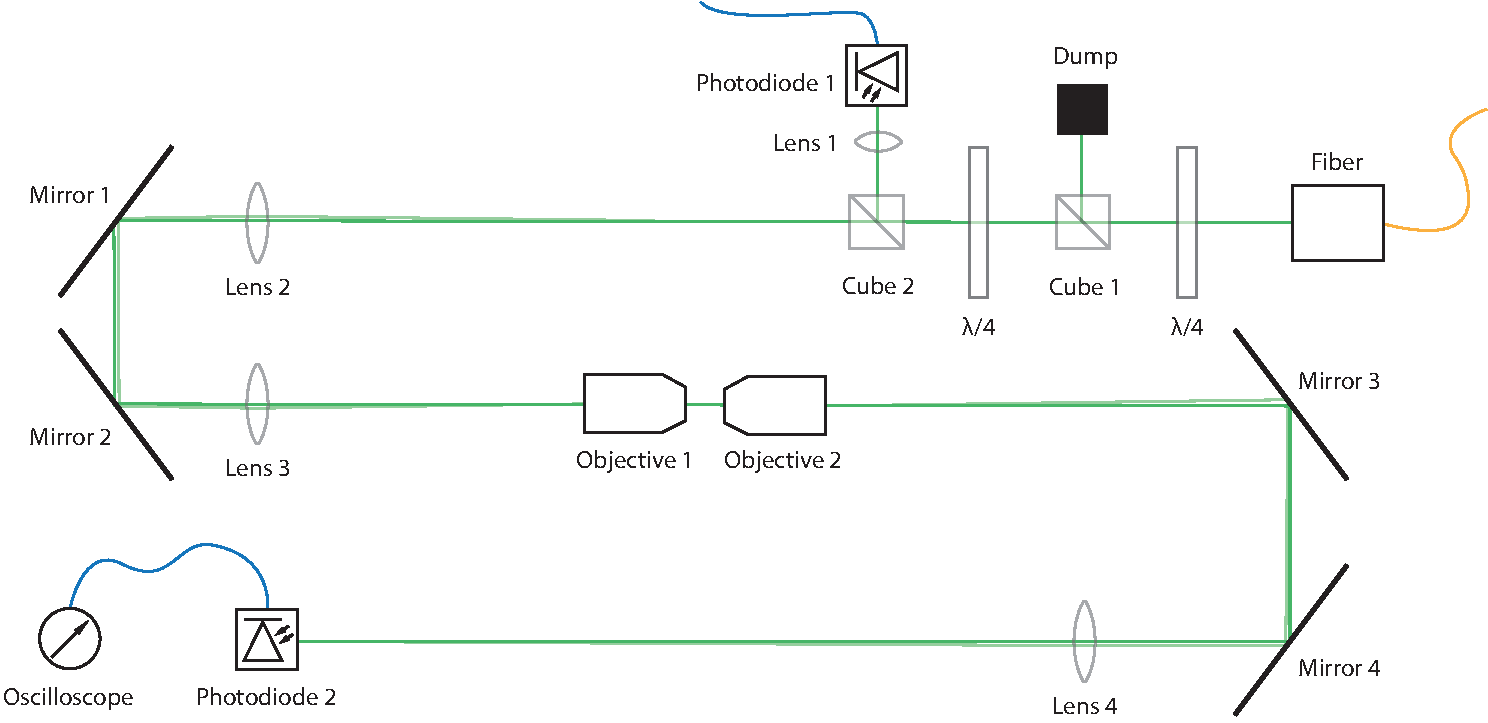
\includegraphics[width=\textwidth]{../media/setup/intensity-control.pdf}
  \caption{Optical setup and intensity detection. The beam hits Photodiode 2
    which is connected to the oscilloscope.
  }\label{fig:intensity_control_setup}
\end{figure}
In order to to estimate the error contribution due to imperfect intensity
regulation, we will conduct a short- and a long-term measurement of the
controlled intensity. Technically a typical intensity measurement takes about
a fraction of a millisecond, yet we can decide on different intervals between
the measurements in order to separate local from global trends like the ones
noted in the uncontrolled meausrement. \Cref{tab:intensity_control_times}
summarizes the different time scales for the conducted short- and long-term
measurement of the intensity control.
\begin{table}[htb]
  \centering
  \begin{tabular}{cccc}
    \toprule
    & Short & Long & Typical \\
    \midrule
    Interval &
    \SI{10}{\second} &
    \SI{120}{\second} &
    \SI{3}{\second} \\
    Duration &
    \SI{1}{\hour} &
    \SI{16}{\hour} &
    \SI{<2}{\hour} \\
    \bottomrule
  \end{tabular}
  \caption{Interval and duration times of the short- and long-term measurement
    as well as a typical sweep measurement.
  }\label{tab:intensity_control_times}
\end{table}
The voltage time series for both intensity control measurements are presented
in \Cref{fig:intensity_control}. The outlier at about 22:45 h was caused by
accidently interfering with the setup during measurement. Beside of that
incident the long-term intensity seems stable. On a smaller timescale we see
that the intensity evolution performs periodic oscillations.
\begin{table}[htb]
  \centering
  \begin{tabular}{lcccc}
    \toprule
    Measure & Uncontrolled & Long & Short & Typical \\
    \midrule
    Mean $\mu$ &
    \SI{8.45}{\volt} &
    \SI{6.79}{\volt} &
    \SI{6.79}{\volt} &
    \SI{1.95}{\volt} \\
    Minimum &
    \SI{7.43}{\volt} &
    \SI{4.88}{\volt} &
    \SI{6.77}{\volt} &
    \SI{0.00}{\volt} \\
    Maximum &
    \SI{6.82}{\volt} &
    \SI{6.86}{\volt} &
    \SI{6.82}{\volt} &
    \SI{9.08}{\volt} \\
    Standard Deviation $\sigma$ &
    \SI{0.49}{\volt} &
    \SI{0.09}{\volt} &
    \SI{0.01}{\volt} &
    \SI{0.54}{\volt} \\
    Relative Standard Deviation $\sigma/\mu$ &
    \SI{5.75}{\percent} &
    \SI{1.35}{\percent} &
    \SI{0.19}{\percent} &
    \SI{27.69}{\percent} \\
    \bottomrule
  \end{tabular}
  \caption{Descriptive statistics of uncontrolled and controlled short- and
    long-term intensity evolutions as well as a typical intensity measurement
    with \gls{aod}s for comparison.
  }\label{tab:intensity_control_statistics}
\end{table}
Overall we can confirm that the intensity control loop successfully holds the
intensity mean, though with small oscillations. In order to estimate the
relevance for these small oscillations of the controlled intensity for later
measurements, we selected an measurement of the intensity transmission
response of the \gls{aod} subject to constant frequency increments for
comparison. \Cref{tab:intensity_control_statistics} presents the statistics of
said intensity measurements.
\begin{figure}[htb]
  \centering
  \begin{adjustbox}{width=\textwidth}
    %% Creator: Matplotlib, PGF backend
%%
%% To include the figure in your LaTeX document, write
%%   \input{<filename>.pgf}
%%
%% Make sure the required packages are loaded in your preamble
%%   \usepackage{pgf}
%%
%% Figures using additional raster images can only be included by \input if
%% they are in the same directory as the main LaTeX file. For loading figures
%% from other directories you can use the `import` package
%%   \usepackage{import}
%% and then include the figures with
%%   \import{<path to file>}{<filename>.pgf}
%%
%% Matplotlib used the following preamble
%%   \usepackage{amsmath}\usepackage{siunitx}\usepackage{lmodern}
%%   \usepackage{fontspec}
%%
\begingroup%
\makeatletter%
\begin{pgfpicture}%
\pgfpathrectangle{\pgfpointorigin}{\pgfqpoint{12.000000in}{6.000000in}}%
\pgfusepath{use as bounding box, clip}%
\begin{pgfscope}%
\pgfsetbuttcap%
\pgfsetmiterjoin%
\pgfsetlinewidth{0.000000pt}%
\definecolor{currentstroke}{rgb}{1.000000,1.000000,1.000000}%
\pgfsetstrokecolor{currentstroke}%
\pgfsetdash{}{0pt}%
\pgfpathmoveto{\pgfqpoint{0.000000in}{0.000000in}}%
\pgfpathlineto{\pgfqpoint{12.000000in}{0.000000in}}%
\pgfpathlineto{\pgfqpoint{12.000000in}{6.000000in}}%
\pgfpathlineto{\pgfqpoint{0.000000in}{6.000000in}}%
\pgfpathclose%
\pgfusepath{}%
\end{pgfscope}%
\begin{pgfscope}%
\pgfsetbuttcap%
\pgfsetmiterjoin%
\definecolor{currentfill}{rgb}{1.000000,1.000000,1.000000}%
\pgfsetfillcolor{currentfill}%
\pgfsetlinewidth{0.000000pt}%
\definecolor{currentstroke}{rgb}{0.000000,0.000000,0.000000}%
\pgfsetstrokecolor{currentstroke}%
\pgfsetstrokeopacity{0.000000}%
\pgfsetdash{}{0pt}%
\pgfpathmoveto{\pgfqpoint{1.500000in}{3.120000in}}%
\pgfpathlineto{\pgfqpoint{6.036585in}{3.120000in}}%
\pgfpathlineto{\pgfqpoint{6.036585in}{5.520000in}}%
\pgfpathlineto{\pgfqpoint{1.500000in}{5.520000in}}%
\pgfpathclose%
\pgfusepath{fill}%
\end{pgfscope}%
\begin{pgfscope}%
\pgfpathrectangle{\pgfqpoint{1.500000in}{3.120000in}}{\pgfqpoint{4.536585in}{2.400000in}}%
\pgfusepath{clip}%
\pgfsetbuttcap%
\pgfsetroundjoin%
\definecolor{currentfill}{rgb}{0.121569,0.466667,0.705882}%
\pgfsetfillcolor{currentfill}%
\pgfsetlinewidth{1.003750pt}%
\definecolor{currentstroke}{rgb}{0.121569,0.466667,0.705882}%
\pgfsetstrokecolor{currentstroke}%
\pgfsetdash{}{0pt}%
\pgfpathmoveto{\pgfqpoint{1.707880in}{5.319339in}}%
\pgfpathcurveto{\pgfqpoint{1.715247in}{5.319339in}}{\pgfqpoint{1.722313in}{5.322266in}}{\pgfqpoint{1.727522in}{5.327475in}}%
\pgfpathcurveto{\pgfqpoint{1.732731in}{5.332684in}}{\pgfqpoint{1.735658in}{5.339750in}}{\pgfqpoint{1.735658in}{5.347117in}}%
\pgfpathcurveto{\pgfqpoint{1.735658in}{5.354484in}}{\pgfqpoint{1.732731in}{5.361550in}}{\pgfqpoint{1.727522in}{5.366759in}}%
\pgfpathcurveto{\pgfqpoint{1.722313in}{5.371968in}}{\pgfqpoint{1.715247in}{5.374895in}}{\pgfqpoint{1.707880in}{5.374895in}}%
\pgfpathcurveto{\pgfqpoint{1.700513in}{5.374895in}}{\pgfqpoint{1.693447in}{5.371968in}}{\pgfqpoint{1.688238in}{5.366759in}}%
\pgfpathcurveto{\pgfqpoint{1.683029in}{5.361550in}}{\pgfqpoint{1.680102in}{5.354484in}}{\pgfqpoint{1.680102in}{5.347117in}}%
\pgfpathcurveto{\pgfqpoint{1.680102in}{5.339750in}}{\pgfqpoint{1.683029in}{5.332684in}}{\pgfqpoint{1.688238in}{5.327475in}}%
\pgfpathcurveto{\pgfqpoint{1.693447in}{5.322266in}}{\pgfqpoint{1.700513in}{5.319339in}}{\pgfqpoint{1.707880in}{5.319339in}}%
\pgfpathclose%
\pgfusepath{stroke,fill}%
\end{pgfscope}%
\begin{pgfscope}%
\pgfpathrectangle{\pgfqpoint{1.500000in}{3.120000in}}{\pgfqpoint{4.536585in}{2.400000in}}%
\pgfusepath{clip}%
\pgfsetbuttcap%
\pgfsetroundjoin%
\definecolor{currentfill}{rgb}{0.121569,0.466667,0.705882}%
\pgfsetfillcolor{currentfill}%
\pgfsetlinewidth{1.003750pt}%
\definecolor{currentstroke}{rgb}{0.121569,0.466667,0.705882}%
\pgfsetstrokecolor{currentstroke}%
\pgfsetdash{}{0pt}%
\pgfpathmoveto{\pgfqpoint{1.717066in}{5.295073in}}%
\pgfpathcurveto{\pgfqpoint{1.724433in}{5.295073in}}{\pgfqpoint{1.731499in}{5.297999in}}{\pgfqpoint{1.736708in}{5.303208in}}%
\pgfpathcurveto{\pgfqpoint{1.741917in}{5.308418in}}{\pgfqpoint{1.744844in}{5.315484in}}{\pgfqpoint{1.744844in}{5.322850in}}%
\pgfpathcurveto{\pgfqpoint{1.744844in}{5.330217in}}{\pgfqpoint{1.741917in}{5.337283in}}{\pgfqpoint{1.736708in}{5.342492in}}%
\pgfpathcurveto{\pgfqpoint{1.731499in}{5.347701in}}{\pgfqpoint{1.724433in}{5.350628in}}{\pgfqpoint{1.717066in}{5.350628in}}%
\pgfpathcurveto{\pgfqpoint{1.709699in}{5.350628in}}{\pgfqpoint{1.702633in}{5.347701in}}{\pgfqpoint{1.697424in}{5.342492in}}%
\pgfpathcurveto{\pgfqpoint{1.692215in}{5.337283in}}{\pgfqpoint{1.689288in}{5.330217in}}{\pgfqpoint{1.689288in}{5.322850in}}%
\pgfpathcurveto{\pgfqpoint{1.689288in}{5.315484in}}{\pgfqpoint{1.692215in}{5.308418in}}{\pgfqpoint{1.697424in}{5.303208in}}%
\pgfpathcurveto{\pgfqpoint{1.702633in}{5.297999in}}{\pgfqpoint{1.709699in}{5.295073in}}{\pgfqpoint{1.717066in}{5.295073in}}%
\pgfpathclose%
\pgfusepath{stroke,fill}%
\end{pgfscope}%
\begin{pgfscope}%
\pgfpathrectangle{\pgfqpoint{1.500000in}{3.120000in}}{\pgfqpoint{4.536585in}{2.400000in}}%
\pgfusepath{clip}%
\pgfsetbuttcap%
\pgfsetroundjoin%
\definecolor{currentfill}{rgb}{0.121569,0.466667,0.705882}%
\pgfsetfillcolor{currentfill}%
\pgfsetlinewidth{1.003750pt}%
\definecolor{currentstroke}{rgb}{0.121569,0.466667,0.705882}%
\pgfsetstrokecolor{currentstroke}%
\pgfsetdash{}{0pt}%
\pgfpathmoveto{\pgfqpoint{1.726252in}{5.298408in}}%
\pgfpathcurveto{\pgfqpoint{1.733619in}{5.298408in}}{\pgfqpoint{1.740685in}{5.301334in}}{\pgfqpoint{1.745894in}{5.306544in}}%
\pgfpathcurveto{\pgfqpoint{1.751103in}{5.311753in}}{\pgfqpoint{1.754030in}{5.318819in}}{\pgfqpoint{1.754030in}{5.326185in}}%
\pgfpathcurveto{\pgfqpoint{1.754030in}{5.333552in}}{\pgfqpoint{1.751103in}{5.340618in}}{\pgfqpoint{1.745894in}{5.345827in}}%
\pgfpathcurveto{\pgfqpoint{1.740685in}{5.351036in}}{\pgfqpoint{1.733619in}{5.353963in}}{\pgfqpoint{1.726252in}{5.353963in}}%
\pgfpathcurveto{\pgfqpoint{1.718886in}{5.353963in}}{\pgfqpoint{1.711819in}{5.351036in}}{\pgfqpoint{1.706610in}{5.345827in}}%
\pgfpathcurveto{\pgfqpoint{1.701401in}{5.340618in}}{\pgfqpoint{1.698474in}{5.333552in}}{\pgfqpoint{1.698474in}{5.326185in}}%
\pgfpathcurveto{\pgfqpoint{1.698474in}{5.318819in}}{\pgfqpoint{1.701401in}{5.311753in}}{\pgfqpoint{1.706610in}{5.306544in}}%
\pgfpathcurveto{\pgfqpoint{1.711819in}{5.301334in}}{\pgfqpoint{1.718886in}{5.298408in}}{\pgfqpoint{1.726252in}{5.298408in}}%
\pgfpathclose%
\pgfusepath{stroke,fill}%
\end{pgfscope}%
\begin{pgfscope}%
\pgfpathrectangle{\pgfqpoint{1.500000in}{3.120000in}}{\pgfqpoint{4.536585in}{2.400000in}}%
\pgfusepath{clip}%
\pgfsetbuttcap%
\pgfsetroundjoin%
\definecolor{currentfill}{rgb}{0.121569,0.466667,0.705882}%
\pgfsetfillcolor{currentfill}%
\pgfsetlinewidth{1.003750pt}%
\definecolor{currentstroke}{rgb}{0.121569,0.466667,0.705882}%
\pgfsetstrokecolor{currentstroke}%
\pgfsetdash{}{0pt}%
\pgfpathmoveto{\pgfqpoint{1.735438in}{5.295706in}}%
\pgfpathcurveto{\pgfqpoint{1.742805in}{5.295706in}}{\pgfqpoint{1.749871in}{5.298632in}}{\pgfqpoint{1.755080in}{5.303841in}}%
\pgfpathcurveto{\pgfqpoint{1.760289in}{5.309051in}}{\pgfqpoint{1.763216in}{5.316117in}}{\pgfqpoint{1.763216in}{5.323483in}}%
\pgfpathcurveto{\pgfqpoint{1.763216in}{5.330850in}}{\pgfqpoint{1.760289in}{5.337916in}}{\pgfqpoint{1.755080in}{5.343125in}}%
\pgfpathcurveto{\pgfqpoint{1.749871in}{5.348334in}}{\pgfqpoint{1.742805in}{5.351261in}}{\pgfqpoint{1.735438in}{5.351261in}}%
\pgfpathcurveto{\pgfqpoint{1.728072in}{5.351261in}}{\pgfqpoint{1.721006in}{5.348334in}}{\pgfqpoint{1.715797in}{5.343125in}}%
\pgfpathcurveto{\pgfqpoint{1.710587in}{5.337916in}}{\pgfqpoint{1.707661in}{5.330850in}}{\pgfqpoint{1.707661in}{5.323483in}}%
\pgfpathcurveto{\pgfqpoint{1.707661in}{5.316117in}}{\pgfqpoint{1.710587in}{5.309051in}}{\pgfqpoint{1.715797in}{5.303841in}}%
\pgfpathcurveto{\pgfqpoint{1.721006in}{5.298632in}}{\pgfqpoint{1.728072in}{5.295706in}}{\pgfqpoint{1.735438in}{5.295706in}}%
\pgfpathclose%
\pgfusepath{stroke,fill}%
\end{pgfscope}%
\begin{pgfscope}%
\pgfpathrectangle{\pgfqpoint{1.500000in}{3.120000in}}{\pgfqpoint{4.536585in}{2.400000in}}%
\pgfusepath{clip}%
\pgfsetbuttcap%
\pgfsetroundjoin%
\definecolor{currentfill}{rgb}{0.121569,0.466667,0.705882}%
\pgfsetfillcolor{currentfill}%
\pgfsetlinewidth{1.003750pt}%
\definecolor{currentstroke}{rgb}{0.121569,0.466667,0.705882}%
\pgfsetstrokecolor{currentstroke}%
\pgfsetdash{}{0pt}%
\pgfpathmoveto{\pgfqpoint{1.744625in}{5.292689in}}%
\pgfpathcurveto{\pgfqpoint{1.751991in}{5.292689in}}{\pgfqpoint{1.759057in}{5.295616in}}{\pgfqpoint{1.764266in}{5.300825in}}%
\pgfpathcurveto{\pgfqpoint{1.769475in}{5.306034in}}{\pgfqpoint{1.772402in}{5.313100in}}{\pgfqpoint{1.772402in}{5.320467in}}%
\pgfpathcurveto{\pgfqpoint{1.772402in}{5.327834in}}{\pgfqpoint{1.769475in}{5.334900in}}{\pgfqpoint{1.764266in}{5.340109in}}%
\pgfpathcurveto{\pgfqpoint{1.759057in}{5.345318in}}{\pgfqpoint{1.751991in}{5.348245in}}{\pgfqpoint{1.744625in}{5.348245in}}%
\pgfpathcurveto{\pgfqpoint{1.737258in}{5.348245in}}{\pgfqpoint{1.730192in}{5.345318in}}{\pgfqpoint{1.724983in}{5.340109in}}%
\pgfpathcurveto{\pgfqpoint{1.719774in}{5.334900in}}{\pgfqpoint{1.716847in}{5.327834in}}{\pgfqpoint{1.716847in}{5.320467in}}%
\pgfpathcurveto{\pgfqpoint{1.716847in}{5.313100in}}{\pgfqpoint{1.719774in}{5.306034in}}{\pgfqpoint{1.724983in}{5.300825in}}%
\pgfpathcurveto{\pgfqpoint{1.730192in}{5.295616in}}{\pgfqpoint{1.737258in}{5.292689in}}{\pgfqpoint{1.744625in}{5.292689in}}%
\pgfpathclose%
\pgfusepath{stroke,fill}%
\end{pgfscope}%
\begin{pgfscope}%
\pgfpathrectangle{\pgfqpoint{1.500000in}{3.120000in}}{\pgfqpoint{4.536585in}{2.400000in}}%
\pgfusepath{clip}%
\pgfsetbuttcap%
\pgfsetroundjoin%
\definecolor{currentfill}{rgb}{0.121569,0.466667,0.705882}%
\pgfsetfillcolor{currentfill}%
\pgfsetlinewidth{1.003750pt}%
\definecolor{currentstroke}{rgb}{0.121569,0.466667,0.705882}%
\pgfsetstrokecolor{currentstroke}%
\pgfsetdash{}{0pt}%
\pgfpathmoveto{\pgfqpoint{1.753811in}{5.304240in}}%
\pgfpathcurveto{\pgfqpoint{1.761177in}{5.304240in}}{\pgfqpoint{1.768243in}{5.307167in}}{\pgfqpoint{1.773452in}{5.312376in}}%
\pgfpathcurveto{\pgfqpoint{1.778662in}{5.317585in}}{\pgfqpoint{1.781588in}{5.324651in}}{\pgfqpoint{1.781588in}{5.332018in}}%
\pgfpathcurveto{\pgfqpoint{1.781588in}{5.339385in}}{\pgfqpoint{1.778662in}{5.346451in}}{\pgfqpoint{1.773452in}{5.351660in}}%
\pgfpathcurveto{\pgfqpoint{1.768243in}{5.356869in}}{\pgfqpoint{1.761177in}{5.359796in}}{\pgfqpoint{1.753811in}{5.359796in}}%
\pgfpathcurveto{\pgfqpoint{1.746444in}{5.359796in}}{\pgfqpoint{1.739378in}{5.356869in}}{\pgfqpoint{1.734169in}{5.351660in}}%
\pgfpathcurveto{\pgfqpoint{1.728960in}{5.346451in}}{\pgfqpoint{1.726033in}{5.339385in}}{\pgfqpoint{1.726033in}{5.332018in}}%
\pgfpathcurveto{\pgfqpoint{1.726033in}{5.324651in}}{\pgfqpoint{1.728960in}{5.317585in}}{\pgfqpoint{1.734169in}{5.312376in}}%
\pgfpathcurveto{\pgfqpoint{1.739378in}{5.307167in}}{\pgfqpoint{1.746444in}{5.304240in}}{\pgfqpoint{1.753811in}{5.304240in}}%
\pgfpathclose%
\pgfusepath{stroke,fill}%
\end{pgfscope}%
\begin{pgfscope}%
\pgfpathrectangle{\pgfqpoint{1.500000in}{3.120000in}}{\pgfqpoint{4.536585in}{2.400000in}}%
\pgfusepath{clip}%
\pgfsetbuttcap%
\pgfsetroundjoin%
\definecolor{currentfill}{rgb}{0.121569,0.466667,0.705882}%
\pgfsetfillcolor{currentfill}%
\pgfsetlinewidth{1.003750pt}%
\definecolor{currentstroke}{rgb}{0.121569,0.466667,0.705882}%
\pgfsetstrokecolor{currentstroke}%
\pgfsetdash{}{0pt}%
\pgfpathmoveto{\pgfqpoint{1.763067in}{5.328719in}}%
\pgfpathcurveto{\pgfqpoint{1.770434in}{5.328719in}}{\pgfqpoint{1.777500in}{5.331646in}}{\pgfqpoint{1.782709in}{5.336855in}}%
\pgfpathcurveto{\pgfqpoint{1.787918in}{5.342064in}}{\pgfqpoint{1.790845in}{5.349130in}}{\pgfqpoint{1.790845in}{5.356496in}}%
\pgfpathcurveto{\pgfqpoint{1.790845in}{5.363863in}}{\pgfqpoint{1.787918in}{5.370929in}}{\pgfqpoint{1.782709in}{5.376138in}}%
\pgfpathcurveto{\pgfqpoint{1.777500in}{5.381347in}}{\pgfqpoint{1.770434in}{5.384274in}}{\pgfqpoint{1.763067in}{5.384274in}}%
\pgfpathcurveto{\pgfqpoint{1.755701in}{5.384274in}}{\pgfqpoint{1.748635in}{5.381347in}}{\pgfqpoint{1.743426in}{5.376138in}}%
\pgfpathcurveto{\pgfqpoint{1.738216in}{5.370929in}}{\pgfqpoint{1.735290in}{5.363863in}}{\pgfqpoint{1.735290in}{5.356496in}}%
\pgfpathcurveto{\pgfqpoint{1.735290in}{5.349130in}}{\pgfqpoint{1.738216in}{5.342064in}}{\pgfqpoint{1.743426in}{5.336855in}}%
\pgfpathcurveto{\pgfqpoint{1.748635in}{5.331646in}}{\pgfqpoint{1.755701in}{5.328719in}}{\pgfqpoint{1.763067in}{5.328719in}}%
\pgfpathclose%
\pgfusepath{stroke,fill}%
\end{pgfscope}%
\begin{pgfscope}%
\pgfpathrectangle{\pgfqpoint{1.500000in}{3.120000in}}{\pgfqpoint{4.536585in}{2.400000in}}%
\pgfusepath{clip}%
\pgfsetbuttcap%
\pgfsetroundjoin%
\definecolor{currentfill}{rgb}{0.121569,0.466667,0.705882}%
\pgfsetfillcolor{currentfill}%
\pgfsetlinewidth{1.003750pt}%
\definecolor{currentstroke}{rgb}{0.121569,0.466667,0.705882}%
\pgfsetstrokecolor{currentstroke}%
\pgfsetdash{}{0pt}%
\pgfpathmoveto{\pgfqpoint{1.772254in}{5.331155in}}%
\pgfpathcurveto{\pgfqpoint{1.779620in}{5.331155in}}{\pgfqpoint{1.786686in}{5.334082in}}{\pgfqpoint{1.791895in}{5.339291in}}%
\pgfpathcurveto{\pgfqpoint{1.797104in}{5.344500in}}{\pgfqpoint{1.800031in}{5.351566in}}{\pgfqpoint{1.800031in}{5.358933in}}%
\pgfpathcurveto{\pgfqpoint{1.800031in}{5.366300in}}{\pgfqpoint{1.797104in}{5.373366in}}{\pgfqpoint{1.791895in}{5.378575in}}%
\pgfpathcurveto{\pgfqpoint{1.786686in}{5.383784in}}{\pgfqpoint{1.779620in}{5.386711in}}{\pgfqpoint{1.772254in}{5.386711in}}%
\pgfpathcurveto{\pgfqpoint{1.764887in}{5.386711in}}{\pgfqpoint{1.757821in}{5.383784in}}{\pgfqpoint{1.752612in}{5.378575in}}%
\pgfpathcurveto{\pgfqpoint{1.747403in}{5.373366in}}{\pgfqpoint{1.744476in}{5.366300in}}{\pgfqpoint{1.744476in}{5.358933in}}%
\pgfpathcurveto{\pgfqpoint{1.744476in}{5.351566in}}{\pgfqpoint{1.747403in}{5.344500in}}{\pgfqpoint{1.752612in}{5.339291in}}%
\pgfpathcurveto{\pgfqpoint{1.757821in}{5.334082in}}{\pgfqpoint{1.764887in}{5.331155in}}{\pgfqpoint{1.772254in}{5.331155in}}%
\pgfpathclose%
\pgfusepath{stroke,fill}%
\end{pgfscope}%
\begin{pgfscope}%
\pgfpathrectangle{\pgfqpoint{1.500000in}{3.120000in}}{\pgfqpoint{4.536585in}{2.400000in}}%
\pgfusepath{clip}%
\pgfsetbuttcap%
\pgfsetroundjoin%
\definecolor{currentfill}{rgb}{0.121569,0.466667,0.705882}%
\pgfsetfillcolor{currentfill}%
\pgfsetlinewidth{1.003750pt}%
\definecolor{currentstroke}{rgb}{0.121569,0.466667,0.705882}%
\pgfsetstrokecolor{currentstroke}%
\pgfsetdash{}{0pt}%
\pgfpathmoveto{\pgfqpoint{1.781440in}{5.354130in}}%
\pgfpathcurveto{\pgfqpoint{1.788806in}{5.354130in}}{\pgfqpoint{1.795872in}{5.357057in}}{\pgfqpoint{1.801082in}{5.362266in}}%
\pgfpathcurveto{\pgfqpoint{1.806291in}{5.367475in}}{\pgfqpoint{1.809217in}{5.374541in}}{\pgfqpoint{1.809217in}{5.381908in}}%
\pgfpathcurveto{\pgfqpoint{1.809217in}{5.389274in}}{\pgfqpoint{1.806291in}{5.396340in}}{\pgfqpoint{1.801082in}{5.401550in}}%
\pgfpathcurveto{\pgfqpoint{1.795872in}{5.406759in}}{\pgfqpoint{1.788806in}{5.409685in}}{\pgfqpoint{1.781440in}{5.409685in}}%
\pgfpathcurveto{\pgfqpoint{1.774073in}{5.409685in}}{\pgfqpoint{1.767007in}{5.406759in}}{\pgfqpoint{1.761798in}{5.401550in}}%
\pgfpathcurveto{\pgfqpoint{1.756589in}{5.396340in}}{\pgfqpoint{1.753662in}{5.389274in}}{\pgfqpoint{1.753662in}{5.381908in}}%
\pgfpathcurveto{\pgfqpoint{1.753662in}{5.374541in}}{\pgfqpoint{1.756589in}{5.367475in}}{\pgfqpoint{1.761798in}{5.362266in}}%
\pgfpathcurveto{\pgfqpoint{1.767007in}{5.357057in}}{\pgfqpoint{1.774073in}{5.354130in}}{\pgfqpoint{1.781440in}{5.354130in}}%
\pgfpathclose%
\pgfusepath{stroke,fill}%
\end{pgfscope}%
\begin{pgfscope}%
\pgfpathrectangle{\pgfqpoint{1.500000in}{3.120000in}}{\pgfqpoint{4.536585in}{2.400000in}}%
\pgfusepath{clip}%
\pgfsetbuttcap%
\pgfsetroundjoin%
\definecolor{currentfill}{rgb}{0.121569,0.466667,0.705882}%
\pgfsetfillcolor{currentfill}%
\pgfsetlinewidth{1.003750pt}%
\definecolor{currentstroke}{rgb}{0.121569,0.466667,0.705882}%
\pgfsetstrokecolor{currentstroke}%
\pgfsetdash{}{0pt}%
\pgfpathmoveto{\pgfqpoint{1.790626in}{5.356229in}}%
\pgfpathcurveto{\pgfqpoint{1.797993in}{5.356229in}}{\pgfqpoint{1.805059in}{5.359156in}}{\pgfqpoint{1.810268in}{5.364365in}}%
\pgfpathcurveto{\pgfqpoint{1.815477in}{5.369574in}}{\pgfqpoint{1.818404in}{5.376640in}}{\pgfqpoint{1.818404in}{5.384007in}}%
\pgfpathcurveto{\pgfqpoint{1.818404in}{5.391374in}}{\pgfqpoint{1.815477in}{5.398440in}}{\pgfqpoint{1.810268in}{5.403649in}}%
\pgfpathcurveto{\pgfqpoint{1.805059in}{5.408858in}}{\pgfqpoint{1.797993in}{5.411785in}}{\pgfqpoint{1.790626in}{5.411785in}}%
\pgfpathcurveto{\pgfqpoint{1.783259in}{5.411785in}}{\pgfqpoint{1.776193in}{5.408858in}}{\pgfqpoint{1.770984in}{5.403649in}}%
\pgfpathcurveto{\pgfqpoint{1.765775in}{5.398440in}}{\pgfqpoint{1.762848in}{5.391374in}}{\pgfqpoint{1.762848in}{5.384007in}}%
\pgfpathcurveto{\pgfqpoint{1.762848in}{5.376640in}}{\pgfqpoint{1.765775in}{5.369574in}}{\pgfqpoint{1.770984in}{5.364365in}}%
\pgfpathcurveto{\pgfqpoint{1.776193in}{5.359156in}}{\pgfqpoint{1.783259in}{5.356229in}}{\pgfqpoint{1.790626in}{5.356229in}}%
\pgfpathclose%
\pgfusepath{stroke,fill}%
\end{pgfscope}%
\begin{pgfscope}%
\pgfpathrectangle{\pgfqpoint{1.500000in}{3.120000in}}{\pgfqpoint{4.536585in}{2.400000in}}%
\pgfusepath{clip}%
\pgfsetbuttcap%
\pgfsetroundjoin%
\definecolor{currentfill}{rgb}{0.121569,0.466667,0.705882}%
\pgfsetfillcolor{currentfill}%
\pgfsetlinewidth{1.003750pt}%
\definecolor{currentstroke}{rgb}{0.121569,0.466667,0.705882}%
\pgfsetstrokecolor{currentstroke}%
\pgfsetdash{}{0pt}%
\pgfpathmoveto{\pgfqpoint{1.799812in}{5.340290in}}%
\pgfpathcurveto{\pgfqpoint{1.807179in}{5.340290in}}{\pgfqpoint{1.814245in}{5.343216in}}{\pgfqpoint{1.819454in}{5.348426in}}%
\pgfpathcurveto{\pgfqpoint{1.824663in}{5.353635in}}{\pgfqpoint{1.827590in}{5.360701in}}{\pgfqpoint{1.827590in}{5.368067in}}%
\pgfpathcurveto{\pgfqpoint{1.827590in}{5.375434in}}{\pgfqpoint{1.824663in}{5.382500in}}{\pgfqpoint{1.819454in}{5.387709in}}%
\pgfpathcurveto{\pgfqpoint{1.814245in}{5.392918in}}{\pgfqpoint{1.807179in}{5.395845in}}{\pgfqpoint{1.799812in}{5.395845in}}%
\pgfpathcurveto{\pgfqpoint{1.792445in}{5.395845in}}{\pgfqpoint{1.785379in}{5.392918in}}{\pgfqpoint{1.780170in}{5.387709in}}%
\pgfpathcurveto{\pgfqpoint{1.774961in}{5.382500in}}{\pgfqpoint{1.772034in}{5.375434in}}{\pgfqpoint{1.772034in}{5.368067in}}%
\pgfpathcurveto{\pgfqpoint{1.772034in}{5.360701in}}{\pgfqpoint{1.774961in}{5.353635in}}{\pgfqpoint{1.780170in}{5.348426in}}%
\pgfpathcurveto{\pgfqpoint{1.785379in}{5.343216in}}{\pgfqpoint{1.792445in}{5.340290in}}{\pgfqpoint{1.799812in}{5.340290in}}%
\pgfpathclose%
\pgfusepath{stroke,fill}%
\end{pgfscope}%
\begin{pgfscope}%
\pgfpathrectangle{\pgfqpoint{1.500000in}{3.120000in}}{\pgfqpoint{4.536585in}{2.400000in}}%
\pgfusepath{clip}%
\pgfsetbuttcap%
\pgfsetroundjoin%
\definecolor{currentfill}{rgb}{0.121569,0.466667,0.705882}%
\pgfsetfillcolor{currentfill}%
\pgfsetlinewidth{1.003750pt}%
\definecolor{currentstroke}{rgb}{0.121569,0.466667,0.705882}%
\pgfsetstrokecolor{currentstroke}%
\pgfsetdash{}{0pt}%
\pgfpathmoveto{\pgfqpoint{1.808998in}{5.316957in}}%
\pgfpathcurveto{\pgfqpoint{1.816365in}{5.316957in}}{\pgfqpoint{1.823431in}{5.319884in}}{\pgfqpoint{1.828640in}{5.325093in}}%
\pgfpathcurveto{\pgfqpoint{1.833849in}{5.330302in}}{\pgfqpoint{1.836776in}{5.337368in}}{\pgfqpoint{1.836776in}{5.344735in}}%
\pgfpathcurveto{\pgfqpoint{1.836776in}{5.352101in}}{\pgfqpoint{1.833849in}{5.359167in}}{\pgfqpoint{1.828640in}{5.364376in}}%
\pgfpathcurveto{\pgfqpoint{1.823431in}{5.369586in}}{\pgfqpoint{1.816365in}{5.372512in}}{\pgfqpoint{1.808998in}{5.372512in}}%
\pgfpathcurveto{\pgfqpoint{1.801631in}{5.372512in}}{\pgfqpoint{1.794565in}{5.369586in}}{\pgfqpoint{1.789356in}{5.364376in}}%
\pgfpathcurveto{\pgfqpoint{1.784147in}{5.359167in}}{\pgfqpoint{1.781220in}{5.352101in}}{\pgfqpoint{1.781220in}{5.344735in}}%
\pgfpathcurveto{\pgfqpoint{1.781220in}{5.337368in}}{\pgfqpoint{1.784147in}{5.330302in}}{\pgfqpoint{1.789356in}{5.325093in}}%
\pgfpathcurveto{\pgfqpoint{1.794565in}{5.319884in}}{\pgfqpoint{1.801631in}{5.316957in}}{\pgfqpoint{1.808998in}{5.316957in}}%
\pgfpathclose%
\pgfusepath{stroke,fill}%
\end{pgfscope}%
\begin{pgfscope}%
\pgfpathrectangle{\pgfqpoint{1.500000in}{3.120000in}}{\pgfqpoint{4.536585in}{2.400000in}}%
\pgfusepath{clip}%
\pgfsetbuttcap%
\pgfsetroundjoin%
\definecolor{currentfill}{rgb}{0.121569,0.466667,0.705882}%
\pgfsetfillcolor{currentfill}%
\pgfsetlinewidth{1.003750pt}%
\definecolor{currentstroke}{rgb}{0.121569,0.466667,0.705882}%
\pgfsetstrokecolor{currentstroke}%
\pgfsetdash{}{0pt}%
\pgfpathmoveto{\pgfqpoint{1.818255in}{5.304994in}}%
\pgfpathcurveto{\pgfqpoint{1.825622in}{5.304994in}}{\pgfqpoint{1.832688in}{5.307920in}}{\pgfqpoint{1.837897in}{5.313130in}}%
\pgfpathcurveto{\pgfqpoint{1.843106in}{5.318339in}}{\pgfqpoint{1.846033in}{5.325405in}}{\pgfqpoint{1.846033in}{5.332771in}}%
\pgfpathcurveto{\pgfqpoint{1.846033in}{5.340138in}}{\pgfqpoint{1.843106in}{5.347204in}}{\pgfqpoint{1.837897in}{5.352413in}}%
\pgfpathcurveto{\pgfqpoint{1.832688in}{5.357622in}}{\pgfqpoint{1.825622in}{5.360549in}}{\pgfqpoint{1.818255in}{5.360549in}}%
\pgfpathcurveto{\pgfqpoint{1.810888in}{5.360549in}}{\pgfqpoint{1.803822in}{5.357622in}}{\pgfqpoint{1.798613in}{5.352413in}}%
\pgfpathcurveto{\pgfqpoint{1.793404in}{5.347204in}}{\pgfqpoint{1.790477in}{5.340138in}}{\pgfqpoint{1.790477in}{5.332771in}}%
\pgfpathcurveto{\pgfqpoint{1.790477in}{5.325405in}}{\pgfqpoint{1.793404in}{5.318339in}}{\pgfqpoint{1.798613in}{5.313130in}}%
\pgfpathcurveto{\pgfqpoint{1.803822in}{5.307920in}}{\pgfqpoint{1.810888in}{5.304994in}}{\pgfqpoint{1.818255in}{5.304994in}}%
\pgfpathclose%
\pgfusepath{stroke,fill}%
\end{pgfscope}%
\begin{pgfscope}%
\pgfpathrectangle{\pgfqpoint{1.500000in}{3.120000in}}{\pgfqpoint{4.536585in}{2.400000in}}%
\pgfusepath{clip}%
\pgfsetbuttcap%
\pgfsetroundjoin%
\definecolor{currentfill}{rgb}{0.121569,0.466667,0.705882}%
\pgfsetfillcolor{currentfill}%
\pgfsetlinewidth{1.003750pt}%
\definecolor{currentstroke}{rgb}{0.121569,0.466667,0.705882}%
\pgfsetstrokecolor{currentstroke}%
\pgfsetdash{}{0pt}%
\pgfpathmoveto{\pgfqpoint{1.827441in}{5.287940in}}%
\pgfpathcurveto{\pgfqpoint{1.834808in}{5.287940in}}{\pgfqpoint{1.841874in}{5.290867in}}{\pgfqpoint{1.847083in}{5.296076in}}%
\pgfpathcurveto{\pgfqpoint{1.852292in}{5.301285in}}{\pgfqpoint{1.855219in}{5.308351in}}{\pgfqpoint{1.855219in}{5.315717in}}%
\pgfpathcurveto{\pgfqpoint{1.855219in}{5.323084in}}{\pgfqpoint{1.852292in}{5.330150in}}{\pgfqpoint{1.847083in}{5.335359in}}%
\pgfpathcurveto{\pgfqpoint{1.841874in}{5.340568in}}{\pgfqpoint{1.834808in}{5.343495in}}{\pgfqpoint{1.827441in}{5.343495in}}%
\pgfpathcurveto{\pgfqpoint{1.820074in}{5.343495in}}{\pgfqpoint{1.813008in}{5.340568in}}{\pgfqpoint{1.807799in}{5.335359in}}%
\pgfpathcurveto{\pgfqpoint{1.802590in}{5.330150in}}{\pgfqpoint{1.799663in}{5.323084in}}{\pgfqpoint{1.799663in}{5.315717in}}%
\pgfpathcurveto{\pgfqpoint{1.799663in}{5.308351in}}{\pgfqpoint{1.802590in}{5.301285in}}{\pgfqpoint{1.807799in}{5.296076in}}%
\pgfpathcurveto{\pgfqpoint{1.813008in}{5.290867in}}{\pgfqpoint{1.820074in}{5.287940in}}{\pgfqpoint{1.827441in}{5.287940in}}%
\pgfpathclose%
\pgfusepath{stroke,fill}%
\end{pgfscope}%
\begin{pgfscope}%
\pgfpathrectangle{\pgfqpoint{1.500000in}{3.120000in}}{\pgfqpoint{4.536585in}{2.400000in}}%
\pgfusepath{clip}%
\pgfsetbuttcap%
\pgfsetroundjoin%
\definecolor{currentfill}{rgb}{0.121569,0.466667,0.705882}%
\pgfsetfillcolor{currentfill}%
\pgfsetlinewidth{1.003750pt}%
\definecolor{currentstroke}{rgb}{0.121569,0.466667,0.705882}%
\pgfsetstrokecolor{currentstroke}%
\pgfsetdash{}{0pt}%
\pgfpathmoveto{\pgfqpoint{1.836627in}{5.293351in}}%
\pgfpathcurveto{\pgfqpoint{1.843994in}{5.293351in}}{\pgfqpoint{1.851060in}{5.296278in}}{\pgfqpoint{1.856269in}{5.301487in}}%
\pgfpathcurveto{\pgfqpoint{1.861478in}{5.306696in}}{\pgfqpoint{1.864405in}{5.313762in}}{\pgfqpoint{1.864405in}{5.321129in}}%
\pgfpathcurveto{\pgfqpoint{1.864405in}{5.328496in}}{\pgfqpoint{1.861478in}{5.335562in}}{\pgfqpoint{1.856269in}{5.340771in}}%
\pgfpathcurveto{\pgfqpoint{1.851060in}{5.345980in}}{\pgfqpoint{1.843994in}{5.348907in}}{\pgfqpoint{1.836627in}{5.348907in}}%
\pgfpathcurveto{\pgfqpoint{1.829260in}{5.348907in}}{\pgfqpoint{1.822194in}{5.345980in}}{\pgfqpoint{1.816985in}{5.340771in}}%
\pgfpathcurveto{\pgfqpoint{1.811776in}{5.335562in}}{\pgfqpoint{1.808849in}{5.328496in}}{\pgfqpoint{1.808849in}{5.321129in}}%
\pgfpathcurveto{\pgfqpoint{1.808849in}{5.313762in}}{\pgfqpoint{1.811776in}{5.306696in}}{\pgfqpoint{1.816985in}{5.301487in}}%
\pgfpathcurveto{\pgfqpoint{1.822194in}{5.296278in}}{\pgfqpoint{1.829260in}{5.293351in}}{\pgfqpoint{1.836627in}{5.293351in}}%
\pgfpathclose%
\pgfusepath{stroke,fill}%
\end{pgfscope}%
\begin{pgfscope}%
\pgfpathrectangle{\pgfqpoint{1.500000in}{3.120000in}}{\pgfqpoint{4.536585in}{2.400000in}}%
\pgfusepath{clip}%
\pgfsetbuttcap%
\pgfsetroundjoin%
\definecolor{currentfill}{rgb}{0.121569,0.466667,0.705882}%
\pgfsetfillcolor{currentfill}%
\pgfsetlinewidth{1.003750pt}%
\definecolor{currentstroke}{rgb}{0.121569,0.466667,0.705882}%
\pgfsetstrokecolor{currentstroke}%
\pgfsetdash{}{0pt}%
\pgfpathmoveto{\pgfqpoint{1.845813in}{5.295983in}}%
\pgfpathcurveto{\pgfqpoint{1.853180in}{5.295983in}}{\pgfqpoint{1.860246in}{5.298909in}}{\pgfqpoint{1.865455in}{5.304119in}}%
\pgfpathcurveto{\pgfqpoint{1.870664in}{5.309328in}}{\pgfqpoint{1.873591in}{5.316394in}}{\pgfqpoint{1.873591in}{5.323760in}}%
\pgfpathcurveto{\pgfqpoint{1.873591in}{5.331127in}}{\pgfqpoint{1.870664in}{5.338193in}}{\pgfqpoint{1.865455in}{5.343402in}}%
\pgfpathcurveto{\pgfqpoint{1.860246in}{5.348611in}}{\pgfqpoint{1.853180in}{5.351538in}}{\pgfqpoint{1.845813in}{5.351538in}}%
\pgfpathcurveto{\pgfqpoint{1.838446in}{5.351538in}}{\pgfqpoint{1.831380in}{5.348611in}}{\pgfqpoint{1.826171in}{5.343402in}}%
\pgfpathcurveto{\pgfqpoint{1.820962in}{5.338193in}}{\pgfqpoint{1.818035in}{5.331127in}}{\pgfqpoint{1.818035in}{5.323760in}}%
\pgfpathcurveto{\pgfqpoint{1.818035in}{5.316394in}}{\pgfqpoint{1.820962in}{5.309328in}}{\pgfqpoint{1.826171in}{5.304119in}}%
\pgfpathcurveto{\pgfqpoint{1.831380in}{5.298909in}}{\pgfqpoint{1.838446in}{5.295983in}}{\pgfqpoint{1.845813in}{5.295983in}}%
\pgfpathclose%
\pgfusepath{stroke,fill}%
\end{pgfscope}%
\begin{pgfscope}%
\pgfpathrectangle{\pgfqpoint{1.500000in}{3.120000in}}{\pgfqpoint{4.536585in}{2.400000in}}%
\pgfusepath{clip}%
\pgfsetbuttcap%
\pgfsetroundjoin%
\definecolor{currentfill}{rgb}{0.121569,0.466667,0.705882}%
\pgfsetfillcolor{currentfill}%
\pgfsetlinewidth{1.003750pt}%
\definecolor{currentstroke}{rgb}{0.121569,0.466667,0.705882}%
\pgfsetstrokecolor{currentstroke}%
\pgfsetdash{}{0pt}%
\pgfpathmoveto{\pgfqpoint{1.854999in}{5.311186in}}%
\pgfpathcurveto{\pgfqpoint{1.862366in}{5.311186in}}{\pgfqpoint{1.869432in}{5.314113in}}{\pgfqpoint{1.874641in}{5.319322in}}%
\pgfpathcurveto{\pgfqpoint{1.879850in}{5.324531in}}{\pgfqpoint{1.882777in}{5.331597in}}{\pgfqpoint{1.882777in}{5.338964in}}%
\pgfpathcurveto{\pgfqpoint{1.882777in}{5.346331in}}{\pgfqpoint{1.879850in}{5.353397in}}{\pgfqpoint{1.874641in}{5.358606in}}%
\pgfpathcurveto{\pgfqpoint{1.869432in}{5.363815in}}{\pgfqpoint{1.862366in}{5.366742in}}{\pgfqpoint{1.854999in}{5.366742in}}%
\pgfpathcurveto{\pgfqpoint{1.847633in}{5.366742in}}{\pgfqpoint{1.840567in}{5.363815in}}{\pgfqpoint{1.835357in}{5.358606in}}%
\pgfpathcurveto{\pgfqpoint{1.830148in}{5.353397in}}{\pgfqpoint{1.827222in}{5.346331in}}{\pgfqpoint{1.827222in}{5.338964in}}%
\pgfpathcurveto{\pgfqpoint{1.827222in}{5.331597in}}{\pgfqpoint{1.830148in}{5.324531in}}{\pgfqpoint{1.835357in}{5.319322in}}%
\pgfpathcurveto{\pgfqpoint{1.840567in}{5.314113in}}{\pgfqpoint{1.847633in}{5.311186in}}{\pgfqpoint{1.854999in}{5.311186in}}%
\pgfpathclose%
\pgfusepath{stroke,fill}%
\end{pgfscope}%
\begin{pgfscope}%
\pgfpathrectangle{\pgfqpoint{1.500000in}{3.120000in}}{\pgfqpoint{4.536585in}{2.400000in}}%
\pgfusepath{clip}%
\pgfsetbuttcap%
\pgfsetroundjoin%
\definecolor{currentfill}{rgb}{0.121569,0.466667,0.705882}%
\pgfsetfillcolor{currentfill}%
\pgfsetlinewidth{1.003750pt}%
\definecolor{currentstroke}{rgb}{0.121569,0.466667,0.705882}%
\pgfsetstrokecolor{currentstroke}%
\pgfsetdash{}{0pt}%
\pgfpathmoveto{\pgfqpoint{1.864185in}{5.311177in}}%
\pgfpathcurveto{\pgfqpoint{1.871552in}{5.311177in}}{\pgfqpoint{1.878618in}{5.314104in}}{\pgfqpoint{1.883827in}{5.319313in}}%
\pgfpathcurveto{\pgfqpoint{1.889036in}{5.324522in}}{\pgfqpoint{1.891963in}{5.331588in}}{\pgfqpoint{1.891963in}{5.338955in}}%
\pgfpathcurveto{\pgfqpoint{1.891963in}{5.346322in}}{\pgfqpoint{1.889036in}{5.353388in}}{\pgfqpoint{1.883827in}{5.358597in}}%
\pgfpathcurveto{\pgfqpoint{1.878618in}{5.363806in}}{\pgfqpoint{1.871552in}{5.366733in}}{\pgfqpoint{1.864185in}{5.366733in}}%
\pgfpathcurveto{\pgfqpoint{1.856819in}{5.366733in}}{\pgfqpoint{1.849753in}{5.363806in}}{\pgfqpoint{1.844544in}{5.358597in}}%
\pgfpathcurveto{\pgfqpoint{1.839335in}{5.353388in}}{\pgfqpoint{1.836408in}{5.346322in}}{\pgfqpoint{1.836408in}{5.338955in}}%
\pgfpathcurveto{\pgfqpoint{1.836408in}{5.331588in}}{\pgfqpoint{1.839335in}{5.324522in}}{\pgfqpoint{1.844544in}{5.319313in}}%
\pgfpathcurveto{\pgfqpoint{1.849753in}{5.314104in}}{\pgfqpoint{1.856819in}{5.311177in}}{\pgfqpoint{1.864185in}{5.311177in}}%
\pgfpathclose%
\pgfusepath{stroke,fill}%
\end{pgfscope}%
\begin{pgfscope}%
\pgfpathrectangle{\pgfqpoint{1.500000in}{3.120000in}}{\pgfqpoint{4.536585in}{2.400000in}}%
\pgfusepath{clip}%
\pgfsetbuttcap%
\pgfsetroundjoin%
\definecolor{currentfill}{rgb}{0.121569,0.466667,0.705882}%
\pgfsetfillcolor{currentfill}%
\pgfsetlinewidth{1.003750pt}%
\definecolor{currentstroke}{rgb}{0.121569,0.466667,0.705882}%
\pgfsetstrokecolor{currentstroke}%
\pgfsetdash{}{0pt}%
\pgfpathmoveto{\pgfqpoint{1.873442in}{5.339563in}}%
\pgfpathcurveto{\pgfqpoint{1.880809in}{5.339563in}}{\pgfqpoint{1.887875in}{5.342490in}}{\pgfqpoint{1.893084in}{5.347699in}}%
\pgfpathcurveto{\pgfqpoint{1.898293in}{5.352908in}}{\pgfqpoint{1.901220in}{5.359974in}}{\pgfqpoint{1.901220in}{5.367341in}}%
\pgfpathcurveto{\pgfqpoint{1.901220in}{5.374708in}}{\pgfqpoint{1.898293in}{5.381774in}}{\pgfqpoint{1.893084in}{5.386983in}}%
\pgfpathcurveto{\pgfqpoint{1.887875in}{5.392192in}}{\pgfqpoint{1.880809in}{5.395119in}}{\pgfqpoint{1.873442in}{5.395119in}}%
\pgfpathcurveto{\pgfqpoint{1.866076in}{5.395119in}}{\pgfqpoint{1.859009in}{5.392192in}}{\pgfqpoint{1.853800in}{5.386983in}}%
\pgfpathcurveto{\pgfqpoint{1.848591in}{5.381774in}}{\pgfqpoint{1.845664in}{5.374708in}}{\pgfqpoint{1.845664in}{5.367341in}}%
\pgfpathcurveto{\pgfqpoint{1.845664in}{5.359974in}}{\pgfqpoint{1.848591in}{5.352908in}}{\pgfqpoint{1.853800in}{5.347699in}}%
\pgfpathcurveto{\pgfqpoint{1.859009in}{5.342490in}}{\pgfqpoint{1.866076in}{5.339563in}}{\pgfqpoint{1.873442in}{5.339563in}}%
\pgfpathclose%
\pgfusepath{stroke,fill}%
\end{pgfscope}%
\begin{pgfscope}%
\pgfpathrectangle{\pgfqpoint{1.500000in}{3.120000in}}{\pgfqpoint{4.536585in}{2.400000in}}%
\pgfusepath{clip}%
\pgfsetbuttcap%
\pgfsetroundjoin%
\definecolor{currentfill}{rgb}{0.121569,0.466667,0.705882}%
\pgfsetfillcolor{currentfill}%
\pgfsetlinewidth{1.003750pt}%
\definecolor{currentstroke}{rgb}{0.121569,0.466667,0.705882}%
\pgfsetstrokecolor{currentstroke}%
\pgfsetdash{}{0pt}%
\pgfpathmoveto{\pgfqpoint{1.882628in}{5.343296in}}%
\pgfpathcurveto{\pgfqpoint{1.889995in}{5.343296in}}{\pgfqpoint{1.897061in}{5.346223in}}{\pgfqpoint{1.902270in}{5.351432in}}%
\pgfpathcurveto{\pgfqpoint{1.907479in}{5.356641in}}{\pgfqpoint{1.910406in}{5.363707in}}{\pgfqpoint{1.910406in}{5.371073in}}%
\pgfpathcurveto{\pgfqpoint{1.910406in}{5.378440in}}{\pgfqpoint{1.907479in}{5.385506in}}{\pgfqpoint{1.902270in}{5.390715in}}%
\pgfpathcurveto{\pgfqpoint{1.897061in}{5.395924in}}{\pgfqpoint{1.889995in}{5.398851in}}{\pgfqpoint{1.882628in}{5.398851in}}%
\pgfpathcurveto{\pgfqpoint{1.875262in}{5.398851in}}{\pgfqpoint{1.868196in}{5.395924in}}{\pgfqpoint{1.862987in}{5.390715in}}%
\pgfpathcurveto{\pgfqpoint{1.857777in}{5.385506in}}{\pgfqpoint{1.854851in}{5.378440in}}{\pgfqpoint{1.854851in}{5.371073in}}%
\pgfpathcurveto{\pgfqpoint{1.854851in}{5.363707in}}{\pgfqpoint{1.857777in}{5.356641in}}{\pgfqpoint{1.862987in}{5.351432in}}%
\pgfpathcurveto{\pgfqpoint{1.868196in}{5.346223in}}{\pgfqpoint{1.875262in}{5.343296in}}{\pgfqpoint{1.882628in}{5.343296in}}%
\pgfpathclose%
\pgfusepath{stroke,fill}%
\end{pgfscope}%
\begin{pgfscope}%
\pgfpathrectangle{\pgfqpoint{1.500000in}{3.120000in}}{\pgfqpoint{4.536585in}{2.400000in}}%
\pgfusepath{clip}%
\pgfsetbuttcap%
\pgfsetroundjoin%
\definecolor{currentfill}{rgb}{0.121569,0.466667,0.705882}%
\pgfsetfillcolor{currentfill}%
\pgfsetlinewidth{1.003750pt}%
\definecolor{currentstroke}{rgb}{0.121569,0.466667,0.705882}%
\pgfsetstrokecolor{currentstroke}%
\pgfsetdash{}{0pt}%
\pgfpathmoveto{\pgfqpoint{1.891815in}{5.328776in}}%
\pgfpathcurveto{\pgfqpoint{1.899181in}{5.328776in}}{\pgfqpoint{1.906247in}{5.331703in}}{\pgfqpoint{1.911456in}{5.336912in}}%
\pgfpathcurveto{\pgfqpoint{1.916665in}{5.342121in}}{\pgfqpoint{1.919592in}{5.349187in}}{\pgfqpoint{1.919592in}{5.356554in}}%
\pgfpathcurveto{\pgfqpoint{1.919592in}{5.363920in}}{\pgfqpoint{1.916665in}{5.370986in}}{\pgfqpoint{1.911456in}{5.376195in}}%
\pgfpathcurveto{\pgfqpoint{1.906247in}{5.381404in}}{\pgfqpoint{1.899181in}{5.384331in}}{\pgfqpoint{1.891815in}{5.384331in}}%
\pgfpathcurveto{\pgfqpoint{1.884448in}{5.384331in}}{\pgfqpoint{1.877382in}{5.381404in}}{\pgfqpoint{1.872173in}{5.376195in}}%
\pgfpathcurveto{\pgfqpoint{1.866964in}{5.370986in}}{\pgfqpoint{1.864037in}{5.363920in}}{\pgfqpoint{1.864037in}{5.356554in}}%
\pgfpathcurveto{\pgfqpoint{1.864037in}{5.349187in}}{\pgfqpoint{1.866964in}{5.342121in}}{\pgfqpoint{1.872173in}{5.336912in}}%
\pgfpathcurveto{\pgfqpoint{1.877382in}{5.331703in}}{\pgfqpoint{1.884448in}{5.328776in}}{\pgfqpoint{1.891815in}{5.328776in}}%
\pgfpathclose%
\pgfusepath{stroke,fill}%
\end{pgfscope}%
\begin{pgfscope}%
\pgfpathrectangle{\pgfqpoint{1.500000in}{3.120000in}}{\pgfqpoint{4.536585in}{2.400000in}}%
\pgfusepath{clip}%
\pgfsetbuttcap%
\pgfsetroundjoin%
\definecolor{currentfill}{rgb}{0.121569,0.466667,0.705882}%
\pgfsetfillcolor{currentfill}%
\pgfsetlinewidth{1.003750pt}%
\definecolor{currentstroke}{rgb}{0.121569,0.466667,0.705882}%
\pgfsetstrokecolor{currentstroke}%
\pgfsetdash{}{0pt}%
\pgfpathmoveto{\pgfqpoint{1.901001in}{5.312017in}}%
\pgfpathcurveto{\pgfqpoint{1.908367in}{5.312017in}}{\pgfqpoint{1.915433in}{5.314943in}}{\pgfqpoint{1.920642in}{5.320152in}}%
\pgfpathcurveto{\pgfqpoint{1.925852in}{5.325362in}}{\pgfqpoint{1.928778in}{5.332428in}}{\pgfqpoint{1.928778in}{5.339794in}}%
\pgfpathcurveto{\pgfqpoint{1.928778in}{5.347161in}}{\pgfqpoint{1.925852in}{5.354227in}}{\pgfqpoint{1.920642in}{5.359436in}}%
\pgfpathcurveto{\pgfqpoint{1.915433in}{5.364645in}}{\pgfqpoint{1.908367in}{5.367572in}}{\pgfqpoint{1.901001in}{5.367572in}}%
\pgfpathcurveto{\pgfqpoint{1.893634in}{5.367572in}}{\pgfqpoint{1.886568in}{5.364645in}}{\pgfqpoint{1.881359in}{5.359436in}}%
\pgfpathcurveto{\pgfqpoint{1.876150in}{5.354227in}}{\pgfqpoint{1.873223in}{5.347161in}}{\pgfqpoint{1.873223in}{5.339794in}}%
\pgfpathcurveto{\pgfqpoint{1.873223in}{5.332428in}}{\pgfqpoint{1.876150in}{5.325362in}}{\pgfqpoint{1.881359in}{5.320152in}}%
\pgfpathcurveto{\pgfqpoint{1.886568in}{5.314943in}}{\pgfqpoint{1.893634in}{5.312017in}}{\pgfqpoint{1.901001in}{5.312017in}}%
\pgfpathclose%
\pgfusepath{stroke,fill}%
\end{pgfscope}%
\begin{pgfscope}%
\pgfpathrectangle{\pgfqpoint{1.500000in}{3.120000in}}{\pgfqpoint{4.536585in}{2.400000in}}%
\pgfusepath{clip}%
\pgfsetbuttcap%
\pgfsetroundjoin%
\definecolor{currentfill}{rgb}{0.121569,0.466667,0.705882}%
\pgfsetfillcolor{currentfill}%
\pgfsetlinewidth{1.003750pt}%
\definecolor{currentstroke}{rgb}{0.121569,0.466667,0.705882}%
\pgfsetstrokecolor{currentstroke}%
\pgfsetdash{}{0pt}%
\pgfpathmoveto{\pgfqpoint{1.910187in}{5.300987in}}%
\pgfpathcurveto{\pgfqpoint{1.917554in}{5.300987in}}{\pgfqpoint{1.924620in}{5.303914in}}{\pgfqpoint{1.929829in}{5.309123in}}%
\pgfpathcurveto{\pgfqpoint{1.935038in}{5.314332in}}{\pgfqpoint{1.937965in}{5.321398in}}{\pgfqpoint{1.937965in}{5.328765in}}%
\pgfpathcurveto{\pgfqpoint{1.937965in}{5.336132in}}{\pgfqpoint{1.935038in}{5.343198in}}{\pgfqpoint{1.929829in}{5.348407in}}%
\pgfpathcurveto{\pgfqpoint{1.924620in}{5.353616in}}{\pgfqpoint{1.917554in}{5.356543in}}{\pgfqpoint{1.910187in}{5.356543in}}%
\pgfpathcurveto{\pgfqpoint{1.902820in}{5.356543in}}{\pgfqpoint{1.895754in}{5.353616in}}{\pgfqpoint{1.890545in}{5.348407in}}%
\pgfpathcurveto{\pgfqpoint{1.885336in}{5.343198in}}{\pgfqpoint{1.882409in}{5.336132in}}{\pgfqpoint{1.882409in}{5.328765in}}%
\pgfpathcurveto{\pgfqpoint{1.882409in}{5.321398in}}{\pgfqpoint{1.885336in}{5.314332in}}{\pgfqpoint{1.890545in}{5.309123in}}%
\pgfpathcurveto{\pgfqpoint{1.895754in}{5.303914in}}{\pgfqpoint{1.902820in}{5.300987in}}{\pgfqpoint{1.910187in}{5.300987in}}%
\pgfpathclose%
\pgfusepath{stroke,fill}%
\end{pgfscope}%
\begin{pgfscope}%
\pgfpathrectangle{\pgfqpoint{1.500000in}{3.120000in}}{\pgfqpoint{4.536585in}{2.400000in}}%
\pgfusepath{clip}%
\pgfsetbuttcap%
\pgfsetroundjoin%
\definecolor{currentfill}{rgb}{0.121569,0.466667,0.705882}%
\pgfsetfillcolor{currentfill}%
\pgfsetlinewidth{1.003750pt}%
\definecolor{currentstroke}{rgb}{0.121569,0.466667,0.705882}%
\pgfsetstrokecolor{currentstroke}%
\pgfsetdash{}{0pt}%
\pgfpathmoveto{\pgfqpoint{1.919373in}{5.294055in}}%
\pgfpathcurveto{\pgfqpoint{1.926740in}{5.294055in}}{\pgfqpoint{1.933806in}{5.296981in}}{\pgfqpoint{1.939015in}{5.302191in}}%
\pgfpathcurveto{\pgfqpoint{1.944224in}{5.307400in}}{\pgfqpoint{1.947151in}{5.314466in}}{\pgfqpoint{1.947151in}{5.321832in}}%
\pgfpathcurveto{\pgfqpoint{1.947151in}{5.329199in}}{\pgfqpoint{1.944224in}{5.336265in}}{\pgfqpoint{1.939015in}{5.341474in}}%
\pgfpathcurveto{\pgfqpoint{1.933806in}{5.346683in}}{\pgfqpoint{1.926740in}{5.349610in}}{\pgfqpoint{1.919373in}{5.349610in}}%
\pgfpathcurveto{\pgfqpoint{1.912006in}{5.349610in}}{\pgfqpoint{1.904940in}{5.346683in}}{\pgfqpoint{1.899731in}{5.341474in}}%
\pgfpathcurveto{\pgfqpoint{1.894522in}{5.336265in}}{\pgfqpoint{1.891595in}{5.329199in}}{\pgfqpoint{1.891595in}{5.321832in}}%
\pgfpathcurveto{\pgfqpoint{1.891595in}{5.314466in}}{\pgfqpoint{1.894522in}{5.307400in}}{\pgfqpoint{1.899731in}{5.302191in}}%
\pgfpathcurveto{\pgfqpoint{1.904940in}{5.296981in}}{\pgfqpoint{1.912006in}{5.294055in}}{\pgfqpoint{1.919373in}{5.294055in}}%
\pgfpathclose%
\pgfusepath{stroke,fill}%
\end{pgfscope}%
\begin{pgfscope}%
\pgfpathrectangle{\pgfqpoint{1.500000in}{3.120000in}}{\pgfqpoint{4.536585in}{2.400000in}}%
\pgfusepath{clip}%
\pgfsetbuttcap%
\pgfsetroundjoin%
\definecolor{currentfill}{rgb}{0.121569,0.466667,0.705882}%
\pgfsetfillcolor{currentfill}%
\pgfsetlinewidth{1.003750pt}%
\definecolor{currentstroke}{rgb}{0.121569,0.466667,0.705882}%
\pgfsetstrokecolor{currentstroke}%
\pgfsetdash{}{0pt}%
\pgfpathmoveto{\pgfqpoint{1.928630in}{5.280294in}}%
\pgfpathcurveto{\pgfqpoint{1.935996in}{5.280294in}}{\pgfqpoint{1.943062in}{5.283221in}}{\pgfqpoint{1.948272in}{5.288430in}}%
\pgfpathcurveto{\pgfqpoint{1.953481in}{5.293639in}}{\pgfqpoint{1.956407in}{5.300705in}}{\pgfqpoint{1.956407in}{5.308072in}}%
\pgfpathcurveto{\pgfqpoint{1.956407in}{5.315439in}}{\pgfqpoint{1.953481in}{5.322505in}}{\pgfqpoint{1.948272in}{5.327714in}}%
\pgfpathcurveto{\pgfqpoint{1.943062in}{5.332923in}}{\pgfqpoint{1.935996in}{5.335850in}}{\pgfqpoint{1.928630in}{5.335850in}}%
\pgfpathcurveto{\pgfqpoint{1.921263in}{5.335850in}}{\pgfqpoint{1.914197in}{5.332923in}}{\pgfqpoint{1.908988in}{5.327714in}}%
\pgfpathcurveto{\pgfqpoint{1.903779in}{5.322505in}}{\pgfqpoint{1.900852in}{5.315439in}}{\pgfqpoint{1.900852in}{5.308072in}}%
\pgfpathcurveto{\pgfqpoint{1.900852in}{5.300705in}}{\pgfqpoint{1.903779in}{5.293639in}}{\pgfqpoint{1.908988in}{5.288430in}}%
\pgfpathcurveto{\pgfqpoint{1.914197in}{5.283221in}}{\pgfqpoint{1.921263in}{5.280294in}}{\pgfqpoint{1.928630in}{5.280294in}}%
\pgfpathclose%
\pgfusepath{stroke,fill}%
\end{pgfscope}%
\begin{pgfscope}%
\pgfpathrectangle{\pgfqpoint{1.500000in}{3.120000in}}{\pgfqpoint{4.536585in}{2.400000in}}%
\pgfusepath{clip}%
\pgfsetbuttcap%
\pgfsetroundjoin%
\definecolor{currentfill}{rgb}{0.121569,0.466667,0.705882}%
\pgfsetfillcolor{currentfill}%
\pgfsetlinewidth{1.003750pt}%
\definecolor{currentstroke}{rgb}{0.121569,0.466667,0.705882}%
\pgfsetstrokecolor{currentstroke}%
\pgfsetdash{}{0pt}%
\pgfpathmoveto{\pgfqpoint{1.937816in}{5.269926in}}%
\pgfpathcurveto{\pgfqpoint{1.945183in}{5.269926in}}{\pgfqpoint{1.952249in}{5.272853in}}{\pgfqpoint{1.957458in}{5.278062in}}%
\pgfpathcurveto{\pgfqpoint{1.962667in}{5.283271in}}{\pgfqpoint{1.965594in}{5.290337in}}{\pgfqpoint{1.965594in}{5.297704in}}%
\pgfpathcurveto{\pgfqpoint{1.965594in}{5.305070in}}{\pgfqpoint{1.962667in}{5.312136in}}{\pgfqpoint{1.957458in}{5.317346in}}%
\pgfpathcurveto{\pgfqpoint{1.952249in}{5.322555in}}{\pgfqpoint{1.945183in}{5.325481in}}{\pgfqpoint{1.937816in}{5.325481in}}%
\pgfpathcurveto{\pgfqpoint{1.930449in}{5.325481in}}{\pgfqpoint{1.923383in}{5.322555in}}{\pgfqpoint{1.918174in}{5.317346in}}%
\pgfpathcurveto{\pgfqpoint{1.912965in}{5.312136in}}{\pgfqpoint{1.910038in}{5.305070in}}{\pgfqpoint{1.910038in}{5.297704in}}%
\pgfpathcurveto{\pgfqpoint{1.910038in}{5.290337in}}{\pgfqpoint{1.912965in}{5.283271in}}{\pgfqpoint{1.918174in}{5.278062in}}%
\pgfpathcurveto{\pgfqpoint{1.923383in}{5.272853in}}{\pgfqpoint{1.930449in}{5.269926in}}{\pgfqpoint{1.937816in}{5.269926in}}%
\pgfpathclose%
\pgfusepath{stroke,fill}%
\end{pgfscope}%
\begin{pgfscope}%
\pgfpathrectangle{\pgfqpoint{1.500000in}{3.120000in}}{\pgfqpoint{4.536585in}{2.400000in}}%
\pgfusepath{clip}%
\pgfsetbuttcap%
\pgfsetroundjoin%
\definecolor{currentfill}{rgb}{0.121569,0.466667,0.705882}%
\pgfsetfillcolor{currentfill}%
\pgfsetlinewidth{1.003750pt}%
\definecolor{currentstroke}{rgb}{0.121569,0.466667,0.705882}%
\pgfsetstrokecolor{currentstroke}%
\pgfsetdash{}{0pt}%
\pgfpathmoveto{\pgfqpoint{1.947002in}{5.274870in}}%
\pgfpathcurveto{\pgfqpoint{1.954369in}{5.274870in}}{\pgfqpoint{1.961435in}{5.277797in}}{\pgfqpoint{1.966644in}{5.283006in}}%
\pgfpathcurveto{\pgfqpoint{1.971853in}{5.288215in}}{\pgfqpoint{1.974780in}{5.295281in}}{\pgfqpoint{1.974780in}{5.302648in}}%
\pgfpathcurveto{\pgfqpoint{1.974780in}{5.310015in}}{\pgfqpoint{1.971853in}{5.317081in}}{\pgfqpoint{1.966644in}{5.322290in}}%
\pgfpathcurveto{\pgfqpoint{1.961435in}{5.327499in}}{\pgfqpoint{1.954369in}{5.330426in}}{\pgfqpoint{1.947002in}{5.330426in}}%
\pgfpathcurveto{\pgfqpoint{1.939635in}{5.330426in}}{\pgfqpoint{1.932569in}{5.327499in}}{\pgfqpoint{1.927360in}{5.322290in}}%
\pgfpathcurveto{\pgfqpoint{1.922151in}{5.317081in}}{\pgfqpoint{1.919224in}{5.310015in}}{\pgfqpoint{1.919224in}{5.302648in}}%
\pgfpathcurveto{\pgfqpoint{1.919224in}{5.295281in}}{\pgfqpoint{1.922151in}{5.288215in}}{\pgfqpoint{1.927360in}{5.283006in}}%
\pgfpathcurveto{\pgfqpoint{1.932569in}{5.277797in}}{\pgfqpoint{1.939635in}{5.274870in}}{\pgfqpoint{1.947002in}{5.274870in}}%
\pgfpathclose%
\pgfusepath{stroke,fill}%
\end{pgfscope}%
\begin{pgfscope}%
\pgfpathrectangle{\pgfqpoint{1.500000in}{3.120000in}}{\pgfqpoint{4.536585in}{2.400000in}}%
\pgfusepath{clip}%
\pgfsetbuttcap%
\pgfsetroundjoin%
\definecolor{currentfill}{rgb}{0.121569,0.466667,0.705882}%
\pgfsetfillcolor{currentfill}%
\pgfsetlinewidth{1.003750pt}%
\definecolor{currentstroke}{rgb}{0.121569,0.466667,0.705882}%
\pgfsetstrokecolor{currentstroke}%
\pgfsetdash{}{0pt}%
\pgfpathmoveto{\pgfqpoint{1.956188in}{5.290597in}}%
\pgfpathcurveto{\pgfqpoint{1.963555in}{5.290597in}}{\pgfqpoint{1.970621in}{5.293524in}}{\pgfqpoint{1.975830in}{5.298733in}}%
\pgfpathcurveto{\pgfqpoint{1.981039in}{5.303942in}}{\pgfqpoint{1.983966in}{5.311008in}}{\pgfqpoint{1.983966in}{5.318375in}}%
\pgfpathcurveto{\pgfqpoint{1.983966in}{5.325742in}}{\pgfqpoint{1.981039in}{5.332808in}}{\pgfqpoint{1.975830in}{5.338017in}}%
\pgfpathcurveto{\pgfqpoint{1.970621in}{5.343226in}}{\pgfqpoint{1.963555in}{5.346153in}}{\pgfqpoint{1.956188in}{5.346153in}}%
\pgfpathcurveto{\pgfqpoint{1.948821in}{5.346153in}}{\pgfqpoint{1.941755in}{5.343226in}}{\pgfqpoint{1.936546in}{5.338017in}}%
\pgfpathcurveto{\pgfqpoint{1.931337in}{5.332808in}}{\pgfqpoint{1.928410in}{5.325742in}}{\pgfqpoint{1.928410in}{5.318375in}}%
\pgfpathcurveto{\pgfqpoint{1.928410in}{5.311008in}}{\pgfqpoint{1.931337in}{5.303942in}}{\pgfqpoint{1.936546in}{5.298733in}}%
\pgfpathcurveto{\pgfqpoint{1.941755in}{5.293524in}}{\pgfqpoint{1.948821in}{5.290597in}}{\pgfqpoint{1.956188in}{5.290597in}}%
\pgfpathclose%
\pgfusepath{stroke,fill}%
\end{pgfscope}%
\begin{pgfscope}%
\pgfpathrectangle{\pgfqpoint{1.500000in}{3.120000in}}{\pgfqpoint{4.536585in}{2.400000in}}%
\pgfusepath{clip}%
\pgfsetbuttcap%
\pgfsetroundjoin%
\definecolor{currentfill}{rgb}{0.121569,0.466667,0.705882}%
\pgfsetfillcolor{currentfill}%
\pgfsetlinewidth{1.003750pt}%
\definecolor{currentstroke}{rgb}{0.121569,0.466667,0.705882}%
\pgfsetstrokecolor{currentstroke}%
\pgfsetdash{}{0pt}%
\pgfpathmoveto{\pgfqpoint{1.965374in}{5.300861in}}%
\pgfpathcurveto{\pgfqpoint{1.972741in}{5.300861in}}{\pgfqpoint{1.979807in}{5.303787in}}{\pgfqpoint{1.985016in}{5.308997in}}%
\pgfpathcurveto{\pgfqpoint{1.990225in}{5.314206in}}{\pgfqpoint{1.993152in}{5.321272in}}{\pgfqpoint{1.993152in}{5.328638in}}%
\pgfpathcurveto{\pgfqpoint{1.993152in}{5.336005in}}{\pgfqpoint{1.990225in}{5.343071in}}{\pgfqpoint{1.985016in}{5.348280in}}%
\pgfpathcurveto{\pgfqpoint{1.979807in}{5.353489in}}{\pgfqpoint{1.972741in}{5.356416in}}{\pgfqpoint{1.965374in}{5.356416in}}%
\pgfpathcurveto{\pgfqpoint{1.958007in}{5.356416in}}{\pgfqpoint{1.950941in}{5.353489in}}{\pgfqpoint{1.945732in}{5.348280in}}%
\pgfpathcurveto{\pgfqpoint{1.940523in}{5.343071in}}{\pgfqpoint{1.937596in}{5.336005in}}{\pgfqpoint{1.937596in}{5.328638in}}%
\pgfpathcurveto{\pgfqpoint{1.937596in}{5.321272in}}{\pgfqpoint{1.940523in}{5.314206in}}{\pgfqpoint{1.945732in}{5.308997in}}%
\pgfpathcurveto{\pgfqpoint{1.950941in}{5.303787in}}{\pgfqpoint{1.958007in}{5.300861in}}{\pgfqpoint{1.965374in}{5.300861in}}%
\pgfpathclose%
\pgfusepath{stroke,fill}%
\end{pgfscope}%
\begin{pgfscope}%
\pgfpathrectangle{\pgfqpoint{1.500000in}{3.120000in}}{\pgfqpoint{4.536585in}{2.400000in}}%
\pgfusepath{clip}%
\pgfsetbuttcap%
\pgfsetroundjoin%
\definecolor{currentfill}{rgb}{0.121569,0.466667,0.705882}%
\pgfsetfillcolor{currentfill}%
\pgfsetlinewidth{1.003750pt}%
\definecolor{currentstroke}{rgb}{0.121569,0.466667,0.705882}%
\pgfsetstrokecolor{currentstroke}%
\pgfsetdash{}{0pt}%
\pgfpathmoveto{\pgfqpoint{1.974560in}{5.319056in}}%
\pgfpathcurveto{\pgfqpoint{1.981927in}{5.319056in}}{\pgfqpoint{1.988993in}{5.321983in}}{\pgfqpoint{1.994202in}{5.327192in}}%
\pgfpathcurveto{\pgfqpoint{1.999411in}{5.332401in}}{\pgfqpoint{2.002338in}{5.339467in}}{\pgfqpoint{2.002338in}{5.346834in}}%
\pgfpathcurveto{\pgfqpoint{2.002338in}{5.354201in}}{\pgfqpoint{1.999411in}{5.361267in}}{\pgfqpoint{1.994202in}{5.366476in}}%
\pgfpathcurveto{\pgfqpoint{1.988993in}{5.371685in}}{\pgfqpoint{1.981927in}{5.374612in}}{\pgfqpoint{1.974560in}{5.374612in}}%
\pgfpathcurveto{\pgfqpoint{1.967194in}{5.374612in}}{\pgfqpoint{1.960128in}{5.371685in}}{\pgfqpoint{1.954918in}{5.366476in}}%
\pgfpathcurveto{\pgfqpoint{1.949709in}{5.361267in}}{\pgfqpoint{1.946783in}{5.354201in}}{\pgfqpoint{1.946783in}{5.346834in}}%
\pgfpathcurveto{\pgfqpoint{1.946783in}{5.339467in}}{\pgfqpoint{1.949709in}{5.332401in}}{\pgfqpoint{1.954918in}{5.327192in}}%
\pgfpathcurveto{\pgfqpoint{1.960128in}{5.321983in}}{\pgfqpoint{1.967194in}{5.319056in}}{\pgfqpoint{1.974560in}{5.319056in}}%
\pgfpathclose%
\pgfusepath{stroke,fill}%
\end{pgfscope}%
\begin{pgfscope}%
\pgfpathrectangle{\pgfqpoint{1.500000in}{3.120000in}}{\pgfqpoint{4.536585in}{2.400000in}}%
\pgfusepath{clip}%
\pgfsetbuttcap%
\pgfsetroundjoin%
\definecolor{currentfill}{rgb}{0.121569,0.466667,0.705882}%
\pgfsetfillcolor{currentfill}%
\pgfsetlinewidth{1.003750pt}%
\definecolor{currentstroke}{rgb}{0.121569,0.466667,0.705882}%
\pgfsetstrokecolor{currentstroke}%
\pgfsetdash{}{0pt}%
\pgfpathmoveto{\pgfqpoint{1.983817in}{5.323528in}}%
\pgfpathcurveto{\pgfqpoint{1.991184in}{5.323528in}}{\pgfqpoint{1.998250in}{5.326455in}}{\pgfqpoint{2.003459in}{5.331664in}}%
\pgfpathcurveto{\pgfqpoint{2.008668in}{5.336873in}}{\pgfqpoint{2.011595in}{5.343939in}}{\pgfqpoint{2.011595in}{5.351306in}}%
\pgfpathcurveto{\pgfqpoint{2.011595in}{5.358673in}}{\pgfqpoint{2.008668in}{5.365739in}}{\pgfqpoint{2.003459in}{5.370948in}}%
\pgfpathcurveto{\pgfqpoint{1.998250in}{5.376157in}}{\pgfqpoint{1.991184in}{5.379084in}}{\pgfqpoint{1.983817in}{5.379084in}}%
\pgfpathcurveto{\pgfqpoint{1.976450in}{5.379084in}}{\pgfqpoint{1.969384in}{5.376157in}}{\pgfqpoint{1.964175in}{5.370948in}}%
\pgfpathcurveto{\pgfqpoint{1.958966in}{5.365739in}}{\pgfqpoint{1.956039in}{5.358673in}}{\pgfqpoint{1.956039in}{5.351306in}}%
\pgfpathcurveto{\pgfqpoint{1.956039in}{5.343939in}}{\pgfqpoint{1.958966in}{5.336873in}}{\pgfqpoint{1.964175in}{5.331664in}}%
\pgfpathcurveto{\pgfqpoint{1.969384in}{5.326455in}}{\pgfqpoint{1.976450in}{5.323528in}}{\pgfqpoint{1.983817in}{5.323528in}}%
\pgfpathclose%
\pgfusepath{stroke,fill}%
\end{pgfscope}%
\begin{pgfscope}%
\pgfpathrectangle{\pgfqpoint{1.500000in}{3.120000in}}{\pgfqpoint{4.536585in}{2.400000in}}%
\pgfusepath{clip}%
\pgfsetbuttcap%
\pgfsetroundjoin%
\definecolor{currentfill}{rgb}{0.121569,0.466667,0.705882}%
\pgfsetfillcolor{currentfill}%
\pgfsetlinewidth{1.003750pt}%
\definecolor{currentstroke}{rgb}{0.121569,0.466667,0.705882}%
\pgfsetstrokecolor{currentstroke}%
\pgfsetdash{}{0pt}%
\pgfpathmoveto{\pgfqpoint{1.993003in}{5.329384in}}%
\pgfpathcurveto{\pgfqpoint{2.000370in}{5.329384in}}{\pgfqpoint{2.007436in}{5.332311in}}{\pgfqpoint{2.012645in}{5.337520in}}%
\pgfpathcurveto{\pgfqpoint{2.017854in}{5.342729in}}{\pgfqpoint{2.020781in}{5.349795in}}{\pgfqpoint{2.020781in}{5.357162in}}%
\pgfpathcurveto{\pgfqpoint{2.020781in}{5.364528in}}{\pgfqpoint{2.017854in}{5.371594in}}{\pgfqpoint{2.012645in}{5.376803in}}%
\pgfpathcurveto{\pgfqpoint{2.007436in}{5.382013in}}{\pgfqpoint{2.000370in}{5.384939in}}{\pgfqpoint{1.993003in}{5.384939in}}%
\pgfpathcurveto{\pgfqpoint{1.985636in}{5.384939in}}{\pgfqpoint{1.978570in}{5.382013in}}{\pgfqpoint{1.973361in}{5.376803in}}%
\pgfpathcurveto{\pgfqpoint{1.968152in}{5.371594in}}{\pgfqpoint{1.965225in}{5.364528in}}{\pgfqpoint{1.965225in}{5.357162in}}%
\pgfpathcurveto{\pgfqpoint{1.965225in}{5.349795in}}{\pgfqpoint{1.968152in}{5.342729in}}{\pgfqpoint{1.973361in}{5.337520in}}%
\pgfpathcurveto{\pgfqpoint{1.978570in}{5.332311in}}{\pgfqpoint{1.985636in}{5.329384in}}{\pgfqpoint{1.993003in}{5.329384in}}%
\pgfpathclose%
\pgfusepath{stroke,fill}%
\end{pgfscope}%
\begin{pgfscope}%
\pgfpathrectangle{\pgfqpoint{1.500000in}{3.120000in}}{\pgfqpoint{4.536585in}{2.400000in}}%
\pgfusepath{clip}%
\pgfsetbuttcap%
\pgfsetroundjoin%
\definecolor{currentfill}{rgb}{0.121569,0.466667,0.705882}%
\pgfsetfillcolor{currentfill}%
\pgfsetlinewidth{1.003750pt}%
\definecolor{currentstroke}{rgb}{0.121569,0.466667,0.705882}%
\pgfsetstrokecolor{currentstroke}%
\pgfsetdash{}{0pt}%
\pgfpathmoveto{\pgfqpoint{2.002189in}{5.298557in}}%
\pgfpathcurveto{\pgfqpoint{2.009556in}{5.298557in}}{\pgfqpoint{2.016622in}{5.301484in}}{\pgfqpoint{2.021831in}{5.306693in}}%
\pgfpathcurveto{\pgfqpoint{2.027040in}{5.311902in}}{\pgfqpoint{2.029967in}{5.318968in}}{\pgfqpoint{2.029967in}{5.326335in}}%
\pgfpathcurveto{\pgfqpoint{2.029967in}{5.333702in}}{\pgfqpoint{2.027040in}{5.340768in}}{\pgfqpoint{2.021831in}{5.345977in}}%
\pgfpathcurveto{\pgfqpoint{2.016622in}{5.351186in}}{\pgfqpoint{2.009556in}{5.354113in}}{\pgfqpoint{2.002189in}{5.354113in}}%
\pgfpathcurveto{\pgfqpoint{1.994823in}{5.354113in}}{\pgfqpoint{1.987757in}{5.351186in}}{\pgfqpoint{1.982547in}{5.345977in}}%
\pgfpathcurveto{\pgfqpoint{1.977338in}{5.340768in}}{\pgfqpoint{1.974412in}{5.333702in}}{\pgfqpoint{1.974412in}{5.326335in}}%
\pgfpathcurveto{\pgfqpoint{1.974412in}{5.318968in}}{\pgfqpoint{1.977338in}{5.311902in}}{\pgfqpoint{1.982547in}{5.306693in}}%
\pgfpathcurveto{\pgfqpoint{1.987757in}{5.301484in}}{\pgfqpoint{1.994823in}{5.298557in}}{\pgfqpoint{2.002189in}{5.298557in}}%
\pgfpathclose%
\pgfusepath{stroke,fill}%
\end{pgfscope}%
\begin{pgfscope}%
\pgfpathrectangle{\pgfqpoint{1.500000in}{3.120000in}}{\pgfqpoint{4.536585in}{2.400000in}}%
\pgfusepath{clip}%
\pgfsetbuttcap%
\pgfsetroundjoin%
\definecolor{currentfill}{rgb}{0.121569,0.466667,0.705882}%
\pgfsetfillcolor{currentfill}%
\pgfsetlinewidth{1.003750pt}%
\definecolor{currentstroke}{rgb}{0.121569,0.466667,0.705882}%
\pgfsetstrokecolor{currentstroke}%
\pgfsetdash{}{0pt}%
\pgfpathmoveto{\pgfqpoint{2.011375in}{5.290982in}}%
\pgfpathcurveto{\pgfqpoint{2.018742in}{5.290982in}}{\pgfqpoint{2.025808in}{5.293909in}}{\pgfqpoint{2.031017in}{5.299118in}}%
\pgfpathcurveto{\pgfqpoint{2.036226in}{5.304327in}}{\pgfqpoint{2.039153in}{5.311393in}}{\pgfqpoint{2.039153in}{5.318760in}}%
\pgfpathcurveto{\pgfqpoint{2.039153in}{5.326127in}}{\pgfqpoint{2.036226in}{5.333193in}}{\pgfqpoint{2.031017in}{5.338402in}}%
\pgfpathcurveto{\pgfqpoint{2.025808in}{5.343611in}}{\pgfqpoint{2.018742in}{5.346538in}}{\pgfqpoint{2.011375in}{5.346538in}}%
\pgfpathcurveto{\pgfqpoint{2.004009in}{5.346538in}}{\pgfqpoint{1.996943in}{5.343611in}}{\pgfqpoint{1.991734in}{5.338402in}}%
\pgfpathcurveto{\pgfqpoint{1.986525in}{5.333193in}}{\pgfqpoint{1.983598in}{5.326127in}}{\pgfqpoint{1.983598in}{5.318760in}}%
\pgfpathcurveto{\pgfqpoint{1.983598in}{5.311393in}}{\pgfqpoint{1.986525in}{5.304327in}}{\pgfqpoint{1.991734in}{5.299118in}}%
\pgfpathcurveto{\pgfqpoint{1.996943in}{5.293909in}}{\pgfqpoint{2.004009in}{5.290982in}}{\pgfqpoint{2.011375in}{5.290982in}}%
\pgfpathclose%
\pgfusepath{stroke,fill}%
\end{pgfscope}%
\begin{pgfscope}%
\pgfpathrectangle{\pgfqpoint{1.500000in}{3.120000in}}{\pgfqpoint{4.536585in}{2.400000in}}%
\pgfusepath{clip}%
\pgfsetbuttcap%
\pgfsetroundjoin%
\definecolor{currentfill}{rgb}{0.121569,0.466667,0.705882}%
\pgfsetfillcolor{currentfill}%
\pgfsetlinewidth{1.003750pt}%
\definecolor{currentstroke}{rgb}{0.121569,0.466667,0.705882}%
\pgfsetstrokecolor{currentstroke}%
\pgfsetdash{}{0pt}%
\pgfpathmoveto{\pgfqpoint{2.020562in}{5.283408in}}%
\pgfpathcurveto{\pgfqpoint{2.027928in}{5.283408in}}{\pgfqpoint{2.034994in}{5.286335in}}{\pgfqpoint{2.040203in}{5.291544in}}%
\pgfpathcurveto{\pgfqpoint{2.045413in}{5.296753in}}{\pgfqpoint{2.048339in}{5.303819in}}{\pgfqpoint{2.048339in}{5.311186in}}%
\pgfpathcurveto{\pgfqpoint{2.048339in}{5.318553in}}{\pgfqpoint{2.045413in}{5.325619in}}{\pgfqpoint{2.040203in}{5.330828in}}%
\pgfpathcurveto{\pgfqpoint{2.034994in}{5.336037in}}{\pgfqpoint{2.027928in}{5.338964in}}{\pgfqpoint{2.020562in}{5.338964in}}%
\pgfpathcurveto{\pgfqpoint{2.013195in}{5.338964in}}{\pgfqpoint{2.006129in}{5.336037in}}{\pgfqpoint{2.000920in}{5.330828in}}%
\pgfpathcurveto{\pgfqpoint{1.995711in}{5.325619in}}{\pgfqpoint{1.992784in}{5.318553in}}{\pgfqpoint{1.992784in}{5.311186in}}%
\pgfpathcurveto{\pgfqpoint{1.992784in}{5.303819in}}{\pgfqpoint{1.995711in}{5.296753in}}{\pgfqpoint{2.000920in}{5.291544in}}%
\pgfpathcurveto{\pgfqpoint{2.006129in}{5.286335in}}{\pgfqpoint{2.013195in}{5.283408in}}{\pgfqpoint{2.020562in}{5.283408in}}%
\pgfpathclose%
\pgfusepath{stroke,fill}%
\end{pgfscope}%
\begin{pgfscope}%
\pgfpathrectangle{\pgfqpoint{1.500000in}{3.120000in}}{\pgfqpoint{4.536585in}{2.400000in}}%
\pgfusepath{clip}%
\pgfsetbuttcap%
\pgfsetroundjoin%
\definecolor{currentfill}{rgb}{0.121569,0.466667,0.705882}%
\pgfsetfillcolor{currentfill}%
\pgfsetlinewidth{1.003750pt}%
\definecolor{currentstroke}{rgb}{0.121569,0.466667,0.705882}%
\pgfsetstrokecolor{currentstroke}%
\pgfsetdash{}{0pt}%
\pgfpathmoveto{\pgfqpoint{2.029748in}{5.271731in}}%
\pgfpathcurveto{\pgfqpoint{2.037114in}{5.271731in}}{\pgfqpoint{2.044180in}{5.274658in}}{\pgfqpoint{2.049390in}{5.279867in}}%
\pgfpathcurveto{\pgfqpoint{2.054599in}{5.285076in}}{\pgfqpoint{2.057526in}{5.292142in}}{\pgfqpoint{2.057526in}{5.299509in}}%
\pgfpathcurveto{\pgfqpoint{2.057526in}{5.306876in}}{\pgfqpoint{2.054599in}{5.313942in}}{\pgfqpoint{2.049390in}{5.319151in}}%
\pgfpathcurveto{\pgfqpoint{2.044180in}{5.324360in}}{\pgfqpoint{2.037114in}{5.327287in}}{\pgfqpoint{2.029748in}{5.327287in}}%
\pgfpathcurveto{\pgfqpoint{2.022381in}{5.327287in}}{\pgfqpoint{2.015315in}{5.324360in}}{\pgfqpoint{2.010106in}{5.319151in}}%
\pgfpathcurveto{\pgfqpoint{2.004897in}{5.313942in}}{\pgfqpoint{2.001970in}{5.306876in}}{\pgfqpoint{2.001970in}{5.299509in}}%
\pgfpathcurveto{\pgfqpoint{2.001970in}{5.292142in}}{\pgfqpoint{2.004897in}{5.285076in}}{\pgfqpoint{2.010106in}{5.279867in}}%
\pgfpathcurveto{\pgfqpoint{2.015315in}{5.274658in}}{\pgfqpoint{2.022381in}{5.271731in}}{\pgfqpoint{2.029748in}{5.271731in}}%
\pgfpathclose%
\pgfusepath{stroke,fill}%
\end{pgfscope}%
\begin{pgfscope}%
\pgfpathrectangle{\pgfqpoint{1.500000in}{3.120000in}}{\pgfqpoint{4.536585in}{2.400000in}}%
\pgfusepath{clip}%
\pgfsetbuttcap%
\pgfsetroundjoin%
\definecolor{currentfill}{rgb}{0.121569,0.466667,0.705882}%
\pgfsetfillcolor{currentfill}%
\pgfsetlinewidth{1.003750pt}%
\definecolor{currentstroke}{rgb}{0.121569,0.466667,0.705882}%
\pgfsetstrokecolor{currentstroke}%
\pgfsetdash{}{0pt}%
\pgfpathmoveto{\pgfqpoint{2.039005in}{5.270991in}}%
\pgfpathcurveto{\pgfqpoint{2.046371in}{5.270991in}}{\pgfqpoint{2.053437in}{5.273917in}}{\pgfqpoint{2.058646in}{5.279126in}}%
\pgfpathcurveto{\pgfqpoint{2.063855in}{5.284336in}}{\pgfqpoint{2.066782in}{5.291402in}}{\pgfqpoint{2.066782in}{5.298768in}}%
\pgfpathcurveto{\pgfqpoint{2.066782in}{5.306135in}}{\pgfqpoint{2.063855in}{5.313201in}}{\pgfqpoint{2.058646in}{5.318410in}}%
\pgfpathcurveto{\pgfqpoint{2.053437in}{5.323619in}}{\pgfqpoint{2.046371in}{5.326546in}}{\pgfqpoint{2.039005in}{5.326546in}}%
\pgfpathcurveto{\pgfqpoint{2.031638in}{5.326546in}}{\pgfqpoint{2.024572in}{5.323619in}}{\pgfqpoint{2.019363in}{5.318410in}}%
\pgfpathcurveto{\pgfqpoint{2.014154in}{5.313201in}}{\pgfqpoint{2.011227in}{5.306135in}}{\pgfqpoint{2.011227in}{5.298768in}}%
\pgfpathcurveto{\pgfqpoint{2.011227in}{5.291402in}}{\pgfqpoint{2.014154in}{5.284336in}}{\pgfqpoint{2.019363in}{5.279126in}}%
\pgfpathcurveto{\pgfqpoint{2.024572in}{5.273917in}}{\pgfqpoint{2.031638in}{5.270991in}}{\pgfqpoint{2.039005in}{5.270991in}}%
\pgfpathclose%
\pgfusepath{stroke,fill}%
\end{pgfscope}%
\begin{pgfscope}%
\pgfpathrectangle{\pgfqpoint{1.500000in}{3.120000in}}{\pgfqpoint{4.536585in}{2.400000in}}%
\pgfusepath{clip}%
\pgfsetbuttcap%
\pgfsetroundjoin%
\definecolor{currentfill}{rgb}{0.121569,0.466667,0.705882}%
\pgfsetfillcolor{currentfill}%
\pgfsetlinewidth{1.003750pt}%
\definecolor{currentstroke}{rgb}{0.121569,0.466667,0.705882}%
\pgfsetstrokecolor{currentstroke}%
\pgfsetdash{}{0pt}%
\pgfpathmoveto{\pgfqpoint{2.048191in}{5.278838in}}%
\pgfpathcurveto{\pgfqpoint{2.055557in}{5.278838in}}{\pgfqpoint{2.062623in}{5.281765in}}{\pgfqpoint{2.067832in}{5.286974in}}%
\pgfpathcurveto{\pgfqpoint{2.073042in}{5.292183in}}{\pgfqpoint{2.075968in}{5.299249in}}{\pgfqpoint{2.075968in}{5.306616in}}%
\pgfpathcurveto{\pgfqpoint{2.075968in}{5.313983in}}{\pgfqpoint{2.073042in}{5.321049in}}{\pgfqpoint{2.067832in}{5.326258in}}%
\pgfpathcurveto{\pgfqpoint{2.062623in}{5.331467in}}{\pgfqpoint{2.055557in}{5.334394in}}{\pgfqpoint{2.048191in}{5.334394in}}%
\pgfpathcurveto{\pgfqpoint{2.040824in}{5.334394in}}{\pgfqpoint{2.033758in}{5.331467in}}{\pgfqpoint{2.028549in}{5.326258in}}%
\pgfpathcurveto{\pgfqpoint{2.023340in}{5.321049in}}{\pgfqpoint{2.020413in}{5.313983in}}{\pgfqpoint{2.020413in}{5.306616in}}%
\pgfpathcurveto{\pgfqpoint{2.020413in}{5.299249in}}{\pgfqpoint{2.023340in}{5.292183in}}{\pgfqpoint{2.028549in}{5.286974in}}%
\pgfpathcurveto{\pgfqpoint{2.033758in}{5.281765in}}{\pgfqpoint{2.040824in}{5.278838in}}{\pgfqpoint{2.048191in}{5.278838in}}%
\pgfpathclose%
\pgfusepath{stroke,fill}%
\end{pgfscope}%
\begin{pgfscope}%
\pgfpathrectangle{\pgfqpoint{1.500000in}{3.120000in}}{\pgfqpoint{4.536585in}{2.400000in}}%
\pgfusepath{clip}%
\pgfsetbuttcap%
\pgfsetroundjoin%
\definecolor{currentfill}{rgb}{0.121569,0.466667,0.705882}%
\pgfsetfillcolor{currentfill}%
\pgfsetlinewidth{1.003750pt}%
\definecolor{currentstroke}{rgb}{0.121569,0.466667,0.705882}%
\pgfsetstrokecolor{currentstroke}%
\pgfsetdash{}{0pt}%
\pgfpathmoveto{\pgfqpoint{2.057377in}{5.289839in}}%
\pgfpathcurveto{\pgfqpoint{2.064744in}{5.289839in}}{\pgfqpoint{2.071810in}{5.292765in}}{\pgfqpoint{2.077019in}{5.297975in}}%
\pgfpathcurveto{\pgfqpoint{2.082228in}{5.303184in}}{\pgfqpoint{2.085155in}{5.310250in}}{\pgfqpoint{2.085155in}{5.317616in}}%
\pgfpathcurveto{\pgfqpoint{2.085155in}{5.324983in}}{\pgfqpoint{2.082228in}{5.332049in}}{\pgfqpoint{2.077019in}{5.337258in}}%
\pgfpathcurveto{\pgfqpoint{2.071810in}{5.342467in}}{\pgfqpoint{2.064744in}{5.345394in}}{\pgfqpoint{2.057377in}{5.345394in}}%
\pgfpathcurveto{\pgfqpoint{2.050010in}{5.345394in}}{\pgfqpoint{2.042944in}{5.342467in}}{\pgfqpoint{2.037735in}{5.337258in}}%
\pgfpathcurveto{\pgfqpoint{2.032526in}{5.332049in}}{\pgfqpoint{2.029599in}{5.324983in}}{\pgfqpoint{2.029599in}{5.317616in}}%
\pgfpathcurveto{\pgfqpoint{2.029599in}{5.310250in}}{\pgfqpoint{2.032526in}{5.303184in}}{\pgfqpoint{2.037735in}{5.297975in}}%
\pgfpathcurveto{\pgfqpoint{2.042944in}{5.292765in}}{\pgfqpoint{2.050010in}{5.289839in}}{\pgfqpoint{2.057377in}{5.289839in}}%
\pgfpathclose%
\pgfusepath{stroke,fill}%
\end{pgfscope}%
\begin{pgfscope}%
\pgfpathrectangle{\pgfqpoint{1.500000in}{3.120000in}}{\pgfqpoint{4.536585in}{2.400000in}}%
\pgfusepath{clip}%
\pgfsetbuttcap%
\pgfsetroundjoin%
\definecolor{currentfill}{rgb}{0.121569,0.466667,0.705882}%
\pgfsetfillcolor{currentfill}%
\pgfsetlinewidth{1.003750pt}%
\definecolor{currentstroke}{rgb}{0.121569,0.466667,0.705882}%
\pgfsetstrokecolor{currentstroke}%
\pgfsetdash{}{0pt}%
\pgfpathmoveto{\pgfqpoint{2.066563in}{5.307380in}}%
\pgfpathcurveto{\pgfqpoint{2.073930in}{5.307380in}}{\pgfqpoint{2.080996in}{5.310307in}}{\pgfqpoint{2.086205in}{5.315516in}}%
\pgfpathcurveto{\pgfqpoint{2.091414in}{5.320725in}}{\pgfqpoint{2.094341in}{5.327791in}}{\pgfqpoint{2.094341in}{5.335158in}}%
\pgfpathcurveto{\pgfqpoint{2.094341in}{5.342525in}}{\pgfqpoint{2.091414in}{5.349591in}}{\pgfqpoint{2.086205in}{5.354800in}}%
\pgfpathcurveto{\pgfqpoint{2.080996in}{5.360009in}}{\pgfqpoint{2.073930in}{5.362936in}}{\pgfqpoint{2.066563in}{5.362936in}}%
\pgfpathcurveto{\pgfqpoint{2.059196in}{5.362936in}}{\pgfqpoint{2.052130in}{5.360009in}}{\pgfqpoint{2.046921in}{5.354800in}}%
\pgfpathcurveto{\pgfqpoint{2.041712in}{5.349591in}}{\pgfqpoint{2.038785in}{5.342525in}}{\pgfqpoint{2.038785in}{5.335158in}}%
\pgfpathcurveto{\pgfqpoint{2.038785in}{5.327791in}}{\pgfqpoint{2.041712in}{5.320725in}}{\pgfqpoint{2.046921in}{5.315516in}}%
\pgfpathcurveto{\pgfqpoint{2.052130in}{5.310307in}}{\pgfqpoint{2.059196in}{5.307380in}}{\pgfqpoint{2.066563in}{5.307380in}}%
\pgfpathclose%
\pgfusepath{stroke,fill}%
\end{pgfscope}%
\begin{pgfscope}%
\pgfpathrectangle{\pgfqpoint{1.500000in}{3.120000in}}{\pgfqpoint{4.536585in}{2.400000in}}%
\pgfusepath{clip}%
\pgfsetbuttcap%
\pgfsetroundjoin%
\definecolor{currentfill}{rgb}{0.121569,0.466667,0.705882}%
\pgfsetfillcolor{currentfill}%
\pgfsetlinewidth{1.003750pt}%
\definecolor{currentstroke}{rgb}{0.121569,0.466667,0.705882}%
\pgfsetstrokecolor{currentstroke}%
\pgfsetdash{}{0pt}%
\pgfpathmoveto{\pgfqpoint{2.075749in}{5.322188in}}%
\pgfpathcurveto{\pgfqpoint{2.083116in}{5.322188in}}{\pgfqpoint{2.090182in}{5.325114in}}{\pgfqpoint{2.095391in}{5.330324in}}%
\pgfpathcurveto{\pgfqpoint{2.100600in}{5.335533in}}{\pgfqpoint{2.103527in}{5.342599in}}{\pgfqpoint{2.103527in}{5.349965in}}%
\pgfpathcurveto{\pgfqpoint{2.103527in}{5.357332in}}{\pgfqpoint{2.100600in}{5.364398in}}{\pgfqpoint{2.095391in}{5.369607in}}%
\pgfpathcurveto{\pgfqpoint{2.090182in}{5.374816in}}{\pgfqpoint{2.083116in}{5.377743in}}{\pgfqpoint{2.075749in}{5.377743in}}%
\pgfpathcurveto{\pgfqpoint{2.068382in}{5.377743in}}{\pgfqpoint{2.061316in}{5.374816in}}{\pgfqpoint{2.056107in}{5.369607in}}%
\pgfpathcurveto{\pgfqpoint{2.050898in}{5.364398in}}{\pgfqpoint{2.047971in}{5.357332in}}{\pgfqpoint{2.047971in}{5.349965in}}%
\pgfpathcurveto{\pgfqpoint{2.047971in}{5.342599in}}{\pgfqpoint{2.050898in}{5.335533in}}{\pgfqpoint{2.056107in}{5.330324in}}%
\pgfpathcurveto{\pgfqpoint{2.061316in}{5.325114in}}{\pgfqpoint{2.068382in}{5.322188in}}{\pgfqpoint{2.075749in}{5.322188in}}%
\pgfpathclose%
\pgfusepath{stroke,fill}%
\end{pgfscope}%
\begin{pgfscope}%
\pgfpathrectangle{\pgfqpoint{1.500000in}{3.120000in}}{\pgfqpoint{4.536585in}{2.400000in}}%
\pgfusepath{clip}%
\pgfsetbuttcap%
\pgfsetroundjoin%
\definecolor{currentfill}{rgb}{0.121569,0.466667,0.705882}%
\pgfsetfillcolor{currentfill}%
\pgfsetlinewidth{1.003750pt}%
\definecolor{currentstroke}{rgb}{0.121569,0.466667,0.705882}%
\pgfsetstrokecolor{currentstroke}%
\pgfsetdash{}{0pt}%
\pgfpathmoveto{\pgfqpoint{2.084935in}{5.306259in}}%
\pgfpathcurveto{\pgfqpoint{2.092302in}{5.306259in}}{\pgfqpoint{2.099368in}{5.309185in}}{\pgfqpoint{2.104577in}{5.314394in}}%
\pgfpathcurveto{\pgfqpoint{2.109786in}{5.319604in}}{\pgfqpoint{2.112713in}{5.326670in}}{\pgfqpoint{2.112713in}{5.334036in}}%
\pgfpathcurveto{\pgfqpoint{2.112713in}{5.341403in}}{\pgfqpoint{2.109786in}{5.348469in}}{\pgfqpoint{2.104577in}{5.353678in}}%
\pgfpathcurveto{\pgfqpoint{2.099368in}{5.358887in}}{\pgfqpoint{2.092302in}{5.361814in}}{\pgfqpoint{2.084935in}{5.361814in}}%
\pgfpathcurveto{\pgfqpoint{2.077568in}{5.361814in}}{\pgfqpoint{2.070502in}{5.358887in}}{\pgfqpoint{2.065293in}{5.353678in}}%
\pgfpathcurveto{\pgfqpoint{2.060084in}{5.348469in}}{\pgfqpoint{2.057157in}{5.341403in}}{\pgfqpoint{2.057157in}{5.334036in}}%
\pgfpathcurveto{\pgfqpoint{2.057157in}{5.326670in}}{\pgfqpoint{2.060084in}{5.319604in}}{\pgfqpoint{2.065293in}{5.314394in}}%
\pgfpathcurveto{\pgfqpoint{2.070502in}{5.309185in}}{\pgfqpoint{2.077568in}{5.306259in}}{\pgfqpoint{2.084935in}{5.306259in}}%
\pgfpathclose%
\pgfusepath{stroke,fill}%
\end{pgfscope}%
\begin{pgfscope}%
\pgfpathrectangle{\pgfqpoint{1.500000in}{3.120000in}}{\pgfqpoint{4.536585in}{2.400000in}}%
\pgfusepath{clip}%
\pgfsetbuttcap%
\pgfsetroundjoin%
\definecolor{currentfill}{rgb}{0.121569,0.466667,0.705882}%
\pgfsetfillcolor{currentfill}%
\pgfsetlinewidth{1.003750pt}%
\definecolor{currentstroke}{rgb}{0.121569,0.466667,0.705882}%
\pgfsetstrokecolor{currentstroke}%
\pgfsetdash{}{0pt}%
\pgfpathmoveto{\pgfqpoint{2.094192in}{5.301098in}}%
\pgfpathcurveto{\pgfqpoint{2.101559in}{5.301098in}}{\pgfqpoint{2.108625in}{5.304025in}}{\pgfqpoint{2.113834in}{5.309234in}}%
\pgfpathcurveto{\pgfqpoint{2.119043in}{5.314443in}}{\pgfqpoint{2.121970in}{5.321509in}}{\pgfqpoint{2.121970in}{5.328876in}}%
\pgfpathcurveto{\pgfqpoint{2.121970in}{5.336243in}}{\pgfqpoint{2.119043in}{5.343309in}}{\pgfqpoint{2.113834in}{5.348518in}}%
\pgfpathcurveto{\pgfqpoint{2.108625in}{5.353727in}}{\pgfqpoint{2.101559in}{5.356654in}}{\pgfqpoint{2.094192in}{5.356654in}}%
\pgfpathcurveto{\pgfqpoint{2.086825in}{5.356654in}}{\pgfqpoint{2.079759in}{5.353727in}}{\pgfqpoint{2.074550in}{5.348518in}}%
\pgfpathcurveto{\pgfqpoint{2.069341in}{5.343309in}}{\pgfqpoint{2.066414in}{5.336243in}}{\pgfqpoint{2.066414in}{5.328876in}}%
\pgfpathcurveto{\pgfqpoint{2.066414in}{5.321509in}}{\pgfqpoint{2.069341in}{5.314443in}}{\pgfqpoint{2.074550in}{5.309234in}}%
\pgfpathcurveto{\pgfqpoint{2.079759in}{5.304025in}}{\pgfqpoint{2.086825in}{5.301098in}}{\pgfqpoint{2.094192in}{5.301098in}}%
\pgfpathclose%
\pgfusepath{stroke,fill}%
\end{pgfscope}%
\begin{pgfscope}%
\pgfpathrectangle{\pgfqpoint{1.500000in}{3.120000in}}{\pgfqpoint{4.536585in}{2.400000in}}%
\pgfusepath{clip}%
\pgfsetbuttcap%
\pgfsetroundjoin%
\definecolor{currentfill}{rgb}{0.121569,0.466667,0.705882}%
\pgfsetfillcolor{currentfill}%
\pgfsetlinewidth{1.003750pt}%
\definecolor{currentstroke}{rgb}{0.121569,0.466667,0.705882}%
\pgfsetstrokecolor{currentstroke}%
\pgfsetdash{}{0pt}%
\pgfpathmoveto{\pgfqpoint{2.103378in}{5.278576in}}%
\pgfpathcurveto{\pgfqpoint{2.110745in}{5.278576in}}{\pgfqpoint{2.117811in}{5.281503in}}{\pgfqpoint{2.123020in}{5.286712in}}%
\pgfpathcurveto{\pgfqpoint{2.128229in}{5.291921in}}{\pgfqpoint{2.131156in}{5.298987in}}{\pgfqpoint{2.131156in}{5.306354in}}%
\pgfpathcurveto{\pgfqpoint{2.131156in}{5.313720in}}{\pgfqpoint{2.128229in}{5.320786in}}{\pgfqpoint{2.123020in}{5.325995in}}%
\pgfpathcurveto{\pgfqpoint{2.117811in}{5.331205in}}{\pgfqpoint{2.110745in}{5.334131in}}{\pgfqpoint{2.103378in}{5.334131in}}%
\pgfpathcurveto{\pgfqpoint{2.096011in}{5.334131in}}{\pgfqpoint{2.088945in}{5.331205in}}{\pgfqpoint{2.083736in}{5.325995in}}%
\pgfpathcurveto{\pgfqpoint{2.078527in}{5.320786in}}{\pgfqpoint{2.075600in}{5.313720in}}{\pgfqpoint{2.075600in}{5.306354in}}%
\pgfpathcurveto{\pgfqpoint{2.075600in}{5.298987in}}{\pgfqpoint{2.078527in}{5.291921in}}{\pgfqpoint{2.083736in}{5.286712in}}%
\pgfpathcurveto{\pgfqpoint{2.088945in}{5.281503in}}{\pgfqpoint{2.096011in}{5.278576in}}{\pgfqpoint{2.103378in}{5.278576in}}%
\pgfpathclose%
\pgfusepath{stroke,fill}%
\end{pgfscope}%
\begin{pgfscope}%
\pgfpathrectangle{\pgfqpoint{1.500000in}{3.120000in}}{\pgfqpoint{4.536585in}{2.400000in}}%
\pgfusepath{clip}%
\pgfsetbuttcap%
\pgfsetroundjoin%
\definecolor{currentfill}{rgb}{0.121569,0.466667,0.705882}%
\pgfsetfillcolor{currentfill}%
\pgfsetlinewidth{1.003750pt}%
\definecolor{currentstroke}{rgb}{0.121569,0.466667,0.705882}%
\pgfsetstrokecolor{currentstroke}%
\pgfsetdash{}{0pt}%
\pgfpathmoveto{\pgfqpoint{2.112564in}{5.278000in}}%
\pgfpathcurveto{\pgfqpoint{2.119931in}{5.278000in}}{\pgfqpoint{2.126997in}{5.280927in}}{\pgfqpoint{2.132206in}{5.286136in}}%
\pgfpathcurveto{\pgfqpoint{2.137415in}{5.291345in}}{\pgfqpoint{2.140342in}{5.298411in}}{\pgfqpoint{2.140342in}{5.305778in}}%
\pgfpathcurveto{\pgfqpoint{2.140342in}{5.313144in}}{\pgfqpoint{2.137415in}{5.320211in}}{\pgfqpoint{2.132206in}{5.325420in}}%
\pgfpathcurveto{\pgfqpoint{2.126997in}{5.330629in}}{\pgfqpoint{2.119931in}{5.333556in}}{\pgfqpoint{2.112564in}{5.333556in}}%
\pgfpathcurveto{\pgfqpoint{2.105197in}{5.333556in}}{\pgfqpoint{2.098131in}{5.330629in}}{\pgfqpoint{2.092922in}{5.325420in}}%
\pgfpathcurveto{\pgfqpoint{2.087713in}{5.320211in}}{\pgfqpoint{2.084786in}{5.313144in}}{\pgfqpoint{2.084786in}{5.305778in}}%
\pgfpathcurveto{\pgfqpoint{2.084786in}{5.298411in}}{\pgfqpoint{2.087713in}{5.291345in}}{\pgfqpoint{2.092922in}{5.286136in}}%
\pgfpathcurveto{\pgfqpoint{2.098131in}{5.280927in}}{\pgfqpoint{2.105197in}{5.278000in}}{\pgfqpoint{2.112564in}{5.278000in}}%
\pgfpathclose%
\pgfusepath{stroke,fill}%
\end{pgfscope}%
\begin{pgfscope}%
\pgfpathrectangle{\pgfqpoint{1.500000in}{3.120000in}}{\pgfqpoint{4.536585in}{2.400000in}}%
\pgfusepath{clip}%
\pgfsetbuttcap%
\pgfsetroundjoin%
\definecolor{currentfill}{rgb}{0.121569,0.466667,0.705882}%
\pgfsetfillcolor{currentfill}%
\pgfsetlinewidth{1.003750pt}%
\definecolor{currentstroke}{rgb}{0.121569,0.466667,0.705882}%
\pgfsetstrokecolor{currentstroke}%
\pgfsetdash{}{0pt}%
\pgfpathmoveto{\pgfqpoint{2.121750in}{5.268306in}}%
\pgfpathcurveto{\pgfqpoint{2.129117in}{5.268306in}}{\pgfqpoint{2.136183in}{5.271233in}}{\pgfqpoint{2.141392in}{5.276442in}}%
\pgfpathcurveto{\pgfqpoint{2.146601in}{5.281651in}}{\pgfqpoint{2.149528in}{5.288717in}}{\pgfqpoint{2.149528in}{5.296084in}}%
\pgfpathcurveto{\pgfqpoint{2.149528in}{5.303451in}}{\pgfqpoint{2.146601in}{5.310517in}}{\pgfqpoint{2.141392in}{5.315726in}}%
\pgfpathcurveto{\pgfqpoint{2.136183in}{5.320935in}}{\pgfqpoint{2.129117in}{5.323862in}}{\pgfqpoint{2.121750in}{5.323862in}}%
\pgfpathcurveto{\pgfqpoint{2.114384in}{5.323862in}}{\pgfqpoint{2.107318in}{5.320935in}}{\pgfqpoint{2.102108in}{5.315726in}}%
\pgfpathcurveto{\pgfqpoint{2.096899in}{5.310517in}}{\pgfqpoint{2.093973in}{5.303451in}}{\pgfqpoint{2.093973in}{5.296084in}}%
\pgfpathcurveto{\pgfqpoint{2.093973in}{5.288717in}}{\pgfqpoint{2.096899in}{5.281651in}}{\pgfqpoint{2.102108in}{5.276442in}}%
\pgfpathcurveto{\pgfqpoint{2.107318in}{5.271233in}}{\pgfqpoint{2.114384in}{5.268306in}}{\pgfqpoint{2.121750in}{5.268306in}}%
\pgfpathclose%
\pgfusepath{stroke,fill}%
\end{pgfscope}%
\begin{pgfscope}%
\pgfpathrectangle{\pgfqpoint{1.500000in}{3.120000in}}{\pgfqpoint{4.536585in}{2.400000in}}%
\pgfusepath{clip}%
\pgfsetbuttcap%
\pgfsetroundjoin%
\definecolor{currentfill}{rgb}{0.121569,0.466667,0.705882}%
\pgfsetfillcolor{currentfill}%
\pgfsetlinewidth{1.003750pt}%
\definecolor{currentstroke}{rgb}{0.121569,0.466667,0.705882}%
\pgfsetstrokecolor{currentstroke}%
\pgfsetdash{}{0pt}%
\pgfpathmoveto{\pgfqpoint{2.130936in}{5.276681in}}%
\pgfpathcurveto{\pgfqpoint{2.138303in}{5.276681in}}{\pgfqpoint{2.145369in}{5.279608in}}{\pgfqpoint{2.150578in}{5.284817in}}%
\pgfpathcurveto{\pgfqpoint{2.155787in}{5.290026in}}{\pgfqpoint{2.158714in}{5.297092in}}{\pgfqpoint{2.158714in}{5.304459in}}%
\pgfpathcurveto{\pgfqpoint{2.158714in}{5.311826in}}{\pgfqpoint{2.155787in}{5.318892in}}{\pgfqpoint{2.150578in}{5.324101in}}%
\pgfpathcurveto{\pgfqpoint{2.145369in}{5.329310in}}{\pgfqpoint{2.138303in}{5.332237in}}{\pgfqpoint{2.130936in}{5.332237in}}%
\pgfpathcurveto{\pgfqpoint{2.123570in}{5.332237in}}{\pgfqpoint{2.116504in}{5.329310in}}{\pgfqpoint{2.111295in}{5.324101in}}%
\pgfpathcurveto{\pgfqpoint{2.106085in}{5.318892in}}{\pgfqpoint{2.103159in}{5.311826in}}{\pgfqpoint{2.103159in}{5.304459in}}%
\pgfpathcurveto{\pgfqpoint{2.103159in}{5.297092in}}{\pgfqpoint{2.106085in}{5.290026in}}{\pgfqpoint{2.111295in}{5.284817in}}%
\pgfpathcurveto{\pgfqpoint{2.116504in}{5.279608in}}{\pgfqpoint{2.123570in}{5.276681in}}{\pgfqpoint{2.130936in}{5.276681in}}%
\pgfpathclose%
\pgfusepath{stroke,fill}%
\end{pgfscope}%
\begin{pgfscope}%
\pgfpathrectangle{\pgfqpoint{1.500000in}{3.120000in}}{\pgfqpoint{4.536585in}{2.400000in}}%
\pgfusepath{clip}%
\pgfsetbuttcap%
\pgfsetroundjoin%
\definecolor{currentfill}{rgb}{0.121569,0.466667,0.705882}%
\pgfsetfillcolor{currentfill}%
\pgfsetlinewidth{1.003750pt}%
\definecolor{currentstroke}{rgb}{0.121569,0.466667,0.705882}%
\pgfsetstrokecolor{currentstroke}%
\pgfsetdash{}{0pt}%
\pgfpathmoveto{\pgfqpoint{2.140123in}{5.269683in}}%
\pgfpathcurveto{\pgfqpoint{2.147489in}{5.269683in}}{\pgfqpoint{2.154555in}{5.272610in}}{\pgfqpoint{2.159764in}{5.277819in}}%
\pgfpathcurveto{\pgfqpoint{2.164973in}{5.283028in}}{\pgfqpoint{2.167900in}{5.290094in}}{\pgfqpoint{2.167900in}{5.297461in}}%
\pgfpathcurveto{\pgfqpoint{2.167900in}{5.304828in}}{\pgfqpoint{2.164973in}{5.311894in}}{\pgfqpoint{2.159764in}{5.317103in}}%
\pgfpathcurveto{\pgfqpoint{2.154555in}{5.322312in}}{\pgfqpoint{2.147489in}{5.325239in}}{\pgfqpoint{2.140123in}{5.325239in}}%
\pgfpathcurveto{\pgfqpoint{2.132756in}{5.325239in}}{\pgfqpoint{2.125690in}{5.322312in}}{\pgfqpoint{2.120481in}{5.317103in}}%
\pgfpathcurveto{\pgfqpoint{2.115272in}{5.311894in}}{\pgfqpoint{2.112345in}{5.304828in}}{\pgfqpoint{2.112345in}{5.297461in}}%
\pgfpathcurveto{\pgfqpoint{2.112345in}{5.290094in}}{\pgfqpoint{2.115272in}{5.283028in}}{\pgfqpoint{2.120481in}{5.277819in}}%
\pgfpathcurveto{\pgfqpoint{2.125690in}{5.272610in}}{\pgfqpoint{2.132756in}{5.269683in}}{\pgfqpoint{2.140123in}{5.269683in}}%
\pgfpathclose%
\pgfusepath{stroke,fill}%
\end{pgfscope}%
\begin{pgfscope}%
\pgfpathrectangle{\pgfqpoint{1.500000in}{3.120000in}}{\pgfqpoint{4.536585in}{2.400000in}}%
\pgfusepath{clip}%
\pgfsetbuttcap%
\pgfsetroundjoin%
\definecolor{currentfill}{rgb}{0.121569,0.466667,0.705882}%
\pgfsetfillcolor{currentfill}%
\pgfsetlinewidth{1.003750pt}%
\definecolor{currentstroke}{rgb}{0.121569,0.466667,0.705882}%
\pgfsetstrokecolor{currentstroke}%
\pgfsetdash{}{0pt}%
\pgfpathmoveto{\pgfqpoint{2.149379in}{5.290930in}}%
\pgfpathcurveto{\pgfqpoint{2.156746in}{5.290930in}}{\pgfqpoint{2.163812in}{5.293857in}}{\pgfqpoint{2.169021in}{5.299066in}}%
\pgfpathcurveto{\pgfqpoint{2.174230in}{5.304275in}}{\pgfqpoint{2.177157in}{5.311341in}}{\pgfqpoint{2.177157in}{5.318708in}}%
\pgfpathcurveto{\pgfqpoint{2.177157in}{5.326075in}}{\pgfqpoint{2.174230in}{5.333141in}}{\pgfqpoint{2.169021in}{5.338350in}}%
\pgfpathcurveto{\pgfqpoint{2.163812in}{5.343559in}}{\pgfqpoint{2.156746in}{5.346486in}}{\pgfqpoint{2.149379in}{5.346486in}}%
\pgfpathcurveto{\pgfqpoint{2.142013in}{5.346486in}}{\pgfqpoint{2.134947in}{5.343559in}}{\pgfqpoint{2.129737in}{5.338350in}}%
\pgfpathcurveto{\pgfqpoint{2.124528in}{5.333141in}}{\pgfqpoint{2.121602in}{5.326075in}}{\pgfqpoint{2.121602in}{5.318708in}}%
\pgfpathcurveto{\pgfqpoint{2.121602in}{5.311341in}}{\pgfqpoint{2.124528in}{5.304275in}}{\pgfqpoint{2.129737in}{5.299066in}}%
\pgfpathcurveto{\pgfqpoint{2.134947in}{5.293857in}}{\pgfqpoint{2.142013in}{5.290930in}}{\pgfqpoint{2.149379in}{5.290930in}}%
\pgfpathclose%
\pgfusepath{stroke,fill}%
\end{pgfscope}%
\begin{pgfscope}%
\pgfpathrectangle{\pgfqpoint{1.500000in}{3.120000in}}{\pgfqpoint{4.536585in}{2.400000in}}%
\pgfusepath{clip}%
\pgfsetbuttcap%
\pgfsetroundjoin%
\definecolor{currentfill}{rgb}{0.121569,0.466667,0.705882}%
\pgfsetfillcolor{currentfill}%
\pgfsetlinewidth{1.003750pt}%
\definecolor{currentstroke}{rgb}{0.121569,0.466667,0.705882}%
\pgfsetstrokecolor{currentstroke}%
\pgfsetdash{}{0pt}%
\pgfpathmoveto{\pgfqpoint{2.158565in}{5.311152in}}%
\pgfpathcurveto{\pgfqpoint{2.165932in}{5.311152in}}{\pgfqpoint{2.172998in}{5.314079in}}{\pgfqpoint{2.178207in}{5.319288in}}%
\pgfpathcurveto{\pgfqpoint{2.183416in}{5.324497in}}{\pgfqpoint{2.186343in}{5.331563in}}{\pgfqpoint{2.186343in}{5.338930in}}%
\pgfpathcurveto{\pgfqpoint{2.186343in}{5.346297in}}{\pgfqpoint{2.183416in}{5.353363in}}{\pgfqpoint{2.178207in}{5.358572in}}%
\pgfpathcurveto{\pgfqpoint{2.172998in}{5.363781in}}{\pgfqpoint{2.165932in}{5.366708in}}{\pgfqpoint{2.158565in}{5.366708in}}%
\pgfpathcurveto{\pgfqpoint{2.151199in}{5.366708in}}{\pgfqpoint{2.144133in}{5.363781in}}{\pgfqpoint{2.138924in}{5.358572in}}%
\pgfpathcurveto{\pgfqpoint{2.133715in}{5.353363in}}{\pgfqpoint{2.130788in}{5.346297in}}{\pgfqpoint{2.130788in}{5.338930in}}%
\pgfpathcurveto{\pgfqpoint{2.130788in}{5.331563in}}{\pgfqpoint{2.133715in}{5.324497in}}{\pgfqpoint{2.138924in}{5.319288in}}%
\pgfpathcurveto{\pgfqpoint{2.144133in}{5.314079in}}{\pgfqpoint{2.151199in}{5.311152in}}{\pgfqpoint{2.158565in}{5.311152in}}%
\pgfpathclose%
\pgfusepath{stroke,fill}%
\end{pgfscope}%
\begin{pgfscope}%
\pgfpathrectangle{\pgfqpoint{1.500000in}{3.120000in}}{\pgfqpoint{4.536585in}{2.400000in}}%
\pgfusepath{clip}%
\pgfsetbuttcap%
\pgfsetroundjoin%
\definecolor{currentfill}{rgb}{0.121569,0.466667,0.705882}%
\pgfsetfillcolor{currentfill}%
\pgfsetlinewidth{1.003750pt}%
\definecolor{currentstroke}{rgb}{0.121569,0.466667,0.705882}%
\pgfsetstrokecolor{currentstroke}%
\pgfsetdash{}{0pt}%
\pgfpathmoveto{\pgfqpoint{2.167752in}{5.307890in}}%
\pgfpathcurveto{\pgfqpoint{2.175118in}{5.307890in}}{\pgfqpoint{2.182184in}{5.310817in}}{\pgfqpoint{2.187393in}{5.316026in}}%
\pgfpathcurveto{\pgfqpoint{2.192603in}{5.321235in}}{\pgfqpoint{2.195529in}{5.328301in}}{\pgfqpoint{2.195529in}{5.335668in}}%
\pgfpathcurveto{\pgfqpoint{2.195529in}{5.343034in}}{\pgfqpoint{2.192603in}{5.350100in}}{\pgfqpoint{2.187393in}{5.355309in}}%
\pgfpathcurveto{\pgfqpoint{2.182184in}{5.360518in}}{\pgfqpoint{2.175118in}{5.363445in}}{\pgfqpoint{2.167752in}{5.363445in}}%
\pgfpathcurveto{\pgfqpoint{2.160385in}{5.363445in}}{\pgfqpoint{2.153319in}{5.360518in}}{\pgfqpoint{2.148110in}{5.355309in}}%
\pgfpathcurveto{\pgfqpoint{2.142901in}{5.350100in}}{\pgfqpoint{2.139974in}{5.343034in}}{\pgfqpoint{2.139974in}{5.335668in}}%
\pgfpathcurveto{\pgfqpoint{2.139974in}{5.328301in}}{\pgfqpoint{2.142901in}{5.321235in}}{\pgfqpoint{2.148110in}{5.316026in}}%
\pgfpathcurveto{\pgfqpoint{2.153319in}{5.310817in}}{\pgfqpoint{2.160385in}{5.307890in}}{\pgfqpoint{2.167752in}{5.307890in}}%
\pgfpathclose%
\pgfusepath{stroke,fill}%
\end{pgfscope}%
\begin{pgfscope}%
\pgfpathrectangle{\pgfqpoint{1.500000in}{3.120000in}}{\pgfqpoint{4.536585in}{2.400000in}}%
\pgfusepath{clip}%
\pgfsetbuttcap%
\pgfsetroundjoin%
\definecolor{currentfill}{rgb}{0.121569,0.466667,0.705882}%
\pgfsetfillcolor{currentfill}%
\pgfsetlinewidth{1.003750pt}%
\definecolor{currentstroke}{rgb}{0.121569,0.466667,0.705882}%
\pgfsetstrokecolor{currentstroke}%
\pgfsetdash{}{0pt}%
\pgfpathmoveto{\pgfqpoint{2.176938in}{5.303608in}}%
\pgfpathcurveto{\pgfqpoint{2.184304in}{5.303608in}}{\pgfqpoint{2.191370in}{5.306535in}}{\pgfqpoint{2.196580in}{5.311744in}}%
\pgfpathcurveto{\pgfqpoint{2.201789in}{5.316953in}}{\pgfqpoint{2.204716in}{5.324019in}}{\pgfqpoint{2.204716in}{5.331386in}}%
\pgfpathcurveto{\pgfqpoint{2.204716in}{5.338753in}}{\pgfqpoint{2.201789in}{5.345819in}}{\pgfqpoint{2.196580in}{5.351028in}}%
\pgfpathcurveto{\pgfqpoint{2.191370in}{5.356237in}}{\pgfqpoint{2.184304in}{5.359164in}}{\pgfqpoint{2.176938in}{5.359164in}}%
\pgfpathcurveto{\pgfqpoint{2.169571in}{5.359164in}}{\pgfqpoint{2.162505in}{5.356237in}}{\pgfqpoint{2.157296in}{5.351028in}}%
\pgfpathcurveto{\pgfqpoint{2.152087in}{5.345819in}}{\pgfqpoint{2.149160in}{5.338753in}}{\pgfqpoint{2.149160in}{5.331386in}}%
\pgfpathcurveto{\pgfqpoint{2.149160in}{5.324019in}}{\pgfqpoint{2.152087in}{5.316953in}}{\pgfqpoint{2.157296in}{5.311744in}}%
\pgfpathcurveto{\pgfqpoint{2.162505in}{5.306535in}}{\pgfqpoint{2.169571in}{5.303608in}}{\pgfqpoint{2.176938in}{5.303608in}}%
\pgfpathclose%
\pgfusepath{stroke,fill}%
\end{pgfscope}%
\begin{pgfscope}%
\pgfpathrectangle{\pgfqpoint{1.500000in}{3.120000in}}{\pgfqpoint{4.536585in}{2.400000in}}%
\pgfusepath{clip}%
\pgfsetbuttcap%
\pgfsetroundjoin%
\definecolor{currentfill}{rgb}{0.121569,0.466667,0.705882}%
\pgfsetfillcolor{currentfill}%
\pgfsetlinewidth{1.003750pt}%
\definecolor{currentstroke}{rgb}{0.121569,0.466667,0.705882}%
\pgfsetstrokecolor{currentstroke}%
\pgfsetdash{}{0pt}%
\pgfpathmoveto{\pgfqpoint{2.186124in}{5.299897in}}%
\pgfpathcurveto{\pgfqpoint{2.193491in}{5.299897in}}{\pgfqpoint{2.200557in}{5.302823in}}{\pgfqpoint{2.205766in}{5.308033in}}%
\pgfpathcurveto{\pgfqpoint{2.210975in}{5.313242in}}{\pgfqpoint{2.213902in}{5.320308in}}{\pgfqpoint{2.213902in}{5.327674in}}%
\pgfpathcurveto{\pgfqpoint{2.213902in}{5.335041in}}{\pgfqpoint{2.210975in}{5.342107in}}{\pgfqpoint{2.205766in}{5.347316in}}%
\pgfpathcurveto{\pgfqpoint{2.200557in}{5.352525in}}{\pgfqpoint{2.193491in}{5.355452in}}{\pgfqpoint{2.186124in}{5.355452in}}%
\pgfpathcurveto{\pgfqpoint{2.178757in}{5.355452in}}{\pgfqpoint{2.171691in}{5.352525in}}{\pgfqpoint{2.166482in}{5.347316in}}%
\pgfpathcurveto{\pgfqpoint{2.161273in}{5.342107in}}{\pgfqpoint{2.158346in}{5.335041in}}{\pgfqpoint{2.158346in}{5.327674in}}%
\pgfpathcurveto{\pgfqpoint{2.158346in}{5.320308in}}{\pgfqpoint{2.161273in}{5.313242in}}{\pgfqpoint{2.166482in}{5.308033in}}%
\pgfpathcurveto{\pgfqpoint{2.171691in}{5.302823in}}{\pgfqpoint{2.178757in}{5.299897in}}{\pgfqpoint{2.186124in}{5.299897in}}%
\pgfpathclose%
\pgfusepath{stroke,fill}%
\end{pgfscope}%
\begin{pgfscope}%
\pgfpathrectangle{\pgfqpoint{1.500000in}{3.120000in}}{\pgfqpoint{4.536585in}{2.400000in}}%
\pgfusepath{clip}%
\pgfsetbuttcap%
\pgfsetroundjoin%
\definecolor{currentfill}{rgb}{0.121569,0.466667,0.705882}%
\pgfsetfillcolor{currentfill}%
\pgfsetlinewidth{1.003750pt}%
\definecolor{currentstroke}{rgb}{0.121569,0.466667,0.705882}%
\pgfsetstrokecolor{currentstroke}%
\pgfsetdash{}{0pt}%
\pgfpathmoveto{\pgfqpoint{2.195310in}{5.289307in}}%
\pgfpathcurveto{\pgfqpoint{2.202677in}{5.289307in}}{\pgfqpoint{2.209743in}{5.292234in}}{\pgfqpoint{2.214952in}{5.297443in}}%
\pgfpathcurveto{\pgfqpoint{2.220161in}{5.302652in}}{\pgfqpoint{2.223088in}{5.309718in}}{\pgfqpoint{2.223088in}{5.317085in}}%
\pgfpathcurveto{\pgfqpoint{2.223088in}{5.324452in}}{\pgfqpoint{2.220161in}{5.331518in}}{\pgfqpoint{2.214952in}{5.336727in}}%
\pgfpathcurveto{\pgfqpoint{2.209743in}{5.341936in}}{\pgfqpoint{2.202677in}{5.344863in}}{\pgfqpoint{2.195310in}{5.344863in}}%
\pgfpathcurveto{\pgfqpoint{2.187943in}{5.344863in}}{\pgfqpoint{2.180877in}{5.341936in}}{\pgfqpoint{2.175668in}{5.336727in}}%
\pgfpathcurveto{\pgfqpoint{2.170459in}{5.331518in}}{\pgfqpoint{2.167532in}{5.324452in}}{\pgfqpoint{2.167532in}{5.317085in}}%
\pgfpathcurveto{\pgfqpoint{2.167532in}{5.309718in}}{\pgfqpoint{2.170459in}{5.302652in}}{\pgfqpoint{2.175668in}{5.297443in}}%
\pgfpathcurveto{\pgfqpoint{2.180877in}{5.292234in}}{\pgfqpoint{2.187943in}{5.289307in}}{\pgfqpoint{2.195310in}{5.289307in}}%
\pgfpathclose%
\pgfusepath{stroke,fill}%
\end{pgfscope}%
\begin{pgfscope}%
\pgfpathrectangle{\pgfqpoint{1.500000in}{3.120000in}}{\pgfqpoint{4.536585in}{2.400000in}}%
\pgfusepath{clip}%
\pgfsetbuttcap%
\pgfsetroundjoin%
\definecolor{currentfill}{rgb}{0.121569,0.466667,0.705882}%
\pgfsetfillcolor{currentfill}%
\pgfsetlinewidth{1.003750pt}%
\definecolor{currentstroke}{rgb}{0.121569,0.466667,0.705882}%
\pgfsetstrokecolor{currentstroke}%
\pgfsetdash{}{0pt}%
\pgfpathmoveto{\pgfqpoint{2.204567in}{5.289154in}}%
\pgfpathcurveto{\pgfqpoint{2.211934in}{5.289154in}}{\pgfqpoint{2.219000in}{5.292081in}}{\pgfqpoint{2.224209in}{5.297290in}}%
\pgfpathcurveto{\pgfqpoint{2.229418in}{5.302499in}}{\pgfqpoint{2.232345in}{5.309565in}}{\pgfqpoint{2.232345in}{5.316932in}}%
\pgfpathcurveto{\pgfqpoint{2.232345in}{5.324298in}}{\pgfqpoint{2.229418in}{5.331364in}}{\pgfqpoint{2.224209in}{5.336573in}}%
\pgfpathcurveto{\pgfqpoint{2.219000in}{5.341782in}}{\pgfqpoint{2.211934in}{5.344709in}}{\pgfqpoint{2.204567in}{5.344709in}}%
\pgfpathcurveto{\pgfqpoint{2.197200in}{5.344709in}}{\pgfqpoint{2.190134in}{5.341782in}}{\pgfqpoint{2.184925in}{5.336573in}}%
\pgfpathcurveto{\pgfqpoint{2.179716in}{5.331364in}}{\pgfqpoint{2.176789in}{5.324298in}}{\pgfqpoint{2.176789in}{5.316932in}}%
\pgfpathcurveto{\pgfqpoint{2.176789in}{5.309565in}}{\pgfqpoint{2.179716in}{5.302499in}}{\pgfqpoint{2.184925in}{5.297290in}}%
\pgfpathcurveto{\pgfqpoint{2.190134in}{5.292081in}}{\pgfqpoint{2.197200in}{5.289154in}}{\pgfqpoint{2.204567in}{5.289154in}}%
\pgfpathclose%
\pgfusepath{stroke,fill}%
\end{pgfscope}%
\begin{pgfscope}%
\pgfpathrectangle{\pgfqpoint{1.500000in}{3.120000in}}{\pgfqpoint{4.536585in}{2.400000in}}%
\pgfusepath{clip}%
\pgfsetbuttcap%
\pgfsetroundjoin%
\definecolor{currentfill}{rgb}{0.121569,0.466667,0.705882}%
\pgfsetfillcolor{currentfill}%
\pgfsetlinewidth{1.003750pt}%
\definecolor{currentstroke}{rgb}{0.121569,0.466667,0.705882}%
\pgfsetstrokecolor{currentstroke}%
\pgfsetdash{}{0pt}%
\pgfpathmoveto{\pgfqpoint{2.213753in}{5.280151in}}%
\pgfpathcurveto{\pgfqpoint{2.221120in}{5.280151in}}{\pgfqpoint{2.228186in}{5.283078in}}{\pgfqpoint{2.233395in}{5.288287in}}%
\pgfpathcurveto{\pgfqpoint{2.238604in}{5.293496in}}{\pgfqpoint{2.241531in}{5.300562in}}{\pgfqpoint{2.241531in}{5.307929in}}%
\pgfpathcurveto{\pgfqpoint{2.241531in}{5.315296in}}{\pgfqpoint{2.238604in}{5.322362in}}{\pgfqpoint{2.233395in}{5.327571in}}%
\pgfpathcurveto{\pgfqpoint{2.228186in}{5.332780in}}{\pgfqpoint{2.221120in}{5.335707in}}{\pgfqpoint{2.213753in}{5.335707in}}%
\pgfpathcurveto{\pgfqpoint{2.206386in}{5.335707in}}{\pgfqpoint{2.199320in}{5.332780in}}{\pgfqpoint{2.194111in}{5.327571in}}%
\pgfpathcurveto{\pgfqpoint{2.188902in}{5.322362in}}{\pgfqpoint{2.185975in}{5.315296in}}{\pgfqpoint{2.185975in}{5.307929in}}%
\pgfpathcurveto{\pgfqpoint{2.185975in}{5.300562in}}{\pgfqpoint{2.188902in}{5.293496in}}{\pgfqpoint{2.194111in}{5.288287in}}%
\pgfpathcurveto{\pgfqpoint{2.199320in}{5.283078in}}{\pgfqpoint{2.206386in}{5.280151in}}{\pgfqpoint{2.213753in}{5.280151in}}%
\pgfpathclose%
\pgfusepath{stroke,fill}%
\end{pgfscope}%
\begin{pgfscope}%
\pgfpathrectangle{\pgfqpoint{1.500000in}{3.120000in}}{\pgfqpoint{4.536585in}{2.400000in}}%
\pgfusepath{clip}%
\pgfsetbuttcap%
\pgfsetroundjoin%
\definecolor{currentfill}{rgb}{0.121569,0.466667,0.705882}%
\pgfsetfillcolor{currentfill}%
\pgfsetlinewidth{1.003750pt}%
\definecolor{currentstroke}{rgb}{0.121569,0.466667,0.705882}%
\pgfsetstrokecolor{currentstroke}%
\pgfsetdash{}{0pt}%
\pgfpathmoveto{\pgfqpoint{2.222939in}{5.276604in}}%
\pgfpathcurveto{\pgfqpoint{2.230306in}{5.276604in}}{\pgfqpoint{2.237372in}{5.279531in}}{\pgfqpoint{2.242581in}{5.284740in}}%
\pgfpathcurveto{\pgfqpoint{2.247790in}{5.289949in}}{\pgfqpoint{2.250717in}{5.297015in}}{\pgfqpoint{2.250717in}{5.304382in}}%
\pgfpathcurveto{\pgfqpoint{2.250717in}{5.311749in}}{\pgfqpoint{2.247790in}{5.318815in}}{\pgfqpoint{2.242581in}{5.324024in}}%
\pgfpathcurveto{\pgfqpoint{2.237372in}{5.329233in}}{\pgfqpoint{2.230306in}{5.332160in}}{\pgfqpoint{2.222939in}{5.332160in}}%
\pgfpathcurveto{\pgfqpoint{2.215572in}{5.332160in}}{\pgfqpoint{2.208506in}{5.329233in}}{\pgfqpoint{2.203297in}{5.324024in}}%
\pgfpathcurveto{\pgfqpoint{2.198088in}{5.318815in}}{\pgfqpoint{2.195161in}{5.311749in}}{\pgfqpoint{2.195161in}{5.304382in}}%
\pgfpathcurveto{\pgfqpoint{2.195161in}{5.297015in}}{\pgfqpoint{2.198088in}{5.289949in}}{\pgfqpoint{2.203297in}{5.284740in}}%
\pgfpathcurveto{\pgfqpoint{2.208506in}{5.279531in}}{\pgfqpoint{2.215572in}{5.276604in}}{\pgfqpoint{2.222939in}{5.276604in}}%
\pgfpathclose%
\pgfusepath{stroke,fill}%
\end{pgfscope}%
\begin{pgfscope}%
\pgfpathrectangle{\pgfqpoint{1.500000in}{3.120000in}}{\pgfqpoint{4.536585in}{2.400000in}}%
\pgfusepath{clip}%
\pgfsetbuttcap%
\pgfsetroundjoin%
\definecolor{currentfill}{rgb}{0.121569,0.466667,0.705882}%
\pgfsetfillcolor{currentfill}%
\pgfsetlinewidth{1.003750pt}%
\definecolor{currentstroke}{rgb}{0.121569,0.466667,0.705882}%
\pgfsetstrokecolor{currentstroke}%
\pgfsetdash{}{0pt}%
\pgfpathmoveto{\pgfqpoint{2.232125in}{5.281719in}}%
\pgfpathcurveto{\pgfqpoint{2.239492in}{5.281719in}}{\pgfqpoint{2.246558in}{5.284646in}}{\pgfqpoint{2.251767in}{5.289855in}}%
\pgfpathcurveto{\pgfqpoint{2.256976in}{5.295064in}}{\pgfqpoint{2.259903in}{5.302130in}}{\pgfqpoint{2.259903in}{5.309497in}}%
\pgfpathcurveto{\pgfqpoint{2.259903in}{5.316863in}}{\pgfqpoint{2.256976in}{5.323929in}}{\pgfqpoint{2.251767in}{5.329139in}}%
\pgfpathcurveto{\pgfqpoint{2.246558in}{5.334348in}}{\pgfqpoint{2.239492in}{5.337274in}}{\pgfqpoint{2.232125in}{5.337274in}}%
\pgfpathcurveto{\pgfqpoint{2.224758in}{5.337274in}}{\pgfqpoint{2.217692in}{5.334348in}}{\pgfqpoint{2.212483in}{5.329139in}}%
\pgfpathcurveto{\pgfqpoint{2.207274in}{5.323929in}}{\pgfqpoint{2.204347in}{5.316863in}}{\pgfqpoint{2.204347in}{5.309497in}}%
\pgfpathcurveto{\pgfqpoint{2.204347in}{5.302130in}}{\pgfqpoint{2.207274in}{5.295064in}}{\pgfqpoint{2.212483in}{5.289855in}}%
\pgfpathcurveto{\pgfqpoint{2.217692in}{5.284646in}}{\pgfqpoint{2.224758in}{5.281719in}}{\pgfqpoint{2.232125in}{5.281719in}}%
\pgfpathclose%
\pgfusepath{stroke,fill}%
\end{pgfscope}%
\begin{pgfscope}%
\pgfpathrectangle{\pgfqpoint{1.500000in}{3.120000in}}{\pgfqpoint{4.536585in}{2.400000in}}%
\pgfusepath{clip}%
\pgfsetbuttcap%
\pgfsetroundjoin%
\definecolor{currentfill}{rgb}{0.121569,0.466667,0.705882}%
\pgfsetfillcolor{currentfill}%
\pgfsetlinewidth{1.003750pt}%
\definecolor{currentstroke}{rgb}{0.121569,0.466667,0.705882}%
\pgfsetstrokecolor{currentstroke}%
\pgfsetdash{}{0pt}%
\pgfpathmoveto{\pgfqpoint{2.241311in}{5.264014in}}%
\pgfpathcurveto{\pgfqpoint{2.248678in}{5.264014in}}{\pgfqpoint{2.255744in}{5.266941in}}{\pgfqpoint{2.260953in}{5.272150in}}%
\pgfpathcurveto{\pgfqpoint{2.266162in}{5.277359in}}{\pgfqpoint{2.269089in}{5.284425in}}{\pgfqpoint{2.269089in}{5.291792in}}%
\pgfpathcurveto{\pgfqpoint{2.269089in}{5.299159in}}{\pgfqpoint{2.266162in}{5.306225in}}{\pgfqpoint{2.260953in}{5.311434in}}%
\pgfpathcurveto{\pgfqpoint{2.255744in}{5.316643in}}{\pgfqpoint{2.248678in}{5.319570in}}{\pgfqpoint{2.241311in}{5.319570in}}%
\pgfpathcurveto{\pgfqpoint{2.233945in}{5.319570in}}{\pgfqpoint{2.226878in}{5.316643in}}{\pgfqpoint{2.221669in}{5.311434in}}%
\pgfpathcurveto{\pgfqpoint{2.216460in}{5.306225in}}{\pgfqpoint{2.213533in}{5.299159in}}{\pgfqpoint{2.213533in}{5.291792in}}%
\pgfpathcurveto{\pgfqpoint{2.213533in}{5.284425in}}{\pgfqpoint{2.216460in}{5.277359in}}{\pgfqpoint{2.221669in}{5.272150in}}%
\pgfpathcurveto{\pgfqpoint{2.226878in}{5.266941in}}{\pgfqpoint{2.233945in}{5.264014in}}{\pgfqpoint{2.241311in}{5.264014in}}%
\pgfpathclose%
\pgfusepath{stroke,fill}%
\end{pgfscope}%
\begin{pgfscope}%
\pgfpathrectangle{\pgfqpoint{1.500000in}{3.120000in}}{\pgfqpoint{4.536585in}{2.400000in}}%
\pgfusepath{clip}%
\pgfsetbuttcap%
\pgfsetroundjoin%
\definecolor{currentfill}{rgb}{0.121569,0.466667,0.705882}%
\pgfsetfillcolor{currentfill}%
\pgfsetlinewidth{1.003750pt}%
\definecolor{currentstroke}{rgb}{0.121569,0.466667,0.705882}%
\pgfsetstrokecolor{currentstroke}%
\pgfsetdash{}{0pt}%
\pgfpathmoveto{\pgfqpoint{2.250497in}{5.286657in}}%
\pgfpathcurveto{\pgfqpoint{2.257864in}{5.286657in}}{\pgfqpoint{2.264930in}{5.289584in}}{\pgfqpoint{2.270139in}{5.294793in}}%
\pgfpathcurveto{\pgfqpoint{2.275348in}{5.300002in}}{\pgfqpoint{2.278275in}{5.307068in}}{\pgfqpoint{2.278275in}{5.314435in}}%
\pgfpathcurveto{\pgfqpoint{2.278275in}{5.321802in}}{\pgfqpoint{2.275348in}{5.328868in}}{\pgfqpoint{2.270139in}{5.334077in}}%
\pgfpathcurveto{\pgfqpoint{2.264930in}{5.339286in}}{\pgfqpoint{2.257864in}{5.342213in}}{\pgfqpoint{2.250497in}{5.342213in}}%
\pgfpathcurveto{\pgfqpoint{2.243131in}{5.342213in}}{\pgfqpoint{2.236065in}{5.339286in}}{\pgfqpoint{2.230856in}{5.334077in}}%
\pgfpathcurveto{\pgfqpoint{2.225646in}{5.328868in}}{\pgfqpoint{2.222720in}{5.321802in}}{\pgfqpoint{2.222720in}{5.314435in}}%
\pgfpathcurveto{\pgfqpoint{2.222720in}{5.307068in}}{\pgfqpoint{2.225646in}{5.300002in}}{\pgfqpoint{2.230856in}{5.294793in}}%
\pgfpathcurveto{\pgfqpoint{2.236065in}{5.289584in}}{\pgfqpoint{2.243131in}{5.286657in}}{\pgfqpoint{2.250497in}{5.286657in}}%
\pgfpathclose%
\pgfusepath{stroke,fill}%
\end{pgfscope}%
\begin{pgfscope}%
\pgfpathrectangle{\pgfqpoint{1.500000in}{3.120000in}}{\pgfqpoint{4.536585in}{2.400000in}}%
\pgfusepath{clip}%
\pgfsetbuttcap%
\pgfsetroundjoin%
\definecolor{currentfill}{rgb}{0.121569,0.466667,0.705882}%
\pgfsetfillcolor{currentfill}%
\pgfsetlinewidth{1.003750pt}%
\definecolor{currentstroke}{rgb}{0.121569,0.466667,0.705882}%
\pgfsetstrokecolor{currentstroke}%
\pgfsetdash{}{0pt}%
\pgfpathmoveto{\pgfqpoint{2.259754in}{5.289697in}}%
\pgfpathcurveto{\pgfqpoint{2.267121in}{5.289697in}}{\pgfqpoint{2.274187in}{5.292624in}}{\pgfqpoint{2.279396in}{5.297833in}}%
\pgfpathcurveto{\pgfqpoint{2.284605in}{5.303042in}}{\pgfqpoint{2.287532in}{5.310109in}}{\pgfqpoint{2.287532in}{5.317475in}}%
\pgfpathcurveto{\pgfqpoint{2.287532in}{5.324842in}}{\pgfqpoint{2.284605in}{5.331908in}}{\pgfqpoint{2.279396in}{5.337117in}}%
\pgfpathcurveto{\pgfqpoint{2.274187in}{5.342326in}}{\pgfqpoint{2.267121in}{5.345253in}}{\pgfqpoint{2.259754in}{5.345253in}}%
\pgfpathcurveto{\pgfqpoint{2.252387in}{5.345253in}}{\pgfqpoint{2.245321in}{5.342326in}}{\pgfqpoint{2.240112in}{5.337117in}}%
\pgfpathcurveto{\pgfqpoint{2.234903in}{5.331908in}}{\pgfqpoint{2.231976in}{5.324842in}}{\pgfqpoint{2.231976in}{5.317475in}}%
\pgfpathcurveto{\pgfqpoint{2.231976in}{5.310109in}}{\pgfqpoint{2.234903in}{5.303042in}}{\pgfqpoint{2.240112in}{5.297833in}}%
\pgfpathcurveto{\pgfqpoint{2.245321in}{5.292624in}}{\pgfqpoint{2.252387in}{5.289697in}}{\pgfqpoint{2.259754in}{5.289697in}}%
\pgfpathclose%
\pgfusepath{stroke,fill}%
\end{pgfscope}%
\begin{pgfscope}%
\pgfpathrectangle{\pgfqpoint{1.500000in}{3.120000in}}{\pgfqpoint{4.536585in}{2.400000in}}%
\pgfusepath{clip}%
\pgfsetbuttcap%
\pgfsetroundjoin%
\definecolor{currentfill}{rgb}{0.121569,0.466667,0.705882}%
\pgfsetfillcolor{currentfill}%
\pgfsetlinewidth{1.003750pt}%
\definecolor{currentstroke}{rgb}{0.121569,0.466667,0.705882}%
\pgfsetstrokecolor{currentstroke}%
\pgfsetdash{}{0pt}%
\pgfpathmoveto{\pgfqpoint{2.268940in}{5.302903in}}%
\pgfpathcurveto{\pgfqpoint{2.276307in}{5.302903in}}{\pgfqpoint{2.283373in}{5.305830in}}{\pgfqpoint{2.288582in}{5.311039in}}%
\pgfpathcurveto{\pgfqpoint{2.293791in}{5.316248in}}{\pgfqpoint{2.296718in}{5.323314in}}{\pgfqpoint{2.296718in}{5.330681in}}%
\pgfpathcurveto{\pgfqpoint{2.296718in}{5.338047in}}{\pgfqpoint{2.293791in}{5.345113in}}{\pgfqpoint{2.288582in}{5.350322in}}%
\pgfpathcurveto{\pgfqpoint{2.283373in}{5.355531in}}{\pgfqpoint{2.276307in}{5.358458in}}{\pgfqpoint{2.268940in}{5.358458in}}%
\pgfpathcurveto{\pgfqpoint{2.261574in}{5.358458in}}{\pgfqpoint{2.254508in}{5.355531in}}{\pgfqpoint{2.249298in}{5.350322in}}%
\pgfpathcurveto{\pgfqpoint{2.244089in}{5.345113in}}{\pgfqpoint{2.241163in}{5.338047in}}{\pgfqpoint{2.241163in}{5.330681in}}%
\pgfpathcurveto{\pgfqpoint{2.241163in}{5.323314in}}{\pgfqpoint{2.244089in}{5.316248in}}{\pgfqpoint{2.249298in}{5.311039in}}%
\pgfpathcurveto{\pgfqpoint{2.254508in}{5.305830in}}{\pgfqpoint{2.261574in}{5.302903in}}{\pgfqpoint{2.268940in}{5.302903in}}%
\pgfpathclose%
\pgfusepath{stroke,fill}%
\end{pgfscope}%
\begin{pgfscope}%
\pgfpathrectangle{\pgfqpoint{1.500000in}{3.120000in}}{\pgfqpoint{4.536585in}{2.400000in}}%
\pgfusepath{clip}%
\pgfsetbuttcap%
\pgfsetroundjoin%
\definecolor{currentfill}{rgb}{0.121569,0.466667,0.705882}%
\pgfsetfillcolor{currentfill}%
\pgfsetlinewidth{1.003750pt}%
\definecolor{currentstroke}{rgb}{0.121569,0.466667,0.705882}%
\pgfsetstrokecolor{currentstroke}%
\pgfsetdash{}{0pt}%
\pgfpathmoveto{\pgfqpoint{2.278126in}{5.305722in}}%
\pgfpathcurveto{\pgfqpoint{2.285493in}{5.305722in}}{\pgfqpoint{2.292559in}{5.308649in}}{\pgfqpoint{2.297768in}{5.313858in}}%
\pgfpathcurveto{\pgfqpoint{2.302977in}{5.319067in}}{\pgfqpoint{2.305904in}{5.326133in}}{\pgfqpoint{2.305904in}{5.333500in}}%
\pgfpathcurveto{\pgfqpoint{2.305904in}{5.340867in}}{\pgfqpoint{2.302977in}{5.347933in}}{\pgfqpoint{2.297768in}{5.353142in}}%
\pgfpathcurveto{\pgfqpoint{2.292559in}{5.358351in}}{\pgfqpoint{2.285493in}{5.361278in}}{\pgfqpoint{2.278126in}{5.361278in}}%
\pgfpathcurveto{\pgfqpoint{2.270760in}{5.361278in}}{\pgfqpoint{2.263694in}{5.358351in}}{\pgfqpoint{2.258485in}{5.353142in}}%
\pgfpathcurveto{\pgfqpoint{2.253275in}{5.347933in}}{\pgfqpoint{2.250349in}{5.340867in}}{\pgfqpoint{2.250349in}{5.333500in}}%
\pgfpathcurveto{\pgfqpoint{2.250349in}{5.326133in}}{\pgfqpoint{2.253275in}{5.319067in}}{\pgfqpoint{2.258485in}{5.313858in}}%
\pgfpathcurveto{\pgfqpoint{2.263694in}{5.308649in}}{\pgfqpoint{2.270760in}{5.305722in}}{\pgfqpoint{2.278126in}{5.305722in}}%
\pgfpathclose%
\pgfusepath{stroke,fill}%
\end{pgfscope}%
\begin{pgfscope}%
\pgfpathrectangle{\pgfqpoint{1.500000in}{3.120000in}}{\pgfqpoint{4.536585in}{2.400000in}}%
\pgfusepath{clip}%
\pgfsetbuttcap%
\pgfsetroundjoin%
\definecolor{currentfill}{rgb}{0.121569,0.466667,0.705882}%
\pgfsetfillcolor{currentfill}%
\pgfsetlinewidth{1.003750pt}%
\definecolor{currentstroke}{rgb}{0.121569,0.466667,0.705882}%
\pgfsetstrokecolor{currentstroke}%
\pgfsetdash{}{0pt}%
\pgfpathmoveto{\pgfqpoint{2.287313in}{5.293827in}}%
\pgfpathcurveto{\pgfqpoint{2.294679in}{5.293827in}}{\pgfqpoint{2.301745in}{5.296754in}}{\pgfqpoint{2.306954in}{5.301963in}}%
\pgfpathcurveto{\pgfqpoint{2.312163in}{5.307172in}}{\pgfqpoint{2.315090in}{5.314238in}}{\pgfqpoint{2.315090in}{5.321605in}}%
\pgfpathcurveto{\pgfqpoint{2.315090in}{5.328972in}}{\pgfqpoint{2.312163in}{5.336038in}}{\pgfqpoint{2.306954in}{5.341247in}}%
\pgfpathcurveto{\pgfqpoint{2.301745in}{5.346456in}}{\pgfqpoint{2.294679in}{5.349383in}}{\pgfqpoint{2.287313in}{5.349383in}}%
\pgfpathcurveto{\pgfqpoint{2.279946in}{5.349383in}}{\pgfqpoint{2.272880in}{5.346456in}}{\pgfqpoint{2.267671in}{5.341247in}}%
\pgfpathcurveto{\pgfqpoint{2.262462in}{5.336038in}}{\pgfqpoint{2.259535in}{5.328972in}}{\pgfqpoint{2.259535in}{5.321605in}}%
\pgfpathcurveto{\pgfqpoint{2.259535in}{5.314238in}}{\pgfqpoint{2.262462in}{5.307172in}}{\pgfqpoint{2.267671in}{5.301963in}}%
\pgfpathcurveto{\pgfqpoint{2.272880in}{5.296754in}}{\pgfqpoint{2.279946in}{5.293827in}}{\pgfqpoint{2.287313in}{5.293827in}}%
\pgfpathclose%
\pgfusepath{stroke,fill}%
\end{pgfscope}%
\begin{pgfscope}%
\pgfpathrectangle{\pgfqpoint{1.500000in}{3.120000in}}{\pgfqpoint{4.536585in}{2.400000in}}%
\pgfusepath{clip}%
\pgfsetbuttcap%
\pgfsetroundjoin%
\definecolor{currentfill}{rgb}{0.121569,0.466667,0.705882}%
\pgfsetfillcolor{currentfill}%
\pgfsetlinewidth{1.003750pt}%
\definecolor{currentstroke}{rgb}{0.121569,0.466667,0.705882}%
\pgfsetstrokecolor{currentstroke}%
\pgfsetdash{}{0pt}%
\pgfpathmoveto{\pgfqpoint{2.296499in}{5.281977in}}%
\pgfpathcurveto{\pgfqpoint{2.303865in}{5.281977in}}{\pgfqpoint{2.310931in}{5.284904in}}{\pgfqpoint{2.316141in}{5.290113in}}%
\pgfpathcurveto{\pgfqpoint{2.321350in}{5.295322in}}{\pgfqpoint{2.324276in}{5.302388in}}{\pgfqpoint{2.324276in}{5.309755in}}%
\pgfpathcurveto{\pgfqpoint{2.324276in}{5.317122in}}{\pgfqpoint{2.321350in}{5.324188in}}{\pgfqpoint{2.316141in}{5.329397in}}%
\pgfpathcurveto{\pgfqpoint{2.310931in}{5.334606in}}{\pgfqpoint{2.303865in}{5.337533in}}{\pgfqpoint{2.296499in}{5.337533in}}%
\pgfpathcurveto{\pgfqpoint{2.289132in}{5.337533in}}{\pgfqpoint{2.282066in}{5.334606in}}{\pgfqpoint{2.276857in}{5.329397in}}%
\pgfpathcurveto{\pgfqpoint{2.271648in}{5.324188in}}{\pgfqpoint{2.268721in}{5.317122in}}{\pgfqpoint{2.268721in}{5.309755in}}%
\pgfpathcurveto{\pgfqpoint{2.268721in}{5.302388in}}{\pgfqpoint{2.271648in}{5.295322in}}{\pgfqpoint{2.276857in}{5.290113in}}%
\pgfpathcurveto{\pgfqpoint{2.282066in}{5.284904in}}{\pgfqpoint{2.289132in}{5.281977in}}{\pgfqpoint{2.296499in}{5.281977in}}%
\pgfpathclose%
\pgfusepath{stroke,fill}%
\end{pgfscope}%
\begin{pgfscope}%
\pgfpathrectangle{\pgfqpoint{1.500000in}{3.120000in}}{\pgfqpoint{4.536585in}{2.400000in}}%
\pgfusepath{clip}%
\pgfsetbuttcap%
\pgfsetroundjoin%
\definecolor{currentfill}{rgb}{0.121569,0.466667,0.705882}%
\pgfsetfillcolor{currentfill}%
\pgfsetlinewidth{1.003750pt}%
\definecolor{currentstroke}{rgb}{0.121569,0.466667,0.705882}%
\pgfsetstrokecolor{currentstroke}%
\pgfsetdash{}{0pt}%
\pgfpathmoveto{\pgfqpoint{2.305685in}{5.277728in}}%
\pgfpathcurveto{\pgfqpoint{2.313052in}{5.277728in}}{\pgfqpoint{2.320118in}{5.280655in}}{\pgfqpoint{2.325327in}{5.285864in}}%
\pgfpathcurveto{\pgfqpoint{2.330536in}{5.291073in}}{\pgfqpoint{2.333463in}{5.298139in}}{\pgfqpoint{2.333463in}{5.305506in}}%
\pgfpathcurveto{\pgfqpoint{2.333463in}{5.312873in}}{\pgfqpoint{2.330536in}{5.319939in}}{\pgfqpoint{2.325327in}{5.325148in}}%
\pgfpathcurveto{\pgfqpoint{2.320118in}{5.330357in}}{\pgfqpoint{2.313052in}{5.333284in}}{\pgfqpoint{2.305685in}{5.333284in}}%
\pgfpathcurveto{\pgfqpoint{2.298318in}{5.333284in}}{\pgfqpoint{2.291252in}{5.330357in}}{\pgfqpoint{2.286043in}{5.325148in}}%
\pgfpathcurveto{\pgfqpoint{2.280834in}{5.319939in}}{\pgfqpoint{2.277907in}{5.312873in}}{\pgfqpoint{2.277907in}{5.305506in}}%
\pgfpathcurveto{\pgfqpoint{2.277907in}{5.298139in}}{\pgfqpoint{2.280834in}{5.291073in}}{\pgfqpoint{2.286043in}{5.285864in}}%
\pgfpathcurveto{\pgfqpoint{2.291252in}{5.280655in}}{\pgfqpoint{2.298318in}{5.277728in}}{\pgfqpoint{2.305685in}{5.277728in}}%
\pgfpathclose%
\pgfusepath{stroke,fill}%
\end{pgfscope}%
\begin{pgfscope}%
\pgfpathrectangle{\pgfqpoint{1.500000in}{3.120000in}}{\pgfqpoint{4.536585in}{2.400000in}}%
\pgfusepath{clip}%
\pgfsetbuttcap%
\pgfsetroundjoin%
\definecolor{currentfill}{rgb}{0.121569,0.466667,0.705882}%
\pgfsetfillcolor{currentfill}%
\pgfsetlinewidth{1.003750pt}%
\definecolor{currentstroke}{rgb}{0.121569,0.466667,0.705882}%
\pgfsetstrokecolor{currentstroke}%
\pgfsetdash{}{0pt}%
\pgfpathmoveto{\pgfqpoint{2.314942in}{5.280616in}}%
\pgfpathcurveto{\pgfqpoint{2.322308in}{5.280616in}}{\pgfqpoint{2.329374in}{5.283543in}}{\pgfqpoint{2.334583in}{5.288752in}}%
\pgfpathcurveto{\pgfqpoint{2.339793in}{5.293961in}}{\pgfqpoint{2.342719in}{5.301027in}}{\pgfqpoint{2.342719in}{5.308394in}}%
\pgfpathcurveto{\pgfqpoint{2.342719in}{5.315760in}}{\pgfqpoint{2.339793in}{5.322826in}}{\pgfqpoint{2.334583in}{5.328036in}}%
\pgfpathcurveto{\pgfqpoint{2.329374in}{5.333245in}}{\pgfqpoint{2.322308in}{5.336171in}}{\pgfqpoint{2.314942in}{5.336171in}}%
\pgfpathcurveto{\pgfqpoint{2.307575in}{5.336171in}}{\pgfqpoint{2.300509in}{5.333245in}}{\pgfqpoint{2.295300in}{5.328036in}}%
\pgfpathcurveto{\pgfqpoint{2.290091in}{5.322826in}}{\pgfqpoint{2.287164in}{5.315760in}}{\pgfqpoint{2.287164in}{5.308394in}}%
\pgfpathcurveto{\pgfqpoint{2.287164in}{5.301027in}}{\pgfqpoint{2.290091in}{5.293961in}}{\pgfqpoint{2.295300in}{5.288752in}}%
\pgfpathcurveto{\pgfqpoint{2.300509in}{5.283543in}}{\pgfqpoint{2.307575in}{5.280616in}}{\pgfqpoint{2.314942in}{5.280616in}}%
\pgfpathclose%
\pgfusepath{stroke,fill}%
\end{pgfscope}%
\begin{pgfscope}%
\pgfpathrectangle{\pgfqpoint{1.500000in}{3.120000in}}{\pgfqpoint{4.536585in}{2.400000in}}%
\pgfusepath{clip}%
\pgfsetbuttcap%
\pgfsetroundjoin%
\definecolor{currentfill}{rgb}{0.121569,0.466667,0.705882}%
\pgfsetfillcolor{currentfill}%
\pgfsetlinewidth{1.003750pt}%
\definecolor{currentstroke}{rgb}{0.121569,0.466667,0.705882}%
\pgfsetstrokecolor{currentstroke}%
\pgfsetdash{}{0pt}%
\pgfpathmoveto{\pgfqpoint{2.324128in}{5.278122in}}%
\pgfpathcurveto{\pgfqpoint{2.331494in}{5.278122in}}{\pgfqpoint{2.338560in}{5.281049in}}{\pgfqpoint{2.343770in}{5.286258in}}%
\pgfpathcurveto{\pgfqpoint{2.348979in}{5.291467in}}{\pgfqpoint{2.351906in}{5.298533in}}{\pgfqpoint{2.351906in}{5.305900in}}%
\pgfpathcurveto{\pgfqpoint{2.351906in}{5.313267in}}{\pgfqpoint{2.348979in}{5.320333in}}{\pgfqpoint{2.343770in}{5.325542in}}%
\pgfpathcurveto{\pgfqpoint{2.338560in}{5.330751in}}{\pgfqpoint{2.331494in}{5.333678in}}{\pgfqpoint{2.324128in}{5.333678in}}%
\pgfpathcurveto{\pgfqpoint{2.316761in}{5.333678in}}{\pgfqpoint{2.309695in}{5.330751in}}{\pgfqpoint{2.304486in}{5.325542in}}%
\pgfpathcurveto{\pgfqpoint{2.299277in}{5.320333in}}{\pgfqpoint{2.296350in}{5.313267in}}{\pgfqpoint{2.296350in}{5.305900in}}%
\pgfpathcurveto{\pgfqpoint{2.296350in}{5.298533in}}{\pgfqpoint{2.299277in}{5.291467in}}{\pgfqpoint{2.304486in}{5.286258in}}%
\pgfpathcurveto{\pgfqpoint{2.309695in}{5.281049in}}{\pgfqpoint{2.316761in}{5.278122in}}{\pgfqpoint{2.324128in}{5.278122in}}%
\pgfpathclose%
\pgfusepath{stroke,fill}%
\end{pgfscope}%
\begin{pgfscope}%
\pgfpathrectangle{\pgfqpoint{1.500000in}{3.120000in}}{\pgfqpoint{4.536585in}{2.400000in}}%
\pgfusepath{clip}%
\pgfsetbuttcap%
\pgfsetroundjoin%
\definecolor{currentfill}{rgb}{0.121569,0.466667,0.705882}%
\pgfsetfillcolor{currentfill}%
\pgfsetlinewidth{1.003750pt}%
\definecolor{currentstroke}{rgb}{0.121569,0.466667,0.705882}%
\pgfsetstrokecolor{currentstroke}%
\pgfsetdash{}{0pt}%
\pgfpathmoveto{\pgfqpoint{2.333314in}{5.272367in}}%
\pgfpathcurveto{\pgfqpoint{2.340681in}{5.272367in}}{\pgfqpoint{2.347747in}{5.275293in}}{\pgfqpoint{2.352956in}{5.280502in}}%
\pgfpathcurveto{\pgfqpoint{2.358165in}{5.285712in}}{\pgfqpoint{2.361092in}{5.292778in}}{\pgfqpoint{2.361092in}{5.300144in}}%
\pgfpathcurveto{\pgfqpoint{2.361092in}{5.307511in}}{\pgfqpoint{2.358165in}{5.314577in}}{\pgfqpoint{2.352956in}{5.319786in}}%
\pgfpathcurveto{\pgfqpoint{2.347747in}{5.324995in}}{\pgfqpoint{2.340681in}{5.327922in}}{\pgfqpoint{2.333314in}{5.327922in}}%
\pgfpathcurveto{\pgfqpoint{2.325947in}{5.327922in}}{\pgfqpoint{2.318881in}{5.324995in}}{\pgfqpoint{2.313672in}{5.319786in}}%
\pgfpathcurveto{\pgfqpoint{2.308463in}{5.314577in}}{\pgfqpoint{2.305536in}{5.307511in}}{\pgfqpoint{2.305536in}{5.300144in}}%
\pgfpathcurveto{\pgfqpoint{2.305536in}{5.292778in}}{\pgfqpoint{2.308463in}{5.285712in}}{\pgfqpoint{2.313672in}{5.280502in}}%
\pgfpathcurveto{\pgfqpoint{2.318881in}{5.275293in}}{\pgfqpoint{2.325947in}{5.272367in}}{\pgfqpoint{2.333314in}{5.272367in}}%
\pgfpathclose%
\pgfusepath{stroke,fill}%
\end{pgfscope}%
\begin{pgfscope}%
\pgfpathrectangle{\pgfqpoint{1.500000in}{3.120000in}}{\pgfqpoint{4.536585in}{2.400000in}}%
\pgfusepath{clip}%
\pgfsetbuttcap%
\pgfsetroundjoin%
\definecolor{currentfill}{rgb}{0.121569,0.466667,0.705882}%
\pgfsetfillcolor{currentfill}%
\pgfsetlinewidth{1.003750pt}%
\definecolor{currentstroke}{rgb}{0.121569,0.466667,0.705882}%
\pgfsetstrokecolor{currentstroke}%
\pgfsetdash{}{0pt}%
\pgfpathmoveto{\pgfqpoint{2.342500in}{5.275616in}}%
\pgfpathcurveto{\pgfqpoint{2.349867in}{5.275616in}}{\pgfqpoint{2.356933in}{5.278543in}}{\pgfqpoint{2.362142in}{5.283752in}}%
\pgfpathcurveto{\pgfqpoint{2.367351in}{5.288961in}}{\pgfqpoint{2.370278in}{5.296027in}}{\pgfqpoint{2.370278in}{5.303394in}}%
\pgfpathcurveto{\pgfqpoint{2.370278in}{5.310761in}}{\pgfqpoint{2.367351in}{5.317827in}}{\pgfqpoint{2.362142in}{5.323036in}}%
\pgfpathcurveto{\pgfqpoint{2.356933in}{5.328245in}}{\pgfqpoint{2.349867in}{5.331172in}}{\pgfqpoint{2.342500in}{5.331172in}}%
\pgfpathcurveto{\pgfqpoint{2.335133in}{5.331172in}}{\pgfqpoint{2.328067in}{5.328245in}}{\pgfqpoint{2.322858in}{5.323036in}}%
\pgfpathcurveto{\pgfqpoint{2.317649in}{5.317827in}}{\pgfqpoint{2.314722in}{5.310761in}}{\pgfqpoint{2.314722in}{5.303394in}}%
\pgfpathcurveto{\pgfqpoint{2.314722in}{5.296027in}}{\pgfqpoint{2.317649in}{5.288961in}}{\pgfqpoint{2.322858in}{5.283752in}}%
\pgfpathcurveto{\pgfqpoint{2.328067in}{5.278543in}}{\pgfqpoint{2.335133in}{5.275616in}}{\pgfqpoint{2.342500in}{5.275616in}}%
\pgfpathclose%
\pgfusepath{stroke,fill}%
\end{pgfscope}%
\begin{pgfscope}%
\pgfpathrectangle{\pgfqpoint{1.500000in}{3.120000in}}{\pgfqpoint{4.536585in}{2.400000in}}%
\pgfusepath{clip}%
\pgfsetbuttcap%
\pgfsetroundjoin%
\definecolor{currentfill}{rgb}{0.121569,0.466667,0.705882}%
\pgfsetfillcolor{currentfill}%
\pgfsetlinewidth{1.003750pt}%
\definecolor{currentstroke}{rgb}{0.121569,0.466667,0.705882}%
\pgfsetstrokecolor{currentstroke}%
\pgfsetdash{}{0pt}%
\pgfpathmoveto{\pgfqpoint{2.351686in}{5.273345in}}%
\pgfpathcurveto{\pgfqpoint{2.359053in}{5.273345in}}{\pgfqpoint{2.366119in}{5.276272in}}{\pgfqpoint{2.371328in}{5.281481in}}%
\pgfpathcurveto{\pgfqpoint{2.376537in}{5.286690in}}{\pgfqpoint{2.379464in}{5.293756in}}{\pgfqpoint{2.379464in}{5.301123in}}%
\pgfpathcurveto{\pgfqpoint{2.379464in}{5.308490in}}{\pgfqpoint{2.376537in}{5.315556in}}{\pgfqpoint{2.371328in}{5.320765in}}%
\pgfpathcurveto{\pgfqpoint{2.366119in}{5.325974in}}{\pgfqpoint{2.359053in}{5.328901in}}{\pgfqpoint{2.351686in}{5.328901in}}%
\pgfpathcurveto{\pgfqpoint{2.344319in}{5.328901in}}{\pgfqpoint{2.337253in}{5.325974in}}{\pgfqpoint{2.332044in}{5.320765in}}%
\pgfpathcurveto{\pgfqpoint{2.326835in}{5.315556in}}{\pgfqpoint{2.323908in}{5.308490in}}{\pgfqpoint{2.323908in}{5.301123in}}%
\pgfpathcurveto{\pgfqpoint{2.323908in}{5.293756in}}{\pgfqpoint{2.326835in}{5.286690in}}{\pgfqpoint{2.332044in}{5.281481in}}%
\pgfpathcurveto{\pgfqpoint{2.337253in}{5.276272in}}{\pgfqpoint{2.344319in}{5.273345in}}{\pgfqpoint{2.351686in}{5.273345in}}%
\pgfpathclose%
\pgfusepath{stroke,fill}%
\end{pgfscope}%
\begin{pgfscope}%
\pgfpathrectangle{\pgfqpoint{1.500000in}{3.120000in}}{\pgfqpoint{4.536585in}{2.400000in}}%
\pgfusepath{clip}%
\pgfsetbuttcap%
\pgfsetroundjoin%
\definecolor{currentfill}{rgb}{0.121569,0.466667,0.705882}%
\pgfsetfillcolor{currentfill}%
\pgfsetlinewidth{1.003750pt}%
\definecolor{currentstroke}{rgb}{0.121569,0.466667,0.705882}%
\pgfsetstrokecolor{currentstroke}%
\pgfsetdash{}{0pt}%
\pgfpathmoveto{\pgfqpoint{2.360872in}{5.286571in}}%
\pgfpathcurveto{\pgfqpoint{2.368239in}{5.286571in}}{\pgfqpoint{2.375305in}{5.289498in}}{\pgfqpoint{2.380514in}{5.294707in}}%
\pgfpathcurveto{\pgfqpoint{2.385723in}{5.299916in}}{\pgfqpoint{2.388650in}{5.306982in}}{\pgfqpoint{2.388650in}{5.314349in}}%
\pgfpathcurveto{\pgfqpoint{2.388650in}{5.321716in}}{\pgfqpoint{2.385723in}{5.328782in}}{\pgfqpoint{2.380514in}{5.333991in}}%
\pgfpathcurveto{\pgfqpoint{2.375305in}{5.339200in}}{\pgfqpoint{2.368239in}{5.342127in}}{\pgfqpoint{2.360872in}{5.342127in}}%
\pgfpathcurveto{\pgfqpoint{2.353505in}{5.342127in}}{\pgfqpoint{2.346439in}{5.339200in}}{\pgfqpoint{2.341230in}{5.333991in}}%
\pgfpathcurveto{\pgfqpoint{2.336021in}{5.328782in}}{\pgfqpoint{2.333094in}{5.321716in}}{\pgfqpoint{2.333094in}{5.314349in}}%
\pgfpathcurveto{\pgfqpoint{2.333094in}{5.306982in}}{\pgfqpoint{2.336021in}{5.299916in}}{\pgfqpoint{2.341230in}{5.294707in}}%
\pgfpathcurveto{\pgfqpoint{2.346439in}{5.289498in}}{\pgfqpoint{2.353505in}{5.286571in}}{\pgfqpoint{2.360872in}{5.286571in}}%
\pgfpathclose%
\pgfusepath{stroke,fill}%
\end{pgfscope}%
\begin{pgfscope}%
\pgfpathrectangle{\pgfqpoint{1.500000in}{3.120000in}}{\pgfqpoint{4.536585in}{2.400000in}}%
\pgfusepath{clip}%
\pgfsetbuttcap%
\pgfsetroundjoin%
\definecolor{currentfill}{rgb}{0.121569,0.466667,0.705882}%
\pgfsetfillcolor{currentfill}%
\pgfsetlinewidth{1.003750pt}%
\definecolor{currentstroke}{rgb}{0.121569,0.466667,0.705882}%
\pgfsetstrokecolor{currentstroke}%
\pgfsetdash{}{0pt}%
\pgfpathmoveto{\pgfqpoint{2.370129in}{5.285390in}}%
\pgfpathcurveto{\pgfqpoint{2.377496in}{5.285390in}}{\pgfqpoint{2.384562in}{5.288317in}}{\pgfqpoint{2.389771in}{5.293526in}}%
\pgfpathcurveto{\pgfqpoint{2.394980in}{5.298735in}}{\pgfqpoint{2.397907in}{5.305801in}}{\pgfqpoint{2.397907in}{5.313168in}}%
\pgfpathcurveto{\pgfqpoint{2.397907in}{5.320535in}}{\pgfqpoint{2.394980in}{5.327601in}}{\pgfqpoint{2.389771in}{5.332810in}}%
\pgfpathcurveto{\pgfqpoint{2.384562in}{5.338019in}}{\pgfqpoint{2.377496in}{5.340946in}}{\pgfqpoint{2.370129in}{5.340946in}}%
\pgfpathcurveto{\pgfqpoint{2.362762in}{5.340946in}}{\pgfqpoint{2.355696in}{5.338019in}}{\pgfqpoint{2.350487in}{5.332810in}}%
\pgfpathcurveto{\pgfqpoint{2.345278in}{5.327601in}}{\pgfqpoint{2.342351in}{5.320535in}}{\pgfqpoint{2.342351in}{5.313168in}}%
\pgfpathcurveto{\pgfqpoint{2.342351in}{5.305801in}}{\pgfqpoint{2.345278in}{5.298735in}}{\pgfqpoint{2.350487in}{5.293526in}}%
\pgfpathcurveto{\pgfqpoint{2.355696in}{5.288317in}}{\pgfqpoint{2.362762in}{5.285390in}}{\pgfqpoint{2.370129in}{5.285390in}}%
\pgfpathclose%
\pgfusepath{stroke,fill}%
\end{pgfscope}%
\begin{pgfscope}%
\pgfpathrectangle{\pgfqpoint{1.500000in}{3.120000in}}{\pgfqpoint{4.536585in}{2.400000in}}%
\pgfusepath{clip}%
\pgfsetbuttcap%
\pgfsetroundjoin%
\definecolor{currentfill}{rgb}{0.121569,0.466667,0.705882}%
\pgfsetfillcolor{currentfill}%
\pgfsetlinewidth{1.003750pt}%
\definecolor{currentstroke}{rgb}{0.121569,0.466667,0.705882}%
\pgfsetstrokecolor{currentstroke}%
\pgfsetdash{}{0pt}%
\pgfpathmoveto{\pgfqpoint{2.379315in}{5.304514in}}%
\pgfpathcurveto{\pgfqpoint{2.386682in}{5.304514in}}{\pgfqpoint{2.393748in}{5.307441in}}{\pgfqpoint{2.398957in}{5.312650in}}%
\pgfpathcurveto{\pgfqpoint{2.404166in}{5.317859in}}{\pgfqpoint{2.407093in}{5.324925in}}{\pgfqpoint{2.407093in}{5.332292in}}%
\pgfpathcurveto{\pgfqpoint{2.407093in}{5.339659in}}{\pgfqpoint{2.404166in}{5.346725in}}{\pgfqpoint{2.398957in}{5.351934in}}%
\pgfpathcurveto{\pgfqpoint{2.393748in}{5.357143in}}{\pgfqpoint{2.386682in}{5.360070in}}{\pgfqpoint{2.379315in}{5.360070in}}%
\pgfpathcurveto{\pgfqpoint{2.371948in}{5.360070in}}{\pgfqpoint{2.364882in}{5.357143in}}{\pgfqpoint{2.359673in}{5.351934in}}%
\pgfpathcurveto{\pgfqpoint{2.354464in}{5.346725in}}{\pgfqpoint{2.351537in}{5.339659in}}{\pgfqpoint{2.351537in}{5.332292in}}%
\pgfpathcurveto{\pgfqpoint{2.351537in}{5.324925in}}{\pgfqpoint{2.354464in}{5.317859in}}{\pgfqpoint{2.359673in}{5.312650in}}%
\pgfpathcurveto{\pgfqpoint{2.364882in}{5.307441in}}{\pgfqpoint{2.371948in}{5.304514in}}{\pgfqpoint{2.379315in}{5.304514in}}%
\pgfpathclose%
\pgfusepath{stroke,fill}%
\end{pgfscope}%
\begin{pgfscope}%
\pgfpathrectangle{\pgfqpoint{1.500000in}{3.120000in}}{\pgfqpoint{4.536585in}{2.400000in}}%
\pgfusepath{clip}%
\pgfsetbuttcap%
\pgfsetroundjoin%
\definecolor{currentfill}{rgb}{0.121569,0.466667,0.705882}%
\pgfsetfillcolor{currentfill}%
\pgfsetlinewidth{1.003750pt}%
\definecolor{currentstroke}{rgb}{0.121569,0.466667,0.705882}%
\pgfsetstrokecolor{currentstroke}%
\pgfsetdash{}{0pt}%
\pgfpathmoveto{\pgfqpoint{2.388501in}{5.310775in}}%
\pgfpathcurveto{\pgfqpoint{2.395868in}{5.310775in}}{\pgfqpoint{2.402934in}{5.313702in}}{\pgfqpoint{2.408143in}{5.318911in}}%
\pgfpathcurveto{\pgfqpoint{2.413352in}{5.324120in}}{\pgfqpoint{2.416279in}{5.331186in}}{\pgfqpoint{2.416279in}{5.338553in}}%
\pgfpathcurveto{\pgfqpoint{2.416279in}{5.345920in}}{\pgfqpoint{2.413352in}{5.352986in}}{\pgfqpoint{2.408143in}{5.358195in}}%
\pgfpathcurveto{\pgfqpoint{2.402934in}{5.363404in}}{\pgfqpoint{2.395868in}{5.366331in}}{\pgfqpoint{2.388501in}{5.366331in}}%
\pgfpathcurveto{\pgfqpoint{2.381135in}{5.366331in}}{\pgfqpoint{2.374068in}{5.363404in}}{\pgfqpoint{2.368859in}{5.358195in}}%
\pgfpathcurveto{\pgfqpoint{2.363650in}{5.352986in}}{\pgfqpoint{2.360723in}{5.345920in}}{\pgfqpoint{2.360723in}{5.338553in}}%
\pgfpathcurveto{\pgfqpoint{2.360723in}{5.331186in}}{\pgfqpoint{2.363650in}{5.324120in}}{\pgfqpoint{2.368859in}{5.318911in}}%
\pgfpathcurveto{\pgfqpoint{2.374068in}{5.313702in}}{\pgfqpoint{2.381135in}{5.310775in}}{\pgfqpoint{2.388501in}{5.310775in}}%
\pgfpathclose%
\pgfusepath{stroke,fill}%
\end{pgfscope}%
\begin{pgfscope}%
\pgfpathrectangle{\pgfqpoint{1.500000in}{3.120000in}}{\pgfqpoint{4.536585in}{2.400000in}}%
\pgfusepath{clip}%
\pgfsetbuttcap%
\pgfsetroundjoin%
\definecolor{currentfill}{rgb}{0.121569,0.466667,0.705882}%
\pgfsetfillcolor{currentfill}%
\pgfsetlinewidth{1.003750pt}%
\definecolor{currentstroke}{rgb}{0.121569,0.466667,0.705882}%
\pgfsetstrokecolor{currentstroke}%
\pgfsetdash{}{0pt}%
\pgfpathmoveto{\pgfqpoint{2.397687in}{5.317412in}}%
\pgfpathcurveto{\pgfqpoint{2.405054in}{5.317412in}}{\pgfqpoint{2.412120in}{5.320339in}}{\pgfqpoint{2.417329in}{5.325548in}}%
\pgfpathcurveto{\pgfqpoint{2.422538in}{5.330757in}}{\pgfqpoint{2.425465in}{5.337823in}}{\pgfqpoint{2.425465in}{5.345190in}}%
\pgfpathcurveto{\pgfqpoint{2.425465in}{5.352557in}}{\pgfqpoint{2.422538in}{5.359623in}}{\pgfqpoint{2.417329in}{5.364832in}}%
\pgfpathcurveto{\pgfqpoint{2.412120in}{5.370041in}}{\pgfqpoint{2.405054in}{5.372968in}}{\pgfqpoint{2.397687in}{5.372968in}}%
\pgfpathcurveto{\pgfqpoint{2.390321in}{5.372968in}}{\pgfqpoint{2.383255in}{5.370041in}}{\pgfqpoint{2.378046in}{5.364832in}}%
\pgfpathcurveto{\pgfqpoint{2.372836in}{5.359623in}}{\pgfqpoint{2.369910in}{5.352557in}}{\pgfqpoint{2.369910in}{5.345190in}}%
\pgfpathcurveto{\pgfqpoint{2.369910in}{5.337823in}}{\pgfqpoint{2.372836in}{5.330757in}}{\pgfqpoint{2.378046in}{5.325548in}}%
\pgfpathcurveto{\pgfqpoint{2.383255in}{5.320339in}}{\pgfqpoint{2.390321in}{5.317412in}}{\pgfqpoint{2.397687in}{5.317412in}}%
\pgfpathclose%
\pgfusepath{stroke,fill}%
\end{pgfscope}%
\begin{pgfscope}%
\pgfpathrectangle{\pgfqpoint{1.500000in}{3.120000in}}{\pgfqpoint{4.536585in}{2.400000in}}%
\pgfusepath{clip}%
\pgfsetbuttcap%
\pgfsetroundjoin%
\definecolor{currentfill}{rgb}{0.121569,0.466667,0.705882}%
\pgfsetfillcolor{currentfill}%
\pgfsetlinewidth{1.003750pt}%
\definecolor{currentstroke}{rgb}{0.121569,0.466667,0.705882}%
\pgfsetstrokecolor{currentstroke}%
\pgfsetdash{}{0pt}%
\pgfpathmoveto{\pgfqpoint{2.406874in}{5.316525in}}%
\pgfpathcurveto{\pgfqpoint{2.414240in}{5.316525in}}{\pgfqpoint{2.421306in}{5.319452in}}{\pgfqpoint{2.426515in}{5.324661in}}%
\pgfpathcurveto{\pgfqpoint{2.431724in}{5.329870in}}{\pgfqpoint{2.434651in}{5.336936in}}{\pgfqpoint{2.434651in}{5.344303in}}%
\pgfpathcurveto{\pgfqpoint{2.434651in}{5.351670in}}{\pgfqpoint{2.431724in}{5.358736in}}{\pgfqpoint{2.426515in}{5.363945in}}%
\pgfpathcurveto{\pgfqpoint{2.421306in}{5.369154in}}{\pgfqpoint{2.414240in}{5.372081in}}{\pgfqpoint{2.406874in}{5.372081in}}%
\pgfpathcurveto{\pgfqpoint{2.399507in}{5.372081in}}{\pgfqpoint{2.392441in}{5.369154in}}{\pgfqpoint{2.387232in}{5.363945in}}%
\pgfpathcurveto{\pgfqpoint{2.382023in}{5.358736in}}{\pgfqpoint{2.379096in}{5.351670in}}{\pgfqpoint{2.379096in}{5.344303in}}%
\pgfpathcurveto{\pgfqpoint{2.379096in}{5.336936in}}{\pgfqpoint{2.382023in}{5.329870in}}{\pgfqpoint{2.387232in}{5.324661in}}%
\pgfpathcurveto{\pgfqpoint{2.392441in}{5.319452in}}{\pgfqpoint{2.399507in}{5.316525in}}{\pgfqpoint{2.406874in}{5.316525in}}%
\pgfpathclose%
\pgfusepath{stroke,fill}%
\end{pgfscope}%
\begin{pgfscope}%
\pgfpathrectangle{\pgfqpoint{1.500000in}{3.120000in}}{\pgfqpoint{4.536585in}{2.400000in}}%
\pgfusepath{clip}%
\pgfsetbuttcap%
\pgfsetroundjoin%
\definecolor{currentfill}{rgb}{0.121569,0.466667,0.705882}%
\pgfsetfillcolor{currentfill}%
\pgfsetlinewidth{1.003750pt}%
\definecolor{currentstroke}{rgb}{0.121569,0.466667,0.705882}%
\pgfsetstrokecolor{currentstroke}%
\pgfsetdash{}{0pt}%
\pgfpathmoveto{\pgfqpoint{2.416060in}{5.295267in}}%
\pgfpathcurveto{\pgfqpoint{2.423426in}{5.295267in}}{\pgfqpoint{2.430492in}{5.298193in}}{\pgfqpoint{2.435701in}{5.303403in}}%
\pgfpathcurveto{\pgfqpoint{2.440911in}{5.308612in}}{\pgfqpoint{2.443837in}{5.315678in}}{\pgfqpoint{2.443837in}{5.323044in}}%
\pgfpathcurveto{\pgfqpoint{2.443837in}{5.330411in}}{\pgfqpoint{2.440911in}{5.337477in}}{\pgfqpoint{2.435701in}{5.342686in}}%
\pgfpathcurveto{\pgfqpoint{2.430492in}{5.347895in}}{\pgfqpoint{2.423426in}{5.350822in}}{\pgfqpoint{2.416060in}{5.350822in}}%
\pgfpathcurveto{\pgfqpoint{2.408693in}{5.350822in}}{\pgfqpoint{2.401627in}{5.347895in}}{\pgfqpoint{2.396418in}{5.342686in}}%
\pgfpathcurveto{\pgfqpoint{2.391209in}{5.337477in}}{\pgfqpoint{2.388282in}{5.330411in}}{\pgfqpoint{2.388282in}{5.323044in}}%
\pgfpathcurveto{\pgfqpoint{2.388282in}{5.315678in}}{\pgfqpoint{2.391209in}{5.308612in}}{\pgfqpoint{2.396418in}{5.303403in}}%
\pgfpathcurveto{\pgfqpoint{2.401627in}{5.298193in}}{\pgfqpoint{2.408693in}{5.295267in}}{\pgfqpoint{2.416060in}{5.295267in}}%
\pgfpathclose%
\pgfusepath{stroke,fill}%
\end{pgfscope}%
\begin{pgfscope}%
\pgfpathrectangle{\pgfqpoint{1.500000in}{3.120000in}}{\pgfqpoint{4.536585in}{2.400000in}}%
\pgfusepath{clip}%
\pgfsetbuttcap%
\pgfsetroundjoin%
\definecolor{currentfill}{rgb}{0.121569,0.466667,0.705882}%
\pgfsetfillcolor{currentfill}%
\pgfsetlinewidth{1.003750pt}%
\definecolor{currentstroke}{rgb}{0.121569,0.466667,0.705882}%
\pgfsetstrokecolor{currentstroke}%
\pgfsetdash{}{0pt}%
\pgfpathmoveto{\pgfqpoint{2.425316in}{5.282925in}}%
\pgfpathcurveto{\pgfqpoint{2.432683in}{5.282925in}}{\pgfqpoint{2.439749in}{5.285852in}}{\pgfqpoint{2.444958in}{5.291061in}}%
\pgfpathcurveto{\pgfqpoint{2.450167in}{5.296270in}}{\pgfqpoint{2.453094in}{5.303336in}}{\pgfqpoint{2.453094in}{5.310702in}}%
\pgfpathcurveto{\pgfqpoint{2.453094in}{5.318069in}}{\pgfqpoint{2.450167in}{5.325135in}}{\pgfqpoint{2.444958in}{5.330344in}}%
\pgfpathcurveto{\pgfqpoint{2.439749in}{5.335553in}}{\pgfqpoint{2.432683in}{5.338480in}}{\pgfqpoint{2.425316in}{5.338480in}}%
\pgfpathcurveto{\pgfqpoint{2.417950in}{5.338480in}}{\pgfqpoint{2.410884in}{5.335553in}}{\pgfqpoint{2.405675in}{5.330344in}}%
\pgfpathcurveto{\pgfqpoint{2.400465in}{5.325135in}}{\pgfqpoint{2.397539in}{5.318069in}}{\pgfqpoint{2.397539in}{5.310702in}}%
\pgfpathcurveto{\pgfqpoint{2.397539in}{5.303336in}}{\pgfqpoint{2.400465in}{5.296270in}}{\pgfqpoint{2.405675in}{5.291061in}}%
\pgfpathcurveto{\pgfqpoint{2.410884in}{5.285852in}}{\pgfqpoint{2.417950in}{5.282925in}}{\pgfqpoint{2.425316in}{5.282925in}}%
\pgfpathclose%
\pgfusepath{stroke,fill}%
\end{pgfscope}%
\begin{pgfscope}%
\pgfpathrectangle{\pgfqpoint{1.500000in}{3.120000in}}{\pgfqpoint{4.536585in}{2.400000in}}%
\pgfusepath{clip}%
\pgfsetbuttcap%
\pgfsetroundjoin%
\definecolor{currentfill}{rgb}{0.121569,0.466667,0.705882}%
\pgfsetfillcolor{currentfill}%
\pgfsetlinewidth{1.003750pt}%
\definecolor{currentstroke}{rgb}{0.121569,0.466667,0.705882}%
\pgfsetstrokecolor{currentstroke}%
\pgfsetdash{}{0pt}%
\pgfpathmoveto{\pgfqpoint{2.434503in}{5.301685in}}%
\pgfpathcurveto{\pgfqpoint{2.441869in}{5.301685in}}{\pgfqpoint{2.448935in}{5.304611in}}{\pgfqpoint{2.454144in}{5.309820in}}%
\pgfpathcurveto{\pgfqpoint{2.459353in}{5.315030in}}{\pgfqpoint{2.462280in}{5.322096in}}{\pgfqpoint{2.462280in}{5.329462in}}%
\pgfpathcurveto{\pgfqpoint{2.462280in}{5.336829in}}{\pgfqpoint{2.459353in}{5.343895in}}{\pgfqpoint{2.454144in}{5.349104in}}%
\pgfpathcurveto{\pgfqpoint{2.448935in}{5.354313in}}{\pgfqpoint{2.441869in}{5.357240in}}{\pgfqpoint{2.434503in}{5.357240in}}%
\pgfpathcurveto{\pgfqpoint{2.427136in}{5.357240in}}{\pgfqpoint{2.420070in}{5.354313in}}{\pgfqpoint{2.414861in}{5.349104in}}%
\pgfpathcurveto{\pgfqpoint{2.409652in}{5.343895in}}{\pgfqpoint{2.406725in}{5.336829in}}{\pgfqpoint{2.406725in}{5.329462in}}%
\pgfpathcurveto{\pgfqpoint{2.406725in}{5.322096in}}{\pgfqpoint{2.409652in}{5.315030in}}{\pgfqpoint{2.414861in}{5.309820in}}%
\pgfpathcurveto{\pgfqpoint{2.420070in}{5.304611in}}{\pgfqpoint{2.427136in}{5.301685in}}{\pgfqpoint{2.434503in}{5.301685in}}%
\pgfpathclose%
\pgfusepath{stroke,fill}%
\end{pgfscope}%
\begin{pgfscope}%
\pgfpathrectangle{\pgfqpoint{1.500000in}{3.120000in}}{\pgfqpoint{4.536585in}{2.400000in}}%
\pgfusepath{clip}%
\pgfsetbuttcap%
\pgfsetroundjoin%
\definecolor{currentfill}{rgb}{0.121569,0.466667,0.705882}%
\pgfsetfillcolor{currentfill}%
\pgfsetlinewidth{1.003750pt}%
\definecolor{currentstroke}{rgb}{0.121569,0.466667,0.705882}%
\pgfsetstrokecolor{currentstroke}%
\pgfsetdash{}{0pt}%
\pgfpathmoveto{\pgfqpoint{2.443689in}{5.289251in}}%
\pgfpathcurveto{\pgfqpoint{2.451055in}{5.289251in}}{\pgfqpoint{2.458121in}{5.292178in}}{\pgfqpoint{2.463331in}{5.297387in}}%
\pgfpathcurveto{\pgfqpoint{2.468540in}{5.302596in}}{\pgfqpoint{2.471466in}{5.309662in}}{\pgfqpoint{2.471466in}{5.317029in}}%
\pgfpathcurveto{\pgfqpoint{2.471466in}{5.324396in}}{\pgfqpoint{2.468540in}{5.331462in}}{\pgfqpoint{2.463331in}{5.336671in}}%
\pgfpathcurveto{\pgfqpoint{2.458121in}{5.341880in}}{\pgfqpoint{2.451055in}{5.344807in}}{\pgfqpoint{2.443689in}{5.344807in}}%
\pgfpathcurveto{\pgfqpoint{2.436322in}{5.344807in}}{\pgfqpoint{2.429256in}{5.341880in}}{\pgfqpoint{2.424047in}{5.336671in}}%
\pgfpathcurveto{\pgfqpoint{2.418838in}{5.331462in}}{\pgfqpoint{2.415911in}{5.324396in}}{\pgfqpoint{2.415911in}{5.317029in}}%
\pgfpathcurveto{\pgfqpoint{2.415911in}{5.309662in}}{\pgfqpoint{2.418838in}{5.302596in}}{\pgfqpoint{2.424047in}{5.297387in}}%
\pgfpathcurveto{\pgfqpoint{2.429256in}{5.292178in}}{\pgfqpoint{2.436322in}{5.289251in}}{\pgfqpoint{2.443689in}{5.289251in}}%
\pgfpathclose%
\pgfusepath{stroke,fill}%
\end{pgfscope}%
\begin{pgfscope}%
\pgfpathrectangle{\pgfqpoint{1.500000in}{3.120000in}}{\pgfqpoint{4.536585in}{2.400000in}}%
\pgfusepath{clip}%
\pgfsetbuttcap%
\pgfsetroundjoin%
\definecolor{currentfill}{rgb}{0.121569,0.466667,0.705882}%
\pgfsetfillcolor{currentfill}%
\pgfsetlinewidth{1.003750pt}%
\definecolor{currentstroke}{rgb}{0.121569,0.466667,0.705882}%
\pgfsetstrokecolor{currentstroke}%
\pgfsetdash{}{0pt}%
\pgfpathmoveto{\pgfqpoint{2.452875in}{5.274830in}}%
\pgfpathcurveto{\pgfqpoint{2.460242in}{5.274830in}}{\pgfqpoint{2.467308in}{5.277757in}}{\pgfqpoint{2.472517in}{5.282966in}}%
\pgfpathcurveto{\pgfqpoint{2.477726in}{5.288175in}}{\pgfqpoint{2.480653in}{5.295241in}}{\pgfqpoint{2.480653in}{5.302608in}}%
\pgfpathcurveto{\pgfqpoint{2.480653in}{5.309974in}}{\pgfqpoint{2.477726in}{5.317040in}}{\pgfqpoint{2.472517in}{5.322250in}}%
\pgfpathcurveto{\pgfqpoint{2.467308in}{5.327459in}}{\pgfqpoint{2.460242in}{5.330385in}}{\pgfqpoint{2.452875in}{5.330385in}}%
\pgfpathcurveto{\pgfqpoint{2.445508in}{5.330385in}}{\pgfqpoint{2.438442in}{5.327459in}}{\pgfqpoint{2.433233in}{5.322250in}}%
\pgfpathcurveto{\pgfqpoint{2.428024in}{5.317040in}}{\pgfqpoint{2.425097in}{5.309974in}}{\pgfqpoint{2.425097in}{5.302608in}}%
\pgfpathcurveto{\pgfqpoint{2.425097in}{5.295241in}}{\pgfqpoint{2.428024in}{5.288175in}}{\pgfqpoint{2.433233in}{5.282966in}}%
\pgfpathcurveto{\pgfqpoint{2.438442in}{5.277757in}}{\pgfqpoint{2.445508in}{5.274830in}}{\pgfqpoint{2.452875in}{5.274830in}}%
\pgfpathclose%
\pgfusepath{stroke,fill}%
\end{pgfscope}%
\begin{pgfscope}%
\pgfpathrectangle{\pgfqpoint{1.500000in}{3.120000in}}{\pgfqpoint{4.536585in}{2.400000in}}%
\pgfusepath{clip}%
\pgfsetbuttcap%
\pgfsetroundjoin%
\definecolor{currentfill}{rgb}{0.121569,0.466667,0.705882}%
\pgfsetfillcolor{currentfill}%
\pgfsetlinewidth{1.003750pt}%
\definecolor{currentstroke}{rgb}{0.121569,0.466667,0.705882}%
\pgfsetstrokecolor{currentstroke}%
\pgfsetdash{}{0pt}%
\pgfpathmoveto{\pgfqpoint{2.462061in}{5.273693in}}%
\pgfpathcurveto{\pgfqpoint{2.469428in}{5.273693in}}{\pgfqpoint{2.476494in}{5.276619in}}{\pgfqpoint{2.481703in}{5.281829in}}%
\pgfpathcurveto{\pgfqpoint{2.486912in}{5.287038in}}{\pgfqpoint{2.489839in}{5.294104in}}{\pgfqpoint{2.489839in}{5.301470in}}%
\pgfpathcurveto{\pgfqpoint{2.489839in}{5.308837in}}{\pgfqpoint{2.486912in}{5.315903in}}{\pgfqpoint{2.481703in}{5.321112in}}%
\pgfpathcurveto{\pgfqpoint{2.476494in}{5.326321in}}{\pgfqpoint{2.469428in}{5.329248in}}{\pgfqpoint{2.462061in}{5.329248in}}%
\pgfpathcurveto{\pgfqpoint{2.454694in}{5.329248in}}{\pgfqpoint{2.447628in}{5.326321in}}{\pgfqpoint{2.442419in}{5.321112in}}%
\pgfpathcurveto{\pgfqpoint{2.437210in}{5.315903in}}{\pgfqpoint{2.434283in}{5.308837in}}{\pgfqpoint{2.434283in}{5.301470in}}%
\pgfpathcurveto{\pgfqpoint{2.434283in}{5.294104in}}{\pgfqpoint{2.437210in}{5.287038in}}{\pgfqpoint{2.442419in}{5.281829in}}%
\pgfpathcurveto{\pgfqpoint{2.447628in}{5.276619in}}{\pgfqpoint{2.454694in}{5.273693in}}{\pgfqpoint{2.462061in}{5.273693in}}%
\pgfpathclose%
\pgfusepath{stroke,fill}%
\end{pgfscope}%
\begin{pgfscope}%
\pgfpathrectangle{\pgfqpoint{1.500000in}{3.120000in}}{\pgfqpoint{4.536585in}{2.400000in}}%
\pgfusepath{clip}%
\pgfsetbuttcap%
\pgfsetroundjoin%
\definecolor{currentfill}{rgb}{0.121569,0.466667,0.705882}%
\pgfsetfillcolor{currentfill}%
\pgfsetlinewidth{1.003750pt}%
\definecolor{currentstroke}{rgb}{0.121569,0.466667,0.705882}%
\pgfsetstrokecolor{currentstroke}%
\pgfsetdash{}{0pt}%
\pgfpathmoveto{\pgfqpoint{2.471247in}{5.282627in}}%
\pgfpathcurveto{\pgfqpoint{2.478614in}{5.282627in}}{\pgfqpoint{2.485680in}{5.285554in}}{\pgfqpoint{2.490889in}{5.290763in}}%
\pgfpathcurveto{\pgfqpoint{2.496098in}{5.295972in}}{\pgfqpoint{2.499025in}{5.303038in}}{\pgfqpoint{2.499025in}{5.310405in}}%
\pgfpathcurveto{\pgfqpoint{2.499025in}{5.317771in}}{\pgfqpoint{2.496098in}{5.324837in}}{\pgfqpoint{2.490889in}{5.330047in}}%
\pgfpathcurveto{\pgfqpoint{2.485680in}{5.335256in}}{\pgfqpoint{2.478614in}{5.338182in}}{\pgfqpoint{2.471247in}{5.338182in}}%
\pgfpathcurveto{\pgfqpoint{2.463880in}{5.338182in}}{\pgfqpoint{2.456814in}{5.335256in}}{\pgfqpoint{2.451605in}{5.330047in}}%
\pgfpathcurveto{\pgfqpoint{2.446396in}{5.324837in}}{\pgfqpoint{2.443469in}{5.317771in}}{\pgfqpoint{2.443469in}{5.310405in}}%
\pgfpathcurveto{\pgfqpoint{2.443469in}{5.303038in}}{\pgfqpoint{2.446396in}{5.295972in}}{\pgfqpoint{2.451605in}{5.290763in}}%
\pgfpathcurveto{\pgfqpoint{2.456814in}{5.285554in}}{\pgfqpoint{2.463880in}{5.282627in}}{\pgfqpoint{2.471247in}{5.282627in}}%
\pgfpathclose%
\pgfusepath{stroke,fill}%
\end{pgfscope}%
\begin{pgfscope}%
\pgfpathrectangle{\pgfqpoint{1.500000in}{3.120000in}}{\pgfqpoint{4.536585in}{2.400000in}}%
\pgfusepath{clip}%
\pgfsetbuttcap%
\pgfsetroundjoin%
\definecolor{currentfill}{rgb}{0.121569,0.466667,0.705882}%
\pgfsetfillcolor{currentfill}%
\pgfsetlinewidth{1.003750pt}%
\definecolor{currentstroke}{rgb}{0.121569,0.466667,0.705882}%
\pgfsetstrokecolor{currentstroke}%
\pgfsetdash{}{0pt}%
\pgfpathmoveto{\pgfqpoint{2.480504in}{5.284674in}}%
\pgfpathcurveto{\pgfqpoint{2.487871in}{5.284674in}}{\pgfqpoint{2.494937in}{5.287601in}}{\pgfqpoint{2.500146in}{5.292810in}}%
\pgfpathcurveto{\pgfqpoint{2.505355in}{5.298019in}}{\pgfqpoint{2.508282in}{5.305085in}}{\pgfqpoint{2.508282in}{5.312452in}}%
\pgfpathcurveto{\pgfqpoint{2.508282in}{5.319819in}}{\pgfqpoint{2.505355in}{5.326885in}}{\pgfqpoint{2.500146in}{5.332094in}}%
\pgfpathcurveto{\pgfqpoint{2.494937in}{5.337303in}}{\pgfqpoint{2.487871in}{5.340230in}}{\pgfqpoint{2.480504in}{5.340230in}}%
\pgfpathcurveto{\pgfqpoint{2.473137in}{5.340230in}}{\pgfqpoint{2.466071in}{5.337303in}}{\pgfqpoint{2.460862in}{5.332094in}}%
\pgfpathcurveto{\pgfqpoint{2.455653in}{5.326885in}}{\pgfqpoint{2.452726in}{5.319819in}}{\pgfqpoint{2.452726in}{5.312452in}}%
\pgfpathcurveto{\pgfqpoint{2.452726in}{5.305085in}}{\pgfqpoint{2.455653in}{5.298019in}}{\pgfqpoint{2.460862in}{5.292810in}}%
\pgfpathcurveto{\pgfqpoint{2.466071in}{5.287601in}}{\pgfqpoint{2.473137in}{5.284674in}}{\pgfqpoint{2.480504in}{5.284674in}}%
\pgfpathclose%
\pgfusepath{stroke,fill}%
\end{pgfscope}%
\begin{pgfscope}%
\pgfpathrectangle{\pgfqpoint{1.500000in}{3.120000in}}{\pgfqpoint{4.536585in}{2.400000in}}%
\pgfusepath{clip}%
\pgfsetbuttcap%
\pgfsetroundjoin%
\definecolor{currentfill}{rgb}{0.121569,0.466667,0.705882}%
\pgfsetfillcolor{currentfill}%
\pgfsetlinewidth{1.003750pt}%
\definecolor{currentstroke}{rgb}{0.121569,0.466667,0.705882}%
\pgfsetstrokecolor{currentstroke}%
\pgfsetdash{}{0pt}%
\pgfpathmoveto{\pgfqpoint{2.489690in}{5.275178in}}%
\pgfpathcurveto{\pgfqpoint{2.497057in}{5.275178in}}{\pgfqpoint{2.504123in}{5.278104in}}{\pgfqpoint{2.509332in}{5.283313in}}%
\pgfpathcurveto{\pgfqpoint{2.514541in}{5.288523in}}{\pgfqpoint{2.517468in}{5.295589in}}{\pgfqpoint{2.517468in}{5.302955in}}%
\pgfpathcurveto{\pgfqpoint{2.517468in}{5.310322in}}{\pgfqpoint{2.514541in}{5.317388in}}{\pgfqpoint{2.509332in}{5.322597in}}%
\pgfpathcurveto{\pgfqpoint{2.504123in}{5.327806in}}{\pgfqpoint{2.497057in}{5.330733in}}{\pgfqpoint{2.489690in}{5.330733in}}%
\pgfpathcurveto{\pgfqpoint{2.482323in}{5.330733in}}{\pgfqpoint{2.475257in}{5.327806in}}{\pgfqpoint{2.470048in}{5.322597in}}%
\pgfpathcurveto{\pgfqpoint{2.464839in}{5.317388in}}{\pgfqpoint{2.461912in}{5.310322in}}{\pgfqpoint{2.461912in}{5.302955in}}%
\pgfpathcurveto{\pgfqpoint{2.461912in}{5.295589in}}{\pgfqpoint{2.464839in}{5.288523in}}{\pgfqpoint{2.470048in}{5.283313in}}%
\pgfpathcurveto{\pgfqpoint{2.475257in}{5.278104in}}{\pgfqpoint{2.482323in}{5.275178in}}{\pgfqpoint{2.489690in}{5.275178in}}%
\pgfpathclose%
\pgfusepath{stroke,fill}%
\end{pgfscope}%
\begin{pgfscope}%
\pgfpathrectangle{\pgfqpoint{1.500000in}{3.120000in}}{\pgfqpoint{4.536585in}{2.400000in}}%
\pgfusepath{clip}%
\pgfsetbuttcap%
\pgfsetroundjoin%
\definecolor{currentfill}{rgb}{0.121569,0.466667,0.705882}%
\pgfsetfillcolor{currentfill}%
\pgfsetlinewidth{1.003750pt}%
\definecolor{currentstroke}{rgb}{0.121569,0.466667,0.705882}%
\pgfsetstrokecolor{currentstroke}%
\pgfsetdash{}{0pt}%
\pgfpathmoveto{\pgfqpoint{2.498876in}{5.277140in}}%
\pgfpathcurveto{\pgfqpoint{2.506243in}{5.277140in}}{\pgfqpoint{2.513309in}{5.280067in}}{\pgfqpoint{2.518518in}{5.285276in}}%
\pgfpathcurveto{\pgfqpoint{2.523727in}{5.290485in}}{\pgfqpoint{2.526654in}{5.297551in}}{\pgfqpoint{2.526654in}{5.304918in}}%
\pgfpathcurveto{\pgfqpoint{2.526654in}{5.312284in}}{\pgfqpoint{2.523727in}{5.319350in}}{\pgfqpoint{2.518518in}{5.324559in}}%
\pgfpathcurveto{\pgfqpoint{2.513309in}{5.329768in}}{\pgfqpoint{2.506243in}{5.332695in}}{\pgfqpoint{2.498876in}{5.332695in}}%
\pgfpathcurveto{\pgfqpoint{2.491509in}{5.332695in}}{\pgfqpoint{2.484443in}{5.329768in}}{\pgfqpoint{2.479234in}{5.324559in}}%
\pgfpathcurveto{\pgfqpoint{2.474025in}{5.319350in}}{\pgfqpoint{2.471098in}{5.312284in}}{\pgfqpoint{2.471098in}{5.304918in}}%
\pgfpathcurveto{\pgfqpoint{2.471098in}{5.297551in}}{\pgfqpoint{2.474025in}{5.290485in}}{\pgfqpoint{2.479234in}{5.285276in}}%
\pgfpathcurveto{\pgfqpoint{2.484443in}{5.280067in}}{\pgfqpoint{2.491509in}{5.277140in}}{\pgfqpoint{2.498876in}{5.277140in}}%
\pgfpathclose%
\pgfusepath{stroke,fill}%
\end{pgfscope}%
\begin{pgfscope}%
\pgfpathrectangle{\pgfqpoint{1.500000in}{3.120000in}}{\pgfqpoint{4.536585in}{2.400000in}}%
\pgfusepath{clip}%
\pgfsetbuttcap%
\pgfsetroundjoin%
\definecolor{currentfill}{rgb}{0.121569,0.466667,0.705882}%
\pgfsetfillcolor{currentfill}%
\pgfsetlinewidth{1.003750pt}%
\definecolor{currentstroke}{rgb}{0.121569,0.466667,0.705882}%
\pgfsetstrokecolor{currentstroke}%
\pgfsetdash{}{0pt}%
\pgfpathmoveto{\pgfqpoint{2.508062in}{5.273530in}}%
\pgfpathcurveto{\pgfqpoint{2.515429in}{5.273530in}}{\pgfqpoint{2.522495in}{5.276457in}}{\pgfqpoint{2.527704in}{5.281666in}}%
\pgfpathcurveto{\pgfqpoint{2.532913in}{5.286875in}}{\pgfqpoint{2.535840in}{5.293941in}}{\pgfqpoint{2.535840in}{5.301308in}}%
\pgfpathcurveto{\pgfqpoint{2.535840in}{5.308674in}}{\pgfqpoint{2.532913in}{5.315740in}}{\pgfqpoint{2.527704in}{5.320949in}}%
\pgfpathcurveto{\pgfqpoint{2.522495in}{5.326158in}}{\pgfqpoint{2.515429in}{5.329085in}}{\pgfqpoint{2.508062in}{5.329085in}}%
\pgfpathcurveto{\pgfqpoint{2.500695in}{5.329085in}}{\pgfqpoint{2.493629in}{5.326158in}}{\pgfqpoint{2.488420in}{5.320949in}}%
\pgfpathcurveto{\pgfqpoint{2.483211in}{5.315740in}}{\pgfqpoint{2.480284in}{5.308674in}}{\pgfqpoint{2.480284in}{5.301308in}}%
\pgfpathcurveto{\pgfqpoint{2.480284in}{5.293941in}}{\pgfqpoint{2.483211in}{5.286875in}}{\pgfqpoint{2.488420in}{5.281666in}}%
\pgfpathcurveto{\pgfqpoint{2.493629in}{5.276457in}}{\pgfqpoint{2.500695in}{5.273530in}}{\pgfqpoint{2.508062in}{5.273530in}}%
\pgfpathclose%
\pgfusepath{stroke,fill}%
\end{pgfscope}%
\begin{pgfscope}%
\pgfpathrectangle{\pgfqpoint{1.500000in}{3.120000in}}{\pgfqpoint{4.536585in}{2.400000in}}%
\pgfusepath{clip}%
\pgfsetbuttcap%
\pgfsetroundjoin%
\definecolor{currentfill}{rgb}{0.121569,0.466667,0.705882}%
\pgfsetfillcolor{currentfill}%
\pgfsetlinewidth{1.003750pt}%
\definecolor{currentstroke}{rgb}{0.121569,0.466667,0.705882}%
\pgfsetstrokecolor{currentstroke}%
\pgfsetdash{}{0pt}%
\pgfpathmoveto{\pgfqpoint{2.517248in}{5.277437in}}%
\pgfpathcurveto{\pgfqpoint{2.524615in}{5.277437in}}{\pgfqpoint{2.531681in}{5.280363in}}{\pgfqpoint{2.536890in}{5.285572in}}%
\pgfpathcurveto{\pgfqpoint{2.542099in}{5.290782in}}{\pgfqpoint{2.545026in}{5.297848in}}{\pgfqpoint{2.545026in}{5.305214in}}%
\pgfpathcurveto{\pgfqpoint{2.545026in}{5.312581in}}{\pgfqpoint{2.542099in}{5.319647in}}{\pgfqpoint{2.536890in}{5.324856in}}%
\pgfpathcurveto{\pgfqpoint{2.531681in}{5.330065in}}{\pgfqpoint{2.524615in}{5.332992in}}{\pgfqpoint{2.517248in}{5.332992in}}%
\pgfpathcurveto{\pgfqpoint{2.509882in}{5.332992in}}{\pgfqpoint{2.502816in}{5.330065in}}{\pgfqpoint{2.497606in}{5.324856in}}%
\pgfpathcurveto{\pgfqpoint{2.492397in}{5.319647in}}{\pgfqpoint{2.489471in}{5.312581in}}{\pgfqpoint{2.489471in}{5.305214in}}%
\pgfpathcurveto{\pgfqpoint{2.489471in}{5.297848in}}{\pgfqpoint{2.492397in}{5.290782in}}{\pgfqpoint{2.497606in}{5.285572in}}%
\pgfpathcurveto{\pgfqpoint{2.502816in}{5.280363in}}{\pgfqpoint{2.509882in}{5.277437in}}{\pgfqpoint{2.517248in}{5.277437in}}%
\pgfpathclose%
\pgfusepath{stroke,fill}%
\end{pgfscope}%
\begin{pgfscope}%
\pgfpathrectangle{\pgfqpoint{1.500000in}{3.120000in}}{\pgfqpoint{4.536585in}{2.400000in}}%
\pgfusepath{clip}%
\pgfsetbuttcap%
\pgfsetroundjoin%
\definecolor{currentfill}{rgb}{0.121569,0.466667,0.705882}%
\pgfsetfillcolor{currentfill}%
\pgfsetlinewidth{1.003750pt}%
\definecolor{currentstroke}{rgb}{0.121569,0.466667,0.705882}%
\pgfsetstrokecolor{currentstroke}%
\pgfsetdash{}{0pt}%
\pgfpathmoveto{\pgfqpoint{2.526434in}{5.299780in}}%
\pgfpathcurveto{\pgfqpoint{2.533801in}{5.299780in}}{\pgfqpoint{2.540867in}{5.302707in}}{\pgfqpoint{2.546076in}{5.307916in}}%
\pgfpathcurveto{\pgfqpoint{2.551285in}{5.313125in}}{\pgfqpoint{2.554212in}{5.320191in}}{\pgfqpoint{2.554212in}{5.327558in}}%
\pgfpathcurveto{\pgfqpoint{2.554212in}{5.334925in}}{\pgfqpoint{2.551285in}{5.341991in}}{\pgfqpoint{2.546076in}{5.347200in}}%
\pgfpathcurveto{\pgfqpoint{2.540867in}{5.352409in}}{\pgfqpoint{2.533801in}{5.355336in}}{\pgfqpoint{2.526434in}{5.355336in}}%
\pgfpathcurveto{\pgfqpoint{2.519068in}{5.355336in}}{\pgfqpoint{2.512002in}{5.352409in}}{\pgfqpoint{2.506793in}{5.347200in}}%
\pgfpathcurveto{\pgfqpoint{2.501584in}{5.341991in}}{\pgfqpoint{2.498657in}{5.334925in}}{\pgfqpoint{2.498657in}{5.327558in}}%
\pgfpathcurveto{\pgfqpoint{2.498657in}{5.320191in}}{\pgfqpoint{2.501584in}{5.313125in}}{\pgfqpoint{2.506793in}{5.307916in}}%
\pgfpathcurveto{\pgfqpoint{2.512002in}{5.302707in}}{\pgfqpoint{2.519068in}{5.299780in}}{\pgfqpoint{2.526434in}{5.299780in}}%
\pgfpathclose%
\pgfusepath{stroke,fill}%
\end{pgfscope}%
\begin{pgfscope}%
\pgfpathrectangle{\pgfqpoint{1.500000in}{3.120000in}}{\pgfqpoint{4.536585in}{2.400000in}}%
\pgfusepath{clip}%
\pgfsetbuttcap%
\pgfsetroundjoin%
\definecolor{currentfill}{rgb}{0.121569,0.466667,0.705882}%
\pgfsetfillcolor{currentfill}%
\pgfsetlinewidth{1.003750pt}%
\definecolor{currentstroke}{rgb}{0.121569,0.466667,0.705882}%
\pgfsetstrokecolor{currentstroke}%
\pgfsetdash{}{0pt}%
\pgfpathmoveto{\pgfqpoint{2.535691in}{5.299367in}}%
\pgfpathcurveto{\pgfqpoint{2.543058in}{5.299367in}}{\pgfqpoint{2.550124in}{5.302294in}}{\pgfqpoint{2.555333in}{5.307503in}}%
\pgfpathcurveto{\pgfqpoint{2.560542in}{5.312712in}}{\pgfqpoint{2.563469in}{5.319778in}}{\pgfqpoint{2.563469in}{5.327145in}}%
\pgfpathcurveto{\pgfqpoint{2.563469in}{5.334512in}}{\pgfqpoint{2.560542in}{5.341578in}}{\pgfqpoint{2.555333in}{5.346787in}}%
\pgfpathcurveto{\pgfqpoint{2.550124in}{5.351996in}}{\pgfqpoint{2.543058in}{5.354923in}}{\pgfqpoint{2.535691in}{5.354923in}}%
\pgfpathcurveto{\pgfqpoint{2.528325in}{5.354923in}}{\pgfqpoint{2.521258in}{5.351996in}}{\pgfqpoint{2.516049in}{5.346787in}}%
\pgfpathcurveto{\pgfqpoint{2.510840in}{5.341578in}}{\pgfqpoint{2.507913in}{5.334512in}}{\pgfqpoint{2.507913in}{5.327145in}}%
\pgfpathcurveto{\pgfqpoint{2.507913in}{5.319778in}}{\pgfqpoint{2.510840in}{5.312712in}}{\pgfqpoint{2.516049in}{5.307503in}}%
\pgfpathcurveto{\pgfqpoint{2.521258in}{5.302294in}}{\pgfqpoint{2.528325in}{5.299367in}}{\pgfqpoint{2.535691in}{5.299367in}}%
\pgfpathclose%
\pgfusepath{stroke,fill}%
\end{pgfscope}%
\begin{pgfscope}%
\pgfpathrectangle{\pgfqpoint{1.500000in}{3.120000in}}{\pgfqpoint{4.536585in}{2.400000in}}%
\pgfusepath{clip}%
\pgfsetbuttcap%
\pgfsetroundjoin%
\definecolor{currentfill}{rgb}{0.121569,0.466667,0.705882}%
\pgfsetfillcolor{currentfill}%
\pgfsetlinewidth{1.003750pt}%
\definecolor{currentstroke}{rgb}{0.121569,0.466667,0.705882}%
\pgfsetstrokecolor{currentstroke}%
\pgfsetdash{}{0pt}%
\pgfpathmoveto{\pgfqpoint{2.544877in}{5.302205in}}%
\pgfpathcurveto{\pgfqpoint{2.552244in}{5.302205in}}{\pgfqpoint{2.559310in}{5.305132in}}{\pgfqpoint{2.564519in}{5.310341in}}%
\pgfpathcurveto{\pgfqpoint{2.569728in}{5.315550in}}{\pgfqpoint{2.572655in}{5.322616in}}{\pgfqpoint{2.572655in}{5.329983in}}%
\pgfpathcurveto{\pgfqpoint{2.572655in}{5.337350in}}{\pgfqpoint{2.569728in}{5.344416in}}{\pgfqpoint{2.564519in}{5.349625in}}%
\pgfpathcurveto{\pgfqpoint{2.559310in}{5.354834in}}{\pgfqpoint{2.552244in}{5.357761in}}{\pgfqpoint{2.544877in}{5.357761in}}%
\pgfpathcurveto{\pgfqpoint{2.537511in}{5.357761in}}{\pgfqpoint{2.530445in}{5.354834in}}{\pgfqpoint{2.525236in}{5.349625in}}%
\pgfpathcurveto{\pgfqpoint{2.520026in}{5.344416in}}{\pgfqpoint{2.517100in}{5.337350in}}{\pgfqpoint{2.517100in}{5.329983in}}%
\pgfpathcurveto{\pgfqpoint{2.517100in}{5.322616in}}{\pgfqpoint{2.520026in}{5.315550in}}{\pgfqpoint{2.525236in}{5.310341in}}%
\pgfpathcurveto{\pgfqpoint{2.530445in}{5.305132in}}{\pgfqpoint{2.537511in}{5.302205in}}{\pgfqpoint{2.544877in}{5.302205in}}%
\pgfpathclose%
\pgfusepath{stroke,fill}%
\end{pgfscope}%
\begin{pgfscope}%
\pgfpathrectangle{\pgfqpoint{1.500000in}{3.120000in}}{\pgfqpoint{4.536585in}{2.400000in}}%
\pgfusepath{clip}%
\pgfsetbuttcap%
\pgfsetroundjoin%
\definecolor{currentfill}{rgb}{0.121569,0.466667,0.705882}%
\pgfsetfillcolor{currentfill}%
\pgfsetlinewidth{1.003750pt}%
\definecolor{currentstroke}{rgb}{0.121569,0.466667,0.705882}%
\pgfsetstrokecolor{currentstroke}%
\pgfsetdash{}{0pt}%
\pgfpathmoveto{\pgfqpoint{2.554064in}{5.294611in}}%
\pgfpathcurveto{\pgfqpoint{2.561430in}{5.294611in}}{\pgfqpoint{2.568496in}{5.297538in}}{\pgfqpoint{2.573705in}{5.302747in}}%
\pgfpathcurveto{\pgfqpoint{2.578914in}{5.307956in}}{\pgfqpoint{2.581841in}{5.315022in}}{\pgfqpoint{2.581841in}{5.322389in}}%
\pgfpathcurveto{\pgfqpoint{2.581841in}{5.329755in}}{\pgfqpoint{2.578914in}{5.336821in}}{\pgfqpoint{2.573705in}{5.342030in}}%
\pgfpathcurveto{\pgfqpoint{2.568496in}{5.347240in}}{\pgfqpoint{2.561430in}{5.350166in}}{\pgfqpoint{2.554064in}{5.350166in}}%
\pgfpathcurveto{\pgfqpoint{2.546697in}{5.350166in}}{\pgfqpoint{2.539631in}{5.347240in}}{\pgfqpoint{2.534422in}{5.342030in}}%
\pgfpathcurveto{\pgfqpoint{2.529213in}{5.336821in}}{\pgfqpoint{2.526286in}{5.329755in}}{\pgfqpoint{2.526286in}{5.322389in}}%
\pgfpathcurveto{\pgfqpoint{2.526286in}{5.315022in}}{\pgfqpoint{2.529213in}{5.307956in}}{\pgfqpoint{2.534422in}{5.302747in}}%
\pgfpathcurveto{\pgfqpoint{2.539631in}{5.297538in}}{\pgfqpoint{2.546697in}{5.294611in}}{\pgfqpoint{2.554064in}{5.294611in}}%
\pgfpathclose%
\pgfusepath{stroke,fill}%
\end{pgfscope}%
\begin{pgfscope}%
\pgfpathrectangle{\pgfqpoint{1.500000in}{3.120000in}}{\pgfqpoint{4.536585in}{2.400000in}}%
\pgfusepath{clip}%
\pgfsetbuttcap%
\pgfsetroundjoin%
\definecolor{currentfill}{rgb}{0.121569,0.466667,0.705882}%
\pgfsetfillcolor{currentfill}%
\pgfsetlinewidth{1.003750pt}%
\definecolor{currentstroke}{rgb}{0.121569,0.466667,0.705882}%
\pgfsetstrokecolor{currentstroke}%
\pgfsetdash{}{0pt}%
\pgfpathmoveto{\pgfqpoint{2.563250in}{5.274526in}}%
\pgfpathcurveto{\pgfqpoint{2.570616in}{5.274526in}}{\pgfqpoint{2.577682in}{5.277453in}}{\pgfqpoint{2.582891in}{5.282662in}}%
\pgfpathcurveto{\pgfqpoint{2.588101in}{5.287871in}}{\pgfqpoint{2.591027in}{5.294937in}}{\pgfqpoint{2.591027in}{5.302304in}}%
\pgfpathcurveto{\pgfqpoint{2.591027in}{5.309670in}}{\pgfqpoint{2.588101in}{5.316736in}}{\pgfqpoint{2.582891in}{5.321946in}}%
\pgfpathcurveto{\pgfqpoint{2.577682in}{5.327155in}}{\pgfqpoint{2.570616in}{5.330081in}}{\pgfqpoint{2.563250in}{5.330081in}}%
\pgfpathcurveto{\pgfqpoint{2.555883in}{5.330081in}}{\pgfqpoint{2.548817in}{5.327155in}}{\pgfqpoint{2.543608in}{5.321946in}}%
\pgfpathcurveto{\pgfqpoint{2.538399in}{5.316736in}}{\pgfqpoint{2.535472in}{5.309670in}}{\pgfqpoint{2.535472in}{5.302304in}}%
\pgfpathcurveto{\pgfqpoint{2.535472in}{5.294937in}}{\pgfqpoint{2.538399in}{5.287871in}}{\pgfqpoint{2.543608in}{5.282662in}}%
\pgfpathcurveto{\pgfqpoint{2.548817in}{5.277453in}}{\pgfqpoint{2.555883in}{5.274526in}}{\pgfqpoint{2.563250in}{5.274526in}}%
\pgfpathclose%
\pgfusepath{stroke,fill}%
\end{pgfscope}%
\begin{pgfscope}%
\pgfpathrectangle{\pgfqpoint{1.500000in}{3.120000in}}{\pgfqpoint{4.536585in}{2.400000in}}%
\pgfusepath{clip}%
\pgfsetbuttcap%
\pgfsetroundjoin%
\definecolor{currentfill}{rgb}{0.121569,0.466667,0.705882}%
\pgfsetfillcolor{currentfill}%
\pgfsetlinewidth{1.003750pt}%
\definecolor{currentstroke}{rgb}{0.121569,0.466667,0.705882}%
\pgfsetstrokecolor{currentstroke}%
\pgfsetdash{}{0pt}%
\pgfpathmoveto{\pgfqpoint{2.572436in}{5.274999in}}%
\pgfpathcurveto{\pgfqpoint{2.579803in}{5.274999in}}{\pgfqpoint{2.586869in}{5.277926in}}{\pgfqpoint{2.592078in}{5.283135in}}%
\pgfpathcurveto{\pgfqpoint{2.597287in}{5.288344in}}{\pgfqpoint{2.600214in}{5.295410in}}{\pgfqpoint{2.600214in}{5.302777in}}%
\pgfpathcurveto{\pgfqpoint{2.600214in}{5.310144in}}{\pgfqpoint{2.597287in}{5.317210in}}{\pgfqpoint{2.592078in}{5.322419in}}%
\pgfpathcurveto{\pgfqpoint{2.586869in}{5.327628in}}{\pgfqpoint{2.579803in}{5.330555in}}{\pgfqpoint{2.572436in}{5.330555in}}%
\pgfpathcurveto{\pgfqpoint{2.565069in}{5.330555in}}{\pgfqpoint{2.558003in}{5.327628in}}{\pgfqpoint{2.552794in}{5.322419in}}%
\pgfpathcurveto{\pgfqpoint{2.547585in}{5.317210in}}{\pgfqpoint{2.544658in}{5.310144in}}{\pgfqpoint{2.544658in}{5.302777in}}%
\pgfpathcurveto{\pgfqpoint{2.544658in}{5.295410in}}{\pgfqpoint{2.547585in}{5.288344in}}{\pgfqpoint{2.552794in}{5.283135in}}%
\pgfpathcurveto{\pgfqpoint{2.558003in}{5.277926in}}{\pgfqpoint{2.565069in}{5.274999in}}{\pgfqpoint{2.572436in}{5.274999in}}%
\pgfpathclose%
\pgfusepath{stroke,fill}%
\end{pgfscope}%
\begin{pgfscope}%
\pgfpathrectangle{\pgfqpoint{1.500000in}{3.120000in}}{\pgfqpoint{4.536585in}{2.400000in}}%
\pgfusepath{clip}%
\pgfsetbuttcap%
\pgfsetroundjoin%
\definecolor{currentfill}{rgb}{0.121569,0.466667,0.705882}%
\pgfsetfillcolor{currentfill}%
\pgfsetlinewidth{1.003750pt}%
\definecolor{currentstroke}{rgb}{0.121569,0.466667,0.705882}%
\pgfsetstrokecolor{currentstroke}%
\pgfsetdash{}{0pt}%
\pgfpathmoveto{\pgfqpoint{2.581622in}{5.276726in}}%
\pgfpathcurveto{\pgfqpoint{2.588989in}{5.276726in}}{\pgfqpoint{2.596055in}{5.279653in}}{\pgfqpoint{2.601264in}{5.284862in}}%
\pgfpathcurveto{\pgfqpoint{2.606473in}{5.290071in}}{\pgfqpoint{2.609400in}{5.297137in}}{\pgfqpoint{2.609400in}{5.304503in}}%
\pgfpathcurveto{\pgfqpoint{2.609400in}{5.311870in}}{\pgfqpoint{2.606473in}{5.318936in}}{\pgfqpoint{2.601264in}{5.324145in}}%
\pgfpathcurveto{\pgfqpoint{2.596055in}{5.329354in}}{\pgfqpoint{2.588989in}{5.332281in}}{\pgfqpoint{2.581622in}{5.332281in}}%
\pgfpathcurveto{\pgfqpoint{2.574255in}{5.332281in}}{\pgfqpoint{2.567189in}{5.329354in}}{\pgfqpoint{2.561980in}{5.324145in}}%
\pgfpathcurveto{\pgfqpoint{2.556771in}{5.318936in}}{\pgfqpoint{2.553844in}{5.311870in}}{\pgfqpoint{2.553844in}{5.304503in}}%
\pgfpathcurveto{\pgfqpoint{2.553844in}{5.297137in}}{\pgfqpoint{2.556771in}{5.290071in}}{\pgfqpoint{2.561980in}{5.284862in}}%
\pgfpathcurveto{\pgfqpoint{2.567189in}{5.279653in}}{\pgfqpoint{2.574255in}{5.276726in}}{\pgfqpoint{2.581622in}{5.276726in}}%
\pgfpathclose%
\pgfusepath{stroke,fill}%
\end{pgfscope}%
\begin{pgfscope}%
\pgfpathrectangle{\pgfqpoint{1.500000in}{3.120000in}}{\pgfqpoint{4.536585in}{2.400000in}}%
\pgfusepath{clip}%
\pgfsetbuttcap%
\pgfsetroundjoin%
\definecolor{currentfill}{rgb}{0.121569,0.466667,0.705882}%
\pgfsetfillcolor{currentfill}%
\pgfsetlinewidth{1.003750pt}%
\definecolor{currentstroke}{rgb}{0.121569,0.466667,0.705882}%
\pgfsetstrokecolor{currentstroke}%
\pgfsetdash{}{0pt}%
\pgfpathmoveto{\pgfqpoint{2.590879in}{5.283211in}}%
\pgfpathcurveto{\pgfqpoint{2.598245in}{5.283211in}}{\pgfqpoint{2.605311in}{5.286138in}}{\pgfqpoint{2.610521in}{5.291347in}}%
\pgfpathcurveto{\pgfqpoint{2.615730in}{5.296556in}}{\pgfqpoint{2.618656in}{5.303622in}}{\pgfqpoint{2.618656in}{5.310989in}}%
\pgfpathcurveto{\pgfqpoint{2.618656in}{5.318356in}}{\pgfqpoint{2.615730in}{5.325422in}}{\pgfqpoint{2.610521in}{5.330631in}}%
\pgfpathcurveto{\pgfqpoint{2.605311in}{5.335840in}}{\pgfqpoint{2.598245in}{5.338767in}}{\pgfqpoint{2.590879in}{5.338767in}}%
\pgfpathcurveto{\pgfqpoint{2.583512in}{5.338767in}}{\pgfqpoint{2.576446in}{5.335840in}}{\pgfqpoint{2.571237in}{5.330631in}}%
\pgfpathcurveto{\pgfqpoint{2.566028in}{5.325422in}}{\pgfqpoint{2.563101in}{5.318356in}}{\pgfqpoint{2.563101in}{5.310989in}}%
\pgfpathcurveto{\pgfqpoint{2.563101in}{5.303622in}}{\pgfqpoint{2.566028in}{5.296556in}}{\pgfqpoint{2.571237in}{5.291347in}}%
\pgfpathcurveto{\pgfqpoint{2.576446in}{5.286138in}}{\pgfqpoint{2.583512in}{5.283211in}}{\pgfqpoint{2.590879in}{5.283211in}}%
\pgfpathclose%
\pgfusepath{stroke,fill}%
\end{pgfscope}%
\begin{pgfscope}%
\pgfpathrectangle{\pgfqpoint{1.500000in}{3.120000in}}{\pgfqpoint{4.536585in}{2.400000in}}%
\pgfusepath{clip}%
\pgfsetbuttcap%
\pgfsetroundjoin%
\definecolor{currentfill}{rgb}{0.121569,0.466667,0.705882}%
\pgfsetfillcolor{currentfill}%
\pgfsetlinewidth{1.003750pt}%
\definecolor{currentstroke}{rgb}{0.121569,0.466667,0.705882}%
\pgfsetstrokecolor{currentstroke}%
\pgfsetdash{}{0pt}%
\pgfpathmoveto{\pgfqpoint{2.600065in}{5.285155in}}%
\pgfpathcurveto{\pgfqpoint{2.607432in}{5.285155in}}{\pgfqpoint{2.614498in}{5.288081in}}{\pgfqpoint{2.619707in}{5.293291in}}%
\pgfpathcurveto{\pgfqpoint{2.624916in}{5.298500in}}{\pgfqpoint{2.627843in}{5.305566in}}{\pgfqpoint{2.627843in}{5.312932in}}%
\pgfpathcurveto{\pgfqpoint{2.627843in}{5.320299in}}{\pgfqpoint{2.624916in}{5.327365in}}{\pgfqpoint{2.619707in}{5.332574in}}%
\pgfpathcurveto{\pgfqpoint{2.614498in}{5.337783in}}{\pgfqpoint{2.607432in}{5.340710in}}{\pgfqpoint{2.600065in}{5.340710in}}%
\pgfpathcurveto{\pgfqpoint{2.592698in}{5.340710in}}{\pgfqpoint{2.585632in}{5.337783in}}{\pgfqpoint{2.580423in}{5.332574in}}%
\pgfpathcurveto{\pgfqpoint{2.575214in}{5.327365in}}{\pgfqpoint{2.572287in}{5.320299in}}{\pgfqpoint{2.572287in}{5.312932in}}%
\pgfpathcurveto{\pgfqpoint{2.572287in}{5.305566in}}{\pgfqpoint{2.575214in}{5.298500in}}{\pgfqpoint{2.580423in}{5.293291in}}%
\pgfpathcurveto{\pgfqpoint{2.585632in}{5.288081in}}{\pgfqpoint{2.592698in}{5.285155in}}{\pgfqpoint{2.600065in}{5.285155in}}%
\pgfpathclose%
\pgfusepath{stroke,fill}%
\end{pgfscope}%
\begin{pgfscope}%
\pgfpathrectangle{\pgfqpoint{1.500000in}{3.120000in}}{\pgfqpoint{4.536585in}{2.400000in}}%
\pgfusepath{clip}%
\pgfsetbuttcap%
\pgfsetroundjoin%
\definecolor{currentfill}{rgb}{0.121569,0.466667,0.705882}%
\pgfsetfillcolor{currentfill}%
\pgfsetlinewidth{1.003750pt}%
\definecolor{currentstroke}{rgb}{0.121569,0.466667,0.705882}%
\pgfsetstrokecolor{currentstroke}%
\pgfsetdash{}{0pt}%
\pgfpathmoveto{\pgfqpoint{2.609251in}{5.278363in}}%
\pgfpathcurveto{\pgfqpoint{2.616618in}{5.278363in}}{\pgfqpoint{2.623684in}{5.281290in}}{\pgfqpoint{2.628893in}{5.286499in}}%
\pgfpathcurveto{\pgfqpoint{2.634102in}{5.291708in}}{\pgfqpoint{2.637029in}{5.298774in}}{\pgfqpoint{2.637029in}{5.306141in}}%
\pgfpathcurveto{\pgfqpoint{2.637029in}{5.313508in}}{\pgfqpoint{2.634102in}{5.320574in}}{\pgfqpoint{2.628893in}{5.325783in}}%
\pgfpathcurveto{\pgfqpoint{2.623684in}{5.330992in}}{\pgfqpoint{2.616618in}{5.333919in}}{\pgfqpoint{2.609251in}{5.333919in}}%
\pgfpathcurveto{\pgfqpoint{2.601884in}{5.333919in}}{\pgfqpoint{2.594818in}{5.330992in}}{\pgfqpoint{2.589609in}{5.325783in}}%
\pgfpathcurveto{\pgfqpoint{2.584400in}{5.320574in}}{\pgfqpoint{2.581473in}{5.313508in}}{\pgfqpoint{2.581473in}{5.306141in}}%
\pgfpathcurveto{\pgfqpoint{2.581473in}{5.298774in}}{\pgfqpoint{2.584400in}{5.291708in}}{\pgfqpoint{2.589609in}{5.286499in}}%
\pgfpathcurveto{\pgfqpoint{2.594818in}{5.281290in}}{\pgfqpoint{2.601884in}{5.278363in}}{\pgfqpoint{2.609251in}{5.278363in}}%
\pgfpathclose%
\pgfusepath{stroke,fill}%
\end{pgfscope}%
\begin{pgfscope}%
\pgfpathrectangle{\pgfqpoint{1.500000in}{3.120000in}}{\pgfqpoint{4.536585in}{2.400000in}}%
\pgfusepath{clip}%
\pgfsetbuttcap%
\pgfsetroundjoin%
\definecolor{currentfill}{rgb}{0.121569,0.466667,0.705882}%
\pgfsetfillcolor{currentfill}%
\pgfsetlinewidth{1.003750pt}%
\definecolor{currentstroke}{rgb}{0.121569,0.466667,0.705882}%
\pgfsetstrokecolor{currentstroke}%
\pgfsetdash{}{0pt}%
\pgfpathmoveto{\pgfqpoint{2.618437in}{5.277136in}}%
\pgfpathcurveto{\pgfqpoint{2.625804in}{5.277136in}}{\pgfqpoint{2.632870in}{5.280062in}}{\pgfqpoint{2.638079in}{5.285272in}}%
\pgfpathcurveto{\pgfqpoint{2.643288in}{5.290481in}}{\pgfqpoint{2.646215in}{5.297547in}}{\pgfqpoint{2.646215in}{5.304913in}}%
\pgfpathcurveto{\pgfqpoint{2.646215in}{5.312280in}}{\pgfqpoint{2.643288in}{5.319346in}}{\pgfqpoint{2.638079in}{5.324555in}}%
\pgfpathcurveto{\pgfqpoint{2.632870in}{5.329764in}}{\pgfqpoint{2.625804in}{5.332691in}}{\pgfqpoint{2.618437in}{5.332691in}}%
\pgfpathcurveto{\pgfqpoint{2.611070in}{5.332691in}}{\pgfqpoint{2.604004in}{5.329764in}}{\pgfqpoint{2.598795in}{5.324555in}}%
\pgfpathcurveto{\pgfqpoint{2.593586in}{5.319346in}}{\pgfqpoint{2.590659in}{5.312280in}}{\pgfqpoint{2.590659in}{5.304913in}}%
\pgfpathcurveto{\pgfqpoint{2.590659in}{5.297547in}}{\pgfqpoint{2.593586in}{5.290481in}}{\pgfqpoint{2.598795in}{5.285272in}}%
\pgfpathcurveto{\pgfqpoint{2.604004in}{5.280062in}}{\pgfqpoint{2.611070in}{5.277136in}}{\pgfqpoint{2.618437in}{5.277136in}}%
\pgfpathclose%
\pgfusepath{stroke,fill}%
\end{pgfscope}%
\begin{pgfscope}%
\pgfpathrectangle{\pgfqpoint{1.500000in}{3.120000in}}{\pgfqpoint{4.536585in}{2.400000in}}%
\pgfusepath{clip}%
\pgfsetbuttcap%
\pgfsetroundjoin%
\definecolor{currentfill}{rgb}{0.121569,0.466667,0.705882}%
\pgfsetfillcolor{currentfill}%
\pgfsetlinewidth{1.003750pt}%
\definecolor{currentstroke}{rgb}{0.121569,0.466667,0.705882}%
\pgfsetstrokecolor{currentstroke}%
\pgfsetdash{}{0pt}%
\pgfpathmoveto{\pgfqpoint{2.627623in}{5.293843in}}%
\pgfpathcurveto{\pgfqpoint{2.634990in}{5.293843in}}{\pgfqpoint{2.642056in}{5.296770in}}{\pgfqpoint{2.647265in}{5.301979in}}%
\pgfpathcurveto{\pgfqpoint{2.652474in}{5.307188in}}{\pgfqpoint{2.655401in}{5.314254in}}{\pgfqpoint{2.655401in}{5.321621in}}%
\pgfpathcurveto{\pgfqpoint{2.655401in}{5.328987in}}{\pgfqpoint{2.652474in}{5.336053in}}{\pgfqpoint{2.647265in}{5.341263in}}%
\pgfpathcurveto{\pgfqpoint{2.642056in}{5.346472in}}{\pgfqpoint{2.634990in}{5.349398in}}{\pgfqpoint{2.627623in}{5.349398in}}%
\pgfpathcurveto{\pgfqpoint{2.620256in}{5.349398in}}{\pgfqpoint{2.613190in}{5.346472in}}{\pgfqpoint{2.607981in}{5.341263in}}%
\pgfpathcurveto{\pgfqpoint{2.602772in}{5.336053in}}{\pgfqpoint{2.599845in}{5.328987in}}{\pgfqpoint{2.599845in}{5.321621in}}%
\pgfpathcurveto{\pgfqpoint{2.599845in}{5.314254in}}{\pgfqpoint{2.602772in}{5.307188in}}{\pgfqpoint{2.607981in}{5.301979in}}%
\pgfpathcurveto{\pgfqpoint{2.613190in}{5.296770in}}{\pgfqpoint{2.620256in}{5.293843in}}{\pgfqpoint{2.627623in}{5.293843in}}%
\pgfpathclose%
\pgfusepath{stroke,fill}%
\end{pgfscope}%
\begin{pgfscope}%
\pgfpathrectangle{\pgfqpoint{1.500000in}{3.120000in}}{\pgfqpoint{4.536585in}{2.400000in}}%
\pgfusepath{clip}%
\pgfsetbuttcap%
\pgfsetroundjoin%
\definecolor{currentfill}{rgb}{0.121569,0.466667,0.705882}%
\pgfsetfillcolor{currentfill}%
\pgfsetlinewidth{1.003750pt}%
\definecolor{currentstroke}{rgb}{0.121569,0.466667,0.705882}%
\pgfsetstrokecolor{currentstroke}%
\pgfsetdash{}{0pt}%
\pgfpathmoveto{\pgfqpoint{2.636880in}{5.296286in}}%
\pgfpathcurveto{\pgfqpoint{2.644247in}{5.296286in}}{\pgfqpoint{2.651313in}{5.299212in}}{\pgfqpoint{2.656522in}{5.304422in}}%
\pgfpathcurveto{\pgfqpoint{2.661731in}{5.309631in}}{\pgfqpoint{2.664658in}{5.316697in}}{\pgfqpoint{2.664658in}{5.324063in}}%
\pgfpathcurveto{\pgfqpoint{2.664658in}{5.331430in}}{\pgfqpoint{2.661731in}{5.338496in}}{\pgfqpoint{2.656522in}{5.343705in}}%
\pgfpathcurveto{\pgfqpoint{2.651313in}{5.348914in}}{\pgfqpoint{2.644247in}{5.351841in}}{\pgfqpoint{2.636880in}{5.351841in}}%
\pgfpathcurveto{\pgfqpoint{2.629513in}{5.351841in}}{\pgfqpoint{2.622447in}{5.348914in}}{\pgfqpoint{2.617238in}{5.343705in}}%
\pgfpathcurveto{\pgfqpoint{2.612029in}{5.338496in}}{\pgfqpoint{2.609102in}{5.331430in}}{\pgfqpoint{2.609102in}{5.324063in}}%
\pgfpathcurveto{\pgfqpoint{2.609102in}{5.316697in}}{\pgfqpoint{2.612029in}{5.309631in}}{\pgfqpoint{2.617238in}{5.304422in}}%
\pgfpathcurveto{\pgfqpoint{2.622447in}{5.299212in}}{\pgfqpoint{2.629513in}{5.296286in}}{\pgfqpoint{2.636880in}{5.296286in}}%
\pgfpathclose%
\pgfusepath{stroke,fill}%
\end{pgfscope}%
\begin{pgfscope}%
\pgfpathrectangle{\pgfqpoint{1.500000in}{3.120000in}}{\pgfqpoint{4.536585in}{2.400000in}}%
\pgfusepath{clip}%
\pgfsetbuttcap%
\pgfsetroundjoin%
\definecolor{currentfill}{rgb}{0.121569,0.466667,0.705882}%
\pgfsetfillcolor{currentfill}%
\pgfsetlinewidth{1.003750pt}%
\definecolor{currentstroke}{rgb}{0.121569,0.466667,0.705882}%
\pgfsetstrokecolor{currentstroke}%
\pgfsetdash{}{0pt}%
\pgfpathmoveto{\pgfqpoint{2.646066in}{5.304380in}}%
\pgfpathcurveto{\pgfqpoint{2.653433in}{5.304380in}}{\pgfqpoint{2.660499in}{5.307307in}}{\pgfqpoint{2.665708in}{5.312516in}}%
\pgfpathcurveto{\pgfqpoint{2.670917in}{5.317725in}}{\pgfqpoint{2.673844in}{5.324791in}}{\pgfqpoint{2.673844in}{5.332158in}}%
\pgfpathcurveto{\pgfqpoint{2.673844in}{5.339525in}}{\pgfqpoint{2.670917in}{5.346591in}}{\pgfqpoint{2.665708in}{5.351800in}}%
\pgfpathcurveto{\pgfqpoint{2.660499in}{5.357009in}}{\pgfqpoint{2.653433in}{5.359936in}}{\pgfqpoint{2.646066in}{5.359936in}}%
\pgfpathcurveto{\pgfqpoint{2.638699in}{5.359936in}}{\pgfqpoint{2.631633in}{5.357009in}}{\pgfqpoint{2.626424in}{5.351800in}}%
\pgfpathcurveto{\pgfqpoint{2.621215in}{5.346591in}}{\pgfqpoint{2.618288in}{5.339525in}}{\pgfqpoint{2.618288in}{5.332158in}}%
\pgfpathcurveto{\pgfqpoint{2.618288in}{5.324791in}}{\pgfqpoint{2.621215in}{5.317725in}}{\pgfqpoint{2.626424in}{5.312516in}}%
\pgfpathcurveto{\pgfqpoint{2.631633in}{5.307307in}}{\pgfqpoint{2.638699in}{5.304380in}}{\pgfqpoint{2.646066in}{5.304380in}}%
\pgfpathclose%
\pgfusepath{stroke,fill}%
\end{pgfscope}%
\begin{pgfscope}%
\pgfpathrectangle{\pgfqpoint{1.500000in}{3.120000in}}{\pgfqpoint{4.536585in}{2.400000in}}%
\pgfusepath{clip}%
\pgfsetbuttcap%
\pgfsetroundjoin%
\definecolor{currentfill}{rgb}{0.121569,0.466667,0.705882}%
\pgfsetfillcolor{currentfill}%
\pgfsetlinewidth{1.003750pt}%
\definecolor{currentstroke}{rgb}{0.121569,0.466667,0.705882}%
\pgfsetstrokecolor{currentstroke}%
\pgfsetdash{}{0pt}%
\pgfpathmoveto{\pgfqpoint{2.655252in}{5.296351in}}%
\pgfpathcurveto{\pgfqpoint{2.662619in}{5.296351in}}{\pgfqpoint{2.669685in}{5.299278in}}{\pgfqpoint{2.674894in}{5.304487in}}%
\pgfpathcurveto{\pgfqpoint{2.680103in}{5.309696in}}{\pgfqpoint{2.683030in}{5.316762in}}{\pgfqpoint{2.683030in}{5.324129in}}%
\pgfpathcurveto{\pgfqpoint{2.683030in}{5.331495in}}{\pgfqpoint{2.680103in}{5.338562in}}{\pgfqpoint{2.674894in}{5.343771in}}%
\pgfpathcurveto{\pgfqpoint{2.669685in}{5.348980in}}{\pgfqpoint{2.662619in}{5.351907in}}{\pgfqpoint{2.655252in}{5.351907in}}%
\pgfpathcurveto{\pgfqpoint{2.647885in}{5.351907in}}{\pgfqpoint{2.640819in}{5.348980in}}{\pgfqpoint{2.635610in}{5.343771in}}%
\pgfpathcurveto{\pgfqpoint{2.630401in}{5.338562in}}{\pgfqpoint{2.627474in}{5.331495in}}{\pgfqpoint{2.627474in}{5.324129in}}%
\pgfpathcurveto{\pgfqpoint{2.627474in}{5.316762in}}{\pgfqpoint{2.630401in}{5.309696in}}{\pgfqpoint{2.635610in}{5.304487in}}%
\pgfpathcurveto{\pgfqpoint{2.640819in}{5.299278in}}{\pgfqpoint{2.647885in}{5.296351in}}{\pgfqpoint{2.655252in}{5.296351in}}%
\pgfpathclose%
\pgfusepath{stroke,fill}%
\end{pgfscope}%
\begin{pgfscope}%
\pgfpathrectangle{\pgfqpoint{1.500000in}{3.120000in}}{\pgfqpoint{4.536585in}{2.400000in}}%
\pgfusepath{clip}%
\pgfsetbuttcap%
\pgfsetroundjoin%
\definecolor{currentfill}{rgb}{0.121569,0.466667,0.705882}%
\pgfsetfillcolor{currentfill}%
\pgfsetlinewidth{1.003750pt}%
\definecolor{currentstroke}{rgb}{0.121569,0.466667,0.705882}%
\pgfsetstrokecolor{currentstroke}%
\pgfsetdash{}{0pt}%
\pgfpathmoveto{\pgfqpoint{2.664438in}{5.288837in}}%
\pgfpathcurveto{\pgfqpoint{2.671805in}{5.288837in}}{\pgfqpoint{2.678871in}{5.291764in}}{\pgfqpoint{2.684080in}{5.296973in}}%
\pgfpathcurveto{\pgfqpoint{2.689289in}{5.302182in}}{\pgfqpoint{2.692216in}{5.309248in}}{\pgfqpoint{2.692216in}{5.316615in}}%
\pgfpathcurveto{\pgfqpoint{2.692216in}{5.323982in}}{\pgfqpoint{2.689289in}{5.331048in}}{\pgfqpoint{2.684080in}{5.336257in}}%
\pgfpathcurveto{\pgfqpoint{2.678871in}{5.341466in}}{\pgfqpoint{2.671805in}{5.344393in}}{\pgfqpoint{2.664438in}{5.344393in}}%
\pgfpathcurveto{\pgfqpoint{2.657072in}{5.344393in}}{\pgfqpoint{2.650006in}{5.341466in}}{\pgfqpoint{2.644796in}{5.336257in}}%
\pgfpathcurveto{\pgfqpoint{2.639587in}{5.331048in}}{\pgfqpoint{2.636661in}{5.323982in}}{\pgfqpoint{2.636661in}{5.316615in}}%
\pgfpathcurveto{\pgfqpoint{2.636661in}{5.309248in}}{\pgfqpoint{2.639587in}{5.302182in}}{\pgfqpoint{2.644796in}{5.296973in}}%
\pgfpathcurveto{\pgfqpoint{2.650006in}{5.291764in}}{\pgfqpoint{2.657072in}{5.288837in}}{\pgfqpoint{2.664438in}{5.288837in}}%
\pgfpathclose%
\pgfusepath{stroke,fill}%
\end{pgfscope}%
\begin{pgfscope}%
\pgfpathrectangle{\pgfqpoint{1.500000in}{3.120000in}}{\pgfqpoint{4.536585in}{2.400000in}}%
\pgfusepath{clip}%
\pgfsetbuttcap%
\pgfsetroundjoin%
\definecolor{currentfill}{rgb}{0.121569,0.466667,0.705882}%
\pgfsetfillcolor{currentfill}%
\pgfsetlinewidth{1.003750pt}%
\definecolor{currentstroke}{rgb}{0.121569,0.466667,0.705882}%
\pgfsetstrokecolor{currentstroke}%
\pgfsetdash{}{0pt}%
\pgfpathmoveto{\pgfqpoint{2.673624in}{5.284901in}}%
\pgfpathcurveto{\pgfqpoint{2.680991in}{5.284901in}}{\pgfqpoint{2.688057in}{5.287828in}}{\pgfqpoint{2.693266in}{5.293037in}}%
\pgfpathcurveto{\pgfqpoint{2.698475in}{5.298246in}}{\pgfqpoint{2.701402in}{5.305312in}}{\pgfqpoint{2.701402in}{5.312679in}}%
\pgfpathcurveto{\pgfqpoint{2.701402in}{5.320046in}}{\pgfqpoint{2.698475in}{5.327112in}}{\pgfqpoint{2.693266in}{5.332321in}}%
\pgfpathcurveto{\pgfqpoint{2.688057in}{5.337530in}}{\pgfqpoint{2.680991in}{5.340457in}}{\pgfqpoint{2.673624in}{5.340457in}}%
\pgfpathcurveto{\pgfqpoint{2.666258in}{5.340457in}}{\pgfqpoint{2.659192in}{5.337530in}}{\pgfqpoint{2.653983in}{5.332321in}}%
\pgfpathcurveto{\pgfqpoint{2.648774in}{5.327112in}}{\pgfqpoint{2.645847in}{5.320046in}}{\pgfqpoint{2.645847in}{5.312679in}}%
\pgfpathcurveto{\pgfqpoint{2.645847in}{5.305312in}}{\pgfqpoint{2.648774in}{5.298246in}}{\pgfqpoint{2.653983in}{5.293037in}}%
\pgfpathcurveto{\pgfqpoint{2.659192in}{5.287828in}}{\pgfqpoint{2.666258in}{5.284901in}}{\pgfqpoint{2.673624in}{5.284901in}}%
\pgfpathclose%
\pgfusepath{stroke,fill}%
\end{pgfscope}%
\begin{pgfscope}%
\pgfpathrectangle{\pgfqpoint{1.500000in}{3.120000in}}{\pgfqpoint{4.536585in}{2.400000in}}%
\pgfusepath{clip}%
\pgfsetbuttcap%
\pgfsetroundjoin%
\definecolor{currentfill}{rgb}{0.121569,0.466667,0.705882}%
\pgfsetfillcolor{currentfill}%
\pgfsetlinewidth{1.003750pt}%
\definecolor{currentstroke}{rgb}{0.121569,0.466667,0.705882}%
\pgfsetstrokecolor{currentstroke}%
\pgfsetdash{}{0pt}%
\pgfpathmoveto{\pgfqpoint{2.682811in}{5.273084in}}%
\pgfpathcurveto{\pgfqpoint{2.690177in}{5.273084in}}{\pgfqpoint{2.697243in}{5.276010in}}{\pgfqpoint{2.702452in}{5.281219in}}%
\pgfpathcurveto{\pgfqpoint{2.707662in}{5.286429in}}{\pgfqpoint{2.710588in}{5.293495in}}{\pgfqpoint{2.710588in}{5.300861in}}%
\pgfpathcurveto{\pgfqpoint{2.710588in}{5.308228in}}{\pgfqpoint{2.707662in}{5.315294in}}{\pgfqpoint{2.702452in}{5.320503in}}%
\pgfpathcurveto{\pgfqpoint{2.697243in}{5.325712in}}{\pgfqpoint{2.690177in}{5.328639in}}{\pgfqpoint{2.682811in}{5.328639in}}%
\pgfpathcurveto{\pgfqpoint{2.675444in}{5.328639in}}{\pgfqpoint{2.668378in}{5.325712in}}{\pgfqpoint{2.663169in}{5.320503in}}%
\pgfpathcurveto{\pgfqpoint{2.657960in}{5.315294in}}{\pgfqpoint{2.655033in}{5.308228in}}{\pgfqpoint{2.655033in}{5.300861in}}%
\pgfpathcurveto{\pgfqpoint{2.655033in}{5.293495in}}{\pgfqpoint{2.657960in}{5.286429in}}{\pgfqpoint{2.663169in}{5.281219in}}%
\pgfpathcurveto{\pgfqpoint{2.668378in}{5.276010in}}{\pgfqpoint{2.675444in}{5.273084in}}{\pgfqpoint{2.682811in}{5.273084in}}%
\pgfpathclose%
\pgfusepath{stroke,fill}%
\end{pgfscope}%
\begin{pgfscope}%
\pgfpathrectangle{\pgfqpoint{1.500000in}{3.120000in}}{\pgfqpoint{4.536585in}{2.400000in}}%
\pgfusepath{clip}%
\pgfsetbuttcap%
\pgfsetroundjoin%
\definecolor{currentfill}{rgb}{0.121569,0.466667,0.705882}%
\pgfsetfillcolor{currentfill}%
\pgfsetlinewidth{1.003750pt}%
\definecolor{currentstroke}{rgb}{0.121569,0.466667,0.705882}%
\pgfsetstrokecolor{currentstroke}%
\pgfsetdash{}{0pt}%
\pgfpathmoveto{\pgfqpoint{2.692067in}{5.274855in}}%
\pgfpathcurveto{\pgfqpoint{2.699434in}{5.274855in}}{\pgfqpoint{2.706500in}{5.277782in}}{\pgfqpoint{2.711709in}{5.282991in}}%
\pgfpathcurveto{\pgfqpoint{2.716918in}{5.288200in}}{\pgfqpoint{2.719845in}{5.295266in}}{\pgfqpoint{2.719845in}{5.302633in}}%
\pgfpathcurveto{\pgfqpoint{2.719845in}{5.309999in}}{\pgfqpoint{2.716918in}{5.317065in}}{\pgfqpoint{2.711709in}{5.322274in}}%
\pgfpathcurveto{\pgfqpoint{2.706500in}{5.327484in}}{\pgfqpoint{2.699434in}{5.330410in}}{\pgfqpoint{2.692067in}{5.330410in}}%
\pgfpathcurveto{\pgfqpoint{2.684701in}{5.330410in}}{\pgfqpoint{2.677635in}{5.327484in}}{\pgfqpoint{2.672426in}{5.322274in}}%
\pgfpathcurveto{\pgfqpoint{2.667216in}{5.317065in}}{\pgfqpoint{2.664290in}{5.309999in}}{\pgfqpoint{2.664290in}{5.302633in}}%
\pgfpathcurveto{\pgfqpoint{2.664290in}{5.295266in}}{\pgfqpoint{2.667216in}{5.288200in}}{\pgfqpoint{2.672426in}{5.282991in}}%
\pgfpathcurveto{\pgfqpoint{2.677635in}{5.277782in}}{\pgfqpoint{2.684701in}{5.274855in}}{\pgfqpoint{2.692067in}{5.274855in}}%
\pgfpathclose%
\pgfusepath{stroke,fill}%
\end{pgfscope}%
\begin{pgfscope}%
\pgfpathrectangle{\pgfqpoint{1.500000in}{3.120000in}}{\pgfqpoint{4.536585in}{2.400000in}}%
\pgfusepath{clip}%
\pgfsetbuttcap%
\pgfsetroundjoin%
\definecolor{currentfill}{rgb}{0.121569,0.466667,0.705882}%
\pgfsetfillcolor{currentfill}%
\pgfsetlinewidth{1.003750pt}%
\definecolor{currentstroke}{rgb}{0.121569,0.466667,0.705882}%
\pgfsetstrokecolor{currentstroke}%
\pgfsetdash{}{0pt}%
\pgfpathmoveto{\pgfqpoint{2.701254in}{5.275003in}}%
\pgfpathcurveto{\pgfqpoint{2.708620in}{5.275003in}}{\pgfqpoint{2.715686in}{5.277930in}}{\pgfqpoint{2.720895in}{5.283139in}}%
\pgfpathcurveto{\pgfqpoint{2.726104in}{5.288348in}}{\pgfqpoint{2.729031in}{5.295414in}}{\pgfqpoint{2.729031in}{5.302781in}}%
\pgfpathcurveto{\pgfqpoint{2.729031in}{5.310148in}}{\pgfqpoint{2.726104in}{5.317214in}}{\pgfqpoint{2.720895in}{5.322423in}}%
\pgfpathcurveto{\pgfqpoint{2.715686in}{5.327632in}}{\pgfqpoint{2.708620in}{5.330559in}}{\pgfqpoint{2.701254in}{5.330559in}}%
\pgfpathcurveto{\pgfqpoint{2.693887in}{5.330559in}}{\pgfqpoint{2.686821in}{5.327632in}}{\pgfqpoint{2.681612in}{5.322423in}}%
\pgfpathcurveto{\pgfqpoint{2.676403in}{5.317214in}}{\pgfqpoint{2.673476in}{5.310148in}}{\pgfqpoint{2.673476in}{5.302781in}}%
\pgfpathcurveto{\pgfqpoint{2.673476in}{5.295414in}}{\pgfqpoint{2.676403in}{5.288348in}}{\pgfqpoint{2.681612in}{5.283139in}}%
\pgfpathcurveto{\pgfqpoint{2.686821in}{5.277930in}}{\pgfqpoint{2.693887in}{5.275003in}}{\pgfqpoint{2.701254in}{5.275003in}}%
\pgfpathclose%
\pgfusepath{stroke,fill}%
\end{pgfscope}%
\begin{pgfscope}%
\pgfpathrectangle{\pgfqpoint{1.500000in}{3.120000in}}{\pgfqpoint{4.536585in}{2.400000in}}%
\pgfusepath{clip}%
\pgfsetbuttcap%
\pgfsetroundjoin%
\definecolor{currentfill}{rgb}{0.121569,0.466667,0.705882}%
\pgfsetfillcolor{currentfill}%
\pgfsetlinewidth{1.003750pt}%
\definecolor{currentstroke}{rgb}{0.121569,0.466667,0.705882}%
\pgfsetstrokecolor{currentstroke}%
\pgfsetdash{}{0pt}%
\pgfpathmoveto{\pgfqpoint{2.710440in}{5.276810in}}%
\pgfpathcurveto{\pgfqpoint{2.717806in}{5.276810in}}{\pgfqpoint{2.724872in}{5.279737in}}{\pgfqpoint{2.730081in}{5.284946in}}%
\pgfpathcurveto{\pgfqpoint{2.735291in}{5.290155in}}{\pgfqpoint{2.738217in}{5.297221in}}{\pgfqpoint{2.738217in}{5.304588in}}%
\pgfpathcurveto{\pgfqpoint{2.738217in}{5.311954in}}{\pgfqpoint{2.735291in}{5.319020in}}{\pgfqpoint{2.730081in}{5.324229in}}%
\pgfpathcurveto{\pgfqpoint{2.724872in}{5.329438in}}{\pgfqpoint{2.717806in}{5.332365in}}{\pgfqpoint{2.710440in}{5.332365in}}%
\pgfpathcurveto{\pgfqpoint{2.703073in}{5.332365in}}{\pgfqpoint{2.696007in}{5.329438in}}{\pgfqpoint{2.690798in}{5.324229in}}%
\pgfpathcurveto{\pgfqpoint{2.685589in}{5.319020in}}{\pgfqpoint{2.682662in}{5.311954in}}{\pgfqpoint{2.682662in}{5.304588in}}%
\pgfpathcurveto{\pgfqpoint{2.682662in}{5.297221in}}{\pgfqpoint{2.685589in}{5.290155in}}{\pgfqpoint{2.690798in}{5.284946in}}%
\pgfpathcurveto{\pgfqpoint{2.696007in}{5.279737in}}{\pgfqpoint{2.703073in}{5.276810in}}{\pgfqpoint{2.710440in}{5.276810in}}%
\pgfpathclose%
\pgfusepath{stroke,fill}%
\end{pgfscope}%
\begin{pgfscope}%
\pgfpathrectangle{\pgfqpoint{1.500000in}{3.120000in}}{\pgfqpoint{4.536585in}{2.400000in}}%
\pgfusepath{clip}%
\pgfsetbuttcap%
\pgfsetroundjoin%
\definecolor{currentfill}{rgb}{0.121569,0.466667,0.705882}%
\pgfsetfillcolor{currentfill}%
\pgfsetlinewidth{1.003750pt}%
\definecolor{currentstroke}{rgb}{0.121569,0.466667,0.705882}%
\pgfsetstrokecolor{currentstroke}%
\pgfsetdash{}{0pt}%
\pgfpathmoveto{\pgfqpoint{2.719626in}{5.279647in}}%
\pgfpathcurveto{\pgfqpoint{2.726993in}{5.279647in}}{\pgfqpoint{2.734059in}{5.282574in}}{\pgfqpoint{2.739268in}{5.287783in}}%
\pgfpathcurveto{\pgfqpoint{2.744477in}{5.292992in}}{\pgfqpoint{2.747404in}{5.300058in}}{\pgfqpoint{2.747404in}{5.307425in}}%
\pgfpathcurveto{\pgfqpoint{2.747404in}{5.314791in}}{\pgfqpoint{2.744477in}{5.321857in}}{\pgfqpoint{2.739268in}{5.327066in}}%
\pgfpathcurveto{\pgfqpoint{2.734059in}{5.332275in}}{\pgfqpoint{2.726993in}{5.335202in}}{\pgfqpoint{2.719626in}{5.335202in}}%
\pgfpathcurveto{\pgfqpoint{2.712259in}{5.335202in}}{\pgfqpoint{2.705193in}{5.332275in}}{\pgfqpoint{2.699984in}{5.327066in}}%
\pgfpathcurveto{\pgfqpoint{2.694775in}{5.321857in}}{\pgfqpoint{2.691848in}{5.314791in}}{\pgfqpoint{2.691848in}{5.307425in}}%
\pgfpathcurveto{\pgfqpoint{2.691848in}{5.300058in}}{\pgfqpoint{2.694775in}{5.292992in}}{\pgfqpoint{2.699984in}{5.287783in}}%
\pgfpathcurveto{\pgfqpoint{2.705193in}{5.282574in}}{\pgfqpoint{2.712259in}{5.279647in}}{\pgfqpoint{2.719626in}{5.279647in}}%
\pgfpathclose%
\pgfusepath{stroke,fill}%
\end{pgfscope}%
\begin{pgfscope}%
\pgfpathrectangle{\pgfqpoint{1.500000in}{3.120000in}}{\pgfqpoint{4.536585in}{2.400000in}}%
\pgfusepath{clip}%
\pgfsetbuttcap%
\pgfsetroundjoin%
\definecolor{currentfill}{rgb}{0.121569,0.466667,0.705882}%
\pgfsetfillcolor{currentfill}%
\pgfsetlinewidth{1.003750pt}%
\definecolor{currentstroke}{rgb}{0.121569,0.466667,0.705882}%
\pgfsetstrokecolor{currentstroke}%
\pgfsetdash{}{0pt}%
\pgfpathmoveto{\pgfqpoint{2.728812in}{5.274764in}}%
\pgfpathcurveto{\pgfqpoint{2.736179in}{5.274764in}}{\pgfqpoint{2.743245in}{5.277690in}}{\pgfqpoint{2.748454in}{5.282899in}}%
\pgfpathcurveto{\pgfqpoint{2.753663in}{5.288109in}}{\pgfqpoint{2.756590in}{5.295175in}}{\pgfqpoint{2.756590in}{5.302541in}}%
\pgfpathcurveto{\pgfqpoint{2.756590in}{5.309908in}}{\pgfqpoint{2.753663in}{5.316974in}}{\pgfqpoint{2.748454in}{5.322183in}}%
\pgfpathcurveto{\pgfqpoint{2.743245in}{5.327392in}}{\pgfqpoint{2.736179in}{5.330319in}}{\pgfqpoint{2.728812in}{5.330319in}}%
\pgfpathcurveto{\pgfqpoint{2.721445in}{5.330319in}}{\pgfqpoint{2.714379in}{5.327392in}}{\pgfqpoint{2.709170in}{5.322183in}}%
\pgfpathcurveto{\pgfqpoint{2.703961in}{5.316974in}}{\pgfqpoint{2.701034in}{5.309908in}}{\pgfqpoint{2.701034in}{5.302541in}}%
\pgfpathcurveto{\pgfqpoint{2.701034in}{5.295175in}}{\pgfqpoint{2.703961in}{5.288109in}}{\pgfqpoint{2.709170in}{5.282899in}}%
\pgfpathcurveto{\pgfqpoint{2.714379in}{5.277690in}}{\pgfqpoint{2.721445in}{5.274764in}}{\pgfqpoint{2.728812in}{5.274764in}}%
\pgfpathclose%
\pgfusepath{stroke,fill}%
\end{pgfscope}%
\begin{pgfscope}%
\pgfpathrectangle{\pgfqpoint{1.500000in}{3.120000in}}{\pgfqpoint{4.536585in}{2.400000in}}%
\pgfusepath{clip}%
\pgfsetbuttcap%
\pgfsetroundjoin%
\definecolor{currentfill}{rgb}{0.121569,0.466667,0.705882}%
\pgfsetfillcolor{currentfill}%
\pgfsetlinewidth{1.003750pt}%
\definecolor{currentstroke}{rgb}{0.121569,0.466667,0.705882}%
\pgfsetstrokecolor{currentstroke}%
\pgfsetdash{}{0pt}%
\pgfpathmoveto{\pgfqpoint{2.737998in}{5.295642in}}%
\pgfpathcurveto{\pgfqpoint{2.745365in}{5.295642in}}{\pgfqpoint{2.752431in}{5.298569in}}{\pgfqpoint{2.757640in}{5.303778in}}%
\pgfpathcurveto{\pgfqpoint{2.762849in}{5.308987in}}{\pgfqpoint{2.765776in}{5.316053in}}{\pgfqpoint{2.765776in}{5.323420in}}%
\pgfpathcurveto{\pgfqpoint{2.765776in}{5.330787in}}{\pgfqpoint{2.762849in}{5.337853in}}{\pgfqpoint{2.757640in}{5.343062in}}%
\pgfpathcurveto{\pgfqpoint{2.752431in}{5.348271in}}{\pgfqpoint{2.745365in}{5.351198in}}{\pgfqpoint{2.737998in}{5.351198in}}%
\pgfpathcurveto{\pgfqpoint{2.730631in}{5.351198in}}{\pgfqpoint{2.723565in}{5.348271in}}{\pgfqpoint{2.718356in}{5.343062in}}%
\pgfpathcurveto{\pgfqpoint{2.713147in}{5.337853in}}{\pgfqpoint{2.710220in}{5.330787in}}{\pgfqpoint{2.710220in}{5.323420in}}%
\pgfpathcurveto{\pgfqpoint{2.710220in}{5.316053in}}{\pgfqpoint{2.713147in}{5.308987in}}{\pgfqpoint{2.718356in}{5.303778in}}%
\pgfpathcurveto{\pgfqpoint{2.723565in}{5.298569in}}{\pgfqpoint{2.730631in}{5.295642in}}{\pgfqpoint{2.737998in}{5.295642in}}%
\pgfpathclose%
\pgfusepath{stroke,fill}%
\end{pgfscope}%
\begin{pgfscope}%
\pgfpathrectangle{\pgfqpoint{1.500000in}{3.120000in}}{\pgfqpoint{4.536585in}{2.400000in}}%
\pgfusepath{clip}%
\pgfsetbuttcap%
\pgfsetroundjoin%
\definecolor{currentfill}{rgb}{0.121569,0.466667,0.705882}%
\pgfsetfillcolor{currentfill}%
\pgfsetlinewidth{1.003750pt}%
\definecolor{currentstroke}{rgb}{0.121569,0.466667,0.705882}%
\pgfsetstrokecolor{currentstroke}%
\pgfsetdash{}{0pt}%
\pgfpathmoveto{\pgfqpoint{2.747255in}{5.318294in}}%
\pgfpathcurveto{\pgfqpoint{2.754622in}{5.318294in}}{\pgfqpoint{2.761688in}{5.321221in}}{\pgfqpoint{2.766897in}{5.326430in}}%
\pgfpathcurveto{\pgfqpoint{2.772106in}{5.331639in}}{\pgfqpoint{2.775033in}{5.338705in}}{\pgfqpoint{2.775033in}{5.346072in}}%
\pgfpathcurveto{\pgfqpoint{2.775033in}{5.353439in}}{\pgfqpoint{2.772106in}{5.360505in}}{\pgfqpoint{2.766897in}{5.365714in}}%
\pgfpathcurveto{\pgfqpoint{2.761688in}{5.370923in}}{\pgfqpoint{2.754622in}{5.373850in}}{\pgfqpoint{2.747255in}{5.373850in}}%
\pgfpathcurveto{\pgfqpoint{2.739888in}{5.373850in}}{\pgfqpoint{2.732822in}{5.370923in}}{\pgfqpoint{2.727613in}{5.365714in}}%
\pgfpathcurveto{\pgfqpoint{2.722404in}{5.360505in}}{\pgfqpoint{2.719477in}{5.353439in}}{\pgfqpoint{2.719477in}{5.346072in}}%
\pgfpathcurveto{\pgfqpoint{2.719477in}{5.338705in}}{\pgfqpoint{2.722404in}{5.331639in}}{\pgfqpoint{2.727613in}{5.326430in}}%
\pgfpathcurveto{\pgfqpoint{2.732822in}{5.321221in}}{\pgfqpoint{2.739888in}{5.318294in}}{\pgfqpoint{2.747255in}{5.318294in}}%
\pgfpathclose%
\pgfusepath{stroke,fill}%
\end{pgfscope}%
\begin{pgfscope}%
\pgfpathrectangle{\pgfqpoint{1.500000in}{3.120000in}}{\pgfqpoint{4.536585in}{2.400000in}}%
\pgfusepath{clip}%
\pgfsetbuttcap%
\pgfsetroundjoin%
\definecolor{currentfill}{rgb}{0.121569,0.466667,0.705882}%
\pgfsetfillcolor{currentfill}%
\pgfsetlinewidth{1.003750pt}%
\definecolor{currentstroke}{rgb}{0.121569,0.466667,0.705882}%
\pgfsetstrokecolor{currentstroke}%
\pgfsetdash{}{0pt}%
\pgfpathmoveto{\pgfqpoint{2.756441in}{5.316276in}}%
\pgfpathcurveto{\pgfqpoint{2.763808in}{5.316276in}}{\pgfqpoint{2.770874in}{5.319203in}}{\pgfqpoint{2.776083in}{5.324412in}}%
\pgfpathcurveto{\pgfqpoint{2.781292in}{5.329621in}}{\pgfqpoint{2.784219in}{5.336687in}}{\pgfqpoint{2.784219in}{5.344054in}}%
\pgfpathcurveto{\pgfqpoint{2.784219in}{5.351421in}}{\pgfqpoint{2.781292in}{5.358487in}}{\pgfqpoint{2.776083in}{5.363696in}}%
\pgfpathcurveto{\pgfqpoint{2.770874in}{5.368905in}}{\pgfqpoint{2.763808in}{5.371832in}}{\pgfqpoint{2.756441in}{5.371832in}}%
\pgfpathcurveto{\pgfqpoint{2.749074in}{5.371832in}}{\pgfqpoint{2.742008in}{5.368905in}}{\pgfqpoint{2.736799in}{5.363696in}}%
\pgfpathcurveto{\pgfqpoint{2.731590in}{5.358487in}}{\pgfqpoint{2.728663in}{5.351421in}}{\pgfqpoint{2.728663in}{5.344054in}}%
\pgfpathcurveto{\pgfqpoint{2.728663in}{5.336687in}}{\pgfqpoint{2.731590in}{5.329621in}}{\pgfqpoint{2.736799in}{5.324412in}}%
\pgfpathcurveto{\pgfqpoint{2.742008in}{5.319203in}}{\pgfqpoint{2.749074in}{5.316276in}}{\pgfqpoint{2.756441in}{5.316276in}}%
\pgfpathclose%
\pgfusepath{stroke,fill}%
\end{pgfscope}%
\begin{pgfscope}%
\pgfpathrectangle{\pgfqpoint{1.500000in}{3.120000in}}{\pgfqpoint{4.536585in}{2.400000in}}%
\pgfusepath{clip}%
\pgfsetbuttcap%
\pgfsetroundjoin%
\definecolor{currentfill}{rgb}{0.121569,0.466667,0.705882}%
\pgfsetfillcolor{currentfill}%
\pgfsetlinewidth{1.003750pt}%
\definecolor{currentstroke}{rgb}{0.121569,0.466667,0.705882}%
\pgfsetstrokecolor{currentstroke}%
\pgfsetdash{}{0pt}%
\pgfpathmoveto{\pgfqpoint{2.765627in}{5.302246in}}%
\pgfpathcurveto{\pgfqpoint{2.772994in}{5.302246in}}{\pgfqpoint{2.780060in}{5.305173in}}{\pgfqpoint{2.785269in}{5.310382in}}%
\pgfpathcurveto{\pgfqpoint{2.790478in}{5.315591in}}{\pgfqpoint{2.793405in}{5.322657in}}{\pgfqpoint{2.793405in}{5.330024in}}%
\pgfpathcurveto{\pgfqpoint{2.793405in}{5.337390in}}{\pgfqpoint{2.790478in}{5.344456in}}{\pgfqpoint{2.785269in}{5.349666in}}%
\pgfpathcurveto{\pgfqpoint{2.780060in}{5.354875in}}{\pgfqpoint{2.772994in}{5.357801in}}{\pgfqpoint{2.765627in}{5.357801in}}%
\pgfpathcurveto{\pgfqpoint{2.758260in}{5.357801in}}{\pgfqpoint{2.751194in}{5.354875in}}{\pgfqpoint{2.745985in}{5.349666in}}%
\pgfpathcurveto{\pgfqpoint{2.740776in}{5.344456in}}{\pgfqpoint{2.737849in}{5.337390in}}{\pgfqpoint{2.737849in}{5.330024in}}%
\pgfpathcurveto{\pgfqpoint{2.737849in}{5.322657in}}{\pgfqpoint{2.740776in}{5.315591in}}{\pgfqpoint{2.745985in}{5.310382in}}%
\pgfpathcurveto{\pgfqpoint{2.751194in}{5.305173in}}{\pgfqpoint{2.758260in}{5.302246in}}{\pgfqpoint{2.765627in}{5.302246in}}%
\pgfpathclose%
\pgfusepath{stroke,fill}%
\end{pgfscope}%
\begin{pgfscope}%
\pgfpathrectangle{\pgfqpoint{1.500000in}{3.120000in}}{\pgfqpoint{4.536585in}{2.400000in}}%
\pgfusepath{clip}%
\pgfsetbuttcap%
\pgfsetroundjoin%
\definecolor{currentfill}{rgb}{0.121569,0.466667,0.705882}%
\pgfsetfillcolor{currentfill}%
\pgfsetlinewidth{1.003750pt}%
\definecolor{currentstroke}{rgb}{0.121569,0.466667,0.705882}%
\pgfsetstrokecolor{currentstroke}%
\pgfsetdash{}{0pt}%
\pgfpathmoveto{\pgfqpoint{2.774813in}{5.295989in}}%
\pgfpathcurveto{\pgfqpoint{2.782180in}{5.295989in}}{\pgfqpoint{2.789246in}{5.298916in}}{\pgfqpoint{2.794455in}{5.304125in}}%
\pgfpathcurveto{\pgfqpoint{2.799664in}{5.309334in}}{\pgfqpoint{2.802591in}{5.316400in}}{\pgfqpoint{2.802591in}{5.323767in}}%
\pgfpathcurveto{\pgfqpoint{2.802591in}{5.331133in}}{\pgfqpoint{2.799664in}{5.338199in}}{\pgfqpoint{2.794455in}{5.343408in}}%
\pgfpathcurveto{\pgfqpoint{2.789246in}{5.348618in}}{\pgfqpoint{2.782180in}{5.351544in}}{\pgfqpoint{2.774813in}{5.351544in}}%
\pgfpathcurveto{\pgfqpoint{2.767446in}{5.351544in}}{\pgfqpoint{2.760380in}{5.348618in}}{\pgfqpoint{2.755171in}{5.343408in}}%
\pgfpathcurveto{\pgfqpoint{2.749962in}{5.338199in}}{\pgfqpoint{2.747035in}{5.331133in}}{\pgfqpoint{2.747035in}{5.323767in}}%
\pgfpathcurveto{\pgfqpoint{2.747035in}{5.316400in}}{\pgfqpoint{2.749962in}{5.309334in}}{\pgfqpoint{2.755171in}{5.304125in}}%
\pgfpathcurveto{\pgfqpoint{2.760380in}{5.298916in}}{\pgfqpoint{2.767446in}{5.295989in}}{\pgfqpoint{2.774813in}{5.295989in}}%
\pgfpathclose%
\pgfusepath{stroke,fill}%
\end{pgfscope}%
\begin{pgfscope}%
\pgfpathrectangle{\pgfqpoint{1.500000in}{3.120000in}}{\pgfqpoint{4.536585in}{2.400000in}}%
\pgfusepath{clip}%
\pgfsetbuttcap%
\pgfsetroundjoin%
\definecolor{currentfill}{rgb}{0.121569,0.466667,0.705882}%
\pgfsetfillcolor{currentfill}%
\pgfsetlinewidth{1.003750pt}%
\definecolor{currentstroke}{rgb}{0.121569,0.466667,0.705882}%
\pgfsetstrokecolor{currentstroke}%
\pgfsetdash{}{0pt}%
\pgfpathmoveto{\pgfqpoint{2.783999in}{5.289993in}}%
\pgfpathcurveto{\pgfqpoint{2.791366in}{5.289993in}}{\pgfqpoint{2.798432in}{5.292920in}}{\pgfqpoint{2.803641in}{5.298129in}}%
\pgfpathcurveto{\pgfqpoint{2.808850in}{5.303338in}}{\pgfqpoint{2.811777in}{5.310404in}}{\pgfqpoint{2.811777in}{5.317771in}}%
\pgfpathcurveto{\pgfqpoint{2.811777in}{5.325138in}}{\pgfqpoint{2.808850in}{5.332204in}}{\pgfqpoint{2.803641in}{5.337413in}}%
\pgfpathcurveto{\pgfqpoint{2.798432in}{5.342622in}}{\pgfqpoint{2.791366in}{5.345549in}}{\pgfqpoint{2.783999in}{5.345549in}}%
\pgfpathcurveto{\pgfqpoint{2.776633in}{5.345549in}}{\pgfqpoint{2.769567in}{5.342622in}}{\pgfqpoint{2.764357in}{5.337413in}}%
\pgfpathcurveto{\pgfqpoint{2.759148in}{5.332204in}}{\pgfqpoint{2.756222in}{5.325138in}}{\pgfqpoint{2.756222in}{5.317771in}}%
\pgfpathcurveto{\pgfqpoint{2.756222in}{5.310404in}}{\pgfqpoint{2.759148in}{5.303338in}}{\pgfqpoint{2.764357in}{5.298129in}}%
\pgfpathcurveto{\pgfqpoint{2.769567in}{5.292920in}}{\pgfqpoint{2.776633in}{5.289993in}}{\pgfqpoint{2.783999in}{5.289993in}}%
\pgfpathclose%
\pgfusepath{stroke,fill}%
\end{pgfscope}%
\begin{pgfscope}%
\pgfpathrectangle{\pgfqpoint{1.500000in}{3.120000in}}{\pgfqpoint{4.536585in}{2.400000in}}%
\pgfusepath{clip}%
\pgfsetbuttcap%
\pgfsetroundjoin%
\definecolor{currentfill}{rgb}{0.121569,0.466667,0.705882}%
\pgfsetfillcolor{currentfill}%
\pgfsetlinewidth{1.003750pt}%
\definecolor{currentstroke}{rgb}{0.121569,0.466667,0.705882}%
\pgfsetstrokecolor{currentstroke}%
\pgfsetdash{}{0pt}%
\pgfpathmoveto{\pgfqpoint{2.793256in}{5.275360in}}%
\pgfpathcurveto{\pgfqpoint{2.800623in}{5.275360in}}{\pgfqpoint{2.807689in}{5.278287in}}{\pgfqpoint{2.812898in}{5.283496in}}%
\pgfpathcurveto{\pgfqpoint{2.818107in}{5.288705in}}{\pgfqpoint{2.821034in}{5.295771in}}{\pgfqpoint{2.821034in}{5.303138in}}%
\pgfpathcurveto{\pgfqpoint{2.821034in}{5.310505in}}{\pgfqpoint{2.818107in}{5.317571in}}{\pgfqpoint{2.812898in}{5.322780in}}%
\pgfpathcurveto{\pgfqpoint{2.807689in}{5.327989in}}{\pgfqpoint{2.800623in}{5.330916in}}{\pgfqpoint{2.793256in}{5.330916in}}%
\pgfpathcurveto{\pgfqpoint{2.785889in}{5.330916in}}{\pgfqpoint{2.778823in}{5.327989in}}{\pgfqpoint{2.773614in}{5.322780in}}%
\pgfpathcurveto{\pgfqpoint{2.768405in}{5.317571in}}{\pgfqpoint{2.765478in}{5.310505in}}{\pgfqpoint{2.765478in}{5.303138in}}%
\pgfpathcurveto{\pgfqpoint{2.765478in}{5.295771in}}{\pgfqpoint{2.768405in}{5.288705in}}{\pgfqpoint{2.773614in}{5.283496in}}%
\pgfpathcurveto{\pgfqpoint{2.778823in}{5.278287in}}{\pgfqpoint{2.785889in}{5.275360in}}{\pgfqpoint{2.793256in}{5.275360in}}%
\pgfpathclose%
\pgfusepath{stroke,fill}%
\end{pgfscope}%
\begin{pgfscope}%
\pgfpathrectangle{\pgfqpoint{1.500000in}{3.120000in}}{\pgfqpoint{4.536585in}{2.400000in}}%
\pgfusepath{clip}%
\pgfsetbuttcap%
\pgfsetroundjoin%
\definecolor{currentfill}{rgb}{0.121569,0.466667,0.705882}%
\pgfsetfillcolor{currentfill}%
\pgfsetlinewidth{1.003750pt}%
\definecolor{currentstroke}{rgb}{0.121569,0.466667,0.705882}%
\pgfsetstrokecolor{currentstroke}%
\pgfsetdash{}{0pt}%
\pgfpathmoveto{\pgfqpoint{2.802442in}{5.277977in}}%
\pgfpathcurveto{\pgfqpoint{2.809809in}{5.277977in}}{\pgfqpoint{2.816875in}{5.280904in}}{\pgfqpoint{2.822084in}{5.286113in}}%
\pgfpathcurveto{\pgfqpoint{2.827293in}{5.291322in}}{\pgfqpoint{2.830220in}{5.298388in}}{\pgfqpoint{2.830220in}{5.305755in}}%
\pgfpathcurveto{\pgfqpoint{2.830220in}{5.313122in}}{\pgfqpoint{2.827293in}{5.320188in}}{\pgfqpoint{2.822084in}{5.325397in}}%
\pgfpathcurveto{\pgfqpoint{2.816875in}{5.330606in}}{\pgfqpoint{2.809809in}{5.333533in}}{\pgfqpoint{2.802442in}{5.333533in}}%
\pgfpathcurveto{\pgfqpoint{2.795075in}{5.333533in}}{\pgfqpoint{2.788009in}{5.330606in}}{\pgfqpoint{2.782800in}{5.325397in}}%
\pgfpathcurveto{\pgfqpoint{2.777591in}{5.320188in}}{\pgfqpoint{2.774664in}{5.313122in}}{\pgfqpoint{2.774664in}{5.305755in}}%
\pgfpathcurveto{\pgfqpoint{2.774664in}{5.298388in}}{\pgfqpoint{2.777591in}{5.291322in}}{\pgfqpoint{2.782800in}{5.286113in}}%
\pgfpathcurveto{\pgfqpoint{2.788009in}{5.280904in}}{\pgfqpoint{2.795075in}{5.277977in}}{\pgfqpoint{2.802442in}{5.277977in}}%
\pgfpathclose%
\pgfusepath{stroke,fill}%
\end{pgfscope}%
\begin{pgfscope}%
\pgfpathrectangle{\pgfqpoint{1.500000in}{3.120000in}}{\pgfqpoint{4.536585in}{2.400000in}}%
\pgfusepath{clip}%
\pgfsetbuttcap%
\pgfsetroundjoin%
\definecolor{currentfill}{rgb}{0.121569,0.466667,0.705882}%
\pgfsetfillcolor{currentfill}%
\pgfsetlinewidth{1.003750pt}%
\definecolor{currentstroke}{rgb}{0.121569,0.466667,0.705882}%
\pgfsetstrokecolor{currentstroke}%
\pgfsetdash{}{0pt}%
\pgfpathmoveto{\pgfqpoint{2.811628in}{3.375430in}}%
\pgfpathcurveto{\pgfqpoint{2.818995in}{3.375430in}}{\pgfqpoint{2.826061in}{3.378357in}}{\pgfqpoint{2.831270in}{3.383566in}}%
\pgfpathcurveto{\pgfqpoint{2.836479in}{3.388775in}}{\pgfqpoint{2.839406in}{3.395841in}}{\pgfqpoint{2.839406in}{3.403208in}}%
\pgfpathcurveto{\pgfqpoint{2.839406in}{3.410575in}}{\pgfqpoint{2.836479in}{3.417641in}}{\pgfqpoint{2.831270in}{3.422850in}}%
\pgfpathcurveto{\pgfqpoint{2.826061in}{3.428059in}}{\pgfqpoint{2.818995in}{3.430986in}}{\pgfqpoint{2.811628in}{3.430986in}}%
\pgfpathcurveto{\pgfqpoint{2.804262in}{3.430986in}}{\pgfqpoint{2.797196in}{3.428059in}}{\pgfqpoint{2.791986in}{3.422850in}}%
\pgfpathcurveto{\pgfqpoint{2.786777in}{3.417641in}}{\pgfqpoint{2.783851in}{3.410575in}}{\pgfqpoint{2.783851in}{3.403208in}}%
\pgfpathcurveto{\pgfqpoint{2.783851in}{3.395841in}}{\pgfqpoint{2.786777in}{3.388775in}}{\pgfqpoint{2.791986in}{3.383566in}}%
\pgfpathcurveto{\pgfqpoint{2.797196in}{3.378357in}}{\pgfqpoint{2.804262in}{3.375430in}}{\pgfqpoint{2.811628in}{3.375430in}}%
\pgfpathclose%
\pgfusepath{stroke,fill}%
\end{pgfscope}%
\begin{pgfscope}%
\pgfpathrectangle{\pgfqpoint{1.500000in}{3.120000in}}{\pgfqpoint{4.536585in}{2.400000in}}%
\pgfusepath{clip}%
\pgfsetbuttcap%
\pgfsetroundjoin%
\definecolor{currentfill}{rgb}{0.121569,0.466667,0.705882}%
\pgfsetfillcolor{currentfill}%
\pgfsetlinewidth{1.003750pt}%
\definecolor{currentstroke}{rgb}{0.121569,0.466667,0.705882}%
\pgfsetstrokecolor{currentstroke}%
\pgfsetdash{}{0pt}%
\pgfpathmoveto{\pgfqpoint{2.820814in}{5.164972in}}%
\pgfpathcurveto{\pgfqpoint{2.828181in}{5.164972in}}{\pgfqpoint{2.835247in}{5.167899in}}{\pgfqpoint{2.840456in}{5.173108in}}%
\pgfpathcurveto{\pgfqpoint{2.845665in}{5.178317in}}{\pgfqpoint{2.848592in}{5.185383in}}{\pgfqpoint{2.848592in}{5.192750in}}%
\pgfpathcurveto{\pgfqpoint{2.848592in}{5.200116in}}{\pgfqpoint{2.845665in}{5.207182in}}{\pgfqpoint{2.840456in}{5.212392in}}%
\pgfpathcurveto{\pgfqpoint{2.835247in}{5.217601in}}{\pgfqpoint{2.828181in}{5.220527in}}{\pgfqpoint{2.820814in}{5.220527in}}%
\pgfpathcurveto{\pgfqpoint{2.813448in}{5.220527in}}{\pgfqpoint{2.806382in}{5.217601in}}{\pgfqpoint{2.801173in}{5.212392in}}%
\pgfpathcurveto{\pgfqpoint{2.795964in}{5.207182in}}{\pgfqpoint{2.793037in}{5.200116in}}{\pgfqpoint{2.793037in}{5.192750in}}%
\pgfpathcurveto{\pgfqpoint{2.793037in}{5.185383in}}{\pgfqpoint{2.795964in}{5.178317in}}{\pgfqpoint{2.801173in}{5.173108in}}%
\pgfpathcurveto{\pgfqpoint{2.806382in}{5.167899in}}{\pgfqpoint{2.813448in}{5.164972in}}{\pgfqpoint{2.820814in}{5.164972in}}%
\pgfpathclose%
\pgfusepath{stroke,fill}%
\end{pgfscope}%
\begin{pgfscope}%
\pgfpathrectangle{\pgfqpoint{1.500000in}{3.120000in}}{\pgfqpoint{4.536585in}{2.400000in}}%
\pgfusepath{clip}%
\pgfsetbuttcap%
\pgfsetroundjoin%
\definecolor{currentfill}{rgb}{0.121569,0.466667,0.705882}%
\pgfsetfillcolor{currentfill}%
\pgfsetlinewidth{1.003750pt}%
\definecolor{currentstroke}{rgb}{0.121569,0.466667,0.705882}%
\pgfsetstrokecolor{currentstroke}%
\pgfsetdash{}{0pt}%
\pgfpathmoveto{\pgfqpoint{2.830001in}{5.291778in}}%
\pgfpathcurveto{\pgfqpoint{2.837367in}{5.291778in}}{\pgfqpoint{2.844433in}{5.294705in}}{\pgfqpoint{2.849642in}{5.299914in}}%
\pgfpathcurveto{\pgfqpoint{2.854852in}{5.305123in}}{\pgfqpoint{2.857778in}{5.312189in}}{\pgfqpoint{2.857778in}{5.319556in}}%
\pgfpathcurveto{\pgfqpoint{2.857778in}{5.326923in}}{\pgfqpoint{2.854852in}{5.333989in}}{\pgfqpoint{2.849642in}{5.339198in}}%
\pgfpathcurveto{\pgfqpoint{2.844433in}{5.344407in}}{\pgfqpoint{2.837367in}{5.347334in}}{\pgfqpoint{2.830001in}{5.347334in}}%
\pgfpathcurveto{\pgfqpoint{2.822634in}{5.347334in}}{\pgfqpoint{2.815568in}{5.344407in}}{\pgfqpoint{2.810359in}{5.339198in}}%
\pgfpathcurveto{\pgfqpoint{2.805150in}{5.333989in}}{\pgfqpoint{2.802223in}{5.326923in}}{\pgfqpoint{2.802223in}{5.319556in}}%
\pgfpathcurveto{\pgfqpoint{2.802223in}{5.312189in}}{\pgfqpoint{2.805150in}{5.305123in}}{\pgfqpoint{2.810359in}{5.299914in}}%
\pgfpathcurveto{\pgfqpoint{2.815568in}{5.294705in}}{\pgfqpoint{2.822634in}{5.291778in}}{\pgfqpoint{2.830001in}{5.291778in}}%
\pgfpathclose%
\pgfusepath{stroke,fill}%
\end{pgfscope}%
\begin{pgfscope}%
\pgfpathrectangle{\pgfqpoint{1.500000in}{3.120000in}}{\pgfqpoint{4.536585in}{2.400000in}}%
\pgfusepath{clip}%
\pgfsetbuttcap%
\pgfsetroundjoin%
\definecolor{currentfill}{rgb}{0.121569,0.466667,0.705882}%
\pgfsetfillcolor{currentfill}%
\pgfsetlinewidth{1.003750pt}%
\definecolor{currentstroke}{rgb}{0.121569,0.466667,0.705882}%
\pgfsetstrokecolor{currentstroke}%
\pgfsetdash{}{0pt}%
\pgfpathmoveto{\pgfqpoint{2.839187in}{5.311392in}}%
\pgfpathcurveto{\pgfqpoint{2.846553in}{5.311392in}}{\pgfqpoint{2.853620in}{5.314319in}}{\pgfqpoint{2.858829in}{5.319528in}}%
\pgfpathcurveto{\pgfqpoint{2.864038in}{5.324737in}}{\pgfqpoint{2.866965in}{5.331803in}}{\pgfqpoint{2.866965in}{5.339170in}}%
\pgfpathcurveto{\pgfqpoint{2.866965in}{5.346536in}}{\pgfqpoint{2.864038in}{5.353602in}}{\pgfqpoint{2.858829in}{5.358811in}}%
\pgfpathcurveto{\pgfqpoint{2.853620in}{5.364021in}}{\pgfqpoint{2.846553in}{5.366947in}}{\pgfqpoint{2.839187in}{5.366947in}}%
\pgfpathcurveto{\pgfqpoint{2.831820in}{5.366947in}}{\pgfqpoint{2.824754in}{5.364021in}}{\pgfqpoint{2.819545in}{5.358811in}}%
\pgfpathcurveto{\pgfqpoint{2.814336in}{5.353602in}}{\pgfqpoint{2.811409in}{5.346536in}}{\pgfqpoint{2.811409in}{5.339170in}}%
\pgfpathcurveto{\pgfqpoint{2.811409in}{5.331803in}}{\pgfqpoint{2.814336in}{5.324737in}}{\pgfqpoint{2.819545in}{5.319528in}}%
\pgfpathcurveto{\pgfqpoint{2.824754in}{5.314319in}}{\pgfqpoint{2.831820in}{5.311392in}}{\pgfqpoint{2.839187in}{5.311392in}}%
\pgfpathclose%
\pgfusepath{stroke,fill}%
\end{pgfscope}%
\begin{pgfscope}%
\pgfpathrectangle{\pgfqpoint{1.500000in}{3.120000in}}{\pgfqpoint{4.536585in}{2.400000in}}%
\pgfusepath{clip}%
\pgfsetbuttcap%
\pgfsetroundjoin%
\definecolor{currentfill}{rgb}{0.121569,0.466667,0.705882}%
\pgfsetfillcolor{currentfill}%
\pgfsetlinewidth{1.003750pt}%
\definecolor{currentstroke}{rgb}{0.121569,0.466667,0.705882}%
\pgfsetstrokecolor{currentstroke}%
\pgfsetdash{}{0pt}%
\pgfpathmoveto{\pgfqpoint{2.848444in}{5.315850in}}%
\pgfpathcurveto{\pgfqpoint{2.855810in}{5.315850in}}{\pgfqpoint{2.862876in}{5.318776in}}{\pgfqpoint{2.868085in}{5.323986in}}%
\pgfpathcurveto{\pgfqpoint{2.873294in}{5.329195in}}{\pgfqpoint{2.876221in}{5.336261in}}{\pgfqpoint{2.876221in}{5.343627in}}%
\pgfpathcurveto{\pgfqpoint{2.876221in}{5.350994in}}{\pgfqpoint{2.873294in}{5.358060in}}{\pgfqpoint{2.868085in}{5.363269in}}%
\pgfpathcurveto{\pgfqpoint{2.862876in}{5.368478in}}{\pgfqpoint{2.855810in}{5.371405in}}{\pgfqpoint{2.848444in}{5.371405in}}%
\pgfpathcurveto{\pgfqpoint{2.841077in}{5.371405in}}{\pgfqpoint{2.834011in}{5.368478in}}{\pgfqpoint{2.828802in}{5.363269in}}%
\pgfpathcurveto{\pgfqpoint{2.823593in}{5.358060in}}{\pgfqpoint{2.820666in}{5.350994in}}{\pgfqpoint{2.820666in}{5.343627in}}%
\pgfpathcurveto{\pgfqpoint{2.820666in}{5.336261in}}{\pgfqpoint{2.823593in}{5.329195in}}{\pgfqpoint{2.828802in}{5.323986in}}%
\pgfpathcurveto{\pgfqpoint{2.834011in}{5.318776in}}{\pgfqpoint{2.841077in}{5.315850in}}{\pgfqpoint{2.848444in}{5.315850in}}%
\pgfpathclose%
\pgfusepath{stroke,fill}%
\end{pgfscope}%
\begin{pgfscope}%
\pgfpathrectangle{\pgfqpoint{1.500000in}{3.120000in}}{\pgfqpoint{4.536585in}{2.400000in}}%
\pgfusepath{clip}%
\pgfsetbuttcap%
\pgfsetroundjoin%
\definecolor{currentfill}{rgb}{0.121569,0.466667,0.705882}%
\pgfsetfillcolor{currentfill}%
\pgfsetlinewidth{1.003750pt}%
\definecolor{currentstroke}{rgb}{0.121569,0.466667,0.705882}%
\pgfsetstrokecolor{currentstroke}%
\pgfsetdash{}{0pt}%
\pgfpathmoveto{\pgfqpoint{2.857630in}{5.332390in}}%
\pgfpathcurveto{\pgfqpoint{2.864996in}{5.332390in}}{\pgfqpoint{2.872062in}{5.335317in}}{\pgfqpoint{2.877271in}{5.340526in}}%
\pgfpathcurveto{\pgfqpoint{2.882481in}{5.345735in}}{\pgfqpoint{2.885407in}{5.352801in}}{\pgfqpoint{2.885407in}{5.360168in}}%
\pgfpathcurveto{\pgfqpoint{2.885407in}{5.367534in}}{\pgfqpoint{2.882481in}{5.374600in}}{\pgfqpoint{2.877271in}{5.379810in}}%
\pgfpathcurveto{\pgfqpoint{2.872062in}{5.385019in}}{\pgfqpoint{2.864996in}{5.387945in}}{\pgfqpoint{2.857630in}{5.387945in}}%
\pgfpathcurveto{\pgfqpoint{2.850263in}{5.387945in}}{\pgfqpoint{2.843197in}{5.385019in}}{\pgfqpoint{2.837988in}{5.379810in}}%
\pgfpathcurveto{\pgfqpoint{2.832779in}{5.374600in}}{\pgfqpoint{2.829852in}{5.367534in}}{\pgfqpoint{2.829852in}{5.360168in}}%
\pgfpathcurveto{\pgfqpoint{2.829852in}{5.352801in}}{\pgfqpoint{2.832779in}{5.345735in}}{\pgfqpoint{2.837988in}{5.340526in}}%
\pgfpathcurveto{\pgfqpoint{2.843197in}{5.335317in}}{\pgfqpoint{2.850263in}{5.332390in}}{\pgfqpoint{2.857630in}{5.332390in}}%
\pgfpathclose%
\pgfusepath{stroke,fill}%
\end{pgfscope}%
\begin{pgfscope}%
\pgfpathrectangle{\pgfqpoint{1.500000in}{3.120000in}}{\pgfqpoint{4.536585in}{2.400000in}}%
\pgfusepath{clip}%
\pgfsetbuttcap%
\pgfsetroundjoin%
\definecolor{currentfill}{rgb}{0.121569,0.466667,0.705882}%
\pgfsetfillcolor{currentfill}%
\pgfsetlinewidth{1.003750pt}%
\definecolor{currentstroke}{rgb}{0.121569,0.466667,0.705882}%
\pgfsetstrokecolor{currentstroke}%
\pgfsetdash{}{0pt}%
\pgfpathmoveto{\pgfqpoint{2.866816in}{5.342182in}}%
\pgfpathcurveto{\pgfqpoint{2.874183in}{5.342182in}}{\pgfqpoint{2.881249in}{5.345109in}}{\pgfqpoint{2.886458in}{5.350318in}}%
\pgfpathcurveto{\pgfqpoint{2.891667in}{5.355527in}}{\pgfqpoint{2.894594in}{5.362593in}}{\pgfqpoint{2.894594in}{5.369960in}}%
\pgfpathcurveto{\pgfqpoint{2.894594in}{5.377327in}}{\pgfqpoint{2.891667in}{5.384393in}}{\pgfqpoint{2.886458in}{5.389602in}}%
\pgfpathcurveto{\pgfqpoint{2.881249in}{5.394811in}}{\pgfqpoint{2.874183in}{5.397738in}}{\pgfqpoint{2.866816in}{5.397738in}}%
\pgfpathcurveto{\pgfqpoint{2.859449in}{5.397738in}}{\pgfqpoint{2.852383in}{5.394811in}}{\pgfqpoint{2.847174in}{5.389602in}}%
\pgfpathcurveto{\pgfqpoint{2.841965in}{5.384393in}}{\pgfqpoint{2.839038in}{5.377327in}}{\pgfqpoint{2.839038in}{5.369960in}}%
\pgfpathcurveto{\pgfqpoint{2.839038in}{5.362593in}}{\pgfqpoint{2.841965in}{5.355527in}}{\pgfqpoint{2.847174in}{5.350318in}}%
\pgfpathcurveto{\pgfqpoint{2.852383in}{5.345109in}}{\pgfqpoint{2.859449in}{5.342182in}}{\pgfqpoint{2.866816in}{5.342182in}}%
\pgfpathclose%
\pgfusepath{stroke,fill}%
\end{pgfscope}%
\begin{pgfscope}%
\pgfpathrectangle{\pgfqpoint{1.500000in}{3.120000in}}{\pgfqpoint{4.536585in}{2.400000in}}%
\pgfusepath{clip}%
\pgfsetbuttcap%
\pgfsetroundjoin%
\definecolor{currentfill}{rgb}{0.121569,0.466667,0.705882}%
\pgfsetfillcolor{currentfill}%
\pgfsetlinewidth{1.003750pt}%
\definecolor{currentstroke}{rgb}{0.121569,0.466667,0.705882}%
\pgfsetstrokecolor{currentstroke}%
\pgfsetdash{}{0pt}%
\pgfpathmoveto{\pgfqpoint{2.876002in}{5.348917in}}%
\pgfpathcurveto{\pgfqpoint{2.883369in}{5.348917in}}{\pgfqpoint{2.890435in}{5.351844in}}{\pgfqpoint{2.895644in}{5.357053in}}%
\pgfpathcurveto{\pgfqpoint{2.900853in}{5.362262in}}{\pgfqpoint{2.903780in}{5.369328in}}{\pgfqpoint{2.903780in}{5.376694in}}%
\pgfpathcurveto{\pgfqpoint{2.903780in}{5.384061in}}{\pgfqpoint{2.900853in}{5.391127in}}{\pgfqpoint{2.895644in}{5.396336in}}%
\pgfpathcurveto{\pgfqpoint{2.890435in}{5.401545in}}{\pgfqpoint{2.883369in}{5.404472in}}{\pgfqpoint{2.876002in}{5.404472in}}%
\pgfpathcurveto{\pgfqpoint{2.868635in}{5.404472in}}{\pgfqpoint{2.861569in}{5.401545in}}{\pgfqpoint{2.856360in}{5.396336in}}%
\pgfpathcurveto{\pgfqpoint{2.851151in}{5.391127in}}{\pgfqpoint{2.848224in}{5.384061in}}{\pgfqpoint{2.848224in}{5.376694in}}%
\pgfpathcurveto{\pgfqpoint{2.848224in}{5.369328in}}{\pgfqpoint{2.851151in}{5.362262in}}{\pgfqpoint{2.856360in}{5.357053in}}%
\pgfpathcurveto{\pgfqpoint{2.861569in}{5.351844in}}{\pgfqpoint{2.868635in}{5.348917in}}{\pgfqpoint{2.876002in}{5.348917in}}%
\pgfpathclose%
\pgfusepath{stroke,fill}%
\end{pgfscope}%
\begin{pgfscope}%
\pgfpathrectangle{\pgfqpoint{1.500000in}{3.120000in}}{\pgfqpoint{4.536585in}{2.400000in}}%
\pgfusepath{clip}%
\pgfsetbuttcap%
\pgfsetroundjoin%
\definecolor{currentfill}{rgb}{0.121569,0.466667,0.705882}%
\pgfsetfillcolor{currentfill}%
\pgfsetlinewidth{1.003750pt}%
\definecolor{currentstroke}{rgb}{0.121569,0.466667,0.705882}%
\pgfsetstrokecolor{currentstroke}%
\pgfsetdash{}{0pt}%
\pgfpathmoveto{\pgfqpoint{2.885188in}{5.345575in}}%
\pgfpathcurveto{\pgfqpoint{2.892555in}{5.345575in}}{\pgfqpoint{2.899621in}{5.348502in}}{\pgfqpoint{2.904830in}{5.353711in}}%
\pgfpathcurveto{\pgfqpoint{2.910039in}{5.358920in}}{\pgfqpoint{2.912966in}{5.365986in}}{\pgfqpoint{2.912966in}{5.373353in}}%
\pgfpathcurveto{\pgfqpoint{2.912966in}{5.380720in}}{\pgfqpoint{2.910039in}{5.387786in}}{\pgfqpoint{2.904830in}{5.392995in}}%
\pgfpathcurveto{\pgfqpoint{2.899621in}{5.398204in}}{\pgfqpoint{2.892555in}{5.401131in}}{\pgfqpoint{2.885188in}{5.401131in}}%
\pgfpathcurveto{\pgfqpoint{2.877821in}{5.401131in}}{\pgfqpoint{2.870755in}{5.398204in}}{\pgfqpoint{2.865546in}{5.392995in}}%
\pgfpathcurveto{\pgfqpoint{2.860337in}{5.387786in}}{\pgfqpoint{2.857410in}{5.380720in}}{\pgfqpoint{2.857410in}{5.373353in}}%
\pgfpathcurveto{\pgfqpoint{2.857410in}{5.365986in}}{\pgfqpoint{2.860337in}{5.358920in}}{\pgfqpoint{2.865546in}{5.353711in}}%
\pgfpathcurveto{\pgfqpoint{2.870755in}{5.348502in}}{\pgfqpoint{2.877821in}{5.345575in}}{\pgfqpoint{2.885188in}{5.345575in}}%
\pgfpathclose%
\pgfusepath{stroke,fill}%
\end{pgfscope}%
\begin{pgfscope}%
\pgfpathrectangle{\pgfqpoint{1.500000in}{3.120000in}}{\pgfqpoint{4.536585in}{2.400000in}}%
\pgfusepath{clip}%
\pgfsetbuttcap%
\pgfsetroundjoin%
\definecolor{currentfill}{rgb}{0.121569,0.466667,0.705882}%
\pgfsetfillcolor{currentfill}%
\pgfsetlinewidth{1.003750pt}%
\definecolor{currentstroke}{rgb}{0.121569,0.466667,0.705882}%
\pgfsetstrokecolor{currentstroke}%
\pgfsetdash{}{0pt}%
\pgfpathmoveto{\pgfqpoint{2.894374in}{5.336480in}}%
\pgfpathcurveto{\pgfqpoint{2.901741in}{5.336480in}}{\pgfqpoint{2.908807in}{5.339407in}}{\pgfqpoint{2.914016in}{5.344616in}}%
\pgfpathcurveto{\pgfqpoint{2.919225in}{5.349825in}}{\pgfqpoint{2.922152in}{5.356891in}}{\pgfqpoint{2.922152in}{5.364258in}}%
\pgfpathcurveto{\pgfqpoint{2.922152in}{5.371625in}}{\pgfqpoint{2.919225in}{5.378691in}}{\pgfqpoint{2.914016in}{5.383900in}}%
\pgfpathcurveto{\pgfqpoint{2.908807in}{5.389109in}}{\pgfqpoint{2.901741in}{5.392036in}}{\pgfqpoint{2.894374in}{5.392036in}}%
\pgfpathcurveto{\pgfqpoint{2.887007in}{5.392036in}}{\pgfqpoint{2.879941in}{5.389109in}}{\pgfqpoint{2.874732in}{5.383900in}}%
\pgfpathcurveto{\pgfqpoint{2.869523in}{5.378691in}}{\pgfqpoint{2.866596in}{5.371625in}}{\pgfqpoint{2.866596in}{5.364258in}}%
\pgfpathcurveto{\pgfqpoint{2.866596in}{5.356891in}}{\pgfqpoint{2.869523in}{5.349825in}}{\pgfqpoint{2.874732in}{5.344616in}}%
\pgfpathcurveto{\pgfqpoint{2.879941in}{5.339407in}}{\pgfqpoint{2.887007in}{5.336480in}}{\pgfqpoint{2.894374in}{5.336480in}}%
\pgfpathclose%
\pgfusepath{stroke,fill}%
\end{pgfscope}%
\begin{pgfscope}%
\pgfpathrectangle{\pgfqpoint{1.500000in}{3.120000in}}{\pgfqpoint{4.536585in}{2.400000in}}%
\pgfusepath{clip}%
\pgfsetbuttcap%
\pgfsetroundjoin%
\definecolor{currentfill}{rgb}{0.121569,0.466667,0.705882}%
\pgfsetfillcolor{currentfill}%
\pgfsetlinewidth{1.003750pt}%
\definecolor{currentstroke}{rgb}{0.121569,0.466667,0.705882}%
\pgfsetstrokecolor{currentstroke}%
\pgfsetdash{}{0pt}%
\pgfpathmoveto{\pgfqpoint{2.903560in}{5.340625in}}%
\pgfpathcurveto{\pgfqpoint{2.910927in}{5.340625in}}{\pgfqpoint{2.917993in}{5.343552in}}{\pgfqpoint{2.923202in}{5.348761in}}%
\pgfpathcurveto{\pgfqpoint{2.928411in}{5.353970in}}{\pgfqpoint{2.931338in}{5.361036in}}{\pgfqpoint{2.931338in}{5.368403in}}%
\pgfpathcurveto{\pgfqpoint{2.931338in}{5.375769in}}{\pgfqpoint{2.928411in}{5.382835in}}{\pgfqpoint{2.923202in}{5.388044in}}%
\pgfpathcurveto{\pgfqpoint{2.917993in}{5.393253in}}{\pgfqpoint{2.910927in}{5.396180in}}{\pgfqpoint{2.903560in}{5.396180in}}%
\pgfpathcurveto{\pgfqpoint{2.896194in}{5.396180in}}{\pgfqpoint{2.889127in}{5.393253in}}{\pgfqpoint{2.883918in}{5.388044in}}%
\pgfpathcurveto{\pgfqpoint{2.878709in}{5.382835in}}{\pgfqpoint{2.875782in}{5.375769in}}{\pgfqpoint{2.875782in}{5.368403in}}%
\pgfpathcurveto{\pgfqpoint{2.875782in}{5.361036in}}{\pgfqpoint{2.878709in}{5.353970in}}{\pgfqpoint{2.883918in}{5.348761in}}%
\pgfpathcurveto{\pgfqpoint{2.889127in}{5.343552in}}{\pgfqpoint{2.896194in}{5.340625in}}{\pgfqpoint{2.903560in}{5.340625in}}%
\pgfpathclose%
\pgfusepath{stroke,fill}%
\end{pgfscope}%
\begin{pgfscope}%
\pgfpathrectangle{\pgfqpoint{1.500000in}{3.120000in}}{\pgfqpoint{4.536585in}{2.400000in}}%
\pgfusepath{clip}%
\pgfsetbuttcap%
\pgfsetroundjoin%
\definecolor{currentfill}{rgb}{0.121569,0.466667,0.705882}%
\pgfsetfillcolor{currentfill}%
\pgfsetlinewidth{1.003750pt}%
\definecolor{currentstroke}{rgb}{0.121569,0.466667,0.705882}%
\pgfsetstrokecolor{currentstroke}%
\pgfsetdash{}{0pt}%
\pgfpathmoveto{\pgfqpoint{2.912817in}{5.331374in}}%
\pgfpathcurveto{\pgfqpoint{2.920184in}{5.331374in}}{\pgfqpoint{2.927250in}{5.334301in}}{\pgfqpoint{2.932459in}{5.339510in}}%
\pgfpathcurveto{\pgfqpoint{2.937668in}{5.344719in}}{\pgfqpoint{2.940595in}{5.351785in}}{\pgfqpoint{2.940595in}{5.359152in}}%
\pgfpathcurveto{\pgfqpoint{2.940595in}{5.366519in}}{\pgfqpoint{2.937668in}{5.373585in}}{\pgfqpoint{2.932459in}{5.378794in}}%
\pgfpathcurveto{\pgfqpoint{2.927250in}{5.384003in}}{\pgfqpoint{2.920184in}{5.386930in}}{\pgfqpoint{2.912817in}{5.386930in}}%
\pgfpathcurveto{\pgfqpoint{2.905450in}{5.386930in}}{\pgfqpoint{2.898384in}{5.384003in}}{\pgfqpoint{2.893175in}{5.378794in}}%
\pgfpathcurveto{\pgfqpoint{2.887966in}{5.373585in}}{\pgfqpoint{2.885039in}{5.366519in}}{\pgfqpoint{2.885039in}{5.359152in}}%
\pgfpathcurveto{\pgfqpoint{2.885039in}{5.351785in}}{\pgfqpoint{2.887966in}{5.344719in}}{\pgfqpoint{2.893175in}{5.339510in}}%
\pgfpathcurveto{\pgfqpoint{2.898384in}{5.334301in}}{\pgfqpoint{2.905450in}{5.331374in}}{\pgfqpoint{2.912817in}{5.331374in}}%
\pgfpathclose%
\pgfusepath{stroke,fill}%
\end{pgfscope}%
\begin{pgfscope}%
\pgfpathrectangle{\pgfqpoint{1.500000in}{3.120000in}}{\pgfqpoint{4.536585in}{2.400000in}}%
\pgfusepath{clip}%
\pgfsetbuttcap%
\pgfsetroundjoin%
\definecolor{currentfill}{rgb}{0.121569,0.466667,0.705882}%
\pgfsetfillcolor{currentfill}%
\pgfsetlinewidth{1.003750pt}%
\definecolor{currentstroke}{rgb}{0.121569,0.466667,0.705882}%
\pgfsetstrokecolor{currentstroke}%
\pgfsetdash{}{0pt}%
\pgfpathmoveto{\pgfqpoint{2.922003in}{5.324585in}}%
\pgfpathcurveto{\pgfqpoint{2.929370in}{5.324585in}}{\pgfqpoint{2.936436in}{5.327511in}}{\pgfqpoint{2.941645in}{5.332721in}}%
\pgfpathcurveto{\pgfqpoint{2.946854in}{5.337930in}}{\pgfqpoint{2.949781in}{5.344996in}}{\pgfqpoint{2.949781in}{5.352362in}}%
\pgfpathcurveto{\pgfqpoint{2.949781in}{5.359729in}}{\pgfqpoint{2.946854in}{5.366795in}}{\pgfqpoint{2.941645in}{5.372004in}}%
\pgfpathcurveto{\pgfqpoint{2.936436in}{5.377213in}}{\pgfqpoint{2.929370in}{5.380140in}}{\pgfqpoint{2.922003in}{5.380140in}}%
\pgfpathcurveto{\pgfqpoint{2.914636in}{5.380140in}}{\pgfqpoint{2.907570in}{5.377213in}}{\pgfqpoint{2.902361in}{5.372004in}}%
\pgfpathcurveto{\pgfqpoint{2.897152in}{5.366795in}}{\pgfqpoint{2.894225in}{5.359729in}}{\pgfqpoint{2.894225in}{5.352362in}}%
\pgfpathcurveto{\pgfqpoint{2.894225in}{5.344996in}}{\pgfqpoint{2.897152in}{5.337930in}}{\pgfqpoint{2.902361in}{5.332721in}}%
\pgfpathcurveto{\pgfqpoint{2.907570in}{5.327511in}}{\pgfqpoint{2.914636in}{5.324585in}}{\pgfqpoint{2.922003in}{5.324585in}}%
\pgfpathclose%
\pgfusepath{stroke,fill}%
\end{pgfscope}%
\begin{pgfscope}%
\pgfpathrectangle{\pgfqpoint{1.500000in}{3.120000in}}{\pgfqpoint{4.536585in}{2.400000in}}%
\pgfusepath{clip}%
\pgfsetbuttcap%
\pgfsetroundjoin%
\definecolor{currentfill}{rgb}{0.121569,0.466667,0.705882}%
\pgfsetfillcolor{currentfill}%
\pgfsetlinewidth{1.003750pt}%
\definecolor{currentstroke}{rgb}{0.121569,0.466667,0.705882}%
\pgfsetstrokecolor{currentstroke}%
\pgfsetdash{}{0pt}%
\pgfpathmoveto{\pgfqpoint{2.931189in}{5.313489in}}%
\pgfpathcurveto{\pgfqpoint{2.938556in}{5.313489in}}{\pgfqpoint{2.945622in}{5.316416in}}{\pgfqpoint{2.950831in}{5.321625in}}%
\pgfpathcurveto{\pgfqpoint{2.956040in}{5.326834in}}{\pgfqpoint{2.958967in}{5.333900in}}{\pgfqpoint{2.958967in}{5.341267in}}%
\pgfpathcurveto{\pgfqpoint{2.958967in}{5.348633in}}{\pgfqpoint{2.956040in}{5.355699in}}{\pgfqpoint{2.950831in}{5.360909in}}%
\pgfpathcurveto{\pgfqpoint{2.945622in}{5.366118in}}{\pgfqpoint{2.938556in}{5.369044in}}{\pgfqpoint{2.931189in}{5.369044in}}%
\pgfpathcurveto{\pgfqpoint{2.923823in}{5.369044in}}{\pgfqpoint{2.916757in}{5.366118in}}{\pgfqpoint{2.911547in}{5.360909in}}%
\pgfpathcurveto{\pgfqpoint{2.906338in}{5.355699in}}{\pgfqpoint{2.903412in}{5.348633in}}{\pgfqpoint{2.903412in}{5.341267in}}%
\pgfpathcurveto{\pgfqpoint{2.903412in}{5.333900in}}{\pgfqpoint{2.906338in}{5.326834in}}{\pgfqpoint{2.911547in}{5.321625in}}%
\pgfpathcurveto{\pgfqpoint{2.916757in}{5.316416in}}{\pgfqpoint{2.923823in}{5.313489in}}{\pgfqpoint{2.931189in}{5.313489in}}%
\pgfpathclose%
\pgfusepath{stroke,fill}%
\end{pgfscope}%
\begin{pgfscope}%
\pgfpathrectangle{\pgfqpoint{1.500000in}{3.120000in}}{\pgfqpoint{4.536585in}{2.400000in}}%
\pgfusepath{clip}%
\pgfsetbuttcap%
\pgfsetroundjoin%
\definecolor{currentfill}{rgb}{0.121569,0.466667,0.705882}%
\pgfsetfillcolor{currentfill}%
\pgfsetlinewidth{1.003750pt}%
\definecolor{currentstroke}{rgb}{0.121569,0.466667,0.705882}%
\pgfsetstrokecolor{currentstroke}%
\pgfsetdash{}{0pt}%
\pgfpathmoveto{\pgfqpoint{2.940375in}{5.318217in}}%
\pgfpathcurveto{\pgfqpoint{2.947742in}{5.318217in}}{\pgfqpoint{2.954808in}{5.321143in}}{\pgfqpoint{2.960017in}{5.326352in}}%
\pgfpathcurveto{\pgfqpoint{2.965226in}{5.331562in}}{\pgfqpoint{2.968153in}{5.338628in}}{\pgfqpoint{2.968153in}{5.345994in}}%
\pgfpathcurveto{\pgfqpoint{2.968153in}{5.353361in}}{\pgfqpoint{2.965226in}{5.360427in}}{\pgfqpoint{2.960017in}{5.365636in}}%
\pgfpathcurveto{\pgfqpoint{2.954808in}{5.370845in}}{\pgfqpoint{2.947742in}{5.373772in}}{\pgfqpoint{2.940375in}{5.373772in}}%
\pgfpathcurveto{\pgfqpoint{2.933009in}{5.373772in}}{\pgfqpoint{2.925943in}{5.370845in}}{\pgfqpoint{2.920734in}{5.365636in}}%
\pgfpathcurveto{\pgfqpoint{2.915524in}{5.360427in}}{\pgfqpoint{2.912598in}{5.353361in}}{\pgfqpoint{2.912598in}{5.345994in}}%
\pgfpathcurveto{\pgfqpoint{2.912598in}{5.338628in}}{\pgfqpoint{2.915524in}{5.331562in}}{\pgfqpoint{2.920734in}{5.326352in}}%
\pgfpathcurveto{\pgfqpoint{2.925943in}{5.321143in}}{\pgfqpoint{2.933009in}{5.318217in}}{\pgfqpoint{2.940375in}{5.318217in}}%
\pgfpathclose%
\pgfusepath{stroke,fill}%
\end{pgfscope}%
\begin{pgfscope}%
\pgfpathrectangle{\pgfqpoint{1.500000in}{3.120000in}}{\pgfqpoint{4.536585in}{2.400000in}}%
\pgfusepath{clip}%
\pgfsetbuttcap%
\pgfsetroundjoin%
\definecolor{currentfill}{rgb}{0.121569,0.466667,0.705882}%
\pgfsetfillcolor{currentfill}%
\pgfsetlinewidth{1.003750pt}%
\definecolor{currentstroke}{rgb}{0.121569,0.466667,0.705882}%
\pgfsetstrokecolor{currentstroke}%
\pgfsetdash{}{0pt}%
\pgfpathmoveto{\pgfqpoint{2.949562in}{5.299972in}}%
\pgfpathcurveto{\pgfqpoint{2.956928in}{5.299972in}}{\pgfqpoint{2.963994in}{5.302899in}}{\pgfqpoint{2.969203in}{5.308108in}}%
\pgfpathcurveto{\pgfqpoint{2.974412in}{5.313317in}}{\pgfqpoint{2.977339in}{5.320383in}}{\pgfqpoint{2.977339in}{5.327750in}}%
\pgfpathcurveto{\pgfqpoint{2.977339in}{5.335117in}}{\pgfqpoint{2.974412in}{5.342183in}}{\pgfqpoint{2.969203in}{5.347392in}}%
\pgfpathcurveto{\pgfqpoint{2.963994in}{5.352601in}}{\pgfqpoint{2.956928in}{5.355528in}}{\pgfqpoint{2.949562in}{5.355528in}}%
\pgfpathcurveto{\pgfqpoint{2.942195in}{5.355528in}}{\pgfqpoint{2.935129in}{5.352601in}}{\pgfqpoint{2.929920in}{5.347392in}}%
\pgfpathcurveto{\pgfqpoint{2.924711in}{5.342183in}}{\pgfqpoint{2.921784in}{5.335117in}}{\pgfqpoint{2.921784in}{5.327750in}}%
\pgfpathcurveto{\pgfqpoint{2.921784in}{5.320383in}}{\pgfqpoint{2.924711in}{5.313317in}}{\pgfqpoint{2.929920in}{5.308108in}}%
\pgfpathcurveto{\pgfqpoint{2.935129in}{5.302899in}}{\pgfqpoint{2.942195in}{5.299972in}}{\pgfqpoint{2.949562in}{5.299972in}}%
\pgfpathclose%
\pgfusepath{stroke,fill}%
\end{pgfscope}%
\begin{pgfscope}%
\pgfpathrectangle{\pgfqpoint{1.500000in}{3.120000in}}{\pgfqpoint{4.536585in}{2.400000in}}%
\pgfusepath{clip}%
\pgfsetbuttcap%
\pgfsetroundjoin%
\definecolor{currentfill}{rgb}{0.121569,0.466667,0.705882}%
\pgfsetfillcolor{currentfill}%
\pgfsetlinewidth{1.003750pt}%
\definecolor{currentstroke}{rgb}{0.121569,0.466667,0.705882}%
\pgfsetstrokecolor{currentstroke}%
\pgfsetdash{}{0pt}%
\pgfpathmoveto{\pgfqpoint{2.958748in}{5.294642in}}%
\pgfpathcurveto{\pgfqpoint{2.966114in}{5.294642in}}{\pgfqpoint{2.973180in}{5.297569in}}{\pgfqpoint{2.978390in}{5.302778in}}%
\pgfpathcurveto{\pgfqpoint{2.983599in}{5.307987in}}{\pgfqpoint{2.986525in}{5.315053in}}{\pgfqpoint{2.986525in}{5.322420in}}%
\pgfpathcurveto{\pgfqpoint{2.986525in}{5.329786in}}{\pgfqpoint{2.983599in}{5.336852in}}{\pgfqpoint{2.978390in}{5.342062in}}%
\pgfpathcurveto{\pgfqpoint{2.973180in}{5.347271in}}{\pgfqpoint{2.966114in}{5.350197in}}{\pgfqpoint{2.958748in}{5.350197in}}%
\pgfpathcurveto{\pgfqpoint{2.951381in}{5.350197in}}{\pgfqpoint{2.944315in}{5.347271in}}{\pgfqpoint{2.939106in}{5.342062in}}%
\pgfpathcurveto{\pgfqpoint{2.933897in}{5.336852in}}{\pgfqpoint{2.930970in}{5.329786in}}{\pgfqpoint{2.930970in}{5.322420in}}%
\pgfpathcurveto{\pgfqpoint{2.930970in}{5.315053in}}{\pgfqpoint{2.933897in}{5.307987in}}{\pgfqpoint{2.939106in}{5.302778in}}%
\pgfpathcurveto{\pgfqpoint{2.944315in}{5.297569in}}{\pgfqpoint{2.951381in}{5.294642in}}{\pgfqpoint{2.958748in}{5.294642in}}%
\pgfpathclose%
\pgfusepath{stroke,fill}%
\end{pgfscope}%
\begin{pgfscope}%
\pgfpathrectangle{\pgfqpoint{1.500000in}{3.120000in}}{\pgfqpoint{4.536585in}{2.400000in}}%
\pgfusepath{clip}%
\pgfsetbuttcap%
\pgfsetroundjoin%
\definecolor{currentfill}{rgb}{0.121569,0.466667,0.705882}%
\pgfsetfillcolor{currentfill}%
\pgfsetlinewidth{1.003750pt}%
\definecolor{currentstroke}{rgb}{0.121569,0.466667,0.705882}%
\pgfsetstrokecolor{currentstroke}%
\pgfsetdash{}{0pt}%
\pgfpathmoveto{\pgfqpoint{2.968004in}{5.289350in}}%
\pgfpathcurveto{\pgfqpoint{2.975371in}{5.289350in}}{\pgfqpoint{2.982437in}{5.292277in}}{\pgfqpoint{2.987646in}{5.297486in}}%
\pgfpathcurveto{\pgfqpoint{2.992855in}{5.302695in}}{\pgfqpoint{2.995782in}{5.309761in}}{\pgfqpoint{2.995782in}{5.317128in}}%
\pgfpathcurveto{\pgfqpoint{2.995782in}{5.324494in}}{\pgfqpoint{2.992855in}{5.331560in}}{\pgfqpoint{2.987646in}{5.336770in}}%
\pgfpathcurveto{\pgfqpoint{2.982437in}{5.341979in}}{\pgfqpoint{2.975371in}{5.344905in}}{\pgfqpoint{2.968004in}{5.344905in}}%
\pgfpathcurveto{\pgfqpoint{2.960638in}{5.344905in}}{\pgfqpoint{2.953572in}{5.341979in}}{\pgfqpoint{2.948363in}{5.336770in}}%
\pgfpathcurveto{\pgfqpoint{2.943154in}{5.331560in}}{\pgfqpoint{2.940227in}{5.324494in}}{\pgfqpoint{2.940227in}{5.317128in}}%
\pgfpathcurveto{\pgfqpoint{2.940227in}{5.309761in}}{\pgfqpoint{2.943154in}{5.302695in}}{\pgfqpoint{2.948363in}{5.297486in}}%
\pgfpathcurveto{\pgfqpoint{2.953572in}{5.292277in}}{\pgfqpoint{2.960638in}{5.289350in}}{\pgfqpoint{2.968004in}{5.289350in}}%
\pgfpathclose%
\pgfusepath{stroke,fill}%
\end{pgfscope}%
\begin{pgfscope}%
\pgfpathrectangle{\pgfqpoint{1.500000in}{3.120000in}}{\pgfqpoint{4.536585in}{2.400000in}}%
\pgfusepath{clip}%
\pgfsetbuttcap%
\pgfsetroundjoin%
\definecolor{currentfill}{rgb}{0.121569,0.466667,0.705882}%
\pgfsetfillcolor{currentfill}%
\pgfsetlinewidth{1.003750pt}%
\definecolor{currentstroke}{rgb}{0.121569,0.466667,0.705882}%
\pgfsetstrokecolor{currentstroke}%
\pgfsetdash{}{0pt}%
\pgfpathmoveto{\pgfqpoint{2.977191in}{5.285794in}}%
\pgfpathcurveto{\pgfqpoint{2.984557in}{5.285794in}}{\pgfqpoint{2.991623in}{5.288721in}}{\pgfqpoint{2.996832in}{5.293930in}}%
\pgfpathcurveto{\pgfqpoint{3.002042in}{5.299139in}}{\pgfqpoint{3.004968in}{5.306205in}}{\pgfqpoint{3.004968in}{5.313572in}}%
\pgfpathcurveto{\pgfqpoint{3.004968in}{5.320938in}}{\pgfqpoint{3.002042in}{5.328004in}}{\pgfqpoint{2.996832in}{5.333213in}}%
\pgfpathcurveto{\pgfqpoint{2.991623in}{5.338423in}}{\pgfqpoint{2.984557in}{5.341349in}}{\pgfqpoint{2.977191in}{5.341349in}}%
\pgfpathcurveto{\pgfqpoint{2.969824in}{5.341349in}}{\pgfqpoint{2.962758in}{5.338423in}}{\pgfqpoint{2.957549in}{5.333213in}}%
\pgfpathcurveto{\pgfqpoint{2.952340in}{5.328004in}}{\pgfqpoint{2.949413in}{5.320938in}}{\pgfqpoint{2.949413in}{5.313572in}}%
\pgfpathcurveto{\pgfqpoint{2.949413in}{5.306205in}}{\pgfqpoint{2.952340in}{5.299139in}}{\pgfqpoint{2.957549in}{5.293930in}}%
\pgfpathcurveto{\pgfqpoint{2.962758in}{5.288721in}}{\pgfqpoint{2.969824in}{5.285794in}}{\pgfqpoint{2.977191in}{5.285794in}}%
\pgfpathclose%
\pgfusepath{stroke,fill}%
\end{pgfscope}%
\begin{pgfscope}%
\pgfpathrectangle{\pgfqpoint{1.500000in}{3.120000in}}{\pgfqpoint{4.536585in}{2.400000in}}%
\pgfusepath{clip}%
\pgfsetbuttcap%
\pgfsetroundjoin%
\definecolor{currentfill}{rgb}{0.121569,0.466667,0.705882}%
\pgfsetfillcolor{currentfill}%
\pgfsetlinewidth{1.003750pt}%
\definecolor{currentstroke}{rgb}{0.121569,0.466667,0.705882}%
\pgfsetstrokecolor{currentstroke}%
\pgfsetdash{}{0pt}%
\pgfpathmoveto{\pgfqpoint{2.986377in}{5.295554in}}%
\pgfpathcurveto{\pgfqpoint{2.993743in}{5.295554in}}{\pgfqpoint{3.000810in}{5.298481in}}{\pgfqpoint{3.006019in}{5.303690in}}%
\pgfpathcurveto{\pgfqpoint{3.011228in}{5.308899in}}{\pgfqpoint{3.014155in}{5.315965in}}{\pgfqpoint{3.014155in}{5.323332in}}%
\pgfpathcurveto{\pgfqpoint{3.014155in}{5.330699in}}{\pgfqpoint{3.011228in}{5.337765in}}{\pgfqpoint{3.006019in}{5.342974in}}%
\pgfpathcurveto{\pgfqpoint{3.000810in}{5.348183in}}{\pgfqpoint{2.993743in}{5.351110in}}{\pgfqpoint{2.986377in}{5.351110in}}%
\pgfpathcurveto{\pgfqpoint{2.979010in}{5.351110in}}{\pgfqpoint{2.971944in}{5.348183in}}{\pgfqpoint{2.966735in}{5.342974in}}%
\pgfpathcurveto{\pgfqpoint{2.961526in}{5.337765in}}{\pgfqpoint{2.958599in}{5.330699in}}{\pgfqpoint{2.958599in}{5.323332in}}%
\pgfpathcurveto{\pgfqpoint{2.958599in}{5.315965in}}{\pgfqpoint{2.961526in}{5.308899in}}{\pgfqpoint{2.966735in}{5.303690in}}%
\pgfpathcurveto{\pgfqpoint{2.971944in}{5.298481in}}{\pgfqpoint{2.979010in}{5.295554in}}{\pgfqpoint{2.986377in}{5.295554in}}%
\pgfpathclose%
\pgfusepath{stroke,fill}%
\end{pgfscope}%
\begin{pgfscope}%
\pgfpathrectangle{\pgfqpoint{1.500000in}{3.120000in}}{\pgfqpoint{4.536585in}{2.400000in}}%
\pgfusepath{clip}%
\pgfsetbuttcap%
\pgfsetroundjoin%
\definecolor{currentfill}{rgb}{0.121569,0.466667,0.705882}%
\pgfsetfillcolor{currentfill}%
\pgfsetlinewidth{1.003750pt}%
\definecolor{currentstroke}{rgb}{0.121569,0.466667,0.705882}%
\pgfsetstrokecolor{currentstroke}%
\pgfsetdash{}{0pt}%
\pgfpathmoveto{\pgfqpoint{2.995563in}{5.304063in}}%
\pgfpathcurveto{\pgfqpoint{3.002930in}{5.304063in}}{\pgfqpoint{3.009996in}{5.306990in}}{\pgfqpoint{3.015205in}{5.312199in}}%
\pgfpathcurveto{\pgfqpoint{3.020414in}{5.317408in}}{\pgfqpoint{3.023341in}{5.324474in}}{\pgfqpoint{3.023341in}{5.331841in}}%
\pgfpathcurveto{\pgfqpoint{3.023341in}{5.339207in}}{\pgfqpoint{3.020414in}{5.346273in}}{\pgfqpoint{3.015205in}{5.351482in}}%
\pgfpathcurveto{\pgfqpoint{3.009996in}{5.356692in}}{\pgfqpoint{3.002930in}{5.359618in}}{\pgfqpoint{2.995563in}{5.359618in}}%
\pgfpathcurveto{\pgfqpoint{2.988196in}{5.359618in}}{\pgfqpoint{2.981130in}{5.356692in}}{\pgfqpoint{2.975921in}{5.351482in}}%
\pgfpathcurveto{\pgfqpoint{2.970712in}{5.346273in}}{\pgfqpoint{2.967785in}{5.339207in}}{\pgfqpoint{2.967785in}{5.331841in}}%
\pgfpathcurveto{\pgfqpoint{2.967785in}{5.324474in}}{\pgfqpoint{2.970712in}{5.317408in}}{\pgfqpoint{2.975921in}{5.312199in}}%
\pgfpathcurveto{\pgfqpoint{2.981130in}{5.306990in}}{\pgfqpoint{2.988196in}{5.304063in}}{\pgfqpoint{2.995563in}{5.304063in}}%
\pgfpathclose%
\pgfusepath{stroke,fill}%
\end{pgfscope}%
\begin{pgfscope}%
\pgfpathrectangle{\pgfqpoint{1.500000in}{3.120000in}}{\pgfqpoint{4.536585in}{2.400000in}}%
\pgfusepath{clip}%
\pgfsetbuttcap%
\pgfsetroundjoin%
\definecolor{currentfill}{rgb}{0.121569,0.466667,0.705882}%
\pgfsetfillcolor{currentfill}%
\pgfsetlinewidth{1.003750pt}%
\definecolor{currentstroke}{rgb}{0.121569,0.466667,0.705882}%
\pgfsetstrokecolor{currentstroke}%
\pgfsetdash{}{0pt}%
\pgfpathmoveto{\pgfqpoint{3.004749in}{5.324833in}}%
\pgfpathcurveto{\pgfqpoint{3.012116in}{5.324833in}}{\pgfqpoint{3.019182in}{5.327759in}}{\pgfqpoint{3.024391in}{5.332969in}}%
\pgfpathcurveto{\pgfqpoint{3.029600in}{5.338178in}}{\pgfqpoint{3.032527in}{5.345244in}}{\pgfqpoint{3.032527in}{5.352610in}}%
\pgfpathcurveto{\pgfqpoint{3.032527in}{5.359977in}}{\pgfqpoint{3.029600in}{5.367043in}}{\pgfqpoint{3.024391in}{5.372252in}}%
\pgfpathcurveto{\pgfqpoint{3.019182in}{5.377461in}}{\pgfqpoint{3.012116in}{5.380388in}}{\pgfqpoint{3.004749in}{5.380388in}}%
\pgfpathcurveto{\pgfqpoint{2.997382in}{5.380388in}}{\pgfqpoint{2.990316in}{5.377461in}}{\pgfqpoint{2.985107in}{5.372252in}}%
\pgfpathcurveto{\pgfqpoint{2.979898in}{5.367043in}}{\pgfqpoint{2.976971in}{5.359977in}}{\pgfqpoint{2.976971in}{5.352610in}}%
\pgfpathcurveto{\pgfqpoint{2.976971in}{5.345244in}}{\pgfqpoint{2.979898in}{5.338178in}}{\pgfqpoint{2.985107in}{5.332969in}}%
\pgfpathcurveto{\pgfqpoint{2.990316in}{5.327759in}}{\pgfqpoint{2.997382in}{5.324833in}}{\pgfqpoint{3.004749in}{5.324833in}}%
\pgfpathclose%
\pgfusepath{stroke,fill}%
\end{pgfscope}%
\begin{pgfscope}%
\pgfpathrectangle{\pgfqpoint{1.500000in}{3.120000in}}{\pgfqpoint{4.536585in}{2.400000in}}%
\pgfusepath{clip}%
\pgfsetbuttcap%
\pgfsetroundjoin%
\definecolor{currentfill}{rgb}{0.121569,0.466667,0.705882}%
\pgfsetfillcolor{currentfill}%
\pgfsetlinewidth{1.003750pt}%
\definecolor{currentstroke}{rgb}{0.121569,0.466667,0.705882}%
\pgfsetstrokecolor{currentstroke}%
\pgfsetdash{}{0pt}%
\pgfpathmoveto{\pgfqpoint{3.013935in}{5.325117in}}%
\pgfpathcurveto{\pgfqpoint{3.021302in}{5.325117in}}{\pgfqpoint{3.028368in}{5.328044in}}{\pgfqpoint{3.033577in}{5.333253in}}%
\pgfpathcurveto{\pgfqpoint{3.038786in}{5.338462in}}{\pgfqpoint{3.041713in}{5.345528in}}{\pgfqpoint{3.041713in}{5.352895in}}%
\pgfpathcurveto{\pgfqpoint{3.041713in}{5.360261in}}{\pgfqpoint{3.038786in}{5.367327in}}{\pgfqpoint{3.033577in}{5.372537in}}%
\pgfpathcurveto{\pgfqpoint{3.028368in}{5.377746in}}{\pgfqpoint{3.021302in}{5.380673in}}{\pgfqpoint{3.013935in}{5.380673in}}%
\pgfpathcurveto{\pgfqpoint{3.006568in}{5.380673in}}{\pgfqpoint{2.999502in}{5.377746in}}{\pgfqpoint{2.994293in}{5.372537in}}%
\pgfpathcurveto{\pgfqpoint{2.989084in}{5.367327in}}{\pgfqpoint{2.986157in}{5.360261in}}{\pgfqpoint{2.986157in}{5.352895in}}%
\pgfpathcurveto{\pgfqpoint{2.986157in}{5.345528in}}{\pgfqpoint{2.989084in}{5.338462in}}{\pgfqpoint{2.994293in}{5.333253in}}%
\pgfpathcurveto{\pgfqpoint{2.999502in}{5.328044in}}{\pgfqpoint{3.006568in}{5.325117in}}{\pgfqpoint{3.013935in}{5.325117in}}%
\pgfpathclose%
\pgfusepath{stroke,fill}%
\end{pgfscope}%
\begin{pgfscope}%
\pgfpathrectangle{\pgfqpoint{1.500000in}{3.120000in}}{\pgfqpoint{4.536585in}{2.400000in}}%
\pgfusepath{clip}%
\pgfsetbuttcap%
\pgfsetroundjoin%
\definecolor{currentfill}{rgb}{0.121569,0.466667,0.705882}%
\pgfsetfillcolor{currentfill}%
\pgfsetlinewidth{1.003750pt}%
\definecolor{currentstroke}{rgb}{0.121569,0.466667,0.705882}%
\pgfsetstrokecolor{currentstroke}%
\pgfsetdash{}{0pt}%
\pgfpathmoveto{\pgfqpoint{3.023192in}{5.301058in}}%
\pgfpathcurveto{\pgfqpoint{3.030559in}{5.301058in}}{\pgfqpoint{3.037625in}{5.303985in}}{\pgfqpoint{3.042834in}{5.309194in}}%
\pgfpathcurveto{\pgfqpoint{3.048043in}{5.314403in}}{\pgfqpoint{3.050970in}{5.321469in}}{\pgfqpoint{3.050970in}{5.328836in}}%
\pgfpathcurveto{\pgfqpoint{3.050970in}{5.336202in}}{\pgfqpoint{3.048043in}{5.343268in}}{\pgfqpoint{3.042834in}{5.348477in}}%
\pgfpathcurveto{\pgfqpoint{3.037625in}{5.353686in}}{\pgfqpoint{3.030559in}{5.356613in}}{\pgfqpoint{3.023192in}{5.356613in}}%
\pgfpathcurveto{\pgfqpoint{3.015825in}{5.356613in}}{\pgfqpoint{3.008759in}{5.353686in}}{\pgfqpoint{3.003550in}{5.348477in}}%
\pgfpathcurveto{\pgfqpoint{2.998341in}{5.343268in}}{\pgfqpoint{2.995414in}{5.336202in}}{\pgfqpoint{2.995414in}{5.328836in}}%
\pgfpathcurveto{\pgfqpoint{2.995414in}{5.321469in}}{\pgfqpoint{2.998341in}{5.314403in}}{\pgfqpoint{3.003550in}{5.309194in}}%
\pgfpathcurveto{\pgfqpoint{3.008759in}{5.303985in}}{\pgfqpoint{3.015825in}{5.301058in}}{\pgfqpoint{3.023192in}{5.301058in}}%
\pgfpathclose%
\pgfusepath{stroke,fill}%
\end{pgfscope}%
\begin{pgfscope}%
\pgfpathrectangle{\pgfqpoint{1.500000in}{3.120000in}}{\pgfqpoint{4.536585in}{2.400000in}}%
\pgfusepath{clip}%
\pgfsetbuttcap%
\pgfsetroundjoin%
\definecolor{currentfill}{rgb}{0.121569,0.466667,0.705882}%
\pgfsetfillcolor{currentfill}%
\pgfsetlinewidth{1.003750pt}%
\definecolor{currentstroke}{rgb}{0.121569,0.466667,0.705882}%
\pgfsetstrokecolor{currentstroke}%
\pgfsetdash{}{0pt}%
\pgfpathmoveto{\pgfqpoint{3.032378in}{5.300958in}}%
\pgfpathcurveto{\pgfqpoint{3.039745in}{5.300958in}}{\pgfqpoint{3.046811in}{5.303885in}}{\pgfqpoint{3.052020in}{5.309094in}}%
\pgfpathcurveto{\pgfqpoint{3.057229in}{5.314303in}}{\pgfqpoint{3.060156in}{5.321369in}}{\pgfqpoint{3.060156in}{5.328736in}}%
\pgfpathcurveto{\pgfqpoint{3.060156in}{5.336103in}}{\pgfqpoint{3.057229in}{5.343169in}}{\pgfqpoint{3.052020in}{5.348378in}}%
\pgfpathcurveto{\pgfqpoint{3.046811in}{5.353587in}}{\pgfqpoint{3.039745in}{5.356514in}}{\pgfqpoint{3.032378in}{5.356514in}}%
\pgfpathcurveto{\pgfqpoint{3.025011in}{5.356514in}}{\pgfqpoint{3.017945in}{5.353587in}}{\pgfqpoint{3.012736in}{5.348378in}}%
\pgfpathcurveto{\pgfqpoint{3.007527in}{5.343169in}}{\pgfqpoint{3.004600in}{5.336103in}}{\pgfqpoint{3.004600in}{5.328736in}}%
\pgfpathcurveto{\pgfqpoint{3.004600in}{5.321369in}}{\pgfqpoint{3.007527in}{5.314303in}}{\pgfqpoint{3.012736in}{5.309094in}}%
\pgfpathcurveto{\pgfqpoint{3.017945in}{5.303885in}}{\pgfqpoint{3.025011in}{5.300958in}}{\pgfqpoint{3.032378in}{5.300958in}}%
\pgfpathclose%
\pgfusepath{stroke,fill}%
\end{pgfscope}%
\begin{pgfscope}%
\pgfpathrectangle{\pgfqpoint{1.500000in}{3.120000in}}{\pgfqpoint{4.536585in}{2.400000in}}%
\pgfusepath{clip}%
\pgfsetbuttcap%
\pgfsetroundjoin%
\definecolor{currentfill}{rgb}{0.121569,0.466667,0.705882}%
\pgfsetfillcolor{currentfill}%
\pgfsetlinewidth{1.003750pt}%
\definecolor{currentstroke}{rgb}{0.121569,0.466667,0.705882}%
\pgfsetstrokecolor{currentstroke}%
\pgfsetdash{}{0pt}%
\pgfpathmoveto{\pgfqpoint{3.041564in}{5.295839in}}%
\pgfpathcurveto{\pgfqpoint{3.048931in}{5.295839in}}{\pgfqpoint{3.055997in}{5.298766in}}{\pgfqpoint{3.061206in}{5.303975in}}%
\pgfpathcurveto{\pgfqpoint{3.066415in}{5.309184in}}{\pgfqpoint{3.069342in}{5.316250in}}{\pgfqpoint{3.069342in}{5.323617in}}%
\pgfpathcurveto{\pgfqpoint{3.069342in}{5.330984in}}{\pgfqpoint{3.066415in}{5.338050in}}{\pgfqpoint{3.061206in}{5.343259in}}%
\pgfpathcurveto{\pgfqpoint{3.055997in}{5.348468in}}{\pgfqpoint{3.048931in}{5.351395in}}{\pgfqpoint{3.041564in}{5.351395in}}%
\pgfpathcurveto{\pgfqpoint{3.034197in}{5.351395in}}{\pgfqpoint{3.027131in}{5.348468in}}{\pgfqpoint{3.021922in}{5.343259in}}%
\pgfpathcurveto{\pgfqpoint{3.016713in}{5.338050in}}{\pgfqpoint{3.013786in}{5.330984in}}{\pgfqpoint{3.013786in}{5.323617in}}%
\pgfpathcurveto{\pgfqpoint{3.013786in}{5.316250in}}{\pgfqpoint{3.016713in}{5.309184in}}{\pgfqpoint{3.021922in}{5.303975in}}%
\pgfpathcurveto{\pgfqpoint{3.027131in}{5.298766in}}{\pgfqpoint{3.034197in}{5.295839in}}{\pgfqpoint{3.041564in}{5.295839in}}%
\pgfpathclose%
\pgfusepath{stroke,fill}%
\end{pgfscope}%
\begin{pgfscope}%
\pgfpathrectangle{\pgfqpoint{1.500000in}{3.120000in}}{\pgfqpoint{4.536585in}{2.400000in}}%
\pgfusepath{clip}%
\pgfsetbuttcap%
\pgfsetroundjoin%
\definecolor{currentfill}{rgb}{0.121569,0.466667,0.705882}%
\pgfsetfillcolor{currentfill}%
\pgfsetlinewidth{1.003750pt}%
\definecolor{currentstroke}{rgb}{0.121569,0.466667,0.705882}%
\pgfsetstrokecolor{currentstroke}%
\pgfsetdash{}{0pt}%
\pgfpathmoveto{\pgfqpoint{3.050750in}{5.281953in}}%
\pgfpathcurveto{\pgfqpoint{3.058117in}{5.281953in}}{\pgfqpoint{3.065183in}{5.284880in}}{\pgfqpoint{3.070392in}{5.290089in}}%
\pgfpathcurveto{\pgfqpoint{3.075601in}{5.295298in}}{\pgfqpoint{3.078528in}{5.302364in}}{\pgfqpoint{3.078528in}{5.309731in}}%
\pgfpathcurveto{\pgfqpoint{3.078528in}{5.317098in}}{\pgfqpoint{3.075601in}{5.324164in}}{\pgfqpoint{3.070392in}{5.329373in}}%
\pgfpathcurveto{\pgfqpoint{3.065183in}{5.334582in}}{\pgfqpoint{3.058117in}{5.337509in}}{\pgfqpoint{3.050750in}{5.337509in}}%
\pgfpathcurveto{\pgfqpoint{3.043384in}{5.337509in}}{\pgfqpoint{3.036317in}{5.334582in}}{\pgfqpoint{3.031108in}{5.329373in}}%
\pgfpathcurveto{\pgfqpoint{3.025899in}{5.324164in}}{\pgfqpoint{3.022972in}{5.317098in}}{\pgfqpoint{3.022972in}{5.309731in}}%
\pgfpathcurveto{\pgfqpoint{3.022972in}{5.302364in}}{\pgfqpoint{3.025899in}{5.295298in}}{\pgfqpoint{3.031108in}{5.290089in}}%
\pgfpathcurveto{\pgfqpoint{3.036317in}{5.284880in}}{\pgfqpoint{3.043384in}{5.281953in}}{\pgfqpoint{3.050750in}{5.281953in}}%
\pgfpathclose%
\pgfusepath{stroke,fill}%
\end{pgfscope}%
\begin{pgfscope}%
\pgfpathrectangle{\pgfqpoint{1.500000in}{3.120000in}}{\pgfqpoint{4.536585in}{2.400000in}}%
\pgfusepath{clip}%
\pgfsetbuttcap%
\pgfsetroundjoin%
\definecolor{currentfill}{rgb}{0.121569,0.466667,0.705882}%
\pgfsetfillcolor{currentfill}%
\pgfsetlinewidth{1.003750pt}%
\definecolor{currentstroke}{rgb}{0.121569,0.466667,0.705882}%
\pgfsetstrokecolor{currentstroke}%
\pgfsetdash{}{0pt}%
\pgfpathmoveto{\pgfqpoint{3.059936in}{5.265013in}}%
\pgfpathcurveto{\pgfqpoint{3.067303in}{5.265013in}}{\pgfqpoint{3.074369in}{5.267939in}}{\pgfqpoint{3.079578in}{5.273149in}}%
\pgfpathcurveto{\pgfqpoint{3.084787in}{5.278358in}}{\pgfqpoint{3.087714in}{5.285424in}}{\pgfqpoint{3.087714in}{5.292790in}}%
\pgfpathcurveto{\pgfqpoint{3.087714in}{5.300157in}}{\pgfqpoint{3.084787in}{5.307223in}}{\pgfqpoint{3.079578in}{5.312432in}}%
\pgfpathcurveto{\pgfqpoint{3.074369in}{5.317641in}}{\pgfqpoint{3.067303in}{5.320568in}}{\pgfqpoint{3.059936in}{5.320568in}}%
\pgfpathcurveto{\pgfqpoint{3.052570in}{5.320568in}}{\pgfqpoint{3.045504in}{5.317641in}}{\pgfqpoint{3.040295in}{5.312432in}}%
\pgfpathcurveto{\pgfqpoint{3.035085in}{5.307223in}}{\pgfqpoint{3.032159in}{5.300157in}}{\pgfqpoint{3.032159in}{5.292790in}}%
\pgfpathcurveto{\pgfqpoint{3.032159in}{5.285424in}}{\pgfqpoint{3.035085in}{5.278358in}}{\pgfqpoint{3.040295in}{5.273149in}}%
\pgfpathcurveto{\pgfqpoint{3.045504in}{5.267939in}}{\pgfqpoint{3.052570in}{5.265013in}}{\pgfqpoint{3.059936in}{5.265013in}}%
\pgfpathclose%
\pgfusepath{stroke,fill}%
\end{pgfscope}%
\begin{pgfscope}%
\pgfpathrectangle{\pgfqpoint{1.500000in}{3.120000in}}{\pgfqpoint{4.536585in}{2.400000in}}%
\pgfusepath{clip}%
\pgfsetbuttcap%
\pgfsetroundjoin%
\definecolor{currentfill}{rgb}{0.121569,0.466667,0.705882}%
\pgfsetfillcolor{currentfill}%
\pgfsetlinewidth{1.003750pt}%
\definecolor{currentstroke}{rgb}{0.121569,0.466667,0.705882}%
\pgfsetstrokecolor{currentstroke}%
\pgfsetdash{}{0pt}%
\pgfpathmoveto{\pgfqpoint{3.069123in}{5.271216in}}%
\pgfpathcurveto{\pgfqpoint{3.076489in}{5.271216in}}{\pgfqpoint{3.083555in}{5.274143in}}{\pgfqpoint{3.088764in}{5.279352in}}%
\pgfpathcurveto{\pgfqpoint{3.093973in}{5.284561in}}{\pgfqpoint{3.096900in}{5.291627in}}{\pgfqpoint{3.096900in}{5.298994in}}%
\pgfpathcurveto{\pgfqpoint{3.096900in}{5.306360in}}{\pgfqpoint{3.093973in}{5.313426in}}{\pgfqpoint{3.088764in}{5.318635in}}%
\pgfpathcurveto{\pgfqpoint{3.083555in}{5.323844in}}{\pgfqpoint{3.076489in}{5.326771in}}{\pgfqpoint{3.069123in}{5.326771in}}%
\pgfpathcurveto{\pgfqpoint{3.061756in}{5.326771in}}{\pgfqpoint{3.054690in}{5.323844in}}{\pgfqpoint{3.049481in}{5.318635in}}%
\pgfpathcurveto{\pgfqpoint{3.044272in}{5.313426in}}{\pgfqpoint{3.041345in}{5.306360in}}{\pgfqpoint{3.041345in}{5.298994in}}%
\pgfpathcurveto{\pgfqpoint{3.041345in}{5.291627in}}{\pgfqpoint{3.044272in}{5.284561in}}{\pgfqpoint{3.049481in}{5.279352in}}%
\pgfpathcurveto{\pgfqpoint{3.054690in}{5.274143in}}{\pgfqpoint{3.061756in}{5.271216in}}{\pgfqpoint{3.069123in}{5.271216in}}%
\pgfpathclose%
\pgfusepath{stroke,fill}%
\end{pgfscope}%
\begin{pgfscope}%
\pgfpathrectangle{\pgfqpoint{1.500000in}{3.120000in}}{\pgfqpoint{4.536585in}{2.400000in}}%
\pgfusepath{clip}%
\pgfsetbuttcap%
\pgfsetroundjoin%
\definecolor{currentfill}{rgb}{0.121569,0.466667,0.705882}%
\pgfsetfillcolor{currentfill}%
\pgfsetlinewidth{1.003750pt}%
\definecolor{currentstroke}{rgb}{0.121569,0.466667,0.705882}%
\pgfsetstrokecolor{currentstroke}%
\pgfsetdash{}{0pt}%
\pgfpathmoveto{\pgfqpoint{3.078379in}{5.295060in}}%
\pgfpathcurveto{\pgfqpoint{3.085746in}{5.295060in}}{\pgfqpoint{3.092812in}{5.297987in}}{\pgfqpoint{3.098021in}{5.303196in}}%
\pgfpathcurveto{\pgfqpoint{3.103230in}{5.308405in}}{\pgfqpoint{3.106157in}{5.315471in}}{\pgfqpoint{3.106157in}{5.322838in}}%
\pgfpathcurveto{\pgfqpoint{3.106157in}{5.330205in}}{\pgfqpoint{3.103230in}{5.337271in}}{\pgfqpoint{3.098021in}{5.342480in}}%
\pgfpathcurveto{\pgfqpoint{3.092812in}{5.347689in}}{\pgfqpoint{3.085746in}{5.350616in}}{\pgfqpoint{3.078379in}{5.350616in}}%
\pgfpathcurveto{\pgfqpoint{3.071013in}{5.350616in}}{\pgfqpoint{3.063947in}{5.347689in}}{\pgfqpoint{3.058737in}{5.342480in}}%
\pgfpathcurveto{\pgfqpoint{3.053528in}{5.337271in}}{\pgfqpoint{3.050602in}{5.330205in}}{\pgfqpoint{3.050602in}{5.322838in}}%
\pgfpathcurveto{\pgfqpoint{3.050602in}{5.315471in}}{\pgfqpoint{3.053528in}{5.308405in}}{\pgfqpoint{3.058737in}{5.303196in}}%
\pgfpathcurveto{\pgfqpoint{3.063947in}{5.297987in}}{\pgfqpoint{3.071013in}{5.295060in}}{\pgfqpoint{3.078379in}{5.295060in}}%
\pgfpathclose%
\pgfusepath{stroke,fill}%
\end{pgfscope}%
\begin{pgfscope}%
\pgfpathrectangle{\pgfqpoint{1.500000in}{3.120000in}}{\pgfqpoint{4.536585in}{2.400000in}}%
\pgfusepath{clip}%
\pgfsetbuttcap%
\pgfsetroundjoin%
\definecolor{currentfill}{rgb}{0.121569,0.466667,0.705882}%
\pgfsetfillcolor{currentfill}%
\pgfsetlinewidth{1.003750pt}%
\definecolor{currentstroke}{rgb}{0.121569,0.466667,0.705882}%
\pgfsetstrokecolor{currentstroke}%
\pgfsetdash{}{0pt}%
\pgfpathmoveto{\pgfqpoint{3.087565in}{5.318878in}}%
\pgfpathcurveto{\pgfqpoint{3.094932in}{5.318878in}}{\pgfqpoint{3.101998in}{5.321804in}}{\pgfqpoint{3.107207in}{5.327013in}}%
\pgfpathcurveto{\pgfqpoint{3.112416in}{5.332223in}}{\pgfqpoint{3.115343in}{5.339289in}}{\pgfqpoint{3.115343in}{5.346655in}}%
\pgfpathcurveto{\pgfqpoint{3.115343in}{5.354022in}}{\pgfqpoint{3.112416in}{5.361088in}}{\pgfqpoint{3.107207in}{5.366297in}}%
\pgfpathcurveto{\pgfqpoint{3.101998in}{5.371506in}}{\pgfqpoint{3.094932in}{5.374433in}}{\pgfqpoint{3.087565in}{5.374433in}}%
\pgfpathcurveto{\pgfqpoint{3.080199in}{5.374433in}}{\pgfqpoint{3.073133in}{5.371506in}}{\pgfqpoint{3.067924in}{5.366297in}}%
\pgfpathcurveto{\pgfqpoint{3.062714in}{5.361088in}}{\pgfqpoint{3.059788in}{5.354022in}}{\pgfqpoint{3.059788in}{5.346655in}}%
\pgfpathcurveto{\pgfqpoint{3.059788in}{5.339289in}}{\pgfqpoint{3.062714in}{5.332223in}}{\pgfqpoint{3.067924in}{5.327013in}}%
\pgfpathcurveto{\pgfqpoint{3.073133in}{5.321804in}}{\pgfqpoint{3.080199in}{5.318878in}}{\pgfqpoint{3.087565in}{5.318878in}}%
\pgfpathclose%
\pgfusepath{stroke,fill}%
\end{pgfscope}%
\begin{pgfscope}%
\pgfpathrectangle{\pgfqpoint{1.500000in}{3.120000in}}{\pgfqpoint{4.536585in}{2.400000in}}%
\pgfusepath{clip}%
\pgfsetbuttcap%
\pgfsetroundjoin%
\definecolor{currentfill}{rgb}{0.121569,0.466667,0.705882}%
\pgfsetfillcolor{currentfill}%
\pgfsetlinewidth{1.003750pt}%
\definecolor{currentstroke}{rgb}{0.121569,0.466667,0.705882}%
\pgfsetstrokecolor{currentstroke}%
\pgfsetdash{}{0pt}%
\pgfpathmoveto{\pgfqpoint{3.096752in}{5.318755in}}%
\pgfpathcurveto{\pgfqpoint{3.104118in}{5.318755in}}{\pgfqpoint{3.111184in}{5.321682in}}{\pgfqpoint{3.116393in}{5.326891in}}%
\pgfpathcurveto{\pgfqpoint{3.121602in}{5.332100in}}{\pgfqpoint{3.124529in}{5.339166in}}{\pgfqpoint{3.124529in}{5.346533in}}%
\pgfpathcurveto{\pgfqpoint{3.124529in}{5.353900in}}{\pgfqpoint{3.121602in}{5.360966in}}{\pgfqpoint{3.116393in}{5.366175in}}%
\pgfpathcurveto{\pgfqpoint{3.111184in}{5.371384in}}{\pgfqpoint{3.104118in}{5.374311in}}{\pgfqpoint{3.096752in}{5.374311in}}%
\pgfpathcurveto{\pgfqpoint{3.089385in}{5.374311in}}{\pgfqpoint{3.082319in}{5.371384in}}{\pgfqpoint{3.077110in}{5.366175in}}%
\pgfpathcurveto{\pgfqpoint{3.071901in}{5.360966in}}{\pgfqpoint{3.068974in}{5.353900in}}{\pgfqpoint{3.068974in}{5.346533in}}%
\pgfpathcurveto{\pgfqpoint{3.068974in}{5.339166in}}{\pgfqpoint{3.071901in}{5.332100in}}{\pgfqpoint{3.077110in}{5.326891in}}%
\pgfpathcurveto{\pgfqpoint{3.082319in}{5.321682in}}{\pgfqpoint{3.089385in}{5.318755in}}{\pgfqpoint{3.096752in}{5.318755in}}%
\pgfpathclose%
\pgfusepath{stroke,fill}%
\end{pgfscope}%
\begin{pgfscope}%
\pgfpathrectangle{\pgfqpoint{1.500000in}{3.120000in}}{\pgfqpoint{4.536585in}{2.400000in}}%
\pgfusepath{clip}%
\pgfsetbuttcap%
\pgfsetroundjoin%
\definecolor{currentfill}{rgb}{0.121569,0.466667,0.705882}%
\pgfsetfillcolor{currentfill}%
\pgfsetlinewidth{1.003750pt}%
\definecolor{currentstroke}{rgb}{0.121569,0.466667,0.705882}%
\pgfsetstrokecolor{currentstroke}%
\pgfsetdash{}{0pt}%
\pgfpathmoveto{\pgfqpoint{3.105938in}{5.300262in}}%
\pgfpathcurveto{\pgfqpoint{3.113304in}{5.300262in}}{\pgfqpoint{3.120370in}{5.303189in}}{\pgfqpoint{3.125580in}{5.308398in}}%
\pgfpathcurveto{\pgfqpoint{3.130789in}{5.313607in}}{\pgfqpoint{3.133715in}{5.320673in}}{\pgfqpoint{3.133715in}{5.328040in}}%
\pgfpathcurveto{\pgfqpoint{3.133715in}{5.335406in}}{\pgfqpoint{3.130789in}{5.342472in}}{\pgfqpoint{3.125580in}{5.347682in}}%
\pgfpathcurveto{\pgfqpoint{3.120370in}{5.352891in}}{\pgfqpoint{3.113304in}{5.355817in}}{\pgfqpoint{3.105938in}{5.355817in}}%
\pgfpathcurveto{\pgfqpoint{3.098571in}{5.355817in}}{\pgfqpoint{3.091505in}{5.352891in}}{\pgfqpoint{3.086296in}{5.347682in}}%
\pgfpathcurveto{\pgfqpoint{3.081087in}{5.342472in}}{\pgfqpoint{3.078160in}{5.335406in}}{\pgfqpoint{3.078160in}{5.328040in}}%
\pgfpathcurveto{\pgfqpoint{3.078160in}{5.320673in}}{\pgfqpoint{3.081087in}{5.313607in}}{\pgfqpoint{3.086296in}{5.308398in}}%
\pgfpathcurveto{\pgfqpoint{3.091505in}{5.303189in}}{\pgfqpoint{3.098571in}{5.300262in}}{\pgfqpoint{3.105938in}{5.300262in}}%
\pgfpathclose%
\pgfusepath{stroke,fill}%
\end{pgfscope}%
\begin{pgfscope}%
\pgfpathrectangle{\pgfqpoint{1.500000in}{3.120000in}}{\pgfqpoint{4.536585in}{2.400000in}}%
\pgfusepath{clip}%
\pgfsetbuttcap%
\pgfsetroundjoin%
\definecolor{currentfill}{rgb}{0.121569,0.466667,0.705882}%
\pgfsetfillcolor{currentfill}%
\pgfsetlinewidth{1.003750pt}%
\definecolor{currentstroke}{rgb}{0.121569,0.466667,0.705882}%
\pgfsetstrokecolor{currentstroke}%
\pgfsetdash{}{0pt}%
\pgfpathmoveto{\pgfqpoint{3.115194in}{5.303011in}}%
\pgfpathcurveto{\pgfqpoint{3.122561in}{5.303011in}}{\pgfqpoint{3.129627in}{5.305937in}}{\pgfqpoint{3.134836in}{5.311147in}}%
\pgfpathcurveto{\pgfqpoint{3.140045in}{5.316356in}}{\pgfqpoint{3.142972in}{5.323422in}}{\pgfqpoint{3.142972in}{5.330788in}}%
\pgfpathcurveto{\pgfqpoint{3.142972in}{5.338155in}}{\pgfqpoint{3.140045in}{5.345221in}}{\pgfqpoint{3.134836in}{5.350430in}}%
\pgfpathcurveto{\pgfqpoint{3.129627in}{5.355639in}}{\pgfqpoint{3.122561in}{5.358566in}}{\pgfqpoint{3.115194in}{5.358566in}}%
\pgfpathcurveto{\pgfqpoint{3.107828in}{5.358566in}}{\pgfqpoint{3.100762in}{5.355639in}}{\pgfqpoint{3.095553in}{5.350430in}}%
\pgfpathcurveto{\pgfqpoint{3.090344in}{5.345221in}}{\pgfqpoint{3.087417in}{5.338155in}}{\pgfqpoint{3.087417in}{5.330788in}}%
\pgfpathcurveto{\pgfqpoint{3.087417in}{5.323422in}}{\pgfqpoint{3.090344in}{5.316356in}}{\pgfqpoint{3.095553in}{5.311147in}}%
\pgfpathcurveto{\pgfqpoint{3.100762in}{5.305937in}}{\pgfqpoint{3.107828in}{5.303011in}}{\pgfqpoint{3.115194in}{5.303011in}}%
\pgfpathclose%
\pgfusepath{stroke,fill}%
\end{pgfscope}%
\begin{pgfscope}%
\pgfpathrectangle{\pgfqpoint{1.500000in}{3.120000in}}{\pgfqpoint{4.536585in}{2.400000in}}%
\pgfusepath{clip}%
\pgfsetbuttcap%
\pgfsetroundjoin%
\definecolor{currentfill}{rgb}{0.121569,0.466667,0.705882}%
\pgfsetfillcolor{currentfill}%
\pgfsetlinewidth{1.003750pt}%
\definecolor{currentstroke}{rgb}{0.121569,0.466667,0.705882}%
\pgfsetstrokecolor{currentstroke}%
\pgfsetdash{}{0pt}%
\pgfpathmoveto{\pgfqpoint{3.124381in}{5.283383in}}%
\pgfpathcurveto{\pgfqpoint{3.131747in}{5.283383in}}{\pgfqpoint{3.138813in}{5.286310in}}{\pgfqpoint{3.144022in}{5.291519in}}%
\pgfpathcurveto{\pgfqpoint{3.149232in}{5.296728in}}{\pgfqpoint{3.152158in}{5.303794in}}{\pgfqpoint{3.152158in}{5.311161in}}%
\pgfpathcurveto{\pgfqpoint{3.152158in}{5.318528in}}{\pgfqpoint{3.149232in}{5.325594in}}{\pgfqpoint{3.144022in}{5.330803in}}%
\pgfpathcurveto{\pgfqpoint{3.138813in}{5.336012in}}{\pgfqpoint{3.131747in}{5.338939in}}{\pgfqpoint{3.124381in}{5.338939in}}%
\pgfpathcurveto{\pgfqpoint{3.117014in}{5.338939in}}{\pgfqpoint{3.109948in}{5.336012in}}{\pgfqpoint{3.104739in}{5.330803in}}%
\pgfpathcurveto{\pgfqpoint{3.099530in}{5.325594in}}{\pgfqpoint{3.096603in}{5.318528in}}{\pgfqpoint{3.096603in}{5.311161in}}%
\pgfpathcurveto{\pgfqpoint{3.096603in}{5.303794in}}{\pgfqpoint{3.099530in}{5.296728in}}{\pgfqpoint{3.104739in}{5.291519in}}%
\pgfpathcurveto{\pgfqpoint{3.109948in}{5.286310in}}{\pgfqpoint{3.117014in}{5.283383in}}{\pgfqpoint{3.124381in}{5.283383in}}%
\pgfpathclose%
\pgfusepath{stroke,fill}%
\end{pgfscope}%
\begin{pgfscope}%
\pgfpathrectangle{\pgfqpoint{1.500000in}{3.120000in}}{\pgfqpoint{4.536585in}{2.400000in}}%
\pgfusepath{clip}%
\pgfsetbuttcap%
\pgfsetroundjoin%
\definecolor{currentfill}{rgb}{0.121569,0.466667,0.705882}%
\pgfsetfillcolor{currentfill}%
\pgfsetlinewidth{1.003750pt}%
\definecolor{currentstroke}{rgb}{0.121569,0.466667,0.705882}%
\pgfsetstrokecolor{currentstroke}%
\pgfsetdash{}{0pt}%
\pgfpathmoveto{\pgfqpoint{3.133567in}{5.288736in}}%
\pgfpathcurveto{\pgfqpoint{3.140933in}{5.288736in}}{\pgfqpoint{3.148000in}{5.291662in}}{\pgfqpoint{3.153209in}{5.296872in}}%
\pgfpathcurveto{\pgfqpoint{3.158418in}{5.302081in}}{\pgfqpoint{3.161345in}{5.309147in}}{\pgfqpoint{3.161345in}{5.316513in}}%
\pgfpathcurveto{\pgfqpoint{3.161345in}{5.323880in}}{\pgfqpoint{3.158418in}{5.330946in}}{\pgfqpoint{3.153209in}{5.336155in}}%
\pgfpathcurveto{\pgfqpoint{3.148000in}{5.341364in}}{\pgfqpoint{3.140933in}{5.344291in}}{\pgfqpoint{3.133567in}{5.344291in}}%
\pgfpathcurveto{\pgfqpoint{3.126200in}{5.344291in}}{\pgfqpoint{3.119134in}{5.341364in}}{\pgfqpoint{3.113925in}{5.336155in}}%
\pgfpathcurveto{\pgfqpoint{3.108716in}{5.330946in}}{\pgfqpoint{3.105789in}{5.323880in}}{\pgfqpoint{3.105789in}{5.316513in}}%
\pgfpathcurveto{\pgfqpoint{3.105789in}{5.309147in}}{\pgfqpoint{3.108716in}{5.302081in}}{\pgfqpoint{3.113925in}{5.296872in}}%
\pgfpathcurveto{\pgfqpoint{3.119134in}{5.291662in}}{\pgfqpoint{3.126200in}{5.288736in}}{\pgfqpoint{3.133567in}{5.288736in}}%
\pgfpathclose%
\pgfusepath{stroke,fill}%
\end{pgfscope}%
\begin{pgfscope}%
\pgfpathrectangle{\pgfqpoint{1.500000in}{3.120000in}}{\pgfqpoint{4.536585in}{2.400000in}}%
\pgfusepath{clip}%
\pgfsetbuttcap%
\pgfsetroundjoin%
\definecolor{currentfill}{rgb}{0.121569,0.466667,0.705882}%
\pgfsetfillcolor{currentfill}%
\pgfsetlinewidth{1.003750pt}%
\definecolor{currentstroke}{rgb}{0.121569,0.466667,0.705882}%
\pgfsetstrokecolor{currentstroke}%
\pgfsetdash{}{0pt}%
\pgfpathmoveto{\pgfqpoint{3.142753in}{5.274493in}}%
\pgfpathcurveto{\pgfqpoint{3.150120in}{5.274493in}}{\pgfqpoint{3.157186in}{5.277420in}}{\pgfqpoint{3.162395in}{5.282629in}}%
\pgfpathcurveto{\pgfqpoint{3.167604in}{5.287838in}}{\pgfqpoint{3.170531in}{5.294904in}}{\pgfqpoint{3.170531in}{5.302270in}}%
\pgfpathcurveto{\pgfqpoint{3.170531in}{5.309637in}}{\pgfqpoint{3.167604in}{5.316703in}}{\pgfqpoint{3.162395in}{5.321912in}}%
\pgfpathcurveto{\pgfqpoint{3.157186in}{5.327121in}}{\pgfqpoint{3.150120in}{5.330048in}}{\pgfqpoint{3.142753in}{5.330048in}}%
\pgfpathcurveto{\pgfqpoint{3.135386in}{5.330048in}}{\pgfqpoint{3.128320in}{5.327121in}}{\pgfqpoint{3.123111in}{5.321912in}}%
\pgfpathcurveto{\pgfqpoint{3.117902in}{5.316703in}}{\pgfqpoint{3.114975in}{5.309637in}}{\pgfqpoint{3.114975in}{5.302270in}}%
\pgfpathcurveto{\pgfqpoint{3.114975in}{5.294904in}}{\pgfqpoint{3.117902in}{5.287838in}}{\pgfqpoint{3.123111in}{5.282629in}}%
\pgfpathcurveto{\pgfqpoint{3.128320in}{5.277420in}}{\pgfqpoint{3.135386in}{5.274493in}}{\pgfqpoint{3.142753in}{5.274493in}}%
\pgfpathclose%
\pgfusepath{stroke,fill}%
\end{pgfscope}%
\begin{pgfscope}%
\pgfpathrectangle{\pgfqpoint{1.500000in}{3.120000in}}{\pgfqpoint{4.536585in}{2.400000in}}%
\pgfusepath{clip}%
\pgfsetbuttcap%
\pgfsetroundjoin%
\definecolor{currentfill}{rgb}{0.121569,0.466667,0.705882}%
\pgfsetfillcolor{currentfill}%
\pgfsetlinewidth{1.003750pt}%
\definecolor{currentstroke}{rgb}{0.121569,0.466667,0.705882}%
\pgfsetstrokecolor{currentstroke}%
\pgfsetdash{}{0pt}%
\pgfpathmoveto{\pgfqpoint{3.151939in}{5.274504in}}%
\pgfpathcurveto{\pgfqpoint{3.159306in}{5.274504in}}{\pgfqpoint{3.166372in}{5.277431in}}{\pgfqpoint{3.171581in}{5.282640in}}%
\pgfpathcurveto{\pgfqpoint{3.176790in}{5.287849in}}{\pgfqpoint{3.179717in}{5.294915in}}{\pgfqpoint{3.179717in}{5.302282in}}%
\pgfpathcurveto{\pgfqpoint{3.179717in}{5.309649in}}{\pgfqpoint{3.176790in}{5.316715in}}{\pgfqpoint{3.171581in}{5.321924in}}%
\pgfpathcurveto{\pgfqpoint{3.166372in}{5.327133in}}{\pgfqpoint{3.159306in}{5.330060in}}{\pgfqpoint{3.151939in}{5.330060in}}%
\pgfpathcurveto{\pgfqpoint{3.144572in}{5.330060in}}{\pgfqpoint{3.137506in}{5.327133in}}{\pgfqpoint{3.132297in}{5.321924in}}%
\pgfpathcurveto{\pgfqpoint{3.127088in}{5.316715in}}{\pgfqpoint{3.124161in}{5.309649in}}{\pgfqpoint{3.124161in}{5.302282in}}%
\pgfpathcurveto{\pgfqpoint{3.124161in}{5.294915in}}{\pgfqpoint{3.127088in}{5.287849in}}{\pgfqpoint{3.132297in}{5.282640in}}%
\pgfpathcurveto{\pgfqpoint{3.137506in}{5.277431in}}{\pgfqpoint{3.144572in}{5.274504in}}{\pgfqpoint{3.151939in}{5.274504in}}%
\pgfpathclose%
\pgfusepath{stroke,fill}%
\end{pgfscope}%
\begin{pgfscope}%
\pgfpathrectangle{\pgfqpoint{1.500000in}{3.120000in}}{\pgfqpoint{4.536585in}{2.400000in}}%
\pgfusepath{clip}%
\pgfsetbuttcap%
\pgfsetroundjoin%
\definecolor{currentfill}{rgb}{0.121569,0.466667,0.705882}%
\pgfsetfillcolor{currentfill}%
\pgfsetlinewidth{1.003750pt}%
\definecolor{currentstroke}{rgb}{0.121569,0.466667,0.705882}%
\pgfsetstrokecolor{currentstroke}%
\pgfsetdash{}{0pt}%
\pgfpathmoveto{\pgfqpoint{3.161125in}{5.269159in}}%
\pgfpathcurveto{\pgfqpoint{3.168492in}{5.269159in}}{\pgfqpoint{3.175558in}{5.272086in}}{\pgfqpoint{3.180767in}{5.277295in}}%
\pgfpathcurveto{\pgfqpoint{3.185976in}{5.282504in}}{\pgfqpoint{3.188903in}{5.289570in}}{\pgfqpoint{3.188903in}{5.296937in}}%
\pgfpathcurveto{\pgfqpoint{3.188903in}{5.304304in}}{\pgfqpoint{3.185976in}{5.311370in}}{\pgfqpoint{3.180767in}{5.316579in}}%
\pgfpathcurveto{\pgfqpoint{3.175558in}{5.321788in}}{\pgfqpoint{3.168492in}{5.324715in}}{\pgfqpoint{3.161125in}{5.324715in}}%
\pgfpathcurveto{\pgfqpoint{3.153758in}{5.324715in}}{\pgfqpoint{3.146692in}{5.321788in}}{\pgfqpoint{3.141483in}{5.316579in}}%
\pgfpathcurveto{\pgfqpoint{3.136274in}{5.311370in}}{\pgfqpoint{3.133347in}{5.304304in}}{\pgfqpoint{3.133347in}{5.296937in}}%
\pgfpathcurveto{\pgfqpoint{3.133347in}{5.289570in}}{\pgfqpoint{3.136274in}{5.282504in}}{\pgfqpoint{3.141483in}{5.277295in}}%
\pgfpathcurveto{\pgfqpoint{3.146692in}{5.272086in}}{\pgfqpoint{3.153758in}{5.269159in}}{\pgfqpoint{3.161125in}{5.269159in}}%
\pgfpathclose%
\pgfusepath{stroke,fill}%
\end{pgfscope}%
\begin{pgfscope}%
\pgfpathrectangle{\pgfqpoint{1.500000in}{3.120000in}}{\pgfqpoint{4.536585in}{2.400000in}}%
\pgfusepath{clip}%
\pgfsetbuttcap%
\pgfsetroundjoin%
\definecolor{currentfill}{rgb}{0.121569,0.466667,0.705882}%
\pgfsetfillcolor{currentfill}%
\pgfsetlinewidth{1.003750pt}%
\definecolor{currentstroke}{rgb}{0.121569,0.466667,0.705882}%
\pgfsetstrokecolor{currentstroke}%
\pgfsetdash{}{0pt}%
\pgfpathmoveto{\pgfqpoint{3.170382in}{5.270097in}}%
\pgfpathcurveto{\pgfqpoint{3.177749in}{5.270097in}}{\pgfqpoint{3.184815in}{5.273024in}}{\pgfqpoint{3.190024in}{5.278233in}}%
\pgfpathcurveto{\pgfqpoint{3.195233in}{5.283442in}}{\pgfqpoint{3.198160in}{5.290508in}}{\pgfqpoint{3.198160in}{5.297875in}}%
\pgfpathcurveto{\pgfqpoint{3.198160in}{5.305242in}}{\pgfqpoint{3.195233in}{5.312308in}}{\pgfqpoint{3.190024in}{5.317517in}}%
\pgfpathcurveto{\pgfqpoint{3.184815in}{5.322726in}}{\pgfqpoint{3.177749in}{5.325653in}}{\pgfqpoint{3.170382in}{5.325653in}}%
\pgfpathcurveto{\pgfqpoint{3.163015in}{5.325653in}}{\pgfqpoint{3.155949in}{5.322726in}}{\pgfqpoint{3.150740in}{5.317517in}}%
\pgfpathcurveto{\pgfqpoint{3.145531in}{5.312308in}}{\pgfqpoint{3.142604in}{5.305242in}}{\pgfqpoint{3.142604in}{5.297875in}}%
\pgfpathcurveto{\pgfqpoint{3.142604in}{5.290508in}}{\pgfqpoint{3.145531in}{5.283442in}}{\pgfqpoint{3.150740in}{5.278233in}}%
\pgfpathcurveto{\pgfqpoint{3.155949in}{5.273024in}}{\pgfqpoint{3.163015in}{5.270097in}}{\pgfqpoint{3.170382in}{5.270097in}}%
\pgfpathclose%
\pgfusepath{stroke,fill}%
\end{pgfscope}%
\begin{pgfscope}%
\pgfpathrectangle{\pgfqpoint{1.500000in}{3.120000in}}{\pgfqpoint{4.536585in}{2.400000in}}%
\pgfusepath{clip}%
\pgfsetbuttcap%
\pgfsetroundjoin%
\definecolor{currentfill}{rgb}{0.121569,0.466667,0.705882}%
\pgfsetfillcolor{currentfill}%
\pgfsetlinewidth{1.003750pt}%
\definecolor{currentstroke}{rgb}{0.121569,0.466667,0.705882}%
\pgfsetstrokecolor{currentstroke}%
\pgfsetdash{}{0pt}%
\pgfpathmoveto{\pgfqpoint{3.179568in}{5.274158in}}%
\pgfpathcurveto{\pgfqpoint{3.186935in}{5.274158in}}{\pgfqpoint{3.194001in}{5.277084in}}{\pgfqpoint{3.199210in}{5.282293in}}%
\pgfpathcurveto{\pgfqpoint{3.204419in}{5.287503in}}{\pgfqpoint{3.207346in}{5.294569in}}{\pgfqpoint{3.207346in}{5.301935in}}%
\pgfpathcurveto{\pgfqpoint{3.207346in}{5.309302in}}{\pgfqpoint{3.204419in}{5.316368in}}{\pgfqpoint{3.199210in}{5.321577in}}%
\pgfpathcurveto{\pgfqpoint{3.194001in}{5.326786in}}{\pgfqpoint{3.186935in}{5.329713in}}{\pgfqpoint{3.179568in}{5.329713in}}%
\pgfpathcurveto{\pgfqpoint{3.172201in}{5.329713in}}{\pgfqpoint{3.165135in}{5.326786in}}{\pgfqpoint{3.159926in}{5.321577in}}%
\pgfpathcurveto{\pgfqpoint{3.154717in}{5.316368in}}{\pgfqpoint{3.151790in}{5.309302in}}{\pgfqpoint{3.151790in}{5.301935in}}%
\pgfpathcurveto{\pgfqpoint{3.151790in}{5.294569in}}{\pgfqpoint{3.154717in}{5.287503in}}{\pgfqpoint{3.159926in}{5.282293in}}%
\pgfpathcurveto{\pgfqpoint{3.165135in}{5.277084in}}{\pgfqpoint{3.172201in}{5.274158in}}{\pgfqpoint{3.179568in}{5.274158in}}%
\pgfpathclose%
\pgfusepath{stroke,fill}%
\end{pgfscope}%
\begin{pgfscope}%
\pgfpathrectangle{\pgfqpoint{1.500000in}{3.120000in}}{\pgfqpoint{4.536585in}{2.400000in}}%
\pgfusepath{clip}%
\pgfsetbuttcap%
\pgfsetroundjoin%
\definecolor{currentfill}{rgb}{0.121569,0.466667,0.705882}%
\pgfsetfillcolor{currentfill}%
\pgfsetlinewidth{1.003750pt}%
\definecolor{currentstroke}{rgb}{0.121569,0.466667,0.705882}%
\pgfsetstrokecolor{currentstroke}%
\pgfsetdash{}{0pt}%
\pgfpathmoveto{\pgfqpoint{3.188754in}{5.278454in}}%
\pgfpathcurveto{\pgfqpoint{3.196121in}{5.278454in}}{\pgfqpoint{3.203187in}{5.281381in}}{\pgfqpoint{3.208396in}{5.286590in}}%
\pgfpathcurveto{\pgfqpoint{3.213605in}{5.291799in}}{\pgfqpoint{3.216532in}{5.298865in}}{\pgfqpoint{3.216532in}{5.306232in}}%
\pgfpathcurveto{\pgfqpoint{3.216532in}{5.313599in}}{\pgfqpoint{3.213605in}{5.320665in}}{\pgfqpoint{3.208396in}{5.325874in}}%
\pgfpathcurveto{\pgfqpoint{3.203187in}{5.331083in}}{\pgfqpoint{3.196121in}{5.334010in}}{\pgfqpoint{3.188754in}{5.334010in}}%
\pgfpathcurveto{\pgfqpoint{3.181387in}{5.334010in}}{\pgfqpoint{3.174321in}{5.331083in}}{\pgfqpoint{3.169112in}{5.325874in}}%
\pgfpathcurveto{\pgfqpoint{3.163903in}{5.320665in}}{\pgfqpoint{3.160976in}{5.313599in}}{\pgfqpoint{3.160976in}{5.306232in}}%
\pgfpathcurveto{\pgfqpoint{3.160976in}{5.298865in}}{\pgfqpoint{3.163903in}{5.291799in}}{\pgfqpoint{3.169112in}{5.286590in}}%
\pgfpathcurveto{\pgfqpoint{3.174321in}{5.281381in}}{\pgfqpoint{3.181387in}{5.278454in}}{\pgfqpoint{3.188754in}{5.278454in}}%
\pgfpathclose%
\pgfusepath{stroke,fill}%
\end{pgfscope}%
\begin{pgfscope}%
\pgfpathrectangle{\pgfqpoint{1.500000in}{3.120000in}}{\pgfqpoint{4.536585in}{2.400000in}}%
\pgfusepath{clip}%
\pgfsetbuttcap%
\pgfsetroundjoin%
\definecolor{currentfill}{rgb}{0.121569,0.466667,0.705882}%
\pgfsetfillcolor{currentfill}%
\pgfsetlinewidth{1.003750pt}%
\definecolor{currentstroke}{rgb}{0.121569,0.466667,0.705882}%
\pgfsetstrokecolor{currentstroke}%
\pgfsetdash{}{0pt}%
\pgfpathmoveto{\pgfqpoint{3.197940in}{5.279632in}}%
\pgfpathcurveto{\pgfqpoint{3.205307in}{5.279632in}}{\pgfqpoint{3.212373in}{5.282559in}}{\pgfqpoint{3.217582in}{5.287768in}}%
\pgfpathcurveto{\pgfqpoint{3.222791in}{5.292977in}}{\pgfqpoint{3.225718in}{5.300043in}}{\pgfqpoint{3.225718in}{5.307410in}}%
\pgfpathcurveto{\pgfqpoint{3.225718in}{5.314777in}}{\pgfqpoint{3.222791in}{5.321843in}}{\pgfqpoint{3.217582in}{5.327052in}}%
\pgfpathcurveto{\pgfqpoint{3.212373in}{5.332261in}}{\pgfqpoint{3.205307in}{5.335188in}}{\pgfqpoint{3.197940in}{5.335188in}}%
\pgfpathcurveto{\pgfqpoint{3.190574in}{5.335188in}}{\pgfqpoint{3.183507in}{5.332261in}}{\pgfqpoint{3.178298in}{5.327052in}}%
\pgfpathcurveto{\pgfqpoint{3.173089in}{5.321843in}}{\pgfqpoint{3.170162in}{5.314777in}}{\pgfqpoint{3.170162in}{5.307410in}}%
\pgfpathcurveto{\pgfqpoint{3.170162in}{5.300043in}}{\pgfqpoint{3.173089in}{5.292977in}}{\pgfqpoint{3.178298in}{5.287768in}}%
\pgfpathcurveto{\pgfqpoint{3.183507in}{5.282559in}}{\pgfqpoint{3.190574in}{5.279632in}}{\pgfqpoint{3.197940in}{5.279632in}}%
\pgfpathclose%
\pgfusepath{stroke,fill}%
\end{pgfscope}%
\begin{pgfscope}%
\pgfpathrectangle{\pgfqpoint{1.500000in}{3.120000in}}{\pgfqpoint{4.536585in}{2.400000in}}%
\pgfusepath{clip}%
\pgfsetbuttcap%
\pgfsetroundjoin%
\definecolor{currentfill}{rgb}{0.121569,0.466667,0.705882}%
\pgfsetfillcolor{currentfill}%
\pgfsetlinewidth{1.003750pt}%
\definecolor{currentstroke}{rgb}{0.121569,0.466667,0.705882}%
\pgfsetstrokecolor{currentstroke}%
\pgfsetdash{}{0pt}%
\pgfpathmoveto{\pgfqpoint{3.207126in}{5.292747in}}%
\pgfpathcurveto{\pgfqpoint{3.214493in}{5.292747in}}{\pgfqpoint{3.221559in}{5.295674in}}{\pgfqpoint{3.226768in}{5.300883in}}%
\pgfpathcurveto{\pgfqpoint{3.231977in}{5.306092in}}{\pgfqpoint{3.234904in}{5.313158in}}{\pgfqpoint{3.234904in}{5.320525in}}%
\pgfpathcurveto{\pgfqpoint{3.234904in}{5.327892in}}{\pgfqpoint{3.231977in}{5.334958in}}{\pgfqpoint{3.226768in}{5.340167in}}%
\pgfpathcurveto{\pgfqpoint{3.221559in}{5.345376in}}{\pgfqpoint{3.214493in}{5.348303in}}{\pgfqpoint{3.207126in}{5.348303in}}%
\pgfpathcurveto{\pgfqpoint{3.199760in}{5.348303in}}{\pgfqpoint{3.192694in}{5.345376in}}{\pgfqpoint{3.187485in}{5.340167in}}%
\pgfpathcurveto{\pgfqpoint{3.182275in}{5.334958in}}{\pgfqpoint{3.179349in}{5.327892in}}{\pgfqpoint{3.179349in}{5.320525in}}%
\pgfpathcurveto{\pgfqpoint{3.179349in}{5.313158in}}{\pgfqpoint{3.182275in}{5.306092in}}{\pgfqpoint{3.187485in}{5.300883in}}%
\pgfpathcurveto{\pgfqpoint{3.192694in}{5.295674in}}{\pgfqpoint{3.199760in}{5.292747in}}{\pgfqpoint{3.207126in}{5.292747in}}%
\pgfpathclose%
\pgfusepath{stroke,fill}%
\end{pgfscope}%
\begin{pgfscope}%
\pgfpathrectangle{\pgfqpoint{1.500000in}{3.120000in}}{\pgfqpoint{4.536585in}{2.400000in}}%
\pgfusepath{clip}%
\pgfsetbuttcap%
\pgfsetroundjoin%
\definecolor{currentfill}{rgb}{0.121569,0.466667,0.705882}%
\pgfsetfillcolor{currentfill}%
\pgfsetlinewidth{1.003750pt}%
\definecolor{currentstroke}{rgb}{0.121569,0.466667,0.705882}%
\pgfsetstrokecolor{currentstroke}%
\pgfsetdash{}{0pt}%
\pgfpathmoveto{\pgfqpoint{3.216313in}{5.309710in}}%
\pgfpathcurveto{\pgfqpoint{3.223679in}{5.309710in}}{\pgfqpoint{3.230745in}{5.312637in}}{\pgfqpoint{3.235954in}{5.317846in}}%
\pgfpathcurveto{\pgfqpoint{3.241163in}{5.323055in}}{\pgfqpoint{3.244090in}{5.330121in}}{\pgfqpoint{3.244090in}{5.337488in}}%
\pgfpathcurveto{\pgfqpoint{3.244090in}{5.344854in}}{\pgfqpoint{3.241163in}{5.351920in}}{\pgfqpoint{3.235954in}{5.357129in}}%
\pgfpathcurveto{\pgfqpoint{3.230745in}{5.362338in}}{\pgfqpoint{3.223679in}{5.365265in}}{\pgfqpoint{3.216313in}{5.365265in}}%
\pgfpathcurveto{\pgfqpoint{3.208946in}{5.365265in}}{\pgfqpoint{3.201880in}{5.362338in}}{\pgfqpoint{3.196671in}{5.357129in}}%
\pgfpathcurveto{\pgfqpoint{3.191462in}{5.351920in}}{\pgfqpoint{3.188535in}{5.344854in}}{\pgfqpoint{3.188535in}{5.337488in}}%
\pgfpathcurveto{\pgfqpoint{3.188535in}{5.330121in}}{\pgfqpoint{3.191462in}{5.323055in}}{\pgfqpoint{3.196671in}{5.317846in}}%
\pgfpathcurveto{\pgfqpoint{3.201880in}{5.312637in}}{\pgfqpoint{3.208946in}{5.309710in}}{\pgfqpoint{3.216313in}{5.309710in}}%
\pgfpathclose%
\pgfusepath{stroke,fill}%
\end{pgfscope}%
\begin{pgfscope}%
\pgfpathrectangle{\pgfqpoint{1.500000in}{3.120000in}}{\pgfqpoint{4.536585in}{2.400000in}}%
\pgfusepath{clip}%
\pgfsetbuttcap%
\pgfsetroundjoin%
\definecolor{currentfill}{rgb}{0.121569,0.466667,0.705882}%
\pgfsetfillcolor{currentfill}%
\pgfsetlinewidth{1.003750pt}%
\definecolor{currentstroke}{rgb}{0.121569,0.466667,0.705882}%
\pgfsetstrokecolor{currentstroke}%
\pgfsetdash{}{0pt}%
\pgfpathmoveto{\pgfqpoint{3.225569in}{5.312048in}}%
\pgfpathcurveto{\pgfqpoint{3.232936in}{5.312048in}}{\pgfqpoint{3.240002in}{5.314974in}}{\pgfqpoint{3.245211in}{5.320184in}}%
\pgfpathcurveto{\pgfqpoint{3.250420in}{5.325393in}}{\pgfqpoint{3.253347in}{5.332459in}}{\pgfqpoint{3.253347in}{5.339825in}}%
\pgfpathcurveto{\pgfqpoint{3.253347in}{5.347192in}}{\pgfqpoint{3.250420in}{5.354258in}}{\pgfqpoint{3.245211in}{5.359467in}}%
\pgfpathcurveto{\pgfqpoint{3.240002in}{5.364676in}}{\pgfqpoint{3.232936in}{5.367603in}}{\pgfqpoint{3.225569in}{5.367603in}}%
\pgfpathcurveto{\pgfqpoint{3.218203in}{5.367603in}}{\pgfqpoint{3.211137in}{5.364676in}}{\pgfqpoint{3.205927in}{5.359467in}}%
\pgfpathcurveto{\pgfqpoint{3.200718in}{5.354258in}}{\pgfqpoint{3.197792in}{5.347192in}}{\pgfqpoint{3.197792in}{5.339825in}}%
\pgfpathcurveto{\pgfqpoint{3.197792in}{5.332459in}}{\pgfqpoint{3.200718in}{5.325393in}}{\pgfqpoint{3.205927in}{5.320184in}}%
\pgfpathcurveto{\pgfqpoint{3.211137in}{5.314974in}}{\pgfqpoint{3.218203in}{5.312048in}}{\pgfqpoint{3.225569in}{5.312048in}}%
\pgfpathclose%
\pgfusepath{stroke,fill}%
\end{pgfscope}%
\begin{pgfscope}%
\pgfpathrectangle{\pgfqpoint{1.500000in}{3.120000in}}{\pgfqpoint{4.536585in}{2.400000in}}%
\pgfusepath{clip}%
\pgfsetbuttcap%
\pgfsetroundjoin%
\definecolor{currentfill}{rgb}{0.121569,0.466667,0.705882}%
\pgfsetfillcolor{currentfill}%
\pgfsetlinewidth{1.003750pt}%
\definecolor{currentstroke}{rgb}{0.121569,0.466667,0.705882}%
\pgfsetstrokecolor{currentstroke}%
\pgfsetdash{}{0pt}%
\pgfpathmoveto{\pgfqpoint{3.234755in}{5.298817in}}%
\pgfpathcurveto{\pgfqpoint{3.242122in}{5.298817in}}{\pgfqpoint{3.249188in}{5.301744in}}{\pgfqpoint{3.254397in}{5.306953in}}%
\pgfpathcurveto{\pgfqpoint{3.259606in}{5.312162in}}{\pgfqpoint{3.262533in}{5.319229in}}{\pgfqpoint{3.262533in}{5.326595in}}%
\pgfpathcurveto{\pgfqpoint{3.262533in}{5.333962in}}{\pgfqpoint{3.259606in}{5.341028in}}{\pgfqpoint{3.254397in}{5.346237in}}%
\pgfpathcurveto{\pgfqpoint{3.249188in}{5.351446in}}{\pgfqpoint{3.242122in}{5.354373in}}{\pgfqpoint{3.234755in}{5.354373in}}%
\pgfpathcurveto{\pgfqpoint{3.227389in}{5.354373in}}{\pgfqpoint{3.220323in}{5.351446in}}{\pgfqpoint{3.215114in}{5.346237in}}%
\pgfpathcurveto{\pgfqpoint{3.209904in}{5.341028in}}{\pgfqpoint{3.206978in}{5.333962in}}{\pgfqpoint{3.206978in}{5.326595in}}%
\pgfpathcurveto{\pgfqpoint{3.206978in}{5.319229in}}{\pgfqpoint{3.209904in}{5.312162in}}{\pgfqpoint{3.215114in}{5.306953in}}%
\pgfpathcurveto{\pgfqpoint{3.220323in}{5.301744in}}{\pgfqpoint{3.227389in}{5.298817in}}{\pgfqpoint{3.234755in}{5.298817in}}%
\pgfpathclose%
\pgfusepath{stroke,fill}%
\end{pgfscope}%
\begin{pgfscope}%
\pgfpathrectangle{\pgfqpoint{1.500000in}{3.120000in}}{\pgfqpoint{4.536585in}{2.400000in}}%
\pgfusepath{clip}%
\pgfsetbuttcap%
\pgfsetroundjoin%
\definecolor{currentfill}{rgb}{0.121569,0.466667,0.705882}%
\pgfsetfillcolor{currentfill}%
\pgfsetlinewidth{1.003750pt}%
\definecolor{currentstroke}{rgb}{0.121569,0.466667,0.705882}%
\pgfsetstrokecolor{currentstroke}%
\pgfsetdash{}{0pt}%
\pgfpathmoveto{\pgfqpoint{3.243942in}{5.293604in}}%
\pgfpathcurveto{\pgfqpoint{3.251308in}{5.293604in}}{\pgfqpoint{3.258374in}{5.296531in}}{\pgfqpoint{3.263583in}{5.301740in}}%
\pgfpathcurveto{\pgfqpoint{3.268792in}{5.306949in}}{\pgfqpoint{3.271719in}{5.314015in}}{\pgfqpoint{3.271719in}{5.321382in}}%
\pgfpathcurveto{\pgfqpoint{3.271719in}{5.328749in}}{\pgfqpoint{3.268792in}{5.335815in}}{\pgfqpoint{3.263583in}{5.341024in}}%
\pgfpathcurveto{\pgfqpoint{3.258374in}{5.346233in}}{\pgfqpoint{3.251308in}{5.349160in}}{\pgfqpoint{3.243942in}{5.349160in}}%
\pgfpathcurveto{\pgfqpoint{3.236575in}{5.349160in}}{\pgfqpoint{3.229509in}{5.346233in}}{\pgfqpoint{3.224300in}{5.341024in}}%
\pgfpathcurveto{\pgfqpoint{3.219091in}{5.335815in}}{\pgfqpoint{3.216164in}{5.328749in}}{\pgfqpoint{3.216164in}{5.321382in}}%
\pgfpathcurveto{\pgfqpoint{3.216164in}{5.314015in}}{\pgfqpoint{3.219091in}{5.306949in}}{\pgfqpoint{3.224300in}{5.301740in}}%
\pgfpathcurveto{\pgfqpoint{3.229509in}{5.296531in}}{\pgfqpoint{3.236575in}{5.293604in}}{\pgfqpoint{3.243942in}{5.293604in}}%
\pgfpathclose%
\pgfusepath{stroke,fill}%
\end{pgfscope}%
\begin{pgfscope}%
\pgfpathrectangle{\pgfqpoint{1.500000in}{3.120000in}}{\pgfqpoint{4.536585in}{2.400000in}}%
\pgfusepath{clip}%
\pgfsetbuttcap%
\pgfsetroundjoin%
\definecolor{currentfill}{rgb}{0.121569,0.466667,0.705882}%
\pgfsetfillcolor{currentfill}%
\pgfsetlinewidth{1.003750pt}%
\definecolor{currentstroke}{rgb}{0.121569,0.466667,0.705882}%
\pgfsetstrokecolor{currentstroke}%
\pgfsetdash{}{0pt}%
\pgfpathmoveto{\pgfqpoint{3.253128in}{5.285409in}}%
\pgfpathcurveto{\pgfqpoint{3.260494in}{5.285409in}}{\pgfqpoint{3.267560in}{5.288336in}}{\pgfqpoint{3.272770in}{5.293545in}}%
\pgfpathcurveto{\pgfqpoint{3.277979in}{5.298754in}}{\pgfqpoint{3.280905in}{5.305820in}}{\pgfqpoint{3.280905in}{5.313187in}}%
\pgfpathcurveto{\pgfqpoint{3.280905in}{5.320553in}}{\pgfqpoint{3.277979in}{5.327619in}}{\pgfqpoint{3.272770in}{5.332828in}}%
\pgfpathcurveto{\pgfqpoint{3.267560in}{5.338038in}}{\pgfqpoint{3.260494in}{5.340964in}}{\pgfqpoint{3.253128in}{5.340964in}}%
\pgfpathcurveto{\pgfqpoint{3.245761in}{5.340964in}}{\pgfqpoint{3.238695in}{5.338038in}}{\pgfqpoint{3.233486in}{5.332828in}}%
\pgfpathcurveto{\pgfqpoint{3.228277in}{5.327619in}}{\pgfqpoint{3.225350in}{5.320553in}}{\pgfqpoint{3.225350in}{5.313187in}}%
\pgfpathcurveto{\pgfqpoint{3.225350in}{5.305820in}}{\pgfqpoint{3.228277in}{5.298754in}}{\pgfqpoint{3.233486in}{5.293545in}}%
\pgfpathcurveto{\pgfqpoint{3.238695in}{5.288336in}}{\pgfqpoint{3.245761in}{5.285409in}}{\pgfqpoint{3.253128in}{5.285409in}}%
\pgfpathclose%
\pgfusepath{stroke,fill}%
\end{pgfscope}%
\begin{pgfscope}%
\pgfpathrectangle{\pgfqpoint{1.500000in}{3.120000in}}{\pgfqpoint{4.536585in}{2.400000in}}%
\pgfusepath{clip}%
\pgfsetbuttcap%
\pgfsetroundjoin%
\definecolor{currentfill}{rgb}{0.121569,0.466667,0.705882}%
\pgfsetfillcolor{currentfill}%
\pgfsetlinewidth{1.003750pt}%
\definecolor{currentstroke}{rgb}{0.121569,0.466667,0.705882}%
\pgfsetstrokecolor{currentstroke}%
\pgfsetdash{}{0pt}%
\pgfpathmoveto{\pgfqpoint{3.262314in}{5.279399in}}%
\pgfpathcurveto{\pgfqpoint{3.269681in}{5.279399in}}{\pgfqpoint{3.276747in}{5.282326in}}{\pgfqpoint{3.281956in}{5.287535in}}%
\pgfpathcurveto{\pgfqpoint{3.287165in}{5.292744in}}{\pgfqpoint{3.290092in}{5.299810in}}{\pgfqpoint{3.290092in}{5.307177in}}%
\pgfpathcurveto{\pgfqpoint{3.290092in}{5.314543in}}{\pgfqpoint{3.287165in}{5.321609in}}{\pgfqpoint{3.281956in}{5.326818in}}%
\pgfpathcurveto{\pgfqpoint{3.276747in}{5.332027in}}{\pgfqpoint{3.269681in}{5.334954in}}{\pgfqpoint{3.262314in}{5.334954in}}%
\pgfpathcurveto{\pgfqpoint{3.254947in}{5.334954in}}{\pgfqpoint{3.247881in}{5.332027in}}{\pgfqpoint{3.242672in}{5.326818in}}%
\pgfpathcurveto{\pgfqpoint{3.237463in}{5.321609in}}{\pgfqpoint{3.234536in}{5.314543in}}{\pgfqpoint{3.234536in}{5.307177in}}%
\pgfpathcurveto{\pgfqpoint{3.234536in}{5.299810in}}{\pgfqpoint{3.237463in}{5.292744in}}{\pgfqpoint{3.242672in}{5.287535in}}%
\pgfpathcurveto{\pgfqpoint{3.247881in}{5.282326in}}{\pgfqpoint{3.254947in}{5.279399in}}{\pgfqpoint{3.262314in}{5.279399in}}%
\pgfpathclose%
\pgfusepath{stroke,fill}%
\end{pgfscope}%
\begin{pgfscope}%
\pgfpathrectangle{\pgfqpoint{1.500000in}{3.120000in}}{\pgfqpoint{4.536585in}{2.400000in}}%
\pgfusepath{clip}%
\pgfsetbuttcap%
\pgfsetroundjoin%
\definecolor{currentfill}{rgb}{0.121569,0.466667,0.705882}%
\pgfsetfillcolor{currentfill}%
\pgfsetlinewidth{1.003750pt}%
\definecolor{currentstroke}{rgb}{0.121569,0.466667,0.705882}%
\pgfsetstrokecolor{currentstroke}%
\pgfsetdash{}{0pt}%
\pgfpathmoveto{\pgfqpoint{3.271500in}{5.278450in}}%
\pgfpathcurveto{\pgfqpoint{3.278867in}{5.278450in}}{\pgfqpoint{3.285933in}{5.281377in}}{\pgfqpoint{3.291142in}{5.286586in}}%
\pgfpathcurveto{\pgfqpoint{3.296351in}{5.291795in}}{\pgfqpoint{3.299278in}{5.298861in}}{\pgfqpoint{3.299278in}{5.306228in}}%
\pgfpathcurveto{\pgfqpoint{3.299278in}{5.313595in}}{\pgfqpoint{3.296351in}{5.320661in}}{\pgfqpoint{3.291142in}{5.325870in}}%
\pgfpathcurveto{\pgfqpoint{3.285933in}{5.331079in}}{\pgfqpoint{3.278867in}{5.334006in}}{\pgfqpoint{3.271500in}{5.334006in}}%
\pgfpathcurveto{\pgfqpoint{3.264133in}{5.334006in}}{\pgfqpoint{3.257067in}{5.331079in}}{\pgfqpoint{3.251858in}{5.325870in}}%
\pgfpathcurveto{\pgfqpoint{3.246649in}{5.320661in}}{\pgfqpoint{3.243722in}{5.313595in}}{\pgfqpoint{3.243722in}{5.306228in}}%
\pgfpathcurveto{\pgfqpoint{3.243722in}{5.298861in}}{\pgfqpoint{3.246649in}{5.291795in}}{\pgfqpoint{3.251858in}{5.286586in}}%
\pgfpathcurveto{\pgfqpoint{3.257067in}{5.281377in}}{\pgfqpoint{3.264133in}{5.278450in}}{\pgfqpoint{3.271500in}{5.278450in}}%
\pgfpathclose%
\pgfusepath{stroke,fill}%
\end{pgfscope}%
\begin{pgfscope}%
\pgfpathrectangle{\pgfqpoint{1.500000in}{3.120000in}}{\pgfqpoint{4.536585in}{2.400000in}}%
\pgfusepath{clip}%
\pgfsetbuttcap%
\pgfsetroundjoin%
\definecolor{currentfill}{rgb}{0.121569,0.466667,0.705882}%
\pgfsetfillcolor{currentfill}%
\pgfsetlinewidth{1.003750pt}%
\definecolor{currentstroke}{rgb}{0.121569,0.466667,0.705882}%
\pgfsetstrokecolor{currentstroke}%
\pgfsetdash{}{0pt}%
\pgfpathmoveto{\pgfqpoint{3.280757in}{5.275950in}}%
\pgfpathcurveto{\pgfqpoint{3.288123in}{5.275950in}}{\pgfqpoint{3.295189in}{5.278876in}}{\pgfqpoint{3.300399in}{5.284085in}}%
\pgfpathcurveto{\pgfqpoint{3.305608in}{5.289295in}}{\pgfqpoint{3.308535in}{5.296361in}}{\pgfqpoint{3.308535in}{5.303727in}}%
\pgfpathcurveto{\pgfqpoint{3.308535in}{5.311094in}}{\pgfqpoint{3.305608in}{5.318160in}}{\pgfqpoint{3.300399in}{5.323369in}}%
\pgfpathcurveto{\pgfqpoint{3.295189in}{5.328578in}}{\pgfqpoint{3.288123in}{5.331505in}}{\pgfqpoint{3.280757in}{5.331505in}}%
\pgfpathcurveto{\pgfqpoint{3.273390in}{5.331505in}}{\pgfqpoint{3.266324in}{5.328578in}}{\pgfqpoint{3.261115in}{5.323369in}}%
\pgfpathcurveto{\pgfqpoint{3.255906in}{5.318160in}}{\pgfqpoint{3.252979in}{5.311094in}}{\pgfqpoint{3.252979in}{5.303727in}}%
\pgfpathcurveto{\pgfqpoint{3.252979in}{5.296361in}}{\pgfqpoint{3.255906in}{5.289295in}}{\pgfqpoint{3.261115in}{5.284085in}}%
\pgfpathcurveto{\pgfqpoint{3.266324in}{5.278876in}}{\pgfqpoint{3.273390in}{5.275950in}}{\pgfqpoint{3.280757in}{5.275950in}}%
\pgfpathclose%
\pgfusepath{stroke,fill}%
\end{pgfscope}%
\begin{pgfscope}%
\pgfpathrectangle{\pgfqpoint{1.500000in}{3.120000in}}{\pgfqpoint{4.536585in}{2.400000in}}%
\pgfusepath{clip}%
\pgfsetbuttcap%
\pgfsetroundjoin%
\definecolor{currentfill}{rgb}{0.121569,0.466667,0.705882}%
\pgfsetfillcolor{currentfill}%
\pgfsetlinewidth{1.003750pt}%
\definecolor{currentstroke}{rgb}{0.121569,0.466667,0.705882}%
\pgfsetstrokecolor{currentstroke}%
\pgfsetdash{}{0pt}%
\pgfpathmoveto{\pgfqpoint{3.289943in}{5.274349in}}%
\pgfpathcurveto{\pgfqpoint{3.297310in}{5.274349in}}{\pgfqpoint{3.304376in}{5.277276in}}{\pgfqpoint{3.309585in}{5.282485in}}%
\pgfpathcurveto{\pgfqpoint{3.314794in}{5.287694in}}{\pgfqpoint{3.317721in}{5.294761in}}{\pgfqpoint{3.317721in}{5.302127in}}%
\pgfpathcurveto{\pgfqpoint{3.317721in}{5.309494in}}{\pgfqpoint{3.314794in}{5.316560in}}{\pgfqpoint{3.309585in}{5.321769in}}%
\pgfpathcurveto{\pgfqpoint{3.304376in}{5.326978in}}{\pgfqpoint{3.297310in}{5.329905in}}{\pgfqpoint{3.289943in}{5.329905in}}%
\pgfpathcurveto{\pgfqpoint{3.282576in}{5.329905in}}{\pgfqpoint{3.275510in}{5.326978in}}{\pgfqpoint{3.270301in}{5.321769in}}%
\pgfpathcurveto{\pgfqpoint{3.265092in}{5.316560in}}{\pgfqpoint{3.262165in}{5.309494in}}{\pgfqpoint{3.262165in}{5.302127in}}%
\pgfpathcurveto{\pgfqpoint{3.262165in}{5.294761in}}{\pgfqpoint{3.265092in}{5.287694in}}{\pgfqpoint{3.270301in}{5.282485in}}%
\pgfpathcurveto{\pgfqpoint{3.275510in}{5.277276in}}{\pgfqpoint{3.282576in}{5.274349in}}{\pgfqpoint{3.289943in}{5.274349in}}%
\pgfpathclose%
\pgfusepath{stroke,fill}%
\end{pgfscope}%
\begin{pgfscope}%
\pgfpathrectangle{\pgfqpoint{1.500000in}{3.120000in}}{\pgfqpoint{4.536585in}{2.400000in}}%
\pgfusepath{clip}%
\pgfsetbuttcap%
\pgfsetroundjoin%
\definecolor{currentfill}{rgb}{0.121569,0.466667,0.705882}%
\pgfsetfillcolor{currentfill}%
\pgfsetlinewidth{1.003750pt}%
\definecolor{currentstroke}{rgb}{0.121569,0.466667,0.705882}%
\pgfsetstrokecolor{currentstroke}%
\pgfsetdash{}{0pt}%
\pgfpathmoveto{\pgfqpoint{3.299129in}{5.272278in}}%
\pgfpathcurveto{\pgfqpoint{3.306496in}{5.272278in}}{\pgfqpoint{3.313562in}{5.275205in}}{\pgfqpoint{3.318771in}{5.280414in}}%
\pgfpathcurveto{\pgfqpoint{3.323980in}{5.285623in}}{\pgfqpoint{3.326907in}{5.292689in}}{\pgfqpoint{3.326907in}{5.300056in}}%
\pgfpathcurveto{\pgfqpoint{3.326907in}{5.307423in}}{\pgfqpoint{3.323980in}{5.314489in}}{\pgfqpoint{3.318771in}{5.319698in}}%
\pgfpathcurveto{\pgfqpoint{3.313562in}{5.324907in}}{\pgfqpoint{3.306496in}{5.327834in}}{\pgfqpoint{3.299129in}{5.327834in}}%
\pgfpathcurveto{\pgfqpoint{3.291762in}{5.327834in}}{\pgfqpoint{3.284696in}{5.324907in}}{\pgfqpoint{3.279487in}{5.319698in}}%
\pgfpathcurveto{\pgfqpoint{3.274278in}{5.314489in}}{\pgfqpoint{3.271351in}{5.307423in}}{\pgfqpoint{3.271351in}{5.300056in}}%
\pgfpathcurveto{\pgfqpoint{3.271351in}{5.292689in}}{\pgfqpoint{3.274278in}{5.285623in}}{\pgfqpoint{3.279487in}{5.280414in}}%
\pgfpathcurveto{\pgfqpoint{3.284696in}{5.275205in}}{\pgfqpoint{3.291762in}{5.272278in}}{\pgfqpoint{3.299129in}{5.272278in}}%
\pgfpathclose%
\pgfusepath{stroke,fill}%
\end{pgfscope}%
\begin{pgfscope}%
\pgfpathrectangle{\pgfqpoint{1.500000in}{3.120000in}}{\pgfqpoint{4.536585in}{2.400000in}}%
\pgfusepath{clip}%
\pgfsetbuttcap%
\pgfsetroundjoin%
\definecolor{currentfill}{rgb}{0.121569,0.466667,0.705882}%
\pgfsetfillcolor{currentfill}%
\pgfsetlinewidth{1.003750pt}%
\definecolor{currentstroke}{rgb}{0.121569,0.466667,0.705882}%
\pgfsetstrokecolor{currentstroke}%
\pgfsetdash{}{0pt}%
\pgfpathmoveto{\pgfqpoint{3.308315in}{5.267656in}}%
\pgfpathcurveto{\pgfqpoint{3.315682in}{5.267656in}}{\pgfqpoint{3.322748in}{5.270582in}}{\pgfqpoint{3.327957in}{5.275791in}}%
\pgfpathcurveto{\pgfqpoint{3.333166in}{5.281001in}}{\pgfqpoint{3.336093in}{5.288067in}}{\pgfqpoint{3.336093in}{5.295433in}}%
\pgfpathcurveto{\pgfqpoint{3.336093in}{5.302800in}}{\pgfqpoint{3.333166in}{5.309866in}}{\pgfqpoint{3.327957in}{5.315075in}}%
\pgfpathcurveto{\pgfqpoint{3.322748in}{5.320284in}}{\pgfqpoint{3.315682in}{5.323211in}}{\pgfqpoint{3.308315in}{5.323211in}}%
\pgfpathcurveto{\pgfqpoint{3.300948in}{5.323211in}}{\pgfqpoint{3.293882in}{5.320284in}}{\pgfqpoint{3.288673in}{5.315075in}}%
\pgfpathcurveto{\pgfqpoint{3.283464in}{5.309866in}}{\pgfqpoint{3.280537in}{5.302800in}}{\pgfqpoint{3.280537in}{5.295433in}}%
\pgfpathcurveto{\pgfqpoint{3.280537in}{5.288067in}}{\pgfqpoint{3.283464in}{5.281001in}}{\pgfqpoint{3.288673in}{5.275791in}}%
\pgfpathcurveto{\pgfqpoint{3.293882in}{5.270582in}}{\pgfqpoint{3.300948in}{5.267656in}}{\pgfqpoint{3.308315in}{5.267656in}}%
\pgfpathclose%
\pgfusepath{stroke,fill}%
\end{pgfscope}%
\begin{pgfscope}%
\pgfpathrectangle{\pgfqpoint{1.500000in}{3.120000in}}{\pgfqpoint{4.536585in}{2.400000in}}%
\pgfusepath{clip}%
\pgfsetbuttcap%
\pgfsetroundjoin%
\definecolor{currentfill}{rgb}{0.121569,0.466667,0.705882}%
\pgfsetfillcolor{currentfill}%
\pgfsetlinewidth{1.003750pt}%
\definecolor{currentstroke}{rgb}{0.121569,0.466667,0.705882}%
\pgfsetstrokecolor{currentstroke}%
\pgfsetdash{}{0pt}%
\pgfpathmoveto{\pgfqpoint{3.317501in}{5.265792in}}%
\pgfpathcurveto{\pgfqpoint{3.324868in}{5.265792in}}{\pgfqpoint{3.331934in}{5.268719in}}{\pgfqpoint{3.337143in}{5.273928in}}%
\pgfpathcurveto{\pgfqpoint{3.342352in}{5.279137in}}{\pgfqpoint{3.345279in}{5.286203in}}{\pgfqpoint{3.345279in}{5.293570in}}%
\pgfpathcurveto{\pgfqpoint{3.345279in}{5.300936in}}{\pgfqpoint{3.342352in}{5.308002in}}{\pgfqpoint{3.337143in}{5.313212in}}%
\pgfpathcurveto{\pgfqpoint{3.331934in}{5.318421in}}{\pgfqpoint{3.324868in}{5.321347in}}{\pgfqpoint{3.317501in}{5.321347in}}%
\pgfpathcurveto{\pgfqpoint{3.310134in}{5.321347in}}{\pgfqpoint{3.303068in}{5.318421in}}{\pgfqpoint{3.297859in}{5.313212in}}%
\pgfpathcurveto{\pgfqpoint{3.292650in}{5.308002in}}{\pgfqpoint{3.289723in}{5.300936in}}{\pgfqpoint{3.289723in}{5.293570in}}%
\pgfpathcurveto{\pgfqpoint{3.289723in}{5.286203in}}{\pgfqpoint{3.292650in}{5.279137in}}{\pgfqpoint{3.297859in}{5.273928in}}%
\pgfpathcurveto{\pgfqpoint{3.303068in}{5.268719in}}{\pgfqpoint{3.310134in}{5.265792in}}{\pgfqpoint{3.317501in}{5.265792in}}%
\pgfpathclose%
\pgfusepath{stroke,fill}%
\end{pgfscope}%
\begin{pgfscope}%
\pgfpathrectangle{\pgfqpoint{1.500000in}{3.120000in}}{\pgfqpoint{4.536585in}{2.400000in}}%
\pgfusepath{clip}%
\pgfsetbuttcap%
\pgfsetroundjoin%
\definecolor{currentfill}{rgb}{0.121569,0.466667,0.705882}%
\pgfsetfillcolor{currentfill}%
\pgfsetlinewidth{1.003750pt}%
\definecolor{currentstroke}{rgb}{0.121569,0.466667,0.705882}%
\pgfsetstrokecolor{currentstroke}%
\pgfsetdash{}{0pt}%
\pgfpathmoveto{\pgfqpoint{3.326687in}{5.265609in}}%
\pgfpathcurveto{\pgfqpoint{3.334054in}{5.265609in}}{\pgfqpoint{3.341120in}{5.268536in}}{\pgfqpoint{3.346329in}{5.273745in}}%
\pgfpathcurveto{\pgfqpoint{3.351538in}{5.278954in}}{\pgfqpoint{3.354465in}{5.286020in}}{\pgfqpoint{3.354465in}{5.293387in}}%
\pgfpathcurveto{\pgfqpoint{3.354465in}{5.300754in}}{\pgfqpoint{3.351538in}{5.307820in}}{\pgfqpoint{3.346329in}{5.313029in}}%
\pgfpathcurveto{\pgfqpoint{3.341120in}{5.318238in}}{\pgfqpoint{3.334054in}{5.321165in}}{\pgfqpoint{3.326687in}{5.321165in}}%
\pgfpathcurveto{\pgfqpoint{3.319321in}{5.321165in}}{\pgfqpoint{3.312255in}{5.318238in}}{\pgfqpoint{3.307045in}{5.313029in}}%
\pgfpathcurveto{\pgfqpoint{3.301836in}{5.307820in}}{\pgfqpoint{3.298910in}{5.300754in}}{\pgfqpoint{3.298910in}{5.293387in}}%
\pgfpathcurveto{\pgfqpoint{3.298910in}{5.286020in}}{\pgfqpoint{3.301836in}{5.278954in}}{\pgfqpoint{3.307045in}{5.273745in}}%
\pgfpathcurveto{\pgfqpoint{3.312255in}{5.268536in}}{\pgfqpoint{3.319321in}{5.265609in}}{\pgfqpoint{3.326687in}{5.265609in}}%
\pgfpathclose%
\pgfusepath{stroke,fill}%
\end{pgfscope}%
\begin{pgfscope}%
\pgfpathrectangle{\pgfqpoint{1.500000in}{3.120000in}}{\pgfqpoint{4.536585in}{2.400000in}}%
\pgfusepath{clip}%
\pgfsetbuttcap%
\pgfsetroundjoin%
\definecolor{currentfill}{rgb}{0.121569,0.466667,0.705882}%
\pgfsetfillcolor{currentfill}%
\pgfsetlinewidth{1.003750pt}%
\definecolor{currentstroke}{rgb}{0.121569,0.466667,0.705882}%
\pgfsetstrokecolor{currentstroke}%
\pgfsetdash{}{0pt}%
\pgfpathmoveto{\pgfqpoint{3.335944in}{5.263942in}}%
\pgfpathcurveto{\pgfqpoint{3.343311in}{5.263942in}}{\pgfqpoint{3.350377in}{5.266869in}}{\pgfqpoint{3.355586in}{5.272078in}}%
\pgfpathcurveto{\pgfqpoint{3.360795in}{5.277287in}}{\pgfqpoint{3.363722in}{5.284353in}}{\pgfqpoint{3.363722in}{5.291720in}}%
\pgfpathcurveto{\pgfqpoint{3.363722in}{5.299086in}}{\pgfqpoint{3.360795in}{5.306152in}}{\pgfqpoint{3.355586in}{5.311361in}}%
\pgfpathcurveto{\pgfqpoint{3.350377in}{5.316570in}}{\pgfqpoint{3.343311in}{5.319497in}}{\pgfqpoint{3.335944in}{5.319497in}}%
\pgfpathcurveto{\pgfqpoint{3.328577in}{5.319497in}}{\pgfqpoint{3.321511in}{5.316570in}}{\pgfqpoint{3.316302in}{5.311361in}}%
\pgfpathcurveto{\pgfqpoint{3.311093in}{5.306152in}}{\pgfqpoint{3.308166in}{5.299086in}}{\pgfqpoint{3.308166in}{5.291720in}}%
\pgfpathcurveto{\pgfqpoint{3.308166in}{5.284353in}}{\pgfqpoint{3.311093in}{5.277287in}}{\pgfqpoint{3.316302in}{5.272078in}}%
\pgfpathcurveto{\pgfqpoint{3.321511in}{5.266869in}}{\pgfqpoint{3.328577in}{5.263942in}}{\pgfqpoint{3.335944in}{5.263942in}}%
\pgfpathclose%
\pgfusepath{stroke,fill}%
\end{pgfscope}%
\begin{pgfscope}%
\pgfpathrectangle{\pgfqpoint{1.500000in}{3.120000in}}{\pgfqpoint{4.536585in}{2.400000in}}%
\pgfusepath{clip}%
\pgfsetbuttcap%
\pgfsetroundjoin%
\definecolor{currentfill}{rgb}{0.121569,0.466667,0.705882}%
\pgfsetfillcolor{currentfill}%
\pgfsetlinewidth{1.003750pt}%
\definecolor{currentstroke}{rgb}{0.121569,0.466667,0.705882}%
\pgfsetstrokecolor{currentstroke}%
\pgfsetdash{}{0pt}%
\pgfpathmoveto{\pgfqpoint{3.345130in}{5.283130in}}%
\pgfpathcurveto{\pgfqpoint{3.352497in}{5.283130in}}{\pgfqpoint{3.359563in}{5.286057in}}{\pgfqpoint{3.364772in}{5.291266in}}%
\pgfpathcurveto{\pgfqpoint{3.369981in}{5.296475in}}{\pgfqpoint{3.372908in}{5.303541in}}{\pgfqpoint{3.372908in}{5.310908in}}%
\pgfpathcurveto{\pgfqpoint{3.372908in}{5.318275in}}{\pgfqpoint{3.369981in}{5.325341in}}{\pgfqpoint{3.364772in}{5.330550in}}%
\pgfpathcurveto{\pgfqpoint{3.359563in}{5.335759in}}{\pgfqpoint{3.352497in}{5.338686in}}{\pgfqpoint{3.345130in}{5.338686in}}%
\pgfpathcurveto{\pgfqpoint{3.337764in}{5.338686in}}{\pgfqpoint{3.330697in}{5.335759in}}{\pgfqpoint{3.325488in}{5.330550in}}%
\pgfpathcurveto{\pgfqpoint{3.320279in}{5.325341in}}{\pgfqpoint{3.317352in}{5.318275in}}{\pgfqpoint{3.317352in}{5.310908in}}%
\pgfpathcurveto{\pgfqpoint{3.317352in}{5.303541in}}{\pgfqpoint{3.320279in}{5.296475in}}{\pgfqpoint{3.325488in}{5.291266in}}%
\pgfpathcurveto{\pgfqpoint{3.330697in}{5.286057in}}{\pgfqpoint{3.337764in}{5.283130in}}{\pgfqpoint{3.345130in}{5.283130in}}%
\pgfpathclose%
\pgfusepath{stroke,fill}%
\end{pgfscope}%
\begin{pgfscope}%
\pgfpathrectangle{\pgfqpoint{1.500000in}{3.120000in}}{\pgfqpoint{4.536585in}{2.400000in}}%
\pgfusepath{clip}%
\pgfsetbuttcap%
\pgfsetroundjoin%
\definecolor{currentfill}{rgb}{0.121569,0.466667,0.705882}%
\pgfsetfillcolor{currentfill}%
\pgfsetlinewidth{1.003750pt}%
\definecolor{currentstroke}{rgb}{0.121569,0.466667,0.705882}%
\pgfsetstrokecolor{currentstroke}%
\pgfsetdash{}{0pt}%
\pgfpathmoveto{\pgfqpoint{3.354316in}{5.295973in}}%
\pgfpathcurveto{\pgfqpoint{3.361683in}{5.295973in}}{\pgfqpoint{3.368749in}{5.298900in}}{\pgfqpoint{3.373958in}{5.304109in}}%
\pgfpathcurveto{\pgfqpoint{3.379167in}{5.309318in}}{\pgfqpoint{3.382094in}{5.316384in}}{\pgfqpoint{3.382094in}{5.323751in}}%
\pgfpathcurveto{\pgfqpoint{3.382094in}{5.331118in}}{\pgfqpoint{3.379167in}{5.338184in}}{\pgfqpoint{3.373958in}{5.343393in}}%
\pgfpathcurveto{\pgfqpoint{3.368749in}{5.348602in}}{\pgfqpoint{3.361683in}{5.351529in}}{\pgfqpoint{3.354316in}{5.351529in}}%
\pgfpathcurveto{\pgfqpoint{3.346950in}{5.351529in}}{\pgfqpoint{3.339884in}{5.348602in}}{\pgfqpoint{3.334675in}{5.343393in}}%
\pgfpathcurveto{\pgfqpoint{3.329465in}{5.338184in}}{\pgfqpoint{3.326539in}{5.331118in}}{\pgfqpoint{3.326539in}{5.323751in}}%
\pgfpathcurveto{\pgfqpoint{3.326539in}{5.316384in}}{\pgfqpoint{3.329465in}{5.309318in}}{\pgfqpoint{3.334675in}{5.304109in}}%
\pgfpathcurveto{\pgfqpoint{3.339884in}{5.298900in}}{\pgfqpoint{3.346950in}{5.295973in}}{\pgfqpoint{3.354316in}{5.295973in}}%
\pgfpathclose%
\pgfusepath{stroke,fill}%
\end{pgfscope}%
\begin{pgfscope}%
\pgfpathrectangle{\pgfqpoint{1.500000in}{3.120000in}}{\pgfqpoint{4.536585in}{2.400000in}}%
\pgfusepath{clip}%
\pgfsetbuttcap%
\pgfsetroundjoin%
\definecolor{currentfill}{rgb}{0.121569,0.466667,0.705882}%
\pgfsetfillcolor{currentfill}%
\pgfsetlinewidth{1.003750pt}%
\definecolor{currentstroke}{rgb}{0.121569,0.466667,0.705882}%
\pgfsetstrokecolor{currentstroke}%
\pgfsetdash{}{0pt}%
\pgfpathmoveto{\pgfqpoint{3.363503in}{5.295620in}}%
\pgfpathcurveto{\pgfqpoint{3.370869in}{5.295620in}}{\pgfqpoint{3.377935in}{5.298547in}}{\pgfqpoint{3.383144in}{5.303756in}}%
\pgfpathcurveto{\pgfqpoint{3.388353in}{5.308965in}}{\pgfqpoint{3.391280in}{5.316031in}}{\pgfqpoint{3.391280in}{5.323398in}}%
\pgfpathcurveto{\pgfqpoint{3.391280in}{5.330765in}}{\pgfqpoint{3.388353in}{5.337831in}}{\pgfqpoint{3.383144in}{5.343040in}}%
\pgfpathcurveto{\pgfqpoint{3.377935in}{5.348249in}}{\pgfqpoint{3.370869in}{5.351176in}}{\pgfqpoint{3.363503in}{5.351176in}}%
\pgfpathcurveto{\pgfqpoint{3.356136in}{5.351176in}}{\pgfqpoint{3.349070in}{5.348249in}}{\pgfqpoint{3.343861in}{5.343040in}}%
\pgfpathcurveto{\pgfqpoint{3.338652in}{5.337831in}}{\pgfqpoint{3.335725in}{5.330765in}}{\pgfqpoint{3.335725in}{5.323398in}}%
\pgfpathcurveto{\pgfqpoint{3.335725in}{5.316031in}}{\pgfqpoint{3.338652in}{5.308965in}}{\pgfqpoint{3.343861in}{5.303756in}}%
\pgfpathcurveto{\pgfqpoint{3.349070in}{5.298547in}}{\pgfqpoint{3.356136in}{5.295620in}}{\pgfqpoint{3.363503in}{5.295620in}}%
\pgfpathclose%
\pgfusepath{stroke,fill}%
\end{pgfscope}%
\begin{pgfscope}%
\pgfpathrectangle{\pgfqpoint{1.500000in}{3.120000in}}{\pgfqpoint{4.536585in}{2.400000in}}%
\pgfusepath{clip}%
\pgfsetbuttcap%
\pgfsetroundjoin%
\definecolor{currentfill}{rgb}{0.121569,0.466667,0.705882}%
\pgfsetfillcolor{currentfill}%
\pgfsetlinewidth{1.003750pt}%
\definecolor{currentstroke}{rgb}{0.121569,0.466667,0.705882}%
\pgfsetstrokecolor{currentstroke}%
\pgfsetdash{}{0pt}%
\pgfpathmoveto{\pgfqpoint{3.372689in}{5.297264in}}%
\pgfpathcurveto{\pgfqpoint{3.380055in}{5.297264in}}{\pgfqpoint{3.387121in}{5.300191in}}{\pgfqpoint{3.392331in}{5.305400in}}%
\pgfpathcurveto{\pgfqpoint{3.397540in}{5.310609in}}{\pgfqpoint{3.400466in}{5.317675in}}{\pgfqpoint{3.400466in}{5.325042in}}%
\pgfpathcurveto{\pgfqpoint{3.400466in}{5.332409in}}{\pgfqpoint{3.397540in}{5.339475in}}{\pgfqpoint{3.392331in}{5.344684in}}%
\pgfpathcurveto{\pgfqpoint{3.387121in}{5.349893in}}{\pgfqpoint{3.380055in}{5.352820in}}{\pgfqpoint{3.372689in}{5.352820in}}%
\pgfpathcurveto{\pgfqpoint{3.365322in}{5.352820in}}{\pgfqpoint{3.358256in}{5.349893in}}{\pgfqpoint{3.353047in}{5.344684in}}%
\pgfpathcurveto{\pgfqpoint{3.347838in}{5.339475in}}{\pgfqpoint{3.344911in}{5.332409in}}{\pgfqpoint{3.344911in}{5.325042in}}%
\pgfpathcurveto{\pgfqpoint{3.344911in}{5.317675in}}{\pgfqpoint{3.347838in}{5.310609in}}{\pgfqpoint{3.353047in}{5.305400in}}%
\pgfpathcurveto{\pgfqpoint{3.358256in}{5.300191in}}{\pgfqpoint{3.365322in}{5.297264in}}{\pgfqpoint{3.372689in}{5.297264in}}%
\pgfpathclose%
\pgfusepath{stroke,fill}%
\end{pgfscope}%
\begin{pgfscope}%
\pgfpathrectangle{\pgfqpoint{1.500000in}{3.120000in}}{\pgfqpoint{4.536585in}{2.400000in}}%
\pgfusepath{clip}%
\pgfsetbuttcap%
\pgfsetroundjoin%
\definecolor{currentfill}{rgb}{0.121569,0.466667,0.705882}%
\pgfsetfillcolor{currentfill}%
\pgfsetlinewidth{1.003750pt}%
\definecolor{currentstroke}{rgb}{0.121569,0.466667,0.705882}%
\pgfsetstrokecolor{currentstroke}%
\pgfsetdash{}{0pt}%
\pgfpathmoveto{\pgfqpoint{3.381875in}{5.294654in}}%
\pgfpathcurveto{\pgfqpoint{3.389242in}{5.294654in}}{\pgfqpoint{3.396308in}{5.297581in}}{\pgfqpoint{3.401517in}{5.302790in}}%
\pgfpathcurveto{\pgfqpoint{3.406726in}{5.307999in}}{\pgfqpoint{3.409653in}{5.315065in}}{\pgfqpoint{3.409653in}{5.322432in}}%
\pgfpathcurveto{\pgfqpoint{3.409653in}{5.329799in}}{\pgfqpoint{3.406726in}{5.336865in}}{\pgfqpoint{3.401517in}{5.342074in}}%
\pgfpathcurveto{\pgfqpoint{3.396308in}{5.347283in}}{\pgfqpoint{3.389242in}{5.350210in}}{\pgfqpoint{3.381875in}{5.350210in}}%
\pgfpathcurveto{\pgfqpoint{3.374508in}{5.350210in}}{\pgfqpoint{3.367442in}{5.347283in}}{\pgfqpoint{3.362233in}{5.342074in}}%
\pgfpathcurveto{\pgfqpoint{3.357024in}{5.336865in}}{\pgfqpoint{3.354097in}{5.329799in}}{\pgfqpoint{3.354097in}{5.322432in}}%
\pgfpathcurveto{\pgfqpoint{3.354097in}{5.315065in}}{\pgfqpoint{3.357024in}{5.307999in}}{\pgfqpoint{3.362233in}{5.302790in}}%
\pgfpathcurveto{\pgfqpoint{3.367442in}{5.297581in}}{\pgfqpoint{3.374508in}{5.294654in}}{\pgfqpoint{3.381875in}{5.294654in}}%
\pgfpathclose%
\pgfusepath{stroke,fill}%
\end{pgfscope}%
\begin{pgfscope}%
\pgfpathrectangle{\pgfqpoint{1.500000in}{3.120000in}}{\pgfqpoint{4.536585in}{2.400000in}}%
\pgfusepath{clip}%
\pgfsetbuttcap%
\pgfsetroundjoin%
\definecolor{currentfill}{rgb}{0.121569,0.466667,0.705882}%
\pgfsetfillcolor{currentfill}%
\pgfsetlinewidth{1.003750pt}%
\definecolor{currentstroke}{rgb}{0.121569,0.466667,0.705882}%
\pgfsetstrokecolor{currentstroke}%
\pgfsetdash{}{0pt}%
\pgfpathmoveto{\pgfqpoint{3.391132in}{5.287622in}}%
\pgfpathcurveto{\pgfqpoint{3.398498in}{5.287622in}}{\pgfqpoint{3.405564in}{5.290549in}}{\pgfqpoint{3.410773in}{5.295758in}}%
\pgfpathcurveto{\pgfqpoint{3.415982in}{5.300967in}}{\pgfqpoint{3.418909in}{5.308033in}}{\pgfqpoint{3.418909in}{5.315400in}}%
\pgfpathcurveto{\pgfqpoint{3.418909in}{5.322767in}}{\pgfqpoint{3.415982in}{5.329833in}}{\pgfqpoint{3.410773in}{5.335042in}}%
\pgfpathcurveto{\pgfqpoint{3.405564in}{5.340251in}}{\pgfqpoint{3.398498in}{5.343178in}}{\pgfqpoint{3.391132in}{5.343178in}}%
\pgfpathcurveto{\pgfqpoint{3.383765in}{5.343178in}}{\pgfqpoint{3.376699in}{5.340251in}}{\pgfqpoint{3.371490in}{5.335042in}}%
\pgfpathcurveto{\pgfqpoint{3.366281in}{5.329833in}}{\pgfqpoint{3.363354in}{5.322767in}}{\pgfqpoint{3.363354in}{5.315400in}}%
\pgfpathcurveto{\pgfqpoint{3.363354in}{5.308033in}}{\pgfqpoint{3.366281in}{5.300967in}}{\pgfqpoint{3.371490in}{5.295758in}}%
\pgfpathcurveto{\pgfqpoint{3.376699in}{5.290549in}}{\pgfqpoint{3.383765in}{5.287622in}}{\pgfqpoint{3.391132in}{5.287622in}}%
\pgfpathclose%
\pgfusepath{stroke,fill}%
\end{pgfscope}%
\begin{pgfscope}%
\pgfpathrectangle{\pgfqpoint{1.500000in}{3.120000in}}{\pgfqpoint{4.536585in}{2.400000in}}%
\pgfusepath{clip}%
\pgfsetbuttcap%
\pgfsetroundjoin%
\definecolor{currentfill}{rgb}{0.121569,0.466667,0.705882}%
\pgfsetfillcolor{currentfill}%
\pgfsetlinewidth{1.003750pt}%
\definecolor{currentstroke}{rgb}{0.121569,0.466667,0.705882}%
\pgfsetstrokecolor{currentstroke}%
\pgfsetdash{}{0pt}%
\pgfpathmoveto{\pgfqpoint{3.400318in}{5.279242in}}%
\pgfpathcurveto{\pgfqpoint{3.407684in}{5.279242in}}{\pgfqpoint{3.414750in}{5.282169in}}{\pgfqpoint{3.419960in}{5.287378in}}%
\pgfpathcurveto{\pgfqpoint{3.425169in}{5.292587in}}{\pgfqpoint{3.428095in}{5.299653in}}{\pgfqpoint{3.428095in}{5.307020in}}%
\pgfpathcurveto{\pgfqpoint{3.428095in}{5.314387in}}{\pgfqpoint{3.425169in}{5.321453in}}{\pgfqpoint{3.419960in}{5.326662in}}%
\pgfpathcurveto{\pgfqpoint{3.414750in}{5.331871in}}{\pgfqpoint{3.407684in}{5.334798in}}{\pgfqpoint{3.400318in}{5.334798in}}%
\pgfpathcurveto{\pgfqpoint{3.392951in}{5.334798in}}{\pgfqpoint{3.385885in}{5.331871in}}{\pgfqpoint{3.380676in}{5.326662in}}%
\pgfpathcurveto{\pgfqpoint{3.375467in}{5.321453in}}{\pgfqpoint{3.372540in}{5.314387in}}{\pgfqpoint{3.372540in}{5.307020in}}%
\pgfpathcurveto{\pgfqpoint{3.372540in}{5.299653in}}{\pgfqpoint{3.375467in}{5.292587in}}{\pgfqpoint{3.380676in}{5.287378in}}%
\pgfpathcurveto{\pgfqpoint{3.385885in}{5.282169in}}{\pgfqpoint{3.392951in}{5.279242in}}{\pgfqpoint{3.400318in}{5.279242in}}%
\pgfpathclose%
\pgfusepath{stroke,fill}%
\end{pgfscope}%
\begin{pgfscope}%
\pgfpathrectangle{\pgfqpoint{1.500000in}{3.120000in}}{\pgfqpoint{4.536585in}{2.400000in}}%
\pgfusepath{clip}%
\pgfsetbuttcap%
\pgfsetroundjoin%
\definecolor{currentfill}{rgb}{0.121569,0.466667,0.705882}%
\pgfsetfillcolor{currentfill}%
\pgfsetlinewidth{1.003750pt}%
\definecolor{currentstroke}{rgb}{0.121569,0.466667,0.705882}%
\pgfsetstrokecolor{currentstroke}%
\pgfsetdash{}{0pt}%
\pgfpathmoveto{\pgfqpoint{3.409504in}{5.272164in}}%
\pgfpathcurveto{\pgfqpoint{3.416871in}{5.272164in}}{\pgfqpoint{3.423937in}{5.275091in}}{\pgfqpoint{3.429146in}{5.280300in}}%
\pgfpathcurveto{\pgfqpoint{3.434355in}{5.285509in}}{\pgfqpoint{3.437282in}{5.292575in}}{\pgfqpoint{3.437282in}{5.299942in}}%
\pgfpathcurveto{\pgfqpoint{3.437282in}{5.307309in}}{\pgfqpoint{3.434355in}{5.314375in}}{\pgfqpoint{3.429146in}{5.319584in}}%
\pgfpathcurveto{\pgfqpoint{3.423937in}{5.324793in}}{\pgfqpoint{3.416871in}{5.327720in}}{\pgfqpoint{3.409504in}{5.327720in}}%
\pgfpathcurveto{\pgfqpoint{3.402137in}{5.327720in}}{\pgfqpoint{3.395071in}{5.324793in}}{\pgfqpoint{3.389862in}{5.319584in}}%
\pgfpathcurveto{\pgfqpoint{3.384653in}{5.314375in}}{\pgfqpoint{3.381726in}{5.307309in}}{\pgfqpoint{3.381726in}{5.299942in}}%
\pgfpathcurveto{\pgfqpoint{3.381726in}{5.292575in}}{\pgfqpoint{3.384653in}{5.285509in}}{\pgfqpoint{3.389862in}{5.280300in}}%
\pgfpathcurveto{\pgfqpoint{3.395071in}{5.275091in}}{\pgfqpoint{3.402137in}{5.272164in}}{\pgfqpoint{3.409504in}{5.272164in}}%
\pgfpathclose%
\pgfusepath{stroke,fill}%
\end{pgfscope}%
\begin{pgfscope}%
\pgfpathrectangle{\pgfqpoint{1.500000in}{3.120000in}}{\pgfqpoint{4.536585in}{2.400000in}}%
\pgfusepath{clip}%
\pgfsetbuttcap%
\pgfsetroundjoin%
\definecolor{currentfill}{rgb}{0.121569,0.466667,0.705882}%
\pgfsetfillcolor{currentfill}%
\pgfsetlinewidth{1.003750pt}%
\definecolor{currentstroke}{rgb}{0.121569,0.466667,0.705882}%
\pgfsetstrokecolor{currentstroke}%
\pgfsetdash{}{0pt}%
\pgfpathmoveto{\pgfqpoint{3.418690in}{5.279775in}}%
\pgfpathcurveto{\pgfqpoint{3.426057in}{5.279775in}}{\pgfqpoint{3.433123in}{5.282702in}}{\pgfqpoint{3.438332in}{5.287911in}}%
\pgfpathcurveto{\pgfqpoint{3.443541in}{5.293120in}}{\pgfqpoint{3.446468in}{5.300186in}}{\pgfqpoint{3.446468in}{5.307553in}}%
\pgfpathcurveto{\pgfqpoint{3.446468in}{5.314920in}}{\pgfqpoint{3.443541in}{5.321986in}}{\pgfqpoint{3.438332in}{5.327195in}}%
\pgfpathcurveto{\pgfqpoint{3.433123in}{5.332404in}}{\pgfqpoint{3.426057in}{5.335331in}}{\pgfqpoint{3.418690in}{5.335331in}}%
\pgfpathcurveto{\pgfqpoint{3.411323in}{5.335331in}}{\pgfqpoint{3.404257in}{5.332404in}}{\pgfqpoint{3.399048in}{5.327195in}}%
\pgfpathcurveto{\pgfqpoint{3.393839in}{5.321986in}}{\pgfqpoint{3.390912in}{5.314920in}}{\pgfqpoint{3.390912in}{5.307553in}}%
\pgfpathcurveto{\pgfqpoint{3.390912in}{5.300186in}}{\pgfqpoint{3.393839in}{5.293120in}}{\pgfqpoint{3.399048in}{5.287911in}}%
\pgfpathcurveto{\pgfqpoint{3.404257in}{5.282702in}}{\pgfqpoint{3.411323in}{5.279775in}}{\pgfqpoint{3.418690in}{5.279775in}}%
\pgfpathclose%
\pgfusepath{stroke,fill}%
\end{pgfscope}%
\begin{pgfscope}%
\pgfpathrectangle{\pgfqpoint{1.500000in}{3.120000in}}{\pgfqpoint{4.536585in}{2.400000in}}%
\pgfusepath{clip}%
\pgfsetbuttcap%
\pgfsetroundjoin%
\definecolor{currentfill}{rgb}{0.121569,0.466667,0.705882}%
\pgfsetfillcolor{currentfill}%
\pgfsetlinewidth{1.003750pt}%
\definecolor{currentstroke}{rgb}{0.121569,0.466667,0.705882}%
\pgfsetstrokecolor{currentstroke}%
\pgfsetdash{}{0pt}%
\pgfpathmoveto{\pgfqpoint{3.427876in}{5.274407in}}%
\pgfpathcurveto{\pgfqpoint{3.435243in}{5.274407in}}{\pgfqpoint{3.442309in}{5.277333in}}{\pgfqpoint{3.447518in}{5.282542in}}%
\pgfpathcurveto{\pgfqpoint{3.452727in}{5.287752in}}{\pgfqpoint{3.455654in}{5.294818in}}{\pgfqpoint{3.455654in}{5.302184in}}%
\pgfpathcurveto{\pgfqpoint{3.455654in}{5.309551in}}{\pgfqpoint{3.452727in}{5.316617in}}{\pgfqpoint{3.447518in}{5.321826in}}%
\pgfpathcurveto{\pgfqpoint{3.442309in}{5.327035in}}{\pgfqpoint{3.435243in}{5.329962in}}{\pgfqpoint{3.427876in}{5.329962in}}%
\pgfpathcurveto{\pgfqpoint{3.420509in}{5.329962in}}{\pgfqpoint{3.413443in}{5.327035in}}{\pgfqpoint{3.408234in}{5.321826in}}%
\pgfpathcurveto{\pgfqpoint{3.403025in}{5.316617in}}{\pgfqpoint{3.400098in}{5.309551in}}{\pgfqpoint{3.400098in}{5.302184in}}%
\pgfpathcurveto{\pgfqpoint{3.400098in}{5.294818in}}{\pgfqpoint{3.403025in}{5.287752in}}{\pgfqpoint{3.408234in}{5.282542in}}%
\pgfpathcurveto{\pgfqpoint{3.413443in}{5.277333in}}{\pgfqpoint{3.420509in}{5.274407in}}{\pgfqpoint{3.427876in}{5.274407in}}%
\pgfpathclose%
\pgfusepath{stroke,fill}%
\end{pgfscope}%
\begin{pgfscope}%
\pgfpathrectangle{\pgfqpoint{1.500000in}{3.120000in}}{\pgfqpoint{4.536585in}{2.400000in}}%
\pgfusepath{clip}%
\pgfsetbuttcap%
\pgfsetroundjoin%
\definecolor{currentfill}{rgb}{0.121569,0.466667,0.705882}%
\pgfsetfillcolor{currentfill}%
\pgfsetlinewidth{1.003750pt}%
\definecolor{currentstroke}{rgb}{0.121569,0.466667,0.705882}%
\pgfsetstrokecolor{currentstroke}%
\pgfsetdash{}{0pt}%
\pgfpathmoveto{\pgfqpoint{3.437062in}{5.271194in}}%
\pgfpathcurveto{\pgfqpoint{3.444429in}{5.271194in}}{\pgfqpoint{3.451495in}{5.274121in}}{\pgfqpoint{3.456704in}{5.279330in}}%
\pgfpathcurveto{\pgfqpoint{3.461913in}{5.284539in}}{\pgfqpoint{3.464840in}{5.291605in}}{\pgfqpoint{3.464840in}{5.298972in}}%
\pgfpathcurveto{\pgfqpoint{3.464840in}{5.306338in}}{\pgfqpoint{3.461913in}{5.313405in}}{\pgfqpoint{3.456704in}{5.318614in}}%
\pgfpathcurveto{\pgfqpoint{3.451495in}{5.323823in}}{\pgfqpoint{3.444429in}{5.326750in}}{\pgfqpoint{3.437062in}{5.326750in}}%
\pgfpathcurveto{\pgfqpoint{3.429695in}{5.326750in}}{\pgfqpoint{3.422629in}{5.323823in}}{\pgfqpoint{3.417420in}{5.318614in}}%
\pgfpathcurveto{\pgfqpoint{3.412211in}{5.313405in}}{\pgfqpoint{3.409284in}{5.306338in}}{\pgfqpoint{3.409284in}{5.298972in}}%
\pgfpathcurveto{\pgfqpoint{3.409284in}{5.291605in}}{\pgfqpoint{3.412211in}{5.284539in}}{\pgfqpoint{3.417420in}{5.279330in}}%
\pgfpathcurveto{\pgfqpoint{3.422629in}{5.274121in}}{\pgfqpoint{3.429695in}{5.271194in}}{\pgfqpoint{3.437062in}{5.271194in}}%
\pgfpathclose%
\pgfusepath{stroke,fill}%
\end{pgfscope}%
\begin{pgfscope}%
\pgfpathrectangle{\pgfqpoint{1.500000in}{3.120000in}}{\pgfqpoint{4.536585in}{2.400000in}}%
\pgfusepath{clip}%
\pgfsetbuttcap%
\pgfsetroundjoin%
\definecolor{currentfill}{rgb}{0.121569,0.466667,0.705882}%
\pgfsetfillcolor{currentfill}%
\pgfsetlinewidth{1.003750pt}%
\definecolor{currentstroke}{rgb}{0.121569,0.466667,0.705882}%
\pgfsetstrokecolor{currentstroke}%
\pgfsetdash{}{0pt}%
\pgfpathmoveto{\pgfqpoint{3.446319in}{5.264059in}}%
\pgfpathcurveto{\pgfqpoint{3.453686in}{5.264059in}}{\pgfqpoint{3.460752in}{5.266986in}}{\pgfqpoint{3.465961in}{5.272195in}}%
\pgfpathcurveto{\pgfqpoint{3.471170in}{5.277404in}}{\pgfqpoint{3.474097in}{5.284470in}}{\pgfqpoint{3.474097in}{5.291837in}}%
\pgfpathcurveto{\pgfqpoint{3.474097in}{5.299204in}}{\pgfqpoint{3.471170in}{5.306270in}}{\pgfqpoint{3.465961in}{5.311479in}}%
\pgfpathcurveto{\pgfqpoint{3.460752in}{5.316688in}}{\pgfqpoint{3.453686in}{5.319615in}}{\pgfqpoint{3.446319in}{5.319615in}}%
\pgfpathcurveto{\pgfqpoint{3.438952in}{5.319615in}}{\pgfqpoint{3.431886in}{5.316688in}}{\pgfqpoint{3.426677in}{5.311479in}}%
\pgfpathcurveto{\pgfqpoint{3.421468in}{5.306270in}}{\pgfqpoint{3.418541in}{5.299204in}}{\pgfqpoint{3.418541in}{5.291837in}}%
\pgfpathcurveto{\pgfqpoint{3.418541in}{5.284470in}}{\pgfqpoint{3.421468in}{5.277404in}}{\pgfqpoint{3.426677in}{5.272195in}}%
\pgfpathcurveto{\pgfqpoint{3.431886in}{5.266986in}}{\pgfqpoint{3.438952in}{5.264059in}}{\pgfqpoint{3.446319in}{5.264059in}}%
\pgfpathclose%
\pgfusepath{stroke,fill}%
\end{pgfscope}%
\begin{pgfscope}%
\pgfpathrectangle{\pgfqpoint{1.500000in}{3.120000in}}{\pgfqpoint{4.536585in}{2.400000in}}%
\pgfusepath{clip}%
\pgfsetbuttcap%
\pgfsetroundjoin%
\definecolor{currentfill}{rgb}{0.121569,0.466667,0.705882}%
\pgfsetfillcolor{currentfill}%
\pgfsetlinewidth{1.003750pt}%
\definecolor{currentstroke}{rgb}{0.121569,0.466667,0.705882}%
\pgfsetstrokecolor{currentstroke}%
\pgfsetdash{}{0pt}%
\pgfpathmoveto{\pgfqpoint{3.455505in}{5.277248in}}%
\pgfpathcurveto{\pgfqpoint{3.462872in}{5.277248in}}{\pgfqpoint{3.469938in}{5.280174in}}{\pgfqpoint{3.475147in}{5.285384in}}%
\pgfpathcurveto{\pgfqpoint{3.480356in}{5.290593in}}{\pgfqpoint{3.483283in}{5.297659in}}{\pgfqpoint{3.483283in}{5.305025in}}%
\pgfpathcurveto{\pgfqpoint{3.483283in}{5.312392in}}{\pgfqpoint{3.480356in}{5.319458in}}{\pgfqpoint{3.475147in}{5.324667in}}%
\pgfpathcurveto{\pgfqpoint{3.469938in}{5.329876in}}{\pgfqpoint{3.462872in}{5.332803in}}{\pgfqpoint{3.455505in}{5.332803in}}%
\pgfpathcurveto{\pgfqpoint{3.448138in}{5.332803in}}{\pgfqpoint{3.441072in}{5.329876in}}{\pgfqpoint{3.435863in}{5.324667in}}%
\pgfpathcurveto{\pgfqpoint{3.430654in}{5.319458in}}{\pgfqpoint{3.427727in}{5.312392in}}{\pgfqpoint{3.427727in}{5.305025in}}%
\pgfpathcurveto{\pgfqpoint{3.427727in}{5.297659in}}{\pgfqpoint{3.430654in}{5.290593in}}{\pgfqpoint{3.435863in}{5.285384in}}%
\pgfpathcurveto{\pgfqpoint{3.441072in}{5.280174in}}{\pgfqpoint{3.448138in}{5.277248in}}{\pgfqpoint{3.455505in}{5.277248in}}%
\pgfpathclose%
\pgfusepath{stroke,fill}%
\end{pgfscope}%
\begin{pgfscope}%
\pgfpathrectangle{\pgfqpoint{1.500000in}{3.120000in}}{\pgfqpoint{4.536585in}{2.400000in}}%
\pgfusepath{clip}%
\pgfsetbuttcap%
\pgfsetroundjoin%
\definecolor{currentfill}{rgb}{0.121569,0.466667,0.705882}%
\pgfsetfillcolor{currentfill}%
\pgfsetlinewidth{1.003750pt}%
\definecolor{currentstroke}{rgb}{0.121569,0.466667,0.705882}%
\pgfsetstrokecolor{currentstroke}%
\pgfsetdash{}{0pt}%
\pgfpathmoveto{\pgfqpoint{3.464691in}{5.277086in}}%
\pgfpathcurveto{\pgfqpoint{3.472058in}{5.277086in}}{\pgfqpoint{3.479124in}{5.280013in}}{\pgfqpoint{3.484333in}{5.285222in}}%
\pgfpathcurveto{\pgfqpoint{3.489542in}{5.290431in}}{\pgfqpoint{3.492469in}{5.297497in}}{\pgfqpoint{3.492469in}{5.304864in}}%
\pgfpathcurveto{\pgfqpoint{3.492469in}{5.312230in}}{\pgfqpoint{3.489542in}{5.319296in}}{\pgfqpoint{3.484333in}{5.324505in}}%
\pgfpathcurveto{\pgfqpoint{3.479124in}{5.329714in}}{\pgfqpoint{3.472058in}{5.332641in}}{\pgfqpoint{3.464691in}{5.332641in}}%
\pgfpathcurveto{\pgfqpoint{3.457324in}{5.332641in}}{\pgfqpoint{3.450258in}{5.329714in}}{\pgfqpoint{3.445049in}{5.324505in}}%
\pgfpathcurveto{\pgfqpoint{3.439840in}{5.319296in}}{\pgfqpoint{3.436913in}{5.312230in}}{\pgfqpoint{3.436913in}{5.304864in}}%
\pgfpathcurveto{\pgfqpoint{3.436913in}{5.297497in}}{\pgfqpoint{3.439840in}{5.290431in}}{\pgfqpoint{3.445049in}{5.285222in}}%
\pgfpathcurveto{\pgfqpoint{3.450258in}{5.280013in}}{\pgfqpoint{3.457324in}{5.277086in}}{\pgfqpoint{3.464691in}{5.277086in}}%
\pgfpathclose%
\pgfusepath{stroke,fill}%
\end{pgfscope}%
\begin{pgfscope}%
\pgfpathrectangle{\pgfqpoint{1.500000in}{3.120000in}}{\pgfqpoint{4.536585in}{2.400000in}}%
\pgfusepath{clip}%
\pgfsetbuttcap%
\pgfsetroundjoin%
\definecolor{currentfill}{rgb}{0.121569,0.466667,0.705882}%
\pgfsetfillcolor{currentfill}%
\pgfsetlinewidth{1.003750pt}%
\definecolor{currentstroke}{rgb}{0.121569,0.466667,0.705882}%
\pgfsetstrokecolor{currentstroke}%
\pgfsetdash{}{0pt}%
\pgfpathmoveto{\pgfqpoint{3.473877in}{5.285225in}}%
\pgfpathcurveto{\pgfqpoint{3.481244in}{5.285225in}}{\pgfqpoint{3.488310in}{5.288152in}}{\pgfqpoint{3.493519in}{5.293361in}}%
\pgfpathcurveto{\pgfqpoint{3.498728in}{5.298570in}}{\pgfqpoint{3.501655in}{5.305636in}}{\pgfqpoint{3.501655in}{5.313003in}}%
\pgfpathcurveto{\pgfqpoint{3.501655in}{5.320370in}}{\pgfqpoint{3.498728in}{5.327436in}}{\pgfqpoint{3.493519in}{5.332645in}}%
\pgfpathcurveto{\pgfqpoint{3.488310in}{5.337854in}}{\pgfqpoint{3.481244in}{5.340781in}}{\pgfqpoint{3.473877in}{5.340781in}}%
\pgfpathcurveto{\pgfqpoint{3.466511in}{5.340781in}}{\pgfqpoint{3.459445in}{5.337854in}}{\pgfqpoint{3.454235in}{5.332645in}}%
\pgfpathcurveto{\pgfqpoint{3.449026in}{5.327436in}}{\pgfqpoint{3.446100in}{5.320370in}}{\pgfqpoint{3.446100in}{5.313003in}}%
\pgfpathcurveto{\pgfqpoint{3.446100in}{5.305636in}}{\pgfqpoint{3.449026in}{5.298570in}}{\pgfqpoint{3.454235in}{5.293361in}}%
\pgfpathcurveto{\pgfqpoint{3.459445in}{5.288152in}}{\pgfqpoint{3.466511in}{5.285225in}}{\pgfqpoint{3.473877in}{5.285225in}}%
\pgfpathclose%
\pgfusepath{stroke,fill}%
\end{pgfscope}%
\begin{pgfscope}%
\pgfpathrectangle{\pgfqpoint{1.500000in}{3.120000in}}{\pgfqpoint{4.536585in}{2.400000in}}%
\pgfusepath{clip}%
\pgfsetbuttcap%
\pgfsetroundjoin%
\definecolor{currentfill}{rgb}{0.121569,0.466667,0.705882}%
\pgfsetfillcolor{currentfill}%
\pgfsetlinewidth{1.003750pt}%
\definecolor{currentstroke}{rgb}{0.121569,0.466667,0.705882}%
\pgfsetstrokecolor{currentstroke}%
\pgfsetdash{}{0pt}%
\pgfpathmoveto{\pgfqpoint{3.483063in}{5.295750in}}%
\pgfpathcurveto{\pgfqpoint{3.490430in}{5.295750in}}{\pgfqpoint{3.497496in}{5.298677in}}{\pgfqpoint{3.502705in}{5.303886in}}%
\pgfpathcurveto{\pgfqpoint{3.507914in}{5.309095in}}{\pgfqpoint{3.510841in}{5.316161in}}{\pgfqpoint{3.510841in}{5.323528in}}%
\pgfpathcurveto{\pgfqpoint{3.510841in}{5.330895in}}{\pgfqpoint{3.507914in}{5.337961in}}{\pgfqpoint{3.502705in}{5.343170in}}%
\pgfpathcurveto{\pgfqpoint{3.497496in}{5.348379in}}{\pgfqpoint{3.490430in}{5.351306in}}{\pgfqpoint{3.483063in}{5.351306in}}%
\pgfpathcurveto{\pgfqpoint{3.475697in}{5.351306in}}{\pgfqpoint{3.468631in}{5.348379in}}{\pgfqpoint{3.463422in}{5.343170in}}%
\pgfpathcurveto{\pgfqpoint{3.458213in}{5.337961in}}{\pgfqpoint{3.455286in}{5.330895in}}{\pgfqpoint{3.455286in}{5.323528in}}%
\pgfpathcurveto{\pgfqpoint{3.455286in}{5.316161in}}{\pgfqpoint{3.458213in}{5.309095in}}{\pgfqpoint{3.463422in}{5.303886in}}%
\pgfpathcurveto{\pgfqpoint{3.468631in}{5.298677in}}{\pgfqpoint{3.475697in}{5.295750in}}{\pgfqpoint{3.483063in}{5.295750in}}%
\pgfpathclose%
\pgfusepath{stroke,fill}%
\end{pgfscope}%
\begin{pgfscope}%
\pgfpathrectangle{\pgfqpoint{1.500000in}{3.120000in}}{\pgfqpoint{4.536585in}{2.400000in}}%
\pgfusepath{clip}%
\pgfsetbuttcap%
\pgfsetroundjoin%
\definecolor{currentfill}{rgb}{0.121569,0.466667,0.705882}%
\pgfsetfillcolor{currentfill}%
\pgfsetlinewidth{1.003750pt}%
\definecolor{currentstroke}{rgb}{0.121569,0.466667,0.705882}%
\pgfsetstrokecolor{currentstroke}%
\pgfsetdash{}{0pt}%
\pgfpathmoveto{\pgfqpoint{3.492250in}{5.287085in}}%
\pgfpathcurveto{\pgfqpoint{3.499616in}{5.287085in}}{\pgfqpoint{3.506682in}{5.290012in}}{\pgfqpoint{3.511891in}{5.295221in}}%
\pgfpathcurveto{\pgfqpoint{3.517101in}{5.300430in}}{\pgfqpoint{3.520027in}{5.307496in}}{\pgfqpoint{3.520027in}{5.314862in}}%
\pgfpathcurveto{\pgfqpoint{3.520027in}{5.322229in}}{\pgfqpoint{3.517101in}{5.329295in}}{\pgfqpoint{3.511891in}{5.334504in}}%
\pgfpathcurveto{\pgfqpoint{3.506682in}{5.339713in}}{\pgfqpoint{3.499616in}{5.342640in}}{\pgfqpoint{3.492250in}{5.342640in}}%
\pgfpathcurveto{\pgfqpoint{3.484883in}{5.342640in}}{\pgfqpoint{3.477817in}{5.339713in}}{\pgfqpoint{3.472608in}{5.334504in}}%
\pgfpathcurveto{\pgfqpoint{3.467399in}{5.329295in}}{\pgfqpoint{3.464472in}{5.322229in}}{\pgfqpoint{3.464472in}{5.314862in}}%
\pgfpathcurveto{\pgfqpoint{3.464472in}{5.307496in}}{\pgfqpoint{3.467399in}{5.300430in}}{\pgfqpoint{3.472608in}{5.295221in}}%
\pgfpathcurveto{\pgfqpoint{3.477817in}{5.290012in}}{\pgfqpoint{3.484883in}{5.287085in}}{\pgfqpoint{3.492250in}{5.287085in}}%
\pgfpathclose%
\pgfusepath{stroke,fill}%
\end{pgfscope}%
\begin{pgfscope}%
\pgfpathrectangle{\pgfqpoint{1.500000in}{3.120000in}}{\pgfqpoint{4.536585in}{2.400000in}}%
\pgfusepath{clip}%
\pgfsetbuttcap%
\pgfsetroundjoin%
\definecolor{currentfill}{rgb}{0.121569,0.466667,0.705882}%
\pgfsetfillcolor{currentfill}%
\pgfsetlinewidth{1.003750pt}%
\definecolor{currentstroke}{rgb}{0.121569,0.466667,0.705882}%
\pgfsetstrokecolor{currentstroke}%
\pgfsetdash{}{0pt}%
\pgfpathmoveto{\pgfqpoint{3.501506in}{5.297138in}}%
\pgfpathcurveto{\pgfqpoint{3.508873in}{5.297138in}}{\pgfqpoint{3.515939in}{5.300064in}}{\pgfqpoint{3.521148in}{5.305273in}}%
\pgfpathcurveto{\pgfqpoint{3.526357in}{5.310483in}}{\pgfqpoint{3.529284in}{5.317549in}}{\pgfqpoint{3.529284in}{5.324915in}}%
\pgfpathcurveto{\pgfqpoint{3.529284in}{5.332282in}}{\pgfqpoint{3.526357in}{5.339348in}}{\pgfqpoint{3.521148in}{5.344557in}}%
\pgfpathcurveto{\pgfqpoint{3.515939in}{5.349766in}}{\pgfqpoint{3.508873in}{5.352693in}}{\pgfqpoint{3.501506in}{5.352693in}}%
\pgfpathcurveto{\pgfqpoint{3.494140in}{5.352693in}}{\pgfqpoint{3.487074in}{5.349766in}}{\pgfqpoint{3.481865in}{5.344557in}}%
\pgfpathcurveto{\pgfqpoint{3.476655in}{5.339348in}}{\pgfqpoint{3.473729in}{5.332282in}}{\pgfqpoint{3.473729in}{5.324915in}}%
\pgfpathcurveto{\pgfqpoint{3.473729in}{5.317549in}}{\pgfqpoint{3.476655in}{5.310483in}}{\pgfqpoint{3.481865in}{5.305273in}}%
\pgfpathcurveto{\pgfqpoint{3.487074in}{5.300064in}}{\pgfqpoint{3.494140in}{5.297138in}}{\pgfqpoint{3.501506in}{5.297138in}}%
\pgfpathclose%
\pgfusepath{stroke,fill}%
\end{pgfscope}%
\begin{pgfscope}%
\pgfpathrectangle{\pgfqpoint{1.500000in}{3.120000in}}{\pgfqpoint{4.536585in}{2.400000in}}%
\pgfusepath{clip}%
\pgfsetbuttcap%
\pgfsetroundjoin%
\definecolor{currentfill}{rgb}{0.121569,0.466667,0.705882}%
\pgfsetfillcolor{currentfill}%
\pgfsetlinewidth{1.003750pt}%
\definecolor{currentstroke}{rgb}{0.121569,0.466667,0.705882}%
\pgfsetstrokecolor{currentstroke}%
\pgfsetdash{}{0pt}%
\pgfpathmoveto{\pgfqpoint{3.510693in}{5.276677in}}%
\pgfpathcurveto{\pgfqpoint{3.518059in}{5.276677in}}{\pgfqpoint{3.525125in}{5.279604in}}{\pgfqpoint{3.530334in}{5.284813in}}%
\pgfpathcurveto{\pgfqpoint{3.535543in}{5.290022in}}{\pgfqpoint{3.538470in}{5.297088in}}{\pgfqpoint{3.538470in}{5.304455in}}%
\pgfpathcurveto{\pgfqpoint{3.538470in}{5.311821in}}{\pgfqpoint{3.535543in}{5.318887in}}{\pgfqpoint{3.530334in}{5.324097in}}%
\pgfpathcurveto{\pgfqpoint{3.525125in}{5.329306in}}{\pgfqpoint{3.518059in}{5.332233in}}{\pgfqpoint{3.510693in}{5.332233in}}%
\pgfpathcurveto{\pgfqpoint{3.503326in}{5.332233in}}{\pgfqpoint{3.496260in}{5.329306in}}{\pgfqpoint{3.491051in}{5.324097in}}%
\pgfpathcurveto{\pgfqpoint{3.485842in}{5.318887in}}{\pgfqpoint{3.482915in}{5.311821in}}{\pgfqpoint{3.482915in}{5.304455in}}%
\pgfpathcurveto{\pgfqpoint{3.482915in}{5.297088in}}{\pgfqpoint{3.485842in}{5.290022in}}{\pgfqpoint{3.491051in}{5.284813in}}%
\pgfpathcurveto{\pgfqpoint{3.496260in}{5.279604in}}{\pgfqpoint{3.503326in}{5.276677in}}{\pgfqpoint{3.510693in}{5.276677in}}%
\pgfpathclose%
\pgfusepath{stroke,fill}%
\end{pgfscope}%
\begin{pgfscope}%
\pgfpathrectangle{\pgfqpoint{1.500000in}{3.120000in}}{\pgfqpoint{4.536585in}{2.400000in}}%
\pgfusepath{clip}%
\pgfsetbuttcap%
\pgfsetroundjoin%
\definecolor{currentfill}{rgb}{0.121569,0.466667,0.705882}%
\pgfsetfillcolor{currentfill}%
\pgfsetlinewidth{1.003750pt}%
\definecolor{currentstroke}{rgb}{0.121569,0.466667,0.705882}%
\pgfsetstrokecolor{currentstroke}%
\pgfsetdash{}{0pt}%
\pgfpathmoveto{\pgfqpoint{3.519879in}{5.272544in}}%
\pgfpathcurveto{\pgfqpoint{3.527245in}{5.272544in}}{\pgfqpoint{3.534311in}{5.275471in}}{\pgfqpoint{3.539520in}{5.280680in}}%
\pgfpathcurveto{\pgfqpoint{3.544730in}{5.285889in}}{\pgfqpoint{3.547656in}{5.292955in}}{\pgfqpoint{3.547656in}{5.300322in}}%
\pgfpathcurveto{\pgfqpoint{3.547656in}{5.307688in}}{\pgfqpoint{3.544730in}{5.314755in}}{\pgfqpoint{3.539520in}{5.319964in}}%
\pgfpathcurveto{\pgfqpoint{3.534311in}{5.325173in}}{\pgfqpoint{3.527245in}{5.328100in}}{\pgfqpoint{3.519879in}{5.328100in}}%
\pgfpathcurveto{\pgfqpoint{3.512512in}{5.328100in}}{\pgfqpoint{3.505446in}{5.325173in}}{\pgfqpoint{3.500237in}{5.319964in}}%
\pgfpathcurveto{\pgfqpoint{3.495028in}{5.314755in}}{\pgfqpoint{3.492101in}{5.307688in}}{\pgfqpoint{3.492101in}{5.300322in}}%
\pgfpathcurveto{\pgfqpoint{3.492101in}{5.292955in}}{\pgfqpoint{3.495028in}{5.285889in}}{\pgfqpoint{3.500237in}{5.280680in}}%
\pgfpathcurveto{\pgfqpoint{3.505446in}{5.275471in}}{\pgfqpoint{3.512512in}{5.272544in}}{\pgfqpoint{3.519879in}{5.272544in}}%
\pgfpathclose%
\pgfusepath{stroke,fill}%
\end{pgfscope}%
\begin{pgfscope}%
\pgfpathrectangle{\pgfqpoint{1.500000in}{3.120000in}}{\pgfqpoint{4.536585in}{2.400000in}}%
\pgfusepath{clip}%
\pgfsetbuttcap%
\pgfsetroundjoin%
\definecolor{currentfill}{rgb}{0.121569,0.466667,0.705882}%
\pgfsetfillcolor{currentfill}%
\pgfsetlinewidth{1.003750pt}%
\definecolor{currentstroke}{rgb}{0.121569,0.466667,0.705882}%
\pgfsetstrokecolor{currentstroke}%
\pgfsetdash{}{0pt}%
\pgfpathmoveto{\pgfqpoint{3.529065in}{5.268268in}}%
\pgfpathcurveto{\pgfqpoint{3.536432in}{5.268268in}}{\pgfqpoint{3.543498in}{5.271195in}}{\pgfqpoint{3.548707in}{5.276404in}}%
\pgfpathcurveto{\pgfqpoint{3.553916in}{5.281613in}}{\pgfqpoint{3.556843in}{5.288679in}}{\pgfqpoint{3.556843in}{5.296046in}}%
\pgfpathcurveto{\pgfqpoint{3.556843in}{5.303412in}}{\pgfqpoint{3.553916in}{5.310478in}}{\pgfqpoint{3.548707in}{5.315687in}}%
\pgfpathcurveto{\pgfqpoint{3.543498in}{5.320896in}}{\pgfqpoint{3.536432in}{5.323823in}}{\pgfqpoint{3.529065in}{5.323823in}}%
\pgfpathcurveto{\pgfqpoint{3.521698in}{5.323823in}}{\pgfqpoint{3.514632in}{5.320896in}}{\pgfqpoint{3.509423in}{5.315687in}}%
\pgfpathcurveto{\pgfqpoint{3.504214in}{5.310478in}}{\pgfqpoint{3.501287in}{5.303412in}}{\pgfqpoint{3.501287in}{5.296046in}}%
\pgfpathcurveto{\pgfqpoint{3.501287in}{5.288679in}}{\pgfqpoint{3.504214in}{5.281613in}}{\pgfqpoint{3.509423in}{5.276404in}}%
\pgfpathcurveto{\pgfqpoint{3.514632in}{5.271195in}}{\pgfqpoint{3.521698in}{5.268268in}}{\pgfqpoint{3.529065in}{5.268268in}}%
\pgfpathclose%
\pgfusepath{stroke,fill}%
\end{pgfscope}%
\begin{pgfscope}%
\pgfpathrectangle{\pgfqpoint{1.500000in}{3.120000in}}{\pgfqpoint{4.536585in}{2.400000in}}%
\pgfusepath{clip}%
\pgfsetbuttcap%
\pgfsetroundjoin%
\definecolor{currentfill}{rgb}{0.121569,0.466667,0.705882}%
\pgfsetfillcolor{currentfill}%
\pgfsetlinewidth{1.003750pt}%
\definecolor{currentstroke}{rgb}{0.121569,0.466667,0.705882}%
\pgfsetstrokecolor{currentstroke}%
\pgfsetdash{}{0pt}%
\pgfpathmoveto{\pgfqpoint{3.538251in}{5.271562in}}%
\pgfpathcurveto{\pgfqpoint{3.545618in}{5.271562in}}{\pgfqpoint{3.552684in}{5.274489in}}{\pgfqpoint{3.557893in}{5.279698in}}%
\pgfpathcurveto{\pgfqpoint{3.563102in}{5.284907in}}{\pgfqpoint{3.566029in}{5.291973in}}{\pgfqpoint{3.566029in}{5.299340in}}%
\pgfpathcurveto{\pgfqpoint{3.566029in}{5.306707in}}{\pgfqpoint{3.563102in}{5.313773in}}{\pgfqpoint{3.557893in}{5.318982in}}%
\pgfpathcurveto{\pgfqpoint{3.552684in}{5.324191in}}{\pgfqpoint{3.545618in}{5.327118in}}{\pgfqpoint{3.538251in}{5.327118in}}%
\pgfpathcurveto{\pgfqpoint{3.530884in}{5.327118in}}{\pgfqpoint{3.523818in}{5.324191in}}{\pgfqpoint{3.518609in}{5.318982in}}%
\pgfpathcurveto{\pgfqpoint{3.513400in}{5.313773in}}{\pgfqpoint{3.510473in}{5.306707in}}{\pgfqpoint{3.510473in}{5.299340in}}%
\pgfpathcurveto{\pgfqpoint{3.510473in}{5.291973in}}{\pgfqpoint{3.513400in}{5.284907in}}{\pgfqpoint{3.518609in}{5.279698in}}%
\pgfpathcurveto{\pgfqpoint{3.523818in}{5.274489in}}{\pgfqpoint{3.530884in}{5.271562in}}{\pgfqpoint{3.538251in}{5.271562in}}%
\pgfpathclose%
\pgfusepath{stroke,fill}%
\end{pgfscope}%
\begin{pgfscope}%
\pgfpathrectangle{\pgfqpoint{1.500000in}{3.120000in}}{\pgfqpoint{4.536585in}{2.400000in}}%
\pgfusepath{clip}%
\pgfsetbuttcap%
\pgfsetroundjoin%
\definecolor{currentfill}{rgb}{0.121569,0.466667,0.705882}%
\pgfsetfillcolor{currentfill}%
\pgfsetlinewidth{1.003750pt}%
\definecolor{currentstroke}{rgb}{0.121569,0.466667,0.705882}%
\pgfsetstrokecolor{currentstroke}%
\pgfsetdash{}{0pt}%
\pgfpathmoveto{\pgfqpoint{3.547437in}{5.282356in}}%
\pgfpathcurveto{\pgfqpoint{3.554804in}{5.282356in}}{\pgfqpoint{3.561870in}{5.285283in}}{\pgfqpoint{3.567079in}{5.290492in}}%
\pgfpathcurveto{\pgfqpoint{3.572288in}{5.295701in}}{\pgfqpoint{3.575215in}{5.302767in}}{\pgfqpoint{3.575215in}{5.310134in}}%
\pgfpathcurveto{\pgfqpoint{3.575215in}{5.317501in}}{\pgfqpoint{3.572288in}{5.324567in}}{\pgfqpoint{3.567079in}{5.329776in}}%
\pgfpathcurveto{\pgfqpoint{3.561870in}{5.334985in}}{\pgfqpoint{3.554804in}{5.337912in}}{\pgfqpoint{3.547437in}{5.337912in}}%
\pgfpathcurveto{\pgfqpoint{3.540070in}{5.337912in}}{\pgfqpoint{3.533004in}{5.334985in}}{\pgfqpoint{3.527795in}{5.329776in}}%
\pgfpathcurveto{\pgfqpoint{3.522586in}{5.324567in}}{\pgfqpoint{3.519659in}{5.317501in}}{\pgfqpoint{3.519659in}{5.310134in}}%
\pgfpathcurveto{\pgfqpoint{3.519659in}{5.302767in}}{\pgfqpoint{3.522586in}{5.295701in}}{\pgfqpoint{3.527795in}{5.290492in}}%
\pgfpathcurveto{\pgfqpoint{3.533004in}{5.285283in}}{\pgfqpoint{3.540070in}{5.282356in}}{\pgfqpoint{3.547437in}{5.282356in}}%
\pgfpathclose%
\pgfusepath{stroke,fill}%
\end{pgfscope}%
\begin{pgfscope}%
\pgfpathrectangle{\pgfqpoint{1.500000in}{3.120000in}}{\pgfqpoint{4.536585in}{2.400000in}}%
\pgfusepath{clip}%
\pgfsetbuttcap%
\pgfsetroundjoin%
\definecolor{currentfill}{rgb}{0.121569,0.466667,0.705882}%
\pgfsetfillcolor{currentfill}%
\pgfsetlinewidth{1.003750pt}%
\definecolor{currentstroke}{rgb}{0.121569,0.466667,0.705882}%
\pgfsetstrokecolor{currentstroke}%
\pgfsetdash{}{0pt}%
\pgfpathmoveto{\pgfqpoint{3.556694in}{5.296739in}}%
\pgfpathcurveto{\pgfqpoint{3.564061in}{5.296739in}}{\pgfqpoint{3.571127in}{5.299666in}}{\pgfqpoint{3.576336in}{5.304875in}}%
\pgfpathcurveto{\pgfqpoint{3.581545in}{5.310084in}}{\pgfqpoint{3.584472in}{5.317150in}}{\pgfqpoint{3.584472in}{5.324517in}}%
\pgfpathcurveto{\pgfqpoint{3.584472in}{5.331884in}}{\pgfqpoint{3.581545in}{5.338950in}}{\pgfqpoint{3.576336in}{5.344159in}}%
\pgfpathcurveto{\pgfqpoint{3.571127in}{5.349368in}}{\pgfqpoint{3.564061in}{5.352295in}}{\pgfqpoint{3.556694in}{5.352295in}}%
\pgfpathcurveto{\pgfqpoint{3.549327in}{5.352295in}}{\pgfqpoint{3.542261in}{5.349368in}}{\pgfqpoint{3.537052in}{5.344159in}}%
\pgfpathcurveto{\pgfqpoint{3.531843in}{5.338950in}}{\pgfqpoint{3.528916in}{5.331884in}}{\pgfqpoint{3.528916in}{5.324517in}}%
\pgfpathcurveto{\pgfqpoint{3.528916in}{5.317150in}}{\pgfqpoint{3.531843in}{5.310084in}}{\pgfqpoint{3.537052in}{5.304875in}}%
\pgfpathcurveto{\pgfqpoint{3.542261in}{5.299666in}}{\pgfqpoint{3.549327in}{5.296739in}}{\pgfqpoint{3.556694in}{5.296739in}}%
\pgfpathclose%
\pgfusepath{stroke,fill}%
\end{pgfscope}%
\begin{pgfscope}%
\pgfpathrectangle{\pgfqpoint{1.500000in}{3.120000in}}{\pgfqpoint{4.536585in}{2.400000in}}%
\pgfusepath{clip}%
\pgfsetbuttcap%
\pgfsetroundjoin%
\definecolor{currentfill}{rgb}{0.121569,0.466667,0.705882}%
\pgfsetfillcolor{currentfill}%
\pgfsetlinewidth{1.003750pt}%
\definecolor{currentstroke}{rgb}{0.121569,0.466667,0.705882}%
\pgfsetstrokecolor{currentstroke}%
\pgfsetdash{}{0pt}%
\pgfpathmoveto{\pgfqpoint{3.565880in}{5.303905in}}%
\pgfpathcurveto{\pgfqpoint{3.573247in}{5.303905in}}{\pgfqpoint{3.580313in}{5.306832in}}{\pgfqpoint{3.585522in}{5.312041in}}%
\pgfpathcurveto{\pgfqpoint{3.590731in}{5.317250in}}{\pgfqpoint{3.593658in}{5.324316in}}{\pgfqpoint{3.593658in}{5.331683in}}%
\pgfpathcurveto{\pgfqpoint{3.593658in}{5.339050in}}{\pgfqpoint{3.590731in}{5.346116in}}{\pgfqpoint{3.585522in}{5.351325in}}%
\pgfpathcurveto{\pgfqpoint{3.580313in}{5.356534in}}{\pgfqpoint{3.573247in}{5.359461in}}{\pgfqpoint{3.565880in}{5.359461in}}%
\pgfpathcurveto{\pgfqpoint{3.558513in}{5.359461in}}{\pgfqpoint{3.551447in}{5.356534in}}{\pgfqpoint{3.546238in}{5.351325in}}%
\pgfpathcurveto{\pgfqpoint{3.541029in}{5.346116in}}{\pgfqpoint{3.538102in}{5.339050in}}{\pgfqpoint{3.538102in}{5.331683in}}%
\pgfpathcurveto{\pgfqpoint{3.538102in}{5.324316in}}{\pgfqpoint{3.541029in}{5.317250in}}{\pgfqpoint{3.546238in}{5.312041in}}%
\pgfpathcurveto{\pgfqpoint{3.551447in}{5.306832in}}{\pgfqpoint{3.558513in}{5.303905in}}{\pgfqpoint{3.565880in}{5.303905in}}%
\pgfpathclose%
\pgfusepath{stroke,fill}%
\end{pgfscope}%
\begin{pgfscope}%
\pgfpathrectangle{\pgfqpoint{1.500000in}{3.120000in}}{\pgfqpoint{4.536585in}{2.400000in}}%
\pgfusepath{clip}%
\pgfsetbuttcap%
\pgfsetroundjoin%
\definecolor{currentfill}{rgb}{0.121569,0.466667,0.705882}%
\pgfsetfillcolor{currentfill}%
\pgfsetlinewidth{1.003750pt}%
\definecolor{currentstroke}{rgb}{0.121569,0.466667,0.705882}%
\pgfsetstrokecolor{currentstroke}%
\pgfsetdash{}{0pt}%
\pgfpathmoveto{\pgfqpoint{3.575066in}{5.292928in}}%
\pgfpathcurveto{\pgfqpoint{3.582433in}{5.292928in}}{\pgfqpoint{3.589499in}{5.295855in}}{\pgfqpoint{3.594708in}{5.301064in}}%
\pgfpathcurveto{\pgfqpoint{3.599917in}{5.306273in}}{\pgfqpoint{3.602844in}{5.313339in}}{\pgfqpoint{3.602844in}{5.320706in}}%
\pgfpathcurveto{\pgfqpoint{3.602844in}{5.328072in}}{\pgfqpoint{3.599917in}{5.335138in}}{\pgfqpoint{3.594708in}{5.340347in}}%
\pgfpathcurveto{\pgfqpoint{3.589499in}{5.345556in}}{\pgfqpoint{3.582433in}{5.348483in}}{\pgfqpoint{3.575066in}{5.348483in}}%
\pgfpathcurveto{\pgfqpoint{3.567699in}{5.348483in}}{\pgfqpoint{3.560633in}{5.345556in}}{\pgfqpoint{3.555424in}{5.340347in}}%
\pgfpathcurveto{\pgfqpoint{3.550215in}{5.335138in}}{\pgfqpoint{3.547288in}{5.328072in}}{\pgfqpoint{3.547288in}{5.320706in}}%
\pgfpathcurveto{\pgfqpoint{3.547288in}{5.313339in}}{\pgfqpoint{3.550215in}{5.306273in}}{\pgfqpoint{3.555424in}{5.301064in}}%
\pgfpathcurveto{\pgfqpoint{3.560633in}{5.295855in}}{\pgfqpoint{3.567699in}{5.292928in}}{\pgfqpoint{3.575066in}{5.292928in}}%
\pgfpathclose%
\pgfusepath{stroke,fill}%
\end{pgfscope}%
\begin{pgfscope}%
\pgfpathrectangle{\pgfqpoint{1.500000in}{3.120000in}}{\pgfqpoint{4.536585in}{2.400000in}}%
\pgfusepath{clip}%
\pgfsetbuttcap%
\pgfsetroundjoin%
\definecolor{currentfill}{rgb}{0.121569,0.466667,0.705882}%
\pgfsetfillcolor{currentfill}%
\pgfsetlinewidth{1.003750pt}%
\definecolor{currentstroke}{rgb}{0.121569,0.466667,0.705882}%
\pgfsetstrokecolor{currentstroke}%
\pgfsetdash{}{0pt}%
\pgfpathmoveto{\pgfqpoint{3.584252in}{5.283228in}}%
\pgfpathcurveto{\pgfqpoint{3.591619in}{5.283228in}}{\pgfqpoint{3.598685in}{5.286155in}}{\pgfqpoint{3.603894in}{5.291364in}}%
\pgfpathcurveto{\pgfqpoint{3.609103in}{5.296573in}}{\pgfqpoint{3.612030in}{5.303639in}}{\pgfqpoint{3.612030in}{5.311005in}}%
\pgfpathcurveto{\pgfqpoint{3.612030in}{5.318372in}}{\pgfqpoint{3.609103in}{5.325438in}}{\pgfqpoint{3.603894in}{5.330647in}}%
\pgfpathcurveto{\pgfqpoint{3.598685in}{5.335856in}}{\pgfqpoint{3.591619in}{5.338783in}}{\pgfqpoint{3.584252in}{5.338783in}}%
\pgfpathcurveto{\pgfqpoint{3.576885in}{5.338783in}}{\pgfqpoint{3.569819in}{5.335856in}}{\pgfqpoint{3.564610in}{5.330647in}}%
\pgfpathcurveto{\pgfqpoint{3.559401in}{5.325438in}}{\pgfqpoint{3.556474in}{5.318372in}}{\pgfqpoint{3.556474in}{5.311005in}}%
\pgfpathcurveto{\pgfqpoint{3.556474in}{5.303639in}}{\pgfqpoint{3.559401in}{5.296573in}}{\pgfqpoint{3.564610in}{5.291364in}}%
\pgfpathcurveto{\pgfqpoint{3.569819in}{5.286155in}}{\pgfqpoint{3.576885in}{5.283228in}}{\pgfqpoint{3.584252in}{5.283228in}}%
\pgfpathclose%
\pgfusepath{stroke,fill}%
\end{pgfscope}%
\begin{pgfscope}%
\pgfpathrectangle{\pgfqpoint{1.500000in}{3.120000in}}{\pgfqpoint{4.536585in}{2.400000in}}%
\pgfusepath{clip}%
\pgfsetbuttcap%
\pgfsetroundjoin%
\definecolor{currentfill}{rgb}{0.121569,0.466667,0.705882}%
\pgfsetfillcolor{currentfill}%
\pgfsetlinewidth{1.003750pt}%
\definecolor{currentstroke}{rgb}{0.121569,0.466667,0.705882}%
\pgfsetstrokecolor{currentstroke}%
\pgfsetdash{}{0pt}%
\pgfpathmoveto{\pgfqpoint{3.593438in}{5.263591in}}%
\pgfpathcurveto{\pgfqpoint{3.600805in}{5.263591in}}{\pgfqpoint{3.607871in}{5.266518in}}{\pgfqpoint{3.613080in}{5.271727in}}%
\pgfpathcurveto{\pgfqpoint{3.618289in}{5.276936in}}{\pgfqpoint{3.621216in}{5.284002in}}{\pgfqpoint{3.621216in}{5.291369in}}%
\pgfpathcurveto{\pgfqpoint{3.621216in}{5.298736in}}{\pgfqpoint{3.618289in}{5.305802in}}{\pgfqpoint{3.613080in}{5.311011in}}%
\pgfpathcurveto{\pgfqpoint{3.607871in}{5.316220in}}{\pgfqpoint{3.600805in}{5.319147in}}{\pgfqpoint{3.593438in}{5.319147in}}%
\pgfpathcurveto{\pgfqpoint{3.586072in}{5.319147in}}{\pgfqpoint{3.579006in}{5.316220in}}{\pgfqpoint{3.573796in}{5.311011in}}%
\pgfpathcurveto{\pgfqpoint{3.568587in}{5.305802in}}{\pgfqpoint{3.565661in}{5.298736in}}{\pgfqpoint{3.565661in}{5.291369in}}%
\pgfpathcurveto{\pgfqpoint{3.565661in}{5.284002in}}{\pgfqpoint{3.568587in}{5.276936in}}{\pgfqpoint{3.573796in}{5.271727in}}%
\pgfpathcurveto{\pgfqpoint{3.579006in}{5.266518in}}{\pgfqpoint{3.586072in}{5.263591in}}{\pgfqpoint{3.593438in}{5.263591in}}%
\pgfpathclose%
\pgfusepath{stroke,fill}%
\end{pgfscope}%
\begin{pgfscope}%
\pgfpathrectangle{\pgfqpoint{1.500000in}{3.120000in}}{\pgfqpoint{4.536585in}{2.400000in}}%
\pgfusepath{clip}%
\pgfsetbuttcap%
\pgfsetroundjoin%
\definecolor{currentfill}{rgb}{0.121569,0.466667,0.705882}%
\pgfsetfillcolor{currentfill}%
\pgfsetlinewidth{1.003750pt}%
\definecolor{currentstroke}{rgb}{0.121569,0.466667,0.705882}%
\pgfsetstrokecolor{currentstroke}%
\pgfsetdash{}{0pt}%
\pgfpathmoveto{\pgfqpoint{3.602624in}{5.267750in}}%
\pgfpathcurveto{\pgfqpoint{3.609991in}{5.267750in}}{\pgfqpoint{3.617057in}{5.270677in}}{\pgfqpoint{3.622266in}{5.275886in}}%
\pgfpathcurveto{\pgfqpoint{3.627475in}{5.281095in}}{\pgfqpoint{3.630402in}{5.288161in}}{\pgfqpoint{3.630402in}{5.295528in}}%
\pgfpathcurveto{\pgfqpoint{3.630402in}{5.302894in}}{\pgfqpoint{3.627475in}{5.309961in}}{\pgfqpoint{3.622266in}{5.315170in}}%
\pgfpathcurveto{\pgfqpoint{3.617057in}{5.320379in}}{\pgfqpoint{3.609991in}{5.323306in}}{\pgfqpoint{3.602624in}{5.323306in}}%
\pgfpathcurveto{\pgfqpoint{3.595258in}{5.323306in}}{\pgfqpoint{3.588192in}{5.320379in}}{\pgfqpoint{3.582983in}{5.315170in}}%
\pgfpathcurveto{\pgfqpoint{3.577774in}{5.309961in}}{\pgfqpoint{3.574847in}{5.302894in}}{\pgfqpoint{3.574847in}{5.295528in}}%
\pgfpathcurveto{\pgfqpoint{3.574847in}{5.288161in}}{\pgfqpoint{3.577774in}{5.281095in}}{\pgfqpoint{3.582983in}{5.275886in}}%
\pgfpathcurveto{\pgfqpoint{3.588192in}{5.270677in}}{\pgfqpoint{3.595258in}{5.267750in}}{\pgfqpoint{3.602624in}{5.267750in}}%
\pgfpathclose%
\pgfusepath{stroke,fill}%
\end{pgfscope}%
\begin{pgfscope}%
\pgfpathrectangle{\pgfqpoint{1.500000in}{3.120000in}}{\pgfqpoint{4.536585in}{2.400000in}}%
\pgfusepath{clip}%
\pgfsetbuttcap%
\pgfsetroundjoin%
\definecolor{currentfill}{rgb}{0.121569,0.466667,0.705882}%
\pgfsetfillcolor{currentfill}%
\pgfsetlinewidth{1.003750pt}%
\definecolor{currentstroke}{rgb}{0.121569,0.466667,0.705882}%
\pgfsetstrokecolor{currentstroke}%
\pgfsetdash{}{0pt}%
\pgfpathmoveto{\pgfqpoint{3.611881in}{5.265840in}}%
\pgfpathcurveto{\pgfqpoint{3.619248in}{5.265840in}}{\pgfqpoint{3.626314in}{5.268766in}}{\pgfqpoint{3.631523in}{5.273976in}}%
\pgfpathcurveto{\pgfqpoint{3.636732in}{5.279185in}}{\pgfqpoint{3.639659in}{5.286251in}}{\pgfqpoint{3.639659in}{5.293617in}}%
\pgfpathcurveto{\pgfqpoint{3.639659in}{5.300984in}}{\pgfqpoint{3.636732in}{5.308050in}}{\pgfqpoint{3.631523in}{5.313259in}}%
\pgfpathcurveto{\pgfqpoint{3.626314in}{5.318468in}}{\pgfqpoint{3.619248in}{5.321395in}}{\pgfqpoint{3.611881in}{5.321395in}}%
\pgfpathcurveto{\pgfqpoint{3.604514in}{5.321395in}}{\pgfqpoint{3.597448in}{5.318468in}}{\pgfqpoint{3.592239in}{5.313259in}}%
\pgfpathcurveto{\pgfqpoint{3.587030in}{5.308050in}}{\pgfqpoint{3.584103in}{5.300984in}}{\pgfqpoint{3.584103in}{5.293617in}}%
\pgfpathcurveto{\pgfqpoint{3.584103in}{5.286251in}}{\pgfqpoint{3.587030in}{5.279185in}}{\pgfqpoint{3.592239in}{5.273976in}}%
\pgfpathcurveto{\pgfqpoint{3.597448in}{5.268766in}}{\pgfqpoint{3.604514in}{5.265840in}}{\pgfqpoint{3.611881in}{5.265840in}}%
\pgfpathclose%
\pgfusepath{stroke,fill}%
\end{pgfscope}%
\begin{pgfscope}%
\pgfpathrectangle{\pgfqpoint{1.500000in}{3.120000in}}{\pgfqpoint{4.536585in}{2.400000in}}%
\pgfusepath{clip}%
\pgfsetbuttcap%
\pgfsetroundjoin%
\definecolor{currentfill}{rgb}{0.121569,0.466667,0.705882}%
\pgfsetfillcolor{currentfill}%
\pgfsetlinewidth{1.003750pt}%
\definecolor{currentstroke}{rgb}{0.121569,0.466667,0.705882}%
\pgfsetstrokecolor{currentstroke}%
\pgfsetdash{}{0pt}%
\pgfpathmoveto{\pgfqpoint{3.621067in}{5.275696in}}%
\pgfpathcurveto{\pgfqpoint{3.628434in}{5.275696in}}{\pgfqpoint{3.635500in}{5.278623in}}{\pgfqpoint{3.640709in}{5.283832in}}%
\pgfpathcurveto{\pgfqpoint{3.645918in}{5.289041in}}{\pgfqpoint{3.648845in}{5.296107in}}{\pgfqpoint{3.648845in}{5.303474in}}%
\pgfpathcurveto{\pgfqpoint{3.648845in}{5.310841in}}{\pgfqpoint{3.645918in}{5.317907in}}{\pgfqpoint{3.640709in}{5.323116in}}%
\pgfpathcurveto{\pgfqpoint{3.635500in}{5.328325in}}{\pgfqpoint{3.628434in}{5.331252in}}{\pgfqpoint{3.621067in}{5.331252in}}%
\pgfpathcurveto{\pgfqpoint{3.613701in}{5.331252in}}{\pgfqpoint{3.606635in}{5.328325in}}{\pgfqpoint{3.601425in}{5.323116in}}%
\pgfpathcurveto{\pgfqpoint{3.596216in}{5.317907in}}{\pgfqpoint{3.593290in}{5.310841in}}{\pgfqpoint{3.593290in}{5.303474in}}%
\pgfpathcurveto{\pgfqpoint{3.593290in}{5.296107in}}{\pgfqpoint{3.596216in}{5.289041in}}{\pgfqpoint{3.601425in}{5.283832in}}%
\pgfpathcurveto{\pgfqpoint{3.606635in}{5.278623in}}{\pgfqpoint{3.613701in}{5.275696in}}{\pgfqpoint{3.621067in}{5.275696in}}%
\pgfpathclose%
\pgfusepath{stroke,fill}%
\end{pgfscope}%
\begin{pgfscope}%
\pgfpathrectangle{\pgfqpoint{1.500000in}{3.120000in}}{\pgfqpoint{4.536585in}{2.400000in}}%
\pgfusepath{clip}%
\pgfsetbuttcap%
\pgfsetroundjoin%
\definecolor{currentfill}{rgb}{0.121569,0.466667,0.705882}%
\pgfsetfillcolor{currentfill}%
\pgfsetlinewidth{1.003750pt}%
\definecolor{currentstroke}{rgb}{0.121569,0.466667,0.705882}%
\pgfsetstrokecolor{currentstroke}%
\pgfsetdash{}{0pt}%
\pgfpathmoveto{\pgfqpoint{3.630253in}{5.272016in}}%
\pgfpathcurveto{\pgfqpoint{3.637620in}{5.272016in}}{\pgfqpoint{3.644686in}{5.274943in}}{\pgfqpoint{3.649895in}{5.280152in}}%
\pgfpathcurveto{\pgfqpoint{3.655104in}{5.285361in}}{\pgfqpoint{3.658031in}{5.292427in}}{\pgfqpoint{3.658031in}{5.299794in}}%
\pgfpathcurveto{\pgfqpoint{3.658031in}{5.307160in}}{\pgfqpoint{3.655104in}{5.314226in}}{\pgfqpoint{3.649895in}{5.319435in}}%
\pgfpathcurveto{\pgfqpoint{3.644686in}{5.324644in}}{\pgfqpoint{3.637620in}{5.327571in}}{\pgfqpoint{3.630253in}{5.327571in}}%
\pgfpathcurveto{\pgfqpoint{3.622887in}{5.327571in}}{\pgfqpoint{3.615821in}{5.324644in}}{\pgfqpoint{3.610612in}{5.319435in}}%
\pgfpathcurveto{\pgfqpoint{3.605403in}{5.314226in}}{\pgfqpoint{3.602476in}{5.307160in}}{\pgfqpoint{3.602476in}{5.299794in}}%
\pgfpathcurveto{\pgfqpoint{3.602476in}{5.292427in}}{\pgfqpoint{3.605403in}{5.285361in}}{\pgfqpoint{3.610612in}{5.280152in}}%
\pgfpathcurveto{\pgfqpoint{3.615821in}{5.274943in}}{\pgfqpoint{3.622887in}{5.272016in}}{\pgfqpoint{3.630253in}{5.272016in}}%
\pgfpathclose%
\pgfusepath{stroke,fill}%
\end{pgfscope}%
\begin{pgfscope}%
\pgfpathrectangle{\pgfqpoint{1.500000in}{3.120000in}}{\pgfqpoint{4.536585in}{2.400000in}}%
\pgfusepath{clip}%
\pgfsetbuttcap%
\pgfsetroundjoin%
\definecolor{currentfill}{rgb}{0.121569,0.466667,0.705882}%
\pgfsetfillcolor{currentfill}%
\pgfsetlinewidth{1.003750pt}%
\definecolor{currentstroke}{rgb}{0.121569,0.466667,0.705882}%
\pgfsetstrokecolor{currentstroke}%
\pgfsetdash{}{0pt}%
\pgfpathmoveto{\pgfqpoint{3.639440in}{5.268768in}}%
\pgfpathcurveto{\pgfqpoint{3.646806in}{5.268768in}}{\pgfqpoint{3.653872in}{5.271695in}}{\pgfqpoint{3.659081in}{5.276904in}}%
\pgfpathcurveto{\pgfqpoint{3.664291in}{5.282113in}}{\pgfqpoint{3.667217in}{5.289179in}}{\pgfqpoint{3.667217in}{5.296546in}}%
\pgfpathcurveto{\pgfqpoint{3.667217in}{5.303912in}}{\pgfqpoint{3.664291in}{5.310978in}}{\pgfqpoint{3.659081in}{5.316188in}}%
\pgfpathcurveto{\pgfqpoint{3.653872in}{5.321397in}}{\pgfqpoint{3.646806in}{5.324323in}}{\pgfqpoint{3.639440in}{5.324323in}}%
\pgfpathcurveto{\pgfqpoint{3.632073in}{5.324323in}}{\pgfqpoint{3.625007in}{5.321397in}}{\pgfqpoint{3.619798in}{5.316188in}}%
\pgfpathcurveto{\pgfqpoint{3.614589in}{5.310978in}}{\pgfqpoint{3.611662in}{5.303912in}}{\pgfqpoint{3.611662in}{5.296546in}}%
\pgfpathcurveto{\pgfqpoint{3.611662in}{5.289179in}}{\pgfqpoint{3.614589in}{5.282113in}}{\pgfqpoint{3.619798in}{5.276904in}}%
\pgfpathcurveto{\pgfqpoint{3.625007in}{5.271695in}}{\pgfqpoint{3.632073in}{5.268768in}}{\pgfqpoint{3.639440in}{5.268768in}}%
\pgfpathclose%
\pgfusepath{stroke,fill}%
\end{pgfscope}%
\begin{pgfscope}%
\pgfpathrectangle{\pgfqpoint{1.500000in}{3.120000in}}{\pgfqpoint{4.536585in}{2.400000in}}%
\pgfusepath{clip}%
\pgfsetbuttcap%
\pgfsetroundjoin%
\definecolor{currentfill}{rgb}{0.121569,0.466667,0.705882}%
\pgfsetfillcolor{currentfill}%
\pgfsetlinewidth{1.003750pt}%
\definecolor{currentstroke}{rgb}{0.121569,0.466667,0.705882}%
\pgfsetstrokecolor{currentstroke}%
\pgfsetdash{}{0pt}%
\pgfpathmoveto{\pgfqpoint{3.648626in}{5.273414in}}%
\pgfpathcurveto{\pgfqpoint{3.655992in}{5.273414in}}{\pgfqpoint{3.663059in}{5.276340in}}{\pgfqpoint{3.668268in}{5.281549in}}%
\pgfpathcurveto{\pgfqpoint{3.673477in}{5.286759in}}{\pgfqpoint{3.676404in}{5.293825in}}{\pgfqpoint{3.676404in}{5.301191in}}%
\pgfpathcurveto{\pgfqpoint{3.676404in}{5.308558in}}{\pgfqpoint{3.673477in}{5.315624in}}{\pgfqpoint{3.668268in}{5.320833in}}%
\pgfpathcurveto{\pgfqpoint{3.663059in}{5.326042in}}{\pgfqpoint{3.655992in}{5.328969in}}{\pgfqpoint{3.648626in}{5.328969in}}%
\pgfpathcurveto{\pgfqpoint{3.641259in}{5.328969in}}{\pgfqpoint{3.634193in}{5.326042in}}{\pgfqpoint{3.628984in}{5.320833in}}%
\pgfpathcurveto{\pgfqpoint{3.623775in}{5.315624in}}{\pgfqpoint{3.620848in}{5.308558in}}{\pgfqpoint{3.620848in}{5.301191in}}%
\pgfpathcurveto{\pgfqpoint{3.620848in}{5.293825in}}{\pgfqpoint{3.623775in}{5.286759in}}{\pgfqpoint{3.628984in}{5.281549in}}%
\pgfpathcurveto{\pgfqpoint{3.634193in}{5.276340in}}{\pgfqpoint{3.641259in}{5.273414in}}{\pgfqpoint{3.648626in}{5.273414in}}%
\pgfpathclose%
\pgfusepath{stroke,fill}%
\end{pgfscope}%
\begin{pgfscope}%
\pgfpathrectangle{\pgfqpoint{1.500000in}{3.120000in}}{\pgfqpoint{4.536585in}{2.400000in}}%
\pgfusepath{clip}%
\pgfsetbuttcap%
\pgfsetroundjoin%
\definecolor{currentfill}{rgb}{0.121569,0.466667,0.705882}%
\pgfsetfillcolor{currentfill}%
\pgfsetlinewidth{1.003750pt}%
\definecolor{currentstroke}{rgb}{0.121569,0.466667,0.705882}%
\pgfsetstrokecolor{currentstroke}%
\pgfsetdash{}{0pt}%
\pgfpathmoveto{\pgfqpoint{3.657812in}{5.282956in}}%
\pgfpathcurveto{\pgfqpoint{3.665179in}{5.282956in}}{\pgfqpoint{3.672245in}{5.285883in}}{\pgfqpoint{3.677454in}{5.291092in}}%
\pgfpathcurveto{\pgfqpoint{3.682663in}{5.296301in}}{\pgfqpoint{3.685590in}{5.303367in}}{\pgfqpoint{3.685590in}{5.310734in}}%
\pgfpathcurveto{\pgfqpoint{3.685590in}{5.318100in}}{\pgfqpoint{3.682663in}{5.325166in}}{\pgfqpoint{3.677454in}{5.330375in}}%
\pgfpathcurveto{\pgfqpoint{3.672245in}{5.335585in}}{\pgfqpoint{3.665179in}{5.338511in}}{\pgfqpoint{3.657812in}{5.338511in}}%
\pgfpathcurveto{\pgfqpoint{3.650445in}{5.338511in}}{\pgfqpoint{3.643379in}{5.335585in}}{\pgfqpoint{3.638170in}{5.330375in}}%
\pgfpathcurveto{\pgfqpoint{3.632961in}{5.325166in}}{\pgfqpoint{3.630034in}{5.318100in}}{\pgfqpoint{3.630034in}{5.310734in}}%
\pgfpathcurveto{\pgfqpoint{3.630034in}{5.303367in}}{\pgfqpoint{3.632961in}{5.296301in}}{\pgfqpoint{3.638170in}{5.291092in}}%
\pgfpathcurveto{\pgfqpoint{3.643379in}{5.285883in}}{\pgfqpoint{3.650445in}{5.282956in}}{\pgfqpoint{3.657812in}{5.282956in}}%
\pgfpathclose%
\pgfusepath{stroke,fill}%
\end{pgfscope}%
\begin{pgfscope}%
\pgfpathrectangle{\pgfqpoint{1.500000in}{3.120000in}}{\pgfqpoint{4.536585in}{2.400000in}}%
\pgfusepath{clip}%
\pgfsetbuttcap%
\pgfsetroundjoin%
\definecolor{currentfill}{rgb}{0.121569,0.466667,0.705882}%
\pgfsetfillcolor{currentfill}%
\pgfsetlinewidth{1.003750pt}%
\definecolor{currentstroke}{rgb}{0.121569,0.466667,0.705882}%
\pgfsetstrokecolor{currentstroke}%
\pgfsetdash{}{0pt}%
\pgfpathmoveto{\pgfqpoint{3.667069in}{5.306062in}}%
\pgfpathcurveto{\pgfqpoint{3.674435in}{5.306062in}}{\pgfqpoint{3.681501in}{5.308989in}}{\pgfqpoint{3.686710in}{5.314198in}}%
\pgfpathcurveto{\pgfqpoint{3.691920in}{5.319407in}}{\pgfqpoint{3.694846in}{5.326473in}}{\pgfqpoint{3.694846in}{5.333840in}}%
\pgfpathcurveto{\pgfqpoint{3.694846in}{5.341207in}}{\pgfqpoint{3.691920in}{5.348273in}}{\pgfqpoint{3.686710in}{5.353482in}}%
\pgfpathcurveto{\pgfqpoint{3.681501in}{5.358691in}}{\pgfqpoint{3.674435in}{5.361618in}}{\pgfqpoint{3.667069in}{5.361618in}}%
\pgfpathcurveto{\pgfqpoint{3.659702in}{5.361618in}}{\pgfqpoint{3.652636in}{5.358691in}}{\pgfqpoint{3.647427in}{5.353482in}}%
\pgfpathcurveto{\pgfqpoint{3.642218in}{5.348273in}}{\pgfqpoint{3.639291in}{5.341207in}}{\pgfqpoint{3.639291in}{5.333840in}}%
\pgfpathcurveto{\pgfqpoint{3.639291in}{5.326473in}}{\pgfqpoint{3.642218in}{5.319407in}}{\pgfqpoint{3.647427in}{5.314198in}}%
\pgfpathcurveto{\pgfqpoint{3.652636in}{5.308989in}}{\pgfqpoint{3.659702in}{5.306062in}}{\pgfqpoint{3.667069in}{5.306062in}}%
\pgfpathclose%
\pgfusepath{stroke,fill}%
\end{pgfscope}%
\begin{pgfscope}%
\pgfpathrectangle{\pgfqpoint{1.500000in}{3.120000in}}{\pgfqpoint{4.536585in}{2.400000in}}%
\pgfusepath{clip}%
\pgfsetbuttcap%
\pgfsetroundjoin%
\definecolor{currentfill}{rgb}{0.121569,0.466667,0.705882}%
\pgfsetfillcolor{currentfill}%
\pgfsetlinewidth{1.003750pt}%
\definecolor{currentstroke}{rgb}{0.121569,0.466667,0.705882}%
\pgfsetstrokecolor{currentstroke}%
\pgfsetdash{}{0pt}%
\pgfpathmoveto{\pgfqpoint{3.676255in}{5.315651in}}%
\pgfpathcurveto{\pgfqpoint{3.683622in}{5.315651in}}{\pgfqpoint{3.690688in}{5.318578in}}{\pgfqpoint{3.695897in}{5.323787in}}%
\pgfpathcurveto{\pgfqpoint{3.701106in}{5.328996in}}{\pgfqpoint{3.704033in}{5.336062in}}{\pgfqpoint{3.704033in}{5.343429in}}%
\pgfpathcurveto{\pgfqpoint{3.704033in}{5.350796in}}{\pgfqpoint{3.701106in}{5.357862in}}{\pgfqpoint{3.695897in}{5.363071in}}%
\pgfpathcurveto{\pgfqpoint{3.690688in}{5.368280in}}{\pgfqpoint{3.683622in}{5.371207in}}{\pgfqpoint{3.676255in}{5.371207in}}%
\pgfpathcurveto{\pgfqpoint{3.668888in}{5.371207in}}{\pgfqpoint{3.661822in}{5.368280in}}{\pgfqpoint{3.656613in}{5.363071in}}%
\pgfpathcurveto{\pgfqpoint{3.651404in}{5.357862in}}{\pgfqpoint{3.648477in}{5.350796in}}{\pgfqpoint{3.648477in}{5.343429in}}%
\pgfpathcurveto{\pgfqpoint{3.648477in}{5.336062in}}{\pgfqpoint{3.651404in}{5.328996in}}{\pgfqpoint{3.656613in}{5.323787in}}%
\pgfpathcurveto{\pgfqpoint{3.661822in}{5.318578in}}{\pgfqpoint{3.668888in}{5.315651in}}{\pgfqpoint{3.676255in}{5.315651in}}%
\pgfpathclose%
\pgfusepath{stroke,fill}%
\end{pgfscope}%
\begin{pgfscope}%
\pgfpathrectangle{\pgfqpoint{1.500000in}{3.120000in}}{\pgfqpoint{4.536585in}{2.400000in}}%
\pgfusepath{clip}%
\pgfsetbuttcap%
\pgfsetroundjoin%
\definecolor{currentfill}{rgb}{0.121569,0.466667,0.705882}%
\pgfsetfillcolor{currentfill}%
\pgfsetlinewidth{1.003750pt}%
\definecolor{currentstroke}{rgb}{0.121569,0.466667,0.705882}%
\pgfsetstrokecolor{currentstroke}%
\pgfsetdash{}{0pt}%
\pgfpathmoveto{\pgfqpoint{3.685441in}{5.303150in}}%
\pgfpathcurveto{\pgfqpoint{3.692808in}{5.303150in}}{\pgfqpoint{3.699874in}{5.306077in}}{\pgfqpoint{3.705083in}{5.311286in}}%
\pgfpathcurveto{\pgfqpoint{3.710292in}{5.316495in}}{\pgfqpoint{3.713219in}{5.323561in}}{\pgfqpoint{3.713219in}{5.330927in}}%
\pgfpathcurveto{\pgfqpoint{3.713219in}{5.338294in}}{\pgfqpoint{3.710292in}{5.345360in}}{\pgfqpoint{3.705083in}{5.350569in}}%
\pgfpathcurveto{\pgfqpoint{3.699874in}{5.355778in}}{\pgfqpoint{3.692808in}{5.358705in}}{\pgfqpoint{3.685441in}{5.358705in}}%
\pgfpathcurveto{\pgfqpoint{3.678074in}{5.358705in}}{\pgfqpoint{3.671008in}{5.355778in}}{\pgfqpoint{3.665799in}{5.350569in}}%
\pgfpathcurveto{\pgfqpoint{3.660590in}{5.345360in}}{\pgfqpoint{3.657663in}{5.338294in}}{\pgfqpoint{3.657663in}{5.330927in}}%
\pgfpathcurveto{\pgfqpoint{3.657663in}{5.323561in}}{\pgfqpoint{3.660590in}{5.316495in}}{\pgfqpoint{3.665799in}{5.311286in}}%
\pgfpathcurveto{\pgfqpoint{3.671008in}{5.306077in}}{\pgfqpoint{3.678074in}{5.303150in}}{\pgfqpoint{3.685441in}{5.303150in}}%
\pgfpathclose%
\pgfusepath{stroke,fill}%
\end{pgfscope}%
\begin{pgfscope}%
\pgfpathrectangle{\pgfqpoint{1.500000in}{3.120000in}}{\pgfqpoint{4.536585in}{2.400000in}}%
\pgfusepath{clip}%
\pgfsetbuttcap%
\pgfsetroundjoin%
\definecolor{currentfill}{rgb}{0.121569,0.466667,0.705882}%
\pgfsetfillcolor{currentfill}%
\pgfsetlinewidth{1.003750pt}%
\definecolor{currentstroke}{rgb}{0.121569,0.466667,0.705882}%
\pgfsetstrokecolor{currentstroke}%
\pgfsetdash{}{0pt}%
\pgfpathmoveto{\pgfqpoint{3.694627in}{5.300953in}}%
\pgfpathcurveto{\pgfqpoint{3.701994in}{5.300953in}}{\pgfqpoint{3.709060in}{5.303880in}}{\pgfqpoint{3.714269in}{5.309089in}}%
\pgfpathcurveto{\pgfqpoint{3.719478in}{5.314298in}}{\pgfqpoint{3.722405in}{5.321364in}}{\pgfqpoint{3.722405in}{5.328731in}}%
\pgfpathcurveto{\pgfqpoint{3.722405in}{5.336098in}}{\pgfqpoint{3.719478in}{5.343164in}}{\pgfqpoint{3.714269in}{5.348373in}}%
\pgfpathcurveto{\pgfqpoint{3.709060in}{5.353582in}}{\pgfqpoint{3.701994in}{5.356509in}}{\pgfqpoint{3.694627in}{5.356509in}}%
\pgfpathcurveto{\pgfqpoint{3.687260in}{5.356509in}}{\pgfqpoint{3.680194in}{5.353582in}}{\pgfqpoint{3.674985in}{5.348373in}}%
\pgfpathcurveto{\pgfqpoint{3.669776in}{5.343164in}}{\pgfqpoint{3.666849in}{5.336098in}}{\pgfqpoint{3.666849in}{5.328731in}}%
\pgfpathcurveto{\pgfqpoint{3.666849in}{5.321364in}}{\pgfqpoint{3.669776in}{5.314298in}}{\pgfqpoint{3.674985in}{5.309089in}}%
\pgfpathcurveto{\pgfqpoint{3.680194in}{5.303880in}}{\pgfqpoint{3.687260in}{5.300953in}}{\pgfqpoint{3.694627in}{5.300953in}}%
\pgfpathclose%
\pgfusepath{stroke,fill}%
\end{pgfscope}%
\begin{pgfscope}%
\pgfpathrectangle{\pgfqpoint{1.500000in}{3.120000in}}{\pgfqpoint{4.536585in}{2.400000in}}%
\pgfusepath{clip}%
\pgfsetbuttcap%
\pgfsetroundjoin%
\definecolor{currentfill}{rgb}{0.121569,0.466667,0.705882}%
\pgfsetfillcolor{currentfill}%
\pgfsetlinewidth{1.003750pt}%
\definecolor{currentstroke}{rgb}{0.121569,0.466667,0.705882}%
\pgfsetstrokecolor{currentstroke}%
\pgfsetdash{}{0pt}%
\pgfpathmoveto{\pgfqpoint{3.703813in}{5.284359in}}%
\pgfpathcurveto{\pgfqpoint{3.711180in}{5.284359in}}{\pgfqpoint{3.718246in}{5.287286in}}{\pgfqpoint{3.723455in}{5.292495in}}%
\pgfpathcurveto{\pgfqpoint{3.728664in}{5.297704in}}{\pgfqpoint{3.731591in}{5.304770in}}{\pgfqpoint{3.731591in}{5.312137in}}%
\pgfpathcurveto{\pgfqpoint{3.731591in}{5.319503in}}{\pgfqpoint{3.728664in}{5.326569in}}{\pgfqpoint{3.723455in}{5.331778in}}%
\pgfpathcurveto{\pgfqpoint{3.718246in}{5.336987in}}{\pgfqpoint{3.711180in}{5.339914in}}{\pgfqpoint{3.703813in}{5.339914in}}%
\pgfpathcurveto{\pgfqpoint{3.696446in}{5.339914in}}{\pgfqpoint{3.689380in}{5.336987in}}{\pgfqpoint{3.684171in}{5.331778in}}%
\pgfpathcurveto{\pgfqpoint{3.678962in}{5.326569in}}{\pgfqpoint{3.676035in}{5.319503in}}{\pgfqpoint{3.676035in}{5.312137in}}%
\pgfpathcurveto{\pgfqpoint{3.676035in}{5.304770in}}{\pgfqpoint{3.678962in}{5.297704in}}{\pgfqpoint{3.684171in}{5.292495in}}%
\pgfpathcurveto{\pgfqpoint{3.689380in}{5.287286in}}{\pgfqpoint{3.696446in}{5.284359in}}{\pgfqpoint{3.703813in}{5.284359in}}%
\pgfpathclose%
\pgfusepath{stroke,fill}%
\end{pgfscope}%
\begin{pgfscope}%
\pgfpathrectangle{\pgfqpoint{1.500000in}{3.120000in}}{\pgfqpoint{4.536585in}{2.400000in}}%
\pgfusepath{clip}%
\pgfsetbuttcap%
\pgfsetroundjoin%
\definecolor{currentfill}{rgb}{0.121569,0.466667,0.705882}%
\pgfsetfillcolor{currentfill}%
\pgfsetlinewidth{1.003750pt}%
\definecolor{currentstroke}{rgb}{0.121569,0.466667,0.705882}%
\pgfsetstrokecolor{currentstroke}%
\pgfsetdash{}{0pt}%
\pgfpathmoveto{\pgfqpoint{3.713070in}{5.284801in}}%
\pgfpathcurveto{\pgfqpoint{3.720437in}{5.284801in}}{\pgfqpoint{3.727503in}{5.287728in}}{\pgfqpoint{3.732712in}{5.292937in}}%
\pgfpathcurveto{\pgfqpoint{3.737921in}{5.298146in}}{\pgfqpoint{3.740848in}{5.305212in}}{\pgfqpoint{3.740848in}{5.312579in}}%
\pgfpathcurveto{\pgfqpoint{3.740848in}{5.319945in}}{\pgfqpoint{3.737921in}{5.327011in}}{\pgfqpoint{3.732712in}{5.332220in}}%
\pgfpathcurveto{\pgfqpoint{3.727503in}{5.337429in}}{\pgfqpoint{3.720437in}{5.340356in}}{\pgfqpoint{3.713070in}{5.340356in}}%
\pgfpathcurveto{\pgfqpoint{3.705703in}{5.340356in}}{\pgfqpoint{3.698637in}{5.337429in}}{\pgfqpoint{3.693428in}{5.332220in}}%
\pgfpathcurveto{\pgfqpoint{3.688219in}{5.327011in}}{\pgfqpoint{3.685292in}{5.319945in}}{\pgfqpoint{3.685292in}{5.312579in}}%
\pgfpathcurveto{\pgfqpoint{3.685292in}{5.305212in}}{\pgfqpoint{3.688219in}{5.298146in}}{\pgfqpoint{3.693428in}{5.292937in}}%
\pgfpathcurveto{\pgfqpoint{3.698637in}{5.287728in}}{\pgfqpoint{3.705703in}{5.284801in}}{\pgfqpoint{3.713070in}{5.284801in}}%
\pgfpathclose%
\pgfusepath{stroke,fill}%
\end{pgfscope}%
\begin{pgfscope}%
\pgfpathrectangle{\pgfqpoint{1.500000in}{3.120000in}}{\pgfqpoint{4.536585in}{2.400000in}}%
\pgfusepath{clip}%
\pgfsetbuttcap%
\pgfsetroundjoin%
\definecolor{currentfill}{rgb}{0.121569,0.466667,0.705882}%
\pgfsetfillcolor{currentfill}%
\pgfsetlinewidth{1.003750pt}%
\definecolor{currentstroke}{rgb}{0.121569,0.466667,0.705882}%
\pgfsetstrokecolor{currentstroke}%
\pgfsetdash{}{0pt}%
\pgfpathmoveto{\pgfqpoint{3.722256in}{5.269498in}}%
\pgfpathcurveto{\pgfqpoint{3.729623in}{5.269498in}}{\pgfqpoint{3.736689in}{5.272425in}}{\pgfqpoint{3.741898in}{5.277634in}}%
\pgfpathcurveto{\pgfqpoint{3.747107in}{5.282843in}}{\pgfqpoint{3.750034in}{5.289909in}}{\pgfqpoint{3.750034in}{5.297276in}}%
\pgfpathcurveto{\pgfqpoint{3.750034in}{5.304643in}}{\pgfqpoint{3.747107in}{5.311709in}}{\pgfqpoint{3.741898in}{5.316918in}}%
\pgfpathcurveto{\pgfqpoint{3.736689in}{5.322127in}}{\pgfqpoint{3.729623in}{5.325054in}}{\pgfqpoint{3.722256in}{5.325054in}}%
\pgfpathcurveto{\pgfqpoint{3.714889in}{5.325054in}}{\pgfqpoint{3.707823in}{5.322127in}}{\pgfqpoint{3.702614in}{5.316918in}}%
\pgfpathcurveto{\pgfqpoint{3.697405in}{5.311709in}}{\pgfqpoint{3.694478in}{5.304643in}}{\pgfqpoint{3.694478in}{5.297276in}}%
\pgfpathcurveto{\pgfqpoint{3.694478in}{5.289909in}}{\pgfqpoint{3.697405in}{5.282843in}}{\pgfqpoint{3.702614in}{5.277634in}}%
\pgfpathcurveto{\pgfqpoint{3.707823in}{5.272425in}}{\pgfqpoint{3.714889in}{5.269498in}}{\pgfqpoint{3.722256in}{5.269498in}}%
\pgfpathclose%
\pgfusepath{stroke,fill}%
\end{pgfscope}%
\begin{pgfscope}%
\pgfpathrectangle{\pgfqpoint{1.500000in}{3.120000in}}{\pgfqpoint{4.536585in}{2.400000in}}%
\pgfusepath{clip}%
\pgfsetbuttcap%
\pgfsetroundjoin%
\definecolor{currentfill}{rgb}{0.121569,0.466667,0.705882}%
\pgfsetfillcolor{currentfill}%
\pgfsetlinewidth{1.003750pt}%
\definecolor{currentstroke}{rgb}{0.121569,0.466667,0.705882}%
\pgfsetstrokecolor{currentstroke}%
\pgfsetdash{}{0pt}%
\pgfpathmoveto{\pgfqpoint{3.731442in}{5.271197in}}%
\pgfpathcurveto{\pgfqpoint{3.738809in}{5.271197in}}{\pgfqpoint{3.745875in}{5.274124in}}{\pgfqpoint{3.751084in}{5.279333in}}%
\pgfpathcurveto{\pgfqpoint{3.756293in}{5.284542in}}{\pgfqpoint{3.759220in}{5.291608in}}{\pgfqpoint{3.759220in}{5.298975in}}%
\pgfpathcurveto{\pgfqpoint{3.759220in}{5.306342in}}{\pgfqpoint{3.756293in}{5.313408in}}{\pgfqpoint{3.751084in}{5.318617in}}%
\pgfpathcurveto{\pgfqpoint{3.745875in}{5.323826in}}{\pgfqpoint{3.738809in}{5.326753in}}{\pgfqpoint{3.731442in}{5.326753in}}%
\pgfpathcurveto{\pgfqpoint{3.724075in}{5.326753in}}{\pgfqpoint{3.717009in}{5.323826in}}{\pgfqpoint{3.711800in}{5.318617in}}%
\pgfpathcurveto{\pgfqpoint{3.706591in}{5.313408in}}{\pgfqpoint{3.703664in}{5.306342in}}{\pgfqpoint{3.703664in}{5.298975in}}%
\pgfpathcurveto{\pgfqpoint{3.703664in}{5.291608in}}{\pgfqpoint{3.706591in}{5.284542in}}{\pgfqpoint{3.711800in}{5.279333in}}%
\pgfpathcurveto{\pgfqpoint{3.717009in}{5.274124in}}{\pgfqpoint{3.724075in}{5.271197in}}{\pgfqpoint{3.731442in}{5.271197in}}%
\pgfpathclose%
\pgfusepath{stroke,fill}%
\end{pgfscope}%
\begin{pgfscope}%
\pgfpathrectangle{\pgfqpoint{1.500000in}{3.120000in}}{\pgfqpoint{4.536585in}{2.400000in}}%
\pgfusepath{clip}%
\pgfsetbuttcap%
\pgfsetroundjoin%
\definecolor{currentfill}{rgb}{0.121569,0.466667,0.705882}%
\pgfsetfillcolor{currentfill}%
\pgfsetlinewidth{1.003750pt}%
\definecolor{currentstroke}{rgb}{0.121569,0.466667,0.705882}%
\pgfsetstrokecolor{currentstroke}%
\pgfsetdash{}{0pt}%
\pgfpathmoveto{\pgfqpoint{3.740628in}{5.281350in}}%
\pgfpathcurveto{\pgfqpoint{3.747995in}{5.281350in}}{\pgfqpoint{3.755061in}{5.284276in}}{\pgfqpoint{3.760270in}{5.289485in}}%
\pgfpathcurveto{\pgfqpoint{3.765479in}{5.294695in}}{\pgfqpoint{3.768406in}{5.301761in}}{\pgfqpoint{3.768406in}{5.309127in}}%
\pgfpathcurveto{\pgfqpoint{3.768406in}{5.316494in}}{\pgfqpoint{3.765479in}{5.323560in}}{\pgfqpoint{3.760270in}{5.328769in}}%
\pgfpathcurveto{\pgfqpoint{3.755061in}{5.333978in}}{\pgfqpoint{3.747995in}{5.336905in}}{\pgfqpoint{3.740628in}{5.336905in}}%
\pgfpathcurveto{\pgfqpoint{3.733262in}{5.336905in}}{\pgfqpoint{3.726196in}{5.333978in}}{\pgfqpoint{3.720986in}{5.328769in}}%
\pgfpathcurveto{\pgfqpoint{3.715777in}{5.323560in}}{\pgfqpoint{3.712851in}{5.316494in}}{\pgfqpoint{3.712851in}{5.309127in}}%
\pgfpathcurveto{\pgfqpoint{3.712851in}{5.301761in}}{\pgfqpoint{3.715777in}{5.294695in}}{\pgfqpoint{3.720986in}{5.289485in}}%
\pgfpathcurveto{\pgfqpoint{3.726196in}{5.284276in}}{\pgfqpoint{3.733262in}{5.281350in}}{\pgfqpoint{3.740628in}{5.281350in}}%
\pgfpathclose%
\pgfusepath{stroke,fill}%
\end{pgfscope}%
\begin{pgfscope}%
\pgfpathrectangle{\pgfqpoint{1.500000in}{3.120000in}}{\pgfqpoint{4.536585in}{2.400000in}}%
\pgfusepath{clip}%
\pgfsetbuttcap%
\pgfsetroundjoin%
\definecolor{currentfill}{rgb}{0.121569,0.466667,0.705882}%
\pgfsetfillcolor{currentfill}%
\pgfsetlinewidth{1.003750pt}%
\definecolor{currentstroke}{rgb}{0.121569,0.466667,0.705882}%
\pgfsetstrokecolor{currentstroke}%
\pgfsetdash{}{0pt}%
\pgfpathmoveto{\pgfqpoint{3.749814in}{5.278209in}}%
\pgfpathcurveto{\pgfqpoint{3.757181in}{5.278209in}}{\pgfqpoint{3.764247in}{5.281135in}}{\pgfqpoint{3.769456in}{5.286344in}}%
\pgfpathcurveto{\pgfqpoint{3.774665in}{5.291554in}}{\pgfqpoint{3.777592in}{5.298620in}}{\pgfqpoint{3.777592in}{5.305986in}}%
\pgfpathcurveto{\pgfqpoint{3.777592in}{5.313353in}}{\pgfqpoint{3.774665in}{5.320419in}}{\pgfqpoint{3.769456in}{5.325628in}}%
\pgfpathcurveto{\pgfqpoint{3.764247in}{5.330837in}}{\pgfqpoint{3.757181in}{5.333764in}}{\pgfqpoint{3.749814in}{5.333764in}}%
\pgfpathcurveto{\pgfqpoint{3.742448in}{5.333764in}}{\pgfqpoint{3.735382in}{5.330837in}}{\pgfqpoint{3.730173in}{5.325628in}}%
\pgfpathcurveto{\pgfqpoint{3.724964in}{5.320419in}}{\pgfqpoint{3.722037in}{5.313353in}}{\pgfqpoint{3.722037in}{5.305986in}}%
\pgfpathcurveto{\pgfqpoint{3.722037in}{5.298620in}}{\pgfqpoint{3.724964in}{5.291554in}}{\pgfqpoint{3.730173in}{5.286344in}}%
\pgfpathcurveto{\pgfqpoint{3.735382in}{5.281135in}}{\pgfqpoint{3.742448in}{5.278209in}}{\pgfqpoint{3.749814in}{5.278209in}}%
\pgfpathclose%
\pgfusepath{stroke,fill}%
\end{pgfscope}%
\begin{pgfscope}%
\pgfpathrectangle{\pgfqpoint{1.500000in}{3.120000in}}{\pgfqpoint{4.536585in}{2.400000in}}%
\pgfusepath{clip}%
\pgfsetbuttcap%
\pgfsetroundjoin%
\definecolor{currentfill}{rgb}{0.121569,0.466667,0.705882}%
\pgfsetfillcolor{currentfill}%
\pgfsetlinewidth{1.003750pt}%
\definecolor{currentstroke}{rgb}{0.121569,0.466667,0.705882}%
\pgfsetstrokecolor{currentstroke}%
\pgfsetdash{}{0pt}%
\pgfpathmoveto{\pgfqpoint{3.759071in}{5.273794in}}%
\pgfpathcurveto{\pgfqpoint{3.766438in}{5.273794in}}{\pgfqpoint{3.773504in}{5.276721in}}{\pgfqpoint{3.778713in}{5.281930in}}%
\pgfpathcurveto{\pgfqpoint{3.783922in}{5.287139in}}{\pgfqpoint{3.786849in}{5.294205in}}{\pgfqpoint{3.786849in}{5.301572in}}%
\pgfpathcurveto{\pgfqpoint{3.786849in}{5.308939in}}{\pgfqpoint{3.783922in}{5.316005in}}{\pgfqpoint{3.778713in}{5.321214in}}%
\pgfpathcurveto{\pgfqpoint{3.773504in}{5.326423in}}{\pgfqpoint{3.766438in}{5.329350in}}{\pgfqpoint{3.759071in}{5.329350in}}%
\pgfpathcurveto{\pgfqpoint{3.751704in}{5.329350in}}{\pgfqpoint{3.744638in}{5.326423in}}{\pgfqpoint{3.739429in}{5.321214in}}%
\pgfpathcurveto{\pgfqpoint{3.734220in}{5.316005in}}{\pgfqpoint{3.731293in}{5.308939in}}{\pgfqpoint{3.731293in}{5.301572in}}%
\pgfpathcurveto{\pgfqpoint{3.731293in}{5.294205in}}{\pgfqpoint{3.734220in}{5.287139in}}{\pgfqpoint{3.739429in}{5.281930in}}%
\pgfpathcurveto{\pgfqpoint{3.744638in}{5.276721in}}{\pgfqpoint{3.751704in}{5.273794in}}{\pgfqpoint{3.759071in}{5.273794in}}%
\pgfpathclose%
\pgfusepath{stroke,fill}%
\end{pgfscope}%
\begin{pgfscope}%
\pgfpathrectangle{\pgfqpoint{1.500000in}{3.120000in}}{\pgfqpoint{4.536585in}{2.400000in}}%
\pgfusepath{clip}%
\pgfsetbuttcap%
\pgfsetroundjoin%
\definecolor{currentfill}{rgb}{0.121569,0.466667,0.705882}%
\pgfsetfillcolor{currentfill}%
\pgfsetlinewidth{1.003750pt}%
\definecolor{currentstroke}{rgb}{0.121569,0.466667,0.705882}%
\pgfsetstrokecolor{currentstroke}%
\pgfsetdash{}{0pt}%
\pgfpathmoveto{\pgfqpoint{3.768257in}{5.272904in}}%
\pgfpathcurveto{\pgfqpoint{3.775624in}{5.272904in}}{\pgfqpoint{3.782690in}{5.275831in}}{\pgfqpoint{3.787899in}{5.281040in}}%
\pgfpathcurveto{\pgfqpoint{3.793108in}{5.286249in}}{\pgfqpoint{3.796035in}{5.293315in}}{\pgfqpoint{3.796035in}{5.300682in}}%
\pgfpathcurveto{\pgfqpoint{3.796035in}{5.308049in}}{\pgfqpoint{3.793108in}{5.315115in}}{\pgfqpoint{3.787899in}{5.320324in}}%
\pgfpathcurveto{\pgfqpoint{3.782690in}{5.325533in}}{\pgfqpoint{3.775624in}{5.328460in}}{\pgfqpoint{3.768257in}{5.328460in}}%
\pgfpathcurveto{\pgfqpoint{3.760891in}{5.328460in}}{\pgfqpoint{3.753825in}{5.325533in}}{\pgfqpoint{3.748615in}{5.320324in}}%
\pgfpathcurveto{\pgfqpoint{3.743406in}{5.315115in}}{\pgfqpoint{3.740480in}{5.308049in}}{\pgfqpoint{3.740480in}{5.300682in}}%
\pgfpathcurveto{\pgfqpoint{3.740480in}{5.293315in}}{\pgfqpoint{3.743406in}{5.286249in}}{\pgfqpoint{3.748615in}{5.281040in}}%
\pgfpathcurveto{\pgfqpoint{3.753825in}{5.275831in}}{\pgfqpoint{3.760891in}{5.272904in}}{\pgfqpoint{3.768257in}{5.272904in}}%
\pgfpathclose%
\pgfusepath{stroke,fill}%
\end{pgfscope}%
\begin{pgfscope}%
\pgfpathrectangle{\pgfqpoint{1.500000in}{3.120000in}}{\pgfqpoint{4.536585in}{2.400000in}}%
\pgfusepath{clip}%
\pgfsetbuttcap%
\pgfsetroundjoin%
\definecolor{currentfill}{rgb}{0.121569,0.466667,0.705882}%
\pgfsetfillcolor{currentfill}%
\pgfsetlinewidth{1.003750pt}%
\definecolor{currentstroke}{rgb}{0.121569,0.466667,0.705882}%
\pgfsetstrokecolor{currentstroke}%
\pgfsetdash{}{0pt}%
\pgfpathmoveto{\pgfqpoint{3.777443in}{5.280319in}}%
\pgfpathcurveto{\pgfqpoint{3.784810in}{5.280319in}}{\pgfqpoint{3.791876in}{5.283246in}}{\pgfqpoint{3.797085in}{5.288455in}}%
\pgfpathcurveto{\pgfqpoint{3.802294in}{5.293664in}}{\pgfqpoint{3.805221in}{5.300730in}}{\pgfqpoint{3.805221in}{5.308097in}}%
\pgfpathcurveto{\pgfqpoint{3.805221in}{5.315464in}}{\pgfqpoint{3.802294in}{5.322530in}}{\pgfqpoint{3.797085in}{5.327739in}}%
\pgfpathcurveto{\pgfqpoint{3.791876in}{5.332948in}}{\pgfqpoint{3.784810in}{5.335875in}}{\pgfqpoint{3.777443in}{5.335875in}}%
\pgfpathcurveto{\pgfqpoint{3.770077in}{5.335875in}}{\pgfqpoint{3.763011in}{5.332948in}}{\pgfqpoint{3.757802in}{5.327739in}}%
\pgfpathcurveto{\pgfqpoint{3.752593in}{5.322530in}}{\pgfqpoint{3.749666in}{5.315464in}}{\pgfqpoint{3.749666in}{5.308097in}}%
\pgfpathcurveto{\pgfqpoint{3.749666in}{5.300730in}}{\pgfqpoint{3.752593in}{5.293664in}}{\pgfqpoint{3.757802in}{5.288455in}}%
\pgfpathcurveto{\pgfqpoint{3.763011in}{5.283246in}}{\pgfqpoint{3.770077in}{5.280319in}}{\pgfqpoint{3.777443in}{5.280319in}}%
\pgfpathclose%
\pgfusepath{stroke,fill}%
\end{pgfscope}%
\begin{pgfscope}%
\pgfpathrectangle{\pgfqpoint{1.500000in}{3.120000in}}{\pgfqpoint{4.536585in}{2.400000in}}%
\pgfusepath{clip}%
\pgfsetbuttcap%
\pgfsetroundjoin%
\definecolor{currentfill}{rgb}{0.121569,0.466667,0.705882}%
\pgfsetfillcolor{currentfill}%
\pgfsetlinewidth{1.003750pt}%
\definecolor{currentstroke}{rgb}{0.121569,0.466667,0.705882}%
\pgfsetstrokecolor{currentstroke}%
\pgfsetdash{}{0pt}%
\pgfpathmoveto{\pgfqpoint{3.786630in}{5.297535in}}%
\pgfpathcurveto{\pgfqpoint{3.793996in}{5.297535in}}{\pgfqpoint{3.801062in}{5.300462in}}{\pgfqpoint{3.806271in}{5.305671in}}%
\pgfpathcurveto{\pgfqpoint{3.811481in}{5.310880in}}{\pgfqpoint{3.814407in}{5.317946in}}{\pgfqpoint{3.814407in}{5.325313in}}%
\pgfpathcurveto{\pgfqpoint{3.814407in}{5.332679in}}{\pgfqpoint{3.811481in}{5.339745in}}{\pgfqpoint{3.806271in}{5.344955in}}%
\pgfpathcurveto{\pgfqpoint{3.801062in}{5.350164in}}{\pgfqpoint{3.793996in}{5.353090in}}{\pgfqpoint{3.786630in}{5.353090in}}%
\pgfpathcurveto{\pgfqpoint{3.779263in}{5.353090in}}{\pgfqpoint{3.772197in}{5.350164in}}{\pgfqpoint{3.766988in}{5.344955in}}%
\pgfpathcurveto{\pgfqpoint{3.761779in}{5.339745in}}{\pgfqpoint{3.758852in}{5.332679in}}{\pgfqpoint{3.758852in}{5.325313in}}%
\pgfpathcurveto{\pgfqpoint{3.758852in}{5.317946in}}{\pgfqpoint{3.761779in}{5.310880in}}{\pgfqpoint{3.766988in}{5.305671in}}%
\pgfpathcurveto{\pgfqpoint{3.772197in}{5.300462in}}{\pgfqpoint{3.779263in}{5.297535in}}{\pgfqpoint{3.786630in}{5.297535in}}%
\pgfpathclose%
\pgfusepath{stroke,fill}%
\end{pgfscope}%
\begin{pgfscope}%
\pgfpathrectangle{\pgfqpoint{1.500000in}{3.120000in}}{\pgfqpoint{4.536585in}{2.400000in}}%
\pgfusepath{clip}%
\pgfsetbuttcap%
\pgfsetroundjoin%
\definecolor{currentfill}{rgb}{0.121569,0.466667,0.705882}%
\pgfsetfillcolor{currentfill}%
\pgfsetlinewidth{1.003750pt}%
\definecolor{currentstroke}{rgb}{0.121569,0.466667,0.705882}%
\pgfsetstrokecolor{currentstroke}%
\pgfsetdash{}{0pt}%
\pgfpathmoveto{\pgfqpoint{3.795886in}{5.310690in}}%
\pgfpathcurveto{\pgfqpoint{3.803253in}{5.310690in}}{\pgfqpoint{3.810319in}{5.313617in}}{\pgfqpoint{3.815528in}{5.318826in}}%
\pgfpathcurveto{\pgfqpoint{3.820737in}{5.324035in}}{\pgfqpoint{3.823664in}{5.331101in}}{\pgfqpoint{3.823664in}{5.338468in}}%
\pgfpathcurveto{\pgfqpoint{3.823664in}{5.345835in}}{\pgfqpoint{3.820737in}{5.352901in}}{\pgfqpoint{3.815528in}{5.358110in}}%
\pgfpathcurveto{\pgfqpoint{3.810319in}{5.363319in}}{\pgfqpoint{3.803253in}{5.366246in}}{\pgfqpoint{3.795886in}{5.366246in}}%
\pgfpathcurveto{\pgfqpoint{3.788520in}{5.366246in}}{\pgfqpoint{3.781454in}{5.363319in}}{\pgfqpoint{3.776245in}{5.358110in}}%
\pgfpathcurveto{\pgfqpoint{3.771035in}{5.352901in}}{\pgfqpoint{3.768109in}{5.345835in}}{\pgfqpoint{3.768109in}{5.338468in}}%
\pgfpathcurveto{\pgfqpoint{3.768109in}{5.331101in}}{\pgfqpoint{3.771035in}{5.324035in}}{\pgfqpoint{3.776245in}{5.318826in}}%
\pgfpathcurveto{\pgfqpoint{3.781454in}{5.313617in}}{\pgfqpoint{3.788520in}{5.310690in}}{\pgfqpoint{3.795886in}{5.310690in}}%
\pgfpathclose%
\pgfusepath{stroke,fill}%
\end{pgfscope}%
\begin{pgfscope}%
\pgfpathrectangle{\pgfqpoint{1.500000in}{3.120000in}}{\pgfqpoint{4.536585in}{2.400000in}}%
\pgfusepath{clip}%
\pgfsetbuttcap%
\pgfsetroundjoin%
\definecolor{currentfill}{rgb}{0.121569,0.466667,0.705882}%
\pgfsetfillcolor{currentfill}%
\pgfsetlinewidth{1.003750pt}%
\definecolor{currentstroke}{rgb}{0.121569,0.466667,0.705882}%
\pgfsetstrokecolor{currentstroke}%
\pgfsetdash{}{0pt}%
\pgfpathmoveto{\pgfqpoint{3.805073in}{5.304745in}}%
\pgfpathcurveto{\pgfqpoint{3.812439in}{5.304745in}}{\pgfqpoint{3.819505in}{5.307671in}}{\pgfqpoint{3.824714in}{5.312881in}}%
\pgfpathcurveto{\pgfqpoint{3.829923in}{5.318090in}}{\pgfqpoint{3.832850in}{5.325156in}}{\pgfqpoint{3.832850in}{5.332522in}}%
\pgfpathcurveto{\pgfqpoint{3.832850in}{5.339889in}}{\pgfqpoint{3.829923in}{5.346955in}}{\pgfqpoint{3.824714in}{5.352164in}}%
\pgfpathcurveto{\pgfqpoint{3.819505in}{5.357373in}}{\pgfqpoint{3.812439in}{5.360300in}}{\pgfqpoint{3.805073in}{5.360300in}}%
\pgfpathcurveto{\pgfqpoint{3.797706in}{5.360300in}}{\pgfqpoint{3.790640in}{5.357373in}}{\pgfqpoint{3.785431in}{5.352164in}}%
\pgfpathcurveto{\pgfqpoint{3.780222in}{5.346955in}}{\pgfqpoint{3.777295in}{5.339889in}}{\pgfqpoint{3.777295in}{5.332522in}}%
\pgfpathcurveto{\pgfqpoint{3.777295in}{5.325156in}}{\pgfqpoint{3.780222in}{5.318090in}}{\pgfqpoint{3.785431in}{5.312881in}}%
\pgfpathcurveto{\pgfqpoint{3.790640in}{5.307671in}}{\pgfqpoint{3.797706in}{5.304745in}}{\pgfqpoint{3.805073in}{5.304745in}}%
\pgfpathclose%
\pgfusepath{stroke,fill}%
\end{pgfscope}%
\begin{pgfscope}%
\pgfpathrectangle{\pgfqpoint{1.500000in}{3.120000in}}{\pgfqpoint{4.536585in}{2.400000in}}%
\pgfusepath{clip}%
\pgfsetbuttcap%
\pgfsetroundjoin%
\definecolor{currentfill}{rgb}{0.121569,0.466667,0.705882}%
\pgfsetfillcolor{currentfill}%
\pgfsetlinewidth{1.003750pt}%
\definecolor{currentstroke}{rgb}{0.121569,0.466667,0.705882}%
\pgfsetstrokecolor{currentstroke}%
\pgfsetdash{}{0pt}%
\pgfpathmoveto{\pgfqpoint{3.814259in}{5.302403in}}%
\pgfpathcurveto{\pgfqpoint{3.821625in}{5.302403in}}{\pgfqpoint{3.828691in}{5.305329in}}{\pgfqpoint{3.833900in}{5.310539in}}%
\pgfpathcurveto{\pgfqpoint{3.839110in}{5.315748in}}{\pgfqpoint{3.842036in}{5.322814in}}{\pgfqpoint{3.842036in}{5.330180in}}%
\pgfpathcurveto{\pgfqpoint{3.842036in}{5.337547in}}{\pgfqpoint{3.839110in}{5.344613in}}{\pgfqpoint{3.833900in}{5.349822in}}%
\pgfpathcurveto{\pgfqpoint{3.828691in}{5.355031in}}{\pgfqpoint{3.821625in}{5.357958in}}{\pgfqpoint{3.814259in}{5.357958in}}%
\pgfpathcurveto{\pgfqpoint{3.806892in}{5.357958in}}{\pgfqpoint{3.799826in}{5.355031in}}{\pgfqpoint{3.794617in}{5.349822in}}%
\pgfpathcurveto{\pgfqpoint{3.789408in}{5.344613in}}{\pgfqpoint{3.786481in}{5.337547in}}{\pgfqpoint{3.786481in}{5.330180in}}%
\pgfpathcurveto{\pgfqpoint{3.786481in}{5.322814in}}{\pgfqpoint{3.789408in}{5.315748in}}{\pgfqpoint{3.794617in}{5.310539in}}%
\pgfpathcurveto{\pgfqpoint{3.799826in}{5.305329in}}{\pgfqpoint{3.806892in}{5.302403in}}{\pgfqpoint{3.814259in}{5.302403in}}%
\pgfpathclose%
\pgfusepath{stroke,fill}%
\end{pgfscope}%
\begin{pgfscope}%
\pgfpathrectangle{\pgfqpoint{1.500000in}{3.120000in}}{\pgfqpoint{4.536585in}{2.400000in}}%
\pgfusepath{clip}%
\pgfsetbuttcap%
\pgfsetroundjoin%
\definecolor{currentfill}{rgb}{0.121569,0.466667,0.705882}%
\pgfsetfillcolor{currentfill}%
\pgfsetlinewidth{1.003750pt}%
\definecolor{currentstroke}{rgb}{0.121569,0.466667,0.705882}%
\pgfsetstrokecolor{currentstroke}%
\pgfsetdash{}{0pt}%
\pgfpathmoveto{\pgfqpoint{3.823445in}{5.293176in}}%
\pgfpathcurveto{\pgfqpoint{3.830812in}{5.293176in}}{\pgfqpoint{3.837878in}{5.296103in}}{\pgfqpoint{3.843087in}{5.301312in}}%
\pgfpathcurveto{\pgfqpoint{3.848296in}{5.306521in}}{\pgfqpoint{3.851223in}{5.313587in}}{\pgfqpoint{3.851223in}{5.320954in}}%
\pgfpathcurveto{\pgfqpoint{3.851223in}{5.328320in}}{\pgfqpoint{3.848296in}{5.335386in}}{\pgfqpoint{3.843087in}{5.340595in}}%
\pgfpathcurveto{\pgfqpoint{3.837878in}{5.345804in}}{\pgfqpoint{3.830812in}{5.348731in}}{\pgfqpoint{3.823445in}{5.348731in}}%
\pgfpathcurveto{\pgfqpoint{3.816078in}{5.348731in}}{\pgfqpoint{3.809012in}{5.345804in}}{\pgfqpoint{3.803803in}{5.340595in}}%
\pgfpathcurveto{\pgfqpoint{3.798594in}{5.335386in}}{\pgfqpoint{3.795667in}{5.328320in}}{\pgfqpoint{3.795667in}{5.320954in}}%
\pgfpathcurveto{\pgfqpoint{3.795667in}{5.313587in}}{\pgfqpoint{3.798594in}{5.306521in}}{\pgfqpoint{3.803803in}{5.301312in}}%
\pgfpathcurveto{\pgfqpoint{3.809012in}{5.296103in}}{\pgfqpoint{3.816078in}{5.293176in}}{\pgfqpoint{3.823445in}{5.293176in}}%
\pgfpathclose%
\pgfusepath{stroke,fill}%
\end{pgfscope}%
\begin{pgfscope}%
\pgfpathrectangle{\pgfqpoint{1.500000in}{3.120000in}}{\pgfqpoint{4.536585in}{2.400000in}}%
\pgfusepath{clip}%
\pgfsetbuttcap%
\pgfsetroundjoin%
\definecolor{currentfill}{rgb}{0.121569,0.466667,0.705882}%
\pgfsetfillcolor{currentfill}%
\pgfsetlinewidth{1.003750pt}%
\definecolor{currentstroke}{rgb}{0.121569,0.466667,0.705882}%
\pgfsetstrokecolor{currentstroke}%
\pgfsetdash{}{0pt}%
\pgfpathmoveto{\pgfqpoint{3.832631in}{5.298119in}}%
\pgfpathcurveto{\pgfqpoint{3.839998in}{5.298119in}}{\pgfqpoint{3.847064in}{5.301046in}}{\pgfqpoint{3.852273in}{5.306255in}}%
\pgfpathcurveto{\pgfqpoint{3.857482in}{5.311464in}}{\pgfqpoint{3.860409in}{5.318530in}}{\pgfqpoint{3.860409in}{5.325897in}}%
\pgfpathcurveto{\pgfqpoint{3.860409in}{5.333264in}}{\pgfqpoint{3.857482in}{5.340330in}}{\pgfqpoint{3.852273in}{5.345539in}}%
\pgfpathcurveto{\pgfqpoint{3.847064in}{5.350748in}}{\pgfqpoint{3.839998in}{5.353675in}}{\pgfqpoint{3.832631in}{5.353675in}}%
\pgfpathcurveto{\pgfqpoint{3.825264in}{5.353675in}}{\pgfqpoint{3.818198in}{5.350748in}}{\pgfqpoint{3.812989in}{5.345539in}}%
\pgfpathcurveto{\pgfqpoint{3.807780in}{5.340330in}}{\pgfqpoint{3.804853in}{5.333264in}}{\pgfqpoint{3.804853in}{5.325897in}}%
\pgfpathcurveto{\pgfqpoint{3.804853in}{5.318530in}}{\pgfqpoint{3.807780in}{5.311464in}}{\pgfqpoint{3.812989in}{5.306255in}}%
\pgfpathcurveto{\pgfqpoint{3.818198in}{5.301046in}}{\pgfqpoint{3.825264in}{5.298119in}}{\pgfqpoint{3.832631in}{5.298119in}}%
\pgfpathclose%
\pgfusepath{stroke,fill}%
\end{pgfscope}%
\begin{pgfscope}%
\pgfpathrectangle{\pgfqpoint{1.500000in}{3.120000in}}{\pgfqpoint{4.536585in}{2.400000in}}%
\pgfusepath{clip}%
\pgfsetbuttcap%
\pgfsetroundjoin%
\definecolor{currentfill}{rgb}{0.121569,0.466667,0.705882}%
\pgfsetfillcolor{currentfill}%
\pgfsetlinewidth{1.003750pt}%
\definecolor{currentstroke}{rgb}{0.121569,0.466667,0.705882}%
\pgfsetstrokecolor{currentstroke}%
\pgfsetdash{}{0pt}%
\pgfpathmoveto{\pgfqpoint{3.841817in}{5.284583in}}%
\pgfpathcurveto{\pgfqpoint{3.849184in}{5.284583in}}{\pgfqpoint{3.856250in}{5.287510in}}{\pgfqpoint{3.861459in}{5.292719in}}%
\pgfpathcurveto{\pgfqpoint{3.866668in}{5.297928in}}{\pgfqpoint{3.869595in}{5.304994in}}{\pgfqpoint{3.869595in}{5.312361in}}%
\pgfpathcurveto{\pgfqpoint{3.869595in}{5.319727in}}{\pgfqpoint{3.866668in}{5.326793in}}{\pgfqpoint{3.861459in}{5.332003in}}%
\pgfpathcurveto{\pgfqpoint{3.856250in}{5.337212in}}{\pgfqpoint{3.849184in}{5.340138in}}{\pgfqpoint{3.841817in}{5.340138in}}%
\pgfpathcurveto{\pgfqpoint{3.834450in}{5.340138in}}{\pgfqpoint{3.827384in}{5.337212in}}{\pgfqpoint{3.822175in}{5.332003in}}%
\pgfpathcurveto{\pgfqpoint{3.816966in}{5.326793in}}{\pgfqpoint{3.814039in}{5.319727in}}{\pgfqpoint{3.814039in}{5.312361in}}%
\pgfpathcurveto{\pgfqpoint{3.814039in}{5.304994in}}{\pgfqpoint{3.816966in}{5.297928in}}{\pgfqpoint{3.822175in}{5.292719in}}%
\pgfpathcurveto{\pgfqpoint{3.827384in}{5.287510in}}{\pgfqpoint{3.834450in}{5.284583in}}{\pgfqpoint{3.841817in}{5.284583in}}%
\pgfpathclose%
\pgfusepath{stroke,fill}%
\end{pgfscope}%
\begin{pgfscope}%
\pgfpathrectangle{\pgfqpoint{1.500000in}{3.120000in}}{\pgfqpoint{4.536585in}{2.400000in}}%
\pgfusepath{clip}%
\pgfsetbuttcap%
\pgfsetroundjoin%
\definecolor{currentfill}{rgb}{0.121569,0.466667,0.705882}%
\pgfsetfillcolor{currentfill}%
\pgfsetlinewidth{1.003750pt}%
\definecolor{currentstroke}{rgb}{0.121569,0.466667,0.705882}%
\pgfsetstrokecolor{currentstroke}%
\pgfsetdash{}{0pt}%
\pgfpathmoveto{\pgfqpoint{3.851074in}{5.285994in}}%
\pgfpathcurveto{\pgfqpoint{3.858441in}{5.285994in}}{\pgfqpoint{3.865507in}{5.288921in}}{\pgfqpoint{3.870716in}{5.294130in}}%
\pgfpathcurveto{\pgfqpoint{3.875925in}{5.299339in}}{\pgfqpoint{3.878852in}{5.306405in}}{\pgfqpoint{3.878852in}{5.313772in}}%
\pgfpathcurveto{\pgfqpoint{3.878852in}{5.321139in}}{\pgfqpoint{3.875925in}{5.328205in}}{\pgfqpoint{3.870716in}{5.333414in}}%
\pgfpathcurveto{\pgfqpoint{3.865507in}{5.338623in}}{\pgfqpoint{3.858441in}{5.341550in}}{\pgfqpoint{3.851074in}{5.341550in}}%
\pgfpathcurveto{\pgfqpoint{3.843707in}{5.341550in}}{\pgfqpoint{3.836641in}{5.338623in}}{\pgfqpoint{3.831432in}{5.333414in}}%
\pgfpathcurveto{\pgfqpoint{3.826223in}{5.328205in}}{\pgfqpoint{3.823296in}{5.321139in}}{\pgfqpoint{3.823296in}{5.313772in}}%
\pgfpathcurveto{\pgfqpoint{3.823296in}{5.306405in}}{\pgfqpoint{3.826223in}{5.299339in}}{\pgfqpoint{3.831432in}{5.294130in}}%
\pgfpathcurveto{\pgfqpoint{3.836641in}{5.288921in}}{\pgfqpoint{3.843707in}{5.285994in}}{\pgfqpoint{3.851074in}{5.285994in}}%
\pgfpathclose%
\pgfusepath{stroke,fill}%
\end{pgfscope}%
\begin{pgfscope}%
\pgfpathrectangle{\pgfqpoint{1.500000in}{3.120000in}}{\pgfqpoint{4.536585in}{2.400000in}}%
\pgfusepath{clip}%
\pgfsetbuttcap%
\pgfsetroundjoin%
\definecolor{currentfill}{rgb}{0.121569,0.466667,0.705882}%
\pgfsetfillcolor{currentfill}%
\pgfsetlinewidth{1.003750pt}%
\definecolor{currentstroke}{rgb}{0.121569,0.466667,0.705882}%
\pgfsetstrokecolor{currentstroke}%
\pgfsetdash{}{0pt}%
\pgfpathmoveto{\pgfqpoint{3.860260in}{5.286729in}}%
\pgfpathcurveto{\pgfqpoint{3.867627in}{5.286729in}}{\pgfqpoint{3.874693in}{5.289656in}}{\pgfqpoint{3.879902in}{5.294865in}}%
\pgfpathcurveto{\pgfqpoint{3.885111in}{5.300074in}}{\pgfqpoint{3.888038in}{5.307140in}}{\pgfqpoint{3.888038in}{5.314507in}}%
\pgfpathcurveto{\pgfqpoint{3.888038in}{5.321873in}}{\pgfqpoint{3.885111in}{5.328939in}}{\pgfqpoint{3.879902in}{5.334148in}}%
\pgfpathcurveto{\pgfqpoint{3.874693in}{5.339357in}}{\pgfqpoint{3.867627in}{5.342284in}}{\pgfqpoint{3.860260in}{5.342284in}}%
\pgfpathcurveto{\pgfqpoint{3.852893in}{5.342284in}}{\pgfqpoint{3.845827in}{5.339357in}}{\pgfqpoint{3.840618in}{5.334148in}}%
\pgfpathcurveto{\pgfqpoint{3.835409in}{5.328939in}}{\pgfqpoint{3.832482in}{5.321873in}}{\pgfqpoint{3.832482in}{5.314507in}}%
\pgfpathcurveto{\pgfqpoint{3.832482in}{5.307140in}}{\pgfqpoint{3.835409in}{5.300074in}}{\pgfqpoint{3.840618in}{5.294865in}}%
\pgfpathcurveto{\pgfqpoint{3.845827in}{5.289656in}}{\pgfqpoint{3.852893in}{5.286729in}}{\pgfqpoint{3.860260in}{5.286729in}}%
\pgfpathclose%
\pgfusepath{stroke,fill}%
\end{pgfscope}%
\begin{pgfscope}%
\pgfpathrectangle{\pgfqpoint{1.500000in}{3.120000in}}{\pgfqpoint{4.536585in}{2.400000in}}%
\pgfusepath{clip}%
\pgfsetbuttcap%
\pgfsetroundjoin%
\definecolor{currentfill}{rgb}{0.121569,0.466667,0.705882}%
\pgfsetfillcolor{currentfill}%
\pgfsetlinewidth{1.003750pt}%
\definecolor{currentstroke}{rgb}{0.121569,0.466667,0.705882}%
\pgfsetstrokecolor{currentstroke}%
\pgfsetdash{}{0pt}%
\pgfpathmoveto{\pgfqpoint{3.869446in}{5.275520in}}%
\pgfpathcurveto{\pgfqpoint{3.876813in}{5.275520in}}{\pgfqpoint{3.883879in}{5.278447in}}{\pgfqpoint{3.889088in}{5.283656in}}%
\pgfpathcurveto{\pgfqpoint{3.894297in}{5.288865in}}{\pgfqpoint{3.897224in}{5.295931in}}{\pgfqpoint{3.897224in}{5.303298in}}%
\pgfpathcurveto{\pgfqpoint{3.897224in}{5.310664in}}{\pgfqpoint{3.894297in}{5.317731in}}{\pgfqpoint{3.889088in}{5.322940in}}%
\pgfpathcurveto{\pgfqpoint{3.883879in}{5.328149in}}{\pgfqpoint{3.876813in}{5.331076in}}{\pgfqpoint{3.869446in}{5.331076in}}%
\pgfpathcurveto{\pgfqpoint{3.862079in}{5.331076in}}{\pgfqpoint{3.855013in}{5.328149in}}{\pgfqpoint{3.849804in}{5.322940in}}%
\pgfpathcurveto{\pgfqpoint{3.844595in}{5.317731in}}{\pgfqpoint{3.841668in}{5.310664in}}{\pgfqpoint{3.841668in}{5.303298in}}%
\pgfpathcurveto{\pgfqpoint{3.841668in}{5.295931in}}{\pgfqpoint{3.844595in}{5.288865in}}{\pgfqpoint{3.849804in}{5.283656in}}%
\pgfpathcurveto{\pgfqpoint{3.855013in}{5.278447in}}{\pgfqpoint{3.862079in}{5.275520in}}{\pgfqpoint{3.869446in}{5.275520in}}%
\pgfpathclose%
\pgfusepath{stroke,fill}%
\end{pgfscope}%
\begin{pgfscope}%
\pgfpathrectangle{\pgfqpoint{1.500000in}{3.120000in}}{\pgfqpoint{4.536585in}{2.400000in}}%
\pgfusepath{clip}%
\pgfsetbuttcap%
\pgfsetroundjoin%
\definecolor{currentfill}{rgb}{0.121569,0.466667,0.705882}%
\pgfsetfillcolor{currentfill}%
\pgfsetlinewidth{1.003750pt}%
\definecolor{currentstroke}{rgb}{0.121569,0.466667,0.705882}%
\pgfsetstrokecolor{currentstroke}%
\pgfsetdash{}{0pt}%
\pgfpathmoveto{\pgfqpoint{3.878632in}{5.280992in}}%
\pgfpathcurveto{\pgfqpoint{3.885999in}{5.280992in}}{\pgfqpoint{3.893065in}{5.283918in}}{\pgfqpoint{3.898274in}{5.289127in}}%
\pgfpathcurveto{\pgfqpoint{3.903483in}{5.294337in}}{\pgfqpoint{3.906410in}{5.301403in}}{\pgfqpoint{3.906410in}{5.308769in}}%
\pgfpathcurveto{\pgfqpoint{3.906410in}{5.316136in}}{\pgfqpoint{3.903483in}{5.323202in}}{\pgfqpoint{3.898274in}{5.328411in}}%
\pgfpathcurveto{\pgfqpoint{3.893065in}{5.333620in}}{\pgfqpoint{3.885999in}{5.336547in}}{\pgfqpoint{3.878632in}{5.336547in}}%
\pgfpathcurveto{\pgfqpoint{3.871265in}{5.336547in}}{\pgfqpoint{3.864199in}{5.333620in}}{\pgfqpoint{3.858990in}{5.328411in}}%
\pgfpathcurveto{\pgfqpoint{3.853781in}{5.323202in}}{\pgfqpoint{3.850854in}{5.316136in}}{\pgfqpoint{3.850854in}{5.308769in}}%
\pgfpathcurveto{\pgfqpoint{3.850854in}{5.301403in}}{\pgfqpoint{3.853781in}{5.294337in}}{\pgfqpoint{3.858990in}{5.289127in}}%
\pgfpathcurveto{\pgfqpoint{3.864199in}{5.283918in}}{\pgfqpoint{3.871265in}{5.280992in}}{\pgfqpoint{3.878632in}{5.280992in}}%
\pgfpathclose%
\pgfusepath{stroke,fill}%
\end{pgfscope}%
\begin{pgfscope}%
\pgfpathrectangle{\pgfqpoint{1.500000in}{3.120000in}}{\pgfqpoint{4.536585in}{2.400000in}}%
\pgfusepath{clip}%
\pgfsetbuttcap%
\pgfsetroundjoin%
\definecolor{currentfill}{rgb}{0.121569,0.466667,0.705882}%
\pgfsetfillcolor{currentfill}%
\pgfsetlinewidth{1.003750pt}%
\definecolor{currentstroke}{rgb}{0.121569,0.466667,0.705882}%
\pgfsetstrokecolor{currentstroke}%
\pgfsetdash{}{0pt}%
\pgfpathmoveto{\pgfqpoint{3.887818in}{5.281344in}}%
\pgfpathcurveto{\pgfqpoint{3.895185in}{5.281344in}}{\pgfqpoint{3.902251in}{5.284271in}}{\pgfqpoint{3.907460in}{5.289480in}}%
\pgfpathcurveto{\pgfqpoint{3.912669in}{5.294689in}}{\pgfqpoint{3.915596in}{5.301755in}}{\pgfqpoint{3.915596in}{5.309122in}}%
\pgfpathcurveto{\pgfqpoint{3.915596in}{5.316489in}}{\pgfqpoint{3.912669in}{5.323555in}}{\pgfqpoint{3.907460in}{5.328764in}}%
\pgfpathcurveto{\pgfqpoint{3.902251in}{5.333973in}}{\pgfqpoint{3.895185in}{5.336900in}}{\pgfqpoint{3.887818in}{5.336900in}}%
\pgfpathcurveto{\pgfqpoint{3.880452in}{5.336900in}}{\pgfqpoint{3.873386in}{5.333973in}}{\pgfqpoint{3.868176in}{5.328764in}}%
\pgfpathcurveto{\pgfqpoint{3.862967in}{5.323555in}}{\pgfqpoint{3.860041in}{5.316489in}}{\pgfqpoint{3.860041in}{5.309122in}}%
\pgfpathcurveto{\pgfqpoint{3.860041in}{5.301755in}}{\pgfqpoint{3.862967in}{5.294689in}}{\pgfqpoint{3.868176in}{5.289480in}}%
\pgfpathcurveto{\pgfqpoint{3.873386in}{5.284271in}}{\pgfqpoint{3.880452in}{5.281344in}}{\pgfqpoint{3.887818in}{5.281344in}}%
\pgfpathclose%
\pgfusepath{stroke,fill}%
\end{pgfscope}%
\begin{pgfscope}%
\pgfpathrectangle{\pgfqpoint{1.500000in}{3.120000in}}{\pgfqpoint{4.536585in}{2.400000in}}%
\pgfusepath{clip}%
\pgfsetbuttcap%
\pgfsetroundjoin%
\definecolor{currentfill}{rgb}{0.121569,0.466667,0.705882}%
\pgfsetfillcolor{currentfill}%
\pgfsetlinewidth{1.003750pt}%
\definecolor{currentstroke}{rgb}{0.121569,0.466667,0.705882}%
\pgfsetstrokecolor{currentstroke}%
\pgfsetdash{}{0pt}%
\pgfpathmoveto{\pgfqpoint{3.897004in}{5.279259in}}%
\pgfpathcurveto{\pgfqpoint{3.904371in}{5.279259in}}{\pgfqpoint{3.911437in}{5.282185in}}{\pgfqpoint{3.916646in}{5.287395in}}%
\pgfpathcurveto{\pgfqpoint{3.921855in}{5.292604in}}{\pgfqpoint{3.924782in}{5.299670in}}{\pgfqpoint{3.924782in}{5.307036in}}%
\pgfpathcurveto{\pgfqpoint{3.924782in}{5.314403in}}{\pgfqpoint{3.921855in}{5.321469in}}{\pgfqpoint{3.916646in}{5.326678in}}%
\pgfpathcurveto{\pgfqpoint{3.911437in}{5.331887in}}{\pgfqpoint{3.904371in}{5.334814in}}{\pgfqpoint{3.897004in}{5.334814in}}%
\pgfpathcurveto{\pgfqpoint{3.889638in}{5.334814in}}{\pgfqpoint{3.882572in}{5.331887in}}{\pgfqpoint{3.877363in}{5.326678in}}%
\pgfpathcurveto{\pgfqpoint{3.872154in}{5.321469in}}{\pgfqpoint{3.869227in}{5.314403in}}{\pgfqpoint{3.869227in}{5.307036in}}%
\pgfpathcurveto{\pgfqpoint{3.869227in}{5.299670in}}{\pgfqpoint{3.872154in}{5.292604in}}{\pgfqpoint{3.877363in}{5.287395in}}%
\pgfpathcurveto{\pgfqpoint{3.882572in}{5.282185in}}{\pgfqpoint{3.889638in}{5.279259in}}{\pgfqpoint{3.897004in}{5.279259in}}%
\pgfpathclose%
\pgfusepath{stroke,fill}%
\end{pgfscope}%
\begin{pgfscope}%
\pgfpathrectangle{\pgfqpoint{1.500000in}{3.120000in}}{\pgfqpoint{4.536585in}{2.400000in}}%
\pgfusepath{clip}%
\pgfsetbuttcap%
\pgfsetroundjoin%
\definecolor{currentfill}{rgb}{0.121569,0.466667,0.705882}%
\pgfsetfillcolor{currentfill}%
\pgfsetlinewidth{1.003750pt}%
\definecolor{currentstroke}{rgb}{0.121569,0.466667,0.705882}%
\pgfsetstrokecolor{currentstroke}%
\pgfsetdash{}{0pt}%
\pgfpathmoveto{\pgfqpoint{3.906261in}{5.266464in}}%
\pgfpathcurveto{\pgfqpoint{3.913628in}{5.266464in}}{\pgfqpoint{3.920694in}{5.269391in}}{\pgfqpoint{3.925903in}{5.274600in}}%
\pgfpathcurveto{\pgfqpoint{3.931112in}{5.279809in}}{\pgfqpoint{3.934039in}{5.286875in}}{\pgfqpoint{3.934039in}{5.294242in}}%
\pgfpathcurveto{\pgfqpoint{3.934039in}{5.301609in}}{\pgfqpoint{3.931112in}{5.308675in}}{\pgfqpoint{3.925903in}{5.313884in}}%
\pgfpathcurveto{\pgfqpoint{3.920694in}{5.319093in}}{\pgfqpoint{3.913628in}{5.322020in}}{\pgfqpoint{3.906261in}{5.322020in}}%
\pgfpathcurveto{\pgfqpoint{3.898894in}{5.322020in}}{\pgfqpoint{3.891828in}{5.319093in}}{\pgfqpoint{3.886619in}{5.313884in}}%
\pgfpathcurveto{\pgfqpoint{3.881410in}{5.308675in}}{\pgfqpoint{3.878483in}{5.301609in}}{\pgfqpoint{3.878483in}{5.294242in}}%
\pgfpathcurveto{\pgfqpoint{3.878483in}{5.286875in}}{\pgfqpoint{3.881410in}{5.279809in}}{\pgfqpoint{3.886619in}{5.274600in}}%
\pgfpathcurveto{\pgfqpoint{3.891828in}{5.269391in}}{\pgfqpoint{3.898894in}{5.266464in}}{\pgfqpoint{3.906261in}{5.266464in}}%
\pgfpathclose%
\pgfusepath{stroke,fill}%
\end{pgfscope}%
\begin{pgfscope}%
\pgfpathrectangle{\pgfqpoint{1.500000in}{3.120000in}}{\pgfqpoint{4.536585in}{2.400000in}}%
\pgfusepath{clip}%
\pgfsetbuttcap%
\pgfsetroundjoin%
\definecolor{currentfill}{rgb}{0.121569,0.466667,0.705882}%
\pgfsetfillcolor{currentfill}%
\pgfsetlinewidth{1.003750pt}%
\definecolor{currentstroke}{rgb}{0.121569,0.466667,0.705882}%
\pgfsetstrokecolor{currentstroke}%
\pgfsetdash{}{0pt}%
\pgfpathmoveto{\pgfqpoint{3.915447in}{5.273974in}}%
\pgfpathcurveto{\pgfqpoint{3.922814in}{5.273974in}}{\pgfqpoint{3.929880in}{5.276901in}}{\pgfqpoint{3.935089in}{5.282110in}}%
\pgfpathcurveto{\pgfqpoint{3.940298in}{5.287319in}}{\pgfqpoint{3.943225in}{5.294385in}}{\pgfqpoint{3.943225in}{5.301752in}}%
\pgfpathcurveto{\pgfqpoint{3.943225in}{5.309118in}}{\pgfqpoint{3.940298in}{5.316184in}}{\pgfqpoint{3.935089in}{5.321393in}}%
\pgfpathcurveto{\pgfqpoint{3.929880in}{5.326603in}}{\pgfqpoint{3.922814in}{5.329529in}}{\pgfqpoint{3.915447in}{5.329529in}}%
\pgfpathcurveto{\pgfqpoint{3.908081in}{5.329529in}}{\pgfqpoint{3.901015in}{5.326603in}}{\pgfqpoint{3.895805in}{5.321393in}}%
\pgfpathcurveto{\pgfqpoint{3.890596in}{5.316184in}}{\pgfqpoint{3.887670in}{5.309118in}}{\pgfqpoint{3.887670in}{5.301752in}}%
\pgfpathcurveto{\pgfqpoint{3.887670in}{5.294385in}}{\pgfqpoint{3.890596in}{5.287319in}}{\pgfqpoint{3.895805in}{5.282110in}}%
\pgfpathcurveto{\pgfqpoint{3.901015in}{5.276901in}}{\pgfqpoint{3.908081in}{5.273974in}}{\pgfqpoint{3.915447in}{5.273974in}}%
\pgfpathclose%
\pgfusepath{stroke,fill}%
\end{pgfscope}%
\begin{pgfscope}%
\pgfpathrectangle{\pgfqpoint{1.500000in}{3.120000in}}{\pgfqpoint{4.536585in}{2.400000in}}%
\pgfusepath{clip}%
\pgfsetbuttcap%
\pgfsetroundjoin%
\definecolor{currentfill}{rgb}{0.121569,0.466667,0.705882}%
\pgfsetfillcolor{currentfill}%
\pgfsetlinewidth{1.003750pt}%
\definecolor{currentstroke}{rgb}{0.121569,0.466667,0.705882}%
\pgfsetstrokecolor{currentstroke}%
\pgfsetdash{}{0pt}%
\pgfpathmoveto{\pgfqpoint{3.924633in}{5.280860in}}%
\pgfpathcurveto{\pgfqpoint{3.932000in}{5.280860in}}{\pgfqpoint{3.939066in}{5.283787in}}{\pgfqpoint{3.944275in}{5.288996in}}%
\pgfpathcurveto{\pgfqpoint{3.949484in}{5.294205in}}{\pgfqpoint{3.952411in}{5.301271in}}{\pgfqpoint{3.952411in}{5.308638in}}%
\pgfpathcurveto{\pgfqpoint{3.952411in}{5.316004in}}{\pgfqpoint{3.949484in}{5.323070in}}{\pgfqpoint{3.944275in}{5.328279in}}%
\pgfpathcurveto{\pgfqpoint{3.939066in}{5.333488in}}{\pgfqpoint{3.932000in}{5.336415in}}{\pgfqpoint{3.924633in}{5.336415in}}%
\pgfpathcurveto{\pgfqpoint{3.917267in}{5.336415in}}{\pgfqpoint{3.910201in}{5.333488in}}{\pgfqpoint{3.904992in}{5.328279in}}%
\pgfpathcurveto{\pgfqpoint{3.899783in}{5.323070in}}{\pgfqpoint{3.896856in}{5.316004in}}{\pgfqpoint{3.896856in}{5.308638in}}%
\pgfpathcurveto{\pgfqpoint{3.896856in}{5.301271in}}{\pgfqpoint{3.899783in}{5.294205in}}{\pgfqpoint{3.904992in}{5.288996in}}%
\pgfpathcurveto{\pgfqpoint{3.910201in}{5.283787in}}{\pgfqpoint{3.917267in}{5.280860in}}{\pgfqpoint{3.924633in}{5.280860in}}%
\pgfpathclose%
\pgfusepath{stroke,fill}%
\end{pgfscope}%
\begin{pgfscope}%
\pgfpathrectangle{\pgfqpoint{1.500000in}{3.120000in}}{\pgfqpoint{4.536585in}{2.400000in}}%
\pgfusepath{clip}%
\pgfsetbuttcap%
\pgfsetroundjoin%
\definecolor{currentfill}{rgb}{0.121569,0.466667,0.705882}%
\pgfsetfillcolor{currentfill}%
\pgfsetlinewidth{1.003750pt}%
\definecolor{currentstroke}{rgb}{0.121569,0.466667,0.705882}%
\pgfsetstrokecolor{currentstroke}%
\pgfsetdash{}{0pt}%
\pgfpathmoveto{\pgfqpoint{3.933820in}{5.301615in}}%
\pgfpathcurveto{\pgfqpoint{3.941186in}{5.301615in}}{\pgfqpoint{3.948252in}{5.304542in}}{\pgfqpoint{3.953461in}{5.309751in}}%
\pgfpathcurveto{\pgfqpoint{3.958671in}{5.314960in}}{\pgfqpoint{3.961597in}{5.322026in}}{\pgfqpoint{3.961597in}{5.329393in}}%
\pgfpathcurveto{\pgfqpoint{3.961597in}{5.336760in}}{\pgfqpoint{3.958671in}{5.343826in}}{\pgfqpoint{3.953461in}{5.349035in}}%
\pgfpathcurveto{\pgfqpoint{3.948252in}{5.354244in}}{\pgfqpoint{3.941186in}{5.357171in}}{\pgfqpoint{3.933820in}{5.357171in}}%
\pgfpathcurveto{\pgfqpoint{3.926453in}{5.357171in}}{\pgfqpoint{3.919387in}{5.354244in}}{\pgfqpoint{3.914178in}{5.349035in}}%
\pgfpathcurveto{\pgfqpoint{3.908969in}{5.343826in}}{\pgfqpoint{3.906042in}{5.336760in}}{\pgfqpoint{3.906042in}{5.329393in}}%
\pgfpathcurveto{\pgfqpoint{3.906042in}{5.322026in}}{\pgfqpoint{3.908969in}{5.314960in}}{\pgfqpoint{3.914178in}{5.309751in}}%
\pgfpathcurveto{\pgfqpoint{3.919387in}{5.304542in}}{\pgfqpoint{3.926453in}{5.301615in}}{\pgfqpoint{3.933820in}{5.301615in}}%
\pgfpathclose%
\pgfusepath{stroke,fill}%
\end{pgfscope}%
\begin{pgfscope}%
\pgfpathrectangle{\pgfqpoint{1.500000in}{3.120000in}}{\pgfqpoint{4.536585in}{2.400000in}}%
\pgfusepath{clip}%
\pgfsetbuttcap%
\pgfsetroundjoin%
\definecolor{currentfill}{rgb}{0.121569,0.466667,0.705882}%
\pgfsetfillcolor{currentfill}%
\pgfsetlinewidth{1.003750pt}%
\definecolor{currentstroke}{rgb}{0.121569,0.466667,0.705882}%
\pgfsetstrokecolor{currentstroke}%
\pgfsetdash{}{0pt}%
\pgfpathmoveto{\pgfqpoint{3.943006in}{5.305763in}}%
\pgfpathcurveto{\pgfqpoint{3.950372in}{5.305763in}}{\pgfqpoint{3.957439in}{5.308689in}}{\pgfqpoint{3.962648in}{5.313898in}}%
\pgfpathcurveto{\pgfqpoint{3.967857in}{5.319108in}}{\pgfqpoint{3.970784in}{5.326174in}}{\pgfqpoint{3.970784in}{5.333540in}}%
\pgfpathcurveto{\pgfqpoint{3.970784in}{5.340907in}}{\pgfqpoint{3.967857in}{5.347973in}}{\pgfqpoint{3.962648in}{5.353182in}}%
\pgfpathcurveto{\pgfqpoint{3.957439in}{5.358391in}}{\pgfqpoint{3.950372in}{5.361318in}}{\pgfqpoint{3.943006in}{5.361318in}}%
\pgfpathcurveto{\pgfqpoint{3.935639in}{5.361318in}}{\pgfqpoint{3.928573in}{5.358391in}}{\pgfqpoint{3.923364in}{5.353182in}}%
\pgfpathcurveto{\pgfqpoint{3.918155in}{5.347973in}}{\pgfqpoint{3.915228in}{5.340907in}}{\pgfqpoint{3.915228in}{5.333540in}}%
\pgfpathcurveto{\pgfqpoint{3.915228in}{5.326174in}}{\pgfqpoint{3.918155in}{5.319108in}}{\pgfqpoint{3.923364in}{5.313898in}}%
\pgfpathcurveto{\pgfqpoint{3.928573in}{5.308689in}}{\pgfqpoint{3.935639in}{5.305763in}}{\pgfqpoint{3.943006in}{5.305763in}}%
\pgfpathclose%
\pgfusepath{stroke,fill}%
\end{pgfscope}%
\begin{pgfscope}%
\pgfpathrectangle{\pgfqpoint{1.500000in}{3.120000in}}{\pgfqpoint{4.536585in}{2.400000in}}%
\pgfusepath{clip}%
\pgfsetbuttcap%
\pgfsetroundjoin%
\definecolor{currentfill}{rgb}{0.121569,0.466667,0.705882}%
\pgfsetfillcolor{currentfill}%
\pgfsetlinewidth{1.003750pt}%
\definecolor{currentstroke}{rgb}{0.121569,0.466667,0.705882}%
\pgfsetstrokecolor{currentstroke}%
\pgfsetdash{}{0pt}%
\pgfpathmoveto{\pgfqpoint{3.952192in}{5.311655in}}%
\pgfpathcurveto{\pgfqpoint{3.959559in}{5.311655in}}{\pgfqpoint{3.966625in}{5.314582in}}{\pgfqpoint{3.971834in}{5.319791in}}%
\pgfpathcurveto{\pgfqpoint{3.977043in}{5.325000in}}{\pgfqpoint{3.979970in}{5.332066in}}{\pgfqpoint{3.979970in}{5.339433in}}%
\pgfpathcurveto{\pgfqpoint{3.979970in}{5.346800in}}{\pgfqpoint{3.977043in}{5.353866in}}{\pgfqpoint{3.971834in}{5.359075in}}%
\pgfpathcurveto{\pgfqpoint{3.966625in}{5.364284in}}{\pgfqpoint{3.959559in}{5.367211in}}{\pgfqpoint{3.952192in}{5.367211in}}%
\pgfpathcurveto{\pgfqpoint{3.944825in}{5.367211in}}{\pgfqpoint{3.937759in}{5.364284in}}{\pgfqpoint{3.932550in}{5.359075in}}%
\pgfpathcurveto{\pgfqpoint{3.927341in}{5.353866in}}{\pgfqpoint{3.924414in}{5.346800in}}{\pgfqpoint{3.924414in}{5.339433in}}%
\pgfpathcurveto{\pgfqpoint{3.924414in}{5.332066in}}{\pgfqpoint{3.927341in}{5.325000in}}{\pgfqpoint{3.932550in}{5.319791in}}%
\pgfpathcurveto{\pgfqpoint{3.937759in}{5.314582in}}{\pgfqpoint{3.944825in}{5.311655in}}{\pgfqpoint{3.952192in}{5.311655in}}%
\pgfpathclose%
\pgfusepath{stroke,fill}%
\end{pgfscope}%
\begin{pgfscope}%
\pgfpathrectangle{\pgfqpoint{1.500000in}{3.120000in}}{\pgfqpoint{4.536585in}{2.400000in}}%
\pgfusepath{clip}%
\pgfsetbuttcap%
\pgfsetroundjoin%
\definecolor{currentfill}{rgb}{0.121569,0.466667,0.705882}%
\pgfsetfillcolor{currentfill}%
\pgfsetlinewidth{1.003750pt}%
\definecolor{currentstroke}{rgb}{0.121569,0.466667,0.705882}%
\pgfsetstrokecolor{currentstroke}%
\pgfsetdash{}{0pt}%
\pgfpathmoveto{\pgfqpoint{3.961449in}{5.298177in}}%
\pgfpathcurveto{\pgfqpoint{3.968815in}{5.298177in}}{\pgfqpoint{3.975881in}{5.301104in}}{\pgfqpoint{3.981090in}{5.306313in}}%
\pgfpathcurveto{\pgfqpoint{3.986300in}{5.311522in}}{\pgfqpoint{3.989226in}{5.318588in}}{\pgfqpoint{3.989226in}{5.325955in}}%
\pgfpathcurveto{\pgfqpoint{3.989226in}{5.333322in}}{\pgfqpoint{3.986300in}{5.340388in}}{\pgfqpoint{3.981090in}{5.345597in}}%
\pgfpathcurveto{\pgfqpoint{3.975881in}{5.350806in}}{\pgfqpoint{3.968815in}{5.353733in}}{\pgfqpoint{3.961449in}{5.353733in}}%
\pgfpathcurveto{\pgfqpoint{3.954082in}{5.353733in}}{\pgfqpoint{3.947016in}{5.350806in}}{\pgfqpoint{3.941807in}{5.345597in}}%
\pgfpathcurveto{\pgfqpoint{3.936598in}{5.340388in}}{\pgfqpoint{3.933671in}{5.333322in}}{\pgfqpoint{3.933671in}{5.325955in}}%
\pgfpathcurveto{\pgfqpoint{3.933671in}{5.318588in}}{\pgfqpoint{3.936598in}{5.311522in}}{\pgfqpoint{3.941807in}{5.306313in}}%
\pgfpathcurveto{\pgfqpoint{3.947016in}{5.301104in}}{\pgfqpoint{3.954082in}{5.298177in}}{\pgfqpoint{3.961449in}{5.298177in}}%
\pgfpathclose%
\pgfusepath{stroke,fill}%
\end{pgfscope}%
\begin{pgfscope}%
\pgfpathrectangle{\pgfqpoint{1.500000in}{3.120000in}}{\pgfqpoint{4.536585in}{2.400000in}}%
\pgfusepath{clip}%
\pgfsetbuttcap%
\pgfsetroundjoin%
\definecolor{currentfill}{rgb}{0.121569,0.466667,0.705882}%
\pgfsetfillcolor{currentfill}%
\pgfsetlinewidth{1.003750pt}%
\definecolor{currentstroke}{rgb}{0.121569,0.466667,0.705882}%
\pgfsetstrokecolor{currentstroke}%
\pgfsetdash{}{0pt}%
\pgfpathmoveto{\pgfqpoint{3.970635in}{5.291408in}}%
\pgfpathcurveto{\pgfqpoint{3.978002in}{5.291408in}}{\pgfqpoint{3.985068in}{5.294334in}}{\pgfqpoint{3.990277in}{5.299543in}}%
\pgfpathcurveto{\pgfqpoint{3.995486in}{5.304753in}}{\pgfqpoint{3.998413in}{5.311819in}}{\pgfqpoint{3.998413in}{5.319185in}}%
\pgfpathcurveto{\pgfqpoint{3.998413in}{5.326552in}}{\pgfqpoint{3.995486in}{5.333618in}}{\pgfqpoint{3.990277in}{5.338827in}}%
\pgfpathcurveto{\pgfqpoint{3.985068in}{5.344036in}}{\pgfqpoint{3.978002in}{5.346963in}}{\pgfqpoint{3.970635in}{5.346963in}}%
\pgfpathcurveto{\pgfqpoint{3.963268in}{5.346963in}}{\pgfqpoint{3.956202in}{5.344036in}}{\pgfqpoint{3.950993in}{5.338827in}}%
\pgfpathcurveto{\pgfqpoint{3.945784in}{5.333618in}}{\pgfqpoint{3.942857in}{5.326552in}}{\pgfqpoint{3.942857in}{5.319185in}}%
\pgfpathcurveto{\pgfqpoint{3.942857in}{5.311819in}}{\pgfqpoint{3.945784in}{5.304753in}}{\pgfqpoint{3.950993in}{5.299543in}}%
\pgfpathcurveto{\pgfqpoint{3.956202in}{5.294334in}}{\pgfqpoint{3.963268in}{5.291408in}}{\pgfqpoint{3.970635in}{5.291408in}}%
\pgfpathclose%
\pgfusepath{stroke,fill}%
\end{pgfscope}%
\begin{pgfscope}%
\pgfpathrectangle{\pgfqpoint{1.500000in}{3.120000in}}{\pgfqpoint{4.536585in}{2.400000in}}%
\pgfusepath{clip}%
\pgfsetbuttcap%
\pgfsetroundjoin%
\definecolor{currentfill}{rgb}{0.121569,0.466667,0.705882}%
\pgfsetfillcolor{currentfill}%
\pgfsetlinewidth{1.003750pt}%
\definecolor{currentstroke}{rgb}{0.121569,0.466667,0.705882}%
\pgfsetstrokecolor{currentstroke}%
\pgfsetdash{}{0pt}%
\pgfpathmoveto{\pgfqpoint{3.979821in}{5.284831in}}%
\pgfpathcurveto{\pgfqpoint{3.987188in}{5.284831in}}{\pgfqpoint{3.994254in}{5.287758in}}{\pgfqpoint{3.999463in}{5.292967in}}%
\pgfpathcurveto{\pgfqpoint{4.004672in}{5.298176in}}{\pgfqpoint{4.007599in}{5.305242in}}{\pgfqpoint{4.007599in}{5.312609in}}%
\pgfpathcurveto{\pgfqpoint{4.007599in}{5.319975in}}{\pgfqpoint{4.004672in}{5.327041in}}{\pgfqpoint{3.999463in}{5.332251in}}%
\pgfpathcurveto{\pgfqpoint{3.994254in}{5.337460in}}{\pgfqpoint{3.987188in}{5.340386in}}{\pgfqpoint{3.979821in}{5.340386in}}%
\pgfpathcurveto{\pgfqpoint{3.972454in}{5.340386in}}{\pgfqpoint{3.965388in}{5.337460in}}{\pgfqpoint{3.960179in}{5.332251in}}%
\pgfpathcurveto{\pgfqpoint{3.954970in}{5.327041in}}{\pgfqpoint{3.952043in}{5.319975in}}{\pgfqpoint{3.952043in}{5.312609in}}%
\pgfpathcurveto{\pgfqpoint{3.952043in}{5.305242in}}{\pgfqpoint{3.954970in}{5.298176in}}{\pgfqpoint{3.960179in}{5.292967in}}%
\pgfpathcurveto{\pgfqpoint{3.965388in}{5.287758in}}{\pgfqpoint{3.972454in}{5.284831in}}{\pgfqpoint{3.979821in}{5.284831in}}%
\pgfpathclose%
\pgfusepath{stroke,fill}%
\end{pgfscope}%
\begin{pgfscope}%
\pgfpathrectangle{\pgfqpoint{1.500000in}{3.120000in}}{\pgfqpoint{4.536585in}{2.400000in}}%
\pgfusepath{clip}%
\pgfsetbuttcap%
\pgfsetroundjoin%
\definecolor{currentfill}{rgb}{0.121569,0.466667,0.705882}%
\pgfsetfillcolor{currentfill}%
\pgfsetlinewidth{1.003750pt}%
\definecolor{currentstroke}{rgb}{0.121569,0.466667,0.705882}%
\pgfsetstrokecolor{currentstroke}%
\pgfsetdash{}{0pt}%
\pgfpathmoveto{\pgfqpoint{3.989007in}{5.274380in}}%
\pgfpathcurveto{\pgfqpoint{3.996374in}{5.274380in}}{\pgfqpoint{4.003440in}{5.277306in}}{\pgfqpoint{4.008649in}{5.282515in}}%
\pgfpathcurveto{\pgfqpoint{4.013858in}{5.287725in}}{\pgfqpoint{4.016785in}{5.294791in}}{\pgfqpoint{4.016785in}{5.302157in}}%
\pgfpathcurveto{\pgfqpoint{4.016785in}{5.309524in}}{\pgfqpoint{4.013858in}{5.316590in}}{\pgfqpoint{4.008649in}{5.321799in}}%
\pgfpathcurveto{\pgfqpoint{4.003440in}{5.327008in}}{\pgfqpoint{3.996374in}{5.329935in}}{\pgfqpoint{3.989007in}{5.329935in}}%
\pgfpathcurveto{\pgfqpoint{3.981640in}{5.329935in}}{\pgfqpoint{3.974574in}{5.327008in}}{\pgfqpoint{3.969365in}{5.321799in}}%
\pgfpathcurveto{\pgfqpoint{3.964156in}{5.316590in}}{\pgfqpoint{3.961229in}{5.309524in}}{\pgfqpoint{3.961229in}{5.302157in}}%
\pgfpathcurveto{\pgfqpoint{3.961229in}{5.294791in}}{\pgfqpoint{3.964156in}{5.287725in}}{\pgfqpoint{3.969365in}{5.282515in}}%
\pgfpathcurveto{\pgfqpoint{3.974574in}{5.277306in}}{\pgfqpoint{3.981640in}{5.274380in}}{\pgfqpoint{3.989007in}{5.274380in}}%
\pgfpathclose%
\pgfusepath{stroke,fill}%
\end{pgfscope}%
\begin{pgfscope}%
\pgfpathrectangle{\pgfqpoint{1.500000in}{3.120000in}}{\pgfqpoint{4.536585in}{2.400000in}}%
\pgfusepath{clip}%
\pgfsetbuttcap%
\pgfsetroundjoin%
\definecolor{currentfill}{rgb}{0.121569,0.466667,0.705882}%
\pgfsetfillcolor{currentfill}%
\pgfsetlinewidth{1.003750pt}%
\definecolor{currentstroke}{rgb}{0.121569,0.466667,0.705882}%
\pgfsetstrokecolor{currentstroke}%
\pgfsetdash{}{0pt}%
\pgfpathmoveto{\pgfqpoint{3.998264in}{5.278876in}}%
\pgfpathcurveto{\pgfqpoint{4.005631in}{5.278876in}}{\pgfqpoint{4.012697in}{5.281803in}}{\pgfqpoint{4.017906in}{5.287012in}}%
\pgfpathcurveto{\pgfqpoint{4.023115in}{5.292221in}}{\pgfqpoint{4.026042in}{5.299287in}}{\pgfqpoint{4.026042in}{5.306654in}}%
\pgfpathcurveto{\pgfqpoint{4.026042in}{5.314020in}}{\pgfqpoint{4.023115in}{5.321086in}}{\pgfqpoint{4.017906in}{5.326295in}}%
\pgfpathcurveto{\pgfqpoint{4.012697in}{5.331504in}}{\pgfqpoint{4.005631in}{5.334431in}}{\pgfqpoint{3.998264in}{5.334431in}}%
\pgfpathcurveto{\pgfqpoint{3.990897in}{5.334431in}}{\pgfqpoint{3.983831in}{5.331504in}}{\pgfqpoint{3.978622in}{5.326295in}}%
\pgfpathcurveto{\pgfqpoint{3.973413in}{5.321086in}}{\pgfqpoint{3.970486in}{5.314020in}}{\pgfqpoint{3.970486in}{5.306654in}}%
\pgfpathcurveto{\pgfqpoint{3.970486in}{5.299287in}}{\pgfqpoint{3.973413in}{5.292221in}}{\pgfqpoint{3.978622in}{5.287012in}}%
\pgfpathcurveto{\pgfqpoint{3.983831in}{5.281803in}}{\pgfqpoint{3.990897in}{5.278876in}}{\pgfqpoint{3.998264in}{5.278876in}}%
\pgfpathclose%
\pgfusepath{stroke,fill}%
\end{pgfscope}%
\begin{pgfscope}%
\pgfpathrectangle{\pgfqpoint{1.500000in}{3.120000in}}{\pgfqpoint{4.536585in}{2.400000in}}%
\pgfusepath{clip}%
\pgfsetbuttcap%
\pgfsetroundjoin%
\definecolor{currentfill}{rgb}{0.121569,0.466667,0.705882}%
\pgfsetfillcolor{currentfill}%
\pgfsetlinewidth{1.003750pt}%
\definecolor{currentstroke}{rgb}{0.121569,0.466667,0.705882}%
\pgfsetstrokecolor{currentstroke}%
\pgfsetdash{}{0pt}%
\pgfpathmoveto{\pgfqpoint{4.007450in}{5.271966in}}%
\pgfpathcurveto{\pgfqpoint{4.014817in}{5.271966in}}{\pgfqpoint{4.021883in}{5.274893in}}{\pgfqpoint{4.027092in}{5.280102in}}%
\pgfpathcurveto{\pgfqpoint{4.032301in}{5.285311in}}{\pgfqpoint{4.035228in}{5.292377in}}{\pgfqpoint{4.035228in}{5.299744in}}%
\pgfpathcurveto{\pgfqpoint{4.035228in}{5.307111in}}{\pgfqpoint{4.032301in}{5.314177in}}{\pgfqpoint{4.027092in}{5.319386in}}%
\pgfpathcurveto{\pgfqpoint{4.021883in}{5.324595in}}{\pgfqpoint{4.014817in}{5.327522in}}{\pgfqpoint{4.007450in}{5.327522in}}%
\pgfpathcurveto{\pgfqpoint{4.000083in}{5.327522in}}{\pgfqpoint{3.993017in}{5.324595in}}{\pgfqpoint{3.987808in}{5.319386in}}%
\pgfpathcurveto{\pgfqpoint{3.982599in}{5.314177in}}{\pgfqpoint{3.979672in}{5.307111in}}{\pgfqpoint{3.979672in}{5.299744in}}%
\pgfpathcurveto{\pgfqpoint{3.979672in}{5.292377in}}{\pgfqpoint{3.982599in}{5.285311in}}{\pgfqpoint{3.987808in}{5.280102in}}%
\pgfpathcurveto{\pgfqpoint{3.993017in}{5.274893in}}{\pgfqpoint{4.000083in}{5.271966in}}{\pgfqpoint{4.007450in}{5.271966in}}%
\pgfpathclose%
\pgfusepath{stroke,fill}%
\end{pgfscope}%
\begin{pgfscope}%
\pgfpathrectangle{\pgfqpoint{1.500000in}{3.120000in}}{\pgfqpoint{4.536585in}{2.400000in}}%
\pgfusepath{clip}%
\pgfsetbuttcap%
\pgfsetroundjoin%
\definecolor{currentfill}{rgb}{0.121569,0.466667,0.705882}%
\pgfsetfillcolor{currentfill}%
\pgfsetlinewidth{1.003750pt}%
\definecolor{currentstroke}{rgb}{0.121569,0.466667,0.705882}%
\pgfsetstrokecolor{currentstroke}%
\pgfsetdash{}{0pt}%
\pgfpathmoveto{\pgfqpoint{4.016636in}{5.272877in}}%
\pgfpathcurveto{\pgfqpoint{4.024003in}{5.272877in}}{\pgfqpoint{4.031069in}{5.275804in}}{\pgfqpoint{4.036278in}{5.281013in}}%
\pgfpathcurveto{\pgfqpoint{4.041487in}{5.286222in}}{\pgfqpoint{4.044414in}{5.293288in}}{\pgfqpoint{4.044414in}{5.300655in}}%
\pgfpathcurveto{\pgfqpoint{4.044414in}{5.308022in}}{\pgfqpoint{4.041487in}{5.315088in}}{\pgfqpoint{4.036278in}{5.320297in}}%
\pgfpathcurveto{\pgfqpoint{4.031069in}{5.325506in}}{\pgfqpoint{4.024003in}{5.328433in}}{\pgfqpoint{4.016636in}{5.328433in}}%
\pgfpathcurveto{\pgfqpoint{4.009269in}{5.328433in}}{\pgfqpoint{4.002203in}{5.325506in}}{\pgfqpoint{3.996994in}{5.320297in}}%
\pgfpathcurveto{\pgfqpoint{3.991785in}{5.315088in}}{\pgfqpoint{3.988858in}{5.308022in}}{\pgfqpoint{3.988858in}{5.300655in}}%
\pgfpathcurveto{\pgfqpoint{3.988858in}{5.293288in}}{\pgfqpoint{3.991785in}{5.286222in}}{\pgfqpoint{3.996994in}{5.281013in}}%
\pgfpathcurveto{\pgfqpoint{4.002203in}{5.275804in}}{\pgfqpoint{4.009269in}{5.272877in}}{\pgfqpoint{4.016636in}{5.272877in}}%
\pgfpathclose%
\pgfusepath{stroke,fill}%
\end{pgfscope}%
\begin{pgfscope}%
\pgfpathrectangle{\pgfqpoint{1.500000in}{3.120000in}}{\pgfqpoint{4.536585in}{2.400000in}}%
\pgfusepath{clip}%
\pgfsetbuttcap%
\pgfsetroundjoin%
\definecolor{currentfill}{rgb}{0.121569,0.466667,0.705882}%
\pgfsetfillcolor{currentfill}%
\pgfsetlinewidth{1.003750pt}%
\definecolor{currentstroke}{rgb}{0.121569,0.466667,0.705882}%
\pgfsetstrokecolor{currentstroke}%
\pgfsetdash{}{0pt}%
\pgfpathmoveto{\pgfqpoint{4.025822in}{5.271857in}}%
\pgfpathcurveto{\pgfqpoint{4.033189in}{5.271857in}}{\pgfqpoint{4.040255in}{5.274784in}}{\pgfqpoint{4.045464in}{5.279993in}}%
\pgfpathcurveto{\pgfqpoint{4.050673in}{5.285202in}}{\pgfqpoint{4.053600in}{5.292268in}}{\pgfqpoint{4.053600in}{5.299635in}}%
\pgfpathcurveto{\pgfqpoint{4.053600in}{5.307002in}}{\pgfqpoint{4.050673in}{5.314068in}}{\pgfqpoint{4.045464in}{5.319277in}}%
\pgfpathcurveto{\pgfqpoint{4.040255in}{5.324486in}}{\pgfqpoint{4.033189in}{5.327413in}}{\pgfqpoint{4.025822in}{5.327413in}}%
\pgfpathcurveto{\pgfqpoint{4.018455in}{5.327413in}}{\pgfqpoint{4.011389in}{5.324486in}}{\pgfqpoint{4.006180in}{5.319277in}}%
\pgfpathcurveto{\pgfqpoint{4.000971in}{5.314068in}}{\pgfqpoint{3.998044in}{5.307002in}}{\pgfqpoint{3.998044in}{5.299635in}}%
\pgfpathcurveto{\pgfqpoint{3.998044in}{5.292268in}}{\pgfqpoint{4.000971in}{5.285202in}}{\pgfqpoint{4.006180in}{5.279993in}}%
\pgfpathcurveto{\pgfqpoint{4.011389in}{5.274784in}}{\pgfqpoint{4.018455in}{5.271857in}}{\pgfqpoint{4.025822in}{5.271857in}}%
\pgfpathclose%
\pgfusepath{stroke,fill}%
\end{pgfscope}%
\begin{pgfscope}%
\pgfpathrectangle{\pgfqpoint{1.500000in}{3.120000in}}{\pgfqpoint{4.536585in}{2.400000in}}%
\pgfusepath{clip}%
\pgfsetbuttcap%
\pgfsetroundjoin%
\definecolor{currentfill}{rgb}{0.121569,0.466667,0.705882}%
\pgfsetfillcolor{currentfill}%
\pgfsetlinewidth{1.003750pt}%
\definecolor{currentstroke}{rgb}{0.121569,0.466667,0.705882}%
\pgfsetstrokecolor{currentstroke}%
\pgfsetdash{}{0pt}%
\pgfpathmoveto{\pgfqpoint{4.035008in}{5.272649in}}%
\pgfpathcurveto{\pgfqpoint{4.042375in}{5.272649in}}{\pgfqpoint{4.049441in}{5.275576in}}{\pgfqpoint{4.054650in}{5.280785in}}%
\pgfpathcurveto{\pgfqpoint{4.059859in}{5.285994in}}{\pgfqpoint{4.062786in}{5.293060in}}{\pgfqpoint{4.062786in}{5.300427in}}%
\pgfpathcurveto{\pgfqpoint{4.062786in}{5.307793in}}{\pgfqpoint{4.059859in}{5.314859in}}{\pgfqpoint{4.054650in}{5.320068in}}%
\pgfpathcurveto{\pgfqpoint{4.049441in}{5.325277in}}{\pgfqpoint{4.042375in}{5.328204in}}{\pgfqpoint{4.035008in}{5.328204in}}%
\pgfpathcurveto{\pgfqpoint{4.027642in}{5.328204in}}{\pgfqpoint{4.020576in}{5.325277in}}{\pgfqpoint{4.015366in}{5.320068in}}%
\pgfpathcurveto{\pgfqpoint{4.010157in}{5.314859in}}{\pgfqpoint{4.007231in}{5.307793in}}{\pgfqpoint{4.007231in}{5.300427in}}%
\pgfpathcurveto{\pgfqpoint{4.007231in}{5.293060in}}{\pgfqpoint{4.010157in}{5.285994in}}{\pgfqpoint{4.015366in}{5.280785in}}%
\pgfpathcurveto{\pgfqpoint{4.020576in}{5.275576in}}{\pgfqpoint{4.027642in}{5.272649in}}{\pgfqpoint{4.035008in}{5.272649in}}%
\pgfpathclose%
\pgfusepath{stroke,fill}%
\end{pgfscope}%
\begin{pgfscope}%
\pgfpathrectangle{\pgfqpoint{1.500000in}{3.120000in}}{\pgfqpoint{4.536585in}{2.400000in}}%
\pgfusepath{clip}%
\pgfsetbuttcap%
\pgfsetroundjoin%
\definecolor{currentfill}{rgb}{0.121569,0.466667,0.705882}%
\pgfsetfillcolor{currentfill}%
\pgfsetlinewidth{1.003750pt}%
\definecolor{currentstroke}{rgb}{0.121569,0.466667,0.705882}%
\pgfsetstrokecolor{currentstroke}%
\pgfsetdash{}{0pt}%
\pgfpathmoveto{\pgfqpoint{4.044194in}{5.269838in}}%
\pgfpathcurveto{\pgfqpoint{4.051561in}{5.269838in}}{\pgfqpoint{4.058627in}{5.272765in}}{\pgfqpoint{4.063836in}{5.277974in}}%
\pgfpathcurveto{\pgfqpoint{4.069045in}{5.283183in}}{\pgfqpoint{4.071972in}{5.290249in}}{\pgfqpoint{4.071972in}{5.297616in}}%
\pgfpathcurveto{\pgfqpoint{4.071972in}{5.304982in}}{\pgfqpoint{4.069045in}{5.312048in}}{\pgfqpoint{4.063836in}{5.317257in}}%
\pgfpathcurveto{\pgfqpoint{4.058627in}{5.322466in}}{\pgfqpoint{4.051561in}{5.325393in}}{\pgfqpoint{4.044194in}{5.325393in}}%
\pgfpathcurveto{\pgfqpoint{4.036828in}{5.325393in}}{\pgfqpoint{4.029762in}{5.322466in}}{\pgfqpoint{4.024553in}{5.317257in}}%
\pgfpathcurveto{\pgfqpoint{4.019344in}{5.312048in}}{\pgfqpoint{4.016417in}{5.304982in}}{\pgfqpoint{4.016417in}{5.297616in}}%
\pgfpathcurveto{\pgfqpoint{4.016417in}{5.290249in}}{\pgfqpoint{4.019344in}{5.283183in}}{\pgfqpoint{4.024553in}{5.277974in}}%
\pgfpathcurveto{\pgfqpoint{4.029762in}{5.272765in}}{\pgfqpoint{4.036828in}{5.269838in}}{\pgfqpoint{4.044194in}{5.269838in}}%
\pgfpathclose%
\pgfusepath{stroke,fill}%
\end{pgfscope}%
\begin{pgfscope}%
\pgfpathrectangle{\pgfqpoint{1.500000in}{3.120000in}}{\pgfqpoint{4.536585in}{2.400000in}}%
\pgfusepath{clip}%
\pgfsetbuttcap%
\pgfsetroundjoin%
\definecolor{currentfill}{rgb}{0.121569,0.466667,0.705882}%
\pgfsetfillcolor{currentfill}%
\pgfsetlinewidth{1.003750pt}%
\definecolor{currentstroke}{rgb}{0.121569,0.466667,0.705882}%
\pgfsetstrokecolor{currentstroke}%
\pgfsetdash{}{0pt}%
\pgfpathmoveto{\pgfqpoint{4.053451in}{5.266742in}}%
\pgfpathcurveto{\pgfqpoint{4.060818in}{5.266742in}}{\pgfqpoint{4.067884in}{5.269669in}}{\pgfqpoint{4.073093in}{5.274878in}}%
\pgfpathcurveto{\pgfqpoint{4.078302in}{5.280087in}}{\pgfqpoint{4.081229in}{5.287153in}}{\pgfqpoint{4.081229in}{5.294520in}}%
\pgfpathcurveto{\pgfqpoint{4.081229in}{5.301887in}}{\pgfqpoint{4.078302in}{5.308953in}}{\pgfqpoint{4.073093in}{5.314162in}}%
\pgfpathcurveto{\pgfqpoint{4.067884in}{5.319371in}}{\pgfqpoint{4.060818in}{5.322298in}}{\pgfqpoint{4.053451in}{5.322298in}}%
\pgfpathcurveto{\pgfqpoint{4.046084in}{5.322298in}}{\pgfqpoint{4.039018in}{5.319371in}}{\pgfqpoint{4.033809in}{5.314162in}}%
\pgfpathcurveto{\pgfqpoint{4.028600in}{5.308953in}}{\pgfqpoint{4.025673in}{5.301887in}}{\pgfqpoint{4.025673in}{5.294520in}}%
\pgfpathcurveto{\pgfqpoint{4.025673in}{5.287153in}}{\pgfqpoint{4.028600in}{5.280087in}}{\pgfqpoint{4.033809in}{5.274878in}}%
\pgfpathcurveto{\pgfqpoint{4.039018in}{5.269669in}}{\pgfqpoint{4.046084in}{5.266742in}}{\pgfqpoint{4.053451in}{5.266742in}}%
\pgfpathclose%
\pgfusepath{stroke,fill}%
\end{pgfscope}%
\begin{pgfscope}%
\pgfpathrectangle{\pgfqpoint{1.500000in}{3.120000in}}{\pgfqpoint{4.536585in}{2.400000in}}%
\pgfusepath{clip}%
\pgfsetbuttcap%
\pgfsetroundjoin%
\definecolor{currentfill}{rgb}{0.121569,0.466667,0.705882}%
\pgfsetfillcolor{currentfill}%
\pgfsetlinewidth{1.003750pt}%
\definecolor{currentstroke}{rgb}{0.121569,0.466667,0.705882}%
\pgfsetstrokecolor{currentstroke}%
\pgfsetdash{}{0pt}%
\pgfpathmoveto{\pgfqpoint{4.062637in}{5.278543in}}%
\pgfpathcurveto{\pgfqpoint{4.070004in}{5.278543in}}{\pgfqpoint{4.077070in}{5.281469in}}{\pgfqpoint{4.082279in}{5.286679in}}%
\pgfpathcurveto{\pgfqpoint{4.087488in}{5.291888in}}{\pgfqpoint{4.090415in}{5.298954in}}{\pgfqpoint{4.090415in}{5.306320in}}%
\pgfpathcurveto{\pgfqpoint{4.090415in}{5.313687in}}{\pgfqpoint{4.087488in}{5.320753in}}{\pgfqpoint{4.082279in}{5.325962in}}%
\pgfpathcurveto{\pgfqpoint{4.077070in}{5.331171in}}{\pgfqpoint{4.070004in}{5.334098in}}{\pgfqpoint{4.062637in}{5.334098in}}%
\pgfpathcurveto{\pgfqpoint{4.055271in}{5.334098in}}{\pgfqpoint{4.048205in}{5.331171in}}{\pgfqpoint{4.042995in}{5.325962in}}%
\pgfpathcurveto{\pgfqpoint{4.037786in}{5.320753in}}{\pgfqpoint{4.034860in}{5.313687in}}{\pgfqpoint{4.034860in}{5.306320in}}%
\pgfpathcurveto{\pgfqpoint{4.034860in}{5.298954in}}{\pgfqpoint{4.037786in}{5.291888in}}{\pgfqpoint{4.042995in}{5.286679in}}%
\pgfpathcurveto{\pgfqpoint{4.048205in}{5.281469in}}{\pgfqpoint{4.055271in}{5.278543in}}{\pgfqpoint{4.062637in}{5.278543in}}%
\pgfpathclose%
\pgfusepath{stroke,fill}%
\end{pgfscope}%
\begin{pgfscope}%
\pgfpathrectangle{\pgfqpoint{1.500000in}{3.120000in}}{\pgfqpoint{4.536585in}{2.400000in}}%
\pgfusepath{clip}%
\pgfsetbuttcap%
\pgfsetroundjoin%
\definecolor{currentfill}{rgb}{0.121569,0.466667,0.705882}%
\pgfsetfillcolor{currentfill}%
\pgfsetlinewidth{1.003750pt}%
\definecolor{currentstroke}{rgb}{0.121569,0.466667,0.705882}%
\pgfsetstrokecolor{currentstroke}%
\pgfsetdash{}{0pt}%
\pgfpathmoveto{\pgfqpoint{4.071823in}{5.280653in}}%
\pgfpathcurveto{\pgfqpoint{4.079190in}{5.280653in}}{\pgfqpoint{4.086256in}{5.283580in}}{\pgfqpoint{4.091465in}{5.288789in}}%
\pgfpathcurveto{\pgfqpoint{4.096674in}{5.293998in}}{\pgfqpoint{4.099601in}{5.301064in}}{\pgfqpoint{4.099601in}{5.308431in}}%
\pgfpathcurveto{\pgfqpoint{4.099601in}{5.315798in}}{\pgfqpoint{4.096674in}{5.322864in}}{\pgfqpoint{4.091465in}{5.328073in}}%
\pgfpathcurveto{\pgfqpoint{4.086256in}{5.333282in}}{\pgfqpoint{4.079190in}{5.336209in}}{\pgfqpoint{4.071823in}{5.336209in}}%
\pgfpathcurveto{\pgfqpoint{4.064457in}{5.336209in}}{\pgfqpoint{4.057391in}{5.333282in}}{\pgfqpoint{4.052182in}{5.328073in}}%
\pgfpathcurveto{\pgfqpoint{4.046973in}{5.322864in}}{\pgfqpoint{4.044046in}{5.315798in}}{\pgfqpoint{4.044046in}{5.308431in}}%
\pgfpathcurveto{\pgfqpoint{4.044046in}{5.301064in}}{\pgfqpoint{4.046973in}{5.293998in}}{\pgfqpoint{4.052182in}{5.288789in}}%
\pgfpathcurveto{\pgfqpoint{4.057391in}{5.283580in}}{\pgfqpoint{4.064457in}{5.280653in}}{\pgfqpoint{4.071823in}{5.280653in}}%
\pgfpathclose%
\pgfusepath{stroke,fill}%
\end{pgfscope}%
\begin{pgfscope}%
\pgfpathrectangle{\pgfqpoint{1.500000in}{3.120000in}}{\pgfqpoint{4.536585in}{2.400000in}}%
\pgfusepath{clip}%
\pgfsetbuttcap%
\pgfsetroundjoin%
\definecolor{currentfill}{rgb}{0.121569,0.466667,0.705882}%
\pgfsetfillcolor{currentfill}%
\pgfsetlinewidth{1.003750pt}%
\definecolor{currentstroke}{rgb}{0.121569,0.466667,0.705882}%
\pgfsetstrokecolor{currentstroke}%
\pgfsetdash{}{0pt}%
\pgfpathmoveto{\pgfqpoint{4.081010in}{5.294472in}}%
\pgfpathcurveto{\pgfqpoint{4.088376in}{5.294472in}}{\pgfqpoint{4.095442in}{5.297399in}}{\pgfqpoint{4.100651in}{5.302608in}}%
\pgfpathcurveto{\pgfqpoint{4.105861in}{5.307817in}}{\pgfqpoint{4.108787in}{5.314883in}}{\pgfqpoint{4.108787in}{5.322250in}}%
\pgfpathcurveto{\pgfqpoint{4.108787in}{5.329616in}}{\pgfqpoint{4.105861in}{5.336682in}}{\pgfqpoint{4.100651in}{5.341891in}}%
\pgfpathcurveto{\pgfqpoint{4.095442in}{5.347100in}}{\pgfqpoint{4.088376in}{5.350027in}}{\pgfqpoint{4.081010in}{5.350027in}}%
\pgfpathcurveto{\pgfqpoint{4.073643in}{5.350027in}}{\pgfqpoint{4.066577in}{5.347100in}}{\pgfqpoint{4.061368in}{5.341891in}}%
\pgfpathcurveto{\pgfqpoint{4.056159in}{5.336682in}}{\pgfqpoint{4.053232in}{5.329616in}}{\pgfqpoint{4.053232in}{5.322250in}}%
\pgfpathcurveto{\pgfqpoint{4.053232in}{5.314883in}}{\pgfqpoint{4.056159in}{5.307817in}}{\pgfqpoint{4.061368in}{5.302608in}}%
\pgfpathcurveto{\pgfqpoint{4.066577in}{5.297399in}}{\pgfqpoint{4.073643in}{5.294472in}}{\pgfqpoint{4.081010in}{5.294472in}}%
\pgfpathclose%
\pgfusepath{stroke,fill}%
\end{pgfscope}%
\begin{pgfscope}%
\pgfpathrectangle{\pgfqpoint{1.500000in}{3.120000in}}{\pgfqpoint{4.536585in}{2.400000in}}%
\pgfusepath{clip}%
\pgfsetbuttcap%
\pgfsetroundjoin%
\definecolor{currentfill}{rgb}{0.121569,0.466667,0.705882}%
\pgfsetfillcolor{currentfill}%
\pgfsetlinewidth{1.003750pt}%
\definecolor{currentstroke}{rgb}{0.121569,0.466667,0.705882}%
\pgfsetstrokecolor{currentstroke}%
\pgfsetdash{}{0pt}%
\pgfpathmoveto{\pgfqpoint{4.090196in}{5.290178in}}%
\pgfpathcurveto{\pgfqpoint{4.097562in}{5.290178in}}{\pgfqpoint{4.104629in}{5.293105in}}{\pgfqpoint{4.109838in}{5.298314in}}%
\pgfpathcurveto{\pgfqpoint{4.115047in}{5.303523in}}{\pgfqpoint{4.117974in}{5.310589in}}{\pgfqpoint{4.117974in}{5.317956in}}%
\pgfpathcurveto{\pgfqpoint{4.117974in}{5.325322in}}{\pgfqpoint{4.115047in}{5.332388in}}{\pgfqpoint{4.109838in}{5.337598in}}%
\pgfpathcurveto{\pgfqpoint{4.104629in}{5.342807in}}{\pgfqpoint{4.097562in}{5.345733in}}{\pgfqpoint{4.090196in}{5.345733in}}%
\pgfpathcurveto{\pgfqpoint{4.082829in}{5.345733in}}{\pgfqpoint{4.075763in}{5.342807in}}{\pgfqpoint{4.070554in}{5.337598in}}%
\pgfpathcurveto{\pgfqpoint{4.065345in}{5.332388in}}{\pgfqpoint{4.062418in}{5.325322in}}{\pgfqpoint{4.062418in}{5.317956in}}%
\pgfpathcurveto{\pgfqpoint{4.062418in}{5.310589in}}{\pgfqpoint{4.065345in}{5.303523in}}{\pgfqpoint{4.070554in}{5.298314in}}%
\pgfpathcurveto{\pgfqpoint{4.075763in}{5.293105in}}{\pgfqpoint{4.082829in}{5.290178in}}{\pgfqpoint{4.090196in}{5.290178in}}%
\pgfpathclose%
\pgfusepath{stroke,fill}%
\end{pgfscope}%
\begin{pgfscope}%
\pgfpathrectangle{\pgfqpoint{1.500000in}{3.120000in}}{\pgfqpoint{4.536585in}{2.400000in}}%
\pgfusepath{clip}%
\pgfsetbuttcap%
\pgfsetroundjoin%
\definecolor{currentfill}{rgb}{0.121569,0.466667,0.705882}%
\pgfsetfillcolor{currentfill}%
\pgfsetlinewidth{1.003750pt}%
\definecolor{currentstroke}{rgb}{0.121569,0.466667,0.705882}%
\pgfsetstrokecolor{currentstroke}%
\pgfsetdash{}{0pt}%
\pgfpathmoveto{\pgfqpoint{4.099382in}{5.290369in}}%
\pgfpathcurveto{\pgfqpoint{4.106749in}{5.290369in}}{\pgfqpoint{4.113815in}{5.293296in}}{\pgfqpoint{4.119024in}{5.298505in}}%
\pgfpathcurveto{\pgfqpoint{4.124233in}{5.303714in}}{\pgfqpoint{4.127160in}{5.310780in}}{\pgfqpoint{4.127160in}{5.318147in}}%
\pgfpathcurveto{\pgfqpoint{4.127160in}{5.325513in}}{\pgfqpoint{4.124233in}{5.332579in}}{\pgfqpoint{4.119024in}{5.337788in}}%
\pgfpathcurveto{\pgfqpoint{4.113815in}{5.342998in}}{\pgfqpoint{4.106749in}{5.345924in}}{\pgfqpoint{4.099382in}{5.345924in}}%
\pgfpathcurveto{\pgfqpoint{4.092015in}{5.345924in}}{\pgfqpoint{4.084949in}{5.342998in}}{\pgfqpoint{4.079740in}{5.337788in}}%
\pgfpathcurveto{\pgfqpoint{4.074531in}{5.332579in}}{\pgfqpoint{4.071604in}{5.325513in}}{\pgfqpoint{4.071604in}{5.318147in}}%
\pgfpathcurveto{\pgfqpoint{4.071604in}{5.310780in}}{\pgfqpoint{4.074531in}{5.303714in}}{\pgfqpoint{4.079740in}{5.298505in}}%
\pgfpathcurveto{\pgfqpoint{4.084949in}{5.293296in}}{\pgfqpoint{4.092015in}{5.290369in}}{\pgfqpoint{4.099382in}{5.290369in}}%
\pgfpathclose%
\pgfusepath{stroke,fill}%
\end{pgfscope}%
\begin{pgfscope}%
\pgfpathrectangle{\pgfqpoint{1.500000in}{3.120000in}}{\pgfqpoint{4.536585in}{2.400000in}}%
\pgfusepath{clip}%
\pgfsetbuttcap%
\pgfsetroundjoin%
\definecolor{currentfill}{rgb}{0.121569,0.466667,0.705882}%
\pgfsetfillcolor{currentfill}%
\pgfsetlinewidth{1.003750pt}%
\definecolor{currentstroke}{rgb}{0.121569,0.466667,0.705882}%
\pgfsetstrokecolor{currentstroke}%
\pgfsetdash{}{0pt}%
\pgfpathmoveto{\pgfqpoint{4.108639in}{5.281000in}}%
\pgfpathcurveto{\pgfqpoint{4.116005in}{5.281000in}}{\pgfqpoint{4.123071in}{5.283927in}}{\pgfqpoint{4.128280in}{5.289136in}}%
\pgfpathcurveto{\pgfqpoint{4.133490in}{5.294345in}}{\pgfqpoint{4.136416in}{5.301411in}}{\pgfqpoint{4.136416in}{5.308778in}}%
\pgfpathcurveto{\pgfqpoint{4.136416in}{5.316144in}}{\pgfqpoint{4.133490in}{5.323210in}}{\pgfqpoint{4.128280in}{5.328419in}}%
\pgfpathcurveto{\pgfqpoint{4.123071in}{5.333629in}}{\pgfqpoint{4.116005in}{5.336555in}}{\pgfqpoint{4.108639in}{5.336555in}}%
\pgfpathcurveto{\pgfqpoint{4.101272in}{5.336555in}}{\pgfqpoint{4.094206in}{5.333629in}}{\pgfqpoint{4.088997in}{5.328419in}}%
\pgfpathcurveto{\pgfqpoint{4.083788in}{5.323210in}}{\pgfqpoint{4.080861in}{5.316144in}}{\pgfqpoint{4.080861in}{5.308778in}}%
\pgfpathcurveto{\pgfqpoint{4.080861in}{5.301411in}}{\pgfqpoint{4.083788in}{5.294345in}}{\pgfqpoint{4.088997in}{5.289136in}}%
\pgfpathcurveto{\pgfqpoint{4.094206in}{5.283927in}}{\pgfqpoint{4.101272in}{5.281000in}}{\pgfqpoint{4.108639in}{5.281000in}}%
\pgfpathclose%
\pgfusepath{stroke,fill}%
\end{pgfscope}%
\begin{pgfscope}%
\pgfpathrectangle{\pgfqpoint{1.500000in}{3.120000in}}{\pgfqpoint{4.536585in}{2.400000in}}%
\pgfusepath{clip}%
\pgfsetbuttcap%
\pgfsetroundjoin%
\definecolor{currentfill}{rgb}{0.121569,0.466667,0.705882}%
\pgfsetfillcolor{currentfill}%
\pgfsetlinewidth{1.003750pt}%
\definecolor{currentstroke}{rgb}{0.121569,0.466667,0.705882}%
\pgfsetstrokecolor{currentstroke}%
\pgfsetdash{}{0pt}%
\pgfpathmoveto{\pgfqpoint{4.117825in}{5.271999in}}%
\pgfpathcurveto{\pgfqpoint{4.125192in}{5.271999in}}{\pgfqpoint{4.132258in}{5.274926in}}{\pgfqpoint{4.137467in}{5.280135in}}%
\pgfpathcurveto{\pgfqpoint{4.142676in}{5.285344in}}{\pgfqpoint{4.145603in}{5.292410in}}{\pgfqpoint{4.145603in}{5.299777in}}%
\pgfpathcurveto{\pgfqpoint{4.145603in}{5.307144in}}{\pgfqpoint{4.142676in}{5.314210in}}{\pgfqpoint{4.137467in}{5.319419in}}%
\pgfpathcurveto{\pgfqpoint{4.132258in}{5.324628in}}{\pgfqpoint{4.125192in}{5.327555in}}{\pgfqpoint{4.117825in}{5.327555in}}%
\pgfpathcurveto{\pgfqpoint{4.110458in}{5.327555in}}{\pgfqpoint{4.103392in}{5.324628in}}{\pgfqpoint{4.098183in}{5.319419in}}%
\pgfpathcurveto{\pgfqpoint{4.092974in}{5.314210in}}{\pgfqpoint{4.090047in}{5.307144in}}{\pgfqpoint{4.090047in}{5.299777in}}%
\pgfpathcurveto{\pgfqpoint{4.090047in}{5.292410in}}{\pgfqpoint{4.092974in}{5.285344in}}{\pgfqpoint{4.098183in}{5.280135in}}%
\pgfpathcurveto{\pgfqpoint{4.103392in}{5.274926in}}{\pgfqpoint{4.110458in}{5.271999in}}{\pgfqpoint{4.117825in}{5.271999in}}%
\pgfpathclose%
\pgfusepath{stroke,fill}%
\end{pgfscope}%
\begin{pgfscope}%
\pgfpathrectangle{\pgfqpoint{1.500000in}{3.120000in}}{\pgfqpoint{4.536585in}{2.400000in}}%
\pgfusepath{clip}%
\pgfsetbuttcap%
\pgfsetroundjoin%
\definecolor{currentfill}{rgb}{0.121569,0.466667,0.705882}%
\pgfsetfillcolor{currentfill}%
\pgfsetlinewidth{1.003750pt}%
\definecolor{currentstroke}{rgb}{0.121569,0.466667,0.705882}%
\pgfsetstrokecolor{currentstroke}%
\pgfsetdash{}{0pt}%
\pgfpathmoveto{\pgfqpoint{4.127011in}{5.265561in}}%
\pgfpathcurveto{\pgfqpoint{4.134378in}{5.265561in}}{\pgfqpoint{4.141444in}{5.268487in}}{\pgfqpoint{4.146653in}{5.273696in}}%
\pgfpathcurveto{\pgfqpoint{4.151862in}{5.278906in}}{\pgfqpoint{4.154789in}{5.285972in}}{\pgfqpoint{4.154789in}{5.293338in}}%
\pgfpathcurveto{\pgfqpoint{4.154789in}{5.300705in}}{\pgfqpoint{4.151862in}{5.307771in}}{\pgfqpoint{4.146653in}{5.312980in}}%
\pgfpathcurveto{\pgfqpoint{4.141444in}{5.318189in}}{\pgfqpoint{4.134378in}{5.321116in}}{\pgfqpoint{4.127011in}{5.321116in}}%
\pgfpathcurveto{\pgfqpoint{4.119644in}{5.321116in}}{\pgfqpoint{4.112578in}{5.318189in}}{\pgfqpoint{4.107369in}{5.312980in}}%
\pgfpathcurveto{\pgfqpoint{4.102160in}{5.307771in}}{\pgfqpoint{4.099233in}{5.300705in}}{\pgfqpoint{4.099233in}{5.293338in}}%
\pgfpathcurveto{\pgfqpoint{4.099233in}{5.285972in}}{\pgfqpoint{4.102160in}{5.278906in}}{\pgfqpoint{4.107369in}{5.273696in}}%
\pgfpathcurveto{\pgfqpoint{4.112578in}{5.268487in}}{\pgfqpoint{4.119644in}{5.265561in}}{\pgfqpoint{4.127011in}{5.265561in}}%
\pgfpathclose%
\pgfusepath{stroke,fill}%
\end{pgfscope}%
\begin{pgfscope}%
\pgfpathrectangle{\pgfqpoint{1.500000in}{3.120000in}}{\pgfqpoint{4.536585in}{2.400000in}}%
\pgfusepath{clip}%
\pgfsetbuttcap%
\pgfsetroundjoin%
\definecolor{currentfill}{rgb}{0.121569,0.466667,0.705882}%
\pgfsetfillcolor{currentfill}%
\pgfsetlinewidth{1.003750pt}%
\definecolor{currentstroke}{rgb}{0.121569,0.466667,0.705882}%
\pgfsetstrokecolor{currentstroke}%
\pgfsetdash{}{0pt}%
\pgfpathmoveto{\pgfqpoint{4.136197in}{5.267320in}}%
\pgfpathcurveto{\pgfqpoint{4.143564in}{5.267320in}}{\pgfqpoint{4.150630in}{5.270247in}}{\pgfqpoint{4.155839in}{5.275456in}}%
\pgfpathcurveto{\pgfqpoint{4.161048in}{5.280665in}}{\pgfqpoint{4.163975in}{5.287731in}}{\pgfqpoint{4.163975in}{5.295098in}}%
\pgfpathcurveto{\pgfqpoint{4.163975in}{5.302465in}}{\pgfqpoint{4.161048in}{5.309531in}}{\pgfqpoint{4.155839in}{5.314740in}}%
\pgfpathcurveto{\pgfqpoint{4.150630in}{5.319949in}}{\pgfqpoint{4.143564in}{5.322876in}}{\pgfqpoint{4.136197in}{5.322876in}}%
\pgfpathcurveto{\pgfqpoint{4.128830in}{5.322876in}}{\pgfqpoint{4.121764in}{5.319949in}}{\pgfqpoint{4.116555in}{5.314740in}}%
\pgfpathcurveto{\pgfqpoint{4.111346in}{5.309531in}}{\pgfqpoint{4.108419in}{5.302465in}}{\pgfqpoint{4.108419in}{5.295098in}}%
\pgfpathcurveto{\pgfqpoint{4.108419in}{5.287731in}}{\pgfqpoint{4.111346in}{5.280665in}}{\pgfqpoint{4.116555in}{5.275456in}}%
\pgfpathcurveto{\pgfqpoint{4.121764in}{5.270247in}}{\pgfqpoint{4.128830in}{5.267320in}}{\pgfqpoint{4.136197in}{5.267320in}}%
\pgfpathclose%
\pgfusepath{stroke,fill}%
\end{pgfscope}%
\begin{pgfscope}%
\pgfpathrectangle{\pgfqpoint{1.500000in}{3.120000in}}{\pgfqpoint{4.536585in}{2.400000in}}%
\pgfusepath{clip}%
\pgfsetbuttcap%
\pgfsetroundjoin%
\definecolor{currentfill}{rgb}{0.121569,0.466667,0.705882}%
\pgfsetfillcolor{currentfill}%
\pgfsetlinewidth{1.003750pt}%
\definecolor{currentstroke}{rgb}{0.121569,0.466667,0.705882}%
\pgfsetstrokecolor{currentstroke}%
\pgfsetdash{}{0pt}%
\pgfpathmoveto{\pgfqpoint{4.145383in}{5.281492in}}%
\pgfpathcurveto{\pgfqpoint{4.152750in}{5.281492in}}{\pgfqpoint{4.159816in}{5.284419in}}{\pgfqpoint{4.165025in}{5.289628in}}%
\pgfpathcurveto{\pgfqpoint{4.170234in}{5.294837in}}{\pgfqpoint{4.173161in}{5.301903in}}{\pgfqpoint{4.173161in}{5.309269in}}%
\pgfpathcurveto{\pgfqpoint{4.173161in}{5.316636in}}{\pgfqpoint{4.170234in}{5.323702in}}{\pgfqpoint{4.165025in}{5.328911in}}%
\pgfpathcurveto{\pgfqpoint{4.159816in}{5.334120in}}{\pgfqpoint{4.152750in}{5.337047in}}{\pgfqpoint{4.145383in}{5.337047in}}%
\pgfpathcurveto{\pgfqpoint{4.138016in}{5.337047in}}{\pgfqpoint{4.130950in}{5.334120in}}{\pgfqpoint{4.125741in}{5.328911in}}%
\pgfpathcurveto{\pgfqpoint{4.120532in}{5.323702in}}{\pgfqpoint{4.117605in}{5.316636in}}{\pgfqpoint{4.117605in}{5.309269in}}%
\pgfpathcurveto{\pgfqpoint{4.117605in}{5.301903in}}{\pgfqpoint{4.120532in}{5.294837in}}{\pgfqpoint{4.125741in}{5.289628in}}%
\pgfpathcurveto{\pgfqpoint{4.130950in}{5.284419in}}{\pgfqpoint{4.138016in}{5.281492in}}{\pgfqpoint{4.145383in}{5.281492in}}%
\pgfpathclose%
\pgfusepath{stroke,fill}%
\end{pgfscope}%
\begin{pgfscope}%
\pgfpathrectangle{\pgfqpoint{1.500000in}{3.120000in}}{\pgfqpoint{4.536585in}{2.400000in}}%
\pgfusepath{clip}%
\pgfsetbuttcap%
\pgfsetroundjoin%
\definecolor{currentfill}{rgb}{0.121569,0.466667,0.705882}%
\pgfsetfillcolor{currentfill}%
\pgfsetlinewidth{1.003750pt}%
\definecolor{currentstroke}{rgb}{0.121569,0.466667,0.705882}%
\pgfsetstrokecolor{currentstroke}%
\pgfsetdash{}{0pt}%
\pgfpathmoveto{\pgfqpoint{4.154569in}{5.268675in}}%
\pgfpathcurveto{\pgfqpoint{4.161936in}{5.268675in}}{\pgfqpoint{4.169002in}{5.271601in}}{\pgfqpoint{4.174211in}{5.276810in}}%
\pgfpathcurveto{\pgfqpoint{4.179420in}{5.282020in}}{\pgfqpoint{4.182347in}{5.289086in}}{\pgfqpoint{4.182347in}{5.296452in}}%
\pgfpathcurveto{\pgfqpoint{4.182347in}{5.303819in}}{\pgfqpoint{4.179420in}{5.310885in}}{\pgfqpoint{4.174211in}{5.316094in}}%
\pgfpathcurveto{\pgfqpoint{4.169002in}{5.321303in}}{\pgfqpoint{4.161936in}{5.324230in}}{\pgfqpoint{4.154569in}{5.324230in}}%
\pgfpathcurveto{\pgfqpoint{4.147203in}{5.324230in}}{\pgfqpoint{4.140136in}{5.321303in}}{\pgfqpoint{4.134927in}{5.316094in}}%
\pgfpathcurveto{\pgfqpoint{4.129718in}{5.310885in}}{\pgfqpoint{4.126791in}{5.303819in}}{\pgfqpoint{4.126791in}{5.296452in}}%
\pgfpathcurveto{\pgfqpoint{4.126791in}{5.289086in}}{\pgfqpoint{4.129718in}{5.282020in}}{\pgfqpoint{4.134927in}{5.276810in}}%
\pgfpathcurveto{\pgfqpoint{4.140136in}{5.271601in}}{\pgfqpoint{4.147203in}{5.268675in}}{\pgfqpoint{4.154569in}{5.268675in}}%
\pgfpathclose%
\pgfusepath{stroke,fill}%
\end{pgfscope}%
\begin{pgfscope}%
\pgfpathrectangle{\pgfqpoint{1.500000in}{3.120000in}}{\pgfqpoint{4.536585in}{2.400000in}}%
\pgfusepath{clip}%
\pgfsetbuttcap%
\pgfsetroundjoin%
\definecolor{currentfill}{rgb}{0.121569,0.466667,0.705882}%
\pgfsetfillcolor{currentfill}%
\pgfsetlinewidth{1.003750pt}%
\definecolor{currentstroke}{rgb}{0.121569,0.466667,0.705882}%
\pgfsetstrokecolor{currentstroke}%
\pgfsetdash{}{0pt}%
\pgfpathmoveto{\pgfqpoint{4.163826in}{5.270700in}}%
\pgfpathcurveto{\pgfqpoint{4.171193in}{5.270700in}}{\pgfqpoint{4.178259in}{5.273627in}}{\pgfqpoint{4.183468in}{5.278836in}}%
\pgfpathcurveto{\pgfqpoint{4.188677in}{5.284045in}}{\pgfqpoint{4.191604in}{5.291111in}}{\pgfqpoint{4.191604in}{5.298478in}}%
\pgfpathcurveto{\pgfqpoint{4.191604in}{5.305845in}}{\pgfqpoint{4.188677in}{5.312911in}}{\pgfqpoint{4.183468in}{5.318120in}}%
\pgfpathcurveto{\pgfqpoint{4.178259in}{5.323329in}}{\pgfqpoint{4.171193in}{5.326256in}}{\pgfqpoint{4.163826in}{5.326256in}}%
\pgfpathcurveto{\pgfqpoint{4.156459in}{5.326256in}}{\pgfqpoint{4.149393in}{5.323329in}}{\pgfqpoint{4.144184in}{5.318120in}}%
\pgfpathcurveto{\pgfqpoint{4.138975in}{5.312911in}}{\pgfqpoint{4.136048in}{5.305845in}}{\pgfqpoint{4.136048in}{5.298478in}}%
\pgfpathcurveto{\pgfqpoint{4.136048in}{5.291111in}}{\pgfqpoint{4.138975in}{5.284045in}}{\pgfqpoint{4.144184in}{5.278836in}}%
\pgfpathcurveto{\pgfqpoint{4.149393in}{5.273627in}}{\pgfqpoint{4.156459in}{5.270700in}}{\pgfqpoint{4.163826in}{5.270700in}}%
\pgfpathclose%
\pgfusepath{stroke,fill}%
\end{pgfscope}%
\begin{pgfscope}%
\pgfpathrectangle{\pgfqpoint{1.500000in}{3.120000in}}{\pgfqpoint{4.536585in}{2.400000in}}%
\pgfusepath{clip}%
\pgfsetbuttcap%
\pgfsetroundjoin%
\definecolor{currentfill}{rgb}{0.121569,0.466667,0.705882}%
\pgfsetfillcolor{currentfill}%
\pgfsetlinewidth{1.003750pt}%
\definecolor{currentstroke}{rgb}{0.121569,0.466667,0.705882}%
\pgfsetstrokecolor{currentstroke}%
\pgfsetdash{}{0pt}%
\pgfpathmoveto{\pgfqpoint{4.173012in}{5.274236in}}%
\pgfpathcurveto{\pgfqpoint{4.180379in}{5.274236in}}{\pgfqpoint{4.187445in}{5.277163in}}{\pgfqpoint{4.192654in}{5.282372in}}%
\pgfpathcurveto{\pgfqpoint{4.197863in}{5.287581in}}{\pgfqpoint{4.200790in}{5.294647in}}{\pgfqpoint{4.200790in}{5.302014in}}%
\pgfpathcurveto{\pgfqpoint{4.200790in}{5.309381in}}{\pgfqpoint{4.197863in}{5.316447in}}{\pgfqpoint{4.192654in}{5.321656in}}%
\pgfpathcurveto{\pgfqpoint{4.187445in}{5.326865in}}{\pgfqpoint{4.180379in}{5.329792in}}{\pgfqpoint{4.173012in}{5.329792in}}%
\pgfpathcurveto{\pgfqpoint{4.165645in}{5.329792in}}{\pgfqpoint{4.158579in}{5.326865in}}{\pgfqpoint{4.153370in}{5.321656in}}%
\pgfpathcurveto{\pgfqpoint{4.148161in}{5.316447in}}{\pgfqpoint{4.145234in}{5.309381in}}{\pgfqpoint{4.145234in}{5.302014in}}%
\pgfpathcurveto{\pgfqpoint{4.145234in}{5.294647in}}{\pgfqpoint{4.148161in}{5.287581in}}{\pgfqpoint{4.153370in}{5.282372in}}%
\pgfpathcurveto{\pgfqpoint{4.158579in}{5.277163in}}{\pgfqpoint{4.165645in}{5.274236in}}{\pgfqpoint{4.173012in}{5.274236in}}%
\pgfpathclose%
\pgfusepath{stroke,fill}%
\end{pgfscope}%
\begin{pgfscope}%
\pgfpathrectangle{\pgfqpoint{1.500000in}{3.120000in}}{\pgfqpoint{4.536585in}{2.400000in}}%
\pgfusepath{clip}%
\pgfsetbuttcap%
\pgfsetroundjoin%
\definecolor{currentfill}{rgb}{0.121569,0.466667,0.705882}%
\pgfsetfillcolor{currentfill}%
\pgfsetlinewidth{1.003750pt}%
\definecolor{currentstroke}{rgb}{0.121569,0.466667,0.705882}%
\pgfsetstrokecolor{currentstroke}%
\pgfsetdash{}{0pt}%
\pgfpathmoveto{\pgfqpoint{4.182198in}{5.285669in}}%
\pgfpathcurveto{\pgfqpoint{4.189565in}{5.285669in}}{\pgfqpoint{4.196631in}{5.288596in}}{\pgfqpoint{4.201840in}{5.293805in}}%
\pgfpathcurveto{\pgfqpoint{4.207049in}{5.299014in}}{\pgfqpoint{4.209976in}{5.306080in}}{\pgfqpoint{4.209976in}{5.313447in}}%
\pgfpathcurveto{\pgfqpoint{4.209976in}{5.320814in}}{\pgfqpoint{4.207049in}{5.327880in}}{\pgfqpoint{4.201840in}{5.333089in}}%
\pgfpathcurveto{\pgfqpoint{4.196631in}{5.338298in}}{\pgfqpoint{4.189565in}{5.341225in}}{\pgfqpoint{4.182198in}{5.341225in}}%
\pgfpathcurveto{\pgfqpoint{4.174832in}{5.341225in}}{\pgfqpoint{4.167766in}{5.338298in}}{\pgfqpoint{4.162556in}{5.333089in}}%
\pgfpathcurveto{\pgfqpoint{4.157347in}{5.327880in}}{\pgfqpoint{4.154421in}{5.320814in}}{\pgfqpoint{4.154421in}{5.313447in}}%
\pgfpathcurveto{\pgfqpoint{4.154421in}{5.306080in}}{\pgfqpoint{4.157347in}{5.299014in}}{\pgfqpoint{4.162556in}{5.293805in}}%
\pgfpathcurveto{\pgfqpoint{4.167766in}{5.288596in}}{\pgfqpoint{4.174832in}{5.285669in}}{\pgfqpoint{4.182198in}{5.285669in}}%
\pgfpathclose%
\pgfusepath{stroke,fill}%
\end{pgfscope}%
\begin{pgfscope}%
\pgfpathrectangle{\pgfqpoint{1.500000in}{3.120000in}}{\pgfqpoint{4.536585in}{2.400000in}}%
\pgfusepath{clip}%
\pgfsetbuttcap%
\pgfsetroundjoin%
\definecolor{currentfill}{rgb}{0.121569,0.466667,0.705882}%
\pgfsetfillcolor{currentfill}%
\pgfsetlinewidth{1.003750pt}%
\definecolor{currentstroke}{rgb}{0.121569,0.466667,0.705882}%
\pgfsetstrokecolor{currentstroke}%
\pgfsetdash{}{0pt}%
\pgfpathmoveto{\pgfqpoint{4.191384in}{5.296648in}}%
\pgfpathcurveto{\pgfqpoint{4.198751in}{5.296648in}}{\pgfqpoint{4.205817in}{5.299575in}}{\pgfqpoint{4.211026in}{5.304784in}}%
\pgfpathcurveto{\pgfqpoint{4.216235in}{5.309993in}}{\pgfqpoint{4.219162in}{5.317059in}}{\pgfqpoint{4.219162in}{5.324426in}}%
\pgfpathcurveto{\pgfqpoint{4.219162in}{5.331792in}}{\pgfqpoint{4.216235in}{5.338858in}}{\pgfqpoint{4.211026in}{5.344067in}}%
\pgfpathcurveto{\pgfqpoint{4.205817in}{5.349276in}}{\pgfqpoint{4.198751in}{5.352203in}}{\pgfqpoint{4.191384in}{5.352203in}}%
\pgfpathcurveto{\pgfqpoint{4.184018in}{5.352203in}}{\pgfqpoint{4.176952in}{5.349276in}}{\pgfqpoint{4.171743in}{5.344067in}}%
\pgfpathcurveto{\pgfqpoint{4.166533in}{5.338858in}}{\pgfqpoint{4.163607in}{5.331792in}}{\pgfqpoint{4.163607in}{5.324426in}}%
\pgfpathcurveto{\pgfqpoint{4.163607in}{5.317059in}}{\pgfqpoint{4.166533in}{5.309993in}}{\pgfqpoint{4.171743in}{5.304784in}}%
\pgfpathcurveto{\pgfqpoint{4.176952in}{5.299575in}}{\pgfqpoint{4.184018in}{5.296648in}}{\pgfqpoint{4.191384in}{5.296648in}}%
\pgfpathclose%
\pgfusepath{stroke,fill}%
\end{pgfscope}%
\begin{pgfscope}%
\pgfpathrectangle{\pgfqpoint{1.500000in}{3.120000in}}{\pgfqpoint{4.536585in}{2.400000in}}%
\pgfusepath{clip}%
\pgfsetbuttcap%
\pgfsetroundjoin%
\definecolor{currentfill}{rgb}{0.121569,0.466667,0.705882}%
\pgfsetfillcolor{currentfill}%
\pgfsetlinewidth{1.003750pt}%
\definecolor{currentstroke}{rgb}{0.121569,0.466667,0.705882}%
\pgfsetstrokecolor{currentstroke}%
\pgfsetdash{}{0pt}%
\pgfpathmoveto{\pgfqpoint{4.200571in}{5.280811in}}%
\pgfpathcurveto{\pgfqpoint{4.207937in}{5.280811in}}{\pgfqpoint{4.215003in}{5.283738in}}{\pgfqpoint{4.220212in}{5.288947in}}%
\pgfpathcurveto{\pgfqpoint{4.225421in}{5.294156in}}{\pgfqpoint{4.228348in}{5.301222in}}{\pgfqpoint{4.228348in}{5.308589in}}%
\pgfpathcurveto{\pgfqpoint{4.228348in}{5.315956in}}{\pgfqpoint{4.225421in}{5.323022in}}{\pgfqpoint{4.220212in}{5.328231in}}%
\pgfpathcurveto{\pgfqpoint{4.215003in}{5.333440in}}{\pgfqpoint{4.207937in}{5.336367in}}{\pgfqpoint{4.200571in}{5.336367in}}%
\pgfpathcurveto{\pgfqpoint{4.193204in}{5.336367in}}{\pgfqpoint{4.186138in}{5.333440in}}{\pgfqpoint{4.180929in}{5.328231in}}%
\pgfpathcurveto{\pgfqpoint{4.175720in}{5.323022in}}{\pgfqpoint{4.172793in}{5.315956in}}{\pgfqpoint{4.172793in}{5.308589in}}%
\pgfpathcurveto{\pgfqpoint{4.172793in}{5.301222in}}{\pgfqpoint{4.175720in}{5.294156in}}{\pgfqpoint{4.180929in}{5.288947in}}%
\pgfpathcurveto{\pgfqpoint{4.186138in}{5.283738in}}{\pgfqpoint{4.193204in}{5.280811in}}{\pgfqpoint{4.200571in}{5.280811in}}%
\pgfpathclose%
\pgfusepath{stroke,fill}%
\end{pgfscope}%
\begin{pgfscope}%
\pgfpathrectangle{\pgfqpoint{1.500000in}{3.120000in}}{\pgfqpoint{4.536585in}{2.400000in}}%
\pgfusepath{clip}%
\pgfsetbuttcap%
\pgfsetroundjoin%
\definecolor{currentfill}{rgb}{0.121569,0.466667,0.705882}%
\pgfsetfillcolor{currentfill}%
\pgfsetlinewidth{1.003750pt}%
\definecolor{currentstroke}{rgb}{0.121569,0.466667,0.705882}%
\pgfsetstrokecolor{currentstroke}%
\pgfsetdash{}{0pt}%
\pgfpathmoveto{\pgfqpoint{4.209757in}{5.281747in}}%
\pgfpathcurveto{\pgfqpoint{4.217123in}{5.281747in}}{\pgfqpoint{4.224189in}{5.284674in}}{\pgfqpoint{4.229399in}{5.289883in}}%
\pgfpathcurveto{\pgfqpoint{4.234608in}{5.295092in}}{\pgfqpoint{4.237534in}{5.302158in}}{\pgfqpoint{4.237534in}{5.309525in}}%
\pgfpathcurveto{\pgfqpoint{4.237534in}{5.316891in}}{\pgfqpoint{4.234608in}{5.323957in}}{\pgfqpoint{4.229399in}{5.329167in}}%
\pgfpathcurveto{\pgfqpoint{4.224189in}{5.334376in}}{\pgfqpoint{4.217123in}{5.337303in}}{\pgfqpoint{4.209757in}{5.337303in}}%
\pgfpathcurveto{\pgfqpoint{4.202390in}{5.337303in}}{\pgfqpoint{4.195324in}{5.334376in}}{\pgfqpoint{4.190115in}{5.329167in}}%
\pgfpathcurveto{\pgfqpoint{4.184906in}{5.323957in}}{\pgfqpoint{4.181979in}{5.316891in}}{\pgfqpoint{4.181979in}{5.309525in}}%
\pgfpathcurveto{\pgfqpoint{4.181979in}{5.302158in}}{\pgfqpoint{4.184906in}{5.295092in}}{\pgfqpoint{4.190115in}{5.289883in}}%
\pgfpathcurveto{\pgfqpoint{4.195324in}{5.284674in}}{\pgfqpoint{4.202390in}{5.281747in}}{\pgfqpoint{4.209757in}{5.281747in}}%
\pgfpathclose%
\pgfusepath{stroke,fill}%
\end{pgfscope}%
\begin{pgfscope}%
\pgfpathrectangle{\pgfqpoint{1.500000in}{3.120000in}}{\pgfqpoint{4.536585in}{2.400000in}}%
\pgfusepath{clip}%
\pgfsetbuttcap%
\pgfsetroundjoin%
\definecolor{currentfill}{rgb}{0.121569,0.466667,0.705882}%
\pgfsetfillcolor{currentfill}%
\pgfsetlinewidth{1.003750pt}%
\definecolor{currentstroke}{rgb}{0.121569,0.466667,0.705882}%
\pgfsetstrokecolor{currentstroke}%
\pgfsetdash{}{0pt}%
\pgfpathmoveto{\pgfqpoint{4.219013in}{5.282753in}}%
\pgfpathcurveto{\pgfqpoint{4.226380in}{5.282753in}}{\pgfqpoint{4.233446in}{5.285680in}}{\pgfqpoint{4.238655in}{5.290889in}}%
\pgfpathcurveto{\pgfqpoint{4.243864in}{5.296098in}}{\pgfqpoint{4.246791in}{5.303165in}}{\pgfqpoint{4.246791in}{5.310531in}}%
\pgfpathcurveto{\pgfqpoint{4.246791in}{5.317898in}}{\pgfqpoint{4.243864in}{5.324964in}}{\pgfqpoint{4.238655in}{5.330173in}}%
\pgfpathcurveto{\pgfqpoint{4.233446in}{5.335382in}}{\pgfqpoint{4.226380in}{5.338309in}}{\pgfqpoint{4.219013in}{5.338309in}}%
\pgfpathcurveto{\pgfqpoint{4.211647in}{5.338309in}}{\pgfqpoint{4.204581in}{5.335382in}}{\pgfqpoint{4.199372in}{5.330173in}}%
\pgfpathcurveto{\pgfqpoint{4.194163in}{5.324964in}}{\pgfqpoint{4.191236in}{5.317898in}}{\pgfqpoint{4.191236in}{5.310531in}}%
\pgfpathcurveto{\pgfqpoint{4.191236in}{5.303165in}}{\pgfqpoint{4.194163in}{5.296098in}}{\pgfqpoint{4.199372in}{5.290889in}}%
\pgfpathcurveto{\pgfqpoint{4.204581in}{5.285680in}}{\pgfqpoint{4.211647in}{5.282753in}}{\pgfqpoint{4.219013in}{5.282753in}}%
\pgfpathclose%
\pgfusepath{stroke,fill}%
\end{pgfscope}%
\begin{pgfscope}%
\pgfpathrectangle{\pgfqpoint{1.500000in}{3.120000in}}{\pgfqpoint{4.536585in}{2.400000in}}%
\pgfusepath{clip}%
\pgfsetbuttcap%
\pgfsetroundjoin%
\definecolor{currentfill}{rgb}{0.121569,0.466667,0.705882}%
\pgfsetfillcolor{currentfill}%
\pgfsetlinewidth{1.003750pt}%
\definecolor{currentstroke}{rgb}{0.121569,0.466667,0.705882}%
\pgfsetstrokecolor{currentstroke}%
\pgfsetdash{}{0pt}%
\pgfpathmoveto{\pgfqpoint{4.228200in}{5.287895in}}%
\pgfpathcurveto{\pgfqpoint{4.235566in}{5.287895in}}{\pgfqpoint{4.242632in}{5.290822in}}{\pgfqpoint{4.247841in}{5.296031in}}%
\pgfpathcurveto{\pgfqpoint{4.253051in}{5.301240in}}{\pgfqpoint{4.255977in}{5.308306in}}{\pgfqpoint{4.255977in}{5.315673in}}%
\pgfpathcurveto{\pgfqpoint{4.255977in}{5.323040in}}{\pgfqpoint{4.253051in}{5.330106in}}{\pgfqpoint{4.247841in}{5.335315in}}%
\pgfpathcurveto{\pgfqpoint{4.242632in}{5.340524in}}{\pgfqpoint{4.235566in}{5.343451in}}{\pgfqpoint{4.228200in}{5.343451in}}%
\pgfpathcurveto{\pgfqpoint{4.220833in}{5.343451in}}{\pgfqpoint{4.213767in}{5.340524in}}{\pgfqpoint{4.208558in}{5.335315in}}%
\pgfpathcurveto{\pgfqpoint{4.203349in}{5.330106in}}{\pgfqpoint{4.200422in}{5.323040in}}{\pgfqpoint{4.200422in}{5.315673in}}%
\pgfpathcurveto{\pgfqpoint{4.200422in}{5.308306in}}{\pgfqpoint{4.203349in}{5.301240in}}{\pgfqpoint{4.208558in}{5.296031in}}%
\pgfpathcurveto{\pgfqpoint{4.213767in}{5.290822in}}{\pgfqpoint{4.220833in}{5.287895in}}{\pgfqpoint{4.228200in}{5.287895in}}%
\pgfpathclose%
\pgfusepath{stroke,fill}%
\end{pgfscope}%
\begin{pgfscope}%
\pgfpathrectangle{\pgfqpoint{1.500000in}{3.120000in}}{\pgfqpoint{4.536585in}{2.400000in}}%
\pgfusepath{clip}%
\pgfsetbuttcap%
\pgfsetroundjoin%
\definecolor{currentfill}{rgb}{0.121569,0.466667,0.705882}%
\pgfsetfillcolor{currentfill}%
\pgfsetlinewidth{1.003750pt}%
\definecolor{currentstroke}{rgb}{0.121569,0.466667,0.705882}%
\pgfsetstrokecolor{currentstroke}%
\pgfsetdash{}{0pt}%
\pgfpathmoveto{\pgfqpoint{4.237386in}{5.272243in}}%
\pgfpathcurveto{\pgfqpoint{4.244752in}{5.272243in}}{\pgfqpoint{4.251819in}{5.275170in}}{\pgfqpoint{4.257028in}{5.280379in}}%
\pgfpathcurveto{\pgfqpoint{4.262237in}{5.285588in}}{\pgfqpoint{4.265164in}{5.292654in}}{\pgfqpoint{4.265164in}{5.300021in}}%
\pgfpathcurveto{\pgfqpoint{4.265164in}{5.307388in}}{\pgfqpoint{4.262237in}{5.314454in}}{\pgfqpoint{4.257028in}{5.319663in}}%
\pgfpathcurveto{\pgfqpoint{4.251819in}{5.324872in}}{\pgfqpoint{4.244752in}{5.327799in}}{\pgfqpoint{4.237386in}{5.327799in}}%
\pgfpathcurveto{\pgfqpoint{4.230019in}{5.327799in}}{\pgfqpoint{4.222953in}{5.324872in}}{\pgfqpoint{4.217744in}{5.319663in}}%
\pgfpathcurveto{\pgfqpoint{4.212535in}{5.314454in}}{\pgfqpoint{4.209608in}{5.307388in}}{\pgfqpoint{4.209608in}{5.300021in}}%
\pgfpathcurveto{\pgfqpoint{4.209608in}{5.292654in}}{\pgfqpoint{4.212535in}{5.285588in}}{\pgfqpoint{4.217744in}{5.280379in}}%
\pgfpathcurveto{\pgfqpoint{4.222953in}{5.275170in}}{\pgfqpoint{4.230019in}{5.272243in}}{\pgfqpoint{4.237386in}{5.272243in}}%
\pgfpathclose%
\pgfusepath{stroke,fill}%
\end{pgfscope}%
\begin{pgfscope}%
\pgfpathrectangle{\pgfqpoint{1.500000in}{3.120000in}}{\pgfqpoint{4.536585in}{2.400000in}}%
\pgfusepath{clip}%
\pgfsetbuttcap%
\pgfsetroundjoin%
\definecolor{currentfill}{rgb}{0.121569,0.466667,0.705882}%
\pgfsetfillcolor{currentfill}%
\pgfsetlinewidth{1.003750pt}%
\definecolor{currentstroke}{rgb}{0.121569,0.466667,0.705882}%
\pgfsetstrokecolor{currentstroke}%
\pgfsetdash{}{0pt}%
\pgfpathmoveto{\pgfqpoint{4.246572in}{5.282825in}}%
\pgfpathcurveto{\pgfqpoint{4.253939in}{5.282825in}}{\pgfqpoint{4.261005in}{5.285752in}}{\pgfqpoint{4.266214in}{5.290961in}}%
\pgfpathcurveto{\pgfqpoint{4.271423in}{5.296170in}}{\pgfqpoint{4.274350in}{5.303236in}}{\pgfqpoint{4.274350in}{5.310603in}}%
\pgfpathcurveto{\pgfqpoint{4.274350in}{5.317970in}}{\pgfqpoint{4.271423in}{5.325036in}}{\pgfqpoint{4.266214in}{5.330245in}}%
\pgfpathcurveto{\pgfqpoint{4.261005in}{5.335454in}}{\pgfqpoint{4.253939in}{5.338381in}}{\pgfqpoint{4.246572in}{5.338381in}}%
\pgfpathcurveto{\pgfqpoint{4.239205in}{5.338381in}}{\pgfqpoint{4.232139in}{5.335454in}}{\pgfqpoint{4.226930in}{5.330245in}}%
\pgfpathcurveto{\pgfqpoint{4.221721in}{5.325036in}}{\pgfqpoint{4.218794in}{5.317970in}}{\pgfqpoint{4.218794in}{5.310603in}}%
\pgfpathcurveto{\pgfqpoint{4.218794in}{5.303236in}}{\pgfqpoint{4.221721in}{5.296170in}}{\pgfqpoint{4.226930in}{5.290961in}}%
\pgfpathcurveto{\pgfqpoint{4.232139in}{5.285752in}}{\pgfqpoint{4.239205in}{5.282825in}}{\pgfqpoint{4.246572in}{5.282825in}}%
\pgfpathclose%
\pgfusepath{stroke,fill}%
\end{pgfscope}%
\begin{pgfscope}%
\pgfpathrectangle{\pgfqpoint{1.500000in}{3.120000in}}{\pgfqpoint{4.536585in}{2.400000in}}%
\pgfusepath{clip}%
\pgfsetbuttcap%
\pgfsetroundjoin%
\definecolor{currentfill}{rgb}{0.121569,0.466667,0.705882}%
\pgfsetfillcolor{currentfill}%
\pgfsetlinewidth{1.003750pt}%
\definecolor{currentstroke}{rgb}{0.121569,0.466667,0.705882}%
\pgfsetstrokecolor{currentstroke}%
\pgfsetdash{}{0pt}%
\pgfpathmoveto{\pgfqpoint{4.255758in}{5.276975in}}%
\pgfpathcurveto{\pgfqpoint{4.263125in}{5.276975in}}{\pgfqpoint{4.270191in}{5.279902in}}{\pgfqpoint{4.275400in}{5.285111in}}%
\pgfpathcurveto{\pgfqpoint{4.280609in}{5.290320in}}{\pgfqpoint{4.283536in}{5.297386in}}{\pgfqpoint{4.283536in}{5.304753in}}%
\pgfpathcurveto{\pgfqpoint{4.283536in}{5.312119in}}{\pgfqpoint{4.280609in}{5.319185in}}{\pgfqpoint{4.275400in}{5.324394in}}%
\pgfpathcurveto{\pgfqpoint{4.270191in}{5.329603in}}{\pgfqpoint{4.263125in}{5.332530in}}{\pgfqpoint{4.255758in}{5.332530in}}%
\pgfpathcurveto{\pgfqpoint{4.248391in}{5.332530in}}{\pgfqpoint{4.241325in}{5.329603in}}{\pgfqpoint{4.236116in}{5.324394in}}%
\pgfpathcurveto{\pgfqpoint{4.230907in}{5.319185in}}{\pgfqpoint{4.227980in}{5.312119in}}{\pgfqpoint{4.227980in}{5.304753in}}%
\pgfpathcurveto{\pgfqpoint{4.227980in}{5.297386in}}{\pgfqpoint{4.230907in}{5.290320in}}{\pgfqpoint{4.236116in}{5.285111in}}%
\pgfpathcurveto{\pgfqpoint{4.241325in}{5.279902in}}{\pgfqpoint{4.248391in}{5.276975in}}{\pgfqpoint{4.255758in}{5.276975in}}%
\pgfpathclose%
\pgfusepath{stroke,fill}%
\end{pgfscope}%
\begin{pgfscope}%
\pgfpathrectangle{\pgfqpoint{1.500000in}{3.120000in}}{\pgfqpoint{4.536585in}{2.400000in}}%
\pgfusepath{clip}%
\pgfsetbuttcap%
\pgfsetroundjoin%
\definecolor{currentfill}{rgb}{0.121569,0.466667,0.705882}%
\pgfsetfillcolor{currentfill}%
\pgfsetlinewidth{1.003750pt}%
\definecolor{currentstroke}{rgb}{0.121569,0.466667,0.705882}%
\pgfsetstrokecolor{currentstroke}%
\pgfsetdash{}{0pt}%
\pgfpathmoveto{\pgfqpoint{4.264944in}{5.277716in}}%
\pgfpathcurveto{\pgfqpoint{4.272311in}{5.277716in}}{\pgfqpoint{4.279377in}{5.280642in}}{\pgfqpoint{4.284586in}{5.285852in}}%
\pgfpathcurveto{\pgfqpoint{4.289795in}{5.291061in}}{\pgfqpoint{4.292722in}{5.298127in}}{\pgfqpoint{4.292722in}{5.305493in}}%
\pgfpathcurveto{\pgfqpoint{4.292722in}{5.312860in}}{\pgfqpoint{4.289795in}{5.319926in}}{\pgfqpoint{4.284586in}{5.325135in}}%
\pgfpathcurveto{\pgfqpoint{4.279377in}{5.330344in}}{\pgfqpoint{4.272311in}{5.333271in}}{\pgfqpoint{4.264944in}{5.333271in}}%
\pgfpathcurveto{\pgfqpoint{4.257577in}{5.333271in}}{\pgfqpoint{4.250511in}{5.330344in}}{\pgfqpoint{4.245302in}{5.325135in}}%
\pgfpathcurveto{\pgfqpoint{4.240093in}{5.319926in}}{\pgfqpoint{4.237166in}{5.312860in}}{\pgfqpoint{4.237166in}{5.305493in}}%
\pgfpathcurveto{\pgfqpoint{4.237166in}{5.298127in}}{\pgfqpoint{4.240093in}{5.291061in}}{\pgfqpoint{4.245302in}{5.285852in}}%
\pgfpathcurveto{\pgfqpoint{4.250511in}{5.280642in}}{\pgfqpoint{4.257577in}{5.277716in}}{\pgfqpoint{4.264944in}{5.277716in}}%
\pgfpathclose%
\pgfusepath{stroke,fill}%
\end{pgfscope}%
\begin{pgfscope}%
\pgfpathrectangle{\pgfqpoint{1.500000in}{3.120000in}}{\pgfqpoint{4.536585in}{2.400000in}}%
\pgfusepath{clip}%
\pgfsetbuttcap%
\pgfsetroundjoin%
\definecolor{currentfill}{rgb}{0.121569,0.466667,0.705882}%
\pgfsetfillcolor{currentfill}%
\pgfsetlinewidth{1.003750pt}%
\definecolor{currentstroke}{rgb}{0.121569,0.466667,0.705882}%
\pgfsetstrokecolor{currentstroke}%
\pgfsetdash{}{0pt}%
\pgfpathmoveto{\pgfqpoint{4.274201in}{5.273617in}}%
\pgfpathcurveto{\pgfqpoint{4.281568in}{5.273617in}}{\pgfqpoint{4.288634in}{5.276544in}}{\pgfqpoint{4.293843in}{5.281753in}}%
\pgfpathcurveto{\pgfqpoint{4.299052in}{5.286962in}}{\pgfqpoint{4.301979in}{5.294028in}}{\pgfqpoint{4.301979in}{5.301395in}}%
\pgfpathcurveto{\pgfqpoint{4.301979in}{5.308761in}}{\pgfqpoint{4.299052in}{5.315827in}}{\pgfqpoint{4.293843in}{5.321037in}}%
\pgfpathcurveto{\pgfqpoint{4.288634in}{5.326246in}}{\pgfqpoint{4.281568in}{5.329172in}}{\pgfqpoint{4.274201in}{5.329172in}}%
\pgfpathcurveto{\pgfqpoint{4.266834in}{5.329172in}}{\pgfqpoint{4.259768in}{5.326246in}}{\pgfqpoint{4.254559in}{5.321037in}}%
\pgfpathcurveto{\pgfqpoint{4.249350in}{5.315827in}}{\pgfqpoint{4.246423in}{5.308761in}}{\pgfqpoint{4.246423in}{5.301395in}}%
\pgfpathcurveto{\pgfqpoint{4.246423in}{5.294028in}}{\pgfqpoint{4.249350in}{5.286962in}}{\pgfqpoint{4.254559in}{5.281753in}}%
\pgfpathcurveto{\pgfqpoint{4.259768in}{5.276544in}}{\pgfqpoint{4.266834in}{5.273617in}}{\pgfqpoint{4.274201in}{5.273617in}}%
\pgfpathclose%
\pgfusepath{stroke,fill}%
\end{pgfscope}%
\begin{pgfscope}%
\pgfpathrectangle{\pgfqpoint{1.500000in}{3.120000in}}{\pgfqpoint{4.536585in}{2.400000in}}%
\pgfusepath{clip}%
\pgfsetbuttcap%
\pgfsetroundjoin%
\definecolor{currentfill}{rgb}{0.121569,0.466667,0.705882}%
\pgfsetfillcolor{currentfill}%
\pgfsetlinewidth{1.003750pt}%
\definecolor{currentstroke}{rgb}{0.121569,0.466667,0.705882}%
\pgfsetstrokecolor{currentstroke}%
\pgfsetdash{}{0pt}%
\pgfpathmoveto{\pgfqpoint{4.283387in}{5.265170in}}%
\pgfpathcurveto{\pgfqpoint{4.290754in}{5.265170in}}{\pgfqpoint{4.297820in}{5.268097in}}{\pgfqpoint{4.303029in}{5.273306in}}%
\pgfpathcurveto{\pgfqpoint{4.308238in}{5.278515in}}{\pgfqpoint{4.311165in}{5.285581in}}{\pgfqpoint{4.311165in}{5.292948in}}%
\pgfpathcurveto{\pgfqpoint{4.311165in}{5.300315in}}{\pgfqpoint{4.308238in}{5.307381in}}{\pgfqpoint{4.303029in}{5.312590in}}%
\pgfpathcurveto{\pgfqpoint{4.297820in}{5.317799in}}{\pgfqpoint{4.290754in}{5.320726in}}{\pgfqpoint{4.283387in}{5.320726in}}%
\pgfpathcurveto{\pgfqpoint{4.276020in}{5.320726in}}{\pgfqpoint{4.268954in}{5.317799in}}{\pgfqpoint{4.263745in}{5.312590in}}%
\pgfpathcurveto{\pgfqpoint{4.258536in}{5.307381in}}{\pgfqpoint{4.255609in}{5.300315in}}{\pgfqpoint{4.255609in}{5.292948in}}%
\pgfpathcurveto{\pgfqpoint{4.255609in}{5.285581in}}{\pgfqpoint{4.258536in}{5.278515in}}{\pgfqpoint{4.263745in}{5.273306in}}%
\pgfpathcurveto{\pgfqpoint{4.268954in}{5.268097in}}{\pgfqpoint{4.276020in}{5.265170in}}{\pgfqpoint{4.283387in}{5.265170in}}%
\pgfpathclose%
\pgfusepath{stroke,fill}%
\end{pgfscope}%
\begin{pgfscope}%
\pgfpathrectangle{\pgfqpoint{1.500000in}{3.120000in}}{\pgfqpoint{4.536585in}{2.400000in}}%
\pgfusepath{clip}%
\pgfsetbuttcap%
\pgfsetroundjoin%
\definecolor{currentfill}{rgb}{0.121569,0.466667,0.705882}%
\pgfsetfillcolor{currentfill}%
\pgfsetlinewidth{1.003750pt}%
\definecolor{currentstroke}{rgb}{0.121569,0.466667,0.705882}%
\pgfsetstrokecolor{currentstroke}%
\pgfsetdash{}{0pt}%
\pgfpathmoveto{\pgfqpoint{4.292573in}{5.271868in}}%
\pgfpathcurveto{\pgfqpoint{4.299940in}{5.271868in}}{\pgfqpoint{4.307006in}{5.274795in}}{\pgfqpoint{4.312215in}{5.280004in}}%
\pgfpathcurveto{\pgfqpoint{4.317424in}{5.285213in}}{\pgfqpoint{4.320351in}{5.292279in}}{\pgfqpoint{4.320351in}{5.299646in}}%
\pgfpathcurveto{\pgfqpoint{4.320351in}{5.307013in}}{\pgfqpoint{4.317424in}{5.314079in}}{\pgfqpoint{4.312215in}{5.319288in}}%
\pgfpathcurveto{\pgfqpoint{4.307006in}{5.324497in}}{\pgfqpoint{4.299940in}{5.327424in}}{\pgfqpoint{4.292573in}{5.327424in}}%
\pgfpathcurveto{\pgfqpoint{4.285206in}{5.327424in}}{\pgfqpoint{4.278140in}{5.324497in}}{\pgfqpoint{4.272931in}{5.319288in}}%
\pgfpathcurveto{\pgfqpoint{4.267722in}{5.314079in}}{\pgfqpoint{4.264795in}{5.307013in}}{\pgfqpoint{4.264795in}{5.299646in}}%
\pgfpathcurveto{\pgfqpoint{4.264795in}{5.292279in}}{\pgfqpoint{4.267722in}{5.285213in}}{\pgfqpoint{4.272931in}{5.280004in}}%
\pgfpathcurveto{\pgfqpoint{4.278140in}{5.274795in}}{\pgfqpoint{4.285206in}{5.271868in}}{\pgfqpoint{4.292573in}{5.271868in}}%
\pgfpathclose%
\pgfusepath{stroke,fill}%
\end{pgfscope}%
\begin{pgfscope}%
\pgfpathrectangle{\pgfqpoint{1.500000in}{3.120000in}}{\pgfqpoint{4.536585in}{2.400000in}}%
\pgfusepath{clip}%
\pgfsetbuttcap%
\pgfsetroundjoin%
\definecolor{currentfill}{rgb}{0.121569,0.466667,0.705882}%
\pgfsetfillcolor{currentfill}%
\pgfsetlinewidth{1.003750pt}%
\definecolor{currentstroke}{rgb}{0.121569,0.466667,0.705882}%
\pgfsetstrokecolor{currentstroke}%
\pgfsetdash{}{0pt}%
\pgfpathmoveto{\pgfqpoint{4.301759in}{5.271716in}}%
\pgfpathcurveto{\pgfqpoint{4.309126in}{5.271716in}}{\pgfqpoint{4.316192in}{5.274643in}}{\pgfqpoint{4.321401in}{5.279852in}}%
\pgfpathcurveto{\pgfqpoint{4.326610in}{5.285061in}}{\pgfqpoint{4.329537in}{5.292127in}}{\pgfqpoint{4.329537in}{5.299494in}}%
\pgfpathcurveto{\pgfqpoint{4.329537in}{5.306860in}}{\pgfqpoint{4.326610in}{5.313926in}}{\pgfqpoint{4.321401in}{5.319136in}}%
\pgfpathcurveto{\pgfqpoint{4.316192in}{5.324345in}}{\pgfqpoint{4.309126in}{5.327271in}}{\pgfqpoint{4.301759in}{5.327271in}}%
\pgfpathcurveto{\pgfqpoint{4.294393in}{5.327271in}}{\pgfqpoint{4.287326in}{5.324345in}}{\pgfqpoint{4.282117in}{5.319136in}}%
\pgfpathcurveto{\pgfqpoint{4.276908in}{5.313926in}}{\pgfqpoint{4.273981in}{5.306860in}}{\pgfqpoint{4.273981in}{5.299494in}}%
\pgfpathcurveto{\pgfqpoint{4.273981in}{5.292127in}}{\pgfqpoint{4.276908in}{5.285061in}}{\pgfqpoint{4.282117in}{5.279852in}}%
\pgfpathcurveto{\pgfqpoint{4.287326in}{5.274643in}}{\pgfqpoint{4.294393in}{5.271716in}}{\pgfqpoint{4.301759in}{5.271716in}}%
\pgfpathclose%
\pgfusepath{stroke,fill}%
\end{pgfscope}%
\begin{pgfscope}%
\pgfpathrectangle{\pgfqpoint{1.500000in}{3.120000in}}{\pgfqpoint{4.536585in}{2.400000in}}%
\pgfusepath{clip}%
\pgfsetbuttcap%
\pgfsetroundjoin%
\definecolor{currentfill}{rgb}{0.121569,0.466667,0.705882}%
\pgfsetfillcolor{currentfill}%
\pgfsetlinewidth{1.003750pt}%
\definecolor{currentstroke}{rgb}{0.121569,0.466667,0.705882}%
\pgfsetstrokecolor{currentstroke}%
\pgfsetdash{}{0pt}%
\pgfpathmoveto{\pgfqpoint{4.310945in}{5.283945in}}%
\pgfpathcurveto{\pgfqpoint{4.318312in}{5.283945in}}{\pgfqpoint{4.325378in}{5.286872in}}{\pgfqpoint{4.330587in}{5.292081in}}%
\pgfpathcurveto{\pgfqpoint{4.335796in}{5.297290in}}{\pgfqpoint{4.338723in}{5.304356in}}{\pgfqpoint{4.338723in}{5.311722in}}%
\pgfpathcurveto{\pgfqpoint{4.338723in}{5.319089in}}{\pgfqpoint{4.335796in}{5.326155in}}{\pgfqpoint{4.330587in}{5.331364in}}%
\pgfpathcurveto{\pgfqpoint{4.325378in}{5.336573in}}{\pgfqpoint{4.318312in}{5.339500in}}{\pgfqpoint{4.310945in}{5.339500in}}%
\pgfpathcurveto{\pgfqpoint{4.303579in}{5.339500in}}{\pgfqpoint{4.296513in}{5.336573in}}{\pgfqpoint{4.291304in}{5.331364in}}%
\pgfpathcurveto{\pgfqpoint{4.286094in}{5.326155in}}{\pgfqpoint{4.283168in}{5.319089in}}{\pgfqpoint{4.283168in}{5.311722in}}%
\pgfpathcurveto{\pgfqpoint{4.283168in}{5.304356in}}{\pgfqpoint{4.286094in}{5.297290in}}{\pgfqpoint{4.291304in}{5.292081in}}%
\pgfpathcurveto{\pgfqpoint{4.296513in}{5.286872in}}{\pgfqpoint{4.303579in}{5.283945in}}{\pgfqpoint{4.310945in}{5.283945in}}%
\pgfpathclose%
\pgfusepath{stroke,fill}%
\end{pgfscope}%
\begin{pgfscope}%
\pgfpathrectangle{\pgfqpoint{1.500000in}{3.120000in}}{\pgfqpoint{4.536585in}{2.400000in}}%
\pgfusepath{clip}%
\pgfsetbuttcap%
\pgfsetroundjoin%
\definecolor{currentfill}{rgb}{0.121569,0.466667,0.705882}%
\pgfsetfillcolor{currentfill}%
\pgfsetlinewidth{1.003750pt}%
\definecolor{currentstroke}{rgb}{0.121569,0.466667,0.705882}%
\pgfsetstrokecolor{currentstroke}%
\pgfsetdash{}{0pt}%
\pgfpathmoveto{\pgfqpoint{4.320132in}{5.282513in}}%
\pgfpathcurveto{\pgfqpoint{4.327498in}{5.282513in}}{\pgfqpoint{4.334564in}{5.285440in}}{\pgfqpoint{4.339773in}{5.290649in}}%
\pgfpathcurveto{\pgfqpoint{4.344982in}{5.295858in}}{\pgfqpoint{4.347909in}{5.302924in}}{\pgfqpoint{4.347909in}{5.310291in}}%
\pgfpathcurveto{\pgfqpoint{4.347909in}{5.317657in}}{\pgfqpoint{4.344982in}{5.324723in}}{\pgfqpoint{4.339773in}{5.329932in}}%
\pgfpathcurveto{\pgfqpoint{4.334564in}{5.335141in}}{\pgfqpoint{4.327498in}{5.338068in}}{\pgfqpoint{4.320132in}{5.338068in}}%
\pgfpathcurveto{\pgfqpoint{4.312765in}{5.338068in}}{\pgfqpoint{4.305699in}{5.335141in}}{\pgfqpoint{4.300490in}{5.329932in}}%
\pgfpathcurveto{\pgfqpoint{4.295281in}{5.324723in}}{\pgfqpoint{4.292354in}{5.317657in}}{\pgfqpoint{4.292354in}{5.310291in}}%
\pgfpathcurveto{\pgfqpoint{4.292354in}{5.302924in}}{\pgfqpoint{4.295281in}{5.295858in}}{\pgfqpoint{4.300490in}{5.290649in}}%
\pgfpathcurveto{\pgfqpoint{4.305699in}{5.285440in}}{\pgfqpoint{4.312765in}{5.282513in}}{\pgfqpoint{4.320132in}{5.282513in}}%
\pgfpathclose%
\pgfusepath{stroke,fill}%
\end{pgfscope}%
\begin{pgfscope}%
\pgfpathrectangle{\pgfqpoint{1.500000in}{3.120000in}}{\pgfqpoint{4.536585in}{2.400000in}}%
\pgfusepath{clip}%
\pgfsetbuttcap%
\pgfsetroundjoin%
\definecolor{currentfill}{rgb}{0.121569,0.466667,0.705882}%
\pgfsetfillcolor{currentfill}%
\pgfsetlinewidth{1.003750pt}%
\definecolor{currentstroke}{rgb}{0.121569,0.466667,0.705882}%
\pgfsetstrokecolor{currentstroke}%
\pgfsetdash{}{0pt}%
\pgfpathmoveto{\pgfqpoint{4.329388in}{5.285996in}}%
\pgfpathcurveto{\pgfqpoint{4.336755in}{5.285996in}}{\pgfqpoint{4.343821in}{5.288923in}}{\pgfqpoint{4.349030in}{5.294132in}}%
\pgfpathcurveto{\pgfqpoint{4.354239in}{5.299341in}}{\pgfqpoint{4.357166in}{5.306407in}}{\pgfqpoint{4.357166in}{5.313774in}}%
\pgfpathcurveto{\pgfqpoint{4.357166in}{5.321141in}}{\pgfqpoint{4.354239in}{5.328207in}}{\pgfqpoint{4.349030in}{5.333416in}}%
\pgfpathcurveto{\pgfqpoint{4.343821in}{5.338625in}}{\pgfqpoint{4.336755in}{5.341552in}}{\pgfqpoint{4.329388in}{5.341552in}}%
\pgfpathcurveto{\pgfqpoint{4.322022in}{5.341552in}}{\pgfqpoint{4.314956in}{5.338625in}}{\pgfqpoint{4.309746in}{5.333416in}}%
\pgfpathcurveto{\pgfqpoint{4.304537in}{5.328207in}}{\pgfqpoint{4.301611in}{5.321141in}}{\pgfqpoint{4.301611in}{5.313774in}}%
\pgfpathcurveto{\pgfqpoint{4.301611in}{5.306407in}}{\pgfqpoint{4.304537in}{5.299341in}}{\pgfqpoint{4.309746in}{5.294132in}}%
\pgfpathcurveto{\pgfqpoint{4.314956in}{5.288923in}}{\pgfqpoint{4.322022in}{5.285996in}}{\pgfqpoint{4.329388in}{5.285996in}}%
\pgfpathclose%
\pgfusepath{stroke,fill}%
\end{pgfscope}%
\begin{pgfscope}%
\pgfpathrectangle{\pgfqpoint{1.500000in}{3.120000in}}{\pgfqpoint{4.536585in}{2.400000in}}%
\pgfusepath{clip}%
\pgfsetbuttcap%
\pgfsetroundjoin%
\definecolor{currentfill}{rgb}{0.121569,0.466667,0.705882}%
\pgfsetfillcolor{currentfill}%
\pgfsetlinewidth{1.003750pt}%
\definecolor{currentstroke}{rgb}{0.121569,0.466667,0.705882}%
\pgfsetstrokecolor{currentstroke}%
\pgfsetdash{}{0pt}%
\pgfpathmoveto{\pgfqpoint{4.338574in}{5.287358in}}%
\pgfpathcurveto{\pgfqpoint{4.345941in}{5.287358in}}{\pgfqpoint{4.353007in}{5.290284in}}{\pgfqpoint{4.358216in}{5.295493in}}%
\pgfpathcurveto{\pgfqpoint{4.363425in}{5.300703in}}{\pgfqpoint{4.366352in}{5.307769in}}{\pgfqpoint{4.366352in}{5.315135in}}%
\pgfpathcurveto{\pgfqpoint{4.366352in}{5.322502in}}{\pgfqpoint{4.363425in}{5.329568in}}{\pgfqpoint{4.358216in}{5.334777in}}%
\pgfpathcurveto{\pgfqpoint{4.353007in}{5.339986in}}{\pgfqpoint{4.345941in}{5.342913in}}{\pgfqpoint{4.338574in}{5.342913in}}%
\pgfpathcurveto{\pgfqpoint{4.331208in}{5.342913in}}{\pgfqpoint{4.324142in}{5.339986in}}{\pgfqpoint{4.318933in}{5.334777in}}%
\pgfpathcurveto{\pgfqpoint{4.313723in}{5.329568in}}{\pgfqpoint{4.310797in}{5.322502in}}{\pgfqpoint{4.310797in}{5.315135in}}%
\pgfpathcurveto{\pgfqpoint{4.310797in}{5.307769in}}{\pgfqpoint{4.313723in}{5.300703in}}{\pgfqpoint{4.318933in}{5.295493in}}%
\pgfpathcurveto{\pgfqpoint{4.324142in}{5.290284in}}{\pgfqpoint{4.331208in}{5.287358in}}{\pgfqpoint{4.338574in}{5.287358in}}%
\pgfpathclose%
\pgfusepath{stroke,fill}%
\end{pgfscope}%
\begin{pgfscope}%
\pgfpathrectangle{\pgfqpoint{1.500000in}{3.120000in}}{\pgfqpoint{4.536585in}{2.400000in}}%
\pgfusepath{clip}%
\pgfsetbuttcap%
\pgfsetroundjoin%
\definecolor{currentfill}{rgb}{0.121569,0.466667,0.705882}%
\pgfsetfillcolor{currentfill}%
\pgfsetlinewidth{1.003750pt}%
\definecolor{currentstroke}{rgb}{0.121569,0.466667,0.705882}%
\pgfsetstrokecolor{currentstroke}%
\pgfsetdash{}{0pt}%
\pgfpathmoveto{\pgfqpoint{4.347761in}{5.274349in}}%
\pgfpathcurveto{\pgfqpoint{4.355127in}{5.274349in}}{\pgfqpoint{4.362193in}{5.277276in}}{\pgfqpoint{4.367402in}{5.282485in}}%
\pgfpathcurveto{\pgfqpoint{4.372611in}{5.287694in}}{\pgfqpoint{4.375538in}{5.294761in}}{\pgfqpoint{4.375538in}{5.302127in}}%
\pgfpathcurveto{\pgfqpoint{4.375538in}{5.309494in}}{\pgfqpoint{4.372611in}{5.316560in}}{\pgfqpoint{4.367402in}{5.321769in}}%
\pgfpathcurveto{\pgfqpoint{4.362193in}{5.326978in}}{\pgfqpoint{4.355127in}{5.329905in}}{\pgfqpoint{4.347761in}{5.329905in}}%
\pgfpathcurveto{\pgfqpoint{4.340394in}{5.329905in}}{\pgfqpoint{4.333328in}{5.326978in}}{\pgfqpoint{4.328119in}{5.321769in}}%
\pgfpathcurveto{\pgfqpoint{4.322910in}{5.316560in}}{\pgfqpoint{4.319983in}{5.309494in}}{\pgfqpoint{4.319983in}{5.302127in}}%
\pgfpathcurveto{\pgfqpoint{4.319983in}{5.294761in}}{\pgfqpoint{4.322910in}{5.287694in}}{\pgfqpoint{4.328119in}{5.282485in}}%
\pgfpathcurveto{\pgfqpoint{4.333328in}{5.277276in}}{\pgfqpoint{4.340394in}{5.274349in}}{\pgfqpoint{4.347761in}{5.274349in}}%
\pgfpathclose%
\pgfusepath{stroke,fill}%
\end{pgfscope}%
\begin{pgfscope}%
\pgfpathrectangle{\pgfqpoint{1.500000in}{3.120000in}}{\pgfqpoint{4.536585in}{2.400000in}}%
\pgfusepath{clip}%
\pgfsetbuttcap%
\pgfsetroundjoin%
\definecolor{currentfill}{rgb}{0.121569,0.466667,0.705882}%
\pgfsetfillcolor{currentfill}%
\pgfsetlinewidth{1.003750pt}%
\definecolor{currentstroke}{rgb}{0.121569,0.466667,0.705882}%
\pgfsetstrokecolor{currentstroke}%
\pgfsetdash{}{0pt}%
\pgfpathmoveto{\pgfqpoint{4.356947in}{5.274889in}}%
\pgfpathcurveto{\pgfqpoint{4.364313in}{5.274889in}}{\pgfqpoint{4.371379in}{5.277816in}}{\pgfqpoint{4.376589in}{5.283025in}}%
\pgfpathcurveto{\pgfqpoint{4.381798in}{5.288234in}}{\pgfqpoint{4.384724in}{5.295300in}}{\pgfqpoint{4.384724in}{5.302667in}}%
\pgfpathcurveto{\pgfqpoint{4.384724in}{5.310034in}}{\pgfqpoint{4.381798in}{5.317100in}}{\pgfqpoint{4.376589in}{5.322309in}}%
\pgfpathcurveto{\pgfqpoint{4.371379in}{5.327518in}}{\pgfqpoint{4.364313in}{5.330445in}}{\pgfqpoint{4.356947in}{5.330445in}}%
\pgfpathcurveto{\pgfqpoint{4.349580in}{5.330445in}}{\pgfqpoint{4.342514in}{5.327518in}}{\pgfqpoint{4.337305in}{5.322309in}}%
\pgfpathcurveto{\pgfqpoint{4.332096in}{5.317100in}}{\pgfqpoint{4.329169in}{5.310034in}}{\pgfqpoint{4.329169in}{5.302667in}}%
\pgfpathcurveto{\pgfqpoint{4.329169in}{5.295300in}}{\pgfqpoint{4.332096in}{5.288234in}}{\pgfqpoint{4.337305in}{5.283025in}}%
\pgfpathcurveto{\pgfqpoint{4.342514in}{5.277816in}}{\pgfqpoint{4.349580in}{5.274889in}}{\pgfqpoint{4.356947in}{5.274889in}}%
\pgfpathclose%
\pgfusepath{stroke,fill}%
\end{pgfscope}%
\begin{pgfscope}%
\pgfpathrectangle{\pgfqpoint{1.500000in}{3.120000in}}{\pgfqpoint{4.536585in}{2.400000in}}%
\pgfusepath{clip}%
\pgfsetbuttcap%
\pgfsetroundjoin%
\definecolor{currentfill}{rgb}{0.121569,0.466667,0.705882}%
\pgfsetfillcolor{currentfill}%
\pgfsetlinewidth{1.003750pt}%
\definecolor{currentstroke}{rgb}{0.121569,0.466667,0.705882}%
\pgfsetstrokecolor{currentstroke}%
\pgfsetdash{}{0pt}%
\pgfpathmoveto{\pgfqpoint{4.366133in}{5.290123in}}%
\pgfpathcurveto{\pgfqpoint{4.373500in}{5.290123in}}{\pgfqpoint{4.380566in}{5.293050in}}{\pgfqpoint{4.385775in}{5.298259in}}%
\pgfpathcurveto{\pgfqpoint{4.390984in}{5.303468in}}{\pgfqpoint{4.393911in}{5.310534in}}{\pgfqpoint{4.393911in}{5.317901in}}%
\pgfpathcurveto{\pgfqpoint{4.393911in}{5.325267in}}{\pgfqpoint{4.390984in}{5.332333in}}{\pgfqpoint{4.385775in}{5.337543in}}%
\pgfpathcurveto{\pgfqpoint{4.380566in}{5.342752in}}{\pgfqpoint{4.373500in}{5.345678in}}{\pgfqpoint{4.366133in}{5.345678in}}%
\pgfpathcurveto{\pgfqpoint{4.358766in}{5.345678in}}{\pgfqpoint{4.351700in}{5.342752in}}{\pgfqpoint{4.346491in}{5.337543in}}%
\pgfpathcurveto{\pgfqpoint{4.341282in}{5.332333in}}{\pgfqpoint{4.338355in}{5.325267in}}{\pgfqpoint{4.338355in}{5.317901in}}%
\pgfpathcurveto{\pgfqpoint{4.338355in}{5.310534in}}{\pgfqpoint{4.341282in}{5.303468in}}{\pgfqpoint{4.346491in}{5.298259in}}%
\pgfpathcurveto{\pgfqpoint{4.351700in}{5.293050in}}{\pgfqpoint{4.358766in}{5.290123in}}{\pgfqpoint{4.366133in}{5.290123in}}%
\pgfpathclose%
\pgfusepath{stroke,fill}%
\end{pgfscope}%
\begin{pgfscope}%
\pgfpathrectangle{\pgfqpoint{1.500000in}{3.120000in}}{\pgfqpoint{4.536585in}{2.400000in}}%
\pgfusepath{clip}%
\pgfsetbuttcap%
\pgfsetroundjoin%
\definecolor{currentfill}{rgb}{0.121569,0.466667,0.705882}%
\pgfsetfillcolor{currentfill}%
\pgfsetlinewidth{1.003750pt}%
\definecolor{currentstroke}{rgb}{0.121569,0.466667,0.705882}%
\pgfsetstrokecolor{currentstroke}%
\pgfsetdash{}{0pt}%
\pgfpathmoveto{\pgfqpoint{4.375319in}{5.289181in}}%
\pgfpathcurveto{\pgfqpoint{4.382686in}{5.289181in}}{\pgfqpoint{4.389752in}{5.292108in}}{\pgfqpoint{4.394961in}{5.297317in}}%
\pgfpathcurveto{\pgfqpoint{4.400170in}{5.302526in}}{\pgfqpoint{4.403097in}{5.309592in}}{\pgfqpoint{4.403097in}{5.316959in}}%
\pgfpathcurveto{\pgfqpoint{4.403097in}{5.324325in}}{\pgfqpoint{4.400170in}{5.331391in}}{\pgfqpoint{4.394961in}{5.336600in}}%
\pgfpathcurveto{\pgfqpoint{4.389752in}{5.341809in}}{\pgfqpoint{4.382686in}{5.344736in}}{\pgfqpoint{4.375319in}{5.344736in}}%
\pgfpathcurveto{\pgfqpoint{4.367952in}{5.344736in}}{\pgfqpoint{4.360886in}{5.341809in}}{\pgfqpoint{4.355677in}{5.336600in}}%
\pgfpathcurveto{\pgfqpoint{4.350468in}{5.331391in}}{\pgfqpoint{4.347541in}{5.324325in}}{\pgfqpoint{4.347541in}{5.316959in}}%
\pgfpathcurveto{\pgfqpoint{4.347541in}{5.309592in}}{\pgfqpoint{4.350468in}{5.302526in}}{\pgfqpoint{4.355677in}{5.297317in}}%
\pgfpathcurveto{\pgfqpoint{4.360886in}{5.292108in}}{\pgfqpoint{4.367952in}{5.289181in}}{\pgfqpoint{4.375319in}{5.289181in}}%
\pgfpathclose%
\pgfusepath{stroke,fill}%
\end{pgfscope}%
\begin{pgfscope}%
\pgfpathrectangle{\pgfqpoint{1.500000in}{3.120000in}}{\pgfqpoint{4.536585in}{2.400000in}}%
\pgfusepath{clip}%
\pgfsetbuttcap%
\pgfsetroundjoin%
\definecolor{currentfill}{rgb}{0.121569,0.466667,0.705882}%
\pgfsetfillcolor{currentfill}%
\pgfsetlinewidth{1.003750pt}%
\definecolor{currentstroke}{rgb}{0.121569,0.466667,0.705882}%
\pgfsetstrokecolor{currentstroke}%
\pgfsetdash{}{0pt}%
\pgfpathmoveto{\pgfqpoint{4.384576in}{5.286670in}}%
\pgfpathcurveto{\pgfqpoint{4.391942in}{5.286670in}}{\pgfqpoint{4.399009in}{5.289596in}}{\pgfqpoint{4.404218in}{5.294806in}}%
\pgfpathcurveto{\pgfqpoint{4.409427in}{5.300015in}}{\pgfqpoint{4.412354in}{5.307081in}}{\pgfqpoint{4.412354in}{5.314447in}}%
\pgfpathcurveto{\pgfqpoint{4.412354in}{5.321814in}}{\pgfqpoint{4.409427in}{5.328880in}}{\pgfqpoint{4.404218in}{5.334089in}}%
\pgfpathcurveto{\pgfqpoint{4.399009in}{5.339298in}}{\pgfqpoint{4.391942in}{5.342225in}}{\pgfqpoint{4.384576in}{5.342225in}}%
\pgfpathcurveto{\pgfqpoint{4.377209in}{5.342225in}}{\pgfqpoint{4.370143in}{5.339298in}}{\pgfqpoint{4.364934in}{5.334089in}}%
\pgfpathcurveto{\pgfqpoint{4.359725in}{5.328880in}}{\pgfqpoint{4.356798in}{5.321814in}}{\pgfqpoint{4.356798in}{5.314447in}}%
\pgfpathcurveto{\pgfqpoint{4.356798in}{5.307081in}}{\pgfqpoint{4.359725in}{5.300015in}}{\pgfqpoint{4.364934in}{5.294806in}}%
\pgfpathcurveto{\pgfqpoint{4.370143in}{5.289596in}}{\pgfqpoint{4.377209in}{5.286670in}}{\pgfqpoint{4.384576in}{5.286670in}}%
\pgfpathclose%
\pgfusepath{stroke,fill}%
\end{pgfscope}%
\begin{pgfscope}%
\pgfpathrectangle{\pgfqpoint{1.500000in}{3.120000in}}{\pgfqpoint{4.536585in}{2.400000in}}%
\pgfusepath{clip}%
\pgfsetbuttcap%
\pgfsetroundjoin%
\definecolor{currentfill}{rgb}{0.121569,0.466667,0.705882}%
\pgfsetfillcolor{currentfill}%
\pgfsetlinewidth{1.003750pt}%
\definecolor{currentstroke}{rgb}{0.121569,0.466667,0.705882}%
\pgfsetstrokecolor{currentstroke}%
\pgfsetdash{}{0pt}%
\pgfpathmoveto{\pgfqpoint{4.393762in}{5.278281in}}%
\pgfpathcurveto{\pgfqpoint{4.401129in}{5.278281in}}{\pgfqpoint{4.408195in}{5.281208in}}{\pgfqpoint{4.413404in}{5.286417in}}%
\pgfpathcurveto{\pgfqpoint{4.418613in}{5.291626in}}{\pgfqpoint{4.421540in}{5.298692in}}{\pgfqpoint{4.421540in}{5.306059in}}%
\pgfpathcurveto{\pgfqpoint{4.421540in}{5.313426in}}{\pgfqpoint{4.418613in}{5.320492in}}{\pgfqpoint{4.413404in}{5.325701in}}%
\pgfpathcurveto{\pgfqpoint{4.408195in}{5.330910in}}{\pgfqpoint{4.401129in}{5.333837in}}{\pgfqpoint{4.393762in}{5.333837in}}%
\pgfpathcurveto{\pgfqpoint{4.386395in}{5.333837in}}{\pgfqpoint{4.379329in}{5.330910in}}{\pgfqpoint{4.374120in}{5.325701in}}%
\pgfpathcurveto{\pgfqpoint{4.368911in}{5.320492in}}{\pgfqpoint{4.365984in}{5.313426in}}{\pgfqpoint{4.365984in}{5.306059in}}%
\pgfpathcurveto{\pgfqpoint{4.365984in}{5.298692in}}{\pgfqpoint{4.368911in}{5.291626in}}{\pgfqpoint{4.374120in}{5.286417in}}%
\pgfpathcurveto{\pgfqpoint{4.379329in}{5.281208in}}{\pgfqpoint{4.386395in}{5.278281in}}{\pgfqpoint{4.393762in}{5.278281in}}%
\pgfpathclose%
\pgfusepath{stroke,fill}%
\end{pgfscope}%
\begin{pgfscope}%
\pgfpathrectangle{\pgfqpoint{1.500000in}{3.120000in}}{\pgfqpoint{4.536585in}{2.400000in}}%
\pgfusepath{clip}%
\pgfsetbuttcap%
\pgfsetroundjoin%
\definecolor{currentfill}{rgb}{0.121569,0.466667,0.705882}%
\pgfsetfillcolor{currentfill}%
\pgfsetlinewidth{1.003750pt}%
\definecolor{currentstroke}{rgb}{0.121569,0.466667,0.705882}%
\pgfsetstrokecolor{currentstroke}%
\pgfsetdash{}{0pt}%
\pgfpathmoveto{\pgfqpoint{4.402948in}{5.274146in}}%
\pgfpathcurveto{\pgfqpoint{4.410315in}{5.274146in}}{\pgfqpoint{4.417381in}{5.277073in}}{\pgfqpoint{4.422590in}{5.282282in}}%
\pgfpathcurveto{\pgfqpoint{4.427799in}{5.287491in}}{\pgfqpoint{4.430726in}{5.294557in}}{\pgfqpoint{4.430726in}{5.301924in}}%
\pgfpathcurveto{\pgfqpoint{4.430726in}{5.309291in}}{\pgfqpoint{4.427799in}{5.316357in}}{\pgfqpoint{4.422590in}{5.321566in}}%
\pgfpathcurveto{\pgfqpoint{4.417381in}{5.326775in}}{\pgfqpoint{4.410315in}{5.329702in}}{\pgfqpoint{4.402948in}{5.329702in}}%
\pgfpathcurveto{\pgfqpoint{4.395581in}{5.329702in}}{\pgfqpoint{4.388515in}{5.326775in}}{\pgfqpoint{4.383306in}{5.321566in}}%
\pgfpathcurveto{\pgfqpoint{4.378097in}{5.316357in}}{\pgfqpoint{4.375170in}{5.309291in}}{\pgfqpoint{4.375170in}{5.301924in}}%
\pgfpathcurveto{\pgfqpoint{4.375170in}{5.294557in}}{\pgfqpoint{4.378097in}{5.287491in}}{\pgfqpoint{4.383306in}{5.282282in}}%
\pgfpathcurveto{\pgfqpoint{4.388515in}{5.277073in}}{\pgfqpoint{4.395581in}{5.274146in}}{\pgfqpoint{4.402948in}{5.274146in}}%
\pgfpathclose%
\pgfusepath{stroke,fill}%
\end{pgfscope}%
\begin{pgfscope}%
\pgfpathrectangle{\pgfqpoint{1.500000in}{3.120000in}}{\pgfqpoint{4.536585in}{2.400000in}}%
\pgfusepath{clip}%
\pgfsetbuttcap%
\pgfsetroundjoin%
\definecolor{currentfill}{rgb}{0.121569,0.466667,0.705882}%
\pgfsetfillcolor{currentfill}%
\pgfsetlinewidth{1.003750pt}%
\definecolor{currentstroke}{rgb}{0.121569,0.466667,0.705882}%
\pgfsetstrokecolor{currentstroke}%
\pgfsetdash{}{0pt}%
\pgfpathmoveto{\pgfqpoint{4.412134in}{5.281582in}}%
\pgfpathcurveto{\pgfqpoint{4.419501in}{5.281582in}}{\pgfqpoint{4.426567in}{5.284509in}}{\pgfqpoint{4.431776in}{5.289718in}}%
\pgfpathcurveto{\pgfqpoint{4.436985in}{5.294927in}}{\pgfqpoint{4.439912in}{5.301993in}}{\pgfqpoint{4.439912in}{5.309360in}}%
\pgfpathcurveto{\pgfqpoint{4.439912in}{5.316726in}}{\pgfqpoint{4.436985in}{5.323793in}}{\pgfqpoint{4.431776in}{5.329002in}}%
\pgfpathcurveto{\pgfqpoint{4.426567in}{5.334211in}}{\pgfqpoint{4.419501in}{5.337138in}}{\pgfqpoint{4.412134in}{5.337138in}}%
\pgfpathcurveto{\pgfqpoint{4.404767in}{5.337138in}}{\pgfqpoint{4.397701in}{5.334211in}}{\pgfqpoint{4.392492in}{5.329002in}}%
\pgfpathcurveto{\pgfqpoint{4.387283in}{5.323793in}}{\pgfqpoint{4.384356in}{5.316726in}}{\pgfqpoint{4.384356in}{5.309360in}}%
\pgfpathcurveto{\pgfqpoint{4.384356in}{5.301993in}}{\pgfqpoint{4.387283in}{5.294927in}}{\pgfqpoint{4.392492in}{5.289718in}}%
\pgfpathcurveto{\pgfqpoint{4.397701in}{5.284509in}}{\pgfqpoint{4.404767in}{5.281582in}}{\pgfqpoint{4.412134in}{5.281582in}}%
\pgfpathclose%
\pgfusepath{stroke,fill}%
\end{pgfscope}%
\begin{pgfscope}%
\pgfpathrectangle{\pgfqpoint{1.500000in}{3.120000in}}{\pgfqpoint{4.536585in}{2.400000in}}%
\pgfusepath{clip}%
\pgfsetbuttcap%
\pgfsetroundjoin%
\definecolor{currentfill}{rgb}{0.121569,0.466667,0.705882}%
\pgfsetfillcolor{currentfill}%
\pgfsetlinewidth{1.003750pt}%
\definecolor{currentstroke}{rgb}{0.121569,0.466667,0.705882}%
\pgfsetstrokecolor{currentstroke}%
\pgfsetdash{}{0pt}%
\pgfpathmoveto{\pgfqpoint{4.421391in}{5.280341in}}%
\pgfpathcurveto{\pgfqpoint{4.428758in}{5.280341in}}{\pgfqpoint{4.435824in}{5.283268in}}{\pgfqpoint{4.441033in}{5.288477in}}%
\pgfpathcurveto{\pgfqpoint{4.446242in}{5.293686in}}{\pgfqpoint{4.449169in}{5.300752in}}{\pgfqpoint{4.449169in}{5.308119in}}%
\pgfpathcurveto{\pgfqpoint{4.449169in}{5.315485in}}{\pgfqpoint{4.446242in}{5.322551in}}{\pgfqpoint{4.441033in}{5.327761in}}%
\pgfpathcurveto{\pgfqpoint{4.435824in}{5.332970in}}{\pgfqpoint{4.428758in}{5.335896in}}{\pgfqpoint{4.421391in}{5.335896in}}%
\pgfpathcurveto{\pgfqpoint{4.414024in}{5.335896in}}{\pgfqpoint{4.406958in}{5.332970in}}{\pgfqpoint{4.401749in}{5.327761in}}%
\pgfpathcurveto{\pgfqpoint{4.396540in}{5.322551in}}{\pgfqpoint{4.393613in}{5.315485in}}{\pgfqpoint{4.393613in}{5.308119in}}%
\pgfpathcurveto{\pgfqpoint{4.393613in}{5.300752in}}{\pgfqpoint{4.396540in}{5.293686in}}{\pgfqpoint{4.401749in}{5.288477in}}%
\pgfpathcurveto{\pgfqpoint{4.406958in}{5.283268in}}{\pgfqpoint{4.414024in}{5.280341in}}{\pgfqpoint{4.421391in}{5.280341in}}%
\pgfpathclose%
\pgfusepath{stroke,fill}%
\end{pgfscope}%
\begin{pgfscope}%
\pgfpathrectangle{\pgfqpoint{1.500000in}{3.120000in}}{\pgfqpoint{4.536585in}{2.400000in}}%
\pgfusepath{clip}%
\pgfsetbuttcap%
\pgfsetroundjoin%
\definecolor{currentfill}{rgb}{0.121569,0.466667,0.705882}%
\pgfsetfillcolor{currentfill}%
\pgfsetlinewidth{1.003750pt}%
\definecolor{currentstroke}{rgb}{0.121569,0.466667,0.705882}%
\pgfsetstrokecolor{currentstroke}%
\pgfsetdash{}{0pt}%
\pgfpathmoveto{\pgfqpoint{4.430577in}{5.284760in}}%
\pgfpathcurveto{\pgfqpoint{4.437944in}{5.284760in}}{\pgfqpoint{4.445010in}{5.287687in}}{\pgfqpoint{4.450219in}{5.292896in}}%
\pgfpathcurveto{\pgfqpoint{4.455428in}{5.298105in}}{\pgfqpoint{4.458355in}{5.305171in}}{\pgfqpoint{4.458355in}{5.312538in}}%
\pgfpathcurveto{\pgfqpoint{4.458355in}{5.319905in}}{\pgfqpoint{4.455428in}{5.326971in}}{\pgfqpoint{4.450219in}{5.332180in}}%
\pgfpathcurveto{\pgfqpoint{4.445010in}{5.337389in}}{\pgfqpoint{4.437944in}{5.340316in}}{\pgfqpoint{4.430577in}{5.340316in}}%
\pgfpathcurveto{\pgfqpoint{4.423210in}{5.340316in}}{\pgfqpoint{4.416144in}{5.337389in}}{\pgfqpoint{4.410935in}{5.332180in}}%
\pgfpathcurveto{\pgfqpoint{4.405726in}{5.326971in}}{\pgfqpoint{4.402799in}{5.319905in}}{\pgfqpoint{4.402799in}{5.312538in}}%
\pgfpathcurveto{\pgfqpoint{4.402799in}{5.305171in}}{\pgfqpoint{4.405726in}{5.298105in}}{\pgfqpoint{4.410935in}{5.292896in}}%
\pgfpathcurveto{\pgfqpoint{4.416144in}{5.287687in}}{\pgfqpoint{4.423210in}{5.284760in}}{\pgfqpoint{4.430577in}{5.284760in}}%
\pgfpathclose%
\pgfusepath{stroke,fill}%
\end{pgfscope}%
\begin{pgfscope}%
\pgfpathrectangle{\pgfqpoint{1.500000in}{3.120000in}}{\pgfqpoint{4.536585in}{2.400000in}}%
\pgfusepath{clip}%
\pgfsetbuttcap%
\pgfsetroundjoin%
\definecolor{currentfill}{rgb}{0.121569,0.466667,0.705882}%
\pgfsetfillcolor{currentfill}%
\pgfsetlinewidth{1.003750pt}%
\definecolor{currentstroke}{rgb}{0.121569,0.466667,0.705882}%
\pgfsetstrokecolor{currentstroke}%
\pgfsetdash{}{0pt}%
\pgfpathmoveto{\pgfqpoint{4.439763in}{5.279529in}}%
\pgfpathcurveto{\pgfqpoint{4.447130in}{5.279529in}}{\pgfqpoint{4.454196in}{5.282456in}}{\pgfqpoint{4.459405in}{5.287665in}}%
\pgfpathcurveto{\pgfqpoint{4.464614in}{5.292874in}}{\pgfqpoint{4.467541in}{5.299940in}}{\pgfqpoint{4.467541in}{5.307307in}}%
\pgfpathcurveto{\pgfqpoint{4.467541in}{5.314674in}}{\pgfqpoint{4.464614in}{5.321740in}}{\pgfqpoint{4.459405in}{5.326949in}}%
\pgfpathcurveto{\pgfqpoint{4.454196in}{5.332158in}}{\pgfqpoint{4.447130in}{5.335085in}}{\pgfqpoint{4.439763in}{5.335085in}}%
\pgfpathcurveto{\pgfqpoint{4.432396in}{5.335085in}}{\pgfqpoint{4.425330in}{5.332158in}}{\pgfqpoint{4.420121in}{5.326949in}}%
\pgfpathcurveto{\pgfqpoint{4.414912in}{5.321740in}}{\pgfqpoint{4.411985in}{5.314674in}}{\pgfqpoint{4.411985in}{5.307307in}}%
\pgfpathcurveto{\pgfqpoint{4.411985in}{5.299940in}}{\pgfqpoint{4.414912in}{5.292874in}}{\pgfqpoint{4.420121in}{5.287665in}}%
\pgfpathcurveto{\pgfqpoint{4.425330in}{5.282456in}}{\pgfqpoint{4.432396in}{5.279529in}}{\pgfqpoint{4.439763in}{5.279529in}}%
\pgfpathclose%
\pgfusepath{stroke,fill}%
\end{pgfscope}%
\begin{pgfscope}%
\pgfpathrectangle{\pgfqpoint{1.500000in}{3.120000in}}{\pgfqpoint{4.536585in}{2.400000in}}%
\pgfusepath{clip}%
\pgfsetbuttcap%
\pgfsetroundjoin%
\definecolor{currentfill}{rgb}{0.121569,0.466667,0.705882}%
\pgfsetfillcolor{currentfill}%
\pgfsetlinewidth{1.003750pt}%
\definecolor{currentstroke}{rgb}{0.121569,0.466667,0.705882}%
\pgfsetstrokecolor{currentstroke}%
\pgfsetdash{}{0pt}%
\pgfpathmoveto{\pgfqpoint{4.448949in}{5.279736in}}%
\pgfpathcurveto{\pgfqpoint{4.456316in}{5.279736in}}{\pgfqpoint{4.463382in}{5.282663in}}{\pgfqpoint{4.468591in}{5.287872in}}%
\pgfpathcurveto{\pgfqpoint{4.473800in}{5.293081in}}{\pgfqpoint{4.476727in}{5.300147in}}{\pgfqpoint{4.476727in}{5.307514in}}%
\pgfpathcurveto{\pgfqpoint{4.476727in}{5.314880in}}{\pgfqpoint{4.473800in}{5.321947in}}{\pgfqpoint{4.468591in}{5.327156in}}%
\pgfpathcurveto{\pgfqpoint{4.463382in}{5.332365in}}{\pgfqpoint{4.456316in}{5.335292in}}{\pgfqpoint{4.448949in}{5.335292in}}%
\pgfpathcurveto{\pgfqpoint{4.441583in}{5.335292in}}{\pgfqpoint{4.434516in}{5.332365in}}{\pgfqpoint{4.429307in}{5.327156in}}%
\pgfpathcurveto{\pgfqpoint{4.424098in}{5.321947in}}{\pgfqpoint{4.421171in}{5.314880in}}{\pgfqpoint{4.421171in}{5.307514in}}%
\pgfpathcurveto{\pgfqpoint{4.421171in}{5.300147in}}{\pgfqpoint{4.424098in}{5.293081in}}{\pgfqpoint{4.429307in}{5.287872in}}%
\pgfpathcurveto{\pgfqpoint{4.434516in}{5.282663in}}{\pgfqpoint{4.441583in}{5.279736in}}{\pgfqpoint{4.448949in}{5.279736in}}%
\pgfpathclose%
\pgfusepath{stroke,fill}%
\end{pgfscope}%
\begin{pgfscope}%
\pgfpathrectangle{\pgfqpoint{1.500000in}{3.120000in}}{\pgfqpoint{4.536585in}{2.400000in}}%
\pgfusepath{clip}%
\pgfsetbuttcap%
\pgfsetroundjoin%
\definecolor{currentfill}{rgb}{0.121569,0.466667,0.705882}%
\pgfsetfillcolor{currentfill}%
\pgfsetlinewidth{1.003750pt}%
\definecolor{currentstroke}{rgb}{0.121569,0.466667,0.705882}%
\pgfsetstrokecolor{currentstroke}%
\pgfsetdash{}{0pt}%
\pgfpathmoveto{\pgfqpoint{4.458135in}{5.288677in}}%
\pgfpathcurveto{\pgfqpoint{4.465502in}{5.288677in}}{\pgfqpoint{4.472568in}{5.291604in}}{\pgfqpoint{4.477777in}{5.296813in}}%
\pgfpathcurveto{\pgfqpoint{4.482986in}{5.302022in}}{\pgfqpoint{4.485913in}{5.309088in}}{\pgfqpoint{4.485913in}{5.316455in}}%
\pgfpathcurveto{\pgfqpoint{4.485913in}{5.323822in}}{\pgfqpoint{4.482986in}{5.330888in}}{\pgfqpoint{4.477777in}{5.336097in}}%
\pgfpathcurveto{\pgfqpoint{4.472568in}{5.341306in}}{\pgfqpoint{4.465502in}{5.344233in}}{\pgfqpoint{4.458135in}{5.344233in}}%
\pgfpathcurveto{\pgfqpoint{4.450769in}{5.344233in}}{\pgfqpoint{4.443703in}{5.341306in}}{\pgfqpoint{4.438494in}{5.336097in}}%
\pgfpathcurveto{\pgfqpoint{4.433284in}{5.330888in}}{\pgfqpoint{4.430358in}{5.323822in}}{\pgfqpoint{4.430358in}{5.316455in}}%
\pgfpathcurveto{\pgfqpoint{4.430358in}{5.309088in}}{\pgfqpoint{4.433284in}{5.302022in}}{\pgfqpoint{4.438494in}{5.296813in}}%
\pgfpathcurveto{\pgfqpoint{4.443703in}{5.291604in}}{\pgfqpoint{4.450769in}{5.288677in}}{\pgfqpoint{4.458135in}{5.288677in}}%
\pgfpathclose%
\pgfusepath{stroke,fill}%
\end{pgfscope}%
\begin{pgfscope}%
\pgfpathrectangle{\pgfqpoint{1.500000in}{3.120000in}}{\pgfqpoint{4.536585in}{2.400000in}}%
\pgfusepath{clip}%
\pgfsetbuttcap%
\pgfsetroundjoin%
\definecolor{currentfill}{rgb}{0.121569,0.466667,0.705882}%
\pgfsetfillcolor{currentfill}%
\pgfsetlinewidth{1.003750pt}%
\definecolor{currentstroke}{rgb}{0.121569,0.466667,0.705882}%
\pgfsetstrokecolor{currentstroke}%
\pgfsetdash{}{0pt}%
\pgfpathmoveto{\pgfqpoint{4.467322in}{5.292838in}}%
\pgfpathcurveto{\pgfqpoint{4.474688in}{5.292838in}}{\pgfqpoint{4.481754in}{5.295765in}}{\pgfqpoint{4.486963in}{5.300974in}}%
\pgfpathcurveto{\pgfqpoint{4.492172in}{5.306183in}}{\pgfqpoint{4.495099in}{5.313250in}}{\pgfqpoint{4.495099in}{5.320616in}}%
\pgfpathcurveto{\pgfqpoint{4.495099in}{5.327983in}}{\pgfqpoint{4.492172in}{5.335049in}}{\pgfqpoint{4.486963in}{5.340258in}}%
\pgfpathcurveto{\pgfqpoint{4.481754in}{5.345467in}}{\pgfqpoint{4.474688in}{5.348394in}}{\pgfqpoint{4.467322in}{5.348394in}}%
\pgfpathcurveto{\pgfqpoint{4.459955in}{5.348394in}}{\pgfqpoint{4.452889in}{5.345467in}}{\pgfqpoint{4.447680in}{5.340258in}}%
\pgfpathcurveto{\pgfqpoint{4.442471in}{5.335049in}}{\pgfqpoint{4.439544in}{5.327983in}}{\pgfqpoint{4.439544in}{5.320616in}}%
\pgfpathcurveto{\pgfqpoint{4.439544in}{5.313250in}}{\pgfqpoint{4.442471in}{5.306183in}}{\pgfqpoint{4.447680in}{5.300974in}}%
\pgfpathcurveto{\pgfqpoint{4.452889in}{5.295765in}}{\pgfqpoint{4.459955in}{5.292838in}}{\pgfqpoint{4.467322in}{5.292838in}}%
\pgfpathclose%
\pgfusepath{stroke,fill}%
\end{pgfscope}%
\begin{pgfscope}%
\pgfpathrectangle{\pgfqpoint{1.500000in}{3.120000in}}{\pgfqpoint{4.536585in}{2.400000in}}%
\pgfusepath{clip}%
\pgfsetbuttcap%
\pgfsetroundjoin%
\definecolor{currentfill}{rgb}{0.121569,0.466667,0.705882}%
\pgfsetfillcolor{currentfill}%
\pgfsetlinewidth{1.003750pt}%
\definecolor{currentstroke}{rgb}{0.121569,0.466667,0.705882}%
\pgfsetstrokecolor{currentstroke}%
\pgfsetdash{}{0pt}%
\pgfpathmoveto{\pgfqpoint{4.476578in}{5.299407in}}%
\pgfpathcurveto{\pgfqpoint{4.483945in}{5.299407in}}{\pgfqpoint{4.491011in}{5.302334in}}{\pgfqpoint{4.496220in}{5.307543in}}%
\pgfpathcurveto{\pgfqpoint{4.501429in}{5.312752in}}{\pgfqpoint{4.504356in}{5.319818in}}{\pgfqpoint{4.504356in}{5.327185in}}%
\pgfpathcurveto{\pgfqpoint{4.504356in}{5.334551in}}{\pgfqpoint{4.501429in}{5.341617in}}{\pgfqpoint{4.496220in}{5.346827in}}%
\pgfpathcurveto{\pgfqpoint{4.491011in}{5.352036in}}{\pgfqpoint{4.483945in}{5.354962in}}{\pgfqpoint{4.476578in}{5.354962in}}%
\pgfpathcurveto{\pgfqpoint{4.469212in}{5.354962in}}{\pgfqpoint{4.462146in}{5.352036in}}{\pgfqpoint{4.456936in}{5.346827in}}%
\pgfpathcurveto{\pgfqpoint{4.451727in}{5.341617in}}{\pgfqpoint{4.448801in}{5.334551in}}{\pgfqpoint{4.448801in}{5.327185in}}%
\pgfpathcurveto{\pgfqpoint{4.448801in}{5.319818in}}{\pgfqpoint{4.451727in}{5.312752in}}{\pgfqpoint{4.456936in}{5.307543in}}%
\pgfpathcurveto{\pgfqpoint{4.462146in}{5.302334in}}{\pgfqpoint{4.469212in}{5.299407in}}{\pgfqpoint{4.476578in}{5.299407in}}%
\pgfpathclose%
\pgfusepath{stroke,fill}%
\end{pgfscope}%
\begin{pgfscope}%
\pgfpathrectangle{\pgfqpoint{1.500000in}{3.120000in}}{\pgfqpoint{4.536585in}{2.400000in}}%
\pgfusepath{clip}%
\pgfsetbuttcap%
\pgfsetroundjoin%
\definecolor{currentfill}{rgb}{0.121569,0.466667,0.705882}%
\pgfsetfillcolor{currentfill}%
\pgfsetlinewidth{1.003750pt}%
\definecolor{currentstroke}{rgb}{0.121569,0.466667,0.705882}%
\pgfsetstrokecolor{currentstroke}%
\pgfsetdash{}{0pt}%
\pgfpathmoveto{\pgfqpoint{4.485764in}{5.283960in}}%
\pgfpathcurveto{\pgfqpoint{4.493131in}{5.283960in}}{\pgfqpoint{4.500197in}{5.286887in}}{\pgfqpoint{4.505406in}{5.292096in}}%
\pgfpathcurveto{\pgfqpoint{4.510615in}{5.297305in}}{\pgfqpoint{4.513542in}{5.304371in}}{\pgfqpoint{4.513542in}{5.311738in}}%
\pgfpathcurveto{\pgfqpoint{4.513542in}{5.319105in}}{\pgfqpoint{4.510615in}{5.326171in}}{\pgfqpoint{4.505406in}{5.331380in}}%
\pgfpathcurveto{\pgfqpoint{4.500197in}{5.336589in}}{\pgfqpoint{4.493131in}{5.339516in}}{\pgfqpoint{4.485764in}{5.339516in}}%
\pgfpathcurveto{\pgfqpoint{4.478398in}{5.339516in}}{\pgfqpoint{4.471332in}{5.336589in}}{\pgfqpoint{4.466123in}{5.331380in}}%
\pgfpathcurveto{\pgfqpoint{4.460913in}{5.326171in}}{\pgfqpoint{4.457987in}{5.319105in}}{\pgfqpoint{4.457987in}{5.311738in}}%
\pgfpathcurveto{\pgfqpoint{4.457987in}{5.304371in}}{\pgfqpoint{4.460913in}{5.297305in}}{\pgfqpoint{4.466123in}{5.292096in}}%
\pgfpathcurveto{\pgfqpoint{4.471332in}{5.286887in}}{\pgfqpoint{4.478398in}{5.283960in}}{\pgfqpoint{4.485764in}{5.283960in}}%
\pgfpathclose%
\pgfusepath{stroke,fill}%
\end{pgfscope}%
\begin{pgfscope}%
\pgfpathrectangle{\pgfqpoint{1.500000in}{3.120000in}}{\pgfqpoint{4.536585in}{2.400000in}}%
\pgfusepath{clip}%
\pgfsetbuttcap%
\pgfsetroundjoin%
\definecolor{currentfill}{rgb}{0.121569,0.466667,0.705882}%
\pgfsetfillcolor{currentfill}%
\pgfsetlinewidth{1.003750pt}%
\definecolor{currentstroke}{rgb}{0.121569,0.466667,0.705882}%
\pgfsetstrokecolor{currentstroke}%
\pgfsetdash{}{0pt}%
\pgfpathmoveto{\pgfqpoint{4.494951in}{5.275404in}}%
\pgfpathcurveto{\pgfqpoint{4.502317in}{5.275404in}}{\pgfqpoint{4.509383in}{5.278331in}}{\pgfqpoint{4.514592in}{5.283540in}}%
\pgfpathcurveto{\pgfqpoint{4.519801in}{5.288749in}}{\pgfqpoint{4.522728in}{5.295815in}}{\pgfqpoint{4.522728in}{5.303182in}}%
\pgfpathcurveto{\pgfqpoint{4.522728in}{5.310548in}}{\pgfqpoint{4.519801in}{5.317614in}}{\pgfqpoint{4.514592in}{5.322823in}}%
\pgfpathcurveto{\pgfqpoint{4.509383in}{5.328032in}}{\pgfqpoint{4.502317in}{5.330959in}}{\pgfqpoint{4.494951in}{5.330959in}}%
\pgfpathcurveto{\pgfqpoint{4.487584in}{5.330959in}}{\pgfqpoint{4.480518in}{5.328032in}}{\pgfqpoint{4.475309in}{5.322823in}}%
\pgfpathcurveto{\pgfqpoint{4.470100in}{5.317614in}}{\pgfqpoint{4.467173in}{5.310548in}}{\pgfqpoint{4.467173in}{5.303182in}}%
\pgfpathcurveto{\pgfqpoint{4.467173in}{5.295815in}}{\pgfqpoint{4.470100in}{5.288749in}}{\pgfqpoint{4.475309in}{5.283540in}}%
\pgfpathcurveto{\pgfqpoint{4.480518in}{5.278331in}}{\pgfqpoint{4.487584in}{5.275404in}}{\pgfqpoint{4.494951in}{5.275404in}}%
\pgfpathclose%
\pgfusepath{stroke,fill}%
\end{pgfscope}%
\begin{pgfscope}%
\pgfpathrectangle{\pgfqpoint{1.500000in}{3.120000in}}{\pgfqpoint{4.536585in}{2.400000in}}%
\pgfusepath{clip}%
\pgfsetbuttcap%
\pgfsetroundjoin%
\definecolor{currentfill}{rgb}{0.121569,0.466667,0.705882}%
\pgfsetfillcolor{currentfill}%
\pgfsetlinewidth{1.003750pt}%
\definecolor{currentstroke}{rgb}{0.121569,0.466667,0.705882}%
\pgfsetstrokecolor{currentstroke}%
\pgfsetdash{}{0pt}%
\pgfpathmoveto{\pgfqpoint{4.504137in}{5.277327in}}%
\pgfpathcurveto{\pgfqpoint{4.511503in}{5.277327in}}{\pgfqpoint{4.518569in}{5.280253in}}{\pgfqpoint{4.523779in}{5.285462in}}%
\pgfpathcurveto{\pgfqpoint{4.528988in}{5.290672in}}{\pgfqpoint{4.531914in}{5.297738in}}{\pgfqpoint{4.531914in}{5.305104in}}%
\pgfpathcurveto{\pgfqpoint{4.531914in}{5.312471in}}{\pgfqpoint{4.528988in}{5.319537in}}{\pgfqpoint{4.523779in}{5.324746in}}%
\pgfpathcurveto{\pgfqpoint{4.518569in}{5.329955in}}{\pgfqpoint{4.511503in}{5.332882in}}{\pgfqpoint{4.504137in}{5.332882in}}%
\pgfpathcurveto{\pgfqpoint{4.496770in}{5.332882in}}{\pgfqpoint{4.489704in}{5.329955in}}{\pgfqpoint{4.484495in}{5.324746in}}%
\pgfpathcurveto{\pgfqpoint{4.479286in}{5.319537in}}{\pgfqpoint{4.476359in}{5.312471in}}{\pgfqpoint{4.476359in}{5.305104in}}%
\pgfpathcurveto{\pgfqpoint{4.476359in}{5.297738in}}{\pgfqpoint{4.479286in}{5.290672in}}{\pgfqpoint{4.484495in}{5.285462in}}%
\pgfpathcurveto{\pgfqpoint{4.489704in}{5.280253in}}{\pgfqpoint{4.496770in}{5.277327in}}{\pgfqpoint{4.504137in}{5.277327in}}%
\pgfpathclose%
\pgfusepath{stroke,fill}%
\end{pgfscope}%
\begin{pgfscope}%
\pgfpathrectangle{\pgfqpoint{1.500000in}{3.120000in}}{\pgfqpoint{4.536585in}{2.400000in}}%
\pgfusepath{clip}%
\pgfsetbuttcap%
\pgfsetroundjoin%
\definecolor{currentfill}{rgb}{0.121569,0.466667,0.705882}%
\pgfsetfillcolor{currentfill}%
\pgfsetlinewidth{1.003750pt}%
\definecolor{currentstroke}{rgb}{0.121569,0.466667,0.705882}%
\pgfsetstrokecolor{currentstroke}%
\pgfsetdash{}{0pt}%
\pgfpathmoveto{\pgfqpoint{4.513323in}{5.275234in}}%
\pgfpathcurveto{\pgfqpoint{4.520690in}{5.275234in}}{\pgfqpoint{4.527756in}{5.278160in}}{\pgfqpoint{4.532965in}{5.283369in}}%
\pgfpathcurveto{\pgfqpoint{4.538174in}{5.288579in}}{\pgfqpoint{4.541101in}{5.295645in}}{\pgfqpoint{4.541101in}{5.303011in}}%
\pgfpathcurveto{\pgfqpoint{4.541101in}{5.310378in}}{\pgfqpoint{4.538174in}{5.317444in}}{\pgfqpoint{4.532965in}{5.322653in}}%
\pgfpathcurveto{\pgfqpoint{4.527756in}{5.327862in}}{\pgfqpoint{4.520690in}{5.330789in}}{\pgfqpoint{4.513323in}{5.330789in}}%
\pgfpathcurveto{\pgfqpoint{4.505956in}{5.330789in}}{\pgfqpoint{4.498890in}{5.327862in}}{\pgfqpoint{4.493681in}{5.322653in}}%
\pgfpathcurveto{\pgfqpoint{4.488472in}{5.317444in}}{\pgfqpoint{4.485545in}{5.310378in}}{\pgfqpoint{4.485545in}{5.303011in}}%
\pgfpathcurveto{\pgfqpoint{4.485545in}{5.295645in}}{\pgfqpoint{4.488472in}{5.288579in}}{\pgfqpoint{4.493681in}{5.283369in}}%
\pgfpathcurveto{\pgfqpoint{4.498890in}{5.278160in}}{\pgfqpoint{4.505956in}{5.275234in}}{\pgfqpoint{4.513323in}{5.275234in}}%
\pgfpathclose%
\pgfusepath{stroke,fill}%
\end{pgfscope}%
\begin{pgfscope}%
\pgfpathrectangle{\pgfqpoint{1.500000in}{3.120000in}}{\pgfqpoint{4.536585in}{2.400000in}}%
\pgfusepath{clip}%
\pgfsetbuttcap%
\pgfsetroundjoin%
\definecolor{currentfill}{rgb}{0.121569,0.466667,0.705882}%
\pgfsetfillcolor{currentfill}%
\pgfsetlinewidth{1.003750pt}%
\definecolor{currentstroke}{rgb}{0.121569,0.466667,0.705882}%
\pgfsetstrokecolor{currentstroke}%
\pgfsetdash{}{0pt}%
\pgfpathmoveto{\pgfqpoint{4.522509in}{5.263323in}}%
\pgfpathcurveto{\pgfqpoint{4.529876in}{5.263323in}}{\pgfqpoint{4.536942in}{5.266250in}}{\pgfqpoint{4.542151in}{5.271459in}}%
\pgfpathcurveto{\pgfqpoint{4.547360in}{5.276668in}}{\pgfqpoint{4.550287in}{5.283734in}}{\pgfqpoint{4.550287in}{5.291101in}}%
\pgfpathcurveto{\pgfqpoint{4.550287in}{5.298468in}}{\pgfqpoint{4.547360in}{5.305534in}}{\pgfqpoint{4.542151in}{5.310743in}}%
\pgfpathcurveto{\pgfqpoint{4.536942in}{5.315952in}}{\pgfqpoint{4.529876in}{5.318879in}}{\pgfqpoint{4.522509in}{5.318879in}}%
\pgfpathcurveto{\pgfqpoint{4.515142in}{5.318879in}}{\pgfqpoint{4.508076in}{5.315952in}}{\pgfqpoint{4.502867in}{5.310743in}}%
\pgfpathcurveto{\pgfqpoint{4.497658in}{5.305534in}}{\pgfqpoint{4.494731in}{5.298468in}}{\pgfqpoint{4.494731in}{5.291101in}}%
\pgfpathcurveto{\pgfqpoint{4.494731in}{5.283734in}}{\pgfqpoint{4.497658in}{5.276668in}}{\pgfqpoint{4.502867in}{5.271459in}}%
\pgfpathcurveto{\pgfqpoint{4.508076in}{5.266250in}}{\pgfqpoint{4.515142in}{5.263323in}}{\pgfqpoint{4.522509in}{5.263323in}}%
\pgfpathclose%
\pgfusepath{stroke,fill}%
\end{pgfscope}%
\begin{pgfscope}%
\pgfpathrectangle{\pgfqpoint{1.500000in}{3.120000in}}{\pgfqpoint{4.536585in}{2.400000in}}%
\pgfusepath{clip}%
\pgfsetbuttcap%
\pgfsetroundjoin%
\definecolor{currentfill}{rgb}{0.121569,0.466667,0.705882}%
\pgfsetfillcolor{currentfill}%
\pgfsetlinewidth{1.003750pt}%
\definecolor{currentstroke}{rgb}{0.121569,0.466667,0.705882}%
\pgfsetstrokecolor{currentstroke}%
\pgfsetdash{}{0pt}%
\pgfpathmoveto{\pgfqpoint{4.531766in}{5.277934in}}%
\pgfpathcurveto{\pgfqpoint{4.539132in}{5.277934in}}{\pgfqpoint{4.546198in}{5.280860in}}{\pgfqpoint{4.551408in}{5.286069in}}%
\pgfpathcurveto{\pgfqpoint{4.556617in}{5.291279in}}{\pgfqpoint{4.559544in}{5.298345in}}{\pgfqpoint{4.559544in}{5.305711in}}%
\pgfpathcurveto{\pgfqpoint{4.559544in}{5.313078in}}{\pgfqpoint{4.556617in}{5.320144in}}{\pgfqpoint{4.551408in}{5.325353in}}%
\pgfpathcurveto{\pgfqpoint{4.546198in}{5.330562in}}{\pgfqpoint{4.539132in}{5.333489in}}{\pgfqpoint{4.531766in}{5.333489in}}%
\pgfpathcurveto{\pgfqpoint{4.524399in}{5.333489in}}{\pgfqpoint{4.517333in}{5.330562in}}{\pgfqpoint{4.512124in}{5.325353in}}%
\pgfpathcurveto{\pgfqpoint{4.506915in}{5.320144in}}{\pgfqpoint{4.503988in}{5.313078in}}{\pgfqpoint{4.503988in}{5.305711in}}%
\pgfpathcurveto{\pgfqpoint{4.503988in}{5.298345in}}{\pgfqpoint{4.506915in}{5.291279in}}{\pgfqpoint{4.512124in}{5.286069in}}%
\pgfpathcurveto{\pgfqpoint{4.517333in}{5.280860in}}{\pgfqpoint{4.524399in}{5.277934in}}{\pgfqpoint{4.531766in}{5.277934in}}%
\pgfpathclose%
\pgfusepath{stroke,fill}%
\end{pgfscope}%
\begin{pgfscope}%
\pgfpathrectangle{\pgfqpoint{1.500000in}{3.120000in}}{\pgfqpoint{4.536585in}{2.400000in}}%
\pgfusepath{clip}%
\pgfsetbuttcap%
\pgfsetroundjoin%
\definecolor{currentfill}{rgb}{0.121569,0.466667,0.705882}%
\pgfsetfillcolor{currentfill}%
\pgfsetlinewidth{1.003750pt}%
\definecolor{currentstroke}{rgb}{0.121569,0.466667,0.705882}%
\pgfsetstrokecolor{currentstroke}%
\pgfsetdash{}{0pt}%
\pgfpathmoveto{\pgfqpoint{4.540952in}{5.286592in}}%
\pgfpathcurveto{\pgfqpoint{4.548319in}{5.286592in}}{\pgfqpoint{4.555385in}{5.289519in}}{\pgfqpoint{4.560594in}{5.294728in}}%
\pgfpathcurveto{\pgfqpoint{4.565803in}{5.299937in}}{\pgfqpoint{4.568730in}{5.307003in}}{\pgfqpoint{4.568730in}{5.314370in}}%
\pgfpathcurveto{\pgfqpoint{4.568730in}{5.321736in}}{\pgfqpoint{4.565803in}{5.328802in}}{\pgfqpoint{4.560594in}{5.334011in}}%
\pgfpathcurveto{\pgfqpoint{4.555385in}{5.339220in}}{\pgfqpoint{4.548319in}{5.342147in}}{\pgfqpoint{4.540952in}{5.342147in}}%
\pgfpathcurveto{\pgfqpoint{4.533585in}{5.342147in}}{\pgfqpoint{4.526519in}{5.339220in}}{\pgfqpoint{4.521310in}{5.334011in}}%
\pgfpathcurveto{\pgfqpoint{4.516101in}{5.328802in}}{\pgfqpoint{4.513174in}{5.321736in}}{\pgfqpoint{4.513174in}{5.314370in}}%
\pgfpathcurveto{\pgfqpoint{4.513174in}{5.307003in}}{\pgfqpoint{4.516101in}{5.299937in}}{\pgfqpoint{4.521310in}{5.294728in}}%
\pgfpathcurveto{\pgfqpoint{4.526519in}{5.289519in}}{\pgfqpoint{4.533585in}{5.286592in}}{\pgfqpoint{4.540952in}{5.286592in}}%
\pgfpathclose%
\pgfusepath{stroke,fill}%
\end{pgfscope}%
\begin{pgfscope}%
\pgfpathrectangle{\pgfqpoint{1.500000in}{3.120000in}}{\pgfqpoint{4.536585in}{2.400000in}}%
\pgfusepath{clip}%
\pgfsetbuttcap%
\pgfsetroundjoin%
\definecolor{currentfill}{rgb}{0.121569,0.466667,0.705882}%
\pgfsetfillcolor{currentfill}%
\pgfsetlinewidth{1.003750pt}%
\definecolor{currentstroke}{rgb}{0.121569,0.466667,0.705882}%
\pgfsetstrokecolor{currentstroke}%
\pgfsetdash{}{0pt}%
\pgfpathmoveto{\pgfqpoint{4.550138in}{5.292757in}}%
\pgfpathcurveto{\pgfqpoint{4.557505in}{5.292757in}}{\pgfqpoint{4.564571in}{5.295683in}}{\pgfqpoint{4.569780in}{5.300892in}}%
\pgfpathcurveto{\pgfqpoint{4.574989in}{5.306102in}}{\pgfqpoint{4.577916in}{5.313168in}}{\pgfqpoint{4.577916in}{5.320534in}}%
\pgfpathcurveto{\pgfqpoint{4.577916in}{5.327901in}}{\pgfqpoint{4.574989in}{5.334967in}}{\pgfqpoint{4.569780in}{5.340176in}}%
\pgfpathcurveto{\pgfqpoint{4.564571in}{5.345385in}}{\pgfqpoint{4.557505in}{5.348312in}}{\pgfqpoint{4.550138in}{5.348312in}}%
\pgfpathcurveto{\pgfqpoint{4.542771in}{5.348312in}}{\pgfqpoint{4.535705in}{5.345385in}}{\pgfqpoint{4.530496in}{5.340176in}}%
\pgfpathcurveto{\pgfqpoint{4.525287in}{5.334967in}}{\pgfqpoint{4.522360in}{5.327901in}}{\pgfqpoint{4.522360in}{5.320534in}}%
\pgfpathcurveto{\pgfqpoint{4.522360in}{5.313168in}}{\pgfqpoint{4.525287in}{5.306102in}}{\pgfqpoint{4.530496in}{5.300892in}}%
\pgfpathcurveto{\pgfqpoint{4.535705in}{5.295683in}}{\pgfqpoint{4.542771in}{5.292757in}}{\pgfqpoint{4.550138in}{5.292757in}}%
\pgfpathclose%
\pgfusepath{stroke,fill}%
\end{pgfscope}%
\begin{pgfscope}%
\pgfpathrectangle{\pgfqpoint{1.500000in}{3.120000in}}{\pgfqpoint{4.536585in}{2.400000in}}%
\pgfusepath{clip}%
\pgfsetbuttcap%
\pgfsetroundjoin%
\definecolor{currentfill}{rgb}{0.121569,0.466667,0.705882}%
\pgfsetfillcolor{currentfill}%
\pgfsetlinewidth{1.003750pt}%
\definecolor{currentstroke}{rgb}{0.121569,0.466667,0.705882}%
\pgfsetstrokecolor{currentstroke}%
\pgfsetdash{}{0pt}%
\pgfpathmoveto{\pgfqpoint{4.559324in}{5.292120in}}%
\pgfpathcurveto{\pgfqpoint{4.566691in}{5.292120in}}{\pgfqpoint{4.573757in}{5.295047in}}{\pgfqpoint{4.578966in}{5.300256in}}%
\pgfpathcurveto{\pgfqpoint{4.584175in}{5.305465in}}{\pgfqpoint{4.587102in}{5.312531in}}{\pgfqpoint{4.587102in}{5.319898in}}%
\pgfpathcurveto{\pgfqpoint{4.587102in}{5.327265in}}{\pgfqpoint{4.584175in}{5.334331in}}{\pgfqpoint{4.578966in}{5.339540in}}%
\pgfpathcurveto{\pgfqpoint{4.573757in}{5.344749in}}{\pgfqpoint{4.566691in}{5.347676in}}{\pgfqpoint{4.559324in}{5.347676in}}%
\pgfpathcurveto{\pgfqpoint{4.551957in}{5.347676in}}{\pgfqpoint{4.544891in}{5.344749in}}{\pgfqpoint{4.539682in}{5.339540in}}%
\pgfpathcurveto{\pgfqpoint{4.534473in}{5.334331in}}{\pgfqpoint{4.531546in}{5.327265in}}{\pgfqpoint{4.531546in}{5.319898in}}%
\pgfpathcurveto{\pgfqpoint{4.531546in}{5.312531in}}{\pgfqpoint{4.534473in}{5.305465in}}{\pgfqpoint{4.539682in}{5.300256in}}%
\pgfpathcurveto{\pgfqpoint{4.544891in}{5.295047in}}{\pgfqpoint{4.551957in}{5.292120in}}{\pgfqpoint{4.559324in}{5.292120in}}%
\pgfpathclose%
\pgfusepath{stroke,fill}%
\end{pgfscope}%
\begin{pgfscope}%
\pgfpathrectangle{\pgfqpoint{1.500000in}{3.120000in}}{\pgfqpoint{4.536585in}{2.400000in}}%
\pgfusepath{clip}%
\pgfsetbuttcap%
\pgfsetroundjoin%
\definecolor{currentfill}{rgb}{0.121569,0.466667,0.705882}%
\pgfsetfillcolor{currentfill}%
\pgfsetlinewidth{1.003750pt}%
\definecolor{currentstroke}{rgb}{0.121569,0.466667,0.705882}%
\pgfsetstrokecolor{currentstroke}%
\pgfsetdash{}{0pt}%
\pgfpathmoveto{\pgfqpoint{4.568510in}{5.280742in}}%
\pgfpathcurveto{\pgfqpoint{4.575877in}{5.280742in}}{\pgfqpoint{4.582943in}{5.283669in}}{\pgfqpoint{4.588152in}{5.288878in}}%
\pgfpathcurveto{\pgfqpoint{4.593361in}{5.294087in}}{\pgfqpoint{4.596288in}{5.301154in}}{\pgfqpoint{4.596288in}{5.308520in}}%
\pgfpathcurveto{\pgfqpoint{4.596288in}{5.315887in}}{\pgfqpoint{4.593361in}{5.322953in}}{\pgfqpoint{4.588152in}{5.328162in}}%
\pgfpathcurveto{\pgfqpoint{4.582943in}{5.333371in}}{\pgfqpoint{4.575877in}{5.336298in}}{\pgfqpoint{4.568510in}{5.336298in}}%
\pgfpathcurveto{\pgfqpoint{4.561143in}{5.336298in}}{\pgfqpoint{4.554077in}{5.333371in}}{\pgfqpoint{4.548868in}{5.328162in}}%
\pgfpathcurveto{\pgfqpoint{4.543659in}{5.322953in}}{\pgfqpoint{4.540732in}{5.315887in}}{\pgfqpoint{4.540732in}{5.308520in}}%
\pgfpathcurveto{\pgfqpoint{4.540732in}{5.301154in}}{\pgfqpoint{4.543659in}{5.294087in}}{\pgfqpoint{4.548868in}{5.288878in}}%
\pgfpathcurveto{\pgfqpoint{4.554077in}{5.283669in}}{\pgfqpoint{4.561143in}{5.280742in}}{\pgfqpoint{4.568510in}{5.280742in}}%
\pgfpathclose%
\pgfusepath{stroke,fill}%
\end{pgfscope}%
\begin{pgfscope}%
\pgfpathrectangle{\pgfqpoint{1.500000in}{3.120000in}}{\pgfqpoint{4.536585in}{2.400000in}}%
\pgfusepath{clip}%
\pgfsetbuttcap%
\pgfsetroundjoin%
\definecolor{currentfill}{rgb}{0.121569,0.466667,0.705882}%
\pgfsetfillcolor{currentfill}%
\pgfsetlinewidth{1.003750pt}%
\definecolor{currentstroke}{rgb}{0.121569,0.466667,0.705882}%
\pgfsetstrokecolor{currentstroke}%
\pgfsetdash{}{0pt}%
\pgfpathmoveto{\pgfqpoint{4.577696in}{5.276324in}}%
\pgfpathcurveto{\pgfqpoint{4.585063in}{5.276324in}}{\pgfqpoint{4.592129in}{5.279251in}}{\pgfqpoint{4.597338in}{5.284460in}}%
\pgfpathcurveto{\pgfqpoint{4.602547in}{5.289669in}}{\pgfqpoint{4.605474in}{5.296735in}}{\pgfqpoint{4.605474in}{5.304102in}}%
\pgfpathcurveto{\pgfqpoint{4.605474in}{5.311469in}}{\pgfqpoint{4.602547in}{5.318535in}}{\pgfqpoint{4.597338in}{5.323744in}}%
\pgfpathcurveto{\pgfqpoint{4.592129in}{5.328953in}}{\pgfqpoint{4.585063in}{5.331880in}}{\pgfqpoint{4.577696in}{5.331880in}}%
\pgfpathcurveto{\pgfqpoint{4.570330in}{5.331880in}}{\pgfqpoint{4.563264in}{5.328953in}}{\pgfqpoint{4.558054in}{5.323744in}}%
\pgfpathcurveto{\pgfqpoint{4.552845in}{5.318535in}}{\pgfqpoint{4.549919in}{5.311469in}}{\pgfqpoint{4.549919in}{5.304102in}}%
\pgfpathcurveto{\pgfqpoint{4.549919in}{5.296735in}}{\pgfqpoint{4.552845in}{5.289669in}}{\pgfqpoint{4.558054in}{5.284460in}}%
\pgfpathcurveto{\pgfqpoint{4.563264in}{5.279251in}}{\pgfqpoint{4.570330in}{5.276324in}}{\pgfqpoint{4.577696in}{5.276324in}}%
\pgfpathclose%
\pgfusepath{stroke,fill}%
\end{pgfscope}%
\begin{pgfscope}%
\pgfpathrectangle{\pgfqpoint{1.500000in}{3.120000in}}{\pgfqpoint{4.536585in}{2.400000in}}%
\pgfusepath{clip}%
\pgfsetbuttcap%
\pgfsetroundjoin%
\definecolor{currentfill}{rgb}{0.121569,0.466667,0.705882}%
\pgfsetfillcolor{currentfill}%
\pgfsetlinewidth{1.003750pt}%
\definecolor{currentstroke}{rgb}{0.121569,0.466667,0.705882}%
\pgfsetstrokecolor{currentstroke}%
\pgfsetdash{}{0pt}%
\pgfpathmoveto{\pgfqpoint{4.586953in}{5.275261in}}%
\pgfpathcurveto{\pgfqpoint{4.594320in}{5.275261in}}{\pgfqpoint{4.601386in}{5.278187in}}{\pgfqpoint{4.606595in}{5.283396in}}%
\pgfpathcurveto{\pgfqpoint{4.611804in}{5.288606in}}{\pgfqpoint{4.614731in}{5.295672in}}{\pgfqpoint{4.614731in}{5.303038in}}%
\pgfpathcurveto{\pgfqpoint{4.614731in}{5.310405in}}{\pgfqpoint{4.611804in}{5.317471in}}{\pgfqpoint{4.606595in}{5.322680in}}%
\pgfpathcurveto{\pgfqpoint{4.601386in}{5.327889in}}{\pgfqpoint{4.594320in}{5.330816in}}{\pgfqpoint{4.586953in}{5.330816in}}%
\pgfpathcurveto{\pgfqpoint{4.579586in}{5.330816in}}{\pgfqpoint{4.572520in}{5.327889in}}{\pgfqpoint{4.567311in}{5.322680in}}%
\pgfpathcurveto{\pgfqpoint{4.562102in}{5.317471in}}{\pgfqpoint{4.559175in}{5.310405in}}{\pgfqpoint{4.559175in}{5.303038in}}%
\pgfpathcurveto{\pgfqpoint{4.559175in}{5.295672in}}{\pgfqpoint{4.562102in}{5.288606in}}{\pgfqpoint{4.567311in}{5.283396in}}%
\pgfpathcurveto{\pgfqpoint{4.572520in}{5.278187in}}{\pgfqpoint{4.579586in}{5.275261in}}{\pgfqpoint{4.586953in}{5.275261in}}%
\pgfpathclose%
\pgfusepath{stroke,fill}%
\end{pgfscope}%
\begin{pgfscope}%
\pgfpathrectangle{\pgfqpoint{1.500000in}{3.120000in}}{\pgfqpoint{4.536585in}{2.400000in}}%
\pgfusepath{clip}%
\pgfsetbuttcap%
\pgfsetroundjoin%
\definecolor{currentfill}{rgb}{0.121569,0.466667,0.705882}%
\pgfsetfillcolor{currentfill}%
\pgfsetlinewidth{1.003750pt}%
\definecolor{currentstroke}{rgb}{0.121569,0.466667,0.705882}%
\pgfsetstrokecolor{currentstroke}%
\pgfsetdash{}{0pt}%
\pgfpathmoveto{\pgfqpoint{4.596139in}{5.278931in}}%
\pgfpathcurveto{\pgfqpoint{4.603506in}{5.278931in}}{\pgfqpoint{4.610572in}{5.281858in}}{\pgfqpoint{4.615781in}{5.287067in}}%
\pgfpathcurveto{\pgfqpoint{4.620990in}{5.292276in}}{\pgfqpoint{4.623917in}{5.299342in}}{\pgfqpoint{4.623917in}{5.306709in}}%
\pgfpathcurveto{\pgfqpoint{4.623917in}{5.314075in}}{\pgfqpoint{4.620990in}{5.321141in}}{\pgfqpoint{4.615781in}{5.326350in}}%
\pgfpathcurveto{\pgfqpoint{4.610572in}{5.331559in}}{\pgfqpoint{4.603506in}{5.334486in}}{\pgfqpoint{4.596139in}{5.334486in}}%
\pgfpathcurveto{\pgfqpoint{4.588773in}{5.334486in}}{\pgfqpoint{4.581706in}{5.331559in}}{\pgfqpoint{4.576497in}{5.326350in}}%
\pgfpathcurveto{\pgfqpoint{4.571288in}{5.321141in}}{\pgfqpoint{4.568361in}{5.314075in}}{\pgfqpoint{4.568361in}{5.306709in}}%
\pgfpathcurveto{\pgfqpoint{4.568361in}{5.299342in}}{\pgfqpoint{4.571288in}{5.292276in}}{\pgfqpoint{4.576497in}{5.287067in}}%
\pgfpathcurveto{\pgfqpoint{4.581706in}{5.281858in}}{\pgfqpoint{4.588773in}{5.278931in}}{\pgfqpoint{4.596139in}{5.278931in}}%
\pgfpathclose%
\pgfusepath{stroke,fill}%
\end{pgfscope}%
\begin{pgfscope}%
\pgfpathrectangle{\pgfqpoint{1.500000in}{3.120000in}}{\pgfqpoint{4.536585in}{2.400000in}}%
\pgfusepath{clip}%
\pgfsetbuttcap%
\pgfsetroundjoin%
\definecolor{currentfill}{rgb}{0.121569,0.466667,0.705882}%
\pgfsetfillcolor{currentfill}%
\pgfsetlinewidth{1.003750pt}%
\definecolor{currentstroke}{rgb}{0.121569,0.466667,0.705882}%
\pgfsetstrokecolor{currentstroke}%
\pgfsetdash{}{0pt}%
\pgfpathmoveto{\pgfqpoint{4.605325in}{5.282890in}}%
\pgfpathcurveto{\pgfqpoint{4.612692in}{5.282890in}}{\pgfqpoint{4.619758in}{5.285817in}}{\pgfqpoint{4.624967in}{5.291026in}}%
\pgfpathcurveto{\pgfqpoint{4.630176in}{5.296235in}}{\pgfqpoint{4.633103in}{5.303301in}}{\pgfqpoint{4.633103in}{5.310668in}}%
\pgfpathcurveto{\pgfqpoint{4.633103in}{5.318035in}}{\pgfqpoint{4.630176in}{5.325101in}}{\pgfqpoint{4.624967in}{5.330310in}}%
\pgfpathcurveto{\pgfqpoint{4.619758in}{5.335519in}}{\pgfqpoint{4.612692in}{5.338446in}}{\pgfqpoint{4.605325in}{5.338446in}}%
\pgfpathcurveto{\pgfqpoint{4.597959in}{5.338446in}}{\pgfqpoint{4.590893in}{5.335519in}}{\pgfqpoint{4.585684in}{5.330310in}}%
\pgfpathcurveto{\pgfqpoint{4.580474in}{5.325101in}}{\pgfqpoint{4.577548in}{5.318035in}}{\pgfqpoint{4.577548in}{5.310668in}}%
\pgfpathcurveto{\pgfqpoint{4.577548in}{5.303301in}}{\pgfqpoint{4.580474in}{5.296235in}}{\pgfqpoint{4.585684in}{5.291026in}}%
\pgfpathcurveto{\pgfqpoint{4.590893in}{5.285817in}}{\pgfqpoint{4.597959in}{5.282890in}}{\pgfqpoint{4.605325in}{5.282890in}}%
\pgfpathclose%
\pgfusepath{stroke,fill}%
\end{pgfscope}%
\begin{pgfscope}%
\pgfpathrectangle{\pgfqpoint{1.500000in}{3.120000in}}{\pgfqpoint{4.536585in}{2.400000in}}%
\pgfusepath{clip}%
\pgfsetbuttcap%
\pgfsetroundjoin%
\definecolor{currentfill}{rgb}{0.121569,0.466667,0.705882}%
\pgfsetfillcolor{currentfill}%
\pgfsetlinewidth{1.003750pt}%
\definecolor{currentstroke}{rgb}{0.121569,0.466667,0.705882}%
\pgfsetstrokecolor{currentstroke}%
\pgfsetdash{}{0pt}%
\pgfpathmoveto{\pgfqpoint{4.614512in}{5.295427in}}%
\pgfpathcurveto{\pgfqpoint{4.621878in}{5.295427in}}{\pgfqpoint{4.628944in}{5.298354in}}{\pgfqpoint{4.634153in}{5.303563in}}%
\pgfpathcurveto{\pgfqpoint{4.639362in}{5.308772in}}{\pgfqpoint{4.642289in}{5.315838in}}{\pgfqpoint{4.642289in}{5.323205in}}%
\pgfpathcurveto{\pgfqpoint{4.642289in}{5.330572in}}{\pgfqpoint{4.639362in}{5.337638in}}{\pgfqpoint{4.634153in}{5.342847in}}%
\pgfpathcurveto{\pgfqpoint{4.628944in}{5.348056in}}{\pgfqpoint{4.621878in}{5.350983in}}{\pgfqpoint{4.614512in}{5.350983in}}%
\pgfpathcurveto{\pgfqpoint{4.607145in}{5.350983in}}{\pgfqpoint{4.600079in}{5.348056in}}{\pgfqpoint{4.594870in}{5.342847in}}%
\pgfpathcurveto{\pgfqpoint{4.589661in}{5.337638in}}{\pgfqpoint{4.586734in}{5.330572in}}{\pgfqpoint{4.586734in}{5.323205in}}%
\pgfpathcurveto{\pgfqpoint{4.586734in}{5.315838in}}{\pgfqpoint{4.589661in}{5.308772in}}{\pgfqpoint{4.594870in}{5.303563in}}%
\pgfpathcurveto{\pgfqpoint{4.600079in}{5.298354in}}{\pgfqpoint{4.607145in}{5.295427in}}{\pgfqpoint{4.614512in}{5.295427in}}%
\pgfpathclose%
\pgfusepath{stroke,fill}%
\end{pgfscope}%
\begin{pgfscope}%
\pgfpathrectangle{\pgfqpoint{1.500000in}{3.120000in}}{\pgfqpoint{4.536585in}{2.400000in}}%
\pgfusepath{clip}%
\pgfsetbuttcap%
\pgfsetroundjoin%
\definecolor{currentfill}{rgb}{0.121569,0.466667,0.705882}%
\pgfsetfillcolor{currentfill}%
\pgfsetlinewidth{1.003750pt}%
\definecolor{currentstroke}{rgb}{0.121569,0.466667,0.705882}%
\pgfsetstrokecolor{currentstroke}%
\pgfsetdash{}{0pt}%
\pgfpathmoveto{\pgfqpoint{4.623698in}{5.288483in}}%
\pgfpathcurveto{\pgfqpoint{4.631064in}{5.288483in}}{\pgfqpoint{4.638130in}{5.291410in}}{\pgfqpoint{4.643340in}{5.296619in}}%
\pgfpathcurveto{\pgfqpoint{4.648549in}{5.301828in}}{\pgfqpoint{4.651475in}{5.308894in}}{\pgfqpoint{4.651475in}{5.316261in}}%
\pgfpathcurveto{\pgfqpoint{4.651475in}{5.323628in}}{\pgfqpoint{4.648549in}{5.330694in}}{\pgfqpoint{4.643340in}{5.335903in}}%
\pgfpathcurveto{\pgfqpoint{4.638130in}{5.341112in}}{\pgfqpoint{4.631064in}{5.344039in}}{\pgfqpoint{4.623698in}{5.344039in}}%
\pgfpathcurveto{\pgfqpoint{4.616331in}{5.344039in}}{\pgfqpoint{4.609265in}{5.341112in}}{\pgfqpoint{4.604056in}{5.335903in}}%
\pgfpathcurveto{\pgfqpoint{4.598847in}{5.330694in}}{\pgfqpoint{4.595920in}{5.323628in}}{\pgfqpoint{4.595920in}{5.316261in}}%
\pgfpathcurveto{\pgfqpoint{4.595920in}{5.308894in}}{\pgfqpoint{4.598847in}{5.301828in}}{\pgfqpoint{4.604056in}{5.296619in}}%
\pgfpathcurveto{\pgfqpoint{4.609265in}{5.291410in}}{\pgfqpoint{4.616331in}{5.288483in}}{\pgfqpoint{4.623698in}{5.288483in}}%
\pgfpathclose%
\pgfusepath{stroke,fill}%
\end{pgfscope}%
\begin{pgfscope}%
\pgfpathrectangle{\pgfqpoint{1.500000in}{3.120000in}}{\pgfqpoint{4.536585in}{2.400000in}}%
\pgfusepath{clip}%
\pgfsetbuttcap%
\pgfsetroundjoin%
\definecolor{currentfill}{rgb}{0.121569,0.466667,0.705882}%
\pgfsetfillcolor{currentfill}%
\pgfsetlinewidth{1.003750pt}%
\definecolor{currentstroke}{rgb}{0.121569,0.466667,0.705882}%
\pgfsetstrokecolor{currentstroke}%
\pgfsetdash{}{0pt}%
\pgfpathmoveto{\pgfqpoint{4.632884in}{5.270752in}}%
\pgfpathcurveto{\pgfqpoint{4.640251in}{5.270752in}}{\pgfqpoint{4.647317in}{5.273679in}}{\pgfqpoint{4.652526in}{5.278888in}}%
\pgfpathcurveto{\pgfqpoint{4.657735in}{5.284097in}}{\pgfqpoint{4.660662in}{5.291163in}}{\pgfqpoint{4.660662in}{5.298530in}}%
\pgfpathcurveto{\pgfqpoint{4.660662in}{5.305896in}}{\pgfqpoint{4.657735in}{5.312962in}}{\pgfqpoint{4.652526in}{5.318172in}}%
\pgfpathcurveto{\pgfqpoint{4.647317in}{5.323381in}}{\pgfqpoint{4.640251in}{5.326307in}}{\pgfqpoint{4.632884in}{5.326307in}}%
\pgfpathcurveto{\pgfqpoint{4.625517in}{5.326307in}}{\pgfqpoint{4.618451in}{5.323381in}}{\pgfqpoint{4.613242in}{5.318172in}}%
\pgfpathcurveto{\pgfqpoint{4.608033in}{5.312962in}}{\pgfqpoint{4.605106in}{5.305896in}}{\pgfqpoint{4.605106in}{5.298530in}}%
\pgfpathcurveto{\pgfqpoint{4.605106in}{5.291163in}}{\pgfqpoint{4.608033in}{5.284097in}}{\pgfqpoint{4.613242in}{5.278888in}}%
\pgfpathcurveto{\pgfqpoint{4.618451in}{5.273679in}}{\pgfqpoint{4.625517in}{5.270752in}}{\pgfqpoint{4.632884in}{5.270752in}}%
\pgfpathclose%
\pgfusepath{stroke,fill}%
\end{pgfscope}%
\begin{pgfscope}%
\pgfpathrectangle{\pgfqpoint{1.500000in}{3.120000in}}{\pgfqpoint{4.536585in}{2.400000in}}%
\pgfusepath{clip}%
\pgfsetbuttcap%
\pgfsetroundjoin%
\definecolor{currentfill}{rgb}{0.121569,0.466667,0.705882}%
\pgfsetfillcolor{currentfill}%
\pgfsetlinewidth{1.003750pt}%
\definecolor{currentstroke}{rgb}{0.121569,0.466667,0.705882}%
\pgfsetstrokecolor{currentstroke}%
\pgfsetdash{}{0pt}%
\pgfpathmoveto{\pgfqpoint{4.642141in}{5.278186in}}%
\pgfpathcurveto{\pgfqpoint{4.649507in}{5.278186in}}{\pgfqpoint{4.656573in}{5.281113in}}{\pgfqpoint{4.661782in}{5.286322in}}%
\pgfpathcurveto{\pgfqpoint{4.666991in}{5.291531in}}{\pgfqpoint{4.669918in}{5.298597in}}{\pgfqpoint{4.669918in}{5.305963in}}%
\pgfpathcurveto{\pgfqpoint{4.669918in}{5.313330in}}{\pgfqpoint{4.666991in}{5.320396in}}{\pgfqpoint{4.661782in}{5.325605in}}%
\pgfpathcurveto{\pgfqpoint{4.656573in}{5.330814in}}{\pgfqpoint{4.649507in}{5.333741in}}{\pgfqpoint{4.642141in}{5.333741in}}%
\pgfpathcurveto{\pgfqpoint{4.634774in}{5.333741in}}{\pgfqpoint{4.627708in}{5.330814in}}{\pgfqpoint{4.622499in}{5.325605in}}%
\pgfpathcurveto{\pgfqpoint{4.617290in}{5.320396in}}{\pgfqpoint{4.614363in}{5.313330in}}{\pgfqpoint{4.614363in}{5.305963in}}%
\pgfpathcurveto{\pgfqpoint{4.614363in}{5.298597in}}{\pgfqpoint{4.617290in}{5.291531in}}{\pgfqpoint{4.622499in}{5.286322in}}%
\pgfpathcurveto{\pgfqpoint{4.627708in}{5.281113in}}{\pgfqpoint{4.634774in}{5.278186in}}{\pgfqpoint{4.642141in}{5.278186in}}%
\pgfpathclose%
\pgfusepath{stroke,fill}%
\end{pgfscope}%
\begin{pgfscope}%
\pgfpathrectangle{\pgfqpoint{1.500000in}{3.120000in}}{\pgfqpoint{4.536585in}{2.400000in}}%
\pgfusepath{clip}%
\pgfsetbuttcap%
\pgfsetroundjoin%
\definecolor{currentfill}{rgb}{0.121569,0.466667,0.705882}%
\pgfsetfillcolor{currentfill}%
\pgfsetlinewidth{1.003750pt}%
\definecolor{currentstroke}{rgb}{0.121569,0.466667,0.705882}%
\pgfsetstrokecolor{currentstroke}%
\pgfsetdash{}{0pt}%
\pgfpathmoveto{\pgfqpoint{4.651327in}{5.286410in}}%
\pgfpathcurveto{\pgfqpoint{4.658693in}{5.286410in}}{\pgfqpoint{4.665759in}{5.289337in}}{\pgfqpoint{4.670969in}{5.294546in}}%
\pgfpathcurveto{\pgfqpoint{4.676178in}{5.299755in}}{\pgfqpoint{4.679104in}{5.306821in}}{\pgfqpoint{4.679104in}{5.314188in}}%
\pgfpathcurveto{\pgfqpoint{4.679104in}{5.321555in}}{\pgfqpoint{4.676178in}{5.328621in}}{\pgfqpoint{4.670969in}{5.333830in}}%
\pgfpathcurveto{\pgfqpoint{4.665759in}{5.339039in}}{\pgfqpoint{4.658693in}{5.341966in}}{\pgfqpoint{4.651327in}{5.341966in}}%
\pgfpathcurveto{\pgfqpoint{4.643960in}{5.341966in}}{\pgfqpoint{4.636894in}{5.339039in}}{\pgfqpoint{4.631685in}{5.333830in}}%
\pgfpathcurveto{\pgfqpoint{4.626476in}{5.328621in}}{\pgfqpoint{4.623549in}{5.321555in}}{\pgfqpoint{4.623549in}{5.314188in}}%
\pgfpathcurveto{\pgfqpoint{4.623549in}{5.306821in}}{\pgfqpoint{4.626476in}{5.299755in}}{\pgfqpoint{4.631685in}{5.294546in}}%
\pgfpathcurveto{\pgfqpoint{4.636894in}{5.289337in}}{\pgfqpoint{4.643960in}{5.286410in}}{\pgfqpoint{4.651327in}{5.286410in}}%
\pgfpathclose%
\pgfusepath{stroke,fill}%
\end{pgfscope}%
\begin{pgfscope}%
\pgfpathrectangle{\pgfqpoint{1.500000in}{3.120000in}}{\pgfqpoint{4.536585in}{2.400000in}}%
\pgfusepath{clip}%
\pgfsetbuttcap%
\pgfsetroundjoin%
\definecolor{currentfill}{rgb}{0.121569,0.466667,0.705882}%
\pgfsetfillcolor{currentfill}%
\pgfsetlinewidth{1.003750pt}%
\definecolor{currentstroke}{rgb}{0.121569,0.466667,0.705882}%
\pgfsetstrokecolor{currentstroke}%
\pgfsetdash{}{0pt}%
\pgfpathmoveto{\pgfqpoint{4.660513in}{5.290718in}}%
\pgfpathcurveto{\pgfqpoint{4.667880in}{5.290718in}}{\pgfqpoint{4.674946in}{5.293644in}}{\pgfqpoint{4.680155in}{5.298853in}}%
\pgfpathcurveto{\pgfqpoint{4.685364in}{5.304063in}}{\pgfqpoint{4.688291in}{5.311129in}}{\pgfqpoint{4.688291in}{5.318495in}}%
\pgfpathcurveto{\pgfqpoint{4.688291in}{5.325862in}}{\pgfqpoint{4.685364in}{5.332928in}}{\pgfqpoint{4.680155in}{5.338137in}}%
\pgfpathcurveto{\pgfqpoint{4.674946in}{5.343346in}}{\pgfqpoint{4.667880in}{5.346273in}}{\pgfqpoint{4.660513in}{5.346273in}}%
\pgfpathcurveto{\pgfqpoint{4.653146in}{5.346273in}}{\pgfqpoint{4.646080in}{5.343346in}}{\pgfqpoint{4.640871in}{5.338137in}}%
\pgfpathcurveto{\pgfqpoint{4.635662in}{5.332928in}}{\pgfqpoint{4.632735in}{5.325862in}}{\pgfqpoint{4.632735in}{5.318495in}}%
\pgfpathcurveto{\pgfqpoint{4.632735in}{5.311129in}}{\pgfqpoint{4.635662in}{5.304063in}}{\pgfqpoint{4.640871in}{5.298853in}}%
\pgfpathcurveto{\pgfqpoint{4.646080in}{5.293644in}}{\pgfqpoint{4.653146in}{5.290718in}}{\pgfqpoint{4.660513in}{5.290718in}}%
\pgfpathclose%
\pgfusepath{stroke,fill}%
\end{pgfscope}%
\begin{pgfscope}%
\pgfpathrectangle{\pgfqpoint{1.500000in}{3.120000in}}{\pgfqpoint{4.536585in}{2.400000in}}%
\pgfusepath{clip}%
\pgfsetbuttcap%
\pgfsetroundjoin%
\definecolor{currentfill}{rgb}{0.121569,0.466667,0.705882}%
\pgfsetfillcolor{currentfill}%
\pgfsetlinewidth{1.003750pt}%
\definecolor{currentstroke}{rgb}{0.121569,0.466667,0.705882}%
\pgfsetstrokecolor{currentstroke}%
\pgfsetdash{}{0pt}%
\pgfpathmoveto{\pgfqpoint{4.669699in}{5.288946in}}%
\pgfpathcurveto{\pgfqpoint{4.677066in}{5.288946in}}{\pgfqpoint{4.684132in}{5.291873in}}{\pgfqpoint{4.689341in}{5.297082in}}%
\pgfpathcurveto{\pgfqpoint{4.694550in}{5.302291in}}{\pgfqpoint{4.697477in}{5.309357in}}{\pgfqpoint{4.697477in}{5.316724in}}%
\pgfpathcurveto{\pgfqpoint{4.697477in}{5.324091in}}{\pgfqpoint{4.694550in}{5.331157in}}{\pgfqpoint{4.689341in}{5.336366in}}%
\pgfpathcurveto{\pgfqpoint{4.684132in}{5.341575in}}{\pgfqpoint{4.677066in}{5.344502in}}{\pgfqpoint{4.669699in}{5.344502in}}%
\pgfpathcurveto{\pgfqpoint{4.662332in}{5.344502in}}{\pgfqpoint{4.655266in}{5.341575in}}{\pgfqpoint{4.650057in}{5.336366in}}%
\pgfpathcurveto{\pgfqpoint{4.644848in}{5.331157in}}{\pgfqpoint{4.641921in}{5.324091in}}{\pgfqpoint{4.641921in}{5.316724in}}%
\pgfpathcurveto{\pgfqpoint{4.641921in}{5.309357in}}{\pgfqpoint{4.644848in}{5.302291in}}{\pgfqpoint{4.650057in}{5.297082in}}%
\pgfpathcurveto{\pgfqpoint{4.655266in}{5.291873in}}{\pgfqpoint{4.662332in}{5.288946in}}{\pgfqpoint{4.669699in}{5.288946in}}%
\pgfpathclose%
\pgfusepath{stroke,fill}%
\end{pgfscope}%
\begin{pgfscope}%
\pgfpathrectangle{\pgfqpoint{1.500000in}{3.120000in}}{\pgfqpoint{4.536585in}{2.400000in}}%
\pgfusepath{clip}%
\pgfsetbuttcap%
\pgfsetroundjoin%
\definecolor{currentfill}{rgb}{0.121569,0.466667,0.705882}%
\pgfsetfillcolor{currentfill}%
\pgfsetlinewidth{1.003750pt}%
\definecolor{currentstroke}{rgb}{0.121569,0.466667,0.705882}%
\pgfsetstrokecolor{currentstroke}%
\pgfsetdash{}{0pt}%
\pgfpathmoveto{\pgfqpoint{4.678885in}{5.285453in}}%
\pgfpathcurveto{\pgfqpoint{4.686252in}{5.285453in}}{\pgfqpoint{4.693318in}{5.288380in}}{\pgfqpoint{4.698527in}{5.293589in}}%
\pgfpathcurveto{\pgfqpoint{4.703736in}{5.298798in}}{\pgfqpoint{4.706663in}{5.305864in}}{\pgfqpoint{4.706663in}{5.313231in}}%
\pgfpathcurveto{\pgfqpoint{4.706663in}{5.320598in}}{\pgfqpoint{4.703736in}{5.327664in}}{\pgfqpoint{4.698527in}{5.332873in}}%
\pgfpathcurveto{\pgfqpoint{4.693318in}{5.338082in}}{\pgfqpoint{4.686252in}{5.341009in}}{\pgfqpoint{4.678885in}{5.341009in}}%
\pgfpathcurveto{\pgfqpoint{4.671518in}{5.341009in}}{\pgfqpoint{4.664452in}{5.338082in}}{\pgfqpoint{4.659243in}{5.332873in}}%
\pgfpathcurveto{\pgfqpoint{4.654034in}{5.327664in}}{\pgfqpoint{4.651107in}{5.320598in}}{\pgfqpoint{4.651107in}{5.313231in}}%
\pgfpathcurveto{\pgfqpoint{4.651107in}{5.305864in}}{\pgfqpoint{4.654034in}{5.298798in}}{\pgfqpoint{4.659243in}{5.293589in}}%
\pgfpathcurveto{\pgfqpoint{4.664452in}{5.288380in}}{\pgfqpoint{4.671518in}{5.285453in}}{\pgfqpoint{4.678885in}{5.285453in}}%
\pgfpathclose%
\pgfusepath{stroke,fill}%
\end{pgfscope}%
\begin{pgfscope}%
\pgfpathrectangle{\pgfqpoint{1.500000in}{3.120000in}}{\pgfqpoint{4.536585in}{2.400000in}}%
\pgfusepath{clip}%
\pgfsetbuttcap%
\pgfsetroundjoin%
\definecolor{currentfill}{rgb}{0.121569,0.466667,0.705882}%
\pgfsetfillcolor{currentfill}%
\pgfsetlinewidth{1.003750pt}%
\definecolor{currentstroke}{rgb}{0.121569,0.466667,0.705882}%
\pgfsetstrokecolor{currentstroke}%
\pgfsetdash{}{0pt}%
\pgfpathmoveto{\pgfqpoint{4.688071in}{5.282318in}}%
\pgfpathcurveto{\pgfqpoint{4.695438in}{5.282318in}}{\pgfqpoint{4.702504in}{5.285245in}}{\pgfqpoint{4.707713in}{5.290454in}}%
\pgfpathcurveto{\pgfqpoint{4.712922in}{5.295663in}}{\pgfqpoint{4.715849in}{5.302729in}}{\pgfqpoint{4.715849in}{5.310095in}}%
\pgfpathcurveto{\pgfqpoint{4.715849in}{5.317462in}}{\pgfqpoint{4.712922in}{5.324528in}}{\pgfqpoint{4.707713in}{5.329737in}}%
\pgfpathcurveto{\pgfqpoint{4.702504in}{5.334946in}}{\pgfqpoint{4.695438in}{5.337873in}}{\pgfqpoint{4.688071in}{5.337873in}}%
\pgfpathcurveto{\pgfqpoint{4.680704in}{5.337873in}}{\pgfqpoint{4.673638in}{5.334946in}}{\pgfqpoint{4.668429in}{5.329737in}}%
\pgfpathcurveto{\pgfqpoint{4.663220in}{5.324528in}}{\pgfqpoint{4.660293in}{5.317462in}}{\pgfqpoint{4.660293in}{5.310095in}}%
\pgfpathcurveto{\pgfqpoint{4.660293in}{5.302729in}}{\pgfqpoint{4.663220in}{5.295663in}}{\pgfqpoint{4.668429in}{5.290454in}}%
\pgfpathcurveto{\pgfqpoint{4.673638in}{5.285245in}}{\pgfqpoint{4.680704in}{5.282318in}}{\pgfqpoint{4.688071in}{5.282318in}}%
\pgfpathclose%
\pgfusepath{stroke,fill}%
\end{pgfscope}%
\begin{pgfscope}%
\pgfpathrectangle{\pgfqpoint{1.500000in}{3.120000in}}{\pgfqpoint{4.536585in}{2.400000in}}%
\pgfusepath{clip}%
\pgfsetbuttcap%
\pgfsetroundjoin%
\definecolor{currentfill}{rgb}{0.121569,0.466667,0.705882}%
\pgfsetfillcolor{currentfill}%
\pgfsetlinewidth{1.003750pt}%
\definecolor{currentstroke}{rgb}{0.121569,0.466667,0.705882}%
\pgfsetstrokecolor{currentstroke}%
\pgfsetdash{}{0pt}%
\pgfpathmoveto{\pgfqpoint{4.697328in}{5.274408in}}%
\pgfpathcurveto{\pgfqpoint{4.704695in}{5.274408in}}{\pgfqpoint{4.711761in}{5.277334in}}{\pgfqpoint{4.716970in}{5.282544in}}%
\pgfpathcurveto{\pgfqpoint{4.722179in}{5.287753in}}{\pgfqpoint{4.725106in}{5.294819in}}{\pgfqpoint{4.725106in}{5.302185in}}%
\pgfpathcurveto{\pgfqpoint{4.725106in}{5.309552in}}{\pgfqpoint{4.722179in}{5.316618in}}{\pgfqpoint{4.716970in}{5.321827in}}%
\pgfpathcurveto{\pgfqpoint{4.711761in}{5.327036in}}{\pgfqpoint{4.704695in}{5.329963in}}{\pgfqpoint{4.697328in}{5.329963in}}%
\pgfpathcurveto{\pgfqpoint{4.689961in}{5.329963in}}{\pgfqpoint{4.682895in}{5.327036in}}{\pgfqpoint{4.677686in}{5.321827in}}%
\pgfpathcurveto{\pgfqpoint{4.672477in}{5.316618in}}{\pgfqpoint{4.669550in}{5.309552in}}{\pgfqpoint{4.669550in}{5.302185in}}%
\pgfpathcurveto{\pgfqpoint{4.669550in}{5.294819in}}{\pgfqpoint{4.672477in}{5.287753in}}{\pgfqpoint{4.677686in}{5.282544in}}%
\pgfpathcurveto{\pgfqpoint{4.682895in}{5.277334in}}{\pgfqpoint{4.689961in}{5.274408in}}{\pgfqpoint{4.697328in}{5.274408in}}%
\pgfpathclose%
\pgfusepath{stroke,fill}%
\end{pgfscope}%
\begin{pgfscope}%
\pgfpathrectangle{\pgfqpoint{1.500000in}{3.120000in}}{\pgfqpoint{4.536585in}{2.400000in}}%
\pgfusepath{clip}%
\pgfsetbuttcap%
\pgfsetroundjoin%
\definecolor{currentfill}{rgb}{0.121569,0.466667,0.705882}%
\pgfsetfillcolor{currentfill}%
\pgfsetlinewidth{1.003750pt}%
\definecolor{currentstroke}{rgb}{0.121569,0.466667,0.705882}%
\pgfsetstrokecolor{currentstroke}%
\pgfsetdash{}{0pt}%
\pgfpathmoveto{\pgfqpoint{4.706514in}{5.282322in}}%
\pgfpathcurveto{\pgfqpoint{4.713881in}{5.282322in}}{\pgfqpoint{4.720947in}{5.285249in}}{\pgfqpoint{4.726156in}{5.290458in}}%
\pgfpathcurveto{\pgfqpoint{4.731365in}{5.295667in}}{\pgfqpoint{4.734292in}{5.302733in}}{\pgfqpoint{4.734292in}{5.310100in}}%
\pgfpathcurveto{\pgfqpoint{4.734292in}{5.317466in}}{\pgfqpoint{4.731365in}{5.324532in}}{\pgfqpoint{4.726156in}{5.329741in}}%
\pgfpathcurveto{\pgfqpoint{4.720947in}{5.334951in}}{\pgfqpoint{4.713881in}{5.337877in}}{\pgfqpoint{4.706514in}{5.337877in}}%
\pgfpathcurveto{\pgfqpoint{4.699147in}{5.337877in}}{\pgfqpoint{4.692081in}{5.334951in}}{\pgfqpoint{4.686872in}{5.329741in}}%
\pgfpathcurveto{\pgfqpoint{4.681663in}{5.324532in}}{\pgfqpoint{4.678736in}{5.317466in}}{\pgfqpoint{4.678736in}{5.310100in}}%
\pgfpathcurveto{\pgfqpoint{4.678736in}{5.302733in}}{\pgfqpoint{4.681663in}{5.295667in}}{\pgfqpoint{4.686872in}{5.290458in}}%
\pgfpathcurveto{\pgfqpoint{4.692081in}{5.285249in}}{\pgfqpoint{4.699147in}{5.282322in}}{\pgfqpoint{4.706514in}{5.282322in}}%
\pgfpathclose%
\pgfusepath{stroke,fill}%
\end{pgfscope}%
\begin{pgfscope}%
\pgfpathrectangle{\pgfqpoint{1.500000in}{3.120000in}}{\pgfqpoint{4.536585in}{2.400000in}}%
\pgfusepath{clip}%
\pgfsetbuttcap%
\pgfsetroundjoin%
\definecolor{currentfill}{rgb}{0.121569,0.466667,0.705882}%
\pgfsetfillcolor{currentfill}%
\pgfsetlinewidth{1.003750pt}%
\definecolor{currentstroke}{rgb}{0.121569,0.466667,0.705882}%
\pgfsetstrokecolor{currentstroke}%
\pgfsetdash{}{0pt}%
\pgfpathmoveto{\pgfqpoint{4.715700in}{5.282472in}}%
\pgfpathcurveto{\pgfqpoint{4.723067in}{5.282472in}}{\pgfqpoint{4.730133in}{5.285399in}}{\pgfqpoint{4.735342in}{5.290608in}}%
\pgfpathcurveto{\pgfqpoint{4.740551in}{5.295817in}}{\pgfqpoint{4.743478in}{5.302883in}}{\pgfqpoint{4.743478in}{5.310250in}}%
\pgfpathcurveto{\pgfqpoint{4.743478in}{5.317617in}}{\pgfqpoint{4.740551in}{5.324683in}}{\pgfqpoint{4.735342in}{5.329892in}}%
\pgfpathcurveto{\pgfqpoint{4.730133in}{5.335101in}}{\pgfqpoint{4.723067in}{5.338028in}}{\pgfqpoint{4.715700in}{5.338028in}}%
\pgfpathcurveto{\pgfqpoint{4.708333in}{5.338028in}}{\pgfqpoint{4.701267in}{5.335101in}}{\pgfqpoint{4.696058in}{5.329892in}}%
\pgfpathcurveto{\pgfqpoint{4.690849in}{5.324683in}}{\pgfqpoint{4.687922in}{5.317617in}}{\pgfqpoint{4.687922in}{5.310250in}}%
\pgfpathcurveto{\pgfqpoint{4.687922in}{5.302883in}}{\pgfqpoint{4.690849in}{5.295817in}}{\pgfqpoint{4.696058in}{5.290608in}}%
\pgfpathcurveto{\pgfqpoint{4.701267in}{5.285399in}}{\pgfqpoint{4.708333in}{5.282472in}}{\pgfqpoint{4.715700in}{5.282472in}}%
\pgfpathclose%
\pgfusepath{stroke,fill}%
\end{pgfscope}%
\begin{pgfscope}%
\pgfpathrectangle{\pgfqpoint{1.500000in}{3.120000in}}{\pgfqpoint{4.536585in}{2.400000in}}%
\pgfusepath{clip}%
\pgfsetbuttcap%
\pgfsetroundjoin%
\definecolor{currentfill}{rgb}{0.121569,0.466667,0.705882}%
\pgfsetfillcolor{currentfill}%
\pgfsetlinewidth{1.003750pt}%
\definecolor{currentstroke}{rgb}{0.121569,0.466667,0.705882}%
\pgfsetstrokecolor{currentstroke}%
\pgfsetdash{}{0pt}%
\pgfpathmoveto{\pgfqpoint{4.724886in}{5.283578in}}%
\pgfpathcurveto{\pgfqpoint{4.732253in}{5.283578in}}{\pgfqpoint{4.739319in}{5.286505in}}{\pgfqpoint{4.744528in}{5.291714in}}%
\pgfpathcurveto{\pgfqpoint{4.749737in}{5.296923in}}{\pgfqpoint{4.752664in}{5.303989in}}{\pgfqpoint{4.752664in}{5.311356in}}%
\pgfpathcurveto{\pgfqpoint{4.752664in}{5.318723in}}{\pgfqpoint{4.749737in}{5.325789in}}{\pgfqpoint{4.744528in}{5.330998in}}%
\pgfpathcurveto{\pgfqpoint{4.739319in}{5.336207in}}{\pgfqpoint{4.732253in}{5.339134in}}{\pgfqpoint{4.724886in}{5.339134in}}%
\pgfpathcurveto{\pgfqpoint{4.717520in}{5.339134in}}{\pgfqpoint{4.710454in}{5.336207in}}{\pgfqpoint{4.705244in}{5.330998in}}%
\pgfpathcurveto{\pgfqpoint{4.700035in}{5.325789in}}{\pgfqpoint{4.697109in}{5.318723in}}{\pgfqpoint{4.697109in}{5.311356in}}%
\pgfpathcurveto{\pgfqpoint{4.697109in}{5.303989in}}{\pgfqpoint{4.700035in}{5.296923in}}{\pgfqpoint{4.705244in}{5.291714in}}%
\pgfpathcurveto{\pgfqpoint{4.710454in}{5.286505in}}{\pgfqpoint{4.717520in}{5.283578in}}{\pgfqpoint{4.724886in}{5.283578in}}%
\pgfpathclose%
\pgfusepath{stroke,fill}%
\end{pgfscope}%
\begin{pgfscope}%
\pgfpathrectangle{\pgfqpoint{1.500000in}{3.120000in}}{\pgfqpoint{4.536585in}{2.400000in}}%
\pgfusepath{clip}%
\pgfsetbuttcap%
\pgfsetroundjoin%
\definecolor{currentfill}{rgb}{0.121569,0.466667,0.705882}%
\pgfsetfillcolor{currentfill}%
\pgfsetlinewidth{1.003750pt}%
\definecolor{currentstroke}{rgb}{0.121569,0.466667,0.705882}%
\pgfsetstrokecolor{currentstroke}%
\pgfsetdash{}{0pt}%
\pgfpathmoveto{\pgfqpoint{4.734072in}{5.293297in}}%
\pgfpathcurveto{\pgfqpoint{4.741439in}{5.293297in}}{\pgfqpoint{4.748505in}{5.296224in}}{\pgfqpoint{4.753714in}{5.301433in}}%
\pgfpathcurveto{\pgfqpoint{4.758923in}{5.306642in}}{\pgfqpoint{4.761850in}{5.313708in}}{\pgfqpoint{4.761850in}{5.321075in}}%
\pgfpathcurveto{\pgfqpoint{4.761850in}{5.328442in}}{\pgfqpoint{4.758923in}{5.335508in}}{\pgfqpoint{4.753714in}{5.340717in}}%
\pgfpathcurveto{\pgfqpoint{4.748505in}{5.345926in}}{\pgfqpoint{4.741439in}{5.348853in}}{\pgfqpoint{4.734072in}{5.348853in}}%
\pgfpathcurveto{\pgfqpoint{4.726706in}{5.348853in}}{\pgfqpoint{4.719640in}{5.345926in}}{\pgfqpoint{4.714431in}{5.340717in}}%
\pgfpathcurveto{\pgfqpoint{4.709222in}{5.335508in}}{\pgfqpoint{4.706295in}{5.328442in}}{\pgfqpoint{4.706295in}{5.321075in}}%
\pgfpathcurveto{\pgfqpoint{4.706295in}{5.313708in}}{\pgfqpoint{4.709222in}{5.306642in}}{\pgfqpoint{4.714431in}{5.301433in}}%
\pgfpathcurveto{\pgfqpoint{4.719640in}{5.296224in}}{\pgfqpoint{4.726706in}{5.293297in}}{\pgfqpoint{4.734072in}{5.293297in}}%
\pgfpathclose%
\pgfusepath{stroke,fill}%
\end{pgfscope}%
\begin{pgfscope}%
\pgfpathrectangle{\pgfqpoint{1.500000in}{3.120000in}}{\pgfqpoint{4.536585in}{2.400000in}}%
\pgfusepath{clip}%
\pgfsetbuttcap%
\pgfsetroundjoin%
\definecolor{currentfill}{rgb}{0.121569,0.466667,0.705882}%
\pgfsetfillcolor{currentfill}%
\pgfsetlinewidth{1.003750pt}%
\definecolor{currentstroke}{rgb}{0.121569,0.466667,0.705882}%
\pgfsetstrokecolor{currentstroke}%
\pgfsetdash{}{0pt}%
\pgfpathmoveto{\pgfqpoint{4.743259in}{5.302149in}}%
\pgfpathcurveto{\pgfqpoint{4.750625in}{5.302149in}}{\pgfqpoint{4.757691in}{5.305076in}}{\pgfqpoint{4.762900in}{5.310285in}}%
\pgfpathcurveto{\pgfqpoint{4.768110in}{5.315494in}}{\pgfqpoint{4.771036in}{5.322560in}}{\pgfqpoint{4.771036in}{5.329927in}}%
\pgfpathcurveto{\pgfqpoint{4.771036in}{5.337294in}}{\pgfqpoint{4.768110in}{5.344360in}}{\pgfqpoint{4.762900in}{5.349569in}}%
\pgfpathcurveto{\pgfqpoint{4.757691in}{5.354778in}}{\pgfqpoint{4.750625in}{5.357705in}}{\pgfqpoint{4.743259in}{5.357705in}}%
\pgfpathcurveto{\pgfqpoint{4.735892in}{5.357705in}}{\pgfqpoint{4.728826in}{5.354778in}}{\pgfqpoint{4.723617in}{5.349569in}}%
\pgfpathcurveto{\pgfqpoint{4.718408in}{5.344360in}}{\pgfqpoint{4.715481in}{5.337294in}}{\pgfqpoint{4.715481in}{5.329927in}}%
\pgfpathcurveto{\pgfqpoint{4.715481in}{5.322560in}}{\pgfqpoint{4.718408in}{5.315494in}}{\pgfqpoint{4.723617in}{5.310285in}}%
\pgfpathcurveto{\pgfqpoint{4.728826in}{5.305076in}}{\pgfqpoint{4.735892in}{5.302149in}}{\pgfqpoint{4.743259in}{5.302149in}}%
\pgfpathclose%
\pgfusepath{stroke,fill}%
\end{pgfscope}%
\begin{pgfscope}%
\pgfpathrectangle{\pgfqpoint{1.500000in}{3.120000in}}{\pgfqpoint{4.536585in}{2.400000in}}%
\pgfusepath{clip}%
\pgfsetbuttcap%
\pgfsetroundjoin%
\definecolor{currentfill}{rgb}{0.121569,0.466667,0.705882}%
\pgfsetfillcolor{currentfill}%
\pgfsetlinewidth{1.003750pt}%
\definecolor{currentstroke}{rgb}{0.121569,0.466667,0.705882}%
\pgfsetstrokecolor{currentstroke}%
\pgfsetdash{}{0pt}%
\pgfpathmoveto{\pgfqpoint{4.752515in}{5.287870in}}%
\pgfpathcurveto{\pgfqpoint{4.759882in}{5.287870in}}{\pgfqpoint{4.766948in}{5.290797in}}{\pgfqpoint{4.772157in}{5.296006in}}%
\pgfpathcurveto{\pgfqpoint{4.777366in}{5.301215in}}{\pgfqpoint{4.780293in}{5.308281in}}{\pgfqpoint{4.780293in}{5.315648in}}%
\pgfpathcurveto{\pgfqpoint{4.780293in}{5.323015in}}{\pgfqpoint{4.777366in}{5.330081in}}{\pgfqpoint{4.772157in}{5.335290in}}%
\pgfpathcurveto{\pgfqpoint{4.766948in}{5.340499in}}{\pgfqpoint{4.759882in}{5.343426in}}{\pgfqpoint{4.752515in}{5.343426in}}%
\pgfpathcurveto{\pgfqpoint{4.745149in}{5.343426in}}{\pgfqpoint{4.738083in}{5.340499in}}{\pgfqpoint{4.732874in}{5.335290in}}%
\pgfpathcurveto{\pgfqpoint{4.727664in}{5.330081in}}{\pgfqpoint{4.724738in}{5.323015in}}{\pgfqpoint{4.724738in}{5.315648in}}%
\pgfpathcurveto{\pgfqpoint{4.724738in}{5.308281in}}{\pgfqpoint{4.727664in}{5.301215in}}{\pgfqpoint{4.732874in}{5.296006in}}%
\pgfpathcurveto{\pgfqpoint{4.738083in}{5.290797in}}{\pgfqpoint{4.745149in}{5.287870in}}{\pgfqpoint{4.752515in}{5.287870in}}%
\pgfpathclose%
\pgfusepath{stroke,fill}%
\end{pgfscope}%
\begin{pgfscope}%
\pgfpathrectangle{\pgfqpoint{1.500000in}{3.120000in}}{\pgfqpoint{4.536585in}{2.400000in}}%
\pgfusepath{clip}%
\pgfsetbuttcap%
\pgfsetroundjoin%
\definecolor{currentfill}{rgb}{0.121569,0.466667,0.705882}%
\pgfsetfillcolor{currentfill}%
\pgfsetlinewidth{1.003750pt}%
\definecolor{currentstroke}{rgb}{0.121569,0.466667,0.705882}%
\pgfsetstrokecolor{currentstroke}%
\pgfsetdash{}{0pt}%
\pgfpathmoveto{\pgfqpoint{4.761702in}{5.283200in}}%
\pgfpathcurveto{\pgfqpoint{4.769068in}{5.283200in}}{\pgfqpoint{4.776134in}{5.286127in}}{\pgfqpoint{4.781343in}{5.291336in}}%
\pgfpathcurveto{\pgfqpoint{4.786552in}{5.296545in}}{\pgfqpoint{4.789479in}{5.303611in}}{\pgfqpoint{4.789479in}{5.310977in}}%
\pgfpathcurveto{\pgfqpoint{4.789479in}{5.318344in}}{\pgfqpoint{4.786552in}{5.325410in}}{\pgfqpoint{4.781343in}{5.330619in}}%
\pgfpathcurveto{\pgfqpoint{4.776134in}{5.335828in}}{\pgfqpoint{4.769068in}{5.338755in}}{\pgfqpoint{4.761702in}{5.338755in}}%
\pgfpathcurveto{\pgfqpoint{4.754335in}{5.338755in}}{\pgfqpoint{4.747269in}{5.335828in}}{\pgfqpoint{4.742060in}{5.330619in}}%
\pgfpathcurveto{\pgfqpoint{4.736851in}{5.325410in}}{\pgfqpoint{4.733924in}{5.318344in}}{\pgfqpoint{4.733924in}{5.310977in}}%
\pgfpathcurveto{\pgfqpoint{4.733924in}{5.303611in}}{\pgfqpoint{4.736851in}{5.296545in}}{\pgfqpoint{4.742060in}{5.291336in}}%
\pgfpathcurveto{\pgfqpoint{4.747269in}{5.286127in}}{\pgfqpoint{4.754335in}{5.283200in}}{\pgfqpoint{4.761702in}{5.283200in}}%
\pgfpathclose%
\pgfusepath{stroke,fill}%
\end{pgfscope}%
\begin{pgfscope}%
\pgfpathrectangle{\pgfqpoint{1.500000in}{3.120000in}}{\pgfqpoint{4.536585in}{2.400000in}}%
\pgfusepath{clip}%
\pgfsetbuttcap%
\pgfsetroundjoin%
\definecolor{currentfill}{rgb}{0.121569,0.466667,0.705882}%
\pgfsetfillcolor{currentfill}%
\pgfsetlinewidth{1.003750pt}%
\definecolor{currentstroke}{rgb}{0.121569,0.466667,0.705882}%
\pgfsetstrokecolor{currentstroke}%
\pgfsetdash{}{0pt}%
\pgfpathmoveto{\pgfqpoint{4.770888in}{5.288670in}}%
\pgfpathcurveto{\pgfqpoint{4.778254in}{5.288670in}}{\pgfqpoint{4.785320in}{5.291597in}}{\pgfqpoint{4.790529in}{5.296806in}}%
\pgfpathcurveto{\pgfqpoint{4.795739in}{5.302015in}}{\pgfqpoint{4.798665in}{5.309081in}}{\pgfqpoint{4.798665in}{5.316448in}}%
\pgfpathcurveto{\pgfqpoint{4.798665in}{5.323815in}}{\pgfqpoint{4.795739in}{5.330881in}}{\pgfqpoint{4.790529in}{5.336090in}}%
\pgfpathcurveto{\pgfqpoint{4.785320in}{5.341299in}}{\pgfqpoint{4.778254in}{5.344226in}}{\pgfqpoint{4.770888in}{5.344226in}}%
\pgfpathcurveto{\pgfqpoint{4.763521in}{5.344226in}}{\pgfqpoint{4.756455in}{5.341299in}}{\pgfqpoint{4.751246in}{5.336090in}}%
\pgfpathcurveto{\pgfqpoint{4.746037in}{5.330881in}}{\pgfqpoint{4.743110in}{5.323815in}}{\pgfqpoint{4.743110in}{5.316448in}}%
\pgfpathcurveto{\pgfqpoint{4.743110in}{5.309081in}}{\pgfqpoint{4.746037in}{5.302015in}}{\pgfqpoint{4.751246in}{5.296806in}}%
\pgfpathcurveto{\pgfqpoint{4.756455in}{5.291597in}}{\pgfqpoint{4.763521in}{5.288670in}}{\pgfqpoint{4.770888in}{5.288670in}}%
\pgfpathclose%
\pgfusepath{stroke,fill}%
\end{pgfscope}%
\begin{pgfscope}%
\pgfpathrectangle{\pgfqpoint{1.500000in}{3.120000in}}{\pgfqpoint{4.536585in}{2.400000in}}%
\pgfusepath{clip}%
\pgfsetbuttcap%
\pgfsetroundjoin%
\definecolor{currentfill}{rgb}{0.121569,0.466667,0.705882}%
\pgfsetfillcolor{currentfill}%
\pgfsetlinewidth{1.003750pt}%
\definecolor{currentstroke}{rgb}{0.121569,0.466667,0.705882}%
\pgfsetstrokecolor{currentstroke}%
\pgfsetdash{}{0pt}%
\pgfpathmoveto{\pgfqpoint{4.780074in}{5.282602in}}%
\pgfpathcurveto{\pgfqpoint{4.787441in}{5.282602in}}{\pgfqpoint{4.794507in}{5.285529in}}{\pgfqpoint{4.799716in}{5.290738in}}%
\pgfpathcurveto{\pgfqpoint{4.804925in}{5.295947in}}{\pgfqpoint{4.807852in}{5.303013in}}{\pgfqpoint{4.807852in}{5.310380in}}%
\pgfpathcurveto{\pgfqpoint{4.807852in}{5.317747in}}{\pgfqpoint{4.804925in}{5.324813in}}{\pgfqpoint{4.799716in}{5.330022in}}%
\pgfpathcurveto{\pgfqpoint{4.794507in}{5.335231in}}{\pgfqpoint{4.787441in}{5.338158in}}{\pgfqpoint{4.780074in}{5.338158in}}%
\pgfpathcurveto{\pgfqpoint{4.772707in}{5.338158in}}{\pgfqpoint{4.765641in}{5.335231in}}{\pgfqpoint{4.760432in}{5.330022in}}%
\pgfpathcurveto{\pgfqpoint{4.755223in}{5.324813in}}{\pgfqpoint{4.752296in}{5.317747in}}{\pgfqpoint{4.752296in}{5.310380in}}%
\pgfpathcurveto{\pgfqpoint{4.752296in}{5.303013in}}{\pgfqpoint{4.755223in}{5.295947in}}{\pgfqpoint{4.760432in}{5.290738in}}%
\pgfpathcurveto{\pgfqpoint{4.765641in}{5.285529in}}{\pgfqpoint{4.772707in}{5.282602in}}{\pgfqpoint{4.780074in}{5.282602in}}%
\pgfpathclose%
\pgfusepath{stroke,fill}%
\end{pgfscope}%
\begin{pgfscope}%
\pgfpathrectangle{\pgfqpoint{1.500000in}{3.120000in}}{\pgfqpoint{4.536585in}{2.400000in}}%
\pgfusepath{clip}%
\pgfsetbuttcap%
\pgfsetroundjoin%
\definecolor{currentfill}{rgb}{0.121569,0.466667,0.705882}%
\pgfsetfillcolor{currentfill}%
\pgfsetlinewidth{1.003750pt}%
\definecolor{currentstroke}{rgb}{0.121569,0.466667,0.705882}%
\pgfsetstrokecolor{currentstroke}%
\pgfsetdash{}{0pt}%
\pgfpathmoveto{\pgfqpoint{4.789260in}{5.282008in}}%
\pgfpathcurveto{\pgfqpoint{4.796627in}{5.282008in}}{\pgfqpoint{4.803693in}{5.284935in}}{\pgfqpoint{4.808902in}{5.290144in}}%
\pgfpathcurveto{\pgfqpoint{4.814111in}{5.295353in}}{\pgfqpoint{4.817038in}{5.302419in}}{\pgfqpoint{4.817038in}{5.309786in}}%
\pgfpathcurveto{\pgfqpoint{4.817038in}{5.317153in}}{\pgfqpoint{4.814111in}{5.324219in}}{\pgfqpoint{4.808902in}{5.329428in}}%
\pgfpathcurveto{\pgfqpoint{4.803693in}{5.334637in}}{\pgfqpoint{4.796627in}{5.337564in}}{\pgfqpoint{4.789260in}{5.337564in}}%
\pgfpathcurveto{\pgfqpoint{4.781893in}{5.337564in}}{\pgfqpoint{4.774827in}{5.334637in}}{\pgfqpoint{4.769618in}{5.329428in}}%
\pgfpathcurveto{\pgfqpoint{4.764409in}{5.324219in}}{\pgfqpoint{4.761482in}{5.317153in}}{\pgfqpoint{4.761482in}{5.309786in}}%
\pgfpathcurveto{\pgfqpoint{4.761482in}{5.302419in}}{\pgfqpoint{4.764409in}{5.295353in}}{\pgfqpoint{4.769618in}{5.290144in}}%
\pgfpathcurveto{\pgfqpoint{4.774827in}{5.284935in}}{\pgfqpoint{4.781893in}{5.282008in}}{\pgfqpoint{4.789260in}{5.282008in}}%
\pgfpathclose%
\pgfusepath{stroke,fill}%
\end{pgfscope}%
\begin{pgfscope}%
\pgfpathrectangle{\pgfqpoint{1.500000in}{3.120000in}}{\pgfqpoint{4.536585in}{2.400000in}}%
\pgfusepath{clip}%
\pgfsetbuttcap%
\pgfsetroundjoin%
\definecolor{currentfill}{rgb}{0.121569,0.466667,0.705882}%
\pgfsetfillcolor{currentfill}%
\pgfsetlinewidth{1.003750pt}%
\definecolor{currentstroke}{rgb}{0.121569,0.466667,0.705882}%
\pgfsetstrokecolor{currentstroke}%
\pgfsetdash{}{0pt}%
\pgfpathmoveto{\pgfqpoint{4.798446in}{5.284166in}}%
\pgfpathcurveto{\pgfqpoint{4.805813in}{5.284166in}}{\pgfqpoint{4.812879in}{5.287093in}}{\pgfqpoint{4.818088in}{5.292302in}}%
\pgfpathcurveto{\pgfqpoint{4.823297in}{5.297511in}}{\pgfqpoint{4.826224in}{5.304577in}}{\pgfqpoint{4.826224in}{5.311944in}}%
\pgfpathcurveto{\pgfqpoint{4.826224in}{5.319310in}}{\pgfqpoint{4.823297in}{5.326376in}}{\pgfqpoint{4.818088in}{5.331585in}}%
\pgfpathcurveto{\pgfqpoint{4.812879in}{5.336794in}}{\pgfqpoint{4.805813in}{5.339721in}}{\pgfqpoint{4.798446in}{5.339721in}}%
\pgfpathcurveto{\pgfqpoint{4.791079in}{5.339721in}}{\pgfqpoint{4.784013in}{5.336794in}}{\pgfqpoint{4.778804in}{5.331585in}}%
\pgfpathcurveto{\pgfqpoint{4.773595in}{5.326376in}}{\pgfqpoint{4.770668in}{5.319310in}}{\pgfqpoint{4.770668in}{5.311944in}}%
\pgfpathcurveto{\pgfqpoint{4.770668in}{5.304577in}}{\pgfqpoint{4.773595in}{5.297511in}}{\pgfqpoint{4.778804in}{5.292302in}}%
\pgfpathcurveto{\pgfqpoint{4.784013in}{5.287093in}}{\pgfqpoint{4.791079in}{5.284166in}}{\pgfqpoint{4.798446in}{5.284166in}}%
\pgfpathclose%
\pgfusepath{stroke,fill}%
\end{pgfscope}%
\begin{pgfscope}%
\pgfpathrectangle{\pgfqpoint{1.500000in}{3.120000in}}{\pgfqpoint{4.536585in}{2.400000in}}%
\pgfusepath{clip}%
\pgfsetbuttcap%
\pgfsetroundjoin%
\definecolor{currentfill}{rgb}{0.121569,0.466667,0.705882}%
\pgfsetfillcolor{currentfill}%
\pgfsetlinewidth{1.003750pt}%
\definecolor{currentstroke}{rgb}{0.121569,0.466667,0.705882}%
\pgfsetstrokecolor{currentstroke}%
\pgfsetdash{}{0pt}%
\pgfpathmoveto{\pgfqpoint{4.807703in}{5.284617in}}%
\pgfpathcurveto{\pgfqpoint{4.815070in}{5.284617in}}{\pgfqpoint{4.822136in}{5.287544in}}{\pgfqpoint{4.827345in}{5.292753in}}%
\pgfpathcurveto{\pgfqpoint{4.832554in}{5.297962in}}{\pgfqpoint{4.835481in}{5.305028in}}{\pgfqpoint{4.835481in}{5.312395in}}%
\pgfpathcurveto{\pgfqpoint{4.835481in}{5.319762in}}{\pgfqpoint{4.832554in}{5.326828in}}{\pgfqpoint{4.827345in}{5.332037in}}%
\pgfpathcurveto{\pgfqpoint{4.822136in}{5.337246in}}{\pgfqpoint{4.815070in}{5.340173in}}{\pgfqpoint{4.807703in}{5.340173in}}%
\pgfpathcurveto{\pgfqpoint{4.800336in}{5.340173in}}{\pgfqpoint{4.793270in}{5.337246in}}{\pgfqpoint{4.788061in}{5.332037in}}%
\pgfpathcurveto{\pgfqpoint{4.782852in}{5.326828in}}{\pgfqpoint{4.779925in}{5.319762in}}{\pgfqpoint{4.779925in}{5.312395in}}%
\pgfpathcurveto{\pgfqpoint{4.779925in}{5.305028in}}{\pgfqpoint{4.782852in}{5.297962in}}{\pgfqpoint{4.788061in}{5.292753in}}%
\pgfpathcurveto{\pgfqpoint{4.793270in}{5.287544in}}{\pgfqpoint{4.800336in}{5.284617in}}{\pgfqpoint{4.807703in}{5.284617in}}%
\pgfpathclose%
\pgfusepath{stroke,fill}%
\end{pgfscope}%
\begin{pgfscope}%
\pgfpathrectangle{\pgfqpoint{1.500000in}{3.120000in}}{\pgfqpoint{4.536585in}{2.400000in}}%
\pgfusepath{clip}%
\pgfsetbuttcap%
\pgfsetroundjoin%
\definecolor{currentfill}{rgb}{0.121569,0.466667,0.705882}%
\pgfsetfillcolor{currentfill}%
\pgfsetlinewidth{1.003750pt}%
\definecolor{currentstroke}{rgb}{0.121569,0.466667,0.705882}%
\pgfsetstrokecolor{currentstroke}%
\pgfsetdash{}{0pt}%
\pgfpathmoveto{\pgfqpoint{4.816889in}{5.273655in}}%
\pgfpathcurveto{\pgfqpoint{4.824256in}{5.273655in}}{\pgfqpoint{4.831322in}{5.276582in}}{\pgfqpoint{4.836531in}{5.281791in}}%
\pgfpathcurveto{\pgfqpoint{4.841740in}{5.287000in}}{\pgfqpoint{4.844667in}{5.294066in}}{\pgfqpoint{4.844667in}{5.301433in}}%
\pgfpathcurveto{\pgfqpoint{4.844667in}{5.308800in}}{\pgfqpoint{4.841740in}{5.315866in}}{\pgfqpoint{4.836531in}{5.321075in}}%
\pgfpathcurveto{\pgfqpoint{4.831322in}{5.326284in}}{\pgfqpoint{4.824256in}{5.329211in}}{\pgfqpoint{4.816889in}{5.329211in}}%
\pgfpathcurveto{\pgfqpoint{4.809522in}{5.329211in}}{\pgfqpoint{4.802456in}{5.326284in}}{\pgfqpoint{4.797247in}{5.321075in}}%
\pgfpathcurveto{\pgfqpoint{4.792038in}{5.315866in}}{\pgfqpoint{4.789111in}{5.308800in}}{\pgfqpoint{4.789111in}{5.301433in}}%
\pgfpathcurveto{\pgfqpoint{4.789111in}{5.294066in}}{\pgfqpoint{4.792038in}{5.287000in}}{\pgfqpoint{4.797247in}{5.281791in}}%
\pgfpathcurveto{\pgfqpoint{4.802456in}{5.276582in}}{\pgfqpoint{4.809522in}{5.273655in}}{\pgfqpoint{4.816889in}{5.273655in}}%
\pgfpathclose%
\pgfusepath{stroke,fill}%
\end{pgfscope}%
\begin{pgfscope}%
\pgfpathrectangle{\pgfqpoint{1.500000in}{3.120000in}}{\pgfqpoint{4.536585in}{2.400000in}}%
\pgfusepath{clip}%
\pgfsetbuttcap%
\pgfsetroundjoin%
\definecolor{currentfill}{rgb}{0.121569,0.466667,0.705882}%
\pgfsetfillcolor{currentfill}%
\pgfsetlinewidth{1.003750pt}%
\definecolor{currentstroke}{rgb}{0.121569,0.466667,0.705882}%
\pgfsetstrokecolor{currentstroke}%
\pgfsetdash{}{0pt}%
\pgfpathmoveto{\pgfqpoint{4.826075in}{5.274368in}}%
\pgfpathcurveto{\pgfqpoint{4.833442in}{5.274368in}}{\pgfqpoint{4.840508in}{5.277295in}}{\pgfqpoint{4.845717in}{5.282504in}}%
\pgfpathcurveto{\pgfqpoint{4.850926in}{5.287713in}}{\pgfqpoint{4.853853in}{5.294779in}}{\pgfqpoint{4.853853in}{5.302146in}}%
\pgfpathcurveto{\pgfqpoint{4.853853in}{5.309513in}}{\pgfqpoint{4.850926in}{5.316579in}}{\pgfqpoint{4.845717in}{5.321788in}}%
\pgfpathcurveto{\pgfqpoint{4.840508in}{5.326997in}}{\pgfqpoint{4.833442in}{5.329924in}}{\pgfqpoint{4.826075in}{5.329924in}}%
\pgfpathcurveto{\pgfqpoint{4.818708in}{5.329924in}}{\pgfqpoint{4.811642in}{5.326997in}}{\pgfqpoint{4.806433in}{5.321788in}}%
\pgfpathcurveto{\pgfqpoint{4.801224in}{5.316579in}}{\pgfqpoint{4.798297in}{5.309513in}}{\pgfqpoint{4.798297in}{5.302146in}}%
\pgfpathcurveto{\pgfqpoint{4.798297in}{5.294779in}}{\pgfqpoint{4.801224in}{5.287713in}}{\pgfqpoint{4.806433in}{5.282504in}}%
\pgfpathcurveto{\pgfqpoint{4.811642in}{5.277295in}}{\pgfqpoint{4.818708in}{5.274368in}}{\pgfqpoint{4.826075in}{5.274368in}}%
\pgfpathclose%
\pgfusepath{stroke,fill}%
\end{pgfscope}%
\begin{pgfscope}%
\pgfpathrectangle{\pgfqpoint{1.500000in}{3.120000in}}{\pgfqpoint{4.536585in}{2.400000in}}%
\pgfusepath{clip}%
\pgfsetbuttcap%
\pgfsetroundjoin%
\definecolor{currentfill}{rgb}{0.121569,0.466667,0.705882}%
\pgfsetfillcolor{currentfill}%
\pgfsetlinewidth{1.003750pt}%
\definecolor{currentstroke}{rgb}{0.121569,0.466667,0.705882}%
\pgfsetstrokecolor{currentstroke}%
\pgfsetdash{}{0pt}%
\pgfpathmoveto{\pgfqpoint{4.835261in}{5.278088in}}%
\pgfpathcurveto{\pgfqpoint{4.842628in}{5.278088in}}{\pgfqpoint{4.849694in}{5.281015in}}{\pgfqpoint{4.854903in}{5.286224in}}%
\pgfpathcurveto{\pgfqpoint{4.860112in}{5.291433in}}{\pgfqpoint{4.863039in}{5.298499in}}{\pgfqpoint{4.863039in}{5.305866in}}%
\pgfpathcurveto{\pgfqpoint{4.863039in}{5.313233in}}{\pgfqpoint{4.860112in}{5.320299in}}{\pgfqpoint{4.854903in}{5.325508in}}%
\pgfpathcurveto{\pgfqpoint{4.849694in}{5.330717in}}{\pgfqpoint{4.842628in}{5.333644in}}{\pgfqpoint{4.835261in}{5.333644in}}%
\pgfpathcurveto{\pgfqpoint{4.827894in}{5.333644in}}{\pgfqpoint{4.820828in}{5.330717in}}{\pgfqpoint{4.815619in}{5.325508in}}%
\pgfpathcurveto{\pgfqpoint{4.810410in}{5.320299in}}{\pgfqpoint{4.807483in}{5.313233in}}{\pgfqpoint{4.807483in}{5.305866in}}%
\pgfpathcurveto{\pgfqpoint{4.807483in}{5.298499in}}{\pgfqpoint{4.810410in}{5.291433in}}{\pgfqpoint{4.815619in}{5.286224in}}%
\pgfpathcurveto{\pgfqpoint{4.820828in}{5.281015in}}{\pgfqpoint{4.827894in}{5.278088in}}{\pgfqpoint{4.835261in}{5.278088in}}%
\pgfpathclose%
\pgfusepath{stroke,fill}%
\end{pgfscope}%
\begin{pgfscope}%
\pgfpathrectangle{\pgfqpoint{1.500000in}{3.120000in}}{\pgfqpoint{4.536585in}{2.400000in}}%
\pgfusepath{clip}%
\pgfsetbuttcap%
\pgfsetroundjoin%
\definecolor{currentfill}{rgb}{0.121569,0.466667,0.705882}%
\pgfsetfillcolor{currentfill}%
\pgfsetlinewidth{1.003750pt}%
\definecolor{currentstroke}{rgb}{0.121569,0.466667,0.705882}%
\pgfsetstrokecolor{currentstroke}%
\pgfsetdash{}{0pt}%
\pgfpathmoveto{\pgfqpoint{4.844447in}{5.284890in}}%
\pgfpathcurveto{\pgfqpoint{4.851814in}{5.284890in}}{\pgfqpoint{4.858880in}{5.287817in}}{\pgfqpoint{4.864089in}{5.293026in}}%
\pgfpathcurveto{\pgfqpoint{4.869298in}{5.298235in}}{\pgfqpoint{4.872225in}{5.305301in}}{\pgfqpoint{4.872225in}{5.312668in}}%
\pgfpathcurveto{\pgfqpoint{4.872225in}{5.320035in}}{\pgfqpoint{4.869298in}{5.327101in}}{\pgfqpoint{4.864089in}{5.332310in}}%
\pgfpathcurveto{\pgfqpoint{4.858880in}{5.337519in}}{\pgfqpoint{4.851814in}{5.340446in}}{\pgfqpoint{4.844447in}{5.340446in}}%
\pgfpathcurveto{\pgfqpoint{4.837081in}{5.340446in}}{\pgfqpoint{4.830015in}{5.337519in}}{\pgfqpoint{4.824805in}{5.332310in}}%
\pgfpathcurveto{\pgfqpoint{4.819596in}{5.327101in}}{\pgfqpoint{4.816670in}{5.320035in}}{\pgfqpoint{4.816670in}{5.312668in}}%
\pgfpathcurveto{\pgfqpoint{4.816670in}{5.305301in}}{\pgfqpoint{4.819596in}{5.298235in}}{\pgfqpoint{4.824805in}{5.293026in}}%
\pgfpathcurveto{\pgfqpoint{4.830015in}{5.287817in}}{\pgfqpoint{4.837081in}{5.284890in}}{\pgfqpoint{4.844447in}{5.284890in}}%
\pgfpathclose%
\pgfusepath{stroke,fill}%
\end{pgfscope}%
\begin{pgfscope}%
\pgfpathrectangle{\pgfqpoint{1.500000in}{3.120000in}}{\pgfqpoint{4.536585in}{2.400000in}}%
\pgfusepath{clip}%
\pgfsetbuttcap%
\pgfsetroundjoin%
\definecolor{currentfill}{rgb}{0.121569,0.466667,0.705882}%
\pgfsetfillcolor{currentfill}%
\pgfsetlinewidth{1.003750pt}%
\definecolor{currentstroke}{rgb}{0.121569,0.466667,0.705882}%
\pgfsetstrokecolor{currentstroke}%
\pgfsetdash{}{0pt}%
\pgfpathmoveto{\pgfqpoint{4.853704in}{5.280699in}}%
\pgfpathcurveto{\pgfqpoint{4.861071in}{5.280699in}}{\pgfqpoint{4.868137in}{5.283626in}}{\pgfqpoint{4.873346in}{5.288835in}}%
\pgfpathcurveto{\pgfqpoint{4.878555in}{5.294044in}}{\pgfqpoint{4.881482in}{5.301110in}}{\pgfqpoint{4.881482in}{5.308477in}}%
\pgfpathcurveto{\pgfqpoint{4.881482in}{5.315843in}}{\pgfqpoint{4.878555in}{5.322909in}}{\pgfqpoint{4.873346in}{5.328119in}}%
\pgfpathcurveto{\pgfqpoint{4.868137in}{5.333328in}}{\pgfqpoint{4.861071in}{5.336254in}}{\pgfqpoint{4.853704in}{5.336254in}}%
\pgfpathcurveto{\pgfqpoint{4.846337in}{5.336254in}}{\pgfqpoint{4.839271in}{5.333328in}}{\pgfqpoint{4.834062in}{5.328119in}}%
\pgfpathcurveto{\pgfqpoint{4.828853in}{5.322909in}}{\pgfqpoint{4.825926in}{5.315843in}}{\pgfqpoint{4.825926in}{5.308477in}}%
\pgfpathcurveto{\pgfqpoint{4.825926in}{5.301110in}}{\pgfqpoint{4.828853in}{5.294044in}}{\pgfqpoint{4.834062in}{5.288835in}}%
\pgfpathcurveto{\pgfqpoint{4.839271in}{5.283626in}}{\pgfqpoint{4.846337in}{5.280699in}}{\pgfqpoint{4.853704in}{5.280699in}}%
\pgfpathclose%
\pgfusepath{stroke,fill}%
\end{pgfscope}%
\begin{pgfscope}%
\pgfpathrectangle{\pgfqpoint{1.500000in}{3.120000in}}{\pgfqpoint{4.536585in}{2.400000in}}%
\pgfusepath{clip}%
\pgfsetbuttcap%
\pgfsetroundjoin%
\definecolor{currentfill}{rgb}{0.121569,0.466667,0.705882}%
\pgfsetfillcolor{currentfill}%
\pgfsetlinewidth{1.003750pt}%
\definecolor{currentstroke}{rgb}{0.121569,0.466667,0.705882}%
\pgfsetstrokecolor{currentstroke}%
\pgfsetdash{}{0pt}%
\pgfpathmoveto{\pgfqpoint{4.862890in}{5.275382in}}%
\pgfpathcurveto{\pgfqpoint{4.870257in}{5.275382in}}{\pgfqpoint{4.877323in}{5.278309in}}{\pgfqpoint{4.882532in}{5.283518in}}%
\pgfpathcurveto{\pgfqpoint{4.887741in}{5.288727in}}{\pgfqpoint{4.890668in}{5.295793in}}{\pgfqpoint{4.890668in}{5.303160in}}%
\pgfpathcurveto{\pgfqpoint{4.890668in}{5.310526in}}{\pgfqpoint{4.887741in}{5.317592in}}{\pgfqpoint{4.882532in}{5.322802in}}%
\pgfpathcurveto{\pgfqpoint{4.877323in}{5.328011in}}{\pgfqpoint{4.870257in}{5.330938in}}{\pgfqpoint{4.862890in}{5.330938in}}%
\pgfpathcurveto{\pgfqpoint{4.855523in}{5.330938in}}{\pgfqpoint{4.848457in}{5.328011in}}{\pgfqpoint{4.843248in}{5.322802in}}%
\pgfpathcurveto{\pgfqpoint{4.838039in}{5.317592in}}{\pgfqpoint{4.835112in}{5.310526in}}{\pgfqpoint{4.835112in}{5.303160in}}%
\pgfpathcurveto{\pgfqpoint{4.835112in}{5.295793in}}{\pgfqpoint{4.838039in}{5.288727in}}{\pgfqpoint{4.843248in}{5.283518in}}%
\pgfpathcurveto{\pgfqpoint{4.848457in}{5.278309in}}{\pgfqpoint{4.855523in}{5.275382in}}{\pgfqpoint{4.862890in}{5.275382in}}%
\pgfpathclose%
\pgfusepath{stroke,fill}%
\end{pgfscope}%
\begin{pgfscope}%
\pgfpathrectangle{\pgfqpoint{1.500000in}{3.120000in}}{\pgfqpoint{4.536585in}{2.400000in}}%
\pgfusepath{clip}%
\pgfsetbuttcap%
\pgfsetroundjoin%
\definecolor{currentfill}{rgb}{0.121569,0.466667,0.705882}%
\pgfsetfillcolor{currentfill}%
\pgfsetlinewidth{1.003750pt}%
\definecolor{currentstroke}{rgb}{0.121569,0.466667,0.705882}%
\pgfsetstrokecolor{currentstroke}%
\pgfsetdash{}{0pt}%
\pgfpathmoveto{\pgfqpoint{4.872076in}{5.279865in}}%
\pgfpathcurveto{\pgfqpoint{4.879443in}{5.279865in}}{\pgfqpoint{4.886509in}{5.282791in}}{\pgfqpoint{4.891718in}{5.288001in}}%
\pgfpathcurveto{\pgfqpoint{4.896927in}{5.293210in}}{\pgfqpoint{4.899854in}{5.300276in}}{\pgfqpoint{4.899854in}{5.307642in}}%
\pgfpathcurveto{\pgfqpoint{4.899854in}{5.315009in}}{\pgfqpoint{4.896927in}{5.322075in}}{\pgfqpoint{4.891718in}{5.327284in}}%
\pgfpathcurveto{\pgfqpoint{4.886509in}{5.332493in}}{\pgfqpoint{4.879443in}{5.335420in}}{\pgfqpoint{4.872076in}{5.335420in}}%
\pgfpathcurveto{\pgfqpoint{4.864710in}{5.335420in}}{\pgfqpoint{4.857644in}{5.332493in}}{\pgfqpoint{4.852434in}{5.327284in}}%
\pgfpathcurveto{\pgfqpoint{4.847225in}{5.322075in}}{\pgfqpoint{4.844299in}{5.315009in}}{\pgfqpoint{4.844299in}{5.307642in}}%
\pgfpathcurveto{\pgfqpoint{4.844299in}{5.300276in}}{\pgfqpoint{4.847225in}{5.293210in}}{\pgfqpoint{4.852434in}{5.288001in}}%
\pgfpathcurveto{\pgfqpoint{4.857644in}{5.282791in}}{\pgfqpoint{4.864710in}{5.279865in}}{\pgfqpoint{4.872076in}{5.279865in}}%
\pgfpathclose%
\pgfusepath{stroke,fill}%
\end{pgfscope}%
\begin{pgfscope}%
\pgfpathrectangle{\pgfqpoint{1.500000in}{3.120000in}}{\pgfqpoint{4.536585in}{2.400000in}}%
\pgfusepath{clip}%
\pgfsetbuttcap%
\pgfsetroundjoin%
\definecolor{currentfill}{rgb}{0.121569,0.466667,0.705882}%
\pgfsetfillcolor{currentfill}%
\pgfsetlinewidth{1.003750pt}%
\definecolor{currentstroke}{rgb}{0.121569,0.466667,0.705882}%
\pgfsetstrokecolor{currentstroke}%
\pgfsetdash{}{0pt}%
\pgfpathmoveto{\pgfqpoint{4.881262in}{5.283492in}}%
\pgfpathcurveto{\pgfqpoint{4.888629in}{5.283492in}}{\pgfqpoint{4.895695in}{5.286419in}}{\pgfqpoint{4.900904in}{5.291628in}}%
\pgfpathcurveto{\pgfqpoint{4.906113in}{5.296837in}}{\pgfqpoint{4.909040in}{5.303903in}}{\pgfqpoint{4.909040in}{5.311270in}}%
\pgfpathcurveto{\pgfqpoint{4.909040in}{5.318637in}}{\pgfqpoint{4.906113in}{5.325703in}}{\pgfqpoint{4.900904in}{5.330912in}}%
\pgfpathcurveto{\pgfqpoint{4.895695in}{5.336121in}}{\pgfqpoint{4.888629in}{5.339048in}}{\pgfqpoint{4.881262in}{5.339048in}}%
\pgfpathcurveto{\pgfqpoint{4.873896in}{5.339048in}}{\pgfqpoint{4.866830in}{5.336121in}}{\pgfqpoint{4.861621in}{5.330912in}}%
\pgfpathcurveto{\pgfqpoint{4.856412in}{5.325703in}}{\pgfqpoint{4.853485in}{5.318637in}}{\pgfqpoint{4.853485in}{5.311270in}}%
\pgfpathcurveto{\pgfqpoint{4.853485in}{5.303903in}}{\pgfqpoint{4.856412in}{5.296837in}}{\pgfqpoint{4.861621in}{5.291628in}}%
\pgfpathcurveto{\pgfqpoint{4.866830in}{5.286419in}}{\pgfqpoint{4.873896in}{5.283492in}}{\pgfqpoint{4.881262in}{5.283492in}}%
\pgfpathclose%
\pgfusepath{stroke,fill}%
\end{pgfscope}%
\begin{pgfscope}%
\pgfpathrectangle{\pgfqpoint{1.500000in}{3.120000in}}{\pgfqpoint{4.536585in}{2.400000in}}%
\pgfusepath{clip}%
\pgfsetbuttcap%
\pgfsetroundjoin%
\definecolor{currentfill}{rgb}{0.121569,0.466667,0.705882}%
\pgfsetfillcolor{currentfill}%
\pgfsetlinewidth{1.003750pt}%
\definecolor{currentstroke}{rgb}{0.121569,0.466667,0.705882}%
\pgfsetstrokecolor{currentstroke}%
\pgfsetdash{}{0pt}%
\pgfpathmoveto{\pgfqpoint{4.890449in}{5.291669in}}%
\pgfpathcurveto{\pgfqpoint{4.897815in}{5.291669in}}{\pgfqpoint{4.904881in}{5.294596in}}{\pgfqpoint{4.910090in}{5.299805in}}%
\pgfpathcurveto{\pgfqpoint{4.915300in}{5.305014in}}{\pgfqpoint{4.918226in}{5.312080in}}{\pgfqpoint{4.918226in}{5.319447in}}%
\pgfpathcurveto{\pgfqpoint{4.918226in}{5.326814in}}{\pgfqpoint{4.915300in}{5.333880in}}{\pgfqpoint{4.910090in}{5.339089in}}%
\pgfpathcurveto{\pgfqpoint{4.904881in}{5.344298in}}{\pgfqpoint{4.897815in}{5.347225in}}{\pgfqpoint{4.890449in}{5.347225in}}%
\pgfpathcurveto{\pgfqpoint{4.883082in}{5.347225in}}{\pgfqpoint{4.876016in}{5.344298in}}{\pgfqpoint{4.870807in}{5.339089in}}%
\pgfpathcurveto{\pgfqpoint{4.865598in}{5.333880in}}{\pgfqpoint{4.862671in}{5.326814in}}{\pgfqpoint{4.862671in}{5.319447in}}%
\pgfpathcurveto{\pgfqpoint{4.862671in}{5.312080in}}{\pgfqpoint{4.865598in}{5.305014in}}{\pgfqpoint{4.870807in}{5.299805in}}%
\pgfpathcurveto{\pgfqpoint{4.876016in}{5.294596in}}{\pgfqpoint{4.883082in}{5.291669in}}{\pgfqpoint{4.890449in}{5.291669in}}%
\pgfpathclose%
\pgfusepath{stroke,fill}%
\end{pgfscope}%
\begin{pgfscope}%
\pgfpathrectangle{\pgfqpoint{1.500000in}{3.120000in}}{\pgfqpoint{4.536585in}{2.400000in}}%
\pgfusepath{clip}%
\pgfsetbuttcap%
\pgfsetroundjoin%
\definecolor{currentfill}{rgb}{0.121569,0.466667,0.705882}%
\pgfsetfillcolor{currentfill}%
\pgfsetlinewidth{1.003750pt}%
\definecolor{currentstroke}{rgb}{0.121569,0.466667,0.705882}%
\pgfsetstrokecolor{currentstroke}%
\pgfsetdash{}{0pt}%
\pgfpathmoveto{\pgfqpoint{4.899635in}{5.288993in}}%
\pgfpathcurveto{\pgfqpoint{4.907001in}{5.288993in}}{\pgfqpoint{4.914068in}{5.291920in}}{\pgfqpoint{4.919277in}{5.297129in}}%
\pgfpathcurveto{\pgfqpoint{4.924486in}{5.302338in}}{\pgfqpoint{4.927413in}{5.309404in}}{\pgfqpoint{4.927413in}{5.316771in}}%
\pgfpathcurveto{\pgfqpoint{4.927413in}{5.324137in}}{\pgfqpoint{4.924486in}{5.331203in}}{\pgfqpoint{4.919277in}{5.336413in}}%
\pgfpathcurveto{\pgfqpoint{4.914068in}{5.341622in}}{\pgfqpoint{4.907001in}{5.344548in}}{\pgfqpoint{4.899635in}{5.344548in}}%
\pgfpathcurveto{\pgfqpoint{4.892268in}{5.344548in}}{\pgfqpoint{4.885202in}{5.341622in}}{\pgfqpoint{4.879993in}{5.336413in}}%
\pgfpathcurveto{\pgfqpoint{4.874784in}{5.331203in}}{\pgfqpoint{4.871857in}{5.324137in}}{\pgfqpoint{4.871857in}{5.316771in}}%
\pgfpathcurveto{\pgfqpoint{4.871857in}{5.309404in}}{\pgfqpoint{4.874784in}{5.302338in}}{\pgfqpoint{4.879993in}{5.297129in}}%
\pgfpathcurveto{\pgfqpoint{4.885202in}{5.291920in}}{\pgfqpoint{4.892268in}{5.288993in}}{\pgfqpoint{4.899635in}{5.288993in}}%
\pgfpathclose%
\pgfusepath{stroke,fill}%
\end{pgfscope}%
\begin{pgfscope}%
\pgfpathrectangle{\pgfqpoint{1.500000in}{3.120000in}}{\pgfqpoint{4.536585in}{2.400000in}}%
\pgfusepath{clip}%
\pgfsetbuttcap%
\pgfsetroundjoin%
\definecolor{currentfill}{rgb}{0.121569,0.466667,0.705882}%
\pgfsetfillcolor{currentfill}%
\pgfsetlinewidth{1.003750pt}%
\definecolor{currentstroke}{rgb}{0.121569,0.466667,0.705882}%
\pgfsetstrokecolor{currentstroke}%
\pgfsetdash{}{0pt}%
\pgfpathmoveto{\pgfqpoint{4.908892in}{5.283196in}}%
\pgfpathcurveto{\pgfqpoint{4.916258in}{5.283196in}}{\pgfqpoint{4.923324in}{5.286122in}}{\pgfqpoint{4.928533in}{5.291331in}}%
\pgfpathcurveto{\pgfqpoint{4.933742in}{5.296541in}}{\pgfqpoint{4.936669in}{5.303607in}}{\pgfqpoint{4.936669in}{5.310973in}}%
\pgfpathcurveto{\pgfqpoint{4.936669in}{5.318340in}}{\pgfqpoint{4.933742in}{5.325406in}}{\pgfqpoint{4.928533in}{5.330615in}}%
\pgfpathcurveto{\pgfqpoint{4.923324in}{5.335824in}}{\pgfqpoint{4.916258in}{5.338751in}}{\pgfqpoint{4.908892in}{5.338751in}}%
\pgfpathcurveto{\pgfqpoint{4.901525in}{5.338751in}}{\pgfqpoint{4.894459in}{5.335824in}}{\pgfqpoint{4.889250in}{5.330615in}}%
\pgfpathcurveto{\pgfqpoint{4.884041in}{5.325406in}}{\pgfqpoint{4.881114in}{5.318340in}}{\pgfqpoint{4.881114in}{5.310973in}}%
\pgfpathcurveto{\pgfqpoint{4.881114in}{5.303607in}}{\pgfqpoint{4.884041in}{5.296541in}}{\pgfqpoint{4.889250in}{5.291331in}}%
\pgfpathcurveto{\pgfqpoint{4.894459in}{5.286122in}}{\pgfqpoint{4.901525in}{5.283196in}}{\pgfqpoint{4.908892in}{5.283196in}}%
\pgfpathclose%
\pgfusepath{stroke,fill}%
\end{pgfscope}%
\begin{pgfscope}%
\pgfpathrectangle{\pgfqpoint{1.500000in}{3.120000in}}{\pgfqpoint{4.536585in}{2.400000in}}%
\pgfusepath{clip}%
\pgfsetbuttcap%
\pgfsetroundjoin%
\definecolor{currentfill}{rgb}{0.121569,0.466667,0.705882}%
\pgfsetfillcolor{currentfill}%
\pgfsetlinewidth{1.003750pt}%
\definecolor{currentstroke}{rgb}{0.121569,0.466667,0.705882}%
\pgfsetstrokecolor{currentstroke}%
\pgfsetdash{}{0pt}%
\pgfpathmoveto{\pgfqpoint{4.918078in}{5.281434in}}%
\pgfpathcurveto{\pgfqpoint{4.925444in}{5.281434in}}{\pgfqpoint{4.932510in}{5.284360in}}{\pgfqpoint{4.937719in}{5.289569in}}%
\pgfpathcurveto{\pgfqpoint{4.942929in}{5.294779in}}{\pgfqpoint{4.945855in}{5.301845in}}{\pgfqpoint{4.945855in}{5.309211in}}%
\pgfpathcurveto{\pgfqpoint{4.945855in}{5.316578in}}{\pgfqpoint{4.942929in}{5.323644in}}{\pgfqpoint{4.937719in}{5.328853in}}%
\pgfpathcurveto{\pgfqpoint{4.932510in}{5.334062in}}{\pgfqpoint{4.925444in}{5.336989in}}{\pgfqpoint{4.918078in}{5.336989in}}%
\pgfpathcurveto{\pgfqpoint{4.910711in}{5.336989in}}{\pgfqpoint{4.903645in}{5.334062in}}{\pgfqpoint{4.898436in}{5.328853in}}%
\pgfpathcurveto{\pgfqpoint{4.893227in}{5.323644in}}{\pgfqpoint{4.890300in}{5.316578in}}{\pgfqpoint{4.890300in}{5.309211in}}%
\pgfpathcurveto{\pgfqpoint{4.890300in}{5.301845in}}{\pgfqpoint{4.893227in}{5.294779in}}{\pgfqpoint{4.898436in}{5.289569in}}%
\pgfpathcurveto{\pgfqpoint{4.903645in}{5.284360in}}{\pgfqpoint{4.910711in}{5.281434in}}{\pgfqpoint{4.918078in}{5.281434in}}%
\pgfpathclose%
\pgfusepath{stroke,fill}%
\end{pgfscope}%
\begin{pgfscope}%
\pgfpathrectangle{\pgfqpoint{1.500000in}{3.120000in}}{\pgfqpoint{4.536585in}{2.400000in}}%
\pgfusepath{clip}%
\pgfsetbuttcap%
\pgfsetroundjoin%
\definecolor{currentfill}{rgb}{0.121569,0.466667,0.705882}%
\pgfsetfillcolor{currentfill}%
\pgfsetlinewidth{1.003750pt}%
\definecolor{currentstroke}{rgb}{0.121569,0.466667,0.705882}%
\pgfsetstrokecolor{currentstroke}%
\pgfsetdash{}{0pt}%
\pgfpathmoveto{\pgfqpoint{4.927264in}{5.275553in}}%
\pgfpathcurveto{\pgfqpoint{4.934631in}{5.275553in}}{\pgfqpoint{4.941697in}{5.278480in}}{\pgfqpoint{4.946906in}{5.283689in}}%
\pgfpathcurveto{\pgfqpoint{4.952115in}{5.288898in}}{\pgfqpoint{4.955042in}{5.295964in}}{\pgfqpoint{4.955042in}{5.303331in}}%
\pgfpathcurveto{\pgfqpoint{4.955042in}{5.310698in}}{\pgfqpoint{4.952115in}{5.317764in}}{\pgfqpoint{4.946906in}{5.322973in}}%
\pgfpathcurveto{\pgfqpoint{4.941697in}{5.328182in}}{\pgfqpoint{4.934631in}{5.331109in}}{\pgfqpoint{4.927264in}{5.331109in}}%
\pgfpathcurveto{\pgfqpoint{4.919897in}{5.331109in}}{\pgfqpoint{4.912831in}{5.328182in}}{\pgfqpoint{4.907622in}{5.322973in}}%
\pgfpathcurveto{\pgfqpoint{4.902413in}{5.317764in}}{\pgfqpoint{4.899486in}{5.310698in}}{\pgfqpoint{4.899486in}{5.303331in}}%
\pgfpathcurveto{\pgfqpoint{4.899486in}{5.295964in}}{\pgfqpoint{4.902413in}{5.288898in}}{\pgfqpoint{4.907622in}{5.283689in}}%
\pgfpathcurveto{\pgfqpoint{4.912831in}{5.278480in}}{\pgfqpoint{4.919897in}{5.275553in}}{\pgfqpoint{4.927264in}{5.275553in}}%
\pgfpathclose%
\pgfusepath{stroke,fill}%
\end{pgfscope}%
\begin{pgfscope}%
\pgfpathrectangle{\pgfqpoint{1.500000in}{3.120000in}}{\pgfqpoint{4.536585in}{2.400000in}}%
\pgfusepath{clip}%
\pgfsetbuttcap%
\pgfsetroundjoin%
\definecolor{currentfill}{rgb}{0.121569,0.466667,0.705882}%
\pgfsetfillcolor{currentfill}%
\pgfsetlinewidth{1.003750pt}%
\definecolor{currentstroke}{rgb}{0.121569,0.466667,0.705882}%
\pgfsetstrokecolor{currentstroke}%
\pgfsetdash{}{0pt}%
\pgfpathmoveto{\pgfqpoint{4.936450in}{5.291689in}}%
\pgfpathcurveto{\pgfqpoint{4.943817in}{5.291689in}}{\pgfqpoint{4.950883in}{5.294616in}}{\pgfqpoint{4.956092in}{5.299825in}}%
\pgfpathcurveto{\pgfqpoint{4.961301in}{5.305034in}}{\pgfqpoint{4.964228in}{5.312100in}}{\pgfqpoint{4.964228in}{5.319467in}}%
\pgfpathcurveto{\pgfqpoint{4.964228in}{5.326833in}}{\pgfqpoint{4.961301in}{5.333899in}}{\pgfqpoint{4.956092in}{5.339108in}}%
\pgfpathcurveto{\pgfqpoint{4.950883in}{5.344317in}}{\pgfqpoint{4.943817in}{5.347244in}}{\pgfqpoint{4.936450in}{5.347244in}}%
\pgfpathcurveto{\pgfqpoint{4.929083in}{5.347244in}}{\pgfqpoint{4.922017in}{5.344317in}}{\pgfqpoint{4.916808in}{5.339108in}}%
\pgfpathcurveto{\pgfqpoint{4.911599in}{5.333899in}}{\pgfqpoint{4.908672in}{5.326833in}}{\pgfqpoint{4.908672in}{5.319467in}}%
\pgfpathcurveto{\pgfqpoint{4.908672in}{5.312100in}}{\pgfqpoint{4.911599in}{5.305034in}}{\pgfqpoint{4.916808in}{5.299825in}}%
\pgfpathcurveto{\pgfqpoint{4.922017in}{5.294616in}}{\pgfqpoint{4.929083in}{5.291689in}}{\pgfqpoint{4.936450in}{5.291689in}}%
\pgfpathclose%
\pgfusepath{stroke,fill}%
\end{pgfscope}%
\begin{pgfscope}%
\pgfpathrectangle{\pgfqpoint{1.500000in}{3.120000in}}{\pgfqpoint{4.536585in}{2.400000in}}%
\pgfusepath{clip}%
\pgfsetbuttcap%
\pgfsetroundjoin%
\definecolor{currentfill}{rgb}{0.121569,0.466667,0.705882}%
\pgfsetfillcolor{currentfill}%
\pgfsetlinewidth{1.003750pt}%
\definecolor{currentstroke}{rgb}{0.121569,0.466667,0.705882}%
\pgfsetstrokecolor{currentstroke}%
\pgfsetdash{}{0pt}%
\pgfpathmoveto{\pgfqpoint{4.945636in}{5.295857in}}%
\pgfpathcurveto{\pgfqpoint{4.953003in}{5.295857in}}{\pgfqpoint{4.960069in}{5.298784in}}{\pgfqpoint{4.965278in}{5.303993in}}%
\pgfpathcurveto{\pgfqpoint{4.970487in}{5.309202in}}{\pgfqpoint{4.973414in}{5.316268in}}{\pgfqpoint{4.973414in}{5.323635in}}%
\pgfpathcurveto{\pgfqpoint{4.973414in}{5.331002in}}{\pgfqpoint{4.970487in}{5.338068in}}{\pgfqpoint{4.965278in}{5.343277in}}%
\pgfpathcurveto{\pgfqpoint{4.960069in}{5.348486in}}{\pgfqpoint{4.953003in}{5.351413in}}{\pgfqpoint{4.945636in}{5.351413in}}%
\pgfpathcurveto{\pgfqpoint{4.938269in}{5.351413in}}{\pgfqpoint{4.931203in}{5.348486in}}{\pgfqpoint{4.925994in}{5.343277in}}%
\pgfpathcurveto{\pgfqpoint{4.920785in}{5.338068in}}{\pgfqpoint{4.917858in}{5.331002in}}{\pgfqpoint{4.917858in}{5.323635in}}%
\pgfpathcurveto{\pgfqpoint{4.917858in}{5.316268in}}{\pgfqpoint{4.920785in}{5.309202in}}{\pgfqpoint{4.925994in}{5.303993in}}%
\pgfpathcurveto{\pgfqpoint{4.931203in}{5.298784in}}{\pgfqpoint{4.938269in}{5.295857in}}{\pgfqpoint{4.945636in}{5.295857in}}%
\pgfpathclose%
\pgfusepath{stroke,fill}%
\end{pgfscope}%
\begin{pgfscope}%
\pgfpathrectangle{\pgfqpoint{1.500000in}{3.120000in}}{\pgfqpoint{4.536585in}{2.400000in}}%
\pgfusepath{clip}%
\pgfsetbuttcap%
\pgfsetroundjoin%
\definecolor{currentfill}{rgb}{0.121569,0.466667,0.705882}%
\pgfsetfillcolor{currentfill}%
\pgfsetlinewidth{1.003750pt}%
\definecolor{currentstroke}{rgb}{0.121569,0.466667,0.705882}%
\pgfsetstrokecolor{currentstroke}%
\pgfsetdash{}{0pt}%
\pgfpathmoveto{\pgfqpoint{4.954822in}{5.305439in}}%
\pgfpathcurveto{\pgfqpoint{4.962189in}{5.305439in}}{\pgfqpoint{4.969255in}{5.308366in}}{\pgfqpoint{4.974464in}{5.313575in}}%
\pgfpathcurveto{\pgfqpoint{4.979673in}{5.318784in}}{\pgfqpoint{4.982600in}{5.325850in}}{\pgfqpoint{4.982600in}{5.333217in}}%
\pgfpathcurveto{\pgfqpoint{4.982600in}{5.340583in}}{\pgfqpoint{4.979673in}{5.347649in}}{\pgfqpoint{4.974464in}{5.352858in}}%
\pgfpathcurveto{\pgfqpoint{4.969255in}{5.358067in}}{\pgfqpoint{4.962189in}{5.360994in}}{\pgfqpoint{4.954822in}{5.360994in}}%
\pgfpathcurveto{\pgfqpoint{4.947455in}{5.360994in}}{\pgfqpoint{4.940389in}{5.358067in}}{\pgfqpoint{4.935180in}{5.352858in}}%
\pgfpathcurveto{\pgfqpoint{4.929971in}{5.347649in}}{\pgfqpoint{4.927044in}{5.340583in}}{\pgfqpoint{4.927044in}{5.333217in}}%
\pgfpathcurveto{\pgfqpoint{4.927044in}{5.325850in}}{\pgfqpoint{4.929971in}{5.318784in}}{\pgfqpoint{4.935180in}{5.313575in}}%
\pgfpathcurveto{\pgfqpoint{4.940389in}{5.308366in}}{\pgfqpoint{4.947455in}{5.305439in}}{\pgfqpoint{4.954822in}{5.305439in}}%
\pgfpathclose%
\pgfusepath{stroke,fill}%
\end{pgfscope}%
\begin{pgfscope}%
\pgfpathrectangle{\pgfqpoint{1.500000in}{3.120000in}}{\pgfqpoint{4.536585in}{2.400000in}}%
\pgfusepath{clip}%
\pgfsetbuttcap%
\pgfsetroundjoin%
\definecolor{currentfill}{rgb}{0.121569,0.466667,0.705882}%
\pgfsetfillcolor{currentfill}%
\pgfsetlinewidth{1.003750pt}%
\definecolor{currentstroke}{rgb}{0.121569,0.466667,0.705882}%
\pgfsetstrokecolor{currentstroke}%
\pgfsetdash{}{0pt}%
\pgfpathmoveto{\pgfqpoint{4.964079in}{5.291651in}}%
\pgfpathcurveto{\pgfqpoint{4.971446in}{5.291651in}}{\pgfqpoint{4.978512in}{5.294578in}}{\pgfqpoint{4.983721in}{5.299787in}}%
\pgfpathcurveto{\pgfqpoint{4.988930in}{5.304996in}}{\pgfqpoint{4.991857in}{5.312062in}}{\pgfqpoint{4.991857in}{5.319429in}}%
\pgfpathcurveto{\pgfqpoint{4.991857in}{5.326796in}}{\pgfqpoint{4.988930in}{5.333862in}}{\pgfqpoint{4.983721in}{5.339071in}}%
\pgfpathcurveto{\pgfqpoint{4.978512in}{5.344280in}}{\pgfqpoint{4.971446in}{5.347207in}}{\pgfqpoint{4.964079in}{5.347207in}}%
\pgfpathcurveto{\pgfqpoint{4.956712in}{5.347207in}}{\pgfqpoint{4.949646in}{5.344280in}}{\pgfqpoint{4.944437in}{5.339071in}}%
\pgfpathcurveto{\pgfqpoint{4.939228in}{5.333862in}}{\pgfqpoint{4.936301in}{5.326796in}}{\pgfqpoint{4.936301in}{5.319429in}}%
\pgfpathcurveto{\pgfqpoint{4.936301in}{5.312062in}}{\pgfqpoint{4.939228in}{5.304996in}}{\pgfqpoint{4.944437in}{5.299787in}}%
\pgfpathcurveto{\pgfqpoint{4.949646in}{5.294578in}}{\pgfqpoint{4.956712in}{5.291651in}}{\pgfqpoint{4.964079in}{5.291651in}}%
\pgfpathclose%
\pgfusepath{stroke,fill}%
\end{pgfscope}%
\begin{pgfscope}%
\pgfpathrectangle{\pgfqpoint{1.500000in}{3.120000in}}{\pgfqpoint{4.536585in}{2.400000in}}%
\pgfusepath{clip}%
\pgfsetbuttcap%
\pgfsetroundjoin%
\definecolor{currentfill}{rgb}{0.121569,0.466667,0.705882}%
\pgfsetfillcolor{currentfill}%
\pgfsetlinewidth{1.003750pt}%
\definecolor{currentstroke}{rgb}{0.121569,0.466667,0.705882}%
\pgfsetstrokecolor{currentstroke}%
\pgfsetdash{}{0pt}%
\pgfpathmoveto{\pgfqpoint{4.973265in}{5.276365in}}%
\pgfpathcurveto{\pgfqpoint{4.980632in}{5.276365in}}{\pgfqpoint{4.987698in}{5.279291in}}{\pgfqpoint{4.992907in}{5.284501in}}%
\pgfpathcurveto{\pgfqpoint{4.998116in}{5.289710in}}{\pgfqpoint{5.001043in}{5.296776in}}{\pgfqpoint{5.001043in}{5.304142in}}%
\pgfpathcurveto{\pgfqpoint{5.001043in}{5.311509in}}{\pgfqpoint{4.998116in}{5.318575in}}{\pgfqpoint{4.992907in}{5.323784in}}%
\pgfpathcurveto{\pgfqpoint{4.987698in}{5.328993in}}{\pgfqpoint{4.980632in}{5.331920in}}{\pgfqpoint{4.973265in}{5.331920in}}%
\pgfpathcurveto{\pgfqpoint{4.965898in}{5.331920in}}{\pgfqpoint{4.958832in}{5.328993in}}{\pgfqpoint{4.953623in}{5.323784in}}%
\pgfpathcurveto{\pgfqpoint{4.948414in}{5.318575in}}{\pgfqpoint{4.945487in}{5.311509in}}{\pgfqpoint{4.945487in}{5.304142in}}%
\pgfpathcurveto{\pgfqpoint{4.945487in}{5.296776in}}{\pgfqpoint{4.948414in}{5.289710in}}{\pgfqpoint{4.953623in}{5.284501in}}%
\pgfpathcurveto{\pgfqpoint{4.958832in}{5.279291in}}{\pgfqpoint{4.965898in}{5.276365in}}{\pgfqpoint{4.973265in}{5.276365in}}%
\pgfpathclose%
\pgfusepath{stroke,fill}%
\end{pgfscope}%
\begin{pgfscope}%
\pgfpathrectangle{\pgfqpoint{1.500000in}{3.120000in}}{\pgfqpoint{4.536585in}{2.400000in}}%
\pgfusepath{clip}%
\pgfsetbuttcap%
\pgfsetroundjoin%
\definecolor{currentfill}{rgb}{0.121569,0.466667,0.705882}%
\pgfsetfillcolor{currentfill}%
\pgfsetlinewidth{1.003750pt}%
\definecolor{currentstroke}{rgb}{0.121569,0.466667,0.705882}%
\pgfsetstrokecolor{currentstroke}%
\pgfsetdash{}{0pt}%
\pgfpathmoveto{\pgfqpoint{4.982451in}{5.284374in}}%
\pgfpathcurveto{\pgfqpoint{4.989818in}{5.284374in}}{\pgfqpoint{4.996884in}{5.287301in}}{\pgfqpoint{5.002093in}{5.292510in}}%
\pgfpathcurveto{\pgfqpoint{5.007302in}{5.297719in}}{\pgfqpoint{5.010229in}{5.304785in}}{\pgfqpoint{5.010229in}{5.312152in}}%
\pgfpathcurveto{\pgfqpoint{5.010229in}{5.319519in}}{\pgfqpoint{5.007302in}{5.326585in}}{\pgfqpoint{5.002093in}{5.331794in}}%
\pgfpathcurveto{\pgfqpoint{4.996884in}{5.337003in}}{\pgfqpoint{4.989818in}{5.339930in}}{\pgfqpoint{4.982451in}{5.339930in}}%
\pgfpathcurveto{\pgfqpoint{4.975084in}{5.339930in}}{\pgfqpoint{4.968018in}{5.337003in}}{\pgfqpoint{4.962809in}{5.331794in}}%
\pgfpathcurveto{\pgfqpoint{4.957600in}{5.326585in}}{\pgfqpoint{4.954673in}{5.319519in}}{\pgfqpoint{4.954673in}{5.312152in}}%
\pgfpathcurveto{\pgfqpoint{4.954673in}{5.304785in}}{\pgfqpoint{4.957600in}{5.297719in}}{\pgfqpoint{4.962809in}{5.292510in}}%
\pgfpathcurveto{\pgfqpoint{4.968018in}{5.287301in}}{\pgfqpoint{4.975084in}{5.284374in}}{\pgfqpoint{4.982451in}{5.284374in}}%
\pgfpathclose%
\pgfusepath{stroke,fill}%
\end{pgfscope}%
\begin{pgfscope}%
\pgfpathrectangle{\pgfqpoint{1.500000in}{3.120000in}}{\pgfqpoint{4.536585in}{2.400000in}}%
\pgfusepath{clip}%
\pgfsetbuttcap%
\pgfsetroundjoin%
\definecolor{currentfill}{rgb}{0.121569,0.466667,0.705882}%
\pgfsetfillcolor{currentfill}%
\pgfsetlinewidth{1.003750pt}%
\definecolor{currentstroke}{rgb}{0.121569,0.466667,0.705882}%
\pgfsetstrokecolor{currentstroke}%
\pgfsetdash{}{0pt}%
\pgfpathmoveto{\pgfqpoint{4.991637in}{5.292819in}}%
\pgfpathcurveto{\pgfqpoint{4.999004in}{5.292819in}}{\pgfqpoint{5.006070in}{5.295746in}}{\pgfqpoint{5.011279in}{5.300955in}}%
\pgfpathcurveto{\pgfqpoint{5.016488in}{5.306164in}}{\pgfqpoint{5.019415in}{5.313230in}}{\pgfqpoint{5.019415in}{5.320597in}}%
\pgfpathcurveto{\pgfqpoint{5.019415in}{5.327963in}}{\pgfqpoint{5.016488in}{5.335029in}}{\pgfqpoint{5.011279in}{5.340238in}}%
\pgfpathcurveto{\pgfqpoint{5.006070in}{5.345447in}}{\pgfqpoint{4.999004in}{5.348374in}}{\pgfqpoint{4.991637in}{5.348374in}}%
\pgfpathcurveto{\pgfqpoint{4.984271in}{5.348374in}}{\pgfqpoint{4.977205in}{5.345447in}}{\pgfqpoint{4.971995in}{5.340238in}}%
\pgfpathcurveto{\pgfqpoint{4.966786in}{5.335029in}}{\pgfqpoint{4.963860in}{5.327963in}}{\pgfqpoint{4.963860in}{5.320597in}}%
\pgfpathcurveto{\pgfqpoint{4.963860in}{5.313230in}}{\pgfqpoint{4.966786in}{5.306164in}}{\pgfqpoint{4.971995in}{5.300955in}}%
\pgfpathcurveto{\pgfqpoint{4.977205in}{5.295746in}}{\pgfqpoint{4.984271in}{5.292819in}}{\pgfqpoint{4.991637in}{5.292819in}}%
\pgfpathclose%
\pgfusepath{stroke,fill}%
\end{pgfscope}%
\begin{pgfscope}%
\pgfpathrectangle{\pgfqpoint{1.500000in}{3.120000in}}{\pgfqpoint{4.536585in}{2.400000in}}%
\pgfusepath{clip}%
\pgfsetbuttcap%
\pgfsetroundjoin%
\definecolor{currentfill}{rgb}{0.121569,0.466667,0.705882}%
\pgfsetfillcolor{currentfill}%
\pgfsetlinewidth{1.003750pt}%
\definecolor{currentstroke}{rgb}{0.121569,0.466667,0.705882}%
\pgfsetstrokecolor{currentstroke}%
\pgfsetdash{}{0pt}%
\pgfpathmoveto{\pgfqpoint{5.000823in}{5.287722in}}%
\pgfpathcurveto{\pgfqpoint{5.008190in}{5.287722in}}{\pgfqpoint{5.015256in}{5.290649in}}{\pgfqpoint{5.020465in}{5.295858in}}%
\pgfpathcurveto{\pgfqpoint{5.025674in}{5.301067in}}{\pgfqpoint{5.028601in}{5.308133in}}{\pgfqpoint{5.028601in}{5.315500in}}%
\pgfpathcurveto{\pgfqpoint{5.028601in}{5.322866in}}{\pgfqpoint{5.025674in}{5.329932in}}{\pgfqpoint{5.020465in}{5.335141in}}%
\pgfpathcurveto{\pgfqpoint{5.015256in}{5.340351in}}{\pgfqpoint{5.008190in}{5.343277in}}{\pgfqpoint{5.000823in}{5.343277in}}%
\pgfpathcurveto{\pgfqpoint{4.993457in}{5.343277in}}{\pgfqpoint{4.986391in}{5.340351in}}{\pgfqpoint{4.981182in}{5.335141in}}%
\pgfpathcurveto{\pgfqpoint{4.975973in}{5.329932in}}{\pgfqpoint{4.973046in}{5.322866in}}{\pgfqpoint{4.973046in}{5.315500in}}%
\pgfpathcurveto{\pgfqpoint{4.973046in}{5.308133in}}{\pgfqpoint{4.975973in}{5.301067in}}{\pgfqpoint{4.981182in}{5.295858in}}%
\pgfpathcurveto{\pgfqpoint{4.986391in}{5.290649in}}{\pgfqpoint{4.993457in}{5.287722in}}{\pgfqpoint{5.000823in}{5.287722in}}%
\pgfpathclose%
\pgfusepath{stroke,fill}%
\end{pgfscope}%
\begin{pgfscope}%
\pgfpathrectangle{\pgfqpoint{1.500000in}{3.120000in}}{\pgfqpoint{4.536585in}{2.400000in}}%
\pgfusepath{clip}%
\pgfsetbuttcap%
\pgfsetroundjoin%
\definecolor{currentfill}{rgb}{0.121569,0.466667,0.705882}%
\pgfsetfillcolor{currentfill}%
\pgfsetlinewidth{1.003750pt}%
\definecolor{currentstroke}{rgb}{0.121569,0.466667,0.705882}%
\pgfsetstrokecolor{currentstroke}%
\pgfsetdash{}{0pt}%
\pgfpathmoveto{\pgfqpoint{5.010010in}{5.304039in}}%
\pgfpathcurveto{\pgfqpoint{5.017376in}{5.304039in}}{\pgfqpoint{5.024442in}{5.306966in}}{\pgfqpoint{5.029651in}{5.312175in}}%
\pgfpathcurveto{\pgfqpoint{5.034860in}{5.317384in}}{\pgfqpoint{5.037787in}{5.324450in}}{\pgfqpoint{5.037787in}{5.331817in}}%
\pgfpathcurveto{\pgfqpoint{5.037787in}{5.339184in}}{\pgfqpoint{5.034860in}{5.346250in}}{\pgfqpoint{5.029651in}{5.351459in}}%
\pgfpathcurveto{\pgfqpoint{5.024442in}{5.356668in}}{\pgfqpoint{5.017376in}{5.359595in}}{\pgfqpoint{5.010010in}{5.359595in}}%
\pgfpathcurveto{\pgfqpoint{5.002643in}{5.359595in}}{\pgfqpoint{4.995577in}{5.356668in}}{\pgfqpoint{4.990368in}{5.351459in}}%
\pgfpathcurveto{\pgfqpoint{4.985159in}{5.346250in}}{\pgfqpoint{4.982232in}{5.339184in}}{\pgfqpoint{4.982232in}{5.331817in}}%
\pgfpathcurveto{\pgfqpoint{4.982232in}{5.324450in}}{\pgfqpoint{4.985159in}{5.317384in}}{\pgfqpoint{4.990368in}{5.312175in}}%
\pgfpathcurveto{\pgfqpoint{4.995577in}{5.306966in}}{\pgfqpoint{5.002643in}{5.304039in}}{\pgfqpoint{5.010010in}{5.304039in}}%
\pgfpathclose%
\pgfusepath{stroke,fill}%
\end{pgfscope}%
\begin{pgfscope}%
\pgfpathrectangle{\pgfqpoint{1.500000in}{3.120000in}}{\pgfqpoint{4.536585in}{2.400000in}}%
\pgfusepath{clip}%
\pgfsetbuttcap%
\pgfsetroundjoin%
\definecolor{currentfill}{rgb}{0.121569,0.466667,0.705882}%
\pgfsetfillcolor{currentfill}%
\pgfsetlinewidth{1.003750pt}%
\definecolor{currentstroke}{rgb}{0.121569,0.466667,0.705882}%
\pgfsetstrokecolor{currentstroke}%
\pgfsetdash{}{0pt}%
\pgfpathmoveto{\pgfqpoint{5.019266in}{5.288745in}}%
\pgfpathcurveto{\pgfqpoint{5.026633in}{5.288745in}}{\pgfqpoint{5.033699in}{5.291672in}}{\pgfqpoint{5.038908in}{5.296881in}}%
\pgfpathcurveto{\pgfqpoint{5.044117in}{5.302090in}}{\pgfqpoint{5.047044in}{5.309156in}}{\pgfqpoint{5.047044in}{5.316523in}}%
\pgfpathcurveto{\pgfqpoint{5.047044in}{5.323889in}}{\pgfqpoint{5.044117in}{5.330955in}}{\pgfqpoint{5.038908in}{5.336165in}}%
\pgfpathcurveto{\pgfqpoint{5.033699in}{5.341374in}}{\pgfqpoint{5.026633in}{5.344300in}}{\pgfqpoint{5.019266in}{5.344300in}}%
\pgfpathcurveto{\pgfqpoint{5.011900in}{5.344300in}}{\pgfqpoint{5.004834in}{5.341374in}}{\pgfqpoint{4.999624in}{5.336165in}}%
\pgfpathcurveto{\pgfqpoint{4.994415in}{5.330955in}}{\pgfqpoint{4.991489in}{5.323889in}}{\pgfqpoint{4.991489in}{5.316523in}}%
\pgfpathcurveto{\pgfqpoint{4.991489in}{5.309156in}}{\pgfqpoint{4.994415in}{5.302090in}}{\pgfqpoint{4.999624in}{5.296881in}}%
\pgfpathcurveto{\pgfqpoint{5.004834in}{5.291672in}}{\pgfqpoint{5.011900in}{5.288745in}}{\pgfqpoint{5.019266in}{5.288745in}}%
\pgfpathclose%
\pgfusepath{stroke,fill}%
\end{pgfscope}%
\begin{pgfscope}%
\pgfpathrectangle{\pgfqpoint{1.500000in}{3.120000in}}{\pgfqpoint{4.536585in}{2.400000in}}%
\pgfusepath{clip}%
\pgfsetbuttcap%
\pgfsetroundjoin%
\definecolor{currentfill}{rgb}{0.121569,0.466667,0.705882}%
\pgfsetfillcolor{currentfill}%
\pgfsetlinewidth{1.003750pt}%
\definecolor{currentstroke}{rgb}{0.121569,0.466667,0.705882}%
\pgfsetstrokecolor{currentstroke}%
\pgfsetdash{}{0pt}%
\pgfpathmoveto{\pgfqpoint{5.028452in}{5.280010in}}%
\pgfpathcurveto{\pgfqpoint{5.035819in}{5.280010in}}{\pgfqpoint{5.042885in}{5.282937in}}{\pgfqpoint{5.048094in}{5.288146in}}%
\pgfpathcurveto{\pgfqpoint{5.053303in}{5.293355in}}{\pgfqpoint{5.056230in}{5.300421in}}{\pgfqpoint{5.056230in}{5.307788in}}%
\pgfpathcurveto{\pgfqpoint{5.056230in}{5.315154in}}{\pgfqpoint{5.053303in}{5.322220in}}{\pgfqpoint{5.048094in}{5.327430in}}%
\pgfpathcurveto{\pgfqpoint{5.042885in}{5.332639in}}{\pgfqpoint{5.035819in}{5.335565in}}{\pgfqpoint{5.028452in}{5.335565in}}%
\pgfpathcurveto{\pgfqpoint{5.021086in}{5.335565in}}{\pgfqpoint{5.014020in}{5.332639in}}{\pgfqpoint{5.008811in}{5.327430in}}%
\pgfpathcurveto{\pgfqpoint{5.003602in}{5.322220in}}{\pgfqpoint{5.000675in}{5.315154in}}{\pgfqpoint{5.000675in}{5.307788in}}%
\pgfpathcurveto{\pgfqpoint{5.000675in}{5.300421in}}{\pgfqpoint{5.003602in}{5.293355in}}{\pgfqpoint{5.008811in}{5.288146in}}%
\pgfpathcurveto{\pgfqpoint{5.014020in}{5.282937in}}{\pgfqpoint{5.021086in}{5.280010in}}{\pgfqpoint{5.028452in}{5.280010in}}%
\pgfpathclose%
\pgfusepath{stroke,fill}%
\end{pgfscope}%
\begin{pgfscope}%
\pgfpathrectangle{\pgfqpoint{1.500000in}{3.120000in}}{\pgfqpoint{4.536585in}{2.400000in}}%
\pgfusepath{clip}%
\pgfsetbuttcap%
\pgfsetroundjoin%
\definecolor{currentfill}{rgb}{0.121569,0.466667,0.705882}%
\pgfsetfillcolor{currentfill}%
\pgfsetlinewidth{1.003750pt}%
\definecolor{currentstroke}{rgb}{0.121569,0.466667,0.705882}%
\pgfsetstrokecolor{currentstroke}%
\pgfsetdash{}{0pt}%
\pgfpathmoveto{\pgfqpoint{5.037639in}{5.288878in}}%
\pgfpathcurveto{\pgfqpoint{5.045005in}{5.288878in}}{\pgfqpoint{5.052071in}{5.291805in}}{\pgfqpoint{5.057280in}{5.297014in}}%
\pgfpathcurveto{\pgfqpoint{5.062490in}{5.302223in}}{\pgfqpoint{5.065416in}{5.309289in}}{\pgfqpoint{5.065416in}{5.316656in}}%
\pgfpathcurveto{\pgfqpoint{5.065416in}{5.324022in}}{\pgfqpoint{5.062490in}{5.331088in}}{\pgfqpoint{5.057280in}{5.336297in}}%
\pgfpathcurveto{\pgfqpoint{5.052071in}{5.341506in}}{\pgfqpoint{5.045005in}{5.344433in}}{\pgfqpoint{5.037639in}{5.344433in}}%
\pgfpathcurveto{\pgfqpoint{5.030272in}{5.344433in}}{\pgfqpoint{5.023206in}{5.341506in}}{\pgfqpoint{5.017997in}{5.336297in}}%
\pgfpathcurveto{\pgfqpoint{5.012788in}{5.331088in}}{\pgfqpoint{5.009861in}{5.324022in}}{\pgfqpoint{5.009861in}{5.316656in}}%
\pgfpathcurveto{\pgfqpoint{5.009861in}{5.309289in}}{\pgfqpoint{5.012788in}{5.302223in}}{\pgfqpoint{5.017997in}{5.297014in}}%
\pgfpathcurveto{\pgfqpoint{5.023206in}{5.291805in}}{\pgfqpoint{5.030272in}{5.288878in}}{\pgfqpoint{5.037639in}{5.288878in}}%
\pgfpathclose%
\pgfusepath{stroke,fill}%
\end{pgfscope}%
\begin{pgfscope}%
\pgfpathrectangle{\pgfqpoint{1.500000in}{3.120000in}}{\pgfqpoint{4.536585in}{2.400000in}}%
\pgfusepath{clip}%
\pgfsetbuttcap%
\pgfsetroundjoin%
\definecolor{currentfill}{rgb}{0.121569,0.466667,0.705882}%
\pgfsetfillcolor{currentfill}%
\pgfsetlinewidth{1.003750pt}%
\definecolor{currentstroke}{rgb}{0.121569,0.466667,0.705882}%
\pgfsetstrokecolor{currentstroke}%
\pgfsetdash{}{0pt}%
\pgfpathmoveto{\pgfqpoint{5.046825in}{5.300854in}}%
\pgfpathcurveto{\pgfqpoint{5.054191in}{5.300854in}}{\pgfqpoint{5.061258in}{5.303781in}}{\pgfqpoint{5.066467in}{5.308990in}}%
\pgfpathcurveto{\pgfqpoint{5.071676in}{5.314199in}}{\pgfqpoint{5.074603in}{5.321265in}}{\pgfqpoint{5.074603in}{5.328632in}}%
\pgfpathcurveto{\pgfqpoint{5.074603in}{5.335999in}}{\pgfqpoint{5.071676in}{5.343065in}}{\pgfqpoint{5.066467in}{5.348274in}}%
\pgfpathcurveto{\pgfqpoint{5.061258in}{5.353483in}}{\pgfqpoint{5.054191in}{5.356410in}}{\pgfqpoint{5.046825in}{5.356410in}}%
\pgfpathcurveto{\pgfqpoint{5.039458in}{5.356410in}}{\pgfqpoint{5.032392in}{5.353483in}}{\pgfqpoint{5.027183in}{5.348274in}}%
\pgfpathcurveto{\pgfqpoint{5.021974in}{5.343065in}}{\pgfqpoint{5.019047in}{5.335999in}}{\pgfqpoint{5.019047in}{5.328632in}}%
\pgfpathcurveto{\pgfqpoint{5.019047in}{5.321265in}}{\pgfqpoint{5.021974in}{5.314199in}}{\pgfqpoint{5.027183in}{5.308990in}}%
\pgfpathcurveto{\pgfqpoint{5.032392in}{5.303781in}}{\pgfqpoint{5.039458in}{5.300854in}}{\pgfqpoint{5.046825in}{5.300854in}}%
\pgfpathclose%
\pgfusepath{stroke,fill}%
\end{pgfscope}%
\begin{pgfscope}%
\pgfpathrectangle{\pgfqpoint{1.500000in}{3.120000in}}{\pgfqpoint{4.536585in}{2.400000in}}%
\pgfusepath{clip}%
\pgfsetbuttcap%
\pgfsetroundjoin%
\definecolor{currentfill}{rgb}{0.121569,0.466667,0.705882}%
\pgfsetfillcolor{currentfill}%
\pgfsetlinewidth{1.003750pt}%
\definecolor{currentstroke}{rgb}{0.121569,0.466667,0.705882}%
\pgfsetstrokecolor{currentstroke}%
\pgfsetdash{}{0pt}%
\pgfpathmoveto{\pgfqpoint{5.056011in}{5.290585in}}%
\pgfpathcurveto{\pgfqpoint{5.063378in}{5.290585in}}{\pgfqpoint{5.070444in}{5.293512in}}{\pgfqpoint{5.075653in}{5.298721in}}%
\pgfpathcurveto{\pgfqpoint{5.080862in}{5.303930in}}{\pgfqpoint{5.083789in}{5.310996in}}{\pgfqpoint{5.083789in}{5.318362in}}%
\pgfpathcurveto{\pgfqpoint{5.083789in}{5.325729in}}{\pgfqpoint{5.080862in}{5.332795in}}{\pgfqpoint{5.075653in}{5.338004in}}%
\pgfpathcurveto{\pgfqpoint{5.070444in}{5.343213in}}{\pgfqpoint{5.063378in}{5.346140in}}{\pgfqpoint{5.056011in}{5.346140in}}%
\pgfpathcurveto{\pgfqpoint{5.048644in}{5.346140in}}{\pgfqpoint{5.041578in}{5.343213in}}{\pgfqpoint{5.036369in}{5.338004in}}%
\pgfpathcurveto{\pgfqpoint{5.031160in}{5.332795in}}{\pgfqpoint{5.028233in}{5.325729in}}{\pgfqpoint{5.028233in}{5.318362in}}%
\pgfpathcurveto{\pgfqpoint{5.028233in}{5.310996in}}{\pgfqpoint{5.031160in}{5.303930in}}{\pgfqpoint{5.036369in}{5.298721in}}%
\pgfpathcurveto{\pgfqpoint{5.041578in}{5.293512in}}{\pgfqpoint{5.048644in}{5.290585in}}{\pgfqpoint{5.056011in}{5.290585in}}%
\pgfpathclose%
\pgfusepath{stroke,fill}%
\end{pgfscope}%
\begin{pgfscope}%
\pgfpathrectangle{\pgfqpoint{1.500000in}{3.120000in}}{\pgfqpoint{4.536585in}{2.400000in}}%
\pgfusepath{clip}%
\pgfsetbuttcap%
\pgfsetroundjoin%
\definecolor{currentfill}{rgb}{0.121569,0.466667,0.705882}%
\pgfsetfillcolor{currentfill}%
\pgfsetlinewidth{1.003750pt}%
\definecolor{currentstroke}{rgb}{0.121569,0.466667,0.705882}%
\pgfsetstrokecolor{currentstroke}%
\pgfsetdash{}{0pt}%
\pgfpathmoveto{\pgfqpoint{5.065197in}{5.287925in}}%
\pgfpathcurveto{\pgfqpoint{5.072564in}{5.287925in}}{\pgfqpoint{5.079630in}{5.290852in}}{\pgfqpoint{5.084839in}{5.296061in}}%
\pgfpathcurveto{\pgfqpoint{5.090048in}{5.301270in}}{\pgfqpoint{5.092975in}{5.308336in}}{\pgfqpoint{5.092975in}{5.315703in}}%
\pgfpathcurveto{\pgfqpoint{5.092975in}{5.323070in}}{\pgfqpoint{5.090048in}{5.330136in}}{\pgfqpoint{5.084839in}{5.335345in}}%
\pgfpathcurveto{\pgfqpoint{5.079630in}{5.340554in}}{\pgfqpoint{5.072564in}{5.343481in}}{\pgfqpoint{5.065197in}{5.343481in}}%
\pgfpathcurveto{\pgfqpoint{5.057830in}{5.343481in}}{\pgfqpoint{5.050764in}{5.340554in}}{\pgfqpoint{5.045555in}{5.335345in}}%
\pgfpathcurveto{\pgfqpoint{5.040346in}{5.330136in}}{\pgfqpoint{5.037419in}{5.323070in}}{\pgfqpoint{5.037419in}{5.315703in}}%
\pgfpathcurveto{\pgfqpoint{5.037419in}{5.308336in}}{\pgfqpoint{5.040346in}{5.301270in}}{\pgfqpoint{5.045555in}{5.296061in}}%
\pgfpathcurveto{\pgfqpoint{5.050764in}{5.290852in}}{\pgfqpoint{5.057830in}{5.287925in}}{\pgfqpoint{5.065197in}{5.287925in}}%
\pgfpathclose%
\pgfusepath{stroke,fill}%
\end{pgfscope}%
\begin{pgfscope}%
\pgfpathrectangle{\pgfqpoint{1.500000in}{3.120000in}}{\pgfqpoint{4.536585in}{2.400000in}}%
\pgfusepath{clip}%
\pgfsetbuttcap%
\pgfsetroundjoin%
\definecolor{currentfill}{rgb}{0.121569,0.466667,0.705882}%
\pgfsetfillcolor{currentfill}%
\pgfsetlinewidth{1.003750pt}%
\definecolor{currentstroke}{rgb}{0.121569,0.466667,0.705882}%
\pgfsetstrokecolor{currentstroke}%
\pgfsetdash{}{0pt}%
\pgfpathmoveto{\pgfqpoint{5.074454in}{5.281131in}}%
\pgfpathcurveto{\pgfqpoint{5.081821in}{5.281131in}}{\pgfqpoint{5.088887in}{5.284057in}}{\pgfqpoint{5.094096in}{5.289267in}}%
\pgfpathcurveto{\pgfqpoint{5.099305in}{5.294476in}}{\pgfqpoint{5.102232in}{5.301542in}}{\pgfqpoint{5.102232in}{5.308908in}}%
\pgfpathcurveto{\pgfqpoint{5.102232in}{5.316275in}}{\pgfqpoint{5.099305in}{5.323341in}}{\pgfqpoint{5.094096in}{5.328550in}}%
\pgfpathcurveto{\pgfqpoint{5.088887in}{5.333759in}}{\pgfqpoint{5.081821in}{5.336686in}}{\pgfqpoint{5.074454in}{5.336686in}}%
\pgfpathcurveto{\pgfqpoint{5.067087in}{5.336686in}}{\pgfqpoint{5.060021in}{5.333759in}}{\pgfqpoint{5.054812in}{5.328550in}}%
\pgfpathcurveto{\pgfqpoint{5.049603in}{5.323341in}}{\pgfqpoint{5.046676in}{5.316275in}}{\pgfqpoint{5.046676in}{5.308908in}}%
\pgfpathcurveto{\pgfqpoint{5.046676in}{5.301542in}}{\pgfqpoint{5.049603in}{5.294476in}}{\pgfqpoint{5.054812in}{5.289267in}}%
\pgfpathcurveto{\pgfqpoint{5.060021in}{5.284057in}}{\pgfqpoint{5.067087in}{5.281131in}}{\pgfqpoint{5.074454in}{5.281131in}}%
\pgfpathclose%
\pgfusepath{stroke,fill}%
\end{pgfscope}%
\begin{pgfscope}%
\pgfpathrectangle{\pgfqpoint{1.500000in}{3.120000in}}{\pgfqpoint{4.536585in}{2.400000in}}%
\pgfusepath{clip}%
\pgfsetbuttcap%
\pgfsetroundjoin%
\definecolor{currentfill}{rgb}{0.121569,0.466667,0.705882}%
\pgfsetfillcolor{currentfill}%
\pgfsetlinewidth{1.003750pt}%
\definecolor{currentstroke}{rgb}{0.121569,0.466667,0.705882}%
\pgfsetstrokecolor{currentstroke}%
\pgfsetdash{}{0pt}%
\pgfpathmoveto{\pgfqpoint{5.083640in}{5.290119in}}%
\pgfpathcurveto{\pgfqpoint{5.091007in}{5.290119in}}{\pgfqpoint{5.098073in}{5.293046in}}{\pgfqpoint{5.103282in}{5.298255in}}%
\pgfpathcurveto{\pgfqpoint{5.108491in}{5.303464in}}{\pgfqpoint{5.111418in}{5.310530in}}{\pgfqpoint{5.111418in}{5.317897in}}%
\pgfpathcurveto{\pgfqpoint{5.111418in}{5.325263in}}{\pgfqpoint{5.108491in}{5.332329in}}{\pgfqpoint{5.103282in}{5.337538in}}%
\pgfpathcurveto{\pgfqpoint{5.098073in}{5.342747in}}{\pgfqpoint{5.091007in}{5.345674in}}{\pgfqpoint{5.083640in}{5.345674in}}%
\pgfpathcurveto{\pgfqpoint{5.076273in}{5.345674in}}{\pgfqpoint{5.069207in}{5.342747in}}{\pgfqpoint{5.063998in}{5.337538in}}%
\pgfpathcurveto{\pgfqpoint{5.058789in}{5.332329in}}{\pgfqpoint{5.055862in}{5.325263in}}{\pgfqpoint{5.055862in}{5.317897in}}%
\pgfpathcurveto{\pgfqpoint{5.055862in}{5.310530in}}{\pgfqpoint{5.058789in}{5.303464in}}{\pgfqpoint{5.063998in}{5.298255in}}%
\pgfpathcurveto{\pgfqpoint{5.069207in}{5.293046in}}{\pgfqpoint{5.076273in}{5.290119in}}{\pgfqpoint{5.083640in}{5.290119in}}%
\pgfpathclose%
\pgfusepath{stroke,fill}%
\end{pgfscope}%
\begin{pgfscope}%
\pgfpathrectangle{\pgfqpoint{1.500000in}{3.120000in}}{\pgfqpoint{4.536585in}{2.400000in}}%
\pgfusepath{clip}%
\pgfsetbuttcap%
\pgfsetroundjoin%
\definecolor{currentfill}{rgb}{0.121569,0.466667,0.705882}%
\pgfsetfillcolor{currentfill}%
\pgfsetlinewidth{1.003750pt}%
\definecolor{currentstroke}{rgb}{0.121569,0.466667,0.705882}%
\pgfsetstrokecolor{currentstroke}%
\pgfsetdash{}{0pt}%
\pgfpathmoveto{\pgfqpoint{5.092826in}{5.284361in}}%
\pgfpathcurveto{\pgfqpoint{5.100193in}{5.284361in}}{\pgfqpoint{5.107259in}{5.287288in}}{\pgfqpoint{5.112468in}{5.292497in}}%
\pgfpathcurveto{\pgfqpoint{5.117677in}{5.297706in}}{\pgfqpoint{5.120604in}{5.304772in}}{\pgfqpoint{5.120604in}{5.312139in}}%
\pgfpathcurveto{\pgfqpoint{5.120604in}{5.319505in}}{\pgfqpoint{5.117677in}{5.326571in}}{\pgfqpoint{5.112468in}{5.331780in}}%
\pgfpathcurveto{\pgfqpoint{5.107259in}{5.336990in}}{\pgfqpoint{5.100193in}{5.339916in}}{\pgfqpoint{5.092826in}{5.339916in}}%
\pgfpathcurveto{\pgfqpoint{5.085459in}{5.339916in}}{\pgfqpoint{5.078393in}{5.336990in}}{\pgfqpoint{5.073184in}{5.331780in}}%
\pgfpathcurveto{\pgfqpoint{5.067975in}{5.326571in}}{\pgfqpoint{5.065048in}{5.319505in}}{\pgfqpoint{5.065048in}{5.312139in}}%
\pgfpathcurveto{\pgfqpoint{5.065048in}{5.304772in}}{\pgfqpoint{5.067975in}{5.297706in}}{\pgfqpoint{5.073184in}{5.292497in}}%
\pgfpathcurveto{\pgfqpoint{5.078393in}{5.287288in}}{\pgfqpoint{5.085459in}{5.284361in}}{\pgfqpoint{5.092826in}{5.284361in}}%
\pgfpathclose%
\pgfusepath{stroke,fill}%
\end{pgfscope}%
\begin{pgfscope}%
\pgfpathrectangle{\pgfqpoint{1.500000in}{3.120000in}}{\pgfqpoint{4.536585in}{2.400000in}}%
\pgfusepath{clip}%
\pgfsetbuttcap%
\pgfsetroundjoin%
\definecolor{currentfill}{rgb}{0.121569,0.466667,0.705882}%
\pgfsetfillcolor{currentfill}%
\pgfsetlinewidth{1.003750pt}%
\definecolor{currentstroke}{rgb}{0.121569,0.466667,0.705882}%
\pgfsetstrokecolor{currentstroke}%
\pgfsetdash{}{0pt}%
\pgfpathmoveto{\pgfqpoint{5.102012in}{5.283478in}}%
\pgfpathcurveto{\pgfqpoint{5.109379in}{5.283478in}}{\pgfqpoint{5.116445in}{5.286405in}}{\pgfqpoint{5.121654in}{5.291614in}}%
\pgfpathcurveto{\pgfqpoint{5.126863in}{5.296823in}}{\pgfqpoint{5.129790in}{5.303889in}}{\pgfqpoint{5.129790in}{5.311256in}}%
\pgfpathcurveto{\pgfqpoint{5.129790in}{5.318622in}}{\pgfqpoint{5.126863in}{5.325688in}}{\pgfqpoint{5.121654in}{5.330897in}}%
\pgfpathcurveto{\pgfqpoint{5.116445in}{5.336106in}}{\pgfqpoint{5.109379in}{5.339033in}}{\pgfqpoint{5.102012in}{5.339033in}}%
\pgfpathcurveto{\pgfqpoint{5.094645in}{5.339033in}}{\pgfqpoint{5.087579in}{5.336106in}}{\pgfqpoint{5.082370in}{5.330897in}}%
\pgfpathcurveto{\pgfqpoint{5.077161in}{5.325688in}}{\pgfqpoint{5.074234in}{5.318622in}}{\pgfqpoint{5.074234in}{5.311256in}}%
\pgfpathcurveto{\pgfqpoint{5.074234in}{5.303889in}}{\pgfqpoint{5.077161in}{5.296823in}}{\pgfqpoint{5.082370in}{5.291614in}}%
\pgfpathcurveto{\pgfqpoint{5.087579in}{5.286405in}}{\pgfqpoint{5.094645in}{5.283478in}}{\pgfqpoint{5.102012in}{5.283478in}}%
\pgfpathclose%
\pgfusepath{stroke,fill}%
\end{pgfscope}%
\begin{pgfscope}%
\pgfpathrectangle{\pgfqpoint{1.500000in}{3.120000in}}{\pgfqpoint{4.536585in}{2.400000in}}%
\pgfusepath{clip}%
\pgfsetbuttcap%
\pgfsetroundjoin%
\definecolor{currentfill}{rgb}{0.121569,0.466667,0.705882}%
\pgfsetfillcolor{currentfill}%
\pgfsetlinewidth{1.003750pt}%
\definecolor{currentstroke}{rgb}{0.121569,0.466667,0.705882}%
\pgfsetstrokecolor{currentstroke}%
\pgfsetdash{}{0pt}%
\pgfpathmoveto{\pgfqpoint{5.111198in}{5.282196in}}%
\pgfpathcurveto{\pgfqpoint{5.118565in}{5.282196in}}{\pgfqpoint{5.125631in}{5.285123in}}{\pgfqpoint{5.130840in}{5.290332in}}%
\pgfpathcurveto{\pgfqpoint{5.136049in}{5.295541in}}{\pgfqpoint{5.138976in}{5.302607in}}{\pgfqpoint{5.138976in}{5.309974in}}%
\pgfpathcurveto{\pgfqpoint{5.138976in}{5.317341in}}{\pgfqpoint{5.136049in}{5.324407in}}{\pgfqpoint{5.130840in}{5.329616in}}%
\pgfpathcurveto{\pgfqpoint{5.125631in}{5.334825in}}{\pgfqpoint{5.118565in}{5.337752in}}{\pgfqpoint{5.111198in}{5.337752in}}%
\pgfpathcurveto{\pgfqpoint{5.103832in}{5.337752in}}{\pgfqpoint{5.096765in}{5.334825in}}{\pgfqpoint{5.091556in}{5.329616in}}%
\pgfpathcurveto{\pgfqpoint{5.086347in}{5.324407in}}{\pgfqpoint{5.083420in}{5.317341in}}{\pgfqpoint{5.083420in}{5.309974in}}%
\pgfpathcurveto{\pgfqpoint{5.083420in}{5.302607in}}{\pgfqpoint{5.086347in}{5.295541in}}{\pgfqpoint{5.091556in}{5.290332in}}%
\pgfpathcurveto{\pgfqpoint{5.096765in}{5.285123in}}{\pgfqpoint{5.103832in}{5.282196in}}{\pgfqpoint{5.111198in}{5.282196in}}%
\pgfpathclose%
\pgfusepath{stroke,fill}%
\end{pgfscope}%
\begin{pgfscope}%
\pgfpathrectangle{\pgfqpoint{1.500000in}{3.120000in}}{\pgfqpoint{4.536585in}{2.400000in}}%
\pgfusepath{clip}%
\pgfsetbuttcap%
\pgfsetroundjoin%
\definecolor{currentfill}{rgb}{0.121569,0.466667,0.705882}%
\pgfsetfillcolor{currentfill}%
\pgfsetlinewidth{1.003750pt}%
\definecolor{currentstroke}{rgb}{0.121569,0.466667,0.705882}%
\pgfsetstrokecolor{currentstroke}%
\pgfsetdash{}{0pt}%
\pgfpathmoveto{\pgfqpoint{5.120384in}{5.275727in}}%
\pgfpathcurveto{\pgfqpoint{5.127751in}{5.275727in}}{\pgfqpoint{5.134817in}{5.278654in}}{\pgfqpoint{5.140026in}{5.283863in}}%
\pgfpathcurveto{\pgfqpoint{5.145235in}{5.289072in}}{\pgfqpoint{5.148162in}{5.296139in}}{\pgfqpoint{5.148162in}{5.303505in}}%
\pgfpathcurveto{\pgfqpoint{5.148162in}{5.310872in}}{\pgfqpoint{5.145235in}{5.317938in}}{\pgfqpoint{5.140026in}{5.323147in}}%
\pgfpathcurveto{\pgfqpoint{5.134817in}{5.328356in}}{\pgfqpoint{5.127751in}{5.331283in}}{\pgfqpoint{5.120384in}{5.331283in}}%
\pgfpathcurveto{\pgfqpoint{5.113018in}{5.331283in}}{\pgfqpoint{5.105952in}{5.328356in}}{\pgfqpoint{5.100743in}{5.323147in}}%
\pgfpathcurveto{\pgfqpoint{5.095533in}{5.317938in}}{\pgfqpoint{5.092607in}{5.310872in}}{\pgfqpoint{5.092607in}{5.303505in}}%
\pgfpathcurveto{\pgfqpoint{5.092607in}{5.296139in}}{\pgfqpoint{5.095533in}{5.289072in}}{\pgfqpoint{5.100743in}{5.283863in}}%
\pgfpathcurveto{\pgfqpoint{5.105952in}{5.278654in}}{\pgfqpoint{5.113018in}{5.275727in}}{\pgfqpoint{5.120384in}{5.275727in}}%
\pgfpathclose%
\pgfusepath{stroke,fill}%
\end{pgfscope}%
\begin{pgfscope}%
\pgfpathrectangle{\pgfqpoint{1.500000in}{3.120000in}}{\pgfqpoint{4.536585in}{2.400000in}}%
\pgfusepath{clip}%
\pgfsetbuttcap%
\pgfsetroundjoin%
\definecolor{currentfill}{rgb}{0.121569,0.466667,0.705882}%
\pgfsetfillcolor{currentfill}%
\pgfsetlinewidth{1.003750pt}%
\definecolor{currentstroke}{rgb}{0.121569,0.466667,0.705882}%
\pgfsetstrokecolor{currentstroke}%
\pgfsetdash{}{0pt}%
\pgfpathmoveto{\pgfqpoint{5.129641in}{5.280102in}}%
\pgfpathcurveto{\pgfqpoint{5.137008in}{5.280102in}}{\pgfqpoint{5.144074in}{5.283029in}}{\pgfqpoint{5.149283in}{5.288238in}}%
\pgfpathcurveto{\pgfqpoint{5.154492in}{5.293447in}}{\pgfqpoint{5.157419in}{5.300513in}}{\pgfqpoint{5.157419in}{5.307880in}}%
\pgfpathcurveto{\pgfqpoint{5.157419in}{5.315247in}}{\pgfqpoint{5.154492in}{5.322313in}}{\pgfqpoint{5.149283in}{5.327522in}}%
\pgfpathcurveto{\pgfqpoint{5.144074in}{5.332731in}}{\pgfqpoint{5.137008in}{5.335658in}}{\pgfqpoint{5.129641in}{5.335658in}}%
\pgfpathcurveto{\pgfqpoint{5.122274in}{5.335658in}}{\pgfqpoint{5.115208in}{5.332731in}}{\pgfqpoint{5.109999in}{5.327522in}}%
\pgfpathcurveto{\pgfqpoint{5.104790in}{5.322313in}}{\pgfqpoint{5.101863in}{5.315247in}}{\pgfqpoint{5.101863in}{5.307880in}}%
\pgfpathcurveto{\pgfqpoint{5.101863in}{5.300513in}}{\pgfqpoint{5.104790in}{5.293447in}}{\pgfqpoint{5.109999in}{5.288238in}}%
\pgfpathcurveto{\pgfqpoint{5.115208in}{5.283029in}}{\pgfqpoint{5.122274in}{5.280102in}}{\pgfqpoint{5.129641in}{5.280102in}}%
\pgfpathclose%
\pgfusepath{stroke,fill}%
\end{pgfscope}%
\begin{pgfscope}%
\pgfpathrectangle{\pgfqpoint{1.500000in}{3.120000in}}{\pgfqpoint{4.536585in}{2.400000in}}%
\pgfusepath{clip}%
\pgfsetbuttcap%
\pgfsetroundjoin%
\definecolor{currentfill}{rgb}{0.121569,0.466667,0.705882}%
\pgfsetfillcolor{currentfill}%
\pgfsetlinewidth{1.003750pt}%
\definecolor{currentstroke}{rgb}{0.121569,0.466667,0.705882}%
\pgfsetstrokecolor{currentstroke}%
\pgfsetdash{}{0pt}%
\pgfpathmoveto{\pgfqpoint{5.138827in}{5.281786in}}%
\pgfpathcurveto{\pgfqpoint{5.146194in}{5.281786in}}{\pgfqpoint{5.153260in}{5.284713in}}{\pgfqpoint{5.158469in}{5.289922in}}%
\pgfpathcurveto{\pgfqpoint{5.163678in}{5.295131in}}{\pgfqpoint{5.166605in}{5.302197in}}{\pgfqpoint{5.166605in}{5.309564in}}%
\pgfpathcurveto{\pgfqpoint{5.166605in}{5.316931in}}{\pgfqpoint{5.163678in}{5.323997in}}{\pgfqpoint{5.158469in}{5.329206in}}%
\pgfpathcurveto{\pgfqpoint{5.153260in}{5.334415in}}{\pgfqpoint{5.146194in}{5.337342in}}{\pgfqpoint{5.138827in}{5.337342in}}%
\pgfpathcurveto{\pgfqpoint{5.131461in}{5.337342in}}{\pgfqpoint{5.124395in}{5.334415in}}{\pgfqpoint{5.119185in}{5.329206in}}%
\pgfpathcurveto{\pgfqpoint{5.113976in}{5.323997in}}{\pgfqpoint{5.111050in}{5.316931in}}{\pgfqpoint{5.111050in}{5.309564in}}%
\pgfpathcurveto{\pgfqpoint{5.111050in}{5.302197in}}{\pgfqpoint{5.113976in}{5.295131in}}{\pgfqpoint{5.119185in}{5.289922in}}%
\pgfpathcurveto{\pgfqpoint{5.124395in}{5.284713in}}{\pgfqpoint{5.131461in}{5.281786in}}{\pgfqpoint{5.138827in}{5.281786in}}%
\pgfpathclose%
\pgfusepath{stroke,fill}%
\end{pgfscope}%
\begin{pgfscope}%
\pgfpathrectangle{\pgfqpoint{1.500000in}{3.120000in}}{\pgfqpoint{4.536585in}{2.400000in}}%
\pgfusepath{clip}%
\pgfsetbuttcap%
\pgfsetroundjoin%
\definecolor{currentfill}{rgb}{0.121569,0.466667,0.705882}%
\pgfsetfillcolor{currentfill}%
\pgfsetlinewidth{1.003750pt}%
\definecolor{currentstroke}{rgb}{0.121569,0.466667,0.705882}%
\pgfsetstrokecolor{currentstroke}%
\pgfsetdash{}{0pt}%
\pgfpathmoveto{\pgfqpoint{5.148013in}{5.285962in}}%
\pgfpathcurveto{\pgfqpoint{5.155380in}{5.285962in}}{\pgfqpoint{5.162446in}{5.288889in}}{\pgfqpoint{5.167655in}{5.294098in}}%
\pgfpathcurveto{\pgfqpoint{5.172864in}{5.299307in}}{\pgfqpoint{5.175791in}{5.306373in}}{\pgfqpoint{5.175791in}{5.313740in}}%
\pgfpathcurveto{\pgfqpoint{5.175791in}{5.321106in}}{\pgfqpoint{5.172864in}{5.328172in}}{\pgfqpoint{5.167655in}{5.333382in}}%
\pgfpathcurveto{\pgfqpoint{5.162446in}{5.338591in}}{\pgfqpoint{5.155380in}{5.341517in}}{\pgfqpoint{5.148013in}{5.341517in}}%
\pgfpathcurveto{\pgfqpoint{5.140647in}{5.341517in}}{\pgfqpoint{5.133581in}{5.338591in}}{\pgfqpoint{5.128372in}{5.333382in}}%
\pgfpathcurveto{\pgfqpoint{5.123163in}{5.328172in}}{\pgfqpoint{5.120236in}{5.321106in}}{\pgfqpoint{5.120236in}{5.313740in}}%
\pgfpathcurveto{\pgfqpoint{5.120236in}{5.306373in}}{\pgfqpoint{5.123163in}{5.299307in}}{\pgfqpoint{5.128372in}{5.294098in}}%
\pgfpathcurveto{\pgfqpoint{5.133581in}{5.288889in}}{\pgfqpoint{5.140647in}{5.285962in}}{\pgfqpoint{5.148013in}{5.285962in}}%
\pgfpathclose%
\pgfusepath{stroke,fill}%
\end{pgfscope}%
\begin{pgfscope}%
\pgfpathrectangle{\pgfqpoint{1.500000in}{3.120000in}}{\pgfqpoint{4.536585in}{2.400000in}}%
\pgfusepath{clip}%
\pgfsetbuttcap%
\pgfsetroundjoin%
\definecolor{currentfill}{rgb}{0.121569,0.466667,0.705882}%
\pgfsetfillcolor{currentfill}%
\pgfsetlinewidth{1.003750pt}%
\definecolor{currentstroke}{rgb}{0.121569,0.466667,0.705882}%
\pgfsetstrokecolor{currentstroke}%
\pgfsetdash{}{0pt}%
\pgfpathmoveto{\pgfqpoint{5.157200in}{5.291840in}}%
\pgfpathcurveto{\pgfqpoint{5.164566in}{5.291840in}}{\pgfqpoint{5.171632in}{5.294767in}}{\pgfqpoint{5.176841in}{5.299976in}}%
\pgfpathcurveto{\pgfqpoint{5.182050in}{5.305185in}}{\pgfqpoint{5.184977in}{5.312251in}}{\pgfqpoint{5.184977in}{5.319618in}}%
\pgfpathcurveto{\pgfqpoint{5.184977in}{5.326985in}}{\pgfqpoint{5.182050in}{5.334051in}}{\pgfqpoint{5.176841in}{5.339260in}}%
\pgfpathcurveto{\pgfqpoint{5.171632in}{5.344469in}}{\pgfqpoint{5.164566in}{5.347396in}}{\pgfqpoint{5.157200in}{5.347396in}}%
\pgfpathcurveto{\pgfqpoint{5.149833in}{5.347396in}}{\pgfqpoint{5.142767in}{5.344469in}}{\pgfqpoint{5.137558in}{5.339260in}}%
\pgfpathcurveto{\pgfqpoint{5.132349in}{5.334051in}}{\pgfqpoint{5.129422in}{5.326985in}}{\pgfqpoint{5.129422in}{5.319618in}}%
\pgfpathcurveto{\pgfqpoint{5.129422in}{5.312251in}}{\pgfqpoint{5.132349in}{5.305185in}}{\pgfqpoint{5.137558in}{5.299976in}}%
\pgfpathcurveto{\pgfqpoint{5.142767in}{5.294767in}}{\pgfqpoint{5.149833in}{5.291840in}}{\pgfqpoint{5.157200in}{5.291840in}}%
\pgfpathclose%
\pgfusepath{stroke,fill}%
\end{pgfscope}%
\begin{pgfscope}%
\pgfpathrectangle{\pgfqpoint{1.500000in}{3.120000in}}{\pgfqpoint{4.536585in}{2.400000in}}%
\pgfusepath{clip}%
\pgfsetbuttcap%
\pgfsetroundjoin%
\definecolor{currentfill}{rgb}{0.121569,0.466667,0.705882}%
\pgfsetfillcolor{currentfill}%
\pgfsetlinewidth{1.003750pt}%
\definecolor{currentstroke}{rgb}{0.121569,0.466667,0.705882}%
\pgfsetstrokecolor{currentstroke}%
\pgfsetdash{}{0pt}%
\pgfpathmoveto{\pgfqpoint{5.166386in}{5.279910in}}%
\pgfpathcurveto{\pgfqpoint{5.173752in}{5.279910in}}{\pgfqpoint{5.180818in}{5.282837in}}{\pgfqpoint{5.186028in}{5.288046in}}%
\pgfpathcurveto{\pgfqpoint{5.191237in}{5.293255in}}{\pgfqpoint{5.194163in}{5.300321in}}{\pgfqpoint{5.194163in}{5.307688in}}%
\pgfpathcurveto{\pgfqpoint{5.194163in}{5.315055in}}{\pgfqpoint{5.191237in}{5.322121in}}{\pgfqpoint{5.186028in}{5.327330in}}%
\pgfpathcurveto{\pgfqpoint{5.180818in}{5.332539in}}{\pgfqpoint{5.173752in}{5.335466in}}{\pgfqpoint{5.166386in}{5.335466in}}%
\pgfpathcurveto{\pgfqpoint{5.159019in}{5.335466in}}{\pgfqpoint{5.151953in}{5.332539in}}{\pgfqpoint{5.146744in}{5.327330in}}%
\pgfpathcurveto{\pgfqpoint{5.141535in}{5.322121in}}{\pgfqpoint{5.138608in}{5.315055in}}{\pgfqpoint{5.138608in}{5.307688in}}%
\pgfpathcurveto{\pgfqpoint{5.138608in}{5.300321in}}{\pgfqpoint{5.141535in}{5.293255in}}{\pgfqpoint{5.146744in}{5.288046in}}%
\pgfpathcurveto{\pgfqpoint{5.151953in}{5.282837in}}{\pgfqpoint{5.159019in}{5.279910in}}{\pgfqpoint{5.166386in}{5.279910in}}%
\pgfpathclose%
\pgfusepath{stroke,fill}%
\end{pgfscope}%
\begin{pgfscope}%
\pgfpathrectangle{\pgfqpoint{1.500000in}{3.120000in}}{\pgfqpoint{4.536585in}{2.400000in}}%
\pgfusepath{clip}%
\pgfsetbuttcap%
\pgfsetroundjoin%
\definecolor{currentfill}{rgb}{0.121569,0.466667,0.705882}%
\pgfsetfillcolor{currentfill}%
\pgfsetlinewidth{1.003750pt}%
\definecolor{currentstroke}{rgb}{0.121569,0.466667,0.705882}%
\pgfsetstrokecolor{currentstroke}%
\pgfsetdash{}{0pt}%
\pgfpathmoveto{\pgfqpoint{5.175572in}{5.282158in}}%
\pgfpathcurveto{\pgfqpoint{5.182939in}{5.282158in}}{\pgfqpoint{5.190005in}{5.285085in}}{\pgfqpoint{5.195214in}{5.290294in}}%
\pgfpathcurveto{\pgfqpoint{5.200423in}{5.295503in}}{\pgfqpoint{5.203350in}{5.302569in}}{\pgfqpoint{5.203350in}{5.309936in}}%
\pgfpathcurveto{\pgfqpoint{5.203350in}{5.317302in}}{\pgfqpoint{5.200423in}{5.324368in}}{\pgfqpoint{5.195214in}{5.329577in}}%
\pgfpathcurveto{\pgfqpoint{5.190005in}{5.334787in}}{\pgfqpoint{5.182939in}{5.337713in}}{\pgfqpoint{5.175572in}{5.337713in}}%
\pgfpathcurveto{\pgfqpoint{5.168205in}{5.337713in}}{\pgfqpoint{5.161139in}{5.334787in}}{\pgfqpoint{5.155930in}{5.329577in}}%
\pgfpathcurveto{\pgfqpoint{5.150721in}{5.324368in}}{\pgfqpoint{5.147794in}{5.317302in}}{\pgfqpoint{5.147794in}{5.309936in}}%
\pgfpathcurveto{\pgfqpoint{5.147794in}{5.302569in}}{\pgfqpoint{5.150721in}{5.295503in}}{\pgfqpoint{5.155930in}{5.290294in}}%
\pgfpathcurveto{\pgfqpoint{5.161139in}{5.285085in}}{\pgfqpoint{5.168205in}{5.282158in}}{\pgfqpoint{5.175572in}{5.282158in}}%
\pgfpathclose%
\pgfusepath{stroke,fill}%
\end{pgfscope}%
\begin{pgfscope}%
\pgfpathrectangle{\pgfqpoint{1.500000in}{3.120000in}}{\pgfqpoint{4.536585in}{2.400000in}}%
\pgfusepath{clip}%
\pgfsetbuttcap%
\pgfsetroundjoin%
\definecolor{currentfill}{rgb}{0.121569,0.466667,0.705882}%
\pgfsetfillcolor{currentfill}%
\pgfsetlinewidth{1.003750pt}%
\definecolor{currentstroke}{rgb}{0.121569,0.466667,0.705882}%
\pgfsetstrokecolor{currentstroke}%
\pgfsetdash{}{0pt}%
\pgfpathmoveto{\pgfqpoint{5.184829in}{5.296410in}}%
\pgfpathcurveto{\pgfqpoint{5.192195in}{5.296410in}}{\pgfqpoint{5.199261in}{5.299337in}}{\pgfqpoint{5.204470in}{5.304546in}}%
\pgfpathcurveto{\pgfqpoint{5.209680in}{5.309755in}}{\pgfqpoint{5.212606in}{5.316821in}}{\pgfqpoint{5.212606in}{5.324188in}}%
\pgfpathcurveto{\pgfqpoint{5.212606in}{5.331555in}}{\pgfqpoint{5.209680in}{5.338621in}}{\pgfqpoint{5.204470in}{5.343830in}}%
\pgfpathcurveto{\pgfqpoint{5.199261in}{5.349039in}}{\pgfqpoint{5.192195in}{5.351966in}}{\pgfqpoint{5.184829in}{5.351966in}}%
\pgfpathcurveto{\pgfqpoint{5.177462in}{5.351966in}}{\pgfqpoint{5.170396in}{5.349039in}}{\pgfqpoint{5.165187in}{5.343830in}}%
\pgfpathcurveto{\pgfqpoint{5.159978in}{5.338621in}}{\pgfqpoint{5.157051in}{5.331555in}}{\pgfqpoint{5.157051in}{5.324188in}}%
\pgfpathcurveto{\pgfqpoint{5.157051in}{5.316821in}}{\pgfqpoint{5.159978in}{5.309755in}}{\pgfqpoint{5.165187in}{5.304546in}}%
\pgfpathcurveto{\pgfqpoint{5.170396in}{5.299337in}}{\pgfqpoint{5.177462in}{5.296410in}}{\pgfqpoint{5.184829in}{5.296410in}}%
\pgfpathclose%
\pgfusepath{stroke,fill}%
\end{pgfscope}%
\begin{pgfscope}%
\pgfpathrectangle{\pgfqpoint{1.500000in}{3.120000in}}{\pgfqpoint{4.536585in}{2.400000in}}%
\pgfusepath{clip}%
\pgfsetbuttcap%
\pgfsetroundjoin%
\definecolor{currentfill}{rgb}{0.121569,0.466667,0.705882}%
\pgfsetfillcolor{currentfill}%
\pgfsetlinewidth{1.003750pt}%
\definecolor{currentstroke}{rgb}{0.121569,0.466667,0.705882}%
\pgfsetstrokecolor{currentstroke}%
\pgfsetdash{}{0pt}%
\pgfpathmoveto{\pgfqpoint{5.194015in}{5.296805in}}%
\pgfpathcurveto{\pgfqpoint{5.201381in}{5.296805in}}{\pgfqpoint{5.208448in}{5.299732in}}{\pgfqpoint{5.213657in}{5.304941in}}%
\pgfpathcurveto{\pgfqpoint{5.218866in}{5.310150in}}{\pgfqpoint{5.221793in}{5.317216in}}{\pgfqpoint{5.221793in}{5.324583in}}%
\pgfpathcurveto{\pgfqpoint{5.221793in}{5.331950in}}{\pgfqpoint{5.218866in}{5.339016in}}{\pgfqpoint{5.213657in}{5.344225in}}%
\pgfpathcurveto{\pgfqpoint{5.208448in}{5.349434in}}{\pgfqpoint{5.201381in}{5.352361in}}{\pgfqpoint{5.194015in}{5.352361in}}%
\pgfpathcurveto{\pgfqpoint{5.186648in}{5.352361in}}{\pgfqpoint{5.179582in}{5.349434in}}{\pgfqpoint{5.174373in}{5.344225in}}%
\pgfpathcurveto{\pgfqpoint{5.169164in}{5.339016in}}{\pgfqpoint{5.166237in}{5.331950in}}{\pgfqpoint{5.166237in}{5.324583in}}%
\pgfpathcurveto{\pgfqpoint{5.166237in}{5.317216in}}{\pgfqpoint{5.169164in}{5.310150in}}{\pgfqpoint{5.174373in}{5.304941in}}%
\pgfpathcurveto{\pgfqpoint{5.179582in}{5.299732in}}{\pgfqpoint{5.186648in}{5.296805in}}{\pgfqpoint{5.194015in}{5.296805in}}%
\pgfpathclose%
\pgfusepath{stroke,fill}%
\end{pgfscope}%
\begin{pgfscope}%
\pgfpathrectangle{\pgfqpoint{1.500000in}{3.120000in}}{\pgfqpoint{4.536585in}{2.400000in}}%
\pgfusepath{clip}%
\pgfsetbuttcap%
\pgfsetroundjoin%
\definecolor{currentfill}{rgb}{0.121569,0.466667,0.705882}%
\pgfsetfillcolor{currentfill}%
\pgfsetlinewidth{1.003750pt}%
\definecolor{currentstroke}{rgb}{0.121569,0.466667,0.705882}%
\pgfsetstrokecolor{currentstroke}%
\pgfsetdash{}{0pt}%
\pgfpathmoveto{\pgfqpoint{5.203201in}{5.281604in}}%
\pgfpathcurveto{\pgfqpoint{5.210568in}{5.281604in}}{\pgfqpoint{5.217634in}{5.284531in}}{\pgfqpoint{5.222843in}{5.289740in}}%
\pgfpathcurveto{\pgfqpoint{5.228052in}{5.294949in}}{\pgfqpoint{5.230979in}{5.302015in}}{\pgfqpoint{5.230979in}{5.309382in}}%
\pgfpathcurveto{\pgfqpoint{5.230979in}{5.316748in}}{\pgfqpoint{5.228052in}{5.323814in}}{\pgfqpoint{5.222843in}{5.329023in}}%
\pgfpathcurveto{\pgfqpoint{5.217634in}{5.334232in}}{\pgfqpoint{5.210568in}{5.337159in}}{\pgfqpoint{5.203201in}{5.337159in}}%
\pgfpathcurveto{\pgfqpoint{5.195834in}{5.337159in}}{\pgfqpoint{5.188768in}{5.334232in}}{\pgfqpoint{5.183559in}{5.329023in}}%
\pgfpathcurveto{\pgfqpoint{5.178350in}{5.323814in}}{\pgfqpoint{5.175423in}{5.316748in}}{\pgfqpoint{5.175423in}{5.309382in}}%
\pgfpathcurveto{\pgfqpoint{5.175423in}{5.302015in}}{\pgfqpoint{5.178350in}{5.294949in}}{\pgfqpoint{5.183559in}{5.289740in}}%
\pgfpathcurveto{\pgfqpoint{5.188768in}{5.284531in}}{\pgfqpoint{5.195834in}{5.281604in}}{\pgfqpoint{5.203201in}{5.281604in}}%
\pgfpathclose%
\pgfusepath{stroke,fill}%
\end{pgfscope}%
\begin{pgfscope}%
\pgfpathrectangle{\pgfqpoint{1.500000in}{3.120000in}}{\pgfqpoint{4.536585in}{2.400000in}}%
\pgfusepath{clip}%
\pgfsetbuttcap%
\pgfsetroundjoin%
\definecolor{currentfill}{rgb}{0.121569,0.466667,0.705882}%
\pgfsetfillcolor{currentfill}%
\pgfsetlinewidth{1.003750pt}%
\definecolor{currentstroke}{rgb}{0.121569,0.466667,0.705882}%
\pgfsetstrokecolor{currentstroke}%
\pgfsetdash{}{0pt}%
\pgfpathmoveto{\pgfqpoint{5.212387in}{5.274239in}}%
\pgfpathcurveto{\pgfqpoint{5.219754in}{5.274239in}}{\pgfqpoint{5.226820in}{5.277166in}}{\pgfqpoint{5.232029in}{5.282375in}}%
\pgfpathcurveto{\pgfqpoint{5.237238in}{5.287584in}}{\pgfqpoint{5.240165in}{5.294651in}}{\pgfqpoint{5.240165in}{5.302017in}}%
\pgfpathcurveto{\pgfqpoint{5.240165in}{5.309384in}}{\pgfqpoint{5.237238in}{5.316450in}}{\pgfqpoint{5.232029in}{5.321659in}}%
\pgfpathcurveto{\pgfqpoint{5.226820in}{5.326868in}}{\pgfqpoint{5.219754in}{5.329795in}}{\pgfqpoint{5.212387in}{5.329795in}}%
\pgfpathcurveto{\pgfqpoint{5.205020in}{5.329795in}}{\pgfqpoint{5.197954in}{5.326868in}}{\pgfqpoint{5.192745in}{5.321659in}}%
\pgfpathcurveto{\pgfqpoint{5.187536in}{5.316450in}}{\pgfqpoint{5.184609in}{5.309384in}}{\pgfqpoint{5.184609in}{5.302017in}}%
\pgfpathcurveto{\pgfqpoint{5.184609in}{5.294651in}}{\pgfqpoint{5.187536in}{5.287584in}}{\pgfqpoint{5.192745in}{5.282375in}}%
\pgfpathcurveto{\pgfqpoint{5.197954in}{5.277166in}}{\pgfqpoint{5.205020in}{5.274239in}}{\pgfqpoint{5.212387in}{5.274239in}}%
\pgfpathclose%
\pgfusepath{stroke,fill}%
\end{pgfscope}%
\begin{pgfscope}%
\pgfpathrectangle{\pgfqpoint{1.500000in}{3.120000in}}{\pgfqpoint{4.536585in}{2.400000in}}%
\pgfusepath{clip}%
\pgfsetbuttcap%
\pgfsetroundjoin%
\definecolor{currentfill}{rgb}{0.121569,0.466667,0.705882}%
\pgfsetfillcolor{currentfill}%
\pgfsetlinewidth{1.003750pt}%
\definecolor{currentstroke}{rgb}{0.121569,0.466667,0.705882}%
\pgfsetstrokecolor{currentstroke}%
\pgfsetdash{}{0pt}%
\pgfpathmoveto{\pgfqpoint{5.221573in}{5.274484in}}%
\pgfpathcurveto{\pgfqpoint{5.228940in}{5.274484in}}{\pgfqpoint{5.236006in}{5.277411in}}{\pgfqpoint{5.241215in}{5.282620in}}%
\pgfpathcurveto{\pgfqpoint{5.246424in}{5.287829in}}{\pgfqpoint{5.249351in}{5.294895in}}{\pgfqpoint{5.249351in}{5.302262in}}%
\pgfpathcurveto{\pgfqpoint{5.249351in}{5.309629in}}{\pgfqpoint{5.246424in}{5.316695in}}{\pgfqpoint{5.241215in}{5.321904in}}%
\pgfpathcurveto{\pgfqpoint{5.236006in}{5.327113in}}{\pgfqpoint{5.228940in}{5.330040in}}{\pgfqpoint{5.221573in}{5.330040in}}%
\pgfpathcurveto{\pgfqpoint{5.214206in}{5.330040in}}{\pgfqpoint{5.207140in}{5.327113in}}{\pgfqpoint{5.201931in}{5.321904in}}%
\pgfpathcurveto{\pgfqpoint{5.196722in}{5.316695in}}{\pgfqpoint{5.193795in}{5.309629in}}{\pgfqpoint{5.193795in}{5.302262in}}%
\pgfpathcurveto{\pgfqpoint{5.193795in}{5.294895in}}{\pgfqpoint{5.196722in}{5.287829in}}{\pgfqpoint{5.201931in}{5.282620in}}%
\pgfpathcurveto{\pgfqpoint{5.207140in}{5.277411in}}{\pgfqpoint{5.214206in}{5.274484in}}{\pgfqpoint{5.221573in}{5.274484in}}%
\pgfpathclose%
\pgfusepath{stroke,fill}%
\end{pgfscope}%
\begin{pgfscope}%
\pgfpathrectangle{\pgfqpoint{1.500000in}{3.120000in}}{\pgfqpoint{4.536585in}{2.400000in}}%
\pgfusepath{clip}%
\pgfsetbuttcap%
\pgfsetroundjoin%
\definecolor{currentfill}{rgb}{0.121569,0.466667,0.705882}%
\pgfsetfillcolor{currentfill}%
\pgfsetlinewidth{1.003750pt}%
\definecolor{currentstroke}{rgb}{0.121569,0.466667,0.705882}%
\pgfsetstrokecolor{currentstroke}%
\pgfsetdash{}{0pt}%
\pgfpathmoveto{\pgfqpoint{5.230830in}{5.272387in}}%
\pgfpathcurveto{\pgfqpoint{5.238197in}{5.272387in}}{\pgfqpoint{5.245263in}{5.275314in}}{\pgfqpoint{5.250472in}{5.280523in}}%
\pgfpathcurveto{\pgfqpoint{5.255681in}{5.285732in}}{\pgfqpoint{5.258608in}{5.292798in}}{\pgfqpoint{5.258608in}{5.300165in}}%
\pgfpathcurveto{\pgfqpoint{5.258608in}{5.307532in}}{\pgfqpoint{5.255681in}{5.314598in}}{\pgfqpoint{5.250472in}{5.319807in}}%
\pgfpathcurveto{\pgfqpoint{5.245263in}{5.325016in}}{\pgfqpoint{5.238197in}{5.327943in}}{\pgfqpoint{5.230830in}{5.327943in}}%
\pgfpathcurveto{\pgfqpoint{5.223463in}{5.327943in}}{\pgfqpoint{5.216397in}{5.325016in}}{\pgfqpoint{5.211188in}{5.319807in}}%
\pgfpathcurveto{\pgfqpoint{5.205979in}{5.314598in}}{\pgfqpoint{5.203052in}{5.307532in}}{\pgfqpoint{5.203052in}{5.300165in}}%
\pgfpathcurveto{\pgfqpoint{5.203052in}{5.292798in}}{\pgfqpoint{5.205979in}{5.285732in}}{\pgfqpoint{5.211188in}{5.280523in}}%
\pgfpathcurveto{\pgfqpoint{5.216397in}{5.275314in}}{\pgfqpoint{5.223463in}{5.272387in}}{\pgfqpoint{5.230830in}{5.272387in}}%
\pgfpathclose%
\pgfusepath{stroke,fill}%
\end{pgfscope}%
\begin{pgfscope}%
\pgfpathrectangle{\pgfqpoint{1.500000in}{3.120000in}}{\pgfqpoint{4.536585in}{2.400000in}}%
\pgfusepath{clip}%
\pgfsetbuttcap%
\pgfsetroundjoin%
\definecolor{currentfill}{rgb}{0.121569,0.466667,0.705882}%
\pgfsetfillcolor{currentfill}%
\pgfsetlinewidth{1.003750pt}%
\definecolor{currentstroke}{rgb}{0.121569,0.466667,0.705882}%
\pgfsetstrokecolor{currentstroke}%
\pgfsetdash{}{0pt}%
\pgfpathmoveto{\pgfqpoint{5.240016in}{5.273601in}}%
\pgfpathcurveto{\pgfqpoint{5.247383in}{5.273601in}}{\pgfqpoint{5.254449in}{5.276528in}}{\pgfqpoint{5.259658in}{5.281737in}}%
\pgfpathcurveto{\pgfqpoint{5.264867in}{5.286946in}}{\pgfqpoint{5.267794in}{5.294012in}}{\pgfqpoint{5.267794in}{5.301379in}}%
\pgfpathcurveto{\pgfqpoint{5.267794in}{5.308746in}}{\pgfqpoint{5.264867in}{5.315812in}}{\pgfqpoint{5.259658in}{5.321021in}}%
\pgfpathcurveto{\pgfqpoint{5.254449in}{5.326230in}}{\pgfqpoint{5.247383in}{5.329157in}}{\pgfqpoint{5.240016in}{5.329157in}}%
\pgfpathcurveto{\pgfqpoint{5.232649in}{5.329157in}}{\pgfqpoint{5.225583in}{5.326230in}}{\pgfqpoint{5.220374in}{5.321021in}}%
\pgfpathcurveto{\pgfqpoint{5.215165in}{5.315812in}}{\pgfqpoint{5.212238in}{5.308746in}}{\pgfqpoint{5.212238in}{5.301379in}}%
\pgfpathcurveto{\pgfqpoint{5.212238in}{5.294012in}}{\pgfqpoint{5.215165in}{5.286946in}}{\pgfqpoint{5.220374in}{5.281737in}}%
\pgfpathcurveto{\pgfqpoint{5.225583in}{5.276528in}}{\pgfqpoint{5.232649in}{5.273601in}}{\pgfqpoint{5.240016in}{5.273601in}}%
\pgfpathclose%
\pgfusepath{stroke,fill}%
\end{pgfscope}%
\begin{pgfscope}%
\pgfpathrectangle{\pgfqpoint{1.500000in}{3.120000in}}{\pgfqpoint{4.536585in}{2.400000in}}%
\pgfusepath{clip}%
\pgfsetbuttcap%
\pgfsetroundjoin%
\definecolor{currentfill}{rgb}{0.121569,0.466667,0.705882}%
\pgfsetfillcolor{currentfill}%
\pgfsetlinewidth{1.003750pt}%
\definecolor{currentstroke}{rgb}{0.121569,0.466667,0.705882}%
\pgfsetstrokecolor{currentstroke}%
\pgfsetdash{}{0pt}%
\pgfpathmoveto{\pgfqpoint{5.249202in}{5.283807in}}%
\pgfpathcurveto{\pgfqpoint{5.256569in}{5.283807in}}{\pgfqpoint{5.263635in}{5.286734in}}{\pgfqpoint{5.268844in}{5.291943in}}%
\pgfpathcurveto{\pgfqpoint{5.274053in}{5.297152in}}{\pgfqpoint{5.276980in}{5.304218in}}{\pgfqpoint{5.276980in}{5.311584in}}%
\pgfpathcurveto{\pgfqpoint{5.276980in}{5.318951in}}{\pgfqpoint{5.274053in}{5.326017in}}{\pgfqpoint{5.268844in}{5.331226in}}%
\pgfpathcurveto{\pgfqpoint{5.263635in}{5.336435in}}{\pgfqpoint{5.256569in}{5.339362in}}{\pgfqpoint{5.249202in}{5.339362in}}%
\pgfpathcurveto{\pgfqpoint{5.241835in}{5.339362in}}{\pgfqpoint{5.234769in}{5.336435in}}{\pgfqpoint{5.229560in}{5.331226in}}%
\pgfpathcurveto{\pgfqpoint{5.224351in}{5.326017in}}{\pgfqpoint{5.221424in}{5.318951in}}{\pgfqpoint{5.221424in}{5.311584in}}%
\pgfpathcurveto{\pgfqpoint{5.221424in}{5.304218in}}{\pgfqpoint{5.224351in}{5.297152in}}{\pgfqpoint{5.229560in}{5.291943in}}%
\pgfpathcurveto{\pgfqpoint{5.234769in}{5.286734in}}{\pgfqpoint{5.241835in}{5.283807in}}{\pgfqpoint{5.249202in}{5.283807in}}%
\pgfpathclose%
\pgfusepath{stroke,fill}%
\end{pgfscope}%
\begin{pgfscope}%
\pgfpathrectangle{\pgfqpoint{1.500000in}{3.120000in}}{\pgfqpoint{4.536585in}{2.400000in}}%
\pgfusepath{clip}%
\pgfsetbuttcap%
\pgfsetroundjoin%
\definecolor{currentfill}{rgb}{0.121569,0.466667,0.705882}%
\pgfsetfillcolor{currentfill}%
\pgfsetlinewidth{1.003750pt}%
\definecolor{currentstroke}{rgb}{0.121569,0.466667,0.705882}%
\pgfsetstrokecolor{currentstroke}%
\pgfsetdash{}{0pt}%
\pgfpathmoveto{\pgfqpoint{5.258388in}{5.273768in}}%
\pgfpathcurveto{\pgfqpoint{5.265755in}{5.273768in}}{\pgfqpoint{5.272821in}{5.276695in}}{\pgfqpoint{5.278030in}{5.281904in}}%
\pgfpathcurveto{\pgfqpoint{5.283239in}{5.287113in}}{\pgfqpoint{5.286166in}{5.294179in}}{\pgfqpoint{5.286166in}{5.301546in}}%
\pgfpathcurveto{\pgfqpoint{5.286166in}{5.308913in}}{\pgfqpoint{5.283239in}{5.315979in}}{\pgfqpoint{5.278030in}{5.321188in}}%
\pgfpathcurveto{\pgfqpoint{5.272821in}{5.326397in}}{\pgfqpoint{5.265755in}{5.329324in}}{\pgfqpoint{5.258388in}{5.329324in}}%
\pgfpathcurveto{\pgfqpoint{5.251022in}{5.329324in}}{\pgfqpoint{5.243955in}{5.326397in}}{\pgfqpoint{5.238746in}{5.321188in}}%
\pgfpathcurveto{\pgfqpoint{5.233537in}{5.315979in}}{\pgfqpoint{5.230610in}{5.308913in}}{\pgfqpoint{5.230610in}{5.301546in}}%
\pgfpathcurveto{\pgfqpoint{5.230610in}{5.294179in}}{\pgfqpoint{5.233537in}{5.287113in}}{\pgfqpoint{5.238746in}{5.281904in}}%
\pgfpathcurveto{\pgfqpoint{5.243955in}{5.276695in}}{\pgfqpoint{5.251022in}{5.273768in}}{\pgfqpoint{5.258388in}{5.273768in}}%
\pgfpathclose%
\pgfusepath{stroke,fill}%
\end{pgfscope}%
\begin{pgfscope}%
\pgfpathrectangle{\pgfqpoint{1.500000in}{3.120000in}}{\pgfqpoint{4.536585in}{2.400000in}}%
\pgfusepath{clip}%
\pgfsetbuttcap%
\pgfsetroundjoin%
\definecolor{currentfill}{rgb}{0.121569,0.466667,0.705882}%
\pgfsetfillcolor{currentfill}%
\pgfsetlinewidth{1.003750pt}%
\definecolor{currentstroke}{rgb}{0.121569,0.466667,0.705882}%
\pgfsetstrokecolor{currentstroke}%
\pgfsetdash{}{0pt}%
\pgfpathmoveto{\pgfqpoint{5.267574in}{5.283963in}}%
\pgfpathcurveto{\pgfqpoint{5.274941in}{5.283963in}}{\pgfqpoint{5.282007in}{5.286890in}}{\pgfqpoint{5.287216in}{5.292099in}}%
\pgfpathcurveto{\pgfqpoint{5.292425in}{5.297308in}}{\pgfqpoint{5.295352in}{5.304374in}}{\pgfqpoint{5.295352in}{5.311741in}}%
\pgfpathcurveto{\pgfqpoint{5.295352in}{5.319108in}}{\pgfqpoint{5.292425in}{5.326174in}}{\pgfqpoint{5.287216in}{5.331383in}}%
\pgfpathcurveto{\pgfqpoint{5.282007in}{5.336592in}}{\pgfqpoint{5.274941in}{5.339519in}}{\pgfqpoint{5.267574in}{5.339519in}}%
\pgfpathcurveto{\pgfqpoint{5.260208in}{5.339519in}}{\pgfqpoint{5.253142in}{5.336592in}}{\pgfqpoint{5.247933in}{5.331383in}}%
\pgfpathcurveto{\pgfqpoint{5.242723in}{5.326174in}}{\pgfqpoint{5.239797in}{5.319108in}}{\pgfqpoint{5.239797in}{5.311741in}}%
\pgfpathcurveto{\pgfqpoint{5.239797in}{5.304374in}}{\pgfqpoint{5.242723in}{5.297308in}}{\pgfqpoint{5.247933in}{5.292099in}}%
\pgfpathcurveto{\pgfqpoint{5.253142in}{5.286890in}}{\pgfqpoint{5.260208in}{5.283963in}}{\pgfqpoint{5.267574in}{5.283963in}}%
\pgfpathclose%
\pgfusepath{stroke,fill}%
\end{pgfscope}%
\begin{pgfscope}%
\pgfpathrectangle{\pgfqpoint{1.500000in}{3.120000in}}{\pgfqpoint{4.536585in}{2.400000in}}%
\pgfusepath{clip}%
\pgfsetbuttcap%
\pgfsetroundjoin%
\definecolor{currentfill}{rgb}{0.121569,0.466667,0.705882}%
\pgfsetfillcolor{currentfill}%
\pgfsetlinewidth{1.003750pt}%
\definecolor{currentstroke}{rgb}{0.121569,0.466667,0.705882}%
\pgfsetstrokecolor{currentstroke}%
\pgfsetdash{}{0pt}%
\pgfpathmoveto{\pgfqpoint{5.276761in}{5.295066in}}%
\pgfpathcurveto{\pgfqpoint{5.284127in}{5.295066in}}{\pgfqpoint{5.291193in}{5.297993in}}{\pgfqpoint{5.296402in}{5.303202in}}%
\pgfpathcurveto{\pgfqpoint{5.301611in}{5.308411in}}{\pgfqpoint{5.304538in}{5.315477in}}{\pgfqpoint{5.304538in}{5.322844in}}%
\pgfpathcurveto{\pgfqpoint{5.304538in}{5.330211in}}{\pgfqpoint{5.301611in}{5.337277in}}{\pgfqpoint{5.296402in}{5.342486in}}%
\pgfpathcurveto{\pgfqpoint{5.291193in}{5.347695in}}{\pgfqpoint{5.284127in}{5.350622in}}{\pgfqpoint{5.276761in}{5.350622in}}%
\pgfpathcurveto{\pgfqpoint{5.269394in}{5.350622in}}{\pgfqpoint{5.262328in}{5.347695in}}{\pgfqpoint{5.257119in}{5.342486in}}%
\pgfpathcurveto{\pgfqpoint{5.251910in}{5.337277in}}{\pgfqpoint{5.248983in}{5.330211in}}{\pgfqpoint{5.248983in}{5.322844in}}%
\pgfpathcurveto{\pgfqpoint{5.248983in}{5.315477in}}{\pgfqpoint{5.251910in}{5.308411in}}{\pgfqpoint{5.257119in}{5.303202in}}%
\pgfpathcurveto{\pgfqpoint{5.262328in}{5.297993in}}{\pgfqpoint{5.269394in}{5.295066in}}{\pgfqpoint{5.276761in}{5.295066in}}%
\pgfpathclose%
\pgfusepath{stroke,fill}%
\end{pgfscope}%
\begin{pgfscope}%
\pgfpathrectangle{\pgfqpoint{1.500000in}{3.120000in}}{\pgfqpoint{4.536585in}{2.400000in}}%
\pgfusepath{clip}%
\pgfsetbuttcap%
\pgfsetroundjoin%
\definecolor{currentfill}{rgb}{0.121569,0.466667,0.705882}%
\pgfsetfillcolor{currentfill}%
\pgfsetlinewidth{1.003750pt}%
\definecolor{currentstroke}{rgb}{0.121569,0.466667,0.705882}%
\pgfsetstrokecolor{currentstroke}%
\pgfsetdash{}{0pt}%
\pgfpathmoveto{\pgfqpoint{5.286017in}{5.290114in}}%
\pgfpathcurveto{\pgfqpoint{5.293384in}{5.290114in}}{\pgfqpoint{5.300450in}{5.293040in}}{\pgfqpoint{5.305659in}{5.298250in}}%
\pgfpathcurveto{\pgfqpoint{5.310868in}{5.303459in}}{\pgfqpoint{5.313795in}{5.310525in}}{\pgfqpoint{5.313795in}{5.317891in}}%
\pgfpathcurveto{\pgfqpoint{5.313795in}{5.325258in}}{\pgfqpoint{5.310868in}{5.332324in}}{\pgfqpoint{5.305659in}{5.337533in}}%
\pgfpathcurveto{\pgfqpoint{5.300450in}{5.342742in}}{\pgfqpoint{5.293384in}{5.345669in}}{\pgfqpoint{5.286017in}{5.345669in}}%
\pgfpathcurveto{\pgfqpoint{5.278651in}{5.345669in}}{\pgfqpoint{5.271585in}{5.342742in}}{\pgfqpoint{5.266375in}{5.337533in}}%
\pgfpathcurveto{\pgfqpoint{5.261166in}{5.332324in}}{\pgfqpoint{5.258240in}{5.325258in}}{\pgfqpoint{5.258240in}{5.317891in}}%
\pgfpathcurveto{\pgfqpoint{5.258240in}{5.310525in}}{\pgfqpoint{5.261166in}{5.303459in}}{\pgfqpoint{5.266375in}{5.298250in}}%
\pgfpathcurveto{\pgfqpoint{5.271585in}{5.293040in}}{\pgfqpoint{5.278651in}{5.290114in}}{\pgfqpoint{5.286017in}{5.290114in}}%
\pgfpathclose%
\pgfusepath{stroke,fill}%
\end{pgfscope}%
\begin{pgfscope}%
\pgfpathrectangle{\pgfqpoint{1.500000in}{3.120000in}}{\pgfqpoint{4.536585in}{2.400000in}}%
\pgfusepath{clip}%
\pgfsetbuttcap%
\pgfsetroundjoin%
\definecolor{currentfill}{rgb}{0.121569,0.466667,0.705882}%
\pgfsetfillcolor{currentfill}%
\pgfsetlinewidth{1.003750pt}%
\definecolor{currentstroke}{rgb}{0.121569,0.466667,0.705882}%
\pgfsetstrokecolor{currentstroke}%
\pgfsetdash{}{0pt}%
\pgfpathmoveto{\pgfqpoint{5.295203in}{5.284934in}}%
\pgfpathcurveto{\pgfqpoint{5.302570in}{5.284934in}}{\pgfqpoint{5.309636in}{5.287860in}}{\pgfqpoint{5.314845in}{5.293070in}}%
\pgfpathcurveto{\pgfqpoint{5.320054in}{5.298279in}}{\pgfqpoint{5.322981in}{5.305345in}}{\pgfqpoint{5.322981in}{5.312711in}}%
\pgfpathcurveto{\pgfqpoint{5.322981in}{5.320078in}}{\pgfqpoint{5.320054in}{5.327144in}}{\pgfqpoint{5.314845in}{5.332353in}}%
\pgfpathcurveto{\pgfqpoint{5.309636in}{5.337562in}}{\pgfqpoint{5.302570in}{5.340489in}}{\pgfqpoint{5.295203in}{5.340489in}}%
\pgfpathcurveto{\pgfqpoint{5.287837in}{5.340489in}}{\pgfqpoint{5.280771in}{5.337562in}}{\pgfqpoint{5.275562in}{5.332353in}}%
\pgfpathcurveto{\pgfqpoint{5.270353in}{5.327144in}}{\pgfqpoint{5.267426in}{5.320078in}}{\pgfqpoint{5.267426in}{5.312711in}}%
\pgfpathcurveto{\pgfqpoint{5.267426in}{5.305345in}}{\pgfqpoint{5.270353in}{5.298279in}}{\pgfqpoint{5.275562in}{5.293070in}}%
\pgfpathcurveto{\pgfqpoint{5.280771in}{5.287860in}}{\pgfqpoint{5.287837in}{5.284934in}}{\pgfqpoint{5.295203in}{5.284934in}}%
\pgfpathclose%
\pgfusepath{stroke,fill}%
\end{pgfscope}%
\begin{pgfscope}%
\pgfpathrectangle{\pgfqpoint{1.500000in}{3.120000in}}{\pgfqpoint{4.536585in}{2.400000in}}%
\pgfusepath{clip}%
\pgfsetbuttcap%
\pgfsetroundjoin%
\definecolor{currentfill}{rgb}{0.121569,0.466667,0.705882}%
\pgfsetfillcolor{currentfill}%
\pgfsetlinewidth{1.003750pt}%
\definecolor{currentstroke}{rgb}{0.121569,0.466667,0.705882}%
\pgfsetstrokecolor{currentstroke}%
\pgfsetdash{}{0pt}%
\pgfpathmoveto{\pgfqpoint{5.304390in}{5.276477in}}%
\pgfpathcurveto{\pgfqpoint{5.311756in}{5.276477in}}{\pgfqpoint{5.318822in}{5.279404in}}{\pgfqpoint{5.324031in}{5.284613in}}%
\pgfpathcurveto{\pgfqpoint{5.329240in}{5.289822in}}{\pgfqpoint{5.332167in}{5.296888in}}{\pgfqpoint{5.332167in}{5.304254in}}%
\pgfpathcurveto{\pgfqpoint{5.332167in}{5.311621in}}{\pgfqpoint{5.329240in}{5.318687in}}{\pgfqpoint{5.324031in}{5.323896in}}%
\pgfpathcurveto{\pgfqpoint{5.318822in}{5.329105in}}{\pgfqpoint{5.311756in}{5.332032in}}{\pgfqpoint{5.304390in}{5.332032in}}%
\pgfpathcurveto{\pgfqpoint{5.297023in}{5.332032in}}{\pgfqpoint{5.289957in}{5.329105in}}{\pgfqpoint{5.284748in}{5.323896in}}%
\pgfpathcurveto{\pgfqpoint{5.279539in}{5.318687in}}{\pgfqpoint{5.276612in}{5.311621in}}{\pgfqpoint{5.276612in}{5.304254in}}%
\pgfpathcurveto{\pgfqpoint{5.276612in}{5.296888in}}{\pgfqpoint{5.279539in}{5.289822in}}{\pgfqpoint{5.284748in}{5.284613in}}%
\pgfpathcurveto{\pgfqpoint{5.289957in}{5.279404in}}{\pgfqpoint{5.297023in}{5.276477in}}{\pgfqpoint{5.304390in}{5.276477in}}%
\pgfpathclose%
\pgfusepath{stroke,fill}%
\end{pgfscope}%
\begin{pgfscope}%
\pgfpathrectangle{\pgfqpoint{1.500000in}{3.120000in}}{\pgfqpoint{4.536585in}{2.400000in}}%
\pgfusepath{clip}%
\pgfsetbuttcap%
\pgfsetroundjoin%
\definecolor{currentfill}{rgb}{0.121569,0.466667,0.705882}%
\pgfsetfillcolor{currentfill}%
\pgfsetlinewidth{1.003750pt}%
\definecolor{currentstroke}{rgb}{0.121569,0.466667,0.705882}%
\pgfsetstrokecolor{currentstroke}%
\pgfsetdash{}{0pt}%
\pgfpathmoveto{\pgfqpoint{5.313576in}{5.273587in}}%
\pgfpathcurveto{\pgfqpoint{5.320942in}{5.273587in}}{\pgfqpoint{5.328008in}{5.276514in}}{\pgfqpoint{5.333218in}{5.281723in}}%
\pgfpathcurveto{\pgfqpoint{5.338427in}{5.286932in}}{\pgfqpoint{5.341353in}{5.293998in}}{\pgfqpoint{5.341353in}{5.301365in}}%
\pgfpathcurveto{\pgfqpoint{5.341353in}{5.308731in}}{\pgfqpoint{5.338427in}{5.315797in}}{\pgfqpoint{5.333218in}{5.321006in}}%
\pgfpathcurveto{\pgfqpoint{5.328008in}{5.326216in}}{\pgfqpoint{5.320942in}{5.329142in}}{\pgfqpoint{5.313576in}{5.329142in}}%
\pgfpathcurveto{\pgfqpoint{5.306209in}{5.329142in}}{\pgfqpoint{5.299143in}{5.326216in}}{\pgfqpoint{5.293934in}{5.321006in}}%
\pgfpathcurveto{\pgfqpoint{5.288725in}{5.315797in}}{\pgfqpoint{5.285798in}{5.308731in}}{\pgfqpoint{5.285798in}{5.301365in}}%
\pgfpathcurveto{\pgfqpoint{5.285798in}{5.293998in}}{\pgfqpoint{5.288725in}{5.286932in}}{\pgfqpoint{5.293934in}{5.281723in}}%
\pgfpathcurveto{\pgfqpoint{5.299143in}{5.276514in}}{\pgfqpoint{5.306209in}{5.273587in}}{\pgfqpoint{5.313576in}{5.273587in}}%
\pgfpathclose%
\pgfusepath{stroke,fill}%
\end{pgfscope}%
\begin{pgfscope}%
\pgfpathrectangle{\pgfqpoint{1.500000in}{3.120000in}}{\pgfqpoint{4.536585in}{2.400000in}}%
\pgfusepath{clip}%
\pgfsetbuttcap%
\pgfsetroundjoin%
\definecolor{currentfill}{rgb}{0.121569,0.466667,0.705882}%
\pgfsetfillcolor{currentfill}%
\pgfsetlinewidth{1.003750pt}%
\definecolor{currentstroke}{rgb}{0.121569,0.466667,0.705882}%
\pgfsetstrokecolor{currentstroke}%
\pgfsetdash{}{0pt}%
\pgfpathmoveto{\pgfqpoint{5.322762in}{5.290017in}}%
\pgfpathcurveto{\pgfqpoint{5.330129in}{5.290017in}}{\pgfqpoint{5.337195in}{5.292944in}}{\pgfqpoint{5.342404in}{5.298153in}}%
\pgfpathcurveto{\pgfqpoint{5.347613in}{5.303362in}}{\pgfqpoint{5.350540in}{5.310428in}}{\pgfqpoint{5.350540in}{5.317795in}}%
\pgfpathcurveto{\pgfqpoint{5.350540in}{5.325162in}}{\pgfqpoint{5.347613in}{5.332228in}}{\pgfqpoint{5.342404in}{5.337437in}}%
\pgfpathcurveto{\pgfqpoint{5.337195in}{5.342646in}}{\pgfqpoint{5.330129in}{5.345573in}}{\pgfqpoint{5.322762in}{5.345573in}}%
\pgfpathcurveto{\pgfqpoint{5.315395in}{5.345573in}}{\pgfqpoint{5.308329in}{5.342646in}}{\pgfqpoint{5.303120in}{5.337437in}}%
\pgfpathcurveto{\pgfqpoint{5.297911in}{5.332228in}}{\pgfqpoint{5.294984in}{5.325162in}}{\pgfqpoint{5.294984in}{5.317795in}}%
\pgfpathcurveto{\pgfqpoint{5.294984in}{5.310428in}}{\pgfqpoint{5.297911in}{5.303362in}}{\pgfqpoint{5.303120in}{5.298153in}}%
\pgfpathcurveto{\pgfqpoint{5.308329in}{5.292944in}}{\pgfqpoint{5.315395in}{5.290017in}}{\pgfqpoint{5.322762in}{5.290017in}}%
\pgfpathclose%
\pgfusepath{stroke,fill}%
\end{pgfscope}%
\begin{pgfscope}%
\pgfpathrectangle{\pgfqpoint{1.500000in}{3.120000in}}{\pgfqpoint{4.536585in}{2.400000in}}%
\pgfusepath{clip}%
\pgfsetbuttcap%
\pgfsetroundjoin%
\definecolor{currentfill}{rgb}{0.121569,0.466667,0.705882}%
\pgfsetfillcolor{currentfill}%
\pgfsetlinewidth{1.003750pt}%
\definecolor{currentstroke}{rgb}{0.121569,0.466667,0.705882}%
\pgfsetstrokecolor{currentstroke}%
\pgfsetdash{}{0pt}%
\pgfpathmoveto{\pgfqpoint{5.331948in}{5.299361in}}%
\pgfpathcurveto{\pgfqpoint{5.339315in}{5.299361in}}{\pgfqpoint{5.346381in}{5.302288in}}{\pgfqpoint{5.351590in}{5.307497in}}%
\pgfpathcurveto{\pgfqpoint{5.356799in}{5.312706in}}{\pgfqpoint{5.359726in}{5.319772in}}{\pgfqpoint{5.359726in}{5.327139in}}%
\pgfpathcurveto{\pgfqpoint{5.359726in}{5.334506in}}{\pgfqpoint{5.356799in}{5.341572in}}{\pgfqpoint{5.351590in}{5.346781in}}%
\pgfpathcurveto{\pgfqpoint{5.346381in}{5.351990in}}{\pgfqpoint{5.339315in}{5.354917in}}{\pgfqpoint{5.331948in}{5.354917in}}%
\pgfpathcurveto{\pgfqpoint{5.324581in}{5.354917in}}{\pgfqpoint{5.317515in}{5.351990in}}{\pgfqpoint{5.312306in}{5.346781in}}%
\pgfpathcurveto{\pgfqpoint{5.307097in}{5.341572in}}{\pgfqpoint{5.304170in}{5.334506in}}{\pgfqpoint{5.304170in}{5.327139in}}%
\pgfpathcurveto{\pgfqpoint{5.304170in}{5.319772in}}{\pgfqpoint{5.307097in}{5.312706in}}{\pgfqpoint{5.312306in}{5.307497in}}%
\pgfpathcurveto{\pgfqpoint{5.317515in}{5.302288in}}{\pgfqpoint{5.324581in}{5.299361in}}{\pgfqpoint{5.331948in}{5.299361in}}%
\pgfpathclose%
\pgfusepath{stroke,fill}%
\end{pgfscope}%
\begin{pgfscope}%
\pgfpathrectangle{\pgfqpoint{1.500000in}{3.120000in}}{\pgfqpoint{4.536585in}{2.400000in}}%
\pgfusepath{clip}%
\pgfsetbuttcap%
\pgfsetroundjoin%
\definecolor{currentfill}{rgb}{0.121569,0.466667,0.705882}%
\pgfsetfillcolor{currentfill}%
\pgfsetlinewidth{1.003750pt}%
\definecolor{currentstroke}{rgb}{0.121569,0.466667,0.705882}%
\pgfsetstrokecolor{currentstroke}%
\pgfsetdash{}{0pt}%
\pgfpathmoveto{\pgfqpoint{5.341205in}{5.301833in}}%
\pgfpathcurveto{\pgfqpoint{5.348571in}{5.301833in}}{\pgfqpoint{5.355638in}{5.304760in}}{\pgfqpoint{5.360847in}{5.309969in}}%
\pgfpathcurveto{\pgfqpoint{5.366056in}{5.315178in}}{\pgfqpoint{5.368983in}{5.322244in}}{\pgfqpoint{5.368983in}{5.329611in}}%
\pgfpathcurveto{\pgfqpoint{5.368983in}{5.336977in}}{\pgfqpoint{5.366056in}{5.344043in}}{\pgfqpoint{5.360847in}{5.349253in}}%
\pgfpathcurveto{\pgfqpoint{5.355638in}{5.354462in}}{\pgfqpoint{5.348571in}{5.357388in}}{\pgfqpoint{5.341205in}{5.357388in}}%
\pgfpathcurveto{\pgfqpoint{5.333838in}{5.357388in}}{\pgfqpoint{5.326772in}{5.354462in}}{\pgfqpoint{5.321563in}{5.349253in}}%
\pgfpathcurveto{\pgfqpoint{5.316354in}{5.344043in}}{\pgfqpoint{5.313427in}{5.336977in}}{\pgfqpoint{5.313427in}{5.329611in}}%
\pgfpathcurveto{\pgfqpoint{5.313427in}{5.322244in}}{\pgfqpoint{5.316354in}{5.315178in}}{\pgfqpoint{5.321563in}{5.309969in}}%
\pgfpathcurveto{\pgfqpoint{5.326772in}{5.304760in}}{\pgfqpoint{5.333838in}{5.301833in}}{\pgfqpoint{5.341205in}{5.301833in}}%
\pgfpathclose%
\pgfusepath{stroke,fill}%
\end{pgfscope}%
\begin{pgfscope}%
\pgfpathrectangle{\pgfqpoint{1.500000in}{3.120000in}}{\pgfqpoint{4.536585in}{2.400000in}}%
\pgfusepath{clip}%
\pgfsetbuttcap%
\pgfsetroundjoin%
\definecolor{currentfill}{rgb}{0.121569,0.466667,0.705882}%
\pgfsetfillcolor{currentfill}%
\pgfsetlinewidth{1.003750pt}%
\definecolor{currentstroke}{rgb}{0.121569,0.466667,0.705882}%
\pgfsetstrokecolor{currentstroke}%
\pgfsetdash{}{0pt}%
\pgfpathmoveto{\pgfqpoint{5.350391in}{5.302278in}}%
\pgfpathcurveto{\pgfqpoint{5.357758in}{5.302278in}}{\pgfqpoint{5.364824in}{5.305205in}}{\pgfqpoint{5.370033in}{5.310414in}}%
\pgfpathcurveto{\pgfqpoint{5.375242in}{5.315623in}}{\pgfqpoint{5.378169in}{5.322689in}}{\pgfqpoint{5.378169in}{5.330056in}}%
\pgfpathcurveto{\pgfqpoint{5.378169in}{5.337423in}}{\pgfqpoint{5.375242in}{5.344489in}}{\pgfqpoint{5.370033in}{5.349698in}}%
\pgfpathcurveto{\pgfqpoint{5.364824in}{5.354907in}}{\pgfqpoint{5.357758in}{5.357834in}}{\pgfqpoint{5.350391in}{5.357834in}}%
\pgfpathcurveto{\pgfqpoint{5.343024in}{5.357834in}}{\pgfqpoint{5.335958in}{5.354907in}}{\pgfqpoint{5.330749in}{5.349698in}}%
\pgfpathcurveto{\pgfqpoint{5.325540in}{5.344489in}}{\pgfqpoint{5.322613in}{5.337423in}}{\pgfqpoint{5.322613in}{5.330056in}}%
\pgfpathcurveto{\pgfqpoint{5.322613in}{5.322689in}}{\pgfqpoint{5.325540in}{5.315623in}}{\pgfqpoint{5.330749in}{5.310414in}}%
\pgfpathcurveto{\pgfqpoint{5.335958in}{5.305205in}}{\pgfqpoint{5.343024in}{5.302278in}}{\pgfqpoint{5.350391in}{5.302278in}}%
\pgfpathclose%
\pgfusepath{stroke,fill}%
\end{pgfscope}%
\begin{pgfscope}%
\pgfpathrectangle{\pgfqpoint{1.500000in}{3.120000in}}{\pgfqpoint{4.536585in}{2.400000in}}%
\pgfusepath{clip}%
\pgfsetbuttcap%
\pgfsetroundjoin%
\definecolor{currentfill}{rgb}{0.121569,0.466667,0.705882}%
\pgfsetfillcolor{currentfill}%
\pgfsetlinewidth{1.003750pt}%
\definecolor{currentstroke}{rgb}{0.121569,0.466667,0.705882}%
\pgfsetstrokecolor{currentstroke}%
\pgfsetdash{}{0pt}%
\pgfpathmoveto{\pgfqpoint{5.359577in}{5.287376in}}%
\pgfpathcurveto{\pgfqpoint{5.366944in}{5.287376in}}{\pgfqpoint{5.374010in}{5.290303in}}{\pgfqpoint{5.379219in}{5.295512in}}%
\pgfpathcurveto{\pgfqpoint{5.384428in}{5.300721in}}{\pgfqpoint{5.387355in}{5.307787in}}{\pgfqpoint{5.387355in}{5.315154in}}%
\pgfpathcurveto{\pgfqpoint{5.387355in}{5.322521in}}{\pgfqpoint{5.384428in}{5.329587in}}{\pgfqpoint{5.379219in}{5.334796in}}%
\pgfpathcurveto{\pgfqpoint{5.374010in}{5.340005in}}{\pgfqpoint{5.366944in}{5.342932in}}{\pgfqpoint{5.359577in}{5.342932in}}%
\pgfpathcurveto{\pgfqpoint{5.352210in}{5.342932in}}{\pgfqpoint{5.345144in}{5.340005in}}{\pgfqpoint{5.339935in}{5.334796in}}%
\pgfpathcurveto{\pgfqpoint{5.334726in}{5.329587in}}{\pgfqpoint{5.331799in}{5.322521in}}{\pgfqpoint{5.331799in}{5.315154in}}%
\pgfpathcurveto{\pgfqpoint{5.331799in}{5.307787in}}{\pgfqpoint{5.334726in}{5.300721in}}{\pgfqpoint{5.339935in}{5.295512in}}%
\pgfpathcurveto{\pgfqpoint{5.345144in}{5.290303in}}{\pgfqpoint{5.352210in}{5.287376in}}{\pgfqpoint{5.359577in}{5.287376in}}%
\pgfpathclose%
\pgfusepath{stroke,fill}%
\end{pgfscope}%
\begin{pgfscope}%
\pgfpathrectangle{\pgfqpoint{1.500000in}{3.120000in}}{\pgfqpoint{4.536585in}{2.400000in}}%
\pgfusepath{clip}%
\pgfsetbuttcap%
\pgfsetroundjoin%
\definecolor{currentfill}{rgb}{0.121569,0.466667,0.705882}%
\pgfsetfillcolor{currentfill}%
\pgfsetlinewidth{1.003750pt}%
\definecolor{currentstroke}{rgb}{0.121569,0.466667,0.705882}%
\pgfsetstrokecolor{currentstroke}%
\pgfsetdash{}{0pt}%
\pgfpathmoveto{\pgfqpoint{5.368763in}{5.281137in}}%
\pgfpathcurveto{\pgfqpoint{5.376130in}{5.281137in}}{\pgfqpoint{5.383196in}{5.284064in}}{\pgfqpoint{5.388405in}{5.289273in}}%
\pgfpathcurveto{\pgfqpoint{5.393614in}{5.294482in}}{\pgfqpoint{5.396541in}{5.301548in}}{\pgfqpoint{5.396541in}{5.308915in}}%
\pgfpathcurveto{\pgfqpoint{5.396541in}{5.316281in}}{\pgfqpoint{5.393614in}{5.323347in}}{\pgfqpoint{5.388405in}{5.328556in}}%
\pgfpathcurveto{\pgfqpoint{5.383196in}{5.333766in}}{\pgfqpoint{5.376130in}{5.336692in}}{\pgfqpoint{5.368763in}{5.336692in}}%
\pgfpathcurveto{\pgfqpoint{5.361396in}{5.336692in}}{\pgfqpoint{5.354330in}{5.333766in}}{\pgfqpoint{5.349121in}{5.328556in}}%
\pgfpathcurveto{\pgfqpoint{5.343912in}{5.323347in}}{\pgfqpoint{5.340985in}{5.316281in}}{\pgfqpoint{5.340985in}{5.308915in}}%
\pgfpathcurveto{\pgfqpoint{5.340985in}{5.301548in}}{\pgfqpoint{5.343912in}{5.294482in}}{\pgfqpoint{5.349121in}{5.289273in}}%
\pgfpathcurveto{\pgfqpoint{5.354330in}{5.284064in}}{\pgfqpoint{5.361396in}{5.281137in}}{\pgfqpoint{5.368763in}{5.281137in}}%
\pgfpathclose%
\pgfusepath{stroke,fill}%
\end{pgfscope}%
\begin{pgfscope}%
\pgfpathrectangle{\pgfqpoint{1.500000in}{3.120000in}}{\pgfqpoint{4.536585in}{2.400000in}}%
\pgfusepath{clip}%
\pgfsetbuttcap%
\pgfsetroundjoin%
\definecolor{currentfill}{rgb}{0.121569,0.466667,0.705882}%
\pgfsetfillcolor{currentfill}%
\pgfsetlinewidth{1.003750pt}%
\definecolor{currentstroke}{rgb}{0.121569,0.466667,0.705882}%
\pgfsetstrokecolor{currentstroke}%
\pgfsetdash{}{0pt}%
\pgfpathmoveto{\pgfqpoint{5.377949in}{5.281835in}}%
\pgfpathcurveto{\pgfqpoint{5.385316in}{5.281835in}}{\pgfqpoint{5.392382in}{5.284762in}}{\pgfqpoint{5.397591in}{5.289971in}}%
\pgfpathcurveto{\pgfqpoint{5.402800in}{5.295180in}}{\pgfqpoint{5.405727in}{5.302246in}}{\pgfqpoint{5.405727in}{5.309613in}}%
\pgfpathcurveto{\pgfqpoint{5.405727in}{5.316980in}}{\pgfqpoint{5.402800in}{5.324046in}}{\pgfqpoint{5.397591in}{5.329255in}}%
\pgfpathcurveto{\pgfqpoint{5.392382in}{5.334464in}}{\pgfqpoint{5.385316in}{5.337391in}}{\pgfqpoint{5.377949in}{5.337391in}}%
\pgfpathcurveto{\pgfqpoint{5.370582in}{5.337391in}}{\pgfqpoint{5.363516in}{5.334464in}}{\pgfqpoint{5.358307in}{5.329255in}}%
\pgfpathcurveto{\pgfqpoint{5.353098in}{5.324046in}}{\pgfqpoint{5.350171in}{5.316980in}}{\pgfqpoint{5.350171in}{5.309613in}}%
\pgfpathcurveto{\pgfqpoint{5.350171in}{5.302246in}}{\pgfqpoint{5.353098in}{5.295180in}}{\pgfqpoint{5.358307in}{5.289971in}}%
\pgfpathcurveto{\pgfqpoint{5.363516in}{5.284762in}}{\pgfqpoint{5.370582in}{5.281835in}}{\pgfqpoint{5.377949in}{5.281835in}}%
\pgfpathclose%
\pgfusepath{stroke,fill}%
\end{pgfscope}%
\begin{pgfscope}%
\pgfpathrectangle{\pgfqpoint{1.500000in}{3.120000in}}{\pgfqpoint{4.536585in}{2.400000in}}%
\pgfusepath{clip}%
\pgfsetbuttcap%
\pgfsetroundjoin%
\definecolor{currentfill}{rgb}{0.121569,0.466667,0.705882}%
\pgfsetfillcolor{currentfill}%
\pgfsetlinewidth{1.003750pt}%
\definecolor{currentstroke}{rgb}{0.121569,0.466667,0.705882}%
\pgfsetstrokecolor{currentstroke}%
\pgfsetdash{}{0pt}%
\pgfpathmoveto{\pgfqpoint{5.387135in}{5.281531in}}%
\pgfpathcurveto{\pgfqpoint{5.394502in}{5.281531in}}{\pgfqpoint{5.401568in}{5.284458in}}{\pgfqpoint{5.406777in}{5.289667in}}%
\pgfpathcurveto{\pgfqpoint{5.411986in}{5.294876in}}{\pgfqpoint{5.414913in}{5.301942in}}{\pgfqpoint{5.414913in}{5.309309in}}%
\pgfpathcurveto{\pgfqpoint{5.414913in}{5.316676in}}{\pgfqpoint{5.411986in}{5.323742in}}{\pgfqpoint{5.406777in}{5.328951in}}%
\pgfpathcurveto{\pgfqpoint{5.401568in}{5.334160in}}{\pgfqpoint{5.394502in}{5.337087in}}{\pgfqpoint{5.387135in}{5.337087in}}%
\pgfpathcurveto{\pgfqpoint{5.379769in}{5.337087in}}{\pgfqpoint{5.372703in}{5.334160in}}{\pgfqpoint{5.367494in}{5.328951in}}%
\pgfpathcurveto{\pgfqpoint{5.362284in}{5.323742in}}{\pgfqpoint{5.359358in}{5.316676in}}{\pgfqpoint{5.359358in}{5.309309in}}%
\pgfpathcurveto{\pgfqpoint{5.359358in}{5.301942in}}{\pgfqpoint{5.362284in}{5.294876in}}{\pgfqpoint{5.367494in}{5.289667in}}%
\pgfpathcurveto{\pgfqpoint{5.372703in}{5.284458in}}{\pgfqpoint{5.379769in}{5.281531in}}{\pgfqpoint{5.387135in}{5.281531in}}%
\pgfpathclose%
\pgfusepath{stroke,fill}%
\end{pgfscope}%
\begin{pgfscope}%
\pgfpathrectangle{\pgfqpoint{1.500000in}{3.120000in}}{\pgfqpoint{4.536585in}{2.400000in}}%
\pgfusepath{clip}%
\pgfsetbuttcap%
\pgfsetroundjoin%
\definecolor{currentfill}{rgb}{0.121569,0.466667,0.705882}%
\pgfsetfillcolor{currentfill}%
\pgfsetlinewidth{1.003750pt}%
\definecolor{currentstroke}{rgb}{0.121569,0.466667,0.705882}%
\pgfsetstrokecolor{currentstroke}%
\pgfsetdash{}{0pt}%
\pgfpathmoveto{\pgfqpoint{5.396392in}{5.281640in}}%
\pgfpathcurveto{\pgfqpoint{5.403759in}{5.281640in}}{\pgfqpoint{5.410825in}{5.284567in}}{\pgfqpoint{5.416034in}{5.289776in}}%
\pgfpathcurveto{\pgfqpoint{5.421243in}{5.294985in}}{\pgfqpoint{5.424170in}{5.302051in}}{\pgfqpoint{5.424170in}{5.309418in}}%
\pgfpathcurveto{\pgfqpoint{5.424170in}{5.316785in}}{\pgfqpoint{5.421243in}{5.323851in}}{\pgfqpoint{5.416034in}{5.329060in}}%
\pgfpathcurveto{\pgfqpoint{5.410825in}{5.334269in}}{\pgfqpoint{5.403759in}{5.337196in}}{\pgfqpoint{5.396392in}{5.337196in}}%
\pgfpathcurveto{\pgfqpoint{5.389025in}{5.337196in}}{\pgfqpoint{5.381959in}{5.334269in}}{\pgfqpoint{5.376750in}{5.329060in}}%
\pgfpathcurveto{\pgfqpoint{5.371541in}{5.323851in}}{\pgfqpoint{5.368614in}{5.316785in}}{\pgfqpoint{5.368614in}{5.309418in}}%
\pgfpathcurveto{\pgfqpoint{5.368614in}{5.302051in}}{\pgfqpoint{5.371541in}{5.294985in}}{\pgfqpoint{5.376750in}{5.289776in}}%
\pgfpathcurveto{\pgfqpoint{5.381959in}{5.284567in}}{\pgfqpoint{5.389025in}{5.281640in}}{\pgfqpoint{5.396392in}{5.281640in}}%
\pgfpathclose%
\pgfusepath{stroke,fill}%
\end{pgfscope}%
\begin{pgfscope}%
\pgfpathrectangle{\pgfqpoint{1.500000in}{3.120000in}}{\pgfqpoint{4.536585in}{2.400000in}}%
\pgfusepath{clip}%
\pgfsetbuttcap%
\pgfsetroundjoin%
\definecolor{currentfill}{rgb}{0.121569,0.466667,0.705882}%
\pgfsetfillcolor{currentfill}%
\pgfsetlinewidth{1.003750pt}%
\definecolor{currentstroke}{rgb}{0.121569,0.466667,0.705882}%
\pgfsetstrokecolor{currentstroke}%
\pgfsetdash{}{0pt}%
\pgfpathmoveto{\pgfqpoint{5.405578in}{5.275696in}}%
\pgfpathcurveto{\pgfqpoint{5.412945in}{5.275696in}}{\pgfqpoint{5.420011in}{5.278623in}}{\pgfqpoint{5.425220in}{5.283832in}}%
\pgfpathcurveto{\pgfqpoint{5.430429in}{5.289041in}}{\pgfqpoint{5.433356in}{5.296107in}}{\pgfqpoint{5.433356in}{5.303474in}}%
\pgfpathcurveto{\pgfqpoint{5.433356in}{5.310841in}}{\pgfqpoint{5.430429in}{5.317907in}}{\pgfqpoint{5.425220in}{5.323116in}}%
\pgfpathcurveto{\pgfqpoint{5.420011in}{5.328325in}}{\pgfqpoint{5.412945in}{5.331252in}}{\pgfqpoint{5.405578in}{5.331252in}}%
\pgfpathcurveto{\pgfqpoint{5.398212in}{5.331252in}}{\pgfqpoint{5.391145in}{5.328325in}}{\pgfqpoint{5.385936in}{5.323116in}}%
\pgfpathcurveto{\pgfqpoint{5.380727in}{5.317907in}}{\pgfqpoint{5.377800in}{5.310841in}}{\pgfqpoint{5.377800in}{5.303474in}}%
\pgfpathcurveto{\pgfqpoint{5.377800in}{5.296107in}}{\pgfqpoint{5.380727in}{5.289041in}}{\pgfqpoint{5.385936in}{5.283832in}}%
\pgfpathcurveto{\pgfqpoint{5.391145in}{5.278623in}}{\pgfqpoint{5.398212in}{5.275696in}}{\pgfqpoint{5.405578in}{5.275696in}}%
\pgfpathclose%
\pgfusepath{stroke,fill}%
\end{pgfscope}%
\begin{pgfscope}%
\pgfpathrectangle{\pgfqpoint{1.500000in}{3.120000in}}{\pgfqpoint{4.536585in}{2.400000in}}%
\pgfusepath{clip}%
\pgfsetbuttcap%
\pgfsetroundjoin%
\definecolor{currentfill}{rgb}{0.121569,0.466667,0.705882}%
\pgfsetfillcolor{currentfill}%
\pgfsetlinewidth{1.003750pt}%
\definecolor{currentstroke}{rgb}{0.121569,0.466667,0.705882}%
\pgfsetstrokecolor{currentstroke}%
\pgfsetdash{}{0pt}%
\pgfpathmoveto{\pgfqpoint{5.414764in}{5.277501in}}%
\pgfpathcurveto{\pgfqpoint{5.422131in}{5.277501in}}{\pgfqpoint{5.429197in}{5.280428in}}{\pgfqpoint{5.434406in}{5.285637in}}%
\pgfpathcurveto{\pgfqpoint{5.439615in}{5.290846in}}{\pgfqpoint{5.442542in}{5.297912in}}{\pgfqpoint{5.442542in}{5.305279in}}%
\pgfpathcurveto{\pgfqpoint{5.442542in}{5.312645in}}{\pgfqpoint{5.439615in}{5.319711in}}{\pgfqpoint{5.434406in}{5.324920in}}%
\pgfpathcurveto{\pgfqpoint{5.429197in}{5.330130in}}{\pgfqpoint{5.422131in}{5.333056in}}{\pgfqpoint{5.414764in}{5.333056in}}%
\pgfpathcurveto{\pgfqpoint{5.407398in}{5.333056in}}{\pgfqpoint{5.400332in}{5.330130in}}{\pgfqpoint{5.395123in}{5.324920in}}%
\pgfpathcurveto{\pgfqpoint{5.389913in}{5.319711in}}{\pgfqpoint{5.386987in}{5.312645in}}{\pgfqpoint{5.386987in}{5.305279in}}%
\pgfpathcurveto{\pgfqpoint{5.386987in}{5.297912in}}{\pgfqpoint{5.389913in}{5.290846in}}{\pgfqpoint{5.395123in}{5.285637in}}%
\pgfpathcurveto{\pgfqpoint{5.400332in}{5.280428in}}{\pgfqpoint{5.407398in}{5.277501in}}{\pgfqpoint{5.414764in}{5.277501in}}%
\pgfpathclose%
\pgfusepath{stroke,fill}%
\end{pgfscope}%
\begin{pgfscope}%
\pgfpathrectangle{\pgfqpoint{1.500000in}{3.120000in}}{\pgfqpoint{4.536585in}{2.400000in}}%
\pgfusepath{clip}%
\pgfsetbuttcap%
\pgfsetroundjoin%
\definecolor{currentfill}{rgb}{0.121569,0.466667,0.705882}%
\pgfsetfillcolor{currentfill}%
\pgfsetlinewidth{1.003750pt}%
\definecolor{currentstroke}{rgb}{0.121569,0.466667,0.705882}%
\pgfsetstrokecolor{currentstroke}%
\pgfsetdash{}{0pt}%
\pgfpathmoveto{\pgfqpoint{5.423951in}{5.280313in}}%
\pgfpathcurveto{\pgfqpoint{5.431317in}{5.280313in}}{\pgfqpoint{5.438383in}{5.283240in}}{\pgfqpoint{5.443592in}{5.288449in}}%
\pgfpathcurveto{\pgfqpoint{5.448801in}{5.293658in}}{\pgfqpoint{5.451728in}{5.300724in}}{\pgfqpoint{5.451728in}{5.308091in}}%
\pgfpathcurveto{\pgfqpoint{5.451728in}{5.315457in}}{\pgfqpoint{5.448801in}{5.322523in}}{\pgfqpoint{5.443592in}{5.327733in}}%
\pgfpathcurveto{\pgfqpoint{5.438383in}{5.332942in}}{\pgfqpoint{5.431317in}{5.335868in}}{\pgfqpoint{5.423951in}{5.335868in}}%
\pgfpathcurveto{\pgfqpoint{5.416584in}{5.335868in}}{\pgfqpoint{5.409518in}{5.332942in}}{\pgfqpoint{5.404309in}{5.327733in}}%
\pgfpathcurveto{\pgfqpoint{5.399100in}{5.322523in}}{\pgfqpoint{5.396173in}{5.315457in}}{\pgfqpoint{5.396173in}{5.308091in}}%
\pgfpathcurveto{\pgfqpoint{5.396173in}{5.300724in}}{\pgfqpoint{5.399100in}{5.293658in}}{\pgfqpoint{5.404309in}{5.288449in}}%
\pgfpathcurveto{\pgfqpoint{5.409518in}{5.283240in}}{\pgfqpoint{5.416584in}{5.280313in}}{\pgfqpoint{5.423951in}{5.280313in}}%
\pgfpathclose%
\pgfusepath{stroke,fill}%
\end{pgfscope}%
\begin{pgfscope}%
\pgfpathrectangle{\pgfqpoint{1.500000in}{3.120000in}}{\pgfqpoint{4.536585in}{2.400000in}}%
\pgfusepath{clip}%
\pgfsetbuttcap%
\pgfsetroundjoin%
\definecolor{currentfill}{rgb}{0.121569,0.466667,0.705882}%
\pgfsetfillcolor{currentfill}%
\pgfsetlinewidth{1.003750pt}%
\definecolor{currentstroke}{rgb}{0.121569,0.466667,0.705882}%
\pgfsetstrokecolor{currentstroke}%
\pgfsetdash{}{0pt}%
\pgfpathmoveto{\pgfqpoint{5.433137in}{5.272389in}}%
\pgfpathcurveto{\pgfqpoint{5.440503in}{5.272389in}}{\pgfqpoint{5.447569in}{5.275316in}}{\pgfqpoint{5.452779in}{5.280525in}}%
\pgfpathcurveto{\pgfqpoint{5.457988in}{5.285734in}}{\pgfqpoint{5.460914in}{5.292800in}}{\pgfqpoint{5.460914in}{5.300167in}}%
\pgfpathcurveto{\pgfqpoint{5.460914in}{5.307534in}}{\pgfqpoint{5.457988in}{5.314600in}}{\pgfqpoint{5.452779in}{5.319809in}}%
\pgfpathcurveto{\pgfqpoint{5.447569in}{5.325018in}}{\pgfqpoint{5.440503in}{5.327945in}}{\pgfqpoint{5.433137in}{5.327945in}}%
\pgfpathcurveto{\pgfqpoint{5.425770in}{5.327945in}}{\pgfqpoint{5.418704in}{5.325018in}}{\pgfqpoint{5.413495in}{5.319809in}}%
\pgfpathcurveto{\pgfqpoint{5.408286in}{5.314600in}}{\pgfqpoint{5.405359in}{5.307534in}}{\pgfqpoint{5.405359in}{5.300167in}}%
\pgfpathcurveto{\pgfqpoint{5.405359in}{5.292800in}}{\pgfqpoint{5.408286in}{5.285734in}}{\pgfqpoint{5.413495in}{5.280525in}}%
\pgfpathcurveto{\pgfqpoint{5.418704in}{5.275316in}}{\pgfqpoint{5.425770in}{5.272389in}}{\pgfqpoint{5.433137in}{5.272389in}}%
\pgfpathclose%
\pgfusepath{stroke,fill}%
\end{pgfscope}%
\begin{pgfscope}%
\pgfpathrectangle{\pgfqpoint{1.500000in}{3.120000in}}{\pgfqpoint{4.536585in}{2.400000in}}%
\pgfusepath{clip}%
\pgfsetbuttcap%
\pgfsetroundjoin%
\definecolor{currentfill}{rgb}{0.121569,0.466667,0.705882}%
\pgfsetfillcolor{currentfill}%
\pgfsetlinewidth{1.003750pt}%
\definecolor{currentstroke}{rgb}{0.121569,0.466667,0.705882}%
\pgfsetstrokecolor{currentstroke}%
\pgfsetdash{}{0pt}%
\pgfpathmoveto{\pgfqpoint{5.442323in}{5.278267in}}%
\pgfpathcurveto{\pgfqpoint{5.449690in}{5.278267in}}{\pgfqpoint{5.456756in}{5.281193in}}{\pgfqpoint{5.461965in}{5.286403in}}%
\pgfpathcurveto{\pgfqpoint{5.467174in}{5.291612in}}{\pgfqpoint{5.470101in}{5.298678in}}{\pgfqpoint{5.470101in}{5.306044in}}%
\pgfpathcurveto{\pgfqpoint{5.470101in}{5.313411in}}{\pgfqpoint{5.467174in}{5.320477in}}{\pgfqpoint{5.461965in}{5.325686in}}%
\pgfpathcurveto{\pgfqpoint{5.456756in}{5.330895in}}{\pgfqpoint{5.449690in}{5.333822in}}{\pgfqpoint{5.442323in}{5.333822in}}%
\pgfpathcurveto{\pgfqpoint{5.434956in}{5.333822in}}{\pgfqpoint{5.427890in}{5.330895in}}{\pgfqpoint{5.422681in}{5.325686in}}%
\pgfpathcurveto{\pgfqpoint{5.417472in}{5.320477in}}{\pgfqpoint{5.414545in}{5.313411in}}{\pgfqpoint{5.414545in}{5.306044in}}%
\pgfpathcurveto{\pgfqpoint{5.414545in}{5.298678in}}{\pgfqpoint{5.417472in}{5.291612in}}{\pgfqpoint{5.422681in}{5.286403in}}%
\pgfpathcurveto{\pgfqpoint{5.427890in}{5.281193in}}{\pgfqpoint{5.434956in}{5.278267in}}{\pgfqpoint{5.442323in}{5.278267in}}%
\pgfpathclose%
\pgfusepath{stroke,fill}%
\end{pgfscope}%
\begin{pgfscope}%
\pgfpathrectangle{\pgfqpoint{1.500000in}{3.120000in}}{\pgfqpoint{4.536585in}{2.400000in}}%
\pgfusepath{clip}%
\pgfsetbuttcap%
\pgfsetroundjoin%
\definecolor{currentfill}{rgb}{0.121569,0.466667,0.705882}%
\pgfsetfillcolor{currentfill}%
\pgfsetlinewidth{1.003750pt}%
\definecolor{currentstroke}{rgb}{0.121569,0.466667,0.705882}%
\pgfsetstrokecolor{currentstroke}%
\pgfsetdash{}{0pt}%
\pgfpathmoveto{\pgfqpoint{5.451580in}{5.271474in}}%
\pgfpathcurveto{\pgfqpoint{5.458946in}{5.271474in}}{\pgfqpoint{5.466012in}{5.274401in}}{\pgfqpoint{5.471221in}{5.279610in}}%
\pgfpathcurveto{\pgfqpoint{5.476430in}{5.284819in}}{\pgfqpoint{5.479357in}{5.291885in}}{\pgfqpoint{5.479357in}{5.299252in}}%
\pgfpathcurveto{\pgfqpoint{5.479357in}{5.306619in}}{\pgfqpoint{5.476430in}{5.313685in}}{\pgfqpoint{5.471221in}{5.318894in}}%
\pgfpathcurveto{\pgfqpoint{5.466012in}{5.324103in}}{\pgfqpoint{5.458946in}{5.327030in}}{\pgfqpoint{5.451580in}{5.327030in}}%
\pgfpathcurveto{\pgfqpoint{5.444213in}{5.327030in}}{\pgfqpoint{5.437147in}{5.324103in}}{\pgfqpoint{5.431938in}{5.318894in}}%
\pgfpathcurveto{\pgfqpoint{5.426729in}{5.313685in}}{\pgfqpoint{5.423802in}{5.306619in}}{\pgfqpoint{5.423802in}{5.299252in}}%
\pgfpathcurveto{\pgfqpoint{5.423802in}{5.291885in}}{\pgfqpoint{5.426729in}{5.284819in}}{\pgfqpoint{5.431938in}{5.279610in}}%
\pgfpathcurveto{\pgfqpoint{5.437147in}{5.274401in}}{\pgfqpoint{5.444213in}{5.271474in}}{\pgfqpoint{5.451580in}{5.271474in}}%
\pgfpathclose%
\pgfusepath{stroke,fill}%
\end{pgfscope}%
\begin{pgfscope}%
\pgfpathrectangle{\pgfqpoint{1.500000in}{3.120000in}}{\pgfqpoint{4.536585in}{2.400000in}}%
\pgfusepath{clip}%
\pgfsetbuttcap%
\pgfsetroundjoin%
\definecolor{currentfill}{rgb}{0.121569,0.466667,0.705882}%
\pgfsetfillcolor{currentfill}%
\pgfsetlinewidth{1.003750pt}%
\definecolor{currentstroke}{rgb}{0.121569,0.466667,0.705882}%
\pgfsetstrokecolor{currentstroke}%
\pgfsetdash{}{0pt}%
\pgfpathmoveto{\pgfqpoint{5.460766in}{5.272296in}}%
\pgfpathcurveto{\pgfqpoint{5.468132in}{5.272296in}}{\pgfqpoint{5.475198in}{5.275223in}}{\pgfqpoint{5.480408in}{5.280432in}}%
\pgfpathcurveto{\pgfqpoint{5.485617in}{5.285641in}}{\pgfqpoint{5.488543in}{5.292707in}}{\pgfqpoint{5.488543in}{5.300074in}}%
\pgfpathcurveto{\pgfqpoint{5.488543in}{5.307440in}}{\pgfqpoint{5.485617in}{5.314507in}}{\pgfqpoint{5.480408in}{5.319716in}}%
\pgfpathcurveto{\pgfqpoint{5.475198in}{5.324925in}}{\pgfqpoint{5.468132in}{5.327852in}}{\pgfqpoint{5.460766in}{5.327852in}}%
\pgfpathcurveto{\pgfqpoint{5.453399in}{5.327852in}}{\pgfqpoint{5.446333in}{5.324925in}}{\pgfqpoint{5.441124in}{5.319716in}}%
\pgfpathcurveto{\pgfqpoint{5.435915in}{5.314507in}}{\pgfqpoint{5.432988in}{5.307440in}}{\pgfqpoint{5.432988in}{5.300074in}}%
\pgfpathcurveto{\pgfqpoint{5.432988in}{5.292707in}}{\pgfqpoint{5.435915in}{5.285641in}}{\pgfqpoint{5.441124in}{5.280432in}}%
\pgfpathcurveto{\pgfqpoint{5.446333in}{5.275223in}}{\pgfqpoint{5.453399in}{5.272296in}}{\pgfqpoint{5.460766in}{5.272296in}}%
\pgfpathclose%
\pgfusepath{stroke,fill}%
\end{pgfscope}%
\begin{pgfscope}%
\pgfpathrectangle{\pgfqpoint{1.500000in}{3.120000in}}{\pgfqpoint{4.536585in}{2.400000in}}%
\pgfusepath{clip}%
\pgfsetbuttcap%
\pgfsetroundjoin%
\definecolor{currentfill}{rgb}{0.121569,0.466667,0.705882}%
\pgfsetfillcolor{currentfill}%
\pgfsetlinewidth{1.003750pt}%
\definecolor{currentstroke}{rgb}{0.121569,0.466667,0.705882}%
\pgfsetstrokecolor{currentstroke}%
\pgfsetdash{}{0pt}%
\pgfpathmoveto{\pgfqpoint{5.469952in}{5.270566in}}%
\pgfpathcurveto{\pgfqpoint{5.477319in}{5.270566in}}{\pgfqpoint{5.484385in}{5.273493in}}{\pgfqpoint{5.489594in}{5.278702in}}%
\pgfpathcurveto{\pgfqpoint{5.494803in}{5.283911in}}{\pgfqpoint{5.497730in}{5.290977in}}{\pgfqpoint{5.497730in}{5.298344in}}%
\pgfpathcurveto{\pgfqpoint{5.497730in}{5.305711in}}{\pgfqpoint{5.494803in}{5.312777in}}{\pgfqpoint{5.489594in}{5.317986in}}%
\pgfpathcurveto{\pgfqpoint{5.484385in}{5.323195in}}{\pgfqpoint{5.477319in}{5.326122in}}{\pgfqpoint{5.469952in}{5.326122in}}%
\pgfpathcurveto{\pgfqpoint{5.462585in}{5.326122in}}{\pgfqpoint{5.455519in}{5.323195in}}{\pgfqpoint{5.450310in}{5.317986in}}%
\pgfpathcurveto{\pgfqpoint{5.445101in}{5.312777in}}{\pgfqpoint{5.442174in}{5.305711in}}{\pgfqpoint{5.442174in}{5.298344in}}%
\pgfpathcurveto{\pgfqpoint{5.442174in}{5.290977in}}{\pgfqpoint{5.445101in}{5.283911in}}{\pgfqpoint{5.450310in}{5.278702in}}%
\pgfpathcurveto{\pgfqpoint{5.455519in}{5.273493in}}{\pgfqpoint{5.462585in}{5.270566in}}{\pgfqpoint{5.469952in}{5.270566in}}%
\pgfpathclose%
\pgfusepath{stroke,fill}%
\end{pgfscope}%
\begin{pgfscope}%
\pgfpathrectangle{\pgfqpoint{1.500000in}{3.120000in}}{\pgfqpoint{4.536585in}{2.400000in}}%
\pgfusepath{clip}%
\pgfsetbuttcap%
\pgfsetroundjoin%
\definecolor{currentfill}{rgb}{0.121569,0.466667,0.705882}%
\pgfsetfillcolor{currentfill}%
\pgfsetlinewidth{1.003750pt}%
\definecolor{currentstroke}{rgb}{0.121569,0.466667,0.705882}%
\pgfsetstrokecolor{currentstroke}%
\pgfsetdash{}{0pt}%
\pgfpathmoveto{\pgfqpoint{5.479138in}{5.273258in}}%
\pgfpathcurveto{\pgfqpoint{5.486505in}{5.273258in}}{\pgfqpoint{5.493571in}{5.276185in}}{\pgfqpoint{5.498780in}{5.281394in}}%
\pgfpathcurveto{\pgfqpoint{5.503989in}{5.286603in}}{\pgfqpoint{5.506916in}{5.293669in}}{\pgfqpoint{5.506916in}{5.301036in}}%
\pgfpathcurveto{\pgfqpoint{5.506916in}{5.308402in}}{\pgfqpoint{5.503989in}{5.315468in}}{\pgfqpoint{5.498780in}{5.320677in}}%
\pgfpathcurveto{\pgfqpoint{5.493571in}{5.325887in}}{\pgfqpoint{5.486505in}{5.328813in}}{\pgfqpoint{5.479138in}{5.328813in}}%
\pgfpathcurveto{\pgfqpoint{5.471771in}{5.328813in}}{\pgfqpoint{5.464705in}{5.325887in}}{\pgfqpoint{5.459496in}{5.320677in}}%
\pgfpathcurveto{\pgfqpoint{5.454287in}{5.315468in}}{\pgfqpoint{5.451360in}{5.308402in}}{\pgfqpoint{5.451360in}{5.301036in}}%
\pgfpathcurveto{\pgfqpoint{5.451360in}{5.293669in}}{\pgfqpoint{5.454287in}{5.286603in}}{\pgfqpoint{5.459496in}{5.281394in}}%
\pgfpathcurveto{\pgfqpoint{5.464705in}{5.276185in}}{\pgfqpoint{5.471771in}{5.273258in}}{\pgfqpoint{5.479138in}{5.273258in}}%
\pgfpathclose%
\pgfusepath{stroke,fill}%
\end{pgfscope}%
\begin{pgfscope}%
\pgfpathrectangle{\pgfqpoint{1.500000in}{3.120000in}}{\pgfqpoint{4.536585in}{2.400000in}}%
\pgfusepath{clip}%
\pgfsetbuttcap%
\pgfsetroundjoin%
\definecolor{currentfill}{rgb}{0.121569,0.466667,0.705882}%
\pgfsetfillcolor{currentfill}%
\pgfsetlinewidth{1.003750pt}%
\definecolor{currentstroke}{rgb}{0.121569,0.466667,0.705882}%
\pgfsetstrokecolor{currentstroke}%
\pgfsetdash{}{0pt}%
\pgfpathmoveto{\pgfqpoint{5.488324in}{5.269716in}}%
\pgfpathcurveto{\pgfqpoint{5.495691in}{5.269716in}}{\pgfqpoint{5.502757in}{5.272643in}}{\pgfqpoint{5.507966in}{5.277852in}}%
\pgfpathcurveto{\pgfqpoint{5.513175in}{5.283061in}}{\pgfqpoint{5.516102in}{5.290127in}}{\pgfqpoint{5.516102in}{5.297494in}}%
\pgfpathcurveto{\pgfqpoint{5.516102in}{5.304861in}}{\pgfqpoint{5.513175in}{5.311927in}}{\pgfqpoint{5.507966in}{5.317136in}}%
\pgfpathcurveto{\pgfqpoint{5.502757in}{5.322345in}}{\pgfqpoint{5.495691in}{5.325272in}}{\pgfqpoint{5.488324in}{5.325272in}}%
\pgfpathcurveto{\pgfqpoint{5.480957in}{5.325272in}}{\pgfqpoint{5.473891in}{5.322345in}}{\pgfqpoint{5.468682in}{5.317136in}}%
\pgfpathcurveto{\pgfqpoint{5.463473in}{5.311927in}}{\pgfqpoint{5.460546in}{5.304861in}}{\pgfqpoint{5.460546in}{5.297494in}}%
\pgfpathcurveto{\pgfqpoint{5.460546in}{5.290127in}}{\pgfqpoint{5.463473in}{5.283061in}}{\pgfqpoint{5.468682in}{5.277852in}}%
\pgfpathcurveto{\pgfqpoint{5.473891in}{5.272643in}}{\pgfqpoint{5.480957in}{5.269716in}}{\pgfqpoint{5.488324in}{5.269716in}}%
\pgfpathclose%
\pgfusepath{stroke,fill}%
\end{pgfscope}%
\begin{pgfscope}%
\pgfpathrectangle{\pgfqpoint{1.500000in}{3.120000in}}{\pgfqpoint{4.536585in}{2.400000in}}%
\pgfusepath{clip}%
\pgfsetbuttcap%
\pgfsetroundjoin%
\definecolor{currentfill}{rgb}{0.121569,0.466667,0.705882}%
\pgfsetfillcolor{currentfill}%
\pgfsetlinewidth{1.003750pt}%
\definecolor{currentstroke}{rgb}{0.121569,0.466667,0.705882}%
\pgfsetstrokecolor{currentstroke}%
\pgfsetdash{}{0pt}%
\pgfpathmoveto{\pgfqpoint{5.497510in}{5.275787in}}%
\pgfpathcurveto{\pgfqpoint{5.504877in}{5.275787in}}{\pgfqpoint{5.511943in}{5.278713in}}{\pgfqpoint{5.517152in}{5.283923in}}%
\pgfpathcurveto{\pgfqpoint{5.522361in}{5.289132in}}{\pgfqpoint{5.525288in}{5.296198in}}{\pgfqpoint{5.525288in}{5.303564in}}%
\pgfpathcurveto{\pgfqpoint{5.525288in}{5.310931in}}{\pgfqpoint{5.522361in}{5.317997in}}{\pgfqpoint{5.517152in}{5.323206in}}%
\pgfpathcurveto{\pgfqpoint{5.511943in}{5.328415in}}{\pgfqpoint{5.504877in}{5.331342in}}{\pgfqpoint{5.497510in}{5.331342in}}%
\pgfpathcurveto{\pgfqpoint{5.490143in}{5.331342in}}{\pgfqpoint{5.483077in}{5.328415in}}{\pgfqpoint{5.477868in}{5.323206in}}%
\pgfpathcurveto{\pgfqpoint{5.472659in}{5.317997in}}{\pgfqpoint{5.469732in}{5.310931in}}{\pgfqpoint{5.469732in}{5.303564in}}%
\pgfpathcurveto{\pgfqpoint{5.469732in}{5.296198in}}{\pgfqpoint{5.472659in}{5.289132in}}{\pgfqpoint{5.477868in}{5.283923in}}%
\pgfpathcurveto{\pgfqpoint{5.483077in}{5.278713in}}{\pgfqpoint{5.490143in}{5.275787in}}{\pgfqpoint{5.497510in}{5.275787in}}%
\pgfpathclose%
\pgfusepath{stroke,fill}%
\end{pgfscope}%
\begin{pgfscope}%
\pgfpathrectangle{\pgfqpoint{1.500000in}{3.120000in}}{\pgfqpoint{4.536585in}{2.400000in}}%
\pgfusepath{clip}%
\pgfsetbuttcap%
\pgfsetroundjoin%
\definecolor{currentfill}{rgb}{0.121569,0.466667,0.705882}%
\pgfsetfillcolor{currentfill}%
\pgfsetlinewidth{1.003750pt}%
\definecolor{currentstroke}{rgb}{0.121569,0.466667,0.705882}%
\pgfsetstrokecolor{currentstroke}%
\pgfsetdash{}{0pt}%
\pgfpathmoveto{\pgfqpoint{5.506767in}{5.268941in}}%
\pgfpathcurveto{\pgfqpoint{5.514134in}{5.268941in}}{\pgfqpoint{5.521200in}{5.271868in}}{\pgfqpoint{5.526409in}{5.277077in}}%
\pgfpathcurveto{\pgfqpoint{5.531618in}{5.282286in}}{\pgfqpoint{5.534545in}{5.289352in}}{\pgfqpoint{5.534545in}{5.296719in}}%
\pgfpathcurveto{\pgfqpoint{5.534545in}{5.304086in}}{\pgfqpoint{5.531618in}{5.311152in}}{\pgfqpoint{5.526409in}{5.316361in}}%
\pgfpathcurveto{\pgfqpoint{5.521200in}{5.321570in}}{\pgfqpoint{5.514134in}{5.324497in}}{\pgfqpoint{5.506767in}{5.324497in}}%
\pgfpathcurveto{\pgfqpoint{5.499400in}{5.324497in}}{\pgfqpoint{5.492334in}{5.321570in}}{\pgfqpoint{5.487125in}{5.316361in}}%
\pgfpathcurveto{\pgfqpoint{5.481916in}{5.311152in}}{\pgfqpoint{5.478989in}{5.304086in}}{\pgfqpoint{5.478989in}{5.296719in}}%
\pgfpathcurveto{\pgfqpoint{5.478989in}{5.289352in}}{\pgfqpoint{5.481916in}{5.282286in}}{\pgfqpoint{5.487125in}{5.277077in}}%
\pgfpathcurveto{\pgfqpoint{5.492334in}{5.271868in}}{\pgfqpoint{5.499400in}{5.268941in}}{\pgfqpoint{5.506767in}{5.268941in}}%
\pgfpathclose%
\pgfusepath{stroke,fill}%
\end{pgfscope}%
\begin{pgfscope}%
\pgfpathrectangle{\pgfqpoint{1.500000in}{3.120000in}}{\pgfqpoint{4.536585in}{2.400000in}}%
\pgfusepath{clip}%
\pgfsetbuttcap%
\pgfsetroundjoin%
\definecolor{currentfill}{rgb}{0.121569,0.466667,0.705882}%
\pgfsetfillcolor{currentfill}%
\pgfsetlinewidth{1.003750pt}%
\definecolor{currentstroke}{rgb}{0.121569,0.466667,0.705882}%
\pgfsetstrokecolor{currentstroke}%
\pgfsetdash{}{0pt}%
\pgfpathmoveto{\pgfqpoint{5.515953in}{5.265780in}}%
\pgfpathcurveto{\pgfqpoint{5.523320in}{5.265780in}}{\pgfqpoint{5.530386in}{5.268707in}}{\pgfqpoint{5.535595in}{5.273916in}}%
\pgfpathcurveto{\pgfqpoint{5.540804in}{5.279125in}}{\pgfqpoint{5.543731in}{5.286192in}}{\pgfqpoint{5.543731in}{5.293558in}}%
\pgfpathcurveto{\pgfqpoint{5.543731in}{5.300925in}}{\pgfqpoint{5.540804in}{5.307991in}}{\pgfqpoint{5.535595in}{5.313200in}}%
\pgfpathcurveto{\pgfqpoint{5.530386in}{5.318409in}}{\pgfqpoint{5.523320in}{5.321336in}}{\pgfqpoint{5.515953in}{5.321336in}}%
\pgfpathcurveto{\pgfqpoint{5.508586in}{5.321336in}}{\pgfqpoint{5.501520in}{5.318409in}}{\pgfqpoint{5.496311in}{5.313200in}}%
\pgfpathcurveto{\pgfqpoint{5.491102in}{5.307991in}}{\pgfqpoint{5.488175in}{5.300925in}}{\pgfqpoint{5.488175in}{5.293558in}}%
\pgfpathcurveto{\pgfqpoint{5.488175in}{5.286192in}}{\pgfqpoint{5.491102in}{5.279125in}}{\pgfqpoint{5.496311in}{5.273916in}}%
\pgfpathcurveto{\pgfqpoint{5.501520in}{5.268707in}}{\pgfqpoint{5.508586in}{5.265780in}}{\pgfqpoint{5.515953in}{5.265780in}}%
\pgfpathclose%
\pgfusepath{stroke,fill}%
\end{pgfscope}%
\begin{pgfscope}%
\pgfpathrectangle{\pgfqpoint{1.500000in}{3.120000in}}{\pgfqpoint{4.536585in}{2.400000in}}%
\pgfusepath{clip}%
\pgfsetbuttcap%
\pgfsetroundjoin%
\definecolor{currentfill}{rgb}{0.121569,0.466667,0.705882}%
\pgfsetfillcolor{currentfill}%
\pgfsetlinewidth{1.003750pt}%
\definecolor{currentstroke}{rgb}{0.121569,0.466667,0.705882}%
\pgfsetstrokecolor{currentstroke}%
\pgfsetdash{}{0pt}%
\pgfpathmoveto{\pgfqpoint{5.525139in}{5.269090in}}%
\pgfpathcurveto{\pgfqpoint{5.532506in}{5.269090in}}{\pgfqpoint{5.539572in}{5.272016in}}{\pgfqpoint{5.544781in}{5.277226in}}%
\pgfpathcurveto{\pgfqpoint{5.549990in}{5.282435in}}{\pgfqpoint{5.552917in}{5.289501in}}{\pgfqpoint{5.552917in}{5.296867in}}%
\pgfpathcurveto{\pgfqpoint{5.552917in}{5.304234in}}{\pgfqpoint{5.549990in}{5.311300in}}{\pgfqpoint{5.544781in}{5.316509in}}%
\pgfpathcurveto{\pgfqpoint{5.539572in}{5.321718in}}{\pgfqpoint{5.532506in}{5.324645in}}{\pgfqpoint{5.525139in}{5.324645in}}%
\pgfpathcurveto{\pgfqpoint{5.517772in}{5.324645in}}{\pgfqpoint{5.510706in}{5.321718in}}{\pgfqpoint{5.505497in}{5.316509in}}%
\pgfpathcurveto{\pgfqpoint{5.500288in}{5.311300in}}{\pgfqpoint{5.497361in}{5.304234in}}{\pgfqpoint{5.497361in}{5.296867in}}%
\pgfpathcurveto{\pgfqpoint{5.497361in}{5.289501in}}{\pgfqpoint{5.500288in}{5.282435in}}{\pgfqpoint{5.505497in}{5.277226in}}%
\pgfpathcurveto{\pgfqpoint{5.510706in}{5.272016in}}{\pgfqpoint{5.517772in}{5.269090in}}{\pgfqpoint{5.525139in}{5.269090in}}%
\pgfpathclose%
\pgfusepath{stroke,fill}%
\end{pgfscope}%
\begin{pgfscope}%
\pgfpathrectangle{\pgfqpoint{1.500000in}{3.120000in}}{\pgfqpoint{4.536585in}{2.400000in}}%
\pgfusepath{clip}%
\pgfsetbuttcap%
\pgfsetroundjoin%
\definecolor{currentfill}{rgb}{0.121569,0.466667,0.705882}%
\pgfsetfillcolor{currentfill}%
\pgfsetlinewidth{1.003750pt}%
\definecolor{currentstroke}{rgb}{0.121569,0.466667,0.705882}%
\pgfsetstrokecolor{currentstroke}%
\pgfsetdash{}{0pt}%
\pgfpathmoveto{\pgfqpoint{5.534325in}{5.272351in}}%
\pgfpathcurveto{\pgfqpoint{5.541692in}{5.272351in}}{\pgfqpoint{5.548758in}{5.275278in}}{\pgfqpoint{5.553967in}{5.280487in}}%
\pgfpathcurveto{\pgfqpoint{5.559176in}{5.285696in}}{\pgfqpoint{5.562103in}{5.292762in}}{\pgfqpoint{5.562103in}{5.300129in}}%
\pgfpathcurveto{\pgfqpoint{5.562103in}{5.307495in}}{\pgfqpoint{5.559176in}{5.314561in}}{\pgfqpoint{5.553967in}{5.319771in}}%
\pgfpathcurveto{\pgfqpoint{5.548758in}{5.324980in}}{\pgfqpoint{5.541692in}{5.327907in}}{\pgfqpoint{5.534325in}{5.327907in}}%
\pgfpathcurveto{\pgfqpoint{5.526959in}{5.327907in}}{\pgfqpoint{5.519893in}{5.324980in}}{\pgfqpoint{5.514684in}{5.319771in}}%
\pgfpathcurveto{\pgfqpoint{5.509474in}{5.314561in}}{\pgfqpoint{5.506548in}{5.307495in}}{\pgfqpoint{5.506548in}{5.300129in}}%
\pgfpathcurveto{\pgfqpoint{5.506548in}{5.292762in}}{\pgfqpoint{5.509474in}{5.285696in}}{\pgfqpoint{5.514684in}{5.280487in}}%
\pgfpathcurveto{\pgfqpoint{5.519893in}{5.275278in}}{\pgfqpoint{5.526959in}{5.272351in}}{\pgfqpoint{5.534325in}{5.272351in}}%
\pgfpathclose%
\pgfusepath{stroke,fill}%
\end{pgfscope}%
\begin{pgfscope}%
\pgfpathrectangle{\pgfqpoint{1.500000in}{3.120000in}}{\pgfqpoint{4.536585in}{2.400000in}}%
\pgfusepath{clip}%
\pgfsetbuttcap%
\pgfsetroundjoin%
\definecolor{currentfill}{rgb}{0.121569,0.466667,0.705882}%
\pgfsetfillcolor{currentfill}%
\pgfsetlinewidth{1.003750pt}%
\definecolor{currentstroke}{rgb}{0.121569,0.466667,0.705882}%
\pgfsetstrokecolor{currentstroke}%
\pgfsetdash{}{0pt}%
\pgfpathmoveto{\pgfqpoint{5.543511in}{5.269070in}}%
\pgfpathcurveto{\pgfqpoint{5.550878in}{5.269070in}}{\pgfqpoint{5.557944in}{5.271997in}}{\pgfqpoint{5.563153in}{5.277206in}}%
\pgfpathcurveto{\pgfqpoint{5.568362in}{5.282415in}}{\pgfqpoint{5.571289in}{5.289481in}}{\pgfqpoint{5.571289in}{5.296848in}}%
\pgfpathcurveto{\pgfqpoint{5.571289in}{5.304214in}}{\pgfqpoint{5.568362in}{5.311280in}}{\pgfqpoint{5.563153in}{5.316489in}}%
\pgfpathcurveto{\pgfqpoint{5.557944in}{5.321699in}}{\pgfqpoint{5.550878in}{5.324625in}}{\pgfqpoint{5.543511in}{5.324625in}}%
\pgfpathcurveto{\pgfqpoint{5.536145in}{5.324625in}}{\pgfqpoint{5.529079in}{5.321699in}}{\pgfqpoint{5.523870in}{5.316489in}}%
\pgfpathcurveto{\pgfqpoint{5.518661in}{5.311280in}}{\pgfqpoint{5.515734in}{5.304214in}}{\pgfqpoint{5.515734in}{5.296848in}}%
\pgfpathcurveto{\pgfqpoint{5.515734in}{5.289481in}}{\pgfqpoint{5.518661in}{5.282415in}}{\pgfqpoint{5.523870in}{5.277206in}}%
\pgfpathcurveto{\pgfqpoint{5.529079in}{5.271997in}}{\pgfqpoint{5.536145in}{5.269070in}}{\pgfqpoint{5.543511in}{5.269070in}}%
\pgfpathclose%
\pgfusepath{stroke,fill}%
\end{pgfscope}%
\begin{pgfscope}%
\pgfpathrectangle{\pgfqpoint{1.500000in}{3.120000in}}{\pgfqpoint{4.536585in}{2.400000in}}%
\pgfusepath{clip}%
\pgfsetbuttcap%
\pgfsetroundjoin%
\definecolor{currentfill}{rgb}{0.121569,0.466667,0.705882}%
\pgfsetfillcolor{currentfill}%
\pgfsetlinewidth{1.003750pt}%
\definecolor{currentstroke}{rgb}{0.121569,0.466667,0.705882}%
\pgfsetstrokecolor{currentstroke}%
\pgfsetdash{}{0pt}%
\pgfpathmoveto{\pgfqpoint{5.552698in}{5.274133in}}%
\pgfpathcurveto{\pgfqpoint{5.560064in}{5.274133in}}{\pgfqpoint{5.567130in}{5.277059in}}{\pgfqpoint{5.572339in}{5.282269in}}%
\pgfpathcurveto{\pgfqpoint{5.577549in}{5.287478in}}{\pgfqpoint{5.580475in}{5.294544in}}{\pgfqpoint{5.580475in}{5.301910in}}%
\pgfpathcurveto{\pgfqpoint{5.580475in}{5.309277in}}{\pgfqpoint{5.577549in}{5.316343in}}{\pgfqpoint{5.572339in}{5.321552in}}%
\pgfpathcurveto{\pgfqpoint{5.567130in}{5.326761in}}{\pgfqpoint{5.560064in}{5.329688in}}{\pgfqpoint{5.552698in}{5.329688in}}%
\pgfpathcurveto{\pgfqpoint{5.545331in}{5.329688in}}{\pgfqpoint{5.538265in}{5.326761in}}{\pgfqpoint{5.533056in}{5.321552in}}%
\pgfpathcurveto{\pgfqpoint{5.527847in}{5.316343in}}{\pgfqpoint{5.524920in}{5.309277in}}{\pgfqpoint{5.524920in}{5.301910in}}%
\pgfpathcurveto{\pgfqpoint{5.524920in}{5.294544in}}{\pgfqpoint{5.527847in}{5.287478in}}{\pgfqpoint{5.533056in}{5.282269in}}%
\pgfpathcurveto{\pgfqpoint{5.538265in}{5.277059in}}{\pgfqpoint{5.545331in}{5.274133in}}{\pgfqpoint{5.552698in}{5.274133in}}%
\pgfpathclose%
\pgfusepath{stroke,fill}%
\end{pgfscope}%
\begin{pgfscope}%
\pgfpathrectangle{\pgfqpoint{1.500000in}{3.120000in}}{\pgfqpoint{4.536585in}{2.400000in}}%
\pgfusepath{clip}%
\pgfsetbuttcap%
\pgfsetroundjoin%
\definecolor{currentfill}{rgb}{0.121569,0.466667,0.705882}%
\pgfsetfillcolor{currentfill}%
\pgfsetlinewidth{1.003750pt}%
\definecolor{currentstroke}{rgb}{0.121569,0.466667,0.705882}%
\pgfsetstrokecolor{currentstroke}%
\pgfsetdash{}{0pt}%
\pgfpathmoveto{\pgfqpoint{5.561954in}{5.276176in}}%
\pgfpathcurveto{\pgfqpoint{5.569321in}{5.276176in}}{\pgfqpoint{5.576387in}{5.279103in}}{\pgfqpoint{5.581596in}{5.284312in}}%
\pgfpathcurveto{\pgfqpoint{5.586805in}{5.289521in}}{\pgfqpoint{5.589732in}{5.296587in}}{\pgfqpoint{5.589732in}{5.303954in}}%
\pgfpathcurveto{\pgfqpoint{5.589732in}{5.311320in}}{\pgfqpoint{5.586805in}{5.318386in}}{\pgfqpoint{5.581596in}{5.323595in}}%
\pgfpathcurveto{\pgfqpoint{5.576387in}{5.328804in}}{\pgfqpoint{5.569321in}{5.331731in}}{\pgfqpoint{5.561954in}{5.331731in}}%
\pgfpathcurveto{\pgfqpoint{5.554588in}{5.331731in}}{\pgfqpoint{5.547522in}{5.328804in}}{\pgfqpoint{5.542313in}{5.323595in}}%
\pgfpathcurveto{\pgfqpoint{5.537103in}{5.318386in}}{\pgfqpoint{5.534177in}{5.311320in}}{\pgfqpoint{5.534177in}{5.303954in}}%
\pgfpathcurveto{\pgfqpoint{5.534177in}{5.296587in}}{\pgfqpoint{5.537103in}{5.289521in}}{\pgfqpoint{5.542313in}{5.284312in}}%
\pgfpathcurveto{\pgfqpoint{5.547522in}{5.279103in}}{\pgfqpoint{5.554588in}{5.276176in}}{\pgfqpoint{5.561954in}{5.276176in}}%
\pgfpathclose%
\pgfusepath{stroke,fill}%
\end{pgfscope}%
\begin{pgfscope}%
\pgfpathrectangle{\pgfqpoint{1.500000in}{3.120000in}}{\pgfqpoint{4.536585in}{2.400000in}}%
\pgfusepath{clip}%
\pgfsetbuttcap%
\pgfsetroundjoin%
\definecolor{currentfill}{rgb}{0.121569,0.466667,0.705882}%
\pgfsetfillcolor{currentfill}%
\pgfsetlinewidth{1.003750pt}%
\definecolor{currentstroke}{rgb}{0.121569,0.466667,0.705882}%
\pgfsetstrokecolor{currentstroke}%
\pgfsetdash{}{0pt}%
\pgfpathmoveto{\pgfqpoint{5.571141in}{5.277775in}}%
\pgfpathcurveto{\pgfqpoint{5.578507in}{5.277775in}}{\pgfqpoint{5.585573in}{5.280702in}}{\pgfqpoint{5.590782in}{5.285911in}}%
\pgfpathcurveto{\pgfqpoint{5.595991in}{5.291120in}}{\pgfqpoint{5.598918in}{5.298186in}}{\pgfqpoint{5.598918in}{5.305553in}}%
\pgfpathcurveto{\pgfqpoint{5.598918in}{5.312919in}}{\pgfqpoint{5.595991in}{5.319985in}}{\pgfqpoint{5.590782in}{5.325194in}}%
\pgfpathcurveto{\pgfqpoint{5.585573in}{5.330404in}}{\pgfqpoint{5.578507in}{5.333330in}}{\pgfqpoint{5.571141in}{5.333330in}}%
\pgfpathcurveto{\pgfqpoint{5.563774in}{5.333330in}}{\pgfqpoint{5.556708in}{5.330404in}}{\pgfqpoint{5.551499in}{5.325194in}}%
\pgfpathcurveto{\pgfqpoint{5.546290in}{5.319985in}}{\pgfqpoint{5.543363in}{5.312919in}}{\pgfqpoint{5.543363in}{5.305553in}}%
\pgfpathcurveto{\pgfqpoint{5.543363in}{5.298186in}}{\pgfqpoint{5.546290in}{5.291120in}}{\pgfqpoint{5.551499in}{5.285911in}}%
\pgfpathcurveto{\pgfqpoint{5.556708in}{5.280702in}}{\pgfqpoint{5.563774in}{5.277775in}}{\pgfqpoint{5.571141in}{5.277775in}}%
\pgfpathclose%
\pgfusepath{stroke,fill}%
\end{pgfscope}%
\begin{pgfscope}%
\pgfpathrectangle{\pgfqpoint{1.500000in}{3.120000in}}{\pgfqpoint{4.536585in}{2.400000in}}%
\pgfusepath{clip}%
\pgfsetbuttcap%
\pgfsetroundjoin%
\definecolor{currentfill}{rgb}{0.121569,0.466667,0.705882}%
\pgfsetfillcolor{currentfill}%
\pgfsetlinewidth{1.003750pt}%
\definecolor{currentstroke}{rgb}{0.121569,0.466667,0.705882}%
\pgfsetstrokecolor{currentstroke}%
\pgfsetdash{}{0pt}%
\pgfpathmoveto{\pgfqpoint{5.580327in}{5.280990in}}%
\pgfpathcurveto{\pgfqpoint{5.587693in}{5.280990in}}{\pgfqpoint{5.594759in}{5.283917in}}{\pgfqpoint{5.599969in}{5.289126in}}%
\pgfpathcurveto{\pgfqpoint{5.605178in}{5.294335in}}{\pgfqpoint{5.608104in}{5.301402in}}{\pgfqpoint{5.608104in}{5.308768in}}%
\pgfpathcurveto{\pgfqpoint{5.608104in}{5.316135in}}{\pgfqpoint{5.605178in}{5.323201in}}{\pgfqpoint{5.599969in}{5.328410in}}%
\pgfpathcurveto{\pgfqpoint{5.594759in}{5.333619in}}{\pgfqpoint{5.587693in}{5.336546in}}{\pgfqpoint{5.580327in}{5.336546in}}%
\pgfpathcurveto{\pgfqpoint{5.572960in}{5.336546in}}{\pgfqpoint{5.565894in}{5.333619in}}{\pgfqpoint{5.560685in}{5.328410in}}%
\pgfpathcurveto{\pgfqpoint{5.555476in}{5.323201in}}{\pgfqpoint{5.552549in}{5.316135in}}{\pgfqpoint{5.552549in}{5.308768in}}%
\pgfpathcurveto{\pgfqpoint{5.552549in}{5.301402in}}{\pgfqpoint{5.555476in}{5.294335in}}{\pgfqpoint{5.560685in}{5.289126in}}%
\pgfpathcurveto{\pgfqpoint{5.565894in}{5.283917in}}{\pgfqpoint{5.572960in}{5.280990in}}{\pgfqpoint{5.580327in}{5.280990in}}%
\pgfpathclose%
\pgfusepath{stroke,fill}%
\end{pgfscope}%
\begin{pgfscope}%
\pgfpathrectangle{\pgfqpoint{1.500000in}{3.120000in}}{\pgfqpoint{4.536585in}{2.400000in}}%
\pgfusepath{clip}%
\pgfsetbuttcap%
\pgfsetroundjoin%
\definecolor{currentfill}{rgb}{0.121569,0.466667,0.705882}%
\pgfsetfillcolor{currentfill}%
\pgfsetlinewidth{1.003750pt}%
\definecolor{currentstroke}{rgb}{0.121569,0.466667,0.705882}%
\pgfsetstrokecolor{currentstroke}%
\pgfsetdash{}{0pt}%
\pgfpathmoveto{\pgfqpoint{5.589513in}{5.293392in}}%
\pgfpathcurveto{\pgfqpoint{5.596880in}{5.293392in}}{\pgfqpoint{5.603946in}{5.296318in}}{\pgfqpoint{5.609155in}{5.301527in}}%
\pgfpathcurveto{\pgfqpoint{5.614364in}{5.306737in}}{\pgfqpoint{5.617291in}{5.313803in}}{\pgfqpoint{5.617291in}{5.321169in}}%
\pgfpathcurveto{\pgfqpoint{5.617291in}{5.328536in}}{\pgfqpoint{5.614364in}{5.335602in}}{\pgfqpoint{5.609155in}{5.340811in}}%
\pgfpathcurveto{\pgfqpoint{5.603946in}{5.346020in}}{\pgfqpoint{5.596880in}{5.348947in}}{\pgfqpoint{5.589513in}{5.348947in}}%
\pgfpathcurveto{\pgfqpoint{5.582146in}{5.348947in}}{\pgfqpoint{5.575080in}{5.346020in}}{\pgfqpoint{5.569871in}{5.340811in}}%
\pgfpathcurveto{\pgfqpoint{5.564662in}{5.335602in}}{\pgfqpoint{5.561735in}{5.328536in}}{\pgfqpoint{5.561735in}{5.321169in}}%
\pgfpathcurveto{\pgfqpoint{5.561735in}{5.313803in}}{\pgfqpoint{5.564662in}{5.306737in}}{\pgfqpoint{5.569871in}{5.301527in}}%
\pgfpathcurveto{\pgfqpoint{5.575080in}{5.296318in}}{\pgfqpoint{5.582146in}{5.293392in}}{\pgfqpoint{5.589513in}{5.293392in}}%
\pgfpathclose%
\pgfusepath{stroke,fill}%
\end{pgfscope}%
\begin{pgfscope}%
\pgfpathrectangle{\pgfqpoint{1.500000in}{3.120000in}}{\pgfqpoint{4.536585in}{2.400000in}}%
\pgfusepath{clip}%
\pgfsetbuttcap%
\pgfsetroundjoin%
\definecolor{currentfill}{rgb}{0.121569,0.466667,0.705882}%
\pgfsetfillcolor{currentfill}%
\pgfsetlinewidth{1.003750pt}%
\definecolor{currentstroke}{rgb}{0.121569,0.466667,0.705882}%
\pgfsetstrokecolor{currentstroke}%
\pgfsetdash{}{0pt}%
\pgfpathmoveto{\pgfqpoint{5.598699in}{5.297309in}}%
\pgfpathcurveto{\pgfqpoint{5.606066in}{5.297309in}}{\pgfqpoint{5.613132in}{5.300236in}}{\pgfqpoint{5.618341in}{5.305445in}}%
\pgfpathcurveto{\pgfqpoint{5.623550in}{5.310654in}}{\pgfqpoint{5.626477in}{5.317720in}}{\pgfqpoint{5.626477in}{5.325086in}}%
\pgfpathcurveto{\pgfqpoint{5.626477in}{5.332453in}}{\pgfqpoint{5.623550in}{5.339519in}}{\pgfqpoint{5.618341in}{5.344728in}}%
\pgfpathcurveto{\pgfqpoint{5.613132in}{5.349937in}}{\pgfqpoint{5.606066in}{5.352864in}}{\pgfqpoint{5.598699in}{5.352864in}}%
\pgfpathcurveto{\pgfqpoint{5.591332in}{5.352864in}}{\pgfqpoint{5.584266in}{5.349937in}}{\pgfqpoint{5.579057in}{5.344728in}}%
\pgfpathcurveto{\pgfqpoint{5.573848in}{5.339519in}}{\pgfqpoint{5.570921in}{5.332453in}}{\pgfqpoint{5.570921in}{5.325086in}}%
\pgfpathcurveto{\pgfqpoint{5.570921in}{5.317720in}}{\pgfqpoint{5.573848in}{5.310654in}}{\pgfqpoint{5.579057in}{5.305445in}}%
\pgfpathcurveto{\pgfqpoint{5.584266in}{5.300236in}}{\pgfqpoint{5.591332in}{5.297309in}}{\pgfqpoint{5.598699in}{5.297309in}}%
\pgfpathclose%
\pgfusepath{stroke,fill}%
\end{pgfscope}%
\begin{pgfscope}%
\pgfpathrectangle{\pgfqpoint{1.500000in}{3.120000in}}{\pgfqpoint{4.536585in}{2.400000in}}%
\pgfusepath{clip}%
\pgfsetbuttcap%
\pgfsetroundjoin%
\definecolor{currentfill}{rgb}{0.121569,0.466667,0.705882}%
\pgfsetfillcolor{currentfill}%
\pgfsetlinewidth{1.003750pt}%
\definecolor{currentstroke}{rgb}{0.121569,0.466667,0.705882}%
\pgfsetstrokecolor{currentstroke}%
\pgfsetdash{}{0pt}%
\pgfpathmoveto{\pgfqpoint{5.607885in}{5.295829in}}%
\pgfpathcurveto{\pgfqpoint{5.615252in}{5.295829in}}{\pgfqpoint{5.622318in}{5.298756in}}{\pgfqpoint{5.627527in}{5.303965in}}%
\pgfpathcurveto{\pgfqpoint{5.632736in}{5.309174in}}{\pgfqpoint{5.635663in}{5.316240in}}{\pgfqpoint{5.635663in}{5.323607in}}%
\pgfpathcurveto{\pgfqpoint{5.635663in}{5.330974in}}{\pgfqpoint{5.632736in}{5.338040in}}{\pgfqpoint{5.627527in}{5.343249in}}%
\pgfpathcurveto{\pgfqpoint{5.622318in}{5.348458in}}{\pgfqpoint{5.615252in}{5.351385in}}{\pgfqpoint{5.607885in}{5.351385in}}%
\pgfpathcurveto{\pgfqpoint{5.600518in}{5.351385in}}{\pgfqpoint{5.593452in}{5.348458in}}{\pgfqpoint{5.588243in}{5.343249in}}%
\pgfpathcurveto{\pgfqpoint{5.583034in}{5.338040in}}{\pgfqpoint{5.580107in}{5.330974in}}{\pgfqpoint{5.580107in}{5.323607in}}%
\pgfpathcurveto{\pgfqpoint{5.580107in}{5.316240in}}{\pgfqpoint{5.583034in}{5.309174in}}{\pgfqpoint{5.588243in}{5.303965in}}%
\pgfpathcurveto{\pgfqpoint{5.593452in}{5.298756in}}{\pgfqpoint{5.600518in}{5.295829in}}{\pgfqpoint{5.607885in}{5.295829in}}%
\pgfpathclose%
\pgfusepath{stroke,fill}%
\end{pgfscope}%
\begin{pgfscope}%
\pgfpathrectangle{\pgfqpoint{1.500000in}{3.120000in}}{\pgfqpoint{4.536585in}{2.400000in}}%
\pgfusepath{clip}%
\pgfsetbuttcap%
\pgfsetroundjoin%
\definecolor{currentfill}{rgb}{0.121569,0.466667,0.705882}%
\pgfsetfillcolor{currentfill}%
\pgfsetlinewidth{1.003750pt}%
\definecolor{currentstroke}{rgb}{0.121569,0.466667,0.705882}%
\pgfsetstrokecolor{currentstroke}%
\pgfsetdash{}{0pt}%
\pgfpathmoveto{\pgfqpoint{5.617142in}{5.298747in}}%
\pgfpathcurveto{\pgfqpoint{5.624509in}{5.298747in}}{\pgfqpoint{5.631575in}{5.301674in}}{\pgfqpoint{5.636784in}{5.306883in}}%
\pgfpathcurveto{\pgfqpoint{5.641993in}{5.312092in}}{\pgfqpoint{5.644920in}{5.319158in}}{\pgfqpoint{5.644920in}{5.326525in}}%
\pgfpathcurveto{\pgfqpoint{5.644920in}{5.333891in}}{\pgfqpoint{5.641993in}{5.340957in}}{\pgfqpoint{5.636784in}{5.346167in}}%
\pgfpathcurveto{\pgfqpoint{5.631575in}{5.351376in}}{\pgfqpoint{5.624509in}{5.354302in}}{\pgfqpoint{5.617142in}{5.354302in}}%
\pgfpathcurveto{\pgfqpoint{5.609775in}{5.354302in}}{\pgfqpoint{5.602709in}{5.351376in}}{\pgfqpoint{5.597500in}{5.346167in}}%
\pgfpathcurveto{\pgfqpoint{5.592291in}{5.340957in}}{\pgfqpoint{5.589364in}{5.333891in}}{\pgfqpoint{5.589364in}{5.326525in}}%
\pgfpathcurveto{\pgfqpoint{5.589364in}{5.319158in}}{\pgfqpoint{5.592291in}{5.312092in}}{\pgfqpoint{5.597500in}{5.306883in}}%
\pgfpathcurveto{\pgfqpoint{5.602709in}{5.301674in}}{\pgfqpoint{5.609775in}{5.298747in}}{\pgfqpoint{5.617142in}{5.298747in}}%
\pgfpathclose%
\pgfusepath{stroke,fill}%
\end{pgfscope}%
\begin{pgfscope}%
\pgfpathrectangle{\pgfqpoint{1.500000in}{3.120000in}}{\pgfqpoint{4.536585in}{2.400000in}}%
\pgfusepath{clip}%
\pgfsetbuttcap%
\pgfsetroundjoin%
\definecolor{currentfill}{rgb}{0.121569,0.466667,0.705882}%
\pgfsetfillcolor{currentfill}%
\pgfsetlinewidth{1.003750pt}%
\definecolor{currentstroke}{rgb}{0.121569,0.466667,0.705882}%
\pgfsetstrokecolor{currentstroke}%
\pgfsetdash{}{0pt}%
\pgfpathmoveto{\pgfqpoint{5.626328in}{5.289877in}}%
\pgfpathcurveto{\pgfqpoint{5.633695in}{5.289877in}}{\pgfqpoint{5.640761in}{5.292804in}}{\pgfqpoint{5.645970in}{5.298013in}}%
\pgfpathcurveto{\pgfqpoint{5.651179in}{5.303222in}}{\pgfqpoint{5.654106in}{5.310288in}}{\pgfqpoint{5.654106in}{5.317655in}}%
\pgfpathcurveto{\pgfqpoint{5.654106in}{5.325022in}}{\pgfqpoint{5.651179in}{5.332088in}}{\pgfqpoint{5.645970in}{5.337297in}}%
\pgfpathcurveto{\pgfqpoint{5.640761in}{5.342506in}}{\pgfqpoint{5.633695in}{5.345433in}}{\pgfqpoint{5.626328in}{5.345433in}}%
\pgfpathcurveto{\pgfqpoint{5.618961in}{5.345433in}}{\pgfqpoint{5.611895in}{5.342506in}}{\pgfqpoint{5.606686in}{5.337297in}}%
\pgfpathcurveto{\pgfqpoint{5.601477in}{5.332088in}}{\pgfqpoint{5.598550in}{5.325022in}}{\pgfqpoint{5.598550in}{5.317655in}}%
\pgfpathcurveto{\pgfqpoint{5.598550in}{5.310288in}}{\pgfqpoint{5.601477in}{5.303222in}}{\pgfqpoint{5.606686in}{5.298013in}}%
\pgfpathcurveto{\pgfqpoint{5.611895in}{5.292804in}}{\pgfqpoint{5.618961in}{5.289877in}}{\pgfqpoint{5.626328in}{5.289877in}}%
\pgfpathclose%
\pgfusepath{stroke,fill}%
\end{pgfscope}%
\begin{pgfscope}%
\pgfpathrectangle{\pgfqpoint{1.500000in}{3.120000in}}{\pgfqpoint{4.536585in}{2.400000in}}%
\pgfusepath{clip}%
\pgfsetbuttcap%
\pgfsetroundjoin%
\definecolor{currentfill}{rgb}{0.121569,0.466667,0.705882}%
\pgfsetfillcolor{currentfill}%
\pgfsetlinewidth{1.003750pt}%
\definecolor{currentstroke}{rgb}{0.121569,0.466667,0.705882}%
\pgfsetstrokecolor{currentstroke}%
\pgfsetdash{}{0pt}%
\pgfpathmoveto{\pgfqpoint{5.635514in}{5.282022in}}%
\pgfpathcurveto{\pgfqpoint{5.642881in}{5.282022in}}{\pgfqpoint{5.649947in}{5.284949in}}{\pgfqpoint{5.655156in}{5.290158in}}%
\pgfpathcurveto{\pgfqpoint{5.660365in}{5.295367in}}{\pgfqpoint{5.663292in}{5.302433in}}{\pgfqpoint{5.663292in}{5.309800in}}%
\pgfpathcurveto{\pgfqpoint{5.663292in}{5.317166in}}{\pgfqpoint{5.660365in}{5.324232in}}{\pgfqpoint{5.655156in}{5.329442in}}%
\pgfpathcurveto{\pgfqpoint{5.649947in}{5.334651in}}{\pgfqpoint{5.642881in}{5.337577in}}{\pgfqpoint{5.635514in}{5.337577in}}%
\pgfpathcurveto{\pgfqpoint{5.628147in}{5.337577in}}{\pgfqpoint{5.621081in}{5.334651in}}{\pgfqpoint{5.615872in}{5.329442in}}%
\pgfpathcurveto{\pgfqpoint{5.610663in}{5.324232in}}{\pgfqpoint{5.607736in}{5.317166in}}{\pgfqpoint{5.607736in}{5.309800in}}%
\pgfpathcurveto{\pgfqpoint{5.607736in}{5.302433in}}{\pgfqpoint{5.610663in}{5.295367in}}{\pgfqpoint{5.615872in}{5.290158in}}%
\pgfpathcurveto{\pgfqpoint{5.621081in}{5.284949in}}{\pgfqpoint{5.628147in}{5.282022in}}{\pgfqpoint{5.635514in}{5.282022in}}%
\pgfpathclose%
\pgfusepath{stroke,fill}%
\end{pgfscope}%
\begin{pgfscope}%
\pgfpathrectangle{\pgfqpoint{1.500000in}{3.120000in}}{\pgfqpoint{4.536585in}{2.400000in}}%
\pgfusepath{clip}%
\pgfsetbuttcap%
\pgfsetroundjoin%
\definecolor{currentfill}{rgb}{0.121569,0.466667,0.705882}%
\pgfsetfillcolor{currentfill}%
\pgfsetlinewidth{1.003750pt}%
\definecolor{currentstroke}{rgb}{0.121569,0.466667,0.705882}%
\pgfsetstrokecolor{currentstroke}%
\pgfsetdash{}{0pt}%
\pgfpathmoveto{\pgfqpoint{5.644700in}{5.275270in}}%
\pgfpathcurveto{\pgfqpoint{5.652067in}{5.275270in}}{\pgfqpoint{5.659133in}{5.278197in}}{\pgfqpoint{5.664342in}{5.283406in}}%
\pgfpathcurveto{\pgfqpoint{5.669551in}{5.288615in}}{\pgfqpoint{5.672478in}{5.295681in}}{\pgfqpoint{5.672478in}{5.303048in}}%
\pgfpathcurveto{\pgfqpoint{5.672478in}{5.310414in}}{\pgfqpoint{5.669551in}{5.317480in}}{\pgfqpoint{5.664342in}{5.322690in}}%
\pgfpathcurveto{\pgfqpoint{5.659133in}{5.327899in}}{\pgfqpoint{5.652067in}{5.330825in}}{\pgfqpoint{5.644700in}{5.330825in}}%
\pgfpathcurveto{\pgfqpoint{5.637333in}{5.330825in}}{\pgfqpoint{5.630267in}{5.327899in}}{\pgfqpoint{5.625058in}{5.322690in}}%
\pgfpathcurveto{\pgfqpoint{5.619849in}{5.317480in}}{\pgfqpoint{5.616922in}{5.310414in}}{\pgfqpoint{5.616922in}{5.303048in}}%
\pgfpathcurveto{\pgfqpoint{5.616922in}{5.295681in}}{\pgfqpoint{5.619849in}{5.288615in}}{\pgfqpoint{5.625058in}{5.283406in}}%
\pgfpathcurveto{\pgfqpoint{5.630267in}{5.278197in}}{\pgfqpoint{5.637333in}{5.275270in}}{\pgfqpoint{5.644700in}{5.275270in}}%
\pgfpathclose%
\pgfusepath{stroke,fill}%
\end{pgfscope}%
\begin{pgfscope}%
\pgfpathrectangle{\pgfqpoint{1.500000in}{3.120000in}}{\pgfqpoint{4.536585in}{2.400000in}}%
\pgfusepath{clip}%
\pgfsetbuttcap%
\pgfsetroundjoin%
\definecolor{currentfill}{rgb}{0.121569,0.466667,0.705882}%
\pgfsetfillcolor{currentfill}%
\pgfsetlinewidth{1.003750pt}%
\definecolor{currentstroke}{rgb}{0.121569,0.466667,0.705882}%
\pgfsetstrokecolor{currentstroke}%
\pgfsetdash{}{0pt}%
\pgfpathmoveto{\pgfqpoint{5.653957in}{5.268785in}}%
\pgfpathcurveto{\pgfqpoint{5.661324in}{5.268785in}}{\pgfqpoint{5.668390in}{5.271711in}}{\pgfqpoint{5.673599in}{5.276920in}}%
\pgfpathcurveto{\pgfqpoint{5.678808in}{5.282130in}}{\pgfqpoint{5.681735in}{5.289196in}}{\pgfqpoint{5.681735in}{5.296562in}}%
\pgfpathcurveto{\pgfqpoint{5.681735in}{5.303929in}}{\pgfqpoint{5.678808in}{5.310995in}}{\pgfqpoint{5.673599in}{5.316204in}}%
\pgfpathcurveto{\pgfqpoint{5.668390in}{5.321413in}}{\pgfqpoint{5.661324in}{5.324340in}}{\pgfqpoint{5.653957in}{5.324340in}}%
\pgfpathcurveto{\pgfqpoint{5.646590in}{5.324340in}}{\pgfqpoint{5.639524in}{5.321413in}}{\pgfqpoint{5.634315in}{5.316204in}}%
\pgfpathcurveto{\pgfqpoint{5.629106in}{5.310995in}}{\pgfqpoint{5.626179in}{5.303929in}}{\pgfqpoint{5.626179in}{5.296562in}}%
\pgfpathcurveto{\pgfqpoint{5.626179in}{5.289196in}}{\pgfqpoint{5.629106in}{5.282130in}}{\pgfqpoint{5.634315in}{5.276920in}}%
\pgfpathcurveto{\pgfqpoint{5.639524in}{5.271711in}}{\pgfqpoint{5.646590in}{5.268785in}}{\pgfqpoint{5.653957in}{5.268785in}}%
\pgfpathclose%
\pgfusepath{stroke,fill}%
\end{pgfscope}%
\begin{pgfscope}%
\pgfpathrectangle{\pgfqpoint{1.500000in}{3.120000in}}{\pgfqpoint{4.536585in}{2.400000in}}%
\pgfusepath{clip}%
\pgfsetbuttcap%
\pgfsetroundjoin%
\definecolor{currentfill}{rgb}{0.121569,0.466667,0.705882}%
\pgfsetfillcolor{currentfill}%
\pgfsetlinewidth{1.003750pt}%
\definecolor{currentstroke}{rgb}{0.121569,0.466667,0.705882}%
\pgfsetstrokecolor{currentstroke}%
\pgfsetdash{}{0pt}%
\pgfpathmoveto{\pgfqpoint{5.663143in}{5.272093in}}%
\pgfpathcurveto{\pgfqpoint{5.670510in}{5.272093in}}{\pgfqpoint{5.677576in}{5.275019in}}{\pgfqpoint{5.682785in}{5.280228in}}%
\pgfpathcurveto{\pgfqpoint{5.687994in}{5.285438in}}{\pgfqpoint{5.690921in}{5.292504in}}{\pgfqpoint{5.690921in}{5.299870in}}%
\pgfpathcurveto{\pgfqpoint{5.690921in}{5.307237in}}{\pgfqpoint{5.687994in}{5.314303in}}{\pgfqpoint{5.682785in}{5.319512in}}%
\pgfpathcurveto{\pgfqpoint{5.677576in}{5.324721in}}{\pgfqpoint{5.670510in}{5.327648in}}{\pgfqpoint{5.663143in}{5.327648in}}%
\pgfpathcurveto{\pgfqpoint{5.655776in}{5.327648in}}{\pgfqpoint{5.648710in}{5.324721in}}{\pgfqpoint{5.643501in}{5.319512in}}%
\pgfpathcurveto{\pgfqpoint{5.638292in}{5.314303in}}{\pgfqpoint{5.635365in}{5.307237in}}{\pgfqpoint{5.635365in}{5.299870in}}%
\pgfpathcurveto{\pgfqpoint{5.635365in}{5.292504in}}{\pgfqpoint{5.638292in}{5.285438in}}{\pgfqpoint{5.643501in}{5.280228in}}%
\pgfpathcurveto{\pgfqpoint{5.648710in}{5.275019in}}{\pgfqpoint{5.655776in}{5.272093in}}{\pgfqpoint{5.663143in}{5.272093in}}%
\pgfpathclose%
\pgfusepath{stroke,fill}%
\end{pgfscope}%
\begin{pgfscope}%
\pgfpathrectangle{\pgfqpoint{1.500000in}{3.120000in}}{\pgfqpoint{4.536585in}{2.400000in}}%
\pgfusepath{clip}%
\pgfsetbuttcap%
\pgfsetroundjoin%
\definecolor{currentfill}{rgb}{0.121569,0.466667,0.705882}%
\pgfsetfillcolor{currentfill}%
\pgfsetlinewidth{1.003750pt}%
\definecolor{currentstroke}{rgb}{0.121569,0.466667,0.705882}%
\pgfsetstrokecolor{currentstroke}%
\pgfsetdash{}{0pt}%
\pgfpathmoveto{\pgfqpoint{5.672329in}{5.274660in}}%
\pgfpathcurveto{\pgfqpoint{5.679696in}{5.274660in}}{\pgfqpoint{5.686762in}{5.277587in}}{\pgfqpoint{5.691971in}{5.282796in}}%
\pgfpathcurveto{\pgfqpoint{5.697180in}{5.288005in}}{\pgfqpoint{5.700107in}{5.295071in}}{\pgfqpoint{5.700107in}{5.302438in}}%
\pgfpathcurveto{\pgfqpoint{5.700107in}{5.309804in}}{\pgfqpoint{5.697180in}{5.316870in}}{\pgfqpoint{5.691971in}{5.322079in}}%
\pgfpathcurveto{\pgfqpoint{5.686762in}{5.327288in}}{\pgfqpoint{5.679696in}{5.330215in}}{\pgfqpoint{5.672329in}{5.330215in}}%
\pgfpathcurveto{\pgfqpoint{5.664962in}{5.330215in}}{\pgfqpoint{5.657896in}{5.327288in}}{\pgfqpoint{5.652687in}{5.322079in}}%
\pgfpathcurveto{\pgfqpoint{5.647478in}{5.316870in}}{\pgfqpoint{5.644551in}{5.309804in}}{\pgfqpoint{5.644551in}{5.302438in}}%
\pgfpathcurveto{\pgfqpoint{5.644551in}{5.295071in}}{\pgfqpoint{5.647478in}{5.288005in}}{\pgfqpoint{5.652687in}{5.282796in}}%
\pgfpathcurveto{\pgfqpoint{5.657896in}{5.277587in}}{\pgfqpoint{5.664962in}{5.274660in}}{\pgfqpoint{5.672329in}{5.274660in}}%
\pgfpathclose%
\pgfusepath{stroke,fill}%
\end{pgfscope}%
\begin{pgfscope}%
\pgfpathrectangle{\pgfqpoint{1.500000in}{3.120000in}}{\pgfqpoint{4.536585in}{2.400000in}}%
\pgfusepath{clip}%
\pgfsetbuttcap%
\pgfsetroundjoin%
\definecolor{currentfill}{rgb}{0.121569,0.466667,0.705882}%
\pgfsetfillcolor{currentfill}%
\pgfsetlinewidth{1.003750pt}%
\definecolor{currentstroke}{rgb}{0.121569,0.466667,0.705882}%
\pgfsetstrokecolor{currentstroke}%
\pgfsetdash{}{0pt}%
\pgfpathmoveto{\pgfqpoint{5.681515in}{5.275151in}}%
\pgfpathcurveto{\pgfqpoint{5.688882in}{5.275151in}}{\pgfqpoint{5.695948in}{5.278077in}}{\pgfqpoint{5.701157in}{5.283286in}}%
\pgfpathcurveto{\pgfqpoint{5.706366in}{5.288496in}}{\pgfqpoint{5.709293in}{5.295562in}}{\pgfqpoint{5.709293in}{5.302928in}}%
\pgfpathcurveto{\pgfqpoint{5.709293in}{5.310295in}}{\pgfqpoint{5.706366in}{5.317361in}}{\pgfqpoint{5.701157in}{5.322570in}}%
\pgfpathcurveto{\pgfqpoint{5.695948in}{5.327779in}}{\pgfqpoint{5.688882in}{5.330706in}}{\pgfqpoint{5.681515in}{5.330706in}}%
\pgfpathcurveto{\pgfqpoint{5.674149in}{5.330706in}}{\pgfqpoint{5.667083in}{5.327779in}}{\pgfqpoint{5.661873in}{5.322570in}}%
\pgfpathcurveto{\pgfqpoint{5.656664in}{5.317361in}}{\pgfqpoint{5.653738in}{5.310295in}}{\pgfqpoint{5.653738in}{5.302928in}}%
\pgfpathcurveto{\pgfqpoint{5.653738in}{5.295562in}}{\pgfqpoint{5.656664in}{5.288496in}}{\pgfqpoint{5.661873in}{5.283286in}}%
\pgfpathcurveto{\pgfqpoint{5.667083in}{5.278077in}}{\pgfqpoint{5.674149in}{5.275151in}}{\pgfqpoint{5.681515in}{5.275151in}}%
\pgfpathclose%
\pgfusepath{stroke,fill}%
\end{pgfscope}%
\begin{pgfscope}%
\pgfpathrectangle{\pgfqpoint{1.500000in}{3.120000in}}{\pgfqpoint{4.536585in}{2.400000in}}%
\pgfusepath{clip}%
\pgfsetbuttcap%
\pgfsetroundjoin%
\definecolor{currentfill}{rgb}{0.121569,0.466667,0.705882}%
\pgfsetfillcolor{currentfill}%
\pgfsetlinewidth{1.003750pt}%
\definecolor{currentstroke}{rgb}{0.121569,0.466667,0.705882}%
\pgfsetstrokecolor{currentstroke}%
\pgfsetdash{}{0pt}%
\pgfpathmoveto{\pgfqpoint{5.690772in}{5.268703in}}%
\pgfpathcurveto{\pgfqpoint{5.698139in}{5.268703in}}{\pgfqpoint{5.705205in}{5.271629in}}{\pgfqpoint{5.710414in}{5.276838in}}%
\pgfpathcurveto{\pgfqpoint{5.715623in}{5.282048in}}{\pgfqpoint{5.718550in}{5.289114in}}{\pgfqpoint{5.718550in}{5.296480in}}%
\pgfpathcurveto{\pgfqpoint{5.718550in}{5.303847in}}{\pgfqpoint{5.715623in}{5.310913in}}{\pgfqpoint{5.710414in}{5.316122in}}%
\pgfpathcurveto{\pgfqpoint{5.705205in}{5.321331in}}{\pgfqpoint{5.698139in}{5.324258in}}{\pgfqpoint{5.690772in}{5.324258in}}%
\pgfpathcurveto{\pgfqpoint{5.683405in}{5.324258in}}{\pgfqpoint{5.676339in}{5.321331in}}{\pgfqpoint{5.671130in}{5.316122in}}%
\pgfpathcurveto{\pgfqpoint{5.665921in}{5.310913in}}{\pgfqpoint{5.662994in}{5.303847in}}{\pgfqpoint{5.662994in}{5.296480in}}%
\pgfpathcurveto{\pgfqpoint{5.662994in}{5.289114in}}{\pgfqpoint{5.665921in}{5.282048in}}{\pgfqpoint{5.671130in}{5.276838in}}%
\pgfpathcurveto{\pgfqpoint{5.676339in}{5.271629in}}{\pgfqpoint{5.683405in}{5.268703in}}{\pgfqpoint{5.690772in}{5.268703in}}%
\pgfpathclose%
\pgfusepath{stroke,fill}%
\end{pgfscope}%
\begin{pgfscope}%
\pgfpathrectangle{\pgfqpoint{1.500000in}{3.120000in}}{\pgfqpoint{4.536585in}{2.400000in}}%
\pgfusepath{clip}%
\pgfsetbuttcap%
\pgfsetroundjoin%
\definecolor{currentfill}{rgb}{0.121569,0.466667,0.705882}%
\pgfsetfillcolor{currentfill}%
\pgfsetlinewidth{1.003750pt}%
\definecolor{currentstroke}{rgb}{0.121569,0.466667,0.705882}%
\pgfsetstrokecolor{currentstroke}%
\pgfsetdash{}{0pt}%
\pgfpathmoveto{\pgfqpoint{5.699958in}{5.269868in}}%
\pgfpathcurveto{\pgfqpoint{5.707325in}{5.269868in}}{\pgfqpoint{5.714391in}{5.272795in}}{\pgfqpoint{5.719600in}{5.278004in}}%
\pgfpathcurveto{\pgfqpoint{5.724809in}{5.283213in}}{\pgfqpoint{5.727736in}{5.290279in}}{\pgfqpoint{5.727736in}{5.297646in}}%
\pgfpathcurveto{\pgfqpoint{5.727736in}{5.305012in}}{\pgfqpoint{5.724809in}{5.312078in}}{\pgfqpoint{5.719600in}{5.317287in}}%
\pgfpathcurveto{\pgfqpoint{5.714391in}{5.322497in}}{\pgfqpoint{5.707325in}{5.325423in}}{\pgfqpoint{5.699958in}{5.325423in}}%
\pgfpathcurveto{\pgfqpoint{5.692592in}{5.325423in}}{\pgfqpoint{5.685525in}{5.322497in}}{\pgfqpoint{5.680316in}{5.317287in}}%
\pgfpathcurveto{\pgfqpoint{5.675107in}{5.312078in}}{\pgfqpoint{5.672180in}{5.305012in}}{\pgfqpoint{5.672180in}{5.297646in}}%
\pgfpathcurveto{\pgfqpoint{5.672180in}{5.290279in}}{\pgfqpoint{5.675107in}{5.283213in}}{\pgfqpoint{5.680316in}{5.278004in}}%
\pgfpathcurveto{\pgfqpoint{5.685525in}{5.272795in}}{\pgfqpoint{5.692592in}{5.269868in}}{\pgfqpoint{5.699958in}{5.269868in}}%
\pgfpathclose%
\pgfusepath{stroke,fill}%
\end{pgfscope}%
\begin{pgfscope}%
\pgfpathrectangle{\pgfqpoint{1.500000in}{3.120000in}}{\pgfqpoint{4.536585in}{2.400000in}}%
\pgfusepath{clip}%
\pgfsetbuttcap%
\pgfsetroundjoin%
\definecolor{currentfill}{rgb}{0.121569,0.466667,0.705882}%
\pgfsetfillcolor{currentfill}%
\pgfsetlinewidth{1.003750pt}%
\definecolor{currentstroke}{rgb}{0.121569,0.466667,0.705882}%
\pgfsetstrokecolor{currentstroke}%
\pgfsetdash{}{0pt}%
\pgfpathmoveto{\pgfqpoint{5.709144in}{5.282216in}}%
\pgfpathcurveto{\pgfqpoint{5.716511in}{5.282216in}}{\pgfqpoint{5.723577in}{5.285143in}}{\pgfqpoint{5.728786in}{5.290352in}}%
\pgfpathcurveto{\pgfqpoint{5.733995in}{5.295561in}}{\pgfqpoint{5.736922in}{5.302627in}}{\pgfqpoint{5.736922in}{5.309994in}}%
\pgfpathcurveto{\pgfqpoint{5.736922in}{5.317361in}}{\pgfqpoint{5.733995in}{5.324427in}}{\pgfqpoint{5.728786in}{5.329636in}}%
\pgfpathcurveto{\pgfqpoint{5.723577in}{5.334845in}}{\pgfqpoint{5.716511in}{5.337772in}}{\pgfqpoint{5.709144in}{5.337772in}}%
\pgfpathcurveto{\pgfqpoint{5.701778in}{5.337772in}}{\pgfqpoint{5.694712in}{5.334845in}}{\pgfqpoint{5.689503in}{5.329636in}}%
\pgfpathcurveto{\pgfqpoint{5.684293in}{5.324427in}}{\pgfqpoint{5.681367in}{5.317361in}}{\pgfqpoint{5.681367in}{5.309994in}}%
\pgfpathcurveto{\pgfqpoint{5.681367in}{5.302627in}}{\pgfqpoint{5.684293in}{5.295561in}}{\pgfqpoint{5.689503in}{5.290352in}}%
\pgfpathcurveto{\pgfqpoint{5.694712in}{5.285143in}}{\pgfqpoint{5.701778in}{5.282216in}}{\pgfqpoint{5.709144in}{5.282216in}}%
\pgfpathclose%
\pgfusepath{stroke,fill}%
\end{pgfscope}%
\begin{pgfscope}%
\pgfpathrectangle{\pgfqpoint{1.500000in}{3.120000in}}{\pgfqpoint{4.536585in}{2.400000in}}%
\pgfusepath{clip}%
\pgfsetbuttcap%
\pgfsetroundjoin%
\definecolor{currentfill}{rgb}{0.121569,0.466667,0.705882}%
\pgfsetfillcolor{currentfill}%
\pgfsetlinewidth{1.003750pt}%
\definecolor{currentstroke}{rgb}{0.121569,0.466667,0.705882}%
\pgfsetstrokecolor{currentstroke}%
\pgfsetdash{}{0pt}%
\pgfpathmoveto{\pgfqpoint{5.718331in}{5.302122in}}%
\pgfpathcurveto{\pgfqpoint{5.725697in}{5.302122in}}{\pgfqpoint{5.732763in}{5.305049in}}{\pgfqpoint{5.737972in}{5.310258in}}%
\pgfpathcurveto{\pgfqpoint{5.743181in}{5.315467in}}{\pgfqpoint{5.746108in}{5.322533in}}{\pgfqpoint{5.746108in}{5.329900in}}%
\pgfpathcurveto{\pgfqpoint{5.746108in}{5.337267in}}{\pgfqpoint{5.743181in}{5.344333in}}{\pgfqpoint{5.737972in}{5.349542in}}%
\pgfpathcurveto{\pgfqpoint{5.732763in}{5.354751in}}{\pgfqpoint{5.725697in}{5.357678in}}{\pgfqpoint{5.718331in}{5.357678in}}%
\pgfpathcurveto{\pgfqpoint{5.710964in}{5.357678in}}{\pgfqpoint{5.703898in}{5.354751in}}{\pgfqpoint{5.698689in}{5.349542in}}%
\pgfpathcurveto{\pgfqpoint{5.693480in}{5.344333in}}{\pgfqpoint{5.690553in}{5.337267in}}{\pgfqpoint{5.690553in}{5.329900in}}%
\pgfpathcurveto{\pgfqpoint{5.690553in}{5.322533in}}{\pgfqpoint{5.693480in}{5.315467in}}{\pgfqpoint{5.698689in}{5.310258in}}%
\pgfpathcurveto{\pgfqpoint{5.703898in}{5.305049in}}{\pgfqpoint{5.710964in}{5.302122in}}{\pgfqpoint{5.718331in}{5.302122in}}%
\pgfpathclose%
\pgfusepath{stroke,fill}%
\end{pgfscope}%
\begin{pgfscope}%
\pgfpathrectangle{\pgfqpoint{1.500000in}{3.120000in}}{\pgfqpoint{4.536585in}{2.400000in}}%
\pgfusepath{clip}%
\pgfsetbuttcap%
\pgfsetroundjoin%
\definecolor{currentfill}{rgb}{0.121569,0.466667,0.705882}%
\pgfsetfillcolor{currentfill}%
\pgfsetlinewidth{1.003750pt}%
\definecolor{currentstroke}{rgb}{0.121569,0.466667,0.705882}%
\pgfsetstrokecolor{currentstroke}%
\pgfsetdash{}{0pt}%
\pgfpathmoveto{\pgfqpoint{5.727517in}{5.288906in}}%
\pgfpathcurveto{\pgfqpoint{5.734883in}{5.288906in}}{\pgfqpoint{5.741949in}{5.291833in}}{\pgfqpoint{5.747159in}{5.297042in}}%
\pgfpathcurveto{\pgfqpoint{5.752368in}{5.302251in}}{\pgfqpoint{5.755294in}{5.309317in}}{\pgfqpoint{5.755294in}{5.316684in}}%
\pgfpathcurveto{\pgfqpoint{5.755294in}{5.324050in}}{\pgfqpoint{5.752368in}{5.331116in}}{\pgfqpoint{5.747159in}{5.336325in}}%
\pgfpathcurveto{\pgfqpoint{5.741949in}{5.341534in}}{\pgfqpoint{5.734883in}{5.344461in}}{\pgfqpoint{5.727517in}{5.344461in}}%
\pgfpathcurveto{\pgfqpoint{5.720150in}{5.344461in}}{\pgfqpoint{5.713084in}{5.341534in}}{\pgfqpoint{5.707875in}{5.336325in}}%
\pgfpathcurveto{\pgfqpoint{5.702666in}{5.331116in}}{\pgfqpoint{5.699739in}{5.324050in}}{\pgfqpoint{5.699739in}{5.316684in}}%
\pgfpathcurveto{\pgfqpoint{5.699739in}{5.309317in}}{\pgfqpoint{5.702666in}{5.302251in}}{\pgfqpoint{5.707875in}{5.297042in}}%
\pgfpathcurveto{\pgfqpoint{5.713084in}{5.291833in}}{\pgfqpoint{5.720150in}{5.288906in}}{\pgfqpoint{5.727517in}{5.288906in}}%
\pgfpathclose%
\pgfusepath{stroke,fill}%
\end{pgfscope}%
\begin{pgfscope}%
\pgfpathrectangle{\pgfqpoint{1.500000in}{3.120000in}}{\pgfqpoint{4.536585in}{2.400000in}}%
\pgfusepath{clip}%
\pgfsetbuttcap%
\pgfsetroundjoin%
\definecolor{currentfill}{rgb}{0.121569,0.466667,0.705882}%
\pgfsetfillcolor{currentfill}%
\pgfsetlinewidth{1.003750pt}%
\definecolor{currentstroke}{rgb}{0.121569,0.466667,0.705882}%
\pgfsetstrokecolor{currentstroke}%
\pgfsetdash{}{0pt}%
\pgfpathmoveto{\pgfqpoint{5.736703in}{5.282422in}}%
\pgfpathcurveto{\pgfqpoint{5.744070in}{5.282422in}}{\pgfqpoint{5.751136in}{5.285349in}}{\pgfqpoint{5.756345in}{5.290558in}}%
\pgfpathcurveto{\pgfqpoint{5.761554in}{5.295767in}}{\pgfqpoint{5.764481in}{5.302833in}}{\pgfqpoint{5.764481in}{5.310200in}}%
\pgfpathcurveto{\pgfqpoint{5.764481in}{5.317567in}}{\pgfqpoint{5.761554in}{5.324633in}}{\pgfqpoint{5.756345in}{5.329842in}}%
\pgfpathcurveto{\pgfqpoint{5.751136in}{5.335051in}}{\pgfqpoint{5.744070in}{5.337978in}}{\pgfqpoint{5.736703in}{5.337978in}}%
\pgfpathcurveto{\pgfqpoint{5.729336in}{5.337978in}}{\pgfqpoint{5.722270in}{5.335051in}}{\pgfqpoint{5.717061in}{5.329842in}}%
\pgfpathcurveto{\pgfqpoint{5.711852in}{5.324633in}}{\pgfqpoint{5.708925in}{5.317567in}}{\pgfqpoint{5.708925in}{5.310200in}}%
\pgfpathcurveto{\pgfqpoint{5.708925in}{5.302833in}}{\pgfqpoint{5.711852in}{5.295767in}}{\pgfqpoint{5.717061in}{5.290558in}}%
\pgfpathcurveto{\pgfqpoint{5.722270in}{5.285349in}}{\pgfqpoint{5.729336in}{5.282422in}}{\pgfqpoint{5.736703in}{5.282422in}}%
\pgfpathclose%
\pgfusepath{stroke,fill}%
\end{pgfscope}%
\begin{pgfscope}%
\pgfpathrectangle{\pgfqpoint{1.500000in}{3.120000in}}{\pgfqpoint{4.536585in}{2.400000in}}%
\pgfusepath{clip}%
\pgfsetbuttcap%
\pgfsetroundjoin%
\definecolor{currentfill}{rgb}{0.121569,0.466667,0.705882}%
\pgfsetfillcolor{currentfill}%
\pgfsetlinewidth{1.003750pt}%
\definecolor{currentstroke}{rgb}{0.121569,0.466667,0.705882}%
\pgfsetstrokecolor{currentstroke}%
\pgfsetdash{}{0pt}%
\pgfpathmoveto{\pgfqpoint{5.745960in}{5.274214in}}%
\pgfpathcurveto{\pgfqpoint{5.753326in}{5.274214in}}{\pgfqpoint{5.760392in}{5.277140in}}{\pgfqpoint{5.765601in}{5.282349in}}%
\pgfpathcurveto{\pgfqpoint{5.770810in}{5.287559in}}{\pgfqpoint{5.773737in}{5.294625in}}{\pgfqpoint{5.773737in}{5.301991in}}%
\pgfpathcurveto{\pgfqpoint{5.773737in}{5.309358in}}{\pgfqpoint{5.770810in}{5.316424in}}{\pgfqpoint{5.765601in}{5.321633in}}%
\pgfpathcurveto{\pgfqpoint{5.760392in}{5.326842in}}{\pgfqpoint{5.753326in}{5.329769in}}{\pgfqpoint{5.745960in}{5.329769in}}%
\pgfpathcurveto{\pgfqpoint{5.738593in}{5.329769in}}{\pgfqpoint{5.731527in}{5.326842in}}{\pgfqpoint{5.726318in}{5.321633in}}%
\pgfpathcurveto{\pgfqpoint{5.721109in}{5.316424in}}{\pgfqpoint{5.718182in}{5.309358in}}{\pgfqpoint{5.718182in}{5.301991in}}%
\pgfpathcurveto{\pgfqpoint{5.718182in}{5.294625in}}{\pgfqpoint{5.721109in}{5.287559in}}{\pgfqpoint{5.726318in}{5.282349in}}%
\pgfpathcurveto{\pgfqpoint{5.731527in}{5.277140in}}{\pgfqpoint{5.738593in}{5.274214in}}{\pgfqpoint{5.745960in}{5.274214in}}%
\pgfpathclose%
\pgfusepath{stroke,fill}%
\end{pgfscope}%
\begin{pgfscope}%
\pgfpathrectangle{\pgfqpoint{1.500000in}{3.120000in}}{\pgfqpoint{4.536585in}{2.400000in}}%
\pgfusepath{clip}%
\pgfsetbuttcap%
\pgfsetroundjoin%
\definecolor{currentfill}{rgb}{0.121569,0.466667,0.705882}%
\pgfsetfillcolor{currentfill}%
\pgfsetlinewidth{1.003750pt}%
\definecolor{currentstroke}{rgb}{0.121569,0.466667,0.705882}%
\pgfsetstrokecolor{currentstroke}%
\pgfsetdash{}{0pt}%
\pgfpathmoveto{\pgfqpoint{5.755146in}{5.271508in}}%
\pgfpathcurveto{\pgfqpoint{5.762512in}{5.271508in}}{\pgfqpoint{5.769578in}{5.274435in}}{\pgfqpoint{5.774788in}{5.279644in}}%
\pgfpathcurveto{\pgfqpoint{5.779997in}{5.284853in}}{\pgfqpoint{5.782923in}{5.291919in}}{\pgfqpoint{5.782923in}{5.299286in}}%
\pgfpathcurveto{\pgfqpoint{5.782923in}{5.306653in}}{\pgfqpoint{5.779997in}{5.313719in}}{\pgfqpoint{5.774788in}{5.318928in}}%
\pgfpathcurveto{\pgfqpoint{5.769578in}{5.324137in}}{\pgfqpoint{5.762512in}{5.327064in}}{\pgfqpoint{5.755146in}{5.327064in}}%
\pgfpathcurveto{\pgfqpoint{5.747779in}{5.327064in}}{\pgfqpoint{5.740713in}{5.324137in}}{\pgfqpoint{5.735504in}{5.318928in}}%
\pgfpathcurveto{\pgfqpoint{5.730295in}{5.313719in}}{\pgfqpoint{5.727368in}{5.306653in}}{\pgfqpoint{5.727368in}{5.299286in}}%
\pgfpathcurveto{\pgfqpoint{5.727368in}{5.291919in}}{\pgfqpoint{5.730295in}{5.284853in}}{\pgfqpoint{5.735504in}{5.279644in}}%
\pgfpathcurveto{\pgfqpoint{5.740713in}{5.274435in}}{\pgfqpoint{5.747779in}{5.271508in}}{\pgfqpoint{5.755146in}{5.271508in}}%
\pgfpathclose%
\pgfusepath{stroke,fill}%
\end{pgfscope}%
\begin{pgfscope}%
\pgfpathrectangle{\pgfqpoint{1.500000in}{3.120000in}}{\pgfqpoint{4.536585in}{2.400000in}}%
\pgfusepath{clip}%
\pgfsetbuttcap%
\pgfsetroundjoin%
\definecolor{currentfill}{rgb}{0.121569,0.466667,0.705882}%
\pgfsetfillcolor{currentfill}%
\pgfsetlinewidth{1.003750pt}%
\definecolor{currentstroke}{rgb}{0.121569,0.466667,0.705882}%
\pgfsetstrokecolor{currentstroke}%
\pgfsetdash{}{0pt}%
\pgfpathmoveto{\pgfqpoint{5.764332in}{5.280654in}}%
\pgfpathcurveto{\pgfqpoint{5.771699in}{5.280654in}}{\pgfqpoint{5.778765in}{5.283581in}}{\pgfqpoint{5.783974in}{5.288790in}}%
\pgfpathcurveto{\pgfqpoint{5.789183in}{5.293999in}}{\pgfqpoint{5.792110in}{5.301065in}}{\pgfqpoint{5.792110in}{5.308432in}}%
\pgfpathcurveto{\pgfqpoint{5.792110in}{5.315799in}}{\pgfqpoint{5.789183in}{5.322865in}}{\pgfqpoint{5.783974in}{5.328074in}}%
\pgfpathcurveto{\pgfqpoint{5.778765in}{5.333283in}}{\pgfqpoint{5.771699in}{5.336210in}}{\pgfqpoint{5.764332in}{5.336210in}}%
\pgfpathcurveto{\pgfqpoint{5.756965in}{5.336210in}}{\pgfqpoint{5.749899in}{5.333283in}}{\pgfqpoint{5.744690in}{5.328074in}}%
\pgfpathcurveto{\pgfqpoint{5.739481in}{5.322865in}}{\pgfqpoint{5.736554in}{5.315799in}}{\pgfqpoint{5.736554in}{5.308432in}}%
\pgfpathcurveto{\pgfqpoint{5.736554in}{5.301065in}}{\pgfqpoint{5.739481in}{5.293999in}}{\pgfqpoint{5.744690in}{5.288790in}}%
\pgfpathcurveto{\pgfqpoint{5.749899in}{5.283581in}}{\pgfqpoint{5.756965in}{5.280654in}}{\pgfqpoint{5.764332in}{5.280654in}}%
\pgfpathclose%
\pgfusepath{stroke,fill}%
\end{pgfscope}%
\begin{pgfscope}%
\pgfpathrectangle{\pgfqpoint{1.500000in}{3.120000in}}{\pgfqpoint{4.536585in}{2.400000in}}%
\pgfusepath{clip}%
\pgfsetbuttcap%
\pgfsetroundjoin%
\definecolor{currentfill}{rgb}{0.121569,0.466667,0.705882}%
\pgfsetfillcolor{currentfill}%
\pgfsetlinewidth{1.003750pt}%
\definecolor{currentstroke}{rgb}{0.121569,0.466667,0.705882}%
\pgfsetstrokecolor{currentstroke}%
\pgfsetdash{}{0pt}%
\pgfpathmoveto{\pgfqpoint{5.773518in}{5.273136in}}%
\pgfpathcurveto{\pgfqpoint{5.780885in}{5.273136in}}{\pgfqpoint{5.787951in}{5.276063in}}{\pgfqpoint{5.793160in}{5.281272in}}%
\pgfpathcurveto{\pgfqpoint{5.798369in}{5.286481in}}{\pgfqpoint{5.801296in}{5.293547in}}{\pgfqpoint{5.801296in}{5.300914in}}%
\pgfpathcurveto{\pgfqpoint{5.801296in}{5.308281in}}{\pgfqpoint{5.798369in}{5.315347in}}{\pgfqpoint{5.793160in}{5.320556in}}%
\pgfpathcurveto{\pgfqpoint{5.787951in}{5.325765in}}{\pgfqpoint{5.780885in}{5.328692in}}{\pgfqpoint{5.773518in}{5.328692in}}%
\pgfpathcurveto{\pgfqpoint{5.766151in}{5.328692in}}{\pgfqpoint{5.759085in}{5.325765in}}{\pgfqpoint{5.753876in}{5.320556in}}%
\pgfpathcurveto{\pgfqpoint{5.748667in}{5.315347in}}{\pgfqpoint{5.745740in}{5.308281in}}{\pgfqpoint{5.745740in}{5.300914in}}%
\pgfpathcurveto{\pgfqpoint{5.745740in}{5.293547in}}{\pgfqpoint{5.748667in}{5.286481in}}{\pgfqpoint{5.753876in}{5.281272in}}%
\pgfpathcurveto{\pgfqpoint{5.759085in}{5.276063in}}{\pgfqpoint{5.766151in}{5.273136in}}{\pgfqpoint{5.773518in}{5.273136in}}%
\pgfpathclose%
\pgfusepath{stroke,fill}%
\end{pgfscope}%
\begin{pgfscope}%
\pgfpathrectangle{\pgfqpoint{1.500000in}{3.120000in}}{\pgfqpoint{4.536585in}{2.400000in}}%
\pgfusepath{clip}%
\pgfsetbuttcap%
\pgfsetroundjoin%
\definecolor{currentfill}{rgb}{0.121569,0.466667,0.705882}%
\pgfsetfillcolor{currentfill}%
\pgfsetlinewidth{1.003750pt}%
\definecolor{currentstroke}{rgb}{0.121569,0.466667,0.705882}%
\pgfsetstrokecolor{currentstroke}%
\pgfsetdash{}{0pt}%
\pgfpathmoveto{\pgfqpoint{5.782704in}{5.272818in}}%
\pgfpathcurveto{\pgfqpoint{5.790071in}{5.272818in}}{\pgfqpoint{5.797137in}{5.275745in}}{\pgfqpoint{5.802346in}{5.280954in}}%
\pgfpathcurveto{\pgfqpoint{5.807555in}{5.286163in}}{\pgfqpoint{5.810482in}{5.293229in}}{\pgfqpoint{5.810482in}{5.300596in}}%
\pgfpathcurveto{\pgfqpoint{5.810482in}{5.307962in}}{\pgfqpoint{5.807555in}{5.315028in}}{\pgfqpoint{5.802346in}{5.320238in}}%
\pgfpathcurveto{\pgfqpoint{5.797137in}{5.325447in}}{\pgfqpoint{5.790071in}{5.328373in}}{\pgfqpoint{5.782704in}{5.328373in}}%
\pgfpathcurveto{\pgfqpoint{5.775337in}{5.328373in}}{\pgfqpoint{5.768271in}{5.325447in}}{\pgfqpoint{5.763062in}{5.320238in}}%
\pgfpathcurveto{\pgfqpoint{5.757853in}{5.315028in}}{\pgfqpoint{5.754926in}{5.307962in}}{\pgfqpoint{5.754926in}{5.300596in}}%
\pgfpathcurveto{\pgfqpoint{5.754926in}{5.293229in}}{\pgfqpoint{5.757853in}{5.286163in}}{\pgfqpoint{5.763062in}{5.280954in}}%
\pgfpathcurveto{\pgfqpoint{5.768271in}{5.275745in}}{\pgfqpoint{5.775337in}{5.272818in}}{\pgfqpoint{5.782704in}{5.272818in}}%
\pgfpathclose%
\pgfusepath{stroke,fill}%
\end{pgfscope}%
\begin{pgfscope}%
\pgfpathrectangle{\pgfqpoint{1.500000in}{3.120000in}}{\pgfqpoint{4.536585in}{2.400000in}}%
\pgfusepath{clip}%
\pgfsetbuttcap%
\pgfsetroundjoin%
\definecolor{currentfill}{rgb}{0.121569,0.466667,0.705882}%
\pgfsetfillcolor{currentfill}%
\pgfsetlinewidth{1.003750pt}%
\definecolor{currentstroke}{rgb}{0.121569,0.466667,0.705882}%
\pgfsetstrokecolor{currentstroke}%
\pgfsetdash{}{0pt}%
\pgfpathmoveto{\pgfqpoint{5.791890in}{5.281614in}}%
\pgfpathcurveto{\pgfqpoint{5.799257in}{5.281614in}}{\pgfqpoint{5.806323in}{5.284541in}}{\pgfqpoint{5.811532in}{5.289750in}}%
\pgfpathcurveto{\pgfqpoint{5.816741in}{5.294959in}}{\pgfqpoint{5.819668in}{5.302025in}}{\pgfqpoint{5.819668in}{5.309392in}}%
\pgfpathcurveto{\pgfqpoint{5.819668in}{5.316759in}}{\pgfqpoint{5.816741in}{5.323825in}}{\pgfqpoint{5.811532in}{5.329034in}}%
\pgfpathcurveto{\pgfqpoint{5.806323in}{5.334243in}}{\pgfqpoint{5.799257in}{5.337170in}}{\pgfqpoint{5.791890in}{5.337170in}}%
\pgfpathcurveto{\pgfqpoint{5.784523in}{5.337170in}}{\pgfqpoint{5.777457in}{5.334243in}}{\pgfqpoint{5.772248in}{5.329034in}}%
\pgfpathcurveto{\pgfqpoint{5.767039in}{5.323825in}}{\pgfqpoint{5.764112in}{5.316759in}}{\pgfqpoint{5.764112in}{5.309392in}}%
\pgfpathcurveto{\pgfqpoint{5.764112in}{5.302025in}}{\pgfqpoint{5.767039in}{5.294959in}}{\pgfqpoint{5.772248in}{5.289750in}}%
\pgfpathcurveto{\pgfqpoint{5.777457in}{5.284541in}}{\pgfqpoint{5.784523in}{5.281614in}}{\pgfqpoint{5.791890in}{5.281614in}}%
\pgfpathclose%
\pgfusepath{stroke,fill}%
\end{pgfscope}%
\begin{pgfscope}%
\pgfpathrectangle{\pgfqpoint{1.500000in}{3.120000in}}{\pgfqpoint{4.536585in}{2.400000in}}%
\pgfusepath{clip}%
\pgfsetbuttcap%
\pgfsetroundjoin%
\definecolor{currentfill}{rgb}{0.121569,0.466667,0.705882}%
\pgfsetfillcolor{currentfill}%
\pgfsetlinewidth{1.003750pt}%
\definecolor{currentstroke}{rgb}{0.121569,0.466667,0.705882}%
\pgfsetstrokecolor{currentstroke}%
\pgfsetdash{}{0pt}%
\pgfpathmoveto{\pgfqpoint{5.801147in}{5.282315in}}%
\pgfpathcurveto{\pgfqpoint{5.808514in}{5.282315in}}{\pgfqpoint{5.815580in}{5.285241in}}{\pgfqpoint{5.820789in}{5.290450in}}%
\pgfpathcurveto{\pgfqpoint{5.825998in}{5.295660in}}{\pgfqpoint{5.828925in}{5.302726in}}{\pgfqpoint{5.828925in}{5.310092in}}%
\pgfpathcurveto{\pgfqpoint{5.828925in}{5.317459in}}{\pgfqpoint{5.825998in}{5.324525in}}{\pgfqpoint{5.820789in}{5.329734in}}%
\pgfpathcurveto{\pgfqpoint{5.815580in}{5.334943in}}{\pgfqpoint{5.808514in}{5.337870in}}{\pgfqpoint{5.801147in}{5.337870in}}%
\pgfpathcurveto{\pgfqpoint{5.793780in}{5.337870in}}{\pgfqpoint{5.786714in}{5.334943in}}{\pgfqpoint{5.781505in}{5.329734in}}%
\pgfpathcurveto{\pgfqpoint{5.776296in}{5.324525in}}{\pgfqpoint{5.773369in}{5.317459in}}{\pgfqpoint{5.773369in}{5.310092in}}%
\pgfpathcurveto{\pgfqpoint{5.773369in}{5.302726in}}{\pgfqpoint{5.776296in}{5.295660in}}{\pgfqpoint{5.781505in}{5.290450in}}%
\pgfpathcurveto{\pgfqpoint{5.786714in}{5.285241in}}{\pgfqpoint{5.793780in}{5.282315in}}{\pgfqpoint{5.801147in}{5.282315in}}%
\pgfpathclose%
\pgfusepath{stroke,fill}%
\end{pgfscope}%
\begin{pgfscope}%
\pgfpathrectangle{\pgfqpoint{1.500000in}{3.120000in}}{\pgfqpoint{4.536585in}{2.400000in}}%
\pgfusepath{clip}%
\pgfsetbuttcap%
\pgfsetroundjoin%
\definecolor{currentfill}{rgb}{0.121569,0.466667,0.705882}%
\pgfsetfillcolor{currentfill}%
\pgfsetlinewidth{1.003750pt}%
\definecolor{currentstroke}{rgb}{0.121569,0.466667,0.705882}%
\pgfsetstrokecolor{currentstroke}%
\pgfsetdash{}{0pt}%
\pgfpathmoveto{\pgfqpoint{5.810333in}{5.288167in}}%
\pgfpathcurveto{\pgfqpoint{5.817700in}{5.288167in}}{\pgfqpoint{5.824766in}{5.291094in}}{\pgfqpoint{5.829975in}{5.296303in}}%
\pgfpathcurveto{\pgfqpoint{5.835184in}{5.301512in}}{\pgfqpoint{5.838111in}{5.308578in}}{\pgfqpoint{5.838111in}{5.315945in}}%
\pgfpathcurveto{\pgfqpoint{5.838111in}{5.323311in}}{\pgfqpoint{5.835184in}{5.330377in}}{\pgfqpoint{5.829975in}{5.335587in}}%
\pgfpathcurveto{\pgfqpoint{5.824766in}{5.340796in}}{\pgfqpoint{5.817700in}{5.343722in}}{\pgfqpoint{5.810333in}{5.343722in}}%
\pgfpathcurveto{\pgfqpoint{5.802966in}{5.343722in}}{\pgfqpoint{5.795900in}{5.340796in}}{\pgfqpoint{5.790691in}{5.335587in}}%
\pgfpathcurveto{\pgfqpoint{5.785482in}{5.330377in}}{\pgfqpoint{5.782555in}{5.323311in}}{\pgfqpoint{5.782555in}{5.315945in}}%
\pgfpathcurveto{\pgfqpoint{5.782555in}{5.308578in}}{\pgfqpoint{5.785482in}{5.301512in}}{\pgfqpoint{5.790691in}{5.296303in}}%
\pgfpathcurveto{\pgfqpoint{5.795900in}{5.291094in}}{\pgfqpoint{5.802966in}{5.288167in}}{\pgfqpoint{5.810333in}{5.288167in}}%
\pgfpathclose%
\pgfusepath{stroke,fill}%
\end{pgfscope}%
\begin{pgfscope}%
\pgfpathrectangle{\pgfqpoint{1.500000in}{3.120000in}}{\pgfqpoint{4.536585in}{2.400000in}}%
\pgfusepath{clip}%
\pgfsetbuttcap%
\pgfsetroundjoin%
\definecolor{currentfill}{rgb}{0.121569,0.466667,0.705882}%
\pgfsetfillcolor{currentfill}%
\pgfsetlinewidth{1.003750pt}%
\definecolor{currentstroke}{rgb}{0.121569,0.466667,0.705882}%
\pgfsetstrokecolor{currentstroke}%
\pgfsetdash{}{0pt}%
\pgfpathmoveto{\pgfqpoint{5.819519in}{5.274286in}}%
\pgfpathcurveto{\pgfqpoint{5.826886in}{5.274286in}}{\pgfqpoint{5.833952in}{5.277213in}}{\pgfqpoint{5.839161in}{5.282422in}}%
\pgfpathcurveto{\pgfqpoint{5.844370in}{5.287631in}}{\pgfqpoint{5.847297in}{5.294697in}}{\pgfqpoint{5.847297in}{5.302064in}}%
\pgfpathcurveto{\pgfqpoint{5.847297in}{5.309431in}}{\pgfqpoint{5.844370in}{5.316497in}}{\pgfqpoint{5.839161in}{5.321706in}}%
\pgfpathcurveto{\pgfqpoint{5.833952in}{5.326915in}}{\pgfqpoint{5.826886in}{5.329842in}}{\pgfqpoint{5.819519in}{5.329842in}}%
\pgfpathcurveto{\pgfqpoint{5.812152in}{5.329842in}}{\pgfqpoint{5.805086in}{5.326915in}}{\pgfqpoint{5.799877in}{5.321706in}}%
\pgfpathcurveto{\pgfqpoint{5.794668in}{5.316497in}}{\pgfqpoint{5.791741in}{5.309431in}}{\pgfqpoint{5.791741in}{5.302064in}}%
\pgfpathcurveto{\pgfqpoint{5.791741in}{5.294697in}}{\pgfqpoint{5.794668in}{5.287631in}}{\pgfqpoint{5.799877in}{5.282422in}}%
\pgfpathcurveto{\pgfqpoint{5.805086in}{5.277213in}}{\pgfqpoint{5.812152in}{5.274286in}}{\pgfqpoint{5.819519in}{5.274286in}}%
\pgfpathclose%
\pgfusepath{stroke,fill}%
\end{pgfscope}%
\begin{pgfscope}%
\pgfpathrectangle{\pgfqpoint{1.500000in}{3.120000in}}{\pgfqpoint{4.536585in}{2.400000in}}%
\pgfusepath{clip}%
\pgfsetbuttcap%
\pgfsetroundjoin%
\definecolor{currentfill}{rgb}{0.121569,0.466667,0.705882}%
\pgfsetfillcolor{currentfill}%
\pgfsetlinewidth{1.003750pt}%
\definecolor{currentstroke}{rgb}{0.121569,0.466667,0.705882}%
\pgfsetstrokecolor{currentstroke}%
\pgfsetdash{}{0pt}%
\pgfpathmoveto{\pgfqpoint{5.828705in}{5.265463in}}%
\pgfpathcurveto{\pgfqpoint{5.836072in}{5.265463in}}{\pgfqpoint{5.843138in}{5.268390in}}{\pgfqpoint{5.848347in}{5.273599in}}%
\pgfpathcurveto{\pgfqpoint{5.853556in}{5.278808in}}{\pgfqpoint{5.856483in}{5.285874in}}{\pgfqpoint{5.856483in}{5.293241in}}%
\pgfpathcurveto{\pgfqpoint{5.856483in}{5.300607in}}{\pgfqpoint{5.853556in}{5.307674in}}{\pgfqpoint{5.848347in}{5.312883in}}%
\pgfpathcurveto{\pgfqpoint{5.843138in}{5.318092in}}{\pgfqpoint{5.836072in}{5.321019in}}{\pgfqpoint{5.828705in}{5.321019in}}%
\pgfpathcurveto{\pgfqpoint{5.821339in}{5.321019in}}{\pgfqpoint{5.814273in}{5.318092in}}{\pgfqpoint{5.809063in}{5.312883in}}%
\pgfpathcurveto{\pgfqpoint{5.803854in}{5.307674in}}{\pgfqpoint{5.800928in}{5.300607in}}{\pgfqpoint{5.800928in}{5.293241in}}%
\pgfpathcurveto{\pgfqpoint{5.800928in}{5.285874in}}{\pgfqpoint{5.803854in}{5.278808in}}{\pgfqpoint{5.809063in}{5.273599in}}%
\pgfpathcurveto{\pgfqpoint{5.814273in}{5.268390in}}{\pgfqpoint{5.821339in}{5.265463in}}{\pgfqpoint{5.828705in}{5.265463in}}%
\pgfpathclose%
\pgfusepath{stroke,fill}%
\end{pgfscope}%
\begin{pgfscope}%
\pgfsetbuttcap%
\pgfsetroundjoin%
\definecolor{currentfill}{rgb}{0.000000,0.000000,0.000000}%
\pgfsetfillcolor{currentfill}%
\pgfsetlinewidth{1.003750pt}%
\definecolor{currentstroke}{rgb}{0.000000,0.000000,0.000000}%
\pgfsetstrokecolor{currentstroke}%
\pgfsetdash{}{0pt}%
\pgfsys@defobject{currentmarker}{\pgfqpoint{0.000000in}{0.000000in}}{\pgfqpoint{0.000000in}{0.055556in}}{%
\pgfpathmoveto{\pgfqpoint{0.000000in}{0.000000in}}%
\pgfpathlineto{\pgfqpoint{0.000000in}{0.055556in}}%
\pgfusepath{stroke,fill}%
}%
\begin{pgfscope}%
\pgfsys@transformshift{1.707880in}{3.120000in}%
\pgfsys@useobject{currentmarker}{}%
\end{pgfscope}%
\end{pgfscope}%
\begin{pgfscope}%
\pgfsetbuttcap%
\pgfsetroundjoin%
\definecolor{currentfill}{rgb}{0.000000,0.000000,0.000000}%
\pgfsetfillcolor{currentfill}%
\pgfsetlinewidth{1.003750pt}%
\definecolor{currentstroke}{rgb}{0.000000,0.000000,0.000000}%
\pgfsetstrokecolor{currentstroke}%
\pgfsetdash{}{0pt}%
\pgfsys@defobject{currentmarker}{\pgfqpoint{0.000000in}{-0.055556in}}{\pgfqpoint{0.000000in}{0.000000in}}{%
\pgfpathmoveto{\pgfqpoint{0.000000in}{0.000000in}}%
\pgfpathlineto{\pgfqpoint{0.000000in}{-0.055556in}}%
\pgfusepath{stroke,fill}%
}%
\begin{pgfscope}%
\pgfsys@transformshift{1.707880in}{5.520000in}%
\pgfsys@useobject{currentmarker}{}%
\end{pgfscope}%
\end{pgfscope}%
\begin{pgfscope}%
\pgfsetbuttcap%
\pgfsetroundjoin%
\definecolor{currentfill}{rgb}{0.000000,0.000000,0.000000}%
\pgfsetfillcolor{currentfill}%
\pgfsetlinewidth{1.003750pt}%
\definecolor{currentstroke}{rgb}{0.000000,0.000000,0.000000}%
\pgfsetstrokecolor{currentstroke}%
\pgfsetdash{}{0pt}%
\pgfsys@defobject{currentmarker}{\pgfqpoint{0.000000in}{0.000000in}}{\pgfqpoint{0.000000in}{0.055556in}}{%
\pgfpathmoveto{\pgfqpoint{0.000000in}{0.000000in}}%
\pgfpathlineto{\pgfqpoint{0.000000in}{0.055556in}}%
\pgfusepath{stroke,fill}%
}%
\begin{pgfscope}%
\pgfsys@transformshift{2.216650in}{3.120000in}%
\pgfsys@useobject{currentmarker}{}%
\end{pgfscope}%
\end{pgfscope}%
\begin{pgfscope}%
\pgfsetbuttcap%
\pgfsetroundjoin%
\definecolor{currentfill}{rgb}{0.000000,0.000000,0.000000}%
\pgfsetfillcolor{currentfill}%
\pgfsetlinewidth{1.003750pt}%
\definecolor{currentstroke}{rgb}{0.000000,0.000000,0.000000}%
\pgfsetstrokecolor{currentstroke}%
\pgfsetdash{}{0pt}%
\pgfsys@defobject{currentmarker}{\pgfqpoint{0.000000in}{-0.055556in}}{\pgfqpoint{0.000000in}{0.000000in}}{%
\pgfpathmoveto{\pgfqpoint{0.000000in}{0.000000in}}%
\pgfpathlineto{\pgfqpoint{0.000000in}{-0.055556in}}%
\pgfusepath{stroke,fill}%
}%
\begin{pgfscope}%
\pgfsys@transformshift{2.216650in}{5.520000in}%
\pgfsys@useobject{currentmarker}{}%
\end{pgfscope}%
\end{pgfscope}%
\begin{pgfscope}%
\pgfsetbuttcap%
\pgfsetroundjoin%
\definecolor{currentfill}{rgb}{0.000000,0.000000,0.000000}%
\pgfsetfillcolor{currentfill}%
\pgfsetlinewidth{1.003750pt}%
\definecolor{currentstroke}{rgb}{0.000000,0.000000,0.000000}%
\pgfsetstrokecolor{currentstroke}%
\pgfsetdash{}{0pt}%
\pgfsys@defobject{currentmarker}{\pgfqpoint{0.000000in}{0.000000in}}{\pgfqpoint{0.000000in}{0.055556in}}{%
\pgfpathmoveto{\pgfqpoint{0.000000in}{0.000000in}}%
\pgfpathlineto{\pgfqpoint{0.000000in}{0.055556in}}%
\pgfusepath{stroke,fill}%
}%
\begin{pgfscope}%
\pgfsys@transformshift{2.725420in}{3.120000in}%
\pgfsys@useobject{currentmarker}{}%
\end{pgfscope}%
\end{pgfscope}%
\begin{pgfscope}%
\pgfsetbuttcap%
\pgfsetroundjoin%
\definecolor{currentfill}{rgb}{0.000000,0.000000,0.000000}%
\pgfsetfillcolor{currentfill}%
\pgfsetlinewidth{1.003750pt}%
\definecolor{currentstroke}{rgb}{0.000000,0.000000,0.000000}%
\pgfsetstrokecolor{currentstroke}%
\pgfsetdash{}{0pt}%
\pgfsys@defobject{currentmarker}{\pgfqpoint{0.000000in}{-0.055556in}}{\pgfqpoint{0.000000in}{0.000000in}}{%
\pgfpathmoveto{\pgfqpoint{0.000000in}{0.000000in}}%
\pgfpathlineto{\pgfqpoint{0.000000in}{-0.055556in}}%
\pgfusepath{stroke,fill}%
}%
\begin{pgfscope}%
\pgfsys@transformshift{2.725420in}{5.520000in}%
\pgfsys@useobject{currentmarker}{}%
\end{pgfscope}%
\end{pgfscope}%
\begin{pgfscope}%
\pgfsetbuttcap%
\pgfsetroundjoin%
\definecolor{currentfill}{rgb}{0.000000,0.000000,0.000000}%
\pgfsetfillcolor{currentfill}%
\pgfsetlinewidth{1.003750pt}%
\definecolor{currentstroke}{rgb}{0.000000,0.000000,0.000000}%
\pgfsetstrokecolor{currentstroke}%
\pgfsetdash{}{0pt}%
\pgfsys@defobject{currentmarker}{\pgfqpoint{0.000000in}{0.000000in}}{\pgfqpoint{0.000000in}{0.055556in}}{%
\pgfpathmoveto{\pgfqpoint{0.000000in}{0.000000in}}%
\pgfpathlineto{\pgfqpoint{0.000000in}{0.055556in}}%
\pgfusepath{stroke,fill}%
}%
\begin{pgfscope}%
\pgfsys@transformshift{3.234190in}{3.120000in}%
\pgfsys@useobject{currentmarker}{}%
\end{pgfscope}%
\end{pgfscope}%
\begin{pgfscope}%
\pgfsetbuttcap%
\pgfsetroundjoin%
\definecolor{currentfill}{rgb}{0.000000,0.000000,0.000000}%
\pgfsetfillcolor{currentfill}%
\pgfsetlinewidth{1.003750pt}%
\definecolor{currentstroke}{rgb}{0.000000,0.000000,0.000000}%
\pgfsetstrokecolor{currentstroke}%
\pgfsetdash{}{0pt}%
\pgfsys@defobject{currentmarker}{\pgfqpoint{0.000000in}{-0.055556in}}{\pgfqpoint{0.000000in}{0.000000in}}{%
\pgfpathmoveto{\pgfqpoint{0.000000in}{0.000000in}}%
\pgfpathlineto{\pgfqpoint{0.000000in}{-0.055556in}}%
\pgfusepath{stroke,fill}%
}%
\begin{pgfscope}%
\pgfsys@transformshift{3.234190in}{5.520000in}%
\pgfsys@useobject{currentmarker}{}%
\end{pgfscope}%
\end{pgfscope}%
\begin{pgfscope}%
\pgfsetbuttcap%
\pgfsetroundjoin%
\definecolor{currentfill}{rgb}{0.000000,0.000000,0.000000}%
\pgfsetfillcolor{currentfill}%
\pgfsetlinewidth{1.003750pt}%
\definecolor{currentstroke}{rgb}{0.000000,0.000000,0.000000}%
\pgfsetstrokecolor{currentstroke}%
\pgfsetdash{}{0pt}%
\pgfsys@defobject{currentmarker}{\pgfqpoint{0.000000in}{0.000000in}}{\pgfqpoint{0.000000in}{0.055556in}}{%
\pgfpathmoveto{\pgfqpoint{0.000000in}{0.000000in}}%
\pgfpathlineto{\pgfqpoint{0.000000in}{0.055556in}}%
\pgfusepath{stroke,fill}%
}%
\begin{pgfscope}%
\pgfsys@transformshift{3.742960in}{3.120000in}%
\pgfsys@useobject{currentmarker}{}%
\end{pgfscope}%
\end{pgfscope}%
\begin{pgfscope}%
\pgfsetbuttcap%
\pgfsetroundjoin%
\definecolor{currentfill}{rgb}{0.000000,0.000000,0.000000}%
\pgfsetfillcolor{currentfill}%
\pgfsetlinewidth{1.003750pt}%
\definecolor{currentstroke}{rgb}{0.000000,0.000000,0.000000}%
\pgfsetstrokecolor{currentstroke}%
\pgfsetdash{}{0pt}%
\pgfsys@defobject{currentmarker}{\pgfqpoint{0.000000in}{-0.055556in}}{\pgfqpoint{0.000000in}{0.000000in}}{%
\pgfpathmoveto{\pgfqpoint{0.000000in}{0.000000in}}%
\pgfpathlineto{\pgfqpoint{0.000000in}{-0.055556in}}%
\pgfusepath{stroke,fill}%
}%
\begin{pgfscope}%
\pgfsys@transformshift{3.742960in}{5.520000in}%
\pgfsys@useobject{currentmarker}{}%
\end{pgfscope}%
\end{pgfscope}%
\begin{pgfscope}%
\pgfsetbuttcap%
\pgfsetroundjoin%
\definecolor{currentfill}{rgb}{0.000000,0.000000,0.000000}%
\pgfsetfillcolor{currentfill}%
\pgfsetlinewidth{1.003750pt}%
\definecolor{currentstroke}{rgb}{0.000000,0.000000,0.000000}%
\pgfsetstrokecolor{currentstroke}%
\pgfsetdash{}{0pt}%
\pgfsys@defobject{currentmarker}{\pgfqpoint{0.000000in}{0.000000in}}{\pgfqpoint{0.000000in}{0.055556in}}{%
\pgfpathmoveto{\pgfqpoint{0.000000in}{0.000000in}}%
\pgfpathlineto{\pgfqpoint{0.000000in}{0.055556in}}%
\pgfusepath{stroke,fill}%
}%
\begin{pgfscope}%
\pgfsys@transformshift{4.251730in}{3.120000in}%
\pgfsys@useobject{currentmarker}{}%
\end{pgfscope}%
\end{pgfscope}%
\begin{pgfscope}%
\pgfsetbuttcap%
\pgfsetroundjoin%
\definecolor{currentfill}{rgb}{0.000000,0.000000,0.000000}%
\pgfsetfillcolor{currentfill}%
\pgfsetlinewidth{1.003750pt}%
\definecolor{currentstroke}{rgb}{0.000000,0.000000,0.000000}%
\pgfsetstrokecolor{currentstroke}%
\pgfsetdash{}{0pt}%
\pgfsys@defobject{currentmarker}{\pgfqpoint{0.000000in}{-0.055556in}}{\pgfqpoint{0.000000in}{0.000000in}}{%
\pgfpathmoveto{\pgfqpoint{0.000000in}{0.000000in}}%
\pgfpathlineto{\pgfqpoint{0.000000in}{-0.055556in}}%
\pgfusepath{stroke,fill}%
}%
\begin{pgfscope}%
\pgfsys@transformshift{4.251730in}{5.520000in}%
\pgfsys@useobject{currentmarker}{}%
\end{pgfscope}%
\end{pgfscope}%
\begin{pgfscope}%
\pgfsetbuttcap%
\pgfsetroundjoin%
\definecolor{currentfill}{rgb}{0.000000,0.000000,0.000000}%
\pgfsetfillcolor{currentfill}%
\pgfsetlinewidth{1.003750pt}%
\definecolor{currentstroke}{rgb}{0.000000,0.000000,0.000000}%
\pgfsetstrokecolor{currentstroke}%
\pgfsetdash{}{0pt}%
\pgfsys@defobject{currentmarker}{\pgfqpoint{0.000000in}{0.000000in}}{\pgfqpoint{0.000000in}{0.055556in}}{%
\pgfpathmoveto{\pgfqpoint{0.000000in}{0.000000in}}%
\pgfpathlineto{\pgfqpoint{0.000000in}{0.055556in}}%
\pgfusepath{stroke,fill}%
}%
\begin{pgfscope}%
\pgfsys@transformshift{4.760500in}{3.120000in}%
\pgfsys@useobject{currentmarker}{}%
\end{pgfscope}%
\end{pgfscope}%
\begin{pgfscope}%
\pgfsetbuttcap%
\pgfsetroundjoin%
\definecolor{currentfill}{rgb}{0.000000,0.000000,0.000000}%
\pgfsetfillcolor{currentfill}%
\pgfsetlinewidth{1.003750pt}%
\definecolor{currentstroke}{rgb}{0.000000,0.000000,0.000000}%
\pgfsetstrokecolor{currentstroke}%
\pgfsetdash{}{0pt}%
\pgfsys@defobject{currentmarker}{\pgfqpoint{0.000000in}{-0.055556in}}{\pgfqpoint{0.000000in}{0.000000in}}{%
\pgfpathmoveto{\pgfqpoint{0.000000in}{0.000000in}}%
\pgfpathlineto{\pgfqpoint{0.000000in}{-0.055556in}}%
\pgfusepath{stroke,fill}%
}%
\begin{pgfscope}%
\pgfsys@transformshift{4.760500in}{5.520000in}%
\pgfsys@useobject{currentmarker}{}%
\end{pgfscope}%
\end{pgfscope}%
\begin{pgfscope}%
\pgfsetbuttcap%
\pgfsetroundjoin%
\definecolor{currentfill}{rgb}{0.000000,0.000000,0.000000}%
\pgfsetfillcolor{currentfill}%
\pgfsetlinewidth{1.003750pt}%
\definecolor{currentstroke}{rgb}{0.000000,0.000000,0.000000}%
\pgfsetstrokecolor{currentstroke}%
\pgfsetdash{}{0pt}%
\pgfsys@defobject{currentmarker}{\pgfqpoint{0.000000in}{0.000000in}}{\pgfqpoint{0.000000in}{0.055556in}}{%
\pgfpathmoveto{\pgfqpoint{0.000000in}{0.000000in}}%
\pgfpathlineto{\pgfqpoint{0.000000in}{0.055556in}}%
\pgfusepath{stroke,fill}%
}%
\begin{pgfscope}%
\pgfsys@transformshift{5.269270in}{3.120000in}%
\pgfsys@useobject{currentmarker}{}%
\end{pgfscope}%
\end{pgfscope}%
\begin{pgfscope}%
\pgfsetbuttcap%
\pgfsetroundjoin%
\definecolor{currentfill}{rgb}{0.000000,0.000000,0.000000}%
\pgfsetfillcolor{currentfill}%
\pgfsetlinewidth{1.003750pt}%
\definecolor{currentstroke}{rgb}{0.000000,0.000000,0.000000}%
\pgfsetstrokecolor{currentstroke}%
\pgfsetdash{}{0pt}%
\pgfsys@defobject{currentmarker}{\pgfqpoint{0.000000in}{-0.055556in}}{\pgfqpoint{0.000000in}{0.000000in}}{%
\pgfpathmoveto{\pgfqpoint{0.000000in}{0.000000in}}%
\pgfpathlineto{\pgfqpoint{0.000000in}{-0.055556in}}%
\pgfusepath{stroke,fill}%
}%
\begin{pgfscope}%
\pgfsys@transformshift{5.269270in}{5.520000in}%
\pgfsys@useobject{currentmarker}{}%
\end{pgfscope}%
\end{pgfscope}%
\begin{pgfscope}%
\pgfsetbuttcap%
\pgfsetroundjoin%
\definecolor{currentfill}{rgb}{0.000000,0.000000,0.000000}%
\pgfsetfillcolor{currentfill}%
\pgfsetlinewidth{1.003750pt}%
\definecolor{currentstroke}{rgb}{0.000000,0.000000,0.000000}%
\pgfsetstrokecolor{currentstroke}%
\pgfsetdash{}{0pt}%
\pgfsys@defobject{currentmarker}{\pgfqpoint{0.000000in}{0.000000in}}{\pgfqpoint{0.000000in}{0.055556in}}{%
\pgfpathmoveto{\pgfqpoint{0.000000in}{0.000000in}}%
\pgfpathlineto{\pgfqpoint{0.000000in}{0.055556in}}%
\pgfusepath{stroke,fill}%
}%
\begin{pgfscope}%
\pgfsys@transformshift{5.778040in}{3.120000in}%
\pgfsys@useobject{currentmarker}{}%
\end{pgfscope}%
\end{pgfscope}%
\begin{pgfscope}%
\pgfsetbuttcap%
\pgfsetroundjoin%
\definecolor{currentfill}{rgb}{0.000000,0.000000,0.000000}%
\pgfsetfillcolor{currentfill}%
\pgfsetlinewidth{1.003750pt}%
\definecolor{currentstroke}{rgb}{0.000000,0.000000,0.000000}%
\pgfsetstrokecolor{currentstroke}%
\pgfsetdash{}{0pt}%
\pgfsys@defobject{currentmarker}{\pgfqpoint{0.000000in}{-0.055556in}}{\pgfqpoint{0.000000in}{0.000000in}}{%
\pgfpathmoveto{\pgfqpoint{0.000000in}{0.000000in}}%
\pgfpathlineto{\pgfqpoint{0.000000in}{-0.055556in}}%
\pgfusepath{stroke,fill}%
}%
\begin{pgfscope}%
\pgfsys@transformshift{5.778040in}{5.520000in}%
\pgfsys@useobject{currentmarker}{}%
\end{pgfscope}%
\end{pgfscope}%
\begin{pgfscope}%
\pgfsetbuttcap%
\pgfsetroundjoin%
\definecolor{currentfill}{rgb}{0.000000,0.000000,0.000000}%
\pgfsetfillcolor{currentfill}%
\pgfsetlinewidth{1.003750pt}%
\definecolor{currentstroke}{rgb}{0.000000,0.000000,0.000000}%
\pgfsetstrokecolor{currentstroke}%
\pgfsetdash{}{0pt}%
\pgfsys@defobject{currentmarker}{\pgfqpoint{0.000000in}{0.000000in}}{\pgfqpoint{0.055556in}{0.000000in}}{%
\pgfpathmoveto{\pgfqpoint{0.000000in}{0.000000in}}%
\pgfpathlineto{\pgfqpoint{0.055556in}{0.000000in}}%
\pgfusepath{stroke,fill}%
}%
\begin{pgfscope}%
\pgfsys@transformshift{1.500000in}{3.520000in}%
\pgfsys@useobject{currentmarker}{}%
\end{pgfscope}%
\end{pgfscope}%
\begin{pgfscope}%
\pgfsetbuttcap%
\pgfsetroundjoin%
\definecolor{currentfill}{rgb}{0.000000,0.000000,0.000000}%
\pgfsetfillcolor{currentfill}%
\pgfsetlinewidth{1.003750pt}%
\definecolor{currentstroke}{rgb}{0.000000,0.000000,0.000000}%
\pgfsetstrokecolor{currentstroke}%
\pgfsetdash{}{0pt}%
\pgfsys@defobject{currentmarker}{\pgfqpoint{-0.055556in}{0.000000in}}{\pgfqpoint{0.000000in}{0.000000in}}{%
\pgfpathmoveto{\pgfqpoint{0.000000in}{0.000000in}}%
\pgfpathlineto{\pgfqpoint{-0.055556in}{0.000000in}}%
\pgfusepath{stroke,fill}%
}%
\begin{pgfscope}%
\pgfsys@transformshift{6.036585in}{3.520000in}%
\pgfsys@useobject{currentmarker}{}%
\end{pgfscope}%
\end{pgfscope}%
\begin{pgfscope}%
\pgftext[x=1.225308in,y=3.471806in,left,base]{\fontsize{10.000000}{12.000000}\selectfont \(\displaystyle 5.0\)}%
\end{pgfscope}%
\begin{pgfscope}%
\pgfsetbuttcap%
\pgfsetroundjoin%
\definecolor{currentfill}{rgb}{0.000000,0.000000,0.000000}%
\pgfsetfillcolor{currentfill}%
\pgfsetlinewidth{1.003750pt}%
\definecolor{currentstroke}{rgb}{0.000000,0.000000,0.000000}%
\pgfsetstrokecolor{currentstroke}%
\pgfsetdash{}{0pt}%
\pgfsys@defobject{currentmarker}{\pgfqpoint{0.000000in}{0.000000in}}{\pgfqpoint{0.055556in}{0.000000in}}{%
\pgfpathmoveto{\pgfqpoint{0.000000in}{0.000000in}}%
\pgfpathlineto{\pgfqpoint{0.055556in}{0.000000in}}%
\pgfusepath{stroke,fill}%
}%
\begin{pgfscope}%
\pgfsys@transformshift{1.500000in}{4.020000in}%
\pgfsys@useobject{currentmarker}{}%
\end{pgfscope}%
\end{pgfscope}%
\begin{pgfscope}%
\pgfsetbuttcap%
\pgfsetroundjoin%
\definecolor{currentfill}{rgb}{0.000000,0.000000,0.000000}%
\pgfsetfillcolor{currentfill}%
\pgfsetlinewidth{1.003750pt}%
\definecolor{currentstroke}{rgb}{0.000000,0.000000,0.000000}%
\pgfsetstrokecolor{currentstroke}%
\pgfsetdash{}{0pt}%
\pgfsys@defobject{currentmarker}{\pgfqpoint{-0.055556in}{0.000000in}}{\pgfqpoint{0.000000in}{0.000000in}}{%
\pgfpathmoveto{\pgfqpoint{0.000000in}{0.000000in}}%
\pgfpathlineto{\pgfqpoint{-0.055556in}{0.000000in}}%
\pgfusepath{stroke,fill}%
}%
\begin{pgfscope}%
\pgfsys@transformshift{6.036585in}{4.020000in}%
\pgfsys@useobject{currentmarker}{}%
\end{pgfscope}%
\end{pgfscope}%
\begin{pgfscope}%
\pgftext[x=1.225308in,y=3.971806in,left,base]{\fontsize{10.000000}{12.000000}\selectfont \(\displaystyle 5.5\)}%
\end{pgfscope}%
\begin{pgfscope}%
\pgfsetbuttcap%
\pgfsetroundjoin%
\definecolor{currentfill}{rgb}{0.000000,0.000000,0.000000}%
\pgfsetfillcolor{currentfill}%
\pgfsetlinewidth{1.003750pt}%
\definecolor{currentstroke}{rgb}{0.000000,0.000000,0.000000}%
\pgfsetstrokecolor{currentstroke}%
\pgfsetdash{}{0pt}%
\pgfsys@defobject{currentmarker}{\pgfqpoint{0.000000in}{0.000000in}}{\pgfqpoint{0.055556in}{0.000000in}}{%
\pgfpathmoveto{\pgfqpoint{0.000000in}{0.000000in}}%
\pgfpathlineto{\pgfqpoint{0.055556in}{0.000000in}}%
\pgfusepath{stroke,fill}%
}%
\begin{pgfscope}%
\pgfsys@transformshift{1.500000in}{4.520000in}%
\pgfsys@useobject{currentmarker}{}%
\end{pgfscope}%
\end{pgfscope}%
\begin{pgfscope}%
\pgfsetbuttcap%
\pgfsetroundjoin%
\definecolor{currentfill}{rgb}{0.000000,0.000000,0.000000}%
\pgfsetfillcolor{currentfill}%
\pgfsetlinewidth{1.003750pt}%
\definecolor{currentstroke}{rgb}{0.000000,0.000000,0.000000}%
\pgfsetstrokecolor{currentstroke}%
\pgfsetdash{}{0pt}%
\pgfsys@defobject{currentmarker}{\pgfqpoint{-0.055556in}{0.000000in}}{\pgfqpoint{0.000000in}{0.000000in}}{%
\pgfpathmoveto{\pgfqpoint{0.000000in}{0.000000in}}%
\pgfpathlineto{\pgfqpoint{-0.055556in}{0.000000in}}%
\pgfusepath{stroke,fill}%
}%
\begin{pgfscope}%
\pgfsys@transformshift{6.036585in}{4.520000in}%
\pgfsys@useobject{currentmarker}{}%
\end{pgfscope}%
\end{pgfscope}%
\begin{pgfscope}%
\pgftext[x=1.225308in,y=4.471806in,left,base]{\fontsize{10.000000}{12.000000}\selectfont \(\displaystyle 6.0\)}%
\end{pgfscope}%
\begin{pgfscope}%
\pgfsetbuttcap%
\pgfsetroundjoin%
\definecolor{currentfill}{rgb}{0.000000,0.000000,0.000000}%
\pgfsetfillcolor{currentfill}%
\pgfsetlinewidth{1.003750pt}%
\definecolor{currentstroke}{rgb}{0.000000,0.000000,0.000000}%
\pgfsetstrokecolor{currentstroke}%
\pgfsetdash{}{0pt}%
\pgfsys@defobject{currentmarker}{\pgfqpoint{0.000000in}{0.000000in}}{\pgfqpoint{0.055556in}{0.000000in}}{%
\pgfpathmoveto{\pgfqpoint{0.000000in}{0.000000in}}%
\pgfpathlineto{\pgfqpoint{0.055556in}{0.000000in}}%
\pgfusepath{stroke,fill}%
}%
\begin{pgfscope}%
\pgfsys@transformshift{1.500000in}{5.020000in}%
\pgfsys@useobject{currentmarker}{}%
\end{pgfscope}%
\end{pgfscope}%
\begin{pgfscope}%
\pgfsetbuttcap%
\pgfsetroundjoin%
\definecolor{currentfill}{rgb}{0.000000,0.000000,0.000000}%
\pgfsetfillcolor{currentfill}%
\pgfsetlinewidth{1.003750pt}%
\definecolor{currentstroke}{rgb}{0.000000,0.000000,0.000000}%
\pgfsetstrokecolor{currentstroke}%
\pgfsetdash{}{0pt}%
\pgfsys@defobject{currentmarker}{\pgfqpoint{-0.055556in}{0.000000in}}{\pgfqpoint{0.000000in}{0.000000in}}{%
\pgfpathmoveto{\pgfqpoint{0.000000in}{0.000000in}}%
\pgfpathlineto{\pgfqpoint{-0.055556in}{0.000000in}}%
\pgfusepath{stroke,fill}%
}%
\begin{pgfscope}%
\pgfsys@transformshift{6.036585in}{5.020000in}%
\pgfsys@useobject{currentmarker}{}%
\end{pgfscope}%
\end{pgfscope}%
\begin{pgfscope}%
\pgftext[x=1.225308in,y=4.971806in,left,base]{\fontsize{10.000000}{12.000000}\selectfont \(\displaystyle 6.5\)}%
\end{pgfscope}%
\begin{pgfscope}%
\pgfsetbuttcap%
\pgfsetroundjoin%
\definecolor{currentfill}{rgb}{0.000000,0.000000,0.000000}%
\pgfsetfillcolor{currentfill}%
\pgfsetlinewidth{1.003750pt}%
\definecolor{currentstroke}{rgb}{0.000000,0.000000,0.000000}%
\pgfsetstrokecolor{currentstroke}%
\pgfsetdash{}{0pt}%
\pgfsys@defobject{currentmarker}{\pgfqpoint{0.000000in}{0.000000in}}{\pgfqpoint{0.055556in}{0.000000in}}{%
\pgfpathmoveto{\pgfqpoint{0.000000in}{0.000000in}}%
\pgfpathlineto{\pgfqpoint{0.055556in}{0.000000in}}%
\pgfusepath{stroke,fill}%
}%
\begin{pgfscope}%
\pgfsys@transformshift{1.500000in}{5.520000in}%
\pgfsys@useobject{currentmarker}{}%
\end{pgfscope}%
\end{pgfscope}%
\begin{pgfscope}%
\pgfsetbuttcap%
\pgfsetroundjoin%
\definecolor{currentfill}{rgb}{0.000000,0.000000,0.000000}%
\pgfsetfillcolor{currentfill}%
\pgfsetlinewidth{1.003750pt}%
\definecolor{currentstroke}{rgb}{0.000000,0.000000,0.000000}%
\pgfsetstrokecolor{currentstroke}%
\pgfsetdash{}{0pt}%
\pgfsys@defobject{currentmarker}{\pgfqpoint{-0.055556in}{0.000000in}}{\pgfqpoint{0.000000in}{0.000000in}}{%
\pgfpathmoveto{\pgfqpoint{0.000000in}{0.000000in}}%
\pgfpathlineto{\pgfqpoint{-0.055556in}{0.000000in}}%
\pgfusepath{stroke,fill}%
}%
\begin{pgfscope}%
\pgfsys@transformshift{6.036585in}{5.520000in}%
\pgfsys@useobject{currentmarker}{}%
\end{pgfscope}%
\end{pgfscope}%
\begin{pgfscope}%
\pgftext[x=1.225308in,y=5.471806in,left,base]{\fontsize{10.000000}{12.000000}\selectfont \(\displaystyle 7.0\)}%
\end{pgfscope}%
\begin{pgfscope}%
\pgfsetbuttcap%
\pgfsetroundjoin%
\definecolor{currentfill}{rgb}{0.000000,0.000000,0.000000}%
\pgfsetfillcolor{currentfill}%
\pgfsetlinewidth{0.501875pt}%
\definecolor{currentstroke}{rgb}{0.000000,0.000000,0.000000}%
\pgfsetstrokecolor{currentstroke}%
\pgfsetdash{}{0pt}%
\pgfsys@defobject{currentmarker}{\pgfqpoint{0.000000in}{0.000000in}}{\pgfqpoint{0.027778in}{0.000000in}}{%
\pgfpathmoveto{\pgfqpoint{0.000000in}{0.000000in}}%
\pgfpathlineto{\pgfqpoint{0.027778in}{0.000000in}}%
\pgfusepath{stroke,fill}%
}%
\begin{pgfscope}%
\pgfsys@transformshift{1.500000in}{3.120000in}%
\pgfsys@useobject{currentmarker}{}%
\end{pgfscope}%
\end{pgfscope}%
\begin{pgfscope}%
\pgfsetbuttcap%
\pgfsetroundjoin%
\definecolor{currentfill}{rgb}{0.000000,0.000000,0.000000}%
\pgfsetfillcolor{currentfill}%
\pgfsetlinewidth{0.501875pt}%
\definecolor{currentstroke}{rgb}{0.000000,0.000000,0.000000}%
\pgfsetstrokecolor{currentstroke}%
\pgfsetdash{}{0pt}%
\pgfsys@defobject{currentmarker}{\pgfqpoint{-0.027778in}{0.000000in}}{\pgfqpoint{0.000000in}{0.000000in}}{%
\pgfpathmoveto{\pgfqpoint{0.000000in}{0.000000in}}%
\pgfpathlineto{\pgfqpoint{-0.027778in}{0.000000in}}%
\pgfusepath{stroke,fill}%
}%
\begin{pgfscope}%
\pgfsys@transformshift{6.036585in}{3.120000in}%
\pgfsys@useobject{currentmarker}{}%
\end{pgfscope}%
\end{pgfscope}%
\begin{pgfscope}%
\pgfsetbuttcap%
\pgfsetroundjoin%
\definecolor{currentfill}{rgb}{0.000000,0.000000,0.000000}%
\pgfsetfillcolor{currentfill}%
\pgfsetlinewidth{0.501875pt}%
\definecolor{currentstroke}{rgb}{0.000000,0.000000,0.000000}%
\pgfsetstrokecolor{currentstroke}%
\pgfsetdash{}{0pt}%
\pgfsys@defobject{currentmarker}{\pgfqpoint{0.000000in}{0.000000in}}{\pgfqpoint{0.027778in}{0.000000in}}{%
\pgfpathmoveto{\pgfqpoint{0.000000in}{0.000000in}}%
\pgfpathlineto{\pgfqpoint{0.027778in}{0.000000in}}%
\pgfusepath{stroke,fill}%
}%
\begin{pgfscope}%
\pgfsys@transformshift{1.500000in}{3.220000in}%
\pgfsys@useobject{currentmarker}{}%
\end{pgfscope}%
\end{pgfscope}%
\begin{pgfscope}%
\pgfsetbuttcap%
\pgfsetroundjoin%
\definecolor{currentfill}{rgb}{0.000000,0.000000,0.000000}%
\pgfsetfillcolor{currentfill}%
\pgfsetlinewidth{0.501875pt}%
\definecolor{currentstroke}{rgb}{0.000000,0.000000,0.000000}%
\pgfsetstrokecolor{currentstroke}%
\pgfsetdash{}{0pt}%
\pgfsys@defobject{currentmarker}{\pgfqpoint{-0.027778in}{0.000000in}}{\pgfqpoint{0.000000in}{0.000000in}}{%
\pgfpathmoveto{\pgfqpoint{0.000000in}{0.000000in}}%
\pgfpathlineto{\pgfqpoint{-0.027778in}{0.000000in}}%
\pgfusepath{stroke,fill}%
}%
\begin{pgfscope}%
\pgfsys@transformshift{6.036585in}{3.220000in}%
\pgfsys@useobject{currentmarker}{}%
\end{pgfscope}%
\end{pgfscope}%
\begin{pgfscope}%
\pgfsetbuttcap%
\pgfsetroundjoin%
\definecolor{currentfill}{rgb}{0.000000,0.000000,0.000000}%
\pgfsetfillcolor{currentfill}%
\pgfsetlinewidth{0.501875pt}%
\definecolor{currentstroke}{rgb}{0.000000,0.000000,0.000000}%
\pgfsetstrokecolor{currentstroke}%
\pgfsetdash{}{0pt}%
\pgfsys@defobject{currentmarker}{\pgfqpoint{0.000000in}{0.000000in}}{\pgfqpoint{0.027778in}{0.000000in}}{%
\pgfpathmoveto{\pgfqpoint{0.000000in}{0.000000in}}%
\pgfpathlineto{\pgfqpoint{0.027778in}{0.000000in}}%
\pgfusepath{stroke,fill}%
}%
\begin{pgfscope}%
\pgfsys@transformshift{1.500000in}{3.320000in}%
\pgfsys@useobject{currentmarker}{}%
\end{pgfscope}%
\end{pgfscope}%
\begin{pgfscope}%
\pgfsetbuttcap%
\pgfsetroundjoin%
\definecolor{currentfill}{rgb}{0.000000,0.000000,0.000000}%
\pgfsetfillcolor{currentfill}%
\pgfsetlinewidth{0.501875pt}%
\definecolor{currentstroke}{rgb}{0.000000,0.000000,0.000000}%
\pgfsetstrokecolor{currentstroke}%
\pgfsetdash{}{0pt}%
\pgfsys@defobject{currentmarker}{\pgfqpoint{-0.027778in}{0.000000in}}{\pgfqpoint{0.000000in}{0.000000in}}{%
\pgfpathmoveto{\pgfqpoint{0.000000in}{0.000000in}}%
\pgfpathlineto{\pgfqpoint{-0.027778in}{0.000000in}}%
\pgfusepath{stroke,fill}%
}%
\begin{pgfscope}%
\pgfsys@transformshift{6.036585in}{3.320000in}%
\pgfsys@useobject{currentmarker}{}%
\end{pgfscope}%
\end{pgfscope}%
\begin{pgfscope}%
\pgfsetbuttcap%
\pgfsetroundjoin%
\definecolor{currentfill}{rgb}{0.000000,0.000000,0.000000}%
\pgfsetfillcolor{currentfill}%
\pgfsetlinewidth{0.501875pt}%
\definecolor{currentstroke}{rgb}{0.000000,0.000000,0.000000}%
\pgfsetstrokecolor{currentstroke}%
\pgfsetdash{}{0pt}%
\pgfsys@defobject{currentmarker}{\pgfqpoint{0.000000in}{0.000000in}}{\pgfqpoint{0.027778in}{0.000000in}}{%
\pgfpathmoveto{\pgfqpoint{0.000000in}{0.000000in}}%
\pgfpathlineto{\pgfqpoint{0.027778in}{0.000000in}}%
\pgfusepath{stroke,fill}%
}%
\begin{pgfscope}%
\pgfsys@transformshift{1.500000in}{3.420000in}%
\pgfsys@useobject{currentmarker}{}%
\end{pgfscope}%
\end{pgfscope}%
\begin{pgfscope}%
\pgfsetbuttcap%
\pgfsetroundjoin%
\definecolor{currentfill}{rgb}{0.000000,0.000000,0.000000}%
\pgfsetfillcolor{currentfill}%
\pgfsetlinewidth{0.501875pt}%
\definecolor{currentstroke}{rgb}{0.000000,0.000000,0.000000}%
\pgfsetstrokecolor{currentstroke}%
\pgfsetdash{}{0pt}%
\pgfsys@defobject{currentmarker}{\pgfqpoint{-0.027778in}{0.000000in}}{\pgfqpoint{0.000000in}{0.000000in}}{%
\pgfpathmoveto{\pgfqpoint{0.000000in}{0.000000in}}%
\pgfpathlineto{\pgfqpoint{-0.027778in}{0.000000in}}%
\pgfusepath{stroke,fill}%
}%
\begin{pgfscope}%
\pgfsys@transformshift{6.036585in}{3.420000in}%
\pgfsys@useobject{currentmarker}{}%
\end{pgfscope}%
\end{pgfscope}%
\begin{pgfscope}%
\pgfsetbuttcap%
\pgfsetroundjoin%
\definecolor{currentfill}{rgb}{0.000000,0.000000,0.000000}%
\pgfsetfillcolor{currentfill}%
\pgfsetlinewidth{0.501875pt}%
\definecolor{currentstroke}{rgb}{0.000000,0.000000,0.000000}%
\pgfsetstrokecolor{currentstroke}%
\pgfsetdash{}{0pt}%
\pgfsys@defobject{currentmarker}{\pgfqpoint{0.000000in}{0.000000in}}{\pgfqpoint{0.027778in}{0.000000in}}{%
\pgfpathmoveto{\pgfqpoint{0.000000in}{0.000000in}}%
\pgfpathlineto{\pgfqpoint{0.027778in}{0.000000in}}%
\pgfusepath{stroke,fill}%
}%
\begin{pgfscope}%
\pgfsys@transformshift{1.500000in}{3.620000in}%
\pgfsys@useobject{currentmarker}{}%
\end{pgfscope}%
\end{pgfscope}%
\begin{pgfscope}%
\pgfsetbuttcap%
\pgfsetroundjoin%
\definecolor{currentfill}{rgb}{0.000000,0.000000,0.000000}%
\pgfsetfillcolor{currentfill}%
\pgfsetlinewidth{0.501875pt}%
\definecolor{currentstroke}{rgb}{0.000000,0.000000,0.000000}%
\pgfsetstrokecolor{currentstroke}%
\pgfsetdash{}{0pt}%
\pgfsys@defobject{currentmarker}{\pgfqpoint{-0.027778in}{0.000000in}}{\pgfqpoint{0.000000in}{0.000000in}}{%
\pgfpathmoveto{\pgfqpoint{0.000000in}{0.000000in}}%
\pgfpathlineto{\pgfqpoint{-0.027778in}{0.000000in}}%
\pgfusepath{stroke,fill}%
}%
\begin{pgfscope}%
\pgfsys@transformshift{6.036585in}{3.620000in}%
\pgfsys@useobject{currentmarker}{}%
\end{pgfscope}%
\end{pgfscope}%
\begin{pgfscope}%
\pgfsetbuttcap%
\pgfsetroundjoin%
\definecolor{currentfill}{rgb}{0.000000,0.000000,0.000000}%
\pgfsetfillcolor{currentfill}%
\pgfsetlinewidth{0.501875pt}%
\definecolor{currentstroke}{rgb}{0.000000,0.000000,0.000000}%
\pgfsetstrokecolor{currentstroke}%
\pgfsetdash{}{0pt}%
\pgfsys@defobject{currentmarker}{\pgfqpoint{0.000000in}{0.000000in}}{\pgfqpoint{0.027778in}{0.000000in}}{%
\pgfpathmoveto{\pgfqpoint{0.000000in}{0.000000in}}%
\pgfpathlineto{\pgfqpoint{0.027778in}{0.000000in}}%
\pgfusepath{stroke,fill}%
}%
\begin{pgfscope}%
\pgfsys@transformshift{1.500000in}{3.720000in}%
\pgfsys@useobject{currentmarker}{}%
\end{pgfscope}%
\end{pgfscope}%
\begin{pgfscope}%
\pgfsetbuttcap%
\pgfsetroundjoin%
\definecolor{currentfill}{rgb}{0.000000,0.000000,0.000000}%
\pgfsetfillcolor{currentfill}%
\pgfsetlinewidth{0.501875pt}%
\definecolor{currentstroke}{rgb}{0.000000,0.000000,0.000000}%
\pgfsetstrokecolor{currentstroke}%
\pgfsetdash{}{0pt}%
\pgfsys@defobject{currentmarker}{\pgfqpoint{-0.027778in}{0.000000in}}{\pgfqpoint{0.000000in}{0.000000in}}{%
\pgfpathmoveto{\pgfqpoint{0.000000in}{0.000000in}}%
\pgfpathlineto{\pgfqpoint{-0.027778in}{0.000000in}}%
\pgfusepath{stroke,fill}%
}%
\begin{pgfscope}%
\pgfsys@transformshift{6.036585in}{3.720000in}%
\pgfsys@useobject{currentmarker}{}%
\end{pgfscope}%
\end{pgfscope}%
\begin{pgfscope}%
\pgfsetbuttcap%
\pgfsetroundjoin%
\definecolor{currentfill}{rgb}{0.000000,0.000000,0.000000}%
\pgfsetfillcolor{currentfill}%
\pgfsetlinewidth{0.501875pt}%
\definecolor{currentstroke}{rgb}{0.000000,0.000000,0.000000}%
\pgfsetstrokecolor{currentstroke}%
\pgfsetdash{}{0pt}%
\pgfsys@defobject{currentmarker}{\pgfqpoint{0.000000in}{0.000000in}}{\pgfqpoint{0.027778in}{0.000000in}}{%
\pgfpathmoveto{\pgfqpoint{0.000000in}{0.000000in}}%
\pgfpathlineto{\pgfqpoint{0.027778in}{0.000000in}}%
\pgfusepath{stroke,fill}%
}%
\begin{pgfscope}%
\pgfsys@transformshift{1.500000in}{3.820000in}%
\pgfsys@useobject{currentmarker}{}%
\end{pgfscope}%
\end{pgfscope}%
\begin{pgfscope}%
\pgfsetbuttcap%
\pgfsetroundjoin%
\definecolor{currentfill}{rgb}{0.000000,0.000000,0.000000}%
\pgfsetfillcolor{currentfill}%
\pgfsetlinewidth{0.501875pt}%
\definecolor{currentstroke}{rgb}{0.000000,0.000000,0.000000}%
\pgfsetstrokecolor{currentstroke}%
\pgfsetdash{}{0pt}%
\pgfsys@defobject{currentmarker}{\pgfqpoint{-0.027778in}{0.000000in}}{\pgfqpoint{0.000000in}{0.000000in}}{%
\pgfpathmoveto{\pgfqpoint{0.000000in}{0.000000in}}%
\pgfpathlineto{\pgfqpoint{-0.027778in}{0.000000in}}%
\pgfusepath{stroke,fill}%
}%
\begin{pgfscope}%
\pgfsys@transformshift{6.036585in}{3.820000in}%
\pgfsys@useobject{currentmarker}{}%
\end{pgfscope}%
\end{pgfscope}%
\begin{pgfscope}%
\pgfsetbuttcap%
\pgfsetroundjoin%
\definecolor{currentfill}{rgb}{0.000000,0.000000,0.000000}%
\pgfsetfillcolor{currentfill}%
\pgfsetlinewidth{0.501875pt}%
\definecolor{currentstroke}{rgb}{0.000000,0.000000,0.000000}%
\pgfsetstrokecolor{currentstroke}%
\pgfsetdash{}{0pt}%
\pgfsys@defobject{currentmarker}{\pgfqpoint{0.000000in}{0.000000in}}{\pgfqpoint{0.027778in}{0.000000in}}{%
\pgfpathmoveto{\pgfqpoint{0.000000in}{0.000000in}}%
\pgfpathlineto{\pgfqpoint{0.027778in}{0.000000in}}%
\pgfusepath{stroke,fill}%
}%
\begin{pgfscope}%
\pgfsys@transformshift{1.500000in}{3.920000in}%
\pgfsys@useobject{currentmarker}{}%
\end{pgfscope}%
\end{pgfscope}%
\begin{pgfscope}%
\pgfsetbuttcap%
\pgfsetroundjoin%
\definecolor{currentfill}{rgb}{0.000000,0.000000,0.000000}%
\pgfsetfillcolor{currentfill}%
\pgfsetlinewidth{0.501875pt}%
\definecolor{currentstroke}{rgb}{0.000000,0.000000,0.000000}%
\pgfsetstrokecolor{currentstroke}%
\pgfsetdash{}{0pt}%
\pgfsys@defobject{currentmarker}{\pgfqpoint{-0.027778in}{0.000000in}}{\pgfqpoint{0.000000in}{0.000000in}}{%
\pgfpathmoveto{\pgfqpoint{0.000000in}{0.000000in}}%
\pgfpathlineto{\pgfqpoint{-0.027778in}{0.000000in}}%
\pgfusepath{stroke,fill}%
}%
\begin{pgfscope}%
\pgfsys@transformshift{6.036585in}{3.920000in}%
\pgfsys@useobject{currentmarker}{}%
\end{pgfscope}%
\end{pgfscope}%
\begin{pgfscope}%
\pgfsetbuttcap%
\pgfsetroundjoin%
\definecolor{currentfill}{rgb}{0.000000,0.000000,0.000000}%
\pgfsetfillcolor{currentfill}%
\pgfsetlinewidth{0.501875pt}%
\definecolor{currentstroke}{rgb}{0.000000,0.000000,0.000000}%
\pgfsetstrokecolor{currentstroke}%
\pgfsetdash{}{0pt}%
\pgfsys@defobject{currentmarker}{\pgfqpoint{0.000000in}{0.000000in}}{\pgfqpoint{0.027778in}{0.000000in}}{%
\pgfpathmoveto{\pgfqpoint{0.000000in}{0.000000in}}%
\pgfpathlineto{\pgfqpoint{0.027778in}{0.000000in}}%
\pgfusepath{stroke,fill}%
}%
\begin{pgfscope}%
\pgfsys@transformshift{1.500000in}{4.120000in}%
\pgfsys@useobject{currentmarker}{}%
\end{pgfscope}%
\end{pgfscope}%
\begin{pgfscope}%
\pgfsetbuttcap%
\pgfsetroundjoin%
\definecolor{currentfill}{rgb}{0.000000,0.000000,0.000000}%
\pgfsetfillcolor{currentfill}%
\pgfsetlinewidth{0.501875pt}%
\definecolor{currentstroke}{rgb}{0.000000,0.000000,0.000000}%
\pgfsetstrokecolor{currentstroke}%
\pgfsetdash{}{0pt}%
\pgfsys@defobject{currentmarker}{\pgfqpoint{-0.027778in}{0.000000in}}{\pgfqpoint{0.000000in}{0.000000in}}{%
\pgfpathmoveto{\pgfqpoint{0.000000in}{0.000000in}}%
\pgfpathlineto{\pgfqpoint{-0.027778in}{0.000000in}}%
\pgfusepath{stroke,fill}%
}%
\begin{pgfscope}%
\pgfsys@transformshift{6.036585in}{4.120000in}%
\pgfsys@useobject{currentmarker}{}%
\end{pgfscope}%
\end{pgfscope}%
\begin{pgfscope}%
\pgfsetbuttcap%
\pgfsetroundjoin%
\definecolor{currentfill}{rgb}{0.000000,0.000000,0.000000}%
\pgfsetfillcolor{currentfill}%
\pgfsetlinewidth{0.501875pt}%
\definecolor{currentstroke}{rgb}{0.000000,0.000000,0.000000}%
\pgfsetstrokecolor{currentstroke}%
\pgfsetdash{}{0pt}%
\pgfsys@defobject{currentmarker}{\pgfqpoint{0.000000in}{0.000000in}}{\pgfqpoint{0.027778in}{0.000000in}}{%
\pgfpathmoveto{\pgfqpoint{0.000000in}{0.000000in}}%
\pgfpathlineto{\pgfqpoint{0.027778in}{0.000000in}}%
\pgfusepath{stroke,fill}%
}%
\begin{pgfscope}%
\pgfsys@transformshift{1.500000in}{4.220000in}%
\pgfsys@useobject{currentmarker}{}%
\end{pgfscope}%
\end{pgfscope}%
\begin{pgfscope}%
\pgfsetbuttcap%
\pgfsetroundjoin%
\definecolor{currentfill}{rgb}{0.000000,0.000000,0.000000}%
\pgfsetfillcolor{currentfill}%
\pgfsetlinewidth{0.501875pt}%
\definecolor{currentstroke}{rgb}{0.000000,0.000000,0.000000}%
\pgfsetstrokecolor{currentstroke}%
\pgfsetdash{}{0pt}%
\pgfsys@defobject{currentmarker}{\pgfqpoint{-0.027778in}{0.000000in}}{\pgfqpoint{0.000000in}{0.000000in}}{%
\pgfpathmoveto{\pgfqpoint{0.000000in}{0.000000in}}%
\pgfpathlineto{\pgfqpoint{-0.027778in}{0.000000in}}%
\pgfusepath{stroke,fill}%
}%
\begin{pgfscope}%
\pgfsys@transformshift{6.036585in}{4.220000in}%
\pgfsys@useobject{currentmarker}{}%
\end{pgfscope}%
\end{pgfscope}%
\begin{pgfscope}%
\pgfsetbuttcap%
\pgfsetroundjoin%
\definecolor{currentfill}{rgb}{0.000000,0.000000,0.000000}%
\pgfsetfillcolor{currentfill}%
\pgfsetlinewidth{0.501875pt}%
\definecolor{currentstroke}{rgb}{0.000000,0.000000,0.000000}%
\pgfsetstrokecolor{currentstroke}%
\pgfsetdash{}{0pt}%
\pgfsys@defobject{currentmarker}{\pgfqpoint{0.000000in}{0.000000in}}{\pgfqpoint{0.027778in}{0.000000in}}{%
\pgfpathmoveto{\pgfqpoint{0.000000in}{0.000000in}}%
\pgfpathlineto{\pgfqpoint{0.027778in}{0.000000in}}%
\pgfusepath{stroke,fill}%
}%
\begin{pgfscope}%
\pgfsys@transformshift{1.500000in}{4.320000in}%
\pgfsys@useobject{currentmarker}{}%
\end{pgfscope}%
\end{pgfscope}%
\begin{pgfscope}%
\pgfsetbuttcap%
\pgfsetroundjoin%
\definecolor{currentfill}{rgb}{0.000000,0.000000,0.000000}%
\pgfsetfillcolor{currentfill}%
\pgfsetlinewidth{0.501875pt}%
\definecolor{currentstroke}{rgb}{0.000000,0.000000,0.000000}%
\pgfsetstrokecolor{currentstroke}%
\pgfsetdash{}{0pt}%
\pgfsys@defobject{currentmarker}{\pgfqpoint{-0.027778in}{0.000000in}}{\pgfqpoint{0.000000in}{0.000000in}}{%
\pgfpathmoveto{\pgfqpoint{0.000000in}{0.000000in}}%
\pgfpathlineto{\pgfqpoint{-0.027778in}{0.000000in}}%
\pgfusepath{stroke,fill}%
}%
\begin{pgfscope}%
\pgfsys@transformshift{6.036585in}{4.320000in}%
\pgfsys@useobject{currentmarker}{}%
\end{pgfscope}%
\end{pgfscope}%
\begin{pgfscope}%
\pgfsetbuttcap%
\pgfsetroundjoin%
\definecolor{currentfill}{rgb}{0.000000,0.000000,0.000000}%
\pgfsetfillcolor{currentfill}%
\pgfsetlinewidth{0.501875pt}%
\definecolor{currentstroke}{rgb}{0.000000,0.000000,0.000000}%
\pgfsetstrokecolor{currentstroke}%
\pgfsetdash{}{0pt}%
\pgfsys@defobject{currentmarker}{\pgfqpoint{0.000000in}{0.000000in}}{\pgfqpoint{0.027778in}{0.000000in}}{%
\pgfpathmoveto{\pgfqpoint{0.000000in}{0.000000in}}%
\pgfpathlineto{\pgfqpoint{0.027778in}{0.000000in}}%
\pgfusepath{stroke,fill}%
}%
\begin{pgfscope}%
\pgfsys@transformshift{1.500000in}{4.420000in}%
\pgfsys@useobject{currentmarker}{}%
\end{pgfscope}%
\end{pgfscope}%
\begin{pgfscope}%
\pgfsetbuttcap%
\pgfsetroundjoin%
\definecolor{currentfill}{rgb}{0.000000,0.000000,0.000000}%
\pgfsetfillcolor{currentfill}%
\pgfsetlinewidth{0.501875pt}%
\definecolor{currentstroke}{rgb}{0.000000,0.000000,0.000000}%
\pgfsetstrokecolor{currentstroke}%
\pgfsetdash{}{0pt}%
\pgfsys@defobject{currentmarker}{\pgfqpoint{-0.027778in}{0.000000in}}{\pgfqpoint{0.000000in}{0.000000in}}{%
\pgfpathmoveto{\pgfqpoint{0.000000in}{0.000000in}}%
\pgfpathlineto{\pgfqpoint{-0.027778in}{0.000000in}}%
\pgfusepath{stroke,fill}%
}%
\begin{pgfscope}%
\pgfsys@transformshift{6.036585in}{4.420000in}%
\pgfsys@useobject{currentmarker}{}%
\end{pgfscope}%
\end{pgfscope}%
\begin{pgfscope}%
\pgfsetbuttcap%
\pgfsetroundjoin%
\definecolor{currentfill}{rgb}{0.000000,0.000000,0.000000}%
\pgfsetfillcolor{currentfill}%
\pgfsetlinewidth{0.501875pt}%
\definecolor{currentstroke}{rgb}{0.000000,0.000000,0.000000}%
\pgfsetstrokecolor{currentstroke}%
\pgfsetdash{}{0pt}%
\pgfsys@defobject{currentmarker}{\pgfqpoint{0.000000in}{0.000000in}}{\pgfqpoint{0.027778in}{0.000000in}}{%
\pgfpathmoveto{\pgfqpoint{0.000000in}{0.000000in}}%
\pgfpathlineto{\pgfqpoint{0.027778in}{0.000000in}}%
\pgfusepath{stroke,fill}%
}%
\begin{pgfscope}%
\pgfsys@transformshift{1.500000in}{4.620000in}%
\pgfsys@useobject{currentmarker}{}%
\end{pgfscope}%
\end{pgfscope}%
\begin{pgfscope}%
\pgfsetbuttcap%
\pgfsetroundjoin%
\definecolor{currentfill}{rgb}{0.000000,0.000000,0.000000}%
\pgfsetfillcolor{currentfill}%
\pgfsetlinewidth{0.501875pt}%
\definecolor{currentstroke}{rgb}{0.000000,0.000000,0.000000}%
\pgfsetstrokecolor{currentstroke}%
\pgfsetdash{}{0pt}%
\pgfsys@defobject{currentmarker}{\pgfqpoint{-0.027778in}{0.000000in}}{\pgfqpoint{0.000000in}{0.000000in}}{%
\pgfpathmoveto{\pgfqpoint{0.000000in}{0.000000in}}%
\pgfpathlineto{\pgfqpoint{-0.027778in}{0.000000in}}%
\pgfusepath{stroke,fill}%
}%
\begin{pgfscope}%
\pgfsys@transformshift{6.036585in}{4.620000in}%
\pgfsys@useobject{currentmarker}{}%
\end{pgfscope}%
\end{pgfscope}%
\begin{pgfscope}%
\pgfsetbuttcap%
\pgfsetroundjoin%
\definecolor{currentfill}{rgb}{0.000000,0.000000,0.000000}%
\pgfsetfillcolor{currentfill}%
\pgfsetlinewidth{0.501875pt}%
\definecolor{currentstroke}{rgb}{0.000000,0.000000,0.000000}%
\pgfsetstrokecolor{currentstroke}%
\pgfsetdash{}{0pt}%
\pgfsys@defobject{currentmarker}{\pgfqpoint{0.000000in}{0.000000in}}{\pgfqpoint{0.027778in}{0.000000in}}{%
\pgfpathmoveto{\pgfqpoint{0.000000in}{0.000000in}}%
\pgfpathlineto{\pgfqpoint{0.027778in}{0.000000in}}%
\pgfusepath{stroke,fill}%
}%
\begin{pgfscope}%
\pgfsys@transformshift{1.500000in}{4.720000in}%
\pgfsys@useobject{currentmarker}{}%
\end{pgfscope}%
\end{pgfscope}%
\begin{pgfscope}%
\pgfsetbuttcap%
\pgfsetroundjoin%
\definecolor{currentfill}{rgb}{0.000000,0.000000,0.000000}%
\pgfsetfillcolor{currentfill}%
\pgfsetlinewidth{0.501875pt}%
\definecolor{currentstroke}{rgb}{0.000000,0.000000,0.000000}%
\pgfsetstrokecolor{currentstroke}%
\pgfsetdash{}{0pt}%
\pgfsys@defobject{currentmarker}{\pgfqpoint{-0.027778in}{0.000000in}}{\pgfqpoint{0.000000in}{0.000000in}}{%
\pgfpathmoveto{\pgfqpoint{0.000000in}{0.000000in}}%
\pgfpathlineto{\pgfqpoint{-0.027778in}{0.000000in}}%
\pgfusepath{stroke,fill}%
}%
\begin{pgfscope}%
\pgfsys@transformshift{6.036585in}{4.720000in}%
\pgfsys@useobject{currentmarker}{}%
\end{pgfscope}%
\end{pgfscope}%
\begin{pgfscope}%
\pgfsetbuttcap%
\pgfsetroundjoin%
\definecolor{currentfill}{rgb}{0.000000,0.000000,0.000000}%
\pgfsetfillcolor{currentfill}%
\pgfsetlinewidth{0.501875pt}%
\definecolor{currentstroke}{rgb}{0.000000,0.000000,0.000000}%
\pgfsetstrokecolor{currentstroke}%
\pgfsetdash{}{0pt}%
\pgfsys@defobject{currentmarker}{\pgfqpoint{0.000000in}{0.000000in}}{\pgfqpoint{0.027778in}{0.000000in}}{%
\pgfpathmoveto{\pgfqpoint{0.000000in}{0.000000in}}%
\pgfpathlineto{\pgfqpoint{0.027778in}{0.000000in}}%
\pgfusepath{stroke,fill}%
}%
\begin{pgfscope}%
\pgfsys@transformshift{1.500000in}{4.820000in}%
\pgfsys@useobject{currentmarker}{}%
\end{pgfscope}%
\end{pgfscope}%
\begin{pgfscope}%
\pgfsetbuttcap%
\pgfsetroundjoin%
\definecolor{currentfill}{rgb}{0.000000,0.000000,0.000000}%
\pgfsetfillcolor{currentfill}%
\pgfsetlinewidth{0.501875pt}%
\definecolor{currentstroke}{rgb}{0.000000,0.000000,0.000000}%
\pgfsetstrokecolor{currentstroke}%
\pgfsetdash{}{0pt}%
\pgfsys@defobject{currentmarker}{\pgfqpoint{-0.027778in}{0.000000in}}{\pgfqpoint{0.000000in}{0.000000in}}{%
\pgfpathmoveto{\pgfqpoint{0.000000in}{0.000000in}}%
\pgfpathlineto{\pgfqpoint{-0.027778in}{0.000000in}}%
\pgfusepath{stroke,fill}%
}%
\begin{pgfscope}%
\pgfsys@transformshift{6.036585in}{4.820000in}%
\pgfsys@useobject{currentmarker}{}%
\end{pgfscope}%
\end{pgfscope}%
\begin{pgfscope}%
\pgfsetbuttcap%
\pgfsetroundjoin%
\definecolor{currentfill}{rgb}{0.000000,0.000000,0.000000}%
\pgfsetfillcolor{currentfill}%
\pgfsetlinewidth{0.501875pt}%
\definecolor{currentstroke}{rgb}{0.000000,0.000000,0.000000}%
\pgfsetstrokecolor{currentstroke}%
\pgfsetdash{}{0pt}%
\pgfsys@defobject{currentmarker}{\pgfqpoint{0.000000in}{0.000000in}}{\pgfqpoint{0.027778in}{0.000000in}}{%
\pgfpathmoveto{\pgfqpoint{0.000000in}{0.000000in}}%
\pgfpathlineto{\pgfqpoint{0.027778in}{0.000000in}}%
\pgfusepath{stroke,fill}%
}%
\begin{pgfscope}%
\pgfsys@transformshift{1.500000in}{4.920000in}%
\pgfsys@useobject{currentmarker}{}%
\end{pgfscope}%
\end{pgfscope}%
\begin{pgfscope}%
\pgfsetbuttcap%
\pgfsetroundjoin%
\definecolor{currentfill}{rgb}{0.000000,0.000000,0.000000}%
\pgfsetfillcolor{currentfill}%
\pgfsetlinewidth{0.501875pt}%
\definecolor{currentstroke}{rgb}{0.000000,0.000000,0.000000}%
\pgfsetstrokecolor{currentstroke}%
\pgfsetdash{}{0pt}%
\pgfsys@defobject{currentmarker}{\pgfqpoint{-0.027778in}{0.000000in}}{\pgfqpoint{0.000000in}{0.000000in}}{%
\pgfpathmoveto{\pgfqpoint{0.000000in}{0.000000in}}%
\pgfpathlineto{\pgfqpoint{-0.027778in}{0.000000in}}%
\pgfusepath{stroke,fill}%
}%
\begin{pgfscope}%
\pgfsys@transformshift{6.036585in}{4.920000in}%
\pgfsys@useobject{currentmarker}{}%
\end{pgfscope}%
\end{pgfscope}%
\begin{pgfscope}%
\pgfsetbuttcap%
\pgfsetroundjoin%
\definecolor{currentfill}{rgb}{0.000000,0.000000,0.000000}%
\pgfsetfillcolor{currentfill}%
\pgfsetlinewidth{0.501875pt}%
\definecolor{currentstroke}{rgb}{0.000000,0.000000,0.000000}%
\pgfsetstrokecolor{currentstroke}%
\pgfsetdash{}{0pt}%
\pgfsys@defobject{currentmarker}{\pgfqpoint{0.000000in}{0.000000in}}{\pgfqpoint{0.027778in}{0.000000in}}{%
\pgfpathmoveto{\pgfqpoint{0.000000in}{0.000000in}}%
\pgfpathlineto{\pgfqpoint{0.027778in}{0.000000in}}%
\pgfusepath{stroke,fill}%
}%
\begin{pgfscope}%
\pgfsys@transformshift{1.500000in}{5.120000in}%
\pgfsys@useobject{currentmarker}{}%
\end{pgfscope}%
\end{pgfscope}%
\begin{pgfscope}%
\pgfsetbuttcap%
\pgfsetroundjoin%
\definecolor{currentfill}{rgb}{0.000000,0.000000,0.000000}%
\pgfsetfillcolor{currentfill}%
\pgfsetlinewidth{0.501875pt}%
\definecolor{currentstroke}{rgb}{0.000000,0.000000,0.000000}%
\pgfsetstrokecolor{currentstroke}%
\pgfsetdash{}{0pt}%
\pgfsys@defobject{currentmarker}{\pgfqpoint{-0.027778in}{0.000000in}}{\pgfqpoint{0.000000in}{0.000000in}}{%
\pgfpathmoveto{\pgfqpoint{0.000000in}{0.000000in}}%
\pgfpathlineto{\pgfqpoint{-0.027778in}{0.000000in}}%
\pgfusepath{stroke,fill}%
}%
\begin{pgfscope}%
\pgfsys@transformshift{6.036585in}{5.120000in}%
\pgfsys@useobject{currentmarker}{}%
\end{pgfscope}%
\end{pgfscope}%
\begin{pgfscope}%
\pgfsetbuttcap%
\pgfsetroundjoin%
\definecolor{currentfill}{rgb}{0.000000,0.000000,0.000000}%
\pgfsetfillcolor{currentfill}%
\pgfsetlinewidth{0.501875pt}%
\definecolor{currentstroke}{rgb}{0.000000,0.000000,0.000000}%
\pgfsetstrokecolor{currentstroke}%
\pgfsetdash{}{0pt}%
\pgfsys@defobject{currentmarker}{\pgfqpoint{0.000000in}{0.000000in}}{\pgfqpoint{0.027778in}{0.000000in}}{%
\pgfpathmoveto{\pgfqpoint{0.000000in}{0.000000in}}%
\pgfpathlineto{\pgfqpoint{0.027778in}{0.000000in}}%
\pgfusepath{stroke,fill}%
}%
\begin{pgfscope}%
\pgfsys@transformshift{1.500000in}{5.220000in}%
\pgfsys@useobject{currentmarker}{}%
\end{pgfscope}%
\end{pgfscope}%
\begin{pgfscope}%
\pgfsetbuttcap%
\pgfsetroundjoin%
\definecolor{currentfill}{rgb}{0.000000,0.000000,0.000000}%
\pgfsetfillcolor{currentfill}%
\pgfsetlinewidth{0.501875pt}%
\definecolor{currentstroke}{rgb}{0.000000,0.000000,0.000000}%
\pgfsetstrokecolor{currentstroke}%
\pgfsetdash{}{0pt}%
\pgfsys@defobject{currentmarker}{\pgfqpoint{-0.027778in}{0.000000in}}{\pgfqpoint{0.000000in}{0.000000in}}{%
\pgfpathmoveto{\pgfqpoint{0.000000in}{0.000000in}}%
\pgfpathlineto{\pgfqpoint{-0.027778in}{0.000000in}}%
\pgfusepath{stroke,fill}%
}%
\begin{pgfscope}%
\pgfsys@transformshift{6.036585in}{5.220000in}%
\pgfsys@useobject{currentmarker}{}%
\end{pgfscope}%
\end{pgfscope}%
\begin{pgfscope}%
\pgfsetbuttcap%
\pgfsetroundjoin%
\definecolor{currentfill}{rgb}{0.000000,0.000000,0.000000}%
\pgfsetfillcolor{currentfill}%
\pgfsetlinewidth{0.501875pt}%
\definecolor{currentstroke}{rgb}{0.000000,0.000000,0.000000}%
\pgfsetstrokecolor{currentstroke}%
\pgfsetdash{}{0pt}%
\pgfsys@defobject{currentmarker}{\pgfqpoint{0.000000in}{0.000000in}}{\pgfqpoint{0.027778in}{0.000000in}}{%
\pgfpathmoveto{\pgfqpoint{0.000000in}{0.000000in}}%
\pgfpathlineto{\pgfqpoint{0.027778in}{0.000000in}}%
\pgfusepath{stroke,fill}%
}%
\begin{pgfscope}%
\pgfsys@transformshift{1.500000in}{5.320000in}%
\pgfsys@useobject{currentmarker}{}%
\end{pgfscope}%
\end{pgfscope}%
\begin{pgfscope}%
\pgfsetbuttcap%
\pgfsetroundjoin%
\definecolor{currentfill}{rgb}{0.000000,0.000000,0.000000}%
\pgfsetfillcolor{currentfill}%
\pgfsetlinewidth{0.501875pt}%
\definecolor{currentstroke}{rgb}{0.000000,0.000000,0.000000}%
\pgfsetstrokecolor{currentstroke}%
\pgfsetdash{}{0pt}%
\pgfsys@defobject{currentmarker}{\pgfqpoint{-0.027778in}{0.000000in}}{\pgfqpoint{0.000000in}{0.000000in}}{%
\pgfpathmoveto{\pgfqpoint{0.000000in}{0.000000in}}%
\pgfpathlineto{\pgfqpoint{-0.027778in}{0.000000in}}%
\pgfusepath{stroke,fill}%
}%
\begin{pgfscope}%
\pgfsys@transformshift{6.036585in}{5.320000in}%
\pgfsys@useobject{currentmarker}{}%
\end{pgfscope}%
\end{pgfscope}%
\begin{pgfscope}%
\pgfsetbuttcap%
\pgfsetroundjoin%
\definecolor{currentfill}{rgb}{0.000000,0.000000,0.000000}%
\pgfsetfillcolor{currentfill}%
\pgfsetlinewidth{0.501875pt}%
\definecolor{currentstroke}{rgb}{0.000000,0.000000,0.000000}%
\pgfsetstrokecolor{currentstroke}%
\pgfsetdash{}{0pt}%
\pgfsys@defobject{currentmarker}{\pgfqpoint{0.000000in}{0.000000in}}{\pgfqpoint{0.027778in}{0.000000in}}{%
\pgfpathmoveto{\pgfqpoint{0.000000in}{0.000000in}}%
\pgfpathlineto{\pgfqpoint{0.027778in}{0.000000in}}%
\pgfusepath{stroke,fill}%
}%
\begin{pgfscope}%
\pgfsys@transformshift{1.500000in}{5.420000in}%
\pgfsys@useobject{currentmarker}{}%
\end{pgfscope}%
\end{pgfscope}%
\begin{pgfscope}%
\pgfsetbuttcap%
\pgfsetroundjoin%
\definecolor{currentfill}{rgb}{0.000000,0.000000,0.000000}%
\pgfsetfillcolor{currentfill}%
\pgfsetlinewidth{0.501875pt}%
\definecolor{currentstroke}{rgb}{0.000000,0.000000,0.000000}%
\pgfsetstrokecolor{currentstroke}%
\pgfsetdash{}{0pt}%
\pgfsys@defobject{currentmarker}{\pgfqpoint{-0.027778in}{0.000000in}}{\pgfqpoint{0.000000in}{0.000000in}}{%
\pgfpathmoveto{\pgfqpoint{0.000000in}{0.000000in}}%
\pgfpathlineto{\pgfqpoint{-0.027778in}{0.000000in}}%
\pgfusepath{stroke,fill}%
}%
\begin{pgfscope}%
\pgfsys@transformshift{6.036585in}{5.420000in}%
\pgfsys@useobject{currentmarker}{}%
\end{pgfscope}%
\end{pgfscope}%
\begin{pgfscope}%
\pgftext[x=1.086420in,y=4.320000in,,bottom,rotate=90.000000]{\fontsize{16.000000}{19.200000}\selectfont Intensity (\si{\volt})}%
\end{pgfscope}%
\begin{pgfscope}%
\pgfsetrectcap%
\pgfsetmiterjoin%
\pgfsetlinewidth{1.003750pt}%
\definecolor{currentstroke}{rgb}{0.000000,0.000000,0.000000}%
\pgfsetstrokecolor{currentstroke}%
\pgfsetdash{}{0pt}%
\pgfpathmoveto{\pgfqpoint{1.500000in}{3.120000in}}%
\pgfpathlineto{\pgfqpoint{1.500000in}{5.520000in}}%
\pgfusepath{stroke}%
\end{pgfscope}%
\begin{pgfscope}%
\pgfsetrectcap%
\pgfsetmiterjoin%
\pgfsetlinewidth{1.003750pt}%
\definecolor{currentstroke}{rgb}{0.000000,0.000000,0.000000}%
\pgfsetstrokecolor{currentstroke}%
\pgfsetdash{}{0pt}%
\pgfpathmoveto{\pgfqpoint{6.036585in}{3.120000in}}%
\pgfpathlineto{\pgfqpoint{6.036585in}{5.520000in}}%
\pgfusepath{stroke}%
\end{pgfscope}%
\begin{pgfscope}%
\pgfsetrectcap%
\pgfsetmiterjoin%
\pgfsetlinewidth{1.003750pt}%
\definecolor{currentstroke}{rgb}{0.000000,0.000000,0.000000}%
\pgfsetstrokecolor{currentstroke}%
\pgfsetdash{}{0pt}%
\pgfpathmoveto{\pgfqpoint{1.500000in}{3.120000in}}%
\pgfpathlineto{\pgfqpoint{6.036585in}{3.120000in}}%
\pgfusepath{stroke}%
\end{pgfscope}%
\begin{pgfscope}%
\pgfsetrectcap%
\pgfsetmiterjoin%
\pgfsetlinewidth{1.003750pt}%
\definecolor{currentstroke}{rgb}{0.000000,0.000000,0.000000}%
\pgfsetstrokecolor{currentstroke}%
\pgfsetdash{}{0pt}%
\pgfpathmoveto{\pgfqpoint{1.500000in}{5.520000in}}%
\pgfpathlineto{\pgfqpoint{6.036585in}{5.520000in}}%
\pgfusepath{stroke}%
\end{pgfscope}%
\begin{pgfscope}%
\pgftext[x=3.768293in,y=5.797778in,,base]{\fontsize{16.000000}{19.200000}\selectfont Long-term}%
\end{pgfscope}%
\begin{pgfscope}%
\pgfsetbuttcap%
\pgfsetmiterjoin%
\definecolor{currentfill}{rgb}{1.000000,1.000000,1.000000}%
\pgfsetfillcolor{currentfill}%
\pgfsetlinewidth{0.000000pt}%
\definecolor{currentstroke}{rgb}{0.000000,0.000000,0.000000}%
\pgfsetstrokecolor{currentstroke}%
\pgfsetstrokeopacity{0.000000}%
\pgfsetdash{}{0pt}%
\pgfpathmoveto{\pgfqpoint{6.263415in}{3.120000in}}%
\pgfpathlineto{\pgfqpoint{10.800000in}{3.120000in}}%
\pgfpathlineto{\pgfqpoint{10.800000in}{5.520000in}}%
\pgfpathlineto{\pgfqpoint{6.263415in}{5.520000in}}%
\pgfpathclose%
\pgfusepath{fill}%
\end{pgfscope}%
\begin{pgfscope}%
\pgfpathrectangle{\pgfqpoint{6.263415in}{3.120000in}}{\pgfqpoint{4.536585in}{2.400000in}}%
\pgfusepath{clip}%
\pgfsetbuttcap%
\pgfsetroundjoin%
\definecolor{currentfill}{rgb}{0.121569,0.466667,0.705882}%
\pgfsetfillcolor{currentfill}%
\pgfsetlinewidth{1.003750pt}%
\definecolor{currentstroke}{rgb}{0.121569,0.466667,0.705882}%
\pgfsetstrokecolor{currentstroke}%
\pgfsetdash{}{0pt}%
\pgfpathmoveto{\pgfqpoint{6.469907in}{5.264021in}}%
\pgfpathcurveto{\pgfqpoint{6.477274in}{5.264021in}}{\pgfqpoint{6.484340in}{5.266947in}}{\pgfqpoint{6.489549in}{5.272157in}}%
\pgfpathcurveto{\pgfqpoint{6.494758in}{5.277366in}}{\pgfqpoint{6.497685in}{5.284432in}}{\pgfqpoint{6.497685in}{5.291798in}}%
\pgfpathcurveto{\pgfqpoint{6.497685in}{5.299165in}}{\pgfqpoint{6.494758in}{5.306231in}}{\pgfqpoint{6.489549in}{5.311440in}}%
\pgfpathcurveto{\pgfqpoint{6.484340in}{5.316649in}}{\pgfqpoint{6.477274in}{5.319576in}}{\pgfqpoint{6.469907in}{5.319576in}}%
\pgfpathcurveto{\pgfqpoint{6.462540in}{5.319576in}}{\pgfqpoint{6.455474in}{5.316649in}}{\pgfqpoint{6.450265in}{5.311440in}}%
\pgfpathcurveto{\pgfqpoint{6.445056in}{5.306231in}}{\pgfqpoint{6.442129in}{5.299165in}}{\pgfqpoint{6.442129in}{5.291798in}}%
\pgfpathcurveto{\pgfqpoint{6.442129in}{5.284432in}}{\pgfqpoint{6.445056in}{5.277366in}}{\pgfqpoint{6.450265in}{5.272157in}}%
\pgfpathcurveto{\pgfqpoint{6.455474in}{5.266947in}}{\pgfqpoint{6.462540in}{5.264021in}}{\pgfqpoint{6.469907in}{5.264021in}}%
\pgfpathclose%
\pgfusepath{stroke,fill}%
\end{pgfscope}%
\begin{pgfscope}%
\pgfpathrectangle{\pgfqpoint{6.263415in}{3.120000in}}{\pgfqpoint{4.536585in}{2.400000in}}%
\pgfusepath{clip}%
\pgfsetbuttcap%
\pgfsetroundjoin%
\definecolor{currentfill}{rgb}{0.121569,0.466667,0.705882}%
\pgfsetfillcolor{currentfill}%
\pgfsetlinewidth{1.003750pt}%
\definecolor{currentstroke}{rgb}{0.121569,0.466667,0.705882}%
\pgfsetstrokecolor{currentstroke}%
\pgfsetdash{}{0pt}%
\pgfpathmoveto{\pgfqpoint{6.477115in}{5.263884in}}%
\pgfpathcurveto{\pgfqpoint{6.484482in}{5.263884in}}{\pgfqpoint{6.491548in}{5.266810in}}{\pgfqpoint{6.496757in}{5.272020in}}%
\pgfpathcurveto{\pgfqpoint{6.501966in}{5.277229in}}{\pgfqpoint{6.504893in}{5.284295in}}{\pgfqpoint{6.504893in}{5.291661in}}%
\pgfpathcurveto{\pgfqpoint{6.504893in}{5.299028in}}{\pgfqpoint{6.501966in}{5.306094in}}{\pgfqpoint{6.496757in}{5.311303in}}%
\pgfpathcurveto{\pgfqpoint{6.491548in}{5.316512in}}{\pgfqpoint{6.484482in}{5.319439in}}{\pgfqpoint{6.477115in}{5.319439in}}%
\pgfpathcurveto{\pgfqpoint{6.469748in}{5.319439in}}{\pgfqpoint{6.462682in}{5.316512in}}{\pgfqpoint{6.457473in}{5.311303in}}%
\pgfpathcurveto{\pgfqpoint{6.452264in}{5.306094in}}{\pgfqpoint{6.449337in}{5.299028in}}{\pgfqpoint{6.449337in}{5.291661in}}%
\pgfpathcurveto{\pgfqpoint{6.449337in}{5.284295in}}{\pgfqpoint{6.452264in}{5.277229in}}{\pgfqpoint{6.457473in}{5.272020in}}%
\pgfpathcurveto{\pgfqpoint{6.462682in}{5.266810in}}{\pgfqpoint{6.469748in}{5.263884in}}{\pgfqpoint{6.477115in}{5.263884in}}%
\pgfpathclose%
\pgfusepath{stroke,fill}%
\end{pgfscope}%
\begin{pgfscope}%
\pgfpathrectangle{\pgfqpoint{6.263415in}{3.120000in}}{\pgfqpoint{4.536585in}{2.400000in}}%
\pgfusepath{clip}%
\pgfsetbuttcap%
\pgfsetroundjoin%
\definecolor{currentfill}{rgb}{0.121569,0.466667,0.705882}%
\pgfsetfillcolor{currentfill}%
\pgfsetlinewidth{1.003750pt}%
\definecolor{currentstroke}{rgb}{0.121569,0.466667,0.705882}%
\pgfsetstrokecolor{currentstroke}%
\pgfsetdash{}{0pt}%
\pgfpathmoveto{\pgfqpoint{6.484323in}{5.262843in}}%
\pgfpathcurveto{\pgfqpoint{6.491690in}{5.262843in}}{\pgfqpoint{6.498756in}{5.265770in}}{\pgfqpoint{6.503965in}{5.270979in}}%
\pgfpathcurveto{\pgfqpoint{6.509174in}{5.276188in}}{\pgfqpoint{6.512101in}{5.283254in}}{\pgfqpoint{6.512101in}{5.290621in}}%
\pgfpathcurveto{\pgfqpoint{6.512101in}{5.297987in}}{\pgfqpoint{6.509174in}{5.305053in}}{\pgfqpoint{6.503965in}{5.310263in}}%
\pgfpathcurveto{\pgfqpoint{6.498756in}{5.315472in}}{\pgfqpoint{6.491690in}{5.318398in}}{\pgfqpoint{6.484323in}{5.318398in}}%
\pgfpathcurveto{\pgfqpoint{6.476956in}{5.318398in}}{\pgfqpoint{6.469890in}{5.315472in}}{\pgfqpoint{6.464681in}{5.310263in}}%
\pgfpathcurveto{\pgfqpoint{6.459472in}{5.305053in}}{\pgfqpoint{6.456545in}{5.297987in}}{\pgfqpoint{6.456545in}{5.290621in}}%
\pgfpathcurveto{\pgfqpoint{6.456545in}{5.283254in}}{\pgfqpoint{6.459472in}{5.276188in}}{\pgfqpoint{6.464681in}{5.270979in}}%
\pgfpathcurveto{\pgfqpoint{6.469890in}{5.265770in}}{\pgfqpoint{6.476956in}{5.262843in}}{\pgfqpoint{6.484323in}{5.262843in}}%
\pgfpathclose%
\pgfusepath{stroke,fill}%
\end{pgfscope}%
\begin{pgfscope}%
\pgfpathrectangle{\pgfqpoint{6.263415in}{3.120000in}}{\pgfqpoint{4.536585in}{2.400000in}}%
\pgfusepath{clip}%
\pgfsetbuttcap%
\pgfsetroundjoin%
\definecolor{currentfill}{rgb}{0.121569,0.466667,0.705882}%
\pgfsetfillcolor{currentfill}%
\pgfsetlinewidth{1.003750pt}%
\definecolor{currentstroke}{rgb}{0.121569,0.466667,0.705882}%
\pgfsetstrokecolor{currentstroke}%
\pgfsetdash{}{0pt}%
\pgfpathmoveto{\pgfqpoint{6.491531in}{5.267404in}}%
\pgfpathcurveto{\pgfqpoint{6.498897in}{5.267404in}}{\pgfqpoint{6.505964in}{5.270331in}}{\pgfqpoint{6.511173in}{5.275540in}}%
\pgfpathcurveto{\pgfqpoint{6.516382in}{5.280749in}}{\pgfqpoint{6.519309in}{5.287815in}}{\pgfqpoint{6.519309in}{5.295182in}}%
\pgfpathcurveto{\pgfqpoint{6.519309in}{5.302549in}}{\pgfqpoint{6.516382in}{5.309615in}}{\pgfqpoint{6.511173in}{5.314824in}}%
\pgfpathcurveto{\pgfqpoint{6.505964in}{5.320033in}}{\pgfqpoint{6.498897in}{5.322960in}}{\pgfqpoint{6.491531in}{5.322960in}}%
\pgfpathcurveto{\pgfqpoint{6.484164in}{5.322960in}}{\pgfqpoint{6.477098in}{5.320033in}}{\pgfqpoint{6.471889in}{5.314824in}}%
\pgfpathcurveto{\pgfqpoint{6.466680in}{5.309615in}}{\pgfqpoint{6.463753in}{5.302549in}}{\pgfqpoint{6.463753in}{5.295182in}}%
\pgfpathcurveto{\pgfqpoint{6.463753in}{5.287815in}}{\pgfqpoint{6.466680in}{5.280749in}}{\pgfqpoint{6.471889in}{5.275540in}}%
\pgfpathcurveto{\pgfqpoint{6.477098in}{5.270331in}}{\pgfqpoint{6.484164in}{5.267404in}}{\pgfqpoint{6.491531in}{5.267404in}}%
\pgfpathclose%
\pgfusepath{stroke,fill}%
\end{pgfscope}%
\begin{pgfscope}%
\pgfpathrectangle{\pgfqpoint{6.263415in}{3.120000in}}{\pgfqpoint{4.536585in}{2.400000in}}%
\pgfusepath{clip}%
\pgfsetbuttcap%
\pgfsetroundjoin%
\definecolor{currentfill}{rgb}{0.121569,0.466667,0.705882}%
\pgfsetfillcolor{currentfill}%
\pgfsetlinewidth{1.003750pt}%
\definecolor{currentstroke}{rgb}{0.121569,0.466667,0.705882}%
\pgfsetstrokecolor{currentstroke}%
\pgfsetdash{}{0pt}%
\pgfpathmoveto{\pgfqpoint{6.498739in}{5.270654in}}%
\pgfpathcurveto{\pgfqpoint{6.506105in}{5.270654in}}{\pgfqpoint{6.513171in}{5.273581in}}{\pgfqpoint{6.518380in}{5.278790in}}%
\pgfpathcurveto{\pgfqpoint{6.523589in}{5.283999in}}{\pgfqpoint{6.526516in}{5.291065in}}{\pgfqpoint{6.526516in}{5.298432in}}%
\pgfpathcurveto{\pgfqpoint{6.526516in}{5.305799in}}{\pgfqpoint{6.523589in}{5.312865in}}{\pgfqpoint{6.518380in}{5.318074in}}%
\pgfpathcurveto{\pgfqpoint{6.513171in}{5.323283in}}{\pgfqpoint{6.506105in}{5.326210in}}{\pgfqpoint{6.498739in}{5.326210in}}%
\pgfpathcurveto{\pgfqpoint{6.491372in}{5.326210in}}{\pgfqpoint{6.484306in}{5.323283in}}{\pgfqpoint{6.479097in}{5.318074in}}%
\pgfpathcurveto{\pgfqpoint{6.473888in}{5.312865in}}{\pgfqpoint{6.470961in}{5.305799in}}{\pgfqpoint{6.470961in}{5.298432in}}%
\pgfpathcurveto{\pgfqpoint{6.470961in}{5.291065in}}{\pgfqpoint{6.473888in}{5.283999in}}{\pgfqpoint{6.479097in}{5.278790in}}%
\pgfpathcurveto{\pgfqpoint{6.484306in}{5.273581in}}{\pgfqpoint{6.491372in}{5.270654in}}{\pgfqpoint{6.498739in}{5.270654in}}%
\pgfpathclose%
\pgfusepath{stroke,fill}%
\end{pgfscope}%
\begin{pgfscope}%
\pgfpathrectangle{\pgfqpoint{6.263415in}{3.120000in}}{\pgfqpoint{4.536585in}{2.400000in}}%
\pgfusepath{clip}%
\pgfsetbuttcap%
\pgfsetroundjoin%
\definecolor{currentfill}{rgb}{0.121569,0.466667,0.705882}%
\pgfsetfillcolor{currentfill}%
\pgfsetlinewidth{1.003750pt}%
\definecolor{currentstroke}{rgb}{0.121569,0.466667,0.705882}%
\pgfsetstrokecolor{currentstroke}%
\pgfsetdash{}{0pt}%
\pgfpathmoveto{\pgfqpoint{6.505946in}{5.270083in}}%
\pgfpathcurveto{\pgfqpoint{6.513313in}{5.270083in}}{\pgfqpoint{6.520379in}{5.273009in}}{\pgfqpoint{6.525588in}{5.278219in}}%
\pgfpathcurveto{\pgfqpoint{6.530797in}{5.283428in}}{\pgfqpoint{6.533724in}{5.290494in}}{\pgfqpoint{6.533724in}{5.297860in}}%
\pgfpathcurveto{\pgfqpoint{6.533724in}{5.305227in}}{\pgfqpoint{6.530797in}{5.312293in}}{\pgfqpoint{6.525588in}{5.317502in}}%
\pgfpathcurveto{\pgfqpoint{6.520379in}{5.322711in}}{\pgfqpoint{6.513313in}{5.325638in}}{\pgfqpoint{6.505946in}{5.325638in}}%
\pgfpathcurveto{\pgfqpoint{6.498580in}{5.325638in}}{\pgfqpoint{6.491514in}{5.322711in}}{\pgfqpoint{6.486305in}{5.317502in}}%
\pgfpathcurveto{\pgfqpoint{6.481095in}{5.312293in}}{\pgfqpoint{6.478169in}{5.305227in}}{\pgfqpoint{6.478169in}{5.297860in}}%
\pgfpathcurveto{\pgfqpoint{6.478169in}{5.290494in}}{\pgfqpoint{6.481095in}{5.283428in}}{\pgfqpoint{6.486305in}{5.278219in}}%
\pgfpathcurveto{\pgfqpoint{6.491514in}{5.273009in}}{\pgfqpoint{6.498580in}{5.270083in}}{\pgfqpoint{6.505946in}{5.270083in}}%
\pgfpathclose%
\pgfusepath{stroke,fill}%
\end{pgfscope}%
\begin{pgfscope}%
\pgfpathrectangle{\pgfqpoint{6.263415in}{3.120000in}}{\pgfqpoint{4.536585in}{2.400000in}}%
\pgfusepath{clip}%
\pgfsetbuttcap%
\pgfsetroundjoin%
\definecolor{currentfill}{rgb}{0.121569,0.466667,0.705882}%
\pgfsetfillcolor{currentfill}%
\pgfsetlinewidth{1.003750pt}%
\definecolor{currentstroke}{rgb}{0.121569,0.466667,0.705882}%
\pgfsetstrokecolor{currentstroke}%
\pgfsetdash{}{0pt}%
\pgfpathmoveto{\pgfqpoint{6.513875in}{5.265707in}}%
\pgfpathcurveto{\pgfqpoint{6.521242in}{5.265707in}}{\pgfqpoint{6.528308in}{5.268634in}}{\pgfqpoint{6.533517in}{5.273843in}}%
\pgfpathcurveto{\pgfqpoint{6.538726in}{5.279052in}}{\pgfqpoint{6.541653in}{5.286118in}}{\pgfqpoint{6.541653in}{5.293485in}}%
\pgfpathcurveto{\pgfqpoint{6.541653in}{5.300851in}}{\pgfqpoint{6.538726in}{5.307917in}}{\pgfqpoint{6.533517in}{5.313126in}}%
\pgfpathcurveto{\pgfqpoint{6.528308in}{5.318336in}}{\pgfqpoint{6.521242in}{5.321262in}}{\pgfqpoint{6.513875in}{5.321262in}}%
\pgfpathcurveto{\pgfqpoint{6.506508in}{5.321262in}}{\pgfqpoint{6.499442in}{5.318336in}}{\pgfqpoint{6.494233in}{5.313126in}}%
\pgfpathcurveto{\pgfqpoint{6.489024in}{5.307917in}}{\pgfqpoint{6.486097in}{5.300851in}}{\pgfqpoint{6.486097in}{5.293485in}}%
\pgfpathcurveto{\pgfqpoint{6.486097in}{5.286118in}}{\pgfqpoint{6.489024in}{5.279052in}}{\pgfqpoint{6.494233in}{5.273843in}}%
\pgfpathcurveto{\pgfqpoint{6.499442in}{5.268634in}}{\pgfqpoint{6.506508in}{5.265707in}}{\pgfqpoint{6.513875in}{5.265707in}}%
\pgfpathclose%
\pgfusepath{stroke,fill}%
\end{pgfscope}%
\begin{pgfscope}%
\pgfpathrectangle{\pgfqpoint{6.263415in}{3.120000in}}{\pgfqpoint{4.536585in}{2.400000in}}%
\pgfusepath{clip}%
\pgfsetbuttcap%
\pgfsetroundjoin%
\definecolor{currentfill}{rgb}{0.121569,0.466667,0.705882}%
\pgfsetfillcolor{currentfill}%
\pgfsetlinewidth{1.003750pt}%
\definecolor{currentstroke}{rgb}{0.121569,0.466667,0.705882}%
\pgfsetstrokecolor{currentstroke}%
\pgfsetdash{}{0pt}%
\pgfpathmoveto{\pgfqpoint{6.521083in}{5.267997in}}%
\pgfpathcurveto{\pgfqpoint{6.528450in}{5.267997in}}{\pgfqpoint{6.535516in}{5.270924in}}{\pgfqpoint{6.540725in}{5.276133in}}%
\pgfpathcurveto{\pgfqpoint{6.545934in}{5.281342in}}{\pgfqpoint{6.548861in}{5.288408in}}{\pgfqpoint{6.548861in}{5.295775in}}%
\pgfpathcurveto{\pgfqpoint{6.548861in}{5.303141in}}{\pgfqpoint{6.545934in}{5.310207in}}{\pgfqpoint{6.540725in}{5.315417in}}%
\pgfpathcurveto{\pgfqpoint{6.535516in}{5.320626in}}{\pgfqpoint{6.528450in}{5.323552in}}{\pgfqpoint{6.521083in}{5.323552in}}%
\pgfpathcurveto{\pgfqpoint{6.513716in}{5.323552in}}{\pgfqpoint{6.506650in}{5.320626in}}{\pgfqpoint{6.501441in}{5.315417in}}%
\pgfpathcurveto{\pgfqpoint{6.496232in}{5.310207in}}{\pgfqpoint{6.493305in}{5.303141in}}{\pgfqpoint{6.493305in}{5.295775in}}%
\pgfpathcurveto{\pgfqpoint{6.493305in}{5.288408in}}{\pgfqpoint{6.496232in}{5.281342in}}{\pgfqpoint{6.501441in}{5.276133in}}%
\pgfpathcurveto{\pgfqpoint{6.506650in}{5.270924in}}{\pgfqpoint{6.513716in}{5.267997in}}{\pgfqpoint{6.521083in}{5.267997in}}%
\pgfpathclose%
\pgfusepath{stroke,fill}%
\end{pgfscope}%
\begin{pgfscope}%
\pgfpathrectangle{\pgfqpoint{6.263415in}{3.120000in}}{\pgfqpoint{4.536585in}{2.400000in}}%
\pgfusepath{clip}%
\pgfsetbuttcap%
\pgfsetroundjoin%
\definecolor{currentfill}{rgb}{0.121569,0.466667,0.705882}%
\pgfsetfillcolor{currentfill}%
\pgfsetlinewidth{1.003750pt}%
\definecolor{currentstroke}{rgb}{0.121569,0.466667,0.705882}%
\pgfsetstrokecolor{currentstroke}%
\pgfsetdash{}{0pt}%
\pgfpathmoveto{\pgfqpoint{6.528291in}{5.269766in}}%
\pgfpathcurveto{\pgfqpoint{6.535657in}{5.269766in}}{\pgfqpoint{6.542723in}{5.272693in}}{\pgfqpoint{6.547933in}{5.277902in}}%
\pgfpathcurveto{\pgfqpoint{6.553142in}{5.283111in}}{\pgfqpoint{6.556068in}{5.290177in}}{\pgfqpoint{6.556068in}{5.297544in}}%
\pgfpathcurveto{\pgfqpoint{6.556068in}{5.304911in}}{\pgfqpoint{6.553142in}{5.311977in}}{\pgfqpoint{6.547933in}{5.317186in}}%
\pgfpathcurveto{\pgfqpoint{6.542723in}{5.322395in}}{\pgfqpoint{6.535657in}{5.325322in}}{\pgfqpoint{6.528291in}{5.325322in}}%
\pgfpathcurveto{\pgfqpoint{6.520924in}{5.325322in}}{\pgfqpoint{6.513858in}{5.322395in}}{\pgfqpoint{6.508649in}{5.317186in}}%
\pgfpathcurveto{\pgfqpoint{6.503440in}{5.311977in}}{\pgfqpoint{6.500513in}{5.304911in}}{\pgfqpoint{6.500513in}{5.297544in}}%
\pgfpathcurveto{\pgfqpoint{6.500513in}{5.290177in}}{\pgfqpoint{6.503440in}{5.283111in}}{\pgfqpoint{6.508649in}{5.277902in}}%
\pgfpathcurveto{\pgfqpoint{6.513858in}{5.272693in}}{\pgfqpoint{6.520924in}{5.269766in}}{\pgfqpoint{6.528291in}{5.269766in}}%
\pgfpathclose%
\pgfusepath{stroke,fill}%
\end{pgfscope}%
\begin{pgfscope}%
\pgfpathrectangle{\pgfqpoint{6.263415in}{3.120000in}}{\pgfqpoint{4.536585in}{2.400000in}}%
\pgfusepath{clip}%
\pgfsetbuttcap%
\pgfsetroundjoin%
\definecolor{currentfill}{rgb}{0.121569,0.466667,0.705882}%
\pgfsetfillcolor{currentfill}%
\pgfsetlinewidth{1.003750pt}%
\definecolor{currentstroke}{rgb}{0.121569,0.466667,0.705882}%
\pgfsetstrokecolor{currentstroke}%
\pgfsetdash{}{0pt}%
\pgfpathmoveto{\pgfqpoint{6.535499in}{5.268661in}}%
\pgfpathcurveto{\pgfqpoint{6.542865in}{5.268661in}}{\pgfqpoint{6.549931in}{5.271588in}}{\pgfqpoint{6.555140in}{5.276797in}}%
\pgfpathcurveto{\pgfqpoint{6.560349in}{5.282006in}}{\pgfqpoint{6.563276in}{5.289072in}}{\pgfqpoint{6.563276in}{5.296439in}}%
\pgfpathcurveto{\pgfqpoint{6.563276in}{5.303806in}}{\pgfqpoint{6.560349in}{5.310872in}}{\pgfqpoint{6.555140in}{5.316081in}}%
\pgfpathcurveto{\pgfqpoint{6.549931in}{5.321290in}}{\pgfqpoint{6.542865in}{5.324217in}}{\pgfqpoint{6.535499in}{5.324217in}}%
\pgfpathcurveto{\pgfqpoint{6.528132in}{5.324217in}}{\pgfqpoint{6.521066in}{5.321290in}}{\pgfqpoint{6.515857in}{5.316081in}}%
\pgfpathcurveto{\pgfqpoint{6.510648in}{5.310872in}}{\pgfqpoint{6.507721in}{5.303806in}}{\pgfqpoint{6.507721in}{5.296439in}}%
\pgfpathcurveto{\pgfqpoint{6.507721in}{5.289072in}}{\pgfqpoint{6.510648in}{5.282006in}}{\pgfqpoint{6.515857in}{5.276797in}}%
\pgfpathcurveto{\pgfqpoint{6.521066in}{5.271588in}}{\pgfqpoint{6.528132in}{5.268661in}}{\pgfqpoint{6.535499in}{5.268661in}}%
\pgfpathclose%
\pgfusepath{stroke,fill}%
\end{pgfscope}%
\begin{pgfscope}%
\pgfpathrectangle{\pgfqpoint{6.263415in}{3.120000in}}{\pgfqpoint{4.536585in}{2.400000in}}%
\pgfusepath{clip}%
\pgfsetbuttcap%
\pgfsetroundjoin%
\definecolor{currentfill}{rgb}{0.121569,0.466667,0.705882}%
\pgfsetfillcolor{currentfill}%
\pgfsetlinewidth{1.003750pt}%
\definecolor{currentstroke}{rgb}{0.121569,0.466667,0.705882}%
\pgfsetstrokecolor{currentstroke}%
\pgfsetdash{}{0pt}%
\pgfpathmoveto{\pgfqpoint{6.543427in}{5.266223in}}%
\pgfpathcurveto{\pgfqpoint{6.550794in}{5.266223in}}{\pgfqpoint{6.557860in}{5.269149in}}{\pgfqpoint{6.563069in}{5.274358in}}%
\pgfpathcurveto{\pgfqpoint{6.568278in}{5.279568in}}{\pgfqpoint{6.571205in}{5.286634in}}{\pgfqpoint{6.571205in}{5.294000in}}%
\pgfpathcurveto{\pgfqpoint{6.571205in}{5.301367in}}{\pgfqpoint{6.568278in}{5.308433in}}{\pgfqpoint{6.563069in}{5.313642in}}%
\pgfpathcurveto{\pgfqpoint{6.557860in}{5.318851in}}{\pgfqpoint{6.550794in}{5.321778in}}{\pgfqpoint{6.543427in}{5.321778in}}%
\pgfpathcurveto{\pgfqpoint{6.536060in}{5.321778in}}{\pgfqpoint{6.528994in}{5.318851in}}{\pgfqpoint{6.523785in}{5.313642in}}%
\pgfpathcurveto{\pgfqpoint{6.518576in}{5.308433in}}{\pgfqpoint{6.515649in}{5.301367in}}{\pgfqpoint{6.515649in}{5.294000in}}%
\pgfpathcurveto{\pgfqpoint{6.515649in}{5.286634in}}{\pgfqpoint{6.518576in}{5.279568in}}{\pgfqpoint{6.523785in}{5.274358in}}%
\pgfpathcurveto{\pgfqpoint{6.528994in}{5.269149in}}{\pgfqpoint{6.536060in}{5.266223in}}{\pgfqpoint{6.543427in}{5.266223in}}%
\pgfpathclose%
\pgfusepath{stroke,fill}%
\end{pgfscope}%
\begin{pgfscope}%
\pgfpathrectangle{\pgfqpoint{6.263415in}{3.120000in}}{\pgfqpoint{4.536585in}{2.400000in}}%
\pgfusepath{clip}%
\pgfsetbuttcap%
\pgfsetroundjoin%
\definecolor{currentfill}{rgb}{0.121569,0.466667,0.705882}%
\pgfsetfillcolor{currentfill}%
\pgfsetlinewidth{1.003750pt}%
\definecolor{currentstroke}{rgb}{0.121569,0.466667,0.705882}%
\pgfsetstrokecolor{currentstroke}%
\pgfsetdash{}{0pt}%
\pgfpathmoveto{\pgfqpoint{6.550635in}{5.267488in}}%
\pgfpathcurveto{\pgfqpoint{6.558002in}{5.267488in}}{\pgfqpoint{6.565068in}{5.270415in}}{\pgfqpoint{6.570277in}{5.275624in}}%
\pgfpathcurveto{\pgfqpoint{6.575486in}{5.280833in}}{\pgfqpoint{6.578413in}{5.287899in}}{\pgfqpoint{6.578413in}{5.295266in}}%
\pgfpathcurveto{\pgfqpoint{6.578413in}{5.302633in}}{\pgfqpoint{6.575486in}{5.309699in}}{\pgfqpoint{6.570277in}{5.314908in}}%
\pgfpathcurveto{\pgfqpoint{6.565068in}{5.320117in}}{\pgfqpoint{6.558002in}{5.323044in}}{\pgfqpoint{6.550635in}{5.323044in}}%
\pgfpathcurveto{\pgfqpoint{6.543268in}{5.323044in}}{\pgfqpoint{6.536202in}{5.320117in}}{\pgfqpoint{6.530993in}{5.314908in}}%
\pgfpathcurveto{\pgfqpoint{6.525784in}{5.309699in}}{\pgfqpoint{6.522857in}{5.302633in}}{\pgfqpoint{6.522857in}{5.295266in}}%
\pgfpathcurveto{\pgfqpoint{6.522857in}{5.287899in}}{\pgfqpoint{6.525784in}{5.280833in}}{\pgfqpoint{6.530993in}{5.275624in}}%
\pgfpathcurveto{\pgfqpoint{6.536202in}{5.270415in}}{\pgfqpoint{6.543268in}{5.267488in}}{\pgfqpoint{6.550635in}{5.267488in}}%
\pgfpathclose%
\pgfusepath{stroke,fill}%
\end{pgfscope}%
\begin{pgfscope}%
\pgfpathrectangle{\pgfqpoint{6.263415in}{3.120000in}}{\pgfqpoint{4.536585in}{2.400000in}}%
\pgfusepath{clip}%
\pgfsetbuttcap%
\pgfsetroundjoin%
\definecolor{currentfill}{rgb}{0.121569,0.466667,0.705882}%
\pgfsetfillcolor{currentfill}%
\pgfsetlinewidth{1.003750pt}%
\definecolor{currentstroke}{rgb}{0.121569,0.466667,0.705882}%
\pgfsetstrokecolor{currentstroke}%
\pgfsetdash{}{0pt}%
\pgfpathmoveto{\pgfqpoint{6.557843in}{5.264769in}}%
\pgfpathcurveto{\pgfqpoint{6.565210in}{5.264769in}}{\pgfqpoint{6.572276in}{5.267696in}}{\pgfqpoint{6.577485in}{5.272905in}}%
\pgfpathcurveto{\pgfqpoint{6.582694in}{5.278114in}}{\pgfqpoint{6.585621in}{5.285180in}}{\pgfqpoint{6.585621in}{5.292547in}}%
\pgfpathcurveto{\pgfqpoint{6.585621in}{5.299913in}}{\pgfqpoint{6.582694in}{5.306979in}}{\pgfqpoint{6.577485in}{5.312188in}}%
\pgfpathcurveto{\pgfqpoint{6.572276in}{5.317397in}}{\pgfqpoint{6.565210in}{5.320324in}}{\pgfqpoint{6.557843in}{5.320324in}}%
\pgfpathcurveto{\pgfqpoint{6.550476in}{5.320324in}}{\pgfqpoint{6.543410in}{5.317397in}}{\pgfqpoint{6.538201in}{5.312188in}}%
\pgfpathcurveto{\pgfqpoint{6.532992in}{5.306979in}}{\pgfqpoint{6.530065in}{5.299913in}}{\pgfqpoint{6.530065in}{5.292547in}}%
\pgfpathcurveto{\pgfqpoint{6.530065in}{5.285180in}}{\pgfqpoint{6.532992in}{5.278114in}}{\pgfqpoint{6.538201in}{5.272905in}}%
\pgfpathcurveto{\pgfqpoint{6.543410in}{5.267696in}}{\pgfqpoint{6.550476in}{5.264769in}}{\pgfqpoint{6.557843in}{5.264769in}}%
\pgfpathclose%
\pgfusepath{stroke,fill}%
\end{pgfscope}%
\begin{pgfscope}%
\pgfpathrectangle{\pgfqpoint{6.263415in}{3.120000in}}{\pgfqpoint{4.536585in}{2.400000in}}%
\pgfusepath{clip}%
\pgfsetbuttcap%
\pgfsetroundjoin%
\definecolor{currentfill}{rgb}{0.121569,0.466667,0.705882}%
\pgfsetfillcolor{currentfill}%
\pgfsetlinewidth{1.003750pt}%
\definecolor{currentstroke}{rgb}{0.121569,0.466667,0.705882}%
\pgfsetstrokecolor{currentstroke}%
\pgfsetdash{}{0pt}%
\pgfpathmoveto{\pgfqpoint{6.565051in}{5.266302in}}%
\pgfpathcurveto{\pgfqpoint{6.572417in}{5.266302in}}{\pgfqpoint{6.579483in}{5.269229in}}{\pgfqpoint{6.584692in}{5.274438in}}%
\pgfpathcurveto{\pgfqpoint{6.589902in}{5.279647in}}{\pgfqpoint{6.592828in}{5.286713in}}{\pgfqpoint{6.592828in}{5.294080in}}%
\pgfpathcurveto{\pgfqpoint{6.592828in}{5.301447in}}{\pgfqpoint{6.589902in}{5.308513in}}{\pgfqpoint{6.584692in}{5.313722in}}%
\pgfpathcurveto{\pgfqpoint{6.579483in}{5.318931in}}{\pgfqpoint{6.572417in}{5.321858in}}{\pgfqpoint{6.565051in}{5.321858in}}%
\pgfpathcurveto{\pgfqpoint{6.557684in}{5.321858in}}{\pgfqpoint{6.550618in}{5.318931in}}{\pgfqpoint{6.545409in}{5.313722in}}%
\pgfpathcurveto{\pgfqpoint{6.540200in}{5.308513in}}{\pgfqpoint{6.537273in}{5.301447in}}{\pgfqpoint{6.537273in}{5.294080in}}%
\pgfpathcurveto{\pgfqpoint{6.537273in}{5.286713in}}{\pgfqpoint{6.540200in}{5.279647in}}{\pgfqpoint{6.545409in}{5.274438in}}%
\pgfpathcurveto{\pgfqpoint{6.550618in}{5.269229in}}{\pgfqpoint{6.557684in}{5.266302in}}{\pgfqpoint{6.565051in}{5.266302in}}%
\pgfpathclose%
\pgfusepath{stroke,fill}%
\end{pgfscope}%
\begin{pgfscope}%
\pgfpathrectangle{\pgfqpoint{6.263415in}{3.120000in}}{\pgfqpoint{4.536585in}{2.400000in}}%
\pgfusepath{clip}%
\pgfsetbuttcap%
\pgfsetroundjoin%
\definecolor{currentfill}{rgb}{0.121569,0.466667,0.705882}%
\pgfsetfillcolor{currentfill}%
\pgfsetlinewidth{1.003750pt}%
\definecolor{currentstroke}{rgb}{0.121569,0.466667,0.705882}%
\pgfsetstrokecolor{currentstroke}%
\pgfsetdash{}{0pt}%
\pgfpathmoveto{\pgfqpoint{6.572258in}{5.262881in}}%
\pgfpathcurveto{\pgfqpoint{6.579625in}{5.262881in}}{\pgfqpoint{6.586691in}{5.265808in}}{\pgfqpoint{6.591900in}{5.271017in}}%
\pgfpathcurveto{\pgfqpoint{6.597109in}{5.276226in}}{\pgfqpoint{6.600036in}{5.283292in}}{\pgfqpoint{6.600036in}{5.290659in}}%
\pgfpathcurveto{\pgfqpoint{6.600036in}{5.298026in}}{\pgfqpoint{6.597109in}{5.305092in}}{\pgfqpoint{6.591900in}{5.310301in}}%
\pgfpathcurveto{\pgfqpoint{6.586691in}{5.315510in}}{\pgfqpoint{6.579625in}{5.318437in}}{\pgfqpoint{6.572258in}{5.318437in}}%
\pgfpathcurveto{\pgfqpoint{6.564892in}{5.318437in}}{\pgfqpoint{6.557826in}{5.315510in}}{\pgfqpoint{6.552617in}{5.310301in}}%
\pgfpathcurveto{\pgfqpoint{6.547408in}{5.305092in}}{\pgfqpoint{6.544481in}{5.298026in}}{\pgfqpoint{6.544481in}{5.290659in}}%
\pgfpathcurveto{\pgfqpoint{6.544481in}{5.283292in}}{\pgfqpoint{6.547408in}{5.276226in}}{\pgfqpoint{6.552617in}{5.271017in}}%
\pgfpathcurveto{\pgfqpoint{6.557826in}{5.265808in}}{\pgfqpoint{6.564892in}{5.262881in}}{\pgfqpoint{6.572258in}{5.262881in}}%
\pgfpathclose%
\pgfusepath{stroke,fill}%
\end{pgfscope}%
\begin{pgfscope}%
\pgfpathrectangle{\pgfqpoint{6.263415in}{3.120000in}}{\pgfqpoint{4.536585in}{2.400000in}}%
\pgfusepath{clip}%
\pgfsetbuttcap%
\pgfsetroundjoin%
\definecolor{currentfill}{rgb}{0.121569,0.466667,0.705882}%
\pgfsetfillcolor{currentfill}%
\pgfsetlinewidth{1.003750pt}%
\definecolor{currentstroke}{rgb}{0.121569,0.466667,0.705882}%
\pgfsetstrokecolor{currentstroke}%
\pgfsetdash{}{0pt}%
\pgfpathmoveto{\pgfqpoint{6.579466in}{5.263400in}}%
\pgfpathcurveto{\pgfqpoint{6.586833in}{5.263400in}}{\pgfqpoint{6.593899in}{5.266327in}}{\pgfqpoint{6.599108in}{5.271536in}}%
\pgfpathcurveto{\pgfqpoint{6.604317in}{5.276745in}}{\pgfqpoint{6.607244in}{5.283811in}}{\pgfqpoint{6.607244in}{5.291178in}}%
\pgfpathcurveto{\pgfqpoint{6.607244in}{5.298545in}}{\pgfqpoint{6.604317in}{5.305611in}}{\pgfqpoint{6.599108in}{5.310820in}}%
\pgfpathcurveto{\pgfqpoint{6.593899in}{5.316029in}}{\pgfqpoint{6.586833in}{5.318956in}}{\pgfqpoint{6.579466in}{5.318956in}}%
\pgfpathcurveto{\pgfqpoint{6.572100in}{5.318956in}}{\pgfqpoint{6.565033in}{5.316029in}}{\pgfqpoint{6.559824in}{5.310820in}}%
\pgfpathcurveto{\pgfqpoint{6.554615in}{5.305611in}}{\pgfqpoint{6.551688in}{5.298545in}}{\pgfqpoint{6.551688in}{5.291178in}}%
\pgfpathcurveto{\pgfqpoint{6.551688in}{5.283811in}}{\pgfqpoint{6.554615in}{5.276745in}}{\pgfqpoint{6.559824in}{5.271536in}}%
\pgfpathcurveto{\pgfqpoint{6.565033in}{5.266327in}}{\pgfqpoint{6.572100in}{5.263400in}}{\pgfqpoint{6.579466in}{5.263400in}}%
\pgfpathclose%
\pgfusepath{stroke,fill}%
\end{pgfscope}%
\begin{pgfscope}%
\pgfpathrectangle{\pgfqpoint{6.263415in}{3.120000in}}{\pgfqpoint{4.536585in}{2.400000in}}%
\pgfusepath{clip}%
\pgfsetbuttcap%
\pgfsetroundjoin%
\definecolor{currentfill}{rgb}{0.121569,0.466667,0.705882}%
\pgfsetfillcolor{currentfill}%
\pgfsetlinewidth{1.003750pt}%
\definecolor{currentstroke}{rgb}{0.121569,0.466667,0.705882}%
\pgfsetstrokecolor{currentstroke}%
\pgfsetdash{}{0pt}%
\pgfpathmoveto{\pgfqpoint{6.587395in}{5.266519in}}%
\pgfpathcurveto{\pgfqpoint{6.594762in}{5.266519in}}{\pgfqpoint{6.601828in}{5.269446in}}{\pgfqpoint{6.607037in}{5.274655in}}%
\pgfpathcurveto{\pgfqpoint{6.612246in}{5.279864in}}{\pgfqpoint{6.615173in}{5.286930in}}{\pgfqpoint{6.615173in}{5.294297in}}%
\pgfpathcurveto{\pgfqpoint{6.615173in}{5.301664in}}{\pgfqpoint{6.612246in}{5.308730in}}{\pgfqpoint{6.607037in}{5.313939in}}%
\pgfpathcurveto{\pgfqpoint{6.601828in}{5.319148in}}{\pgfqpoint{6.594762in}{5.322075in}}{\pgfqpoint{6.587395in}{5.322075in}}%
\pgfpathcurveto{\pgfqpoint{6.580028in}{5.322075in}}{\pgfqpoint{6.572962in}{5.319148in}}{\pgfqpoint{6.567753in}{5.313939in}}%
\pgfpathcurveto{\pgfqpoint{6.562544in}{5.308730in}}{\pgfqpoint{6.559617in}{5.301664in}}{\pgfqpoint{6.559617in}{5.294297in}}%
\pgfpathcurveto{\pgfqpoint{6.559617in}{5.286930in}}{\pgfqpoint{6.562544in}{5.279864in}}{\pgfqpoint{6.567753in}{5.274655in}}%
\pgfpathcurveto{\pgfqpoint{6.572962in}{5.269446in}}{\pgfqpoint{6.580028in}{5.266519in}}{\pgfqpoint{6.587395in}{5.266519in}}%
\pgfpathclose%
\pgfusepath{stroke,fill}%
\end{pgfscope}%
\begin{pgfscope}%
\pgfpathrectangle{\pgfqpoint{6.263415in}{3.120000in}}{\pgfqpoint{4.536585in}{2.400000in}}%
\pgfusepath{clip}%
\pgfsetbuttcap%
\pgfsetroundjoin%
\definecolor{currentfill}{rgb}{0.121569,0.466667,0.705882}%
\pgfsetfillcolor{currentfill}%
\pgfsetlinewidth{1.003750pt}%
\definecolor{currentstroke}{rgb}{0.121569,0.466667,0.705882}%
\pgfsetstrokecolor{currentstroke}%
\pgfsetdash{}{0pt}%
\pgfpathmoveto{\pgfqpoint{6.594603in}{5.265819in}}%
\pgfpathcurveto{\pgfqpoint{6.601969in}{5.265819in}}{\pgfqpoint{6.609035in}{5.268746in}}{\pgfqpoint{6.614245in}{5.273955in}}%
\pgfpathcurveto{\pgfqpoint{6.619454in}{5.279164in}}{\pgfqpoint{6.622380in}{5.286230in}}{\pgfqpoint{6.622380in}{5.293597in}}%
\pgfpathcurveto{\pgfqpoint{6.622380in}{5.300963in}}{\pgfqpoint{6.619454in}{5.308029in}}{\pgfqpoint{6.614245in}{5.313239in}}%
\pgfpathcurveto{\pgfqpoint{6.609035in}{5.318448in}}{\pgfqpoint{6.601969in}{5.321374in}}{\pgfqpoint{6.594603in}{5.321374in}}%
\pgfpathcurveto{\pgfqpoint{6.587236in}{5.321374in}}{\pgfqpoint{6.580170in}{5.318448in}}{\pgfqpoint{6.574961in}{5.313239in}}%
\pgfpathcurveto{\pgfqpoint{6.569752in}{5.308029in}}{\pgfqpoint{6.566825in}{5.300963in}}{\pgfqpoint{6.566825in}{5.293597in}}%
\pgfpathcurveto{\pgfqpoint{6.566825in}{5.286230in}}{\pgfqpoint{6.569752in}{5.279164in}}{\pgfqpoint{6.574961in}{5.273955in}}%
\pgfpathcurveto{\pgfqpoint{6.580170in}{5.268746in}}{\pgfqpoint{6.587236in}{5.265819in}}{\pgfqpoint{6.594603in}{5.265819in}}%
\pgfpathclose%
\pgfusepath{stroke,fill}%
\end{pgfscope}%
\begin{pgfscope}%
\pgfpathrectangle{\pgfqpoint{6.263415in}{3.120000in}}{\pgfqpoint{4.536585in}{2.400000in}}%
\pgfusepath{clip}%
\pgfsetbuttcap%
\pgfsetroundjoin%
\definecolor{currentfill}{rgb}{0.121569,0.466667,0.705882}%
\pgfsetfillcolor{currentfill}%
\pgfsetlinewidth{1.003750pt}%
\definecolor{currentstroke}{rgb}{0.121569,0.466667,0.705882}%
\pgfsetstrokecolor{currentstroke}%
\pgfsetdash{}{0pt}%
\pgfpathmoveto{\pgfqpoint{6.601811in}{5.264760in}}%
\pgfpathcurveto{\pgfqpoint{6.609177in}{5.264760in}}{\pgfqpoint{6.616243in}{5.267687in}}{\pgfqpoint{6.621452in}{5.272896in}}%
\pgfpathcurveto{\pgfqpoint{6.626661in}{5.278105in}}{\pgfqpoint{6.629588in}{5.285171in}}{\pgfqpoint{6.629588in}{5.292538in}}%
\pgfpathcurveto{\pgfqpoint{6.629588in}{5.299905in}}{\pgfqpoint{6.626661in}{5.306971in}}{\pgfqpoint{6.621452in}{5.312180in}}%
\pgfpathcurveto{\pgfqpoint{6.616243in}{5.317389in}}{\pgfqpoint{6.609177in}{5.320316in}}{\pgfqpoint{6.601811in}{5.320316in}}%
\pgfpathcurveto{\pgfqpoint{6.594444in}{5.320316in}}{\pgfqpoint{6.587378in}{5.317389in}}{\pgfqpoint{6.582169in}{5.312180in}}%
\pgfpathcurveto{\pgfqpoint{6.576960in}{5.306971in}}{\pgfqpoint{6.574033in}{5.299905in}}{\pgfqpoint{6.574033in}{5.292538in}}%
\pgfpathcurveto{\pgfqpoint{6.574033in}{5.285171in}}{\pgfqpoint{6.576960in}{5.278105in}}{\pgfqpoint{6.582169in}{5.272896in}}%
\pgfpathcurveto{\pgfqpoint{6.587378in}{5.267687in}}{\pgfqpoint{6.594444in}{5.264760in}}{\pgfqpoint{6.601811in}{5.264760in}}%
\pgfpathclose%
\pgfusepath{stroke,fill}%
\end{pgfscope}%
\begin{pgfscope}%
\pgfpathrectangle{\pgfqpoint{6.263415in}{3.120000in}}{\pgfqpoint{4.536585in}{2.400000in}}%
\pgfusepath{clip}%
\pgfsetbuttcap%
\pgfsetroundjoin%
\definecolor{currentfill}{rgb}{0.121569,0.466667,0.705882}%
\pgfsetfillcolor{currentfill}%
\pgfsetlinewidth{1.003750pt}%
\definecolor{currentstroke}{rgb}{0.121569,0.466667,0.705882}%
\pgfsetstrokecolor{currentstroke}%
\pgfsetdash{}{0pt}%
\pgfpathmoveto{\pgfqpoint{6.609018in}{5.262817in}}%
\pgfpathcurveto{\pgfqpoint{6.616385in}{5.262817in}}{\pgfqpoint{6.623451in}{5.265744in}}{\pgfqpoint{6.628660in}{5.270953in}}%
\pgfpathcurveto{\pgfqpoint{6.633869in}{5.276162in}}{\pgfqpoint{6.636796in}{5.283228in}}{\pgfqpoint{6.636796in}{5.290595in}}%
\pgfpathcurveto{\pgfqpoint{6.636796in}{5.297961in}}{\pgfqpoint{6.633869in}{5.305027in}}{\pgfqpoint{6.628660in}{5.310237in}}%
\pgfpathcurveto{\pgfqpoint{6.623451in}{5.315446in}}{\pgfqpoint{6.616385in}{5.318372in}}{\pgfqpoint{6.609018in}{5.318372in}}%
\pgfpathcurveto{\pgfqpoint{6.601652in}{5.318372in}}{\pgfqpoint{6.594586in}{5.315446in}}{\pgfqpoint{6.589377in}{5.310237in}}%
\pgfpathcurveto{\pgfqpoint{6.584167in}{5.305027in}}{\pgfqpoint{6.581241in}{5.297961in}}{\pgfqpoint{6.581241in}{5.290595in}}%
\pgfpathcurveto{\pgfqpoint{6.581241in}{5.283228in}}{\pgfqpoint{6.584167in}{5.276162in}}{\pgfqpoint{6.589377in}{5.270953in}}%
\pgfpathcurveto{\pgfqpoint{6.594586in}{5.265744in}}{\pgfqpoint{6.601652in}{5.262817in}}{\pgfqpoint{6.609018in}{5.262817in}}%
\pgfpathclose%
\pgfusepath{stroke,fill}%
\end{pgfscope}%
\begin{pgfscope}%
\pgfpathrectangle{\pgfqpoint{6.263415in}{3.120000in}}{\pgfqpoint{4.536585in}{2.400000in}}%
\pgfusepath{clip}%
\pgfsetbuttcap%
\pgfsetroundjoin%
\definecolor{currentfill}{rgb}{0.121569,0.466667,0.705882}%
\pgfsetfillcolor{currentfill}%
\pgfsetlinewidth{1.003750pt}%
\definecolor{currentstroke}{rgb}{0.121569,0.466667,0.705882}%
\pgfsetstrokecolor{currentstroke}%
\pgfsetdash{}{0pt}%
\pgfpathmoveto{\pgfqpoint{6.616226in}{5.260404in}}%
\pgfpathcurveto{\pgfqpoint{6.623593in}{5.260404in}}{\pgfqpoint{6.630659in}{5.263331in}}{\pgfqpoint{6.635868in}{5.268540in}}%
\pgfpathcurveto{\pgfqpoint{6.641077in}{5.273749in}}{\pgfqpoint{6.644004in}{5.280815in}}{\pgfqpoint{6.644004in}{5.288182in}}%
\pgfpathcurveto{\pgfqpoint{6.644004in}{5.295549in}}{\pgfqpoint{6.641077in}{5.302615in}}{\pgfqpoint{6.635868in}{5.307824in}}%
\pgfpathcurveto{\pgfqpoint{6.630659in}{5.313033in}}{\pgfqpoint{6.623593in}{5.315960in}}{\pgfqpoint{6.616226in}{5.315960in}}%
\pgfpathcurveto{\pgfqpoint{6.608859in}{5.315960in}}{\pgfqpoint{6.601793in}{5.313033in}}{\pgfqpoint{6.596584in}{5.307824in}}%
\pgfpathcurveto{\pgfqpoint{6.591375in}{5.302615in}}{\pgfqpoint{6.588448in}{5.295549in}}{\pgfqpoint{6.588448in}{5.288182in}}%
\pgfpathcurveto{\pgfqpoint{6.588448in}{5.280815in}}{\pgfqpoint{6.591375in}{5.273749in}}{\pgfqpoint{6.596584in}{5.268540in}}%
\pgfpathcurveto{\pgfqpoint{6.601793in}{5.263331in}}{\pgfqpoint{6.608859in}{5.260404in}}{\pgfqpoint{6.616226in}{5.260404in}}%
\pgfpathclose%
\pgfusepath{stroke,fill}%
\end{pgfscope}%
\begin{pgfscope}%
\pgfpathrectangle{\pgfqpoint{6.263415in}{3.120000in}}{\pgfqpoint{4.536585in}{2.400000in}}%
\pgfusepath{clip}%
\pgfsetbuttcap%
\pgfsetroundjoin%
\definecolor{currentfill}{rgb}{0.121569,0.466667,0.705882}%
\pgfsetfillcolor{currentfill}%
\pgfsetlinewidth{1.003750pt}%
\definecolor{currentstroke}{rgb}{0.121569,0.466667,0.705882}%
\pgfsetstrokecolor{currentstroke}%
\pgfsetdash{}{0pt}%
\pgfpathmoveto{\pgfqpoint{6.623434in}{5.263436in}}%
\pgfpathcurveto{\pgfqpoint{6.630801in}{5.263436in}}{\pgfqpoint{6.637867in}{5.266363in}}{\pgfqpoint{6.643076in}{5.271572in}}%
\pgfpathcurveto{\pgfqpoint{6.648285in}{5.276781in}}{\pgfqpoint{6.651212in}{5.283847in}}{\pgfqpoint{6.651212in}{5.291214in}}%
\pgfpathcurveto{\pgfqpoint{6.651212in}{5.298581in}}{\pgfqpoint{6.648285in}{5.305647in}}{\pgfqpoint{6.643076in}{5.310856in}}%
\pgfpathcurveto{\pgfqpoint{6.637867in}{5.316065in}}{\pgfqpoint{6.630801in}{5.318992in}}{\pgfqpoint{6.623434in}{5.318992in}}%
\pgfpathcurveto{\pgfqpoint{6.616067in}{5.318992in}}{\pgfqpoint{6.609001in}{5.316065in}}{\pgfqpoint{6.603792in}{5.310856in}}%
\pgfpathcurveto{\pgfqpoint{6.598583in}{5.305647in}}{\pgfqpoint{6.595656in}{5.298581in}}{\pgfqpoint{6.595656in}{5.291214in}}%
\pgfpathcurveto{\pgfqpoint{6.595656in}{5.283847in}}{\pgfqpoint{6.598583in}{5.276781in}}{\pgfqpoint{6.603792in}{5.271572in}}%
\pgfpathcurveto{\pgfqpoint{6.609001in}{5.266363in}}{\pgfqpoint{6.616067in}{5.263436in}}{\pgfqpoint{6.623434in}{5.263436in}}%
\pgfpathclose%
\pgfusepath{stroke,fill}%
\end{pgfscope}%
\begin{pgfscope}%
\pgfpathrectangle{\pgfqpoint{6.263415in}{3.120000in}}{\pgfqpoint{4.536585in}{2.400000in}}%
\pgfusepath{clip}%
\pgfsetbuttcap%
\pgfsetroundjoin%
\definecolor{currentfill}{rgb}{0.121569,0.466667,0.705882}%
\pgfsetfillcolor{currentfill}%
\pgfsetlinewidth{1.003750pt}%
\definecolor{currentstroke}{rgb}{0.121569,0.466667,0.705882}%
\pgfsetstrokecolor{currentstroke}%
\pgfsetdash{}{0pt}%
\pgfpathmoveto{\pgfqpoint{6.631363in}{5.267870in}}%
\pgfpathcurveto{\pgfqpoint{6.638729in}{5.267870in}}{\pgfqpoint{6.645795in}{5.270797in}}{\pgfqpoint{6.651005in}{5.276006in}}%
\pgfpathcurveto{\pgfqpoint{6.656214in}{5.281215in}}{\pgfqpoint{6.659140in}{5.288281in}}{\pgfqpoint{6.659140in}{5.295648in}}%
\pgfpathcurveto{\pgfqpoint{6.659140in}{5.303015in}}{\pgfqpoint{6.656214in}{5.310081in}}{\pgfqpoint{6.651005in}{5.315290in}}%
\pgfpathcurveto{\pgfqpoint{6.645795in}{5.320499in}}{\pgfqpoint{6.638729in}{5.323426in}}{\pgfqpoint{6.631363in}{5.323426in}}%
\pgfpathcurveto{\pgfqpoint{6.623996in}{5.323426in}}{\pgfqpoint{6.616930in}{5.320499in}}{\pgfqpoint{6.611721in}{5.315290in}}%
\pgfpathcurveto{\pgfqpoint{6.606512in}{5.310081in}}{\pgfqpoint{6.603585in}{5.303015in}}{\pgfqpoint{6.603585in}{5.295648in}}%
\pgfpathcurveto{\pgfqpoint{6.603585in}{5.288281in}}{\pgfqpoint{6.606512in}{5.281215in}}{\pgfqpoint{6.611721in}{5.276006in}}%
\pgfpathcurveto{\pgfqpoint{6.616930in}{5.270797in}}{\pgfqpoint{6.623996in}{5.267870in}}{\pgfqpoint{6.631363in}{5.267870in}}%
\pgfpathclose%
\pgfusepath{stroke,fill}%
\end{pgfscope}%
\begin{pgfscope}%
\pgfpathrectangle{\pgfqpoint{6.263415in}{3.120000in}}{\pgfqpoint{4.536585in}{2.400000in}}%
\pgfusepath{clip}%
\pgfsetbuttcap%
\pgfsetroundjoin%
\definecolor{currentfill}{rgb}{0.121569,0.466667,0.705882}%
\pgfsetfillcolor{currentfill}%
\pgfsetlinewidth{1.003750pt}%
\definecolor{currentstroke}{rgb}{0.121569,0.466667,0.705882}%
\pgfsetstrokecolor{currentstroke}%
\pgfsetdash{}{0pt}%
\pgfpathmoveto{\pgfqpoint{6.638570in}{5.272607in}}%
\pgfpathcurveto{\pgfqpoint{6.645937in}{5.272607in}}{\pgfqpoint{6.653003in}{5.275534in}}{\pgfqpoint{6.658212in}{5.280743in}}%
\pgfpathcurveto{\pgfqpoint{6.663421in}{5.285952in}}{\pgfqpoint{6.666348in}{5.293018in}}{\pgfqpoint{6.666348in}{5.300385in}}%
\pgfpathcurveto{\pgfqpoint{6.666348in}{5.307752in}}{\pgfqpoint{6.663421in}{5.314818in}}{\pgfqpoint{6.658212in}{5.320027in}}%
\pgfpathcurveto{\pgfqpoint{6.653003in}{5.325236in}}{\pgfqpoint{6.645937in}{5.328163in}}{\pgfqpoint{6.638570in}{5.328163in}}%
\pgfpathcurveto{\pgfqpoint{6.631204in}{5.328163in}}{\pgfqpoint{6.624138in}{5.325236in}}{\pgfqpoint{6.618929in}{5.320027in}}%
\pgfpathcurveto{\pgfqpoint{6.613720in}{5.314818in}}{\pgfqpoint{6.610793in}{5.307752in}}{\pgfqpoint{6.610793in}{5.300385in}}%
\pgfpathcurveto{\pgfqpoint{6.610793in}{5.293018in}}{\pgfqpoint{6.613720in}{5.285952in}}{\pgfqpoint{6.618929in}{5.280743in}}%
\pgfpathcurveto{\pgfqpoint{6.624138in}{5.275534in}}{\pgfqpoint{6.631204in}{5.272607in}}{\pgfqpoint{6.638570in}{5.272607in}}%
\pgfpathclose%
\pgfusepath{stroke,fill}%
\end{pgfscope}%
\begin{pgfscope}%
\pgfpathrectangle{\pgfqpoint{6.263415in}{3.120000in}}{\pgfqpoint{4.536585in}{2.400000in}}%
\pgfusepath{clip}%
\pgfsetbuttcap%
\pgfsetroundjoin%
\definecolor{currentfill}{rgb}{0.121569,0.466667,0.705882}%
\pgfsetfillcolor{currentfill}%
\pgfsetlinewidth{1.003750pt}%
\definecolor{currentstroke}{rgb}{0.121569,0.466667,0.705882}%
\pgfsetstrokecolor{currentstroke}%
\pgfsetdash{}{0pt}%
\pgfpathmoveto{\pgfqpoint{6.645778in}{5.267002in}}%
\pgfpathcurveto{\pgfqpoint{6.653145in}{5.267002in}}{\pgfqpoint{6.660211in}{5.269929in}}{\pgfqpoint{6.665420in}{5.275138in}}%
\pgfpathcurveto{\pgfqpoint{6.670629in}{5.280347in}}{\pgfqpoint{6.673556in}{5.287413in}}{\pgfqpoint{6.673556in}{5.294780in}}%
\pgfpathcurveto{\pgfqpoint{6.673556in}{5.302146in}}{\pgfqpoint{6.670629in}{5.309212in}}{\pgfqpoint{6.665420in}{5.314421in}}%
\pgfpathcurveto{\pgfqpoint{6.660211in}{5.319631in}}{\pgfqpoint{6.653145in}{5.322557in}}{\pgfqpoint{6.645778in}{5.322557in}}%
\pgfpathcurveto{\pgfqpoint{6.638412in}{5.322557in}}{\pgfqpoint{6.631346in}{5.319631in}}{\pgfqpoint{6.626136in}{5.314421in}}%
\pgfpathcurveto{\pgfqpoint{6.620927in}{5.309212in}}{\pgfqpoint{6.618001in}{5.302146in}}{\pgfqpoint{6.618001in}{5.294780in}}%
\pgfpathcurveto{\pgfqpoint{6.618001in}{5.287413in}}{\pgfqpoint{6.620927in}{5.280347in}}{\pgfqpoint{6.626136in}{5.275138in}}%
\pgfpathcurveto{\pgfqpoint{6.631346in}{5.269929in}}{\pgfqpoint{6.638412in}{5.267002in}}{\pgfqpoint{6.645778in}{5.267002in}}%
\pgfpathclose%
\pgfusepath{stroke,fill}%
\end{pgfscope}%
\begin{pgfscope}%
\pgfpathrectangle{\pgfqpoint{6.263415in}{3.120000in}}{\pgfqpoint{4.536585in}{2.400000in}}%
\pgfusepath{clip}%
\pgfsetbuttcap%
\pgfsetroundjoin%
\definecolor{currentfill}{rgb}{0.121569,0.466667,0.705882}%
\pgfsetfillcolor{currentfill}%
\pgfsetlinewidth{1.003750pt}%
\definecolor{currentstroke}{rgb}{0.121569,0.466667,0.705882}%
\pgfsetstrokecolor{currentstroke}%
\pgfsetdash{}{0pt}%
\pgfpathmoveto{\pgfqpoint{6.652986in}{5.269045in}}%
\pgfpathcurveto{\pgfqpoint{6.660353in}{5.269045in}}{\pgfqpoint{6.667419in}{5.271972in}}{\pgfqpoint{6.672628in}{5.277181in}}%
\pgfpathcurveto{\pgfqpoint{6.677837in}{5.282390in}}{\pgfqpoint{6.680764in}{5.289456in}}{\pgfqpoint{6.680764in}{5.296823in}}%
\pgfpathcurveto{\pgfqpoint{6.680764in}{5.304189in}}{\pgfqpoint{6.677837in}{5.311256in}}{\pgfqpoint{6.672628in}{5.316465in}}%
\pgfpathcurveto{\pgfqpoint{6.667419in}{5.321674in}}{\pgfqpoint{6.660353in}{5.324601in}}{\pgfqpoint{6.652986in}{5.324601in}}%
\pgfpathcurveto{\pgfqpoint{6.645619in}{5.324601in}}{\pgfqpoint{6.638553in}{5.321674in}}{\pgfqpoint{6.633344in}{5.316465in}}%
\pgfpathcurveto{\pgfqpoint{6.628135in}{5.311256in}}{\pgfqpoint{6.625208in}{5.304189in}}{\pgfqpoint{6.625208in}{5.296823in}}%
\pgfpathcurveto{\pgfqpoint{6.625208in}{5.289456in}}{\pgfqpoint{6.628135in}{5.282390in}}{\pgfqpoint{6.633344in}{5.277181in}}%
\pgfpathcurveto{\pgfqpoint{6.638553in}{5.271972in}}{\pgfqpoint{6.645619in}{5.269045in}}{\pgfqpoint{6.652986in}{5.269045in}}%
\pgfpathclose%
\pgfusepath{stroke,fill}%
\end{pgfscope}%
\begin{pgfscope}%
\pgfpathrectangle{\pgfqpoint{6.263415in}{3.120000in}}{\pgfqpoint{4.536585in}{2.400000in}}%
\pgfusepath{clip}%
\pgfsetbuttcap%
\pgfsetroundjoin%
\definecolor{currentfill}{rgb}{0.121569,0.466667,0.705882}%
\pgfsetfillcolor{currentfill}%
\pgfsetlinewidth{1.003750pt}%
\definecolor{currentstroke}{rgb}{0.121569,0.466667,0.705882}%
\pgfsetstrokecolor{currentstroke}%
\pgfsetdash{}{0pt}%
\pgfpathmoveto{\pgfqpoint{6.660194in}{5.270109in}}%
\pgfpathcurveto{\pgfqpoint{6.667561in}{5.270109in}}{\pgfqpoint{6.674627in}{5.273035in}}{\pgfqpoint{6.679836in}{5.278244in}}%
\pgfpathcurveto{\pgfqpoint{6.685045in}{5.283454in}}{\pgfqpoint{6.687972in}{5.290520in}}{\pgfqpoint{6.687972in}{5.297886in}}%
\pgfpathcurveto{\pgfqpoint{6.687972in}{5.305253in}}{\pgfqpoint{6.685045in}{5.312319in}}{\pgfqpoint{6.679836in}{5.317528in}}%
\pgfpathcurveto{\pgfqpoint{6.674627in}{5.322737in}}{\pgfqpoint{6.667561in}{5.325664in}}{\pgfqpoint{6.660194in}{5.325664in}}%
\pgfpathcurveto{\pgfqpoint{6.652827in}{5.325664in}}{\pgfqpoint{6.645761in}{5.322737in}}{\pgfqpoint{6.640552in}{5.317528in}}%
\pgfpathcurveto{\pgfqpoint{6.635343in}{5.312319in}}{\pgfqpoint{6.632416in}{5.305253in}}{\pgfqpoint{6.632416in}{5.297886in}}%
\pgfpathcurveto{\pgfqpoint{6.632416in}{5.290520in}}{\pgfqpoint{6.635343in}{5.283454in}}{\pgfqpoint{6.640552in}{5.278244in}}%
\pgfpathcurveto{\pgfqpoint{6.645761in}{5.273035in}}{\pgfqpoint{6.652827in}{5.270109in}}{\pgfqpoint{6.660194in}{5.270109in}}%
\pgfpathclose%
\pgfusepath{stroke,fill}%
\end{pgfscope}%
\begin{pgfscope}%
\pgfpathrectangle{\pgfqpoint{6.263415in}{3.120000in}}{\pgfqpoint{4.536585in}{2.400000in}}%
\pgfusepath{clip}%
\pgfsetbuttcap%
\pgfsetroundjoin%
\definecolor{currentfill}{rgb}{0.121569,0.466667,0.705882}%
\pgfsetfillcolor{currentfill}%
\pgfsetlinewidth{1.003750pt}%
\definecolor{currentstroke}{rgb}{0.121569,0.466667,0.705882}%
\pgfsetstrokecolor{currentstroke}%
\pgfsetdash{}{0pt}%
\pgfpathmoveto{\pgfqpoint{6.667402in}{5.262710in}}%
\pgfpathcurveto{\pgfqpoint{6.674769in}{5.262710in}}{\pgfqpoint{6.681835in}{5.265637in}}{\pgfqpoint{6.687044in}{5.270846in}}%
\pgfpathcurveto{\pgfqpoint{6.692253in}{5.276055in}}{\pgfqpoint{6.695180in}{5.283121in}}{\pgfqpoint{6.695180in}{5.290488in}}%
\pgfpathcurveto{\pgfqpoint{6.695180in}{5.297855in}}{\pgfqpoint{6.692253in}{5.304921in}}{\pgfqpoint{6.687044in}{5.310130in}}%
\pgfpathcurveto{\pgfqpoint{6.681835in}{5.315339in}}{\pgfqpoint{6.674769in}{5.318266in}}{\pgfqpoint{6.667402in}{5.318266in}}%
\pgfpathcurveto{\pgfqpoint{6.660035in}{5.318266in}}{\pgfqpoint{6.652969in}{5.315339in}}{\pgfqpoint{6.647760in}{5.310130in}}%
\pgfpathcurveto{\pgfqpoint{6.642551in}{5.304921in}}{\pgfqpoint{6.639624in}{5.297855in}}{\pgfqpoint{6.639624in}{5.290488in}}%
\pgfpathcurveto{\pgfqpoint{6.639624in}{5.283121in}}{\pgfqpoint{6.642551in}{5.276055in}}{\pgfqpoint{6.647760in}{5.270846in}}%
\pgfpathcurveto{\pgfqpoint{6.652969in}{5.265637in}}{\pgfqpoint{6.660035in}{5.262710in}}{\pgfqpoint{6.667402in}{5.262710in}}%
\pgfpathclose%
\pgfusepath{stroke,fill}%
\end{pgfscope}%
\begin{pgfscope}%
\pgfpathrectangle{\pgfqpoint{6.263415in}{3.120000in}}{\pgfqpoint{4.536585in}{2.400000in}}%
\pgfusepath{clip}%
\pgfsetbuttcap%
\pgfsetroundjoin%
\definecolor{currentfill}{rgb}{0.121569,0.466667,0.705882}%
\pgfsetfillcolor{currentfill}%
\pgfsetlinewidth{1.003750pt}%
\definecolor{currentstroke}{rgb}{0.121569,0.466667,0.705882}%
\pgfsetstrokecolor{currentstroke}%
\pgfsetdash{}{0pt}%
\pgfpathmoveto{\pgfqpoint{6.675330in}{5.263826in}}%
\pgfpathcurveto{\pgfqpoint{6.682697in}{5.263826in}}{\pgfqpoint{6.689763in}{5.266752in}}{\pgfqpoint{6.694972in}{5.271961in}}%
\pgfpathcurveto{\pgfqpoint{6.700181in}{5.277171in}}{\pgfqpoint{6.703108in}{5.284237in}}{\pgfqpoint{6.703108in}{5.291603in}}%
\pgfpathcurveto{\pgfqpoint{6.703108in}{5.298970in}}{\pgfqpoint{6.700181in}{5.306036in}}{\pgfqpoint{6.694972in}{5.311245in}}%
\pgfpathcurveto{\pgfqpoint{6.689763in}{5.316454in}}{\pgfqpoint{6.682697in}{5.319381in}}{\pgfqpoint{6.675330in}{5.319381in}}%
\pgfpathcurveto{\pgfqpoint{6.667964in}{5.319381in}}{\pgfqpoint{6.660898in}{5.316454in}}{\pgfqpoint{6.655689in}{5.311245in}}%
\pgfpathcurveto{\pgfqpoint{6.650479in}{5.306036in}}{\pgfqpoint{6.647553in}{5.298970in}}{\pgfqpoint{6.647553in}{5.291603in}}%
\pgfpathcurveto{\pgfqpoint{6.647553in}{5.284237in}}{\pgfqpoint{6.650479in}{5.277171in}}{\pgfqpoint{6.655689in}{5.271961in}}%
\pgfpathcurveto{\pgfqpoint{6.660898in}{5.266752in}}{\pgfqpoint{6.667964in}{5.263826in}}{\pgfqpoint{6.675330in}{5.263826in}}%
\pgfpathclose%
\pgfusepath{stroke,fill}%
\end{pgfscope}%
\begin{pgfscope}%
\pgfpathrectangle{\pgfqpoint{6.263415in}{3.120000in}}{\pgfqpoint{4.536585in}{2.400000in}}%
\pgfusepath{clip}%
\pgfsetbuttcap%
\pgfsetroundjoin%
\definecolor{currentfill}{rgb}{0.121569,0.466667,0.705882}%
\pgfsetfillcolor{currentfill}%
\pgfsetlinewidth{1.003750pt}%
\definecolor{currentstroke}{rgb}{0.121569,0.466667,0.705882}%
\pgfsetstrokecolor{currentstroke}%
\pgfsetdash{}{0pt}%
\pgfpathmoveto{\pgfqpoint{6.682538in}{5.266747in}}%
\pgfpathcurveto{\pgfqpoint{6.689905in}{5.266747in}}{\pgfqpoint{6.696971in}{5.269673in}}{\pgfqpoint{6.702180in}{5.274882in}}%
\pgfpathcurveto{\pgfqpoint{6.707389in}{5.280092in}}{\pgfqpoint{6.710316in}{5.287158in}}{\pgfqpoint{6.710316in}{5.294524in}}%
\pgfpathcurveto{\pgfqpoint{6.710316in}{5.301891in}}{\pgfqpoint{6.707389in}{5.308957in}}{\pgfqpoint{6.702180in}{5.314166in}}%
\pgfpathcurveto{\pgfqpoint{6.696971in}{5.319375in}}{\pgfqpoint{6.689905in}{5.322302in}}{\pgfqpoint{6.682538in}{5.322302in}}%
\pgfpathcurveto{\pgfqpoint{6.675172in}{5.322302in}}{\pgfqpoint{6.668105in}{5.319375in}}{\pgfqpoint{6.662896in}{5.314166in}}%
\pgfpathcurveto{\pgfqpoint{6.657687in}{5.308957in}}{\pgfqpoint{6.654760in}{5.301891in}}{\pgfqpoint{6.654760in}{5.294524in}}%
\pgfpathcurveto{\pgfqpoint{6.654760in}{5.287158in}}{\pgfqpoint{6.657687in}{5.280092in}}{\pgfqpoint{6.662896in}{5.274882in}}%
\pgfpathcurveto{\pgfqpoint{6.668105in}{5.269673in}}{\pgfqpoint{6.675172in}{5.266747in}}{\pgfqpoint{6.682538in}{5.266747in}}%
\pgfpathclose%
\pgfusepath{stroke,fill}%
\end{pgfscope}%
\begin{pgfscope}%
\pgfpathrectangle{\pgfqpoint{6.263415in}{3.120000in}}{\pgfqpoint{4.536585in}{2.400000in}}%
\pgfusepath{clip}%
\pgfsetbuttcap%
\pgfsetroundjoin%
\definecolor{currentfill}{rgb}{0.121569,0.466667,0.705882}%
\pgfsetfillcolor{currentfill}%
\pgfsetlinewidth{1.003750pt}%
\definecolor{currentstroke}{rgb}{0.121569,0.466667,0.705882}%
\pgfsetstrokecolor{currentstroke}%
\pgfsetdash{}{0pt}%
\pgfpathmoveto{\pgfqpoint{6.690467in}{5.270366in}}%
\pgfpathcurveto{\pgfqpoint{6.697834in}{5.270366in}}{\pgfqpoint{6.704900in}{5.273293in}}{\pgfqpoint{6.710109in}{5.278502in}}%
\pgfpathcurveto{\pgfqpoint{6.715318in}{5.283711in}}{\pgfqpoint{6.718245in}{5.290777in}}{\pgfqpoint{6.718245in}{5.298144in}}%
\pgfpathcurveto{\pgfqpoint{6.718245in}{5.305510in}}{\pgfqpoint{6.715318in}{5.312576in}}{\pgfqpoint{6.710109in}{5.317786in}}%
\pgfpathcurveto{\pgfqpoint{6.704900in}{5.322995in}}{\pgfqpoint{6.697834in}{5.325921in}}{\pgfqpoint{6.690467in}{5.325921in}}%
\pgfpathcurveto{\pgfqpoint{6.683100in}{5.325921in}}{\pgfqpoint{6.676034in}{5.322995in}}{\pgfqpoint{6.670825in}{5.317786in}}%
\pgfpathcurveto{\pgfqpoint{6.665616in}{5.312576in}}{\pgfqpoint{6.662689in}{5.305510in}}{\pgfqpoint{6.662689in}{5.298144in}}%
\pgfpathcurveto{\pgfqpoint{6.662689in}{5.290777in}}{\pgfqpoint{6.665616in}{5.283711in}}{\pgfqpoint{6.670825in}{5.278502in}}%
\pgfpathcurveto{\pgfqpoint{6.676034in}{5.273293in}}{\pgfqpoint{6.683100in}{5.270366in}}{\pgfqpoint{6.690467in}{5.270366in}}%
\pgfpathclose%
\pgfusepath{stroke,fill}%
\end{pgfscope}%
\begin{pgfscope}%
\pgfpathrectangle{\pgfqpoint{6.263415in}{3.120000in}}{\pgfqpoint{4.536585in}{2.400000in}}%
\pgfusepath{clip}%
\pgfsetbuttcap%
\pgfsetroundjoin%
\definecolor{currentfill}{rgb}{0.121569,0.466667,0.705882}%
\pgfsetfillcolor{currentfill}%
\pgfsetlinewidth{1.003750pt}%
\definecolor{currentstroke}{rgb}{0.121569,0.466667,0.705882}%
\pgfsetstrokecolor{currentstroke}%
\pgfsetdash{}{0pt}%
\pgfpathmoveto{\pgfqpoint{6.697675in}{5.262859in}}%
\pgfpathcurveto{\pgfqpoint{6.705041in}{5.262859in}}{\pgfqpoint{6.712107in}{5.265786in}}{\pgfqpoint{6.717317in}{5.270995in}}%
\pgfpathcurveto{\pgfqpoint{6.722526in}{5.276204in}}{\pgfqpoint{6.725452in}{5.283271in}}{\pgfqpoint{6.725452in}{5.290637in}}%
\pgfpathcurveto{\pgfqpoint{6.725452in}{5.298004in}}{\pgfqpoint{6.722526in}{5.305070in}}{\pgfqpoint{6.717317in}{5.310279in}}%
\pgfpathcurveto{\pgfqpoint{6.712107in}{5.315488in}}{\pgfqpoint{6.705041in}{5.318415in}}{\pgfqpoint{6.697675in}{5.318415in}}%
\pgfpathcurveto{\pgfqpoint{6.690308in}{5.318415in}}{\pgfqpoint{6.683242in}{5.315488in}}{\pgfqpoint{6.678033in}{5.310279in}}%
\pgfpathcurveto{\pgfqpoint{6.672824in}{5.305070in}}{\pgfqpoint{6.669897in}{5.298004in}}{\pgfqpoint{6.669897in}{5.290637in}}%
\pgfpathcurveto{\pgfqpoint{6.669897in}{5.283271in}}{\pgfqpoint{6.672824in}{5.276204in}}{\pgfqpoint{6.678033in}{5.270995in}}%
\pgfpathcurveto{\pgfqpoint{6.683242in}{5.265786in}}{\pgfqpoint{6.690308in}{5.262859in}}{\pgfqpoint{6.697675in}{5.262859in}}%
\pgfpathclose%
\pgfusepath{stroke,fill}%
\end{pgfscope}%
\begin{pgfscope}%
\pgfpathrectangle{\pgfqpoint{6.263415in}{3.120000in}}{\pgfqpoint{4.536585in}{2.400000in}}%
\pgfusepath{clip}%
\pgfsetbuttcap%
\pgfsetroundjoin%
\definecolor{currentfill}{rgb}{0.121569,0.466667,0.705882}%
\pgfsetfillcolor{currentfill}%
\pgfsetlinewidth{1.003750pt}%
\definecolor{currentstroke}{rgb}{0.121569,0.466667,0.705882}%
\pgfsetstrokecolor{currentstroke}%
\pgfsetdash{}{0pt}%
\pgfpathmoveto{\pgfqpoint{6.704883in}{5.263366in}}%
\pgfpathcurveto{\pgfqpoint{6.712249in}{5.263366in}}{\pgfqpoint{6.719315in}{5.266293in}}{\pgfqpoint{6.724524in}{5.271502in}}%
\pgfpathcurveto{\pgfqpoint{6.729733in}{5.276711in}}{\pgfqpoint{6.732660in}{5.283777in}}{\pgfqpoint{6.732660in}{5.291144in}}%
\pgfpathcurveto{\pgfqpoint{6.732660in}{5.298510in}}{\pgfqpoint{6.729733in}{5.305576in}}{\pgfqpoint{6.724524in}{5.310785in}}%
\pgfpathcurveto{\pgfqpoint{6.719315in}{5.315995in}}{\pgfqpoint{6.712249in}{5.318921in}}{\pgfqpoint{6.704883in}{5.318921in}}%
\pgfpathcurveto{\pgfqpoint{6.697516in}{5.318921in}}{\pgfqpoint{6.690450in}{5.315995in}}{\pgfqpoint{6.685241in}{5.310785in}}%
\pgfpathcurveto{\pgfqpoint{6.680032in}{5.305576in}}{\pgfqpoint{6.677105in}{5.298510in}}{\pgfqpoint{6.677105in}{5.291144in}}%
\pgfpathcurveto{\pgfqpoint{6.677105in}{5.283777in}}{\pgfqpoint{6.680032in}{5.276711in}}{\pgfqpoint{6.685241in}{5.271502in}}%
\pgfpathcurveto{\pgfqpoint{6.690450in}{5.266293in}}{\pgfqpoint{6.697516in}{5.263366in}}{\pgfqpoint{6.704883in}{5.263366in}}%
\pgfpathclose%
\pgfusepath{stroke,fill}%
\end{pgfscope}%
\begin{pgfscope}%
\pgfpathrectangle{\pgfqpoint{6.263415in}{3.120000in}}{\pgfqpoint{4.536585in}{2.400000in}}%
\pgfusepath{clip}%
\pgfsetbuttcap%
\pgfsetroundjoin%
\definecolor{currentfill}{rgb}{0.121569,0.466667,0.705882}%
\pgfsetfillcolor{currentfill}%
\pgfsetlinewidth{1.003750pt}%
\definecolor{currentstroke}{rgb}{0.121569,0.466667,0.705882}%
\pgfsetstrokecolor{currentstroke}%
\pgfsetdash{}{0pt}%
\pgfpathmoveto{\pgfqpoint{6.712090in}{5.264484in}}%
\pgfpathcurveto{\pgfqpoint{6.719457in}{5.264484in}}{\pgfqpoint{6.726523in}{5.267411in}}{\pgfqpoint{6.731732in}{5.272620in}}%
\pgfpathcurveto{\pgfqpoint{6.736941in}{5.277829in}}{\pgfqpoint{6.739868in}{5.284895in}}{\pgfqpoint{6.739868in}{5.292262in}}%
\pgfpathcurveto{\pgfqpoint{6.739868in}{5.299629in}}{\pgfqpoint{6.736941in}{5.306695in}}{\pgfqpoint{6.731732in}{5.311904in}}%
\pgfpathcurveto{\pgfqpoint{6.726523in}{5.317113in}}{\pgfqpoint{6.719457in}{5.320040in}}{\pgfqpoint{6.712090in}{5.320040in}}%
\pgfpathcurveto{\pgfqpoint{6.704724in}{5.320040in}}{\pgfqpoint{6.697658in}{5.317113in}}{\pgfqpoint{6.692449in}{5.311904in}}%
\pgfpathcurveto{\pgfqpoint{6.687239in}{5.306695in}}{\pgfqpoint{6.684313in}{5.299629in}}{\pgfqpoint{6.684313in}{5.292262in}}%
\pgfpathcurveto{\pgfqpoint{6.684313in}{5.284895in}}{\pgfqpoint{6.687239in}{5.277829in}}{\pgfqpoint{6.692449in}{5.272620in}}%
\pgfpathcurveto{\pgfqpoint{6.697658in}{5.267411in}}{\pgfqpoint{6.704724in}{5.264484in}}{\pgfqpoint{6.712090in}{5.264484in}}%
\pgfpathclose%
\pgfusepath{stroke,fill}%
\end{pgfscope}%
\begin{pgfscope}%
\pgfpathrectangle{\pgfqpoint{6.263415in}{3.120000in}}{\pgfqpoint{4.536585in}{2.400000in}}%
\pgfusepath{clip}%
\pgfsetbuttcap%
\pgfsetroundjoin%
\definecolor{currentfill}{rgb}{0.121569,0.466667,0.705882}%
\pgfsetfillcolor{currentfill}%
\pgfsetlinewidth{1.003750pt}%
\definecolor{currentstroke}{rgb}{0.121569,0.466667,0.705882}%
\pgfsetstrokecolor{currentstroke}%
\pgfsetdash{}{0pt}%
\pgfpathmoveto{\pgfqpoint{6.719298in}{5.271713in}}%
\pgfpathcurveto{\pgfqpoint{6.726665in}{5.271713in}}{\pgfqpoint{6.733731in}{5.274640in}}{\pgfqpoint{6.738940in}{5.279849in}}%
\pgfpathcurveto{\pgfqpoint{6.744149in}{5.285058in}}{\pgfqpoint{6.747076in}{5.292124in}}{\pgfqpoint{6.747076in}{5.299491in}}%
\pgfpathcurveto{\pgfqpoint{6.747076in}{5.306857in}}{\pgfqpoint{6.744149in}{5.313923in}}{\pgfqpoint{6.738940in}{5.319132in}}%
\pgfpathcurveto{\pgfqpoint{6.733731in}{5.324341in}}{\pgfqpoint{6.726665in}{5.327268in}}{\pgfqpoint{6.719298in}{5.327268in}}%
\pgfpathcurveto{\pgfqpoint{6.711931in}{5.327268in}}{\pgfqpoint{6.704865in}{5.324341in}}{\pgfqpoint{6.699656in}{5.319132in}}%
\pgfpathcurveto{\pgfqpoint{6.694447in}{5.313923in}}{\pgfqpoint{6.691520in}{5.306857in}}{\pgfqpoint{6.691520in}{5.299491in}}%
\pgfpathcurveto{\pgfqpoint{6.691520in}{5.292124in}}{\pgfqpoint{6.694447in}{5.285058in}}{\pgfqpoint{6.699656in}{5.279849in}}%
\pgfpathcurveto{\pgfqpoint{6.704865in}{5.274640in}}{\pgfqpoint{6.711931in}{5.271713in}}{\pgfqpoint{6.719298in}{5.271713in}}%
\pgfpathclose%
\pgfusepath{stroke,fill}%
\end{pgfscope}%
\begin{pgfscope}%
\pgfpathrectangle{\pgfqpoint{6.263415in}{3.120000in}}{\pgfqpoint{4.536585in}{2.400000in}}%
\pgfusepath{clip}%
\pgfsetbuttcap%
\pgfsetroundjoin%
\definecolor{currentfill}{rgb}{0.121569,0.466667,0.705882}%
\pgfsetfillcolor{currentfill}%
\pgfsetlinewidth{1.003750pt}%
\definecolor{currentstroke}{rgb}{0.121569,0.466667,0.705882}%
\pgfsetstrokecolor{currentstroke}%
\pgfsetdash{}{0pt}%
\pgfpathmoveto{\pgfqpoint{6.726506in}{5.275610in}}%
\pgfpathcurveto{\pgfqpoint{6.733873in}{5.275610in}}{\pgfqpoint{6.740939in}{5.278537in}}{\pgfqpoint{6.746148in}{5.283746in}}%
\pgfpathcurveto{\pgfqpoint{6.751357in}{5.288955in}}{\pgfqpoint{6.754284in}{5.296021in}}{\pgfqpoint{6.754284in}{5.303388in}}%
\pgfpathcurveto{\pgfqpoint{6.754284in}{5.310755in}}{\pgfqpoint{6.751357in}{5.317821in}}{\pgfqpoint{6.746148in}{5.323030in}}%
\pgfpathcurveto{\pgfqpoint{6.740939in}{5.328239in}}{\pgfqpoint{6.733873in}{5.331166in}}{\pgfqpoint{6.726506in}{5.331166in}}%
\pgfpathcurveto{\pgfqpoint{6.719139in}{5.331166in}}{\pgfqpoint{6.712073in}{5.328239in}}{\pgfqpoint{6.706864in}{5.323030in}}%
\pgfpathcurveto{\pgfqpoint{6.701655in}{5.317821in}}{\pgfqpoint{6.698728in}{5.310755in}}{\pgfqpoint{6.698728in}{5.303388in}}%
\pgfpathcurveto{\pgfqpoint{6.698728in}{5.296021in}}{\pgfqpoint{6.701655in}{5.288955in}}{\pgfqpoint{6.706864in}{5.283746in}}%
\pgfpathcurveto{\pgfqpoint{6.712073in}{5.278537in}}{\pgfqpoint{6.719139in}{5.275610in}}{\pgfqpoint{6.726506in}{5.275610in}}%
\pgfpathclose%
\pgfusepath{stroke,fill}%
\end{pgfscope}%
\begin{pgfscope}%
\pgfpathrectangle{\pgfqpoint{6.263415in}{3.120000in}}{\pgfqpoint{4.536585in}{2.400000in}}%
\pgfusepath{clip}%
\pgfsetbuttcap%
\pgfsetroundjoin%
\definecolor{currentfill}{rgb}{0.121569,0.466667,0.705882}%
\pgfsetfillcolor{currentfill}%
\pgfsetlinewidth{1.003750pt}%
\definecolor{currentstroke}{rgb}{0.121569,0.466667,0.705882}%
\pgfsetstrokecolor{currentstroke}%
\pgfsetdash{}{0pt}%
\pgfpathmoveto{\pgfqpoint{6.734435in}{5.273151in}}%
\pgfpathcurveto{\pgfqpoint{6.741801in}{5.273151in}}{\pgfqpoint{6.748867in}{5.276078in}}{\pgfqpoint{6.754076in}{5.281287in}}%
\pgfpathcurveto{\pgfqpoint{6.759286in}{5.286496in}}{\pgfqpoint{6.762212in}{5.293562in}}{\pgfqpoint{6.762212in}{5.300929in}}%
\pgfpathcurveto{\pgfqpoint{6.762212in}{5.308296in}}{\pgfqpoint{6.759286in}{5.315362in}}{\pgfqpoint{6.754076in}{5.320571in}}%
\pgfpathcurveto{\pgfqpoint{6.748867in}{5.325780in}}{\pgfqpoint{6.741801in}{5.328707in}}{\pgfqpoint{6.734435in}{5.328707in}}%
\pgfpathcurveto{\pgfqpoint{6.727068in}{5.328707in}}{\pgfqpoint{6.720002in}{5.325780in}}{\pgfqpoint{6.714793in}{5.320571in}}%
\pgfpathcurveto{\pgfqpoint{6.709584in}{5.315362in}}{\pgfqpoint{6.706657in}{5.308296in}}{\pgfqpoint{6.706657in}{5.300929in}}%
\pgfpathcurveto{\pgfqpoint{6.706657in}{5.293562in}}{\pgfqpoint{6.709584in}{5.286496in}}{\pgfqpoint{6.714793in}{5.281287in}}%
\pgfpathcurveto{\pgfqpoint{6.720002in}{5.276078in}}{\pgfqpoint{6.727068in}{5.273151in}}{\pgfqpoint{6.734435in}{5.273151in}}%
\pgfpathclose%
\pgfusepath{stroke,fill}%
\end{pgfscope}%
\begin{pgfscope}%
\pgfpathrectangle{\pgfqpoint{6.263415in}{3.120000in}}{\pgfqpoint{4.536585in}{2.400000in}}%
\pgfusepath{clip}%
\pgfsetbuttcap%
\pgfsetroundjoin%
\definecolor{currentfill}{rgb}{0.121569,0.466667,0.705882}%
\pgfsetfillcolor{currentfill}%
\pgfsetlinewidth{1.003750pt}%
\definecolor{currentstroke}{rgb}{0.121569,0.466667,0.705882}%
\pgfsetstrokecolor{currentstroke}%
\pgfsetdash{}{0pt}%
\pgfpathmoveto{\pgfqpoint{6.741642in}{5.277607in}}%
\pgfpathcurveto{\pgfqpoint{6.749009in}{5.277607in}}{\pgfqpoint{6.756075in}{5.280534in}}{\pgfqpoint{6.761284in}{5.285743in}}%
\pgfpathcurveto{\pgfqpoint{6.766493in}{5.290952in}}{\pgfqpoint{6.769420in}{5.298018in}}{\pgfqpoint{6.769420in}{5.305384in}}%
\pgfpathcurveto{\pgfqpoint{6.769420in}{5.312751in}}{\pgfqpoint{6.766493in}{5.319817in}}{\pgfqpoint{6.761284in}{5.325026in}}%
\pgfpathcurveto{\pgfqpoint{6.756075in}{5.330235in}}{\pgfqpoint{6.749009in}{5.333162in}}{\pgfqpoint{6.741642in}{5.333162in}}%
\pgfpathcurveto{\pgfqpoint{6.734276in}{5.333162in}}{\pgfqpoint{6.727210in}{5.330235in}}{\pgfqpoint{6.722001in}{5.325026in}}%
\pgfpathcurveto{\pgfqpoint{6.716792in}{5.319817in}}{\pgfqpoint{6.713865in}{5.312751in}}{\pgfqpoint{6.713865in}{5.305384in}}%
\pgfpathcurveto{\pgfqpoint{6.713865in}{5.298018in}}{\pgfqpoint{6.716792in}{5.290952in}}{\pgfqpoint{6.722001in}{5.285743in}}%
\pgfpathcurveto{\pgfqpoint{6.727210in}{5.280534in}}{\pgfqpoint{6.734276in}{5.277607in}}{\pgfqpoint{6.741642in}{5.277607in}}%
\pgfpathclose%
\pgfusepath{stroke,fill}%
\end{pgfscope}%
\begin{pgfscope}%
\pgfpathrectangle{\pgfqpoint{6.263415in}{3.120000in}}{\pgfqpoint{4.536585in}{2.400000in}}%
\pgfusepath{clip}%
\pgfsetbuttcap%
\pgfsetroundjoin%
\definecolor{currentfill}{rgb}{0.121569,0.466667,0.705882}%
\pgfsetfillcolor{currentfill}%
\pgfsetlinewidth{1.003750pt}%
\definecolor{currentstroke}{rgb}{0.121569,0.466667,0.705882}%
\pgfsetstrokecolor{currentstroke}%
\pgfsetdash{}{0pt}%
\pgfpathmoveto{\pgfqpoint{6.748850in}{5.277648in}}%
\pgfpathcurveto{\pgfqpoint{6.756217in}{5.277648in}}{\pgfqpoint{6.763283in}{5.280575in}}{\pgfqpoint{6.768492in}{5.285784in}}%
\pgfpathcurveto{\pgfqpoint{6.773701in}{5.290993in}}{\pgfqpoint{6.776628in}{5.298059in}}{\pgfqpoint{6.776628in}{5.305426in}}%
\pgfpathcurveto{\pgfqpoint{6.776628in}{5.312793in}}{\pgfqpoint{6.773701in}{5.319859in}}{\pgfqpoint{6.768492in}{5.325068in}}%
\pgfpathcurveto{\pgfqpoint{6.763283in}{5.330277in}}{\pgfqpoint{6.756217in}{5.333204in}}{\pgfqpoint{6.748850in}{5.333204in}}%
\pgfpathcurveto{\pgfqpoint{6.741484in}{5.333204in}}{\pgfqpoint{6.734418in}{5.330277in}}{\pgfqpoint{6.729208in}{5.325068in}}%
\pgfpathcurveto{\pgfqpoint{6.723999in}{5.319859in}}{\pgfqpoint{6.721073in}{5.312793in}}{\pgfqpoint{6.721073in}{5.305426in}}%
\pgfpathcurveto{\pgfqpoint{6.721073in}{5.298059in}}{\pgfqpoint{6.723999in}{5.290993in}}{\pgfqpoint{6.729208in}{5.285784in}}%
\pgfpathcurveto{\pgfqpoint{6.734418in}{5.280575in}}{\pgfqpoint{6.741484in}{5.277648in}}{\pgfqpoint{6.748850in}{5.277648in}}%
\pgfpathclose%
\pgfusepath{stroke,fill}%
\end{pgfscope}%
\begin{pgfscope}%
\pgfpathrectangle{\pgfqpoint{6.263415in}{3.120000in}}{\pgfqpoint{4.536585in}{2.400000in}}%
\pgfusepath{clip}%
\pgfsetbuttcap%
\pgfsetroundjoin%
\definecolor{currentfill}{rgb}{0.121569,0.466667,0.705882}%
\pgfsetfillcolor{currentfill}%
\pgfsetlinewidth{1.003750pt}%
\definecolor{currentstroke}{rgb}{0.121569,0.466667,0.705882}%
\pgfsetstrokecolor{currentstroke}%
\pgfsetdash{}{0pt}%
\pgfpathmoveto{\pgfqpoint{6.756058in}{5.273346in}}%
\pgfpathcurveto{\pgfqpoint{6.763425in}{5.273346in}}{\pgfqpoint{6.770491in}{5.276273in}}{\pgfqpoint{6.775700in}{5.281482in}}%
\pgfpathcurveto{\pgfqpoint{6.780909in}{5.286691in}}{\pgfqpoint{6.783836in}{5.293757in}}{\pgfqpoint{6.783836in}{5.301124in}}%
\pgfpathcurveto{\pgfqpoint{6.783836in}{5.308491in}}{\pgfqpoint{6.780909in}{5.315557in}}{\pgfqpoint{6.775700in}{5.320766in}}%
\pgfpathcurveto{\pgfqpoint{6.770491in}{5.325975in}}{\pgfqpoint{6.763425in}{5.328902in}}{\pgfqpoint{6.756058in}{5.328902in}}%
\pgfpathcurveto{\pgfqpoint{6.748691in}{5.328902in}}{\pgfqpoint{6.741625in}{5.325975in}}{\pgfqpoint{6.736416in}{5.320766in}}%
\pgfpathcurveto{\pgfqpoint{6.731207in}{5.315557in}}{\pgfqpoint{6.728280in}{5.308491in}}{\pgfqpoint{6.728280in}{5.301124in}}%
\pgfpathcurveto{\pgfqpoint{6.728280in}{5.293757in}}{\pgfqpoint{6.731207in}{5.286691in}}{\pgfqpoint{6.736416in}{5.281482in}}%
\pgfpathcurveto{\pgfqpoint{6.741625in}{5.276273in}}{\pgfqpoint{6.748691in}{5.273346in}}{\pgfqpoint{6.756058in}{5.273346in}}%
\pgfpathclose%
\pgfusepath{stroke,fill}%
\end{pgfscope}%
\begin{pgfscope}%
\pgfpathrectangle{\pgfqpoint{6.263415in}{3.120000in}}{\pgfqpoint{4.536585in}{2.400000in}}%
\pgfusepath{clip}%
\pgfsetbuttcap%
\pgfsetroundjoin%
\definecolor{currentfill}{rgb}{0.121569,0.466667,0.705882}%
\pgfsetfillcolor{currentfill}%
\pgfsetlinewidth{1.003750pt}%
\definecolor{currentstroke}{rgb}{0.121569,0.466667,0.705882}%
\pgfsetstrokecolor{currentstroke}%
\pgfsetdash{}{0pt}%
\pgfpathmoveto{\pgfqpoint{6.763266in}{5.272286in}}%
\pgfpathcurveto{\pgfqpoint{6.770633in}{5.272286in}}{\pgfqpoint{6.777699in}{5.275212in}}{\pgfqpoint{6.782908in}{5.280421in}}%
\pgfpathcurveto{\pgfqpoint{6.788117in}{5.285631in}}{\pgfqpoint{6.791044in}{5.292697in}}{\pgfqpoint{6.791044in}{5.300063in}}%
\pgfpathcurveto{\pgfqpoint{6.791044in}{5.307430in}}{\pgfqpoint{6.788117in}{5.314496in}}{\pgfqpoint{6.782908in}{5.319705in}}%
\pgfpathcurveto{\pgfqpoint{6.777699in}{5.324914in}}{\pgfqpoint{6.770633in}{5.327841in}}{\pgfqpoint{6.763266in}{5.327841in}}%
\pgfpathcurveto{\pgfqpoint{6.755899in}{5.327841in}}{\pgfqpoint{6.748833in}{5.324914in}}{\pgfqpoint{6.743624in}{5.319705in}}%
\pgfpathcurveto{\pgfqpoint{6.738415in}{5.314496in}}{\pgfqpoint{6.735488in}{5.307430in}}{\pgfqpoint{6.735488in}{5.300063in}}%
\pgfpathcurveto{\pgfqpoint{6.735488in}{5.292697in}}{\pgfqpoint{6.738415in}{5.285631in}}{\pgfqpoint{6.743624in}{5.280421in}}%
\pgfpathcurveto{\pgfqpoint{6.748833in}{5.275212in}}{\pgfqpoint{6.755899in}{5.272286in}}{\pgfqpoint{6.763266in}{5.272286in}}%
\pgfpathclose%
\pgfusepath{stroke,fill}%
\end{pgfscope}%
\begin{pgfscope}%
\pgfpathrectangle{\pgfqpoint{6.263415in}{3.120000in}}{\pgfqpoint{4.536585in}{2.400000in}}%
\pgfusepath{clip}%
\pgfsetbuttcap%
\pgfsetroundjoin%
\definecolor{currentfill}{rgb}{0.121569,0.466667,0.705882}%
\pgfsetfillcolor{currentfill}%
\pgfsetlinewidth{1.003750pt}%
\definecolor{currentstroke}{rgb}{0.121569,0.466667,0.705882}%
\pgfsetstrokecolor{currentstroke}%
\pgfsetdash{}{0pt}%
\pgfpathmoveto{\pgfqpoint{6.770474in}{5.275874in}}%
\pgfpathcurveto{\pgfqpoint{6.777841in}{5.275874in}}{\pgfqpoint{6.784907in}{5.278801in}}{\pgfqpoint{6.790116in}{5.284010in}}%
\pgfpathcurveto{\pgfqpoint{6.795325in}{5.289219in}}{\pgfqpoint{6.798252in}{5.296285in}}{\pgfqpoint{6.798252in}{5.303652in}}%
\pgfpathcurveto{\pgfqpoint{6.798252in}{5.311018in}}{\pgfqpoint{6.795325in}{5.318084in}}{\pgfqpoint{6.790116in}{5.323293in}}%
\pgfpathcurveto{\pgfqpoint{6.784907in}{5.328503in}}{\pgfqpoint{6.777841in}{5.331429in}}{\pgfqpoint{6.770474in}{5.331429in}}%
\pgfpathcurveto{\pgfqpoint{6.763107in}{5.331429in}}{\pgfqpoint{6.756041in}{5.328503in}}{\pgfqpoint{6.750832in}{5.323293in}}%
\pgfpathcurveto{\pgfqpoint{6.745623in}{5.318084in}}{\pgfqpoint{6.742696in}{5.311018in}}{\pgfqpoint{6.742696in}{5.303652in}}%
\pgfpathcurveto{\pgfqpoint{6.742696in}{5.296285in}}{\pgfqpoint{6.745623in}{5.289219in}}{\pgfqpoint{6.750832in}{5.284010in}}%
\pgfpathcurveto{\pgfqpoint{6.756041in}{5.278801in}}{\pgfqpoint{6.763107in}{5.275874in}}{\pgfqpoint{6.770474in}{5.275874in}}%
\pgfpathclose%
\pgfusepath{stroke,fill}%
\end{pgfscope}%
\begin{pgfscope}%
\pgfpathrectangle{\pgfqpoint{6.263415in}{3.120000in}}{\pgfqpoint{4.536585in}{2.400000in}}%
\pgfusepath{clip}%
\pgfsetbuttcap%
\pgfsetroundjoin%
\definecolor{currentfill}{rgb}{0.121569,0.466667,0.705882}%
\pgfsetfillcolor{currentfill}%
\pgfsetlinewidth{1.003750pt}%
\definecolor{currentstroke}{rgb}{0.121569,0.466667,0.705882}%
\pgfsetstrokecolor{currentstroke}%
\pgfsetdash{}{0pt}%
\pgfpathmoveto{\pgfqpoint{6.778402in}{5.281866in}}%
\pgfpathcurveto{\pgfqpoint{6.785769in}{5.281866in}}{\pgfqpoint{6.792835in}{5.284793in}}{\pgfqpoint{6.798044in}{5.290002in}}%
\pgfpathcurveto{\pgfqpoint{6.803253in}{5.295211in}}{\pgfqpoint{6.806180in}{5.302277in}}{\pgfqpoint{6.806180in}{5.309644in}}%
\pgfpathcurveto{\pgfqpoint{6.806180in}{5.317011in}}{\pgfqpoint{6.803253in}{5.324077in}}{\pgfqpoint{6.798044in}{5.329286in}}%
\pgfpathcurveto{\pgfqpoint{6.792835in}{5.334495in}}{\pgfqpoint{6.785769in}{5.337422in}}{\pgfqpoint{6.778402in}{5.337422in}}%
\pgfpathcurveto{\pgfqpoint{6.771036in}{5.337422in}}{\pgfqpoint{6.763970in}{5.334495in}}{\pgfqpoint{6.758761in}{5.329286in}}%
\pgfpathcurveto{\pgfqpoint{6.753551in}{5.324077in}}{\pgfqpoint{6.750625in}{5.317011in}}{\pgfqpoint{6.750625in}{5.309644in}}%
\pgfpathcurveto{\pgfqpoint{6.750625in}{5.302277in}}{\pgfqpoint{6.753551in}{5.295211in}}{\pgfqpoint{6.758761in}{5.290002in}}%
\pgfpathcurveto{\pgfqpoint{6.763970in}{5.284793in}}{\pgfqpoint{6.771036in}{5.281866in}}{\pgfqpoint{6.778402in}{5.281866in}}%
\pgfpathclose%
\pgfusepath{stroke,fill}%
\end{pgfscope}%
\begin{pgfscope}%
\pgfpathrectangle{\pgfqpoint{6.263415in}{3.120000in}}{\pgfqpoint{4.536585in}{2.400000in}}%
\pgfusepath{clip}%
\pgfsetbuttcap%
\pgfsetroundjoin%
\definecolor{currentfill}{rgb}{0.121569,0.466667,0.705882}%
\pgfsetfillcolor{currentfill}%
\pgfsetlinewidth{1.003750pt}%
\definecolor{currentstroke}{rgb}{0.121569,0.466667,0.705882}%
\pgfsetstrokecolor{currentstroke}%
\pgfsetdash{}{0pt}%
\pgfpathmoveto{\pgfqpoint{6.785610in}{5.282476in}}%
\pgfpathcurveto{\pgfqpoint{6.792977in}{5.282476in}}{\pgfqpoint{6.800043in}{5.285403in}}{\pgfqpoint{6.805252in}{5.290612in}}%
\pgfpathcurveto{\pgfqpoint{6.810461in}{5.295821in}}{\pgfqpoint{6.813388in}{5.302887in}}{\pgfqpoint{6.813388in}{5.310254in}}%
\pgfpathcurveto{\pgfqpoint{6.813388in}{5.317621in}}{\pgfqpoint{6.810461in}{5.324687in}}{\pgfqpoint{6.805252in}{5.329896in}}%
\pgfpathcurveto{\pgfqpoint{6.800043in}{5.335105in}}{\pgfqpoint{6.792977in}{5.338032in}}{\pgfqpoint{6.785610in}{5.338032in}}%
\pgfpathcurveto{\pgfqpoint{6.778243in}{5.338032in}}{\pgfqpoint{6.771177in}{5.335105in}}{\pgfqpoint{6.765968in}{5.329896in}}%
\pgfpathcurveto{\pgfqpoint{6.760759in}{5.324687in}}{\pgfqpoint{6.757832in}{5.317621in}}{\pgfqpoint{6.757832in}{5.310254in}}%
\pgfpathcurveto{\pgfqpoint{6.757832in}{5.302887in}}{\pgfqpoint{6.760759in}{5.295821in}}{\pgfqpoint{6.765968in}{5.290612in}}%
\pgfpathcurveto{\pgfqpoint{6.771177in}{5.285403in}}{\pgfqpoint{6.778243in}{5.282476in}}{\pgfqpoint{6.785610in}{5.282476in}}%
\pgfpathclose%
\pgfusepath{stroke,fill}%
\end{pgfscope}%
\begin{pgfscope}%
\pgfpathrectangle{\pgfqpoint{6.263415in}{3.120000in}}{\pgfqpoint{4.536585in}{2.400000in}}%
\pgfusepath{clip}%
\pgfsetbuttcap%
\pgfsetroundjoin%
\definecolor{currentfill}{rgb}{0.121569,0.466667,0.705882}%
\pgfsetfillcolor{currentfill}%
\pgfsetlinewidth{1.003750pt}%
\definecolor{currentstroke}{rgb}{0.121569,0.466667,0.705882}%
\pgfsetstrokecolor{currentstroke}%
\pgfsetdash{}{0pt}%
\pgfpathmoveto{\pgfqpoint{6.792818in}{5.281564in}}%
\pgfpathcurveto{\pgfqpoint{6.800185in}{5.281564in}}{\pgfqpoint{6.807251in}{5.284491in}}{\pgfqpoint{6.812460in}{5.289700in}}%
\pgfpathcurveto{\pgfqpoint{6.817669in}{5.294909in}}{\pgfqpoint{6.820596in}{5.301975in}}{\pgfqpoint{6.820596in}{5.309342in}}%
\pgfpathcurveto{\pgfqpoint{6.820596in}{5.316709in}}{\pgfqpoint{6.817669in}{5.323775in}}{\pgfqpoint{6.812460in}{5.328984in}}%
\pgfpathcurveto{\pgfqpoint{6.807251in}{5.334193in}}{\pgfqpoint{6.800185in}{5.337120in}}{\pgfqpoint{6.792818in}{5.337120in}}%
\pgfpathcurveto{\pgfqpoint{6.785451in}{5.337120in}}{\pgfqpoint{6.778385in}{5.334193in}}{\pgfqpoint{6.773176in}{5.328984in}}%
\pgfpathcurveto{\pgfqpoint{6.767967in}{5.323775in}}{\pgfqpoint{6.765040in}{5.316709in}}{\pgfqpoint{6.765040in}{5.309342in}}%
\pgfpathcurveto{\pgfqpoint{6.765040in}{5.301975in}}{\pgfqpoint{6.767967in}{5.294909in}}{\pgfqpoint{6.773176in}{5.289700in}}%
\pgfpathcurveto{\pgfqpoint{6.778385in}{5.284491in}}{\pgfqpoint{6.785451in}{5.281564in}}{\pgfqpoint{6.792818in}{5.281564in}}%
\pgfpathclose%
\pgfusepath{stroke,fill}%
\end{pgfscope}%
\begin{pgfscope}%
\pgfpathrectangle{\pgfqpoint{6.263415in}{3.120000in}}{\pgfqpoint{4.536585in}{2.400000in}}%
\pgfusepath{clip}%
\pgfsetbuttcap%
\pgfsetroundjoin%
\definecolor{currentfill}{rgb}{0.121569,0.466667,0.705882}%
\pgfsetfillcolor{currentfill}%
\pgfsetlinewidth{1.003750pt}%
\definecolor{currentstroke}{rgb}{0.121569,0.466667,0.705882}%
\pgfsetstrokecolor{currentstroke}%
\pgfsetdash{}{0pt}%
\pgfpathmoveto{\pgfqpoint{6.800026in}{5.287732in}}%
\pgfpathcurveto{\pgfqpoint{6.807393in}{5.287732in}}{\pgfqpoint{6.814459in}{5.290659in}}{\pgfqpoint{6.819668in}{5.295868in}}%
\pgfpathcurveto{\pgfqpoint{6.824877in}{5.301077in}}{\pgfqpoint{6.827804in}{5.308143in}}{\pgfqpoint{6.827804in}{5.315510in}}%
\pgfpathcurveto{\pgfqpoint{6.827804in}{5.322877in}}{\pgfqpoint{6.824877in}{5.329943in}}{\pgfqpoint{6.819668in}{5.335152in}}%
\pgfpathcurveto{\pgfqpoint{6.814459in}{5.340361in}}{\pgfqpoint{6.807393in}{5.343288in}}{\pgfqpoint{6.800026in}{5.343288in}}%
\pgfpathcurveto{\pgfqpoint{6.792659in}{5.343288in}}{\pgfqpoint{6.785593in}{5.340361in}}{\pgfqpoint{6.780384in}{5.335152in}}%
\pgfpathcurveto{\pgfqpoint{6.775175in}{5.329943in}}{\pgfqpoint{6.772248in}{5.322877in}}{\pgfqpoint{6.772248in}{5.315510in}}%
\pgfpathcurveto{\pgfqpoint{6.772248in}{5.308143in}}{\pgfqpoint{6.775175in}{5.301077in}}{\pgfqpoint{6.780384in}{5.295868in}}%
\pgfpathcurveto{\pgfqpoint{6.785593in}{5.290659in}}{\pgfqpoint{6.792659in}{5.287732in}}{\pgfqpoint{6.800026in}{5.287732in}}%
\pgfpathclose%
\pgfusepath{stroke,fill}%
\end{pgfscope}%
\begin{pgfscope}%
\pgfpathrectangle{\pgfqpoint{6.263415in}{3.120000in}}{\pgfqpoint{4.536585in}{2.400000in}}%
\pgfusepath{clip}%
\pgfsetbuttcap%
\pgfsetroundjoin%
\definecolor{currentfill}{rgb}{0.121569,0.466667,0.705882}%
\pgfsetfillcolor{currentfill}%
\pgfsetlinewidth{1.003750pt}%
\definecolor{currentstroke}{rgb}{0.121569,0.466667,0.705882}%
\pgfsetstrokecolor{currentstroke}%
\pgfsetdash{}{0pt}%
\pgfpathmoveto{\pgfqpoint{6.807234in}{5.286120in}}%
\pgfpathcurveto{\pgfqpoint{6.814600in}{5.286120in}}{\pgfqpoint{6.821667in}{5.289046in}}{\pgfqpoint{6.826876in}{5.294256in}}%
\pgfpathcurveto{\pgfqpoint{6.832085in}{5.299465in}}{\pgfqpoint{6.835012in}{5.306531in}}{\pgfqpoint{6.835012in}{5.313897in}}%
\pgfpathcurveto{\pgfqpoint{6.835012in}{5.321264in}}{\pgfqpoint{6.832085in}{5.328330in}}{\pgfqpoint{6.826876in}{5.333539in}}%
\pgfpathcurveto{\pgfqpoint{6.821667in}{5.338748in}}{\pgfqpoint{6.814600in}{5.341675in}}{\pgfqpoint{6.807234in}{5.341675in}}%
\pgfpathcurveto{\pgfqpoint{6.799867in}{5.341675in}}{\pgfqpoint{6.792801in}{5.338748in}}{\pgfqpoint{6.787592in}{5.333539in}}%
\pgfpathcurveto{\pgfqpoint{6.782383in}{5.328330in}}{\pgfqpoint{6.779456in}{5.321264in}}{\pgfqpoint{6.779456in}{5.313897in}}%
\pgfpathcurveto{\pgfqpoint{6.779456in}{5.306531in}}{\pgfqpoint{6.782383in}{5.299465in}}{\pgfqpoint{6.787592in}{5.294256in}}%
\pgfpathcurveto{\pgfqpoint{6.792801in}{5.289046in}}{\pgfqpoint{6.799867in}{5.286120in}}{\pgfqpoint{6.807234in}{5.286120in}}%
\pgfpathclose%
\pgfusepath{stroke,fill}%
\end{pgfscope}%
\begin{pgfscope}%
\pgfpathrectangle{\pgfqpoint{6.263415in}{3.120000in}}{\pgfqpoint{4.536585in}{2.400000in}}%
\pgfusepath{clip}%
\pgfsetbuttcap%
\pgfsetroundjoin%
\definecolor{currentfill}{rgb}{0.121569,0.466667,0.705882}%
\pgfsetfillcolor{currentfill}%
\pgfsetlinewidth{1.003750pt}%
\definecolor{currentstroke}{rgb}{0.121569,0.466667,0.705882}%
\pgfsetstrokecolor{currentstroke}%
\pgfsetdash{}{0pt}%
\pgfpathmoveto{\pgfqpoint{6.814442in}{5.286656in}}%
\pgfpathcurveto{\pgfqpoint{6.821808in}{5.286656in}}{\pgfqpoint{6.828874in}{5.289583in}}{\pgfqpoint{6.834083in}{5.294792in}}%
\pgfpathcurveto{\pgfqpoint{6.839293in}{5.300001in}}{\pgfqpoint{6.842219in}{5.307067in}}{\pgfqpoint{6.842219in}{5.314434in}}%
\pgfpathcurveto{\pgfqpoint{6.842219in}{5.321801in}}{\pgfqpoint{6.839293in}{5.328867in}}{\pgfqpoint{6.834083in}{5.334076in}}%
\pgfpathcurveto{\pgfqpoint{6.828874in}{5.339285in}}{\pgfqpoint{6.821808in}{5.342212in}}{\pgfqpoint{6.814442in}{5.342212in}}%
\pgfpathcurveto{\pgfqpoint{6.807075in}{5.342212in}}{\pgfqpoint{6.800009in}{5.339285in}}{\pgfqpoint{6.794800in}{5.334076in}}%
\pgfpathcurveto{\pgfqpoint{6.789591in}{5.328867in}}{\pgfqpoint{6.786664in}{5.321801in}}{\pgfqpoint{6.786664in}{5.314434in}}%
\pgfpathcurveto{\pgfqpoint{6.786664in}{5.307067in}}{\pgfqpoint{6.789591in}{5.300001in}}{\pgfqpoint{6.794800in}{5.294792in}}%
\pgfpathcurveto{\pgfqpoint{6.800009in}{5.289583in}}{\pgfqpoint{6.807075in}{5.286656in}}{\pgfqpoint{6.814442in}{5.286656in}}%
\pgfpathclose%
\pgfusepath{stroke,fill}%
\end{pgfscope}%
\begin{pgfscope}%
\pgfpathrectangle{\pgfqpoint{6.263415in}{3.120000in}}{\pgfqpoint{4.536585in}{2.400000in}}%
\pgfusepath{clip}%
\pgfsetbuttcap%
\pgfsetroundjoin%
\definecolor{currentfill}{rgb}{0.121569,0.466667,0.705882}%
\pgfsetfillcolor{currentfill}%
\pgfsetlinewidth{1.003750pt}%
\definecolor{currentstroke}{rgb}{0.121569,0.466667,0.705882}%
\pgfsetstrokecolor{currentstroke}%
\pgfsetdash{}{0pt}%
\pgfpathmoveto{\pgfqpoint{6.822370in}{5.282425in}}%
\pgfpathcurveto{\pgfqpoint{6.829737in}{5.282425in}}{\pgfqpoint{6.836803in}{5.285351in}}{\pgfqpoint{6.842012in}{5.290560in}}%
\pgfpathcurveto{\pgfqpoint{6.847221in}{5.295770in}}{\pgfqpoint{6.850148in}{5.302836in}}{\pgfqpoint{6.850148in}{5.310202in}}%
\pgfpathcurveto{\pgfqpoint{6.850148in}{5.317569in}}{\pgfqpoint{6.847221in}{5.324635in}}{\pgfqpoint{6.842012in}{5.329844in}}%
\pgfpathcurveto{\pgfqpoint{6.836803in}{5.335053in}}{\pgfqpoint{6.829737in}{5.337980in}}{\pgfqpoint{6.822370in}{5.337980in}}%
\pgfpathcurveto{\pgfqpoint{6.815003in}{5.337980in}}{\pgfqpoint{6.807937in}{5.335053in}}{\pgfqpoint{6.802728in}{5.329844in}}%
\pgfpathcurveto{\pgfqpoint{6.797519in}{5.324635in}}{\pgfqpoint{6.794592in}{5.317569in}}{\pgfqpoint{6.794592in}{5.310202in}}%
\pgfpathcurveto{\pgfqpoint{6.794592in}{5.302836in}}{\pgfqpoint{6.797519in}{5.295770in}}{\pgfqpoint{6.802728in}{5.290560in}}%
\pgfpathcurveto{\pgfqpoint{6.807937in}{5.285351in}}{\pgfqpoint{6.815003in}{5.282425in}}{\pgfqpoint{6.822370in}{5.282425in}}%
\pgfpathclose%
\pgfusepath{stroke,fill}%
\end{pgfscope}%
\begin{pgfscope}%
\pgfpathrectangle{\pgfqpoint{6.263415in}{3.120000in}}{\pgfqpoint{4.536585in}{2.400000in}}%
\pgfusepath{clip}%
\pgfsetbuttcap%
\pgfsetroundjoin%
\definecolor{currentfill}{rgb}{0.121569,0.466667,0.705882}%
\pgfsetfillcolor{currentfill}%
\pgfsetlinewidth{1.003750pt}%
\definecolor{currentstroke}{rgb}{0.121569,0.466667,0.705882}%
\pgfsetstrokecolor{currentstroke}%
\pgfsetdash{}{0pt}%
\pgfpathmoveto{\pgfqpoint{6.829578in}{5.281752in}}%
\pgfpathcurveto{\pgfqpoint{6.836945in}{5.281752in}}{\pgfqpoint{6.844011in}{5.284679in}}{\pgfqpoint{6.849220in}{5.289888in}}%
\pgfpathcurveto{\pgfqpoint{6.854429in}{5.295097in}}{\pgfqpoint{6.857356in}{5.302163in}}{\pgfqpoint{6.857356in}{5.309530in}}%
\pgfpathcurveto{\pgfqpoint{6.857356in}{5.316897in}}{\pgfqpoint{6.854429in}{5.323963in}}{\pgfqpoint{6.849220in}{5.329172in}}%
\pgfpathcurveto{\pgfqpoint{6.844011in}{5.334381in}}{\pgfqpoint{6.836945in}{5.337308in}}{\pgfqpoint{6.829578in}{5.337308in}}%
\pgfpathcurveto{\pgfqpoint{6.822211in}{5.337308in}}{\pgfqpoint{6.815145in}{5.334381in}}{\pgfqpoint{6.809936in}{5.329172in}}%
\pgfpathcurveto{\pgfqpoint{6.804727in}{5.323963in}}{\pgfqpoint{6.801800in}{5.316897in}}{\pgfqpoint{6.801800in}{5.309530in}}%
\pgfpathcurveto{\pgfqpoint{6.801800in}{5.302163in}}{\pgfqpoint{6.804727in}{5.295097in}}{\pgfqpoint{6.809936in}{5.289888in}}%
\pgfpathcurveto{\pgfqpoint{6.815145in}{5.284679in}}{\pgfqpoint{6.822211in}{5.281752in}}{\pgfqpoint{6.829578in}{5.281752in}}%
\pgfpathclose%
\pgfusepath{stroke,fill}%
\end{pgfscope}%
\begin{pgfscope}%
\pgfpathrectangle{\pgfqpoint{6.263415in}{3.120000in}}{\pgfqpoint{4.536585in}{2.400000in}}%
\pgfusepath{clip}%
\pgfsetbuttcap%
\pgfsetroundjoin%
\definecolor{currentfill}{rgb}{0.121569,0.466667,0.705882}%
\pgfsetfillcolor{currentfill}%
\pgfsetlinewidth{1.003750pt}%
\definecolor{currentstroke}{rgb}{0.121569,0.466667,0.705882}%
\pgfsetstrokecolor{currentstroke}%
\pgfsetdash{}{0pt}%
\pgfpathmoveto{\pgfqpoint{6.836786in}{5.284896in}}%
\pgfpathcurveto{\pgfqpoint{6.844153in}{5.284896in}}{\pgfqpoint{6.851219in}{5.287823in}}{\pgfqpoint{6.856428in}{5.293032in}}%
\pgfpathcurveto{\pgfqpoint{6.861637in}{5.298241in}}{\pgfqpoint{6.864564in}{5.305307in}}{\pgfqpoint{6.864564in}{5.312674in}}%
\pgfpathcurveto{\pgfqpoint{6.864564in}{5.320041in}}{\pgfqpoint{6.861637in}{5.327107in}}{\pgfqpoint{6.856428in}{5.332316in}}%
\pgfpathcurveto{\pgfqpoint{6.851219in}{5.337525in}}{\pgfqpoint{6.844153in}{5.340452in}}{\pgfqpoint{6.836786in}{5.340452in}}%
\pgfpathcurveto{\pgfqpoint{6.829419in}{5.340452in}}{\pgfqpoint{6.822353in}{5.337525in}}{\pgfqpoint{6.817144in}{5.332316in}}%
\pgfpathcurveto{\pgfqpoint{6.811935in}{5.327107in}}{\pgfqpoint{6.809008in}{5.320041in}}{\pgfqpoint{6.809008in}{5.312674in}}%
\pgfpathcurveto{\pgfqpoint{6.809008in}{5.305307in}}{\pgfqpoint{6.811935in}{5.298241in}}{\pgfqpoint{6.817144in}{5.293032in}}%
\pgfpathcurveto{\pgfqpoint{6.822353in}{5.287823in}}{\pgfqpoint{6.829419in}{5.284896in}}{\pgfqpoint{6.836786in}{5.284896in}}%
\pgfpathclose%
\pgfusepath{stroke,fill}%
\end{pgfscope}%
\begin{pgfscope}%
\pgfpathrectangle{\pgfqpoint{6.263415in}{3.120000in}}{\pgfqpoint{4.536585in}{2.400000in}}%
\pgfusepath{clip}%
\pgfsetbuttcap%
\pgfsetroundjoin%
\definecolor{currentfill}{rgb}{0.121569,0.466667,0.705882}%
\pgfsetfillcolor{currentfill}%
\pgfsetlinewidth{1.003750pt}%
\definecolor{currentstroke}{rgb}{0.121569,0.466667,0.705882}%
\pgfsetstrokecolor{currentstroke}%
\pgfsetdash{}{0pt}%
\pgfpathmoveto{\pgfqpoint{6.843994in}{5.285927in}}%
\pgfpathcurveto{\pgfqpoint{6.851360in}{5.285927in}}{\pgfqpoint{6.858426in}{5.288853in}}{\pgfqpoint{6.863636in}{5.294063in}}%
\pgfpathcurveto{\pgfqpoint{6.868845in}{5.299272in}}{\pgfqpoint{6.871771in}{5.306338in}}{\pgfqpoint{6.871771in}{5.313704in}}%
\pgfpathcurveto{\pgfqpoint{6.871771in}{5.321071in}}{\pgfqpoint{6.868845in}{5.328137in}}{\pgfqpoint{6.863636in}{5.333346in}}%
\pgfpathcurveto{\pgfqpoint{6.858426in}{5.338555in}}{\pgfqpoint{6.851360in}{5.341482in}}{\pgfqpoint{6.843994in}{5.341482in}}%
\pgfpathcurveto{\pgfqpoint{6.836627in}{5.341482in}}{\pgfqpoint{6.829561in}{5.338555in}}{\pgfqpoint{6.824352in}{5.333346in}}%
\pgfpathcurveto{\pgfqpoint{6.819143in}{5.328137in}}{\pgfqpoint{6.816216in}{5.321071in}}{\pgfqpoint{6.816216in}{5.313704in}}%
\pgfpathcurveto{\pgfqpoint{6.816216in}{5.306338in}}{\pgfqpoint{6.819143in}{5.299272in}}{\pgfqpoint{6.824352in}{5.294063in}}%
\pgfpathcurveto{\pgfqpoint{6.829561in}{5.288853in}}{\pgfqpoint{6.836627in}{5.285927in}}{\pgfqpoint{6.843994in}{5.285927in}}%
\pgfpathclose%
\pgfusepath{stroke,fill}%
\end{pgfscope}%
\begin{pgfscope}%
\pgfpathrectangle{\pgfqpoint{6.263415in}{3.120000in}}{\pgfqpoint{4.536585in}{2.400000in}}%
\pgfusepath{clip}%
\pgfsetbuttcap%
\pgfsetroundjoin%
\definecolor{currentfill}{rgb}{0.121569,0.466667,0.705882}%
\pgfsetfillcolor{currentfill}%
\pgfsetlinewidth{1.003750pt}%
\definecolor{currentstroke}{rgb}{0.121569,0.466667,0.705882}%
\pgfsetstrokecolor{currentstroke}%
\pgfsetdash{}{0pt}%
\pgfpathmoveto{\pgfqpoint{6.851202in}{5.290066in}}%
\pgfpathcurveto{\pgfqpoint{6.858568in}{5.290066in}}{\pgfqpoint{6.865634in}{5.292993in}}{\pgfqpoint{6.870843in}{5.298202in}}%
\pgfpathcurveto{\pgfqpoint{6.876052in}{5.303411in}}{\pgfqpoint{6.878979in}{5.310477in}}{\pgfqpoint{6.878979in}{5.317844in}}%
\pgfpathcurveto{\pgfqpoint{6.878979in}{5.325210in}}{\pgfqpoint{6.876052in}{5.332276in}}{\pgfqpoint{6.870843in}{5.337485in}}%
\pgfpathcurveto{\pgfqpoint{6.865634in}{5.342695in}}{\pgfqpoint{6.858568in}{5.345621in}}{\pgfqpoint{6.851202in}{5.345621in}}%
\pgfpathcurveto{\pgfqpoint{6.843835in}{5.345621in}}{\pgfqpoint{6.836769in}{5.342695in}}{\pgfqpoint{6.831560in}{5.337485in}}%
\pgfpathcurveto{\pgfqpoint{6.826351in}{5.332276in}}{\pgfqpoint{6.823424in}{5.325210in}}{\pgfqpoint{6.823424in}{5.317844in}}%
\pgfpathcurveto{\pgfqpoint{6.823424in}{5.310477in}}{\pgfqpoint{6.826351in}{5.303411in}}{\pgfqpoint{6.831560in}{5.298202in}}%
\pgfpathcurveto{\pgfqpoint{6.836769in}{5.292993in}}{\pgfqpoint{6.843835in}{5.290066in}}{\pgfqpoint{6.851202in}{5.290066in}}%
\pgfpathclose%
\pgfusepath{stroke,fill}%
\end{pgfscope}%
\begin{pgfscope}%
\pgfpathrectangle{\pgfqpoint{6.263415in}{3.120000in}}{\pgfqpoint{4.536585in}{2.400000in}}%
\pgfusepath{clip}%
\pgfsetbuttcap%
\pgfsetroundjoin%
\definecolor{currentfill}{rgb}{0.121569,0.466667,0.705882}%
\pgfsetfillcolor{currentfill}%
\pgfsetlinewidth{1.003750pt}%
\definecolor{currentstroke}{rgb}{0.121569,0.466667,0.705882}%
\pgfsetstrokecolor{currentstroke}%
\pgfsetdash{}{0pt}%
\pgfpathmoveto{\pgfqpoint{6.858409in}{5.289762in}}%
\pgfpathcurveto{\pgfqpoint{6.865776in}{5.289762in}}{\pgfqpoint{6.872842in}{5.292689in}}{\pgfqpoint{6.878051in}{5.297898in}}%
\pgfpathcurveto{\pgfqpoint{6.883260in}{5.303107in}}{\pgfqpoint{6.886187in}{5.310173in}}{\pgfqpoint{6.886187in}{5.317540in}}%
\pgfpathcurveto{\pgfqpoint{6.886187in}{5.324906in}}{\pgfqpoint{6.883260in}{5.331972in}}{\pgfqpoint{6.878051in}{5.337181in}}%
\pgfpathcurveto{\pgfqpoint{6.872842in}{5.342391in}}{\pgfqpoint{6.865776in}{5.345317in}}{\pgfqpoint{6.858409in}{5.345317in}}%
\pgfpathcurveto{\pgfqpoint{6.851043in}{5.345317in}}{\pgfqpoint{6.843977in}{5.342391in}}{\pgfqpoint{6.838767in}{5.337181in}}%
\pgfpathcurveto{\pgfqpoint{6.833558in}{5.331972in}}{\pgfqpoint{6.830632in}{5.324906in}}{\pgfqpoint{6.830632in}{5.317540in}}%
\pgfpathcurveto{\pgfqpoint{6.830632in}{5.310173in}}{\pgfqpoint{6.833558in}{5.303107in}}{\pgfqpoint{6.838767in}{5.297898in}}%
\pgfpathcurveto{\pgfqpoint{6.843977in}{5.292689in}}{\pgfqpoint{6.851043in}{5.289762in}}{\pgfqpoint{6.858409in}{5.289762in}}%
\pgfpathclose%
\pgfusepath{stroke,fill}%
\end{pgfscope}%
\begin{pgfscope}%
\pgfpathrectangle{\pgfqpoint{6.263415in}{3.120000in}}{\pgfqpoint{4.536585in}{2.400000in}}%
\pgfusepath{clip}%
\pgfsetbuttcap%
\pgfsetroundjoin%
\definecolor{currentfill}{rgb}{0.121569,0.466667,0.705882}%
\pgfsetfillcolor{currentfill}%
\pgfsetlinewidth{1.003750pt}%
\definecolor{currentstroke}{rgb}{0.121569,0.466667,0.705882}%
\pgfsetstrokecolor{currentstroke}%
\pgfsetdash{}{0pt}%
\pgfpathmoveto{\pgfqpoint{6.866338in}{5.288915in}}%
\pgfpathcurveto{\pgfqpoint{6.873705in}{5.288915in}}{\pgfqpoint{6.880771in}{5.291842in}}{\pgfqpoint{6.885980in}{5.297051in}}%
\pgfpathcurveto{\pgfqpoint{6.891189in}{5.302260in}}{\pgfqpoint{6.894116in}{5.309326in}}{\pgfqpoint{6.894116in}{5.316693in}}%
\pgfpathcurveto{\pgfqpoint{6.894116in}{5.324060in}}{\pgfqpoint{6.891189in}{5.331126in}}{\pgfqpoint{6.885980in}{5.336335in}}%
\pgfpathcurveto{\pgfqpoint{6.880771in}{5.341544in}}{\pgfqpoint{6.873705in}{5.344471in}}{\pgfqpoint{6.866338in}{5.344471in}}%
\pgfpathcurveto{\pgfqpoint{6.858971in}{5.344471in}}{\pgfqpoint{6.851905in}{5.341544in}}{\pgfqpoint{6.846696in}{5.336335in}}%
\pgfpathcurveto{\pgfqpoint{6.841487in}{5.331126in}}{\pgfqpoint{6.838560in}{5.324060in}}{\pgfqpoint{6.838560in}{5.316693in}}%
\pgfpathcurveto{\pgfqpoint{6.838560in}{5.309326in}}{\pgfqpoint{6.841487in}{5.302260in}}{\pgfqpoint{6.846696in}{5.297051in}}%
\pgfpathcurveto{\pgfqpoint{6.851905in}{5.291842in}}{\pgfqpoint{6.858971in}{5.288915in}}{\pgfqpoint{6.866338in}{5.288915in}}%
\pgfpathclose%
\pgfusepath{stroke,fill}%
\end{pgfscope}%
\begin{pgfscope}%
\pgfpathrectangle{\pgfqpoint{6.263415in}{3.120000in}}{\pgfqpoint{4.536585in}{2.400000in}}%
\pgfusepath{clip}%
\pgfsetbuttcap%
\pgfsetroundjoin%
\definecolor{currentfill}{rgb}{0.121569,0.466667,0.705882}%
\pgfsetfillcolor{currentfill}%
\pgfsetlinewidth{1.003750pt}%
\definecolor{currentstroke}{rgb}{0.121569,0.466667,0.705882}%
\pgfsetstrokecolor{currentstroke}%
\pgfsetdash{}{0pt}%
\pgfpathmoveto{\pgfqpoint{6.873546in}{5.289067in}}%
\pgfpathcurveto{\pgfqpoint{6.880913in}{5.289067in}}{\pgfqpoint{6.887979in}{5.291993in}}{\pgfqpoint{6.893188in}{5.297203in}}%
\pgfpathcurveto{\pgfqpoint{6.898397in}{5.302412in}}{\pgfqpoint{6.901324in}{5.309478in}}{\pgfqpoint{6.901324in}{5.316844in}}%
\pgfpathcurveto{\pgfqpoint{6.901324in}{5.324211in}}{\pgfqpoint{6.898397in}{5.331277in}}{\pgfqpoint{6.893188in}{5.336486in}}%
\pgfpathcurveto{\pgfqpoint{6.887979in}{5.341695in}}{\pgfqpoint{6.880913in}{5.344622in}}{\pgfqpoint{6.873546in}{5.344622in}}%
\pgfpathcurveto{\pgfqpoint{6.866179in}{5.344622in}}{\pgfqpoint{6.859113in}{5.341695in}}{\pgfqpoint{6.853904in}{5.336486in}}%
\pgfpathcurveto{\pgfqpoint{6.848695in}{5.331277in}}{\pgfqpoint{6.845768in}{5.324211in}}{\pgfqpoint{6.845768in}{5.316844in}}%
\pgfpathcurveto{\pgfqpoint{6.845768in}{5.309478in}}{\pgfqpoint{6.848695in}{5.302412in}}{\pgfqpoint{6.853904in}{5.297203in}}%
\pgfpathcurveto{\pgfqpoint{6.859113in}{5.291993in}}{\pgfqpoint{6.866179in}{5.289067in}}{\pgfqpoint{6.873546in}{5.289067in}}%
\pgfpathclose%
\pgfusepath{stroke,fill}%
\end{pgfscope}%
\begin{pgfscope}%
\pgfpathrectangle{\pgfqpoint{6.263415in}{3.120000in}}{\pgfqpoint{4.536585in}{2.400000in}}%
\pgfusepath{clip}%
\pgfsetbuttcap%
\pgfsetroundjoin%
\definecolor{currentfill}{rgb}{0.121569,0.466667,0.705882}%
\pgfsetfillcolor{currentfill}%
\pgfsetlinewidth{1.003750pt}%
\definecolor{currentstroke}{rgb}{0.121569,0.466667,0.705882}%
\pgfsetstrokecolor{currentstroke}%
\pgfsetdash{}{0pt}%
\pgfpathmoveto{\pgfqpoint{6.880754in}{5.292516in}}%
\pgfpathcurveto{\pgfqpoint{6.888120in}{5.292516in}}{\pgfqpoint{6.895186in}{5.295443in}}{\pgfqpoint{6.900395in}{5.300652in}}%
\pgfpathcurveto{\pgfqpoint{6.905605in}{5.305861in}}{\pgfqpoint{6.908531in}{5.312927in}}{\pgfqpoint{6.908531in}{5.320294in}}%
\pgfpathcurveto{\pgfqpoint{6.908531in}{5.327660in}}{\pgfqpoint{6.905605in}{5.334726in}}{\pgfqpoint{6.900395in}{5.339935in}}%
\pgfpathcurveto{\pgfqpoint{6.895186in}{5.345144in}}{\pgfqpoint{6.888120in}{5.348071in}}{\pgfqpoint{6.880754in}{5.348071in}}%
\pgfpathcurveto{\pgfqpoint{6.873387in}{5.348071in}}{\pgfqpoint{6.866321in}{5.345144in}}{\pgfqpoint{6.861112in}{5.339935in}}%
\pgfpathcurveto{\pgfqpoint{6.855903in}{5.334726in}}{\pgfqpoint{6.852976in}{5.327660in}}{\pgfqpoint{6.852976in}{5.320294in}}%
\pgfpathcurveto{\pgfqpoint{6.852976in}{5.312927in}}{\pgfqpoint{6.855903in}{5.305861in}}{\pgfqpoint{6.861112in}{5.300652in}}%
\pgfpathcurveto{\pgfqpoint{6.866321in}{5.295443in}}{\pgfqpoint{6.873387in}{5.292516in}}{\pgfqpoint{6.880754in}{5.292516in}}%
\pgfpathclose%
\pgfusepath{stroke,fill}%
\end{pgfscope}%
\begin{pgfscope}%
\pgfpathrectangle{\pgfqpoint{6.263415in}{3.120000in}}{\pgfqpoint{4.536585in}{2.400000in}}%
\pgfusepath{clip}%
\pgfsetbuttcap%
\pgfsetroundjoin%
\definecolor{currentfill}{rgb}{0.121569,0.466667,0.705882}%
\pgfsetfillcolor{currentfill}%
\pgfsetlinewidth{1.003750pt}%
\definecolor{currentstroke}{rgb}{0.121569,0.466667,0.705882}%
\pgfsetstrokecolor{currentstroke}%
\pgfsetdash{}{0pt}%
\pgfpathmoveto{\pgfqpoint{6.887961in}{5.292028in}}%
\pgfpathcurveto{\pgfqpoint{6.895328in}{5.292028in}}{\pgfqpoint{6.902394in}{5.294955in}}{\pgfqpoint{6.907603in}{5.300164in}}%
\pgfpathcurveto{\pgfqpoint{6.912812in}{5.305373in}}{\pgfqpoint{6.915739in}{5.312439in}}{\pgfqpoint{6.915739in}{5.319806in}}%
\pgfpathcurveto{\pgfqpoint{6.915739in}{5.327173in}}{\pgfqpoint{6.912812in}{5.334239in}}{\pgfqpoint{6.907603in}{5.339448in}}%
\pgfpathcurveto{\pgfqpoint{6.902394in}{5.344657in}}{\pgfqpoint{6.895328in}{5.347584in}}{\pgfqpoint{6.887961in}{5.347584in}}%
\pgfpathcurveto{\pgfqpoint{6.880595in}{5.347584in}}{\pgfqpoint{6.873529in}{5.344657in}}{\pgfqpoint{6.868320in}{5.339448in}}%
\pgfpathcurveto{\pgfqpoint{6.863111in}{5.334239in}}{\pgfqpoint{6.860184in}{5.327173in}}{\pgfqpoint{6.860184in}{5.319806in}}%
\pgfpathcurveto{\pgfqpoint{6.860184in}{5.312439in}}{\pgfqpoint{6.863111in}{5.305373in}}{\pgfqpoint{6.868320in}{5.300164in}}%
\pgfpathcurveto{\pgfqpoint{6.873529in}{5.294955in}}{\pgfqpoint{6.880595in}{5.292028in}}{\pgfqpoint{6.887961in}{5.292028in}}%
\pgfpathclose%
\pgfusepath{stroke,fill}%
\end{pgfscope}%
\begin{pgfscope}%
\pgfpathrectangle{\pgfqpoint{6.263415in}{3.120000in}}{\pgfqpoint{4.536585in}{2.400000in}}%
\pgfusepath{clip}%
\pgfsetbuttcap%
\pgfsetroundjoin%
\definecolor{currentfill}{rgb}{0.121569,0.466667,0.705882}%
\pgfsetfillcolor{currentfill}%
\pgfsetlinewidth{1.003750pt}%
\definecolor{currentstroke}{rgb}{0.121569,0.466667,0.705882}%
\pgfsetstrokecolor{currentstroke}%
\pgfsetdash{}{0pt}%
\pgfpathmoveto{\pgfqpoint{6.895169in}{5.286197in}}%
\pgfpathcurveto{\pgfqpoint{6.902536in}{5.286197in}}{\pgfqpoint{6.909602in}{5.289124in}}{\pgfqpoint{6.914811in}{5.294333in}}%
\pgfpathcurveto{\pgfqpoint{6.920020in}{5.299542in}}{\pgfqpoint{6.922947in}{5.306608in}}{\pgfqpoint{6.922947in}{5.313975in}}%
\pgfpathcurveto{\pgfqpoint{6.922947in}{5.321342in}}{\pgfqpoint{6.920020in}{5.328408in}}{\pgfqpoint{6.914811in}{5.333617in}}%
\pgfpathcurveto{\pgfqpoint{6.909602in}{5.338826in}}{\pgfqpoint{6.902536in}{5.341753in}}{\pgfqpoint{6.895169in}{5.341753in}}%
\pgfpathcurveto{\pgfqpoint{6.887803in}{5.341753in}}{\pgfqpoint{6.880736in}{5.338826in}}{\pgfqpoint{6.875527in}{5.333617in}}%
\pgfpathcurveto{\pgfqpoint{6.870318in}{5.328408in}}{\pgfqpoint{6.867391in}{5.321342in}}{\pgfqpoint{6.867391in}{5.313975in}}%
\pgfpathcurveto{\pgfqpoint{6.867391in}{5.306608in}}{\pgfqpoint{6.870318in}{5.299542in}}{\pgfqpoint{6.875527in}{5.294333in}}%
\pgfpathcurveto{\pgfqpoint{6.880736in}{5.289124in}}{\pgfqpoint{6.887803in}{5.286197in}}{\pgfqpoint{6.895169in}{5.286197in}}%
\pgfpathclose%
\pgfusepath{stroke,fill}%
\end{pgfscope}%
\begin{pgfscope}%
\pgfpathrectangle{\pgfqpoint{6.263415in}{3.120000in}}{\pgfqpoint{4.536585in}{2.400000in}}%
\pgfusepath{clip}%
\pgfsetbuttcap%
\pgfsetroundjoin%
\definecolor{currentfill}{rgb}{0.121569,0.466667,0.705882}%
\pgfsetfillcolor{currentfill}%
\pgfsetlinewidth{1.003750pt}%
\definecolor{currentstroke}{rgb}{0.121569,0.466667,0.705882}%
\pgfsetstrokecolor{currentstroke}%
\pgfsetdash{}{0pt}%
\pgfpathmoveto{\pgfqpoint{6.902377in}{5.283976in}}%
\pgfpathcurveto{\pgfqpoint{6.909744in}{5.283976in}}{\pgfqpoint{6.916810in}{5.286903in}}{\pgfqpoint{6.922019in}{5.292112in}}%
\pgfpathcurveto{\pgfqpoint{6.927228in}{5.297321in}}{\pgfqpoint{6.930155in}{5.304387in}}{\pgfqpoint{6.930155in}{5.311754in}}%
\pgfpathcurveto{\pgfqpoint{6.930155in}{5.319120in}}{\pgfqpoint{6.927228in}{5.326186in}}{\pgfqpoint{6.922019in}{5.331395in}}%
\pgfpathcurveto{\pgfqpoint{6.916810in}{5.336605in}}{\pgfqpoint{6.909744in}{5.339531in}}{\pgfqpoint{6.902377in}{5.339531in}}%
\pgfpathcurveto{\pgfqpoint{6.895010in}{5.339531in}}{\pgfqpoint{6.887944in}{5.336605in}}{\pgfqpoint{6.882735in}{5.331395in}}%
\pgfpathcurveto{\pgfqpoint{6.877526in}{5.326186in}}{\pgfqpoint{6.874599in}{5.319120in}}{\pgfqpoint{6.874599in}{5.311754in}}%
\pgfpathcurveto{\pgfqpoint{6.874599in}{5.304387in}}{\pgfqpoint{6.877526in}{5.297321in}}{\pgfqpoint{6.882735in}{5.292112in}}%
\pgfpathcurveto{\pgfqpoint{6.887944in}{5.286903in}}{\pgfqpoint{6.895010in}{5.283976in}}{\pgfqpoint{6.902377in}{5.283976in}}%
\pgfpathclose%
\pgfusepath{stroke,fill}%
\end{pgfscope}%
\begin{pgfscope}%
\pgfpathrectangle{\pgfqpoint{6.263415in}{3.120000in}}{\pgfqpoint{4.536585in}{2.400000in}}%
\pgfusepath{clip}%
\pgfsetbuttcap%
\pgfsetroundjoin%
\definecolor{currentfill}{rgb}{0.121569,0.466667,0.705882}%
\pgfsetfillcolor{currentfill}%
\pgfsetlinewidth{1.003750pt}%
\definecolor{currentstroke}{rgb}{0.121569,0.466667,0.705882}%
\pgfsetstrokecolor{currentstroke}%
\pgfsetdash{}{0pt}%
\pgfpathmoveto{\pgfqpoint{6.910306in}{5.281041in}}%
\pgfpathcurveto{\pgfqpoint{6.917672in}{5.281041in}}{\pgfqpoint{6.924738in}{5.283968in}}{\pgfqpoint{6.929948in}{5.289177in}}%
\pgfpathcurveto{\pgfqpoint{6.935157in}{5.294386in}}{\pgfqpoint{6.938083in}{5.301452in}}{\pgfqpoint{6.938083in}{5.308819in}}%
\pgfpathcurveto{\pgfqpoint{6.938083in}{5.316186in}}{\pgfqpoint{6.935157in}{5.323252in}}{\pgfqpoint{6.929948in}{5.328461in}}%
\pgfpathcurveto{\pgfqpoint{6.924738in}{5.333670in}}{\pgfqpoint{6.917672in}{5.336597in}}{\pgfqpoint{6.910306in}{5.336597in}}%
\pgfpathcurveto{\pgfqpoint{6.902939in}{5.336597in}}{\pgfqpoint{6.895873in}{5.333670in}}{\pgfqpoint{6.890664in}{5.328461in}}%
\pgfpathcurveto{\pgfqpoint{6.885455in}{5.323252in}}{\pgfqpoint{6.882528in}{5.316186in}}{\pgfqpoint{6.882528in}{5.308819in}}%
\pgfpathcurveto{\pgfqpoint{6.882528in}{5.301452in}}{\pgfqpoint{6.885455in}{5.294386in}}{\pgfqpoint{6.890664in}{5.289177in}}%
\pgfpathcurveto{\pgfqpoint{6.895873in}{5.283968in}}{\pgfqpoint{6.902939in}{5.281041in}}{\pgfqpoint{6.910306in}{5.281041in}}%
\pgfpathclose%
\pgfusepath{stroke,fill}%
\end{pgfscope}%
\begin{pgfscope}%
\pgfpathrectangle{\pgfqpoint{6.263415in}{3.120000in}}{\pgfqpoint{4.536585in}{2.400000in}}%
\pgfusepath{clip}%
\pgfsetbuttcap%
\pgfsetroundjoin%
\definecolor{currentfill}{rgb}{0.121569,0.466667,0.705882}%
\pgfsetfillcolor{currentfill}%
\pgfsetlinewidth{1.003750pt}%
\definecolor{currentstroke}{rgb}{0.121569,0.466667,0.705882}%
\pgfsetstrokecolor{currentstroke}%
\pgfsetdash{}{0pt}%
\pgfpathmoveto{\pgfqpoint{6.917514in}{5.283888in}}%
\pgfpathcurveto{\pgfqpoint{6.924880in}{5.283888in}}{\pgfqpoint{6.931946in}{5.286814in}}{\pgfqpoint{6.937155in}{5.292024in}}%
\pgfpathcurveto{\pgfqpoint{6.942364in}{5.297233in}}{\pgfqpoint{6.945291in}{5.304299in}}{\pgfqpoint{6.945291in}{5.311665in}}%
\pgfpathcurveto{\pgfqpoint{6.945291in}{5.319032in}}{\pgfqpoint{6.942364in}{5.326098in}}{\pgfqpoint{6.937155in}{5.331307in}}%
\pgfpathcurveto{\pgfqpoint{6.931946in}{5.336516in}}{\pgfqpoint{6.924880in}{5.339443in}}{\pgfqpoint{6.917514in}{5.339443in}}%
\pgfpathcurveto{\pgfqpoint{6.910147in}{5.339443in}}{\pgfqpoint{6.903081in}{5.336516in}}{\pgfqpoint{6.897872in}{5.331307in}}%
\pgfpathcurveto{\pgfqpoint{6.892663in}{5.326098in}}{\pgfqpoint{6.889736in}{5.319032in}}{\pgfqpoint{6.889736in}{5.311665in}}%
\pgfpathcurveto{\pgfqpoint{6.889736in}{5.304299in}}{\pgfqpoint{6.892663in}{5.297233in}}{\pgfqpoint{6.897872in}{5.292024in}}%
\pgfpathcurveto{\pgfqpoint{6.903081in}{5.286814in}}{\pgfqpoint{6.910147in}{5.283888in}}{\pgfqpoint{6.917514in}{5.283888in}}%
\pgfpathclose%
\pgfusepath{stroke,fill}%
\end{pgfscope}%
\begin{pgfscope}%
\pgfpathrectangle{\pgfqpoint{6.263415in}{3.120000in}}{\pgfqpoint{4.536585in}{2.400000in}}%
\pgfusepath{clip}%
\pgfsetbuttcap%
\pgfsetroundjoin%
\definecolor{currentfill}{rgb}{0.121569,0.466667,0.705882}%
\pgfsetfillcolor{currentfill}%
\pgfsetlinewidth{1.003750pt}%
\definecolor{currentstroke}{rgb}{0.121569,0.466667,0.705882}%
\pgfsetstrokecolor{currentstroke}%
\pgfsetdash{}{0pt}%
\pgfpathmoveto{\pgfqpoint{6.924721in}{5.285320in}}%
\pgfpathcurveto{\pgfqpoint{6.932088in}{5.285320in}}{\pgfqpoint{6.939154in}{5.288246in}}{\pgfqpoint{6.944363in}{5.293456in}}%
\pgfpathcurveto{\pgfqpoint{6.949572in}{5.298665in}}{\pgfqpoint{6.952499in}{5.305731in}}{\pgfqpoint{6.952499in}{5.313097in}}%
\pgfpathcurveto{\pgfqpoint{6.952499in}{5.320464in}}{\pgfqpoint{6.949572in}{5.327530in}}{\pgfqpoint{6.944363in}{5.332739in}}%
\pgfpathcurveto{\pgfqpoint{6.939154in}{5.337948in}}{\pgfqpoint{6.932088in}{5.340875in}}{\pgfqpoint{6.924721in}{5.340875in}}%
\pgfpathcurveto{\pgfqpoint{6.917355in}{5.340875in}}{\pgfqpoint{6.910289in}{5.337948in}}{\pgfqpoint{6.905080in}{5.332739in}}%
\pgfpathcurveto{\pgfqpoint{6.899870in}{5.327530in}}{\pgfqpoint{6.896944in}{5.320464in}}{\pgfqpoint{6.896944in}{5.313097in}}%
\pgfpathcurveto{\pgfqpoint{6.896944in}{5.305731in}}{\pgfqpoint{6.899870in}{5.298665in}}{\pgfqpoint{6.905080in}{5.293456in}}%
\pgfpathcurveto{\pgfqpoint{6.910289in}{5.288246in}}{\pgfqpoint{6.917355in}{5.285320in}}{\pgfqpoint{6.924721in}{5.285320in}}%
\pgfpathclose%
\pgfusepath{stroke,fill}%
\end{pgfscope}%
\begin{pgfscope}%
\pgfpathrectangle{\pgfqpoint{6.263415in}{3.120000in}}{\pgfqpoint{4.536585in}{2.400000in}}%
\pgfusepath{clip}%
\pgfsetbuttcap%
\pgfsetroundjoin%
\definecolor{currentfill}{rgb}{0.121569,0.466667,0.705882}%
\pgfsetfillcolor{currentfill}%
\pgfsetlinewidth{1.003750pt}%
\definecolor{currentstroke}{rgb}{0.121569,0.466667,0.705882}%
\pgfsetstrokecolor{currentstroke}%
\pgfsetdash{}{0pt}%
\pgfpathmoveto{\pgfqpoint{6.931929in}{5.286977in}}%
\pgfpathcurveto{\pgfqpoint{6.939296in}{5.286977in}}{\pgfqpoint{6.946362in}{5.289904in}}{\pgfqpoint{6.951571in}{5.295113in}}%
\pgfpathcurveto{\pgfqpoint{6.956780in}{5.300322in}}{\pgfqpoint{6.959707in}{5.307388in}}{\pgfqpoint{6.959707in}{5.314755in}}%
\pgfpathcurveto{\pgfqpoint{6.959707in}{5.322121in}}{\pgfqpoint{6.956780in}{5.329187in}}{\pgfqpoint{6.951571in}{5.334396in}}%
\pgfpathcurveto{\pgfqpoint{6.946362in}{5.339605in}}{\pgfqpoint{6.939296in}{5.342532in}}{\pgfqpoint{6.931929in}{5.342532in}}%
\pgfpathcurveto{\pgfqpoint{6.924562in}{5.342532in}}{\pgfqpoint{6.917496in}{5.339605in}}{\pgfqpoint{6.912287in}{5.334396in}}%
\pgfpathcurveto{\pgfqpoint{6.907078in}{5.329187in}}{\pgfqpoint{6.904151in}{5.322121in}}{\pgfqpoint{6.904151in}{5.314755in}}%
\pgfpathcurveto{\pgfqpoint{6.904151in}{5.307388in}}{\pgfqpoint{6.907078in}{5.300322in}}{\pgfqpoint{6.912287in}{5.295113in}}%
\pgfpathcurveto{\pgfqpoint{6.917496in}{5.289904in}}{\pgfqpoint{6.924562in}{5.286977in}}{\pgfqpoint{6.931929in}{5.286977in}}%
\pgfpathclose%
\pgfusepath{stroke,fill}%
\end{pgfscope}%
\begin{pgfscope}%
\pgfpathrectangle{\pgfqpoint{6.263415in}{3.120000in}}{\pgfqpoint{4.536585in}{2.400000in}}%
\pgfusepath{clip}%
\pgfsetbuttcap%
\pgfsetroundjoin%
\definecolor{currentfill}{rgb}{0.121569,0.466667,0.705882}%
\pgfsetfillcolor{currentfill}%
\pgfsetlinewidth{1.003750pt}%
\definecolor{currentstroke}{rgb}{0.121569,0.466667,0.705882}%
\pgfsetstrokecolor{currentstroke}%
\pgfsetdash{}{0pt}%
\pgfpathmoveto{\pgfqpoint{6.939137in}{5.287871in}}%
\pgfpathcurveto{\pgfqpoint{6.946504in}{5.287871in}}{\pgfqpoint{6.953570in}{5.290798in}}{\pgfqpoint{6.958779in}{5.296007in}}%
\pgfpathcurveto{\pgfqpoint{6.963988in}{5.301216in}}{\pgfqpoint{6.966915in}{5.308282in}}{\pgfqpoint{6.966915in}{5.315649in}}%
\pgfpathcurveto{\pgfqpoint{6.966915in}{5.323016in}}{\pgfqpoint{6.963988in}{5.330082in}}{\pgfqpoint{6.958779in}{5.335291in}}%
\pgfpathcurveto{\pgfqpoint{6.953570in}{5.340500in}}{\pgfqpoint{6.946504in}{5.343427in}}{\pgfqpoint{6.939137in}{5.343427in}}%
\pgfpathcurveto{\pgfqpoint{6.931770in}{5.343427in}}{\pgfqpoint{6.924704in}{5.340500in}}{\pgfqpoint{6.919495in}{5.335291in}}%
\pgfpathcurveto{\pgfqpoint{6.914286in}{5.330082in}}{\pgfqpoint{6.911359in}{5.323016in}}{\pgfqpoint{6.911359in}{5.315649in}}%
\pgfpathcurveto{\pgfqpoint{6.911359in}{5.308282in}}{\pgfqpoint{6.914286in}{5.301216in}}{\pgfqpoint{6.919495in}{5.296007in}}%
\pgfpathcurveto{\pgfqpoint{6.924704in}{5.290798in}}{\pgfqpoint{6.931770in}{5.287871in}}{\pgfqpoint{6.939137in}{5.287871in}}%
\pgfpathclose%
\pgfusepath{stroke,fill}%
\end{pgfscope}%
\begin{pgfscope}%
\pgfpathrectangle{\pgfqpoint{6.263415in}{3.120000in}}{\pgfqpoint{4.536585in}{2.400000in}}%
\pgfusepath{clip}%
\pgfsetbuttcap%
\pgfsetroundjoin%
\definecolor{currentfill}{rgb}{0.121569,0.466667,0.705882}%
\pgfsetfillcolor{currentfill}%
\pgfsetlinewidth{1.003750pt}%
\definecolor{currentstroke}{rgb}{0.121569,0.466667,0.705882}%
\pgfsetstrokecolor{currentstroke}%
\pgfsetdash{}{0pt}%
\pgfpathmoveto{\pgfqpoint{6.946345in}{5.280793in}}%
\pgfpathcurveto{\pgfqpoint{6.953712in}{5.280793in}}{\pgfqpoint{6.960778in}{5.283720in}}{\pgfqpoint{6.965987in}{5.288929in}}%
\pgfpathcurveto{\pgfqpoint{6.971196in}{5.294138in}}{\pgfqpoint{6.974123in}{5.301204in}}{\pgfqpoint{6.974123in}{5.308571in}}%
\pgfpathcurveto{\pgfqpoint{6.974123in}{5.315938in}}{\pgfqpoint{6.971196in}{5.323004in}}{\pgfqpoint{6.965987in}{5.328213in}}%
\pgfpathcurveto{\pgfqpoint{6.960778in}{5.333422in}}{\pgfqpoint{6.953712in}{5.336349in}}{\pgfqpoint{6.946345in}{5.336349in}}%
\pgfpathcurveto{\pgfqpoint{6.938978in}{5.336349in}}{\pgfqpoint{6.931912in}{5.333422in}}{\pgfqpoint{6.926703in}{5.328213in}}%
\pgfpathcurveto{\pgfqpoint{6.921494in}{5.323004in}}{\pgfqpoint{6.918567in}{5.315938in}}{\pgfqpoint{6.918567in}{5.308571in}}%
\pgfpathcurveto{\pgfqpoint{6.918567in}{5.301204in}}{\pgfqpoint{6.921494in}{5.294138in}}{\pgfqpoint{6.926703in}{5.288929in}}%
\pgfpathcurveto{\pgfqpoint{6.931912in}{5.283720in}}{\pgfqpoint{6.938978in}{5.280793in}}{\pgfqpoint{6.946345in}{5.280793in}}%
\pgfpathclose%
\pgfusepath{stroke,fill}%
\end{pgfscope}%
\begin{pgfscope}%
\pgfpathrectangle{\pgfqpoint{6.263415in}{3.120000in}}{\pgfqpoint{4.536585in}{2.400000in}}%
\pgfusepath{clip}%
\pgfsetbuttcap%
\pgfsetroundjoin%
\definecolor{currentfill}{rgb}{0.121569,0.466667,0.705882}%
\pgfsetfillcolor{currentfill}%
\pgfsetlinewidth{1.003750pt}%
\definecolor{currentstroke}{rgb}{0.121569,0.466667,0.705882}%
\pgfsetstrokecolor{currentstroke}%
\pgfsetdash{}{0pt}%
\pgfpathmoveto{\pgfqpoint{6.954273in}{5.280876in}}%
\pgfpathcurveto{\pgfqpoint{6.961640in}{5.280876in}}{\pgfqpoint{6.968706in}{5.283803in}}{\pgfqpoint{6.973915in}{5.289012in}}%
\pgfpathcurveto{\pgfqpoint{6.979124in}{5.294221in}}{\pgfqpoint{6.982051in}{5.301287in}}{\pgfqpoint{6.982051in}{5.308654in}}%
\pgfpathcurveto{\pgfqpoint{6.982051in}{5.316021in}}{\pgfqpoint{6.979124in}{5.323087in}}{\pgfqpoint{6.973915in}{5.328296in}}%
\pgfpathcurveto{\pgfqpoint{6.968706in}{5.333505in}}{\pgfqpoint{6.961640in}{5.336432in}}{\pgfqpoint{6.954273in}{5.336432in}}%
\pgfpathcurveto{\pgfqpoint{6.946907in}{5.336432in}}{\pgfqpoint{6.939841in}{5.333505in}}{\pgfqpoint{6.934632in}{5.328296in}}%
\pgfpathcurveto{\pgfqpoint{6.929423in}{5.323087in}}{\pgfqpoint{6.926496in}{5.316021in}}{\pgfqpoint{6.926496in}{5.308654in}}%
\pgfpathcurveto{\pgfqpoint{6.926496in}{5.301287in}}{\pgfqpoint{6.929423in}{5.294221in}}{\pgfqpoint{6.934632in}{5.289012in}}%
\pgfpathcurveto{\pgfqpoint{6.939841in}{5.283803in}}{\pgfqpoint{6.946907in}{5.280876in}}{\pgfqpoint{6.954273in}{5.280876in}}%
\pgfpathclose%
\pgfusepath{stroke,fill}%
\end{pgfscope}%
\begin{pgfscope}%
\pgfpathrectangle{\pgfqpoint{6.263415in}{3.120000in}}{\pgfqpoint{4.536585in}{2.400000in}}%
\pgfusepath{clip}%
\pgfsetbuttcap%
\pgfsetroundjoin%
\definecolor{currentfill}{rgb}{0.121569,0.466667,0.705882}%
\pgfsetfillcolor{currentfill}%
\pgfsetlinewidth{1.003750pt}%
\definecolor{currentstroke}{rgb}{0.121569,0.466667,0.705882}%
\pgfsetstrokecolor{currentstroke}%
\pgfsetdash{}{0pt}%
\pgfpathmoveto{\pgfqpoint{6.961481in}{5.279010in}}%
\pgfpathcurveto{\pgfqpoint{6.968848in}{5.279010in}}{\pgfqpoint{6.975914in}{5.281936in}}{\pgfqpoint{6.981123in}{5.287146in}}%
\pgfpathcurveto{\pgfqpoint{6.986332in}{5.292355in}}{\pgfqpoint{6.989259in}{5.299421in}}{\pgfqpoint{6.989259in}{5.306787in}}%
\pgfpathcurveto{\pgfqpoint{6.989259in}{5.314154in}}{\pgfqpoint{6.986332in}{5.321220in}}{\pgfqpoint{6.981123in}{5.326429in}}%
\pgfpathcurveto{\pgfqpoint{6.975914in}{5.331638in}}{\pgfqpoint{6.968848in}{5.334565in}}{\pgfqpoint{6.961481in}{5.334565in}}%
\pgfpathcurveto{\pgfqpoint{6.954115in}{5.334565in}}{\pgfqpoint{6.947049in}{5.331638in}}{\pgfqpoint{6.941839in}{5.326429in}}%
\pgfpathcurveto{\pgfqpoint{6.936630in}{5.321220in}}{\pgfqpoint{6.933704in}{5.314154in}}{\pgfqpoint{6.933704in}{5.306787in}}%
\pgfpathcurveto{\pgfqpoint{6.933704in}{5.299421in}}{\pgfqpoint{6.936630in}{5.292355in}}{\pgfqpoint{6.941839in}{5.287146in}}%
\pgfpathcurveto{\pgfqpoint{6.947049in}{5.281936in}}{\pgfqpoint{6.954115in}{5.279010in}}{\pgfqpoint{6.961481in}{5.279010in}}%
\pgfpathclose%
\pgfusepath{stroke,fill}%
\end{pgfscope}%
\begin{pgfscope}%
\pgfpathrectangle{\pgfqpoint{6.263415in}{3.120000in}}{\pgfqpoint{4.536585in}{2.400000in}}%
\pgfusepath{clip}%
\pgfsetbuttcap%
\pgfsetroundjoin%
\definecolor{currentfill}{rgb}{0.121569,0.466667,0.705882}%
\pgfsetfillcolor{currentfill}%
\pgfsetlinewidth{1.003750pt}%
\definecolor{currentstroke}{rgb}{0.121569,0.466667,0.705882}%
\pgfsetstrokecolor{currentstroke}%
\pgfsetdash{}{0pt}%
\pgfpathmoveto{\pgfqpoint{6.968689in}{5.282845in}}%
\pgfpathcurveto{\pgfqpoint{6.976056in}{5.282845in}}{\pgfqpoint{6.983122in}{5.285772in}}{\pgfqpoint{6.988331in}{5.290981in}}%
\pgfpathcurveto{\pgfqpoint{6.993540in}{5.296190in}}{\pgfqpoint{6.996467in}{5.303256in}}{\pgfqpoint{6.996467in}{5.310623in}}%
\pgfpathcurveto{\pgfqpoint{6.996467in}{5.317989in}}{\pgfqpoint{6.993540in}{5.325055in}}{\pgfqpoint{6.988331in}{5.330264in}}%
\pgfpathcurveto{\pgfqpoint{6.983122in}{5.335474in}}{\pgfqpoint{6.976056in}{5.338400in}}{\pgfqpoint{6.968689in}{5.338400in}}%
\pgfpathcurveto{\pgfqpoint{6.961322in}{5.338400in}}{\pgfqpoint{6.954256in}{5.335474in}}{\pgfqpoint{6.949047in}{5.330264in}}%
\pgfpathcurveto{\pgfqpoint{6.943838in}{5.325055in}}{\pgfqpoint{6.940911in}{5.317989in}}{\pgfqpoint{6.940911in}{5.310623in}}%
\pgfpathcurveto{\pgfqpoint{6.940911in}{5.303256in}}{\pgfqpoint{6.943838in}{5.296190in}}{\pgfqpoint{6.949047in}{5.290981in}}%
\pgfpathcurveto{\pgfqpoint{6.954256in}{5.285772in}}{\pgfqpoint{6.961322in}{5.282845in}}{\pgfqpoint{6.968689in}{5.282845in}}%
\pgfpathclose%
\pgfusepath{stroke,fill}%
\end{pgfscope}%
\begin{pgfscope}%
\pgfpathrectangle{\pgfqpoint{6.263415in}{3.120000in}}{\pgfqpoint{4.536585in}{2.400000in}}%
\pgfusepath{clip}%
\pgfsetbuttcap%
\pgfsetroundjoin%
\definecolor{currentfill}{rgb}{0.121569,0.466667,0.705882}%
\pgfsetfillcolor{currentfill}%
\pgfsetlinewidth{1.003750pt}%
\definecolor{currentstroke}{rgb}{0.121569,0.466667,0.705882}%
\pgfsetstrokecolor{currentstroke}%
\pgfsetdash{}{0pt}%
\pgfpathmoveto{\pgfqpoint{6.975897in}{5.284465in}}%
\pgfpathcurveto{\pgfqpoint{6.983264in}{5.284465in}}{\pgfqpoint{6.990330in}{5.287391in}}{\pgfqpoint{6.995539in}{5.292600in}}%
\pgfpathcurveto{\pgfqpoint{7.000748in}{5.297810in}}{\pgfqpoint{7.003675in}{5.304876in}}{\pgfqpoint{7.003675in}{5.312242in}}%
\pgfpathcurveto{\pgfqpoint{7.003675in}{5.319609in}}{\pgfqpoint{7.000748in}{5.326675in}}{\pgfqpoint{6.995539in}{5.331884in}}%
\pgfpathcurveto{\pgfqpoint{6.990330in}{5.337093in}}{\pgfqpoint{6.983264in}{5.340020in}}{\pgfqpoint{6.975897in}{5.340020in}}%
\pgfpathcurveto{\pgfqpoint{6.968530in}{5.340020in}}{\pgfqpoint{6.961464in}{5.337093in}}{\pgfqpoint{6.956255in}{5.331884in}}%
\pgfpathcurveto{\pgfqpoint{6.951046in}{5.326675in}}{\pgfqpoint{6.948119in}{5.319609in}}{\pgfqpoint{6.948119in}{5.312242in}}%
\pgfpathcurveto{\pgfqpoint{6.948119in}{5.304876in}}{\pgfqpoint{6.951046in}{5.297810in}}{\pgfqpoint{6.956255in}{5.292600in}}%
\pgfpathcurveto{\pgfqpoint{6.961464in}{5.287391in}}{\pgfqpoint{6.968530in}{5.284465in}}{\pgfqpoint{6.975897in}{5.284465in}}%
\pgfpathclose%
\pgfusepath{stroke,fill}%
\end{pgfscope}%
\begin{pgfscope}%
\pgfpathrectangle{\pgfqpoint{6.263415in}{3.120000in}}{\pgfqpoint{4.536585in}{2.400000in}}%
\pgfusepath{clip}%
\pgfsetbuttcap%
\pgfsetroundjoin%
\definecolor{currentfill}{rgb}{0.121569,0.466667,0.705882}%
\pgfsetfillcolor{currentfill}%
\pgfsetlinewidth{1.003750pt}%
\definecolor{currentstroke}{rgb}{0.121569,0.466667,0.705882}%
\pgfsetstrokecolor{currentstroke}%
\pgfsetdash{}{0pt}%
\pgfpathmoveto{\pgfqpoint{6.983105in}{5.284840in}}%
\pgfpathcurveto{\pgfqpoint{6.990472in}{5.284840in}}{\pgfqpoint{6.997538in}{5.287767in}}{\pgfqpoint{7.002747in}{5.292976in}}%
\pgfpathcurveto{\pgfqpoint{7.007956in}{5.298185in}}{\pgfqpoint{7.010883in}{5.305251in}}{\pgfqpoint{7.010883in}{5.312618in}}%
\pgfpathcurveto{\pgfqpoint{7.010883in}{5.319985in}}{\pgfqpoint{7.007956in}{5.327051in}}{\pgfqpoint{7.002747in}{5.332260in}}%
\pgfpathcurveto{\pgfqpoint{6.997538in}{5.337469in}}{\pgfqpoint{6.990472in}{5.340396in}}{\pgfqpoint{6.983105in}{5.340396in}}%
\pgfpathcurveto{\pgfqpoint{6.975738in}{5.340396in}}{\pgfqpoint{6.968672in}{5.337469in}}{\pgfqpoint{6.963463in}{5.332260in}}%
\pgfpathcurveto{\pgfqpoint{6.958254in}{5.327051in}}{\pgfqpoint{6.955327in}{5.319985in}}{\pgfqpoint{6.955327in}{5.312618in}}%
\pgfpathcurveto{\pgfqpoint{6.955327in}{5.305251in}}{\pgfqpoint{6.958254in}{5.298185in}}{\pgfqpoint{6.963463in}{5.292976in}}%
\pgfpathcurveto{\pgfqpoint{6.968672in}{5.287767in}}{\pgfqpoint{6.975738in}{5.284840in}}{\pgfqpoint{6.983105in}{5.284840in}}%
\pgfpathclose%
\pgfusepath{stroke,fill}%
\end{pgfscope}%
\begin{pgfscope}%
\pgfpathrectangle{\pgfqpoint{6.263415in}{3.120000in}}{\pgfqpoint{4.536585in}{2.400000in}}%
\pgfusepath{clip}%
\pgfsetbuttcap%
\pgfsetroundjoin%
\definecolor{currentfill}{rgb}{0.121569,0.466667,0.705882}%
\pgfsetfillcolor{currentfill}%
\pgfsetlinewidth{1.003750pt}%
\definecolor{currentstroke}{rgb}{0.121569,0.466667,0.705882}%
\pgfsetstrokecolor{currentstroke}%
\pgfsetdash{}{0pt}%
\pgfpathmoveto{\pgfqpoint{6.991033in}{5.283382in}}%
\pgfpathcurveto{\pgfqpoint{6.998400in}{5.283382in}}{\pgfqpoint{7.005466in}{5.286309in}}{\pgfqpoint{7.010675in}{5.291518in}}%
\pgfpathcurveto{\pgfqpoint{7.015884in}{5.296727in}}{\pgfqpoint{7.018811in}{5.303793in}}{\pgfqpoint{7.018811in}{5.311160in}}%
\pgfpathcurveto{\pgfqpoint{7.018811in}{5.318527in}}{\pgfqpoint{7.015884in}{5.325593in}}{\pgfqpoint{7.010675in}{5.330802in}}%
\pgfpathcurveto{\pgfqpoint{7.005466in}{5.336011in}}{\pgfqpoint{6.998400in}{5.338938in}}{\pgfqpoint{6.991033in}{5.338938in}}%
\pgfpathcurveto{\pgfqpoint{6.983667in}{5.338938in}}{\pgfqpoint{6.976601in}{5.336011in}}{\pgfqpoint{6.971392in}{5.330802in}}%
\pgfpathcurveto{\pgfqpoint{6.966182in}{5.325593in}}{\pgfqpoint{6.963256in}{5.318527in}}{\pgfqpoint{6.963256in}{5.311160in}}%
\pgfpathcurveto{\pgfqpoint{6.963256in}{5.303793in}}{\pgfqpoint{6.966182in}{5.296727in}}{\pgfqpoint{6.971392in}{5.291518in}}%
\pgfpathcurveto{\pgfqpoint{6.976601in}{5.286309in}}{\pgfqpoint{6.983667in}{5.283382in}}{\pgfqpoint{6.991033in}{5.283382in}}%
\pgfpathclose%
\pgfusepath{stroke,fill}%
\end{pgfscope}%
\begin{pgfscope}%
\pgfpathrectangle{\pgfqpoint{6.263415in}{3.120000in}}{\pgfqpoint{4.536585in}{2.400000in}}%
\pgfusepath{clip}%
\pgfsetbuttcap%
\pgfsetroundjoin%
\definecolor{currentfill}{rgb}{0.121569,0.466667,0.705882}%
\pgfsetfillcolor{currentfill}%
\pgfsetlinewidth{1.003750pt}%
\definecolor{currentstroke}{rgb}{0.121569,0.466667,0.705882}%
\pgfsetstrokecolor{currentstroke}%
\pgfsetdash{}{0pt}%
\pgfpathmoveto{\pgfqpoint{6.998241in}{5.283877in}}%
\pgfpathcurveto{\pgfqpoint{7.005608in}{5.283877in}}{\pgfqpoint{7.012674in}{5.286804in}}{\pgfqpoint{7.017883in}{5.292013in}}%
\pgfpathcurveto{\pgfqpoint{7.023092in}{5.297222in}}{\pgfqpoint{7.026019in}{5.304288in}}{\pgfqpoint{7.026019in}{5.311655in}}%
\pgfpathcurveto{\pgfqpoint{7.026019in}{5.319022in}}{\pgfqpoint{7.023092in}{5.326088in}}{\pgfqpoint{7.017883in}{5.331297in}}%
\pgfpathcurveto{\pgfqpoint{7.012674in}{5.336506in}}{\pgfqpoint{7.005608in}{5.339433in}}{\pgfqpoint{6.998241in}{5.339433in}}%
\pgfpathcurveto{\pgfqpoint{6.990875in}{5.339433in}}{\pgfqpoint{6.983808in}{5.336506in}}{\pgfqpoint{6.978599in}{5.331297in}}%
\pgfpathcurveto{\pgfqpoint{6.973390in}{5.326088in}}{\pgfqpoint{6.970463in}{5.319022in}}{\pgfqpoint{6.970463in}{5.311655in}}%
\pgfpathcurveto{\pgfqpoint{6.970463in}{5.304288in}}{\pgfqpoint{6.973390in}{5.297222in}}{\pgfqpoint{6.978599in}{5.292013in}}%
\pgfpathcurveto{\pgfqpoint{6.983808in}{5.286804in}}{\pgfqpoint{6.990875in}{5.283877in}}{\pgfqpoint{6.998241in}{5.283877in}}%
\pgfpathclose%
\pgfusepath{stroke,fill}%
\end{pgfscope}%
\begin{pgfscope}%
\pgfpathrectangle{\pgfqpoint{6.263415in}{3.120000in}}{\pgfqpoint{4.536585in}{2.400000in}}%
\pgfusepath{clip}%
\pgfsetbuttcap%
\pgfsetroundjoin%
\definecolor{currentfill}{rgb}{0.121569,0.466667,0.705882}%
\pgfsetfillcolor{currentfill}%
\pgfsetlinewidth{1.003750pt}%
\definecolor{currentstroke}{rgb}{0.121569,0.466667,0.705882}%
\pgfsetstrokecolor{currentstroke}%
\pgfsetdash{}{0pt}%
\pgfpathmoveto{\pgfqpoint{7.005449in}{5.280922in}}%
\pgfpathcurveto{\pgfqpoint{7.012816in}{5.280922in}}{\pgfqpoint{7.019882in}{5.283849in}}{\pgfqpoint{7.025091in}{5.289058in}}%
\pgfpathcurveto{\pgfqpoint{7.030300in}{5.294267in}}{\pgfqpoint{7.033227in}{5.301333in}}{\pgfqpoint{7.033227in}{5.308700in}}%
\pgfpathcurveto{\pgfqpoint{7.033227in}{5.316067in}}{\pgfqpoint{7.030300in}{5.323133in}}{\pgfqpoint{7.025091in}{5.328342in}}%
\pgfpathcurveto{\pgfqpoint{7.019882in}{5.333551in}}{\pgfqpoint{7.012816in}{5.336478in}}{\pgfqpoint{7.005449in}{5.336478in}}%
\pgfpathcurveto{\pgfqpoint{6.998082in}{5.336478in}}{\pgfqpoint{6.991016in}{5.333551in}}{\pgfqpoint{6.985807in}{5.328342in}}%
\pgfpathcurveto{\pgfqpoint{6.980598in}{5.323133in}}{\pgfqpoint{6.977671in}{5.316067in}}{\pgfqpoint{6.977671in}{5.308700in}}%
\pgfpathcurveto{\pgfqpoint{6.977671in}{5.301333in}}{\pgfqpoint{6.980598in}{5.294267in}}{\pgfqpoint{6.985807in}{5.289058in}}%
\pgfpathcurveto{\pgfqpoint{6.991016in}{5.283849in}}{\pgfqpoint{6.998082in}{5.280922in}}{\pgfqpoint{7.005449in}{5.280922in}}%
\pgfpathclose%
\pgfusepath{stroke,fill}%
\end{pgfscope}%
\begin{pgfscope}%
\pgfpathrectangle{\pgfqpoint{6.263415in}{3.120000in}}{\pgfqpoint{4.536585in}{2.400000in}}%
\pgfusepath{clip}%
\pgfsetbuttcap%
\pgfsetroundjoin%
\definecolor{currentfill}{rgb}{0.121569,0.466667,0.705882}%
\pgfsetfillcolor{currentfill}%
\pgfsetlinewidth{1.003750pt}%
\definecolor{currentstroke}{rgb}{0.121569,0.466667,0.705882}%
\pgfsetstrokecolor{currentstroke}%
\pgfsetdash{}{0pt}%
\pgfpathmoveto{\pgfqpoint{7.012657in}{5.283395in}}%
\pgfpathcurveto{\pgfqpoint{7.020024in}{5.283395in}}{\pgfqpoint{7.027090in}{5.286322in}}{\pgfqpoint{7.032299in}{5.291531in}}%
\pgfpathcurveto{\pgfqpoint{7.037508in}{5.296740in}}{\pgfqpoint{7.040435in}{5.303806in}}{\pgfqpoint{7.040435in}{5.311173in}}%
\pgfpathcurveto{\pgfqpoint{7.040435in}{5.318539in}}{\pgfqpoint{7.037508in}{5.325605in}}{\pgfqpoint{7.032299in}{5.330814in}}%
\pgfpathcurveto{\pgfqpoint{7.027090in}{5.336023in}}{\pgfqpoint{7.020024in}{5.338950in}}{\pgfqpoint{7.012657in}{5.338950in}}%
\pgfpathcurveto{\pgfqpoint{7.005290in}{5.338950in}}{\pgfqpoint{6.998224in}{5.336023in}}{\pgfqpoint{6.993015in}{5.330814in}}%
\pgfpathcurveto{\pgfqpoint{6.987806in}{5.325605in}}{\pgfqpoint{6.984879in}{5.318539in}}{\pgfqpoint{6.984879in}{5.311173in}}%
\pgfpathcurveto{\pgfqpoint{6.984879in}{5.303806in}}{\pgfqpoint{6.987806in}{5.296740in}}{\pgfqpoint{6.993015in}{5.291531in}}%
\pgfpathcurveto{\pgfqpoint{6.998224in}{5.286322in}}{\pgfqpoint{7.005290in}{5.283395in}}{\pgfqpoint{7.012657in}{5.283395in}}%
\pgfpathclose%
\pgfusepath{stroke,fill}%
\end{pgfscope}%
\begin{pgfscope}%
\pgfpathrectangle{\pgfqpoint{6.263415in}{3.120000in}}{\pgfqpoint{4.536585in}{2.400000in}}%
\pgfusepath{clip}%
\pgfsetbuttcap%
\pgfsetroundjoin%
\definecolor{currentfill}{rgb}{0.121569,0.466667,0.705882}%
\pgfsetfillcolor{currentfill}%
\pgfsetlinewidth{1.003750pt}%
\definecolor{currentstroke}{rgb}{0.121569,0.466667,0.705882}%
\pgfsetstrokecolor{currentstroke}%
\pgfsetdash{}{0pt}%
\pgfpathmoveto{\pgfqpoint{7.019865in}{5.283055in}}%
\pgfpathcurveto{\pgfqpoint{7.027232in}{5.283055in}}{\pgfqpoint{7.034298in}{5.285982in}}{\pgfqpoint{7.039507in}{5.291191in}}%
\pgfpathcurveto{\pgfqpoint{7.044716in}{5.296400in}}{\pgfqpoint{7.047643in}{5.303466in}}{\pgfqpoint{7.047643in}{5.310833in}}%
\pgfpathcurveto{\pgfqpoint{7.047643in}{5.318200in}}{\pgfqpoint{7.044716in}{5.325266in}}{\pgfqpoint{7.039507in}{5.330475in}}%
\pgfpathcurveto{\pgfqpoint{7.034298in}{5.335684in}}{\pgfqpoint{7.027232in}{5.338611in}}{\pgfqpoint{7.019865in}{5.338611in}}%
\pgfpathcurveto{\pgfqpoint{7.012498in}{5.338611in}}{\pgfqpoint{7.005432in}{5.335684in}}{\pgfqpoint{7.000223in}{5.330475in}}%
\pgfpathcurveto{\pgfqpoint{6.995014in}{5.325266in}}{\pgfqpoint{6.992087in}{5.318200in}}{\pgfqpoint{6.992087in}{5.310833in}}%
\pgfpathcurveto{\pgfqpoint{6.992087in}{5.303466in}}{\pgfqpoint{6.995014in}{5.296400in}}{\pgfqpoint{7.000223in}{5.291191in}}%
\pgfpathcurveto{\pgfqpoint{7.005432in}{5.285982in}}{\pgfqpoint{7.012498in}{5.283055in}}{\pgfqpoint{7.019865in}{5.283055in}}%
\pgfpathclose%
\pgfusepath{stroke,fill}%
\end{pgfscope}%
\begin{pgfscope}%
\pgfpathrectangle{\pgfqpoint{6.263415in}{3.120000in}}{\pgfqpoint{4.536585in}{2.400000in}}%
\pgfusepath{clip}%
\pgfsetbuttcap%
\pgfsetroundjoin%
\definecolor{currentfill}{rgb}{0.121569,0.466667,0.705882}%
\pgfsetfillcolor{currentfill}%
\pgfsetlinewidth{1.003750pt}%
\definecolor{currentstroke}{rgb}{0.121569,0.466667,0.705882}%
\pgfsetstrokecolor{currentstroke}%
\pgfsetdash{}{0pt}%
\pgfpathmoveto{\pgfqpoint{7.027073in}{5.287153in}}%
\pgfpathcurveto{\pgfqpoint{7.034439in}{5.287153in}}{\pgfqpoint{7.041505in}{5.290080in}}{\pgfqpoint{7.046714in}{5.295289in}}%
\pgfpathcurveto{\pgfqpoint{7.051924in}{5.300498in}}{\pgfqpoint{7.054850in}{5.307564in}}{\pgfqpoint{7.054850in}{5.314931in}}%
\pgfpathcurveto{\pgfqpoint{7.054850in}{5.322298in}}{\pgfqpoint{7.051924in}{5.329364in}}{\pgfqpoint{7.046714in}{5.334573in}}%
\pgfpathcurveto{\pgfqpoint{7.041505in}{5.339782in}}{\pgfqpoint{7.034439in}{5.342709in}}{\pgfqpoint{7.027073in}{5.342709in}}%
\pgfpathcurveto{\pgfqpoint{7.019706in}{5.342709in}}{\pgfqpoint{7.012640in}{5.339782in}}{\pgfqpoint{7.007431in}{5.334573in}}%
\pgfpathcurveto{\pgfqpoint{7.002222in}{5.329364in}}{\pgfqpoint{6.999295in}{5.322298in}}{\pgfqpoint{6.999295in}{5.314931in}}%
\pgfpathcurveto{\pgfqpoint{6.999295in}{5.307564in}}{\pgfqpoint{7.002222in}{5.300498in}}{\pgfqpoint{7.007431in}{5.295289in}}%
\pgfpathcurveto{\pgfqpoint{7.012640in}{5.290080in}}{\pgfqpoint{7.019706in}{5.287153in}}{\pgfqpoint{7.027073in}{5.287153in}}%
\pgfpathclose%
\pgfusepath{stroke,fill}%
\end{pgfscope}%
\begin{pgfscope}%
\pgfpathrectangle{\pgfqpoint{6.263415in}{3.120000in}}{\pgfqpoint{4.536585in}{2.400000in}}%
\pgfusepath{clip}%
\pgfsetbuttcap%
\pgfsetroundjoin%
\definecolor{currentfill}{rgb}{0.121569,0.466667,0.705882}%
\pgfsetfillcolor{currentfill}%
\pgfsetlinewidth{1.003750pt}%
\definecolor{currentstroke}{rgb}{0.121569,0.466667,0.705882}%
\pgfsetstrokecolor{currentstroke}%
\pgfsetdash{}{0pt}%
\pgfpathmoveto{\pgfqpoint{7.035001in}{5.284584in}}%
\pgfpathcurveto{\pgfqpoint{7.042368in}{5.284584in}}{\pgfqpoint{7.049434in}{5.287511in}}{\pgfqpoint{7.054643in}{5.292720in}}%
\pgfpathcurveto{\pgfqpoint{7.059852in}{5.297929in}}{\pgfqpoint{7.062779in}{5.304995in}}{\pgfqpoint{7.062779in}{5.312362in}}%
\pgfpathcurveto{\pgfqpoint{7.062779in}{5.319728in}}{\pgfqpoint{7.059852in}{5.326794in}}{\pgfqpoint{7.054643in}{5.332004in}}%
\pgfpathcurveto{\pgfqpoint{7.049434in}{5.337213in}}{\pgfqpoint{7.042368in}{5.340139in}}{\pgfqpoint{7.035001in}{5.340139in}}%
\pgfpathcurveto{\pgfqpoint{7.027634in}{5.340139in}}{\pgfqpoint{7.020568in}{5.337213in}}{\pgfqpoint{7.015359in}{5.332004in}}%
\pgfpathcurveto{\pgfqpoint{7.010150in}{5.326794in}}{\pgfqpoint{7.007223in}{5.319728in}}{\pgfqpoint{7.007223in}{5.312362in}}%
\pgfpathcurveto{\pgfqpoint{7.007223in}{5.304995in}}{\pgfqpoint{7.010150in}{5.297929in}}{\pgfqpoint{7.015359in}{5.292720in}}%
\pgfpathcurveto{\pgfqpoint{7.020568in}{5.287511in}}{\pgfqpoint{7.027634in}{5.284584in}}{\pgfqpoint{7.035001in}{5.284584in}}%
\pgfpathclose%
\pgfusepath{stroke,fill}%
\end{pgfscope}%
\begin{pgfscope}%
\pgfpathrectangle{\pgfqpoint{6.263415in}{3.120000in}}{\pgfqpoint{4.536585in}{2.400000in}}%
\pgfusepath{clip}%
\pgfsetbuttcap%
\pgfsetroundjoin%
\definecolor{currentfill}{rgb}{0.121569,0.466667,0.705882}%
\pgfsetfillcolor{currentfill}%
\pgfsetlinewidth{1.003750pt}%
\definecolor{currentstroke}{rgb}{0.121569,0.466667,0.705882}%
\pgfsetstrokecolor{currentstroke}%
\pgfsetdash{}{0pt}%
\pgfpathmoveto{\pgfqpoint{7.042209in}{5.284592in}}%
\pgfpathcurveto{\pgfqpoint{7.049576in}{5.284592in}}{\pgfqpoint{7.056642in}{5.287519in}}{\pgfqpoint{7.061851in}{5.292728in}}%
\pgfpathcurveto{\pgfqpoint{7.067060in}{5.297937in}}{\pgfqpoint{7.069987in}{5.305003in}}{\pgfqpoint{7.069987in}{5.312370in}}%
\pgfpathcurveto{\pgfqpoint{7.069987in}{5.319737in}}{\pgfqpoint{7.067060in}{5.326803in}}{\pgfqpoint{7.061851in}{5.332012in}}%
\pgfpathcurveto{\pgfqpoint{7.056642in}{5.337221in}}{\pgfqpoint{7.049576in}{5.340148in}}{\pgfqpoint{7.042209in}{5.340148in}}%
\pgfpathcurveto{\pgfqpoint{7.034842in}{5.340148in}}{\pgfqpoint{7.027776in}{5.337221in}}{\pgfqpoint{7.022567in}{5.332012in}}%
\pgfpathcurveto{\pgfqpoint{7.017358in}{5.326803in}}{\pgfqpoint{7.014431in}{5.319737in}}{\pgfqpoint{7.014431in}{5.312370in}}%
\pgfpathcurveto{\pgfqpoint{7.014431in}{5.305003in}}{\pgfqpoint{7.017358in}{5.297937in}}{\pgfqpoint{7.022567in}{5.292728in}}%
\pgfpathcurveto{\pgfqpoint{7.027776in}{5.287519in}}{\pgfqpoint{7.034842in}{5.284592in}}{\pgfqpoint{7.042209in}{5.284592in}}%
\pgfpathclose%
\pgfusepath{stroke,fill}%
\end{pgfscope}%
\begin{pgfscope}%
\pgfpathrectangle{\pgfqpoint{6.263415in}{3.120000in}}{\pgfqpoint{4.536585in}{2.400000in}}%
\pgfusepath{clip}%
\pgfsetbuttcap%
\pgfsetroundjoin%
\definecolor{currentfill}{rgb}{0.121569,0.466667,0.705882}%
\pgfsetfillcolor{currentfill}%
\pgfsetlinewidth{1.003750pt}%
\definecolor{currentstroke}{rgb}{0.121569,0.466667,0.705882}%
\pgfsetstrokecolor{currentstroke}%
\pgfsetdash{}{0pt}%
\pgfpathmoveto{\pgfqpoint{7.049417in}{5.282895in}}%
\pgfpathcurveto{\pgfqpoint{7.056784in}{5.282895in}}{\pgfqpoint{7.063850in}{5.285821in}}{\pgfqpoint{7.069059in}{5.291031in}}%
\pgfpathcurveto{\pgfqpoint{7.074268in}{5.296240in}}{\pgfqpoint{7.077195in}{5.303306in}}{\pgfqpoint{7.077195in}{5.310672in}}%
\pgfpathcurveto{\pgfqpoint{7.077195in}{5.318039in}}{\pgfqpoint{7.074268in}{5.325105in}}{\pgfqpoint{7.069059in}{5.330314in}}%
\pgfpathcurveto{\pgfqpoint{7.063850in}{5.335523in}}{\pgfqpoint{7.056784in}{5.338450in}}{\pgfqpoint{7.049417in}{5.338450in}}%
\pgfpathcurveto{\pgfqpoint{7.042050in}{5.338450in}}{\pgfqpoint{7.034984in}{5.335523in}}{\pgfqpoint{7.029775in}{5.330314in}}%
\pgfpathcurveto{\pgfqpoint{7.024566in}{5.325105in}}{\pgfqpoint{7.021639in}{5.318039in}}{\pgfqpoint{7.021639in}{5.310672in}}%
\pgfpathcurveto{\pgfqpoint{7.021639in}{5.303306in}}{\pgfqpoint{7.024566in}{5.296240in}}{\pgfqpoint{7.029775in}{5.291031in}}%
\pgfpathcurveto{\pgfqpoint{7.034984in}{5.285821in}}{\pgfqpoint{7.042050in}{5.282895in}}{\pgfqpoint{7.049417in}{5.282895in}}%
\pgfpathclose%
\pgfusepath{stroke,fill}%
\end{pgfscope}%
\begin{pgfscope}%
\pgfpathrectangle{\pgfqpoint{6.263415in}{3.120000in}}{\pgfqpoint{4.536585in}{2.400000in}}%
\pgfusepath{clip}%
\pgfsetbuttcap%
\pgfsetroundjoin%
\definecolor{currentfill}{rgb}{0.121569,0.466667,0.705882}%
\pgfsetfillcolor{currentfill}%
\pgfsetlinewidth{1.003750pt}%
\definecolor{currentstroke}{rgb}{0.121569,0.466667,0.705882}%
\pgfsetstrokecolor{currentstroke}%
\pgfsetdash{}{0pt}%
\pgfpathmoveto{\pgfqpoint{7.056625in}{5.279816in}}%
\pgfpathcurveto{\pgfqpoint{7.063991in}{5.279816in}}{\pgfqpoint{7.071057in}{5.282743in}}{\pgfqpoint{7.076267in}{5.287952in}}%
\pgfpathcurveto{\pgfqpoint{7.081476in}{5.293161in}}{\pgfqpoint{7.084402in}{5.300227in}}{\pgfqpoint{7.084402in}{5.307594in}}%
\pgfpathcurveto{\pgfqpoint{7.084402in}{5.314960in}}{\pgfqpoint{7.081476in}{5.322026in}}{\pgfqpoint{7.076267in}{5.327235in}}%
\pgfpathcurveto{\pgfqpoint{7.071057in}{5.332445in}}{\pgfqpoint{7.063991in}{5.335371in}}{\pgfqpoint{7.056625in}{5.335371in}}%
\pgfpathcurveto{\pgfqpoint{7.049258in}{5.335371in}}{\pgfqpoint{7.042192in}{5.332445in}}{\pgfqpoint{7.036983in}{5.327235in}}%
\pgfpathcurveto{\pgfqpoint{7.031774in}{5.322026in}}{\pgfqpoint{7.028847in}{5.314960in}}{\pgfqpoint{7.028847in}{5.307594in}}%
\pgfpathcurveto{\pgfqpoint{7.028847in}{5.300227in}}{\pgfqpoint{7.031774in}{5.293161in}}{\pgfqpoint{7.036983in}{5.287952in}}%
\pgfpathcurveto{\pgfqpoint{7.042192in}{5.282743in}}{\pgfqpoint{7.049258in}{5.279816in}}{\pgfqpoint{7.056625in}{5.279816in}}%
\pgfpathclose%
\pgfusepath{stroke,fill}%
\end{pgfscope}%
\begin{pgfscope}%
\pgfpathrectangle{\pgfqpoint{6.263415in}{3.120000in}}{\pgfqpoint{4.536585in}{2.400000in}}%
\pgfusepath{clip}%
\pgfsetbuttcap%
\pgfsetroundjoin%
\definecolor{currentfill}{rgb}{0.121569,0.466667,0.705882}%
\pgfsetfillcolor{currentfill}%
\pgfsetlinewidth{1.003750pt}%
\definecolor{currentstroke}{rgb}{0.121569,0.466667,0.705882}%
\pgfsetstrokecolor{currentstroke}%
\pgfsetdash{}{0pt}%
\pgfpathmoveto{\pgfqpoint{7.063833in}{5.278969in}}%
\pgfpathcurveto{\pgfqpoint{7.071199in}{5.278969in}}{\pgfqpoint{7.078265in}{5.281896in}}{\pgfqpoint{7.083474in}{5.287105in}}%
\pgfpathcurveto{\pgfqpoint{7.088683in}{5.292314in}}{\pgfqpoint{7.091610in}{5.299380in}}{\pgfqpoint{7.091610in}{5.306747in}}%
\pgfpathcurveto{\pgfqpoint{7.091610in}{5.314114in}}{\pgfqpoint{7.088683in}{5.321180in}}{\pgfqpoint{7.083474in}{5.326389in}}%
\pgfpathcurveto{\pgfqpoint{7.078265in}{5.331598in}}{\pgfqpoint{7.071199in}{5.334525in}}{\pgfqpoint{7.063833in}{5.334525in}}%
\pgfpathcurveto{\pgfqpoint{7.056466in}{5.334525in}}{\pgfqpoint{7.049400in}{5.331598in}}{\pgfqpoint{7.044191in}{5.326389in}}%
\pgfpathcurveto{\pgfqpoint{7.038982in}{5.321180in}}{\pgfqpoint{7.036055in}{5.314114in}}{\pgfqpoint{7.036055in}{5.306747in}}%
\pgfpathcurveto{\pgfqpoint{7.036055in}{5.299380in}}{\pgfqpoint{7.038982in}{5.292314in}}{\pgfqpoint{7.044191in}{5.287105in}}%
\pgfpathcurveto{\pgfqpoint{7.049400in}{5.281896in}}{\pgfqpoint{7.056466in}{5.278969in}}{\pgfqpoint{7.063833in}{5.278969in}}%
\pgfpathclose%
\pgfusepath{stroke,fill}%
\end{pgfscope}%
\begin{pgfscope}%
\pgfpathrectangle{\pgfqpoint{6.263415in}{3.120000in}}{\pgfqpoint{4.536585in}{2.400000in}}%
\pgfusepath{clip}%
\pgfsetbuttcap%
\pgfsetroundjoin%
\definecolor{currentfill}{rgb}{0.121569,0.466667,0.705882}%
\pgfsetfillcolor{currentfill}%
\pgfsetlinewidth{1.003750pt}%
\definecolor{currentstroke}{rgb}{0.121569,0.466667,0.705882}%
\pgfsetstrokecolor{currentstroke}%
\pgfsetdash{}{0pt}%
\pgfpathmoveto{\pgfqpoint{7.071040in}{5.280959in}}%
\pgfpathcurveto{\pgfqpoint{7.078407in}{5.280959in}}{\pgfqpoint{7.085473in}{5.283886in}}{\pgfqpoint{7.090682in}{5.289095in}}%
\pgfpathcurveto{\pgfqpoint{7.095891in}{5.294304in}}{\pgfqpoint{7.098818in}{5.301370in}}{\pgfqpoint{7.098818in}{5.308737in}}%
\pgfpathcurveto{\pgfqpoint{7.098818in}{5.316104in}}{\pgfqpoint{7.095891in}{5.323170in}}{\pgfqpoint{7.090682in}{5.328379in}}%
\pgfpathcurveto{\pgfqpoint{7.085473in}{5.333588in}}{\pgfqpoint{7.078407in}{5.336515in}}{\pgfqpoint{7.071040in}{5.336515in}}%
\pgfpathcurveto{\pgfqpoint{7.063674in}{5.336515in}}{\pgfqpoint{7.056608in}{5.333588in}}{\pgfqpoint{7.051398in}{5.328379in}}%
\pgfpathcurveto{\pgfqpoint{7.046189in}{5.323170in}}{\pgfqpoint{7.043263in}{5.316104in}}{\pgfqpoint{7.043263in}{5.308737in}}%
\pgfpathcurveto{\pgfqpoint{7.043263in}{5.301370in}}{\pgfqpoint{7.046189in}{5.294304in}}{\pgfqpoint{7.051398in}{5.289095in}}%
\pgfpathcurveto{\pgfqpoint{7.056608in}{5.283886in}}{\pgfqpoint{7.063674in}{5.280959in}}{\pgfqpoint{7.071040in}{5.280959in}}%
\pgfpathclose%
\pgfusepath{stroke,fill}%
\end{pgfscope}%
\begin{pgfscope}%
\pgfpathrectangle{\pgfqpoint{6.263415in}{3.120000in}}{\pgfqpoint{4.536585in}{2.400000in}}%
\pgfusepath{clip}%
\pgfsetbuttcap%
\pgfsetroundjoin%
\definecolor{currentfill}{rgb}{0.121569,0.466667,0.705882}%
\pgfsetfillcolor{currentfill}%
\pgfsetlinewidth{1.003750pt}%
\definecolor{currentstroke}{rgb}{0.121569,0.466667,0.705882}%
\pgfsetstrokecolor{currentstroke}%
\pgfsetdash{}{0pt}%
\pgfpathmoveto{\pgfqpoint{7.078969in}{5.285286in}}%
\pgfpathcurveto{\pgfqpoint{7.086336in}{5.285286in}}{\pgfqpoint{7.093402in}{5.288213in}}{\pgfqpoint{7.098611in}{5.293422in}}%
\pgfpathcurveto{\pgfqpoint{7.103820in}{5.298631in}}{\pgfqpoint{7.106747in}{5.305697in}}{\pgfqpoint{7.106747in}{5.313064in}}%
\pgfpathcurveto{\pgfqpoint{7.106747in}{5.320431in}}{\pgfqpoint{7.103820in}{5.327497in}}{\pgfqpoint{7.098611in}{5.332706in}}%
\pgfpathcurveto{\pgfqpoint{7.093402in}{5.337915in}}{\pgfqpoint{7.086336in}{5.340842in}}{\pgfqpoint{7.078969in}{5.340842in}}%
\pgfpathcurveto{\pgfqpoint{7.071602in}{5.340842in}}{\pgfqpoint{7.064536in}{5.337915in}}{\pgfqpoint{7.059327in}{5.332706in}}%
\pgfpathcurveto{\pgfqpoint{7.054118in}{5.327497in}}{\pgfqpoint{7.051191in}{5.320431in}}{\pgfqpoint{7.051191in}{5.313064in}}%
\pgfpathcurveto{\pgfqpoint{7.051191in}{5.305697in}}{\pgfqpoint{7.054118in}{5.298631in}}{\pgfqpoint{7.059327in}{5.293422in}}%
\pgfpathcurveto{\pgfqpoint{7.064536in}{5.288213in}}{\pgfqpoint{7.071602in}{5.285286in}}{\pgfqpoint{7.078969in}{5.285286in}}%
\pgfpathclose%
\pgfusepath{stroke,fill}%
\end{pgfscope}%
\begin{pgfscope}%
\pgfpathrectangle{\pgfqpoint{6.263415in}{3.120000in}}{\pgfqpoint{4.536585in}{2.400000in}}%
\pgfusepath{clip}%
\pgfsetbuttcap%
\pgfsetroundjoin%
\definecolor{currentfill}{rgb}{0.121569,0.466667,0.705882}%
\pgfsetfillcolor{currentfill}%
\pgfsetlinewidth{1.003750pt}%
\definecolor{currentstroke}{rgb}{0.121569,0.466667,0.705882}%
\pgfsetstrokecolor{currentstroke}%
\pgfsetdash{}{0pt}%
\pgfpathmoveto{\pgfqpoint{7.086177in}{5.284205in}}%
\pgfpathcurveto{\pgfqpoint{7.093544in}{5.284205in}}{\pgfqpoint{7.100610in}{5.287132in}}{\pgfqpoint{7.105819in}{5.292341in}}%
\pgfpathcurveto{\pgfqpoint{7.111028in}{5.297550in}}{\pgfqpoint{7.113955in}{5.304616in}}{\pgfqpoint{7.113955in}{5.311983in}}%
\pgfpathcurveto{\pgfqpoint{7.113955in}{5.319350in}}{\pgfqpoint{7.111028in}{5.326416in}}{\pgfqpoint{7.105819in}{5.331625in}}%
\pgfpathcurveto{\pgfqpoint{7.100610in}{5.336834in}}{\pgfqpoint{7.093544in}{5.339761in}}{\pgfqpoint{7.086177in}{5.339761in}}%
\pgfpathcurveto{\pgfqpoint{7.078810in}{5.339761in}}{\pgfqpoint{7.071744in}{5.336834in}}{\pgfqpoint{7.066535in}{5.331625in}}%
\pgfpathcurveto{\pgfqpoint{7.061326in}{5.326416in}}{\pgfqpoint{7.058399in}{5.319350in}}{\pgfqpoint{7.058399in}{5.311983in}}%
\pgfpathcurveto{\pgfqpoint{7.058399in}{5.304616in}}{\pgfqpoint{7.061326in}{5.297550in}}{\pgfqpoint{7.066535in}{5.292341in}}%
\pgfpathcurveto{\pgfqpoint{7.071744in}{5.287132in}}{\pgfqpoint{7.078810in}{5.284205in}}{\pgfqpoint{7.086177in}{5.284205in}}%
\pgfpathclose%
\pgfusepath{stroke,fill}%
\end{pgfscope}%
\begin{pgfscope}%
\pgfpathrectangle{\pgfqpoint{6.263415in}{3.120000in}}{\pgfqpoint{4.536585in}{2.400000in}}%
\pgfusepath{clip}%
\pgfsetbuttcap%
\pgfsetroundjoin%
\definecolor{currentfill}{rgb}{0.121569,0.466667,0.705882}%
\pgfsetfillcolor{currentfill}%
\pgfsetlinewidth{1.003750pt}%
\definecolor{currentstroke}{rgb}{0.121569,0.466667,0.705882}%
\pgfsetstrokecolor{currentstroke}%
\pgfsetdash{}{0pt}%
\pgfpathmoveto{\pgfqpoint{7.093385in}{5.279892in}}%
\pgfpathcurveto{\pgfqpoint{7.100751in}{5.279892in}}{\pgfqpoint{7.107817in}{5.282818in}}{\pgfqpoint{7.113026in}{5.288028in}}%
\pgfpathcurveto{\pgfqpoint{7.118236in}{5.293237in}}{\pgfqpoint{7.121162in}{5.300303in}}{\pgfqpoint{7.121162in}{5.307669in}}%
\pgfpathcurveto{\pgfqpoint{7.121162in}{5.315036in}}{\pgfqpoint{7.118236in}{5.322102in}}{\pgfqpoint{7.113026in}{5.327311in}}%
\pgfpathcurveto{\pgfqpoint{7.107817in}{5.332520in}}{\pgfqpoint{7.100751in}{5.335447in}}{\pgfqpoint{7.093385in}{5.335447in}}%
\pgfpathcurveto{\pgfqpoint{7.086018in}{5.335447in}}{\pgfqpoint{7.078952in}{5.332520in}}{\pgfqpoint{7.073743in}{5.327311in}}%
\pgfpathcurveto{\pgfqpoint{7.068534in}{5.322102in}}{\pgfqpoint{7.065607in}{5.315036in}}{\pgfqpoint{7.065607in}{5.307669in}}%
\pgfpathcurveto{\pgfqpoint{7.065607in}{5.300303in}}{\pgfqpoint{7.068534in}{5.293237in}}{\pgfqpoint{7.073743in}{5.288028in}}%
\pgfpathcurveto{\pgfqpoint{7.078952in}{5.282818in}}{\pgfqpoint{7.086018in}{5.279892in}}{\pgfqpoint{7.093385in}{5.279892in}}%
\pgfpathclose%
\pgfusepath{stroke,fill}%
\end{pgfscope}%
\begin{pgfscope}%
\pgfpathrectangle{\pgfqpoint{6.263415in}{3.120000in}}{\pgfqpoint{4.536585in}{2.400000in}}%
\pgfusepath{clip}%
\pgfsetbuttcap%
\pgfsetroundjoin%
\definecolor{currentfill}{rgb}{0.121569,0.466667,0.705882}%
\pgfsetfillcolor{currentfill}%
\pgfsetlinewidth{1.003750pt}%
\definecolor{currentstroke}{rgb}{0.121569,0.466667,0.705882}%
\pgfsetstrokecolor{currentstroke}%
\pgfsetdash{}{0pt}%
\pgfpathmoveto{\pgfqpoint{7.100592in}{5.274280in}}%
\pgfpathcurveto{\pgfqpoint{7.107959in}{5.274280in}}{\pgfqpoint{7.115025in}{5.277207in}}{\pgfqpoint{7.120234in}{5.282416in}}%
\pgfpathcurveto{\pgfqpoint{7.125443in}{5.287625in}}{\pgfqpoint{7.128370in}{5.294691in}}{\pgfqpoint{7.128370in}{5.302058in}}%
\pgfpathcurveto{\pgfqpoint{7.128370in}{5.309424in}}{\pgfqpoint{7.125443in}{5.316491in}}{\pgfqpoint{7.120234in}{5.321700in}}%
\pgfpathcurveto{\pgfqpoint{7.115025in}{5.326909in}}{\pgfqpoint{7.107959in}{5.329836in}}{\pgfqpoint{7.100592in}{5.329836in}}%
\pgfpathcurveto{\pgfqpoint{7.093226in}{5.329836in}}{\pgfqpoint{7.086160in}{5.326909in}}{\pgfqpoint{7.080951in}{5.321700in}}%
\pgfpathcurveto{\pgfqpoint{7.075742in}{5.316491in}}{\pgfqpoint{7.072815in}{5.309424in}}{\pgfqpoint{7.072815in}{5.302058in}}%
\pgfpathcurveto{\pgfqpoint{7.072815in}{5.294691in}}{\pgfqpoint{7.075742in}{5.287625in}}{\pgfqpoint{7.080951in}{5.282416in}}%
\pgfpathcurveto{\pgfqpoint{7.086160in}{5.277207in}}{\pgfqpoint{7.093226in}{5.274280in}}{\pgfqpoint{7.100592in}{5.274280in}}%
\pgfpathclose%
\pgfusepath{stroke,fill}%
\end{pgfscope}%
\begin{pgfscope}%
\pgfpathrectangle{\pgfqpoint{6.263415in}{3.120000in}}{\pgfqpoint{4.536585in}{2.400000in}}%
\pgfusepath{clip}%
\pgfsetbuttcap%
\pgfsetroundjoin%
\definecolor{currentfill}{rgb}{0.121569,0.466667,0.705882}%
\pgfsetfillcolor{currentfill}%
\pgfsetlinewidth{1.003750pt}%
\definecolor{currentstroke}{rgb}{0.121569,0.466667,0.705882}%
\pgfsetstrokecolor{currentstroke}%
\pgfsetdash{}{0pt}%
\pgfpathmoveto{\pgfqpoint{7.107800in}{5.274917in}}%
\pgfpathcurveto{\pgfqpoint{7.115167in}{5.274917in}}{\pgfqpoint{7.122233in}{5.277844in}}{\pgfqpoint{7.127442in}{5.283053in}}%
\pgfpathcurveto{\pgfqpoint{7.132651in}{5.288262in}}{\pgfqpoint{7.135578in}{5.295328in}}{\pgfqpoint{7.135578in}{5.302695in}}%
\pgfpathcurveto{\pgfqpoint{7.135578in}{5.310062in}}{\pgfqpoint{7.132651in}{5.317128in}}{\pgfqpoint{7.127442in}{5.322337in}}%
\pgfpathcurveto{\pgfqpoint{7.122233in}{5.327546in}}{\pgfqpoint{7.115167in}{5.330473in}}{\pgfqpoint{7.107800in}{5.330473in}}%
\pgfpathcurveto{\pgfqpoint{7.100434in}{5.330473in}}{\pgfqpoint{7.093368in}{5.327546in}}{\pgfqpoint{7.088158in}{5.322337in}}%
\pgfpathcurveto{\pgfqpoint{7.082949in}{5.317128in}}{\pgfqpoint{7.080023in}{5.310062in}}{\pgfqpoint{7.080023in}{5.302695in}}%
\pgfpathcurveto{\pgfqpoint{7.080023in}{5.295328in}}{\pgfqpoint{7.082949in}{5.288262in}}{\pgfqpoint{7.088158in}{5.283053in}}%
\pgfpathcurveto{\pgfqpoint{7.093368in}{5.277844in}}{\pgfqpoint{7.100434in}{5.274917in}}{\pgfqpoint{7.107800in}{5.274917in}}%
\pgfpathclose%
\pgfusepath{stroke,fill}%
\end{pgfscope}%
\begin{pgfscope}%
\pgfpathrectangle{\pgfqpoint{6.263415in}{3.120000in}}{\pgfqpoint{4.536585in}{2.400000in}}%
\pgfusepath{clip}%
\pgfsetbuttcap%
\pgfsetroundjoin%
\definecolor{currentfill}{rgb}{0.121569,0.466667,0.705882}%
\pgfsetfillcolor{currentfill}%
\pgfsetlinewidth{1.003750pt}%
\definecolor{currentstroke}{rgb}{0.121569,0.466667,0.705882}%
\pgfsetstrokecolor{currentstroke}%
\pgfsetdash{}{0pt}%
\pgfpathmoveto{\pgfqpoint{7.115008in}{5.273878in}}%
\pgfpathcurveto{\pgfqpoint{7.122375in}{5.273878in}}{\pgfqpoint{7.129441in}{5.276805in}}{\pgfqpoint{7.134650in}{5.282014in}}%
\pgfpathcurveto{\pgfqpoint{7.139859in}{5.287223in}}{\pgfqpoint{7.142786in}{5.294289in}}{\pgfqpoint{7.142786in}{5.301656in}}%
\pgfpathcurveto{\pgfqpoint{7.142786in}{5.309023in}}{\pgfqpoint{7.139859in}{5.316089in}}{\pgfqpoint{7.134650in}{5.321298in}}%
\pgfpathcurveto{\pgfqpoint{7.129441in}{5.326507in}}{\pgfqpoint{7.122375in}{5.329434in}}{\pgfqpoint{7.115008in}{5.329434in}}%
\pgfpathcurveto{\pgfqpoint{7.107641in}{5.329434in}}{\pgfqpoint{7.100575in}{5.326507in}}{\pgfqpoint{7.095366in}{5.321298in}}%
\pgfpathcurveto{\pgfqpoint{7.090157in}{5.316089in}}{\pgfqpoint{7.087230in}{5.309023in}}{\pgfqpoint{7.087230in}{5.301656in}}%
\pgfpathcurveto{\pgfqpoint{7.087230in}{5.294289in}}{\pgfqpoint{7.090157in}{5.287223in}}{\pgfqpoint{7.095366in}{5.282014in}}%
\pgfpathcurveto{\pgfqpoint{7.100575in}{5.276805in}}{\pgfqpoint{7.107641in}{5.273878in}}{\pgfqpoint{7.115008in}{5.273878in}}%
\pgfpathclose%
\pgfusepath{stroke,fill}%
\end{pgfscope}%
\begin{pgfscope}%
\pgfpathrectangle{\pgfqpoint{6.263415in}{3.120000in}}{\pgfqpoint{4.536585in}{2.400000in}}%
\pgfusepath{clip}%
\pgfsetbuttcap%
\pgfsetroundjoin%
\definecolor{currentfill}{rgb}{0.121569,0.466667,0.705882}%
\pgfsetfillcolor{currentfill}%
\pgfsetlinewidth{1.003750pt}%
\definecolor{currentstroke}{rgb}{0.121569,0.466667,0.705882}%
\pgfsetstrokecolor{currentstroke}%
\pgfsetdash{}{0pt}%
\pgfpathmoveto{\pgfqpoint{7.122937in}{5.270623in}}%
\pgfpathcurveto{\pgfqpoint{7.130303in}{5.270623in}}{\pgfqpoint{7.137370in}{5.273550in}}{\pgfqpoint{7.142579in}{5.278759in}}%
\pgfpathcurveto{\pgfqpoint{7.147788in}{5.283968in}}{\pgfqpoint{7.150715in}{5.291034in}}{\pgfqpoint{7.150715in}{5.298401in}}%
\pgfpathcurveto{\pgfqpoint{7.150715in}{5.305768in}}{\pgfqpoint{7.147788in}{5.312834in}}{\pgfqpoint{7.142579in}{5.318043in}}%
\pgfpathcurveto{\pgfqpoint{7.137370in}{5.323252in}}{\pgfqpoint{7.130303in}{5.326179in}}{\pgfqpoint{7.122937in}{5.326179in}}%
\pgfpathcurveto{\pgfqpoint{7.115570in}{5.326179in}}{\pgfqpoint{7.108504in}{5.323252in}}{\pgfqpoint{7.103295in}{5.318043in}}%
\pgfpathcurveto{\pgfqpoint{7.098086in}{5.312834in}}{\pgfqpoint{7.095159in}{5.305768in}}{\pgfqpoint{7.095159in}{5.298401in}}%
\pgfpathcurveto{\pgfqpoint{7.095159in}{5.291034in}}{\pgfqpoint{7.098086in}{5.283968in}}{\pgfqpoint{7.103295in}{5.278759in}}%
\pgfpathcurveto{\pgfqpoint{7.108504in}{5.273550in}}{\pgfqpoint{7.115570in}{5.270623in}}{\pgfqpoint{7.122937in}{5.270623in}}%
\pgfpathclose%
\pgfusepath{stroke,fill}%
\end{pgfscope}%
\begin{pgfscope}%
\pgfpathrectangle{\pgfqpoint{6.263415in}{3.120000in}}{\pgfqpoint{4.536585in}{2.400000in}}%
\pgfusepath{clip}%
\pgfsetbuttcap%
\pgfsetroundjoin%
\definecolor{currentfill}{rgb}{0.121569,0.466667,0.705882}%
\pgfsetfillcolor{currentfill}%
\pgfsetlinewidth{1.003750pt}%
\definecolor{currentstroke}{rgb}{0.121569,0.466667,0.705882}%
\pgfsetstrokecolor{currentstroke}%
\pgfsetdash{}{0pt}%
\pgfpathmoveto{\pgfqpoint{7.130145in}{5.269206in}}%
\pgfpathcurveto{\pgfqpoint{7.137511in}{5.269206in}}{\pgfqpoint{7.144577in}{5.272133in}}{\pgfqpoint{7.149786in}{5.277342in}}%
\pgfpathcurveto{\pgfqpoint{7.154996in}{5.282551in}}{\pgfqpoint{7.157922in}{5.289617in}}{\pgfqpoint{7.157922in}{5.296984in}}%
\pgfpathcurveto{\pgfqpoint{7.157922in}{5.304350in}}{\pgfqpoint{7.154996in}{5.311416in}}{\pgfqpoint{7.149786in}{5.316625in}}%
\pgfpathcurveto{\pgfqpoint{7.144577in}{5.321835in}}{\pgfqpoint{7.137511in}{5.324761in}}{\pgfqpoint{7.130145in}{5.324761in}}%
\pgfpathcurveto{\pgfqpoint{7.122778in}{5.324761in}}{\pgfqpoint{7.115712in}{5.321835in}}{\pgfqpoint{7.110503in}{5.316625in}}%
\pgfpathcurveto{\pgfqpoint{7.105294in}{5.311416in}}{\pgfqpoint{7.102367in}{5.304350in}}{\pgfqpoint{7.102367in}{5.296984in}}%
\pgfpathcurveto{\pgfqpoint{7.102367in}{5.289617in}}{\pgfqpoint{7.105294in}{5.282551in}}{\pgfqpoint{7.110503in}{5.277342in}}%
\pgfpathcurveto{\pgfqpoint{7.115712in}{5.272133in}}{\pgfqpoint{7.122778in}{5.269206in}}{\pgfqpoint{7.130145in}{5.269206in}}%
\pgfpathclose%
\pgfusepath{stroke,fill}%
\end{pgfscope}%
\begin{pgfscope}%
\pgfpathrectangle{\pgfqpoint{6.263415in}{3.120000in}}{\pgfqpoint{4.536585in}{2.400000in}}%
\pgfusepath{clip}%
\pgfsetbuttcap%
\pgfsetroundjoin%
\definecolor{currentfill}{rgb}{0.121569,0.466667,0.705882}%
\pgfsetfillcolor{currentfill}%
\pgfsetlinewidth{1.003750pt}%
\definecolor{currentstroke}{rgb}{0.121569,0.466667,0.705882}%
\pgfsetstrokecolor{currentstroke}%
\pgfsetdash{}{0pt}%
\pgfpathmoveto{\pgfqpoint{7.137352in}{5.265679in}}%
\pgfpathcurveto{\pgfqpoint{7.144719in}{5.265679in}}{\pgfqpoint{7.151785in}{5.268606in}}{\pgfqpoint{7.156994in}{5.273815in}}%
\pgfpathcurveto{\pgfqpoint{7.162203in}{5.279024in}}{\pgfqpoint{7.165130in}{5.286090in}}{\pgfqpoint{7.165130in}{5.293457in}}%
\pgfpathcurveto{\pgfqpoint{7.165130in}{5.300823in}}{\pgfqpoint{7.162203in}{5.307889in}}{\pgfqpoint{7.156994in}{5.313098in}}%
\pgfpathcurveto{\pgfqpoint{7.151785in}{5.318308in}}{\pgfqpoint{7.144719in}{5.321234in}}{\pgfqpoint{7.137352in}{5.321234in}}%
\pgfpathcurveto{\pgfqpoint{7.129986in}{5.321234in}}{\pgfqpoint{7.122920in}{5.318308in}}{\pgfqpoint{7.117711in}{5.313098in}}%
\pgfpathcurveto{\pgfqpoint{7.112501in}{5.307889in}}{\pgfqpoint{7.109575in}{5.300823in}}{\pgfqpoint{7.109575in}{5.293457in}}%
\pgfpathcurveto{\pgfqpoint{7.109575in}{5.286090in}}{\pgfqpoint{7.112501in}{5.279024in}}{\pgfqpoint{7.117711in}{5.273815in}}%
\pgfpathcurveto{\pgfqpoint{7.122920in}{5.268606in}}{\pgfqpoint{7.129986in}{5.265679in}}{\pgfqpoint{7.137352in}{5.265679in}}%
\pgfpathclose%
\pgfusepath{stroke,fill}%
\end{pgfscope}%
\begin{pgfscope}%
\pgfpathrectangle{\pgfqpoint{6.263415in}{3.120000in}}{\pgfqpoint{4.536585in}{2.400000in}}%
\pgfusepath{clip}%
\pgfsetbuttcap%
\pgfsetroundjoin%
\definecolor{currentfill}{rgb}{0.121569,0.466667,0.705882}%
\pgfsetfillcolor{currentfill}%
\pgfsetlinewidth{1.003750pt}%
\definecolor{currentstroke}{rgb}{0.121569,0.466667,0.705882}%
\pgfsetstrokecolor{currentstroke}%
\pgfsetdash{}{0pt}%
\pgfpathmoveto{\pgfqpoint{7.144560in}{5.267304in}}%
\pgfpathcurveto{\pgfqpoint{7.151927in}{5.267304in}}{\pgfqpoint{7.158993in}{5.270231in}}{\pgfqpoint{7.164202in}{5.275440in}}%
\pgfpathcurveto{\pgfqpoint{7.169411in}{5.280649in}}{\pgfqpoint{7.172338in}{5.287715in}}{\pgfqpoint{7.172338in}{5.295082in}}%
\pgfpathcurveto{\pgfqpoint{7.172338in}{5.302448in}}{\pgfqpoint{7.169411in}{5.309514in}}{\pgfqpoint{7.164202in}{5.314723in}}%
\pgfpathcurveto{\pgfqpoint{7.158993in}{5.319932in}}{\pgfqpoint{7.151927in}{5.322859in}}{\pgfqpoint{7.144560in}{5.322859in}}%
\pgfpathcurveto{\pgfqpoint{7.137193in}{5.322859in}}{\pgfqpoint{7.130127in}{5.319932in}}{\pgfqpoint{7.124918in}{5.314723in}}%
\pgfpathcurveto{\pgfqpoint{7.119709in}{5.309514in}}{\pgfqpoint{7.116782in}{5.302448in}}{\pgfqpoint{7.116782in}{5.295082in}}%
\pgfpathcurveto{\pgfqpoint{7.116782in}{5.287715in}}{\pgfqpoint{7.119709in}{5.280649in}}{\pgfqpoint{7.124918in}{5.275440in}}%
\pgfpathcurveto{\pgfqpoint{7.130127in}{5.270231in}}{\pgfqpoint{7.137193in}{5.267304in}}{\pgfqpoint{7.144560in}{5.267304in}}%
\pgfpathclose%
\pgfusepath{stroke,fill}%
\end{pgfscope}%
\begin{pgfscope}%
\pgfpathrectangle{\pgfqpoint{6.263415in}{3.120000in}}{\pgfqpoint{4.536585in}{2.400000in}}%
\pgfusepath{clip}%
\pgfsetbuttcap%
\pgfsetroundjoin%
\definecolor{currentfill}{rgb}{0.121569,0.466667,0.705882}%
\pgfsetfillcolor{currentfill}%
\pgfsetlinewidth{1.003750pt}%
\definecolor{currentstroke}{rgb}{0.121569,0.466667,0.705882}%
\pgfsetstrokecolor{currentstroke}%
\pgfsetdash{}{0pt}%
\pgfpathmoveto{\pgfqpoint{7.151768in}{5.266867in}}%
\pgfpathcurveto{\pgfqpoint{7.159135in}{5.266867in}}{\pgfqpoint{7.166201in}{5.269794in}}{\pgfqpoint{7.171410in}{5.275003in}}%
\pgfpathcurveto{\pgfqpoint{7.176619in}{5.280212in}}{\pgfqpoint{7.179546in}{5.287278in}}{\pgfqpoint{7.179546in}{5.294645in}}%
\pgfpathcurveto{\pgfqpoint{7.179546in}{5.302011in}}{\pgfqpoint{7.176619in}{5.309077in}}{\pgfqpoint{7.171410in}{5.314287in}}%
\pgfpathcurveto{\pgfqpoint{7.166201in}{5.319496in}}{\pgfqpoint{7.159135in}{5.322422in}}{\pgfqpoint{7.151768in}{5.322422in}}%
\pgfpathcurveto{\pgfqpoint{7.144401in}{5.322422in}}{\pgfqpoint{7.137335in}{5.319496in}}{\pgfqpoint{7.132126in}{5.314287in}}%
\pgfpathcurveto{\pgfqpoint{7.126917in}{5.309077in}}{\pgfqpoint{7.123990in}{5.302011in}}{\pgfqpoint{7.123990in}{5.294645in}}%
\pgfpathcurveto{\pgfqpoint{7.123990in}{5.287278in}}{\pgfqpoint{7.126917in}{5.280212in}}{\pgfqpoint{7.132126in}{5.275003in}}%
\pgfpathcurveto{\pgfqpoint{7.137335in}{5.269794in}}{\pgfqpoint{7.144401in}{5.266867in}}{\pgfqpoint{7.151768in}{5.266867in}}%
\pgfpathclose%
\pgfusepath{stroke,fill}%
\end{pgfscope}%
\begin{pgfscope}%
\pgfpathrectangle{\pgfqpoint{6.263415in}{3.120000in}}{\pgfqpoint{4.536585in}{2.400000in}}%
\pgfusepath{clip}%
\pgfsetbuttcap%
\pgfsetroundjoin%
\definecolor{currentfill}{rgb}{0.121569,0.466667,0.705882}%
\pgfsetfillcolor{currentfill}%
\pgfsetlinewidth{1.003750pt}%
\definecolor{currentstroke}{rgb}{0.121569,0.466667,0.705882}%
\pgfsetstrokecolor{currentstroke}%
\pgfsetdash{}{0pt}%
\pgfpathmoveto{\pgfqpoint{7.158976in}{5.268660in}}%
\pgfpathcurveto{\pgfqpoint{7.166343in}{5.268660in}}{\pgfqpoint{7.173409in}{5.271587in}}{\pgfqpoint{7.178618in}{5.276796in}}%
\pgfpathcurveto{\pgfqpoint{7.183827in}{5.282005in}}{\pgfqpoint{7.186754in}{5.289071in}}{\pgfqpoint{7.186754in}{5.296438in}}%
\pgfpathcurveto{\pgfqpoint{7.186754in}{5.303805in}}{\pgfqpoint{7.183827in}{5.310871in}}{\pgfqpoint{7.178618in}{5.316080in}}%
\pgfpathcurveto{\pgfqpoint{7.173409in}{5.321289in}}{\pgfqpoint{7.166343in}{5.324216in}}{\pgfqpoint{7.158976in}{5.324216in}}%
\pgfpathcurveto{\pgfqpoint{7.151609in}{5.324216in}}{\pgfqpoint{7.144543in}{5.321289in}}{\pgfqpoint{7.139334in}{5.316080in}}%
\pgfpathcurveto{\pgfqpoint{7.134125in}{5.310871in}}{\pgfqpoint{7.131198in}{5.303805in}}{\pgfqpoint{7.131198in}{5.296438in}}%
\pgfpathcurveto{\pgfqpoint{7.131198in}{5.289071in}}{\pgfqpoint{7.134125in}{5.282005in}}{\pgfqpoint{7.139334in}{5.276796in}}%
\pgfpathcurveto{\pgfqpoint{7.144543in}{5.271587in}}{\pgfqpoint{7.151609in}{5.268660in}}{\pgfqpoint{7.158976in}{5.268660in}}%
\pgfpathclose%
\pgfusepath{stroke,fill}%
\end{pgfscope}%
\begin{pgfscope}%
\pgfpathrectangle{\pgfqpoint{6.263415in}{3.120000in}}{\pgfqpoint{4.536585in}{2.400000in}}%
\pgfusepath{clip}%
\pgfsetbuttcap%
\pgfsetroundjoin%
\definecolor{currentfill}{rgb}{0.121569,0.466667,0.705882}%
\pgfsetfillcolor{currentfill}%
\pgfsetlinewidth{1.003750pt}%
\definecolor{currentstroke}{rgb}{0.121569,0.466667,0.705882}%
\pgfsetstrokecolor{currentstroke}%
\pgfsetdash{}{0pt}%
\pgfpathmoveto{\pgfqpoint{7.166905in}{5.270246in}}%
\pgfpathcurveto{\pgfqpoint{7.174271in}{5.270246in}}{\pgfqpoint{7.181337in}{5.273172in}}{\pgfqpoint{7.186546in}{5.278381in}}%
\pgfpathcurveto{\pgfqpoint{7.191755in}{5.283591in}}{\pgfqpoint{7.194682in}{5.290657in}}{\pgfqpoint{7.194682in}{5.298023in}}%
\pgfpathcurveto{\pgfqpoint{7.194682in}{5.305390in}}{\pgfqpoint{7.191755in}{5.312456in}}{\pgfqpoint{7.186546in}{5.317665in}}%
\pgfpathcurveto{\pgfqpoint{7.181337in}{5.322874in}}{\pgfqpoint{7.174271in}{5.325801in}}{\pgfqpoint{7.166905in}{5.325801in}}%
\pgfpathcurveto{\pgfqpoint{7.159538in}{5.325801in}}{\pgfqpoint{7.152472in}{5.322874in}}{\pgfqpoint{7.147263in}{5.317665in}}%
\pgfpathcurveto{\pgfqpoint{7.142054in}{5.312456in}}{\pgfqpoint{7.139127in}{5.305390in}}{\pgfqpoint{7.139127in}{5.298023in}}%
\pgfpathcurveto{\pgfqpoint{7.139127in}{5.290657in}}{\pgfqpoint{7.142054in}{5.283591in}}{\pgfqpoint{7.147263in}{5.278381in}}%
\pgfpathcurveto{\pgfqpoint{7.152472in}{5.273172in}}{\pgfqpoint{7.159538in}{5.270246in}}{\pgfqpoint{7.166905in}{5.270246in}}%
\pgfpathclose%
\pgfusepath{stroke,fill}%
\end{pgfscope}%
\begin{pgfscope}%
\pgfpathrectangle{\pgfqpoint{6.263415in}{3.120000in}}{\pgfqpoint{4.536585in}{2.400000in}}%
\pgfusepath{clip}%
\pgfsetbuttcap%
\pgfsetroundjoin%
\definecolor{currentfill}{rgb}{0.121569,0.466667,0.705882}%
\pgfsetfillcolor{currentfill}%
\pgfsetlinewidth{1.003750pt}%
\definecolor{currentstroke}{rgb}{0.121569,0.466667,0.705882}%
\pgfsetstrokecolor{currentstroke}%
\pgfsetdash{}{0pt}%
\pgfpathmoveto{\pgfqpoint{7.174112in}{5.269459in}}%
\pgfpathcurveto{\pgfqpoint{7.181479in}{5.269459in}}{\pgfqpoint{7.188545in}{5.272386in}}{\pgfqpoint{7.193754in}{5.277595in}}%
\pgfpathcurveto{\pgfqpoint{7.198963in}{5.282804in}}{\pgfqpoint{7.201890in}{5.289870in}}{\pgfqpoint{7.201890in}{5.297237in}}%
\pgfpathcurveto{\pgfqpoint{7.201890in}{5.304604in}}{\pgfqpoint{7.198963in}{5.311670in}}{\pgfqpoint{7.193754in}{5.316879in}}%
\pgfpathcurveto{\pgfqpoint{7.188545in}{5.322088in}}{\pgfqpoint{7.181479in}{5.325015in}}{\pgfqpoint{7.174112in}{5.325015in}}%
\pgfpathcurveto{\pgfqpoint{7.166746in}{5.325015in}}{\pgfqpoint{7.159680in}{5.322088in}}{\pgfqpoint{7.154470in}{5.316879in}}%
\pgfpathcurveto{\pgfqpoint{7.149261in}{5.311670in}}{\pgfqpoint{7.146335in}{5.304604in}}{\pgfqpoint{7.146335in}{5.297237in}}%
\pgfpathcurveto{\pgfqpoint{7.146335in}{5.289870in}}{\pgfqpoint{7.149261in}{5.282804in}}{\pgfqpoint{7.154470in}{5.277595in}}%
\pgfpathcurveto{\pgfqpoint{7.159680in}{5.272386in}}{\pgfqpoint{7.166746in}{5.269459in}}{\pgfqpoint{7.174112in}{5.269459in}}%
\pgfpathclose%
\pgfusepath{stroke,fill}%
\end{pgfscope}%
\begin{pgfscope}%
\pgfpathrectangle{\pgfqpoint{6.263415in}{3.120000in}}{\pgfqpoint{4.536585in}{2.400000in}}%
\pgfusepath{clip}%
\pgfsetbuttcap%
\pgfsetroundjoin%
\definecolor{currentfill}{rgb}{0.121569,0.466667,0.705882}%
\pgfsetfillcolor{currentfill}%
\pgfsetlinewidth{1.003750pt}%
\definecolor{currentstroke}{rgb}{0.121569,0.466667,0.705882}%
\pgfsetstrokecolor{currentstroke}%
\pgfsetdash{}{0pt}%
\pgfpathmoveto{\pgfqpoint{7.181320in}{5.273497in}}%
\pgfpathcurveto{\pgfqpoint{7.188687in}{5.273497in}}{\pgfqpoint{7.195753in}{5.276423in}}{\pgfqpoint{7.200962in}{5.281632in}}%
\pgfpathcurveto{\pgfqpoint{7.206171in}{5.286842in}}{\pgfqpoint{7.209098in}{5.293908in}}{\pgfqpoint{7.209098in}{5.301274in}}%
\pgfpathcurveto{\pgfqpoint{7.209098in}{5.308641in}}{\pgfqpoint{7.206171in}{5.315707in}}{\pgfqpoint{7.200962in}{5.320916in}}%
\pgfpathcurveto{\pgfqpoint{7.195753in}{5.326125in}}{\pgfqpoint{7.188687in}{5.329052in}}{\pgfqpoint{7.181320in}{5.329052in}}%
\pgfpathcurveto{\pgfqpoint{7.173953in}{5.329052in}}{\pgfqpoint{7.166887in}{5.326125in}}{\pgfqpoint{7.161678in}{5.320916in}}%
\pgfpathcurveto{\pgfqpoint{7.156469in}{5.315707in}}{\pgfqpoint{7.153542in}{5.308641in}}{\pgfqpoint{7.153542in}{5.301274in}}%
\pgfpathcurveto{\pgfqpoint{7.153542in}{5.293908in}}{\pgfqpoint{7.156469in}{5.286842in}}{\pgfqpoint{7.161678in}{5.281632in}}%
\pgfpathcurveto{\pgfqpoint{7.166887in}{5.276423in}}{\pgfqpoint{7.173953in}{5.273497in}}{\pgfqpoint{7.181320in}{5.273497in}}%
\pgfpathclose%
\pgfusepath{stroke,fill}%
\end{pgfscope}%
\begin{pgfscope}%
\pgfpathrectangle{\pgfqpoint{6.263415in}{3.120000in}}{\pgfqpoint{4.536585in}{2.400000in}}%
\pgfusepath{clip}%
\pgfsetbuttcap%
\pgfsetroundjoin%
\definecolor{currentfill}{rgb}{0.121569,0.466667,0.705882}%
\pgfsetfillcolor{currentfill}%
\pgfsetlinewidth{1.003750pt}%
\definecolor{currentstroke}{rgb}{0.121569,0.466667,0.705882}%
\pgfsetstrokecolor{currentstroke}%
\pgfsetdash{}{0pt}%
\pgfpathmoveto{\pgfqpoint{7.188528in}{5.273202in}}%
\pgfpathcurveto{\pgfqpoint{7.195895in}{5.273202in}}{\pgfqpoint{7.202961in}{5.276129in}}{\pgfqpoint{7.208170in}{5.281338in}}%
\pgfpathcurveto{\pgfqpoint{7.213379in}{5.286547in}}{\pgfqpoint{7.216306in}{5.293613in}}{\pgfqpoint{7.216306in}{5.300980in}}%
\pgfpathcurveto{\pgfqpoint{7.216306in}{5.308346in}}{\pgfqpoint{7.213379in}{5.315412in}}{\pgfqpoint{7.208170in}{5.320621in}}%
\pgfpathcurveto{\pgfqpoint{7.202961in}{5.325831in}}{\pgfqpoint{7.195895in}{5.328757in}}{\pgfqpoint{7.188528in}{5.328757in}}%
\pgfpathcurveto{\pgfqpoint{7.181161in}{5.328757in}}{\pgfqpoint{7.174095in}{5.325831in}}{\pgfqpoint{7.168886in}{5.320621in}}%
\pgfpathcurveto{\pgfqpoint{7.163677in}{5.315412in}}{\pgfqpoint{7.160750in}{5.308346in}}{\pgfqpoint{7.160750in}{5.300980in}}%
\pgfpathcurveto{\pgfqpoint{7.160750in}{5.293613in}}{\pgfqpoint{7.163677in}{5.286547in}}{\pgfqpoint{7.168886in}{5.281338in}}%
\pgfpathcurveto{\pgfqpoint{7.174095in}{5.276129in}}{\pgfqpoint{7.181161in}{5.273202in}}{\pgfqpoint{7.188528in}{5.273202in}}%
\pgfpathclose%
\pgfusepath{stroke,fill}%
\end{pgfscope}%
\begin{pgfscope}%
\pgfpathrectangle{\pgfqpoint{6.263415in}{3.120000in}}{\pgfqpoint{4.536585in}{2.400000in}}%
\pgfusepath{clip}%
\pgfsetbuttcap%
\pgfsetroundjoin%
\definecolor{currentfill}{rgb}{0.121569,0.466667,0.705882}%
\pgfsetfillcolor{currentfill}%
\pgfsetlinewidth{1.003750pt}%
\definecolor{currentstroke}{rgb}{0.121569,0.466667,0.705882}%
\pgfsetstrokecolor{currentstroke}%
\pgfsetdash{}{0pt}%
\pgfpathmoveto{\pgfqpoint{7.195736in}{5.269255in}}%
\pgfpathcurveto{\pgfqpoint{7.203103in}{5.269255in}}{\pgfqpoint{7.210169in}{5.272181in}}{\pgfqpoint{7.215378in}{5.277390in}}%
\pgfpathcurveto{\pgfqpoint{7.220587in}{5.282600in}}{\pgfqpoint{7.223514in}{5.289666in}}{\pgfqpoint{7.223514in}{5.297032in}}%
\pgfpathcurveto{\pgfqpoint{7.223514in}{5.304399in}}{\pgfqpoint{7.220587in}{5.311465in}}{\pgfqpoint{7.215378in}{5.316674in}}%
\pgfpathcurveto{\pgfqpoint{7.210169in}{5.321883in}}{\pgfqpoint{7.203103in}{5.324810in}}{\pgfqpoint{7.195736in}{5.324810in}}%
\pgfpathcurveto{\pgfqpoint{7.188369in}{5.324810in}}{\pgfqpoint{7.181303in}{5.321883in}}{\pgfqpoint{7.176094in}{5.316674in}}%
\pgfpathcurveto{\pgfqpoint{7.170885in}{5.311465in}}{\pgfqpoint{7.167958in}{5.304399in}}{\pgfqpoint{7.167958in}{5.297032in}}%
\pgfpathcurveto{\pgfqpoint{7.167958in}{5.289666in}}{\pgfqpoint{7.170885in}{5.282600in}}{\pgfqpoint{7.176094in}{5.277390in}}%
\pgfpathcurveto{\pgfqpoint{7.181303in}{5.272181in}}{\pgfqpoint{7.188369in}{5.269255in}}{\pgfqpoint{7.195736in}{5.269255in}}%
\pgfpathclose%
\pgfusepath{stroke,fill}%
\end{pgfscope}%
\begin{pgfscope}%
\pgfpathrectangle{\pgfqpoint{6.263415in}{3.120000in}}{\pgfqpoint{4.536585in}{2.400000in}}%
\pgfusepath{clip}%
\pgfsetbuttcap%
\pgfsetroundjoin%
\definecolor{currentfill}{rgb}{0.121569,0.466667,0.705882}%
\pgfsetfillcolor{currentfill}%
\pgfsetlinewidth{1.003750pt}%
\definecolor{currentstroke}{rgb}{0.121569,0.466667,0.705882}%
\pgfsetstrokecolor{currentstroke}%
\pgfsetdash{}{0pt}%
\pgfpathmoveto{\pgfqpoint{7.202944in}{5.268010in}}%
\pgfpathcurveto{\pgfqpoint{7.210310in}{5.268010in}}{\pgfqpoint{7.217376in}{5.270937in}}{\pgfqpoint{7.222586in}{5.276146in}}%
\pgfpathcurveto{\pgfqpoint{7.227795in}{5.281355in}}{\pgfqpoint{7.230721in}{5.288421in}}{\pgfqpoint{7.230721in}{5.295788in}}%
\pgfpathcurveto{\pgfqpoint{7.230721in}{5.303155in}}{\pgfqpoint{7.227795in}{5.310221in}}{\pgfqpoint{7.222586in}{5.315430in}}%
\pgfpathcurveto{\pgfqpoint{7.217376in}{5.320639in}}{\pgfqpoint{7.210310in}{5.323566in}}{\pgfqpoint{7.202944in}{5.323566in}}%
\pgfpathcurveto{\pgfqpoint{7.195577in}{5.323566in}}{\pgfqpoint{7.188511in}{5.320639in}}{\pgfqpoint{7.183302in}{5.315430in}}%
\pgfpathcurveto{\pgfqpoint{7.178093in}{5.310221in}}{\pgfqpoint{7.175166in}{5.303155in}}{\pgfqpoint{7.175166in}{5.295788in}}%
\pgfpathcurveto{\pgfqpoint{7.175166in}{5.288421in}}{\pgfqpoint{7.178093in}{5.281355in}}{\pgfqpoint{7.183302in}{5.276146in}}%
\pgfpathcurveto{\pgfqpoint{7.188511in}{5.270937in}}{\pgfqpoint{7.195577in}{5.268010in}}{\pgfqpoint{7.202944in}{5.268010in}}%
\pgfpathclose%
\pgfusepath{stroke,fill}%
\end{pgfscope}%
\begin{pgfscope}%
\pgfpathrectangle{\pgfqpoint{6.263415in}{3.120000in}}{\pgfqpoint{4.536585in}{2.400000in}}%
\pgfusepath{clip}%
\pgfsetbuttcap%
\pgfsetroundjoin%
\definecolor{currentfill}{rgb}{0.121569,0.466667,0.705882}%
\pgfsetfillcolor{currentfill}%
\pgfsetlinewidth{1.003750pt}%
\definecolor{currentstroke}{rgb}{0.121569,0.466667,0.705882}%
\pgfsetstrokecolor{currentstroke}%
\pgfsetdash{}{0pt}%
\pgfpathmoveto{\pgfqpoint{7.210872in}{5.268505in}}%
\pgfpathcurveto{\pgfqpoint{7.218239in}{5.268505in}}{\pgfqpoint{7.225305in}{5.271432in}}{\pgfqpoint{7.230514in}{5.276641in}}%
\pgfpathcurveto{\pgfqpoint{7.235723in}{5.281850in}}{\pgfqpoint{7.238650in}{5.288916in}}{\pgfqpoint{7.238650in}{5.296283in}}%
\pgfpathcurveto{\pgfqpoint{7.238650in}{5.303650in}}{\pgfqpoint{7.235723in}{5.310716in}}{\pgfqpoint{7.230514in}{5.315925in}}%
\pgfpathcurveto{\pgfqpoint{7.225305in}{5.321134in}}{\pgfqpoint{7.218239in}{5.324061in}}{\pgfqpoint{7.210872in}{5.324061in}}%
\pgfpathcurveto{\pgfqpoint{7.203506in}{5.324061in}}{\pgfqpoint{7.196439in}{5.321134in}}{\pgfqpoint{7.191230in}{5.315925in}}%
\pgfpathcurveto{\pgfqpoint{7.186021in}{5.310716in}}{\pgfqpoint{7.183094in}{5.303650in}}{\pgfqpoint{7.183094in}{5.296283in}}%
\pgfpathcurveto{\pgfqpoint{7.183094in}{5.288916in}}{\pgfqpoint{7.186021in}{5.281850in}}{\pgfqpoint{7.191230in}{5.276641in}}%
\pgfpathcurveto{\pgfqpoint{7.196439in}{5.271432in}}{\pgfqpoint{7.203506in}{5.268505in}}{\pgfqpoint{7.210872in}{5.268505in}}%
\pgfpathclose%
\pgfusepath{stroke,fill}%
\end{pgfscope}%
\begin{pgfscope}%
\pgfpathrectangle{\pgfqpoint{6.263415in}{3.120000in}}{\pgfqpoint{4.536585in}{2.400000in}}%
\pgfusepath{clip}%
\pgfsetbuttcap%
\pgfsetroundjoin%
\definecolor{currentfill}{rgb}{0.121569,0.466667,0.705882}%
\pgfsetfillcolor{currentfill}%
\pgfsetlinewidth{1.003750pt}%
\definecolor{currentstroke}{rgb}{0.121569,0.466667,0.705882}%
\pgfsetstrokecolor{currentstroke}%
\pgfsetdash{}{0pt}%
\pgfpathmoveto{\pgfqpoint{7.218080in}{5.265130in}}%
\pgfpathcurveto{\pgfqpoint{7.225447in}{5.265130in}}{\pgfqpoint{7.232513in}{5.268057in}}{\pgfqpoint{7.237722in}{5.273266in}}%
\pgfpathcurveto{\pgfqpoint{7.242931in}{5.278475in}}{\pgfqpoint{7.245858in}{5.285541in}}{\pgfqpoint{7.245858in}{5.292908in}}%
\pgfpathcurveto{\pgfqpoint{7.245858in}{5.300274in}}{\pgfqpoint{7.242931in}{5.307340in}}{\pgfqpoint{7.237722in}{5.312550in}}%
\pgfpathcurveto{\pgfqpoint{7.232513in}{5.317759in}}{\pgfqpoint{7.225447in}{5.320685in}}{\pgfqpoint{7.218080in}{5.320685in}}%
\pgfpathcurveto{\pgfqpoint{7.210713in}{5.320685in}}{\pgfqpoint{7.203647in}{5.317759in}}{\pgfqpoint{7.198438in}{5.312550in}}%
\pgfpathcurveto{\pgfqpoint{7.193229in}{5.307340in}}{\pgfqpoint{7.190302in}{5.300274in}}{\pgfqpoint{7.190302in}{5.292908in}}%
\pgfpathcurveto{\pgfqpoint{7.190302in}{5.285541in}}{\pgfqpoint{7.193229in}{5.278475in}}{\pgfqpoint{7.198438in}{5.273266in}}%
\pgfpathcurveto{\pgfqpoint{7.203647in}{5.268057in}}{\pgfqpoint{7.210713in}{5.265130in}}{\pgfqpoint{7.218080in}{5.265130in}}%
\pgfpathclose%
\pgfusepath{stroke,fill}%
\end{pgfscope}%
\begin{pgfscope}%
\pgfpathrectangle{\pgfqpoint{6.263415in}{3.120000in}}{\pgfqpoint{4.536585in}{2.400000in}}%
\pgfusepath{clip}%
\pgfsetbuttcap%
\pgfsetroundjoin%
\definecolor{currentfill}{rgb}{0.121569,0.466667,0.705882}%
\pgfsetfillcolor{currentfill}%
\pgfsetlinewidth{1.003750pt}%
\definecolor{currentstroke}{rgb}{0.121569,0.466667,0.705882}%
\pgfsetstrokecolor{currentstroke}%
\pgfsetdash{}{0pt}%
\pgfpathmoveto{\pgfqpoint{7.225288in}{5.265300in}}%
\pgfpathcurveto{\pgfqpoint{7.232655in}{5.265300in}}{\pgfqpoint{7.239721in}{5.268227in}}{\pgfqpoint{7.244930in}{5.273436in}}%
\pgfpathcurveto{\pgfqpoint{7.250139in}{5.278645in}}{\pgfqpoint{7.253066in}{5.285711in}}{\pgfqpoint{7.253066in}{5.293078in}}%
\pgfpathcurveto{\pgfqpoint{7.253066in}{5.300445in}}{\pgfqpoint{7.250139in}{5.307511in}}{\pgfqpoint{7.244930in}{5.312720in}}%
\pgfpathcurveto{\pgfqpoint{7.239721in}{5.317929in}}{\pgfqpoint{7.232655in}{5.320856in}}{\pgfqpoint{7.225288in}{5.320856in}}%
\pgfpathcurveto{\pgfqpoint{7.217921in}{5.320856in}}{\pgfqpoint{7.210855in}{5.317929in}}{\pgfqpoint{7.205646in}{5.312720in}}%
\pgfpathcurveto{\pgfqpoint{7.200437in}{5.307511in}}{\pgfqpoint{7.197510in}{5.300445in}}{\pgfqpoint{7.197510in}{5.293078in}}%
\pgfpathcurveto{\pgfqpoint{7.197510in}{5.285711in}}{\pgfqpoint{7.200437in}{5.278645in}}{\pgfqpoint{7.205646in}{5.273436in}}%
\pgfpathcurveto{\pgfqpoint{7.210855in}{5.268227in}}{\pgfqpoint{7.217921in}{5.265300in}}{\pgfqpoint{7.225288in}{5.265300in}}%
\pgfpathclose%
\pgfusepath{stroke,fill}%
\end{pgfscope}%
\begin{pgfscope}%
\pgfpathrectangle{\pgfqpoint{6.263415in}{3.120000in}}{\pgfqpoint{4.536585in}{2.400000in}}%
\pgfusepath{clip}%
\pgfsetbuttcap%
\pgfsetroundjoin%
\definecolor{currentfill}{rgb}{0.121569,0.466667,0.705882}%
\pgfsetfillcolor{currentfill}%
\pgfsetlinewidth{1.003750pt}%
\definecolor{currentstroke}{rgb}{0.121569,0.466667,0.705882}%
\pgfsetstrokecolor{currentstroke}%
\pgfsetdash{}{0pt}%
\pgfpathmoveto{\pgfqpoint{7.232496in}{5.263832in}}%
\pgfpathcurveto{\pgfqpoint{7.239863in}{5.263832in}}{\pgfqpoint{7.246929in}{5.266759in}}{\pgfqpoint{7.252138in}{5.271968in}}%
\pgfpathcurveto{\pgfqpoint{7.257347in}{5.277177in}}{\pgfqpoint{7.260274in}{5.284243in}}{\pgfqpoint{7.260274in}{5.291610in}}%
\pgfpathcurveto{\pgfqpoint{7.260274in}{5.298976in}}{\pgfqpoint{7.257347in}{5.306042in}}{\pgfqpoint{7.252138in}{5.311251in}}%
\pgfpathcurveto{\pgfqpoint{7.246929in}{5.316460in}}{\pgfqpoint{7.239863in}{5.319387in}}{\pgfqpoint{7.232496in}{5.319387in}}%
\pgfpathcurveto{\pgfqpoint{7.225129in}{5.319387in}}{\pgfqpoint{7.218063in}{5.316460in}}{\pgfqpoint{7.212854in}{5.311251in}}%
\pgfpathcurveto{\pgfqpoint{7.207645in}{5.306042in}}{\pgfqpoint{7.204718in}{5.298976in}}{\pgfqpoint{7.204718in}{5.291610in}}%
\pgfpathcurveto{\pgfqpoint{7.204718in}{5.284243in}}{\pgfqpoint{7.207645in}{5.277177in}}{\pgfqpoint{7.212854in}{5.271968in}}%
\pgfpathcurveto{\pgfqpoint{7.218063in}{5.266759in}}{\pgfqpoint{7.225129in}{5.263832in}}{\pgfqpoint{7.232496in}{5.263832in}}%
\pgfpathclose%
\pgfusepath{stroke,fill}%
\end{pgfscope}%
\begin{pgfscope}%
\pgfpathrectangle{\pgfqpoint{6.263415in}{3.120000in}}{\pgfqpoint{4.536585in}{2.400000in}}%
\pgfusepath{clip}%
\pgfsetbuttcap%
\pgfsetroundjoin%
\definecolor{currentfill}{rgb}{0.121569,0.466667,0.705882}%
\pgfsetfillcolor{currentfill}%
\pgfsetlinewidth{1.003750pt}%
\definecolor{currentstroke}{rgb}{0.121569,0.466667,0.705882}%
\pgfsetstrokecolor{currentstroke}%
\pgfsetdash{}{0pt}%
\pgfpathmoveto{\pgfqpoint{7.239704in}{5.265922in}}%
\pgfpathcurveto{\pgfqpoint{7.247070in}{5.265922in}}{\pgfqpoint{7.254136in}{5.268848in}}{\pgfqpoint{7.259345in}{5.274058in}}%
\pgfpathcurveto{\pgfqpoint{7.264555in}{5.279267in}}{\pgfqpoint{7.267481in}{5.286333in}}{\pgfqpoint{7.267481in}{5.293699in}}%
\pgfpathcurveto{\pgfqpoint{7.267481in}{5.301066in}}{\pgfqpoint{7.264555in}{5.308132in}}{\pgfqpoint{7.259345in}{5.313341in}}%
\pgfpathcurveto{\pgfqpoint{7.254136in}{5.318550in}}{\pgfqpoint{7.247070in}{5.321477in}}{\pgfqpoint{7.239704in}{5.321477in}}%
\pgfpathcurveto{\pgfqpoint{7.232337in}{5.321477in}}{\pgfqpoint{7.225271in}{5.318550in}}{\pgfqpoint{7.220062in}{5.313341in}}%
\pgfpathcurveto{\pgfqpoint{7.214853in}{5.308132in}}{\pgfqpoint{7.211926in}{5.301066in}}{\pgfqpoint{7.211926in}{5.293699in}}%
\pgfpathcurveto{\pgfqpoint{7.211926in}{5.286333in}}{\pgfqpoint{7.214853in}{5.279267in}}{\pgfqpoint{7.220062in}{5.274058in}}%
\pgfpathcurveto{\pgfqpoint{7.225271in}{5.268848in}}{\pgfqpoint{7.232337in}{5.265922in}}{\pgfqpoint{7.239704in}{5.265922in}}%
\pgfpathclose%
\pgfusepath{stroke,fill}%
\end{pgfscope}%
\begin{pgfscope}%
\pgfpathrectangle{\pgfqpoint{6.263415in}{3.120000in}}{\pgfqpoint{4.536585in}{2.400000in}}%
\pgfusepath{clip}%
\pgfsetbuttcap%
\pgfsetroundjoin%
\definecolor{currentfill}{rgb}{0.121569,0.466667,0.705882}%
\pgfsetfillcolor{currentfill}%
\pgfsetlinewidth{1.003750pt}%
\definecolor{currentstroke}{rgb}{0.121569,0.466667,0.705882}%
\pgfsetstrokecolor{currentstroke}%
\pgfsetdash{}{0pt}%
\pgfpathmoveto{\pgfqpoint{7.246911in}{5.265028in}}%
\pgfpathcurveto{\pgfqpoint{7.254278in}{5.265028in}}{\pgfqpoint{7.261344in}{5.267955in}}{\pgfqpoint{7.266553in}{5.273164in}}%
\pgfpathcurveto{\pgfqpoint{7.271762in}{5.278373in}}{\pgfqpoint{7.274689in}{5.285439in}}{\pgfqpoint{7.274689in}{5.292806in}}%
\pgfpathcurveto{\pgfqpoint{7.274689in}{5.300173in}}{\pgfqpoint{7.271762in}{5.307239in}}{\pgfqpoint{7.266553in}{5.312448in}}%
\pgfpathcurveto{\pgfqpoint{7.261344in}{5.317657in}}{\pgfqpoint{7.254278in}{5.320584in}}{\pgfqpoint{7.246911in}{5.320584in}}%
\pgfpathcurveto{\pgfqpoint{7.239545in}{5.320584in}}{\pgfqpoint{7.232479in}{5.317657in}}{\pgfqpoint{7.227270in}{5.312448in}}%
\pgfpathcurveto{\pgfqpoint{7.222060in}{5.307239in}}{\pgfqpoint{7.219134in}{5.300173in}}{\pgfqpoint{7.219134in}{5.292806in}}%
\pgfpathcurveto{\pgfqpoint{7.219134in}{5.285439in}}{\pgfqpoint{7.222060in}{5.278373in}}{\pgfqpoint{7.227270in}{5.273164in}}%
\pgfpathcurveto{\pgfqpoint{7.232479in}{5.267955in}}{\pgfqpoint{7.239545in}{5.265028in}}{\pgfqpoint{7.246911in}{5.265028in}}%
\pgfpathclose%
\pgfusepath{stroke,fill}%
\end{pgfscope}%
\begin{pgfscope}%
\pgfpathrectangle{\pgfqpoint{6.263415in}{3.120000in}}{\pgfqpoint{4.536585in}{2.400000in}}%
\pgfusepath{clip}%
\pgfsetbuttcap%
\pgfsetroundjoin%
\definecolor{currentfill}{rgb}{0.121569,0.466667,0.705882}%
\pgfsetfillcolor{currentfill}%
\pgfsetlinewidth{1.003750pt}%
\definecolor{currentstroke}{rgb}{0.121569,0.466667,0.705882}%
\pgfsetstrokecolor{currentstroke}%
\pgfsetdash{}{0pt}%
\pgfpathmoveto{\pgfqpoint{7.254840in}{5.266756in}}%
\pgfpathcurveto{\pgfqpoint{7.262207in}{5.266756in}}{\pgfqpoint{7.269273in}{5.269683in}}{\pgfqpoint{7.274482in}{5.274892in}}%
\pgfpathcurveto{\pgfqpoint{7.279691in}{5.280101in}}{\pgfqpoint{7.282618in}{5.287167in}}{\pgfqpoint{7.282618in}{5.294534in}}%
\pgfpathcurveto{\pgfqpoint{7.282618in}{5.301900in}}{\pgfqpoint{7.279691in}{5.308966in}}{\pgfqpoint{7.274482in}{5.314176in}}%
\pgfpathcurveto{\pgfqpoint{7.269273in}{5.319385in}}{\pgfqpoint{7.262207in}{5.322311in}}{\pgfqpoint{7.254840in}{5.322311in}}%
\pgfpathcurveto{\pgfqpoint{7.247473in}{5.322311in}}{\pgfqpoint{7.240407in}{5.319385in}}{\pgfqpoint{7.235198in}{5.314176in}}%
\pgfpathcurveto{\pgfqpoint{7.229989in}{5.308966in}}{\pgfqpoint{7.227062in}{5.301900in}}{\pgfqpoint{7.227062in}{5.294534in}}%
\pgfpathcurveto{\pgfqpoint{7.227062in}{5.287167in}}{\pgfqpoint{7.229989in}{5.280101in}}{\pgfqpoint{7.235198in}{5.274892in}}%
\pgfpathcurveto{\pgfqpoint{7.240407in}{5.269683in}}{\pgfqpoint{7.247473in}{5.266756in}}{\pgfqpoint{7.254840in}{5.266756in}}%
\pgfpathclose%
\pgfusepath{stroke,fill}%
\end{pgfscope}%
\begin{pgfscope}%
\pgfpathrectangle{\pgfqpoint{6.263415in}{3.120000in}}{\pgfqpoint{4.536585in}{2.400000in}}%
\pgfusepath{clip}%
\pgfsetbuttcap%
\pgfsetroundjoin%
\definecolor{currentfill}{rgb}{0.121569,0.466667,0.705882}%
\pgfsetfillcolor{currentfill}%
\pgfsetlinewidth{1.003750pt}%
\definecolor{currentstroke}{rgb}{0.121569,0.466667,0.705882}%
\pgfsetstrokecolor{currentstroke}%
\pgfsetdash{}{0pt}%
\pgfpathmoveto{\pgfqpoint{7.262048in}{5.263317in}}%
\pgfpathcurveto{\pgfqpoint{7.269415in}{5.263317in}}{\pgfqpoint{7.276481in}{5.266244in}}{\pgfqpoint{7.281690in}{5.271453in}}%
\pgfpathcurveto{\pgfqpoint{7.286899in}{5.276662in}}{\pgfqpoint{7.289826in}{5.283728in}}{\pgfqpoint{7.289826in}{5.291095in}}%
\pgfpathcurveto{\pgfqpoint{7.289826in}{5.298462in}}{\pgfqpoint{7.286899in}{5.305528in}}{\pgfqpoint{7.281690in}{5.310737in}}%
\pgfpathcurveto{\pgfqpoint{7.276481in}{5.315946in}}{\pgfqpoint{7.269415in}{5.318873in}}{\pgfqpoint{7.262048in}{5.318873in}}%
\pgfpathcurveto{\pgfqpoint{7.254681in}{5.318873in}}{\pgfqpoint{7.247615in}{5.315946in}}{\pgfqpoint{7.242406in}{5.310737in}}%
\pgfpathcurveto{\pgfqpoint{7.237197in}{5.305528in}}{\pgfqpoint{7.234270in}{5.298462in}}{\pgfqpoint{7.234270in}{5.291095in}}%
\pgfpathcurveto{\pgfqpoint{7.234270in}{5.283728in}}{\pgfqpoint{7.237197in}{5.276662in}}{\pgfqpoint{7.242406in}{5.271453in}}%
\pgfpathcurveto{\pgfqpoint{7.247615in}{5.266244in}}{\pgfqpoint{7.254681in}{5.263317in}}{\pgfqpoint{7.262048in}{5.263317in}}%
\pgfpathclose%
\pgfusepath{stroke,fill}%
\end{pgfscope}%
\begin{pgfscope}%
\pgfpathrectangle{\pgfqpoint{6.263415in}{3.120000in}}{\pgfqpoint{4.536585in}{2.400000in}}%
\pgfusepath{clip}%
\pgfsetbuttcap%
\pgfsetroundjoin%
\definecolor{currentfill}{rgb}{0.121569,0.466667,0.705882}%
\pgfsetfillcolor{currentfill}%
\pgfsetlinewidth{1.003750pt}%
\definecolor{currentstroke}{rgb}{0.121569,0.466667,0.705882}%
\pgfsetstrokecolor{currentstroke}%
\pgfsetdash{}{0pt}%
\pgfpathmoveto{\pgfqpoint{7.269256in}{5.266179in}}%
\pgfpathcurveto{\pgfqpoint{7.276622in}{5.266179in}}{\pgfqpoint{7.283688in}{5.269106in}}{\pgfqpoint{7.288898in}{5.274315in}}%
\pgfpathcurveto{\pgfqpoint{7.294107in}{5.279524in}}{\pgfqpoint{7.297033in}{5.286590in}}{\pgfqpoint{7.297033in}{5.293957in}}%
\pgfpathcurveto{\pgfqpoint{7.297033in}{5.301323in}}{\pgfqpoint{7.294107in}{5.308390in}}{\pgfqpoint{7.288898in}{5.313599in}}%
\pgfpathcurveto{\pgfqpoint{7.283688in}{5.318808in}}{\pgfqpoint{7.276622in}{5.321735in}}{\pgfqpoint{7.269256in}{5.321735in}}%
\pgfpathcurveto{\pgfqpoint{7.261889in}{5.321735in}}{\pgfqpoint{7.254823in}{5.318808in}}{\pgfqpoint{7.249614in}{5.313599in}}%
\pgfpathcurveto{\pgfqpoint{7.244405in}{5.308390in}}{\pgfqpoint{7.241478in}{5.301323in}}{\pgfqpoint{7.241478in}{5.293957in}}%
\pgfpathcurveto{\pgfqpoint{7.241478in}{5.286590in}}{\pgfqpoint{7.244405in}{5.279524in}}{\pgfqpoint{7.249614in}{5.274315in}}%
\pgfpathcurveto{\pgfqpoint{7.254823in}{5.269106in}}{\pgfqpoint{7.261889in}{5.266179in}}{\pgfqpoint{7.269256in}{5.266179in}}%
\pgfpathclose%
\pgfusepath{stroke,fill}%
\end{pgfscope}%
\begin{pgfscope}%
\pgfpathrectangle{\pgfqpoint{6.263415in}{3.120000in}}{\pgfqpoint{4.536585in}{2.400000in}}%
\pgfusepath{clip}%
\pgfsetbuttcap%
\pgfsetroundjoin%
\definecolor{currentfill}{rgb}{0.121569,0.466667,0.705882}%
\pgfsetfillcolor{currentfill}%
\pgfsetlinewidth{1.003750pt}%
\definecolor{currentstroke}{rgb}{0.121569,0.466667,0.705882}%
\pgfsetstrokecolor{currentstroke}%
\pgfsetdash{}{0pt}%
\pgfpathmoveto{\pgfqpoint{7.276464in}{5.263504in}}%
\pgfpathcurveto{\pgfqpoint{7.283830in}{5.263504in}}{\pgfqpoint{7.290896in}{5.266431in}}{\pgfqpoint{7.296105in}{5.271640in}}%
\pgfpathcurveto{\pgfqpoint{7.301314in}{5.276849in}}{\pgfqpoint{7.304241in}{5.283915in}}{\pgfqpoint{7.304241in}{5.291282in}}%
\pgfpathcurveto{\pgfqpoint{7.304241in}{5.298648in}}{\pgfqpoint{7.301314in}{5.305714in}}{\pgfqpoint{7.296105in}{5.310923in}}%
\pgfpathcurveto{\pgfqpoint{7.290896in}{5.316133in}}{\pgfqpoint{7.283830in}{5.319059in}}{\pgfqpoint{7.276464in}{5.319059in}}%
\pgfpathcurveto{\pgfqpoint{7.269097in}{5.319059in}}{\pgfqpoint{7.262031in}{5.316133in}}{\pgfqpoint{7.256822in}{5.310923in}}%
\pgfpathcurveto{\pgfqpoint{7.251613in}{5.305714in}}{\pgfqpoint{7.248686in}{5.298648in}}{\pgfqpoint{7.248686in}{5.291282in}}%
\pgfpathcurveto{\pgfqpoint{7.248686in}{5.283915in}}{\pgfqpoint{7.251613in}{5.276849in}}{\pgfqpoint{7.256822in}{5.271640in}}%
\pgfpathcurveto{\pgfqpoint{7.262031in}{5.266431in}}{\pgfqpoint{7.269097in}{5.263504in}}{\pgfqpoint{7.276464in}{5.263504in}}%
\pgfpathclose%
\pgfusepath{stroke,fill}%
\end{pgfscope}%
\begin{pgfscope}%
\pgfpathrectangle{\pgfqpoint{6.263415in}{3.120000in}}{\pgfqpoint{4.536585in}{2.400000in}}%
\pgfusepath{clip}%
\pgfsetbuttcap%
\pgfsetroundjoin%
\definecolor{currentfill}{rgb}{0.121569,0.466667,0.705882}%
\pgfsetfillcolor{currentfill}%
\pgfsetlinewidth{1.003750pt}%
\definecolor{currentstroke}{rgb}{0.121569,0.466667,0.705882}%
\pgfsetstrokecolor{currentstroke}%
\pgfsetdash{}{0pt}%
\pgfpathmoveto{\pgfqpoint{7.283671in}{5.264961in}}%
\pgfpathcurveto{\pgfqpoint{7.291038in}{5.264961in}}{\pgfqpoint{7.298104in}{5.267888in}}{\pgfqpoint{7.303313in}{5.273097in}}%
\pgfpathcurveto{\pgfqpoint{7.308522in}{5.278306in}}{\pgfqpoint{7.311449in}{5.285372in}}{\pgfqpoint{7.311449in}{5.292739in}}%
\pgfpathcurveto{\pgfqpoint{7.311449in}{5.300105in}}{\pgfqpoint{7.308522in}{5.307171in}}{\pgfqpoint{7.303313in}{5.312380in}}%
\pgfpathcurveto{\pgfqpoint{7.298104in}{5.317589in}}{\pgfqpoint{7.291038in}{5.320516in}}{\pgfqpoint{7.283671in}{5.320516in}}%
\pgfpathcurveto{\pgfqpoint{7.276305in}{5.320516in}}{\pgfqpoint{7.269239in}{5.317589in}}{\pgfqpoint{7.264030in}{5.312380in}}%
\pgfpathcurveto{\pgfqpoint{7.258820in}{5.307171in}}{\pgfqpoint{7.255894in}{5.300105in}}{\pgfqpoint{7.255894in}{5.292739in}}%
\pgfpathcurveto{\pgfqpoint{7.255894in}{5.285372in}}{\pgfqpoint{7.258820in}{5.278306in}}{\pgfqpoint{7.264030in}{5.273097in}}%
\pgfpathcurveto{\pgfqpoint{7.269239in}{5.267888in}}{\pgfqpoint{7.276305in}{5.264961in}}{\pgfqpoint{7.283671in}{5.264961in}}%
\pgfpathclose%
\pgfusepath{stroke,fill}%
\end{pgfscope}%
\begin{pgfscope}%
\pgfpathrectangle{\pgfqpoint{6.263415in}{3.120000in}}{\pgfqpoint{4.536585in}{2.400000in}}%
\pgfusepath{clip}%
\pgfsetbuttcap%
\pgfsetroundjoin%
\definecolor{currentfill}{rgb}{0.121569,0.466667,0.705882}%
\pgfsetfillcolor{currentfill}%
\pgfsetlinewidth{1.003750pt}%
\definecolor{currentstroke}{rgb}{0.121569,0.466667,0.705882}%
\pgfsetstrokecolor{currentstroke}%
\pgfsetdash{}{0pt}%
\pgfpathmoveto{\pgfqpoint{7.291600in}{5.265095in}}%
\pgfpathcurveto{\pgfqpoint{7.298967in}{5.265095in}}{\pgfqpoint{7.306033in}{5.268021in}}{\pgfqpoint{7.311242in}{5.273231in}}%
\pgfpathcurveto{\pgfqpoint{7.316451in}{5.278440in}}{\pgfqpoint{7.319378in}{5.285506in}}{\pgfqpoint{7.319378in}{5.292872in}}%
\pgfpathcurveto{\pgfqpoint{7.319378in}{5.300239in}}{\pgfqpoint{7.316451in}{5.307305in}}{\pgfqpoint{7.311242in}{5.312514in}}%
\pgfpathcurveto{\pgfqpoint{7.306033in}{5.317723in}}{\pgfqpoint{7.298967in}{5.320650in}}{\pgfqpoint{7.291600in}{5.320650in}}%
\pgfpathcurveto{\pgfqpoint{7.284233in}{5.320650in}}{\pgfqpoint{7.277167in}{5.317723in}}{\pgfqpoint{7.271958in}{5.312514in}}%
\pgfpathcurveto{\pgfqpoint{7.266749in}{5.307305in}}{\pgfqpoint{7.263822in}{5.300239in}}{\pgfqpoint{7.263822in}{5.292872in}}%
\pgfpathcurveto{\pgfqpoint{7.263822in}{5.285506in}}{\pgfqpoint{7.266749in}{5.278440in}}{\pgfqpoint{7.271958in}{5.273231in}}%
\pgfpathcurveto{\pgfqpoint{7.277167in}{5.268021in}}{\pgfqpoint{7.284233in}{5.265095in}}{\pgfqpoint{7.291600in}{5.265095in}}%
\pgfpathclose%
\pgfusepath{stroke,fill}%
\end{pgfscope}%
\begin{pgfscope}%
\pgfpathrectangle{\pgfqpoint{6.263415in}{3.120000in}}{\pgfqpoint{4.536585in}{2.400000in}}%
\pgfusepath{clip}%
\pgfsetbuttcap%
\pgfsetroundjoin%
\definecolor{currentfill}{rgb}{0.121569,0.466667,0.705882}%
\pgfsetfillcolor{currentfill}%
\pgfsetlinewidth{1.003750pt}%
\definecolor{currentstroke}{rgb}{0.121569,0.466667,0.705882}%
\pgfsetstrokecolor{currentstroke}%
\pgfsetdash{}{0pt}%
\pgfpathmoveto{\pgfqpoint{7.298808in}{5.265611in}}%
\pgfpathcurveto{\pgfqpoint{7.306175in}{5.265611in}}{\pgfqpoint{7.313241in}{5.268538in}}{\pgfqpoint{7.318450in}{5.273747in}}%
\pgfpathcurveto{\pgfqpoint{7.323659in}{5.278956in}}{\pgfqpoint{7.326586in}{5.286022in}}{\pgfqpoint{7.326586in}{5.293389in}}%
\pgfpathcurveto{\pgfqpoint{7.326586in}{5.300756in}}{\pgfqpoint{7.323659in}{5.307822in}}{\pgfqpoint{7.318450in}{5.313031in}}%
\pgfpathcurveto{\pgfqpoint{7.313241in}{5.318240in}}{\pgfqpoint{7.306175in}{5.321167in}}{\pgfqpoint{7.298808in}{5.321167in}}%
\pgfpathcurveto{\pgfqpoint{7.291441in}{5.321167in}}{\pgfqpoint{7.284375in}{5.318240in}}{\pgfqpoint{7.279166in}{5.313031in}}%
\pgfpathcurveto{\pgfqpoint{7.273957in}{5.307822in}}{\pgfqpoint{7.271030in}{5.300756in}}{\pgfqpoint{7.271030in}{5.293389in}}%
\pgfpathcurveto{\pgfqpoint{7.271030in}{5.286022in}}{\pgfqpoint{7.273957in}{5.278956in}}{\pgfqpoint{7.279166in}{5.273747in}}%
\pgfpathcurveto{\pgfqpoint{7.284375in}{5.268538in}}{\pgfqpoint{7.291441in}{5.265611in}}{\pgfqpoint{7.298808in}{5.265611in}}%
\pgfpathclose%
\pgfusepath{stroke,fill}%
\end{pgfscope}%
\begin{pgfscope}%
\pgfpathrectangle{\pgfqpoint{6.263415in}{3.120000in}}{\pgfqpoint{4.536585in}{2.400000in}}%
\pgfusepath{clip}%
\pgfsetbuttcap%
\pgfsetroundjoin%
\definecolor{currentfill}{rgb}{0.121569,0.466667,0.705882}%
\pgfsetfillcolor{currentfill}%
\pgfsetlinewidth{1.003750pt}%
\definecolor{currentstroke}{rgb}{0.121569,0.466667,0.705882}%
\pgfsetstrokecolor{currentstroke}%
\pgfsetdash{}{0pt}%
\pgfpathmoveto{\pgfqpoint{7.306016in}{5.264645in}}%
\pgfpathcurveto{\pgfqpoint{7.313382in}{5.264645in}}{\pgfqpoint{7.320448in}{5.267572in}}{\pgfqpoint{7.325657in}{5.272781in}}%
\pgfpathcurveto{\pgfqpoint{7.330867in}{5.277990in}}{\pgfqpoint{7.333793in}{5.285056in}}{\pgfqpoint{7.333793in}{5.292423in}}%
\pgfpathcurveto{\pgfqpoint{7.333793in}{5.299790in}}{\pgfqpoint{7.330867in}{5.306856in}}{\pgfqpoint{7.325657in}{5.312065in}}%
\pgfpathcurveto{\pgfqpoint{7.320448in}{5.317274in}}{\pgfqpoint{7.313382in}{5.320201in}}{\pgfqpoint{7.306016in}{5.320201in}}%
\pgfpathcurveto{\pgfqpoint{7.298649in}{5.320201in}}{\pgfqpoint{7.291583in}{5.317274in}}{\pgfqpoint{7.286374in}{5.312065in}}%
\pgfpathcurveto{\pgfqpoint{7.281165in}{5.306856in}}{\pgfqpoint{7.278238in}{5.299790in}}{\pgfqpoint{7.278238in}{5.292423in}}%
\pgfpathcurveto{\pgfqpoint{7.278238in}{5.285056in}}{\pgfqpoint{7.281165in}{5.277990in}}{\pgfqpoint{7.286374in}{5.272781in}}%
\pgfpathcurveto{\pgfqpoint{7.291583in}{5.267572in}}{\pgfqpoint{7.298649in}{5.264645in}}{\pgfqpoint{7.306016in}{5.264645in}}%
\pgfpathclose%
\pgfusepath{stroke,fill}%
\end{pgfscope}%
\begin{pgfscope}%
\pgfpathrectangle{\pgfqpoint{6.263415in}{3.120000in}}{\pgfqpoint{4.536585in}{2.400000in}}%
\pgfusepath{clip}%
\pgfsetbuttcap%
\pgfsetroundjoin%
\definecolor{currentfill}{rgb}{0.121569,0.466667,0.705882}%
\pgfsetfillcolor{currentfill}%
\pgfsetlinewidth{1.003750pt}%
\definecolor{currentstroke}{rgb}{0.121569,0.466667,0.705882}%
\pgfsetstrokecolor{currentstroke}%
\pgfsetdash{}{0pt}%
\pgfpathmoveto{\pgfqpoint{7.313223in}{5.266371in}}%
\pgfpathcurveto{\pgfqpoint{7.320590in}{5.266371in}}{\pgfqpoint{7.327656in}{5.269298in}}{\pgfqpoint{7.332865in}{5.274507in}}%
\pgfpathcurveto{\pgfqpoint{7.338074in}{5.279716in}}{\pgfqpoint{7.341001in}{5.286782in}}{\pgfqpoint{7.341001in}{5.294149in}}%
\pgfpathcurveto{\pgfqpoint{7.341001in}{5.301515in}}{\pgfqpoint{7.338074in}{5.308581in}}{\pgfqpoint{7.332865in}{5.313791in}}%
\pgfpathcurveto{\pgfqpoint{7.327656in}{5.319000in}}{\pgfqpoint{7.320590in}{5.321926in}}{\pgfqpoint{7.313223in}{5.321926in}}%
\pgfpathcurveto{\pgfqpoint{7.305857in}{5.321926in}}{\pgfqpoint{7.298791in}{5.319000in}}{\pgfqpoint{7.293582in}{5.313791in}}%
\pgfpathcurveto{\pgfqpoint{7.288373in}{5.308581in}}{\pgfqpoint{7.285446in}{5.301515in}}{\pgfqpoint{7.285446in}{5.294149in}}%
\pgfpathcurveto{\pgfqpoint{7.285446in}{5.286782in}}{\pgfqpoint{7.288373in}{5.279716in}}{\pgfqpoint{7.293582in}{5.274507in}}%
\pgfpathcurveto{\pgfqpoint{7.298791in}{5.269298in}}{\pgfqpoint{7.305857in}{5.266371in}}{\pgfqpoint{7.313223in}{5.266371in}}%
\pgfpathclose%
\pgfusepath{stroke,fill}%
\end{pgfscope}%
\begin{pgfscope}%
\pgfpathrectangle{\pgfqpoint{6.263415in}{3.120000in}}{\pgfqpoint{4.536585in}{2.400000in}}%
\pgfusepath{clip}%
\pgfsetbuttcap%
\pgfsetroundjoin%
\definecolor{currentfill}{rgb}{0.121569,0.466667,0.705882}%
\pgfsetfillcolor{currentfill}%
\pgfsetlinewidth{1.003750pt}%
\definecolor{currentstroke}{rgb}{0.121569,0.466667,0.705882}%
\pgfsetstrokecolor{currentstroke}%
\pgfsetdash{}{0pt}%
\pgfpathmoveto{\pgfqpoint{7.320431in}{5.262204in}}%
\pgfpathcurveto{\pgfqpoint{7.327798in}{5.262204in}}{\pgfqpoint{7.334864in}{5.265131in}}{\pgfqpoint{7.340073in}{5.270340in}}%
\pgfpathcurveto{\pgfqpoint{7.345282in}{5.275549in}}{\pgfqpoint{7.348209in}{5.282615in}}{\pgfqpoint{7.348209in}{5.289981in}}%
\pgfpathcurveto{\pgfqpoint{7.348209in}{5.297348in}}{\pgfqpoint{7.345282in}{5.304414in}}{\pgfqpoint{7.340073in}{5.309623in}}%
\pgfpathcurveto{\pgfqpoint{7.334864in}{5.314832in}}{\pgfqpoint{7.327798in}{5.317759in}}{\pgfqpoint{7.320431in}{5.317759in}}%
\pgfpathcurveto{\pgfqpoint{7.313065in}{5.317759in}}{\pgfqpoint{7.305999in}{5.314832in}}{\pgfqpoint{7.300789in}{5.309623in}}%
\pgfpathcurveto{\pgfqpoint{7.295580in}{5.304414in}}{\pgfqpoint{7.292654in}{5.297348in}}{\pgfqpoint{7.292654in}{5.289981in}}%
\pgfpathcurveto{\pgfqpoint{7.292654in}{5.282615in}}{\pgfqpoint{7.295580in}{5.275549in}}{\pgfqpoint{7.300789in}{5.270340in}}%
\pgfpathcurveto{\pgfqpoint{7.305999in}{5.265131in}}{\pgfqpoint{7.313065in}{5.262204in}}{\pgfqpoint{7.320431in}{5.262204in}}%
\pgfpathclose%
\pgfusepath{stroke,fill}%
\end{pgfscope}%
\begin{pgfscope}%
\pgfpathrectangle{\pgfqpoint{6.263415in}{3.120000in}}{\pgfqpoint{4.536585in}{2.400000in}}%
\pgfusepath{clip}%
\pgfsetbuttcap%
\pgfsetroundjoin%
\definecolor{currentfill}{rgb}{0.121569,0.466667,0.705882}%
\pgfsetfillcolor{currentfill}%
\pgfsetlinewidth{1.003750pt}%
\definecolor{currentstroke}{rgb}{0.121569,0.466667,0.705882}%
\pgfsetstrokecolor{currentstroke}%
\pgfsetdash{}{0pt}%
\pgfpathmoveto{\pgfqpoint{7.328360in}{5.263916in}}%
\pgfpathcurveto{\pgfqpoint{7.335727in}{5.263916in}}{\pgfqpoint{7.342793in}{5.266843in}}{\pgfqpoint{7.348002in}{5.272052in}}%
\pgfpathcurveto{\pgfqpoint{7.353211in}{5.277261in}}{\pgfqpoint{7.356138in}{5.284327in}}{\pgfqpoint{7.356138in}{5.291694in}}%
\pgfpathcurveto{\pgfqpoint{7.356138in}{5.299060in}}{\pgfqpoint{7.353211in}{5.306126in}}{\pgfqpoint{7.348002in}{5.311335in}}%
\pgfpathcurveto{\pgfqpoint{7.342793in}{5.316545in}}{\pgfqpoint{7.335727in}{5.319471in}}{\pgfqpoint{7.328360in}{5.319471in}}%
\pgfpathcurveto{\pgfqpoint{7.320993in}{5.319471in}}{\pgfqpoint{7.313927in}{5.316545in}}{\pgfqpoint{7.308718in}{5.311335in}}%
\pgfpathcurveto{\pgfqpoint{7.303509in}{5.306126in}}{\pgfqpoint{7.300582in}{5.299060in}}{\pgfqpoint{7.300582in}{5.291694in}}%
\pgfpathcurveto{\pgfqpoint{7.300582in}{5.284327in}}{\pgfqpoint{7.303509in}{5.277261in}}{\pgfqpoint{7.308718in}{5.272052in}}%
\pgfpathcurveto{\pgfqpoint{7.313927in}{5.266843in}}{\pgfqpoint{7.320993in}{5.263916in}}{\pgfqpoint{7.328360in}{5.263916in}}%
\pgfpathclose%
\pgfusepath{stroke,fill}%
\end{pgfscope}%
\begin{pgfscope}%
\pgfpathrectangle{\pgfqpoint{6.263415in}{3.120000in}}{\pgfqpoint{4.536585in}{2.400000in}}%
\pgfusepath{clip}%
\pgfsetbuttcap%
\pgfsetroundjoin%
\definecolor{currentfill}{rgb}{0.121569,0.466667,0.705882}%
\pgfsetfillcolor{currentfill}%
\pgfsetlinewidth{1.003750pt}%
\definecolor{currentstroke}{rgb}{0.121569,0.466667,0.705882}%
\pgfsetstrokecolor{currentstroke}%
\pgfsetdash{}{0pt}%
\pgfpathmoveto{\pgfqpoint{7.335568in}{5.266206in}}%
\pgfpathcurveto{\pgfqpoint{7.342935in}{5.266206in}}{\pgfqpoint{7.350001in}{5.269133in}}{\pgfqpoint{7.355210in}{5.274342in}}%
\pgfpathcurveto{\pgfqpoint{7.360419in}{5.279551in}}{\pgfqpoint{7.363346in}{5.286617in}}{\pgfqpoint{7.363346in}{5.293984in}}%
\pgfpathcurveto{\pgfqpoint{7.363346in}{5.301350in}}{\pgfqpoint{7.360419in}{5.308416in}}{\pgfqpoint{7.355210in}{5.313626in}}%
\pgfpathcurveto{\pgfqpoint{7.350001in}{5.318835in}}{\pgfqpoint{7.342935in}{5.321761in}}{\pgfqpoint{7.335568in}{5.321761in}}%
\pgfpathcurveto{\pgfqpoint{7.328201in}{5.321761in}}{\pgfqpoint{7.321135in}{5.318835in}}{\pgfqpoint{7.315926in}{5.313626in}}%
\pgfpathcurveto{\pgfqpoint{7.310717in}{5.308416in}}{\pgfqpoint{7.307790in}{5.301350in}}{\pgfqpoint{7.307790in}{5.293984in}}%
\pgfpathcurveto{\pgfqpoint{7.307790in}{5.286617in}}{\pgfqpoint{7.310717in}{5.279551in}}{\pgfqpoint{7.315926in}{5.274342in}}%
\pgfpathcurveto{\pgfqpoint{7.321135in}{5.269133in}}{\pgfqpoint{7.328201in}{5.266206in}}{\pgfqpoint{7.335568in}{5.266206in}}%
\pgfpathclose%
\pgfusepath{stroke,fill}%
\end{pgfscope}%
\begin{pgfscope}%
\pgfpathrectangle{\pgfqpoint{6.263415in}{3.120000in}}{\pgfqpoint{4.536585in}{2.400000in}}%
\pgfusepath{clip}%
\pgfsetbuttcap%
\pgfsetroundjoin%
\definecolor{currentfill}{rgb}{0.121569,0.466667,0.705882}%
\pgfsetfillcolor{currentfill}%
\pgfsetlinewidth{1.003750pt}%
\definecolor{currentstroke}{rgb}{0.121569,0.466667,0.705882}%
\pgfsetstrokecolor{currentstroke}%
\pgfsetdash{}{0pt}%
\pgfpathmoveto{\pgfqpoint{7.342776in}{5.271749in}}%
\pgfpathcurveto{\pgfqpoint{7.350142in}{5.271749in}}{\pgfqpoint{7.357208in}{5.274676in}}{\pgfqpoint{7.362417in}{5.279885in}}%
\pgfpathcurveto{\pgfqpoint{7.367627in}{5.285094in}}{\pgfqpoint{7.370553in}{5.292160in}}{\pgfqpoint{7.370553in}{5.299527in}}%
\pgfpathcurveto{\pgfqpoint{7.370553in}{5.306894in}}{\pgfqpoint{7.367627in}{5.313960in}}{\pgfqpoint{7.362417in}{5.319169in}}%
\pgfpathcurveto{\pgfqpoint{7.357208in}{5.324378in}}{\pgfqpoint{7.350142in}{5.327305in}}{\pgfqpoint{7.342776in}{5.327305in}}%
\pgfpathcurveto{\pgfqpoint{7.335409in}{5.327305in}}{\pgfqpoint{7.328343in}{5.324378in}}{\pgfqpoint{7.323134in}{5.319169in}}%
\pgfpathcurveto{\pgfqpoint{7.317925in}{5.313960in}}{\pgfqpoint{7.314998in}{5.306894in}}{\pgfqpoint{7.314998in}{5.299527in}}%
\pgfpathcurveto{\pgfqpoint{7.314998in}{5.292160in}}{\pgfqpoint{7.317925in}{5.285094in}}{\pgfqpoint{7.323134in}{5.279885in}}%
\pgfpathcurveto{\pgfqpoint{7.328343in}{5.274676in}}{\pgfqpoint{7.335409in}{5.271749in}}{\pgfqpoint{7.342776in}{5.271749in}}%
\pgfpathclose%
\pgfusepath{stroke,fill}%
\end{pgfscope}%
\begin{pgfscope}%
\pgfpathrectangle{\pgfqpoint{6.263415in}{3.120000in}}{\pgfqpoint{4.536585in}{2.400000in}}%
\pgfusepath{clip}%
\pgfsetbuttcap%
\pgfsetroundjoin%
\definecolor{currentfill}{rgb}{0.121569,0.466667,0.705882}%
\pgfsetfillcolor{currentfill}%
\pgfsetlinewidth{1.003750pt}%
\definecolor{currentstroke}{rgb}{0.121569,0.466667,0.705882}%
\pgfsetstrokecolor{currentstroke}%
\pgfsetdash{}{0pt}%
\pgfpathmoveto{\pgfqpoint{7.349983in}{5.270753in}}%
\pgfpathcurveto{\pgfqpoint{7.357350in}{5.270753in}}{\pgfqpoint{7.364416in}{5.273680in}}{\pgfqpoint{7.369625in}{5.278889in}}%
\pgfpathcurveto{\pgfqpoint{7.374834in}{5.284098in}}{\pgfqpoint{7.377761in}{5.291164in}}{\pgfqpoint{7.377761in}{5.298531in}}%
\pgfpathcurveto{\pgfqpoint{7.377761in}{5.305897in}}{\pgfqpoint{7.374834in}{5.312964in}}{\pgfqpoint{7.369625in}{5.318173in}}%
\pgfpathcurveto{\pgfqpoint{7.364416in}{5.323382in}}{\pgfqpoint{7.357350in}{5.326309in}}{\pgfqpoint{7.349983in}{5.326309in}}%
\pgfpathcurveto{\pgfqpoint{7.342617in}{5.326309in}}{\pgfqpoint{7.335551in}{5.323382in}}{\pgfqpoint{7.330342in}{5.318173in}}%
\pgfpathcurveto{\pgfqpoint{7.325132in}{5.312964in}}{\pgfqpoint{7.322206in}{5.305897in}}{\pgfqpoint{7.322206in}{5.298531in}}%
\pgfpathcurveto{\pgfqpoint{7.322206in}{5.291164in}}{\pgfqpoint{7.325132in}{5.284098in}}{\pgfqpoint{7.330342in}{5.278889in}}%
\pgfpathcurveto{\pgfqpoint{7.335551in}{5.273680in}}{\pgfqpoint{7.342617in}{5.270753in}}{\pgfqpoint{7.349983in}{5.270753in}}%
\pgfpathclose%
\pgfusepath{stroke,fill}%
\end{pgfscope}%
\begin{pgfscope}%
\pgfpathrectangle{\pgfqpoint{6.263415in}{3.120000in}}{\pgfqpoint{4.536585in}{2.400000in}}%
\pgfusepath{clip}%
\pgfsetbuttcap%
\pgfsetroundjoin%
\definecolor{currentfill}{rgb}{0.121569,0.466667,0.705882}%
\pgfsetfillcolor{currentfill}%
\pgfsetlinewidth{1.003750pt}%
\definecolor{currentstroke}{rgb}{0.121569,0.466667,0.705882}%
\pgfsetstrokecolor{currentstroke}%
\pgfsetdash{}{0pt}%
\pgfpathmoveto{\pgfqpoint{7.357191in}{5.272860in}}%
\pgfpathcurveto{\pgfqpoint{7.364558in}{5.272860in}}{\pgfqpoint{7.371624in}{5.275787in}}{\pgfqpoint{7.376833in}{5.280996in}}%
\pgfpathcurveto{\pgfqpoint{7.382042in}{5.286205in}}{\pgfqpoint{7.384969in}{5.293271in}}{\pgfqpoint{7.384969in}{5.300638in}}%
\pgfpathcurveto{\pgfqpoint{7.384969in}{5.308005in}}{\pgfqpoint{7.382042in}{5.315071in}}{\pgfqpoint{7.376833in}{5.320280in}}%
\pgfpathcurveto{\pgfqpoint{7.371624in}{5.325489in}}{\pgfqpoint{7.364558in}{5.328416in}}{\pgfqpoint{7.357191in}{5.328416in}}%
\pgfpathcurveto{\pgfqpoint{7.349824in}{5.328416in}}{\pgfqpoint{7.342758in}{5.325489in}}{\pgfqpoint{7.337549in}{5.320280in}}%
\pgfpathcurveto{\pgfqpoint{7.332340in}{5.315071in}}{\pgfqpoint{7.329413in}{5.308005in}}{\pgfqpoint{7.329413in}{5.300638in}}%
\pgfpathcurveto{\pgfqpoint{7.329413in}{5.293271in}}{\pgfqpoint{7.332340in}{5.286205in}}{\pgfqpoint{7.337549in}{5.280996in}}%
\pgfpathcurveto{\pgfqpoint{7.342758in}{5.275787in}}{\pgfqpoint{7.349824in}{5.272860in}}{\pgfqpoint{7.357191in}{5.272860in}}%
\pgfpathclose%
\pgfusepath{stroke,fill}%
\end{pgfscope}%
\begin{pgfscope}%
\pgfpathrectangle{\pgfqpoint{6.263415in}{3.120000in}}{\pgfqpoint{4.536585in}{2.400000in}}%
\pgfusepath{clip}%
\pgfsetbuttcap%
\pgfsetroundjoin%
\definecolor{currentfill}{rgb}{0.121569,0.466667,0.705882}%
\pgfsetfillcolor{currentfill}%
\pgfsetlinewidth{1.003750pt}%
\definecolor{currentstroke}{rgb}{0.121569,0.466667,0.705882}%
\pgfsetstrokecolor{currentstroke}%
\pgfsetdash{}{0pt}%
\pgfpathmoveto{\pgfqpoint{7.364399in}{5.275343in}}%
\pgfpathcurveto{\pgfqpoint{7.371766in}{5.275343in}}{\pgfqpoint{7.378832in}{5.278269in}}{\pgfqpoint{7.384041in}{5.283478in}}%
\pgfpathcurveto{\pgfqpoint{7.389250in}{5.288688in}}{\pgfqpoint{7.392177in}{5.295754in}}{\pgfqpoint{7.392177in}{5.303120in}}%
\pgfpathcurveto{\pgfqpoint{7.392177in}{5.310487in}}{\pgfqpoint{7.389250in}{5.317553in}}{\pgfqpoint{7.384041in}{5.322762in}}%
\pgfpathcurveto{\pgfqpoint{7.378832in}{5.327971in}}{\pgfqpoint{7.371766in}{5.330898in}}{\pgfqpoint{7.364399in}{5.330898in}}%
\pgfpathcurveto{\pgfqpoint{7.357032in}{5.330898in}}{\pgfqpoint{7.349966in}{5.327971in}}{\pgfqpoint{7.344757in}{5.322762in}}%
\pgfpathcurveto{\pgfqpoint{7.339548in}{5.317553in}}{\pgfqpoint{7.336621in}{5.310487in}}{\pgfqpoint{7.336621in}{5.303120in}}%
\pgfpathcurveto{\pgfqpoint{7.336621in}{5.295754in}}{\pgfqpoint{7.339548in}{5.288688in}}{\pgfqpoint{7.344757in}{5.283478in}}%
\pgfpathcurveto{\pgfqpoint{7.349966in}{5.278269in}}{\pgfqpoint{7.357032in}{5.275343in}}{\pgfqpoint{7.364399in}{5.275343in}}%
\pgfpathclose%
\pgfusepath{stroke,fill}%
\end{pgfscope}%
\begin{pgfscope}%
\pgfpathrectangle{\pgfqpoint{6.263415in}{3.120000in}}{\pgfqpoint{4.536585in}{2.400000in}}%
\pgfusepath{clip}%
\pgfsetbuttcap%
\pgfsetroundjoin%
\definecolor{currentfill}{rgb}{0.121569,0.466667,0.705882}%
\pgfsetfillcolor{currentfill}%
\pgfsetlinewidth{1.003750pt}%
\definecolor{currentstroke}{rgb}{0.121569,0.466667,0.705882}%
\pgfsetstrokecolor{currentstroke}%
\pgfsetdash{}{0pt}%
\pgfpathmoveto{\pgfqpoint{7.372328in}{5.273107in}}%
\pgfpathcurveto{\pgfqpoint{7.379694in}{5.273107in}}{\pgfqpoint{7.386760in}{5.276034in}}{\pgfqpoint{7.391970in}{5.281243in}}%
\pgfpathcurveto{\pgfqpoint{7.397179in}{5.286452in}}{\pgfqpoint{7.400105in}{5.293518in}}{\pgfqpoint{7.400105in}{5.300885in}}%
\pgfpathcurveto{\pgfqpoint{7.400105in}{5.308252in}}{\pgfqpoint{7.397179in}{5.315318in}}{\pgfqpoint{7.391970in}{5.320527in}}%
\pgfpathcurveto{\pgfqpoint{7.386760in}{5.325736in}}{\pgfqpoint{7.379694in}{5.328663in}}{\pgfqpoint{7.372328in}{5.328663in}}%
\pgfpathcurveto{\pgfqpoint{7.364961in}{5.328663in}}{\pgfqpoint{7.357895in}{5.325736in}}{\pgfqpoint{7.352686in}{5.320527in}}%
\pgfpathcurveto{\pgfqpoint{7.347477in}{5.315318in}}{\pgfqpoint{7.344550in}{5.308252in}}{\pgfqpoint{7.344550in}{5.300885in}}%
\pgfpathcurveto{\pgfqpoint{7.344550in}{5.293518in}}{\pgfqpoint{7.347477in}{5.286452in}}{\pgfqpoint{7.352686in}{5.281243in}}%
\pgfpathcurveto{\pgfqpoint{7.357895in}{5.276034in}}{\pgfqpoint{7.364961in}{5.273107in}}{\pgfqpoint{7.372328in}{5.273107in}}%
\pgfpathclose%
\pgfusepath{stroke,fill}%
\end{pgfscope}%
\begin{pgfscope}%
\pgfpathrectangle{\pgfqpoint{6.263415in}{3.120000in}}{\pgfqpoint{4.536585in}{2.400000in}}%
\pgfusepath{clip}%
\pgfsetbuttcap%
\pgfsetroundjoin%
\definecolor{currentfill}{rgb}{0.121569,0.466667,0.705882}%
\pgfsetfillcolor{currentfill}%
\pgfsetlinewidth{1.003750pt}%
\definecolor{currentstroke}{rgb}{0.121569,0.466667,0.705882}%
\pgfsetstrokecolor{currentstroke}%
\pgfsetdash{}{0pt}%
\pgfpathmoveto{\pgfqpoint{7.379536in}{5.274397in}}%
\pgfpathcurveto{\pgfqpoint{7.386902in}{5.274397in}}{\pgfqpoint{7.393968in}{5.277324in}}{\pgfqpoint{7.399177in}{5.282533in}}%
\pgfpathcurveto{\pgfqpoint{7.404386in}{5.287742in}}{\pgfqpoint{7.407313in}{5.294808in}}{\pgfqpoint{7.407313in}{5.302175in}}%
\pgfpathcurveto{\pgfqpoint{7.407313in}{5.309542in}}{\pgfqpoint{7.404386in}{5.316608in}}{\pgfqpoint{7.399177in}{5.321817in}}%
\pgfpathcurveto{\pgfqpoint{7.393968in}{5.327026in}}{\pgfqpoint{7.386902in}{5.329953in}}{\pgfqpoint{7.379536in}{5.329953in}}%
\pgfpathcurveto{\pgfqpoint{7.372169in}{5.329953in}}{\pgfqpoint{7.365103in}{5.327026in}}{\pgfqpoint{7.359894in}{5.321817in}}%
\pgfpathcurveto{\pgfqpoint{7.354685in}{5.316608in}}{\pgfqpoint{7.351758in}{5.309542in}}{\pgfqpoint{7.351758in}{5.302175in}}%
\pgfpathcurveto{\pgfqpoint{7.351758in}{5.294808in}}{\pgfqpoint{7.354685in}{5.287742in}}{\pgfqpoint{7.359894in}{5.282533in}}%
\pgfpathcurveto{\pgfqpoint{7.365103in}{5.277324in}}{\pgfqpoint{7.372169in}{5.274397in}}{\pgfqpoint{7.379536in}{5.274397in}}%
\pgfpathclose%
\pgfusepath{stroke,fill}%
\end{pgfscope}%
\begin{pgfscope}%
\pgfpathrectangle{\pgfqpoint{6.263415in}{3.120000in}}{\pgfqpoint{4.536585in}{2.400000in}}%
\pgfusepath{clip}%
\pgfsetbuttcap%
\pgfsetroundjoin%
\definecolor{currentfill}{rgb}{0.121569,0.466667,0.705882}%
\pgfsetfillcolor{currentfill}%
\pgfsetlinewidth{1.003750pt}%
\definecolor{currentstroke}{rgb}{0.121569,0.466667,0.705882}%
\pgfsetstrokecolor{currentstroke}%
\pgfsetdash{}{0pt}%
\pgfpathmoveto{\pgfqpoint{7.386743in}{5.271610in}}%
\pgfpathcurveto{\pgfqpoint{7.394110in}{5.271610in}}{\pgfqpoint{7.401176in}{5.274537in}}{\pgfqpoint{7.406385in}{5.279746in}}%
\pgfpathcurveto{\pgfqpoint{7.411594in}{5.284955in}}{\pgfqpoint{7.414521in}{5.292021in}}{\pgfqpoint{7.414521in}{5.299388in}}%
\pgfpathcurveto{\pgfqpoint{7.414521in}{5.306755in}}{\pgfqpoint{7.411594in}{5.313821in}}{\pgfqpoint{7.406385in}{5.319030in}}%
\pgfpathcurveto{\pgfqpoint{7.401176in}{5.324239in}}{\pgfqpoint{7.394110in}{5.327166in}}{\pgfqpoint{7.386743in}{5.327166in}}%
\pgfpathcurveto{\pgfqpoint{7.379377in}{5.327166in}}{\pgfqpoint{7.372311in}{5.324239in}}{\pgfqpoint{7.367101in}{5.319030in}}%
\pgfpathcurveto{\pgfqpoint{7.361892in}{5.313821in}}{\pgfqpoint{7.358966in}{5.306755in}}{\pgfqpoint{7.358966in}{5.299388in}}%
\pgfpathcurveto{\pgfqpoint{7.358966in}{5.292021in}}{\pgfqpoint{7.361892in}{5.284955in}}{\pgfqpoint{7.367101in}{5.279746in}}%
\pgfpathcurveto{\pgfqpoint{7.372311in}{5.274537in}}{\pgfqpoint{7.379377in}{5.271610in}}{\pgfqpoint{7.386743in}{5.271610in}}%
\pgfpathclose%
\pgfusepath{stroke,fill}%
\end{pgfscope}%
\begin{pgfscope}%
\pgfpathrectangle{\pgfqpoint{6.263415in}{3.120000in}}{\pgfqpoint{4.536585in}{2.400000in}}%
\pgfusepath{clip}%
\pgfsetbuttcap%
\pgfsetroundjoin%
\definecolor{currentfill}{rgb}{0.121569,0.466667,0.705882}%
\pgfsetfillcolor{currentfill}%
\pgfsetlinewidth{1.003750pt}%
\definecolor{currentstroke}{rgb}{0.121569,0.466667,0.705882}%
\pgfsetstrokecolor{currentstroke}%
\pgfsetdash{}{0pt}%
\pgfpathmoveto{\pgfqpoint{7.393951in}{5.266862in}}%
\pgfpathcurveto{\pgfqpoint{7.401318in}{5.266862in}}{\pgfqpoint{7.408384in}{5.269789in}}{\pgfqpoint{7.413593in}{5.274998in}}%
\pgfpathcurveto{\pgfqpoint{7.418802in}{5.280207in}}{\pgfqpoint{7.421729in}{5.287273in}}{\pgfqpoint{7.421729in}{5.294640in}}%
\pgfpathcurveto{\pgfqpoint{7.421729in}{5.302006in}}{\pgfqpoint{7.418802in}{5.309072in}}{\pgfqpoint{7.413593in}{5.314281in}}%
\pgfpathcurveto{\pgfqpoint{7.408384in}{5.319490in}}{\pgfqpoint{7.401318in}{5.322417in}}{\pgfqpoint{7.393951in}{5.322417in}}%
\pgfpathcurveto{\pgfqpoint{7.386584in}{5.322417in}}{\pgfqpoint{7.379518in}{5.319490in}}{\pgfqpoint{7.374309in}{5.314281in}}%
\pgfpathcurveto{\pgfqpoint{7.369100in}{5.309072in}}{\pgfqpoint{7.366173in}{5.302006in}}{\pgfqpoint{7.366173in}{5.294640in}}%
\pgfpathcurveto{\pgfqpoint{7.366173in}{5.287273in}}{\pgfqpoint{7.369100in}{5.280207in}}{\pgfqpoint{7.374309in}{5.274998in}}%
\pgfpathcurveto{\pgfqpoint{7.379518in}{5.269789in}}{\pgfqpoint{7.386584in}{5.266862in}}{\pgfqpoint{7.393951in}{5.266862in}}%
\pgfpathclose%
\pgfusepath{stroke,fill}%
\end{pgfscope}%
\begin{pgfscope}%
\pgfpathrectangle{\pgfqpoint{6.263415in}{3.120000in}}{\pgfqpoint{4.536585in}{2.400000in}}%
\pgfusepath{clip}%
\pgfsetbuttcap%
\pgfsetroundjoin%
\definecolor{currentfill}{rgb}{0.121569,0.466667,0.705882}%
\pgfsetfillcolor{currentfill}%
\pgfsetlinewidth{1.003750pt}%
\definecolor{currentstroke}{rgb}{0.121569,0.466667,0.705882}%
\pgfsetstrokecolor{currentstroke}%
\pgfsetdash{}{0pt}%
\pgfpathmoveto{\pgfqpoint{7.401159in}{5.263790in}}%
\pgfpathcurveto{\pgfqpoint{7.408526in}{5.263790in}}{\pgfqpoint{7.415592in}{5.266717in}}{\pgfqpoint{7.420801in}{5.271926in}}%
\pgfpathcurveto{\pgfqpoint{7.426010in}{5.277135in}}{\pgfqpoint{7.428937in}{5.284201in}}{\pgfqpoint{7.428937in}{5.291568in}}%
\pgfpathcurveto{\pgfqpoint{7.428937in}{5.298935in}}{\pgfqpoint{7.426010in}{5.306001in}}{\pgfqpoint{7.420801in}{5.311210in}}%
\pgfpathcurveto{\pgfqpoint{7.415592in}{5.316419in}}{\pgfqpoint{7.408526in}{5.319346in}}{\pgfqpoint{7.401159in}{5.319346in}}%
\pgfpathcurveto{\pgfqpoint{7.393792in}{5.319346in}}{\pgfqpoint{7.386726in}{5.316419in}}{\pgfqpoint{7.381517in}{5.311210in}}%
\pgfpathcurveto{\pgfqpoint{7.376308in}{5.306001in}}{\pgfqpoint{7.373381in}{5.298935in}}{\pgfqpoint{7.373381in}{5.291568in}}%
\pgfpathcurveto{\pgfqpoint{7.373381in}{5.284201in}}{\pgfqpoint{7.376308in}{5.277135in}}{\pgfqpoint{7.381517in}{5.271926in}}%
\pgfpathcurveto{\pgfqpoint{7.386726in}{5.266717in}}{\pgfqpoint{7.393792in}{5.263790in}}{\pgfqpoint{7.401159in}{5.263790in}}%
\pgfpathclose%
\pgfusepath{stroke,fill}%
\end{pgfscope}%
\begin{pgfscope}%
\pgfpathrectangle{\pgfqpoint{6.263415in}{3.120000in}}{\pgfqpoint{4.536585in}{2.400000in}}%
\pgfusepath{clip}%
\pgfsetbuttcap%
\pgfsetroundjoin%
\definecolor{currentfill}{rgb}{0.121569,0.466667,0.705882}%
\pgfsetfillcolor{currentfill}%
\pgfsetlinewidth{1.003750pt}%
\definecolor{currentstroke}{rgb}{0.121569,0.466667,0.705882}%
\pgfsetstrokecolor{currentstroke}%
\pgfsetdash{}{0pt}%
\pgfpathmoveto{\pgfqpoint{7.408367in}{5.266850in}}%
\pgfpathcurveto{\pgfqpoint{7.415734in}{5.266850in}}{\pgfqpoint{7.422800in}{5.269777in}}{\pgfqpoint{7.428009in}{5.274986in}}%
\pgfpathcurveto{\pgfqpoint{7.433218in}{5.280195in}}{\pgfqpoint{7.436145in}{5.287261in}}{\pgfqpoint{7.436145in}{5.294628in}}%
\pgfpathcurveto{\pgfqpoint{7.436145in}{5.301995in}}{\pgfqpoint{7.433218in}{5.309061in}}{\pgfqpoint{7.428009in}{5.314270in}}%
\pgfpathcurveto{\pgfqpoint{7.422800in}{5.319479in}}{\pgfqpoint{7.415734in}{5.322406in}}{\pgfqpoint{7.408367in}{5.322406in}}%
\pgfpathcurveto{\pgfqpoint{7.401000in}{5.322406in}}{\pgfqpoint{7.393934in}{5.319479in}}{\pgfqpoint{7.388725in}{5.314270in}}%
\pgfpathcurveto{\pgfqpoint{7.383516in}{5.309061in}}{\pgfqpoint{7.380589in}{5.301995in}}{\pgfqpoint{7.380589in}{5.294628in}}%
\pgfpathcurveto{\pgfqpoint{7.380589in}{5.287261in}}{\pgfqpoint{7.383516in}{5.280195in}}{\pgfqpoint{7.388725in}{5.274986in}}%
\pgfpathcurveto{\pgfqpoint{7.393934in}{5.269777in}}{\pgfqpoint{7.401000in}{5.266850in}}{\pgfqpoint{7.408367in}{5.266850in}}%
\pgfpathclose%
\pgfusepath{stroke,fill}%
\end{pgfscope}%
\begin{pgfscope}%
\pgfpathrectangle{\pgfqpoint{6.263415in}{3.120000in}}{\pgfqpoint{4.536585in}{2.400000in}}%
\pgfusepath{clip}%
\pgfsetbuttcap%
\pgfsetroundjoin%
\definecolor{currentfill}{rgb}{0.121569,0.466667,0.705882}%
\pgfsetfillcolor{currentfill}%
\pgfsetlinewidth{1.003750pt}%
\definecolor{currentstroke}{rgb}{0.121569,0.466667,0.705882}%
\pgfsetstrokecolor{currentstroke}%
\pgfsetdash{}{0pt}%
\pgfpathmoveto{\pgfqpoint{7.416295in}{5.266719in}}%
\pgfpathcurveto{\pgfqpoint{7.423662in}{5.266719in}}{\pgfqpoint{7.430728in}{5.269645in}}{\pgfqpoint{7.435937in}{5.274854in}}%
\pgfpathcurveto{\pgfqpoint{7.441146in}{5.280064in}}{\pgfqpoint{7.444073in}{5.287130in}}{\pgfqpoint{7.444073in}{5.294496in}}%
\pgfpathcurveto{\pgfqpoint{7.444073in}{5.301863in}}{\pgfqpoint{7.441146in}{5.308929in}}{\pgfqpoint{7.435937in}{5.314138in}}%
\pgfpathcurveto{\pgfqpoint{7.430728in}{5.319347in}}{\pgfqpoint{7.423662in}{5.322274in}}{\pgfqpoint{7.416295in}{5.322274in}}%
\pgfpathcurveto{\pgfqpoint{7.408929in}{5.322274in}}{\pgfqpoint{7.401863in}{5.319347in}}{\pgfqpoint{7.396654in}{5.314138in}}%
\pgfpathcurveto{\pgfqpoint{7.391445in}{5.308929in}}{\pgfqpoint{7.388518in}{5.301863in}}{\pgfqpoint{7.388518in}{5.294496in}}%
\pgfpathcurveto{\pgfqpoint{7.388518in}{5.287130in}}{\pgfqpoint{7.391445in}{5.280064in}}{\pgfqpoint{7.396654in}{5.274854in}}%
\pgfpathcurveto{\pgfqpoint{7.401863in}{5.269645in}}{\pgfqpoint{7.408929in}{5.266719in}}{\pgfqpoint{7.416295in}{5.266719in}}%
\pgfpathclose%
\pgfusepath{stroke,fill}%
\end{pgfscope}%
\begin{pgfscope}%
\pgfpathrectangle{\pgfqpoint{6.263415in}{3.120000in}}{\pgfqpoint{4.536585in}{2.400000in}}%
\pgfusepath{clip}%
\pgfsetbuttcap%
\pgfsetroundjoin%
\definecolor{currentfill}{rgb}{0.121569,0.466667,0.705882}%
\pgfsetfillcolor{currentfill}%
\pgfsetlinewidth{1.003750pt}%
\definecolor{currentstroke}{rgb}{0.121569,0.466667,0.705882}%
\pgfsetstrokecolor{currentstroke}%
\pgfsetdash{}{0pt}%
\pgfpathmoveto{\pgfqpoint{7.423503in}{5.267305in}}%
\pgfpathcurveto{\pgfqpoint{7.430870in}{5.267305in}}{\pgfqpoint{7.437936in}{5.270232in}}{\pgfqpoint{7.443145in}{5.275441in}}%
\pgfpathcurveto{\pgfqpoint{7.448354in}{5.280650in}}{\pgfqpoint{7.451281in}{5.287716in}}{\pgfqpoint{7.451281in}{5.295083in}}%
\pgfpathcurveto{\pgfqpoint{7.451281in}{5.302449in}}{\pgfqpoint{7.448354in}{5.309515in}}{\pgfqpoint{7.443145in}{5.314724in}}%
\pgfpathcurveto{\pgfqpoint{7.437936in}{5.319934in}}{\pgfqpoint{7.430870in}{5.322860in}}{\pgfqpoint{7.423503in}{5.322860in}}%
\pgfpathcurveto{\pgfqpoint{7.416137in}{5.322860in}}{\pgfqpoint{7.409071in}{5.319934in}}{\pgfqpoint{7.403861in}{5.314724in}}%
\pgfpathcurveto{\pgfqpoint{7.398652in}{5.309515in}}{\pgfqpoint{7.395726in}{5.302449in}}{\pgfqpoint{7.395726in}{5.295083in}}%
\pgfpathcurveto{\pgfqpoint{7.395726in}{5.287716in}}{\pgfqpoint{7.398652in}{5.280650in}}{\pgfqpoint{7.403861in}{5.275441in}}%
\pgfpathcurveto{\pgfqpoint{7.409071in}{5.270232in}}{\pgfqpoint{7.416137in}{5.267305in}}{\pgfqpoint{7.423503in}{5.267305in}}%
\pgfpathclose%
\pgfusepath{stroke,fill}%
\end{pgfscope}%
\begin{pgfscope}%
\pgfpathrectangle{\pgfqpoint{6.263415in}{3.120000in}}{\pgfqpoint{4.536585in}{2.400000in}}%
\pgfusepath{clip}%
\pgfsetbuttcap%
\pgfsetroundjoin%
\definecolor{currentfill}{rgb}{0.121569,0.466667,0.705882}%
\pgfsetfillcolor{currentfill}%
\pgfsetlinewidth{1.003750pt}%
\definecolor{currentstroke}{rgb}{0.121569,0.466667,0.705882}%
\pgfsetstrokecolor{currentstroke}%
\pgfsetdash{}{0pt}%
\pgfpathmoveto{\pgfqpoint{7.430711in}{5.265095in}}%
\pgfpathcurveto{\pgfqpoint{7.438078in}{5.265095in}}{\pgfqpoint{7.445144in}{5.268021in}}{\pgfqpoint{7.450353in}{5.273231in}}%
\pgfpathcurveto{\pgfqpoint{7.455562in}{5.278440in}}{\pgfqpoint{7.458489in}{5.285506in}}{\pgfqpoint{7.458489in}{5.292872in}}%
\pgfpathcurveto{\pgfqpoint{7.458489in}{5.300239in}}{\pgfqpoint{7.455562in}{5.307305in}}{\pgfqpoint{7.450353in}{5.312514in}}%
\pgfpathcurveto{\pgfqpoint{7.445144in}{5.317723in}}{\pgfqpoint{7.438078in}{5.320650in}}{\pgfqpoint{7.430711in}{5.320650in}}%
\pgfpathcurveto{\pgfqpoint{7.423344in}{5.320650in}}{\pgfqpoint{7.416278in}{5.317723in}}{\pgfqpoint{7.411069in}{5.312514in}}%
\pgfpathcurveto{\pgfqpoint{7.405860in}{5.307305in}}{\pgfqpoint{7.402933in}{5.300239in}}{\pgfqpoint{7.402933in}{5.292872in}}%
\pgfpathcurveto{\pgfqpoint{7.402933in}{5.285506in}}{\pgfqpoint{7.405860in}{5.278440in}}{\pgfqpoint{7.411069in}{5.273231in}}%
\pgfpathcurveto{\pgfqpoint{7.416278in}{5.268021in}}{\pgfqpoint{7.423344in}{5.265095in}}{\pgfqpoint{7.430711in}{5.265095in}}%
\pgfpathclose%
\pgfusepath{stroke,fill}%
\end{pgfscope}%
\begin{pgfscope}%
\pgfpathrectangle{\pgfqpoint{6.263415in}{3.120000in}}{\pgfqpoint{4.536585in}{2.400000in}}%
\pgfusepath{clip}%
\pgfsetbuttcap%
\pgfsetroundjoin%
\definecolor{currentfill}{rgb}{0.121569,0.466667,0.705882}%
\pgfsetfillcolor{currentfill}%
\pgfsetlinewidth{1.003750pt}%
\definecolor{currentstroke}{rgb}{0.121569,0.466667,0.705882}%
\pgfsetstrokecolor{currentstroke}%
\pgfsetdash{}{0pt}%
\pgfpathmoveto{\pgfqpoint{7.437919in}{5.269438in}}%
\pgfpathcurveto{\pgfqpoint{7.445286in}{5.269438in}}{\pgfqpoint{7.452352in}{5.272365in}}{\pgfqpoint{7.457561in}{5.277574in}}%
\pgfpathcurveto{\pgfqpoint{7.462770in}{5.282783in}}{\pgfqpoint{7.465697in}{5.289849in}}{\pgfqpoint{7.465697in}{5.297216in}}%
\pgfpathcurveto{\pgfqpoint{7.465697in}{5.304583in}}{\pgfqpoint{7.462770in}{5.311649in}}{\pgfqpoint{7.457561in}{5.316858in}}%
\pgfpathcurveto{\pgfqpoint{7.452352in}{5.322067in}}{\pgfqpoint{7.445286in}{5.324994in}}{\pgfqpoint{7.437919in}{5.324994in}}%
\pgfpathcurveto{\pgfqpoint{7.430552in}{5.324994in}}{\pgfqpoint{7.423486in}{5.322067in}}{\pgfqpoint{7.418277in}{5.316858in}}%
\pgfpathcurveto{\pgfqpoint{7.413068in}{5.311649in}}{\pgfqpoint{7.410141in}{5.304583in}}{\pgfqpoint{7.410141in}{5.297216in}}%
\pgfpathcurveto{\pgfqpoint{7.410141in}{5.289849in}}{\pgfqpoint{7.413068in}{5.282783in}}{\pgfqpoint{7.418277in}{5.277574in}}%
\pgfpathcurveto{\pgfqpoint{7.423486in}{5.272365in}}{\pgfqpoint{7.430552in}{5.269438in}}{\pgfqpoint{7.437919in}{5.269438in}}%
\pgfpathclose%
\pgfusepath{stroke,fill}%
\end{pgfscope}%
\begin{pgfscope}%
\pgfpathrectangle{\pgfqpoint{6.263415in}{3.120000in}}{\pgfqpoint{4.536585in}{2.400000in}}%
\pgfusepath{clip}%
\pgfsetbuttcap%
\pgfsetroundjoin%
\definecolor{currentfill}{rgb}{0.121569,0.466667,0.705882}%
\pgfsetfillcolor{currentfill}%
\pgfsetlinewidth{1.003750pt}%
\definecolor{currentstroke}{rgb}{0.121569,0.466667,0.705882}%
\pgfsetstrokecolor{currentstroke}%
\pgfsetdash{}{0pt}%
\pgfpathmoveto{\pgfqpoint{7.445127in}{5.271411in}}%
\pgfpathcurveto{\pgfqpoint{7.452494in}{5.271411in}}{\pgfqpoint{7.459560in}{5.274338in}}{\pgfqpoint{7.464769in}{5.279547in}}%
\pgfpathcurveto{\pgfqpoint{7.469978in}{5.284756in}}{\pgfqpoint{7.472905in}{5.291822in}}{\pgfqpoint{7.472905in}{5.299189in}}%
\pgfpathcurveto{\pgfqpoint{7.472905in}{5.306555in}}{\pgfqpoint{7.469978in}{5.313621in}}{\pgfqpoint{7.464769in}{5.318830in}}%
\pgfpathcurveto{\pgfqpoint{7.459560in}{5.324040in}}{\pgfqpoint{7.452494in}{5.326966in}}{\pgfqpoint{7.445127in}{5.326966in}}%
\pgfpathcurveto{\pgfqpoint{7.437760in}{5.326966in}}{\pgfqpoint{7.430694in}{5.324040in}}{\pgfqpoint{7.425485in}{5.318830in}}%
\pgfpathcurveto{\pgfqpoint{7.420276in}{5.313621in}}{\pgfqpoint{7.417349in}{5.306555in}}{\pgfqpoint{7.417349in}{5.299189in}}%
\pgfpathcurveto{\pgfqpoint{7.417349in}{5.291822in}}{\pgfqpoint{7.420276in}{5.284756in}}{\pgfqpoint{7.425485in}{5.279547in}}%
\pgfpathcurveto{\pgfqpoint{7.430694in}{5.274338in}}{\pgfqpoint{7.437760in}{5.271411in}}{\pgfqpoint{7.445127in}{5.271411in}}%
\pgfpathclose%
\pgfusepath{stroke,fill}%
\end{pgfscope}%
\begin{pgfscope}%
\pgfpathrectangle{\pgfqpoint{6.263415in}{3.120000in}}{\pgfqpoint{4.536585in}{2.400000in}}%
\pgfusepath{clip}%
\pgfsetbuttcap%
\pgfsetroundjoin%
\definecolor{currentfill}{rgb}{0.121569,0.466667,0.705882}%
\pgfsetfillcolor{currentfill}%
\pgfsetlinewidth{1.003750pt}%
\definecolor{currentstroke}{rgb}{0.121569,0.466667,0.705882}%
\pgfsetstrokecolor{currentstroke}%
\pgfsetdash{}{0pt}%
\pgfpathmoveto{\pgfqpoint{7.453055in}{5.270195in}}%
\pgfpathcurveto{\pgfqpoint{7.460422in}{5.270195in}}{\pgfqpoint{7.467488in}{5.273122in}}{\pgfqpoint{7.472697in}{5.278331in}}%
\pgfpathcurveto{\pgfqpoint{7.477906in}{5.283540in}}{\pgfqpoint{7.480833in}{5.290606in}}{\pgfqpoint{7.480833in}{5.297972in}}%
\pgfpathcurveto{\pgfqpoint{7.480833in}{5.305339in}}{\pgfqpoint{7.477906in}{5.312405in}}{\pgfqpoint{7.472697in}{5.317614in}}%
\pgfpathcurveto{\pgfqpoint{7.467488in}{5.322823in}}{\pgfqpoint{7.460422in}{5.325750in}}{\pgfqpoint{7.453055in}{5.325750in}}%
\pgfpathcurveto{\pgfqpoint{7.445689in}{5.325750in}}{\pgfqpoint{7.438623in}{5.322823in}}{\pgfqpoint{7.433414in}{5.317614in}}%
\pgfpathcurveto{\pgfqpoint{7.428204in}{5.312405in}}{\pgfqpoint{7.425278in}{5.305339in}}{\pgfqpoint{7.425278in}{5.297972in}}%
\pgfpathcurveto{\pgfqpoint{7.425278in}{5.290606in}}{\pgfqpoint{7.428204in}{5.283540in}}{\pgfqpoint{7.433414in}{5.278331in}}%
\pgfpathcurveto{\pgfqpoint{7.438623in}{5.273122in}}{\pgfqpoint{7.445689in}{5.270195in}}{\pgfqpoint{7.453055in}{5.270195in}}%
\pgfpathclose%
\pgfusepath{stroke,fill}%
\end{pgfscope}%
\begin{pgfscope}%
\pgfpathrectangle{\pgfqpoint{6.263415in}{3.120000in}}{\pgfqpoint{4.536585in}{2.400000in}}%
\pgfusepath{clip}%
\pgfsetbuttcap%
\pgfsetroundjoin%
\definecolor{currentfill}{rgb}{0.121569,0.466667,0.705882}%
\pgfsetfillcolor{currentfill}%
\pgfsetlinewidth{1.003750pt}%
\definecolor{currentstroke}{rgb}{0.121569,0.466667,0.705882}%
\pgfsetstrokecolor{currentstroke}%
\pgfsetdash{}{0pt}%
\pgfpathmoveto{\pgfqpoint{7.460263in}{5.270655in}}%
\pgfpathcurveto{\pgfqpoint{7.467630in}{5.270655in}}{\pgfqpoint{7.474696in}{5.273582in}}{\pgfqpoint{7.479905in}{5.278791in}}%
\pgfpathcurveto{\pgfqpoint{7.485114in}{5.284000in}}{\pgfqpoint{7.488041in}{5.291066in}}{\pgfqpoint{7.488041in}{5.298433in}}%
\pgfpathcurveto{\pgfqpoint{7.488041in}{5.305800in}}{\pgfqpoint{7.485114in}{5.312866in}}{\pgfqpoint{7.479905in}{5.318075in}}%
\pgfpathcurveto{\pgfqpoint{7.474696in}{5.323284in}}{\pgfqpoint{7.467630in}{5.326211in}}{\pgfqpoint{7.460263in}{5.326211in}}%
\pgfpathcurveto{\pgfqpoint{7.452896in}{5.326211in}}{\pgfqpoint{7.445830in}{5.323284in}}{\pgfqpoint{7.440621in}{5.318075in}}%
\pgfpathcurveto{\pgfqpoint{7.435412in}{5.312866in}}{\pgfqpoint{7.432485in}{5.305800in}}{\pgfqpoint{7.432485in}{5.298433in}}%
\pgfpathcurveto{\pgfqpoint{7.432485in}{5.291066in}}{\pgfqpoint{7.435412in}{5.284000in}}{\pgfqpoint{7.440621in}{5.278791in}}%
\pgfpathcurveto{\pgfqpoint{7.445830in}{5.273582in}}{\pgfqpoint{7.452896in}{5.270655in}}{\pgfqpoint{7.460263in}{5.270655in}}%
\pgfpathclose%
\pgfusepath{stroke,fill}%
\end{pgfscope}%
\begin{pgfscope}%
\pgfpathrectangle{\pgfqpoint{6.263415in}{3.120000in}}{\pgfqpoint{4.536585in}{2.400000in}}%
\pgfusepath{clip}%
\pgfsetbuttcap%
\pgfsetroundjoin%
\definecolor{currentfill}{rgb}{0.121569,0.466667,0.705882}%
\pgfsetfillcolor{currentfill}%
\pgfsetlinewidth{1.003750pt}%
\definecolor{currentstroke}{rgb}{0.121569,0.466667,0.705882}%
\pgfsetstrokecolor{currentstroke}%
\pgfsetdash{}{0pt}%
\pgfpathmoveto{\pgfqpoint{7.467471in}{5.270595in}}%
\pgfpathcurveto{\pgfqpoint{7.474838in}{5.270595in}}{\pgfqpoint{7.481904in}{5.273522in}}{\pgfqpoint{7.487113in}{5.278731in}}%
\pgfpathcurveto{\pgfqpoint{7.492322in}{5.283940in}}{\pgfqpoint{7.495249in}{5.291006in}}{\pgfqpoint{7.495249in}{5.298373in}}%
\pgfpathcurveto{\pgfqpoint{7.495249in}{5.305740in}}{\pgfqpoint{7.492322in}{5.312806in}}{\pgfqpoint{7.487113in}{5.318015in}}%
\pgfpathcurveto{\pgfqpoint{7.481904in}{5.323224in}}{\pgfqpoint{7.474838in}{5.326151in}}{\pgfqpoint{7.467471in}{5.326151in}}%
\pgfpathcurveto{\pgfqpoint{7.460104in}{5.326151in}}{\pgfqpoint{7.453038in}{5.323224in}}{\pgfqpoint{7.447829in}{5.318015in}}%
\pgfpathcurveto{\pgfqpoint{7.442620in}{5.312806in}}{\pgfqpoint{7.439693in}{5.305740in}}{\pgfqpoint{7.439693in}{5.298373in}}%
\pgfpathcurveto{\pgfqpoint{7.439693in}{5.291006in}}{\pgfqpoint{7.442620in}{5.283940in}}{\pgfqpoint{7.447829in}{5.278731in}}%
\pgfpathcurveto{\pgfqpoint{7.453038in}{5.273522in}}{\pgfqpoint{7.460104in}{5.270595in}}{\pgfqpoint{7.467471in}{5.270595in}}%
\pgfpathclose%
\pgfusepath{stroke,fill}%
\end{pgfscope}%
\begin{pgfscope}%
\pgfpathrectangle{\pgfqpoint{6.263415in}{3.120000in}}{\pgfqpoint{4.536585in}{2.400000in}}%
\pgfusepath{clip}%
\pgfsetbuttcap%
\pgfsetroundjoin%
\definecolor{currentfill}{rgb}{0.121569,0.466667,0.705882}%
\pgfsetfillcolor{currentfill}%
\pgfsetlinewidth{1.003750pt}%
\definecolor{currentstroke}{rgb}{0.121569,0.466667,0.705882}%
\pgfsetstrokecolor{currentstroke}%
\pgfsetdash{}{0pt}%
\pgfpathmoveto{\pgfqpoint{7.474679in}{5.272412in}}%
\pgfpathcurveto{\pgfqpoint{7.482046in}{5.272412in}}{\pgfqpoint{7.489112in}{5.275339in}}{\pgfqpoint{7.494321in}{5.280548in}}%
\pgfpathcurveto{\pgfqpoint{7.499530in}{5.285757in}}{\pgfqpoint{7.502457in}{5.292823in}}{\pgfqpoint{7.502457in}{5.300190in}}%
\pgfpathcurveto{\pgfqpoint{7.502457in}{5.307557in}}{\pgfqpoint{7.499530in}{5.314623in}}{\pgfqpoint{7.494321in}{5.319832in}}%
\pgfpathcurveto{\pgfqpoint{7.489112in}{5.325041in}}{\pgfqpoint{7.482046in}{5.327968in}}{\pgfqpoint{7.474679in}{5.327968in}}%
\pgfpathcurveto{\pgfqpoint{7.467312in}{5.327968in}}{\pgfqpoint{7.460246in}{5.325041in}}{\pgfqpoint{7.455037in}{5.319832in}}%
\pgfpathcurveto{\pgfqpoint{7.449828in}{5.314623in}}{\pgfqpoint{7.446901in}{5.307557in}}{\pgfqpoint{7.446901in}{5.300190in}}%
\pgfpathcurveto{\pgfqpoint{7.446901in}{5.292823in}}{\pgfqpoint{7.449828in}{5.285757in}}{\pgfqpoint{7.455037in}{5.280548in}}%
\pgfpathcurveto{\pgfqpoint{7.460246in}{5.275339in}}{\pgfqpoint{7.467312in}{5.272412in}}{\pgfqpoint{7.474679in}{5.272412in}}%
\pgfpathclose%
\pgfusepath{stroke,fill}%
\end{pgfscope}%
\begin{pgfscope}%
\pgfpathrectangle{\pgfqpoint{6.263415in}{3.120000in}}{\pgfqpoint{4.536585in}{2.400000in}}%
\pgfusepath{clip}%
\pgfsetbuttcap%
\pgfsetroundjoin%
\definecolor{currentfill}{rgb}{0.121569,0.466667,0.705882}%
\pgfsetfillcolor{currentfill}%
\pgfsetlinewidth{1.003750pt}%
\definecolor{currentstroke}{rgb}{0.121569,0.466667,0.705882}%
\pgfsetstrokecolor{currentstroke}%
\pgfsetdash{}{0pt}%
\pgfpathmoveto{\pgfqpoint{7.481887in}{5.271365in}}%
\pgfpathcurveto{\pgfqpoint{7.489253in}{5.271365in}}{\pgfqpoint{7.496319in}{5.274292in}}{\pgfqpoint{7.501529in}{5.279501in}}%
\pgfpathcurveto{\pgfqpoint{7.506738in}{5.284710in}}{\pgfqpoint{7.509664in}{5.291776in}}{\pgfqpoint{7.509664in}{5.299143in}}%
\pgfpathcurveto{\pgfqpoint{7.509664in}{5.306510in}}{\pgfqpoint{7.506738in}{5.313576in}}{\pgfqpoint{7.501529in}{5.318785in}}%
\pgfpathcurveto{\pgfqpoint{7.496319in}{5.323994in}}{\pgfqpoint{7.489253in}{5.326921in}}{\pgfqpoint{7.481887in}{5.326921in}}%
\pgfpathcurveto{\pgfqpoint{7.474520in}{5.326921in}}{\pgfqpoint{7.467454in}{5.323994in}}{\pgfqpoint{7.462245in}{5.318785in}}%
\pgfpathcurveto{\pgfqpoint{7.457036in}{5.313576in}}{\pgfqpoint{7.454109in}{5.306510in}}{\pgfqpoint{7.454109in}{5.299143in}}%
\pgfpathcurveto{\pgfqpoint{7.454109in}{5.291776in}}{\pgfqpoint{7.457036in}{5.284710in}}{\pgfqpoint{7.462245in}{5.279501in}}%
\pgfpathcurveto{\pgfqpoint{7.467454in}{5.274292in}}{\pgfqpoint{7.474520in}{5.271365in}}{\pgfqpoint{7.481887in}{5.271365in}}%
\pgfpathclose%
\pgfusepath{stroke,fill}%
\end{pgfscope}%
\begin{pgfscope}%
\pgfpathrectangle{\pgfqpoint{6.263415in}{3.120000in}}{\pgfqpoint{4.536585in}{2.400000in}}%
\pgfusepath{clip}%
\pgfsetbuttcap%
\pgfsetroundjoin%
\definecolor{currentfill}{rgb}{0.121569,0.466667,0.705882}%
\pgfsetfillcolor{currentfill}%
\pgfsetlinewidth{1.003750pt}%
\definecolor{currentstroke}{rgb}{0.121569,0.466667,0.705882}%
\pgfsetstrokecolor{currentstroke}%
\pgfsetdash{}{0pt}%
\pgfpathmoveto{\pgfqpoint{7.489095in}{5.274940in}}%
\pgfpathcurveto{\pgfqpoint{7.496461in}{5.274940in}}{\pgfqpoint{7.503527in}{5.277867in}}{\pgfqpoint{7.508736in}{5.283076in}}%
\pgfpathcurveto{\pgfqpoint{7.513945in}{5.288285in}}{\pgfqpoint{7.516872in}{5.295351in}}{\pgfqpoint{7.516872in}{5.302718in}}%
\pgfpathcurveto{\pgfqpoint{7.516872in}{5.310084in}}{\pgfqpoint{7.513945in}{5.317150in}}{\pgfqpoint{7.508736in}{5.322360in}}%
\pgfpathcurveto{\pgfqpoint{7.503527in}{5.327569in}}{\pgfqpoint{7.496461in}{5.330495in}}{\pgfqpoint{7.489095in}{5.330495in}}%
\pgfpathcurveto{\pgfqpoint{7.481728in}{5.330495in}}{\pgfqpoint{7.474662in}{5.327569in}}{\pgfqpoint{7.469453in}{5.322360in}}%
\pgfpathcurveto{\pgfqpoint{7.464244in}{5.317150in}}{\pgfqpoint{7.461317in}{5.310084in}}{\pgfqpoint{7.461317in}{5.302718in}}%
\pgfpathcurveto{\pgfqpoint{7.461317in}{5.295351in}}{\pgfqpoint{7.464244in}{5.288285in}}{\pgfqpoint{7.469453in}{5.283076in}}%
\pgfpathcurveto{\pgfqpoint{7.474662in}{5.277867in}}{\pgfqpoint{7.481728in}{5.274940in}}{\pgfqpoint{7.489095in}{5.274940in}}%
\pgfpathclose%
\pgfusepath{stroke,fill}%
\end{pgfscope}%
\begin{pgfscope}%
\pgfpathrectangle{\pgfqpoint{6.263415in}{3.120000in}}{\pgfqpoint{4.536585in}{2.400000in}}%
\pgfusepath{clip}%
\pgfsetbuttcap%
\pgfsetroundjoin%
\definecolor{currentfill}{rgb}{0.121569,0.466667,0.705882}%
\pgfsetfillcolor{currentfill}%
\pgfsetlinewidth{1.003750pt}%
\definecolor{currentstroke}{rgb}{0.121569,0.466667,0.705882}%
\pgfsetstrokecolor{currentstroke}%
\pgfsetdash{}{0pt}%
\pgfpathmoveto{\pgfqpoint{7.497023in}{5.277130in}}%
\pgfpathcurveto{\pgfqpoint{7.504390in}{5.277130in}}{\pgfqpoint{7.511456in}{5.280057in}}{\pgfqpoint{7.516665in}{5.285266in}}%
\pgfpathcurveto{\pgfqpoint{7.521874in}{5.290475in}}{\pgfqpoint{7.524801in}{5.297541in}}{\pgfqpoint{7.524801in}{5.304908in}}%
\pgfpathcurveto{\pgfqpoint{7.524801in}{5.312275in}}{\pgfqpoint{7.521874in}{5.319341in}}{\pgfqpoint{7.516665in}{5.324550in}}%
\pgfpathcurveto{\pgfqpoint{7.511456in}{5.329759in}}{\pgfqpoint{7.504390in}{5.332686in}}{\pgfqpoint{7.497023in}{5.332686in}}%
\pgfpathcurveto{\pgfqpoint{7.489656in}{5.332686in}}{\pgfqpoint{7.482590in}{5.329759in}}{\pgfqpoint{7.477381in}{5.324550in}}%
\pgfpathcurveto{\pgfqpoint{7.472172in}{5.319341in}}{\pgfqpoint{7.469245in}{5.312275in}}{\pgfqpoint{7.469245in}{5.304908in}}%
\pgfpathcurveto{\pgfqpoint{7.469245in}{5.297541in}}{\pgfqpoint{7.472172in}{5.290475in}}{\pgfqpoint{7.477381in}{5.285266in}}%
\pgfpathcurveto{\pgfqpoint{7.482590in}{5.280057in}}{\pgfqpoint{7.489656in}{5.277130in}}{\pgfqpoint{7.497023in}{5.277130in}}%
\pgfpathclose%
\pgfusepath{stroke,fill}%
\end{pgfscope}%
\begin{pgfscope}%
\pgfpathrectangle{\pgfqpoint{6.263415in}{3.120000in}}{\pgfqpoint{4.536585in}{2.400000in}}%
\pgfusepath{clip}%
\pgfsetbuttcap%
\pgfsetroundjoin%
\definecolor{currentfill}{rgb}{0.121569,0.466667,0.705882}%
\pgfsetfillcolor{currentfill}%
\pgfsetlinewidth{1.003750pt}%
\definecolor{currentstroke}{rgb}{0.121569,0.466667,0.705882}%
\pgfsetstrokecolor{currentstroke}%
\pgfsetdash{}{0pt}%
\pgfpathmoveto{\pgfqpoint{7.504231in}{5.275688in}}%
\pgfpathcurveto{\pgfqpoint{7.511598in}{5.275688in}}{\pgfqpoint{7.518664in}{5.278615in}}{\pgfqpoint{7.523873in}{5.283824in}}%
\pgfpathcurveto{\pgfqpoint{7.529082in}{5.289033in}}{\pgfqpoint{7.532009in}{5.296099in}}{\pgfqpoint{7.532009in}{5.303466in}}%
\pgfpathcurveto{\pgfqpoint{7.532009in}{5.310833in}}{\pgfqpoint{7.529082in}{5.317899in}}{\pgfqpoint{7.523873in}{5.323108in}}%
\pgfpathcurveto{\pgfqpoint{7.518664in}{5.328317in}}{\pgfqpoint{7.511598in}{5.331244in}}{\pgfqpoint{7.504231in}{5.331244in}}%
\pgfpathcurveto{\pgfqpoint{7.496864in}{5.331244in}}{\pgfqpoint{7.489798in}{5.328317in}}{\pgfqpoint{7.484589in}{5.323108in}}%
\pgfpathcurveto{\pgfqpoint{7.479380in}{5.317899in}}{\pgfqpoint{7.476453in}{5.310833in}}{\pgfqpoint{7.476453in}{5.303466in}}%
\pgfpathcurveto{\pgfqpoint{7.476453in}{5.296099in}}{\pgfqpoint{7.479380in}{5.289033in}}{\pgfqpoint{7.484589in}{5.283824in}}%
\pgfpathcurveto{\pgfqpoint{7.489798in}{5.278615in}}{\pgfqpoint{7.496864in}{5.275688in}}{\pgfqpoint{7.504231in}{5.275688in}}%
\pgfpathclose%
\pgfusepath{stroke,fill}%
\end{pgfscope}%
\begin{pgfscope}%
\pgfpathrectangle{\pgfqpoint{6.263415in}{3.120000in}}{\pgfqpoint{4.536585in}{2.400000in}}%
\pgfusepath{clip}%
\pgfsetbuttcap%
\pgfsetroundjoin%
\definecolor{currentfill}{rgb}{0.121569,0.466667,0.705882}%
\pgfsetfillcolor{currentfill}%
\pgfsetlinewidth{1.003750pt}%
\definecolor{currentstroke}{rgb}{0.121569,0.466667,0.705882}%
\pgfsetstrokecolor{currentstroke}%
\pgfsetdash{}{0pt}%
\pgfpathmoveto{\pgfqpoint{7.511439in}{5.275575in}}%
\pgfpathcurveto{\pgfqpoint{7.518806in}{5.275575in}}{\pgfqpoint{7.525872in}{5.278502in}}{\pgfqpoint{7.531081in}{5.283711in}}%
\pgfpathcurveto{\pgfqpoint{7.536290in}{5.288920in}}{\pgfqpoint{7.539217in}{5.295986in}}{\pgfqpoint{7.539217in}{5.303353in}}%
\pgfpathcurveto{\pgfqpoint{7.539217in}{5.310719in}}{\pgfqpoint{7.536290in}{5.317786in}}{\pgfqpoint{7.531081in}{5.322995in}}%
\pgfpathcurveto{\pgfqpoint{7.525872in}{5.328204in}}{\pgfqpoint{7.518806in}{5.331131in}}{\pgfqpoint{7.511439in}{5.331131in}}%
\pgfpathcurveto{\pgfqpoint{7.504072in}{5.331131in}}{\pgfqpoint{7.497006in}{5.328204in}}{\pgfqpoint{7.491797in}{5.322995in}}%
\pgfpathcurveto{\pgfqpoint{7.486588in}{5.317786in}}{\pgfqpoint{7.483661in}{5.310719in}}{\pgfqpoint{7.483661in}{5.303353in}}%
\pgfpathcurveto{\pgfqpoint{7.483661in}{5.295986in}}{\pgfqpoint{7.486588in}{5.288920in}}{\pgfqpoint{7.491797in}{5.283711in}}%
\pgfpathcurveto{\pgfqpoint{7.497006in}{5.278502in}}{\pgfqpoint{7.504072in}{5.275575in}}{\pgfqpoint{7.511439in}{5.275575in}}%
\pgfpathclose%
\pgfusepath{stroke,fill}%
\end{pgfscope}%
\begin{pgfscope}%
\pgfpathrectangle{\pgfqpoint{6.263415in}{3.120000in}}{\pgfqpoint{4.536585in}{2.400000in}}%
\pgfusepath{clip}%
\pgfsetbuttcap%
\pgfsetroundjoin%
\definecolor{currentfill}{rgb}{0.121569,0.466667,0.705882}%
\pgfsetfillcolor{currentfill}%
\pgfsetlinewidth{1.003750pt}%
\definecolor{currentstroke}{rgb}{0.121569,0.466667,0.705882}%
\pgfsetstrokecolor{currentstroke}%
\pgfsetdash{}{0pt}%
\pgfpathmoveto{\pgfqpoint{7.518647in}{5.275400in}}%
\pgfpathcurveto{\pgfqpoint{7.526013in}{5.275400in}}{\pgfqpoint{7.533079in}{5.278326in}}{\pgfqpoint{7.538289in}{5.283536in}}%
\pgfpathcurveto{\pgfqpoint{7.543498in}{5.288745in}}{\pgfqpoint{7.546424in}{5.295811in}}{\pgfqpoint{7.546424in}{5.303177in}}%
\pgfpathcurveto{\pgfqpoint{7.546424in}{5.310544in}}{\pgfqpoint{7.543498in}{5.317610in}}{\pgfqpoint{7.538289in}{5.322819in}}%
\pgfpathcurveto{\pgfqpoint{7.533079in}{5.328028in}}{\pgfqpoint{7.526013in}{5.330955in}}{\pgfqpoint{7.518647in}{5.330955in}}%
\pgfpathcurveto{\pgfqpoint{7.511280in}{5.330955in}}{\pgfqpoint{7.504214in}{5.328028in}}{\pgfqpoint{7.499005in}{5.322819in}}%
\pgfpathcurveto{\pgfqpoint{7.493796in}{5.317610in}}{\pgfqpoint{7.490869in}{5.310544in}}{\pgfqpoint{7.490869in}{5.303177in}}%
\pgfpathcurveto{\pgfqpoint{7.490869in}{5.295811in}}{\pgfqpoint{7.493796in}{5.288745in}}{\pgfqpoint{7.499005in}{5.283536in}}%
\pgfpathcurveto{\pgfqpoint{7.504214in}{5.278326in}}{\pgfqpoint{7.511280in}{5.275400in}}{\pgfqpoint{7.518647in}{5.275400in}}%
\pgfpathclose%
\pgfusepath{stroke,fill}%
\end{pgfscope}%
\begin{pgfscope}%
\pgfpathrectangle{\pgfqpoint{6.263415in}{3.120000in}}{\pgfqpoint{4.536585in}{2.400000in}}%
\pgfusepath{clip}%
\pgfsetbuttcap%
\pgfsetroundjoin%
\definecolor{currentfill}{rgb}{0.121569,0.466667,0.705882}%
\pgfsetfillcolor{currentfill}%
\pgfsetlinewidth{1.003750pt}%
\definecolor{currentstroke}{rgb}{0.121569,0.466667,0.705882}%
\pgfsetstrokecolor{currentstroke}%
\pgfsetdash{}{0pt}%
\pgfpathmoveto{\pgfqpoint{7.525854in}{5.275388in}}%
\pgfpathcurveto{\pgfqpoint{7.533221in}{5.275388in}}{\pgfqpoint{7.540287in}{5.278315in}}{\pgfqpoint{7.545496in}{5.283524in}}%
\pgfpathcurveto{\pgfqpoint{7.550705in}{5.288733in}}{\pgfqpoint{7.553632in}{5.295799in}}{\pgfqpoint{7.553632in}{5.303166in}}%
\pgfpathcurveto{\pgfqpoint{7.553632in}{5.310533in}}{\pgfqpoint{7.550705in}{5.317599in}}{\pgfqpoint{7.545496in}{5.322808in}}%
\pgfpathcurveto{\pgfqpoint{7.540287in}{5.328017in}}{\pgfqpoint{7.533221in}{5.330944in}}{\pgfqpoint{7.525854in}{5.330944in}}%
\pgfpathcurveto{\pgfqpoint{7.518488in}{5.330944in}}{\pgfqpoint{7.511422in}{5.328017in}}{\pgfqpoint{7.506213in}{5.322808in}}%
\pgfpathcurveto{\pgfqpoint{7.501004in}{5.317599in}}{\pgfqpoint{7.498077in}{5.310533in}}{\pgfqpoint{7.498077in}{5.303166in}}%
\pgfpathcurveto{\pgfqpoint{7.498077in}{5.295799in}}{\pgfqpoint{7.501004in}{5.288733in}}{\pgfqpoint{7.506213in}{5.283524in}}%
\pgfpathcurveto{\pgfqpoint{7.511422in}{5.278315in}}{\pgfqpoint{7.518488in}{5.275388in}}{\pgfqpoint{7.525854in}{5.275388in}}%
\pgfpathclose%
\pgfusepath{stroke,fill}%
\end{pgfscope}%
\begin{pgfscope}%
\pgfpathrectangle{\pgfqpoint{6.263415in}{3.120000in}}{\pgfqpoint{4.536585in}{2.400000in}}%
\pgfusepath{clip}%
\pgfsetbuttcap%
\pgfsetroundjoin%
\definecolor{currentfill}{rgb}{0.121569,0.466667,0.705882}%
\pgfsetfillcolor{currentfill}%
\pgfsetlinewidth{1.003750pt}%
\definecolor{currentstroke}{rgb}{0.121569,0.466667,0.705882}%
\pgfsetstrokecolor{currentstroke}%
\pgfsetdash{}{0pt}%
\pgfpathmoveto{\pgfqpoint{7.533062in}{5.271652in}}%
\pgfpathcurveto{\pgfqpoint{7.540429in}{5.271652in}}{\pgfqpoint{7.547495in}{5.274578in}}{\pgfqpoint{7.552704in}{5.279787in}}%
\pgfpathcurveto{\pgfqpoint{7.557913in}{5.284997in}}{\pgfqpoint{7.560840in}{5.292063in}}{\pgfqpoint{7.560840in}{5.299429in}}%
\pgfpathcurveto{\pgfqpoint{7.560840in}{5.306796in}}{\pgfqpoint{7.557913in}{5.313862in}}{\pgfqpoint{7.552704in}{5.319071in}}%
\pgfpathcurveto{\pgfqpoint{7.547495in}{5.324280in}}{\pgfqpoint{7.540429in}{5.327207in}}{\pgfqpoint{7.533062in}{5.327207in}}%
\pgfpathcurveto{\pgfqpoint{7.525696in}{5.327207in}}{\pgfqpoint{7.518630in}{5.324280in}}{\pgfqpoint{7.513420in}{5.319071in}}%
\pgfpathcurveto{\pgfqpoint{7.508211in}{5.313862in}}{\pgfqpoint{7.505285in}{5.306796in}}{\pgfqpoint{7.505285in}{5.299429in}}%
\pgfpathcurveto{\pgfqpoint{7.505285in}{5.292063in}}{\pgfqpoint{7.508211in}{5.284997in}}{\pgfqpoint{7.513420in}{5.279787in}}%
\pgfpathcurveto{\pgfqpoint{7.518630in}{5.274578in}}{\pgfqpoint{7.525696in}{5.271652in}}{\pgfqpoint{7.533062in}{5.271652in}}%
\pgfpathclose%
\pgfusepath{stroke,fill}%
\end{pgfscope}%
\begin{pgfscope}%
\pgfpathrectangle{\pgfqpoint{6.263415in}{3.120000in}}{\pgfqpoint{4.536585in}{2.400000in}}%
\pgfusepath{clip}%
\pgfsetbuttcap%
\pgfsetroundjoin%
\definecolor{currentfill}{rgb}{0.121569,0.466667,0.705882}%
\pgfsetfillcolor{currentfill}%
\pgfsetlinewidth{1.003750pt}%
\definecolor{currentstroke}{rgb}{0.121569,0.466667,0.705882}%
\pgfsetstrokecolor{currentstroke}%
\pgfsetdash{}{0pt}%
\pgfpathmoveto{\pgfqpoint{7.540991in}{5.277941in}}%
\pgfpathcurveto{\pgfqpoint{7.548358in}{5.277941in}}{\pgfqpoint{7.555424in}{5.280868in}}{\pgfqpoint{7.560633in}{5.286077in}}%
\pgfpathcurveto{\pgfqpoint{7.565842in}{5.291286in}}{\pgfqpoint{7.568769in}{5.298352in}}{\pgfqpoint{7.568769in}{5.305719in}}%
\pgfpathcurveto{\pgfqpoint{7.568769in}{5.313085in}}{\pgfqpoint{7.565842in}{5.320151in}}{\pgfqpoint{7.560633in}{5.325360in}}%
\pgfpathcurveto{\pgfqpoint{7.555424in}{5.330570in}}{\pgfqpoint{7.548358in}{5.333496in}}{\pgfqpoint{7.540991in}{5.333496in}}%
\pgfpathcurveto{\pgfqpoint{7.533624in}{5.333496in}}{\pgfqpoint{7.526558in}{5.330570in}}{\pgfqpoint{7.521349in}{5.325360in}}%
\pgfpathcurveto{\pgfqpoint{7.516140in}{5.320151in}}{\pgfqpoint{7.513213in}{5.313085in}}{\pgfqpoint{7.513213in}{5.305719in}}%
\pgfpathcurveto{\pgfqpoint{7.513213in}{5.298352in}}{\pgfqpoint{7.516140in}{5.291286in}}{\pgfqpoint{7.521349in}{5.286077in}}%
\pgfpathcurveto{\pgfqpoint{7.526558in}{5.280868in}}{\pgfqpoint{7.533624in}{5.277941in}}{\pgfqpoint{7.540991in}{5.277941in}}%
\pgfpathclose%
\pgfusepath{stroke,fill}%
\end{pgfscope}%
\begin{pgfscope}%
\pgfpathrectangle{\pgfqpoint{6.263415in}{3.120000in}}{\pgfqpoint{4.536585in}{2.400000in}}%
\pgfusepath{clip}%
\pgfsetbuttcap%
\pgfsetroundjoin%
\definecolor{currentfill}{rgb}{0.121569,0.466667,0.705882}%
\pgfsetfillcolor{currentfill}%
\pgfsetlinewidth{1.003750pt}%
\definecolor{currentstroke}{rgb}{0.121569,0.466667,0.705882}%
\pgfsetstrokecolor{currentstroke}%
\pgfsetdash{}{0pt}%
\pgfpathmoveto{\pgfqpoint{7.548199in}{5.283849in}}%
\pgfpathcurveto{\pgfqpoint{7.555566in}{5.283849in}}{\pgfqpoint{7.562632in}{5.286776in}}{\pgfqpoint{7.567841in}{5.291985in}}%
\pgfpathcurveto{\pgfqpoint{7.573050in}{5.297194in}}{\pgfqpoint{7.575977in}{5.304260in}}{\pgfqpoint{7.575977in}{5.311627in}}%
\pgfpathcurveto{\pgfqpoint{7.575977in}{5.318994in}}{\pgfqpoint{7.573050in}{5.326060in}}{\pgfqpoint{7.567841in}{5.331269in}}%
\pgfpathcurveto{\pgfqpoint{7.562632in}{5.336478in}}{\pgfqpoint{7.555566in}{5.339405in}}{\pgfqpoint{7.548199in}{5.339405in}}%
\pgfpathcurveto{\pgfqpoint{7.540832in}{5.339405in}}{\pgfqpoint{7.533766in}{5.336478in}}{\pgfqpoint{7.528557in}{5.331269in}}%
\pgfpathcurveto{\pgfqpoint{7.523348in}{5.326060in}}{\pgfqpoint{7.520421in}{5.318994in}}{\pgfqpoint{7.520421in}{5.311627in}}%
\pgfpathcurveto{\pgfqpoint{7.520421in}{5.304260in}}{\pgfqpoint{7.523348in}{5.297194in}}{\pgfqpoint{7.528557in}{5.291985in}}%
\pgfpathcurveto{\pgfqpoint{7.533766in}{5.286776in}}{\pgfqpoint{7.540832in}{5.283849in}}{\pgfqpoint{7.548199in}{5.283849in}}%
\pgfpathclose%
\pgfusepath{stroke,fill}%
\end{pgfscope}%
\begin{pgfscope}%
\pgfpathrectangle{\pgfqpoint{6.263415in}{3.120000in}}{\pgfqpoint{4.536585in}{2.400000in}}%
\pgfusepath{clip}%
\pgfsetbuttcap%
\pgfsetroundjoin%
\definecolor{currentfill}{rgb}{0.121569,0.466667,0.705882}%
\pgfsetfillcolor{currentfill}%
\pgfsetlinewidth{1.003750pt}%
\definecolor{currentstroke}{rgb}{0.121569,0.466667,0.705882}%
\pgfsetstrokecolor{currentstroke}%
\pgfsetdash{}{0pt}%
\pgfpathmoveto{\pgfqpoint{7.555407in}{5.286994in}}%
\pgfpathcurveto{\pgfqpoint{7.562773in}{5.286994in}}{\pgfqpoint{7.569839in}{5.289921in}}{\pgfqpoint{7.575048in}{5.295130in}}%
\pgfpathcurveto{\pgfqpoint{7.580258in}{5.300339in}}{\pgfqpoint{7.583184in}{5.307405in}}{\pgfqpoint{7.583184in}{5.314772in}}%
\pgfpathcurveto{\pgfqpoint{7.583184in}{5.322139in}}{\pgfqpoint{7.580258in}{5.329205in}}{\pgfqpoint{7.575048in}{5.334414in}}%
\pgfpathcurveto{\pgfqpoint{7.569839in}{5.339623in}}{\pgfqpoint{7.562773in}{5.342550in}}{\pgfqpoint{7.555407in}{5.342550in}}%
\pgfpathcurveto{\pgfqpoint{7.548040in}{5.342550in}}{\pgfqpoint{7.540974in}{5.339623in}}{\pgfqpoint{7.535765in}{5.334414in}}%
\pgfpathcurveto{\pgfqpoint{7.530556in}{5.329205in}}{\pgfqpoint{7.527629in}{5.322139in}}{\pgfqpoint{7.527629in}{5.314772in}}%
\pgfpathcurveto{\pgfqpoint{7.527629in}{5.307405in}}{\pgfqpoint{7.530556in}{5.300339in}}{\pgfqpoint{7.535765in}{5.295130in}}%
\pgfpathcurveto{\pgfqpoint{7.540974in}{5.289921in}}{\pgfqpoint{7.548040in}{5.286994in}}{\pgfqpoint{7.555407in}{5.286994in}}%
\pgfpathclose%
\pgfusepath{stroke,fill}%
\end{pgfscope}%
\begin{pgfscope}%
\pgfpathrectangle{\pgfqpoint{6.263415in}{3.120000in}}{\pgfqpoint{4.536585in}{2.400000in}}%
\pgfusepath{clip}%
\pgfsetbuttcap%
\pgfsetroundjoin%
\definecolor{currentfill}{rgb}{0.121569,0.466667,0.705882}%
\pgfsetfillcolor{currentfill}%
\pgfsetlinewidth{1.003750pt}%
\definecolor{currentstroke}{rgb}{0.121569,0.466667,0.705882}%
\pgfsetstrokecolor{currentstroke}%
\pgfsetdash{}{0pt}%
\pgfpathmoveto{\pgfqpoint{7.562614in}{5.280427in}}%
\pgfpathcurveto{\pgfqpoint{7.569981in}{5.280427in}}{\pgfqpoint{7.577047in}{5.283354in}}{\pgfqpoint{7.582256in}{5.288563in}}%
\pgfpathcurveto{\pgfqpoint{7.587465in}{5.293772in}}{\pgfqpoint{7.590392in}{5.300838in}}{\pgfqpoint{7.590392in}{5.308205in}}%
\pgfpathcurveto{\pgfqpoint{7.590392in}{5.315572in}}{\pgfqpoint{7.587465in}{5.322638in}}{\pgfqpoint{7.582256in}{5.327847in}}%
\pgfpathcurveto{\pgfqpoint{7.577047in}{5.333056in}}{\pgfqpoint{7.569981in}{5.335983in}}{\pgfqpoint{7.562614in}{5.335983in}}%
\pgfpathcurveto{\pgfqpoint{7.555248in}{5.335983in}}{\pgfqpoint{7.548182in}{5.333056in}}{\pgfqpoint{7.542973in}{5.327847in}}%
\pgfpathcurveto{\pgfqpoint{7.537763in}{5.322638in}}{\pgfqpoint{7.534837in}{5.315572in}}{\pgfqpoint{7.534837in}{5.308205in}}%
\pgfpathcurveto{\pgfqpoint{7.534837in}{5.300838in}}{\pgfqpoint{7.537763in}{5.293772in}}{\pgfqpoint{7.542973in}{5.288563in}}%
\pgfpathcurveto{\pgfqpoint{7.548182in}{5.283354in}}{\pgfqpoint{7.555248in}{5.280427in}}{\pgfqpoint{7.562614in}{5.280427in}}%
\pgfpathclose%
\pgfusepath{stroke,fill}%
\end{pgfscope}%
\begin{pgfscope}%
\pgfpathrectangle{\pgfqpoint{6.263415in}{3.120000in}}{\pgfqpoint{4.536585in}{2.400000in}}%
\pgfusepath{clip}%
\pgfsetbuttcap%
\pgfsetroundjoin%
\definecolor{currentfill}{rgb}{0.121569,0.466667,0.705882}%
\pgfsetfillcolor{currentfill}%
\pgfsetlinewidth{1.003750pt}%
\definecolor{currentstroke}{rgb}{0.121569,0.466667,0.705882}%
\pgfsetstrokecolor{currentstroke}%
\pgfsetdash{}{0pt}%
\pgfpathmoveto{\pgfqpoint{7.569822in}{5.283733in}}%
\pgfpathcurveto{\pgfqpoint{7.577189in}{5.283733in}}{\pgfqpoint{7.584255in}{5.286660in}}{\pgfqpoint{7.589464in}{5.291869in}}%
\pgfpathcurveto{\pgfqpoint{7.594673in}{5.297078in}}{\pgfqpoint{7.597600in}{5.304144in}}{\pgfqpoint{7.597600in}{5.311511in}}%
\pgfpathcurveto{\pgfqpoint{7.597600in}{5.318878in}}{\pgfqpoint{7.594673in}{5.325944in}}{\pgfqpoint{7.589464in}{5.331153in}}%
\pgfpathcurveto{\pgfqpoint{7.584255in}{5.336362in}}{\pgfqpoint{7.577189in}{5.339289in}}{\pgfqpoint{7.569822in}{5.339289in}}%
\pgfpathcurveto{\pgfqpoint{7.562456in}{5.339289in}}{\pgfqpoint{7.555389in}{5.336362in}}{\pgfqpoint{7.550180in}{5.331153in}}%
\pgfpathcurveto{\pgfqpoint{7.544971in}{5.325944in}}{\pgfqpoint{7.542044in}{5.318878in}}{\pgfqpoint{7.542044in}{5.311511in}}%
\pgfpathcurveto{\pgfqpoint{7.542044in}{5.304144in}}{\pgfqpoint{7.544971in}{5.297078in}}{\pgfqpoint{7.550180in}{5.291869in}}%
\pgfpathcurveto{\pgfqpoint{7.555389in}{5.286660in}}{\pgfqpoint{7.562456in}{5.283733in}}{\pgfqpoint{7.569822in}{5.283733in}}%
\pgfpathclose%
\pgfusepath{stroke,fill}%
\end{pgfscope}%
\begin{pgfscope}%
\pgfpathrectangle{\pgfqpoint{6.263415in}{3.120000in}}{\pgfqpoint{4.536585in}{2.400000in}}%
\pgfusepath{clip}%
\pgfsetbuttcap%
\pgfsetroundjoin%
\definecolor{currentfill}{rgb}{0.121569,0.466667,0.705882}%
\pgfsetfillcolor{currentfill}%
\pgfsetlinewidth{1.003750pt}%
\definecolor{currentstroke}{rgb}{0.121569,0.466667,0.705882}%
\pgfsetstrokecolor{currentstroke}%
\pgfsetdash{}{0pt}%
\pgfpathmoveto{\pgfqpoint{7.577030in}{5.281883in}}%
\pgfpathcurveto{\pgfqpoint{7.584397in}{5.281883in}}{\pgfqpoint{7.591463in}{5.284810in}}{\pgfqpoint{7.596672in}{5.290019in}}%
\pgfpathcurveto{\pgfqpoint{7.601881in}{5.295228in}}{\pgfqpoint{7.604808in}{5.302294in}}{\pgfqpoint{7.604808in}{5.309661in}}%
\pgfpathcurveto{\pgfqpoint{7.604808in}{5.317027in}}{\pgfqpoint{7.601881in}{5.324093in}}{\pgfqpoint{7.596672in}{5.329303in}}%
\pgfpathcurveto{\pgfqpoint{7.591463in}{5.334512in}}{\pgfqpoint{7.584397in}{5.337438in}}{\pgfqpoint{7.577030in}{5.337438in}}%
\pgfpathcurveto{\pgfqpoint{7.569663in}{5.337438in}}{\pgfqpoint{7.562597in}{5.334512in}}{\pgfqpoint{7.557388in}{5.329303in}}%
\pgfpathcurveto{\pgfqpoint{7.552179in}{5.324093in}}{\pgfqpoint{7.549252in}{5.317027in}}{\pgfqpoint{7.549252in}{5.309661in}}%
\pgfpathcurveto{\pgfqpoint{7.549252in}{5.302294in}}{\pgfqpoint{7.552179in}{5.295228in}}{\pgfqpoint{7.557388in}{5.290019in}}%
\pgfpathcurveto{\pgfqpoint{7.562597in}{5.284810in}}{\pgfqpoint{7.569663in}{5.281883in}}{\pgfqpoint{7.577030in}{5.281883in}}%
\pgfpathclose%
\pgfusepath{stroke,fill}%
\end{pgfscope}%
\begin{pgfscope}%
\pgfpathrectangle{\pgfqpoint{6.263415in}{3.120000in}}{\pgfqpoint{4.536585in}{2.400000in}}%
\pgfusepath{clip}%
\pgfsetbuttcap%
\pgfsetroundjoin%
\definecolor{currentfill}{rgb}{0.121569,0.466667,0.705882}%
\pgfsetfillcolor{currentfill}%
\pgfsetlinewidth{1.003750pt}%
\definecolor{currentstroke}{rgb}{0.121569,0.466667,0.705882}%
\pgfsetstrokecolor{currentstroke}%
\pgfsetdash{}{0pt}%
\pgfpathmoveto{\pgfqpoint{7.584959in}{5.283866in}}%
\pgfpathcurveto{\pgfqpoint{7.592325in}{5.283866in}}{\pgfqpoint{7.599391in}{5.286793in}}{\pgfqpoint{7.604601in}{5.292002in}}%
\pgfpathcurveto{\pgfqpoint{7.609810in}{5.297211in}}{\pgfqpoint{7.612736in}{5.304277in}}{\pgfqpoint{7.612736in}{5.311644in}}%
\pgfpathcurveto{\pgfqpoint{7.612736in}{5.319010in}}{\pgfqpoint{7.609810in}{5.326076in}}{\pgfqpoint{7.604601in}{5.331285in}}%
\pgfpathcurveto{\pgfqpoint{7.599391in}{5.336495in}}{\pgfqpoint{7.592325in}{5.339421in}}{\pgfqpoint{7.584959in}{5.339421in}}%
\pgfpathcurveto{\pgfqpoint{7.577592in}{5.339421in}}{\pgfqpoint{7.570526in}{5.336495in}}{\pgfqpoint{7.565317in}{5.331285in}}%
\pgfpathcurveto{\pgfqpoint{7.560108in}{5.326076in}}{\pgfqpoint{7.557181in}{5.319010in}}{\pgfqpoint{7.557181in}{5.311644in}}%
\pgfpathcurveto{\pgfqpoint{7.557181in}{5.304277in}}{\pgfqpoint{7.560108in}{5.297211in}}{\pgfqpoint{7.565317in}{5.292002in}}%
\pgfpathcurveto{\pgfqpoint{7.570526in}{5.286793in}}{\pgfqpoint{7.577592in}{5.283866in}}{\pgfqpoint{7.584959in}{5.283866in}}%
\pgfpathclose%
\pgfusepath{stroke,fill}%
\end{pgfscope}%
\begin{pgfscope}%
\pgfpathrectangle{\pgfqpoint{6.263415in}{3.120000in}}{\pgfqpoint{4.536585in}{2.400000in}}%
\pgfusepath{clip}%
\pgfsetbuttcap%
\pgfsetroundjoin%
\definecolor{currentfill}{rgb}{0.121569,0.466667,0.705882}%
\pgfsetfillcolor{currentfill}%
\pgfsetlinewidth{1.003750pt}%
\definecolor{currentstroke}{rgb}{0.121569,0.466667,0.705882}%
\pgfsetstrokecolor{currentstroke}%
\pgfsetdash{}{0pt}%
\pgfpathmoveto{\pgfqpoint{7.592167in}{5.284703in}}%
\pgfpathcurveto{\pgfqpoint{7.599533in}{5.284703in}}{\pgfqpoint{7.606599in}{5.287630in}}{\pgfqpoint{7.611808in}{5.292839in}}%
\pgfpathcurveto{\pgfqpoint{7.617017in}{5.298048in}}{\pgfqpoint{7.619944in}{5.305114in}}{\pgfqpoint{7.619944in}{5.312481in}}%
\pgfpathcurveto{\pgfqpoint{7.619944in}{5.319848in}}{\pgfqpoint{7.617017in}{5.326914in}}{\pgfqpoint{7.611808in}{5.332123in}}%
\pgfpathcurveto{\pgfqpoint{7.606599in}{5.337332in}}{\pgfqpoint{7.599533in}{5.340259in}}{\pgfqpoint{7.592167in}{5.340259in}}%
\pgfpathcurveto{\pgfqpoint{7.584800in}{5.340259in}}{\pgfqpoint{7.577734in}{5.337332in}}{\pgfqpoint{7.572525in}{5.332123in}}%
\pgfpathcurveto{\pgfqpoint{7.567316in}{5.326914in}}{\pgfqpoint{7.564389in}{5.319848in}}{\pgfqpoint{7.564389in}{5.312481in}}%
\pgfpathcurveto{\pgfqpoint{7.564389in}{5.305114in}}{\pgfqpoint{7.567316in}{5.298048in}}{\pgfqpoint{7.572525in}{5.292839in}}%
\pgfpathcurveto{\pgfqpoint{7.577734in}{5.287630in}}{\pgfqpoint{7.584800in}{5.284703in}}{\pgfqpoint{7.592167in}{5.284703in}}%
\pgfpathclose%
\pgfusepath{stroke,fill}%
\end{pgfscope}%
\begin{pgfscope}%
\pgfpathrectangle{\pgfqpoint{6.263415in}{3.120000in}}{\pgfqpoint{4.536585in}{2.400000in}}%
\pgfusepath{clip}%
\pgfsetbuttcap%
\pgfsetroundjoin%
\definecolor{currentfill}{rgb}{0.121569,0.466667,0.705882}%
\pgfsetfillcolor{currentfill}%
\pgfsetlinewidth{1.003750pt}%
\definecolor{currentstroke}{rgb}{0.121569,0.466667,0.705882}%
\pgfsetstrokecolor{currentstroke}%
\pgfsetdash{}{0pt}%
\pgfpathmoveto{\pgfqpoint{7.599374in}{5.287032in}}%
\pgfpathcurveto{\pgfqpoint{7.606741in}{5.287032in}}{\pgfqpoint{7.613807in}{5.289959in}}{\pgfqpoint{7.619016in}{5.295168in}}%
\pgfpathcurveto{\pgfqpoint{7.624225in}{5.300377in}}{\pgfqpoint{7.627152in}{5.307443in}}{\pgfqpoint{7.627152in}{5.314810in}}%
\pgfpathcurveto{\pgfqpoint{7.627152in}{5.322176in}}{\pgfqpoint{7.624225in}{5.329242in}}{\pgfqpoint{7.619016in}{5.334451in}}%
\pgfpathcurveto{\pgfqpoint{7.613807in}{5.339660in}}{\pgfqpoint{7.606741in}{5.342587in}}{\pgfqpoint{7.599374in}{5.342587in}}%
\pgfpathcurveto{\pgfqpoint{7.592008in}{5.342587in}}{\pgfqpoint{7.584942in}{5.339660in}}{\pgfqpoint{7.579733in}{5.334451in}}%
\pgfpathcurveto{\pgfqpoint{7.574523in}{5.329242in}}{\pgfqpoint{7.571597in}{5.322176in}}{\pgfqpoint{7.571597in}{5.314810in}}%
\pgfpathcurveto{\pgfqpoint{7.571597in}{5.307443in}}{\pgfqpoint{7.574523in}{5.300377in}}{\pgfqpoint{7.579733in}{5.295168in}}%
\pgfpathcurveto{\pgfqpoint{7.584942in}{5.289959in}}{\pgfqpoint{7.592008in}{5.287032in}}{\pgfqpoint{7.599374in}{5.287032in}}%
\pgfpathclose%
\pgfusepath{stroke,fill}%
\end{pgfscope}%
\begin{pgfscope}%
\pgfpathrectangle{\pgfqpoint{6.263415in}{3.120000in}}{\pgfqpoint{4.536585in}{2.400000in}}%
\pgfusepath{clip}%
\pgfsetbuttcap%
\pgfsetroundjoin%
\definecolor{currentfill}{rgb}{0.121569,0.466667,0.705882}%
\pgfsetfillcolor{currentfill}%
\pgfsetlinewidth{1.003750pt}%
\definecolor{currentstroke}{rgb}{0.121569,0.466667,0.705882}%
\pgfsetstrokecolor{currentstroke}%
\pgfsetdash{}{0pt}%
\pgfpathmoveto{\pgfqpoint{7.606582in}{5.280537in}}%
\pgfpathcurveto{\pgfqpoint{7.613949in}{5.280537in}}{\pgfqpoint{7.621015in}{5.283464in}}{\pgfqpoint{7.626224in}{5.288673in}}%
\pgfpathcurveto{\pgfqpoint{7.631433in}{5.293882in}}{\pgfqpoint{7.634360in}{5.300948in}}{\pgfqpoint{7.634360in}{5.308315in}}%
\pgfpathcurveto{\pgfqpoint{7.634360in}{5.315682in}}{\pgfqpoint{7.631433in}{5.322748in}}{\pgfqpoint{7.626224in}{5.327957in}}%
\pgfpathcurveto{\pgfqpoint{7.621015in}{5.333166in}}{\pgfqpoint{7.613949in}{5.336093in}}{\pgfqpoint{7.606582in}{5.336093in}}%
\pgfpathcurveto{\pgfqpoint{7.599215in}{5.336093in}}{\pgfqpoint{7.592149in}{5.333166in}}{\pgfqpoint{7.586940in}{5.327957in}}%
\pgfpathcurveto{\pgfqpoint{7.581731in}{5.322748in}}{\pgfqpoint{7.578804in}{5.315682in}}{\pgfqpoint{7.578804in}{5.308315in}}%
\pgfpathcurveto{\pgfqpoint{7.578804in}{5.300948in}}{\pgfqpoint{7.581731in}{5.293882in}}{\pgfqpoint{7.586940in}{5.288673in}}%
\pgfpathcurveto{\pgfqpoint{7.592149in}{5.283464in}}{\pgfqpoint{7.599215in}{5.280537in}}{\pgfqpoint{7.606582in}{5.280537in}}%
\pgfpathclose%
\pgfusepath{stroke,fill}%
\end{pgfscope}%
\begin{pgfscope}%
\pgfpathrectangle{\pgfqpoint{6.263415in}{3.120000in}}{\pgfqpoint{4.536585in}{2.400000in}}%
\pgfusepath{clip}%
\pgfsetbuttcap%
\pgfsetroundjoin%
\definecolor{currentfill}{rgb}{0.121569,0.466667,0.705882}%
\pgfsetfillcolor{currentfill}%
\pgfsetlinewidth{1.003750pt}%
\definecolor{currentstroke}{rgb}{0.121569,0.466667,0.705882}%
\pgfsetstrokecolor{currentstroke}%
\pgfsetdash{}{0pt}%
\pgfpathmoveto{\pgfqpoint{7.614511in}{5.282326in}}%
\pgfpathcurveto{\pgfqpoint{7.621878in}{5.282326in}}{\pgfqpoint{7.628944in}{5.285253in}}{\pgfqpoint{7.634153in}{5.290462in}}%
\pgfpathcurveto{\pgfqpoint{7.639362in}{5.295671in}}{\pgfqpoint{7.642289in}{5.302737in}}{\pgfqpoint{7.642289in}{5.310104in}}%
\pgfpathcurveto{\pgfqpoint{7.642289in}{5.317470in}}{\pgfqpoint{7.639362in}{5.324537in}}{\pgfqpoint{7.634153in}{5.329746in}}%
\pgfpathcurveto{\pgfqpoint{7.628944in}{5.334955in}}{\pgfqpoint{7.621878in}{5.337882in}}{\pgfqpoint{7.614511in}{5.337882in}}%
\pgfpathcurveto{\pgfqpoint{7.607144in}{5.337882in}}{\pgfqpoint{7.600078in}{5.334955in}}{\pgfqpoint{7.594869in}{5.329746in}}%
\pgfpathcurveto{\pgfqpoint{7.589660in}{5.324537in}}{\pgfqpoint{7.586733in}{5.317470in}}{\pgfqpoint{7.586733in}{5.310104in}}%
\pgfpathcurveto{\pgfqpoint{7.586733in}{5.302737in}}{\pgfqpoint{7.589660in}{5.295671in}}{\pgfqpoint{7.594869in}{5.290462in}}%
\pgfpathcurveto{\pgfqpoint{7.600078in}{5.285253in}}{\pgfqpoint{7.607144in}{5.282326in}}{\pgfqpoint{7.614511in}{5.282326in}}%
\pgfpathclose%
\pgfusepath{stroke,fill}%
\end{pgfscope}%
\begin{pgfscope}%
\pgfpathrectangle{\pgfqpoint{6.263415in}{3.120000in}}{\pgfqpoint{4.536585in}{2.400000in}}%
\pgfusepath{clip}%
\pgfsetbuttcap%
\pgfsetroundjoin%
\definecolor{currentfill}{rgb}{0.121569,0.466667,0.705882}%
\pgfsetfillcolor{currentfill}%
\pgfsetlinewidth{1.003750pt}%
\definecolor{currentstroke}{rgb}{0.121569,0.466667,0.705882}%
\pgfsetstrokecolor{currentstroke}%
\pgfsetdash{}{0pt}%
\pgfpathmoveto{\pgfqpoint{7.621719in}{5.277147in}}%
\pgfpathcurveto{\pgfqpoint{7.629085in}{5.277147in}}{\pgfqpoint{7.636151in}{5.280074in}}{\pgfqpoint{7.641360in}{5.285283in}}%
\pgfpathcurveto{\pgfqpoint{7.646570in}{5.290492in}}{\pgfqpoint{7.649496in}{5.297558in}}{\pgfqpoint{7.649496in}{5.304925in}}%
\pgfpathcurveto{\pgfqpoint{7.649496in}{5.312292in}}{\pgfqpoint{7.646570in}{5.319358in}}{\pgfqpoint{7.641360in}{5.324567in}}%
\pgfpathcurveto{\pgfqpoint{7.636151in}{5.329776in}}{\pgfqpoint{7.629085in}{5.332703in}}{\pgfqpoint{7.621719in}{5.332703in}}%
\pgfpathcurveto{\pgfqpoint{7.614352in}{5.332703in}}{\pgfqpoint{7.607286in}{5.329776in}}{\pgfqpoint{7.602077in}{5.324567in}}%
\pgfpathcurveto{\pgfqpoint{7.596868in}{5.319358in}}{\pgfqpoint{7.593941in}{5.312292in}}{\pgfqpoint{7.593941in}{5.304925in}}%
\pgfpathcurveto{\pgfqpoint{7.593941in}{5.297558in}}{\pgfqpoint{7.596868in}{5.290492in}}{\pgfqpoint{7.602077in}{5.285283in}}%
\pgfpathcurveto{\pgfqpoint{7.607286in}{5.280074in}}{\pgfqpoint{7.614352in}{5.277147in}}{\pgfqpoint{7.621719in}{5.277147in}}%
\pgfpathclose%
\pgfusepath{stroke,fill}%
\end{pgfscope}%
\begin{pgfscope}%
\pgfpathrectangle{\pgfqpoint{6.263415in}{3.120000in}}{\pgfqpoint{4.536585in}{2.400000in}}%
\pgfusepath{clip}%
\pgfsetbuttcap%
\pgfsetroundjoin%
\definecolor{currentfill}{rgb}{0.121569,0.466667,0.705882}%
\pgfsetfillcolor{currentfill}%
\pgfsetlinewidth{1.003750pt}%
\definecolor{currentstroke}{rgb}{0.121569,0.466667,0.705882}%
\pgfsetstrokecolor{currentstroke}%
\pgfsetdash{}{0pt}%
\pgfpathmoveto{\pgfqpoint{7.628926in}{5.275261in}}%
\pgfpathcurveto{\pgfqpoint{7.636293in}{5.275261in}}{\pgfqpoint{7.643359in}{5.278187in}}{\pgfqpoint{7.648568in}{5.283396in}}%
\pgfpathcurveto{\pgfqpoint{7.653777in}{5.288606in}}{\pgfqpoint{7.656704in}{5.295672in}}{\pgfqpoint{7.656704in}{5.303038in}}%
\pgfpathcurveto{\pgfqpoint{7.656704in}{5.310405in}}{\pgfqpoint{7.653777in}{5.317471in}}{\pgfqpoint{7.648568in}{5.322680in}}%
\pgfpathcurveto{\pgfqpoint{7.643359in}{5.327889in}}{\pgfqpoint{7.636293in}{5.330816in}}{\pgfqpoint{7.628926in}{5.330816in}}%
\pgfpathcurveto{\pgfqpoint{7.621560in}{5.330816in}}{\pgfqpoint{7.614494in}{5.327889in}}{\pgfqpoint{7.609285in}{5.322680in}}%
\pgfpathcurveto{\pgfqpoint{7.604076in}{5.317471in}}{\pgfqpoint{7.601149in}{5.310405in}}{\pgfqpoint{7.601149in}{5.303038in}}%
\pgfpathcurveto{\pgfqpoint{7.601149in}{5.295672in}}{\pgfqpoint{7.604076in}{5.288606in}}{\pgfqpoint{7.609285in}{5.283396in}}%
\pgfpathcurveto{\pgfqpoint{7.614494in}{5.278187in}}{\pgfqpoint{7.621560in}{5.275261in}}{\pgfqpoint{7.628926in}{5.275261in}}%
\pgfpathclose%
\pgfusepath{stroke,fill}%
\end{pgfscope}%
\begin{pgfscope}%
\pgfpathrectangle{\pgfqpoint{6.263415in}{3.120000in}}{\pgfqpoint{4.536585in}{2.400000in}}%
\pgfusepath{clip}%
\pgfsetbuttcap%
\pgfsetroundjoin%
\definecolor{currentfill}{rgb}{0.121569,0.466667,0.705882}%
\pgfsetfillcolor{currentfill}%
\pgfsetlinewidth{1.003750pt}%
\definecolor{currentstroke}{rgb}{0.121569,0.466667,0.705882}%
\pgfsetstrokecolor{currentstroke}%
\pgfsetdash{}{0pt}%
\pgfpathmoveto{\pgfqpoint{7.636134in}{5.279929in}}%
\pgfpathcurveto{\pgfqpoint{7.643501in}{5.279929in}}{\pgfqpoint{7.650567in}{5.282856in}}{\pgfqpoint{7.655776in}{5.288065in}}%
\pgfpathcurveto{\pgfqpoint{7.660985in}{5.293274in}}{\pgfqpoint{7.663912in}{5.300340in}}{\pgfqpoint{7.663912in}{5.307707in}}%
\pgfpathcurveto{\pgfqpoint{7.663912in}{5.315073in}}{\pgfqpoint{7.660985in}{5.322140in}}{\pgfqpoint{7.655776in}{5.327349in}}%
\pgfpathcurveto{\pgfqpoint{7.650567in}{5.332558in}}{\pgfqpoint{7.643501in}{5.335485in}}{\pgfqpoint{7.636134in}{5.335485in}}%
\pgfpathcurveto{\pgfqpoint{7.628768in}{5.335485in}}{\pgfqpoint{7.621702in}{5.332558in}}{\pgfqpoint{7.616492in}{5.327349in}}%
\pgfpathcurveto{\pgfqpoint{7.611283in}{5.322140in}}{\pgfqpoint{7.608357in}{5.315073in}}{\pgfqpoint{7.608357in}{5.307707in}}%
\pgfpathcurveto{\pgfqpoint{7.608357in}{5.300340in}}{\pgfqpoint{7.611283in}{5.293274in}}{\pgfqpoint{7.616492in}{5.288065in}}%
\pgfpathcurveto{\pgfqpoint{7.621702in}{5.282856in}}{\pgfqpoint{7.628768in}{5.279929in}}{\pgfqpoint{7.636134in}{5.279929in}}%
\pgfpathclose%
\pgfusepath{stroke,fill}%
\end{pgfscope}%
\begin{pgfscope}%
\pgfpathrectangle{\pgfqpoint{6.263415in}{3.120000in}}{\pgfqpoint{4.536585in}{2.400000in}}%
\pgfusepath{clip}%
\pgfsetbuttcap%
\pgfsetroundjoin%
\definecolor{currentfill}{rgb}{0.121569,0.466667,0.705882}%
\pgfsetfillcolor{currentfill}%
\pgfsetlinewidth{1.003750pt}%
\definecolor{currentstroke}{rgb}{0.121569,0.466667,0.705882}%
\pgfsetstrokecolor{currentstroke}%
\pgfsetdash{}{0pt}%
\pgfpathmoveto{\pgfqpoint{7.643342in}{5.276576in}}%
\pgfpathcurveto{\pgfqpoint{7.650709in}{5.276576in}}{\pgfqpoint{7.657775in}{5.279503in}}{\pgfqpoint{7.662984in}{5.284712in}}%
\pgfpathcurveto{\pgfqpoint{7.668193in}{5.289921in}}{\pgfqpoint{7.671120in}{5.296987in}}{\pgfqpoint{7.671120in}{5.304354in}}%
\pgfpathcurveto{\pgfqpoint{7.671120in}{5.311721in}}{\pgfqpoint{7.668193in}{5.318787in}}{\pgfqpoint{7.662984in}{5.323996in}}%
\pgfpathcurveto{\pgfqpoint{7.657775in}{5.329205in}}{\pgfqpoint{7.650709in}{5.332132in}}{\pgfqpoint{7.643342in}{5.332132in}}%
\pgfpathcurveto{\pgfqpoint{7.635975in}{5.332132in}}{\pgfqpoint{7.628909in}{5.329205in}}{\pgfqpoint{7.623700in}{5.323996in}}%
\pgfpathcurveto{\pgfqpoint{7.618491in}{5.318787in}}{\pgfqpoint{7.615564in}{5.311721in}}{\pgfqpoint{7.615564in}{5.304354in}}%
\pgfpathcurveto{\pgfqpoint{7.615564in}{5.296987in}}{\pgfqpoint{7.618491in}{5.289921in}}{\pgfqpoint{7.623700in}{5.284712in}}%
\pgfpathcurveto{\pgfqpoint{7.628909in}{5.279503in}}{\pgfqpoint{7.635975in}{5.276576in}}{\pgfqpoint{7.643342in}{5.276576in}}%
\pgfpathclose%
\pgfusepath{stroke,fill}%
\end{pgfscope}%
\begin{pgfscope}%
\pgfpathrectangle{\pgfqpoint{6.263415in}{3.120000in}}{\pgfqpoint{4.536585in}{2.400000in}}%
\pgfusepath{clip}%
\pgfsetbuttcap%
\pgfsetroundjoin%
\definecolor{currentfill}{rgb}{0.121569,0.466667,0.705882}%
\pgfsetfillcolor{currentfill}%
\pgfsetlinewidth{1.003750pt}%
\definecolor{currentstroke}{rgb}{0.121569,0.466667,0.705882}%
\pgfsetstrokecolor{currentstroke}%
\pgfsetdash{}{0pt}%
\pgfpathmoveto{\pgfqpoint{7.650550in}{5.269593in}}%
\pgfpathcurveto{\pgfqpoint{7.657917in}{5.269593in}}{\pgfqpoint{7.664983in}{5.272520in}}{\pgfqpoint{7.670192in}{5.277729in}}%
\pgfpathcurveto{\pgfqpoint{7.675401in}{5.282938in}}{\pgfqpoint{7.678328in}{5.290004in}}{\pgfqpoint{7.678328in}{5.297371in}}%
\pgfpathcurveto{\pgfqpoint{7.678328in}{5.304737in}}{\pgfqpoint{7.675401in}{5.311803in}}{\pgfqpoint{7.670192in}{5.317012in}}%
\pgfpathcurveto{\pgfqpoint{7.664983in}{5.322222in}}{\pgfqpoint{7.657917in}{5.325148in}}{\pgfqpoint{7.650550in}{5.325148in}}%
\pgfpathcurveto{\pgfqpoint{7.643183in}{5.325148in}}{\pgfqpoint{7.636117in}{5.322222in}}{\pgfqpoint{7.630908in}{5.317012in}}%
\pgfpathcurveto{\pgfqpoint{7.625699in}{5.311803in}}{\pgfqpoint{7.622772in}{5.304737in}}{\pgfqpoint{7.622772in}{5.297371in}}%
\pgfpathcurveto{\pgfqpoint{7.622772in}{5.290004in}}{\pgfqpoint{7.625699in}{5.282938in}}{\pgfqpoint{7.630908in}{5.277729in}}%
\pgfpathcurveto{\pgfqpoint{7.636117in}{5.272520in}}{\pgfqpoint{7.643183in}{5.269593in}}{\pgfqpoint{7.650550in}{5.269593in}}%
\pgfpathclose%
\pgfusepath{stroke,fill}%
\end{pgfscope}%
\begin{pgfscope}%
\pgfpathrectangle{\pgfqpoint{6.263415in}{3.120000in}}{\pgfqpoint{4.536585in}{2.400000in}}%
\pgfusepath{clip}%
\pgfsetbuttcap%
\pgfsetroundjoin%
\definecolor{currentfill}{rgb}{0.121569,0.466667,0.705882}%
\pgfsetfillcolor{currentfill}%
\pgfsetlinewidth{1.003750pt}%
\definecolor{currentstroke}{rgb}{0.121569,0.466667,0.705882}%
\pgfsetstrokecolor{currentstroke}%
\pgfsetdash{}{0pt}%
\pgfpathmoveto{\pgfqpoint{7.658479in}{5.269844in}}%
\pgfpathcurveto{\pgfqpoint{7.665845in}{5.269844in}}{\pgfqpoint{7.672911in}{5.272771in}}{\pgfqpoint{7.678120in}{5.277980in}}%
\pgfpathcurveto{\pgfqpoint{7.683330in}{5.283189in}}{\pgfqpoint{7.686256in}{5.290255in}}{\pgfqpoint{7.686256in}{5.297622in}}%
\pgfpathcurveto{\pgfqpoint{7.686256in}{5.304988in}}{\pgfqpoint{7.683330in}{5.312055in}}{\pgfqpoint{7.678120in}{5.317264in}}%
\pgfpathcurveto{\pgfqpoint{7.672911in}{5.322473in}}{\pgfqpoint{7.665845in}{5.325400in}}{\pgfqpoint{7.658479in}{5.325400in}}%
\pgfpathcurveto{\pgfqpoint{7.651112in}{5.325400in}}{\pgfqpoint{7.644046in}{5.322473in}}{\pgfqpoint{7.638837in}{5.317264in}}%
\pgfpathcurveto{\pgfqpoint{7.633628in}{5.312055in}}{\pgfqpoint{7.630701in}{5.304988in}}{\pgfqpoint{7.630701in}{5.297622in}}%
\pgfpathcurveto{\pgfqpoint{7.630701in}{5.290255in}}{\pgfqpoint{7.633628in}{5.283189in}}{\pgfqpoint{7.638837in}{5.277980in}}%
\pgfpathcurveto{\pgfqpoint{7.644046in}{5.272771in}}{\pgfqpoint{7.651112in}{5.269844in}}{\pgfqpoint{7.658479in}{5.269844in}}%
\pgfpathclose%
\pgfusepath{stroke,fill}%
\end{pgfscope}%
\begin{pgfscope}%
\pgfpathrectangle{\pgfqpoint{6.263415in}{3.120000in}}{\pgfqpoint{4.536585in}{2.400000in}}%
\pgfusepath{clip}%
\pgfsetbuttcap%
\pgfsetroundjoin%
\definecolor{currentfill}{rgb}{0.121569,0.466667,0.705882}%
\pgfsetfillcolor{currentfill}%
\pgfsetlinewidth{1.003750pt}%
\definecolor{currentstroke}{rgb}{0.121569,0.466667,0.705882}%
\pgfsetstrokecolor{currentstroke}%
\pgfsetdash{}{0pt}%
\pgfpathmoveto{\pgfqpoint{7.665686in}{5.267758in}}%
\pgfpathcurveto{\pgfqpoint{7.673053in}{5.267758in}}{\pgfqpoint{7.680119in}{5.270685in}}{\pgfqpoint{7.685328in}{5.275894in}}%
\pgfpathcurveto{\pgfqpoint{7.690537in}{5.281103in}}{\pgfqpoint{7.693464in}{5.288169in}}{\pgfqpoint{7.693464in}{5.295536in}}%
\pgfpathcurveto{\pgfqpoint{7.693464in}{5.302903in}}{\pgfqpoint{7.690537in}{5.309969in}}{\pgfqpoint{7.685328in}{5.315178in}}%
\pgfpathcurveto{\pgfqpoint{7.680119in}{5.320387in}}{\pgfqpoint{7.673053in}{5.323314in}}{\pgfqpoint{7.665686in}{5.323314in}}%
\pgfpathcurveto{\pgfqpoint{7.658320in}{5.323314in}}{\pgfqpoint{7.651254in}{5.320387in}}{\pgfqpoint{7.646045in}{5.315178in}}%
\pgfpathcurveto{\pgfqpoint{7.640835in}{5.309969in}}{\pgfqpoint{7.637909in}{5.302903in}}{\pgfqpoint{7.637909in}{5.295536in}}%
\pgfpathcurveto{\pgfqpoint{7.637909in}{5.288169in}}{\pgfqpoint{7.640835in}{5.281103in}}{\pgfqpoint{7.646045in}{5.275894in}}%
\pgfpathcurveto{\pgfqpoint{7.651254in}{5.270685in}}{\pgfqpoint{7.658320in}{5.267758in}}{\pgfqpoint{7.665686in}{5.267758in}}%
\pgfpathclose%
\pgfusepath{stroke,fill}%
\end{pgfscope}%
\begin{pgfscope}%
\pgfpathrectangle{\pgfqpoint{6.263415in}{3.120000in}}{\pgfqpoint{4.536585in}{2.400000in}}%
\pgfusepath{clip}%
\pgfsetbuttcap%
\pgfsetroundjoin%
\definecolor{currentfill}{rgb}{0.121569,0.466667,0.705882}%
\pgfsetfillcolor{currentfill}%
\pgfsetlinewidth{1.003750pt}%
\definecolor{currentstroke}{rgb}{0.121569,0.466667,0.705882}%
\pgfsetstrokecolor{currentstroke}%
\pgfsetdash{}{0pt}%
\pgfpathmoveto{\pgfqpoint{7.672894in}{5.267555in}}%
\pgfpathcurveto{\pgfqpoint{7.680261in}{5.267555in}}{\pgfqpoint{7.687327in}{5.270482in}}{\pgfqpoint{7.692536in}{5.275691in}}%
\pgfpathcurveto{\pgfqpoint{7.697745in}{5.280900in}}{\pgfqpoint{7.700672in}{5.287966in}}{\pgfqpoint{7.700672in}{5.295333in}}%
\pgfpathcurveto{\pgfqpoint{7.700672in}{5.302699in}}{\pgfqpoint{7.697745in}{5.309765in}}{\pgfqpoint{7.692536in}{5.314975in}}%
\pgfpathcurveto{\pgfqpoint{7.687327in}{5.320184in}}{\pgfqpoint{7.680261in}{5.323110in}}{\pgfqpoint{7.672894in}{5.323110in}}%
\pgfpathcurveto{\pgfqpoint{7.665527in}{5.323110in}}{\pgfqpoint{7.658461in}{5.320184in}}{\pgfqpoint{7.653252in}{5.314975in}}%
\pgfpathcurveto{\pgfqpoint{7.648043in}{5.309765in}}{\pgfqpoint{7.645116in}{5.302699in}}{\pgfqpoint{7.645116in}{5.295333in}}%
\pgfpathcurveto{\pgfqpoint{7.645116in}{5.287966in}}{\pgfqpoint{7.648043in}{5.280900in}}{\pgfqpoint{7.653252in}{5.275691in}}%
\pgfpathcurveto{\pgfqpoint{7.658461in}{5.270482in}}{\pgfqpoint{7.665527in}{5.267555in}}{\pgfqpoint{7.672894in}{5.267555in}}%
\pgfpathclose%
\pgfusepath{stroke,fill}%
\end{pgfscope}%
\begin{pgfscope}%
\pgfpathrectangle{\pgfqpoint{6.263415in}{3.120000in}}{\pgfqpoint{4.536585in}{2.400000in}}%
\pgfusepath{clip}%
\pgfsetbuttcap%
\pgfsetroundjoin%
\definecolor{currentfill}{rgb}{0.121569,0.466667,0.705882}%
\pgfsetfillcolor{currentfill}%
\pgfsetlinewidth{1.003750pt}%
\definecolor{currentstroke}{rgb}{0.121569,0.466667,0.705882}%
\pgfsetstrokecolor{currentstroke}%
\pgfsetdash{}{0pt}%
\pgfpathmoveto{\pgfqpoint{7.680102in}{5.269016in}}%
\pgfpathcurveto{\pgfqpoint{7.687469in}{5.269016in}}{\pgfqpoint{7.694535in}{5.271943in}}{\pgfqpoint{7.699744in}{5.277152in}}%
\pgfpathcurveto{\pgfqpoint{7.704953in}{5.282361in}}{\pgfqpoint{7.707880in}{5.289427in}}{\pgfqpoint{7.707880in}{5.296794in}}%
\pgfpathcurveto{\pgfqpoint{7.707880in}{5.304160in}}{\pgfqpoint{7.704953in}{5.311226in}}{\pgfqpoint{7.699744in}{5.316436in}}%
\pgfpathcurveto{\pgfqpoint{7.694535in}{5.321645in}}{\pgfqpoint{7.687469in}{5.324571in}}{\pgfqpoint{7.680102in}{5.324571in}}%
\pgfpathcurveto{\pgfqpoint{7.672735in}{5.324571in}}{\pgfqpoint{7.665669in}{5.321645in}}{\pgfqpoint{7.660460in}{5.316436in}}%
\pgfpathcurveto{\pgfqpoint{7.655251in}{5.311226in}}{\pgfqpoint{7.652324in}{5.304160in}}{\pgfqpoint{7.652324in}{5.296794in}}%
\pgfpathcurveto{\pgfqpoint{7.652324in}{5.289427in}}{\pgfqpoint{7.655251in}{5.282361in}}{\pgfqpoint{7.660460in}{5.277152in}}%
\pgfpathcurveto{\pgfqpoint{7.665669in}{5.271943in}}{\pgfqpoint{7.672735in}{5.269016in}}{\pgfqpoint{7.680102in}{5.269016in}}%
\pgfpathclose%
\pgfusepath{stroke,fill}%
\end{pgfscope}%
\begin{pgfscope}%
\pgfpathrectangle{\pgfqpoint{6.263415in}{3.120000in}}{\pgfqpoint{4.536585in}{2.400000in}}%
\pgfusepath{clip}%
\pgfsetbuttcap%
\pgfsetroundjoin%
\definecolor{currentfill}{rgb}{0.121569,0.466667,0.705882}%
\pgfsetfillcolor{currentfill}%
\pgfsetlinewidth{1.003750pt}%
\definecolor{currentstroke}{rgb}{0.121569,0.466667,0.705882}%
\pgfsetstrokecolor{currentstroke}%
\pgfsetdash{}{0pt}%
\pgfpathmoveto{\pgfqpoint{7.687310in}{5.270176in}}%
\pgfpathcurveto{\pgfqpoint{7.694677in}{5.270176in}}{\pgfqpoint{7.701743in}{5.273103in}}{\pgfqpoint{7.706952in}{5.278312in}}%
\pgfpathcurveto{\pgfqpoint{7.712161in}{5.283521in}}{\pgfqpoint{7.715088in}{5.290587in}}{\pgfqpoint{7.715088in}{5.297954in}}%
\pgfpathcurveto{\pgfqpoint{7.715088in}{5.305321in}}{\pgfqpoint{7.712161in}{5.312387in}}{\pgfqpoint{7.706952in}{5.317596in}}%
\pgfpathcurveto{\pgfqpoint{7.701743in}{5.322805in}}{\pgfqpoint{7.694677in}{5.325732in}}{\pgfqpoint{7.687310in}{5.325732in}}%
\pgfpathcurveto{\pgfqpoint{7.679943in}{5.325732in}}{\pgfqpoint{7.672877in}{5.322805in}}{\pgfqpoint{7.667668in}{5.317596in}}%
\pgfpathcurveto{\pgfqpoint{7.662459in}{5.312387in}}{\pgfqpoint{7.659532in}{5.305321in}}{\pgfqpoint{7.659532in}{5.297954in}}%
\pgfpathcurveto{\pgfqpoint{7.659532in}{5.290587in}}{\pgfqpoint{7.662459in}{5.283521in}}{\pgfqpoint{7.667668in}{5.278312in}}%
\pgfpathcurveto{\pgfqpoint{7.672877in}{5.273103in}}{\pgfqpoint{7.679943in}{5.270176in}}{\pgfqpoint{7.687310in}{5.270176in}}%
\pgfpathclose%
\pgfusepath{stroke,fill}%
\end{pgfscope}%
\begin{pgfscope}%
\pgfpathrectangle{\pgfqpoint{6.263415in}{3.120000in}}{\pgfqpoint{4.536585in}{2.400000in}}%
\pgfusepath{clip}%
\pgfsetbuttcap%
\pgfsetroundjoin%
\definecolor{currentfill}{rgb}{0.121569,0.466667,0.705882}%
\pgfsetfillcolor{currentfill}%
\pgfsetlinewidth{1.003750pt}%
\definecolor{currentstroke}{rgb}{0.121569,0.466667,0.705882}%
\pgfsetstrokecolor{currentstroke}%
\pgfsetdash{}{0pt}%
\pgfpathmoveto{\pgfqpoint{7.694518in}{5.271012in}}%
\pgfpathcurveto{\pgfqpoint{7.701884in}{5.271012in}}{\pgfqpoint{7.708951in}{5.273939in}}{\pgfqpoint{7.714160in}{5.279148in}}%
\pgfpathcurveto{\pgfqpoint{7.719369in}{5.284357in}}{\pgfqpoint{7.722296in}{5.291423in}}{\pgfqpoint{7.722296in}{5.298790in}}%
\pgfpathcurveto{\pgfqpoint{7.722296in}{5.306157in}}{\pgfqpoint{7.719369in}{5.313223in}}{\pgfqpoint{7.714160in}{5.318432in}}%
\pgfpathcurveto{\pgfqpoint{7.708951in}{5.323641in}}{\pgfqpoint{7.701884in}{5.326568in}}{\pgfqpoint{7.694518in}{5.326568in}}%
\pgfpathcurveto{\pgfqpoint{7.687151in}{5.326568in}}{\pgfqpoint{7.680085in}{5.323641in}}{\pgfqpoint{7.674876in}{5.318432in}}%
\pgfpathcurveto{\pgfqpoint{7.669667in}{5.313223in}}{\pgfqpoint{7.666740in}{5.306157in}}{\pgfqpoint{7.666740in}{5.298790in}}%
\pgfpathcurveto{\pgfqpoint{7.666740in}{5.291423in}}{\pgfqpoint{7.669667in}{5.284357in}}{\pgfqpoint{7.674876in}{5.279148in}}%
\pgfpathcurveto{\pgfqpoint{7.680085in}{5.273939in}}{\pgfqpoint{7.687151in}{5.271012in}}{\pgfqpoint{7.694518in}{5.271012in}}%
\pgfpathclose%
\pgfusepath{stroke,fill}%
\end{pgfscope}%
\begin{pgfscope}%
\pgfpathrectangle{\pgfqpoint{6.263415in}{3.120000in}}{\pgfqpoint{4.536585in}{2.400000in}}%
\pgfusepath{clip}%
\pgfsetbuttcap%
\pgfsetroundjoin%
\definecolor{currentfill}{rgb}{0.121569,0.466667,0.705882}%
\pgfsetfillcolor{currentfill}%
\pgfsetlinewidth{1.003750pt}%
\definecolor{currentstroke}{rgb}{0.121569,0.466667,0.705882}%
\pgfsetstrokecolor{currentstroke}%
\pgfsetdash{}{0pt}%
\pgfpathmoveto{\pgfqpoint{7.702446in}{5.268096in}}%
\pgfpathcurveto{\pgfqpoint{7.709813in}{5.268096in}}{\pgfqpoint{7.716879in}{5.271022in}}{\pgfqpoint{7.722088in}{5.276231in}}%
\pgfpathcurveto{\pgfqpoint{7.727297in}{5.281441in}}{\pgfqpoint{7.730224in}{5.288507in}}{\pgfqpoint{7.730224in}{5.295873in}}%
\pgfpathcurveto{\pgfqpoint{7.730224in}{5.303240in}}{\pgfqpoint{7.727297in}{5.310306in}}{\pgfqpoint{7.722088in}{5.315515in}}%
\pgfpathcurveto{\pgfqpoint{7.716879in}{5.320724in}}{\pgfqpoint{7.709813in}{5.323651in}}{\pgfqpoint{7.702446in}{5.323651in}}%
\pgfpathcurveto{\pgfqpoint{7.695080in}{5.323651in}}{\pgfqpoint{7.688014in}{5.320724in}}{\pgfqpoint{7.682804in}{5.315515in}}%
\pgfpathcurveto{\pgfqpoint{7.677595in}{5.310306in}}{\pgfqpoint{7.674669in}{5.303240in}}{\pgfqpoint{7.674669in}{5.295873in}}%
\pgfpathcurveto{\pgfqpoint{7.674669in}{5.288507in}}{\pgfqpoint{7.677595in}{5.281441in}}{\pgfqpoint{7.682804in}{5.276231in}}%
\pgfpathcurveto{\pgfqpoint{7.688014in}{5.271022in}}{\pgfqpoint{7.695080in}{5.268096in}}{\pgfqpoint{7.702446in}{5.268096in}}%
\pgfpathclose%
\pgfusepath{stroke,fill}%
\end{pgfscope}%
\begin{pgfscope}%
\pgfpathrectangle{\pgfqpoint{6.263415in}{3.120000in}}{\pgfqpoint{4.536585in}{2.400000in}}%
\pgfusepath{clip}%
\pgfsetbuttcap%
\pgfsetroundjoin%
\definecolor{currentfill}{rgb}{0.121569,0.466667,0.705882}%
\pgfsetfillcolor{currentfill}%
\pgfsetlinewidth{1.003750pt}%
\definecolor{currentstroke}{rgb}{0.121569,0.466667,0.705882}%
\pgfsetstrokecolor{currentstroke}%
\pgfsetdash{}{0pt}%
\pgfpathmoveto{\pgfqpoint{7.709654in}{5.266361in}}%
\pgfpathcurveto{\pgfqpoint{7.717021in}{5.266361in}}{\pgfqpoint{7.724087in}{5.269287in}}{\pgfqpoint{7.729296in}{5.274496in}}%
\pgfpathcurveto{\pgfqpoint{7.734505in}{5.279706in}}{\pgfqpoint{7.737432in}{5.286772in}}{\pgfqpoint{7.737432in}{5.294138in}}%
\pgfpathcurveto{\pgfqpoint{7.737432in}{5.301505in}}{\pgfqpoint{7.734505in}{5.308571in}}{\pgfqpoint{7.729296in}{5.313780in}}%
\pgfpathcurveto{\pgfqpoint{7.724087in}{5.318989in}}{\pgfqpoint{7.717021in}{5.321916in}}{\pgfqpoint{7.709654in}{5.321916in}}%
\pgfpathcurveto{\pgfqpoint{7.702287in}{5.321916in}}{\pgfqpoint{7.695221in}{5.318989in}}{\pgfqpoint{7.690012in}{5.313780in}}%
\pgfpathcurveto{\pgfqpoint{7.684803in}{5.308571in}}{\pgfqpoint{7.681876in}{5.301505in}}{\pgfqpoint{7.681876in}{5.294138in}}%
\pgfpathcurveto{\pgfqpoint{7.681876in}{5.286772in}}{\pgfqpoint{7.684803in}{5.279706in}}{\pgfqpoint{7.690012in}{5.274496in}}%
\pgfpathcurveto{\pgfqpoint{7.695221in}{5.269287in}}{\pgfqpoint{7.702287in}{5.266361in}}{\pgfqpoint{7.709654in}{5.266361in}}%
\pgfpathclose%
\pgfusepath{stroke,fill}%
\end{pgfscope}%
\begin{pgfscope}%
\pgfpathrectangle{\pgfqpoint{6.263415in}{3.120000in}}{\pgfqpoint{4.536585in}{2.400000in}}%
\pgfusepath{clip}%
\pgfsetbuttcap%
\pgfsetroundjoin%
\definecolor{currentfill}{rgb}{0.121569,0.466667,0.705882}%
\pgfsetfillcolor{currentfill}%
\pgfsetlinewidth{1.003750pt}%
\definecolor{currentstroke}{rgb}{0.121569,0.466667,0.705882}%
\pgfsetstrokecolor{currentstroke}%
\pgfsetdash{}{0pt}%
\pgfpathmoveto{\pgfqpoint{7.716862in}{5.267809in}}%
\pgfpathcurveto{\pgfqpoint{7.724229in}{5.267809in}}{\pgfqpoint{7.731295in}{5.270736in}}{\pgfqpoint{7.736504in}{5.275945in}}%
\pgfpathcurveto{\pgfqpoint{7.741713in}{5.281154in}}{\pgfqpoint{7.744640in}{5.288220in}}{\pgfqpoint{7.744640in}{5.295587in}}%
\pgfpathcurveto{\pgfqpoint{7.744640in}{5.302954in}}{\pgfqpoint{7.741713in}{5.310020in}}{\pgfqpoint{7.736504in}{5.315229in}}%
\pgfpathcurveto{\pgfqpoint{7.731295in}{5.320438in}}{\pgfqpoint{7.724229in}{5.323365in}}{\pgfqpoint{7.716862in}{5.323365in}}%
\pgfpathcurveto{\pgfqpoint{7.709495in}{5.323365in}}{\pgfqpoint{7.702429in}{5.320438in}}{\pgfqpoint{7.697220in}{5.315229in}}%
\pgfpathcurveto{\pgfqpoint{7.692011in}{5.310020in}}{\pgfqpoint{7.689084in}{5.302954in}}{\pgfqpoint{7.689084in}{5.295587in}}%
\pgfpathcurveto{\pgfqpoint{7.689084in}{5.288220in}}{\pgfqpoint{7.692011in}{5.281154in}}{\pgfqpoint{7.697220in}{5.275945in}}%
\pgfpathcurveto{\pgfqpoint{7.702429in}{5.270736in}}{\pgfqpoint{7.709495in}{5.267809in}}{\pgfqpoint{7.716862in}{5.267809in}}%
\pgfpathclose%
\pgfusepath{stroke,fill}%
\end{pgfscope}%
\begin{pgfscope}%
\pgfpathrectangle{\pgfqpoint{6.263415in}{3.120000in}}{\pgfqpoint{4.536585in}{2.400000in}}%
\pgfusepath{clip}%
\pgfsetbuttcap%
\pgfsetroundjoin%
\definecolor{currentfill}{rgb}{0.121569,0.466667,0.705882}%
\pgfsetfillcolor{currentfill}%
\pgfsetlinewidth{1.003750pt}%
\definecolor{currentstroke}{rgb}{0.121569,0.466667,0.705882}%
\pgfsetstrokecolor{currentstroke}%
\pgfsetdash{}{0pt}%
\pgfpathmoveto{\pgfqpoint{7.724070in}{5.269001in}}%
\pgfpathcurveto{\pgfqpoint{7.731437in}{5.269001in}}{\pgfqpoint{7.738503in}{5.271928in}}{\pgfqpoint{7.743712in}{5.277137in}}%
\pgfpathcurveto{\pgfqpoint{7.748921in}{5.282346in}}{\pgfqpoint{7.751848in}{5.289412in}}{\pgfqpoint{7.751848in}{5.296779in}}%
\pgfpathcurveto{\pgfqpoint{7.751848in}{5.304146in}}{\pgfqpoint{7.748921in}{5.311212in}}{\pgfqpoint{7.743712in}{5.316421in}}%
\pgfpathcurveto{\pgfqpoint{7.738503in}{5.321630in}}{\pgfqpoint{7.731437in}{5.324557in}}{\pgfqpoint{7.724070in}{5.324557in}}%
\pgfpathcurveto{\pgfqpoint{7.716703in}{5.324557in}}{\pgfqpoint{7.709637in}{5.321630in}}{\pgfqpoint{7.704428in}{5.316421in}}%
\pgfpathcurveto{\pgfqpoint{7.699219in}{5.311212in}}{\pgfqpoint{7.696292in}{5.304146in}}{\pgfqpoint{7.696292in}{5.296779in}}%
\pgfpathcurveto{\pgfqpoint{7.696292in}{5.289412in}}{\pgfqpoint{7.699219in}{5.282346in}}{\pgfqpoint{7.704428in}{5.277137in}}%
\pgfpathcurveto{\pgfqpoint{7.709637in}{5.271928in}}{\pgfqpoint{7.716703in}{5.269001in}}{\pgfqpoint{7.724070in}{5.269001in}}%
\pgfpathclose%
\pgfusepath{stroke,fill}%
\end{pgfscope}%
\begin{pgfscope}%
\pgfpathrectangle{\pgfqpoint{6.263415in}{3.120000in}}{\pgfqpoint{4.536585in}{2.400000in}}%
\pgfusepath{clip}%
\pgfsetbuttcap%
\pgfsetroundjoin%
\definecolor{currentfill}{rgb}{0.121569,0.466667,0.705882}%
\pgfsetfillcolor{currentfill}%
\pgfsetlinewidth{1.003750pt}%
\definecolor{currentstroke}{rgb}{0.121569,0.466667,0.705882}%
\pgfsetstrokecolor{currentstroke}%
\pgfsetdash{}{0pt}%
\pgfpathmoveto{\pgfqpoint{7.731278in}{5.272488in}}%
\pgfpathcurveto{\pgfqpoint{7.738644in}{5.272488in}}{\pgfqpoint{7.745710in}{5.275415in}}{\pgfqpoint{7.750920in}{5.280624in}}%
\pgfpathcurveto{\pgfqpoint{7.756129in}{5.285833in}}{\pgfqpoint{7.759055in}{5.292899in}}{\pgfqpoint{7.759055in}{5.300266in}}%
\pgfpathcurveto{\pgfqpoint{7.759055in}{5.307632in}}{\pgfqpoint{7.756129in}{5.314698in}}{\pgfqpoint{7.750920in}{5.319908in}}%
\pgfpathcurveto{\pgfqpoint{7.745710in}{5.325117in}}{\pgfqpoint{7.738644in}{5.328043in}}{\pgfqpoint{7.731278in}{5.328043in}}%
\pgfpathcurveto{\pgfqpoint{7.723911in}{5.328043in}}{\pgfqpoint{7.716845in}{5.325117in}}{\pgfqpoint{7.711636in}{5.319908in}}%
\pgfpathcurveto{\pgfqpoint{7.706427in}{5.314698in}}{\pgfqpoint{7.703500in}{5.307632in}}{\pgfqpoint{7.703500in}{5.300266in}}%
\pgfpathcurveto{\pgfqpoint{7.703500in}{5.292899in}}{\pgfqpoint{7.706427in}{5.285833in}}{\pgfqpoint{7.711636in}{5.280624in}}%
\pgfpathcurveto{\pgfqpoint{7.716845in}{5.275415in}}{\pgfqpoint{7.723911in}{5.272488in}}{\pgfqpoint{7.731278in}{5.272488in}}%
\pgfpathclose%
\pgfusepath{stroke,fill}%
\end{pgfscope}%
\begin{pgfscope}%
\pgfpathrectangle{\pgfqpoint{6.263415in}{3.120000in}}{\pgfqpoint{4.536585in}{2.400000in}}%
\pgfusepath{clip}%
\pgfsetbuttcap%
\pgfsetroundjoin%
\definecolor{currentfill}{rgb}{0.121569,0.466667,0.705882}%
\pgfsetfillcolor{currentfill}%
\pgfsetlinewidth{1.003750pt}%
\definecolor{currentstroke}{rgb}{0.121569,0.466667,0.705882}%
\pgfsetstrokecolor{currentstroke}%
\pgfsetdash{}{0pt}%
\pgfpathmoveto{\pgfqpoint{7.738486in}{5.268387in}}%
\pgfpathcurveto{\pgfqpoint{7.745852in}{5.268387in}}{\pgfqpoint{7.752918in}{5.271314in}}{\pgfqpoint{7.758127in}{5.276523in}}%
\pgfpathcurveto{\pgfqpoint{7.763336in}{5.281732in}}{\pgfqpoint{7.766263in}{5.288798in}}{\pgfqpoint{7.766263in}{5.296165in}}%
\pgfpathcurveto{\pgfqpoint{7.766263in}{5.303532in}}{\pgfqpoint{7.763336in}{5.310598in}}{\pgfqpoint{7.758127in}{5.315807in}}%
\pgfpathcurveto{\pgfqpoint{7.752918in}{5.321016in}}{\pgfqpoint{7.745852in}{5.323943in}}{\pgfqpoint{7.738486in}{5.323943in}}%
\pgfpathcurveto{\pgfqpoint{7.731119in}{5.323943in}}{\pgfqpoint{7.724053in}{5.321016in}}{\pgfqpoint{7.718844in}{5.315807in}}%
\pgfpathcurveto{\pgfqpoint{7.713635in}{5.310598in}}{\pgfqpoint{7.710708in}{5.303532in}}{\pgfqpoint{7.710708in}{5.296165in}}%
\pgfpathcurveto{\pgfqpoint{7.710708in}{5.288798in}}{\pgfqpoint{7.713635in}{5.281732in}}{\pgfqpoint{7.718844in}{5.276523in}}%
\pgfpathcurveto{\pgfqpoint{7.724053in}{5.271314in}}{\pgfqpoint{7.731119in}{5.268387in}}{\pgfqpoint{7.738486in}{5.268387in}}%
\pgfpathclose%
\pgfusepath{stroke,fill}%
\end{pgfscope}%
\begin{pgfscope}%
\pgfpathrectangle{\pgfqpoint{6.263415in}{3.120000in}}{\pgfqpoint{4.536585in}{2.400000in}}%
\pgfusepath{clip}%
\pgfsetbuttcap%
\pgfsetroundjoin%
\definecolor{currentfill}{rgb}{0.121569,0.466667,0.705882}%
\pgfsetfillcolor{currentfill}%
\pgfsetlinewidth{1.003750pt}%
\definecolor{currentstroke}{rgb}{0.121569,0.466667,0.705882}%
\pgfsetstrokecolor{currentstroke}%
\pgfsetdash{}{0pt}%
\pgfpathmoveto{\pgfqpoint{7.746414in}{5.267171in}}%
\pgfpathcurveto{\pgfqpoint{7.753781in}{5.267171in}}{\pgfqpoint{7.760847in}{5.270098in}}{\pgfqpoint{7.766056in}{5.275307in}}%
\pgfpathcurveto{\pgfqpoint{7.771265in}{5.280516in}}{\pgfqpoint{7.774192in}{5.287582in}}{\pgfqpoint{7.774192in}{5.294949in}}%
\pgfpathcurveto{\pgfqpoint{7.774192in}{5.302315in}}{\pgfqpoint{7.771265in}{5.309382in}}{\pgfqpoint{7.766056in}{5.314591in}}%
\pgfpathcurveto{\pgfqpoint{7.760847in}{5.319800in}}{\pgfqpoint{7.753781in}{5.322727in}}{\pgfqpoint{7.746414in}{5.322727in}}%
\pgfpathcurveto{\pgfqpoint{7.739047in}{5.322727in}}{\pgfqpoint{7.731981in}{5.319800in}}{\pgfqpoint{7.726772in}{5.314591in}}%
\pgfpathcurveto{\pgfqpoint{7.721563in}{5.309382in}}{\pgfqpoint{7.718636in}{5.302315in}}{\pgfqpoint{7.718636in}{5.294949in}}%
\pgfpathcurveto{\pgfqpoint{7.718636in}{5.287582in}}{\pgfqpoint{7.721563in}{5.280516in}}{\pgfqpoint{7.726772in}{5.275307in}}%
\pgfpathcurveto{\pgfqpoint{7.731981in}{5.270098in}}{\pgfqpoint{7.739047in}{5.267171in}}{\pgfqpoint{7.746414in}{5.267171in}}%
\pgfpathclose%
\pgfusepath{stroke,fill}%
\end{pgfscope}%
\begin{pgfscope}%
\pgfpathrectangle{\pgfqpoint{6.263415in}{3.120000in}}{\pgfqpoint{4.536585in}{2.400000in}}%
\pgfusepath{clip}%
\pgfsetbuttcap%
\pgfsetroundjoin%
\definecolor{currentfill}{rgb}{0.121569,0.466667,0.705882}%
\pgfsetfillcolor{currentfill}%
\pgfsetlinewidth{1.003750pt}%
\definecolor{currentstroke}{rgb}{0.121569,0.466667,0.705882}%
\pgfsetstrokecolor{currentstroke}%
\pgfsetdash{}{0pt}%
\pgfpathmoveto{\pgfqpoint{7.753622in}{5.267759in}}%
\pgfpathcurveto{\pgfqpoint{7.760989in}{5.267759in}}{\pgfqpoint{7.768055in}{5.270686in}}{\pgfqpoint{7.773264in}{5.275895in}}%
\pgfpathcurveto{\pgfqpoint{7.778473in}{5.281104in}}{\pgfqpoint{7.781400in}{5.288170in}}{\pgfqpoint{7.781400in}{5.295537in}}%
\pgfpathcurveto{\pgfqpoint{7.781400in}{5.302904in}}{\pgfqpoint{7.778473in}{5.309970in}}{\pgfqpoint{7.773264in}{5.315179in}}%
\pgfpathcurveto{\pgfqpoint{7.768055in}{5.320388in}}{\pgfqpoint{7.760989in}{5.323315in}}{\pgfqpoint{7.753622in}{5.323315in}}%
\pgfpathcurveto{\pgfqpoint{7.746255in}{5.323315in}}{\pgfqpoint{7.739189in}{5.320388in}}{\pgfqpoint{7.733980in}{5.315179in}}%
\pgfpathcurveto{\pgfqpoint{7.728771in}{5.309970in}}{\pgfqpoint{7.725844in}{5.302904in}}{\pgfqpoint{7.725844in}{5.295537in}}%
\pgfpathcurveto{\pgfqpoint{7.725844in}{5.288170in}}{\pgfqpoint{7.728771in}{5.281104in}}{\pgfqpoint{7.733980in}{5.275895in}}%
\pgfpathcurveto{\pgfqpoint{7.739189in}{5.270686in}}{\pgfqpoint{7.746255in}{5.267759in}}{\pgfqpoint{7.753622in}{5.267759in}}%
\pgfpathclose%
\pgfusepath{stroke,fill}%
\end{pgfscope}%
\begin{pgfscope}%
\pgfpathrectangle{\pgfqpoint{6.263415in}{3.120000in}}{\pgfqpoint{4.536585in}{2.400000in}}%
\pgfusepath{clip}%
\pgfsetbuttcap%
\pgfsetroundjoin%
\definecolor{currentfill}{rgb}{0.121569,0.466667,0.705882}%
\pgfsetfillcolor{currentfill}%
\pgfsetlinewidth{1.003750pt}%
\definecolor{currentstroke}{rgb}{0.121569,0.466667,0.705882}%
\pgfsetstrokecolor{currentstroke}%
\pgfsetdash{}{0pt}%
\pgfpathmoveto{\pgfqpoint{7.760830in}{5.272721in}}%
\pgfpathcurveto{\pgfqpoint{7.768197in}{5.272721in}}{\pgfqpoint{7.775263in}{5.275648in}}{\pgfqpoint{7.780472in}{5.280857in}}%
\pgfpathcurveto{\pgfqpoint{7.785681in}{5.286066in}}{\pgfqpoint{7.788608in}{5.293132in}}{\pgfqpoint{7.788608in}{5.300499in}}%
\pgfpathcurveto{\pgfqpoint{7.788608in}{5.307866in}}{\pgfqpoint{7.785681in}{5.314932in}}{\pgfqpoint{7.780472in}{5.320141in}}%
\pgfpathcurveto{\pgfqpoint{7.775263in}{5.325350in}}{\pgfqpoint{7.768197in}{5.328277in}}{\pgfqpoint{7.760830in}{5.328277in}}%
\pgfpathcurveto{\pgfqpoint{7.753463in}{5.328277in}}{\pgfqpoint{7.746397in}{5.325350in}}{\pgfqpoint{7.741188in}{5.320141in}}%
\pgfpathcurveto{\pgfqpoint{7.735979in}{5.314932in}}{\pgfqpoint{7.733052in}{5.307866in}}{\pgfqpoint{7.733052in}{5.300499in}}%
\pgfpathcurveto{\pgfqpoint{7.733052in}{5.293132in}}{\pgfqpoint{7.735979in}{5.286066in}}{\pgfqpoint{7.741188in}{5.280857in}}%
\pgfpathcurveto{\pgfqpoint{7.746397in}{5.275648in}}{\pgfqpoint{7.753463in}{5.272721in}}{\pgfqpoint{7.760830in}{5.272721in}}%
\pgfpathclose%
\pgfusepath{stroke,fill}%
\end{pgfscope}%
\begin{pgfscope}%
\pgfpathrectangle{\pgfqpoint{6.263415in}{3.120000in}}{\pgfqpoint{4.536585in}{2.400000in}}%
\pgfusepath{clip}%
\pgfsetbuttcap%
\pgfsetroundjoin%
\definecolor{currentfill}{rgb}{0.121569,0.466667,0.705882}%
\pgfsetfillcolor{currentfill}%
\pgfsetlinewidth{1.003750pt}%
\definecolor{currentstroke}{rgb}{0.121569,0.466667,0.705882}%
\pgfsetstrokecolor{currentstroke}%
\pgfsetdash{}{0pt}%
\pgfpathmoveto{\pgfqpoint{7.768038in}{5.266973in}}%
\pgfpathcurveto{\pgfqpoint{7.775404in}{5.266973in}}{\pgfqpoint{7.782470in}{5.269900in}}{\pgfqpoint{7.787679in}{5.275109in}}%
\pgfpathcurveto{\pgfqpoint{7.792889in}{5.280318in}}{\pgfqpoint{7.795815in}{5.287384in}}{\pgfqpoint{7.795815in}{5.294751in}}%
\pgfpathcurveto{\pgfqpoint{7.795815in}{5.302117in}}{\pgfqpoint{7.792889in}{5.309183in}}{\pgfqpoint{7.787679in}{5.314392in}}%
\pgfpathcurveto{\pgfqpoint{7.782470in}{5.319601in}}{\pgfqpoint{7.775404in}{5.322528in}}{\pgfqpoint{7.768038in}{5.322528in}}%
\pgfpathcurveto{\pgfqpoint{7.760671in}{5.322528in}}{\pgfqpoint{7.753605in}{5.319601in}}{\pgfqpoint{7.748396in}{5.314392in}}%
\pgfpathcurveto{\pgfqpoint{7.743187in}{5.309183in}}{\pgfqpoint{7.740260in}{5.302117in}}{\pgfqpoint{7.740260in}{5.294751in}}%
\pgfpathcurveto{\pgfqpoint{7.740260in}{5.287384in}}{\pgfqpoint{7.743187in}{5.280318in}}{\pgfqpoint{7.748396in}{5.275109in}}%
\pgfpathcurveto{\pgfqpoint{7.753605in}{5.269900in}}{\pgfqpoint{7.760671in}{5.266973in}}{\pgfqpoint{7.768038in}{5.266973in}}%
\pgfpathclose%
\pgfusepath{stroke,fill}%
\end{pgfscope}%
\begin{pgfscope}%
\pgfpathrectangle{\pgfqpoint{6.263415in}{3.120000in}}{\pgfqpoint{4.536585in}{2.400000in}}%
\pgfusepath{clip}%
\pgfsetbuttcap%
\pgfsetroundjoin%
\definecolor{currentfill}{rgb}{0.121569,0.466667,0.705882}%
\pgfsetfillcolor{currentfill}%
\pgfsetlinewidth{1.003750pt}%
\definecolor{currentstroke}{rgb}{0.121569,0.466667,0.705882}%
\pgfsetstrokecolor{currentstroke}%
\pgfsetdash{}{0pt}%
\pgfpathmoveto{\pgfqpoint{7.775245in}{5.271057in}}%
\pgfpathcurveto{\pgfqpoint{7.782612in}{5.271057in}}{\pgfqpoint{7.789678in}{5.273984in}}{\pgfqpoint{7.794887in}{5.279193in}}%
\pgfpathcurveto{\pgfqpoint{7.800096in}{5.284402in}}{\pgfqpoint{7.803023in}{5.291468in}}{\pgfqpoint{7.803023in}{5.298835in}}%
\pgfpathcurveto{\pgfqpoint{7.803023in}{5.306202in}}{\pgfqpoint{7.800096in}{5.313268in}}{\pgfqpoint{7.794887in}{5.318477in}}%
\pgfpathcurveto{\pgfqpoint{7.789678in}{5.323686in}}{\pgfqpoint{7.782612in}{5.326613in}}{\pgfqpoint{7.775245in}{5.326613in}}%
\pgfpathcurveto{\pgfqpoint{7.767879in}{5.326613in}}{\pgfqpoint{7.760813in}{5.323686in}}{\pgfqpoint{7.755604in}{5.318477in}}%
\pgfpathcurveto{\pgfqpoint{7.750395in}{5.313268in}}{\pgfqpoint{7.747468in}{5.306202in}}{\pgfqpoint{7.747468in}{5.298835in}}%
\pgfpathcurveto{\pgfqpoint{7.747468in}{5.291468in}}{\pgfqpoint{7.750395in}{5.284402in}}{\pgfqpoint{7.755604in}{5.279193in}}%
\pgfpathcurveto{\pgfqpoint{7.760813in}{5.273984in}}{\pgfqpoint{7.767879in}{5.271057in}}{\pgfqpoint{7.775245in}{5.271057in}}%
\pgfpathclose%
\pgfusepath{stroke,fill}%
\end{pgfscope}%
\begin{pgfscope}%
\pgfpathrectangle{\pgfqpoint{6.263415in}{3.120000in}}{\pgfqpoint{4.536585in}{2.400000in}}%
\pgfusepath{clip}%
\pgfsetbuttcap%
\pgfsetroundjoin%
\definecolor{currentfill}{rgb}{0.121569,0.466667,0.705882}%
\pgfsetfillcolor{currentfill}%
\pgfsetlinewidth{1.003750pt}%
\definecolor{currentstroke}{rgb}{0.121569,0.466667,0.705882}%
\pgfsetstrokecolor{currentstroke}%
\pgfsetdash{}{0pt}%
\pgfpathmoveto{\pgfqpoint{7.782453in}{5.279988in}}%
\pgfpathcurveto{\pgfqpoint{7.789820in}{5.279988in}}{\pgfqpoint{7.796886in}{5.282915in}}{\pgfqpoint{7.802095in}{5.288124in}}%
\pgfpathcurveto{\pgfqpoint{7.807304in}{5.293333in}}{\pgfqpoint{7.810231in}{5.300399in}}{\pgfqpoint{7.810231in}{5.307766in}}%
\pgfpathcurveto{\pgfqpoint{7.810231in}{5.315133in}}{\pgfqpoint{7.807304in}{5.322199in}}{\pgfqpoint{7.802095in}{5.327408in}}%
\pgfpathcurveto{\pgfqpoint{7.796886in}{5.332617in}}{\pgfqpoint{7.789820in}{5.335544in}}{\pgfqpoint{7.782453in}{5.335544in}}%
\pgfpathcurveto{\pgfqpoint{7.775087in}{5.335544in}}{\pgfqpoint{7.768021in}{5.332617in}}{\pgfqpoint{7.762811in}{5.327408in}}%
\pgfpathcurveto{\pgfqpoint{7.757602in}{5.322199in}}{\pgfqpoint{7.754675in}{5.315133in}}{\pgfqpoint{7.754675in}{5.307766in}}%
\pgfpathcurveto{\pgfqpoint{7.754675in}{5.300399in}}{\pgfqpoint{7.757602in}{5.293333in}}{\pgfqpoint{7.762811in}{5.288124in}}%
\pgfpathcurveto{\pgfqpoint{7.768021in}{5.282915in}}{\pgfqpoint{7.775087in}{5.279988in}}{\pgfqpoint{7.782453in}{5.279988in}}%
\pgfpathclose%
\pgfusepath{stroke,fill}%
\end{pgfscope}%
\begin{pgfscope}%
\pgfpathrectangle{\pgfqpoint{6.263415in}{3.120000in}}{\pgfqpoint{4.536585in}{2.400000in}}%
\pgfusepath{clip}%
\pgfsetbuttcap%
\pgfsetroundjoin%
\definecolor{currentfill}{rgb}{0.121569,0.466667,0.705882}%
\pgfsetfillcolor{currentfill}%
\pgfsetlinewidth{1.003750pt}%
\definecolor{currentstroke}{rgb}{0.121569,0.466667,0.705882}%
\pgfsetstrokecolor{currentstroke}%
\pgfsetdash{}{0pt}%
\pgfpathmoveto{\pgfqpoint{7.790382in}{5.276189in}}%
\pgfpathcurveto{\pgfqpoint{7.797749in}{5.276189in}}{\pgfqpoint{7.804815in}{5.279116in}}{\pgfqpoint{7.810024in}{5.284325in}}%
\pgfpathcurveto{\pgfqpoint{7.815233in}{5.289534in}}{\pgfqpoint{7.818160in}{5.296600in}}{\pgfqpoint{7.818160in}{5.303967in}}%
\pgfpathcurveto{\pgfqpoint{7.818160in}{5.311334in}}{\pgfqpoint{7.815233in}{5.318400in}}{\pgfqpoint{7.810024in}{5.323609in}}%
\pgfpathcurveto{\pgfqpoint{7.804815in}{5.328818in}}{\pgfqpoint{7.797749in}{5.331745in}}{\pgfqpoint{7.790382in}{5.331745in}}%
\pgfpathcurveto{\pgfqpoint{7.783015in}{5.331745in}}{\pgfqpoint{7.775949in}{5.328818in}}{\pgfqpoint{7.770740in}{5.323609in}}%
\pgfpathcurveto{\pgfqpoint{7.765531in}{5.318400in}}{\pgfqpoint{7.762604in}{5.311334in}}{\pgfqpoint{7.762604in}{5.303967in}}%
\pgfpathcurveto{\pgfqpoint{7.762604in}{5.296600in}}{\pgfqpoint{7.765531in}{5.289534in}}{\pgfqpoint{7.770740in}{5.284325in}}%
\pgfpathcurveto{\pgfqpoint{7.775949in}{5.279116in}}{\pgfqpoint{7.783015in}{5.276189in}}{\pgfqpoint{7.790382in}{5.276189in}}%
\pgfpathclose%
\pgfusepath{stroke,fill}%
\end{pgfscope}%
\begin{pgfscope}%
\pgfpathrectangle{\pgfqpoint{6.263415in}{3.120000in}}{\pgfqpoint{4.536585in}{2.400000in}}%
\pgfusepath{clip}%
\pgfsetbuttcap%
\pgfsetroundjoin%
\definecolor{currentfill}{rgb}{0.121569,0.466667,0.705882}%
\pgfsetfillcolor{currentfill}%
\pgfsetlinewidth{1.003750pt}%
\definecolor{currentstroke}{rgb}{0.121569,0.466667,0.705882}%
\pgfsetstrokecolor{currentstroke}%
\pgfsetdash{}{0pt}%
\pgfpathmoveto{\pgfqpoint{7.797590in}{5.276761in}}%
\pgfpathcurveto{\pgfqpoint{7.804956in}{5.276761in}}{\pgfqpoint{7.812022in}{5.279688in}}{\pgfqpoint{7.817232in}{5.284897in}}%
\pgfpathcurveto{\pgfqpoint{7.822441in}{5.290106in}}{\pgfqpoint{7.825368in}{5.297172in}}{\pgfqpoint{7.825368in}{5.304539in}}%
\pgfpathcurveto{\pgfqpoint{7.825368in}{5.311906in}}{\pgfqpoint{7.822441in}{5.318972in}}{\pgfqpoint{7.817232in}{5.324181in}}%
\pgfpathcurveto{\pgfqpoint{7.812022in}{5.329390in}}{\pgfqpoint{7.804956in}{5.332317in}}{\pgfqpoint{7.797590in}{5.332317in}}%
\pgfpathcurveto{\pgfqpoint{7.790223in}{5.332317in}}{\pgfqpoint{7.783157in}{5.329390in}}{\pgfqpoint{7.777948in}{5.324181in}}%
\pgfpathcurveto{\pgfqpoint{7.772739in}{5.318972in}}{\pgfqpoint{7.769812in}{5.311906in}}{\pgfqpoint{7.769812in}{5.304539in}}%
\pgfpathcurveto{\pgfqpoint{7.769812in}{5.297172in}}{\pgfqpoint{7.772739in}{5.290106in}}{\pgfqpoint{7.777948in}{5.284897in}}%
\pgfpathcurveto{\pgfqpoint{7.783157in}{5.279688in}}{\pgfqpoint{7.790223in}{5.276761in}}{\pgfqpoint{7.797590in}{5.276761in}}%
\pgfpathclose%
\pgfusepath{stroke,fill}%
\end{pgfscope}%
\begin{pgfscope}%
\pgfpathrectangle{\pgfqpoint{6.263415in}{3.120000in}}{\pgfqpoint{4.536585in}{2.400000in}}%
\pgfusepath{clip}%
\pgfsetbuttcap%
\pgfsetroundjoin%
\definecolor{currentfill}{rgb}{0.121569,0.466667,0.705882}%
\pgfsetfillcolor{currentfill}%
\pgfsetlinewidth{1.003750pt}%
\definecolor{currentstroke}{rgb}{0.121569,0.466667,0.705882}%
\pgfsetstrokecolor{currentstroke}%
\pgfsetdash{}{0pt}%
\pgfpathmoveto{\pgfqpoint{7.804798in}{5.283175in}}%
\pgfpathcurveto{\pgfqpoint{7.812164in}{5.283175in}}{\pgfqpoint{7.819230in}{5.286102in}}{\pgfqpoint{7.824439in}{5.291311in}}%
\pgfpathcurveto{\pgfqpoint{7.829648in}{5.296520in}}{\pgfqpoint{7.832575in}{5.303586in}}{\pgfqpoint{7.832575in}{5.310953in}}%
\pgfpathcurveto{\pgfqpoint{7.832575in}{5.318319in}}{\pgfqpoint{7.829648in}{5.325385in}}{\pgfqpoint{7.824439in}{5.330594in}}%
\pgfpathcurveto{\pgfqpoint{7.819230in}{5.335803in}}{\pgfqpoint{7.812164in}{5.338730in}}{\pgfqpoint{7.804798in}{5.338730in}}%
\pgfpathcurveto{\pgfqpoint{7.797431in}{5.338730in}}{\pgfqpoint{7.790365in}{5.335803in}}{\pgfqpoint{7.785156in}{5.330594in}}%
\pgfpathcurveto{\pgfqpoint{7.779947in}{5.325385in}}{\pgfqpoint{7.777020in}{5.318319in}}{\pgfqpoint{7.777020in}{5.310953in}}%
\pgfpathcurveto{\pgfqpoint{7.777020in}{5.303586in}}{\pgfqpoint{7.779947in}{5.296520in}}{\pgfqpoint{7.785156in}{5.291311in}}%
\pgfpathcurveto{\pgfqpoint{7.790365in}{5.286102in}}{\pgfqpoint{7.797431in}{5.283175in}}{\pgfqpoint{7.804798in}{5.283175in}}%
\pgfpathclose%
\pgfusepath{stroke,fill}%
\end{pgfscope}%
\begin{pgfscope}%
\pgfpathrectangle{\pgfqpoint{6.263415in}{3.120000in}}{\pgfqpoint{4.536585in}{2.400000in}}%
\pgfusepath{clip}%
\pgfsetbuttcap%
\pgfsetroundjoin%
\definecolor{currentfill}{rgb}{0.121569,0.466667,0.705882}%
\pgfsetfillcolor{currentfill}%
\pgfsetlinewidth{1.003750pt}%
\definecolor{currentstroke}{rgb}{0.121569,0.466667,0.705882}%
\pgfsetstrokecolor{currentstroke}%
\pgfsetdash{}{0pt}%
\pgfpathmoveto{\pgfqpoint{7.812005in}{5.279883in}}%
\pgfpathcurveto{\pgfqpoint{7.819372in}{5.279883in}}{\pgfqpoint{7.826438in}{5.282810in}}{\pgfqpoint{7.831647in}{5.288019in}}%
\pgfpathcurveto{\pgfqpoint{7.836856in}{5.293228in}}{\pgfqpoint{7.839783in}{5.300294in}}{\pgfqpoint{7.839783in}{5.307661in}}%
\pgfpathcurveto{\pgfqpoint{7.839783in}{5.315028in}}{\pgfqpoint{7.836856in}{5.322094in}}{\pgfqpoint{7.831647in}{5.327303in}}%
\pgfpathcurveto{\pgfqpoint{7.826438in}{5.332512in}}{\pgfqpoint{7.819372in}{5.335439in}}{\pgfqpoint{7.812005in}{5.335439in}}%
\pgfpathcurveto{\pgfqpoint{7.804639in}{5.335439in}}{\pgfqpoint{7.797573in}{5.332512in}}{\pgfqpoint{7.792364in}{5.327303in}}%
\pgfpathcurveto{\pgfqpoint{7.787154in}{5.322094in}}{\pgfqpoint{7.784228in}{5.315028in}}{\pgfqpoint{7.784228in}{5.307661in}}%
\pgfpathcurveto{\pgfqpoint{7.784228in}{5.300294in}}{\pgfqpoint{7.787154in}{5.293228in}}{\pgfqpoint{7.792364in}{5.288019in}}%
\pgfpathcurveto{\pgfqpoint{7.797573in}{5.282810in}}{\pgfqpoint{7.804639in}{5.279883in}}{\pgfqpoint{7.812005in}{5.279883in}}%
\pgfpathclose%
\pgfusepath{stroke,fill}%
\end{pgfscope}%
\begin{pgfscope}%
\pgfpathrectangle{\pgfqpoint{6.263415in}{3.120000in}}{\pgfqpoint{4.536585in}{2.400000in}}%
\pgfusepath{clip}%
\pgfsetbuttcap%
\pgfsetroundjoin%
\definecolor{currentfill}{rgb}{0.121569,0.466667,0.705882}%
\pgfsetfillcolor{currentfill}%
\pgfsetlinewidth{1.003750pt}%
\definecolor{currentstroke}{rgb}{0.121569,0.466667,0.705882}%
\pgfsetstrokecolor{currentstroke}%
\pgfsetdash{}{0pt}%
\pgfpathmoveto{\pgfqpoint{7.819213in}{5.281508in}}%
\pgfpathcurveto{\pgfqpoint{7.826580in}{5.281508in}}{\pgfqpoint{7.833646in}{5.284435in}}{\pgfqpoint{7.838855in}{5.289644in}}%
\pgfpathcurveto{\pgfqpoint{7.844064in}{5.294853in}}{\pgfqpoint{7.846991in}{5.301919in}}{\pgfqpoint{7.846991in}{5.309286in}}%
\pgfpathcurveto{\pgfqpoint{7.846991in}{5.316653in}}{\pgfqpoint{7.844064in}{5.323719in}}{\pgfqpoint{7.838855in}{5.328928in}}%
\pgfpathcurveto{\pgfqpoint{7.833646in}{5.334137in}}{\pgfqpoint{7.826580in}{5.337064in}}{\pgfqpoint{7.819213in}{5.337064in}}%
\pgfpathcurveto{\pgfqpoint{7.811846in}{5.337064in}}{\pgfqpoint{7.804780in}{5.334137in}}{\pgfqpoint{7.799571in}{5.328928in}}%
\pgfpathcurveto{\pgfqpoint{7.794362in}{5.323719in}}{\pgfqpoint{7.791435in}{5.316653in}}{\pgfqpoint{7.791435in}{5.309286in}}%
\pgfpathcurveto{\pgfqpoint{7.791435in}{5.301919in}}{\pgfqpoint{7.794362in}{5.294853in}}{\pgfqpoint{7.799571in}{5.289644in}}%
\pgfpathcurveto{\pgfqpoint{7.804780in}{5.284435in}}{\pgfqpoint{7.811846in}{5.281508in}}{\pgfqpoint{7.819213in}{5.281508in}}%
\pgfpathclose%
\pgfusepath{stroke,fill}%
\end{pgfscope}%
\begin{pgfscope}%
\pgfpathrectangle{\pgfqpoint{6.263415in}{3.120000in}}{\pgfqpoint{4.536585in}{2.400000in}}%
\pgfusepath{clip}%
\pgfsetbuttcap%
\pgfsetroundjoin%
\definecolor{currentfill}{rgb}{0.121569,0.466667,0.705882}%
\pgfsetfillcolor{currentfill}%
\pgfsetlinewidth{1.003750pt}%
\definecolor{currentstroke}{rgb}{0.121569,0.466667,0.705882}%
\pgfsetstrokecolor{currentstroke}%
\pgfsetdash{}{0pt}%
\pgfpathmoveto{\pgfqpoint{7.827142in}{5.283298in}}%
\pgfpathcurveto{\pgfqpoint{7.834509in}{5.283298in}}{\pgfqpoint{7.841575in}{5.286225in}}{\pgfqpoint{7.846784in}{5.291434in}}%
\pgfpathcurveto{\pgfqpoint{7.851993in}{5.296643in}}{\pgfqpoint{7.854920in}{5.303709in}}{\pgfqpoint{7.854920in}{5.311076in}}%
\pgfpathcurveto{\pgfqpoint{7.854920in}{5.318443in}}{\pgfqpoint{7.851993in}{5.325509in}}{\pgfqpoint{7.846784in}{5.330718in}}%
\pgfpathcurveto{\pgfqpoint{7.841575in}{5.335927in}}{\pgfqpoint{7.834509in}{5.338854in}}{\pgfqpoint{7.827142in}{5.338854in}}%
\pgfpathcurveto{\pgfqpoint{7.819775in}{5.338854in}}{\pgfqpoint{7.812709in}{5.335927in}}{\pgfqpoint{7.807500in}{5.330718in}}%
\pgfpathcurveto{\pgfqpoint{7.802291in}{5.325509in}}{\pgfqpoint{7.799364in}{5.318443in}}{\pgfqpoint{7.799364in}{5.311076in}}%
\pgfpathcurveto{\pgfqpoint{7.799364in}{5.303709in}}{\pgfqpoint{7.802291in}{5.296643in}}{\pgfqpoint{7.807500in}{5.291434in}}%
\pgfpathcurveto{\pgfqpoint{7.812709in}{5.286225in}}{\pgfqpoint{7.819775in}{5.283298in}}{\pgfqpoint{7.827142in}{5.283298in}}%
\pgfpathclose%
\pgfusepath{stroke,fill}%
\end{pgfscope}%
\begin{pgfscope}%
\pgfpathrectangle{\pgfqpoint{6.263415in}{3.120000in}}{\pgfqpoint{4.536585in}{2.400000in}}%
\pgfusepath{clip}%
\pgfsetbuttcap%
\pgfsetroundjoin%
\definecolor{currentfill}{rgb}{0.121569,0.466667,0.705882}%
\pgfsetfillcolor{currentfill}%
\pgfsetlinewidth{1.003750pt}%
\definecolor{currentstroke}{rgb}{0.121569,0.466667,0.705882}%
\pgfsetstrokecolor{currentstroke}%
\pgfsetdash{}{0pt}%
\pgfpathmoveto{\pgfqpoint{7.834350in}{5.280954in}}%
\pgfpathcurveto{\pgfqpoint{7.841716in}{5.280954in}}{\pgfqpoint{7.848782in}{5.283881in}}{\pgfqpoint{7.853992in}{5.289090in}}%
\pgfpathcurveto{\pgfqpoint{7.859201in}{5.294299in}}{\pgfqpoint{7.862127in}{5.301365in}}{\pgfqpoint{7.862127in}{5.308732in}}%
\pgfpathcurveto{\pgfqpoint{7.862127in}{5.316099in}}{\pgfqpoint{7.859201in}{5.323165in}}{\pgfqpoint{7.853992in}{5.328374in}}%
\pgfpathcurveto{\pgfqpoint{7.848782in}{5.333583in}}{\pgfqpoint{7.841716in}{5.336510in}}{\pgfqpoint{7.834350in}{5.336510in}}%
\pgfpathcurveto{\pgfqpoint{7.826983in}{5.336510in}}{\pgfqpoint{7.819917in}{5.333583in}}{\pgfqpoint{7.814708in}{5.328374in}}%
\pgfpathcurveto{\pgfqpoint{7.809499in}{5.323165in}}{\pgfqpoint{7.806572in}{5.316099in}}{\pgfqpoint{7.806572in}{5.308732in}}%
\pgfpathcurveto{\pgfqpoint{7.806572in}{5.301365in}}{\pgfqpoint{7.809499in}{5.294299in}}{\pgfqpoint{7.814708in}{5.289090in}}%
\pgfpathcurveto{\pgfqpoint{7.819917in}{5.283881in}}{\pgfqpoint{7.826983in}{5.280954in}}{\pgfqpoint{7.834350in}{5.280954in}}%
\pgfpathclose%
\pgfusepath{stroke,fill}%
\end{pgfscope}%
\begin{pgfscope}%
\pgfpathrectangle{\pgfqpoint{6.263415in}{3.120000in}}{\pgfqpoint{4.536585in}{2.400000in}}%
\pgfusepath{clip}%
\pgfsetbuttcap%
\pgfsetroundjoin%
\definecolor{currentfill}{rgb}{0.121569,0.466667,0.705882}%
\pgfsetfillcolor{currentfill}%
\pgfsetlinewidth{1.003750pt}%
\definecolor{currentstroke}{rgb}{0.121569,0.466667,0.705882}%
\pgfsetstrokecolor{currentstroke}%
\pgfsetdash{}{0pt}%
\pgfpathmoveto{\pgfqpoint{7.841557in}{5.281022in}}%
\pgfpathcurveto{\pgfqpoint{7.848924in}{5.281022in}}{\pgfqpoint{7.855990in}{5.283948in}}{\pgfqpoint{7.861199in}{5.289158in}}%
\pgfpathcurveto{\pgfqpoint{7.866408in}{5.294367in}}{\pgfqpoint{7.869335in}{5.301433in}}{\pgfqpoint{7.869335in}{5.308799in}}%
\pgfpathcurveto{\pgfqpoint{7.869335in}{5.316166in}}{\pgfqpoint{7.866408in}{5.323232in}}{\pgfqpoint{7.861199in}{5.328441in}}%
\pgfpathcurveto{\pgfqpoint{7.855990in}{5.333650in}}{\pgfqpoint{7.848924in}{5.336577in}}{\pgfqpoint{7.841557in}{5.336577in}}%
\pgfpathcurveto{\pgfqpoint{7.834191in}{5.336577in}}{\pgfqpoint{7.827125in}{5.333650in}}{\pgfqpoint{7.821916in}{5.328441in}}%
\pgfpathcurveto{\pgfqpoint{7.816707in}{5.323232in}}{\pgfqpoint{7.813780in}{5.316166in}}{\pgfqpoint{7.813780in}{5.308799in}}%
\pgfpathcurveto{\pgfqpoint{7.813780in}{5.301433in}}{\pgfqpoint{7.816707in}{5.294367in}}{\pgfqpoint{7.821916in}{5.289158in}}%
\pgfpathcurveto{\pgfqpoint{7.827125in}{5.283948in}}{\pgfqpoint{7.834191in}{5.281022in}}{\pgfqpoint{7.841557in}{5.281022in}}%
\pgfpathclose%
\pgfusepath{stroke,fill}%
\end{pgfscope}%
\begin{pgfscope}%
\pgfpathrectangle{\pgfqpoint{6.263415in}{3.120000in}}{\pgfqpoint{4.536585in}{2.400000in}}%
\pgfusepath{clip}%
\pgfsetbuttcap%
\pgfsetroundjoin%
\definecolor{currentfill}{rgb}{0.121569,0.466667,0.705882}%
\pgfsetfillcolor{currentfill}%
\pgfsetlinewidth{1.003750pt}%
\definecolor{currentstroke}{rgb}{0.121569,0.466667,0.705882}%
\pgfsetstrokecolor{currentstroke}%
\pgfsetdash{}{0pt}%
\pgfpathmoveto{\pgfqpoint{7.848765in}{5.283640in}}%
\pgfpathcurveto{\pgfqpoint{7.856132in}{5.283640in}}{\pgfqpoint{7.863198in}{5.286566in}}{\pgfqpoint{7.868407in}{5.291776in}}%
\pgfpathcurveto{\pgfqpoint{7.873616in}{5.296985in}}{\pgfqpoint{7.876543in}{5.304051in}}{\pgfqpoint{7.876543in}{5.311417in}}%
\pgfpathcurveto{\pgfqpoint{7.876543in}{5.318784in}}{\pgfqpoint{7.873616in}{5.325850in}}{\pgfqpoint{7.868407in}{5.331059in}}%
\pgfpathcurveto{\pgfqpoint{7.863198in}{5.336268in}}{\pgfqpoint{7.856132in}{5.339195in}}{\pgfqpoint{7.848765in}{5.339195in}}%
\pgfpathcurveto{\pgfqpoint{7.841399in}{5.339195in}}{\pgfqpoint{7.834333in}{5.336268in}}{\pgfqpoint{7.829123in}{5.331059in}}%
\pgfpathcurveto{\pgfqpoint{7.823914in}{5.325850in}}{\pgfqpoint{7.820988in}{5.318784in}}{\pgfqpoint{7.820988in}{5.311417in}}%
\pgfpathcurveto{\pgfqpoint{7.820988in}{5.304051in}}{\pgfqpoint{7.823914in}{5.296985in}}{\pgfqpoint{7.829123in}{5.291776in}}%
\pgfpathcurveto{\pgfqpoint{7.834333in}{5.286566in}}{\pgfqpoint{7.841399in}{5.283640in}}{\pgfqpoint{7.848765in}{5.283640in}}%
\pgfpathclose%
\pgfusepath{stroke,fill}%
\end{pgfscope}%
\begin{pgfscope}%
\pgfpathrectangle{\pgfqpoint{6.263415in}{3.120000in}}{\pgfqpoint{4.536585in}{2.400000in}}%
\pgfusepath{clip}%
\pgfsetbuttcap%
\pgfsetroundjoin%
\definecolor{currentfill}{rgb}{0.121569,0.466667,0.705882}%
\pgfsetfillcolor{currentfill}%
\pgfsetlinewidth{1.003750pt}%
\definecolor{currentstroke}{rgb}{0.121569,0.466667,0.705882}%
\pgfsetstrokecolor{currentstroke}%
\pgfsetdash{}{0pt}%
\pgfpathmoveto{\pgfqpoint{7.855973in}{5.285591in}}%
\pgfpathcurveto{\pgfqpoint{7.863340in}{5.285591in}}{\pgfqpoint{7.870406in}{5.288518in}}{\pgfqpoint{7.875615in}{5.293727in}}%
\pgfpathcurveto{\pgfqpoint{7.880824in}{5.298936in}}{\pgfqpoint{7.883751in}{5.306002in}}{\pgfqpoint{7.883751in}{5.313369in}}%
\pgfpathcurveto{\pgfqpoint{7.883751in}{5.320736in}}{\pgfqpoint{7.880824in}{5.327802in}}{\pgfqpoint{7.875615in}{5.333011in}}%
\pgfpathcurveto{\pgfqpoint{7.870406in}{5.338220in}}{\pgfqpoint{7.863340in}{5.341147in}}{\pgfqpoint{7.855973in}{5.341147in}}%
\pgfpathcurveto{\pgfqpoint{7.848606in}{5.341147in}}{\pgfqpoint{7.841540in}{5.338220in}}{\pgfqpoint{7.836331in}{5.333011in}}%
\pgfpathcurveto{\pgfqpoint{7.831122in}{5.327802in}}{\pgfqpoint{7.828195in}{5.320736in}}{\pgfqpoint{7.828195in}{5.313369in}}%
\pgfpathcurveto{\pgfqpoint{7.828195in}{5.306002in}}{\pgfqpoint{7.831122in}{5.298936in}}{\pgfqpoint{7.836331in}{5.293727in}}%
\pgfpathcurveto{\pgfqpoint{7.841540in}{5.288518in}}{\pgfqpoint{7.848606in}{5.285591in}}{\pgfqpoint{7.855973in}{5.285591in}}%
\pgfpathclose%
\pgfusepath{stroke,fill}%
\end{pgfscope}%
\begin{pgfscope}%
\pgfpathrectangle{\pgfqpoint{6.263415in}{3.120000in}}{\pgfqpoint{4.536585in}{2.400000in}}%
\pgfusepath{clip}%
\pgfsetbuttcap%
\pgfsetroundjoin%
\definecolor{currentfill}{rgb}{0.121569,0.466667,0.705882}%
\pgfsetfillcolor{currentfill}%
\pgfsetlinewidth{1.003750pt}%
\definecolor{currentstroke}{rgb}{0.121569,0.466667,0.705882}%
\pgfsetstrokecolor{currentstroke}%
\pgfsetdash{}{0pt}%
\pgfpathmoveto{\pgfqpoint{7.863181in}{5.290123in}}%
\pgfpathcurveto{\pgfqpoint{7.870548in}{5.290123in}}{\pgfqpoint{7.877614in}{5.293050in}}{\pgfqpoint{7.882823in}{5.298259in}}%
\pgfpathcurveto{\pgfqpoint{7.888032in}{5.303468in}}{\pgfqpoint{7.890959in}{5.310534in}}{\pgfqpoint{7.890959in}{5.317901in}}%
\pgfpathcurveto{\pgfqpoint{7.890959in}{5.325267in}}{\pgfqpoint{7.888032in}{5.332333in}}{\pgfqpoint{7.882823in}{5.337543in}}%
\pgfpathcurveto{\pgfqpoint{7.877614in}{5.342752in}}{\pgfqpoint{7.870548in}{5.345678in}}{\pgfqpoint{7.863181in}{5.345678in}}%
\pgfpathcurveto{\pgfqpoint{7.855814in}{5.345678in}}{\pgfqpoint{7.848748in}{5.342752in}}{\pgfqpoint{7.843539in}{5.337543in}}%
\pgfpathcurveto{\pgfqpoint{7.838330in}{5.332333in}}{\pgfqpoint{7.835403in}{5.325267in}}{\pgfqpoint{7.835403in}{5.317901in}}%
\pgfpathcurveto{\pgfqpoint{7.835403in}{5.310534in}}{\pgfqpoint{7.838330in}{5.303468in}}{\pgfqpoint{7.843539in}{5.298259in}}%
\pgfpathcurveto{\pgfqpoint{7.848748in}{5.293050in}}{\pgfqpoint{7.855814in}{5.290123in}}{\pgfqpoint{7.863181in}{5.290123in}}%
\pgfpathclose%
\pgfusepath{stroke,fill}%
\end{pgfscope}%
\begin{pgfscope}%
\pgfpathrectangle{\pgfqpoint{6.263415in}{3.120000in}}{\pgfqpoint{4.536585in}{2.400000in}}%
\pgfusepath{clip}%
\pgfsetbuttcap%
\pgfsetroundjoin%
\definecolor{currentfill}{rgb}{0.121569,0.466667,0.705882}%
\pgfsetfillcolor{currentfill}%
\pgfsetlinewidth{1.003750pt}%
\definecolor{currentstroke}{rgb}{0.121569,0.466667,0.705882}%
\pgfsetstrokecolor{currentstroke}%
\pgfsetdash{}{0pt}%
\pgfpathmoveto{\pgfqpoint{7.871110in}{5.286480in}}%
\pgfpathcurveto{\pgfqpoint{7.878476in}{5.286480in}}{\pgfqpoint{7.885542in}{5.289407in}}{\pgfqpoint{7.890751in}{5.294616in}}%
\pgfpathcurveto{\pgfqpoint{7.895961in}{5.299825in}}{\pgfqpoint{7.898887in}{5.306891in}}{\pgfqpoint{7.898887in}{5.314257in}}%
\pgfpathcurveto{\pgfqpoint{7.898887in}{5.321624in}}{\pgfqpoint{7.895961in}{5.328690in}}{\pgfqpoint{7.890751in}{5.333899in}}%
\pgfpathcurveto{\pgfqpoint{7.885542in}{5.339108in}}{\pgfqpoint{7.878476in}{5.342035in}}{\pgfqpoint{7.871110in}{5.342035in}}%
\pgfpathcurveto{\pgfqpoint{7.863743in}{5.342035in}}{\pgfqpoint{7.856677in}{5.339108in}}{\pgfqpoint{7.851468in}{5.333899in}}%
\pgfpathcurveto{\pgfqpoint{7.846259in}{5.328690in}}{\pgfqpoint{7.843332in}{5.321624in}}{\pgfqpoint{7.843332in}{5.314257in}}%
\pgfpathcurveto{\pgfqpoint{7.843332in}{5.306891in}}{\pgfqpoint{7.846259in}{5.299825in}}{\pgfqpoint{7.851468in}{5.294616in}}%
\pgfpathcurveto{\pgfqpoint{7.856677in}{5.289407in}}{\pgfqpoint{7.863743in}{5.286480in}}{\pgfqpoint{7.871110in}{5.286480in}}%
\pgfpathclose%
\pgfusepath{stroke,fill}%
\end{pgfscope}%
\begin{pgfscope}%
\pgfpathrectangle{\pgfqpoint{6.263415in}{3.120000in}}{\pgfqpoint{4.536585in}{2.400000in}}%
\pgfusepath{clip}%
\pgfsetbuttcap%
\pgfsetroundjoin%
\definecolor{currentfill}{rgb}{0.121569,0.466667,0.705882}%
\pgfsetfillcolor{currentfill}%
\pgfsetlinewidth{1.003750pt}%
\definecolor{currentstroke}{rgb}{0.121569,0.466667,0.705882}%
\pgfsetstrokecolor{currentstroke}%
\pgfsetdash{}{0pt}%
\pgfpathmoveto{\pgfqpoint{7.878317in}{5.286596in}}%
\pgfpathcurveto{\pgfqpoint{7.885684in}{5.286596in}}{\pgfqpoint{7.892750in}{5.289523in}}{\pgfqpoint{7.897959in}{5.294732in}}%
\pgfpathcurveto{\pgfqpoint{7.903168in}{5.299941in}}{\pgfqpoint{7.906095in}{5.307007in}}{\pgfqpoint{7.906095in}{5.314374in}}%
\pgfpathcurveto{\pgfqpoint{7.906095in}{5.321740in}}{\pgfqpoint{7.903168in}{5.328806in}}{\pgfqpoint{7.897959in}{5.334016in}}%
\pgfpathcurveto{\pgfqpoint{7.892750in}{5.339225in}}{\pgfqpoint{7.885684in}{5.342151in}}{\pgfqpoint{7.878317in}{5.342151in}}%
\pgfpathcurveto{\pgfqpoint{7.870951in}{5.342151in}}{\pgfqpoint{7.863885in}{5.339225in}}{\pgfqpoint{7.858676in}{5.334016in}}%
\pgfpathcurveto{\pgfqpoint{7.853466in}{5.328806in}}{\pgfqpoint{7.850540in}{5.321740in}}{\pgfqpoint{7.850540in}{5.314374in}}%
\pgfpathcurveto{\pgfqpoint{7.850540in}{5.307007in}}{\pgfqpoint{7.853466in}{5.299941in}}{\pgfqpoint{7.858676in}{5.294732in}}%
\pgfpathcurveto{\pgfqpoint{7.863885in}{5.289523in}}{\pgfqpoint{7.870951in}{5.286596in}}{\pgfqpoint{7.878317in}{5.286596in}}%
\pgfpathclose%
\pgfusepath{stroke,fill}%
\end{pgfscope}%
\begin{pgfscope}%
\pgfpathrectangle{\pgfqpoint{6.263415in}{3.120000in}}{\pgfqpoint{4.536585in}{2.400000in}}%
\pgfusepath{clip}%
\pgfsetbuttcap%
\pgfsetroundjoin%
\definecolor{currentfill}{rgb}{0.121569,0.466667,0.705882}%
\pgfsetfillcolor{currentfill}%
\pgfsetlinewidth{1.003750pt}%
\definecolor{currentstroke}{rgb}{0.121569,0.466667,0.705882}%
\pgfsetstrokecolor{currentstroke}%
\pgfsetdash{}{0pt}%
\pgfpathmoveto{\pgfqpoint{7.885525in}{5.287529in}}%
\pgfpathcurveto{\pgfqpoint{7.892892in}{5.287529in}}{\pgfqpoint{7.899958in}{5.290456in}}{\pgfqpoint{7.905167in}{5.295665in}}%
\pgfpathcurveto{\pgfqpoint{7.910376in}{5.300874in}}{\pgfqpoint{7.913303in}{5.307940in}}{\pgfqpoint{7.913303in}{5.315307in}}%
\pgfpathcurveto{\pgfqpoint{7.913303in}{5.322673in}}{\pgfqpoint{7.910376in}{5.329739in}}{\pgfqpoint{7.905167in}{5.334948in}}%
\pgfpathcurveto{\pgfqpoint{7.899958in}{5.340157in}}{\pgfqpoint{7.892892in}{5.343084in}}{\pgfqpoint{7.885525in}{5.343084in}}%
\pgfpathcurveto{\pgfqpoint{7.878159in}{5.343084in}}{\pgfqpoint{7.871092in}{5.340157in}}{\pgfqpoint{7.865883in}{5.334948in}}%
\pgfpathcurveto{\pgfqpoint{7.860674in}{5.329739in}}{\pgfqpoint{7.857747in}{5.322673in}}{\pgfqpoint{7.857747in}{5.315307in}}%
\pgfpathcurveto{\pgfqpoint{7.857747in}{5.307940in}}{\pgfqpoint{7.860674in}{5.300874in}}{\pgfqpoint{7.865883in}{5.295665in}}%
\pgfpathcurveto{\pgfqpoint{7.871092in}{5.290456in}}{\pgfqpoint{7.878159in}{5.287529in}}{\pgfqpoint{7.885525in}{5.287529in}}%
\pgfpathclose%
\pgfusepath{stroke,fill}%
\end{pgfscope}%
\begin{pgfscope}%
\pgfpathrectangle{\pgfqpoint{6.263415in}{3.120000in}}{\pgfqpoint{4.536585in}{2.400000in}}%
\pgfusepath{clip}%
\pgfsetbuttcap%
\pgfsetroundjoin%
\definecolor{currentfill}{rgb}{0.121569,0.466667,0.705882}%
\pgfsetfillcolor{currentfill}%
\pgfsetlinewidth{1.003750pt}%
\definecolor{currentstroke}{rgb}{0.121569,0.466667,0.705882}%
\pgfsetstrokecolor{currentstroke}%
\pgfsetdash{}{0pt}%
\pgfpathmoveto{\pgfqpoint{7.892733in}{5.285719in}}%
\pgfpathcurveto{\pgfqpoint{7.900100in}{5.285719in}}{\pgfqpoint{7.907166in}{5.288646in}}{\pgfqpoint{7.912375in}{5.293855in}}%
\pgfpathcurveto{\pgfqpoint{7.917584in}{5.299064in}}{\pgfqpoint{7.920511in}{5.306130in}}{\pgfqpoint{7.920511in}{5.313497in}}%
\pgfpathcurveto{\pgfqpoint{7.920511in}{5.320864in}}{\pgfqpoint{7.917584in}{5.327930in}}{\pgfqpoint{7.912375in}{5.333139in}}%
\pgfpathcurveto{\pgfqpoint{7.907166in}{5.338348in}}{\pgfqpoint{7.900100in}{5.341275in}}{\pgfqpoint{7.892733in}{5.341275in}}%
\pgfpathcurveto{\pgfqpoint{7.885366in}{5.341275in}}{\pgfqpoint{7.878300in}{5.338348in}}{\pgfqpoint{7.873091in}{5.333139in}}%
\pgfpathcurveto{\pgfqpoint{7.867882in}{5.327930in}}{\pgfqpoint{7.864955in}{5.320864in}}{\pgfqpoint{7.864955in}{5.313497in}}%
\pgfpathcurveto{\pgfqpoint{7.864955in}{5.306130in}}{\pgfqpoint{7.867882in}{5.299064in}}{\pgfqpoint{7.873091in}{5.293855in}}%
\pgfpathcurveto{\pgfqpoint{7.878300in}{5.288646in}}{\pgfqpoint{7.885366in}{5.285719in}}{\pgfqpoint{7.892733in}{5.285719in}}%
\pgfpathclose%
\pgfusepath{stroke,fill}%
\end{pgfscope}%
\begin{pgfscope}%
\pgfpathrectangle{\pgfqpoint{6.263415in}{3.120000in}}{\pgfqpoint{4.536585in}{2.400000in}}%
\pgfusepath{clip}%
\pgfsetbuttcap%
\pgfsetroundjoin%
\definecolor{currentfill}{rgb}{0.121569,0.466667,0.705882}%
\pgfsetfillcolor{currentfill}%
\pgfsetlinewidth{1.003750pt}%
\definecolor{currentstroke}{rgb}{0.121569,0.466667,0.705882}%
\pgfsetstrokecolor{currentstroke}%
\pgfsetdash{}{0pt}%
\pgfpathmoveto{\pgfqpoint{7.899941in}{5.287195in}}%
\pgfpathcurveto{\pgfqpoint{7.907308in}{5.287195in}}{\pgfqpoint{7.914374in}{5.290121in}}{\pgfqpoint{7.919583in}{5.295331in}}%
\pgfpathcurveto{\pgfqpoint{7.924792in}{5.300540in}}{\pgfqpoint{7.927719in}{5.307606in}}{\pgfqpoint{7.927719in}{5.314972in}}%
\pgfpathcurveto{\pgfqpoint{7.927719in}{5.322339in}}{\pgfqpoint{7.924792in}{5.329405in}}{\pgfqpoint{7.919583in}{5.334614in}}%
\pgfpathcurveto{\pgfqpoint{7.914374in}{5.339823in}}{\pgfqpoint{7.907308in}{5.342750in}}{\pgfqpoint{7.899941in}{5.342750in}}%
\pgfpathcurveto{\pgfqpoint{7.892574in}{5.342750in}}{\pgfqpoint{7.885508in}{5.339823in}}{\pgfqpoint{7.880299in}{5.334614in}}%
\pgfpathcurveto{\pgfqpoint{7.875090in}{5.329405in}}{\pgfqpoint{7.872163in}{5.322339in}}{\pgfqpoint{7.872163in}{5.314972in}}%
\pgfpathcurveto{\pgfqpoint{7.872163in}{5.307606in}}{\pgfqpoint{7.875090in}{5.300540in}}{\pgfqpoint{7.880299in}{5.295331in}}%
\pgfpathcurveto{\pgfqpoint{7.885508in}{5.290121in}}{\pgfqpoint{7.892574in}{5.287195in}}{\pgfqpoint{7.899941in}{5.287195in}}%
\pgfpathclose%
\pgfusepath{stroke,fill}%
\end{pgfscope}%
\begin{pgfscope}%
\pgfpathrectangle{\pgfqpoint{6.263415in}{3.120000in}}{\pgfqpoint{4.536585in}{2.400000in}}%
\pgfusepath{clip}%
\pgfsetbuttcap%
\pgfsetroundjoin%
\definecolor{currentfill}{rgb}{0.121569,0.466667,0.705882}%
\pgfsetfillcolor{currentfill}%
\pgfsetlinewidth{1.003750pt}%
\definecolor{currentstroke}{rgb}{0.121569,0.466667,0.705882}%
\pgfsetstrokecolor{currentstroke}%
\pgfsetdash{}{0pt}%
\pgfpathmoveto{\pgfqpoint{7.907149in}{5.290538in}}%
\pgfpathcurveto{\pgfqpoint{7.914516in}{5.290538in}}{\pgfqpoint{7.921582in}{5.293465in}}{\pgfqpoint{7.926791in}{5.298674in}}%
\pgfpathcurveto{\pgfqpoint{7.932000in}{5.303883in}}{\pgfqpoint{7.934927in}{5.310949in}}{\pgfqpoint{7.934927in}{5.318316in}}%
\pgfpathcurveto{\pgfqpoint{7.934927in}{5.325683in}}{\pgfqpoint{7.932000in}{5.332749in}}{\pgfqpoint{7.926791in}{5.337958in}}%
\pgfpathcurveto{\pgfqpoint{7.921582in}{5.343167in}}{\pgfqpoint{7.914516in}{5.346094in}}{\pgfqpoint{7.907149in}{5.346094in}}%
\pgfpathcurveto{\pgfqpoint{7.899782in}{5.346094in}}{\pgfqpoint{7.892716in}{5.343167in}}{\pgfqpoint{7.887507in}{5.337958in}}%
\pgfpathcurveto{\pgfqpoint{7.882298in}{5.332749in}}{\pgfqpoint{7.879371in}{5.325683in}}{\pgfqpoint{7.879371in}{5.318316in}}%
\pgfpathcurveto{\pgfqpoint{7.879371in}{5.310949in}}{\pgfqpoint{7.882298in}{5.303883in}}{\pgfqpoint{7.887507in}{5.298674in}}%
\pgfpathcurveto{\pgfqpoint{7.892716in}{5.293465in}}{\pgfqpoint{7.899782in}{5.290538in}}{\pgfqpoint{7.907149in}{5.290538in}}%
\pgfpathclose%
\pgfusepath{stroke,fill}%
\end{pgfscope}%
\begin{pgfscope}%
\pgfpathrectangle{\pgfqpoint{6.263415in}{3.120000in}}{\pgfqpoint{4.536585in}{2.400000in}}%
\pgfusepath{clip}%
\pgfsetbuttcap%
\pgfsetroundjoin%
\definecolor{currentfill}{rgb}{0.121569,0.466667,0.705882}%
\pgfsetfillcolor{currentfill}%
\pgfsetlinewidth{1.003750pt}%
\definecolor{currentstroke}{rgb}{0.121569,0.466667,0.705882}%
\pgfsetstrokecolor{currentstroke}%
\pgfsetdash{}{0pt}%
\pgfpathmoveto{\pgfqpoint{7.915077in}{5.290656in}}%
\pgfpathcurveto{\pgfqpoint{7.922444in}{5.290656in}}{\pgfqpoint{7.929510in}{5.293583in}}{\pgfqpoint{7.934719in}{5.298792in}}%
\pgfpathcurveto{\pgfqpoint{7.939928in}{5.304001in}}{\pgfqpoint{7.942855in}{5.311067in}}{\pgfqpoint{7.942855in}{5.318434in}}%
\pgfpathcurveto{\pgfqpoint{7.942855in}{5.325801in}}{\pgfqpoint{7.939928in}{5.332867in}}{\pgfqpoint{7.934719in}{5.338076in}}%
\pgfpathcurveto{\pgfqpoint{7.929510in}{5.343285in}}{\pgfqpoint{7.922444in}{5.346212in}}{\pgfqpoint{7.915077in}{5.346212in}}%
\pgfpathcurveto{\pgfqpoint{7.907711in}{5.346212in}}{\pgfqpoint{7.900645in}{5.343285in}}{\pgfqpoint{7.895436in}{5.338076in}}%
\pgfpathcurveto{\pgfqpoint{7.890226in}{5.332867in}}{\pgfqpoint{7.887300in}{5.325801in}}{\pgfqpoint{7.887300in}{5.318434in}}%
\pgfpathcurveto{\pgfqpoint{7.887300in}{5.311067in}}{\pgfqpoint{7.890226in}{5.304001in}}{\pgfqpoint{7.895436in}{5.298792in}}%
\pgfpathcurveto{\pgfqpoint{7.900645in}{5.293583in}}{\pgfqpoint{7.907711in}{5.290656in}}{\pgfqpoint{7.915077in}{5.290656in}}%
\pgfpathclose%
\pgfusepath{stroke,fill}%
\end{pgfscope}%
\begin{pgfscope}%
\pgfpathrectangle{\pgfqpoint{6.263415in}{3.120000in}}{\pgfqpoint{4.536585in}{2.400000in}}%
\pgfusepath{clip}%
\pgfsetbuttcap%
\pgfsetroundjoin%
\definecolor{currentfill}{rgb}{0.121569,0.466667,0.705882}%
\pgfsetfillcolor{currentfill}%
\pgfsetlinewidth{1.003750pt}%
\definecolor{currentstroke}{rgb}{0.121569,0.466667,0.705882}%
\pgfsetstrokecolor{currentstroke}%
\pgfsetdash{}{0pt}%
\pgfpathmoveto{\pgfqpoint{7.922285in}{5.292739in}}%
\pgfpathcurveto{\pgfqpoint{7.929652in}{5.292739in}}{\pgfqpoint{7.936718in}{5.295666in}}{\pgfqpoint{7.941927in}{5.300875in}}%
\pgfpathcurveto{\pgfqpoint{7.947136in}{5.306084in}}{\pgfqpoint{7.950063in}{5.313150in}}{\pgfqpoint{7.950063in}{5.320517in}}%
\pgfpathcurveto{\pgfqpoint{7.950063in}{5.327883in}}{\pgfqpoint{7.947136in}{5.334949in}}{\pgfqpoint{7.941927in}{5.340159in}}%
\pgfpathcurveto{\pgfqpoint{7.936718in}{5.345368in}}{\pgfqpoint{7.929652in}{5.348294in}}{\pgfqpoint{7.922285in}{5.348294in}}%
\pgfpathcurveto{\pgfqpoint{7.914918in}{5.348294in}}{\pgfqpoint{7.907852in}{5.345368in}}{\pgfqpoint{7.902643in}{5.340159in}}%
\pgfpathcurveto{\pgfqpoint{7.897434in}{5.334949in}}{\pgfqpoint{7.894507in}{5.327883in}}{\pgfqpoint{7.894507in}{5.320517in}}%
\pgfpathcurveto{\pgfqpoint{7.894507in}{5.313150in}}{\pgfqpoint{7.897434in}{5.306084in}}{\pgfqpoint{7.902643in}{5.300875in}}%
\pgfpathcurveto{\pgfqpoint{7.907852in}{5.295666in}}{\pgfqpoint{7.914918in}{5.292739in}}{\pgfqpoint{7.922285in}{5.292739in}}%
\pgfpathclose%
\pgfusepath{stroke,fill}%
\end{pgfscope}%
\begin{pgfscope}%
\pgfpathrectangle{\pgfqpoint{6.263415in}{3.120000in}}{\pgfqpoint{4.536585in}{2.400000in}}%
\pgfusepath{clip}%
\pgfsetbuttcap%
\pgfsetroundjoin%
\definecolor{currentfill}{rgb}{0.121569,0.466667,0.705882}%
\pgfsetfillcolor{currentfill}%
\pgfsetlinewidth{1.003750pt}%
\definecolor{currentstroke}{rgb}{0.121569,0.466667,0.705882}%
\pgfsetstrokecolor{currentstroke}%
\pgfsetdash{}{0pt}%
\pgfpathmoveto{\pgfqpoint{7.929493in}{5.295781in}}%
\pgfpathcurveto{\pgfqpoint{7.936860in}{5.295781in}}{\pgfqpoint{7.943926in}{5.298708in}}{\pgfqpoint{7.949135in}{5.303917in}}%
\pgfpathcurveto{\pgfqpoint{7.954344in}{5.309126in}}{\pgfqpoint{7.957271in}{5.316192in}}{\pgfqpoint{7.957271in}{5.323559in}}%
\pgfpathcurveto{\pgfqpoint{7.957271in}{5.330926in}}{\pgfqpoint{7.954344in}{5.337992in}}{\pgfqpoint{7.949135in}{5.343201in}}%
\pgfpathcurveto{\pgfqpoint{7.943926in}{5.348410in}}{\pgfqpoint{7.936860in}{5.351337in}}{\pgfqpoint{7.929493in}{5.351337in}}%
\pgfpathcurveto{\pgfqpoint{7.922126in}{5.351337in}}{\pgfqpoint{7.915060in}{5.348410in}}{\pgfqpoint{7.909851in}{5.343201in}}%
\pgfpathcurveto{\pgfqpoint{7.904642in}{5.337992in}}{\pgfqpoint{7.901715in}{5.330926in}}{\pgfqpoint{7.901715in}{5.323559in}}%
\pgfpathcurveto{\pgfqpoint{7.901715in}{5.316192in}}{\pgfqpoint{7.904642in}{5.309126in}}{\pgfqpoint{7.909851in}{5.303917in}}%
\pgfpathcurveto{\pgfqpoint{7.915060in}{5.298708in}}{\pgfqpoint{7.922126in}{5.295781in}}{\pgfqpoint{7.929493in}{5.295781in}}%
\pgfpathclose%
\pgfusepath{stroke,fill}%
\end{pgfscope}%
\begin{pgfscope}%
\pgfpathrectangle{\pgfqpoint{6.263415in}{3.120000in}}{\pgfqpoint{4.536585in}{2.400000in}}%
\pgfusepath{clip}%
\pgfsetbuttcap%
\pgfsetroundjoin%
\definecolor{currentfill}{rgb}{0.121569,0.466667,0.705882}%
\pgfsetfillcolor{currentfill}%
\pgfsetlinewidth{1.003750pt}%
\definecolor{currentstroke}{rgb}{0.121569,0.466667,0.705882}%
\pgfsetstrokecolor{currentstroke}%
\pgfsetdash{}{0pt}%
\pgfpathmoveto{\pgfqpoint{7.936701in}{5.295926in}}%
\pgfpathcurveto{\pgfqpoint{7.944068in}{5.295926in}}{\pgfqpoint{7.951134in}{5.298852in}}{\pgfqpoint{7.956343in}{5.304061in}}%
\pgfpathcurveto{\pgfqpoint{7.961552in}{5.309271in}}{\pgfqpoint{7.964479in}{5.316337in}}{\pgfqpoint{7.964479in}{5.323703in}}%
\pgfpathcurveto{\pgfqpoint{7.964479in}{5.331070in}}{\pgfqpoint{7.961552in}{5.338136in}}{\pgfqpoint{7.956343in}{5.343345in}}%
\pgfpathcurveto{\pgfqpoint{7.951134in}{5.348554in}}{\pgfqpoint{7.944068in}{5.351481in}}{\pgfqpoint{7.936701in}{5.351481in}}%
\pgfpathcurveto{\pgfqpoint{7.929334in}{5.351481in}}{\pgfqpoint{7.922268in}{5.348554in}}{\pgfqpoint{7.917059in}{5.343345in}}%
\pgfpathcurveto{\pgfqpoint{7.911850in}{5.338136in}}{\pgfqpoint{7.908923in}{5.331070in}}{\pgfqpoint{7.908923in}{5.323703in}}%
\pgfpathcurveto{\pgfqpoint{7.908923in}{5.316337in}}{\pgfqpoint{7.911850in}{5.309271in}}{\pgfqpoint{7.917059in}{5.304061in}}%
\pgfpathcurveto{\pgfqpoint{7.922268in}{5.298852in}}{\pgfqpoint{7.929334in}{5.295926in}}{\pgfqpoint{7.936701in}{5.295926in}}%
\pgfpathclose%
\pgfusepath{stroke,fill}%
\end{pgfscope}%
\begin{pgfscope}%
\pgfpathrectangle{\pgfqpoint{6.263415in}{3.120000in}}{\pgfqpoint{4.536585in}{2.400000in}}%
\pgfusepath{clip}%
\pgfsetbuttcap%
\pgfsetroundjoin%
\definecolor{currentfill}{rgb}{0.121569,0.466667,0.705882}%
\pgfsetfillcolor{currentfill}%
\pgfsetlinewidth{1.003750pt}%
\definecolor{currentstroke}{rgb}{0.121569,0.466667,0.705882}%
\pgfsetstrokecolor{currentstroke}%
\pgfsetdash{}{0pt}%
\pgfpathmoveto{\pgfqpoint{7.943909in}{5.299156in}}%
\pgfpathcurveto{\pgfqpoint{7.951275in}{5.299156in}}{\pgfqpoint{7.958341in}{5.302083in}}{\pgfqpoint{7.963551in}{5.307292in}}%
\pgfpathcurveto{\pgfqpoint{7.968760in}{5.312501in}}{\pgfqpoint{7.971686in}{5.319567in}}{\pgfqpoint{7.971686in}{5.326934in}}%
\pgfpathcurveto{\pgfqpoint{7.971686in}{5.334300in}}{\pgfqpoint{7.968760in}{5.341366in}}{\pgfqpoint{7.963551in}{5.346575in}}%
\pgfpathcurveto{\pgfqpoint{7.958341in}{5.351784in}}{\pgfqpoint{7.951275in}{5.354711in}}{\pgfqpoint{7.943909in}{5.354711in}}%
\pgfpathcurveto{\pgfqpoint{7.936542in}{5.354711in}}{\pgfqpoint{7.929476in}{5.351784in}}{\pgfqpoint{7.924267in}{5.346575in}}%
\pgfpathcurveto{\pgfqpoint{7.919058in}{5.341366in}}{\pgfqpoint{7.916131in}{5.334300in}}{\pgfqpoint{7.916131in}{5.326934in}}%
\pgfpathcurveto{\pgfqpoint{7.916131in}{5.319567in}}{\pgfqpoint{7.919058in}{5.312501in}}{\pgfqpoint{7.924267in}{5.307292in}}%
\pgfpathcurveto{\pgfqpoint{7.929476in}{5.302083in}}{\pgfqpoint{7.936542in}{5.299156in}}{\pgfqpoint{7.943909in}{5.299156in}}%
\pgfpathclose%
\pgfusepath{stroke,fill}%
\end{pgfscope}%
\begin{pgfscope}%
\pgfpathrectangle{\pgfqpoint{6.263415in}{3.120000in}}{\pgfqpoint{4.536585in}{2.400000in}}%
\pgfusepath{clip}%
\pgfsetbuttcap%
\pgfsetroundjoin%
\definecolor{currentfill}{rgb}{0.121569,0.466667,0.705882}%
\pgfsetfillcolor{currentfill}%
\pgfsetlinewidth{1.003750pt}%
\definecolor{currentstroke}{rgb}{0.121569,0.466667,0.705882}%
\pgfsetstrokecolor{currentstroke}%
\pgfsetdash{}{0pt}%
\pgfpathmoveto{\pgfqpoint{7.951117in}{5.303324in}}%
\pgfpathcurveto{\pgfqpoint{7.958483in}{5.303324in}}{\pgfqpoint{7.965549in}{5.306251in}}{\pgfqpoint{7.970758in}{5.311460in}}%
\pgfpathcurveto{\pgfqpoint{7.975967in}{5.316669in}}{\pgfqpoint{7.978894in}{5.323735in}}{\pgfqpoint{7.978894in}{5.331102in}}%
\pgfpathcurveto{\pgfqpoint{7.978894in}{5.338469in}}{\pgfqpoint{7.975967in}{5.345535in}}{\pgfqpoint{7.970758in}{5.350744in}}%
\pgfpathcurveto{\pgfqpoint{7.965549in}{5.355953in}}{\pgfqpoint{7.958483in}{5.358880in}}{\pgfqpoint{7.951117in}{5.358880in}}%
\pgfpathcurveto{\pgfqpoint{7.943750in}{5.358880in}}{\pgfqpoint{7.936684in}{5.355953in}}{\pgfqpoint{7.931475in}{5.350744in}}%
\pgfpathcurveto{\pgfqpoint{7.926266in}{5.345535in}}{\pgfqpoint{7.923339in}{5.338469in}}{\pgfqpoint{7.923339in}{5.331102in}}%
\pgfpathcurveto{\pgfqpoint{7.923339in}{5.323735in}}{\pgfqpoint{7.926266in}{5.316669in}}{\pgfqpoint{7.931475in}{5.311460in}}%
\pgfpathcurveto{\pgfqpoint{7.936684in}{5.306251in}}{\pgfqpoint{7.943750in}{5.303324in}}{\pgfqpoint{7.951117in}{5.303324in}}%
\pgfpathclose%
\pgfusepath{stroke,fill}%
\end{pgfscope}%
\begin{pgfscope}%
\pgfpathrectangle{\pgfqpoint{6.263415in}{3.120000in}}{\pgfqpoint{4.536585in}{2.400000in}}%
\pgfusepath{clip}%
\pgfsetbuttcap%
\pgfsetroundjoin%
\definecolor{currentfill}{rgb}{0.121569,0.466667,0.705882}%
\pgfsetfillcolor{currentfill}%
\pgfsetlinewidth{1.003750pt}%
\definecolor{currentstroke}{rgb}{0.121569,0.466667,0.705882}%
\pgfsetstrokecolor{currentstroke}%
\pgfsetdash{}{0pt}%
\pgfpathmoveto{\pgfqpoint{7.959045in}{5.304647in}}%
\pgfpathcurveto{\pgfqpoint{7.966412in}{5.304647in}}{\pgfqpoint{7.973478in}{5.307574in}}{\pgfqpoint{7.978687in}{5.312783in}}%
\pgfpathcurveto{\pgfqpoint{7.983896in}{5.317992in}}{\pgfqpoint{7.986823in}{5.325058in}}{\pgfqpoint{7.986823in}{5.332425in}}%
\pgfpathcurveto{\pgfqpoint{7.986823in}{5.339792in}}{\pgfqpoint{7.983896in}{5.346858in}}{\pgfqpoint{7.978687in}{5.352067in}}%
\pgfpathcurveto{\pgfqpoint{7.973478in}{5.357276in}}{\pgfqpoint{7.966412in}{5.360203in}}{\pgfqpoint{7.959045in}{5.360203in}}%
\pgfpathcurveto{\pgfqpoint{7.951678in}{5.360203in}}{\pgfqpoint{7.944612in}{5.357276in}}{\pgfqpoint{7.939403in}{5.352067in}}%
\pgfpathcurveto{\pgfqpoint{7.934194in}{5.346858in}}{\pgfqpoint{7.931267in}{5.339792in}}{\pgfqpoint{7.931267in}{5.332425in}}%
\pgfpathcurveto{\pgfqpoint{7.931267in}{5.325058in}}{\pgfqpoint{7.934194in}{5.317992in}}{\pgfqpoint{7.939403in}{5.312783in}}%
\pgfpathcurveto{\pgfqpoint{7.944612in}{5.307574in}}{\pgfqpoint{7.951678in}{5.304647in}}{\pgfqpoint{7.959045in}{5.304647in}}%
\pgfpathclose%
\pgfusepath{stroke,fill}%
\end{pgfscope}%
\begin{pgfscope}%
\pgfpathrectangle{\pgfqpoint{6.263415in}{3.120000in}}{\pgfqpoint{4.536585in}{2.400000in}}%
\pgfusepath{clip}%
\pgfsetbuttcap%
\pgfsetroundjoin%
\definecolor{currentfill}{rgb}{0.121569,0.466667,0.705882}%
\pgfsetfillcolor{currentfill}%
\pgfsetlinewidth{1.003750pt}%
\definecolor{currentstroke}{rgb}{0.121569,0.466667,0.705882}%
\pgfsetstrokecolor{currentstroke}%
\pgfsetdash{}{0pt}%
\pgfpathmoveto{\pgfqpoint{7.966253in}{5.301982in}}%
\pgfpathcurveto{\pgfqpoint{7.973620in}{5.301982in}}{\pgfqpoint{7.980686in}{5.304909in}}{\pgfqpoint{7.985895in}{5.310118in}}%
\pgfpathcurveto{\pgfqpoint{7.991104in}{5.315327in}}{\pgfqpoint{7.994031in}{5.322393in}}{\pgfqpoint{7.994031in}{5.329760in}}%
\pgfpathcurveto{\pgfqpoint{7.994031in}{5.337127in}}{\pgfqpoint{7.991104in}{5.344193in}}{\pgfqpoint{7.985895in}{5.349402in}}%
\pgfpathcurveto{\pgfqpoint{7.980686in}{5.354611in}}{\pgfqpoint{7.973620in}{5.357538in}}{\pgfqpoint{7.966253in}{5.357538in}}%
\pgfpathcurveto{\pgfqpoint{7.958886in}{5.357538in}}{\pgfqpoint{7.951820in}{5.354611in}}{\pgfqpoint{7.946611in}{5.349402in}}%
\pgfpathcurveto{\pgfqpoint{7.941402in}{5.344193in}}{\pgfqpoint{7.938475in}{5.337127in}}{\pgfqpoint{7.938475in}{5.329760in}}%
\pgfpathcurveto{\pgfqpoint{7.938475in}{5.322393in}}{\pgfqpoint{7.941402in}{5.315327in}}{\pgfqpoint{7.946611in}{5.310118in}}%
\pgfpathcurveto{\pgfqpoint{7.951820in}{5.304909in}}{\pgfqpoint{7.958886in}{5.301982in}}{\pgfqpoint{7.966253in}{5.301982in}}%
\pgfpathclose%
\pgfusepath{stroke,fill}%
\end{pgfscope}%
\begin{pgfscope}%
\pgfpathrectangle{\pgfqpoint{6.263415in}{3.120000in}}{\pgfqpoint{4.536585in}{2.400000in}}%
\pgfusepath{clip}%
\pgfsetbuttcap%
\pgfsetroundjoin%
\definecolor{currentfill}{rgb}{0.121569,0.466667,0.705882}%
\pgfsetfillcolor{currentfill}%
\pgfsetlinewidth{1.003750pt}%
\definecolor{currentstroke}{rgb}{0.121569,0.466667,0.705882}%
\pgfsetstrokecolor{currentstroke}%
\pgfsetdash{}{0pt}%
\pgfpathmoveto{\pgfqpoint{7.973461in}{5.302492in}}%
\pgfpathcurveto{\pgfqpoint{7.980828in}{5.302492in}}{\pgfqpoint{7.987894in}{5.305419in}}{\pgfqpoint{7.993103in}{5.310628in}}%
\pgfpathcurveto{\pgfqpoint{7.998312in}{5.315837in}}{\pgfqpoint{8.001239in}{5.322903in}}{\pgfqpoint{8.001239in}{5.330270in}}%
\pgfpathcurveto{\pgfqpoint{8.001239in}{5.337636in}}{\pgfqpoint{7.998312in}{5.344702in}}{\pgfqpoint{7.993103in}{5.349911in}}%
\pgfpathcurveto{\pgfqpoint{7.987894in}{5.355121in}}{\pgfqpoint{7.980828in}{5.358047in}}{\pgfqpoint{7.973461in}{5.358047in}}%
\pgfpathcurveto{\pgfqpoint{7.966094in}{5.358047in}}{\pgfqpoint{7.959028in}{5.355121in}}{\pgfqpoint{7.953819in}{5.349911in}}%
\pgfpathcurveto{\pgfqpoint{7.948610in}{5.344702in}}{\pgfqpoint{7.945683in}{5.337636in}}{\pgfqpoint{7.945683in}{5.330270in}}%
\pgfpathcurveto{\pgfqpoint{7.945683in}{5.322903in}}{\pgfqpoint{7.948610in}{5.315837in}}{\pgfqpoint{7.953819in}{5.310628in}}%
\pgfpathcurveto{\pgfqpoint{7.959028in}{5.305419in}}{\pgfqpoint{7.966094in}{5.302492in}}{\pgfqpoint{7.973461in}{5.302492in}}%
\pgfpathclose%
\pgfusepath{stroke,fill}%
\end{pgfscope}%
\begin{pgfscope}%
\pgfpathrectangle{\pgfqpoint{6.263415in}{3.120000in}}{\pgfqpoint{4.536585in}{2.400000in}}%
\pgfusepath{clip}%
\pgfsetbuttcap%
\pgfsetroundjoin%
\definecolor{currentfill}{rgb}{0.121569,0.466667,0.705882}%
\pgfsetfillcolor{currentfill}%
\pgfsetlinewidth{1.003750pt}%
\definecolor{currentstroke}{rgb}{0.121569,0.466667,0.705882}%
\pgfsetstrokecolor{currentstroke}%
\pgfsetdash{}{0pt}%
\pgfpathmoveto{\pgfqpoint{7.980669in}{5.300350in}}%
\pgfpathcurveto{\pgfqpoint{7.988035in}{5.300350in}}{\pgfqpoint{7.995101in}{5.303277in}}{\pgfqpoint{8.000310in}{5.308486in}}%
\pgfpathcurveto{\pgfqpoint{8.005520in}{5.313695in}}{\pgfqpoint{8.008446in}{5.320761in}}{\pgfqpoint{8.008446in}{5.328128in}}%
\pgfpathcurveto{\pgfqpoint{8.008446in}{5.335495in}}{\pgfqpoint{8.005520in}{5.342561in}}{\pgfqpoint{8.000310in}{5.347770in}}%
\pgfpathcurveto{\pgfqpoint{7.995101in}{5.352979in}}{\pgfqpoint{7.988035in}{5.355906in}}{\pgfqpoint{7.980669in}{5.355906in}}%
\pgfpathcurveto{\pgfqpoint{7.973302in}{5.355906in}}{\pgfqpoint{7.966236in}{5.352979in}}{\pgfqpoint{7.961027in}{5.347770in}}%
\pgfpathcurveto{\pgfqpoint{7.955818in}{5.342561in}}{\pgfqpoint{7.952891in}{5.335495in}}{\pgfqpoint{7.952891in}{5.328128in}}%
\pgfpathcurveto{\pgfqpoint{7.952891in}{5.320761in}}{\pgfqpoint{7.955818in}{5.313695in}}{\pgfqpoint{7.961027in}{5.308486in}}%
\pgfpathcurveto{\pgfqpoint{7.966236in}{5.303277in}}{\pgfqpoint{7.973302in}{5.300350in}}{\pgfqpoint{7.980669in}{5.300350in}}%
\pgfpathclose%
\pgfusepath{stroke,fill}%
\end{pgfscope}%
\begin{pgfscope}%
\pgfpathrectangle{\pgfqpoint{6.263415in}{3.120000in}}{\pgfqpoint{4.536585in}{2.400000in}}%
\pgfusepath{clip}%
\pgfsetbuttcap%
\pgfsetroundjoin%
\definecolor{currentfill}{rgb}{0.121569,0.466667,0.705882}%
\pgfsetfillcolor{currentfill}%
\pgfsetlinewidth{1.003750pt}%
\definecolor{currentstroke}{rgb}{0.121569,0.466667,0.705882}%
\pgfsetstrokecolor{currentstroke}%
\pgfsetdash{}{0pt}%
\pgfpathmoveto{\pgfqpoint{7.987876in}{5.295615in}}%
\pgfpathcurveto{\pgfqpoint{7.995243in}{5.295615in}}{\pgfqpoint{8.002309in}{5.298542in}}{\pgfqpoint{8.007518in}{5.303751in}}%
\pgfpathcurveto{\pgfqpoint{8.012727in}{5.308960in}}{\pgfqpoint{8.015654in}{5.316026in}}{\pgfqpoint{8.015654in}{5.323393in}}%
\pgfpathcurveto{\pgfqpoint{8.015654in}{5.330760in}}{\pgfqpoint{8.012727in}{5.337826in}}{\pgfqpoint{8.007518in}{5.343035in}}%
\pgfpathcurveto{\pgfqpoint{8.002309in}{5.348244in}}{\pgfqpoint{7.995243in}{5.351171in}}{\pgfqpoint{7.987876in}{5.351171in}}%
\pgfpathcurveto{\pgfqpoint{7.980510in}{5.351171in}}{\pgfqpoint{7.973444in}{5.348244in}}{\pgfqpoint{7.968235in}{5.343035in}}%
\pgfpathcurveto{\pgfqpoint{7.963026in}{5.337826in}}{\pgfqpoint{7.960099in}{5.330760in}}{\pgfqpoint{7.960099in}{5.323393in}}%
\pgfpathcurveto{\pgfqpoint{7.960099in}{5.316026in}}{\pgfqpoint{7.963026in}{5.308960in}}{\pgfqpoint{7.968235in}{5.303751in}}%
\pgfpathcurveto{\pgfqpoint{7.973444in}{5.298542in}}{\pgfqpoint{7.980510in}{5.295615in}}{\pgfqpoint{7.987876in}{5.295615in}}%
\pgfpathclose%
\pgfusepath{stroke,fill}%
\end{pgfscope}%
\begin{pgfscope}%
\pgfpathrectangle{\pgfqpoint{6.263415in}{3.120000in}}{\pgfqpoint{4.536585in}{2.400000in}}%
\pgfusepath{clip}%
\pgfsetbuttcap%
\pgfsetroundjoin%
\definecolor{currentfill}{rgb}{0.121569,0.466667,0.705882}%
\pgfsetfillcolor{currentfill}%
\pgfsetlinewidth{1.003750pt}%
\definecolor{currentstroke}{rgb}{0.121569,0.466667,0.705882}%
\pgfsetstrokecolor{currentstroke}%
\pgfsetdash{}{0pt}%
\pgfpathmoveto{\pgfqpoint{7.995084in}{5.294871in}}%
\pgfpathcurveto{\pgfqpoint{8.002451in}{5.294871in}}{\pgfqpoint{8.009517in}{5.297798in}}{\pgfqpoint{8.014726in}{5.303007in}}%
\pgfpathcurveto{\pgfqpoint{8.019935in}{5.308216in}}{\pgfqpoint{8.022862in}{5.315282in}}{\pgfqpoint{8.022862in}{5.322649in}}%
\pgfpathcurveto{\pgfqpoint{8.022862in}{5.330016in}}{\pgfqpoint{8.019935in}{5.337082in}}{\pgfqpoint{8.014726in}{5.342291in}}%
\pgfpathcurveto{\pgfqpoint{8.009517in}{5.347500in}}{\pgfqpoint{8.002451in}{5.350427in}}{\pgfqpoint{7.995084in}{5.350427in}}%
\pgfpathcurveto{\pgfqpoint{7.987718in}{5.350427in}}{\pgfqpoint{7.980652in}{5.347500in}}{\pgfqpoint{7.975442in}{5.342291in}}%
\pgfpathcurveto{\pgfqpoint{7.970233in}{5.337082in}}{\pgfqpoint{7.967307in}{5.330016in}}{\pgfqpoint{7.967307in}{5.322649in}}%
\pgfpathcurveto{\pgfqpoint{7.967307in}{5.315282in}}{\pgfqpoint{7.970233in}{5.308216in}}{\pgfqpoint{7.975442in}{5.303007in}}%
\pgfpathcurveto{\pgfqpoint{7.980652in}{5.297798in}}{\pgfqpoint{7.987718in}{5.294871in}}{\pgfqpoint{7.995084in}{5.294871in}}%
\pgfpathclose%
\pgfusepath{stroke,fill}%
\end{pgfscope}%
\begin{pgfscope}%
\pgfpathrectangle{\pgfqpoint{6.263415in}{3.120000in}}{\pgfqpoint{4.536585in}{2.400000in}}%
\pgfusepath{clip}%
\pgfsetbuttcap%
\pgfsetroundjoin%
\definecolor{currentfill}{rgb}{0.121569,0.466667,0.705882}%
\pgfsetfillcolor{currentfill}%
\pgfsetlinewidth{1.003750pt}%
\definecolor{currentstroke}{rgb}{0.121569,0.466667,0.705882}%
\pgfsetstrokecolor{currentstroke}%
\pgfsetdash{}{0pt}%
\pgfpathmoveto{\pgfqpoint{8.003013in}{5.293689in}}%
\pgfpathcurveto{\pgfqpoint{8.010380in}{5.293689in}}{\pgfqpoint{8.017446in}{5.296616in}}{\pgfqpoint{8.022655in}{5.301825in}}%
\pgfpathcurveto{\pgfqpoint{8.027864in}{5.307034in}}{\pgfqpoint{8.030791in}{5.314100in}}{\pgfqpoint{8.030791in}{5.321467in}}%
\pgfpathcurveto{\pgfqpoint{8.030791in}{5.328834in}}{\pgfqpoint{8.027864in}{5.335900in}}{\pgfqpoint{8.022655in}{5.341109in}}%
\pgfpathcurveto{\pgfqpoint{8.017446in}{5.346318in}}{\pgfqpoint{8.010380in}{5.349245in}}{\pgfqpoint{8.003013in}{5.349245in}}%
\pgfpathcurveto{\pgfqpoint{7.995646in}{5.349245in}}{\pgfqpoint{7.988580in}{5.346318in}}{\pgfqpoint{7.983371in}{5.341109in}}%
\pgfpathcurveto{\pgfqpoint{7.978162in}{5.335900in}}{\pgfqpoint{7.975235in}{5.328834in}}{\pgfqpoint{7.975235in}{5.321467in}}%
\pgfpathcurveto{\pgfqpoint{7.975235in}{5.314100in}}{\pgfqpoint{7.978162in}{5.307034in}}{\pgfqpoint{7.983371in}{5.301825in}}%
\pgfpathcurveto{\pgfqpoint{7.988580in}{5.296616in}}{\pgfqpoint{7.995646in}{5.293689in}}{\pgfqpoint{8.003013in}{5.293689in}}%
\pgfpathclose%
\pgfusepath{stroke,fill}%
\end{pgfscope}%
\begin{pgfscope}%
\pgfpathrectangle{\pgfqpoint{6.263415in}{3.120000in}}{\pgfqpoint{4.536585in}{2.400000in}}%
\pgfusepath{clip}%
\pgfsetbuttcap%
\pgfsetroundjoin%
\definecolor{currentfill}{rgb}{0.121569,0.466667,0.705882}%
\pgfsetfillcolor{currentfill}%
\pgfsetlinewidth{1.003750pt}%
\definecolor{currentstroke}{rgb}{0.121569,0.466667,0.705882}%
\pgfsetstrokecolor{currentstroke}%
\pgfsetdash{}{0pt}%
\pgfpathmoveto{\pgfqpoint{8.010221in}{5.296332in}}%
\pgfpathcurveto{\pgfqpoint{8.017587in}{5.296332in}}{\pgfqpoint{8.024654in}{5.299259in}}{\pgfqpoint{8.029863in}{5.304468in}}%
\pgfpathcurveto{\pgfqpoint{8.035072in}{5.309677in}}{\pgfqpoint{8.037999in}{5.316743in}}{\pgfqpoint{8.037999in}{5.324110in}}%
\pgfpathcurveto{\pgfqpoint{8.037999in}{5.331477in}}{\pgfqpoint{8.035072in}{5.338543in}}{\pgfqpoint{8.029863in}{5.343752in}}%
\pgfpathcurveto{\pgfqpoint{8.024654in}{5.348961in}}{\pgfqpoint{8.017587in}{5.351888in}}{\pgfqpoint{8.010221in}{5.351888in}}%
\pgfpathcurveto{\pgfqpoint{8.002854in}{5.351888in}}{\pgfqpoint{7.995788in}{5.348961in}}{\pgfqpoint{7.990579in}{5.343752in}}%
\pgfpathcurveto{\pgfqpoint{7.985370in}{5.338543in}}{\pgfqpoint{7.982443in}{5.331477in}}{\pgfqpoint{7.982443in}{5.324110in}}%
\pgfpathcurveto{\pgfqpoint{7.982443in}{5.316743in}}{\pgfqpoint{7.985370in}{5.309677in}}{\pgfqpoint{7.990579in}{5.304468in}}%
\pgfpathcurveto{\pgfqpoint{7.995788in}{5.299259in}}{\pgfqpoint{8.002854in}{5.296332in}}{\pgfqpoint{8.010221in}{5.296332in}}%
\pgfpathclose%
\pgfusepath{stroke,fill}%
\end{pgfscope}%
\begin{pgfscope}%
\pgfpathrectangle{\pgfqpoint{6.263415in}{3.120000in}}{\pgfqpoint{4.536585in}{2.400000in}}%
\pgfusepath{clip}%
\pgfsetbuttcap%
\pgfsetroundjoin%
\definecolor{currentfill}{rgb}{0.121569,0.466667,0.705882}%
\pgfsetfillcolor{currentfill}%
\pgfsetlinewidth{1.003750pt}%
\definecolor{currentstroke}{rgb}{0.121569,0.466667,0.705882}%
\pgfsetstrokecolor{currentstroke}%
\pgfsetdash{}{0pt}%
\pgfpathmoveto{\pgfqpoint{8.017429in}{5.295334in}}%
\pgfpathcurveto{\pgfqpoint{8.024795in}{5.295334in}}{\pgfqpoint{8.031861in}{5.298261in}}{\pgfqpoint{8.037070in}{5.303470in}}%
\pgfpathcurveto{\pgfqpoint{8.042280in}{5.308679in}}{\pgfqpoint{8.045206in}{5.315745in}}{\pgfqpoint{8.045206in}{5.323112in}}%
\pgfpathcurveto{\pgfqpoint{8.045206in}{5.330479in}}{\pgfqpoint{8.042280in}{5.337545in}}{\pgfqpoint{8.037070in}{5.342754in}}%
\pgfpathcurveto{\pgfqpoint{8.031861in}{5.347963in}}{\pgfqpoint{8.024795in}{5.350890in}}{\pgfqpoint{8.017429in}{5.350890in}}%
\pgfpathcurveto{\pgfqpoint{8.010062in}{5.350890in}}{\pgfqpoint{8.002996in}{5.347963in}}{\pgfqpoint{7.997787in}{5.342754in}}%
\pgfpathcurveto{\pgfqpoint{7.992578in}{5.337545in}}{\pgfqpoint{7.989651in}{5.330479in}}{\pgfqpoint{7.989651in}{5.323112in}}%
\pgfpathcurveto{\pgfqpoint{7.989651in}{5.315745in}}{\pgfqpoint{7.992578in}{5.308679in}}{\pgfqpoint{7.997787in}{5.303470in}}%
\pgfpathcurveto{\pgfqpoint{8.002996in}{5.298261in}}{\pgfqpoint{8.010062in}{5.295334in}}{\pgfqpoint{8.017429in}{5.295334in}}%
\pgfpathclose%
\pgfusepath{stroke,fill}%
\end{pgfscope}%
\begin{pgfscope}%
\pgfpathrectangle{\pgfqpoint{6.263415in}{3.120000in}}{\pgfqpoint{4.536585in}{2.400000in}}%
\pgfusepath{clip}%
\pgfsetbuttcap%
\pgfsetroundjoin%
\definecolor{currentfill}{rgb}{0.121569,0.466667,0.705882}%
\pgfsetfillcolor{currentfill}%
\pgfsetlinewidth{1.003750pt}%
\definecolor{currentstroke}{rgb}{0.121569,0.466667,0.705882}%
\pgfsetstrokecolor{currentstroke}%
\pgfsetdash{}{0pt}%
\pgfpathmoveto{\pgfqpoint{8.024636in}{5.299605in}}%
\pgfpathcurveto{\pgfqpoint{8.032003in}{5.299605in}}{\pgfqpoint{8.039069in}{5.302532in}}{\pgfqpoint{8.044278in}{5.307741in}}%
\pgfpathcurveto{\pgfqpoint{8.049487in}{5.312950in}}{\pgfqpoint{8.052414in}{5.320016in}}{\pgfqpoint{8.052414in}{5.327383in}}%
\pgfpathcurveto{\pgfqpoint{8.052414in}{5.334750in}}{\pgfqpoint{8.049487in}{5.341816in}}{\pgfqpoint{8.044278in}{5.347025in}}%
\pgfpathcurveto{\pgfqpoint{8.039069in}{5.352234in}}{\pgfqpoint{8.032003in}{5.355161in}}{\pgfqpoint{8.024636in}{5.355161in}}%
\pgfpathcurveto{\pgfqpoint{8.017270in}{5.355161in}}{\pgfqpoint{8.010204in}{5.352234in}}{\pgfqpoint{8.004995in}{5.347025in}}%
\pgfpathcurveto{\pgfqpoint{7.999785in}{5.341816in}}{\pgfqpoint{7.996859in}{5.334750in}}{\pgfqpoint{7.996859in}{5.327383in}}%
\pgfpathcurveto{\pgfqpoint{7.996859in}{5.320016in}}{\pgfqpoint{7.999785in}{5.312950in}}{\pgfqpoint{8.004995in}{5.307741in}}%
\pgfpathcurveto{\pgfqpoint{8.010204in}{5.302532in}}{\pgfqpoint{8.017270in}{5.299605in}}{\pgfqpoint{8.024636in}{5.299605in}}%
\pgfpathclose%
\pgfusepath{stroke,fill}%
\end{pgfscope}%
\begin{pgfscope}%
\pgfpathrectangle{\pgfqpoint{6.263415in}{3.120000in}}{\pgfqpoint{4.536585in}{2.400000in}}%
\pgfusepath{clip}%
\pgfsetbuttcap%
\pgfsetroundjoin%
\definecolor{currentfill}{rgb}{0.121569,0.466667,0.705882}%
\pgfsetfillcolor{currentfill}%
\pgfsetlinewidth{1.003750pt}%
\definecolor{currentstroke}{rgb}{0.121569,0.466667,0.705882}%
\pgfsetstrokecolor{currentstroke}%
\pgfsetdash{}{0pt}%
\pgfpathmoveto{\pgfqpoint{8.031844in}{5.298311in}}%
\pgfpathcurveto{\pgfqpoint{8.039211in}{5.298311in}}{\pgfqpoint{8.046277in}{5.301238in}}{\pgfqpoint{8.051486in}{5.306447in}}%
\pgfpathcurveto{\pgfqpoint{8.056695in}{5.311656in}}{\pgfqpoint{8.059622in}{5.318722in}}{\pgfqpoint{8.059622in}{5.326089in}}%
\pgfpathcurveto{\pgfqpoint{8.059622in}{5.333456in}}{\pgfqpoint{8.056695in}{5.340522in}}{\pgfqpoint{8.051486in}{5.345731in}}%
\pgfpathcurveto{\pgfqpoint{8.046277in}{5.350940in}}{\pgfqpoint{8.039211in}{5.353867in}}{\pgfqpoint{8.031844in}{5.353867in}}%
\pgfpathcurveto{\pgfqpoint{8.024477in}{5.353867in}}{\pgfqpoint{8.017411in}{5.350940in}}{\pgfqpoint{8.012202in}{5.345731in}}%
\pgfpathcurveto{\pgfqpoint{8.006993in}{5.340522in}}{\pgfqpoint{8.004066in}{5.333456in}}{\pgfqpoint{8.004066in}{5.326089in}}%
\pgfpathcurveto{\pgfqpoint{8.004066in}{5.318722in}}{\pgfqpoint{8.006993in}{5.311656in}}{\pgfqpoint{8.012202in}{5.306447in}}%
\pgfpathcurveto{\pgfqpoint{8.017411in}{5.301238in}}{\pgfqpoint{8.024477in}{5.298311in}}{\pgfqpoint{8.031844in}{5.298311in}}%
\pgfpathclose%
\pgfusepath{stroke,fill}%
\end{pgfscope}%
\begin{pgfscope}%
\pgfpathrectangle{\pgfqpoint{6.263415in}{3.120000in}}{\pgfqpoint{4.536585in}{2.400000in}}%
\pgfusepath{clip}%
\pgfsetbuttcap%
\pgfsetroundjoin%
\definecolor{currentfill}{rgb}{0.121569,0.466667,0.705882}%
\pgfsetfillcolor{currentfill}%
\pgfsetlinewidth{1.003750pt}%
\definecolor{currentstroke}{rgb}{0.121569,0.466667,0.705882}%
\pgfsetstrokecolor{currentstroke}%
\pgfsetdash{}{0pt}%
\pgfpathmoveto{\pgfqpoint{8.039052in}{5.304076in}}%
\pgfpathcurveto{\pgfqpoint{8.046419in}{5.304076in}}{\pgfqpoint{8.053485in}{5.307003in}}{\pgfqpoint{8.058694in}{5.312212in}}%
\pgfpathcurveto{\pgfqpoint{8.063903in}{5.317421in}}{\pgfqpoint{8.066830in}{5.324487in}}{\pgfqpoint{8.066830in}{5.331854in}}%
\pgfpathcurveto{\pgfqpoint{8.066830in}{5.339221in}}{\pgfqpoint{8.063903in}{5.346287in}}{\pgfqpoint{8.058694in}{5.351496in}}%
\pgfpathcurveto{\pgfqpoint{8.053485in}{5.356705in}}{\pgfqpoint{8.046419in}{5.359632in}}{\pgfqpoint{8.039052in}{5.359632in}}%
\pgfpathcurveto{\pgfqpoint{8.031685in}{5.359632in}}{\pgfqpoint{8.024619in}{5.356705in}}{\pgfqpoint{8.019410in}{5.351496in}}%
\pgfpathcurveto{\pgfqpoint{8.014201in}{5.346287in}}{\pgfqpoint{8.011274in}{5.339221in}}{\pgfqpoint{8.011274in}{5.331854in}}%
\pgfpathcurveto{\pgfqpoint{8.011274in}{5.324487in}}{\pgfqpoint{8.014201in}{5.317421in}}{\pgfqpoint{8.019410in}{5.312212in}}%
\pgfpathcurveto{\pgfqpoint{8.024619in}{5.307003in}}{\pgfqpoint{8.031685in}{5.304076in}}{\pgfqpoint{8.039052in}{5.304076in}}%
\pgfpathclose%
\pgfusepath{stroke,fill}%
\end{pgfscope}%
\begin{pgfscope}%
\pgfpathrectangle{\pgfqpoint{6.263415in}{3.120000in}}{\pgfqpoint{4.536585in}{2.400000in}}%
\pgfusepath{clip}%
\pgfsetbuttcap%
\pgfsetroundjoin%
\definecolor{currentfill}{rgb}{0.121569,0.466667,0.705882}%
\pgfsetfillcolor{currentfill}%
\pgfsetlinewidth{1.003750pt}%
\definecolor{currentstroke}{rgb}{0.121569,0.466667,0.705882}%
\pgfsetstrokecolor{currentstroke}%
\pgfsetdash{}{0pt}%
\pgfpathmoveto{\pgfqpoint{8.046981in}{5.302964in}}%
\pgfpathcurveto{\pgfqpoint{8.054347in}{5.302964in}}{\pgfqpoint{8.061413in}{5.305891in}}{\pgfqpoint{8.066623in}{5.311100in}}%
\pgfpathcurveto{\pgfqpoint{8.071832in}{5.316309in}}{\pgfqpoint{8.074758in}{5.323375in}}{\pgfqpoint{8.074758in}{5.330742in}}%
\pgfpathcurveto{\pgfqpoint{8.074758in}{5.338108in}}{\pgfqpoint{8.071832in}{5.345175in}}{\pgfqpoint{8.066623in}{5.350384in}}%
\pgfpathcurveto{\pgfqpoint{8.061413in}{5.355593in}}{\pgfqpoint{8.054347in}{5.358520in}}{\pgfqpoint{8.046981in}{5.358520in}}%
\pgfpathcurveto{\pgfqpoint{8.039614in}{5.358520in}}{\pgfqpoint{8.032548in}{5.355593in}}{\pgfqpoint{8.027339in}{5.350384in}}%
\pgfpathcurveto{\pgfqpoint{8.022130in}{5.345175in}}{\pgfqpoint{8.019203in}{5.338108in}}{\pgfqpoint{8.019203in}{5.330742in}}%
\pgfpathcurveto{\pgfqpoint{8.019203in}{5.323375in}}{\pgfqpoint{8.022130in}{5.316309in}}{\pgfqpoint{8.027339in}{5.311100in}}%
\pgfpathcurveto{\pgfqpoint{8.032548in}{5.305891in}}{\pgfqpoint{8.039614in}{5.302964in}}{\pgfqpoint{8.046981in}{5.302964in}}%
\pgfpathclose%
\pgfusepath{stroke,fill}%
\end{pgfscope}%
\begin{pgfscope}%
\pgfpathrectangle{\pgfqpoint{6.263415in}{3.120000in}}{\pgfqpoint{4.536585in}{2.400000in}}%
\pgfusepath{clip}%
\pgfsetbuttcap%
\pgfsetroundjoin%
\definecolor{currentfill}{rgb}{0.121569,0.466667,0.705882}%
\pgfsetfillcolor{currentfill}%
\pgfsetlinewidth{1.003750pt}%
\definecolor{currentstroke}{rgb}{0.121569,0.466667,0.705882}%
\pgfsetstrokecolor{currentstroke}%
\pgfsetdash{}{0pt}%
\pgfpathmoveto{\pgfqpoint{8.054189in}{5.297347in}}%
\pgfpathcurveto{\pgfqpoint{8.061555in}{5.297347in}}{\pgfqpoint{8.068621in}{5.300274in}}{\pgfqpoint{8.073830in}{5.305483in}}%
\pgfpathcurveto{\pgfqpoint{8.079039in}{5.310692in}}{\pgfqpoint{8.081966in}{5.317758in}}{\pgfqpoint{8.081966in}{5.325125in}}%
\pgfpathcurveto{\pgfqpoint{8.081966in}{5.332492in}}{\pgfqpoint{8.079039in}{5.339558in}}{\pgfqpoint{8.073830in}{5.344767in}}%
\pgfpathcurveto{\pgfqpoint{8.068621in}{5.349976in}}{\pgfqpoint{8.061555in}{5.352903in}}{\pgfqpoint{8.054189in}{5.352903in}}%
\pgfpathcurveto{\pgfqpoint{8.046822in}{5.352903in}}{\pgfqpoint{8.039756in}{5.349976in}}{\pgfqpoint{8.034547in}{5.344767in}}%
\pgfpathcurveto{\pgfqpoint{8.029338in}{5.339558in}}{\pgfqpoint{8.026411in}{5.332492in}}{\pgfqpoint{8.026411in}{5.325125in}}%
\pgfpathcurveto{\pgfqpoint{8.026411in}{5.317758in}}{\pgfqpoint{8.029338in}{5.310692in}}{\pgfqpoint{8.034547in}{5.305483in}}%
\pgfpathcurveto{\pgfqpoint{8.039756in}{5.300274in}}{\pgfqpoint{8.046822in}{5.297347in}}{\pgfqpoint{8.054189in}{5.297347in}}%
\pgfpathclose%
\pgfusepath{stroke,fill}%
\end{pgfscope}%
\begin{pgfscope}%
\pgfpathrectangle{\pgfqpoint{6.263415in}{3.120000in}}{\pgfqpoint{4.536585in}{2.400000in}}%
\pgfusepath{clip}%
\pgfsetbuttcap%
\pgfsetroundjoin%
\definecolor{currentfill}{rgb}{0.121569,0.466667,0.705882}%
\pgfsetfillcolor{currentfill}%
\pgfsetlinewidth{1.003750pt}%
\definecolor{currentstroke}{rgb}{0.121569,0.466667,0.705882}%
\pgfsetstrokecolor{currentstroke}%
\pgfsetdash{}{0pt}%
\pgfpathmoveto{\pgfqpoint{8.061396in}{5.298434in}}%
\pgfpathcurveto{\pgfqpoint{8.068763in}{5.298434in}}{\pgfqpoint{8.075829in}{5.301360in}}{\pgfqpoint{8.081038in}{5.306569in}}%
\pgfpathcurveto{\pgfqpoint{8.086247in}{5.311779in}}{\pgfqpoint{8.089174in}{5.318845in}}{\pgfqpoint{8.089174in}{5.326211in}}%
\pgfpathcurveto{\pgfqpoint{8.089174in}{5.333578in}}{\pgfqpoint{8.086247in}{5.340644in}}{\pgfqpoint{8.081038in}{5.345853in}}%
\pgfpathcurveto{\pgfqpoint{8.075829in}{5.351062in}}{\pgfqpoint{8.068763in}{5.353989in}}{\pgfqpoint{8.061396in}{5.353989in}}%
\pgfpathcurveto{\pgfqpoint{8.054030in}{5.353989in}}{\pgfqpoint{8.046964in}{5.351062in}}{\pgfqpoint{8.041754in}{5.345853in}}%
\pgfpathcurveto{\pgfqpoint{8.036545in}{5.340644in}}{\pgfqpoint{8.033619in}{5.333578in}}{\pgfqpoint{8.033619in}{5.326211in}}%
\pgfpathcurveto{\pgfqpoint{8.033619in}{5.318845in}}{\pgfqpoint{8.036545in}{5.311779in}}{\pgfqpoint{8.041754in}{5.306569in}}%
\pgfpathcurveto{\pgfqpoint{8.046964in}{5.301360in}}{\pgfqpoint{8.054030in}{5.298434in}}{\pgfqpoint{8.061396in}{5.298434in}}%
\pgfpathclose%
\pgfusepath{stroke,fill}%
\end{pgfscope}%
\begin{pgfscope}%
\pgfpathrectangle{\pgfqpoint{6.263415in}{3.120000in}}{\pgfqpoint{4.536585in}{2.400000in}}%
\pgfusepath{clip}%
\pgfsetbuttcap%
\pgfsetroundjoin%
\definecolor{currentfill}{rgb}{0.121569,0.466667,0.705882}%
\pgfsetfillcolor{currentfill}%
\pgfsetlinewidth{1.003750pt}%
\definecolor{currentstroke}{rgb}{0.121569,0.466667,0.705882}%
\pgfsetstrokecolor{currentstroke}%
\pgfsetdash{}{0pt}%
\pgfpathmoveto{\pgfqpoint{8.068604in}{5.299421in}}%
\pgfpathcurveto{\pgfqpoint{8.075971in}{5.299421in}}{\pgfqpoint{8.083037in}{5.302348in}}{\pgfqpoint{8.088246in}{5.307557in}}%
\pgfpathcurveto{\pgfqpoint{8.093455in}{5.312766in}}{\pgfqpoint{8.096382in}{5.319832in}}{\pgfqpoint{8.096382in}{5.327199in}}%
\pgfpathcurveto{\pgfqpoint{8.096382in}{5.334566in}}{\pgfqpoint{8.093455in}{5.341632in}}{\pgfqpoint{8.088246in}{5.346841in}}%
\pgfpathcurveto{\pgfqpoint{8.083037in}{5.352050in}}{\pgfqpoint{8.075971in}{5.354977in}}{\pgfqpoint{8.068604in}{5.354977in}}%
\pgfpathcurveto{\pgfqpoint{8.061237in}{5.354977in}}{\pgfqpoint{8.054171in}{5.352050in}}{\pgfqpoint{8.048962in}{5.346841in}}%
\pgfpathcurveto{\pgfqpoint{8.043753in}{5.341632in}}{\pgfqpoint{8.040826in}{5.334566in}}{\pgfqpoint{8.040826in}{5.327199in}}%
\pgfpathcurveto{\pgfqpoint{8.040826in}{5.319832in}}{\pgfqpoint{8.043753in}{5.312766in}}{\pgfqpoint{8.048962in}{5.307557in}}%
\pgfpathcurveto{\pgfqpoint{8.054171in}{5.302348in}}{\pgfqpoint{8.061237in}{5.299421in}}{\pgfqpoint{8.068604in}{5.299421in}}%
\pgfpathclose%
\pgfusepath{stroke,fill}%
\end{pgfscope}%
\begin{pgfscope}%
\pgfpathrectangle{\pgfqpoint{6.263415in}{3.120000in}}{\pgfqpoint{4.536585in}{2.400000in}}%
\pgfusepath{clip}%
\pgfsetbuttcap%
\pgfsetroundjoin%
\definecolor{currentfill}{rgb}{0.121569,0.466667,0.705882}%
\pgfsetfillcolor{currentfill}%
\pgfsetlinewidth{1.003750pt}%
\definecolor{currentstroke}{rgb}{0.121569,0.466667,0.705882}%
\pgfsetstrokecolor{currentstroke}%
\pgfsetdash{}{0pt}%
\pgfpathmoveto{\pgfqpoint{8.075812in}{5.303064in}}%
\pgfpathcurveto{\pgfqpoint{8.083179in}{5.303064in}}{\pgfqpoint{8.090245in}{5.305990in}}{\pgfqpoint{8.095454in}{5.311200in}}%
\pgfpathcurveto{\pgfqpoint{8.100663in}{5.316409in}}{\pgfqpoint{8.103590in}{5.323475in}}{\pgfqpoint{8.103590in}{5.330841in}}%
\pgfpathcurveto{\pgfqpoint{8.103590in}{5.338208in}}{\pgfqpoint{8.100663in}{5.345274in}}{\pgfqpoint{8.095454in}{5.350483in}}%
\pgfpathcurveto{\pgfqpoint{8.090245in}{5.355692in}}{\pgfqpoint{8.083179in}{5.358619in}}{\pgfqpoint{8.075812in}{5.358619in}}%
\pgfpathcurveto{\pgfqpoint{8.068445in}{5.358619in}}{\pgfqpoint{8.061379in}{5.355692in}}{\pgfqpoint{8.056170in}{5.350483in}}%
\pgfpathcurveto{\pgfqpoint{8.050961in}{5.345274in}}{\pgfqpoint{8.048034in}{5.338208in}}{\pgfqpoint{8.048034in}{5.330841in}}%
\pgfpathcurveto{\pgfqpoint{8.048034in}{5.323475in}}{\pgfqpoint{8.050961in}{5.316409in}}{\pgfqpoint{8.056170in}{5.311200in}}%
\pgfpathcurveto{\pgfqpoint{8.061379in}{5.305990in}}{\pgfqpoint{8.068445in}{5.303064in}}{\pgfqpoint{8.075812in}{5.303064in}}%
\pgfpathclose%
\pgfusepath{stroke,fill}%
\end{pgfscope}%
\begin{pgfscope}%
\pgfpathrectangle{\pgfqpoint{6.263415in}{3.120000in}}{\pgfqpoint{4.536585in}{2.400000in}}%
\pgfusepath{clip}%
\pgfsetbuttcap%
\pgfsetroundjoin%
\definecolor{currentfill}{rgb}{0.121569,0.466667,0.705882}%
\pgfsetfillcolor{currentfill}%
\pgfsetlinewidth{1.003750pt}%
\definecolor{currentstroke}{rgb}{0.121569,0.466667,0.705882}%
\pgfsetstrokecolor{currentstroke}%
\pgfsetdash{}{0pt}%
\pgfpathmoveto{\pgfqpoint{8.083020in}{5.297124in}}%
\pgfpathcurveto{\pgfqpoint{8.090387in}{5.297124in}}{\pgfqpoint{8.097453in}{5.300051in}}{\pgfqpoint{8.102662in}{5.305260in}}%
\pgfpathcurveto{\pgfqpoint{8.107871in}{5.310469in}}{\pgfqpoint{8.110798in}{5.317535in}}{\pgfqpoint{8.110798in}{5.324902in}}%
\pgfpathcurveto{\pgfqpoint{8.110798in}{5.332269in}}{\pgfqpoint{8.107871in}{5.339335in}}{\pgfqpoint{8.102662in}{5.344544in}}%
\pgfpathcurveto{\pgfqpoint{8.097453in}{5.349753in}}{\pgfqpoint{8.090387in}{5.352680in}}{\pgfqpoint{8.083020in}{5.352680in}}%
\pgfpathcurveto{\pgfqpoint{8.075653in}{5.352680in}}{\pgfqpoint{8.068587in}{5.349753in}}{\pgfqpoint{8.063378in}{5.344544in}}%
\pgfpathcurveto{\pgfqpoint{8.058169in}{5.339335in}}{\pgfqpoint{8.055242in}{5.332269in}}{\pgfqpoint{8.055242in}{5.324902in}}%
\pgfpathcurveto{\pgfqpoint{8.055242in}{5.317535in}}{\pgfqpoint{8.058169in}{5.310469in}}{\pgfqpoint{8.063378in}{5.305260in}}%
\pgfpathcurveto{\pgfqpoint{8.068587in}{5.300051in}}{\pgfqpoint{8.075653in}{5.297124in}}{\pgfqpoint{8.083020in}{5.297124in}}%
\pgfpathclose%
\pgfusepath{stroke,fill}%
\end{pgfscope}%
\begin{pgfscope}%
\pgfpathrectangle{\pgfqpoint{6.263415in}{3.120000in}}{\pgfqpoint{4.536585in}{2.400000in}}%
\pgfusepath{clip}%
\pgfsetbuttcap%
\pgfsetroundjoin%
\definecolor{currentfill}{rgb}{0.121569,0.466667,0.705882}%
\pgfsetfillcolor{currentfill}%
\pgfsetlinewidth{1.003750pt}%
\definecolor{currentstroke}{rgb}{0.121569,0.466667,0.705882}%
\pgfsetstrokecolor{currentstroke}%
\pgfsetdash{}{0pt}%
\pgfpathmoveto{\pgfqpoint{8.090948in}{5.293529in}}%
\pgfpathcurveto{\pgfqpoint{8.098315in}{5.293529in}}{\pgfqpoint{8.105381in}{5.296455in}}{\pgfqpoint{8.110590in}{5.301664in}}%
\pgfpathcurveto{\pgfqpoint{8.115799in}{5.306874in}}{\pgfqpoint{8.118726in}{5.313940in}}{\pgfqpoint{8.118726in}{5.321306in}}%
\pgfpathcurveto{\pgfqpoint{8.118726in}{5.328673in}}{\pgfqpoint{8.115799in}{5.335739in}}{\pgfqpoint{8.110590in}{5.340948in}}%
\pgfpathcurveto{\pgfqpoint{8.105381in}{5.346157in}}{\pgfqpoint{8.098315in}{5.349084in}}{\pgfqpoint{8.090948in}{5.349084in}}%
\pgfpathcurveto{\pgfqpoint{8.083582in}{5.349084in}}{\pgfqpoint{8.076516in}{5.346157in}}{\pgfqpoint{8.071307in}{5.340948in}}%
\pgfpathcurveto{\pgfqpoint{8.066098in}{5.335739in}}{\pgfqpoint{8.063171in}{5.328673in}}{\pgfqpoint{8.063171in}{5.321306in}}%
\pgfpathcurveto{\pgfqpoint{8.063171in}{5.313940in}}{\pgfqpoint{8.066098in}{5.306874in}}{\pgfqpoint{8.071307in}{5.301664in}}%
\pgfpathcurveto{\pgfqpoint{8.076516in}{5.296455in}}{\pgfqpoint{8.083582in}{5.293529in}}{\pgfqpoint{8.090948in}{5.293529in}}%
\pgfpathclose%
\pgfusepath{stroke,fill}%
\end{pgfscope}%
\begin{pgfscope}%
\pgfpathrectangle{\pgfqpoint{6.263415in}{3.120000in}}{\pgfqpoint{4.536585in}{2.400000in}}%
\pgfusepath{clip}%
\pgfsetbuttcap%
\pgfsetroundjoin%
\definecolor{currentfill}{rgb}{0.121569,0.466667,0.705882}%
\pgfsetfillcolor{currentfill}%
\pgfsetlinewidth{1.003750pt}%
\definecolor{currentstroke}{rgb}{0.121569,0.466667,0.705882}%
\pgfsetstrokecolor{currentstroke}%
\pgfsetdash{}{0pt}%
\pgfpathmoveto{\pgfqpoint{8.098156in}{5.291425in}}%
\pgfpathcurveto{\pgfqpoint{8.105523in}{5.291425in}}{\pgfqpoint{8.112589in}{5.294352in}}{\pgfqpoint{8.117798in}{5.299561in}}%
\pgfpathcurveto{\pgfqpoint{8.123007in}{5.304770in}}{\pgfqpoint{8.125934in}{5.311836in}}{\pgfqpoint{8.125934in}{5.319203in}}%
\pgfpathcurveto{\pgfqpoint{8.125934in}{5.326570in}}{\pgfqpoint{8.123007in}{5.333636in}}{\pgfqpoint{8.117798in}{5.338845in}}%
\pgfpathcurveto{\pgfqpoint{8.112589in}{5.344054in}}{\pgfqpoint{8.105523in}{5.346981in}}{\pgfqpoint{8.098156in}{5.346981in}}%
\pgfpathcurveto{\pgfqpoint{8.090790in}{5.346981in}}{\pgfqpoint{8.083724in}{5.344054in}}{\pgfqpoint{8.078514in}{5.338845in}}%
\pgfpathcurveto{\pgfqpoint{8.073305in}{5.333636in}}{\pgfqpoint{8.070379in}{5.326570in}}{\pgfqpoint{8.070379in}{5.319203in}}%
\pgfpathcurveto{\pgfqpoint{8.070379in}{5.311836in}}{\pgfqpoint{8.073305in}{5.304770in}}{\pgfqpoint{8.078514in}{5.299561in}}%
\pgfpathcurveto{\pgfqpoint{8.083724in}{5.294352in}}{\pgfqpoint{8.090790in}{5.291425in}}{\pgfqpoint{8.098156in}{5.291425in}}%
\pgfpathclose%
\pgfusepath{stroke,fill}%
\end{pgfscope}%
\begin{pgfscope}%
\pgfpathrectangle{\pgfqpoint{6.263415in}{3.120000in}}{\pgfqpoint{4.536585in}{2.400000in}}%
\pgfusepath{clip}%
\pgfsetbuttcap%
\pgfsetroundjoin%
\definecolor{currentfill}{rgb}{0.121569,0.466667,0.705882}%
\pgfsetfillcolor{currentfill}%
\pgfsetlinewidth{1.003750pt}%
\definecolor{currentstroke}{rgb}{0.121569,0.466667,0.705882}%
\pgfsetstrokecolor{currentstroke}%
\pgfsetdash{}{0pt}%
\pgfpathmoveto{\pgfqpoint{8.105364in}{5.299362in}}%
\pgfpathcurveto{\pgfqpoint{8.112731in}{5.299362in}}{\pgfqpoint{8.119797in}{5.302289in}}{\pgfqpoint{8.125006in}{5.307498in}}%
\pgfpathcurveto{\pgfqpoint{8.130215in}{5.312707in}}{\pgfqpoint{8.133142in}{5.319773in}}{\pgfqpoint{8.133142in}{5.327140in}}%
\pgfpathcurveto{\pgfqpoint{8.133142in}{5.334507in}}{\pgfqpoint{8.130215in}{5.341573in}}{\pgfqpoint{8.125006in}{5.346782in}}%
\pgfpathcurveto{\pgfqpoint{8.119797in}{5.351991in}}{\pgfqpoint{8.112731in}{5.354918in}}{\pgfqpoint{8.105364in}{5.354918in}}%
\pgfpathcurveto{\pgfqpoint{8.097997in}{5.354918in}}{\pgfqpoint{8.090931in}{5.351991in}}{\pgfqpoint{8.085722in}{5.346782in}}%
\pgfpathcurveto{\pgfqpoint{8.080513in}{5.341573in}}{\pgfqpoint{8.077586in}{5.334507in}}{\pgfqpoint{8.077586in}{5.327140in}}%
\pgfpathcurveto{\pgfqpoint{8.077586in}{5.319773in}}{\pgfqpoint{8.080513in}{5.312707in}}{\pgfqpoint{8.085722in}{5.307498in}}%
\pgfpathcurveto{\pgfqpoint{8.090931in}{5.302289in}}{\pgfqpoint{8.097997in}{5.299362in}}{\pgfqpoint{8.105364in}{5.299362in}}%
\pgfpathclose%
\pgfusepath{stroke,fill}%
\end{pgfscope}%
\begin{pgfscope}%
\pgfpathrectangle{\pgfqpoint{6.263415in}{3.120000in}}{\pgfqpoint{4.536585in}{2.400000in}}%
\pgfusepath{clip}%
\pgfsetbuttcap%
\pgfsetroundjoin%
\definecolor{currentfill}{rgb}{0.121569,0.466667,0.705882}%
\pgfsetfillcolor{currentfill}%
\pgfsetlinewidth{1.003750pt}%
\definecolor{currentstroke}{rgb}{0.121569,0.466667,0.705882}%
\pgfsetstrokecolor{currentstroke}%
\pgfsetdash{}{0pt}%
\pgfpathmoveto{\pgfqpoint{8.112572in}{5.300513in}}%
\pgfpathcurveto{\pgfqpoint{8.119939in}{5.300513in}}{\pgfqpoint{8.127005in}{5.303440in}}{\pgfqpoint{8.132214in}{5.308649in}}%
\pgfpathcurveto{\pgfqpoint{8.137423in}{5.313858in}}{\pgfqpoint{8.140350in}{5.320924in}}{\pgfqpoint{8.140350in}{5.328291in}}%
\pgfpathcurveto{\pgfqpoint{8.140350in}{5.335658in}}{\pgfqpoint{8.137423in}{5.342724in}}{\pgfqpoint{8.132214in}{5.347933in}}%
\pgfpathcurveto{\pgfqpoint{8.127005in}{5.353142in}}{\pgfqpoint{8.119939in}{5.356069in}}{\pgfqpoint{8.112572in}{5.356069in}}%
\pgfpathcurveto{\pgfqpoint{8.105205in}{5.356069in}}{\pgfqpoint{8.098139in}{5.353142in}}{\pgfqpoint{8.092930in}{5.347933in}}%
\pgfpathcurveto{\pgfqpoint{8.087721in}{5.342724in}}{\pgfqpoint{8.084794in}{5.335658in}}{\pgfqpoint{8.084794in}{5.328291in}}%
\pgfpathcurveto{\pgfqpoint{8.084794in}{5.320924in}}{\pgfqpoint{8.087721in}{5.313858in}}{\pgfqpoint{8.092930in}{5.308649in}}%
\pgfpathcurveto{\pgfqpoint{8.098139in}{5.303440in}}{\pgfqpoint{8.105205in}{5.300513in}}{\pgfqpoint{8.112572in}{5.300513in}}%
\pgfpathclose%
\pgfusepath{stroke,fill}%
\end{pgfscope}%
\begin{pgfscope}%
\pgfpathrectangle{\pgfqpoint{6.263415in}{3.120000in}}{\pgfqpoint{4.536585in}{2.400000in}}%
\pgfusepath{clip}%
\pgfsetbuttcap%
\pgfsetroundjoin%
\definecolor{currentfill}{rgb}{0.121569,0.466667,0.705882}%
\pgfsetfillcolor{currentfill}%
\pgfsetlinewidth{1.003750pt}%
\definecolor{currentstroke}{rgb}{0.121569,0.466667,0.705882}%
\pgfsetstrokecolor{currentstroke}%
\pgfsetdash{}{0pt}%
\pgfpathmoveto{\pgfqpoint{8.119780in}{5.302366in}}%
\pgfpathcurveto{\pgfqpoint{8.127147in}{5.302366in}}{\pgfqpoint{8.134213in}{5.305293in}}{\pgfqpoint{8.139422in}{5.310502in}}%
\pgfpathcurveto{\pgfqpoint{8.144631in}{5.315711in}}{\pgfqpoint{8.147558in}{5.322777in}}{\pgfqpoint{8.147558in}{5.330144in}}%
\pgfpathcurveto{\pgfqpoint{8.147558in}{5.337511in}}{\pgfqpoint{8.144631in}{5.344577in}}{\pgfqpoint{8.139422in}{5.349786in}}%
\pgfpathcurveto{\pgfqpoint{8.134213in}{5.354995in}}{\pgfqpoint{8.127147in}{5.357922in}}{\pgfqpoint{8.119780in}{5.357922in}}%
\pgfpathcurveto{\pgfqpoint{8.112413in}{5.357922in}}{\pgfqpoint{8.105347in}{5.354995in}}{\pgfqpoint{8.100138in}{5.349786in}}%
\pgfpathcurveto{\pgfqpoint{8.094929in}{5.344577in}}{\pgfqpoint{8.092002in}{5.337511in}}{\pgfqpoint{8.092002in}{5.330144in}}%
\pgfpathcurveto{\pgfqpoint{8.092002in}{5.322777in}}{\pgfqpoint{8.094929in}{5.315711in}}{\pgfqpoint{8.100138in}{5.310502in}}%
\pgfpathcurveto{\pgfqpoint{8.105347in}{5.305293in}}{\pgfqpoint{8.112413in}{5.302366in}}{\pgfqpoint{8.119780in}{5.302366in}}%
\pgfpathclose%
\pgfusepath{stroke,fill}%
\end{pgfscope}%
\begin{pgfscope}%
\pgfpathrectangle{\pgfqpoint{6.263415in}{3.120000in}}{\pgfqpoint{4.536585in}{2.400000in}}%
\pgfusepath{clip}%
\pgfsetbuttcap%
\pgfsetroundjoin%
\definecolor{currentfill}{rgb}{0.121569,0.466667,0.705882}%
\pgfsetfillcolor{currentfill}%
\pgfsetlinewidth{1.003750pt}%
\definecolor{currentstroke}{rgb}{0.121569,0.466667,0.705882}%
\pgfsetstrokecolor{currentstroke}%
\pgfsetdash{}{0pt}%
\pgfpathmoveto{\pgfqpoint{8.127708in}{5.296136in}}%
\pgfpathcurveto{\pgfqpoint{8.135075in}{5.296136in}}{\pgfqpoint{8.142141in}{5.299063in}}{\pgfqpoint{8.147350in}{5.304272in}}%
\pgfpathcurveto{\pgfqpoint{8.152559in}{5.309481in}}{\pgfqpoint{8.155486in}{5.316547in}}{\pgfqpoint{8.155486in}{5.323914in}}%
\pgfpathcurveto{\pgfqpoint{8.155486in}{5.331281in}}{\pgfqpoint{8.152559in}{5.338347in}}{\pgfqpoint{8.147350in}{5.343556in}}%
\pgfpathcurveto{\pgfqpoint{8.142141in}{5.348765in}}{\pgfqpoint{8.135075in}{5.351692in}}{\pgfqpoint{8.127708in}{5.351692in}}%
\pgfpathcurveto{\pgfqpoint{8.120342in}{5.351692in}}{\pgfqpoint{8.113276in}{5.348765in}}{\pgfqpoint{8.108067in}{5.343556in}}%
\pgfpathcurveto{\pgfqpoint{8.102857in}{5.338347in}}{\pgfqpoint{8.099931in}{5.331281in}}{\pgfqpoint{8.099931in}{5.323914in}}%
\pgfpathcurveto{\pgfqpoint{8.099931in}{5.316547in}}{\pgfqpoint{8.102857in}{5.309481in}}{\pgfqpoint{8.108067in}{5.304272in}}%
\pgfpathcurveto{\pgfqpoint{8.113276in}{5.299063in}}{\pgfqpoint{8.120342in}{5.296136in}}{\pgfqpoint{8.127708in}{5.296136in}}%
\pgfpathclose%
\pgfusepath{stroke,fill}%
\end{pgfscope}%
\begin{pgfscope}%
\pgfpathrectangle{\pgfqpoint{6.263415in}{3.120000in}}{\pgfqpoint{4.536585in}{2.400000in}}%
\pgfusepath{clip}%
\pgfsetbuttcap%
\pgfsetroundjoin%
\definecolor{currentfill}{rgb}{0.121569,0.466667,0.705882}%
\pgfsetfillcolor{currentfill}%
\pgfsetlinewidth{1.003750pt}%
\definecolor{currentstroke}{rgb}{0.121569,0.466667,0.705882}%
\pgfsetstrokecolor{currentstroke}%
\pgfsetdash{}{0pt}%
\pgfpathmoveto{\pgfqpoint{8.134916in}{5.299047in}}%
\pgfpathcurveto{\pgfqpoint{8.142283in}{5.299047in}}{\pgfqpoint{8.149349in}{5.301974in}}{\pgfqpoint{8.154558in}{5.307183in}}%
\pgfpathcurveto{\pgfqpoint{8.159767in}{5.312392in}}{\pgfqpoint{8.162694in}{5.319458in}}{\pgfqpoint{8.162694in}{5.326825in}}%
\pgfpathcurveto{\pgfqpoint{8.162694in}{5.334191in}}{\pgfqpoint{8.159767in}{5.341257in}}{\pgfqpoint{8.154558in}{5.346466in}}%
\pgfpathcurveto{\pgfqpoint{8.149349in}{5.351676in}}{\pgfqpoint{8.142283in}{5.354602in}}{\pgfqpoint{8.134916in}{5.354602in}}%
\pgfpathcurveto{\pgfqpoint{8.127549in}{5.354602in}}{\pgfqpoint{8.120483in}{5.351676in}}{\pgfqpoint{8.115274in}{5.346466in}}%
\pgfpathcurveto{\pgfqpoint{8.110065in}{5.341257in}}{\pgfqpoint{8.107138in}{5.334191in}}{\pgfqpoint{8.107138in}{5.326825in}}%
\pgfpathcurveto{\pgfqpoint{8.107138in}{5.319458in}}{\pgfqpoint{8.110065in}{5.312392in}}{\pgfqpoint{8.115274in}{5.307183in}}%
\pgfpathcurveto{\pgfqpoint{8.120483in}{5.301974in}}{\pgfqpoint{8.127549in}{5.299047in}}{\pgfqpoint{8.134916in}{5.299047in}}%
\pgfpathclose%
\pgfusepath{stroke,fill}%
\end{pgfscope}%
\begin{pgfscope}%
\pgfpathrectangle{\pgfqpoint{6.263415in}{3.120000in}}{\pgfqpoint{4.536585in}{2.400000in}}%
\pgfusepath{clip}%
\pgfsetbuttcap%
\pgfsetroundjoin%
\definecolor{currentfill}{rgb}{0.121569,0.466667,0.705882}%
\pgfsetfillcolor{currentfill}%
\pgfsetlinewidth{1.003750pt}%
\definecolor{currentstroke}{rgb}{0.121569,0.466667,0.705882}%
\pgfsetstrokecolor{currentstroke}%
\pgfsetdash{}{0pt}%
\pgfpathmoveto{\pgfqpoint{8.142124in}{5.301285in}}%
\pgfpathcurveto{\pgfqpoint{8.149491in}{5.301285in}}{\pgfqpoint{8.156557in}{5.304212in}}{\pgfqpoint{8.161766in}{5.309421in}}%
\pgfpathcurveto{\pgfqpoint{8.166975in}{5.314630in}}{\pgfqpoint{8.169902in}{5.321696in}}{\pgfqpoint{8.169902in}{5.329063in}}%
\pgfpathcurveto{\pgfqpoint{8.169902in}{5.336430in}}{\pgfqpoint{8.166975in}{5.343496in}}{\pgfqpoint{8.161766in}{5.348705in}}%
\pgfpathcurveto{\pgfqpoint{8.156557in}{5.353914in}}{\pgfqpoint{8.149491in}{5.356841in}}{\pgfqpoint{8.142124in}{5.356841in}}%
\pgfpathcurveto{\pgfqpoint{8.134757in}{5.356841in}}{\pgfqpoint{8.127691in}{5.353914in}}{\pgfqpoint{8.122482in}{5.348705in}}%
\pgfpathcurveto{\pgfqpoint{8.117273in}{5.343496in}}{\pgfqpoint{8.114346in}{5.336430in}}{\pgfqpoint{8.114346in}{5.329063in}}%
\pgfpathcurveto{\pgfqpoint{8.114346in}{5.321696in}}{\pgfqpoint{8.117273in}{5.314630in}}{\pgfqpoint{8.122482in}{5.309421in}}%
\pgfpathcurveto{\pgfqpoint{8.127691in}{5.304212in}}{\pgfqpoint{8.134757in}{5.301285in}}{\pgfqpoint{8.142124in}{5.301285in}}%
\pgfpathclose%
\pgfusepath{stroke,fill}%
\end{pgfscope}%
\begin{pgfscope}%
\pgfpathrectangle{\pgfqpoint{6.263415in}{3.120000in}}{\pgfqpoint{4.536585in}{2.400000in}}%
\pgfusepath{clip}%
\pgfsetbuttcap%
\pgfsetroundjoin%
\definecolor{currentfill}{rgb}{0.121569,0.466667,0.705882}%
\pgfsetfillcolor{currentfill}%
\pgfsetlinewidth{1.003750pt}%
\definecolor{currentstroke}{rgb}{0.121569,0.466667,0.705882}%
\pgfsetstrokecolor{currentstroke}%
\pgfsetdash{}{0pt}%
\pgfpathmoveto{\pgfqpoint{8.149332in}{5.297549in}}%
\pgfpathcurveto{\pgfqpoint{8.156699in}{5.297549in}}{\pgfqpoint{8.163765in}{5.300476in}}{\pgfqpoint{8.168974in}{5.305685in}}%
\pgfpathcurveto{\pgfqpoint{8.174183in}{5.310894in}}{\pgfqpoint{8.177110in}{5.317960in}}{\pgfqpoint{8.177110in}{5.325327in}}%
\pgfpathcurveto{\pgfqpoint{8.177110in}{5.332694in}}{\pgfqpoint{8.174183in}{5.339760in}}{\pgfqpoint{8.168974in}{5.344969in}}%
\pgfpathcurveto{\pgfqpoint{8.163765in}{5.350178in}}{\pgfqpoint{8.156699in}{5.353105in}}{\pgfqpoint{8.149332in}{5.353105in}}%
\pgfpathcurveto{\pgfqpoint{8.141965in}{5.353105in}}{\pgfqpoint{8.134899in}{5.350178in}}{\pgfqpoint{8.129690in}{5.344969in}}%
\pgfpathcurveto{\pgfqpoint{8.124481in}{5.339760in}}{\pgfqpoint{8.121554in}{5.332694in}}{\pgfqpoint{8.121554in}{5.325327in}}%
\pgfpathcurveto{\pgfqpoint{8.121554in}{5.317960in}}{\pgfqpoint{8.124481in}{5.310894in}}{\pgfqpoint{8.129690in}{5.305685in}}%
\pgfpathcurveto{\pgfqpoint{8.134899in}{5.300476in}}{\pgfqpoint{8.141965in}{5.297549in}}{\pgfqpoint{8.149332in}{5.297549in}}%
\pgfpathclose%
\pgfusepath{stroke,fill}%
\end{pgfscope}%
\begin{pgfscope}%
\pgfpathrectangle{\pgfqpoint{6.263415in}{3.120000in}}{\pgfqpoint{4.536585in}{2.400000in}}%
\pgfusepath{clip}%
\pgfsetbuttcap%
\pgfsetroundjoin%
\definecolor{currentfill}{rgb}{0.121569,0.466667,0.705882}%
\pgfsetfillcolor{currentfill}%
\pgfsetlinewidth{1.003750pt}%
\definecolor{currentstroke}{rgb}{0.121569,0.466667,0.705882}%
\pgfsetstrokecolor{currentstroke}%
\pgfsetdash{}{0pt}%
\pgfpathmoveto{\pgfqpoint{8.156540in}{5.298943in}}%
\pgfpathcurveto{\pgfqpoint{8.163906in}{5.298943in}}{\pgfqpoint{8.170972in}{5.301870in}}{\pgfqpoint{8.176182in}{5.307079in}}%
\pgfpathcurveto{\pgfqpoint{8.181391in}{5.312288in}}{\pgfqpoint{8.184317in}{5.319354in}}{\pgfqpoint{8.184317in}{5.326721in}}%
\pgfpathcurveto{\pgfqpoint{8.184317in}{5.334088in}}{\pgfqpoint{8.181391in}{5.341154in}}{\pgfqpoint{8.176182in}{5.346363in}}%
\pgfpathcurveto{\pgfqpoint{8.170972in}{5.351572in}}{\pgfqpoint{8.163906in}{5.354499in}}{\pgfqpoint{8.156540in}{5.354499in}}%
\pgfpathcurveto{\pgfqpoint{8.149173in}{5.354499in}}{\pgfqpoint{8.142107in}{5.351572in}}{\pgfqpoint{8.136898in}{5.346363in}}%
\pgfpathcurveto{\pgfqpoint{8.131689in}{5.341154in}}{\pgfqpoint{8.128762in}{5.334088in}}{\pgfqpoint{8.128762in}{5.326721in}}%
\pgfpathcurveto{\pgfqpoint{8.128762in}{5.319354in}}{\pgfqpoint{8.131689in}{5.312288in}}{\pgfqpoint{8.136898in}{5.307079in}}%
\pgfpathcurveto{\pgfqpoint{8.142107in}{5.301870in}}{\pgfqpoint{8.149173in}{5.298943in}}{\pgfqpoint{8.156540in}{5.298943in}}%
\pgfpathclose%
\pgfusepath{stroke,fill}%
\end{pgfscope}%
\begin{pgfscope}%
\pgfpathrectangle{\pgfqpoint{6.263415in}{3.120000in}}{\pgfqpoint{4.536585in}{2.400000in}}%
\pgfusepath{clip}%
\pgfsetbuttcap%
\pgfsetroundjoin%
\definecolor{currentfill}{rgb}{0.121569,0.466667,0.705882}%
\pgfsetfillcolor{currentfill}%
\pgfsetlinewidth{1.003750pt}%
\definecolor{currentstroke}{rgb}{0.121569,0.466667,0.705882}%
\pgfsetstrokecolor{currentstroke}%
\pgfsetdash{}{0pt}%
\pgfpathmoveto{\pgfqpoint{8.163748in}{5.301154in}}%
\pgfpathcurveto{\pgfqpoint{8.171114in}{5.301154in}}{\pgfqpoint{8.178180in}{5.304081in}}{\pgfqpoint{8.183389in}{5.309290in}}%
\pgfpathcurveto{\pgfqpoint{8.188598in}{5.314499in}}{\pgfqpoint{8.191525in}{5.321565in}}{\pgfqpoint{8.191525in}{5.328932in}}%
\pgfpathcurveto{\pgfqpoint{8.191525in}{5.336299in}}{\pgfqpoint{8.188598in}{5.343365in}}{\pgfqpoint{8.183389in}{5.348574in}}%
\pgfpathcurveto{\pgfqpoint{8.178180in}{5.353783in}}{\pgfqpoint{8.171114in}{5.356710in}}{\pgfqpoint{8.163748in}{5.356710in}}%
\pgfpathcurveto{\pgfqpoint{8.156381in}{5.356710in}}{\pgfqpoint{8.149315in}{5.353783in}}{\pgfqpoint{8.144106in}{5.348574in}}%
\pgfpathcurveto{\pgfqpoint{8.138897in}{5.343365in}}{\pgfqpoint{8.135970in}{5.336299in}}{\pgfqpoint{8.135970in}{5.328932in}}%
\pgfpathcurveto{\pgfqpoint{8.135970in}{5.321565in}}{\pgfqpoint{8.138897in}{5.314499in}}{\pgfqpoint{8.144106in}{5.309290in}}%
\pgfpathcurveto{\pgfqpoint{8.149315in}{5.304081in}}{\pgfqpoint{8.156381in}{5.301154in}}{\pgfqpoint{8.163748in}{5.301154in}}%
\pgfpathclose%
\pgfusepath{stroke,fill}%
\end{pgfscope}%
\begin{pgfscope}%
\pgfpathrectangle{\pgfqpoint{6.263415in}{3.120000in}}{\pgfqpoint{4.536585in}{2.400000in}}%
\pgfusepath{clip}%
\pgfsetbuttcap%
\pgfsetroundjoin%
\definecolor{currentfill}{rgb}{0.121569,0.466667,0.705882}%
\pgfsetfillcolor{currentfill}%
\pgfsetlinewidth{1.003750pt}%
\definecolor{currentstroke}{rgb}{0.121569,0.466667,0.705882}%
\pgfsetstrokecolor{currentstroke}%
\pgfsetdash{}{0pt}%
\pgfpathmoveto{\pgfqpoint{8.171676in}{5.305573in}}%
\pgfpathcurveto{\pgfqpoint{8.179043in}{5.305573in}}{\pgfqpoint{8.186109in}{5.308499in}}{\pgfqpoint{8.191318in}{5.313709in}}%
\pgfpathcurveto{\pgfqpoint{8.196527in}{5.318918in}}{\pgfqpoint{8.199454in}{5.325984in}}{\pgfqpoint{8.199454in}{5.333350in}}%
\pgfpathcurveto{\pgfqpoint{8.199454in}{5.340717in}}{\pgfqpoint{8.196527in}{5.347783in}}{\pgfqpoint{8.191318in}{5.352992in}}%
\pgfpathcurveto{\pgfqpoint{8.186109in}{5.358201in}}{\pgfqpoint{8.179043in}{5.361128in}}{\pgfqpoint{8.171676in}{5.361128in}}%
\pgfpathcurveto{\pgfqpoint{8.164309in}{5.361128in}}{\pgfqpoint{8.157243in}{5.358201in}}{\pgfqpoint{8.152034in}{5.352992in}}%
\pgfpathcurveto{\pgfqpoint{8.146825in}{5.347783in}}{\pgfqpoint{8.143898in}{5.340717in}}{\pgfqpoint{8.143898in}{5.333350in}}%
\pgfpathcurveto{\pgfqpoint{8.143898in}{5.325984in}}{\pgfqpoint{8.146825in}{5.318918in}}{\pgfqpoint{8.152034in}{5.313709in}}%
\pgfpathcurveto{\pgfqpoint{8.157243in}{5.308499in}}{\pgfqpoint{8.164309in}{5.305573in}}{\pgfqpoint{8.171676in}{5.305573in}}%
\pgfpathclose%
\pgfusepath{stroke,fill}%
\end{pgfscope}%
\begin{pgfscope}%
\pgfpathrectangle{\pgfqpoint{6.263415in}{3.120000in}}{\pgfqpoint{4.536585in}{2.400000in}}%
\pgfusepath{clip}%
\pgfsetbuttcap%
\pgfsetroundjoin%
\definecolor{currentfill}{rgb}{0.121569,0.466667,0.705882}%
\pgfsetfillcolor{currentfill}%
\pgfsetlinewidth{1.003750pt}%
\definecolor{currentstroke}{rgb}{0.121569,0.466667,0.705882}%
\pgfsetstrokecolor{currentstroke}%
\pgfsetdash{}{0pt}%
\pgfpathmoveto{\pgfqpoint{8.178884in}{5.302661in}}%
\pgfpathcurveto{\pgfqpoint{8.186251in}{5.302661in}}{\pgfqpoint{8.193317in}{5.305588in}}{\pgfqpoint{8.198526in}{5.310797in}}%
\pgfpathcurveto{\pgfqpoint{8.203735in}{5.316006in}}{\pgfqpoint{8.206662in}{5.323072in}}{\pgfqpoint{8.206662in}{5.330439in}}%
\pgfpathcurveto{\pgfqpoint{8.206662in}{5.337805in}}{\pgfqpoint{8.203735in}{5.344872in}}{\pgfqpoint{8.198526in}{5.350081in}}%
\pgfpathcurveto{\pgfqpoint{8.193317in}{5.355290in}}{\pgfqpoint{8.186251in}{5.358217in}}{\pgfqpoint{8.178884in}{5.358217in}}%
\pgfpathcurveto{\pgfqpoint{8.171517in}{5.358217in}}{\pgfqpoint{8.164451in}{5.355290in}}{\pgfqpoint{8.159242in}{5.350081in}}%
\pgfpathcurveto{\pgfqpoint{8.154033in}{5.344872in}}{\pgfqpoint{8.151106in}{5.337805in}}{\pgfqpoint{8.151106in}{5.330439in}}%
\pgfpathcurveto{\pgfqpoint{8.151106in}{5.323072in}}{\pgfqpoint{8.154033in}{5.316006in}}{\pgfqpoint{8.159242in}{5.310797in}}%
\pgfpathcurveto{\pgfqpoint{8.164451in}{5.305588in}}{\pgfqpoint{8.171517in}{5.302661in}}{\pgfqpoint{8.178884in}{5.302661in}}%
\pgfpathclose%
\pgfusepath{stroke,fill}%
\end{pgfscope}%
\begin{pgfscope}%
\pgfpathrectangle{\pgfqpoint{6.263415in}{3.120000in}}{\pgfqpoint{4.536585in}{2.400000in}}%
\pgfusepath{clip}%
\pgfsetbuttcap%
\pgfsetroundjoin%
\definecolor{currentfill}{rgb}{0.121569,0.466667,0.705882}%
\pgfsetfillcolor{currentfill}%
\pgfsetlinewidth{1.003750pt}%
\definecolor{currentstroke}{rgb}{0.121569,0.466667,0.705882}%
\pgfsetstrokecolor{currentstroke}%
\pgfsetdash{}{0pt}%
\pgfpathmoveto{\pgfqpoint{8.186092in}{5.299124in}}%
\pgfpathcurveto{\pgfqpoint{8.193459in}{5.299124in}}{\pgfqpoint{8.200525in}{5.302050in}}{\pgfqpoint{8.205734in}{5.307260in}}%
\pgfpathcurveto{\pgfqpoint{8.210943in}{5.312469in}}{\pgfqpoint{8.213870in}{5.319535in}}{\pgfqpoint{8.213870in}{5.326901in}}%
\pgfpathcurveto{\pgfqpoint{8.213870in}{5.334268in}}{\pgfqpoint{8.210943in}{5.341334in}}{\pgfqpoint{8.205734in}{5.346543in}}%
\pgfpathcurveto{\pgfqpoint{8.200525in}{5.351752in}}{\pgfqpoint{8.193459in}{5.354679in}}{\pgfqpoint{8.186092in}{5.354679in}}%
\pgfpathcurveto{\pgfqpoint{8.178725in}{5.354679in}}{\pgfqpoint{8.171659in}{5.351752in}}{\pgfqpoint{8.166450in}{5.346543in}}%
\pgfpathcurveto{\pgfqpoint{8.161241in}{5.341334in}}{\pgfqpoint{8.158314in}{5.334268in}}{\pgfqpoint{8.158314in}{5.326901in}}%
\pgfpathcurveto{\pgfqpoint{8.158314in}{5.319535in}}{\pgfqpoint{8.161241in}{5.312469in}}{\pgfqpoint{8.166450in}{5.307260in}}%
\pgfpathcurveto{\pgfqpoint{8.171659in}{5.302050in}}{\pgfqpoint{8.178725in}{5.299124in}}{\pgfqpoint{8.186092in}{5.299124in}}%
\pgfpathclose%
\pgfusepath{stroke,fill}%
\end{pgfscope}%
\begin{pgfscope}%
\pgfpathrectangle{\pgfqpoint{6.263415in}{3.120000in}}{\pgfqpoint{4.536585in}{2.400000in}}%
\pgfusepath{clip}%
\pgfsetbuttcap%
\pgfsetroundjoin%
\definecolor{currentfill}{rgb}{0.121569,0.466667,0.705882}%
\pgfsetfillcolor{currentfill}%
\pgfsetlinewidth{1.003750pt}%
\definecolor{currentstroke}{rgb}{0.121569,0.466667,0.705882}%
\pgfsetstrokecolor{currentstroke}%
\pgfsetdash{}{0pt}%
\pgfpathmoveto{\pgfqpoint{8.193300in}{5.296247in}}%
\pgfpathcurveto{\pgfqpoint{8.200666in}{5.296247in}}{\pgfqpoint{8.207732in}{5.299174in}}{\pgfqpoint{8.212942in}{5.304383in}}%
\pgfpathcurveto{\pgfqpoint{8.218151in}{5.309592in}}{\pgfqpoint{8.221077in}{5.316658in}}{\pgfqpoint{8.221077in}{5.324025in}}%
\pgfpathcurveto{\pgfqpoint{8.221077in}{5.331392in}}{\pgfqpoint{8.218151in}{5.338458in}}{\pgfqpoint{8.212942in}{5.343667in}}%
\pgfpathcurveto{\pgfqpoint{8.207732in}{5.348876in}}{\pgfqpoint{8.200666in}{5.351803in}}{\pgfqpoint{8.193300in}{5.351803in}}%
\pgfpathcurveto{\pgfqpoint{8.185933in}{5.351803in}}{\pgfqpoint{8.178867in}{5.348876in}}{\pgfqpoint{8.173658in}{5.343667in}}%
\pgfpathcurveto{\pgfqpoint{8.168449in}{5.338458in}}{\pgfqpoint{8.165522in}{5.331392in}}{\pgfqpoint{8.165522in}{5.324025in}}%
\pgfpathcurveto{\pgfqpoint{8.165522in}{5.316658in}}{\pgfqpoint{8.168449in}{5.309592in}}{\pgfqpoint{8.173658in}{5.304383in}}%
\pgfpathcurveto{\pgfqpoint{8.178867in}{5.299174in}}{\pgfqpoint{8.185933in}{5.296247in}}{\pgfqpoint{8.193300in}{5.296247in}}%
\pgfpathclose%
\pgfusepath{stroke,fill}%
\end{pgfscope}%
\begin{pgfscope}%
\pgfpathrectangle{\pgfqpoint{6.263415in}{3.120000in}}{\pgfqpoint{4.536585in}{2.400000in}}%
\pgfusepath{clip}%
\pgfsetbuttcap%
\pgfsetroundjoin%
\definecolor{currentfill}{rgb}{0.121569,0.466667,0.705882}%
\pgfsetfillcolor{currentfill}%
\pgfsetlinewidth{1.003750pt}%
\definecolor{currentstroke}{rgb}{0.121569,0.466667,0.705882}%
\pgfsetstrokecolor{currentstroke}%
\pgfsetdash{}{0pt}%
\pgfpathmoveto{\pgfqpoint{8.200507in}{5.298987in}}%
\pgfpathcurveto{\pgfqpoint{8.207874in}{5.298987in}}{\pgfqpoint{8.214940in}{5.301913in}}{\pgfqpoint{8.220149in}{5.307123in}}%
\pgfpathcurveto{\pgfqpoint{8.225358in}{5.312332in}}{\pgfqpoint{8.228285in}{5.319398in}}{\pgfqpoint{8.228285in}{5.326764in}}%
\pgfpathcurveto{\pgfqpoint{8.228285in}{5.334131in}}{\pgfqpoint{8.225358in}{5.341197in}}{\pgfqpoint{8.220149in}{5.346406in}}%
\pgfpathcurveto{\pgfqpoint{8.214940in}{5.351615in}}{\pgfqpoint{8.207874in}{5.354542in}}{\pgfqpoint{8.200507in}{5.354542in}}%
\pgfpathcurveto{\pgfqpoint{8.193141in}{5.354542in}}{\pgfqpoint{8.186075in}{5.351615in}}{\pgfqpoint{8.180866in}{5.346406in}}%
\pgfpathcurveto{\pgfqpoint{8.175657in}{5.341197in}}{\pgfqpoint{8.172730in}{5.334131in}}{\pgfqpoint{8.172730in}{5.326764in}}%
\pgfpathcurveto{\pgfqpoint{8.172730in}{5.319398in}}{\pgfqpoint{8.175657in}{5.312332in}}{\pgfqpoint{8.180866in}{5.307123in}}%
\pgfpathcurveto{\pgfqpoint{8.186075in}{5.301913in}}{\pgfqpoint{8.193141in}{5.298987in}}{\pgfqpoint{8.200507in}{5.298987in}}%
\pgfpathclose%
\pgfusepath{stroke,fill}%
\end{pgfscope}%
\begin{pgfscope}%
\pgfpathrectangle{\pgfqpoint{6.263415in}{3.120000in}}{\pgfqpoint{4.536585in}{2.400000in}}%
\pgfusepath{clip}%
\pgfsetbuttcap%
\pgfsetroundjoin%
\definecolor{currentfill}{rgb}{0.121569,0.466667,0.705882}%
\pgfsetfillcolor{currentfill}%
\pgfsetlinewidth{1.003750pt}%
\definecolor{currentstroke}{rgb}{0.121569,0.466667,0.705882}%
\pgfsetstrokecolor{currentstroke}%
\pgfsetdash{}{0pt}%
\pgfpathmoveto{\pgfqpoint{8.207715in}{5.299676in}}%
\pgfpathcurveto{\pgfqpoint{8.215082in}{5.299676in}}{\pgfqpoint{8.222148in}{5.302602in}}{\pgfqpoint{8.227357in}{5.307812in}}%
\pgfpathcurveto{\pgfqpoint{8.232566in}{5.313021in}}{\pgfqpoint{8.235493in}{5.320087in}}{\pgfqpoint{8.235493in}{5.327453in}}%
\pgfpathcurveto{\pgfqpoint{8.235493in}{5.334820in}}{\pgfqpoint{8.232566in}{5.341886in}}{\pgfqpoint{8.227357in}{5.347095in}}%
\pgfpathcurveto{\pgfqpoint{8.222148in}{5.352304in}}{\pgfqpoint{8.215082in}{5.355231in}}{\pgfqpoint{8.207715in}{5.355231in}}%
\pgfpathcurveto{\pgfqpoint{8.200349in}{5.355231in}}{\pgfqpoint{8.193283in}{5.352304in}}{\pgfqpoint{8.188073in}{5.347095in}}%
\pgfpathcurveto{\pgfqpoint{8.182864in}{5.341886in}}{\pgfqpoint{8.179938in}{5.334820in}}{\pgfqpoint{8.179938in}{5.327453in}}%
\pgfpathcurveto{\pgfqpoint{8.179938in}{5.320087in}}{\pgfqpoint{8.182864in}{5.313021in}}{\pgfqpoint{8.188073in}{5.307812in}}%
\pgfpathcurveto{\pgfqpoint{8.193283in}{5.302602in}}{\pgfqpoint{8.200349in}{5.299676in}}{\pgfqpoint{8.207715in}{5.299676in}}%
\pgfpathclose%
\pgfusepath{stroke,fill}%
\end{pgfscope}%
\begin{pgfscope}%
\pgfpathrectangle{\pgfqpoint{6.263415in}{3.120000in}}{\pgfqpoint{4.536585in}{2.400000in}}%
\pgfusepath{clip}%
\pgfsetbuttcap%
\pgfsetroundjoin%
\definecolor{currentfill}{rgb}{0.121569,0.466667,0.705882}%
\pgfsetfillcolor{currentfill}%
\pgfsetlinewidth{1.003750pt}%
\definecolor{currentstroke}{rgb}{0.121569,0.466667,0.705882}%
\pgfsetstrokecolor{currentstroke}%
\pgfsetdash{}{0pt}%
\pgfpathmoveto{\pgfqpoint{8.215644in}{5.301481in}}%
\pgfpathcurveto{\pgfqpoint{8.223011in}{5.301481in}}{\pgfqpoint{8.230077in}{5.304408in}}{\pgfqpoint{8.235286in}{5.309617in}}%
\pgfpathcurveto{\pgfqpoint{8.240495in}{5.314826in}}{\pgfqpoint{8.243422in}{5.321892in}}{\pgfqpoint{8.243422in}{5.329259in}}%
\pgfpathcurveto{\pgfqpoint{8.243422in}{5.336626in}}{\pgfqpoint{8.240495in}{5.343692in}}{\pgfqpoint{8.235286in}{5.348901in}}%
\pgfpathcurveto{\pgfqpoint{8.230077in}{5.354110in}}{\pgfqpoint{8.223011in}{5.357037in}}{\pgfqpoint{8.215644in}{5.357037in}}%
\pgfpathcurveto{\pgfqpoint{8.208277in}{5.357037in}}{\pgfqpoint{8.201211in}{5.354110in}}{\pgfqpoint{8.196002in}{5.348901in}}%
\pgfpathcurveto{\pgfqpoint{8.190793in}{5.343692in}}{\pgfqpoint{8.187866in}{5.336626in}}{\pgfqpoint{8.187866in}{5.329259in}}%
\pgfpathcurveto{\pgfqpoint{8.187866in}{5.321892in}}{\pgfqpoint{8.190793in}{5.314826in}}{\pgfqpoint{8.196002in}{5.309617in}}%
\pgfpathcurveto{\pgfqpoint{8.201211in}{5.304408in}}{\pgfqpoint{8.208277in}{5.301481in}}{\pgfqpoint{8.215644in}{5.301481in}}%
\pgfpathclose%
\pgfusepath{stroke,fill}%
\end{pgfscope}%
\begin{pgfscope}%
\pgfpathrectangle{\pgfqpoint{6.263415in}{3.120000in}}{\pgfqpoint{4.536585in}{2.400000in}}%
\pgfusepath{clip}%
\pgfsetbuttcap%
\pgfsetroundjoin%
\definecolor{currentfill}{rgb}{0.121569,0.466667,0.705882}%
\pgfsetfillcolor{currentfill}%
\pgfsetlinewidth{1.003750pt}%
\definecolor{currentstroke}{rgb}{0.121569,0.466667,0.705882}%
\pgfsetstrokecolor{currentstroke}%
\pgfsetdash{}{0pt}%
\pgfpathmoveto{\pgfqpoint{8.222852in}{5.297520in}}%
\pgfpathcurveto{\pgfqpoint{8.230219in}{5.297520in}}{\pgfqpoint{8.237285in}{5.300447in}}{\pgfqpoint{8.242494in}{5.305656in}}%
\pgfpathcurveto{\pgfqpoint{8.247703in}{5.310865in}}{\pgfqpoint{8.250630in}{5.317931in}}{\pgfqpoint{8.250630in}{5.325298in}}%
\pgfpathcurveto{\pgfqpoint{8.250630in}{5.332665in}}{\pgfqpoint{8.247703in}{5.339731in}}{\pgfqpoint{8.242494in}{5.344940in}}%
\pgfpathcurveto{\pgfqpoint{8.237285in}{5.350149in}}{\pgfqpoint{8.230219in}{5.353076in}}{\pgfqpoint{8.222852in}{5.353076in}}%
\pgfpathcurveto{\pgfqpoint{8.215485in}{5.353076in}}{\pgfqpoint{8.208419in}{5.350149in}}{\pgfqpoint{8.203210in}{5.344940in}}%
\pgfpathcurveto{\pgfqpoint{8.198001in}{5.339731in}}{\pgfqpoint{8.195074in}{5.332665in}}{\pgfqpoint{8.195074in}{5.325298in}}%
\pgfpathcurveto{\pgfqpoint{8.195074in}{5.317931in}}{\pgfqpoint{8.198001in}{5.310865in}}{\pgfqpoint{8.203210in}{5.305656in}}%
\pgfpathcurveto{\pgfqpoint{8.208419in}{5.300447in}}{\pgfqpoint{8.215485in}{5.297520in}}{\pgfqpoint{8.222852in}{5.297520in}}%
\pgfpathclose%
\pgfusepath{stroke,fill}%
\end{pgfscope}%
\begin{pgfscope}%
\pgfpathrectangle{\pgfqpoint{6.263415in}{3.120000in}}{\pgfqpoint{4.536585in}{2.400000in}}%
\pgfusepath{clip}%
\pgfsetbuttcap%
\pgfsetroundjoin%
\definecolor{currentfill}{rgb}{0.121569,0.466667,0.705882}%
\pgfsetfillcolor{currentfill}%
\pgfsetlinewidth{1.003750pt}%
\definecolor{currentstroke}{rgb}{0.121569,0.466667,0.705882}%
\pgfsetstrokecolor{currentstroke}%
\pgfsetdash{}{0pt}%
\pgfpathmoveto{\pgfqpoint{8.230060in}{5.301287in}}%
\pgfpathcurveto{\pgfqpoint{8.237426in}{5.301287in}}{\pgfqpoint{8.244492in}{5.304214in}}{\pgfqpoint{8.249701in}{5.309423in}}%
\pgfpathcurveto{\pgfqpoint{8.254911in}{5.314632in}}{\pgfqpoint{8.257837in}{5.321698in}}{\pgfqpoint{8.257837in}{5.329065in}}%
\pgfpathcurveto{\pgfqpoint{8.257837in}{5.336432in}}{\pgfqpoint{8.254911in}{5.343498in}}{\pgfqpoint{8.249701in}{5.348707in}}%
\pgfpathcurveto{\pgfqpoint{8.244492in}{5.353916in}}{\pgfqpoint{8.237426in}{5.356843in}}{\pgfqpoint{8.230060in}{5.356843in}}%
\pgfpathcurveto{\pgfqpoint{8.222693in}{5.356843in}}{\pgfqpoint{8.215627in}{5.353916in}}{\pgfqpoint{8.210418in}{5.348707in}}%
\pgfpathcurveto{\pgfqpoint{8.205209in}{5.343498in}}{\pgfqpoint{8.202282in}{5.336432in}}{\pgfqpoint{8.202282in}{5.329065in}}%
\pgfpathcurveto{\pgfqpoint{8.202282in}{5.321698in}}{\pgfqpoint{8.205209in}{5.314632in}}{\pgfqpoint{8.210418in}{5.309423in}}%
\pgfpathcurveto{\pgfqpoint{8.215627in}{5.304214in}}{\pgfqpoint{8.222693in}{5.301287in}}{\pgfqpoint{8.230060in}{5.301287in}}%
\pgfpathclose%
\pgfusepath{stroke,fill}%
\end{pgfscope}%
\begin{pgfscope}%
\pgfpathrectangle{\pgfqpoint{6.263415in}{3.120000in}}{\pgfqpoint{4.536585in}{2.400000in}}%
\pgfusepath{clip}%
\pgfsetbuttcap%
\pgfsetroundjoin%
\definecolor{currentfill}{rgb}{0.121569,0.466667,0.705882}%
\pgfsetfillcolor{currentfill}%
\pgfsetlinewidth{1.003750pt}%
\definecolor{currentstroke}{rgb}{0.121569,0.466667,0.705882}%
\pgfsetstrokecolor{currentstroke}%
\pgfsetdash{}{0pt}%
\pgfpathmoveto{\pgfqpoint{8.237267in}{5.299713in}}%
\pgfpathcurveto{\pgfqpoint{8.244634in}{5.299713in}}{\pgfqpoint{8.251700in}{5.302640in}}{\pgfqpoint{8.256909in}{5.307849in}}%
\pgfpathcurveto{\pgfqpoint{8.262118in}{5.313058in}}{\pgfqpoint{8.265045in}{5.320124in}}{\pgfqpoint{8.265045in}{5.327491in}}%
\pgfpathcurveto{\pgfqpoint{8.265045in}{5.334858in}}{\pgfqpoint{8.262118in}{5.341924in}}{\pgfqpoint{8.256909in}{5.347133in}}%
\pgfpathcurveto{\pgfqpoint{8.251700in}{5.352342in}}{\pgfqpoint{8.244634in}{5.355269in}}{\pgfqpoint{8.237267in}{5.355269in}}%
\pgfpathcurveto{\pgfqpoint{8.229901in}{5.355269in}}{\pgfqpoint{8.222835in}{5.352342in}}{\pgfqpoint{8.217626in}{5.347133in}}%
\pgfpathcurveto{\pgfqpoint{8.212416in}{5.341924in}}{\pgfqpoint{8.209490in}{5.334858in}}{\pgfqpoint{8.209490in}{5.327491in}}%
\pgfpathcurveto{\pgfqpoint{8.209490in}{5.320124in}}{\pgfqpoint{8.212416in}{5.313058in}}{\pgfqpoint{8.217626in}{5.307849in}}%
\pgfpathcurveto{\pgfqpoint{8.222835in}{5.302640in}}{\pgfqpoint{8.229901in}{5.299713in}}{\pgfqpoint{8.237267in}{5.299713in}}%
\pgfpathclose%
\pgfusepath{stroke,fill}%
\end{pgfscope}%
\begin{pgfscope}%
\pgfpathrectangle{\pgfqpoint{6.263415in}{3.120000in}}{\pgfqpoint{4.536585in}{2.400000in}}%
\pgfusepath{clip}%
\pgfsetbuttcap%
\pgfsetroundjoin%
\definecolor{currentfill}{rgb}{0.121569,0.466667,0.705882}%
\pgfsetfillcolor{currentfill}%
\pgfsetlinewidth{1.003750pt}%
\definecolor{currentstroke}{rgb}{0.121569,0.466667,0.705882}%
\pgfsetstrokecolor{currentstroke}%
\pgfsetdash{}{0pt}%
\pgfpathmoveto{\pgfqpoint{8.244475in}{5.297682in}}%
\pgfpathcurveto{\pgfqpoint{8.251842in}{5.297682in}}{\pgfqpoint{8.258908in}{5.300609in}}{\pgfqpoint{8.264117in}{5.305818in}}%
\pgfpathcurveto{\pgfqpoint{8.269326in}{5.311027in}}{\pgfqpoint{8.272253in}{5.318093in}}{\pgfqpoint{8.272253in}{5.325460in}}%
\pgfpathcurveto{\pgfqpoint{8.272253in}{5.332827in}}{\pgfqpoint{8.269326in}{5.339893in}}{\pgfqpoint{8.264117in}{5.345102in}}%
\pgfpathcurveto{\pgfqpoint{8.258908in}{5.350311in}}{\pgfqpoint{8.251842in}{5.353238in}}{\pgfqpoint{8.244475in}{5.353238in}}%
\pgfpathcurveto{\pgfqpoint{8.237108in}{5.353238in}}{\pgfqpoint{8.230042in}{5.350311in}}{\pgfqpoint{8.224833in}{5.345102in}}%
\pgfpathcurveto{\pgfqpoint{8.219624in}{5.339893in}}{\pgfqpoint{8.216697in}{5.332827in}}{\pgfqpoint{8.216697in}{5.325460in}}%
\pgfpathcurveto{\pgfqpoint{8.216697in}{5.318093in}}{\pgfqpoint{8.219624in}{5.311027in}}{\pgfqpoint{8.224833in}{5.305818in}}%
\pgfpathcurveto{\pgfqpoint{8.230042in}{5.300609in}}{\pgfqpoint{8.237108in}{5.297682in}}{\pgfqpoint{8.244475in}{5.297682in}}%
\pgfpathclose%
\pgfusepath{stroke,fill}%
\end{pgfscope}%
\begin{pgfscope}%
\pgfpathrectangle{\pgfqpoint{6.263415in}{3.120000in}}{\pgfqpoint{4.536585in}{2.400000in}}%
\pgfusepath{clip}%
\pgfsetbuttcap%
\pgfsetroundjoin%
\definecolor{currentfill}{rgb}{0.121569,0.466667,0.705882}%
\pgfsetfillcolor{currentfill}%
\pgfsetlinewidth{1.003750pt}%
\definecolor{currentstroke}{rgb}{0.121569,0.466667,0.705882}%
\pgfsetstrokecolor{currentstroke}%
\pgfsetdash{}{0pt}%
\pgfpathmoveto{\pgfqpoint{8.251683in}{5.296798in}}%
\pgfpathcurveto{\pgfqpoint{8.259050in}{5.296798in}}{\pgfqpoint{8.266116in}{5.299725in}}{\pgfqpoint{8.271325in}{5.304934in}}%
\pgfpathcurveto{\pgfqpoint{8.276534in}{5.310143in}}{\pgfqpoint{8.279461in}{5.317209in}}{\pgfqpoint{8.279461in}{5.324576in}}%
\pgfpathcurveto{\pgfqpoint{8.279461in}{5.331943in}}{\pgfqpoint{8.276534in}{5.339009in}}{\pgfqpoint{8.271325in}{5.344218in}}%
\pgfpathcurveto{\pgfqpoint{8.266116in}{5.349427in}}{\pgfqpoint{8.259050in}{5.352354in}}{\pgfqpoint{8.251683in}{5.352354in}}%
\pgfpathcurveto{\pgfqpoint{8.244316in}{5.352354in}}{\pgfqpoint{8.237250in}{5.349427in}}{\pgfqpoint{8.232041in}{5.344218in}}%
\pgfpathcurveto{\pgfqpoint{8.226832in}{5.339009in}}{\pgfqpoint{8.223905in}{5.331943in}}{\pgfqpoint{8.223905in}{5.324576in}}%
\pgfpathcurveto{\pgfqpoint{8.223905in}{5.317209in}}{\pgfqpoint{8.226832in}{5.310143in}}{\pgfqpoint{8.232041in}{5.304934in}}%
\pgfpathcurveto{\pgfqpoint{8.237250in}{5.299725in}}{\pgfqpoint{8.244316in}{5.296798in}}{\pgfqpoint{8.251683in}{5.296798in}}%
\pgfpathclose%
\pgfusepath{stroke,fill}%
\end{pgfscope}%
\begin{pgfscope}%
\pgfpathrectangle{\pgfqpoint{6.263415in}{3.120000in}}{\pgfqpoint{4.536585in}{2.400000in}}%
\pgfusepath{clip}%
\pgfsetbuttcap%
\pgfsetroundjoin%
\definecolor{currentfill}{rgb}{0.121569,0.466667,0.705882}%
\pgfsetfillcolor{currentfill}%
\pgfsetlinewidth{1.003750pt}%
\definecolor{currentstroke}{rgb}{0.121569,0.466667,0.705882}%
\pgfsetstrokecolor{currentstroke}%
\pgfsetdash{}{0pt}%
\pgfpathmoveto{\pgfqpoint{8.259612in}{5.293214in}}%
\pgfpathcurveto{\pgfqpoint{8.266978in}{5.293214in}}{\pgfqpoint{8.274044in}{5.296141in}}{\pgfqpoint{8.279254in}{5.301350in}}%
\pgfpathcurveto{\pgfqpoint{8.284463in}{5.306559in}}{\pgfqpoint{8.287389in}{5.313625in}}{\pgfqpoint{8.287389in}{5.320992in}}%
\pgfpathcurveto{\pgfqpoint{8.287389in}{5.328359in}}{\pgfqpoint{8.284463in}{5.335425in}}{\pgfqpoint{8.279254in}{5.340634in}}%
\pgfpathcurveto{\pgfqpoint{8.274044in}{5.345843in}}{\pgfqpoint{8.266978in}{5.348770in}}{\pgfqpoint{8.259612in}{5.348770in}}%
\pgfpathcurveto{\pgfqpoint{8.252245in}{5.348770in}}{\pgfqpoint{8.245179in}{5.345843in}}{\pgfqpoint{8.239970in}{5.340634in}}%
\pgfpathcurveto{\pgfqpoint{8.234761in}{5.335425in}}{\pgfqpoint{8.231834in}{5.328359in}}{\pgfqpoint{8.231834in}{5.320992in}}%
\pgfpathcurveto{\pgfqpoint{8.231834in}{5.313625in}}{\pgfqpoint{8.234761in}{5.306559in}}{\pgfqpoint{8.239970in}{5.301350in}}%
\pgfpathcurveto{\pgfqpoint{8.245179in}{5.296141in}}{\pgfqpoint{8.252245in}{5.293214in}}{\pgfqpoint{8.259612in}{5.293214in}}%
\pgfpathclose%
\pgfusepath{stroke,fill}%
\end{pgfscope}%
\begin{pgfscope}%
\pgfpathrectangle{\pgfqpoint{6.263415in}{3.120000in}}{\pgfqpoint{4.536585in}{2.400000in}}%
\pgfusepath{clip}%
\pgfsetbuttcap%
\pgfsetroundjoin%
\definecolor{currentfill}{rgb}{0.121569,0.466667,0.705882}%
\pgfsetfillcolor{currentfill}%
\pgfsetlinewidth{1.003750pt}%
\definecolor{currentstroke}{rgb}{0.121569,0.466667,0.705882}%
\pgfsetstrokecolor{currentstroke}%
\pgfsetdash{}{0pt}%
\pgfpathmoveto{\pgfqpoint{8.266820in}{5.289549in}}%
\pgfpathcurveto{\pgfqpoint{8.274186in}{5.289549in}}{\pgfqpoint{8.281252in}{5.292476in}}{\pgfqpoint{8.286461in}{5.297685in}}%
\pgfpathcurveto{\pgfqpoint{8.291670in}{5.302894in}}{\pgfqpoint{8.294597in}{5.309960in}}{\pgfqpoint{8.294597in}{5.317327in}}%
\pgfpathcurveto{\pgfqpoint{8.294597in}{5.324694in}}{\pgfqpoint{8.291670in}{5.331760in}}{\pgfqpoint{8.286461in}{5.336969in}}%
\pgfpathcurveto{\pgfqpoint{8.281252in}{5.342178in}}{\pgfqpoint{8.274186in}{5.345105in}}{\pgfqpoint{8.266820in}{5.345105in}}%
\pgfpathcurveto{\pgfqpoint{8.259453in}{5.345105in}}{\pgfqpoint{8.252387in}{5.342178in}}{\pgfqpoint{8.247178in}{5.336969in}}%
\pgfpathcurveto{\pgfqpoint{8.241969in}{5.331760in}}{\pgfqpoint{8.239042in}{5.324694in}}{\pgfqpoint{8.239042in}{5.317327in}}%
\pgfpathcurveto{\pgfqpoint{8.239042in}{5.309960in}}{\pgfqpoint{8.241969in}{5.302894in}}{\pgfqpoint{8.247178in}{5.297685in}}%
\pgfpathcurveto{\pgfqpoint{8.252387in}{5.292476in}}{\pgfqpoint{8.259453in}{5.289549in}}{\pgfqpoint{8.266820in}{5.289549in}}%
\pgfpathclose%
\pgfusepath{stroke,fill}%
\end{pgfscope}%
\begin{pgfscope}%
\pgfpathrectangle{\pgfqpoint{6.263415in}{3.120000in}}{\pgfqpoint{4.536585in}{2.400000in}}%
\pgfusepath{clip}%
\pgfsetbuttcap%
\pgfsetroundjoin%
\definecolor{currentfill}{rgb}{0.121569,0.466667,0.705882}%
\pgfsetfillcolor{currentfill}%
\pgfsetlinewidth{1.003750pt}%
\definecolor{currentstroke}{rgb}{0.121569,0.466667,0.705882}%
\pgfsetstrokecolor{currentstroke}%
\pgfsetdash{}{0pt}%
\pgfpathmoveto{\pgfqpoint{8.274027in}{5.288340in}}%
\pgfpathcurveto{\pgfqpoint{8.281394in}{5.288340in}}{\pgfqpoint{8.288460in}{5.291267in}}{\pgfqpoint{8.293669in}{5.296476in}}%
\pgfpathcurveto{\pgfqpoint{8.298878in}{5.301685in}}{\pgfqpoint{8.301805in}{5.308751in}}{\pgfqpoint{8.301805in}{5.316118in}}%
\pgfpathcurveto{\pgfqpoint{8.301805in}{5.323485in}}{\pgfqpoint{8.298878in}{5.330551in}}{\pgfqpoint{8.293669in}{5.335760in}}%
\pgfpathcurveto{\pgfqpoint{8.288460in}{5.340969in}}{\pgfqpoint{8.281394in}{5.343896in}}{\pgfqpoint{8.274027in}{5.343896in}}%
\pgfpathcurveto{\pgfqpoint{8.266661in}{5.343896in}}{\pgfqpoint{8.259595in}{5.340969in}}{\pgfqpoint{8.254386in}{5.335760in}}%
\pgfpathcurveto{\pgfqpoint{8.249176in}{5.330551in}}{\pgfqpoint{8.246250in}{5.323485in}}{\pgfqpoint{8.246250in}{5.316118in}}%
\pgfpathcurveto{\pgfqpoint{8.246250in}{5.308751in}}{\pgfqpoint{8.249176in}{5.301685in}}{\pgfqpoint{8.254386in}{5.296476in}}%
\pgfpathcurveto{\pgfqpoint{8.259595in}{5.291267in}}{\pgfqpoint{8.266661in}{5.288340in}}{\pgfqpoint{8.274027in}{5.288340in}}%
\pgfpathclose%
\pgfusepath{stroke,fill}%
\end{pgfscope}%
\begin{pgfscope}%
\pgfpathrectangle{\pgfqpoint{6.263415in}{3.120000in}}{\pgfqpoint{4.536585in}{2.400000in}}%
\pgfusepath{clip}%
\pgfsetbuttcap%
\pgfsetroundjoin%
\definecolor{currentfill}{rgb}{0.121569,0.466667,0.705882}%
\pgfsetfillcolor{currentfill}%
\pgfsetlinewidth{1.003750pt}%
\definecolor{currentstroke}{rgb}{0.121569,0.466667,0.705882}%
\pgfsetstrokecolor{currentstroke}%
\pgfsetdash{}{0pt}%
\pgfpathmoveto{\pgfqpoint{8.281235in}{5.286055in}}%
\pgfpathcurveto{\pgfqpoint{8.288602in}{5.286055in}}{\pgfqpoint{8.295668in}{5.288982in}}{\pgfqpoint{8.300877in}{5.294191in}}%
\pgfpathcurveto{\pgfqpoint{8.306086in}{5.299400in}}{\pgfqpoint{8.309013in}{5.306466in}}{\pgfqpoint{8.309013in}{5.313833in}}%
\pgfpathcurveto{\pgfqpoint{8.309013in}{5.321200in}}{\pgfqpoint{8.306086in}{5.328266in}}{\pgfqpoint{8.300877in}{5.333475in}}%
\pgfpathcurveto{\pgfqpoint{8.295668in}{5.338684in}}{\pgfqpoint{8.288602in}{5.341611in}}{\pgfqpoint{8.281235in}{5.341611in}}%
\pgfpathcurveto{\pgfqpoint{8.273868in}{5.341611in}}{\pgfqpoint{8.266802in}{5.338684in}}{\pgfqpoint{8.261593in}{5.333475in}}%
\pgfpathcurveto{\pgfqpoint{8.256384in}{5.328266in}}{\pgfqpoint{8.253457in}{5.321200in}}{\pgfqpoint{8.253457in}{5.313833in}}%
\pgfpathcurveto{\pgfqpoint{8.253457in}{5.306466in}}{\pgfqpoint{8.256384in}{5.299400in}}{\pgfqpoint{8.261593in}{5.294191in}}%
\pgfpathcurveto{\pgfqpoint{8.266802in}{5.288982in}}{\pgfqpoint{8.273868in}{5.286055in}}{\pgfqpoint{8.281235in}{5.286055in}}%
\pgfpathclose%
\pgfusepath{stroke,fill}%
\end{pgfscope}%
\begin{pgfscope}%
\pgfpathrectangle{\pgfqpoint{6.263415in}{3.120000in}}{\pgfqpoint{4.536585in}{2.400000in}}%
\pgfusepath{clip}%
\pgfsetbuttcap%
\pgfsetroundjoin%
\definecolor{currentfill}{rgb}{0.121569,0.466667,0.705882}%
\pgfsetfillcolor{currentfill}%
\pgfsetlinewidth{1.003750pt}%
\definecolor{currentstroke}{rgb}{0.121569,0.466667,0.705882}%
\pgfsetstrokecolor{currentstroke}%
\pgfsetdash{}{0pt}%
\pgfpathmoveto{\pgfqpoint{8.288443in}{5.287221in}}%
\pgfpathcurveto{\pgfqpoint{8.295810in}{5.287221in}}{\pgfqpoint{8.302876in}{5.290147in}}{\pgfqpoint{8.308085in}{5.295357in}}%
\pgfpathcurveto{\pgfqpoint{8.313294in}{5.300566in}}{\pgfqpoint{8.316221in}{5.307632in}}{\pgfqpoint{8.316221in}{5.314998in}}%
\pgfpathcurveto{\pgfqpoint{8.316221in}{5.322365in}}{\pgfqpoint{8.313294in}{5.329431in}}{\pgfqpoint{8.308085in}{5.334640in}}%
\pgfpathcurveto{\pgfqpoint{8.302876in}{5.339849in}}{\pgfqpoint{8.295810in}{5.342776in}}{\pgfqpoint{8.288443in}{5.342776in}}%
\pgfpathcurveto{\pgfqpoint{8.281076in}{5.342776in}}{\pgfqpoint{8.274010in}{5.339849in}}{\pgfqpoint{8.268801in}{5.334640in}}%
\pgfpathcurveto{\pgfqpoint{8.263592in}{5.329431in}}{\pgfqpoint{8.260665in}{5.322365in}}{\pgfqpoint{8.260665in}{5.314998in}}%
\pgfpathcurveto{\pgfqpoint{8.260665in}{5.307632in}}{\pgfqpoint{8.263592in}{5.300566in}}{\pgfqpoint{8.268801in}{5.295357in}}%
\pgfpathcurveto{\pgfqpoint{8.274010in}{5.290147in}}{\pgfqpoint{8.281076in}{5.287221in}}{\pgfqpoint{8.288443in}{5.287221in}}%
\pgfpathclose%
\pgfusepath{stroke,fill}%
\end{pgfscope}%
\begin{pgfscope}%
\pgfpathrectangle{\pgfqpoint{6.263415in}{3.120000in}}{\pgfqpoint{4.536585in}{2.400000in}}%
\pgfusepath{clip}%
\pgfsetbuttcap%
\pgfsetroundjoin%
\definecolor{currentfill}{rgb}{0.121569,0.466667,0.705882}%
\pgfsetfillcolor{currentfill}%
\pgfsetlinewidth{1.003750pt}%
\definecolor{currentstroke}{rgb}{0.121569,0.466667,0.705882}%
\pgfsetstrokecolor{currentstroke}%
\pgfsetdash{}{0pt}%
\pgfpathmoveto{\pgfqpoint{8.295651in}{5.286060in}}%
\pgfpathcurveto{\pgfqpoint{8.303018in}{5.286060in}}{\pgfqpoint{8.310084in}{5.288987in}}{\pgfqpoint{8.315293in}{5.294196in}}%
\pgfpathcurveto{\pgfqpoint{8.320502in}{5.299406in}}{\pgfqpoint{8.323429in}{5.306472in}}{\pgfqpoint{8.323429in}{5.313838in}}%
\pgfpathcurveto{\pgfqpoint{8.323429in}{5.321205in}}{\pgfqpoint{8.320502in}{5.328271in}}{\pgfqpoint{8.315293in}{5.333480in}}%
\pgfpathcurveto{\pgfqpoint{8.310084in}{5.338689in}}{\pgfqpoint{8.303018in}{5.341616in}}{\pgfqpoint{8.295651in}{5.341616in}}%
\pgfpathcurveto{\pgfqpoint{8.288284in}{5.341616in}}{\pgfqpoint{8.281218in}{5.338689in}}{\pgfqpoint{8.276009in}{5.333480in}}%
\pgfpathcurveto{\pgfqpoint{8.270800in}{5.328271in}}{\pgfqpoint{8.267873in}{5.321205in}}{\pgfqpoint{8.267873in}{5.313838in}}%
\pgfpathcurveto{\pgfqpoint{8.267873in}{5.306472in}}{\pgfqpoint{8.270800in}{5.299406in}}{\pgfqpoint{8.276009in}{5.294196in}}%
\pgfpathcurveto{\pgfqpoint{8.281218in}{5.288987in}}{\pgfqpoint{8.288284in}{5.286060in}}{\pgfqpoint{8.295651in}{5.286060in}}%
\pgfpathclose%
\pgfusepath{stroke,fill}%
\end{pgfscope}%
\begin{pgfscope}%
\pgfpathrectangle{\pgfqpoint{6.263415in}{3.120000in}}{\pgfqpoint{4.536585in}{2.400000in}}%
\pgfusepath{clip}%
\pgfsetbuttcap%
\pgfsetroundjoin%
\definecolor{currentfill}{rgb}{0.121569,0.466667,0.705882}%
\pgfsetfillcolor{currentfill}%
\pgfsetlinewidth{1.003750pt}%
\definecolor{currentstroke}{rgb}{0.121569,0.466667,0.705882}%
\pgfsetstrokecolor{currentstroke}%
\pgfsetdash{}{0pt}%
\pgfpathmoveto{\pgfqpoint{8.303579in}{5.283803in}}%
\pgfpathcurveto{\pgfqpoint{8.310946in}{5.283803in}}{\pgfqpoint{8.318012in}{5.286729in}}{\pgfqpoint{8.323221in}{5.291938in}}%
\pgfpathcurveto{\pgfqpoint{8.328430in}{5.297148in}}{\pgfqpoint{8.331357in}{5.304214in}}{\pgfqpoint{8.331357in}{5.311580in}}%
\pgfpathcurveto{\pgfqpoint{8.331357in}{5.318947in}}{\pgfqpoint{8.328430in}{5.326013in}}{\pgfqpoint{8.323221in}{5.331222in}}%
\pgfpathcurveto{\pgfqpoint{8.318012in}{5.336431in}}{\pgfqpoint{8.310946in}{5.339358in}}{\pgfqpoint{8.303579in}{5.339358in}}%
\pgfpathcurveto{\pgfqpoint{8.296213in}{5.339358in}}{\pgfqpoint{8.289147in}{5.336431in}}{\pgfqpoint{8.283938in}{5.331222in}}%
\pgfpathcurveto{\pgfqpoint{8.278729in}{5.326013in}}{\pgfqpoint{8.275802in}{5.318947in}}{\pgfqpoint{8.275802in}{5.311580in}}%
\pgfpathcurveto{\pgfqpoint{8.275802in}{5.304214in}}{\pgfqpoint{8.278729in}{5.297148in}}{\pgfqpoint{8.283938in}{5.291938in}}%
\pgfpathcurveto{\pgfqpoint{8.289147in}{5.286729in}}{\pgfqpoint{8.296213in}{5.283803in}}{\pgfqpoint{8.303579in}{5.283803in}}%
\pgfpathclose%
\pgfusepath{stroke,fill}%
\end{pgfscope}%
\begin{pgfscope}%
\pgfpathrectangle{\pgfqpoint{6.263415in}{3.120000in}}{\pgfqpoint{4.536585in}{2.400000in}}%
\pgfusepath{clip}%
\pgfsetbuttcap%
\pgfsetroundjoin%
\definecolor{currentfill}{rgb}{0.121569,0.466667,0.705882}%
\pgfsetfillcolor{currentfill}%
\pgfsetlinewidth{1.003750pt}%
\definecolor{currentstroke}{rgb}{0.121569,0.466667,0.705882}%
\pgfsetstrokecolor{currentstroke}%
\pgfsetdash{}{0pt}%
\pgfpathmoveto{\pgfqpoint{8.310787in}{5.284543in}}%
\pgfpathcurveto{\pgfqpoint{8.318154in}{5.284543in}}{\pgfqpoint{8.325220in}{5.287470in}}{\pgfqpoint{8.330429in}{5.292679in}}%
\pgfpathcurveto{\pgfqpoint{8.335638in}{5.297888in}}{\pgfqpoint{8.338565in}{5.304954in}}{\pgfqpoint{8.338565in}{5.312321in}}%
\pgfpathcurveto{\pgfqpoint{8.338565in}{5.319688in}}{\pgfqpoint{8.335638in}{5.326754in}}{\pgfqpoint{8.330429in}{5.331963in}}%
\pgfpathcurveto{\pgfqpoint{8.325220in}{5.337172in}}{\pgfqpoint{8.318154in}{5.340099in}}{\pgfqpoint{8.310787in}{5.340099in}}%
\pgfpathcurveto{\pgfqpoint{8.303421in}{5.340099in}}{\pgfqpoint{8.296355in}{5.337172in}}{\pgfqpoint{8.291145in}{5.331963in}}%
\pgfpathcurveto{\pgfqpoint{8.285936in}{5.326754in}}{\pgfqpoint{8.283010in}{5.319688in}}{\pgfqpoint{8.283010in}{5.312321in}}%
\pgfpathcurveto{\pgfqpoint{8.283010in}{5.304954in}}{\pgfqpoint{8.285936in}{5.297888in}}{\pgfqpoint{8.291145in}{5.292679in}}%
\pgfpathcurveto{\pgfqpoint{8.296355in}{5.287470in}}{\pgfqpoint{8.303421in}{5.284543in}}{\pgfqpoint{8.310787in}{5.284543in}}%
\pgfpathclose%
\pgfusepath{stroke,fill}%
\end{pgfscope}%
\begin{pgfscope}%
\pgfpathrectangle{\pgfqpoint{6.263415in}{3.120000in}}{\pgfqpoint{4.536585in}{2.400000in}}%
\pgfusepath{clip}%
\pgfsetbuttcap%
\pgfsetroundjoin%
\definecolor{currentfill}{rgb}{0.121569,0.466667,0.705882}%
\pgfsetfillcolor{currentfill}%
\pgfsetlinewidth{1.003750pt}%
\definecolor{currentstroke}{rgb}{0.121569,0.466667,0.705882}%
\pgfsetstrokecolor{currentstroke}%
\pgfsetdash{}{0pt}%
\pgfpathmoveto{\pgfqpoint{8.317995in}{5.283153in}}%
\pgfpathcurveto{\pgfqpoint{8.325362in}{5.283153in}}{\pgfqpoint{8.332428in}{5.286080in}}{\pgfqpoint{8.337637in}{5.291289in}}%
\pgfpathcurveto{\pgfqpoint{8.342846in}{5.296498in}}{\pgfqpoint{8.345773in}{5.303564in}}{\pgfqpoint{8.345773in}{5.310931in}}%
\pgfpathcurveto{\pgfqpoint{8.345773in}{5.318298in}}{\pgfqpoint{8.342846in}{5.325364in}}{\pgfqpoint{8.337637in}{5.330573in}}%
\pgfpathcurveto{\pgfqpoint{8.332428in}{5.335782in}}{\pgfqpoint{8.325362in}{5.338709in}}{\pgfqpoint{8.317995in}{5.338709in}}%
\pgfpathcurveto{\pgfqpoint{8.310628in}{5.338709in}}{\pgfqpoint{8.303562in}{5.335782in}}{\pgfqpoint{8.298353in}{5.330573in}}%
\pgfpathcurveto{\pgfqpoint{8.293144in}{5.325364in}}{\pgfqpoint{8.290217in}{5.318298in}}{\pgfqpoint{8.290217in}{5.310931in}}%
\pgfpathcurveto{\pgfqpoint{8.290217in}{5.303564in}}{\pgfqpoint{8.293144in}{5.296498in}}{\pgfqpoint{8.298353in}{5.291289in}}%
\pgfpathcurveto{\pgfqpoint{8.303562in}{5.286080in}}{\pgfqpoint{8.310628in}{5.283153in}}{\pgfqpoint{8.317995in}{5.283153in}}%
\pgfpathclose%
\pgfusepath{stroke,fill}%
\end{pgfscope}%
\begin{pgfscope}%
\pgfpathrectangle{\pgfqpoint{6.263415in}{3.120000in}}{\pgfqpoint{4.536585in}{2.400000in}}%
\pgfusepath{clip}%
\pgfsetbuttcap%
\pgfsetroundjoin%
\definecolor{currentfill}{rgb}{0.121569,0.466667,0.705882}%
\pgfsetfillcolor{currentfill}%
\pgfsetlinewidth{1.003750pt}%
\definecolor{currentstroke}{rgb}{0.121569,0.466667,0.705882}%
\pgfsetstrokecolor{currentstroke}%
\pgfsetdash{}{0pt}%
\pgfpathmoveto{\pgfqpoint{8.325203in}{5.288411in}}%
\pgfpathcurveto{\pgfqpoint{8.332570in}{5.288411in}}{\pgfqpoint{8.339636in}{5.291338in}}{\pgfqpoint{8.344845in}{5.296547in}}%
\pgfpathcurveto{\pgfqpoint{8.350054in}{5.301756in}}{\pgfqpoint{8.352981in}{5.308822in}}{\pgfqpoint{8.352981in}{5.316189in}}%
\pgfpathcurveto{\pgfqpoint{8.352981in}{5.323555in}}{\pgfqpoint{8.350054in}{5.330621in}}{\pgfqpoint{8.344845in}{5.335830in}}%
\pgfpathcurveto{\pgfqpoint{8.339636in}{5.341040in}}{\pgfqpoint{8.332570in}{5.343966in}}{\pgfqpoint{8.325203in}{5.343966in}}%
\pgfpathcurveto{\pgfqpoint{8.317836in}{5.343966in}}{\pgfqpoint{8.310770in}{5.341040in}}{\pgfqpoint{8.305561in}{5.335830in}}%
\pgfpathcurveto{\pgfqpoint{8.300352in}{5.330621in}}{\pgfqpoint{8.297425in}{5.323555in}}{\pgfqpoint{8.297425in}{5.316189in}}%
\pgfpathcurveto{\pgfqpoint{8.297425in}{5.308822in}}{\pgfqpoint{8.300352in}{5.301756in}}{\pgfqpoint{8.305561in}{5.296547in}}%
\pgfpathcurveto{\pgfqpoint{8.310770in}{5.291338in}}{\pgfqpoint{8.317836in}{5.288411in}}{\pgfqpoint{8.325203in}{5.288411in}}%
\pgfpathclose%
\pgfusepath{stroke,fill}%
\end{pgfscope}%
\begin{pgfscope}%
\pgfpathrectangle{\pgfqpoint{6.263415in}{3.120000in}}{\pgfqpoint{4.536585in}{2.400000in}}%
\pgfusepath{clip}%
\pgfsetbuttcap%
\pgfsetroundjoin%
\definecolor{currentfill}{rgb}{0.121569,0.466667,0.705882}%
\pgfsetfillcolor{currentfill}%
\pgfsetlinewidth{1.003750pt}%
\definecolor{currentstroke}{rgb}{0.121569,0.466667,0.705882}%
\pgfsetstrokecolor{currentstroke}%
\pgfsetdash{}{0pt}%
\pgfpathmoveto{\pgfqpoint{8.332411in}{5.289809in}}%
\pgfpathcurveto{\pgfqpoint{8.339778in}{5.289809in}}{\pgfqpoint{8.346844in}{5.292735in}}{\pgfqpoint{8.352053in}{5.297944in}}%
\pgfpathcurveto{\pgfqpoint{8.357262in}{5.303154in}}{\pgfqpoint{8.360189in}{5.310220in}}{\pgfqpoint{8.360189in}{5.317586in}}%
\pgfpathcurveto{\pgfqpoint{8.360189in}{5.324953in}}{\pgfqpoint{8.357262in}{5.332019in}}{\pgfqpoint{8.352053in}{5.337228in}}%
\pgfpathcurveto{\pgfqpoint{8.346844in}{5.342437in}}{\pgfqpoint{8.339778in}{5.345364in}}{\pgfqpoint{8.332411in}{5.345364in}}%
\pgfpathcurveto{\pgfqpoint{8.325044in}{5.345364in}}{\pgfqpoint{8.317978in}{5.342437in}}{\pgfqpoint{8.312769in}{5.337228in}}%
\pgfpathcurveto{\pgfqpoint{8.307560in}{5.332019in}}{\pgfqpoint{8.304633in}{5.324953in}}{\pgfqpoint{8.304633in}{5.317586in}}%
\pgfpathcurveto{\pgfqpoint{8.304633in}{5.310220in}}{\pgfqpoint{8.307560in}{5.303154in}}{\pgfqpoint{8.312769in}{5.297944in}}%
\pgfpathcurveto{\pgfqpoint{8.317978in}{5.292735in}}{\pgfqpoint{8.325044in}{5.289809in}}{\pgfqpoint{8.332411in}{5.289809in}}%
\pgfpathclose%
\pgfusepath{stroke,fill}%
\end{pgfscope}%
\begin{pgfscope}%
\pgfpathrectangle{\pgfqpoint{6.263415in}{3.120000in}}{\pgfqpoint{4.536585in}{2.400000in}}%
\pgfusepath{clip}%
\pgfsetbuttcap%
\pgfsetroundjoin%
\definecolor{currentfill}{rgb}{0.121569,0.466667,0.705882}%
\pgfsetfillcolor{currentfill}%
\pgfsetlinewidth{1.003750pt}%
\definecolor{currentstroke}{rgb}{0.121569,0.466667,0.705882}%
\pgfsetstrokecolor{currentstroke}%
\pgfsetdash{}{0pt}%
\pgfpathmoveto{\pgfqpoint{8.339619in}{5.288397in}}%
\pgfpathcurveto{\pgfqpoint{8.346985in}{5.288397in}}{\pgfqpoint{8.354051in}{5.291324in}}{\pgfqpoint{8.359260in}{5.296533in}}%
\pgfpathcurveto{\pgfqpoint{8.364470in}{5.301742in}}{\pgfqpoint{8.367396in}{5.308808in}}{\pgfqpoint{8.367396in}{5.316175in}}%
\pgfpathcurveto{\pgfqpoint{8.367396in}{5.323542in}}{\pgfqpoint{8.364470in}{5.330608in}}{\pgfqpoint{8.359260in}{5.335817in}}%
\pgfpathcurveto{\pgfqpoint{8.354051in}{5.341026in}}{\pgfqpoint{8.346985in}{5.343953in}}{\pgfqpoint{8.339619in}{5.343953in}}%
\pgfpathcurveto{\pgfqpoint{8.332252in}{5.343953in}}{\pgfqpoint{8.325186in}{5.341026in}}{\pgfqpoint{8.319977in}{5.335817in}}%
\pgfpathcurveto{\pgfqpoint{8.314768in}{5.330608in}}{\pgfqpoint{8.311841in}{5.323542in}}{\pgfqpoint{8.311841in}{5.316175in}}%
\pgfpathcurveto{\pgfqpoint{8.311841in}{5.308808in}}{\pgfqpoint{8.314768in}{5.301742in}}{\pgfqpoint{8.319977in}{5.296533in}}%
\pgfpathcurveto{\pgfqpoint{8.325186in}{5.291324in}}{\pgfqpoint{8.332252in}{5.288397in}}{\pgfqpoint{8.339619in}{5.288397in}}%
\pgfpathclose%
\pgfusepath{stroke,fill}%
\end{pgfscope}%
\begin{pgfscope}%
\pgfpathrectangle{\pgfqpoint{6.263415in}{3.120000in}}{\pgfqpoint{4.536585in}{2.400000in}}%
\pgfusepath{clip}%
\pgfsetbuttcap%
\pgfsetroundjoin%
\definecolor{currentfill}{rgb}{0.121569,0.466667,0.705882}%
\pgfsetfillcolor{currentfill}%
\pgfsetlinewidth{1.003750pt}%
\definecolor{currentstroke}{rgb}{0.121569,0.466667,0.705882}%
\pgfsetstrokecolor{currentstroke}%
\pgfsetdash{}{0pt}%
\pgfpathmoveto{\pgfqpoint{8.347547in}{5.281915in}}%
\pgfpathcurveto{\pgfqpoint{8.354914in}{5.281915in}}{\pgfqpoint{8.361980in}{5.284842in}}{\pgfqpoint{8.367189in}{5.290051in}}%
\pgfpathcurveto{\pgfqpoint{8.372398in}{5.295260in}}{\pgfqpoint{8.375325in}{5.302326in}}{\pgfqpoint{8.375325in}{5.309693in}}%
\pgfpathcurveto{\pgfqpoint{8.375325in}{5.317060in}}{\pgfqpoint{8.372398in}{5.324126in}}{\pgfqpoint{8.367189in}{5.329335in}}%
\pgfpathcurveto{\pgfqpoint{8.361980in}{5.334544in}}{\pgfqpoint{8.354914in}{5.337471in}}{\pgfqpoint{8.347547in}{5.337471in}}%
\pgfpathcurveto{\pgfqpoint{8.340180in}{5.337471in}}{\pgfqpoint{8.333114in}{5.334544in}}{\pgfqpoint{8.327905in}{5.329335in}}%
\pgfpathcurveto{\pgfqpoint{8.322696in}{5.324126in}}{\pgfqpoint{8.319769in}{5.317060in}}{\pgfqpoint{8.319769in}{5.309693in}}%
\pgfpathcurveto{\pgfqpoint{8.319769in}{5.302326in}}{\pgfqpoint{8.322696in}{5.295260in}}{\pgfqpoint{8.327905in}{5.290051in}}%
\pgfpathcurveto{\pgfqpoint{8.333114in}{5.284842in}}{\pgfqpoint{8.340180in}{5.281915in}}{\pgfqpoint{8.347547in}{5.281915in}}%
\pgfpathclose%
\pgfusepath{stroke,fill}%
\end{pgfscope}%
\begin{pgfscope}%
\pgfpathrectangle{\pgfqpoint{6.263415in}{3.120000in}}{\pgfqpoint{4.536585in}{2.400000in}}%
\pgfusepath{clip}%
\pgfsetbuttcap%
\pgfsetroundjoin%
\definecolor{currentfill}{rgb}{0.121569,0.466667,0.705882}%
\pgfsetfillcolor{currentfill}%
\pgfsetlinewidth{1.003750pt}%
\definecolor{currentstroke}{rgb}{0.121569,0.466667,0.705882}%
\pgfsetstrokecolor{currentstroke}%
\pgfsetdash{}{0pt}%
\pgfpathmoveto{\pgfqpoint{8.354755in}{5.282593in}}%
\pgfpathcurveto{\pgfqpoint{8.362122in}{5.282593in}}{\pgfqpoint{8.369188in}{5.285519in}}{\pgfqpoint{8.374397in}{5.290729in}}%
\pgfpathcurveto{\pgfqpoint{8.379606in}{5.295938in}}{\pgfqpoint{8.382533in}{5.303004in}}{\pgfqpoint{8.382533in}{5.310370in}}%
\pgfpathcurveto{\pgfqpoint{8.382533in}{5.317737in}}{\pgfqpoint{8.379606in}{5.324803in}}{\pgfqpoint{8.374397in}{5.330012in}}%
\pgfpathcurveto{\pgfqpoint{8.369188in}{5.335221in}}{\pgfqpoint{8.362122in}{5.338148in}}{\pgfqpoint{8.354755in}{5.338148in}}%
\pgfpathcurveto{\pgfqpoint{8.347388in}{5.338148in}}{\pgfqpoint{8.340322in}{5.335221in}}{\pgfqpoint{8.335113in}{5.330012in}}%
\pgfpathcurveto{\pgfqpoint{8.329904in}{5.324803in}}{\pgfqpoint{8.326977in}{5.317737in}}{\pgfqpoint{8.326977in}{5.310370in}}%
\pgfpathcurveto{\pgfqpoint{8.326977in}{5.303004in}}{\pgfqpoint{8.329904in}{5.295938in}}{\pgfqpoint{8.335113in}{5.290729in}}%
\pgfpathcurveto{\pgfqpoint{8.340322in}{5.285519in}}{\pgfqpoint{8.347388in}{5.282593in}}{\pgfqpoint{8.354755in}{5.282593in}}%
\pgfpathclose%
\pgfusepath{stroke,fill}%
\end{pgfscope}%
\begin{pgfscope}%
\pgfpathrectangle{\pgfqpoint{6.263415in}{3.120000in}}{\pgfqpoint{4.536585in}{2.400000in}}%
\pgfusepath{clip}%
\pgfsetbuttcap%
\pgfsetroundjoin%
\definecolor{currentfill}{rgb}{0.121569,0.466667,0.705882}%
\pgfsetfillcolor{currentfill}%
\pgfsetlinewidth{1.003750pt}%
\definecolor{currentstroke}{rgb}{0.121569,0.466667,0.705882}%
\pgfsetstrokecolor{currentstroke}%
\pgfsetdash{}{0pt}%
\pgfpathmoveto{\pgfqpoint{8.361963in}{5.277446in}}%
\pgfpathcurveto{\pgfqpoint{8.369330in}{5.277446in}}{\pgfqpoint{8.376396in}{5.280373in}}{\pgfqpoint{8.381605in}{5.285582in}}%
\pgfpathcurveto{\pgfqpoint{8.386814in}{5.290791in}}{\pgfqpoint{8.389741in}{5.297857in}}{\pgfqpoint{8.389741in}{5.305224in}}%
\pgfpathcurveto{\pgfqpoint{8.389741in}{5.312590in}}{\pgfqpoint{8.386814in}{5.319656in}}{\pgfqpoint{8.381605in}{5.324865in}}%
\pgfpathcurveto{\pgfqpoint{8.376396in}{5.330075in}}{\pgfqpoint{8.369330in}{5.333001in}}{\pgfqpoint{8.361963in}{5.333001in}}%
\pgfpathcurveto{\pgfqpoint{8.354596in}{5.333001in}}{\pgfqpoint{8.347530in}{5.330075in}}{\pgfqpoint{8.342321in}{5.324865in}}%
\pgfpathcurveto{\pgfqpoint{8.337112in}{5.319656in}}{\pgfqpoint{8.334185in}{5.312590in}}{\pgfqpoint{8.334185in}{5.305224in}}%
\pgfpathcurveto{\pgfqpoint{8.334185in}{5.297857in}}{\pgfqpoint{8.337112in}{5.290791in}}{\pgfqpoint{8.342321in}{5.285582in}}%
\pgfpathcurveto{\pgfqpoint{8.347530in}{5.280373in}}{\pgfqpoint{8.354596in}{5.277446in}}{\pgfqpoint{8.361963in}{5.277446in}}%
\pgfpathclose%
\pgfusepath{stroke,fill}%
\end{pgfscope}%
\begin{pgfscope}%
\pgfpathrectangle{\pgfqpoint{6.263415in}{3.120000in}}{\pgfqpoint{4.536585in}{2.400000in}}%
\pgfusepath{clip}%
\pgfsetbuttcap%
\pgfsetroundjoin%
\definecolor{currentfill}{rgb}{0.121569,0.466667,0.705882}%
\pgfsetfillcolor{currentfill}%
\pgfsetlinewidth{1.003750pt}%
\definecolor{currentstroke}{rgb}{0.121569,0.466667,0.705882}%
\pgfsetstrokecolor{currentstroke}%
\pgfsetdash{}{0pt}%
\pgfpathmoveto{\pgfqpoint{8.369171in}{5.274530in}}%
\pgfpathcurveto{\pgfqpoint{8.376537in}{5.274530in}}{\pgfqpoint{8.383604in}{5.277457in}}{\pgfqpoint{8.388813in}{5.282666in}}%
\pgfpathcurveto{\pgfqpoint{8.394022in}{5.287875in}}{\pgfqpoint{8.396949in}{5.294941in}}{\pgfqpoint{8.396949in}{5.302308in}}%
\pgfpathcurveto{\pgfqpoint{8.396949in}{5.309675in}}{\pgfqpoint{8.394022in}{5.316741in}}{\pgfqpoint{8.388813in}{5.321950in}}%
\pgfpathcurveto{\pgfqpoint{8.383604in}{5.327159in}}{\pgfqpoint{8.376537in}{5.330086in}}{\pgfqpoint{8.369171in}{5.330086in}}%
\pgfpathcurveto{\pgfqpoint{8.361804in}{5.330086in}}{\pgfqpoint{8.354738in}{5.327159in}}{\pgfqpoint{8.349529in}{5.321950in}}%
\pgfpathcurveto{\pgfqpoint{8.344320in}{5.316741in}}{\pgfqpoint{8.341393in}{5.309675in}}{\pgfqpoint{8.341393in}{5.302308in}}%
\pgfpathcurveto{\pgfqpoint{8.341393in}{5.294941in}}{\pgfqpoint{8.344320in}{5.287875in}}{\pgfqpoint{8.349529in}{5.282666in}}%
\pgfpathcurveto{\pgfqpoint{8.354738in}{5.277457in}}{\pgfqpoint{8.361804in}{5.274530in}}{\pgfqpoint{8.369171in}{5.274530in}}%
\pgfpathclose%
\pgfusepath{stroke,fill}%
\end{pgfscope}%
\begin{pgfscope}%
\pgfpathrectangle{\pgfqpoint{6.263415in}{3.120000in}}{\pgfqpoint{4.536585in}{2.400000in}}%
\pgfusepath{clip}%
\pgfsetbuttcap%
\pgfsetroundjoin%
\definecolor{currentfill}{rgb}{0.121569,0.466667,0.705882}%
\pgfsetfillcolor{currentfill}%
\pgfsetlinewidth{1.003750pt}%
\definecolor{currentstroke}{rgb}{0.121569,0.466667,0.705882}%
\pgfsetstrokecolor{currentstroke}%
\pgfsetdash{}{0pt}%
\pgfpathmoveto{\pgfqpoint{8.376379in}{5.268690in}}%
\pgfpathcurveto{\pgfqpoint{8.383745in}{5.268690in}}{\pgfqpoint{8.390811in}{5.271617in}}{\pgfqpoint{8.396020in}{5.276826in}}%
\pgfpathcurveto{\pgfqpoint{8.401229in}{5.282035in}}{\pgfqpoint{8.404156in}{5.289101in}}{\pgfqpoint{8.404156in}{5.296468in}}%
\pgfpathcurveto{\pgfqpoint{8.404156in}{5.303835in}}{\pgfqpoint{8.401229in}{5.310901in}}{\pgfqpoint{8.396020in}{5.316110in}}%
\pgfpathcurveto{\pgfqpoint{8.390811in}{5.321319in}}{\pgfqpoint{8.383745in}{5.324246in}}{\pgfqpoint{8.376379in}{5.324246in}}%
\pgfpathcurveto{\pgfqpoint{8.369012in}{5.324246in}}{\pgfqpoint{8.361946in}{5.321319in}}{\pgfqpoint{8.356737in}{5.316110in}}%
\pgfpathcurveto{\pgfqpoint{8.351528in}{5.310901in}}{\pgfqpoint{8.348601in}{5.303835in}}{\pgfqpoint{8.348601in}{5.296468in}}%
\pgfpathcurveto{\pgfqpoint{8.348601in}{5.289101in}}{\pgfqpoint{8.351528in}{5.282035in}}{\pgfqpoint{8.356737in}{5.276826in}}%
\pgfpathcurveto{\pgfqpoint{8.361946in}{5.271617in}}{\pgfqpoint{8.369012in}{5.268690in}}{\pgfqpoint{8.376379in}{5.268690in}}%
\pgfpathclose%
\pgfusepath{stroke,fill}%
\end{pgfscope}%
\begin{pgfscope}%
\pgfpathrectangle{\pgfqpoint{6.263415in}{3.120000in}}{\pgfqpoint{4.536585in}{2.400000in}}%
\pgfusepath{clip}%
\pgfsetbuttcap%
\pgfsetroundjoin%
\definecolor{currentfill}{rgb}{0.121569,0.466667,0.705882}%
\pgfsetfillcolor{currentfill}%
\pgfsetlinewidth{1.003750pt}%
\definecolor{currentstroke}{rgb}{0.121569,0.466667,0.705882}%
\pgfsetstrokecolor{currentstroke}%
\pgfsetdash{}{0pt}%
\pgfpathmoveto{\pgfqpoint{8.383586in}{5.271038in}}%
\pgfpathcurveto{\pgfqpoint{8.390953in}{5.271038in}}{\pgfqpoint{8.398019in}{5.273965in}}{\pgfqpoint{8.403228in}{5.279174in}}%
\pgfpathcurveto{\pgfqpoint{8.408437in}{5.284383in}}{\pgfqpoint{8.411364in}{5.291449in}}{\pgfqpoint{8.411364in}{5.298816in}}%
\pgfpathcurveto{\pgfqpoint{8.411364in}{5.306183in}}{\pgfqpoint{8.408437in}{5.313249in}}{\pgfqpoint{8.403228in}{5.318458in}}%
\pgfpathcurveto{\pgfqpoint{8.398019in}{5.323667in}}{\pgfqpoint{8.390953in}{5.326594in}}{\pgfqpoint{8.383586in}{5.326594in}}%
\pgfpathcurveto{\pgfqpoint{8.376220in}{5.326594in}}{\pgfqpoint{8.369154in}{5.323667in}}{\pgfqpoint{8.363945in}{5.318458in}}%
\pgfpathcurveto{\pgfqpoint{8.358735in}{5.313249in}}{\pgfqpoint{8.355809in}{5.306183in}}{\pgfqpoint{8.355809in}{5.298816in}}%
\pgfpathcurveto{\pgfqpoint{8.355809in}{5.291449in}}{\pgfqpoint{8.358735in}{5.284383in}}{\pgfqpoint{8.363945in}{5.279174in}}%
\pgfpathcurveto{\pgfqpoint{8.369154in}{5.273965in}}{\pgfqpoint{8.376220in}{5.271038in}}{\pgfqpoint{8.383586in}{5.271038in}}%
\pgfpathclose%
\pgfusepath{stroke,fill}%
\end{pgfscope}%
\begin{pgfscope}%
\pgfpathrectangle{\pgfqpoint{6.263415in}{3.120000in}}{\pgfqpoint{4.536585in}{2.400000in}}%
\pgfusepath{clip}%
\pgfsetbuttcap%
\pgfsetroundjoin%
\definecolor{currentfill}{rgb}{0.121569,0.466667,0.705882}%
\pgfsetfillcolor{currentfill}%
\pgfsetlinewidth{1.003750pt}%
\definecolor{currentstroke}{rgb}{0.121569,0.466667,0.705882}%
\pgfsetstrokecolor{currentstroke}%
\pgfsetdash{}{0pt}%
\pgfpathmoveto{\pgfqpoint{8.391515in}{5.274509in}}%
\pgfpathcurveto{\pgfqpoint{8.398882in}{5.274509in}}{\pgfqpoint{8.405948in}{5.277436in}}{\pgfqpoint{8.411157in}{5.282645in}}%
\pgfpathcurveto{\pgfqpoint{8.416366in}{5.287854in}}{\pgfqpoint{8.419293in}{5.294920in}}{\pgfqpoint{8.419293in}{5.302287in}}%
\pgfpathcurveto{\pgfqpoint{8.419293in}{5.309654in}}{\pgfqpoint{8.416366in}{5.316720in}}{\pgfqpoint{8.411157in}{5.321929in}}%
\pgfpathcurveto{\pgfqpoint{8.405948in}{5.327138in}}{\pgfqpoint{8.398882in}{5.330065in}}{\pgfqpoint{8.391515in}{5.330065in}}%
\pgfpathcurveto{\pgfqpoint{8.384148in}{5.330065in}}{\pgfqpoint{8.377082in}{5.327138in}}{\pgfqpoint{8.371873in}{5.321929in}}%
\pgfpathcurveto{\pgfqpoint{8.366664in}{5.316720in}}{\pgfqpoint{8.363737in}{5.309654in}}{\pgfqpoint{8.363737in}{5.302287in}}%
\pgfpathcurveto{\pgfqpoint{8.363737in}{5.294920in}}{\pgfqpoint{8.366664in}{5.287854in}}{\pgfqpoint{8.371873in}{5.282645in}}%
\pgfpathcurveto{\pgfqpoint{8.377082in}{5.277436in}}{\pgfqpoint{8.384148in}{5.274509in}}{\pgfqpoint{8.391515in}{5.274509in}}%
\pgfpathclose%
\pgfusepath{stroke,fill}%
\end{pgfscope}%
\begin{pgfscope}%
\pgfpathrectangle{\pgfqpoint{6.263415in}{3.120000in}}{\pgfqpoint{4.536585in}{2.400000in}}%
\pgfusepath{clip}%
\pgfsetbuttcap%
\pgfsetroundjoin%
\definecolor{currentfill}{rgb}{0.121569,0.466667,0.705882}%
\pgfsetfillcolor{currentfill}%
\pgfsetlinewidth{1.003750pt}%
\definecolor{currentstroke}{rgb}{0.121569,0.466667,0.705882}%
\pgfsetstrokecolor{currentstroke}%
\pgfsetdash{}{0pt}%
\pgfpathmoveto{\pgfqpoint{8.398723in}{5.274200in}}%
\pgfpathcurveto{\pgfqpoint{8.406090in}{5.274200in}}{\pgfqpoint{8.413156in}{5.277127in}}{\pgfqpoint{8.418365in}{5.282336in}}%
\pgfpathcurveto{\pgfqpoint{8.423574in}{5.287545in}}{\pgfqpoint{8.426501in}{5.294611in}}{\pgfqpoint{8.426501in}{5.301978in}}%
\pgfpathcurveto{\pgfqpoint{8.426501in}{5.309345in}}{\pgfqpoint{8.423574in}{5.316411in}}{\pgfqpoint{8.418365in}{5.321620in}}%
\pgfpathcurveto{\pgfqpoint{8.413156in}{5.326829in}}{\pgfqpoint{8.406090in}{5.329756in}}{\pgfqpoint{8.398723in}{5.329756in}}%
\pgfpathcurveto{\pgfqpoint{8.391356in}{5.329756in}}{\pgfqpoint{8.384290in}{5.326829in}}{\pgfqpoint{8.379081in}{5.321620in}}%
\pgfpathcurveto{\pgfqpoint{8.373872in}{5.316411in}}{\pgfqpoint{8.370945in}{5.309345in}}{\pgfqpoint{8.370945in}{5.301978in}}%
\pgfpathcurveto{\pgfqpoint{8.370945in}{5.294611in}}{\pgfqpoint{8.373872in}{5.287545in}}{\pgfqpoint{8.379081in}{5.282336in}}%
\pgfpathcurveto{\pgfqpoint{8.384290in}{5.277127in}}{\pgfqpoint{8.391356in}{5.274200in}}{\pgfqpoint{8.398723in}{5.274200in}}%
\pgfpathclose%
\pgfusepath{stroke,fill}%
\end{pgfscope}%
\begin{pgfscope}%
\pgfpathrectangle{\pgfqpoint{6.263415in}{3.120000in}}{\pgfqpoint{4.536585in}{2.400000in}}%
\pgfusepath{clip}%
\pgfsetbuttcap%
\pgfsetroundjoin%
\definecolor{currentfill}{rgb}{0.121569,0.466667,0.705882}%
\pgfsetfillcolor{currentfill}%
\pgfsetlinewidth{1.003750pt}%
\definecolor{currentstroke}{rgb}{0.121569,0.466667,0.705882}%
\pgfsetstrokecolor{currentstroke}%
\pgfsetdash{}{0pt}%
\pgfpathmoveto{\pgfqpoint{8.405931in}{5.271093in}}%
\pgfpathcurveto{\pgfqpoint{8.413297in}{5.271093in}}{\pgfqpoint{8.420363in}{5.274020in}}{\pgfqpoint{8.425573in}{5.279229in}}%
\pgfpathcurveto{\pgfqpoint{8.430782in}{5.284438in}}{\pgfqpoint{8.433708in}{5.291504in}}{\pgfqpoint{8.433708in}{5.298871in}}%
\pgfpathcurveto{\pgfqpoint{8.433708in}{5.306238in}}{\pgfqpoint{8.430782in}{5.313304in}}{\pgfqpoint{8.425573in}{5.318513in}}%
\pgfpathcurveto{\pgfqpoint{8.420363in}{5.323722in}}{\pgfqpoint{8.413297in}{5.326649in}}{\pgfqpoint{8.405931in}{5.326649in}}%
\pgfpathcurveto{\pgfqpoint{8.398564in}{5.326649in}}{\pgfqpoint{8.391498in}{5.323722in}}{\pgfqpoint{8.386289in}{5.318513in}}%
\pgfpathcurveto{\pgfqpoint{8.381080in}{5.313304in}}{\pgfqpoint{8.378153in}{5.306238in}}{\pgfqpoint{8.378153in}{5.298871in}}%
\pgfpathcurveto{\pgfqpoint{8.378153in}{5.291504in}}{\pgfqpoint{8.381080in}{5.284438in}}{\pgfqpoint{8.386289in}{5.279229in}}%
\pgfpathcurveto{\pgfqpoint{8.391498in}{5.274020in}}{\pgfqpoint{8.398564in}{5.271093in}}{\pgfqpoint{8.405931in}{5.271093in}}%
\pgfpathclose%
\pgfusepath{stroke,fill}%
\end{pgfscope}%
\begin{pgfscope}%
\pgfpathrectangle{\pgfqpoint{6.263415in}{3.120000in}}{\pgfqpoint{4.536585in}{2.400000in}}%
\pgfusepath{clip}%
\pgfsetbuttcap%
\pgfsetroundjoin%
\definecolor{currentfill}{rgb}{0.121569,0.466667,0.705882}%
\pgfsetfillcolor{currentfill}%
\pgfsetlinewidth{1.003750pt}%
\definecolor{currentstroke}{rgb}{0.121569,0.466667,0.705882}%
\pgfsetstrokecolor{currentstroke}%
\pgfsetdash{}{0pt}%
\pgfpathmoveto{\pgfqpoint{8.413138in}{5.278581in}}%
\pgfpathcurveto{\pgfqpoint{8.420505in}{5.278581in}}{\pgfqpoint{8.427571in}{5.281508in}}{\pgfqpoint{8.432780in}{5.286717in}}%
\pgfpathcurveto{\pgfqpoint{8.437989in}{5.291926in}}{\pgfqpoint{8.440916in}{5.298992in}}{\pgfqpoint{8.440916in}{5.306359in}}%
\pgfpathcurveto{\pgfqpoint{8.440916in}{5.313726in}}{\pgfqpoint{8.437989in}{5.320792in}}{\pgfqpoint{8.432780in}{5.326001in}}%
\pgfpathcurveto{\pgfqpoint{8.427571in}{5.331210in}}{\pgfqpoint{8.420505in}{5.334137in}}{\pgfqpoint{8.413138in}{5.334137in}}%
\pgfpathcurveto{\pgfqpoint{8.405772in}{5.334137in}}{\pgfqpoint{8.398706in}{5.331210in}}{\pgfqpoint{8.393497in}{5.326001in}}%
\pgfpathcurveto{\pgfqpoint{8.388288in}{5.320792in}}{\pgfqpoint{8.385361in}{5.313726in}}{\pgfqpoint{8.385361in}{5.306359in}}%
\pgfpathcurveto{\pgfqpoint{8.385361in}{5.298992in}}{\pgfqpoint{8.388288in}{5.291926in}}{\pgfqpoint{8.393497in}{5.286717in}}%
\pgfpathcurveto{\pgfqpoint{8.398706in}{5.281508in}}{\pgfqpoint{8.405772in}{5.278581in}}{\pgfqpoint{8.413138in}{5.278581in}}%
\pgfpathclose%
\pgfusepath{stroke,fill}%
\end{pgfscope}%
\begin{pgfscope}%
\pgfpathrectangle{\pgfqpoint{6.263415in}{3.120000in}}{\pgfqpoint{4.536585in}{2.400000in}}%
\pgfusepath{clip}%
\pgfsetbuttcap%
\pgfsetroundjoin%
\definecolor{currentfill}{rgb}{0.121569,0.466667,0.705882}%
\pgfsetfillcolor{currentfill}%
\pgfsetlinewidth{1.003750pt}%
\definecolor{currentstroke}{rgb}{0.121569,0.466667,0.705882}%
\pgfsetstrokecolor{currentstroke}%
\pgfsetdash{}{0pt}%
\pgfpathmoveto{\pgfqpoint{8.421067in}{5.277330in}}%
\pgfpathcurveto{\pgfqpoint{8.428434in}{5.277330in}}{\pgfqpoint{8.435500in}{5.280256in}}{\pgfqpoint{8.440709in}{5.285466in}}%
\pgfpathcurveto{\pgfqpoint{8.445918in}{5.290675in}}{\pgfqpoint{8.448845in}{5.297741in}}{\pgfqpoint{8.448845in}{5.305107in}}%
\pgfpathcurveto{\pgfqpoint{8.448845in}{5.312474in}}{\pgfqpoint{8.445918in}{5.319540in}}{\pgfqpoint{8.440709in}{5.324749in}}%
\pgfpathcurveto{\pgfqpoint{8.435500in}{5.329958in}}{\pgfqpoint{8.428434in}{5.332885in}}{\pgfqpoint{8.421067in}{5.332885in}}%
\pgfpathcurveto{\pgfqpoint{8.413700in}{5.332885in}}{\pgfqpoint{8.406634in}{5.329958in}}{\pgfqpoint{8.401425in}{5.324749in}}%
\pgfpathcurveto{\pgfqpoint{8.396216in}{5.319540in}}{\pgfqpoint{8.393289in}{5.312474in}}{\pgfqpoint{8.393289in}{5.305107in}}%
\pgfpathcurveto{\pgfqpoint{8.393289in}{5.297741in}}{\pgfqpoint{8.396216in}{5.290675in}}{\pgfqpoint{8.401425in}{5.285466in}}%
\pgfpathcurveto{\pgfqpoint{8.406634in}{5.280256in}}{\pgfqpoint{8.413700in}{5.277330in}}{\pgfqpoint{8.421067in}{5.277330in}}%
\pgfpathclose%
\pgfusepath{stroke,fill}%
\end{pgfscope}%
\begin{pgfscope}%
\pgfpathrectangle{\pgfqpoint{6.263415in}{3.120000in}}{\pgfqpoint{4.536585in}{2.400000in}}%
\pgfusepath{clip}%
\pgfsetbuttcap%
\pgfsetroundjoin%
\definecolor{currentfill}{rgb}{0.121569,0.466667,0.705882}%
\pgfsetfillcolor{currentfill}%
\pgfsetlinewidth{1.003750pt}%
\definecolor{currentstroke}{rgb}{0.121569,0.466667,0.705882}%
\pgfsetstrokecolor{currentstroke}%
\pgfsetdash{}{0pt}%
\pgfpathmoveto{\pgfqpoint{8.428275in}{5.273224in}}%
\pgfpathcurveto{\pgfqpoint{8.435642in}{5.273224in}}{\pgfqpoint{8.442708in}{5.276150in}}{\pgfqpoint{8.447917in}{5.281360in}}%
\pgfpathcurveto{\pgfqpoint{8.453126in}{5.286569in}}{\pgfqpoint{8.456053in}{5.293635in}}{\pgfqpoint{8.456053in}{5.301001in}}%
\pgfpathcurveto{\pgfqpoint{8.456053in}{5.308368in}}{\pgfqpoint{8.453126in}{5.315434in}}{\pgfqpoint{8.447917in}{5.320643in}}%
\pgfpathcurveto{\pgfqpoint{8.442708in}{5.325852in}}{\pgfqpoint{8.435642in}{5.328779in}}{\pgfqpoint{8.428275in}{5.328779in}}%
\pgfpathcurveto{\pgfqpoint{8.420908in}{5.328779in}}{\pgfqpoint{8.413842in}{5.325852in}}{\pgfqpoint{8.408633in}{5.320643in}}%
\pgfpathcurveto{\pgfqpoint{8.403424in}{5.315434in}}{\pgfqpoint{8.400497in}{5.308368in}}{\pgfqpoint{8.400497in}{5.301001in}}%
\pgfpathcurveto{\pgfqpoint{8.400497in}{5.293635in}}{\pgfqpoint{8.403424in}{5.286569in}}{\pgfqpoint{8.408633in}{5.281360in}}%
\pgfpathcurveto{\pgfqpoint{8.413842in}{5.276150in}}{\pgfqpoint{8.420908in}{5.273224in}}{\pgfqpoint{8.428275in}{5.273224in}}%
\pgfpathclose%
\pgfusepath{stroke,fill}%
\end{pgfscope}%
\begin{pgfscope}%
\pgfpathrectangle{\pgfqpoint{6.263415in}{3.120000in}}{\pgfqpoint{4.536585in}{2.400000in}}%
\pgfusepath{clip}%
\pgfsetbuttcap%
\pgfsetroundjoin%
\definecolor{currentfill}{rgb}{0.121569,0.466667,0.705882}%
\pgfsetfillcolor{currentfill}%
\pgfsetlinewidth{1.003750pt}%
\definecolor{currentstroke}{rgb}{0.121569,0.466667,0.705882}%
\pgfsetstrokecolor{currentstroke}%
\pgfsetdash{}{0pt}%
\pgfpathmoveto{\pgfqpoint{8.435483in}{5.278995in}}%
\pgfpathcurveto{\pgfqpoint{8.442850in}{5.278995in}}{\pgfqpoint{8.449916in}{5.281922in}}{\pgfqpoint{8.455125in}{5.287131in}}%
\pgfpathcurveto{\pgfqpoint{8.460334in}{5.292340in}}{\pgfqpoint{8.463261in}{5.299406in}}{\pgfqpoint{8.463261in}{5.306773in}}%
\pgfpathcurveto{\pgfqpoint{8.463261in}{5.314140in}}{\pgfqpoint{8.460334in}{5.321206in}}{\pgfqpoint{8.455125in}{5.326415in}}%
\pgfpathcurveto{\pgfqpoint{8.449916in}{5.331624in}}{\pgfqpoint{8.442850in}{5.334551in}}{\pgfqpoint{8.435483in}{5.334551in}}%
\pgfpathcurveto{\pgfqpoint{8.428116in}{5.334551in}}{\pgfqpoint{8.421050in}{5.331624in}}{\pgfqpoint{8.415841in}{5.326415in}}%
\pgfpathcurveto{\pgfqpoint{8.410632in}{5.321206in}}{\pgfqpoint{8.407705in}{5.314140in}}{\pgfqpoint{8.407705in}{5.306773in}}%
\pgfpathcurveto{\pgfqpoint{8.407705in}{5.299406in}}{\pgfqpoint{8.410632in}{5.292340in}}{\pgfqpoint{8.415841in}{5.287131in}}%
\pgfpathcurveto{\pgfqpoint{8.421050in}{5.281922in}}{\pgfqpoint{8.428116in}{5.278995in}}{\pgfqpoint{8.435483in}{5.278995in}}%
\pgfpathclose%
\pgfusepath{stroke,fill}%
\end{pgfscope}%
\begin{pgfscope}%
\pgfpathrectangle{\pgfqpoint{6.263415in}{3.120000in}}{\pgfqpoint{4.536585in}{2.400000in}}%
\pgfusepath{clip}%
\pgfsetbuttcap%
\pgfsetroundjoin%
\definecolor{currentfill}{rgb}{0.121569,0.466667,0.705882}%
\pgfsetfillcolor{currentfill}%
\pgfsetlinewidth{1.003750pt}%
\definecolor{currentstroke}{rgb}{0.121569,0.466667,0.705882}%
\pgfsetstrokecolor{currentstroke}%
\pgfsetdash{}{0pt}%
\pgfpathmoveto{\pgfqpoint{8.442691in}{5.277475in}}%
\pgfpathcurveto{\pgfqpoint{8.450057in}{5.277475in}}{\pgfqpoint{8.457123in}{5.280402in}}{\pgfqpoint{8.462332in}{5.285611in}}%
\pgfpathcurveto{\pgfqpoint{8.467542in}{5.290820in}}{\pgfqpoint{8.470468in}{5.297886in}}{\pgfqpoint{8.470468in}{5.305253in}}%
\pgfpathcurveto{\pgfqpoint{8.470468in}{5.312619in}}{\pgfqpoint{8.467542in}{5.319685in}}{\pgfqpoint{8.462332in}{5.324895in}}%
\pgfpathcurveto{\pgfqpoint{8.457123in}{5.330104in}}{\pgfqpoint{8.450057in}{5.333030in}}{\pgfqpoint{8.442691in}{5.333030in}}%
\pgfpathcurveto{\pgfqpoint{8.435324in}{5.333030in}}{\pgfqpoint{8.428258in}{5.330104in}}{\pgfqpoint{8.423049in}{5.324895in}}%
\pgfpathcurveto{\pgfqpoint{8.417840in}{5.319685in}}{\pgfqpoint{8.414913in}{5.312619in}}{\pgfqpoint{8.414913in}{5.305253in}}%
\pgfpathcurveto{\pgfqpoint{8.414913in}{5.297886in}}{\pgfqpoint{8.417840in}{5.290820in}}{\pgfqpoint{8.423049in}{5.285611in}}%
\pgfpathcurveto{\pgfqpoint{8.428258in}{5.280402in}}{\pgfqpoint{8.435324in}{5.277475in}}{\pgfqpoint{8.442691in}{5.277475in}}%
\pgfpathclose%
\pgfusepath{stroke,fill}%
\end{pgfscope}%
\begin{pgfscope}%
\pgfpathrectangle{\pgfqpoint{6.263415in}{3.120000in}}{\pgfqpoint{4.536585in}{2.400000in}}%
\pgfusepath{clip}%
\pgfsetbuttcap%
\pgfsetroundjoin%
\definecolor{currentfill}{rgb}{0.121569,0.466667,0.705882}%
\pgfsetfillcolor{currentfill}%
\pgfsetlinewidth{1.003750pt}%
\definecolor{currentstroke}{rgb}{0.121569,0.466667,0.705882}%
\pgfsetstrokecolor{currentstroke}%
\pgfsetdash{}{0pt}%
\pgfpathmoveto{\pgfqpoint{8.449898in}{5.276062in}}%
\pgfpathcurveto{\pgfqpoint{8.457265in}{5.276062in}}{\pgfqpoint{8.464331in}{5.278988in}}{\pgfqpoint{8.469540in}{5.284198in}}%
\pgfpathcurveto{\pgfqpoint{8.474749in}{5.289407in}}{\pgfqpoint{8.477676in}{5.296473in}}{\pgfqpoint{8.477676in}{5.303839in}}%
\pgfpathcurveto{\pgfqpoint{8.477676in}{5.311206in}}{\pgfqpoint{8.474749in}{5.318272in}}{\pgfqpoint{8.469540in}{5.323481in}}%
\pgfpathcurveto{\pgfqpoint{8.464331in}{5.328690in}}{\pgfqpoint{8.457265in}{5.331617in}}{\pgfqpoint{8.449898in}{5.331617in}}%
\pgfpathcurveto{\pgfqpoint{8.442532in}{5.331617in}}{\pgfqpoint{8.435466in}{5.328690in}}{\pgfqpoint{8.430257in}{5.323481in}}%
\pgfpathcurveto{\pgfqpoint{8.425047in}{5.318272in}}{\pgfqpoint{8.422121in}{5.311206in}}{\pgfqpoint{8.422121in}{5.303839in}}%
\pgfpathcurveto{\pgfqpoint{8.422121in}{5.296473in}}{\pgfqpoint{8.425047in}{5.289407in}}{\pgfqpoint{8.430257in}{5.284198in}}%
\pgfpathcurveto{\pgfqpoint{8.435466in}{5.278988in}}{\pgfqpoint{8.442532in}{5.276062in}}{\pgfqpoint{8.449898in}{5.276062in}}%
\pgfpathclose%
\pgfusepath{stroke,fill}%
\end{pgfscope}%
\begin{pgfscope}%
\pgfpathrectangle{\pgfqpoint{6.263415in}{3.120000in}}{\pgfqpoint{4.536585in}{2.400000in}}%
\pgfusepath{clip}%
\pgfsetbuttcap%
\pgfsetroundjoin%
\definecolor{currentfill}{rgb}{0.121569,0.466667,0.705882}%
\pgfsetfillcolor{currentfill}%
\pgfsetlinewidth{1.003750pt}%
\definecolor{currentstroke}{rgb}{0.121569,0.466667,0.705882}%
\pgfsetstrokecolor{currentstroke}%
\pgfsetdash{}{0pt}%
\pgfpathmoveto{\pgfqpoint{8.457106in}{5.275196in}}%
\pgfpathcurveto{\pgfqpoint{8.464473in}{5.275196in}}{\pgfqpoint{8.471539in}{5.278123in}}{\pgfqpoint{8.476748in}{5.283332in}}%
\pgfpathcurveto{\pgfqpoint{8.481957in}{5.288541in}}{\pgfqpoint{8.484884in}{5.295607in}}{\pgfqpoint{8.484884in}{5.302974in}}%
\pgfpathcurveto{\pgfqpoint{8.484884in}{5.310341in}}{\pgfqpoint{8.481957in}{5.317407in}}{\pgfqpoint{8.476748in}{5.322616in}}%
\pgfpathcurveto{\pgfqpoint{8.471539in}{5.327825in}}{\pgfqpoint{8.464473in}{5.330752in}}{\pgfqpoint{8.457106in}{5.330752in}}%
\pgfpathcurveto{\pgfqpoint{8.449740in}{5.330752in}}{\pgfqpoint{8.442673in}{5.327825in}}{\pgfqpoint{8.437464in}{5.322616in}}%
\pgfpathcurveto{\pgfqpoint{8.432255in}{5.317407in}}{\pgfqpoint{8.429328in}{5.310341in}}{\pgfqpoint{8.429328in}{5.302974in}}%
\pgfpathcurveto{\pgfqpoint{8.429328in}{5.295607in}}{\pgfqpoint{8.432255in}{5.288541in}}{\pgfqpoint{8.437464in}{5.283332in}}%
\pgfpathcurveto{\pgfqpoint{8.442673in}{5.278123in}}{\pgfqpoint{8.449740in}{5.275196in}}{\pgfqpoint{8.457106in}{5.275196in}}%
\pgfpathclose%
\pgfusepath{stroke,fill}%
\end{pgfscope}%
\begin{pgfscope}%
\pgfpathrectangle{\pgfqpoint{6.263415in}{3.120000in}}{\pgfqpoint{4.536585in}{2.400000in}}%
\pgfusepath{clip}%
\pgfsetbuttcap%
\pgfsetroundjoin%
\definecolor{currentfill}{rgb}{0.121569,0.466667,0.705882}%
\pgfsetfillcolor{currentfill}%
\pgfsetlinewidth{1.003750pt}%
\definecolor{currentstroke}{rgb}{0.121569,0.466667,0.705882}%
\pgfsetstrokecolor{currentstroke}%
\pgfsetdash{}{0pt}%
\pgfpathmoveto{\pgfqpoint{8.465035in}{5.273399in}}%
\pgfpathcurveto{\pgfqpoint{8.472402in}{5.273399in}}{\pgfqpoint{8.479468in}{5.276326in}}{\pgfqpoint{8.484677in}{5.281535in}}%
\pgfpathcurveto{\pgfqpoint{8.489886in}{5.286744in}}{\pgfqpoint{8.492813in}{5.293810in}}{\pgfqpoint{8.492813in}{5.301177in}}%
\pgfpathcurveto{\pgfqpoint{8.492813in}{5.308544in}}{\pgfqpoint{8.489886in}{5.315610in}}{\pgfqpoint{8.484677in}{5.320819in}}%
\pgfpathcurveto{\pgfqpoint{8.479468in}{5.326028in}}{\pgfqpoint{8.472402in}{5.328955in}}{\pgfqpoint{8.465035in}{5.328955in}}%
\pgfpathcurveto{\pgfqpoint{8.457668in}{5.328955in}}{\pgfqpoint{8.450602in}{5.326028in}}{\pgfqpoint{8.445393in}{5.320819in}}%
\pgfpathcurveto{\pgfqpoint{8.440184in}{5.315610in}}{\pgfqpoint{8.437257in}{5.308544in}}{\pgfqpoint{8.437257in}{5.301177in}}%
\pgfpathcurveto{\pgfqpoint{8.437257in}{5.293810in}}{\pgfqpoint{8.440184in}{5.286744in}}{\pgfqpoint{8.445393in}{5.281535in}}%
\pgfpathcurveto{\pgfqpoint{8.450602in}{5.276326in}}{\pgfqpoint{8.457668in}{5.273399in}}{\pgfqpoint{8.465035in}{5.273399in}}%
\pgfpathclose%
\pgfusepath{stroke,fill}%
\end{pgfscope}%
\begin{pgfscope}%
\pgfpathrectangle{\pgfqpoint{6.263415in}{3.120000in}}{\pgfqpoint{4.536585in}{2.400000in}}%
\pgfusepath{clip}%
\pgfsetbuttcap%
\pgfsetroundjoin%
\definecolor{currentfill}{rgb}{0.121569,0.466667,0.705882}%
\pgfsetfillcolor{currentfill}%
\pgfsetlinewidth{1.003750pt}%
\definecolor{currentstroke}{rgb}{0.121569,0.466667,0.705882}%
\pgfsetstrokecolor{currentstroke}%
\pgfsetdash{}{0pt}%
\pgfpathmoveto{\pgfqpoint{8.472243in}{5.271615in}}%
\pgfpathcurveto{\pgfqpoint{8.479609in}{5.271615in}}{\pgfqpoint{8.486675in}{5.274542in}}{\pgfqpoint{8.491885in}{5.279751in}}%
\pgfpathcurveto{\pgfqpoint{8.497094in}{5.284960in}}{\pgfqpoint{8.500020in}{5.292026in}}{\pgfqpoint{8.500020in}{5.299393in}}%
\pgfpathcurveto{\pgfqpoint{8.500020in}{5.306760in}}{\pgfqpoint{8.497094in}{5.313826in}}{\pgfqpoint{8.491885in}{5.319035in}}%
\pgfpathcurveto{\pgfqpoint{8.486675in}{5.324244in}}{\pgfqpoint{8.479609in}{5.327171in}}{\pgfqpoint{8.472243in}{5.327171in}}%
\pgfpathcurveto{\pgfqpoint{8.464876in}{5.327171in}}{\pgfqpoint{8.457810in}{5.324244in}}{\pgfqpoint{8.452601in}{5.319035in}}%
\pgfpathcurveto{\pgfqpoint{8.447392in}{5.313826in}}{\pgfqpoint{8.444465in}{5.306760in}}{\pgfqpoint{8.444465in}{5.299393in}}%
\pgfpathcurveto{\pgfqpoint{8.444465in}{5.292026in}}{\pgfqpoint{8.447392in}{5.284960in}}{\pgfqpoint{8.452601in}{5.279751in}}%
\pgfpathcurveto{\pgfqpoint{8.457810in}{5.274542in}}{\pgfqpoint{8.464876in}{5.271615in}}{\pgfqpoint{8.472243in}{5.271615in}}%
\pgfpathclose%
\pgfusepath{stroke,fill}%
\end{pgfscope}%
\begin{pgfscope}%
\pgfpathrectangle{\pgfqpoint{6.263415in}{3.120000in}}{\pgfqpoint{4.536585in}{2.400000in}}%
\pgfusepath{clip}%
\pgfsetbuttcap%
\pgfsetroundjoin%
\definecolor{currentfill}{rgb}{0.121569,0.466667,0.705882}%
\pgfsetfillcolor{currentfill}%
\pgfsetlinewidth{1.003750pt}%
\definecolor{currentstroke}{rgb}{0.121569,0.466667,0.705882}%
\pgfsetstrokecolor{currentstroke}%
\pgfsetdash{}{0pt}%
\pgfpathmoveto{\pgfqpoint{8.479451in}{5.272635in}}%
\pgfpathcurveto{\pgfqpoint{8.486817in}{5.272635in}}{\pgfqpoint{8.493883in}{5.275562in}}{\pgfqpoint{8.499092in}{5.280771in}}%
\pgfpathcurveto{\pgfqpoint{8.504301in}{5.285980in}}{\pgfqpoint{8.507228in}{5.293046in}}{\pgfqpoint{8.507228in}{5.300413in}}%
\pgfpathcurveto{\pgfqpoint{8.507228in}{5.307780in}}{\pgfqpoint{8.504301in}{5.314846in}}{\pgfqpoint{8.499092in}{5.320055in}}%
\pgfpathcurveto{\pgfqpoint{8.493883in}{5.325264in}}{\pgfqpoint{8.486817in}{5.328191in}}{\pgfqpoint{8.479451in}{5.328191in}}%
\pgfpathcurveto{\pgfqpoint{8.472084in}{5.328191in}}{\pgfqpoint{8.465018in}{5.325264in}}{\pgfqpoint{8.459809in}{5.320055in}}%
\pgfpathcurveto{\pgfqpoint{8.454600in}{5.314846in}}{\pgfqpoint{8.451673in}{5.307780in}}{\pgfqpoint{8.451673in}{5.300413in}}%
\pgfpathcurveto{\pgfqpoint{8.451673in}{5.293046in}}{\pgfqpoint{8.454600in}{5.285980in}}{\pgfqpoint{8.459809in}{5.280771in}}%
\pgfpathcurveto{\pgfqpoint{8.465018in}{5.275562in}}{\pgfqpoint{8.472084in}{5.272635in}}{\pgfqpoint{8.479451in}{5.272635in}}%
\pgfpathclose%
\pgfusepath{stroke,fill}%
\end{pgfscope}%
\begin{pgfscope}%
\pgfpathrectangle{\pgfqpoint{6.263415in}{3.120000in}}{\pgfqpoint{4.536585in}{2.400000in}}%
\pgfusepath{clip}%
\pgfsetbuttcap%
\pgfsetroundjoin%
\definecolor{currentfill}{rgb}{0.121569,0.466667,0.705882}%
\pgfsetfillcolor{currentfill}%
\pgfsetlinewidth{1.003750pt}%
\definecolor{currentstroke}{rgb}{0.121569,0.466667,0.705882}%
\pgfsetstrokecolor{currentstroke}%
\pgfsetdash{}{0pt}%
\pgfpathmoveto{\pgfqpoint{8.486658in}{5.273699in}}%
\pgfpathcurveto{\pgfqpoint{8.494025in}{5.273699in}}{\pgfqpoint{8.501091in}{5.276626in}}{\pgfqpoint{8.506300in}{5.281835in}}%
\pgfpathcurveto{\pgfqpoint{8.511509in}{5.287044in}}{\pgfqpoint{8.514436in}{5.294110in}}{\pgfqpoint{8.514436in}{5.301477in}}%
\pgfpathcurveto{\pgfqpoint{8.514436in}{5.308843in}}{\pgfqpoint{8.511509in}{5.315909in}}{\pgfqpoint{8.506300in}{5.321118in}}%
\pgfpathcurveto{\pgfqpoint{8.501091in}{5.326328in}}{\pgfqpoint{8.494025in}{5.329254in}}{\pgfqpoint{8.486658in}{5.329254in}}%
\pgfpathcurveto{\pgfqpoint{8.479292in}{5.329254in}}{\pgfqpoint{8.472226in}{5.326328in}}{\pgfqpoint{8.467017in}{5.321118in}}%
\pgfpathcurveto{\pgfqpoint{8.461807in}{5.315909in}}{\pgfqpoint{8.458881in}{5.308843in}}{\pgfqpoint{8.458881in}{5.301477in}}%
\pgfpathcurveto{\pgfqpoint{8.458881in}{5.294110in}}{\pgfqpoint{8.461807in}{5.287044in}}{\pgfqpoint{8.467017in}{5.281835in}}%
\pgfpathcurveto{\pgfqpoint{8.472226in}{5.276626in}}{\pgfqpoint{8.479292in}{5.273699in}}{\pgfqpoint{8.486658in}{5.273699in}}%
\pgfpathclose%
\pgfusepath{stroke,fill}%
\end{pgfscope}%
\begin{pgfscope}%
\pgfpathrectangle{\pgfqpoint{6.263415in}{3.120000in}}{\pgfqpoint{4.536585in}{2.400000in}}%
\pgfusepath{clip}%
\pgfsetbuttcap%
\pgfsetroundjoin%
\definecolor{currentfill}{rgb}{0.121569,0.466667,0.705882}%
\pgfsetfillcolor{currentfill}%
\pgfsetlinewidth{1.003750pt}%
\definecolor{currentstroke}{rgb}{0.121569,0.466667,0.705882}%
\pgfsetstrokecolor{currentstroke}%
\pgfsetdash{}{0pt}%
\pgfpathmoveto{\pgfqpoint{8.493866in}{5.272001in}}%
\pgfpathcurveto{\pgfqpoint{8.501233in}{5.272001in}}{\pgfqpoint{8.508299in}{5.274928in}}{\pgfqpoint{8.513508in}{5.280137in}}%
\pgfpathcurveto{\pgfqpoint{8.518717in}{5.285346in}}{\pgfqpoint{8.521644in}{5.292412in}}{\pgfqpoint{8.521644in}{5.299779in}}%
\pgfpathcurveto{\pgfqpoint{8.521644in}{5.307146in}}{\pgfqpoint{8.518717in}{5.314212in}}{\pgfqpoint{8.513508in}{5.319421in}}%
\pgfpathcurveto{\pgfqpoint{8.508299in}{5.324630in}}{\pgfqpoint{8.501233in}{5.327557in}}{\pgfqpoint{8.493866in}{5.327557in}}%
\pgfpathcurveto{\pgfqpoint{8.486499in}{5.327557in}}{\pgfqpoint{8.479433in}{5.324630in}}{\pgfqpoint{8.474224in}{5.319421in}}%
\pgfpathcurveto{\pgfqpoint{8.469015in}{5.314212in}}{\pgfqpoint{8.466088in}{5.307146in}}{\pgfqpoint{8.466088in}{5.299779in}}%
\pgfpathcurveto{\pgfqpoint{8.466088in}{5.292412in}}{\pgfqpoint{8.469015in}{5.285346in}}{\pgfqpoint{8.474224in}{5.280137in}}%
\pgfpathcurveto{\pgfqpoint{8.479433in}{5.274928in}}{\pgfqpoint{8.486499in}{5.272001in}}{\pgfqpoint{8.493866in}{5.272001in}}%
\pgfpathclose%
\pgfusepath{stroke,fill}%
\end{pgfscope}%
\begin{pgfscope}%
\pgfpathrectangle{\pgfqpoint{6.263415in}{3.120000in}}{\pgfqpoint{4.536585in}{2.400000in}}%
\pgfusepath{clip}%
\pgfsetbuttcap%
\pgfsetroundjoin%
\definecolor{currentfill}{rgb}{0.121569,0.466667,0.705882}%
\pgfsetfillcolor{currentfill}%
\pgfsetlinewidth{1.003750pt}%
\definecolor{currentstroke}{rgb}{0.121569,0.466667,0.705882}%
\pgfsetstrokecolor{currentstroke}%
\pgfsetdash{}{0pt}%
\pgfpathmoveto{\pgfqpoint{8.501795in}{5.270811in}}%
\pgfpathcurveto{\pgfqpoint{8.509162in}{5.270811in}}{\pgfqpoint{8.516228in}{5.273738in}}{\pgfqpoint{8.521437in}{5.278947in}}%
\pgfpathcurveto{\pgfqpoint{8.526646in}{5.284156in}}{\pgfqpoint{8.529573in}{5.291222in}}{\pgfqpoint{8.529573in}{5.298589in}}%
\pgfpathcurveto{\pgfqpoint{8.529573in}{5.305956in}}{\pgfqpoint{8.526646in}{5.313022in}}{\pgfqpoint{8.521437in}{5.318231in}}%
\pgfpathcurveto{\pgfqpoint{8.516228in}{5.323440in}}{\pgfqpoint{8.509162in}{5.326367in}}{\pgfqpoint{8.501795in}{5.326367in}}%
\pgfpathcurveto{\pgfqpoint{8.494428in}{5.326367in}}{\pgfqpoint{8.487362in}{5.323440in}}{\pgfqpoint{8.482153in}{5.318231in}}%
\pgfpathcurveto{\pgfqpoint{8.476944in}{5.313022in}}{\pgfqpoint{8.474017in}{5.305956in}}{\pgfqpoint{8.474017in}{5.298589in}}%
\pgfpathcurveto{\pgfqpoint{8.474017in}{5.291222in}}{\pgfqpoint{8.476944in}{5.284156in}}{\pgfqpoint{8.482153in}{5.278947in}}%
\pgfpathcurveto{\pgfqpoint{8.487362in}{5.273738in}}{\pgfqpoint{8.494428in}{5.270811in}}{\pgfqpoint{8.501795in}{5.270811in}}%
\pgfpathclose%
\pgfusepath{stroke,fill}%
\end{pgfscope}%
\begin{pgfscope}%
\pgfpathrectangle{\pgfqpoint{6.263415in}{3.120000in}}{\pgfqpoint{4.536585in}{2.400000in}}%
\pgfusepath{clip}%
\pgfsetbuttcap%
\pgfsetroundjoin%
\definecolor{currentfill}{rgb}{0.121569,0.466667,0.705882}%
\pgfsetfillcolor{currentfill}%
\pgfsetlinewidth{1.003750pt}%
\definecolor{currentstroke}{rgb}{0.121569,0.466667,0.705882}%
\pgfsetstrokecolor{currentstroke}%
\pgfsetdash{}{0pt}%
\pgfpathmoveto{\pgfqpoint{8.509003in}{5.266664in}}%
\pgfpathcurveto{\pgfqpoint{8.516369in}{5.266664in}}{\pgfqpoint{8.523435in}{5.269590in}}{\pgfqpoint{8.528645in}{5.274799in}}%
\pgfpathcurveto{\pgfqpoint{8.533854in}{5.280009in}}{\pgfqpoint{8.536780in}{5.287075in}}{\pgfqpoint{8.536780in}{5.294441in}}%
\pgfpathcurveto{\pgfqpoint{8.536780in}{5.301808in}}{\pgfqpoint{8.533854in}{5.308874in}}{\pgfqpoint{8.528645in}{5.314083in}}%
\pgfpathcurveto{\pgfqpoint{8.523435in}{5.319292in}}{\pgfqpoint{8.516369in}{5.322219in}}{\pgfqpoint{8.509003in}{5.322219in}}%
\pgfpathcurveto{\pgfqpoint{8.501636in}{5.322219in}}{\pgfqpoint{8.494570in}{5.319292in}}{\pgfqpoint{8.489361in}{5.314083in}}%
\pgfpathcurveto{\pgfqpoint{8.484152in}{5.308874in}}{\pgfqpoint{8.481225in}{5.301808in}}{\pgfqpoint{8.481225in}{5.294441in}}%
\pgfpathcurveto{\pgfqpoint{8.481225in}{5.287075in}}{\pgfqpoint{8.484152in}{5.280009in}}{\pgfqpoint{8.489361in}{5.274799in}}%
\pgfpathcurveto{\pgfqpoint{8.494570in}{5.269590in}}{\pgfqpoint{8.501636in}{5.266664in}}{\pgfqpoint{8.509003in}{5.266664in}}%
\pgfpathclose%
\pgfusepath{stroke,fill}%
\end{pgfscope}%
\begin{pgfscope}%
\pgfpathrectangle{\pgfqpoint{6.263415in}{3.120000in}}{\pgfqpoint{4.536585in}{2.400000in}}%
\pgfusepath{clip}%
\pgfsetbuttcap%
\pgfsetroundjoin%
\definecolor{currentfill}{rgb}{0.121569,0.466667,0.705882}%
\pgfsetfillcolor{currentfill}%
\pgfsetlinewidth{1.003750pt}%
\definecolor{currentstroke}{rgb}{0.121569,0.466667,0.705882}%
\pgfsetstrokecolor{currentstroke}%
\pgfsetdash{}{0pt}%
\pgfpathmoveto{\pgfqpoint{8.516931in}{5.270744in}}%
\pgfpathcurveto{\pgfqpoint{8.524298in}{5.270744in}}{\pgfqpoint{8.531364in}{5.273670in}}{\pgfqpoint{8.536573in}{5.278880in}}%
\pgfpathcurveto{\pgfqpoint{8.541782in}{5.284089in}}{\pgfqpoint{8.544709in}{5.291155in}}{\pgfqpoint{8.544709in}{5.298521in}}%
\pgfpathcurveto{\pgfqpoint{8.544709in}{5.305888in}}{\pgfqpoint{8.541782in}{5.312954in}}{\pgfqpoint{8.536573in}{5.318163in}}%
\pgfpathcurveto{\pgfqpoint{8.531364in}{5.323372in}}{\pgfqpoint{8.524298in}{5.326299in}}{\pgfqpoint{8.516931in}{5.326299in}}%
\pgfpathcurveto{\pgfqpoint{8.509565in}{5.326299in}}{\pgfqpoint{8.502498in}{5.323372in}}{\pgfqpoint{8.497289in}{5.318163in}}%
\pgfpathcurveto{\pgfqpoint{8.492080in}{5.312954in}}{\pgfqpoint{8.489153in}{5.305888in}}{\pgfqpoint{8.489153in}{5.298521in}}%
\pgfpathcurveto{\pgfqpoint{8.489153in}{5.291155in}}{\pgfqpoint{8.492080in}{5.284089in}}{\pgfqpoint{8.497289in}{5.278880in}}%
\pgfpathcurveto{\pgfqpoint{8.502498in}{5.273670in}}{\pgfqpoint{8.509565in}{5.270744in}}{\pgfqpoint{8.516931in}{5.270744in}}%
\pgfpathclose%
\pgfusepath{stroke,fill}%
\end{pgfscope}%
\begin{pgfscope}%
\pgfpathrectangle{\pgfqpoint{6.263415in}{3.120000in}}{\pgfqpoint{4.536585in}{2.400000in}}%
\pgfusepath{clip}%
\pgfsetbuttcap%
\pgfsetroundjoin%
\definecolor{currentfill}{rgb}{0.121569,0.466667,0.705882}%
\pgfsetfillcolor{currentfill}%
\pgfsetlinewidth{1.003750pt}%
\definecolor{currentstroke}{rgb}{0.121569,0.466667,0.705882}%
\pgfsetstrokecolor{currentstroke}%
\pgfsetdash{}{0pt}%
\pgfpathmoveto{\pgfqpoint{8.524139in}{5.274448in}}%
\pgfpathcurveto{\pgfqpoint{8.531506in}{5.274448in}}{\pgfqpoint{8.538572in}{5.277375in}}{\pgfqpoint{8.543781in}{5.282584in}}%
\pgfpathcurveto{\pgfqpoint{8.548990in}{5.287793in}}{\pgfqpoint{8.551917in}{5.294859in}}{\pgfqpoint{8.551917in}{5.302226in}}%
\pgfpathcurveto{\pgfqpoint{8.551917in}{5.309593in}}{\pgfqpoint{8.548990in}{5.316659in}}{\pgfqpoint{8.543781in}{5.321868in}}%
\pgfpathcurveto{\pgfqpoint{8.538572in}{5.327077in}}{\pgfqpoint{8.531506in}{5.330004in}}{\pgfqpoint{8.524139in}{5.330004in}}%
\pgfpathcurveto{\pgfqpoint{8.516772in}{5.330004in}}{\pgfqpoint{8.509706in}{5.327077in}}{\pgfqpoint{8.504497in}{5.321868in}}%
\pgfpathcurveto{\pgfqpoint{8.499288in}{5.316659in}}{\pgfqpoint{8.496361in}{5.309593in}}{\pgfqpoint{8.496361in}{5.302226in}}%
\pgfpathcurveto{\pgfqpoint{8.496361in}{5.294859in}}{\pgfqpoint{8.499288in}{5.287793in}}{\pgfqpoint{8.504497in}{5.282584in}}%
\pgfpathcurveto{\pgfqpoint{8.509706in}{5.277375in}}{\pgfqpoint{8.516772in}{5.274448in}}{\pgfqpoint{8.524139in}{5.274448in}}%
\pgfpathclose%
\pgfusepath{stroke,fill}%
\end{pgfscope}%
\begin{pgfscope}%
\pgfpathrectangle{\pgfqpoint{6.263415in}{3.120000in}}{\pgfqpoint{4.536585in}{2.400000in}}%
\pgfusepath{clip}%
\pgfsetbuttcap%
\pgfsetroundjoin%
\definecolor{currentfill}{rgb}{0.121569,0.466667,0.705882}%
\pgfsetfillcolor{currentfill}%
\pgfsetlinewidth{1.003750pt}%
\definecolor{currentstroke}{rgb}{0.121569,0.466667,0.705882}%
\pgfsetstrokecolor{currentstroke}%
\pgfsetdash{}{0pt}%
\pgfpathmoveto{\pgfqpoint{8.531347in}{5.276922in}}%
\pgfpathcurveto{\pgfqpoint{8.538714in}{5.276922in}}{\pgfqpoint{8.545780in}{5.279849in}}{\pgfqpoint{8.550989in}{5.285058in}}%
\pgfpathcurveto{\pgfqpoint{8.556198in}{5.290267in}}{\pgfqpoint{8.559125in}{5.297333in}}{\pgfqpoint{8.559125in}{5.304700in}}%
\pgfpathcurveto{\pgfqpoint{8.559125in}{5.312066in}}{\pgfqpoint{8.556198in}{5.319132in}}{\pgfqpoint{8.550989in}{5.324341in}}%
\pgfpathcurveto{\pgfqpoint{8.545780in}{5.329551in}}{\pgfqpoint{8.538714in}{5.332477in}}{\pgfqpoint{8.531347in}{5.332477in}}%
\pgfpathcurveto{\pgfqpoint{8.523980in}{5.332477in}}{\pgfqpoint{8.516914in}{5.329551in}}{\pgfqpoint{8.511705in}{5.324341in}}%
\pgfpathcurveto{\pgfqpoint{8.506496in}{5.319132in}}{\pgfqpoint{8.503569in}{5.312066in}}{\pgfqpoint{8.503569in}{5.304700in}}%
\pgfpathcurveto{\pgfqpoint{8.503569in}{5.297333in}}{\pgfqpoint{8.506496in}{5.290267in}}{\pgfqpoint{8.511705in}{5.285058in}}%
\pgfpathcurveto{\pgfqpoint{8.516914in}{5.279849in}}{\pgfqpoint{8.523980in}{5.276922in}}{\pgfqpoint{8.531347in}{5.276922in}}%
\pgfpathclose%
\pgfusepath{stroke,fill}%
\end{pgfscope}%
\begin{pgfscope}%
\pgfpathrectangle{\pgfqpoint{6.263415in}{3.120000in}}{\pgfqpoint{4.536585in}{2.400000in}}%
\pgfusepath{clip}%
\pgfsetbuttcap%
\pgfsetroundjoin%
\definecolor{currentfill}{rgb}{0.121569,0.466667,0.705882}%
\pgfsetfillcolor{currentfill}%
\pgfsetlinewidth{1.003750pt}%
\definecolor{currentstroke}{rgb}{0.121569,0.466667,0.705882}%
\pgfsetstrokecolor{currentstroke}%
\pgfsetdash{}{0pt}%
\pgfpathmoveto{\pgfqpoint{8.538555in}{5.277907in}}%
\pgfpathcurveto{\pgfqpoint{8.545922in}{5.277907in}}{\pgfqpoint{8.552988in}{5.280833in}}{\pgfqpoint{8.558197in}{5.286042in}}%
\pgfpathcurveto{\pgfqpoint{8.563406in}{5.291252in}}{\pgfqpoint{8.566333in}{5.298318in}}{\pgfqpoint{8.566333in}{5.305684in}}%
\pgfpathcurveto{\pgfqpoint{8.566333in}{5.313051in}}{\pgfqpoint{8.563406in}{5.320117in}}{\pgfqpoint{8.558197in}{5.325326in}}%
\pgfpathcurveto{\pgfqpoint{8.552988in}{5.330535in}}{\pgfqpoint{8.545922in}{5.333462in}}{\pgfqpoint{8.538555in}{5.333462in}}%
\pgfpathcurveto{\pgfqpoint{8.531188in}{5.333462in}}{\pgfqpoint{8.524122in}{5.330535in}}{\pgfqpoint{8.518913in}{5.325326in}}%
\pgfpathcurveto{\pgfqpoint{8.513704in}{5.320117in}}{\pgfqpoint{8.510777in}{5.313051in}}{\pgfqpoint{8.510777in}{5.305684in}}%
\pgfpathcurveto{\pgfqpoint{8.510777in}{5.298318in}}{\pgfqpoint{8.513704in}{5.291252in}}{\pgfqpoint{8.518913in}{5.286042in}}%
\pgfpathcurveto{\pgfqpoint{8.524122in}{5.280833in}}{\pgfqpoint{8.531188in}{5.277907in}}{\pgfqpoint{8.538555in}{5.277907in}}%
\pgfpathclose%
\pgfusepath{stroke,fill}%
\end{pgfscope}%
\begin{pgfscope}%
\pgfpathrectangle{\pgfqpoint{6.263415in}{3.120000in}}{\pgfqpoint{4.536585in}{2.400000in}}%
\pgfusepath{clip}%
\pgfsetbuttcap%
\pgfsetroundjoin%
\definecolor{currentfill}{rgb}{0.121569,0.466667,0.705882}%
\pgfsetfillcolor{currentfill}%
\pgfsetlinewidth{1.003750pt}%
\definecolor{currentstroke}{rgb}{0.121569,0.466667,0.705882}%
\pgfsetstrokecolor{currentstroke}%
\pgfsetdash{}{0pt}%
\pgfpathmoveto{\pgfqpoint{8.545763in}{5.282524in}}%
\pgfpathcurveto{\pgfqpoint{8.553129in}{5.282524in}}{\pgfqpoint{8.560195in}{5.285451in}}{\pgfqpoint{8.565404in}{5.290660in}}%
\pgfpathcurveto{\pgfqpoint{8.570614in}{5.295869in}}{\pgfqpoint{8.573540in}{5.302935in}}{\pgfqpoint{8.573540in}{5.310302in}}%
\pgfpathcurveto{\pgfqpoint{8.573540in}{5.317669in}}{\pgfqpoint{8.570614in}{5.324735in}}{\pgfqpoint{8.565404in}{5.329944in}}%
\pgfpathcurveto{\pgfqpoint{8.560195in}{5.335153in}}{\pgfqpoint{8.553129in}{5.338080in}}{\pgfqpoint{8.545763in}{5.338080in}}%
\pgfpathcurveto{\pgfqpoint{8.538396in}{5.338080in}}{\pgfqpoint{8.531330in}{5.335153in}}{\pgfqpoint{8.526121in}{5.329944in}}%
\pgfpathcurveto{\pgfqpoint{8.520912in}{5.324735in}}{\pgfqpoint{8.517985in}{5.317669in}}{\pgfqpoint{8.517985in}{5.310302in}}%
\pgfpathcurveto{\pgfqpoint{8.517985in}{5.302935in}}{\pgfqpoint{8.520912in}{5.295869in}}{\pgfqpoint{8.526121in}{5.290660in}}%
\pgfpathcurveto{\pgfqpoint{8.531330in}{5.285451in}}{\pgfqpoint{8.538396in}{5.282524in}}{\pgfqpoint{8.545763in}{5.282524in}}%
\pgfpathclose%
\pgfusepath{stroke,fill}%
\end{pgfscope}%
\begin{pgfscope}%
\pgfpathrectangle{\pgfqpoint{6.263415in}{3.120000in}}{\pgfqpoint{4.536585in}{2.400000in}}%
\pgfusepath{clip}%
\pgfsetbuttcap%
\pgfsetroundjoin%
\definecolor{currentfill}{rgb}{0.121569,0.466667,0.705882}%
\pgfsetfillcolor{currentfill}%
\pgfsetlinewidth{1.003750pt}%
\definecolor{currentstroke}{rgb}{0.121569,0.466667,0.705882}%
\pgfsetstrokecolor{currentstroke}%
\pgfsetdash{}{0pt}%
\pgfpathmoveto{\pgfqpoint{8.552970in}{5.279975in}}%
\pgfpathcurveto{\pgfqpoint{8.560337in}{5.279975in}}{\pgfqpoint{8.567403in}{5.282901in}}{\pgfqpoint{8.572612in}{5.288111in}}%
\pgfpathcurveto{\pgfqpoint{8.577821in}{5.293320in}}{\pgfqpoint{8.580748in}{5.300386in}}{\pgfqpoint{8.580748in}{5.307752in}}%
\pgfpathcurveto{\pgfqpoint{8.580748in}{5.315119in}}{\pgfqpoint{8.577821in}{5.322185in}}{\pgfqpoint{8.572612in}{5.327394in}}%
\pgfpathcurveto{\pgfqpoint{8.567403in}{5.332603in}}{\pgfqpoint{8.560337in}{5.335530in}}{\pgfqpoint{8.552970in}{5.335530in}}%
\pgfpathcurveto{\pgfqpoint{8.545604in}{5.335530in}}{\pgfqpoint{8.538538in}{5.332603in}}{\pgfqpoint{8.533329in}{5.327394in}}%
\pgfpathcurveto{\pgfqpoint{8.528119in}{5.322185in}}{\pgfqpoint{8.525193in}{5.315119in}}{\pgfqpoint{8.525193in}{5.307752in}}%
\pgfpathcurveto{\pgfqpoint{8.525193in}{5.300386in}}{\pgfqpoint{8.528119in}{5.293320in}}{\pgfqpoint{8.533329in}{5.288111in}}%
\pgfpathcurveto{\pgfqpoint{8.538538in}{5.282901in}}{\pgfqpoint{8.545604in}{5.279975in}}{\pgfqpoint{8.552970in}{5.279975in}}%
\pgfpathclose%
\pgfusepath{stroke,fill}%
\end{pgfscope}%
\begin{pgfscope}%
\pgfpathrectangle{\pgfqpoint{6.263415in}{3.120000in}}{\pgfqpoint{4.536585in}{2.400000in}}%
\pgfusepath{clip}%
\pgfsetbuttcap%
\pgfsetroundjoin%
\definecolor{currentfill}{rgb}{0.121569,0.466667,0.705882}%
\pgfsetfillcolor{currentfill}%
\pgfsetlinewidth{1.003750pt}%
\definecolor{currentstroke}{rgb}{0.121569,0.466667,0.705882}%
\pgfsetstrokecolor{currentstroke}%
\pgfsetdash{}{0pt}%
\pgfpathmoveto{\pgfqpoint{8.560899in}{5.273123in}}%
\pgfpathcurveto{\pgfqpoint{8.568266in}{5.273123in}}{\pgfqpoint{8.575332in}{5.276050in}}{\pgfqpoint{8.580541in}{5.281259in}}%
\pgfpathcurveto{\pgfqpoint{8.585750in}{5.286468in}}{\pgfqpoint{8.588677in}{5.293534in}}{\pgfqpoint{8.588677in}{5.300901in}}%
\pgfpathcurveto{\pgfqpoint{8.588677in}{5.308267in}}{\pgfqpoint{8.585750in}{5.315334in}}{\pgfqpoint{8.580541in}{5.320543in}}%
\pgfpathcurveto{\pgfqpoint{8.575332in}{5.325752in}}{\pgfqpoint{8.568266in}{5.328679in}}{\pgfqpoint{8.560899in}{5.328679in}}%
\pgfpathcurveto{\pgfqpoint{8.553532in}{5.328679in}}{\pgfqpoint{8.546466in}{5.325752in}}{\pgfqpoint{8.541257in}{5.320543in}}%
\pgfpathcurveto{\pgfqpoint{8.536048in}{5.315334in}}{\pgfqpoint{8.533121in}{5.308267in}}{\pgfqpoint{8.533121in}{5.300901in}}%
\pgfpathcurveto{\pgfqpoint{8.533121in}{5.293534in}}{\pgfqpoint{8.536048in}{5.286468in}}{\pgfqpoint{8.541257in}{5.281259in}}%
\pgfpathcurveto{\pgfqpoint{8.546466in}{5.276050in}}{\pgfqpoint{8.553532in}{5.273123in}}{\pgfqpoint{8.560899in}{5.273123in}}%
\pgfpathclose%
\pgfusepath{stroke,fill}%
\end{pgfscope}%
\begin{pgfscope}%
\pgfpathrectangle{\pgfqpoint{6.263415in}{3.120000in}}{\pgfqpoint{4.536585in}{2.400000in}}%
\pgfusepath{clip}%
\pgfsetbuttcap%
\pgfsetroundjoin%
\definecolor{currentfill}{rgb}{0.121569,0.466667,0.705882}%
\pgfsetfillcolor{currentfill}%
\pgfsetlinewidth{1.003750pt}%
\definecolor{currentstroke}{rgb}{0.121569,0.466667,0.705882}%
\pgfsetstrokecolor{currentstroke}%
\pgfsetdash{}{0pt}%
\pgfpathmoveto{\pgfqpoint{8.568107in}{5.274507in}}%
\pgfpathcurveto{\pgfqpoint{8.575474in}{5.274507in}}{\pgfqpoint{8.582540in}{5.277434in}}{\pgfqpoint{8.587749in}{5.282643in}}%
\pgfpathcurveto{\pgfqpoint{8.592958in}{5.287852in}}{\pgfqpoint{8.595885in}{5.294918in}}{\pgfqpoint{8.595885in}{5.302285in}}%
\pgfpathcurveto{\pgfqpoint{8.595885in}{5.309652in}}{\pgfqpoint{8.592958in}{5.316718in}}{\pgfqpoint{8.587749in}{5.321927in}}%
\pgfpathcurveto{\pgfqpoint{8.582540in}{5.327136in}}{\pgfqpoint{8.575474in}{5.330063in}}{\pgfqpoint{8.568107in}{5.330063in}}%
\pgfpathcurveto{\pgfqpoint{8.560740in}{5.330063in}}{\pgfqpoint{8.553674in}{5.327136in}}{\pgfqpoint{8.548465in}{5.321927in}}%
\pgfpathcurveto{\pgfqpoint{8.543256in}{5.316718in}}{\pgfqpoint{8.540329in}{5.309652in}}{\pgfqpoint{8.540329in}{5.302285in}}%
\pgfpathcurveto{\pgfqpoint{8.540329in}{5.294918in}}{\pgfqpoint{8.543256in}{5.287852in}}{\pgfqpoint{8.548465in}{5.282643in}}%
\pgfpathcurveto{\pgfqpoint{8.553674in}{5.277434in}}{\pgfqpoint{8.560740in}{5.274507in}}{\pgfqpoint{8.568107in}{5.274507in}}%
\pgfpathclose%
\pgfusepath{stroke,fill}%
\end{pgfscope}%
\begin{pgfscope}%
\pgfpathrectangle{\pgfqpoint{6.263415in}{3.120000in}}{\pgfqpoint{4.536585in}{2.400000in}}%
\pgfusepath{clip}%
\pgfsetbuttcap%
\pgfsetroundjoin%
\definecolor{currentfill}{rgb}{0.121569,0.466667,0.705882}%
\pgfsetfillcolor{currentfill}%
\pgfsetlinewidth{1.003750pt}%
\definecolor{currentstroke}{rgb}{0.121569,0.466667,0.705882}%
\pgfsetstrokecolor{currentstroke}%
\pgfsetdash{}{0pt}%
\pgfpathmoveto{\pgfqpoint{8.575315in}{5.278067in}}%
\pgfpathcurveto{\pgfqpoint{8.582681in}{5.278067in}}{\pgfqpoint{8.589747in}{5.280994in}}{\pgfqpoint{8.594957in}{5.286203in}}%
\pgfpathcurveto{\pgfqpoint{8.600166in}{5.291412in}}{\pgfqpoint{8.603092in}{5.298478in}}{\pgfqpoint{8.603092in}{5.305845in}}%
\pgfpathcurveto{\pgfqpoint{8.603092in}{5.313212in}}{\pgfqpoint{8.600166in}{5.320278in}}{\pgfqpoint{8.594957in}{5.325487in}}%
\pgfpathcurveto{\pgfqpoint{8.589747in}{5.330696in}}{\pgfqpoint{8.582681in}{5.333623in}}{\pgfqpoint{8.575315in}{5.333623in}}%
\pgfpathcurveto{\pgfqpoint{8.567948in}{5.333623in}}{\pgfqpoint{8.560882in}{5.330696in}}{\pgfqpoint{8.555673in}{5.325487in}}%
\pgfpathcurveto{\pgfqpoint{8.550464in}{5.320278in}}{\pgfqpoint{8.547537in}{5.313212in}}{\pgfqpoint{8.547537in}{5.305845in}}%
\pgfpathcurveto{\pgfqpoint{8.547537in}{5.298478in}}{\pgfqpoint{8.550464in}{5.291412in}}{\pgfqpoint{8.555673in}{5.286203in}}%
\pgfpathcurveto{\pgfqpoint{8.560882in}{5.280994in}}{\pgfqpoint{8.567948in}{5.278067in}}{\pgfqpoint{8.575315in}{5.278067in}}%
\pgfpathclose%
\pgfusepath{stroke,fill}%
\end{pgfscope}%
\begin{pgfscope}%
\pgfpathrectangle{\pgfqpoint{6.263415in}{3.120000in}}{\pgfqpoint{4.536585in}{2.400000in}}%
\pgfusepath{clip}%
\pgfsetbuttcap%
\pgfsetroundjoin%
\definecolor{currentfill}{rgb}{0.121569,0.466667,0.705882}%
\pgfsetfillcolor{currentfill}%
\pgfsetlinewidth{1.003750pt}%
\definecolor{currentstroke}{rgb}{0.121569,0.466667,0.705882}%
\pgfsetstrokecolor{currentstroke}%
\pgfsetdash{}{0pt}%
\pgfpathmoveto{\pgfqpoint{8.582523in}{5.277505in}}%
\pgfpathcurveto{\pgfqpoint{8.589889in}{5.277505in}}{\pgfqpoint{8.596955in}{5.280432in}}{\pgfqpoint{8.602164in}{5.285641in}}%
\pgfpathcurveto{\pgfqpoint{8.607373in}{5.290850in}}{\pgfqpoint{8.610300in}{5.297916in}}{\pgfqpoint{8.610300in}{5.305283in}}%
\pgfpathcurveto{\pgfqpoint{8.610300in}{5.312650in}}{\pgfqpoint{8.607373in}{5.319716in}}{\pgfqpoint{8.602164in}{5.324925in}}%
\pgfpathcurveto{\pgfqpoint{8.596955in}{5.330134in}}{\pgfqpoint{8.589889in}{5.333061in}}{\pgfqpoint{8.582523in}{5.333061in}}%
\pgfpathcurveto{\pgfqpoint{8.575156in}{5.333061in}}{\pgfqpoint{8.568090in}{5.330134in}}{\pgfqpoint{8.562881in}{5.324925in}}%
\pgfpathcurveto{\pgfqpoint{8.557672in}{5.319716in}}{\pgfqpoint{8.554745in}{5.312650in}}{\pgfqpoint{8.554745in}{5.305283in}}%
\pgfpathcurveto{\pgfqpoint{8.554745in}{5.297916in}}{\pgfqpoint{8.557672in}{5.290850in}}{\pgfqpoint{8.562881in}{5.285641in}}%
\pgfpathcurveto{\pgfqpoint{8.568090in}{5.280432in}}{\pgfqpoint{8.575156in}{5.277505in}}{\pgfqpoint{8.582523in}{5.277505in}}%
\pgfpathclose%
\pgfusepath{stroke,fill}%
\end{pgfscope}%
\begin{pgfscope}%
\pgfpathrectangle{\pgfqpoint{6.263415in}{3.120000in}}{\pgfqpoint{4.536585in}{2.400000in}}%
\pgfusepath{clip}%
\pgfsetbuttcap%
\pgfsetroundjoin%
\definecolor{currentfill}{rgb}{0.121569,0.466667,0.705882}%
\pgfsetfillcolor{currentfill}%
\pgfsetlinewidth{1.003750pt}%
\definecolor{currentstroke}{rgb}{0.121569,0.466667,0.705882}%
\pgfsetstrokecolor{currentstroke}%
\pgfsetdash{}{0pt}%
\pgfpathmoveto{\pgfqpoint{8.589730in}{5.275308in}}%
\pgfpathcurveto{\pgfqpoint{8.597097in}{5.275308in}}{\pgfqpoint{8.604163in}{5.278235in}}{\pgfqpoint{8.609372in}{5.283444in}}%
\pgfpathcurveto{\pgfqpoint{8.614581in}{5.288653in}}{\pgfqpoint{8.617508in}{5.295719in}}{\pgfqpoint{8.617508in}{5.303086in}}%
\pgfpathcurveto{\pgfqpoint{8.617508in}{5.310453in}}{\pgfqpoint{8.614581in}{5.317519in}}{\pgfqpoint{8.609372in}{5.322728in}}%
\pgfpathcurveto{\pgfqpoint{8.604163in}{5.327937in}}{\pgfqpoint{8.597097in}{5.330864in}}{\pgfqpoint{8.589730in}{5.330864in}}%
\pgfpathcurveto{\pgfqpoint{8.582364in}{5.330864in}}{\pgfqpoint{8.575298in}{5.327937in}}{\pgfqpoint{8.570089in}{5.322728in}}%
\pgfpathcurveto{\pgfqpoint{8.564879in}{5.317519in}}{\pgfqpoint{8.561953in}{5.310453in}}{\pgfqpoint{8.561953in}{5.303086in}}%
\pgfpathcurveto{\pgfqpoint{8.561953in}{5.295719in}}{\pgfqpoint{8.564879in}{5.288653in}}{\pgfqpoint{8.570089in}{5.283444in}}%
\pgfpathcurveto{\pgfqpoint{8.575298in}{5.278235in}}{\pgfqpoint{8.582364in}{5.275308in}}{\pgfqpoint{8.589730in}{5.275308in}}%
\pgfpathclose%
\pgfusepath{stroke,fill}%
\end{pgfscope}%
\begin{pgfscope}%
\pgfpathrectangle{\pgfqpoint{6.263415in}{3.120000in}}{\pgfqpoint{4.536585in}{2.400000in}}%
\pgfusepath{clip}%
\pgfsetbuttcap%
\pgfsetroundjoin%
\definecolor{currentfill}{rgb}{0.121569,0.466667,0.705882}%
\pgfsetfillcolor{currentfill}%
\pgfsetlinewidth{1.003750pt}%
\definecolor{currentstroke}{rgb}{0.121569,0.466667,0.705882}%
\pgfsetstrokecolor{currentstroke}%
\pgfsetdash{}{0pt}%
\pgfpathmoveto{\pgfqpoint{8.597659in}{5.274445in}}%
\pgfpathcurveto{\pgfqpoint{8.605026in}{5.274445in}}{\pgfqpoint{8.612092in}{5.277372in}}{\pgfqpoint{8.617301in}{5.282581in}}%
\pgfpathcurveto{\pgfqpoint{8.622510in}{5.287790in}}{\pgfqpoint{8.625437in}{5.294856in}}{\pgfqpoint{8.625437in}{5.302223in}}%
\pgfpathcurveto{\pgfqpoint{8.625437in}{5.309589in}}{\pgfqpoint{8.622510in}{5.316655in}}{\pgfqpoint{8.617301in}{5.321865in}}%
\pgfpathcurveto{\pgfqpoint{8.612092in}{5.327074in}}{\pgfqpoint{8.605026in}{5.330000in}}{\pgfqpoint{8.597659in}{5.330000in}}%
\pgfpathcurveto{\pgfqpoint{8.590292in}{5.330000in}}{\pgfqpoint{8.583226in}{5.327074in}}{\pgfqpoint{8.578017in}{5.321865in}}%
\pgfpathcurveto{\pgfqpoint{8.572808in}{5.316655in}}{\pgfqpoint{8.569881in}{5.309589in}}{\pgfqpoint{8.569881in}{5.302223in}}%
\pgfpathcurveto{\pgfqpoint{8.569881in}{5.294856in}}{\pgfqpoint{8.572808in}{5.287790in}}{\pgfqpoint{8.578017in}{5.282581in}}%
\pgfpathcurveto{\pgfqpoint{8.583226in}{5.277372in}}{\pgfqpoint{8.590292in}{5.274445in}}{\pgfqpoint{8.597659in}{5.274445in}}%
\pgfpathclose%
\pgfusepath{stroke,fill}%
\end{pgfscope}%
\begin{pgfscope}%
\pgfpathrectangle{\pgfqpoint{6.263415in}{3.120000in}}{\pgfqpoint{4.536585in}{2.400000in}}%
\pgfusepath{clip}%
\pgfsetbuttcap%
\pgfsetroundjoin%
\definecolor{currentfill}{rgb}{0.121569,0.466667,0.705882}%
\pgfsetfillcolor{currentfill}%
\pgfsetlinewidth{1.003750pt}%
\definecolor{currentstroke}{rgb}{0.121569,0.466667,0.705882}%
\pgfsetstrokecolor{currentstroke}%
\pgfsetdash{}{0pt}%
\pgfpathmoveto{\pgfqpoint{8.604867in}{5.274274in}}%
\pgfpathcurveto{\pgfqpoint{8.612234in}{5.274274in}}{\pgfqpoint{8.619300in}{5.277201in}}{\pgfqpoint{8.624509in}{5.282410in}}%
\pgfpathcurveto{\pgfqpoint{8.629718in}{5.287619in}}{\pgfqpoint{8.632645in}{5.294685in}}{\pgfqpoint{8.632645in}{5.302052in}}%
\pgfpathcurveto{\pgfqpoint{8.632645in}{5.309418in}}{\pgfqpoint{8.629718in}{5.316484in}}{\pgfqpoint{8.624509in}{5.321693in}}%
\pgfpathcurveto{\pgfqpoint{8.619300in}{5.326902in}}{\pgfqpoint{8.612234in}{5.329829in}}{\pgfqpoint{8.604867in}{5.329829in}}%
\pgfpathcurveto{\pgfqpoint{8.597500in}{5.329829in}}{\pgfqpoint{8.590434in}{5.326902in}}{\pgfqpoint{8.585225in}{5.321693in}}%
\pgfpathcurveto{\pgfqpoint{8.580016in}{5.316484in}}{\pgfqpoint{8.577089in}{5.309418in}}{\pgfqpoint{8.577089in}{5.302052in}}%
\pgfpathcurveto{\pgfqpoint{8.577089in}{5.294685in}}{\pgfqpoint{8.580016in}{5.287619in}}{\pgfqpoint{8.585225in}{5.282410in}}%
\pgfpathcurveto{\pgfqpoint{8.590434in}{5.277201in}}{\pgfqpoint{8.597500in}{5.274274in}}{\pgfqpoint{8.604867in}{5.274274in}}%
\pgfpathclose%
\pgfusepath{stroke,fill}%
\end{pgfscope}%
\begin{pgfscope}%
\pgfpathrectangle{\pgfqpoint{6.263415in}{3.120000in}}{\pgfqpoint{4.536585in}{2.400000in}}%
\pgfusepath{clip}%
\pgfsetbuttcap%
\pgfsetroundjoin%
\definecolor{currentfill}{rgb}{0.121569,0.466667,0.705882}%
\pgfsetfillcolor{currentfill}%
\pgfsetlinewidth{1.003750pt}%
\definecolor{currentstroke}{rgb}{0.121569,0.466667,0.705882}%
\pgfsetstrokecolor{currentstroke}%
\pgfsetdash{}{0pt}%
\pgfpathmoveto{\pgfqpoint{8.612075in}{5.273575in}}%
\pgfpathcurveto{\pgfqpoint{8.619441in}{5.273575in}}{\pgfqpoint{8.626507in}{5.276502in}}{\pgfqpoint{8.631716in}{5.281711in}}%
\pgfpathcurveto{\pgfqpoint{8.636926in}{5.286920in}}{\pgfqpoint{8.639852in}{5.293986in}}{\pgfqpoint{8.639852in}{5.301353in}}%
\pgfpathcurveto{\pgfqpoint{8.639852in}{5.308720in}}{\pgfqpoint{8.636926in}{5.315786in}}{\pgfqpoint{8.631716in}{5.320995in}}%
\pgfpathcurveto{\pgfqpoint{8.626507in}{5.326204in}}{\pgfqpoint{8.619441in}{5.329131in}}{\pgfqpoint{8.612075in}{5.329131in}}%
\pgfpathcurveto{\pgfqpoint{8.604708in}{5.329131in}}{\pgfqpoint{8.597642in}{5.326204in}}{\pgfqpoint{8.592433in}{5.320995in}}%
\pgfpathcurveto{\pgfqpoint{8.587224in}{5.315786in}}{\pgfqpoint{8.584297in}{5.308720in}}{\pgfqpoint{8.584297in}{5.301353in}}%
\pgfpathcurveto{\pgfqpoint{8.584297in}{5.293986in}}{\pgfqpoint{8.587224in}{5.286920in}}{\pgfqpoint{8.592433in}{5.281711in}}%
\pgfpathcurveto{\pgfqpoint{8.597642in}{5.276502in}}{\pgfqpoint{8.604708in}{5.273575in}}{\pgfqpoint{8.612075in}{5.273575in}}%
\pgfpathclose%
\pgfusepath{stroke,fill}%
\end{pgfscope}%
\begin{pgfscope}%
\pgfpathrectangle{\pgfqpoint{6.263415in}{3.120000in}}{\pgfqpoint{4.536585in}{2.400000in}}%
\pgfusepath{clip}%
\pgfsetbuttcap%
\pgfsetroundjoin%
\definecolor{currentfill}{rgb}{0.121569,0.466667,0.705882}%
\pgfsetfillcolor{currentfill}%
\pgfsetlinewidth{1.003750pt}%
\definecolor{currentstroke}{rgb}{0.121569,0.466667,0.705882}%
\pgfsetstrokecolor{currentstroke}%
\pgfsetdash{}{0pt}%
\pgfpathmoveto{\pgfqpoint{8.619282in}{5.267341in}}%
\pgfpathcurveto{\pgfqpoint{8.626649in}{5.267341in}}{\pgfqpoint{8.633715in}{5.270268in}}{\pgfqpoint{8.638924in}{5.275477in}}%
\pgfpathcurveto{\pgfqpoint{8.644133in}{5.280686in}}{\pgfqpoint{8.647060in}{5.287752in}}{\pgfqpoint{8.647060in}{5.295119in}}%
\pgfpathcurveto{\pgfqpoint{8.647060in}{5.302486in}}{\pgfqpoint{8.644133in}{5.309552in}}{\pgfqpoint{8.638924in}{5.314761in}}%
\pgfpathcurveto{\pgfqpoint{8.633715in}{5.319970in}}{\pgfqpoint{8.626649in}{5.322897in}}{\pgfqpoint{8.619282in}{5.322897in}}%
\pgfpathcurveto{\pgfqpoint{8.611916in}{5.322897in}}{\pgfqpoint{8.604850in}{5.319970in}}{\pgfqpoint{8.599641in}{5.314761in}}%
\pgfpathcurveto{\pgfqpoint{8.594432in}{5.309552in}}{\pgfqpoint{8.591505in}{5.302486in}}{\pgfqpoint{8.591505in}{5.295119in}}%
\pgfpathcurveto{\pgfqpoint{8.591505in}{5.287752in}}{\pgfqpoint{8.594432in}{5.280686in}}{\pgfqpoint{8.599641in}{5.275477in}}%
\pgfpathcurveto{\pgfqpoint{8.604850in}{5.270268in}}{\pgfqpoint{8.611916in}{5.267341in}}{\pgfqpoint{8.619282in}{5.267341in}}%
\pgfpathclose%
\pgfusepath{stroke,fill}%
\end{pgfscope}%
\begin{pgfscope}%
\pgfpathrectangle{\pgfqpoint{6.263415in}{3.120000in}}{\pgfqpoint{4.536585in}{2.400000in}}%
\pgfusepath{clip}%
\pgfsetbuttcap%
\pgfsetroundjoin%
\definecolor{currentfill}{rgb}{0.121569,0.466667,0.705882}%
\pgfsetfillcolor{currentfill}%
\pgfsetlinewidth{1.003750pt}%
\definecolor{currentstroke}{rgb}{0.121569,0.466667,0.705882}%
\pgfsetstrokecolor{currentstroke}%
\pgfsetdash{}{0pt}%
\pgfpathmoveto{\pgfqpoint{8.626490in}{5.265396in}}%
\pgfpathcurveto{\pgfqpoint{8.633857in}{5.265396in}}{\pgfqpoint{8.640923in}{5.268322in}}{\pgfqpoint{8.646132in}{5.273531in}}%
\pgfpathcurveto{\pgfqpoint{8.651341in}{5.278741in}}{\pgfqpoint{8.654268in}{5.285807in}}{\pgfqpoint{8.654268in}{5.293173in}}%
\pgfpathcurveto{\pgfqpoint{8.654268in}{5.300540in}}{\pgfqpoint{8.651341in}{5.307606in}}{\pgfqpoint{8.646132in}{5.312815in}}%
\pgfpathcurveto{\pgfqpoint{8.640923in}{5.318024in}}{\pgfqpoint{8.633857in}{5.320951in}}{\pgfqpoint{8.626490in}{5.320951in}}%
\pgfpathcurveto{\pgfqpoint{8.619124in}{5.320951in}}{\pgfqpoint{8.612058in}{5.318024in}}{\pgfqpoint{8.606848in}{5.312815in}}%
\pgfpathcurveto{\pgfqpoint{8.601639in}{5.307606in}}{\pgfqpoint{8.598713in}{5.300540in}}{\pgfqpoint{8.598713in}{5.293173in}}%
\pgfpathcurveto{\pgfqpoint{8.598713in}{5.285807in}}{\pgfqpoint{8.601639in}{5.278741in}}{\pgfqpoint{8.606848in}{5.273531in}}%
\pgfpathcurveto{\pgfqpoint{8.612058in}{5.268322in}}{\pgfqpoint{8.619124in}{5.265396in}}{\pgfqpoint{8.626490in}{5.265396in}}%
\pgfpathclose%
\pgfusepath{stroke,fill}%
\end{pgfscope}%
\begin{pgfscope}%
\pgfpathrectangle{\pgfqpoint{6.263415in}{3.120000in}}{\pgfqpoint{4.536585in}{2.400000in}}%
\pgfusepath{clip}%
\pgfsetbuttcap%
\pgfsetroundjoin%
\definecolor{currentfill}{rgb}{0.121569,0.466667,0.705882}%
\pgfsetfillcolor{currentfill}%
\pgfsetlinewidth{1.003750pt}%
\definecolor{currentstroke}{rgb}{0.121569,0.466667,0.705882}%
\pgfsetstrokecolor{currentstroke}%
\pgfsetdash{}{0pt}%
\pgfpathmoveto{\pgfqpoint{8.633698in}{5.264469in}}%
\pgfpathcurveto{\pgfqpoint{8.641065in}{5.264469in}}{\pgfqpoint{8.648131in}{5.267396in}}{\pgfqpoint{8.653340in}{5.272605in}}%
\pgfpathcurveto{\pgfqpoint{8.658549in}{5.277814in}}{\pgfqpoint{8.661476in}{5.284880in}}{\pgfqpoint{8.661476in}{5.292247in}}%
\pgfpathcurveto{\pgfqpoint{8.661476in}{5.299613in}}{\pgfqpoint{8.658549in}{5.306679in}}{\pgfqpoint{8.653340in}{5.311889in}}%
\pgfpathcurveto{\pgfqpoint{8.648131in}{5.317098in}}{\pgfqpoint{8.641065in}{5.320024in}}{\pgfqpoint{8.633698in}{5.320024in}}%
\pgfpathcurveto{\pgfqpoint{8.626331in}{5.320024in}}{\pgfqpoint{8.619265in}{5.317098in}}{\pgfqpoint{8.614056in}{5.311889in}}%
\pgfpathcurveto{\pgfqpoint{8.608847in}{5.306679in}}{\pgfqpoint{8.605920in}{5.299613in}}{\pgfqpoint{8.605920in}{5.292247in}}%
\pgfpathcurveto{\pgfqpoint{8.605920in}{5.284880in}}{\pgfqpoint{8.608847in}{5.277814in}}{\pgfqpoint{8.614056in}{5.272605in}}%
\pgfpathcurveto{\pgfqpoint{8.619265in}{5.267396in}}{\pgfqpoint{8.626331in}{5.264469in}}{\pgfqpoint{8.633698in}{5.264469in}}%
\pgfpathclose%
\pgfusepath{stroke,fill}%
\end{pgfscope}%
\begin{pgfscope}%
\pgfpathrectangle{\pgfqpoint{6.263415in}{3.120000in}}{\pgfqpoint{4.536585in}{2.400000in}}%
\pgfusepath{clip}%
\pgfsetbuttcap%
\pgfsetroundjoin%
\definecolor{currentfill}{rgb}{0.121569,0.466667,0.705882}%
\pgfsetfillcolor{currentfill}%
\pgfsetlinewidth{1.003750pt}%
\definecolor{currentstroke}{rgb}{0.121569,0.466667,0.705882}%
\pgfsetstrokecolor{currentstroke}%
\pgfsetdash{}{0pt}%
\pgfpathmoveto{\pgfqpoint{8.641627in}{5.262935in}}%
\pgfpathcurveto{\pgfqpoint{8.648993in}{5.262935in}}{\pgfqpoint{8.656060in}{5.265862in}}{\pgfqpoint{8.661269in}{5.271071in}}%
\pgfpathcurveto{\pgfqpoint{8.666478in}{5.276280in}}{\pgfqpoint{8.669405in}{5.283346in}}{\pgfqpoint{8.669405in}{5.290713in}}%
\pgfpathcurveto{\pgfqpoint{8.669405in}{5.298080in}}{\pgfqpoint{8.666478in}{5.305146in}}{\pgfqpoint{8.661269in}{5.310355in}}%
\pgfpathcurveto{\pgfqpoint{8.656060in}{5.315564in}}{\pgfqpoint{8.648993in}{5.318491in}}{\pgfqpoint{8.641627in}{5.318491in}}%
\pgfpathcurveto{\pgfqpoint{8.634260in}{5.318491in}}{\pgfqpoint{8.627194in}{5.315564in}}{\pgfqpoint{8.621985in}{5.310355in}}%
\pgfpathcurveto{\pgfqpoint{8.616776in}{5.305146in}}{\pgfqpoint{8.613849in}{5.298080in}}{\pgfqpoint{8.613849in}{5.290713in}}%
\pgfpathcurveto{\pgfqpoint{8.613849in}{5.283346in}}{\pgfqpoint{8.616776in}{5.276280in}}{\pgfqpoint{8.621985in}{5.271071in}}%
\pgfpathcurveto{\pgfqpoint{8.627194in}{5.265862in}}{\pgfqpoint{8.634260in}{5.262935in}}{\pgfqpoint{8.641627in}{5.262935in}}%
\pgfpathclose%
\pgfusepath{stroke,fill}%
\end{pgfscope}%
\begin{pgfscope}%
\pgfpathrectangle{\pgfqpoint{6.263415in}{3.120000in}}{\pgfqpoint{4.536585in}{2.400000in}}%
\pgfusepath{clip}%
\pgfsetbuttcap%
\pgfsetroundjoin%
\definecolor{currentfill}{rgb}{0.121569,0.466667,0.705882}%
\pgfsetfillcolor{currentfill}%
\pgfsetlinewidth{1.003750pt}%
\definecolor{currentstroke}{rgb}{0.121569,0.466667,0.705882}%
\pgfsetstrokecolor{currentstroke}%
\pgfsetdash{}{0pt}%
\pgfpathmoveto{\pgfqpoint{8.648835in}{5.265369in}}%
\pgfpathcurveto{\pgfqpoint{8.656201in}{5.265369in}}{\pgfqpoint{8.663267in}{5.268295in}}{\pgfqpoint{8.668476in}{5.273504in}}%
\pgfpathcurveto{\pgfqpoint{8.673686in}{5.278714in}}{\pgfqpoint{8.676612in}{5.285780in}}{\pgfqpoint{8.676612in}{5.293146in}}%
\pgfpathcurveto{\pgfqpoint{8.676612in}{5.300513in}}{\pgfqpoint{8.673686in}{5.307579in}}{\pgfqpoint{8.668476in}{5.312788in}}%
\pgfpathcurveto{\pgfqpoint{8.663267in}{5.317997in}}{\pgfqpoint{8.656201in}{5.320924in}}{\pgfqpoint{8.648835in}{5.320924in}}%
\pgfpathcurveto{\pgfqpoint{8.641468in}{5.320924in}}{\pgfqpoint{8.634402in}{5.317997in}}{\pgfqpoint{8.629193in}{5.312788in}}%
\pgfpathcurveto{\pgfqpoint{8.623984in}{5.307579in}}{\pgfqpoint{8.621057in}{5.300513in}}{\pgfqpoint{8.621057in}{5.293146in}}%
\pgfpathcurveto{\pgfqpoint{8.621057in}{5.285780in}}{\pgfqpoint{8.623984in}{5.278714in}}{\pgfqpoint{8.629193in}{5.273504in}}%
\pgfpathcurveto{\pgfqpoint{8.634402in}{5.268295in}}{\pgfqpoint{8.641468in}{5.265369in}}{\pgfqpoint{8.648835in}{5.265369in}}%
\pgfpathclose%
\pgfusepath{stroke,fill}%
\end{pgfscope}%
\begin{pgfscope}%
\pgfpathrectangle{\pgfqpoint{6.263415in}{3.120000in}}{\pgfqpoint{4.536585in}{2.400000in}}%
\pgfusepath{clip}%
\pgfsetbuttcap%
\pgfsetroundjoin%
\definecolor{currentfill}{rgb}{0.121569,0.466667,0.705882}%
\pgfsetfillcolor{currentfill}%
\pgfsetlinewidth{1.003750pt}%
\definecolor{currentstroke}{rgb}{0.121569,0.466667,0.705882}%
\pgfsetstrokecolor{currentstroke}%
\pgfsetdash{}{0pt}%
\pgfpathmoveto{\pgfqpoint{8.656042in}{5.265409in}}%
\pgfpathcurveto{\pgfqpoint{8.663409in}{5.265409in}}{\pgfqpoint{8.670475in}{5.268336in}}{\pgfqpoint{8.675684in}{5.273545in}}%
\pgfpathcurveto{\pgfqpoint{8.680893in}{5.278754in}}{\pgfqpoint{8.683820in}{5.285820in}}{\pgfqpoint{8.683820in}{5.293187in}}%
\pgfpathcurveto{\pgfqpoint{8.683820in}{5.300554in}}{\pgfqpoint{8.680893in}{5.307620in}}{\pgfqpoint{8.675684in}{5.312829in}}%
\pgfpathcurveto{\pgfqpoint{8.670475in}{5.318038in}}{\pgfqpoint{8.663409in}{5.320965in}}{\pgfqpoint{8.656042in}{5.320965in}}%
\pgfpathcurveto{\pgfqpoint{8.648676in}{5.320965in}}{\pgfqpoint{8.641610in}{5.318038in}}{\pgfqpoint{8.636401in}{5.312829in}}%
\pgfpathcurveto{\pgfqpoint{8.631191in}{5.307620in}}{\pgfqpoint{8.628265in}{5.300554in}}{\pgfqpoint{8.628265in}{5.293187in}}%
\pgfpathcurveto{\pgfqpoint{8.628265in}{5.285820in}}{\pgfqpoint{8.631191in}{5.278754in}}{\pgfqpoint{8.636401in}{5.273545in}}%
\pgfpathcurveto{\pgfqpoint{8.641610in}{5.268336in}}{\pgfqpoint{8.648676in}{5.265409in}}{\pgfqpoint{8.656042in}{5.265409in}}%
\pgfpathclose%
\pgfusepath{stroke,fill}%
\end{pgfscope}%
\begin{pgfscope}%
\pgfpathrectangle{\pgfqpoint{6.263415in}{3.120000in}}{\pgfqpoint{4.536585in}{2.400000in}}%
\pgfusepath{clip}%
\pgfsetbuttcap%
\pgfsetroundjoin%
\definecolor{currentfill}{rgb}{0.121569,0.466667,0.705882}%
\pgfsetfillcolor{currentfill}%
\pgfsetlinewidth{1.003750pt}%
\definecolor{currentstroke}{rgb}{0.121569,0.466667,0.705882}%
\pgfsetstrokecolor{currentstroke}%
\pgfsetdash{}{0pt}%
\pgfpathmoveto{\pgfqpoint{8.663250in}{5.269047in}}%
\pgfpathcurveto{\pgfqpoint{8.670617in}{5.269047in}}{\pgfqpoint{8.677683in}{5.271974in}}{\pgfqpoint{8.682892in}{5.277183in}}%
\pgfpathcurveto{\pgfqpoint{8.688101in}{5.282392in}}{\pgfqpoint{8.691028in}{5.289458in}}{\pgfqpoint{8.691028in}{5.296825in}}%
\pgfpathcurveto{\pgfqpoint{8.691028in}{5.304192in}}{\pgfqpoint{8.688101in}{5.311258in}}{\pgfqpoint{8.682892in}{5.316467in}}%
\pgfpathcurveto{\pgfqpoint{8.677683in}{5.321676in}}{\pgfqpoint{8.670617in}{5.324603in}}{\pgfqpoint{8.663250in}{5.324603in}}%
\pgfpathcurveto{\pgfqpoint{8.655883in}{5.324603in}}{\pgfqpoint{8.648817in}{5.321676in}}{\pgfqpoint{8.643608in}{5.316467in}}%
\pgfpathcurveto{\pgfqpoint{8.638399in}{5.311258in}}{\pgfqpoint{8.635472in}{5.304192in}}{\pgfqpoint{8.635472in}{5.296825in}}%
\pgfpathcurveto{\pgfqpoint{8.635472in}{5.289458in}}{\pgfqpoint{8.638399in}{5.282392in}}{\pgfqpoint{8.643608in}{5.277183in}}%
\pgfpathcurveto{\pgfqpoint{8.648817in}{5.271974in}}{\pgfqpoint{8.655883in}{5.269047in}}{\pgfqpoint{8.663250in}{5.269047in}}%
\pgfpathclose%
\pgfusepath{stroke,fill}%
\end{pgfscope}%
\begin{pgfscope}%
\pgfpathrectangle{\pgfqpoint{6.263415in}{3.120000in}}{\pgfqpoint{4.536585in}{2.400000in}}%
\pgfusepath{clip}%
\pgfsetbuttcap%
\pgfsetroundjoin%
\definecolor{currentfill}{rgb}{0.121569,0.466667,0.705882}%
\pgfsetfillcolor{currentfill}%
\pgfsetlinewidth{1.003750pt}%
\definecolor{currentstroke}{rgb}{0.121569,0.466667,0.705882}%
\pgfsetstrokecolor{currentstroke}%
\pgfsetdash{}{0pt}%
\pgfpathmoveto{\pgfqpoint{8.670458in}{5.264845in}}%
\pgfpathcurveto{\pgfqpoint{8.677825in}{5.264845in}}{\pgfqpoint{8.684891in}{5.267771in}}{\pgfqpoint{8.690100in}{5.272980in}}%
\pgfpathcurveto{\pgfqpoint{8.695309in}{5.278190in}}{\pgfqpoint{8.698236in}{5.285256in}}{\pgfqpoint{8.698236in}{5.292622in}}%
\pgfpathcurveto{\pgfqpoint{8.698236in}{5.299989in}}{\pgfqpoint{8.695309in}{5.307055in}}{\pgfqpoint{8.690100in}{5.312264in}}%
\pgfpathcurveto{\pgfqpoint{8.684891in}{5.317473in}}{\pgfqpoint{8.677825in}{5.320400in}}{\pgfqpoint{8.670458in}{5.320400in}}%
\pgfpathcurveto{\pgfqpoint{8.663091in}{5.320400in}}{\pgfqpoint{8.656025in}{5.317473in}}{\pgfqpoint{8.650816in}{5.312264in}}%
\pgfpathcurveto{\pgfqpoint{8.645607in}{5.307055in}}{\pgfqpoint{8.642680in}{5.299989in}}{\pgfqpoint{8.642680in}{5.292622in}}%
\pgfpathcurveto{\pgfqpoint{8.642680in}{5.285256in}}{\pgfqpoint{8.645607in}{5.278190in}}{\pgfqpoint{8.650816in}{5.272980in}}%
\pgfpathcurveto{\pgfqpoint{8.656025in}{5.267771in}}{\pgfqpoint{8.663091in}{5.264845in}}{\pgfqpoint{8.670458in}{5.264845in}}%
\pgfpathclose%
\pgfusepath{stroke,fill}%
\end{pgfscope}%
\begin{pgfscope}%
\pgfpathrectangle{\pgfqpoint{6.263415in}{3.120000in}}{\pgfqpoint{4.536585in}{2.400000in}}%
\pgfusepath{clip}%
\pgfsetbuttcap%
\pgfsetroundjoin%
\definecolor{currentfill}{rgb}{0.121569,0.466667,0.705882}%
\pgfsetfillcolor{currentfill}%
\pgfsetlinewidth{1.003750pt}%
\definecolor{currentstroke}{rgb}{0.121569,0.466667,0.705882}%
\pgfsetstrokecolor{currentstroke}%
\pgfsetdash{}{0pt}%
\pgfpathmoveto{\pgfqpoint{8.678387in}{5.260706in}}%
\pgfpathcurveto{\pgfqpoint{8.685753in}{5.260706in}}{\pgfqpoint{8.692819in}{5.263633in}}{\pgfqpoint{8.698029in}{5.268842in}}%
\pgfpathcurveto{\pgfqpoint{8.703238in}{5.274051in}}{\pgfqpoint{8.706164in}{5.281117in}}{\pgfqpoint{8.706164in}{5.288484in}}%
\pgfpathcurveto{\pgfqpoint{8.706164in}{5.295851in}}{\pgfqpoint{8.703238in}{5.302917in}}{\pgfqpoint{8.698029in}{5.308126in}}%
\pgfpathcurveto{\pgfqpoint{8.692819in}{5.313335in}}{\pgfqpoint{8.685753in}{5.316262in}}{\pgfqpoint{8.678387in}{5.316262in}}%
\pgfpathcurveto{\pgfqpoint{8.671020in}{5.316262in}}{\pgfqpoint{8.663954in}{5.313335in}}{\pgfqpoint{8.658745in}{5.308126in}}%
\pgfpathcurveto{\pgfqpoint{8.653536in}{5.302917in}}{\pgfqpoint{8.650609in}{5.295851in}}{\pgfqpoint{8.650609in}{5.288484in}}%
\pgfpathcurveto{\pgfqpoint{8.650609in}{5.281117in}}{\pgfqpoint{8.653536in}{5.274051in}}{\pgfqpoint{8.658745in}{5.268842in}}%
\pgfpathcurveto{\pgfqpoint{8.663954in}{5.263633in}}{\pgfqpoint{8.671020in}{5.260706in}}{\pgfqpoint{8.678387in}{5.260706in}}%
\pgfpathclose%
\pgfusepath{stroke,fill}%
\end{pgfscope}%
\begin{pgfscope}%
\pgfpathrectangle{\pgfqpoint{6.263415in}{3.120000in}}{\pgfqpoint{4.536585in}{2.400000in}}%
\pgfusepath{clip}%
\pgfsetbuttcap%
\pgfsetroundjoin%
\definecolor{currentfill}{rgb}{0.121569,0.466667,0.705882}%
\pgfsetfillcolor{currentfill}%
\pgfsetlinewidth{1.003750pt}%
\definecolor{currentstroke}{rgb}{0.121569,0.466667,0.705882}%
\pgfsetstrokecolor{currentstroke}%
\pgfsetdash{}{0pt}%
\pgfpathmoveto{\pgfqpoint{8.685595in}{5.265667in}}%
\pgfpathcurveto{\pgfqpoint{8.692961in}{5.265667in}}{\pgfqpoint{8.700027in}{5.268594in}}{\pgfqpoint{8.705236in}{5.273803in}}%
\pgfpathcurveto{\pgfqpoint{8.710445in}{5.279012in}}{\pgfqpoint{8.713372in}{5.286078in}}{\pgfqpoint{8.713372in}{5.293445in}}%
\pgfpathcurveto{\pgfqpoint{8.713372in}{5.300812in}}{\pgfqpoint{8.710445in}{5.307878in}}{\pgfqpoint{8.705236in}{5.313087in}}%
\pgfpathcurveto{\pgfqpoint{8.700027in}{5.318296in}}{\pgfqpoint{8.692961in}{5.321223in}}{\pgfqpoint{8.685595in}{5.321223in}}%
\pgfpathcurveto{\pgfqpoint{8.678228in}{5.321223in}}{\pgfqpoint{8.671162in}{5.318296in}}{\pgfqpoint{8.665953in}{5.313087in}}%
\pgfpathcurveto{\pgfqpoint{8.660744in}{5.307878in}}{\pgfqpoint{8.657817in}{5.300812in}}{\pgfqpoint{8.657817in}{5.293445in}}%
\pgfpathcurveto{\pgfqpoint{8.657817in}{5.286078in}}{\pgfqpoint{8.660744in}{5.279012in}}{\pgfqpoint{8.665953in}{5.273803in}}%
\pgfpathcurveto{\pgfqpoint{8.671162in}{5.268594in}}{\pgfqpoint{8.678228in}{5.265667in}}{\pgfqpoint{8.685595in}{5.265667in}}%
\pgfpathclose%
\pgfusepath{stroke,fill}%
\end{pgfscope}%
\begin{pgfscope}%
\pgfpathrectangle{\pgfqpoint{6.263415in}{3.120000in}}{\pgfqpoint{4.536585in}{2.400000in}}%
\pgfusepath{clip}%
\pgfsetbuttcap%
\pgfsetroundjoin%
\definecolor{currentfill}{rgb}{0.121569,0.466667,0.705882}%
\pgfsetfillcolor{currentfill}%
\pgfsetlinewidth{1.003750pt}%
\definecolor{currentstroke}{rgb}{0.121569,0.466667,0.705882}%
\pgfsetstrokecolor{currentstroke}%
\pgfsetdash{}{0pt}%
\pgfpathmoveto{\pgfqpoint{8.692802in}{5.265372in}}%
\pgfpathcurveto{\pgfqpoint{8.700169in}{5.265372in}}{\pgfqpoint{8.707235in}{5.268298in}}{\pgfqpoint{8.712444in}{5.273508in}}%
\pgfpathcurveto{\pgfqpoint{8.717653in}{5.278717in}}{\pgfqpoint{8.720580in}{5.285783in}}{\pgfqpoint{8.720580in}{5.293149in}}%
\pgfpathcurveto{\pgfqpoint{8.720580in}{5.300516in}}{\pgfqpoint{8.717653in}{5.307582in}}{\pgfqpoint{8.712444in}{5.312791in}}%
\pgfpathcurveto{\pgfqpoint{8.707235in}{5.318000in}}{\pgfqpoint{8.700169in}{5.320927in}}{\pgfqpoint{8.692802in}{5.320927in}}%
\pgfpathcurveto{\pgfqpoint{8.685436in}{5.320927in}}{\pgfqpoint{8.678370in}{5.318000in}}{\pgfqpoint{8.673160in}{5.312791in}}%
\pgfpathcurveto{\pgfqpoint{8.667951in}{5.307582in}}{\pgfqpoint{8.665025in}{5.300516in}}{\pgfqpoint{8.665025in}{5.293149in}}%
\pgfpathcurveto{\pgfqpoint{8.665025in}{5.285783in}}{\pgfqpoint{8.667951in}{5.278717in}}{\pgfqpoint{8.673160in}{5.273508in}}%
\pgfpathcurveto{\pgfqpoint{8.678370in}{5.268298in}}{\pgfqpoint{8.685436in}{5.265372in}}{\pgfqpoint{8.692802in}{5.265372in}}%
\pgfpathclose%
\pgfusepath{stroke,fill}%
\end{pgfscope}%
\begin{pgfscope}%
\pgfpathrectangle{\pgfqpoint{6.263415in}{3.120000in}}{\pgfqpoint{4.536585in}{2.400000in}}%
\pgfusepath{clip}%
\pgfsetbuttcap%
\pgfsetroundjoin%
\definecolor{currentfill}{rgb}{0.121569,0.466667,0.705882}%
\pgfsetfillcolor{currentfill}%
\pgfsetlinewidth{1.003750pt}%
\definecolor{currentstroke}{rgb}{0.121569,0.466667,0.705882}%
\pgfsetstrokecolor{currentstroke}%
\pgfsetdash{}{0pt}%
\pgfpathmoveto{\pgfqpoint{8.700010in}{5.263310in}}%
\pgfpathcurveto{\pgfqpoint{8.707377in}{5.263310in}}{\pgfqpoint{8.714443in}{5.266237in}}{\pgfqpoint{8.719652in}{5.271446in}}%
\pgfpathcurveto{\pgfqpoint{8.724861in}{5.276655in}}{\pgfqpoint{8.727788in}{5.283721in}}{\pgfqpoint{8.727788in}{5.291088in}}%
\pgfpathcurveto{\pgfqpoint{8.727788in}{5.298454in}}{\pgfqpoint{8.724861in}{5.305520in}}{\pgfqpoint{8.719652in}{5.310729in}}%
\pgfpathcurveto{\pgfqpoint{8.714443in}{5.315939in}}{\pgfqpoint{8.707377in}{5.318865in}}{\pgfqpoint{8.700010in}{5.318865in}}%
\pgfpathcurveto{\pgfqpoint{8.692643in}{5.318865in}}{\pgfqpoint{8.685577in}{5.315939in}}{\pgfqpoint{8.680368in}{5.310729in}}%
\pgfpathcurveto{\pgfqpoint{8.675159in}{5.305520in}}{\pgfqpoint{8.672232in}{5.298454in}}{\pgfqpoint{8.672232in}{5.291088in}}%
\pgfpathcurveto{\pgfqpoint{8.672232in}{5.283721in}}{\pgfqpoint{8.675159in}{5.276655in}}{\pgfqpoint{8.680368in}{5.271446in}}%
\pgfpathcurveto{\pgfqpoint{8.685577in}{5.266237in}}{\pgfqpoint{8.692643in}{5.263310in}}{\pgfqpoint{8.700010in}{5.263310in}}%
\pgfpathclose%
\pgfusepath{stroke,fill}%
\end{pgfscope}%
\begin{pgfscope}%
\pgfpathrectangle{\pgfqpoint{6.263415in}{3.120000in}}{\pgfqpoint{4.536585in}{2.400000in}}%
\pgfusepath{clip}%
\pgfsetbuttcap%
\pgfsetroundjoin%
\definecolor{currentfill}{rgb}{0.121569,0.466667,0.705882}%
\pgfsetfillcolor{currentfill}%
\pgfsetlinewidth{1.003750pt}%
\definecolor{currentstroke}{rgb}{0.121569,0.466667,0.705882}%
\pgfsetstrokecolor{currentstroke}%
\pgfsetdash{}{0pt}%
\pgfpathmoveto{\pgfqpoint{8.707939in}{5.271444in}}%
\pgfpathcurveto{\pgfqpoint{8.715306in}{5.271444in}}{\pgfqpoint{8.722372in}{5.274371in}}{\pgfqpoint{8.727581in}{5.279580in}}%
\pgfpathcurveto{\pgfqpoint{8.732790in}{5.284789in}}{\pgfqpoint{8.735717in}{5.291855in}}{\pgfqpoint{8.735717in}{5.299222in}}%
\pgfpathcurveto{\pgfqpoint{8.735717in}{5.306589in}}{\pgfqpoint{8.732790in}{5.313655in}}{\pgfqpoint{8.727581in}{5.318864in}}%
\pgfpathcurveto{\pgfqpoint{8.722372in}{5.324073in}}{\pgfqpoint{8.715306in}{5.327000in}}{\pgfqpoint{8.707939in}{5.327000in}}%
\pgfpathcurveto{\pgfqpoint{8.700572in}{5.327000in}}{\pgfqpoint{8.693506in}{5.324073in}}{\pgfqpoint{8.688297in}{5.318864in}}%
\pgfpathcurveto{\pgfqpoint{8.683088in}{5.313655in}}{\pgfqpoint{8.680161in}{5.306589in}}{\pgfqpoint{8.680161in}{5.299222in}}%
\pgfpathcurveto{\pgfqpoint{8.680161in}{5.291855in}}{\pgfqpoint{8.683088in}{5.284789in}}{\pgfqpoint{8.688297in}{5.279580in}}%
\pgfpathcurveto{\pgfqpoint{8.693506in}{5.274371in}}{\pgfqpoint{8.700572in}{5.271444in}}{\pgfqpoint{8.707939in}{5.271444in}}%
\pgfpathclose%
\pgfusepath{stroke,fill}%
\end{pgfscope}%
\begin{pgfscope}%
\pgfpathrectangle{\pgfqpoint{6.263415in}{3.120000in}}{\pgfqpoint{4.536585in}{2.400000in}}%
\pgfusepath{clip}%
\pgfsetbuttcap%
\pgfsetroundjoin%
\definecolor{currentfill}{rgb}{0.121569,0.466667,0.705882}%
\pgfsetfillcolor{currentfill}%
\pgfsetlinewidth{1.003750pt}%
\definecolor{currentstroke}{rgb}{0.121569,0.466667,0.705882}%
\pgfsetstrokecolor{currentstroke}%
\pgfsetdash{}{0pt}%
\pgfpathmoveto{\pgfqpoint{8.715147in}{5.267716in}}%
\pgfpathcurveto{\pgfqpoint{8.722513in}{5.267716in}}{\pgfqpoint{8.729579in}{5.270643in}}{\pgfqpoint{8.734788in}{5.275852in}}%
\pgfpathcurveto{\pgfqpoint{8.739998in}{5.281061in}}{\pgfqpoint{8.742924in}{5.288127in}}{\pgfqpoint{8.742924in}{5.295493in}}%
\pgfpathcurveto{\pgfqpoint{8.742924in}{5.302860in}}{\pgfqpoint{8.739998in}{5.309926in}}{\pgfqpoint{8.734788in}{5.315135in}}%
\pgfpathcurveto{\pgfqpoint{8.729579in}{5.320344in}}{\pgfqpoint{8.722513in}{5.323271in}}{\pgfqpoint{8.715147in}{5.323271in}}%
\pgfpathcurveto{\pgfqpoint{8.707780in}{5.323271in}}{\pgfqpoint{8.700714in}{5.320344in}}{\pgfqpoint{8.695505in}{5.315135in}}%
\pgfpathcurveto{\pgfqpoint{8.690296in}{5.309926in}}{\pgfqpoint{8.687369in}{5.302860in}}{\pgfqpoint{8.687369in}{5.295493in}}%
\pgfpathcurveto{\pgfqpoint{8.687369in}{5.288127in}}{\pgfqpoint{8.690296in}{5.281061in}}{\pgfqpoint{8.695505in}{5.275852in}}%
\pgfpathcurveto{\pgfqpoint{8.700714in}{5.270643in}}{\pgfqpoint{8.707780in}{5.267716in}}{\pgfqpoint{8.715147in}{5.267716in}}%
\pgfpathclose%
\pgfusepath{stroke,fill}%
\end{pgfscope}%
\begin{pgfscope}%
\pgfpathrectangle{\pgfqpoint{6.263415in}{3.120000in}}{\pgfqpoint{4.536585in}{2.400000in}}%
\pgfusepath{clip}%
\pgfsetbuttcap%
\pgfsetroundjoin%
\definecolor{currentfill}{rgb}{0.121569,0.466667,0.705882}%
\pgfsetfillcolor{currentfill}%
\pgfsetlinewidth{1.003750pt}%
\definecolor{currentstroke}{rgb}{0.121569,0.466667,0.705882}%
\pgfsetstrokecolor{currentstroke}%
\pgfsetdash{}{0pt}%
\pgfpathmoveto{\pgfqpoint{8.722354in}{5.269688in}}%
\pgfpathcurveto{\pgfqpoint{8.729721in}{5.269688in}}{\pgfqpoint{8.736787in}{5.272615in}}{\pgfqpoint{8.741996in}{5.277824in}}%
\pgfpathcurveto{\pgfqpoint{8.747205in}{5.283033in}}{\pgfqpoint{8.750132in}{5.290099in}}{\pgfqpoint{8.750132in}{5.297466in}}%
\pgfpathcurveto{\pgfqpoint{8.750132in}{5.304833in}}{\pgfqpoint{8.747205in}{5.311899in}}{\pgfqpoint{8.741996in}{5.317108in}}%
\pgfpathcurveto{\pgfqpoint{8.736787in}{5.322317in}}{\pgfqpoint{8.729721in}{5.325244in}}{\pgfqpoint{8.722354in}{5.325244in}}%
\pgfpathcurveto{\pgfqpoint{8.714988in}{5.325244in}}{\pgfqpoint{8.707922in}{5.322317in}}{\pgfqpoint{8.702713in}{5.317108in}}%
\pgfpathcurveto{\pgfqpoint{8.697504in}{5.311899in}}{\pgfqpoint{8.694577in}{5.304833in}}{\pgfqpoint{8.694577in}{5.297466in}}%
\pgfpathcurveto{\pgfqpoint{8.694577in}{5.290099in}}{\pgfqpoint{8.697504in}{5.283033in}}{\pgfqpoint{8.702713in}{5.277824in}}%
\pgfpathcurveto{\pgfqpoint{8.707922in}{5.272615in}}{\pgfqpoint{8.714988in}{5.269688in}}{\pgfqpoint{8.722354in}{5.269688in}}%
\pgfpathclose%
\pgfusepath{stroke,fill}%
\end{pgfscope}%
\begin{pgfscope}%
\pgfpathrectangle{\pgfqpoint{6.263415in}{3.120000in}}{\pgfqpoint{4.536585in}{2.400000in}}%
\pgfusepath{clip}%
\pgfsetbuttcap%
\pgfsetroundjoin%
\definecolor{currentfill}{rgb}{0.121569,0.466667,0.705882}%
\pgfsetfillcolor{currentfill}%
\pgfsetlinewidth{1.003750pt}%
\definecolor{currentstroke}{rgb}{0.121569,0.466667,0.705882}%
\pgfsetstrokecolor{currentstroke}%
\pgfsetdash{}{0pt}%
\pgfpathmoveto{\pgfqpoint{8.729562in}{5.271200in}}%
\pgfpathcurveto{\pgfqpoint{8.736929in}{5.271200in}}{\pgfqpoint{8.743995in}{5.274127in}}{\pgfqpoint{8.749204in}{5.279336in}}%
\pgfpathcurveto{\pgfqpoint{8.754413in}{5.284545in}}{\pgfqpoint{8.757340in}{5.291611in}}{\pgfqpoint{8.757340in}{5.298978in}}%
\pgfpathcurveto{\pgfqpoint{8.757340in}{5.306345in}}{\pgfqpoint{8.754413in}{5.313411in}}{\pgfqpoint{8.749204in}{5.318620in}}%
\pgfpathcurveto{\pgfqpoint{8.743995in}{5.323829in}}{\pgfqpoint{8.736929in}{5.326756in}}{\pgfqpoint{8.729562in}{5.326756in}}%
\pgfpathcurveto{\pgfqpoint{8.722196in}{5.326756in}}{\pgfqpoint{8.715130in}{5.323829in}}{\pgfqpoint{8.709920in}{5.318620in}}%
\pgfpathcurveto{\pgfqpoint{8.704711in}{5.313411in}}{\pgfqpoint{8.701785in}{5.306345in}}{\pgfqpoint{8.701785in}{5.298978in}}%
\pgfpathcurveto{\pgfqpoint{8.701785in}{5.291611in}}{\pgfqpoint{8.704711in}{5.284545in}}{\pgfqpoint{8.709920in}{5.279336in}}%
\pgfpathcurveto{\pgfqpoint{8.715130in}{5.274127in}}{\pgfqpoint{8.722196in}{5.271200in}}{\pgfqpoint{8.729562in}{5.271200in}}%
\pgfpathclose%
\pgfusepath{stroke,fill}%
\end{pgfscope}%
\begin{pgfscope}%
\pgfpathrectangle{\pgfqpoint{6.263415in}{3.120000in}}{\pgfqpoint{4.536585in}{2.400000in}}%
\pgfusepath{clip}%
\pgfsetbuttcap%
\pgfsetroundjoin%
\definecolor{currentfill}{rgb}{0.121569,0.466667,0.705882}%
\pgfsetfillcolor{currentfill}%
\pgfsetlinewidth{1.003750pt}%
\definecolor{currentstroke}{rgb}{0.121569,0.466667,0.705882}%
\pgfsetstrokecolor{currentstroke}%
\pgfsetdash{}{0pt}%
\pgfpathmoveto{\pgfqpoint{8.736770in}{5.273439in}}%
\pgfpathcurveto{\pgfqpoint{8.744137in}{5.273439in}}{\pgfqpoint{8.751203in}{5.276366in}}{\pgfqpoint{8.756412in}{5.281575in}}%
\pgfpathcurveto{\pgfqpoint{8.761621in}{5.286784in}}{\pgfqpoint{8.764548in}{5.293850in}}{\pgfqpoint{8.764548in}{5.301217in}}%
\pgfpathcurveto{\pgfqpoint{8.764548in}{5.308584in}}{\pgfqpoint{8.761621in}{5.315650in}}{\pgfqpoint{8.756412in}{5.320859in}}%
\pgfpathcurveto{\pgfqpoint{8.751203in}{5.326068in}}{\pgfqpoint{8.744137in}{5.328995in}}{\pgfqpoint{8.736770in}{5.328995in}}%
\pgfpathcurveto{\pgfqpoint{8.729403in}{5.328995in}}{\pgfqpoint{8.722337in}{5.326068in}}{\pgfqpoint{8.717128in}{5.320859in}}%
\pgfpathcurveto{\pgfqpoint{8.711919in}{5.315650in}}{\pgfqpoint{8.708992in}{5.308584in}}{\pgfqpoint{8.708992in}{5.301217in}}%
\pgfpathcurveto{\pgfqpoint{8.708992in}{5.293850in}}{\pgfqpoint{8.711919in}{5.286784in}}{\pgfqpoint{8.717128in}{5.281575in}}%
\pgfpathcurveto{\pgfqpoint{8.722337in}{5.276366in}}{\pgfqpoint{8.729403in}{5.273439in}}{\pgfqpoint{8.736770in}{5.273439in}}%
\pgfpathclose%
\pgfusepath{stroke,fill}%
\end{pgfscope}%
\begin{pgfscope}%
\pgfpathrectangle{\pgfqpoint{6.263415in}{3.120000in}}{\pgfqpoint{4.536585in}{2.400000in}}%
\pgfusepath{clip}%
\pgfsetbuttcap%
\pgfsetroundjoin%
\definecolor{currentfill}{rgb}{0.121569,0.466667,0.705882}%
\pgfsetfillcolor{currentfill}%
\pgfsetlinewidth{1.003750pt}%
\definecolor{currentstroke}{rgb}{0.121569,0.466667,0.705882}%
\pgfsetstrokecolor{currentstroke}%
\pgfsetdash{}{0pt}%
\pgfpathmoveto{\pgfqpoint{8.743978in}{5.276042in}}%
\pgfpathcurveto{\pgfqpoint{8.751345in}{5.276042in}}{\pgfqpoint{8.758411in}{5.278969in}}{\pgfqpoint{8.763620in}{5.284178in}}%
\pgfpathcurveto{\pgfqpoint{8.768829in}{5.289387in}}{\pgfqpoint{8.771756in}{5.296453in}}{\pgfqpoint{8.771756in}{5.303820in}}%
\pgfpathcurveto{\pgfqpoint{8.771756in}{5.311186in}}{\pgfqpoint{8.768829in}{5.318252in}}{\pgfqpoint{8.763620in}{5.323462in}}%
\pgfpathcurveto{\pgfqpoint{8.758411in}{5.328671in}}{\pgfqpoint{8.751345in}{5.331597in}}{\pgfqpoint{8.743978in}{5.331597in}}%
\pgfpathcurveto{\pgfqpoint{8.736611in}{5.331597in}}{\pgfqpoint{8.729545in}{5.328671in}}{\pgfqpoint{8.724336in}{5.323462in}}%
\pgfpathcurveto{\pgfqpoint{8.719127in}{5.318252in}}{\pgfqpoint{8.716200in}{5.311186in}}{\pgfqpoint{8.716200in}{5.303820in}}%
\pgfpathcurveto{\pgfqpoint{8.716200in}{5.296453in}}{\pgfqpoint{8.719127in}{5.289387in}}{\pgfqpoint{8.724336in}{5.284178in}}%
\pgfpathcurveto{\pgfqpoint{8.729545in}{5.278969in}}{\pgfqpoint{8.736611in}{5.276042in}}{\pgfqpoint{8.743978in}{5.276042in}}%
\pgfpathclose%
\pgfusepath{stroke,fill}%
\end{pgfscope}%
\begin{pgfscope}%
\pgfpathrectangle{\pgfqpoint{6.263415in}{3.120000in}}{\pgfqpoint{4.536585in}{2.400000in}}%
\pgfusepath{clip}%
\pgfsetbuttcap%
\pgfsetroundjoin%
\definecolor{currentfill}{rgb}{0.121569,0.466667,0.705882}%
\pgfsetfillcolor{currentfill}%
\pgfsetlinewidth{1.003750pt}%
\definecolor{currentstroke}{rgb}{0.121569,0.466667,0.705882}%
\pgfsetstrokecolor{currentstroke}%
\pgfsetdash{}{0pt}%
\pgfpathmoveto{\pgfqpoint{8.751907in}{5.271527in}}%
\pgfpathcurveto{\pgfqpoint{8.759273in}{5.271527in}}{\pgfqpoint{8.766339in}{5.274454in}}{\pgfqpoint{8.771548in}{5.279663in}}%
\pgfpathcurveto{\pgfqpoint{8.776757in}{5.284872in}}{\pgfqpoint{8.779684in}{5.291938in}}{\pgfqpoint{8.779684in}{5.299305in}}%
\pgfpathcurveto{\pgfqpoint{8.779684in}{5.306672in}}{\pgfqpoint{8.776757in}{5.313738in}}{\pgfqpoint{8.771548in}{5.318947in}}%
\pgfpathcurveto{\pgfqpoint{8.766339in}{5.324156in}}{\pgfqpoint{8.759273in}{5.327083in}}{\pgfqpoint{8.751907in}{5.327083in}}%
\pgfpathcurveto{\pgfqpoint{8.744540in}{5.327083in}}{\pgfqpoint{8.737474in}{5.324156in}}{\pgfqpoint{8.732265in}{5.318947in}}%
\pgfpathcurveto{\pgfqpoint{8.727056in}{5.313738in}}{\pgfqpoint{8.724129in}{5.306672in}}{\pgfqpoint{8.724129in}{5.299305in}}%
\pgfpathcurveto{\pgfqpoint{8.724129in}{5.291938in}}{\pgfqpoint{8.727056in}{5.284872in}}{\pgfqpoint{8.732265in}{5.279663in}}%
\pgfpathcurveto{\pgfqpoint{8.737474in}{5.274454in}}{\pgfqpoint{8.744540in}{5.271527in}}{\pgfqpoint{8.751907in}{5.271527in}}%
\pgfpathclose%
\pgfusepath{stroke,fill}%
\end{pgfscope}%
\begin{pgfscope}%
\pgfpathrectangle{\pgfqpoint{6.263415in}{3.120000in}}{\pgfqpoint{4.536585in}{2.400000in}}%
\pgfusepath{clip}%
\pgfsetbuttcap%
\pgfsetroundjoin%
\definecolor{currentfill}{rgb}{0.121569,0.466667,0.705882}%
\pgfsetfillcolor{currentfill}%
\pgfsetlinewidth{1.003750pt}%
\definecolor{currentstroke}{rgb}{0.121569,0.466667,0.705882}%
\pgfsetstrokecolor{currentstroke}%
\pgfsetdash{}{0pt}%
\pgfpathmoveto{\pgfqpoint{8.759114in}{5.274848in}}%
\pgfpathcurveto{\pgfqpoint{8.766481in}{5.274848in}}{\pgfqpoint{8.773547in}{5.277774in}}{\pgfqpoint{8.778756in}{5.282983in}}%
\pgfpathcurveto{\pgfqpoint{8.783965in}{5.288193in}}{\pgfqpoint{8.786892in}{5.295259in}}{\pgfqpoint{8.786892in}{5.302625in}}%
\pgfpathcurveto{\pgfqpoint{8.786892in}{5.309992in}}{\pgfqpoint{8.783965in}{5.317058in}}{\pgfqpoint{8.778756in}{5.322267in}}%
\pgfpathcurveto{\pgfqpoint{8.773547in}{5.327476in}}{\pgfqpoint{8.766481in}{5.330403in}}{\pgfqpoint{8.759114in}{5.330403in}}%
\pgfpathcurveto{\pgfqpoint{8.751748in}{5.330403in}}{\pgfqpoint{8.744682in}{5.327476in}}{\pgfqpoint{8.739473in}{5.322267in}}%
\pgfpathcurveto{\pgfqpoint{8.734263in}{5.317058in}}{\pgfqpoint{8.731337in}{5.309992in}}{\pgfqpoint{8.731337in}{5.302625in}}%
\pgfpathcurveto{\pgfqpoint{8.731337in}{5.295259in}}{\pgfqpoint{8.734263in}{5.288193in}}{\pgfqpoint{8.739473in}{5.282983in}}%
\pgfpathcurveto{\pgfqpoint{8.744682in}{5.277774in}}{\pgfqpoint{8.751748in}{5.274848in}}{\pgfqpoint{8.759114in}{5.274848in}}%
\pgfpathclose%
\pgfusepath{stroke,fill}%
\end{pgfscope}%
\begin{pgfscope}%
\pgfpathrectangle{\pgfqpoint{6.263415in}{3.120000in}}{\pgfqpoint{4.536585in}{2.400000in}}%
\pgfusepath{clip}%
\pgfsetbuttcap%
\pgfsetroundjoin%
\definecolor{currentfill}{rgb}{0.121569,0.466667,0.705882}%
\pgfsetfillcolor{currentfill}%
\pgfsetlinewidth{1.003750pt}%
\definecolor{currentstroke}{rgb}{0.121569,0.466667,0.705882}%
\pgfsetstrokecolor{currentstroke}%
\pgfsetdash{}{0pt}%
\pgfpathmoveto{\pgfqpoint{8.766322in}{5.271900in}}%
\pgfpathcurveto{\pgfqpoint{8.773689in}{5.271900in}}{\pgfqpoint{8.780755in}{5.274826in}}{\pgfqpoint{8.785964in}{5.280035in}}%
\pgfpathcurveto{\pgfqpoint{8.791173in}{5.285245in}}{\pgfqpoint{8.794100in}{5.292311in}}{\pgfqpoint{8.794100in}{5.299677in}}%
\pgfpathcurveto{\pgfqpoint{8.794100in}{5.307044in}}{\pgfqpoint{8.791173in}{5.314110in}}{\pgfqpoint{8.785964in}{5.319319in}}%
\pgfpathcurveto{\pgfqpoint{8.780755in}{5.324528in}}{\pgfqpoint{8.773689in}{5.327455in}}{\pgfqpoint{8.766322in}{5.327455in}}%
\pgfpathcurveto{\pgfqpoint{8.758955in}{5.327455in}}{\pgfqpoint{8.751889in}{5.324528in}}{\pgfqpoint{8.746680in}{5.319319in}}%
\pgfpathcurveto{\pgfqpoint{8.741471in}{5.314110in}}{\pgfqpoint{8.738544in}{5.307044in}}{\pgfqpoint{8.738544in}{5.299677in}}%
\pgfpathcurveto{\pgfqpoint{8.738544in}{5.292311in}}{\pgfqpoint{8.741471in}{5.285245in}}{\pgfqpoint{8.746680in}{5.280035in}}%
\pgfpathcurveto{\pgfqpoint{8.751889in}{5.274826in}}{\pgfqpoint{8.758955in}{5.271900in}}{\pgfqpoint{8.766322in}{5.271900in}}%
\pgfpathclose%
\pgfusepath{stroke,fill}%
\end{pgfscope}%
\begin{pgfscope}%
\pgfpathrectangle{\pgfqpoint{6.263415in}{3.120000in}}{\pgfqpoint{4.536585in}{2.400000in}}%
\pgfusepath{clip}%
\pgfsetbuttcap%
\pgfsetroundjoin%
\definecolor{currentfill}{rgb}{0.121569,0.466667,0.705882}%
\pgfsetfillcolor{currentfill}%
\pgfsetlinewidth{1.003750pt}%
\definecolor{currentstroke}{rgb}{0.121569,0.466667,0.705882}%
\pgfsetstrokecolor{currentstroke}%
\pgfsetdash{}{0pt}%
\pgfpathmoveto{\pgfqpoint{8.773530in}{5.270181in}}%
\pgfpathcurveto{\pgfqpoint{8.780897in}{5.270181in}}{\pgfqpoint{8.787963in}{5.273108in}}{\pgfqpoint{8.793172in}{5.278317in}}%
\pgfpathcurveto{\pgfqpoint{8.798381in}{5.283526in}}{\pgfqpoint{8.801308in}{5.290592in}}{\pgfqpoint{8.801308in}{5.297959in}}%
\pgfpathcurveto{\pgfqpoint{8.801308in}{5.305326in}}{\pgfqpoint{8.798381in}{5.312392in}}{\pgfqpoint{8.793172in}{5.317601in}}%
\pgfpathcurveto{\pgfqpoint{8.787963in}{5.322810in}}{\pgfqpoint{8.780897in}{5.325737in}}{\pgfqpoint{8.773530in}{5.325737in}}%
\pgfpathcurveto{\pgfqpoint{8.766163in}{5.325737in}}{\pgfqpoint{8.759097in}{5.322810in}}{\pgfqpoint{8.753888in}{5.317601in}}%
\pgfpathcurveto{\pgfqpoint{8.748679in}{5.312392in}}{\pgfqpoint{8.745752in}{5.305326in}}{\pgfqpoint{8.745752in}{5.297959in}}%
\pgfpathcurveto{\pgfqpoint{8.745752in}{5.290592in}}{\pgfqpoint{8.748679in}{5.283526in}}{\pgfqpoint{8.753888in}{5.278317in}}%
\pgfpathcurveto{\pgfqpoint{8.759097in}{5.273108in}}{\pgfqpoint{8.766163in}{5.270181in}}{\pgfqpoint{8.773530in}{5.270181in}}%
\pgfpathclose%
\pgfusepath{stroke,fill}%
\end{pgfscope}%
\begin{pgfscope}%
\pgfpathrectangle{\pgfqpoint{6.263415in}{3.120000in}}{\pgfqpoint{4.536585in}{2.400000in}}%
\pgfusepath{clip}%
\pgfsetbuttcap%
\pgfsetroundjoin%
\definecolor{currentfill}{rgb}{0.121569,0.466667,0.705882}%
\pgfsetfillcolor{currentfill}%
\pgfsetlinewidth{1.003750pt}%
\definecolor{currentstroke}{rgb}{0.121569,0.466667,0.705882}%
\pgfsetstrokecolor{currentstroke}%
\pgfsetdash{}{0pt}%
\pgfpathmoveto{\pgfqpoint{8.780738in}{5.269685in}}%
\pgfpathcurveto{\pgfqpoint{8.788105in}{5.269685in}}{\pgfqpoint{8.795171in}{5.272612in}}{\pgfqpoint{8.800380in}{5.277821in}}%
\pgfpathcurveto{\pgfqpoint{8.805589in}{5.283030in}}{\pgfqpoint{8.808516in}{5.290096in}}{\pgfqpoint{8.808516in}{5.297463in}}%
\pgfpathcurveto{\pgfqpoint{8.808516in}{5.304830in}}{\pgfqpoint{8.805589in}{5.311896in}}{\pgfqpoint{8.800380in}{5.317105in}}%
\pgfpathcurveto{\pgfqpoint{8.795171in}{5.322314in}}{\pgfqpoint{8.788105in}{5.325241in}}{\pgfqpoint{8.780738in}{5.325241in}}%
\pgfpathcurveto{\pgfqpoint{8.773371in}{5.325241in}}{\pgfqpoint{8.766305in}{5.322314in}}{\pgfqpoint{8.761096in}{5.317105in}}%
\pgfpathcurveto{\pgfqpoint{8.755887in}{5.311896in}}{\pgfqpoint{8.752960in}{5.304830in}}{\pgfqpoint{8.752960in}{5.297463in}}%
\pgfpathcurveto{\pgfqpoint{8.752960in}{5.290096in}}{\pgfqpoint{8.755887in}{5.283030in}}{\pgfqpoint{8.761096in}{5.277821in}}%
\pgfpathcurveto{\pgfqpoint{8.766305in}{5.272612in}}{\pgfqpoint{8.773371in}{5.269685in}}{\pgfqpoint{8.780738in}{5.269685in}}%
\pgfpathclose%
\pgfusepath{stroke,fill}%
\end{pgfscope}%
\begin{pgfscope}%
\pgfpathrectangle{\pgfqpoint{6.263415in}{3.120000in}}{\pgfqpoint{4.536585in}{2.400000in}}%
\pgfusepath{clip}%
\pgfsetbuttcap%
\pgfsetroundjoin%
\definecolor{currentfill}{rgb}{0.121569,0.466667,0.705882}%
\pgfsetfillcolor{currentfill}%
\pgfsetlinewidth{1.003750pt}%
\definecolor{currentstroke}{rgb}{0.121569,0.466667,0.705882}%
\pgfsetstrokecolor{currentstroke}%
\pgfsetdash{}{0pt}%
\pgfpathmoveto{\pgfqpoint{8.787946in}{5.271233in}}%
\pgfpathcurveto{\pgfqpoint{8.795312in}{5.271233in}}{\pgfqpoint{8.802378in}{5.274160in}}{\pgfqpoint{8.807588in}{5.279369in}}%
\pgfpathcurveto{\pgfqpoint{8.812797in}{5.284578in}}{\pgfqpoint{8.815723in}{5.291644in}}{\pgfqpoint{8.815723in}{5.299011in}}%
\pgfpathcurveto{\pgfqpoint{8.815723in}{5.306378in}}{\pgfqpoint{8.812797in}{5.313444in}}{\pgfqpoint{8.807588in}{5.318653in}}%
\pgfpathcurveto{\pgfqpoint{8.802378in}{5.323862in}}{\pgfqpoint{8.795312in}{5.326789in}}{\pgfqpoint{8.787946in}{5.326789in}}%
\pgfpathcurveto{\pgfqpoint{8.780579in}{5.326789in}}{\pgfqpoint{8.773513in}{5.323862in}}{\pgfqpoint{8.768304in}{5.318653in}}%
\pgfpathcurveto{\pgfqpoint{8.763095in}{5.313444in}}{\pgfqpoint{8.760168in}{5.306378in}}{\pgfqpoint{8.760168in}{5.299011in}}%
\pgfpathcurveto{\pgfqpoint{8.760168in}{5.291644in}}{\pgfqpoint{8.763095in}{5.284578in}}{\pgfqpoint{8.768304in}{5.279369in}}%
\pgfpathcurveto{\pgfqpoint{8.773513in}{5.274160in}}{\pgfqpoint{8.780579in}{5.271233in}}{\pgfqpoint{8.787946in}{5.271233in}}%
\pgfpathclose%
\pgfusepath{stroke,fill}%
\end{pgfscope}%
\begin{pgfscope}%
\pgfpathrectangle{\pgfqpoint{6.263415in}{3.120000in}}{\pgfqpoint{4.536585in}{2.400000in}}%
\pgfusepath{clip}%
\pgfsetbuttcap%
\pgfsetroundjoin%
\definecolor{currentfill}{rgb}{0.121569,0.466667,0.705882}%
\pgfsetfillcolor{currentfill}%
\pgfsetlinewidth{1.003750pt}%
\definecolor{currentstroke}{rgb}{0.121569,0.466667,0.705882}%
\pgfsetstrokecolor{currentstroke}%
\pgfsetdash{}{0pt}%
\pgfpathmoveto{\pgfqpoint{8.795874in}{5.270923in}}%
\pgfpathcurveto{\pgfqpoint{8.803241in}{5.270923in}}{\pgfqpoint{8.810307in}{5.273850in}}{\pgfqpoint{8.815516in}{5.279059in}}%
\pgfpathcurveto{\pgfqpoint{8.820725in}{5.284268in}}{\pgfqpoint{8.823652in}{5.291334in}}{\pgfqpoint{8.823652in}{5.298701in}}%
\pgfpathcurveto{\pgfqpoint{8.823652in}{5.306068in}}{\pgfqpoint{8.820725in}{5.313134in}}{\pgfqpoint{8.815516in}{5.318343in}}%
\pgfpathcurveto{\pgfqpoint{8.810307in}{5.323552in}}{\pgfqpoint{8.803241in}{5.326479in}}{\pgfqpoint{8.795874in}{5.326479in}}%
\pgfpathcurveto{\pgfqpoint{8.788508in}{5.326479in}}{\pgfqpoint{8.781442in}{5.323552in}}{\pgfqpoint{8.776232in}{5.318343in}}%
\pgfpathcurveto{\pgfqpoint{8.771023in}{5.313134in}}{\pgfqpoint{8.768097in}{5.306068in}}{\pgfqpoint{8.768097in}{5.298701in}}%
\pgfpathcurveto{\pgfqpoint{8.768097in}{5.291334in}}{\pgfqpoint{8.771023in}{5.284268in}}{\pgfqpoint{8.776232in}{5.279059in}}%
\pgfpathcurveto{\pgfqpoint{8.781442in}{5.273850in}}{\pgfqpoint{8.788508in}{5.270923in}}{\pgfqpoint{8.795874in}{5.270923in}}%
\pgfpathclose%
\pgfusepath{stroke,fill}%
\end{pgfscope}%
\begin{pgfscope}%
\pgfpathrectangle{\pgfqpoint{6.263415in}{3.120000in}}{\pgfqpoint{4.536585in}{2.400000in}}%
\pgfusepath{clip}%
\pgfsetbuttcap%
\pgfsetroundjoin%
\definecolor{currentfill}{rgb}{0.121569,0.466667,0.705882}%
\pgfsetfillcolor{currentfill}%
\pgfsetlinewidth{1.003750pt}%
\definecolor{currentstroke}{rgb}{0.121569,0.466667,0.705882}%
\pgfsetstrokecolor{currentstroke}%
\pgfsetdash{}{0pt}%
\pgfpathmoveto{\pgfqpoint{8.803082in}{5.272317in}}%
\pgfpathcurveto{\pgfqpoint{8.810449in}{5.272317in}}{\pgfqpoint{8.817515in}{5.275244in}}{\pgfqpoint{8.822724in}{5.280453in}}%
\pgfpathcurveto{\pgfqpoint{8.827933in}{5.285662in}}{\pgfqpoint{8.830860in}{5.292728in}}{\pgfqpoint{8.830860in}{5.300094in}}%
\pgfpathcurveto{\pgfqpoint{8.830860in}{5.307461in}}{\pgfqpoint{8.827933in}{5.314527in}}{\pgfqpoint{8.822724in}{5.319736in}}%
\pgfpathcurveto{\pgfqpoint{8.817515in}{5.324945in}}{\pgfqpoint{8.810449in}{5.327872in}}{\pgfqpoint{8.803082in}{5.327872in}}%
\pgfpathcurveto{\pgfqpoint{8.795715in}{5.327872in}}{\pgfqpoint{8.788649in}{5.324945in}}{\pgfqpoint{8.783440in}{5.319736in}}%
\pgfpathcurveto{\pgfqpoint{8.778231in}{5.314527in}}{\pgfqpoint{8.775304in}{5.307461in}}{\pgfqpoint{8.775304in}{5.300094in}}%
\pgfpathcurveto{\pgfqpoint{8.775304in}{5.292728in}}{\pgfqpoint{8.778231in}{5.285662in}}{\pgfqpoint{8.783440in}{5.280453in}}%
\pgfpathcurveto{\pgfqpoint{8.788649in}{5.275244in}}{\pgfqpoint{8.795715in}{5.272317in}}{\pgfqpoint{8.803082in}{5.272317in}}%
\pgfpathclose%
\pgfusepath{stroke,fill}%
\end{pgfscope}%
\begin{pgfscope}%
\pgfpathrectangle{\pgfqpoint{6.263415in}{3.120000in}}{\pgfqpoint{4.536585in}{2.400000in}}%
\pgfusepath{clip}%
\pgfsetbuttcap%
\pgfsetroundjoin%
\definecolor{currentfill}{rgb}{0.121569,0.466667,0.705882}%
\pgfsetfillcolor{currentfill}%
\pgfsetlinewidth{1.003750pt}%
\definecolor{currentstroke}{rgb}{0.121569,0.466667,0.705882}%
\pgfsetstrokecolor{currentstroke}%
\pgfsetdash{}{0pt}%
\pgfpathmoveto{\pgfqpoint{8.810290in}{5.268672in}}%
\pgfpathcurveto{\pgfqpoint{8.817657in}{5.268672in}}{\pgfqpoint{8.824723in}{5.271599in}}{\pgfqpoint{8.829932in}{5.276808in}}%
\pgfpathcurveto{\pgfqpoint{8.835141in}{5.282017in}}{\pgfqpoint{8.838068in}{5.289083in}}{\pgfqpoint{8.838068in}{5.296450in}}%
\pgfpathcurveto{\pgfqpoint{8.838068in}{5.303817in}}{\pgfqpoint{8.835141in}{5.310883in}}{\pgfqpoint{8.829932in}{5.316092in}}%
\pgfpathcurveto{\pgfqpoint{8.824723in}{5.321301in}}{\pgfqpoint{8.817657in}{5.324228in}}{\pgfqpoint{8.810290in}{5.324228in}}%
\pgfpathcurveto{\pgfqpoint{8.802923in}{5.324228in}}{\pgfqpoint{8.795857in}{5.321301in}}{\pgfqpoint{8.790648in}{5.316092in}}%
\pgfpathcurveto{\pgfqpoint{8.785439in}{5.310883in}}{\pgfqpoint{8.782512in}{5.303817in}}{\pgfqpoint{8.782512in}{5.296450in}}%
\pgfpathcurveto{\pgfqpoint{8.782512in}{5.289083in}}{\pgfqpoint{8.785439in}{5.282017in}}{\pgfqpoint{8.790648in}{5.276808in}}%
\pgfpathcurveto{\pgfqpoint{8.795857in}{5.271599in}}{\pgfqpoint{8.802923in}{5.268672in}}{\pgfqpoint{8.810290in}{5.268672in}}%
\pgfpathclose%
\pgfusepath{stroke,fill}%
\end{pgfscope}%
\begin{pgfscope}%
\pgfpathrectangle{\pgfqpoint{6.263415in}{3.120000in}}{\pgfqpoint{4.536585in}{2.400000in}}%
\pgfusepath{clip}%
\pgfsetbuttcap%
\pgfsetroundjoin%
\definecolor{currentfill}{rgb}{0.121569,0.466667,0.705882}%
\pgfsetfillcolor{currentfill}%
\pgfsetlinewidth{1.003750pt}%
\definecolor{currentstroke}{rgb}{0.121569,0.466667,0.705882}%
\pgfsetstrokecolor{currentstroke}%
\pgfsetdash{}{0pt}%
\pgfpathmoveto{\pgfqpoint{8.817498in}{5.266137in}}%
\pgfpathcurveto{\pgfqpoint{8.824865in}{5.266137in}}{\pgfqpoint{8.831931in}{5.269064in}}{\pgfqpoint{8.837140in}{5.274273in}}%
\pgfpathcurveto{\pgfqpoint{8.842349in}{5.279482in}}{\pgfqpoint{8.845276in}{5.286548in}}{\pgfqpoint{8.845276in}{5.293915in}}%
\pgfpathcurveto{\pgfqpoint{8.845276in}{5.301282in}}{\pgfqpoint{8.842349in}{5.308348in}}{\pgfqpoint{8.837140in}{5.313557in}}%
\pgfpathcurveto{\pgfqpoint{8.831931in}{5.318766in}}{\pgfqpoint{8.824865in}{5.321693in}}{\pgfqpoint{8.817498in}{5.321693in}}%
\pgfpathcurveto{\pgfqpoint{8.810131in}{5.321693in}}{\pgfqpoint{8.803065in}{5.318766in}}{\pgfqpoint{8.797856in}{5.313557in}}%
\pgfpathcurveto{\pgfqpoint{8.792647in}{5.308348in}}{\pgfqpoint{8.789720in}{5.301282in}}{\pgfqpoint{8.789720in}{5.293915in}}%
\pgfpathcurveto{\pgfqpoint{8.789720in}{5.286548in}}{\pgfqpoint{8.792647in}{5.279482in}}{\pgfqpoint{8.797856in}{5.274273in}}%
\pgfpathcurveto{\pgfqpoint{8.803065in}{5.269064in}}{\pgfqpoint{8.810131in}{5.266137in}}{\pgfqpoint{8.817498in}{5.266137in}}%
\pgfpathclose%
\pgfusepath{stroke,fill}%
\end{pgfscope}%
\begin{pgfscope}%
\pgfpathrectangle{\pgfqpoint{6.263415in}{3.120000in}}{\pgfqpoint{4.536585in}{2.400000in}}%
\pgfusepath{clip}%
\pgfsetbuttcap%
\pgfsetroundjoin%
\definecolor{currentfill}{rgb}{0.121569,0.466667,0.705882}%
\pgfsetfillcolor{currentfill}%
\pgfsetlinewidth{1.003750pt}%
\definecolor{currentstroke}{rgb}{0.121569,0.466667,0.705882}%
\pgfsetstrokecolor{currentstroke}%
\pgfsetdash{}{0pt}%
\pgfpathmoveto{\pgfqpoint{8.825426in}{5.270977in}}%
\pgfpathcurveto{\pgfqpoint{8.832793in}{5.270977in}}{\pgfqpoint{8.839859in}{5.273904in}}{\pgfqpoint{8.845068in}{5.279113in}}%
\pgfpathcurveto{\pgfqpoint{8.850277in}{5.284322in}}{\pgfqpoint{8.853204in}{5.291388in}}{\pgfqpoint{8.853204in}{5.298755in}}%
\pgfpathcurveto{\pgfqpoint{8.853204in}{5.306122in}}{\pgfqpoint{8.850277in}{5.313188in}}{\pgfqpoint{8.845068in}{5.318397in}}%
\pgfpathcurveto{\pgfqpoint{8.839859in}{5.323606in}}{\pgfqpoint{8.832793in}{5.326533in}}{\pgfqpoint{8.825426in}{5.326533in}}%
\pgfpathcurveto{\pgfqpoint{8.818060in}{5.326533in}}{\pgfqpoint{8.810994in}{5.323606in}}{\pgfqpoint{8.805785in}{5.318397in}}%
\pgfpathcurveto{\pgfqpoint{8.800575in}{5.313188in}}{\pgfqpoint{8.797649in}{5.306122in}}{\pgfqpoint{8.797649in}{5.298755in}}%
\pgfpathcurveto{\pgfqpoint{8.797649in}{5.291388in}}{\pgfqpoint{8.800575in}{5.284322in}}{\pgfqpoint{8.805785in}{5.279113in}}%
\pgfpathcurveto{\pgfqpoint{8.810994in}{5.273904in}}{\pgfqpoint{8.818060in}{5.270977in}}{\pgfqpoint{8.825426in}{5.270977in}}%
\pgfpathclose%
\pgfusepath{stroke,fill}%
\end{pgfscope}%
\begin{pgfscope}%
\pgfpathrectangle{\pgfqpoint{6.263415in}{3.120000in}}{\pgfqpoint{4.536585in}{2.400000in}}%
\pgfusepath{clip}%
\pgfsetbuttcap%
\pgfsetroundjoin%
\definecolor{currentfill}{rgb}{0.121569,0.466667,0.705882}%
\pgfsetfillcolor{currentfill}%
\pgfsetlinewidth{1.003750pt}%
\definecolor{currentstroke}{rgb}{0.121569,0.466667,0.705882}%
\pgfsetstrokecolor{currentstroke}%
\pgfsetdash{}{0pt}%
\pgfpathmoveto{\pgfqpoint{8.832634in}{5.271890in}}%
\pgfpathcurveto{\pgfqpoint{8.840001in}{5.271890in}}{\pgfqpoint{8.847067in}{5.274817in}}{\pgfqpoint{8.852276in}{5.280026in}}%
\pgfpathcurveto{\pgfqpoint{8.857485in}{5.285235in}}{\pgfqpoint{8.860412in}{5.292301in}}{\pgfqpoint{8.860412in}{5.299668in}}%
\pgfpathcurveto{\pgfqpoint{8.860412in}{5.307035in}}{\pgfqpoint{8.857485in}{5.314101in}}{\pgfqpoint{8.852276in}{5.319310in}}%
\pgfpathcurveto{\pgfqpoint{8.847067in}{5.324519in}}{\pgfqpoint{8.840001in}{5.327446in}}{\pgfqpoint{8.832634in}{5.327446in}}%
\pgfpathcurveto{\pgfqpoint{8.825268in}{5.327446in}}{\pgfqpoint{8.818201in}{5.324519in}}{\pgfqpoint{8.812992in}{5.319310in}}%
\pgfpathcurveto{\pgfqpoint{8.807783in}{5.314101in}}{\pgfqpoint{8.804856in}{5.307035in}}{\pgfqpoint{8.804856in}{5.299668in}}%
\pgfpathcurveto{\pgfqpoint{8.804856in}{5.292301in}}{\pgfqpoint{8.807783in}{5.285235in}}{\pgfqpoint{8.812992in}{5.280026in}}%
\pgfpathcurveto{\pgfqpoint{8.818201in}{5.274817in}}{\pgfqpoint{8.825268in}{5.271890in}}{\pgfqpoint{8.832634in}{5.271890in}}%
\pgfpathclose%
\pgfusepath{stroke,fill}%
\end{pgfscope}%
\begin{pgfscope}%
\pgfpathrectangle{\pgfqpoint{6.263415in}{3.120000in}}{\pgfqpoint{4.536585in}{2.400000in}}%
\pgfusepath{clip}%
\pgfsetbuttcap%
\pgfsetroundjoin%
\definecolor{currentfill}{rgb}{0.121569,0.466667,0.705882}%
\pgfsetfillcolor{currentfill}%
\pgfsetlinewidth{1.003750pt}%
\definecolor{currentstroke}{rgb}{0.121569,0.466667,0.705882}%
\pgfsetstrokecolor{currentstroke}%
\pgfsetdash{}{0pt}%
\pgfpathmoveto{\pgfqpoint{8.839842in}{5.268539in}}%
\pgfpathcurveto{\pgfqpoint{8.847209in}{5.268539in}}{\pgfqpoint{8.854275in}{5.271465in}}{\pgfqpoint{8.859484in}{5.276675in}}%
\pgfpathcurveto{\pgfqpoint{8.864693in}{5.281884in}}{\pgfqpoint{8.867620in}{5.288950in}}{\pgfqpoint{8.867620in}{5.296316in}}%
\pgfpathcurveto{\pgfqpoint{8.867620in}{5.303683in}}{\pgfqpoint{8.864693in}{5.310749in}}{\pgfqpoint{8.859484in}{5.315958in}}%
\pgfpathcurveto{\pgfqpoint{8.854275in}{5.321167in}}{\pgfqpoint{8.847209in}{5.324094in}}{\pgfqpoint{8.839842in}{5.324094in}}%
\pgfpathcurveto{\pgfqpoint{8.832475in}{5.324094in}}{\pgfqpoint{8.825409in}{5.321167in}}{\pgfqpoint{8.820200in}{5.315958in}}%
\pgfpathcurveto{\pgfqpoint{8.814991in}{5.310749in}}{\pgfqpoint{8.812064in}{5.303683in}}{\pgfqpoint{8.812064in}{5.296316in}}%
\pgfpathcurveto{\pgfqpoint{8.812064in}{5.288950in}}{\pgfqpoint{8.814991in}{5.281884in}}{\pgfqpoint{8.820200in}{5.276675in}}%
\pgfpathcurveto{\pgfqpoint{8.825409in}{5.271465in}}{\pgfqpoint{8.832475in}{5.268539in}}{\pgfqpoint{8.839842in}{5.268539in}}%
\pgfpathclose%
\pgfusepath{stroke,fill}%
\end{pgfscope}%
\begin{pgfscope}%
\pgfpathrectangle{\pgfqpoint{6.263415in}{3.120000in}}{\pgfqpoint{4.536585in}{2.400000in}}%
\pgfusepath{clip}%
\pgfsetbuttcap%
\pgfsetroundjoin%
\definecolor{currentfill}{rgb}{0.121569,0.466667,0.705882}%
\pgfsetfillcolor{currentfill}%
\pgfsetlinewidth{1.003750pt}%
\definecolor{currentstroke}{rgb}{0.121569,0.466667,0.705882}%
\pgfsetstrokecolor{currentstroke}%
\pgfsetdash{}{0pt}%
\pgfpathmoveto{\pgfqpoint{8.847050in}{5.267688in}}%
\pgfpathcurveto{\pgfqpoint{8.854417in}{5.267688in}}{\pgfqpoint{8.861483in}{5.270615in}}{\pgfqpoint{8.866692in}{5.275824in}}%
\pgfpathcurveto{\pgfqpoint{8.871901in}{5.281033in}}{\pgfqpoint{8.874828in}{5.288099in}}{\pgfqpoint{8.874828in}{5.295465in}}%
\pgfpathcurveto{\pgfqpoint{8.874828in}{5.302832in}}{\pgfqpoint{8.871901in}{5.309898in}}{\pgfqpoint{8.866692in}{5.315107in}}%
\pgfpathcurveto{\pgfqpoint{8.861483in}{5.320316in}}{\pgfqpoint{8.854417in}{5.323243in}}{\pgfqpoint{8.847050in}{5.323243in}}%
\pgfpathcurveto{\pgfqpoint{8.839683in}{5.323243in}}{\pgfqpoint{8.832617in}{5.320316in}}{\pgfqpoint{8.827408in}{5.315107in}}%
\pgfpathcurveto{\pgfqpoint{8.822199in}{5.309898in}}{\pgfqpoint{8.819272in}{5.302832in}}{\pgfqpoint{8.819272in}{5.295465in}}%
\pgfpathcurveto{\pgfqpoint{8.819272in}{5.288099in}}{\pgfqpoint{8.822199in}{5.281033in}}{\pgfqpoint{8.827408in}{5.275824in}}%
\pgfpathcurveto{\pgfqpoint{8.832617in}{5.270615in}}{\pgfqpoint{8.839683in}{5.267688in}}{\pgfqpoint{8.847050in}{5.267688in}}%
\pgfpathclose%
\pgfusepath{stroke,fill}%
\end{pgfscope}%
\begin{pgfscope}%
\pgfpathrectangle{\pgfqpoint{6.263415in}{3.120000in}}{\pgfqpoint{4.536585in}{2.400000in}}%
\pgfusepath{clip}%
\pgfsetbuttcap%
\pgfsetroundjoin%
\definecolor{currentfill}{rgb}{0.121569,0.466667,0.705882}%
\pgfsetfillcolor{currentfill}%
\pgfsetlinewidth{1.003750pt}%
\definecolor{currentstroke}{rgb}{0.121569,0.466667,0.705882}%
\pgfsetstrokecolor{currentstroke}%
\pgfsetdash{}{0pt}%
\pgfpathmoveto{\pgfqpoint{8.854979in}{5.269587in}}%
\pgfpathcurveto{\pgfqpoint{8.862345in}{5.269587in}}{\pgfqpoint{8.869411in}{5.272513in}}{\pgfqpoint{8.874620in}{5.277723in}}%
\pgfpathcurveto{\pgfqpoint{8.879829in}{5.282932in}}{\pgfqpoint{8.882756in}{5.289998in}}{\pgfqpoint{8.882756in}{5.297364in}}%
\pgfpathcurveto{\pgfqpoint{8.882756in}{5.304731in}}{\pgfqpoint{8.879829in}{5.311797in}}{\pgfqpoint{8.874620in}{5.317006in}}%
\pgfpathcurveto{\pgfqpoint{8.869411in}{5.322215in}}{\pgfqpoint{8.862345in}{5.325142in}}{\pgfqpoint{8.854979in}{5.325142in}}%
\pgfpathcurveto{\pgfqpoint{8.847612in}{5.325142in}}{\pgfqpoint{8.840546in}{5.322215in}}{\pgfqpoint{8.835337in}{5.317006in}}%
\pgfpathcurveto{\pgfqpoint{8.830128in}{5.311797in}}{\pgfqpoint{8.827201in}{5.304731in}}{\pgfqpoint{8.827201in}{5.297364in}}%
\pgfpathcurveto{\pgfqpoint{8.827201in}{5.289998in}}{\pgfqpoint{8.830128in}{5.282932in}}{\pgfqpoint{8.835337in}{5.277723in}}%
\pgfpathcurveto{\pgfqpoint{8.840546in}{5.272513in}}{\pgfqpoint{8.847612in}{5.269587in}}{\pgfqpoint{8.854979in}{5.269587in}}%
\pgfpathclose%
\pgfusepath{stroke,fill}%
\end{pgfscope}%
\begin{pgfscope}%
\pgfpathrectangle{\pgfqpoint{6.263415in}{3.120000in}}{\pgfqpoint{4.536585in}{2.400000in}}%
\pgfusepath{clip}%
\pgfsetbuttcap%
\pgfsetroundjoin%
\definecolor{currentfill}{rgb}{0.121569,0.466667,0.705882}%
\pgfsetfillcolor{currentfill}%
\pgfsetlinewidth{1.003750pt}%
\definecolor{currentstroke}{rgb}{0.121569,0.466667,0.705882}%
\pgfsetstrokecolor{currentstroke}%
\pgfsetdash{}{0pt}%
\pgfpathmoveto{\pgfqpoint{8.862186in}{5.272361in}}%
\pgfpathcurveto{\pgfqpoint{8.869553in}{5.272361in}}{\pgfqpoint{8.876619in}{5.275288in}}{\pgfqpoint{8.881828in}{5.280497in}}%
\pgfpathcurveto{\pgfqpoint{8.887037in}{5.285706in}}{\pgfqpoint{8.889964in}{5.292772in}}{\pgfqpoint{8.889964in}{5.300139in}}%
\pgfpathcurveto{\pgfqpoint{8.889964in}{5.307506in}}{\pgfqpoint{8.887037in}{5.314572in}}{\pgfqpoint{8.881828in}{5.319781in}}%
\pgfpathcurveto{\pgfqpoint{8.876619in}{5.324990in}}{\pgfqpoint{8.869553in}{5.327917in}}{\pgfqpoint{8.862186in}{5.327917in}}%
\pgfpathcurveto{\pgfqpoint{8.854820in}{5.327917in}}{\pgfqpoint{8.847754in}{5.324990in}}{\pgfqpoint{8.842545in}{5.319781in}}%
\pgfpathcurveto{\pgfqpoint{8.837335in}{5.314572in}}{\pgfqpoint{8.834409in}{5.307506in}}{\pgfqpoint{8.834409in}{5.300139in}}%
\pgfpathcurveto{\pgfqpoint{8.834409in}{5.292772in}}{\pgfqpoint{8.837335in}{5.285706in}}{\pgfqpoint{8.842545in}{5.280497in}}%
\pgfpathcurveto{\pgfqpoint{8.847754in}{5.275288in}}{\pgfqpoint{8.854820in}{5.272361in}}{\pgfqpoint{8.862186in}{5.272361in}}%
\pgfpathclose%
\pgfusepath{stroke,fill}%
\end{pgfscope}%
\begin{pgfscope}%
\pgfpathrectangle{\pgfqpoint{6.263415in}{3.120000in}}{\pgfqpoint{4.536585in}{2.400000in}}%
\pgfusepath{clip}%
\pgfsetbuttcap%
\pgfsetroundjoin%
\definecolor{currentfill}{rgb}{0.121569,0.466667,0.705882}%
\pgfsetfillcolor{currentfill}%
\pgfsetlinewidth{1.003750pt}%
\definecolor{currentstroke}{rgb}{0.121569,0.466667,0.705882}%
\pgfsetstrokecolor{currentstroke}%
\pgfsetdash{}{0pt}%
\pgfpathmoveto{\pgfqpoint{8.869394in}{5.274582in}}%
\pgfpathcurveto{\pgfqpoint{8.876761in}{5.274582in}}{\pgfqpoint{8.883827in}{5.277509in}}{\pgfqpoint{8.889036in}{5.282718in}}%
\pgfpathcurveto{\pgfqpoint{8.894245in}{5.287927in}}{\pgfqpoint{8.897172in}{5.294993in}}{\pgfqpoint{8.897172in}{5.302360in}}%
\pgfpathcurveto{\pgfqpoint{8.897172in}{5.309726in}}{\pgfqpoint{8.894245in}{5.316792in}}{\pgfqpoint{8.889036in}{5.322002in}}%
\pgfpathcurveto{\pgfqpoint{8.883827in}{5.327211in}}{\pgfqpoint{8.876761in}{5.330137in}}{\pgfqpoint{8.869394in}{5.330137in}}%
\pgfpathcurveto{\pgfqpoint{8.862027in}{5.330137in}}{\pgfqpoint{8.854961in}{5.327211in}}{\pgfqpoint{8.849752in}{5.322002in}}%
\pgfpathcurveto{\pgfqpoint{8.844543in}{5.316792in}}{\pgfqpoint{8.841616in}{5.309726in}}{\pgfqpoint{8.841616in}{5.302360in}}%
\pgfpathcurveto{\pgfqpoint{8.841616in}{5.294993in}}{\pgfqpoint{8.844543in}{5.287927in}}{\pgfqpoint{8.849752in}{5.282718in}}%
\pgfpathcurveto{\pgfqpoint{8.854961in}{5.277509in}}{\pgfqpoint{8.862027in}{5.274582in}}{\pgfqpoint{8.869394in}{5.274582in}}%
\pgfpathclose%
\pgfusepath{stroke,fill}%
\end{pgfscope}%
\begin{pgfscope}%
\pgfpathrectangle{\pgfqpoint{6.263415in}{3.120000in}}{\pgfqpoint{4.536585in}{2.400000in}}%
\pgfusepath{clip}%
\pgfsetbuttcap%
\pgfsetroundjoin%
\definecolor{currentfill}{rgb}{0.121569,0.466667,0.705882}%
\pgfsetfillcolor{currentfill}%
\pgfsetlinewidth{1.003750pt}%
\definecolor{currentstroke}{rgb}{0.121569,0.466667,0.705882}%
\pgfsetstrokecolor{currentstroke}%
\pgfsetdash{}{0pt}%
\pgfpathmoveto{\pgfqpoint{8.876602in}{5.275379in}}%
\pgfpathcurveto{\pgfqpoint{8.883969in}{5.275379in}}{\pgfqpoint{8.891035in}{5.278306in}}{\pgfqpoint{8.896244in}{5.283515in}}%
\pgfpathcurveto{\pgfqpoint{8.901453in}{5.288724in}}{\pgfqpoint{8.904380in}{5.295790in}}{\pgfqpoint{8.904380in}{5.303157in}}%
\pgfpathcurveto{\pgfqpoint{8.904380in}{5.310523in}}{\pgfqpoint{8.901453in}{5.317589in}}{\pgfqpoint{8.896244in}{5.322798in}}%
\pgfpathcurveto{\pgfqpoint{8.891035in}{5.328008in}}{\pgfqpoint{8.883969in}{5.330934in}}{\pgfqpoint{8.876602in}{5.330934in}}%
\pgfpathcurveto{\pgfqpoint{8.869235in}{5.330934in}}{\pgfqpoint{8.862169in}{5.328008in}}{\pgfqpoint{8.856960in}{5.322798in}}%
\pgfpathcurveto{\pgfqpoint{8.851751in}{5.317589in}}{\pgfqpoint{8.848824in}{5.310523in}}{\pgfqpoint{8.848824in}{5.303157in}}%
\pgfpathcurveto{\pgfqpoint{8.848824in}{5.295790in}}{\pgfqpoint{8.851751in}{5.288724in}}{\pgfqpoint{8.856960in}{5.283515in}}%
\pgfpathcurveto{\pgfqpoint{8.862169in}{5.278306in}}{\pgfqpoint{8.869235in}{5.275379in}}{\pgfqpoint{8.876602in}{5.275379in}}%
\pgfpathclose%
\pgfusepath{stroke,fill}%
\end{pgfscope}%
\begin{pgfscope}%
\pgfpathrectangle{\pgfqpoint{6.263415in}{3.120000in}}{\pgfqpoint{4.536585in}{2.400000in}}%
\pgfusepath{clip}%
\pgfsetbuttcap%
\pgfsetroundjoin%
\definecolor{currentfill}{rgb}{0.121569,0.466667,0.705882}%
\pgfsetfillcolor{currentfill}%
\pgfsetlinewidth{1.003750pt}%
\definecolor{currentstroke}{rgb}{0.121569,0.466667,0.705882}%
\pgfsetstrokecolor{currentstroke}%
\pgfsetdash{}{0pt}%
\pgfpathmoveto{\pgfqpoint{8.883810in}{5.271009in}}%
\pgfpathcurveto{\pgfqpoint{8.891177in}{5.271009in}}{\pgfqpoint{8.898243in}{5.273936in}}{\pgfqpoint{8.903452in}{5.279145in}}%
\pgfpathcurveto{\pgfqpoint{8.908661in}{5.284354in}}{\pgfqpoint{8.911588in}{5.291420in}}{\pgfqpoint{8.911588in}{5.298787in}}%
\pgfpathcurveto{\pgfqpoint{8.911588in}{5.306154in}}{\pgfqpoint{8.908661in}{5.313220in}}{\pgfqpoint{8.903452in}{5.318429in}}%
\pgfpathcurveto{\pgfqpoint{8.898243in}{5.323638in}}{\pgfqpoint{8.891177in}{5.326565in}}{\pgfqpoint{8.883810in}{5.326565in}}%
\pgfpathcurveto{\pgfqpoint{8.876443in}{5.326565in}}{\pgfqpoint{8.869377in}{5.323638in}}{\pgfqpoint{8.864168in}{5.318429in}}%
\pgfpathcurveto{\pgfqpoint{8.858959in}{5.313220in}}{\pgfqpoint{8.856032in}{5.306154in}}{\pgfqpoint{8.856032in}{5.298787in}}%
\pgfpathcurveto{\pgfqpoint{8.856032in}{5.291420in}}{\pgfqpoint{8.858959in}{5.284354in}}{\pgfqpoint{8.864168in}{5.279145in}}%
\pgfpathcurveto{\pgfqpoint{8.869377in}{5.273936in}}{\pgfqpoint{8.876443in}{5.271009in}}{\pgfqpoint{8.883810in}{5.271009in}}%
\pgfpathclose%
\pgfusepath{stroke,fill}%
\end{pgfscope}%
\begin{pgfscope}%
\pgfpathrectangle{\pgfqpoint{6.263415in}{3.120000in}}{\pgfqpoint{4.536585in}{2.400000in}}%
\pgfusepath{clip}%
\pgfsetbuttcap%
\pgfsetroundjoin%
\definecolor{currentfill}{rgb}{0.121569,0.466667,0.705882}%
\pgfsetfillcolor{currentfill}%
\pgfsetlinewidth{1.003750pt}%
\definecolor{currentstroke}{rgb}{0.121569,0.466667,0.705882}%
\pgfsetstrokecolor{currentstroke}%
\pgfsetdash{}{0pt}%
\pgfpathmoveto{\pgfqpoint{8.891018in}{5.273828in}}%
\pgfpathcurveto{\pgfqpoint{8.898384in}{5.273828in}}{\pgfqpoint{8.905450in}{5.276754in}}{\pgfqpoint{8.910660in}{5.281963in}}%
\pgfpathcurveto{\pgfqpoint{8.915869in}{5.287173in}}{\pgfqpoint{8.918795in}{5.294239in}}{\pgfqpoint{8.918795in}{5.301605in}}%
\pgfpathcurveto{\pgfqpoint{8.918795in}{5.308972in}}{\pgfqpoint{8.915869in}{5.316038in}}{\pgfqpoint{8.910660in}{5.321247in}}%
\pgfpathcurveto{\pgfqpoint{8.905450in}{5.326456in}}{\pgfqpoint{8.898384in}{5.329383in}}{\pgfqpoint{8.891018in}{5.329383in}}%
\pgfpathcurveto{\pgfqpoint{8.883651in}{5.329383in}}{\pgfqpoint{8.876585in}{5.326456in}}{\pgfqpoint{8.871376in}{5.321247in}}%
\pgfpathcurveto{\pgfqpoint{8.866167in}{5.316038in}}{\pgfqpoint{8.863240in}{5.308972in}}{\pgfqpoint{8.863240in}{5.301605in}}%
\pgfpathcurveto{\pgfqpoint{8.863240in}{5.294239in}}{\pgfqpoint{8.866167in}{5.287173in}}{\pgfqpoint{8.871376in}{5.281963in}}%
\pgfpathcurveto{\pgfqpoint{8.876585in}{5.276754in}}{\pgfqpoint{8.883651in}{5.273828in}}{\pgfqpoint{8.891018in}{5.273828in}}%
\pgfpathclose%
\pgfusepath{stroke,fill}%
\end{pgfscope}%
\begin{pgfscope}%
\pgfpathrectangle{\pgfqpoint{6.263415in}{3.120000in}}{\pgfqpoint{4.536585in}{2.400000in}}%
\pgfusepath{clip}%
\pgfsetbuttcap%
\pgfsetroundjoin%
\definecolor{currentfill}{rgb}{0.121569,0.466667,0.705882}%
\pgfsetfillcolor{currentfill}%
\pgfsetlinewidth{1.003750pt}%
\definecolor{currentstroke}{rgb}{0.121569,0.466667,0.705882}%
\pgfsetstrokecolor{currentstroke}%
\pgfsetdash{}{0pt}%
\pgfpathmoveto{\pgfqpoint{8.898946in}{5.273515in}}%
\pgfpathcurveto{\pgfqpoint{8.906313in}{5.273515in}}{\pgfqpoint{8.913379in}{5.276442in}}{\pgfqpoint{8.918588in}{5.281651in}}%
\pgfpathcurveto{\pgfqpoint{8.923797in}{5.286860in}}{\pgfqpoint{8.926724in}{5.293926in}}{\pgfqpoint{8.926724in}{5.301293in}}%
\pgfpathcurveto{\pgfqpoint{8.926724in}{5.308660in}}{\pgfqpoint{8.923797in}{5.315726in}}{\pgfqpoint{8.918588in}{5.320935in}}%
\pgfpathcurveto{\pgfqpoint{8.913379in}{5.326144in}}{\pgfqpoint{8.906313in}{5.329071in}}{\pgfqpoint{8.898946in}{5.329071in}}%
\pgfpathcurveto{\pgfqpoint{8.891580in}{5.329071in}}{\pgfqpoint{8.884514in}{5.326144in}}{\pgfqpoint{8.879304in}{5.320935in}}%
\pgfpathcurveto{\pgfqpoint{8.874095in}{5.315726in}}{\pgfqpoint{8.871169in}{5.308660in}}{\pgfqpoint{8.871169in}{5.301293in}}%
\pgfpathcurveto{\pgfqpoint{8.871169in}{5.293926in}}{\pgfqpoint{8.874095in}{5.286860in}}{\pgfqpoint{8.879304in}{5.281651in}}%
\pgfpathcurveto{\pgfqpoint{8.884514in}{5.276442in}}{\pgfqpoint{8.891580in}{5.273515in}}{\pgfqpoint{8.898946in}{5.273515in}}%
\pgfpathclose%
\pgfusepath{stroke,fill}%
\end{pgfscope}%
\begin{pgfscope}%
\pgfpathrectangle{\pgfqpoint{6.263415in}{3.120000in}}{\pgfqpoint{4.536585in}{2.400000in}}%
\pgfusepath{clip}%
\pgfsetbuttcap%
\pgfsetroundjoin%
\definecolor{currentfill}{rgb}{0.121569,0.466667,0.705882}%
\pgfsetfillcolor{currentfill}%
\pgfsetlinewidth{1.003750pt}%
\definecolor{currentstroke}{rgb}{0.121569,0.466667,0.705882}%
\pgfsetstrokecolor{currentstroke}%
\pgfsetdash{}{0pt}%
\pgfpathmoveto{\pgfqpoint{8.906154in}{5.280153in}}%
\pgfpathcurveto{\pgfqpoint{8.913521in}{5.280153in}}{\pgfqpoint{8.920587in}{5.283080in}}{\pgfqpoint{8.925796in}{5.288289in}}%
\pgfpathcurveto{\pgfqpoint{8.931005in}{5.293498in}}{\pgfqpoint{8.933932in}{5.300564in}}{\pgfqpoint{8.933932in}{5.307931in}}%
\pgfpathcurveto{\pgfqpoint{8.933932in}{5.315298in}}{\pgfqpoint{8.931005in}{5.322364in}}{\pgfqpoint{8.925796in}{5.327573in}}%
\pgfpathcurveto{\pgfqpoint{8.920587in}{5.332782in}}{\pgfqpoint{8.913521in}{5.335709in}}{\pgfqpoint{8.906154in}{5.335709in}}%
\pgfpathcurveto{\pgfqpoint{8.898787in}{5.335709in}}{\pgfqpoint{8.891721in}{5.332782in}}{\pgfqpoint{8.886512in}{5.327573in}}%
\pgfpathcurveto{\pgfqpoint{8.881303in}{5.322364in}}{\pgfqpoint{8.878376in}{5.315298in}}{\pgfqpoint{8.878376in}{5.307931in}}%
\pgfpathcurveto{\pgfqpoint{8.878376in}{5.300564in}}{\pgfqpoint{8.881303in}{5.293498in}}{\pgfqpoint{8.886512in}{5.288289in}}%
\pgfpathcurveto{\pgfqpoint{8.891721in}{5.283080in}}{\pgfqpoint{8.898787in}{5.280153in}}{\pgfqpoint{8.906154in}{5.280153in}}%
\pgfpathclose%
\pgfusepath{stroke,fill}%
\end{pgfscope}%
\begin{pgfscope}%
\pgfpathrectangle{\pgfqpoint{6.263415in}{3.120000in}}{\pgfqpoint{4.536585in}{2.400000in}}%
\pgfusepath{clip}%
\pgfsetbuttcap%
\pgfsetroundjoin%
\definecolor{currentfill}{rgb}{0.121569,0.466667,0.705882}%
\pgfsetfillcolor{currentfill}%
\pgfsetlinewidth{1.003750pt}%
\definecolor{currentstroke}{rgb}{0.121569,0.466667,0.705882}%
\pgfsetstrokecolor{currentstroke}%
\pgfsetdash{}{0pt}%
\pgfpathmoveto{\pgfqpoint{8.913362in}{5.280395in}}%
\pgfpathcurveto{\pgfqpoint{8.920729in}{5.280395in}}{\pgfqpoint{8.927795in}{5.283322in}}{\pgfqpoint{8.933004in}{5.288531in}}%
\pgfpathcurveto{\pgfqpoint{8.938213in}{5.293740in}}{\pgfqpoint{8.941140in}{5.300806in}}{\pgfqpoint{8.941140in}{5.308173in}}%
\pgfpathcurveto{\pgfqpoint{8.941140in}{5.315539in}}{\pgfqpoint{8.938213in}{5.322605in}}{\pgfqpoint{8.933004in}{5.327815in}}%
\pgfpathcurveto{\pgfqpoint{8.927795in}{5.333024in}}{\pgfqpoint{8.920729in}{5.335950in}}{\pgfqpoint{8.913362in}{5.335950in}}%
\pgfpathcurveto{\pgfqpoint{8.905995in}{5.335950in}}{\pgfqpoint{8.898929in}{5.333024in}}{\pgfqpoint{8.893720in}{5.327815in}}%
\pgfpathcurveto{\pgfqpoint{8.888511in}{5.322605in}}{\pgfqpoint{8.885584in}{5.315539in}}{\pgfqpoint{8.885584in}{5.308173in}}%
\pgfpathcurveto{\pgfqpoint{8.885584in}{5.300806in}}{\pgfqpoint{8.888511in}{5.293740in}}{\pgfqpoint{8.893720in}{5.288531in}}%
\pgfpathcurveto{\pgfqpoint{8.898929in}{5.283322in}}{\pgfqpoint{8.905995in}{5.280395in}}{\pgfqpoint{8.913362in}{5.280395in}}%
\pgfpathclose%
\pgfusepath{stroke,fill}%
\end{pgfscope}%
\begin{pgfscope}%
\pgfpathrectangle{\pgfqpoint{6.263415in}{3.120000in}}{\pgfqpoint{4.536585in}{2.400000in}}%
\pgfusepath{clip}%
\pgfsetbuttcap%
\pgfsetroundjoin%
\definecolor{currentfill}{rgb}{0.121569,0.466667,0.705882}%
\pgfsetfillcolor{currentfill}%
\pgfsetlinewidth{1.003750pt}%
\definecolor{currentstroke}{rgb}{0.121569,0.466667,0.705882}%
\pgfsetstrokecolor{currentstroke}%
\pgfsetdash{}{0pt}%
\pgfpathmoveto{\pgfqpoint{8.920570in}{5.285480in}}%
\pgfpathcurveto{\pgfqpoint{8.927937in}{5.285480in}}{\pgfqpoint{8.935003in}{5.288407in}}{\pgfqpoint{8.940212in}{5.293616in}}%
\pgfpathcurveto{\pgfqpoint{8.945421in}{5.298825in}}{\pgfqpoint{8.948348in}{5.305891in}}{\pgfqpoint{8.948348in}{5.313258in}}%
\pgfpathcurveto{\pgfqpoint{8.948348in}{5.320625in}}{\pgfqpoint{8.945421in}{5.327691in}}{\pgfqpoint{8.940212in}{5.332900in}}%
\pgfpathcurveto{\pgfqpoint{8.935003in}{5.338109in}}{\pgfqpoint{8.927937in}{5.341036in}}{\pgfqpoint{8.920570in}{5.341036in}}%
\pgfpathcurveto{\pgfqpoint{8.913203in}{5.341036in}}{\pgfqpoint{8.906137in}{5.338109in}}{\pgfqpoint{8.900928in}{5.332900in}}%
\pgfpathcurveto{\pgfqpoint{8.895719in}{5.327691in}}{\pgfqpoint{8.892792in}{5.320625in}}{\pgfqpoint{8.892792in}{5.313258in}}%
\pgfpathcurveto{\pgfqpoint{8.892792in}{5.305891in}}{\pgfqpoint{8.895719in}{5.298825in}}{\pgfqpoint{8.900928in}{5.293616in}}%
\pgfpathcurveto{\pgfqpoint{8.906137in}{5.288407in}}{\pgfqpoint{8.913203in}{5.285480in}}{\pgfqpoint{8.920570in}{5.285480in}}%
\pgfpathclose%
\pgfusepath{stroke,fill}%
\end{pgfscope}%
\begin{pgfscope}%
\pgfpathrectangle{\pgfqpoint{6.263415in}{3.120000in}}{\pgfqpoint{4.536585in}{2.400000in}}%
\pgfusepath{clip}%
\pgfsetbuttcap%
\pgfsetroundjoin%
\definecolor{currentfill}{rgb}{0.121569,0.466667,0.705882}%
\pgfsetfillcolor{currentfill}%
\pgfsetlinewidth{1.003750pt}%
\definecolor{currentstroke}{rgb}{0.121569,0.466667,0.705882}%
\pgfsetstrokecolor{currentstroke}%
\pgfsetdash{}{0pt}%
\pgfpathmoveto{\pgfqpoint{8.927778in}{5.289110in}}%
\pgfpathcurveto{\pgfqpoint{8.935144in}{5.289110in}}{\pgfqpoint{8.942210in}{5.292037in}}{\pgfqpoint{8.947419in}{5.297246in}}%
\pgfpathcurveto{\pgfqpoint{8.952629in}{5.302455in}}{\pgfqpoint{8.955555in}{5.309521in}}{\pgfqpoint{8.955555in}{5.316888in}}%
\pgfpathcurveto{\pgfqpoint{8.955555in}{5.324255in}}{\pgfqpoint{8.952629in}{5.331321in}}{\pgfqpoint{8.947419in}{5.336530in}}%
\pgfpathcurveto{\pgfqpoint{8.942210in}{5.341739in}}{\pgfqpoint{8.935144in}{5.344666in}}{\pgfqpoint{8.927778in}{5.344666in}}%
\pgfpathcurveto{\pgfqpoint{8.920411in}{5.344666in}}{\pgfqpoint{8.913345in}{5.341739in}}{\pgfqpoint{8.908136in}{5.336530in}}%
\pgfpathcurveto{\pgfqpoint{8.902927in}{5.331321in}}{\pgfqpoint{8.900000in}{5.324255in}}{\pgfqpoint{8.900000in}{5.316888in}}%
\pgfpathcurveto{\pgfqpoint{8.900000in}{5.309521in}}{\pgfqpoint{8.902927in}{5.302455in}}{\pgfqpoint{8.908136in}{5.297246in}}%
\pgfpathcurveto{\pgfqpoint{8.913345in}{5.292037in}}{\pgfqpoint{8.920411in}{5.289110in}}{\pgfqpoint{8.927778in}{5.289110in}}%
\pgfpathclose%
\pgfusepath{stroke,fill}%
\end{pgfscope}%
\begin{pgfscope}%
\pgfpathrectangle{\pgfqpoint{6.263415in}{3.120000in}}{\pgfqpoint{4.536585in}{2.400000in}}%
\pgfusepath{clip}%
\pgfsetbuttcap%
\pgfsetroundjoin%
\definecolor{currentfill}{rgb}{0.121569,0.466667,0.705882}%
\pgfsetfillcolor{currentfill}%
\pgfsetlinewidth{1.003750pt}%
\definecolor{currentstroke}{rgb}{0.121569,0.466667,0.705882}%
\pgfsetstrokecolor{currentstroke}%
\pgfsetdash{}{0pt}%
\pgfpathmoveto{\pgfqpoint{8.935706in}{5.286224in}}%
\pgfpathcurveto{\pgfqpoint{8.943073in}{5.286224in}}{\pgfqpoint{8.950139in}{5.289151in}}{\pgfqpoint{8.955348in}{5.294360in}}%
\pgfpathcurveto{\pgfqpoint{8.960557in}{5.299569in}}{\pgfqpoint{8.963484in}{5.306635in}}{\pgfqpoint{8.963484in}{5.314002in}}%
\pgfpathcurveto{\pgfqpoint{8.963484in}{5.321369in}}{\pgfqpoint{8.960557in}{5.328435in}}{\pgfqpoint{8.955348in}{5.333644in}}%
\pgfpathcurveto{\pgfqpoint{8.950139in}{5.338853in}}{\pgfqpoint{8.943073in}{5.341780in}}{\pgfqpoint{8.935706in}{5.341780in}}%
\pgfpathcurveto{\pgfqpoint{8.928339in}{5.341780in}}{\pgfqpoint{8.921273in}{5.338853in}}{\pgfqpoint{8.916064in}{5.333644in}}%
\pgfpathcurveto{\pgfqpoint{8.910855in}{5.328435in}}{\pgfqpoint{8.907928in}{5.321369in}}{\pgfqpoint{8.907928in}{5.314002in}}%
\pgfpathcurveto{\pgfqpoint{8.907928in}{5.306635in}}{\pgfqpoint{8.910855in}{5.299569in}}{\pgfqpoint{8.916064in}{5.294360in}}%
\pgfpathcurveto{\pgfqpoint{8.921273in}{5.289151in}}{\pgfqpoint{8.928339in}{5.286224in}}{\pgfqpoint{8.935706in}{5.286224in}}%
\pgfpathclose%
\pgfusepath{stroke,fill}%
\end{pgfscope}%
\begin{pgfscope}%
\pgfpathrectangle{\pgfqpoint{6.263415in}{3.120000in}}{\pgfqpoint{4.536585in}{2.400000in}}%
\pgfusepath{clip}%
\pgfsetbuttcap%
\pgfsetroundjoin%
\definecolor{currentfill}{rgb}{0.121569,0.466667,0.705882}%
\pgfsetfillcolor{currentfill}%
\pgfsetlinewidth{1.003750pt}%
\definecolor{currentstroke}{rgb}{0.121569,0.466667,0.705882}%
\pgfsetstrokecolor{currentstroke}%
\pgfsetdash{}{0pt}%
\pgfpathmoveto{\pgfqpoint{8.942914in}{5.292080in}}%
\pgfpathcurveto{\pgfqpoint{8.950281in}{5.292080in}}{\pgfqpoint{8.957347in}{5.295007in}}{\pgfqpoint{8.962556in}{5.300216in}}%
\pgfpathcurveto{\pgfqpoint{8.967765in}{5.305425in}}{\pgfqpoint{8.970692in}{5.312491in}}{\pgfqpoint{8.970692in}{5.319858in}}%
\pgfpathcurveto{\pgfqpoint{8.970692in}{5.327224in}}{\pgfqpoint{8.967765in}{5.334291in}}{\pgfqpoint{8.962556in}{5.339500in}}%
\pgfpathcurveto{\pgfqpoint{8.957347in}{5.344709in}}{\pgfqpoint{8.950281in}{5.347636in}}{\pgfqpoint{8.942914in}{5.347636in}}%
\pgfpathcurveto{\pgfqpoint{8.935547in}{5.347636in}}{\pgfqpoint{8.928481in}{5.344709in}}{\pgfqpoint{8.923272in}{5.339500in}}%
\pgfpathcurveto{\pgfqpoint{8.918063in}{5.334291in}}{\pgfqpoint{8.915136in}{5.327224in}}{\pgfqpoint{8.915136in}{5.319858in}}%
\pgfpathcurveto{\pgfqpoint{8.915136in}{5.312491in}}{\pgfqpoint{8.918063in}{5.305425in}}{\pgfqpoint{8.923272in}{5.300216in}}%
\pgfpathcurveto{\pgfqpoint{8.928481in}{5.295007in}}{\pgfqpoint{8.935547in}{5.292080in}}{\pgfqpoint{8.942914in}{5.292080in}}%
\pgfpathclose%
\pgfusepath{stroke,fill}%
\end{pgfscope}%
\begin{pgfscope}%
\pgfpathrectangle{\pgfqpoint{6.263415in}{3.120000in}}{\pgfqpoint{4.536585in}{2.400000in}}%
\pgfusepath{clip}%
\pgfsetbuttcap%
\pgfsetroundjoin%
\definecolor{currentfill}{rgb}{0.121569,0.466667,0.705882}%
\pgfsetfillcolor{currentfill}%
\pgfsetlinewidth{1.003750pt}%
\definecolor{currentstroke}{rgb}{0.121569,0.466667,0.705882}%
\pgfsetstrokecolor{currentstroke}%
\pgfsetdash{}{0pt}%
\pgfpathmoveto{\pgfqpoint{8.950122in}{5.284611in}}%
\pgfpathcurveto{\pgfqpoint{8.957489in}{5.284611in}}{\pgfqpoint{8.964555in}{5.287538in}}{\pgfqpoint{8.969764in}{5.292747in}}%
\pgfpathcurveto{\pgfqpoint{8.974973in}{5.297956in}}{\pgfqpoint{8.977900in}{5.305022in}}{\pgfqpoint{8.977900in}{5.312389in}}%
\pgfpathcurveto{\pgfqpoint{8.977900in}{5.319755in}}{\pgfqpoint{8.974973in}{5.326821in}}{\pgfqpoint{8.969764in}{5.332031in}}%
\pgfpathcurveto{\pgfqpoint{8.964555in}{5.337240in}}{\pgfqpoint{8.957489in}{5.340166in}}{\pgfqpoint{8.950122in}{5.340166in}}%
\pgfpathcurveto{\pgfqpoint{8.942755in}{5.340166in}}{\pgfqpoint{8.935689in}{5.337240in}}{\pgfqpoint{8.930480in}{5.332031in}}%
\pgfpathcurveto{\pgfqpoint{8.925271in}{5.326821in}}{\pgfqpoint{8.922344in}{5.319755in}}{\pgfqpoint{8.922344in}{5.312389in}}%
\pgfpathcurveto{\pgfqpoint{8.922344in}{5.305022in}}{\pgfqpoint{8.925271in}{5.297956in}}{\pgfqpoint{8.930480in}{5.292747in}}%
\pgfpathcurveto{\pgfqpoint{8.935689in}{5.287538in}}{\pgfqpoint{8.942755in}{5.284611in}}{\pgfqpoint{8.950122in}{5.284611in}}%
\pgfpathclose%
\pgfusepath{stroke,fill}%
\end{pgfscope}%
\begin{pgfscope}%
\pgfpathrectangle{\pgfqpoint{6.263415in}{3.120000in}}{\pgfqpoint{4.536585in}{2.400000in}}%
\pgfusepath{clip}%
\pgfsetbuttcap%
\pgfsetroundjoin%
\definecolor{currentfill}{rgb}{0.121569,0.466667,0.705882}%
\pgfsetfillcolor{currentfill}%
\pgfsetlinewidth{1.003750pt}%
\definecolor{currentstroke}{rgb}{0.121569,0.466667,0.705882}%
\pgfsetstrokecolor{currentstroke}%
\pgfsetdash{}{0pt}%
\pgfpathmoveto{\pgfqpoint{8.957330in}{5.277637in}}%
\pgfpathcurveto{\pgfqpoint{8.964696in}{5.277637in}}{\pgfqpoint{8.971763in}{5.280564in}}{\pgfqpoint{8.976972in}{5.285773in}}%
\pgfpathcurveto{\pgfqpoint{8.982181in}{5.290982in}}{\pgfqpoint{8.985108in}{5.298048in}}{\pgfqpoint{8.985108in}{5.305415in}}%
\pgfpathcurveto{\pgfqpoint{8.985108in}{5.312781in}}{\pgfqpoint{8.982181in}{5.319847in}}{\pgfqpoint{8.976972in}{5.325056in}}%
\pgfpathcurveto{\pgfqpoint{8.971763in}{5.330265in}}{\pgfqpoint{8.964696in}{5.333192in}}{\pgfqpoint{8.957330in}{5.333192in}}%
\pgfpathcurveto{\pgfqpoint{8.949963in}{5.333192in}}{\pgfqpoint{8.942897in}{5.330265in}}{\pgfqpoint{8.937688in}{5.325056in}}%
\pgfpathcurveto{\pgfqpoint{8.932479in}{5.319847in}}{\pgfqpoint{8.929552in}{5.312781in}}{\pgfqpoint{8.929552in}{5.305415in}}%
\pgfpathcurveto{\pgfqpoint{8.929552in}{5.298048in}}{\pgfqpoint{8.932479in}{5.290982in}}{\pgfqpoint{8.937688in}{5.285773in}}%
\pgfpathcurveto{\pgfqpoint{8.942897in}{5.280564in}}{\pgfqpoint{8.949963in}{5.277637in}}{\pgfqpoint{8.957330in}{5.277637in}}%
\pgfpathclose%
\pgfusepath{stroke,fill}%
\end{pgfscope}%
\begin{pgfscope}%
\pgfpathrectangle{\pgfqpoint{6.263415in}{3.120000in}}{\pgfqpoint{4.536585in}{2.400000in}}%
\pgfusepath{clip}%
\pgfsetbuttcap%
\pgfsetroundjoin%
\definecolor{currentfill}{rgb}{0.121569,0.466667,0.705882}%
\pgfsetfillcolor{currentfill}%
\pgfsetlinewidth{1.003750pt}%
\definecolor{currentstroke}{rgb}{0.121569,0.466667,0.705882}%
\pgfsetstrokecolor{currentstroke}%
\pgfsetdash{}{0pt}%
\pgfpathmoveto{\pgfqpoint{8.964538in}{5.280687in}}%
\pgfpathcurveto{\pgfqpoint{8.971904in}{5.280687in}}{\pgfqpoint{8.978970in}{5.283614in}}{\pgfqpoint{8.984179in}{5.288823in}}%
\pgfpathcurveto{\pgfqpoint{8.989389in}{5.294033in}}{\pgfqpoint{8.992315in}{5.301099in}}{\pgfqpoint{8.992315in}{5.308465in}}%
\pgfpathcurveto{\pgfqpoint{8.992315in}{5.315832in}}{\pgfqpoint{8.989389in}{5.322898in}}{\pgfqpoint{8.984179in}{5.328107in}}%
\pgfpathcurveto{\pgfqpoint{8.978970in}{5.333316in}}{\pgfqpoint{8.971904in}{5.336243in}}{\pgfqpoint{8.964538in}{5.336243in}}%
\pgfpathcurveto{\pgfqpoint{8.957171in}{5.336243in}}{\pgfqpoint{8.950105in}{5.333316in}}{\pgfqpoint{8.944896in}{5.328107in}}%
\pgfpathcurveto{\pgfqpoint{8.939687in}{5.322898in}}{\pgfqpoint{8.936760in}{5.315832in}}{\pgfqpoint{8.936760in}{5.308465in}}%
\pgfpathcurveto{\pgfqpoint{8.936760in}{5.301099in}}{\pgfqpoint{8.939687in}{5.294033in}}{\pgfqpoint{8.944896in}{5.288823in}}%
\pgfpathcurveto{\pgfqpoint{8.950105in}{5.283614in}}{\pgfqpoint{8.957171in}{5.280687in}}{\pgfqpoint{8.964538in}{5.280687in}}%
\pgfpathclose%
\pgfusepath{stroke,fill}%
\end{pgfscope}%
\begin{pgfscope}%
\pgfpathrectangle{\pgfqpoint{6.263415in}{3.120000in}}{\pgfqpoint{4.536585in}{2.400000in}}%
\pgfusepath{clip}%
\pgfsetbuttcap%
\pgfsetroundjoin%
\definecolor{currentfill}{rgb}{0.121569,0.466667,0.705882}%
\pgfsetfillcolor{currentfill}%
\pgfsetlinewidth{1.003750pt}%
\definecolor{currentstroke}{rgb}{0.121569,0.466667,0.705882}%
\pgfsetstrokecolor{currentstroke}%
\pgfsetdash{}{0pt}%
\pgfpathmoveto{\pgfqpoint{8.972466in}{5.281615in}}%
\pgfpathcurveto{\pgfqpoint{8.979833in}{5.281615in}}{\pgfqpoint{8.986899in}{5.284542in}}{\pgfqpoint{8.992108in}{5.289751in}}%
\pgfpathcurveto{\pgfqpoint{8.997317in}{5.294960in}}{\pgfqpoint{9.000244in}{5.302026in}}{\pgfqpoint{9.000244in}{5.309393in}}%
\pgfpathcurveto{\pgfqpoint{9.000244in}{5.316760in}}{\pgfqpoint{8.997317in}{5.323826in}}{\pgfqpoint{8.992108in}{5.329035in}}%
\pgfpathcurveto{\pgfqpoint{8.986899in}{5.334244in}}{\pgfqpoint{8.979833in}{5.337171in}}{\pgfqpoint{8.972466in}{5.337171in}}%
\pgfpathcurveto{\pgfqpoint{8.965099in}{5.337171in}}{\pgfqpoint{8.958033in}{5.334244in}}{\pgfqpoint{8.952824in}{5.329035in}}%
\pgfpathcurveto{\pgfqpoint{8.947615in}{5.323826in}}{\pgfqpoint{8.944688in}{5.316760in}}{\pgfqpoint{8.944688in}{5.309393in}}%
\pgfpathcurveto{\pgfqpoint{8.944688in}{5.302026in}}{\pgfqpoint{8.947615in}{5.294960in}}{\pgfqpoint{8.952824in}{5.289751in}}%
\pgfpathcurveto{\pgfqpoint{8.958033in}{5.284542in}}{\pgfqpoint{8.965099in}{5.281615in}}{\pgfqpoint{8.972466in}{5.281615in}}%
\pgfpathclose%
\pgfusepath{stroke,fill}%
\end{pgfscope}%
\begin{pgfscope}%
\pgfpathrectangle{\pgfqpoint{6.263415in}{3.120000in}}{\pgfqpoint{4.536585in}{2.400000in}}%
\pgfusepath{clip}%
\pgfsetbuttcap%
\pgfsetroundjoin%
\definecolor{currentfill}{rgb}{0.121569,0.466667,0.705882}%
\pgfsetfillcolor{currentfill}%
\pgfsetlinewidth{1.003750pt}%
\definecolor{currentstroke}{rgb}{0.121569,0.466667,0.705882}%
\pgfsetstrokecolor{currentstroke}%
\pgfsetdash{}{0pt}%
\pgfpathmoveto{\pgfqpoint{8.979674in}{5.288503in}}%
\pgfpathcurveto{\pgfqpoint{8.987041in}{5.288503in}}{\pgfqpoint{8.994107in}{5.291430in}}{\pgfqpoint{8.999316in}{5.296639in}}%
\pgfpathcurveto{\pgfqpoint{9.004525in}{5.301848in}}{\pgfqpoint{9.007452in}{5.308914in}}{\pgfqpoint{9.007452in}{5.316281in}}%
\pgfpathcurveto{\pgfqpoint{9.007452in}{5.323648in}}{\pgfqpoint{9.004525in}{5.330714in}}{\pgfqpoint{8.999316in}{5.335923in}}%
\pgfpathcurveto{\pgfqpoint{8.994107in}{5.341132in}}{\pgfqpoint{8.987041in}{5.344059in}}{\pgfqpoint{8.979674in}{5.344059in}}%
\pgfpathcurveto{\pgfqpoint{8.972307in}{5.344059in}}{\pgfqpoint{8.965241in}{5.341132in}}{\pgfqpoint{8.960032in}{5.335923in}}%
\pgfpathcurveto{\pgfqpoint{8.954823in}{5.330714in}}{\pgfqpoint{8.951896in}{5.323648in}}{\pgfqpoint{8.951896in}{5.316281in}}%
\pgfpathcurveto{\pgfqpoint{8.951896in}{5.308914in}}{\pgfqpoint{8.954823in}{5.301848in}}{\pgfqpoint{8.960032in}{5.296639in}}%
\pgfpathcurveto{\pgfqpoint{8.965241in}{5.291430in}}{\pgfqpoint{8.972307in}{5.288503in}}{\pgfqpoint{8.979674in}{5.288503in}}%
\pgfpathclose%
\pgfusepath{stroke,fill}%
\end{pgfscope}%
\begin{pgfscope}%
\pgfpathrectangle{\pgfqpoint{6.263415in}{3.120000in}}{\pgfqpoint{4.536585in}{2.400000in}}%
\pgfusepath{clip}%
\pgfsetbuttcap%
\pgfsetroundjoin%
\definecolor{currentfill}{rgb}{0.121569,0.466667,0.705882}%
\pgfsetfillcolor{currentfill}%
\pgfsetlinewidth{1.003750pt}%
\definecolor{currentstroke}{rgb}{0.121569,0.466667,0.705882}%
\pgfsetstrokecolor{currentstroke}%
\pgfsetdash{}{0pt}%
\pgfpathmoveto{\pgfqpoint{8.986882in}{5.293253in}}%
\pgfpathcurveto{\pgfqpoint{8.994249in}{5.293253in}}{\pgfqpoint{9.001315in}{5.296179in}}{\pgfqpoint{9.006524in}{5.301388in}}%
\pgfpathcurveto{\pgfqpoint{9.011733in}{5.306598in}}{\pgfqpoint{9.014660in}{5.313664in}}{\pgfqpoint{9.014660in}{5.321030in}}%
\pgfpathcurveto{\pgfqpoint{9.014660in}{5.328397in}}{\pgfqpoint{9.011733in}{5.335463in}}{\pgfqpoint{9.006524in}{5.340672in}}%
\pgfpathcurveto{\pgfqpoint{9.001315in}{5.345881in}}{\pgfqpoint{8.994249in}{5.348808in}}{\pgfqpoint{8.986882in}{5.348808in}}%
\pgfpathcurveto{\pgfqpoint{8.979515in}{5.348808in}}{\pgfqpoint{8.972449in}{5.345881in}}{\pgfqpoint{8.967240in}{5.340672in}}%
\pgfpathcurveto{\pgfqpoint{8.962031in}{5.335463in}}{\pgfqpoint{8.959104in}{5.328397in}}{\pgfqpoint{8.959104in}{5.321030in}}%
\pgfpathcurveto{\pgfqpoint{8.959104in}{5.313664in}}{\pgfqpoint{8.962031in}{5.306598in}}{\pgfqpoint{8.967240in}{5.301388in}}%
\pgfpathcurveto{\pgfqpoint{8.972449in}{5.296179in}}{\pgfqpoint{8.979515in}{5.293253in}}{\pgfqpoint{8.986882in}{5.293253in}}%
\pgfpathclose%
\pgfusepath{stroke,fill}%
\end{pgfscope}%
\begin{pgfscope}%
\pgfpathrectangle{\pgfqpoint{6.263415in}{3.120000in}}{\pgfqpoint{4.536585in}{2.400000in}}%
\pgfusepath{clip}%
\pgfsetbuttcap%
\pgfsetroundjoin%
\definecolor{currentfill}{rgb}{0.121569,0.466667,0.705882}%
\pgfsetfillcolor{currentfill}%
\pgfsetlinewidth{1.003750pt}%
\definecolor{currentstroke}{rgb}{0.121569,0.466667,0.705882}%
\pgfsetstrokecolor{currentstroke}%
\pgfsetdash{}{0pt}%
\pgfpathmoveto{\pgfqpoint{8.994090in}{5.291060in}}%
\pgfpathcurveto{\pgfqpoint{9.001456in}{5.291060in}}{\pgfqpoint{9.008522in}{5.293987in}}{\pgfqpoint{9.013732in}{5.299196in}}%
\pgfpathcurveto{\pgfqpoint{9.018941in}{5.304405in}}{\pgfqpoint{9.021867in}{5.311471in}}{\pgfqpoint{9.021867in}{5.318838in}}%
\pgfpathcurveto{\pgfqpoint{9.021867in}{5.326204in}}{\pgfqpoint{9.018941in}{5.333270in}}{\pgfqpoint{9.013732in}{5.338480in}}%
\pgfpathcurveto{\pgfqpoint{9.008522in}{5.343689in}}{\pgfqpoint{9.001456in}{5.346615in}}{\pgfqpoint{8.994090in}{5.346615in}}%
\pgfpathcurveto{\pgfqpoint{8.986723in}{5.346615in}}{\pgfqpoint{8.979657in}{5.343689in}}{\pgfqpoint{8.974448in}{5.338480in}}%
\pgfpathcurveto{\pgfqpoint{8.969239in}{5.333270in}}{\pgfqpoint{8.966312in}{5.326204in}}{\pgfqpoint{8.966312in}{5.318838in}}%
\pgfpathcurveto{\pgfqpoint{8.966312in}{5.311471in}}{\pgfqpoint{8.969239in}{5.304405in}}{\pgfqpoint{8.974448in}{5.299196in}}%
\pgfpathcurveto{\pgfqpoint{8.979657in}{5.293987in}}{\pgfqpoint{8.986723in}{5.291060in}}{\pgfqpoint{8.994090in}{5.291060in}}%
\pgfpathclose%
\pgfusepath{stroke,fill}%
\end{pgfscope}%
\begin{pgfscope}%
\pgfpathrectangle{\pgfqpoint{6.263415in}{3.120000in}}{\pgfqpoint{4.536585in}{2.400000in}}%
\pgfusepath{clip}%
\pgfsetbuttcap%
\pgfsetroundjoin%
\definecolor{currentfill}{rgb}{0.121569,0.466667,0.705882}%
\pgfsetfillcolor{currentfill}%
\pgfsetlinewidth{1.003750pt}%
\definecolor{currentstroke}{rgb}{0.121569,0.466667,0.705882}%
\pgfsetstrokecolor{currentstroke}%
\pgfsetdash{}{0pt}%
\pgfpathmoveto{\pgfqpoint{9.001298in}{5.290248in}}%
\pgfpathcurveto{\pgfqpoint{9.008664in}{5.290248in}}{\pgfqpoint{9.015730in}{5.293175in}}{\pgfqpoint{9.020939in}{5.298384in}}%
\pgfpathcurveto{\pgfqpoint{9.026148in}{5.303593in}}{\pgfqpoint{9.029075in}{5.310660in}}{\pgfqpoint{9.029075in}{5.318026in}}%
\pgfpathcurveto{\pgfqpoint{9.029075in}{5.325393in}}{\pgfqpoint{9.026148in}{5.332459in}}{\pgfqpoint{9.020939in}{5.337668in}}%
\pgfpathcurveto{\pgfqpoint{9.015730in}{5.342877in}}{\pgfqpoint{9.008664in}{5.345804in}}{\pgfqpoint{9.001298in}{5.345804in}}%
\pgfpathcurveto{\pgfqpoint{8.993931in}{5.345804in}}{\pgfqpoint{8.986865in}{5.342877in}}{\pgfqpoint{8.981656in}{5.337668in}}%
\pgfpathcurveto{\pgfqpoint{8.976447in}{5.332459in}}{\pgfqpoint{8.973520in}{5.325393in}}{\pgfqpoint{8.973520in}{5.318026in}}%
\pgfpathcurveto{\pgfqpoint{8.973520in}{5.310660in}}{\pgfqpoint{8.976447in}{5.303593in}}{\pgfqpoint{8.981656in}{5.298384in}}%
\pgfpathcurveto{\pgfqpoint{8.986865in}{5.293175in}}{\pgfqpoint{8.993931in}{5.290248in}}{\pgfqpoint{9.001298in}{5.290248in}}%
\pgfpathclose%
\pgfusepath{stroke,fill}%
\end{pgfscope}%
\begin{pgfscope}%
\pgfpathrectangle{\pgfqpoint{6.263415in}{3.120000in}}{\pgfqpoint{4.536585in}{2.400000in}}%
\pgfusepath{clip}%
\pgfsetbuttcap%
\pgfsetroundjoin%
\definecolor{currentfill}{rgb}{0.121569,0.466667,0.705882}%
\pgfsetfillcolor{currentfill}%
\pgfsetlinewidth{1.003750pt}%
\definecolor{currentstroke}{rgb}{0.121569,0.466667,0.705882}%
\pgfsetstrokecolor{currentstroke}%
\pgfsetdash{}{0pt}%
\pgfpathmoveto{\pgfqpoint{9.008505in}{5.295928in}}%
\pgfpathcurveto{\pgfqpoint{9.015872in}{5.295928in}}{\pgfqpoint{9.022938in}{5.298854in}}{\pgfqpoint{9.028147in}{5.304064in}}%
\pgfpathcurveto{\pgfqpoint{9.033356in}{5.309273in}}{\pgfqpoint{9.036283in}{5.316339in}}{\pgfqpoint{9.036283in}{5.323705in}}%
\pgfpathcurveto{\pgfqpoint{9.036283in}{5.331072in}}{\pgfqpoint{9.033356in}{5.338138in}}{\pgfqpoint{9.028147in}{5.343347in}}%
\pgfpathcurveto{\pgfqpoint{9.022938in}{5.348556in}}{\pgfqpoint{9.015872in}{5.351483in}}{\pgfqpoint{9.008505in}{5.351483in}}%
\pgfpathcurveto{\pgfqpoint{9.001139in}{5.351483in}}{\pgfqpoint{8.994073in}{5.348556in}}{\pgfqpoint{8.988863in}{5.343347in}}%
\pgfpathcurveto{\pgfqpoint{8.983654in}{5.338138in}}{\pgfqpoint{8.980728in}{5.331072in}}{\pgfqpoint{8.980728in}{5.323705in}}%
\pgfpathcurveto{\pgfqpoint{8.980728in}{5.316339in}}{\pgfqpoint{8.983654in}{5.309273in}}{\pgfqpoint{8.988863in}{5.304064in}}%
\pgfpathcurveto{\pgfqpoint{8.994073in}{5.298854in}}{\pgfqpoint{9.001139in}{5.295928in}}{\pgfqpoint{9.008505in}{5.295928in}}%
\pgfpathclose%
\pgfusepath{stroke,fill}%
\end{pgfscope}%
\begin{pgfscope}%
\pgfpathrectangle{\pgfqpoint{6.263415in}{3.120000in}}{\pgfqpoint{4.536585in}{2.400000in}}%
\pgfusepath{clip}%
\pgfsetbuttcap%
\pgfsetroundjoin%
\definecolor{currentfill}{rgb}{0.121569,0.466667,0.705882}%
\pgfsetfillcolor{currentfill}%
\pgfsetlinewidth{1.003750pt}%
\definecolor{currentstroke}{rgb}{0.121569,0.466667,0.705882}%
\pgfsetstrokecolor{currentstroke}%
\pgfsetdash{}{0pt}%
\pgfpathmoveto{\pgfqpoint{9.016434in}{5.297792in}}%
\pgfpathcurveto{\pgfqpoint{9.023801in}{5.297792in}}{\pgfqpoint{9.030867in}{5.300719in}}{\pgfqpoint{9.036076in}{5.305928in}}%
\pgfpathcurveto{\pgfqpoint{9.041285in}{5.311137in}}{\pgfqpoint{9.044212in}{5.318203in}}{\pgfqpoint{9.044212in}{5.325570in}}%
\pgfpathcurveto{\pgfqpoint{9.044212in}{5.332937in}}{\pgfqpoint{9.041285in}{5.340003in}}{\pgfqpoint{9.036076in}{5.345212in}}%
\pgfpathcurveto{\pgfqpoint{9.030867in}{5.350421in}}{\pgfqpoint{9.023801in}{5.353348in}}{\pgfqpoint{9.016434in}{5.353348in}}%
\pgfpathcurveto{\pgfqpoint{9.009067in}{5.353348in}}{\pgfqpoint{9.002001in}{5.350421in}}{\pgfqpoint{8.996792in}{5.345212in}}%
\pgfpathcurveto{\pgfqpoint{8.991583in}{5.340003in}}{\pgfqpoint{8.988656in}{5.332937in}}{\pgfqpoint{8.988656in}{5.325570in}}%
\pgfpathcurveto{\pgfqpoint{8.988656in}{5.318203in}}{\pgfqpoint{8.991583in}{5.311137in}}{\pgfqpoint{8.996792in}{5.305928in}}%
\pgfpathcurveto{\pgfqpoint{9.002001in}{5.300719in}}{\pgfqpoint{9.009067in}{5.297792in}}{\pgfqpoint{9.016434in}{5.297792in}}%
\pgfpathclose%
\pgfusepath{stroke,fill}%
\end{pgfscope}%
\begin{pgfscope}%
\pgfpathrectangle{\pgfqpoint{6.263415in}{3.120000in}}{\pgfqpoint{4.536585in}{2.400000in}}%
\pgfusepath{clip}%
\pgfsetbuttcap%
\pgfsetroundjoin%
\definecolor{currentfill}{rgb}{0.121569,0.466667,0.705882}%
\pgfsetfillcolor{currentfill}%
\pgfsetlinewidth{1.003750pt}%
\definecolor{currentstroke}{rgb}{0.121569,0.466667,0.705882}%
\pgfsetstrokecolor{currentstroke}%
\pgfsetdash{}{0pt}%
\pgfpathmoveto{\pgfqpoint{9.023642in}{5.297347in}}%
\pgfpathcurveto{\pgfqpoint{9.031009in}{5.297347in}}{\pgfqpoint{9.038075in}{5.300274in}}{\pgfqpoint{9.043284in}{5.305483in}}%
\pgfpathcurveto{\pgfqpoint{9.048493in}{5.310692in}}{\pgfqpoint{9.051420in}{5.317758in}}{\pgfqpoint{9.051420in}{5.325125in}}%
\pgfpathcurveto{\pgfqpoint{9.051420in}{5.332492in}}{\pgfqpoint{9.048493in}{5.339558in}}{\pgfqpoint{9.043284in}{5.344767in}}%
\pgfpathcurveto{\pgfqpoint{9.038075in}{5.349976in}}{\pgfqpoint{9.031009in}{5.352903in}}{\pgfqpoint{9.023642in}{5.352903in}}%
\pgfpathcurveto{\pgfqpoint{9.016275in}{5.352903in}}{\pgfqpoint{9.009209in}{5.349976in}}{\pgfqpoint{9.004000in}{5.344767in}}%
\pgfpathcurveto{\pgfqpoint{8.998791in}{5.339558in}}{\pgfqpoint{8.995864in}{5.332492in}}{\pgfqpoint{8.995864in}{5.325125in}}%
\pgfpathcurveto{\pgfqpoint{8.995864in}{5.317758in}}{\pgfqpoint{8.998791in}{5.310692in}}{\pgfqpoint{9.004000in}{5.305483in}}%
\pgfpathcurveto{\pgfqpoint{9.009209in}{5.300274in}}{\pgfqpoint{9.016275in}{5.297347in}}{\pgfqpoint{9.023642in}{5.297347in}}%
\pgfpathclose%
\pgfusepath{stroke,fill}%
\end{pgfscope}%
\begin{pgfscope}%
\pgfpathrectangle{\pgfqpoint{6.263415in}{3.120000in}}{\pgfqpoint{4.536585in}{2.400000in}}%
\pgfusepath{clip}%
\pgfsetbuttcap%
\pgfsetroundjoin%
\definecolor{currentfill}{rgb}{0.121569,0.466667,0.705882}%
\pgfsetfillcolor{currentfill}%
\pgfsetlinewidth{1.003750pt}%
\definecolor{currentstroke}{rgb}{0.121569,0.466667,0.705882}%
\pgfsetstrokecolor{currentstroke}%
\pgfsetdash{}{0pt}%
\pgfpathmoveto{\pgfqpoint{9.030850in}{5.296080in}}%
\pgfpathcurveto{\pgfqpoint{9.038216in}{5.296080in}}{\pgfqpoint{9.045282in}{5.299007in}}{\pgfqpoint{9.050491in}{5.304216in}}%
\pgfpathcurveto{\pgfqpoint{9.055701in}{5.309425in}}{\pgfqpoint{9.058627in}{5.316491in}}{\pgfqpoint{9.058627in}{5.323858in}}%
\pgfpathcurveto{\pgfqpoint{9.058627in}{5.331225in}}{\pgfqpoint{9.055701in}{5.338291in}}{\pgfqpoint{9.050491in}{5.343500in}}%
\pgfpathcurveto{\pgfqpoint{9.045282in}{5.348709in}}{\pgfqpoint{9.038216in}{5.351636in}}{\pgfqpoint{9.030850in}{5.351636in}}%
\pgfpathcurveto{\pgfqpoint{9.023483in}{5.351636in}}{\pgfqpoint{9.016417in}{5.348709in}}{\pgfqpoint{9.011208in}{5.343500in}}%
\pgfpathcurveto{\pgfqpoint{9.005999in}{5.338291in}}{\pgfqpoint{9.003072in}{5.331225in}}{\pgfqpoint{9.003072in}{5.323858in}}%
\pgfpathcurveto{\pgfqpoint{9.003072in}{5.316491in}}{\pgfqpoint{9.005999in}{5.309425in}}{\pgfqpoint{9.011208in}{5.304216in}}%
\pgfpathcurveto{\pgfqpoint{9.016417in}{5.299007in}}{\pgfqpoint{9.023483in}{5.296080in}}{\pgfqpoint{9.030850in}{5.296080in}}%
\pgfpathclose%
\pgfusepath{stroke,fill}%
\end{pgfscope}%
\begin{pgfscope}%
\pgfpathrectangle{\pgfqpoint{6.263415in}{3.120000in}}{\pgfqpoint{4.536585in}{2.400000in}}%
\pgfusepath{clip}%
\pgfsetbuttcap%
\pgfsetroundjoin%
\definecolor{currentfill}{rgb}{0.121569,0.466667,0.705882}%
\pgfsetfillcolor{currentfill}%
\pgfsetlinewidth{1.003750pt}%
\definecolor{currentstroke}{rgb}{0.121569,0.466667,0.705882}%
\pgfsetstrokecolor{currentstroke}%
\pgfsetdash{}{0pt}%
\pgfpathmoveto{\pgfqpoint{9.038057in}{5.296357in}}%
\pgfpathcurveto{\pgfqpoint{9.045424in}{5.296357in}}{\pgfqpoint{9.052490in}{5.299284in}}{\pgfqpoint{9.057699in}{5.304493in}}%
\pgfpathcurveto{\pgfqpoint{9.062908in}{5.309702in}}{\pgfqpoint{9.065835in}{5.316768in}}{\pgfqpoint{9.065835in}{5.324135in}}%
\pgfpathcurveto{\pgfqpoint{9.065835in}{5.331502in}}{\pgfqpoint{9.062908in}{5.338568in}}{\pgfqpoint{9.057699in}{5.343777in}}%
\pgfpathcurveto{\pgfqpoint{9.052490in}{5.348986in}}{\pgfqpoint{9.045424in}{5.351913in}}{\pgfqpoint{9.038057in}{5.351913in}}%
\pgfpathcurveto{\pgfqpoint{9.030691in}{5.351913in}}{\pgfqpoint{9.023625in}{5.348986in}}{\pgfqpoint{9.018416in}{5.343777in}}%
\pgfpathcurveto{\pgfqpoint{9.013207in}{5.338568in}}{\pgfqpoint{9.010280in}{5.331502in}}{\pgfqpoint{9.010280in}{5.324135in}}%
\pgfpathcurveto{\pgfqpoint{9.010280in}{5.316768in}}{\pgfqpoint{9.013207in}{5.309702in}}{\pgfqpoint{9.018416in}{5.304493in}}%
\pgfpathcurveto{\pgfqpoint{9.023625in}{5.299284in}}{\pgfqpoint{9.030691in}{5.296357in}}{\pgfqpoint{9.038057in}{5.296357in}}%
\pgfpathclose%
\pgfusepath{stroke,fill}%
\end{pgfscope}%
\begin{pgfscope}%
\pgfpathrectangle{\pgfqpoint{6.263415in}{3.120000in}}{\pgfqpoint{4.536585in}{2.400000in}}%
\pgfusepath{clip}%
\pgfsetbuttcap%
\pgfsetroundjoin%
\definecolor{currentfill}{rgb}{0.121569,0.466667,0.705882}%
\pgfsetfillcolor{currentfill}%
\pgfsetlinewidth{1.003750pt}%
\definecolor{currentstroke}{rgb}{0.121569,0.466667,0.705882}%
\pgfsetstrokecolor{currentstroke}%
\pgfsetdash{}{0pt}%
\pgfpathmoveto{\pgfqpoint{9.045265in}{5.298610in}}%
\pgfpathcurveto{\pgfqpoint{9.052632in}{5.298610in}}{\pgfqpoint{9.059698in}{5.301537in}}{\pgfqpoint{9.064907in}{5.306746in}}%
\pgfpathcurveto{\pgfqpoint{9.070116in}{5.311955in}}{\pgfqpoint{9.073043in}{5.319021in}}{\pgfqpoint{9.073043in}{5.326388in}}%
\pgfpathcurveto{\pgfqpoint{9.073043in}{5.333754in}}{\pgfqpoint{9.070116in}{5.340820in}}{\pgfqpoint{9.064907in}{5.346030in}}%
\pgfpathcurveto{\pgfqpoint{9.059698in}{5.351239in}}{\pgfqpoint{9.052632in}{5.354166in}}{\pgfqpoint{9.045265in}{5.354166in}}%
\pgfpathcurveto{\pgfqpoint{9.037899in}{5.354166in}}{\pgfqpoint{9.030833in}{5.351239in}}{\pgfqpoint{9.025623in}{5.346030in}}%
\pgfpathcurveto{\pgfqpoint{9.020414in}{5.340820in}}{\pgfqpoint{9.017488in}{5.333754in}}{\pgfqpoint{9.017488in}{5.326388in}}%
\pgfpathcurveto{\pgfqpoint{9.017488in}{5.319021in}}{\pgfqpoint{9.020414in}{5.311955in}}{\pgfqpoint{9.025623in}{5.306746in}}%
\pgfpathcurveto{\pgfqpoint{9.030833in}{5.301537in}}{\pgfqpoint{9.037899in}{5.298610in}}{\pgfqpoint{9.045265in}{5.298610in}}%
\pgfpathclose%
\pgfusepath{stroke,fill}%
\end{pgfscope}%
\begin{pgfscope}%
\pgfpathrectangle{\pgfqpoint{6.263415in}{3.120000in}}{\pgfqpoint{4.536585in}{2.400000in}}%
\pgfusepath{clip}%
\pgfsetbuttcap%
\pgfsetroundjoin%
\definecolor{currentfill}{rgb}{0.121569,0.466667,0.705882}%
\pgfsetfillcolor{currentfill}%
\pgfsetlinewidth{1.003750pt}%
\definecolor{currentstroke}{rgb}{0.121569,0.466667,0.705882}%
\pgfsetstrokecolor{currentstroke}%
\pgfsetdash{}{0pt}%
\pgfpathmoveto{\pgfqpoint{9.052473in}{5.297824in}}%
\pgfpathcurveto{\pgfqpoint{9.059840in}{5.297824in}}{\pgfqpoint{9.066906in}{5.300751in}}{\pgfqpoint{9.072115in}{5.305960in}}%
\pgfpathcurveto{\pgfqpoint{9.077324in}{5.311169in}}{\pgfqpoint{9.080251in}{5.318235in}}{\pgfqpoint{9.080251in}{5.325602in}}%
\pgfpathcurveto{\pgfqpoint{9.080251in}{5.332969in}}{\pgfqpoint{9.077324in}{5.340035in}}{\pgfqpoint{9.072115in}{5.345244in}}%
\pgfpathcurveto{\pgfqpoint{9.066906in}{5.350453in}}{\pgfqpoint{9.059840in}{5.353380in}}{\pgfqpoint{9.052473in}{5.353380in}}%
\pgfpathcurveto{\pgfqpoint{9.045106in}{5.353380in}}{\pgfqpoint{9.038040in}{5.350453in}}{\pgfqpoint{9.032831in}{5.345244in}}%
\pgfpathcurveto{\pgfqpoint{9.027622in}{5.340035in}}{\pgfqpoint{9.024695in}{5.332969in}}{\pgfqpoint{9.024695in}{5.325602in}}%
\pgfpathcurveto{\pgfqpoint{9.024695in}{5.318235in}}{\pgfqpoint{9.027622in}{5.311169in}}{\pgfqpoint{9.032831in}{5.305960in}}%
\pgfpathcurveto{\pgfqpoint{9.038040in}{5.300751in}}{\pgfqpoint{9.045106in}{5.297824in}}{\pgfqpoint{9.052473in}{5.297824in}}%
\pgfpathclose%
\pgfusepath{stroke,fill}%
\end{pgfscope}%
\begin{pgfscope}%
\pgfpathrectangle{\pgfqpoint{6.263415in}{3.120000in}}{\pgfqpoint{4.536585in}{2.400000in}}%
\pgfusepath{clip}%
\pgfsetbuttcap%
\pgfsetroundjoin%
\definecolor{currentfill}{rgb}{0.121569,0.466667,0.705882}%
\pgfsetfillcolor{currentfill}%
\pgfsetlinewidth{1.003750pt}%
\definecolor{currentstroke}{rgb}{0.121569,0.466667,0.705882}%
\pgfsetstrokecolor{currentstroke}%
\pgfsetdash{}{0pt}%
\pgfpathmoveto{\pgfqpoint{9.060402in}{5.296686in}}%
\pgfpathcurveto{\pgfqpoint{9.067768in}{5.296686in}}{\pgfqpoint{9.074835in}{5.299613in}}{\pgfqpoint{9.080044in}{5.304822in}}%
\pgfpathcurveto{\pgfqpoint{9.085253in}{5.310031in}}{\pgfqpoint{9.088180in}{5.317097in}}{\pgfqpoint{9.088180in}{5.324464in}}%
\pgfpathcurveto{\pgfqpoint{9.088180in}{5.331831in}}{\pgfqpoint{9.085253in}{5.338897in}}{\pgfqpoint{9.080044in}{5.344106in}}%
\pgfpathcurveto{\pgfqpoint{9.074835in}{5.349315in}}{\pgfqpoint{9.067768in}{5.352242in}}{\pgfqpoint{9.060402in}{5.352242in}}%
\pgfpathcurveto{\pgfqpoint{9.053035in}{5.352242in}}{\pgfqpoint{9.045969in}{5.349315in}}{\pgfqpoint{9.040760in}{5.344106in}}%
\pgfpathcurveto{\pgfqpoint{9.035551in}{5.338897in}}{\pgfqpoint{9.032624in}{5.331831in}}{\pgfqpoint{9.032624in}{5.324464in}}%
\pgfpathcurveto{\pgfqpoint{9.032624in}{5.317097in}}{\pgfqpoint{9.035551in}{5.310031in}}{\pgfqpoint{9.040760in}{5.304822in}}%
\pgfpathcurveto{\pgfqpoint{9.045969in}{5.299613in}}{\pgfqpoint{9.053035in}{5.296686in}}{\pgfqpoint{9.060402in}{5.296686in}}%
\pgfpathclose%
\pgfusepath{stroke,fill}%
\end{pgfscope}%
\begin{pgfscope}%
\pgfpathrectangle{\pgfqpoint{6.263415in}{3.120000in}}{\pgfqpoint{4.536585in}{2.400000in}}%
\pgfusepath{clip}%
\pgfsetbuttcap%
\pgfsetroundjoin%
\definecolor{currentfill}{rgb}{0.121569,0.466667,0.705882}%
\pgfsetfillcolor{currentfill}%
\pgfsetlinewidth{1.003750pt}%
\definecolor{currentstroke}{rgb}{0.121569,0.466667,0.705882}%
\pgfsetstrokecolor{currentstroke}%
\pgfsetdash{}{0pt}%
\pgfpathmoveto{\pgfqpoint{9.067610in}{5.300750in}}%
\pgfpathcurveto{\pgfqpoint{9.074976in}{5.300750in}}{\pgfqpoint{9.082042in}{5.303676in}}{\pgfqpoint{9.087251in}{5.308886in}}%
\pgfpathcurveto{\pgfqpoint{9.092460in}{5.314095in}}{\pgfqpoint{9.095387in}{5.321161in}}{\pgfqpoint{9.095387in}{5.328527in}}%
\pgfpathcurveto{\pgfqpoint{9.095387in}{5.335894in}}{\pgfqpoint{9.092460in}{5.342960in}}{\pgfqpoint{9.087251in}{5.348169in}}%
\pgfpathcurveto{\pgfqpoint{9.082042in}{5.353378in}}{\pgfqpoint{9.074976in}{5.356305in}}{\pgfqpoint{9.067610in}{5.356305in}}%
\pgfpathcurveto{\pgfqpoint{9.060243in}{5.356305in}}{\pgfqpoint{9.053177in}{5.353378in}}{\pgfqpoint{9.047968in}{5.348169in}}%
\pgfpathcurveto{\pgfqpoint{9.042759in}{5.342960in}}{\pgfqpoint{9.039832in}{5.335894in}}{\pgfqpoint{9.039832in}{5.328527in}}%
\pgfpathcurveto{\pgfqpoint{9.039832in}{5.321161in}}{\pgfqpoint{9.042759in}{5.314095in}}{\pgfqpoint{9.047968in}{5.308886in}}%
\pgfpathcurveto{\pgfqpoint{9.053177in}{5.303676in}}{\pgfqpoint{9.060243in}{5.300750in}}{\pgfqpoint{9.067610in}{5.300750in}}%
\pgfpathclose%
\pgfusepath{stroke,fill}%
\end{pgfscope}%
\begin{pgfscope}%
\pgfpathrectangle{\pgfqpoint{6.263415in}{3.120000in}}{\pgfqpoint{4.536585in}{2.400000in}}%
\pgfusepath{clip}%
\pgfsetbuttcap%
\pgfsetroundjoin%
\definecolor{currentfill}{rgb}{0.121569,0.466667,0.705882}%
\pgfsetfillcolor{currentfill}%
\pgfsetlinewidth{1.003750pt}%
\definecolor{currentstroke}{rgb}{0.121569,0.466667,0.705882}%
\pgfsetstrokecolor{currentstroke}%
\pgfsetdash{}{0pt}%
\pgfpathmoveto{\pgfqpoint{9.074817in}{5.306190in}}%
\pgfpathcurveto{\pgfqpoint{9.082184in}{5.306190in}}{\pgfqpoint{9.089250in}{5.309117in}}{\pgfqpoint{9.094459in}{5.314326in}}%
\pgfpathcurveto{\pgfqpoint{9.099668in}{5.319535in}}{\pgfqpoint{9.102595in}{5.326601in}}{\pgfqpoint{9.102595in}{5.333968in}}%
\pgfpathcurveto{\pgfqpoint{9.102595in}{5.341335in}}{\pgfqpoint{9.099668in}{5.348401in}}{\pgfqpoint{9.094459in}{5.353610in}}%
\pgfpathcurveto{\pgfqpoint{9.089250in}{5.358819in}}{\pgfqpoint{9.082184in}{5.361746in}}{\pgfqpoint{9.074817in}{5.361746in}}%
\pgfpathcurveto{\pgfqpoint{9.067451in}{5.361746in}}{\pgfqpoint{9.060385in}{5.358819in}}{\pgfqpoint{9.055176in}{5.353610in}}%
\pgfpathcurveto{\pgfqpoint{9.049966in}{5.348401in}}{\pgfqpoint{9.047040in}{5.341335in}}{\pgfqpoint{9.047040in}{5.333968in}}%
\pgfpathcurveto{\pgfqpoint{9.047040in}{5.326601in}}{\pgfqpoint{9.049966in}{5.319535in}}{\pgfqpoint{9.055176in}{5.314326in}}%
\pgfpathcurveto{\pgfqpoint{9.060385in}{5.309117in}}{\pgfqpoint{9.067451in}{5.306190in}}{\pgfqpoint{9.074817in}{5.306190in}}%
\pgfpathclose%
\pgfusepath{stroke,fill}%
\end{pgfscope}%
\begin{pgfscope}%
\pgfpathrectangle{\pgfqpoint{6.263415in}{3.120000in}}{\pgfqpoint{4.536585in}{2.400000in}}%
\pgfusepath{clip}%
\pgfsetbuttcap%
\pgfsetroundjoin%
\definecolor{currentfill}{rgb}{0.121569,0.466667,0.705882}%
\pgfsetfillcolor{currentfill}%
\pgfsetlinewidth{1.003750pt}%
\definecolor{currentstroke}{rgb}{0.121569,0.466667,0.705882}%
\pgfsetstrokecolor{currentstroke}%
\pgfsetdash{}{0pt}%
\pgfpathmoveto{\pgfqpoint{9.082025in}{5.304975in}}%
\pgfpathcurveto{\pgfqpoint{9.089392in}{5.304975in}}{\pgfqpoint{9.096458in}{5.307902in}}{\pgfqpoint{9.101667in}{5.313111in}}%
\pgfpathcurveto{\pgfqpoint{9.106876in}{5.318320in}}{\pgfqpoint{9.109803in}{5.325386in}}{\pgfqpoint{9.109803in}{5.332753in}}%
\pgfpathcurveto{\pgfqpoint{9.109803in}{5.340119in}}{\pgfqpoint{9.106876in}{5.347185in}}{\pgfqpoint{9.101667in}{5.352395in}}%
\pgfpathcurveto{\pgfqpoint{9.096458in}{5.357604in}}{\pgfqpoint{9.089392in}{5.360531in}}{\pgfqpoint{9.082025in}{5.360531in}}%
\pgfpathcurveto{\pgfqpoint{9.074658in}{5.360531in}}{\pgfqpoint{9.067592in}{5.357604in}}{\pgfqpoint{9.062383in}{5.352395in}}%
\pgfpathcurveto{\pgfqpoint{9.057174in}{5.347185in}}{\pgfqpoint{9.054247in}{5.340119in}}{\pgfqpoint{9.054247in}{5.332753in}}%
\pgfpathcurveto{\pgfqpoint{9.054247in}{5.325386in}}{\pgfqpoint{9.057174in}{5.318320in}}{\pgfqpoint{9.062383in}{5.313111in}}%
\pgfpathcurveto{\pgfqpoint{9.067592in}{5.307902in}}{\pgfqpoint{9.074658in}{5.304975in}}{\pgfqpoint{9.082025in}{5.304975in}}%
\pgfpathclose%
\pgfusepath{stroke,fill}%
\end{pgfscope}%
\begin{pgfscope}%
\pgfpathrectangle{\pgfqpoint{6.263415in}{3.120000in}}{\pgfqpoint{4.536585in}{2.400000in}}%
\pgfusepath{clip}%
\pgfsetbuttcap%
\pgfsetroundjoin%
\definecolor{currentfill}{rgb}{0.121569,0.466667,0.705882}%
\pgfsetfillcolor{currentfill}%
\pgfsetlinewidth{1.003750pt}%
\definecolor{currentstroke}{rgb}{0.121569,0.466667,0.705882}%
\pgfsetstrokecolor{currentstroke}%
\pgfsetdash{}{0pt}%
\pgfpathmoveto{\pgfqpoint{9.089233in}{5.300804in}}%
\pgfpathcurveto{\pgfqpoint{9.096600in}{5.300804in}}{\pgfqpoint{9.103666in}{5.303730in}}{\pgfqpoint{9.108875in}{5.308939in}}%
\pgfpathcurveto{\pgfqpoint{9.114084in}{5.314149in}}{\pgfqpoint{9.117011in}{5.321215in}}{\pgfqpoint{9.117011in}{5.328581in}}%
\pgfpathcurveto{\pgfqpoint{9.117011in}{5.335948in}}{\pgfqpoint{9.114084in}{5.343014in}}{\pgfqpoint{9.108875in}{5.348223in}}%
\pgfpathcurveto{\pgfqpoint{9.103666in}{5.353432in}}{\pgfqpoint{9.096600in}{5.356359in}}{\pgfqpoint{9.089233in}{5.356359in}}%
\pgfpathcurveto{\pgfqpoint{9.081866in}{5.356359in}}{\pgfqpoint{9.074800in}{5.353432in}}{\pgfqpoint{9.069591in}{5.348223in}}%
\pgfpathcurveto{\pgfqpoint{9.064382in}{5.343014in}}{\pgfqpoint{9.061455in}{5.335948in}}{\pgfqpoint{9.061455in}{5.328581in}}%
\pgfpathcurveto{\pgfqpoint{9.061455in}{5.321215in}}{\pgfqpoint{9.064382in}{5.314149in}}{\pgfqpoint{9.069591in}{5.308939in}}%
\pgfpathcurveto{\pgfqpoint{9.074800in}{5.303730in}}{\pgfqpoint{9.081866in}{5.300804in}}{\pgfqpoint{9.089233in}{5.300804in}}%
\pgfpathclose%
\pgfusepath{stroke,fill}%
\end{pgfscope}%
\begin{pgfscope}%
\pgfpathrectangle{\pgfqpoint{6.263415in}{3.120000in}}{\pgfqpoint{4.536585in}{2.400000in}}%
\pgfusepath{clip}%
\pgfsetbuttcap%
\pgfsetroundjoin%
\definecolor{currentfill}{rgb}{0.121569,0.466667,0.705882}%
\pgfsetfillcolor{currentfill}%
\pgfsetlinewidth{1.003750pt}%
\definecolor{currentstroke}{rgb}{0.121569,0.466667,0.705882}%
\pgfsetstrokecolor{currentstroke}%
\pgfsetdash{}{0pt}%
\pgfpathmoveto{\pgfqpoint{9.096441in}{5.306639in}}%
\pgfpathcurveto{\pgfqpoint{9.103808in}{5.306639in}}{\pgfqpoint{9.110874in}{5.309566in}}{\pgfqpoint{9.116083in}{5.314775in}}%
\pgfpathcurveto{\pgfqpoint{9.121292in}{5.319984in}}{\pgfqpoint{9.124219in}{5.327050in}}{\pgfqpoint{9.124219in}{5.334417in}}%
\pgfpathcurveto{\pgfqpoint{9.124219in}{5.341784in}}{\pgfqpoint{9.121292in}{5.348850in}}{\pgfqpoint{9.116083in}{5.354059in}}%
\pgfpathcurveto{\pgfqpoint{9.110874in}{5.359268in}}{\pgfqpoint{9.103808in}{5.362195in}}{\pgfqpoint{9.096441in}{5.362195in}}%
\pgfpathcurveto{\pgfqpoint{9.089074in}{5.362195in}}{\pgfqpoint{9.082008in}{5.359268in}}{\pgfqpoint{9.076799in}{5.354059in}}%
\pgfpathcurveto{\pgfqpoint{9.071590in}{5.348850in}}{\pgfqpoint{9.068663in}{5.341784in}}{\pgfqpoint{9.068663in}{5.334417in}}%
\pgfpathcurveto{\pgfqpoint{9.068663in}{5.327050in}}{\pgfqpoint{9.071590in}{5.319984in}}{\pgfqpoint{9.076799in}{5.314775in}}%
\pgfpathcurveto{\pgfqpoint{9.082008in}{5.309566in}}{\pgfqpoint{9.089074in}{5.306639in}}{\pgfqpoint{9.096441in}{5.306639in}}%
\pgfpathclose%
\pgfusepath{stroke,fill}%
\end{pgfscope}%
\begin{pgfscope}%
\pgfpathrectangle{\pgfqpoint{6.263415in}{3.120000in}}{\pgfqpoint{4.536585in}{2.400000in}}%
\pgfusepath{clip}%
\pgfsetbuttcap%
\pgfsetroundjoin%
\definecolor{currentfill}{rgb}{0.121569,0.466667,0.705882}%
\pgfsetfillcolor{currentfill}%
\pgfsetlinewidth{1.003750pt}%
\definecolor{currentstroke}{rgb}{0.121569,0.466667,0.705882}%
\pgfsetstrokecolor{currentstroke}%
\pgfsetdash{}{0pt}%
\pgfpathmoveto{\pgfqpoint{9.104369in}{5.302754in}}%
\pgfpathcurveto{\pgfqpoint{9.111736in}{5.302754in}}{\pgfqpoint{9.118802in}{5.305681in}}{\pgfqpoint{9.124011in}{5.310890in}}%
\pgfpathcurveto{\pgfqpoint{9.129220in}{5.316099in}}{\pgfqpoint{9.132147in}{5.323165in}}{\pgfqpoint{9.132147in}{5.330532in}}%
\pgfpathcurveto{\pgfqpoint{9.132147in}{5.337899in}}{\pgfqpoint{9.129220in}{5.344965in}}{\pgfqpoint{9.124011in}{5.350174in}}%
\pgfpathcurveto{\pgfqpoint{9.118802in}{5.355383in}}{\pgfqpoint{9.111736in}{5.358310in}}{\pgfqpoint{9.104369in}{5.358310in}}%
\pgfpathcurveto{\pgfqpoint{9.097003in}{5.358310in}}{\pgfqpoint{9.089937in}{5.355383in}}{\pgfqpoint{9.084728in}{5.350174in}}%
\pgfpathcurveto{\pgfqpoint{9.079519in}{5.344965in}}{\pgfqpoint{9.076592in}{5.337899in}}{\pgfqpoint{9.076592in}{5.330532in}}%
\pgfpathcurveto{\pgfqpoint{9.076592in}{5.323165in}}{\pgfqpoint{9.079519in}{5.316099in}}{\pgfqpoint{9.084728in}{5.310890in}}%
\pgfpathcurveto{\pgfqpoint{9.089937in}{5.305681in}}{\pgfqpoint{9.097003in}{5.302754in}}{\pgfqpoint{9.104369in}{5.302754in}}%
\pgfpathclose%
\pgfusepath{stroke,fill}%
\end{pgfscope}%
\begin{pgfscope}%
\pgfpathrectangle{\pgfqpoint{6.263415in}{3.120000in}}{\pgfqpoint{4.536585in}{2.400000in}}%
\pgfusepath{clip}%
\pgfsetbuttcap%
\pgfsetroundjoin%
\definecolor{currentfill}{rgb}{0.121569,0.466667,0.705882}%
\pgfsetfillcolor{currentfill}%
\pgfsetlinewidth{1.003750pt}%
\definecolor{currentstroke}{rgb}{0.121569,0.466667,0.705882}%
\pgfsetstrokecolor{currentstroke}%
\pgfsetdash{}{0pt}%
\pgfpathmoveto{\pgfqpoint{9.111577in}{5.309473in}}%
\pgfpathcurveto{\pgfqpoint{9.118944in}{5.309473in}}{\pgfqpoint{9.126010in}{5.312400in}}{\pgfqpoint{9.131219in}{5.317609in}}%
\pgfpathcurveto{\pgfqpoint{9.136428in}{5.322818in}}{\pgfqpoint{9.139355in}{5.329884in}}{\pgfqpoint{9.139355in}{5.337251in}}%
\pgfpathcurveto{\pgfqpoint{9.139355in}{5.344618in}}{\pgfqpoint{9.136428in}{5.351684in}}{\pgfqpoint{9.131219in}{5.356893in}}%
\pgfpathcurveto{\pgfqpoint{9.126010in}{5.362102in}}{\pgfqpoint{9.118944in}{5.365029in}}{\pgfqpoint{9.111577in}{5.365029in}}%
\pgfpathcurveto{\pgfqpoint{9.104211in}{5.365029in}}{\pgfqpoint{9.097145in}{5.362102in}}{\pgfqpoint{9.091935in}{5.356893in}}%
\pgfpathcurveto{\pgfqpoint{9.086726in}{5.351684in}}{\pgfqpoint{9.083800in}{5.344618in}}{\pgfqpoint{9.083800in}{5.337251in}}%
\pgfpathcurveto{\pgfqpoint{9.083800in}{5.329884in}}{\pgfqpoint{9.086726in}{5.322818in}}{\pgfqpoint{9.091935in}{5.317609in}}%
\pgfpathcurveto{\pgfqpoint{9.097145in}{5.312400in}}{\pgfqpoint{9.104211in}{5.309473in}}{\pgfqpoint{9.111577in}{5.309473in}}%
\pgfpathclose%
\pgfusepath{stroke,fill}%
\end{pgfscope}%
\begin{pgfscope}%
\pgfpathrectangle{\pgfqpoint{6.263415in}{3.120000in}}{\pgfqpoint{4.536585in}{2.400000in}}%
\pgfusepath{clip}%
\pgfsetbuttcap%
\pgfsetroundjoin%
\definecolor{currentfill}{rgb}{0.121569,0.466667,0.705882}%
\pgfsetfillcolor{currentfill}%
\pgfsetlinewidth{1.003750pt}%
\definecolor{currentstroke}{rgb}{0.121569,0.466667,0.705882}%
\pgfsetstrokecolor{currentstroke}%
\pgfsetdash{}{0pt}%
\pgfpathmoveto{\pgfqpoint{9.118785in}{5.314499in}}%
\pgfpathcurveto{\pgfqpoint{9.126152in}{5.314499in}}{\pgfqpoint{9.133218in}{5.317425in}}{\pgfqpoint{9.138427in}{5.322635in}}%
\pgfpathcurveto{\pgfqpoint{9.143636in}{5.327844in}}{\pgfqpoint{9.146563in}{5.334910in}}{\pgfqpoint{9.146563in}{5.342276in}}%
\pgfpathcurveto{\pgfqpoint{9.146563in}{5.349643in}}{\pgfqpoint{9.143636in}{5.356709in}}{\pgfqpoint{9.138427in}{5.361918in}}%
\pgfpathcurveto{\pgfqpoint{9.133218in}{5.367127in}}{\pgfqpoint{9.126152in}{5.370054in}}{\pgfqpoint{9.118785in}{5.370054in}}%
\pgfpathcurveto{\pgfqpoint{9.111418in}{5.370054in}}{\pgfqpoint{9.104352in}{5.367127in}}{\pgfqpoint{9.099143in}{5.361918in}}%
\pgfpathcurveto{\pgfqpoint{9.093934in}{5.356709in}}{\pgfqpoint{9.091007in}{5.349643in}}{\pgfqpoint{9.091007in}{5.342276in}}%
\pgfpathcurveto{\pgfqpoint{9.091007in}{5.334910in}}{\pgfqpoint{9.093934in}{5.327844in}}{\pgfqpoint{9.099143in}{5.322635in}}%
\pgfpathcurveto{\pgfqpoint{9.104352in}{5.317425in}}{\pgfqpoint{9.111418in}{5.314499in}}{\pgfqpoint{9.118785in}{5.314499in}}%
\pgfpathclose%
\pgfusepath{stroke,fill}%
\end{pgfscope}%
\begin{pgfscope}%
\pgfpathrectangle{\pgfqpoint{6.263415in}{3.120000in}}{\pgfqpoint{4.536585in}{2.400000in}}%
\pgfusepath{clip}%
\pgfsetbuttcap%
\pgfsetroundjoin%
\definecolor{currentfill}{rgb}{0.121569,0.466667,0.705882}%
\pgfsetfillcolor{currentfill}%
\pgfsetlinewidth{1.003750pt}%
\definecolor{currentstroke}{rgb}{0.121569,0.466667,0.705882}%
\pgfsetstrokecolor{currentstroke}%
\pgfsetdash{}{0pt}%
\pgfpathmoveto{\pgfqpoint{9.125993in}{5.308764in}}%
\pgfpathcurveto{\pgfqpoint{9.133360in}{5.308764in}}{\pgfqpoint{9.140426in}{5.311691in}}{\pgfqpoint{9.145635in}{5.316900in}}%
\pgfpathcurveto{\pgfqpoint{9.150844in}{5.322109in}}{\pgfqpoint{9.153771in}{5.329176in}}{\pgfqpoint{9.153771in}{5.336542in}}%
\pgfpathcurveto{\pgfqpoint{9.153771in}{5.343909in}}{\pgfqpoint{9.150844in}{5.350975in}}{\pgfqpoint{9.145635in}{5.356184in}}%
\pgfpathcurveto{\pgfqpoint{9.140426in}{5.361393in}}{\pgfqpoint{9.133360in}{5.364320in}}{\pgfqpoint{9.125993in}{5.364320in}}%
\pgfpathcurveto{\pgfqpoint{9.118626in}{5.364320in}}{\pgfqpoint{9.111560in}{5.361393in}}{\pgfqpoint{9.106351in}{5.356184in}}%
\pgfpathcurveto{\pgfqpoint{9.101142in}{5.350975in}}{\pgfqpoint{9.098215in}{5.343909in}}{\pgfqpoint{9.098215in}{5.336542in}}%
\pgfpathcurveto{\pgfqpoint{9.098215in}{5.329176in}}{\pgfqpoint{9.101142in}{5.322109in}}{\pgfqpoint{9.106351in}{5.316900in}}%
\pgfpathcurveto{\pgfqpoint{9.111560in}{5.311691in}}{\pgfqpoint{9.118626in}{5.308764in}}{\pgfqpoint{9.125993in}{5.308764in}}%
\pgfpathclose%
\pgfusepath{stroke,fill}%
\end{pgfscope}%
\begin{pgfscope}%
\pgfpathrectangle{\pgfqpoint{6.263415in}{3.120000in}}{\pgfqpoint{4.536585in}{2.400000in}}%
\pgfusepath{clip}%
\pgfsetbuttcap%
\pgfsetroundjoin%
\definecolor{currentfill}{rgb}{0.121569,0.466667,0.705882}%
\pgfsetfillcolor{currentfill}%
\pgfsetlinewidth{1.003750pt}%
\definecolor{currentstroke}{rgb}{0.121569,0.466667,0.705882}%
\pgfsetstrokecolor{currentstroke}%
\pgfsetdash{}{0pt}%
\pgfpathmoveto{\pgfqpoint{9.133201in}{5.312118in}}%
\pgfpathcurveto{\pgfqpoint{9.140568in}{5.312118in}}{\pgfqpoint{9.147634in}{5.315045in}}{\pgfqpoint{9.152843in}{5.320254in}}%
\pgfpathcurveto{\pgfqpoint{9.158052in}{5.325463in}}{\pgfqpoint{9.160979in}{5.332529in}}{\pgfqpoint{9.160979in}{5.339896in}}%
\pgfpathcurveto{\pgfqpoint{9.160979in}{5.347263in}}{\pgfqpoint{9.158052in}{5.354329in}}{\pgfqpoint{9.152843in}{5.359538in}}%
\pgfpathcurveto{\pgfqpoint{9.147634in}{5.364747in}}{\pgfqpoint{9.140568in}{5.367674in}}{\pgfqpoint{9.133201in}{5.367674in}}%
\pgfpathcurveto{\pgfqpoint{9.125834in}{5.367674in}}{\pgfqpoint{9.118768in}{5.364747in}}{\pgfqpoint{9.113559in}{5.359538in}}%
\pgfpathcurveto{\pgfqpoint{9.108350in}{5.354329in}}{\pgfqpoint{9.105423in}{5.347263in}}{\pgfqpoint{9.105423in}{5.339896in}}%
\pgfpathcurveto{\pgfqpoint{9.105423in}{5.332529in}}{\pgfqpoint{9.108350in}{5.325463in}}{\pgfqpoint{9.113559in}{5.320254in}}%
\pgfpathcurveto{\pgfqpoint{9.118768in}{5.315045in}}{\pgfqpoint{9.125834in}{5.312118in}}{\pgfqpoint{9.133201in}{5.312118in}}%
\pgfpathclose%
\pgfusepath{stroke,fill}%
\end{pgfscope}%
\begin{pgfscope}%
\pgfpathrectangle{\pgfqpoint{6.263415in}{3.120000in}}{\pgfqpoint{4.536585in}{2.400000in}}%
\pgfusepath{clip}%
\pgfsetbuttcap%
\pgfsetroundjoin%
\definecolor{currentfill}{rgb}{0.121569,0.466667,0.705882}%
\pgfsetfillcolor{currentfill}%
\pgfsetlinewidth{1.003750pt}%
\definecolor{currentstroke}{rgb}{0.121569,0.466667,0.705882}%
\pgfsetstrokecolor{currentstroke}%
\pgfsetdash{}{0pt}%
\pgfpathmoveto{\pgfqpoint{9.141129in}{5.309102in}}%
\pgfpathcurveto{\pgfqpoint{9.148496in}{5.309102in}}{\pgfqpoint{9.155562in}{5.312029in}}{\pgfqpoint{9.160771in}{5.317238in}}%
\pgfpathcurveto{\pgfqpoint{9.165980in}{5.322447in}}{\pgfqpoint{9.168907in}{5.329513in}}{\pgfqpoint{9.168907in}{5.336879in}}%
\pgfpathcurveto{\pgfqpoint{9.168907in}{5.344246in}}{\pgfqpoint{9.165980in}{5.351312in}}{\pgfqpoint{9.160771in}{5.356521in}}%
\pgfpathcurveto{\pgfqpoint{9.155562in}{5.361730in}}{\pgfqpoint{9.148496in}{5.364657in}}{\pgfqpoint{9.141129in}{5.364657in}}%
\pgfpathcurveto{\pgfqpoint{9.133763in}{5.364657in}}{\pgfqpoint{9.126697in}{5.361730in}}{\pgfqpoint{9.121488in}{5.356521in}}%
\pgfpathcurveto{\pgfqpoint{9.116278in}{5.351312in}}{\pgfqpoint{9.113352in}{5.344246in}}{\pgfqpoint{9.113352in}{5.336879in}}%
\pgfpathcurveto{\pgfqpoint{9.113352in}{5.329513in}}{\pgfqpoint{9.116278in}{5.322447in}}{\pgfqpoint{9.121488in}{5.317238in}}%
\pgfpathcurveto{\pgfqpoint{9.126697in}{5.312029in}}{\pgfqpoint{9.133763in}{5.309102in}}{\pgfqpoint{9.141129in}{5.309102in}}%
\pgfpathclose%
\pgfusepath{stroke,fill}%
\end{pgfscope}%
\begin{pgfscope}%
\pgfpathrectangle{\pgfqpoint{6.263415in}{3.120000in}}{\pgfqpoint{4.536585in}{2.400000in}}%
\pgfusepath{clip}%
\pgfsetbuttcap%
\pgfsetroundjoin%
\definecolor{currentfill}{rgb}{0.121569,0.466667,0.705882}%
\pgfsetfillcolor{currentfill}%
\pgfsetlinewidth{1.003750pt}%
\definecolor{currentstroke}{rgb}{0.121569,0.466667,0.705882}%
\pgfsetstrokecolor{currentstroke}%
\pgfsetdash{}{0pt}%
\pgfpathmoveto{\pgfqpoint{9.148337in}{5.307852in}}%
\pgfpathcurveto{\pgfqpoint{9.155704in}{5.307852in}}{\pgfqpoint{9.162770in}{5.310779in}}{\pgfqpoint{9.167979in}{5.315988in}}%
\pgfpathcurveto{\pgfqpoint{9.173188in}{5.321197in}}{\pgfqpoint{9.176115in}{5.328263in}}{\pgfqpoint{9.176115in}{5.335630in}}%
\pgfpathcurveto{\pgfqpoint{9.176115in}{5.342997in}}{\pgfqpoint{9.173188in}{5.350063in}}{\pgfqpoint{9.167979in}{5.355272in}}%
\pgfpathcurveto{\pgfqpoint{9.162770in}{5.360481in}}{\pgfqpoint{9.155704in}{5.363408in}}{\pgfqpoint{9.148337in}{5.363408in}}%
\pgfpathcurveto{\pgfqpoint{9.140971in}{5.363408in}}{\pgfqpoint{9.133904in}{5.360481in}}{\pgfqpoint{9.128695in}{5.355272in}}%
\pgfpathcurveto{\pgfqpoint{9.123486in}{5.350063in}}{\pgfqpoint{9.120559in}{5.342997in}}{\pgfqpoint{9.120559in}{5.335630in}}%
\pgfpathcurveto{\pgfqpoint{9.120559in}{5.328263in}}{\pgfqpoint{9.123486in}{5.321197in}}{\pgfqpoint{9.128695in}{5.315988in}}%
\pgfpathcurveto{\pgfqpoint{9.133904in}{5.310779in}}{\pgfqpoint{9.140971in}{5.307852in}}{\pgfqpoint{9.148337in}{5.307852in}}%
\pgfpathclose%
\pgfusepath{stroke,fill}%
\end{pgfscope}%
\begin{pgfscope}%
\pgfpathrectangle{\pgfqpoint{6.263415in}{3.120000in}}{\pgfqpoint{4.536585in}{2.400000in}}%
\pgfusepath{clip}%
\pgfsetbuttcap%
\pgfsetroundjoin%
\definecolor{currentfill}{rgb}{0.121569,0.466667,0.705882}%
\pgfsetfillcolor{currentfill}%
\pgfsetlinewidth{1.003750pt}%
\definecolor{currentstroke}{rgb}{0.121569,0.466667,0.705882}%
\pgfsetstrokecolor{currentstroke}%
\pgfsetdash{}{0pt}%
\pgfpathmoveto{\pgfqpoint{9.155545in}{5.303121in}}%
\pgfpathcurveto{\pgfqpoint{9.162912in}{5.303121in}}{\pgfqpoint{9.169978in}{5.306047in}}{\pgfqpoint{9.175187in}{5.311257in}}%
\pgfpathcurveto{\pgfqpoint{9.180396in}{5.316466in}}{\pgfqpoint{9.183323in}{5.323532in}}{\pgfqpoint{9.183323in}{5.330898in}}%
\pgfpathcurveto{\pgfqpoint{9.183323in}{5.338265in}}{\pgfqpoint{9.180396in}{5.345331in}}{\pgfqpoint{9.175187in}{5.350540in}}%
\pgfpathcurveto{\pgfqpoint{9.169978in}{5.355749in}}{\pgfqpoint{9.162912in}{5.358676in}}{\pgfqpoint{9.155545in}{5.358676in}}%
\pgfpathcurveto{\pgfqpoint{9.148178in}{5.358676in}}{\pgfqpoint{9.141112in}{5.355749in}}{\pgfqpoint{9.135903in}{5.350540in}}%
\pgfpathcurveto{\pgfqpoint{9.130694in}{5.345331in}}{\pgfqpoint{9.127767in}{5.338265in}}{\pgfqpoint{9.127767in}{5.330898in}}%
\pgfpathcurveto{\pgfqpoint{9.127767in}{5.323532in}}{\pgfqpoint{9.130694in}{5.316466in}}{\pgfqpoint{9.135903in}{5.311257in}}%
\pgfpathcurveto{\pgfqpoint{9.141112in}{5.306047in}}{\pgfqpoint{9.148178in}{5.303121in}}{\pgfqpoint{9.155545in}{5.303121in}}%
\pgfpathclose%
\pgfusepath{stroke,fill}%
\end{pgfscope}%
\begin{pgfscope}%
\pgfpathrectangle{\pgfqpoint{6.263415in}{3.120000in}}{\pgfqpoint{4.536585in}{2.400000in}}%
\pgfusepath{clip}%
\pgfsetbuttcap%
\pgfsetroundjoin%
\definecolor{currentfill}{rgb}{0.121569,0.466667,0.705882}%
\pgfsetfillcolor{currentfill}%
\pgfsetlinewidth{1.003750pt}%
\definecolor{currentstroke}{rgb}{0.121569,0.466667,0.705882}%
\pgfsetstrokecolor{currentstroke}%
\pgfsetdash{}{0pt}%
\pgfpathmoveto{\pgfqpoint{9.162753in}{5.299333in}}%
\pgfpathcurveto{\pgfqpoint{9.170120in}{5.299333in}}{\pgfqpoint{9.177186in}{5.302260in}}{\pgfqpoint{9.182395in}{5.307469in}}%
\pgfpathcurveto{\pgfqpoint{9.187604in}{5.312678in}}{\pgfqpoint{9.190531in}{5.319744in}}{\pgfqpoint{9.190531in}{5.327111in}}%
\pgfpathcurveto{\pgfqpoint{9.190531in}{5.334478in}}{\pgfqpoint{9.187604in}{5.341544in}}{\pgfqpoint{9.182395in}{5.346753in}}%
\pgfpathcurveto{\pgfqpoint{9.177186in}{5.351962in}}{\pgfqpoint{9.170120in}{5.354889in}}{\pgfqpoint{9.162753in}{5.354889in}}%
\pgfpathcurveto{\pgfqpoint{9.155386in}{5.354889in}}{\pgfqpoint{9.148320in}{5.351962in}}{\pgfqpoint{9.143111in}{5.346753in}}%
\pgfpathcurveto{\pgfqpoint{9.137902in}{5.341544in}}{\pgfqpoint{9.134975in}{5.334478in}}{\pgfqpoint{9.134975in}{5.327111in}}%
\pgfpathcurveto{\pgfqpoint{9.134975in}{5.319744in}}{\pgfqpoint{9.137902in}{5.312678in}}{\pgfqpoint{9.143111in}{5.307469in}}%
\pgfpathcurveto{\pgfqpoint{9.148320in}{5.302260in}}{\pgfqpoint{9.155386in}{5.299333in}}{\pgfqpoint{9.162753in}{5.299333in}}%
\pgfpathclose%
\pgfusepath{stroke,fill}%
\end{pgfscope}%
\begin{pgfscope}%
\pgfpathrectangle{\pgfqpoint{6.263415in}{3.120000in}}{\pgfqpoint{4.536585in}{2.400000in}}%
\pgfusepath{clip}%
\pgfsetbuttcap%
\pgfsetroundjoin%
\definecolor{currentfill}{rgb}{0.121569,0.466667,0.705882}%
\pgfsetfillcolor{currentfill}%
\pgfsetlinewidth{1.003750pt}%
\definecolor{currentstroke}{rgb}{0.121569,0.466667,0.705882}%
\pgfsetstrokecolor{currentstroke}%
\pgfsetdash{}{0pt}%
\pgfpathmoveto{\pgfqpoint{9.169961in}{5.300559in}}%
\pgfpathcurveto{\pgfqpoint{9.177328in}{5.300559in}}{\pgfqpoint{9.184394in}{5.303486in}}{\pgfqpoint{9.189603in}{5.308695in}}%
\pgfpathcurveto{\pgfqpoint{9.194812in}{5.313904in}}{\pgfqpoint{9.197739in}{5.320970in}}{\pgfqpoint{9.197739in}{5.328336in}}%
\pgfpathcurveto{\pgfqpoint{9.197739in}{5.335703in}}{\pgfqpoint{9.194812in}{5.342769in}}{\pgfqpoint{9.189603in}{5.347978in}}%
\pgfpathcurveto{\pgfqpoint{9.184394in}{5.353187in}}{\pgfqpoint{9.177328in}{5.356114in}}{\pgfqpoint{9.169961in}{5.356114in}}%
\pgfpathcurveto{\pgfqpoint{9.162594in}{5.356114in}}{\pgfqpoint{9.155528in}{5.353187in}}{\pgfqpoint{9.150319in}{5.347978in}}%
\pgfpathcurveto{\pgfqpoint{9.145110in}{5.342769in}}{\pgfqpoint{9.142183in}{5.335703in}}{\pgfqpoint{9.142183in}{5.328336in}}%
\pgfpathcurveto{\pgfqpoint{9.142183in}{5.320970in}}{\pgfqpoint{9.145110in}{5.313904in}}{\pgfqpoint{9.150319in}{5.308695in}}%
\pgfpathcurveto{\pgfqpoint{9.155528in}{5.303486in}}{\pgfqpoint{9.162594in}{5.300559in}}{\pgfqpoint{9.169961in}{5.300559in}}%
\pgfpathclose%
\pgfusepath{stroke,fill}%
\end{pgfscope}%
\begin{pgfscope}%
\pgfpathrectangle{\pgfqpoint{6.263415in}{3.120000in}}{\pgfqpoint{4.536585in}{2.400000in}}%
\pgfusepath{clip}%
\pgfsetbuttcap%
\pgfsetroundjoin%
\definecolor{currentfill}{rgb}{0.121569,0.466667,0.705882}%
\pgfsetfillcolor{currentfill}%
\pgfsetlinewidth{1.003750pt}%
\definecolor{currentstroke}{rgb}{0.121569,0.466667,0.705882}%
\pgfsetstrokecolor{currentstroke}%
\pgfsetdash{}{0pt}%
\pgfpathmoveto{\pgfqpoint{9.177169in}{5.296124in}}%
\pgfpathcurveto{\pgfqpoint{9.184535in}{5.296124in}}{\pgfqpoint{9.191601in}{5.299051in}}{\pgfqpoint{9.196810in}{5.304260in}}%
\pgfpathcurveto{\pgfqpoint{9.202020in}{5.309469in}}{\pgfqpoint{9.204946in}{5.316535in}}{\pgfqpoint{9.204946in}{5.323901in}}%
\pgfpathcurveto{\pgfqpoint{9.204946in}{5.331268in}}{\pgfqpoint{9.202020in}{5.338334in}}{\pgfqpoint{9.196810in}{5.343543in}}%
\pgfpathcurveto{\pgfqpoint{9.191601in}{5.348752in}}{\pgfqpoint{9.184535in}{5.351679in}}{\pgfqpoint{9.177169in}{5.351679in}}%
\pgfpathcurveto{\pgfqpoint{9.169802in}{5.351679in}}{\pgfqpoint{9.162736in}{5.348752in}}{\pgfqpoint{9.157527in}{5.343543in}}%
\pgfpathcurveto{\pgfqpoint{9.152318in}{5.338334in}}{\pgfqpoint{9.149391in}{5.331268in}}{\pgfqpoint{9.149391in}{5.323901in}}%
\pgfpathcurveto{\pgfqpoint{9.149391in}{5.316535in}}{\pgfqpoint{9.152318in}{5.309469in}}{\pgfqpoint{9.157527in}{5.304260in}}%
\pgfpathcurveto{\pgfqpoint{9.162736in}{5.299051in}}{\pgfqpoint{9.169802in}{5.296124in}}{\pgfqpoint{9.177169in}{5.296124in}}%
\pgfpathclose%
\pgfusepath{stroke,fill}%
\end{pgfscope}%
\begin{pgfscope}%
\pgfpathrectangle{\pgfqpoint{6.263415in}{3.120000in}}{\pgfqpoint{4.536585in}{2.400000in}}%
\pgfusepath{clip}%
\pgfsetbuttcap%
\pgfsetroundjoin%
\definecolor{currentfill}{rgb}{0.121569,0.466667,0.705882}%
\pgfsetfillcolor{currentfill}%
\pgfsetlinewidth{1.003750pt}%
\definecolor{currentstroke}{rgb}{0.121569,0.466667,0.705882}%
\pgfsetstrokecolor{currentstroke}%
\pgfsetdash{}{0pt}%
\pgfpathmoveto{\pgfqpoint{9.185097in}{5.298726in}}%
\pgfpathcurveto{\pgfqpoint{9.192464in}{5.298726in}}{\pgfqpoint{9.199530in}{5.301653in}}{\pgfqpoint{9.204739in}{5.306862in}}%
\pgfpathcurveto{\pgfqpoint{9.209948in}{5.312071in}}{\pgfqpoint{9.212875in}{5.319137in}}{\pgfqpoint{9.212875in}{5.326504in}}%
\pgfpathcurveto{\pgfqpoint{9.212875in}{5.333871in}}{\pgfqpoint{9.209948in}{5.340937in}}{\pgfqpoint{9.204739in}{5.346146in}}%
\pgfpathcurveto{\pgfqpoint{9.199530in}{5.351355in}}{\pgfqpoint{9.192464in}{5.354282in}}{\pgfqpoint{9.185097in}{5.354282in}}%
\pgfpathcurveto{\pgfqpoint{9.177730in}{5.354282in}}{\pgfqpoint{9.170664in}{5.351355in}}{\pgfqpoint{9.165455in}{5.346146in}}%
\pgfpathcurveto{\pgfqpoint{9.160246in}{5.340937in}}{\pgfqpoint{9.157319in}{5.333871in}}{\pgfqpoint{9.157319in}{5.326504in}}%
\pgfpathcurveto{\pgfqpoint{9.157319in}{5.319137in}}{\pgfqpoint{9.160246in}{5.312071in}}{\pgfqpoint{9.165455in}{5.306862in}}%
\pgfpathcurveto{\pgfqpoint{9.170664in}{5.301653in}}{\pgfqpoint{9.177730in}{5.298726in}}{\pgfqpoint{9.185097in}{5.298726in}}%
\pgfpathclose%
\pgfusepath{stroke,fill}%
\end{pgfscope}%
\begin{pgfscope}%
\pgfpathrectangle{\pgfqpoint{6.263415in}{3.120000in}}{\pgfqpoint{4.536585in}{2.400000in}}%
\pgfusepath{clip}%
\pgfsetbuttcap%
\pgfsetroundjoin%
\definecolor{currentfill}{rgb}{0.121569,0.466667,0.705882}%
\pgfsetfillcolor{currentfill}%
\pgfsetlinewidth{1.003750pt}%
\definecolor{currentstroke}{rgb}{0.121569,0.466667,0.705882}%
\pgfsetstrokecolor{currentstroke}%
\pgfsetdash{}{0pt}%
\pgfpathmoveto{\pgfqpoint{9.192305in}{5.301383in}}%
\pgfpathcurveto{\pgfqpoint{9.199672in}{5.301383in}}{\pgfqpoint{9.206738in}{5.304309in}}{\pgfqpoint{9.211947in}{5.309518in}}%
\pgfpathcurveto{\pgfqpoint{9.217156in}{5.314728in}}{\pgfqpoint{9.220083in}{5.321794in}}{\pgfqpoint{9.220083in}{5.329160in}}%
\pgfpathcurveto{\pgfqpoint{9.220083in}{5.336527in}}{\pgfqpoint{9.217156in}{5.343593in}}{\pgfqpoint{9.211947in}{5.348802in}}%
\pgfpathcurveto{\pgfqpoint{9.206738in}{5.354011in}}{\pgfqpoint{9.199672in}{5.356938in}}{\pgfqpoint{9.192305in}{5.356938in}}%
\pgfpathcurveto{\pgfqpoint{9.184938in}{5.356938in}}{\pgfqpoint{9.177872in}{5.354011in}}{\pgfqpoint{9.172663in}{5.348802in}}%
\pgfpathcurveto{\pgfqpoint{9.167454in}{5.343593in}}{\pgfqpoint{9.164527in}{5.336527in}}{\pgfqpoint{9.164527in}{5.329160in}}%
\pgfpathcurveto{\pgfqpoint{9.164527in}{5.321794in}}{\pgfqpoint{9.167454in}{5.314728in}}{\pgfqpoint{9.172663in}{5.309518in}}%
\pgfpathcurveto{\pgfqpoint{9.177872in}{5.304309in}}{\pgfqpoint{9.184938in}{5.301383in}}{\pgfqpoint{9.192305in}{5.301383in}}%
\pgfpathclose%
\pgfusepath{stroke,fill}%
\end{pgfscope}%
\begin{pgfscope}%
\pgfpathrectangle{\pgfqpoint{6.263415in}{3.120000in}}{\pgfqpoint{4.536585in}{2.400000in}}%
\pgfusepath{clip}%
\pgfsetbuttcap%
\pgfsetroundjoin%
\definecolor{currentfill}{rgb}{0.121569,0.466667,0.705882}%
\pgfsetfillcolor{currentfill}%
\pgfsetlinewidth{1.003750pt}%
\definecolor{currentstroke}{rgb}{0.121569,0.466667,0.705882}%
\pgfsetstrokecolor{currentstroke}%
\pgfsetdash{}{0pt}%
\pgfpathmoveto{\pgfqpoint{9.199513in}{5.303240in}}%
\pgfpathcurveto{\pgfqpoint{9.206880in}{5.303240in}}{\pgfqpoint{9.213946in}{5.306167in}}{\pgfqpoint{9.219155in}{5.311376in}}%
\pgfpathcurveto{\pgfqpoint{9.224364in}{5.316585in}}{\pgfqpoint{9.227291in}{5.323651in}}{\pgfqpoint{9.227291in}{5.331018in}}%
\pgfpathcurveto{\pgfqpoint{9.227291in}{5.338385in}}{\pgfqpoint{9.224364in}{5.345451in}}{\pgfqpoint{9.219155in}{5.350660in}}%
\pgfpathcurveto{\pgfqpoint{9.213946in}{5.355869in}}{\pgfqpoint{9.206880in}{5.358796in}}{\pgfqpoint{9.199513in}{5.358796in}}%
\pgfpathcurveto{\pgfqpoint{9.192146in}{5.358796in}}{\pgfqpoint{9.185080in}{5.355869in}}{\pgfqpoint{9.179871in}{5.350660in}}%
\pgfpathcurveto{\pgfqpoint{9.174662in}{5.345451in}}{\pgfqpoint{9.171735in}{5.338385in}}{\pgfqpoint{9.171735in}{5.331018in}}%
\pgfpathcurveto{\pgfqpoint{9.171735in}{5.323651in}}{\pgfqpoint{9.174662in}{5.316585in}}{\pgfqpoint{9.179871in}{5.311376in}}%
\pgfpathcurveto{\pgfqpoint{9.185080in}{5.306167in}}{\pgfqpoint{9.192146in}{5.303240in}}{\pgfqpoint{9.199513in}{5.303240in}}%
\pgfpathclose%
\pgfusepath{stroke,fill}%
\end{pgfscope}%
\begin{pgfscope}%
\pgfpathrectangle{\pgfqpoint{6.263415in}{3.120000in}}{\pgfqpoint{4.536585in}{2.400000in}}%
\pgfusepath{clip}%
\pgfsetbuttcap%
\pgfsetroundjoin%
\definecolor{currentfill}{rgb}{0.121569,0.466667,0.705882}%
\pgfsetfillcolor{currentfill}%
\pgfsetlinewidth{1.003750pt}%
\definecolor{currentstroke}{rgb}{0.121569,0.466667,0.705882}%
\pgfsetstrokecolor{currentstroke}%
\pgfsetdash{}{0pt}%
\pgfpathmoveto{\pgfqpoint{9.206721in}{5.301015in}}%
\pgfpathcurveto{\pgfqpoint{9.214087in}{5.301015in}}{\pgfqpoint{9.221153in}{5.303942in}}{\pgfqpoint{9.226363in}{5.309151in}}%
\pgfpathcurveto{\pgfqpoint{9.231572in}{5.314360in}}{\pgfqpoint{9.234498in}{5.321426in}}{\pgfqpoint{9.234498in}{5.328793in}}%
\pgfpathcurveto{\pgfqpoint{9.234498in}{5.336160in}}{\pgfqpoint{9.231572in}{5.343226in}}{\pgfqpoint{9.226363in}{5.348435in}}%
\pgfpathcurveto{\pgfqpoint{9.221153in}{5.353644in}}{\pgfqpoint{9.214087in}{5.356571in}}{\pgfqpoint{9.206721in}{5.356571in}}%
\pgfpathcurveto{\pgfqpoint{9.199354in}{5.356571in}}{\pgfqpoint{9.192288in}{5.353644in}}{\pgfqpoint{9.187079in}{5.348435in}}%
\pgfpathcurveto{\pgfqpoint{9.181870in}{5.343226in}}{\pgfqpoint{9.178943in}{5.336160in}}{\pgfqpoint{9.178943in}{5.328793in}}%
\pgfpathcurveto{\pgfqpoint{9.178943in}{5.321426in}}{\pgfqpoint{9.181870in}{5.314360in}}{\pgfqpoint{9.187079in}{5.309151in}}%
\pgfpathcurveto{\pgfqpoint{9.192288in}{5.303942in}}{\pgfqpoint{9.199354in}{5.301015in}}{\pgfqpoint{9.206721in}{5.301015in}}%
\pgfpathclose%
\pgfusepath{stroke,fill}%
\end{pgfscope}%
\begin{pgfscope}%
\pgfpathrectangle{\pgfqpoint{6.263415in}{3.120000in}}{\pgfqpoint{4.536585in}{2.400000in}}%
\pgfusepath{clip}%
\pgfsetbuttcap%
\pgfsetroundjoin%
\definecolor{currentfill}{rgb}{0.121569,0.466667,0.705882}%
\pgfsetfillcolor{currentfill}%
\pgfsetlinewidth{1.003750pt}%
\definecolor{currentstroke}{rgb}{0.121569,0.466667,0.705882}%
\pgfsetstrokecolor{currentstroke}%
\pgfsetdash{}{0pt}%
\pgfpathmoveto{\pgfqpoint{9.213929in}{5.299546in}}%
\pgfpathcurveto{\pgfqpoint{9.221295in}{5.299546in}}{\pgfqpoint{9.228361in}{5.302473in}}{\pgfqpoint{9.233570in}{5.307682in}}%
\pgfpathcurveto{\pgfqpoint{9.238779in}{5.312891in}}{\pgfqpoint{9.241706in}{5.319957in}}{\pgfqpoint{9.241706in}{5.327324in}}%
\pgfpathcurveto{\pgfqpoint{9.241706in}{5.334690in}}{\pgfqpoint{9.238779in}{5.341756in}}{\pgfqpoint{9.233570in}{5.346966in}}%
\pgfpathcurveto{\pgfqpoint{9.228361in}{5.352175in}}{\pgfqpoint{9.221295in}{5.355101in}}{\pgfqpoint{9.213929in}{5.355101in}}%
\pgfpathcurveto{\pgfqpoint{9.206562in}{5.355101in}}{\pgfqpoint{9.199496in}{5.352175in}}{\pgfqpoint{9.194287in}{5.346966in}}%
\pgfpathcurveto{\pgfqpoint{9.189078in}{5.341756in}}{\pgfqpoint{9.186151in}{5.334690in}}{\pgfqpoint{9.186151in}{5.327324in}}%
\pgfpathcurveto{\pgfqpoint{9.186151in}{5.319957in}}{\pgfqpoint{9.189078in}{5.312891in}}{\pgfqpoint{9.194287in}{5.307682in}}%
\pgfpathcurveto{\pgfqpoint{9.199496in}{5.302473in}}{\pgfqpoint{9.206562in}{5.299546in}}{\pgfqpoint{9.213929in}{5.299546in}}%
\pgfpathclose%
\pgfusepath{stroke,fill}%
\end{pgfscope}%
\begin{pgfscope}%
\pgfpathrectangle{\pgfqpoint{6.263415in}{3.120000in}}{\pgfqpoint{4.536585in}{2.400000in}}%
\pgfusepath{clip}%
\pgfsetbuttcap%
\pgfsetroundjoin%
\definecolor{currentfill}{rgb}{0.121569,0.466667,0.705882}%
\pgfsetfillcolor{currentfill}%
\pgfsetlinewidth{1.003750pt}%
\definecolor{currentstroke}{rgb}{0.121569,0.466667,0.705882}%
\pgfsetstrokecolor{currentstroke}%
\pgfsetdash{}{0pt}%
\pgfpathmoveto{\pgfqpoint{9.221136in}{5.297388in}}%
\pgfpathcurveto{\pgfqpoint{9.228503in}{5.297388in}}{\pgfqpoint{9.235569in}{5.300314in}}{\pgfqpoint{9.240778in}{5.305524in}}%
\pgfpathcurveto{\pgfqpoint{9.245987in}{5.310733in}}{\pgfqpoint{9.248914in}{5.317799in}}{\pgfqpoint{9.248914in}{5.325165in}}%
\pgfpathcurveto{\pgfqpoint{9.248914in}{5.332532in}}{\pgfqpoint{9.245987in}{5.339598in}}{\pgfqpoint{9.240778in}{5.344807in}}%
\pgfpathcurveto{\pgfqpoint{9.235569in}{5.350016in}}{\pgfqpoint{9.228503in}{5.352943in}}{\pgfqpoint{9.221136in}{5.352943in}}%
\pgfpathcurveto{\pgfqpoint{9.213770in}{5.352943in}}{\pgfqpoint{9.206704in}{5.350016in}}{\pgfqpoint{9.201495in}{5.344807in}}%
\pgfpathcurveto{\pgfqpoint{9.196285in}{5.339598in}}{\pgfqpoint{9.193359in}{5.332532in}}{\pgfqpoint{9.193359in}{5.325165in}}%
\pgfpathcurveto{\pgfqpoint{9.193359in}{5.317799in}}{\pgfqpoint{9.196285in}{5.310733in}}{\pgfqpoint{9.201495in}{5.305524in}}%
\pgfpathcurveto{\pgfqpoint{9.206704in}{5.300314in}}{\pgfqpoint{9.213770in}{5.297388in}}{\pgfqpoint{9.221136in}{5.297388in}}%
\pgfpathclose%
\pgfusepath{stroke,fill}%
\end{pgfscope}%
\begin{pgfscope}%
\pgfpathrectangle{\pgfqpoint{6.263415in}{3.120000in}}{\pgfqpoint{4.536585in}{2.400000in}}%
\pgfusepath{clip}%
\pgfsetbuttcap%
\pgfsetroundjoin%
\definecolor{currentfill}{rgb}{0.121569,0.466667,0.705882}%
\pgfsetfillcolor{currentfill}%
\pgfsetlinewidth{1.003750pt}%
\definecolor{currentstroke}{rgb}{0.121569,0.466667,0.705882}%
\pgfsetstrokecolor{currentstroke}%
\pgfsetdash{}{0pt}%
\pgfpathmoveto{\pgfqpoint{9.229065in}{5.300917in}}%
\pgfpathcurveto{\pgfqpoint{9.236432in}{5.300917in}}{\pgfqpoint{9.243498in}{5.303844in}}{\pgfqpoint{9.248707in}{5.309053in}}%
\pgfpathcurveto{\pgfqpoint{9.253916in}{5.314262in}}{\pgfqpoint{9.256843in}{5.321328in}}{\pgfqpoint{9.256843in}{5.328694in}}%
\pgfpathcurveto{\pgfqpoint{9.256843in}{5.336061in}}{\pgfqpoint{9.253916in}{5.343127in}}{\pgfqpoint{9.248707in}{5.348336in}}%
\pgfpathcurveto{\pgfqpoint{9.243498in}{5.353545in}}{\pgfqpoint{9.236432in}{5.356472in}}{\pgfqpoint{9.229065in}{5.356472in}}%
\pgfpathcurveto{\pgfqpoint{9.221698in}{5.356472in}}{\pgfqpoint{9.214632in}{5.353545in}}{\pgfqpoint{9.209423in}{5.348336in}}%
\pgfpathcurveto{\pgfqpoint{9.204214in}{5.343127in}}{\pgfqpoint{9.201287in}{5.336061in}}{\pgfqpoint{9.201287in}{5.328694in}}%
\pgfpathcurveto{\pgfqpoint{9.201287in}{5.321328in}}{\pgfqpoint{9.204214in}{5.314262in}}{\pgfqpoint{9.209423in}{5.309053in}}%
\pgfpathcurveto{\pgfqpoint{9.214632in}{5.303844in}}{\pgfqpoint{9.221698in}{5.300917in}}{\pgfqpoint{9.229065in}{5.300917in}}%
\pgfpathclose%
\pgfusepath{stroke,fill}%
\end{pgfscope}%
\begin{pgfscope}%
\pgfpathrectangle{\pgfqpoint{6.263415in}{3.120000in}}{\pgfqpoint{4.536585in}{2.400000in}}%
\pgfusepath{clip}%
\pgfsetbuttcap%
\pgfsetroundjoin%
\definecolor{currentfill}{rgb}{0.121569,0.466667,0.705882}%
\pgfsetfillcolor{currentfill}%
\pgfsetlinewidth{1.003750pt}%
\definecolor{currentstroke}{rgb}{0.121569,0.466667,0.705882}%
\pgfsetstrokecolor{currentstroke}%
\pgfsetdash{}{0pt}%
\pgfpathmoveto{\pgfqpoint{9.236273in}{5.296478in}}%
\pgfpathcurveto{\pgfqpoint{9.243640in}{5.296478in}}{\pgfqpoint{9.250706in}{5.299404in}}{\pgfqpoint{9.255915in}{5.304613in}}%
\pgfpathcurveto{\pgfqpoint{9.261124in}{5.309823in}}{\pgfqpoint{9.264051in}{5.316889in}}{\pgfqpoint{9.264051in}{5.324255in}}%
\pgfpathcurveto{\pgfqpoint{9.264051in}{5.331622in}}{\pgfqpoint{9.261124in}{5.338688in}}{\pgfqpoint{9.255915in}{5.343897in}}%
\pgfpathcurveto{\pgfqpoint{9.250706in}{5.349106in}}{\pgfqpoint{9.243640in}{5.352033in}}{\pgfqpoint{9.236273in}{5.352033in}}%
\pgfpathcurveto{\pgfqpoint{9.228906in}{5.352033in}}{\pgfqpoint{9.221840in}{5.349106in}}{\pgfqpoint{9.216631in}{5.343897in}}%
\pgfpathcurveto{\pgfqpoint{9.211422in}{5.338688in}}{\pgfqpoint{9.208495in}{5.331622in}}{\pgfqpoint{9.208495in}{5.324255in}}%
\pgfpathcurveto{\pgfqpoint{9.208495in}{5.316889in}}{\pgfqpoint{9.211422in}{5.309823in}}{\pgfqpoint{9.216631in}{5.304613in}}%
\pgfpathcurveto{\pgfqpoint{9.221840in}{5.299404in}}{\pgfqpoint{9.228906in}{5.296478in}}{\pgfqpoint{9.236273in}{5.296478in}}%
\pgfpathclose%
\pgfusepath{stroke,fill}%
\end{pgfscope}%
\begin{pgfscope}%
\pgfpathrectangle{\pgfqpoint{6.263415in}{3.120000in}}{\pgfqpoint{4.536585in}{2.400000in}}%
\pgfusepath{clip}%
\pgfsetbuttcap%
\pgfsetroundjoin%
\definecolor{currentfill}{rgb}{0.121569,0.466667,0.705882}%
\pgfsetfillcolor{currentfill}%
\pgfsetlinewidth{1.003750pt}%
\definecolor{currentstroke}{rgb}{0.121569,0.466667,0.705882}%
\pgfsetstrokecolor{currentstroke}%
\pgfsetdash{}{0pt}%
\pgfpathmoveto{\pgfqpoint{9.243481in}{5.305523in}}%
\pgfpathcurveto{\pgfqpoint{9.250847in}{5.305523in}}{\pgfqpoint{9.257913in}{5.308450in}}{\pgfqpoint{9.263122in}{5.313659in}}%
\pgfpathcurveto{\pgfqpoint{9.268332in}{5.318868in}}{\pgfqpoint{9.271258in}{5.325934in}}{\pgfqpoint{9.271258in}{5.333301in}}%
\pgfpathcurveto{\pgfqpoint{9.271258in}{5.340667in}}{\pgfqpoint{9.268332in}{5.347733in}}{\pgfqpoint{9.263122in}{5.352942in}}%
\pgfpathcurveto{\pgfqpoint{9.257913in}{5.358152in}}{\pgfqpoint{9.250847in}{5.361078in}}{\pgfqpoint{9.243481in}{5.361078in}}%
\pgfpathcurveto{\pgfqpoint{9.236114in}{5.361078in}}{\pgfqpoint{9.229048in}{5.358152in}}{\pgfqpoint{9.223839in}{5.352942in}}%
\pgfpathcurveto{\pgfqpoint{9.218630in}{5.347733in}}{\pgfqpoint{9.215703in}{5.340667in}}{\pgfqpoint{9.215703in}{5.333301in}}%
\pgfpathcurveto{\pgfqpoint{9.215703in}{5.325934in}}{\pgfqpoint{9.218630in}{5.318868in}}{\pgfqpoint{9.223839in}{5.313659in}}%
\pgfpathcurveto{\pgfqpoint{9.229048in}{5.308450in}}{\pgfqpoint{9.236114in}{5.305523in}}{\pgfqpoint{9.243481in}{5.305523in}}%
\pgfpathclose%
\pgfusepath{stroke,fill}%
\end{pgfscope}%
\begin{pgfscope}%
\pgfpathrectangle{\pgfqpoint{6.263415in}{3.120000in}}{\pgfqpoint{4.536585in}{2.400000in}}%
\pgfusepath{clip}%
\pgfsetbuttcap%
\pgfsetroundjoin%
\definecolor{currentfill}{rgb}{0.121569,0.466667,0.705882}%
\pgfsetfillcolor{currentfill}%
\pgfsetlinewidth{1.003750pt}%
\definecolor{currentstroke}{rgb}{0.121569,0.466667,0.705882}%
\pgfsetstrokecolor{currentstroke}%
\pgfsetdash{}{0pt}%
\pgfpathmoveto{\pgfqpoint{9.250688in}{5.297409in}}%
\pgfpathcurveto{\pgfqpoint{9.258055in}{5.297409in}}{\pgfqpoint{9.265121in}{5.300336in}}{\pgfqpoint{9.270330in}{5.305545in}}%
\pgfpathcurveto{\pgfqpoint{9.275539in}{5.310754in}}{\pgfqpoint{9.278466in}{5.317820in}}{\pgfqpoint{9.278466in}{5.325187in}}%
\pgfpathcurveto{\pgfqpoint{9.278466in}{5.332554in}}{\pgfqpoint{9.275539in}{5.339620in}}{\pgfqpoint{9.270330in}{5.344829in}}%
\pgfpathcurveto{\pgfqpoint{9.265121in}{5.350038in}}{\pgfqpoint{9.258055in}{5.352965in}}{\pgfqpoint{9.250688in}{5.352965in}}%
\pgfpathcurveto{\pgfqpoint{9.243322in}{5.352965in}}{\pgfqpoint{9.236256in}{5.350038in}}{\pgfqpoint{9.231047in}{5.344829in}}%
\pgfpathcurveto{\pgfqpoint{9.225838in}{5.339620in}}{\pgfqpoint{9.222911in}{5.332554in}}{\pgfqpoint{9.222911in}{5.325187in}}%
\pgfpathcurveto{\pgfqpoint{9.222911in}{5.317820in}}{\pgfqpoint{9.225838in}{5.310754in}}{\pgfqpoint{9.231047in}{5.305545in}}%
\pgfpathcurveto{\pgfqpoint{9.236256in}{5.300336in}}{\pgfqpoint{9.243322in}{5.297409in}}{\pgfqpoint{9.250688in}{5.297409in}}%
\pgfpathclose%
\pgfusepath{stroke,fill}%
\end{pgfscope}%
\begin{pgfscope}%
\pgfpathrectangle{\pgfqpoint{6.263415in}{3.120000in}}{\pgfqpoint{4.536585in}{2.400000in}}%
\pgfusepath{clip}%
\pgfsetbuttcap%
\pgfsetroundjoin%
\definecolor{currentfill}{rgb}{0.121569,0.466667,0.705882}%
\pgfsetfillcolor{currentfill}%
\pgfsetlinewidth{1.003750pt}%
\definecolor{currentstroke}{rgb}{0.121569,0.466667,0.705882}%
\pgfsetstrokecolor{currentstroke}%
\pgfsetdash{}{0pt}%
\pgfpathmoveto{\pgfqpoint{9.257896in}{5.294431in}}%
\pgfpathcurveto{\pgfqpoint{9.265263in}{5.294431in}}{\pgfqpoint{9.272329in}{5.297358in}}{\pgfqpoint{9.277538in}{5.302567in}}%
\pgfpathcurveto{\pgfqpoint{9.282747in}{5.307776in}}{\pgfqpoint{9.285674in}{5.314842in}}{\pgfqpoint{9.285674in}{5.322209in}}%
\pgfpathcurveto{\pgfqpoint{9.285674in}{5.329576in}}{\pgfqpoint{9.282747in}{5.336642in}}{\pgfqpoint{9.277538in}{5.341851in}}%
\pgfpathcurveto{\pgfqpoint{9.272329in}{5.347060in}}{\pgfqpoint{9.265263in}{5.349987in}}{\pgfqpoint{9.257896in}{5.349987in}}%
\pgfpathcurveto{\pgfqpoint{9.250530in}{5.349987in}}{\pgfqpoint{9.243464in}{5.347060in}}{\pgfqpoint{9.238254in}{5.341851in}}%
\pgfpathcurveto{\pgfqpoint{9.233045in}{5.336642in}}{\pgfqpoint{9.230119in}{5.329576in}}{\pgfqpoint{9.230119in}{5.322209in}}%
\pgfpathcurveto{\pgfqpoint{9.230119in}{5.314842in}}{\pgfqpoint{9.233045in}{5.307776in}}{\pgfqpoint{9.238254in}{5.302567in}}%
\pgfpathcurveto{\pgfqpoint{9.243464in}{5.297358in}}{\pgfqpoint{9.250530in}{5.294431in}}{\pgfqpoint{9.257896in}{5.294431in}}%
\pgfpathclose%
\pgfusepath{stroke,fill}%
\end{pgfscope}%
\begin{pgfscope}%
\pgfpathrectangle{\pgfqpoint{6.263415in}{3.120000in}}{\pgfqpoint{4.536585in}{2.400000in}}%
\pgfusepath{clip}%
\pgfsetbuttcap%
\pgfsetroundjoin%
\definecolor{currentfill}{rgb}{0.121569,0.466667,0.705882}%
\pgfsetfillcolor{currentfill}%
\pgfsetlinewidth{1.003750pt}%
\definecolor{currentstroke}{rgb}{0.121569,0.466667,0.705882}%
\pgfsetstrokecolor{currentstroke}%
\pgfsetdash{}{0pt}%
\pgfpathmoveto{\pgfqpoint{9.265104in}{5.299301in}}%
\pgfpathcurveto{\pgfqpoint{9.272471in}{5.299301in}}{\pgfqpoint{9.279537in}{5.302228in}}{\pgfqpoint{9.284746in}{5.307437in}}%
\pgfpathcurveto{\pgfqpoint{9.289955in}{5.312646in}}{\pgfqpoint{9.292882in}{5.319712in}}{\pgfqpoint{9.292882in}{5.327079in}}%
\pgfpathcurveto{\pgfqpoint{9.292882in}{5.334446in}}{\pgfqpoint{9.289955in}{5.341512in}}{\pgfqpoint{9.284746in}{5.346721in}}%
\pgfpathcurveto{\pgfqpoint{9.279537in}{5.351930in}}{\pgfqpoint{9.272471in}{5.354857in}}{\pgfqpoint{9.265104in}{5.354857in}}%
\pgfpathcurveto{\pgfqpoint{9.257737in}{5.354857in}}{\pgfqpoint{9.250671in}{5.351930in}}{\pgfqpoint{9.245462in}{5.346721in}}%
\pgfpathcurveto{\pgfqpoint{9.240253in}{5.341512in}}{\pgfqpoint{9.237326in}{5.334446in}}{\pgfqpoint{9.237326in}{5.327079in}}%
\pgfpathcurveto{\pgfqpoint{9.237326in}{5.319712in}}{\pgfqpoint{9.240253in}{5.312646in}}{\pgfqpoint{9.245462in}{5.307437in}}%
\pgfpathcurveto{\pgfqpoint{9.250671in}{5.302228in}}{\pgfqpoint{9.257737in}{5.299301in}}{\pgfqpoint{9.265104in}{5.299301in}}%
\pgfpathclose%
\pgfusepath{stroke,fill}%
\end{pgfscope}%
\begin{pgfscope}%
\pgfpathrectangle{\pgfqpoint{6.263415in}{3.120000in}}{\pgfqpoint{4.536585in}{2.400000in}}%
\pgfusepath{clip}%
\pgfsetbuttcap%
\pgfsetroundjoin%
\definecolor{currentfill}{rgb}{0.121569,0.466667,0.705882}%
\pgfsetfillcolor{currentfill}%
\pgfsetlinewidth{1.003750pt}%
\definecolor{currentstroke}{rgb}{0.121569,0.466667,0.705882}%
\pgfsetstrokecolor{currentstroke}%
\pgfsetdash{}{0pt}%
\pgfpathmoveto{\pgfqpoint{9.273033in}{5.299573in}}%
\pgfpathcurveto{\pgfqpoint{9.280399in}{5.299573in}}{\pgfqpoint{9.287466in}{5.302500in}}{\pgfqpoint{9.292675in}{5.307709in}}%
\pgfpathcurveto{\pgfqpoint{9.297884in}{5.312918in}}{\pgfqpoint{9.300811in}{5.319984in}}{\pgfqpoint{9.300811in}{5.327351in}}%
\pgfpathcurveto{\pgfqpoint{9.300811in}{5.334717in}}{\pgfqpoint{9.297884in}{5.341783in}}{\pgfqpoint{9.292675in}{5.346993in}}%
\pgfpathcurveto{\pgfqpoint{9.287466in}{5.352202in}}{\pgfqpoint{9.280399in}{5.355128in}}{\pgfqpoint{9.273033in}{5.355128in}}%
\pgfpathcurveto{\pgfqpoint{9.265666in}{5.355128in}}{\pgfqpoint{9.258600in}{5.352202in}}{\pgfqpoint{9.253391in}{5.346993in}}%
\pgfpathcurveto{\pgfqpoint{9.248182in}{5.341783in}}{\pgfqpoint{9.245255in}{5.334717in}}{\pgfqpoint{9.245255in}{5.327351in}}%
\pgfpathcurveto{\pgfqpoint{9.245255in}{5.319984in}}{\pgfqpoint{9.248182in}{5.312918in}}{\pgfqpoint{9.253391in}{5.307709in}}%
\pgfpathcurveto{\pgfqpoint{9.258600in}{5.302500in}}{\pgfqpoint{9.265666in}{5.299573in}}{\pgfqpoint{9.273033in}{5.299573in}}%
\pgfpathclose%
\pgfusepath{stroke,fill}%
\end{pgfscope}%
\begin{pgfscope}%
\pgfpathrectangle{\pgfqpoint{6.263415in}{3.120000in}}{\pgfqpoint{4.536585in}{2.400000in}}%
\pgfusepath{clip}%
\pgfsetbuttcap%
\pgfsetroundjoin%
\definecolor{currentfill}{rgb}{0.121569,0.466667,0.705882}%
\pgfsetfillcolor{currentfill}%
\pgfsetlinewidth{1.003750pt}%
\definecolor{currentstroke}{rgb}{0.121569,0.466667,0.705882}%
\pgfsetstrokecolor{currentstroke}%
\pgfsetdash{}{0pt}%
\pgfpathmoveto{\pgfqpoint{9.280241in}{5.302422in}}%
\pgfpathcurveto{\pgfqpoint{9.287607in}{5.302422in}}{\pgfqpoint{9.294673in}{5.305349in}}{\pgfqpoint{9.299882in}{5.310558in}}%
\pgfpathcurveto{\pgfqpoint{9.305092in}{5.315767in}}{\pgfqpoint{9.308018in}{5.322833in}}{\pgfqpoint{9.308018in}{5.330200in}}%
\pgfpathcurveto{\pgfqpoint{9.308018in}{5.337567in}}{\pgfqpoint{9.305092in}{5.344633in}}{\pgfqpoint{9.299882in}{5.349842in}}%
\pgfpathcurveto{\pgfqpoint{9.294673in}{5.355051in}}{\pgfqpoint{9.287607in}{5.357978in}}{\pgfqpoint{9.280241in}{5.357978in}}%
\pgfpathcurveto{\pgfqpoint{9.272874in}{5.357978in}}{\pgfqpoint{9.265808in}{5.355051in}}{\pgfqpoint{9.260599in}{5.349842in}}%
\pgfpathcurveto{\pgfqpoint{9.255390in}{5.344633in}}{\pgfqpoint{9.252463in}{5.337567in}}{\pgfqpoint{9.252463in}{5.330200in}}%
\pgfpathcurveto{\pgfqpoint{9.252463in}{5.322833in}}{\pgfqpoint{9.255390in}{5.315767in}}{\pgfqpoint{9.260599in}{5.310558in}}%
\pgfpathcurveto{\pgfqpoint{9.265808in}{5.305349in}}{\pgfqpoint{9.272874in}{5.302422in}}{\pgfqpoint{9.280241in}{5.302422in}}%
\pgfpathclose%
\pgfusepath{stroke,fill}%
\end{pgfscope}%
\begin{pgfscope}%
\pgfpathrectangle{\pgfqpoint{6.263415in}{3.120000in}}{\pgfqpoint{4.536585in}{2.400000in}}%
\pgfusepath{clip}%
\pgfsetbuttcap%
\pgfsetroundjoin%
\definecolor{currentfill}{rgb}{0.121569,0.466667,0.705882}%
\pgfsetfillcolor{currentfill}%
\pgfsetlinewidth{1.003750pt}%
\definecolor{currentstroke}{rgb}{0.121569,0.466667,0.705882}%
\pgfsetstrokecolor{currentstroke}%
\pgfsetdash{}{0pt}%
\pgfpathmoveto{\pgfqpoint{9.287448in}{5.299007in}}%
\pgfpathcurveto{\pgfqpoint{9.294815in}{5.299007in}}{\pgfqpoint{9.301881in}{5.301934in}}{\pgfqpoint{9.307090in}{5.307143in}}%
\pgfpathcurveto{\pgfqpoint{9.312299in}{5.312352in}}{\pgfqpoint{9.315226in}{5.319418in}}{\pgfqpoint{9.315226in}{5.326785in}}%
\pgfpathcurveto{\pgfqpoint{9.315226in}{5.334152in}}{\pgfqpoint{9.312299in}{5.341218in}}{\pgfqpoint{9.307090in}{5.346427in}}%
\pgfpathcurveto{\pgfqpoint{9.301881in}{5.351636in}}{\pgfqpoint{9.294815in}{5.354563in}}{\pgfqpoint{9.287448in}{5.354563in}}%
\pgfpathcurveto{\pgfqpoint{9.280082in}{5.354563in}}{\pgfqpoint{9.273016in}{5.351636in}}{\pgfqpoint{9.267807in}{5.346427in}}%
\pgfpathcurveto{\pgfqpoint{9.262597in}{5.341218in}}{\pgfqpoint{9.259671in}{5.334152in}}{\pgfqpoint{9.259671in}{5.326785in}}%
\pgfpathcurveto{\pgfqpoint{9.259671in}{5.319418in}}{\pgfqpoint{9.262597in}{5.312352in}}{\pgfqpoint{9.267807in}{5.307143in}}%
\pgfpathcurveto{\pgfqpoint{9.273016in}{5.301934in}}{\pgfqpoint{9.280082in}{5.299007in}}{\pgfqpoint{9.287448in}{5.299007in}}%
\pgfpathclose%
\pgfusepath{stroke,fill}%
\end{pgfscope}%
\begin{pgfscope}%
\pgfpathrectangle{\pgfqpoint{6.263415in}{3.120000in}}{\pgfqpoint{4.536585in}{2.400000in}}%
\pgfusepath{clip}%
\pgfsetbuttcap%
\pgfsetroundjoin%
\definecolor{currentfill}{rgb}{0.121569,0.466667,0.705882}%
\pgfsetfillcolor{currentfill}%
\pgfsetlinewidth{1.003750pt}%
\definecolor{currentstroke}{rgb}{0.121569,0.466667,0.705882}%
\pgfsetstrokecolor{currentstroke}%
\pgfsetdash{}{0pt}%
\pgfpathmoveto{\pgfqpoint{9.294656in}{5.295929in}}%
\pgfpathcurveto{\pgfqpoint{9.302023in}{5.295929in}}{\pgfqpoint{9.309089in}{5.298855in}}{\pgfqpoint{9.314298in}{5.304065in}}%
\pgfpathcurveto{\pgfqpoint{9.319507in}{5.309274in}}{\pgfqpoint{9.322434in}{5.316340in}}{\pgfqpoint{9.322434in}{5.323706in}}%
\pgfpathcurveto{\pgfqpoint{9.322434in}{5.331073in}}{\pgfqpoint{9.319507in}{5.338139in}}{\pgfqpoint{9.314298in}{5.343348in}}%
\pgfpathcurveto{\pgfqpoint{9.309089in}{5.348557in}}{\pgfqpoint{9.302023in}{5.351484in}}{\pgfqpoint{9.294656in}{5.351484in}}%
\pgfpathcurveto{\pgfqpoint{9.287289in}{5.351484in}}{\pgfqpoint{9.280223in}{5.348557in}}{\pgfqpoint{9.275014in}{5.343348in}}%
\pgfpathcurveto{\pgfqpoint{9.269805in}{5.338139in}}{\pgfqpoint{9.266878in}{5.331073in}}{\pgfqpoint{9.266878in}{5.323706in}}%
\pgfpathcurveto{\pgfqpoint{9.266878in}{5.316340in}}{\pgfqpoint{9.269805in}{5.309274in}}{\pgfqpoint{9.275014in}{5.304065in}}%
\pgfpathcurveto{\pgfqpoint{9.280223in}{5.298855in}}{\pgfqpoint{9.287289in}{5.295929in}}{\pgfqpoint{9.294656in}{5.295929in}}%
\pgfpathclose%
\pgfusepath{stroke,fill}%
\end{pgfscope}%
\begin{pgfscope}%
\pgfpathrectangle{\pgfqpoint{6.263415in}{3.120000in}}{\pgfqpoint{4.536585in}{2.400000in}}%
\pgfusepath{clip}%
\pgfsetbuttcap%
\pgfsetroundjoin%
\definecolor{currentfill}{rgb}{0.121569,0.466667,0.705882}%
\pgfsetfillcolor{currentfill}%
\pgfsetlinewidth{1.003750pt}%
\definecolor{currentstroke}{rgb}{0.121569,0.466667,0.705882}%
\pgfsetstrokecolor{currentstroke}%
\pgfsetdash{}{0pt}%
\pgfpathmoveto{\pgfqpoint{9.301864in}{5.291623in}}%
\pgfpathcurveto{\pgfqpoint{9.309231in}{5.291623in}}{\pgfqpoint{9.316297in}{5.294550in}}{\pgfqpoint{9.321506in}{5.299759in}}%
\pgfpathcurveto{\pgfqpoint{9.326715in}{5.304968in}}{\pgfqpoint{9.329642in}{5.312034in}}{\pgfqpoint{9.329642in}{5.319401in}}%
\pgfpathcurveto{\pgfqpoint{9.329642in}{5.326768in}}{\pgfqpoint{9.326715in}{5.333834in}}{\pgfqpoint{9.321506in}{5.339043in}}%
\pgfpathcurveto{\pgfqpoint{9.316297in}{5.344252in}}{\pgfqpoint{9.309231in}{5.347179in}}{\pgfqpoint{9.301864in}{5.347179in}}%
\pgfpathcurveto{\pgfqpoint{9.294497in}{5.347179in}}{\pgfqpoint{9.287431in}{5.344252in}}{\pgfqpoint{9.282222in}{5.339043in}}%
\pgfpathcurveto{\pgfqpoint{9.277013in}{5.333834in}}{\pgfqpoint{9.274086in}{5.326768in}}{\pgfqpoint{9.274086in}{5.319401in}}%
\pgfpathcurveto{\pgfqpoint{9.274086in}{5.312034in}}{\pgfqpoint{9.277013in}{5.304968in}}{\pgfqpoint{9.282222in}{5.299759in}}%
\pgfpathcurveto{\pgfqpoint{9.287431in}{5.294550in}}{\pgfqpoint{9.294497in}{5.291623in}}{\pgfqpoint{9.301864in}{5.291623in}}%
\pgfpathclose%
\pgfusepath{stroke,fill}%
\end{pgfscope}%
\begin{pgfscope}%
\pgfpathrectangle{\pgfqpoint{6.263415in}{3.120000in}}{\pgfqpoint{4.536585in}{2.400000in}}%
\pgfusepath{clip}%
\pgfsetbuttcap%
\pgfsetroundjoin%
\definecolor{currentfill}{rgb}{0.121569,0.466667,0.705882}%
\pgfsetfillcolor{currentfill}%
\pgfsetlinewidth{1.003750pt}%
\definecolor{currentstroke}{rgb}{0.121569,0.466667,0.705882}%
\pgfsetstrokecolor{currentstroke}%
\pgfsetdash{}{0pt}%
\pgfpathmoveto{\pgfqpoint{9.309072in}{5.291603in}}%
\pgfpathcurveto{\pgfqpoint{9.316439in}{5.291603in}}{\pgfqpoint{9.323505in}{5.294529in}}{\pgfqpoint{9.328714in}{5.299739in}}%
\pgfpathcurveto{\pgfqpoint{9.333923in}{5.304948in}}{\pgfqpoint{9.336850in}{5.312014in}}{\pgfqpoint{9.336850in}{5.319380in}}%
\pgfpathcurveto{\pgfqpoint{9.336850in}{5.326747in}}{\pgfqpoint{9.333923in}{5.333813in}}{\pgfqpoint{9.328714in}{5.339022in}}%
\pgfpathcurveto{\pgfqpoint{9.323505in}{5.344231in}}{\pgfqpoint{9.316439in}{5.347158in}}{\pgfqpoint{9.309072in}{5.347158in}}%
\pgfpathcurveto{\pgfqpoint{9.301705in}{5.347158in}}{\pgfqpoint{9.294639in}{5.344231in}}{\pgfqpoint{9.289430in}{5.339022in}}%
\pgfpathcurveto{\pgfqpoint{9.284221in}{5.333813in}}{\pgfqpoint{9.281294in}{5.326747in}}{\pgfqpoint{9.281294in}{5.319380in}}%
\pgfpathcurveto{\pgfqpoint{9.281294in}{5.312014in}}{\pgfqpoint{9.284221in}{5.304948in}}{\pgfqpoint{9.289430in}{5.299739in}}%
\pgfpathcurveto{\pgfqpoint{9.294639in}{5.294529in}}{\pgfqpoint{9.301705in}{5.291603in}}{\pgfqpoint{9.309072in}{5.291603in}}%
\pgfpathclose%
\pgfusepath{stroke,fill}%
\end{pgfscope}%
\begin{pgfscope}%
\pgfpathrectangle{\pgfqpoint{6.263415in}{3.120000in}}{\pgfqpoint{4.536585in}{2.400000in}}%
\pgfusepath{clip}%
\pgfsetbuttcap%
\pgfsetroundjoin%
\definecolor{currentfill}{rgb}{0.121569,0.466667,0.705882}%
\pgfsetfillcolor{currentfill}%
\pgfsetlinewidth{1.003750pt}%
\definecolor{currentstroke}{rgb}{0.121569,0.466667,0.705882}%
\pgfsetstrokecolor{currentstroke}%
\pgfsetdash{}{0pt}%
\pgfpathmoveto{\pgfqpoint{9.317001in}{5.297105in}}%
\pgfpathcurveto{\pgfqpoint{9.324367in}{5.297105in}}{\pgfqpoint{9.331433in}{5.300032in}}{\pgfqpoint{9.336642in}{5.305241in}}%
\pgfpathcurveto{\pgfqpoint{9.341851in}{5.310450in}}{\pgfqpoint{9.344778in}{5.317516in}}{\pgfqpoint{9.344778in}{5.324883in}}%
\pgfpathcurveto{\pgfqpoint{9.344778in}{5.332250in}}{\pgfqpoint{9.341851in}{5.339316in}}{\pgfqpoint{9.336642in}{5.344525in}}%
\pgfpathcurveto{\pgfqpoint{9.331433in}{5.349734in}}{\pgfqpoint{9.324367in}{5.352661in}}{\pgfqpoint{9.317001in}{5.352661in}}%
\pgfpathcurveto{\pgfqpoint{9.309634in}{5.352661in}}{\pgfqpoint{9.302568in}{5.349734in}}{\pgfqpoint{9.297359in}{5.344525in}}%
\pgfpathcurveto{\pgfqpoint{9.292150in}{5.339316in}}{\pgfqpoint{9.289223in}{5.332250in}}{\pgfqpoint{9.289223in}{5.324883in}}%
\pgfpathcurveto{\pgfqpoint{9.289223in}{5.317516in}}{\pgfqpoint{9.292150in}{5.310450in}}{\pgfqpoint{9.297359in}{5.305241in}}%
\pgfpathcurveto{\pgfqpoint{9.302568in}{5.300032in}}{\pgfqpoint{9.309634in}{5.297105in}}{\pgfqpoint{9.317001in}{5.297105in}}%
\pgfpathclose%
\pgfusepath{stroke,fill}%
\end{pgfscope}%
\begin{pgfscope}%
\pgfpathrectangle{\pgfqpoint{6.263415in}{3.120000in}}{\pgfqpoint{4.536585in}{2.400000in}}%
\pgfusepath{clip}%
\pgfsetbuttcap%
\pgfsetroundjoin%
\definecolor{currentfill}{rgb}{0.121569,0.466667,0.705882}%
\pgfsetfillcolor{currentfill}%
\pgfsetlinewidth{1.003750pt}%
\definecolor{currentstroke}{rgb}{0.121569,0.466667,0.705882}%
\pgfsetstrokecolor{currentstroke}%
\pgfsetdash{}{0pt}%
\pgfpathmoveto{\pgfqpoint{9.324208in}{5.294151in}}%
\pgfpathcurveto{\pgfqpoint{9.331575in}{5.294151in}}{\pgfqpoint{9.338641in}{5.297078in}}{\pgfqpoint{9.343850in}{5.302287in}}%
\pgfpathcurveto{\pgfqpoint{9.349059in}{5.307496in}}{\pgfqpoint{9.351986in}{5.314562in}}{\pgfqpoint{9.351986in}{5.321929in}}%
\pgfpathcurveto{\pgfqpoint{9.351986in}{5.329296in}}{\pgfqpoint{9.349059in}{5.336362in}}{\pgfqpoint{9.343850in}{5.341571in}}%
\pgfpathcurveto{\pgfqpoint{9.338641in}{5.346780in}}{\pgfqpoint{9.331575in}{5.349707in}}{\pgfqpoint{9.324208in}{5.349707in}}%
\pgfpathcurveto{\pgfqpoint{9.316842in}{5.349707in}}{\pgfqpoint{9.309776in}{5.346780in}}{\pgfqpoint{9.304566in}{5.341571in}}%
\pgfpathcurveto{\pgfqpoint{9.299357in}{5.336362in}}{\pgfqpoint{9.296431in}{5.329296in}}{\pgfqpoint{9.296431in}{5.321929in}}%
\pgfpathcurveto{\pgfqpoint{9.296431in}{5.314562in}}{\pgfqpoint{9.299357in}{5.307496in}}{\pgfqpoint{9.304566in}{5.302287in}}%
\pgfpathcurveto{\pgfqpoint{9.309776in}{5.297078in}}{\pgfqpoint{9.316842in}{5.294151in}}{\pgfqpoint{9.324208in}{5.294151in}}%
\pgfpathclose%
\pgfusepath{stroke,fill}%
\end{pgfscope}%
\begin{pgfscope}%
\pgfpathrectangle{\pgfqpoint{6.263415in}{3.120000in}}{\pgfqpoint{4.536585in}{2.400000in}}%
\pgfusepath{clip}%
\pgfsetbuttcap%
\pgfsetroundjoin%
\definecolor{currentfill}{rgb}{0.121569,0.466667,0.705882}%
\pgfsetfillcolor{currentfill}%
\pgfsetlinewidth{1.003750pt}%
\definecolor{currentstroke}{rgb}{0.121569,0.466667,0.705882}%
\pgfsetstrokecolor{currentstroke}%
\pgfsetdash{}{0pt}%
\pgfpathmoveto{\pgfqpoint{9.331416in}{5.291142in}}%
\pgfpathcurveto{\pgfqpoint{9.338783in}{5.291142in}}{\pgfqpoint{9.345849in}{5.294069in}}{\pgfqpoint{9.351058in}{5.299278in}}%
\pgfpathcurveto{\pgfqpoint{9.356267in}{5.304487in}}{\pgfqpoint{9.359194in}{5.311553in}}{\pgfqpoint{9.359194in}{5.318920in}}%
\pgfpathcurveto{\pgfqpoint{9.359194in}{5.326286in}}{\pgfqpoint{9.356267in}{5.333352in}}{\pgfqpoint{9.351058in}{5.338562in}}%
\pgfpathcurveto{\pgfqpoint{9.345849in}{5.343771in}}{\pgfqpoint{9.338783in}{5.346697in}}{\pgfqpoint{9.331416in}{5.346697in}}%
\pgfpathcurveto{\pgfqpoint{9.324049in}{5.346697in}}{\pgfqpoint{9.316983in}{5.343771in}}{\pgfqpoint{9.311774in}{5.338562in}}%
\pgfpathcurveto{\pgfqpoint{9.306565in}{5.333352in}}{\pgfqpoint{9.303638in}{5.326286in}}{\pgfqpoint{9.303638in}{5.318920in}}%
\pgfpathcurveto{\pgfqpoint{9.303638in}{5.311553in}}{\pgfqpoint{9.306565in}{5.304487in}}{\pgfqpoint{9.311774in}{5.299278in}}%
\pgfpathcurveto{\pgfqpoint{9.316983in}{5.294069in}}{\pgfqpoint{9.324049in}{5.291142in}}{\pgfqpoint{9.331416in}{5.291142in}}%
\pgfpathclose%
\pgfusepath{stroke,fill}%
\end{pgfscope}%
\begin{pgfscope}%
\pgfpathrectangle{\pgfqpoint{6.263415in}{3.120000in}}{\pgfqpoint{4.536585in}{2.400000in}}%
\pgfusepath{clip}%
\pgfsetbuttcap%
\pgfsetroundjoin%
\definecolor{currentfill}{rgb}{0.121569,0.466667,0.705882}%
\pgfsetfillcolor{currentfill}%
\pgfsetlinewidth{1.003750pt}%
\definecolor{currentstroke}{rgb}{0.121569,0.466667,0.705882}%
\pgfsetstrokecolor{currentstroke}%
\pgfsetdash{}{0pt}%
\pgfpathmoveto{\pgfqpoint{9.338624in}{5.293642in}}%
\pgfpathcurveto{\pgfqpoint{9.345991in}{5.293642in}}{\pgfqpoint{9.353057in}{5.296568in}}{\pgfqpoint{9.358266in}{5.301778in}}%
\pgfpathcurveto{\pgfqpoint{9.363475in}{5.306987in}}{\pgfqpoint{9.366402in}{5.314053in}}{\pgfqpoint{9.366402in}{5.321419in}}%
\pgfpathcurveto{\pgfqpoint{9.366402in}{5.328786in}}{\pgfqpoint{9.363475in}{5.335852in}}{\pgfqpoint{9.358266in}{5.341061in}}%
\pgfpathcurveto{\pgfqpoint{9.353057in}{5.346270in}}{\pgfqpoint{9.345991in}{5.349197in}}{\pgfqpoint{9.338624in}{5.349197in}}%
\pgfpathcurveto{\pgfqpoint{9.331257in}{5.349197in}}{\pgfqpoint{9.324191in}{5.346270in}}{\pgfqpoint{9.318982in}{5.341061in}}%
\pgfpathcurveto{\pgfqpoint{9.313773in}{5.335852in}}{\pgfqpoint{9.310846in}{5.328786in}}{\pgfqpoint{9.310846in}{5.321419in}}%
\pgfpathcurveto{\pgfqpoint{9.310846in}{5.314053in}}{\pgfqpoint{9.313773in}{5.306987in}}{\pgfqpoint{9.318982in}{5.301778in}}%
\pgfpathcurveto{\pgfqpoint{9.324191in}{5.296568in}}{\pgfqpoint{9.331257in}{5.293642in}}{\pgfqpoint{9.338624in}{5.293642in}}%
\pgfpathclose%
\pgfusepath{stroke,fill}%
\end{pgfscope}%
\begin{pgfscope}%
\pgfpathrectangle{\pgfqpoint{6.263415in}{3.120000in}}{\pgfqpoint{4.536585in}{2.400000in}}%
\pgfusepath{clip}%
\pgfsetbuttcap%
\pgfsetroundjoin%
\definecolor{currentfill}{rgb}{0.121569,0.466667,0.705882}%
\pgfsetfillcolor{currentfill}%
\pgfsetlinewidth{1.003750pt}%
\definecolor{currentstroke}{rgb}{0.121569,0.466667,0.705882}%
\pgfsetstrokecolor{currentstroke}%
\pgfsetdash{}{0pt}%
\pgfpathmoveto{\pgfqpoint{9.345832in}{5.288719in}}%
\pgfpathcurveto{\pgfqpoint{9.353199in}{5.288719in}}{\pgfqpoint{9.360265in}{5.291646in}}{\pgfqpoint{9.365474in}{5.296855in}}%
\pgfpathcurveto{\pgfqpoint{9.370683in}{5.302064in}}{\pgfqpoint{9.373610in}{5.309130in}}{\pgfqpoint{9.373610in}{5.316497in}}%
\pgfpathcurveto{\pgfqpoint{9.373610in}{5.323864in}}{\pgfqpoint{9.370683in}{5.330930in}}{\pgfqpoint{9.365474in}{5.336139in}}%
\pgfpathcurveto{\pgfqpoint{9.360265in}{5.341348in}}{\pgfqpoint{9.353199in}{5.344275in}}{\pgfqpoint{9.345832in}{5.344275in}}%
\pgfpathcurveto{\pgfqpoint{9.338465in}{5.344275in}}{\pgfqpoint{9.331399in}{5.341348in}}{\pgfqpoint{9.326190in}{5.336139in}}%
\pgfpathcurveto{\pgfqpoint{9.320981in}{5.330930in}}{\pgfqpoint{9.318054in}{5.323864in}}{\pgfqpoint{9.318054in}{5.316497in}}%
\pgfpathcurveto{\pgfqpoint{9.318054in}{5.309130in}}{\pgfqpoint{9.320981in}{5.302064in}}{\pgfqpoint{9.326190in}{5.296855in}}%
\pgfpathcurveto{\pgfqpoint{9.331399in}{5.291646in}}{\pgfqpoint{9.338465in}{5.288719in}}{\pgfqpoint{9.345832in}{5.288719in}}%
\pgfpathclose%
\pgfusepath{stroke,fill}%
\end{pgfscope}%
\begin{pgfscope}%
\pgfpathrectangle{\pgfqpoint{6.263415in}{3.120000in}}{\pgfqpoint{4.536585in}{2.400000in}}%
\pgfusepath{clip}%
\pgfsetbuttcap%
\pgfsetroundjoin%
\definecolor{currentfill}{rgb}{0.121569,0.466667,0.705882}%
\pgfsetfillcolor{currentfill}%
\pgfsetlinewidth{1.003750pt}%
\definecolor{currentstroke}{rgb}{0.121569,0.466667,0.705882}%
\pgfsetstrokecolor{currentstroke}%
\pgfsetdash{}{0pt}%
\pgfpathmoveto{\pgfqpoint{9.353040in}{5.287563in}}%
\pgfpathcurveto{\pgfqpoint{9.360406in}{5.287563in}}{\pgfqpoint{9.367472in}{5.290490in}}{\pgfqpoint{9.372682in}{5.295699in}}%
\pgfpathcurveto{\pgfqpoint{9.377891in}{5.300908in}}{\pgfqpoint{9.380817in}{5.307974in}}{\pgfqpoint{9.380817in}{5.315341in}}%
\pgfpathcurveto{\pgfqpoint{9.380817in}{5.322708in}}{\pgfqpoint{9.377891in}{5.329774in}}{\pgfqpoint{9.372682in}{5.334983in}}%
\pgfpathcurveto{\pgfqpoint{9.367472in}{5.340192in}}{\pgfqpoint{9.360406in}{5.343119in}}{\pgfqpoint{9.353040in}{5.343119in}}%
\pgfpathcurveto{\pgfqpoint{9.345673in}{5.343119in}}{\pgfqpoint{9.338607in}{5.340192in}}{\pgfqpoint{9.333398in}{5.334983in}}%
\pgfpathcurveto{\pgfqpoint{9.328189in}{5.329774in}}{\pgfqpoint{9.325262in}{5.322708in}}{\pgfqpoint{9.325262in}{5.315341in}}%
\pgfpathcurveto{\pgfqpoint{9.325262in}{5.307974in}}{\pgfqpoint{9.328189in}{5.300908in}}{\pgfqpoint{9.333398in}{5.295699in}}%
\pgfpathcurveto{\pgfqpoint{9.338607in}{5.290490in}}{\pgfqpoint{9.345673in}{5.287563in}}{\pgfqpoint{9.353040in}{5.287563in}}%
\pgfpathclose%
\pgfusepath{stroke,fill}%
\end{pgfscope}%
\begin{pgfscope}%
\pgfpathrectangle{\pgfqpoint{6.263415in}{3.120000in}}{\pgfqpoint{4.536585in}{2.400000in}}%
\pgfusepath{clip}%
\pgfsetbuttcap%
\pgfsetroundjoin%
\definecolor{currentfill}{rgb}{0.121569,0.466667,0.705882}%
\pgfsetfillcolor{currentfill}%
\pgfsetlinewidth{1.003750pt}%
\definecolor{currentstroke}{rgb}{0.121569,0.466667,0.705882}%
\pgfsetstrokecolor{currentstroke}%
\pgfsetdash{}{0pt}%
\pgfpathmoveto{\pgfqpoint{9.360968in}{5.281248in}}%
\pgfpathcurveto{\pgfqpoint{9.368335in}{5.281248in}}{\pgfqpoint{9.375401in}{5.284175in}}{\pgfqpoint{9.380610in}{5.289384in}}%
\pgfpathcurveto{\pgfqpoint{9.385819in}{5.294593in}}{\pgfqpoint{9.388746in}{5.301659in}}{\pgfqpoint{9.388746in}{5.309026in}}%
\pgfpathcurveto{\pgfqpoint{9.388746in}{5.316392in}}{\pgfqpoint{9.385819in}{5.323458in}}{\pgfqpoint{9.380610in}{5.328667in}}%
\pgfpathcurveto{\pgfqpoint{9.375401in}{5.333877in}}{\pgfqpoint{9.368335in}{5.336803in}}{\pgfqpoint{9.360968in}{5.336803in}}%
\pgfpathcurveto{\pgfqpoint{9.353602in}{5.336803in}}{\pgfqpoint{9.346536in}{5.333877in}}{\pgfqpoint{9.341326in}{5.328667in}}%
\pgfpathcurveto{\pgfqpoint{9.336117in}{5.323458in}}{\pgfqpoint{9.333191in}{5.316392in}}{\pgfqpoint{9.333191in}{5.309026in}}%
\pgfpathcurveto{\pgfqpoint{9.333191in}{5.301659in}}{\pgfqpoint{9.336117in}{5.294593in}}{\pgfqpoint{9.341326in}{5.289384in}}%
\pgfpathcurveto{\pgfqpoint{9.346536in}{5.284175in}}{\pgfqpoint{9.353602in}{5.281248in}}{\pgfqpoint{9.360968in}{5.281248in}}%
\pgfpathclose%
\pgfusepath{stroke,fill}%
\end{pgfscope}%
\begin{pgfscope}%
\pgfpathrectangle{\pgfqpoint{6.263415in}{3.120000in}}{\pgfqpoint{4.536585in}{2.400000in}}%
\pgfusepath{clip}%
\pgfsetbuttcap%
\pgfsetroundjoin%
\definecolor{currentfill}{rgb}{0.121569,0.466667,0.705882}%
\pgfsetfillcolor{currentfill}%
\pgfsetlinewidth{1.003750pt}%
\definecolor{currentstroke}{rgb}{0.121569,0.466667,0.705882}%
\pgfsetstrokecolor{currentstroke}%
\pgfsetdash{}{0pt}%
\pgfpathmoveto{\pgfqpoint{9.368176in}{5.277933in}}%
\pgfpathcurveto{\pgfqpoint{9.375543in}{5.277933in}}{\pgfqpoint{9.382609in}{5.280859in}}{\pgfqpoint{9.387818in}{5.286068in}}%
\pgfpathcurveto{\pgfqpoint{9.393027in}{5.291278in}}{\pgfqpoint{9.395954in}{5.298344in}}{\pgfqpoint{9.395954in}{5.305710in}}%
\pgfpathcurveto{\pgfqpoint{9.395954in}{5.313077in}}{\pgfqpoint{9.393027in}{5.320143in}}{\pgfqpoint{9.387818in}{5.325352in}}%
\pgfpathcurveto{\pgfqpoint{9.382609in}{5.330561in}}{\pgfqpoint{9.375543in}{5.333488in}}{\pgfqpoint{9.368176in}{5.333488in}}%
\pgfpathcurveto{\pgfqpoint{9.360809in}{5.333488in}}{\pgfqpoint{9.353743in}{5.330561in}}{\pgfqpoint{9.348534in}{5.325352in}}%
\pgfpathcurveto{\pgfqpoint{9.343325in}{5.320143in}}{\pgfqpoint{9.340398in}{5.313077in}}{\pgfqpoint{9.340398in}{5.305710in}}%
\pgfpathcurveto{\pgfqpoint{9.340398in}{5.298344in}}{\pgfqpoint{9.343325in}{5.291278in}}{\pgfqpoint{9.348534in}{5.286068in}}%
\pgfpathcurveto{\pgfqpoint{9.353743in}{5.280859in}}{\pgfqpoint{9.360809in}{5.277933in}}{\pgfqpoint{9.368176in}{5.277933in}}%
\pgfpathclose%
\pgfusepath{stroke,fill}%
\end{pgfscope}%
\begin{pgfscope}%
\pgfpathrectangle{\pgfqpoint{6.263415in}{3.120000in}}{\pgfqpoint{4.536585in}{2.400000in}}%
\pgfusepath{clip}%
\pgfsetbuttcap%
\pgfsetroundjoin%
\definecolor{currentfill}{rgb}{0.121569,0.466667,0.705882}%
\pgfsetfillcolor{currentfill}%
\pgfsetlinewidth{1.003750pt}%
\definecolor{currentstroke}{rgb}{0.121569,0.466667,0.705882}%
\pgfsetstrokecolor{currentstroke}%
\pgfsetdash{}{0pt}%
\pgfpathmoveto{\pgfqpoint{9.375384in}{5.279581in}}%
\pgfpathcurveto{\pgfqpoint{9.382751in}{5.279581in}}{\pgfqpoint{9.389817in}{5.282508in}}{\pgfqpoint{9.395026in}{5.287717in}}%
\pgfpathcurveto{\pgfqpoint{9.400235in}{5.292926in}}{\pgfqpoint{9.403162in}{5.299992in}}{\pgfqpoint{9.403162in}{5.307359in}}%
\pgfpathcurveto{\pgfqpoint{9.403162in}{5.314726in}}{\pgfqpoint{9.400235in}{5.321792in}}{\pgfqpoint{9.395026in}{5.327001in}}%
\pgfpathcurveto{\pgfqpoint{9.389817in}{5.332210in}}{\pgfqpoint{9.382751in}{5.335137in}}{\pgfqpoint{9.375384in}{5.335137in}}%
\pgfpathcurveto{\pgfqpoint{9.368017in}{5.335137in}}{\pgfqpoint{9.360951in}{5.332210in}}{\pgfqpoint{9.355742in}{5.327001in}}%
\pgfpathcurveto{\pgfqpoint{9.350533in}{5.321792in}}{\pgfqpoint{9.347606in}{5.314726in}}{\pgfqpoint{9.347606in}{5.307359in}}%
\pgfpathcurveto{\pgfqpoint{9.347606in}{5.299992in}}{\pgfqpoint{9.350533in}{5.292926in}}{\pgfqpoint{9.355742in}{5.287717in}}%
\pgfpathcurveto{\pgfqpoint{9.360951in}{5.282508in}}{\pgfqpoint{9.368017in}{5.279581in}}{\pgfqpoint{9.375384in}{5.279581in}}%
\pgfpathclose%
\pgfusepath{stroke,fill}%
\end{pgfscope}%
\begin{pgfscope}%
\pgfpathrectangle{\pgfqpoint{6.263415in}{3.120000in}}{\pgfqpoint{4.536585in}{2.400000in}}%
\pgfusepath{clip}%
\pgfsetbuttcap%
\pgfsetroundjoin%
\definecolor{currentfill}{rgb}{0.121569,0.466667,0.705882}%
\pgfsetfillcolor{currentfill}%
\pgfsetlinewidth{1.003750pt}%
\definecolor{currentstroke}{rgb}{0.121569,0.466667,0.705882}%
\pgfsetstrokecolor{currentstroke}%
\pgfsetdash{}{0pt}%
\pgfpathmoveto{\pgfqpoint{9.382592in}{5.279012in}}%
\pgfpathcurveto{\pgfqpoint{9.389959in}{5.279012in}}{\pgfqpoint{9.397025in}{5.281939in}}{\pgfqpoint{9.402234in}{5.287148in}}%
\pgfpathcurveto{\pgfqpoint{9.407443in}{5.292357in}}{\pgfqpoint{9.410370in}{5.299423in}}{\pgfqpoint{9.410370in}{5.306789in}}%
\pgfpathcurveto{\pgfqpoint{9.410370in}{5.314156in}}{\pgfqpoint{9.407443in}{5.321222in}}{\pgfqpoint{9.402234in}{5.326431in}}%
\pgfpathcurveto{\pgfqpoint{9.397025in}{5.331640in}}{\pgfqpoint{9.389959in}{5.334567in}}{\pgfqpoint{9.382592in}{5.334567in}}%
\pgfpathcurveto{\pgfqpoint{9.375225in}{5.334567in}}{\pgfqpoint{9.368159in}{5.331640in}}{\pgfqpoint{9.362950in}{5.326431in}}%
\pgfpathcurveto{\pgfqpoint{9.357741in}{5.321222in}}{\pgfqpoint{9.354814in}{5.314156in}}{\pgfqpoint{9.354814in}{5.306789in}}%
\pgfpathcurveto{\pgfqpoint{9.354814in}{5.299423in}}{\pgfqpoint{9.357741in}{5.292357in}}{\pgfqpoint{9.362950in}{5.287148in}}%
\pgfpathcurveto{\pgfqpoint{9.368159in}{5.281939in}}{\pgfqpoint{9.375225in}{5.279012in}}{\pgfqpoint{9.382592in}{5.279012in}}%
\pgfpathclose%
\pgfusepath{stroke,fill}%
\end{pgfscope}%
\begin{pgfscope}%
\pgfpathrectangle{\pgfqpoint{6.263415in}{3.120000in}}{\pgfqpoint{4.536585in}{2.400000in}}%
\pgfusepath{clip}%
\pgfsetbuttcap%
\pgfsetroundjoin%
\definecolor{currentfill}{rgb}{0.121569,0.466667,0.705882}%
\pgfsetfillcolor{currentfill}%
\pgfsetlinewidth{1.003750pt}%
\definecolor{currentstroke}{rgb}{0.121569,0.466667,0.705882}%
\pgfsetstrokecolor{currentstroke}%
\pgfsetdash{}{0pt}%
\pgfpathmoveto{\pgfqpoint{9.389800in}{5.279959in}}%
\pgfpathcurveto{\pgfqpoint{9.397166in}{5.279959in}}{\pgfqpoint{9.404232in}{5.282886in}}{\pgfqpoint{9.409441in}{5.288095in}}%
\pgfpathcurveto{\pgfqpoint{9.414651in}{5.293304in}}{\pgfqpoint{9.417577in}{5.300370in}}{\pgfqpoint{9.417577in}{5.307737in}}%
\pgfpathcurveto{\pgfqpoint{9.417577in}{5.315104in}}{\pgfqpoint{9.414651in}{5.322170in}}{\pgfqpoint{9.409441in}{5.327379in}}%
\pgfpathcurveto{\pgfqpoint{9.404232in}{5.332588in}}{\pgfqpoint{9.397166in}{5.335515in}}{\pgfqpoint{9.389800in}{5.335515in}}%
\pgfpathcurveto{\pgfqpoint{9.382433in}{5.335515in}}{\pgfqpoint{9.375367in}{5.332588in}}{\pgfqpoint{9.370158in}{5.327379in}}%
\pgfpathcurveto{\pgfqpoint{9.364949in}{5.322170in}}{\pgfqpoint{9.362022in}{5.315104in}}{\pgfqpoint{9.362022in}{5.307737in}}%
\pgfpathcurveto{\pgfqpoint{9.362022in}{5.300370in}}{\pgfqpoint{9.364949in}{5.293304in}}{\pgfqpoint{9.370158in}{5.288095in}}%
\pgfpathcurveto{\pgfqpoint{9.375367in}{5.282886in}}{\pgfqpoint{9.382433in}{5.279959in}}{\pgfqpoint{9.389800in}{5.279959in}}%
\pgfpathclose%
\pgfusepath{stroke,fill}%
\end{pgfscope}%
\begin{pgfscope}%
\pgfpathrectangle{\pgfqpoint{6.263415in}{3.120000in}}{\pgfqpoint{4.536585in}{2.400000in}}%
\pgfusepath{clip}%
\pgfsetbuttcap%
\pgfsetroundjoin%
\definecolor{currentfill}{rgb}{0.121569,0.466667,0.705882}%
\pgfsetfillcolor{currentfill}%
\pgfsetlinewidth{1.003750pt}%
\definecolor{currentstroke}{rgb}{0.121569,0.466667,0.705882}%
\pgfsetstrokecolor{currentstroke}%
\pgfsetdash{}{0pt}%
\pgfpathmoveto{\pgfqpoint{9.397728in}{5.280802in}}%
\pgfpathcurveto{\pgfqpoint{9.405095in}{5.280802in}}{\pgfqpoint{9.412161in}{5.283728in}}{\pgfqpoint{9.417370in}{5.288938in}}%
\pgfpathcurveto{\pgfqpoint{9.422579in}{5.294147in}}{\pgfqpoint{9.425506in}{5.301213in}}{\pgfqpoint{9.425506in}{5.308579in}}%
\pgfpathcurveto{\pgfqpoint{9.425506in}{5.315946in}}{\pgfqpoint{9.422579in}{5.323012in}}{\pgfqpoint{9.417370in}{5.328221in}}%
\pgfpathcurveto{\pgfqpoint{9.412161in}{5.333430in}}{\pgfqpoint{9.405095in}{5.336357in}}{\pgfqpoint{9.397728in}{5.336357in}}%
\pgfpathcurveto{\pgfqpoint{9.390361in}{5.336357in}}{\pgfqpoint{9.383295in}{5.333430in}}{\pgfqpoint{9.378086in}{5.328221in}}%
\pgfpathcurveto{\pgfqpoint{9.372877in}{5.323012in}}{\pgfqpoint{9.369950in}{5.315946in}}{\pgfqpoint{9.369950in}{5.308579in}}%
\pgfpathcurveto{\pgfqpoint{9.369950in}{5.301213in}}{\pgfqpoint{9.372877in}{5.294147in}}{\pgfqpoint{9.378086in}{5.288938in}}%
\pgfpathcurveto{\pgfqpoint{9.383295in}{5.283728in}}{\pgfqpoint{9.390361in}{5.280802in}}{\pgfqpoint{9.397728in}{5.280802in}}%
\pgfpathclose%
\pgfusepath{stroke,fill}%
\end{pgfscope}%
\begin{pgfscope}%
\pgfpathrectangle{\pgfqpoint{6.263415in}{3.120000in}}{\pgfqpoint{4.536585in}{2.400000in}}%
\pgfusepath{clip}%
\pgfsetbuttcap%
\pgfsetroundjoin%
\definecolor{currentfill}{rgb}{0.121569,0.466667,0.705882}%
\pgfsetfillcolor{currentfill}%
\pgfsetlinewidth{1.003750pt}%
\definecolor{currentstroke}{rgb}{0.121569,0.466667,0.705882}%
\pgfsetstrokecolor{currentstroke}%
\pgfsetdash{}{0pt}%
\pgfpathmoveto{\pgfqpoint{9.404936in}{5.283560in}}%
\pgfpathcurveto{\pgfqpoint{9.412303in}{5.283560in}}{\pgfqpoint{9.419369in}{5.286487in}}{\pgfqpoint{9.424578in}{5.291696in}}%
\pgfpathcurveto{\pgfqpoint{9.429787in}{5.296905in}}{\pgfqpoint{9.432714in}{5.303971in}}{\pgfqpoint{9.432714in}{5.311338in}}%
\pgfpathcurveto{\pgfqpoint{9.432714in}{5.318704in}}{\pgfqpoint{9.429787in}{5.325770in}}{\pgfqpoint{9.424578in}{5.330979in}}%
\pgfpathcurveto{\pgfqpoint{9.419369in}{5.336188in}}{\pgfqpoint{9.412303in}{5.339115in}}{\pgfqpoint{9.404936in}{5.339115in}}%
\pgfpathcurveto{\pgfqpoint{9.397569in}{5.339115in}}{\pgfqpoint{9.390503in}{5.336188in}}{\pgfqpoint{9.385294in}{5.330979in}}%
\pgfpathcurveto{\pgfqpoint{9.380085in}{5.325770in}}{\pgfqpoint{9.377158in}{5.318704in}}{\pgfqpoint{9.377158in}{5.311338in}}%
\pgfpathcurveto{\pgfqpoint{9.377158in}{5.303971in}}{\pgfqpoint{9.380085in}{5.296905in}}{\pgfqpoint{9.385294in}{5.291696in}}%
\pgfpathcurveto{\pgfqpoint{9.390503in}{5.286487in}}{\pgfqpoint{9.397569in}{5.283560in}}{\pgfqpoint{9.404936in}{5.283560in}}%
\pgfpathclose%
\pgfusepath{stroke,fill}%
\end{pgfscope}%
\begin{pgfscope}%
\pgfpathrectangle{\pgfqpoint{6.263415in}{3.120000in}}{\pgfqpoint{4.536585in}{2.400000in}}%
\pgfusepath{clip}%
\pgfsetbuttcap%
\pgfsetroundjoin%
\definecolor{currentfill}{rgb}{0.121569,0.466667,0.705882}%
\pgfsetfillcolor{currentfill}%
\pgfsetlinewidth{1.003750pt}%
\definecolor{currentstroke}{rgb}{0.121569,0.466667,0.705882}%
\pgfsetstrokecolor{currentstroke}%
\pgfsetdash{}{0pt}%
\pgfpathmoveto{\pgfqpoint{9.412144in}{5.280527in}}%
\pgfpathcurveto{\pgfqpoint{9.419511in}{5.280527in}}{\pgfqpoint{9.426577in}{5.283454in}}{\pgfqpoint{9.431786in}{5.288663in}}%
\pgfpathcurveto{\pgfqpoint{9.436995in}{5.293872in}}{\pgfqpoint{9.439922in}{5.300938in}}{\pgfqpoint{9.439922in}{5.308304in}}%
\pgfpathcurveto{\pgfqpoint{9.439922in}{5.315671in}}{\pgfqpoint{9.436995in}{5.322737in}}{\pgfqpoint{9.431786in}{5.327946in}}%
\pgfpathcurveto{\pgfqpoint{9.426577in}{5.333155in}}{\pgfqpoint{9.419511in}{5.336082in}}{\pgfqpoint{9.412144in}{5.336082in}}%
\pgfpathcurveto{\pgfqpoint{9.404777in}{5.336082in}}{\pgfqpoint{9.397711in}{5.333155in}}{\pgfqpoint{9.392502in}{5.327946in}}%
\pgfpathcurveto{\pgfqpoint{9.387293in}{5.322737in}}{\pgfqpoint{9.384366in}{5.315671in}}{\pgfqpoint{9.384366in}{5.308304in}}%
\pgfpathcurveto{\pgfqpoint{9.384366in}{5.300938in}}{\pgfqpoint{9.387293in}{5.293872in}}{\pgfqpoint{9.392502in}{5.288663in}}%
\pgfpathcurveto{\pgfqpoint{9.397711in}{5.283454in}}{\pgfqpoint{9.404777in}{5.280527in}}{\pgfqpoint{9.412144in}{5.280527in}}%
\pgfpathclose%
\pgfusepath{stroke,fill}%
\end{pgfscope}%
\begin{pgfscope}%
\pgfpathrectangle{\pgfqpoint{6.263415in}{3.120000in}}{\pgfqpoint{4.536585in}{2.400000in}}%
\pgfusepath{clip}%
\pgfsetbuttcap%
\pgfsetroundjoin%
\definecolor{currentfill}{rgb}{0.121569,0.466667,0.705882}%
\pgfsetfillcolor{currentfill}%
\pgfsetlinewidth{1.003750pt}%
\definecolor{currentstroke}{rgb}{0.121569,0.466667,0.705882}%
\pgfsetstrokecolor{currentstroke}%
\pgfsetdash{}{0pt}%
\pgfpathmoveto{\pgfqpoint{9.419352in}{5.277439in}}%
\pgfpathcurveto{\pgfqpoint{9.426718in}{5.277439in}}{\pgfqpoint{9.433784in}{5.280365in}}{\pgfqpoint{9.438994in}{5.285575in}}%
\pgfpathcurveto{\pgfqpoint{9.444203in}{5.290784in}}{\pgfqpoint{9.447129in}{5.297850in}}{\pgfqpoint{9.447129in}{5.305216in}}%
\pgfpathcurveto{\pgfqpoint{9.447129in}{5.312583in}}{\pgfqpoint{9.444203in}{5.319649in}}{\pgfqpoint{9.438994in}{5.324858in}}%
\pgfpathcurveto{\pgfqpoint{9.433784in}{5.330067in}}{\pgfqpoint{9.426718in}{5.332994in}}{\pgfqpoint{9.419352in}{5.332994in}}%
\pgfpathcurveto{\pgfqpoint{9.411985in}{5.332994in}}{\pgfqpoint{9.404919in}{5.330067in}}{\pgfqpoint{9.399710in}{5.324858in}}%
\pgfpathcurveto{\pgfqpoint{9.394501in}{5.319649in}}{\pgfqpoint{9.391574in}{5.312583in}}{\pgfqpoint{9.391574in}{5.305216in}}%
\pgfpathcurveto{\pgfqpoint{9.391574in}{5.297850in}}{\pgfqpoint{9.394501in}{5.290784in}}{\pgfqpoint{9.399710in}{5.285575in}}%
\pgfpathcurveto{\pgfqpoint{9.404919in}{5.280365in}}{\pgfqpoint{9.411985in}{5.277439in}}{\pgfqpoint{9.419352in}{5.277439in}}%
\pgfpathclose%
\pgfusepath{stroke,fill}%
\end{pgfscope}%
\begin{pgfscope}%
\pgfpathrectangle{\pgfqpoint{6.263415in}{3.120000in}}{\pgfqpoint{4.536585in}{2.400000in}}%
\pgfusepath{clip}%
\pgfsetbuttcap%
\pgfsetroundjoin%
\definecolor{currentfill}{rgb}{0.121569,0.466667,0.705882}%
\pgfsetfillcolor{currentfill}%
\pgfsetlinewidth{1.003750pt}%
\definecolor{currentstroke}{rgb}{0.121569,0.466667,0.705882}%
\pgfsetstrokecolor{currentstroke}%
\pgfsetdash{}{0pt}%
\pgfpathmoveto{\pgfqpoint{9.426560in}{5.282079in}}%
\pgfpathcurveto{\pgfqpoint{9.433926in}{5.282079in}}{\pgfqpoint{9.440992in}{5.285006in}}{\pgfqpoint{9.446201in}{5.290215in}}%
\pgfpathcurveto{\pgfqpoint{9.451410in}{5.295424in}}{\pgfqpoint{9.454337in}{5.302490in}}{\pgfqpoint{9.454337in}{5.309857in}}%
\pgfpathcurveto{\pgfqpoint{9.454337in}{5.317224in}}{\pgfqpoint{9.451410in}{5.324290in}}{\pgfqpoint{9.446201in}{5.329499in}}%
\pgfpathcurveto{\pgfqpoint{9.440992in}{5.334708in}}{\pgfqpoint{9.433926in}{5.337635in}}{\pgfqpoint{9.426560in}{5.337635in}}%
\pgfpathcurveto{\pgfqpoint{9.419193in}{5.337635in}}{\pgfqpoint{9.412127in}{5.334708in}}{\pgfqpoint{9.406918in}{5.329499in}}%
\pgfpathcurveto{\pgfqpoint{9.401709in}{5.324290in}}{\pgfqpoint{9.398782in}{5.317224in}}{\pgfqpoint{9.398782in}{5.309857in}}%
\pgfpathcurveto{\pgfqpoint{9.398782in}{5.302490in}}{\pgfqpoint{9.401709in}{5.295424in}}{\pgfqpoint{9.406918in}{5.290215in}}%
\pgfpathcurveto{\pgfqpoint{9.412127in}{5.285006in}}{\pgfqpoint{9.419193in}{5.282079in}}{\pgfqpoint{9.426560in}{5.282079in}}%
\pgfpathclose%
\pgfusepath{stroke,fill}%
\end{pgfscope}%
\begin{pgfscope}%
\pgfpathrectangle{\pgfqpoint{6.263415in}{3.120000in}}{\pgfqpoint{4.536585in}{2.400000in}}%
\pgfusepath{clip}%
\pgfsetbuttcap%
\pgfsetroundjoin%
\definecolor{currentfill}{rgb}{0.121569,0.466667,0.705882}%
\pgfsetfillcolor{currentfill}%
\pgfsetlinewidth{1.003750pt}%
\definecolor{currentstroke}{rgb}{0.121569,0.466667,0.705882}%
\pgfsetstrokecolor{currentstroke}%
\pgfsetdash{}{0pt}%
\pgfpathmoveto{\pgfqpoint{9.433767in}{5.280975in}}%
\pgfpathcurveto{\pgfqpoint{9.441134in}{5.280975in}}{\pgfqpoint{9.448200in}{5.283902in}}{\pgfqpoint{9.453409in}{5.289111in}}%
\pgfpathcurveto{\pgfqpoint{9.458618in}{5.294320in}}{\pgfqpoint{9.461545in}{5.301386in}}{\pgfqpoint{9.461545in}{5.308753in}}%
\pgfpathcurveto{\pgfqpoint{9.461545in}{5.316119in}}{\pgfqpoint{9.458618in}{5.323185in}}{\pgfqpoint{9.453409in}{5.328395in}}%
\pgfpathcurveto{\pgfqpoint{9.448200in}{5.333604in}}{\pgfqpoint{9.441134in}{5.336530in}}{\pgfqpoint{9.433767in}{5.336530in}}%
\pgfpathcurveto{\pgfqpoint{9.426401in}{5.336530in}}{\pgfqpoint{9.419335in}{5.333604in}}{\pgfqpoint{9.414126in}{5.328395in}}%
\pgfpathcurveto{\pgfqpoint{9.408916in}{5.323185in}}{\pgfqpoint{9.405990in}{5.316119in}}{\pgfqpoint{9.405990in}{5.308753in}}%
\pgfpathcurveto{\pgfqpoint{9.405990in}{5.301386in}}{\pgfqpoint{9.408916in}{5.294320in}}{\pgfqpoint{9.414126in}{5.289111in}}%
\pgfpathcurveto{\pgfqpoint{9.419335in}{5.283902in}}{\pgfqpoint{9.426401in}{5.280975in}}{\pgfqpoint{9.433767in}{5.280975in}}%
\pgfpathclose%
\pgfusepath{stroke,fill}%
\end{pgfscope}%
\begin{pgfscope}%
\pgfpathrectangle{\pgfqpoint{6.263415in}{3.120000in}}{\pgfqpoint{4.536585in}{2.400000in}}%
\pgfusepath{clip}%
\pgfsetbuttcap%
\pgfsetroundjoin%
\definecolor{currentfill}{rgb}{0.121569,0.466667,0.705882}%
\pgfsetfillcolor{currentfill}%
\pgfsetlinewidth{1.003750pt}%
\definecolor{currentstroke}{rgb}{0.121569,0.466667,0.705882}%
\pgfsetstrokecolor{currentstroke}%
\pgfsetdash{}{0pt}%
\pgfpathmoveto{\pgfqpoint{9.441696in}{5.274365in}}%
\pgfpathcurveto{\pgfqpoint{9.449063in}{5.274365in}}{\pgfqpoint{9.456129in}{5.277292in}}{\pgfqpoint{9.461338in}{5.282501in}}%
\pgfpathcurveto{\pgfqpoint{9.466547in}{5.287710in}}{\pgfqpoint{9.469474in}{5.294776in}}{\pgfqpoint{9.469474in}{5.302143in}}%
\pgfpathcurveto{\pgfqpoint{9.469474in}{5.309510in}}{\pgfqpoint{9.466547in}{5.316576in}}{\pgfqpoint{9.461338in}{5.321785in}}%
\pgfpathcurveto{\pgfqpoint{9.456129in}{5.326994in}}{\pgfqpoint{9.449063in}{5.329921in}}{\pgfqpoint{9.441696in}{5.329921in}}%
\pgfpathcurveto{\pgfqpoint{9.434329in}{5.329921in}}{\pgfqpoint{9.427263in}{5.326994in}}{\pgfqpoint{9.422054in}{5.321785in}}%
\pgfpathcurveto{\pgfqpoint{9.416845in}{5.316576in}}{\pgfqpoint{9.413918in}{5.309510in}}{\pgfqpoint{9.413918in}{5.302143in}}%
\pgfpathcurveto{\pgfqpoint{9.413918in}{5.294776in}}{\pgfqpoint{9.416845in}{5.287710in}}{\pgfqpoint{9.422054in}{5.282501in}}%
\pgfpathcurveto{\pgfqpoint{9.427263in}{5.277292in}}{\pgfqpoint{9.434329in}{5.274365in}}{\pgfqpoint{9.441696in}{5.274365in}}%
\pgfpathclose%
\pgfusepath{stroke,fill}%
\end{pgfscope}%
\begin{pgfscope}%
\pgfpathrectangle{\pgfqpoint{6.263415in}{3.120000in}}{\pgfqpoint{4.536585in}{2.400000in}}%
\pgfusepath{clip}%
\pgfsetbuttcap%
\pgfsetroundjoin%
\definecolor{currentfill}{rgb}{0.121569,0.466667,0.705882}%
\pgfsetfillcolor{currentfill}%
\pgfsetlinewidth{1.003750pt}%
\definecolor{currentstroke}{rgb}{0.121569,0.466667,0.705882}%
\pgfsetstrokecolor{currentstroke}%
\pgfsetdash{}{0pt}%
\pgfpathmoveto{\pgfqpoint{9.448904in}{5.271276in}}%
\pgfpathcurveto{\pgfqpoint{9.456271in}{5.271276in}}{\pgfqpoint{9.463337in}{5.274203in}}{\pgfqpoint{9.468546in}{5.279412in}}%
\pgfpathcurveto{\pgfqpoint{9.473755in}{5.284621in}}{\pgfqpoint{9.476682in}{5.291687in}}{\pgfqpoint{9.476682in}{5.299054in}}%
\pgfpathcurveto{\pgfqpoint{9.476682in}{5.306420in}}{\pgfqpoint{9.473755in}{5.313486in}}{\pgfqpoint{9.468546in}{5.318696in}}%
\pgfpathcurveto{\pgfqpoint{9.463337in}{5.323905in}}{\pgfqpoint{9.456271in}{5.326831in}}{\pgfqpoint{9.448904in}{5.326831in}}%
\pgfpathcurveto{\pgfqpoint{9.441537in}{5.326831in}}{\pgfqpoint{9.434471in}{5.323905in}}{\pgfqpoint{9.429262in}{5.318696in}}%
\pgfpathcurveto{\pgfqpoint{9.424053in}{5.313486in}}{\pgfqpoint{9.421126in}{5.306420in}}{\pgfqpoint{9.421126in}{5.299054in}}%
\pgfpathcurveto{\pgfqpoint{9.421126in}{5.291687in}}{\pgfqpoint{9.424053in}{5.284621in}}{\pgfqpoint{9.429262in}{5.279412in}}%
\pgfpathcurveto{\pgfqpoint{9.434471in}{5.274203in}}{\pgfqpoint{9.441537in}{5.271276in}}{\pgfqpoint{9.448904in}{5.271276in}}%
\pgfpathclose%
\pgfusepath{stroke,fill}%
\end{pgfscope}%
\begin{pgfscope}%
\pgfpathrectangle{\pgfqpoint{6.263415in}{3.120000in}}{\pgfqpoint{4.536585in}{2.400000in}}%
\pgfusepath{clip}%
\pgfsetbuttcap%
\pgfsetroundjoin%
\definecolor{currentfill}{rgb}{0.121569,0.466667,0.705882}%
\pgfsetfillcolor{currentfill}%
\pgfsetlinewidth{1.003750pt}%
\definecolor{currentstroke}{rgb}{0.121569,0.466667,0.705882}%
\pgfsetstrokecolor{currentstroke}%
\pgfsetdash{}{0pt}%
\pgfpathmoveto{\pgfqpoint{9.456112in}{5.267072in}}%
\pgfpathcurveto{\pgfqpoint{9.463478in}{5.267072in}}{\pgfqpoint{9.470544in}{5.269999in}}{\pgfqpoint{9.475754in}{5.275208in}}%
\pgfpathcurveto{\pgfqpoint{9.480963in}{5.280417in}}{\pgfqpoint{9.483889in}{5.287483in}}{\pgfqpoint{9.483889in}{5.294850in}}%
\pgfpathcurveto{\pgfqpoint{9.483889in}{5.302217in}}{\pgfqpoint{9.480963in}{5.309283in}}{\pgfqpoint{9.475754in}{5.314492in}}%
\pgfpathcurveto{\pgfqpoint{9.470544in}{5.319701in}}{\pgfqpoint{9.463478in}{5.322628in}}{\pgfqpoint{9.456112in}{5.322628in}}%
\pgfpathcurveto{\pgfqpoint{9.448745in}{5.322628in}}{\pgfqpoint{9.441679in}{5.319701in}}{\pgfqpoint{9.436470in}{5.314492in}}%
\pgfpathcurveto{\pgfqpoint{9.431261in}{5.309283in}}{\pgfqpoint{9.428334in}{5.302217in}}{\pgfqpoint{9.428334in}{5.294850in}}%
\pgfpathcurveto{\pgfqpoint{9.428334in}{5.287483in}}{\pgfqpoint{9.431261in}{5.280417in}}{\pgfqpoint{9.436470in}{5.275208in}}%
\pgfpathcurveto{\pgfqpoint{9.441679in}{5.269999in}}{\pgfqpoint{9.448745in}{5.267072in}}{\pgfqpoint{9.456112in}{5.267072in}}%
\pgfpathclose%
\pgfusepath{stroke,fill}%
\end{pgfscope}%
\begin{pgfscope}%
\pgfpathrectangle{\pgfqpoint{6.263415in}{3.120000in}}{\pgfqpoint{4.536585in}{2.400000in}}%
\pgfusepath{clip}%
\pgfsetbuttcap%
\pgfsetroundjoin%
\definecolor{currentfill}{rgb}{0.121569,0.466667,0.705882}%
\pgfsetfillcolor{currentfill}%
\pgfsetlinewidth{1.003750pt}%
\definecolor{currentstroke}{rgb}{0.121569,0.466667,0.705882}%
\pgfsetstrokecolor{currentstroke}%
\pgfsetdash{}{0pt}%
\pgfpathmoveto{\pgfqpoint{9.463319in}{5.270194in}}%
\pgfpathcurveto{\pgfqpoint{9.470686in}{5.270194in}}{\pgfqpoint{9.477752in}{5.273120in}}{\pgfqpoint{9.482961in}{5.278330in}}%
\pgfpathcurveto{\pgfqpoint{9.488170in}{5.283539in}}{\pgfqpoint{9.491097in}{5.290605in}}{\pgfqpoint{9.491097in}{5.297971in}}%
\pgfpathcurveto{\pgfqpoint{9.491097in}{5.305338in}}{\pgfqpoint{9.488170in}{5.312404in}}{\pgfqpoint{9.482961in}{5.317613in}}%
\pgfpathcurveto{\pgfqpoint{9.477752in}{5.322822in}}{\pgfqpoint{9.470686in}{5.325749in}}{\pgfqpoint{9.463319in}{5.325749in}}%
\pgfpathcurveto{\pgfqpoint{9.455953in}{5.325749in}}{\pgfqpoint{9.448887in}{5.322822in}}{\pgfqpoint{9.443678in}{5.317613in}}%
\pgfpathcurveto{\pgfqpoint{9.438469in}{5.312404in}}{\pgfqpoint{9.435542in}{5.305338in}}{\pgfqpoint{9.435542in}{5.297971in}}%
\pgfpathcurveto{\pgfqpoint{9.435542in}{5.290605in}}{\pgfqpoint{9.438469in}{5.283539in}}{\pgfqpoint{9.443678in}{5.278330in}}%
\pgfpathcurveto{\pgfqpoint{9.448887in}{5.273120in}}{\pgfqpoint{9.455953in}{5.270194in}}{\pgfqpoint{9.463319in}{5.270194in}}%
\pgfpathclose%
\pgfusepath{stroke,fill}%
\end{pgfscope}%
\begin{pgfscope}%
\pgfpathrectangle{\pgfqpoint{6.263415in}{3.120000in}}{\pgfqpoint{4.536585in}{2.400000in}}%
\pgfusepath{clip}%
\pgfsetbuttcap%
\pgfsetroundjoin%
\definecolor{currentfill}{rgb}{0.121569,0.466667,0.705882}%
\pgfsetfillcolor{currentfill}%
\pgfsetlinewidth{1.003750pt}%
\definecolor{currentstroke}{rgb}{0.121569,0.466667,0.705882}%
\pgfsetstrokecolor{currentstroke}%
\pgfsetdash{}{0pt}%
\pgfpathmoveto{\pgfqpoint{9.470527in}{5.269649in}}%
\pgfpathcurveto{\pgfqpoint{9.477894in}{5.269649in}}{\pgfqpoint{9.484960in}{5.272576in}}{\pgfqpoint{9.490169in}{5.277785in}}%
\pgfpathcurveto{\pgfqpoint{9.495378in}{5.282994in}}{\pgfqpoint{9.498305in}{5.290060in}}{\pgfqpoint{9.498305in}{5.297427in}}%
\pgfpathcurveto{\pgfqpoint{9.498305in}{5.304793in}}{\pgfqpoint{9.495378in}{5.311859in}}{\pgfqpoint{9.490169in}{5.317069in}}%
\pgfpathcurveto{\pgfqpoint{9.484960in}{5.322278in}}{\pgfqpoint{9.477894in}{5.325204in}}{\pgfqpoint{9.470527in}{5.325204in}}%
\pgfpathcurveto{\pgfqpoint{9.463161in}{5.325204in}}{\pgfqpoint{9.456095in}{5.322278in}}{\pgfqpoint{9.450885in}{5.317069in}}%
\pgfpathcurveto{\pgfqpoint{9.445676in}{5.311859in}}{\pgfqpoint{9.442750in}{5.304793in}}{\pgfqpoint{9.442750in}{5.297427in}}%
\pgfpathcurveto{\pgfqpoint{9.442750in}{5.290060in}}{\pgfqpoint{9.445676in}{5.282994in}}{\pgfqpoint{9.450885in}{5.277785in}}%
\pgfpathcurveto{\pgfqpoint{9.456095in}{5.272576in}}{\pgfqpoint{9.463161in}{5.269649in}}{\pgfqpoint{9.470527in}{5.269649in}}%
\pgfpathclose%
\pgfusepath{stroke,fill}%
\end{pgfscope}%
\begin{pgfscope}%
\pgfpathrectangle{\pgfqpoint{6.263415in}{3.120000in}}{\pgfqpoint{4.536585in}{2.400000in}}%
\pgfusepath{clip}%
\pgfsetbuttcap%
\pgfsetroundjoin%
\definecolor{currentfill}{rgb}{0.121569,0.466667,0.705882}%
\pgfsetfillcolor{currentfill}%
\pgfsetlinewidth{1.003750pt}%
\definecolor{currentstroke}{rgb}{0.121569,0.466667,0.705882}%
\pgfsetstrokecolor{currentstroke}%
\pgfsetdash{}{0pt}%
\pgfpathmoveto{\pgfqpoint{9.477735in}{5.268497in}}%
\pgfpathcurveto{\pgfqpoint{9.485102in}{5.268497in}}{\pgfqpoint{9.492168in}{5.271424in}}{\pgfqpoint{9.497377in}{5.276633in}}%
\pgfpathcurveto{\pgfqpoint{9.502586in}{5.281842in}}{\pgfqpoint{9.505513in}{5.288908in}}{\pgfqpoint{9.505513in}{5.296275in}}%
\pgfpathcurveto{\pgfqpoint{9.505513in}{5.303642in}}{\pgfqpoint{9.502586in}{5.310708in}}{\pgfqpoint{9.497377in}{5.315917in}}%
\pgfpathcurveto{\pgfqpoint{9.492168in}{5.321126in}}{\pgfqpoint{9.485102in}{5.324053in}}{\pgfqpoint{9.477735in}{5.324053in}}%
\pgfpathcurveto{\pgfqpoint{9.470368in}{5.324053in}}{\pgfqpoint{9.463302in}{5.321126in}}{\pgfqpoint{9.458093in}{5.315917in}}%
\pgfpathcurveto{\pgfqpoint{9.452884in}{5.310708in}}{\pgfqpoint{9.449957in}{5.303642in}}{\pgfqpoint{9.449957in}{5.296275in}}%
\pgfpathcurveto{\pgfqpoint{9.449957in}{5.288908in}}{\pgfqpoint{9.452884in}{5.281842in}}{\pgfqpoint{9.458093in}{5.276633in}}%
\pgfpathcurveto{\pgfqpoint{9.463302in}{5.271424in}}{\pgfqpoint{9.470368in}{5.268497in}}{\pgfqpoint{9.477735in}{5.268497in}}%
\pgfpathclose%
\pgfusepath{stroke,fill}%
\end{pgfscope}%
\begin{pgfscope}%
\pgfpathrectangle{\pgfqpoint{6.263415in}{3.120000in}}{\pgfqpoint{4.536585in}{2.400000in}}%
\pgfusepath{clip}%
\pgfsetbuttcap%
\pgfsetroundjoin%
\definecolor{currentfill}{rgb}{0.121569,0.466667,0.705882}%
\pgfsetfillcolor{currentfill}%
\pgfsetlinewidth{1.003750pt}%
\definecolor{currentstroke}{rgb}{0.121569,0.466667,0.705882}%
\pgfsetstrokecolor{currentstroke}%
\pgfsetdash{}{0pt}%
\pgfpathmoveto{\pgfqpoint{9.485664in}{5.265164in}}%
\pgfpathcurveto{\pgfqpoint{9.493031in}{5.265164in}}{\pgfqpoint{9.500097in}{5.268091in}}{\pgfqpoint{9.505306in}{5.273300in}}%
\pgfpathcurveto{\pgfqpoint{9.510515in}{5.278509in}}{\pgfqpoint{9.513442in}{5.285575in}}{\pgfqpoint{9.513442in}{5.292942in}}%
\pgfpathcurveto{\pgfqpoint{9.513442in}{5.300309in}}{\pgfqpoint{9.510515in}{5.307375in}}{\pgfqpoint{9.505306in}{5.312584in}}%
\pgfpathcurveto{\pgfqpoint{9.500097in}{5.317793in}}{\pgfqpoint{9.493031in}{5.320720in}}{\pgfqpoint{9.485664in}{5.320720in}}%
\pgfpathcurveto{\pgfqpoint{9.478297in}{5.320720in}}{\pgfqpoint{9.471231in}{5.317793in}}{\pgfqpoint{9.466022in}{5.312584in}}%
\pgfpathcurveto{\pgfqpoint{9.460813in}{5.307375in}}{\pgfqpoint{9.457886in}{5.300309in}}{\pgfqpoint{9.457886in}{5.292942in}}%
\pgfpathcurveto{\pgfqpoint{9.457886in}{5.285575in}}{\pgfqpoint{9.460813in}{5.278509in}}{\pgfqpoint{9.466022in}{5.273300in}}%
\pgfpathcurveto{\pgfqpoint{9.471231in}{5.268091in}}{\pgfqpoint{9.478297in}{5.265164in}}{\pgfqpoint{9.485664in}{5.265164in}}%
\pgfpathclose%
\pgfusepath{stroke,fill}%
\end{pgfscope}%
\begin{pgfscope}%
\pgfpathrectangle{\pgfqpoint{6.263415in}{3.120000in}}{\pgfqpoint{4.536585in}{2.400000in}}%
\pgfusepath{clip}%
\pgfsetbuttcap%
\pgfsetroundjoin%
\definecolor{currentfill}{rgb}{0.121569,0.466667,0.705882}%
\pgfsetfillcolor{currentfill}%
\pgfsetlinewidth{1.003750pt}%
\definecolor{currentstroke}{rgb}{0.121569,0.466667,0.705882}%
\pgfsetstrokecolor{currentstroke}%
\pgfsetdash{}{0pt}%
\pgfpathmoveto{\pgfqpoint{9.492872in}{5.266462in}}%
\pgfpathcurveto{\pgfqpoint{9.500238in}{5.266462in}}{\pgfqpoint{9.507304in}{5.269389in}}{\pgfqpoint{9.512513in}{5.274598in}}%
\pgfpathcurveto{\pgfqpoint{9.517723in}{5.279807in}}{\pgfqpoint{9.520649in}{5.286873in}}{\pgfqpoint{9.520649in}{5.294240in}}%
\pgfpathcurveto{\pgfqpoint{9.520649in}{5.301607in}}{\pgfqpoint{9.517723in}{5.308673in}}{\pgfqpoint{9.512513in}{5.313882in}}%
\pgfpathcurveto{\pgfqpoint{9.507304in}{5.319091in}}{\pgfqpoint{9.500238in}{5.322018in}}{\pgfqpoint{9.492872in}{5.322018in}}%
\pgfpathcurveto{\pgfqpoint{9.485505in}{5.322018in}}{\pgfqpoint{9.478439in}{5.319091in}}{\pgfqpoint{9.473230in}{5.313882in}}%
\pgfpathcurveto{\pgfqpoint{9.468021in}{5.308673in}}{\pgfqpoint{9.465094in}{5.301607in}}{\pgfqpoint{9.465094in}{5.294240in}}%
\pgfpathcurveto{\pgfqpoint{9.465094in}{5.286873in}}{\pgfqpoint{9.468021in}{5.279807in}}{\pgfqpoint{9.473230in}{5.274598in}}%
\pgfpathcurveto{\pgfqpoint{9.478439in}{5.269389in}}{\pgfqpoint{9.485505in}{5.266462in}}{\pgfqpoint{9.492872in}{5.266462in}}%
\pgfpathclose%
\pgfusepath{stroke,fill}%
\end{pgfscope}%
\begin{pgfscope}%
\pgfpathrectangle{\pgfqpoint{6.263415in}{3.120000in}}{\pgfqpoint{4.536585in}{2.400000in}}%
\pgfusepath{clip}%
\pgfsetbuttcap%
\pgfsetroundjoin%
\definecolor{currentfill}{rgb}{0.121569,0.466667,0.705882}%
\pgfsetfillcolor{currentfill}%
\pgfsetlinewidth{1.003750pt}%
\definecolor{currentstroke}{rgb}{0.121569,0.466667,0.705882}%
\pgfsetstrokecolor{currentstroke}%
\pgfsetdash{}{0pt}%
\pgfpathmoveto{\pgfqpoint{9.500079in}{5.265555in}}%
\pgfpathcurveto{\pgfqpoint{9.507446in}{5.265555in}}{\pgfqpoint{9.514512in}{5.268482in}}{\pgfqpoint{9.519721in}{5.273691in}}%
\pgfpathcurveto{\pgfqpoint{9.524930in}{5.278900in}}{\pgfqpoint{9.527857in}{5.285966in}}{\pgfqpoint{9.527857in}{5.293333in}}%
\pgfpathcurveto{\pgfqpoint{9.527857in}{5.300700in}}{\pgfqpoint{9.524930in}{5.307766in}}{\pgfqpoint{9.519721in}{5.312975in}}%
\pgfpathcurveto{\pgfqpoint{9.514512in}{5.318184in}}{\pgfqpoint{9.507446in}{5.321111in}}{\pgfqpoint{9.500079in}{5.321111in}}%
\pgfpathcurveto{\pgfqpoint{9.492713in}{5.321111in}}{\pgfqpoint{9.485647in}{5.318184in}}{\pgfqpoint{9.480438in}{5.312975in}}%
\pgfpathcurveto{\pgfqpoint{9.475228in}{5.307766in}}{\pgfqpoint{9.472302in}{5.300700in}}{\pgfqpoint{9.472302in}{5.293333in}}%
\pgfpathcurveto{\pgfqpoint{9.472302in}{5.285966in}}{\pgfqpoint{9.475228in}{5.278900in}}{\pgfqpoint{9.480438in}{5.273691in}}%
\pgfpathcurveto{\pgfqpoint{9.485647in}{5.268482in}}{\pgfqpoint{9.492713in}{5.265555in}}{\pgfqpoint{9.500079in}{5.265555in}}%
\pgfpathclose%
\pgfusepath{stroke,fill}%
\end{pgfscope}%
\begin{pgfscope}%
\pgfpathrectangle{\pgfqpoint{6.263415in}{3.120000in}}{\pgfqpoint{4.536585in}{2.400000in}}%
\pgfusepath{clip}%
\pgfsetbuttcap%
\pgfsetroundjoin%
\definecolor{currentfill}{rgb}{0.121569,0.466667,0.705882}%
\pgfsetfillcolor{currentfill}%
\pgfsetlinewidth{1.003750pt}%
\definecolor{currentstroke}{rgb}{0.121569,0.466667,0.705882}%
\pgfsetstrokecolor{currentstroke}%
\pgfsetdash{}{0pt}%
\pgfpathmoveto{\pgfqpoint{9.507287in}{5.261629in}}%
\pgfpathcurveto{\pgfqpoint{9.514654in}{5.261629in}}{\pgfqpoint{9.521720in}{5.264556in}}{\pgfqpoint{9.526929in}{5.269765in}}%
\pgfpathcurveto{\pgfqpoint{9.532138in}{5.274974in}}{\pgfqpoint{9.535065in}{5.282040in}}{\pgfqpoint{9.535065in}{5.289407in}}%
\pgfpathcurveto{\pgfqpoint{9.535065in}{5.296773in}}{\pgfqpoint{9.532138in}{5.303839in}}{\pgfqpoint{9.526929in}{5.309048in}}%
\pgfpathcurveto{\pgfqpoint{9.521720in}{5.314258in}}{\pgfqpoint{9.514654in}{5.317184in}}{\pgfqpoint{9.507287in}{5.317184in}}%
\pgfpathcurveto{\pgfqpoint{9.499920in}{5.317184in}}{\pgfqpoint{9.492854in}{5.314258in}}{\pgfqpoint{9.487645in}{5.309048in}}%
\pgfpathcurveto{\pgfqpoint{9.482436in}{5.303839in}}{\pgfqpoint{9.479509in}{5.296773in}}{\pgfqpoint{9.479509in}{5.289407in}}%
\pgfpathcurveto{\pgfqpoint{9.479509in}{5.282040in}}{\pgfqpoint{9.482436in}{5.274974in}}{\pgfqpoint{9.487645in}{5.269765in}}%
\pgfpathcurveto{\pgfqpoint{9.492854in}{5.264556in}}{\pgfqpoint{9.499920in}{5.261629in}}{\pgfqpoint{9.507287in}{5.261629in}}%
\pgfpathclose%
\pgfusepath{stroke,fill}%
\end{pgfscope}%
\begin{pgfscope}%
\pgfpathrectangle{\pgfqpoint{6.263415in}{3.120000in}}{\pgfqpoint{4.536585in}{2.400000in}}%
\pgfusepath{clip}%
\pgfsetbuttcap%
\pgfsetroundjoin%
\definecolor{currentfill}{rgb}{0.121569,0.466667,0.705882}%
\pgfsetfillcolor{currentfill}%
\pgfsetlinewidth{1.003750pt}%
\definecolor{currentstroke}{rgb}{0.121569,0.466667,0.705882}%
\pgfsetstrokecolor{currentstroke}%
\pgfsetdash{}{0pt}%
\pgfpathmoveto{\pgfqpoint{9.514495in}{5.265869in}}%
\pgfpathcurveto{\pgfqpoint{9.521862in}{5.265869in}}{\pgfqpoint{9.528928in}{5.268796in}}{\pgfqpoint{9.534137in}{5.274005in}}%
\pgfpathcurveto{\pgfqpoint{9.539346in}{5.279214in}}{\pgfqpoint{9.542273in}{5.286280in}}{\pgfqpoint{9.542273in}{5.293646in}}%
\pgfpathcurveto{\pgfqpoint{9.542273in}{5.301013in}}{\pgfqpoint{9.539346in}{5.308079in}}{\pgfqpoint{9.534137in}{5.313288in}}%
\pgfpathcurveto{\pgfqpoint{9.528928in}{5.318497in}}{\pgfqpoint{9.521862in}{5.321424in}}{\pgfqpoint{9.514495in}{5.321424in}}%
\pgfpathcurveto{\pgfqpoint{9.507128in}{5.321424in}}{\pgfqpoint{9.500062in}{5.318497in}}{\pgfqpoint{9.494853in}{5.313288in}}%
\pgfpathcurveto{\pgfqpoint{9.489644in}{5.308079in}}{\pgfqpoint{9.486717in}{5.301013in}}{\pgfqpoint{9.486717in}{5.293646in}}%
\pgfpathcurveto{\pgfqpoint{9.486717in}{5.286280in}}{\pgfqpoint{9.489644in}{5.279214in}}{\pgfqpoint{9.494853in}{5.274005in}}%
\pgfpathcurveto{\pgfqpoint{9.500062in}{5.268796in}}{\pgfqpoint{9.507128in}{5.265869in}}{\pgfqpoint{9.514495in}{5.265869in}}%
\pgfpathclose%
\pgfusepath{stroke,fill}%
\end{pgfscope}%
\begin{pgfscope}%
\pgfpathrectangle{\pgfqpoint{6.263415in}{3.120000in}}{\pgfqpoint{4.536585in}{2.400000in}}%
\pgfusepath{clip}%
\pgfsetbuttcap%
\pgfsetroundjoin%
\definecolor{currentfill}{rgb}{0.121569,0.466667,0.705882}%
\pgfsetfillcolor{currentfill}%
\pgfsetlinewidth{1.003750pt}%
\definecolor{currentstroke}{rgb}{0.121569,0.466667,0.705882}%
\pgfsetstrokecolor{currentstroke}%
\pgfsetdash{}{0pt}%
\pgfpathmoveto{\pgfqpoint{9.521703in}{5.266847in}}%
\pgfpathcurveto{\pgfqpoint{9.529070in}{5.266847in}}{\pgfqpoint{9.536136in}{5.269774in}}{\pgfqpoint{9.541345in}{5.274983in}}%
\pgfpathcurveto{\pgfqpoint{9.546554in}{5.280192in}}{\pgfqpoint{9.549481in}{5.287258in}}{\pgfqpoint{9.549481in}{5.294625in}}%
\pgfpathcurveto{\pgfqpoint{9.549481in}{5.301992in}}{\pgfqpoint{9.546554in}{5.309058in}}{\pgfqpoint{9.541345in}{5.314267in}}%
\pgfpathcurveto{\pgfqpoint{9.536136in}{5.319476in}}{\pgfqpoint{9.529070in}{5.322403in}}{\pgfqpoint{9.521703in}{5.322403in}}%
\pgfpathcurveto{\pgfqpoint{9.514336in}{5.322403in}}{\pgfqpoint{9.507270in}{5.319476in}}{\pgfqpoint{9.502061in}{5.314267in}}%
\pgfpathcurveto{\pgfqpoint{9.496852in}{5.309058in}}{\pgfqpoint{9.493925in}{5.301992in}}{\pgfqpoint{9.493925in}{5.294625in}}%
\pgfpathcurveto{\pgfqpoint{9.493925in}{5.287258in}}{\pgfqpoint{9.496852in}{5.280192in}}{\pgfqpoint{9.502061in}{5.274983in}}%
\pgfpathcurveto{\pgfqpoint{9.507270in}{5.269774in}}{\pgfqpoint{9.514336in}{5.266847in}}{\pgfqpoint{9.521703in}{5.266847in}}%
\pgfpathclose%
\pgfusepath{stroke,fill}%
\end{pgfscope}%
\begin{pgfscope}%
\pgfpathrectangle{\pgfqpoint{6.263415in}{3.120000in}}{\pgfqpoint{4.536585in}{2.400000in}}%
\pgfusepath{clip}%
\pgfsetbuttcap%
\pgfsetroundjoin%
\definecolor{currentfill}{rgb}{0.121569,0.466667,0.705882}%
\pgfsetfillcolor{currentfill}%
\pgfsetlinewidth{1.003750pt}%
\definecolor{currentstroke}{rgb}{0.121569,0.466667,0.705882}%
\pgfsetstrokecolor{currentstroke}%
\pgfsetdash{}{0pt}%
\pgfpathmoveto{\pgfqpoint{9.529632in}{5.268187in}}%
\pgfpathcurveto{\pgfqpoint{9.536998in}{5.268187in}}{\pgfqpoint{9.544064in}{5.271114in}}{\pgfqpoint{9.549273in}{5.276323in}}%
\pgfpathcurveto{\pgfqpoint{9.554482in}{5.281532in}}{\pgfqpoint{9.557409in}{5.288598in}}{\pgfqpoint{9.557409in}{5.295965in}}%
\pgfpathcurveto{\pgfqpoint{9.557409in}{5.303331in}}{\pgfqpoint{9.554482in}{5.310397in}}{\pgfqpoint{9.549273in}{5.315606in}}%
\pgfpathcurveto{\pgfqpoint{9.544064in}{5.320816in}}{\pgfqpoint{9.536998in}{5.323742in}}{\pgfqpoint{9.529632in}{5.323742in}}%
\pgfpathcurveto{\pgfqpoint{9.522265in}{5.323742in}}{\pgfqpoint{9.515199in}{5.320816in}}{\pgfqpoint{9.509990in}{5.315606in}}%
\pgfpathcurveto{\pgfqpoint{9.504781in}{5.310397in}}{\pgfqpoint{9.501854in}{5.303331in}}{\pgfqpoint{9.501854in}{5.295965in}}%
\pgfpathcurveto{\pgfqpoint{9.501854in}{5.288598in}}{\pgfqpoint{9.504781in}{5.281532in}}{\pgfqpoint{9.509990in}{5.276323in}}%
\pgfpathcurveto{\pgfqpoint{9.515199in}{5.271114in}}{\pgfqpoint{9.522265in}{5.268187in}}{\pgfqpoint{9.529632in}{5.268187in}}%
\pgfpathclose%
\pgfusepath{stroke,fill}%
\end{pgfscope}%
\begin{pgfscope}%
\pgfpathrectangle{\pgfqpoint{6.263415in}{3.120000in}}{\pgfqpoint{4.536585in}{2.400000in}}%
\pgfusepath{clip}%
\pgfsetbuttcap%
\pgfsetroundjoin%
\definecolor{currentfill}{rgb}{0.121569,0.466667,0.705882}%
\pgfsetfillcolor{currentfill}%
\pgfsetlinewidth{1.003750pt}%
\definecolor{currentstroke}{rgb}{0.121569,0.466667,0.705882}%
\pgfsetstrokecolor{currentstroke}%
\pgfsetdash{}{0pt}%
\pgfpathmoveto{\pgfqpoint{9.536839in}{5.270926in}}%
\pgfpathcurveto{\pgfqpoint{9.544206in}{5.270926in}}{\pgfqpoint{9.551272in}{5.273853in}}{\pgfqpoint{9.556481in}{5.279062in}}%
\pgfpathcurveto{\pgfqpoint{9.561690in}{5.284271in}}{\pgfqpoint{9.564617in}{5.291337in}}{\pgfqpoint{9.564617in}{5.298704in}}%
\pgfpathcurveto{\pgfqpoint{9.564617in}{5.306071in}}{\pgfqpoint{9.561690in}{5.313137in}}{\pgfqpoint{9.556481in}{5.318346in}}%
\pgfpathcurveto{\pgfqpoint{9.551272in}{5.323555in}}{\pgfqpoint{9.544206in}{5.326482in}}{\pgfqpoint{9.536839in}{5.326482in}}%
\pgfpathcurveto{\pgfqpoint{9.529473in}{5.326482in}}{\pgfqpoint{9.522407in}{5.323555in}}{\pgfqpoint{9.517198in}{5.318346in}}%
\pgfpathcurveto{\pgfqpoint{9.511988in}{5.313137in}}{\pgfqpoint{9.509062in}{5.306071in}}{\pgfqpoint{9.509062in}{5.298704in}}%
\pgfpathcurveto{\pgfqpoint{9.509062in}{5.291337in}}{\pgfqpoint{9.511988in}{5.284271in}}{\pgfqpoint{9.517198in}{5.279062in}}%
\pgfpathcurveto{\pgfqpoint{9.522407in}{5.273853in}}{\pgfqpoint{9.529473in}{5.270926in}}{\pgfqpoint{9.536839in}{5.270926in}}%
\pgfpathclose%
\pgfusepath{stroke,fill}%
\end{pgfscope}%
\begin{pgfscope}%
\pgfpathrectangle{\pgfqpoint{6.263415in}{3.120000in}}{\pgfqpoint{4.536585in}{2.400000in}}%
\pgfusepath{clip}%
\pgfsetbuttcap%
\pgfsetroundjoin%
\definecolor{currentfill}{rgb}{0.121569,0.466667,0.705882}%
\pgfsetfillcolor{currentfill}%
\pgfsetlinewidth{1.003750pt}%
\definecolor{currentstroke}{rgb}{0.121569,0.466667,0.705882}%
\pgfsetstrokecolor{currentstroke}%
\pgfsetdash{}{0pt}%
\pgfpathmoveto{\pgfqpoint{9.544047in}{5.273471in}}%
\pgfpathcurveto{\pgfqpoint{9.551414in}{5.273471in}}{\pgfqpoint{9.558480in}{5.276397in}}{\pgfqpoint{9.563689in}{5.281607in}}%
\pgfpathcurveto{\pgfqpoint{9.568898in}{5.286816in}}{\pgfqpoint{9.571825in}{5.293882in}}{\pgfqpoint{9.571825in}{5.301248in}}%
\pgfpathcurveto{\pgfqpoint{9.571825in}{5.308615in}}{\pgfqpoint{9.568898in}{5.315681in}}{\pgfqpoint{9.563689in}{5.320890in}}%
\pgfpathcurveto{\pgfqpoint{9.558480in}{5.326099in}}{\pgfqpoint{9.551414in}{5.329026in}}{\pgfqpoint{9.544047in}{5.329026in}}%
\pgfpathcurveto{\pgfqpoint{9.536680in}{5.329026in}}{\pgfqpoint{9.529614in}{5.326099in}}{\pgfqpoint{9.524405in}{5.320890in}}%
\pgfpathcurveto{\pgfqpoint{9.519196in}{5.315681in}}{\pgfqpoint{9.516269in}{5.308615in}}{\pgfqpoint{9.516269in}{5.301248in}}%
\pgfpathcurveto{\pgfqpoint{9.516269in}{5.293882in}}{\pgfqpoint{9.519196in}{5.286816in}}{\pgfqpoint{9.524405in}{5.281607in}}%
\pgfpathcurveto{\pgfqpoint{9.529614in}{5.276397in}}{\pgfqpoint{9.536680in}{5.273471in}}{\pgfqpoint{9.544047in}{5.273471in}}%
\pgfpathclose%
\pgfusepath{stroke,fill}%
\end{pgfscope}%
\begin{pgfscope}%
\pgfpathrectangle{\pgfqpoint{6.263415in}{3.120000in}}{\pgfqpoint{4.536585in}{2.400000in}}%
\pgfusepath{clip}%
\pgfsetbuttcap%
\pgfsetroundjoin%
\definecolor{currentfill}{rgb}{0.121569,0.466667,0.705882}%
\pgfsetfillcolor{currentfill}%
\pgfsetlinewidth{1.003750pt}%
\definecolor{currentstroke}{rgb}{0.121569,0.466667,0.705882}%
\pgfsetstrokecolor{currentstroke}%
\pgfsetdash{}{0pt}%
\pgfpathmoveto{\pgfqpoint{9.551255in}{5.270578in}}%
\pgfpathcurveto{\pgfqpoint{9.558622in}{5.270578in}}{\pgfqpoint{9.565688in}{5.273504in}}{\pgfqpoint{9.570897in}{5.278714in}}%
\pgfpathcurveto{\pgfqpoint{9.576106in}{5.283923in}}{\pgfqpoint{9.579033in}{5.290989in}}{\pgfqpoint{9.579033in}{5.298355in}}%
\pgfpathcurveto{\pgfqpoint{9.579033in}{5.305722in}}{\pgfqpoint{9.576106in}{5.312788in}}{\pgfqpoint{9.570897in}{5.317997in}}%
\pgfpathcurveto{\pgfqpoint{9.565688in}{5.323206in}}{\pgfqpoint{9.558622in}{5.326133in}}{\pgfqpoint{9.551255in}{5.326133in}}%
\pgfpathcurveto{\pgfqpoint{9.543888in}{5.326133in}}{\pgfqpoint{9.536822in}{5.323206in}}{\pgfqpoint{9.531613in}{5.317997in}}%
\pgfpathcurveto{\pgfqpoint{9.526404in}{5.312788in}}{\pgfqpoint{9.523477in}{5.305722in}}{\pgfqpoint{9.523477in}{5.298355in}}%
\pgfpathcurveto{\pgfqpoint{9.523477in}{5.290989in}}{\pgfqpoint{9.526404in}{5.283923in}}{\pgfqpoint{9.531613in}{5.278714in}}%
\pgfpathcurveto{\pgfqpoint{9.536822in}{5.273504in}}{\pgfqpoint{9.543888in}{5.270578in}}{\pgfqpoint{9.551255in}{5.270578in}}%
\pgfpathclose%
\pgfusepath{stroke,fill}%
\end{pgfscope}%
\begin{pgfscope}%
\pgfpathrectangle{\pgfqpoint{6.263415in}{3.120000in}}{\pgfqpoint{4.536585in}{2.400000in}}%
\pgfusepath{clip}%
\pgfsetbuttcap%
\pgfsetroundjoin%
\definecolor{currentfill}{rgb}{0.121569,0.466667,0.705882}%
\pgfsetfillcolor{currentfill}%
\pgfsetlinewidth{1.003750pt}%
\definecolor{currentstroke}{rgb}{0.121569,0.466667,0.705882}%
\pgfsetstrokecolor{currentstroke}%
\pgfsetdash{}{0pt}%
\pgfpathmoveto{\pgfqpoint{9.558463in}{5.269150in}}%
\pgfpathcurveto{\pgfqpoint{9.565830in}{5.269150in}}{\pgfqpoint{9.572896in}{5.272077in}}{\pgfqpoint{9.578105in}{5.277286in}}%
\pgfpathcurveto{\pgfqpoint{9.583314in}{5.282495in}}{\pgfqpoint{9.586241in}{5.289561in}}{\pgfqpoint{9.586241in}{5.296928in}}%
\pgfpathcurveto{\pgfqpoint{9.586241in}{5.304294in}}{\pgfqpoint{9.583314in}{5.311360in}}{\pgfqpoint{9.578105in}{5.316569in}}%
\pgfpathcurveto{\pgfqpoint{9.572896in}{5.321778in}}{\pgfqpoint{9.565830in}{5.324705in}}{\pgfqpoint{9.558463in}{5.324705in}}%
\pgfpathcurveto{\pgfqpoint{9.551096in}{5.324705in}}{\pgfqpoint{9.544030in}{5.321778in}}{\pgfqpoint{9.538821in}{5.316569in}}%
\pgfpathcurveto{\pgfqpoint{9.533612in}{5.311360in}}{\pgfqpoint{9.530685in}{5.304294in}}{\pgfqpoint{9.530685in}{5.296928in}}%
\pgfpathcurveto{\pgfqpoint{9.530685in}{5.289561in}}{\pgfqpoint{9.533612in}{5.282495in}}{\pgfqpoint{9.538821in}{5.277286in}}%
\pgfpathcurveto{\pgfqpoint{9.544030in}{5.272077in}}{\pgfqpoint{9.551096in}{5.269150in}}{\pgfqpoint{9.558463in}{5.269150in}}%
\pgfpathclose%
\pgfusepath{stroke,fill}%
\end{pgfscope}%
\begin{pgfscope}%
\pgfpathrectangle{\pgfqpoint{6.263415in}{3.120000in}}{\pgfqpoint{4.536585in}{2.400000in}}%
\pgfusepath{clip}%
\pgfsetbuttcap%
\pgfsetroundjoin%
\definecolor{currentfill}{rgb}{0.121569,0.466667,0.705882}%
\pgfsetfillcolor{currentfill}%
\pgfsetlinewidth{1.003750pt}%
\definecolor{currentstroke}{rgb}{0.121569,0.466667,0.705882}%
\pgfsetstrokecolor{currentstroke}%
\pgfsetdash{}{0pt}%
\pgfpathmoveto{\pgfqpoint{9.565671in}{5.270999in}}%
\pgfpathcurveto{\pgfqpoint{9.573037in}{5.270999in}}{\pgfqpoint{9.580103in}{5.273926in}}{\pgfqpoint{9.585313in}{5.279135in}}%
\pgfpathcurveto{\pgfqpoint{9.590522in}{5.284344in}}{\pgfqpoint{9.593448in}{5.291410in}}{\pgfqpoint{9.593448in}{5.298777in}}%
\pgfpathcurveto{\pgfqpoint{9.593448in}{5.306143in}}{\pgfqpoint{9.590522in}{5.313209in}}{\pgfqpoint{9.585313in}{5.318419in}}%
\pgfpathcurveto{\pgfqpoint{9.580103in}{5.323628in}}{\pgfqpoint{9.573037in}{5.326554in}}{\pgfqpoint{9.565671in}{5.326554in}}%
\pgfpathcurveto{\pgfqpoint{9.558304in}{5.326554in}}{\pgfqpoint{9.551238in}{5.323628in}}{\pgfqpoint{9.546029in}{5.318419in}}%
\pgfpathcurveto{\pgfqpoint{9.540820in}{5.313209in}}{\pgfqpoint{9.537893in}{5.306143in}}{\pgfqpoint{9.537893in}{5.298777in}}%
\pgfpathcurveto{\pgfqpoint{9.537893in}{5.291410in}}{\pgfqpoint{9.540820in}{5.284344in}}{\pgfqpoint{9.546029in}{5.279135in}}%
\pgfpathcurveto{\pgfqpoint{9.551238in}{5.273926in}}{\pgfqpoint{9.558304in}{5.270999in}}{\pgfqpoint{9.565671in}{5.270999in}}%
\pgfpathclose%
\pgfusepath{stroke,fill}%
\end{pgfscope}%
\begin{pgfscope}%
\pgfpathrectangle{\pgfqpoint{6.263415in}{3.120000in}}{\pgfqpoint{4.536585in}{2.400000in}}%
\pgfusepath{clip}%
\pgfsetbuttcap%
\pgfsetroundjoin%
\definecolor{currentfill}{rgb}{0.121569,0.466667,0.705882}%
\pgfsetfillcolor{currentfill}%
\pgfsetlinewidth{1.003750pt}%
\definecolor{currentstroke}{rgb}{0.121569,0.466667,0.705882}%
\pgfsetstrokecolor{currentstroke}%
\pgfsetdash{}{0pt}%
\pgfpathmoveto{\pgfqpoint{9.573599in}{5.266884in}}%
\pgfpathcurveto{\pgfqpoint{9.580966in}{5.266884in}}{\pgfqpoint{9.588032in}{5.269810in}}{\pgfqpoint{9.593241in}{5.275019in}}%
\pgfpathcurveto{\pgfqpoint{9.598450in}{5.280229in}}{\pgfqpoint{9.601377in}{5.287295in}}{\pgfqpoint{9.601377in}{5.294661in}}%
\pgfpathcurveto{\pgfqpoint{9.601377in}{5.302028in}}{\pgfqpoint{9.598450in}{5.309094in}}{\pgfqpoint{9.593241in}{5.314303in}}%
\pgfpathcurveto{\pgfqpoint{9.588032in}{5.319512in}}{\pgfqpoint{9.580966in}{5.322439in}}{\pgfqpoint{9.573599in}{5.322439in}}%
\pgfpathcurveto{\pgfqpoint{9.566233in}{5.322439in}}{\pgfqpoint{9.559167in}{5.319512in}}{\pgfqpoint{9.553957in}{5.314303in}}%
\pgfpathcurveto{\pgfqpoint{9.548748in}{5.309094in}}{\pgfqpoint{9.545822in}{5.302028in}}{\pgfqpoint{9.545822in}{5.294661in}}%
\pgfpathcurveto{\pgfqpoint{9.545822in}{5.287295in}}{\pgfqpoint{9.548748in}{5.280229in}}{\pgfqpoint{9.553957in}{5.275019in}}%
\pgfpathcurveto{\pgfqpoint{9.559167in}{5.269810in}}{\pgfqpoint{9.566233in}{5.266884in}}{\pgfqpoint{9.573599in}{5.266884in}}%
\pgfpathclose%
\pgfusepath{stroke,fill}%
\end{pgfscope}%
\begin{pgfscope}%
\pgfpathrectangle{\pgfqpoint{6.263415in}{3.120000in}}{\pgfqpoint{4.536585in}{2.400000in}}%
\pgfusepath{clip}%
\pgfsetbuttcap%
\pgfsetroundjoin%
\definecolor{currentfill}{rgb}{0.121569,0.466667,0.705882}%
\pgfsetfillcolor{currentfill}%
\pgfsetlinewidth{1.003750pt}%
\definecolor{currentstroke}{rgb}{0.121569,0.466667,0.705882}%
\pgfsetstrokecolor{currentstroke}%
\pgfsetdash{}{0pt}%
\pgfpathmoveto{\pgfqpoint{9.580807in}{5.267319in}}%
\pgfpathcurveto{\pgfqpoint{9.588174in}{5.267319in}}{\pgfqpoint{9.595240in}{5.270246in}}{\pgfqpoint{9.600449in}{5.275455in}}%
\pgfpathcurveto{\pgfqpoint{9.605658in}{5.280664in}}{\pgfqpoint{9.608585in}{5.287730in}}{\pgfqpoint{9.608585in}{5.295097in}}%
\pgfpathcurveto{\pgfqpoint{9.608585in}{5.302464in}}{\pgfqpoint{9.605658in}{5.309530in}}{\pgfqpoint{9.600449in}{5.314739in}}%
\pgfpathcurveto{\pgfqpoint{9.595240in}{5.319948in}}{\pgfqpoint{9.588174in}{5.322875in}}{\pgfqpoint{9.580807in}{5.322875in}}%
\pgfpathcurveto{\pgfqpoint{9.573440in}{5.322875in}}{\pgfqpoint{9.566374in}{5.319948in}}{\pgfqpoint{9.561165in}{5.314739in}}%
\pgfpathcurveto{\pgfqpoint{9.555956in}{5.309530in}}{\pgfqpoint{9.553029in}{5.302464in}}{\pgfqpoint{9.553029in}{5.295097in}}%
\pgfpathcurveto{\pgfqpoint{9.553029in}{5.287730in}}{\pgfqpoint{9.555956in}{5.280664in}}{\pgfqpoint{9.561165in}{5.275455in}}%
\pgfpathcurveto{\pgfqpoint{9.566374in}{5.270246in}}{\pgfqpoint{9.573440in}{5.267319in}}{\pgfqpoint{9.580807in}{5.267319in}}%
\pgfpathclose%
\pgfusepath{stroke,fill}%
\end{pgfscope}%
\begin{pgfscope}%
\pgfpathrectangle{\pgfqpoint{6.263415in}{3.120000in}}{\pgfqpoint{4.536585in}{2.400000in}}%
\pgfusepath{clip}%
\pgfsetbuttcap%
\pgfsetroundjoin%
\definecolor{currentfill}{rgb}{0.121569,0.466667,0.705882}%
\pgfsetfillcolor{currentfill}%
\pgfsetlinewidth{1.003750pt}%
\definecolor{currentstroke}{rgb}{0.121569,0.466667,0.705882}%
\pgfsetstrokecolor{currentstroke}%
\pgfsetdash{}{0pt}%
\pgfpathmoveto{\pgfqpoint{9.588015in}{5.264204in}}%
\pgfpathcurveto{\pgfqpoint{9.595382in}{5.264204in}}{\pgfqpoint{9.602448in}{5.267131in}}{\pgfqpoint{9.607657in}{5.272340in}}%
\pgfpathcurveto{\pgfqpoint{9.612866in}{5.277549in}}{\pgfqpoint{9.615793in}{5.284615in}}{\pgfqpoint{9.615793in}{5.291982in}}%
\pgfpathcurveto{\pgfqpoint{9.615793in}{5.299349in}}{\pgfqpoint{9.612866in}{5.306415in}}{\pgfqpoint{9.607657in}{5.311624in}}%
\pgfpathcurveto{\pgfqpoint{9.602448in}{5.316833in}}{\pgfqpoint{9.595382in}{5.319760in}}{\pgfqpoint{9.588015in}{5.319760in}}%
\pgfpathcurveto{\pgfqpoint{9.580648in}{5.319760in}}{\pgfqpoint{9.573582in}{5.316833in}}{\pgfqpoint{9.568373in}{5.311624in}}%
\pgfpathcurveto{\pgfqpoint{9.563164in}{5.306415in}}{\pgfqpoint{9.560237in}{5.299349in}}{\pgfqpoint{9.560237in}{5.291982in}}%
\pgfpathcurveto{\pgfqpoint{9.560237in}{5.284615in}}{\pgfqpoint{9.563164in}{5.277549in}}{\pgfqpoint{9.568373in}{5.272340in}}%
\pgfpathcurveto{\pgfqpoint{9.573582in}{5.267131in}}{\pgfqpoint{9.580648in}{5.264204in}}{\pgfqpoint{9.588015in}{5.264204in}}%
\pgfpathclose%
\pgfusepath{stroke,fill}%
\end{pgfscope}%
\begin{pgfscope}%
\pgfpathrectangle{\pgfqpoint{6.263415in}{3.120000in}}{\pgfqpoint{4.536585in}{2.400000in}}%
\pgfusepath{clip}%
\pgfsetbuttcap%
\pgfsetroundjoin%
\definecolor{currentfill}{rgb}{0.121569,0.466667,0.705882}%
\pgfsetfillcolor{currentfill}%
\pgfsetlinewidth{1.003750pt}%
\definecolor{currentstroke}{rgb}{0.121569,0.466667,0.705882}%
\pgfsetstrokecolor{currentstroke}%
\pgfsetdash{}{0pt}%
\pgfpathmoveto{\pgfqpoint{9.595223in}{5.266390in}}%
\pgfpathcurveto{\pgfqpoint{9.602590in}{5.266390in}}{\pgfqpoint{9.609656in}{5.269316in}}{\pgfqpoint{9.614865in}{5.274526in}}%
\pgfpathcurveto{\pgfqpoint{9.620074in}{5.279735in}}{\pgfqpoint{9.623001in}{5.286801in}}{\pgfqpoint{9.623001in}{5.294167in}}%
\pgfpathcurveto{\pgfqpoint{9.623001in}{5.301534in}}{\pgfqpoint{9.620074in}{5.308600in}}{\pgfqpoint{9.614865in}{5.313809in}}%
\pgfpathcurveto{\pgfqpoint{9.609656in}{5.319018in}}{\pgfqpoint{9.602590in}{5.321945in}}{\pgfqpoint{9.595223in}{5.321945in}}%
\pgfpathcurveto{\pgfqpoint{9.587856in}{5.321945in}}{\pgfqpoint{9.580790in}{5.319018in}}{\pgfqpoint{9.575581in}{5.313809in}}%
\pgfpathcurveto{\pgfqpoint{9.570372in}{5.308600in}}{\pgfqpoint{9.567445in}{5.301534in}}{\pgfqpoint{9.567445in}{5.294167in}}%
\pgfpathcurveto{\pgfqpoint{9.567445in}{5.286801in}}{\pgfqpoint{9.570372in}{5.279735in}}{\pgfqpoint{9.575581in}{5.274526in}}%
\pgfpathcurveto{\pgfqpoint{9.580790in}{5.269316in}}{\pgfqpoint{9.587856in}{5.266390in}}{\pgfqpoint{9.595223in}{5.266390in}}%
\pgfpathclose%
\pgfusepath{stroke,fill}%
\end{pgfscope}%
\begin{pgfscope}%
\pgfpathrectangle{\pgfqpoint{6.263415in}{3.120000in}}{\pgfqpoint{4.536585in}{2.400000in}}%
\pgfusepath{clip}%
\pgfsetbuttcap%
\pgfsetroundjoin%
\definecolor{currentfill}{rgb}{0.121569,0.466667,0.705882}%
\pgfsetfillcolor{currentfill}%
\pgfsetlinewidth{1.003750pt}%
\definecolor{currentstroke}{rgb}{0.121569,0.466667,0.705882}%
\pgfsetstrokecolor{currentstroke}%
\pgfsetdash{}{0pt}%
\pgfpathmoveto{\pgfqpoint{9.602431in}{5.270522in}}%
\pgfpathcurveto{\pgfqpoint{9.609797in}{5.270522in}}{\pgfqpoint{9.616863in}{5.273448in}}{\pgfqpoint{9.622072in}{5.278657in}}%
\pgfpathcurveto{\pgfqpoint{9.627282in}{5.283867in}}{\pgfqpoint{9.630208in}{5.290933in}}{\pgfqpoint{9.630208in}{5.298299in}}%
\pgfpathcurveto{\pgfqpoint{9.630208in}{5.305666in}}{\pgfqpoint{9.627282in}{5.312732in}}{\pgfqpoint{9.622072in}{5.317941in}}%
\pgfpathcurveto{\pgfqpoint{9.616863in}{5.323150in}}{\pgfqpoint{9.609797in}{5.326077in}}{\pgfqpoint{9.602431in}{5.326077in}}%
\pgfpathcurveto{\pgfqpoint{9.595064in}{5.326077in}}{\pgfqpoint{9.587998in}{5.323150in}}{\pgfqpoint{9.582789in}{5.317941in}}%
\pgfpathcurveto{\pgfqpoint{9.577580in}{5.312732in}}{\pgfqpoint{9.574653in}{5.305666in}}{\pgfqpoint{9.574653in}{5.298299in}}%
\pgfpathcurveto{\pgfqpoint{9.574653in}{5.290933in}}{\pgfqpoint{9.577580in}{5.283867in}}{\pgfqpoint{9.582789in}{5.278657in}}%
\pgfpathcurveto{\pgfqpoint{9.587998in}{5.273448in}}{\pgfqpoint{9.595064in}{5.270522in}}{\pgfqpoint{9.602431in}{5.270522in}}%
\pgfpathclose%
\pgfusepath{stroke,fill}%
\end{pgfscope}%
\begin{pgfscope}%
\pgfpathrectangle{\pgfqpoint{6.263415in}{3.120000in}}{\pgfqpoint{4.536585in}{2.400000in}}%
\pgfusepath{clip}%
\pgfsetbuttcap%
\pgfsetroundjoin%
\definecolor{currentfill}{rgb}{0.121569,0.466667,0.705882}%
\pgfsetfillcolor{currentfill}%
\pgfsetlinewidth{1.003750pt}%
\definecolor{currentstroke}{rgb}{0.121569,0.466667,0.705882}%
\pgfsetstrokecolor{currentstroke}%
\pgfsetdash{}{0pt}%
\pgfpathmoveto{\pgfqpoint{9.609638in}{5.268186in}}%
\pgfpathcurveto{\pgfqpoint{9.617005in}{5.268186in}}{\pgfqpoint{9.624071in}{5.271113in}}{\pgfqpoint{9.629280in}{5.276322in}}%
\pgfpathcurveto{\pgfqpoint{9.634489in}{5.281531in}}{\pgfqpoint{9.637416in}{5.288597in}}{\pgfqpoint{9.637416in}{5.295964in}}%
\pgfpathcurveto{\pgfqpoint{9.637416in}{5.303330in}}{\pgfqpoint{9.634489in}{5.310396in}}{\pgfqpoint{9.629280in}{5.315605in}}%
\pgfpathcurveto{\pgfqpoint{9.624071in}{5.320814in}}{\pgfqpoint{9.617005in}{5.323741in}}{\pgfqpoint{9.609638in}{5.323741in}}%
\pgfpathcurveto{\pgfqpoint{9.602272in}{5.323741in}}{\pgfqpoint{9.595206in}{5.320814in}}{\pgfqpoint{9.589997in}{5.315605in}}%
\pgfpathcurveto{\pgfqpoint{9.584788in}{5.310396in}}{\pgfqpoint{9.581861in}{5.303330in}}{\pgfqpoint{9.581861in}{5.295964in}}%
\pgfpathcurveto{\pgfqpoint{9.581861in}{5.288597in}}{\pgfqpoint{9.584788in}{5.281531in}}{\pgfqpoint{9.589997in}{5.276322in}}%
\pgfpathcurveto{\pgfqpoint{9.595206in}{5.271113in}}{\pgfqpoint{9.602272in}{5.268186in}}{\pgfqpoint{9.609638in}{5.268186in}}%
\pgfpathclose%
\pgfusepath{stroke,fill}%
\end{pgfscope}%
\begin{pgfscope}%
\pgfpathrectangle{\pgfqpoint{6.263415in}{3.120000in}}{\pgfqpoint{4.536585in}{2.400000in}}%
\pgfusepath{clip}%
\pgfsetbuttcap%
\pgfsetroundjoin%
\definecolor{currentfill}{rgb}{0.121569,0.466667,0.705882}%
\pgfsetfillcolor{currentfill}%
\pgfsetlinewidth{1.003750pt}%
\definecolor{currentstroke}{rgb}{0.121569,0.466667,0.705882}%
\pgfsetstrokecolor{currentstroke}%
\pgfsetdash{}{0pt}%
\pgfpathmoveto{\pgfqpoint{9.617567in}{5.266785in}}%
\pgfpathcurveto{\pgfqpoint{9.624934in}{5.266785in}}{\pgfqpoint{9.632000in}{5.269712in}}{\pgfqpoint{9.637209in}{5.274921in}}%
\pgfpathcurveto{\pgfqpoint{9.642418in}{5.280130in}}{\pgfqpoint{9.645345in}{5.287196in}}{\pgfqpoint{9.645345in}{5.294563in}}%
\pgfpathcurveto{\pgfqpoint{9.645345in}{5.301929in}}{\pgfqpoint{9.642418in}{5.308995in}}{\pgfqpoint{9.637209in}{5.314205in}}%
\pgfpathcurveto{\pgfqpoint{9.632000in}{5.319414in}}{\pgfqpoint{9.624934in}{5.322340in}}{\pgfqpoint{9.617567in}{5.322340in}}%
\pgfpathcurveto{\pgfqpoint{9.610200in}{5.322340in}}{\pgfqpoint{9.603134in}{5.319414in}}{\pgfqpoint{9.597925in}{5.314205in}}%
\pgfpathcurveto{\pgfqpoint{9.592716in}{5.308995in}}{\pgfqpoint{9.589789in}{5.301929in}}{\pgfqpoint{9.589789in}{5.294563in}}%
\pgfpathcurveto{\pgfqpoint{9.589789in}{5.287196in}}{\pgfqpoint{9.592716in}{5.280130in}}{\pgfqpoint{9.597925in}{5.274921in}}%
\pgfpathcurveto{\pgfqpoint{9.603134in}{5.269712in}}{\pgfqpoint{9.610200in}{5.266785in}}{\pgfqpoint{9.617567in}{5.266785in}}%
\pgfpathclose%
\pgfusepath{stroke,fill}%
\end{pgfscope}%
\begin{pgfscope}%
\pgfpathrectangle{\pgfqpoint{6.263415in}{3.120000in}}{\pgfqpoint{4.536585in}{2.400000in}}%
\pgfusepath{clip}%
\pgfsetbuttcap%
\pgfsetroundjoin%
\definecolor{currentfill}{rgb}{0.121569,0.466667,0.705882}%
\pgfsetfillcolor{currentfill}%
\pgfsetlinewidth{1.003750pt}%
\definecolor{currentstroke}{rgb}{0.121569,0.466667,0.705882}%
\pgfsetstrokecolor{currentstroke}%
\pgfsetdash{}{0pt}%
\pgfpathmoveto{\pgfqpoint{9.624775in}{5.266352in}}%
\pgfpathcurveto{\pgfqpoint{9.632142in}{5.266352in}}{\pgfqpoint{9.639208in}{5.269279in}}{\pgfqpoint{9.644417in}{5.274488in}}%
\pgfpathcurveto{\pgfqpoint{9.649626in}{5.279697in}}{\pgfqpoint{9.652553in}{5.286763in}}{\pgfqpoint{9.652553in}{5.294130in}}%
\pgfpathcurveto{\pgfqpoint{9.652553in}{5.301497in}}{\pgfqpoint{9.649626in}{5.308563in}}{\pgfqpoint{9.644417in}{5.313772in}}%
\pgfpathcurveto{\pgfqpoint{9.639208in}{5.318981in}}{\pgfqpoint{9.632142in}{5.321908in}}{\pgfqpoint{9.624775in}{5.321908in}}%
\pgfpathcurveto{\pgfqpoint{9.617408in}{5.321908in}}{\pgfqpoint{9.610342in}{5.318981in}}{\pgfqpoint{9.605133in}{5.313772in}}%
\pgfpathcurveto{\pgfqpoint{9.599924in}{5.308563in}}{\pgfqpoint{9.596997in}{5.301497in}}{\pgfqpoint{9.596997in}{5.294130in}}%
\pgfpathcurveto{\pgfqpoint{9.596997in}{5.286763in}}{\pgfqpoint{9.599924in}{5.279697in}}{\pgfqpoint{9.605133in}{5.274488in}}%
\pgfpathcurveto{\pgfqpoint{9.610342in}{5.269279in}}{\pgfqpoint{9.617408in}{5.266352in}}{\pgfqpoint{9.624775in}{5.266352in}}%
\pgfpathclose%
\pgfusepath{stroke,fill}%
\end{pgfscope}%
\begin{pgfscope}%
\pgfpathrectangle{\pgfqpoint{6.263415in}{3.120000in}}{\pgfqpoint{4.536585in}{2.400000in}}%
\pgfusepath{clip}%
\pgfsetbuttcap%
\pgfsetroundjoin%
\definecolor{currentfill}{rgb}{0.121569,0.466667,0.705882}%
\pgfsetfillcolor{currentfill}%
\pgfsetlinewidth{1.003750pt}%
\definecolor{currentstroke}{rgb}{0.121569,0.466667,0.705882}%
\pgfsetstrokecolor{currentstroke}%
\pgfsetdash{}{0pt}%
\pgfpathmoveto{\pgfqpoint{9.631983in}{5.266646in}}%
\pgfpathcurveto{\pgfqpoint{9.639349in}{5.266646in}}{\pgfqpoint{9.646416in}{5.269573in}}{\pgfqpoint{9.651625in}{5.274782in}}%
\pgfpathcurveto{\pgfqpoint{9.656834in}{5.279991in}}{\pgfqpoint{9.659761in}{5.287057in}}{\pgfqpoint{9.659761in}{5.294424in}}%
\pgfpathcurveto{\pgfqpoint{9.659761in}{5.301790in}}{\pgfqpoint{9.656834in}{5.308856in}}{\pgfqpoint{9.651625in}{5.314066in}}%
\pgfpathcurveto{\pgfqpoint{9.646416in}{5.319275in}}{\pgfqpoint{9.639349in}{5.322201in}}{\pgfqpoint{9.631983in}{5.322201in}}%
\pgfpathcurveto{\pgfqpoint{9.624616in}{5.322201in}}{\pgfqpoint{9.617550in}{5.319275in}}{\pgfqpoint{9.612341in}{5.314066in}}%
\pgfpathcurveto{\pgfqpoint{9.607132in}{5.308856in}}{\pgfqpoint{9.604205in}{5.301790in}}{\pgfqpoint{9.604205in}{5.294424in}}%
\pgfpathcurveto{\pgfqpoint{9.604205in}{5.287057in}}{\pgfqpoint{9.607132in}{5.279991in}}{\pgfqpoint{9.612341in}{5.274782in}}%
\pgfpathcurveto{\pgfqpoint{9.617550in}{5.269573in}}{\pgfqpoint{9.624616in}{5.266646in}}{\pgfqpoint{9.631983in}{5.266646in}}%
\pgfpathclose%
\pgfusepath{stroke,fill}%
\end{pgfscope}%
\begin{pgfscope}%
\pgfpathrectangle{\pgfqpoint{6.263415in}{3.120000in}}{\pgfqpoint{4.536585in}{2.400000in}}%
\pgfusepath{clip}%
\pgfsetbuttcap%
\pgfsetroundjoin%
\definecolor{currentfill}{rgb}{0.121569,0.466667,0.705882}%
\pgfsetfillcolor{currentfill}%
\pgfsetlinewidth{1.003750pt}%
\definecolor{currentstroke}{rgb}{0.121569,0.466667,0.705882}%
\pgfsetstrokecolor{currentstroke}%
\pgfsetdash{}{0pt}%
\pgfpathmoveto{\pgfqpoint{9.639191in}{5.265983in}}%
\pgfpathcurveto{\pgfqpoint{9.646557in}{5.265983in}}{\pgfqpoint{9.653623in}{5.268910in}}{\pgfqpoint{9.658832in}{5.274119in}}%
\pgfpathcurveto{\pgfqpoint{9.664041in}{5.279328in}}{\pgfqpoint{9.666968in}{5.286394in}}{\pgfqpoint{9.666968in}{5.293761in}}%
\pgfpathcurveto{\pgfqpoint{9.666968in}{5.301127in}}{\pgfqpoint{9.664041in}{5.308193in}}{\pgfqpoint{9.658832in}{5.313402in}}%
\pgfpathcurveto{\pgfqpoint{9.653623in}{5.318612in}}{\pgfqpoint{9.646557in}{5.321538in}}{\pgfqpoint{9.639191in}{5.321538in}}%
\pgfpathcurveto{\pgfqpoint{9.631824in}{5.321538in}}{\pgfqpoint{9.624758in}{5.318612in}}{\pgfqpoint{9.619549in}{5.313402in}}%
\pgfpathcurveto{\pgfqpoint{9.614340in}{5.308193in}}{\pgfqpoint{9.611413in}{5.301127in}}{\pgfqpoint{9.611413in}{5.293761in}}%
\pgfpathcurveto{\pgfqpoint{9.611413in}{5.286394in}}{\pgfqpoint{9.614340in}{5.279328in}}{\pgfqpoint{9.619549in}{5.274119in}}%
\pgfpathcurveto{\pgfqpoint{9.624758in}{5.268910in}}{\pgfqpoint{9.631824in}{5.265983in}}{\pgfqpoint{9.639191in}{5.265983in}}%
\pgfpathclose%
\pgfusepath{stroke,fill}%
\end{pgfscope}%
\begin{pgfscope}%
\pgfpathrectangle{\pgfqpoint{6.263415in}{3.120000in}}{\pgfqpoint{4.536585in}{2.400000in}}%
\pgfusepath{clip}%
\pgfsetbuttcap%
\pgfsetroundjoin%
\definecolor{currentfill}{rgb}{0.121569,0.466667,0.705882}%
\pgfsetfillcolor{currentfill}%
\pgfsetlinewidth{1.003750pt}%
\definecolor{currentstroke}{rgb}{0.121569,0.466667,0.705882}%
\pgfsetstrokecolor{currentstroke}%
\pgfsetdash{}{0pt}%
\pgfpathmoveto{\pgfqpoint{9.646398in}{5.261728in}}%
\pgfpathcurveto{\pgfqpoint{9.653765in}{5.261728in}}{\pgfqpoint{9.660831in}{5.264655in}}{\pgfqpoint{9.666040in}{5.269864in}}%
\pgfpathcurveto{\pgfqpoint{9.671249in}{5.275073in}}{\pgfqpoint{9.674176in}{5.282139in}}{\pgfqpoint{9.674176in}{5.289506in}}%
\pgfpathcurveto{\pgfqpoint{9.674176in}{5.296873in}}{\pgfqpoint{9.671249in}{5.303939in}}{\pgfqpoint{9.666040in}{5.309148in}}%
\pgfpathcurveto{\pgfqpoint{9.660831in}{5.314357in}}{\pgfqpoint{9.653765in}{5.317284in}}{\pgfqpoint{9.646398in}{5.317284in}}%
\pgfpathcurveto{\pgfqpoint{9.639032in}{5.317284in}}{\pgfqpoint{9.631966in}{5.314357in}}{\pgfqpoint{9.626757in}{5.309148in}}%
\pgfpathcurveto{\pgfqpoint{9.621547in}{5.303939in}}{\pgfqpoint{9.618621in}{5.296873in}}{\pgfqpoint{9.618621in}{5.289506in}}%
\pgfpathcurveto{\pgfqpoint{9.618621in}{5.282139in}}{\pgfqpoint{9.621547in}{5.275073in}}{\pgfqpoint{9.626757in}{5.269864in}}%
\pgfpathcurveto{\pgfqpoint{9.631966in}{5.264655in}}{\pgfqpoint{9.639032in}{5.261728in}}{\pgfqpoint{9.646398in}{5.261728in}}%
\pgfpathclose%
\pgfusepath{stroke,fill}%
\end{pgfscope}%
\begin{pgfscope}%
\pgfpathrectangle{\pgfqpoint{6.263415in}{3.120000in}}{\pgfqpoint{4.536585in}{2.400000in}}%
\pgfusepath{clip}%
\pgfsetbuttcap%
\pgfsetroundjoin%
\definecolor{currentfill}{rgb}{0.121569,0.466667,0.705882}%
\pgfsetfillcolor{currentfill}%
\pgfsetlinewidth{1.003750pt}%
\definecolor{currentstroke}{rgb}{0.121569,0.466667,0.705882}%
\pgfsetstrokecolor{currentstroke}%
\pgfsetdash{}{0pt}%
\pgfpathmoveto{\pgfqpoint{9.653606in}{5.258985in}}%
\pgfpathcurveto{\pgfqpoint{9.660973in}{5.258985in}}{\pgfqpoint{9.668039in}{5.261912in}}{\pgfqpoint{9.673248in}{5.267121in}}%
\pgfpathcurveto{\pgfqpoint{9.678457in}{5.272330in}}{\pgfqpoint{9.681384in}{5.279396in}}{\pgfqpoint{9.681384in}{5.286763in}}%
\pgfpathcurveto{\pgfqpoint{9.681384in}{5.294129in}}{\pgfqpoint{9.678457in}{5.301195in}}{\pgfqpoint{9.673248in}{5.306404in}}%
\pgfpathcurveto{\pgfqpoint{9.668039in}{5.311614in}}{\pgfqpoint{9.660973in}{5.314540in}}{\pgfqpoint{9.653606in}{5.314540in}}%
\pgfpathcurveto{\pgfqpoint{9.646239in}{5.314540in}}{\pgfqpoint{9.639173in}{5.311614in}}{\pgfqpoint{9.633964in}{5.306404in}}%
\pgfpathcurveto{\pgfqpoint{9.628755in}{5.301195in}}{\pgfqpoint{9.625828in}{5.294129in}}{\pgfqpoint{9.625828in}{5.286763in}}%
\pgfpathcurveto{\pgfqpoint{9.625828in}{5.279396in}}{\pgfqpoint{9.628755in}{5.272330in}}{\pgfqpoint{9.633964in}{5.267121in}}%
\pgfpathcurveto{\pgfqpoint{9.639173in}{5.261912in}}{\pgfqpoint{9.646239in}{5.258985in}}{\pgfqpoint{9.653606in}{5.258985in}}%
\pgfpathclose%
\pgfusepath{stroke,fill}%
\end{pgfscope}%
\begin{pgfscope}%
\pgfpathrectangle{\pgfqpoint{6.263415in}{3.120000in}}{\pgfqpoint{4.536585in}{2.400000in}}%
\pgfusepath{clip}%
\pgfsetbuttcap%
\pgfsetroundjoin%
\definecolor{currentfill}{rgb}{0.121569,0.466667,0.705882}%
\pgfsetfillcolor{currentfill}%
\pgfsetlinewidth{1.003750pt}%
\definecolor{currentstroke}{rgb}{0.121569,0.466667,0.705882}%
\pgfsetstrokecolor{currentstroke}%
\pgfsetdash{}{0pt}%
\pgfpathmoveto{\pgfqpoint{9.661535in}{5.258000in}}%
\pgfpathcurveto{\pgfqpoint{9.668902in}{5.258000in}}{\pgfqpoint{9.675968in}{5.260927in}}{\pgfqpoint{9.681177in}{5.266136in}}%
\pgfpathcurveto{\pgfqpoint{9.686386in}{5.271345in}}{\pgfqpoint{9.689313in}{5.278411in}}{\pgfqpoint{9.689313in}{5.285778in}}%
\pgfpathcurveto{\pgfqpoint{9.689313in}{5.293145in}}{\pgfqpoint{9.686386in}{5.300211in}}{\pgfqpoint{9.681177in}{5.305420in}}%
\pgfpathcurveto{\pgfqpoint{9.675968in}{5.310629in}}{\pgfqpoint{9.668902in}{5.313556in}}{\pgfqpoint{9.661535in}{5.313556in}}%
\pgfpathcurveto{\pgfqpoint{9.654168in}{5.313556in}}{\pgfqpoint{9.647102in}{5.310629in}}{\pgfqpoint{9.641893in}{5.305420in}}%
\pgfpathcurveto{\pgfqpoint{9.636684in}{5.300211in}}{\pgfqpoint{9.633757in}{5.293145in}}{\pgfqpoint{9.633757in}{5.285778in}}%
\pgfpathcurveto{\pgfqpoint{9.633757in}{5.278411in}}{\pgfqpoint{9.636684in}{5.271345in}}{\pgfqpoint{9.641893in}{5.266136in}}%
\pgfpathcurveto{\pgfqpoint{9.647102in}{5.260927in}}{\pgfqpoint{9.654168in}{5.258000in}}{\pgfqpoint{9.661535in}{5.258000in}}%
\pgfpathclose%
\pgfusepath{stroke,fill}%
\end{pgfscope}%
\begin{pgfscope}%
\pgfpathrectangle{\pgfqpoint{6.263415in}{3.120000in}}{\pgfqpoint{4.536585in}{2.400000in}}%
\pgfusepath{clip}%
\pgfsetbuttcap%
\pgfsetroundjoin%
\definecolor{currentfill}{rgb}{0.121569,0.466667,0.705882}%
\pgfsetfillcolor{currentfill}%
\pgfsetlinewidth{1.003750pt}%
\definecolor{currentstroke}{rgb}{0.121569,0.466667,0.705882}%
\pgfsetstrokecolor{currentstroke}%
\pgfsetdash{}{0pt}%
\pgfpathmoveto{\pgfqpoint{9.668743in}{5.263059in}}%
\pgfpathcurveto{\pgfqpoint{9.676109in}{5.263059in}}{\pgfqpoint{9.683175in}{5.265986in}}{\pgfqpoint{9.688385in}{5.271195in}}%
\pgfpathcurveto{\pgfqpoint{9.693594in}{5.276404in}}{\pgfqpoint{9.696520in}{5.283470in}}{\pgfqpoint{9.696520in}{5.290836in}}%
\pgfpathcurveto{\pgfqpoint{9.696520in}{5.298203in}}{\pgfqpoint{9.693594in}{5.305269in}}{\pgfqpoint{9.688385in}{5.310478in}}%
\pgfpathcurveto{\pgfqpoint{9.683175in}{5.315687in}}{\pgfqpoint{9.676109in}{5.318614in}}{\pgfqpoint{9.668743in}{5.318614in}}%
\pgfpathcurveto{\pgfqpoint{9.661376in}{5.318614in}}{\pgfqpoint{9.654310in}{5.315687in}}{\pgfqpoint{9.649101in}{5.310478in}}%
\pgfpathcurveto{\pgfqpoint{9.643892in}{5.305269in}}{\pgfqpoint{9.640965in}{5.298203in}}{\pgfqpoint{9.640965in}{5.290836in}}%
\pgfpathcurveto{\pgfqpoint{9.640965in}{5.283470in}}{\pgfqpoint{9.643892in}{5.276404in}}{\pgfqpoint{9.649101in}{5.271195in}}%
\pgfpathcurveto{\pgfqpoint{9.654310in}{5.265986in}}{\pgfqpoint{9.661376in}{5.263059in}}{\pgfqpoint{9.668743in}{5.263059in}}%
\pgfpathclose%
\pgfusepath{stroke,fill}%
\end{pgfscope}%
\begin{pgfscope}%
\pgfpathrectangle{\pgfqpoint{6.263415in}{3.120000in}}{\pgfqpoint{4.536585in}{2.400000in}}%
\pgfusepath{clip}%
\pgfsetbuttcap%
\pgfsetroundjoin%
\definecolor{currentfill}{rgb}{0.121569,0.466667,0.705882}%
\pgfsetfillcolor{currentfill}%
\pgfsetlinewidth{1.003750pt}%
\definecolor{currentstroke}{rgb}{0.121569,0.466667,0.705882}%
\pgfsetstrokecolor{currentstroke}%
\pgfsetdash{}{0pt}%
\pgfpathmoveto{\pgfqpoint{9.675950in}{5.260360in}}%
\pgfpathcurveto{\pgfqpoint{9.683317in}{5.260360in}}{\pgfqpoint{9.690383in}{5.263287in}}{\pgfqpoint{9.695592in}{5.268496in}}%
\pgfpathcurveto{\pgfqpoint{9.700801in}{5.273705in}}{\pgfqpoint{9.703728in}{5.280771in}}{\pgfqpoint{9.703728in}{5.288138in}}%
\pgfpathcurveto{\pgfqpoint{9.703728in}{5.295504in}}{\pgfqpoint{9.700801in}{5.302570in}}{\pgfqpoint{9.695592in}{5.307779in}}%
\pgfpathcurveto{\pgfqpoint{9.690383in}{5.312988in}}{\pgfqpoint{9.683317in}{5.315915in}}{\pgfqpoint{9.675950in}{5.315915in}}%
\pgfpathcurveto{\pgfqpoint{9.668584in}{5.315915in}}{\pgfqpoint{9.661518in}{5.312988in}}{\pgfqpoint{9.656309in}{5.307779in}}%
\pgfpathcurveto{\pgfqpoint{9.651100in}{5.302570in}}{\pgfqpoint{9.648173in}{5.295504in}}{\pgfqpoint{9.648173in}{5.288138in}}%
\pgfpathcurveto{\pgfqpoint{9.648173in}{5.280771in}}{\pgfqpoint{9.651100in}{5.273705in}}{\pgfqpoint{9.656309in}{5.268496in}}%
\pgfpathcurveto{\pgfqpoint{9.661518in}{5.263287in}}{\pgfqpoint{9.668584in}{5.260360in}}{\pgfqpoint{9.675950in}{5.260360in}}%
\pgfpathclose%
\pgfusepath{stroke,fill}%
\end{pgfscope}%
\begin{pgfscope}%
\pgfpathrectangle{\pgfqpoint{6.263415in}{3.120000in}}{\pgfqpoint{4.536585in}{2.400000in}}%
\pgfusepath{clip}%
\pgfsetbuttcap%
\pgfsetroundjoin%
\definecolor{currentfill}{rgb}{0.121569,0.466667,0.705882}%
\pgfsetfillcolor{currentfill}%
\pgfsetlinewidth{1.003750pt}%
\definecolor{currentstroke}{rgb}{0.121569,0.466667,0.705882}%
\pgfsetstrokecolor{currentstroke}%
\pgfsetdash{}{0pt}%
\pgfpathmoveto{\pgfqpoint{9.683158in}{5.261727in}}%
\pgfpathcurveto{\pgfqpoint{9.690525in}{5.261727in}}{\pgfqpoint{9.697591in}{5.264654in}}{\pgfqpoint{9.702800in}{5.269863in}}%
\pgfpathcurveto{\pgfqpoint{9.708009in}{5.275072in}}{\pgfqpoint{9.710936in}{5.282138in}}{\pgfqpoint{9.710936in}{5.289505in}}%
\pgfpathcurveto{\pgfqpoint{9.710936in}{5.296872in}}{\pgfqpoint{9.708009in}{5.303938in}}{\pgfqpoint{9.702800in}{5.309147in}}%
\pgfpathcurveto{\pgfqpoint{9.697591in}{5.314356in}}{\pgfqpoint{9.690525in}{5.317283in}}{\pgfqpoint{9.683158in}{5.317283in}}%
\pgfpathcurveto{\pgfqpoint{9.675792in}{5.317283in}}{\pgfqpoint{9.668726in}{5.314356in}}{\pgfqpoint{9.663516in}{5.309147in}}%
\pgfpathcurveto{\pgfqpoint{9.658307in}{5.303938in}}{\pgfqpoint{9.655381in}{5.296872in}}{\pgfqpoint{9.655381in}{5.289505in}}%
\pgfpathcurveto{\pgfqpoint{9.655381in}{5.282138in}}{\pgfqpoint{9.658307in}{5.275072in}}{\pgfqpoint{9.663516in}{5.269863in}}%
\pgfpathcurveto{\pgfqpoint{9.668726in}{5.264654in}}{\pgfqpoint{9.675792in}{5.261727in}}{\pgfqpoint{9.683158in}{5.261727in}}%
\pgfpathclose%
\pgfusepath{stroke,fill}%
\end{pgfscope}%
\begin{pgfscope}%
\pgfpathrectangle{\pgfqpoint{6.263415in}{3.120000in}}{\pgfqpoint{4.536585in}{2.400000in}}%
\pgfusepath{clip}%
\pgfsetbuttcap%
\pgfsetroundjoin%
\definecolor{currentfill}{rgb}{0.121569,0.466667,0.705882}%
\pgfsetfillcolor{currentfill}%
\pgfsetlinewidth{1.003750pt}%
\definecolor{currentstroke}{rgb}{0.121569,0.466667,0.705882}%
\pgfsetstrokecolor{currentstroke}%
\pgfsetdash{}{0pt}%
\pgfpathmoveto{\pgfqpoint{9.690366in}{5.261902in}}%
\pgfpathcurveto{\pgfqpoint{9.697733in}{5.261902in}}{\pgfqpoint{9.704799in}{5.264829in}}{\pgfqpoint{9.710008in}{5.270038in}}%
\pgfpathcurveto{\pgfqpoint{9.715217in}{5.275247in}}{\pgfqpoint{9.718144in}{5.282313in}}{\pgfqpoint{9.718144in}{5.289679in}}%
\pgfpathcurveto{\pgfqpoint{9.718144in}{5.297046in}}{\pgfqpoint{9.715217in}{5.304112in}}{\pgfqpoint{9.710008in}{5.309321in}}%
\pgfpathcurveto{\pgfqpoint{9.704799in}{5.314530in}}{\pgfqpoint{9.697733in}{5.317457in}}{\pgfqpoint{9.690366in}{5.317457in}}%
\pgfpathcurveto{\pgfqpoint{9.682999in}{5.317457in}}{\pgfqpoint{9.675933in}{5.314530in}}{\pgfqpoint{9.670724in}{5.309321in}}%
\pgfpathcurveto{\pgfqpoint{9.665515in}{5.304112in}}{\pgfqpoint{9.662588in}{5.297046in}}{\pgfqpoint{9.662588in}{5.289679in}}%
\pgfpathcurveto{\pgfqpoint{9.662588in}{5.282313in}}{\pgfqpoint{9.665515in}{5.275247in}}{\pgfqpoint{9.670724in}{5.270038in}}%
\pgfpathcurveto{\pgfqpoint{9.675933in}{5.264829in}}{\pgfqpoint{9.682999in}{5.261902in}}{\pgfqpoint{9.690366in}{5.261902in}}%
\pgfpathclose%
\pgfusepath{stroke,fill}%
\end{pgfscope}%
\begin{pgfscope}%
\pgfpathrectangle{\pgfqpoint{6.263415in}{3.120000in}}{\pgfqpoint{4.536585in}{2.400000in}}%
\pgfusepath{clip}%
\pgfsetbuttcap%
\pgfsetroundjoin%
\definecolor{currentfill}{rgb}{0.121569,0.466667,0.705882}%
\pgfsetfillcolor{currentfill}%
\pgfsetlinewidth{1.003750pt}%
\definecolor{currentstroke}{rgb}{0.121569,0.466667,0.705882}%
\pgfsetstrokecolor{currentstroke}%
\pgfsetdash{}{0pt}%
\pgfpathmoveto{\pgfqpoint{9.698295in}{5.265829in}}%
\pgfpathcurveto{\pgfqpoint{9.705662in}{5.265829in}}{\pgfqpoint{9.712728in}{5.268756in}}{\pgfqpoint{9.717937in}{5.273965in}}%
\pgfpathcurveto{\pgfqpoint{9.723146in}{5.279174in}}{\pgfqpoint{9.726073in}{5.286240in}}{\pgfqpoint{9.726073in}{5.293607in}}%
\pgfpathcurveto{\pgfqpoint{9.726073in}{5.300974in}}{\pgfqpoint{9.723146in}{5.308040in}}{\pgfqpoint{9.717937in}{5.313249in}}%
\pgfpathcurveto{\pgfqpoint{9.712728in}{5.318458in}}{\pgfqpoint{9.705662in}{5.321385in}}{\pgfqpoint{9.698295in}{5.321385in}}%
\pgfpathcurveto{\pgfqpoint{9.690928in}{5.321385in}}{\pgfqpoint{9.683862in}{5.318458in}}{\pgfqpoint{9.678653in}{5.313249in}}%
\pgfpathcurveto{\pgfqpoint{9.673444in}{5.308040in}}{\pgfqpoint{9.670517in}{5.300974in}}{\pgfqpoint{9.670517in}{5.293607in}}%
\pgfpathcurveto{\pgfqpoint{9.670517in}{5.286240in}}{\pgfqpoint{9.673444in}{5.279174in}}{\pgfqpoint{9.678653in}{5.273965in}}%
\pgfpathcurveto{\pgfqpoint{9.683862in}{5.268756in}}{\pgfqpoint{9.690928in}{5.265829in}}{\pgfqpoint{9.698295in}{5.265829in}}%
\pgfpathclose%
\pgfusepath{stroke,fill}%
\end{pgfscope}%
\begin{pgfscope}%
\pgfpathrectangle{\pgfqpoint{6.263415in}{3.120000in}}{\pgfqpoint{4.536585in}{2.400000in}}%
\pgfusepath{clip}%
\pgfsetbuttcap%
\pgfsetroundjoin%
\definecolor{currentfill}{rgb}{0.121569,0.466667,0.705882}%
\pgfsetfillcolor{currentfill}%
\pgfsetlinewidth{1.003750pt}%
\definecolor{currentstroke}{rgb}{0.121569,0.466667,0.705882}%
\pgfsetstrokecolor{currentstroke}%
\pgfsetdash{}{0pt}%
\pgfpathmoveto{\pgfqpoint{9.705503in}{5.269813in}}%
\pgfpathcurveto{\pgfqpoint{9.712869in}{5.269813in}}{\pgfqpoint{9.719935in}{5.272740in}}{\pgfqpoint{9.725144in}{5.277949in}}%
\pgfpathcurveto{\pgfqpoint{9.730354in}{5.283158in}}{\pgfqpoint{9.733280in}{5.290224in}}{\pgfqpoint{9.733280in}{5.297591in}}%
\pgfpathcurveto{\pgfqpoint{9.733280in}{5.304957in}}{\pgfqpoint{9.730354in}{5.312023in}}{\pgfqpoint{9.725144in}{5.317232in}}%
\pgfpathcurveto{\pgfqpoint{9.719935in}{5.322442in}}{\pgfqpoint{9.712869in}{5.325368in}}{\pgfqpoint{9.705503in}{5.325368in}}%
\pgfpathcurveto{\pgfqpoint{9.698136in}{5.325368in}}{\pgfqpoint{9.691070in}{5.322442in}}{\pgfqpoint{9.685861in}{5.317232in}}%
\pgfpathcurveto{\pgfqpoint{9.680652in}{5.312023in}}{\pgfqpoint{9.677725in}{5.304957in}}{\pgfqpoint{9.677725in}{5.297591in}}%
\pgfpathcurveto{\pgfqpoint{9.677725in}{5.290224in}}{\pgfqpoint{9.680652in}{5.283158in}}{\pgfqpoint{9.685861in}{5.277949in}}%
\pgfpathcurveto{\pgfqpoint{9.691070in}{5.272740in}}{\pgfqpoint{9.698136in}{5.269813in}}{\pgfqpoint{9.705503in}{5.269813in}}%
\pgfpathclose%
\pgfusepath{stroke,fill}%
\end{pgfscope}%
\begin{pgfscope}%
\pgfpathrectangle{\pgfqpoint{6.263415in}{3.120000in}}{\pgfqpoint{4.536585in}{2.400000in}}%
\pgfusepath{clip}%
\pgfsetbuttcap%
\pgfsetroundjoin%
\definecolor{currentfill}{rgb}{0.121569,0.466667,0.705882}%
\pgfsetfillcolor{currentfill}%
\pgfsetlinewidth{1.003750pt}%
\definecolor{currentstroke}{rgb}{0.121569,0.466667,0.705882}%
\pgfsetstrokecolor{currentstroke}%
\pgfsetdash{}{0pt}%
\pgfpathmoveto{\pgfqpoint{9.712710in}{5.270777in}}%
\pgfpathcurveto{\pgfqpoint{9.720077in}{5.270777in}}{\pgfqpoint{9.727143in}{5.273704in}}{\pgfqpoint{9.732352in}{5.278913in}}%
\pgfpathcurveto{\pgfqpoint{9.737561in}{5.284122in}}{\pgfqpoint{9.740488in}{5.291188in}}{\pgfqpoint{9.740488in}{5.298555in}}%
\pgfpathcurveto{\pgfqpoint{9.740488in}{5.305921in}}{\pgfqpoint{9.737561in}{5.312987in}}{\pgfqpoint{9.732352in}{5.318196in}}%
\pgfpathcurveto{\pgfqpoint{9.727143in}{5.323406in}}{\pgfqpoint{9.720077in}{5.326332in}}{\pgfqpoint{9.712710in}{5.326332in}}%
\pgfpathcurveto{\pgfqpoint{9.705344in}{5.326332in}}{\pgfqpoint{9.698278in}{5.323406in}}{\pgfqpoint{9.693069in}{5.318196in}}%
\pgfpathcurveto{\pgfqpoint{9.687860in}{5.312987in}}{\pgfqpoint{9.684933in}{5.305921in}}{\pgfqpoint{9.684933in}{5.298555in}}%
\pgfpathcurveto{\pgfqpoint{9.684933in}{5.291188in}}{\pgfqpoint{9.687860in}{5.284122in}}{\pgfqpoint{9.693069in}{5.278913in}}%
\pgfpathcurveto{\pgfqpoint{9.698278in}{5.273704in}}{\pgfqpoint{9.705344in}{5.270777in}}{\pgfqpoint{9.712710in}{5.270777in}}%
\pgfpathclose%
\pgfusepath{stroke,fill}%
\end{pgfscope}%
\begin{pgfscope}%
\pgfpathrectangle{\pgfqpoint{6.263415in}{3.120000in}}{\pgfqpoint{4.536585in}{2.400000in}}%
\pgfusepath{clip}%
\pgfsetbuttcap%
\pgfsetroundjoin%
\definecolor{currentfill}{rgb}{0.121569,0.466667,0.705882}%
\pgfsetfillcolor{currentfill}%
\pgfsetlinewidth{1.003750pt}%
\definecolor{currentstroke}{rgb}{0.121569,0.466667,0.705882}%
\pgfsetstrokecolor{currentstroke}%
\pgfsetdash{}{0pt}%
\pgfpathmoveto{\pgfqpoint{9.719918in}{5.267989in}}%
\pgfpathcurveto{\pgfqpoint{9.727285in}{5.267989in}}{\pgfqpoint{9.734351in}{5.270915in}}{\pgfqpoint{9.739560in}{5.276125in}}%
\pgfpathcurveto{\pgfqpoint{9.744769in}{5.281334in}}{\pgfqpoint{9.747696in}{5.288400in}}{\pgfqpoint{9.747696in}{5.295766in}}%
\pgfpathcurveto{\pgfqpoint{9.747696in}{5.303133in}}{\pgfqpoint{9.744769in}{5.310199in}}{\pgfqpoint{9.739560in}{5.315408in}}%
\pgfpathcurveto{\pgfqpoint{9.734351in}{5.320617in}}{\pgfqpoint{9.727285in}{5.323544in}}{\pgfqpoint{9.719918in}{5.323544in}}%
\pgfpathcurveto{\pgfqpoint{9.712552in}{5.323544in}}{\pgfqpoint{9.705485in}{5.320617in}}{\pgfqpoint{9.700276in}{5.315408in}}%
\pgfpathcurveto{\pgfqpoint{9.695067in}{5.310199in}}{\pgfqpoint{9.692140in}{5.303133in}}{\pgfqpoint{9.692140in}{5.295766in}}%
\pgfpathcurveto{\pgfqpoint{9.692140in}{5.288400in}}{\pgfqpoint{9.695067in}{5.281334in}}{\pgfqpoint{9.700276in}{5.276125in}}%
\pgfpathcurveto{\pgfqpoint{9.705485in}{5.270915in}}{\pgfqpoint{9.712552in}{5.267989in}}{\pgfqpoint{9.719918in}{5.267989in}}%
\pgfpathclose%
\pgfusepath{stroke,fill}%
\end{pgfscope}%
\begin{pgfscope}%
\pgfpathrectangle{\pgfqpoint{6.263415in}{3.120000in}}{\pgfqpoint{4.536585in}{2.400000in}}%
\pgfusepath{clip}%
\pgfsetbuttcap%
\pgfsetroundjoin%
\definecolor{currentfill}{rgb}{0.121569,0.466667,0.705882}%
\pgfsetfillcolor{currentfill}%
\pgfsetlinewidth{1.003750pt}%
\definecolor{currentstroke}{rgb}{0.121569,0.466667,0.705882}%
\pgfsetstrokecolor{currentstroke}%
\pgfsetdash{}{0pt}%
\pgfpathmoveto{\pgfqpoint{9.727126in}{5.268264in}}%
\pgfpathcurveto{\pgfqpoint{9.734493in}{5.268264in}}{\pgfqpoint{9.741559in}{5.271190in}}{\pgfqpoint{9.746768in}{5.276400in}}%
\pgfpathcurveto{\pgfqpoint{9.751977in}{5.281609in}}{\pgfqpoint{9.754904in}{5.288675in}}{\pgfqpoint{9.754904in}{5.296041in}}%
\pgfpathcurveto{\pgfqpoint{9.754904in}{5.303408in}}{\pgfqpoint{9.751977in}{5.310474in}}{\pgfqpoint{9.746768in}{5.315683in}}%
\pgfpathcurveto{\pgfqpoint{9.741559in}{5.320892in}}{\pgfqpoint{9.734493in}{5.323819in}}{\pgfqpoint{9.727126in}{5.323819in}}%
\pgfpathcurveto{\pgfqpoint{9.719759in}{5.323819in}}{\pgfqpoint{9.712693in}{5.320892in}}{\pgfqpoint{9.707484in}{5.315683in}}%
\pgfpathcurveto{\pgfqpoint{9.702275in}{5.310474in}}{\pgfqpoint{9.699348in}{5.303408in}}{\pgfqpoint{9.699348in}{5.296041in}}%
\pgfpathcurveto{\pgfqpoint{9.699348in}{5.288675in}}{\pgfqpoint{9.702275in}{5.281609in}}{\pgfqpoint{9.707484in}{5.276400in}}%
\pgfpathcurveto{\pgfqpoint{9.712693in}{5.271190in}}{\pgfqpoint{9.719759in}{5.268264in}}{\pgfqpoint{9.727126in}{5.268264in}}%
\pgfpathclose%
\pgfusepath{stroke,fill}%
\end{pgfscope}%
\begin{pgfscope}%
\pgfpathrectangle{\pgfqpoint{6.263415in}{3.120000in}}{\pgfqpoint{4.536585in}{2.400000in}}%
\pgfusepath{clip}%
\pgfsetbuttcap%
\pgfsetroundjoin%
\definecolor{currentfill}{rgb}{0.121569,0.466667,0.705882}%
\pgfsetfillcolor{currentfill}%
\pgfsetlinewidth{1.003750pt}%
\definecolor{currentstroke}{rgb}{0.121569,0.466667,0.705882}%
\pgfsetstrokecolor{currentstroke}%
\pgfsetdash{}{0pt}%
\pgfpathmoveto{\pgfqpoint{9.734334in}{5.267377in}}%
\pgfpathcurveto{\pgfqpoint{9.741701in}{5.267377in}}{\pgfqpoint{9.748767in}{5.270304in}}{\pgfqpoint{9.753976in}{5.275513in}}%
\pgfpathcurveto{\pgfqpoint{9.759185in}{5.280722in}}{\pgfqpoint{9.762112in}{5.287788in}}{\pgfqpoint{9.762112in}{5.295155in}}%
\pgfpathcurveto{\pgfqpoint{9.762112in}{5.302522in}}{\pgfqpoint{9.759185in}{5.309588in}}{\pgfqpoint{9.753976in}{5.314797in}}%
\pgfpathcurveto{\pgfqpoint{9.748767in}{5.320006in}}{\pgfqpoint{9.741701in}{5.322933in}}{\pgfqpoint{9.734334in}{5.322933in}}%
\pgfpathcurveto{\pgfqpoint{9.726967in}{5.322933in}}{\pgfqpoint{9.719901in}{5.320006in}}{\pgfqpoint{9.714692in}{5.314797in}}%
\pgfpathcurveto{\pgfqpoint{9.709483in}{5.309588in}}{\pgfqpoint{9.706556in}{5.302522in}}{\pgfqpoint{9.706556in}{5.295155in}}%
\pgfpathcurveto{\pgfqpoint{9.706556in}{5.287788in}}{\pgfqpoint{9.709483in}{5.280722in}}{\pgfqpoint{9.714692in}{5.275513in}}%
\pgfpathcurveto{\pgfqpoint{9.719901in}{5.270304in}}{\pgfqpoint{9.726967in}{5.267377in}}{\pgfqpoint{9.734334in}{5.267377in}}%
\pgfpathclose%
\pgfusepath{stroke,fill}%
\end{pgfscope}%
\begin{pgfscope}%
\pgfpathrectangle{\pgfqpoint{6.263415in}{3.120000in}}{\pgfqpoint{4.536585in}{2.400000in}}%
\pgfusepath{clip}%
\pgfsetbuttcap%
\pgfsetroundjoin%
\definecolor{currentfill}{rgb}{0.121569,0.466667,0.705882}%
\pgfsetfillcolor{currentfill}%
\pgfsetlinewidth{1.003750pt}%
\definecolor{currentstroke}{rgb}{0.121569,0.466667,0.705882}%
\pgfsetstrokecolor{currentstroke}%
\pgfsetdash{}{0pt}%
\pgfpathmoveto{\pgfqpoint{9.742263in}{5.268412in}}%
\pgfpathcurveto{\pgfqpoint{9.749629in}{5.268412in}}{\pgfqpoint{9.756695in}{5.271339in}}{\pgfqpoint{9.761904in}{5.276548in}}%
\pgfpathcurveto{\pgfqpoint{9.767113in}{5.281757in}}{\pgfqpoint{9.770040in}{5.288823in}}{\pgfqpoint{9.770040in}{5.296190in}}%
\pgfpathcurveto{\pgfqpoint{9.770040in}{5.303557in}}{\pgfqpoint{9.767113in}{5.310623in}}{\pgfqpoint{9.761904in}{5.315832in}}%
\pgfpathcurveto{\pgfqpoint{9.756695in}{5.321041in}}{\pgfqpoint{9.749629in}{5.323968in}}{\pgfqpoint{9.742263in}{5.323968in}}%
\pgfpathcurveto{\pgfqpoint{9.734896in}{5.323968in}}{\pgfqpoint{9.727830in}{5.321041in}}{\pgfqpoint{9.722621in}{5.315832in}}%
\pgfpathcurveto{\pgfqpoint{9.717412in}{5.310623in}}{\pgfqpoint{9.714485in}{5.303557in}}{\pgfqpoint{9.714485in}{5.296190in}}%
\pgfpathcurveto{\pgfqpoint{9.714485in}{5.288823in}}{\pgfqpoint{9.717412in}{5.281757in}}{\pgfqpoint{9.722621in}{5.276548in}}%
\pgfpathcurveto{\pgfqpoint{9.727830in}{5.271339in}}{\pgfqpoint{9.734896in}{5.268412in}}{\pgfqpoint{9.742263in}{5.268412in}}%
\pgfpathclose%
\pgfusepath{stroke,fill}%
\end{pgfscope}%
\begin{pgfscope}%
\pgfpathrectangle{\pgfqpoint{6.263415in}{3.120000in}}{\pgfqpoint{4.536585in}{2.400000in}}%
\pgfusepath{clip}%
\pgfsetbuttcap%
\pgfsetroundjoin%
\definecolor{currentfill}{rgb}{0.121569,0.466667,0.705882}%
\pgfsetfillcolor{currentfill}%
\pgfsetlinewidth{1.003750pt}%
\definecolor{currentstroke}{rgb}{0.121569,0.466667,0.705882}%
\pgfsetstrokecolor{currentstroke}%
\pgfsetdash{}{0pt}%
\pgfpathmoveto{\pgfqpoint{9.749470in}{5.270640in}}%
\pgfpathcurveto{\pgfqpoint{9.756837in}{5.270640in}}{\pgfqpoint{9.763903in}{5.273567in}}{\pgfqpoint{9.769112in}{5.278776in}}%
\pgfpathcurveto{\pgfqpoint{9.774321in}{5.283985in}}{\pgfqpoint{9.777248in}{5.291051in}}{\pgfqpoint{9.777248in}{5.298418in}}%
\pgfpathcurveto{\pgfqpoint{9.777248in}{5.305784in}}{\pgfqpoint{9.774321in}{5.312850in}}{\pgfqpoint{9.769112in}{5.318059in}}%
\pgfpathcurveto{\pgfqpoint{9.763903in}{5.323269in}}{\pgfqpoint{9.756837in}{5.326195in}}{\pgfqpoint{9.749470in}{5.326195in}}%
\pgfpathcurveto{\pgfqpoint{9.742104in}{5.326195in}}{\pgfqpoint{9.735038in}{5.323269in}}{\pgfqpoint{9.729829in}{5.318059in}}%
\pgfpathcurveto{\pgfqpoint{9.724619in}{5.312850in}}{\pgfqpoint{9.721693in}{5.305784in}}{\pgfqpoint{9.721693in}{5.298418in}}%
\pgfpathcurveto{\pgfqpoint{9.721693in}{5.291051in}}{\pgfqpoint{9.724619in}{5.283985in}}{\pgfqpoint{9.729829in}{5.278776in}}%
\pgfpathcurveto{\pgfqpoint{9.735038in}{5.273567in}}{\pgfqpoint{9.742104in}{5.270640in}}{\pgfqpoint{9.749470in}{5.270640in}}%
\pgfpathclose%
\pgfusepath{stroke,fill}%
\end{pgfscope}%
\begin{pgfscope}%
\pgfpathrectangle{\pgfqpoint{6.263415in}{3.120000in}}{\pgfqpoint{4.536585in}{2.400000in}}%
\pgfusepath{clip}%
\pgfsetbuttcap%
\pgfsetroundjoin%
\definecolor{currentfill}{rgb}{0.121569,0.466667,0.705882}%
\pgfsetfillcolor{currentfill}%
\pgfsetlinewidth{1.003750pt}%
\definecolor{currentstroke}{rgb}{0.121569,0.466667,0.705882}%
\pgfsetstrokecolor{currentstroke}%
\pgfsetdash{}{0pt}%
\pgfpathmoveto{\pgfqpoint{9.756678in}{5.272721in}}%
\pgfpathcurveto{\pgfqpoint{9.764045in}{5.272721in}}{\pgfqpoint{9.771111in}{5.275648in}}{\pgfqpoint{9.776320in}{5.280857in}}%
\pgfpathcurveto{\pgfqpoint{9.781529in}{5.286066in}}{\pgfqpoint{9.784456in}{5.293132in}}{\pgfqpoint{9.784456in}{5.300499in}}%
\pgfpathcurveto{\pgfqpoint{9.784456in}{5.307866in}}{\pgfqpoint{9.781529in}{5.314932in}}{\pgfqpoint{9.776320in}{5.320141in}}%
\pgfpathcurveto{\pgfqpoint{9.771111in}{5.325350in}}{\pgfqpoint{9.764045in}{5.328277in}}{\pgfqpoint{9.756678in}{5.328277in}}%
\pgfpathcurveto{\pgfqpoint{9.749311in}{5.328277in}}{\pgfqpoint{9.742245in}{5.325350in}}{\pgfqpoint{9.737036in}{5.320141in}}%
\pgfpathcurveto{\pgfqpoint{9.731827in}{5.314932in}}{\pgfqpoint{9.728900in}{5.307866in}}{\pgfqpoint{9.728900in}{5.300499in}}%
\pgfpathcurveto{\pgfqpoint{9.728900in}{5.293132in}}{\pgfqpoint{9.731827in}{5.286066in}}{\pgfqpoint{9.737036in}{5.280857in}}%
\pgfpathcurveto{\pgfqpoint{9.742245in}{5.275648in}}{\pgfqpoint{9.749311in}{5.272721in}}{\pgfqpoint{9.756678in}{5.272721in}}%
\pgfpathclose%
\pgfusepath{stroke,fill}%
\end{pgfscope}%
\begin{pgfscope}%
\pgfpathrectangle{\pgfqpoint{6.263415in}{3.120000in}}{\pgfqpoint{4.536585in}{2.400000in}}%
\pgfusepath{clip}%
\pgfsetbuttcap%
\pgfsetroundjoin%
\definecolor{currentfill}{rgb}{0.121569,0.466667,0.705882}%
\pgfsetfillcolor{currentfill}%
\pgfsetlinewidth{1.003750pt}%
\definecolor{currentstroke}{rgb}{0.121569,0.466667,0.705882}%
\pgfsetstrokecolor{currentstroke}%
\pgfsetdash{}{0pt}%
\pgfpathmoveto{\pgfqpoint{9.763886in}{5.270166in}}%
\pgfpathcurveto{\pgfqpoint{9.771253in}{5.270166in}}{\pgfqpoint{9.778319in}{5.273092in}}{\pgfqpoint{9.783528in}{5.278302in}}%
\pgfpathcurveto{\pgfqpoint{9.788737in}{5.283511in}}{\pgfqpoint{9.791664in}{5.290577in}}{\pgfqpoint{9.791664in}{5.297943in}}%
\pgfpathcurveto{\pgfqpoint{9.791664in}{5.305310in}}{\pgfqpoint{9.788737in}{5.312376in}}{\pgfqpoint{9.783528in}{5.317585in}}%
\pgfpathcurveto{\pgfqpoint{9.778319in}{5.322794in}}{\pgfqpoint{9.771253in}{5.325721in}}{\pgfqpoint{9.763886in}{5.325721in}}%
\pgfpathcurveto{\pgfqpoint{9.756519in}{5.325721in}}{\pgfqpoint{9.749453in}{5.322794in}}{\pgfqpoint{9.744244in}{5.317585in}}%
\pgfpathcurveto{\pgfqpoint{9.739035in}{5.312376in}}{\pgfqpoint{9.736108in}{5.305310in}}{\pgfqpoint{9.736108in}{5.297943in}}%
\pgfpathcurveto{\pgfqpoint{9.736108in}{5.290577in}}{\pgfqpoint{9.739035in}{5.283511in}}{\pgfqpoint{9.744244in}{5.278302in}}%
\pgfpathcurveto{\pgfqpoint{9.749453in}{5.273092in}}{\pgfqpoint{9.756519in}{5.270166in}}{\pgfqpoint{9.763886in}{5.270166in}}%
\pgfpathclose%
\pgfusepath{stroke,fill}%
\end{pgfscope}%
\begin{pgfscope}%
\pgfpathrectangle{\pgfqpoint{6.263415in}{3.120000in}}{\pgfqpoint{4.536585in}{2.400000in}}%
\pgfusepath{clip}%
\pgfsetbuttcap%
\pgfsetroundjoin%
\definecolor{currentfill}{rgb}{0.121569,0.466667,0.705882}%
\pgfsetfillcolor{currentfill}%
\pgfsetlinewidth{1.003750pt}%
\definecolor{currentstroke}{rgb}{0.121569,0.466667,0.705882}%
\pgfsetstrokecolor{currentstroke}%
\pgfsetdash{}{0pt}%
\pgfpathmoveto{\pgfqpoint{9.771094in}{5.267504in}}%
\pgfpathcurveto{\pgfqpoint{9.778461in}{5.267504in}}{\pgfqpoint{9.785527in}{5.270431in}}{\pgfqpoint{9.790736in}{5.275640in}}%
\pgfpathcurveto{\pgfqpoint{9.795945in}{5.280849in}}{\pgfqpoint{9.798872in}{5.287915in}}{\pgfqpoint{9.798872in}{5.295282in}}%
\pgfpathcurveto{\pgfqpoint{9.798872in}{5.302649in}}{\pgfqpoint{9.795945in}{5.309715in}}{\pgfqpoint{9.790736in}{5.314924in}}%
\pgfpathcurveto{\pgfqpoint{9.785527in}{5.320133in}}{\pgfqpoint{9.778461in}{5.323060in}}{\pgfqpoint{9.771094in}{5.323060in}}%
\pgfpathcurveto{\pgfqpoint{9.763727in}{5.323060in}}{\pgfqpoint{9.756661in}{5.320133in}}{\pgfqpoint{9.751452in}{5.314924in}}%
\pgfpathcurveto{\pgfqpoint{9.746243in}{5.309715in}}{\pgfqpoint{9.743316in}{5.302649in}}{\pgfqpoint{9.743316in}{5.295282in}}%
\pgfpathcurveto{\pgfqpoint{9.743316in}{5.287915in}}{\pgfqpoint{9.746243in}{5.280849in}}{\pgfqpoint{9.751452in}{5.275640in}}%
\pgfpathcurveto{\pgfqpoint{9.756661in}{5.270431in}}{\pgfqpoint{9.763727in}{5.267504in}}{\pgfqpoint{9.771094in}{5.267504in}}%
\pgfpathclose%
\pgfusepath{stroke,fill}%
\end{pgfscope}%
\begin{pgfscope}%
\pgfpathrectangle{\pgfqpoint{6.263415in}{3.120000in}}{\pgfqpoint{4.536585in}{2.400000in}}%
\pgfusepath{clip}%
\pgfsetbuttcap%
\pgfsetroundjoin%
\definecolor{currentfill}{rgb}{0.121569,0.466667,0.705882}%
\pgfsetfillcolor{currentfill}%
\pgfsetlinewidth{1.003750pt}%
\definecolor{currentstroke}{rgb}{0.121569,0.466667,0.705882}%
\pgfsetstrokecolor{currentstroke}%
\pgfsetdash{}{0pt}%
\pgfpathmoveto{\pgfqpoint{9.778302in}{5.266977in}}%
\pgfpathcurveto{\pgfqpoint{9.785668in}{5.266977in}}{\pgfqpoint{9.792734in}{5.269904in}}{\pgfqpoint{9.797944in}{5.275113in}}%
\pgfpathcurveto{\pgfqpoint{9.803153in}{5.280322in}}{\pgfqpoint{9.806079in}{5.287388in}}{\pgfqpoint{9.806079in}{5.294755in}}%
\pgfpathcurveto{\pgfqpoint{9.806079in}{5.302121in}}{\pgfqpoint{9.803153in}{5.309187in}}{\pgfqpoint{9.797944in}{5.314397in}}%
\pgfpathcurveto{\pgfqpoint{9.792734in}{5.319606in}}{\pgfqpoint{9.785668in}{5.322532in}}{\pgfqpoint{9.778302in}{5.322532in}}%
\pgfpathcurveto{\pgfqpoint{9.770935in}{5.322532in}}{\pgfqpoint{9.763869in}{5.319606in}}{\pgfqpoint{9.758660in}{5.314397in}}%
\pgfpathcurveto{\pgfqpoint{9.753451in}{5.309187in}}{\pgfqpoint{9.750524in}{5.302121in}}{\pgfqpoint{9.750524in}{5.294755in}}%
\pgfpathcurveto{\pgfqpoint{9.750524in}{5.287388in}}{\pgfqpoint{9.753451in}{5.280322in}}{\pgfqpoint{9.758660in}{5.275113in}}%
\pgfpathcurveto{\pgfqpoint{9.763869in}{5.269904in}}{\pgfqpoint{9.770935in}{5.266977in}}{\pgfqpoint{9.778302in}{5.266977in}}%
\pgfpathclose%
\pgfusepath{stroke,fill}%
\end{pgfscope}%
\begin{pgfscope}%
\pgfpathrectangle{\pgfqpoint{6.263415in}{3.120000in}}{\pgfqpoint{4.536585in}{2.400000in}}%
\pgfusepath{clip}%
\pgfsetbuttcap%
\pgfsetroundjoin%
\definecolor{currentfill}{rgb}{0.121569,0.466667,0.705882}%
\pgfsetfillcolor{currentfill}%
\pgfsetlinewidth{1.003750pt}%
\definecolor{currentstroke}{rgb}{0.121569,0.466667,0.705882}%
\pgfsetstrokecolor{currentstroke}%
\pgfsetdash{}{0pt}%
\pgfpathmoveto{\pgfqpoint{9.786230in}{5.269911in}}%
\pgfpathcurveto{\pgfqpoint{9.793597in}{5.269911in}}{\pgfqpoint{9.800663in}{5.272838in}}{\pgfqpoint{9.805872in}{5.278047in}}%
\pgfpathcurveto{\pgfqpoint{9.811081in}{5.283256in}}{\pgfqpoint{9.814008in}{5.290322in}}{\pgfqpoint{9.814008in}{5.297689in}}%
\pgfpathcurveto{\pgfqpoint{9.814008in}{5.305056in}}{\pgfqpoint{9.811081in}{5.312122in}}{\pgfqpoint{9.805872in}{5.317331in}}%
\pgfpathcurveto{\pgfqpoint{9.800663in}{5.322540in}}{\pgfqpoint{9.793597in}{5.325467in}}{\pgfqpoint{9.786230in}{5.325467in}}%
\pgfpathcurveto{\pgfqpoint{9.778864in}{5.325467in}}{\pgfqpoint{9.771798in}{5.322540in}}{\pgfqpoint{9.766588in}{5.317331in}}%
\pgfpathcurveto{\pgfqpoint{9.761379in}{5.312122in}}{\pgfqpoint{9.758453in}{5.305056in}}{\pgfqpoint{9.758453in}{5.297689in}}%
\pgfpathcurveto{\pgfqpoint{9.758453in}{5.290322in}}{\pgfqpoint{9.761379in}{5.283256in}}{\pgfqpoint{9.766588in}{5.278047in}}%
\pgfpathcurveto{\pgfqpoint{9.771798in}{5.272838in}}{\pgfqpoint{9.778864in}{5.269911in}}{\pgfqpoint{9.786230in}{5.269911in}}%
\pgfpathclose%
\pgfusepath{stroke,fill}%
\end{pgfscope}%
\begin{pgfscope}%
\pgfpathrectangle{\pgfqpoint{6.263415in}{3.120000in}}{\pgfqpoint{4.536585in}{2.400000in}}%
\pgfusepath{clip}%
\pgfsetbuttcap%
\pgfsetroundjoin%
\definecolor{currentfill}{rgb}{0.121569,0.466667,0.705882}%
\pgfsetfillcolor{currentfill}%
\pgfsetlinewidth{1.003750pt}%
\definecolor{currentstroke}{rgb}{0.121569,0.466667,0.705882}%
\pgfsetstrokecolor{currentstroke}%
\pgfsetdash{}{0pt}%
\pgfpathmoveto{\pgfqpoint{9.793438in}{5.272124in}}%
\pgfpathcurveto{\pgfqpoint{9.800805in}{5.272124in}}{\pgfqpoint{9.807871in}{5.275051in}}{\pgfqpoint{9.813080in}{5.280260in}}%
\pgfpathcurveto{\pgfqpoint{9.818289in}{5.285469in}}{\pgfqpoint{9.821216in}{5.292535in}}{\pgfqpoint{9.821216in}{5.299901in}}%
\pgfpathcurveto{\pgfqpoint{9.821216in}{5.307268in}}{\pgfqpoint{9.818289in}{5.314334in}}{\pgfqpoint{9.813080in}{5.319543in}}%
\pgfpathcurveto{\pgfqpoint{9.807871in}{5.324752in}}{\pgfqpoint{9.800805in}{5.327679in}}{\pgfqpoint{9.793438in}{5.327679in}}%
\pgfpathcurveto{\pgfqpoint{9.786071in}{5.327679in}}{\pgfqpoint{9.779005in}{5.324752in}}{\pgfqpoint{9.773796in}{5.319543in}}%
\pgfpathcurveto{\pgfqpoint{9.768587in}{5.314334in}}{\pgfqpoint{9.765660in}{5.307268in}}{\pgfqpoint{9.765660in}{5.299901in}}%
\pgfpathcurveto{\pgfqpoint{9.765660in}{5.292535in}}{\pgfqpoint{9.768587in}{5.285469in}}{\pgfqpoint{9.773796in}{5.280260in}}%
\pgfpathcurveto{\pgfqpoint{9.779005in}{5.275051in}}{\pgfqpoint{9.786071in}{5.272124in}}{\pgfqpoint{9.793438in}{5.272124in}}%
\pgfpathclose%
\pgfusepath{stroke,fill}%
\end{pgfscope}%
\begin{pgfscope}%
\pgfpathrectangle{\pgfqpoint{6.263415in}{3.120000in}}{\pgfqpoint{4.536585in}{2.400000in}}%
\pgfusepath{clip}%
\pgfsetbuttcap%
\pgfsetroundjoin%
\definecolor{currentfill}{rgb}{0.121569,0.466667,0.705882}%
\pgfsetfillcolor{currentfill}%
\pgfsetlinewidth{1.003750pt}%
\definecolor{currentstroke}{rgb}{0.121569,0.466667,0.705882}%
\pgfsetstrokecolor{currentstroke}%
\pgfsetdash{}{0pt}%
\pgfpathmoveto{\pgfqpoint{9.800646in}{5.273982in}}%
\pgfpathcurveto{\pgfqpoint{9.808013in}{5.273982in}}{\pgfqpoint{9.815079in}{5.276909in}}{\pgfqpoint{9.820288in}{5.282118in}}%
\pgfpathcurveto{\pgfqpoint{9.825497in}{5.287327in}}{\pgfqpoint{9.828424in}{5.294393in}}{\pgfqpoint{9.828424in}{5.301760in}}%
\pgfpathcurveto{\pgfqpoint{9.828424in}{5.309127in}}{\pgfqpoint{9.825497in}{5.316193in}}{\pgfqpoint{9.820288in}{5.321402in}}%
\pgfpathcurveto{\pgfqpoint{9.815079in}{5.326611in}}{\pgfqpoint{9.808013in}{5.329538in}}{\pgfqpoint{9.800646in}{5.329538in}}%
\pgfpathcurveto{\pgfqpoint{9.793279in}{5.329538in}}{\pgfqpoint{9.786213in}{5.326611in}}{\pgfqpoint{9.781004in}{5.321402in}}%
\pgfpathcurveto{\pgfqpoint{9.775795in}{5.316193in}}{\pgfqpoint{9.772868in}{5.309127in}}{\pgfqpoint{9.772868in}{5.301760in}}%
\pgfpathcurveto{\pgfqpoint{9.772868in}{5.294393in}}{\pgfqpoint{9.775795in}{5.287327in}}{\pgfqpoint{9.781004in}{5.282118in}}%
\pgfpathcurveto{\pgfqpoint{9.786213in}{5.276909in}}{\pgfqpoint{9.793279in}{5.273982in}}{\pgfqpoint{9.800646in}{5.273982in}}%
\pgfpathclose%
\pgfusepath{stroke,fill}%
\end{pgfscope}%
\begin{pgfscope}%
\pgfpathrectangle{\pgfqpoint{6.263415in}{3.120000in}}{\pgfqpoint{4.536585in}{2.400000in}}%
\pgfusepath{clip}%
\pgfsetbuttcap%
\pgfsetroundjoin%
\definecolor{currentfill}{rgb}{0.121569,0.466667,0.705882}%
\pgfsetfillcolor{currentfill}%
\pgfsetlinewidth{1.003750pt}%
\definecolor{currentstroke}{rgb}{0.121569,0.466667,0.705882}%
\pgfsetstrokecolor{currentstroke}%
\pgfsetdash{}{0pt}%
\pgfpathmoveto{\pgfqpoint{9.807854in}{5.272380in}}%
\pgfpathcurveto{\pgfqpoint{9.815221in}{5.272380in}}{\pgfqpoint{9.822287in}{5.275307in}}{\pgfqpoint{9.827496in}{5.280516in}}%
\pgfpathcurveto{\pgfqpoint{9.832705in}{5.285725in}}{\pgfqpoint{9.835632in}{5.292791in}}{\pgfqpoint{9.835632in}{5.300158in}}%
\pgfpathcurveto{\pgfqpoint{9.835632in}{5.307525in}}{\pgfqpoint{9.832705in}{5.314591in}}{\pgfqpoint{9.827496in}{5.319800in}}%
\pgfpathcurveto{\pgfqpoint{9.822287in}{5.325009in}}{\pgfqpoint{9.815221in}{5.327936in}}{\pgfqpoint{9.807854in}{5.327936in}}%
\pgfpathcurveto{\pgfqpoint{9.800487in}{5.327936in}}{\pgfqpoint{9.793421in}{5.325009in}}{\pgfqpoint{9.788212in}{5.319800in}}%
\pgfpathcurveto{\pgfqpoint{9.783003in}{5.314591in}}{\pgfqpoint{9.780076in}{5.307525in}}{\pgfqpoint{9.780076in}{5.300158in}}%
\pgfpathcurveto{\pgfqpoint{9.780076in}{5.292791in}}{\pgfqpoint{9.783003in}{5.285725in}}{\pgfqpoint{9.788212in}{5.280516in}}%
\pgfpathcurveto{\pgfqpoint{9.793421in}{5.275307in}}{\pgfqpoint{9.800487in}{5.272380in}}{\pgfqpoint{9.807854in}{5.272380in}}%
\pgfpathclose%
\pgfusepath{stroke,fill}%
\end{pgfscope}%
\begin{pgfscope}%
\pgfpathrectangle{\pgfqpoint{6.263415in}{3.120000in}}{\pgfqpoint{4.536585in}{2.400000in}}%
\pgfusepath{clip}%
\pgfsetbuttcap%
\pgfsetroundjoin%
\definecolor{currentfill}{rgb}{0.121569,0.466667,0.705882}%
\pgfsetfillcolor{currentfill}%
\pgfsetlinewidth{1.003750pt}%
\definecolor{currentstroke}{rgb}{0.121569,0.466667,0.705882}%
\pgfsetstrokecolor{currentstroke}%
\pgfsetdash{}{0pt}%
\pgfpathmoveto{\pgfqpoint{9.815062in}{5.272438in}}%
\pgfpathcurveto{\pgfqpoint{9.822428in}{5.272438in}}{\pgfqpoint{9.829494in}{5.275365in}}{\pgfqpoint{9.834703in}{5.280574in}}%
\pgfpathcurveto{\pgfqpoint{9.839913in}{5.285783in}}{\pgfqpoint{9.842839in}{5.292849in}}{\pgfqpoint{9.842839in}{5.300216in}}%
\pgfpathcurveto{\pgfqpoint{9.842839in}{5.307583in}}{\pgfqpoint{9.839913in}{5.314649in}}{\pgfqpoint{9.834703in}{5.319858in}}%
\pgfpathcurveto{\pgfqpoint{9.829494in}{5.325067in}}{\pgfqpoint{9.822428in}{5.327994in}}{\pgfqpoint{9.815062in}{5.327994in}}%
\pgfpathcurveto{\pgfqpoint{9.807695in}{5.327994in}}{\pgfqpoint{9.800629in}{5.325067in}}{\pgfqpoint{9.795420in}{5.319858in}}%
\pgfpathcurveto{\pgfqpoint{9.790211in}{5.314649in}}{\pgfqpoint{9.787284in}{5.307583in}}{\pgfqpoint{9.787284in}{5.300216in}}%
\pgfpathcurveto{\pgfqpoint{9.787284in}{5.292849in}}{\pgfqpoint{9.790211in}{5.285783in}}{\pgfqpoint{9.795420in}{5.280574in}}%
\pgfpathcurveto{\pgfqpoint{9.800629in}{5.275365in}}{\pgfqpoint{9.807695in}{5.272438in}}{\pgfqpoint{9.815062in}{5.272438in}}%
\pgfpathclose%
\pgfusepath{stroke,fill}%
\end{pgfscope}%
\begin{pgfscope}%
\pgfpathrectangle{\pgfqpoint{6.263415in}{3.120000in}}{\pgfqpoint{4.536585in}{2.400000in}}%
\pgfusepath{clip}%
\pgfsetbuttcap%
\pgfsetroundjoin%
\definecolor{currentfill}{rgb}{0.121569,0.466667,0.705882}%
\pgfsetfillcolor{currentfill}%
\pgfsetlinewidth{1.003750pt}%
\definecolor{currentstroke}{rgb}{0.121569,0.466667,0.705882}%
\pgfsetstrokecolor{currentstroke}%
\pgfsetdash{}{0pt}%
\pgfpathmoveto{\pgfqpoint{9.822269in}{5.277187in}}%
\pgfpathcurveto{\pgfqpoint{9.829636in}{5.277187in}}{\pgfqpoint{9.836702in}{5.280114in}}{\pgfqpoint{9.841911in}{5.285323in}}%
\pgfpathcurveto{\pgfqpoint{9.847120in}{5.290532in}}{\pgfqpoint{9.850047in}{5.297598in}}{\pgfqpoint{9.850047in}{5.304965in}}%
\pgfpathcurveto{\pgfqpoint{9.850047in}{5.312332in}}{\pgfqpoint{9.847120in}{5.319398in}}{\pgfqpoint{9.841911in}{5.324607in}}%
\pgfpathcurveto{\pgfqpoint{9.836702in}{5.329816in}}{\pgfqpoint{9.829636in}{5.332743in}}{\pgfqpoint{9.822269in}{5.332743in}}%
\pgfpathcurveto{\pgfqpoint{9.814903in}{5.332743in}}{\pgfqpoint{9.807837in}{5.329816in}}{\pgfqpoint{9.802628in}{5.324607in}}%
\pgfpathcurveto{\pgfqpoint{9.797419in}{5.319398in}}{\pgfqpoint{9.794492in}{5.312332in}}{\pgfqpoint{9.794492in}{5.304965in}}%
\pgfpathcurveto{\pgfqpoint{9.794492in}{5.297598in}}{\pgfqpoint{9.797419in}{5.290532in}}{\pgfqpoint{9.802628in}{5.285323in}}%
\pgfpathcurveto{\pgfqpoint{9.807837in}{5.280114in}}{\pgfqpoint{9.814903in}{5.277187in}}{\pgfqpoint{9.822269in}{5.277187in}}%
\pgfpathclose%
\pgfusepath{stroke,fill}%
\end{pgfscope}%
\begin{pgfscope}%
\pgfpathrectangle{\pgfqpoint{6.263415in}{3.120000in}}{\pgfqpoint{4.536585in}{2.400000in}}%
\pgfusepath{clip}%
\pgfsetbuttcap%
\pgfsetroundjoin%
\definecolor{currentfill}{rgb}{0.121569,0.466667,0.705882}%
\pgfsetfillcolor{currentfill}%
\pgfsetlinewidth{1.003750pt}%
\definecolor{currentstroke}{rgb}{0.121569,0.466667,0.705882}%
\pgfsetstrokecolor{currentstroke}%
\pgfsetdash{}{0pt}%
\pgfpathmoveto{\pgfqpoint{9.830198in}{5.278824in}}%
\pgfpathcurveto{\pgfqpoint{9.837565in}{5.278824in}}{\pgfqpoint{9.844631in}{5.281751in}}{\pgfqpoint{9.849840in}{5.286960in}}%
\pgfpathcurveto{\pgfqpoint{9.855049in}{5.292169in}}{\pgfqpoint{9.857976in}{5.299235in}}{\pgfqpoint{9.857976in}{5.306602in}}%
\pgfpathcurveto{\pgfqpoint{9.857976in}{5.313968in}}{\pgfqpoint{9.855049in}{5.321034in}}{\pgfqpoint{9.849840in}{5.326243in}}%
\pgfpathcurveto{\pgfqpoint{9.844631in}{5.331453in}}{\pgfqpoint{9.837565in}{5.334379in}}{\pgfqpoint{9.830198in}{5.334379in}}%
\pgfpathcurveto{\pgfqpoint{9.822831in}{5.334379in}}{\pgfqpoint{9.815765in}{5.331453in}}{\pgfqpoint{9.810556in}{5.326243in}}%
\pgfpathcurveto{\pgfqpoint{9.805347in}{5.321034in}}{\pgfqpoint{9.802420in}{5.313968in}}{\pgfqpoint{9.802420in}{5.306602in}}%
\pgfpathcurveto{\pgfqpoint{9.802420in}{5.299235in}}{\pgfqpoint{9.805347in}{5.292169in}}{\pgfqpoint{9.810556in}{5.286960in}}%
\pgfpathcurveto{\pgfqpoint{9.815765in}{5.281751in}}{\pgfqpoint{9.822831in}{5.278824in}}{\pgfqpoint{9.830198in}{5.278824in}}%
\pgfpathclose%
\pgfusepath{stroke,fill}%
\end{pgfscope}%
\begin{pgfscope}%
\pgfpathrectangle{\pgfqpoint{6.263415in}{3.120000in}}{\pgfqpoint{4.536585in}{2.400000in}}%
\pgfusepath{clip}%
\pgfsetbuttcap%
\pgfsetroundjoin%
\definecolor{currentfill}{rgb}{0.121569,0.466667,0.705882}%
\pgfsetfillcolor{currentfill}%
\pgfsetlinewidth{1.003750pt}%
\definecolor{currentstroke}{rgb}{0.121569,0.466667,0.705882}%
\pgfsetstrokecolor{currentstroke}%
\pgfsetdash{}{0pt}%
\pgfpathmoveto{\pgfqpoint{9.837406in}{5.275331in}}%
\pgfpathcurveto{\pgfqpoint{9.844773in}{5.275331in}}{\pgfqpoint{9.851839in}{5.278258in}}{\pgfqpoint{9.857048in}{5.283467in}}%
\pgfpathcurveto{\pgfqpoint{9.862257in}{5.288676in}}{\pgfqpoint{9.865184in}{5.295742in}}{\pgfqpoint{9.865184in}{5.303109in}}%
\pgfpathcurveto{\pgfqpoint{9.865184in}{5.310476in}}{\pgfqpoint{9.862257in}{5.317542in}}{\pgfqpoint{9.857048in}{5.322751in}}%
\pgfpathcurveto{\pgfqpoint{9.851839in}{5.327960in}}{\pgfqpoint{9.844773in}{5.330887in}}{\pgfqpoint{9.837406in}{5.330887in}}%
\pgfpathcurveto{\pgfqpoint{9.830039in}{5.330887in}}{\pgfqpoint{9.822973in}{5.327960in}}{\pgfqpoint{9.817764in}{5.322751in}}%
\pgfpathcurveto{\pgfqpoint{9.812555in}{5.317542in}}{\pgfqpoint{9.809628in}{5.310476in}}{\pgfqpoint{9.809628in}{5.303109in}}%
\pgfpathcurveto{\pgfqpoint{9.809628in}{5.295742in}}{\pgfqpoint{9.812555in}{5.288676in}}{\pgfqpoint{9.817764in}{5.283467in}}%
\pgfpathcurveto{\pgfqpoint{9.822973in}{5.278258in}}{\pgfqpoint{9.830039in}{5.275331in}}{\pgfqpoint{9.837406in}{5.275331in}}%
\pgfpathclose%
\pgfusepath{stroke,fill}%
\end{pgfscope}%
\begin{pgfscope}%
\pgfpathrectangle{\pgfqpoint{6.263415in}{3.120000in}}{\pgfqpoint{4.536585in}{2.400000in}}%
\pgfusepath{clip}%
\pgfsetbuttcap%
\pgfsetroundjoin%
\definecolor{currentfill}{rgb}{0.121569,0.466667,0.705882}%
\pgfsetfillcolor{currentfill}%
\pgfsetlinewidth{1.003750pt}%
\definecolor{currentstroke}{rgb}{0.121569,0.466667,0.705882}%
\pgfsetstrokecolor{currentstroke}%
\pgfsetdash{}{0pt}%
\pgfpathmoveto{\pgfqpoint{9.844614in}{5.284184in}}%
\pgfpathcurveto{\pgfqpoint{9.851980in}{5.284184in}}{\pgfqpoint{9.859047in}{5.287111in}}{\pgfqpoint{9.864256in}{5.292320in}}%
\pgfpathcurveto{\pgfqpoint{9.869465in}{5.297529in}}{\pgfqpoint{9.872392in}{5.304595in}}{\pgfqpoint{9.872392in}{5.311962in}}%
\pgfpathcurveto{\pgfqpoint{9.872392in}{5.319329in}}{\pgfqpoint{9.869465in}{5.326395in}}{\pgfqpoint{9.864256in}{5.331604in}}%
\pgfpathcurveto{\pgfqpoint{9.859047in}{5.336813in}}{\pgfqpoint{9.851980in}{5.339740in}}{\pgfqpoint{9.844614in}{5.339740in}}%
\pgfpathcurveto{\pgfqpoint{9.837247in}{5.339740in}}{\pgfqpoint{9.830181in}{5.336813in}}{\pgfqpoint{9.824972in}{5.331604in}}%
\pgfpathcurveto{\pgfqpoint{9.819763in}{5.326395in}}{\pgfqpoint{9.816836in}{5.319329in}}{\pgfqpoint{9.816836in}{5.311962in}}%
\pgfpathcurveto{\pgfqpoint{9.816836in}{5.304595in}}{\pgfqpoint{9.819763in}{5.297529in}}{\pgfqpoint{9.824972in}{5.292320in}}%
\pgfpathcurveto{\pgfqpoint{9.830181in}{5.287111in}}{\pgfqpoint{9.837247in}{5.284184in}}{\pgfqpoint{9.844614in}{5.284184in}}%
\pgfpathclose%
\pgfusepath{stroke,fill}%
\end{pgfscope}%
\begin{pgfscope}%
\pgfpathrectangle{\pgfqpoint{6.263415in}{3.120000in}}{\pgfqpoint{4.536585in}{2.400000in}}%
\pgfusepath{clip}%
\pgfsetbuttcap%
\pgfsetroundjoin%
\definecolor{currentfill}{rgb}{0.121569,0.466667,0.705882}%
\pgfsetfillcolor{currentfill}%
\pgfsetlinewidth{1.003750pt}%
\definecolor{currentstroke}{rgb}{0.121569,0.466667,0.705882}%
\pgfsetstrokecolor{currentstroke}%
\pgfsetdash{}{0pt}%
\pgfpathmoveto{\pgfqpoint{9.851822in}{5.281550in}}%
\pgfpathcurveto{\pgfqpoint{9.859188in}{5.281550in}}{\pgfqpoint{9.866254in}{5.284477in}}{\pgfqpoint{9.871463in}{5.289686in}}%
\pgfpathcurveto{\pgfqpoint{9.876673in}{5.294895in}}{\pgfqpoint{9.879599in}{5.301961in}}{\pgfqpoint{9.879599in}{5.309328in}}%
\pgfpathcurveto{\pgfqpoint{9.879599in}{5.316694in}}{\pgfqpoint{9.876673in}{5.323760in}}{\pgfqpoint{9.871463in}{5.328969in}}%
\pgfpathcurveto{\pgfqpoint{9.866254in}{5.334179in}}{\pgfqpoint{9.859188in}{5.337105in}}{\pgfqpoint{9.851822in}{5.337105in}}%
\pgfpathcurveto{\pgfqpoint{9.844455in}{5.337105in}}{\pgfqpoint{9.837389in}{5.334179in}}{\pgfqpoint{9.832180in}{5.328969in}}%
\pgfpathcurveto{\pgfqpoint{9.826971in}{5.323760in}}{\pgfqpoint{9.824044in}{5.316694in}}{\pgfqpoint{9.824044in}{5.309328in}}%
\pgfpathcurveto{\pgfqpoint{9.824044in}{5.301961in}}{\pgfqpoint{9.826971in}{5.294895in}}{\pgfqpoint{9.832180in}{5.289686in}}%
\pgfpathcurveto{\pgfqpoint{9.837389in}{5.284477in}}{\pgfqpoint{9.844455in}{5.281550in}}{\pgfqpoint{9.851822in}{5.281550in}}%
\pgfpathclose%
\pgfusepath{stroke,fill}%
\end{pgfscope}%
\begin{pgfscope}%
\pgfpathrectangle{\pgfqpoint{6.263415in}{3.120000in}}{\pgfqpoint{4.536585in}{2.400000in}}%
\pgfusepath{clip}%
\pgfsetbuttcap%
\pgfsetroundjoin%
\definecolor{currentfill}{rgb}{0.121569,0.466667,0.705882}%
\pgfsetfillcolor{currentfill}%
\pgfsetlinewidth{1.003750pt}%
\definecolor{currentstroke}{rgb}{0.121569,0.466667,0.705882}%
\pgfsetstrokecolor{currentstroke}%
\pgfsetdash{}{0pt}%
\pgfpathmoveto{\pgfqpoint{9.859029in}{5.284251in}}%
\pgfpathcurveto{\pgfqpoint{9.866396in}{5.284251in}}{\pgfqpoint{9.873462in}{5.287178in}}{\pgfqpoint{9.878671in}{5.292387in}}%
\pgfpathcurveto{\pgfqpoint{9.883880in}{5.297596in}}{\pgfqpoint{9.886807in}{5.304662in}}{\pgfqpoint{9.886807in}{5.312029in}}%
\pgfpathcurveto{\pgfqpoint{9.886807in}{5.319395in}}{\pgfqpoint{9.883880in}{5.326461in}}{\pgfqpoint{9.878671in}{5.331670in}}%
\pgfpathcurveto{\pgfqpoint{9.873462in}{5.336880in}}{\pgfqpoint{9.866396in}{5.339806in}}{\pgfqpoint{9.859029in}{5.339806in}}%
\pgfpathcurveto{\pgfqpoint{9.851663in}{5.339806in}}{\pgfqpoint{9.844597in}{5.336880in}}{\pgfqpoint{9.839388in}{5.331670in}}%
\pgfpathcurveto{\pgfqpoint{9.834178in}{5.326461in}}{\pgfqpoint{9.831252in}{5.319395in}}{\pgfqpoint{9.831252in}{5.312029in}}%
\pgfpathcurveto{\pgfqpoint{9.831252in}{5.304662in}}{\pgfqpoint{9.834178in}{5.297596in}}{\pgfqpoint{9.839388in}{5.292387in}}%
\pgfpathcurveto{\pgfqpoint{9.844597in}{5.287178in}}{\pgfqpoint{9.851663in}{5.284251in}}{\pgfqpoint{9.859029in}{5.284251in}}%
\pgfpathclose%
\pgfusepath{stroke,fill}%
\end{pgfscope}%
\begin{pgfscope}%
\pgfpathrectangle{\pgfqpoint{6.263415in}{3.120000in}}{\pgfqpoint{4.536585in}{2.400000in}}%
\pgfusepath{clip}%
\pgfsetbuttcap%
\pgfsetroundjoin%
\definecolor{currentfill}{rgb}{0.121569,0.466667,0.705882}%
\pgfsetfillcolor{currentfill}%
\pgfsetlinewidth{1.003750pt}%
\definecolor{currentstroke}{rgb}{0.121569,0.466667,0.705882}%
\pgfsetstrokecolor{currentstroke}%
\pgfsetdash{}{0pt}%
\pgfpathmoveto{\pgfqpoint{9.866237in}{5.282656in}}%
\pgfpathcurveto{\pgfqpoint{9.873604in}{5.282656in}}{\pgfqpoint{9.880670in}{5.285583in}}{\pgfqpoint{9.885879in}{5.290792in}}%
\pgfpathcurveto{\pgfqpoint{9.891088in}{5.296001in}}{\pgfqpoint{9.894015in}{5.303067in}}{\pgfqpoint{9.894015in}{5.310434in}}%
\pgfpathcurveto{\pgfqpoint{9.894015in}{5.317800in}}{\pgfqpoint{9.891088in}{5.324866in}}{\pgfqpoint{9.885879in}{5.330076in}}%
\pgfpathcurveto{\pgfqpoint{9.880670in}{5.335285in}}{\pgfqpoint{9.873604in}{5.338211in}}{\pgfqpoint{9.866237in}{5.338211in}}%
\pgfpathcurveto{\pgfqpoint{9.858870in}{5.338211in}}{\pgfqpoint{9.851804in}{5.335285in}}{\pgfqpoint{9.846595in}{5.330076in}}%
\pgfpathcurveto{\pgfqpoint{9.841386in}{5.324866in}}{\pgfqpoint{9.838459in}{5.317800in}}{\pgfqpoint{9.838459in}{5.310434in}}%
\pgfpathcurveto{\pgfqpoint{9.838459in}{5.303067in}}{\pgfqpoint{9.841386in}{5.296001in}}{\pgfqpoint{9.846595in}{5.290792in}}%
\pgfpathcurveto{\pgfqpoint{9.851804in}{5.285583in}}{\pgfqpoint{9.858870in}{5.282656in}}{\pgfqpoint{9.866237in}{5.282656in}}%
\pgfpathclose%
\pgfusepath{stroke,fill}%
\end{pgfscope}%
\begin{pgfscope}%
\pgfpathrectangle{\pgfqpoint{6.263415in}{3.120000in}}{\pgfqpoint{4.536585in}{2.400000in}}%
\pgfusepath{clip}%
\pgfsetbuttcap%
\pgfsetroundjoin%
\definecolor{currentfill}{rgb}{0.121569,0.466667,0.705882}%
\pgfsetfillcolor{currentfill}%
\pgfsetlinewidth{1.003750pt}%
\definecolor{currentstroke}{rgb}{0.121569,0.466667,0.705882}%
\pgfsetstrokecolor{currentstroke}%
\pgfsetdash{}{0pt}%
\pgfpathmoveto{\pgfqpoint{9.874166in}{5.281454in}}%
\pgfpathcurveto{\pgfqpoint{9.881533in}{5.281454in}}{\pgfqpoint{9.888599in}{5.284381in}}{\pgfqpoint{9.893808in}{5.289590in}}%
\pgfpathcurveto{\pgfqpoint{9.899017in}{5.294799in}}{\pgfqpoint{9.901944in}{5.301865in}}{\pgfqpoint{9.901944in}{5.309232in}}%
\pgfpathcurveto{\pgfqpoint{9.901944in}{5.316599in}}{\pgfqpoint{9.899017in}{5.323665in}}{\pgfqpoint{9.893808in}{5.328874in}}%
\pgfpathcurveto{\pgfqpoint{9.888599in}{5.334083in}}{\pgfqpoint{9.881533in}{5.337010in}}{\pgfqpoint{9.874166in}{5.337010in}}%
\pgfpathcurveto{\pgfqpoint{9.866799in}{5.337010in}}{\pgfqpoint{9.859733in}{5.334083in}}{\pgfqpoint{9.854524in}{5.328874in}}%
\pgfpathcurveto{\pgfqpoint{9.849315in}{5.323665in}}{\pgfqpoint{9.846388in}{5.316599in}}{\pgfqpoint{9.846388in}{5.309232in}}%
\pgfpathcurveto{\pgfqpoint{9.846388in}{5.301865in}}{\pgfqpoint{9.849315in}{5.294799in}}{\pgfqpoint{9.854524in}{5.289590in}}%
\pgfpathcurveto{\pgfqpoint{9.859733in}{5.284381in}}{\pgfqpoint{9.866799in}{5.281454in}}{\pgfqpoint{9.874166in}{5.281454in}}%
\pgfpathclose%
\pgfusepath{stroke,fill}%
\end{pgfscope}%
\begin{pgfscope}%
\pgfpathrectangle{\pgfqpoint{6.263415in}{3.120000in}}{\pgfqpoint{4.536585in}{2.400000in}}%
\pgfusepath{clip}%
\pgfsetbuttcap%
\pgfsetroundjoin%
\definecolor{currentfill}{rgb}{0.121569,0.466667,0.705882}%
\pgfsetfillcolor{currentfill}%
\pgfsetlinewidth{1.003750pt}%
\definecolor{currentstroke}{rgb}{0.121569,0.466667,0.705882}%
\pgfsetstrokecolor{currentstroke}%
\pgfsetdash{}{0pt}%
\pgfpathmoveto{\pgfqpoint{9.881374in}{5.283439in}}%
\pgfpathcurveto{\pgfqpoint{9.888740in}{5.283439in}}{\pgfqpoint{9.895806in}{5.286366in}}{\pgfqpoint{9.901016in}{5.291575in}}%
\pgfpathcurveto{\pgfqpoint{9.906225in}{5.296784in}}{\pgfqpoint{9.909151in}{5.303850in}}{\pgfqpoint{9.909151in}{5.311217in}}%
\pgfpathcurveto{\pgfqpoint{9.909151in}{5.318584in}}{\pgfqpoint{9.906225in}{5.325650in}}{\pgfqpoint{9.901016in}{5.330859in}}%
\pgfpathcurveto{\pgfqpoint{9.895806in}{5.336068in}}{\pgfqpoint{9.888740in}{5.338995in}}{\pgfqpoint{9.881374in}{5.338995in}}%
\pgfpathcurveto{\pgfqpoint{9.874007in}{5.338995in}}{\pgfqpoint{9.866941in}{5.336068in}}{\pgfqpoint{9.861732in}{5.330859in}}%
\pgfpathcurveto{\pgfqpoint{9.856523in}{5.325650in}}{\pgfqpoint{9.853596in}{5.318584in}}{\pgfqpoint{9.853596in}{5.311217in}}%
\pgfpathcurveto{\pgfqpoint{9.853596in}{5.303850in}}{\pgfqpoint{9.856523in}{5.296784in}}{\pgfqpoint{9.861732in}{5.291575in}}%
\pgfpathcurveto{\pgfqpoint{9.866941in}{5.286366in}}{\pgfqpoint{9.874007in}{5.283439in}}{\pgfqpoint{9.881374in}{5.283439in}}%
\pgfpathclose%
\pgfusepath{stroke,fill}%
\end{pgfscope}%
\begin{pgfscope}%
\pgfpathrectangle{\pgfqpoint{6.263415in}{3.120000in}}{\pgfqpoint{4.536585in}{2.400000in}}%
\pgfusepath{clip}%
\pgfsetbuttcap%
\pgfsetroundjoin%
\definecolor{currentfill}{rgb}{0.121569,0.466667,0.705882}%
\pgfsetfillcolor{currentfill}%
\pgfsetlinewidth{1.003750pt}%
\definecolor{currentstroke}{rgb}{0.121569,0.466667,0.705882}%
\pgfsetstrokecolor{currentstroke}%
\pgfsetdash{}{0pt}%
\pgfpathmoveto{\pgfqpoint{9.888582in}{5.285934in}}%
\pgfpathcurveto{\pgfqpoint{9.895948in}{5.285934in}}{\pgfqpoint{9.903014in}{5.288861in}}{\pgfqpoint{9.908223in}{5.294070in}}%
\pgfpathcurveto{\pgfqpoint{9.913432in}{5.299279in}}{\pgfqpoint{9.916359in}{5.306345in}}{\pgfqpoint{9.916359in}{5.313712in}}%
\pgfpathcurveto{\pgfqpoint{9.916359in}{5.321078in}}{\pgfqpoint{9.913432in}{5.328144in}}{\pgfqpoint{9.908223in}{5.333354in}}%
\pgfpathcurveto{\pgfqpoint{9.903014in}{5.338563in}}{\pgfqpoint{9.895948in}{5.341489in}}{\pgfqpoint{9.888582in}{5.341489in}}%
\pgfpathcurveto{\pgfqpoint{9.881215in}{5.341489in}}{\pgfqpoint{9.874149in}{5.338563in}}{\pgfqpoint{9.868940in}{5.333354in}}%
\pgfpathcurveto{\pgfqpoint{9.863731in}{5.328144in}}{\pgfqpoint{9.860804in}{5.321078in}}{\pgfqpoint{9.860804in}{5.313712in}}%
\pgfpathcurveto{\pgfqpoint{9.860804in}{5.306345in}}{\pgfqpoint{9.863731in}{5.299279in}}{\pgfqpoint{9.868940in}{5.294070in}}%
\pgfpathcurveto{\pgfqpoint{9.874149in}{5.288861in}}{\pgfqpoint{9.881215in}{5.285934in}}{\pgfqpoint{9.888582in}{5.285934in}}%
\pgfpathclose%
\pgfusepath{stroke,fill}%
\end{pgfscope}%
\begin{pgfscope}%
\pgfpathrectangle{\pgfqpoint{6.263415in}{3.120000in}}{\pgfqpoint{4.536585in}{2.400000in}}%
\pgfusepath{clip}%
\pgfsetbuttcap%
\pgfsetroundjoin%
\definecolor{currentfill}{rgb}{0.121569,0.466667,0.705882}%
\pgfsetfillcolor{currentfill}%
\pgfsetlinewidth{1.003750pt}%
\definecolor{currentstroke}{rgb}{0.121569,0.466667,0.705882}%
\pgfsetstrokecolor{currentstroke}%
\pgfsetdash{}{0pt}%
\pgfpathmoveto{\pgfqpoint{9.895789in}{5.288212in}}%
\pgfpathcurveto{\pgfqpoint{9.903156in}{5.288212in}}{\pgfqpoint{9.910222in}{5.291138in}}{\pgfqpoint{9.915431in}{5.296347in}}%
\pgfpathcurveto{\pgfqpoint{9.920640in}{5.301557in}}{\pgfqpoint{9.923567in}{5.308623in}}{\pgfqpoint{9.923567in}{5.315989in}}%
\pgfpathcurveto{\pgfqpoint{9.923567in}{5.323356in}}{\pgfqpoint{9.920640in}{5.330422in}}{\pgfqpoint{9.915431in}{5.335631in}}%
\pgfpathcurveto{\pgfqpoint{9.910222in}{5.340840in}}{\pgfqpoint{9.903156in}{5.343767in}}{\pgfqpoint{9.895789in}{5.343767in}}%
\pgfpathcurveto{\pgfqpoint{9.888423in}{5.343767in}}{\pgfqpoint{9.881357in}{5.340840in}}{\pgfqpoint{9.876147in}{5.335631in}}%
\pgfpathcurveto{\pgfqpoint{9.870938in}{5.330422in}}{\pgfqpoint{9.868012in}{5.323356in}}{\pgfqpoint{9.868012in}{5.315989in}}%
\pgfpathcurveto{\pgfqpoint{9.868012in}{5.308623in}}{\pgfqpoint{9.870938in}{5.301557in}}{\pgfqpoint{9.876147in}{5.296347in}}%
\pgfpathcurveto{\pgfqpoint{9.881357in}{5.291138in}}{\pgfqpoint{9.888423in}{5.288212in}}{\pgfqpoint{9.895789in}{5.288212in}}%
\pgfpathclose%
\pgfusepath{stroke,fill}%
\end{pgfscope}%
\begin{pgfscope}%
\pgfpathrectangle{\pgfqpoint{6.263415in}{3.120000in}}{\pgfqpoint{4.536585in}{2.400000in}}%
\pgfusepath{clip}%
\pgfsetbuttcap%
\pgfsetroundjoin%
\definecolor{currentfill}{rgb}{0.121569,0.466667,0.705882}%
\pgfsetfillcolor{currentfill}%
\pgfsetlinewidth{1.003750pt}%
\definecolor{currentstroke}{rgb}{0.121569,0.466667,0.705882}%
\pgfsetstrokecolor{currentstroke}%
\pgfsetdash{}{0pt}%
\pgfpathmoveto{\pgfqpoint{9.902997in}{5.287833in}}%
\pgfpathcurveto{\pgfqpoint{9.910364in}{5.287833in}}{\pgfqpoint{9.917430in}{5.290760in}}{\pgfqpoint{9.922639in}{5.295969in}}%
\pgfpathcurveto{\pgfqpoint{9.927848in}{5.301178in}}{\pgfqpoint{9.930775in}{5.308244in}}{\pgfqpoint{9.930775in}{5.315611in}}%
\pgfpathcurveto{\pgfqpoint{9.930775in}{5.322977in}}{\pgfqpoint{9.927848in}{5.330043in}}{\pgfqpoint{9.922639in}{5.335252in}}%
\pgfpathcurveto{\pgfqpoint{9.917430in}{5.340462in}}{\pgfqpoint{9.910364in}{5.343388in}}{\pgfqpoint{9.902997in}{5.343388in}}%
\pgfpathcurveto{\pgfqpoint{9.895630in}{5.343388in}}{\pgfqpoint{9.888564in}{5.340462in}}{\pgfqpoint{9.883355in}{5.335252in}}%
\pgfpathcurveto{\pgfqpoint{9.878146in}{5.330043in}}{\pgfqpoint{9.875219in}{5.322977in}}{\pgfqpoint{9.875219in}{5.315611in}}%
\pgfpathcurveto{\pgfqpoint{9.875219in}{5.308244in}}{\pgfqpoint{9.878146in}{5.301178in}}{\pgfqpoint{9.883355in}{5.295969in}}%
\pgfpathcurveto{\pgfqpoint{9.888564in}{5.290760in}}{\pgfqpoint{9.895630in}{5.287833in}}{\pgfqpoint{9.902997in}{5.287833in}}%
\pgfpathclose%
\pgfusepath{stroke,fill}%
\end{pgfscope}%
\begin{pgfscope}%
\pgfpathrectangle{\pgfqpoint{6.263415in}{3.120000in}}{\pgfqpoint{4.536585in}{2.400000in}}%
\pgfusepath{clip}%
\pgfsetbuttcap%
\pgfsetroundjoin%
\definecolor{currentfill}{rgb}{0.121569,0.466667,0.705882}%
\pgfsetfillcolor{currentfill}%
\pgfsetlinewidth{1.003750pt}%
\definecolor{currentstroke}{rgb}{0.121569,0.466667,0.705882}%
\pgfsetstrokecolor{currentstroke}%
\pgfsetdash{}{0pt}%
\pgfpathmoveto{\pgfqpoint{9.910205in}{5.292810in}}%
\pgfpathcurveto{\pgfqpoint{9.917572in}{5.292810in}}{\pgfqpoint{9.924638in}{5.295737in}}{\pgfqpoint{9.929847in}{5.300946in}}%
\pgfpathcurveto{\pgfqpoint{9.935056in}{5.306155in}}{\pgfqpoint{9.937983in}{5.313221in}}{\pgfqpoint{9.937983in}{5.320588in}}%
\pgfpathcurveto{\pgfqpoint{9.937983in}{5.327955in}}{\pgfqpoint{9.935056in}{5.335021in}}{\pgfqpoint{9.929847in}{5.340230in}}%
\pgfpathcurveto{\pgfqpoint{9.924638in}{5.345439in}}{\pgfqpoint{9.917572in}{5.348366in}}{\pgfqpoint{9.910205in}{5.348366in}}%
\pgfpathcurveto{\pgfqpoint{9.902838in}{5.348366in}}{\pgfqpoint{9.895772in}{5.345439in}}{\pgfqpoint{9.890563in}{5.340230in}}%
\pgfpathcurveto{\pgfqpoint{9.885354in}{5.335021in}}{\pgfqpoint{9.882427in}{5.327955in}}{\pgfqpoint{9.882427in}{5.320588in}}%
\pgfpathcurveto{\pgfqpoint{9.882427in}{5.313221in}}{\pgfqpoint{9.885354in}{5.306155in}}{\pgfqpoint{9.890563in}{5.300946in}}%
\pgfpathcurveto{\pgfqpoint{9.895772in}{5.295737in}}{\pgfqpoint{9.902838in}{5.292810in}}{\pgfqpoint{9.910205in}{5.292810in}}%
\pgfpathclose%
\pgfusepath{stroke,fill}%
\end{pgfscope}%
\begin{pgfscope}%
\pgfpathrectangle{\pgfqpoint{6.263415in}{3.120000in}}{\pgfqpoint{4.536585in}{2.400000in}}%
\pgfusepath{clip}%
\pgfsetbuttcap%
\pgfsetroundjoin%
\definecolor{currentfill}{rgb}{0.121569,0.466667,0.705882}%
\pgfsetfillcolor{currentfill}%
\pgfsetlinewidth{1.003750pt}%
\definecolor{currentstroke}{rgb}{0.121569,0.466667,0.705882}%
\pgfsetstrokecolor{currentstroke}%
\pgfsetdash{}{0pt}%
\pgfpathmoveto{\pgfqpoint{9.918134in}{5.286169in}}%
\pgfpathcurveto{\pgfqpoint{9.925500in}{5.286169in}}{\pgfqpoint{9.932566in}{5.289096in}}{\pgfqpoint{9.937775in}{5.294305in}}%
\pgfpathcurveto{\pgfqpoint{9.942985in}{5.299514in}}{\pgfqpoint{9.945911in}{5.306580in}}{\pgfqpoint{9.945911in}{5.313947in}}%
\pgfpathcurveto{\pgfqpoint{9.945911in}{5.321314in}}{\pgfqpoint{9.942985in}{5.328380in}}{\pgfqpoint{9.937775in}{5.333589in}}%
\pgfpathcurveto{\pgfqpoint{9.932566in}{5.338798in}}{\pgfqpoint{9.925500in}{5.341725in}}{\pgfqpoint{9.918134in}{5.341725in}}%
\pgfpathcurveto{\pgfqpoint{9.910767in}{5.341725in}}{\pgfqpoint{9.903701in}{5.338798in}}{\pgfqpoint{9.898492in}{5.333589in}}%
\pgfpathcurveto{\pgfqpoint{9.893283in}{5.328380in}}{\pgfqpoint{9.890356in}{5.321314in}}{\pgfqpoint{9.890356in}{5.313947in}}%
\pgfpathcurveto{\pgfqpoint{9.890356in}{5.306580in}}{\pgfqpoint{9.893283in}{5.299514in}}{\pgfqpoint{9.898492in}{5.294305in}}%
\pgfpathcurveto{\pgfqpoint{9.903701in}{5.289096in}}{\pgfqpoint{9.910767in}{5.286169in}}{\pgfqpoint{9.918134in}{5.286169in}}%
\pgfpathclose%
\pgfusepath{stroke,fill}%
\end{pgfscope}%
\begin{pgfscope}%
\pgfpathrectangle{\pgfqpoint{6.263415in}{3.120000in}}{\pgfqpoint{4.536585in}{2.400000in}}%
\pgfusepath{clip}%
\pgfsetbuttcap%
\pgfsetroundjoin%
\definecolor{currentfill}{rgb}{0.121569,0.466667,0.705882}%
\pgfsetfillcolor{currentfill}%
\pgfsetlinewidth{1.003750pt}%
\definecolor{currentstroke}{rgb}{0.121569,0.466667,0.705882}%
\pgfsetstrokecolor{currentstroke}%
\pgfsetdash{}{0pt}%
\pgfpathmoveto{\pgfqpoint{9.925341in}{5.286149in}}%
\pgfpathcurveto{\pgfqpoint{9.932708in}{5.286149in}}{\pgfqpoint{9.939774in}{5.289076in}}{\pgfqpoint{9.944983in}{5.294285in}}%
\pgfpathcurveto{\pgfqpoint{9.950192in}{5.299494in}}{\pgfqpoint{9.953119in}{5.306560in}}{\pgfqpoint{9.953119in}{5.313926in}}%
\pgfpathcurveto{\pgfqpoint{9.953119in}{5.321293in}}{\pgfqpoint{9.950192in}{5.328359in}}{\pgfqpoint{9.944983in}{5.333568in}}%
\pgfpathcurveto{\pgfqpoint{9.939774in}{5.338777in}}{\pgfqpoint{9.932708in}{5.341704in}}{\pgfqpoint{9.925341in}{5.341704in}}%
\pgfpathcurveto{\pgfqpoint{9.917975in}{5.341704in}}{\pgfqpoint{9.910909in}{5.338777in}}{\pgfqpoint{9.905700in}{5.333568in}}%
\pgfpathcurveto{\pgfqpoint{9.900491in}{5.328359in}}{\pgfqpoint{9.897564in}{5.321293in}}{\pgfqpoint{9.897564in}{5.313926in}}%
\pgfpathcurveto{\pgfqpoint{9.897564in}{5.306560in}}{\pgfqpoint{9.900491in}{5.299494in}}{\pgfqpoint{9.905700in}{5.294285in}}%
\pgfpathcurveto{\pgfqpoint{9.910909in}{5.289076in}}{\pgfqpoint{9.917975in}{5.286149in}}{\pgfqpoint{9.925341in}{5.286149in}}%
\pgfpathclose%
\pgfusepath{stroke,fill}%
\end{pgfscope}%
\begin{pgfscope}%
\pgfpathrectangle{\pgfqpoint{6.263415in}{3.120000in}}{\pgfqpoint{4.536585in}{2.400000in}}%
\pgfusepath{clip}%
\pgfsetbuttcap%
\pgfsetroundjoin%
\definecolor{currentfill}{rgb}{0.121569,0.466667,0.705882}%
\pgfsetfillcolor{currentfill}%
\pgfsetlinewidth{1.003750pt}%
\definecolor{currentstroke}{rgb}{0.121569,0.466667,0.705882}%
\pgfsetstrokecolor{currentstroke}%
\pgfsetdash{}{0pt}%
\pgfpathmoveto{\pgfqpoint{9.932549in}{5.290885in}}%
\pgfpathcurveto{\pgfqpoint{9.939916in}{5.290885in}}{\pgfqpoint{9.946982in}{5.293811in}}{\pgfqpoint{9.952191in}{5.299020in}}%
\pgfpathcurveto{\pgfqpoint{9.957400in}{5.304230in}}{\pgfqpoint{9.960327in}{5.311296in}}{\pgfqpoint{9.960327in}{5.318662in}}%
\pgfpathcurveto{\pgfqpoint{9.960327in}{5.326029in}}{\pgfqpoint{9.957400in}{5.333095in}}{\pgfqpoint{9.952191in}{5.338304in}}%
\pgfpathcurveto{\pgfqpoint{9.946982in}{5.343513in}}{\pgfqpoint{9.939916in}{5.346440in}}{\pgfqpoint{9.932549in}{5.346440in}}%
\pgfpathcurveto{\pgfqpoint{9.925183in}{5.346440in}}{\pgfqpoint{9.918117in}{5.343513in}}{\pgfqpoint{9.912907in}{5.338304in}}%
\pgfpathcurveto{\pgfqpoint{9.907698in}{5.333095in}}{\pgfqpoint{9.904772in}{5.326029in}}{\pgfqpoint{9.904772in}{5.318662in}}%
\pgfpathcurveto{\pgfqpoint{9.904772in}{5.311296in}}{\pgfqpoint{9.907698in}{5.304230in}}{\pgfqpoint{9.912907in}{5.299020in}}%
\pgfpathcurveto{\pgfqpoint{9.918117in}{5.293811in}}{\pgfqpoint{9.925183in}{5.290885in}}{\pgfqpoint{9.932549in}{5.290885in}}%
\pgfpathclose%
\pgfusepath{stroke,fill}%
\end{pgfscope}%
\begin{pgfscope}%
\pgfpathrectangle{\pgfqpoint{6.263415in}{3.120000in}}{\pgfqpoint{4.536585in}{2.400000in}}%
\pgfusepath{clip}%
\pgfsetbuttcap%
\pgfsetroundjoin%
\definecolor{currentfill}{rgb}{0.121569,0.466667,0.705882}%
\pgfsetfillcolor{currentfill}%
\pgfsetlinewidth{1.003750pt}%
\definecolor{currentstroke}{rgb}{0.121569,0.466667,0.705882}%
\pgfsetstrokecolor{currentstroke}%
\pgfsetdash{}{0pt}%
\pgfpathmoveto{\pgfqpoint{9.939757in}{5.295585in}}%
\pgfpathcurveto{\pgfqpoint{9.947124in}{5.295585in}}{\pgfqpoint{9.954190in}{5.298512in}}{\pgfqpoint{9.959399in}{5.303721in}}%
\pgfpathcurveto{\pgfqpoint{9.964608in}{5.308930in}}{\pgfqpoint{9.967535in}{5.315996in}}{\pgfqpoint{9.967535in}{5.323363in}}%
\pgfpathcurveto{\pgfqpoint{9.967535in}{5.330730in}}{\pgfqpoint{9.964608in}{5.337796in}}{\pgfqpoint{9.959399in}{5.343005in}}%
\pgfpathcurveto{\pgfqpoint{9.954190in}{5.348214in}}{\pgfqpoint{9.947124in}{5.351141in}}{\pgfqpoint{9.939757in}{5.351141in}}%
\pgfpathcurveto{\pgfqpoint{9.932390in}{5.351141in}}{\pgfqpoint{9.925324in}{5.348214in}}{\pgfqpoint{9.920115in}{5.343005in}}%
\pgfpathcurveto{\pgfqpoint{9.914906in}{5.337796in}}{\pgfqpoint{9.911979in}{5.330730in}}{\pgfqpoint{9.911979in}{5.323363in}}%
\pgfpathcurveto{\pgfqpoint{9.911979in}{5.315996in}}{\pgfqpoint{9.914906in}{5.308930in}}{\pgfqpoint{9.920115in}{5.303721in}}%
\pgfpathcurveto{\pgfqpoint{9.925324in}{5.298512in}}{\pgfqpoint{9.932390in}{5.295585in}}{\pgfqpoint{9.939757in}{5.295585in}}%
\pgfpathclose%
\pgfusepath{stroke,fill}%
\end{pgfscope}%
\begin{pgfscope}%
\pgfpathrectangle{\pgfqpoint{6.263415in}{3.120000in}}{\pgfqpoint{4.536585in}{2.400000in}}%
\pgfusepath{clip}%
\pgfsetbuttcap%
\pgfsetroundjoin%
\definecolor{currentfill}{rgb}{0.121569,0.466667,0.705882}%
\pgfsetfillcolor{currentfill}%
\pgfsetlinewidth{1.003750pt}%
\definecolor{currentstroke}{rgb}{0.121569,0.466667,0.705882}%
\pgfsetstrokecolor{currentstroke}%
\pgfsetdash{}{0pt}%
\pgfpathmoveto{\pgfqpoint{9.946965in}{5.290729in}}%
\pgfpathcurveto{\pgfqpoint{9.954332in}{5.290729in}}{\pgfqpoint{9.961398in}{5.293656in}}{\pgfqpoint{9.966607in}{5.298865in}}%
\pgfpathcurveto{\pgfqpoint{9.971816in}{5.304074in}}{\pgfqpoint{9.974743in}{5.311140in}}{\pgfqpoint{9.974743in}{5.318507in}}%
\pgfpathcurveto{\pgfqpoint{9.974743in}{5.325873in}}{\pgfqpoint{9.971816in}{5.332939in}}{\pgfqpoint{9.966607in}{5.338149in}}%
\pgfpathcurveto{\pgfqpoint{9.961398in}{5.343358in}}{\pgfqpoint{9.954332in}{5.346284in}}{\pgfqpoint{9.946965in}{5.346284in}}%
\pgfpathcurveto{\pgfqpoint{9.939598in}{5.346284in}}{\pgfqpoint{9.932532in}{5.343358in}}{\pgfqpoint{9.927323in}{5.338149in}}%
\pgfpathcurveto{\pgfqpoint{9.922114in}{5.332939in}}{\pgfqpoint{9.919187in}{5.325873in}}{\pgfqpoint{9.919187in}{5.318507in}}%
\pgfpathcurveto{\pgfqpoint{9.919187in}{5.311140in}}{\pgfqpoint{9.922114in}{5.304074in}}{\pgfqpoint{9.927323in}{5.298865in}}%
\pgfpathcurveto{\pgfqpoint{9.932532in}{5.293656in}}{\pgfqpoint{9.939598in}{5.290729in}}{\pgfqpoint{9.946965in}{5.290729in}}%
\pgfpathclose%
\pgfusepath{stroke,fill}%
\end{pgfscope}%
\begin{pgfscope}%
\pgfpathrectangle{\pgfqpoint{6.263415in}{3.120000in}}{\pgfqpoint{4.536585in}{2.400000in}}%
\pgfusepath{clip}%
\pgfsetbuttcap%
\pgfsetroundjoin%
\definecolor{currentfill}{rgb}{0.121569,0.466667,0.705882}%
\pgfsetfillcolor{currentfill}%
\pgfsetlinewidth{1.003750pt}%
\definecolor{currentstroke}{rgb}{0.121569,0.466667,0.705882}%
\pgfsetstrokecolor{currentstroke}%
\pgfsetdash{}{0pt}%
\pgfpathmoveto{\pgfqpoint{9.954173in}{5.290977in}}%
\pgfpathcurveto{\pgfqpoint{9.961540in}{5.290977in}}{\pgfqpoint{9.968606in}{5.293904in}}{\pgfqpoint{9.973815in}{5.299113in}}%
\pgfpathcurveto{\pgfqpoint{9.979024in}{5.304322in}}{\pgfqpoint{9.981951in}{5.311388in}}{\pgfqpoint{9.981951in}{5.318755in}}%
\pgfpathcurveto{\pgfqpoint{9.981951in}{5.326121in}}{\pgfqpoint{9.979024in}{5.333187in}}{\pgfqpoint{9.973815in}{5.338397in}}%
\pgfpathcurveto{\pgfqpoint{9.968606in}{5.343606in}}{\pgfqpoint{9.961540in}{5.346532in}}{\pgfqpoint{9.954173in}{5.346532in}}%
\pgfpathcurveto{\pgfqpoint{9.946806in}{5.346532in}}{\pgfqpoint{9.939740in}{5.343606in}}{\pgfqpoint{9.934531in}{5.338397in}}%
\pgfpathcurveto{\pgfqpoint{9.929322in}{5.333187in}}{\pgfqpoint{9.926395in}{5.326121in}}{\pgfqpoint{9.926395in}{5.318755in}}%
\pgfpathcurveto{\pgfqpoint{9.926395in}{5.311388in}}{\pgfqpoint{9.929322in}{5.304322in}}{\pgfqpoint{9.934531in}{5.299113in}}%
\pgfpathcurveto{\pgfqpoint{9.939740in}{5.293904in}}{\pgfqpoint{9.946806in}{5.290977in}}{\pgfqpoint{9.954173in}{5.290977in}}%
\pgfpathclose%
\pgfusepath{stroke,fill}%
\end{pgfscope}%
\begin{pgfscope}%
\pgfpathrectangle{\pgfqpoint{6.263415in}{3.120000in}}{\pgfqpoint{4.536585in}{2.400000in}}%
\pgfusepath{clip}%
\pgfsetbuttcap%
\pgfsetroundjoin%
\definecolor{currentfill}{rgb}{0.121569,0.466667,0.705882}%
\pgfsetfillcolor{currentfill}%
\pgfsetlinewidth{1.003750pt}%
\definecolor{currentstroke}{rgb}{0.121569,0.466667,0.705882}%
\pgfsetstrokecolor{currentstroke}%
\pgfsetdash{}{0pt}%
\pgfpathmoveto{\pgfqpoint{9.962101in}{5.293521in}}%
\pgfpathcurveto{\pgfqpoint{9.969468in}{5.293521in}}{\pgfqpoint{9.976534in}{5.296448in}}{\pgfqpoint{9.981743in}{5.301657in}}%
\pgfpathcurveto{\pgfqpoint{9.986952in}{5.306866in}}{\pgfqpoint{9.989879in}{5.313932in}}{\pgfqpoint{9.989879in}{5.321299in}}%
\pgfpathcurveto{\pgfqpoint{9.989879in}{5.328666in}}{\pgfqpoint{9.986952in}{5.335732in}}{\pgfqpoint{9.981743in}{5.340941in}}%
\pgfpathcurveto{\pgfqpoint{9.976534in}{5.346150in}}{\pgfqpoint{9.969468in}{5.349077in}}{\pgfqpoint{9.962101in}{5.349077in}}%
\pgfpathcurveto{\pgfqpoint{9.954735in}{5.349077in}}{\pgfqpoint{9.947669in}{5.346150in}}{\pgfqpoint{9.942460in}{5.340941in}}%
\pgfpathcurveto{\pgfqpoint{9.937250in}{5.335732in}}{\pgfqpoint{9.934324in}{5.328666in}}{\pgfqpoint{9.934324in}{5.321299in}}%
\pgfpathcurveto{\pgfqpoint{9.934324in}{5.313932in}}{\pgfqpoint{9.937250in}{5.306866in}}{\pgfqpoint{9.942460in}{5.301657in}}%
\pgfpathcurveto{\pgfqpoint{9.947669in}{5.296448in}}{\pgfqpoint{9.954735in}{5.293521in}}{\pgfqpoint{9.962101in}{5.293521in}}%
\pgfpathclose%
\pgfusepath{stroke,fill}%
\end{pgfscope}%
\begin{pgfscope}%
\pgfpathrectangle{\pgfqpoint{6.263415in}{3.120000in}}{\pgfqpoint{4.536585in}{2.400000in}}%
\pgfusepath{clip}%
\pgfsetbuttcap%
\pgfsetroundjoin%
\definecolor{currentfill}{rgb}{0.121569,0.466667,0.705882}%
\pgfsetfillcolor{currentfill}%
\pgfsetlinewidth{1.003750pt}%
\definecolor{currentstroke}{rgb}{0.121569,0.466667,0.705882}%
\pgfsetstrokecolor{currentstroke}%
\pgfsetdash{}{0pt}%
\pgfpathmoveto{\pgfqpoint{9.969309in}{5.298372in}}%
\pgfpathcurveto{\pgfqpoint{9.976676in}{5.298372in}}{\pgfqpoint{9.983742in}{5.301299in}}{\pgfqpoint{9.988951in}{5.306508in}}%
\pgfpathcurveto{\pgfqpoint{9.994160in}{5.311717in}}{\pgfqpoint{9.997087in}{5.318783in}}{\pgfqpoint{9.997087in}{5.326150in}}%
\pgfpathcurveto{\pgfqpoint{9.997087in}{5.333517in}}{\pgfqpoint{9.994160in}{5.340583in}}{\pgfqpoint{9.988951in}{5.345792in}}%
\pgfpathcurveto{\pgfqpoint{9.983742in}{5.351001in}}{\pgfqpoint{9.976676in}{5.353928in}}{\pgfqpoint{9.969309in}{5.353928in}}%
\pgfpathcurveto{\pgfqpoint{9.961942in}{5.353928in}}{\pgfqpoint{9.954876in}{5.351001in}}{\pgfqpoint{9.949667in}{5.345792in}}%
\pgfpathcurveto{\pgfqpoint{9.944458in}{5.340583in}}{\pgfqpoint{9.941531in}{5.333517in}}{\pgfqpoint{9.941531in}{5.326150in}}%
\pgfpathcurveto{\pgfqpoint{9.941531in}{5.318783in}}{\pgfqpoint{9.944458in}{5.311717in}}{\pgfqpoint{9.949667in}{5.306508in}}%
\pgfpathcurveto{\pgfqpoint{9.954876in}{5.301299in}}{\pgfqpoint{9.961942in}{5.298372in}}{\pgfqpoint{9.969309in}{5.298372in}}%
\pgfpathclose%
\pgfusepath{stroke,fill}%
\end{pgfscope}%
\begin{pgfscope}%
\pgfpathrectangle{\pgfqpoint{6.263415in}{3.120000in}}{\pgfqpoint{4.536585in}{2.400000in}}%
\pgfusepath{clip}%
\pgfsetbuttcap%
\pgfsetroundjoin%
\definecolor{currentfill}{rgb}{0.121569,0.466667,0.705882}%
\pgfsetfillcolor{currentfill}%
\pgfsetlinewidth{1.003750pt}%
\definecolor{currentstroke}{rgb}{0.121569,0.466667,0.705882}%
\pgfsetstrokecolor{currentstroke}%
\pgfsetdash{}{0pt}%
\pgfpathmoveto{\pgfqpoint{9.976517in}{5.297163in}}%
\pgfpathcurveto{\pgfqpoint{9.983884in}{5.297163in}}{\pgfqpoint{9.990950in}{5.300090in}}{\pgfqpoint{9.996159in}{5.305299in}}%
\pgfpathcurveto{\pgfqpoint{10.001368in}{5.310508in}}{\pgfqpoint{10.004295in}{5.317574in}}{\pgfqpoint{10.004295in}{5.324941in}}%
\pgfpathcurveto{\pgfqpoint{10.004295in}{5.332308in}}{\pgfqpoint{10.001368in}{5.339374in}}{\pgfqpoint{9.996159in}{5.344583in}}%
\pgfpathcurveto{\pgfqpoint{9.990950in}{5.349792in}}{\pgfqpoint{9.983884in}{5.352719in}}{\pgfqpoint{9.976517in}{5.352719in}}%
\pgfpathcurveto{\pgfqpoint{9.969150in}{5.352719in}}{\pgfqpoint{9.962084in}{5.349792in}}{\pgfqpoint{9.956875in}{5.344583in}}%
\pgfpathcurveto{\pgfqpoint{9.951666in}{5.339374in}}{\pgfqpoint{9.948739in}{5.332308in}}{\pgfqpoint{9.948739in}{5.324941in}}%
\pgfpathcurveto{\pgfqpoint{9.948739in}{5.317574in}}{\pgfqpoint{9.951666in}{5.310508in}}{\pgfqpoint{9.956875in}{5.305299in}}%
\pgfpathcurveto{\pgfqpoint{9.962084in}{5.300090in}}{\pgfqpoint{9.969150in}{5.297163in}}{\pgfqpoint{9.976517in}{5.297163in}}%
\pgfpathclose%
\pgfusepath{stroke,fill}%
\end{pgfscope}%
\begin{pgfscope}%
\pgfpathrectangle{\pgfqpoint{6.263415in}{3.120000in}}{\pgfqpoint{4.536585in}{2.400000in}}%
\pgfusepath{clip}%
\pgfsetbuttcap%
\pgfsetroundjoin%
\definecolor{currentfill}{rgb}{0.121569,0.466667,0.705882}%
\pgfsetfillcolor{currentfill}%
\pgfsetlinewidth{1.003750pt}%
\definecolor{currentstroke}{rgb}{0.121569,0.466667,0.705882}%
\pgfsetstrokecolor{currentstroke}%
\pgfsetdash{}{0pt}%
\pgfpathmoveto{\pgfqpoint{9.983725in}{5.294819in}}%
\pgfpathcurveto{\pgfqpoint{9.991092in}{5.294819in}}{\pgfqpoint{9.998158in}{5.297746in}}{\pgfqpoint{10.003367in}{5.302955in}}%
\pgfpathcurveto{\pgfqpoint{10.008576in}{5.308164in}}{\pgfqpoint{10.011503in}{5.315230in}}{\pgfqpoint{10.011503in}{5.322597in}}%
\pgfpathcurveto{\pgfqpoint{10.011503in}{5.329964in}}{\pgfqpoint{10.008576in}{5.337030in}}{\pgfqpoint{10.003367in}{5.342239in}}%
\pgfpathcurveto{\pgfqpoint{9.998158in}{5.347448in}}{\pgfqpoint{9.991092in}{5.350375in}}{\pgfqpoint{9.983725in}{5.350375in}}%
\pgfpathcurveto{\pgfqpoint{9.976358in}{5.350375in}}{\pgfqpoint{9.969292in}{5.347448in}}{\pgfqpoint{9.964083in}{5.342239in}}%
\pgfpathcurveto{\pgfqpoint{9.958874in}{5.337030in}}{\pgfqpoint{9.955947in}{5.329964in}}{\pgfqpoint{9.955947in}{5.322597in}}%
\pgfpathcurveto{\pgfqpoint{9.955947in}{5.315230in}}{\pgfqpoint{9.958874in}{5.308164in}}{\pgfqpoint{9.964083in}{5.302955in}}%
\pgfpathcurveto{\pgfqpoint{9.969292in}{5.297746in}}{\pgfqpoint{9.976358in}{5.294819in}}{\pgfqpoint{9.983725in}{5.294819in}}%
\pgfpathclose%
\pgfusepath{stroke,fill}%
\end{pgfscope}%
\begin{pgfscope}%
\pgfpathrectangle{\pgfqpoint{6.263415in}{3.120000in}}{\pgfqpoint{4.536585in}{2.400000in}}%
\pgfusepath{clip}%
\pgfsetbuttcap%
\pgfsetroundjoin%
\definecolor{currentfill}{rgb}{0.121569,0.466667,0.705882}%
\pgfsetfillcolor{currentfill}%
\pgfsetlinewidth{1.003750pt}%
\definecolor{currentstroke}{rgb}{0.121569,0.466667,0.705882}%
\pgfsetstrokecolor{currentstroke}%
\pgfsetdash{}{0pt}%
\pgfpathmoveto{\pgfqpoint{9.990933in}{5.298222in}}%
\pgfpathcurveto{\pgfqpoint{9.998299in}{5.298222in}}{\pgfqpoint{10.005365in}{5.301149in}}{\pgfqpoint{10.010575in}{5.306358in}}%
\pgfpathcurveto{\pgfqpoint{10.015784in}{5.311567in}}{\pgfqpoint{10.018710in}{5.318633in}}{\pgfqpoint{10.018710in}{5.326000in}}%
\pgfpathcurveto{\pgfqpoint{10.018710in}{5.333366in}}{\pgfqpoint{10.015784in}{5.340432in}}{\pgfqpoint{10.010575in}{5.345641in}}%
\pgfpathcurveto{\pgfqpoint{10.005365in}{5.350851in}}{\pgfqpoint{9.998299in}{5.353777in}}{\pgfqpoint{9.990933in}{5.353777in}}%
\pgfpathcurveto{\pgfqpoint{9.983566in}{5.353777in}}{\pgfqpoint{9.976500in}{5.350851in}}{\pgfqpoint{9.971291in}{5.345641in}}%
\pgfpathcurveto{\pgfqpoint{9.966082in}{5.340432in}}{\pgfqpoint{9.963155in}{5.333366in}}{\pgfqpoint{9.963155in}{5.326000in}}%
\pgfpathcurveto{\pgfqpoint{9.963155in}{5.318633in}}{\pgfqpoint{9.966082in}{5.311567in}}{\pgfqpoint{9.971291in}{5.306358in}}%
\pgfpathcurveto{\pgfqpoint{9.976500in}{5.301149in}}{\pgfqpoint{9.983566in}{5.298222in}}{\pgfqpoint{9.990933in}{5.298222in}}%
\pgfpathclose%
\pgfusepath{stroke,fill}%
\end{pgfscope}%
\begin{pgfscope}%
\pgfpathrectangle{\pgfqpoint{6.263415in}{3.120000in}}{\pgfqpoint{4.536585in}{2.400000in}}%
\pgfusepath{clip}%
\pgfsetbuttcap%
\pgfsetroundjoin%
\definecolor{currentfill}{rgb}{0.121569,0.466667,0.705882}%
\pgfsetfillcolor{currentfill}%
\pgfsetlinewidth{1.003750pt}%
\definecolor{currentstroke}{rgb}{0.121569,0.466667,0.705882}%
\pgfsetstrokecolor{currentstroke}%
\pgfsetdash{}{0pt}%
\pgfpathmoveto{\pgfqpoint{9.998861in}{5.297467in}}%
\pgfpathcurveto{\pgfqpoint{10.006228in}{5.297467in}}{\pgfqpoint{10.013294in}{5.300394in}}{\pgfqpoint{10.018503in}{5.305603in}}%
\pgfpathcurveto{\pgfqpoint{10.023712in}{5.310812in}}{\pgfqpoint{10.026639in}{5.317879in}}{\pgfqpoint{10.026639in}{5.325245in}}%
\pgfpathcurveto{\pgfqpoint{10.026639in}{5.332612in}}{\pgfqpoint{10.023712in}{5.339678in}}{\pgfqpoint{10.018503in}{5.344887in}}%
\pgfpathcurveto{\pgfqpoint{10.013294in}{5.350096in}}{\pgfqpoint{10.006228in}{5.353023in}}{\pgfqpoint{9.998861in}{5.353023in}}%
\pgfpathcurveto{\pgfqpoint{9.991495in}{5.353023in}}{\pgfqpoint{9.984429in}{5.350096in}}{\pgfqpoint{9.979219in}{5.344887in}}%
\pgfpathcurveto{\pgfqpoint{9.974010in}{5.339678in}}{\pgfqpoint{9.971084in}{5.332612in}}{\pgfqpoint{9.971084in}{5.325245in}}%
\pgfpathcurveto{\pgfqpoint{9.971084in}{5.317879in}}{\pgfqpoint{9.974010in}{5.310812in}}{\pgfqpoint{9.979219in}{5.305603in}}%
\pgfpathcurveto{\pgfqpoint{9.984429in}{5.300394in}}{\pgfqpoint{9.991495in}{5.297467in}}{\pgfqpoint{9.998861in}{5.297467in}}%
\pgfpathclose%
\pgfusepath{stroke,fill}%
\end{pgfscope}%
\begin{pgfscope}%
\pgfpathrectangle{\pgfqpoint{6.263415in}{3.120000in}}{\pgfqpoint{4.536585in}{2.400000in}}%
\pgfusepath{clip}%
\pgfsetbuttcap%
\pgfsetroundjoin%
\definecolor{currentfill}{rgb}{0.121569,0.466667,0.705882}%
\pgfsetfillcolor{currentfill}%
\pgfsetlinewidth{1.003750pt}%
\definecolor{currentstroke}{rgb}{0.121569,0.466667,0.705882}%
\pgfsetstrokecolor{currentstroke}%
\pgfsetdash{}{0pt}%
\pgfpathmoveto{\pgfqpoint{10.006069in}{5.292682in}}%
\pgfpathcurveto{\pgfqpoint{10.013436in}{5.292682in}}{\pgfqpoint{10.020502in}{5.295609in}}{\pgfqpoint{10.025711in}{5.300818in}}%
\pgfpathcurveto{\pgfqpoint{10.030920in}{5.306027in}}{\pgfqpoint{10.033847in}{5.313093in}}{\pgfqpoint{10.033847in}{5.320460in}}%
\pgfpathcurveto{\pgfqpoint{10.033847in}{5.327826in}}{\pgfqpoint{10.030920in}{5.334892in}}{\pgfqpoint{10.025711in}{5.340101in}}%
\pgfpathcurveto{\pgfqpoint{10.020502in}{5.345311in}}{\pgfqpoint{10.013436in}{5.348237in}}{\pgfqpoint{10.006069in}{5.348237in}}%
\pgfpathcurveto{\pgfqpoint{9.998702in}{5.348237in}}{\pgfqpoint{9.991636in}{5.345311in}}{\pgfqpoint{9.986427in}{5.340101in}}%
\pgfpathcurveto{\pgfqpoint{9.981218in}{5.334892in}}{\pgfqpoint{9.978291in}{5.327826in}}{\pgfqpoint{9.978291in}{5.320460in}}%
\pgfpathcurveto{\pgfqpoint{9.978291in}{5.313093in}}{\pgfqpoint{9.981218in}{5.306027in}}{\pgfqpoint{9.986427in}{5.300818in}}%
\pgfpathcurveto{\pgfqpoint{9.991636in}{5.295609in}}{\pgfqpoint{9.998702in}{5.292682in}}{\pgfqpoint{10.006069in}{5.292682in}}%
\pgfpathclose%
\pgfusepath{stroke,fill}%
\end{pgfscope}%
\begin{pgfscope}%
\pgfpathrectangle{\pgfqpoint{6.263415in}{3.120000in}}{\pgfqpoint{4.536585in}{2.400000in}}%
\pgfusepath{clip}%
\pgfsetbuttcap%
\pgfsetroundjoin%
\definecolor{currentfill}{rgb}{0.121569,0.466667,0.705882}%
\pgfsetfillcolor{currentfill}%
\pgfsetlinewidth{1.003750pt}%
\definecolor{currentstroke}{rgb}{0.121569,0.466667,0.705882}%
\pgfsetstrokecolor{currentstroke}%
\pgfsetdash{}{0pt}%
\pgfpathmoveto{\pgfqpoint{10.013277in}{5.294510in}}%
\pgfpathcurveto{\pgfqpoint{10.020644in}{5.294510in}}{\pgfqpoint{10.027710in}{5.297437in}}{\pgfqpoint{10.032919in}{5.302646in}}%
\pgfpathcurveto{\pgfqpoint{10.038128in}{5.307855in}}{\pgfqpoint{10.041055in}{5.314921in}}{\pgfqpoint{10.041055in}{5.322288in}}%
\pgfpathcurveto{\pgfqpoint{10.041055in}{5.329655in}}{\pgfqpoint{10.038128in}{5.336721in}}{\pgfqpoint{10.032919in}{5.341930in}}%
\pgfpathcurveto{\pgfqpoint{10.027710in}{5.347139in}}{\pgfqpoint{10.020644in}{5.350066in}}{\pgfqpoint{10.013277in}{5.350066in}}%
\pgfpathcurveto{\pgfqpoint{10.005910in}{5.350066in}}{\pgfqpoint{9.998844in}{5.347139in}}{\pgfqpoint{9.993635in}{5.341930in}}%
\pgfpathcurveto{\pgfqpoint{9.988426in}{5.336721in}}{\pgfqpoint{9.985499in}{5.329655in}}{\pgfqpoint{9.985499in}{5.322288in}}%
\pgfpathcurveto{\pgfqpoint{9.985499in}{5.314921in}}{\pgfqpoint{9.988426in}{5.307855in}}{\pgfqpoint{9.993635in}{5.302646in}}%
\pgfpathcurveto{\pgfqpoint{9.998844in}{5.297437in}}{\pgfqpoint{10.005910in}{5.294510in}}{\pgfqpoint{10.013277in}{5.294510in}}%
\pgfpathclose%
\pgfusepath{stroke,fill}%
\end{pgfscope}%
\begin{pgfscope}%
\pgfpathrectangle{\pgfqpoint{6.263415in}{3.120000in}}{\pgfqpoint{4.536585in}{2.400000in}}%
\pgfusepath{clip}%
\pgfsetbuttcap%
\pgfsetroundjoin%
\definecolor{currentfill}{rgb}{0.121569,0.466667,0.705882}%
\pgfsetfillcolor{currentfill}%
\pgfsetlinewidth{1.003750pt}%
\definecolor{currentstroke}{rgb}{0.121569,0.466667,0.705882}%
\pgfsetstrokecolor{currentstroke}%
\pgfsetdash{}{0pt}%
\pgfpathmoveto{\pgfqpoint{10.020485in}{5.296993in}}%
\pgfpathcurveto{\pgfqpoint{10.027852in}{5.296993in}}{\pgfqpoint{10.034918in}{5.299920in}}{\pgfqpoint{10.040127in}{5.305129in}}%
\pgfpathcurveto{\pgfqpoint{10.045336in}{5.310338in}}{\pgfqpoint{10.048263in}{5.317404in}}{\pgfqpoint{10.048263in}{5.324771in}}%
\pgfpathcurveto{\pgfqpoint{10.048263in}{5.332138in}}{\pgfqpoint{10.045336in}{5.339204in}}{\pgfqpoint{10.040127in}{5.344413in}}%
\pgfpathcurveto{\pgfqpoint{10.034918in}{5.349622in}}{\pgfqpoint{10.027852in}{5.352549in}}{\pgfqpoint{10.020485in}{5.352549in}}%
\pgfpathcurveto{\pgfqpoint{10.013118in}{5.352549in}}{\pgfqpoint{10.006052in}{5.349622in}}{\pgfqpoint{10.000843in}{5.344413in}}%
\pgfpathcurveto{\pgfqpoint{9.995634in}{5.339204in}}{\pgfqpoint{9.992707in}{5.332138in}}{\pgfqpoint{9.992707in}{5.324771in}}%
\pgfpathcurveto{\pgfqpoint{9.992707in}{5.317404in}}{\pgfqpoint{9.995634in}{5.310338in}}{\pgfqpoint{10.000843in}{5.305129in}}%
\pgfpathcurveto{\pgfqpoint{10.006052in}{5.299920in}}{\pgfqpoint{10.013118in}{5.296993in}}{\pgfqpoint{10.020485in}{5.296993in}}%
\pgfpathclose%
\pgfusepath{stroke,fill}%
\end{pgfscope}%
\begin{pgfscope}%
\pgfpathrectangle{\pgfqpoint{6.263415in}{3.120000in}}{\pgfqpoint{4.536585in}{2.400000in}}%
\pgfusepath{clip}%
\pgfsetbuttcap%
\pgfsetroundjoin%
\definecolor{currentfill}{rgb}{0.121569,0.466667,0.705882}%
\pgfsetfillcolor{currentfill}%
\pgfsetlinewidth{1.003750pt}%
\definecolor{currentstroke}{rgb}{0.121569,0.466667,0.705882}%
\pgfsetstrokecolor{currentstroke}%
\pgfsetdash{}{0pt}%
\pgfpathmoveto{\pgfqpoint{10.027693in}{5.297778in}}%
\pgfpathcurveto{\pgfqpoint{10.035059in}{5.297778in}}{\pgfqpoint{10.042125in}{5.300705in}}{\pgfqpoint{10.047335in}{5.305914in}}%
\pgfpathcurveto{\pgfqpoint{10.052544in}{5.311123in}}{\pgfqpoint{10.055470in}{5.318189in}}{\pgfqpoint{10.055470in}{5.325556in}}%
\pgfpathcurveto{\pgfqpoint{10.055470in}{5.332922in}}{\pgfqpoint{10.052544in}{5.339988in}}{\pgfqpoint{10.047335in}{5.345197in}}%
\pgfpathcurveto{\pgfqpoint{10.042125in}{5.350406in}}{\pgfqpoint{10.035059in}{5.353333in}}{\pgfqpoint{10.027693in}{5.353333in}}%
\pgfpathcurveto{\pgfqpoint{10.020326in}{5.353333in}}{\pgfqpoint{10.013260in}{5.350406in}}{\pgfqpoint{10.008051in}{5.345197in}}%
\pgfpathcurveto{\pgfqpoint{10.002842in}{5.339988in}}{\pgfqpoint{9.999915in}{5.332922in}}{\pgfqpoint{9.999915in}{5.325556in}}%
\pgfpathcurveto{\pgfqpoint{9.999915in}{5.318189in}}{\pgfqpoint{10.002842in}{5.311123in}}{\pgfqpoint{10.008051in}{5.305914in}}%
\pgfpathcurveto{\pgfqpoint{10.013260in}{5.300705in}}{\pgfqpoint{10.020326in}{5.297778in}}{\pgfqpoint{10.027693in}{5.297778in}}%
\pgfpathclose%
\pgfusepath{stroke,fill}%
\end{pgfscope}%
\begin{pgfscope}%
\pgfpathrectangle{\pgfqpoint{6.263415in}{3.120000in}}{\pgfqpoint{4.536585in}{2.400000in}}%
\pgfusepath{clip}%
\pgfsetbuttcap%
\pgfsetroundjoin%
\definecolor{currentfill}{rgb}{0.121569,0.466667,0.705882}%
\pgfsetfillcolor{currentfill}%
\pgfsetlinewidth{1.003750pt}%
\definecolor{currentstroke}{rgb}{0.121569,0.466667,0.705882}%
\pgfsetstrokecolor{currentstroke}%
\pgfsetdash{}{0pt}%
\pgfpathmoveto{\pgfqpoint{10.034900in}{5.298301in}}%
\pgfpathcurveto{\pgfqpoint{10.042267in}{5.298301in}}{\pgfqpoint{10.049333in}{5.301228in}}{\pgfqpoint{10.054542in}{5.306437in}}%
\pgfpathcurveto{\pgfqpoint{10.059751in}{5.311646in}}{\pgfqpoint{10.062678in}{5.318712in}}{\pgfqpoint{10.062678in}{5.326079in}}%
\pgfpathcurveto{\pgfqpoint{10.062678in}{5.333445in}}{\pgfqpoint{10.059751in}{5.340511in}}{\pgfqpoint{10.054542in}{5.345720in}}%
\pgfpathcurveto{\pgfqpoint{10.049333in}{5.350929in}}{\pgfqpoint{10.042267in}{5.353856in}}{\pgfqpoint{10.034900in}{5.353856in}}%
\pgfpathcurveto{\pgfqpoint{10.027534in}{5.353856in}}{\pgfqpoint{10.020468in}{5.350929in}}{\pgfqpoint{10.015259in}{5.345720in}}%
\pgfpathcurveto{\pgfqpoint{10.010050in}{5.340511in}}{\pgfqpoint{10.007123in}{5.333445in}}{\pgfqpoint{10.007123in}{5.326079in}}%
\pgfpathcurveto{\pgfqpoint{10.007123in}{5.318712in}}{\pgfqpoint{10.010050in}{5.311646in}}{\pgfqpoint{10.015259in}{5.306437in}}%
\pgfpathcurveto{\pgfqpoint{10.020468in}{5.301228in}}{\pgfqpoint{10.027534in}{5.298301in}}{\pgfqpoint{10.034900in}{5.298301in}}%
\pgfpathclose%
\pgfusepath{stroke,fill}%
\end{pgfscope}%
\begin{pgfscope}%
\pgfpathrectangle{\pgfqpoint{6.263415in}{3.120000in}}{\pgfqpoint{4.536585in}{2.400000in}}%
\pgfusepath{clip}%
\pgfsetbuttcap%
\pgfsetroundjoin%
\definecolor{currentfill}{rgb}{0.121569,0.466667,0.705882}%
\pgfsetfillcolor{currentfill}%
\pgfsetlinewidth{1.003750pt}%
\definecolor{currentstroke}{rgb}{0.121569,0.466667,0.705882}%
\pgfsetstrokecolor{currentstroke}%
\pgfsetdash{}{0pt}%
\pgfpathmoveto{\pgfqpoint{10.042829in}{5.299243in}}%
\pgfpathcurveto{\pgfqpoint{10.050196in}{5.299243in}}{\pgfqpoint{10.057262in}{5.302170in}}{\pgfqpoint{10.062471in}{5.307379in}}%
\pgfpathcurveto{\pgfqpoint{10.067680in}{5.312588in}}{\pgfqpoint{10.070607in}{5.319654in}}{\pgfqpoint{10.070607in}{5.327021in}}%
\pgfpathcurveto{\pgfqpoint{10.070607in}{5.334387in}}{\pgfqpoint{10.067680in}{5.341453in}}{\pgfqpoint{10.062471in}{5.346663in}}%
\pgfpathcurveto{\pgfqpoint{10.057262in}{5.351872in}}{\pgfqpoint{10.050196in}{5.354798in}}{\pgfqpoint{10.042829in}{5.354798in}}%
\pgfpathcurveto{\pgfqpoint{10.035462in}{5.354798in}}{\pgfqpoint{10.028396in}{5.351872in}}{\pgfqpoint{10.023187in}{5.346663in}}%
\pgfpathcurveto{\pgfqpoint{10.017978in}{5.341453in}}{\pgfqpoint{10.015051in}{5.334387in}}{\pgfqpoint{10.015051in}{5.327021in}}%
\pgfpathcurveto{\pgfqpoint{10.015051in}{5.319654in}}{\pgfqpoint{10.017978in}{5.312588in}}{\pgfqpoint{10.023187in}{5.307379in}}%
\pgfpathcurveto{\pgfqpoint{10.028396in}{5.302170in}}{\pgfqpoint{10.035462in}{5.299243in}}{\pgfqpoint{10.042829in}{5.299243in}}%
\pgfpathclose%
\pgfusepath{stroke,fill}%
\end{pgfscope}%
\begin{pgfscope}%
\pgfpathrectangle{\pgfqpoint{6.263415in}{3.120000in}}{\pgfqpoint{4.536585in}{2.400000in}}%
\pgfusepath{clip}%
\pgfsetbuttcap%
\pgfsetroundjoin%
\definecolor{currentfill}{rgb}{0.121569,0.466667,0.705882}%
\pgfsetfillcolor{currentfill}%
\pgfsetlinewidth{1.003750pt}%
\definecolor{currentstroke}{rgb}{0.121569,0.466667,0.705882}%
\pgfsetstrokecolor{currentstroke}%
\pgfsetdash{}{0pt}%
\pgfpathmoveto{\pgfqpoint{10.050037in}{5.302729in}}%
\pgfpathcurveto{\pgfqpoint{10.057404in}{5.302729in}}{\pgfqpoint{10.064470in}{5.305656in}}{\pgfqpoint{10.069679in}{5.310865in}}%
\pgfpathcurveto{\pgfqpoint{10.074888in}{5.316074in}}{\pgfqpoint{10.077815in}{5.323140in}}{\pgfqpoint{10.077815in}{5.330507in}}%
\pgfpathcurveto{\pgfqpoint{10.077815in}{5.337874in}}{\pgfqpoint{10.074888in}{5.344940in}}{\pgfqpoint{10.069679in}{5.350149in}}%
\pgfpathcurveto{\pgfqpoint{10.064470in}{5.355358in}}{\pgfqpoint{10.057404in}{5.358285in}}{\pgfqpoint{10.050037in}{5.358285in}}%
\pgfpathcurveto{\pgfqpoint{10.042670in}{5.358285in}}{\pgfqpoint{10.035604in}{5.355358in}}{\pgfqpoint{10.030395in}{5.350149in}}%
\pgfpathcurveto{\pgfqpoint{10.025186in}{5.344940in}}{\pgfqpoint{10.022259in}{5.337874in}}{\pgfqpoint{10.022259in}{5.330507in}}%
\pgfpathcurveto{\pgfqpoint{10.022259in}{5.323140in}}{\pgfqpoint{10.025186in}{5.316074in}}{\pgfqpoint{10.030395in}{5.310865in}}%
\pgfpathcurveto{\pgfqpoint{10.035604in}{5.305656in}}{\pgfqpoint{10.042670in}{5.302729in}}{\pgfqpoint{10.050037in}{5.302729in}}%
\pgfpathclose%
\pgfusepath{stroke,fill}%
\end{pgfscope}%
\begin{pgfscope}%
\pgfpathrectangle{\pgfqpoint{6.263415in}{3.120000in}}{\pgfqpoint{4.536585in}{2.400000in}}%
\pgfusepath{clip}%
\pgfsetbuttcap%
\pgfsetroundjoin%
\definecolor{currentfill}{rgb}{0.121569,0.466667,0.705882}%
\pgfsetfillcolor{currentfill}%
\pgfsetlinewidth{1.003750pt}%
\definecolor{currentstroke}{rgb}{0.121569,0.466667,0.705882}%
\pgfsetstrokecolor{currentstroke}%
\pgfsetdash{}{0pt}%
\pgfpathmoveto{\pgfqpoint{10.057245in}{5.308125in}}%
\pgfpathcurveto{\pgfqpoint{10.064612in}{5.308125in}}{\pgfqpoint{10.071678in}{5.311052in}}{\pgfqpoint{10.076887in}{5.316261in}}%
\pgfpathcurveto{\pgfqpoint{10.082096in}{5.321470in}}{\pgfqpoint{10.085023in}{5.328536in}}{\pgfqpoint{10.085023in}{5.335903in}}%
\pgfpathcurveto{\pgfqpoint{10.085023in}{5.343270in}}{\pgfqpoint{10.082096in}{5.350336in}}{\pgfqpoint{10.076887in}{5.355545in}}%
\pgfpathcurveto{\pgfqpoint{10.071678in}{5.360754in}}{\pgfqpoint{10.064612in}{5.363681in}}{\pgfqpoint{10.057245in}{5.363681in}}%
\pgfpathcurveto{\pgfqpoint{10.049878in}{5.363681in}}{\pgfqpoint{10.042812in}{5.360754in}}{\pgfqpoint{10.037603in}{5.355545in}}%
\pgfpathcurveto{\pgfqpoint{10.032394in}{5.350336in}}{\pgfqpoint{10.029467in}{5.343270in}}{\pgfqpoint{10.029467in}{5.335903in}}%
\pgfpathcurveto{\pgfqpoint{10.029467in}{5.328536in}}{\pgfqpoint{10.032394in}{5.321470in}}{\pgfqpoint{10.037603in}{5.316261in}}%
\pgfpathcurveto{\pgfqpoint{10.042812in}{5.311052in}}{\pgfqpoint{10.049878in}{5.308125in}}{\pgfqpoint{10.057245in}{5.308125in}}%
\pgfpathclose%
\pgfusepath{stroke,fill}%
\end{pgfscope}%
\begin{pgfscope}%
\pgfpathrectangle{\pgfqpoint{6.263415in}{3.120000in}}{\pgfqpoint{4.536585in}{2.400000in}}%
\pgfusepath{clip}%
\pgfsetbuttcap%
\pgfsetroundjoin%
\definecolor{currentfill}{rgb}{0.121569,0.466667,0.705882}%
\pgfsetfillcolor{currentfill}%
\pgfsetlinewidth{1.003750pt}%
\definecolor{currentstroke}{rgb}{0.121569,0.466667,0.705882}%
\pgfsetstrokecolor{currentstroke}%
\pgfsetdash{}{0pt}%
\pgfpathmoveto{\pgfqpoint{10.064453in}{5.308599in}}%
\pgfpathcurveto{\pgfqpoint{10.071819in}{5.308599in}}{\pgfqpoint{10.078885in}{5.311526in}}{\pgfqpoint{10.084094in}{5.316735in}}%
\pgfpathcurveto{\pgfqpoint{10.089304in}{5.321944in}}{\pgfqpoint{10.092230in}{5.329011in}}{\pgfqpoint{10.092230in}{5.336377in}}%
\pgfpathcurveto{\pgfqpoint{10.092230in}{5.343744in}}{\pgfqpoint{10.089304in}{5.350810in}}{\pgfqpoint{10.084094in}{5.356019in}}%
\pgfpathcurveto{\pgfqpoint{10.078885in}{5.361228in}}{\pgfqpoint{10.071819in}{5.364155in}}{\pgfqpoint{10.064453in}{5.364155in}}%
\pgfpathcurveto{\pgfqpoint{10.057086in}{5.364155in}}{\pgfqpoint{10.050020in}{5.361228in}}{\pgfqpoint{10.044811in}{5.356019in}}%
\pgfpathcurveto{\pgfqpoint{10.039602in}{5.350810in}}{\pgfqpoint{10.036675in}{5.343744in}}{\pgfqpoint{10.036675in}{5.336377in}}%
\pgfpathcurveto{\pgfqpoint{10.036675in}{5.329011in}}{\pgfqpoint{10.039602in}{5.321944in}}{\pgfqpoint{10.044811in}{5.316735in}}%
\pgfpathcurveto{\pgfqpoint{10.050020in}{5.311526in}}{\pgfqpoint{10.057086in}{5.308599in}}{\pgfqpoint{10.064453in}{5.308599in}}%
\pgfpathclose%
\pgfusepath{stroke,fill}%
\end{pgfscope}%
\begin{pgfscope}%
\pgfpathrectangle{\pgfqpoint{6.263415in}{3.120000in}}{\pgfqpoint{4.536585in}{2.400000in}}%
\pgfusepath{clip}%
\pgfsetbuttcap%
\pgfsetroundjoin%
\definecolor{currentfill}{rgb}{0.121569,0.466667,0.705882}%
\pgfsetfillcolor{currentfill}%
\pgfsetlinewidth{1.003750pt}%
\definecolor{currentstroke}{rgb}{0.121569,0.466667,0.705882}%
\pgfsetstrokecolor{currentstroke}%
\pgfsetdash{}{0pt}%
\pgfpathmoveto{\pgfqpoint{10.071660in}{5.302223in}}%
\pgfpathcurveto{\pgfqpoint{10.079027in}{5.302223in}}{\pgfqpoint{10.086093in}{5.305150in}}{\pgfqpoint{10.091302in}{5.310359in}}%
\pgfpathcurveto{\pgfqpoint{10.096511in}{5.315568in}}{\pgfqpoint{10.099438in}{5.322634in}}{\pgfqpoint{10.099438in}{5.330001in}}%
\pgfpathcurveto{\pgfqpoint{10.099438in}{5.337368in}}{\pgfqpoint{10.096511in}{5.344434in}}{\pgfqpoint{10.091302in}{5.349643in}}%
\pgfpathcurveto{\pgfqpoint{10.086093in}{5.354852in}}{\pgfqpoint{10.079027in}{5.357779in}}{\pgfqpoint{10.071660in}{5.357779in}}%
\pgfpathcurveto{\pgfqpoint{10.064294in}{5.357779in}}{\pgfqpoint{10.057228in}{5.354852in}}{\pgfqpoint{10.052019in}{5.349643in}}%
\pgfpathcurveto{\pgfqpoint{10.046809in}{5.344434in}}{\pgfqpoint{10.043883in}{5.337368in}}{\pgfqpoint{10.043883in}{5.330001in}}%
\pgfpathcurveto{\pgfqpoint{10.043883in}{5.322634in}}{\pgfqpoint{10.046809in}{5.315568in}}{\pgfqpoint{10.052019in}{5.310359in}}%
\pgfpathcurveto{\pgfqpoint{10.057228in}{5.305150in}}{\pgfqpoint{10.064294in}{5.302223in}}{\pgfqpoint{10.071660in}{5.302223in}}%
\pgfpathclose%
\pgfusepath{stroke,fill}%
\end{pgfscope}%
\begin{pgfscope}%
\pgfpathrectangle{\pgfqpoint{6.263415in}{3.120000in}}{\pgfqpoint{4.536585in}{2.400000in}}%
\pgfusepath{clip}%
\pgfsetbuttcap%
\pgfsetroundjoin%
\definecolor{currentfill}{rgb}{0.121569,0.466667,0.705882}%
\pgfsetfillcolor{currentfill}%
\pgfsetlinewidth{1.003750pt}%
\definecolor{currentstroke}{rgb}{0.121569,0.466667,0.705882}%
\pgfsetstrokecolor{currentstroke}%
\pgfsetdash{}{0pt}%
\pgfpathmoveto{\pgfqpoint{10.078868in}{5.301387in}}%
\pgfpathcurveto{\pgfqpoint{10.086235in}{5.301387in}}{\pgfqpoint{10.093301in}{5.304314in}}{\pgfqpoint{10.098510in}{5.309523in}}%
\pgfpathcurveto{\pgfqpoint{10.103719in}{5.314732in}}{\pgfqpoint{10.106646in}{5.321798in}}{\pgfqpoint{10.106646in}{5.329164in}}%
\pgfpathcurveto{\pgfqpoint{10.106646in}{5.336531in}}{\pgfqpoint{10.103719in}{5.343597in}}{\pgfqpoint{10.098510in}{5.348806in}}%
\pgfpathcurveto{\pgfqpoint{10.093301in}{5.354015in}}{\pgfqpoint{10.086235in}{5.356942in}}{\pgfqpoint{10.078868in}{5.356942in}}%
\pgfpathcurveto{\pgfqpoint{10.071502in}{5.356942in}}{\pgfqpoint{10.064435in}{5.354015in}}{\pgfqpoint{10.059226in}{5.348806in}}%
\pgfpathcurveto{\pgfqpoint{10.054017in}{5.343597in}}{\pgfqpoint{10.051090in}{5.336531in}}{\pgfqpoint{10.051090in}{5.329164in}}%
\pgfpathcurveto{\pgfqpoint{10.051090in}{5.321798in}}{\pgfqpoint{10.054017in}{5.314732in}}{\pgfqpoint{10.059226in}{5.309523in}}%
\pgfpathcurveto{\pgfqpoint{10.064435in}{5.304314in}}{\pgfqpoint{10.071502in}{5.301387in}}{\pgfqpoint{10.078868in}{5.301387in}}%
\pgfpathclose%
\pgfusepath{stroke,fill}%
\end{pgfscope}%
\begin{pgfscope}%
\pgfpathrectangle{\pgfqpoint{6.263415in}{3.120000in}}{\pgfqpoint{4.536585in}{2.400000in}}%
\pgfusepath{clip}%
\pgfsetbuttcap%
\pgfsetroundjoin%
\definecolor{currentfill}{rgb}{0.121569,0.466667,0.705882}%
\pgfsetfillcolor{currentfill}%
\pgfsetlinewidth{1.003750pt}%
\definecolor{currentstroke}{rgb}{0.121569,0.466667,0.705882}%
\pgfsetstrokecolor{currentstroke}%
\pgfsetdash{}{0pt}%
\pgfpathmoveto{\pgfqpoint{10.086797in}{5.298346in}}%
\pgfpathcurveto{\pgfqpoint{10.094164in}{5.298346in}}{\pgfqpoint{10.101230in}{5.301273in}}{\pgfqpoint{10.106439in}{5.306482in}}%
\pgfpathcurveto{\pgfqpoint{10.111648in}{5.311691in}}{\pgfqpoint{10.114575in}{5.318757in}}{\pgfqpoint{10.114575in}{5.326124in}}%
\pgfpathcurveto{\pgfqpoint{10.114575in}{5.333491in}}{\pgfqpoint{10.111648in}{5.340557in}}{\pgfqpoint{10.106439in}{5.345766in}}%
\pgfpathcurveto{\pgfqpoint{10.101230in}{5.350975in}}{\pgfqpoint{10.094164in}{5.353902in}}{\pgfqpoint{10.086797in}{5.353902in}}%
\pgfpathcurveto{\pgfqpoint{10.079430in}{5.353902in}}{\pgfqpoint{10.072364in}{5.350975in}}{\pgfqpoint{10.067155in}{5.345766in}}%
\pgfpathcurveto{\pgfqpoint{10.061946in}{5.340557in}}{\pgfqpoint{10.059019in}{5.333491in}}{\pgfqpoint{10.059019in}{5.326124in}}%
\pgfpathcurveto{\pgfqpoint{10.059019in}{5.318757in}}{\pgfqpoint{10.061946in}{5.311691in}}{\pgfqpoint{10.067155in}{5.306482in}}%
\pgfpathcurveto{\pgfqpoint{10.072364in}{5.301273in}}{\pgfqpoint{10.079430in}{5.298346in}}{\pgfqpoint{10.086797in}{5.298346in}}%
\pgfpathclose%
\pgfusepath{stroke,fill}%
\end{pgfscope}%
\begin{pgfscope}%
\pgfpathrectangle{\pgfqpoint{6.263415in}{3.120000in}}{\pgfqpoint{4.536585in}{2.400000in}}%
\pgfusepath{clip}%
\pgfsetbuttcap%
\pgfsetroundjoin%
\definecolor{currentfill}{rgb}{0.121569,0.466667,0.705882}%
\pgfsetfillcolor{currentfill}%
\pgfsetlinewidth{1.003750pt}%
\definecolor{currentstroke}{rgb}{0.121569,0.466667,0.705882}%
\pgfsetstrokecolor{currentstroke}%
\pgfsetdash{}{0pt}%
\pgfpathmoveto{\pgfqpoint{10.094005in}{5.299721in}}%
\pgfpathcurveto{\pgfqpoint{10.101371in}{5.299721in}}{\pgfqpoint{10.108437in}{5.302648in}}{\pgfqpoint{10.113647in}{5.307857in}}%
\pgfpathcurveto{\pgfqpoint{10.118856in}{5.313066in}}{\pgfqpoint{10.121782in}{5.320132in}}{\pgfqpoint{10.121782in}{5.327499in}}%
\pgfpathcurveto{\pgfqpoint{10.121782in}{5.334866in}}{\pgfqpoint{10.118856in}{5.341932in}}{\pgfqpoint{10.113647in}{5.347141in}}%
\pgfpathcurveto{\pgfqpoint{10.108437in}{5.352350in}}{\pgfqpoint{10.101371in}{5.355277in}}{\pgfqpoint{10.094005in}{5.355277in}}%
\pgfpathcurveto{\pgfqpoint{10.086638in}{5.355277in}}{\pgfqpoint{10.079572in}{5.352350in}}{\pgfqpoint{10.074363in}{5.347141in}}%
\pgfpathcurveto{\pgfqpoint{10.069154in}{5.341932in}}{\pgfqpoint{10.066227in}{5.334866in}}{\pgfqpoint{10.066227in}{5.327499in}}%
\pgfpathcurveto{\pgfqpoint{10.066227in}{5.320132in}}{\pgfqpoint{10.069154in}{5.313066in}}{\pgfqpoint{10.074363in}{5.307857in}}%
\pgfpathcurveto{\pgfqpoint{10.079572in}{5.302648in}}{\pgfqpoint{10.086638in}{5.299721in}}{\pgfqpoint{10.094005in}{5.299721in}}%
\pgfpathclose%
\pgfusepath{stroke,fill}%
\end{pgfscope}%
\begin{pgfscope}%
\pgfpathrectangle{\pgfqpoint{6.263415in}{3.120000in}}{\pgfqpoint{4.536585in}{2.400000in}}%
\pgfusepath{clip}%
\pgfsetbuttcap%
\pgfsetroundjoin%
\definecolor{currentfill}{rgb}{0.121569,0.466667,0.705882}%
\pgfsetfillcolor{currentfill}%
\pgfsetlinewidth{1.003750pt}%
\definecolor{currentstroke}{rgb}{0.121569,0.466667,0.705882}%
\pgfsetstrokecolor{currentstroke}%
\pgfsetdash{}{0pt}%
\pgfpathmoveto{\pgfqpoint{10.101213in}{5.305945in}}%
\pgfpathcurveto{\pgfqpoint{10.108579in}{5.305945in}}{\pgfqpoint{10.115645in}{5.308872in}}{\pgfqpoint{10.120854in}{5.314081in}}%
\pgfpathcurveto{\pgfqpoint{10.126063in}{5.319290in}}{\pgfqpoint{10.128990in}{5.326356in}}{\pgfqpoint{10.128990in}{5.333723in}}%
\pgfpathcurveto{\pgfqpoint{10.128990in}{5.341090in}}{\pgfqpoint{10.126063in}{5.348156in}}{\pgfqpoint{10.120854in}{5.353365in}}%
\pgfpathcurveto{\pgfqpoint{10.115645in}{5.358574in}}{\pgfqpoint{10.108579in}{5.361501in}}{\pgfqpoint{10.101213in}{5.361501in}}%
\pgfpathcurveto{\pgfqpoint{10.093846in}{5.361501in}}{\pgfqpoint{10.086780in}{5.358574in}}{\pgfqpoint{10.081571in}{5.353365in}}%
\pgfpathcurveto{\pgfqpoint{10.076362in}{5.348156in}}{\pgfqpoint{10.073435in}{5.341090in}}{\pgfqpoint{10.073435in}{5.333723in}}%
\pgfpathcurveto{\pgfqpoint{10.073435in}{5.326356in}}{\pgfqpoint{10.076362in}{5.319290in}}{\pgfqpoint{10.081571in}{5.314081in}}%
\pgfpathcurveto{\pgfqpoint{10.086780in}{5.308872in}}{\pgfqpoint{10.093846in}{5.305945in}}{\pgfqpoint{10.101213in}{5.305945in}}%
\pgfpathclose%
\pgfusepath{stroke,fill}%
\end{pgfscope}%
\begin{pgfscope}%
\pgfpathrectangle{\pgfqpoint{6.263415in}{3.120000in}}{\pgfqpoint{4.536585in}{2.400000in}}%
\pgfusepath{clip}%
\pgfsetbuttcap%
\pgfsetroundjoin%
\definecolor{currentfill}{rgb}{0.121569,0.466667,0.705882}%
\pgfsetfillcolor{currentfill}%
\pgfsetlinewidth{1.003750pt}%
\definecolor{currentstroke}{rgb}{0.121569,0.466667,0.705882}%
\pgfsetstrokecolor{currentstroke}%
\pgfsetdash{}{0pt}%
\pgfpathmoveto{\pgfqpoint{10.108420in}{5.302436in}}%
\pgfpathcurveto{\pgfqpoint{10.115787in}{5.302436in}}{\pgfqpoint{10.122853in}{5.305363in}}{\pgfqpoint{10.128062in}{5.310572in}}%
\pgfpathcurveto{\pgfqpoint{10.133271in}{5.315781in}}{\pgfqpoint{10.136198in}{5.322847in}}{\pgfqpoint{10.136198in}{5.330214in}}%
\pgfpathcurveto{\pgfqpoint{10.136198in}{5.337580in}}{\pgfqpoint{10.133271in}{5.344646in}}{\pgfqpoint{10.128062in}{5.349855in}}%
\pgfpathcurveto{\pgfqpoint{10.122853in}{5.355065in}}{\pgfqpoint{10.115787in}{5.357991in}}{\pgfqpoint{10.108420in}{5.357991in}}%
\pgfpathcurveto{\pgfqpoint{10.101054in}{5.357991in}}{\pgfqpoint{10.093988in}{5.355065in}}{\pgfqpoint{10.088779in}{5.349855in}}%
\pgfpathcurveto{\pgfqpoint{10.083569in}{5.344646in}}{\pgfqpoint{10.080643in}{5.337580in}}{\pgfqpoint{10.080643in}{5.330214in}}%
\pgfpathcurveto{\pgfqpoint{10.080643in}{5.322847in}}{\pgfqpoint{10.083569in}{5.315781in}}{\pgfqpoint{10.088779in}{5.310572in}}%
\pgfpathcurveto{\pgfqpoint{10.093988in}{5.305363in}}{\pgfqpoint{10.101054in}{5.302436in}}{\pgfqpoint{10.108420in}{5.302436in}}%
\pgfpathclose%
\pgfusepath{stroke,fill}%
\end{pgfscope}%
\begin{pgfscope}%
\pgfpathrectangle{\pgfqpoint{6.263415in}{3.120000in}}{\pgfqpoint{4.536585in}{2.400000in}}%
\pgfusepath{clip}%
\pgfsetbuttcap%
\pgfsetroundjoin%
\definecolor{currentfill}{rgb}{0.121569,0.466667,0.705882}%
\pgfsetfillcolor{currentfill}%
\pgfsetlinewidth{1.003750pt}%
\definecolor{currentstroke}{rgb}{0.121569,0.466667,0.705882}%
\pgfsetstrokecolor{currentstroke}%
\pgfsetdash{}{0pt}%
\pgfpathmoveto{\pgfqpoint{10.116349in}{5.299616in}}%
\pgfpathcurveto{\pgfqpoint{10.123716in}{5.299616in}}{\pgfqpoint{10.130782in}{5.302543in}}{\pgfqpoint{10.135991in}{5.307752in}}%
\pgfpathcurveto{\pgfqpoint{10.141200in}{5.312961in}}{\pgfqpoint{10.144127in}{5.320027in}}{\pgfqpoint{10.144127in}{5.327394in}}%
\pgfpathcurveto{\pgfqpoint{10.144127in}{5.334761in}}{\pgfqpoint{10.141200in}{5.341827in}}{\pgfqpoint{10.135991in}{5.347036in}}%
\pgfpathcurveto{\pgfqpoint{10.130782in}{5.352245in}}{\pgfqpoint{10.123716in}{5.355172in}}{\pgfqpoint{10.116349in}{5.355172in}}%
\pgfpathcurveto{\pgfqpoint{10.108982in}{5.355172in}}{\pgfqpoint{10.101916in}{5.352245in}}{\pgfqpoint{10.096707in}{5.347036in}}%
\pgfpathcurveto{\pgfqpoint{10.091498in}{5.341827in}}{\pgfqpoint{10.088571in}{5.334761in}}{\pgfqpoint{10.088571in}{5.327394in}}%
\pgfpathcurveto{\pgfqpoint{10.088571in}{5.320027in}}{\pgfqpoint{10.091498in}{5.312961in}}{\pgfqpoint{10.096707in}{5.307752in}}%
\pgfpathcurveto{\pgfqpoint{10.101916in}{5.302543in}}{\pgfqpoint{10.108982in}{5.299616in}}{\pgfqpoint{10.116349in}{5.299616in}}%
\pgfpathclose%
\pgfusepath{stroke,fill}%
\end{pgfscope}%
\begin{pgfscope}%
\pgfpathrectangle{\pgfqpoint{6.263415in}{3.120000in}}{\pgfqpoint{4.536585in}{2.400000in}}%
\pgfusepath{clip}%
\pgfsetbuttcap%
\pgfsetroundjoin%
\definecolor{currentfill}{rgb}{0.121569,0.466667,0.705882}%
\pgfsetfillcolor{currentfill}%
\pgfsetlinewidth{1.003750pt}%
\definecolor{currentstroke}{rgb}{0.121569,0.466667,0.705882}%
\pgfsetstrokecolor{currentstroke}%
\pgfsetdash{}{0pt}%
\pgfpathmoveto{\pgfqpoint{10.123557in}{5.301374in}}%
\pgfpathcurveto{\pgfqpoint{10.130924in}{5.301374in}}{\pgfqpoint{10.137990in}{5.304301in}}{\pgfqpoint{10.143199in}{5.309510in}}%
\pgfpathcurveto{\pgfqpoint{10.148408in}{5.314719in}}{\pgfqpoint{10.151335in}{5.321785in}}{\pgfqpoint{10.151335in}{5.329152in}}%
\pgfpathcurveto{\pgfqpoint{10.151335in}{5.336519in}}{\pgfqpoint{10.148408in}{5.343585in}}{\pgfqpoint{10.143199in}{5.348794in}}%
\pgfpathcurveto{\pgfqpoint{10.137990in}{5.354003in}}{\pgfqpoint{10.130924in}{5.356930in}}{\pgfqpoint{10.123557in}{5.356930in}}%
\pgfpathcurveto{\pgfqpoint{10.116190in}{5.356930in}}{\pgfqpoint{10.109124in}{5.354003in}}{\pgfqpoint{10.103915in}{5.348794in}}%
\pgfpathcurveto{\pgfqpoint{10.098706in}{5.343585in}}{\pgfqpoint{10.095779in}{5.336519in}}{\pgfqpoint{10.095779in}{5.329152in}}%
\pgfpathcurveto{\pgfqpoint{10.095779in}{5.321785in}}{\pgfqpoint{10.098706in}{5.314719in}}{\pgfqpoint{10.103915in}{5.309510in}}%
\pgfpathcurveto{\pgfqpoint{10.109124in}{5.304301in}}{\pgfqpoint{10.116190in}{5.301374in}}{\pgfqpoint{10.123557in}{5.301374in}}%
\pgfpathclose%
\pgfusepath{stroke,fill}%
\end{pgfscope}%
\begin{pgfscope}%
\pgfpathrectangle{\pgfqpoint{6.263415in}{3.120000in}}{\pgfqpoint{4.536585in}{2.400000in}}%
\pgfusepath{clip}%
\pgfsetbuttcap%
\pgfsetroundjoin%
\definecolor{currentfill}{rgb}{0.121569,0.466667,0.705882}%
\pgfsetfillcolor{currentfill}%
\pgfsetlinewidth{1.003750pt}%
\definecolor{currentstroke}{rgb}{0.121569,0.466667,0.705882}%
\pgfsetstrokecolor{currentstroke}%
\pgfsetdash{}{0pt}%
\pgfpathmoveto{\pgfqpoint{10.130765in}{5.300673in}}%
\pgfpathcurveto{\pgfqpoint{10.138131in}{5.300673in}}{\pgfqpoint{10.145197in}{5.303600in}}{\pgfqpoint{10.150406in}{5.308809in}}%
\pgfpathcurveto{\pgfqpoint{10.155616in}{5.314018in}}{\pgfqpoint{10.158542in}{5.321084in}}{\pgfqpoint{10.158542in}{5.328451in}}%
\pgfpathcurveto{\pgfqpoint{10.158542in}{5.335817in}}{\pgfqpoint{10.155616in}{5.342883in}}{\pgfqpoint{10.150406in}{5.348092in}}%
\pgfpathcurveto{\pgfqpoint{10.145197in}{5.353302in}}{\pgfqpoint{10.138131in}{5.356228in}}{\pgfqpoint{10.130765in}{5.356228in}}%
\pgfpathcurveto{\pgfqpoint{10.123398in}{5.356228in}}{\pgfqpoint{10.116332in}{5.353302in}}{\pgfqpoint{10.111123in}{5.348092in}}%
\pgfpathcurveto{\pgfqpoint{10.105914in}{5.342883in}}{\pgfqpoint{10.102987in}{5.335817in}}{\pgfqpoint{10.102987in}{5.328451in}}%
\pgfpathcurveto{\pgfqpoint{10.102987in}{5.321084in}}{\pgfqpoint{10.105914in}{5.314018in}}{\pgfqpoint{10.111123in}{5.308809in}}%
\pgfpathcurveto{\pgfqpoint{10.116332in}{5.303600in}}{\pgfqpoint{10.123398in}{5.300673in}}{\pgfqpoint{10.130765in}{5.300673in}}%
\pgfpathclose%
\pgfusepath{stroke,fill}%
\end{pgfscope}%
\begin{pgfscope}%
\pgfpathrectangle{\pgfqpoint{6.263415in}{3.120000in}}{\pgfqpoint{4.536585in}{2.400000in}}%
\pgfusepath{clip}%
\pgfsetbuttcap%
\pgfsetroundjoin%
\definecolor{currentfill}{rgb}{0.121569,0.466667,0.705882}%
\pgfsetfillcolor{currentfill}%
\pgfsetlinewidth{1.003750pt}%
\definecolor{currentstroke}{rgb}{0.121569,0.466667,0.705882}%
\pgfsetstrokecolor{currentstroke}%
\pgfsetdash{}{0pt}%
\pgfpathmoveto{\pgfqpoint{10.137972in}{5.296633in}}%
\pgfpathcurveto{\pgfqpoint{10.145339in}{5.296633in}}{\pgfqpoint{10.152405in}{5.299560in}}{\pgfqpoint{10.157614in}{5.304769in}}%
\pgfpathcurveto{\pgfqpoint{10.162823in}{5.309978in}}{\pgfqpoint{10.165750in}{5.317044in}}{\pgfqpoint{10.165750in}{5.324411in}}%
\pgfpathcurveto{\pgfqpoint{10.165750in}{5.331778in}}{\pgfqpoint{10.162823in}{5.338844in}}{\pgfqpoint{10.157614in}{5.344053in}}%
\pgfpathcurveto{\pgfqpoint{10.152405in}{5.349262in}}{\pgfqpoint{10.145339in}{5.352189in}}{\pgfqpoint{10.137972in}{5.352189in}}%
\pgfpathcurveto{\pgfqpoint{10.130606in}{5.352189in}}{\pgfqpoint{10.123540in}{5.349262in}}{\pgfqpoint{10.118331in}{5.344053in}}%
\pgfpathcurveto{\pgfqpoint{10.113122in}{5.338844in}}{\pgfqpoint{10.110195in}{5.331778in}}{\pgfqpoint{10.110195in}{5.324411in}}%
\pgfpathcurveto{\pgfqpoint{10.110195in}{5.317044in}}{\pgfqpoint{10.113122in}{5.309978in}}{\pgfqpoint{10.118331in}{5.304769in}}%
\pgfpathcurveto{\pgfqpoint{10.123540in}{5.299560in}}{\pgfqpoint{10.130606in}{5.296633in}}{\pgfqpoint{10.137972in}{5.296633in}}%
\pgfpathclose%
\pgfusepath{stroke,fill}%
\end{pgfscope}%
\begin{pgfscope}%
\pgfpathrectangle{\pgfqpoint{6.263415in}{3.120000in}}{\pgfqpoint{4.536585in}{2.400000in}}%
\pgfusepath{clip}%
\pgfsetbuttcap%
\pgfsetroundjoin%
\definecolor{currentfill}{rgb}{0.121569,0.466667,0.705882}%
\pgfsetfillcolor{currentfill}%
\pgfsetlinewidth{1.003750pt}%
\definecolor{currentstroke}{rgb}{0.121569,0.466667,0.705882}%
\pgfsetstrokecolor{currentstroke}%
\pgfsetdash{}{0pt}%
\pgfpathmoveto{\pgfqpoint{10.145180in}{5.293444in}}%
\pgfpathcurveto{\pgfqpoint{10.152547in}{5.293444in}}{\pgfqpoint{10.159613in}{5.296371in}}{\pgfqpoint{10.164822in}{5.301580in}}%
\pgfpathcurveto{\pgfqpoint{10.170031in}{5.306789in}}{\pgfqpoint{10.172958in}{5.313856in}}{\pgfqpoint{10.172958in}{5.321222in}}%
\pgfpathcurveto{\pgfqpoint{10.172958in}{5.328589in}}{\pgfqpoint{10.170031in}{5.335655in}}{\pgfqpoint{10.164822in}{5.340864in}}%
\pgfpathcurveto{\pgfqpoint{10.159613in}{5.346073in}}{\pgfqpoint{10.152547in}{5.349000in}}{\pgfqpoint{10.145180in}{5.349000in}}%
\pgfpathcurveto{\pgfqpoint{10.137814in}{5.349000in}}{\pgfqpoint{10.130748in}{5.346073in}}{\pgfqpoint{10.125538in}{5.340864in}}%
\pgfpathcurveto{\pgfqpoint{10.120329in}{5.335655in}}{\pgfqpoint{10.117403in}{5.328589in}}{\pgfqpoint{10.117403in}{5.321222in}}%
\pgfpathcurveto{\pgfqpoint{10.117403in}{5.313856in}}{\pgfqpoint{10.120329in}{5.306789in}}{\pgfqpoint{10.125538in}{5.301580in}}%
\pgfpathcurveto{\pgfqpoint{10.130748in}{5.296371in}}{\pgfqpoint{10.137814in}{5.293444in}}{\pgfqpoint{10.145180in}{5.293444in}}%
\pgfpathclose%
\pgfusepath{stroke,fill}%
\end{pgfscope}%
\begin{pgfscope}%
\pgfpathrectangle{\pgfqpoint{6.263415in}{3.120000in}}{\pgfqpoint{4.536585in}{2.400000in}}%
\pgfusepath{clip}%
\pgfsetbuttcap%
\pgfsetroundjoin%
\definecolor{currentfill}{rgb}{0.121569,0.466667,0.705882}%
\pgfsetfillcolor{currentfill}%
\pgfsetlinewidth{1.003750pt}%
\definecolor{currentstroke}{rgb}{0.121569,0.466667,0.705882}%
\pgfsetstrokecolor{currentstroke}%
\pgfsetdash{}{0pt}%
\pgfpathmoveto{\pgfqpoint{10.152388in}{5.295606in}}%
\pgfpathcurveto{\pgfqpoint{10.159755in}{5.295606in}}{\pgfqpoint{10.166821in}{5.298533in}}{\pgfqpoint{10.172030in}{5.303742in}}%
\pgfpathcurveto{\pgfqpoint{10.177239in}{5.308951in}}{\pgfqpoint{10.180166in}{5.316017in}}{\pgfqpoint{10.180166in}{5.323384in}}%
\pgfpathcurveto{\pgfqpoint{10.180166in}{5.330750in}}{\pgfqpoint{10.177239in}{5.337816in}}{\pgfqpoint{10.172030in}{5.343026in}}%
\pgfpathcurveto{\pgfqpoint{10.166821in}{5.348235in}}{\pgfqpoint{10.159755in}{5.351161in}}{\pgfqpoint{10.152388in}{5.351161in}}%
\pgfpathcurveto{\pgfqpoint{10.145021in}{5.351161in}}{\pgfqpoint{10.137955in}{5.348235in}}{\pgfqpoint{10.132746in}{5.343026in}}%
\pgfpathcurveto{\pgfqpoint{10.127537in}{5.337816in}}{\pgfqpoint{10.124610in}{5.330750in}}{\pgfqpoint{10.124610in}{5.323384in}}%
\pgfpathcurveto{\pgfqpoint{10.124610in}{5.316017in}}{\pgfqpoint{10.127537in}{5.308951in}}{\pgfqpoint{10.132746in}{5.303742in}}%
\pgfpathcurveto{\pgfqpoint{10.137955in}{5.298533in}}{\pgfqpoint{10.145021in}{5.295606in}}{\pgfqpoint{10.152388in}{5.295606in}}%
\pgfpathclose%
\pgfusepath{stroke,fill}%
\end{pgfscope}%
\begin{pgfscope}%
\pgfpathrectangle{\pgfqpoint{6.263415in}{3.120000in}}{\pgfqpoint{4.536585in}{2.400000in}}%
\pgfusepath{clip}%
\pgfsetbuttcap%
\pgfsetroundjoin%
\definecolor{currentfill}{rgb}{0.121569,0.466667,0.705882}%
\pgfsetfillcolor{currentfill}%
\pgfsetlinewidth{1.003750pt}%
\definecolor{currentstroke}{rgb}{0.121569,0.466667,0.705882}%
\pgfsetstrokecolor{currentstroke}%
\pgfsetdash{}{0pt}%
\pgfpathmoveto{\pgfqpoint{10.160317in}{5.295850in}}%
\pgfpathcurveto{\pgfqpoint{10.167684in}{5.295850in}}{\pgfqpoint{10.174750in}{5.298777in}}{\pgfqpoint{10.179959in}{5.303986in}}%
\pgfpathcurveto{\pgfqpoint{10.185168in}{5.309195in}}{\pgfqpoint{10.188095in}{5.316261in}}{\pgfqpoint{10.188095in}{5.323628in}}%
\pgfpathcurveto{\pgfqpoint{10.188095in}{5.330994in}}{\pgfqpoint{10.185168in}{5.338060in}}{\pgfqpoint{10.179959in}{5.343269in}}%
\pgfpathcurveto{\pgfqpoint{10.174750in}{5.348478in}}{\pgfqpoint{10.167684in}{5.351405in}}{\pgfqpoint{10.160317in}{5.351405in}}%
\pgfpathcurveto{\pgfqpoint{10.152950in}{5.351405in}}{\pgfqpoint{10.145884in}{5.348478in}}{\pgfqpoint{10.140675in}{5.343269in}}%
\pgfpathcurveto{\pgfqpoint{10.135466in}{5.338060in}}{\pgfqpoint{10.132539in}{5.330994in}}{\pgfqpoint{10.132539in}{5.323628in}}%
\pgfpathcurveto{\pgfqpoint{10.132539in}{5.316261in}}{\pgfqpoint{10.135466in}{5.309195in}}{\pgfqpoint{10.140675in}{5.303986in}}%
\pgfpathcurveto{\pgfqpoint{10.145884in}{5.298777in}}{\pgfqpoint{10.152950in}{5.295850in}}{\pgfqpoint{10.160317in}{5.295850in}}%
\pgfpathclose%
\pgfusepath{stroke,fill}%
\end{pgfscope}%
\begin{pgfscope}%
\pgfpathrectangle{\pgfqpoint{6.263415in}{3.120000in}}{\pgfqpoint{4.536585in}{2.400000in}}%
\pgfusepath{clip}%
\pgfsetbuttcap%
\pgfsetroundjoin%
\definecolor{currentfill}{rgb}{0.121569,0.466667,0.705882}%
\pgfsetfillcolor{currentfill}%
\pgfsetlinewidth{1.003750pt}%
\definecolor{currentstroke}{rgb}{0.121569,0.466667,0.705882}%
\pgfsetstrokecolor{currentstroke}%
\pgfsetdash{}{0pt}%
\pgfpathmoveto{\pgfqpoint{10.167525in}{5.293187in}}%
\pgfpathcurveto{\pgfqpoint{10.174891in}{5.293187in}}{\pgfqpoint{10.181957in}{5.296114in}}{\pgfqpoint{10.187166in}{5.301323in}}%
\pgfpathcurveto{\pgfqpoint{10.192376in}{5.306532in}}{\pgfqpoint{10.195302in}{5.313598in}}{\pgfqpoint{10.195302in}{5.320965in}}%
\pgfpathcurveto{\pgfqpoint{10.195302in}{5.328332in}}{\pgfqpoint{10.192376in}{5.335398in}}{\pgfqpoint{10.187166in}{5.340607in}}%
\pgfpathcurveto{\pgfqpoint{10.181957in}{5.345816in}}{\pgfqpoint{10.174891in}{5.348743in}}{\pgfqpoint{10.167525in}{5.348743in}}%
\pgfpathcurveto{\pgfqpoint{10.160158in}{5.348743in}}{\pgfqpoint{10.153092in}{5.345816in}}{\pgfqpoint{10.147883in}{5.340607in}}%
\pgfpathcurveto{\pgfqpoint{10.142674in}{5.335398in}}{\pgfqpoint{10.139747in}{5.328332in}}{\pgfqpoint{10.139747in}{5.320965in}}%
\pgfpathcurveto{\pgfqpoint{10.139747in}{5.313598in}}{\pgfqpoint{10.142674in}{5.306532in}}{\pgfqpoint{10.147883in}{5.301323in}}%
\pgfpathcurveto{\pgfqpoint{10.153092in}{5.296114in}}{\pgfqpoint{10.160158in}{5.293187in}}{\pgfqpoint{10.167525in}{5.293187in}}%
\pgfpathclose%
\pgfusepath{stroke,fill}%
\end{pgfscope}%
\begin{pgfscope}%
\pgfpathrectangle{\pgfqpoint{6.263415in}{3.120000in}}{\pgfqpoint{4.536585in}{2.400000in}}%
\pgfusepath{clip}%
\pgfsetbuttcap%
\pgfsetroundjoin%
\definecolor{currentfill}{rgb}{0.121569,0.466667,0.705882}%
\pgfsetfillcolor{currentfill}%
\pgfsetlinewidth{1.003750pt}%
\definecolor{currentstroke}{rgb}{0.121569,0.466667,0.705882}%
\pgfsetstrokecolor{currentstroke}%
\pgfsetdash{}{0pt}%
\pgfpathmoveto{\pgfqpoint{10.174732in}{5.293028in}}%
\pgfpathcurveto{\pgfqpoint{10.182099in}{5.293028in}}{\pgfqpoint{10.189165in}{5.295955in}}{\pgfqpoint{10.194374in}{5.301164in}}%
\pgfpathcurveto{\pgfqpoint{10.199583in}{5.306373in}}{\pgfqpoint{10.202510in}{5.313439in}}{\pgfqpoint{10.202510in}{5.320806in}}%
\pgfpathcurveto{\pgfqpoint{10.202510in}{5.328173in}}{\pgfqpoint{10.199583in}{5.335239in}}{\pgfqpoint{10.194374in}{5.340448in}}%
\pgfpathcurveto{\pgfqpoint{10.189165in}{5.345657in}}{\pgfqpoint{10.182099in}{5.348584in}}{\pgfqpoint{10.174732in}{5.348584in}}%
\pgfpathcurveto{\pgfqpoint{10.167366in}{5.348584in}}{\pgfqpoint{10.160300in}{5.345657in}}{\pgfqpoint{10.155091in}{5.340448in}}%
\pgfpathcurveto{\pgfqpoint{10.149881in}{5.335239in}}{\pgfqpoint{10.146955in}{5.328173in}}{\pgfqpoint{10.146955in}{5.320806in}}%
\pgfpathcurveto{\pgfqpoint{10.146955in}{5.313439in}}{\pgfqpoint{10.149881in}{5.306373in}}{\pgfqpoint{10.155091in}{5.301164in}}%
\pgfpathcurveto{\pgfqpoint{10.160300in}{5.295955in}}{\pgfqpoint{10.167366in}{5.293028in}}{\pgfqpoint{10.174732in}{5.293028in}}%
\pgfpathclose%
\pgfusepath{stroke,fill}%
\end{pgfscope}%
\begin{pgfscope}%
\pgfpathrectangle{\pgfqpoint{6.263415in}{3.120000in}}{\pgfqpoint{4.536585in}{2.400000in}}%
\pgfusepath{clip}%
\pgfsetbuttcap%
\pgfsetroundjoin%
\definecolor{currentfill}{rgb}{0.121569,0.466667,0.705882}%
\pgfsetfillcolor{currentfill}%
\pgfsetlinewidth{1.003750pt}%
\definecolor{currentstroke}{rgb}{0.121569,0.466667,0.705882}%
\pgfsetstrokecolor{currentstroke}%
\pgfsetdash{}{0pt}%
\pgfpathmoveto{\pgfqpoint{10.181940in}{5.296712in}}%
\pgfpathcurveto{\pgfqpoint{10.189307in}{5.296712in}}{\pgfqpoint{10.196373in}{5.299639in}}{\pgfqpoint{10.201582in}{5.304848in}}%
\pgfpathcurveto{\pgfqpoint{10.206791in}{5.310057in}}{\pgfqpoint{10.209718in}{5.317123in}}{\pgfqpoint{10.209718in}{5.324490in}}%
\pgfpathcurveto{\pgfqpoint{10.209718in}{5.331857in}}{\pgfqpoint{10.206791in}{5.338923in}}{\pgfqpoint{10.201582in}{5.344132in}}%
\pgfpathcurveto{\pgfqpoint{10.196373in}{5.349341in}}{\pgfqpoint{10.189307in}{5.352268in}}{\pgfqpoint{10.181940in}{5.352268in}}%
\pgfpathcurveto{\pgfqpoint{10.174573in}{5.352268in}}{\pgfqpoint{10.167507in}{5.349341in}}{\pgfqpoint{10.162298in}{5.344132in}}%
\pgfpathcurveto{\pgfqpoint{10.157089in}{5.338923in}}{\pgfqpoint{10.154162in}{5.331857in}}{\pgfqpoint{10.154162in}{5.324490in}}%
\pgfpathcurveto{\pgfqpoint{10.154162in}{5.317123in}}{\pgfqpoint{10.157089in}{5.310057in}}{\pgfqpoint{10.162298in}{5.304848in}}%
\pgfpathcurveto{\pgfqpoint{10.167507in}{5.299639in}}{\pgfqpoint{10.174573in}{5.296712in}}{\pgfqpoint{10.181940in}{5.296712in}}%
\pgfpathclose%
\pgfusepath{stroke,fill}%
\end{pgfscope}%
\begin{pgfscope}%
\pgfpathrectangle{\pgfqpoint{6.263415in}{3.120000in}}{\pgfqpoint{4.536585in}{2.400000in}}%
\pgfusepath{clip}%
\pgfsetbuttcap%
\pgfsetroundjoin%
\definecolor{currentfill}{rgb}{0.121569,0.466667,0.705882}%
\pgfsetfillcolor{currentfill}%
\pgfsetlinewidth{1.003750pt}%
\definecolor{currentstroke}{rgb}{0.121569,0.466667,0.705882}%
\pgfsetstrokecolor{currentstroke}%
\pgfsetdash{}{0pt}%
\pgfpathmoveto{\pgfqpoint{10.189148in}{5.294285in}}%
\pgfpathcurveto{\pgfqpoint{10.196515in}{5.294285in}}{\pgfqpoint{10.203581in}{5.297212in}}{\pgfqpoint{10.208790in}{5.302421in}}%
\pgfpathcurveto{\pgfqpoint{10.213999in}{5.307630in}}{\pgfqpoint{10.216926in}{5.314696in}}{\pgfqpoint{10.216926in}{5.322063in}}%
\pgfpathcurveto{\pgfqpoint{10.216926in}{5.329430in}}{\pgfqpoint{10.213999in}{5.336496in}}{\pgfqpoint{10.208790in}{5.341705in}}%
\pgfpathcurveto{\pgfqpoint{10.203581in}{5.346914in}}{\pgfqpoint{10.196515in}{5.349841in}}{\pgfqpoint{10.189148in}{5.349841in}}%
\pgfpathcurveto{\pgfqpoint{10.181781in}{5.349841in}}{\pgfqpoint{10.174715in}{5.346914in}}{\pgfqpoint{10.169506in}{5.341705in}}%
\pgfpathcurveto{\pgfqpoint{10.164297in}{5.336496in}}{\pgfqpoint{10.161370in}{5.329430in}}{\pgfqpoint{10.161370in}{5.322063in}}%
\pgfpathcurveto{\pgfqpoint{10.161370in}{5.314696in}}{\pgfqpoint{10.164297in}{5.307630in}}{\pgfqpoint{10.169506in}{5.302421in}}%
\pgfpathcurveto{\pgfqpoint{10.174715in}{5.297212in}}{\pgfqpoint{10.181781in}{5.294285in}}{\pgfqpoint{10.189148in}{5.294285in}}%
\pgfpathclose%
\pgfusepath{stroke,fill}%
\end{pgfscope}%
\begin{pgfscope}%
\pgfpathrectangle{\pgfqpoint{6.263415in}{3.120000in}}{\pgfqpoint{4.536585in}{2.400000in}}%
\pgfusepath{clip}%
\pgfsetbuttcap%
\pgfsetroundjoin%
\definecolor{currentfill}{rgb}{0.121569,0.466667,0.705882}%
\pgfsetfillcolor{currentfill}%
\pgfsetlinewidth{1.003750pt}%
\definecolor{currentstroke}{rgb}{0.121569,0.466667,0.705882}%
\pgfsetstrokecolor{currentstroke}%
\pgfsetdash{}{0pt}%
\pgfpathmoveto{\pgfqpoint{10.196356in}{5.294787in}}%
\pgfpathcurveto{\pgfqpoint{10.203723in}{5.294787in}}{\pgfqpoint{10.210789in}{5.297714in}}{\pgfqpoint{10.215998in}{5.302923in}}%
\pgfpathcurveto{\pgfqpoint{10.221207in}{5.308132in}}{\pgfqpoint{10.224134in}{5.315198in}}{\pgfqpoint{10.224134in}{5.322565in}}%
\pgfpathcurveto{\pgfqpoint{10.224134in}{5.329932in}}{\pgfqpoint{10.221207in}{5.336998in}}{\pgfqpoint{10.215998in}{5.342207in}}%
\pgfpathcurveto{\pgfqpoint{10.210789in}{5.347416in}}{\pgfqpoint{10.203723in}{5.350343in}}{\pgfqpoint{10.196356in}{5.350343in}}%
\pgfpathcurveto{\pgfqpoint{10.188989in}{5.350343in}}{\pgfqpoint{10.181923in}{5.347416in}}{\pgfqpoint{10.176714in}{5.342207in}}%
\pgfpathcurveto{\pgfqpoint{10.171505in}{5.336998in}}{\pgfqpoint{10.168578in}{5.329932in}}{\pgfqpoint{10.168578in}{5.322565in}}%
\pgfpathcurveto{\pgfqpoint{10.168578in}{5.315198in}}{\pgfqpoint{10.171505in}{5.308132in}}{\pgfqpoint{10.176714in}{5.302923in}}%
\pgfpathcurveto{\pgfqpoint{10.181923in}{5.297714in}}{\pgfqpoint{10.188989in}{5.294787in}}{\pgfqpoint{10.196356in}{5.294787in}}%
\pgfpathclose%
\pgfusepath{stroke,fill}%
\end{pgfscope}%
\begin{pgfscope}%
\pgfpathrectangle{\pgfqpoint{6.263415in}{3.120000in}}{\pgfqpoint{4.536585in}{2.400000in}}%
\pgfusepath{clip}%
\pgfsetbuttcap%
\pgfsetroundjoin%
\definecolor{currentfill}{rgb}{0.121569,0.466667,0.705882}%
\pgfsetfillcolor{currentfill}%
\pgfsetlinewidth{1.003750pt}%
\definecolor{currentstroke}{rgb}{0.121569,0.466667,0.705882}%
\pgfsetstrokecolor{currentstroke}%
\pgfsetdash{}{0pt}%
\pgfpathmoveto{\pgfqpoint{10.204285in}{5.298423in}}%
\pgfpathcurveto{\pgfqpoint{10.211651in}{5.298423in}}{\pgfqpoint{10.218717in}{5.301350in}}{\pgfqpoint{10.223926in}{5.306559in}}%
\pgfpathcurveto{\pgfqpoint{10.229135in}{5.311768in}}{\pgfqpoint{10.232062in}{5.318834in}}{\pgfqpoint{10.232062in}{5.326201in}}%
\pgfpathcurveto{\pgfqpoint{10.232062in}{5.333568in}}{\pgfqpoint{10.229135in}{5.340634in}}{\pgfqpoint{10.223926in}{5.345843in}}%
\pgfpathcurveto{\pgfqpoint{10.218717in}{5.351052in}}{\pgfqpoint{10.211651in}{5.353979in}}{\pgfqpoint{10.204285in}{5.353979in}}%
\pgfpathcurveto{\pgfqpoint{10.196918in}{5.353979in}}{\pgfqpoint{10.189852in}{5.351052in}}{\pgfqpoint{10.184643in}{5.345843in}}%
\pgfpathcurveto{\pgfqpoint{10.179434in}{5.340634in}}{\pgfqpoint{10.176507in}{5.333568in}}{\pgfqpoint{10.176507in}{5.326201in}}%
\pgfpathcurveto{\pgfqpoint{10.176507in}{5.318834in}}{\pgfqpoint{10.179434in}{5.311768in}}{\pgfqpoint{10.184643in}{5.306559in}}%
\pgfpathcurveto{\pgfqpoint{10.189852in}{5.301350in}}{\pgfqpoint{10.196918in}{5.298423in}}{\pgfqpoint{10.204285in}{5.298423in}}%
\pgfpathclose%
\pgfusepath{stroke,fill}%
\end{pgfscope}%
\begin{pgfscope}%
\pgfpathrectangle{\pgfqpoint{6.263415in}{3.120000in}}{\pgfqpoint{4.536585in}{2.400000in}}%
\pgfusepath{clip}%
\pgfsetbuttcap%
\pgfsetroundjoin%
\definecolor{currentfill}{rgb}{0.121569,0.466667,0.705882}%
\pgfsetfillcolor{currentfill}%
\pgfsetlinewidth{1.003750pt}%
\definecolor{currentstroke}{rgb}{0.121569,0.466667,0.705882}%
\pgfsetstrokecolor{currentstroke}%
\pgfsetdash{}{0pt}%
\pgfpathmoveto{\pgfqpoint{10.211492in}{5.292801in}}%
\pgfpathcurveto{\pgfqpoint{10.218859in}{5.292801in}}{\pgfqpoint{10.225925in}{5.295728in}}{\pgfqpoint{10.231134in}{5.300937in}}%
\pgfpathcurveto{\pgfqpoint{10.236343in}{5.306146in}}{\pgfqpoint{10.239270in}{5.313212in}}{\pgfqpoint{10.239270in}{5.320579in}}%
\pgfpathcurveto{\pgfqpoint{10.239270in}{5.327946in}}{\pgfqpoint{10.236343in}{5.335012in}}{\pgfqpoint{10.231134in}{5.340221in}}%
\pgfpathcurveto{\pgfqpoint{10.225925in}{5.345430in}}{\pgfqpoint{10.218859in}{5.348357in}}{\pgfqpoint{10.211492in}{5.348357in}}%
\pgfpathcurveto{\pgfqpoint{10.204126in}{5.348357in}}{\pgfqpoint{10.197060in}{5.345430in}}{\pgfqpoint{10.191850in}{5.340221in}}%
\pgfpathcurveto{\pgfqpoint{10.186641in}{5.335012in}}{\pgfqpoint{10.183715in}{5.327946in}}{\pgfqpoint{10.183715in}{5.320579in}}%
\pgfpathcurveto{\pgfqpoint{10.183715in}{5.313212in}}{\pgfqpoint{10.186641in}{5.306146in}}{\pgfqpoint{10.191850in}{5.300937in}}%
\pgfpathcurveto{\pgfqpoint{10.197060in}{5.295728in}}{\pgfqpoint{10.204126in}{5.292801in}}{\pgfqpoint{10.211492in}{5.292801in}}%
\pgfpathclose%
\pgfusepath{stroke,fill}%
\end{pgfscope}%
\begin{pgfscope}%
\pgfpathrectangle{\pgfqpoint{6.263415in}{3.120000in}}{\pgfqpoint{4.536585in}{2.400000in}}%
\pgfusepath{clip}%
\pgfsetbuttcap%
\pgfsetroundjoin%
\definecolor{currentfill}{rgb}{0.121569,0.466667,0.705882}%
\pgfsetfillcolor{currentfill}%
\pgfsetlinewidth{1.003750pt}%
\definecolor{currentstroke}{rgb}{0.121569,0.466667,0.705882}%
\pgfsetstrokecolor{currentstroke}%
\pgfsetdash{}{0pt}%
\pgfpathmoveto{\pgfqpoint{10.218700in}{5.297736in}}%
\pgfpathcurveto{\pgfqpoint{10.226067in}{5.297736in}}{\pgfqpoint{10.233133in}{5.300663in}}{\pgfqpoint{10.238342in}{5.305872in}}%
\pgfpathcurveto{\pgfqpoint{10.243551in}{5.311081in}}{\pgfqpoint{10.246478in}{5.318147in}}{\pgfqpoint{10.246478in}{5.325514in}}%
\pgfpathcurveto{\pgfqpoint{10.246478in}{5.332881in}}{\pgfqpoint{10.243551in}{5.339947in}}{\pgfqpoint{10.238342in}{5.345156in}}%
\pgfpathcurveto{\pgfqpoint{10.233133in}{5.350365in}}{\pgfqpoint{10.226067in}{5.353292in}}{\pgfqpoint{10.218700in}{5.353292in}}%
\pgfpathcurveto{\pgfqpoint{10.211333in}{5.353292in}}{\pgfqpoint{10.204267in}{5.350365in}}{\pgfqpoint{10.199058in}{5.345156in}}%
\pgfpathcurveto{\pgfqpoint{10.193849in}{5.339947in}}{\pgfqpoint{10.190922in}{5.332881in}}{\pgfqpoint{10.190922in}{5.325514in}}%
\pgfpathcurveto{\pgfqpoint{10.190922in}{5.318147in}}{\pgfqpoint{10.193849in}{5.311081in}}{\pgfqpoint{10.199058in}{5.305872in}}%
\pgfpathcurveto{\pgfqpoint{10.204267in}{5.300663in}}{\pgfqpoint{10.211333in}{5.297736in}}{\pgfqpoint{10.218700in}{5.297736in}}%
\pgfpathclose%
\pgfusepath{stroke,fill}%
\end{pgfscope}%
\begin{pgfscope}%
\pgfpathrectangle{\pgfqpoint{6.263415in}{3.120000in}}{\pgfqpoint{4.536585in}{2.400000in}}%
\pgfusepath{clip}%
\pgfsetbuttcap%
\pgfsetroundjoin%
\definecolor{currentfill}{rgb}{0.121569,0.466667,0.705882}%
\pgfsetfillcolor{currentfill}%
\pgfsetlinewidth{1.003750pt}%
\definecolor{currentstroke}{rgb}{0.121569,0.466667,0.705882}%
\pgfsetstrokecolor{currentstroke}%
\pgfsetdash{}{0pt}%
\pgfpathmoveto{\pgfqpoint{10.225908in}{5.302827in}}%
\pgfpathcurveto{\pgfqpoint{10.233275in}{5.302827in}}{\pgfqpoint{10.240341in}{5.305754in}}{\pgfqpoint{10.245550in}{5.310963in}}%
\pgfpathcurveto{\pgfqpoint{10.250759in}{5.316172in}}{\pgfqpoint{10.253686in}{5.323238in}}{\pgfqpoint{10.253686in}{5.330605in}}%
\pgfpathcurveto{\pgfqpoint{10.253686in}{5.337972in}}{\pgfqpoint{10.250759in}{5.345038in}}{\pgfqpoint{10.245550in}{5.350247in}}%
\pgfpathcurveto{\pgfqpoint{10.240341in}{5.355456in}}{\pgfqpoint{10.233275in}{5.358383in}}{\pgfqpoint{10.225908in}{5.358383in}}%
\pgfpathcurveto{\pgfqpoint{10.218541in}{5.358383in}}{\pgfqpoint{10.211475in}{5.355456in}}{\pgfqpoint{10.206266in}{5.350247in}}%
\pgfpathcurveto{\pgfqpoint{10.201057in}{5.345038in}}{\pgfqpoint{10.198130in}{5.337972in}}{\pgfqpoint{10.198130in}{5.330605in}}%
\pgfpathcurveto{\pgfqpoint{10.198130in}{5.323238in}}{\pgfqpoint{10.201057in}{5.316172in}}{\pgfqpoint{10.206266in}{5.310963in}}%
\pgfpathcurveto{\pgfqpoint{10.211475in}{5.305754in}}{\pgfqpoint{10.218541in}{5.302827in}}{\pgfqpoint{10.225908in}{5.302827in}}%
\pgfpathclose%
\pgfusepath{stroke,fill}%
\end{pgfscope}%
\begin{pgfscope}%
\pgfpathrectangle{\pgfqpoint{6.263415in}{3.120000in}}{\pgfqpoint{4.536585in}{2.400000in}}%
\pgfusepath{clip}%
\pgfsetbuttcap%
\pgfsetroundjoin%
\definecolor{currentfill}{rgb}{0.121569,0.466667,0.705882}%
\pgfsetfillcolor{currentfill}%
\pgfsetlinewidth{1.003750pt}%
\definecolor{currentstroke}{rgb}{0.121569,0.466667,0.705882}%
\pgfsetstrokecolor{currentstroke}%
\pgfsetdash{}{0pt}%
\pgfpathmoveto{\pgfqpoint{10.233837in}{5.301776in}}%
\pgfpathcurveto{\pgfqpoint{10.241203in}{5.301776in}}{\pgfqpoint{10.248269in}{5.304703in}}{\pgfqpoint{10.253478in}{5.309912in}}%
\pgfpathcurveto{\pgfqpoint{10.258688in}{5.315121in}}{\pgfqpoint{10.261614in}{5.322187in}}{\pgfqpoint{10.261614in}{5.329554in}}%
\pgfpathcurveto{\pgfqpoint{10.261614in}{5.336920in}}{\pgfqpoint{10.258688in}{5.343986in}}{\pgfqpoint{10.253478in}{5.349195in}}%
\pgfpathcurveto{\pgfqpoint{10.248269in}{5.354405in}}{\pgfqpoint{10.241203in}{5.357331in}}{\pgfqpoint{10.233837in}{5.357331in}}%
\pgfpathcurveto{\pgfqpoint{10.226470in}{5.357331in}}{\pgfqpoint{10.219404in}{5.354405in}}{\pgfqpoint{10.214195in}{5.349195in}}%
\pgfpathcurveto{\pgfqpoint{10.208986in}{5.343986in}}{\pgfqpoint{10.206059in}{5.336920in}}{\pgfqpoint{10.206059in}{5.329554in}}%
\pgfpathcurveto{\pgfqpoint{10.206059in}{5.322187in}}{\pgfqpoint{10.208986in}{5.315121in}}{\pgfqpoint{10.214195in}{5.309912in}}%
\pgfpathcurveto{\pgfqpoint{10.219404in}{5.304703in}}{\pgfqpoint{10.226470in}{5.301776in}}{\pgfqpoint{10.233837in}{5.301776in}}%
\pgfpathclose%
\pgfusepath{stroke,fill}%
\end{pgfscope}%
\begin{pgfscope}%
\pgfpathrectangle{\pgfqpoint{6.263415in}{3.120000in}}{\pgfqpoint{4.536585in}{2.400000in}}%
\pgfusepath{clip}%
\pgfsetbuttcap%
\pgfsetroundjoin%
\definecolor{currentfill}{rgb}{0.121569,0.466667,0.705882}%
\pgfsetfillcolor{currentfill}%
\pgfsetlinewidth{1.003750pt}%
\definecolor{currentstroke}{rgb}{0.121569,0.466667,0.705882}%
\pgfsetstrokecolor{currentstroke}%
\pgfsetdash{}{0pt}%
\pgfpathmoveto{\pgfqpoint{10.241044in}{5.301207in}}%
\pgfpathcurveto{\pgfqpoint{10.248411in}{5.301207in}}{\pgfqpoint{10.255477in}{5.304134in}}{\pgfqpoint{10.260686in}{5.309343in}}%
\pgfpathcurveto{\pgfqpoint{10.265895in}{5.314552in}}{\pgfqpoint{10.268822in}{5.321618in}}{\pgfqpoint{10.268822in}{5.328985in}}%
\pgfpathcurveto{\pgfqpoint{10.268822in}{5.336352in}}{\pgfqpoint{10.265895in}{5.343418in}}{\pgfqpoint{10.260686in}{5.348627in}}%
\pgfpathcurveto{\pgfqpoint{10.255477in}{5.353836in}}{\pgfqpoint{10.248411in}{5.356763in}}{\pgfqpoint{10.241044in}{5.356763in}}%
\pgfpathcurveto{\pgfqpoint{10.233678in}{5.356763in}}{\pgfqpoint{10.226612in}{5.353836in}}{\pgfqpoint{10.221403in}{5.348627in}}%
\pgfpathcurveto{\pgfqpoint{10.216194in}{5.343418in}}{\pgfqpoint{10.213267in}{5.336352in}}{\pgfqpoint{10.213267in}{5.328985in}}%
\pgfpathcurveto{\pgfqpoint{10.213267in}{5.321618in}}{\pgfqpoint{10.216194in}{5.314552in}}{\pgfqpoint{10.221403in}{5.309343in}}%
\pgfpathcurveto{\pgfqpoint{10.226612in}{5.304134in}}{\pgfqpoint{10.233678in}{5.301207in}}{\pgfqpoint{10.241044in}{5.301207in}}%
\pgfpathclose%
\pgfusepath{stroke,fill}%
\end{pgfscope}%
\begin{pgfscope}%
\pgfpathrectangle{\pgfqpoint{6.263415in}{3.120000in}}{\pgfqpoint{4.536585in}{2.400000in}}%
\pgfusepath{clip}%
\pgfsetbuttcap%
\pgfsetroundjoin%
\definecolor{currentfill}{rgb}{0.121569,0.466667,0.705882}%
\pgfsetfillcolor{currentfill}%
\pgfsetlinewidth{1.003750pt}%
\definecolor{currentstroke}{rgb}{0.121569,0.466667,0.705882}%
\pgfsetstrokecolor{currentstroke}%
\pgfsetdash{}{0pt}%
\pgfpathmoveto{\pgfqpoint{10.248252in}{5.302186in}}%
\pgfpathcurveto{\pgfqpoint{10.255619in}{5.302186in}}{\pgfqpoint{10.262685in}{5.305113in}}{\pgfqpoint{10.267894in}{5.310322in}}%
\pgfpathcurveto{\pgfqpoint{10.273103in}{5.315531in}}{\pgfqpoint{10.276030in}{5.322597in}}{\pgfqpoint{10.276030in}{5.329963in}}%
\pgfpathcurveto{\pgfqpoint{10.276030in}{5.337330in}}{\pgfqpoint{10.273103in}{5.344396in}}{\pgfqpoint{10.267894in}{5.349605in}}%
\pgfpathcurveto{\pgfqpoint{10.262685in}{5.354814in}}{\pgfqpoint{10.255619in}{5.357741in}}{\pgfqpoint{10.248252in}{5.357741in}}%
\pgfpathcurveto{\pgfqpoint{10.240886in}{5.357741in}}{\pgfqpoint{10.233820in}{5.354814in}}{\pgfqpoint{10.228610in}{5.349605in}}%
\pgfpathcurveto{\pgfqpoint{10.223401in}{5.344396in}}{\pgfqpoint{10.220475in}{5.337330in}}{\pgfqpoint{10.220475in}{5.329963in}}%
\pgfpathcurveto{\pgfqpoint{10.220475in}{5.322597in}}{\pgfqpoint{10.223401in}{5.315531in}}{\pgfqpoint{10.228610in}{5.310322in}}%
\pgfpathcurveto{\pgfqpoint{10.233820in}{5.305113in}}{\pgfqpoint{10.240886in}{5.302186in}}{\pgfqpoint{10.248252in}{5.302186in}}%
\pgfpathclose%
\pgfusepath{stroke,fill}%
\end{pgfscope}%
\begin{pgfscope}%
\pgfpathrectangle{\pgfqpoint{6.263415in}{3.120000in}}{\pgfqpoint{4.536585in}{2.400000in}}%
\pgfusepath{clip}%
\pgfsetbuttcap%
\pgfsetroundjoin%
\definecolor{currentfill}{rgb}{0.121569,0.466667,0.705882}%
\pgfsetfillcolor{currentfill}%
\pgfsetlinewidth{1.003750pt}%
\definecolor{currentstroke}{rgb}{0.121569,0.466667,0.705882}%
\pgfsetstrokecolor{currentstroke}%
\pgfsetdash{}{0pt}%
\pgfpathmoveto{\pgfqpoint{10.255460in}{5.299854in}}%
\pgfpathcurveto{\pgfqpoint{10.262827in}{5.299854in}}{\pgfqpoint{10.269893in}{5.302781in}}{\pgfqpoint{10.275102in}{5.307990in}}%
\pgfpathcurveto{\pgfqpoint{10.280311in}{5.313199in}}{\pgfqpoint{10.283238in}{5.320265in}}{\pgfqpoint{10.283238in}{5.327632in}}%
\pgfpathcurveto{\pgfqpoint{10.283238in}{5.334999in}}{\pgfqpoint{10.280311in}{5.342065in}}{\pgfqpoint{10.275102in}{5.347274in}}%
\pgfpathcurveto{\pgfqpoint{10.269893in}{5.352483in}}{\pgfqpoint{10.262827in}{5.355410in}}{\pgfqpoint{10.255460in}{5.355410in}}%
\pgfpathcurveto{\pgfqpoint{10.248093in}{5.355410in}}{\pgfqpoint{10.241027in}{5.352483in}}{\pgfqpoint{10.235818in}{5.347274in}}%
\pgfpathcurveto{\pgfqpoint{10.230609in}{5.342065in}}{\pgfqpoint{10.227682in}{5.334999in}}{\pgfqpoint{10.227682in}{5.327632in}}%
\pgfpathcurveto{\pgfqpoint{10.227682in}{5.320265in}}{\pgfqpoint{10.230609in}{5.313199in}}{\pgfqpoint{10.235818in}{5.307990in}}%
\pgfpathcurveto{\pgfqpoint{10.241027in}{5.302781in}}{\pgfqpoint{10.248093in}{5.299854in}}{\pgfqpoint{10.255460in}{5.299854in}}%
\pgfpathclose%
\pgfusepath{stroke,fill}%
\end{pgfscope}%
\begin{pgfscope}%
\pgfpathrectangle{\pgfqpoint{6.263415in}{3.120000in}}{\pgfqpoint{4.536585in}{2.400000in}}%
\pgfusepath{clip}%
\pgfsetbuttcap%
\pgfsetroundjoin%
\definecolor{currentfill}{rgb}{0.121569,0.466667,0.705882}%
\pgfsetfillcolor{currentfill}%
\pgfsetlinewidth{1.003750pt}%
\definecolor{currentstroke}{rgb}{0.121569,0.466667,0.705882}%
\pgfsetstrokecolor{currentstroke}%
\pgfsetdash{}{0pt}%
\pgfpathmoveto{\pgfqpoint{10.262668in}{5.301472in}}%
\pgfpathcurveto{\pgfqpoint{10.270035in}{5.301472in}}{\pgfqpoint{10.277101in}{5.304399in}}{\pgfqpoint{10.282310in}{5.309608in}}%
\pgfpathcurveto{\pgfqpoint{10.287519in}{5.314817in}}{\pgfqpoint{10.290446in}{5.321883in}}{\pgfqpoint{10.290446in}{5.329250in}}%
\pgfpathcurveto{\pgfqpoint{10.290446in}{5.336616in}}{\pgfqpoint{10.287519in}{5.343682in}}{\pgfqpoint{10.282310in}{5.348891in}}%
\pgfpathcurveto{\pgfqpoint{10.277101in}{5.354101in}}{\pgfqpoint{10.270035in}{5.357027in}}{\pgfqpoint{10.262668in}{5.357027in}}%
\pgfpathcurveto{\pgfqpoint{10.255301in}{5.357027in}}{\pgfqpoint{10.248235in}{5.354101in}}{\pgfqpoint{10.243026in}{5.348891in}}%
\pgfpathcurveto{\pgfqpoint{10.237817in}{5.343682in}}{\pgfqpoint{10.234890in}{5.336616in}}{\pgfqpoint{10.234890in}{5.329250in}}%
\pgfpathcurveto{\pgfqpoint{10.234890in}{5.321883in}}{\pgfqpoint{10.237817in}{5.314817in}}{\pgfqpoint{10.243026in}{5.309608in}}%
\pgfpathcurveto{\pgfqpoint{10.248235in}{5.304399in}}{\pgfqpoint{10.255301in}{5.301472in}}{\pgfqpoint{10.262668in}{5.301472in}}%
\pgfpathclose%
\pgfusepath{stroke,fill}%
\end{pgfscope}%
\begin{pgfscope}%
\pgfpathrectangle{\pgfqpoint{6.263415in}{3.120000in}}{\pgfqpoint{4.536585in}{2.400000in}}%
\pgfusepath{clip}%
\pgfsetbuttcap%
\pgfsetroundjoin%
\definecolor{currentfill}{rgb}{0.121569,0.466667,0.705882}%
\pgfsetfillcolor{currentfill}%
\pgfsetlinewidth{1.003750pt}%
\definecolor{currentstroke}{rgb}{0.121569,0.466667,0.705882}%
\pgfsetstrokecolor{currentstroke}%
\pgfsetdash{}{0pt}%
\pgfpathmoveto{\pgfqpoint{10.269876in}{5.296172in}}%
\pgfpathcurveto{\pgfqpoint{10.277243in}{5.296172in}}{\pgfqpoint{10.284309in}{5.299099in}}{\pgfqpoint{10.289518in}{5.304308in}}%
\pgfpathcurveto{\pgfqpoint{10.294727in}{5.309517in}}{\pgfqpoint{10.297654in}{5.316584in}}{\pgfqpoint{10.297654in}{5.323950in}}%
\pgfpathcurveto{\pgfqpoint{10.297654in}{5.331317in}}{\pgfqpoint{10.294727in}{5.338383in}}{\pgfqpoint{10.289518in}{5.343592in}}%
\pgfpathcurveto{\pgfqpoint{10.284309in}{5.348801in}}{\pgfqpoint{10.277243in}{5.351728in}}{\pgfqpoint{10.269876in}{5.351728in}}%
\pgfpathcurveto{\pgfqpoint{10.262509in}{5.351728in}}{\pgfqpoint{10.255443in}{5.348801in}}{\pgfqpoint{10.250234in}{5.343592in}}%
\pgfpathcurveto{\pgfqpoint{10.245025in}{5.338383in}}{\pgfqpoint{10.242098in}{5.331317in}}{\pgfqpoint{10.242098in}{5.323950in}}%
\pgfpathcurveto{\pgfqpoint{10.242098in}{5.316584in}}{\pgfqpoint{10.245025in}{5.309517in}}{\pgfqpoint{10.250234in}{5.304308in}}%
\pgfpathcurveto{\pgfqpoint{10.255443in}{5.299099in}}{\pgfqpoint{10.262509in}{5.296172in}}{\pgfqpoint{10.269876in}{5.296172in}}%
\pgfpathclose%
\pgfusepath{stroke,fill}%
\end{pgfscope}%
\begin{pgfscope}%
\pgfpathrectangle{\pgfqpoint{6.263415in}{3.120000in}}{\pgfqpoint{4.536585in}{2.400000in}}%
\pgfusepath{clip}%
\pgfsetbuttcap%
\pgfsetroundjoin%
\definecolor{currentfill}{rgb}{0.121569,0.466667,0.705882}%
\pgfsetfillcolor{currentfill}%
\pgfsetlinewidth{1.003750pt}%
\definecolor{currentstroke}{rgb}{0.121569,0.466667,0.705882}%
\pgfsetstrokecolor{currentstroke}%
\pgfsetdash{}{0pt}%
\pgfpathmoveto{\pgfqpoint{10.277804in}{5.297480in}}%
\pgfpathcurveto{\pgfqpoint{10.285171in}{5.297480in}}{\pgfqpoint{10.292237in}{5.300407in}}{\pgfqpoint{10.297446in}{5.305616in}}%
\pgfpathcurveto{\pgfqpoint{10.302655in}{5.310825in}}{\pgfqpoint{10.305582in}{5.317891in}}{\pgfqpoint{10.305582in}{5.325258in}}%
\pgfpathcurveto{\pgfqpoint{10.305582in}{5.332624in}}{\pgfqpoint{10.302655in}{5.339690in}}{\pgfqpoint{10.297446in}{5.344900in}}%
\pgfpathcurveto{\pgfqpoint{10.292237in}{5.350109in}}{\pgfqpoint{10.285171in}{5.353035in}}{\pgfqpoint{10.277804in}{5.353035in}}%
\pgfpathcurveto{\pgfqpoint{10.270438in}{5.353035in}}{\pgfqpoint{10.263372in}{5.350109in}}{\pgfqpoint{10.258163in}{5.344900in}}%
\pgfpathcurveto{\pgfqpoint{10.252953in}{5.339690in}}{\pgfqpoint{10.250027in}{5.332624in}}{\pgfqpoint{10.250027in}{5.325258in}}%
\pgfpathcurveto{\pgfqpoint{10.250027in}{5.317891in}}{\pgfqpoint{10.252953in}{5.310825in}}{\pgfqpoint{10.258163in}{5.305616in}}%
\pgfpathcurveto{\pgfqpoint{10.263372in}{5.300407in}}{\pgfqpoint{10.270438in}{5.297480in}}{\pgfqpoint{10.277804in}{5.297480in}}%
\pgfpathclose%
\pgfusepath{stroke,fill}%
\end{pgfscope}%
\begin{pgfscope}%
\pgfpathrectangle{\pgfqpoint{6.263415in}{3.120000in}}{\pgfqpoint{4.536585in}{2.400000in}}%
\pgfusepath{clip}%
\pgfsetbuttcap%
\pgfsetroundjoin%
\definecolor{currentfill}{rgb}{0.121569,0.466667,0.705882}%
\pgfsetfillcolor{currentfill}%
\pgfsetlinewidth{1.003750pt}%
\definecolor{currentstroke}{rgb}{0.121569,0.466667,0.705882}%
\pgfsetstrokecolor{currentstroke}%
\pgfsetdash{}{0pt}%
\pgfpathmoveto{\pgfqpoint{10.285012in}{5.294094in}}%
\pgfpathcurveto{\pgfqpoint{10.292379in}{5.294094in}}{\pgfqpoint{10.299445in}{5.297021in}}{\pgfqpoint{10.304654in}{5.302230in}}%
\pgfpathcurveto{\pgfqpoint{10.309863in}{5.307439in}}{\pgfqpoint{10.312790in}{5.314505in}}{\pgfqpoint{10.312790in}{5.321872in}}%
\pgfpathcurveto{\pgfqpoint{10.312790in}{5.329239in}}{\pgfqpoint{10.309863in}{5.336305in}}{\pgfqpoint{10.304654in}{5.341514in}}%
\pgfpathcurveto{\pgfqpoint{10.299445in}{5.346723in}}{\pgfqpoint{10.292379in}{5.349650in}}{\pgfqpoint{10.285012in}{5.349650in}}%
\pgfpathcurveto{\pgfqpoint{10.277645in}{5.349650in}}{\pgfqpoint{10.270579in}{5.346723in}}{\pgfqpoint{10.265370in}{5.341514in}}%
\pgfpathcurveto{\pgfqpoint{10.260161in}{5.336305in}}{\pgfqpoint{10.257234in}{5.329239in}}{\pgfqpoint{10.257234in}{5.321872in}}%
\pgfpathcurveto{\pgfqpoint{10.257234in}{5.314505in}}{\pgfqpoint{10.260161in}{5.307439in}}{\pgfqpoint{10.265370in}{5.302230in}}%
\pgfpathcurveto{\pgfqpoint{10.270579in}{5.297021in}}{\pgfqpoint{10.277645in}{5.294094in}}{\pgfqpoint{10.285012in}{5.294094in}}%
\pgfpathclose%
\pgfusepath{stroke,fill}%
\end{pgfscope}%
\begin{pgfscope}%
\pgfpathrectangle{\pgfqpoint{6.263415in}{3.120000in}}{\pgfqpoint{4.536585in}{2.400000in}}%
\pgfusepath{clip}%
\pgfsetbuttcap%
\pgfsetroundjoin%
\definecolor{currentfill}{rgb}{0.121569,0.466667,0.705882}%
\pgfsetfillcolor{currentfill}%
\pgfsetlinewidth{1.003750pt}%
\definecolor{currentstroke}{rgb}{0.121569,0.466667,0.705882}%
\pgfsetstrokecolor{currentstroke}%
\pgfsetdash{}{0pt}%
\pgfpathmoveto{\pgfqpoint{10.292220in}{5.295191in}}%
\pgfpathcurveto{\pgfqpoint{10.299587in}{5.295191in}}{\pgfqpoint{10.306653in}{5.298118in}}{\pgfqpoint{10.311862in}{5.303327in}}%
\pgfpathcurveto{\pgfqpoint{10.317071in}{5.308536in}}{\pgfqpoint{10.319998in}{5.315602in}}{\pgfqpoint{10.319998in}{5.322969in}}%
\pgfpathcurveto{\pgfqpoint{10.319998in}{5.330335in}}{\pgfqpoint{10.317071in}{5.337401in}}{\pgfqpoint{10.311862in}{5.342610in}}%
\pgfpathcurveto{\pgfqpoint{10.306653in}{5.347820in}}{\pgfqpoint{10.299587in}{5.350746in}}{\pgfqpoint{10.292220in}{5.350746in}}%
\pgfpathcurveto{\pgfqpoint{10.284853in}{5.350746in}}{\pgfqpoint{10.277787in}{5.347820in}}{\pgfqpoint{10.272578in}{5.342610in}}%
\pgfpathcurveto{\pgfqpoint{10.267369in}{5.337401in}}{\pgfqpoint{10.264442in}{5.330335in}}{\pgfqpoint{10.264442in}{5.322969in}}%
\pgfpathcurveto{\pgfqpoint{10.264442in}{5.315602in}}{\pgfqpoint{10.267369in}{5.308536in}}{\pgfqpoint{10.272578in}{5.303327in}}%
\pgfpathcurveto{\pgfqpoint{10.277787in}{5.298118in}}{\pgfqpoint{10.284853in}{5.295191in}}{\pgfqpoint{10.292220in}{5.295191in}}%
\pgfpathclose%
\pgfusepath{stroke,fill}%
\end{pgfscope}%
\begin{pgfscope}%
\pgfpathrectangle{\pgfqpoint{6.263415in}{3.120000in}}{\pgfqpoint{4.536585in}{2.400000in}}%
\pgfusepath{clip}%
\pgfsetbuttcap%
\pgfsetroundjoin%
\definecolor{currentfill}{rgb}{0.121569,0.466667,0.705882}%
\pgfsetfillcolor{currentfill}%
\pgfsetlinewidth{1.003750pt}%
\definecolor{currentstroke}{rgb}{0.121569,0.466667,0.705882}%
\pgfsetstrokecolor{currentstroke}%
\pgfsetdash{}{0pt}%
\pgfpathmoveto{\pgfqpoint{10.299428in}{5.294342in}}%
\pgfpathcurveto{\pgfqpoint{10.306795in}{5.294342in}}{\pgfqpoint{10.313861in}{5.297269in}}{\pgfqpoint{10.319070in}{5.302478in}}%
\pgfpathcurveto{\pgfqpoint{10.324279in}{5.307687in}}{\pgfqpoint{10.327206in}{5.314753in}}{\pgfqpoint{10.327206in}{5.322120in}}%
\pgfpathcurveto{\pgfqpoint{10.327206in}{5.329487in}}{\pgfqpoint{10.324279in}{5.336553in}}{\pgfqpoint{10.319070in}{5.341762in}}%
\pgfpathcurveto{\pgfqpoint{10.313861in}{5.346971in}}{\pgfqpoint{10.306795in}{5.349898in}}{\pgfqpoint{10.299428in}{5.349898in}}%
\pgfpathcurveto{\pgfqpoint{10.292061in}{5.349898in}}{\pgfqpoint{10.284995in}{5.346971in}}{\pgfqpoint{10.279786in}{5.341762in}}%
\pgfpathcurveto{\pgfqpoint{10.274577in}{5.336553in}}{\pgfqpoint{10.271650in}{5.329487in}}{\pgfqpoint{10.271650in}{5.322120in}}%
\pgfpathcurveto{\pgfqpoint{10.271650in}{5.314753in}}{\pgfqpoint{10.274577in}{5.307687in}}{\pgfqpoint{10.279786in}{5.302478in}}%
\pgfpathcurveto{\pgfqpoint{10.284995in}{5.297269in}}{\pgfqpoint{10.292061in}{5.294342in}}{\pgfqpoint{10.299428in}{5.294342in}}%
\pgfpathclose%
\pgfusepath{stroke,fill}%
\end{pgfscope}%
\begin{pgfscope}%
\pgfpathrectangle{\pgfqpoint{6.263415in}{3.120000in}}{\pgfqpoint{4.536585in}{2.400000in}}%
\pgfusepath{clip}%
\pgfsetbuttcap%
\pgfsetroundjoin%
\definecolor{currentfill}{rgb}{0.121569,0.466667,0.705882}%
\pgfsetfillcolor{currentfill}%
\pgfsetlinewidth{1.003750pt}%
\definecolor{currentstroke}{rgb}{0.121569,0.466667,0.705882}%
\pgfsetstrokecolor{currentstroke}%
\pgfsetdash{}{0pt}%
\pgfpathmoveto{\pgfqpoint{10.306636in}{5.290951in}}%
\pgfpathcurveto{\pgfqpoint{10.314002in}{5.290951in}}{\pgfqpoint{10.321068in}{5.293878in}}{\pgfqpoint{10.326278in}{5.299087in}}%
\pgfpathcurveto{\pgfqpoint{10.331487in}{5.304296in}}{\pgfqpoint{10.334413in}{5.311362in}}{\pgfqpoint{10.334413in}{5.318729in}}%
\pgfpathcurveto{\pgfqpoint{10.334413in}{5.326096in}}{\pgfqpoint{10.331487in}{5.333162in}}{\pgfqpoint{10.326278in}{5.338371in}}%
\pgfpathcurveto{\pgfqpoint{10.321068in}{5.343580in}}{\pgfqpoint{10.314002in}{5.346507in}}{\pgfqpoint{10.306636in}{5.346507in}}%
\pgfpathcurveto{\pgfqpoint{10.299269in}{5.346507in}}{\pgfqpoint{10.292203in}{5.343580in}}{\pgfqpoint{10.286994in}{5.338371in}}%
\pgfpathcurveto{\pgfqpoint{10.281785in}{5.333162in}}{\pgfqpoint{10.278858in}{5.326096in}}{\pgfqpoint{10.278858in}{5.318729in}}%
\pgfpathcurveto{\pgfqpoint{10.278858in}{5.311362in}}{\pgfqpoint{10.281785in}{5.304296in}}{\pgfqpoint{10.286994in}{5.299087in}}%
\pgfpathcurveto{\pgfqpoint{10.292203in}{5.293878in}}{\pgfqpoint{10.299269in}{5.290951in}}{\pgfqpoint{10.306636in}{5.290951in}}%
\pgfpathclose%
\pgfusepath{stroke,fill}%
\end{pgfscope}%
\begin{pgfscope}%
\pgfpathrectangle{\pgfqpoint{6.263415in}{3.120000in}}{\pgfqpoint{4.536585in}{2.400000in}}%
\pgfusepath{clip}%
\pgfsetbuttcap%
\pgfsetroundjoin%
\definecolor{currentfill}{rgb}{0.121569,0.466667,0.705882}%
\pgfsetfillcolor{currentfill}%
\pgfsetlinewidth{1.003750pt}%
\definecolor{currentstroke}{rgb}{0.121569,0.466667,0.705882}%
\pgfsetstrokecolor{currentstroke}%
\pgfsetdash{}{0pt}%
\pgfpathmoveto{\pgfqpoint{10.313844in}{5.289508in}}%
\pgfpathcurveto{\pgfqpoint{10.321210in}{5.289508in}}{\pgfqpoint{10.328276in}{5.292434in}}{\pgfqpoint{10.333485in}{5.297644in}}%
\pgfpathcurveto{\pgfqpoint{10.338694in}{5.302853in}}{\pgfqpoint{10.341621in}{5.309919in}}{\pgfqpoint{10.341621in}{5.317285in}}%
\pgfpathcurveto{\pgfqpoint{10.341621in}{5.324652in}}{\pgfqpoint{10.338694in}{5.331718in}}{\pgfqpoint{10.333485in}{5.336927in}}%
\pgfpathcurveto{\pgfqpoint{10.328276in}{5.342136in}}{\pgfqpoint{10.321210in}{5.345063in}}{\pgfqpoint{10.313844in}{5.345063in}}%
\pgfpathcurveto{\pgfqpoint{10.306477in}{5.345063in}}{\pgfqpoint{10.299411in}{5.342136in}}{\pgfqpoint{10.294202in}{5.336927in}}%
\pgfpathcurveto{\pgfqpoint{10.288993in}{5.331718in}}{\pgfqpoint{10.286066in}{5.324652in}}{\pgfqpoint{10.286066in}{5.317285in}}%
\pgfpathcurveto{\pgfqpoint{10.286066in}{5.309919in}}{\pgfqpoint{10.288993in}{5.302853in}}{\pgfqpoint{10.294202in}{5.297644in}}%
\pgfpathcurveto{\pgfqpoint{10.299411in}{5.292434in}}{\pgfqpoint{10.306477in}{5.289508in}}{\pgfqpoint{10.313844in}{5.289508in}}%
\pgfpathclose%
\pgfusepath{stroke,fill}%
\end{pgfscope}%
\begin{pgfscope}%
\pgfpathrectangle{\pgfqpoint{6.263415in}{3.120000in}}{\pgfqpoint{4.536585in}{2.400000in}}%
\pgfusepath{clip}%
\pgfsetbuttcap%
\pgfsetroundjoin%
\definecolor{currentfill}{rgb}{0.121569,0.466667,0.705882}%
\pgfsetfillcolor{currentfill}%
\pgfsetlinewidth{1.003750pt}%
\definecolor{currentstroke}{rgb}{0.121569,0.466667,0.705882}%
\pgfsetstrokecolor{currentstroke}%
\pgfsetdash{}{0pt}%
\pgfpathmoveto{\pgfqpoint{10.321772in}{5.283643in}}%
\pgfpathcurveto{\pgfqpoint{10.329139in}{5.283643in}}{\pgfqpoint{10.336205in}{5.286570in}}{\pgfqpoint{10.341414in}{5.291779in}}%
\pgfpathcurveto{\pgfqpoint{10.346623in}{5.296988in}}{\pgfqpoint{10.349550in}{5.304054in}}{\pgfqpoint{10.349550in}{5.311421in}}%
\pgfpathcurveto{\pgfqpoint{10.349550in}{5.318787in}}{\pgfqpoint{10.346623in}{5.325853in}}{\pgfqpoint{10.341414in}{5.331062in}}%
\pgfpathcurveto{\pgfqpoint{10.336205in}{5.336271in}}{\pgfqpoint{10.329139in}{5.339198in}}{\pgfqpoint{10.321772in}{5.339198in}}%
\pgfpathcurveto{\pgfqpoint{10.314405in}{5.339198in}}{\pgfqpoint{10.307339in}{5.336271in}}{\pgfqpoint{10.302130in}{5.331062in}}%
\pgfpathcurveto{\pgfqpoint{10.296921in}{5.325853in}}{\pgfqpoint{10.293994in}{5.318787in}}{\pgfqpoint{10.293994in}{5.311421in}}%
\pgfpathcurveto{\pgfqpoint{10.293994in}{5.304054in}}{\pgfqpoint{10.296921in}{5.296988in}}{\pgfqpoint{10.302130in}{5.291779in}}%
\pgfpathcurveto{\pgfqpoint{10.307339in}{5.286570in}}{\pgfqpoint{10.314405in}{5.283643in}}{\pgfqpoint{10.321772in}{5.283643in}}%
\pgfpathclose%
\pgfusepath{stroke,fill}%
\end{pgfscope}%
\begin{pgfscope}%
\pgfpathrectangle{\pgfqpoint{6.263415in}{3.120000in}}{\pgfqpoint{4.536585in}{2.400000in}}%
\pgfusepath{clip}%
\pgfsetbuttcap%
\pgfsetroundjoin%
\definecolor{currentfill}{rgb}{0.121569,0.466667,0.705882}%
\pgfsetfillcolor{currentfill}%
\pgfsetlinewidth{1.003750pt}%
\definecolor{currentstroke}{rgb}{0.121569,0.466667,0.705882}%
\pgfsetstrokecolor{currentstroke}%
\pgfsetdash{}{0pt}%
\pgfpathmoveto{\pgfqpoint{10.328980in}{5.284260in}}%
\pgfpathcurveto{\pgfqpoint{10.336347in}{5.284260in}}{\pgfqpoint{10.343413in}{5.287187in}}{\pgfqpoint{10.348622in}{5.292396in}}%
\pgfpathcurveto{\pgfqpoint{10.353831in}{5.297605in}}{\pgfqpoint{10.356758in}{5.304671in}}{\pgfqpoint{10.356758in}{5.312038in}}%
\pgfpathcurveto{\pgfqpoint{10.356758in}{5.319405in}}{\pgfqpoint{10.353831in}{5.326471in}}{\pgfqpoint{10.348622in}{5.331680in}}%
\pgfpathcurveto{\pgfqpoint{10.343413in}{5.336889in}}{\pgfqpoint{10.336347in}{5.339816in}}{\pgfqpoint{10.328980in}{5.339816in}}%
\pgfpathcurveto{\pgfqpoint{10.321613in}{5.339816in}}{\pgfqpoint{10.314547in}{5.336889in}}{\pgfqpoint{10.309338in}{5.331680in}}%
\pgfpathcurveto{\pgfqpoint{10.304129in}{5.326471in}}{\pgfqpoint{10.301202in}{5.319405in}}{\pgfqpoint{10.301202in}{5.312038in}}%
\pgfpathcurveto{\pgfqpoint{10.301202in}{5.304671in}}{\pgfqpoint{10.304129in}{5.297605in}}{\pgfqpoint{10.309338in}{5.292396in}}%
\pgfpathcurveto{\pgfqpoint{10.314547in}{5.287187in}}{\pgfqpoint{10.321613in}{5.284260in}}{\pgfqpoint{10.328980in}{5.284260in}}%
\pgfpathclose%
\pgfusepath{stroke,fill}%
\end{pgfscope}%
\begin{pgfscope}%
\pgfpathrectangle{\pgfqpoint{6.263415in}{3.120000in}}{\pgfqpoint{4.536585in}{2.400000in}}%
\pgfusepath{clip}%
\pgfsetbuttcap%
\pgfsetroundjoin%
\definecolor{currentfill}{rgb}{0.121569,0.466667,0.705882}%
\pgfsetfillcolor{currentfill}%
\pgfsetlinewidth{1.003750pt}%
\definecolor{currentstroke}{rgb}{0.121569,0.466667,0.705882}%
\pgfsetstrokecolor{currentstroke}%
\pgfsetdash{}{0pt}%
\pgfpathmoveto{\pgfqpoint{10.336188in}{5.288151in}}%
\pgfpathcurveto{\pgfqpoint{10.343555in}{5.288151in}}{\pgfqpoint{10.350621in}{5.291078in}}{\pgfqpoint{10.355830in}{5.296287in}}%
\pgfpathcurveto{\pgfqpoint{10.361039in}{5.301496in}}{\pgfqpoint{10.363966in}{5.308562in}}{\pgfqpoint{10.363966in}{5.315929in}}%
\pgfpathcurveto{\pgfqpoint{10.363966in}{5.323296in}}{\pgfqpoint{10.361039in}{5.330362in}}{\pgfqpoint{10.355830in}{5.335571in}}%
\pgfpathcurveto{\pgfqpoint{10.350621in}{5.340780in}}{\pgfqpoint{10.343555in}{5.343707in}}{\pgfqpoint{10.336188in}{5.343707in}}%
\pgfpathcurveto{\pgfqpoint{10.328821in}{5.343707in}}{\pgfqpoint{10.321755in}{5.340780in}}{\pgfqpoint{10.316546in}{5.335571in}}%
\pgfpathcurveto{\pgfqpoint{10.311337in}{5.330362in}}{\pgfqpoint{10.308410in}{5.323296in}}{\pgfqpoint{10.308410in}{5.315929in}}%
\pgfpathcurveto{\pgfqpoint{10.308410in}{5.308562in}}{\pgfqpoint{10.311337in}{5.301496in}}{\pgfqpoint{10.316546in}{5.296287in}}%
\pgfpathcurveto{\pgfqpoint{10.321755in}{5.291078in}}{\pgfqpoint{10.328821in}{5.288151in}}{\pgfqpoint{10.336188in}{5.288151in}}%
\pgfpathclose%
\pgfusepath{stroke,fill}%
\end{pgfscope}%
\begin{pgfscope}%
\pgfpathrectangle{\pgfqpoint{6.263415in}{3.120000in}}{\pgfqpoint{4.536585in}{2.400000in}}%
\pgfusepath{clip}%
\pgfsetbuttcap%
\pgfsetroundjoin%
\definecolor{currentfill}{rgb}{0.121569,0.466667,0.705882}%
\pgfsetfillcolor{currentfill}%
\pgfsetlinewidth{1.003750pt}%
\definecolor{currentstroke}{rgb}{0.121569,0.466667,0.705882}%
\pgfsetstrokecolor{currentstroke}%
\pgfsetdash{}{0pt}%
\pgfpathmoveto{\pgfqpoint{10.343396in}{5.287755in}}%
\pgfpathcurveto{\pgfqpoint{10.350762in}{5.287755in}}{\pgfqpoint{10.357828in}{5.290682in}}{\pgfqpoint{10.363038in}{5.295891in}}%
\pgfpathcurveto{\pgfqpoint{10.368247in}{5.301100in}}{\pgfqpoint{10.371173in}{5.308166in}}{\pgfqpoint{10.371173in}{5.315533in}}%
\pgfpathcurveto{\pgfqpoint{10.371173in}{5.322900in}}{\pgfqpoint{10.368247in}{5.329966in}}{\pgfqpoint{10.363038in}{5.335175in}}%
\pgfpathcurveto{\pgfqpoint{10.357828in}{5.340384in}}{\pgfqpoint{10.350762in}{5.343311in}}{\pgfqpoint{10.343396in}{5.343311in}}%
\pgfpathcurveto{\pgfqpoint{10.336029in}{5.343311in}}{\pgfqpoint{10.328963in}{5.340384in}}{\pgfqpoint{10.323754in}{5.335175in}}%
\pgfpathcurveto{\pgfqpoint{10.318545in}{5.329966in}}{\pgfqpoint{10.315618in}{5.322900in}}{\pgfqpoint{10.315618in}{5.315533in}}%
\pgfpathcurveto{\pgfqpoint{10.315618in}{5.308166in}}{\pgfqpoint{10.318545in}{5.301100in}}{\pgfqpoint{10.323754in}{5.295891in}}%
\pgfpathcurveto{\pgfqpoint{10.328963in}{5.290682in}}{\pgfqpoint{10.336029in}{5.287755in}}{\pgfqpoint{10.343396in}{5.287755in}}%
\pgfpathclose%
\pgfusepath{stroke,fill}%
\end{pgfscope}%
\begin{pgfscope}%
\pgfpathrectangle{\pgfqpoint{6.263415in}{3.120000in}}{\pgfqpoint{4.536585in}{2.400000in}}%
\pgfusepath{clip}%
\pgfsetbuttcap%
\pgfsetroundjoin%
\definecolor{currentfill}{rgb}{0.121569,0.466667,0.705882}%
\pgfsetfillcolor{currentfill}%
\pgfsetlinewidth{1.003750pt}%
\definecolor{currentstroke}{rgb}{0.121569,0.466667,0.705882}%
\pgfsetstrokecolor{currentstroke}%
\pgfsetdash{}{0pt}%
\pgfpathmoveto{\pgfqpoint{10.350603in}{5.292616in}}%
\pgfpathcurveto{\pgfqpoint{10.357970in}{5.292616in}}{\pgfqpoint{10.365036in}{5.295543in}}{\pgfqpoint{10.370245in}{5.300752in}}%
\pgfpathcurveto{\pgfqpoint{10.375454in}{5.305961in}}{\pgfqpoint{10.378381in}{5.313027in}}{\pgfqpoint{10.378381in}{5.320394in}}%
\pgfpathcurveto{\pgfqpoint{10.378381in}{5.327761in}}{\pgfqpoint{10.375454in}{5.334827in}}{\pgfqpoint{10.370245in}{5.340036in}}%
\pgfpathcurveto{\pgfqpoint{10.365036in}{5.345245in}}{\pgfqpoint{10.357970in}{5.348172in}}{\pgfqpoint{10.350603in}{5.348172in}}%
\pgfpathcurveto{\pgfqpoint{10.343237in}{5.348172in}}{\pgfqpoint{10.336171in}{5.345245in}}{\pgfqpoint{10.330962in}{5.340036in}}%
\pgfpathcurveto{\pgfqpoint{10.325753in}{5.334827in}}{\pgfqpoint{10.322826in}{5.327761in}}{\pgfqpoint{10.322826in}{5.320394in}}%
\pgfpathcurveto{\pgfqpoint{10.322826in}{5.313027in}}{\pgfqpoint{10.325753in}{5.305961in}}{\pgfqpoint{10.330962in}{5.300752in}}%
\pgfpathcurveto{\pgfqpoint{10.336171in}{5.295543in}}{\pgfqpoint{10.343237in}{5.292616in}}{\pgfqpoint{10.350603in}{5.292616in}}%
\pgfpathclose%
\pgfusepath{stroke,fill}%
\end{pgfscope}%
\begin{pgfscope}%
\pgfpathrectangle{\pgfqpoint{6.263415in}{3.120000in}}{\pgfqpoint{4.536585in}{2.400000in}}%
\pgfusepath{clip}%
\pgfsetbuttcap%
\pgfsetroundjoin%
\definecolor{currentfill}{rgb}{0.121569,0.466667,0.705882}%
\pgfsetfillcolor{currentfill}%
\pgfsetlinewidth{1.003750pt}%
\definecolor{currentstroke}{rgb}{0.121569,0.466667,0.705882}%
\pgfsetstrokecolor{currentstroke}%
\pgfsetdash{}{0pt}%
\pgfpathmoveto{\pgfqpoint{10.357811in}{5.291157in}}%
\pgfpathcurveto{\pgfqpoint{10.365178in}{5.291157in}}{\pgfqpoint{10.372244in}{5.294084in}}{\pgfqpoint{10.377453in}{5.299293in}}%
\pgfpathcurveto{\pgfqpoint{10.382662in}{5.304502in}}{\pgfqpoint{10.385589in}{5.311569in}}{\pgfqpoint{10.385589in}{5.318935in}}%
\pgfpathcurveto{\pgfqpoint{10.385589in}{5.326302in}}{\pgfqpoint{10.382662in}{5.333368in}}{\pgfqpoint{10.377453in}{5.338577in}}%
\pgfpathcurveto{\pgfqpoint{10.372244in}{5.343786in}}{\pgfqpoint{10.365178in}{5.346713in}}{\pgfqpoint{10.357811in}{5.346713in}}%
\pgfpathcurveto{\pgfqpoint{10.350445in}{5.346713in}}{\pgfqpoint{10.343379in}{5.343786in}}{\pgfqpoint{10.338169in}{5.338577in}}%
\pgfpathcurveto{\pgfqpoint{10.332960in}{5.333368in}}{\pgfqpoint{10.330034in}{5.326302in}}{\pgfqpoint{10.330034in}{5.318935in}}%
\pgfpathcurveto{\pgfqpoint{10.330034in}{5.311569in}}{\pgfqpoint{10.332960in}{5.304502in}}{\pgfqpoint{10.338169in}{5.299293in}}%
\pgfpathcurveto{\pgfqpoint{10.343379in}{5.294084in}}{\pgfqpoint{10.350445in}{5.291157in}}{\pgfqpoint{10.357811in}{5.291157in}}%
\pgfpathclose%
\pgfusepath{stroke,fill}%
\end{pgfscope}%
\begin{pgfscope}%
\pgfpathrectangle{\pgfqpoint{6.263415in}{3.120000in}}{\pgfqpoint{4.536585in}{2.400000in}}%
\pgfusepath{clip}%
\pgfsetbuttcap%
\pgfsetroundjoin%
\definecolor{currentfill}{rgb}{0.121569,0.466667,0.705882}%
\pgfsetfillcolor{currentfill}%
\pgfsetlinewidth{1.003750pt}%
\definecolor{currentstroke}{rgb}{0.121569,0.466667,0.705882}%
\pgfsetstrokecolor{currentstroke}%
\pgfsetdash{}{0pt}%
\pgfpathmoveto{\pgfqpoint{10.365740in}{5.288718in}}%
\pgfpathcurveto{\pgfqpoint{10.373107in}{5.288718in}}{\pgfqpoint{10.380173in}{5.291645in}}{\pgfqpoint{10.385382in}{5.296854in}}%
\pgfpathcurveto{\pgfqpoint{10.390591in}{5.302063in}}{\pgfqpoint{10.393518in}{5.309129in}}{\pgfqpoint{10.393518in}{5.316496in}}%
\pgfpathcurveto{\pgfqpoint{10.393518in}{5.323862in}}{\pgfqpoint{10.390591in}{5.330928in}}{\pgfqpoint{10.385382in}{5.336138in}}%
\pgfpathcurveto{\pgfqpoint{10.380173in}{5.341347in}}{\pgfqpoint{10.373107in}{5.344273in}}{\pgfqpoint{10.365740in}{5.344273in}}%
\pgfpathcurveto{\pgfqpoint{10.358373in}{5.344273in}}{\pgfqpoint{10.351307in}{5.341347in}}{\pgfqpoint{10.346098in}{5.336138in}}%
\pgfpathcurveto{\pgfqpoint{10.340889in}{5.330928in}}{\pgfqpoint{10.337962in}{5.323862in}}{\pgfqpoint{10.337962in}{5.316496in}}%
\pgfpathcurveto{\pgfqpoint{10.337962in}{5.309129in}}{\pgfqpoint{10.340889in}{5.302063in}}{\pgfqpoint{10.346098in}{5.296854in}}%
\pgfpathcurveto{\pgfqpoint{10.351307in}{5.291645in}}{\pgfqpoint{10.358373in}{5.288718in}}{\pgfqpoint{10.365740in}{5.288718in}}%
\pgfpathclose%
\pgfusepath{stroke,fill}%
\end{pgfscope}%
\begin{pgfscope}%
\pgfpathrectangle{\pgfqpoint{6.263415in}{3.120000in}}{\pgfqpoint{4.536585in}{2.400000in}}%
\pgfusepath{clip}%
\pgfsetbuttcap%
\pgfsetroundjoin%
\definecolor{currentfill}{rgb}{0.121569,0.466667,0.705882}%
\pgfsetfillcolor{currentfill}%
\pgfsetlinewidth{1.003750pt}%
\definecolor{currentstroke}{rgb}{0.121569,0.466667,0.705882}%
\pgfsetstrokecolor{currentstroke}%
\pgfsetdash{}{0pt}%
\pgfpathmoveto{\pgfqpoint{10.372948in}{5.291685in}}%
\pgfpathcurveto{\pgfqpoint{10.380315in}{5.291685in}}{\pgfqpoint{10.387381in}{5.294611in}}{\pgfqpoint{10.392590in}{5.299821in}}%
\pgfpathcurveto{\pgfqpoint{10.397799in}{5.305030in}}{\pgfqpoint{10.400726in}{5.312096in}}{\pgfqpoint{10.400726in}{5.319462in}}%
\pgfpathcurveto{\pgfqpoint{10.400726in}{5.326829in}}{\pgfqpoint{10.397799in}{5.333895in}}{\pgfqpoint{10.392590in}{5.339104in}}%
\pgfpathcurveto{\pgfqpoint{10.387381in}{5.344313in}}{\pgfqpoint{10.380315in}{5.347240in}}{\pgfqpoint{10.372948in}{5.347240in}}%
\pgfpathcurveto{\pgfqpoint{10.365581in}{5.347240in}}{\pgfqpoint{10.358515in}{5.344313in}}{\pgfqpoint{10.353306in}{5.339104in}}%
\pgfpathcurveto{\pgfqpoint{10.348097in}{5.333895in}}{\pgfqpoint{10.345170in}{5.326829in}}{\pgfqpoint{10.345170in}{5.319462in}}%
\pgfpathcurveto{\pgfqpoint{10.345170in}{5.312096in}}{\pgfqpoint{10.348097in}{5.305030in}}{\pgfqpoint{10.353306in}{5.299821in}}%
\pgfpathcurveto{\pgfqpoint{10.358515in}{5.294611in}}{\pgfqpoint{10.365581in}{5.291685in}}{\pgfqpoint{10.372948in}{5.291685in}}%
\pgfpathclose%
\pgfusepath{stroke,fill}%
\end{pgfscope}%
\begin{pgfscope}%
\pgfpathrectangle{\pgfqpoint{6.263415in}{3.120000in}}{\pgfqpoint{4.536585in}{2.400000in}}%
\pgfusepath{clip}%
\pgfsetbuttcap%
\pgfsetroundjoin%
\definecolor{currentfill}{rgb}{0.121569,0.466667,0.705882}%
\pgfsetfillcolor{currentfill}%
\pgfsetlinewidth{1.003750pt}%
\definecolor{currentstroke}{rgb}{0.121569,0.466667,0.705882}%
\pgfsetstrokecolor{currentstroke}%
\pgfsetdash{}{0pt}%
\pgfpathmoveto{\pgfqpoint{10.380156in}{5.292419in}}%
\pgfpathcurveto{\pgfqpoint{10.387522in}{5.292419in}}{\pgfqpoint{10.394588in}{5.295346in}}{\pgfqpoint{10.399797in}{5.300555in}}%
\pgfpathcurveto{\pgfqpoint{10.405007in}{5.305764in}}{\pgfqpoint{10.407933in}{5.312830in}}{\pgfqpoint{10.407933in}{5.320197in}}%
\pgfpathcurveto{\pgfqpoint{10.407933in}{5.327564in}}{\pgfqpoint{10.405007in}{5.334630in}}{\pgfqpoint{10.399797in}{5.339839in}}%
\pgfpathcurveto{\pgfqpoint{10.394588in}{5.345048in}}{\pgfqpoint{10.387522in}{5.347975in}}{\pgfqpoint{10.380156in}{5.347975in}}%
\pgfpathcurveto{\pgfqpoint{10.372789in}{5.347975in}}{\pgfqpoint{10.365723in}{5.345048in}}{\pgfqpoint{10.360514in}{5.339839in}}%
\pgfpathcurveto{\pgfqpoint{10.355305in}{5.334630in}}{\pgfqpoint{10.352378in}{5.327564in}}{\pgfqpoint{10.352378in}{5.320197in}}%
\pgfpathcurveto{\pgfqpoint{10.352378in}{5.312830in}}{\pgfqpoint{10.355305in}{5.305764in}}{\pgfqpoint{10.360514in}{5.300555in}}%
\pgfpathcurveto{\pgfqpoint{10.365723in}{5.295346in}}{\pgfqpoint{10.372789in}{5.292419in}}{\pgfqpoint{10.380156in}{5.292419in}}%
\pgfpathclose%
\pgfusepath{stroke,fill}%
\end{pgfscope}%
\begin{pgfscope}%
\pgfpathrectangle{\pgfqpoint{6.263415in}{3.120000in}}{\pgfqpoint{4.536585in}{2.400000in}}%
\pgfusepath{clip}%
\pgfsetbuttcap%
\pgfsetroundjoin%
\definecolor{currentfill}{rgb}{0.121569,0.466667,0.705882}%
\pgfsetfillcolor{currentfill}%
\pgfsetlinewidth{1.003750pt}%
\definecolor{currentstroke}{rgb}{0.121569,0.466667,0.705882}%
\pgfsetstrokecolor{currentstroke}%
\pgfsetdash{}{0pt}%
\pgfpathmoveto{\pgfqpoint{10.387363in}{5.296394in}}%
\pgfpathcurveto{\pgfqpoint{10.394730in}{5.296394in}}{\pgfqpoint{10.401796in}{5.299320in}}{\pgfqpoint{10.407005in}{5.304529in}}%
\pgfpathcurveto{\pgfqpoint{10.412214in}{5.309739in}}{\pgfqpoint{10.415141in}{5.316805in}}{\pgfqpoint{10.415141in}{5.324171in}}%
\pgfpathcurveto{\pgfqpoint{10.415141in}{5.331538in}}{\pgfqpoint{10.412214in}{5.338604in}}{\pgfqpoint{10.407005in}{5.343813in}}%
\pgfpathcurveto{\pgfqpoint{10.401796in}{5.349022in}}{\pgfqpoint{10.394730in}{5.351949in}}{\pgfqpoint{10.387363in}{5.351949in}}%
\pgfpathcurveto{\pgfqpoint{10.379997in}{5.351949in}}{\pgfqpoint{10.372931in}{5.349022in}}{\pgfqpoint{10.367722in}{5.343813in}}%
\pgfpathcurveto{\pgfqpoint{10.362512in}{5.338604in}}{\pgfqpoint{10.359586in}{5.331538in}}{\pgfqpoint{10.359586in}{5.324171in}}%
\pgfpathcurveto{\pgfqpoint{10.359586in}{5.316805in}}{\pgfqpoint{10.362512in}{5.309739in}}{\pgfqpoint{10.367722in}{5.304529in}}%
\pgfpathcurveto{\pgfqpoint{10.372931in}{5.299320in}}{\pgfqpoint{10.379997in}{5.296394in}}{\pgfqpoint{10.387363in}{5.296394in}}%
\pgfpathclose%
\pgfusepath{stroke,fill}%
\end{pgfscope}%
\begin{pgfscope}%
\pgfpathrectangle{\pgfqpoint{6.263415in}{3.120000in}}{\pgfqpoint{4.536585in}{2.400000in}}%
\pgfusepath{clip}%
\pgfsetbuttcap%
\pgfsetroundjoin%
\definecolor{currentfill}{rgb}{0.121569,0.466667,0.705882}%
\pgfsetfillcolor{currentfill}%
\pgfsetlinewidth{1.003750pt}%
\definecolor{currentstroke}{rgb}{0.121569,0.466667,0.705882}%
\pgfsetstrokecolor{currentstroke}%
\pgfsetdash{}{0pt}%
\pgfpathmoveto{\pgfqpoint{10.395292in}{5.294856in}}%
\pgfpathcurveto{\pgfqpoint{10.402659in}{5.294856in}}{\pgfqpoint{10.409725in}{5.297783in}}{\pgfqpoint{10.414934in}{5.302992in}}%
\pgfpathcurveto{\pgfqpoint{10.420143in}{5.308201in}}{\pgfqpoint{10.423070in}{5.315267in}}{\pgfqpoint{10.423070in}{5.322633in}}%
\pgfpathcurveto{\pgfqpoint{10.423070in}{5.330000in}}{\pgfqpoint{10.420143in}{5.337066in}}{\pgfqpoint{10.414934in}{5.342275in}}%
\pgfpathcurveto{\pgfqpoint{10.409725in}{5.347484in}}{\pgfqpoint{10.402659in}{5.350411in}}{\pgfqpoint{10.395292in}{5.350411in}}%
\pgfpathcurveto{\pgfqpoint{10.387925in}{5.350411in}}{\pgfqpoint{10.380859in}{5.347484in}}{\pgfqpoint{10.375650in}{5.342275in}}%
\pgfpathcurveto{\pgfqpoint{10.370441in}{5.337066in}}{\pgfqpoint{10.367514in}{5.330000in}}{\pgfqpoint{10.367514in}{5.322633in}}%
\pgfpathcurveto{\pgfqpoint{10.367514in}{5.315267in}}{\pgfqpoint{10.370441in}{5.308201in}}{\pgfqpoint{10.375650in}{5.302992in}}%
\pgfpathcurveto{\pgfqpoint{10.380859in}{5.297783in}}{\pgfqpoint{10.387925in}{5.294856in}}{\pgfqpoint{10.395292in}{5.294856in}}%
\pgfpathclose%
\pgfusepath{stroke,fill}%
\end{pgfscope}%
\begin{pgfscope}%
\pgfpathrectangle{\pgfqpoint{6.263415in}{3.120000in}}{\pgfqpoint{4.536585in}{2.400000in}}%
\pgfusepath{clip}%
\pgfsetbuttcap%
\pgfsetroundjoin%
\definecolor{currentfill}{rgb}{0.121569,0.466667,0.705882}%
\pgfsetfillcolor{currentfill}%
\pgfsetlinewidth{1.003750pt}%
\definecolor{currentstroke}{rgb}{0.121569,0.466667,0.705882}%
\pgfsetstrokecolor{currentstroke}%
\pgfsetdash{}{0pt}%
\pgfpathmoveto{\pgfqpoint{10.402500in}{5.290271in}}%
\pgfpathcurveto{\pgfqpoint{10.409867in}{5.290271in}}{\pgfqpoint{10.416933in}{5.293198in}}{\pgfqpoint{10.422142in}{5.298407in}}%
\pgfpathcurveto{\pgfqpoint{10.427351in}{5.303616in}}{\pgfqpoint{10.430278in}{5.310682in}}{\pgfqpoint{10.430278in}{5.318049in}}%
\pgfpathcurveto{\pgfqpoint{10.430278in}{5.325416in}}{\pgfqpoint{10.427351in}{5.332482in}}{\pgfqpoint{10.422142in}{5.337691in}}%
\pgfpathcurveto{\pgfqpoint{10.416933in}{5.342900in}}{\pgfqpoint{10.409867in}{5.345827in}}{\pgfqpoint{10.402500in}{5.345827in}}%
\pgfpathcurveto{\pgfqpoint{10.395133in}{5.345827in}}{\pgfqpoint{10.388067in}{5.342900in}}{\pgfqpoint{10.382858in}{5.337691in}}%
\pgfpathcurveto{\pgfqpoint{10.377649in}{5.332482in}}{\pgfqpoint{10.374722in}{5.325416in}}{\pgfqpoint{10.374722in}{5.318049in}}%
\pgfpathcurveto{\pgfqpoint{10.374722in}{5.310682in}}{\pgfqpoint{10.377649in}{5.303616in}}{\pgfqpoint{10.382858in}{5.298407in}}%
\pgfpathcurveto{\pgfqpoint{10.388067in}{5.293198in}}{\pgfqpoint{10.395133in}{5.290271in}}{\pgfqpoint{10.402500in}{5.290271in}}%
\pgfpathclose%
\pgfusepath{stroke,fill}%
\end{pgfscope}%
\begin{pgfscope}%
\pgfpathrectangle{\pgfqpoint{6.263415in}{3.120000in}}{\pgfqpoint{4.536585in}{2.400000in}}%
\pgfusepath{clip}%
\pgfsetbuttcap%
\pgfsetroundjoin%
\definecolor{currentfill}{rgb}{0.121569,0.466667,0.705882}%
\pgfsetfillcolor{currentfill}%
\pgfsetlinewidth{1.003750pt}%
\definecolor{currentstroke}{rgb}{0.121569,0.466667,0.705882}%
\pgfsetstrokecolor{currentstroke}%
\pgfsetdash{}{0pt}%
\pgfpathmoveto{\pgfqpoint{10.409708in}{5.286841in}}%
\pgfpathcurveto{\pgfqpoint{10.417074in}{5.286841in}}{\pgfqpoint{10.424140in}{5.289768in}}{\pgfqpoint{10.429350in}{5.294977in}}%
\pgfpathcurveto{\pgfqpoint{10.434559in}{5.300186in}}{\pgfqpoint{10.437485in}{5.307252in}}{\pgfqpoint{10.437485in}{5.314619in}}%
\pgfpathcurveto{\pgfqpoint{10.437485in}{5.321985in}}{\pgfqpoint{10.434559in}{5.329051in}}{\pgfqpoint{10.429350in}{5.334260in}}%
\pgfpathcurveto{\pgfqpoint{10.424140in}{5.339470in}}{\pgfqpoint{10.417074in}{5.342396in}}{\pgfqpoint{10.409708in}{5.342396in}}%
\pgfpathcurveto{\pgfqpoint{10.402341in}{5.342396in}}{\pgfqpoint{10.395275in}{5.339470in}}{\pgfqpoint{10.390066in}{5.334260in}}%
\pgfpathcurveto{\pgfqpoint{10.384857in}{5.329051in}}{\pgfqpoint{10.381930in}{5.321985in}}{\pgfqpoint{10.381930in}{5.314619in}}%
\pgfpathcurveto{\pgfqpoint{10.381930in}{5.307252in}}{\pgfqpoint{10.384857in}{5.300186in}}{\pgfqpoint{10.390066in}{5.294977in}}%
\pgfpathcurveto{\pgfqpoint{10.395275in}{5.289768in}}{\pgfqpoint{10.402341in}{5.286841in}}{\pgfqpoint{10.409708in}{5.286841in}}%
\pgfpathclose%
\pgfusepath{stroke,fill}%
\end{pgfscope}%
\begin{pgfscope}%
\pgfpathrectangle{\pgfqpoint{6.263415in}{3.120000in}}{\pgfqpoint{4.536585in}{2.400000in}}%
\pgfusepath{clip}%
\pgfsetbuttcap%
\pgfsetroundjoin%
\definecolor{currentfill}{rgb}{0.121569,0.466667,0.705882}%
\pgfsetfillcolor{currentfill}%
\pgfsetlinewidth{1.003750pt}%
\definecolor{currentstroke}{rgb}{0.121569,0.466667,0.705882}%
\pgfsetstrokecolor{currentstroke}%
\pgfsetdash{}{0pt}%
\pgfpathmoveto{\pgfqpoint{10.416916in}{5.284674in}}%
\pgfpathcurveto{\pgfqpoint{10.424282in}{5.284674in}}{\pgfqpoint{10.431348in}{5.287601in}}{\pgfqpoint{10.436557in}{5.292810in}}%
\pgfpathcurveto{\pgfqpoint{10.441766in}{5.298019in}}{\pgfqpoint{10.444693in}{5.305085in}}{\pgfqpoint{10.444693in}{5.312452in}}%
\pgfpathcurveto{\pgfqpoint{10.444693in}{5.319819in}}{\pgfqpoint{10.441766in}{5.326885in}}{\pgfqpoint{10.436557in}{5.332094in}}%
\pgfpathcurveto{\pgfqpoint{10.431348in}{5.337303in}}{\pgfqpoint{10.424282in}{5.340230in}}{\pgfqpoint{10.416916in}{5.340230in}}%
\pgfpathcurveto{\pgfqpoint{10.409549in}{5.340230in}}{\pgfqpoint{10.402483in}{5.337303in}}{\pgfqpoint{10.397274in}{5.332094in}}%
\pgfpathcurveto{\pgfqpoint{10.392065in}{5.326885in}}{\pgfqpoint{10.389138in}{5.319819in}}{\pgfqpoint{10.389138in}{5.312452in}}%
\pgfpathcurveto{\pgfqpoint{10.389138in}{5.305085in}}{\pgfqpoint{10.392065in}{5.298019in}}{\pgfqpoint{10.397274in}{5.292810in}}%
\pgfpathcurveto{\pgfqpoint{10.402483in}{5.287601in}}{\pgfqpoint{10.409549in}{5.284674in}}{\pgfqpoint{10.416916in}{5.284674in}}%
\pgfpathclose%
\pgfusepath{stroke,fill}%
\end{pgfscope}%
\begin{pgfscope}%
\pgfpathrectangle{\pgfqpoint{6.263415in}{3.120000in}}{\pgfqpoint{4.536585in}{2.400000in}}%
\pgfusepath{clip}%
\pgfsetbuttcap%
\pgfsetroundjoin%
\definecolor{currentfill}{rgb}{0.121569,0.466667,0.705882}%
\pgfsetfillcolor{currentfill}%
\pgfsetlinewidth{1.003750pt}%
\definecolor{currentstroke}{rgb}{0.121569,0.466667,0.705882}%
\pgfsetstrokecolor{currentstroke}%
\pgfsetdash{}{0pt}%
\pgfpathmoveto{\pgfqpoint{10.424123in}{5.280343in}}%
\pgfpathcurveto{\pgfqpoint{10.431490in}{5.280343in}}{\pgfqpoint{10.438556in}{5.283270in}}{\pgfqpoint{10.443765in}{5.288479in}}%
\pgfpathcurveto{\pgfqpoint{10.448974in}{5.293688in}}{\pgfqpoint{10.451901in}{5.300754in}}{\pgfqpoint{10.451901in}{5.308121in}}%
\pgfpathcurveto{\pgfqpoint{10.451901in}{5.315488in}}{\pgfqpoint{10.448974in}{5.322554in}}{\pgfqpoint{10.443765in}{5.327763in}}%
\pgfpathcurveto{\pgfqpoint{10.438556in}{5.332972in}}{\pgfqpoint{10.431490in}{5.335899in}}{\pgfqpoint{10.424123in}{5.335899in}}%
\pgfpathcurveto{\pgfqpoint{10.416757in}{5.335899in}}{\pgfqpoint{10.409691in}{5.332972in}}{\pgfqpoint{10.404482in}{5.327763in}}%
\pgfpathcurveto{\pgfqpoint{10.399272in}{5.322554in}}{\pgfqpoint{10.396346in}{5.315488in}}{\pgfqpoint{10.396346in}{5.308121in}}%
\pgfpathcurveto{\pgfqpoint{10.396346in}{5.300754in}}{\pgfqpoint{10.399272in}{5.293688in}}{\pgfqpoint{10.404482in}{5.288479in}}%
\pgfpathcurveto{\pgfqpoint{10.409691in}{5.283270in}}{\pgfqpoint{10.416757in}{5.280343in}}{\pgfqpoint{10.424123in}{5.280343in}}%
\pgfpathclose%
\pgfusepath{stroke,fill}%
\end{pgfscope}%
\begin{pgfscope}%
\pgfpathrectangle{\pgfqpoint{6.263415in}{3.120000in}}{\pgfqpoint{4.536585in}{2.400000in}}%
\pgfusepath{clip}%
\pgfsetbuttcap%
\pgfsetroundjoin%
\definecolor{currentfill}{rgb}{0.121569,0.466667,0.705882}%
\pgfsetfillcolor{currentfill}%
\pgfsetlinewidth{1.003750pt}%
\definecolor{currentstroke}{rgb}{0.121569,0.466667,0.705882}%
\pgfsetstrokecolor{currentstroke}%
\pgfsetdash{}{0pt}%
\pgfpathmoveto{\pgfqpoint{10.432052in}{5.281469in}}%
\pgfpathcurveto{\pgfqpoint{10.439419in}{5.281469in}}{\pgfqpoint{10.446485in}{5.284396in}}{\pgfqpoint{10.451694in}{5.289605in}}%
\pgfpathcurveto{\pgfqpoint{10.456903in}{5.294814in}}{\pgfqpoint{10.459830in}{5.301880in}}{\pgfqpoint{10.459830in}{5.309247in}}%
\pgfpathcurveto{\pgfqpoint{10.459830in}{5.316613in}}{\pgfqpoint{10.456903in}{5.323679in}}{\pgfqpoint{10.451694in}{5.328888in}}%
\pgfpathcurveto{\pgfqpoint{10.446485in}{5.334098in}}{\pgfqpoint{10.439419in}{5.337024in}}{\pgfqpoint{10.432052in}{5.337024in}}%
\pgfpathcurveto{\pgfqpoint{10.424685in}{5.337024in}}{\pgfqpoint{10.417619in}{5.334098in}}{\pgfqpoint{10.412410in}{5.328888in}}%
\pgfpathcurveto{\pgfqpoint{10.407201in}{5.323679in}}{\pgfqpoint{10.404274in}{5.316613in}}{\pgfqpoint{10.404274in}{5.309247in}}%
\pgfpathcurveto{\pgfqpoint{10.404274in}{5.301880in}}{\pgfqpoint{10.407201in}{5.294814in}}{\pgfqpoint{10.412410in}{5.289605in}}%
\pgfpathcurveto{\pgfqpoint{10.417619in}{5.284396in}}{\pgfqpoint{10.424685in}{5.281469in}}{\pgfqpoint{10.432052in}{5.281469in}}%
\pgfpathclose%
\pgfusepath{stroke,fill}%
\end{pgfscope}%
\begin{pgfscope}%
\pgfpathrectangle{\pgfqpoint{6.263415in}{3.120000in}}{\pgfqpoint{4.536585in}{2.400000in}}%
\pgfusepath{clip}%
\pgfsetbuttcap%
\pgfsetroundjoin%
\definecolor{currentfill}{rgb}{0.121569,0.466667,0.705882}%
\pgfsetfillcolor{currentfill}%
\pgfsetlinewidth{1.003750pt}%
\definecolor{currentstroke}{rgb}{0.121569,0.466667,0.705882}%
\pgfsetstrokecolor{currentstroke}%
\pgfsetdash{}{0pt}%
\pgfpathmoveto{\pgfqpoint{10.439260in}{5.283302in}}%
\pgfpathcurveto{\pgfqpoint{10.446627in}{5.283302in}}{\pgfqpoint{10.453693in}{5.286229in}}{\pgfqpoint{10.458902in}{5.291438in}}%
\pgfpathcurveto{\pgfqpoint{10.464111in}{5.296647in}}{\pgfqpoint{10.467038in}{5.303713in}}{\pgfqpoint{10.467038in}{5.311080in}}%
\pgfpathcurveto{\pgfqpoint{10.467038in}{5.318447in}}{\pgfqpoint{10.464111in}{5.325513in}}{\pgfqpoint{10.458902in}{5.330722in}}%
\pgfpathcurveto{\pgfqpoint{10.453693in}{5.335931in}}{\pgfqpoint{10.446627in}{5.338858in}}{\pgfqpoint{10.439260in}{5.338858in}}%
\pgfpathcurveto{\pgfqpoint{10.431893in}{5.338858in}}{\pgfqpoint{10.424827in}{5.335931in}}{\pgfqpoint{10.419618in}{5.330722in}}%
\pgfpathcurveto{\pgfqpoint{10.414409in}{5.325513in}}{\pgfqpoint{10.411482in}{5.318447in}}{\pgfqpoint{10.411482in}{5.311080in}}%
\pgfpathcurveto{\pgfqpoint{10.411482in}{5.303713in}}{\pgfqpoint{10.414409in}{5.296647in}}{\pgfqpoint{10.419618in}{5.291438in}}%
\pgfpathcurveto{\pgfqpoint{10.424827in}{5.286229in}}{\pgfqpoint{10.431893in}{5.283302in}}{\pgfqpoint{10.439260in}{5.283302in}}%
\pgfpathclose%
\pgfusepath{stroke,fill}%
\end{pgfscope}%
\begin{pgfscope}%
\pgfpathrectangle{\pgfqpoint{6.263415in}{3.120000in}}{\pgfqpoint{4.536585in}{2.400000in}}%
\pgfusepath{clip}%
\pgfsetbuttcap%
\pgfsetroundjoin%
\definecolor{currentfill}{rgb}{0.121569,0.466667,0.705882}%
\pgfsetfillcolor{currentfill}%
\pgfsetlinewidth{1.003750pt}%
\definecolor{currentstroke}{rgb}{0.121569,0.466667,0.705882}%
\pgfsetstrokecolor{currentstroke}%
\pgfsetdash{}{0pt}%
\pgfpathmoveto{\pgfqpoint{10.446468in}{5.286967in}}%
\pgfpathcurveto{\pgfqpoint{10.453834in}{5.286967in}}{\pgfqpoint{10.460900in}{5.289894in}}{\pgfqpoint{10.466109in}{5.295103in}}%
\pgfpathcurveto{\pgfqpoint{10.471319in}{5.300312in}}{\pgfqpoint{10.474245in}{5.307378in}}{\pgfqpoint{10.474245in}{5.314745in}}%
\pgfpathcurveto{\pgfqpoint{10.474245in}{5.322112in}}{\pgfqpoint{10.471319in}{5.329178in}}{\pgfqpoint{10.466109in}{5.334387in}}%
\pgfpathcurveto{\pgfqpoint{10.460900in}{5.339596in}}{\pgfqpoint{10.453834in}{5.342523in}}{\pgfqpoint{10.446468in}{5.342523in}}%
\pgfpathcurveto{\pgfqpoint{10.439101in}{5.342523in}}{\pgfqpoint{10.432035in}{5.339596in}}{\pgfqpoint{10.426826in}{5.334387in}}%
\pgfpathcurveto{\pgfqpoint{10.421617in}{5.329178in}}{\pgfqpoint{10.418690in}{5.322112in}}{\pgfqpoint{10.418690in}{5.314745in}}%
\pgfpathcurveto{\pgfqpoint{10.418690in}{5.307378in}}{\pgfqpoint{10.421617in}{5.300312in}}{\pgfqpoint{10.426826in}{5.295103in}}%
\pgfpathcurveto{\pgfqpoint{10.432035in}{5.289894in}}{\pgfqpoint{10.439101in}{5.286967in}}{\pgfqpoint{10.446468in}{5.286967in}}%
\pgfpathclose%
\pgfusepath{stroke,fill}%
\end{pgfscope}%
\begin{pgfscope}%
\pgfpathrectangle{\pgfqpoint{6.263415in}{3.120000in}}{\pgfqpoint{4.536585in}{2.400000in}}%
\pgfusepath{clip}%
\pgfsetbuttcap%
\pgfsetroundjoin%
\definecolor{currentfill}{rgb}{0.121569,0.466667,0.705882}%
\pgfsetfillcolor{currentfill}%
\pgfsetlinewidth{1.003750pt}%
\definecolor{currentstroke}{rgb}{0.121569,0.466667,0.705882}%
\pgfsetstrokecolor{currentstroke}%
\pgfsetdash{}{0pt}%
\pgfpathmoveto{\pgfqpoint{10.453675in}{5.286120in}}%
\pgfpathcurveto{\pgfqpoint{10.461042in}{5.286120in}}{\pgfqpoint{10.468108in}{5.289046in}}{\pgfqpoint{10.473317in}{5.294256in}}%
\pgfpathcurveto{\pgfqpoint{10.478526in}{5.299465in}}{\pgfqpoint{10.481453in}{5.306531in}}{\pgfqpoint{10.481453in}{5.313897in}}%
\pgfpathcurveto{\pgfqpoint{10.481453in}{5.321264in}}{\pgfqpoint{10.478526in}{5.328330in}}{\pgfqpoint{10.473317in}{5.333539in}}%
\pgfpathcurveto{\pgfqpoint{10.468108in}{5.338748in}}{\pgfqpoint{10.461042in}{5.341675in}}{\pgfqpoint{10.453675in}{5.341675in}}%
\pgfpathcurveto{\pgfqpoint{10.446309in}{5.341675in}}{\pgfqpoint{10.439243in}{5.338748in}}{\pgfqpoint{10.434034in}{5.333539in}}%
\pgfpathcurveto{\pgfqpoint{10.428825in}{5.328330in}}{\pgfqpoint{10.425898in}{5.321264in}}{\pgfqpoint{10.425898in}{5.313897in}}%
\pgfpathcurveto{\pgfqpoint{10.425898in}{5.306531in}}{\pgfqpoint{10.428825in}{5.299465in}}{\pgfqpoint{10.434034in}{5.294256in}}%
\pgfpathcurveto{\pgfqpoint{10.439243in}{5.289046in}}{\pgfqpoint{10.446309in}{5.286120in}}{\pgfqpoint{10.453675in}{5.286120in}}%
\pgfpathclose%
\pgfusepath{stroke,fill}%
\end{pgfscope}%
\begin{pgfscope}%
\pgfpathrectangle{\pgfqpoint{6.263415in}{3.120000in}}{\pgfqpoint{4.536585in}{2.400000in}}%
\pgfusepath{clip}%
\pgfsetbuttcap%
\pgfsetroundjoin%
\definecolor{currentfill}{rgb}{0.121569,0.466667,0.705882}%
\pgfsetfillcolor{currentfill}%
\pgfsetlinewidth{1.003750pt}%
\definecolor{currentstroke}{rgb}{0.121569,0.466667,0.705882}%
\pgfsetstrokecolor{currentstroke}%
\pgfsetdash{}{0pt}%
\pgfpathmoveto{\pgfqpoint{10.461604in}{5.285191in}}%
\pgfpathcurveto{\pgfqpoint{10.468971in}{5.285191in}}{\pgfqpoint{10.476037in}{5.288118in}}{\pgfqpoint{10.481246in}{5.293327in}}%
\pgfpathcurveto{\pgfqpoint{10.486455in}{5.298536in}}{\pgfqpoint{10.489382in}{5.305602in}}{\pgfqpoint{10.489382in}{5.312969in}}%
\pgfpathcurveto{\pgfqpoint{10.489382in}{5.320335in}}{\pgfqpoint{10.486455in}{5.327401in}}{\pgfqpoint{10.481246in}{5.332611in}}%
\pgfpathcurveto{\pgfqpoint{10.476037in}{5.337820in}}{\pgfqpoint{10.468971in}{5.340746in}}{\pgfqpoint{10.461604in}{5.340746in}}%
\pgfpathcurveto{\pgfqpoint{10.454237in}{5.340746in}}{\pgfqpoint{10.447171in}{5.337820in}}{\pgfqpoint{10.441962in}{5.332611in}}%
\pgfpathcurveto{\pgfqpoint{10.436753in}{5.327401in}}{\pgfqpoint{10.433826in}{5.320335in}}{\pgfqpoint{10.433826in}{5.312969in}}%
\pgfpathcurveto{\pgfqpoint{10.433826in}{5.305602in}}{\pgfqpoint{10.436753in}{5.298536in}}{\pgfqpoint{10.441962in}{5.293327in}}%
\pgfpathcurveto{\pgfqpoint{10.447171in}{5.288118in}}{\pgfqpoint{10.454237in}{5.285191in}}{\pgfqpoint{10.461604in}{5.285191in}}%
\pgfpathclose%
\pgfusepath{stroke,fill}%
\end{pgfscope}%
\begin{pgfscope}%
\pgfpathrectangle{\pgfqpoint{6.263415in}{3.120000in}}{\pgfqpoint{4.536585in}{2.400000in}}%
\pgfusepath{clip}%
\pgfsetbuttcap%
\pgfsetroundjoin%
\definecolor{currentfill}{rgb}{0.121569,0.466667,0.705882}%
\pgfsetfillcolor{currentfill}%
\pgfsetlinewidth{1.003750pt}%
\definecolor{currentstroke}{rgb}{0.121569,0.466667,0.705882}%
\pgfsetstrokecolor{currentstroke}%
\pgfsetdash{}{0pt}%
\pgfpathmoveto{\pgfqpoint{10.468812in}{5.283984in}}%
\pgfpathcurveto{\pgfqpoint{10.476179in}{5.283984in}}{\pgfqpoint{10.483245in}{5.286911in}}{\pgfqpoint{10.488454in}{5.292120in}}%
\pgfpathcurveto{\pgfqpoint{10.493663in}{5.297329in}}{\pgfqpoint{10.496590in}{5.304395in}}{\pgfqpoint{10.496590in}{5.311762in}}%
\pgfpathcurveto{\pgfqpoint{10.496590in}{5.319129in}}{\pgfqpoint{10.493663in}{5.326195in}}{\pgfqpoint{10.488454in}{5.331404in}}%
\pgfpathcurveto{\pgfqpoint{10.483245in}{5.336613in}}{\pgfqpoint{10.476179in}{5.339540in}}{\pgfqpoint{10.468812in}{5.339540in}}%
\pgfpathcurveto{\pgfqpoint{10.461445in}{5.339540in}}{\pgfqpoint{10.454379in}{5.336613in}}{\pgfqpoint{10.449170in}{5.331404in}}%
\pgfpathcurveto{\pgfqpoint{10.443961in}{5.326195in}}{\pgfqpoint{10.441034in}{5.319129in}}{\pgfqpoint{10.441034in}{5.311762in}}%
\pgfpathcurveto{\pgfqpoint{10.441034in}{5.304395in}}{\pgfqpoint{10.443961in}{5.297329in}}{\pgfqpoint{10.449170in}{5.292120in}}%
\pgfpathcurveto{\pgfqpoint{10.454379in}{5.286911in}}{\pgfqpoint{10.461445in}{5.283984in}}{\pgfqpoint{10.468812in}{5.283984in}}%
\pgfpathclose%
\pgfusepath{stroke,fill}%
\end{pgfscope}%
\begin{pgfscope}%
\pgfpathrectangle{\pgfqpoint{6.263415in}{3.120000in}}{\pgfqpoint{4.536585in}{2.400000in}}%
\pgfusepath{clip}%
\pgfsetbuttcap%
\pgfsetroundjoin%
\definecolor{currentfill}{rgb}{0.121569,0.466667,0.705882}%
\pgfsetfillcolor{currentfill}%
\pgfsetlinewidth{1.003750pt}%
\definecolor{currentstroke}{rgb}{0.121569,0.466667,0.705882}%
\pgfsetstrokecolor{currentstroke}%
\pgfsetdash{}{0pt}%
\pgfpathmoveto{\pgfqpoint{10.476020in}{5.288387in}}%
\pgfpathcurveto{\pgfqpoint{10.483387in}{5.288387in}}{\pgfqpoint{10.490453in}{5.291314in}}{\pgfqpoint{10.495662in}{5.296523in}}%
\pgfpathcurveto{\pgfqpoint{10.500871in}{5.301732in}}{\pgfqpoint{10.503798in}{5.308798in}}{\pgfqpoint{10.503798in}{5.316165in}}%
\pgfpathcurveto{\pgfqpoint{10.503798in}{5.323531in}}{\pgfqpoint{10.500871in}{5.330597in}}{\pgfqpoint{10.495662in}{5.335807in}}%
\pgfpathcurveto{\pgfqpoint{10.490453in}{5.341016in}}{\pgfqpoint{10.483387in}{5.343942in}}{\pgfqpoint{10.476020in}{5.343942in}}%
\pgfpathcurveto{\pgfqpoint{10.468653in}{5.343942in}}{\pgfqpoint{10.461587in}{5.341016in}}{\pgfqpoint{10.456378in}{5.335807in}}%
\pgfpathcurveto{\pgfqpoint{10.451169in}{5.330597in}}{\pgfqpoint{10.448242in}{5.323531in}}{\pgfqpoint{10.448242in}{5.316165in}}%
\pgfpathcurveto{\pgfqpoint{10.448242in}{5.308798in}}{\pgfqpoint{10.451169in}{5.301732in}}{\pgfqpoint{10.456378in}{5.296523in}}%
\pgfpathcurveto{\pgfqpoint{10.461587in}{5.291314in}}{\pgfqpoint{10.468653in}{5.288387in}}{\pgfqpoint{10.476020in}{5.288387in}}%
\pgfpathclose%
\pgfusepath{stroke,fill}%
\end{pgfscope}%
\begin{pgfscope}%
\pgfpathrectangle{\pgfqpoint{6.263415in}{3.120000in}}{\pgfqpoint{4.536585in}{2.400000in}}%
\pgfusepath{clip}%
\pgfsetbuttcap%
\pgfsetroundjoin%
\definecolor{currentfill}{rgb}{0.121569,0.466667,0.705882}%
\pgfsetfillcolor{currentfill}%
\pgfsetlinewidth{1.003750pt}%
\definecolor{currentstroke}{rgb}{0.121569,0.466667,0.705882}%
\pgfsetstrokecolor{currentstroke}%
\pgfsetdash{}{0pt}%
\pgfpathmoveto{\pgfqpoint{10.483228in}{5.282914in}}%
\pgfpathcurveto{\pgfqpoint{10.490594in}{5.282914in}}{\pgfqpoint{10.497660in}{5.285841in}}{\pgfqpoint{10.502869in}{5.291050in}}%
\pgfpathcurveto{\pgfqpoint{10.508079in}{5.296259in}}{\pgfqpoint{10.511005in}{5.303325in}}{\pgfqpoint{10.511005in}{5.310692in}}%
\pgfpathcurveto{\pgfqpoint{10.511005in}{5.318059in}}{\pgfqpoint{10.508079in}{5.325125in}}{\pgfqpoint{10.502869in}{5.330334in}}%
\pgfpathcurveto{\pgfqpoint{10.497660in}{5.335543in}}{\pgfqpoint{10.490594in}{5.338470in}}{\pgfqpoint{10.483228in}{5.338470in}}%
\pgfpathcurveto{\pgfqpoint{10.475861in}{5.338470in}}{\pgfqpoint{10.468795in}{5.335543in}}{\pgfqpoint{10.463586in}{5.330334in}}%
\pgfpathcurveto{\pgfqpoint{10.458377in}{5.325125in}}{\pgfqpoint{10.455450in}{5.318059in}}{\pgfqpoint{10.455450in}{5.310692in}}%
\pgfpathcurveto{\pgfqpoint{10.455450in}{5.303325in}}{\pgfqpoint{10.458377in}{5.296259in}}{\pgfqpoint{10.463586in}{5.291050in}}%
\pgfpathcurveto{\pgfqpoint{10.468795in}{5.285841in}}{\pgfqpoint{10.475861in}{5.282914in}}{\pgfqpoint{10.483228in}{5.282914in}}%
\pgfpathclose%
\pgfusepath{stroke,fill}%
\end{pgfscope}%
\begin{pgfscope}%
\pgfpathrectangle{\pgfqpoint{6.263415in}{3.120000in}}{\pgfqpoint{4.536585in}{2.400000in}}%
\pgfusepath{clip}%
\pgfsetbuttcap%
\pgfsetroundjoin%
\definecolor{currentfill}{rgb}{0.121569,0.466667,0.705882}%
\pgfsetfillcolor{currentfill}%
\pgfsetlinewidth{1.003750pt}%
\definecolor{currentstroke}{rgb}{0.121569,0.466667,0.705882}%
\pgfsetstrokecolor{currentstroke}%
\pgfsetdash{}{0pt}%
\pgfpathmoveto{\pgfqpoint{10.490435in}{5.282980in}}%
\pgfpathcurveto{\pgfqpoint{10.497802in}{5.282980in}}{\pgfqpoint{10.504868in}{5.285907in}}{\pgfqpoint{10.510077in}{5.291116in}}%
\pgfpathcurveto{\pgfqpoint{10.515286in}{5.296325in}}{\pgfqpoint{10.518213in}{5.303391in}}{\pgfqpoint{10.518213in}{5.310757in}}%
\pgfpathcurveto{\pgfqpoint{10.518213in}{5.318124in}}{\pgfqpoint{10.515286in}{5.325190in}}{\pgfqpoint{10.510077in}{5.330399in}}%
\pgfpathcurveto{\pgfqpoint{10.504868in}{5.335608in}}{\pgfqpoint{10.497802in}{5.338535in}}{\pgfqpoint{10.490435in}{5.338535in}}%
\pgfpathcurveto{\pgfqpoint{10.483069in}{5.338535in}}{\pgfqpoint{10.476003in}{5.335608in}}{\pgfqpoint{10.470794in}{5.330399in}}%
\pgfpathcurveto{\pgfqpoint{10.465584in}{5.325190in}}{\pgfqpoint{10.462658in}{5.318124in}}{\pgfqpoint{10.462658in}{5.310757in}}%
\pgfpathcurveto{\pgfqpoint{10.462658in}{5.303391in}}{\pgfqpoint{10.465584in}{5.296325in}}{\pgfqpoint{10.470794in}{5.291116in}}%
\pgfpathcurveto{\pgfqpoint{10.476003in}{5.285907in}}{\pgfqpoint{10.483069in}{5.282980in}}{\pgfqpoint{10.490435in}{5.282980in}}%
\pgfpathclose%
\pgfusepath{stroke,fill}%
\end{pgfscope}%
\begin{pgfscope}%
\pgfpathrectangle{\pgfqpoint{6.263415in}{3.120000in}}{\pgfqpoint{4.536585in}{2.400000in}}%
\pgfusepath{clip}%
\pgfsetbuttcap%
\pgfsetroundjoin%
\definecolor{currentfill}{rgb}{0.121569,0.466667,0.705882}%
\pgfsetfillcolor{currentfill}%
\pgfsetlinewidth{1.003750pt}%
\definecolor{currentstroke}{rgb}{0.121569,0.466667,0.705882}%
\pgfsetstrokecolor{currentstroke}%
\pgfsetdash{}{0pt}%
\pgfpathmoveto{\pgfqpoint{10.498364in}{5.288202in}}%
\pgfpathcurveto{\pgfqpoint{10.505731in}{5.288202in}}{\pgfqpoint{10.512797in}{5.291129in}}{\pgfqpoint{10.518006in}{5.296338in}}%
\pgfpathcurveto{\pgfqpoint{10.523215in}{5.301547in}}{\pgfqpoint{10.526142in}{5.308613in}}{\pgfqpoint{10.526142in}{5.315980in}}%
\pgfpathcurveto{\pgfqpoint{10.526142in}{5.323347in}}{\pgfqpoint{10.523215in}{5.330413in}}{\pgfqpoint{10.518006in}{5.335622in}}%
\pgfpathcurveto{\pgfqpoint{10.512797in}{5.340831in}}{\pgfqpoint{10.505731in}{5.343758in}}{\pgfqpoint{10.498364in}{5.343758in}}%
\pgfpathcurveto{\pgfqpoint{10.490997in}{5.343758in}}{\pgfqpoint{10.483931in}{5.340831in}}{\pgfqpoint{10.478722in}{5.335622in}}%
\pgfpathcurveto{\pgfqpoint{10.473513in}{5.330413in}}{\pgfqpoint{10.470586in}{5.323347in}}{\pgfqpoint{10.470586in}{5.315980in}}%
\pgfpathcurveto{\pgfqpoint{10.470586in}{5.308613in}}{\pgfqpoint{10.473513in}{5.301547in}}{\pgfqpoint{10.478722in}{5.296338in}}%
\pgfpathcurveto{\pgfqpoint{10.483931in}{5.291129in}}{\pgfqpoint{10.490997in}{5.288202in}}{\pgfqpoint{10.498364in}{5.288202in}}%
\pgfpathclose%
\pgfusepath{stroke,fill}%
\end{pgfscope}%
\begin{pgfscope}%
\pgfpathrectangle{\pgfqpoint{6.263415in}{3.120000in}}{\pgfqpoint{4.536585in}{2.400000in}}%
\pgfusepath{clip}%
\pgfsetbuttcap%
\pgfsetroundjoin%
\definecolor{currentfill}{rgb}{0.121569,0.466667,0.705882}%
\pgfsetfillcolor{currentfill}%
\pgfsetlinewidth{1.003750pt}%
\definecolor{currentstroke}{rgb}{0.121569,0.466667,0.705882}%
\pgfsetstrokecolor{currentstroke}%
\pgfsetdash{}{0pt}%
\pgfpathmoveto{\pgfqpoint{10.505572in}{5.286864in}}%
\pgfpathcurveto{\pgfqpoint{10.512939in}{5.286864in}}{\pgfqpoint{10.520005in}{5.289790in}}{\pgfqpoint{10.525214in}{5.295000in}}%
\pgfpathcurveto{\pgfqpoint{10.530423in}{5.300209in}}{\pgfqpoint{10.533350in}{5.307275in}}{\pgfqpoint{10.533350in}{5.314641in}}%
\pgfpathcurveto{\pgfqpoint{10.533350in}{5.322008in}}{\pgfqpoint{10.530423in}{5.329074in}}{\pgfqpoint{10.525214in}{5.334283in}}%
\pgfpathcurveto{\pgfqpoint{10.520005in}{5.339492in}}{\pgfqpoint{10.512939in}{5.342419in}}{\pgfqpoint{10.505572in}{5.342419in}}%
\pgfpathcurveto{\pgfqpoint{10.498205in}{5.342419in}}{\pgfqpoint{10.491139in}{5.339492in}}{\pgfqpoint{10.485930in}{5.334283in}}%
\pgfpathcurveto{\pgfqpoint{10.480721in}{5.329074in}}{\pgfqpoint{10.477794in}{5.322008in}}{\pgfqpoint{10.477794in}{5.314641in}}%
\pgfpathcurveto{\pgfqpoint{10.477794in}{5.307275in}}{\pgfqpoint{10.480721in}{5.300209in}}{\pgfqpoint{10.485930in}{5.295000in}}%
\pgfpathcurveto{\pgfqpoint{10.491139in}{5.289790in}}{\pgfqpoint{10.498205in}{5.286864in}}{\pgfqpoint{10.505572in}{5.286864in}}%
\pgfpathclose%
\pgfusepath{stroke,fill}%
\end{pgfscope}%
\begin{pgfscope}%
\pgfpathrectangle{\pgfqpoint{6.263415in}{3.120000in}}{\pgfqpoint{4.536585in}{2.400000in}}%
\pgfusepath{clip}%
\pgfsetbuttcap%
\pgfsetroundjoin%
\definecolor{currentfill}{rgb}{0.121569,0.466667,0.705882}%
\pgfsetfillcolor{currentfill}%
\pgfsetlinewidth{1.003750pt}%
\definecolor{currentstroke}{rgb}{0.121569,0.466667,0.705882}%
\pgfsetstrokecolor{currentstroke}%
\pgfsetdash{}{0pt}%
\pgfpathmoveto{\pgfqpoint{10.512780in}{5.284985in}}%
\pgfpathcurveto{\pgfqpoint{10.520146in}{5.284985in}}{\pgfqpoint{10.527212in}{5.287912in}}{\pgfqpoint{10.532422in}{5.293121in}}%
\pgfpathcurveto{\pgfqpoint{10.537631in}{5.298330in}}{\pgfqpoint{10.540557in}{5.305397in}}{\pgfqpoint{10.540557in}{5.312763in}}%
\pgfpathcurveto{\pgfqpoint{10.540557in}{5.320130in}}{\pgfqpoint{10.537631in}{5.327196in}}{\pgfqpoint{10.532422in}{5.332405in}}%
\pgfpathcurveto{\pgfqpoint{10.527212in}{5.337614in}}{\pgfqpoint{10.520146in}{5.340541in}}{\pgfqpoint{10.512780in}{5.340541in}}%
\pgfpathcurveto{\pgfqpoint{10.505413in}{5.340541in}}{\pgfqpoint{10.498347in}{5.337614in}}{\pgfqpoint{10.493138in}{5.332405in}}%
\pgfpathcurveto{\pgfqpoint{10.487929in}{5.327196in}}{\pgfqpoint{10.485002in}{5.320130in}}{\pgfqpoint{10.485002in}{5.312763in}}%
\pgfpathcurveto{\pgfqpoint{10.485002in}{5.305397in}}{\pgfqpoint{10.487929in}{5.298330in}}{\pgfqpoint{10.493138in}{5.293121in}}%
\pgfpathcurveto{\pgfqpoint{10.498347in}{5.287912in}}{\pgfqpoint{10.505413in}{5.284985in}}{\pgfqpoint{10.512780in}{5.284985in}}%
\pgfpathclose%
\pgfusepath{stroke,fill}%
\end{pgfscope}%
\begin{pgfscope}%
\pgfpathrectangle{\pgfqpoint{6.263415in}{3.120000in}}{\pgfqpoint{4.536585in}{2.400000in}}%
\pgfusepath{clip}%
\pgfsetbuttcap%
\pgfsetroundjoin%
\definecolor{currentfill}{rgb}{0.121569,0.466667,0.705882}%
\pgfsetfillcolor{currentfill}%
\pgfsetlinewidth{1.003750pt}%
\definecolor{currentstroke}{rgb}{0.121569,0.466667,0.705882}%
\pgfsetstrokecolor{currentstroke}%
\pgfsetdash{}{0pt}%
\pgfpathmoveto{\pgfqpoint{10.519988in}{5.287863in}}%
\pgfpathcurveto{\pgfqpoint{10.527354in}{5.287863in}}{\pgfqpoint{10.534420in}{5.290790in}}{\pgfqpoint{10.539629in}{5.295999in}}%
\pgfpathcurveto{\pgfqpoint{10.544838in}{5.301208in}}{\pgfqpoint{10.547765in}{5.308274in}}{\pgfqpoint{10.547765in}{5.315641in}}%
\pgfpathcurveto{\pgfqpoint{10.547765in}{5.323007in}}{\pgfqpoint{10.544838in}{5.330073in}}{\pgfqpoint{10.539629in}{5.335283in}}%
\pgfpathcurveto{\pgfqpoint{10.534420in}{5.340492in}}{\pgfqpoint{10.527354in}{5.343418in}}{\pgfqpoint{10.519988in}{5.343418in}}%
\pgfpathcurveto{\pgfqpoint{10.512621in}{5.343418in}}{\pgfqpoint{10.505555in}{5.340492in}}{\pgfqpoint{10.500346in}{5.335283in}}%
\pgfpathcurveto{\pgfqpoint{10.495137in}{5.330073in}}{\pgfqpoint{10.492210in}{5.323007in}}{\pgfqpoint{10.492210in}{5.315641in}}%
\pgfpathcurveto{\pgfqpoint{10.492210in}{5.308274in}}{\pgfqpoint{10.495137in}{5.301208in}}{\pgfqpoint{10.500346in}{5.295999in}}%
\pgfpathcurveto{\pgfqpoint{10.505555in}{5.290790in}}{\pgfqpoint{10.512621in}{5.287863in}}{\pgfqpoint{10.519988in}{5.287863in}}%
\pgfpathclose%
\pgfusepath{stroke,fill}%
\end{pgfscope}%
\begin{pgfscope}%
\pgfpathrectangle{\pgfqpoint{6.263415in}{3.120000in}}{\pgfqpoint{4.536585in}{2.400000in}}%
\pgfusepath{clip}%
\pgfsetbuttcap%
\pgfsetroundjoin%
\definecolor{currentfill}{rgb}{0.121569,0.466667,0.705882}%
\pgfsetfillcolor{currentfill}%
\pgfsetlinewidth{1.003750pt}%
\definecolor{currentstroke}{rgb}{0.121569,0.466667,0.705882}%
\pgfsetstrokecolor{currentstroke}%
\pgfsetdash{}{0pt}%
\pgfpathmoveto{\pgfqpoint{10.527195in}{5.280300in}}%
\pgfpathcurveto{\pgfqpoint{10.534562in}{5.280300in}}{\pgfqpoint{10.541628in}{5.283227in}}{\pgfqpoint{10.546837in}{5.288436in}}%
\pgfpathcurveto{\pgfqpoint{10.552046in}{5.293645in}}{\pgfqpoint{10.554973in}{5.300711in}}{\pgfqpoint{10.554973in}{5.308078in}}%
\pgfpathcurveto{\pgfqpoint{10.554973in}{5.315445in}}{\pgfqpoint{10.552046in}{5.322511in}}{\pgfqpoint{10.546837in}{5.327720in}}%
\pgfpathcurveto{\pgfqpoint{10.541628in}{5.332929in}}{\pgfqpoint{10.534562in}{5.335856in}}{\pgfqpoint{10.527195in}{5.335856in}}%
\pgfpathcurveto{\pgfqpoint{10.519829in}{5.335856in}}{\pgfqpoint{10.512763in}{5.332929in}}{\pgfqpoint{10.507553in}{5.327720in}}%
\pgfpathcurveto{\pgfqpoint{10.502344in}{5.322511in}}{\pgfqpoint{10.499418in}{5.315445in}}{\pgfqpoint{10.499418in}{5.308078in}}%
\pgfpathcurveto{\pgfqpoint{10.499418in}{5.300711in}}{\pgfqpoint{10.502344in}{5.293645in}}{\pgfqpoint{10.507553in}{5.288436in}}%
\pgfpathcurveto{\pgfqpoint{10.512763in}{5.283227in}}{\pgfqpoint{10.519829in}{5.280300in}}{\pgfqpoint{10.527195in}{5.280300in}}%
\pgfpathclose%
\pgfusepath{stroke,fill}%
\end{pgfscope}%
\begin{pgfscope}%
\pgfpathrectangle{\pgfqpoint{6.263415in}{3.120000in}}{\pgfqpoint{4.536585in}{2.400000in}}%
\pgfusepath{clip}%
\pgfsetbuttcap%
\pgfsetroundjoin%
\definecolor{currentfill}{rgb}{0.121569,0.466667,0.705882}%
\pgfsetfillcolor{currentfill}%
\pgfsetlinewidth{1.003750pt}%
\definecolor{currentstroke}{rgb}{0.121569,0.466667,0.705882}%
\pgfsetstrokecolor{currentstroke}%
\pgfsetdash{}{0pt}%
\pgfpathmoveto{\pgfqpoint{10.535124in}{5.279925in}}%
\pgfpathcurveto{\pgfqpoint{10.542491in}{5.279925in}}{\pgfqpoint{10.549557in}{5.282852in}}{\pgfqpoint{10.554766in}{5.288061in}}%
\pgfpathcurveto{\pgfqpoint{10.559975in}{5.293270in}}{\pgfqpoint{10.562902in}{5.300336in}}{\pgfqpoint{10.562902in}{5.307703in}}%
\pgfpathcurveto{\pgfqpoint{10.562902in}{5.315069in}}{\pgfqpoint{10.559975in}{5.322135in}}{\pgfqpoint{10.554766in}{5.327344in}}%
\pgfpathcurveto{\pgfqpoint{10.549557in}{5.332554in}}{\pgfqpoint{10.542491in}{5.335480in}}{\pgfqpoint{10.535124in}{5.335480in}}%
\pgfpathcurveto{\pgfqpoint{10.527757in}{5.335480in}}{\pgfqpoint{10.520691in}{5.332554in}}{\pgfqpoint{10.515482in}{5.327344in}}%
\pgfpathcurveto{\pgfqpoint{10.510273in}{5.322135in}}{\pgfqpoint{10.507346in}{5.315069in}}{\pgfqpoint{10.507346in}{5.307703in}}%
\pgfpathcurveto{\pgfqpoint{10.507346in}{5.300336in}}{\pgfqpoint{10.510273in}{5.293270in}}{\pgfqpoint{10.515482in}{5.288061in}}%
\pgfpathcurveto{\pgfqpoint{10.520691in}{5.282852in}}{\pgfqpoint{10.527757in}{5.279925in}}{\pgfqpoint{10.535124in}{5.279925in}}%
\pgfpathclose%
\pgfusepath{stroke,fill}%
\end{pgfscope}%
\begin{pgfscope}%
\pgfpathrectangle{\pgfqpoint{6.263415in}{3.120000in}}{\pgfqpoint{4.536585in}{2.400000in}}%
\pgfusepath{clip}%
\pgfsetbuttcap%
\pgfsetroundjoin%
\definecolor{currentfill}{rgb}{0.121569,0.466667,0.705882}%
\pgfsetfillcolor{currentfill}%
\pgfsetlinewidth{1.003750pt}%
\definecolor{currentstroke}{rgb}{0.121569,0.466667,0.705882}%
\pgfsetstrokecolor{currentstroke}%
\pgfsetdash{}{0pt}%
\pgfpathmoveto{\pgfqpoint{10.542332in}{5.280030in}}%
\pgfpathcurveto{\pgfqpoint{10.549699in}{5.280030in}}{\pgfqpoint{10.556765in}{5.282956in}}{\pgfqpoint{10.561974in}{5.288166in}}%
\pgfpathcurveto{\pgfqpoint{10.567183in}{5.293375in}}{\pgfqpoint{10.570110in}{5.300441in}}{\pgfqpoint{10.570110in}{5.307807in}}%
\pgfpathcurveto{\pgfqpoint{10.570110in}{5.315174in}}{\pgfqpoint{10.567183in}{5.322240in}}{\pgfqpoint{10.561974in}{5.327449in}}%
\pgfpathcurveto{\pgfqpoint{10.556765in}{5.332658in}}{\pgfqpoint{10.549699in}{5.335585in}}{\pgfqpoint{10.542332in}{5.335585in}}%
\pgfpathcurveto{\pgfqpoint{10.534965in}{5.335585in}}{\pgfqpoint{10.527899in}{5.332658in}}{\pgfqpoint{10.522690in}{5.327449in}}%
\pgfpathcurveto{\pgfqpoint{10.517481in}{5.322240in}}{\pgfqpoint{10.514554in}{5.315174in}}{\pgfqpoint{10.514554in}{5.307807in}}%
\pgfpathcurveto{\pgfqpoint{10.514554in}{5.300441in}}{\pgfqpoint{10.517481in}{5.293375in}}{\pgfqpoint{10.522690in}{5.288166in}}%
\pgfpathcurveto{\pgfqpoint{10.527899in}{5.282956in}}{\pgfqpoint{10.534965in}{5.280030in}}{\pgfqpoint{10.542332in}{5.280030in}}%
\pgfpathclose%
\pgfusepath{stroke,fill}%
\end{pgfscope}%
\begin{pgfscope}%
\pgfpathrectangle{\pgfqpoint{6.263415in}{3.120000in}}{\pgfqpoint{4.536585in}{2.400000in}}%
\pgfusepath{clip}%
\pgfsetbuttcap%
\pgfsetroundjoin%
\definecolor{currentfill}{rgb}{0.121569,0.466667,0.705882}%
\pgfsetfillcolor{currentfill}%
\pgfsetlinewidth{1.003750pt}%
\definecolor{currentstroke}{rgb}{0.121569,0.466667,0.705882}%
\pgfsetstrokecolor{currentstroke}%
\pgfsetdash{}{0pt}%
\pgfpathmoveto{\pgfqpoint{10.549540in}{5.278927in}}%
\pgfpathcurveto{\pgfqpoint{10.556906in}{5.278927in}}{\pgfqpoint{10.563972in}{5.281853in}}{\pgfqpoint{10.569181in}{5.287063in}}%
\pgfpathcurveto{\pgfqpoint{10.574391in}{5.292272in}}{\pgfqpoint{10.577317in}{5.299338in}}{\pgfqpoint{10.577317in}{5.306704in}}%
\pgfpathcurveto{\pgfqpoint{10.577317in}{5.314071in}}{\pgfqpoint{10.574391in}{5.321137in}}{\pgfqpoint{10.569181in}{5.326346in}}%
\pgfpathcurveto{\pgfqpoint{10.563972in}{5.331555in}}{\pgfqpoint{10.556906in}{5.334482in}}{\pgfqpoint{10.549540in}{5.334482in}}%
\pgfpathcurveto{\pgfqpoint{10.542173in}{5.334482in}}{\pgfqpoint{10.535107in}{5.331555in}}{\pgfqpoint{10.529898in}{5.326346in}}%
\pgfpathcurveto{\pgfqpoint{10.524689in}{5.321137in}}{\pgfqpoint{10.521762in}{5.314071in}}{\pgfqpoint{10.521762in}{5.306704in}}%
\pgfpathcurveto{\pgfqpoint{10.521762in}{5.299338in}}{\pgfqpoint{10.524689in}{5.292272in}}{\pgfqpoint{10.529898in}{5.287063in}}%
\pgfpathcurveto{\pgfqpoint{10.535107in}{5.281853in}}{\pgfqpoint{10.542173in}{5.278927in}}{\pgfqpoint{10.549540in}{5.278927in}}%
\pgfpathclose%
\pgfusepath{stroke,fill}%
\end{pgfscope}%
\begin{pgfscope}%
\pgfpathrectangle{\pgfqpoint{6.263415in}{3.120000in}}{\pgfqpoint{4.536585in}{2.400000in}}%
\pgfusepath{clip}%
\pgfsetbuttcap%
\pgfsetroundjoin%
\definecolor{currentfill}{rgb}{0.121569,0.466667,0.705882}%
\pgfsetfillcolor{currentfill}%
\pgfsetlinewidth{1.003750pt}%
\definecolor{currentstroke}{rgb}{0.121569,0.466667,0.705882}%
\pgfsetstrokecolor{currentstroke}%
\pgfsetdash{}{0pt}%
\pgfpathmoveto{\pgfqpoint{10.556747in}{5.278615in}}%
\pgfpathcurveto{\pgfqpoint{10.564114in}{5.278615in}}{\pgfqpoint{10.571180in}{5.281542in}}{\pgfqpoint{10.576389in}{5.286751in}}%
\pgfpathcurveto{\pgfqpoint{10.581598in}{5.291960in}}{\pgfqpoint{10.584525in}{5.299026in}}{\pgfqpoint{10.584525in}{5.306393in}}%
\pgfpathcurveto{\pgfqpoint{10.584525in}{5.313760in}}{\pgfqpoint{10.581598in}{5.320826in}}{\pgfqpoint{10.576389in}{5.326035in}}%
\pgfpathcurveto{\pgfqpoint{10.571180in}{5.331244in}}{\pgfqpoint{10.564114in}{5.334171in}}{\pgfqpoint{10.556747in}{5.334171in}}%
\pgfpathcurveto{\pgfqpoint{10.549381in}{5.334171in}}{\pgfqpoint{10.542315in}{5.331244in}}{\pgfqpoint{10.537106in}{5.326035in}}%
\pgfpathcurveto{\pgfqpoint{10.531897in}{5.320826in}}{\pgfqpoint{10.528970in}{5.313760in}}{\pgfqpoint{10.528970in}{5.306393in}}%
\pgfpathcurveto{\pgfqpoint{10.528970in}{5.299026in}}{\pgfqpoint{10.531897in}{5.291960in}}{\pgfqpoint{10.537106in}{5.286751in}}%
\pgfpathcurveto{\pgfqpoint{10.542315in}{5.281542in}}{\pgfqpoint{10.549381in}{5.278615in}}{\pgfqpoint{10.556747in}{5.278615in}}%
\pgfpathclose%
\pgfusepath{stroke,fill}%
\end{pgfscope}%
\begin{pgfscope}%
\pgfpathrectangle{\pgfqpoint{6.263415in}{3.120000in}}{\pgfqpoint{4.536585in}{2.400000in}}%
\pgfusepath{clip}%
\pgfsetbuttcap%
\pgfsetroundjoin%
\definecolor{currentfill}{rgb}{0.121569,0.466667,0.705882}%
\pgfsetfillcolor{currentfill}%
\pgfsetlinewidth{1.003750pt}%
\definecolor{currentstroke}{rgb}{0.121569,0.466667,0.705882}%
\pgfsetstrokecolor{currentstroke}%
\pgfsetdash{}{0pt}%
\pgfpathmoveto{\pgfqpoint{10.563955in}{5.275034in}}%
\pgfpathcurveto{\pgfqpoint{10.571322in}{5.275034in}}{\pgfqpoint{10.578388in}{5.277961in}}{\pgfqpoint{10.583597in}{5.283170in}}%
\pgfpathcurveto{\pgfqpoint{10.588806in}{5.288379in}}{\pgfqpoint{10.591733in}{5.295445in}}{\pgfqpoint{10.591733in}{5.302812in}}%
\pgfpathcurveto{\pgfqpoint{10.591733in}{5.310179in}}{\pgfqpoint{10.588806in}{5.317245in}}{\pgfqpoint{10.583597in}{5.322454in}}%
\pgfpathcurveto{\pgfqpoint{10.578388in}{5.327663in}}{\pgfqpoint{10.571322in}{5.330590in}}{\pgfqpoint{10.563955in}{5.330590in}}%
\pgfpathcurveto{\pgfqpoint{10.556589in}{5.330590in}}{\pgfqpoint{10.549523in}{5.327663in}}{\pgfqpoint{10.544313in}{5.322454in}}%
\pgfpathcurveto{\pgfqpoint{10.539104in}{5.317245in}}{\pgfqpoint{10.536178in}{5.310179in}}{\pgfqpoint{10.536178in}{5.302812in}}%
\pgfpathcurveto{\pgfqpoint{10.536178in}{5.295445in}}{\pgfqpoint{10.539104in}{5.288379in}}{\pgfqpoint{10.544313in}{5.283170in}}%
\pgfpathcurveto{\pgfqpoint{10.549523in}{5.277961in}}{\pgfqpoint{10.556589in}{5.275034in}}{\pgfqpoint{10.563955in}{5.275034in}}%
\pgfpathclose%
\pgfusepath{stroke,fill}%
\end{pgfscope}%
\begin{pgfscope}%
\pgfpathrectangle{\pgfqpoint{6.263415in}{3.120000in}}{\pgfqpoint{4.536585in}{2.400000in}}%
\pgfusepath{clip}%
\pgfsetbuttcap%
\pgfsetroundjoin%
\definecolor{currentfill}{rgb}{0.121569,0.466667,0.705882}%
\pgfsetfillcolor{currentfill}%
\pgfsetlinewidth{1.003750pt}%
\definecolor{currentstroke}{rgb}{0.121569,0.466667,0.705882}%
\pgfsetstrokecolor{currentstroke}%
\pgfsetdash{}{0pt}%
\pgfpathmoveto{\pgfqpoint{10.571163in}{5.273614in}}%
\pgfpathcurveto{\pgfqpoint{10.578530in}{5.273614in}}{\pgfqpoint{10.585596in}{5.276541in}}{\pgfqpoint{10.590805in}{5.281750in}}%
\pgfpathcurveto{\pgfqpoint{10.596014in}{5.286959in}}{\pgfqpoint{10.598941in}{5.294025in}}{\pgfqpoint{10.598941in}{5.301392in}}%
\pgfpathcurveto{\pgfqpoint{10.598941in}{5.308758in}}{\pgfqpoint{10.596014in}{5.315824in}}{\pgfqpoint{10.590805in}{5.321033in}}%
\pgfpathcurveto{\pgfqpoint{10.585596in}{5.326242in}}{\pgfqpoint{10.578530in}{5.329169in}}{\pgfqpoint{10.571163in}{5.329169in}}%
\pgfpathcurveto{\pgfqpoint{10.563796in}{5.329169in}}{\pgfqpoint{10.556730in}{5.326242in}}{\pgfqpoint{10.551521in}{5.321033in}}%
\pgfpathcurveto{\pgfqpoint{10.546312in}{5.315824in}}{\pgfqpoint{10.543385in}{5.308758in}}{\pgfqpoint{10.543385in}{5.301392in}}%
\pgfpathcurveto{\pgfqpoint{10.543385in}{5.294025in}}{\pgfqpoint{10.546312in}{5.286959in}}{\pgfqpoint{10.551521in}{5.281750in}}%
\pgfpathcurveto{\pgfqpoint{10.556730in}{5.276541in}}{\pgfqpoint{10.563796in}{5.273614in}}{\pgfqpoint{10.571163in}{5.273614in}}%
\pgfpathclose%
\pgfusepath{stroke,fill}%
\end{pgfscope}%
\begin{pgfscope}%
\pgfpathrectangle{\pgfqpoint{6.263415in}{3.120000in}}{\pgfqpoint{4.536585in}{2.400000in}}%
\pgfusepath{clip}%
\pgfsetbuttcap%
\pgfsetroundjoin%
\definecolor{currentfill}{rgb}{0.121569,0.466667,0.705882}%
\pgfsetfillcolor{currentfill}%
\pgfsetlinewidth{1.003750pt}%
\definecolor{currentstroke}{rgb}{0.121569,0.466667,0.705882}%
\pgfsetstrokecolor{currentstroke}%
\pgfsetdash{}{0pt}%
\pgfpathmoveto{\pgfqpoint{10.579092in}{5.274639in}}%
\pgfpathcurveto{\pgfqpoint{10.586458in}{5.274639in}}{\pgfqpoint{10.593525in}{5.277566in}}{\pgfqpoint{10.598734in}{5.282775in}}%
\pgfpathcurveto{\pgfqpoint{10.603943in}{5.287984in}}{\pgfqpoint{10.606870in}{5.295050in}}{\pgfqpoint{10.606870in}{5.302417in}}%
\pgfpathcurveto{\pgfqpoint{10.606870in}{5.309784in}}{\pgfqpoint{10.603943in}{5.316850in}}{\pgfqpoint{10.598734in}{5.322059in}}%
\pgfpathcurveto{\pgfqpoint{10.593525in}{5.327268in}}{\pgfqpoint{10.586458in}{5.330195in}}{\pgfqpoint{10.579092in}{5.330195in}}%
\pgfpathcurveto{\pgfqpoint{10.571725in}{5.330195in}}{\pgfqpoint{10.564659in}{5.327268in}}{\pgfqpoint{10.559450in}{5.322059in}}%
\pgfpathcurveto{\pgfqpoint{10.554241in}{5.316850in}}{\pgfqpoint{10.551314in}{5.309784in}}{\pgfqpoint{10.551314in}{5.302417in}}%
\pgfpathcurveto{\pgfqpoint{10.551314in}{5.295050in}}{\pgfqpoint{10.554241in}{5.287984in}}{\pgfqpoint{10.559450in}{5.282775in}}%
\pgfpathcurveto{\pgfqpoint{10.564659in}{5.277566in}}{\pgfqpoint{10.571725in}{5.274639in}}{\pgfqpoint{10.579092in}{5.274639in}}%
\pgfpathclose%
\pgfusepath{stroke,fill}%
\end{pgfscope}%
\begin{pgfscope}%
\pgfpathrectangle{\pgfqpoint{6.263415in}{3.120000in}}{\pgfqpoint{4.536585in}{2.400000in}}%
\pgfusepath{clip}%
\pgfsetbuttcap%
\pgfsetroundjoin%
\definecolor{currentfill}{rgb}{0.121569,0.466667,0.705882}%
\pgfsetfillcolor{currentfill}%
\pgfsetlinewidth{1.003750pt}%
\definecolor{currentstroke}{rgb}{0.121569,0.466667,0.705882}%
\pgfsetstrokecolor{currentstroke}%
\pgfsetdash{}{0pt}%
\pgfpathmoveto{\pgfqpoint{10.586300in}{5.281108in}}%
\pgfpathcurveto{\pgfqpoint{10.593666in}{5.281108in}}{\pgfqpoint{10.600732in}{5.284035in}}{\pgfqpoint{10.605941in}{5.289244in}}%
\pgfpathcurveto{\pgfqpoint{10.611150in}{5.294453in}}{\pgfqpoint{10.614077in}{5.301519in}}{\pgfqpoint{10.614077in}{5.308886in}}%
\pgfpathcurveto{\pgfqpoint{10.614077in}{5.316252in}}{\pgfqpoint{10.611150in}{5.323318in}}{\pgfqpoint{10.605941in}{5.328527in}}%
\pgfpathcurveto{\pgfqpoint{10.600732in}{5.333736in}}{\pgfqpoint{10.593666in}{5.336663in}}{\pgfqpoint{10.586300in}{5.336663in}}%
\pgfpathcurveto{\pgfqpoint{10.578933in}{5.336663in}}{\pgfqpoint{10.571867in}{5.333736in}}{\pgfqpoint{10.566658in}{5.328527in}}%
\pgfpathcurveto{\pgfqpoint{10.561449in}{5.323318in}}{\pgfqpoint{10.558522in}{5.316252in}}{\pgfqpoint{10.558522in}{5.308886in}}%
\pgfpathcurveto{\pgfqpoint{10.558522in}{5.301519in}}{\pgfqpoint{10.561449in}{5.294453in}}{\pgfqpoint{10.566658in}{5.289244in}}%
\pgfpathcurveto{\pgfqpoint{10.571867in}{5.284035in}}{\pgfqpoint{10.578933in}{5.281108in}}{\pgfqpoint{10.586300in}{5.281108in}}%
\pgfpathclose%
\pgfusepath{stroke,fill}%
\end{pgfscope}%
\begin{pgfscope}%
\pgfpathrectangle{\pgfqpoint{6.263415in}{3.120000in}}{\pgfqpoint{4.536585in}{2.400000in}}%
\pgfusepath{clip}%
\pgfsetbuttcap%
\pgfsetroundjoin%
\definecolor{currentfill}{rgb}{0.121569,0.466667,0.705882}%
\pgfsetfillcolor{currentfill}%
\pgfsetlinewidth{1.003750pt}%
\definecolor{currentstroke}{rgb}{0.121569,0.466667,0.705882}%
\pgfsetstrokecolor{currentstroke}%
\pgfsetdash{}{0pt}%
\pgfpathmoveto{\pgfqpoint{10.593507in}{5.279714in}}%
\pgfpathcurveto{\pgfqpoint{10.600874in}{5.279714in}}{\pgfqpoint{10.607940in}{5.282641in}}{\pgfqpoint{10.613149in}{5.287850in}}%
\pgfpathcurveto{\pgfqpoint{10.618358in}{5.293059in}}{\pgfqpoint{10.621285in}{5.300125in}}{\pgfqpoint{10.621285in}{5.307492in}}%
\pgfpathcurveto{\pgfqpoint{10.621285in}{5.314859in}}{\pgfqpoint{10.618358in}{5.321925in}}{\pgfqpoint{10.613149in}{5.327134in}}%
\pgfpathcurveto{\pgfqpoint{10.607940in}{5.332343in}}{\pgfqpoint{10.600874in}{5.335270in}}{\pgfqpoint{10.593507in}{5.335270in}}%
\pgfpathcurveto{\pgfqpoint{10.586141in}{5.335270in}}{\pgfqpoint{10.579075in}{5.332343in}}{\pgfqpoint{10.573866in}{5.327134in}}%
\pgfpathcurveto{\pgfqpoint{10.568656in}{5.321925in}}{\pgfqpoint{10.565730in}{5.314859in}}{\pgfqpoint{10.565730in}{5.307492in}}%
\pgfpathcurveto{\pgfqpoint{10.565730in}{5.300125in}}{\pgfqpoint{10.568656in}{5.293059in}}{\pgfqpoint{10.573866in}{5.287850in}}%
\pgfpathcurveto{\pgfqpoint{10.579075in}{5.282641in}}{\pgfqpoint{10.586141in}{5.279714in}}{\pgfqpoint{10.593507in}{5.279714in}}%
\pgfpathclose%
\pgfusepath{stroke,fill}%
\end{pgfscope}%
\begin{pgfscope}%
\pgfsetbuttcap%
\pgfsetroundjoin%
\definecolor{currentfill}{rgb}{0.000000,0.000000,0.000000}%
\pgfsetfillcolor{currentfill}%
\pgfsetlinewidth{1.003750pt}%
\definecolor{currentstroke}{rgb}{0.000000,0.000000,0.000000}%
\pgfsetstrokecolor{currentstroke}%
\pgfsetdash{}{0pt}%
\pgfsys@defobject{currentmarker}{\pgfqpoint{0.000000in}{0.000000in}}{\pgfqpoint{0.000000in}{0.055556in}}{%
\pgfpathmoveto{\pgfqpoint{0.000000in}{0.000000in}}%
\pgfpathlineto{\pgfqpoint{0.000000in}{0.055556in}}%
\pgfusepath{stroke,fill}%
}%
\begin{pgfscope}%
\pgfsys@transformshift{6.469907in}{3.120000in}%
\pgfsys@useobject{currentmarker}{}%
\end{pgfscope}%
\end{pgfscope}%
\begin{pgfscope}%
\pgfsetbuttcap%
\pgfsetroundjoin%
\definecolor{currentfill}{rgb}{0.000000,0.000000,0.000000}%
\pgfsetfillcolor{currentfill}%
\pgfsetlinewidth{1.003750pt}%
\definecolor{currentstroke}{rgb}{0.000000,0.000000,0.000000}%
\pgfsetstrokecolor{currentstroke}%
\pgfsetdash{}{0pt}%
\pgfsys@defobject{currentmarker}{\pgfqpoint{0.000000in}{-0.055556in}}{\pgfqpoint{0.000000in}{0.000000in}}{%
\pgfpathmoveto{\pgfqpoint{0.000000in}{0.000000in}}%
\pgfpathlineto{\pgfqpoint{0.000000in}{-0.055556in}}%
\pgfusepath{stroke,fill}%
}%
\begin{pgfscope}%
\pgfsys@transformshift{6.469907in}{5.520000in}%
\pgfsys@useobject{currentmarker}{}%
\end{pgfscope}%
\end{pgfscope}%
\begin{pgfscope}%
\pgfsetbuttcap%
\pgfsetroundjoin%
\definecolor{currentfill}{rgb}{0.000000,0.000000,0.000000}%
\pgfsetfillcolor{currentfill}%
\pgfsetlinewidth{1.003750pt}%
\definecolor{currentstroke}{rgb}{0.000000,0.000000,0.000000}%
\pgfsetstrokecolor{currentstroke}%
\pgfsetdash{}{0pt}%
\pgfsys@defobject{currentmarker}{\pgfqpoint{0.000000in}{0.000000in}}{\pgfqpoint{0.000000in}{0.055556in}}{%
\pgfpathmoveto{\pgfqpoint{0.000000in}{0.000000in}}%
\pgfpathlineto{\pgfqpoint{0.000000in}{0.055556in}}%
\pgfusepath{stroke,fill}%
}%
\begin{pgfscope}%
\pgfsys@transformshift{7.334847in}{3.120000in}%
\pgfsys@useobject{currentmarker}{}%
\end{pgfscope}%
\end{pgfscope}%
\begin{pgfscope}%
\pgfsetbuttcap%
\pgfsetroundjoin%
\definecolor{currentfill}{rgb}{0.000000,0.000000,0.000000}%
\pgfsetfillcolor{currentfill}%
\pgfsetlinewidth{1.003750pt}%
\definecolor{currentstroke}{rgb}{0.000000,0.000000,0.000000}%
\pgfsetstrokecolor{currentstroke}%
\pgfsetdash{}{0pt}%
\pgfsys@defobject{currentmarker}{\pgfqpoint{0.000000in}{-0.055556in}}{\pgfqpoint{0.000000in}{0.000000in}}{%
\pgfpathmoveto{\pgfqpoint{0.000000in}{0.000000in}}%
\pgfpathlineto{\pgfqpoint{0.000000in}{-0.055556in}}%
\pgfusepath{stroke,fill}%
}%
\begin{pgfscope}%
\pgfsys@transformshift{7.334847in}{5.520000in}%
\pgfsys@useobject{currentmarker}{}%
\end{pgfscope}%
\end{pgfscope}%
\begin{pgfscope}%
\pgfsetbuttcap%
\pgfsetroundjoin%
\definecolor{currentfill}{rgb}{0.000000,0.000000,0.000000}%
\pgfsetfillcolor{currentfill}%
\pgfsetlinewidth{1.003750pt}%
\definecolor{currentstroke}{rgb}{0.000000,0.000000,0.000000}%
\pgfsetstrokecolor{currentstroke}%
\pgfsetdash{}{0pt}%
\pgfsys@defobject{currentmarker}{\pgfqpoint{0.000000in}{0.000000in}}{\pgfqpoint{0.000000in}{0.055556in}}{%
\pgfpathmoveto{\pgfqpoint{0.000000in}{0.000000in}}%
\pgfpathlineto{\pgfqpoint{0.000000in}{0.055556in}}%
\pgfusepath{stroke,fill}%
}%
\begin{pgfscope}%
\pgfsys@transformshift{8.199787in}{3.120000in}%
\pgfsys@useobject{currentmarker}{}%
\end{pgfscope}%
\end{pgfscope}%
\begin{pgfscope}%
\pgfsetbuttcap%
\pgfsetroundjoin%
\definecolor{currentfill}{rgb}{0.000000,0.000000,0.000000}%
\pgfsetfillcolor{currentfill}%
\pgfsetlinewidth{1.003750pt}%
\definecolor{currentstroke}{rgb}{0.000000,0.000000,0.000000}%
\pgfsetstrokecolor{currentstroke}%
\pgfsetdash{}{0pt}%
\pgfsys@defobject{currentmarker}{\pgfqpoint{0.000000in}{-0.055556in}}{\pgfqpoint{0.000000in}{0.000000in}}{%
\pgfpathmoveto{\pgfqpoint{0.000000in}{0.000000in}}%
\pgfpathlineto{\pgfqpoint{0.000000in}{-0.055556in}}%
\pgfusepath{stroke,fill}%
}%
\begin{pgfscope}%
\pgfsys@transformshift{8.199787in}{5.520000in}%
\pgfsys@useobject{currentmarker}{}%
\end{pgfscope}%
\end{pgfscope}%
\begin{pgfscope}%
\pgfsetbuttcap%
\pgfsetroundjoin%
\definecolor{currentfill}{rgb}{0.000000,0.000000,0.000000}%
\pgfsetfillcolor{currentfill}%
\pgfsetlinewidth{1.003750pt}%
\definecolor{currentstroke}{rgb}{0.000000,0.000000,0.000000}%
\pgfsetstrokecolor{currentstroke}%
\pgfsetdash{}{0pt}%
\pgfsys@defobject{currentmarker}{\pgfqpoint{0.000000in}{0.000000in}}{\pgfqpoint{0.000000in}{0.055556in}}{%
\pgfpathmoveto{\pgfqpoint{0.000000in}{0.000000in}}%
\pgfpathlineto{\pgfqpoint{0.000000in}{0.055556in}}%
\pgfusepath{stroke,fill}%
}%
\begin{pgfscope}%
\pgfsys@transformshift{9.064726in}{3.120000in}%
\pgfsys@useobject{currentmarker}{}%
\end{pgfscope}%
\end{pgfscope}%
\begin{pgfscope}%
\pgfsetbuttcap%
\pgfsetroundjoin%
\definecolor{currentfill}{rgb}{0.000000,0.000000,0.000000}%
\pgfsetfillcolor{currentfill}%
\pgfsetlinewidth{1.003750pt}%
\definecolor{currentstroke}{rgb}{0.000000,0.000000,0.000000}%
\pgfsetstrokecolor{currentstroke}%
\pgfsetdash{}{0pt}%
\pgfsys@defobject{currentmarker}{\pgfqpoint{0.000000in}{-0.055556in}}{\pgfqpoint{0.000000in}{0.000000in}}{%
\pgfpathmoveto{\pgfqpoint{0.000000in}{0.000000in}}%
\pgfpathlineto{\pgfqpoint{0.000000in}{-0.055556in}}%
\pgfusepath{stroke,fill}%
}%
\begin{pgfscope}%
\pgfsys@transformshift{9.064726in}{5.520000in}%
\pgfsys@useobject{currentmarker}{}%
\end{pgfscope}%
\end{pgfscope}%
\begin{pgfscope}%
\pgfsetbuttcap%
\pgfsetroundjoin%
\definecolor{currentfill}{rgb}{0.000000,0.000000,0.000000}%
\pgfsetfillcolor{currentfill}%
\pgfsetlinewidth{1.003750pt}%
\definecolor{currentstroke}{rgb}{0.000000,0.000000,0.000000}%
\pgfsetstrokecolor{currentstroke}%
\pgfsetdash{}{0pt}%
\pgfsys@defobject{currentmarker}{\pgfqpoint{0.000000in}{0.000000in}}{\pgfqpoint{0.000000in}{0.055556in}}{%
\pgfpathmoveto{\pgfqpoint{0.000000in}{0.000000in}}%
\pgfpathlineto{\pgfqpoint{0.000000in}{0.055556in}}%
\pgfusepath{stroke,fill}%
}%
\begin{pgfscope}%
\pgfsys@transformshift{9.929666in}{3.120000in}%
\pgfsys@useobject{currentmarker}{}%
\end{pgfscope}%
\end{pgfscope}%
\begin{pgfscope}%
\pgfsetbuttcap%
\pgfsetroundjoin%
\definecolor{currentfill}{rgb}{0.000000,0.000000,0.000000}%
\pgfsetfillcolor{currentfill}%
\pgfsetlinewidth{1.003750pt}%
\definecolor{currentstroke}{rgb}{0.000000,0.000000,0.000000}%
\pgfsetstrokecolor{currentstroke}%
\pgfsetdash{}{0pt}%
\pgfsys@defobject{currentmarker}{\pgfqpoint{0.000000in}{-0.055556in}}{\pgfqpoint{0.000000in}{0.000000in}}{%
\pgfpathmoveto{\pgfqpoint{0.000000in}{0.000000in}}%
\pgfpathlineto{\pgfqpoint{0.000000in}{-0.055556in}}%
\pgfusepath{stroke,fill}%
}%
\begin{pgfscope}%
\pgfsys@transformshift{9.929666in}{5.520000in}%
\pgfsys@useobject{currentmarker}{}%
\end{pgfscope}%
\end{pgfscope}%
\begin{pgfscope}%
\pgfsetbuttcap%
\pgfsetroundjoin%
\definecolor{currentfill}{rgb}{0.000000,0.000000,0.000000}%
\pgfsetfillcolor{currentfill}%
\pgfsetlinewidth{1.003750pt}%
\definecolor{currentstroke}{rgb}{0.000000,0.000000,0.000000}%
\pgfsetstrokecolor{currentstroke}%
\pgfsetdash{}{0pt}%
\pgfsys@defobject{currentmarker}{\pgfqpoint{0.000000in}{0.000000in}}{\pgfqpoint{0.000000in}{0.055556in}}{%
\pgfpathmoveto{\pgfqpoint{0.000000in}{0.000000in}}%
\pgfpathlineto{\pgfqpoint{0.000000in}{0.055556in}}%
\pgfusepath{stroke,fill}%
}%
\begin{pgfscope}%
\pgfsys@transformshift{10.794606in}{3.120000in}%
\pgfsys@useobject{currentmarker}{}%
\end{pgfscope}%
\end{pgfscope}%
\begin{pgfscope}%
\pgfsetbuttcap%
\pgfsetroundjoin%
\definecolor{currentfill}{rgb}{0.000000,0.000000,0.000000}%
\pgfsetfillcolor{currentfill}%
\pgfsetlinewidth{1.003750pt}%
\definecolor{currentstroke}{rgb}{0.000000,0.000000,0.000000}%
\pgfsetstrokecolor{currentstroke}%
\pgfsetdash{}{0pt}%
\pgfsys@defobject{currentmarker}{\pgfqpoint{0.000000in}{-0.055556in}}{\pgfqpoint{0.000000in}{0.000000in}}{%
\pgfpathmoveto{\pgfqpoint{0.000000in}{0.000000in}}%
\pgfpathlineto{\pgfqpoint{0.000000in}{-0.055556in}}%
\pgfusepath{stroke,fill}%
}%
\begin{pgfscope}%
\pgfsys@transformshift{10.794606in}{5.520000in}%
\pgfsys@useobject{currentmarker}{}%
\end{pgfscope}%
\end{pgfscope}%
\begin{pgfscope}%
\pgfsetbuttcap%
\pgfsetroundjoin%
\definecolor{currentfill}{rgb}{0.000000,0.000000,0.000000}%
\pgfsetfillcolor{currentfill}%
\pgfsetlinewidth{1.003750pt}%
\definecolor{currentstroke}{rgb}{0.000000,0.000000,0.000000}%
\pgfsetstrokecolor{currentstroke}%
\pgfsetdash{}{0pt}%
\pgfsys@defobject{currentmarker}{\pgfqpoint{0.000000in}{0.000000in}}{\pgfqpoint{0.055556in}{0.000000in}}{%
\pgfpathmoveto{\pgfqpoint{0.000000in}{0.000000in}}%
\pgfpathlineto{\pgfqpoint{0.055556in}{0.000000in}}%
\pgfusepath{stroke,fill}%
}%
\begin{pgfscope}%
\pgfsys@transformshift{6.263415in}{3.520000in}%
\pgfsys@useobject{currentmarker}{}%
\end{pgfscope}%
\end{pgfscope}%
\begin{pgfscope}%
\pgfsetbuttcap%
\pgfsetroundjoin%
\definecolor{currentfill}{rgb}{0.000000,0.000000,0.000000}%
\pgfsetfillcolor{currentfill}%
\pgfsetlinewidth{1.003750pt}%
\definecolor{currentstroke}{rgb}{0.000000,0.000000,0.000000}%
\pgfsetstrokecolor{currentstroke}%
\pgfsetdash{}{0pt}%
\pgfsys@defobject{currentmarker}{\pgfqpoint{-0.055556in}{0.000000in}}{\pgfqpoint{0.000000in}{0.000000in}}{%
\pgfpathmoveto{\pgfqpoint{0.000000in}{0.000000in}}%
\pgfpathlineto{\pgfqpoint{-0.055556in}{0.000000in}}%
\pgfusepath{stroke,fill}%
}%
\begin{pgfscope}%
\pgfsys@transformshift{10.800000in}{3.520000in}%
\pgfsys@useobject{currentmarker}{}%
\end{pgfscope}%
\end{pgfscope}%
\begin{pgfscope}%
\pgfsetbuttcap%
\pgfsetroundjoin%
\definecolor{currentfill}{rgb}{0.000000,0.000000,0.000000}%
\pgfsetfillcolor{currentfill}%
\pgfsetlinewidth{1.003750pt}%
\definecolor{currentstroke}{rgb}{0.000000,0.000000,0.000000}%
\pgfsetstrokecolor{currentstroke}%
\pgfsetdash{}{0pt}%
\pgfsys@defobject{currentmarker}{\pgfqpoint{0.000000in}{0.000000in}}{\pgfqpoint{0.055556in}{0.000000in}}{%
\pgfpathmoveto{\pgfqpoint{0.000000in}{0.000000in}}%
\pgfpathlineto{\pgfqpoint{0.055556in}{0.000000in}}%
\pgfusepath{stroke,fill}%
}%
\begin{pgfscope}%
\pgfsys@transformshift{6.263415in}{4.020000in}%
\pgfsys@useobject{currentmarker}{}%
\end{pgfscope}%
\end{pgfscope}%
\begin{pgfscope}%
\pgfsetbuttcap%
\pgfsetroundjoin%
\definecolor{currentfill}{rgb}{0.000000,0.000000,0.000000}%
\pgfsetfillcolor{currentfill}%
\pgfsetlinewidth{1.003750pt}%
\definecolor{currentstroke}{rgb}{0.000000,0.000000,0.000000}%
\pgfsetstrokecolor{currentstroke}%
\pgfsetdash{}{0pt}%
\pgfsys@defobject{currentmarker}{\pgfqpoint{-0.055556in}{0.000000in}}{\pgfqpoint{0.000000in}{0.000000in}}{%
\pgfpathmoveto{\pgfqpoint{0.000000in}{0.000000in}}%
\pgfpathlineto{\pgfqpoint{-0.055556in}{0.000000in}}%
\pgfusepath{stroke,fill}%
}%
\begin{pgfscope}%
\pgfsys@transformshift{10.800000in}{4.020000in}%
\pgfsys@useobject{currentmarker}{}%
\end{pgfscope}%
\end{pgfscope}%
\begin{pgfscope}%
\pgfsetbuttcap%
\pgfsetroundjoin%
\definecolor{currentfill}{rgb}{0.000000,0.000000,0.000000}%
\pgfsetfillcolor{currentfill}%
\pgfsetlinewidth{1.003750pt}%
\definecolor{currentstroke}{rgb}{0.000000,0.000000,0.000000}%
\pgfsetstrokecolor{currentstroke}%
\pgfsetdash{}{0pt}%
\pgfsys@defobject{currentmarker}{\pgfqpoint{0.000000in}{0.000000in}}{\pgfqpoint{0.055556in}{0.000000in}}{%
\pgfpathmoveto{\pgfqpoint{0.000000in}{0.000000in}}%
\pgfpathlineto{\pgfqpoint{0.055556in}{0.000000in}}%
\pgfusepath{stroke,fill}%
}%
\begin{pgfscope}%
\pgfsys@transformshift{6.263415in}{4.520000in}%
\pgfsys@useobject{currentmarker}{}%
\end{pgfscope}%
\end{pgfscope}%
\begin{pgfscope}%
\pgfsetbuttcap%
\pgfsetroundjoin%
\definecolor{currentfill}{rgb}{0.000000,0.000000,0.000000}%
\pgfsetfillcolor{currentfill}%
\pgfsetlinewidth{1.003750pt}%
\definecolor{currentstroke}{rgb}{0.000000,0.000000,0.000000}%
\pgfsetstrokecolor{currentstroke}%
\pgfsetdash{}{0pt}%
\pgfsys@defobject{currentmarker}{\pgfqpoint{-0.055556in}{0.000000in}}{\pgfqpoint{0.000000in}{0.000000in}}{%
\pgfpathmoveto{\pgfqpoint{0.000000in}{0.000000in}}%
\pgfpathlineto{\pgfqpoint{-0.055556in}{0.000000in}}%
\pgfusepath{stroke,fill}%
}%
\begin{pgfscope}%
\pgfsys@transformshift{10.800000in}{4.520000in}%
\pgfsys@useobject{currentmarker}{}%
\end{pgfscope}%
\end{pgfscope}%
\begin{pgfscope}%
\pgfsetbuttcap%
\pgfsetroundjoin%
\definecolor{currentfill}{rgb}{0.000000,0.000000,0.000000}%
\pgfsetfillcolor{currentfill}%
\pgfsetlinewidth{1.003750pt}%
\definecolor{currentstroke}{rgb}{0.000000,0.000000,0.000000}%
\pgfsetstrokecolor{currentstroke}%
\pgfsetdash{}{0pt}%
\pgfsys@defobject{currentmarker}{\pgfqpoint{0.000000in}{0.000000in}}{\pgfqpoint{0.055556in}{0.000000in}}{%
\pgfpathmoveto{\pgfqpoint{0.000000in}{0.000000in}}%
\pgfpathlineto{\pgfqpoint{0.055556in}{0.000000in}}%
\pgfusepath{stroke,fill}%
}%
\begin{pgfscope}%
\pgfsys@transformshift{6.263415in}{5.020000in}%
\pgfsys@useobject{currentmarker}{}%
\end{pgfscope}%
\end{pgfscope}%
\begin{pgfscope}%
\pgfsetbuttcap%
\pgfsetroundjoin%
\definecolor{currentfill}{rgb}{0.000000,0.000000,0.000000}%
\pgfsetfillcolor{currentfill}%
\pgfsetlinewidth{1.003750pt}%
\definecolor{currentstroke}{rgb}{0.000000,0.000000,0.000000}%
\pgfsetstrokecolor{currentstroke}%
\pgfsetdash{}{0pt}%
\pgfsys@defobject{currentmarker}{\pgfqpoint{-0.055556in}{0.000000in}}{\pgfqpoint{0.000000in}{0.000000in}}{%
\pgfpathmoveto{\pgfqpoint{0.000000in}{0.000000in}}%
\pgfpathlineto{\pgfqpoint{-0.055556in}{0.000000in}}%
\pgfusepath{stroke,fill}%
}%
\begin{pgfscope}%
\pgfsys@transformshift{10.800000in}{5.020000in}%
\pgfsys@useobject{currentmarker}{}%
\end{pgfscope}%
\end{pgfscope}%
\begin{pgfscope}%
\pgfsetbuttcap%
\pgfsetroundjoin%
\definecolor{currentfill}{rgb}{0.000000,0.000000,0.000000}%
\pgfsetfillcolor{currentfill}%
\pgfsetlinewidth{1.003750pt}%
\definecolor{currentstroke}{rgb}{0.000000,0.000000,0.000000}%
\pgfsetstrokecolor{currentstroke}%
\pgfsetdash{}{0pt}%
\pgfsys@defobject{currentmarker}{\pgfqpoint{0.000000in}{0.000000in}}{\pgfqpoint{0.055556in}{0.000000in}}{%
\pgfpathmoveto{\pgfqpoint{0.000000in}{0.000000in}}%
\pgfpathlineto{\pgfqpoint{0.055556in}{0.000000in}}%
\pgfusepath{stroke,fill}%
}%
\begin{pgfscope}%
\pgfsys@transformshift{6.263415in}{5.520000in}%
\pgfsys@useobject{currentmarker}{}%
\end{pgfscope}%
\end{pgfscope}%
\begin{pgfscope}%
\pgfsetbuttcap%
\pgfsetroundjoin%
\definecolor{currentfill}{rgb}{0.000000,0.000000,0.000000}%
\pgfsetfillcolor{currentfill}%
\pgfsetlinewidth{1.003750pt}%
\definecolor{currentstroke}{rgb}{0.000000,0.000000,0.000000}%
\pgfsetstrokecolor{currentstroke}%
\pgfsetdash{}{0pt}%
\pgfsys@defobject{currentmarker}{\pgfqpoint{-0.055556in}{0.000000in}}{\pgfqpoint{0.000000in}{0.000000in}}{%
\pgfpathmoveto{\pgfqpoint{0.000000in}{0.000000in}}%
\pgfpathlineto{\pgfqpoint{-0.055556in}{0.000000in}}%
\pgfusepath{stroke,fill}%
}%
\begin{pgfscope}%
\pgfsys@transformshift{10.800000in}{5.520000in}%
\pgfsys@useobject{currentmarker}{}%
\end{pgfscope}%
\end{pgfscope}%
\begin{pgfscope}%
\pgfsetbuttcap%
\pgfsetroundjoin%
\definecolor{currentfill}{rgb}{0.000000,0.000000,0.000000}%
\pgfsetfillcolor{currentfill}%
\pgfsetlinewidth{0.501875pt}%
\definecolor{currentstroke}{rgb}{0.000000,0.000000,0.000000}%
\pgfsetstrokecolor{currentstroke}%
\pgfsetdash{}{0pt}%
\pgfsys@defobject{currentmarker}{\pgfqpoint{0.000000in}{0.000000in}}{\pgfqpoint{0.027778in}{0.000000in}}{%
\pgfpathmoveto{\pgfqpoint{0.000000in}{0.000000in}}%
\pgfpathlineto{\pgfqpoint{0.027778in}{0.000000in}}%
\pgfusepath{stroke,fill}%
}%
\begin{pgfscope}%
\pgfsys@transformshift{6.263415in}{3.120000in}%
\pgfsys@useobject{currentmarker}{}%
\end{pgfscope}%
\end{pgfscope}%
\begin{pgfscope}%
\pgfsetbuttcap%
\pgfsetroundjoin%
\definecolor{currentfill}{rgb}{0.000000,0.000000,0.000000}%
\pgfsetfillcolor{currentfill}%
\pgfsetlinewidth{0.501875pt}%
\definecolor{currentstroke}{rgb}{0.000000,0.000000,0.000000}%
\pgfsetstrokecolor{currentstroke}%
\pgfsetdash{}{0pt}%
\pgfsys@defobject{currentmarker}{\pgfqpoint{-0.027778in}{0.000000in}}{\pgfqpoint{0.000000in}{0.000000in}}{%
\pgfpathmoveto{\pgfqpoint{0.000000in}{0.000000in}}%
\pgfpathlineto{\pgfqpoint{-0.027778in}{0.000000in}}%
\pgfusepath{stroke,fill}%
}%
\begin{pgfscope}%
\pgfsys@transformshift{10.800000in}{3.120000in}%
\pgfsys@useobject{currentmarker}{}%
\end{pgfscope}%
\end{pgfscope}%
\begin{pgfscope}%
\pgfsetbuttcap%
\pgfsetroundjoin%
\definecolor{currentfill}{rgb}{0.000000,0.000000,0.000000}%
\pgfsetfillcolor{currentfill}%
\pgfsetlinewidth{0.501875pt}%
\definecolor{currentstroke}{rgb}{0.000000,0.000000,0.000000}%
\pgfsetstrokecolor{currentstroke}%
\pgfsetdash{}{0pt}%
\pgfsys@defobject{currentmarker}{\pgfqpoint{0.000000in}{0.000000in}}{\pgfqpoint{0.027778in}{0.000000in}}{%
\pgfpathmoveto{\pgfqpoint{0.000000in}{0.000000in}}%
\pgfpathlineto{\pgfqpoint{0.027778in}{0.000000in}}%
\pgfusepath{stroke,fill}%
}%
\begin{pgfscope}%
\pgfsys@transformshift{6.263415in}{3.220000in}%
\pgfsys@useobject{currentmarker}{}%
\end{pgfscope}%
\end{pgfscope}%
\begin{pgfscope}%
\pgfsetbuttcap%
\pgfsetroundjoin%
\definecolor{currentfill}{rgb}{0.000000,0.000000,0.000000}%
\pgfsetfillcolor{currentfill}%
\pgfsetlinewidth{0.501875pt}%
\definecolor{currentstroke}{rgb}{0.000000,0.000000,0.000000}%
\pgfsetstrokecolor{currentstroke}%
\pgfsetdash{}{0pt}%
\pgfsys@defobject{currentmarker}{\pgfqpoint{-0.027778in}{0.000000in}}{\pgfqpoint{0.000000in}{0.000000in}}{%
\pgfpathmoveto{\pgfqpoint{0.000000in}{0.000000in}}%
\pgfpathlineto{\pgfqpoint{-0.027778in}{0.000000in}}%
\pgfusepath{stroke,fill}%
}%
\begin{pgfscope}%
\pgfsys@transformshift{10.800000in}{3.220000in}%
\pgfsys@useobject{currentmarker}{}%
\end{pgfscope}%
\end{pgfscope}%
\begin{pgfscope}%
\pgfsetbuttcap%
\pgfsetroundjoin%
\definecolor{currentfill}{rgb}{0.000000,0.000000,0.000000}%
\pgfsetfillcolor{currentfill}%
\pgfsetlinewidth{0.501875pt}%
\definecolor{currentstroke}{rgb}{0.000000,0.000000,0.000000}%
\pgfsetstrokecolor{currentstroke}%
\pgfsetdash{}{0pt}%
\pgfsys@defobject{currentmarker}{\pgfqpoint{0.000000in}{0.000000in}}{\pgfqpoint{0.027778in}{0.000000in}}{%
\pgfpathmoveto{\pgfqpoint{0.000000in}{0.000000in}}%
\pgfpathlineto{\pgfqpoint{0.027778in}{0.000000in}}%
\pgfusepath{stroke,fill}%
}%
\begin{pgfscope}%
\pgfsys@transformshift{6.263415in}{3.320000in}%
\pgfsys@useobject{currentmarker}{}%
\end{pgfscope}%
\end{pgfscope}%
\begin{pgfscope}%
\pgfsetbuttcap%
\pgfsetroundjoin%
\definecolor{currentfill}{rgb}{0.000000,0.000000,0.000000}%
\pgfsetfillcolor{currentfill}%
\pgfsetlinewidth{0.501875pt}%
\definecolor{currentstroke}{rgb}{0.000000,0.000000,0.000000}%
\pgfsetstrokecolor{currentstroke}%
\pgfsetdash{}{0pt}%
\pgfsys@defobject{currentmarker}{\pgfqpoint{-0.027778in}{0.000000in}}{\pgfqpoint{0.000000in}{0.000000in}}{%
\pgfpathmoveto{\pgfqpoint{0.000000in}{0.000000in}}%
\pgfpathlineto{\pgfqpoint{-0.027778in}{0.000000in}}%
\pgfusepath{stroke,fill}%
}%
\begin{pgfscope}%
\pgfsys@transformshift{10.800000in}{3.320000in}%
\pgfsys@useobject{currentmarker}{}%
\end{pgfscope}%
\end{pgfscope}%
\begin{pgfscope}%
\pgfsetbuttcap%
\pgfsetroundjoin%
\definecolor{currentfill}{rgb}{0.000000,0.000000,0.000000}%
\pgfsetfillcolor{currentfill}%
\pgfsetlinewidth{0.501875pt}%
\definecolor{currentstroke}{rgb}{0.000000,0.000000,0.000000}%
\pgfsetstrokecolor{currentstroke}%
\pgfsetdash{}{0pt}%
\pgfsys@defobject{currentmarker}{\pgfqpoint{0.000000in}{0.000000in}}{\pgfqpoint{0.027778in}{0.000000in}}{%
\pgfpathmoveto{\pgfqpoint{0.000000in}{0.000000in}}%
\pgfpathlineto{\pgfqpoint{0.027778in}{0.000000in}}%
\pgfusepath{stroke,fill}%
}%
\begin{pgfscope}%
\pgfsys@transformshift{6.263415in}{3.420000in}%
\pgfsys@useobject{currentmarker}{}%
\end{pgfscope}%
\end{pgfscope}%
\begin{pgfscope}%
\pgfsetbuttcap%
\pgfsetroundjoin%
\definecolor{currentfill}{rgb}{0.000000,0.000000,0.000000}%
\pgfsetfillcolor{currentfill}%
\pgfsetlinewidth{0.501875pt}%
\definecolor{currentstroke}{rgb}{0.000000,0.000000,0.000000}%
\pgfsetstrokecolor{currentstroke}%
\pgfsetdash{}{0pt}%
\pgfsys@defobject{currentmarker}{\pgfqpoint{-0.027778in}{0.000000in}}{\pgfqpoint{0.000000in}{0.000000in}}{%
\pgfpathmoveto{\pgfqpoint{0.000000in}{0.000000in}}%
\pgfpathlineto{\pgfqpoint{-0.027778in}{0.000000in}}%
\pgfusepath{stroke,fill}%
}%
\begin{pgfscope}%
\pgfsys@transformshift{10.800000in}{3.420000in}%
\pgfsys@useobject{currentmarker}{}%
\end{pgfscope}%
\end{pgfscope}%
\begin{pgfscope}%
\pgfsetbuttcap%
\pgfsetroundjoin%
\definecolor{currentfill}{rgb}{0.000000,0.000000,0.000000}%
\pgfsetfillcolor{currentfill}%
\pgfsetlinewidth{0.501875pt}%
\definecolor{currentstroke}{rgb}{0.000000,0.000000,0.000000}%
\pgfsetstrokecolor{currentstroke}%
\pgfsetdash{}{0pt}%
\pgfsys@defobject{currentmarker}{\pgfqpoint{0.000000in}{0.000000in}}{\pgfqpoint{0.027778in}{0.000000in}}{%
\pgfpathmoveto{\pgfqpoint{0.000000in}{0.000000in}}%
\pgfpathlineto{\pgfqpoint{0.027778in}{0.000000in}}%
\pgfusepath{stroke,fill}%
}%
\begin{pgfscope}%
\pgfsys@transformshift{6.263415in}{3.620000in}%
\pgfsys@useobject{currentmarker}{}%
\end{pgfscope}%
\end{pgfscope}%
\begin{pgfscope}%
\pgfsetbuttcap%
\pgfsetroundjoin%
\definecolor{currentfill}{rgb}{0.000000,0.000000,0.000000}%
\pgfsetfillcolor{currentfill}%
\pgfsetlinewidth{0.501875pt}%
\definecolor{currentstroke}{rgb}{0.000000,0.000000,0.000000}%
\pgfsetstrokecolor{currentstroke}%
\pgfsetdash{}{0pt}%
\pgfsys@defobject{currentmarker}{\pgfqpoint{-0.027778in}{0.000000in}}{\pgfqpoint{0.000000in}{0.000000in}}{%
\pgfpathmoveto{\pgfqpoint{0.000000in}{0.000000in}}%
\pgfpathlineto{\pgfqpoint{-0.027778in}{0.000000in}}%
\pgfusepath{stroke,fill}%
}%
\begin{pgfscope}%
\pgfsys@transformshift{10.800000in}{3.620000in}%
\pgfsys@useobject{currentmarker}{}%
\end{pgfscope}%
\end{pgfscope}%
\begin{pgfscope}%
\pgfsetbuttcap%
\pgfsetroundjoin%
\definecolor{currentfill}{rgb}{0.000000,0.000000,0.000000}%
\pgfsetfillcolor{currentfill}%
\pgfsetlinewidth{0.501875pt}%
\definecolor{currentstroke}{rgb}{0.000000,0.000000,0.000000}%
\pgfsetstrokecolor{currentstroke}%
\pgfsetdash{}{0pt}%
\pgfsys@defobject{currentmarker}{\pgfqpoint{0.000000in}{0.000000in}}{\pgfqpoint{0.027778in}{0.000000in}}{%
\pgfpathmoveto{\pgfqpoint{0.000000in}{0.000000in}}%
\pgfpathlineto{\pgfqpoint{0.027778in}{0.000000in}}%
\pgfusepath{stroke,fill}%
}%
\begin{pgfscope}%
\pgfsys@transformshift{6.263415in}{3.720000in}%
\pgfsys@useobject{currentmarker}{}%
\end{pgfscope}%
\end{pgfscope}%
\begin{pgfscope}%
\pgfsetbuttcap%
\pgfsetroundjoin%
\definecolor{currentfill}{rgb}{0.000000,0.000000,0.000000}%
\pgfsetfillcolor{currentfill}%
\pgfsetlinewidth{0.501875pt}%
\definecolor{currentstroke}{rgb}{0.000000,0.000000,0.000000}%
\pgfsetstrokecolor{currentstroke}%
\pgfsetdash{}{0pt}%
\pgfsys@defobject{currentmarker}{\pgfqpoint{-0.027778in}{0.000000in}}{\pgfqpoint{0.000000in}{0.000000in}}{%
\pgfpathmoveto{\pgfqpoint{0.000000in}{0.000000in}}%
\pgfpathlineto{\pgfqpoint{-0.027778in}{0.000000in}}%
\pgfusepath{stroke,fill}%
}%
\begin{pgfscope}%
\pgfsys@transformshift{10.800000in}{3.720000in}%
\pgfsys@useobject{currentmarker}{}%
\end{pgfscope}%
\end{pgfscope}%
\begin{pgfscope}%
\pgfsetbuttcap%
\pgfsetroundjoin%
\definecolor{currentfill}{rgb}{0.000000,0.000000,0.000000}%
\pgfsetfillcolor{currentfill}%
\pgfsetlinewidth{0.501875pt}%
\definecolor{currentstroke}{rgb}{0.000000,0.000000,0.000000}%
\pgfsetstrokecolor{currentstroke}%
\pgfsetdash{}{0pt}%
\pgfsys@defobject{currentmarker}{\pgfqpoint{0.000000in}{0.000000in}}{\pgfqpoint{0.027778in}{0.000000in}}{%
\pgfpathmoveto{\pgfqpoint{0.000000in}{0.000000in}}%
\pgfpathlineto{\pgfqpoint{0.027778in}{0.000000in}}%
\pgfusepath{stroke,fill}%
}%
\begin{pgfscope}%
\pgfsys@transformshift{6.263415in}{3.820000in}%
\pgfsys@useobject{currentmarker}{}%
\end{pgfscope}%
\end{pgfscope}%
\begin{pgfscope}%
\pgfsetbuttcap%
\pgfsetroundjoin%
\definecolor{currentfill}{rgb}{0.000000,0.000000,0.000000}%
\pgfsetfillcolor{currentfill}%
\pgfsetlinewidth{0.501875pt}%
\definecolor{currentstroke}{rgb}{0.000000,0.000000,0.000000}%
\pgfsetstrokecolor{currentstroke}%
\pgfsetdash{}{0pt}%
\pgfsys@defobject{currentmarker}{\pgfqpoint{-0.027778in}{0.000000in}}{\pgfqpoint{0.000000in}{0.000000in}}{%
\pgfpathmoveto{\pgfqpoint{0.000000in}{0.000000in}}%
\pgfpathlineto{\pgfqpoint{-0.027778in}{0.000000in}}%
\pgfusepath{stroke,fill}%
}%
\begin{pgfscope}%
\pgfsys@transformshift{10.800000in}{3.820000in}%
\pgfsys@useobject{currentmarker}{}%
\end{pgfscope}%
\end{pgfscope}%
\begin{pgfscope}%
\pgfsetbuttcap%
\pgfsetroundjoin%
\definecolor{currentfill}{rgb}{0.000000,0.000000,0.000000}%
\pgfsetfillcolor{currentfill}%
\pgfsetlinewidth{0.501875pt}%
\definecolor{currentstroke}{rgb}{0.000000,0.000000,0.000000}%
\pgfsetstrokecolor{currentstroke}%
\pgfsetdash{}{0pt}%
\pgfsys@defobject{currentmarker}{\pgfqpoint{0.000000in}{0.000000in}}{\pgfqpoint{0.027778in}{0.000000in}}{%
\pgfpathmoveto{\pgfqpoint{0.000000in}{0.000000in}}%
\pgfpathlineto{\pgfqpoint{0.027778in}{0.000000in}}%
\pgfusepath{stroke,fill}%
}%
\begin{pgfscope}%
\pgfsys@transformshift{6.263415in}{3.920000in}%
\pgfsys@useobject{currentmarker}{}%
\end{pgfscope}%
\end{pgfscope}%
\begin{pgfscope}%
\pgfsetbuttcap%
\pgfsetroundjoin%
\definecolor{currentfill}{rgb}{0.000000,0.000000,0.000000}%
\pgfsetfillcolor{currentfill}%
\pgfsetlinewidth{0.501875pt}%
\definecolor{currentstroke}{rgb}{0.000000,0.000000,0.000000}%
\pgfsetstrokecolor{currentstroke}%
\pgfsetdash{}{0pt}%
\pgfsys@defobject{currentmarker}{\pgfqpoint{-0.027778in}{0.000000in}}{\pgfqpoint{0.000000in}{0.000000in}}{%
\pgfpathmoveto{\pgfqpoint{0.000000in}{0.000000in}}%
\pgfpathlineto{\pgfqpoint{-0.027778in}{0.000000in}}%
\pgfusepath{stroke,fill}%
}%
\begin{pgfscope}%
\pgfsys@transformshift{10.800000in}{3.920000in}%
\pgfsys@useobject{currentmarker}{}%
\end{pgfscope}%
\end{pgfscope}%
\begin{pgfscope}%
\pgfsetbuttcap%
\pgfsetroundjoin%
\definecolor{currentfill}{rgb}{0.000000,0.000000,0.000000}%
\pgfsetfillcolor{currentfill}%
\pgfsetlinewidth{0.501875pt}%
\definecolor{currentstroke}{rgb}{0.000000,0.000000,0.000000}%
\pgfsetstrokecolor{currentstroke}%
\pgfsetdash{}{0pt}%
\pgfsys@defobject{currentmarker}{\pgfqpoint{0.000000in}{0.000000in}}{\pgfqpoint{0.027778in}{0.000000in}}{%
\pgfpathmoveto{\pgfqpoint{0.000000in}{0.000000in}}%
\pgfpathlineto{\pgfqpoint{0.027778in}{0.000000in}}%
\pgfusepath{stroke,fill}%
}%
\begin{pgfscope}%
\pgfsys@transformshift{6.263415in}{4.120000in}%
\pgfsys@useobject{currentmarker}{}%
\end{pgfscope}%
\end{pgfscope}%
\begin{pgfscope}%
\pgfsetbuttcap%
\pgfsetroundjoin%
\definecolor{currentfill}{rgb}{0.000000,0.000000,0.000000}%
\pgfsetfillcolor{currentfill}%
\pgfsetlinewidth{0.501875pt}%
\definecolor{currentstroke}{rgb}{0.000000,0.000000,0.000000}%
\pgfsetstrokecolor{currentstroke}%
\pgfsetdash{}{0pt}%
\pgfsys@defobject{currentmarker}{\pgfqpoint{-0.027778in}{0.000000in}}{\pgfqpoint{0.000000in}{0.000000in}}{%
\pgfpathmoveto{\pgfqpoint{0.000000in}{0.000000in}}%
\pgfpathlineto{\pgfqpoint{-0.027778in}{0.000000in}}%
\pgfusepath{stroke,fill}%
}%
\begin{pgfscope}%
\pgfsys@transformshift{10.800000in}{4.120000in}%
\pgfsys@useobject{currentmarker}{}%
\end{pgfscope}%
\end{pgfscope}%
\begin{pgfscope}%
\pgfsetbuttcap%
\pgfsetroundjoin%
\definecolor{currentfill}{rgb}{0.000000,0.000000,0.000000}%
\pgfsetfillcolor{currentfill}%
\pgfsetlinewidth{0.501875pt}%
\definecolor{currentstroke}{rgb}{0.000000,0.000000,0.000000}%
\pgfsetstrokecolor{currentstroke}%
\pgfsetdash{}{0pt}%
\pgfsys@defobject{currentmarker}{\pgfqpoint{0.000000in}{0.000000in}}{\pgfqpoint{0.027778in}{0.000000in}}{%
\pgfpathmoveto{\pgfqpoint{0.000000in}{0.000000in}}%
\pgfpathlineto{\pgfqpoint{0.027778in}{0.000000in}}%
\pgfusepath{stroke,fill}%
}%
\begin{pgfscope}%
\pgfsys@transformshift{6.263415in}{4.220000in}%
\pgfsys@useobject{currentmarker}{}%
\end{pgfscope}%
\end{pgfscope}%
\begin{pgfscope}%
\pgfsetbuttcap%
\pgfsetroundjoin%
\definecolor{currentfill}{rgb}{0.000000,0.000000,0.000000}%
\pgfsetfillcolor{currentfill}%
\pgfsetlinewidth{0.501875pt}%
\definecolor{currentstroke}{rgb}{0.000000,0.000000,0.000000}%
\pgfsetstrokecolor{currentstroke}%
\pgfsetdash{}{0pt}%
\pgfsys@defobject{currentmarker}{\pgfqpoint{-0.027778in}{0.000000in}}{\pgfqpoint{0.000000in}{0.000000in}}{%
\pgfpathmoveto{\pgfqpoint{0.000000in}{0.000000in}}%
\pgfpathlineto{\pgfqpoint{-0.027778in}{0.000000in}}%
\pgfusepath{stroke,fill}%
}%
\begin{pgfscope}%
\pgfsys@transformshift{10.800000in}{4.220000in}%
\pgfsys@useobject{currentmarker}{}%
\end{pgfscope}%
\end{pgfscope}%
\begin{pgfscope}%
\pgfsetbuttcap%
\pgfsetroundjoin%
\definecolor{currentfill}{rgb}{0.000000,0.000000,0.000000}%
\pgfsetfillcolor{currentfill}%
\pgfsetlinewidth{0.501875pt}%
\definecolor{currentstroke}{rgb}{0.000000,0.000000,0.000000}%
\pgfsetstrokecolor{currentstroke}%
\pgfsetdash{}{0pt}%
\pgfsys@defobject{currentmarker}{\pgfqpoint{0.000000in}{0.000000in}}{\pgfqpoint{0.027778in}{0.000000in}}{%
\pgfpathmoveto{\pgfqpoint{0.000000in}{0.000000in}}%
\pgfpathlineto{\pgfqpoint{0.027778in}{0.000000in}}%
\pgfusepath{stroke,fill}%
}%
\begin{pgfscope}%
\pgfsys@transformshift{6.263415in}{4.320000in}%
\pgfsys@useobject{currentmarker}{}%
\end{pgfscope}%
\end{pgfscope}%
\begin{pgfscope}%
\pgfsetbuttcap%
\pgfsetroundjoin%
\definecolor{currentfill}{rgb}{0.000000,0.000000,0.000000}%
\pgfsetfillcolor{currentfill}%
\pgfsetlinewidth{0.501875pt}%
\definecolor{currentstroke}{rgb}{0.000000,0.000000,0.000000}%
\pgfsetstrokecolor{currentstroke}%
\pgfsetdash{}{0pt}%
\pgfsys@defobject{currentmarker}{\pgfqpoint{-0.027778in}{0.000000in}}{\pgfqpoint{0.000000in}{0.000000in}}{%
\pgfpathmoveto{\pgfqpoint{0.000000in}{0.000000in}}%
\pgfpathlineto{\pgfqpoint{-0.027778in}{0.000000in}}%
\pgfusepath{stroke,fill}%
}%
\begin{pgfscope}%
\pgfsys@transformshift{10.800000in}{4.320000in}%
\pgfsys@useobject{currentmarker}{}%
\end{pgfscope}%
\end{pgfscope}%
\begin{pgfscope}%
\pgfsetbuttcap%
\pgfsetroundjoin%
\definecolor{currentfill}{rgb}{0.000000,0.000000,0.000000}%
\pgfsetfillcolor{currentfill}%
\pgfsetlinewidth{0.501875pt}%
\definecolor{currentstroke}{rgb}{0.000000,0.000000,0.000000}%
\pgfsetstrokecolor{currentstroke}%
\pgfsetdash{}{0pt}%
\pgfsys@defobject{currentmarker}{\pgfqpoint{0.000000in}{0.000000in}}{\pgfqpoint{0.027778in}{0.000000in}}{%
\pgfpathmoveto{\pgfqpoint{0.000000in}{0.000000in}}%
\pgfpathlineto{\pgfqpoint{0.027778in}{0.000000in}}%
\pgfusepath{stroke,fill}%
}%
\begin{pgfscope}%
\pgfsys@transformshift{6.263415in}{4.420000in}%
\pgfsys@useobject{currentmarker}{}%
\end{pgfscope}%
\end{pgfscope}%
\begin{pgfscope}%
\pgfsetbuttcap%
\pgfsetroundjoin%
\definecolor{currentfill}{rgb}{0.000000,0.000000,0.000000}%
\pgfsetfillcolor{currentfill}%
\pgfsetlinewidth{0.501875pt}%
\definecolor{currentstroke}{rgb}{0.000000,0.000000,0.000000}%
\pgfsetstrokecolor{currentstroke}%
\pgfsetdash{}{0pt}%
\pgfsys@defobject{currentmarker}{\pgfqpoint{-0.027778in}{0.000000in}}{\pgfqpoint{0.000000in}{0.000000in}}{%
\pgfpathmoveto{\pgfqpoint{0.000000in}{0.000000in}}%
\pgfpathlineto{\pgfqpoint{-0.027778in}{0.000000in}}%
\pgfusepath{stroke,fill}%
}%
\begin{pgfscope}%
\pgfsys@transformshift{10.800000in}{4.420000in}%
\pgfsys@useobject{currentmarker}{}%
\end{pgfscope}%
\end{pgfscope}%
\begin{pgfscope}%
\pgfsetbuttcap%
\pgfsetroundjoin%
\definecolor{currentfill}{rgb}{0.000000,0.000000,0.000000}%
\pgfsetfillcolor{currentfill}%
\pgfsetlinewidth{0.501875pt}%
\definecolor{currentstroke}{rgb}{0.000000,0.000000,0.000000}%
\pgfsetstrokecolor{currentstroke}%
\pgfsetdash{}{0pt}%
\pgfsys@defobject{currentmarker}{\pgfqpoint{0.000000in}{0.000000in}}{\pgfqpoint{0.027778in}{0.000000in}}{%
\pgfpathmoveto{\pgfqpoint{0.000000in}{0.000000in}}%
\pgfpathlineto{\pgfqpoint{0.027778in}{0.000000in}}%
\pgfusepath{stroke,fill}%
}%
\begin{pgfscope}%
\pgfsys@transformshift{6.263415in}{4.620000in}%
\pgfsys@useobject{currentmarker}{}%
\end{pgfscope}%
\end{pgfscope}%
\begin{pgfscope}%
\pgfsetbuttcap%
\pgfsetroundjoin%
\definecolor{currentfill}{rgb}{0.000000,0.000000,0.000000}%
\pgfsetfillcolor{currentfill}%
\pgfsetlinewidth{0.501875pt}%
\definecolor{currentstroke}{rgb}{0.000000,0.000000,0.000000}%
\pgfsetstrokecolor{currentstroke}%
\pgfsetdash{}{0pt}%
\pgfsys@defobject{currentmarker}{\pgfqpoint{-0.027778in}{0.000000in}}{\pgfqpoint{0.000000in}{0.000000in}}{%
\pgfpathmoveto{\pgfqpoint{0.000000in}{0.000000in}}%
\pgfpathlineto{\pgfqpoint{-0.027778in}{0.000000in}}%
\pgfusepath{stroke,fill}%
}%
\begin{pgfscope}%
\pgfsys@transformshift{10.800000in}{4.620000in}%
\pgfsys@useobject{currentmarker}{}%
\end{pgfscope}%
\end{pgfscope}%
\begin{pgfscope}%
\pgfsetbuttcap%
\pgfsetroundjoin%
\definecolor{currentfill}{rgb}{0.000000,0.000000,0.000000}%
\pgfsetfillcolor{currentfill}%
\pgfsetlinewidth{0.501875pt}%
\definecolor{currentstroke}{rgb}{0.000000,0.000000,0.000000}%
\pgfsetstrokecolor{currentstroke}%
\pgfsetdash{}{0pt}%
\pgfsys@defobject{currentmarker}{\pgfqpoint{0.000000in}{0.000000in}}{\pgfqpoint{0.027778in}{0.000000in}}{%
\pgfpathmoveto{\pgfqpoint{0.000000in}{0.000000in}}%
\pgfpathlineto{\pgfqpoint{0.027778in}{0.000000in}}%
\pgfusepath{stroke,fill}%
}%
\begin{pgfscope}%
\pgfsys@transformshift{6.263415in}{4.720000in}%
\pgfsys@useobject{currentmarker}{}%
\end{pgfscope}%
\end{pgfscope}%
\begin{pgfscope}%
\pgfsetbuttcap%
\pgfsetroundjoin%
\definecolor{currentfill}{rgb}{0.000000,0.000000,0.000000}%
\pgfsetfillcolor{currentfill}%
\pgfsetlinewidth{0.501875pt}%
\definecolor{currentstroke}{rgb}{0.000000,0.000000,0.000000}%
\pgfsetstrokecolor{currentstroke}%
\pgfsetdash{}{0pt}%
\pgfsys@defobject{currentmarker}{\pgfqpoint{-0.027778in}{0.000000in}}{\pgfqpoint{0.000000in}{0.000000in}}{%
\pgfpathmoveto{\pgfqpoint{0.000000in}{0.000000in}}%
\pgfpathlineto{\pgfqpoint{-0.027778in}{0.000000in}}%
\pgfusepath{stroke,fill}%
}%
\begin{pgfscope}%
\pgfsys@transformshift{10.800000in}{4.720000in}%
\pgfsys@useobject{currentmarker}{}%
\end{pgfscope}%
\end{pgfscope}%
\begin{pgfscope}%
\pgfsetbuttcap%
\pgfsetroundjoin%
\definecolor{currentfill}{rgb}{0.000000,0.000000,0.000000}%
\pgfsetfillcolor{currentfill}%
\pgfsetlinewidth{0.501875pt}%
\definecolor{currentstroke}{rgb}{0.000000,0.000000,0.000000}%
\pgfsetstrokecolor{currentstroke}%
\pgfsetdash{}{0pt}%
\pgfsys@defobject{currentmarker}{\pgfqpoint{0.000000in}{0.000000in}}{\pgfqpoint{0.027778in}{0.000000in}}{%
\pgfpathmoveto{\pgfqpoint{0.000000in}{0.000000in}}%
\pgfpathlineto{\pgfqpoint{0.027778in}{0.000000in}}%
\pgfusepath{stroke,fill}%
}%
\begin{pgfscope}%
\pgfsys@transformshift{6.263415in}{4.820000in}%
\pgfsys@useobject{currentmarker}{}%
\end{pgfscope}%
\end{pgfscope}%
\begin{pgfscope}%
\pgfsetbuttcap%
\pgfsetroundjoin%
\definecolor{currentfill}{rgb}{0.000000,0.000000,0.000000}%
\pgfsetfillcolor{currentfill}%
\pgfsetlinewidth{0.501875pt}%
\definecolor{currentstroke}{rgb}{0.000000,0.000000,0.000000}%
\pgfsetstrokecolor{currentstroke}%
\pgfsetdash{}{0pt}%
\pgfsys@defobject{currentmarker}{\pgfqpoint{-0.027778in}{0.000000in}}{\pgfqpoint{0.000000in}{0.000000in}}{%
\pgfpathmoveto{\pgfqpoint{0.000000in}{0.000000in}}%
\pgfpathlineto{\pgfqpoint{-0.027778in}{0.000000in}}%
\pgfusepath{stroke,fill}%
}%
\begin{pgfscope}%
\pgfsys@transformshift{10.800000in}{4.820000in}%
\pgfsys@useobject{currentmarker}{}%
\end{pgfscope}%
\end{pgfscope}%
\begin{pgfscope}%
\pgfsetbuttcap%
\pgfsetroundjoin%
\definecolor{currentfill}{rgb}{0.000000,0.000000,0.000000}%
\pgfsetfillcolor{currentfill}%
\pgfsetlinewidth{0.501875pt}%
\definecolor{currentstroke}{rgb}{0.000000,0.000000,0.000000}%
\pgfsetstrokecolor{currentstroke}%
\pgfsetdash{}{0pt}%
\pgfsys@defobject{currentmarker}{\pgfqpoint{0.000000in}{0.000000in}}{\pgfqpoint{0.027778in}{0.000000in}}{%
\pgfpathmoveto{\pgfqpoint{0.000000in}{0.000000in}}%
\pgfpathlineto{\pgfqpoint{0.027778in}{0.000000in}}%
\pgfusepath{stroke,fill}%
}%
\begin{pgfscope}%
\pgfsys@transformshift{6.263415in}{4.920000in}%
\pgfsys@useobject{currentmarker}{}%
\end{pgfscope}%
\end{pgfscope}%
\begin{pgfscope}%
\pgfsetbuttcap%
\pgfsetroundjoin%
\definecolor{currentfill}{rgb}{0.000000,0.000000,0.000000}%
\pgfsetfillcolor{currentfill}%
\pgfsetlinewidth{0.501875pt}%
\definecolor{currentstroke}{rgb}{0.000000,0.000000,0.000000}%
\pgfsetstrokecolor{currentstroke}%
\pgfsetdash{}{0pt}%
\pgfsys@defobject{currentmarker}{\pgfqpoint{-0.027778in}{0.000000in}}{\pgfqpoint{0.000000in}{0.000000in}}{%
\pgfpathmoveto{\pgfqpoint{0.000000in}{0.000000in}}%
\pgfpathlineto{\pgfqpoint{-0.027778in}{0.000000in}}%
\pgfusepath{stroke,fill}%
}%
\begin{pgfscope}%
\pgfsys@transformshift{10.800000in}{4.920000in}%
\pgfsys@useobject{currentmarker}{}%
\end{pgfscope}%
\end{pgfscope}%
\begin{pgfscope}%
\pgfsetbuttcap%
\pgfsetroundjoin%
\definecolor{currentfill}{rgb}{0.000000,0.000000,0.000000}%
\pgfsetfillcolor{currentfill}%
\pgfsetlinewidth{0.501875pt}%
\definecolor{currentstroke}{rgb}{0.000000,0.000000,0.000000}%
\pgfsetstrokecolor{currentstroke}%
\pgfsetdash{}{0pt}%
\pgfsys@defobject{currentmarker}{\pgfqpoint{0.000000in}{0.000000in}}{\pgfqpoint{0.027778in}{0.000000in}}{%
\pgfpathmoveto{\pgfqpoint{0.000000in}{0.000000in}}%
\pgfpathlineto{\pgfqpoint{0.027778in}{0.000000in}}%
\pgfusepath{stroke,fill}%
}%
\begin{pgfscope}%
\pgfsys@transformshift{6.263415in}{5.120000in}%
\pgfsys@useobject{currentmarker}{}%
\end{pgfscope}%
\end{pgfscope}%
\begin{pgfscope}%
\pgfsetbuttcap%
\pgfsetroundjoin%
\definecolor{currentfill}{rgb}{0.000000,0.000000,0.000000}%
\pgfsetfillcolor{currentfill}%
\pgfsetlinewidth{0.501875pt}%
\definecolor{currentstroke}{rgb}{0.000000,0.000000,0.000000}%
\pgfsetstrokecolor{currentstroke}%
\pgfsetdash{}{0pt}%
\pgfsys@defobject{currentmarker}{\pgfqpoint{-0.027778in}{0.000000in}}{\pgfqpoint{0.000000in}{0.000000in}}{%
\pgfpathmoveto{\pgfqpoint{0.000000in}{0.000000in}}%
\pgfpathlineto{\pgfqpoint{-0.027778in}{0.000000in}}%
\pgfusepath{stroke,fill}%
}%
\begin{pgfscope}%
\pgfsys@transformshift{10.800000in}{5.120000in}%
\pgfsys@useobject{currentmarker}{}%
\end{pgfscope}%
\end{pgfscope}%
\begin{pgfscope}%
\pgfsetbuttcap%
\pgfsetroundjoin%
\definecolor{currentfill}{rgb}{0.000000,0.000000,0.000000}%
\pgfsetfillcolor{currentfill}%
\pgfsetlinewidth{0.501875pt}%
\definecolor{currentstroke}{rgb}{0.000000,0.000000,0.000000}%
\pgfsetstrokecolor{currentstroke}%
\pgfsetdash{}{0pt}%
\pgfsys@defobject{currentmarker}{\pgfqpoint{0.000000in}{0.000000in}}{\pgfqpoint{0.027778in}{0.000000in}}{%
\pgfpathmoveto{\pgfqpoint{0.000000in}{0.000000in}}%
\pgfpathlineto{\pgfqpoint{0.027778in}{0.000000in}}%
\pgfusepath{stroke,fill}%
}%
\begin{pgfscope}%
\pgfsys@transformshift{6.263415in}{5.220000in}%
\pgfsys@useobject{currentmarker}{}%
\end{pgfscope}%
\end{pgfscope}%
\begin{pgfscope}%
\pgfsetbuttcap%
\pgfsetroundjoin%
\definecolor{currentfill}{rgb}{0.000000,0.000000,0.000000}%
\pgfsetfillcolor{currentfill}%
\pgfsetlinewidth{0.501875pt}%
\definecolor{currentstroke}{rgb}{0.000000,0.000000,0.000000}%
\pgfsetstrokecolor{currentstroke}%
\pgfsetdash{}{0pt}%
\pgfsys@defobject{currentmarker}{\pgfqpoint{-0.027778in}{0.000000in}}{\pgfqpoint{0.000000in}{0.000000in}}{%
\pgfpathmoveto{\pgfqpoint{0.000000in}{0.000000in}}%
\pgfpathlineto{\pgfqpoint{-0.027778in}{0.000000in}}%
\pgfusepath{stroke,fill}%
}%
\begin{pgfscope}%
\pgfsys@transformshift{10.800000in}{5.220000in}%
\pgfsys@useobject{currentmarker}{}%
\end{pgfscope}%
\end{pgfscope}%
\begin{pgfscope}%
\pgfsetbuttcap%
\pgfsetroundjoin%
\definecolor{currentfill}{rgb}{0.000000,0.000000,0.000000}%
\pgfsetfillcolor{currentfill}%
\pgfsetlinewidth{0.501875pt}%
\definecolor{currentstroke}{rgb}{0.000000,0.000000,0.000000}%
\pgfsetstrokecolor{currentstroke}%
\pgfsetdash{}{0pt}%
\pgfsys@defobject{currentmarker}{\pgfqpoint{0.000000in}{0.000000in}}{\pgfqpoint{0.027778in}{0.000000in}}{%
\pgfpathmoveto{\pgfqpoint{0.000000in}{0.000000in}}%
\pgfpathlineto{\pgfqpoint{0.027778in}{0.000000in}}%
\pgfusepath{stroke,fill}%
}%
\begin{pgfscope}%
\pgfsys@transformshift{6.263415in}{5.320000in}%
\pgfsys@useobject{currentmarker}{}%
\end{pgfscope}%
\end{pgfscope}%
\begin{pgfscope}%
\pgfsetbuttcap%
\pgfsetroundjoin%
\definecolor{currentfill}{rgb}{0.000000,0.000000,0.000000}%
\pgfsetfillcolor{currentfill}%
\pgfsetlinewidth{0.501875pt}%
\definecolor{currentstroke}{rgb}{0.000000,0.000000,0.000000}%
\pgfsetstrokecolor{currentstroke}%
\pgfsetdash{}{0pt}%
\pgfsys@defobject{currentmarker}{\pgfqpoint{-0.027778in}{0.000000in}}{\pgfqpoint{0.000000in}{0.000000in}}{%
\pgfpathmoveto{\pgfqpoint{0.000000in}{0.000000in}}%
\pgfpathlineto{\pgfqpoint{-0.027778in}{0.000000in}}%
\pgfusepath{stroke,fill}%
}%
\begin{pgfscope}%
\pgfsys@transformshift{10.800000in}{5.320000in}%
\pgfsys@useobject{currentmarker}{}%
\end{pgfscope}%
\end{pgfscope}%
\begin{pgfscope}%
\pgfsetbuttcap%
\pgfsetroundjoin%
\definecolor{currentfill}{rgb}{0.000000,0.000000,0.000000}%
\pgfsetfillcolor{currentfill}%
\pgfsetlinewidth{0.501875pt}%
\definecolor{currentstroke}{rgb}{0.000000,0.000000,0.000000}%
\pgfsetstrokecolor{currentstroke}%
\pgfsetdash{}{0pt}%
\pgfsys@defobject{currentmarker}{\pgfqpoint{0.000000in}{0.000000in}}{\pgfqpoint{0.027778in}{0.000000in}}{%
\pgfpathmoveto{\pgfqpoint{0.000000in}{0.000000in}}%
\pgfpathlineto{\pgfqpoint{0.027778in}{0.000000in}}%
\pgfusepath{stroke,fill}%
}%
\begin{pgfscope}%
\pgfsys@transformshift{6.263415in}{5.420000in}%
\pgfsys@useobject{currentmarker}{}%
\end{pgfscope}%
\end{pgfscope}%
\begin{pgfscope}%
\pgfsetbuttcap%
\pgfsetroundjoin%
\definecolor{currentfill}{rgb}{0.000000,0.000000,0.000000}%
\pgfsetfillcolor{currentfill}%
\pgfsetlinewidth{0.501875pt}%
\definecolor{currentstroke}{rgb}{0.000000,0.000000,0.000000}%
\pgfsetstrokecolor{currentstroke}%
\pgfsetdash{}{0pt}%
\pgfsys@defobject{currentmarker}{\pgfqpoint{-0.027778in}{0.000000in}}{\pgfqpoint{0.000000in}{0.000000in}}{%
\pgfpathmoveto{\pgfqpoint{0.000000in}{0.000000in}}%
\pgfpathlineto{\pgfqpoint{-0.027778in}{0.000000in}}%
\pgfusepath{stroke,fill}%
}%
\begin{pgfscope}%
\pgfsys@transformshift{10.800000in}{5.420000in}%
\pgfsys@useobject{currentmarker}{}%
\end{pgfscope}%
\end{pgfscope}%
\begin{pgfscope}%
\pgfsetrectcap%
\pgfsetmiterjoin%
\pgfsetlinewidth{1.003750pt}%
\definecolor{currentstroke}{rgb}{0.000000,0.000000,0.000000}%
\pgfsetstrokecolor{currentstroke}%
\pgfsetdash{}{0pt}%
\pgfpathmoveto{\pgfqpoint{6.263415in}{3.120000in}}%
\pgfpathlineto{\pgfqpoint{6.263415in}{5.520000in}}%
\pgfusepath{stroke}%
\end{pgfscope}%
\begin{pgfscope}%
\pgfsetrectcap%
\pgfsetmiterjoin%
\pgfsetlinewidth{1.003750pt}%
\definecolor{currentstroke}{rgb}{0.000000,0.000000,0.000000}%
\pgfsetstrokecolor{currentstroke}%
\pgfsetdash{}{0pt}%
\pgfpathmoveto{\pgfqpoint{10.800000in}{3.120000in}}%
\pgfpathlineto{\pgfqpoint{10.800000in}{5.520000in}}%
\pgfusepath{stroke}%
\end{pgfscope}%
\begin{pgfscope}%
\pgfsetrectcap%
\pgfsetmiterjoin%
\pgfsetlinewidth{1.003750pt}%
\definecolor{currentstroke}{rgb}{0.000000,0.000000,0.000000}%
\pgfsetstrokecolor{currentstroke}%
\pgfsetdash{}{0pt}%
\pgfpathmoveto{\pgfqpoint{6.263415in}{3.120000in}}%
\pgfpathlineto{\pgfqpoint{10.800000in}{3.120000in}}%
\pgfusepath{stroke}%
\end{pgfscope}%
\begin{pgfscope}%
\pgfsetrectcap%
\pgfsetmiterjoin%
\pgfsetlinewidth{1.003750pt}%
\definecolor{currentstroke}{rgb}{0.000000,0.000000,0.000000}%
\pgfsetstrokecolor{currentstroke}%
\pgfsetdash{}{0pt}%
\pgfpathmoveto{\pgfqpoint{6.263415in}{5.520000in}}%
\pgfpathlineto{\pgfqpoint{10.800000in}{5.520000in}}%
\pgfusepath{stroke}%
\end{pgfscope}%
\begin{pgfscope}%
\pgftext[x=8.531707in,y=5.797778in,,base]{\fontsize{16.000000}{19.200000}\selectfont Short-term}%
\end{pgfscope}%
\begin{pgfscope}%
\pgfsetbuttcap%
\pgfsetmiterjoin%
\definecolor{currentfill}{rgb}{1.000000,1.000000,1.000000}%
\pgfsetfillcolor{currentfill}%
\pgfsetlinewidth{0.000000pt}%
\definecolor{currentstroke}{rgb}{0.000000,0.000000,0.000000}%
\pgfsetstrokecolor{currentstroke}%
\pgfsetstrokeopacity{0.000000}%
\pgfsetdash{}{0pt}%
\pgfpathmoveto{\pgfqpoint{1.500000in}{0.600000in}}%
\pgfpathlineto{\pgfqpoint{6.036585in}{0.600000in}}%
\pgfpathlineto{\pgfqpoint{6.036585in}{3.000000in}}%
\pgfpathlineto{\pgfqpoint{1.500000in}{3.000000in}}%
\pgfpathclose%
\pgfusepath{fill}%
\end{pgfscope}%
\begin{pgfscope}%
\pgfpathrectangle{\pgfqpoint{1.500000in}{0.600000in}}{\pgfqpoint{4.536585in}{2.400000in}}%
\pgfusepath{clip}%
\pgfsetbuttcap%
\pgfsetroundjoin%
\definecolor{currentfill}{rgb}{0.121569,0.466667,0.705882}%
\pgfsetfillcolor{currentfill}%
\pgfsetlinewidth{1.003750pt}%
\definecolor{currentstroke}{rgb}{0.121569,0.466667,0.705882}%
\pgfsetstrokecolor{currentstroke}%
\pgfsetdash{}{0pt}%
\pgfpathmoveto{\pgfqpoint{1.707880in}{2.272546in}}%
\pgfpathcurveto{\pgfqpoint{1.715247in}{2.272546in}}{\pgfqpoint{1.722313in}{2.275473in}}{\pgfqpoint{1.727522in}{2.280682in}}%
\pgfpathcurveto{\pgfqpoint{1.732731in}{2.285891in}}{\pgfqpoint{1.735658in}{2.292957in}}{\pgfqpoint{1.735658in}{2.300324in}}%
\pgfpathcurveto{\pgfqpoint{1.735658in}{2.307690in}}{\pgfqpoint{1.732731in}{2.314756in}}{\pgfqpoint{1.727522in}{2.319965in}}%
\pgfpathcurveto{\pgfqpoint{1.722313in}{2.325175in}}{\pgfqpoint{1.715247in}{2.328101in}}{\pgfqpoint{1.707880in}{2.328101in}}%
\pgfpathcurveto{\pgfqpoint{1.700513in}{2.328101in}}{\pgfqpoint{1.693447in}{2.325175in}}{\pgfqpoint{1.688238in}{2.319965in}}%
\pgfpathcurveto{\pgfqpoint{1.683029in}{2.314756in}}{\pgfqpoint{1.680102in}{2.307690in}}{\pgfqpoint{1.680102in}{2.300324in}}%
\pgfpathcurveto{\pgfqpoint{1.680102in}{2.292957in}}{\pgfqpoint{1.683029in}{2.285891in}}{\pgfqpoint{1.688238in}{2.280682in}}%
\pgfpathcurveto{\pgfqpoint{1.693447in}{2.275473in}}{\pgfqpoint{1.700513in}{2.272546in}}{\pgfqpoint{1.707880in}{2.272546in}}%
\pgfpathclose%
\pgfusepath{stroke,fill}%
\end{pgfscope}%
\begin{pgfscope}%
\pgfpathrectangle{\pgfqpoint{1.500000in}{0.600000in}}{\pgfqpoint{4.536585in}{2.400000in}}%
\pgfusepath{clip}%
\pgfsetbuttcap%
\pgfsetroundjoin%
\definecolor{currentfill}{rgb}{0.121569,0.466667,0.705882}%
\pgfsetfillcolor{currentfill}%
\pgfsetlinewidth{1.003750pt}%
\definecolor{currentstroke}{rgb}{0.121569,0.466667,0.705882}%
\pgfsetstrokecolor{currentstroke}%
\pgfsetdash{}{0pt}%
\pgfpathmoveto{\pgfqpoint{1.717066in}{2.039586in}}%
\pgfpathcurveto{\pgfqpoint{1.724433in}{2.039586in}}{\pgfqpoint{1.731499in}{2.042512in}}{\pgfqpoint{1.736708in}{2.047721in}}%
\pgfpathcurveto{\pgfqpoint{1.741917in}{2.052931in}}{\pgfqpoint{1.744844in}{2.059997in}}{\pgfqpoint{1.744844in}{2.067363in}}%
\pgfpathcurveto{\pgfqpoint{1.744844in}{2.074730in}}{\pgfqpoint{1.741917in}{2.081796in}}{\pgfqpoint{1.736708in}{2.087005in}}%
\pgfpathcurveto{\pgfqpoint{1.731499in}{2.092214in}}{\pgfqpoint{1.724433in}{2.095141in}}{\pgfqpoint{1.717066in}{2.095141in}}%
\pgfpathcurveto{\pgfqpoint{1.709699in}{2.095141in}}{\pgfqpoint{1.702633in}{2.092214in}}{\pgfqpoint{1.697424in}{2.087005in}}%
\pgfpathcurveto{\pgfqpoint{1.692215in}{2.081796in}}{\pgfqpoint{1.689288in}{2.074730in}}{\pgfqpoint{1.689288in}{2.067363in}}%
\pgfpathcurveto{\pgfqpoint{1.689288in}{2.059997in}}{\pgfqpoint{1.692215in}{2.052931in}}{\pgfqpoint{1.697424in}{2.047721in}}%
\pgfpathcurveto{\pgfqpoint{1.702633in}{2.042512in}}{\pgfqpoint{1.709699in}{2.039586in}}{\pgfqpoint{1.717066in}{2.039586in}}%
\pgfpathclose%
\pgfusepath{stroke,fill}%
\end{pgfscope}%
\begin{pgfscope}%
\pgfpathrectangle{\pgfqpoint{1.500000in}{0.600000in}}{\pgfqpoint{4.536585in}{2.400000in}}%
\pgfusepath{clip}%
\pgfsetbuttcap%
\pgfsetroundjoin%
\definecolor{currentfill}{rgb}{0.121569,0.466667,0.705882}%
\pgfsetfillcolor{currentfill}%
\pgfsetlinewidth{1.003750pt}%
\definecolor{currentstroke}{rgb}{0.121569,0.466667,0.705882}%
\pgfsetstrokecolor{currentstroke}%
\pgfsetdash{}{0pt}%
\pgfpathmoveto{\pgfqpoint{1.726252in}{2.071602in}}%
\pgfpathcurveto{\pgfqpoint{1.733619in}{2.071602in}}{\pgfqpoint{1.740685in}{2.074529in}}{\pgfqpoint{1.745894in}{2.079738in}}%
\pgfpathcurveto{\pgfqpoint{1.751103in}{2.084947in}}{\pgfqpoint{1.754030in}{2.092013in}}{\pgfqpoint{1.754030in}{2.099380in}}%
\pgfpathcurveto{\pgfqpoint{1.754030in}{2.106746in}}{\pgfqpoint{1.751103in}{2.113812in}}{\pgfqpoint{1.745894in}{2.119021in}}%
\pgfpathcurveto{\pgfqpoint{1.740685in}{2.124231in}}{\pgfqpoint{1.733619in}{2.127157in}}{\pgfqpoint{1.726252in}{2.127157in}}%
\pgfpathcurveto{\pgfqpoint{1.718886in}{2.127157in}}{\pgfqpoint{1.711819in}{2.124231in}}{\pgfqpoint{1.706610in}{2.119021in}}%
\pgfpathcurveto{\pgfqpoint{1.701401in}{2.113812in}}{\pgfqpoint{1.698474in}{2.106746in}}{\pgfqpoint{1.698474in}{2.099380in}}%
\pgfpathcurveto{\pgfqpoint{1.698474in}{2.092013in}}{\pgfqpoint{1.701401in}{2.084947in}}{\pgfqpoint{1.706610in}{2.079738in}}%
\pgfpathcurveto{\pgfqpoint{1.711819in}{2.074529in}}{\pgfqpoint{1.718886in}{2.071602in}}{\pgfqpoint{1.726252in}{2.071602in}}%
\pgfpathclose%
\pgfusepath{stroke,fill}%
\end{pgfscope}%
\begin{pgfscope}%
\pgfpathrectangle{\pgfqpoint{1.500000in}{0.600000in}}{\pgfqpoint{4.536585in}{2.400000in}}%
\pgfusepath{clip}%
\pgfsetbuttcap%
\pgfsetroundjoin%
\definecolor{currentfill}{rgb}{0.121569,0.466667,0.705882}%
\pgfsetfillcolor{currentfill}%
\pgfsetlinewidth{1.003750pt}%
\definecolor{currentstroke}{rgb}{0.121569,0.466667,0.705882}%
\pgfsetstrokecolor{currentstroke}%
\pgfsetdash{}{0pt}%
\pgfpathmoveto{\pgfqpoint{1.735438in}{2.045662in}}%
\pgfpathcurveto{\pgfqpoint{1.742805in}{2.045662in}}{\pgfqpoint{1.749871in}{2.048589in}}{\pgfqpoint{1.755080in}{2.053798in}}%
\pgfpathcurveto{\pgfqpoint{1.760289in}{2.059007in}}{\pgfqpoint{1.763216in}{2.066073in}}{\pgfqpoint{1.763216in}{2.073440in}}%
\pgfpathcurveto{\pgfqpoint{1.763216in}{2.080807in}}{\pgfqpoint{1.760289in}{2.087873in}}{\pgfqpoint{1.755080in}{2.093082in}}%
\pgfpathcurveto{\pgfqpoint{1.749871in}{2.098291in}}{\pgfqpoint{1.742805in}{2.101218in}}{\pgfqpoint{1.735438in}{2.101218in}}%
\pgfpathcurveto{\pgfqpoint{1.728072in}{2.101218in}}{\pgfqpoint{1.721006in}{2.098291in}}{\pgfqpoint{1.715797in}{2.093082in}}%
\pgfpathcurveto{\pgfqpoint{1.710587in}{2.087873in}}{\pgfqpoint{1.707661in}{2.080807in}}{\pgfqpoint{1.707661in}{2.073440in}}%
\pgfpathcurveto{\pgfqpoint{1.707661in}{2.066073in}}{\pgfqpoint{1.710587in}{2.059007in}}{\pgfqpoint{1.715797in}{2.053798in}}%
\pgfpathcurveto{\pgfqpoint{1.721006in}{2.048589in}}{\pgfqpoint{1.728072in}{2.045662in}}{\pgfqpoint{1.735438in}{2.045662in}}%
\pgfpathclose%
\pgfusepath{stroke,fill}%
\end{pgfscope}%
\begin{pgfscope}%
\pgfpathrectangle{\pgfqpoint{1.500000in}{0.600000in}}{\pgfqpoint{4.536585in}{2.400000in}}%
\pgfusepath{clip}%
\pgfsetbuttcap%
\pgfsetroundjoin%
\definecolor{currentfill}{rgb}{0.121569,0.466667,0.705882}%
\pgfsetfillcolor{currentfill}%
\pgfsetlinewidth{1.003750pt}%
\definecolor{currentstroke}{rgb}{0.121569,0.466667,0.705882}%
\pgfsetstrokecolor{currentstroke}%
\pgfsetdash{}{0pt}%
\pgfpathmoveto{\pgfqpoint{1.744625in}{2.016704in}}%
\pgfpathcurveto{\pgfqpoint{1.751991in}{2.016704in}}{\pgfqpoint{1.759057in}{2.019631in}}{\pgfqpoint{1.764266in}{2.024840in}}%
\pgfpathcurveto{\pgfqpoint{1.769475in}{2.030049in}}{\pgfqpoint{1.772402in}{2.037115in}}{\pgfqpoint{1.772402in}{2.044482in}}%
\pgfpathcurveto{\pgfqpoint{1.772402in}{2.051848in}}{\pgfqpoint{1.769475in}{2.058914in}}{\pgfqpoint{1.764266in}{2.064124in}}%
\pgfpathcurveto{\pgfqpoint{1.759057in}{2.069333in}}{\pgfqpoint{1.751991in}{2.072259in}}{\pgfqpoint{1.744625in}{2.072259in}}%
\pgfpathcurveto{\pgfqpoint{1.737258in}{2.072259in}}{\pgfqpoint{1.730192in}{2.069333in}}{\pgfqpoint{1.724983in}{2.064124in}}%
\pgfpathcurveto{\pgfqpoint{1.719774in}{2.058914in}}{\pgfqpoint{1.716847in}{2.051848in}}{\pgfqpoint{1.716847in}{2.044482in}}%
\pgfpathcurveto{\pgfqpoint{1.716847in}{2.037115in}}{\pgfqpoint{1.719774in}{2.030049in}}{\pgfqpoint{1.724983in}{2.024840in}}%
\pgfpathcurveto{\pgfqpoint{1.730192in}{2.019631in}}{\pgfqpoint{1.737258in}{2.016704in}}{\pgfqpoint{1.744625in}{2.016704in}}%
\pgfpathclose%
\pgfusepath{stroke,fill}%
\end{pgfscope}%
\begin{pgfscope}%
\pgfpathrectangle{\pgfqpoint{1.500000in}{0.600000in}}{\pgfqpoint{4.536585in}{2.400000in}}%
\pgfusepath{clip}%
\pgfsetbuttcap%
\pgfsetroundjoin%
\definecolor{currentfill}{rgb}{0.121569,0.466667,0.705882}%
\pgfsetfillcolor{currentfill}%
\pgfsetlinewidth{1.003750pt}%
\definecolor{currentstroke}{rgb}{0.121569,0.466667,0.705882}%
\pgfsetstrokecolor{currentstroke}%
\pgfsetdash{}{0pt}%
\pgfpathmoveto{\pgfqpoint{1.753811in}{2.127596in}}%
\pgfpathcurveto{\pgfqpoint{1.761177in}{2.127596in}}{\pgfqpoint{1.768243in}{2.130522in}}{\pgfqpoint{1.773452in}{2.135732in}}%
\pgfpathcurveto{\pgfqpoint{1.778662in}{2.140941in}}{\pgfqpoint{1.781588in}{2.148007in}}{\pgfqpoint{1.781588in}{2.155373in}}%
\pgfpathcurveto{\pgfqpoint{1.781588in}{2.162740in}}{\pgfqpoint{1.778662in}{2.169806in}}{\pgfqpoint{1.773452in}{2.175015in}}%
\pgfpathcurveto{\pgfqpoint{1.768243in}{2.180224in}}{\pgfqpoint{1.761177in}{2.183151in}}{\pgfqpoint{1.753811in}{2.183151in}}%
\pgfpathcurveto{\pgfqpoint{1.746444in}{2.183151in}}{\pgfqpoint{1.739378in}{2.180224in}}{\pgfqpoint{1.734169in}{2.175015in}}%
\pgfpathcurveto{\pgfqpoint{1.728960in}{2.169806in}}{\pgfqpoint{1.726033in}{2.162740in}}{\pgfqpoint{1.726033in}{2.155373in}}%
\pgfpathcurveto{\pgfqpoint{1.726033in}{2.148007in}}{\pgfqpoint{1.728960in}{2.140941in}}{\pgfqpoint{1.734169in}{2.135732in}}%
\pgfpathcurveto{\pgfqpoint{1.739378in}{2.130522in}}{\pgfqpoint{1.746444in}{2.127596in}}{\pgfqpoint{1.753811in}{2.127596in}}%
\pgfpathclose%
\pgfusepath{stroke,fill}%
\end{pgfscope}%
\begin{pgfscope}%
\pgfpathrectangle{\pgfqpoint{1.500000in}{0.600000in}}{\pgfqpoint{4.536585in}{2.400000in}}%
\pgfusepath{clip}%
\pgfsetbuttcap%
\pgfsetroundjoin%
\definecolor{currentfill}{rgb}{0.121569,0.466667,0.705882}%
\pgfsetfillcolor{currentfill}%
\pgfsetlinewidth{1.003750pt}%
\definecolor{currentstroke}{rgb}{0.121569,0.466667,0.705882}%
\pgfsetstrokecolor{currentstroke}%
\pgfsetdash{}{0pt}%
\pgfpathmoveto{\pgfqpoint{1.763067in}{2.362588in}}%
\pgfpathcurveto{\pgfqpoint{1.770434in}{2.362588in}}{\pgfqpoint{1.777500in}{2.365515in}}{\pgfqpoint{1.782709in}{2.370724in}}%
\pgfpathcurveto{\pgfqpoint{1.787918in}{2.375933in}}{\pgfqpoint{1.790845in}{2.382999in}}{\pgfqpoint{1.790845in}{2.390366in}}%
\pgfpathcurveto{\pgfqpoint{1.790845in}{2.397733in}}{\pgfqpoint{1.787918in}{2.404799in}}{\pgfqpoint{1.782709in}{2.410008in}}%
\pgfpathcurveto{\pgfqpoint{1.777500in}{2.415217in}}{\pgfqpoint{1.770434in}{2.418144in}}{\pgfqpoint{1.763067in}{2.418144in}}%
\pgfpathcurveto{\pgfqpoint{1.755701in}{2.418144in}}{\pgfqpoint{1.748635in}{2.415217in}}{\pgfqpoint{1.743426in}{2.410008in}}%
\pgfpathcurveto{\pgfqpoint{1.738216in}{2.404799in}}{\pgfqpoint{1.735290in}{2.397733in}}{\pgfqpoint{1.735290in}{2.390366in}}%
\pgfpathcurveto{\pgfqpoint{1.735290in}{2.382999in}}{\pgfqpoint{1.738216in}{2.375933in}}{\pgfqpoint{1.743426in}{2.370724in}}%
\pgfpathcurveto{\pgfqpoint{1.748635in}{2.365515in}}{\pgfqpoint{1.755701in}{2.362588in}}{\pgfqpoint{1.763067in}{2.362588in}}%
\pgfpathclose%
\pgfusepath{stroke,fill}%
\end{pgfscope}%
\begin{pgfscope}%
\pgfpathrectangle{\pgfqpoint{1.500000in}{0.600000in}}{\pgfqpoint{4.536585in}{2.400000in}}%
\pgfusepath{clip}%
\pgfsetbuttcap%
\pgfsetroundjoin%
\definecolor{currentfill}{rgb}{0.121569,0.466667,0.705882}%
\pgfsetfillcolor{currentfill}%
\pgfsetlinewidth{1.003750pt}%
\definecolor{currentstroke}{rgb}{0.121569,0.466667,0.705882}%
\pgfsetstrokecolor{currentstroke}%
\pgfsetdash{}{0pt}%
\pgfpathmoveto{\pgfqpoint{1.772254in}{2.385978in}}%
\pgfpathcurveto{\pgfqpoint{1.779620in}{2.385978in}}{\pgfqpoint{1.786686in}{2.388905in}}{\pgfqpoint{1.791895in}{2.394114in}}%
\pgfpathcurveto{\pgfqpoint{1.797104in}{2.399323in}}{\pgfqpoint{1.800031in}{2.406389in}}{\pgfqpoint{1.800031in}{2.413755in}}%
\pgfpathcurveto{\pgfqpoint{1.800031in}{2.421122in}}{\pgfqpoint{1.797104in}{2.428188in}}{\pgfqpoint{1.791895in}{2.433397in}}%
\pgfpathcurveto{\pgfqpoint{1.786686in}{2.438606in}}{\pgfqpoint{1.779620in}{2.441533in}}{\pgfqpoint{1.772254in}{2.441533in}}%
\pgfpathcurveto{\pgfqpoint{1.764887in}{2.441533in}}{\pgfqpoint{1.757821in}{2.438606in}}{\pgfqpoint{1.752612in}{2.433397in}}%
\pgfpathcurveto{\pgfqpoint{1.747403in}{2.428188in}}{\pgfqpoint{1.744476in}{2.421122in}}{\pgfqpoint{1.744476in}{2.413755in}}%
\pgfpathcurveto{\pgfqpoint{1.744476in}{2.406389in}}{\pgfqpoint{1.747403in}{2.399323in}}{\pgfqpoint{1.752612in}{2.394114in}}%
\pgfpathcurveto{\pgfqpoint{1.757821in}{2.388905in}}{\pgfqpoint{1.764887in}{2.385978in}}{\pgfqpoint{1.772254in}{2.385978in}}%
\pgfpathclose%
\pgfusepath{stroke,fill}%
\end{pgfscope}%
\begin{pgfscope}%
\pgfpathrectangle{\pgfqpoint{1.500000in}{0.600000in}}{\pgfqpoint{4.536585in}{2.400000in}}%
\pgfusepath{clip}%
\pgfsetbuttcap%
\pgfsetroundjoin%
\definecolor{currentfill}{rgb}{0.121569,0.466667,0.705882}%
\pgfsetfillcolor{currentfill}%
\pgfsetlinewidth{1.003750pt}%
\definecolor{currentstroke}{rgb}{0.121569,0.466667,0.705882}%
\pgfsetstrokecolor{currentstroke}%
\pgfsetdash{}{0pt}%
\pgfpathmoveto{\pgfqpoint{1.781440in}{2.606536in}}%
\pgfpathcurveto{\pgfqpoint{1.788806in}{2.606536in}}{\pgfqpoint{1.795872in}{2.609463in}}{\pgfqpoint{1.801082in}{2.614672in}}%
\pgfpathcurveto{\pgfqpoint{1.806291in}{2.619881in}}{\pgfqpoint{1.809217in}{2.626947in}}{\pgfqpoint{1.809217in}{2.634314in}}%
\pgfpathcurveto{\pgfqpoint{1.809217in}{2.641680in}}{\pgfqpoint{1.806291in}{2.648746in}}{\pgfqpoint{1.801082in}{2.653956in}}%
\pgfpathcurveto{\pgfqpoint{1.795872in}{2.659165in}}{\pgfqpoint{1.788806in}{2.662091in}}{\pgfqpoint{1.781440in}{2.662091in}}%
\pgfpathcurveto{\pgfqpoint{1.774073in}{2.662091in}}{\pgfqpoint{1.767007in}{2.659165in}}{\pgfqpoint{1.761798in}{2.653956in}}%
\pgfpathcurveto{\pgfqpoint{1.756589in}{2.648746in}}{\pgfqpoint{1.753662in}{2.641680in}}{\pgfqpoint{1.753662in}{2.634314in}}%
\pgfpathcurveto{\pgfqpoint{1.753662in}{2.626947in}}{\pgfqpoint{1.756589in}{2.619881in}}{\pgfqpoint{1.761798in}{2.614672in}}%
\pgfpathcurveto{\pgfqpoint{1.767007in}{2.609463in}}{\pgfqpoint{1.774073in}{2.606536in}}{\pgfqpoint{1.781440in}{2.606536in}}%
\pgfpathclose%
\pgfusepath{stroke,fill}%
\end{pgfscope}%
\begin{pgfscope}%
\pgfpathrectangle{\pgfqpoint{1.500000in}{0.600000in}}{\pgfqpoint{4.536585in}{2.400000in}}%
\pgfusepath{clip}%
\pgfsetbuttcap%
\pgfsetroundjoin%
\definecolor{currentfill}{rgb}{0.121569,0.466667,0.705882}%
\pgfsetfillcolor{currentfill}%
\pgfsetlinewidth{1.003750pt}%
\definecolor{currentstroke}{rgb}{0.121569,0.466667,0.705882}%
\pgfsetstrokecolor{currentstroke}%
\pgfsetdash{}{0pt}%
\pgfpathmoveto{\pgfqpoint{1.790626in}{2.626688in}}%
\pgfpathcurveto{\pgfqpoint{1.797993in}{2.626688in}}{\pgfqpoint{1.805059in}{2.629615in}}{\pgfqpoint{1.810268in}{2.634824in}}%
\pgfpathcurveto{\pgfqpoint{1.815477in}{2.640033in}}{\pgfqpoint{1.818404in}{2.647099in}}{\pgfqpoint{1.818404in}{2.654466in}}%
\pgfpathcurveto{\pgfqpoint{1.818404in}{2.661833in}}{\pgfqpoint{1.815477in}{2.668899in}}{\pgfqpoint{1.810268in}{2.674108in}}%
\pgfpathcurveto{\pgfqpoint{1.805059in}{2.679317in}}{\pgfqpoint{1.797993in}{2.682244in}}{\pgfqpoint{1.790626in}{2.682244in}}%
\pgfpathcurveto{\pgfqpoint{1.783259in}{2.682244in}}{\pgfqpoint{1.776193in}{2.679317in}}{\pgfqpoint{1.770984in}{2.674108in}}%
\pgfpathcurveto{\pgfqpoint{1.765775in}{2.668899in}}{\pgfqpoint{1.762848in}{2.661833in}}{\pgfqpoint{1.762848in}{2.654466in}}%
\pgfpathcurveto{\pgfqpoint{1.762848in}{2.647099in}}{\pgfqpoint{1.765775in}{2.640033in}}{\pgfqpoint{1.770984in}{2.634824in}}%
\pgfpathcurveto{\pgfqpoint{1.776193in}{2.629615in}}{\pgfqpoint{1.783259in}{2.626688in}}{\pgfqpoint{1.790626in}{2.626688in}}%
\pgfpathclose%
\pgfusepath{stroke,fill}%
\end{pgfscope}%
\begin{pgfscope}%
\pgfpathrectangle{\pgfqpoint{1.500000in}{0.600000in}}{\pgfqpoint{4.536585in}{2.400000in}}%
\pgfusepath{clip}%
\pgfsetbuttcap%
\pgfsetroundjoin%
\definecolor{currentfill}{rgb}{0.121569,0.466667,0.705882}%
\pgfsetfillcolor{currentfill}%
\pgfsetlinewidth{1.003750pt}%
\definecolor{currentstroke}{rgb}{0.121569,0.466667,0.705882}%
\pgfsetstrokecolor{currentstroke}%
\pgfsetdash{}{0pt}%
\pgfpathmoveto{\pgfqpoint{1.799812in}{2.473669in}}%
\pgfpathcurveto{\pgfqpoint{1.807179in}{2.473669in}}{\pgfqpoint{1.814245in}{2.476596in}}{\pgfqpoint{1.819454in}{2.481805in}}%
\pgfpathcurveto{\pgfqpoint{1.824663in}{2.487014in}}{\pgfqpoint{1.827590in}{2.494080in}}{\pgfqpoint{1.827590in}{2.501447in}}%
\pgfpathcurveto{\pgfqpoint{1.827590in}{2.508814in}}{\pgfqpoint{1.824663in}{2.515880in}}{\pgfqpoint{1.819454in}{2.521089in}}%
\pgfpathcurveto{\pgfqpoint{1.814245in}{2.526298in}}{\pgfqpoint{1.807179in}{2.529225in}}{\pgfqpoint{1.799812in}{2.529225in}}%
\pgfpathcurveto{\pgfqpoint{1.792445in}{2.529225in}}{\pgfqpoint{1.785379in}{2.526298in}}{\pgfqpoint{1.780170in}{2.521089in}}%
\pgfpathcurveto{\pgfqpoint{1.774961in}{2.515880in}}{\pgfqpoint{1.772034in}{2.508814in}}{\pgfqpoint{1.772034in}{2.501447in}}%
\pgfpathcurveto{\pgfqpoint{1.772034in}{2.494080in}}{\pgfqpoint{1.774961in}{2.487014in}}{\pgfqpoint{1.780170in}{2.481805in}}%
\pgfpathcurveto{\pgfqpoint{1.785379in}{2.476596in}}{\pgfqpoint{1.792445in}{2.473669in}}{\pgfqpoint{1.799812in}{2.473669in}}%
\pgfpathclose%
\pgfusepath{stroke,fill}%
\end{pgfscope}%
\begin{pgfscope}%
\pgfpathrectangle{\pgfqpoint{1.500000in}{0.600000in}}{\pgfqpoint{4.536585in}{2.400000in}}%
\pgfusepath{clip}%
\pgfsetbuttcap%
\pgfsetroundjoin%
\definecolor{currentfill}{rgb}{0.121569,0.466667,0.705882}%
\pgfsetfillcolor{currentfill}%
\pgfsetlinewidth{1.003750pt}%
\definecolor{currentstroke}{rgb}{0.121569,0.466667,0.705882}%
\pgfsetstrokecolor{currentstroke}%
\pgfsetdash{}{0pt}%
\pgfpathmoveto{\pgfqpoint{1.808998in}{2.249674in}}%
\pgfpathcurveto{\pgfqpoint{1.816365in}{2.249674in}}{\pgfqpoint{1.823431in}{2.252601in}}{\pgfqpoint{1.828640in}{2.257810in}}%
\pgfpathcurveto{\pgfqpoint{1.833849in}{2.263019in}}{\pgfqpoint{1.836776in}{2.270085in}}{\pgfqpoint{1.836776in}{2.277452in}}%
\pgfpathcurveto{\pgfqpoint{1.836776in}{2.284819in}}{\pgfqpoint{1.833849in}{2.291885in}}{\pgfqpoint{1.828640in}{2.297094in}}%
\pgfpathcurveto{\pgfqpoint{1.823431in}{2.302303in}}{\pgfqpoint{1.816365in}{2.305230in}}{\pgfqpoint{1.808998in}{2.305230in}}%
\pgfpathcurveto{\pgfqpoint{1.801631in}{2.305230in}}{\pgfqpoint{1.794565in}{2.302303in}}{\pgfqpoint{1.789356in}{2.297094in}}%
\pgfpathcurveto{\pgfqpoint{1.784147in}{2.291885in}}{\pgfqpoint{1.781220in}{2.284819in}}{\pgfqpoint{1.781220in}{2.277452in}}%
\pgfpathcurveto{\pgfqpoint{1.781220in}{2.270085in}}{\pgfqpoint{1.784147in}{2.263019in}}{\pgfqpoint{1.789356in}{2.257810in}}%
\pgfpathcurveto{\pgfqpoint{1.794565in}{2.252601in}}{\pgfqpoint{1.801631in}{2.249674in}}{\pgfqpoint{1.808998in}{2.249674in}}%
\pgfpathclose%
\pgfusepath{stroke,fill}%
\end{pgfscope}%
\begin{pgfscope}%
\pgfpathrectangle{\pgfqpoint{1.500000in}{0.600000in}}{\pgfqpoint{4.536585in}{2.400000in}}%
\pgfusepath{clip}%
\pgfsetbuttcap%
\pgfsetroundjoin%
\definecolor{currentfill}{rgb}{0.121569,0.466667,0.705882}%
\pgfsetfillcolor{currentfill}%
\pgfsetlinewidth{1.003750pt}%
\definecolor{currentstroke}{rgb}{0.121569,0.466667,0.705882}%
\pgfsetstrokecolor{currentstroke}%
\pgfsetdash{}{0pt}%
\pgfpathmoveto{\pgfqpoint{1.818255in}{2.134828in}}%
\pgfpathcurveto{\pgfqpoint{1.825622in}{2.134828in}}{\pgfqpoint{1.832688in}{2.137755in}}{\pgfqpoint{1.837897in}{2.142964in}}%
\pgfpathcurveto{\pgfqpoint{1.843106in}{2.148173in}}{\pgfqpoint{1.846033in}{2.155239in}}{\pgfqpoint{1.846033in}{2.162605in}}%
\pgfpathcurveto{\pgfqpoint{1.846033in}{2.169972in}}{\pgfqpoint{1.843106in}{2.177038in}}{\pgfqpoint{1.837897in}{2.182247in}}%
\pgfpathcurveto{\pgfqpoint{1.832688in}{2.187456in}}{\pgfqpoint{1.825622in}{2.190383in}}{\pgfqpoint{1.818255in}{2.190383in}}%
\pgfpathcurveto{\pgfqpoint{1.810888in}{2.190383in}}{\pgfqpoint{1.803822in}{2.187456in}}{\pgfqpoint{1.798613in}{2.182247in}}%
\pgfpathcurveto{\pgfqpoint{1.793404in}{2.177038in}}{\pgfqpoint{1.790477in}{2.169972in}}{\pgfqpoint{1.790477in}{2.162605in}}%
\pgfpathcurveto{\pgfqpoint{1.790477in}{2.155239in}}{\pgfqpoint{1.793404in}{2.148173in}}{\pgfqpoint{1.798613in}{2.142964in}}%
\pgfpathcurveto{\pgfqpoint{1.803822in}{2.137755in}}{\pgfqpoint{1.810888in}{2.134828in}}{\pgfqpoint{1.818255in}{2.134828in}}%
\pgfpathclose%
\pgfusepath{stroke,fill}%
\end{pgfscope}%
\begin{pgfscope}%
\pgfpathrectangle{\pgfqpoint{1.500000in}{0.600000in}}{\pgfqpoint{4.536585in}{2.400000in}}%
\pgfusepath{clip}%
\pgfsetbuttcap%
\pgfsetroundjoin%
\definecolor{currentfill}{rgb}{0.121569,0.466667,0.705882}%
\pgfsetfillcolor{currentfill}%
\pgfsetlinewidth{1.003750pt}%
\definecolor{currentstroke}{rgb}{0.121569,0.466667,0.705882}%
\pgfsetstrokecolor{currentstroke}%
\pgfsetdash{}{0pt}%
\pgfpathmoveto{\pgfqpoint{1.827441in}{1.971110in}}%
\pgfpathcurveto{\pgfqpoint{1.834808in}{1.971110in}}{\pgfqpoint{1.841874in}{1.974037in}}{\pgfqpoint{1.847083in}{1.979246in}}%
\pgfpathcurveto{\pgfqpoint{1.852292in}{1.984455in}}{\pgfqpoint{1.855219in}{1.991521in}}{\pgfqpoint{1.855219in}{1.998888in}}%
\pgfpathcurveto{\pgfqpoint{1.855219in}{2.006255in}}{\pgfqpoint{1.852292in}{2.013321in}}{\pgfqpoint{1.847083in}{2.018530in}}%
\pgfpathcurveto{\pgfqpoint{1.841874in}{2.023739in}}{\pgfqpoint{1.834808in}{2.026666in}}{\pgfqpoint{1.827441in}{2.026666in}}%
\pgfpathcurveto{\pgfqpoint{1.820074in}{2.026666in}}{\pgfqpoint{1.813008in}{2.023739in}}{\pgfqpoint{1.807799in}{2.018530in}}%
\pgfpathcurveto{\pgfqpoint{1.802590in}{2.013321in}}{\pgfqpoint{1.799663in}{2.006255in}}{\pgfqpoint{1.799663in}{1.998888in}}%
\pgfpathcurveto{\pgfqpoint{1.799663in}{1.991521in}}{\pgfqpoint{1.802590in}{1.984455in}}{\pgfqpoint{1.807799in}{1.979246in}}%
\pgfpathcurveto{\pgfqpoint{1.813008in}{1.974037in}}{\pgfqpoint{1.820074in}{1.971110in}}{\pgfqpoint{1.827441in}{1.971110in}}%
\pgfpathclose%
\pgfusepath{stroke,fill}%
\end{pgfscope}%
\begin{pgfscope}%
\pgfpathrectangle{\pgfqpoint{1.500000in}{0.600000in}}{\pgfqpoint{4.536585in}{2.400000in}}%
\pgfusepath{clip}%
\pgfsetbuttcap%
\pgfsetroundjoin%
\definecolor{currentfill}{rgb}{0.121569,0.466667,0.705882}%
\pgfsetfillcolor{currentfill}%
\pgfsetlinewidth{1.003750pt}%
\definecolor{currentstroke}{rgb}{0.121569,0.466667,0.705882}%
\pgfsetstrokecolor{currentstroke}%
\pgfsetdash{}{0pt}%
\pgfpathmoveto{\pgfqpoint{1.836627in}{2.023059in}}%
\pgfpathcurveto{\pgfqpoint{1.843994in}{2.023059in}}{\pgfqpoint{1.851060in}{2.025986in}}{\pgfqpoint{1.856269in}{2.031195in}}%
\pgfpathcurveto{\pgfqpoint{1.861478in}{2.036404in}}{\pgfqpoint{1.864405in}{2.043470in}}{\pgfqpoint{1.864405in}{2.050837in}}%
\pgfpathcurveto{\pgfqpoint{1.864405in}{2.058204in}}{\pgfqpoint{1.861478in}{2.065270in}}{\pgfqpoint{1.856269in}{2.070479in}}%
\pgfpathcurveto{\pgfqpoint{1.851060in}{2.075688in}}{\pgfqpoint{1.843994in}{2.078615in}}{\pgfqpoint{1.836627in}{2.078615in}}%
\pgfpathcurveto{\pgfqpoint{1.829260in}{2.078615in}}{\pgfqpoint{1.822194in}{2.075688in}}{\pgfqpoint{1.816985in}{2.070479in}}%
\pgfpathcurveto{\pgfqpoint{1.811776in}{2.065270in}}{\pgfqpoint{1.808849in}{2.058204in}}{\pgfqpoint{1.808849in}{2.050837in}}%
\pgfpathcurveto{\pgfqpoint{1.808849in}{2.043470in}}{\pgfqpoint{1.811776in}{2.036404in}}{\pgfqpoint{1.816985in}{2.031195in}}%
\pgfpathcurveto{\pgfqpoint{1.822194in}{2.025986in}}{\pgfqpoint{1.829260in}{2.023059in}}{\pgfqpoint{1.836627in}{2.023059in}}%
\pgfpathclose%
\pgfusepath{stroke,fill}%
\end{pgfscope}%
\begin{pgfscope}%
\pgfpathrectangle{\pgfqpoint{1.500000in}{0.600000in}}{\pgfqpoint{4.536585in}{2.400000in}}%
\pgfusepath{clip}%
\pgfsetbuttcap%
\pgfsetroundjoin%
\definecolor{currentfill}{rgb}{0.121569,0.466667,0.705882}%
\pgfsetfillcolor{currentfill}%
\pgfsetlinewidth{1.003750pt}%
\definecolor{currentstroke}{rgb}{0.121569,0.466667,0.705882}%
\pgfsetstrokecolor{currentstroke}%
\pgfsetdash{}{0pt}%
\pgfpathmoveto{\pgfqpoint{1.845813in}{2.048322in}}%
\pgfpathcurveto{\pgfqpoint{1.853180in}{2.048322in}}{\pgfqpoint{1.860246in}{2.051249in}}{\pgfqpoint{1.865455in}{2.056458in}}%
\pgfpathcurveto{\pgfqpoint{1.870664in}{2.061667in}}{\pgfqpoint{1.873591in}{2.068733in}}{\pgfqpoint{1.873591in}{2.076100in}}%
\pgfpathcurveto{\pgfqpoint{1.873591in}{2.083466in}}{\pgfqpoint{1.870664in}{2.090532in}}{\pgfqpoint{1.865455in}{2.095741in}}%
\pgfpathcurveto{\pgfqpoint{1.860246in}{2.100950in}}{\pgfqpoint{1.853180in}{2.103877in}}{\pgfqpoint{1.845813in}{2.103877in}}%
\pgfpathcurveto{\pgfqpoint{1.838446in}{2.103877in}}{\pgfqpoint{1.831380in}{2.100950in}}{\pgfqpoint{1.826171in}{2.095741in}}%
\pgfpathcurveto{\pgfqpoint{1.820962in}{2.090532in}}{\pgfqpoint{1.818035in}{2.083466in}}{\pgfqpoint{1.818035in}{2.076100in}}%
\pgfpathcurveto{\pgfqpoint{1.818035in}{2.068733in}}{\pgfqpoint{1.820962in}{2.061667in}}{\pgfqpoint{1.826171in}{2.056458in}}%
\pgfpathcurveto{\pgfqpoint{1.831380in}{2.051249in}}{\pgfqpoint{1.838446in}{2.048322in}}{\pgfqpoint{1.845813in}{2.048322in}}%
\pgfpathclose%
\pgfusepath{stroke,fill}%
\end{pgfscope}%
\begin{pgfscope}%
\pgfpathrectangle{\pgfqpoint{1.500000in}{0.600000in}}{\pgfqpoint{4.536585in}{2.400000in}}%
\pgfusepath{clip}%
\pgfsetbuttcap%
\pgfsetroundjoin%
\definecolor{currentfill}{rgb}{0.121569,0.466667,0.705882}%
\pgfsetfillcolor{currentfill}%
\pgfsetlinewidth{1.003750pt}%
\definecolor{currentstroke}{rgb}{0.121569,0.466667,0.705882}%
\pgfsetstrokecolor{currentstroke}%
\pgfsetdash{}{0pt}%
\pgfpathmoveto{\pgfqpoint{1.854999in}{2.194278in}}%
\pgfpathcurveto{\pgfqpoint{1.862366in}{2.194278in}}{\pgfqpoint{1.869432in}{2.197205in}}{\pgfqpoint{1.874641in}{2.202414in}}%
\pgfpathcurveto{\pgfqpoint{1.879850in}{2.207623in}}{\pgfqpoint{1.882777in}{2.214689in}}{\pgfqpoint{1.882777in}{2.222056in}}%
\pgfpathcurveto{\pgfqpoint{1.882777in}{2.229423in}}{\pgfqpoint{1.879850in}{2.236489in}}{\pgfqpoint{1.874641in}{2.241698in}}%
\pgfpathcurveto{\pgfqpoint{1.869432in}{2.246907in}}{\pgfqpoint{1.862366in}{2.249834in}}{\pgfqpoint{1.854999in}{2.249834in}}%
\pgfpathcurveto{\pgfqpoint{1.847633in}{2.249834in}}{\pgfqpoint{1.840567in}{2.246907in}}{\pgfqpoint{1.835357in}{2.241698in}}%
\pgfpathcurveto{\pgfqpoint{1.830148in}{2.236489in}}{\pgfqpoint{1.827222in}{2.229423in}}{\pgfqpoint{1.827222in}{2.222056in}}%
\pgfpathcurveto{\pgfqpoint{1.827222in}{2.214689in}}{\pgfqpoint{1.830148in}{2.207623in}}{\pgfqpoint{1.835357in}{2.202414in}}%
\pgfpathcurveto{\pgfqpoint{1.840567in}{2.197205in}}{\pgfqpoint{1.847633in}{2.194278in}}{\pgfqpoint{1.854999in}{2.194278in}}%
\pgfpathclose%
\pgfusepath{stroke,fill}%
\end{pgfscope}%
\begin{pgfscope}%
\pgfpathrectangle{\pgfqpoint{1.500000in}{0.600000in}}{\pgfqpoint{4.536585in}{2.400000in}}%
\pgfusepath{clip}%
\pgfsetbuttcap%
\pgfsetroundjoin%
\definecolor{currentfill}{rgb}{0.121569,0.466667,0.705882}%
\pgfsetfillcolor{currentfill}%
\pgfsetlinewidth{1.003750pt}%
\definecolor{currentstroke}{rgb}{0.121569,0.466667,0.705882}%
\pgfsetstrokecolor{currentstroke}%
\pgfsetdash{}{0pt}%
\pgfpathmoveto{\pgfqpoint{1.864185in}{2.194188in}}%
\pgfpathcurveto{\pgfqpoint{1.871552in}{2.194188in}}{\pgfqpoint{1.878618in}{2.197115in}}{\pgfqpoint{1.883827in}{2.202324in}}%
\pgfpathcurveto{\pgfqpoint{1.889036in}{2.207533in}}{\pgfqpoint{1.891963in}{2.214599in}}{\pgfqpoint{1.891963in}{2.221966in}}%
\pgfpathcurveto{\pgfqpoint{1.891963in}{2.229333in}}{\pgfqpoint{1.889036in}{2.236399in}}{\pgfqpoint{1.883827in}{2.241608in}}%
\pgfpathcurveto{\pgfqpoint{1.878618in}{2.246817in}}{\pgfqpoint{1.871552in}{2.249744in}}{\pgfqpoint{1.864185in}{2.249744in}}%
\pgfpathcurveto{\pgfqpoint{1.856819in}{2.249744in}}{\pgfqpoint{1.849753in}{2.246817in}}{\pgfqpoint{1.844544in}{2.241608in}}%
\pgfpathcurveto{\pgfqpoint{1.839335in}{2.236399in}}{\pgfqpoint{1.836408in}{2.229333in}}{\pgfqpoint{1.836408in}{2.221966in}}%
\pgfpathcurveto{\pgfqpoint{1.836408in}{2.214599in}}{\pgfqpoint{1.839335in}{2.207533in}}{\pgfqpoint{1.844544in}{2.202324in}}%
\pgfpathcurveto{\pgfqpoint{1.849753in}{2.197115in}}{\pgfqpoint{1.856819in}{2.194188in}}{\pgfqpoint{1.864185in}{2.194188in}}%
\pgfpathclose%
\pgfusepath{stroke,fill}%
\end{pgfscope}%
\begin{pgfscope}%
\pgfpathrectangle{\pgfqpoint{1.500000in}{0.600000in}}{\pgfqpoint{4.536585in}{2.400000in}}%
\pgfusepath{clip}%
\pgfsetbuttcap%
\pgfsetroundjoin%
\definecolor{currentfill}{rgb}{0.121569,0.466667,0.705882}%
\pgfsetfillcolor{currentfill}%
\pgfsetlinewidth{1.003750pt}%
\definecolor{currentstroke}{rgb}{0.121569,0.466667,0.705882}%
\pgfsetstrokecolor{currentstroke}%
\pgfsetdash{}{0pt}%
\pgfpathmoveto{\pgfqpoint{1.873442in}{2.466696in}}%
\pgfpathcurveto{\pgfqpoint{1.880809in}{2.466696in}}{\pgfqpoint{1.887875in}{2.469623in}}{\pgfqpoint{1.893084in}{2.474832in}}%
\pgfpathcurveto{\pgfqpoint{1.898293in}{2.480041in}}{\pgfqpoint{1.901220in}{2.487107in}}{\pgfqpoint{1.901220in}{2.494474in}}%
\pgfpathcurveto{\pgfqpoint{1.901220in}{2.501840in}}{\pgfqpoint{1.898293in}{2.508907in}}{\pgfqpoint{1.893084in}{2.514116in}}%
\pgfpathcurveto{\pgfqpoint{1.887875in}{2.519325in}}{\pgfqpoint{1.880809in}{2.522252in}}{\pgfqpoint{1.873442in}{2.522252in}}%
\pgfpathcurveto{\pgfqpoint{1.866076in}{2.522252in}}{\pgfqpoint{1.859009in}{2.519325in}}{\pgfqpoint{1.853800in}{2.514116in}}%
\pgfpathcurveto{\pgfqpoint{1.848591in}{2.508907in}}{\pgfqpoint{1.845664in}{2.501840in}}{\pgfqpoint{1.845664in}{2.494474in}}%
\pgfpathcurveto{\pgfqpoint{1.845664in}{2.487107in}}{\pgfqpoint{1.848591in}{2.480041in}}{\pgfqpoint{1.853800in}{2.474832in}}%
\pgfpathcurveto{\pgfqpoint{1.859009in}{2.469623in}}{\pgfqpoint{1.866076in}{2.466696in}}{\pgfqpoint{1.873442in}{2.466696in}}%
\pgfpathclose%
\pgfusepath{stroke,fill}%
\end{pgfscope}%
\begin{pgfscope}%
\pgfpathrectangle{\pgfqpoint{1.500000in}{0.600000in}}{\pgfqpoint{4.536585in}{2.400000in}}%
\pgfusepath{clip}%
\pgfsetbuttcap%
\pgfsetroundjoin%
\definecolor{currentfill}{rgb}{0.121569,0.466667,0.705882}%
\pgfsetfillcolor{currentfill}%
\pgfsetlinewidth{1.003750pt}%
\definecolor{currentstroke}{rgb}{0.121569,0.466667,0.705882}%
\pgfsetstrokecolor{currentstroke}%
\pgfsetdash{}{0pt}%
\pgfpathmoveto{\pgfqpoint{1.882628in}{2.502528in}}%
\pgfpathcurveto{\pgfqpoint{1.889995in}{2.502528in}}{\pgfqpoint{1.897061in}{2.505454in}}{\pgfqpoint{1.902270in}{2.510663in}}%
\pgfpathcurveto{\pgfqpoint{1.907479in}{2.515873in}}{\pgfqpoint{1.910406in}{2.522939in}}{\pgfqpoint{1.910406in}{2.530305in}}%
\pgfpathcurveto{\pgfqpoint{1.910406in}{2.537672in}}{\pgfqpoint{1.907479in}{2.544738in}}{\pgfqpoint{1.902270in}{2.549947in}}%
\pgfpathcurveto{\pgfqpoint{1.897061in}{2.555156in}}{\pgfqpoint{1.889995in}{2.558083in}}{\pgfqpoint{1.882628in}{2.558083in}}%
\pgfpathcurveto{\pgfqpoint{1.875262in}{2.558083in}}{\pgfqpoint{1.868196in}{2.555156in}}{\pgfqpoint{1.862987in}{2.549947in}}%
\pgfpathcurveto{\pgfqpoint{1.857777in}{2.544738in}}{\pgfqpoint{1.854851in}{2.537672in}}{\pgfqpoint{1.854851in}{2.530305in}}%
\pgfpathcurveto{\pgfqpoint{1.854851in}{2.522939in}}{\pgfqpoint{1.857777in}{2.515873in}}{\pgfqpoint{1.862987in}{2.510663in}}%
\pgfpathcurveto{\pgfqpoint{1.868196in}{2.505454in}}{\pgfqpoint{1.875262in}{2.502528in}}{\pgfqpoint{1.882628in}{2.502528in}}%
\pgfpathclose%
\pgfusepath{stroke,fill}%
\end{pgfscope}%
\begin{pgfscope}%
\pgfpathrectangle{\pgfqpoint{1.500000in}{0.600000in}}{\pgfqpoint{4.536585in}{2.400000in}}%
\pgfusepath{clip}%
\pgfsetbuttcap%
\pgfsetroundjoin%
\definecolor{currentfill}{rgb}{0.121569,0.466667,0.705882}%
\pgfsetfillcolor{currentfill}%
\pgfsetlinewidth{1.003750pt}%
\definecolor{currentstroke}{rgb}{0.121569,0.466667,0.705882}%
\pgfsetstrokecolor{currentstroke}%
\pgfsetdash{}{0pt}%
\pgfpathmoveto{\pgfqpoint{1.891815in}{2.363136in}}%
\pgfpathcurveto{\pgfqpoint{1.899181in}{2.363136in}}{\pgfqpoint{1.906247in}{2.366063in}}{\pgfqpoint{1.911456in}{2.371272in}}%
\pgfpathcurveto{\pgfqpoint{1.916665in}{2.376481in}}{\pgfqpoint{1.919592in}{2.383547in}}{\pgfqpoint{1.919592in}{2.390914in}}%
\pgfpathcurveto{\pgfqpoint{1.919592in}{2.398280in}}{\pgfqpoint{1.916665in}{2.405346in}}{\pgfqpoint{1.911456in}{2.410556in}}%
\pgfpathcurveto{\pgfqpoint{1.906247in}{2.415765in}}{\pgfqpoint{1.899181in}{2.418691in}}{\pgfqpoint{1.891815in}{2.418691in}}%
\pgfpathcurveto{\pgfqpoint{1.884448in}{2.418691in}}{\pgfqpoint{1.877382in}{2.415765in}}{\pgfqpoint{1.872173in}{2.410556in}}%
\pgfpathcurveto{\pgfqpoint{1.866964in}{2.405346in}}{\pgfqpoint{1.864037in}{2.398280in}}{\pgfqpoint{1.864037in}{2.390914in}}%
\pgfpathcurveto{\pgfqpoint{1.864037in}{2.383547in}}{\pgfqpoint{1.866964in}{2.376481in}}{\pgfqpoint{1.872173in}{2.371272in}}%
\pgfpathcurveto{\pgfqpoint{1.877382in}{2.366063in}}{\pgfqpoint{1.884448in}{2.363136in}}{\pgfqpoint{1.891815in}{2.363136in}}%
\pgfpathclose%
\pgfusepath{stroke,fill}%
\end{pgfscope}%
\begin{pgfscope}%
\pgfpathrectangle{\pgfqpoint{1.500000in}{0.600000in}}{\pgfqpoint{4.536585in}{2.400000in}}%
\pgfusepath{clip}%
\pgfsetbuttcap%
\pgfsetroundjoin%
\definecolor{currentfill}{rgb}{0.121569,0.466667,0.705882}%
\pgfsetfillcolor{currentfill}%
\pgfsetlinewidth{1.003750pt}%
\definecolor{currentstroke}{rgb}{0.121569,0.466667,0.705882}%
\pgfsetstrokecolor{currentstroke}%
\pgfsetdash{}{0pt}%
\pgfpathmoveto{\pgfqpoint{1.901001in}{2.202247in}}%
\pgfpathcurveto{\pgfqpoint{1.908367in}{2.202247in}}{\pgfqpoint{1.915433in}{2.205174in}}{\pgfqpoint{1.920642in}{2.210383in}}%
\pgfpathcurveto{\pgfqpoint{1.925852in}{2.215592in}}{\pgfqpoint{1.928778in}{2.222658in}}{\pgfqpoint{1.928778in}{2.230025in}}%
\pgfpathcurveto{\pgfqpoint{1.928778in}{2.237392in}}{\pgfqpoint{1.925852in}{2.244458in}}{\pgfqpoint{1.920642in}{2.249667in}}%
\pgfpathcurveto{\pgfqpoint{1.915433in}{2.254876in}}{\pgfqpoint{1.908367in}{2.257803in}}{\pgfqpoint{1.901001in}{2.257803in}}%
\pgfpathcurveto{\pgfqpoint{1.893634in}{2.257803in}}{\pgfqpoint{1.886568in}{2.254876in}}{\pgfqpoint{1.881359in}{2.249667in}}%
\pgfpathcurveto{\pgfqpoint{1.876150in}{2.244458in}}{\pgfqpoint{1.873223in}{2.237392in}}{\pgfqpoint{1.873223in}{2.230025in}}%
\pgfpathcurveto{\pgfqpoint{1.873223in}{2.222658in}}{\pgfqpoint{1.876150in}{2.215592in}}{\pgfqpoint{1.881359in}{2.210383in}}%
\pgfpathcurveto{\pgfqpoint{1.886568in}{2.205174in}}{\pgfqpoint{1.893634in}{2.202247in}}{\pgfqpoint{1.901001in}{2.202247in}}%
\pgfpathclose%
\pgfusepath{stroke,fill}%
\end{pgfscope}%
\begin{pgfscope}%
\pgfpathrectangle{\pgfqpoint{1.500000in}{0.600000in}}{\pgfqpoint{4.536585in}{2.400000in}}%
\pgfusepath{clip}%
\pgfsetbuttcap%
\pgfsetroundjoin%
\definecolor{currentfill}{rgb}{0.121569,0.466667,0.705882}%
\pgfsetfillcolor{currentfill}%
\pgfsetlinewidth{1.003750pt}%
\definecolor{currentstroke}{rgb}{0.121569,0.466667,0.705882}%
\pgfsetstrokecolor{currentstroke}%
\pgfsetdash{}{0pt}%
\pgfpathmoveto{\pgfqpoint{1.910187in}{2.096366in}}%
\pgfpathcurveto{\pgfqpoint{1.917554in}{2.096366in}}{\pgfqpoint{1.924620in}{2.099293in}}{\pgfqpoint{1.929829in}{2.104502in}}%
\pgfpathcurveto{\pgfqpoint{1.935038in}{2.109711in}}{\pgfqpoint{1.937965in}{2.116777in}}{\pgfqpoint{1.937965in}{2.124144in}}%
\pgfpathcurveto{\pgfqpoint{1.937965in}{2.131511in}}{\pgfqpoint{1.935038in}{2.138577in}}{\pgfqpoint{1.929829in}{2.143786in}}%
\pgfpathcurveto{\pgfqpoint{1.924620in}{2.148995in}}{\pgfqpoint{1.917554in}{2.151922in}}{\pgfqpoint{1.910187in}{2.151922in}}%
\pgfpathcurveto{\pgfqpoint{1.902820in}{2.151922in}}{\pgfqpoint{1.895754in}{2.148995in}}{\pgfqpoint{1.890545in}{2.143786in}}%
\pgfpathcurveto{\pgfqpoint{1.885336in}{2.138577in}}{\pgfqpoint{1.882409in}{2.131511in}}{\pgfqpoint{1.882409in}{2.124144in}}%
\pgfpathcurveto{\pgfqpoint{1.882409in}{2.116777in}}{\pgfqpoint{1.885336in}{2.109711in}}{\pgfqpoint{1.890545in}{2.104502in}}%
\pgfpathcurveto{\pgfqpoint{1.895754in}{2.099293in}}{\pgfqpoint{1.902820in}{2.096366in}}{\pgfqpoint{1.910187in}{2.096366in}}%
\pgfpathclose%
\pgfusepath{stroke,fill}%
\end{pgfscope}%
\begin{pgfscope}%
\pgfpathrectangle{\pgfqpoint{1.500000in}{0.600000in}}{\pgfqpoint{4.536585in}{2.400000in}}%
\pgfusepath{clip}%
\pgfsetbuttcap%
\pgfsetroundjoin%
\definecolor{currentfill}{rgb}{0.121569,0.466667,0.705882}%
\pgfsetfillcolor{currentfill}%
\pgfsetlinewidth{1.003750pt}%
\definecolor{currentstroke}{rgb}{0.121569,0.466667,0.705882}%
\pgfsetstrokecolor{currentstroke}%
\pgfsetdash{}{0pt}%
\pgfpathmoveto{\pgfqpoint{1.919373in}{2.029813in}}%
\pgfpathcurveto{\pgfqpoint{1.926740in}{2.029813in}}{\pgfqpoint{1.933806in}{2.032740in}}{\pgfqpoint{1.939015in}{2.037949in}}%
\pgfpathcurveto{\pgfqpoint{1.944224in}{2.043158in}}{\pgfqpoint{1.947151in}{2.050224in}}{\pgfqpoint{1.947151in}{2.057591in}}%
\pgfpathcurveto{\pgfqpoint{1.947151in}{2.064958in}}{\pgfqpoint{1.944224in}{2.072024in}}{\pgfqpoint{1.939015in}{2.077233in}}%
\pgfpathcurveto{\pgfqpoint{1.933806in}{2.082442in}}{\pgfqpoint{1.926740in}{2.085369in}}{\pgfqpoint{1.919373in}{2.085369in}}%
\pgfpathcurveto{\pgfqpoint{1.912006in}{2.085369in}}{\pgfqpoint{1.904940in}{2.082442in}}{\pgfqpoint{1.899731in}{2.077233in}}%
\pgfpathcurveto{\pgfqpoint{1.894522in}{2.072024in}}{\pgfqpoint{1.891595in}{2.064958in}}{\pgfqpoint{1.891595in}{2.057591in}}%
\pgfpathcurveto{\pgfqpoint{1.891595in}{2.050224in}}{\pgfqpoint{1.894522in}{2.043158in}}{\pgfqpoint{1.899731in}{2.037949in}}%
\pgfpathcurveto{\pgfqpoint{1.904940in}{2.032740in}}{\pgfqpoint{1.912006in}{2.029813in}}{\pgfqpoint{1.919373in}{2.029813in}}%
\pgfpathclose%
\pgfusepath{stroke,fill}%
\end{pgfscope}%
\begin{pgfscope}%
\pgfpathrectangle{\pgfqpoint{1.500000in}{0.600000in}}{\pgfqpoint{4.536585in}{2.400000in}}%
\pgfusepath{clip}%
\pgfsetbuttcap%
\pgfsetroundjoin%
\definecolor{currentfill}{rgb}{0.121569,0.466667,0.705882}%
\pgfsetfillcolor{currentfill}%
\pgfsetlinewidth{1.003750pt}%
\definecolor{currentstroke}{rgb}{0.121569,0.466667,0.705882}%
\pgfsetstrokecolor{currentstroke}%
\pgfsetdash{}{0pt}%
\pgfpathmoveto{\pgfqpoint{1.928630in}{1.897713in}}%
\pgfpathcurveto{\pgfqpoint{1.935996in}{1.897713in}}{\pgfqpoint{1.943062in}{1.900640in}}{\pgfqpoint{1.948272in}{1.905849in}}%
\pgfpathcurveto{\pgfqpoint{1.953481in}{1.911058in}}{\pgfqpoint{1.956407in}{1.918124in}}{\pgfqpoint{1.956407in}{1.925491in}}%
\pgfpathcurveto{\pgfqpoint{1.956407in}{1.932858in}}{\pgfqpoint{1.953481in}{1.939924in}}{\pgfqpoint{1.948272in}{1.945133in}}%
\pgfpathcurveto{\pgfqpoint{1.943062in}{1.950342in}}{\pgfqpoint{1.935996in}{1.953269in}}{\pgfqpoint{1.928630in}{1.953269in}}%
\pgfpathcurveto{\pgfqpoint{1.921263in}{1.953269in}}{\pgfqpoint{1.914197in}{1.950342in}}{\pgfqpoint{1.908988in}{1.945133in}}%
\pgfpathcurveto{\pgfqpoint{1.903779in}{1.939924in}}{\pgfqpoint{1.900852in}{1.932858in}}{\pgfqpoint{1.900852in}{1.925491in}}%
\pgfpathcurveto{\pgfqpoint{1.900852in}{1.918124in}}{\pgfqpoint{1.903779in}{1.911058in}}{\pgfqpoint{1.908988in}{1.905849in}}%
\pgfpathcurveto{\pgfqpoint{1.914197in}{1.900640in}}{\pgfqpoint{1.921263in}{1.897713in}}{\pgfqpoint{1.928630in}{1.897713in}}%
\pgfpathclose%
\pgfusepath{stroke,fill}%
\end{pgfscope}%
\begin{pgfscope}%
\pgfpathrectangle{\pgfqpoint{1.500000in}{0.600000in}}{\pgfqpoint{4.536585in}{2.400000in}}%
\pgfusepath{clip}%
\pgfsetbuttcap%
\pgfsetroundjoin%
\definecolor{currentfill}{rgb}{0.121569,0.466667,0.705882}%
\pgfsetfillcolor{currentfill}%
\pgfsetlinewidth{1.003750pt}%
\definecolor{currentstroke}{rgb}{0.121569,0.466667,0.705882}%
\pgfsetstrokecolor{currentstroke}%
\pgfsetdash{}{0pt}%
\pgfpathmoveto{\pgfqpoint{1.937816in}{1.798178in}}%
\pgfpathcurveto{\pgfqpoint{1.945183in}{1.798178in}}{\pgfqpoint{1.952249in}{1.801105in}}{\pgfqpoint{1.957458in}{1.806314in}}%
\pgfpathcurveto{\pgfqpoint{1.962667in}{1.811523in}}{\pgfqpoint{1.965594in}{1.818589in}}{\pgfqpoint{1.965594in}{1.825956in}}%
\pgfpathcurveto{\pgfqpoint{1.965594in}{1.833322in}}{\pgfqpoint{1.962667in}{1.840388in}}{\pgfqpoint{1.957458in}{1.845598in}}%
\pgfpathcurveto{\pgfqpoint{1.952249in}{1.850807in}}{\pgfqpoint{1.945183in}{1.853733in}}{\pgfqpoint{1.937816in}{1.853733in}}%
\pgfpathcurveto{\pgfqpoint{1.930449in}{1.853733in}}{\pgfqpoint{1.923383in}{1.850807in}}{\pgfqpoint{1.918174in}{1.845598in}}%
\pgfpathcurveto{\pgfqpoint{1.912965in}{1.840388in}}{\pgfqpoint{1.910038in}{1.833322in}}{\pgfqpoint{1.910038in}{1.825956in}}%
\pgfpathcurveto{\pgfqpoint{1.910038in}{1.818589in}}{\pgfqpoint{1.912965in}{1.811523in}}{\pgfqpoint{1.918174in}{1.806314in}}%
\pgfpathcurveto{\pgfqpoint{1.923383in}{1.801105in}}{\pgfqpoint{1.930449in}{1.798178in}}{\pgfqpoint{1.937816in}{1.798178in}}%
\pgfpathclose%
\pgfusepath{stroke,fill}%
\end{pgfscope}%
\begin{pgfscope}%
\pgfpathrectangle{\pgfqpoint{1.500000in}{0.600000in}}{\pgfqpoint{4.536585in}{2.400000in}}%
\pgfusepath{clip}%
\pgfsetbuttcap%
\pgfsetroundjoin%
\definecolor{currentfill}{rgb}{0.121569,0.466667,0.705882}%
\pgfsetfillcolor{currentfill}%
\pgfsetlinewidth{1.003750pt}%
\definecolor{currentstroke}{rgb}{0.121569,0.466667,0.705882}%
\pgfsetstrokecolor{currentstroke}%
\pgfsetdash{}{0pt}%
\pgfpathmoveto{\pgfqpoint{1.947002in}{1.845645in}}%
\pgfpathcurveto{\pgfqpoint{1.954369in}{1.845645in}}{\pgfqpoint{1.961435in}{1.848571in}}{\pgfqpoint{1.966644in}{1.853780in}}%
\pgfpathcurveto{\pgfqpoint{1.971853in}{1.858990in}}{\pgfqpoint{1.974780in}{1.866056in}}{\pgfqpoint{1.974780in}{1.873422in}}%
\pgfpathcurveto{\pgfqpoint{1.974780in}{1.880789in}}{\pgfqpoint{1.971853in}{1.887855in}}{\pgfqpoint{1.966644in}{1.893064in}}%
\pgfpathcurveto{\pgfqpoint{1.961435in}{1.898273in}}{\pgfqpoint{1.954369in}{1.901200in}}{\pgfqpoint{1.947002in}{1.901200in}}%
\pgfpathcurveto{\pgfqpoint{1.939635in}{1.901200in}}{\pgfqpoint{1.932569in}{1.898273in}}{\pgfqpoint{1.927360in}{1.893064in}}%
\pgfpathcurveto{\pgfqpoint{1.922151in}{1.887855in}}{\pgfqpoint{1.919224in}{1.880789in}}{\pgfqpoint{1.919224in}{1.873422in}}%
\pgfpathcurveto{\pgfqpoint{1.919224in}{1.866056in}}{\pgfqpoint{1.922151in}{1.858990in}}{\pgfqpoint{1.927360in}{1.853780in}}%
\pgfpathcurveto{\pgfqpoint{1.932569in}{1.848571in}}{\pgfqpoint{1.939635in}{1.845645in}}{\pgfqpoint{1.947002in}{1.845645in}}%
\pgfpathclose%
\pgfusepath{stroke,fill}%
\end{pgfscope}%
\begin{pgfscope}%
\pgfpathrectangle{\pgfqpoint{1.500000in}{0.600000in}}{\pgfqpoint{4.536585in}{2.400000in}}%
\pgfusepath{clip}%
\pgfsetbuttcap%
\pgfsetroundjoin%
\definecolor{currentfill}{rgb}{0.121569,0.466667,0.705882}%
\pgfsetfillcolor{currentfill}%
\pgfsetlinewidth{1.003750pt}%
\definecolor{currentstroke}{rgb}{0.121569,0.466667,0.705882}%
\pgfsetstrokecolor{currentstroke}%
\pgfsetdash{}{0pt}%
\pgfpathmoveto{\pgfqpoint{1.956188in}{1.996621in}}%
\pgfpathcurveto{\pgfqpoint{1.963555in}{1.996621in}}{\pgfqpoint{1.970621in}{1.999548in}}{\pgfqpoint{1.975830in}{2.004757in}}%
\pgfpathcurveto{\pgfqpoint{1.981039in}{2.009966in}}{\pgfqpoint{1.983966in}{2.017032in}}{\pgfqpoint{1.983966in}{2.024399in}}%
\pgfpathcurveto{\pgfqpoint{1.983966in}{2.031766in}}{\pgfqpoint{1.981039in}{2.038832in}}{\pgfqpoint{1.975830in}{2.044041in}}%
\pgfpathcurveto{\pgfqpoint{1.970621in}{2.049250in}}{\pgfqpoint{1.963555in}{2.052177in}}{\pgfqpoint{1.956188in}{2.052177in}}%
\pgfpathcurveto{\pgfqpoint{1.948821in}{2.052177in}}{\pgfqpoint{1.941755in}{2.049250in}}{\pgfqpoint{1.936546in}{2.044041in}}%
\pgfpathcurveto{\pgfqpoint{1.931337in}{2.038832in}}{\pgfqpoint{1.928410in}{2.031766in}}{\pgfqpoint{1.928410in}{2.024399in}}%
\pgfpathcurveto{\pgfqpoint{1.928410in}{2.017032in}}{\pgfqpoint{1.931337in}{2.009966in}}{\pgfqpoint{1.936546in}{2.004757in}}%
\pgfpathcurveto{\pgfqpoint{1.941755in}{1.999548in}}{\pgfqpoint{1.948821in}{1.996621in}}{\pgfqpoint{1.956188in}{1.996621in}}%
\pgfpathclose%
\pgfusepath{stroke,fill}%
\end{pgfscope}%
\begin{pgfscope}%
\pgfpathrectangle{\pgfqpoint{1.500000in}{0.600000in}}{\pgfqpoint{4.536585in}{2.400000in}}%
\pgfusepath{clip}%
\pgfsetbuttcap%
\pgfsetroundjoin%
\definecolor{currentfill}{rgb}{0.121569,0.466667,0.705882}%
\pgfsetfillcolor{currentfill}%
\pgfsetlinewidth{1.003750pt}%
\definecolor{currentstroke}{rgb}{0.121569,0.466667,0.705882}%
\pgfsetstrokecolor{currentstroke}%
\pgfsetdash{}{0pt}%
\pgfpathmoveto{\pgfqpoint{1.965374in}{2.095151in}}%
\pgfpathcurveto{\pgfqpoint{1.972741in}{2.095151in}}{\pgfqpoint{1.979807in}{2.098078in}}{\pgfqpoint{1.985016in}{2.103287in}}%
\pgfpathcurveto{\pgfqpoint{1.990225in}{2.108496in}}{\pgfqpoint{1.993152in}{2.115562in}}{\pgfqpoint{1.993152in}{2.122929in}}%
\pgfpathcurveto{\pgfqpoint{1.993152in}{2.130295in}}{\pgfqpoint{1.990225in}{2.137361in}}{\pgfqpoint{1.985016in}{2.142571in}}%
\pgfpathcurveto{\pgfqpoint{1.979807in}{2.147780in}}{\pgfqpoint{1.972741in}{2.150706in}}{\pgfqpoint{1.965374in}{2.150706in}}%
\pgfpathcurveto{\pgfqpoint{1.958007in}{2.150706in}}{\pgfqpoint{1.950941in}{2.147780in}}{\pgfqpoint{1.945732in}{2.142571in}}%
\pgfpathcurveto{\pgfqpoint{1.940523in}{2.137361in}}{\pgfqpoint{1.937596in}{2.130295in}}{\pgfqpoint{1.937596in}{2.122929in}}%
\pgfpathcurveto{\pgfqpoint{1.937596in}{2.115562in}}{\pgfqpoint{1.940523in}{2.108496in}}{\pgfqpoint{1.945732in}{2.103287in}}%
\pgfpathcurveto{\pgfqpoint{1.950941in}{2.098078in}}{\pgfqpoint{1.958007in}{2.095151in}}{\pgfqpoint{1.965374in}{2.095151in}}%
\pgfpathclose%
\pgfusepath{stroke,fill}%
\end{pgfscope}%
\begin{pgfscope}%
\pgfpathrectangle{\pgfqpoint{1.500000in}{0.600000in}}{\pgfqpoint{4.536585in}{2.400000in}}%
\pgfusepath{clip}%
\pgfsetbuttcap%
\pgfsetroundjoin%
\definecolor{currentfill}{rgb}{0.121569,0.466667,0.705882}%
\pgfsetfillcolor{currentfill}%
\pgfsetlinewidth{1.003750pt}%
\definecolor{currentstroke}{rgb}{0.121569,0.466667,0.705882}%
\pgfsetstrokecolor{currentstroke}%
\pgfsetdash{}{0pt}%
\pgfpathmoveto{\pgfqpoint{1.974560in}{2.269826in}}%
\pgfpathcurveto{\pgfqpoint{1.981927in}{2.269826in}}{\pgfqpoint{1.988993in}{2.272753in}}{\pgfqpoint{1.994202in}{2.277962in}}%
\pgfpathcurveto{\pgfqpoint{1.999411in}{2.283171in}}{\pgfqpoint{2.002338in}{2.290237in}}{\pgfqpoint{2.002338in}{2.297604in}}%
\pgfpathcurveto{\pgfqpoint{2.002338in}{2.304971in}}{\pgfqpoint{1.999411in}{2.312037in}}{\pgfqpoint{1.994202in}{2.317246in}}%
\pgfpathcurveto{\pgfqpoint{1.988993in}{2.322455in}}{\pgfqpoint{1.981927in}{2.325382in}}{\pgfqpoint{1.974560in}{2.325382in}}%
\pgfpathcurveto{\pgfqpoint{1.967194in}{2.325382in}}{\pgfqpoint{1.960128in}{2.322455in}}{\pgfqpoint{1.954918in}{2.317246in}}%
\pgfpathcurveto{\pgfqpoint{1.949709in}{2.312037in}}{\pgfqpoint{1.946783in}{2.304971in}}{\pgfqpoint{1.946783in}{2.297604in}}%
\pgfpathcurveto{\pgfqpoint{1.946783in}{2.290237in}}{\pgfqpoint{1.949709in}{2.283171in}}{\pgfqpoint{1.954918in}{2.277962in}}%
\pgfpathcurveto{\pgfqpoint{1.960128in}{2.272753in}}{\pgfqpoint{1.967194in}{2.269826in}}{\pgfqpoint{1.974560in}{2.269826in}}%
\pgfpathclose%
\pgfusepath{stroke,fill}%
\end{pgfscope}%
\begin{pgfscope}%
\pgfpathrectangle{\pgfqpoint{1.500000in}{0.600000in}}{\pgfqpoint{4.536585in}{2.400000in}}%
\pgfusepath{clip}%
\pgfsetbuttcap%
\pgfsetroundjoin%
\definecolor{currentfill}{rgb}{0.121569,0.466667,0.705882}%
\pgfsetfillcolor{currentfill}%
\pgfsetlinewidth{1.003750pt}%
\definecolor{currentstroke}{rgb}{0.121569,0.466667,0.705882}%
\pgfsetstrokecolor{currentstroke}%
\pgfsetdash{}{0pt}%
\pgfpathmoveto{\pgfqpoint{1.983817in}{2.312760in}}%
\pgfpathcurveto{\pgfqpoint{1.991184in}{2.312760in}}{\pgfqpoint{1.998250in}{2.315687in}}{\pgfqpoint{2.003459in}{2.320896in}}%
\pgfpathcurveto{\pgfqpoint{2.008668in}{2.326105in}}{\pgfqpoint{2.011595in}{2.333172in}}{\pgfqpoint{2.011595in}{2.340538in}}%
\pgfpathcurveto{\pgfqpoint{2.011595in}{2.347905in}}{\pgfqpoint{2.008668in}{2.354971in}}{\pgfqpoint{2.003459in}{2.360180in}}%
\pgfpathcurveto{\pgfqpoint{1.998250in}{2.365389in}}{\pgfqpoint{1.991184in}{2.368316in}}{\pgfqpoint{1.983817in}{2.368316in}}%
\pgfpathcurveto{\pgfqpoint{1.976450in}{2.368316in}}{\pgfqpoint{1.969384in}{2.365389in}}{\pgfqpoint{1.964175in}{2.360180in}}%
\pgfpathcurveto{\pgfqpoint{1.958966in}{2.354971in}}{\pgfqpoint{1.956039in}{2.347905in}}{\pgfqpoint{1.956039in}{2.340538in}}%
\pgfpathcurveto{\pgfqpoint{1.956039in}{2.333172in}}{\pgfqpoint{1.958966in}{2.326105in}}{\pgfqpoint{1.964175in}{2.320896in}}%
\pgfpathcurveto{\pgfqpoint{1.969384in}{2.315687in}}{\pgfqpoint{1.976450in}{2.312760in}}{\pgfqpoint{1.983817in}{2.312760in}}%
\pgfpathclose%
\pgfusepath{stroke,fill}%
\end{pgfscope}%
\begin{pgfscope}%
\pgfpathrectangle{\pgfqpoint{1.500000in}{0.600000in}}{\pgfqpoint{4.536585in}{2.400000in}}%
\pgfusepath{clip}%
\pgfsetbuttcap%
\pgfsetroundjoin%
\definecolor{currentfill}{rgb}{0.121569,0.466667,0.705882}%
\pgfsetfillcolor{currentfill}%
\pgfsetlinewidth{1.003750pt}%
\definecolor{currentstroke}{rgb}{0.121569,0.466667,0.705882}%
\pgfsetstrokecolor{currentstroke}%
\pgfsetdash{}{0pt}%
\pgfpathmoveto{\pgfqpoint{1.993003in}{2.368973in}}%
\pgfpathcurveto{\pgfqpoint{2.000370in}{2.368973in}}{\pgfqpoint{2.007436in}{2.371900in}}{\pgfqpoint{2.012645in}{2.377109in}}%
\pgfpathcurveto{\pgfqpoint{2.017854in}{2.382318in}}{\pgfqpoint{2.020781in}{2.389384in}}{\pgfqpoint{2.020781in}{2.396751in}}%
\pgfpathcurveto{\pgfqpoint{2.020781in}{2.404118in}}{\pgfqpoint{2.017854in}{2.411184in}}{\pgfqpoint{2.012645in}{2.416393in}}%
\pgfpathcurveto{\pgfqpoint{2.007436in}{2.421602in}}{\pgfqpoint{2.000370in}{2.424529in}}{\pgfqpoint{1.993003in}{2.424529in}}%
\pgfpathcurveto{\pgfqpoint{1.985636in}{2.424529in}}{\pgfqpoint{1.978570in}{2.421602in}}{\pgfqpoint{1.973361in}{2.416393in}}%
\pgfpathcurveto{\pgfqpoint{1.968152in}{2.411184in}}{\pgfqpoint{1.965225in}{2.404118in}}{\pgfqpoint{1.965225in}{2.396751in}}%
\pgfpathcurveto{\pgfqpoint{1.965225in}{2.389384in}}{\pgfqpoint{1.968152in}{2.382318in}}{\pgfqpoint{1.973361in}{2.377109in}}%
\pgfpathcurveto{\pgfqpoint{1.978570in}{2.371900in}}{\pgfqpoint{1.985636in}{2.368973in}}{\pgfqpoint{1.993003in}{2.368973in}}%
\pgfpathclose%
\pgfusepath{stroke,fill}%
\end{pgfscope}%
\begin{pgfscope}%
\pgfpathrectangle{\pgfqpoint{1.500000in}{0.600000in}}{\pgfqpoint{4.536585in}{2.400000in}}%
\pgfusepath{clip}%
\pgfsetbuttcap%
\pgfsetroundjoin%
\definecolor{currentfill}{rgb}{0.121569,0.466667,0.705882}%
\pgfsetfillcolor{currentfill}%
\pgfsetlinewidth{1.003750pt}%
\definecolor{currentstroke}{rgb}{0.121569,0.466667,0.705882}%
\pgfsetstrokecolor{currentstroke}%
\pgfsetdash{}{0pt}%
\pgfpathmoveto{\pgfqpoint{2.002189in}{2.073036in}}%
\pgfpathcurveto{\pgfqpoint{2.009556in}{2.073036in}}{\pgfqpoint{2.016622in}{2.075963in}}{\pgfqpoint{2.021831in}{2.081172in}}%
\pgfpathcurveto{\pgfqpoint{2.027040in}{2.086381in}}{\pgfqpoint{2.029967in}{2.093447in}}{\pgfqpoint{2.029967in}{2.100814in}}%
\pgfpathcurveto{\pgfqpoint{2.029967in}{2.108181in}}{\pgfqpoint{2.027040in}{2.115247in}}{\pgfqpoint{2.021831in}{2.120456in}}%
\pgfpathcurveto{\pgfqpoint{2.016622in}{2.125665in}}{\pgfqpoint{2.009556in}{2.128592in}}{\pgfqpoint{2.002189in}{2.128592in}}%
\pgfpathcurveto{\pgfqpoint{1.994823in}{2.128592in}}{\pgfqpoint{1.987757in}{2.125665in}}{\pgfqpoint{1.982547in}{2.120456in}}%
\pgfpathcurveto{\pgfqpoint{1.977338in}{2.115247in}}{\pgfqpoint{1.974412in}{2.108181in}}{\pgfqpoint{1.974412in}{2.100814in}}%
\pgfpathcurveto{\pgfqpoint{1.974412in}{2.093447in}}{\pgfqpoint{1.977338in}{2.086381in}}{\pgfqpoint{1.982547in}{2.081172in}}%
\pgfpathcurveto{\pgfqpoint{1.987757in}{2.075963in}}{\pgfqpoint{1.994823in}{2.073036in}}{\pgfqpoint{2.002189in}{2.073036in}}%
\pgfpathclose%
\pgfusepath{stroke,fill}%
\end{pgfscope}%
\begin{pgfscope}%
\pgfpathrectangle{\pgfqpoint{1.500000in}{0.600000in}}{\pgfqpoint{4.536585in}{2.400000in}}%
\pgfusepath{clip}%
\pgfsetbuttcap%
\pgfsetroundjoin%
\definecolor{currentfill}{rgb}{0.121569,0.466667,0.705882}%
\pgfsetfillcolor{currentfill}%
\pgfsetlinewidth{1.003750pt}%
\definecolor{currentstroke}{rgb}{0.121569,0.466667,0.705882}%
\pgfsetstrokecolor{currentstroke}%
\pgfsetdash{}{0pt}%
\pgfpathmoveto{\pgfqpoint{2.011375in}{2.000317in}}%
\pgfpathcurveto{\pgfqpoint{2.018742in}{2.000317in}}{\pgfqpoint{2.025808in}{2.003244in}}{\pgfqpoint{2.031017in}{2.008453in}}%
\pgfpathcurveto{\pgfqpoint{2.036226in}{2.013662in}}{\pgfqpoint{2.039153in}{2.020728in}}{\pgfqpoint{2.039153in}{2.028095in}}%
\pgfpathcurveto{\pgfqpoint{2.039153in}{2.035462in}}{\pgfqpoint{2.036226in}{2.042528in}}{\pgfqpoint{2.031017in}{2.047737in}}%
\pgfpathcurveto{\pgfqpoint{2.025808in}{2.052946in}}{\pgfqpoint{2.018742in}{2.055873in}}{\pgfqpoint{2.011375in}{2.055873in}}%
\pgfpathcurveto{\pgfqpoint{2.004009in}{2.055873in}}{\pgfqpoint{1.996943in}{2.052946in}}{\pgfqpoint{1.991734in}{2.047737in}}%
\pgfpathcurveto{\pgfqpoint{1.986525in}{2.042528in}}{\pgfqpoint{1.983598in}{2.035462in}}{\pgfqpoint{1.983598in}{2.028095in}}%
\pgfpathcurveto{\pgfqpoint{1.983598in}{2.020728in}}{\pgfqpoint{1.986525in}{2.013662in}}{\pgfqpoint{1.991734in}{2.008453in}}%
\pgfpathcurveto{\pgfqpoint{1.996943in}{2.003244in}}{\pgfqpoint{2.004009in}{2.000317in}}{\pgfqpoint{2.011375in}{2.000317in}}%
\pgfpathclose%
\pgfusepath{stroke,fill}%
\end{pgfscope}%
\begin{pgfscope}%
\pgfpathrectangle{\pgfqpoint{1.500000in}{0.600000in}}{\pgfqpoint{4.536585in}{2.400000in}}%
\pgfusepath{clip}%
\pgfsetbuttcap%
\pgfsetroundjoin%
\definecolor{currentfill}{rgb}{0.121569,0.466667,0.705882}%
\pgfsetfillcolor{currentfill}%
\pgfsetlinewidth{1.003750pt}%
\definecolor{currentstroke}{rgb}{0.121569,0.466667,0.705882}%
\pgfsetstrokecolor{currentstroke}%
\pgfsetdash{}{0pt}%
\pgfpathmoveto{\pgfqpoint{2.020562in}{1.927608in}}%
\pgfpathcurveto{\pgfqpoint{2.027928in}{1.927608in}}{\pgfqpoint{2.034994in}{1.930535in}}{\pgfqpoint{2.040203in}{1.935744in}}%
\pgfpathcurveto{\pgfqpoint{2.045413in}{1.940953in}}{\pgfqpoint{2.048339in}{1.948019in}}{\pgfqpoint{2.048339in}{1.955386in}}%
\pgfpathcurveto{\pgfqpoint{2.048339in}{1.962753in}}{\pgfqpoint{2.045413in}{1.969819in}}{\pgfqpoint{2.040203in}{1.975028in}}%
\pgfpathcurveto{\pgfqpoint{2.034994in}{1.980237in}}{\pgfqpoint{2.027928in}{1.983164in}}{\pgfqpoint{2.020562in}{1.983164in}}%
\pgfpathcurveto{\pgfqpoint{2.013195in}{1.983164in}}{\pgfqpoint{2.006129in}{1.980237in}}{\pgfqpoint{2.000920in}{1.975028in}}%
\pgfpathcurveto{\pgfqpoint{1.995711in}{1.969819in}}{\pgfqpoint{1.992784in}{1.962753in}}{\pgfqpoint{1.992784in}{1.955386in}}%
\pgfpathcurveto{\pgfqpoint{1.992784in}{1.948019in}}{\pgfqpoint{1.995711in}{1.940953in}}{\pgfqpoint{2.000920in}{1.935744in}}%
\pgfpathcurveto{\pgfqpoint{2.006129in}{1.930535in}}{\pgfqpoint{2.013195in}{1.927608in}}{\pgfqpoint{2.020562in}{1.927608in}}%
\pgfpathclose%
\pgfusepath{stroke,fill}%
\end{pgfscope}%
\begin{pgfscope}%
\pgfpathrectangle{\pgfqpoint{1.500000in}{0.600000in}}{\pgfqpoint{4.536585in}{2.400000in}}%
\pgfusepath{clip}%
\pgfsetbuttcap%
\pgfsetroundjoin%
\definecolor{currentfill}{rgb}{0.121569,0.466667,0.705882}%
\pgfsetfillcolor{currentfill}%
\pgfsetlinewidth{1.003750pt}%
\definecolor{currentstroke}{rgb}{0.121569,0.466667,0.705882}%
\pgfsetstrokecolor{currentstroke}%
\pgfsetdash{}{0pt}%
\pgfpathmoveto{\pgfqpoint{2.029748in}{1.815511in}}%
\pgfpathcurveto{\pgfqpoint{2.037114in}{1.815511in}}{\pgfqpoint{2.044180in}{1.818438in}}{\pgfqpoint{2.049390in}{1.823647in}}%
\pgfpathcurveto{\pgfqpoint{2.054599in}{1.828856in}}{\pgfqpoint{2.057526in}{1.835922in}}{\pgfqpoint{2.057526in}{1.843289in}}%
\pgfpathcurveto{\pgfqpoint{2.057526in}{1.850655in}}{\pgfqpoint{2.054599in}{1.857721in}}{\pgfqpoint{2.049390in}{1.862931in}}%
\pgfpathcurveto{\pgfqpoint{2.044180in}{1.868140in}}{\pgfqpoint{2.037114in}{1.871066in}}{\pgfqpoint{2.029748in}{1.871066in}}%
\pgfpathcurveto{\pgfqpoint{2.022381in}{1.871066in}}{\pgfqpoint{2.015315in}{1.868140in}}{\pgfqpoint{2.010106in}{1.862931in}}%
\pgfpathcurveto{\pgfqpoint{2.004897in}{1.857721in}}{\pgfqpoint{2.001970in}{1.850655in}}{\pgfqpoint{2.001970in}{1.843289in}}%
\pgfpathcurveto{\pgfqpoint{2.001970in}{1.835922in}}{\pgfqpoint{2.004897in}{1.828856in}}{\pgfqpoint{2.010106in}{1.823647in}}%
\pgfpathcurveto{\pgfqpoint{2.015315in}{1.818438in}}{\pgfqpoint{2.022381in}{1.815511in}}{\pgfqpoint{2.029748in}{1.815511in}}%
\pgfpathclose%
\pgfusepath{stroke,fill}%
\end{pgfscope}%
\begin{pgfscope}%
\pgfpathrectangle{\pgfqpoint{1.500000in}{0.600000in}}{\pgfqpoint{4.536585in}{2.400000in}}%
\pgfusepath{clip}%
\pgfsetbuttcap%
\pgfsetroundjoin%
\definecolor{currentfill}{rgb}{0.121569,0.466667,0.705882}%
\pgfsetfillcolor{currentfill}%
\pgfsetlinewidth{1.003750pt}%
\definecolor{currentstroke}{rgb}{0.121569,0.466667,0.705882}%
\pgfsetstrokecolor{currentstroke}%
\pgfsetdash{}{0pt}%
\pgfpathmoveto{\pgfqpoint{2.039005in}{1.808398in}}%
\pgfpathcurveto{\pgfqpoint{2.046371in}{1.808398in}}{\pgfqpoint{2.053437in}{1.811325in}}{\pgfqpoint{2.058646in}{1.816534in}}%
\pgfpathcurveto{\pgfqpoint{2.063855in}{1.821743in}}{\pgfqpoint{2.066782in}{1.828809in}}{\pgfqpoint{2.066782in}{1.836176in}}%
\pgfpathcurveto{\pgfqpoint{2.066782in}{1.843543in}}{\pgfqpoint{2.063855in}{1.850609in}}{\pgfqpoint{2.058646in}{1.855818in}}%
\pgfpathcurveto{\pgfqpoint{2.053437in}{1.861027in}}{\pgfqpoint{2.046371in}{1.863954in}}{\pgfqpoint{2.039005in}{1.863954in}}%
\pgfpathcurveto{\pgfqpoint{2.031638in}{1.863954in}}{\pgfqpoint{2.024572in}{1.861027in}}{\pgfqpoint{2.019363in}{1.855818in}}%
\pgfpathcurveto{\pgfqpoint{2.014154in}{1.850609in}}{\pgfqpoint{2.011227in}{1.843543in}}{\pgfqpoint{2.011227in}{1.836176in}}%
\pgfpathcurveto{\pgfqpoint{2.011227in}{1.828809in}}{\pgfqpoint{2.014154in}{1.821743in}}{\pgfqpoint{2.019363in}{1.816534in}}%
\pgfpathcurveto{\pgfqpoint{2.024572in}{1.811325in}}{\pgfqpoint{2.031638in}{1.808398in}}{\pgfqpoint{2.039005in}{1.808398in}}%
\pgfpathclose%
\pgfusepath{stroke,fill}%
\end{pgfscope}%
\begin{pgfscope}%
\pgfpathrectangle{\pgfqpoint{1.500000in}{0.600000in}}{\pgfqpoint{4.536585in}{2.400000in}}%
\pgfusepath{clip}%
\pgfsetbuttcap%
\pgfsetroundjoin%
\definecolor{currentfill}{rgb}{0.121569,0.466667,0.705882}%
\pgfsetfillcolor{currentfill}%
\pgfsetlinewidth{1.003750pt}%
\definecolor{currentstroke}{rgb}{0.121569,0.466667,0.705882}%
\pgfsetstrokecolor{currentstroke}%
\pgfsetdash{}{0pt}%
\pgfpathmoveto{\pgfqpoint{2.048191in}{1.883737in}}%
\pgfpathcurveto{\pgfqpoint{2.055557in}{1.883737in}}{\pgfqpoint{2.062623in}{1.886664in}}{\pgfqpoint{2.067832in}{1.891873in}}%
\pgfpathcurveto{\pgfqpoint{2.073042in}{1.897082in}}{\pgfqpoint{2.075968in}{1.904148in}}{\pgfqpoint{2.075968in}{1.911515in}}%
\pgfpathcurveto{\pgfqpoint{2.075968in}{1.918882in}}{\pgfqpoint{2.073042in}{1.925948in}}{\pgfqpoint{2.067832in}{1.931157in}}%
\pgfpathcurveto{\pgfqpoint{2.062623in}{1.936366in}}{\pgfqpoint{2.055557in}{1.939293in}}{\pgfqpoint{2.048191in}{1.939293in}}%
\pgfpathcurveto{\pgfqpoint{2.040824in}{1.939293in}}{\pgfqpoint{2.033758in}{1.936366in}}{\pgfqpoint{2.028549in}{1.931157in}}%
\pgfpathcurveto{\pgfqpoint{2.023340in}{1.925948in}}{\pgfqpoint{2.020413in}{1.918882in}}{\pgfqpoint{2.020413in}{1.911515in}}%
\pgfpathcurveto{\pgfqpoint{2.020413in}{1.904148in}}{\pgfqpoint{2.023340in}{1.897082in}}{\pgfqpoint{2.028549in}{1.891873in}}%
\pgfpathcurveto{\pgfqpoint{2.033758in}{1.886664in}}{\pgfqpoint{2.040824in}{1.883737in}}{\pgfqpoint{2.048191in}{1.883737in}}%
\pgfpathclose%
\pgfusepath{stroke,fill}%
\end{pgfscope}%
\begin{pgfscope}%
\pgfpathrectangle{\pgfqpoint{1.500000in}{0.600000in}}{\pgfqpoint{4.536585in}{2.400000in}}%
\pgfusepath{clip}%
\pgfsetbuttcap%
\pgfsetroundjoin%
\definecolor{currentfill}{rgb}{0.121569,0.466667,0.705882}%
\pgfsetfillcolor{currentfill}%
\pgfsetlinewidth{1.003750pt}%
\definecolor{currentstroke}{rgb}{0.121569,0.466667,0.705882}%
\pgfsetstrokecolor{currentstroke}%
\pgfsetdash{}{0pt}%
\pgfpathmoveto{\pgfqpoint{2.057377in}{1.989340in}}%
\pgfpathcurveto{\pgfqpoint{2.064744in}{1.989340in}}{\pgfqpoint{2.071810in}{1.992266in}}{\pgfqpoint{2.077019in}{1.997475in}}%
\pgfpathcurveto{\pgfqpoint{2.082228in}{2.002685in}}{\pgfqpoint{2.085155in}{2.009751in}}{\pgfqpoint{2.085155in}{2.017117in}}%
\pgfpathcurveto{\pgfqpoint{2.085155in}{2.024484in}}{\pgfqpoint{2.082228in}{2.031550in}}{\pgfqpoint{2.077019in}{2.036759in}}%
\pgfpathcurveto{\pgfqpoint{2.071810in}{2.041968in}}{\pgfqpoint{2.064744in}{2.044895in}}{\pgfqpoint{2.057377in}{2.044895in}}%
\pgfpathcurveto{\pgfqpoint{2.050010in}{2.044895in}}{\pgfqpoint{2.042944in}{2.041968in}}{\pgfqpoint{2.037735in}{2.036759in}}%
\pgfpathcurveto{\pgfqpoint{2.032526in}{2.031550in}}{\pgfqpoint{2.029599in}{2.024484in}}{\pgfqpoint{2.029599in}{2.017117in}}%
\pgfpathcurveto{\pgfqpoint{2.029599in}{2.009751in}}{\pgfqpoint{2.032526in}{2.002685in}}{\pgfqpoint{2.037735in}{1.997475in}}%
\pgfpathcurveto{\pgfqpoint{2.042944in}{1.992266in}}{\pgfqpoint{2.050010in}{1.989340in}}{\pgfqpoint{2.057377in}{1.989340in}}%
\pgfpathclose%
\pgfusepath{stroke,fill}%
\end{pgfscope}%
\begin{pgfscope}%
\pgfpathrectangle{\pgfqpoint{1.500000in}{0.600000in}}{\pgfqpoint{4.536585in}{2.400000in}}%
\pgfusepath{clip}%
\pgfsetbuttcap%
\pgfsetroundjoin%
\definecolor{currentfill}{rgb}{0.121569,0.466667,0.705882}%
\pgfsetfillcolor{currentfill}%
\pgfsetlinewidth{1.003750pt}%
\definecolor{currentstroke}{rgb}{0.121569,0.466667,0.705882}%
\pgfsetstrokecolor{currentstroke}%
\pgfsetdash{}{0pt}%
\pgfpathmoveto{\pgfqpoint{2.066563in}{2.157739in}}%
\pgfpathcurveto{\pgfqpoint{2.073930in}{2.157739in}}{\pgfqpoint{2.080996in}{2.160666in}}{\pgfqpoint{2.086205in}{2.165875in}}%
\pgfpathcurveto{\pgfqpoint{2.091414in}{2.171084in}}{\pgfqpoint{2.094341in}{2.178150in}}{\pgfqpoint{2.094341in}{2.185517in}}%
\pgfpathcurveto{\pgfqpoint{2.094341in}{2.192884in}}{\pgfqpoint{2.091414in}{2.199950in}}{\pgfqpoint{2.086205in}{2.205159in}}%
\pgfpathcurveto{\pgfqpoint{2.080996in}{2.210368in}}{\pgfqpoint{2.073930in}{2.213295in}}{\pgfqpoint{2.066563in}{2.213295in}}%
\pgfpathcurveto{\pgfqpoint{2.059196in}{2.213295in}}{\pgfqpoint{2.052130in}{2.210368in}}{\pgfqpoint{2.046921in}{2.205159in}}%
\pgfpathcurveto{\pgfqpoint{2.041712in}{2.199950in}}{\pgfqpoint{2.038785in}{2.192884in}}{\pgfqpoint{2.038785in}{2.185517in}}%
\pgfpathcurveto{\pgfqpoint{2.038785in}{2.178150in}}{\pgfqpoint{2.041712in}{2.171084in}}{\pgfqpoint{2.046921in}{2.165875in}}%
\pgfpathcurveto{\pgfqpoint{2.052130in}{2.160666in}}{\pgfqpoint{2.059196in}{2.157739in}}{\pgfqpoint{2.066563in}{2.157739in}}%
\pgfpathclose%
\pgfusepath{stroke,fill}%
\end{pgfscope}%
\begin{pgfscope}%
\pgfpathrectangle{\pgfqpoint{1.500000in}{0.600000in}}{\pgfqpoint{4.536585in}{2.400000in}}%
\pgfusepath{clip}%
\pgfsetbuttcap%
\pgfsetroundjoin%
\definecolor{currentfill}{rgb}{0.121569,0.466667,0.705882}%
\pgfsetfillcolor{currentfill}%
\pgfsetlinewidth{1.003750pt}%
\definecolor{currentstroke}{rgb}{0.121569,0.466667,0.705882}%
\pgfsetstrokecolor{currentstroke}%
\pgfsetdash{}{0pt}%
\pgfpathmoveto{\pgfqpoint{2.075749in}{2.299890in}}%
\pgfpathcurveto{\pgfqpoint{2.083116in}{2.299890in}}{\pgfqpoint{2.090182in}{2.302817in}}{\pgfqpoint{2.095391in}{2.308026in}}%
\pgfpathcurveto{\pgfqpoint{2.100600in}{2.313235in}}{\pgfqpoint{2.103527in}{2.320301in}}{\pgfqpoint{2.103527in}{2.327668in}}%
\pgfpathcurveto{\pgfqpoint{2.103527in}{2.335035in}}{\pgfqpoint{2.100600in}{2.342101in}}{\pgfqpoint{2.095391in}{2.347310in}}%
\pgfpathcurveto{\pgfqpoint{2.090182in}{2.352519in}}{\pgfqpoint{2.083116in}{2.355446in}}{\pgfqpoint{2.075749in}{2.355446in}}%
\pgfpathcurveto{\pgfqpoint{2.068382in}{2.355446in}}{\pgfqpoint{2.061316in}{2.352519in}}{\pgfqpoint{2.056107in}{2.347310in}}%
\pgfpathcurveto{\pgfqpoint{2.050898in}{2.342101in}}{\pgfqpoint{2.047971in}{2.335035in}}{\pgfqpoint{2.047971in}{2.327668in}}%
\pgfpathcurveto{\pgfqpoint{2.047971in}{2.320301in}}{\pgfqpoint{2.050898in}{2.313235in}}{\pgfqpoint{2.056107in}{2.308026in}}%
\pgfpathcurveto{\pgfqpoint{2.061316in}{2.302817in}}{\pgfqpoint{2.068382in}{2.299890in}}{\pgfqpoint{2.075749in}{2.299890in}}%
\pgfpathclose%
\pgfusepath{stroke,fill}%
\end{pgfscope}%
\begin{pgfscope}%
\pgfpathrectangle{\pgfqpoint{1.500000in}{0.600000in}}{\pgfqpoint{4.536585in}{2.400000in}}%
\pgfusepath{clip}%
\pgfsetbuttcap%
\pgfsetroundjoin%
\definecolor{currentfill}{rgb}{0.121569,0.466667,0.705882}%
\pgfsetfillcolor{currentfill}%
\pgfsetlinewidth{1.003750pt}%
\definecolor{currentstroke}{rgb}{0.121569,0.466667,0.705882}%
\pgfsetstrokecolor{currentstroke}%
\pgfsetdash{}{0pt}%
\pgfpathmoveto{\pgfqpoint{2.084935in}{2.146971in}}%
\pgfpathcurveto{\pgfqpoint{2.092302in}{2.146971in}}{\pgfqpoint{2.099368in}{2.149898in}}{\pgfqpoint{2.104577in}{2.155107in}}%
\pgfpathcurveto{\pgfqpoint{2.109786in}{2.160316in}}{\pgfqpoint{2.112713in}{2.167382in}}{\pgfqpoint{2.112713in}{2.174749in}}%
\pgfpathcurveto{\pgfqpoint{2.112713in}{2.182115in}}{\pgfqpoint{2.109786in}{2.189181in}}{\pgfqpoint{2.104577in}{2.194390in}}%
\pgfpathcurveto{\pgfqpoint{2.099368in}{2.199599in}}{\pgfqpoint{2.092302in}{2.202526in}}{\pgfqpoint{2.084935in}{2.202526in}}%
\pgfpathcurveto{\pgfqpoint{2.077568in}{2.202526in}}{\pgfqpoint{2.070502in}{2.199599in}}{\pgfqpoint{2.065293in}{2.194390in}}%
\pgfpathcurveto{\pgfqpoint{2.060084in}{2.189181in}}{\pgfqpoint{2.057157in}{2.182115in}}{\pgfqpoint{2.057157in}{2.174749in}}%
\pgfpathcurveto{\pgfqpoint{2.057157in}{2.167382in}}{\pgfqpoint{2.060084in}{2.160316in}}{\pgfqpoint{2.065293in}{2.155107in}}%
\pgfpathcurveto{\pgfqpoint{2.070502in}{2.149898in}}{\pgfqpoint{2.077568in}{2.146971in}}{\pgfqpoint{2.084935in}{2.146971in}}%
\pgfpathclose%
\pgfusepath{stroke,fill}%
\end{pgfscope}%
\begin{pgfscope}%
\pgfpathrectangle{\pgfqpoint{1.500000in}{0.600000in}}{\pgfqpoint{4.536585in}{2.400000in}}%
\pgfusepath{clip}%
\pgfsetbuttcap%
\pgfsetroundjoin%
\definecolor{currentfill}{rgb}{0.121569,0.466667,0.705882}%
\pgfsetfillcolor{currentfill}%
\pgfsetlinewidth{1.003750pt}%
\definecolor{currentstroke}{rgb}{0.121569,0.466667,0.705882}%
\pgfsetstrokecolor{currentstroke}%
\pgfsetdash{}{0pt}%
\pgfpathmoveto{\pgfqpoint{2.094192in}{2.097432in}}%
\pgfpathcurveto{\pgfqpoint{2.101559in}{2.097432in}}{\pgfqpoint{2.108625in}{2.100359in}}{\pgfqpoint{2.113834in}{2.105568in}}%
\pgfpathcurveto{\pgfqpoint{2.119043in}{2.110777in}}{\pgfqpoint{2.121970in}{2.117843in}}{\pgfqpoint{2.121970in}{2.125210in}}%
\pgfpathcurveto{\pgfqpoint{2.121970in}{2.132577in}}{\pgfqpoint{2.119043in}{2.139643in}}{\pgfqpoint{2.113834in}{2.144852in}}%
\pgfpathcurveto{\pgfqpoint{2.108625in}{2.150061in}}{\pgfqpoint{2.101559in}{2.152988in}}{\pgfqpoint{2.094192in}{2.152988in}}%
\pgfpathcurveto{\pgfqpoint{2.086825in}{2.152988in}}{\pgfqpoint{2.079759in}{2.150061in}}{\pgfqpoint{2.074550in}{2.144852in}}%
\pgfpathcurveto{\pgfqpoint{2.069341in}{2.139643in}}{\pgfqpoint{2.066414in}{2.132577in}}{\pgfqpoint{2.066414in}{2.125210in}}%
\pgfpathcurveto{\pgfqpoint{2.066414in}{2.117843in}}{\pgfqpoint{2.069341in}{2.110777in}}{\pgfqpoint{2.074550in}{2.105568in}}%
\pgfpathcurveto{\pgfqpoint{2.079759in}{2.100359in}}{\pgfqpoint{2.086825in}{2.097432in}}{\pgfqpoint{2.094192in}{2.097432in}}%
\pgfpathclose%
\pgfusepath{stroke,fill}%
\end{pgfscope}%
\begin{pgfscope}%
\pgfpathrectangle{\pgfqpoint{1.500000in}{0.600000in}}{\pgfqpoint{4.536585in}{2.400000in}}%
\pgfusepath{clip}%
\pgfsetbuttcap%
\pgfsetroundjoin%
\definecolor{currentfill}{rgb}{0.121569,0.466667,0.705882}%
\pgfsetfillcolor{currentfill}%
\pgfsetlinewidth{1.003750pt}%
\definecolor{currentstroke}{rgb}{0.121569,0.466667,0.705882}%
\pgfsetstrokecolor{currentstroke}%
\pgfsetdash{}{0pt}%
\pgfpathmoveto{\pgfqpoint{2.103378in}{1.881217in}}%
\pgfpathcurveto{\pgfqpoint{2.110745in}{1.881217in}}{\pgfqpoint{2.117811in}{1.884144in}}{\pgfqpoint{2.123020in}{1.889353in}}%
\pgfpathcurveto{\pgfqpoint{2.128229in}{1.894562in}}{\pgfqpoint{2.131156in}{1.901628in}}{\pgfqpoint{2.131156in}{1.908995in}}%
\pgfpathcurveto{\pgfqpoint{2.131156in}{1.916362in}}{\pgfqpoint{2.128229in}{1.923428in}}{\pgfqpoint{2.123020in}{1.928637in}}%
\pgfpathcurveto{\pgfqpoint{2.117811in}{1.933846in}}{\pgfqpoint{2.110745in}{1.936773in}}{\pgfqpoint{2.103378in}{1.936773in}}%
\pgfpathcurveto{\pgfqpoint{2.096011in}{1.936773in}}{\pgfqpoint{2.088945in}{1.933846in}}{\pgfqpoint{2.083736in}{1.928637in}}%
\pgfpathcurveto{\pgfqpoint{2.078527in}{1.923428in}}{\pgfqpoint{2.075600in}{1.916362in}}{\pgfqpoint{2.075600in}{1.908995in}}%
\pgfpathcurveto{\pgfqpoint{2.075600in}{1.901628in}}{\pgfqpoint{2.078527in}{1.894562in}}{\pgfqpoint{2.083736in}{1.889353in}}%
\pgfpathcurveto{\pgfqpoint{2.088945in}{1.884144in}}{\pgfqpoint{2.096011in}{1.881217in}}{\pgfqpoint{2.103378in}{1.881217in}}%
\pgfpathclose%
\pgfusepath{stroke,fill}%
\end{pgfscope}%
\begin{pgfscope}%
\pgfpathrectangle{\pgfqpoint{1.500000in}{0.600000in}}{\pgfqpoint{4.536585in}{2.400000in}}%
\pgfusepath{clip}%
\pgfsetbuttcap%
\pgfsetroundjoin%
\definecolor{currentfill}{rgb}{0.121569,0.466667,0.705882}%
\pgfsetfillcolor{currentfill}%
\pgfsetlinewidth{1.003750pt}%
\definecolor{currentstroke}{rgb}{0.121569,0.466667,0.705882}%
\pgfsetstrokecolor{currentstroke}%
\pgfsetdash{}{0pt}%
\pgfpathmoveto{\pgfqpoint{2.112564in}{1.875689in}}%
\pgfpathcurveto{\pgfqpoint{2.119931in}{1.875689in}}{\pgfqpoint{2.126997in}{1.878615in}}{\pgfqpoint{2.132206in}{1.883824in}}%
\pgfpathcurveto{\pgfqpoint{2.137415in}{1.889034in}}{\pgfqpoint{2.140342in}{1.896100in}}{\pgfqpoint{2.140342in}{1.903466in}}%
\pgfpathcurveto{\pgfqpoint{2.140342in}{1.910833in}}{\pgfqpoint{2.137415in}{1.917899in}}{\pgfqpoint{2.132206in}{1.923108in}}%
\pgfpathcurveto{\pgfqpoint{2.126997in}{1.928317in}}{\pgfqpoint{2.119931in}{1.931244in}}{\pgfqpoint{2.112564in}{1.931244in}}%
\pgfpathcurveto{\pgfqpoint{2.105197in}{1.931244in}}{\pgfqpoint{2.098131in}{1.928317in}}{\pgfqpoint{2.092922in}{1.923108in}}%
\pgfpathcurveto{\pgfqpoint{2.087713in}{1.917899in}}{\pgfqpoint{2.084786in}{1.910833in}}{\pgfqpoint{2.084786in}{1.903466in}}%
\pgfpathcurveto{\pgfqpoint{2.084786in}{1.896100in}}{\pgfqpoint{2.087713in}{1.889034in}}{\pgfqpoint{2.092922in}{1.883824in}}%
\pgfpathcurveto{\pgfqpoint{2.098131in}{1.878615in}}{\pgfqpoint{2.105197in}{1.875689in}}{\pgfqpoint{2.112564in}{1.875689in}}%
\pgfpathclose%
\pgfusepath{stroke,fill}%
\end{pgfscope}%
\begin{pgfscope}%
\pgfpathrectangle{\pgfqpoint{1.500000in}{0.600000in}}{\pgfqpoint{4.536585in}{2.400000in}}%
\pgfusepath{clip}%
\pgfsetbuttcap%
\pgfsetroundjoin%
\definecolor{currentfill}{rgb}{0.121569,0.466667,0.705882}%
\pgfsetfillcolor{currentfill}%
\pgfsetlinewidth{1.003750pt}%
\definecolor{currentstroke}{rgb}{0.121569,0.466667,0.705882}%
\pgfsetstrokecolor{currentstroke}%
\pgfsetdash{}{0pt}%
\pgfpathmoveto{\pgfqpoint{2.121750in}{1.782628in}}%
\pgfpathcurveto{\pgfqpoint{2.129117in}{1.782628in}}{\pgfqpoint{2.136183in}{1.785555in}}{\pgfqpoint{2.141392in}{1.790764in}}%
\pgfpathcurveto{\pgfqpoint{2.146601in}{1.795973in}}{\pgfqpoint{2.149528in}{1.803039in}}{\pgfqpoint{2.149528in}{1.810406in}}%
\pgfpathcurveto{\pgfqpoint{2.149528in}{1.817772in}}{\pgfqpoint{2.146601in}{1.824838in}}{\pgfqpoint{2.141392in}{1.830048in}}%
\pgfpathcurveto{\pgfqpoint{2.136183in}{1.835257in}}{\pgfqpoint{2.129117in}{1.838183in}}{\pgfqpoint{2.121750in}{1.838183in}}%
\pgfpathcurveto{\pgfqpoint{2.114384in}{1.838183in}}{\pgfqpoint{2.107318in}{1.835257in}}{\pgfqpoint{2.102108in}{1.830048in}}%
\pgfpathcurveto{\pgfqpoint{2.096899in}{1.824838in}}{\pgfqpoint{2.093973in}{1.817772in}}{\pgfqpoint{2.093973in}{1.810406in}}%
\pgfpathcurveto{\pgfqpoint{2.093973in}{1.803039in}}{\pgfqpoint{2.096899in}{1.795973in}}{\pgfqpoint{2.102108in}{1.790764in}}%
\pgfpathcurveto{\pgfqpoint{2.107318in}{1.785555in}}{\pgfqpoint{2.114384in}{1.782628in}}{\pgfqpoint{2.121750in}{1.782628in}}%
\pgfpathclose%
\pgfusepath{stroke,fill}%
\end{pgfscope}%
\begin{pgfscope}%
\pgfpathrectangle{\pgfqpoint{1.500000in}{0.600000in}}{\pgfqpoint{4.536585in}{2.400000in}}%
\pgfusepath{clip}%
\pgfsetbuttcap%
\pgfsetroundjoin%
\definecolor{currentfill}{rgb}{0.121569,0.466667,0.705882}%
\pgfsetfillcolor{currentfill}%
\pgfsetlinewidth{1.003750pt}%
\definecolor{currentstroke}{rgb}{0.121569,0.466667,0.705882}%
\pgfsetstrokecolor{currentstroke}%
\pgfsetdash{}{0pt}%
\pgfpathmoveto{\pgfqpoint{2.130936in}{1.863027in}}%
\pgfpathcurveto{\pgfqpoint{2.138303in}{1.863027in}}{\pgfqpoint{2.145369in}{1.865954in}}{\pgfqpoint{2.150578in}{1.871163in}}%
\pgfpathcurveto{\pgfqpoint{2.155787in}{1.876372in}}{\pgfqpoint{2.158714in}{1.883438in}}{\pgfqpoint{2.158714in}{1.890805in}}%
\pgfpathcurveto{\pgfqpoint{2.158714in}{1.898172in}}{\pgfqpoint{2.155787in}{1.905238in}}{\pgfqpoint{2.150578in}{1.910447in}}%
\pgfpathcurveto{\pgfqpoint{2.145369in}{1.915656in}}{\pgfqpoint{2.138303in}{1.918583in}}{\pgfqpoint{2.130936in}{1.918583in}}%
\pgfpathcurveto{\pgfqpoint{2.123570in}{1.918583in}}{\pgfqpoint{2.116504in}{1.915656in}}{\pgfqpoint{2.111295in}{1.910447in}}%
\pgfpathcurveto{\pgfqpoint{2.106085in}{1.905238in}}{\pgfqpoint{2.103159in}{1.898172in}}{\pgfqpoint{2.103159in}{1.890805in}}%
\pgfpathcurveto{\pgfqpoint{2.103159in}{1.883438in}}{\pgfqpoint{2.106085in}{1.876372in}}{\pgfqpoint{2.111295in}{1.871163in}}%
\pgfpathcurveto{\pgfqpoint{2.116504in}{1.865954in}}{\pgfqpoint{2.123570in}{1.863027in}}{\pgfqpoint{2.130936in}{1.863027in}}%
\pgfpathclose%
\pgfusepath{stroke,fill}%
\end{pgfscope}%
\begin{pgfscope}%
\pgfpathrectangle{\pgfqpoint{1.500000in}{0.600000in}}{\pgfqpoint{4.536585in}{2.400000in}}%
\pgfusepath{clip}%
\pgfsetbuttcap%
\pgfsetroundjoin%
\definecolor{currentfill}{rgb}{0.121569,0.466667,0.705882}%
\pgfsetfillcolor{currentfill}%
\pgfsetlinewidth{1.003750pt}%
\definecolor{currentstroke}{rgb}{0.121569,0.466667,0.705882}%
\pgfsetstrokecolor{currentstroke}%
\pgfsetdash{}{0pt}%
\pgfpathmoveto{\pgfqpoint{2.140123in}{1.795847in}}%
\pgfpathcurveto{\pgfqpoint{2.147489in}{1.795847in}}{\pgfqpoint{2.154555in}{1.798774in}}{\pgfqpoint{2.159764in}{1.803983in}}%
\pgfpathcurveto{\pgfqpoint{2.164973in}{1.809192in}}{\pgfqpoint{2.167900in}{1.816258in}}{\pgfqpoint{2.167900in}{1.823625in}}%
\pgfpathcurveto{\pgfqpoint{2.167900in}{1.830991in}}{\pgfqpoint{2.164973in}{1.838057in}}{\pgfqpoint{2.159764in}{1.843267in}}%
\pgfpathcurveto{\pgfqpoint{2.154555in}{1.848476in}}{\pgfqpoint{2.147489in}{1.851402in}}{\pgfqpoint{2.140123in}{1.851402in}}%
\pgfpathcurveto{\pgfqpoint{2.132756in}{1.851402in}}{\pgfqpoint{2.125690in}{1.848476in}}{\pgfqpoint{2.120481in}{1.843267in}}%
\pgfpathcurveto{\pgfqpoint{2.115272in}{1.838057in}}{\pgfqpoint{2.112345in}{1.830991in}}{\pgfqpoint{2.112345in}{1.823625in}}%
\pgfpathcurveto{\pgfqpoint{2.112345in}{1.816258in}}{\pgfqpoint{2.115272in}{1.809192in}}{\pgfqpoint{2.120481in}{1.803983in}}%
\pgfpathcurveto{\pgfqpoint{2.125690in}{1.798774in}}{\pgfqpoint{2.132756in}{1.795847in}}{\pgfqpoint{2.140123in}{1.795847in}}%
\pgfpathclose%
\pgfusepath{stroke,fill}%
\end{pgfscope}%
\begin{pgfscope}%
\pgfpathrectangle{\pgfqpoint{1.500000in}{0.600000in}}{\pgfqpoint{4.536585in}{2.400000in}}%
\pgfusepath{clip}%
\pgfsetbuttcap%
\pgfsetroundjoin%
\definecolor{currentfill}{rgb}{0.121569,0.466667,0.705882}%
\pgfsetfillcolor{currentfill}%
\pgfsetlinewidth{1.003750pt}%
\definecolor{currentstroke}{rgb}{0.121569,0.466667,0.705882}%
\pgfsetstrokecolor{currentstroke}%
\pgfsetdash{}{0pt}%
\pgfpathmoveto{\pgfqpoint{2.149379in}{1.999819in}}%
\pgfpathcurveto{\pgfqpoint{2.156746in}{1.999819in}}{\pgfqpoint{2.163812in}{2.002746in}}{\pgfqpoint{2.169021in}{2.007955in}}%
\pgfpathcurveto{\pgfqpoint{2.174230in}{2.013164in}}{\pgfqpoint{2.177157in}{2.020230in}}{\pgfqpoint{2.177157in}{2.027597in}}%
\pgfpathcurveto{\pgfqpoint{2.177157in}{2.034964in}}{\pgfqpoint{2.174230in}{2.042030in}}{\pgfqpoint{2.169021in}{2.047239in}}%
\pgfpathcurveto{\pgfqpoint{2.163812in}{2.052448in}}{\pgfqpoint{2.156746in}{2.055375in}}{\pgfqpoint{2.149379in}{2.055375in}}%
\pgfpathcurveto{\pgfqpoint{2.142013in}{2.055375in}}{\pgfqpoint{2.134947in}{2.052448in}}{\pgfqpoint{2.129737in}{2.047239in}}%
\pgfpathcurveto{\pgfqpoint{2.124528in}{2.042030in}}{\pgfqpoint{2.121602in}{2.034964in}}{\pgfqpoint{2.121602in}{2.027597in}}%
\pgfpathcurveto{\pgfqpoint{2.121602in}{2.020230in}}{\pgfqpoint{2.124528in}{2.013164in}}{\pgfqpoint{2.129737in}{2.007955in}}%
\pgfpathcurveto{\pgfqpoint{2.134947in}{2.002746in}}{\pgfqpoint{2.142013in}{1.999819in}}{\pgfqpoint{2.149379in}{1.999819in}}%
\pgfpathclose%
\pgfusepath{stroke,fill}%
\end{pgfscope}%
\begin{pgfscope}%
\pgfpathrectangle{\pgfqpoint{1.500000in}{0.600000in}}{\pgfqpoint{4.536585in}{2.400000in}}%
\pgfusepath{clip}%
\pgfsetbuttcap%
\pgfsetroundjoin%
\definecolor{currentfill}{rgb}{0.121569,0.466667,0.705882}%
\pgfsetfillcolor{currentfill}%
\pgfsetlinewidth{1.003750pt}%
\definecolor{currentstroke}{rgb}{0.121569,0.466667,0.705882}%
\pgfsetstrokecolor{currentstroke}%
\pgfsetdash{}{0pt}%
\pgfpathmoveto{\pgfqpoint{2.158565in}{2.193949in}}%
\pgfpathcurveto{\pgfqpoint{2.165932in}{2.193949in}}{\pgfqpoint{2.172998in}{2.196876in}}{\pgfqpoint{2.178207in}{2.202085in}}%
\pgfpathcurveto{\pgfqpoint{2.183416in}{2.207294in}}{\pgfqpoint{2.186343in}{2.214360in}}{\pgfqpoint{2.186343in}{2.221727in}}%
\pgfpathcurveto{\pgfqpoint{2.186343in}{2.229094in}}{\pgfqpoint{2.183416in}{2.236160in}}{\pgfqpoint{2.178207in}{2.241369in}}%
\pgfpathcurveto{\pgfqpoint{2.172998in}{2.246578in}}{\pgfqpoint{2.165932in}{2.249505in}}{\pgfqpoint{2.158565in}{2.249505in}}%
\pgfpathcurveto{\pgfqpoint{2.151199in}{2.249505in}}{\pgfqpoint{2.144133in}{2.246578in}}{\pgfqpoint{2.138924in}{2.241369in}}%
\pgfpathcurveto{\pgfqpoint{2.133715in}{2.236160in}}{\pgfqpoint{2.130788in}{2.229094in}}{\pgfqpoint{2.130788in}{2.221727in}}%
\pgfpathcurveto{\pgfqpoint{2.130788in}{2.214360in}}{\pgfqpoint{2.133715in}{2.207294in}}{\pgfqpoint{2.138924in}{2.202085in}}%
\pgfpathcurveto{\pgfqpoint{2.144133in}{2.196876in}}{\pgfqpoint{2.151199in}{2.193949in}}{\pgfqpoint{2.158565in}{2.193949in}}%
\pgfpathclose%
\pgfusepath{stroke,fill}%
\end{pgfscope}%
\begin{pgfscope}%
\pgfpathrectangle{\pgfqpoint{1.500000in}{0.600000in}}{\pgfqpoint{4.536585in}{2.400000in}}%
\pgfusepath{clip}%
\pgfsetbuttcap%
\pgfsetroundjoin%
\definecolor{currentfill}{rgb}{0.121569,0.466667,0.705882}%
\pgfsetfillcolor{currentfill}%
\pgfsetlinewidth{1.003750pt}%
\definecolor{currentstroke}{rgb}{0.121569,0.466667,0.705882}%
\pgfsetstrokecolor{currentstroke}%
\pgfsetdash{}{0pt}%
\pgfpathmoveto{\pgfqpoint{2.167752in}{2.162630in}}%
\pgfpathcurveto{\pgfqpoint{2.175118in}{2.162630in}}{\pgfqpoint{2.182184in}{2.165557in}}{\pgfqpoint{2.187393in}{2.170766in}}%
\pgfpathcurveto{\pgfqpoint{2.192603in}{2.175975in}}{\pgfqpoint{2.195529in}{2.183041in}}{\pgfqpoint{2.195529in}{2.190408in}}%
\pgfpathcurveto{\pgfqpoint{2.195529in}{2.197775in}}{\pgfqpoint{2.192603in}{2.204841in}}{\pgfqpoint{2.187393in}{2.210050in}}%
\pgfpathcurveto{\pgfqpoint{2.182184in}{2.215259in}}{\pgfqpoint{2.175118in}{2.218186in}}{\pgfqpoint{2.167752in}{2.218186in}}%
\pgfpathcurveto{\pgfqpoint{2.160385in}{2.218186in}}{\pgfqpoint{2.153319in}{2.215259in}}{\pgfqpoint{2.148110in}{2.210050in}}%
\pgfpathcurveto{\pgfqpoint{2.142901in}{2.204841in}}{\pgfqpoint{2.139974in}{2.197775in}}{\pgfqpoint{2.139974in}{2.190408in}}%
\pgfpathcurveto{\pgfqpoint{2.139974in}{2.183041in}}{\pgfqpoint{2.142901in}{2.175975in}}{\pgfqpoint{2.148110in}{2.170766in}}%
\pgfpathcurveto{\pgfqpoint{2.153319in}{2.165557in}}{\pgfqpoint{2.160385in}{2.162630in}}{\pgfqpoint{2.167752in}{2.162630in}}%
\pgfpathclose%
\pgfusepath{stroke,fill}%
\end{pgfscope}%
\begin{pgfscope}%
\pgfpathrectangle{\pgfqpoint{1.500000in}{0.600000in}}{\pgfqpoint{4.536585in}{2.400000in}}%
\pgfusepath{clip}%
\pgfsetbuttcap%
\pgfsetroundjoin%
\definecolor{currentfill}{rgb}{0.121569,0.466667,0.705882}%
\pgfsetfillcolor{currentfill}%
\pgfsetlinewidth{1.003750pt}%
\definecolor{currentstroke}{rgb}{0.121569,0.466667,0.705882}%
\pgfsetstrokecolor{currentstroke}%
\pgfsetdash{}{0pt}%
\pgfpathmoveto{\pgfqpoint{2.176938in}{2.121529in}}%
\pgfpathcurveto{\pgfqpoint{2.184304in}{2.121529in}}{\pgfqpoint{2.191370in}{2.124456in}}{\pgfqpoint{2.196580in}{2.129665in}}%
\pgfpathcurveto{\pgfqpoint{2.201789in}{2.134874in}}{\pgfqpoint{2.204716in}{2.141940in}}{\pgfqpoint{2.204716in}{2.149307in}}%
\pgfpathcurveto{\pgfqpoint{2.204716in}{2.156674in}}{\pgfqpoint{2.201789in}{2.163740in}}{\pgfqpoint{2.196580in}{2.168949in}}%
\pgfpathcurveto{\pgfqpoint{2.191370in}{2.174158in}}{\pgfqpoint{2.184304in}{2.177085in}}{\pgfqpoint{2.176938in}{2.177085in}}%
\pgfpathcurveto{\pgfqpoint{2.169571in}{2.177085in}}{\pgfqpoint{2.162505in}{2.174158in}}{\pgfqpoint{2.157296in}{2.168949in}}%
\pgfpathcurveto{\pgfqpoint{2.152087in}{2.163740in}}{\pgfqpoint{2.149160in}{2.156674in}}{\pgfqpoint{2.149160in}{2.149307in}}%
\pgfpathcurveto{\pgfqpoint{2.149160in}{2.141940in}}{\pgfqpoint{2.152087in}{2.134874in}}{\pgfqpoint{2.157296in}{2.129665in}}%
\pgfpathcurveto{\pgfqpoint{2.162505in}{2.124456in}}{\pgfqpoint{2.169571in}{2.121529in}}{\pgfqpoint{2.176938in}{2.121529in}}%
\pgfpathclose%
\pgfusepath{stroke,fill}%
\end{pgfscope}%
\begin{pgfscope}%
\pgfpathrectangle{\pgfqpoint{1.500000in}{0.600000in}}{\pgfqpoint{4.536585in}{2.400000in}}%
\pgfusepath{clip}%
\pgfsetbuttcap%
\pgfsetroundjoin%
\definecolor{currentfill}{rgb}{0.121569,0.466667,0.705882}%
\pgfsetfillcolor{currentfill}%
\pgfsetlinewidth{1.003750pt}%
\definecolor{currentstroke}{rgb}{0.121569,0.466667,0.705882}%
\pgfsetstrokecolor{currentstroke}%
\pgfsetdash{}{0pt}%
\pgfpathmoveto{\pgfqpoint{2.186124in}{2.085897in}}%
\pgfpathcurveto{\pgfqpoint{2.193491in}{2.085897in}}{\pgfqpoint{2.200557in}{2.088823in}}{\pgfqpoint{2.205766in}{2.094033in}}%
\pgfpathcurveto{\pgfqpoint{2.210975in}{2.099242in}}{\pgfqpoint{2.213902in}{2.106308in}}{\pgfqpoint{2.213902in}{2.113674in}}%
\pgfpathcurveto{\pgfqpoint{2.213902in}{2.121041in}}{\pgfqpoint{2.210975in}{2.128107in}}{\pgfqpoint{2.205766in}{2.133316in}}%
\pgfpathcurveto{\pgfqpoint{2.200557in}{2.138525in}}{\pgfqpoint{2.193491in}{2.141452in}}{\pgfqpoint{2.186124in}{2.141452in}}%
\pgfpathcurveto{\pgfqpoint{2.178757in}{2.141452in}}{\pgfqpoint{2.171691in}{2.138525in}}{\pgfqpoint{2.166482in}{2.133316in}}%
\pgfpathcurveto{\pgfqpoint{2.161273in}{2.128107in}}{\pgfqpoint{2.158346in}{2.121041in}}{\pgfqpoint{2.158346in}{2.113674in}}%
\pgfpathcurveto{\pgfqpoint{2.158346in}{2.106308in}}{\pgfqpoint{2.161273in}{2.099242in}}{\pgfqpoint{2.166482in}{2.094033in}}%
\pgfpathcurveto{\pgfqpoint{2.171691in}{2.088823in}}{\pgfqpoint{2.178757in}{2.085897in}}{\pgfqpoint{2.186124in}{2.085897in}}%
\pgfpathclose%
\pgfusepath{stroke,fill}%
\end{pgfscope}%
\begin{pgfscope}%
\pgfpathrectangle{\pgfqpoint{1.500000in}{0.600000in}}{\pgfqpoint{4.536585in}{2.400000in}}%
\pgfusepath{clip}%
\pgfsetbuttcap%
\pgfsetroundjoin%
\definecolor{currentfill}{rgb}{0.121569,0.466667,0.705882}%
\pgfsetfillcolor{currentfill}%
\pgfsetlinewidth{1.003750pt}%
\definecolor{currentstroke}{rgb}{0.121569,0.466667,0.705882}%
\pgfsetstrokecolor{currentstroke}%
\pgfsetdash{}{0pt}%
\pgfpathmoveto{\pgfqpoint{2.195310in}{1.984239in}}%
\pgfpathcurveto{\pgfqpoint{2.202677in}{1.984239in}}{\pgfqpoint{2.209743in}{1.987166in}}{\pgfqpoint{2.214952in}{1.992375in}}%
\pgfpathcurveto{\pgfqpoint{2.220161in}{1.997584in}}{\pgfqpoint{2.223088in}{2.004650in}}{\pgfqpoint{2.223088in}{2.012017in}}%
\pgfpathcurveto{\pgfqpoint{2.223088in}{2.019384in}}{\pgfqpoint{2.220161in}{2.026450in}}{\pgfqpoint{2.214952in}{2.031659in}}%
\pgfpathcurveto{\pgfqpoint{2.209743in}{2.036868in}}{\pgfqpoint{2.202677in}{2.039795in}}{\pgfqpoint{2.195310in}{2.039795in}}%
\pgfpathcurveto{\pgfqpoint{2.187943in}{2.039795in}}{\pgfqpoint{2.180877in}{2.036868in}}{\pgfqpoint{2.175668in}{2.031659in}}%
\pgfpathcurveto{\pgfqpoint{2.170459in}{2.026450in}}{\pgfqpoint{2.167532in}{2.019384in}}{\pgfqpoint{2.167532in}{2.012017in}}%
\pgfpathcurveto{\pgfqpoint{2.167532in}{2.004650in}}{\pgfqpoint{2.170459in}{1.997584in}}{\pgfqpoint{2.175668in}{1.992375in}}%
\pgfpathcurveto{\pgfqpoint{2.180877in}{1.987166in}}{\pgfqpoint{2.187943in}{1.984239in}}{\pgfqpoint{2.195310in}{1.984239in}}%
\pgfpathclose%
\pgfusepath{stroke,fill}%
\end{pgfscope}%
\begin{pgfscope}%
\pgfpathrectangle{\pgfqpoint{1.500000in}{0.600000in}}{\pgfqpoint{4.536585in}{2.400000in}}%
\pgfusepath{clip}%
\pgfsetbuttcap%
\pgfsetroundjoin%
\definecolor{currentfill}{rgb}{0.121569,0.466667,0.705882}%
\pgfsetfillcolor{currentfill}%
\pgfsetlinewidth{1.003750pt}%
\definecolor{currentstroke}{rgb}{0.121569,0.466667,0.705882}%
\pgfsetstrokecolor{currentstroke}%
\pgfsetdash{}{0pt}%
\pgfpathmoveto{\pgfqpoint{2.204567in}{1.982765in}}%
\pgfpathcurveto{\pgfqpoint{2.211934in}{1.982765in}}{\pgfqpoint{2.219000in}{1.985692in}}{\pgfqpoint{2.224209in}{1.990901in}}%
\pgfpathcurveto{\pgfqpoint{2.229418in}{1.996110in}}{\pgfqpoint{2.232345in}{2.003176in}}{\pgfqpoint{2.232345in}{2.010543in}}%
\pgfpathcurveto{\pgfqpoint{2.232345in}{2.017909in}}{\pgfqpoint{2.229418in}{2.024976in}}{\pgfqpoint{2.224209in}{2.030185in}}%
\pgfpathcurveto{\pgfqpoint{2.219000in}{2.035394in}}{\pgfqpoint{2.211934in}{2.038321in}}{\pgfqpoint{2.204567in}{2.038321in}}%
\pgfpathcurveto{\pgfqpoint{2.197200in}{2.038321in}}{\pgfqpoint{2.190134in}{2.035394in}}{\pgfqpoint{2.184925in}{2.030185in}}%
\pgfpathcurveto{\pgfqpoint{2.179716in}{2.024976in}}{\pgfqpoint{2.176789in}{2.017909in}}{\pgfqpoint{2.176789in}{2.010543in}}%
\pgfpathcurveto{\pgfqpoint{2.176789in}{2.003176in}}{\pgfqpoint{2.179716in}{1.996110in}}{\pgfqpoint{2.184925in}{1.990901in}}%
\pgfpathcurveto{\pgfqpoint{2.190134in}{1.985692in}}{\pgfqpoint{2.197200in}{1.982765in}}{\pgfqpoint{2.204567in}{1.982765in}}%
\pgfpathclose%
\pgfusepath{stroke,fill}%
\end{pgfscope}%
\begin{pgfscope}%
\pgfpathrectangle{\pgfqpoint{1.500000in}{0.600000in}}{\pgfqpoint{4.536585in}{2.400000in}}%
\pgfusepath{clip}%
\pgfsetbuttcap%
\pgfsetroundjoin%
\definecolor{currentfill}{rgb}{0.121569,0.466667,0.705882}%
\pgfsetfillcolor{currentfill}%
\pgfsetlinewidth{1.003750pt}%
\definecolor{currentstroke}{rgb}{0.121569,0.466667,0.705882}%
\pgfsetstrokecolor{currentstroke}%
\pgfsetdash{}{0pt}%
\pgfpathmoveto{\pgfqpoint{2.213753in}{1.896339in}}%
\pgfpathcurveto{\pgfqpoint{2.221120in}{1.896339in}}{\pgfqpoint{2.228186in}{1.899266in}}{\pgfqpoint{2.233395in}{1.904475in}}%
\pgfpathcurveto{\pgfqpoint{2.238604in}{1.909684in}}{\pgfqpoint{2.241531in}{1.916750in}}{\pgfqpoint{2.241531in}{1.924117in}}%
\pgfpathcurveto{\pgfqpoint{2.241531in}{1.931483in}}{\pgfqpoint{2.238604in}{1.938549in}}{\pgfqpoint{2.233395in}{1.943758in}}%
\pgfpathcurveto{\pgfqpoint{2.228186in}{1.948967in}}{\pgfqpoint{2.221120in}{1.951894in}}{\pgfqpoint{2.213753in}{1.951894in}}%
\pgfpathcurveto{\pgfqpoint{2.206386in}{1.951894in}}{\pgfqpoint{2.199320in}{1.948967in}}{\pgfqpoint{2.194111in}{1.943758in}}%
\pgfpathcurveto{\pgfqpoint{2.188902in}{1.938549in}}{\pgfqpoint{2.185975in}{1.931483in}}{\pgfqpoint{2.185975in}{1.924117in}}%
\pgfpathcurveto{\pgfqpoint{2.185975in}{1.916750in}}{\pgfqpoint{2.188902in}{1.909684in}}{\pgfqpoint{2.194111in}{1.904475in}}%
\pgfpathcurveto{\pgfqpoint{2.199320in}{1.899266in}}{\pgfqpoint{2.206386in}{1.896339in}}{\pgfqpoint{2.213753in}{1.896339in}}%
\pgfpathclose%
\pgfusepath{stroke,fill}%
\end{pgfscope}%
\begin{pgfscope}%
\pgfpathrectangle{\pgfqpoint{1.500000in}{0.600000in}}{\pgfqpoint{4.536585in}{2.400000in}}%
\pgfusepath{clip}%
\pgfsetbuttcap%
\pgfsetroundjoin%
\definecolor{currentfill}{rgb}{0.121569,0.466667,0.705882}%
\pgfsetfillcolor{currentfill}%
\pgfsetlinewidth{1.003750pt}%
\definecolor{currentstroke}{rgb}{0.121569,0.466667,0.705882}%
\pgfsetstrokecolor{currentstroke}%
\pgfsetdash{}{0pt}%
\pgfpathmoveto{\pgfqpoint{2.222939in}{1.862290in}}%
\pgfpathcurveto{\pgfqpoint{2.230306in}{1.862290in}}{\pgfqpoint{2.237372in}{1.865217in}}{\pgfqpoint{2.242581in}{1.870426in}}%
\pgfpathcurveto{\pgfqpoint{2.247790in}{1.875635in}}{\pgfqpoint{2.250717in}{1.882701in}}{\pgfqpoint{2.250717in}{1.890068in}}%
\pgfpathcurveto{\pgfqpoint{2.250717in}{1.897435in}}{\pgfqpoint{2.247790in}{1.904501in}}{\pgfqpoint{2.242581in}{1.909710in}}%
\pgfpathcurveto{\pgfqpoint{2.237372in}{1.914919in}}{\pgfqpoint{2.230306in}{1.917846in}}{\pgfqpoint{2.222939in}{1.917846in}}%
\pgfpathcurveto{\pgfqpoint{2.215572in}{1.917846in}}{\pgfqpoint{2.208506in}{1.914919in}}{\pgfqpoint{2.203297in}{1.909710in}}%
\pgfpathcurveto{\pgfqpoint{2.198088in}{1.904501in}}{\pgfqpoint{2.195161in}{1.897435in}}{\pgfqpoint{2.195161in}{1.890068in}}%
\pgfpathcurveto{\pgfqpoint{2.195161in}{1.882701in}}{\pgfqpoint{2.198088in}{1.875635in}}{\pgfqpoint{2.203297in}{1.870426in}}%
\pgfpathcurveto{\pgfqpoint{2.208506in}{1.865217in}}{\pgfqpoint{2.215572in}{1.862290in}}{\pgfqpoint{2.222939in}{1.862290in}}%
\pgfpathclose%
\pgfusepath{stroke,fill}%
\end{pgfscope}%
\begin{pgfscope}%
\pgfpathrectangle{\pgfqpoint{1.500000in}{0.600000in}}{\pgfqpoint{4.536585in}{2.400000in}}%
\pgfusepath{clip}%
\pgfsetbuttcap%
\pgfsetroundjoin%
\definecolor{currentfill}{rgb}{0.121569,0.466667,0.705882}%
\pgfsetfillcolor{currentfill}%
\pgfsetlinewidth{1.003750pt}%
\definecolor{currentstroke}{rgb}{0.121569,0.466667,0.705882}%
\pgfsetstrokecolor{currentstroke}%
\pgfsetdash{}{0pt}%
\pgfpathmoveto{\pgfqpoint{2.232125in}{1.911391in}}%
\pgfpathcurveto{\pgfqpoint{2.239492in}{1.911391in}}{\pgfqpoint{2.246558in}{1.914317in}}{\pgfqpoint{2.251767in}{1.919527in}}%
\pgfpathcurveto{\pgfqpoint{2.256976in}{1.924736in}}{\pgfqpoint{2.259903in}{1.931802in}}{\pgfqpoint{2.259903in}{1.939168in}}%
\pgfpathcurveto{\pgfqpoint{2.259903in}{1.946535in}}{\pgfqpoint{2.256976in}{1.953601in}}{\pgfqpoint{2.251767in}{1.958810in}}%
\pgfpathcurveto{\pgfqpoint{2.246558in}{1.964019in}}{\pgfqpoint{2.239492in}{1.966946in}}{\pgfqpoint{2.232125in}{1.966946in}}%
\pgfpathcurveto{\pgfqpoint{2.224758in}{1.966946in}}{\pgfqpoint{2.217692in}{1.964019in}}{\pgfqpoint{2.212483in}{1.958810in}}%
\pgfpathcurveto{\pgfqpoint{2.207274in}{1.953601in}}{\pgfqpoint{2.204347in}{1.946535in}}{\pgfqpoint{2.204347in}{1.939168in}}%
\pgfpathcurveto{\pgfqpoint{2.204347in}{1.931802in}}{\pgfqpoint{2.207274in}{1.924736in}}{\pgfqpoint{2.212483in}{1.919527in}}%
\pgfpathcurveto{\pgfqpoint{2.217692in}{1.914317in}}{\pgfqpoint{2.224758in}{1.911391in}}{\pgfqpoint{2.232125in}{1.911391in}}%
\pgfpathclose%
\pgfusepath{stroke,fill}%
\end{pgfscope}%
\begin{pgfscope}%
\pgfpathrectangle{\pgfqpoint{1.500000in}{0.600000in}}{\pgfqpoint{4.536585in}{2.400000in}}%
\pgfusepath{clip}%
\pgfsetbuttcap%
\pgfsetroundjoin%
\definecolor{currentfill}{rgb}{0.121569,0.466667,0.705882}%
\pgfsetfillcolor{currentfill}%
\pgfsetlinewidth{1.003750pt}%
\definecolor{currentstroke}{rgb}{0.121569,0.466667,0.705882}%
\pgfsetstrokecolor{currentstroke}%
\pgfsetdash{}{0pt}%
\pgfpathmoveto{\pgfqpoint{2.241311in}{1.741427in}}%
\pgfpathcurveto{\pgfqpoint{2.248678in}{1.741427in}}{\pgfqpoint{2.255744in}{1.744354in}}{\pgfqpoint{2.260953in}{1.749563in}}%
\pgfpathcurveto{\pgfqpoint{2.266162in}{1.754772in}}{\pgfqpoint{2.269089in}{1.761838in}}{\pgfqpoint{2.269089in}{1.769205in}}%
\pgfpathcurveto{\pgfqpoint{2.269089in}{1.776572in}}{\pgfqpoint{2.266162in}{1.783638in}}{\pgfqpoint{2.260953in}{1.788847in}}%
\pgfpathcurveto{\pgfqpoint{2.255744in}{1.794056in}}{\pgfqpoint{2.248678in}{1.796983in}}{\pgfqpoint{2.241311in}{1.796983in}}%
\pgfpathcurveto{\pgfqpoint{2.233945in}{1.796983in}}{\pgfqpoint{2.226878in}{1.794056in}}{\pgfqpoint{2.221669in}{1.788847in}}%
\pgfpathcurveto{\pgfqpoint{2.216460in}{1.783638in}}{\pgfqpoint{2.213533in}{1.776572in}}{\pgfqpoint{2.213533in}{1.769205in}}%
\pgfpathcurveto{\pgfqpoint{2.213533in}{1.761838in}}{\pgfqpoint{2.216460in}{1.754772in}}{\pgfqpoint{2.221669in}{1.749563in}}%
\pgfpathcurveto{\pgfqpoint{2.226878in}{1.744354in}}{\pgfqpoint{2.233945in}{1.741427in}}{\pgfqpoint{2.241311in}{1.741427in}}%
\pgfpathclose%
\pgfusepath{stroke,fill}%
\end{pgfscope}%
\begin{pgfscope}%
\pgfpathrectangle{\pgfqpoint{1.500000in}{0.600000in}}{\pgfqpoint{4.536585in}{2.400000in}}%
\pgfusepath{clip}%
\pgfsetbuttcap%
\pgfsetroundjoin%
\definecolor{currentfill}{rgb}{0.121569,0.466667,0.705882}%
\pgfsetfillcolor{currentfill}%
\pgfsetlinewidth{1.003750pt}%
\definecolor{currentstroke}{rgb}{0.121569,0.466667,0.705882}%
\pgfsetstrokecolor{currentstroke}%
\pgfsetdash{}{0pt}%
\pgfpathmoveto{\pgfqpoint{2.250497in}{1.958798in}}%
\pgfpathcurveto{\pgfqpoint{2.257864in}{1.958798in}}{\pgfqpoint{2.264930in}{1.961724in}}{\pgfqpoint{2.270139in}{1.966933in}}%
\pgfpathcurveto{\pgfqpoint{2.275348in}{1.972143in}}{\pgfqpoint{2.278275in}{1.979209in}}{\pgfqpoint{2.278275in}{1.986575in}}%
\pgfpathcurveto{\pgfqpoint{2.278275in}{1.993942in}}{\pgfqpoint{2.275348in}{2.001008in}}{\pgfqpoint{2.270139in}{2.006217in}}%
\pgfpathcurveto{\pgfqpoint{2.264930in}{2.011426in}}{\pgfqpoint{2.257864in}{2.014353in}}{\pgfqpoint{2.250497in}{2.014353in}}%
\pgfpathcurveto{\pgfqpoint{2.243131in}{2.014353in}}{\pgfqpoint{2.236065in}{2.011426in}}{\pgfqpoint{2.230856in}{2.006217in}}%
\pgfpathcurveto{\pgfqpoint{2.225646in}{2.001008in}}{\pgfqpoint{2.222720in}{1.993942in}}{\pgfqpoint{2.222720in}{1.986575in}}%
\pgfpathcurveto{\pgfqpoint{2.222720in}{1.979209in}}{\pgfqpoint{2.225646in}{1.972143in}}{\pgfqpoint{2.230856in}{1.966933in}}%
\pgfpathcurveto{\pgfqpoint{2.236065in}{1.961724in}}{\pgfqpoint{2.243131in}{1.958798in}}{\pgfqpoint{2.250497in}{1.958798in}}%
\pgfpathclose%
\pgfusepath{stroke,fill}%
\end{pgfscope}%
\begin{pgfscope}%
\pgfpathrectangle{\pgfqpoint{1.500000in}{0.600000in}}{\pgfqpoint{4.536585in}{2.400000in}}%
\pgfusepath{clip}%
\pgfsetbuttcap%
\pgfsetroundjoin%
\definecolor{currentfill}{rgb}{0.121569,0.466667,0.705882}%
\pgfsetfillcolor{currentfill}%
\pgfsetlinewidth{1.003750pt}%
\definecolor{currentstroke}{rgb}{0.121569,0.466667,0.705882}%
\pgfsetstrokecolor{currentstroke}%
\pgfsetdash{}{0pt}%
\pgfpathmoveto{\pgfqpoint{2.259754in}{1.987985in}}%
\pgfpathcurveto{\pgfqpoint{2.267121in}{1.987985in}}{\pgfqpoint{2.274187in}{1.990912in}}{\pgfqpoint{2.279396in}{1.996121in}}%
\pgfpathcurveto{\pgfqpoint{2.284605in}{2.001330in}}{\pgfqpoint{2.287532in}{2.008396in}}{\pgfqpoint{2.287532in}{2.015763in}}%
\pgfpathcurveto{\pgfqpoint{2.287532in}{2.023129in}}{\pgfqpoint{2.284605in}{2.030195in}}{\pgfqpoint{2.279396in}{2.035404in}}%
\pgfpathcurveto{\pgfqpoint{2.274187in}{2.040614in}}{\pgfqpoint{2.267121in}{2.043540in}}{\pgfqpoint{2.259754in}{2.043540in}}%
\pgfpathcurveto{\pgfqpoint{2.252387in}{2.043540in}}{\pgfqpoint{2.245321in}{2.040614in}}{\pgfqpoint{2.240112in}{2.035404in}}%
\pgfpathcurveto{\pgfqpoint{2.234903in}{2.030195in}}{\pgfqpoint{2.231976in}{2.023129in}}{\pgfqpoint{2.231976in}{2.015763in}}%
\pgfpathcurveto{\pgfqpoint{2.231976in}{2.008396in}}{\pgfqpoint{2.234903in}{2.001330in}}{\pgfqpoint{2.240112in}{1.996121in}}%
\pgfpathcurveto{\pgfqpoint{2.245321in}{1.990912in}}{\pgfqpoint{2.252387in}{1.987985in}}{\pgfqpoint{2.259754in}{1.987985in}}%
\pgfpathclose%
\pgfusepath{stroke,fill}%
\end{pgfscope}%
\begin{pgfscope}%
\pgfpathrectangle{\pgfqpoint{1.500000in}{0.600000in}}{\pgfqpoint{4.536585in}{2.400000in}}%
\pgfusepath{clip}%
\pgfsetbuttcap%
\pgfsetroundjoin%
\definecolor{currentfill}{rgb}{0.121569,0.466667,0.705882}%
\pgfsetfillcolor{currentfill}%
\pgfsetlinewidth{1.003750pt}%
\definecolor{currentstroke}{rgb}{0.121569,0.466667,0.705882}%
\pgfsetstrokecolor{currentstroke}%
\pgfsetdash{}{0pt}%
\pgfpathmoveto{\pgfqpoint{2.268940in}{2.114755in}}%
\pgfpathcurveto{\pgfqpoint{2.276307in}{2.114755in}}{\pgfqpoint{2.283373in}{2.117682in}}{\pgfqpoint{2.288582in}{2.122891in}}%
\pgfpathcurveto{\pgfqpoint{2.293791in}{2.128100in}}{\pgfqpoint{2.296718in}{2.135166in}}{\pgfqpoint{2.296718in}{2.142533in}}%
\pgfpathcurveto{\pgfqpoint{2.296718in}{2.149900in}}{\pgfqpoint{2.293791in}{2.156966in}}{\pgfqpoint{2.288582in}{2.162175in}}%
\pgfpathcurveto{\pgfqpoint{2.283373in}{2.167384in}}{\pgfqpoint{2.276307in}{2.170311in}}{\pgfqpoint{2.268940in}{2.170311in}}%
\pgfpathcurveto{\pgfqpoint{2.261574in}{2.170311in}}{\pgfqpoint{2.254508in}{2.167384in}}{\pgfqpoint{2.249298in}{2.162175in}}%
\pgfpathcurveto{\pgfqpoint{2.244089in}{2.156966in}}{\pgfqpoint{2.241163in}{2.149900in}}{\pgfqpoint{2.241163in}{2.142533in}}%
\pgfpathcurveto{\pgfqpoint{2.241163in}{2.135166in}}{\pgfqpoint{2.244089in}{2.128100in}}{\pgfqpoint{2.249298in}{2.122891in}}%
\pgfpathcurveto{\pgfqpoint{2.254508in}{2.117682in}}{\pgfqpoint{2.261574in}{2.114755in}}{\pgfqpoint{2.268940in}{2.114755in}}%
\pgfpathclose%
\pgfusepath{stroke,fill}%
\end{pgfscope}%
\begin{pgfscope}%
\pgfpathrectangle{\pgfqpoint{1.500000in}{0.600000in}}{\pgfqpoint{4.536585in}{2.400000in}}%
\pgfusepath{clip}%
\pgfsetbuttcap%
\pgfsetroundjoin%
\definecolor{currentfill}{rgb}{0.121569,0.466667,0.705882}%
\pgfsetfillcolor{currentfill}%
\pgfsetlinewidth{1.003750pt}%
\definecolor{currentstroke}{rgb}{0.121569,0.466667,0.705882}%
\pgfsetstrokecolor{currentstroke}%
\pgfsetdash{}{0pt}%
\pgfpathmoveto{\pgfqpoint{2.278126in}{2.141821in}}%
\pgfpathcurveto{\pgfqpoint{2.285493in}{2.141821in}}{\pgfqpoint{2.292559in}{2.144748in}}{\pgfqpoint{2.297768in}{2.149957in}}%
\pgfpathcurveto{\pgfqpoint{2.302977in}{2.155166in}}{\pgfqpoint{2.305904in}{2.162232in}}{\pgfqpoint{2.305904in}{2.169598in}}%
\pgfpathcurveto{\pgfqpoint{2.305904in}{2.176965in}}{\pgfqpoint{2.302977in}{2.184031in}}{\pgfqpoint{2.297768in}{2.189240in}}%
\pgfpathcurveto{\pgfqpoint{2.292559in}{2.194449in}}{\pgfqpoint{2.285493in}{2.197376in}}{\pgfqpoint{2.278126in}{2.197376in}}%
\pgfpathcurveto{\pgfqpoint{2.270760in}{2.197376in}}{\pgfqpoint{2.263694in}{2.194449in}}{\pgfqpoint{2.258485in}{2.189240in}}%
\pgfpathcurveto{\pgfqpoint{2.253275in}{2.184031in}}{\pgfqpoint{2.250349in}{2.176965in}}{\pgfqpoint{2.250349in}{2.169598in}}%
\pgfpathcurveto{\pgfqpoint{2.250349in}{2.162232in}}{\pgfqpoint{2.253275in}{2.155166in}}{\pgfqpoint{2.258485in}{2.149957in}}%
\pgfpathcurveto{\pgfqpoint{2.263694in}{2.144748in}}{\pgfqpoint{2.270760in}{2.141821in}}{\pgfqpoint{2.278126in}{2.141821in}}%
\pgfpathclose%
\pgfusepath{stroke,fill}%
\end{pgfscope}%
\begin{pgfscope}%
\pgfpathrectangle{\pgfqpoint{1.500000in}{0.600000in}}{\pgfqpoint{4.536585in}{2.400000in}}%
\pgfusepath{clip}%
\pgfsetbuttcap%
\pgfsetroundjoin%
\definecolor{currentfill}{rgb}{0.121569,0.466667,0.705882}%
\pgfsetfillcolor{currentfill}%
\pgfsetlinewidth{1.003750pt}%
\definecolor{currentstroke}{rgb}{0.121569,0.466667,0.705882}%
\pgfsetstrokecolor{currentstroke}%
\pgfsetdash{}{0pt}%
\pgfpathmoveto{\pgfqpoint{2.287313in}{2.027632in}}%
\pgfpathcurveto{\pgfqpoint{2.294679in}{2.027632in}}{\pgfqpoint{2.301745in}{2.030559in}}{\pgfqpoint{2.306954in}{2.035768in}}%
\pgfpathcurveto{\pgfqpoint{2.312163in}{2.040977in}}{\pgfqpoint{2.315090in}{2.048043in}}{\pgfqpoint{2.315090in}{2.055409in}}%
\pgfpathcurveto{\pgfqpoint{2.315090in}{2.062776in}}{\pgfqpoint{2.312163in}{2.069842in}}{\pgfqpoint{2.306954in}{2.075051in}}%
\pgfpathcurveto{\pgfqpoint{2.301745in}{2.080260in}}{\pgfqpoint{2.294679in}{2.083187in}}{\pgfqpoint{2.287313in}{2.083187in}}%
\pgfpathcurveto{\pgfqpoint{2.279946in}{2.083187in}}{\pgfqpoint{2.272880in}{2.080260in}}{\pgfqpoint{2.267671in}{2.075051in}}%
\pgfpathcurveto{\pgfqpoint{2.262462in}{2.069842in}}{\pgfqpoint{2.259535in}{2.062776in}}{\pgfqpoint{2.259535in}{2.055409in}}%
\pgfpathcurveto{\pgfqpoint{2.259535in}{2.048043in}}{\pgfqpoint{2.262462in}{2.040977in}}{\pgfqpoint{2.267671in}{2.035768in}}%
\pgfpathcurveto{\pgfqpoint{2.272880in}{2.030559in}}{\pgfqpoint{2.279946in}{2.027632in}}{\pgfqpoint{2.287313in}{2.027632in}}%
\pgfpathclose%
\pgfusepath{stroke,fill}%
\end{pgfscope}%
\begin{pgfscope}%
\pgfpathrectangle{\pgfqpoint{1.500000in}{0.600000in}}{\pgfqpoint{4.536585in}{2.400000in}}%
\pgfusepath{clip}%
\pgfsetbuttcap%
\pgfsetroundjoin%
\definecolor{currentfill}{rgb}{0.121569,0.466667,0.705882}%
\pgfsetfillcolor{currentfill}%
\pgfsetlinewidth{1.003750pt}%
\definecolor{currentstroke}{rgb}{0.121569,0.466667,0.705882}%
\pgfsetstrokecolor{currentstroke}%
\pgfsetdash{}{0pt}%
\pgfpathmoveto{\pgfqpoint{2.296499in}{1.913871in}}%
\pgfpathcurveto{\pgfqpoint{2.303865in}{1.913871in}}{\pgfqpoint{2.310931in}{1.916798in}}{\pgfqpoint{2.316141in}{1.922007in}}%
\pgfpathcurveto{\pgfqpoint{2.321350in}{1.927216in}}{\pgfqpoint{2.324276in}{1.934282in}}{\pgfqpoint{2.324276in}{1.941649in}}%
\pgfpathcurveto{\pgfqpoint{2.324276in}{1.949016in}}{\pgfqpoint{2.321350in}{1.956082in}}{\pgfqpoint{2.316141in}{1.961291in}}%
\pgfpathcurveto{\pgfqpoint{2.310931in}{1.966500in}}{\pgfqpoint{2.303865in}{1.969427in}}{\pgfqpoint{2.296499in}{1.969427in}}%
\pgfpathcurveto{\pgfqpoint{2.289132in}{1.969427in}}{\pgfqpoint{2.282066in}{1.966500in}}{\pgfqpoint{2.276857in}{1.961291in}}%
\pgfpathcurveto{\pgfqpoint{2.271648in}{1.956082in}}{\pgfqpoint{2.268721in}{1.949016in}}{\pgfqpoint{2.268721in}{1.941649in}}%
\pgfpathcurveto{\pgfqpoint{2.268721in}{1.934282in}}{\pgfqpoint{2.271648in}{1.927216in}}{\pgfqpoint{2.276857in}{1.922007in}}%
\pgfpathcurveto{\pgfqpoint{2.282066in}{1.916798in}}{\pgfqpoint{2.289132in}{1.913871in}}{\pgfqpoint{2.296499in}{1.913871in}}%
\pgfpathclose%
\pgfusepath{stroke,fill}%
\end{pgfscope}%
\begin{pgfscope}%
\pgfpathrectangle{\pgfqpoint{1.500000in}{0.600000in}}{\pgfqpoint{4.536585in}{2.400000in}}%
\pgfusepath{clip}%
\pgfsetbuttcap%
\pgfsetroundjoin%
\definecolor{currentfill}{rgb}{0.121569,0.466667,0.705882}%
\pgfsetfillcolor{currentfill}%
\pgfsetlinewidth{1.003750pt}%
\definecolor{currentstroke}{rgb}{0.121569,0.466667,0.705882}%
\pgfsetstrokecolor{currentstroke}%
\pgfsetdash{}{0pt}%
\pgfpathmoveto{\pgfqpoint{2.305685in}{1.873079in}}%
\pgfpathcurveto{\pgfqpoint{2.313052in}{1.873079in}}{\pgfqpoint{2.320118in}{1.876005in}}{\pgfqpoint{2.325327in}{1.881215in}}%
\pgfpathcurveto{\pgfqpoint{2.330536in}{1.886424in}}{\pgfqpoint{2.333463in}{1.893490in}}{\pgfqpoint{2.333463in}{1.900856in}}%
\pgfpathcurveto{\pgfqpoint{2.333463in}{1.908223in}}{\pgfqpoint{2.330536in}{1.915289in}}{\pgfqpoint{2.325327in}{1.920498in}}%
\pgfpathcurveto{\pgfqpoint{2.320118in}{1.925707in}}{\pgfqpoint{2.313052in}{1.928634in}}{\pgfqpoint{2.305685in}{1.928634in}}%
\pgfpathcurveto{\pgfqpoint{2.298318in}{1.928634in}}{\pgfqpoint{2.291252in}{1.925707in}}{\pgfqpoint{2.286043in}{1.920498in}}%
\pgfpathcurveto{\pgfqpoint{2.280834in}{1.915289in}}{\pgfqpoint{2.277907in}{1.908223in}}{\pgfqpoint{2.277907in}{1.900856in}}%
\pgfpathcurveto{\pgfqpoint{2.277907in}{1.893490in}}{\pgfqpoint{2.280834in}{1.886424in}}{\pgfqpoint{2.286043in}{1.881215in}}%
\pgfpathcurveto{\pgfqpoint{2.291252in}{1.876005in}}{\pgfqpoint{2.298318in}{1.873079in}}{\pgfqpoint{2.305685in}{1.873079in}}%
\pgfpathclose%
\pgfusepath{stroke,fill}%
\end{pgfscope}%
\begin{pgfscope}%
\pgfpathrectangle{\pgfqpoint{1.500000in}{0.600000in}}{\pgfqpoint{4.536585in}{2.400000in}}%
\pgfusepath{clip}%
\pgfsetbuttcap%
\pgfsetroundjoin%
\definecolor{currentfill}{rgb}{0.121569,0.466667,0.705882}%
\pgfsetfillcolor{currentfill}%
\pgfsetlinewidth{1.003750pt}%
\definecolor{currentstroke}{rgb}{0.121569,0.466667,0.705882}%
\pgfsetstrokecolor{currentstroke}%
\pgfsetdash{}{0pt}%
\pgfpathmoveto{\pgfqpoint{2.314942in}{1.900802in}}%
\pgfpathcurveto{\pgfqpoint{2.322308in}{1.900802in}}{\pgfqpoint{2.329374in}{1.903728in}}{\pgfqpoint{2.334583in}{1.908937in}}%
\pgfpathcurveto{\pgfqpoint{2.339793in}{1.914147in}}{\pgfqpoint{2.342719in}{1.921213in}}{\pgfqpoint{2.342719in}{1.928579in}}%
\pgfpathcurveto{\pgfqpoint{2.342719in}{1.935946in}}{\pgfqpoint{2.339793in}{1.943012in}}{\pgfqpoint{2.334583in}{1.948221in}}%
\pgfpathcurveto{\pgfqpoint{2.329374in}{1.953430in}}{\pgfqpoint{2.322308in}{1.956357in}}{\pgfqpoint{2.314942in}{1.956357in}}%
\pgfpathcurveto{\pgfqpoint{2.307575in}{1.956357in}}{\pgfqpoint{2.300509in}{1.953430in}}{\pgfqpoint{2.295300in}{1.948221in}}%
\pgfpathcurveto{\pgfqpoint{2.290091in}{1.943012in}}{\pgfqpoint{2.287164in}{1.935946in}}{\pgfqpoint{2.287164in}{1.928579in}}%
\pgfpathcurveto{\pgfqpoint{2.287164in}{1.921213in}}{\pgfqpoint{2.290091in}{1.914147in}}{\pgfqpoint{2.295300in}{1.908937in}}%
\pgfpathcurveto{\pgfqpoint{2.300509in}{1.903728in}}{\pgfqpoint{2.307575in}{1.900802in}}{\pgfqpoint{2.314942in}{1.900802in}}%
\pgfpathclose%
\pgfusepath{stroke,fill}%
\end{pgfscope}%
\begin{pgfscope}%
\pgfpathrectangle{\pgfqpoint{1.500000in}{0.600000in}}{\pgfqpoint{4.536585in}{2.400000in}}%
\pgfusepath{clip}%
\pgfsetbuttcap%
\pgfsetroundjoin%
\definecolor{currentfill}{rgb}{0.121569,0.466667,0.705882}%
\pgfsetfillcolor{currentfill}%
\pgfsetlinewidth{1.003750pt}%
\definecolor{currentstroke}{rgb}{0.121569,0.466667,0.705882}%
\pgfsetstrokecolor{currentstroke}%
\pgfsetdash{}{0pt}%
\pgfpathmoveto{\pgfqpoint{2.324128in}{1.876864in}}%
\pgfpathcurveto{\pgfqpoint{2.331494in}{1.876864in}}{\pgfqpoint{2.338560in}{1.879791in}}{\pgfqpoint{2.343770in}{1.885000in}}%
\pgfpathcurveto{\pgfqpoint{2.348979in}{1.890209in}}{\pgfqpoint{2.351906in}{1.897275in}}{\pgfqpoint{2.351906in}{1.904642in}}%
\pgfpathcurveto{\pgfqpoint{2.351906in}{1.912009in}}{\pgfqpoint{2.348979in}{1.919075in}}{\pgfqpoint{2.343770in}{1.924284in}}%
\pgfpathcurveto{\pgfqpoint{2.338560in}{1.929493in}}{\pgfqpoint{2.331494in}{1.932420in}}{\pgfqpoint{2.324128in}{1.932420in}}%
\pgfpathcurveto{\pgfqpoint{2.316761in}{1.932420in}}{\pgfqpoint{2.309695in}{1.929493in}}{\pgfqpoint{2.304486in}{1.924284in}}%
\pgfpathcurveto{\pgfqpoint{2.299277in}{1.919075in}}{\pgfqpoint{2.296350in}{1.912009in}}{\pgfqpoint{2.296350in}{1.904642in}}%
\pgfpathcurveto{\pgfqpoint{2.296350in}{1.897275in}}{\pgfqpoint{2.299277in}{1.890209in}}{\pgfqpoint{2.304486in}{1.885000in}}%
\pgfpathcurveto{\pgfqpoint{2.309695in}{1.879791in}}{\pgfqpoint{2.316761in}{1.876864in}}{\pgfqpoint{2.324128in}{1.876864in}}%
\pgfpathclose%
\pgfusepath{stroke,fill}%
\end{pgfscope}%
\begin{pgfscope}%
\pgfpathrectangle{\pgfqpoint{1.500000in}{0.600000in}}{\pgfqpoint{4.536585in}{2.400000in}}%
\pgfusepath{clip}%
\pgfsetbuttcap%
\pgfsetroundjoin%
\definecolor{currentfill}{rgb}{0.121569,0.466667,0.705882}%
\pgfsetfillcolor{currentfill}%
\pgfsetlinewidth{1.003750pt}%
\definecolor{currentstroke}{rgb}{0.121569,0.466667,0.705882}%
\pgfsetstrokecolor{currentstroke}%
\pgfsetdash{}{0pt}%
\pgfpathmoveto{\pgfqpoint{2.333314in}{1.821607in}}%
\pgfpathcurveto{\pgfqpoint{2.340681in}{1.821607in}}{\pgfqpoint{2.347747in}{1.824534in}}{\pgfqpoint{2.352956in}{1.829743in}}%
\pgfpathcurveto{\pgfqpoint{2.358165in}{1.834952in}}{\pgfqpoint{2.361092in}{1.842018in}}{\pgfqpoint{2.361092in}{1.849385in}}%
\pgfpathcurveto{\pgfqpoint{2.361092in}{1.856752in}}{\pgfqpoint{2.358165in}{1.863818in}}{\pgfqpoint{2.352956in}{1.869027in}}%
\pgfpathcurveto{\pgfqpoint{2.347747in}{1.874236in}}{\pgfqpoint{2.340681in}{1.877163in}}{\pgfqpoint{2.333314in}{1.877163in}}%
\pgfpathcurveto{\pgfqpoint{2.325947in}{1.877163in}}{\pgfqpoint{2.318881in}{1.874236in}}{\pgfqpoint{2.313672in}{1.869027in}}%
\pgfpathcurveto{\pgfqpoint{2.308463in}{1.863818in}}{\pgfqpoint{2.305536in}{1.856752in}}{\pgfqpoint{2.305536in}{1.849385in}}%
\pgfpathcurveto{\pgfqpoint{2.305536in}{1.842018in}}{\pgfqpoint{2.308463in}{1.834952in}}{\pgfqpoint{2.313672in}{1.829743in}}%
\pgfpathcurveto{\pgfqpoint{2.318881in}{1.824534in}}{\pgfqpoint{2.325947in}{1.821607in}}{\pgfqpoint{2.333314in}{1.821607in}}%
\pgfpathclose%
\pgfusepath{stroke,fill}%
\end{pgfscope}%
\begin{pgfscope}%
\pgfpathrectangle{\pgfqpoint{1.500000in}{0.600000in}}{\pgfqpoint{4.536585in}{2.400000in}}%
\pgfusepath{clip}%
\pgfsetbuttcap%
\pgfsetroundjoin%
\definecolor{currentfill}{rgb}{0.121569,0.466667,0.705882}%
\pgfsetfillcolor{currentfill}%
\pgfsetlinewidth{1.003750pt}%
\definecolor{currentstroke}{rgb}{0.121569,0.466667,0.705882}%
\pgfsetstrokecolor{currentstroke}%
\pgfsetdash{}{0pt}%
\pgfpathmoveto{\pgfqpoint{2.342500in}{1.852807in}}%
\pgfpathcurveto{\pgfqpoint{2.349867in}{1.852807in}}{\pgfqpoint{2.356933in}{1.855734in}}{\pgfqpoint{2.362142in}{1.860943in}}%
\pgfpathcurveto{\pgfqpoint{2.367351in}{1.866152in}}{\pgfqpoint{2.370278in}{1.873218in}}{\pgfqpoint{2.370278in}{1.880585in}}%
\pgfpathcurveto{\pgfqpoint{2.370278in}{1.887951in}}{\pgfqpoint{2.367351in}{1.895017in}}{\pgfqpoint{2.362142in}{1.900227in}}%
\pgfpathcurveto{\pgfqpoint{2.356933in}{1.905436in}}{\pgfqpoint{2.349867in}{1.908362in}}{\pgfqpoint{2.342500in}{1.908362in}}%
\pgfpathcurveto{\pgfqpoint{2.335133in}{1.908362in}}{\pgfqpoint{2.328067in}{1.905436in}}{\pgfqpoint{2.322858in}{1.900227in}}%
\pgfpathcurveto{\pgfqpoint{2.317649in}{1.895017in}}{\pgfqpoint{2.314722in}{1.887951in}}{\pgfqpoint{2.314722in}{1.880585in}}%
\pgfpathcurveto{\pgfqpoint{2.314722in}{1.873218in}}{\pgfqpoint{2.317649in}{1.866152in}}{\pgfqpoint{2.322858in}{1.860943in}}%
\pgfpathcurveto{\pgfqpoint{2.328067in}{1.855734in}}{\pgfqpoint{2.335133in}{1.852807in}}{\pgfqpoint{2.342500in}{1.852807in}}%
\pgfpathclose%
\pgfusepath{stroke,fill}%
\end{pgfscope}%
\begin{pgfscope}%
\pgfpathrectangle{\pgfqpoint{1.500000in}{0.600000in}}{\pgfqpoint{4.536585in}{2.400000in}}%
\pgfusepath{clip}%
\pgfsetbuttcap%
\pgfsetroundjoin%
\definecolor{currentfill}{rgb}{0.121569,0.466667,0.705882}%
\pgfsetfillcolor{currentfill}%
\pgfsetlinewidth{1.003750pt}%
\definecolor{currentstroke}{rgb}{0.121569,0.466667,0.705882}%
\pgfsetstrokecolor{currentstroke}%
\pgfsetdash{}{0pt}%
\pgfpathmoveto{\pgfqpoint{2.351686in}{1.831001in}}%
\pgfpathcurveto{\pgfqpoint{2.359053in}{1.831001in}}{\pgfqpoint{2.366119in}{1.833928in}}{\pgfqpoint{2.371328in}{1.839137in}}%
\pgfpathcurveto{\pgfqpoint{2.376537in}{1.844346in}}{\pgfqpoint{2.379464in}{1.851412in}}{\pgfqpoint{2.379464in}{1.858779in}}%
\pgfpathcurveto{\pgfqpoint{2.379464in}{1.866146in}}{\pgfqpoint{2.376537in}{1.873212in}}{\pgfqpoint{2.371328in}{1.878421in}}%
\pgfpathcurveto{\pgfqpoint{2.366119in}{1.883630in}}{\pgfqpoint{2.359053in}{1.886557in}}{\pgfqpoint{2.351686in}{1.886557in}}%
\pgfpathcurveto{\pgfqpoint{2.344319in}{1.886557in}}{\pgfqpoint{2.337253in}{1.883630in}}{\pgfqpoint{2.332044in}{1.878421in}}%
\pgfpathcurveto{\pgfqpoint{2.326835in}{1.873212in}}{\pgfqpoint{2.323908in}{1.866146in}}{\pgfqpoint{2.323908in}{1.858779in}}%
\pgfpathcurveto{\pgfqpoint{2.323908in}{1.851412in}}{\pgfqpoint{2.326835in}{1.844346in}}{\pgfqpoint{2.332044in}{1.839137in}}%
\pgfpathcurveto{\pgfqpoint{2.337253in}{1.833928in}}{\pgfqpoint{2.344319in}{1.831001in}}{\pgfqpoint{2.351686in}{1.831001in}}%
\pgfpathclose%
\pgfusepath{stroke,fill}%
\end{pgfscope}%
\begin{pgfscope}%
\pgfpathrectangle{\pgfqpoint{1.500000in}{0.600000in}}{\pgfqpoint{4.536585in}{2.400000in}}%
\pgfusepath{clip}%
\pgfsetbuttcap%
\pgfsetroundjoin%
\definecolor{currentfill}{rgb}{0.121569,0.466667,0.705882}%
\pgfsetfillcolor{currentfill}%
\pgfsetlinewidth{1.003750pt}%
\definecolor{currentstroke}{rgb}{0.121569,0.466667,0.705882}%
\pgfsetstrokecolor{currentstroke}%
\pgfsetdash{}{0pt}%
\pgfpathmoveto{\pgfqpoint{2.360872in}{1.957971in}}%
\pgfpathcurveto{\pgfqpoint{2.368239in}{1.957971in}}{\pgfqpoint{2.375305in}{1.960898in}}{\pgfqpoint{2.380514in}{1.966107in}}%
\pgfpathcurveto{\pgfqpoint{2.385723in}{1.971316in}}{\pgfqpoint{2.388650in}{1.978382in}}{\pgfqpoint{2.388650in}{1.985749in}}%
\pgfpathcurveto{\pgfqpoint{2.388650in}{1.993115in}}{\pgfqpoint{2.385723in}{2.000181in}}{\pgfqpoint{2.380514in}{2.005390in}}%
\pgfpathcurveto{\pgfqpoint{2.375305in}{2.010599in}}{\pgfqpoint{2.368239in}{2.013526in}}{\pgfqpoint{2.360872in}{2.013526in}}%
\pgfpathcurveto{\pgfqpoint{2.353505in}{2.013526in}}{\pgfqpoint{2.346439in}{2.010599in}}{\pgfqpoint{2.341230in}{2.005390in}}%
\pgfpathcurveto{\pgfqpoint{2.336021in}{2.000181in}}{\pgfqpoint{2.333094in}{1.993115in}}{\pgfqpoint{2.333094in}{1.985749in}}%
\pgfpathcurveto{\pgfqpoint{2.333094in}{1.978382in}}{\pgfqpoint{2.336021in}{1.971316in}}{\pgfqpoint{2.341230in}{1.966107in}}%
\pgfpathcurveto{\pgfqpoint{2.346439in}{1.960898in}}{\pgfqpoint{2.353505in}{1.957971in}}{\pgfqpoint{2.360872in}{1.957971in}}%
\pgfpathclose%
\pgfusepath{stroke,fill}%
\end{pgfscope}%
\begin{pgfscope}%
\pgfpathrectangle{\pgfqpoint{1.500000in}{0.600000in}}{\pgfqpoint{4.536585in}{2.400000in}}%
\pgfusepath{clip}%
\pgfsetbuttcap%
\pgfsetroundjoin%
\definecolor{currentfill}{rgb}{0.121569,0.466667,0.705882}%
\pgfsetfillcolor{currentfill}%
\pgfsetlinewidth{1.003750pt}%
\definecolor{currentstroke}{rgb}{0.121569,0.466667,0.705882}%
\pgfsetstrokecolor{currentstroke}%
\pgfsetdash{}{0pt}%
\pgfpathmoveto{\pgfqpoint{2.370129in}{1.946635in}}%
\pgfpathcurveto{\pgfqpoint{2.377496in}{1.946635in}}{\pgfqpoint{2.384562in}{1.949561in}}{\pgfqpoint{2.389771in}{1.954770in}}%
\pgfpathcurveto{\pgfqpoint{2.394980in}{1.959980in}}{\pgfqpoint{2.397907in}{1.967046in}}{\pgfqpoint{2.397907in}{1.974412in}}%
\pgfpathcurveto{\pgfqpoint{2.397907in}{1.981779in}}{\pgfqpoint{2.394980in}{1.988845in}}{\pgfqpoint{2.389771in}{1.994054in}}%
\pgfpathcurveto{\pgfqpoint{2.384562in}{1.999263in}}{\pgfqpoint{2.377496in}{2.002190in}}{\pgfqpoint{2.370129in}{2.002190in}}%
\pgfpathcurveto{\pgfqpoint{2.362762in}{2.002190in}}{\pgfqpoint{2.355696in}{1.999263in}}{\pgfqpoint{2.350487in}{1.994054in}}%
\pgfpathcurveto{\pgfqpoint{2.345278in}{1.988845in}}{\pgfqpoint{2.342351in}{1.981779in}}{\pgfqpoint{2.342351in}{1.974412in}}%
\pgfpathcurveto{\pgfqpoint{2.342351in}{1.967046in}}{\pgfqpoint{2.345278in}{1.959980in}}{\pgfqpoint{2.350487in}{1.954770in}}%
\pgfpathcurveto{\pgfqpoint{2.355696in}{1.949561in}}{\pgfqpoint{2.362762in}{1.946635in}}{\pgfqpoint{2.370129in}{1.946635in}}%
\pgfpathclose%
\pgfusepath{stroke,fill}%
\end{pgfscope}%
\begin{pgfscope}%
\pgfpathrectangle{\pgfqpoint{1.500000in}{0.600000in}}{\pgfqpoint{4.536585in}{2.400000in}}%
\pgfusepath{clip}%
\pgfsetbuttcap%
\pgfsetroundjoin%
\definecolor{currentfill}{rgb}{0.121569,0.466667,0.705882}%
\pgfsetfillcolor{currentfill}%
\pgfsetlinewidth{1.003750pt}%
\definecolor{currentstroke}{rgb}{0.121569,0.466667,0.705882}%
\pgfsetstrokecolor{currentstroke}%
\pgfsetdash{}{0pt}%
\pgfpathmoveto{\pgfqpoint{2.379315in}{2.130225in}}%
\pgfpathcurveto{\pgfqpoint{2.386682in}{2.130225in}}{\pgfqpoint{2.393748in}{2.133152in}}{\pgfqpoint{2.398957in}{2.138361in}}%
\pgfpathcurveto{\pgfqpoint{2.404166in}{2.143570in}}{\pgfqpoint{2.407093in}{2.150636in}}{\pgfqpoint{2.407093in}{2.158003in}}%
\pgfpathcurveto{\pgfqpoint{2.407093in}{2.165370in}}{\pgfqpoint{2.404166in}{2.172436in}}{\pgfqpoint{2.398957in}{2.177645in}}%
\pgfpathcurveto{\pgfqpoint{2.393748in}{2.182854in}}{\pgfqpoint{2.386682in}{2.185781in}}{\pgfqpoint{2.379315in}{2.185781in}}%
\pgfpathcurveto{\pgfqpoint{2.371948in}{2.185781in}}{\pgfqpoint{2.364882in}{2.182854in}}{\pgfqpoint{2.359673in}{2.177645in}}%
\pgfpathcurveto{\pgfqpoint{2.354464in}{2.172436in}}{\pgfqpoint{2.351537in}{2.165370in}}{\pgfqpoint{2.351537in}{2.158003in}}%
\pgfpathcurveto{\pgfqpoint{2.351537in}{2.150636in}}{\pgfqpoint{2.354464in}{2.143570in}}{\pgfqpoint{2.359673in}{2.138361in}}%
\pgfpathcurveto{\pgfqpoint{2.364882in}{2.133152in}}{\pgfqpoint{2.371948in}{2.130225in}}{\pgfqpoint{2.379315in}{2.130225in}}%
\pgfpathclose%
\pgfusepath{stroke,fill}%
\end{pgfscope}%
\begin{pgfscope}%
\pgfpathrectangle{\pgfqpoint{1.500000in}{0.600000in}}{\pgfqpoint{4.536585in}{2.400000in}}%
\pgfusepath{clip}%
\pgfsetbuttcap%
\pgfsetroundjoin%
\definecolor{currentfill}{rgb}{0.121569,0.466667,0.705882}%
\pgfsetfillcolor{currentfill}%
\pgfsetlinewidth{1.003750pt}%
\definecolor{currentstroke}{rgb}{0.121569,0.466667,0.705882}%
\pgfsetstrokecolor{currentstroke}%
\pgfsetdash{}{0pt}%
\pgfpathmoveto{\pgfqpoint{2.388501in}{2.190333in}}%
\pgfpathcurveto{\pgfqpoint{2.395868in}{2.190333in}}{\pgfqpoint{2.402934in}{2.193260in}}{\pgfqpoint{2.408143in}{2.198469in}}%
\pgfpathcurveto{\pgfqpoint{2.413352in}{2.203678in}}{\pgfqpoint{2.416279in}{2.210744in}}{\pgfqpoint{2.416279in}{2.218111in}}%
\pgfpathcurveto{\pgfqpoint{2.416279in}{2.225478in}}{\pgfqpoint{2.413352in}{2.232544in}}{\pgfqpoint{2.408143in}{2.237753in}}%
\pgfpathcurveto{\pgfqpoint{2.402934in}{2.242962in}}{\pgfqpoint{2.395868in}{2.245889in}}{\pgfqpoint{2.388501in}{2.245889in}}%
\pgfpathcurveto{\pgfqpoint{2.381135in}{2.245889in}}{\pgfqpoint{2.374068in}{2.242962in}}{\pgfqpoint{2.368859in}{2.237753in}}%
\pgfpathcurveto{\pgfqpoint{2.363650in}{2.232544in}}{\pgfqpoint{2.360723in}{2.225478in}}{\pgfqpoint{2.360723in}{2.218111in}}%
\pgfpathcurveto{\pgfqpoint{2.360723in}{2.210744in}}{\pgfqpoint{2.363650in}{2.203678in}}{\pgfqpoint{2.368859in}{2.198469in}}%
\pgfpathcurveto{\pgfqpoint{2.374068in}{2.193260in}}{\pgfqpoint{2.381135in}{2.190333in}}{\pgfqpoint{2.388501in}{2.190333in}}%
\pgfpathclose%
\pgfusepath{stroke,fill}%
\end{pgfscope}%
\begin{pgfscope}%
\pgfpathrectangle{\pgfqpoint{1.500000in}{0.600000in}}{\pgfqpoint{4.536585in}{2.400000in}}%
\pgfusepath{clip}%
\pgfsetbuttcap%
\pgfsetroundjoin%
\definecolor{currentfill}{rgb}{0.121569,0.466667,0.705882}%
\pgfsetfillcolor{currentfill}%
\pgfsetlinewidth{1.003750pt}%
\definecolor{currentstroke}{rgb}{0.121569,0.466667,0.705882}%
\pgfsetstrokecolor{currentstroke}%
\pgfsetdash{}{0pt}%
\pgfpathmoveto{\pgfqpoint{2.397687in}{2.254047in}}%
\pgfpathcurveto{\pgfqpoint{2.405054in}{2.254047in}}{\pgfqpoint{2.412120in}{2.256974in}}{\pgfqpoint{2.417329in}{2.262183in}}%
\pgfpathcurveto{\pgfqpoint{2.422538in}{2.267392in}}{\pgfqpoint{2.425465in}{2.274458in}}{\pgfqpoint{2.425465in}{2.281825in}}%
\pgfpathcurveto{\pgfqpoint{2.425465in}{2.289192in}}{\pgfqpoint{2.422538in}{2.296258in}}{\pgfqpoint{2.417329in}{2.301467in}}%
\pgfpathcurveto{\pgfqpoint{2.412120in}{2.306676in}}{\pgfqpoint{2.405054in}{2.309603in}}{\pgfqpoint{2.397687in}{2.309603in}}%
\pgfpathcurveto{\pgfqpoint{2.390321in}{2.309603in}}{\pgfqpoint{2.383255in}{2.306676in}}{\pgfqpoint{2.378046in}{2.301467in}}%
\pgfpathcurveto{\pgfqpoint{2.372836in}{2.296258in}}{\pgfqpoint{2.369910in}{2.289192in}}{\pgfqpoint{2.369910in}{2.281825in}}%
\pgfpathcurveto{\pgfqpoint{2.369910in}{2.274458in}}{\pgfqpoint{2.372836in}{2.267392in}}{\pgfqpoint{2.378046in}{2.262183in}}%
\pgfpathcurveto{\pgfqpoint{2.383255in}{2.256974in}}{\pgfqpoint{2.390321in}{2.254047in}}{\pgfqpoint{2.397687in}{2.254047in}}%
\pgfpathclose%
\pgfusepath{stroke,fill}%
\end{pgfscope}%
\begin{pgfscope}%
\pgfpathrectangle{\pgfqpoint{1.500000in}{0.600000in}}{\pgfqpoint{4.536585in}{2.400000in}}%
\pgfusepath{clip}%
\pgfsetbuttcap%
\pgfsetroundjoin%
\definecolor{currentfill}{rgb}{0.121569,0.466667,0.705882}%
\pgfsetfillcolor{currentfill}%
\pgfsetlinewidth{1.003750pt}%
\definecolor{currentstroke}{rgb}{0.121569,0.466667,0.705882}%
\pgfsetstrokecolor{currentstroke}%
\pgfsetdash{}{0pt}%
\pgfpathmoveto{\pgfqpoint{2.406874in}{2.245530in}}%
\pgfpathcurveto{\pgfqpoint{2.414240in}{2.245530in}}{\pgfqpoint{2.421306in}{2.248457in}}{\pgfqpoint{2.426515in}{2.253666in}}%
\pgfpathcurveto{\pgfqpoint{2.431724in}{2.258875in}}{\pgfqpoint{2.434651in}{2.265941in}}{\pgfqpoint{2.434651in}{2.273308in}}%
\pgfpathcurveto{\pgfqpoint{2.434651in}{2.280675in}}{\pgfqpoint{2.431724in}{2.287741in}}{\pgfqpoint{2.426515in}{2.292950in}}%
\pgfpathcurveto{\pgfqpoint{2.421306in}{2.298159in}}{\pgfqpoint{2.414240in}{2.301086in}}{\pgfqpoint{2.406874in}{2.301086in}}%
\pgfpathcurveto{\pgfqpoint{2.399507in}{2.301086in}}{\pgfqpoint{2.392441in}{2.298159in}}{\pgfqpoint{2.387232in}{2.292950in}}%
\pgfpathcurveto{\pgfqpoint{2.382023in}{2.287741in}}{\pgfqpoint{2.379096in}{2.280675in}}{\pgfqpoint{2.379096in}{2.273308in}}%
\pgfpathcurveto{\pgfqpoint{2.379096in}{2.265941in}}{\pgfqpoint{2.382023in}{2.258875in}}{\pgfqpoint{2.387232in}{2.253666in}}%
\pgfpathcurveto{\pgfqpoint{2.392441in}{2.248457in}}{\pgfqpoint{2.399507in}{2.245530in}}{\pgfqpoint{2.406874in}{2.245530in}}%
\pgfpathclose%
\pgfusepath{stroke,fill}%
\end{pgfscope}%
\begin{pgfscope}%
\pgfpathrectangle{\pgfqpoint{1.500000in}{0.600000in}}{\pgfqpoint{4.536585in}{2.400000in}}%
\pgfusepath{clip}%
\pgfsetbuttcap%
\pgfsetroundjoin%
\definecolor{currentfill}{rgb}{0.121569,0.466667,0.705882}%
\pgfsetfillcolor{currentfill}%
\pgfsetlinewidth{1.003750pt}%
\definecolor{currentstroke}{rgb}{0.121569,0.466667,0.705882}%
\pgfsetstrokecolor{currentstroke}%
\pgfsetdash{}{0pt}%
\pgfpathmoveto{\pgfqpoint{2.416060in}{2.041448in}}%
\pgfpathcurveto{\pgfqpoint{2.423426in}{2.041448in}}{\pgfqpoint{2.430492in}{2.044375in}}{\pgfqpoint{2.435701in}{2.049584in}}%
\pgfpathcurveto{\pgfqpoint{2.440911in}{2.054793in}}{\pgfqpoint{2.443837in}{2.061859in}}{\pgfqpoint{2.443837in}{2.069226in}}%
\pgfpathcurveto{\pgfqpoint{2.443837in}{2.076593in}}{\pgfqpoint{2.440911in}{2.083659in}}{\pgfqpoint{2.435701in}{2.088868in}}%
\pgfpathcurveto{\pgfqpoint{2.430492in}{2.094077in}}{\pgfqpoint{2.423426in}{2.097004in}}{\pgfqpoint{2.416060in}{2.097004in}}%
\pgfpathcurveto{\pgfqpoint{2.408693in}{2.097004in}}{\pgfqpoint{2.401627in}{2.094077in}}{\pgfqpoint{2.396418in}{2.088868in}}%
\pgfpathcurveto{\pgfqpoint{2.391209in}{2.083659in}}{\pgfqpoint{2.388282in}{2.076593in}}{\pgfqpoint{2.388282in}{2.069226in}}%
\pgfpathcurveto{\pgfqpoint{2.388282in}{2.061859in}}{\pgfqpoint{2.391209in}{2.054793in}}{\pgfqpoint{2.396418in}{2.049584in}}%
\pgfpathcurveto{\pgfqpoint{2.401627in}{2.044375in}}{\pgfqpoint{2.408693in}{2.041448in}}{\pgfqpoint{2.416060in}{2.041448in}}%
\pgfpathclose%
\pgfusepath{stroke,fill}%
\end{pgfscope}%
\begin{pgfscope}%
\pgfpathrectangle{\pgfqpoint{1.500000in}{0.600000in}}{\pgfqpoint{4.536585in}{2.400000in}}%
\pgfusepath{clip}%
\pgfsetbuttcap%
\pgfsetroundjoin%
\definecolor{currentfill}{rgb}{0.121569,0.466667,0.705882}%
\pgfsetfillcolor{currentfill}%
\pgfsetlinewidth{1.003750pt}%
\definecolor{currentstroke}{rgb}{0.121569,0.466667,0.705882}%
\pgfsetstrokecolor{currentstroke}%
\pgfsetdash{}{0pt}%
\pgfpathmoveto{\pgfqpoint{2.425316in}{1.922966in}}%
\pgfpathcurveto{\pgfqpoint{2.432683in}{1.922966in}}{\pgfqpoint{2.439749in}{1.925893in}}{\pgfqpoint{2.444958in}{1.931102in}}%
\pgfpathcurveto{\pgfqpoint{2.450167in}{1.936311in}}{\pgfqpoint{2.453094in}{1.943377in}}{\pgfqpoint{2.453094in}{1.950744in}}%
\pgfpathcurveto{\pgfqpoint{2.453094in}{1.958110in}}{\pgfqpoint{2.450167in}{1.965176in}}{\pgfqpoint{2.444958in}{1.970386in}}%
\pgfpathcurveto{\pgfqpoint{2.439749in}{1.975595in}}{\pgfqpoint{2.432683in}{1.978521in}}{\pgfqpoint{2.425316in}{1.978521in}}%
\pgfpathcurveto{\pgfqpoint{2.417950in}{1.978521in}}{\pgfqpoint{2.410884in}{1.975595in}}{\pgfqpoint{2.405675in}{1.970386in}}%
\pgfpathcurveto{\pgfqpoint{2.400465in}{1.965176in}}{\pgfqpoint{2.397539in}{1.958110in}}{\pgfqpoint{2.397539in}{1.950744in}}%
\pgfpathcurveto{\pgfqpoint{2.397539in}{1.943377in}}{\pgfqpoint{2.400465in}{1.936311in}}{\pgfqpoint{2.405675in}{1.931102in}}%
\pgfpathcurveto{\pgfqpoint{2.410884in}{1.925893in}}{\pgfqpoint{2.417950in}{1.922966in}}{\pgfqpoint{2.425316in}{1.922966in}}%
\pgfpathclose%
\pgfusepath{stroke,fill}%
\end{pgfscope}%
\begin{pgfscope}%
\pgfpathrectangle{\pgfqpoint{1.500000in}{0.600000in}}{\pgfqpoint{4.536585in}{2.400000in}}%
\pgfusepath{clip}%
\pgfsetbuttcap%
\pgfsetroundjoin%
\definecolor{currentfill}{rgb}{0.121569,0.466667,0.705882}%
\pgfsetfillcolor{currentfill}%
\pgfsetlinewidth{1.003750pt}%
\definecolor{currentstroke}{rgb}{0.121569,0.466667,0.705882}%
\pgfsetstrokecolor{currentstroke}%
\pgfsetdash{}{0pt}%
\pgfpathmoveto{\pgfqpoint{2.434503in}{2.103060in}}%
\pgfpathcurveto{\pgfqpoint{2.441869in}{2.103060in}}{\pgfqpoint{2.448935in}{2.105987in}}{\pgfqpoint{2.454144in}{2.111196in}}%
\pgfpathcurveto{\pgfqpoint{2.459353in}{2.116405in}}{\pgfqpoint{2.462280in}{2.123471in}}{\pgfqpoint{2.462280in}{2.130838in}}%
\pgfpathcurveto{\pgfqpoint{2.462280in}{2.138205in}}{\pgfqpoint{2.459353in}{2.145271in}}{\pgfqpoint{2.454144in}{2.150480in}}%
\pgfpathcurveto{\pgfqpoint{2.448935in}{2.155689in}}{\pgfqpoint{2.441869in}{2.158616in}}{\pgfqpoint{2.434503in}{2.158616in}}%
\pgfpathcurveto{\pgfqpoint{2.427136in}{2.158616in}}{\pgfqpoint{2.420070in}{2.155689in}}{\pgfqpoint{2.414861in}{2.150480in}}%
\pgfpathcurveto{\pgfqpoint{2.409652in}{2.145271in}}{\pgfqpoint{2.406725in}{2.138205in}}{\pgfqpoint{2.406725in}{2.130838in}}%
\pgfpathcurveto{\pgfqpoint{2.406725in}{2.123471in}}{\pgfqpoint{2.409652in}{2.116405in}}{\pgfqpoint{2.414861in}{2.111196in}}%
\pgfpathcurveto{\pgfqpoint{2.420070in}{2.105987in}}{\pgfqpoint{2.427136in}{2.103060in}}{\pgfqpoint{2.434503in}{2.103060in}}%
\pgfpathclose%
\pgfusepath{stroke,fill}%
\end{pgfscope}%
\begin{pgfscope}%
\pgfpathrectangle{\pgfqpoint{1.500000in}{0.600000in}}{\pgfqpoint{4.536585in}{2.400000in}}%
\pgfusepath{clip}%
\pgfsetbuttcap%
\pgfsetroundjoin%
\definecolor{currentfill}{rgb}{0.121569,0.466667,0.705882}%
\pgfsetfillcolor{currentfill}%
\pgfsetlinewidth{1.003750pt}%
\definecolor{currentstroke}{rgb}{0.121569,0.466667,0.705882}%
\pgfsetstrokecolor{currentstroke}%
\pgfsetdash{}{0pt}%
\pgfpathmoveto{\pgfqpoint{2.443689in}{1.983701in}}%
\pgfpathcurveto{\pgfqpoint{2.451055in}{1.983701in}}{\pgfqpoint{2.458121in}{1.986628in}}{\pgfqpoint{2.463331in}{1.991837in}}%
\pgfpathcurveto{\pgfqpoint{2.468540in}{1.997046in}}{\pgfqpoint{2.471466in}{2.004112in}}{\pgfqpoint{2.471466in}{2.011479in}}%
\pgfpathcurveto{\pgfqpoint{2.471466in}{2.018846in}}{\pgfqpoint{2.468540in}{2.025912in}}{\pgfqpoint{2.463331in}{2.031121in}}%
\pgfpathcurveto{\pgfqpoint{2.458121in}{2.036330in}}{\pgfqpoint{2.451055in}{2.039257in}}{\pgfqpoint{2.443689in}{2.039257in}}%
\pgfpathcurveto{\pgfqpoint{2.436322in}{2.039257in}}{\pgfqpoint{2.429256in}{2.036330in}}{\pgfqpoint{2.424047in}{2.031121in}}%
\pgfpathcurveto{\pgfqpoint{2.418838in}{2.025912in}}{\pgfqpoint{2.415911in}{2.018846in}}{\pgfqpoint{2.415911in}{2.011479in}}%
\pgfpathcurveto{\pgfqpoint{2.415911in}{2.004112in}}{\pgfqpoint{2.418838in}{1.997046in}}{\pgfqpoint{2.424047in}{1.991837in}}%
\pgfpathcurveto{\pgfqpoint{2.429256in}{1.986628in}}{\pgfqpoint{2.436322in}{1.983701in}}{\pgfqpoint{2.443689in}{1.983701in}}%
\pgfpathclose%
\pgfusepath{stroke,fill}%
\end{pgfscope}%
\begin{pgfscope}%
\pgfpathrectangle{\pgfqpoint{1.500000in}{0.600000in}}{\pgfqpoint{4.536585in}{2.400000in}}%
\pgfusepath{clip}%
\pgfsetbuttcap%
\pgfsetroundjoin%
\definecolor{currentfill}{rgb}{0.121569,0.466667,0.705882}%
\pgfsetfillcolor{currentfill}%
\pgfsetlinewidth{1.003750pt}%
\definecolor{currentstroke}{rgb}{0.121569,0.466667,0.705882}%
\pgfsetstrokecolor{currentstroke}%
\pgfsetdash{}{0pt}%
\pgfpathmoveto{\pgfqpoint{2.452875in}{1.845256in}}%
\pgfpathcurveto{\pgfqpoint{2.460242in}{1.845256in}}{\pgfqpoint{2.467308in}{1.848183in}}{\pgfqpoint{2.472517in}{1.853392in}}%
\pgfpathcurveto{\pgfqpoint{2.477726in}{1.858601in}}{\pgfqpoint{2.480653in}{1.865667in}}{\pgfqpoint{2.480653in}{1.873034in}}%
\pgfpathcurveto{\pgfqpoint{2.480653in}{1.880401in}}{\pgfqpoint{2.477726in}{1.887467in}}{\pgfqpoint{2.472517in}{1.892676in}}%
\pgfpathcurveto{\pgfqpoint{2.467308in}{1.897885in}}{\pgfqpoint{2.460242in}{1.900812in}}{\pgfqpoint{2.452875in}{1.900812in}}%
\pgfpathcurveto{\pgfqpoint{2.445508in}{1.900812in}}{\pgfqpoint{2.438442in}{1.897885in}}{\pgfqpoint{2.433233in}{1.892676in}}%
\pgfpathcurveto{\pgfqpoint{2.428024in}{1.887467in}}{\pgfqpoint{2.425097in}{1.880401in}}{\pgfqpoint{2.425097in}{1.873034in}}%
\pgfpathcurveto{\pgfqpoint{2.425097in}{1.865667in}}{\pgfqpoint{2.428024in}{1.858601in}}{\pgfqpoint{2.433233in}{1.853392in}}%
\pgfpathcurveto{\pgfqpoint{2.438442in}{1.848183in}}{\pgfqpoint{2.445508in}{1.845256in}}{\pgfqpoint{2.452875in}{1.845256in}}%
\pgfpathclose%
\pgfusepath{stroke,fill}%
\end{pgfscope}%
\begin{pgfscope}%
\pgfpathrectangle{\pgfqpoint{1.500000in}{0.600000in}}{\pgfqpoint{4.536585in}{2.400000in}}%
\pgfusepath{clip}%
\pgfsetbuttcap%
\pgfsetroundjoin%
\definecolor{currentfill}{rgb}{0.121569,0.466667,0.705882}%
\pgfsetfillcolor{currentfill}%
\pgfsetlinewidth{1.003750pt}%
\definecolor{currentstroke}{rgb}{0.121569,0.466667,0.705882}%
\pgfsetstrokecolor{currentstroke}%
\pgfsetdash{}{0pt}%
\pgfpathmoveto{\pgfqpoint{2.462061in}{1.834338in}}%
\pgfpathcurveto{\pgfqpoint{2.469428in}{1.834338in}}{\pgfqpoint{2.476494in}{1.837265in}}{\pgfqpoint{2.481703in}{1.842474in}}%
\pgfpathcurveto{\pgfqpoint{2.486912in}{1.847683in}}{\pgfqpoint{2.489839in}{1.854749in}}{\pgfqpoint{2.489839in}{1.862116in}}%
\pgfpathcurveto{\pgfqpoint{2.489839in}{1.869483in}}{\pgfqpoint{2.486912in}{1.876549in}}{\pgfqpoint{2.481703in}{1.881758in}}%
\pgfpathcurveto{\pgfqpoint{2.476494in}{1.886967in}}{\pgfqpoint{2.469428in}{1.889894in}}{\pgfqpoint{2.462061in}{1.889894in}}%
\pgfpathcurveto{\pgfqpoint{2.454694in}{1.889894in}}{\pgfqpoint{2.447628in}{1.886967in}}{\pgfqpoint{2.442419in}{1.881758in}}%
\pgfpathcurveto{\pgfqpoint{2.437210in}{1.876549in}}{\pgfqpoint{2.434283in}{1.869483in}}{\pgfqpoint{2.434283in}{1.862116in}}%
\pgfpathcurveto{\pgfqpoint{2.434283in}{1.854749in}}{\pgfqpoint{2.437210in}{1.847683in}}{\pgfqpoint{2.442419in}{1.842474in}}%
\pgfpathcurveto{\pgfqpoint{2.447628in}{1.837265in}}{\pgfqpoint{2.454694in}{1.834338in}}{\pgfqpoint{2.462061in}{1.834338in}}%
\pgfpathclose%
\pgfusepath{stroke,fill}%
\end{pgfscope}%
\begin{pgfscope}%
\pgfpathrectangle{\pgfqpoint{1.500000in}{0.600000in}}{\pgfqpoint{4.536585in}{2.400000in}}%
\pgfusepath{clip}%
\pgfsetbuttcap%
\pgfsetroundjoin%
\definecolor{currentfill}{rgb}{0.121569,0.466667,0.705882}%
\pgfsetfillcolor{currentfill}%
\pgfsetlinewidth{1.003750pt}%
\definecolor{currentstroke}{rgb}{0.121569,0.466667,0.705882}%
\pgfsetstrokecolor{currentstroke}%
\pgfsetdash{}{0pt}%
\pgfpathmoveto{\pgfqpoint{2.471247in}{1.920107in}}%
\pgfpathcurveto{\pgfqpoint{2.478614in}{1.920107in}}{\pgfqpoint{2.485680in}{1.923034in}}{\pgfqpoint{2.490889in}{1.928243in}}%
\pgfpathcurveto{\pgfqpoint{2.496098in}{1.933452in}}{\pgfqpoint{2.499025in}{1.940518in}}{\pgfqpoint{2.499025in}{1.947885in}}%
\pgfpathcurveto{\pgfqpoint{2.499025in}{1.955251in}}{\pgfqpoint{2.496098in}{1.962318in}}{\pgfqpoint{2.490889in}{1.967527in}}%
\pgfpathcurveto{\pgfqpoint{2.485680in}{1.972736in}}{\pgfqpoint{2.478614in}{1.975663in}}{\pgfqpoint{2.471247in}{1.975663in}}%
\pgfpathcurveto{\pgfqpoint{2.463880in}{1.975663in}}{\pgfqpoint{2.456814in}{1.972736in}}{\pgfqpoint{2.451605in}{1.967527in}}%
\pgfpathcurveto{\pgfqpoint{2.446396in}{1.962318in}}{\pgfqpoint{2.443469in}{1.955251in}}{\pgfqpoint{2.443469in}{1.947885in}}%
\pgfpathcurveto{\pgfqpoint{2.443469in}{1.940518in}}{\pgfqpoint{2.446396in}{1.933452in}}{\pgfqpoint{2.451605in}{1.928243in}}%
\pgfpathcurveto{\pgfqpoint{2.456814in}{1.923034in}}{\pgfqpoint{2.463880in}{1.920107in}}{\pgfqpoint{2.471247in}{1.920107in}}%
\pgfpathclose%
\pgfusepath{stroke,fill}%
\end{pgfscope}%
\begin{pgfscope}%
\pgfpathrectangle{\pgfqpoint{1.500000in}{0.600000in}}{\pgfqpoint{4.536585in}{2.400000in}}%
\pgfusepath{clip}%
\pgfsetbuttcap%
\pgfsetroundjoin%
\definecolor{currentfill}{rgb}{0.121569,0.466667,0.705882}%
\pgfsetfillcolor{currentfill}%
\pgfsetlinewidth{1.003750pt}%
\definecolor{currentstroke}{rgb}{0.121569,0.466667,0.705882}%
\pgfsetstrokecolor{currentstroke}%
\pgfsetdash{}{0pt}%
\pgfpathmoveto{\pgfqpoint{2.480504in}{1.939761in}}%
\pgfpathcurveto{\pgfqpoint{2.487871in}{1.939761in}}{\pgfqpoint{2.494937in}{1.942688in}}{\pgfqpoint{2.500146in}{1.947897in}}%
\pgfpathcurveto{\pgfqpoint{2.505355in}{1.953106in}}{\pgfqpoint{2.508282in}{1.960172in}}{\pgfqpoint{2.508282in}{1.967539in}}%
\pgfpathcurveto{\pgfqpoint{2.508282in}{1.974906in}}{\pgfqpoint{2.505355in}{1.981972in}}{\pgfqpoint{2.500146in}{1.987181in}}%
\pgfpathcurveto{\pgfqpoint{2.494937in}{1.992390in}}{\pgfqpoint{2.487871in}{1.995317in}}{\pgfqpoint{2.480504in}{1.995317in}}%
\pgfpathcurveto{\pgfqpoint{2.473137in}{1.995317in}}{\pgfqpoint{2.466071in}{1.992390in}}{\pgfqpoint{2.460862in}{1.987181in}}%
\pgfpathcurveto{\pgfqpoint{2.455653in}{1.981972in}}{\pgfqpoint{2.452726in}{1.974906in}}{\pgfqpoint{2.452726in}{1.967539in}}%
\pgfpathcurveto{\pgfqpoint{2.452726in}{1.960172in}}{\pgfqpoint{2.455653in}{1.953106in}}{\pgfqpoint{2.460862in}{1.947897in}}%
\pgfpathcurveto{\pgfqpoint{2.466071in}{1.942688in}}{\pgfqpoint{2.473137in}{1.939761in}}{\pgfqpoint{2.480504in}{1.939761in}}%
\pgfpathclose%
\pgfusepath{stroke,fill}%
\end{pgfscope}%
\begin{pgfscope}%
\pgfpathrectangle{\pgfqpoint{1.500000in}{0.600000in}}{\pgfqpoint{4.536585in}{2.400000in}}%
\pgfusepath{clip}%
\pgfsetbuttcap%
\pgfsetroundjoin%
\definecolor{currentfill}{rgb}{0.121569,0.466667,0.705882}%
\pgfsetfillcolor{currentfill}%
\pgfsetlinewidth{1.003750pt}%
\definecolor{currentstroke}{rgb}{0.121569,0.466667,0.705882}%
\pgfsetstrokecolor{currentstroke}%
\pgfsetdash{}{0pt}%
\pgfpathmoveto{\pgfqpoint{2.489690in}{1.848593in}}%
\pgfpathcurveto{\pgfqpoint{2.497057in}{1.848593in}}{\pgfqpoint{2.504123in}{1.851520in}}{\pgfqpoint{2.509332in}{1.856729in}}%
\pgfpathcurveto{\pgfqpoint{2.514541in}{1.861938in}}{\pgfqpoint{2.517468in}{1.869004in}}{\pgfqpoint{2.517468in}{1.876371in}}%
\pgfpathcurveto{\pgfqpoint{2.517468in}{1.883738in}}{\pgfqpoint{2.514541in}{1.890804in}}{\pgfqpoint{2.509332in}{1.896013in}}%
\pgfpathcurveto{\pgfqpoint{2.504123in}{1.901222in}}{\pgfqpoint{2.497057in}{1.904149in}}{\pgfqpoint{2.489690in}{1.904149in}}%
\pgfpathcurveto{\pgfqpoint{2.482323in}{1.904149in}}{\pgfqpoint{2.475257in}{1.901222in}}{\pgfqpoint{2.470048in}{1.896013in}}%
\pgfpathcurveto{\pgfqpoint{2.464839in}{1.890804in}}{\pgfqpoint{2.461912in}{1.883738in}}{\pgfqpoint{2.461912in}{1.876371in}}%
\pgfpathcurveto{\pgfqpoint{2.461912in}{1.869004in}}{\pgfqpoint{2.464839in}{1.861938in}}{\pgfqpoint{2.470048in}{1.856729in}}%
\pgfpathcurveto{\pgfqpoint{2.475257in}{1.851520in}}{\pgfqpoint{2.482323in}{1.848593in}}{\pgfqpoint{2.489690in}{1.848593in}}%
\pgfpathclose%
\pgfusepath{stroke,fill}%
\end{pgfscope}%
\begin{pgfscope}%
\pgfpathrectangle{\pgfqpoint{1.500000in}{0.600000in}}{\pgfqpoint{4.536585in}{2.400000in}}%
\pgfusepath{clip}%
\pgfsetbuttcap%
\pgfsetroundjoin%
\definecolor{currentfill}{rgb}{0.121569,0.466667,0.705882}%
\pgfsetfillcolor{currentfill}%
\pgfsetlinewidth{1.003750pt}%
\definecolor{currentstroke}{rgb}{0.121569,0.466667,0.705882}%
\pgfsetstrokecolor{currentstroke}%
\pgfsetdash{}{0pt}%
\pgfpathmoveto{\pgfqpoint{2.498876in}{1.867430in}}%
\pgfpathcurveto{\pgfqpoint{2.506243in}{1.867430in}}{\pgfqpoint{2.513309in}{1.870357in}}{\pgfqpoint{2.518518in}{1.875566in}}%
\pgfpathcurveto{\pgfqpoint{2.523727in}{1.880775in}}{\pgfqpoint{2.526654in}{1.887841in}}{\pgfqpoint{2.526654in}{1.895208in}}%
\pgfpathcurveto{\pgfqpoint{2.526654in}{1.902575in}}{\pgfqpoint{2.523727in}{1.909641in}}{\pgfqpoint{2.518518in}{1.914850in}}%
\pgfpathcurveto{\pgfqpoint{2.513309in}{1.920059in}}{\pgfqpoint{2.506243in}{1.922986in}}{\pgfqpoint{2.498876in}{1.922986in}}%
\pgfpathcurveto{\pgfqpoint{2.491509in}{1.922986in}}{\pgfqpoint{2.484443in}{1.920059in}}{\pgfqpoint{2.479234in}{1.914850in}}%
\pgfpathcurveto{\pgfqpoint{2.474025in}{1.909641in}}{\pgfqpoint{2.471098in}{1.902575in}}{\pgfqpoint{2.471098in}{1.895208in}}%
\pgfpathcurveto{\pgfqpoint{2.471098in}{1.887841in}}{\pgfqpoint{2.474025in}{1.880775in}}{\pgfqpoint{2.479234in}{1.875566in}}%
\pgfpathcurveto{\pgfqpoint{2.484443in}{1.870357in}}{\pgfqpoint{2.491509in}{1.867430in}}{\pgfqpoint{2.498876in}{1.867430in}}%
\pgfpathclose%
\pgfusepath{stroke,fill}%
\end{pgfscope}%
\begin{pgfscope}%
\pgfpathrectangle{\pgfqpoint{1.500000in}{0.600000in}}{\pgfqpoint{4.536585in}{2.400000in}}%
\pgfusepath{clip}%
\pgfsetbuttcap%
\pgfsetroundjoin%
\definecolor{currentfill}{rgb}{0.121569,0.466667,0.705882}%
\pgfsetfillcolor{currentfill}%
\pgfsetlinewidth{1.003750pt}%
\definecolor{currentstroke}{rgb}{0.121569,0.466667,0.705882}%
\pgfsetstrokecolor{currentstroke}%
\pgfsetdash{}{0pt}%
\pgfpathmoveto{\pgfqpoint{2.508062in}{1.832774in}}%
\pgfpathcurveto{\pgfqpoint{2.515429in}{1.832774in}}{\pgfqpoint{2.522495in}{1.835701in}}{\pgfqpoint{2.527704in}{1.840910in}}%
\pgfpathcurveto{\pgfqpoint{2.532913in}{1.846119in}}{\pgfqpoint{2.535840in}{1.853185in}}{\pgfqpoint{2.535840in}{1.860552in}}%
\pgfpathcurveto{\pgfqpoint{2.535840in}{1.867919in}}{\pgfqpoint{2.532913in}{1.874985in}}{\pgfqpoint{2.527704in}{1.880194in}}%
\pgfpathcurveto{\pgfqpoint{2.522495in}{1.885403in}}{\pgfqpoint{2.515429in}{1.888330in}}{\pgfqpoint{2.508062in}{1.888330in}}%
\pgfpathcurveto{\pgfqpoint{2.500695in}{1.888330in}}{\pgfqpoint{2.493629in}{1.885403in}}{\pgfqpoint{2.488420in}{1.880194in}}%
\pgfpathcurveto{\pgfqpoint{2.483211in}{1.874985in}}{\pgfqpoint{2.480284in}{1.867919in}}{\pgfqpoint{2.480284in}{1.860552in}}%
\pgfpathcurveto{\pgfqpoint{2.480284in}{1.853185in}}{\pgfqpoint{2.483211in}{1.846119in}}{\pgfqpoint{2.488420in}{1.840910in}}%
\pgfpathcurveto{\pgfqpoint{2.493629in}{1.835701in}}{\pgfqpoint{2.500695in}{1.832774in}}{\pgfqpoint{2.508062in}{1.832774in}}%
\pgfpathclose%
\pgfusepath{stroke,fill}%
\end{pgfscope}%
\begin{pgfscope}%
\pgfpathrectangle{\pgfqpoint{1.500000in}{0.600000in}}{\pgfqpoint{4.536585in}{2.400000in}}%
\pgfusepath{clip}%
\pgfsetbuttcap%
\pgfsetroundjoin%
\definecolor{currentfill}{rgb}{0.121569,0.466667,0.705882}%
\pgfsetfillcolor{currentfill}%
\pgfsetlinewidth{1.003750pt}%
\definecolor{currentstroke}{rgb}{0.121569,0.466667,0.705882}%
\pgfsetstrokecolor{currentstroke}%
\pgfsetdash{}{0pt}%
\pgfpathmoveto{\pgfqpoint{2.517248in}{1.870279in}}%
\pgfpathcurveto{\pgfqpoint{2.524615in}{1.870279in}}{\pgfqpoint{2.531681in}{1.873206in}}{\pgfqpoint{2.536890in}{1.878415in}}%
\pgfpathcurveto{\pgfqpoint{2.542099in}{1.883624in}}{\pgfqpoint{2.545026in}{1.890690in}}{\pgfqpoint{2.545026in}{1.898057in}}%
\pgfpathcurveto{\pgfqpoint{2.545026in}{1.905424in}}{\pgfqpoint{2.542099in}{1.912490in}}{\pgfqpoint{2.536890in}{1.917699in}}%
\pgfpathcurveto{\pgfqpoint{2.531681in}{1.922908in}}{\pgfqpoint{2.524615in}{1.925835in}}{\pgfqpoint{2.517248in}{1.925835in}}%
\pgfpathcurveto{\pgfqpoint{2.509882in}{1.925835in}}{\pgfqpoint{2.502816in}{1.922908in}}{\pgfqpoint{2.497606in}{1.917699in}}%
\pgfpathcurveto{\pgfqpoint{2.492397in}{1.912490in}}{\pgfqpoint{2.489471in}{1.905424in}}{\pgfqpoint{2.489471in}{1.898057in}}%
\pgfpathcurveto{\pgfqpoint{2.489471in}{1.890690in}}{\pgfqpoint{2.492397in}{1.883624in}}{\pgfqpoint{2.497606in}{1.878415in}}%
\pgfpathcurveto{\pgfqpoint{2.502816in}{1.873206in}}{\pgfqpoint{2.509882in}{1.870279in}}{\pgfqpoint{2.517248in}{1.870279in}}%
\pgfpathclose%
\pgfusepath{stroke,fill}%
\end{pgfscope}%
\begin{pgfscope}%
\pgfpathrectangle{\pgfqpoint{1.500000in}{0.600000in}}{\pgfqpoint{4.536585in}{2.400000in}}%
\pgfusepath{clip}%
\pgfsetbuttcap%
\pgfsetroundjoin%
\definecolor{currentfill}{rgb}{0.121569,0.466667,0.705882}%
\pgfsetfillcolor{currentfill}%
\pgfsetlinewidth{1.003750pt}%
\definecolor{currentstroke}{rgb}{0.121569,0.466667,0.705882}%
\pgfsetstrokecolor{currentstroke}%
\pgfsetdash{}{0pt}%
\pgfpathmoveto{\pgfqpoint{2.526434in}{2.084781in}}%
\pgfpathcurveto{\pgfqpoint{2.533801in}{2.084781in}}{\pgfqpoint{2.540867in}{2.087708in}}{\pgfqpoint{2.546076in}{2.092917in}}%
\pgfpathcurveto{\pgfqpoint{2.551285in}{2.098126in}}{\pgfqpoint{2.554212in}{2.105192in}}{\pgfqpoint{2.554212in}{2.112559in}}%
\pgfpathcurveto{\pgfqpoint{2.554212in}{2.119925in}}{\pgfqpoint{2.551285in}{2.126992in}}{\pgfqpoint{2.546076in}{2.132201in}}%
\pgfpathcurveto{\pgfqpoint{2.540867in}{2.137410in}}{\pgfqpoint{2.533801in}{2.140337in}}{\pgfqpoint{2.526434in}{2.140337in}}%
\pgfpathcurveto{\pgfqpoint{2.519068in}{2.140337in}}{\pgfqpoint{2.512002in}{2.137410in}}{\pgfqpoint{2.506793in}{2.132201in}}%
\pgfpathcurveto{\pgfqpoint{2.501584in}{2.126992in}}{\pgfqpoint{2.498657in}{2.119925in}}{\pgfqpoint{2.498657in}{2.112559in}}%
\pgfpathcurveto{\pgfqpoint{2.498657in}{2.105192in}}{\pgfqpoint{2.501584in}{2.098126in}}{\pgfqpoint{2.506793in}{2.092917in}}%
\pgfpathcurveto{\pgfqpoint{2.512002in}{2.087708in}}{\pgfqpoint{2.519068in}{2.084781in}}{\pgfqpoint{2.526434in}{2.084781in}}%
\pgfpathclose%
\pgfusepath{stroke,fill}%
\end{pgfscope}%
\begin{pgfscope}%
\pgfpathrectangle{\pgfqpoint{1.500000in}{0.600000in}}{\pgfqpoint{4.536585in}{2.400000in}}%
\pgfusepath{clip}%
\pgfsetbuttcap%
\pgfsetroundjoin%
\definecolor{currentfill}{rgb}{0.121569,0.466667,0.705882}%
\pgfsetfillcolor{currentfill}%
\pgfsetlinewidth{1.003750pt}%
\definecolor{currentstroke}{rgb}{0.121569,0.466667,0.705882}%
\pgfsetstrokecolor{currentstroke}%
\pgfsetdash{}{0pt}%
\pgfpathmoveto{\pgfqpoint{2.535691in}{2.080816in}}%
\pgfpathcurveto{\pgfqpoint{2.543058in}{2.080816in}}{\pgfqpoint{2.550124in}{2.083743in}}{\pgfqpoint{2.555333in}{2.088952in}}%
\pgfpathcurveto{\pgfqpoint{2.560542in}{2.094161in}}{\pgfqpoint{2.563469in}{2.101227in}}{\pgfqpoint{2.563469in}{2.108594in}}%
\pgfpathcurveto{\pgfqpoint{2.563469in}{2.115961in}}{\pgfqpoint{2.560542in}{2.123027in}}{\pgfqpoint{2.555333in}{2.128236in}}%
\pgfpathcurveto{\pgfqpoint{2.550124in}{2.133445in}}{\pgfqpoint{2.543058in}{2.136372in}}{\pgfqpoint{2.535691in}{2.136372in}}%
\pgfpathcurveto{\pgfqpoint{2.528325in}{2.136372in}}{\pgfqpoint{2.521258in}{2.133445in}}{\pgfqpoint{2.516049in}{2.128236in}}%
\pgfpathcurveto{\pgfqpoint{2.510840in}{2.123027in}}{\pgfqpoint{2.507913in}{2.115961in}}{\pgfqpoint{2.507913in}{2.108594in}}%
\pgfpathcurveto{\pgfqpoint{2.507913in}{2.101227in}}{\pgfqpoint{2.510840in}{2.094161in}}{\pgfqpoint{2.516049in}{2.088952in}}%
\pgfpathcurveto{\pgfqpoint{2.521258in}{2.083743in}}{\pgfqpoint{2.528325in}{2.080816in}}{\pgfqpoint{2.535691in}{2.080816in}}%
\pgfpathclose%
\pgfusepath{stroke,fill}%
\end{pgfscope}%
\begin{pgfscope}%
\pgfpathrectangle{\pgfqpoint{1.500000in}{0.600000in}}{\pgfqpoint{4.536585in}{2.400000in}}%
\pgfusepath{clip}%
\pgfsetbuttcap%
\pgfsetroundjoin%
\definecolor{currentfill}{rgb}{0.121569,0.466667,0.705882}%
\pgfsetfillcolor{currentfill}%
\pgfsetlinewidth{1.003750pt}%
\definecolor{currentstroke}{rgb}{0.121569,0.466667,0.705882}%
\pgfsetstrokecolor{currentstroke}%
\pgfsetdash{}{0pt}%
\pgfpathmoveto{\pgfqpoint{2.544877in}{2.108061in}}%
\pgfpathcurveto{\pgfqpoint{2.552244in}{2.108061in}}{\pgfqpoint{2.559310in}{2.110988in}}{\pgfqpoint{2.564519in}{2.116197in}}%
\pgfpathcurveto{\pgfqpoint{2.569728in}{2.121406in}}{\pgfqpoint{2.572655in}{2.128472in}}{\pgfqpoint{2.572655in}{2.135839in}}%
\pgfpathcurveto{\pgfqpoint{2.572655in}{2.143206in}}{\pgfqpoint{2.569728in}{2.150272in}}{\pgfqpoint{2.564519in}{2.155481in}}%
\pgfpathcurveto{\pgfqpoint{2.559310in}{2.160690in}}{\pgfqpoint{2.552244in}{2.163617in}}{\pgfqpoint{2.544877in}{2.163617in}}%
\pgfpathcurveto{\pgfqpoint{2.537511in}{2.163617in}}{\pgfqpoint{2.530445in}{2.160690in}}{\pgfqpoint{2.525236in}{2.155481in}}%
\pgfpathcurveto{\pgfqpoint{2.520026in}{2.150272in}}{\pgfqpoint{2.517100in}{2.143206in}}{\pgfqpoint{2.517100in}{2.135839in}}%
\pgfpathcurveto{\pgfqpoint{2.517100in}{2.128472in}}{\pgfqpoint{2.520026in}{2.121406in}}{\pgfqpoint{2.525236in}{2.116197in}}%
\pgfpathcurveto{\pgfqpoint{2.530445in}{2.110988in}}{\pgfqpoint{2.537511in}{2.108061in}}{\pgfqpoint{2.544877in}{2.108061in}}%
\pgfpathclose%
\pgfusepath{stroke,fill}%
\end{pgfscope}%
\begin{pgfscope}%
\pgfpathrectangle{\pgfqpoint{1.500000in}{0.600000in}}{\pgfqpoint{4.536585in}{2.400000in}}%
\pgfusepath{clip}%
\pgfsetbuttcap%
\pgfsetroundjoin%
\definecolor{currentfill}{rgb}{0.121569,0.466667,0.705882}%
\pgfsetfillcolor{currentfill}%
\pgfsetlinewidth{1.003750pt}%
\definecolor{currentstroke}{rgb}{0.121569,0.466667,0.705882}%
\pgfsetstrokecolor{currentstroke}%
\pgfsetdash{}{0pt}%
\pgfpathmoveto{\pgfqpoint{2.554064in}{2.035153in}}%
\pgfpathcurveto{\pgfqpoint{2.561430in}{2.035153in}}{\pgfqpoint{2.568496in}{2.038079in}}{\pgfqpoint{2.573705in}{2.043289in}}%
\pgfpathcurveto{\pgfqpoint{2.578914in}{2.048498in}}{\pgfqpoint{2.581841in}{2.055564in}}{\pgfqpoint{2.581841in}{2.062930in}}%
\pgfpathcurveto{\pgfqpoint{2.581841in}{2.070297in}}{\pgfqpoint{2.578914in}{2.077363in}}{\pgfqpoint{2.573705in}{2.082572in}}%
\pgfpathcurveto{\pgfqpoint{2.568496in}{2.087781in}}{\pgfqpoint{2.561430in}{2.090708in}}{\pgfqpoint{2.554064in}{2.090708in}}%
\pgfpathcurveto{\pgfqpoint{2.546697in}{2.090708in}}{\pgfqpoint{2.539631in}{2.087781in}}{\pgfqpoint{2.534422in}{2.082572in}}%
\pgfpathcurveto{\pgfqpoint{2.529213in}{2.077363in}}{\pgfqpoint{2.526286in}{2.070297in}}{\pgfqpoint{2.526286in}{2.062930in}}%
\pgfpathcurveto{\pgfqpoint{2.526286in}{2.055564in}}{\pgfqpoint{2.529213in}{2.048498in}}{\pgfqpoint{2.534422in}{2.043289in}}%
\pgfpathcurveto{\pgfqpoint{2.539631in}{2.038079in}}{\pgfqpoint{2.546697in}{2.035153in}}{\pgfqpoint{2.554064in}{2.035153in}}%
\pgfpathclose%
\pgfusepath{stroke,fill}%
\end{pgfscope}%
\begin{pgfscope}%
\pgfpathrectangle{\pgfqpoint{1.500000in}{0.600000in}}{\pgfqpoint{4.536585in}{2.400000in}}%
\pgfusepath{clip}%
\pgfsetbuttcap%
\pgfsetroundjoin%
\definecolor{currentfill}{rgb}{0.121569,0.466667,0.705882}%
\pgfsetfillcolor{currentfill}%
\pgfsetlinewidth{1.003750pt}%
\definecolor{currentstroke}{rgb}{0.121569,0.466667,0.705882}%
\pgfsetstrokecolor{currentstroke}%
\pgfsetdash{}{0pt}%
\pgfpathmoveto{\pgfqpoint{2.563250in}{1.842337in}}%
\pgfpathcurveto{\pgfqpoint{2.570616in}{1.842337in}}{\pgfqpoint{2.577682in}{1.845264in}}{\pgfqpoint{2.582891in}{1.850473in}}%
\pgfpathcurveto{\pgfqpoint{2.588101in}{1.855682in}}{\pgfqpoint{2.591027in}{1.862748in}}{\pgfqpoint{2.591027in}{1.870115in}}%
\pgfpathcurveto{\pgfqpoint{2.591027in}{1.877482in}}{\pgfqpoint{2.588101in}{1.884548in}}{\pgfqpoint{2.582891in}{1.889757in}}%
\pgfpathcurveto{\pgfqpoint{2.577682in}{1.894966in}}{\pgfqpoint{2.570616in}{1.897893in}}{\pgfqpoint{2.563250in}{1.897893in}}%
\pgfpathcurveto{\pgfqpoint{2.555883in}{1.897893in}}{\pgfqpoint{2.548817in}{1.894966in}}{\pgfqpoint{2.543608in}{1.889757in}}%
\pgfpathcurveto{\pgfqpoint{2.538399in}{1.884548in}}{\pgfqpoint{2.535472in}{1.877482in}}{\pgfqpoint{2.535472in}{1.870115in}}%
\pgfpathcurveto{\pgfqpoint{2.535472in}{1.862748in}}{\pgfqpoint{2.538399in}{1.855682in}}{\pgfqpoint{2.543608in}{1.850473in}}%
\pgfpathcurveto{\pgfqpoint{2.548817in}{1.845264in}}{\pgfqpoint{2.555883in}{1.842337in}}{\pgfqpoint{2.563250in}{1.842337in}}%
\pgfpathclose%
\pgfusepath{stroke,fill}%
\end{pgfscope}%
\begin{pgfscope}%
\pgfpathrectangle{\pgfqpoint{1.500000in}{0.600000in}}{\pgfqpoint{4.536585in}{2.400000in}}%
\pgfusepath{clip}%
\pgfsetbuttcap%
\pgfsetroundjoin%
\definecolor{currentfill}{rgb}{0.121569,0.466667,0.705882}%
\pgfsetfillcolor{currentfill}%
\pgfsetlinewidth{1.003750pt}%
\definecolor{currentstroke}{rgb}{0.121569,0.466667,0.705882}%
\pgfsetstrokecolor{currentstroke}%
\pgfsetdash{}{0pt}%
\pgfpathmoveto{\pgfqpoint{2.572436in}{1.846880in}}%
\pgfpathcurveto{\pgfqpoint{2.579803in}{1.846880in}}{\pgfqpoint{2.586869in}{1.849807in}}{\pgfqpoint{2.592078in}{1.855016in}}%
\pgfpathcurveto{\pgfqpoint{2.597287in}{1.860225in}}{\pgfqpoint{2.600214in}{1.867291in}}{\pgfqpoint{2.600214in}{1.874658in}}%
\pgfpathcurveto{\pgfqpoint{2.600214in}{1.882024in}}{\pgfqpoint{2.597287in}{1.889090in}}{\pgfqpoint{2.592078in}{1.894299in}}%
\pgfpathcurveto{\pgfqpoint{2.586869in}{1.899508in}}{\pgfqpoint{2.579803in}{1.902435in}}{\pgfqpoint{2.572436in}{1.902435in}}%
\pgfpathcurveto{\pgfqpoint{2.565069in}{1.902435in}}{\pgfqpoint{2.558003in}{1.899508in}}{\pgfqpoint{2.552794in}{1.894299in}}%
\pgfpathcurveto{\pgfqpoint{2.547585in}{1.889090in}}{\pgfqpoint{2.544658in}{1.882024in}}{\pgfqpoint{2.544658in}{1.874658in}}%
\pgfpathcurveto{\pgfqpoint{2.544658in}{1.867291in}}{\pgfqpoint{2.547585in}{1.860225in}}{\pgfqpoint{2.552794in}{1.855016in}}%
\pgfpathcurveto{\pgfqpoint{2.558003in}{1.849807in}}{\pgfqpoint{2.565069in}{1.846880in}}{\pgfqpoint{2.572436in}{1.846880in}}%
\pgfpathclose%
\pgfusepath{stroke,fill}%
\end{pgfscope}%
\begin{pgfscope}%
\pgfpathrectangle{\pgfqpoint{1.500000in}{0.600000in}}{\pgfqpoint{4.536585in}{2.400000in}}%
\pgfusepath{clip}%
\pgfsetbuttcap%
\pgfsetroundjoin%
\definecolor{currentfill}{rgb}{0.121569,0.466667,0.705882}%
\pgfsetfillcolor{currentfill}%
\pgfsetlinewidth{1.003750pt}%
\definecolor{currentstroke}{rgb}{0.121569,0.466667,0.705882}%
\pgfsetstrokecolor{currentstroke}%
\pgfsetdash{}{0pt}%
\pgfpathmoveto{\pgfqpoint{2.581622in}{1.863456in}}%
\pgfpathcurveto{\pgfqpoint{2.588989in}{1.863456in}}{\pgfqpoint{2.596055in}{1.866383in}}{\pgfqpoint{2.601264in}{1.871592in}}%
\pgfpathcurveto{\pgfqpoint{2.606473in}{1.876801in}}{\pgfqpoint{2.609400in}{1.883867in}}{\pgfqpoint{2.609400in}{1.891234in}}%
\pgfpathcurveto{\pgfqpoint{2.609400in}{1.898600in}}{\pgfqpoint{2.606473in}{1.905666in}}{\pgfqpoint{2.601264in}{1.910875in}}%
\pgfpathcurveto{\pgfqpoint{2.596055in}{1.916084in}}{\pgfqpoint{2.588989in}{1.919011in}}{\pgfqpoint{2.581622in}{1.919011in}}%
\pgfpathcurveto{\pgfqpoint{2.574255in}{1.919011in}}{\pgfqpoint{2.567189in}{1.916084in}}{\pgfqpoint{2.561980in}{1.910875in}}%
\pgfpathcurveto{\pgfqpoint{2.556771in}{1.905666in}}{\pgfqpoint{2.553844in}{1.898600in}}{\pgfqpoint{2.553844in}{1.891234in}}%
\pgfpathcurveto{\pgfqpoint{2.553844in}{1.883867in}}{\pgfqpoint{2.556771in}{1.876801in}}{\pgfqpoint{2.561980in}{1.871592in}}%
\pgfpathcurveto{\pgfqpoint{2.567189in}{1.866383in}}{\pgfqpoint{2.574255in}{1.863456in}}{\pgfqpoint{2.581622in}{1.863456in}}%
\pgfpathclose%
\pgfusepath{stroke,fill}%
\end{pgfscope}%
\begin{pgfscope}%
\pgfpathrectangle{\pgfqpoint{1.500000in}{0.600000in}}{\pgfqpoint{4.536585in}{2.400000in}}%
\pgfusepath{clip}%
\pgfsetbuttcap%
\pgfsetroundjoin%
\definecolor{currentfill}{rgb}{0.121569,0.466667,0.705882}%
\pgfsetfillcolor{currentfill}%
\pgfsetlinewidth{1.003750pt}%
\definecolor{currentstroke}{rgb}{0.121569,0.466667,0.705882}%
\pgfsetstrokecolor{currentstroke}%
\pgfsetdash{}{0pt}%
\pgfpathmoveto{\pgfqpoint{2.590879in}{1.925715in}}%
\pgfpathcurveto{\pgfqpoint{2.598245in}{1.925715in}}{\pgfqpoint{2.605311in}{1.928642in}}{\pgfqpoint{2.610521in}{1.933851in}}%
\pgfpathcurveto{\pgfqpoint{2.615730in}{1.939060in}}{\pgfqpoint{2.618656in}{1.946126in}}{\pgfqpoint{2.618656in}{1.953493in}}%
\pgfpathcurveto{\pgfqpoint{2.618656in}{1.960860in}}{\pgfqpoint{2.615730in}{1.967926in}}{\pgfqpoint{2.610521in}{1.973135in}}%
\pgfpathcurveto{\pgfqpoint{2.605311in}{1.978344in}}{\pgfqpoint{2.598245in}{1.981271in}}{\pgfqpoint{2.590879in}{1.981271in}}%
\pgfpathcurveto{\pgfqpoint{2.583512in}{1.981271in}}{\pgfqpoint{2.576446in}{1.978344in}}{\pgfqpoint{2.571237in}{1.973135in}}%
\pgfpathcurveto{\pgfqpoint{2.566028in}{1.967926in}}{\pgfqpoint{2.563101in}{1.960860in}}{\pgfqpoint{2.563101in}{1.953493in}}%
\pgfpathcurveto{\pgfqpoint{2.563101in}{1.946126in}}{\pgfqpoint{2.566028in}{1.939060in}}{\pgfqpoint{2.571237in}{1.933851in}}%
\pgfpathcurveto{\pgfqpoint{2.576446in}{1.928642in}}{\pgfqpoint{2.583512in}{1.925715in}}{\pgfqpoint{2.590879in}{1.925715in}}%
\pgfpathclose%
\pgfusepath{stroke,fill}%
\end{pgfscope}%
\begin{pgfscope}%
\pgfpathrectangle{\pgfqpoint{1.500000in}{0.600000in}}{\pgfqpoint{4.536585in}{2.400000in}}%
\pgfusepath{clip}%
\pgfsetbuttcap%
\pgfsetroundjoin%
\definecolor{currentfill}{rgb}{0.121569,0.466667,0.705882}%
\pgfsetfillcolor{currentfill}%
\pgfsetlinewidth{1.003750pt}%
\definecolor{currentstroke}{rgb}{0.121569,0.466667,0.705882}%
\pgfsetstrokecolor{currentstroke}%
\pgfsetdash{}{0pt}%
\pgfpathmoveto{\pgfqpoint{2.600065in}{1.944373in}}%
\pgfpathcurveto{\pgfqpoint{2.607432in}{1.944373in}}{\pgfqpoint{2.614498in}{1.947300in}}{\pgfqpoint{2.619707in}{1.952509in}}%
\pgfpathcurveto{\pgfqpoint{2.624916in}{1.957718in}}{\pgfqpoint{2.627843in}{1.964784in}}{\pgfqpoint{2.627843in}{1.972151in}}%
\pgfpathcurveto{\pgfqpoint{2.627843in}{1.979518in}}{\pgfqpoint{2.624916in}{1.986584in}}{\pgfqpoint{2.619707in}{1.991793in}}%
\pgfpathcurveto{\pgfqpoint{2.614498in}{1.997002in}}{\pgfqpoint{2.607432in}{1.999929in}}{\pgfqpoint{2.600065in}{1.999929in}}%
\pgfpathcurveto{\pgfqpoint{2.592698in}{1.999929in}}{\pgfqpoint{2.585632in}{1.997002in}}{\pgfqpoint{2.580423in}{1.991793in}}%
\pgfpathcurveto{\pgfqpoint{2.575214in}{1.986584in}}{\pgfqpoint{2.572287in}{1.979518in}}{\pgfqpoint{2.572287in}{1.972151in}}%
\pgfpathcurveto{\pgfqpoint{2.572287in}{1.964784in}}{\pgfqpoint{2.575214in}{1.957718in}}{\pgfqpoint{2.580423in}{1.952509in}}%
\pgfpathcurveto{\pgfqpoint{2.585632in}{1.947300in}}{\pgfqpoint{2.592698in}{1.944373in}}{\pgfqpoint{2.600065in}{1.944373in}}%
\pgfpathclose%
\pgfusepath{stroke,fill}%
\end{pgfscope}%
\begin{pgfscope}%
\pgfpathrectangle{\pgfqpoint{1.500000in}{0.600000in}}{\pgfqpoint{4.536585in}{2.400000in}}%
\pgfusepath{clip}%
\pgfsetbuttcap%
\pgfsetroundjoin%
\definecolor{currentfill}{rgb}{0.121569,0.466667,0.705882}%
\pgfsetfillcolor{currentfill}%
\pgfsetlinewidth{1.003750pt}%
\definecolor{currentstroke}{rgb}{0.121569,0.466667,0.705882}%
\pgfsetstrokecolor{currentstroke}%
\pgfsetdash{}{0pt}%
\pgfpathmoveto{\pgfqpoint{2.609251in}{1.879175in}}%
\pgfpathcurveto{\pgfqpoint{2.616618in}{1.879175in}}{\pgfqpoint{2.623684in}{1.882102in}}{\pgfqpoint{2.628893in}{1.887311in}}%
\pgfpathcurveto{\pgfqpoint{2.634102in}{1.892520in}}{\pgfqpoint{2.637029in}{1.899586in}}{\pgfqpoint{2.637029in}{1.906953in}}%
\pgfpathcurveto{\pgfqpoint{2.637029in}{1.914320in}}{\pgfqpoint{2.634102in}{1.921386in}}{\pgfqpoint{2.628893in}{1.926595in}}%
\pgfpathcurveto{\pgfqpoint{2.623684in}{1.931804in}}{\pgfqpoint{2.616618in}{1.934731in}}{\pgfqpoint{2.609251in}{1.934731in}}%
\pgfpathcurveto{\pgfqpoint{2.601884in}{1.934731in}}{\pgfqpoint{2.594818in}{1.931804in}}{\pgfqpoint{2.589609in}{1.926595in}}%
\pgfpathcurveto{\pgfqpoint{2.584400in}{1.921386in}}{\pgfqpoint{2.581473in}{1.914320in}}{\pgfqpoint{2.581473in}{1.906953in}}%
\pgfpathcurveto{\pgfqpoint{2.581473in}{1.899586in}}{\pgfqpoint{2.584400in}{1.892520in}}{\pgfqpoint{2.589609in}{1.887311in}}%
\pgfpathcurveto{\pgfqpoint{2.594818in}{1.882102in}}{\pgfqpoint{2.601884in}{1.879175in}}{\pgfqpoint{2.609251in}{1.879175in}}%
\pgfpathclose%
\pgfusepath{stroke,fill}%
\end{pgfscope}%
\begin{pgfscope}%
\pgfpathrectangle{\pgfqpoint{1.500000in}{0.600000in}}{\pgfqpoint{4.536585in}{2.400000in}}%
\pgfusepath{clip}%
\pgfsetbuttcap%
\pgfsetroundjoin%
\definecolor{currentfill}{rgb}{0.121569,0.466667,0.705882}%
\pgfsetfillcolor{currentfill}%
\pgfsetlinewidth{1.003750pt}%
\definecolor{currentstroke}{rgb}{0.121569,0.466667,0.705882}%
\pgfsetstrokecolor{currentstroke}%
\pgfsetdash{}{0pt}%
\pgfpathmoveto{\pgfqpoint{2.618437in}{1.867391in}}%
\pgfpathcurveto{\pgfqpoint{2.625804in}{1.867391in}}{\pgfqpoint{2.632870in}{1.870317in}}{\pgfqpoint{2.638079in}{1.875526in}}%
\pgfpathcurveto{\pgfqpoint{2.643288in}{1.880736in}}{\pgfqpoint{2.646215in}{1.887802in}}{\pgfqpoint{2.646215in}{1.895168in}}%
\pgfpathcurveto{\pgfqpoint{2.646215in}{1.902535in}}{\pgfqpoint{2.643288in}{1.909601in}}{\pgfqpoint{2.638079in}{1.914810in}}%
\pgfpathcurveto{\pgfqpoint{2.632870in}{1.920019in}}{\pgfqpoint{2.625804in}{1.922946in}}{\pgfqpoint{2.618437in}{1.922946in}}%
\pgfpathcurveto{\pgfqpoint{2.611070in}{1.922946in}}{\pgfqpoint{2.604004in}{1.920019in}}{\pgfqpoint{2.598795in}{1.914810in}}%
\pgfpathcurveto{\pgfqpoint{2.593586in}{1.909601in}}{\pgfqpoint{2.590659in}{1.902535in}}{\pgfqpoint{2.590659in}{1.895168in}}%
\pgfpathcurveto{\pgfqpoint{2.590659in}{1.887802in}}{\pgfqpoint{2.593586in}{1.880736in}}{\pgfqpoint{2.598795in}{1.875526in}}%
\pgfpathcurveto{\pgfqpoint{2.604004in}{1.870317in}}{\pgfqpoint{2.611070in}{1.867391in}}{\pgfqpoint{2.618437in}{1.867391in}}%
\pgfpathclose%
\pgfusepath{stroke,fill}%
\end{pgfscope}%
\begin{pgfscope}%
\pgfpathrectangle{\pgfqpoint{1.500000in}{0.600000in}}{\pgfqpoint{4.536585in}{2.400000in}}%
\pgfusepath{clip}%
\pgfsetbuttcap%
\pgfsetroundjoin%
\definecolor{currentfill}{rgb}{0.121569,0.466667,0.705882}%
\pgfsetfillcolor{currentfill}%
\pgfsetlinewidth{1.003750pt}%
\definecolor{currentstroke}{rgb}{0.121569,0.466667,0.705882}%
\pgfsetstrokecolor{currentstroke}%
\pgfsetdash{}{0pt}%
\pgfpathmoveto{\pgfqpoint{2.627623in}{2.027781in}}%
\pgfpathcurveto{\pgfqpoint{2.634990in}{2.027781in}}{\pgfqpoint{2.642056in}{2.030708in}}{\pgfqpoint{2.647265in}{2.035917in}}%
\pgfpathcurveto{\pgfqpoint{2.652474in}{2.041126in}}{\pgfqpoint{2.655401in}{2.048192in}}{\pgfqpoint{2.655401in}{2.055559in}}%
\pgfpathcurveto{\pgfqpoint{2.655401in}{2.062926in}}{\pgfqpoint{2.652474in}{2.069992in}}{\pgfqpoint{2.647265in}{2.075201in}}%
\pgfpathcurveto{\pgfqpoint{2.642056in}{2.080410in}}{\pgfqpoint{2.634990in}{2.083337in}}{\pgfqpoint{2.627623in}{2.083337in}}%
\pgfpathcurveto{\pgfqpoint{2.620256in}{2.083337in}}{\pgfqpoint{2.613190in}{2.080410in}}{\pgfqpoint{2.607981in}{2.075201in}}%
\pgfpathcurveto{\pgfqpoint{2.602772in}{2.069992in}}{\pgfqpoint{2.599845in}{2.062926in}}{\pgfqpoint{2.599845in}{2.055559in}}%
\pgfpathcurveto{\pgfqpoint{2.599845in}{2.048192in}}{\pgfqpoint{2.602772in}{2.041126in}}{\pgfqpoint{2.607981in}{2.035917in}}%
\pgfpathcurveto{\pgfqpoint{2.613190in}{2.030708in}}{\pgfqpoint{2.620256in}{2.027781in}}{\pgfqpoint{2.627623in}{2.027781in}}%
\pgfpathclose%
\pgfusepath{stroke,fill}%
\end{pgfscope}%
\begin{pgfscope}%
\pgfpathrectangle{\pgfqpoint{1.500000in}{0.600000in}}{\pgfqpoint{4.536585in}{2.400000in}}%
\pgfusepath{clip}%
\pgfsetbuttcap%
\pgfsetroundjoin%
\definecolor{currentfill}{rgb}{0.121569,0.466667,0.705882}%
\pgfsetfillcolor{currentfill}%
\pgfsetlinewidth{1.003750pt}%
\definecolor{currentstroke}{rgb}{0.121569,0.466667,0.705882}%
\pgfsetstrokecolor{currentstroke}%
\pgfsetdash{}{0pt}%
\pgfpathmoveto{\pgfqpoint{2.636880in}{2.051231in}}%
\pgfpathcurveto{\pgfqpoint{2.644247in}{2.051231in}}{\pgfqpoint{2.651313in}{2.054157in}}{\pgfqpoint{2.656522in}{2.059366in}}%
\pgfpathcurveto{\pgfqpoint{2.661731in}{2.064576in}}{\pgfqpoint{2.664658in}{2.071642in}}{\pgfqpoint{2.664658in}{2.079008in}}%
\pgfpathcurveto{\pgfqpoint{2.664658in}{2.086375in}}{\pgfqpoint{2.661731in}{2.093441in}}{\pgfqpoint{2.656522in}{2.098650in}}%
\pgfpathcurveto{\pgfqpoint{2.651313in}{2.103859in}}{\pgfqpoint{2.644247in}{2.106786in}}{\pgfqpoint{2.636880in}{2.106786in}}%
\pgfpathcurveto{\pgfqpoint{2.629513in}{2.106786in}}{\pgfqpoint{2.622447in}{2.103859in}}{\pgfqpoint{2.617238in}{2.098650in}}%
\pgfpathcurveto{\pgfqpoint{2.612029in}{2.093441in}}{\pgfqpoint{2.609102in}{2.086375in}}{\pgfqpoint{2.609102in}{2.079008in}}%
\pgfpathcurveto{\pgfqpoint{2.609102in}{2.071642in}}{\pgfqpoint{2.612029in}{2.064576in}}{\pgfqpoint{2.617238in}{2.059366in}}%
\pgfpathcurveto{\pgfqpoint{2.622447in}{2.054157in}}{\pgfqpoint{2.629513in}{2.051231in}}{\pgfqpoint{2.636880in}{2.051231in}}%
\pgfpathclose%
\pgfusepath{stroke,fill}%
\end{pgfscope}%
\begin{pgfscope}%
\pgfpathrectangle{\pgfqpoint{1.500000in}{0.600000in}}{\pgfqpoint{4.536585in}{2.400000in}}%
\pgfusepath{clip}%
\pgfsetbuttcap%
\pgfsetroundjoin%
\definecolor{currentfill}{rgb}{0.121569,0.466667,0.705882}%
\pgfsetfillcolor{currentfill}%
\pgfsetlinewidth{1.003750pt}%
\definecolor{currentstroke}{rgb}{0.121569,0.466667,0.705882}%
\pgfsetstrokecolor{currentstroke}%
\pgfsetdash{}{0pt}%
\pgfpathmoveto{\pgfqpoint{2.646066in}{2.128940in}}%
\pgfpathcurveto{\pgfqpoint{2.653433in}{2.128940in}}{\pgfqpoint{2.660499in}{2.131867in}}{\pgfqpoint{2.665708in}{2.137076in}}%
\pgfpathcurveto{\pgfqpoint{2.670917in}{2.142285in}}{\pgfqpoint{2.673844in}{2.149351in}}{\pgfqpoint{2.673844in}{2.156718in}}%
\pgfpathcurveto{\pgfqpoint{2.673844in}{2.164085in}}{\pgfqpoint{2.670917in}{2.171151in}}{\pgfqpoint{2.665708in}{2.176360in}}%
\pgfpathcurveto{\pgfqpoint{2.660499in}{2.181569in}}{\pgfqpoint{2.653433in}{2.184496in}}{\pgfqpoint{2.646066in}{2.184496in}}%
\pgfpathcurveto{\pgfqpoint{2.638699in}{2.184496in}}{\pgfqpoint{2.631633in}{2.181569in}}{\pgfqpoint{2.626424in}{2.176360in}}%
\pgfpathcurveto{\pgfqpoint{2.621215in}{2.171151in}}{\pgfqpoint{2.618288in}{2.164085in}}{\pgfqpoint{2.618288in}{2.156718in}}%
\pgfpathcurveto{\pgfqpoint{2.618288in}{2.149351in}}{\pgfqpoint{2.621215in}{2.142285in}}{\pgfqpoint{2.626424in}{2.137076in}}%
\pgfpathcurveto{\pgfqpoint{2.631633in}{2.131867in}}{\pgfqpoint{2.638699in}{2.128940in}}{\pgfqpoint{2.646066in}{2.128940in}}%
\pgfpathclose%
\pgfusepath{stroke,fill}%
\end{pgfscope}%
\begin{pgfscope}%
\pgfpathrectangle{\pgfqpoint{1.500000in}{0.600000in}}{\pgfqpoint{4.536585in}{2.400000in}}%
\pgfusepath{clip}%
\pgfsetbuttcap%
\pgfsetroundjoin%
\definecolor{currentfill}{rgb}{0.121569,0.466667,0.705882}%
\pgfsetfillcolor{currentfill}%
\pgfsetlinewidth{1.003750pt}%
\definecolor{currentstroke}{rgb}{0.121569,0.466667,0.705882}%
\pgfsetstrokecolor{currentstroke}%
\pgfsetdash{}{0pt}%
\pgfpathmoveto{\pgfqpoint{2.655252in}{2.051858in}}%
\pgfpathcurveto{\pgfqpoint{2.662619in}{2.051858in}}{\pgfqpoint{2.669685in}{2.054785in}}{\pgfqpoint{2.674894in}{2.059994in}}%
\pgfpathcurveto{\pgfqpoint{2.680103in}{2.065203in}}{\pgfqpoint{2.683030in}{2.072269in}}{\pgfqpoint{2.683030in}{2.079636in}}%
\pgfpathcurveto{\pgfqpoint{2.683030in}{2.087003in}}{\pgfqpoint{2.680103in}{2.094069in}}{\pgfqpoint{2.674894in}{2.099278in}}%
\pgfpathcurveto{\pgfqpoint{2.669685in}{2.104487in}}{\pgfqpoint{2.662619in}{2.107414in}}{\pgfqpoint{2.655252in}{2.107414in}}%
\pgfpathcurveto{\pgfqpoint{2.647885in}{2.107414in}}{\pgfqpoint{2.640819in}{2.104487in}}{\pgfqpoint{2.635610in}{2.099278in}}%
\pgfpathcurveto{\pgfqpoint{2.630401in}{2.094069in}}{\pgfqpoint{2.627474in}{2.087003in}}{\pgfqpoint{2.627474in}{2.079636in}}%
\pgfpathcurveto{\pgfqpoint{2.627474in}{2.072269in}}{\pgfqpoint{2.630401in}{2.065203in}}{\pgfqpoint{2.635610in}{2.059994in}}%
\pgfpathcurveto{\pgfqpoint{2.640819in}{2.054785in}}{\pgfqpoint{2.647885in}{2.051858in}}{\pgfqpoint{2.655252in}{2.051858in}}%
\pgfpathclose%
\pgfusepath{stroke,fill}%
\end{pgfscope}%
\begin{pgfscope}%
\pgfpathrectangle{\pgfqpoint{1.500000in}{0.600000in}}{\pgfqpoint{4.536585in}{2.400000in}}%
\pgfusepath{clip}%
\pgfsetbuttcap%
\pgfsetroundjoin%
\definecolor{currentfill}{rgb}{0.121569,0.466667,0.705882}%
\pgfsetfillcolor{currentfill}%
\pgfsetlinewidth{1.003750pt}%
\definecolor{currentstroke}{rgb}{0.121569,0.466667,0.705882}%
\pgfsetstrokecolor{currentstroke}%
\pgfsetdash{}{0pt}%
\pgfpathmoveto{\pgfqpoint{2.664438in}{1.979727in}}%
\pgfpathcurveto{\pgfqpoint{2.671805in}{1.979727in}}{\pgfqpoint{2.678871in}{1.982654in}}{\pgfqpoint{2.684080in}{1.987863in}}%
\pgfpathcurveto{\pgfqpoint{2.689289in}{1.993072in}}{\pgfqpoint{2.692216in}{2.000138in}}{\pgfqpoint{2.692216in}{2.007504in}}%
\pgfpathcurveto{\pgfqpoint{2.692216in}{2.014871in}}{\pgfqpoint{2.689289in}{2.021937in}}{\pgfqpoint{2.684080in}{2.027146in}}%
\pgfpathcurveto{\pgfqpoint{2.678871in}{2.032355in}}{\pgfqpoint{2.671805in}{2.035282in}}{\pgfqpoint{2.664438in}{2.035282in}}%
\pgfpathcurveto{\pgfqpoint{2.657072in}{2.035282in}}{\pgfqpoint{2.650006in}{2.032355in}}{\pgfqpoint{2.644796in}{2.027146in}}%
\pgfpathcurveto{\pgfqpoint{2.639587in}{2.021937in}}{\pgfqpoint{2.636661in}{2.014871in}}{\pgfqpoint{2.636661in}{2.007504in}}%
\pgfpathcurveto{\pgfqpoint{2.636661in}{2.000138in}}{\pgfqpoint{2.639587in}{1.993072in}}{\pgfqpoint{2.644796in}{1.987863in}}%
\pgfpathcurveto{\pgfqpoint{2.650006in}{1.982654in}}{\pgfqpoint{2.657072in}{1.979727in}}{\pgfqpoint{2.664438in}{1.979727in}}%
\pgfpathclose%
\pgfusepath{stroke,fill}%
\end{pgfscope}%
\begin{pgfscope}%
\pgfpathrectangle{\pgfqpoint{1.500000in}{0.600000in}}{\pgfqpoint{4.536585in}{2.400000in}}%
\pgfusepath{clip}%
\pgfsetbuttcap%
\pgfsetroundjoin%
\definecolor{currentfill}{rgb}{0.121569,0.466667,0.705882}%
\pgfsetfillcolor{currentfill}%
\pgfsetlinewidth{1.003750pt}%
\definecolor{currentstroke}{rgb}{0.121569,0.466667,0.705882}%
\pgfsetstrokecolor{currentstroke}%
\pgfsetdash{}{0pt}%
\pgfpathmoveto{\pgfqpoint{2.673624in}{1.941943in}}%
\pgfpathcurveto{\pgfqpoint{2.680991in}{1.941943in}}{\pgfqpoint{2.688057in}{1.944869in}}{\pgfqpoint{2.693266in}{1.950079in}}%
\pgfpathcurveto{\pgfqpoint{2.698475in}{1.955288in}}{\pgfqpoint{2.701402in}{1.962354in}}{\pgfqpoint{2.701402in}{1.969720in}}%
\pgfpathcurveto{\pgfqpoint{2.701402in}{1.977087in}}{\pgfqpoint{2.698475in}{1.984153in}}{\pgfqpoint{2.693266in}{1.989362in}}%
\pgfpathcurveto{\pgfqpoint{2.688057in}{1.994571in}}{\pgfqpoint{2.680991in}{1.997498in}}{\pgfqpoint{2.673624in}{1.997498in}}%
\pgfpathcurveto{\pgfqpoint{2.666258in}{1.997498in}}{\pgfqpoint{2.659192in}{1.994571in}}{\pgfqpoint{2.653983in}{1.989362in}}%
\pgfpathcurveto{\pgfqpoint{2.648774in}{1.984153in}}{\pgfqpoint{2.645847in}{1.977087in}}{\pgfqpoint{2.645847in}{1.969720in}}%
\pgfpathcurveto{\pgfqpoint{2.645847in}{1.962354in}}{\pgfqpoint{2.648774in}{1.955288in}}{\pgfqpoint{2.653983in}{1.950079in}}%
\pgfpathcurveto{\pgfqpoint{2.659192in}{1.944869in}}{\pgfqpoint{2.666258in}{1.941943in}}{\pgfqpoint{2.673624in}{1.941943in}}%
\pgfpathclose%
\pgfusepath{stroke,fill}%
\end{pgfscope}%
\begin{pgfscope}%
\pgfpathrectangle{\pgfqpoint{1.500000in}{0.600000in}}{\pgfqpoint{4.536585in}{2.400000in}}%
\pgfusepath{clip}%
\pgfsetbuttcap%
\pgfsetroundjoin%
\definecolor{currentfill}{rgb}{0.121569,0.466667,0.705882}%
\pgfsetfillcolor{currentfill}%
\pgfsetlinewidth{1.003750pt}%
\definecolor{currentstroke}{rgb}{0.121569,0.466667,0.705882}%
\pgfsetstrokecolor{currentstroke}%
\pgfsetdash{}{0pt}%
\pgfpathmoveto{\pgfqpoint{2.682811in}{1.828491in}}%
\pgfpathcurveto{\pgfqpoint{2.690177in}{1.828491in}}{\pgfqpoint{2.697243in}{1.831418in}}{\pgfqpoint{2.702452in}{1.836627in}}%
\pgfpathcurveto{\pgfqpoint{2.707662in}{1.841836in}}{\pgfqpoint{2.710588in}{1.848902in}}{\pgfqpoint{2.710588in}{1.856269in}}%
\pgfpathcurveto{\pgfqpoint{2.710588in}{1.863635in}}{\pgfqpoint{2.707662in}{1.870701in}}{\pgfqpoint{2.702452in}{1.875910in}}%
\pgfpathcurveto{\pgfqpoint{2.697243in}{1.881120in}}{\pgfqpoint{2.690177in}{1.884046in}}{\pgfqpoint{2.682811in}{1.884046in}}%
\pgfpathcurveto{\pgfqpoint{2.675444in}{1.884046in}}{\pgfqpoint{2.668378in}{1.881120in}}{\pgfqpoint{2.663169in}{1.875910in}}%
\pgfpathcurveto{\pgfqpoint{2.657960in}{1.870701in}}{\pgfqpoint{2.655033in}{1.863635in}}{\pgfqpoint{2.655033in}{1.856269in}}%
\pgfpathcurveto{\pgfqpoint{2.655033in}{1.848902in}}{\pgfqpoint{2.657960in}{1.841836in}}{\pgfqpoint{2.663169in}{1.836627in}}%
\pgfpathcurveto{\pgfqpoint{2.668378in}{1.831418in}}{\pgfqpoint{2.675444in}{1.828491in}}{\pgfqpoint{2.682811in}{1.828491in}}%
\pgfpathclose%
\pgfusepath{stroke,fill}%
\end{pgfscope}%
\begin{pgfscope}%
\pgfpathrectangle{\pgfqpoint{1.500000in}{0.600000in}}{\pgfqpoint{4.536585in}{2.400000in}}%
\pgfusepath{clip}%
\pgfsetbuttcap%
\pgfsetroundjoin%
\definecolor{currentfill}{rgb}{0.121569,0.466667,0.705882}%
\pgfsetfillcolor{currentfill}%
\pgfsetlinewidth{1.003750pt}%
\definecolor{currentstroke}{rgb}{0.121569,0.466667,0.705882}%
\pgfsetstrokecolor{currentstroke}%
\pgfsetdash{}{0pt}%
\pgfpathmoveto{\pgfqpoint{2.692067in}{1.845495in}}%
\pgfpathcurveto{\pgfqpoint{2.699434in}{1.845495in}}{\pgfqpoint{2.706500in}{1.848422in}}{\pgfqpoint{2.711709in}{1.853631in}}%
\pgfpathcurveto{\pgfqpoint{2.716918in}{1.858840in}}{\pgfqpoint{2.719845in}{1.865906in}}{\pgfqpoint{2.719845in}{1.873273in}}%
\pgfpathcurveto{\pgfqpoint{2.719845in}{1.880640in}}{\pgfqpoint{2.716918in}{1.887706in}}{\pgfqpoint{2.711709in}{1.892915in}}%
\pgfpathcurveto{\pgfqpoint{2.706500in}{1.898124in}}{\pgfqpoint{2.699434in}{1.901051in}}{\pgfqpoint{2.692067in}{1.901051in}}%
\pgfpathcurveto{\pgfqpoint{2.684701in}{1.901051in}}{\pgfqpoint{2.677635in}{1.898124in}}{\pgfqpoint{2.672426in}{1.892915in}}%
\pgfpathcurveto{\pgfqpoint{2.667216in}{1.887706in}}{\pgfqpoint{2.664290in}{1.880640in}}{\pgfqpoint{2.664290in}{1.873273in}}%
\pgfpathcurveto{\pgfqpoint{2.664290in}{1.865906in}}{\pgfqpoint{2.667216in}{1.858840in}}{\pgfqpoint{2.672426in}{1.853631in}}%
\pgfpathcurveto{\pgfqpoint{2.677635in}{1.848422in}}{\pgfqpoint{2.684701in}{1.845495in}}{\pgfqpoint{2.692067in}{1.845495in}}%
\pgfpathclose%
\pgfusepath{stroke,fill}%
\end{pgfscope}%
\begin{pgfscope}%
\pgfpathrectangle{\pgfqpoint{1.500000in}{0.600000in}}{\pgfqpoint{4.536585in}{2.400000in}}%
\pgfusepath{clip}%
\pgfsetbuttcap%
\pgfsetroundjoin%
\definecolor{currentfill}{rgb}{0.121569,0.466667,0.705882}%
\pgfsetfillcolor{currentfill}%
\pgfsetlinewidth{1.003750pt}%
\definecolor{currentstroke}{rgb}{0.121569,0.466667,0.705882}%
\pgfsetstrokecolor{currentstroke}%
\pgfsetdash{}{0pt}%
\pgfpathmoveto{\pgfqpoint{2.701254in}{1.846920in}}%
\pgfpathcurveto{\pgfqpoint{2.708620in}{1.846920in}}{\pgfqpoint{2.715686in}{1.849846in}}{\pgfqpoint{2.720895in}{1.855056in}}%
\pgfpathcurveto{\pgfqpoint{2.726104in}{1.860265in}}{\pgfqpoint{2.729031in}{1.867331in}}{\pgfqpoint{2.729031in}{1.874697in}}%
\pgfpathcurveto{\pgfqpoint{2.729031in}{1.882064in}}{\pgfqpoint{2.726104in}{1.889130in}}{\pgfqpoint{2.720895in}{1.894339in}}%
\pgfpathcurveto{\pgfqpoint{2.715686in}{1.899548in}}{\pgfqpoint{2.708620in}{1.902475in}}{\pgfqpoint{2.701254in}{1.902475in}}%
\pgfpathcurveto{\pgfqpoint{2.693887in}{1.902475in}}{\pgfqpoint{2.686821in}{1.899548in}}{\pgfqpoint{2.681612in}{1.894339in}}%
\pgfpathcurveto{\pgfqpoint{2.676403in}{1.889130in}}{\pgfqpoint{2.673476in}{1.882064in}}{\pgfqpoint{2.673476in}{1.874697in}}%
\pgfpathcurveto{\pgfqpoint{2.673476in}{1.867331in}}{\pgfqpoint{2.676403in}{1.860265in}}{\pgfqpoint{2.681612in}{1.855056in}}%
\pgfpathcurveto{\pgfqpoint{2.686821in}{1.849846in}}{\pgfqpoint{2.693887in}{1.846920in}}{\pgfqpoint{2.701254in}{1.846920in}}%
\pgfpathclose%
\pgfusepath{stroke,fill}%
\end{pgfscope}%
\begin{pgfscope}%
\pgfpathrectangle{\pgfqpoint{1.500000in}{0.600000in}}{\pgfqpoint{4.536585in}{2.400000in}}%
\pgfusepath{clip}%
\pgfsetbuttcap%
\pgfsetroundjoin%
\definecolor{currentfill}{rgb}{0.121569,0.466667,0.705882}%
\pgfsetfillcolor{currentfill}%
\pgfsetlinewidth{1.003750pt}%
\definecolor{currentstroke}{rgb}{0.121569,0.466667,0.705882}%
\pgfsetstrokecolor{currentstroke}%
\pgfsetdash{}{0pt}%
\pgfpathmoveto{\pgfqpoint{2.710440in}{1.864263in}}%
\pgfpathcurveto{\pgfqpoint{2.717806in}{1.864263in}}{\pgfqpoint{2.724872in}{1.867189in}}{\pgfqpoint{2.730081in}{1.872399in}}%
\pgfpathcurveto{\pgfqpoint{2.735291in}{1.877608in}}{\pgfqpoint{2.738217in}{1.884674in}}{\pgfqpoint{2.738217in}{1.892040in}}%
\pgfpathcurveto{\pgfqpoint{2.738217in}{1.899407in}}{\pgfqpoint{2.735291in}{1.906473in}}{\pgfqpoint{2.730081in}{1.911682in}}%
\pgfpathcurveto{\pgfqpoint{2.724872in}{1.916891in}}{\pgfqpoint{2.717806in}{1.919818in}}{\pgfqpoint{2.710440in}{1.919818in}}%
\pgfpathcurveto{\pgfqpoint{2.703073in}{1.919818in}}{\pgfqpoint{2.696007in}{1.916891in}}{\pgfqpoint{2.690798in}{1.911682in}}%
\pgfpathcurveto{\pgfqpoint{2.685589in}{1.906473in}}{\pgfqpoint{2.682662in}{1.899407in}}{\pgfqpoint{2.682662in}{1.892040in}}%
\pgfpathcurveto{\pgfqpoint{2.682662in}{1.884674in}}{\pgfqpoint{2.685589in}{1.877608in}}{\pgfqpoint{2.690798in}{1.872399in}}%
\pgfpathcurveto{\pgfqpoint{2.696007in}{1.867189in}}{\pgfqpoint{2.703073in}{1.864263in}}{\pgfqpoint{2.710440in}{1.864263in}}%
\pgfpathclose%
\pgfusepath{stroke,fill}%
\end{pgfscope}%
\begin{pgfscope}%
\pgfpathrectangle{\pgfqpoint{1.500000in}{0.600000in}}{\pgfqpoint{4.536585in}{2.400000in}}%
\pgfusepath{clip}%
\pgfsetbuttcap%
\pgfsetroundjoin%
\definecolor{currentfill}{rgb}{0.121569,0.466667,0.705882}%
\pgfsetfillcolor{currentfill}%
\pgfsetlinewidth{1.003750pt}%
\definecolor{currentstroke}{rgb}{0.121569,0.466667,0.705882}%
\pgfsetstrokecolor{currentstroke}%
\pgfsetdash{}{0pt}%
\pgfpathmoveto{\pgfqpoint{2.719626in}{1.891497in}}%
\pgfpathcurveto{\pgfqpoint{2.726993in}{1.891497in}}{\pgfqpoint{2.734059in}{1.894424in}}{\pgfqpoint{2.739268in}{1.899633in}}%
\pgfpathcurveto{\pgfqpoint{2.744477in}{1.904842in}}{\pgfqpoint{2.747404in}{1.911908in}}{\pgfqpoint{2.747404in}{1.919275in}}%
\pgfpathcurveto{\pgfqpoint{2.747404in}{1.926642in}}{\pgfqpoint{2.744477in}{1.933708in}}{\pgfqpoint{2.739268in}{1.938917in}}%
\pgfpathcurveto{\pgfqpoint{2.734059in}{1.944126in}}{\pgfqpoint{2.726993in}{1.947053in}}{\pgfqpoint{2.719626in}{1.947053in}}%
\pgfpathcurveto{\pgfqpoint{2.712259in}{1.947053in}}{\pgfqpoint{2.705193in}{1.944126in}}{\pgfqpoint{2.699984in}{1.938917in}}%
\pgfpathcurveto{\pgfqpoint{2.694775in}{1.933708in}}{\pgfqpoint{2.691848in}{1.926642in}}{\pgfqpoint{2.691848in}{1.919275in}}%
\pgfpathcurveto{\pgfqpoint{2.691848in}{1.911908in}}{\pgfqpoint{2.694775in}{1.904842in}}{\pgfqpoint{2.699984in}{1.899633in}}%
\pgfpathcurveto{\pgfqpoint{2.705193in}{1.894424in}}{\pgfqpoint{2.712259in}{1.891497in}}{\pgfqpoint{2.719626in}{1.891497in}}%
\pgfpathclose%
\pgfusepath{stroke,fill}%
\end{pgfscope}%
\begin{pgfscope}%
\pgfpathrectangle{\pgfqpoint{1.500000in}{0.600000in}}{\pgfqpoint{4.536585in}{2.400000in}}%
\pgfusepath{clip}%
\pgfsetbuttcap%
\pgfsetroundjoin%
\definecolor{currentfill}{rgb}{0.121569,0.466667,0.705882}%
\pgfsetfillcolor{currentfill}%
\pgfsetlinewidth{1.003750pt}%
\definecolor{currentstroke}{rgb}{0.121569,0.466667,0.705882}%
\pgfsetstrokecolor{currentstroke}%
\pgfsetdash{}{0pt}%
\pgfpathmoveto{\pgfqpoint{2.728812in}{1.844619in}}%
\pgfpathcurveto{\pgfqpoint{2.736179in}{1.844619in}}{\pgfqpoint{2.743245in}{1.847545in}}{\pgfqpoint{2.748454in}{1.852754in}}%
\pgfpathcurveto{\pgfqpoint{2.753663in}{1.857964in}}{\pgfqpoint{2.756590in}{1.865030in}}{\pgfqpoint{2.756590in}{1.872396in}}%
\pgfpathcurveto{\pgfqpoint{2.756590in}{1.879763in}}{\pgfqpoint{2.753663in}{1.886829in}}{\pgfqpoint{2.748454in}{1.892038in}}%
\pgfpathcurveto{\pgfqpoint{2.743245in}{1.897247in}}{\pgfqpoint{2.736179in}{1.900174in}}{\pgfqpoint{2.728812in}{1.900174in}}%
\pgfpathcurveto{\pgfqpoint{2.721445in}{1.900174in}}{\pgfqpoint{2.714379in}{1.897247in}}{\pgfqpoint{2.709170in}{1.892038in}}%
\pgfpathcurveto{\pgfqpoint{2.703961in}{1.886829in}}{\pgfqpoint{2.701034in}{1.879763in}}{\pgfqpoint{2.701034in}{1.872396in}}%
\pgfpathcurveto{\pgfqpoint{2.701034in}{1.865030in}}{\pgfqpoint{2.703961in}{1.857964in}}{\pgfqpoint{2.709170in}{1.852754in}}%
\pgfpathcurveto{\pgfqpoint{2.714379in}{1.847545in}}{\pgfqpoint{2.721445in}{1.844619in}}{\pgfqpoint{2.728812in}{1.844619in}}%
\pgfpathclose%
\pgfusepath{stroke,fill}%
\end{pgfscope}%
\begin{pgfscope}%
\pgfpathrectangle{\pgfqpoint{1.500000in}{0.600000in}}{\pgfqpoint{4.536585in}{2.400000in}}%
\pgfusepath{clip}%
\pgfsetbuttcap%
\pgfsetroundjoin%
\definecolor{currentfill}{rgb}{0.121569,0.466667,0.705882}%
\pgfsetfillcolor{currentfill}%
\pgfsetlinewidth{1.003750pt}%
\definecolor{currentstroke}{rgb}{0.121569,0.466667,0.705882}%
\pgfsetstrokecolor{currentstroke}%
\pgfsetdash{}{0pt}%
\pgfpathmoveto{\pgfqpoint{2.737998in}{2.045054in}}%
\pgfpathcurveto{\pgfqpoint{2.745365in}{2.045054in}}{\pgfqpoint{2.752431in}{2.047981in}}{\pgfqpoint{2.757640in}{2.053190in}}%
\pgfpathcurveto{\pgfqpoint{2.762849in}{2.058399in}}{\pgfqpoint{2.765776in}{2.065465in}}{\pgfqpoint{2.765776in}{2.072832in}}%
\pgfpathcurveto{\pgfqpoint{2.765776in}{2.080199in}}{\pgfqpoint{2.762849in}{2.087265in}}{\pgfqpoint{2.757640in}{2.092474in}}%
\pgfpathcurveto{\pgfqpoint{2.752431in}{2.097683in}}{\pgfqpoint{2.745365in}{2.100610in}}{\pgfqpoint{2.737998in}{2.100610in}}%
\pgfpathcurveto{\pgfqpoint{2.730631in}{2.100610in}}{\pgfqpoint{2.723565in}{2.097683in}}{\pgfqpoint{2.718356in}{2.092474in}}%
\pgfpathcurveto{\pgfqpoint{2.713147in}{2.087265in}}{\pgfqpoint{2.710220in}{2.080199in}}{\pgfqpoint{2.710220in}{2.072832in}}%
\pgfpathcurveto{\pgfqpoint{2.710220in}{2.065465in}}{\pgfqpoint{2.713147in}{2.058399in}}{\pgfqpoint{2.718356in}{2.053190in}}%
\pgfpathcurveto{\pgfqpoint{2.723565in}{2.047981in}}{\pgfqpoint{2.730631in}{2.045054in}}{\pgfqpoint{2.737998in}{2.045054in}}%
\pgfpathclose%
\pgfusepath{stroke,fill}%
\end{pgfscope}%
\begin{pgfscope}%
\pgfpathrectangle{\pgfqpoint{1.500000in}{0.600000in}}{\pgfqpoint{4.536585in}{2.400000in}}%
\pgfusepath{clip}%
\pgfsetbuttcap%
\pgfsetroundjoin%
\definecolor{currentfill}{rgb}{0.121569,0.466667,0.705882}%
\pgfsetfillcolor{currentfill}%
\pgfsetlinewidth{1.003750pt}%
\definecolor{currentstroke}{rgb}{0.121569,0.466667,0.705882}%
\pgfsetstrokecolor{currentstroke}%
\pgfsetdash{}{0pt}%
\pgfpathmoveto{\pgfqpoint{2.747255in}{2.262515in}}%
\pgfpathcurveto{\pgfqpoint{2.754622in}{2.262515in}}{\pgfqpoint{2.761688in}{2.265441in}}{\pgfqpoint{2.766897in}{2.270650in}}%
\pgfpathcurveto{\pgfqpoint{2.772106in}{2.275860in}}{\pgfqpoint{2.775033in}{2.282926in}}{\pgfqpoint{2.775033in}{2.290292in}}%
\pgfpathcurveto{\pgfqpoint{2.775033in}{2.297659in}}{\pgfqpoint{2.772106in}{2.304725in}}{\pgfqpoint{2.766897in}{2.309934in}}%
\pgfpathcurveto{\pgfqpoint{2.761688in}{2.315143in}}{\pgfqpoint{2.754622in}{2.318070in}}{\pgfqpoint{2.747255in}{2.318070in}}%
\pgfpathcurveto{\pgfqpoint{2.739888in}{2.318070in}}{\pgfqpoint{2.732822in}{2.315143in}}{\pgfqpoint{2.727613in}{2.309934in}}%
\pgfpathcurveto{\pgfqpoint{2.722404in}{2.304725in}}{\pgfqpoint{2.719477in}{2.297659in}}{\pgfqpoint{2.719477in}{2.290292in}}%
\pgfpathcurveto{\pgfqpoint{2.719477in}{2.282926in}}{\pgfqpoint{2.722404in}{2.275860in}}{\pgfqpoint{2.727613in}{2.270650in}}%
\pgfpathcurveto{\pgfqpoint{2.732822in}{2.265441in}}{\pgfqpoint{2.739888in}{2.262515in}}{\pgfqpoint{2.747255in}{2.262515in}}%
\pgfpathclose%
\pgfusepath{stroke,fill}%
\end{pgfscope}%
\begin{pgfscope}%
\pgfpathrectangle{\pgfqpoint{1.500000in}{0.600000in}}{\pgfqpoint{4.536585in}{2.400000in}}%
\pgfusepath{clip}%
\pgfsetbuttcap%
\pgfsetroundjoin%
\definecolor{currentfill}{rgb}{0.121569,0.466667,0.705882}%
\pgfsetfillcolor{currentfill}%
\pgfsetlinewidth{1.003750pt}%
\definecolor{currentstroke}{rgb}{0.121569,0.466667,0.705882}%
\pgfsetstrokecolor{currentstroke}%
\pgfsetdash{}{0pt}%
\pgfpathmoveto{\pgfqpoint{2.756441in}{2.243139in}}%
\pgfpathcurveto{\pgfqpoint{2.763808in}{2.243139in}}{\pgfqpoint{2.770874in}{2.246066in}}{\pgfqpoint{2.776083in}{2.251275in}}%
\pgfpathcurveto{\pgfqpoint{2.781292in}{2.256484in}}{\pgfqpoint{2.784219in}{2.263550in}}{\pgfqpoint{2.784219in}{2.270917in}}%
\pgfpathcurveto{\pgfqpoint{2.784219in}{2.278284in}}{\pgfqpoint{2.781292in}{2.285350in}}{\pgfqpoint{2.776083in}{2.290559in}}%
\pgfpathcurveto{\pgfqpoint{2.770874in}{2.295768in}}{\pgfqpoint{2.763808in}{2.298695in}}{\pgfqpoint{2.756441in}{2.298695in}}%
\pgfpathcurveto{\pgfqpoint{2.749074in}{2.298695in}}{\pgfqpoint{2.742008in}{2.295768in}}{\pgfqpoint{2.736799in}{2.290559in}}%
\pgfpathcurveto{\pgfqpoint{2.731590in}{2.285350in}}{\pgfqpoint{2.728663in}{2.278284in}}{\pgfqpoint{2.728663in}{2.270917in}}%
\pgfpathcurveto{\pgfqpoint{2.728663in}{2.263550in}}{\pgfqpoint{2.731590in}{2.256484in}}{\pgfqpoint{2.736799in}{2.251275in}}%
\pgfpathcurveto{\pgfqpoint{2.742008in}{2.246066in}}{\pgfqpoint{2.749074in}{2.243139in}}{\pgfqpoint{2.756441in}{2.243139in}}%
\pgfpathclose%
\pgfusepath{stroke,fill}%
\end{pgfscope}%
\begin{pgfscope}%
\pgfpathrectangle{\pgfqpoint{1.500000in}{0.600000in}}{\pgfqpoint{4.536585in}{2.400000in}}%
\pgfusepath{clip}%
\pgfsetbuttcap%
\pgfsetroundjoin%
\definecolor{currentfill}{rgb}{0.121569,0.466667,0.705882}%
\pgfsetfillcolor{currentfill}%
\pgfsetlinewidth{1.003750pt}%
\definecolor{currentstroke}{rgb}{0.121569,0.466667,0.705882}%
\pgfsetstrokecolor{currentstroke}%
\pgfsetdash{}{0pt}%
\pgfpathmoveto{\pgfqpoint{2.765627in}{2.108450in}}%
\pgfpathcurveto{\pgfqpoint{2.772994in}{2.108450in}}{\pgfqpoint{2.780060in}{2.111376in}}{\pgfqpoint{2.785269in}{2.116585in}}%
\pgfpathcurveto{\pgfqpoint{2.790478in}{2.121795in}}{\pgfqpoint{2.793405in}{2.128861in}}{\pgfqpoint{2.793405in}{2.136227in}}%
\pgfpathcurveto{\pgfqpoint{2.793405in}{2.143594in}}{\pgfqpoint{2.790478in}{2.150660in}}{\pgfqpoint{2.785269in}{2.155869in}}%
\pgfpathcurveto{\pgfqpoint{2.780060in}{2.161078in}}{\pgfqpoint{2.772994in}{2.164005in}}{\pgfqpoint{2.765627in}{2.164005in}}%
\pgfpathcurveto{\pgfqpoint{2.758260in}{2.164005in}}{\pgfqpoint{2.751194in}{2.161078in}}{\pgfqpoint{2.745985in}{2.155869in}}%
\pgfpathcurveto{\pgfqpoint{2.740776in}{2.150660in}}{\pgfqpoint{2.737849in}{2.143594in}}{\pgfqpoint{2.737849in}{2.136227in}}%
\pgfpathcurveto{\pgfqpoint{2.737849in}{2.128861in}}{\pgfqpoint{2.740776in}{2.121795in}}{\pgfqpoint{2.745985in}{2.116585in}}%
\pgfpathcurveto{\pgfqpoint{2.751194in}{2.111376in}}{\pgfqpoint{2.758260in}{2.108450in}}{\pgfqpoint{2.765627in}{2.108450in}}%
\pgfpathclose%
\pgfusepath{stroke,fill}%
\end{pgfscope}%
\begin{pgfscope}%
\pgfpathrectangle{\pgfqpoint{1.500000in}{0.600000in}}{\pgfqpoint{4.536585in}{2.400000in}}%
\pgfusepath{clip}%
\pgfsetbuttcap%
\pgfsetroundjoin%
\definecolor{currentfill}{rgb}{0.121569,0.466667,0.705882}%
\pgfsetfillcolor{currentfill}%
\pgfsetlinewidth{1.003750pt}%
\definecolor{currentstroke}{rgb}{0.121569,0.466667,0.705882}%
\pgfsetstrokecolor{currentstroke}%
\pgfsetdash{}{0pt}%
\pgfpathmoveto{\pgfqpoint{2.774813in}{2.048382in}}%
\pgfpathcurveto{\pgfqpoint{2.782180in}{2.048382in}}{\pgfqpoint{2.789246in}{2.051308in}}{\pgfqpoint{2.794455in}{2.056517in}}%
\pgfpathcurveto{\pgfqpoint{2.799664in}{2.061727in}}{\pgfqpoint{2.802591in}{2.068793in}}{\pgfqpoint{2.802591in}{2.076159in}}%
\pgfpathcurveto{\pgfqpoint{2.802591in}{2.083526in}}{\pgfqpoint{2.799664in}{2.090592in}}{\pgfqpoint{2.794455in}{2.095801in}}%
\pgfpathcurveto{\pgfqpoint{2.789246in}{2.101010in}}{\pgfqpoint{2.782180in}{2.103937in}}{\pgfqpoint{2.774813in}{2.103937in}}%
\pgfpathcurveto{\pgfqpoint{2.767446in}{2.103937in}}{\pgfqpoint{2.760380in}{2.101010in}}{\pgfqpoint{2.755171in}{2.095801in}}%
\pgfpathcurveto{\pgfqpoint{2.749962in}{2.090592in}}{\pgfqpoint{2.747035in}{2.083526in}}{\pgfqpoint{2.747035in}{2.076159in}}%
\pgfpathcurveto{\pgfqpoint{2.747035in}{2.068793in}}{\pgfqpoint{2.749962in}{2.061727in}}{\pgfqpoint{2.755171in}{2.056517in}}%
\pgfpathcurveto{\pgfqpoint{2.760380in}{2.051308in}}{\pgfqpoint{2.767446in}{2.048382in}}{\pgfqpoint{2.774813in}{2.048382in}}%
\pgfpathclose%
\pgfusepath{stroke,fill}%
\end{pgfscope}%
\begin{pgfscope}%
\pgfpathrectangle{\pgfqpoint{1.500000in}{0.600000in}}{\pgfqpoint{4.536585in}{2.400000in}}%
\pgfusepath{clip}%
\pgfsetbuttcap%
\pgfsetroundjoin%
\definecolor{currentfill}{rgb}{0.121569,0.466667,0.705882}%
\pgfsetfillcolor{currentfill}%
\pgfsetlinewidth{1.003750pt}%
\definecolor{currentstroke}{rgb}{0.121569,0.466667,0.705882}%
\pgfsetstrokecolor{currentstroke}%
\pgfsetdash{}{0pt}%
\pgfpathmoveto{\pgfqpoint{2.783999in}{1.990824in}}%
\pgfpathcurveto{\pgfqpoint{2.791366in}{1.990824in}}{\pgfqpoint{2.798432in}{1.993751in}}{\pgfqpoint{2.803641in}{1.998960in}}%
\pgfpathcurveto{\pgfqpoint{2.808850in}{2.004169in}}{\pgfqpoint{2.811777in}{2.011235in}}{\pgfqpoint{2.811777in}{2.018602in}}%
\pgfpathcurveto{\pgfqpoint{2.811777in}{2.025968in}}{\pgfqpoint{2.808850in}{2.033034in}}{\pgfqpoint{2.803641in}{2.038243in}}%
\pgfpathcurveto{\pgfqpoint{2.798432in}{2.043453in}}{\pgfqpoint{2.791366in}{2.046379in}}{\pgfqpoint{2.783999in}{2.046379in}}%
\pgfpathcurveto{\pgfqpoint{2.776633in}{2.046379in}}{\pgfqpoint{2.769567in}{2.043453in}}{\pgfqpoint{2.764357in}{2.038243in}}%
\pgfpathcurveto{\pgfqpoint{2.759148in}{2.033034in}}{\pgfqpoint{2.756222in}{2.025968in}}{\pgfqpoint{2.756222in}{2.018602in}}%
\pgfpathcurveto{\pgfqpoint{2.756222in}{2.011235in}}{\pgfqpoint{2.759148in}{2.004169in}}{\pgfqpoint{2.764357in}{1.998960in}}%
\pgfpathcurveto{\pgfqpoint{2.769567in}{1.993751in}}{\pgfqpoint{2.776633in}{1.990824in}}{\pgfqpoint{2.783999in}{1.990824in}}%
\pgfpathclose%
\pgfusepath{stroke,fill}%
\end{pgfscope}%
\begin{pgfscope}%
\pgfpathrectangle{\pgfqpoint{1.500000in}{0.600000in}}{\pgfqpoint{4.536585in}{2.400000in}}%
\pgfusepath{clip}%
\pgfsetbuttcap%
\pgfsetroundjoin%
\definecolor{currentfill}{rgb}{0.121569,0.466667,0.705882}%
\pgfsetfillcolor{currentfill}%
\pgfsetlinewidth{1.003750pt}%
\definecolor{currentstroke}{rgb}{0.121569,0.466667,0.705882}%
\pgfsetstrokecolor{currentstroke}%
\pgfsetdash{}{0pt}%
\pgfpathmoveto{\pgfqpoint{2.793256in}{1.850346in}}%
\pgfpathcurveto{\pgfqpoint{2.800623in}{1.850346in}}{\pgfqpoint{2.807689in}{1.853273in}}{\pgfqpoint{2.812898in}{1.858482in}}%
\pgfpathcurveto{\pgfqpoint{2.818107in}{1.863691in}}{\pgfqpoint{2.821034in}{1.870757in}}{\pgfqpoint{2.821034in}{1.878124in}}%
\pgfpathcurveto{\pgfqpoint{2.821034in}{1.885491in}}{\pgfqpoint{2.818107in}{1.892557in}}{\pgfqpoint{2.812898in}{1.897766in}}%
\pgfpathcurveto{\pgfqpoint{2.807689in}{1.902975in}}{\pgfqpoint{2.800623in}{1.905902in}}{\pgfqpoint{2.793256in}{1.905902in}}%
\pgfpathcurveto{\pgfqpoint{2.785889in}{1.905902in}}{\pgfqpoint{2.778823in}{1.902975in}}{\pgfqpoint{2.773614in}{1.897766in}}%
\pgfpathcurveto{\pgfqpoint{2.768405in}{1.892557in}}{\pgfqpoint{2.765478in}{1.885491in}}{\pgfqpoint{2.765478in}{1.878124in}}%
\pgfpathcurveto{\pgfqpoint{2.765478in}{1.870757in}}{\pgfqpoint{2.768405in}{1.863691in}}{\pgfqpoint{2.773614in}{1.858482in}}%
\pgfpathcurveto{\pgfqpoint{2.778823in}{1.853273in}}{\pgfqpoint{2.785889in}{1.850346in}}{\pgfqpoint{2.793256in}{1.850346in}}%
\pgfpathclose%
\pgfusepath{stroke,fill}%
\end{pgfscope}%
\begin{pgfscope}%
\pgfpathrectangle{\pgfqpoint{1.500000in}{0.600000in}}{\pgfqpoint{4.536585in}{2.400000in}}%
\pgfusepath{clip}%
\pgfsetbuttcap%
\pgfsetroundjoin%
\definecolor{currentfill}{rgb}{0.121569,0.466667,0.705882}%
\pgfsetfillcolor{currentfill}%
\pgfsetlinewidth{1.003750pt}%
\definecolor{currentstroke}{rgb}{0.121569,0.466667,0.705882}%
\pgfsetstrokecolor{currentstroke}%
\pgfsetdash{}{0pt}%
\pgfpathmoveto{\pgfqpoint{2.802442in}{1.875469in}}%
\pgfpathcurveto{\pgfqpoint{2.809809in}{1.875469in}}{\pgfqpoint{2.816875in}{1.878396in}}{\pgfqpoint{2.822084in}{1.883605in}}%
\pgfpathcurveto{\pgfqpoint{2.827293in}{1.888814in}}{\pgfqpoint{2.830220in}{1.895880in}}{\pgfqpoint{2.830220in}{1.903247in}}%
\pgfpathcurveto{\pgfqpoint{2.830220in}{1.910614in}}{\pgfqpoint{2.827293in}{1.917680in}}{\pgfqpoint{2.822084in}{1.922889in}}%
\pgfpathcurveto{\pgfqpoint{2.816875in}{1.928098in}}{\pgfqpoint{2.809809in}{1.931025in}}{\pgfqpoint{2.802442in}{1.931025in}}%
\pgfpathcurveto{\pgfqpoint{2.795075in}{1.931025in}}{\pgfqpoint{2.788009in}{1.928098in}}{\pgfqpoint{2.782800in}{1.922889in}}%
\pgfpathcurveto{\pgfqpoint{2.777591in}{1.917680in}}{\pgfqpoint{2.774664in}{1.910614in}}{\pgfqpoint{2.774664in}{1.903247in}}%
\pgfpathcurveto{\pgfqpoint{2.774664in}{1.895880in}}{\pgfqpoint{2.777591in}{1.888814in}}{\pgfqpoint{2.782800in}{1.883605in}}%
\pgfpathcurveto{\pgfqpoint{2.788009in}{1.878396in}}{\pgfqpoint{2.795075in}{1.875469in}}{\pgfqpoint{2.802442in}{1.875469in}}%
\pgfpathclose%
\pgfusepath{stroke,fill}%
\end{pgfscope}%
\begin{pgfscope}%
\pgfpathrectangle{\pgfqpoint{1.500000in}{0.600000in}}{\pgfqpoint{4.536585in}{2.400000in}}%
\pgfusepath{clip}%
\pgfsetbuttcap%
\pgfsetroundjoin%
\definecolor{currentfill}{rgb}{0.121569,0.466667,0.705882}%
\pgfsetfillcolor{currentfill}%
\pgfsetlinewidth{1.003750pt}%
\definecolor{currentstroke}{rgb}{0.121569,0.466667,0.705882}%
\pgfsetstrokecolor{currentstroke}%
\pgfsetdash{}{0pt}%
\pgfpathmoveto{\pgfqpoint{2.811628in}{-16.388981in}}%
\pgfpathcurveto{\pgfqpoint{2.818995in}{-16.388981in}}{\pgfqpoint{2.826061in}{-16.386054in}}{\pgfqpoint{2.831270in}{-16.380845in}}%
\pgfpathcurveto{\pgfqpoint{2.836479in}{-16.375636in}}{\pgfqpoint{2.839406in}{-16.368570in}}{\pgfqpoint{2.839406in}{-16.361203in}}%
\pgfpathcurveto{\pgfqpoint{2.839406in}{-16.353836in}}{\pgfqpoint{2.836479in}{-16.346770in}}{\pgfqpoint{2.831270in}{-16.341561in}}%
\pgfpathcurveto{\pgfqpoint{2.826061in}{-16.336352in}}{\pgfqpoint{2.818995in}{-16.333425in}}{\pgfqpoint{2.811628in}{-16.333425in}}%
\pgfpathcurveto{\pgfqpoint{2.804262in}{-16.333425in}}{\pgfqpoint{2.797196in}{-16.336352in}}{\pgfqpoint{2.791986in}{-16.341561in}}%
\pgfpathcurveto{\pgfqpoint{2.786777in}{-16.346770in}}{\pgfqpoint{2.783851in}{-16.353836in}}{\pgfqpoint{2.783851in}{-16.361203in}}%
\pgfpathcurveto{\pgfqpoint{2.783851in}{-16.368570in}}{\pgfqpoint{2.786777in}{-16.375636in}}{\pgfqpoint{2.791986in}{-16.380845in}}%
\pgfpathcurveto{\pgfqpoint{2.797196in}{-16.386054in}}{\pgfqpoint{2.804262in}{-16.388981in}}{\pgfqpoint{2.811628in}{-16.388981in}}%
\pgfpathclose%
\pgfusepath{stroke,fill}%
\end{pgfscope}%
\begin{pgfscope}%
\pgfpathrectangle{\pgfqpoint{1.500000in}{0.600000in}}{\pgfqpoint{4.536585in}{2.400000in}}%
\pgfusepath{clip}%
\pgfsetbuttcap%
\pgfsetroundjoin%
\definecolor{currentfill}{rgb}{0.121569,0.466667,0.705882}%
\pgfsetfillcolor{currentfill}%
\pgfsetlinewidth{1.003750pt}%
\definecolor{currentstroke}{rgb}{0.121569,0.466667,0.705882}%
\pgfsetstrokecolor{currentstroke}%
\pgfsetdash{}{0pt}%
\pgfpathmoveto{\pgfqpoint{2.820814in}{0.790619in}}%
\pgfpathcurveto{\pgfqpoint{2.828181in}{0.790619in}}{\pgfqpoint{2.835247in}{0.793546in}}{\pgfqpoint{2.840456in}{0.798755in}}%
\pgfpathcurveto{\pgfqpoint{2.845665in}{0.803964in}}{\pgfqpoint{2.848592in}{0.811030in}}{\pgfqpoint{2.848592in}{0.818397in}}%
\pgfpathcurveto{\pgfqpoint{2.848592in}{0.825764in}}{\pgfqpoint{2.845665in}{0.832830in}}{\pgfqpoint{2.840456in}{0.838039in}}%
\pgfpathcurveto{\pgfqpoint{2.835247in}{0.843248in}}{\pgfqpoint{2.828181in}{0.846175in}}{\pgfqpoint{2.820814in}{0.846175in}}%
\pgfpathcurveto{\pgfqpoint{2.813448in}{0.846175in}}{\pgfqpoint{2.806382in}{0.843248in}}{\pgfqpoint{2.801173in}{0.838039in}}%
\pgfpathcurveto{\pgfqpoint{2.795964in}{0.832830in}}{\pgfqpoint{2.793037in}{0.825764in}}{\pgfqpoint{2.793037in}{0.818397in}}%
\pgfpathcurveto{\pgfqpoint{2.793037in}{0.811030in}}{\pgfqpoint{2.795964in}{0.803964in}}{\pgfqpoint{2.801173in}{0.798755in}}%
\pgfpathcurveto{\pgfqpoint{2.806382in}{0.793546in}}{\pgfqpoint{2.813448in}{0.790619in}}{\pgfqpoint{2.820814in}{0.790619in}}%
\pgfpathclose%
\pgfusepath{stroke,fill}%
\end{pgfscope}%
\begin{pgfscope}%
\pgfpathrectangle{\pgfqpoint{1.500000in}{0.600000in}}{\pgfqpoint{4.536585in}{2.400000in}}%
\pgfusepath{clip}%
\pgfsetbuttcap%
\pgfsetroundjoin%
\definecolor{currentfill}{rgb}{0.121569,0.466667,0.705882}%
\pgfsetfillcolor{currentfill}%
\pgfsetlinewidth{1.003750pt}%
\definecolor{currentstroke}{rgb}{0.121569,0.466667,0.705882}%
\pgfsetstrokecolor{currentstroke}%
\pgfsetdash{}{0pt}%
\pgfpathmoveto{\pgfqpoint{2.830001in}{2.007958in}}%
\pgfpathcurveto{\pgfqpoint{2.837367in}{2.007958in}}{\pgfqpoint{2.844433in}{2.010885in}}{\pgfqpoint{2.849642in}{2.016094in}}%
\pgfpathcurveto{\pgfqpoint{2.854852in}{2.021303in}}{\pgfqpoint{2.857778in}{2.028369in}}{\pgfqpoint{2.857778in}{2.035735in}}%
\pgfpathcurveto{\pgfqpoint{2.857778in}{2.043102in}}{\pgfqpoint{2.854852in}{2.050168in}}{\pgfqpoint{2.849642in}{2.055377in}}%
\pgfpathcurveto{\pgfqpoint{2.844433in}{2.060586in}}{\pgfqpoint{2.837367in}{2.063513in}}{\pgfqpoint{2.830001in}{2.063513in}}%
\pgfpathcurveto{\pgfqpoint{2.822634in}{2.063513in}}{\pgfqpoint{2.815568in}{2.060586in}}{\pgfqpoint{2.810359in}{2.055377in}}%
\pgfpathcurveto{\pgfqpoint{2.805150in}{2.050168in}}{\pgfqpoint{2.802223in}{2.043102in}}{\pgfqpoint{2.802223in}{2.035735in}}%
\pgfpathcurveto{\pgfqpoint{2.802223in}{2.028369in}}{\pgfqpoint{2.805150in}{2.021303in}}{\pgfqpoint{2.810359in}{2.016094in}}%
\pgfpathcurveto{\pgfqpoint{2.815568in}{2.010885in}}{\pgfqpoint{2.822634in}{2.007958in}}{\pgfqpoint{2.830001in}{2.007958in}}%
\pgfpathclose%
\pgfusepath{stroke,fill}%
\end{pgfscope}%
\begin{pgfscope}%
\pgfpathrectangle{\pgfqpoint{1.500000in}{0.600000in}}{\pgfqpoint{4.536585in}{2.400000in}}%
\pgfusepath{clip}%
\pgfsetbuttcap%
\pgfsetroundjoin%
\definecolor{currentfill}{rgb}{0.121569,0.466667,0.705882}%
\pgfsetfillcolor{currentfill}%
\pgfsetlinewidth{1.003750pt}%
\definecolor{currentstroke}{rgb}{0.121569,0.466667,0.705882}%
\pgfsetstrokecolor{currentstroke}%
\pgfsetdash{}{0pt}%
\pgfpathmoveto{\pgfqpoint{2.839187in}{2.196250in}}%
\pgfpathcurveto{\pgfqpoint{2.846553in}{2.196250in}}{\pgfqpoint{2.853620in}{2.199177in}}{\pgfqpoint{2.858829in}{2.204386in}}%
\pgfpathcurveto{\pgfqpoint{2.864038in}{2.209595in}}{\pgfqpoint{2.866965in}{2.216661in}}{\pgfqpoint{2.866965in}{2.224028in}}%
\pgfpathcurveto{\pgfqpoint{2.866965in}{2.231395in}}{\pgfqpoint{2.864038in}{2.238461in}}{\pgfqpoint{2.858829in}{2.243670in}}%
\pgfpathcurveto{\pgfqpoint{2.853620in}{2.248879in}}{\pgfqpoint{2.846553in}{2.251806in}}{\pgfqpoint{2.839187in}{2.251806in}}%
\pgfpathcurveto{\pgfqpoint{2.831820in}{2.251806in}}{\pgfqpoint{2.824754in}{2.248879in}}{\pgfqpoint{2.819545in}{2.243670in}}%
\pgfpathcurveto{\pgfqpoint{2.814336in}{2.238461in}}{\pgfqpoint{2.811409in}{2.231395in}}{\pgfqpoint{2.811409in}{2.224028in}}%
\pgfpathcurveto{\pgfqpoint{2.811409in}{2.216661in}}{\pgfqpoint{2.814336in}{2.209595in}}{\pgfqpoint{2.819545in}{2.204386in}}%
\pgfpathcurveto{\pgfqpoint{2.824754in}{2.199177in}}{\pgfqpoint{2.831820in}{2.196250in}}{\pgfqpoint{2.839187in}{2.196250in}}%
\pgfpathclose%
\pgfusepath{stroke,fill}%
\end{pgfscope}%
\begin{pgfscope}%
\pgfpathrectangle{\pgfqpoint{1.500000in}{0.600000in}}{\pgfqpoint{4.536585in}{2.400000in}}%
\pgfusepath{clip}%
\pgfsetbuttcap%
\pgfsetroundjoin%
\definecolor{currentfill}{rgb}{0.121569,0.466667,0.705882}%
\pgfsetfillcolor{currentfill}%
\pgfsetlinewidth{1.003750pt}%
\definecolor{currentstroke}{rgb}{0.121569,0.466667,0.705882}%
\pgfsetstrokecolor{currentstroke}%
\pgfsetdash{}{0pt}%
\pgfpathmoveto{\pgfqpoint{2.848444in}{2.239045in}}%
\pgfpathcurveto{\pgfqpoint{2.855810in}{2.239045in}}{\pgfqpoint{2.862876in}{2.241972in}}{\pgfqpoint{2.868085in}{2.247181in}}%
\pgfpathcurveto{\pgfqpoint{2.873294in}{2.252390in}}{\pgfqpoint{2.876221in}{2.259456in}}{\pgfqpoint{2.876221in}{2.266823in}}%
\pgfpathcurveto{\pgfqpoint{2.876221in}{2.274190in}}{\pgfqpoint{2.873294in}{2.281256in}}{\pgfqpoint{2.868085in}{2.286465in}}%
\pgfpathcurveto{\pgfqpoint{2.862876in}{2.291674in}}{\pgfqpoint{2.855810in}{2.294601in}}{\pgfqpoint{2.848444in}{2.294601in}}%
\pgfpathcurveto{\pgfqpoint{2.841077in}{2.294601in}}{\pgfqpoint{2.834011in}{2.291674in}}{\pgfqpoint{2.828802in}{2.286465in}}%
\pgfpathcurveto{\pgfqpoint{2.823593in}{2.281256in}}{\pgfqpoint{2.820666in}{2.274190in}}{\pgfqpoint{2.820666in}{2.266823in}}%
\pgfpathcurveto{\pgfqpoint{2.820666in}{2.259456in}}{\pgfqpoint{2.823593in}{2.252390in}}{\pgfqpoint{2.828802in}{2.247181in}}%
\pgfpathcurveto{\pgfqpoint{2.834011in}{2.241972in}}{\pgfqpoint{2.841077in}{2.239045in}}{\pgfqpoint{2.848444in}{2.239045in}}%
\pgfpathclose%
\pgfusepath{stroke,fill}%
\end{pgfscope}%
\begin{pgfscope}%
\pgfpathrectangle{\pgfqpoint{1.500000in}{0.600000in}}{\pgfqpoint{4.536585in}{2.400000in}}%
\pgfusepath{clip}%
\pgfsetbuttcap%
\pgfsetroundjoin%
\definecolor{currentfill}{rgb}{0.121569,0.466667,0.705882}%
\pgfsetfillcolor{currentfill}%
\pgfsetlinewidth{1.003750pt}%
\definecolor{currentstroke}{rgb}{0.121569,0.466667,0.705882}%
\pgfsetstrokecolor{currentstroke}%
\pgfsetdash{}{0pt}%
\pgfpathmoveto{\pgfqpoint{2.857630in}{2.397832in}}%
\pgfpathcurveto{\pgfqpoint{2.864996in}{2.397832in}}{\pgfqpoint{2.872062in}{2.400759in}}{\pgfqpoint{2.877271in}{2.405968in}}%
\pgfpathcurveto{\pgfqpoint{2.882481in}{2.411177in}}{\pgfqpoint{2.885407in}{2.418243in}}{\pgfqpoint{2.885407in}{2.425610in}}%
\pgfpathcurveto{\pgfqpoint{2.885407in}{2.432976in}}{\pgfqpoint{2.882481in}{2.440042in}}{\pgfqpoint{2.877271in}{2.445252in}}%
\pgfpathcurveto{\pgfqpoint{2.872062in}{2.450461in}}{\pgfqpoint{2.864996in}{2.453387in}}{\pgfqpoint{2.857630in}{2.453387in}}%
\pgfpathcurveto{\pgfqpoint{2.850263in}{2.453387in}}{\pgfqpoint{2.843197in}{2.450461in}}{\pgfqpoint{2.837988in}{2.445252in}}%
\pgfpathcurveto{\pgfqpoint{2.832779in}{2.440042in}}{\pgfqpoint{2.829852in}{2.432976in}}{\pgfqpoint{2.829852in}{2.425610in}}%
\pgfpathcurveto{\pgfqpoint{2.829852in}{2.418243in}}{\pgfqpoint{2.832779in}{2.411177in}}{\pgfqpoint{2.837988in}{2.405968in}}%
\pgfpathcurveto{\pgfqpoint{2.843197in}{2.400759in}}{\pgfqpoint{2.850263in}{2.397832in}}{\pgfqpoint{2.857630in}{2.397832in}}%
\pgfpathclose%
\pgfusepath{stroke,fill}%
\end{pgfscope}%
\begin{pgfscope}%
\pgfpathrectangle{\pgfqpoint{1.500000in}{0.600000in}}{\pgfqpoint{4.536585in}{2.400000in}}%
\pgfusepath{clip}%
\pgfsetbuttcap%
\pgfsetroundjoin%
\definecolor{currentfill}{rgb}{0.121569,0.466667,0.705882}%
\pgfsetfillcolor{currentfill}%
\pgfsetlinewidth{1.003750pt}%
\definecolor{currentstroke}{rgb}{0.121569,0.466667,0.705882}%
\pgfsetstrokecolor{currentstroke}%
\pgfsetdash{}{0pt}%
\pgfpathmoveto{\pgfqpoint{2.866816in}{2.491839in}}%
\pgfpathcurveto{\pgfqpoint{2.874183in}{2.491839in}}{\pgfqpoint{2.881249in}{2.494766in}}{\pgfqpoint{2.886458in}{2.499975in}}%
\pgfpathcurveto{\pgfqpoint{2.891667in}{2.505184in}}{\pgfqpoint{2.894594in}{2.512250in}}{\pgfqpoint{2.894594in}{2.519617in}}%
\pgfpathcurveto{\pgfqpoint{2.894594in}{2.526983in}}{\pgfqpoint{2.891667in}{2.534049in}}{\pgfqpoint{2.886458in}{2.539258in}}%
\pgfpathcurveto{\pgfqpoint{2.881249in}{2.544468in}}{\pgfqpoint{2.874183in}{2.547394in}}{\pgfqpoint{2.866816in}{2.547394in}}%
\pgfpathcurveto{\pgfqpoint{2.859449in}{2.547394in}}{\pgfqpoint{2.852383in}{2.544468in}}{\pgfqpoint{2.847174in}{2.539258in}}%
\pgfpathcurveto{\pgfqpoint{2.841965in}{2.534049in}}{\pgfqpoint{2.839038in}{2.526983in}}{\pgfqpoint{2.839038in}{2.519617in}}%
\pgfpathcurveto{\pgfqpoint{2.839038in}{2.512250in}}{\pgfqpoint{2.841965in}{2.505184in}}{\pgfqpoint{2.847174in}{2.499975in}}%
\pgfpathcurveto{\pgfqpoint{2.852383in}{2.494766in}}{\pgfqpoint{2.859449in}{2.491839in}}{\pgfqpoint{2.866816in}{2.491839in}}%
\pgfpathclose%
\pgfusepath{stroke,fill}%
\end{pgfscope}%
\begin{pgfscope}%
\pgfpathrectangle{\pgfqpoint{1.500000in}{0.600000in}}{\pgfqpoint{4.536585in}{2.400000in}}%
\pgfusepath{clip}%
\pgfsetbuttcap%
\pgfsetroundjoin%
\definecolor{currentfill}{rgb}{0.121569,0.466667,0.705882}%
\pgfsetfillcolor{currentfill}%
\pgfsetlinewidth{1.003750pt}%
\definecolor{currentstroke}{rgb}{0.121569,0.466667,0.705882}%
\pgfsetstrokecolor{currentstroke}%
\pgfsetdash{}{0pt}%
\pgfpathmoveto{\pgfqpoint{2.876002in}{2.556489in}}%
\pgfpathcurveto{\pgfqpoint{2.883369in}{2.556489in}}{\pgfqpoint{2.890435in}{2.559416in}}{\pgfqpoint{2.895644in}{2.564625in}}%
\pgfpathcurveto{\pgfqpoint{2.900853in}{2.569834in}}{\pgfqpoint{2.903780in}{2.576900in}}{\pgfqpoint{2.903780in}{2.584267in}}%
\pgfpathcurveto{\pgfqpoint{2.903780in}{2.591634in}}{\pgfqpoint{2.900853in}{2.598700in}}{\pgfqpoint{2.895644in}{2.603909in}}%
\pgfpathcurveto{\pgfqpoint{2.890435in}{2.609118in}}{\pgfqpoint{2.883369in}{2.612045in}}{\pgfqpoint{2.876002in}{2.612045in}}%
\pgfpathcurveto{\pgfqpoint{2.868635in}{2.612045in}}{\pgfqpoint{2.861569in}{2.609118in}}{\pgfqpoint{2.856360in}{2.603909in}}%
\pgfpathcurveto{\pgfqpoint{2.851151in}{2.598700in}}{\pgfqpoint{2.848224in}{2.591634in}}{\pgfqpoint{2.848224in}{2.584267in}}%
\pgfpathcurveto{\pgfqpoint{2.848224in}{2.576900in}}{\pgfqpoint{2.851151in}{2.569834in}}{\pgfqpoint{2.856360in}{2.564625in}}%
\pgfpathcurveto{\pgfqpoint{2.861569in}{2.559416in}}{\pgfqpoint{2.868635in}{2.556489in}}{\pgfqpoint{2.876002in}{2.556489in}}%
\pgfpathclose%
\pgfusepath{stroke,fill}%
\end{pgfscope}%
\begin{pgfscope}%
\pgfpathrectangle{\pgfqpoint{1.500000in}{0.600000in}}{\pgfqpoint{4.536585in}{2.400000in}}%
\pgfusepath{clip}%
\pgfsetbuttcap%
\pgfsetroundjoin%
\definecolor{currentfill}{rgb}{0.121569,0.466667,0.705882}%
\pgfsetfillcolor{currentfill}%
\pgfsetlinewidth{1.003750pt}%
\definecolor{currentstroke}{rgb}{0.121569,0.466667,0.705882}%
\pgfsetstrokecolor{currentstroke}%
\pgfsetdash{}{0pt}%
\pgfpathmoveto{\pgfqpoint{2.885188in}{2.524413in}}%
\pgfpathcurveto{\pgfqpoint{2.892555in}{2.524413in}}{\pgfqpoint{2.899621in}{2.527340in}}{\pgfqpoint{2.904830in}{2.532549in}}%
\pgfpathcurveto{\pgfqpoint{2.910039in}{2.537758in}}{\pgfqpoint{2.912966in}{2.544824in}}{\pgfqpoint{2.912966in}{2.552191in}}%
\pgfpathcurveto{\pgfqpoint{2.912966in}{2.559558in}}{\pgfqpoint{2.910039in}{2.566624in}}{\pgfqpoint{2.904830in}{2.571833in}}%
\pgfpathcurveto{\pgfqpoint{2.899621in}{2.577042in}}{\pgfqpoint{2.892555in}{2.579969in}}{\pgfqpoint{2.885188in}{2.579969in}}%
\pgfpathcurveto{\pgfqpoint{2.877821in}{2.579969in}}{\pgfqpoint{2.870755in}{2.577042in}}{\pgfqpoint{2.865546in}{2.571833in}}%
\pgfpathcurveto{\pgfqpoint{2.860337in}{2.566624in}}{\pgfqpoint{2.857410in}{2.559558in}}{\pgfqpoint{2.857410in}{2.552191in}}%
\pgfpathcurveto{\pgfqpoint{2.857410in}{2.544824in}}{\pgfqpoint{2.860337in}{2.537758in}}{\pgfqpoint{2.865546in}{2.532549in}}%
\pgfpathcurveto{\pgfqpoint{2.870755in}{2.527340in}}{\pgfqpoint{2.877821in}{2.524413in}}{\pgfqpoint{2.885188in}{2.524413in}}%
\pgfpathclose%
\pgfusepath{stroke,fill}%
\end{pgfscope}%
\begin{pgfscope}%
\pgfpathrectangle{\pgfqpoint{1.500000in}{0.600000in}}{\pgfqpoint{4.536585in}{2.400000in}}%
\pgfusepath{clip}%
\pgfsetbuttcap%
\pgfsetroundjoin%
\definecolor{currentfill}{rgb}{0.121569,0.466667,0.705882}%
\pgfsetfillcolor{currentfill}%
\pgfsetlinewidth{1.003750pt}%
\definecolor{currentstroke}{rgb}{0.121569,0.466667,0.705882}%
\pgfsetstrokecolor{currentstroke}%
\pgfsetdash{}{0pt}%
\pgfpathmoveto{\pgfqpoint{2.894374in}{2.437100in}}%
\pgfpathcurveto{\pgfqpoint{2.901741in}{2.437100in}}{\pgfqpoint{2.908807in}{2.440027in}}{\pgfqpoint{2.914016in}{2.445236in}}%
\pgfpathcurveto{\pgfqpoint{2.919225in}{2.450445in}}{\pgfqpoint{2.922152in}{2.457511in}}{\pgfqpoint{2.922152in}{2.464878in}}%
\pgfpathcurveto{\pgfqpoint{2.922152in}{2.472245in}}{\pgfqpoint{2.919225in}{2.479311in}}{\pgfqpoint{2.914016in}{2.484520in}}%
\pgfpathcurveto{\pgfqpoint{2.908807in}{2.489729in}}{\pgfqpoint{2.901741in}{2.492656in}}{\pgfqpoint{2.894374in}{2.492656in}}%
\pgfpathcurveto{\pgfqpoint{2.887007in}{2.492656in}}{\pgfqpoint{2.879941in}{2.489729in}}{\pgfqpoint{2.874732in}{2.484520in}}%
\pgfpathcurveto{\pgfqpoint{2.869523in}{2.479311in}}{\pgfqpoint{2.866596in}{2.472245in}}{\pgfqpoint{2.866596in}{2.464878in}}%
\pgfpathcurveto{\pgfqpoint{2.866596in}{2.457511in}}{\pgfqpoint{2.869523in}{2.450445in}}{\pgfqpoint{2.874732in}{2.445236in}}%
\pgfpathcurveto{\pgfqpoint{2.879941in}{2.440027in}}{\pgfqpoint{2.887007in}{2.437100in}}{\pgfqpoint{2.894374in}{2.437100in}}%
\pgfpathclose%
\pgfusepath{stroke,fill}%
\end{pgfscope}%
\begin{pgfscope}%
\pgfpathrectangle{\pgfqpoint{1.500000in}{0.600000in}}{\pgfqpoint{4.536585in}{2.400000in}}%
\pgfusepath{clip}%
\pgfsetbuttcap%
\pgfsetroundjoin%
\definecolor{currentfill}{rgb}{0.121569,0.466667,0.705882}%
\pgfsetfillcolor{currentfill}%
\pgfsetlinewidth{1.003750pt}%
\definecolor{currentstroke}{rgb}{0.121569,0.466667,0.705882}%
\pgfsetstrokecolor{currentstroke}%
\pgfsetdash{}{0pt}%
\pgfpathmoveto{\pgfqpoint{2.903560in}{2.476887in}}%
\pgfpathcurveto{\pgfqpoint{2.910927in}{2.476887in}}{\pgfqpoint{2.917993in}{2.479813in}}{\pgfqpoint{2.923202in}{2.485023in}}%
\pgfpathcurveto{\pgfqpoint{2.928411in}{2.490232in}}{\pgfqpoint{2.931338in}{2.497298in}}{\pgfqpoint{2.931338in}{2.504664in}}%
\pgfpathcurveto{\pgfqpoint{2.931338in}{2.512031in}}{\pgfqpoint{2.928411in}{2.519097in}}{\pgfqpoint{2.923202in}{2.524306in}}%
\pgfpathcurveto{\pgfqpoint{2.917993in}{2.529515in}}{\pgfqpoint{2.910927in}{2.532442in}}{\pgfqpoint{2.903560in}{2.532442in}}%
\pgfpathcurveto{\pgfqpoint{2.896194in}{2.532442in}}{\pgfqpoint{2.889127in}{2.529515in}}{\pgfqpoint{2.883918in}{2.524306in}}%
\pgfpathcurveto{\pgfqpoint{2.878709in}{2.519097in}}{\pgfqpoint{2.875782in}{2.512031in}}{\pgfqpoint{2.875782in}{2.504664in}}%
\pgfpathcurveto{\pgfqpoint{2.875782in}{2.497298in}}{\pgfqpoint{2.878709in}{2.490232in}}{\pgfqpoint{2.883918in}{2.485023in}}%
\pgfpathcurveto{\pgfqpoint{2.889127in}{2.479813in}}{\pgfqpoint{2.896194in}{2.476887in}}{\pgfqpoint{2.903560in}{2.476887in}}%
\pgfpathclose%
\pgfusepath{stroke,fill}%
\end{pgfscope}%
\begin{pgfscope}%
\pgfpathrectangle{\pgfqpoint{1.500000in}{0.600000in}}{\pgfqpoint{4.536585in}{2.400000in}}%
\pgfusepath{clip}%
\pgfsetbuttcap%
\pgfsetroundjoin%
\definecolor{currentfill}{rgb}{0.121569,0.466667,0.705882}%
\pgfsetfillcolor{currentfill}%
\pgfsetlinewidth{1.003750pt}%
\definecolor{currentstroke}{rgb}{0.121569,0.466667,0.705882}%
\pgfsetstrokecolor{currentstroke}%
\pgfsetdash{}{0pt}%
\pgfpathmoveto{\pgfqpoint{2.912817in}{2.388080in}}%
\pgfpathcurveto{\pgfqpoint{2.920184in}{2.388080in}}{\pgfqpoint{2.927250in}{2.391006in}}{\pgfqpoint{2.932459in}{2.396216in}}%
\pgfpathcurveto{\pgfqpoint{2.937668in}{2.401425in}}{\pgfqpoint{2.940595in}{2.408491in}}{\pgfqpoint{2.940595in}{2.415857in}}%
\pgfpathcurveto{\pgfqpoint{2.940595in}{2.423224in}}{\pgfqpoint{2.937668in}{2.430290in}}{\pgfqpoint{2.932459in}{2.435499in}}%
\pgfpathcurveto{\pgfqpoint{2.927250in}{2.440708in}}{\pgfqpoint{2.920184in}{2.443635in}}{\pgfqpoint{2.912817in}{2.443635in}}%
\pgfpathcurveto{\pgfqpoint{2.905450in}{2.443635in}}{\pgfqpoint{2.898384in}{2.440708in}}{\pgfqpoint{2.893175in}{2.435499in}}%
\pgfpathcurveto{\pgfqpoint{2.887966in}{2.430290in}}{\pgfqpoint{2.885039in}{2.423224in}}{\pgfqpoint{2.885039in}{2.415857in}}%
\pgfpathcurveto{\pgfqpoint{2.885039in}{2.408491in}}{\pgfqpoint{2.887966in}{2.401425in}}{\pgfqpoint{2.893175in}{2.396216in}}%
\pgfpathcurveto{\pgfqpoint{2.898384in}{2.391006in}}{\pgfqpoint{2.905450in}{2.388080in}}{\pgfqpoint{2.912817in}{2.388080in}}%
\pgfpathclose%
\pgfusepath{stroke,fill}%
\end{pgfscope}%
\begin{pgfscope}%
\pgfpathrectangle{\pgfqpoint{1.500000in}{0.600000in}}{\pgfqpoint{4.536585in}{2.400000in}}%
\pgfusepath{clip}%
\pgfsetbuttcap%
\pgfsetroundjoin%
\definecolor{currentfill}{rgb}{0.121569,0.466667,0.705882}%
\pgfsetfillcolor{currentfill}%
\pgfsetlinewidth{1.003750pt}%
\definecolor{currentstroke}{rgb}{0.121569,0.466667,0.705882}%
\pgfsetstrokecolor{currentstroke}%
\pgfsetdash{}{0pt}%
\pgfpathmoveto{\pgfqpoint{2.922003in}{2.322901in}}%
\pgfpathcurveto{\pgfqpoint{2.929370in}{2.322901in}}{\pgfqpoint{2.936436in}{2.325828in}}{\pgfqpoint{2.941645in}{2.331037in}}%
\pgfpathcurveto{\pgfqpoint{2.946854in}{2.336246in}}{\pgfqpoint{2.949781in}{2.343312in}}{\pgfqpoint{2.949781in}{2.350679in}}%
\pgfpathcurveto{\pgfqpoint{2.949781in}{2.358046in}}{\pgfqpoint{2.946854in}{2.365112in}}{\pgfqpoint{2.941645in}{2.370321in}}%
\pgfpathcurveto{\pgfqpoint{2.936436in}{2.375530in}}{\pgfqpoint{2.929370in}{2.378457in}}{\pgfqpoint{2.922003in}{2.378457in}}%
\pgfpathcurveto{\pgfqpoint{2.914636in}{2.378457in}}{\pgfqpoint{2.907570in}{2.375530in}}{\pgfqpoint{2.902361in}{2.370321in}}%
\pgfpathcurveto{\pgfqpoint{2.897152in}{2.365112in}}{\pgfqpoint{2.894225in}{2.358046in}}{\pgfqpoint{2.894225in}{2.350679in}}%
\pgfpathcurveto{\pgfqpoint{2.894225in}{2.343312in}}{\pgfqpoint{2.897152in}{2.336246in}}{\pgfqpoint{2.902361in}{2.331037in}}%
\pgfpathcurveto{\pgfqpoint{2.907570in}{2.325828in}}{\pgfqpoint{2.914636in}{2.322901in}}{\pgfqpoint{2.922003in}{2.322901in}}%
\pgfpathclose%
\pgfusepath{stroke,fill}%
\end{pgfscope}%
\begin{pgfscope}%
\pgfpathrectangle{\pgfqpoint{1.500000in}{0.600000in}}{\pgfqpoint{4.536585in}{2.400000in}}%
\pgfusepath{clip}%
\pgfsetbuttcap%
\pgfsetroundjoin%
\definecolor{currentfill}{rgb}{0.121569,0.466667,0.705882}%
\pgfsetfillcolor{currentfill}%
\pgfsetlinewidth{1.003750pt}%
\definecolor{currentstroke}{rgb}{0.121569,0.466667,0.705882}%
\pgfsetstrokecolor{currentstroke}%
\pgfsetdash{}{0pt}%
\pgfpathmoveto{\pgfqpoint{2.931189in}{2.216383in}}%
\pgfpathcurveto{\pgfqpoint{2.938556in}{2.216383in}}{\pgfqpoint{2.945622in}{2.219310in}}{\pgfqpoint{2.950831in}{2.224519in}}%
\pgfpathcurveto{\pgfqpoint{2.956040in}{2.229728in}}{\pgfqpoint{2.958967in}{2.236794in}}{\pgfqpoint{2.958967in}{2.244160in}}%
\pgfpathcurveto{\pgfqpoint{2.958967in}{2.251527in}}{\pgfqpoint{2.956040in}{2.258593in}}{\pgfqpoint{2.950831in}{2.263802in}}%
\pgfpathcurveto{\pgfqpoint{2.945622in}{2.269011in}}{\pgfqpoint{2.938556in}{2.271938in}}{\pgfqpoint{2.931189in}{2.271938in}}%
\pgfpathcurveto{\pgfqpoint{2.923823in}{2.271938in}}{\pgfqpoint{2.916757in}{2.269011in}}{\pgfqpoint{2.911547in}{2.263802in}}%
\pgfpathcurveto{\pgfqpoint{2.906338in}{2.258593in}}{\pgfqpoint{2.903412in}{2.251527in}}{\pgfqpoint{2.903412in}{2.244160in}}%
\pgfpathcurveto{\pgfqpoint{2.903412in}{2.236794in}}{\pgfqpoint{2.906338in}{2.229728in}}{\pgfqpoint{2.911547in}{2.224519in}}%
\pgfpathcurveto{\pgfqpoint{2.916757in}{2.219310in}}{\pgfqpoint{2.923823in}{2.216383in}}{\pgfqpoint{2.931189in}{2.216383in}}%
\pgfpathclose%
\pgfusepath{stroke,fill}%
\end{pgfscope}%
\begin{pgfscope}%
\pgfpathrectangle{\pgfqpoint{1.500000in}{0.600000in}}{\pgfqpoint{4.536585in}{2.400000in}}%
\pgfusepath{clip}%
\pgfsetbuttcap%
\pgfsetroundjoin%
\definecolor{currentfill}{rgb}{0.121569,0.466667,0.705882}%
\pgfsetfillcolor{currentfill}%
\pgfsetlinewidth{1.003750pt}%
\definecolor{currentstroke}{rgb}{0.121569,0.466667,0.705882}%
\pgfsetstrokecolor{currentstroke}%
\pgfsetdash{}{0pt}%
\pgfpathmoveto{\pgfqpoint{2.940375in}{2.261767in}}%
\pgfpathcurveto{\pgfqpoint{2.947742in}{2.261767in}}{\pgfqpoint{2.954808in}{2.264694in}}{\pgfqpoint{2.960017in}{2.269903in}}%
\pgfpathcurveto{\pgfqpoint{2.965226in}{2.275112in}}{\pgfqpoint{2.968153in}{2.282178in}}{\pgfqpoint{2.968153in}{2.289545in}}%
\pgfpathcurveto{\pgfqpoint{2.968153in}{2.296912in}}{\pgfqpoint{2.965226in}{2.303978in}}{\pgfqpoint{2.960017in}{2.309187in}}%
\pgfpathcurveto{\pgfqpoint{2.954808in}{2.314396in}}{\pgfqpoint{2.947742in}{2.317323in}}{\pgfqpoint{2.940375in}{2.317323in}}%
\pgfpathcurveto{\pgfqpoint{2.933009in}{2.317323in}}{\pgfqpoint{2.925943in}{2.314396in}}{\pgfqpoint{2.920734in}{2.309187in}}%
\pgfpathcurveto{\pgfqpoint{2.915524in}{2.303978in}}{\pgfqpoint{2.912598in}{2.296912in}}{\pgfqpoint{2.912598in}{2.289545in}}%
\pgfpathcurveto{\pgfqpoint{2.912598in}{2.282178in}}{\pgfqpoint{2.915524in}{2.275112in}}{\pgfqpoint{2.920734in}{2.269903in}}%
\pgfpathcurveto{\pgfqpoint{2.925943in}{2.264694in}}{\pgfqpoint{2.933009in}{2.261767in}}{\pgfqpoint{2.940375in}{2.261767in}}%
\pgfpathclose%
\pgfusepath{stroke,fill}%
\end{pgfscope}%
\begin{pgfscope}%
\pgfpathrectangle{\pgfqpoint{1.500000in}{0.600000in}}{\pgfqpoint{4.536585in}{2.400000in}}%
\pgfusepath{clip}%
\pgfsetbuttcap%
\pgfsetroundjoin%
\definecolor{currentfill}{rgb}{0.121569,0.466667,0.705882}%
\pgfsetfillcolor{currentfill}%
\pgfsetlinewidth{1.003750pt}%
\definecolor{currentstroke}{rgb}{0.121569,0.466667,0.705882}%
\pgfsetstrokecolor{currentstroke}%
\pgfsetdash{}{0pt}%
\pgfpathmoveto{\pgfqpoint{2.949562in}{2.086624in}}%
\pgfpathcurveto{\pgfqpoint{2.956928in}{2.086624in}}{\pgfqpoint{2.963994in}{2.089551in}}{\pgfqpoint{2.969203in}{2.094760in}}%
\pgfpathcurveto{\pgfqpoint{2.974412in}{2.099969in}}{\pgfqpoint{2.977339in}{2.107035in}}{\pgfqpoint{2.977339in}{2.114402in}}%
\pgfpathcurveto{\pgfqpoint{2.977339in}{2.121768in}}{\pgfqpoint{2.974412in}{2.128834in}}{\pgfqpoint{2.969203in}{2.134043in}}%
\pgfpathcurveto{\pgfqpoint{2.963994in}{2.139253in}}{\pgfqpoint{2.956928in}{2.142179in}}{\pgfqpoint{2.949562in}{2.142179in}}%
\pgfpathcurveto{\pgfqpoint{2.942195in}{2.142179in}}{\pgfqpoint{2.935129in}{2.139253in}}{\pgfqpoint{2.929920in}{2.134043in}}%
\pgfpathcurveto{\pgfqpoint{2.924711in}{2.128834in}}{\pgfqpoint{2.921784in}{2.121768in}}{\pgfqpoint{2.921784in}{2.114402in}}%
\pgfpathcurveto{\pgfqpoint{2.921784in}{2.107035in}}{\pgfqpoint{2.924711in}{2.099969in}}{\pgfqpoint{2.929920in}{2.094760in}}%
\pgfpathcurveto{\pgfqpoint{2.935129in}{2.089551in}}{\pgfqpoint{2.942195in}{2.086624in}}{\pgfqpoint{2.949562in}{2.086624in}}%
\pgfpathclose%
\pgfusepath{stroke,fill}%
\end{pgfscope}%
\begin{pgfscope}%
\pgfpathrectangle{\pgfqpoint{1.500000in}{0.600000in}}{\pgfqpoint{4.536585in}{2.400000in}}%
\pgfusepath{clip}%
\pgfsetbuttcap%
\pgfsetroundjoin%
\definecolor{currentfill}{rgb}{0.121569,0.466667,0.705882}%
\pgfsetfillcolor{currentfill}%
\pgfsetlinewidth{1.003750pt}%
\definecolor{currentstroke}{rgb}{0.121569,0.466667,0.705882}%
\pgfsetstrokecolor{currentstroke}%
\pgfsetdash{}{0pt}%
\pgfpathmoveto{\pgfqpoint{2.958748in}{2.035451in}}%
\pgfpathcurveto{\pgfqpoint{2.966114in}{2.035451in}}{\pgfqpoint{2.973180in}{2.038378in}}{\pgfqpoint{2.978390in}{2.043587in}}%
\pgfpathcurveto{\pgfqpoint{2.983599in}{2.048796in}}{\pgfqpoint{2.986525in}{2.055863in}}{\pgfqpoint{2.986525in}{2.063229in}}%
\pgfpathcurveto{\pgfqpoint{2.986525in}{2.070596in}}{\pgfqpoint{2.983599in}{2.077662in}}{\pgfqpoint{2.978390in}{2.082871in}}%
\pgfpathcurveto{\pgfqpoint{2.973180in}{2.088080in}}{\pgfqpoint{2.966114in}{2.091007in}}{\pgfqpoint{2.958748in}{2.091007in}}%
\pgfpathcurveto{\pgfqpoint{2.951381in}{2.091007in}}{\pgfqpoint{2.944315in}{2.088080in}}{\pgfqpoint{2.939106in}{2.082871in}}%
\pgfpathcurveto{\pgfqpoint{2.933897in}{2.077662in}}{\pgfqpoint{2.930970in}{2.070596in}}{\pgfqpoint{2.930970in}{2.063229in}}%
\pgfpathcurveto{\pgfqpoint{2.930970in}{2.055863in}}{\pgfqpoint{2.933897in}{2.048796in}}{\pgfqpoint{2.939106in}{2.043587in}}%
\pgfpathcurveto{\pgfqpoint{2.944315in}{2.038378in}}{\pgfqpoint{2.951381in}{2.035451in}}{\pgfqpoint{2.958748in}{2.035451in}}%
\pgfpathclose%
\pgfusepath{stroke,fill}%
\end{pgfscope}%
\begin{pgfscope}%
\pgfpathrectangle{\pgfqpoint{1.500000in}{0.600000in}}{\pgfqpoint{4.536585in}{2.400000in}}%
\pgfusepath{clip}%
\pgfsetbuttcap%
\pgfsetroundjoin%
\definecolor{currentfill}{rgb}{0.121569,0.466667,0.705882}%
\pgfsetfillcolor{currentfill}%
\pgfsetlinewidth{1.003750pt}%
\definecolor{currentstroke}{rgb}{0.121569,0.466667,0.705882}%
\pgfsetstrokecolor{currentstroke}%
\pgfsetdash{}{0pt}%
\pgfpathmoveto{\pgfqpoint{2.968004in}{1.984648in}}%
\pgfpathcurveto{\pgfqpoint{2.975371in}{1.984648in}}{\pgfqpoint{2.982437in}{1.987575in}}{\pgfqpoint{2.987646in}{1.992784in}}%
\pgfpathcurveto{\pgfqpoint{2.992855in}{1.997993in}}{\pgfqpoint{2.995782in}{2.005059in}}{\pgfqpoint{2.995782in}{2.012425in}}%
\pgfpathcurveto{\pgfqpoint{2.995782in}{2.019792in}}{\pgfqpoint{2.992855in}{2.026858in}}{\pgfqpoint{2.987646in}{2.032067in}}%
\pgfpathcurveto{\pgfqpoint{2.982437in}{2.037276in}}{\pgfqpoint{2.975371in}{2.040203in}}{\pgfqpoint{2.968004in}{2.040203in}}%
\pgfpathcurveto{\pgfqpoint{2.960638in}{2.040203in}}{\pgfqpoint{2.953572in}{2.037276in}}{\pgfqpoint{2.948363in}{2.032067in}}%
\pgfpathcurveto{\pgfqpoint{2.943154in}{2.026858in}}{\pgfqpoint{2.940227in}{2.019792in}}{\pgfqpoint{2.940227in}{2.012425in}}%
\pgfpathcurveto{\pgfqpoint{2.940227in}{2.005059in}}{\pgfqpoint{2.943154in}{1.997993in}}{\pgfqpoint{2.948363in}{1.992784in}}%
\pgfpathcurveto{\pgfqpoint{2.953572in}{1.987575in}}{\pgfqpoint{2.960638in}{1.984648in}}{\pgfqpoint{2.968004in}{1.984648in}}%
\pgfpathclose%
\pgfusepath{stroke,fill}%
\end{pgfscope}%
\begin{pgfscope}%
\pgfpathrectangle{\pgfqpoint{1.500000in}{0.600000in}}{\pgfqpoint{4.536585in}{2.400000in}}%
\pgfusepath{clip}%
\pgfsetbuttcap%
\pgfsetroundjoin%
\definecolor{currentfill}{rgb}{0.121569,0.466667,0.705882}%
\pgfsetfillcolor{currentfill}%
\pgfsetlinewidth{1.003750pt}%
\definecolor{currentstroke}{rgb}{0.121569,0.466667,0.705882}%
\pgfsetstrokecolor{currentstroke}%
\pgfsetdash{}{0pt}%
\pgfpathmoveto{\pgfqpoint{2.977191in}{1.950510in}}%
\pgfpathcurveto{\pgfqpoint{2.984557in}{1.950510in}}{\pgfqpoint{2.991623in}{1.953436in}}{\pgfqpoint{2.996832in}{1.958645in}}%
\pgfpathcurveto{\pgfqpoint{3.002042in}{1.963855in}}{\pgfqpoint{3.004968in}{1.970921in}}{\pgfqpoint{3.004968in}{1.978287in}}%
\pgfpathcurveto{\pgfqpoint{3.004968in}{1.985654in}}{\pgfqpoint{3.002042in}{1.992720in}}{\pgfqpoint{2.996832in}{1.997929in}}%
\pgfpathcurveto{\pgfqpoint{2.991623in}{2.003138in}}{\pgfqpoint{2.984557in}{2.006065in}}{\pgfqpoint{2.977191in}{2.006065in}}%
\pgfpathcurveto{\pgfqpoint{2.969824in}{2.006065in}}{\pgfqpoint{2.962758in}{2.003138in}}{\pgfqpoint{2.957549in}{1.997929in}}%
\pgfpathcurveto{\pgfqpoint{2.952340in}{1.992720in}}{\pgfqpoint{2.949413in}{1.985654in}}{\pgfqpoint{2.949413in}{1.978287in}}%
\pgfpathcurveto{\pgfqpoint{2.949413in}{1.970921in}}{\pgfqpoint{2.952340in}{1.963855in}}{\pgfqpoint{2.957549in}{1.958645in}}%
\pgfpathcurveto{\pgfqpoint{2.962758in}{1.953436in}}{\pgfqpoint{2.969824in}{1.950510in}}{\pgfqpoint{2.977191in}{1.950510in}}%
\pgfpathclose%
\pgfusepath{stroke,fill}%
\end{pgfscope}%
\begin{pgfscope}%
\pgfpathrectangle{\pgfqpoint{1.500000in}{0.600000in}}{\pgfqpoint{4.536585in}{2.400000in}}%
\pgfusepath{clip}%
\pgfsetbuttcap%
\pgfsetroundjoin%
\definecolor{currentfill}{rgb}{0.121569,0.466667,0.705882}%
\pgfsetfillcolor{currentfill}%
\pgfsetlinewidth{1.003750pt}%
\definecolor{currentstroke}{rgb}{0.121569,0.466667,0.705882}%
\pgfsetstrokecolor{currentstroke}%
\pgfsetdash{}{0pt}%
\pgfpathmoveto{\pgfqpoint{2.986377in}{2.044208in}}%
\pgfpathcurveto{\pgfqpoint{2.993743in}{2.044208in}}{\pgfqpoint{3.000810in}{2.047135in}}{\pgfqpoint{3.006019in}{2.052344in}}%
\pgfpathcurveto{\pgfqpoint{3.011228in}{2.057553in}}{\pgfqpoint{3.014155in}{2.064619in}}{\pgfqpoint{3.014155in}{2.071985in}}%
\pgfpathcurveto{\pgfqpoint{3.014155in}{2.079352in}}{\pgfqpoint{3.011228in}{2.086418in}}{\pgfqpoint{3.006019in}{2.091627in}}%
\pgfpathcurveto{\pgfqpoint{3.000810in}{2.096836in}}{\pgfqpoint{2.993743in}{2.099763in}}{\pgfqpoint{2.986377in}{2.099763in}}%
\pgfpathcurveto{\pgfqpoint{2.979010in}{2.099763in}}{\pgfqpoint{2.971944in}{2.096836in}}{\pgfqpoint{2.966735in}{2.091627in}}%
\pgfpathcurveto{\pgfqpoint{2.961526in}{2.086418in}}{\pgfqpoint{2.958599in}{2.079352in}}{\pgfqpoint{2.958599in}{2.071985in}}%
\pgfpathcurveto{\pgfqpoint{2.958599in}{2.064619in}}{\pgfqpoint{2.961526in}{2.057553in}}{\pgfqpoint{2.966735in}{2.052344in}}%
\pgfpathcurveto{\pgfqpoint{2.971944in}{2.047135in}}{\pgfqpoint{2.979010in}{2.044208in}}{\pgfqpoint{2.986377in}{2.044208in}}%
\pgfpathclose%
\pgfusepath{stroke,fill}%
\end{pgfscope}%
\begin{pgfscope}%
\pgfpathrectangle{\pgfqpoint{1.500000in}{0.600000in}}{\pgfqpoint{4.536585in}{2.400000in}}%
\pgfusepath{clip}%
\pgfsetbuttcap%
\pgfsetroundjoin%
\definecolor{currentfill}{rgb}{0.121569,0.466667,0.705882}%
\pgfsetfillcolor{currentfill}%
\pgfsetlinewidth{1.003750pt}%
\definecolor{currentstroke}{rgb}{0.121569,0.466667,0.705882}%
\pgfsetstrokecolor{currentstroke}%
\pgfsetdash{}{0pt}%
\pgfpathmoveto{\pgfqpoint{2.995563in}{2.125892in}}%
\pgfpathcurveto{\pgfqpoint{3.002930in}{2.125892in}}{\pgfqpoint{3.009996in}{2.128819in}}{\pgfqpoint{3.015205in}{2.134028in}}%
\pgfpathcurveto{\pgfqpoint{3.020414in}{2.139237in}}{\pgfqpoint{3.023341in}{2.146303in}}{\pgfqpoint{3.023341in}{2.153670in}}%
\pgfpathcurveto{\pgfqpoint{3.023341in}{2.161037in}}{\pgfqpoint{3.020414in}{2.168103in}}{\pgfqpoint{3.015205in}{2.173312in}}%
\pgfpathcurveto{\pgfqpoint{3.009996in}{2.178521in}}{\pgfqpoint{3.002930in}{2.181448in}}{\pgfqpoint{2.995563in}{2.181448in}}%
\pgfpathcurveto{\pgfqpoint{2.988196in}{2.181448in}}{\pgfqpoint{2.981130in}{2.178521in}}{\pgfqpoint{2.975921in}{2.173312in}}%
\pgfpathcurveto{\pgfqpoint{2.970712in}{2.168103in}}{\pgfqpoint{2.967785in}{2.161037in}}{\pgfqpoint{2.967785in}{2.153670in}}%
\pgfpathcurveto{\pgfqpoint{2.967785in}{2.146303in}}{\pgfqpoint{2.970712in}{2.139237in}}{\pgfqpoint{2.975921in}{2.134028in}}%
\pgfpathcurveto{\pgfqpoint{2.981130in}{2.128819in}}{\pgfqpoint{2.988196in}{2.125892in}}{\pgfqpoint{2.995563in}{2.125892in}}%
\pgfpathclose%
\pgfusepath{stroke,fill}%
\end{pgfscope}%
\begin{pgfscope}%
\pgfpathrectangle{\pgfqpoint{1.500000in}{0.600000in}}{\pgfqpoint{4.536585in}{2.400000in}}%
\pgfusepath{clip}%
\pgfsetbuttcap%
\pgfsetroundjoin%
\definecolor{currentfill}{rgb}{0.121569,0.466667,0.705882}%
\pgfsetfillcolor{currentfill}%
\pgfsetlinewidth{1.003750pt}%
\definecolor{currentstroke}{rgb}{0.121569,0.466667,0.705882}%
\pgfsetstrokecolor{currentstroke}%
\pgfsetdash{}{0pt}%
\pgfpathmoveto{\pgfqpoint{3.004749in}{2.325282in}}%
\pgfpathcurveto{\pgfqpoint{3.012116in}{2.325282in}}{\pgfqpoint{3.019182in}{2.328209in}}{\pgfqpoint{3.024391in}{2.333418in}}%
\pgfpathcurveto{\pgfqpoint{3.029600in}{2.338627in}}{\pgfqpoint{3.032527in}{2.345693in}}{\pgfqpoint{3.032527in}{2.353060in}}%
\pgfpathcurveto{\pgfqpoint{3.032527in}{2.360427in}}{\pgfqpoint{3.029600in}{2.367493in}}{\pgfqpoint{3.024391in}{2.372702in}}%
\pgfpathcurveto{\pgfqpoint{3.019182in}{2.377911in}}{\pgfqpoint{3.012116in}{2.380838in}}{\pgfqpoint{3.004749in}{2.380838in}}%
\pgfpathcurveto{\pgfqpoint{2.997382in}{2.380838in}}{\pgfqpoint{2.990316in}{2.377911in}}{\pgfqpoint{2.985107in}{2.372702in}}%
\pgfpathcurveto{\pgfqpoint{2.979898in}{2.367493in}}{\pgfqpoint{2.976971in}{2.360427in}}{\pgfqpoint{2.976971in}{2.353060in}}%
\pgfpathcurveto{\pgfqpoint{2.976971in}{2.345693in}}{\pgfqpoint{2.979898in}{2.338627in}}{\pgfqpoint{2.985107in}{2.333418in}}%
\pgfpathcurveto{\pgfqpoint{2.990316in}{2.328209in}}{\pgfqpoint{2.997382in}{2.325282in}}{\pgfqpoint{3.004749in}{2.325282in}}%
\pgfpathclose%
\pgfusepath{stroke,fill}%
\end{pgfscope}%
\begin{pgfscope}%
\pgfpathrectangle{\pgfqpoint{1.500000in}{0.600000in}}{\pgfqpoint{4.536585in}{2.400000in}}%
\pgfusepath{clip}%
\pgfsetbuttcap%
\pgfsetroundjoin%
\definecolor{currentfill}{rgb}{0.121569,0.466667,0.705882}%
\pgfsetfillcolor{currentfill}%
\pgfsetlinewidth{1.003750pt}%
\definecolor{currentstroke}{rgb}{0.121569,0.466667,0.705882}%
\pgfsetstrokecolor{currentstroke}%
\pgfsetdash{}{0pt}%
\pgfpathmoveto{\pgfqpoint{3.013935in}{2.328012in}}%
\pgfpathcurveto{\pgfqpoint{3.021302in}{2.328012in}}{\pgfqpoint{3.028368in}{2.330938in}}{\pgfqpoint{3.033577in}{2.336147in}}%
\pgfpathcurveto{\pgfqpoint{3.038786in}{2.341357in}}{\pgfqpoint{3.041713in}{2.348423in}}{\pgfqpoint{3.041713in}{2.355789in}}%
\pgfpathcurveto{\pgfqpoint{3.041713in}{2.363156in}}{\pgfqpoint{3.038786in}{2.370222in}}{\pgfqpoint{3.033577in}{2.375431in}}%
\pgfpathcurveto{\pgfqpoint{3.028368in}{2.380640in}}{\pgfqpoint{3.021302in}{2.383567in}}{\pgfqpoint{3.013935in}{2.383567in}}%
\pgfpathcurveto{\pgfqpoint{3.006568in}{2.383567in}}{\pgfqpoint{2.999502in}{2.380640in}}{\pgfqpoint{2.994293in}{2.375431in}}%
\pgfpathcurveto{\pgfqpoint{2.989084in}{2.370222in}}{\pgfqpoint{2.986157in}{2.363156in}}{\pgfqpoint{2.986157in}{2.355789in}}%
\pgfpathcurveto{\pgfqpoint{2.986157in}{2.348423in}}{\pgfqpoint{2.989084in}{2.341357in}}{\pgfqpoint{2.994293in}{2.336147in}}%
\pgfpathcurveto{\pgfqpoint{2.999502in}{2.330938in}}{\pgfqpoint{3.006568in}{2.328012in}}{\pgfqpoint{3.013935in}{2.328012in}}%
\pgfpathclose%
\pgfusepath{stroke,fill}%
\end{pgfscope}%
\begin{pgfscope}%
\pgfpathrectangle{\pgfqpoint{1.500000in}{0.600000in}}{\pgfqpoint{4.536585in}{2.400000in}}%
\pgfusepath{clip}%
\pgfsetbuttcap%
\pgfsetroundjoin%
\definecolor{currentfill}{rgb}{0.121569,0.466667,0.705882}%
\pgfsetfillcolor{currentfill}%
\pgfsetlinewidth{1.003750pt}%
\definecolor{currentstroke}{rgb}{0.121569,0.466667,0.705882}%
\pgfsetstrokecolor{currentstroke}%
\pgfsetdash{}{0pt}%
\pgfpathmoveto{\pgfqpoint{3.023192in}{2.097044in}}%
\pgfpathcurveto{\pgfqpoint{3.030559in}{2.097044in}}{\pgfqpoint{3.037625in}{2.099970in}}{\pgfqpoint{3.042834in}{2.105180in}}%
\pgfpathcurveto{\pgfqpoint{3.048043in}{2.110389in}}{\pgfqpoint{3.050970in}{2.117455in}}{\pgfqpoint{3.050970in}{2.124821in}}%
\pgfpathcurveto{\pgfqpoint{3.050970in}{2.132188in}}{\pgfqpoint{3.048043in}{2.139254in}}{\pgfqpoint{3.042834in}{2.144463in}}%
\pgfpathcurveto{\pgfqpoint{3.037625in}{2.149672in}}{\pgfqpoint{3.030559in}{2.152599in}}{\pgfqpoint{3.023192in}{2.152599in}}%
\pgfpathcurveto{\pgfqpoint{3.015825in}{2.152599in}}{\pgfqpoint{3.008759in}{2.149672in}}{\pgfqpoint{3.003550in}{2.144463in}}%
\pgfpathcurveto{\pgfqpoint{2.998341in}{2.139254in}}{\pgfqpoint{2.995414in}{2.132188in}}{\pgfqpoint{2.995414in}{2.124821in}}%
\pgfpathcurveto{\pgfqpoint{2.995414in}{2.117455in}}{\pgfqpoint{2.998341in}{2.110389in}}{\pgfqpoint{3.003550in}{2.105180in}}%
\pgfpathcurveto{\pgfqpoint{3.008759in}{2.099970in}}{\pgfqpoint{3.015825in}{2.097044in}}{\pgfqpoint{3.023192in}{2.097044in}}%
\pgfpathclose%
\pgfusepath{stroke,fill}%
\end{pgfscope}%
\begin{pgfscope}%
\pgfpathrectangle{\pgfqpoint{1.500000in}{0.600000in}}{\pgfqpoint{4.536585in}{2.400000in}}%
\pgfusepath{clip}%
\pgfsetbuttcap%
\pgfsetroundjoin%
\definecolor{currentfill}{rgb}{0.121569,0.466667,0.705882}%
\pgfsetfillcolor{currentfill}%
\pgfsetlinewidth{1.003750pt}%
\definecolor{currentstroke}{rgb}{0.121569,0.466667,0.705882}%
\pgfsetstrokecolor{currentstroke}%
\pgfsetdash{}{0pt}%
\pgfpathmoveto{\pgfqpoint{3.032378in}{2.096087in}}%
\pgfpathcurveto{\pgfqpoint{3.039745in}{2.096087in}}{\pgfqpoint{3.046811in}{2.099014in}}{\pgfqpoint{3.052020in}{2.104223in}}%
\pgfpathcurveto{\pgfqpoint{3.057229in}{2.109432in}}{\pgfqpoint{3.060156in}{2.116498in}}{\pgfqpoint{3.060156in}{2.123865in}}%
\pgfpathcurveto{\pgfqpoint{3.060156in}{2.131232in}}{\pgfqpoint{3.057229in}{2.138298in}}{\pgfqpoint{3.052020in}{2.143507in}}%
\pgfpathcurveto{\pgfqpoint{3.046811in}{2.148716in}}{\pgfqpoint{3.039745in}{2.151643in}}{\pgfqpoint{3.032378in}{2.151643in}}%
\pgfpathcurveto{\pgfqpoint{3.025011in}{2.151643in}}{\pgfqpoint{3.017945in}{2.148716in}}{\pgfqpoint{3.012736in}{2.143507in}}%
\pgfpathcurveto{\pgfqpoint{3.007527in}{2.138298in}}{\pgfqpoint{3.004600in}{2.131232in}}{\pgfqpoint{3.004600in}{2.123865in}}%
\pgfpathcurveto{\pgfqpoint{3.004600in}{2.116498in}}{\pgfqpoint{3.007527in}{2.109432in}}{\pgfqpoint{3.012736in}{2.104223in}}%
\pgfpathcurveto{\pgfqpoint{3.017945in}{2.099014in}}{\pgfqpoint{3.025011in}{2.096087in}}{\pgfqpoint{3.032378in}{2.096087in}}%
\pgfpathclose%
\pgfusepath{stroke,fill}%
\end{pgfscope}%
\begin{pgfscope}%
\pgfpathrectangle{\pgfqpoint{1.500000in}{0.600000in}}{\pgfqpoint{4.536585in}{2.400000in}}%
\pgfusepath{clip}%
\pgfsetbuttcap%
\pgfsetroundjoin%
\definecolor{currentfill}{rgb}{0.121569,0.466667,0.705882}%
\pgfsetfillcolor{currentfill}%
\pgfsetlinewidth{1.003750pt}%
\definecolor{currentstroke}{rgb}{0.121569,0.466667,0.705882}%
\pgfsetstrokecolor{currentstroke}%
\pgfsetdash{}{0pt}%
\pgfpathmoveto{\pgfqpoint{3.041564in}{2.046947in}}%
\pgfpathcurveto{\pgfqpoint{3.048931in}{2.046947in}}{\pgfqpoint{3.055997in}{2.049874in}}{\pgfqpoint{3.061206in}{2.055083in}}%
\pgfpathcurveto{\pgfqpoint{3.066415in}{2.060292in}}{\pgfqpoint{3.069342in}{2.067358in}}{\pgfqpoint{3.069342in}{2.074725in}}%
\pgfpathcurveto{\pgfqpoint{3.069342in}{2.082092in}}{\pgfqpoint{3.066415in}{2.089158in}}{\pgfqpoint{3.061206in}{2.094367in}}%
\pgfpathcurveto{\pgfqpoint{3.055997in}{2.099576in}}{\pgfqpoint{3.048931in}{2.102503in}}{\pgfqpoint{3.041564in}{2.102503in}}%
\pgfpathcurveto{\pgfqpoint{3.034197in}{2.102503in}}{\pgfqpoint{3.027131in}{2.099576in}}{\pgfqpoint{3.021922in}{2.094367in}}%
\pgfpathcurveto{\pgfqpoint{3.016713in}{2.089158in}}{\pgfqpoint{3.013786in}{2.082092in}}{\pgfqpoint{3.013786in}{2.074725in}}%
\pgfpathcurveto{\pgfqpoint{3.013786in}{2.067358in}}{\pgfqpoint{3.016713in}{2.060292in}}{\pgfqpoint{3.021922in}{2.055083in}}%
\pgfpathcurveto{\pgfqpoint{3.027131in}{2.049874in}}{\pgfqpoint{3.034197in}{2.046947in}}{\pgfqpoint{3.041564in}{2.046947in}}%
\pgfpathclose%
\pgfusepath{stroke,fill}%
\end{pgfscope}%
\begin{pgfscope}%
\pgfpathrectangle{\pgfqpoint{1.500000in}{0.600000in}}{\pgfqpoint{4.536585in}{2.400000in}}%
\pgfusepath{clip}%
\pgfsetbuttcap%
\pgfsetroundjoin%
\definecolor{currentfill}{rgb}{0.121569,0.466667,0.705882}%
\pgfsetfillcolor{currentfill}%
\pgfsetlinewidth{1.003750pt}%
\definecolor{currentstroke}{rgb}{0.121569,0.466667,0.705882}%
\pgfsetstrokecolor{currentstroke}%
\pgfsetdash{}{0pt}%
\pgfpathmoveto{\pgfqpoint{3.050750in}{1.913642in}}%
\pgfpathcurveto{\pgfqpoint{3.058117in}{1.913642in}}{\pgfqpoint{3.065183in}{1.916569in}}{\pgfqpoint{3.070392in}{1.921778in}}%
\pgfpathcurveto{\pgfqpoint{3.075601in}{1.926987in}}{\pgfqpoint{3.078528in}{1.934053in}}{\pgfqpoint{3.078528in}{1.941420in}}%
\pgfpathcurveto{\pgfqpoint{3.078528in}{1.948786in}}{\pgfqpoint{3.075601in}{1.955852in}}{\pgfqpoint{3.070392in}{1.961062in}}%
\pgfpathcurveto{\pgfqpoint{3.065183in}{1.966271in}}{\pgfqpoint{3.058117in}{1.969197in}}{\pgfqpoint{3.050750in}{1.969197in}}%
\pgfpathcurveto{\pgfqpoint{3.043384in}{1.969197in}}{\pgfqpoint{3.036317in}{1.966271in}}{\pgfqpoint{3.031108in}{1.961062in}}%
\pgfpathcurveto{\pgfqpoint{3.025899in}{1.955852in}}{\pgfqpoint{3.022972in}{1.948786in}}{\pgfqpoint{3.022972in}{1.941420in}}%
\pgfpathcurveto{\pgfqpoint{3.022972in}{1.934053in}}{\pgfqpoint{3.025899in}{1.926987in}}{\pgfqpoint{3.031108in}{1.921778in}}%
\pgfpathcurveto{\pgfqpoint{3.036317in}{1.916569in}}{\pgfqpoint{3.043384in}{1.913642in}}{\pgfqpoint{3.050750in}{1.913642in}}%
\pgfpathclose%
\pgfusepath{stroke,fill}%
\end{pgfscope}%
\begin{pgfscope}%
\pgfpathrectangle{\pgfqpoint{1.500000in}{0.600000in}}{\pgfqpoint{4.536585in}{2.400000in}}%
\pgfusepath{clip}%
\pgfsetbuttcap%
\pgfsetroundjoin%
\definecolor{currentfill}{rgb}{0.121569,0.466667,0.705882}%
\pgfsetfillcolor{currentfill}%
\pgfsetlinewidth{1.003750pt}%
\definecolor{currentstroke}{rgb}{0.121569,0.466667,0.705882}%
\pgfsetstrokecolor{currentstroke}%
\pgfsetdash{}{0pt}%
\pgfpathmoveto{\pgfqpoint{3.059936in}{1.751010in}}%
\pgfpathcurveto{\pgfqpoint{3.067303in}{1.751010in}}{\pgfqpoint{3.074369in}{1.753937in}}{\pgfqpoint{3.079578in}{1.759146in}}%
\pgfpathcurveto{\pgfqpoint{3.084787in}{1.764355in}}{\pgfqpoint{3.087714in}{1.771421in}}{\pgfqpoint{3.087714in}{1.778788in}}%
\pgfpathcurveto{\pgfqpoint{3.087714in}{1.786155in}}{\pgfqpoint{3.084787in}{1.793221in}}{\pgfqpoint{3.079578in}{1.798430in}}%
\pgfpathcurveto{\pgfqpoint{3.074369in}{1.803639in}}{\pgfqpoint{3.067303in}{1.806566in}}{\pgfqpoint{3.059936in}{1.806566in}}%
\pgfpathcurveto{\pgfqpoint{3.052570in}{1.806566in}}{\pgfqpoint{3.045504in}{1.803639in}}{\pgfqpoint{3.040295in}{1.798430in}}%
\pgfpathcurveto{\pgfqpoint{3.035085in}{1.793221in}}{\pgfqpoint{3.032159in}{1.786155in}}{\pgfqpoint{3.032159in}{1.778788in}}%
\pgfpathcurveto{\pgfqpoint{3.032159in}{1.771421in}}{\pgfqpoint{3.035085in}{1.764355in}}{\pgfqpoint{3.040295in}{1.759146in}}%
\pgfpathcurveto{\pgfqpoint{3.045504in}{1.753937in}}{\pgfqpoint{3.052570in}{1.751010in}}{\pgfqpoint{3.059936in}{1.751010in}}%
\pgfpathclose%
\pgfusepath{stroke,fill}%
\end{pgfscope}%
\begin{pgfscope}%
\pgfpathrectangle{\pgfqpoint{1.500000in}{0.600000in}}{\pgfqpoint{4.536585in}{2.400000in}}%
\pgfusepath{clip}%
\pgfsetbuttcap%
\pgfsetroundjoin%
\definecolor{currentfill}{rgb}{0.121569,0.466667,0.705882}%
\pgfsetfillcolor{currentfill}%
\pgfsetlinewidth{1.003750pt}%
\definecolor{currentstroke}{rgb}{0.121569,0.466667,0.705882}%
\pgfsetstrokecolor{currentstroke}%
\pgfsetdash{}{0pt}%
\pgfpathmoveto{\pgfqpoint{3.069123in}{1.810560in}}%
\pgfpathcurveto{\pgfqpoint{3.076489in}{1.810560in}}{\pgfqpoint{3.083555in}{1.813487in}}{\pgfqpoint{3.088764in}{1.818696in}}%
\pgfpathcurveto{\pgfqpoint{3.093973in}{1.823905in}}{\pgfqpoint{3.096900in}{1.830971in}}{\pgfqpoint{3.096900in}{1.838338in}}%
\pgfpathcurveto{\pgfqpoint{3.096900in}{1.845705in}}{\pgfqpoint{3.093973in}{1.852771in}}{\pgfqpoint{3.088764in}{1.857980in}}%
\pgfpathcurveto{\pgfqpoint{3.083555in}{1.863189in}}{\pgfqpoint{3.076489in}{1.866116in}}{\pgfqpoint{3.069123in}{1.866116in}}%
\pgfpathcurveto{\pgfqpoint{3.061756in}{1.866116in}}{\pgfqpoint{3.054690in}{1.863189in}}{\pgfqpoint{3.049481in}{1.857980in}}%
\pgfpathcurveto{\pgfqpoint{3.044272in}{1.852771in}}{\pgfqpoint{3.041345in}{1.845705in}}{\pgfqpoint{3.041345in}{1.838338in}}%
\pgfpathcurveto{\pgfqpoint{3.041345in}{1.830971in}}{\pgfqpoint{3.044272in}{1.823905in}}{\pgfqpoint{3.049481in}{1.818696in}}%
\pgfpathcurveto{\pgfqpoint{3.054690in}{1.813487in}}{\pgfqpoint{3.061756in}{1.810560in}}{\pgfqpoint{3.069123in}{1.810560in}}%
\pgfpathclose%
\pgfusepath{stroke,fill}%
\end{pgfscope}%
\begin{pgfscope}%
\pgfpathrectangle{\pgfqpoint{1.500000in}{0.600000in}}{\pgfqpoint{4.536585in}{2.400000in}}%
\pgfusepath{clip}%
\pgfsetbuttcap%
\pgfsetroundjoin%
\definecolor{currentfill}{rgb}{0.121569,0.466667,0.705882}%
\pgfsetfillcolor{currentfill}%
\pgfsetlinewidth{1.003750pt}%
\definecolor{currentstroke}{rgb}{0.121569,0.466667,0.705882}%
\pgfsetstrokecolor{currentstroke}%
\pgfsetdash{}{0pt}%
\pgfpathmoveto{\pgfqpoint{3.078379in}{2.039466in}}%
\pgfpathcurveto{\pgfqpoint{3.085746in}{2.039466in}}{\pgfqpoint{3.092812in}{2.042393in}}{\pgfqpoint{3.098021in}{2.047602in}}%
\pgfpathcurveto{\pgfqpoint{3.103230in}{2.052811in}}{\pgfqpoint{3.106157in}{2.059877in}}{\pgfqpoint{3.106157in}{2.067244in}}%
\pgfpathcurveto{\pgfqpoint{3.106157in}{2.074611in}}{\pgfqpoint{3.103230in}{2.081677in}}{\pgfqpoint{3.098021in}{2.086886in}}%
\pgfpathcurveto{\pgfqpoint{3.092812in}{2.092095in}}{\pgfqpoint{3.085746in}{2.095022in}}{\pgfqpoint{3.078379in}{2.095022in}}%
\pgfpathcurveto{\pgfqpoint{3.071013in}{2.095022in}}{\pgfqpoint{3.063947in}{2.092095in}}{\pgfqpoint{3.058737in}{2.086886in}}%
\pgfpathcurveto{\pgfqpoint{3.053528in}{2.081677in}}{\pgfqpoint{3.050602in}{2.074611in}}{\pgfqpoint{3.050602in}{2.067244in}}%
\pgfpathcurveto{\pgfqpoint{3.050602in}{2.059877in}}{\pgfqpoint{3.053528in}{2.052811in}}{\pgfqpoint{3.058737in}{2.047602in}}%
\pgfpathcurveto{\pgfqpoint{3.063947in}{2.042393in}}{\pgfqpoint{3.071013in}{2.039466in}}{\pgfqpoint{3.078379in}{2.039466in}}%
\pgfpathclose%
\pgfusepath{stroke,fill}%
\end{pgfscope}%
\begin{pgfscope}%
\pgfpathrectangle{\pgfqpoint{1.500000in}{0.600000in}}{\pgfqpoint{4.536585in}{2.400000in}}%
\pgfusepath{clip}%
\pgfsetbuttcap%
\pgfsetroundjoin%
\definecolor{currentfill}{rgb}{0.121569,0.466667,0.705882}%
\pgfsetfillcolor{currentfill}%
\pgfsetlinewidth{1.003750pt}%
\definecolor{currentstroke}{rgb}{0.121569,0.466667,0.705882}%
\pgfsetstrokecolor{currentstroke}%
\pgfsetdash{}{0pt}%
\pgfpathmoveto{\pgfqpoint{3.087565in}{2.268113in}}%
\pgfpathcurveto{\pgfqpoint{3.094932in}{2.268113in}}{\pgfqpoint{3.101998in}{2.271040in}}{\pgfqpoint{3.107207in}{2.276249in}}%
\pgfpathcurveto{\pgfqpoint{3.112416in}{2.281458in}}{\pgfqpoint{3.115343in}{2.288524in}}{\pgfqpoint{3.115343in}{2.295891in}}%
\pgfpathcurveto{\pgfqpoint{3.115343in}{2.303257in}}{\pgfqpoint{3.112416in}{2.310323in}}{\pgfqpoint{3.107207in}{2.315533in}}%
\pgfpathcurveto{\pgfqpoint{3.101998in}{2.320742in}}{\pgfqpoint{3.094932in}{2.323668in}}{\pgfqpoint{3.087565in}{2.323668in}}%
\pgfpathcurveto{\pgfqpoint{3.080199in}{2.323668in}}{\pgfqpoint{3.073133in}{2.320742in}}{\pgfqpoint{3.067924in}{2.315533in}}%
\pgfpathcurveto{\pgfqpoint{3.062714in}{2.310323in}}{\pgfqpoint{3.059788in}{2.303257in}}{\pgfqpoint{3.059788in}{2.295891in}}%
\pgfpathcurveto{\pgfqpoint{3.059788in}{2.288524in}}{\pgfqpoint{3.062714in}{2.281458in}}{\pgfqpoint{3.067924in}{2.276249in}}%
\pgfpathcurveto{\pgfqpoint{3.073133in}{2.271040in}}{\pgfqpoint{3.080199in}{2.268113in}}{\pgfqpoint{3.087565in}{2.268113in}}%
\pgfpathclose%
\pgfusepath{stroke,fill}%
\end{pgfscope}%
\begin{pgfscope}%
\pgfpathrectangle{\pgfqpoint{1.500000in}{0.600000in}}{\pgfqpoint{4.536585in}{2.400000in}}%
\pgfusepath{clip}%
\pgfsetbuttcap%
\pgfsetroundjoin%
\definecolor{currentfill}{rgb}{0.121569,0.466667,0.705882}%
\pgfsetfillcolor{currentfill}%
\pgfsetlinewidth{1.003750pt}%
\definecolor{currentstroke}{rgb}{0.121569,0.466667,0.705882}%
\pgfsetstrokecolor{currentstroke}%
\pgfsetdash{}{0pt}%
\pgfpathmoveto{\pgfqpoint{3.096752in}{2.266937in}}%
\pgfpathcurveto{\pgfqpoint{3.104118in}{2.266937in}}{\pgfqpoint{3.111184in}{2.269864in}}{\pgfqpoint{3.116393in}{2.275073in}}%
\pgfpathcurveto{\pgfqpoint{3.121602in}{2.280282in}}{\pgfqpoint{3.124529in}{2.287348in}}{\pgfqpoint{3.124529in}{2.294715in}}%
\pgfpathcurveto{\pgfqpoint{3.124529in}{2.302082in}}{\pgfqpoint{3.121602in}{2.309148in}}{\pgfqpoint{3.116393in}{2.314357in}}%
\pgfpathcurveto{\pgfqpoint{3.111184in}{2.319566in}}{\pgfqpoint{3.104118in}{2.322493in}}{\pgfqpoint{3.096752in}{2.322493in}}%
\pgfpathcurveto{\pgfqpoint{3.089385in}{2.322493in}}{\pgfqpoint{3.082319in}{2.319566in}}{\pgfqpoint{3.077110in}{2.314357in}}%
\pgfpathcurveto{\pgfqpoint{3.071901in}{2.309148in}}{\pgfqpoint{3.068974in}{2.302082in}}{\pgfqpoint{3.068974in}{2.294715in}}%
\pgfpathcurveto{\pgfqpoint{3.068974in}{2.287348in}}{\pgfqpoint{3.071901in}{2.280282in}}{\pgfqpoint{3.077110in}{2.275073in}}%
\pgfpathcurveto{\pgfqpoint{3.082319in}{2.269864in}}{\pgfqpoint{3.089385in}{2.266937in}}{\pgfqpoint{3.096752in}{2.266937in}}%
\pgfpathclose%
\pgfusepath{stroke,fill}%
\end{pgfscope}%
\begin{pgfscope}%
\pgfpathrectangle{\pgfqpoint{1.500000in}{0.600000in}}{\pgfqpoint{4.536585in}{2.400000in}}%
\pgfusepath{clip}%
\pgfsetbuttcap%
\pgfsetroundjoin%
\definecolor{currentfill}{rgb}{0.121569,0.466667,0.705882}%
\pgfsetfillcolor{currentfill}%
\pgfsetlinewidth{1.003750pt}%
\definecolor{currentstroke}{rgb}{0.121569,0.466667,0.705882}%
\pgfsetstrokecolor{currentstroke}%
\pgfsetdash{}{0pt}%
\pgfpathmoveto{\pgfqpoint{3.105938in}{2.089403in}}%
\pgfpathcurveto{\pgfqpoint{3.113304in}{2.089403in}}{\pgfqpoint{3.120370in}{2.092330in}}{\pgfqpoint{3.125580in}{2.097539in}}%
\pgfpathcurveto{\pgfqpoint{3.130789in}{2.102748in}}{\pgfqpoint{3.133715in}{2.109814in}}{\pgfqpoint{3.133715in}{2.117181in}}%
\pgfpathcurveto{\pgfqpoint{3.133715in}{2.124548in}}{\pgfqpoint{3.130789in}{2.131614in}}{\pgfqpoint{3.125580in}{2.136823in}}%
\pgfpathcurveto{\pgfqpoint{3.120370in}{2.142032in}}{\pgfqpoint{3.113304in}{2.144959in}}{\pgfqpoint{3.105938in}{2.144959in}}%
\pgfpathcurveto{\pgfqpoint{3.098571in}{2.144959in}}{\pgfqpoint{3.091505in}{2.142032in}}{\pgfqpoint{3.086296in}{2.136823in}}%
\pgfpathcurveto{\pgfqpoint{3.081087in}{2.131614in}}{\pgfqpoint{3.078160in}{2.124548in}}{\pgfqpoint{3.078160in}{2.117181in}}%
\pgfpathcurveto{\pgfqpoint{3.078160in}{2.109814in}}{\pgfqpoint{3.081087in}{2.102748in}}{\pgfqpoint{3.086296in}{2.097539in}}%
\pgfpathcurveto{\pgfqpoint{3.091505in}{2.092330in}}{\pgfqpoint{3.098571in}{2.089403in}}{\pgfqpoint{3.105938in}{2.089403in}}%
\pgfpathclose%
\pgfusepath{stroke,fill}%
\end{pgfscope}%
\begin{pgfscope}%
\pgfpathrectangle{\pgfqpoint{1.500000in}{0.600000in}}{\pgfqpoint{4.536585in}{2.400000in}}%
\pgfusepath{clip}%
\pgfsetbuttcap%
\pgfsetroundjoin%
\definecolor{currentfill}{rgb}{0.121569,0.466667,0.705882}%
\pgfsetfillcolor{currentfill}%
\pgfsetlinewidth{1.003750pt}%
\definecolor{currentstroke}{rgb}{0.121569,0.466667,0.705882}%
\pgfsetstrokecolor{currentstroke}%
\pgfsetdash{}{0pt}%
\pgfpathmoveto{\pgfqpoint{3.115194in}{2.115791in}}%
\pgfpathcurveto{\pgfqpoint{3.122561in}{2.115791in}}{\pgfqpoint{3.129627in}{2.118718in}}{\pgfqpoint{3.134836in}{2.123927in}}%
\pgfpathcurveto{\pgfqpoint{3.140045in}{2.129136in}}{\pgfqpoint{3.142972in}{2.136202in}}{\pgfqpoint{3.142972in}{2.143569in}}%
\pgfpathcurveto{\pgfqpoint{3.142972in}{2.150936in}}{\pgfqpoint{3.140045in}{2.158002in}}{\pgfqpoint{3.134836in}{2.163211in}}%
\pgfpathcurveto{\pgfqpoint{3.129627in}{2.168420in}}{\pgfqpoint{3.122561in}{2.171347in}}{\pgfqpoint{3.115194in}{2.171347in}}%
\pgfpathcurveto{\pgfqpoint{3.107828in}{2.171347in}}{\pgfqpoint{3.100762in}{2.168420in}}{\pgfqpoint{3.095553in}{2.163211in}}%
\pgfpathcurveto{\pgfqpoint{3.090344in}{2.158002in}}{\pgfqpoint{3.087417in}{2.150936in}}{\pgfqpoint{3.087417in}{2.143569in}}%
\pgfpathcurveto{\pgfqpoint{3.087417in}{2.136202in}}{\pgfqpoint{3.090344in}{2.129136in}}{\pgfqpoint{3.095553in}{2.123927in}}%
\pgfpathcurveto{\pgfqpoint{3.100762in}{2.118718in}}{\pgfqpoint{3.107828in}{2.115791in}}{\pgfqpoint{3.115194in}{2.115791in}}%
\pgfpathclose%
\pgfusepath{stroke,fill}%
\end{pgfscope}%
\begin{pgfscope}%
\pgfpathrectangle{\pgfqpoint{1.500000in}{0.600000in}}{\pgfqpoint{4.536585in}{2.400000in}}%
\pgfusepath{clip}%
\pgfsetbuttcap%
\pgfsetroundjoin%
\definecolor{currentfill}{rgb}{0.121569,0.466667,0.705882}%
\pgfsetfillcolor{currentfill}%
\pgfsetlinewidth{1.003750pt}%
\definecolor{currentstroke}{rgb}{0.121569,0.466667,0.705882}%
\pgfsetstrokecolor{currentstroke}%
\pgfsetdash{}{0pt}%
\pgfpathmoveto{\pgfqpoint{3.124381in}{1.927369in}}%
\pgfpathcurveto{\pgfqpoint{3.131747in}{1.927369in}}{\pgfqpoint{3.138813in}{1.930296in}}{\pgfqpoint{3.144022in}{1.935505in}}%
\pgfpathcurveto{\pgfqpoint{3.149232in}{1.940714in}}{\pgfqpoint{3.152158in}{1.947780in}}{\pgfqpoint{3.152158in}{1.955147in}}%
\pgfpathcurveto{\pgfqpoint{3.152158in}{1.962513in}}{\pgfqpoint{3.149232in}{1.969579in}}{\pgfqpoint{3.144022in}{1.974789in}}%
\pgfpathcurveto{\pgfqpoint{3.138813in}{1.979998in}}{\pgfqpoint{3.131747in}{1.982924in}}{\pgfqpoint{3.124381in}{1.982924in}}%
\pgfpathcurveto{\pgfqpoint{3.117014in}{1.982924in}}{\pgfqpoint{3.109948in}{1.979998in}}{\pgfqpoint{3.104739in}{1.974789in}}%
\pgfpathcurveto{\pgfqpoint{3.099530in}{1.969579in}}{\pgfqpoint{3.096603in}{1.962513in}}{\pgfqpoint{3.096603in}{1.955147in}}%
\pgfpathcurveto{\pgfqpoint{3.096603in}{1.947780in}}{\pgfqpoint{3.099530in}{1.940714in}}{\pgfqpoint{3.104739in}{1.935505in}}%
\pgfpathcurveto{\pgfqpoint{3.109948in}{1.930296in}}{\pgfqpoint{3.117014in}{1.927369in}}{\pgfqpoint{3.124381in}{1.927369in}}%
\pgfpathclose%
\pgfusepath{stroke,fill}%
\end{pgfscope}%
\begin{pgfscope}%
\pgfpathrectangle{\pgfqpoint{1.500000in}{0.600000in}}{\pgfqpoint{4.536585in}{2.400000in}}%
\pgfusepath{clip}%
\pgfsetbuttcap%
\pgfsetroundjoin%
\definecolor{currentfill}{rgb}{0.121569,0.466667,0.705882}%
\pgfsetfillcolor{currentfill}%
\pgfsetlinewidth{1.003750pt}%
\definecolor{currentstroke}{rgb}{0.121569,0.466667,0.705882}%
\pgfsetstrokecolor{currentstroke}%
\pgfsetdash{}{0pt}%
\pgfpathmoveto{\pgfqpoint{3.133567in}{1.978750in}}%
\pgfpathcurveto{\pgfqpoint{3.140933in}{1.978750in}}{\pgfqpoint{3.148000in}{1.981677in}}{\pgfqpoint{3.153209in}{1.986886in}}%
\pgfpathcurveto{\pgfqpoint{3.158418in}{1.992095in}}{\pgfqpoint{3.161345in}{1.999161in}}{\pgfqpoint{3.161345in}{2.006528in}}%
\pgfpathcurveto{\pgfqpoint{3.161345in}{2.013895in}}{\pgfqpoint{3.158418in}{2.020961in}}{\pgfqpoint{3.153209in}{2.026170in}}%
\pgfpathcurveto{\pgfqpoint{3.148000in}{2.031379in}}{\pgfqpoint{3.140933in}{2.034306in}}{\pgfqpoint{3.133567in}{2.034306in}}%
\pgfpathcurveto{\pgfqpoint{3.126200in}{2.034306in}}{\pgfqpoint{3.119134in}{2.031379in}}{\pgfqpoint{3.113925in}{2.026170in}}%
\pgfpathcurveto{\pgfqpoint{3.108716in}{2.020961in}}{\pgfqpoint{3.105789in}{2.013895in}}{\pgfqpoint{3.105789in}{2.006528in}}%
\pgfpathcurveto{\pgfqpoint{3.105789in}{1.999161in}}{\pgfqpoint{3.108716in}{1.992095in}}{\pgfqpoint{3.113925in}{1.986886in}}%
\pgfpathcurveto{\pgfqpoint{3.119134in}{1.981677in}}{\pgfqpoint{3.126200in}{1.978750in}}{\pgfqpoint{3.133567in}{1.978750in}}%
\pgfpathclose%
\pgfusepath{stroke,fill}%
\end{pgfscope}%
\begin{pgfscope}%
\pgfpathrectangle{\pgfqpoint{1.500000in}{0.600000in}}{\pgfqpoint{4.536585in}{2.400000in}}%
\pgfusepath{clip}%
\pgfsetbuttcap%
\pgfsetroundjoin%
\definecolor{currentfill}{rgb}{0.121569,0.466667,0.705882}%
\pgfsetfillcolor{currentfill}%
\pgfsetlinewidth{1.003750pt}%
\definecolor{currentstroke}{rgb}{0.121569,0.466667,0.705882}%
\pgfsetstrokecolor{currentstroke}%
\pgfsetdash{}{0pt}%
\pgfpathmoveto{\pgfqpoint{3.142753in}{1.842019in}}%
\pgfpathcurveto{\pgfqpoint{3.150120in}{1.842019in}}{\pgfqpoint{3.157186in}{1.844945in}}{\pgfqpoint{3.162395in}{1.850154in}}%
\pgfpathcurveto{\pgfqpoint{3.167604in}{1.855364in}}{\pgfqpoint{3.170531in}{1.862430in}}{\pgfqpoint{3.170531in}{1.869796in}}%
\pgfpathcurveto{\pgfqpoint{3.170531in}{1.877163in}}{\pgfqpoint{3.167604in}{1.884229in}}{\pgfqpoint{3.162395in}{1.889438in}}%
\pgfpathcurveto{\pgfqpoint{3.157186in}{1.894647in}}{\pgfqpoint{3.150120in}{1.897574in}}{\pgfqpoint{3.142753in}{1.897574in}}%
\pgfpathcurveto{\pgfqpoint{3.135386in}{1.897574in}}{\pgfqpoint{3.128320in}{1.894647in}}{\pgfqpoint{3.123111in}{1.889438in}}%
\pgfpathcurveto{\pgfqpoint{3.117902in}{1.884229in}}{\pgfqpoint{3.114975in}{1.877163in}}{\pgfqpoint{3.114975in}{1.869796in}}%
\pgfpathcurveto{\pgfqpoint{3.114975in}{1.862430in}}{\pgfqpoint{3.117902in}{1.855364in}}{\pgfqpoint{3.123111in}{1.850154in}}%
\pgfpathcurveto{\pgfqpoint{3.128320in}{1.844945in}}{\pgfqpoint{3.135386in}{1.842019in}}{\pgfqpoint{3.142753in}{1.842019in}}%
\pgfpathclose%
\pgfusepath{stroke,fill}%
\end{pgfscope}%
\begin{pgfscope}%
\pgfpathrectangle{\pgfqpoint{1.500000in}{0.600000in}}{\pgfqpoint{4.536585in}{2.400000in}}%
\pgfusepath{clip}%
\pgfsetbuttcap%
\pgfsetroundjoin%
\definecolor{currentfill}{rgb}{0.121569,0.466667,0.705882}%
\pgfsetfillcolor{currentfill}%
\pgfsetlinewidth{1.003750pt}%
\definecolor{currentstroke}{rgb}{0.121569,0.466667,0.705882}%
\pgfsetstrokecolor{currentstroke}%
\pgfsetdash{}{0pt}%
\pgfpathmoveto{\pgfqpoint{3.151939in}{1.842128in}}%
\pgfpathcurveto{\pgfqpoint{3.159306in}{1.842128in}}{\pgfqpoint{3.166372in}{1.845055in}}{\pgfqpoint{3.171581in}{1.850264in}}%
\pgfpathcurveto{\pgfqpoint{3.176790in}{1.855473in}}{\pgfqpoint{3.179717in}{1.862539in}}{\pgfqpoint{3.179717in}{1.869906in}}%
\pgfpathcurveto{\pgfqpoint{3.179717in}{1.877273in}}{\pgfqpoint{3.176790in}{1.884339in}}{\pgfqpoint{3.171581in}{1.889548in}}%
\pgfpathcurveto{\pgfqpoint{3.166372in}{1.894757in}}{\pgfqpoint{3.159306in}{1.897684in}}{\pgfqpoint{3.151939in}{1.897684in}}%
\pgfpathcurveto{\pgfqpoint{3.144572in}{1.897684in}}{\pgfqpoint{3.137506in}{1.894757in}}{\pgfqpoint{3.132297in}{1.889548in}}%
\pgfpathcurveto{\pgfqpoint{3.127088in}{1.884339in}}{\pgfqpoint{3.124161in}{1.877273in}}{\pgfqpoint{3.124161in}{1.869906in}}%
\pgfpathcurveto{\pgfqpoint{3.124161in}{1.862539in}}{\pgfqpoint{3.127088in}{1.855473in}}{\pgfqpoint{3.132297in}{1.850264in}}%
\pgfpathcurveto{\pgfqpoint{3.137506in}{1.845055in}}{\pgfqpoint{3.144572in}{1.842128in}}{\pgfqpoint{3.151939in}{1.842128in}}%
\pgfpathclose%
\pgfusepath{stroke,fill}%
\end{pgfscope}%
\begin{pgfscope}%
\pgfpathrectangle{\pgfqpoint{1.500000in}{0.600000in}}{\pgfqpoint{4.536585in}{2.400000in}}%
\pgfusepath{clip}%
\pgfsetbuttcap%
\pgfsetroundjoin%
\definecolor{currentfill}{rgb}{0.121569,0.466667,0.705882}%
\pgfsetfillcolor{currentfill}%
\pgfsetlinewidth{1.003750pt}%
\definecolor{currentstroke}{rgb}{0.121569,0.466667,0.705882}%
\pgfsetstrokecolor{currentstroke}%
\pgfsetdash{}{0pt}%
\pgfpathmoveto{\pgfqpoint{3.161125in}{1.790816in}}%
\pgfpathcurveto{\pgfqpoint{3.168492in}{1.790816in}}{\pgfqpoint{3.175558in}{1.793743in}}{\pgfqpoint{3.180767in}{1.798952in}}%
\pgfpathcurveto{\pgfqpoint{3.185976in}{1.804161in}}{\pgfqpoint{3.188903in}{1.811227in}}{\pgfqpoint{3.188903in}{1.818594in}}%
\pgfpathcurveto{\pgfqpoint{3.188903in}{1.825961in}}{\pgfqpoint{3.185976in}{1.833027in}}{\pgfqpoint{3.180767in}{1.838236in}}%
\pgfpathcurveto{\pgfqpoint{3.175558in}{1.843445in}}{\pgfqpoint{3.168492in}{1.846372in}}{\pgfqpoint{3.161125in}{1.846372in}}%
\pgfpathcurveto{\pgfqpoint{3.153758in}{1.846372in}}{\pgfqpoint{3.146692in}{1.843445in}}{\pgfqpoint{3.141483in}{1.838236in}}%
\pgfpathcurveto{\pgfqpoint{3.136274in}{1.833027in}}{\pgfqpoint{3.133347in}{1.825961in}}{\pgfqpoint{3.133347in}{1.818594in}}%
\pgfpathcurveto{\pgfqpoint{3.133347in}{1.811227in}}{\pgfqpoint{3.136274in}{1.804161in}}{\pgfqpoint{3.141483in}{1.798952in}}%
\pgfpathcurveto{\pgfqpoint{3.146692in}{1.793743in}}{\pgfqpoint{3.153758in}{1.790816in}}{\pgfqpoint{3.161125in}{1.790816in}}%
\pgfpathclose%
\pgfusepath{stroke,fill}%
\end{pgfscope}%
\begin{pgfscope}%
\pgfpathrectangle{\pgfqpoint{1.500000in}{0.600000in}}{\pgfqpoint{4.536585in}{2.400000in}}%
\pgfusepath{clip}%
\pgfsetbuttcap%
\pgfsetroundjoin%
\definecolor{currentfill}{rgb}{0.121569,0.466667,0.705882}%
\pgfsetfillcolor{currentfill}%
\pgfsetlinewidth{1.003750pt}%
\definecolor{currentstroke}{rgb}{0.121569,0.466667,0.705882}%
\pgfsetstrokecolor{currentstroke}%
\pgfsetdash{}{0pt}%
\pgfpathmoveto{\pgfqpoint{3.170382in}{1.799822in}}%
\pgfpathcurveto{\pgfqpoint{3.177749in}{1.799822in}}{\pgfqpoint{3.184815in}{1.802748in}}{\pgfqpoint{3.190024in}{1.807957in}}%
\pgfpathcurveto{\pgfqpoint{3.195233in}{1.813167in}}{\pgfqpoint{3.198160in}{1.820233in}}{\pgfqpoint{3.198160in}{1.827599in}}%
\pgfpathcurveto{\pgfqpoint{3.198160in}{1.834966in}}{\pgfqpoint{3.195233in}{1.842032in}}{\pgfqpoint{3.190024in}{1.847241in}}%
\pgfpathcurveto{\pgfqpoint{3.184815in}{1.852450in}}{\pgfqpoint{3.177749in}{1.855377in}}{\pgfqpoint{3.170382in}{1.855377in}}%
\pgfpathcurveto{\pgfqpoint{3.163015in}{1.855377in}}{\pgfqpoint{3.155949in}{1.852450in}}{\pgfqpoint{3.150740in}{1.847241in}}%
\pgfpathcurveto{\pgfqpoint{3.145531in}{1.842032in}}{\pgfqpoint{3.142604in}{1.834966in}}{\pgfqpoint{3.142604in}{1.827599in}}%
\pgfpathcurveto{\pgfqpoint{3.142604in}{1.820233in}}{\pgfqpoint{3.145531in}{1.813167in}}{\pgfqpoint{3.150740in}{1.807957in}}%
\pgfpathcurveto{\pgfqpoint{3.155949in}{1.802748in}}{\pgfqpoint{3.163015in}{1.799822in}}{\pgfqpoint{3.170382in}{1.799822in}}%
\pgfpathclose%
\pgfusepath{stroke,fill}%
\end{pgfscope}%
\begin{pgfscope}%
\pgfpathrectangle{\pgfqpoint{1.500000in}{0.600000in}}{\pgfqpoint{4.536585in}{2.400000in}}%
\pgfusepath{clip}%
\pgfsetbuttcap%
\pgfsetroundjoin%
\definecolor{currentfill}{rgb}{0.121569,0.466667,0.705882}%
\pgfsetfillcolor{currentfill}%
\pgfsetlinewidth{1.003750pt}%
\definecolor{currentstroke}{rgb}{0.121569,0.466667,0.705882}%
\pgfsetstrokecolor{currentstroke}%
\pgfsetdash{}{0pt}%
\pgfpathmoveto{\pgfqpoint{3.179568in}{1.838801in}}%
\pgfpathcurveto{\pgfqpoint{3.186935in}{1.838801in}}{\pgfqpoint{3.194001in}{1.841728in}}{\pgfqpoint{3.199210in}{1.846937in}}%
\pgfpathcurveto{\pgfqpoint{3.204419in}{1.852146in}}{\pgfqpoint{3.207346in}{1.859212in}}{\pgfqpoint{3.207346in}{1.866579in}}%
\pgfpathcurveto{\pgfqpoint{3.207346in}{1.873946in}}{\pgfqpoint{3.204419in}{1.881012in}}{\pgfqpoint{3.199210in}{1.886221in}}%
\pgfpathcurveto{\pgfqpoint{3.194001in}{1.891430in}}{\pgfqpoint{3.186935in}{1.894357in}}{\pgfqpoint{3.179568in}{1.894357in}}%
\pgfpathcurveto{\pgfqpoint{3.172201in}{1.894357in}}{\pgfqpoint{3.165135in}{1.891430in}}{\pgfqpoint{3.159926in}{1.886221in}}%
\pgfpathcurveto{\pgfqpoint{3.154717in}{1.881012in}}{\pgfqpoint{3.151790in}{1.873946in}}{\pgfqpoint{3.151790in}{1.866579in}}%
\pgfpathcurveto{\pgfqpoint{3.151790in}{1.859212in}}{\pgfqpoint{3.154717in}{1.852146in}}{\pgfqpoint{3.159926in}{1.846937in}}%
\pgfpathcurveto{\pgfqpoint{3.165135in}{1.841728in}}{\pgfqpoint{3.172201in}{1.838801in}}{\pgfqpoint{3.179568in}{1.838801in}}%
\pgfpathclose%
\pgfusepath{stroke,fill}%
\end{pgfscope}%
\begin{pgfscope}%
\pgfpathrectangle{\pgfqpoint{1.500000in}{0.600000in}}{\pgfqpoint{4.536585in}{2.400000in}}%
\pgfusepath{clip}%
\pgfsetbuttcap%
\pgfsetroundjoin%
\definecolor{currentfill}{rgb}{0.121569,0.466667,0.705882}%
\pgfsetfillcolor{currentfill}%
\pgfsetlinewidth{1.003750pt}%
\definecolor{currentstroke}{rgb}{0.121569,0.466667,0.705882}%
\pgfsetstrokecolor{currentstroke}%
\pgfsetdash{}{0pt}%
\pgfpathmoveto{\pgfqpoint{3.188754in}{1.880052in}}%
\pgfpathcurveto{\pgfqpoint{3.196121in}{1.880052in}}{\pgfqpoint{3.203187in}{1.882979in}}{\pgfqpoint{3.208396in}{1.888188in}}%
\pgfpathcurveto{\pgfqpoint{3.213605in}{1.893397in}}{\pgfqpoint{3.216532in}{1.900463in}}{\pgfqpoint{3.216532in}{1.907829in}}%
\pgfpathcurveto{\pgfqpoint{3.216532in}{1.915196in}}{\pgfqpoint{3.213605in}{1.922262in}}{\pgfqpoint{3.208396in}{1.927471in}}%
\pgfpathcurveto{\pgfqpoint{3.203187in}{1.932680in}}{\pgfqpoint{3.196121in}{1.935607in}}{\pgfqpoint{3.188754in}{1.935607in}}%
\pgfpathcurveto{\pgfqpoint{3.181387in}{1.935607in}}{\pgfqpoint{3.174321in}{1.932680in}}{\pgfqpoint{3.169112in}{1.927471in}}%
\pgfpathcurveto{\pgfqpoint{3.163903in}{1.922262in}}{\pgfqpoint{3.160976in}{1.915196in}}{\pgfqpoint{3.160976in}{1.907829in}}%
\pgfpathcurveto{\pgfqpoint{3.160976in}{1.900463in}}{\pgfqpoint{3.163903in}{1.893397in}}{\pgfqpoint{3.169112in}{1.888188in}}%
\pgfpathcurveto{\pgfqpoint{3.174321in}{1.882979in}}{\pgfqpoint{3.181387in}{1.880052in}}{\pgfqpoint{3.188754in}{1.880052in}}%
\pgfpathclose%
\pgfusepath{stroke,fill}%
\end{pgfscope}%
\begin{pgfscope}%
\pgfpathrectangle{\pgfqpoint{1.500000in}{0.600000in}}{\pgfqpoint{4.536585in}{2.400000in}}%
\pgfusepath{clip}%
\pgfsetbuttcap%
\pgfsetroundjoin%
\definecolor{currentfill}{rgb}{0.121569,0.466667,0.705882}%
\pgfsetfillcolor{currentfill}%
\pgfsetlinewidth{1.003750pt}%
\definecolor{currentstroke}{rgb}{0.121569,0.466667,0.705882}%
\pgfsetstrokecolor{currentstroke}%
\pgfsetdash{}{0pt}%
\pgfpathmoveto{\pgfqpoint{3.197940in}{1.891358in}}%
\pgfpathcurveto{\pgfqpoint{3.205307in}{1.891358in}}{\pgfqpoint{3.212373in}{1.894285in}}{\pgfqpoint{3.217582in}{1.899494in}}%
\pgfpathcurveto{\pgfqpoint{3.222791in}{1.904703in}}{\pgfqpoint{3.225718in}{1.911769in}}{\pgfqpoint{3.225718in}{1.919136in}}%
\pgfpathcurveto{\pgfqpoint{3.225718in}{1.926503in}}{\pgfqpoint{3.222791in}{1.933569in}}{\pgfqpoint{3.217582in}{1.938778in}}%
\pgfpathcurveto{\pgfqpoint{3.212373in}{1.943987in}}{\pgfqpoint{3.205307in}{1.946914in}}{\pgfqpoint{3.197940in}{1.946914in}}%
\pgfpathcurveto{\pgfqpoint{3.190574in}{1.946914in}}{\pgfqpoint{3.183507in}{1.943987in}}{\pgfqpoint{3.178298in}{1.938778in}}%
\pgfpathcurveto{\pgfqpoint{3.173089in}{1.933569in}}{\pgfqpoint{3.170162in}{1.926503in}}{\pgfqpoint{3.170162in}{1.919136in}}%
\pgfpathcurveto{\pgfqpoint{3.170162in}{1.911769in}}{\pgfqpoint{3.173089in}{1.904703in}}{\pgfqpoint{3.178298in}{1.899494in}}%
\pgfpathcurveto{\pgfqpoint{3.183507in}{1.894285in}}{\pgfqpoint{3.190574in}{1.891358in}}{\pgfqpoint{3.197940in}{1.891358in}}%
\pgfpathclose%
\pgfusepath{stroke,fill}%
\end{pgfscope}%
\begin{pgfscope}%
\pgfpathrectangle{\pgfqpoint{1.500000in}{0.600000in}}{\pgfqpoint{4.536585in}{2.400000in}}%
\pgfusepath{clip}%
\pgfsetbuttcap%
\pgfsetroundjoin%
\definecolor{currentfill}{rgb}{0.121569,0.466667,0.705882}%
\pgfsetfillcolor{currentfill}%
\pgfsetlinewidth{1.003750pt}%
\definecolor{currentstroke}{rgb}{0.121569,0.466667,0.705882}%
\pgfsetstrokecolor{currentstroke}%
\pgfsetdash{}{0pt}%
\pgfpathmoveto{\pgfqpoint{3.207126in}{2.017262in}}%
\pgfpathcurveto{\pgfqpoint{3.214493in}{2.017262in}}{\pgfqpoint{3.221559in}{2.020189in}}{\pgfqpoint{3.226768in}{2.025398in}}%
\pgfpathcurveto{\pgfqpoint{3.231977in}{2.030607in}}{\pgfqpoint{3.234904in}{2.037673in}}{\pgfqpoint{3.234904in}{2.045040in}}%
\pgfpathcurveto{\pgfqpoint{3.234904in}{2.052406in}}{\pgfqpoint{3.231977in}{2.059472in}}{\pgfqpoint{3.226768in}{2.064681in}}%
\pgfpathcurveto{\pgfqpoint{3.221559in}{2.069890in}}{\pgfqpoint{3.214493in}{2.072817in}}{\pgfqpoint{3.207126in}{2.072817in}}%
\pgfpathcurveto{\pgfqpoint{3.199760in}{2.072817in}}{\pgfqpoint{3.192694in}{2.069890in}}{\pgfqpoint{3.187485in}{2.064681in}}%
\pgfpathcurveto{\pgfqpoint{3.182275in}{2.059472in}}{\pgfqpoint{3.179349in}{2.052406in}}{\pgfqpoint{3.179349in}{2.045040in}}%
\pgfpathcurveto{\pgfqpoint{3.179349in}{2.037673in}}{\pgfqpoint{3.182275in}{2.030607in}}{\pgfqpoint{3.187485in}{2.025398in}}%
\pgfpathcurveto{\pgfqpoint{3.192694in}{2.020189in}}{\pgfqpoint{3.199760in}{2.017262in}}{\pgfqpoint{3.207126in}{2.017262in}}%
\pgfpathclose%
\pgfusepath{stroke,fill}%
\end{pgfscope}%
\begin{pgfscope}%
\pgfpathrectangle{\pgfqpoint{1.500000in}{0.600000in}}{\pgfqpoint{4.536585in}{2.400000in}}%
\pgfusepath{clip}%
\pgfsetbuttcap%
\pgfsetroundjoin%
\definecolor{currentfill}{rgb}{0.121569,0.466667,0.705882}%
\pgfsetfillcolor{currentfill}%
\pgfsetlinewidth{1.003750pt}%
\definecolor{currentstroke}{rgb}{0.121569,0.466667,0.705882}%
\pgfsetstrokecolor{currentstroke}%
\pgfsetdash{}{0pt}%
\pgfpathmoveto{\pgfqpoint{3.216313in}{2.180103in}}%
\pgfpathcurveto{\pgfqpoint{3.223679in}{2.180103in}}{\pgfqpoint{3.230745in}{2.183030in}}{\pgfqpoint{3.235954in}{2.188239in}}%
\pgfpathcurveto{\pgfqpoint{3.241163in}{2.193448in}}{\pgfqpoint{3.244090in}{2.200514in}}{\pgfqpoint{3.244090in}{2.207881in}}%
\pgfpathcurveto{\pgfqpoint{3.244090in}{2.215247in}}{\pgfqpoint{3.241163in}{2.222313in}}{\pgfqpoint{3.235954in}{2.227522in}}%
\pgfpathcurveto{\pgfqpoint{3.230745in}{2.232732in}}{\pgfqpoint{3.223679in}{2.235658in}}{\pgfqpoint{3.216313in}{2.235658in}}%
\pgfpathcurveto{\pgfqpoint{3.208946in}{2.235658in}}{\pgfqpoint{3.201880in}{2.232732in}}{\pgfqpoint{3.196671in}{2.227522in}}%
\pgfpathcurveto{\pgfqpoint{3.191462in}{2.222313in}}{\pgfqpoint{3.188535in}{2.215247in}}{\pgfqpoint{3.188535in}{2.207881in}}%
\pgfpathcurveto{\pgfqpoint{3.188535in}{2.200514in}}{\pgfqpoint{3.191462in}{2.193448in}}{\pgfqpoint{3.196671in}{2.188239in}}%
\pgfpathcurveto{\pgfqpoint{3.201880in}{2.183030in}}{\pgfqpoint{3.208946in}{2.180103in}}{\pgfqpoint{3.216313in}{2.180103in}}%
\pgfpathclose%
\pgfusepath{stroke,fill}%
\end{pgfscope}%
\begin{pgfscope}%
\pgfpathrectangle{\pgfqpoint{1.500000in}{0.600000in}}{\pgfqpoint{4.536585in}{2.400000in}}%
\pgfusepath{clip}%
\pgfsetbuttcap%
\pgfsetroundjoin%
\definecolor{currentfill}{rgb}{0.121569,0.466667,0.705882}%
\pgfsetfillcolor{currentfill}%
\pgfsetlinewidth{1.003750pt}%
\definecolor{currentstroke}{rgb}{0.121569,0.466667,0.705882}%
\pgfsetstrokecolor{currentstroke}%
\pgfsetdash{}{0pt}%
\pgfpathmoveto{\pgfqpoint{3.225569in}{2.202546in}}%
\pgfpathcurveto{\pgfqpoint{3.232936in}{2.202546in}}{\pgfqpoint{3.240002in}{2.205473in}}{\pgfqpoint{3.245211in}{2.210682in}}%
\pgfpathcurveto{\pgfqpoint{3.250420in}{2.215891in}}{\pgfqpoint{3.253347in}{2.222957in}}{\pgfqpoint{3.253347in}{2.230324in}}%
\pgfpathcurveto{\pgfqpoint{3.253347in}{2.237691in}}{\pgfqpoint{3.250420in}{2.244757in}}{\pgfqpoint{3.245211in}{2.249966in}}%
\pgfpathcurveto{\pgfqpoint{3.240002in}{2.255175in}}{\pgfqpoint{3.232936in}{2.258102in}}{\pgfqpoint{3.225569in}{2.258102in}}%
\pgfpathcurveto{\pgfqpoint{3.218203in}{2.258102in}}{\pgfqpoint{3.211137in}{2.255175in}}{\pgfqpoint{3.205927in}{2.249966in}}%
\pgfpathcurveto{\pgfqpoint{3.200718in}{2.244757in}}{\pgfqpoint{3.197792in}{2.237691in}}{\pgfqpoint{3.197792in}{2.230324in}}%
\pgfpathcurveto{\pgfqpoint{3.197792in}{2.222957in}}{\pgfqpoint{3.200718in}{2.215891in}}{\pgfqpoint{3.205927in}{2.210682in}}%
\pgfpathcurveto{\pgfqpoint{3.211137in}{2.205473in}}{\pgfqpoint{3.218203in}{2.202546in}}{\pgfqpoint{3.225569in}{2.202546in}}%
\pgfpathclose%
\pgfusepath{stroke,fill}%
\end{pgfscope}%
\begin{pgfscope}%
\pgfpathrectangle{\pgfqpoint{1.500000in}{0.600000in}}{\pgfqpoint{4.536585in}{2.400000in}}%
\pgfusepath{clip}%
\pgfsetbuttcap%
\pgfsetroundjoin%
\definecolor{currentfill}{rgb}{0.121569,0.466667,0.705882}%
\pgfsetfillcolor{currentfill}%
\pgfsetlinewidth{1.003750pt}%
\definecolor{currentstroke}{rgb}{0.121569,0.466667,0.705882}%
\pgfsetstrokecolor{currentstroke}%
\pgfsetdash{}{0pt}%
\pgfpathmoveto{\pgfqpoint{3.234755in}{2.075537in}}%
\pgfpathcurveto{\pgfqpoint{3.242122in}{2.075537in}}{\pgfqpoint{3.249188in}{2.078464in}}{\pgfqpoint{3.254397in}{2.083673in}}%
\pgfpathcurveto{\pgfqpoint{3.259606in}{2.088882in}}{\pgfqpoint{3.262533in}{2.095948in}}{\pgfqpoint{3.262533in}{2.103314in}}%
\pgfpathcurveto{\pgfqpoint{3.262533in}{2.110681in}}{\pgfqpoint{3.259606in}{2.117747in}}{\pgfqpoint{3.254397in}{2.122956in}}%
\pgfpathcurveto{\pgfqpoint{3.249188in}{2.128165in}}{\pgfqpoint{3.242122in}{2.131092in}}{\pgfqpoint{3.234755in}{2.131092in}}%
\pgfpathcurveto{\pgfqpoint{3.227389in}{2.131092in}}{\pgfqpoint{3.220323in}{2.128165in}}{\pgfqpoint{3.215114in}{2.122956in}}%
\pgfpathcurveto{\pgfqpoint{3.209904in}{2.117747in}}{\pgfqpoint{3.206978in}{2.110681in}}{\pgfqpoint{3.206978in}{2.103314in}}%
\pgfpathcurveto{\pgfqpoint{3.206978in}{2.095948in}}{\pgfqpoint{3.209904in}{2.088882in}}{\pgfqpoint{3.215114in}{2.083673in}}%
\pgfpathcurveto{\pgfqpoint{3.220323in}{2.078464in}}{\pgfqpoint{3.227389in}{2.075537in}}{\pgfqpoint{3.234755in}{2.075537in}}%
\pgfpathclose%
\pgfusepath{stroke,fill}%
\end{pgfscope}%
\begin{pgfscope}%
\pgfpathrectangle{\pgfqpoint{1.500000in}{0.600000in}}{\pgfqpoint{4.536585in}{2.400000in}}%
\pgfusepath{clip}%
\pgfsetbuttcap%
\pgfsetroundjoin%
\definecolor{currentfill}{rgb}{0.121569,0.466667,0.705882}%
\pgfsetfillcolor{currentfill}%
\pgfsetlinewidth{1.003750pt}%
\definecolor{currentstroke}{rgb}{0.121569,0.466667,0.705882}%
\pgfsetstrokecolor{currentstroke}%
\pgfsetdash{}{0pt}%
\pgfpathmoveto{\pgfqpoint{3.243942in}{2.025490in}}%
\pgfpathcurveto{\pgfqpoint{3.251308in}{2.025490in}}{\pgfqpoint{3.258374in}{2.028417in}}{\pgfqpoint{3.263583in}{2.033626in}}%
\pgfpathcurveto{\pgfqpoint{3.268792in}{2.038835in}}{\pgfqpoint{3.271719in}{2.045901in}}{\pgfqpoint{3.271719in}{2.053268in}}%
\pgfpathcurveto{\pgfqpoint{3.271719in}{2.060634in}}{\pgfqpoint{3.268792in}{2.067701in}}{\pgfqpoint{3.263583in}{2.072910in}}%
\pgfpathcurveto{\pgfqpoint{3.258374in}{2.078119in}}{\pgfqpoint{3.251308in}{2.081046in}}{\pgfqpoint{3.243942in}{2.081046in}}%
\pgfpathcurveto{\pgfqpoint{3.236575in}{2.081046in}}{\pgfqpoint{3.229509in}{2.078119in}}{\pgfqpoint{3.224300in}{2.072910in}}%
\pgfpathcurveto{\pgfqpoint{3.219091in}{2.067701in}}{\pgfqpoint{3.216164in}{2.060634in}}{\pgfqpoint{3.216164in}{2.053268in}}%
\pgfpathcurveto{\pgfqpoint{3.216164in}{2.045901in}}{\pgfqpoint{3.219091in}{2.038835in}}{\pgfqpoint{3.224300in}{2.033626in}}%
\pgfpathcurveto{\pgfqpoint{3.229509in}{2.028417in}}{\pgfqpoint{3.236575in}{2.025490in}}{\pgfqpoint{3.243942in}{2.025490in}}%
\pgfpathclose%
\pgfusepath{stroke,fill}%
\end{pgfscope}%
\begin{pgfscope}%
\pgfpathrectangle{\pgfqpoint{1.500000in}{0.600000in}}{\pgfqpoint{4.536585in}{2.400000in}}%
\pgfusepath{clip}%
\pgfsetbuttcap%
\pgfsetroundjoin%
\definecolor{currentfill}{rgb}{0.121569,0.466667,0.705882}%
\pgfsetfillcolor{currentfill}%
\pgfsetlinewidth{1.003750pt}%
\definecolor{currentstroke}{rgb}{0.121569,0.466667,0.705882}%
\pgfsetstrokecolor{currentstroke}%
\pgfsetdash{}{0pt}%
\pgfpathmoveto{\pgfqpoint{3.253128in}{1.946814in}}%
\pgfpathcurveto{\pgfqpoint{3.260494in}{1.946814in}}{\pgfqpoint{3.267560in}{1.949741in}}{\pgfqpoint{3.272770in}{1.954950in}}%
\pgfpathcurveto{\pgfqpoint{3.277979in}{1.960159in}}{\pgfqpoint{3.280905in}{1.967225in}}{\pgfqpoint{3.280905in}{1.974592in}}%
\pgfpathcurveto{\pgfqpoint{3.280905in}{1.981958in}}{\pgfqpoint{3.277979in}{1.989024in}}{\pgfqpoint{3.272770in}{1.994233in}}%
\pgfpathcurveto{\pgfqpoint{3.267560in}{1.999443in}}{\pgfqpoint{3.260494in}{2.002369in}}{\pgfqpoint{3.253128in}{2.002369in}}%
\pgfpathcurveto{\pgfqpoint{3.245761in}{2.002369in}}{\pgfqpoint{3.238695in}{1.999443in}}{\pgfqpoint{3.233486in}{1.994233in}}%
\pgfpathcurveto{\pgfqpoint{3.228277in}{1.989024in}}{\pgfqpoint{3.225350in}{1.981958in}}{\pgfqpoint{3.225350in}{1.974592in}}%
\pgfpathcurveto{\pgfqpoint{3.225350in}{1.967225in}}{\pgfqpoint{3.228277in}{1.960159in}}{\pgfqpoint{3.233486in}{1.954950in}}%
\pgfpathcurveto{\pgfqpoint{3.238695in}{1.949741in}}{\pgfqpoint{3.245761in}{1.946814in}}{\pgfqpoint{3.253128in}{1.946814in}}%
\pgfpathclose%
\pgfusepath{stroke,fill}%
\end{pgfscope}%
\begin{pgfscope}%
\pgfpathrectangle{\pgfqpoint{1.500000in}{0.600000in}}{\pgfqpoint{4.536585in}{2.400000in}}%
\pgfusepath{clip}%
\pgfsetbuttcap%
\pgfsetroundjoin%
\definecolor{currentfill}{rgb}{0.121569,0.466667,0.705882}%
\pgfsetfillcolor{currentfill}%
\pgfsetlinewidth{1.003750pt}%
\definecolor{currentstroke}{rgb}{0.121569,0.466667,0.705882}%
\pgfsetstrokecolor{currentstroke}%
\pgfsetdash{}{0pt}%
\pgfpathmoveto{\pgfqpoint{3.262314in}{1.889117in}}%
\pgfpathcurveto{\pgfqpoint{3.269681in}{1.889117in}}{\pgfqpoint{3.276747in}{1.892043in}}{\pgfqpoint{3.281956in}{1.897253in}}%
\pgfpathcurveto{\pgfqpoint{3.287165in}{1.902462in}}{\pgfqpoint{3.290092in}{1.909528in}}{\pgfqpoint{3.290092in}{1.916894in}}%
\pgfpathcurveto{\pgfqpoint{3.290092in}{1.924261in}}{\pgfqpoint{3.287165in}{1.931327in}}{\pgfqpoint{3.281956in}{1.936536in}}%
\pgfpathcurveto{\pgfqpoint{3.276747in}{1.941745in}}{\pgfqpoint{3.269681in}{1.944672in}}{\pgfqpoint{3.262314in}{1.944672in}}%
\pgfpathcurveto{\pgfqpoint{3.254947in}{1.944672in}}{\pgfqpoint{3.247881in}{1.941745in}}{\pgfqpoint{3.242672in}{1.936536in}}%
\pgfpathcurveto{\pgfqpoint{3.237463in}{1.931327in}}{\pgfqpoint{3.234536in}{1.924261in}}{\pgfqpoint{3.234536in}{1.916894in}}%
\pgfpathcurveto{\pgfqpoint{3.234536in}{1.909528in}}{\pgfqpoint{3.237463in}{1.902462in}}{\pgfqpoint{3.242672in}{1.897253in}}%
\pgfpathcurveto{\pgfqpoint{3.247881in}{1.892043in}}{\pgfqpoint{3.254947in}{1.889117in}}{\pgfqpoint{3.262314in}{1.889117in}}%
\pgfpathclose%
\pgfusepath{stroke,fill}%
\end{pgfscope}%
\begin{pgfscope}%
\pgfpathrectangle{\pgfqpoint{1.500000in}{0.600000in}}{\pgfqpoint{4.536585in}{2.400000in}}%
\pgfusepath{clip}%
\pgfsetbuttcap%
\pgfsetroundjoin%
\definecolor{currentfill}{rgb}{0.121569,0.466667,0.705882}%
\pgfsetfillcolor{currentfill}%
\pgfsetlinewidth{1.003750pt}%
\definecolor{currentstroke}{rgb}{0.121569,0.466667,0.705882}%
\pgfsetstrokecolor{currentstroke}%
\pgfsetdash{}{0pt}%
\pgfpathmoveto{\pgfqpoint{3.271500in}{1.880012in}}%
\pgfpathcurveto{\pgfqpoint{3.278867in}{1.880012in}}{\pgfqpoint{3.285933in}{1.882939in}}{\pgfqpoint{3.291142in}{1.888148in}}%
\pgfpathcurveto{\pgfqpoint{3.296351in}{1.893357in}}{\pgfqpoint{3.299278in}{1.900423in}}{\pgfqpoint{3.299278in}{1.907790in}}%
\pgfpathcurveto{\pgfqpoint{3.299278in}{1.915156in}}{\pgfqpoint{3.296351in}{1.922222in}}{\pgfqpoint{3.291142in}{1.927431in}}%
\pgfpathcurveto{\pgfqpoint{3.285933in}{1.932641in}}{\pgfqpoint{3.278867in}{1.935567in}}{\pgfqpoint{3.271500in}{1.935567in}}%
\pgfpathcurveto{\pgfqpoint{3.264133in}{1.935567in}}{\pgfqpoint{3.257067in}{1.932641in}}{\pgfqpoint{3.251858in}{1.927431in}}%
\pgfpathcurveto{\pgfqpoint{3.246649in}{1.922222in}}{\pgfqpoint{3.243722in}{1.915156in}}{\pgfqpoint{3.243722in}{1.907790in}}%
\pgfpathcurveto{\pgfqpoint{3.243722in}{1.900423in}}{\pgfqpoint{3.246649in}{1.893357in}}{\pgfqpoint{3.251858in}{1.888148in}}%
\pgfpathcurveto{\pgfqpoint{3.257067in}{1.882939in}}{\pgfqpoint{3.264133in}{1.880012in}}{\pgfqpoint{3.271500in}{1.880012in}}%
\pgfpathclose%
\pgfusepath{stroke,fill}%
\end{pgfscope}%
\begin{pgfscope}%
\pgfpathrectangle{\pgfqpoint{1.500000in}{0.600000in}}{\pgfqpoint{4.536585in}{2.400000in}}%
\pgfusepath{clip}%
\pgfsetbuttcap%
\pgfsetroundjoin%
\definecolor{currentfill}{rgb}{0.121569,0.466667,0.705882}%
\pgfsetfillcolor{currentfill}%
\pgfsetlinewidth{1.003750pt}%
\definecolor{currentstroke}{rgb}{0.121569,0.466667,0.705882}%
\pgfsetstrokecolor{currentstroke}%
\pgfsetdash{}{0pt}%
\pgfpathmoveto{\pgfqpoint{3.280757in}{1.856005in}}%
\pgfpathcurveto{\pgfqpoint{3.288123in}{1.856005in}}{\pgfqpoint{3.295189in}{1.858931in}}{\pgfqpoint{3.300399in}{1.864140in}}%
\pgfpathcurveto{\pgfqpoint{3.305608in}{1.869350in}}{\pgfqpoint{3.308535in}{1.876416in}}{\pgfqpoint{3.308535in}{1.883782in}}%
\pgfpathcurveto{\pgfqpoint{3.308535in}{1.891149in}}{\pgfqpoint{3.305608in}{1.898215in}}{\pgfqpoint{3.300399in}{1.903424in}}%
\pgfpathcurveto{\pgfqpoint{3.295189in}{1.908633in}}{\pgfqpoint{3.288123in}{1.911560in}}{\pgfqpoint{3.280757in}{1.911560in}}%
\pgfpathcurveto{\pgfqpoint{3.273390in}{1.911560in}}{\pgfqpoint{3.266324in}{1.908633in}}{\pgfqpoint{3.261115in}{1.903424in}}%
\pgfpathcurveto{\pgfqpoint{3.255906in}{1.898215in}}{\pgfqpoint{3.252979in}{1.891149in}}{\pgfqpoint{3.252979in}{1.883782in}}%
\pgfpathcurveto{\pgfqpoint{3.252979in}{1.876416in}}{\pgfqpoint{3.255906in}{1.869350in}}{\pgfqpoint{3.261115in}{1.864140in}}%
\pgfpathcurveto{\pgfqpoint{3.266324in}{1.858931in}}{\pgfqpoint{3.273390in}{1.856005in}}{\pgfqpoint{3.280757in}{1.856005in}}%
\pgfpathclose%
\pgfusepath{stroke,fill}%
\end{pgfscope}%
\begin{pgfscope}%
\pgfpathrectangle{\pgfqpoint{1.500000in}{0.600000in}}{\pgfqpoint{4.536585in}{2.400000in}}%
\pgfusepath{clip}%
\pgfsetbuttcap%
\pgfsetroundjoin%
\definecolor{currentfill}{rgb}{0.121569,0.466667,0.705882}%
\pgfsetfillcolor{currentfill}%
\pgfsetlinewidth{1.003750pt}%
\definecolor{currentstroke}{rgb}{0.121569,0.466667,0.705882}%
\pgfsetstrokecolor{currentstroke}%
\pgfsetdash{}{0pt}%
\pgfpathmoveto{\pgfqpoint{3.289943in}{1.840644in}}%
\pgfpathcurveto{\pgfqpoint{3.297310in}{1.840644in}}{\pgfqpoint{3.304376in}{1.843571in}}{\pgfqpoint{3.309585in}{1.848780in}}%
\pgfpathcurveto{\pgfqpoint{3.314794in}{1.853989in}}{\pgfqpoint{3.317721in}{1.861055in}}{\pgfqpoint{3.317721in}{1.868422in}}%
\pgfpathcurveto{\pgfqpoint{3.317721in}{1.875788in}}{\pgfqpoint{3.314794in}{1.882854in}}{\pgfqpoint{3.309585in}{1.888063in}}%
\pgfpathcurveto{\pgfqpoint{3.304376in}{1.893273in}}{\pgfqpoint{3.297310in}{1.896199in}}{\pgfqpoint{3.289943in}{1.896199in}}%
\pgfpathcurveto{\pgfqpoint{3.282576in}{1.896199in}}{\pgfqpoint{3.275510in}{1.893273in}}{\pgfqpoint{3.270301in}{1.888063in}}%
\pgfpathcurveto{\pgfqpoint{3.265092in}{1.882854in}}{\pgfqpoint{3.262165in}{1.875788in}}{\pgfqpoint{3.262165in}{1.868422in}}%
\pgfpathcurveto{\pgfqpoint{3.262165in}{1.861055in}}{\pgfqpoint{3.265092in}{1.853989in}}{\pgfqpoint{3.270301in}{1.848780in}}%
\pgfpathcurveto{\pgfqpoint{3.275510in}{1.843571in}}{\pgfqpoint{3.282576in}{1.840644in}}{\pgfqpoint{3.289943in}{1.840644in}}%
\pgfpathclose%
\pgfusepath{stroke,fill}%
\end{pgfscope}%
\begin{pgfscope}%
\pgfpathrectangle{\pgfqpoint{1.500000in}{0.600000in}}{\pgfqpoint{4.536585in}{2.400000in}}%
\pgfusepath{clip}%
\pgfsetbuttcap%
\pgfsetroundjoin%
\definecolor{currentfill}{rgb}{0.121569,0.466667,0.705882}%
\pgfsetfillcolor{currentfill}%
\pgfsetlinewidth{1.003750pt}%
\definecolor{currentstroke}{rgb}{0.121569,0.466667,0.705882}%
\pgfsetstrokecolor{currentstroke}%
\pgfsetdash{}{0pt}%
\pgfpathmoveto{\pgfqpoint{3.299129in}{1.820761in}}%
\pgfpathcurveto{\pgfqpoint{3.306496in}{1.820761in}}{\pgfqpoint{3.313562in}{1.823687in}}{\pgfqpoint{3.318771in}{1.828897in}}%
\pgfpathcurveto{\pgfqpoint{3.323980in}{1.834106in}}{\pgfqpoint{3.326907in}{1.841172in}}{\pgfqpoint{3.326907in}{1.848538in}}%
\pgfpathcurveto{\pgfqpoint{3.326907in}{1.855905in}}{\pgfqpoint{3.323980in}{1.862971in}}{\pgfqpoint{3.318771in}{1.868180in}}%
\pgfpathcurveto{\pgfqpoint{3.313562in}{1.873389in}}{\pgfqpoint{3.306496in}{1.876316in}}{\pgfqpoint{3.299129in}{1.876316in}}%
\pgfpathcurveto{\pgfqpoint{3.291762in}{1.876316in}}{\pgfqpoint{3.284696in}{1.873389in}}{\pgfqpoint{3.279487in}{1.868180in}}%
\pgfpathcurveto{\pgfqpoint{3.274278in}{1.862971in}}{\pgfqpoint{3.271351in}{1.855905in}}{\pgfqpoint{3.271351in}{1.848538in}}%
\pgfpathcurveto{\pgfqpoint{3.271351in}{1.841172in}}{\pgfqpoint{3.274278in}{1.834106in}}{\pgfqpoint{3.279487in}{1.828897in}}%
\pgfpathcurveto{\pgfqpoint{3.284696in}{1.823687in}}{\pgfqpoint{3.291762in}{1.820761in}}{\pgfqpoint{3.299129in}{1.820761in}}%
\pgfpathclose%
\pgfusepath{stroke,fill}%
\end{pgfscope}%
\begin{pgfscope}%
\pgfpathrectangle{\pgfqpoint{1.500000in}{0.600000in}}{\pgfqpoint{4.536585in}{2.400000in}}%
\pgfusepath{clip}%
\pgfsetbuttcap%
\pgfsetroundjoin%
\definecolor{currentfill}{rgb}{0.121569,0.466667,0.705882}%
\pgfsetfillcolor{currentfill}%
\pgfsetlinewidth{1.003750pt}%
\definecolor{currentstroke}{rgb}{0.121569,0.466667,0.705882}%
\pgfsetstrokecolor{currentstroke}%
\pgfsetdash{}{0pt}%
\pgfpathmoveto{\pgfqpoint{3.308315in}{1.776382in}}%
\pgfpathcurveto{\pgfqpoint{3.315682in}{1.776382in}}{\pgfqpoint{3.322748in}{1.779309in}}{\pgfqpoint{3.327957in}{1.784518in}}%
\pgfpathcurveto{\pgfqpoint{3.333166in}{1.789727in}}{\pgfqpoint{3.336093in}{1.796793in}}{\pgfqpoint{3.336093in}{1.804160in}}%
\pgfpathcurveto{\pgfqpoint{3.336093in}{1.811527in}}{\pgfqpoint{3.333166in}{1.818593in}}{\pgfqpoint{3.327957in}{1.823802in}}%
\pgfpathcurveto{\pgfqpoint{3.322748in}{1.829011in}}{\pgfqpoint{3.315682in}{1.831938in}}{\pgfqpoint{3.308315in}{1.831938in}}%
\pgfpathcurveto{\pgfqpoint{3.300948in}{1.831938in}}{\pgfqpoint{3.293882in}{1.829011in}}{\pgfqpoint{3.288673in}{1.823802in}}%
\pgfpathcurveto{\pgfqpoint{3.283464in}{1.818593in}}{\pgfqpoint{3.280537in}{1.811527in}}{\pgfqpoint{3.280537in}{1.804160in}}%
\pgfpathcurveto{\pgfqpoint{3.280537in}{1.796793in}}{\pgfqpoint{3.283464in}{1.789727in}}{\pgfqpoint{3.288673in}{1.784518in}}%
\pgfpathcurveto{\pgfqpoint{3.293882in}{1.779309in}}{\pgfqpoint{3.300948in}{1.776382in}}{\pgfqpoint{3.308315in}{1.776382in}}%
\pgfpathclose%
\pgfusepath{stroke,fill}%
\end{pgfscope}%
\begin{pgfscope}%
\pgfpathrectangle{\pgfqpoint{1.500000in}{0.600000in}}{\pgfqpoint{4.536585in}{2.400000in}}%
\pgfusepath{clip}%
\pgfsetbuttcap%
\pgfsetroundjoin%
\definecolor{currentfill}{rgb}{0.121569,0.466667,0.705882}%
\pgfsetfillcolor{currentfill}%
\pgfsetlinewidth{1.003750pt}%
\definecolor{currentstroke}{rgb}{0.121569,0.466667,0.705882}%
\pgfsetstrokecolor{currentstroke}%
\pgfsetdash{}{0pt}%
\pgfpathmoveto{\pgfqpoint{3.317501in}{1.758491in}}%
\pgfpathcurveto{\pgfqpoint{3.324868in}{1.758491in}}{\pgfqpoint{3.331934in}{1.761418in}}{\pgfqpoint{3.337143in}{1.766627in}}%
\pgfpathcurveto{\pgfqpoint{3.342352in}{1.771836in}}{\pgfqpoint{3.345279in}{1.778902in}}{\pgfqpoint{3.345279in}{1.786269in}}%
\pgfpathcurveto{\pgfqpoint{3.345279in}{1.793636in}}{\pgfqpoint{3.342352in}{1.800702in}}{\pgfqpoint{3.337143in}{1.805911in}}%
\pgfpathcurveto{\pgfqpoint{3.331934in}{1.811120in}}{\pgfqpoint{3.324868in}{1.814047in}}{\pgfqpoint{3.317501in}{1.814047in}}%
\pgfpathcurveto{\pgfqpoint{3.310134in}{1.814047in}}{\pgfqpoint{3.303068in}{1.811120in}}{\pgfqpoint{3.297859in}{1.805911in}}%
\pgfpathcurveto{\pgfqpoint{3.292650in}{1.800702in}}{\pgfqpoint{3.289723in}{1.793636in}}{\pgfqpoint{3.289723in}{1.786269in}}%
\pgfpathcurveto{\pgfqpoint{3.289723in}{1.778902in}}{\pgfqpoint{3.292650in}{1.771836in}}{\pgfqpoint{3.297859in}{1.766627in}}%
\pgfpathcurveto{\pgfqpoint{3.303068in}{1.761418in}}{\pgfqpoint{3.310134in}{1.758491in}}{\pgfqpoint{3.317501in}{1.758491in}}%
\pgfpathclose%
\pgfusepath{stroke,fill}%
\end{pgfscope}%
\begin{pgfscope}%
\pgfpathrectangle{\pgfqpoint{1.500000in}{0.600000in}}{\pgfqpoint{4.536585in}{2.400000in}}%
\pgfusepath{clip}%
\pgfsetbuttcap%
\pgfsetroundjoin%
\definecolor{currentfill}{rgb}{0.121569,0.466667,0.705882}%
\pgfsetfillcolor{currentfill}%
\pgfsetlinewidth{1.003750pt}%
\definecolor{currentstroke}{rgb}{0.121569,0.466667,0.705882}%
\pgfsetstrokecolor{currentstroke}%
\pgfsetdash{}{0pt}%
\pgfpathmoveto{\pgfqpoint{3.326687in}{1.756738in}}%
\pgfpathcurveto{\pgfqpoint{3.334054in}{1.756738in}}{\pgfqpoint{3.341120in}{1.759665in}}{\pgfqpoint{3.346329in}{1.764874in}}%
\pgfpathcurveto{\pgfqpoint{3.351538in}{1.770083in}}{\pgfqpoint{3.354465in}{1.777149in}}{\pgfqpoint{3.354465in}{1.784516in}}%
\pgfpathcurveto{\pgfqpoint{3.354465in}{1.791882in}}{\pgfqpoint{3.351538in}{1.798948in}}{\pgfqpoint{3.346329in}{1.804158in}}%
\pgfpathcurveto{\pgfqpoint{3.341120in}{1.809367in}}{\pgfqpoint{3.334054in}{1.812293in}}{\pgfqpoint{3.326687in}{1.812293in}}%
\pgfpathcurveto{\pgfqpoint{3.319321in}{1.812293in}}{\pgfqpoint{3.312255in}{1.809367in}}{\pgfqpoint{3.307045in}{1.804158in}}%
\pgfpathcurveto{\pgfqpoint{3.301836in}{1.798948in}}{\pgfqpoint{3.298910in}{1.791882in}}{\pgfqpoint{3.298910in}{1.784516in}}%
\pgfpathcurveto{\pgfqpoint{3.298910in}{1.777149in}}{\pgfqpoint{3.301836in}{1.770083in}}{\pgfqpoint{3.307045in}{1.764874in}}%
\pgfpathcurveto{\pgfqpoint{3.312255in}{1.759665in}}{\pgfqpoint{3.319321in}{1.756738in}}{\pgfqpoint{3.326687in}{1.756738in}}%
\pgfpathclose%
\pgfusepath{stroke,fill}%
\end{pgfscope}%
\begin{pgfscope}%
\pgfpathrectangle{\pgfqpoint{1.500000in}{0.600000in}}{\pgfqpoint{4.536585in}{2.400000in}}%
\pgfusepath{clip}%
\pgfsetbuttcap%
\pgfsetroundjoin%
\definecolor{currentfill}{rgb}{0.121569,0.466667,0.705882}%
\pgfsetfillcolor{currentfill}%
\pgfsetlinewidth{1.003750pt}%
\definecolor{currentstroke}{rgb}{0.121569,0.466667,0.705882}%
\pgfsetstrokecolor{currentstroke}%
\pgfsetdash{}{0pt}%
\pgfpathmoveto{\pgfqpoint{3.335944in}{1.740730in}}%
\pgfpathcurveto{\pgfqpoint{3.343311in}{1.740730in}}{\pgfqpoint{3.350377in}{1.743657in}}{\pgfqpoint{3.355586in}{1.748866in}}%
\pgfpathcurveto{\pgfqpoint{3.360795in}{1.754075in}}{\pgfqpoint{3.363722in}{1.761141in}}{\pgfqpoint{3.363722in}{1.768508in}}%
\pgfpathcurveto{\pgfqpoint{3.363722in}{1.775874in}}{\pgfqpoint{3.360795in}{1.782940in}}{\pgfqpoint{3.355586in}{1.788149in}}%
\pgfpathcurveto{\pgfqpoint{3.350377in}{1.793358in}}{\pgfqpoint{3.343311in}{1.796285in}}{\pgfqpoint{3.335944in}{1.796285in}}%
\pgfpathcurveto{\pgfqpoint{3.328577in}{1.796285in}}{\pgfqpoint{3.321511in}{1.793358in}}{\pgfqpoint{3.316302in}{1.788149in}}%
\pgfpathcurveto{\pgfqpoint{3.311093in}{1.782940in}}{\pgfqpoint{3.308166in}{1.775874in}}{\pgfqpoint{3.308166in}{1.768508in}}%
\pgfpathcurveto{\pgfqpoint{3.308166in}{1.761141in}}{\pgfqpoint{3.311093in}{1.754075in}}{\pgfqpoint{3.316302in}{1.748866in}}%
\pgfpathcurveto{\pgfqpoint{3.321511in}{1.743657in}}{\pgfqpoint{3.328577in}{1.740730in}}{\pgfqpoint{3.335944in}{1.740730in}}%
\pgfpathclose%
\pgfusepath{stroke,fill}%
\end{pgfscope}%
\begin{pgfscope}%
\pgfpathrectangle{\pgfqpoint{1.500000in}{0.600000in}}{\pgfqpoint{4.536585in}{2.400000in}}%
\pgfusepath{clip}%
\pgfsetbuttcap%
\pgfsetroundjoin%
\definecolor{currentfill}{rgb}{0.121569,0.466667,0.705882}%
\pgfsetfillcolor{currentfill}%
\pgfsetlinewidth{1.003750pt}%
\definecolor{currentstroke}{rgb}{0.121569,0.466667,0.705882}%
\pgfsetstrokecolor{currentstroke}%
\pgfsetdash{}{0pt}%
\pgfpathmoveto{\pgfqpoint{3.345130in}{1.924938in}}%
\pgfpathcurveto{\pgfqpoint{3.352497in}{1.924938in}}{\pgfqpoint{3.359563in}{1.927865in}}{\pgfqpoint{3.364772in}{1.933074in}}%
\pgfpathcurveto{\pgfqpoint{3.369981in}{1.938283in}}{\pgfqpoint{3.372908in}{1.945349in}}{\pgfqpoint{3.372908in}{1.952716in}}%
\pgfpathcurveto{\pgfqpoint{3.372908in}{1.960083in}}{\pgfqpoint{3.369981in}{1.967149in}}{\pgfqpoint{3.364772in}{1.972358in}}%
\pgfpathcurveto{\pgfqpoint{3.359563in}{1.977567in}}{\pgfqpoint{3.352497in}{1.980494in}}{\pgfqpoint{3.345130in}{1.980494in}}%
\pgfpathcurveto{\pgfqpoint{3.337764in}{1.980494in}}{\pgfqpoint{3.330697in}{1.977567in}}{\pgfqpoint{3.325488in}{1.972358in}}%
\pgfpathcurveto{\pgfqpoint{3.320279in}{1.967149in}}{\pgfqpoint{3.317352in}{1.960083in}}{\pgfqpoint{3.317352in}{1.952716in}}%
\pgfpathcurveto{\pgfqpoint{3.317352in}{1.945349in}}{\pgfqpoint{3.320279in}{1.938283in}}{\pgfqpoint{3.325488in}{1.933074in}}%
\pgfpathcurveto{\pgfqpoint{3.330697in}{1.927865in}}{\pgfqpoint{3.337764in}{1.924938in}}{\pgfqpoint{3.345130in}{1.924938in}}%
\pgfpathclose%
\pgfusepath{stroke,fill}%
\end{pgfscope}%
\begin{pgfscope}%
\pgfpathrectangle{\pgfqpoint{1.500000in}{0.600000in}}{\pgfqpoint{4.536585in}{2.400000in}}%
\pgfusepath{clip}%
\pgfsetbuttcap%
\pgfsetroundjoin%
\definecolor{currentfill}{rgb}{0.121569,0.466667,0.705882}%
\pgfsetfillcolor{currentfill}%
\pgfsetlinewidth{1.003750pt}%
\definecolor{currentstroke}{rgb}{0.121569,0.466667,0.705882}%
\pgfsetstrokecolor{currentstroke}%
\pgfsetdash{}{0pt}%
\pgfpathmoveto{\pgfqpoint{3.354316in}{2.048232in}}%
\pgfpathcurveto{\pgfqpoint{3.361683in}{2.048232in}}{\pgfqpoint{3.368749in}{2.051159in}}{\pgfqpoint{3.373958in}{2.056368in}}%
\pgfpathcurveto{\pgfqpoint{3.379167in}{2.061577in}}{\pgfqpoint{3.382094in}{2.068643in}}{\pgfqpoint{3.382094in}{2.076010in}}%
\pgfpathcurveto{\pgfqpoint{3.382094in}{2.083377in}}{\pgfqpoint{3.379167in}{2.090443in}}{\pgfqpoint{3.373958in}{2.095652in}}%
\pgfpathcurveto{\pgfqpoint{3.368749in}{2.100861in}}{\pgfqpoint{3.361683in}{2.103788in}}{\pgfqpoint{3.354316in}{2.103788in}}%
\pgfpathcurveto{\pgfqpoint{3.346950in}{2.103788in}}{\pgfqpoint{3.339884in}{2.100861in}}{\pgfqpoint{3.334675in}{2.095652in}}%
\pgfpathcurveto{\pgfqpoint{3.329465in}{2.090443in}}{\pgfqpoint{3.326539in}{2.083377in}}{\pgfqpoint{3.326539in}{2.076010in}}%
\pgfpathcurveto{\pgfqpoint{3.326539in}{2.068643in}}{\pgfqpoint{3.329465in}{2.061577in}}{\pgfqpoint{3.334675in}{2.056368in}}%
\pgfpathcurveto{\pgfqpoint{3.339884in}{2.051159in}}{\pgfqpoint{3.346950in}{2.048232in}}{\pgfqpoint{3.354316in}{2.048232in}}%
\pgfpathclose%
\pgfusepath{stroke,fill}%
\end{pgfscope}%
\begin{pgfscope}%
\pgfpathrectangle{\pgfqpoint{1.500000in}{0.600000in}}{\pgfqpoint{4.536585in}{2.400000in}}%
\pgfusepath{clip}%
\pgfsetbuttcap%
\pgfsetroundjoin%
\definecolor{currentfill}{rgb}{0.121569,0.466667,0.705882}%
\pgfsetfillcolor{currentfill}%
\pgfsetlinewidth{1.003750pt}%
\definecolor{currentstroke}{rgb}{0.121569,0.466667,0.705882}%
\pgfsetstrokecolor{currentstroke}%
\pgfsetdash{}{0pt}%
\pgfpathmoveto{\pgfqpoint{3.363503in}{2.044845in}}%
\pgfpathcurveto{\pgfqpoint{3.370869in}{2.044845in}}{\pgfqpoint{3.377935in}{2.047772in}}{\pgfqpoint{3.383144in}{2.052981in}}%
\pgfpathcurveto{\pgfqpoint{3.388353in}{2.058190in}}{\pgfqpoint{3.391280in}{2.065256in}}{\pgfqpoint{3.391280in}{2.072623in}}%
\pgfpathcurveto{\pgfqpoint{3.391280in}{2.079990in}}{\pgfqpoint{3.388353in}{2.087056in}}{\pgfqpoint{3.383144in}{2.092265in}}%
\pgfpathcurveto{\pgfqpoint{3.377935in}{2.097474in}}{\pgfqpoint{3.370869in}{2.100401in}}{\pgfqpoint{3.363503in}{2.100401in}}%
\pgfpathcurveto{\pgfqpoint{3.356136in}{2.100401in}}{\pgfqpoint{3.349070in}{2.097474in}}{\pgfqpoint{3.343861in}{2.092265in}}%
\pgfpathcurveto{\pgfqpoint{3.338652in}{2.087056in}}{\pgfqpoint{3.335725in}{2.079990in}}{\pgfqpoint{3.335725in}{2.072623in}}%
\pgfpathcurveto{\pgfqpoint{3.335725in}{2.065256in}}{\pgfqpoint{3.338652in}{2.058190in}}{\pgfqpoint{3.343861in}{2.052981in}}%
\pgfpathcurveto{\pgfqpoint{3.349070in}{2.047772in}}{\pgfqpoint{3.356136in}{2.044845in}}{\pgfqpoint{3.363503in}{2.044845in}}%
\pgfpathclose%
\pgfusepath{stroke,fill}%
\end{pgfscope}%
\begin{pgfscope}%
\pgfpathrectangle{\pgfqpoint{1.500000in}{0.600000in}}{\pgfqpoint{4.536585in}{2.400000in}}%
\pgfusepath{clip}%
\pgfsetbuttcap%
\pgfsetroundjoin%
\definecolor{currentfill}{rgb}{0.121569,0.466667,0.705882}%
\pgfsetfillcolor{currentfill}%
\pgfsetlinewidth{1.003750pt}%
\definecolor{currentstroke}{rgb}{0.121569,0.466667,0.705882}%
\pgfsetstrokecolor{currentstroke}%
\pgfsetdash{}{0pt}%
\pgfpathmoveto{\pgfqpoint{3.372689in}{2.060624in}}%
\pgfpathcurveto{\pgfqpoint{3.380055in}{2.060624in}}{\pgfqpoint{3.387121in}{2.063551in}}{\pgfqpoint{3.392331in}{2.068760in}}%
\pgfpathcurveto{\pgfqpoint{3.397540in}{2.073969in}}{\pgfqpoint{3.400466in}{2.081035in}}{\pgfqpoint{3.400466in}{2.088402in}}%
\pgfpathcurveto{\pgfqpoint{3.400466in}{2.095769in}}{\pgfqpoint{3.397540in}{2.102835in}}{\pgfqpoint{3.392331in}{2.108044in}}%
\pgfpathcurveto{\pgfqpoint{3.387121in}{2.113253in}}{\pgfqpoint{3.380055in}{2.116180in}}{\pgfqpoint{3.372689in}{2.116180in}}%
\pgfpathcurveto{\pgfqpoint{3.365322in}{2.116180in}}{\pgfqpoint{3.358256in}{2.113253in}}{\pgfqpoint{3.353047in}{2.108044in}}%
\pgfpathcurveto{\pgfqpoint{3.347838in}{2.102835in}}{\pgfqpoint{3.344911in}{2.095769in}}{\pgfqpoint{3.344911in}{2.088402in}}%
\pgfpathcurveto{\pgfqpoint{3.344911in}{2.081035in}}{\pgfqpoint{3.347838in}{2.073969in}}{\pgfqpoint{3.353047in}{2.068760in}}%
\pgfpathcurveto{\pgfqpoint{3.358256in}{2.063551in}}{\pgfqpoint{3.365322in}{2.060624in}}{\pgfqpoint{3.372689in}{2.060624in}}%
\pgfpathclose%
\pgfusepath{stroke,fill}%
\end{pgfscope}%
\begin{pgfscope}%
\pgfpathrectangle{\pgfqpoint{1.500000in}{0.600000in}}{\pgfqpoint{4.536585in}{2.400000in}}%
\pgfusepath{clip}%
\pgfsetbuttcap%
\pgfsetroundjoin%
\definecolor{currentfill}{rgb}{0.121569,0.466667,0.705882}%
\pgfsetfillcolor{currentfill}%
\pgfsetlinewidth{1.003750pt}%
\definecolor{currentstroke}{rgb}{0.121569,0.466667,0.705882}%
\pgfsetstrokecolor{currentstroke}%
\pgfsetdash{}{0pt}%
\pgfpathmoveto{\pgfqpoint{3.381875in}{2.035571in}}%
\pgfpathcurveto{\pgfqpoint{3.389242in}{2.035571in}}{\pgfqpoint{3.396308in}{2.038498in}}{\pgfqpoint{3.401517in}{2.043707in}}%
\pgfpathcurveto{\pgfqpoint{3.406726in}{2.048916in}}{\pgfqpoint{3.409653in}{2.055982in}}{\pgfqpoint{3.409653in}{2.063349in}}%
\pgfpathcurveto{\pgfqpoint{3.409653in}{2.070716in}}{\pgfqpoint{3.406726in}{2.077782in}}{\pgfqpoint{3.401517in}{2.082991in}}%
\pgfpathcurveto{\pgfqpoint{3.396308in}{2.088200in}}{\pgfqpoint{3.389242in}{2.091127in}}{\pgfqpoint{3.381875in}{2.091127in}}%
\pgfpathcurveto{\pgfqpoint{3.374508in}{2.091127in}}{\pgfqpoint{3.367442in}{2.088200in}}{\pgfqpoint{3.362233in}{2.082991in}}%
\pgfpathcurveto{\pgfqpoint{3.357024in}{2.077782in}}{\pgfqpoint{3.354097in}{2.070716in}}{\pgfqpoint{3.354097in}{2.063349in}}%
\pgfpathcurveto{\pgfqpoint{3.354097in}{2.055982in}}{\pgfqpoint{3.357024in}{2.048916in}}{\pgfqpoint{3.362233in}{2.043707in}}%
\pgfpathcurveto{\pgfqpoint{3.367442in}{2.038498in}}{\pgfqpoint{3.374508in}{2.035571in}}{\pgfqpoint{3.381875in}{2.035571in}}%
\pgfpathclose%
\pgfusepath{stroke,fill}%
\end{pgfscope}%
\begin{pgfscope}%
\pgfpathrectangle{\pgfqpoint{1.500000in}{0.600000in}}{\pgfqpoint{4.536585in}{2.400000in}}%
\pgfusepath{clip}%
\pgfsetbuttcap%
\pgfsetroundjoin%
\definecolor{currentfill}{rgb}{0.121569,0.466667,0.705882}%
\pgfsetfillcolor{currentfill}%
\pgfsetlinewidth{1.003750pt}%
\definecolor{currentstroke}{rgb}{0.121569,0.466667,0.705882}%
\pgfsetstrokecolor{currentstroke}%
\pgfsetdash{}{0pt}%
\pgfpathmoveto{\pgfqpoint{3.391132in}{1.968062in}}%
\pgfpathcurveto{\pgfqpoint{3.398498in}{1.968062in}}{\pgfqpoint{3.405564in}{1.970989in}}{\pgfqpoint{3.410773in}{1.976198in}}%
\pgfpathcurveto{\pgfqpoint{3.415982in}{1.981407in}}{\pgfqpoint{3.418909in}{1.988473in}}{\pgfqpoint{3.418909in}{1.995840in}}%
\pgfpathcurveto{\pgfqpoint{3.418909in}{2.003206in}}{\pgfqpoint{3.415982in}{2.010272in}}{\pgfqpoint{3.410773in}{2.015481in}}%
\pgfpathcurveto{\pgfqpoint{3.405564in}{2.020690in}}{\pgfqpoint{3.398498in}{2.023617in}}{\pgfqpoint{3.391132in}{2.023617in}}%
\pgfpathcurveto{\pgfqpoint{3.383765in}{2.023617in}}{\pgfqpoint{3.376699in}{2.020690in}}{\pgfqpoint{3.371490in}{2.015481in}}%
\pgfpathcurveto{\pgfqpoint{3.366281in}{2.010272in}}{\pgfqpoint{3.363354in}{2.003206in}}{\pgfqpoint{3.363354in}{1.995840in}}%
\pgfpathcurveto{\pgfqpoint{3.363354in}{1.988473in}}{\pgfqpoint{3.366281in}{1.981407in}}{\pgfqpoint{3.371490in}{1.976198in}}%
\pgfpathcurveto{\pgfqpoint{3.376699in}{1.970989in}}{\pgfqpoint{3.383765in}{1.968062in}}{\pgfqpoint{3.391132in}{1.968062in}}%
\pgfpathclose%
\pgfusepath{stroke,fill}%
\end{pgfscope}%
\begin{pgfscope}%
\pgfpathrectangle{\pgfqpoint{1.500000in}{0.600000in}}{\pgfqpoint{4.536585in}{2.400000in}}%
\pgfusepath{clip}%
\pgfsetbuttcap%
\pgfsetroundjoin%
\definecolor{currentfill}{rgb}{0.121569,0.466667,0.705882}%
\pgfsetfillcolor{currentfill}%
\pgfsetlinewidth{1.003750pt}%
\definecolor{currentstroke}{rgb}{0.121569,0.466667,0.705882}%
\pgfsetstrokecolor{currentstroke}%
\pgfsetdash{}{0pt}%
\pgfpathmoveto{\pgfqpoint{3.400318in}{1.887612in}}%
\pgfpathcurveto{\pgfqpoint{3.407684in}{1.887612in}}{\pgfqpoint{3.414750in}{1.890539in}}{\pgfqpoint{3.419960in}{1.895748in}}%
\pgfpathcurveto{\pgfqpoint{3.425169in}{1.900957in}}{\pgfqpoint{3.428095in}{1.908023in}}{\pgfqpoint{3.428095in}{1.915390in}}%
\pgfpathcurveto{\pgfqpoint{3.428095in}{1.922757in}}{\pgfqpoint{3.425169in}{1.929823in}}{\pgfqpoint{3.419960in}{1.935032in}}%
\pgfpathcurveto{\pgfqpoint{3.414750in}{1.940241in}}{\pgfqpoint{3.407684in}{1.943168in}}{\pgfqpoint{3.400318in}{1.943168in}}%
\pgfpathcurveto{\pgfqpoint{3.392951in}{1.943168in}}{\pgfqpoint{3.385885in}{1.940241in}}{\pgfqpoint{3.380676in}{1.935032in}}%
\pgfpathcurveto{\pgfqpoint{3.375467in}{1.929823in}}{\pgfqpoint{3.372540in}{1.922757in}}{\pgfqpoint{3.372540in}{1.915390in}}%
\pgfpathcurveto{\pgfqpoint{3.372540in}{1.908023in}}{\pgfqpoint{3.375467in}{1.900957in}}{\pgfqpoint{3.380676in}{1.895748in}}%
\pgfpathcurveto{\pgfqpoint{3.385885in}{1.890539in}}{\pgfqpoint{3.392951in}{1.887612in}}{\pgfqpoint{3.400318in}{1.887612in}}%
\pgfpathclose%
\pgfusepath{stroke,fill}%
\end{pgfscope}%
\begin{pgfscope}%
\pgfpathrectangle{\pgfqpoint{1.500000in}{0.600000in}}{\pgfqpoint{4.536585in}{2.400000in}}%
\pgfusepath{clip}%
\pgfsetbuttcap%
\pgfsetroundjoin%
\definecolor{currentfill}{rgb}{0.121569,0.466667,0.705882}%
\pgfsetfillcolor{currentfill}%
\pgfsetlinewidth{1.003750pt}%
\definecolor{currentstroke}{rgb}{0.121569,0.466667,0.705882}%
\pgfsetstrokecolor{currentstroke}%
\pgfsetdash{}{0pt}%
\pgfpathmoveto{\pgfqpoint{3.409504in}{1.819665in}}%
\pgfpathcurveto{\pgfqpoint{3.416871in}{1.819665in}}{\pgfqpoint{3.423937in}{1.822592in}}{\pgfqpoint{3.429146in}{1.827801in}}%
\pgfpathcurveto{\pgfqpoint{3.434355in}{1.833010in}}{\pgfqpoint{3.437282in}{1.840076in}}{\pgfqpoint{3.437282in}{1.847443in}}%
\pgfpathcurveto{\pgfqpoint{3.437282in}{1.854809in}}{\pgfqpoint{3.434355in}{1.861875in}}{\pgfqpoint{3.429146in}{1.867085in}}%
\pgfpathcurveto{\pgfqpoint{3.423937in}{1.872294in}}{\pgfqpoint{3.416871in}{1.875220in}}{\pgfqpoint{3.409504in}{1.875220in}}%
\pgfpathcurveto{\pgfqpoint{3.402137in}{1.875220in}}{\pgfqpoint{3.395071in}{1.872294in}}{\pgfqpoint{3.389862in}{1.867085in}}%
\pgfpathcurveto{\pgfqpoint{3.384653in}{1.861875in}}{\pgfqpoint{3.381726in}{1.854809in}}{\pgfqpoint{3.381726in}{1.847443in}}%
\pgfpathcurveto{\pgfqpoint{3.381726in}{1.840076in}}{\pgfqpoint{3.384653in}{1.833010in}}{\pgfqpoint{3.389862in}{1.827801in}}%
\pgfpathcurveto{\pgfqpoint{3.395071in}{1.822592in}}{\pgfqpoint{3.402137in}{1.819665in}}{\pgfqpoint{3.409504in}{1.819665in}}%
\pgfpathclose%
\pgfusepath{stroke,fill}%
\end{pgfscope}%
\begin{pgfscope}%
\pgfpathrectangle{\pgfqpoint{1.500000in}{0.600000in}}{\pgfqpoint{4.536585in}{2.400000in}}%
\pgfusepath{clip}%
\pgfsetbuttcap%
\pgfsetroundjoin%
\definecolor{currentfill}{rgb}{0.121569,0.466667,0.705882}%
\pgfsetfillcolor{currentfill}%
\pgfsetlinewidth{1.003750pt}%
\definecolor{currentstroke}{rgb}{0.121569,0.466667,0.705882}%
\pgfsetstrokecolor{currentstroke}%
\pgfsetdash{}{0pt}%
\pgfpathmoveto{\pgfqpoint{3.418690in}{1.892733in}}%
\pgfpathcurveto{\pgfqpoint{3.426057in}{1.892733in}}{\pgfqpoint{3.433123in}{1.895660in}}{\pgfqpoint{3.438332in}{1.900869in}}%
\pgfpathcurveto{\pgfqpoint{3.443541in}{1.906078in}}{\pgfqpoint{3.446468in}{1.913144in}}{\pgfqpoint{3.446468in}{1.920510in}}%
\pgfpathcurveto{\pgfqpoint{3.446468in}{1.927877in}}{\pgfqpoint{3.443541in}{1.934943in}}{\pgfqpoint{3.438332in}{1.940152in}}%
\pgfpathcurveto{\pgfqpoint{3.433123in}{1.945361in}}{\pgfqpoint{3.426057in}{1.948288in}}{\pgfqpoint{3.418690in}{1.948288in}}%
\pgfpathcurveto{\pgfqpoint{3.411323in}{1.948288in}}{\pgfqpoint{3.404257in}{1.945361in}}{\pgfqpoint{3.399048in}{1.940152in}}%
\pgfpathcurveto{\pgfqpoint{3.393839in}{1.934943in}}{\pgfqpoint{3.390912in}{1.927877in}}{\pgfqpoint{3.390912in}{1.920510in}}%
\pgfpathcurveto{\pgfqpoint{3.390912in}{1.913144in}}{\pgfqpoint{3.393839in}{1.906078in}}{\pgfqpoint{3.399048in}{1.900869in}}%
\pgfpathcurveto{\pgfqpoint{3.404257in}{1.895660in}}{\pgfqpoint{3.411323in}{1.892733in}}{\pgfqpoint{3.418690in}{1.892733in}}%
\pgfpathclose%
\pgfusepath{stroke,fill}%
\end{pgfscope}%
\begin{pgfscope}%
\pgfpathrectangle{\pgfqpoint{1.500000in}{0.600000in}}{\pgfqpoint{4.536585in}{2.400000in}}%
\pgfusepath{clip}%
\pgfsetbuttcap%
\pgfsetroundjoin%
\definecolor{currentfill}{rgb}{0.121569,0.466667,0.705882}%
\pgfsetfillcolor{currentfill}%
\pgfsetlinewidth{1.003750pt}%
\definecolor{currentstroke}{rgb}{0.121569,0.466667,0.705882}%
\pgfsetstrokecolor{currentstroke}%
\pgfsetdash{}{0pt}%
\pgfpathmoveto{\pgfqpoint{3.427876in}{1.841192in}}%
\pgfpathcurveto{\pgfqpoint{3.435243in}{1.841192in}}{\pgfqpoint{3.442309in}{1.844119in}}{\pgfqpoint{3.447518in}{1.849328in}}%
\pgfpathcurveto{\pgfqpoint{3.452727in}{1.854537in}}{\pgfqpoint{3.455654in}{1.861603in}}{\pgfqpoint{3.455654in}{1.868970in}}%
\pgfpathcurveto{\pgfqpoint{3.455654in}{1.876336in}}{\pgfqpoint{3.452727in}{1.883402in}}{\pgfqpoint{3.447518in}{1.888611in}}%
\pgfpathcurveto{\pgfqpoint{3.442309in}{1.893820in}}{\pgfqpoint{3.435243in}{1.896747in}}{\pgfqpoint{3.427876in}{1.896747in}}%
\pgfpathcurveto{\pgfqpoint{3.420509in}{1.896747in}}{\pgfqpoint{3.413443in}{1.893820in}}{\pgfqpoint{3.408234in}{1.888611in}}%
\pgfpathcurveto{\pgfqpoint{3.403025in}{1.883402in}}{\pgfqpoint{3.400098in}{1.876336in}}{\pgfqpoint{3.400098in}{1.868970in}}%
\pgfpathcurveto{\pgfqpoint{3.400098in}{1.861603in}}{\pgfqpoint{3.403025in}{1.854537in}}{\pgfqpoint{3.408234in}{1.849328in}}%
\pgfpathcurveto{\pgfqpoint{3.413443in}{1.844119in}}{\pgfqpoint{3.420509in}{1.841192in}}{\pgfqpoint{3.427876in}{1.841192in}}%
\pgfpathclose%
\pgfusepath{stroke,fill}%
\end{pgfscope}%
\begin{pgfscope}%
\pgfpathrectangle{\pgfqpoint{1.500000in}{0.600000in}}{\pgfqpoint{4.536585in}{2.400000in}}%
\pgfusepath{clip}%
\pgfsetbuttcap%
\pgfsetroundjoin%
\definecolor{currentfill}{rgb}{0.121569,0.466667,0.705882}%
\pgfsetfillcolor{currentfill}%
\pgfsetlinewidth{1.003750pt}%
\definecolor{currentstroke}{rgb}{0.121569,0.466667,0.705882}%
\pgfsetstrokecolor{currentstroke}%
\pgfsetdash{}{0pt}%
\pgfpathmoveto{\pgfqpoint{3.437062in}{1.810351in}}%
\pgfpathcurveto{\pgfqpoint{3.444429in}{1.810351in}}{\pgfqpoint{3.451495in}{1.813278in}}{\pgfqpoint{3.456704in}{1.818487in}}%
\pgfpathcurveto{\pgfqpoint{3.461913in}{1.823696in}}{\pgfqpoint{3.464840in}{1.830762in}}{\pgfqpoint{3.464840in}{1.838129in}}%
\pgfpathcurveto{\pgfqpoint{3.464840in}{1.845495in}}{\pgfqpoint{3.461913in}{1.852561in}}{\pgfqpoint{3.456704in}{1.857770in}}%
\pgfpathcurveto{\pgfqpoint{3.451495in}{1.862980in}}{\pgfqpoint{3.444429in}{1.865906in}}{\pgfqpoint{3.437062in}{1.865906in}}%
\pgfpathcurveto{\pgfqpoint{3.429695in}{1.865906in}}{\pgfqpoint{3.422629in}{1.862980in}}{\pgfqpoint{3.417420in}{1.857770in}}%
\pgfpathcurveto{\pgfqpoint{3.412211in}{1.852561in}}{\pgfqpoint{3.409284in}{1.845495in}}{\pgfqpoint{3.409284in}{1.838129in}}%
\pgfpathcurveto{\pgfqpoint{3.409284in}{1.830762in}}{\pgfqpoint{3.412211in}{1.823696in}}{\pgfqpoint{3.417420in}{1.818487in}}%
\pgfpathcurveto{\pgfqpoint{3.422629in}{1.813278in}}{\pgfqpoint{3.429695in}{1.810351in}}{\pgfqpoint{3.437062in}{1.810351in}}%
\pgfpathclose%
\pgfusepath{stroke,fill}%
\end{pgfscope}%
\begin{pgfscope}%
\pgfpathrectangle{\pgfqpoint{1.500000in}{0.600000in}}{\pgfqpoint{4.536585in}{2.400000in}}%
\pgfusepath{clip}%
\pgfsetbuttcap%
\pgfsetroundjoin%
\definecolor{currentfill}{rgb}{0.121569,0.466667,0.705882}%
\pgfsetfillcolor{currentfill}%
\pgfsetlinewidth{1.003750pt}%
\definecolor{currentstroke}{rgb}{0.121569,0.466667,0.705882}%
\pgfsetstrokecolor{currentstroke}%
\pgfsetdash{}{0pt}%
\pgfpathmoveto{\pgfqpoint{3.446319in}{1.741855in}}%
\pgfpathcurveto{\pgfqpoint{3.453686in}{1.741855in}}{\pgfqpoint{3.460752in}{1.744782in}}{\pgfqpoint{3.465961in}{1.749991in}}%
\pgfpathcurveto{\pgfqpoint{3.471170in}{1.755200in}}{\pgfqpoint{3.474097in}{1.762266in}}{\pgfqpoint{3.474097in}{1.769633in}}%
\pgfpathcurveto{\pgfqpoint{3.474097in}{1.777000in}}{\pgfqpoint{3.471170in}{1.784066in}}{\pgfqpoint{3.465961in}{1.789275in}}%
\pgfpathcurveto{\pgfqpoint{3.460752in}{1.794484in}}{\pgfqpoint{3.453686in}{1.797411in}}{\pgfqpoint{3.446319in}{1.797411in}}%
\pgfpathcurveto{\pgfqpoint{3.438952in}{1.797411in}}{\pgfqpoint{3.431886in}{1.794484in}}{\pgfqpoint{3.426677in}{1.789275in}}%
\pgfpathcurveto{\pgfqpoint{3.421468in}{1.784066in}}{\pgfqpoint{3.418541in}{1.777000in}}{\pgfqpoint{3.418541in}{1.769633in}}%
\pgfpathcurveto{\pgfqpoint{3.418541in}{1.762266in}}{\pgfqpoint{3.421468in}{1.755200in}}{\pgfqpoint{3.426677in}{1.749991in}}%
\pgfpathcurveto{\pgfqpoint{3.431886in}{1.744782in}}{\pgfqpoint{3.438952in}{1.741855in}}{\pgfqpoint{3.446319in}{1.741855in}}%
\pgfpathclose%
\pgfusepath{stroke,fill}%
\end{pgfscope}%
\begin{pgfscope}%
\pgfpathrectangle{\pgfqpoint{1.500000in}{0.600000in}}{\pgfqpoint{4.536585in}{2.400000in}}%
\pgfusepath{clip}%
\pgfsetbuttcap%
\pgfsetroundjoin%
\definecolor{currentfill}{rgb}{0.121569,0.466667,0.705882}%
\pgfsetfillcolor{currentfill}%
\pgfsetlinewidth{1.003750pt}%
\definecolor{currentstroke}{rgb}{0.121569,0.466667,0.705882}%
\pgfsetstrokecolor{currentstroke}%
\pgfsetdash{}{0pt}%
\pgfpathmoveto{\pgfqpoint{3.455505in}{1.868466in}}%
\pgfpathcurveto{\pgfqpoint{3.462872in}{1.868466in}}{\pgfqpoint{3.469938in}{1.871393in}}{\pgfqpoint{3.475147in}{1.876602in}}%
\pgfpathcurveto{\pgfqpoint{3.480356in}{1.881811in}}{\pgfqpoint{3.483283in}{1.888877in}}{\pgfqpoint{3.483283in}{1.896244in}}%
\pgfpathcurveto{\pgfqpoint{3.483283in}{1.903611in}}{\pgfqpoint{3.480356in}{1.910677in}}{\pgfqpoint{3.475147in}{1.915886in}}%
\pgfpathcurveto{\pgfqpoint{3.469938in}{1.921095in}}{\pgfqpoint{3.462872in}{1.924022in}}{\pgfqpoint{3.455505in}{1.924022in}}%
\pgfpathcurveto{\pgfqpoint{3.448138in}{1.924022in}}{\pgfqpoint{3.441072in}{1.921095in}}{\pgfqpoint{3.435863in}{1.915886in}}%
\pgfpathcurveto{\pgfqpoint{3.430654in}{1.910677in}}{\pgfqpoint{3.427727in}{1.903611in}}{\pgfqpoint{3.427727in}{1.896244in}}%
\pgfpathcurveto{\pgfqpoint{3.427727in}{1.888877in}}{\pgfqpoint{3.430654in}{1.881811in}}{\pgfqpoint{3.435863in}{1.876602in}}%
\pgfpathcurveto{\pgfqpoint{3.441072in}{1.871393in}}{\pgfqpoint{3.448138in}{1.868466in}}{\pgfqpoint{3.455505in}{1.868466in}}%
\pgfpathclose%
\pgfusepath{stroke,fill}%
\end{pgfscope}%
\begin{pgfscope}%
\pgfpathrectangle{\pgfqpoint{1.500000in}{0.600000in}}{\pgfqpoint{4.536585in}{2.400000in}}%
\pgfusepath{clip}%
\pgfsetbuttcap%
\pgfsetroundjoin%
\definecolor{currentfill}{rgb}{0.121569,0.466667,0.705882}%
\pgfsetfillcolor{currentfill}%
\pgfsetlinewidth{1.003750pt}%
\definecolor{currentstroke}{rgb}{0.121569,0.466667,0.705882}%
\pgfsetstrokecolor{currentstroke}%
\pgfsetdash{}{0pt}%
\pgfpathmoveto{\pgfqpoint{3.464691in}{1.866912in}}%
\pgfpathcurveto{\pgfqpoint{3.472058in}{1.866912in}}{\pgfqpoint{3.479124in}{1.869839in}}{\pgfqpoint{3.484333in}{1.875048in}}%
\pgfpathcurveto{\pgfqpoint{3.489542in}{1.880257in}}{\pgfqpoint{3.492469in}{1.887323in}}{\pgfqpoint{3.492469in}{1.894690in}}%
\pgfpathcurveto{\pgfqpoint{3.492469in}{1.902057in}}{\pgfqpoint{3.489542in}{1.909123in}}{\pgfqpoint{3.484333in}{1.914332in}}%
\pgfpathcurveto{\pgfqpoint{3.479124in}{1.919541in}}{\pgfqpoint{3.472058in}{1.922468in}}{\pgfqpoint{3.464691in}{1.922468in}}%
\pgfpathcurveto{\pgfqpoint{3.457324in}{1.922468in}}{\pgfqpoint{3.450258in}{1.919541in}}{\pgfqpoint{3.445049in}{1.914332in}}%
\pgfpathcurveto{\pgfqpoint{3.439840in}{1.909123in}}{\pgfqpoint{3.436913in}{1.902057in}}{\pgfqpoint{3.436913in}{1.894690in}}%
\pgfpathcurveto{\pgfqpoint{3.436913in}{1.887323in}}{\pgfqpoint{3.439840in}{1.880257in}}{\pgfqpoint{3.445049in}{1.875048in}}%
\pgfpathcurveto{\pgfqpoint{3.450258in}{1.869839in}}{\pgfqpoint{3.457324in}{1.866912in}}{\pgfqpoint{3.464691in}{1.866912in}}%
\pgfpathclose%
\pgfusepath{stroke,fill}%
\end{pgfscope}%
\begin{pgfscope}%
\pgfpathrectangle{\pgfqpoint{1.500000in}{0.600000in}}{\pgfqpoint{4.536585in}{2.400000in}}%
\pgfusepath{clip}%
\pgfsetbuttcap%
\pgfsetroundjoin%
\definecolor{currentfill}{rgb}{0.121569,0.466667,0.705882}%
\pgfsetfillcolor{currentfill}%
\pgfsetlinewidth{1.003750pt}%
\definecolor{currentstroke}{rgb}{0.121569,0.466667,0.705882}%
\pgfsetstrokecolor{currentstroke}%
\pgfsetdash{}{0pt}%
\pgfpathmoveto{\pgfqpoint{3.473877in}{1.945051in}}%
\pgfpathcurveto{\pgfqpoint{3.481244in}{1.945051in}}{\pgfqpoint{3.488310in}{1.947977in}}{\pgfqpoint{3.493519in}{1.953187in}}%
\pgfpathcurveto{\pgfqpoint{3.498728in}{1.958396in}}{\pgfqpoint{3.501655in}{1.965462in}}{\pgfqpoint{3.501655in}{1.972828in}}%
\pgfpathcurveto{\pgfqpoint{3.501655in}{1.980195in}}{\pgfqpoint{3.498728in}{1.987261in}}{\pgfqpoint{3.493519in}{1.992470in}}%
\pgfpathcurveto{\pgfqpoint{3.488310in}{1.997679in}}{\pgfqpoint{3.481244in}{2.000606in}}{\pgfqpoint{3.473877in}{2.000606in}}%
\pgfpathcurveto{\pgfqpoint{3.466511in}{2.000606in}}{\pgfqpoint{3.459445in}{1.997679in}}{\pgfqpoint{3.454235in}{1.992470in}}%
\pgfpathcurveto{\pgfqpoint{3.449026in}{1.987261in}}{\pgfqpoint{3.446100in}{1.980195in}}{\pgfqpoint{3.446100in}{1.972828in}}%
\pgfpathcurveto{\pgfqpoint{3.446100in}{1.965462in}}{\pgfqpoint{3.449026in}{1.958396in}}{\pgfqpoint{3.454235in}{1.953187in}}%
\pgfpathcurveto{\pgfqpoint{3.459445in}{1.947977in}}{\pgfqpoint{3.466511in}{1.945051in}}{\pgfqpoint{3.473877in}{1.945051in}}%
\pgfpathclose%
\pgfusepath{stroke,fill}%
\end{pgfscope}%
\begin{pgfscope}%
\pgfpathrectangle{\pgfqpoint{1.500000in}{0.600000in}}{\pgfqpoint{4.536585in}{2.400000in}}%
\pgfusepath{clip}%
\pgfsetbuttcap%
\pgfsetroundjoin%
\definecolor{currentfill}{rgb}{0.121569,0.466667,0.705882}%
\pgfsetfillcolor{currentfill}%
\pgfsetlinewidth{1.003750pt}%
\definecolor{currentstroke}{rgb}{0.121569,0.466667,0.705882}%
\pgfsetstrokecolor{currentstroke}%
\pgfsetdash{}{0pt}%
\pgfpathmoveto{\pgfqpoint{3.483063in}{2.046090in}}%
\pgfpathcurveto{\pgfqpoint{3.490430in}{2.046090in}}{\pgfqpoint{3.497496in}{2.049017in}}{\pgfqpoint{3.502705in}{2.054226in}}%
\pgfpathcurveto{\pgfqpoint{3.507914in}{2.059435in}}{\pgfqpoint{3.510841in}{2.066501in}}{\pgfqpoint{3.510841in}{2.073868in}}%
\pgfpathcurveto{\pgfqpoint{3.510841in}{2.081235in}}{\pgfqpoint{3.507914in}{2.088301in}}{\pgfqpoint{3.502705in}{2.093510in}}%
\pgfpathcurveto{\pgfqpoint{3.497496in}{2.098719in}}{\pgfqpoint{3.490430in}{2.101646in}}{\pgfqpoint{3.483063in}{2.101646in}}%
\pgfpathcurveto{\pgfqpoint{3.475697in}{2.101646in}}{\pgfqpoint{3.468631in}{2.098719in}}{\pgfqpoint{3.463422in}{2.093510in}}%
\pgfpathcurveto{\pgfqpoint{3.458213in}{2.088301in}}{\pgfqpoint{3.455286in}{2.081235in}}{\pgfqpoint{3.455286in}{2.073868in}}%
\pgfpathcurveto{\pgfqpoint{3.455286in}{2.066501in}}{\pgfqpoint{3.458213in}{2.059435in}}{\pgfqpoint{3.463422in}{2.054226in}}%
\pgfpathcurveto{\pgfqpoint{3.468631in}{2.049017in}}{\pgfqpoint{3.475697in}{2.046090in}}{\pgfqpoint{3.483063in}{2.046090in}}%
\pgfpathclose%
\pgfusepath{stroke,fill}%
\end{pgfscope}%
\begin{pgfscope}%
\pgfpathrectangle{\pgfqpoint{1.500000in}{0.600000in}}{\pgfqpoint{4.536585in}{2.400000in}}%
\pgfusepath{clip}%
\pgfsetbuttcap%
\pgfsetroundjoin%
\definecolor{currentfill}{rgb}{0.121569,0.466667,0.705882}%
\pgfsetfillcolor{currentfill}%
\pgfsetlinewidth{1.003750pt}%
\definecolor{currentstroke}{rgb}{0.121569,0.466667,0.705882}%
\pgfsetstrokecolor{currentstroke}%
\pgfsetdash{}{0pt}%
\pgfpathmoveto{\pgfqpoint{3.492250in}{1.962902in}}%
\pgfpathcurveto{\pgfqpoint{3.499616in}{1.962902in}}{\pgfqpoint{3.506682in}{1.965829in}}{\pgfqpoint{3.511891in}{1.971038in}}%
\pgfpathcurveto{\pgfqpoint{3.517101in}{1.976247in}}{\pgfqpoint{3.520027in}{1.983313in}}{\pgfqpoint{3.520027in}{1.990679in}}%
\pgfpathcurveto{\pgfqpoint{3.520027in}{1.998046in}}{\pgfqpoint{3.517101in}{2.005112in}}{\pgfqpoint{3.511891in}{2.010321in}}%
\pgfpathcurveto{\pgfqpoint{3.506682in}{2.015530in}}{\pgfqpoint{3.499616in}{2.018457in}}{\pgfqpoint{3.492250in}{2.018457in}}%
\pgfpathcurveto{\pgfqpoint{3.484883in}{2.018457in}}{\pgfqpoint{3.477817in}{2.015530in}}{\pgfqpoint{3.472608in}{2.010321in}}%
\pgfpathcurveto{\pgfqpoint{3.467399in}{2.005112in}}{\pgfqpoint{3.464472in}{1.998046in}}{\pgfqpoint{3.464472in}{1.990679in}}%
\pgfpathcurveto{\pgfqpoint{3.464472in}{1.983313in}}{\pgfqpoint{3.467399in}{1.976247in}}{\pgfqpoint{3.472608in}{1.971038in}}%
\pgfpathcurveto{\pgfqpoint{3.477817in}{1.965829in}}{\pgfqpoint{3.484883in}{1.962902in}}{\pgfqpoint{3.492250in}{1.962902in}}%
\pgfpathclose%
\pgfusepath{stroke,fill}%
\end{pgfscope}%
\begin{pgfscope}%
\pgfpathrectangle{\pgfqpoint{1.500000in}{0.600000in}}{\pgfqpoint{4.536585in}{2.400000in}}%
\pgfusepath{clip}%
\pgfsetbuttcap%
\pgfsetroundjoin%
\definecolor{currentfill}{rgb}{0.121569,0.466667,0.705882}%
\pgfsetfillcolor{currentfill}%
\pgfsetlinewidth{1.003750pt}%
\definecolor{currentstroke}{rgb}{0.121569,0.466667,0.705882}%
\pgfsetstrokecolor{currentstroke}%
\pgfsetdash{}{0pt}%
\pgfpathmoveto{\pgfqpoint{3.501506in}{2.059409in}}%
\pgfpathcurveto{\pgfqpoint{3.508873in}{2.059409in}}{\pgfqpoint{3.515939in}{2.062336in}}{\pgfqpoint{3.521148in}{2.067545in}}%
\pgfpathcurveto{\pgfqpoint{3.526357in}{2.072754in}}{\pgfqpoint{3.529284in}{2.079820in}}{\pgfqpoint{3.529284in}{2.087187in}}%
\pgfpathcurveto{\pgfqpoint{3.529284in}{2.094553in}}{\pgfqpoint{3.526357in}{2.101620in}}{\pgfqpoint{3.521148in}{2.106829in}}%
\pgfpathcurveto{\pgfqpoint{3.515939in}{2.112038in}}{\pgfqpoint{3.508873in}{2.114965in}}{\pgfqpoint{3.501506in}{2.114965in}}%
\pgfpathcurveto{\pgfqpoint{3.494140in}{2.114965in}}{\pgfqpoint{3.487074in}{2.112038in}}{\pgfqpoint{3.481865in}{2.106829in}}%
\pgfpathcurveto{\pgfqpoint{3.476655in}{2.101620in}}{\pgfqpoint{3.473729in}{2.094553in}}{\pgfqpoint{3.473729in}{2.087187in}}%
\pgfpathcurveto{\pgfqpoint{3.473729in}{2.079820in}}{\pgfqpoint{3.476655in}{2.072754in}}{\pgfqpoint{3.481865in}{2.067545in}}%
\pgfpathcurveto{\pgfqpoint{3.487074in}{2.062336in}}{\pgfqpoint{3.494140in}{2.059409in}}{\pgfqpoint{3.501506in}{2.059409in}}%
\pgfpathclose%
\pgfusepath{stroke,fill}%
\end{pgfscope}%
\begin{pgfscope}%
\pgfpathrectangle{\pgfqpoint{1.500000in}{0.600000in}}{\pgfqpoint{4.536585in}{2.400000in}}%
\pgfusepath{clip}%
\pgfsetbuttcap%
\pgfsetroundjoin%
\definecolor{currentfill}{rgb}{0.121569,0.466667,0.705882}%
\pgfsetfillcolor{currentfill}%
\pgfsetlinewidth{1.003750pt}%
\definecolor{currentstroke}{rgb}{0.121569,0.466667,0.705882}%
\pgfsetstrokecolor{currentstroke}%
\pgfsetdash{}{0pt}%
\pgfpathmoveto{\pgfqpoint{3.510693in}{1.862988in}}%
\pgfpathcurveto{\pgfqpoint{3.518059in}{1.862988in}}{\pgfqpoint{3.525125in}{1.865914in}}{\pgfqpoint{3.530334in}{1.871123in}}%
\pgfpathcurveto{\pgfqpoint{3.535543in}{1.876333in}}{\pgfqpoint{3.538470in}{1.883399in}}{\pgfqpoint{3.538470in}{1.890765in}}%
\pgfpathcurveto{\pgfqpoint{3.538470in}{1.898132in}}{\pgfqpoint{3.535543in}{1.905198in}}{\pgfqpoint{3.530334in}{1.910407in}}%
\pgfpathcurveto{\pgfqpoint{3.525125in}{1.915616in}}{\pgfqpoint{3.518059in}{1.918543in}}{\pgfqpoint{3.510693in}{1.918543in}}%
\pgfpathcurveto{\pgfqpoint{3.503326in}{1.918543in}}{\pgfqpoint{3.496260in}{1.915616in}}{\pgfqpoint{3.491051in}{1.910407in}}%
\pgfpathcurveto{\pgfqpoint{3.485842in}{1.905198in}}{\pgfqpoint{3.482915in}{1.898132in}}{\pgfqpoint{3.482915in}{1.890765in}}%
\pgfpathcurveto{\pgfqpoint{3.482915in}{1.883399in}}{\pgfqpoint{3.485842in}{1.876333in}}{\pgfqpoint{3.491051in}{1.871123in}}%
\pgfpathcurveto{\pgfqpoint{3.496260in}{1.865914in}}{\pgfqpoint{3.503326in}{1.862988in}}{\pgfqpoint{3.510693in}{1.862988in}}%
\pgfpathclose%
\pgfusepath{stroke,fill}%
\end{pgfscope}%
\begin{pgfscope}%
\pgfpathrectangle{\pgfqpoint{1.500000in}{0.600000in}}{\pgfqpoint{4.536585in}{2.400000in}}%
\pgfusepath{clip}%
\pgfsetbuttcap%
\pgfsetroundjoin%
\definecolor{currentfill}{rgb}{0.121569,0.466667,0.705882}%
\pgfsetfillcolor{currentfill}%
\pgfsetlinewidth{1.003750pt}%
\definecolor{currentstroke}{rgb}{0.121569,0.466667,0.705882}%
\pgfsetstrokecolor{currentstroke}%
\pgfsetdash{}{0pt}%
\pgfpathmoveto{\pgfqpoint{3.519879in}{1.823311in}}%
\pgfpathcurveto{\pgfqpoint{3.527245in}{1.823311in}}{\pgfqpoint{3.534311in}{1.826238in}}{\pgfqpoint{3.539520in}{1.831447in}}%
\pgfpathcurveto{\pgfqpoint{3.544730in}{1.836656in}}{\pgfqpoint{3.547656in}{1.843722in}}{\pgfqpoint{3.547656in}{1.851089in}}%
\pgfpathcurveto{\pgfqpoint{3.547656in}{1.858455in}}{\pgfqpoint{3.544730in}{1.865521in}}{\pgfqpoint{3.539520in}{1.870730in}}%
\pgfpathcurveto{\pgfqpoint{3.534311in}{1.875940in}}{\pgfqpoint{3.527245in}{1.878866in}}{\pgfqpoint{3.519879in}{1.878866in}}%
\pgfpathcurveto{\pgfqpoint{3.512512in}{1.878866in}}{\pgfqpoint{3.505446in}{1.875940in}}{\pgfqpoint{3.500237in}{1.870730in}}%
\pgfpathcurveto{\pgfqpoint{3.495028in}{1.865521in}}{\pgfqpoint{3.492101in}{1.858455in}}{\pgfqpoint{3.492101in}{1.851089in}}%
\pgfpathcurveto{\pgfqpoint{3.492101in}{1.843722in}}{\pgfqpoint{3.495028in}{1.836656in}}{\pgfqpoint{3.500237in}{1.831447in}}%
\pgfpathcurveto{\pgfqpoint{3.505446in}{1.826238in}}{\pgfqpoint{3.512512in}{1.823311in}}{\pgfqpoint{3.519879in}{1.823311in}}%
\pgfpathclose%
\pgfusepath{stroke,fill}%
\end{pgfscope}%
\begin{pgfscope}%
\pgfpathrectangle{\pgfqpoint{1.500000in}{0.600000in}}{\pgfqpoint{4.536585in}{2.400000in}}%
\pgfusepath{clip}%
\pgfsetbuttcap%
\pgfsetroundjoin%
\definecolor{currentfill}{rgb}{0.121569,0.466667,0.705882}%
\pgfsetfillcolor{currentfill}%
\pgfsetlinewidth{1.003750pt}%
\definecolor{currentstroke}{rgb}{0.121569,0.466667,0.705882}%
\pgfsetstrokecolor{currentstroke}%
\pgfsetdash{}{0pt}%
\pgfpathmoveto{\pgfqpoint{3.529065in}{1.782259in}}%
\pgfpathcurveto{\pgfqpoint{3.536432in}{1.782259in}}{\pgfqpoint{3.543498in}{1.785186in}}{\pgfqpoint{3.548707in}{1.790395in}}%
\pgfpathcurveto{\pgfqpoint{3.553916in}{1.795604in}}{\pgfqpoint{3.556843in}{1.802670in}}{\pgfqpoint{3.556843in}{1.810037in}}%
\pgfpathcurveto{\pgfqpoint{3.556843in}{1.817404in}}{\pgfqpoint{3.553916in}{1.824470in}}{\pgfqpoint{3.548707in}{1.829679in}}%
\pgfpathcurveto{\pgfqpoint{3.543498in}{1.834888in}}{\pgfqpoint{3.536432in}{1.837815in}}{\pgfqpoint{3.529065in}{1.837815in}}%
\pgfpathcurveto{\pgfqpoint{3.521698in}{1.837815in}}{\pgfqpoint{3.514632in}{1.834888in}}{\pgfqpoint{3.509423in}{1.829679in}}%
\pgfpathcurveto{\pgfqpoint{3.504214in}{1.824470in}}{\pgfqpoint{3.501287in}{1.817404in}}{\pgfqpoint{3.501287in}{1.810037in}}%
\pgfpathcurveto{\pgfqpoint{3.501287in}{1.802670in}}{\pgfqpoint{3.504214in}{1.795604in}}{\pgfqpoint{3.509423in}{1.790395in}}%
\pgfpathcurveto{\pgfqpoint{3.514632in}{1.785186in}}{\pgfqpoint{3.521698in}{1.782259in}}{\pgfqpoint{3.529065in}{1.782259in}}%
\pgfpathclose%
\pgfusepath{stroke,fill}%
\end{pgfscope}%
\begin{pgfscope}%
\pgfpathrectangle{\pgfqpoint{1.500000in}{0.600000in}}{\pgfqpoint{4.536585in}{2.400000in}}%
\pgfusepath{clip}%
\pgfsetbuttcap%
\pgfsetroundjoin%
\definecolor{currentfill}{rgb}{0.121569,0.466667,0.705882}%
\pgfsetfillcolor{currentfill}%
\pgfsetlinewidth{1.003750pt}%
\definecolor{currentstroke}{rgb}{0.121569,0.466667,0.705882}%
\pgfsetstrokecolor{currentstroke}%
\pgfsetdash{}{0pt}%
\pgfpathmoveto{\pgfqpoint{3.538251in}{1.813887in}}%
\pgfpathcurveto{\pgfqpoint{3.545618in}{1.813887in}}{\pgfqpoint{3.552684in}{1.816814in}}{\pgfqpoint{3.557893in}{1.822023in}}%
\pgfpathcurveto{\pgfqpoint{3.563102in}{1.827232in}}{\pgfqpoint{3.566029in}{1.834298in}}{\pgfqpoint{3.566029in}{1.841665in}}%
\pgfpathcurveto{\pgfqpoint{3.566029in}{1.849032in}}{\pgfqpoint{3.563102in}{1.856098in}}{\pgfqpoint{3.557893in}{1.861307in}}%
\pgfpathcurveto{\pgfqpoint{3.552684in}{1.866516in}}{\pgfqpoint{3.545618in}{1.869443in}}{\pgfqpoint{3.538251in}{1.869443in}}%
\pgfpathcurveto{\pgfqpoint{3.530884in}{1.869443in}}{\pgfqpoint{3.523818in}{1.866516in}}{\pgfqpoint{3.518609in}{1.861307in}}%
\pgfpathcurveto{\pgfqpoint{3.513400in}{1.856098in}}{\pgfqpoint{3.510473in}{1.849032in}}{\pgfqpoint{3.510473in}{1.841665in}}%
\pgfpathcurveto{\pgfqpoint{3.510473in}{1.834298in}}{\pgfqpoint{3.513400in}{1.827232in}}{\pgfqpoint{3.518609in}{1.822023in}}%
\pgfpathcurveto{\pgfqpoint{3.523818in}{1.816814in}}{\pgfqpoint{3.530884in}{1.813887in}}{\pgfqpoint{3.538251in}{1.813887in}}%
\pgfpathclose%
\pgfusepath{stroke,fill}%
\end{pgfscope}%
\begin{pgfscope}%
\pgfpathrectangle{\pgfqpoint{1.500000in}{0.600000in}}{\pgfqpoint{4.536585in}{2.400000in}}%
\pgfusepath{clip}%
\pgfsetbuttcap%
\pgfsetroundjoin%
\definecolor{currentfill}{rgb}{0.121569,0.466667,0.705882}%
\pgfsetfillcolor{currentfill}%
\pgfsetlinewidth{1.003750pt}%
\definecolor{currentstroke}{rgb}{0.121569,0.466667,0.705882}%
\pgfsetstrokecolor{currentstroke}%
\pgfsetdash{}{0pt}%
\pgfpathmoveto{\pgfqpoint{3.547437in}{1.917507in}}%
\pgfpathcurveto{\pgfqpoint{3.554804in}{1.917507in}}{\pgfqpoint{3.561870in}{1.920434in}}{\pgfqpoint{3.567079in}{1.925643in}}%
\pgfpathcurveto{\pgfqpoint{3.572288in}{1.930852in}}{\pgfqpoint{3.575215in}{1.937918in}}{\pgfqpoint{3.575215in}{1.945285in}}%
\pgfpathcurveto{\pgfqpoint{3.575215in}{1.952652in}}{\pgfqpoint{3.572288in}{1.959718in}}{\pgfqpoint{3.567079in}{1.964927in}}%
\pgfpathcurveto{\pgfqpoint{3.561870in}{1.970136in}}{\pgfqpoint{3.554804in}{1.973063in}}{\pgfqpoint{3.547437in}{1.973063in}}%
\pgfpathcurveto{\pgfqpoint{3.540070in}{1.973063in}}{\pgfqpoint{3.533004in}{1.970136in}}{\pgfqpoint{3.527795in}{1.964927in}}%
\pgfpathcurveto{\pgfqpoint{3.522586in}{1.959718in}}{\pgfqpoint{3.519659in}{1.952652in}}{\pgfqpoint{3.519659in}{1.945285in}}%
\pgfpathcurveto{\pgfqpoint{3.519659in}{1.937918in}}{\pgfqpoint{3.522586in}{1.930852in}}{\pgfqpoint{3.527795in}{1.925643in}}%
\pgfpathcurveto{\pgfqpoint{3.533004in}{1.920434in}}{\pgfqpoint{3.540070in}{1.917507in}}{\pgfqpoint{3.547437in}{1.917507in}}%
\pgfpathclose%
\pgfusepath{stroke,fill}%
\end{pgfscope}%
\begin{pgfscope}%
\pgfpathrectangle{\pgfqpoint{1.500000in}{0.600000in}}{\pgfqpoint{4.536585in}{2.400000in}}%
\pgfusepath{clip}%
\pgfsetbuttcap%
\pgfsetroundjoin%
\definecolor{currentfill}{rgb}{0.121569,0.466667,0.705882}%
\pgfsetfillcolor{currentfill}%
\pgfsetlinewidth{1.003750pt}%
\definecolor{currentstroke}{rgb}{0.121569,0.466667,0.705882}%
\pgfsetstrokecolor{currentstroke}%
\pgfsetdash{}{0pt}%
\pgfpathmoveto{\pgfqpoint{3.556694in}{2.055584in}}%
\pgfpathcurveto{\pgfqpoint{3.564061in}{2.055584in}}{\pgfqpoint{3.571127in}{2.058511in}}{\pgfqpoint{3.576336in}{2.063720in}}%
\pgfpathcurveto{\pgfqpoint{3.581545in}{2.068929in}}{\pgfqpoint{3.584472in}{2.075995in}}{\pgfqpoint{3.584472in}{2.083362in}}%
\pgfpathcurveto{\pgfqpoint{3.584472in}{2.090728in}}{\pgfqpoint{3.581545in}{2.097794in}}{\pgfqpoint{3.576336in}{2.103003in}}%
\pgfpathcurveto{\pgfqpoint{3.571127in}{2.108212in}}{\pgfqpoint{3.564061in}{2.111139in}}{\pgfqpoint{3.556694in}{2.111139in}}%
\pgfpathcurveto{\pgfqpoint{3.549327in}{2.111139in}}{\pgfqpoint{3.542261in}{2.108212in}}{\pgfqpoint{3.537052in}{2.103003in}}%
\pgfpathcurveto{\pgfqpoint{3.531843in}{2.097794in}}{\pgfqpoint{3.528916in}{2.090728in}}{\pgfqpoint{3.528916in}{2.083362in}}%
\pgfpathcurveto{\pgfqpoint{3.528916in}{2.075995in}}{\pgfqpoint{3.531843in}{2.068929in}}{\pgfqpoint{3.537052in}{2.063720in}}%
\pgfpathcurveto{\pgfqpoint{3.542261in}{2.058511in}}{\pgfqpoint{3.549327in}{2.055584in}}{\pgfqpoint{3.556694in}{2.055584in}}%
\pgfpathclose%
\pgfusepath{stroke,fill}%
\end{pgfscope}%
\begin{pgfscope}%
\pgfpathrectangle{\pgfqpoint{1.500000in}{0.600000in}}{\pgfqpoint{4.536585in}{2.400000in}}%
\pgfusepath{clip}%
\pgfsetbuttcap%
\pgfsetroundjoin%
\definecolor{currentfill}{rgb}{0.121569,0.466667,0.705882}%
\pgfsetfillcolor{currentfill}%
\pgfsetlinewidth{1.003750pt}%
\definecolor{currentstroke}{rgb}{0.121569,0.466667,0.705882}%
\pgfsetstrokecolor{currentstroke}%
\pgfsetdash{}{0pt}%
\pgfpathmoveto{\pgfqpoint{3.565880in}{2.124378in}}%
\pgfpathcurveto{\pgfqpoint{3.573247in}{2.124378in}}{\pgfqpoint{3.580313in}{2.127305in}}{\pgfqpoint{3.585522in}{2.132514in}}%
\pgfpathcurveto{\pgfqpoint{3.590731in}{2.137723in}}{\pgfqpoint{3.593658in}{2.144789in}}{\pgfqpoint{3.593658in}{2.152156in}}%
\pgfpathcurveto{\pgfqpoint{3.593658in}{2.159523in}}{\pgfqpoint{3.590731in}{2.166589in}}{\pgfqpoint{3.585522in}{2.171798in}}%
\pgfpathcurveto{\pgfqpoint{3.580313in}{2.177007in}}{\pgfqpoint{3.573247in}{2.179934in}}{\pgfqpoint{3.565880in}{2.179934in}}%
\pgfpathcurveto{\pgfqpoint{3.558513in}{2.179934in}}{\pgfqpoint{3.551447in}{2.177007in}}{\pgfqpoint{3.546238in}{2.171798in}}%
\pgfpathcurveto{\pgfqpoint{3.541029in}{2.166589in}}{\pgfqpoint{3.538102in}{2.159523in}}{\pgfqpoint{3.538102in}{2.152156in}}%
\pgfpathcurveto{\pgfqpoint{3.538102in}{2.144789in}}{\pgfqpoint{3.541029in}{2.137723in}}{\pgfqpoint{3.546238in}{2.132514in}}%
\pgfpathcurveto{\pgfqpoint{3.551447in}{2.127305in}}{\pgfqpoint{3.558513in}{2.124378in}}{\pgfqpoint{3.565880in}{2.124378in}}%
\pgfpathclose%
\pgfusepath{stroke,fill}%
\end{pgfscope}%
\begin{pgfscope}%
\pgfpathrectangle{\pgfqpoint{1.500000in}{0.600000in}}{\pgfqpoint{4.536585in}{2.400000in}}%
\pgfusepath{clip}%
\pgfsetbuttcap%
\pgfsetroundjoin%
\definecolor{currentfill}{rgb}{0.121569,0.466667,0.705882}%
\pgfsetfillcolor{currentfill}%
\pgfsetlinewidth{1.003750pt}%
\definecolor{currentstroke}{rgb}{0.121569,0.466667,0.705882}%
\pgfsetstrokecolor{currentstroke}%
\pgfsetdash{}{0pt}%
\pgfpathmoveto{\pgfqpoint{3.575066in}{2.018995in}}%
\pgfpathcurveto{\pgfqpoint{3.582433in}{2.018995in}}{\pgfqpoint{3.589499in}{2.021922in}}{\pgfqpoint{3.594708in}{2.027131in}}%
\pgfpathcurveto{\pgfqpoint{3.599917in}{2.032340in}}{\pgfqpoint{3.602844in}{2.039406in}}{\pgfqpoint{3.602844in}{2.046773in}}%
\pgfpathcurveto{\pgfqpoint{3.602844in}{2.054140in}}{\pgfqpoint{3.599917in}{2.061206in}}{\pgfqpoint{3.594708in}{2.066415in}}%
\pgfpathcurveto{\pgfqpoint{3.589499in}{2.071624in}}{\pgfqpoint{3.582433in}{2.074551in}}{\pgfqpoint{3.575066in}{2.074551in}}%
\pgfpathcurveto{\pgfqpoint{3.567699in}{2.074551in}}{\pgfqpoint{3.560633in}{2.071624in}}{\pgfqpoint{3.555424in}{2.066415in}}%
\pgfpathcurveto{\pgfqpoint{3.550215in}{2.061206in}}{\pgfqpoint{3.547288in}{2.054140in}}{\pgfqpoint{3.547288in}{2.046773in}}%
\pgfpathcurveto{\pgfqpoint{3.547288in}{2.039406in}}{\pgfqpoint{3.550215in}{2.032340in}}{\pgfqpoint{3.555424in}{2.027131in}}%
\pgfpathcurveto{\pgfqpoint{3.560633in}{2.021922in}}{\pgfqpoint{3.567699in}{2.018995in}}{\pgfqpoint{3.575066in}{2.018995in}}%
\pgfpathclose%
\pgfusepath{stroke,fill}%
\end{pgfscope}%
\begin{pgfscope}%
\pgfpathrectangle{\pgfqpoint{1.500000in}{0.600000in}}{\pgfqpoint{4.536585in}{2.400000in}}%
\pgfusepath{clip}%
\pgfsetbuttcap%
\pgfsetroundjoin%
\definecolor{currentfill}{rgb}{0.121569,0.466667,0.705882}%
\pgfsetfillcolor{currentfill}%
\pgfsetlinewidth{1.003750pt}%
\definecolor{currentstroke}{rgb}{0.121569,0.466667,0.705882}%
\pgfsetstrokecolor{currentstroke}%
\pgfsetdash{}{0pt}%
\pgfpathmoveto{\pgfqpoint{3.584252in}{1.925875in}}%
\pgfpathcurveto{\pgfqpoint{3.591619in}{1.925875in}}{\pgfqpoint{3.598685in}{1.928802in}}{\pgfqpoint{3.603894in}{1.934011in}}%
\pgfpathcurveto{\pgfqpoint{3.609103in}{1.939220in}}{\pgfqpoint{3.612030in}{1.946286in}}{\pgfqpoint{3.612030in}{1.953652in}}%
\pgfpathcurveto{\pgfqpoint{3.612030in}{1.961019in}}{\pgfqpoint{3.609103in}{1.968085in}}{\pgfqpoint{3.603894in}{1.973294in}}%
\pgfpathcurveto{\pgfqpoint{3.598685in}{1.978503in}}{\pgfqpoint{3.591619in}{1.981430in}}{\pgfqpoint{3.584252in}{1.981430in}}%
\pgfpathcurveto{\pgfqpoint{3.576885in}{1.981430in}}{\pgfqpoint{3.569819in}{1.978503in}}{\pgfqpoint{3.564610in}{1.973294in}}%
\pgfpathcurveto{\pgfqpoint{3.559401in}{1.968085in}}{\pgfqpoint{3.556474in}{1.961019in}}{\pgfqpoint{3.556474in}{1.953652in}}%
\pgfpathcurveto{\pgfqpoint{3.556474in}{1.946286in}}{\pgfqpoint{3.559401in}{1.939220in}}{\pgfqpoint{3.564610in}{1.934011in}}%
\pgfpathcurveto{\pgfqpoint{3.569819in}{1.928802in}}{\pgfqpoint{3.576885in}{1.925875in}}{\pgfqpoint{3.584252in}{1.925875in}}%
\pgfpathclose%
\pgfusepath{stroke,fill}%
\end{pgfscope}%
\begin{pgfscope}%
\pgfpathrectangle{\pgfqpoint{1.500000in}{0.600000in}}{\pgfqpoint{4.536585in}{2.400000in}}%
\pgfusepath{clip}%
\pgfsetbuttcap%
\pgfsetroundjoin%
\definecolor{currentfill}{rgb}{0.121569,0.466667,0.705882}%
\pgfsetfillcolor{currentfill}%
\pgfsetlinewidth{1.003750pt}%
\definecolor{currentstroke}{rgb}{0.121569,0.466667,0.705882}%
\pgfsetstrokecolor{currentstroke}%
\pgfsetdash{}{0pt}%
\pgfpathmoveto{\pgfqpoint{3.593438in}{1.737363in}}%
\pgfpathcurveto{\pgfqpoint{3.600805in}{1.737363in}}{\pgfqpoint{3.607871in}{1.740290in}}{\pgfqpoint{3.613080in}{1.745499in}}%
\pgfpathcurveto{\pgfqpoint{3.618289in}{1.750708in}}{\pgfqpoint{3.621216in}{1.757774in}}{\pgfqpoint{3.621216in}{1.765141in}}%
\pgfpathcurveto{\pgfqpoint{3.621216in}{1.772507in}}{\pgfqpoint{3.618289in}{1.779573in}}{\pgfqpoint{3.613080in}{1.784782in}}%
\pgfpathcurveto{\pgfqpoint{3.607871in}{1.789991in}}{\pgfqpoint{3.600805in}{1.792918in}}{\pgfqpoint{3.593438in}{1.792918in}}%
\pgfpathcurveto{\pgfqpoint{3.586072in}{1.792918in}}{\pgfqpoint{3.579006in}{1.789991in}}{\pgfqpoint{3.573796in}{1.784782in}}%
\pgfpathcurveto{\pgfqpoint{3.568587in}{1.779573in}}{\pgfqpoint{3.565661in}{1.772507in}}{\pgfqpoint{3.565661in}{1.765141in}}%
\pgfpathcurveto{\pgfqpoint{3.565661in}{1.757774in}}{\pgfqpoint{3.568587in}{1.750708in}}{\pgfqpoint{3.573796in}{1.745499in}}%
\pgfpathcurveto{\pgfqpoint{3.579006in}{1.740290in}}{\pgfqpoint{3.586072in}{1.737363in}}{\pgfqpoint{3.593438in}{1.737363in}}%
\pgfpathclose%
\pgfusepath{stroke,fill}%
\end{pgfscope}%
\begin{pgfscope}%
\pgfpathrectangle{\pgfqpoint{1.500000in}{0.600000in}}{\pgfqpoint{4.536585in}{2.400000in}}%
\pgfusepath{clip}%
\pgfsetbuttcap%
\pgfsetroundjoin%
\definecolor{currentfill}{rgb}{0.121569,0.466667,0.705882}%
\pgfsetfillcolor{currentfill}%
\pgfsetlinewidth{1.003750pt}%
\definecolor{currentstroke}{rgb}{0.121569,0.466667,0.705882}%
\pgfsetstrokecolor{currentstroke}%
\pgfsetdash{}{0pt}%
\pgfpathmoveto{\pgfqpoint{3.602624in}{1.777289in}}%
\pgfpathcurveto{\pgfqpoint{3.609991in}{1.777289in}}{\pgfqpoint{3.617057in}{1.780215in}}{\pgfqpoint{3.622266in}{1.785424in}}%
\pgfpathcurveto{\pgfqpoint{3.627475in}{1.790634in}}{\pgfqpoint{3.630402in}{1.797700in}}{\pgfqpoint{3.630402in}{1.805066in}}%
\pgfpathcurveto{\pgfqpoint{3.630402in}{1.812433in}}{\pgfqpoint{3.627475in}{1.819499in}}{\pgfqpoint{3.622266in}{1.824708in}}%
\pgfpathcurveto{\pgfqpoint{3.617057in}{1.829917in}}{\pgfqpoint{3.609991in}{1.832844in}}{\pgfqpoint{3.602624in}{1.832844in}}%
\pgfpathcurveto{\pgfqpoint{3.595258in}{1.832844in}}{\pgfqpoint{3.588192in}{1.829917in}}{\pgfqpoint{3.582983in}{1.824708in}}%
\pgfpathcurveto{\pgfqpoint{3.577774in}{1.819499in}}{\pgfqpoint{3.574847in}{1.812433in}}{\pgfqpoint{3.574847in}{1.805066in}}%
\pgfpathcurveto{\pgfqpoint{3.574847in}{1.797700in}}{\pgfqpoint{3.577774in}{1.790634in}}{\pgfqpoint{3.582983in}{1.785424in}}%
\pgfpathcurveto{\pgfqpoint{3.588192in}{1.780215in}}{\pgfqpoint{3.595258in}{1.777289in}}{\pgfqpoint{3.602624in}{1.777289in}}%
\pgfpathclose%
\pgfusepath{stroke,fill}%
\end{pgfscope}%
\begin{pgfscope}%
\pgfpathrectangle{\pgfqpoint{1.500000in}{0.600000in}}{\pgfqpoint{4.536585in}{2.400000in}}%
\pgfusepath{clip}%
\pgfsetbuttcap%
\pgfsetroundjoin%
\definecolor{currentfill}{rgb}{0.121569,0.466667,0.705882}%
\pgfsetfillcolor{currentfill}%
\pgfsetlinewidth{1.003750pt}%
\definecolor{currentstroke}{rgb}{0.121569,0.466667,0.705882}%
\pgfsetstrokecolor{currentstroke}%
\pgfsetdash{}{0pt}%
\pgfpathmoveto{\pgfqpoint{3.611881in}{1.758949in}}%
\pgfpathcurveto{\pgfqpoint{3.619248in}{1.758949in}}{\pgfqpoint{3.626314in}{1.761876in}}{\pgfqpoint{3.631523in}{1.767085in}}%
\pgfpathcurveto{\pgfqpoint{3.636732in}{1.772294in}}{\pgfqpoint{3.639659in}{1.779360in}}{\pgfqpoint{3.639659in}{1.786727in}}%
\pgfpathcurveto{\pgfqpoint{3.639659in}{1.794094in}}{\pgfqpoint{3.636732in}{1.801160in}}{\pgfqpoint{3.631523in}{1.806369in}}%
\pgfpathcurveto{\pgfqpoint{3.626314in}{1.811578in}}{\pgfqpoint{3.619248in}{1.814505in}}{\pgfqpoint{3.611881in}{1.814505in}}%
\pgfpathcurveto{\pgfqpoint{3.604514in}{1.814505in}}{\pgfqpoint{3.597448in}{1.811578in}}{\pgfqpoint{3.592239in}{1.806369in}}%
\pgfpathcurveto{\pgfqpoint{3.587030in}{1.801160in}}{\pgfqpoint{3.584103in}{1.794094in}}{\pgfqpoint{3.584103in}{1.786727in}}%
\pgfpathcurveto{\pgfqpoint{3.584103in}{1.779360in}}{\pgfqpoint{3.587030in}{1.772294in}}{\pgfqpoint{3.592239in}{1.767085in}}%
\pgfpathcurveto{\pgfqpoint{3.597448in}{1.761876in}}{\pgfqpoint{3.604514in}{1.758949in}}{\pgfqpoint{3.611881in}{1.758949in}}%
\pgfpathclose%
\pgfusepath{stroke,fill}%
\end{pgfscope}%
\begin{pgfscope}%
\pgfpathrectangle{\pgfqpoint{1.500000in}{0.600000in}}{\pgfqpoint{4.536585in}{2.400000in}}%
\pgfusepath{clip}%
\pgfsetbuttcap%
\pgfsetroundjoin%
\definecolor{currentfill}{rgb}{0.121569,0.466667,0.705882}%
\pgfsetfillcolor{currentfill}%
\pgfsetlinewidth{1.003750pt}%
\definecolor{currentstroke}{rgb}{0.121569,0.466667,0.705882}%
\pgfsetstrokecolor{currentstroke}%
\pgfsetdash{}{0pt}%
\pgfpathmoveto{\pgfqpoint{3.621067in}{1.853574in}}%
\pgfpathcurveto{\pgfqpoint{3.628434in}{1.853574in}}{\pgfqpoint{3.635500in}{1.856501in}}{\pgfqpoint{3.640709in}{1.861710in}}%
\pgfpathcurveto{\pgfqpoint{3.645918in}{1.866919in}}{\pgfqpoint{3.648845in}{1.873985in}}{\pgfqpoint{3.648845in}{1.881352in}}%
\pgfpathcurveto{\pgfqpoint{3.648845in}{1.888718in}}{\pgfqpoint{3.645918in}{1.895784in}}{\pgfqpoint{3.640709in}{1.900994in}}%
\pgfpathcurveto{\pgfqpoint{3.635500in}{1.906203in}}{\pgfqpoint{3.628434in}{1.909129in}}{\pgfqpoint{3.621067in}{1.909129in}}%
\pgfpathcurveto{\pgfqpoint{3.613701in}{1.909129in}}{\pgfqpoint{3.606635in}{1.906203in}}{\pgfqpoint{3.601425in}{1.900994in}}%
\pgfpathcurveto{\pgfqpoint{3.596216in}{1.895784in}}{\pgfqpoint{3.593290in}{1.888718in}}{\pgfqpoint{3.593290in}{1.881352in}}%
\pgfpathcurveto{\pgfqpoint{3.593290in}{1.873985in}}{\pgfqpoint{3.596216in}{1.866919in}}{\pgfqpoint{3.601425in}{1.861710in}}%
\pgfpathcurveto{\pgfqpoint{3.606635in}{1.856501in}}{\pgfqpoint{3.613701in}{1.853574in}}{\pgfqpoint{3.621067in}{1.853574in}}%
\pgfpathclose%
\pgfusepath{stroke,fill}%
\end{pgfscope}%
\begin{pgfscope}%
\pgfpathrectangle{\pgfqpoint{1.500000in}{0.600000in}}{\pgfqpoint{4.536585in}{2.400000in}}%
\pgfusepath{clip}%
\pgfsetbuttcap%
\pgfsetroundjoin%
\definecolor{currentfill}{rgb}{0.121569,0.466667,0.705882}%
\pgfsetfillcolor{currentfill}%
\pgfsetlinewidth{1.003750pt}%
\definecolor{currentstroke}{rgb}{0.121569,0.466667,0.705882}%
\pgfsetstrokecolor{currentstroke}%
\pgfsetdash{}{0pt}%
\pgfpathmoveto{\pgfqpoint{3.630253in}{1.818240in}}%
\pgfpathcurveto{\pgfqpoint{3.637620in}{1.818240in}}{\pgfqpoint{3.644686in}{1.821167in}}{\pgfqpoint{3.649895in}{1.826376in}}%
\pgfpathcurveto{\pgfqpoint{3.655104in}{1.831585in}}{\pgfqpoint{3.658031in}{1.838651in}}{\pgfqpoint{3.658031in}{1.846018in}}%
\pgfpathcurveto{\pgfqpoint{3.658031in}{1.853385in}}{\pgfqpoint{3.655104in}{1.860451in}}{\pgfqpoint{3.649895in}{1.865660in}}%
\pgfpathcurveto{\pgfqpoint{3.644686in}{1.870869in}}{\pgfqpoint{3.637620in}{1.873796in}}{\pgfqpoint{3.630253in}{1.873796in}}%
\pgfpathcurveto{\pgfqpoint{3.622887in}{1.873796in}}{\pgfqpoint{3.615821in}{1.870869in}}{\pgfqpoint{3.610612in}{1.865660in}}%
\pgfpathcurveto{\pgfqpoint{3.605403in}{1.860451in}}{\pgfqpoint{3.602476in}{1.853385in}}{\pgfqpoint{3.602476in}{1.846018in}}%
\pgfpathcurveto{\pgfqpoint{3.602476in}{1.838651in}}{\pgfqpoint{3.605403in}{1.831585in}}{\pgfqpoint{3.610612in}{1.826376in}}%
\pgfpathcurveto{\pgfqpoint{3.615821in}{1.821167in}}{\pgfqpoint{3.622887in}{1.818240in}}{\pgfqpoint{3.630253in}{1.818240in}}%
\pgfpathclose%
\pgfusepath{stroke,fill}%
\end{pgfscope}%
\begin{pgfscope}%
\pgfpathrectangle{\pgfqpoint{1.500000in}{0.600000in}}{\pgfqpoint{4.536585in}{2.400000in}}%
\pgfusepath{clip}%
\pgfsetbuttcap%
\pgfsetroundjoin%
\definecolor{currentfill}{rgb}{0.121569,0.466667,0.705882}%
\pgfsetfillcolor{currentfill}%
\pgfsetlinewidth{1.003750pt}%
\definecolor{currentstroke}{rgb}{0.121569,0.466667,0.705882}%
\pgfsetstrokecolor{currentstroke}%
\pgfsetdash{}{0pt}%
\pgfpathmoveto{\pgfqpoint{3.639440in}{1.787061in}}%
\pgfpathcurveto{\pgfqpoint{3.646806in}{1.787061in}}{\pgfqpoint{3.653872in}{1.789988in}}{\pgfqpoint{3.659081in}{1.795197in}}%
\pgfpathcurveto{\pgfqpoint{3.664291in}{1.800406in}}{\pgfqpoint{3.667217in}{1.807472in}}{\pgfqpoint{3.667217in}{1.814839in}}%
\pgfpathcurveto{\pgfqpoint{3.667217in}{1.822205in}}{\pgfqpoint{3.664291in}{1.829271in}}{\pgfqpoint{3.659081in}{1.834480in}}%
\pgfpathcurveto{\pgfqpoint{3.653872in}{1.839690in}}{\pgfqpoint{3.646806in}{1.842616in}}{\pgfqpoint{3.639440in}{1.842616in}}%
\pgfpathcurveto{\pgfqpoint{3.632073in}{1.842616in}}{\pgfqpoint{3.625007in}{1.839690in}}{\pgfqpoint{3.619798in}{1.834480in}}%
\pgfpathcurveto{\pgfqpoint{3.614589in}{1.829271in}}{\pgfqpoint{3.611662in}{1.822205in}}{\pgfqpoint{3.611662in}{1.814839in}}%
\pgfpathcurveto{\pgfqpoint{3.611662in}{1.807472in}}{\pgfqpoint{3.614589in}{1.800406in}}{\pgfqpoint{3.619798in}{1.795197in}}%
\pgfpathcurveto{\pgfqpoint{3.625007in}{1.789988in}}{\pgfqpoint{3.632073in}{1.787061in}}{\pgfqpoint{3.639440in}{1.787061in}}%
\pgfpathclose%
\pgfusepath{stroke,fill}%
\end{pgfscope}%
\begin{pgfscope}%
\pgfpathrectangle{\pgfqpoint{1.500000in}{0.600000in}}{\pgfqpoint{4.536585in}{2.400000in}}%
\pgfusepath{clip}%
\pgfsetbuttcap%
\pgfsetroundjoin%
\definecolor{currentfill}{rgb}{0.121569,0.466667,0.705882}%
\pgfsetfillcolor{currentfill}%
\pgfsetlinewidth{1.003750pt}%
\definecolor{currentstroke}{rgb}{0.121569,0.466667,0.705882}%
\pgfsetstrokecolor{currentstroke}%
\pgfsetdash{}{0pt}%
\pgfpathmoveto{\pgfqpoint{3.648626in}{1.831659in}}%
\pgfpathcurveto{\pgfqpoint{3.655992in}{1.831659in}}{\pgfqpoint{3.663059in}{1.834585in}}{\pgfqpoint{3.668268in}{1.839794in}}%
\pgfpathcurveto{\pgfqpoint{3.673477in}{1.845004in}}{\pgfqpoint{3.676404in}{1.852070in}}{\pgfqpoint{3.676404in}{1.859436in}}%
\pgfpathcurveto{\pgfqpoint{3.676404in}{1.866803in}}{\pgfqpoint{3.673477in}{1.873869in}}{\pgfqpoint{3.668268in}{1.879078in}}%
\pgfpathcurveto{\pgfqpoint{3.663059in}{1.884287in}}{\pgfqpoint{3.655992in}{1.887214in}}{\pgfqpoint{3.648626in}{1.887214in}}%
\pgfpathcurveto{\pgfqpoint{3.641259in}{1.887214in}}{\pgfqpoint{3.634193in}{1.884287in}}{\pgfqpoint{3.628984in}{1.879078in}}%
\pgfpathcurveto{\pgfqpoint{3.623775in}{1.873869in}}{\pgfqpoint{3.620848in}{1.866803in}}{\pgfqpoint{3.620848in}{1.859436in}}%
\pgfpathcurveto{\pgfqpoint{3.620848in}{1.852070in}}{\pgfqpoint{3.623775in}{1.845004in}}{\pgfqpoint{3.628984in}{1.839794in}}%
\pgfpathcurveto{\pgfqpoint{3.634193in}{1.834585in}}{\pgfqpoint{3.641259in}{1.831659in}}{\pgfqpoint{3.648626in}{1.831659in}}%
\pgfpathclose%
\pgfusepath{stroke,fill}%
\end{pgfscope}%
\begin{pgfscope}%
\pgfpathrectangle{\pgfqpoint{1.500000in}{0.600000in}}{\pgfqpoint{4.536585in}{2.400000in}}%
\pgfusepath{clip}%
\pgfsetbuttcap%
\pgfsetroundjoin%
\definecolor{currentfill}{rgb}{0.121569,0.466667,0.705882}%
\pgfsetfillcolor{currentfill}%
\pgfsetlinewidth{1.003750pt}%
\definecolor{currentstroke}{rgb}{0.121569,0.466667,0.705882}%
\pgfsetstrokecolor{currentstroke}%
\pgfsetdash{}{0pt}%
\pgfpathmoveto{\pgfqpoint{3.657812in}{1.923265in}}%
\pgfpathcurveto{\pgfqpoint{3.665179in}{1.923265in}}{\pgfqpoint{3.672245in}{1.926192in}}{\pgfqpoint{3.677454in}{1.931401in}}%
\pgfpathcurveto{\pgfqpoint{3.682663in}{1.936610in}}{\pgfqpoint{3.685590in}{1.943676in}}{\pgfqpoint{3.685590in}{1.951043in}}%
\pgfpathcurveto{\pgfqpoint{3.685590in}{1.958409in}}{\pgfqpoint{3.682663in}{1.965475in}}{\pgfqpoint{3.677454in}{1.970684in}}%
\pgfpathcurveto{\pgfqpoint{3.672245in}{1.975893in}}{\pgfqpoint{3.665179in}{1.978820in}}{\pgfqpoint{3.657812in}{1.978820in}}%
\pgfpathcurveto{\pgfqpoint{3.650445in}{1.978820in}}{\pgfqpoint{3.643379in}{1.975893in}}{\pgfqpoint{3.638170in}{1.970684in}}%
\pgfpathcurveto{\pgfqpoint{3.632961in}{1.965475in}}{\pgfqpoint{3.630034in}{1.958409in}}{\pgfqpoint{3.630034in}{1.951043in}}%
\pgfpathcurveto{\pgfqpoint{3.630034in}{1.943676in}}{\pgfqpoint{3.632961in}{1.936610in}}{\pgfqpoint{3.638170in}{1.931401in}}%
\pgfpathcurveto{\pgfqpoint{3.643379in}{1.926192in}}{\pgfqpoint{3.650445in}{1.923265in}}{\pgfqpoint{3.657812in}{1.923265in}}%
\pgfpathclose%
\pgfusepath{stroke,fill}%
\end{pgfscope}%
\begin{pgfscope}%
\pgfpathrectangle{\pgfqpoint{1.500000in}{0.600000in}}{\pgfqpoint{4.536585in}{2.400000in}}%
\pgfusepath{clip}%
\pgfsetbuttcap%
\pgfsetroundjoin%
\definecolor{currentfill}{rgb}{0.121569,0.466667,0.705882}%
\pgfsetfillcolor{currentfill}%
\pgfsetlinewidth{1.003750pt}%
\definecolor{currentstroke}{rgb}{0.121569,0.466667,0.705882}%
\pgfsetstrokecolor{currentstroke}%
\pgfsetdash{}{0pt}%
\pgfpathmoveto{\pgfqpoint{3.667069in}{2.145088in}}%
\pgfpathcurveto{\pgfqpoint{3.674435in}{2.145088in}}{\pgfqpoint{3.681501in}{2.148015in}}{\pgfqpoint{3.686710in}{2.153224in}}%
\pgfpathcurveto{\pgfqpoint{3.691920in}{2.158433in}}{\pgfqpoint{3.694846in}{2.165499in}}{\pgfqpoint{3.694846in}{2.172866in}}%
\pgfpathcurveto{\pgfqpoint{3.694846in}{2.180233in}}{\pgfqpoint{3.691920in}{2.187299in}}{\pgfqpoint{3.686710in}{2.192508in}}%
\pgfpathcurveto{\pgfqpoint{3.681501in}{2.197717in}}{\pgfqpoint{3.674435in}{2.200644in}}{\pgfqpoint{3.667069in}{2.200644in}}%
\pgfpathcurveto{\pgfqpoint{3.659702in}{2.200644in}}{\pgfqpoint{3.652636in}{2.197717in}}{\pgfqpoint{3.647427in}{2.192508in}}%
\pgfpathcurveto{\pgfqpoint{3.642218in}{2.187299in}}{\pgfqpoint{3.639291in}{2.180233in}}{\pgfqpoint{3.639291in}{2.172866in}}%
\pgfpathcurveto{\pgfqpoint{3.639291in}{2.165499in}}{\pgfqpoint{3.642218in}{2.158433in}}{\pgfqpoint{3.647427in}{2.153224in}}%
\pgfpathcurveto{\pgfqpoint{3.652636in}{2.148015in}}{\pgfqpoint{3.659702in}{2.145088in}}{\pgfqpoint{3.667069in}{2.145088in}}%
\pgfpathclose%
\pgfusepath{stroke,fill}%
\end{pgfscope}%
\begin{pgfscope}%
\pgfpathrectangle{\pgfqpoint{1.500000in}{0.600000in}}{\pgfqpoint{4.536585in}{2.400000in}}%
\pgfusepath{clip}%
\pgfsetbuttcap%
\pgfsetroundjoin%
\definecolor{currentfill}{rgb}{0.121569,0.466667,0.705882}%
\pgfsetfillcolor{currentfill}%
\pgfsetlinewidth{1.003750pt}%
\definecolor{currentstroke}{rgb}{0.121569,0.466667,0.705882}%
\pgfsetstrokecolor{currentstroke}%
\pgfsetdash{}{0pt}%
\pgfpathmoveto{\pgfqpoint{3.676255in}{2.237143in}}%
\pgfpathcurveto{\pgfqpoint{3.683622in}{2.237143in}}{\pgfqpoint{3.690688in}{2.240069in}}{\pgfqpoint{3.695897in}{2.245278in}}%
\pgfpathcurveto{\pgfqpoint{3.701106in}{2.250488in}}{\pgfqpoint{3.704033in}{2.257554in}}{\pgfqpoint{3.704033in}{2.264920in}}%
\pgfpathcurveto{\pgfqpoint{3.704033in}{2.272287in}}{\pgfqpoint{3.701106in}{2.279353in}}{\pgfqpoint{3.695897in}{2.284562in}}%
\pgfpathcurveto{\pgfqpoint{3.690688in}{2.289771in}}{\pgfqpoint{3.683622in}{2.292698in}}{\pgfqpoint{3.676255in}{2.292698in}}%
\pgfpathcurveto{\pgfqpoint{3.668888in}{2.292698in}}{\pgfqpoint{3.661822in}{2.289771in}}{\pgfqpoint{3.656613in}{2.284562in}}%
\pgfpathcurveto{\pgfqpoint{3.651404in}{2.279353in}}{\pgfqpoint{3.648477in}{2.272287in}}{\pgfqpoint{3.648477in}{2.264920in}}%
\pgfpathcurveto{\pgfqpoint{3.648477in}{2.257554in}}{\pgfqpoint{3.651404in}{2.250488in}}{\pgfqpoint{3.656613in}{2.245278in}}%
\pgfpathcurveto{\pgfqpoint{3.661822in}{2.240069in}}{\pgfqpoint{3.668888in}{2.237143in}}{\pgfqpoint{3.676255in}{2.237143in}}%
\pgfpathclose%
\pgfusepath{stroke,fill}%
\end{pgfscope}%
\begin{pgfscope}%
\pgfpathrectangle{\pgfqpoint{1.500000in}{0.600000in}}{\pgfqpoint{4.536585in}{2.400000in}}%
\pgfusepath{clip}%
\pgfsetbuttcap%
\pgfsetroundjoin%
\definecolor{currentfill}{rgb}{0.121569,0.466667,0.705882}%
\pgfsetfillcolor{currentfill}%
\pgfsetlinewidth{1.003750pt}%
\definecolor{currentstroke}{rgb}{0.121569,0.466667,0.705882}%
\pgfsetstrokecolor{currentstroke}%
\pgfsetdash{}{0pt}%
\pgfpathmoveto{\pgfqpoint{3.685441in}{2.117126in}}%
\pgfpathcurveto{\pgfqpoint{3.692808in}{2.117126in}}{\pgfqpoint{3.699874in}{2.120053in}}{\pgfqpoint{3.705083in}{2.125262in}}%
\pgfpathcurveto{\pgfqpoint{3.710292in}{2.130471in}}{\pgfqpoint{3.713219in}{2.137537in}}{\pgfqpoint{3.713219in}{2.144904in}}%
\pgfpathcurveto{\pgfqpoint{3.713219in}{2.152271in}}{\pgfqpoint{3.710292in}{2.159337in}}{\pgfqpoint{3.705083in}{2.164546in}}%
\pgfpathcurveto{\pgfqpoint{3.699874in}{2.169755in}}{\pgfqpoint{3.692808in}{2.172682in}}{\pgfqpoint{3.685441in}{2.172682in}}%
\pgfpathcurveto{\pgfqpoint{3.678074in}{2.172682in}}{\pgfqpoint{3.671008in}{2.169755in}}{\pgfqpoint{3.665799in}{2.164546in}}%
\pgfpathcurveto{\pgfqpoint{3.660590in}{2.159337in}}{\pgfqpoint{3.657663in}{2.152271in}}{\pgfqpoint{3.657663in}{2.144904in}}%
\pgfpathcurveto{\pgfqpoint{3.657663in}{2.137537in}}{\pgfqpoint{3.660590in}{2.130471in}}{\pgfqpoint{3.665799in}{2.125262in}}%
\pgfpathcurveto{\pgfqpoint{3.671008in}{2.120053in}}{\pgfqpoint{3.678074in}{2.117126in}}{\pgfqpoint{3.685441in}{2.117126in}}%
\pgfpathclose%
\pgfusepath{stroke,fill}%
\end{pgfscope}%
\begin{pgfscope}%
\pgfpathrectangle{\pgfqpoint{1.500000in}{0.600000in}}{\pgfqpoint{4.536585in}{2.400000in}}%
\pgfusepath{clip}%
\pgfsetbuttcap%
\pgfsetroundjoin%
\definecolor{currentfill}{rgb}{0.121569,0.466667,0.705882}%
\pgfsetfillcolor{currentfill}%
\pgfsetlinewidth{1.003750pt}%
\definecolor{currentstroke}{rgb}{0.121569,0.466667,0.705882}%
\pgfsetstrokecolor{currentstroke}%
\pgfsetdash{}{0pt}%
\pgfpathmoveto{\pgfqpoint{3.694627in}{2.096037in}}%
\pgfpathcurveto{\pgfqpoint{3.701994in}{2.096037in}}{\pgfqpoint{3.709060in}{2.098964in}}{\pgfqpoint{3.714269in}{2.104173in}}%
\pgfpathcurveto{\pgfqpoint{3.719478in}{2.109382in}}{\pgfqpoint{3.722405in}{2.116449in}}{\pgfqpoint{3.722405in}{2.123815in}}%
\pgfpathcurveto{\pgfqpoint{3.722405in}{2.131182in}}{\pgfqpoint{3.719478in}{2.138248in}}{\pgfqpoint{3.714269in}{2.143457in}}%
\pgfpathcurveto{\pgfqpoint{3.709060in}{2.148666in}}{\pgfqpoint{3.701994in}{2.151593in}}{\pgfqpoint{3.694627in}{2.151593in}}%
\pgfpathcurveto{\pgfqpoint{3.687260in}{2.151593in}}{\pgfqpoint{3.680194in}{2.148666in}}{\pgfqpoint{3.674985in}{2.143457in}}%
\pgfpathcurveto{\pgfqpoint{3.669776in}{2.138248in}}{\pgfqpoint{3.666849in}{2.131182in}}{\pgfqpoint{3.666849in}{2.123815in}}%
\pgfpathcurveto{\pgfqpoint{3.666849in}{2.116449in}}{\pgfqpoint{3.669776in}{2.109382in}}{\pgfqpoint{3.674985in}{2.104173in}}%
\pgfpathcurveto{\pgfqpoint{3.680194in}{2.098964in}}{\pgfqpoint{3.687260in}{2.096037in}}{\pgfqpoint{3.694627in}{2.096037in}}%
\pgfpathclose%
\pgfusepath{stroke,fill}%
\end{pgfscope}%
\begin{pgfscope}%
\pgfpathrectangle{\pgfqpoint{1.500000in}{0.600000in}}{\pgfqpoint{4.536585in}{2.400000in}}%
\pgfusepath{clip}%
\pgfsetbuttcap%
\pgfsetroundjoin%
\definecolor{currentfill}{rgb}{0.121569,0.466667,0.705882}%
\pgfsetfillcolor{currentfill}%
\pgfsetlinewidth{1.003750pt}%
\definecolor{currentstroke}{rgb}{0.121569,0.466667,0.705882}%
\pgfsetstrokecolor{currentstroke}%
\pgfsetdash{}{0pt}%
\pgfpathmoveto{\pgfqpoint{3.703813in}{1.936733in}}%
\pgfpathcurveto{\pgfqpoint{3.711180in}{1.936733in}}{\pgfqpoint{3.718246in}{1.939660in}}{\pgfqpoint{3.723455in}{1.944869in}}%
\pgfpathcurveto{\pgfqpoint{3.728664in}{1.950078in}}{\pgfqpoint{3.731591in}{1.957144in}}{\pgfqpoint{3.731591in}{1.964511in}}%
\pgfpathcurveto{\pgfqpoint{3.731591in}{1.971877in}}{\pgfqpoint{3.728664in}{1.978943in}}{\pgfqpoint{3.723455in}{1.984152in}}%
\pgfpathcurveto{\pgfqpoint{3.718246in}{1.989361in}}{\pgfqpoint{3.711180in}{1.992288in}}{\pgfqpoint{3.703813in}{1.992288in}}%
\pgfpathcurveto{\pgfqpoint{3.696446in}{1.992288in}}{\pgfqpoint{3.689380in}{1.989361in}}{\pgfqpoint{3.684171in}{1.984152in}}%
\pgfpathcurveto{\pgfqpoint{3.678962in}{1.978943in}}{\pgfqpoint{3.676035in}{1.971877in}}{\pgfqpoint{3.676035in}{1.964511in}}%
\pgfpathcurveto{\pgfqpoint{3.676035in}{1.957144in}}{\pgfqpoint{3.678962in}{1.950078in}}{\pgfqpoint{3.684171in}{1.944869in}}%
\pgfpathcurveto{\pgfqpoint{3.689380in}{1.939660in}}{\pgfqpoint{3.696446in}{1.936733in}}{\pgfqpoint{3.703813in}{1.936733in}}%
\pgfpathclose%
\pgfusepath{stroke,fill}%
\end{pgfscope}%
\begin{pgfscope}%
\pgfpathrectangle{\pgfqpoint{1.500000in}{0.600000in}}{\pgfqpoint{4.536585in}{2.400000in}}%
\pgfusepath{clip}%
\pgfsetbuttcap%
\pgfsetroundjoin%
\definecolor{currentfill}{rgb}{0.121569,0.466667,0.705882}%
\pgfsetfillcolor{currentfill}%
\pgfsetlinewidth{1.003750pt}%
\definecolor{currentstroke}{rgb}{0.121569,0.466667,0.705882}%
\pgfsetstrokecolor{currentstroke}%
\pgfsetdash{}{0pt}%
\pgfpathmoveto{\pgfqpoint{3.713070in}{1.940976in}}%
\pgfpathcurveto{\pgfqpoint{3.720437in}{1.940976in}}{\pgfqpoint{3.727503in}{1.943903in}}{\pgfqpoint{3.732712in}{1.949112in}}%
\pgfpathcurveto{\pgfqpoint{3.737921in}{1.954321in}}{\pgfqpoint{3.740848in}{1.961387in}}{\pgfqpoint{3.740848in}{1.968754in}}%
\pgfpathcurveto{\pgfqpoint{3.740848in}{1.976121in}}{\pgfqpoint{3.737921in}{1.983187in}}{\pgfqpoint{3.732712in}{1.988396in}}%
\pgfpathcurveto{\pgfqpoint{3.727503in}{1.993605in}}{\pgfqpoint{3.720437in}{1.996532in}}{\pgfqpoint{3.713070in}{1.996532in}}%
\pgfpathcurveto{\pgfqpoint{3.705703in}{1.996532in}}{\pgfqpoint{3.698637in}{1.993605in}}{\pgfqpoint{3.693428in}{1.988396in}}%
\pgfpathcurveto{\pgfqpoint{3.688219in}{1.983187in}}{\pgfqpoint{3.685292in}{1.976121in}}{\pgfqpoint{3.685292in}{1.968754in}}%
\pgfpathcurveto{\pgfqpoint{3.685292in}{1.961387in}}{\pgfqpoint{3.688219in}{1.954321in}}{\pgfqpoint{3.693428in}{1.949112in}}%
\pgfpathcurveto{\pgfqpoint{3.698637in}{1.943903in}}{\pgfqpoint{3.705703in}{1.940976in}}{\pgfqpoint{3.713070in}{1.940976in}}%
\pgfpathclose%
\pgfusepath{stroke,fill}%
\end{pgfscope}%
\begin{pgfscope}%
\pgfpathrectangle{\pgfqpoint{1.500000in}{0.600000in}}{\pgfqpoint{4.536585in}{2.400000in}}%
\pgfusepath{clip}%
\pgfsetbuttcap%
\pgfsetroundjoin%
\definecolor{currentfill}{rgb}{0.121569,0.466667,0.705882}%
\pgfsetfillcolor{currentfill}%
\pgfsetlinewidth{1.003750pt}%
\definecolor{currentstroke}{rgb}{0.121569,0.466667,0.705882}%
\pgfsetstrokecolor{currentstroke}%
\pgfsetdash{}{0pt}%
\pgfpathmoveto{\pgfqpoint{3.722256in}{1.794074in}}%
\pgfpathcurveto{\pgfqpoint{3.729623in}{1.794074in}}{\pgfqpoint{3.736689in}{1.797001in}}{\pgfqpoint{3.741898in}{1.802210in}}%
\pgfpathcurveto{\pgfqpoint{3.747107in}{1.807419in}}{\pgfqpoint{3.750034in}{1.814485in}}{\pgfqpoint{3.750034in}{1.821851in}}%
\pgfpathcurveto{\pgfqpoint{3.750034in}{1.829218in}}{\pgfqpoint{3.747107in}{1.836284in}}{\pgfqpoint{3.741898in}{1.841493in}}%
\pgfpathcurveto{\pgfqpoint{3.736689in}{1.846702in}}{\pgfqpoint{3.729623in}{1.849629in}}{\pgfqpoint{3.722256in}{1.849629in}}%
\pgfpathcurveto{\pgfqpoint{3.714889in}{1.849629in}}{\pgfqpoint{3.707823in}{1.846702in}}{\pgfqpoint{3.702614in}{1.841493in}}%
\pgfpathcurveto{\pgfqpoint{3.697405in}{1.836284in}}{\pgfqpoint{3.694478in}{1.829218in}}{\pgfqpoint{3.694478in}{1.821851in}}%
\pgfpathcurveto{\pgfqpoint{3.694478in}{1.814485in}}{\pgfqpoint{3.697405in}{1.807419in}}{\pgfqpoint{3.702614in}{1.802210in}}%
\pgfpathcurveto{\pgfqpoint{3.707823in}{1.797001in}}{\pgfqpoint{3.714889in}{1.794074in}}{\pgfqpoint{3.722256in}{1.794074in}}%
\pgfpathclose%
\pgfusepath{stroke,fill}%
\end{pgfscope}%
\begin{pgfscope}%
\pgfpathrectangle{\pgfqpoint{1.500000in}{0.600000in}}{\pgfqpoint{4.536585in}{2.400000in}}%
\pgfusepath{clip}%
\pgfsetbuttcap%
\pgfsetroundjoin%
\definecolor{currentfill}{rgb}{0.121569,0.466667,0.705882}%
\pgfsetfillcolor{currentfill}%
\pgfsetlinewidth{1.003750pt}%
\definecolor{currentstroke}{rgb}{0.121569,0.466667,0.705882}%
\pgfsetstrokecolor{currentstroke}%
\pgfsetdash{}{0pt}%
\pgfpathmoveto{\pgfqpoint{3.731442in}{1.810381in}}%
\pgfpathcurveto{\pgfqpoint{3.738809in}{1.810381in}}{\pgfqpoint{3.745875in}{1.813308in}}{\pgfqpoint{3.751084in}{1.818517in}}%
\pgfpathcurveto{\pgfqpoint{3.756293in}{1.823726in}}{\pgfqpoint{3.759220in}{1.830792in}}{\pgfqpoint{3.759220in}{1.838159in}}%
\pgfpathcurveto{\pgfqpoint{3.759220in}{1.845525in}}{\pgfqpoint{3.756293in}{1.852591in}}{\pgfqpoint{3.751084in}{1.857800in}}%
\pgfpathcurveto{\pgfqpoint{3.745875in}{1.863009in}}{\pgfqpoint{3.738809in}{1.865936in}}{\pgfqpoint{3.731442in}{1.865936in}}%
\pgfpathcurveto{\pgfqpoint{3.724075in}{1.865936in}}{\pgfqpoint{3.717009in}{1.863009in}}{\pgfqpoint{3.711800in}{1.857800in}}%
\pgfpathcurveto{\pgfqpoint{3.706591in}{1.852591in}}{\pgfqpoint{3.703664in}{1.845525in}}{\pgfqpoint{3.703664in}{1.838159in}}%
\pgfpathcurveto{\pgfqpoint{3.703664in}{1.830792in}}{\pgfqpoint{3.706591in}{1.823726in}}{\pgfqpoint{3.711800in}{1.818517in}}%
\pgfpathcurveto{\pgfqpoint{3.717009in}{1.813308in}}{\pgfqpoint{3.724075in}{1.810381in}}{\pgfqpoint{3.731442in}{1.810381in}}%
\pgfpathclose%
\pgfusepath{stroke,fill}%
\end{pgfscope}%
\begin{pgfscope}%
\pgfpathrectangle{\pgfqpoint{1.500000in}{0.600000in}}{\pgfqpoint{4.536585in}{2.400000in}}%
\pgfusepath{clip}%
\pgfsetbuttcap%
\pgfsetroundjoin%
\definecolor{currentfill}{rgb}{0.121569,0.466667,0.705882}%
\pgfsetfillcolor{currentfill}%
\pgfsetlinewidth{1.003750pt}%
\definecolor{currentstroke}{rgb}{0.121569,0.466667,0.705882}%
\pgfsetstrokecolor{currentstroke}%
\pgfsetdash{}{0pt}%
\pgfpathmoveto{\pgfqpoint{3.740628in}{1.907844in}}%
\pgfpathcurveto{\pgfqpoint{3.747995in}{1.907844in}}{\pgfqpoint{3.755061in}{1.910771in}}{\pgfqpoint{3.760270in}{1.915980in}}%
\pgfpathcurveto{\pgfqpoint{3.765479in}{1.921189in}}{\pgfqpoint{3.768406in}{1.928255in}}{\pgfqpoint{3.768406in}{1.935622in}}%
\pgfpathcurveto{\pgfqpoint{3.768406in}{1.942989in}}{\pgfqpoint{3.765479in}{1.950055in}}{\pgfqpoint{3.760270in}{1.955264in}}%
\pgfpathcurveto{\pgfqpoint{3.755061in}{1.960473in}}{\pgfqpoint{3.747995in}{1.963400in}}{\pgfqpoint{3.740628in}{1.963400in}}%
\pgfpathcurveto{\pgfqpoint{3.733262in}{1.963400in}}{\pgfqpoint{3.726196in}{1.960473in}}{\pgfqpoint{3.720986in}{1.955264in}}%
\pgfpathcurveto{\pgfqpoint{3.715777in}{1.950055in}}{\pgfqpoint{3.712851in}{1.942989in}}{\pgfqpoint{3.712851in}{1.935622in}}%
\pgfpathcurveto{\pgfqpoint{3.712851in}{1.928255in}}{\pgfqpoint{3.715777in}{1.921189in}}{\pgfqpoint{3.720986in}{1.915980in}}%
\pgfpathcurveto{\pgfqpoint{3.726196in}{1.910771in}}{\pgfqpoint{3.733262in}{1.907844in}}{\pgfqpoint{3.740628in}{1.907844in}}%
\pgfpathclose%
\pgfusepath{stroke,fill}%
\end{pgfscope}%
\begin{pgfscope}%
\pgfpathrectangle{\pgfqpoint{1.500000in}{0.600000in}}{\pgfqpoint{4.536585in}{2.400000in}}%
\pgfusepath{clip}%
\pgfsetbuttcap%
\pgfsetroundjoin%
\definecolor{currentfill}{rgb}{0.121569,0.466667,0.705882}%
\pgfsetfillcolor{currentfill}%
\pgfsetlinewidth{1.003750pt}%
\definecolor{currentstroke}{rgb}{0.121569,0.466667,0.705882}%
\pgfsetstrokecolor{currentstroke}%
\pgfsetdash{}{0pt}%
\pgfpathmoveto{\pgfqpoint{3.749814in}{1.877691in}}%
\pgfpathcurveto{\pgfqpoint{3.757181in}{1.877691in}}{\pgfqpoint{3.764247in}{1.880618in}}{\pgfqpoint{3.769456in}{1.885827in}}%
\pgfpathcurveto{\pgfqpoint{3.774665in}{1.891036in}}{\pgfqpoint{3.777592in}{1.898102in}}{\pgfqpoint{3.777592in}{1.905469in}}%
\pgfpathcurveto{\pgfqpoint{3.777592in}{1.912835in}}{\pgfqpoint{3.774665in}{1.919901in}}{\pgfqpoint{3.769456in}{1.925110in}}%
\pgfpathcurveto{\pgfqpoint{3.764247in}{1.930319in}}{\pgfqpoint{3.757181in}{1.933246in}}{\pgfqpoint{3.749814in}{1.933246in}}%
\pgfpathcurveto{\pgfqpoint{3.742448in}{1.933246in}}{\pgfqpoint{3.735382in}{1.930319in}}{\pgfqpoint{3.730173in}{1.925110in}}%
\pgfpathcurveto{\pgfqpoint{3.724964in}{1.919901in}}{\pgfqpoint{3.722037in}{1.912835in}}{\pgfqpoint{3.722037in}{1.905469in}}%
\pgfpathcurveto{\pgfqpoint{3.722037in}{1.898102in}}{\pgfqpoint{3.724964in}{1.891036in}}{\pgfqpoint{3.730173in}{1.885827in}}%
\pgfpathcurveto{\pgfqpoint{3.735382in}{1.880618in}}{\pgfqpoint{3.742448in}{1.877691in}}{\pgfqpoint{3.749814in}{1.877691in}}%
\pgfpathclose%
\pgfusepath{stroke,fill}%
\end{pgfscope}%
\begin{pgfscope}%
\pgfpathrectangle{\pgfqpoint{1.500000in}{0.600000in}}{\pgfqpoint{4.536585in}{2.400000in}}%
\pgfusepath{clip}%
\pgfsetbuttcap%
\pgfsetroundjoin%
\definecolor{currentfill}{rgb}{0.121569,0.466667,0.705882}%
\pgfsetfillcolor{currentfill}%
\pgfsetlinewidth{1.003750pt}%
\definecolor{currentstroke}{rgb}{0.121569,0.466667,0.705882}%
\pgfsetstrokecolor{currentstroke}%
\pgfsetdash{}{0pt}%
\pgfpathmoveto{\pgfqpoint{3.759071in}{1.835314in}}%
\pgfpathcurveto{\pgfqpoint{3.766438in}{1.835314in}}{\pgfqpoint{3.773504in}{1.838241in}}{\pgfqpoint{3.778713in}{1.843450in}}%
\pgfpathcurveto{\pgfqpoint{3.783922in}{1.848659in}}{\pgfqpoint{3.786849in}{1.855725in}}{\pgfqpoint{3.786849in}{1.863092in}}%
\pgfpathcurveto{\pgfqpoint{3.786849in}{1.870459in}}{\pgfqpoint{3.783922in}{1.877525in}}{\pgfqpoint{3.778713in}{1.882734in}}%
\pgfpathcurveto{\pgfqpoint{3.773504in}{1.887943in}}{\pgfqpoint{3.766438in}{1.890870in}}{\pgfqpoint{3.759071in}{1.890870in}}%
\pgfpathcurveto{\pgfqpoint{3.751704in}{1.890870in}}{\pgfqpoint{3.744638in}{1.887943in}}{\pgfqpoint{3.739429in}{1.882734in}}%
\pgfpathcurveto{\pgfqpoint{3.734220in}{1.877525in}}{\pgfqpoint{3.731293in}{1.870459in}}{\pgfqpoint{3.731293in}{1.863092in}}%
\pgfpathcurveto{\pgfqpoint{3.731293in}{1.855725in}}{\pgfqpoint{3.734220in}{1.848659in}}{\pgfqpoint{3.739429in}{1.843450in}}%
\pgfpathcurveto{\pgfqpoint{3.744638in}{1.838241in}}{\pgfqpoint{3.751704in}{1.835314in}}{\pgfqpoint{3.759071in}{1.835314in}}%
\pgfpathclose%
\pgfusepath{stroke,fill}%
\end{pgfscope}%
\begin{pgfscope}%
\pgfpathrectangle{\pgfqpoint{1.500000in}{0.600000in}}{\pgfqpoint{4.536585in}{2.400000in}}%
\pgfusepath{clip}%
\pgfsetbuttcap%
\pgfsetroundjoin%
\definecolor{currentfill}{rgb}{0.121569,0.466667,0.705882}%
\pgfsetfillcolor{currentfill}%
\pgfsetlinewidth{1.003750pt}%
\definecolor{currentstroke}{rgb}{0.121569,0.466667,0.705882}%
\pgfsetstrokecolor{currentstroke}%
\pgfsetdash{}{0pt}%
\pgfpathmoveto{\pgfqpoint{3.768257in}{1.826767in}}%
\pgfpathcurveto{\pgfqpoint{3.775624in}{1.826767in}}{\pgfqpoint{3.782690in}{1.829694in}}{\pgfqpoint{3.787899in}{1.834903in}}%
\pgfpathcurveto{\pgfqpoint{3.793108in}{1.840112in}}{\pgfqpoint{3.796035in}{1.847178in}}{\pgfqpoint{3.796035in}{1.854545in}}%
\pgfpathcurveto{\pgfqpoint{3.796035in}{1.861912in}}{\pgfqpoint{3.793108in}{1.868978in}}{\pgfqpoint{3.787899in}{1.874187in}}%
\pgfpathcurveto{\pgfqpoint{3.782690in}{1.879396in}}{\pgfqpoint{3.775624in}{1.882323in}}{\pgfqpoint{3.768257in}{1.882323in}}%
\pgfpathcurveto{\pgfqpoint{3.760891in}{1.882323in}}{\pgfqpoint{3.753825in}{1.879396in}}{\pgfqpoint{3.748615in}{1.874187in}}%
\pgfpathcurveto{\pgfqpoint{3.743406in}{1.868978in}}{\pgfqpoint{3.740480in}{1.861912in}}{\pgfqpoint{3.740480in}{1.854545in}}%
\pgfpathcurveto{\pgfqpoint{3.740480in}{1.847178in}}{\pgfqpoint{3.743406in}{1.840112in}}{\pgfqpoint{3.748615in}{1.834903in}}%
\pgfpathcurveto{\pgfqpoint{3.753825in}{1.829694in}}{\pgfqpoint{3.760891in}{1.826767in}}{\pgfqpoint{3.768257in}{1.826767in}}%
\pgfpathclose%
\pgfusepath{stroke,fill}%
\end{pgfscope}%
\begin{pgfscope}%
\pgfpathrectangle{\pgfqpoint{1.500000in}{0.600000in}}{\pgfqpoint{4.536585in}{2.400000in}}%
\pgfusepath{clip}%
\pgfsetbuttcap%
\pgfsetroundjoin%
\definecolor{currentfill}{rgb}{0.121569,0.466667,0.705882}%
\pgfsetfillcolor{currentfill}%
\pgfsetlinewidth{1.003750pt}%
\definecolor{currentstroke}{rgb}{0.121569,0.466667,0.705882}%
\pgfsetstrokecolor{currentstroke}%
\pgfsetdash{}{0pt}%
\pgfpathmoveto{\pgfqpoint{3.777443in}{1.897953in}}%
\pgfpathcurveto{\pgfqpoint{3.784810in}{1.897953in}}{\pgfqpoint{3.791876in}{1.900879in}}{\pgfqpoint{3.797085in}{1.906088in}}%
\pgfpathcurveto{\pgfqpoint{3.802294in}{1.911298in}}{\pgfqpoint{3.805221in}{1.918364in}}{\pgfqpoint{3.805221in}{1.925730in}}%
\pgfpathcurveto{\pgfqpoint{3.805221in}{1.933097in}}{\pgfqpoint{3.802294in}{1.940163in}}{\pgfqpoint{3.797085in}{1.945372in}}%
\pgfpathcurveto{\pgfqpoint{3.791876in}{1.950581in}}{\pgfqpoint{3.784810in}{1.953508in}}{\pgfqpoint{3.777443in}{1.953508in}}%
\pgfpathcurveto{\pgfqpoint{3.770077in}{1.953508in}}{\pgfqpoint{3.763011in}{1.950581in}}{\pgfqpoint{3.757802in}{1.945372in}}%
\pgfpathcurveto{\pgfqpoint{3.752593in}{1.940163in}}{\pgfqpoint{3.749666in}{1.933097in}}{\pgfqpoint{3.749666in}{1.925730in}}%
\pgfpathcurveto{\pgfqpoint{3.749666in}{1.918364in}}{\pgfqpoint{3.752593in}{1.911298in}}{\pgfqpoint{3.757802in}{1.906088in}}%
\pgfpathcurveto{\pgfqpoint{3.763011in}{1.900879in}}{\pgfqpoint{3.770077in}{1.897953in}}{\pgfqpoint{3.777443in}{1.897953in}}%
\pgfpathclose%
\pgfusepath{stroke,fill}%
\end{pgfscope}%
\begin{pgfscope}%
\pgfpathrectangle{\pgfqpoint{1.500000in}{0.600000in}}{\pgfqpoint{4.536585in}{2.400000in}}%
\pgfusepath{clip}%
\pgfsetbuttcap%
\pgfsetroundjoin%
\definecolor{currentfill}{rgb}{0.121569,0.466667,0.705882}%
\pgfsetfillcolor{currentfill}%
\pgfsetlinewidth{1.003750pt}%
\definecolor{currentstroke}{rgb}{0.121569,0.466667,0.705882}%
\pgfsetstrokecolor{currentstroke}%
\pgfsetdash{}{0pt}%
\pgfpathmoveto{\pgfqpoint{3.786630in}{2.063224in}}%
\pgfpathcurveto{\pgfqpoint{3.793996in}{2.063224in}}{\pgfqpoint{3.801062in}{2.066151in}}{\pgfqpoint{3.806271in}{2.071360in}}%
\pgfpathcurveto{\pgfqpoint{3.811481in}{2.076569in}}{\pgfqpoint{3.814407in}{2.083635in}}{\pgfqpoint{3.814407in}{2.091002in}}%
\pgfpathcurveto{\pgfqpoint{3.814407in}{2.098369in}}{\pgfqpoint{3.811481in}{2.105435in}}{\pgfqpoint{3.806271in}{2.110644in}}%
\pgfpathcurveto{\pgfqpoint{3.801062in}{2.115853in}}{\pgfqpoint{3.793996in}{2.118780in}}{\pgfqpoint{3.786630in}{2.118780in}}%
\pgfpathcurveto{\pgfqpoint{3.779263in}{2.118780in}}{\pgfqpoint{3.772197in}{2.115853in}}{\pgfqpoint{3.766988in}{2.110644in}}%
\pgfpathcurveto{\pgfqpoint{3.761779in}{2.105435in}}{\pgfqpoint{3.758852in}{2.098369in}}{\pgfqpoint{3.758852in}{2.091002in}}%
\pgfpathcurveto{\pgfqpoint{3.758852in}{2.083635in}}{\pgfqpoint{3.761779in}{2.076569in}}{\pgfqpoint{3.766988in}{2.071360in}}%
\pgfpathcurveto{\pgfqpoint{3.772197in}{2.066151in}}{\pgfqpoint{3.779263in}{2.063224in}}{\pgfqpoint{3.786630in}{2.063224in}}%
\pgfpathclose%
\pgfusepath{stroke,fill}%
\end{pgfscope}%
\begin{pgfscope}%
\pgfpathrectangle{\pgfqpoint{1.500000in}{0.600000in}}{\pgfqpoint{4.536585in}{2.400000in}}%
\pgfusepath{clip}%
\pgfsetbuttcap%
\pgfsetroundjoin%
\definecolor{currentfill}{rgb}{0.121569,0.466667,0.705882}%
\pgfsetfillcolor{currentfill}%
\pgfsetlinewidth{1.003750pt}%
\definecolor{currentstroke}{rgb}{0.121569,0.466667,0.705882}%
\pgfsetstrokecolor{currentstroke}%
\pgfsetdash{}{0pt}%
\pgfpathmoveto{\pgfqpoint{3.795886in}{2.189516in}}%
\pgfpathcurveto{\pgfqpoint{3.803253in}{2.189516in}}{\pgfqpoint{3.810319in}{2.192443in}}{\pgfqpoint{3.815528in}{2.197652in}}%
\pgfpathcurveto{\pgfqpoint{3.820737in}{2.202861in}}{\pgfqpoint{3.823664in}{2.209927in}}{\pgfqpoint{3.823664in}{2.217294in}}%
\pgfpathcurveto{\pgfqpoint{3.823664in}{2.224661in}}{\pgfqpoint{3.820737in}{2.231727in}}{\pgfqpoint{3.815528in}{2.236936in}}%
\pgfpathcurveto{\pgfqpoint{3.810319in}{2.242145in}}{\pgfqpoint{3.803253in}{2.245072in}}{\pgfqpoint{3.795886in}{2.245072in}}%
\pgfpathcurveto{\pgfqpoint{3.788520in}{2.245072in}}{\pgfqpoint{3.781454in}{2.242145in}}{\pgfqpoint{3.776245in}{2.236936in}}%
\pgfpathcurveto{\pgfqpoint{3.771035in}{2.231727in}}{\pgfqpoint{3.768109in}{2.224661in}}{\pgfqpoint{3.768109in}{2.217294in}}%
\pgfpathcurveto{\pgfqpoint{3.768109in}{2.209927in}}{\pgfqpoint{3.771035in}{2.202861in}}{\pgfqpoint{3.776245in}{2.197652in}}%
\pgfpathcurveto{\pgfqpoint{3.781454in}{2.192443in}}{\pgfqpoint{3.788520in}{2.189516in}}{\pgfqpoint{3.795886in}{2.189516in}}%
\pgfpathclose%
\pgfusepath{stroke,fill}%
\end{pgfscope}%
\begin{pgfscope}%
\pgfpathrectangle{\pgfqpoint{1.500000in}{0.600000in}}{\pgfqpoint{4.536585in}{2.400000in}}%
\pgfusepath{clip}%
\pgfsetbuttcap%
\pgfsetroundjoin%
\definecolor{currentfill}{rgb}{0.121569,0.466667,0.705882}%
\pgfsetfillcolor{currentfill}%
\pgfsetlinewidth{1.003750pt}%
\definecolor{currentstroke}{rgb}{0.121569,0.466667,0.705882}%
\pgfsetstrokecolor{currentstroke}%
\pgfsetdash{}{0pt}%
\pgfpathmoveto{\pgfqpoint{3.805073in}{2.132437in}}%
\pgfpathcurveto{\pgfqpoint{3.812439in}{2.132437in}}{\pgfqpoint{3.819505in}{2.135364in}}{\pgfqpoint{3.824714in}{2.140573in}}%
\pgfpathcurveto{\pgfqpoint{3.829923in}{2.145782in}}{\pgfqpoint{3.832850in}{2.152848in}}{\pgfqpoint{3.832850in}{2.160215in}}%
\pgfpathcurveto{\pgfqpoint{3.832850in}{2.167581in}}{\pgfqpoint{3.829923in}{2.174647in}}{\pgfqpoint{3.824714in}{2.179857in}}%
\pgfpathcurveto{\pgfqpoint{3.819505in}{2.185066in}}{\pgfqpoint{3.812439in}{2.187992in}}{\pgfqpoint{3.805073in}{2.187992in}}%
\pgfpathcurveto{\pgfqpoint{3.797706in}{2.187992in}}{\pgfqpoint{3.790640in}{2.185066in}}{\pgfqpoint{3.785431in}{2.179857in}}%
\pgfpathcurveto{\pgfqpoint{3.780222in}{2.174647in}}{\pgfqpoint{3.777295in}{2.167581in}}{\pgfqpoint{3.777295in}{2.160215in}}%
\pgfpathcurveto{\pgfqpoint{3.777295in}{2.152848in}}{\pgfqpoint{3.780222in}{2.145782in}}{\pgfqpoint{3.785431in}{2.140573in}}%
\pgfpathcurveto{\pgfqpoint{3.790640in}{2.135364in}}{\pgfqpoint{3.797706in}{2.132437in}}{\pgfqpoint{3.805073in}{2.132437in}}%
\pgfpathclose%
\pgfusepath{stroke,fill}%
\end{pgfscope}%
\begin{pgfscope}%
\pgfpathrectangle{\pgfqpoint{1.500000in}{0.600000in}}{\pgfqpoint{4.536585in}{2.400000in}}%
\pgfusepath{clip}%
\pgfsetbuttcap%
\pgfsetroundjoin%
\definecolor{currentfill}{rgb}{0.121569,0.466667,0.705882}%
\pgfsetfillcolor{currentfill}%
\pgfsetlinewidth{1.003750pt}%
\definecolor{currentstroke}{rgb}{0.121569,0.466667,0.705882}%
\pgfsetstrokecolor{currentstroke}%
\pgfsetdash{}{0pt}%
\pgfpathmoveto{\pgfqpoint{3.814259in}{2.109954in}}%
\pgfpathcurveto{\pgfqpoint{3.821625in}{2.109954in}}{\pgfqpoint{3.828691in}{2.112881in}}{\pgfqpoint{3.833900in}{2.118090in}}%
\pgfpathcurveto{\pgfqpoint{3.839110in}{2.123299in}}{\pgfqpoint{3.842036in}{2.130365in}}{\pgfqpoint{3.842036in}{2.137732in}}%
\pgfpathcurveto{\pgfqpoint{3.842036in}{2.145098in}}{\pgfqpoint{3.839110in}{2.152164in}}{\pgfqpoint{3.833900in}{2.157373in}}%
\pgfpathcurveto{\pgfqpoint{3.828691in}{2.162582in}}{\pgfqpoint{3.821625in}{2.165509in}}{\pgfqpoint{3.814259in}{2.165509in}}%
\pgfpathcurveto{\pgfqpoint{3.806892in}{2.165509in}}{\pgfqpoint{3.799826in}{2.162582in}}{\pgfqpoint{3.794617in}{2.157373in}}%
\pgfpathcurveto{\pgfqpoint{3.789408in}{2.152164in}}{\pgfqpoint{3.786481in}{2.145098in}}{\pgfqpoint{3.786481in}{2.137732in}}%
\pgfpathcurveto{\pgfqpoint{3.786481in}{2.130365in}}{\pgfqpoint{3.789408in}{2.123299in}}{\pgfqpoint{3.794617in}{2.118090in}}%
\pgfpathcurveto{\pgfqpoint{3.799826in}{2.112881in}}{\pgfqpoint{3.806892in}{2.109954in}}{\pgfqpoint{3.814259in}{2.109954in}}%
\pgfpathclose%
\pgfusepath{stroke,fill}%
\end{pgfscope}%
\begin{pgfscope}%
\pgfpathrectangle{\pgfqpoint{1.500000in}{0.600000in}}{\pgfqpoint{4.536585in}{2.400000in}}%
\pgfusepath{clip}%
\pgfsetbuttcap%
\pgfsetroundjoin%
\definecolor{currentfill}{rgb}{0.121569,0.466667,0.705882}%
\pgfsetfillcolor{currentfill}%
\pgfsetlinewidth{1.003750pt}%
\definecolor{currentstroke}{rgb}{0.121569,0.466667,0.705882}%
\pgfsetstrokecolor{currentstroke}%
\pgfsetdash{}{0pt}%
\pgfpathmoveto{\pgfqpoint{3.823445in}{2.021376in}}%
\pgfpathcurveto{\pgfqpoint{3.830812in}{2.021376in}}{\pgfqpoint{3.837878in}{2.024303in}}{\pgfqpoint{3.843087in}{2.029512in}}%
\pgfpathcurveto{\pgfqpoint{3.848296in}{2.034721in}}{\pgfqpoint{3.851223in}{2.041787in}}{\pgfqpoint{3.851223in}{2.049154in}}%
\pgfpathcurveto{\pgfqpoint{3.851223in}{2.056520in}}{\pgfqpoint{3.848296in}{2.063586in}}{\pgfqpoint{3.843087in}{2.068795in}}%
\pgfpathcurveto{\pgfqpoint{3.837878in}{2.074005in}}{\pgfqpoint{3.830812in}{2.076931in}}{\pgfqpoint{3.823445in}{2.076931in}}%
\pgfpathcurveto{\pgfqpoint{3.816078in}{2.076931in}}{\pgfqpoint{3.809012in}{2.074005in}}{\pgfqpoint{3.803803in}{2.068795in}}%
\pgfpathcurveto{\pgfqpoint{3.798594in}{2.063586in}}{\pgfqpoint{3.795667in}{2.056520in}}{\pgfqpoint{3.795667in}{2.049154in}}%
\pgfpathcurveto{\pgfqpoint{3.795667in}{2.041787in}}{\pgfqpoint{3.798594in}{2.034721in}}{\pgfqpoint{3.803803in}{2.029512in}}%
\pgfpathcurveto{\pgfqpoint{3.809012in}{2.024303in}}{\pgfqpoint{3.816078in}{2.021376in}}{\pgfqpoint{3.823445in}{2.021376in}}%
\pgfpathclose%
\pgfusepath{stroke,fill}%
\end{pgfscope}%
\begin{pgfscope}%
\pgfpathrectangle{\pgfqpoint{1.500000in}{0.600000in}}{\pgfqpoint{4.536585in}{2.400000in}}%
\pgfusepath{clip}%
\pgfsetbuttcap%
\pgfsetroundjoin%
\definecolor{currentfill}{rgb}{0.121569,0.466667,0.705882}%
\pgfsetfillcolor{currentfill}%
\pgfsetlinewidth{1.003750pt}%
\definecolor{currentstroke}{rgb}{0.121569,0.466667,0.705882}%
\pgfsetstrokecolor{currentstroke}%
\pgfsetdash{}{0pt}%
\pgfpathmoveto{\pgfqpoint{3.832631in}{2.068833in}}%
\pgfpathcurveto{\pgfqpoint{3.839998in}{2.068833in}}{\pgfqpoint{3.847064in}{2.071759in}}{\pgfqpoint{3.852273in}{2.076968in}}%
\pgfpathcurveto{\pgfqpoint{3.857482in}{2.082178in}}{\pgfqpoint{3.860409in}{2.089244in}}{\pgfqpoint{3.860409in}{2.096610in}}%
\pgfpathcurveto{\pgfqpoint{3.860409in}{2.103977in}}{\pgfqpoint{3.857482in}{2.111043in}}{\pgfqpoint{3.852273in}{2.116252in}}%
\pgfpathcurveto{\pgfqpoint{3.847064in}{2.121461in}}{\pgfqpoint{3.839998in}{2.124388in}}{\pgfqpoint{3.832631in}{2.124388in}}%
\pgfpathcurveto{\pgfqpoint{3.825264in}{2.124388in}}{\pgfqpoint{3.818198in}{2.121461in}}{\pgfqpoint{3.812989in}{2.116252in}}%
\pgfpathcurveto{\pgfqpoint{3.807780in}{2.111043in}}{\pgfqpoint{3.804853in}{2.103977in}}{\pgfqpoint{3.804853in}{2.096610in}}%
\pgfpathcurveto{\pgfqpoint{3.804853in}{2.089244in}}{\pgfqpoint{3.807780in}{2.082178in}}{\pgfqpoint{3.812989in}{2.076968in}}%
\pgfpathcurveto{\pgfqpoint{3.818198in}{2.071759in}}{\pgfqpoint{3.825264in}{2.068833in}}{\pgfqpoint{3.832631in}{2.068833in}}%
\pgfpathclose%
\pgfusepath{stroke,fill}%
\end{pgfscope}%
\begin{pgfscope}%
\pgfpathrectangle{\pgfqpoint{1.500000in}{0.600000in}}{\pgfqpoint{4.536585in}{2.400000in}}%
\pgfusepath{clip}%
\pgfsetbuttcap%
\pgfsetroundjoin%
\definecolor{currentfill}{rgb}{0.121569,0.466667,0.705882}%
\pgfsetfillcolor{currentfill}%
\pgfsetlinewidth{1.003750pt}%
\definecolor{currentstroke}{rgb}{0.121569,0.466667,0.705882}%
\pgfsetstrokecolor{currentstroke}%
\pgfsetdash{}{0pt}%
\pgfpathmoveto{\pgfqpoint{3.841817in}{1.938884in}}%
\pgfpathcurveto{\pgfqpoint{3.849184in}{1.938884in}}{\pgfqpoint{3.856250in}{1.941811in}}{\pgfqpoint{3.861459in}{1.947020in}}%
\pgfpathcurveto{\pgfqpoint{3.866668in}{1.952229in}}{\pgfqpoint{3.869595in}{1.959295in}}{\pgfqpoint{3.869595in}{1.966662in}}%
\pgfpathcurveto{\pgfqpoint{3.869595in}{1.974029in}}{\pgfqpoint{3.866668in}{1.981095in}}{\pgfqpoint{3.861459in}{1.986304in}}%
\pgfpathcurveto{\pgfqpoint{3.856250in}{1.991513in}}{\pgfqpoint{3.849184in}{1.994440in}}{\pgfqpoint{3.841817in}{1.994440in}}%
\pgfpathcurveto{\pgfqpoint{3.834450in}{1.994440in}}{\pgfqpoint{3.827384in}{1.991513in}}{\pgfqpoint{3.822175in}{1.986304in}}%
\pgfpathcurveto{\pgfqpoint{3.816966in}{1.981095in}}{\pgfqpoint{3.814039in}{1.974029in}}{\pgfqpoint{3.814039in}{1.966662in}}%
\pgfpathcurveto{\pgfqpoint{3.814039in}{1.959295in}}{\pgfqpoint{3.816966in}{1.952229in}}{\pgfqpoint{3.822175in}{1.947020in}}%
\pgfpathcurveto{\pgfqpoint{3.827384in}{1.941811in}}{\pgfqpoint{3.834450in}{1.938884in}}{\pgfqpoint{3.841817in}{1.938884in}}%
\pgfpathclose%
\pgfusepath{stroke,fill}%
\end{pgfscope}%
\begin{pgfscope}%
\pgfpathrectangle{\pgfqpoint{1.500000in}{0.600000in}}{\pgfqpoint{4.536585in}{2.400000in}}%
\pgfusepath{clip}%
\pgfsetbuttcap%
\pgfsetroundjoin%
\definecolor{currentfill}{rgb}{0.121569,0.466667,0.705882}%
\pgfsetfillcolor{currentfill}%
\pgfsetlinewidth{1.003750pt}%
\definecolor{currentstroke}{rgb}{0.121569,0.466667,0.705882}%
\pgfsetstrokecolor{currentstroke}%
\pgfsetdash{}{0pt}%
\pgfpathmoveto{\pgfqpoint{3.851074in}{1.952432in}}%
\pgfpathcurveto{\pgfqpoint{3.858441in}{1.952432in}}{\pgfqpoint{3.865507in}{1.955359in}}{\pgfqpoint{3.870716in}{1.960568in}}%
\pgfpathcurveto{\pgfqpoint{3.875925in}{1.965777in}}{\pgfqpoint{3.878852in}{1.972843in}}{\pgfqpoint{3.878852in}{1.980210in}}%
\pgfpathcurveto{\pgfqpoint{3.878852in}{1.987577in}}{\pgfqpoint{3.875925in}{1.994643in}}{\pgfqpoint{3.870716in}{1.999852in}}%
\pgfpathcurveto{\pgfqpoint{3.865507in}{2.005061in}}{\pgfqpoint{3.858441in}{2.007988in}}{\pgfqpoint{3.851074in}{2.007988in}}%
\pgfpathcurveto{\pgfqpoint{3.843707in}{2.007988in}}{\pgfqpoint{3.836641in}{2.005061in}}{\pgfqpoint{3.831432in}{1.999852in}}%
\pgfpathcurveto{\pgfqpoint{3.826223in}{1.994643in}}{\pgfqpoint{3.823296in}{1.987577in}}{\pgfqpoint{3.823296in}{1.980210in}}%
\pgfpathcurveto{\pgfqpoint{3.823296in}{1.972843in}}{\pgfqpoint{3.826223in}{1.965777in}}{\pgfqpoint{3.831432in}{1.960568in}}%
\pgfpathcurveto{\pgfqpoint{3.836641in}{1.955359in}}{\pgfqpoint{3.843707in}{1.952432in}}{\pgfqpoint{3.851074in}{1.952432in}}%
\pgfpathclose%
\pgfusepath{stroke,fill}%
\end{pgfscope}%
\begin{pgfscope}%
\pgfpathrectangle{\pgfqpoint{1.500000in}{0.600000in}}{\pgfqpoint{4.536585in}{2.400000in}}%
\pgfusepath{clip}%
\pgfsetbuttcap%
\pgfsetroundjoin%
\definecolor{currentfill}{rgb}{0.121569,0.466667,0.705882}%
\pgfsetfillcolor{currentfill}%
\pgfsetlinewidth{1.003750pt}%
\definecolor{currentstroke}{rgb}{0.121569,0.466667,0.705882}%
\pgfsetstrokecolor{currentstroke}%
\pgfsetdash{}{0pt}%
\pgfpathmoveto{\pgfqpoint{3.860260in}{1.959485in}}%
\pgfpathcurveto{\pgfqpoint{3.867627in}{1.959485in}}{\pgfqpoint{3.874693in}{1.962412in}}{\pgfqpoint{3.879902in}{1.967621in}}%
\pgfpathcurveto{\pgfqpoint{3.885111in}{1.972830in}}{\pgfqpoint{3.888038in}{1.979896in}}{\pgfqpoint{3.888038in}{1.987263in}}%
\pgfpathcurveto{\pgfqpoint{3.888038in}{1.994629in}}{\pgfqpoint{3.885111in}{2.001695in}}{\pgfqpoint{3.879902in}{2.006905in}}%
\pgfpathcurveto{\pgfqpoint{3.874693in}{2.012114in}}{\pgfqpoint{3.867627in}{2.015040in}}{\pgfqpoint{3.860260in}{2.015040in}}%
\pgfpathcurveto{\pgfqpoint{3.852893in}{2.015040in}}{\pgfqpoint{3.845827in}{2.012114in}}{\pgfqpoint{3.840618in}{2.006905in}}%
\pgfpathcurveto{\pgfqpoint{3.835409in}{2.001695in}}{\pgfqpoint{3.832482in}{1.994629in}}{\pgfqpoint{3.832482in}{1.987263in}}%
\pgfpathcurveto{\pgfqpoint{3.832482in}{1.979896in}}{\pgfqpoint{3.835409in}{1.972830in}}{\pgfqpoint{3.840618in}{1.967621in}}%
\pgfpathcurveto{\pgfqpoint{3.845827in}{1.962412in}}{\pgfqpoint{3.852893in}{1.959485in}}{\pgfqpoint{3.860260in}{1.959485in}}%
\pgfpathclose%
\pgfusepath{stroke,fill}%
\end{pgfscope}%
\begin{pgfscope}%
\pgfpathrectangle{\pgfqpoint{1.500000in}{0.600000in}}{\pgfqpoint{4.536585in}{2.400000in}}%
\pgfusepath{clip}%
\pgfsetbuttcap%
\pgfsetroundjoin%
\definecolor{currentfill}{rgb}{0.121569,0.466667,0.705882}%
\pgfsetfillcolor{currentfill}%
\pgfsetlinewidth{1.003750pt}%
\definecolor{currentstroke}{rgb}{0.121569,0.466667,0.705882}%
\pgfsetstrokecolor{currentstroke}%
\pgfsetdash{}{0pt}%
\pgfpathmoveto{\pgfqpoint{3.869446in}{1.851880in}}%
\pgfpathcurveto{\pgfqpoint{3.876813in}{1.851880in}}{\pgfqpoint{3.883879in}{1.854807in}}{\pgfqpoint{3.889088in}{1.860016in}}%
\pgfpathcurveto{\pgfqpoint{3.894297in}{1.865225in}}{\pgfqpoint{3.897224in}{1.872291in}}{\pgfqpoint{3.897224in}{1.879658in}}%
\pgfpathcurveto{\pgfqpoint{3.897224in}{1.887025in}}{\pgfqpoint{3.894297in}{1.894091in}}{\pgfqpoint{3.889088in}{1.899300in}}%
\pgfpathcurveto{\pgfqpoint{3.883879in}{1.904509in}}{\pgfqpoint{3.876813in}{1.907436in}}{\pgfqpoint{3.869446in}{1.907436in}}%
\pgfpathcurveto{\pgfqpoint{3.862079in}{1.907436in}}{\pgfqpoint{3.855013in}{1.904509in}}{\pgfqpoint{3.849804in}{1.899300in}}%
\pgfpathcurveto{\pgfqpoint{3.844595in}{1.894091in}}{\pgfqpoint{3.841668in}{1.887025in}}{\pgfqpoint{3.841668in}{1.879658in}}%
\pgfpathcurveto{\pgfqpoint{3.841668in}{1.872291in}}{\pgfqpoint{3.844595in}{1.865225in}}{\pgfqpoint{3.849804in}{1.860016in}}%
\pgfpathcurveto{\pgfqpoint{3.855013in}{1.854807in}}{\pgfqpoint{3.862079in}{1.851880in}}{\pgfqpoint{3.869446in}{1.851880in}}%
\pgfpathclose%
\pgfusepath{stroke,fill}%
\end{pgfscope}%
\begin{pgfscope}%
\pgfpathrectangle{\pgfqpoint{1.500000in}{0.600000in}}{\pgfqpoint{4.536585in}{2.400000in}}%
\pgfusepath{clip}%
\pgfsetbuttcap%
\pgfsetroundjoin%
\definecolor{currentfill}{rgb}{0.121569,0.466667,0.705882}%
\pgfsetfillcolor{currentfill}%
\pgfsetlinewidth{1.003750pt}%
\definecolor{currentstroke}{rgb}{0.121569,0.466667,0.705882}%
\pgfsetstrokecolor{currentstroke}%
\pgfsetdash{}{0pt}%
\pgfpathmoveto{\pgfqpoint{3.878632in}{1.904408in}}%
\pgfpathcurveto{\pgfqpoint{3.885999in}{1.904408in}}{\pgfqpoint{3.893065in}{1.907334in}}{\pgfqpoint{3.898274in}{1.912544in}}%
\pgfpathcurveto{\pgfqpoint{3.903483in}{1.917753in}}{\pgfqpoint{3.906410in}{1.924819in}}{\pgfqpoint{3.906410in}{1.932185in}}%
\pgfpathcurveto{\pgfqpoint{3.906410in}{1.939552in}}{\pgfqpoint{3.903483in}{1.946618in}}{\pgfqpoint{3.898274in}{1.951827in}}%
\pgfpathcurveto{\pgfqpoint{3.893065in}{1.957036in}}{\pgfqpoint{3.885999in}{1.959963in}}{\pgfqpoint{3.878632in}{1.959963in}}%
\pgfpathcurveto{\pgfqpoint{3.871265in}{1.959963in}}{\pgfqpoint{3.864199in}{1.957036in}}{\pgfqpoint{3.858990in}{1.951827in}}%
\pgfpathcurveto{\pgfqpoint{3.853781in}{1.946618in}}{\pgfqpoint{3.850854in}{1.939552in}}{\pgfqpoint{3.850854in}{1.932185in}}%
\pgfpathcurveto{\pgfqpoint{3.850854in}{1.924819in}}{\pgfqpoint{3.853781in}{1.917753in}}{\pgfqpoint{3.858990in}{1.912544in}}%
\pgfpathcurveto{\pgfqpoint{3.864199in}{1.907334in}}{\pgfqpoint{3.871265in}{1.904408in}}{\pgfqpoint{3.878632in}{1.904408in}}%
\pgfpathclose%
\pgfusepath{stroke,fill}%
\end{pgfscope}%
\begin{pgfscope}%
\pgfpathrectangle{\pgfqpoint{1.500000in}{0.600000in}}{\pgfqpoint{4.536585in}{2.400000in}}%
\pgfusepath{clip}%
\pgfsetbuttcap%
\pgfsetroundjoin%
\definecolor{currentfill}{rgb}{0.121569,0.466667,0.705882}%
\pgfsetfillcolor{currentfill}%
\pgfsetlinewidth{1.003750pt}%
\definecolor{currentstroke}{rgb}{0.121569,0.466667,0.705882}%
\pgfsetstrokecolor{currentstroke}%
\pgfsetdash{}{0pt}%
\pgfpathmoveto{\pgfqpoint{3.887818in}{1.907795in}}%
\pgfpathcurveto{\pgfqpoint{3.895185in}{1.907795in}}{\pgfqpoint{3.902251in}{1.910721in}}{\pgfqpoint{3.907460in}{1.915930in}}%
\pgfpathcurveto{\pgfqpoint{3.912669in}{1.921140in}}{\pgfqpoint{3.915596in}{1.928206in}}{\pgfqpoint{3.915596in}{1.935572in}}%
\pgfpathcurveto{\pgfqpoint{3.915596in}{1.942939in}}{\pgfqpoint{3.912669in}{1.950005in}}{\pgfqpoint{3.907460in}{1.955214in}}%
\pgfpathcurveto{\pgfqpoint{3.902251in}{1.960423in}}{\pgfqpoint{3.895185in}{1.963350in}}{\pgfqpoint{3.887818in}{1.963350in}}%
\pgfpathcurveto{\pgfqpoint{3.880452in}{1.963350in}}{\pgfqpoint{3.873386in}{1.960423in}}{\pgfqpoint{3.868176in}{1.955214in}}%
\pgfpathcurveto{\pgfqpoint{3.862967in}{1.950005in}}{\pgfqpoint{3.860041in}{1.942939in}}{\pgfqpoint{3.860041in}{1.935572in}}%
\pgfpathcurveto{\pgfqpoint{3.860041in}{1.928206in}}{\pgfqpoint{3.862967in}{1.921140in}}{\pgfqpoint{3.868176in}{1.915930in}}%
\pgfpathcurveto{\pgfqpoint{3.873386in}{1.910721in}}{\pgfqpoint{3.880452in}{1.907795in}}{\pgfqpoint{3.887818in}{1.907795in}}%
\pgfpathclose%
\pgfusepath{stroke,fill}%
\end{pgfscope}%
\begin{pgfscope}%
\pgfpathrectangle{\pgfqpoint{1.500000in}{0.600000in}}{\pgfqpoint{4.536585in}{2.400000in}}%
\pgfusepath{clip}%
\pgfsetbuttcap%
\pgfsetroundjoin%
\definecolor{currentfill}{rgb}{0.121569,0.466667,0.705882}%
\pgfsetfillcolor{currentfill}%
\pgfsetlinewidth{1.003750pt}%
\definecolor{currentstroke}{rgb}{0.121569,0.466667,0.705882}%
\pgfsetstrokecolor{currentstroke}%
\pgfsetdash{}{0pt}%
\pgfpathmoveto{\pgfqpoint{3.897004in}{1.887772in}}%
\pgfpathcurveto{\pgfqpoint{3.904371in}{1.887772in}}{\pgfqpoint{3.911437in}{1.890699in}}{\pgfqpoint{3.916646in}{1.895908in}}%
\pgfpathcurveto{\pgfqpoint{3.921855in}{1.901117in}}{\pgfqpoint{3.924782in}{1.908183in}}{\pgfqpoint{3.924782in}{1.915550in}}%
\pgfpathcurveto{\pgfqpoint{3.924782in}{1.922916in}}{\pgfqpoint{3.921855in}{1.929982in}}{\pgfqpoint{3.916646in}{1.935191in}}%
\pgfpathcurveto{\pgfqpoint{3.911437in}{1.940401in}}{\pgfqpoint{3.904371in}{1.943327in}}{\pgfqpoint{3.897004in}{1.943327in}}%
\pgfpathcurveto{\pgfqpoint{3.889638in}{1.943327in}}{\pgfqpoint{3.882572in}{1.940401in}}{\pgfqpoint{3.877363in}{1.935191in}}%
\pgfpathcurveto{\pgfqpoint{3.872154in}{1.929982in}}{\pgfqpoint{3.869227in}{1.922916in}}{\pgfqpoint{3.869227in}{1.915550in}}%
\pgfpathcurveto{\pgfqpoint{3.869227in}{1.908183in}}{\pgfqpoint{3.872154in}{1.901117in}}{\pgfqpoint{3.877363in}{1.895908in}}%
\pgfpathcurveto{\pgfqpoint{3.882572in}{1.890699in}}{\pgfqpoint{3.889638in}{1.887772in}}{\pgfqpoint{3.897004in}{1.887772in}}%
\pgfpathclose%
\pgfusepath{stroke,fill}%
\end{pgfscope}%
\begin{pgfscope}%
\pgfpathrectangle{\pgfqpoint{1.500000in}{0.600000in}}{\pgfqpoint{4.536585in}{2.400000in}}%
\pgfusepath{clip}%
\pgfsetbuttcap%
\pgfsetroundjoin%
\definecolor{currentfill}{rgb}{0.121569,0.466667,0.705882}%
\pgfsetfillcolor{currentfill}%
\pgfsetlinewidth{1.003750pt}%
\definecolor{currentstroke}{rgb}{0.121569,0.466667,0.705882}%
\pgfsetstrokecolor{currentstroke}%
\pgfsetdash{}{0pt}%
\pgfpathmoveto{\pgfqpoint{3.906261in}{1.764946in}}%
\pgfpathcurveto{\pgfqpoint{3.913628in}{1.764946in}}{\pgfqpoint{3.920694in}{1.767873in}}{\pgfqpoint{3.925903in}{1.773082in}}%
\pgfpathcurveto{\pgfqpoint{3.931112in}{1.778291in}}{\pgfqpoint{3.934039in}{1.785357in}}{\pgfqpoint{3.934039in}{1.792724in}}%
\pgfpathcurveto{\pgfqpoint{3.934039in}{1.800091in}}{\pgfqpoint{3.931112in}{1.807157in}}{\pgfqpoint{3.925903in}{1.812366in}}%
\pgfpathcurveto{\pgfqpoint{3.920694in}{1.817575in}}{\pgfqpoint{3.913628in}{1.820502in}}{\pgfqpoint{3.906261in}{1.820502in}}%
\pgfpathcurveto{\pgfqpoint{3.898894in}{1.820502in}}{\pgfqpoint{3.891828in}{1.817575in}}{\pgfqpoint{3.886619in}{1.812366in}}%
\pgfpathcurveto{\pgfqpoint{3.881410in}{1.807157in}}{\pgfqpoint{3.878483in}{1.800091in}}{\pgfqpoint{3.878483in}{1.792724in}}%
\pgfpathcurveto{\pgfqpoint{3.878483in}{1.785357in}}{\pgfqpoint{3.881410in}{1.778291in}}{\pgfqpoint{3.886619in}{1.773082in}}%
\pgfpathcurveto{\pgfqpoint{3.891828in}{1.767873in}}{\pgfqpoint{3.898894in}{1.764946in}}{\pgfqpoint{3.906261in}{1.764946in}}%
\pgfpathclose%
\pgfusepath{stroke,fill}%
\end{pgfscope}%
\begin{pgfscope}%
\pgfpathrectangle{\pgfqpoint{1.500000in}{0.600000in}}{\pgfqpoint{4.536585in}{2.400000in}}%
\pgfusepath{clip}%
\pgfsetbuttcap%
\pgfsetroundjoin%
\definecolor{currentfill}{rgb}{0.121569,0.466667,0.705882}%
\pgfsetfillcolor{currentfill}%
\pgfsetlinewidth{1.003750pt}%
\definecolor{currentstroke}{rgb}{0.121569,0.466667,0.705882}%
\pgfsetstrokecolor{currentstroke}%
\pgfsetdash{}{0pt}%
\pgfpathmoveto{\pgfqpoint{3.915447in}{1.837038in}}%
\pgfpathcurveto{\pgfqpoint{3.922814in}{1.837038in}}{\pgfqpoint{3.929880in}{1.839965in}}{\pgfqpoint{3.935089in}{1.845174in}}%
\pgfpathcurveto{\pgfqpoint{3.940298in}{1.850383in}}{\pgfqpoint{3.943225in}{1.857449in}}{\pgfqpoint{3.943225in}{1.864816in}}%
\pgfpathcurveto{\pgfqpoint{3.943225in}{1.872182in}}{\pgfqpoint{3.940298in}{1.879248in}}{\pgfqpoint{3.935089in}{1.884457in}}%
\pgfpathcurveto{\pgfqpoint{3.929880in}{1.889667in}}{\pgfqpoint{3.922814in}{1.892593in}}{\pgfqpoint{3.915447in}{1.892593in}}%
\pgfpathcurveto{\pgfqpoint{3.908081in}{1.892593in}}{\pgfqpoint{3.901015in}{1.889667in}}{\pgfqpoint{3.895805in}{1.884457in}}%
\pgfpathcurveto{\pgfqpoint{3.890596in}{1.879248in}}{\pgfqpoint{3.887670in}{1.872182in}}{\pgfqpoint{3.887670in}{1.864816in}}%
\pgfpathcurveto{\pgfqpoint{3.887670in}{1.857449in}}{\pgfqpoint{3.890596in}{1.850383in}}{\pgfqpoint{3.895805in}{1.845174in}}%
\pgfpathcurveto{\pgfqpoint{3.901015in}{1.839965in}}{\pgfqpoint{3.908081in}{1.837038in}}{\pgfqpoint{3.915447in}{1.837038in}}%
\pgfpathclose%
\pgfusepath{stroke,fill}%
\end{pgfscope}%
\begin{pgfscope}%
\pgfpathrectangle{\pgfqpoint{1.500000in}{0.600000in}}{\pgfqpoint{4.536585in}{2.400000in}}%
\pgfusepath{clip}%
\pgfsetbuttcap%
\pgfsetroundjoin%
\definecolor{currentfill}{rgb}{0.121569,0.466667,0.705882}%
\pgfsetfillcolor{currentfill}%
\pgfsetlinewidth{1.003750pt}%
\definecolor{currentstroke}{rgb}{0.121569,0.466667,0.705882}%
\pgfsetstrokecolor{currentstroke}%
\pgfsetdash{}{0pt}%
\pgfpathmoveto{\pgfqpoint{3.924633in}{1.903142in}}%
\pgfpathcurveto{\pgfqpoint{3.932000in}{1.903142in}}{\pgfqpoint{3.939066in}{1.906069in}}{\pgfqpoint{3.944275in}{1.911278in}}%
\pgfpathcurveto{\pgfqpoint{3.949484in}{1.916487in}}{\pgfqpoint{3.952411in}{1.923554in}}{\pgfqpoint{3.952411in}{1.930920in}}%
\pgfpathcurveto{\pgfqpoint{3.952411in}{1.938287in}}{\pgfqpoint{3.949484in}{1.945353in}}{\pgfqpoint{3.944275in}{1.950562in}}%
\pgfpathcurveto{\pgfqpoint{3.939066in}{1.955771in}}{\pgfqpoint{3.932000in}{1.958698in}}{\pgfqpoint{3.924633in}{1.958698in}}%
\pgfpathcurveto{\pgfqpoint{3.917267in}{1.958698in}}{\pgfqpoint{3.910201in}{1.955771in}}{\pgfqpoint{3.904992in}{1.950562in}}%
\pgfpathcurveto{\pgfqpoint{3.899783in}{1.945353in}}{\pgfqpoint{3.896856in}{1.938287in}}{\pgfqpoint{3.896856in}{1.930920in}}%
\pgfpathcurveto{\pgfqpoint{3.896856in}{1.923554in}}{\pgfqpoint{3.899783in}{1.916487in}}{\pgfqpoint{3.904992in}{1.911278in}}%
\pgfpathcurveto{\pgfqpoint{3.910201in}{1.906069in}}{\pgfqpoint{3.917267in}{1.903142in}}{\pgfqpoint{3.924633in}{1.903142in}}%
\pgfpathclose%
\pgfusepath{stroke,fill}%
\end{pgfscope}%
\begin{pgfscope}%
\pgfpathrectangle{\pgfqpoint{1.500000in}{0.600000in}}{\pgfqpoint{4.536585in}{2.400000in}}%
\pgfusepath{clip}%
\pgfsetbuttcap%
\pgfsetroundjoin%
\definecolor{currentfill}{rgb}{0.121569,0.466667,0.705882}%
\pgfsetfillcolor{currentfill}%
\pgfsetlinewidth{1.003750pt}%
\definecolor{currentstroke}{rgb}{0.121569,0.466667,0.705882}%
\pgfsetstrokecolor{currentstroke}%
\pgfsetdash{}{0pt}%
\pgfpathmoveto{\pgfqpoint{3.933820in}{2.102393in}}%
\pgfpathcurveto{\pgfqpoint{3.941186in}{2.102393in}}{\pgfqpoint{3.948252in}{2.105320in}}{\pgfqpoint{3.953461in}{2.110529in}}%
\pgfpathcurveto{\pgfqpoint{3.958671in}{2.115738in}}{\pgfqpoint{3.961597in}{2.122804in}}{\pgfqpoint{3.961597in}{2.130171in}}%
\pgfpathcurveto{\pgfqpoint{3.961597in}{2.137537in}}{\pgfqpoint{3.958671in}{2.144603in}}{\pgfqpoint{3.953461in}{2.149813in}}%
\pgfpathcurveto{\pgfqpoint{3.948252in}{2.155022in}}{\pgfqpoint{3.941186in}{2.157949in}}{\pgfqpoint{3.933820in}{2.157949in}}%
\pgfpathcurveto{\pgfqpoint{3.926453in}{2.157949in}}{\pgfqpoint{3.919387in}{2.155022in}}{\pgfqpoint{3.914178in}{2.149813in}}%
\pgfpathcurveto{\pgfqpoint{3.908969in}{2.144603in}}{\pgfqpoint{3.906042in}{2.137537in}}{\pgfqpoint{3.906042in}{2.130171in}}%
\pgfpathcurveto{\pgfqpoint{3.906042in}{2.122804in}}{\pgfqpoint{3.908969in}{2.115738in}}{\pgfqpoint{3.914178in}{2.110529in}}%
\pgfpathcurveto{\pgfqpoint{3.919387in}{2.105320in}}{\pgfqpoint{3.926453in}{2.102393in}}{\pgfqpoint{3.933820in}{2.102393in}}%
\pgfpathclose%
\pgfusepath{stroke,fill}%
\end{pgfscope}%
\begin{pgfscope}%
\pgfpathrectangle{\pgfqpoint{1.500000in}{0.600000in}}{\pgfqpoint{4.536585in}{2.400000in}}%
\pgfusepath{clip}%
\pgfsetbuttcap%
\pgfsetroundjoin%
\definecolor{currentfill}{rgb}{0.121569,0.466667,0.705882}%
\pgfsetfillcolor{currentfill}%
\pgfsetlinewidth{1.003750pt}%
\definecolor{currentstroke}{rgb}{0.121569,0.466667,0.705882}%
\pgfsetstrokecolor{currentstroke}%
\pgfsetdash{}{0pt}%
\pgfpathmoveto{\pgfqpoint{3.943006in}{2.142209in}}%
\pgfpathcurveto{\pgfqpoint{3.950372in}{2.142209in}}{\pgfqpoint{3.957439in}{2.145136in}}{\pgfqpoint{3.962648in}{2.150345in}}%
\pgfpathcurveto{\pgfqpoint{3.967857in}{2.155554in}}{\pgfqpoint{3.970784in}{2.162620in}}{\pgfqpoint{3.970784in}{2.169987in}}%
\pgfpathcurveto{\pgfqpoint{3.970784in}{2.177354in}}{\pgfqpoint{3.967857in}{2.184420in}}{\pgfqpoint{3.962648in}{2.189629in}}%
\pgfpathcurveto{\pgfqpoint{3.957439in}{2.194838in}}{\pgfqpoint{3.950372in}{2.197765in}}{\pgfqpoint{3.943006in}{2.197765in}}%
\pgfpathcurveto{\pgfqpoint{3.935639in}{2.197765in}}{\pgfqpoint{3.928573in}{2.194838in}}{\pgfqpoint{3.923364in}{2.189629in}}%
\pgfpathcurveto{\pgfqpoint{3.918155in}{2.184420in}}{\pgfqpoint{3.915228in}{2.177354in}}{\pgfqpoint{3.915228in}{2.169987in}}%
\pgfpathcurveto{\pgfqpoint{3.915228in}{2.162620in}}{\pgfqpoint{3.918155in}{2.155554in}}{\pgfqpoint{3.923364in}{2.150345in}}%
\pgfpathcurveto{\pgfqpoint{3.928573in}{2.145136in}}{\pgfqpoint{3.935639in}{2.142209in}}{\pgfqpoint{3.943006in}{2.142209in}}%
\pgfpathclose%
\pgfusepath{stroke,fill}%
\end{pgfscope}%
\begin{pgfscope}%
\pgfpathrectangle{\pgfqpoint{1.500000in}{0.600000in}}{\pgfqpoint{4.536585in}{2.400000in}}%
\pgfusepath{clip}%
\pgfsetbuttcap%
\pgfsetroundjoin%
\definecolor{currentfill}{rgb}{0.121569,0.466667,0.705882}%
\pgfsetfillcolor{currentfill}%
\pgfsetlinewidth{1.003750pt}%
\definecolor{currentstroke}{rgb}{0.121569,0.466667,0.705882}%
\pgfsetstrokecolor{currentstroke}%
\pgfsetdash{}{0pt}%
\pgfpathmoveto{\pgfqpoint{3.952192in}{2.198781in}}%
\pgfpathcurveto{\pgfqpoint{3.959559in}{2.198781in}}{\pgfqpoint{3.966625in}{2.201708in}}{\pgfqpoint{3.971834in}{2.206917in}}%
\pgfpathcurveto{\pgfqpoint{3.977043in}{2.212126in}}{\pgfqpoint{3.979970in}{2.219192in}}{\pgfqpoint{3.979970in}{2.226558in}}%
\pgfpathcurveto{\pgfqpoint{3.979970in}{2.233925in}}{\pgfqpoint{3.977043in}{2.240991in}}{\pgfqpoint{3.971834in}{2.246200in}}%
\pgfpathcurveto{\pgfqpoint{3.966625in}{2.251409in}}{\pgfqpoint{3.959559in}{2.254336in}}{\pgfqpoint{3.952192in}{2.254336in}}%
\pgfpathcurveto{\pgfqpoint{3.944825in}{2.254336in}}{\pgfqpoint{3.937759in}{2.251409in}}{\pgfqpoint{3.932550in}{2.246200in}}%
\pgfpathcurveto{\pgfqpoint{3.927341in}{2.240991in}}{\pgfqpoint{3.924414in}{2.233925in}}{\pgfqpoint{3.924414in}{2.226558in}}%
\pgfpathcurveto{\pgfqpoint{3.924414in}{2.219192in}}{\pgfqpoint{3.927341in}{2.212126in}}{\pgfqpoint{3.932550in}{2.206917in}}%
\pgfpathcurveto{\pgfqpoint{3.937759in}{2.201708in}}{\pgfqpoint{3.944825in}{2.198781in}}{\pgfqpoint{3.952192in}{2.198781in}}%
\pgfpathclose%
\pgfusepath{stroke,fill}%
\end{pgfscope}%
\begin{pgfscope}%
\pgfpathrectangle{\pgfqpoint{1.500000in}{0.600000in}}{\pgfqpoint{4.536585in}{2.400000in}}%
\pgfusepath{clip}%
\pgfsetbuttcap%
\pgfsetroundjoin%
\definecolor{currentfill}{rgb}{0.121569,0.466667,0.705882}%
\pgfsetfillcolor{currentfill}%
\pgfsetlinewidth{1.003750pt}%
\definecolor{currentstroke}{rgb}{0.121569,0.466667,0.705882}%
\pgfsetstrokecolor{currentstroke}%
\pgfsetdash{}{0pt}%
\pgfpathmoveto{\pgfqpoint{3.961449in}{2.069390in}}%
\pgfpathcurveto{\pgfqpoint{3.968815in}{2.069390in}}{\pgfqpoint{3.975881in}{2.072317in}}{\pgfqpoint{3.981090in}{2.077526in}}%
\pgfpathcurveto{\pgfqpoint{3.986300in}{2.082735in}}{\pgfqpoint{3.989226in}{2.089801in}}{\pgfqpoint{3.989226in}{2.097168in}}%
\pgfpathcurveto{\pgfqpoint{3.989226in}{2.104535in}}{\pgfqpoint{3.986300in}{2.111601in}}{\pgfqpoint{3.981090in}{2.116810in}}%
\pgfpathcurveto{\pgfqpoint{3.975881in}{2.122019in}}{\pgfqpoint{3.968815in}{2.124946in}}{\pgfqpoint{3.961449in}{2.124946in}}%
\pgfpathcurveto{\pgfqpoint{3.954082in}{2.124946in}}{\pgfqpoint{3.947016in}{2.122019in}}{\pgfqpoint{3.941807in}{2.116810in}}%
\pgfpathcurveto{\pgfqpoint{3.936598in}{2.111601in}}{\pgfqpoint{3.933671in}{2.104535in}}{\pgfqpoint{3.933671in}{2.097168in}}%
\pgfpathcurveto{\pgfqpoint{3.933671in}{2.089801in}}{\pgfqpoint{3.936598in}{2.082735in}}{\pgfqpoint{3.941807in}{2.077526in}}%
\pgfpathcurveto{\pgfqpoint{3.947016in}{2.072317in}}{\pgfqpoint{3.954082in}{2.069390in}}{\pgfqpoint{3.961449in}{2.069390in}}%
\pgfpathclose%
\pgfusepath{stroke,fill}%
\end{pgfscope}%
\begin{pgfscope}%
\pgfpathrectangle{\pgfqpoint{1.500000in}{0.600000in}}{\pgfqpoint{4.536585in}{2.400000in}}%
\pgfusepath{clip}%
\pgfsetbuttcap%
\pgfsetroundjoin%
\definecolor{currentfill}{rgb}{0.121569,0.466667,0.705882}%
\pgfsetfillcolor{currentfill}%
\pgfsetlinewidth{1.003750pt}%
\definecolor{currentstroke}{rgb}{0.121569,0.466667,0.705882}%
\pgfsetstrokecolor{currentstroke}%
\pgfsetdash{}{0pt}%
\pgfpathmoveto{\pgfqpoint{3.970635in}{2.004401in}}%
\pgfpathcurveto{\pgfqpoint{3.978002in}{2.004401in}}{\pgfqpoint{3.985068in}{2.007328in}}{\pgfqpoint{3.990277in}{2.012537in}}%
\pgfpathcurveto{\pgfqpoint{3.995486in}{2.017746in}}{\pgfqpoint{3.998413in}{2.024812in}}{\pgfqpoint{3.998413in}{2.032179in}}%
\pgfpathcurveto{\pgfqpoint{3.998413in}{2.039546in}}{\pgfqpoint{3.995486in}{2.046612in}}{\pgfqpoint{3.990277in}{2.051821in}}%
\pgfpathcurveto{\pgfqpoint{3.985068in}{2.057030in}}{\pgfqpoint{3.978002in}{2.059957in}}{\pgfqpoint{3.970635in}{2.059957in}}%
\pgfpathcurveto{\pgfqpoint{3.963268in}{2.059957in}}{\pgfqpoint{3.956202in}{2.057030in}}{\pgfqpoint{3.950993in}{2.051821in}}%
\pgfpathcurveto{\pgfqpoint{3.945784in}{2.046612in}}{\pgfqpoint{3.942857in}{2.039546in}}{\pgfqpoint{3.942857in}{2.032179in}}%
\pgfpathcurveto{\pgfqpoint{3.942857in}{2.024812in}}{\pgfqpoint{3.945784in}{2.017746in}}{\pgfqpoint{3.950993in}{2.012537in}}%
\pgfpathcurveto{\pgfqpoint{3.956202in}{2.007328in}}{\pgfqpoint{3.963268in}{2.004401in}}{\pgfqpoint{3.970635in}{2.004401in}}%
\pgfpathclose%
\pgfusepath{stroke,fill}%
\end{pgfscope}%
\begin{pgfscope}%
\pgfpathrectangle{\pgfqpoint{1.500000in}{0.600000in}}{\pgfqpoint{4.536585in}{2.400000in}}%
\pgfusepath{clip}%
\pgfsetbuttcap%
\pgfsetroundjoin%
\definecolor{currentfill}{rgb}{0.121569,0.466667,0.705882}%
\pgfsetfillcolor{currentfill}%
\pgfsetlinewidth{1.003750pt}%
\definecolor{currentstroke}{rgb}{0.121569,0.466667,0.705882}%
\pgfsetstrokecolor{currentstroke}%
\pgfsetdash{}{0pt}%
\pgfpathmoveto{\pgfqpoint{3.979821in}{1.941265in}}%
\pgfpathcurveto{\pgfqpoint{3.987188in}{1.941265in}}{\pgfqpoint{3.994254in}{1.944192in}}{\pgfqpoint{3.999463in}{1.949401in}}%
\pgfpathcurveto{\pgfqpoint{4.004672in}{1.954610in}}{\pgfqpoint{4.007599in}{1.961676in}}{\pgfqpoint{4.007599in}{1.969043in}}%
\pgfpathcurveto{\pgfqpoint{4.007599in}{1.976410in}}{\pgfqpoint{4.004672in}{1.983476in}}{\pgfqpoint{3.999463in}{1.988685in}}%
\pgfpathcurveto{\pgfqpoint{3.994254in}{1.993894in}}{\pgfqpoint{3.987188in}{1.996821in}}{\pgfqpoint{3.979821in}{1.996821in}}%
\pgfpathcurveto{\pgfqpoint{3.972454in}{1.996821in}}{\pgfqpoint{3.965388in}{1.993894in}}{\pgfqpoint{3.960179in}{1.988685in}}%
\pgfpathcurveto{\pgfqpoint{3.954970in}{1.983476in}}{\pgfqpoint{3.952043in}{1.976410in}}{\pgfqpoint{3.952043in}{1.969043in}}%
\pgfpathcurveto{\pgfqpoint{3.952043in}{1.961676in}}{\pgfqpoint{3.954970in}{1.954610in}}{\pgfqpoint{3.960179in}{1.949401in}}%
\pgfpathcurveto{\pgfqpoint{3.965388in}{1.944192in}}{\pgfqpoint{3.972454in}{1.941265in}}{\pgfqpoint{3.979821in}{1.941265in}}%
\pgfpathclose%
\pgfusepath{stroke,fill}%
\end{pgfscope}%
\begin{pgfscope}%
\pgfpathrectangle{\pgfqpoint{1.500000in}{0.600000in}}{\pgfqpoint{4.536585in}{2.400000in}}%
\pgfusepath{clip}%
\pgfsetbuttcap%
\pgfsetroundjoin%
\definecolor{currentfill}{rgb}{0.121569,0.466667,0.705882}%
\pgfsetfillcolor{currentfill}%
\pgfsetlinewidth{1.003750pt}%
\definecolor{currentstroke}{rgb}{0.121569,0.466667,0.705882}%
\pgfsetstrokecolor{currentstroke}%
\pgfsetdash{}{0pt}%
\pgfpathmoveto{\pgfqpoint{3.989007in}{1.840933in}}%
\pgfpathcurveto{\pgfqpoint{3.996374in}{1.840933in}}{\pgfqpoint{4.003440in}{1.843860in}}{\pgfqpoint{4.008649in}{1.849069in}}%
\pgfpathcurveto{\pgfqpoint{4.013858in}{1.854278in}}{\pgfqpoint{4.016785in}{1.861344in}}{\pgfqpoint{4.016785in}{1.868711in}}%
\pgfpathcurveto{\pgfqpoint{4.016785in}{1.876077in}}{\pgfqpoint{4.013858in}{1.883143in}}{\pgfqpoint{4.008649in}{1.888352in}}%
\pgfpathcurveto{\pgfqpoint{4.003440in}{1.893561in}}{\pgfqpoint{3.996374in}{1.896488in}}{\pgfqpoint{3.989007in}{1.896488in}}%
\pgfpathcurveto{\pgfqpoint{3.981640in}{1.896488in}}{\pgfqpoint{3.974574in}{1.893561in}}{\pgfqpoint{3.969365in}{1.888352in}}%
\pgfpathcurveto{\pgfqpoint{3.964156in}{1.883143in}}{\pgfqpoint{3.961229in}{1.876077in}}{\pgfqpoint{3.961229in}{1.868711in}}%
\pgfpathcurveto{\pgfqpoint{3.961229in}{1.861344in}}{\pgfqpoint{3.964156in}{1.854278in}}{\pgfqpoint{3.969365in}{1.849069in}}%
\pgfpathcurveto{\pgfqpoint{3.974574in}{1.843860in}}{\pgfqpoint{3.981640in}{1.840933in}}{\pgfqpoint{3.989007in}{1.840933in}}%
\pgfpathclose%
\pgfusepath{stroke,fill}%
\end{pgfscope}%
\begin{pgfscope}%
\pgfpathrectangle{\pgfqpoint{1.500000in}{0.600000in}}{\pgfqpoint{4.536585in}{2.400000in}}%
\pgfusepath{clip}%
\pgfsetbuttcap%
\pgfsetroundjoin%
\definecolor{currentfill}{rgb}{0.121569,0.466667,0.705882}%
\pgfsetfillcolor{currentfill}%
\pgfsetlinewidth{1.003750pt}%
\definecolor{currentstroke}{rgb}{0.121569,0.466667,0.705882}%
\pgfsetstrokecolor{currentstroke}%
\pgfsetdash{}{0pt}%
\pgfpathmoveto{\pgfqpoint{3.998264in}{1.884096in}}%
\pgfpathcurveto{\pgfqpoint{4.005631in}{1.884096in}}{\pgfqpoint{4.012697in}{1.887023in}}{\pgfqpoint{4.017906in}{1.892232in}}%
\pgfpathcurveto{\pgfqpoint{4.023115in}{1.897441in}}{\pgfqpoint{4.026042in}{1.904507in}}{\pgfqpoint{4.026042in}{1.911874in}}%
\pgfpathcurveto{\pgfqpoint{4.026042in}{1.919241in}}{\pgfqpoint{4.023115in}{1.926307in}}{\pgfqpoint{4.017906in}{1.931516in}}%
\pgfpathcurveto{\pgfqpoint{4.012697in}{1.936725in}}{\pgfqpoint{4.005631in}{1.939652in}}{\pgfqpoint{3.998264in}{1.939652in}}%
\pgfpathcurveto{\pgfqpoint{3.990897in}{1.939652in}}{\pgfqpoint{3.983831in}{1.936725in}}{\pgfqpoint{3.978622in}{1.931516in}}%
\pgfpathcurveto{\pgfqpoint{3.973413in}{1.926307in}}{\pgfqpoint{3.970486in}{1.919241in}}{\pgfqpoint{3.970486in}{1.911874in}}%
\pgfpathcurveto{\pgfqpoint{3.970486in}{1.904507in}}{\pgfqpoint{3.973413in}{1.897441in}}{\pgfqpoint{3.978622in}{1.892232in}}%
\pgfpathcurveto{\pgfqpoint{3.983831in}{1.887023in}}{\pgfqpoint{3.990897in}{1.884096in}}{\pgfqpoint{3.998264in}{1.884096in}}%
\pgfpathclose%
\pgfusepath{stroke,fill}%
\end{pgfscope}%
\begin{pgfscope}%
\pgfpathrectangle{\pgfqpoint{1.500000in}{0.600000in}}{\pgfqpoint{4.536585in}{2.400000in}}%
\pgfusepath{clip}%
\pgfsetbuttcap%
\pgfsetroundjoin%
\definecolor{currentfill}{rgb}{0.121569,0.466667,0.705882}%
\pgfsetfillcolor{currentfill}%
\pgfsetlinewidth{1.003750pt}%
\definecolor{currentstroke}{rgb}{0.121569,0.466667,0.705882}%
\pgfsetstrokecolor{currentstroke}%
\pgfsetdash{}{0pt}%
\pgfpathmoveto{\pgfqpoint{4.007450in}{1.817762in}}%
\pgfpathcurveto{\pgfqpoint{4.014817in}{1.817762in}}{\pgfqpoint{4.021883in}{1.820689in}}{\pgfqpoint{4.027092in}{1.825898in}}%
\pgfpathcurveto{\pgfqpoint{4.032301in}{1.831107in}}{\pgfqpoint{4.035228in}{1.838173in}}{\pgfqpoint{4.035228in}{1.845540in}}%
\pgfpathcurveto{\pgfqpoint{4.035228in}{1.852907in}}{\pgfqpoint{4.032301in}{1.859973in}}{\pgfqpoint{4.027092in}{1.865182in}}%
\pgfpathcurveto{\pgfqpoint{4.021883in}{1.870391in}}{\pgfqpoint{4.014817in}{1.873318in}}{\pgfqpoint{4.007450in}{1.873318in}}%
\pgfpathcurveto{\pgfqpoint{4.000083in}{1.873318in}}{\pgfqpoint{3.993017in}{1.870391in}}{\pgfqpoint{3.987808in}{1.865182in}}%
\pgfpathcurveto{\pgfqpoint{3.982599in}{1.859973in}}{\pgfqpoint{3.979672in}{1.852907in}}{\pgfqpoint{3.979672in}{1.845540in}}%
\pgfpathcurveto{\pgfqpoint{3.979672in}{1.838173in}}{\pgfqpoint{3.982599in}{1.831107in}}{\pgfqpoint{3.987808in}{1.825898in}}%
\pgfpathcurveto{\pgfqpoint{3.993017in}{1.820689in}}{\pgfqpoint{4.000083in}{1.817762in}}{\pgfqpoint{4.007450in}{1.817762in}}%
\pgfpathclose%
\pgfusepath{stroke,fill}%
\end{pgfscope}%
\begin{pgfscope}%
\pgfpathrectangle{\pgfqpoint{1.500000in}{0.600000in}}{\pgfqpoint{4.536585in}{2.400000in}}%
\pgfusepath{clip}%
\pgfsetbuttcap%
\pgfsetroundjoin%
\definecolor{currentfill}{rgb}{0.121569,0.466667,0.705882}%
\pgfsetfillcolor{currentfill}%
\pgfsetlinewidth{1.003750pt}%
\definecolor{currentstroke}{rgb}{0.121569,0.466667,0.705882}%
\pgfsetstrokecolor{currentstroke}%
\pgfsetdash{}{0pt}%
\pgfpathmoveto{\pgfqpoint{4.016636in}{1.826508in}}%
\pgfpathcurveto{\pgfqpoint{4.024003in}{1.826508in}}{\pgfqpoint{4.031069in}{1.829435in}}{\pgfqpoint{4.036278in}{1.834644in}}%
\pgfpathcurveto{\pgfqpoint{4.041487in}{1.839853in}}{\pgfqpoint{4.044414in}{1.846919in}}{\pgfqpoint{4.044414in}{1.854286in}}%
\pgfpathcurveto{\pgfqpoint{4.044414in}{1.861653in}}{\pgfqpoint{4.041487in}{1.868719in}}{\pgfqpoint{4.036278in}{1.873928in}}%
\pgfpathcurveto{\pgfqpoint{4.031069in}{1.879137in}}{\pgfqpoint{4.024003in}{1.882064in}}{\pgfqpoint{4.016636in}{1.882064in}}%
\pgfpathcurveto{\pgfqpoint{4.009269in}{1.882064in}}{\pgfqpoint{4.002203in}{1.879137in}}{\pgfqpoint{3.996994in}{1.873928in}}%
\pgfpathcurveto{\pgfqpoint{3.991785in}{1.868719in}}{\pgfqpoint{3.988858in}{1.861653in}}{\pgfqpoint{3.988858in}{1.854286in}}%
\pgfpathcurveto{\pgfqpoint{3.988858in}{1.846919in}}{\pgfqpoint{3.991785in}{1.839853in}}{\pgfqpoint{3.996994in}{1.834644in}}%
\pgfpathcurveto{\pgfqpoint{4.002203in}{1.829435in}}{\pgfqpoint{4.009269in}{1.826508in}}{\pgfqpoint{4.016636in}{1.826508in}}%
\pgfpathclose%
\pgfusepath{stroke,fill}%
\end{pgfscope}%
\begin{pgfscope}%
\pgfpathrectangle{\pgfqpoint{1.500000in}{0.600000in}}{\pgfqpoint{4.536585in}{2.400000in}}%
\pgfusepath{clip}%
\pgfsetbuttcap%
\pgfsetroundjoin%
\definecolor{currentfill}{rgb}{0.121569,0.466667,0.705882}%
\pgfsetfillcolor{currentfill}%
\pgfsetlinewidth{1.003750pt}%
\definecolor{currentstroke}{rgb}{0.121569,0.466667,0.705882}%
\pgfsetstrokecolor{currentstroke}%
\pgfsetdash{}{0pt}%
\pgfpathmoveto{\pgfqpoint{4.025822in}{1.816716in}}%
\pgfpathcurveto{\pgfqpoint{4.033189in}{1.816716in}}{\pgfqpoint{4.040255in}{1.819643in}}{\pgfqpoint{4.045464in}{1.824852in}}%
\pgfpathcurveto{\pgfqpoint{4.050673in}{1.830061in}}{\pgfqpoint{4.053600in}{1.837127in}}{\pgfqpoint{4.053600in}{1.844494in}}%
\pgfpathcurveto{\pgfqpoint{4.053600in}{1.851861in}}{\pgfqpoint{4.050673in}{1.858927in}}{\pgfqpoint{4.045464in}{1.864136in}}%
\pgfpathcurveto{\pgfqpoint{4.040255in}{1.869345in}}{\pgfqpoint{4.033189in}{1.872272in}}{\pgfqpoint{4.025822in}{1.872272in}}%
\pgfpathcurveto{\pgfqpoint{4.018455in}{1.872272in}}{\pgfqpoint{4.011389in}{1.869345in}}{\pgfqpoint{4.006180in}{1.864136in}}%
\pgfpathcurveto{\pgfqpoint{4.000971in}{1.858927in}}{\pgfqpoint{3.998044in}{1.851861in}}{\pgfqpoint{3.998044in}{1.844494in}}%
\pgfpathcurveto{\pgfqpoint{3.998044in}{1.837127in}}{\pgfqpoint{4.000971in}{1.830061in}}{\pgfqpoint{4.006180in}{1.824852in}}%
\pgfpathcurveto{\pgfqpoint{4.011389in}{1.819643in}}{\pgfqpoint{4.018455in}{1.816716in}}{\pgfqpoint{4.025822in}{1.816716in}}%
\pgfpathclose%
\pgfusepath{stroke,fill}%
\end{pgfscope}%
\begin{pgfscope}%
\pgfpathrectangle{\pgfqpoint{1.500000in}{0.600000in}}{\pgfqpoint{4.536585in}{2.400000in}}%
\pgfusepath{clip}%
\pgfsetbuttcap%
\pgfsetroundjoin%
\definecolor{currentfill}{rgb}{0.121569,0.466667,0.705882}%
\pgfsetfillcolor{currentfill}%
\pgfsetlinewidth{1.003750pt}%
\definecolor{currentstroke}{rgb}{0.121569,0.466667,0.705882}%
\pgfsetstrokecolor{currentstroke}%
\pgfsetdash{}{0pt}%
\pgfpathmoveto{\pgfqpoint{4.035008in}{1.824317in}}%
\pgfpathcurveto{\pgfqpoint{4.042375in}{1.824317in}}{\pgfqpoint{4.049441in}{1.827244in}}{\pgfqpoint{4.054650in}{1.832453in}}%
\pgfpathcurveto{\pgfqpoint{4.059859in}{1.837662in}}{\pgfqpoint{4.062786in}{1.844728in}}{\pgfqpoint{4.062786in}{1.852095in}}%
\pgfpathcurveto{\pgfqpoint{4.062786in}{1.859461in}}{\pgfqpoint{4.059859in}{1.866527in}}{\pgfqpoint{4.054650in}{1.871737in}}%
\pgfpathcurveto{\pgfqpoint{4.049441in}{1.876946in}}{\pgfqpoint{4.042375in}{1.879872in}}{\pgfqpoint{4.035008in}{1.879872in}}%
\pgfpathcurveto{\pgfqpoint{4.027642in}{1.879872in}}{\pgfqpoint{4.020576in}{1.876946in}}{\pgfqpoint{4.015366in}{1.871737in}}%
\pgfpathcurveto{\pgfqpoint{4.010157in}{1.866527in}}{\pgfqpoint{4.007231in}{1.859461in}}{\pgfqpoint{4.007231in}{1.852095in}}%
\pgfpathcurveto{\pgfqpoint{4.007231in}{1.844728in}}{\pgfqpoint{4.010157in}{1.837662in}}{\pgfqpoint{4.015366in}{1.832453in}}%
\pgfpathcurveto{\pgfqpoint{4.020576in}{1.827244in}}{\pgfqpoint{4.027642in}{1.824317in}}{\pgfqpoint{4.035008in}{1.824317in}}%
\pgfpathclose%
\pgfusepath{stroke,fill}%
\end{pgfscope}%
\begin{pgfscope}%
\pgfpathrectangle{\pgfqpoint{1.500000in}{0.600000in}}{\pgfqpoint{4.536585in}{2.400000in}}%
\pgfusepath{clip}%
\pgfsetbuttcap%
\pgfsetroundjoin%
\definecolor{currentfill}{rgb}{0.121569,0.466667,0.705882}%
\pgfsetfillcolor{currentfill}%
\pgfsetlinewidth{1.003750pt}%
\definecolor{currentstroke}{rgb}{0.121569,0.466667,0.705882}%
\pgfsetstrokecolor{currentstroke}%
\pgfsetdash{}{0pt}%
\pgfpathmoveto{\pgfqpoint{4.044194in}{1.797331in}}%
\pgfpathcurveto{\pgfqpoint{4.051561in}{1.797331in}}{\pgfqpoint{4.058627in}{1.800258in}}{\pgfqpoint{4.063836in}{1.805467in}}%
\pgfpathcurveto{\pgfqpoint{4.069045in}{1.810676in}}{\pgfqpoint{4.071972in}{1.817742in}}{\pgfqpoint{4.071972in}{1.825109in}}%
\pgfpathcurveto{\pgfqpoint{4.071972in}{1.832476in}}{\pgfqpoint{4.069045in}{1.839542in}}{\pgfqpoint{4.063836in}{1.844751in}}%
\pgfpathcurveto{\pgfqpoint{4.058627in}{1.849960in}}{\pgfqpoint{4.051561in}{1.852887in}}{\pgfqpoint{4.044194in}{1.852887in}}%
\pgfpathcurveto{\pgfqpoint{4.036828in}{1.852887in}}{\pgfqpoint{4.029762in}{1.849960in}}{\pgfqpoint{4.024553in}{1.844751in}}%
\pgfpathcurveto{\pgfqpoint{4.019344in}{1.839542in}}{\pgfqpoint{4.016417in}{1.832476in}}{\pgfqpoint{4.016417in}{1.825109in}}%
\pgfpathcurveto{\pgfqpoint{4.016417in}{1.817742in}}{\pgfqpoint{4.019344in}{1.810676in}}{\pgfqpoint{4.024553in}{1.805467in}}%
\pgfpathcurveto{\pgfqpoint{4.029762in}{1.800258in}}{\pgfqpoint{4.036828in}{1.797331in}}{\pgfqpoint{4.044194in}{1.797331in}}%
\pgfpathclose%
\pgfusepath{stroke,fill}%
\end{pgfscope}%
\begin{pgfscope}%
\pgfpathrectangle{\pgfqpoint{1.500000in}{0.600000in}}{\pgfqpoint{4.536585in}{2.400000in}}%
\pgfusepath{clip}%
\pgfsetbuttcap%
\pgfsetroundjoin%
\definecolor{currentfill}{rgb}{0.121569,0.466667,0.705882}%
\pgfsetfillcolor{currentfill}%
\pgfsetlinewidth{1.003750pt}%
\definecolor{currentstroke}{rgb}{0.121569,0.466667,0.705882}%
\pgfsetstrokecolor{currentstroke}%
\pgfsetdash{}{0pt}%
\pgfpathmoveto{\pgfqpoint{4.053451in}{1.767616in}}%
\pgfpathcurveto{\pgfqpoint{4.060818in}{1.767616in}}{\pgfqpoint{4.067884in}{1.770543in}}{\pgfqpoint{4.073093in}{1.775752in}}%
\pgfpathcurveto{\pgfqpoint{4.078302in}{1.780961in}}{\pgfqpoint{4.081229in}{1.788027in}}{\pgfqpoint{4.081229in}{1.795394in}}%
\pgfpathcurveto{\pgfqpoint{4.081229in}{1.802760in}}{\pgfqpoint{4.078302in}{1.809826in}}{\pgfqpoint{4.073093in}{1.815036in}}%
\pgfpathcurveto{\pgfqpoint{4.067884in}{1.820245in}}{\pgfqpoint{4.060818in}{1.823171in}}{\pgfqpoint{4.053451in}{1.823171in}}%
\pgfpathcurveto{\pgfqpoint{4.046084in}{1.823171in}}{\pgfqpoint{4.039018in}{1.820245in}}{\pgfqpoint{4.033809in}{1.815036in}}%
\pgfpathcurveto{\pgfqpoint{4.028600in}{1.809826in}}{\pgfqpoint{4.025673in}{1.802760in}}{\pgfqpoint{4.025673in}{1.795394in}}%
\pgfpathcurveto{\pgfqpoint{4.025673in}{1.788027in}}{\pgfqpoint{4.028600in}{1.780961in}}{\pgfqpoint{4.033809in}{1.775752in}}%
\pgfpathcurveto{\pgfqpoint{4.039018in}{1.770543in}}{\pgfqpoint{4.046084in}{1.767616in}}{\pgfqpoint{4.053451in}{1.767616in}}%
\pgfpathclose%
\pgfusepath{stroke,fill}%
\end{pgfscope}%
\begin{pgfscope}%
\pgfpathrectangle{\pgfqpoint{1.500000in}{0.600000in}}{\pgfqpoint{4.536585in}{2.400000in}}%
\pgfusepath{clip}%
\pgfsetbuttcap%
\pgfsetroundjoin%
\definecolor{currentfill}{rgb}{0.121569,0.466667,0.705882}%
\pgfsetfillcolor{currentfill}%
\pgfsetlinewidth{1.003750pt}%
\definecolor{currentstroke}{rgb}{0.121569,0.466667,0.705882}%
\pgfsetstrokecolor{currentstroke}%
\pgfsetdash{}{0pt}%
\pgfpathmoveto{\pgfqpoint{4.062637in}{1.880898in}}%
\pgfpathcurveto{\pgfqpoint{4.070004in}{1.880898in}}{\pgfqpoint{4.077070in}{1.883825in}}{\pgfqpoint{4.082279in}{1.889034in}}%
\pgfpathcurveto{\pgfqpoint{4.087488in}{1.894243in}}{\pgfqpoint{4.090415in}{1.901309in}}{\pgfqpoint{4.090415in}{1.908676in}}%
\pgfpathcurveto{\pgfqpoint{4.090415in}{1.916043in}}{\pgfqpoint{4.087488in}{1.923109in}}{\pgfqpoint{4.082279in}{1.928318in}}%
\pgfpathcurveto{\pgfqpoint{4.077070in}{1.933527in}}{\pgfqpoint{4.070004in}{1.936454in}}{\pgfqpoint{4.062637in}{1.936454in}}%
\pgfpathcurveto{\pgfqpoint{4.055271in}{1.936454in}}{\pgfqpoint{4.048205in}{1.933527in}}{\pgfqpoint{4.042995in}{1.928318in}}%
\pgfpathcurveto{\pgfqpoint{4.037786in}{1.923109in}}{\pgfqpoint{4.034860in}{1.916043in}}{\pgfqpoint{4.034860in}{1.908676in}}%
\pgfpathcurveto{\pgfqpoint{4.034860in}{1.901309in}}{\pgfqpoint{4.037786in}{1.894243in}}{\pgfqpoint{4.042995in}{1.889034in}}%
\pgfpathcurveto{\pgfqpoint{4.048205in}{1.883825in}}{\pgfqpoint{4.055271in}{1.880898in}}{\pgfqpoint{4.062637in}{1.880898in}}%
\pgfpathclose%
\pgfusepath{stroke,fill}%
\end{pgfscope}%
\begin{pgfscope}%
\pgfpathrectangle{\pgfqpoint{1.500000in}{0.600000in}}{\pgfqpoint{4.536585in}{2.400000in}}%
\pgfusepath{clip}%
\pgfsetbuttcap%
\pgfsetroundjoin%
\definecolor{currentfill}{rgb}{0.121569,0.466667,0.705882}%
\pgfsetfillcolor{currentfill}%
\pgfsetlinewidth{1.003750pt}%
\definecolor{currentstroke}{rgb}{0.121569,0.466667,0.705882}%
\pgfsetstrokecolor{currentstroke}%
\pgfsetdash{}{0pt}%
\pgfpathmoveto{\pgfqpoint{4.071823in}{1.901160in}}%
\pgfpathcurveto{\pgfqpoint{4.079190in}{1.901160in}}{\pgfqpoint{4.086256in}{1.904087in}}{\pgfqpoint{4.091465in}{1.909296in}}%
\pgfpathcurveto{\pgfqpoint{4.096674in}{1.914505in}}{\pgfqpoint{4.099601in}{1.921571in}}{\pgfqpoint{4.099601in}{1.928938in}}%
\pgfpathcurveto{\pgfqpoint{4.099601in}{1.936305in}}{\pgfqpoint{4.096674in}{1.943371in}}{\pgfqpoint{4.091465in}{1.948580in}}%
\pgfpathcurveto{\pgfqpoint{4.086256in}{1.953789in}}{\pgfqpoint{4.079190in}{1.956716in}}{\pgfqpoint{4.071823in}{1.956716in}}%
\pgfpathcurveto{\pgfqpoint{4.064457in}{1.956716in}}{\pgfqpoint{4.057391in}{1.953789in}}{\pgfqpoint{4.052182in}{1.948580in}}%
\pgfpathcurveto{\pgfqpoint{4.046973in}{1.943371in}}{\pgfqpoint{4.044046in}{1.936305in}}{\pgfqpoint{4.044046in}{1.928938in}}%
\pgfpathcurveto{\pgfqpoint{4.044046in}{1.921571in}}{\pgfqpoint{4.046973in}{1.914505in}}{\pgfqpoint{4.052182in}{1.909296in}}%
\pgfpathcurveto{\pgfqpoint{4.057391in}{1.904087in}}{\pgfqpoint{4.064457in}{1.901160in}}{\pgfqpoint{4.071823in}{1.901160in}}%
\pgfpathclose%
\pgfusepath{stroke,fill}%
\end{pgfscope}%
\begin{pgfscope}%
\pgfpathrectangle{\pgfqpoint{1.500000in}{0.600000in}}{\pgfqpoint{4.536585in}{2.400000in}}%
\pgfusepath{clip}%
\pgfsetbuttcap%
\pgfsetroundjoin%
\definecolor{currentfill}{rgb}{0.121569,0.466667,0.705882}%
\pgfsetfillcolor{currentfill}%
\pgfsetlinewidth{1.003750pt}%
\definecolor{currentstroke}{rgb}{0.121569,0.466667,0.705882}%
\pgfsetstrokecolor{currentstroke}%
\pgfsetdash{}{0pt}%
\pgfpathmoveto{\pgfqpoint{4.081010in}{2.033818in}}%
\pgfpathcurveto{\pgfqpoint{4.088376in}{2.033818in}}{\pgfqpoint{4.095442in}{2.036745in}}{\pgfqpoint{4.100651in}{2.041954in}}%
\pgfpathcurveto{\pgfqpoint{4.105861in}{2.047163in}}{\pgfqpoint{4.108787in}{2.054229in}}{\pgfqpoint{4.108787in}{2.061596in}}%
\pgfpathcurveto{\pgfqpoint{4.108787in}{2.068962in}}{\pgfqpoint{4.105861in}{2.076028in}}{\pgfqpoint{4.100651in}{2.081237in}}%
\pgfpathcurveto{\pgfqpoint{4.095442in}{2.086447in}}{\pgfqpoint{4.088376in}{2.089373in}}{\pgfqpoint{4.081010in}{2.089373in}}%
\pgfpathcurveto{\pgfqpoint{4.073643in}{2.089373in}}{\pgfqpoint{4.066577in}{2.086447in}}{\pgfqpoint{4.061368in}{2.081237in}}%
\pgfpathcurveto{\pgfqpoint{4.056159in}{2.076028in}}{\pgfqpoint{4.053232in}{2.068962in}}{\pgfqpoint{4.053232in}{2.061596in}}%
\pgfpathcurveto{\pgfqpoint{4.053232in}{2.054229in}}{\pgfqpoint{4.056159in}{2.047163in}}{\pgfqpoint{4.061368in}{2.041954in}}%
\pgfpathcurveto{\pgfqpoint{4.066577in}{2.036745in}}{\pgfqpoint{4.073643in}{2.033818in}}{\pgfqpoint{4.081010in}{2.033818in}}%
\pgfpathclose%
\pgfusepath{stroke,fill}%
\end{pgfscope}%
\begin{pgfscope}%
\pgfpathrectangle{\pgfqpoint{1.500000in}{0.600000in}}{\pgfqpoint{4.536585in}{2.400000in}}%
\pgfusepath{clip}%
\pgfsetbuttcap%
\pgfsetroundjoin%
\definecolor{currentfill}{rgb}{0.121569,0.466667,0.705882}%
\pgfsetfillcolor{currentfill}%
\pgfsetlinewidth{1.003750pt}%
\definecolor{currentstroke}{rgb}{0.121569,0.466667,0.705882}%
\pgfsetstrokecolor{currentstroke}%
\pgfsetdash{}{0pt}%
\pgfpathmoveto{\pgfqpoint{4.090196in}{1.992597in}}%
\pgfpathcurveto{\pgfqpoint{4.097562in}{1.992597in}}{\pgfqpoint{4.104629in}{1.995524in}}{\pgfqpoint{4.109838in}{2.000733in}}%
\pgfpathcurveto{\pgfqpoint{4.115047in}{2.005942in}}{\pgfqpoint{4.117974in}{2.013008in}}{\pgfqpoint{4.117974in}{2.020375in}}%
\pgfpathcurveto{\pgfqpoint{4.117974in}{2.027742in}}{\pgfqpoint{4.115047in}{2.034808in}}{\pgfqpoint{4.109838in}{2.040017in}}%
\pgfpathcurveto{\pgfqpoint{4.104629in}{2.045226in}}{\pgfqpoint{4.097562in}{2.048153in}}{\pgfqpoint{4.090196in}{2.048153in}}%
\pgfpathcurveto{\pgfqpoint{4.082829in}{2.048153in}}{\pgfqpoint{4.075763in}{2.045226in}}{\pgfqpoint{4.070554in}{2.040017in}}%
\pgfpathcurveto{\pgfqpoint{4.065345in}{2.034808in}}{\pgfqpoint{4.062418in}{2.027742in}}{\pgfqpoint{4.062418in}{2.020375in}}%
\pgfpathcurveto{\pgfqpoint{4.062418in}{2.013008in}}{\pgfqpoint{4.065345in}{2.005942in}}{\pgfqpoint{4.070554in}{2.000733in}}%
\pgfpathcurveto{\pgfqpoint{4.075763in}{1.995524in}}{\pgfqpoint{4.082829in}{1.992597in}}{\pgfqpoint{4.090196in}{1.992597in}}%
\pgfpathclose%
\pgfusepath{stroke,fill}%
\end{pgfscope}%
\begin{pgfscope}%
\pgfpathrectangle{\pgfqpoint{1.500000in}{0.600000in}}{\pgfqpoint{4.536585in}{2.400000in}}%
\pgfusepath{clip}%
\pgfsetbuttcap%
\pgfsetroundjoin%
\definecolor{currentfill}{rgb}{0.121569,0.466667,0.705882}%
\pgfsetfillcolor{currentfill}%
\pgfsetlinewidth{1.003750pt}%
\definecolor{currentstroke}{rgb}{0.121569,0.466667,0.705882}%
\pgfsetstrokecolor{currentstroke}%
\pgfsetdash{}{0pt}%
\pgfpathmoveto{\pgfqpoint{4.099382in}{1.994430in}}%
\pgfpathcurveto{\pgfqpoint{4.106749in}{1.994430in}}{\pgfqpoint{4.113815in}{1.997357in}}{\pgfqpoint{4.119024in}{2.002566in}}%
\pgfpathcurveto{\pgfqpoint{4.124233in}{2.007775in}}{\pgfqpoint{4.127160in}{2.014841in}}{\pgfqpoint{4.127160in}{2.022208in}}%
\pgfpathcurveto{\pgfqpoint{4.127160in}{2.029574in}}{\pgfqpoint{4.124233in}{2.036640in}}{\pgfqpoint{4.119024in}{2.041850in}}%
\pgfpathcurveto{\pgfqpoint{4.113815in}{2.047059in}}{\pgfqpoint{4.106749in}{2.049985in}}{\pgfqpoint{4.099382in}{2.049985in}}%
\pgfpathcurveto{\pgfqpoint{4.092015in}{2.049985in}}{\pgfqpoint{4.084949in}{2.047059in}}{\pgfqpoint{4.079740in}{2.041850in}}%
\pgfpathcurveto{\pgfqpoint{4.074531in}{2.036640in}}{\pgfqpoint{4.071604in}{2.029574in}}{\pgfqpoint{4.071604in}{2.022208in}}%
\pgfpathcurveto{\pgfqpoint{4.071604in}{2.014841in}}{\pgfqpoint{4.074531in}{2.007775in}}{\pgfqpoint{4.079740in}{2.002566in}}%
\pgfpathcurveto{\pgfqpoint{4.084949in}{1.997357in}}{\pgfqpoint{4.092015in}{1.994430in}}{\pgfqpoint{4.099382in}{1.994430in}}%
\pgfpathclose%
\pgfusepath{stroke,fill}%
\end{pgfscope}%
\begin{pgfscope}%
\pgfpathrectangle{\pgfqpoint{1.500000in}{0.600000in}}{\pgfqpoint{4.536585in}{2.400000in}}%
\pgfusepath{clip}%
\pgfsetbuttcap%
\pgfsetroundjoin%
\definecolor{currentfill}{rgb}{0.121569,0.466667,0.705882}%
\pgfsetfillcolor{currentfill}%
\pgfsetlinewidth{1.003750pt}%
\definecolor{currentstroke}{rgb}{0.121569,0.466667,0.705882}%
\pgfsetstrokecolor{currentstroke}%
\pgfsetdash{}{0pt}%
\pgfpathmoveto{\pgfqpoint{4.108639in}{1.904487in}}%
\pgfpathcurveto{\pgfqpoint{4.116005in}{1.904487in}}{\pgfqpoint{4.123071in}{1.907414in}}{\pgfqpoint{4.128280in}{1.912623in}}%
\pgfpathcurveto{\pgfqpoint{4.133490in}{1.917832in}}{\pgfqpoint{4.136416in}{1.924898in}}{\pgfqpoint{4.136416in}{1.932265in}}%
\pgfpathcurveto{\pgfqpoint{4.136416in}{1.939632in}}{\pgfqpoint{4.133490in}{1.946698in}}{\pgfqpoint{4.128280in}{1.951907in}}%
\pgfpathcurveto{\pgfqpoint{4.123071in}{1.957116in}}{\pgfqpoint{4.116005in}{1.960043in}}{\pgfqpoint{4.108639in}{1.960043in}}%
\pgfpathcurveto{\pgfqpoint{4.101272in}{1.960043in}}{\pgfqpoint{4.094206in}{1.957116in}}{\pgfqpoint{4.088997in}{1.951907in}}%
\pgfpathcurveto{\pgfqpoint{4.083788in}{1.946698in}}{\pgfqpoint{4.080861in}{1.939632in}}{\pgfqpoint{4.080861in}{1.932265in}}%
\pgfpathcurveto{\pgfqpoint{4.080861in}{1.924898in}}{\pgfqpoint{4.083788in}{1.917832in}}{\pgfqpoint{4.088997in}{1.912623in}}%
\pgfpathcurveto{\pgfqpoint{4.094206in}{1.907414in}}{\pgfqpoint{4.101272in}{1.904487in}}{\pgfqpoint{4.108639in}{1.904487in}}%
\pgfpathclose%
\pgfusepath{stroke,fill}%
\end{pgfscope}%
\begin{pgfscope}%
\pgfpathrectangle{\pgfqpoint{1.500000in}{0.600000in}}{\pgfqpoint{4.536585in}{2.400000in}}%
\pgfusepath{clip}%
\pgfsetbuttcap%
\pgfsetroundjoin%
\definecolor{currentfill}{rgb}{0.121569,0.466667,0.705882}%
\pgfsetfillcolor{currentfill}%
\pgfsetlinewidth{1.003750pt}%
\definecolor{currentstroke}{rgb}{0.121569,0.466667,0.705882}%
\pgfsetstrokecolor{currentstroke}%
\pgfsetdash{}{0pt}%
\pgfpathmoveto{\pgfqpoint{4.117825in}{1.818081in}}%
\pgfpathcurveto{\pgfqpoint{4.125192in}{1.818081in}}{\pgfqpoint{4.132258in}{1.821008in}}{\pgfqpoint{4.137467in}{1.826217in}}%
\pgfpathcurveto{\pgfqpoint{4.142676in}{1.831426in}}{\pgfqpoint{4.145603in}{1.838492in}}{\pgfqpoint{4.145603in}{1.845859in}}%
\pgfpathcurveto{\pgfqpoint{4.145603in}{1.853226in}}{\pgfqpoint{4.142676in}{1.860292in}}{\pgfqpoint{4.137467in}{1.865501in}}%
\pgfpathcurveto{\pgfqpoint{4.132258in}{1.870710in}}{\pgfqpoint{4.125192in}{1.873637in}}{\pgfqpoint{4.117825in}{1.873637in}}%
\pgfpathcurveto{\pgfqpoint{4.110458in}{1.873637in}}{\pgfqpoint{4.103392in}{1.870710in}}{\pgfqpoint{4.098183in}{1.865501in}}%
\pgfpathcurveto{\pgfqpoint{4.092974in}{1.860292in}}{\pgfqpoint{4.090047in}{1.853226in}}{\pgfqpoint{4.090047in}{1.845859in}}%
\pgfpathcurveto{\pgfqpoint{4.090047in}{1.838492in}}{\pgfqpoint{4.092974in}{1.831426in}}{\pgfqpoint{4.098183in}{1.826217in}}%
\pgfpathcurveto{\pgfqpoint{4.103392in}{1.821008in}}{\pgfqpoint{4.110458in}{1.818081in}}{\pgfqpoint{4.117825in}{1.818081in}}%
\pgfpathclose%
\pgfusepath{stroke,fill}%
\end{pgfscope}%
\begin{pgfscope}%
\pgfpathrectangle{\pgfqpoint{1.500000in}{0.600000in}}{\pgfqpoint{4.536585in}{2.400000in}}%
\pgfusepath{clip}%
\pgfsetbuttcap%
\pgfsetroundjoin%
\definecolor{currentfill}{rgb}{0.121569,0.466667,0.705882}%
\pgfsetfillcolor{currentfill}%
\pgfsetlinewidth{1.003750pt}%
\definecolor{currentstroke}{rgb}{0.121569,0.466667,0.705882}%
\pgfsetstrokecolor{currentstroke}%
\pgfsetdash{}{0pt}%
\pgfpathmoveto{\pgfqpoint{4.127011in}{1.756270in}}%
\pgfpathcurveto{\pgfqpoint{4.134378in}{1.756270in}}{\pgfqpoint{4.141444in}{1.759197in}}{\pgfqpoint{4.146653in}{1.764406in}}%
\pgfpathcurveto{\pgfqpoint{4.151862in}{1.769615in}}{\pgfqpoint{4.154789in}{1.776681in}}{\pgfqpoint{4.154789in}{1.784048in}}%
\pgfpathcurveto{\pgfqpoint{4.154789in}{1.791414in}}{\pgfqpoint{4.151862in}{1.798480in}}{\pgfqpoint{4.146653in}{1.803689in}}%
\pgfpathcurveto{\pgfqpoint{4.141444in}{1.808898in}}{\pgfqpoint{4.134378in}{1.811825in}}{\pgfqpoint{4.127011in}{1.811825in}}%
\pgfpathcurveto{\pgfqpoint{4.119644in}{1.811825in}}{\pgfqpoint{4.112578in}{1.808898in}}{\pgfqpoint{4.107369in}{1.803689in}}%
\pgfpathcurveto{\pgfqpoint{4.102160in}{1.798480in}}{\pgfqpoint{4.099233in}{1.791414in}}{\pgfqpoint{4.099233in}{1.784048in}}%
\pgfpathcurveto{\pgfqpoint{4.099233in}{1.776681in}}{\pgfqpoint{4.102160in}{1.769615in}}{\pgfqpoint{4.107369in}{1.764406in}}%
\pgfpathcurveto{\pgfqpoint{4.112578in}{1.759197in}}{\pgfqpoint{4.119644in}{1.756270in}}{\pgfqpoint{4.127011in}{1.756270in}}%
\pgfpathclose%
\pgfusepath{stroke,fill}%
\end{pgfscope}%
\begin{pgfscope}%
\pgfpathrectangle{\pgfqpoint{1.500000in}{0.600000in}}{\pgfqpoint{4.536585in}{2.400000in}}%
\pgfusepath{clip}%
\pgfsetbuttcap%
\pgfsetroundjoin%
\definecolor{currentfill}{rgb}{0.121569,0.466667,0.705882}%
\pgfsetfillcolor{currentfill}%
\pgfsetlinewidth{1.003750pt}%
\definecolor{currentstroke}{rgb}{0.121569,0.466667,0.705882}%
\pgfsetstrokecolor{currentstroke}%
\pgfsetdash{}{0pt}%
\pgfpathmoveto{\pgfqpoint{4.136197in}{1.773164in}}%
\pgfpathcurveto{\pgfqpoint{4.143564in}{1.773164in}}{\pgfqpoint{4.150630in}{1.776091in}}{\pgfqpoint{4.155839in}{1.781300in}}%
\pgfpathcurveto{\pgfqpoint{4.161048in}{1.786509in}}{\pgfqpoint{4.163975in}{1.793576in}}{\pgfqpoint{4.163975in}{1.800942in}}%
\pgfpathcurveto{\pgfqpoint{4.163975in}{1.808309in}}{\pgfqpoint{4.161048in}{1.815375in}}{\pgfqpoint{4.155839in}{1.820584in}}%
\pgfpathcurveto{\pgfqpoint{4.150630in}{1.825793in}}{\pgfqpoint{4.143564in}{1.828720in}}{\pgfqpoint{4.136197in}{1.828720in}}%
\pgfpathcurveto{\pgfqpoint{4.128830in}{1.828720in}}{\pgfqpoint{4.121764in}{1.825793in}}{\pgfqpoint{4.116555in}{1.820584in}}%
\pgfpathcurveto{\pgfqpoint{4.111346in}{1.815375in}}{\pgfqpoint{4.108419in}{1.808309in}}{\pgfqpoint{4.108419in}{1.800942in}}%
\pgfpathcurveto{\pgfqpoint{4.108419in}{1.793576in}}{\pgfqpoint{4.111346in}{1.786509in}}{\pgfqpoint{4.116555in}{1.781300in}}%
\pgfpathcurveto{\pgfqpoint{4.121764in}{1.776091in}}{\pgfqpoint{4.128830in}{1.773164in}}{\pgfqpoint{4.136197in}{1.773164in}}%
\pgfpathclose%
\pgfusepath{stroke,fill}%
\end{pgfscope}%
\begin{pgfscope}%
\pgfpathrectangle{\pgfqpoint{1.500000in}{0.600000in}}{\pgfqpoint{4.536585in}{2.400000in}}%
\pgfusepath{clip}%
\pgfsetbuttcap%
\pgfsetroundjoin%
\definecolor{currentfill}{rgb}{0.121569,0.466667,0.705882}%
\pgfsetfillcolor{currentfill}%
\pgfsetlinewidth{1.003750pt}%
\definecolor{currentstroke}{rgb}{0.121569,0.466667,0.705882}%
\pgfsetstrokecolor{currentstroke}%
\pgfsetdash{}{0pt}%
\pgfpathmoveto{\pgfqpoint{4.145383in}{1.909209in}}%
\pgfpathcurveto{\pgfqpoint{4.152750in}{1.909209in}}{\pgfqpoint{4.159816in}{1.912136in}}{\pgfqpoint{4.165025in}{1.917345in}}%
\pgfpathcurveto{\pgfqpoint{4.170234in}{1.922554in}}{\pgfqpoint{4.173161in}{1.929620in}}{\pgfqpoint{4.173161in}{1.936987in}}%
\pgfpathcurveto{\pgfqpoint{4.173161in}{1.944354in}}{\pgfqpoint{4.170234in}{1.951420in}}{\pgfqpoint{4.165025in}{1.956629in}}%
\pgfpathcurveto{\pgfqpoint{4.159816in}{1.961838in}}{\pgfqpoint{4.152750in}{1.964765in}}{\pgfqpoint{4.145383in}{1.964765in}}%
\pgfpathcurveto{\pgfqpoint{4.138016in}{1.964765in}}{\pgfqpoint{4.130950in}{1.961838in}}{\pgfqpoint{4.125741in}{1.956629in}}%
\pgfpathcurveto{\pgfqpoint{4.120532in}{1.951420in}}{\pgfqpoint{4.117605in}{1.944354in}}{\pgfqpoint{4.117605in}{1.936987in}}%
\pgfpathcurveto{\pgfqpoint{4.117605in}{1.929620in}}{\pgfqpoint{4.120532in}{1.922554in}}{\pgfqpoint{4.125741in}{1.917345in}}%
\pgfpathcurveto{\pgfqpoint{4.130950in}{1.912136in}}{\pgfqpoint{4.138016in}{1.909209in}}{\pgfqpoint{4.145383in}{1.909209in}}%
\pgfpathclose%
\pgfusepath{stroke,fill}%
\end{pgfscope}%
\begin{pgfscope}%
\pgfpathrectangle{\pgfqpoint{1.500000in}{0.600000in}}{\pgfqpoint{4.536585in}{2.400000in}}%
\pgfusepath{clip}%
\pgfsetbuttcap%
\pgfsetroundjoin%
\definecolor{currentfill}{rgb}{0.121569,0.466667,0.705882}%
\pgfsetfillcolor{currentfill}%
\pgfsetlinewidth{1.003750pt}%
\definecolor{currentstroke}{rgb}{0.121569,0.466667,0.705882}%
\pgfsetstrokecolor{currentstroke}%
\pgfsetdash{}{0pt}%
\pgfpathmoveto{\pgfqpoint{4.154569in}{1.786164in}}%
\pgfpathcurveto{\pgfqpoint{4.161936in}{1.786164in}}{\pgfqpoint{4.169002in}{1.789091in}}{\pgfqpoint{4.174211in}{1.794300in}}%
\pgfpathcurveto{\pgfqpoint{4.179420in}{1.799509in}}{\pgfqpoint{4.182347in}{1.806575in}}{\pgfqpoint{4.182347in}{1.813942in}}%
\pgfpathcurveto{\pgfqpoint{4.182347in}{1.821309in}}{\pgfqpoint{4.179420in}{1.828375in}}{\pgfqpoint{4.174211in}{1.833584in}}%
\pgfpathcurveto{\pgfqpoint{4.169002in}{1.838793in}}{\pgfqpoint{4.161936in}{1.841720in}}{\pgfqpoint{4.154569in}{1.841720in}}%
\pgfpathcurveto{\pgfqpoint{4.147203in}{1.841720in}}{\pgfqpoint{4.140136in}{1.838793in}}{\pgfqpoint{4.134927in}{1.833584in}}%
\pgfpathcurveto{\pgfqpoint{4.129718in}{1.828375in}}{\pgfqpoint{4.126791in}{1.821309in}}{\pgfqpoint{4.126791in}{1.813942in}}%
\pgfpathcurveto{\pgfqpoint{4.126791in}{1.806575in}}{\pgfqpoint{4.129718in}{1.799509in}}{\pgfqpoint{4.134927in}{1.794300in}}%
\pgfpathcurveto{\pgfqpoint{4.140136in}{1.789091in}}{\pgfqpoint{4.147203in}{1.786164in}}{\pgfqpoint{4.154569in}{1.786164in}}%
\pgfpathclose%
\pgfusepath{stroke,fill}%
\end{pgfscope}%
\begin{pgfscope}%
\pgfpathrectangle{\pgfqpoint{1.500000in}{0.600000in}}{\pgfqpoint{4.536585in}{2.400000in}}%
\pgfusepath{clip}%
\pgfsetbuttcap%
\pgfsetroundjoin%
\definecolor{currentfill}{rgb}{0.121569,0.466667,0.705882}%
\pgfsetfillcolor{currentfill}%
\pgfsetlinewidth{1.003750pt}%
\definecolor{currentstroke}{rgb}{0.121569,0.466667,0.705882}%
\pgfsetstrokecolor{currentstroke}%
\pgfsetdash{}{0pt}%
\pgfpathmoveto{\pgfqpoint{4.163826in}{1.805609in}}%
\pgfpathcurveto{\pgfqpoint{4.171193in}{1.805609in}}{\pgfqpoint{4.178259in}{1.808536in}}{\pgfqpoint{4.183468in}{1.813745in}}%
\pgfpathcurveto{\pgfqpoint{4.188677in}{1.818954in}}{\pgfqpoint{4.191604in}{1.826020in}}{\pgfqpoint{4.191604in}{1.833387in}}%
\pgfpathcurveto{\pgfqpoint{4.191604in}{1.840754in}}{\pgfqpoint{4.188677in}{1.847820in}}{\pgfqpoint{4.183468in}{1.853029in}}%
\pgfpathcurveto{\pgfqpoint{4.178259in}{1.858238in}}{\pgfqpoint{4.171193in}{1.861165in}}{\pgfqpoint{4.163826in}{1.861165in}}%
\pgfpathcurveto{\pgfqpoint{4.156459in}{1.861165in}}{\pgfqpoint{4.149393in}{1.858238in}}{\pgfqpoint{4.144184in}{1.853029in}}%
\pgfpathcurveto{\pgfqpoint{4.138975in}{1.847820in}}{\pgfqpoint{4.136048in}{1.840754in}}{\pgfqpoint{4.136048in}{1.833387in}}%
\pgfpathcurveto{\pgfqpoint{4.136048in}{1.826020in}}{\pgfqpoint{4.138975in}{1.818954in}}{\pgfqpoint{4.144184in}{1.813745in}}%
\pgfpathcurveto{\pgfqpoint{4.149393in}{1.808536in}}{\pgfqpoint{4.156459in}{1.805609in}}{\pgfqpoint{4.163826in}{1.805609in}}%
\pgfpathclose%
\pgfusepath{stroke,fill}%
\end{pgfscope}%
\begin{pgfscope}%
\pgfpathrectangle{\pgfqpoint{1.500000in}{0.600000in}}{\pgfqpoint{4.536585in}{2.400000in}}%
\pgfusepath{clip}%
\pgfsetbuttcap%
\pgfsetroundjoin%
\definecolor{currentfill}{rgb}{0.121569,0.466667,0.705882}%
\pgfsetfillcolor{currentfill}%
\pgfsetlinewidth{1.003750pt}%
\definecolor{currentstroke}{rgb}{0.121569,0.466667,0.705882}%
\pgfsetstrokecolor{currentstroke}%
\pgfsetdash{}{0pt}%
\pgfpathmoveto{\pgfqpoint{4.173012in}{1.839558in}}%
\pgfpathcurveto{\pgfqpoint{4.180379in}{1.839558in}}{\pgfqpoint{4.187445in}{1.842485in}}{\pgfqpoint{4.192654in}{1.847694in}}%
\pgfpathcurveto{\pgfqpoint{4.197863in}{1.852903in}}{\pgfqpoint{4.200790in}{1.859969in}}{\pgfqpoint{4.200790in}{1.867336in}}%
\pgfpathcurveto{\pgfqpoint{4.200790in}{1.874703in}}{\pgfqpoint{4.197863in}{1.881769in}}{\pgfqpoint{4.192654in}{1.886978in}}%
\pgfpathcurveto{\pgfqpoint{4.187445in}{1.892187in}}{\pgfqpoint{4.180379in}{1.895114in}}{\pgfqpoint{4.173012in}{1.895114in}}%
\pgfpathcurveto{\pgfqpoint{4.165645in}{1.895114in}}{\pgfqpoint{4.158579in}{1.892187in}}{\pgfqpoint{4.153370in}{1.886978in}}%
\pgfpathcurveto{\pgfqpoint{4.148161in}{1.881769in}}{\pgfqpoint{4.145234in}{1.874703in}}{\pgfqpoint{4.145234in}{1.867336in}}%
\pgfpathcurveto{\pgfqpoint{4.145234in}{1.859969in}}{\pgfqpoint{4.148161in}{1.852903in}}{\pgfqpoint{4.153370in}{1.847694in}}%
\pgfpathcurveto{\pgfqpoint{4.158579in}{1.842485in}}{\pgfqpoint{4.165645in}{1.839558in}}{\pgfqpoint{4.173012in}{1.839558in}}%
\pgfpathclose%
\pgfusepath{stroke,fill}%
\end{pgfscope}%
\begin{pgfscope}%
\pgfpathrectangle{\pgfqpoint{1.500000in}{0.600000in}}{\pgfqpoint{4.536585in}{2.400000in}}%
\pgfusepath{clip}%
\pgfsetbuttcap%
\pgfsetroundjoin%
\definecolor{currentfill}{rgb}{0.121569,0.466667,0.705882}%
\pgfsetfillcolor{currentfill}%
\pgfsetlinewidth{1.003750pt}%
\definecolor{currentstroke}{rgb}{0.121569,0.466667,0.705882}%
\pgfsetstrokecolor{currentstroke}%
\pgfsetdash{}{0pt}%
\pgfpathmoveto{\pgfqpoint{4.182198in}{1.949314in}}%
\pgfpathcurveto{\pgfqpoint{4.189565in}{1.949314in}}{\pgfqpoint{4.196631in}{1.952241in}}{\pgfqpoint{4.201840in}{1.957450in}}%
\pgfpathcurveto{\pgfqpoint{4.207049in}{1.962659in}}{\pgfqpoint{4.209976in}{1.969725in}}{\pgfqpoint{4.209976in}{1.977092in}}%
\pgfpathcurveto{\pgfqpoint{4.209976in}{1.984459in}}{\pgfqpoint{4.207049in}{1.991525in}}{\pgfqpoint{4.201840in}{1.996734in}}%
\pgfpathcurveto{\pgfqpoint{4.196631in}{2.001943in}}{\pgfqpoint{4.189565in}{2.004870in}}{\pgfqpoint{4.182198in}{2.004870in}}%
\pgfpathcurveto{\pgfqpoint{4.174832in}{2.004870in}}{\pgfqpoint{4.167766in}{2.001943in}}{\pgfqpoint{4.162556in}{1.996734in}}%
\pgfpathcurveto{\pgfqpoint{4.157347in}{1.991525in}}{\pgfqpoint{4.154421in}{1.984459in}}{\pgfqpoint{4.154421in}{1.977092in}}%
\pgfpathcurveto{\pgfqpoint{4.154421in}{1.969725in}}{\pgfqpoint{4.157347in}{1.962659in}}{\pgfqpoint{4.162556in}{1.957450in}}%
\pgfpathcurveto{\pgfqpoint{4.167766in}{1.952241in}}{\pgfqpoint{4.174832in}{1.949314in}}{\pgfqpoint{4.182198in}{1.949314in}}%
\pgfpathclose%
\pgfusepath{stroke,fill}%
\end{pgfscope}%
\begin{pgfscope}%
\pgfpathrectangle{\pgfqpoint{1.500000in}{0.600000in}}{\pgfqpoint{4.536585in}{2.400000in}}%
\pgfusepath{clip}%
\pgfsetbuttcap%
\pgfsetroundjoin%
\definecolor{currentfill}{rgb}{0.121569,0.466667,0.705882}%
\pgfsetfillcolor{currentfill}%
\pgfsetlinewidth{1.003750pt}%
\definecolor{currentstroke}{rgb}{0.121569,0.466667,0.705882}%
\pgfsetstrokecolor{currentstroke}%
\pgfsetdash{}{0pt}%
\pgfpathmoveto{\pgfqpoint{4.191384in}{2.054707in}}%
\pgfpathcurveto{\pgfqpoint{4.198751in}{2.054707in}}{\pgfqpoint{4.205817in}{2.057634in}}{\pgfqpoint{4.211026in}{2.062843in}}%
\pgfpathcurveto{\pgfqpoint{4.216235in}{2.068052in}}{\pgfqpoint{4.219162in}{2.075118in}}{\pgfqpoint{4.219162in}{2.082485in}}%
\pgfpathcurveto{\pgfqpoint{4.219162in}{2.089852in}}{\pgfqpoint{4.216235in}{2.096918in}}{\pgfqpoint{4.211026in}{2.102127in}}%
\pgfpathcurveto{\pgfqpoint{4.205817in}{2.107336in}}{\pgfqpoint{4.198751in}{2.110263in}}{\pgfqpoint{4.191384in}{2.110263in}}%
\pgfpathcurveto{\pgfqpoint{4.184018in}{2.110263in}}{\pgfqpoint{4.176952in}{2.107336in}}{\pgfqpoint{4.171743in}{2.102127in}}%
\pgfpathcurveto{\pgfqpoint{4.166533in}{2.096918in}}{\pgfqpoint{4.163607in}{2.089852in}}{\pgfqpoint{4.163607in}{2.082485in}}%
\pgfpathcurveto{\pgfqpoint{4.163607in}{2.075118in}}{\pgfqpoint{4.166533in}{2.068052in}}{\pgfqpoint{4.171743in}{2.062843in}}%
\pgfpathcurveto{\pgfqpoint{4.176952in}{2.057634in}}{\pgfqpoint{4.184018in}{2.054707in}}{\pgfqpoint{4.191384in}{2.054707in}}%
\pgfpathclose%
\pgfusepath{stroke,fill}%
\end{pgfscope}%
\begin{pgfscope}%
\pgfpathrectangle{\pgfqpoint{1.500000in}{0.600000in}}{\pgfqpoint{4.536585in}{2.400000in}}%
\pgfusepath{clip}%
\pgfsetbuttcap%
\pgfsetroundjoin%
\definecolor{currentfill}{rgb}{0.121569,0.466667,0.705882}%
\pgfsetfillcolor{currentfill}%
\pgfsetlinewidth{1.003750pt}%
\definecolor{currentstroke}{rgb}{0.121569,0.466667,0.705882}%
\pgfsetstrokecolor{currentstroke}%
\pgfsetdash{}{0pt}%
\pgfpathmoveto{\pgfqpoint{4.200571in}{1.902674in}}%
\pgfpathcurveto{\pgfqpoint{4.207937in}{1.902674in}}{\pgfqpoint{4.215003in}{1.905601in}}{\pgfqpoint{4.220212in}{1.910810in}}%
\pgfpathcurveto{\pgfqpoint{4.225421in}{1.916019in}}{\pgfqpoint{4.228348in}{1.923085in}}{\pgfqpoint{4.228348in}{1.930452in}}%
\pgfpathcurveto{\pgfqpoint{4.228348in}{1.937819in}}{\pgfqpoint{4.225421in}{1.944885in}}{\pgfqpoint{4.220212in}{1.950094in}}%
\pgfpathcurveto{\pgfqpoint{4.215003in}{1.955303in}}{\pgfqpoint{4.207937in}{1.958230in}}{\pgfqpoint{4.200571in}{1.958230in}}%
\pgfpathcurveto{\pgfqpoint{4.193204in}{1.958230in}}{\pgfqpoint{4.186138in}{1.955303in}}{\pgfqpoint{4.180929in}{1.950094in}}%
\pgfpathcurveto{\pgfqpoint{4.175720in}{1.944885in}}{\pgfqpoint{4.172793in}{1.937819in}}{\pgfqpoint{4.172793in}{1.930452in}}%
\pgfpathcurveto{\pgfqpoint{4.172793in}{1.923085in}}{\pgfqpoint{4.175720in}{1.916019in}}{\pgfqpoint{4.180929in}{1.910810in}}%
\pgfpathcurveto{\pgfqpoint{4.186138in}{1.905601in}}{\pgfqpoint{4.193204in}{1.902674in}}{\pgfqpoint{4.200571in}{1.902674in}}%
\pgfpathclose%
\pgfusepath{stroke,fill}%
\end{pgfscope}%
\begin{pgfscope}%
\pgfpathrectangle{\pgfqpoint{1.500000in}{0.600000in}}{\pgfqpoint{4.536585in}{2.400000in}}%
\pgfusepath{clip}%
\pgfsetbuttcap%
\pgfsetroundjoin%
\definecolor{currentfill}{rgb}{0.121569,0.466667,0.705882}%
\pgfsetfillcolor{currentfill}%
\pgfsetlinewidth{1.003750pt}%
\definecolor{currentstroke}{rgb}{0.121569,0.466667,0.705882}%
\pgfsetstrokecolor{currentstroke}%
\pgfsetdash{}{0pt}%
\pgfpathmoveto{\pgfqpoint{4.209757in}{1.911660in}}%
\pgfpathcurveto{\pgfqpoint{4.217123in}{1.911660in}}{\pgfqpoint{4.224189in}{1.914586in}}{\pgfqpoint{4.229399in}{1.919796in}}%
\pgfpathcurveto{\pgfqpoint{4.234608in}{1.925005in}}{\pgfqpoint{4.237534in}{1.932071in}}{\pgfqpoint{4.237534in}{1.939437in}}%
\pgfpathcurveto{\pgfqpoint{4.237534in}{1.946804in}}{\pgfqpoint{4.234608in}{1.953870in}}{\pgfqpoint{4.229399in}{1.959079in}}%
\pgfpathcurveto{\pgfqpoint{4.224189in}{1.964288in}}{\pgfqpoint{4.217123in}{1.967215in}}{\pgfqpoint{4.209757in}{1.967215in}}%
\pgfpathcurveto{\pgfqpoint{4.202390in}{1.967215in}}{\pgfqpoint{4.195324in}{1.964288in}}{\pgfqpoint{4.190115in}{1.959079in}}%
\pgfpathcurveto{\pgfqpoint{4.184906in}{1.953870in}}{\pgfqpoint{4.181979in}{1.946804in}}{\pgfqpoint{4.181979in}{1.939437in}}%
\pgfpathcurveto{\pgfqpoint{4.181979in}{1.932071in}}{\pgfqpoint{4.184906in}{1.925005in}}{\pgfqpoint{4.190115in}{1.919796in}}%
\pgfpathcurveto{\pgfqpoint{4.195324in}{1.914586in}}{\pgfqpoint{4.202390in}{1.911660in}}{\pgfqpoint{4.209757in}{1.911660in}}%
\pgfpathclose%
\pgfusepath{stroke,fill}%
\end{pgfscope}%
\begin{pgfscope}%
\pgfpathrectangle{\pgfqpoint{1.500000in}{0.600000in}}{\pgfqpoint{4.536585in}{2.400000in}}%
\pgfusepath{clip}%
\pgfsetbuttcap%
\pgfsetroundjoin%
\definecolor{currentfill}{rgb}{0.121569,0.466667,0.705882}%
\pgfsetfillcolor{currentfill}%
\pgfsetlinewidth{1.003750pt}%
\definecolor{currentstroke}{rgb}{0.121569,0.466667,0.705882}%
\pgfsetstrokecolor{currentstroke}%
\pgfsetdash{}{0pt}%
\pgfpathmoveto{\pgfqpoint{4.219013in}{1.921322in}}%
\pgfpathcurveto{\pgfqpoint{4.226380in}{1.921322in}}{\pgfqpoint{4.233446in}{1.924249in}}{\pgfqpoint{4.238655in}{1.929458in}}%
\pgfpathcurveto{\pgfqpoint{4.243864in}{1.934667in}}{\pgfqpoint{4.246791in}{1.941733in}}{\pgfqpoint{4.246791in}{1.949100in}}%
\pgfpathcurveto{\pgfqpoint{4.246791in}{1.956467in}}{\pgfqpoint{4.243864in}{1.963533in}}{\pgfqpoint{4.238655in}{1.968742in}}%
\pgfpathcurveto{\pgfqpoint{4.233446in}{1.973951in}}{\pgfqpoint{4.226380in}{1.976878in}}{\pgfqpoint{4.219013in}{1.976878in}}%
\pgfpathcurveto{\pgfqpoint{4.211647in}{1.976878in}}{\pgfqpoint{4.204581in}{1.973951in}}{\pgfqpoint{4.199372in}{1.968742in}}%
\pgfpathcurveto{\pgfqpoint{4.194163in}{1.963533in}}{\pgfqpoint{4.191236in}{1.956467in}}{\pgfqpoint{4.191236in}{1.949100in}}%
\pgfpathcurveto{\pgfqpoint{4.191236in}{1.941733in}}{\pgfqpoint{4.194163in}{1.934667in}}{\pgfqpoint{4.199372in}{1.929458in}}%
\pgfpathcurveto{\pgfqpoint{4.204581in}{1.924249in}}{\pgfqpoint{4.211647in}{1.921322in}}{\pgfqpoint{4.219013in}{1.921322in}}%
\pgfpathclose%
\pgfusepath{stroke,fill}%
\end{pgfscope}%
\begin{pgfscope}%
\pgfpathrectangle{\pgfqpoint{1.500000in}{0.600000in}}{\pgfqpoint{4.536585in}{2.400000in}}%
\pgfusepath{clip}%
\pgfsetbuttcap%
\pgfsetroundjoin%
\definecolor{currentfill}{rgb}{0.121569,0.466667,0.705882}%
\pgfsetfillcolor{currentfill}%
\pgfsetlinewidth{1.003750pt}%
\definecolor{currentstroke}{rgb}{0.121569,0.466667,0.705882}%
\pgfsetstrokecolor{currentstroke}%
\pgfsetdash{}{0pt}%
\pgfpathmoveto{\pgfqpoint{4.228200in}{1.970682in}}%
\pgfpathcurveto{\pgfqpoint{4.235566in}{1.970682in}}{\pgfqpoint{4.242632in}{1.973608in}}{\pgfqpoint{4.247841in}{1.978818in}}%
\pgfpathcurveto{\pgfqpoint{4.253051in}{1.984027in}}{\pgfqpoint{4.255977in}{1.991093in}}{\pgfqpoint{4.255977in}{1.998459in}}%
\pgfpathcurveto{\pgfqpoint{4.255977in}{2.005826in}}{\pgfqpoint{4.253051in}{2.012892in}}{\pgfqpoint{4.247841in}{2.018101in}}%
\pgfpathcurveto{\pgfqpoint{4.242632in}{2.023310in}}{\pgfqpoint{4.235566in}{2.026237in}}{\pgfqpoint{4.228200in}{2.026237in}}%
\pgfpathcurveto{\pgfqpoint{4.220833in}{2.026237in}}{\pgfqpoint{4.213767in}{2.023310in}}{\pgfqpoint{4.208558in}{2.018101in}}%
\pgfpathcurveto{\pgfqpoint{4.203349in}{2.012892in}}{\pgfqpoint{4.200422in}{2.005826in}}{\pgfqpoint{4.200422in}{1.998459in}}%
\pgfpathcurveto{\pgfqpoint{4.200422in}{1.991093in}}{\pgfqpoint{4.203349in}{1.984027in}}{\pgfqpoint{4.208558in}{1.978818in}}%
\pgfpathcurveto{\pgfqpoint{4.213767in}{1.973608in}}{\pgfqpoint{4.220833in}{1.970682in}}{\pgfqpoint{4.228200in}{1.970682in}}%
\pgfpathclose%
\pgfusepath{stroke,fill}%
\end{pgfscope}%
\begin{pgfscope}%
\pgfpathrectangle{\pgfqpoint{1.500000in}{0.600000in}}{\pgfqpoint{4.536585in}{2.400000in}}%
\pgfusepath{clip}%
\pgfsetbuttcap%
\pgfsetroundjoin%
\definecolor{currentfill}{rgb}{0.121569,0.466667,0.705882}%
\pgfsetfillcolor{currentfill}%
\pgfsetlinewidth{1.003750pt}%
\definecolor{currentstroke}{rgb}{0.121569,0.466667,0.705882}%
\pgfsetstrokecolor{currentstroke}%
\pgfsetdash{}{0pt}%
\pgfpathmoveto{\pgfqpoint{4.237386in}{1.820422in}}%
\pgfpathcurveto{\pgfqpoint{4.244752in}{1.820422in}}{\pgfqpoint{4.251819in}{1.823349in}}{\pgfqpoint{4.257028in}{1.828558in}}%
\pgfpathcurveto{\pgfqpoint{4.262237in}{1.833767in}}{\pgfqpoint{4.265164in}{1.840833in}}{\pgfqpoint{4.265164in}{1.848200in}}%
\pgfpathcurveto{\pgfqpoint{4.265164in}{1.855566in}}{\pgfqpoint{4.262237in}{1.862633in}}{\pgfqpoint{4.257028in}{1.867842in}}%
\pgfpathcurveto{\pgfqpoint{4.251819in}{1.873051in}}{\pgfqpoint{4.244752in}{1.875978in}}{\pgfqpoint{4.237386in}{1.875978in}}%
\pgfpathcurveto{\pgfqpoint{4.230019in}{1.875978in}}{\pgfqpoint{4.222953in}{1.873051in}}{\pgfqpoint{4.217744in}{1.867842in}}%
\pgfpathcurveto{\pgfqpoint{4.212535in}{1.862633in}}{\pgfqpoint{4.209608in}{1.855566in}}{\pgfqpoint{4.209608in}{1.848200in}}%
\pgfpathcurveto{\pgfqpoint{4.209608in}{1.840833in}}{\pgfqpoint{4.212535in}{1.833767in}}{\pgfqpoint{4.217744in}{1.828558in}}%
\pgfpathcurveto{\pgfqpoint{4.222953in}{1.823349in}}{\pgfqpoint{4.230019in}{1.820422in}}{\pgfqpoint{4.237386in}{1.820422in}}%
\pgfpathclose%
\pgfusepath{stroke,fill}%
\end{pgfscope}%
\begin{pgfscope}%
\pgfpathrectangle{\pgfqpoint{1.500000in}{0.600000in}}{\pgfqpoint{4.536585in}{2.400000in}}%
\pgfusepath{clip}%
\pgfsetbuttcap%
\pgfsetroundjoin%
\definecolor{currentfill}{rgb}{0.121569,0.466667,0.705882}%
\pgfsetfillcolor{currentfill}%
\pgfsetlinewidth{1.003750pt}%
\definecolor{currentstroke}{rgb}{0.121569,0.466667,0.705882}%
\pgfsetstrokecolor{currentstroke}%
\pgfsetdash{}{0pt}%
\pgfpathmoveto{\pgfqpoint{4.246572in}{1.922010in}}%
\pgfpathcurveto{\pgfqpoint{4.253939in}{1.922010in}}{\pgfqpoint{4.261005in}{1.924936in}}{\pgfqpoint{4.266214in}{1.930146in}}%
\pgfpathcurveto{\pgfqpoint{4.271423in}{1.935355in}}{\pgfqpoint{4.274350in}{1.942421in}}{\pgfqpoint{4.274350in}{1.949787in}}%
\pgfpathcurveto{\pgfqpoint{4.274350in}{1.957154in}}{\pgfqpoint{4.271423in}{1.964220in}}{\pgfqpoint{4.266214in}{1.969429in}}%
\pgfpathcurveto{\pgfqpoint{4.261005in}{1.974638in}}{\pgfqpoint{4.253939in}{1.977565in}}{\pgfqpoint{4.246572in}{1.977565in}}%
\pgfpathcurveto{\pgfqpoint{4.239205in}{1.977565in}}{\pgfqpoint{4.232139in}{1.974638in}}{\pgfqpoint{4.226930in}{1.969429in}}%
\pgfpathcurveto{\pgfqpoint{4.221721in}{1.964220in}}{\pgfqpoint{4.218794in}{1.957154in}}{\pgfqpoint{4.218794in}{1.949787in}}%
\pgfpathcurveto{\pgfqpoint{4.218794in}{1.942421in}}{\pgfqpoint{4.221721in}{1.935355in}}{\pgfqpoint{4.226930in}{1.930146in}}%
\pgfpathcurveto{\pgfqpoint{4.232139in}{1.924936in}}{\pgfqpoint{4.239205in}{1.922010in}}{\pgfqpoint{4.246572in}{1.922010in}}%
\pgfpathclose%
\pgfusepath{stroke,fill}%
\end{pgfscope}%
\begin{pgfscope}%
\pgfpathrectangle{\pgfqpoint{1.500000in}{0.600000in}}{\pgfqpoint{4.536585in}{2.400000in}}%
\pgfusepath{clip}%
\pgfsetbuttcap%
\pgfsetroundjoin%
\definecolor{currentfill}{rgb}{0.121569,0.466667,0.705882}%
\pgfsetfillcolor{currentfill}%
\pgfsetlinewidth{1.003750pt}%
\definecolor{currentstroke}{rgb}{0.121569,0.466667,0.705882}%
\pgfsetstrokecolor{currentstroke}%
\pgfsetdash{}{0pt}%
\pgfpathmoveto{\pgfqpoint{4.255758in}{1.865847in}}%
\pgfpathcurveto{\pgfqpoint{4.263125in}{1.865847in}}{\pgfqpoint{4.270191in}{1.868773in}}{\pgfqpoint{4.275400in}{1.873982in}}%
\pgfpathcurveto{\pgfqpoint{4.280609in}{1.879192in}}{\pgfqpoint{4.283536in}{1.886258in}}{\pgfqpoint{4.283536in}{1.893624in}}%
\pgfpathcurveto{\pgfqpoint{4.283536in}{1.900991in}}{\pgfqpoint{4.280609in}{1.908057in}}{\pgfqpoint{4.275400in}{1.913266in}}%
\pgfpathcurveto{\pgfqpoint{4.270191in}{1.918475in}}{\pgfqpoint{4.263125in}{1.921402in}}{\pgfqpoint{4.255758in}{1.921402in}}%
\pgfpathcurveto{\pgfqpoint{4.248391in}{1.921402in}}{\pgfqpoint{4.241325in}{1.918475in}}{\pgfqpoint{4.236116in}{1.913266in}}%
\pgfpathcurveto{\pgfqpoint{4.230907in}{1.908057in}}{\pgfqpoint{4.227980in}{1.900991in}}{\pgfqpoint{4.227980in}{1.893624in}}%
\pgfpathcurveto{\pgfqpoint{4.227980in}{1.886258in}}{\pgfqpoint{4.230907in}{1.879192in}}{\pgfqpoint{4.236116in}{1.873982in}}%
\pgfpathcurveto{\pgfqpoint{4.241325in}{1.868773in}}{\pgfqpoint{4.248391in}{1.865847in}}{\pgfqpoint{4.255758in}{1.865847in}}%
\pgfpathclose%
\pgfusepath{stroke,fill}%
\end{pgfscope}%
\begin{pgfscope}%
\pgfpathrectangle{\pgfqpoint{1.500000in}{0.600000in}}{\pgfqpoint{4.536585in}{2.400000in}}%
\pgfusepath{clip}%
\pgfsetbuttcap%
\pgfsetroundjoin%
\definecolor{currentfill}{rgb}{0.121569,0.466667,0.705882}%
\pgfsetfillcolor{currentfill}%
\pgfsetlinewidth{1.003750pt}%
\definecolor{currentstroke}{rgb}{0.121569,0.466667,0.705882}%
\pgfsetstrokecolor{currentstroke}%
\pgfsetdash{}{0pt}%
\pgfpathmoveto{\pgfqpoint{4.264944in}{1.872959in}}%
\pgfpathcurveto{\pgfqpoint{4.272311in}{1.872959in}}{\pgfqpoint{4.279377in}{1.875886in}}{\pgfqpoint{4.284586in}{1.881095in}}%
\pgfpathcurveto{\pgfqpoint{4.289795in}{1.886304in}}{\pgfqpoint{4.292722in}{1.893370in}}{\pgfqpoint{4.292722in}{1.900737in}}%
\pgfpathcurveto{\pgfqpoint{4.292722in}{1.908104in}}{\pgfqpoint{4.289795in}{1.915170in}}{\pgfqpoint{4.284586in}{1.920379in}}%
\pgfpathcurveto{\pgfqpoint{4.279377in}{1.925588in}}{\pgfqpoint{4.272311in}{1.928515in}}{\pgfqpoint{4.264944in}{1.928515in}}%
\pgfpathcurveto{\pgfqpoint{4.257577in}{1.928515in}}{\pgfqpoint{4.250511in}{1.925588in}}{\pgfqpoint{4.245302in}{1.920379in}}%
\pgfpathcurveto{\pgfqpoint{4.240093in}{1.915170in}}{\pgfqpoint{4.237166in}{1.908104in}}{\pgfqpoint{4.237166in}{1.900737in}}%
\pgfpathcurveto{\pgfqpoint{4.237166in}{1.893370in}}{\pgfqpoint{4.240093in}{1.886304in}}{\pgfqpoint{4.245302in}{1.881095in}}%
\pgfpathcurveto{\pgfqpoint{4.250511in}{1.875886in}}{\pgfqpoint{4.257577in}{1.872959in}}{\pgfqpoint{4.264944in}{1.872959in}}%
\pgfpathclose%
\pgfusepath{stroke,fill}%
\end{pgfscope}%
\begin{pgfscope}%
\pgfpathrectangle{\pgfqpoint{1.500000in}{0.600000in}}{\pgfqpoint{4.536585in}{2.400000in}}%
\pgfusepath{clip}%
\pgfsetbuttcap%
\pgfsetroundjoin%
\definecolor{currentfill}{rgb}{0.121569,0.466667,0.705882}%
\pgfsetfillcolor{currentfill}%
\pgfsetlinewidth{1.003750pt}%
\definecolor{currentstroke}{rgb}{0.121569,0.466667,0.705882}%
\pgfsetstrokecolor{currentstroke}%
\pgfsetdash{}{0pt}%
\pgfpathmoveto{\pgfqpoint{4.274201in}{1.833611in}}%
\pgfpathcurveto{\pgfqpoint{4.281568in}{1.833611in}}{\pgfqpoint{4.288634in}{1.836538in}}{\pgfqpoint{4.293843in}{1.841747in}}%
\pgfpathcurveto{\pgfqpoint{4.299052in}{1.846956in}}{\pgfqpoint{4.301979in}{1.854022in}}{\pgfqpoint{4.301979in}{1.861389in}}%
\pgfpathcurveto{\pgfqpoint{4.301979in}{1.868756in}}{\pgfqpoint{4.299052in}{1.875822in}}{\pgfqpoint{4.293843in}{1.881031in}}%
\pgfpathcurveto{\pgfqpoint{4.288634in}{1.886240in}}{\pgfqpoint{4.281568in}{1.889167in}}{\pgfqpoint{4.274201in}{1.889167in}}%
\pgfpathcurveto{\pgfqpoint{4.266834in}{1.889167in}}{\pgfqpoint{4.259768in}{1.886240in}}{\pgfqpoint{4.254559in}{1.881031in}}%
\pgfpathcurveto{\pgfqpoint{4.249350in}{1.875822in}}{\pgfqpoint{4.246423in}{1.868756in}}{\pgfqpoint{4.246423in}{1.861389in}}%
\pgfpathcurveto{\pgfqpoint{4.246423in}{1.854022in}}{\pgfqpoint{4.249350in}{1.846956in}}{\pgfqpoint{4.254559in}{1.841747in}}%
\pgfpathcurveto{\pgfqpoint{4.259768in}{1.836538in}}{\pgfqpoint{4.266834in}{1.833611in}}{\pgfqpoint{4.274201in}{1.833611in}}%
\pgfpathclose%
\pgfusepath{stroke,fill}%
\end{pgfscope}%
\begin{pgfscope}%
\pgfpathrectangle{\pgfqpoint{1.500000in}{0.600000in}}{\pgfqpoint{4.536585in}{2.400000in}}%
\pgfusepath{clip}%
\pgfsetbuttcap%
\pgfsetroundjoin%
\definecolor{currentfill}{rgb}{0.121569,0.466667,0.705882}%
\pgfsetfillcolor{currentfill}%
\pgfsetlinewidth{1.003750pt}%
\definecolor{currentstroke}{rgb}{0.121569,0.466667,0.705882}%
\pgfsetstrokecolor{currentstroke}%
\pgfsetdash{}{0pt}%
\pgfpathmoveto{\pgfqpoint{4.283387in}{1.752524in}}%
\pgfpathcurveto{\pgfqpoint{4.290754in}{1.752524in}}{\pgfqpoint{4.297820in}{1.755451in}}{\pgfqpoint{4.303029in}{1.760660in}}%
\pgfpathcurveto{\pgfqpoint{4.308238in}{1.765869in}}{\pgfqpoint{4.311165in}{1.772935in}}{\pgfqpoint{4.311165in}{1.780302in}}%
\pgfpathcurveto{\pgfqpoint{4.311165in}{1.787669in}}{\pgfqpoint{4.308238in}{1.794735in}}{\pgfqpoint{4.303029in}{1.799944in}}%
\pgfpathcurveto{\pgfqpoint{4.297820in}{1.805153in}}{\pgfqpoint{4.290754in}{1.808080in}}{\pgfqpoint{4.283387in}{1.808080in}}%
\pgfpathcurveto{\pgfqpoint{4.276020in}{1.808080in}}{\pgfqpoint{4.268954in}{1.805153in}}{\pgfqpoint{4.263745in}{1.799944in}}%
\pgfpathcurveto{\pgfqpoint{4.258536in}{1.794735in}}{\pgfqpoint{4.255609in}{1.787669in}}{\pgfqpoint{4.255609in}{1.780302in}}%
\pgfpathcurveto{\pgfqpoint{4.255609in}{1.772935in}}{\pgfqpoint{4.258536in}{1.765869in}}{\pgfqpoint{4.263745in}{1.760660in}}%
\pgfpathcurveto{\pgfqpoint{4.268954in}{1.755451in}}{\pgfqpoint{4.276020in}{1.752524in}}{\pgfqpoint{4.283387in}{1.752524in}}%
\pgfpathclose%
\pgfusepath{stroke,fill}%
\end{pgfscope}%
\begin{pgfscope}%
\pgfpathrectangle{\pgfqpoint{1.500000in}{0.600000in}}{\pgfqpoint{4.536585in}{2.400000in}}%
\pgfusepath{clip}%
\pgfsetbuttcap%
\pgfsetroundjoin%
\definecolor{currentfill}{rgb}{0.121569,0.466667,0.705882}%
\pgfsetfillcolor{currentfill}%
\pgfsetlinewidth{1.003750pt}%
\definecolor{currentstroke}{rgb}{0.121569,0.466667,0.705882}%
\pgfsetstrokecolor{currentstroke}%
\pgfsetdash{}{0pt}%
\pgfpathmoveto{\pgfqpoint{4.292573in}{1.816826in}}%
\pgfpathcurveto{\pgfqpoint{4.299940in}{1.816826in}}{\pgfqpoint{4.307006in}{1.819753in}}{\pgfqpoint{4.312215in}{1.824962in}}%
\pgfpathcurveto{\pgfqpoint{4.317424in}{1.830171in}}{\pgfqpoint{4.320351in}{1.837237in}}{\pgfqpoint{4.320351in}{1.844604in}}%
\pgfpathcurveto{\pgfqpoint{4.320351in}{1.851970in}}{\pgfqpoint{4.317424in}{1.859036in}}{\pgfqpoint{4.312215in}{1.864245in}}%
\pgfpathcurveto{\pgfqpoint{4.307006in}{1.869455in}}{\pgfqpoint{4.299940in}{1.872381in}}{\pgfqpoint{4.292573in}{1.872381in}}%
\pgfpathcurveto{\pgfqpoint{4.285206in}{1.872381in}}{\pgfqpoint{4.278140in}{1.869455in}}{\pgfqpoint{4.272931in}{1.864245in}}%
\pgfpathcurveto{\pgfqpoint{4.267722in}{1.859036in}}{\pgfqpoint{4.264795in}{1.851970in}}{\pgfqpoint{4.264795in}{1.844604in}}%
\pgfpathcurveto{\pgfqpoint{4.264795in}{1.837237in}}{\pgfqpoint{4.267722in}{1.830171in}}{\pgfqpoint{4.272931in}{1.824962in}}%
\pgfpathcurveto{\pgfqpoint{4.278140in}{1.819753in}}{\pgfqpoint{4.285206in}{1.816826in}}{\pgfqpoint{4.292573in}{1.816826in}}%
\pgfpathclose%
\pgfusepath{stroke,fill}%
\end{pgfscope}%
\begin{pgfscope}%
\pgfpathrectangle{\pgfqpoint{1.500000in}{0.600000in}}{\pgfqpoint{4.536585in}{2.400000in}}%
\pgfusepath{clip}%
\pgfsetbuttcap%
\pgfsetroundjoin%
\definecolor{currentfill}{rgb}{0.121569,0.466667,0.705882}%
\pgfsetfillcolor{currentfill}%
\pgfsetlinewidth{1.003750pt}%
\definecolor{currentstroke}{rgb}{0.121569,0.466667,0.705882}%
\pgfsetstrokecolor{currentstroke}%
\pgfsetdash{}{0pt}%
\pgfpathmoveto{\pgfqpoint{4.301759in}{1.815362in}}%
\pgfpathcurveto{\pgfqpoint{4.309126in}{1.815362in}}{\pgfqpoint{4.316192in}{1.818288in}}{\pgfqpoint{4.321401in}{1.823497in}}%
\pgfpathcurveto{\pgfqpoint{4.326610in}{1.828707in}}{\pgfqpoint{4.329537in}{1.835773in}}{\pgfqpoint{4.329537in}{1.843139in}}%
\pgfpathcurveto{\pgfqpoint{4.329537in}{1.850506in}}{\pgfqpoint{4.326610in}{1.857572in}}{\pgfqpoint{4.321401in}{1.862781in}}%
\pgfpathcurveto{\pgfqpoint{4.316192in}{1.867990in}}{\pgfqpoint{4.309126in}{1.870917in}}{\pgfqpoint{4.301759in}{1.870917in}}%
\pgfpathcurveto{\pgfqpoint{4.294393in}{1.870917in}}{\pgfqpoint{4.287326in}{1.867990in}}{\pgfqpoint{4.282117in}{1.862781in}}%
\pgfpathcurveto{\pgfqpoint{4.276908in}{1.857572in}}{\pgfqpoint{4.273981in}{1.850506in}}{\pgfqpoint{4.273981in}{1.843139in}}%
\pgfpathcurveto{\pgfqpoint{4.273981in}{1.835773in}}{\pgfqpoint{4.276908in}{1.828707in}}{\pgfqpoint{4.282117in}{1.823497in}}%
\pgfpathcurveto{\pgfqpoint{4.287326in}{1.818288in}}{\pgfqpoint{4.294393in}{1.815362in}}{\pgfqpoint{4.301759in}{1.815362in}}%
\pgfpathclose%
\pgfusepath{stroke,fill}%
\end{pgfscope}%
\begin{pgfscope}%
\pgfpathrectangle{\pgfqpoint{1.500000in}{0.600000in}}{\pgfqpoint{4.536585in}{2.400000in}}%
\pgfusepath{clip}%
\pgfsetbuttcap%
\pgfsetroundjoin%
\definecolor{currentfill}{rgb}{0.121569,0.466667,0.705882}%
\pgfsetfillcolor{currentfill}%
\pgfsetlinewidth{1.003750pt}%
\definecolor{currentstroke}{rgb}{0.121569,0.466667,0.705882}%
\pgfsetstrokecolor{currentstroke}%
\pgfsetdash{}{0pt}%
\pgfpathmoveto{\pgfqpoint{4.310945in}{1.932758in}}%
\pgfpathcurveto{\pgfqpoint{4.318312in}{1.932758in}}{\pgfqpoint{4.325378in}{1.935685in}}{\pgfqpoint{4.330587in}{1.940894in}}%
\pgfpathcurveto{\pgfqpoint{4.335796in}{1.946103in}}{\pgfqpoint{4.338723in}{1.953169in}}{\pgfqpoint{4.338723in}{1.960536in}}%
\pgfpathcurveto{\pgfqpoint{4.338723in}{1.967903in}}{\pgfqpoint{4.335796in}{1.974969in}}{\pgfqpoint{4.330587in}{1.980178in}}%
\pgfpathcurveto{\pgfqpoint{4.325378in}{1.985387in}}{\pgfqpoint{4.318312in}{1.988314in}}{\pgfqpoint{4.310945in}{1.988314in}}%
\pgfpathcurveto{\pgfqpoint{4.303579in}{1.988314in}}{\pgfqpoint{4.296513in}{1.985387in}}{\pgfqpoint{4.291304in}{1.980178in}}%
\pgfpathcurveto{\pgfqpoint{4.286094in}{1.974969in}}{\pgfqpoint{4.283168in}{1.967903in}}{\pgfqpoint{4.283168in}{1.960536in}}%
\pgfpathcurveto{\pgfqpoint{4.283168in}{1.953169in}}{\pgfqpoint{4.286094in}{1.946103in}}{\pgfqpoint{4.291304in}{1.940894in}}%
\pgfpathcurveto{\pgfqpoint{4.296513in}{1.935685in}}{\pgfqpoint{4.303579in}{1.932758in}}{\pgfqpoint{4.310945in}{1.932758in}}%
\pgfpathclose%
\pgfusepath{stroke,fill}%
\end{pgfscope}%
\begin{pgfscope}%
\pgfpathrectangle{\pgfqpoint{1.500000in}{0.600000in}}{\pgfqpoint{4.536585in}{2.400000in}}%
\pgfusepath{clip}%
\pgfsetbuttcap%
\pgfsetroundjoin%
\definecolor{currentfill}{rgb}{0.121569,0.466667,0.705882}%
\pgfsetfillcolor{currentfill}%
\pgfsetlinewidth{1.003750pt}%
\definecolor{currentstroke}{rgb}{0.121569,0.466667,0.705882}%
\pgfsetstrokecolor{currentstroke}%
\pgfsetdash{}{0pt}%
\pgfpathmoveto{\pgfqpoint{4.320132in}{1.919011in}}%
\pgfpathcurveto{\pgfqpoint{4.327498in}{1.919011in}}{\pgfqpoint{4.334564in}{1.921938in}}{\pgfqpoint{4.339773in}{1.927147in}}%
\pgfpathcurveto{\pgfqpoint{4.344982in}{1.932356in}}{\pgfqpoint{4.347909in}{1.939422in}}{\pgfqpoint{4.347909in}{1.946789in}}%
\pgfpathcurveto{\pgfqpoint{4.347909in}{1.954156in}}{\pgfqpoint{4.344982in}{1.961222in}}{\pgfqpoint{4.339773in}{1.966431in}}%
\pgfpathcurveto{\pgfqpoint{4.334564in}{1.971640in}}{\pgfqpoint{4.327498in}{1.974567in}}{\pgfqpoint{4.320132in}{1.974567in}}%
\pgfpathcurveto{\pgfqpoint{4.312765in}{1.974567in}}{\pgfqpoint{4.305699in}{1.971640in}}{\pgfqpoint{4.300490in}{1.966431in}}%
\pgfpathcurveto{\pgfqpoint{4.295281in}{1.961222in}}{\pgfqpoint{4.292354in}{1.954156in}}{\pgfqpoint{4.292354in}{1.946789in}}%
\pgfpathcurveto{\pgfqpoint{4.292354in}{1.939422in}}{\pgfqpoint{4.295281in}{1.932356in}}{\pgfqpoint{4.300490in}{1.927147in}}%
\pgfpathcurveto{\pgfqpoint{4.305699in}{1.921938in}}{\pgfqpoint{4.312765in}{1.919011in}}{\pgfqpoint{4.320132in}{1.919011in}}%
\pgfpathclose%
\pgfusepath{stroke,fill}%
\end{pgfscope}%
\begin{pgfscope}%
\pgfpathrectangle{\pgfqpoint{1.500000in}{0.600000in}}{\pgfqpoint{4.536585in}{2.400000in}}%
\pgfusepath{clip}%
\pgfsetbuttcap%
\pgfsetroundjoin%
\definecolor{currentfill}{rgb}{0.121569,0.466667,0.705882}%
\pgfsetfillcolor{currentfill}%
\pgfsetlinewidth{1.003750pt}%
\definecolor{currentstroke}{rgb}{0.121569,0.466667,0.705882}%
\pgfsetstrokecolor{currentstroke}%
\pgfsetdash{}{0pt}%
\pgfpathmoveto{\pgfqpoint{4.329388in}{1.952452in}}%
\pgfpathcurveto{\pgfqpoint{4.336755in}{1.952452in}}{\pgfqpoint{4.343821in}{1.955379in}}{\pgfqpoint{4.349030in}{1.960588in}}%
\pgfpathcurveto{\pgfqpoint{4.354239in}{1.965797in}}{\pgfqpoint{4.357166in}{1.972863in}}{\pgfqpoint{4.357166in}{1.980230in}}%
\pgfpathcurveto{\pgfqpoint{4.357166in}{1.987597in}}{\pgfqpoint{4.354239in}{1.994663in}}{\pgfqpoint{4.349030in}{1.999872in}}%
\pgfpathcurveto{\pgfqpoint{4.343821in}{2.005081in}}{\pgfqpoint{4.336755in}{2.008008in}}{\pgfqpoint{4.329388in}{2.008008in}}%
\pgfpathcurveto{\pgfqpoint{4.322022in}{2.008008in}}{\pgfqpoint{4.314956in}{2.005081in}}{\pgfqpoint{4.309746in}{1.999872in}}%
\pgfpathcurveto{\pgfqpoint{4.304537in}{1.994663in}}{\pgfqpoint{4.301611in}{1.987597in}}{\pgfqpoint{4.301611in}{1.980230in}}%
\pgfpathcurveto{\pgfqpoint{4.301611in}{1.972863in}}{\pgfqpoint{4.304537in}{1.965797in}}{\pgfqpoint{4.309746in}{1.960588in}}%
\pgfpathcurveto{\pgfqpoint{4.314956in}{1.955379in}}{\pgfqpoint{4.322022in}{1.952452in}}{\pgfqpoint{4.329388in}{1.952452in}}%
\pgfpathclose%
\pgfusepath{stroke,fill}%
\end{pgfscope}%
\begin{pgfscope}%
\pgfpathrectangle{\pgfqpoint{1.500000in}{0.600000in}}{\pgfqpoint{4.536585in}{2.400000in}}%
\pgfusepath{clip}%
\pgfsetbuttcap%
\pgfsetroundjoin%
\definecolor{currentfill}{rgb}{0.121569,0.466667,0.705882}%
\pgfsetfillcolor{currentfill}%
\pgfsetlinewidth{1.003750pt}%
\definecolor{currentstroke}{rgb}{0.121569,0.466667,0.705882}%
\pgfsetstrokecolor{currentstroke}%
\pgfsetdash{}{0pt}%
\pgfpathmoveto{\pgfqpoint{4.338574in}{1.965522in}}%
\pgfpathcurveto{\pgfqpoint{4.345941in}{1.965522in}}{\pgfqpoint{4.353007in}{1.968448in}}{\pgfqpoint{4.358216in}{1.973657in}}%
\pgfpathcurveto{\pgfqpoint{4.363425in}{1.978867in}}{\pgfqpoint{4.366352in}{1.985933in}}{\pgfqpoint{4.366352in}{1.993299in}}%
\pgfpathcurveto{\pgfqpoint{4.366352in}{2.000666in}}{\pgfqpoint{4.363425in}{2.007732in}}{\pgfqpoint{4.358216in}{2.012941in}}%
\pgfpathcurveto{\pgfqpoint{4.353007in}{2.018150in}}{\pgfqpoint{4.345941in}{2.021077in}}{\pgfqpoint{4.338574in}{2.021077in}}%
\pgfpathcurveto{\pgfqpoint{4.331208in}{2.021077in}}{\pgfqpoint{4.324142in}{2.018150in}}{\pgfqpoint{4.318933in}{2.012941in}}%
\pgfpathcurveto{\pgfqpoint{4.313723in}{2.007732in}}{\pgfqpoint{4.310797in}{2.000666in}}{\pgfqpoint{4.310797in}{1.993299in}}%
\pgfpathcurveto{\pgfqpoint{4.310797in}{1.985933in}}{\pgfqpoint{4.313723in}{1.978867in}}{\pgfqpoint{4.318933in}{1.973657in}}%
\pgfpathcurveto{\pgfqpoint{4.324142in}{1.968448in}}{\pgfqpoint{4.331208in}{1.965522in}}{\pgfqpoint{4.338574in}{1.965522in}}%
\pgfpathclose%
\pgfusepath{stroke,fill}%
\end{pgfscope}%
\begin{pgfscope}%
\pgfpathrectangle{\pgfqpoint{1.500000in}{0.600000in}}{\pgfqpoint{4.536585in}{2.400000in}}%
\pgfusepath{clip}%
\pgfsetbuttcap%
\pgfsetroundjoin%
\definecolor{currentfill}{rgb}{0.121569,0.466667,0.705882}%
\pgfsetfillcolor{currentfill}%
\pgfsetlinewidth{1.003750pt}%
\definecolor{currentstroke}{rgb}{0.121569,0.466667,0.705882}%
\pgfsetstrokecolor{currentstroke}%
\pgfsetdash{}{0pt}%
\pgfpathmoveto{\pgfqpoint{4.347761in}{1.840644in}}%
\pgfpathcurveto{\pgfqpoint{4.355127in}{1.840644in}}{\pgfqpoint{4.362193in}{1.843571in}}{\pgfqpoint{4.367402in}{1.848780in}}%
\pgfpathcurveto{\pgfqpoint{4.372611in}{1.853989in}}{\pgfqpoint{4.375538in}{1.861055in}}{\pgfqpoint{4.375538in}{1.868422in}}%
\pgfpathcurveto{\pgfqpoint{4.375538in}{1.875788in}}{\pgfqpoint{4.372611in}{1.882854in}}{\pgfqpoint{4.367402in}{1.888063in}}%
\pgfpathcurveto{\pgfqpoint{4.362193in}{1.893273in}}{\pgfqpoint{4.355127in}{1.896199in}}{\pgfqpoint{4.347761in}{1.896199in}}%
\pgfpathcurveto{\pgfqpoint{4.340394in}{1.896199in}}{\pgfqpoint{4.333328in}{1.893273in}}{\pgfqpoint{4.328119in}{1.888063in}}%
\pgfpathcurveto{\pgfqpoint{4.322910in}{1.882854in}}{\pgfqpoint{4.319983in}{1.875788in}}{\pgfqpoint{4.319983in}{1.868422in}}%
\pgfpathcurveto{\pgfqpoint{4.319983in}{1.861055in}}{\pgfqpoint{4.322910in}{1.853989in}}{\pgfqpoint{4.328119in}{1.848780in}}%
\pgfpathcurveto{\pgfqpoint{4.333328in}{1.843571in}}{\pgfqpoint{4.340394in}{1.840644in}}{\pgfqpoint{4.347761in}{1.840644in}}%
\pgfpathclose%
\pgfusepath{stroke,fill}%
\end{pgfscope}%
\begin{pgfscope}%
\pgfpathrectangle{\pgfqpoint{1.500000in}{0.600000in}}{\pgfqpoint{4.536585in}{2.400000in}}%
\pgfusepath{clip}%
\pgfsetbuttcap%
\pgfsetroundjoin%
\definecolor{currentfill}{rgb}{0.121569,0.466667,0.705882}%
\pgfsetfillcolor{currentfill}%
\pgfsetlinewidth{1.003750pt}%
\definecolor{currentstroke}{rgb}{0.121569,0.466667,0.705882}%
\pgfsetstrokecolor{currentstroke}%
\pgfsetdash{}{0pt}%
\pgfpathmoveto{\pgfqpoint{4.356947in}{1.845824in}}%
\pgfpathcurveto{\pgfqpoint{4.364313in}{1.845824in}}{\pgfqpoint{4.371379in}{1.848751in}}{\pgfqpoint{4.376589in}{1.853960in}}%
\pgfpathcurveto{\pgfqpoint{4.381798in}{1.859169in}}{\pgfqpoint{4.384724in}{1.866235in}}{\pgfqpoint{4.384724in}{1.873602in}}%
\pgfpathcurveto{\pgfqpoint{4.384724in}{1.880968in}}{\pgfqpoint{4.381798in}{1.888034in}}{\pgfqpoint{4.376589in}{1.893243in}}%
\pgfpathcurveto{\pgfqpoint{4.371379in}{1.898453in}}{\pgfqpoint{4.364313in}{1.901379in}}{\pgfqpoint{4.356947in}{1.901379in}}%
\pgfpathcurveto{\pgfqpoint{4.349580in}{1.901379in}}{\pgfqpoint{4.342514in}{1.898453in}}{\pgfqpoint{4.337305in}{1.893243in}}%
\pgfpathcurveto{\pgfqpoint{4.332096in}{1.888034in}}{\pgfqpoint{4.329169in}{1.880968in}}{\pgfqpoint{4.329169in}{1.873602in}}%
\pgfpathcurveto{\pgfqpoint{4.329169in}{1.866235in}}{\pgfqpoint{4.332096in}{1.859169in}}{\pgfqpoint{4.337305in}{1.853960in}}%
\pgfpathcurveto{\pgfqpoint{4.342514in}{1.848751in}}{\pgfqpoint{4.349580in}{1.845824in}}{\pgfqpoint{4.356947in}{1.845824in}}%
\pgfpathclose%
\pgfusepath{stroke,fill}%
\end{pgfscope}%
\begin{pgfscope}%
\pgfpathrectangle{\pgfqpoint{1.500000in}{0.600000in}}{\pgfqpoint{4.536585in}{2.400000in}}%
\pgfusepath{clip}%
\pgfsetbuttcap%
\pgfsetroundjoin%
\definecolor{currentfill}{rgb}{0.121569,0.466667,0.705882}%
\pgfsetfillcolor{currentfill}%
\pgfsetlinewidth{1.003750pt}%
\definecolor{currentstroke}{rgb}{0.121569,0.466667,0.705882}%
\pgfsetstrokecolor{currentstroke}%
\pgfsetdash{}{0pt}%
\pgfpathmoveto{\pgfqpoint{4.366133in}{1.992069in}}%
\pgfpathcurveto{\pgfqpoint{4.373500in}{1.992069in}}{\pgfqpoint{4.380566in}{1.994996in}}{\pgfqpoint{4.385775in}{2.000205in}}%
\pgfpathcurveto{\pgfqpoint{4.390984in}{2.005414in}}{\pgfqpoint{4.393911in}{2.012480in}}{\pgfqpoint{4.393911in}{2.019847in}}%
\pgfpathcurveto{\pgfqpoint{4.393911in}{2.027214in}}{\pgfqpoint{4.390984in}{2.034280in}}{\pgfqpoint{4.385775in}{2.039489in}}%
\pgfpathcurveto{\pgfqpoint{4.380566in}{2.044698in}}{\pgfqpoint{4.373500in}{2.047625in}}{\pgfqpoint{4.366133in}{2.047625in}}%
\pgfpathcurveto{\pgfqpoint{4.358766in}{2.047625in}}{\pgfqpoint{4.351700in}{2.044698in}}{\pgfqpoint{4.346491in}{2.039489in}}%
\pgfpathcurveto{\pgfqpoint{4.341282in}{2.034280in}}{\pgfqpoint{4.338355in}{2.027214in}}{\pgfqpoint{4.338355in}{2.019847in}}%
\pgfpathcurveto{\pgfqpoint{4.338355in}{2.012480in}}{\pgfqpoint{4.341282in}{2.005414in}}{\pgfqpoint{4.346491in}{2.000205in}}%
\pgfpathcurveto{\pgfqpoint{4.351700in}{1.994996in}}{\pgfqpoint{4.358766in}{1.992069in}}{\pgfqpoint{4.366133in}{1.992069in}}%
\pgfpathclose%
\pgfusepath{stroke,fill}%
\end{pgfscope}%
\begin{pgfscope}%
\pgfpathrectangle{\pgfqpoint{1.500000in}{0.600000in}}{\pgfqpoint{4.536585in}{2.400000in}}%
\pgfusepath{clip}%
\pgfsetbuttcap%
\pgfsetroundjoin%
\definecolor{currentfill}{rgb}{0.121569,0.466667,0.705882}%
\pgfsetfillcolor{currentfill}%
\pgfsetlinewidth{1.003750pt}%
\definecolor{currentstroke}{rgb}{0.121569,0.466667,0.705882}%
\pgfsetstrokecolor{currentstroke}%
\pgfsetdash{}{0pt}%
\pgfpathmoveto{\pgfqpoint{4.375319in}{1.983024in}}%
\pgfpathcurveto{\pgfqpoint{4.382686in}{1.983024in}}{\pgfqpoint{4.389752in}{1.985951in}}{\pgfqpoint{4.394961in}{1.991160in}}%
\pgfpathcurveto{\pgfqpoint{4.400170in}{1.996369in}}{\pgfqpoint{4.403097in}{2.003435in}}{\pgfqpoint{4.403097in}{2.010802in}}%
\pgfpathcurveto{\pgfqpoint{4.403097in}{2.018168in}}{\pgfqpoint{4.400170in}{2.025235in}}{\pgfqpoint{4.394961in}{2.030444in}}%
\pgfpathcurveto{\pgfqpoint{4.389752in}{2.035653in}}{\pgfqpoint{4.382686in}{2.038580in}}{\pgfqpoint{4.375319in}{2.038580in}}%
\pgfpathcurveto{\pgfqpoint{4.367952in}{2.038580in}}{\pgfqpoint{4.360886in}{2.035653in}}{\pgfqpoint{4.355677in}{2.030444in}}%
\pgfpathcurveto{\pgfqpoint{4.350468in}{2.025235in}}{\pgfqpoint{4.347541in}{2.018168in}}{\pgfqpoint{4.347541in}{2.010802in}}%
\pgfpathcurveto{\pgfqpoint{4.347541in}{2.003435in}}{\pgfqpoint{4.350468in}{1.996369in}}{\pgfqpoint{4.355677in}{1.991160in}}%
\pgfpathcurveto{\pgfqpoint{4.360886in}{1.985951in}}{\pgfqpoint{4.367952in}{1.983024in}}{\pgfqpoint{4.375319in}{1.983024in}}%
\pgfpathclose%
\pgfusepath{stroke,fill}%
\end{pgfscope}%
\begin{pgfscope}%
\pgfpathrectangle{\pgfqpoint{1.500000in}{0.600000in}}{\pgfqpoint{4.536585in}{2.400000in}}%
\pgfusepath{clip}%
\pgfsetbuttcap%
\pgfsetroundjoin%
\definecolor{currentfill}{rgb}{0.121569,0.466667,0.705882}%
\pgfsetfillcolor{currentfill}%
\pgfsetlinewidth{1.003750pt}%
\definecolor{currentstroke}{rgb}{0.121569,0.466667,0.705882}%
\pgfsetstrokecolor{currentstroke}%
\pgfsetdash{}{0pt}%
\pgfpathmoveto{\pgfqpoint{4.384576in}{1.958917in}}%
\pgfpathcurveto{\pgfqpoint{4.391942in}{1.958917in}}{\pgfqpoint{4.399009in}{1.961844in}}{\pgfqpoint{4.404218in}{1.967053in}}%
\pgfpathcurveto{\pgfqpoint{4.409427in}{1.972262in}}{\pgfqpoint{4.412354in}{1.979328in}}{\pgfqpoint{4.412354in}{1.986695in}}%
\pgfpathcurveto{\pgfqpoint{4.412354in}{1.994062in}}{\pgfqpoint{4.409427in}{2.001128in}}{\pgfqpoint{4.404218in}{2.006337in}}%
\pgfpathcurveto{\pgfqpoint{4.399009in}{2.011546in}}{\pgfqpoint{4.391942in}{2.014473in}}{\pgfqpoint{4.384576in}{2.014473in}}%
\pgfpathcurveto{\pgfqpoint{4.377209in}{2.014473in}}{\pgfqpoint{4.370143in}{2.011546in}}{\pgfqpoint{4.364934in}{2.006337in}}%
\pgfpathcurveto{\pgfqpoint{4.359725in}{2.001128in}}{\pgfqpoint{4.356798in}{1.994062in}}{\pgfqpoint{4.356798in}{1.986695in}}%
\pgfpathcurveto{\pgfqpoint{4.356798in}{1.979328in}}{\pgfqpoint{4.359725in}{1.972262in}}{\pgfqpoint{4.364934in}{1.967053in}}%
\pgfpathcurveto{\pgfqpoint{4.370143in}{1.961844in}}{\pgfqpoint{4.377209in}{1.958917in}}{\pgfqpoint{4.384576in}{1.958917in}}%
\pgfpathclose%
\pgfusepath{stroke,fill}%
\end{pgfscope}%
\begin{pgfscope}%
\pgfpathrectangle{\pgfqpoint{1.500000in}{0.600000in}}{\pgfqpoint{4.536585in}{2.400000in}}%
\pgfusepath{clip}%
\pgfsetbuttcap%
\pgfsetroundjoin%
\definecolor{currentfill}{rgb}{0.121569,0.466667,0.705882}%
\pgfsetfillcolor{currentfill}%
\pgfsetlinewidth{1.003750pt}%
\definecolor{currentstroke}{rgb}{0.121569,0.466667,0.705882}%
\pgfsetstrokecolor{currentstroke}%
\pgfsetdash{}{0pt}%
\pgfpathmoveto{\pgfqpoint{4.393762in}{1.878388in}}%
\pgfpathcurveto{\pgfqpoint{4.401129in}{1.878388in}}{\pgfqpoint{4.408195in}{1.881315in}}{\pgfqpoint{4.413404in}{1.886524in}}%
\pgfpathcurveto{\pgfqpoint{4.418613in}{1.891733in}}{\pgfqpoint{4.421540in}{1.898799in}}{\pgfqpoint{4.421540in}{1.906166in}}%
\pgfpathcurveto{\pgfqpoint{4.421540in}{1.913533in}}{\pgfqpoint{4.418613in}{1.920599in}}{\pgfqpoint{4.413404in}{1.925808in}}%
\pgfpathcurveto{\pgfqpoint{4.408195in}{1.931017in}}{\pgfqpoint{4.401129in}{1.933944in}}{\pgfqpoint{4.393762in}{1.933944in}}%
\pgfpathcurveto{\pgfqpoint{4.386395in}{1.933944in}}{\pgfqpoint{4.379329in}{1.931017in}}{\pgfqpoint{4.374120in}{1.925808in}}%
\pgfpathcurveto{\pgfqpoint{4.368911in}{1.920599in}}{\pgfqpoint{4.365984in}{1.913533in}}{\pgfqpoint{4.365984in}{1.906166in}}%
\pgfpathcurveto{\pgfqpoint{4.365984in}{1.898799in}}{\pgfqpoint{4.368911in}{1.891733in}}{\pgfqpoint{4.374120in}{1.886524in}}%
\pgfpathcurveto{\pgfqpoint{4.379329in}{1.881315in}}{\pgfqpoint{4.386395in}{1.878388in}}{\pgfqpoint{4.393762in}{1.878388in}}%
\pgfpathclose%
\pgfusepath{stroke,fill}%
\end{pgfscope}%
\begin{pgfscope}%
\pgfpathrectangle{\pgfqpoint{1.500000in}{0.600000in}}{\pgfqpoint{4.536585in}{2.400000in}}%
\pgfusepath{clip}%
\pgfsetbuttcap%
\pgfsetroundjoin%
\definecolor{currentfill}{rgb}{0.121569,0.466667,0.705882}%
\pgfsetfillcolor{currentfill}%
\pgfsetlinewidth{1.003750pt}%
\definecolor{currentstroke}{rgb}{0.121569,0.466667,0.705882}%
\pgfsetstrokecolor{currentstroke}%
\pgfsetdash{}{0pt}%
\pgfpathmoveto{\pgfqpoint{4.402948in}{1.838691in}}%
\pgfpathcurveto{\pgfqpoint{4.410315in}{1.838691in}}{\pgfqpoint{4.417381in}{1.841618in}}{\pgfqpoint{4.422590in}{1.846827in}}%
\pgfpathcurveto{\pgfqpoint{4.427799in}{1.852036in}}{\pgfqpoint{4.430726in}{1.859102in}}{\pgfqpoint{4.430726in}{1.866469in}}%
\pgfpathcurveto{\pgfqpoint{4.430726in}{1.873836in}}{\pgfqpoint{4.427799in}{1.880902in}}{\pgfqpoint{4.422590in}{1.886111in}}%
\pgfpathcurveto{\pgfqpoint{4.417381in}{1.891320in}}{\pgfqpoint{4.410315in}{1.894247in}}{\pgfqpoint{4.402948in}{1.894247in}}%
\pgfpathcurveto{\pgfqpoint{4.395581in}{1.894247in}}{\pgfqpoint{4.388515in}{1.891320in}}{\pgfqpoint{4.383306in}{1.886111in}}%
\pgfpathcurveto{\pgfqpoint{4.378097in}{1.880902in}}{\pgfqpoint{4.375170in}{1.873836in}}{\pgfqpoint{4.375170in}{1.866469in}}%
\pgfpathcurveto{\pgfqpoint{4.375170in}{1.859102in}}{\pgfqpoint{4.378097in}{1.852036in}}{\pgfqpoint{4.383306in}{1.846827in}}%
\pgfpathcurveto{\pgfqpoint{4.388515in}{1.841618in}}{\pgfqpoint{4.395581in}{1.838691in}}{\pgfqpoint{4.402948in}{1.838691in}}%
\pgfpathclose%
\pgfusepath{stroke,fill}%
\end{pgfscope}%
\begin{pgfscope}%
\pgfpathrectangle{\pgfqpoint{1.500000in}{0.600000in}}{\pgfqpoint{4.536585in}{2.400000in}}%
\pgfusepath{clip}%
\pgfsetbuttcap%
\pgfsetroundjoin%
\definecolor{currentfill}{rgb}{0.121569,0.466667,0.705882}%
\pgfsetfillcolor{currentfill}%
\pgfsetlinewidth{1.003750pt}%
\definecolor{currentstroke}{rgb}{0.121569,0.466667,0.705882}%
\pgfsetstrokecolor{currentstroke}%
\pgfsetdash{}{0pt}%
\pgfpathmoveto{\pgfqpoint{4.412134in}{1.910076in}}%
\pgfpathcurveto{\pgfqpoint{4.419501in}{1.910076in}}{\pgfqpoint{4.426567in}{1.913003in}}{\pgfqpoint{4.431776in}{1.918212in}}%
\pgfpathcurveto{\pgfqpoint{4.436985in}{1.923421in}}{\pgfqpoint{4.439912in}{1.930487in}}{\pgfqpoint{4.439912in}{1.937853in}}%
\pgfpathcurveto{\pgfqpoint{4.439912in}{1.945220in}}{\pgfqpoint{4.436985in}{1.952286in}}{\pgfqpoint{4.431776in}{1.957495in}}%
\pgfpathcurveto{\pgfqpoint{4.426567in}{1.962704in}}{\pgfqpoint{4.419501in}{1.965631in}}{\pgfqpoint{4.412134in}{1.965631in}}%
\pgfpathcurveto{\pgfqpoint{4.404767in}{1.965631in}}{\pgfqpoint{4.397701in}{1.962704in}}{\pgfqpoint{4.392492in}{1.957495in}}%
\pgfpathcurveto{\pgfqpoint{4.387283in}{1.952286in}}{\pgfqpoint{4.384356in}{1.945220in}}{\pgfqpoint{4.384356in}{1.937853in}}%
\pgfpathcurveto{\pgfqpoint{4.384356in}{1.930487in}}{\pgfqpoint{4.387283in}{1.923421in}}{\pgfqpoint{4.392492in}{1.918212in}}%
\pgfpathcurveto{\pgfqpoint{4.397701in}{1.913003in}}{\pgfqpoint{4.404767in}{1.910076in}}{\pgfqpoint{4.412134in}{1.910076in}}%
\pgfpathclose%
\pgfusepath{stroke,fill}%
\end{pgfscope}%
\begin{pgfscope}%
\pgfpathrectangle{\pgfqpoint{1.500000in}{0.600000in}}{\pgfqpoint{4.536585in}{2.400000in}}%
\pgfusepath{clip}%
\pgfsetbuttcap%
\pgfsetroundjoin%
\definecolor{currentfill}{rgb}{0.121569,0.466667,0.705882}%
\pgfsetfillcolor{currentfill}%
\pgfsetlinewidth{1.003750pt}%
\definecolor{currentstroke}{rgb}{0.121569,0.466667,0.705882}%
\pgfsetstrokecolor{currentstroke}%
\pgfsetdash{}{0pt}%
\pgfpathmoveto{\pgfqpoint{4.421391in}{1.898162in}}%
\pgfpathcurveto{\pgfqpoint{4.428758in}{1.898162in}}{\pgfqpoint{4.435824in}{1.901089in}}{\pgfqpoint{4.441033in}{1.906298in}}%
\pgfpathcurveto{\pgfqpoint{4.446242in}{1.911507in}}{\pgfqpoint{4.449169in}{1.918573in}}{\pgfqpoint{4.449169in}{1.925939in}}%
\pgfpathcurveto{\pgfqpoint{4.449169in}{1.933306in}}{\pgfqpoint{4.446242in}{1.940372in}}{\pgfqpoint{4.441033in}{1.945581in}}%
\pgfpathcurveto{\pgfqpoint{4.435824in}{1.950790in}}{\pgfqpoint{4.428758in}{1.953717in}}{\pgfqpoint{4.421391in}{1.953717in}}%
\pgfpathcurveto{\pgfqpoint{4.414024in}{1.953717in}}{\pgfqpoint{4.406958in}{1.950790in}}{\pgfqpoint{4.401749in}{1.945581in}}%
\pgfpathcurveto{\pgfqpoint{4.396540in}{1.940372in}}{\pgfqpoint{4.393613in}{1.933306in}}{\pgfqpoint{4.393613in}{1.925939in}}%
\pgfpathcurveto{\pgfqpoint{4.393613in}{1.918573in}}{\pgfqpoint{4.396540in}{1.911507in}}{\pgfqpoint{4.401749in}{1.906298in}}%
\pgfpathcurveto{\pgfqpoint{4.406958in}{1.901089in}}{\pgfqpoint{4.414024in}{1.898162in}}{\pgfqpoint{4.421391in}{1.898162in}}%
\pgfpathclose%
\pgfusepath{stroke,fill}%
\end{pgfscope}%
\begin{pgfscope}%
\pgfpathrectangle{\pgfqpoint{1.500000in}{0.600000in}}{\pgfqpoint{4.536585in}{2.400000in}}%
\pgfusepath{clip}%
\pgfsetbuttcap%
\pgfsetroundjoin%
\definecolor{currentfill}{rgb}{0.121569,0.466667,0.705882}%
\pgfsetfillcolor{currentfill}%
\pgfsetlinewidth{1.003750pt}%
\definecolor{currentstroke}{rgb}{0.121569,0.466667,0.705882}%
\pgfsetstrokecolor{currentstroke}%
\pgfsetdash{}{0pt}%
\pgfpathmoveto{\pgfqpoint{4.430577in}{1.940588in}}%
\pgfpathcurveto{\pgfqpoint{4.437944in}{1.940588in}}{\pgfqpoint{4.445010in}{1.943515in}}{\pgfqpoint{4.450219in}{1.948724in}}%
\pgfpathcurveto{\pgfqpoint{4.455428in}{1.953933in}}{\pgfqpoint{4.458355in}{1.960999in}}{\pgfqpoint{4.458355in}{1.968366in}}%
\pgfpathcurveto{\pgfqpoint{4.458355in}{1.975732in}}{\pgfqpoint{4.455428in}{1.982798in}}{\pgfqpoint{4.450219in}{1.988007in}}%
\pgfpathcurveto{\pgfqpoint{4.445010in}{1.993217in}}{\pgfqpoint{4.437944in}{1.996143in}}{\pgfqpoint{4.430577in}{1.996143in}}%
\pgfpathcurveto{\pgfqpoint{4.423210in}{1.996143in}}{\pgfqpoint{4.416144in}{1.993217in}}{\pgfqpoint{4.410935in}{1.988007in}}%
\pgfpathcurveto{\pgfqpoint{4.405726in}{1.982798in}}{\pgfqpoint{4.402799in}{1.975732in}}{\pgfqpoint{4.402799in}{1.968366in}}%
\pgfpathcurveto{\pgfqpoint{4.402799in}{1.960999in}}{\pgfqpoint{4.405726in}{1.953933in}}{\pgfqpoint{4.410935in}{1.948724in}}%
\pgfpathcurveto{\pgfqpoint{4.416144in}{1.943515in}}{\pgfqpoint{4.423210in}{1.940588in}}{\pgfqpoint{4.430577in}{1.940588in}}%
\pgfpathclose%
\pgfusepath{stroke,fill}%
\end{pgfscope}%
\begin{pgfscope}%
\pgfpathrectangle{\pgfqpoint{1.500000in}{0.600000in}}{\pgfqpoint{4.536585in}{2.400000in}}%
\pgfusepath{clip}%
\pgfsetbuttcap%
\pgfsetroundjoin%
\definecolor{currentfill}{rgb}{0.121569,0.466667,0.705882}%
\pgfsetfillcolor{currentfill}%
\pgfsetlinewidth{1.003750pt}%
\definecolor{currentstroke}{rgb}{0.121569,0.466667,0.705882}%
\pgfsetstrokecolor{currentstroke}%
\pgfsetdash{}{0pt}%
\pgfpathmoveto{\pgfqpoint{4.439763in}{1.890372in}}%
\pgfpathcurveto{\pgfqpoint{4.447130in}{1.890372in}}{\pgfqpoint{4.454196in}{1.893299in}}{\pgfqpoint{4.459405in}{1.898508in}}%
\pgfpathcurveto{\pgfqpoint{4.464614in}{1.903717in}}{\pgfqpoint{4.467541in}{1.910783in}}{\pgfqpoint{4.467541in}{1.918150in}}%
\pgfpathcurveto{\pgfqpoint{4.467541in}{1.925516in}}{\pgfqpoint{4.464614in}{1.932582in}}{\pgfqpoint{4.459405in}{1.937791in}}%
\pgfpathcurveto{\pgfqpoint{4.454196in}{1.943001in}}{\pgfqpoint{4.447130in}{1.945927in}}{\pgfqpoint{4.439763in}{1.945927in}}%
\pgfpathcurveto{\pgfqpoint{4.432396in}{1.945927in}}{\pgfqpoint{4.425330in}{1.943001in}}{\pgfqpoint{4.420121in}{1.937791in}}%
\pgfpathcurveto{\pgfqpoint{4.414912in}{1.932582in}}{\pgfqpoint{4.411985in}{1.925516in}}{\pgfqpoint{4.411985in}{1.918150in}}%
\pgfpathcurveto{\pgfqpoint{4.411985in}{1.910783in}}{\pgfqpoint{4.414912in}{1.903717in}}{\pgfqpoint{4.420121in}{1.898508in}}%
\pgfpathcurveto{\pgfqpoint{4.425330in}{1.893299in}}{\pgfqpoint{4.432396in}{1.890372in}}{\pgfqpoint{4.439763in}{1.890372in}}%
\pgfpathclose%
\pgfusepath{stroke,fill}%
\end{pgfscope}%
\begin{pgfscope}%
\pgfpathrectangle{\pgfqpoint{1.500000in}{0.600000in}}{\pgfqpoint{4.536585in}{2.400000in}}%
\pgfusepath{clip}%
\pgfsetbuttcap%
\pgfsetroundjoin%
\definecolor{currentfill}{rgb}{0.121569,0.466667,0.705882}%
\pgfsetfillcolor{currentfill}%
\pgfsetlinewidth{1.003750pt}%
\definecolor{currentstroke}{rgb}{0.121569,0.466667,0.705882}%
\pgfsetstrokecolor{currentstroke}%
\pgfsetdash{}{0pt}%
\pgfpathmoveto{\pgfqpoint{4.448949in}{1.892354in}}%
\pgfpathcurveto{\pgfqpoint{4.456316in}{1.892354in}}{\pgfqpoint{4.463382in}{1.895281in}}{\pgfqpoint{4.468591in}{1.900490in}}%
\pgfpathcurveto{\pgfqpoint{4.473800in}{1.905699in}}{\pgfqpoint{4.476727in}{1.912765in}}{\pgfqpoint{4.476727in}{1.920132in}}%
\pgfpathcurveto{\pgfqpoint{4.476727in}{1.927499in}}{\pgfqpoint{4.473800in}{1.934565in}}{\pgfqpoint{4.468591in}{1.939774in}}%
\pgfpathcurveto{\pgfqpoint{4.463382in}{1.944983in}}{\pgfqpoint{4.456316in}{1.947910in}}{\pgfqpoint{4.448949in}{1.947910in}}%
\pgfpathcurveto{\pgfqpoint{4.441583in}{1.947910in}}{\pgfqpoint{4.434516in}{1.944983in}}{\pgfqpoint{4.429307in}{1.939774in}}%
\pgfpathcurveto{\pgfqpoint{4.424098in}{1.934565in}}{\pgfqpoint{4.421171in}{1.927499in}}{\pgfqpoint{4.421171in}{1.920132in}}%
\pgfpathcurveto{\pgfqpoint{4.421171in}{1.912765in}}{\pgfqpoint{4.424098in}{1.905699in}}{\pgfqpoint{4.429307in}{1.900490in}}%
\pgfpathcurveto{\pgfqpoint{4.434516in}{1.895281in}}{\pgfqpoint{4.441583in}{1.892354in}}{\pgfqpoint{4.448949in}{1.892354in}}%
\pgfpathclose%
\pgfusepath{stroke,fill}%
\end{pgfscope}%
\begin{pgfscope}%
\pgfpathrectangle{\pgfqpoint{1.500000in}{0.600000in}}{\pgfqpoint{4.536585in}{2.400000in}}%
\pgfusepath{clip}%
\pgfsetbuttcap%
\pgfsetroundjoin%
\definecolor{currentfill}{rgb}{0.121569,0.466667,0.705882}%
\pgfsetfillcolor{currentfill}%
\pgfsetlinewidth{1.003750pt}%
\definecolor{currentstroke}{rgb}{0.121569,0.466667,0.705882}%
\pgfsetstrokecolor{currentstroke}%
\pgfsetdash{}{0pt}%
\pgfpathmoveto{\pgfqpoint{4.458135in}{1.978193in}}%
\pgfpathcurveto{\pgfqpoint{4.465502in}{1.978193in}}{\pgfqpoint{4.472568in}{1.981119in}}{\pgfqpoint{4.477777in}{1.986329in}}%
\pgfpathcurveto{\pgfqpoint{4.482986in}{1.991538in}}{\pgfqpoint{4.485913in}{1.998604in}}{\pgfqpoint{4.485913in}{2.005970in}}%
\pgfpathcurveto{\pgfqpoint{4.485913in}{2.013337in}}{\pgfqpoint{4.482986in}{2.020403in}}{\pgfqpoint{4.477777in}{2.025612in}}%
\pgfpathcurveto{\pgfqpoint{4.472568in}{2.030821in}}{\pgfqpoint{4.465502in}{2.033748in}}{\pgfqpoint{4.458135in}{2.033748in}}%
\pgfpathcurveto{\pgfqpoint{4.450769in}{2.033748in}}{\pgfqpoint{4.443703in}{2.030821in}}{\pgfqpoint{4.438494in}{2.025612in}}%
\pgfpathcurveto{\pgfqpoint{4.433284in}{2.020403in}}{\pgfqpoint{4.430358in}{2.013337in}}{\pgfqpoint{4.430358in}{2.005970in}}%
\pgfpathcurveto{\pgfqpoint{4.430358in}{1.998604in}}{\pgfqpoint{4.433284in}{1.991538in}}{\pgfqpoint{4.438494in}{1.986329in}}%
\pgfpathcurveto{\pgfqpoint{4.443703in}{1.981119in}}{\pgfqpoint{4.450769in}{1.978193in}}{\pgfqpoint{4.458135in}{1.978193in}}%
\pgfpathclose%
\pgfusepath{stroke,fill}%
\end{pgfscope}%
\begin{pgfscope}%
\pgfpathrectangle{\pgfqpoint{1.500000in}{0.600000in}}{\pgfqpoint{4.536585in}{2.400000in}}%
\pgfusepath{clip}%
\pgfsetbuttcap%
\pgfsetroundjoin%
\definecolor{currentfill}{rgb}{0.121569,0.466667,0.705882}%
\pgfsetfillcolor{currentfill}%
\pgfsetlinewidth{1.003750pt}%
\definecolor{currentstroke}{rgb}{0.121569,0.466667,0.705882}%
\pgfsetstrokecolor{currentstroke}%
\pgfsetdash{}{0pt}%
\pgfpathmoveto{\pgfqpoint{4.467322in}{2.018138in}}%
\pgfpathcurveto{\pgfqpoint{4.474688in}{2.018138in}}{\pgfqpoint{4.481754in}{2.021065in}}{\pgfqpoint{4.486963in}{2.026274in}}%
\pgfpathcurveto{\pgfqpoint{4.492172in}{2.031483in}}{\pgfqpoint{4.495099in}{2.038549in}}{\pgfqpoint{4.495099in}{2.045916in}}%
\pgfpathcurveto{\pgfqpoint{4.495099in}{2.053283in}}{\pgfqpoint{4.492172in}{2.060349in}}{\pgfqpoint{4.486963in}{2.065558in}}%
\pgfpathcurveto{\pgfqpoint{4.481754in}{2.070767in}}{\pgfqpoint{4.474688in}{2.073694in}}{\pgfqpoint{4.467322in}{2.073694in}}%
\pgfpathcurveto{\pgfqpoint{4.459955in}{2.073694in}}{\pgfqpoint{4.452889in}{2.070767in}}{\pgfqpoint{4.447680in}{2.065558in}}%
\pgfpathcurveto{\pgfqpoint{4.442471in}{2.060349in}}{\pgfqpoint{4.439544in}{2.053283in}}{\pgfqpoint{4.439544in}{2.045916in}}%
\pgfpathcurveto{\pgfqpoint{4.439544in}{2.038549in}}{\pgfqpoint{4.442471in}{2.031483in}}{\pgfqpoint{4.447680in}{2.026274in}}%
\pgfpathcurveto{\pgfqpoint{4.452889in}{2.021065in}}{\pgfqpoint{4.459955in}{2.018138in}}{\pgfqpoint{4.467322in}{2.018138in}}%
\pgfpathclose%
\pgfusepath{stroke,fill}%
\end{pgfscope}%
\begin{pgfscope}%
\pgfpathrectangle{\pgfqpoint{1.500000in}{0.600000in}}{\pgfqpoint{4.536585in}{2.400000in}}%
\pgfusepath{clip}%
\pgfsetbuttcap%
\pgfsetroundjoin%
\definecolor{currentfill}{rgb}{0.121569,0.466667,0.705882}%
\pgfsetfillcolor{currentfill}%
\pgfsetlinewidth{1.003750pt}%
\definecolor{currentstroke}{rgb}{0.121569,0.466667,0.705882}%
\pgfsetstrokecolor{currentstroke}%
\pgfsetdash{}{0pt}%
\pgfpathmoveto{\pgfqpoint{4.476578in}{2.081195in}}%
\pgfpathcurveto{\pgfqpoint{4.483945in}{2.081195in}}{\pgfqpoint{4.491011in}{2.084122in}}{\pgfqpoint{4.496220in}{2.089331in}}%
\pgfpathcurveto{\pgfqpoint{4.501429in}{2.094540in}}{\pgfqpoint{4.504356in}{2.101606in}}{\pgfqpoint{4.504356in}{2.108973in}}%
\pgfpathcurveto{\pgfqpoint{4.504356in}{2.116339in}}{\pgfqpoint{4.501429in}{2.123405in}}{\pgfqpoint{4.496220in}{2.128614in}}%
\pgfpathcurveto{\pgfqpoint{4.491011in}{2.133824in}}{\pgfqpoint{4.483945in}{2.136750in}}{\pgfqpoint{4.476578in}{2.136750in}}%
\pgfpathcurveto{\pgfqpoint{4.469212in}{2.136750in}}{\pgfqpoint{4.462146in}{2.133824in}}{\pgfqpoint{4.456936in}{2.128614in}}%
\pgfpathcurveto{\pgfqpoint{4.451727in}{2.123405in}}{\pgfqpoint{4.448801in}{2.116339in}}{\pgfqpoint{4.448801in}{2.108973in}}%
\pgfpathcurveto{\pgfqpoint{4.448801in}{2.101606in}}{\pgfqpoint{4.451727in}{2.094540in}}{\pgfqpoint{4.456936in}{2.089331in}}%
\pgfpathcurveto{\pgfqpoint{4.462146in}{2.084122in}}{\pgfqpoint{4.469212in}{2.081195in}}{\pgfqpoint{4.476578in}{2.081195in}}%
\pgfpathclose%
\pgfusepath{stroke,fill}%
\end{pgfscope}%
\begin{pgfscope}%
\pgfpathrectangle{\pgfqpoint{1.500000in}{0.600000in}}{\pgfqpoint{4.536585in}{2.400000in}}%
\pgfusepath{clip}%
\pgfsetbuttcap%
\pgfsetroundjoin%
\definecolor{currentfill}{rgb}{0.121569,0.466667,0.705882}%
\pgfsetfillcolor{currentfill}%
\pgfsetlinewidth{1.003750pt}%
\definecolor{currentstroke}{rgb}{0.121569,0.466667,0.705882}%
\pgfsetstrokecolor{currentstroke}%
\pgfsetdash{}{0pt}%
\pgfpathmoveto{\pgfqpoint{4.485764in}{1.932908in}}%
\pgfpathcurveto{\pgfqpoint{4.493131in}{1.932908in}}{\pgfqpoint{4.500197in}{1.935834in}}{\pgfqpoint{4.505406in}{1.941043in}}%
\pgfpathcurveto{\pgfqpoint{4.510615in}{1.946253in}}{\pgfqpoint{4.513542in}{1.953319in}}{\pgfqpoint{4.513542in}{1.960685in}}%
\pgfpathcurveto{\pgfqpoint{4.513542in}{1.968052in}}{\pgfqpoint{4.510615in}{1.975118in}}{\pgfqpoint{4.505406in}{1.980327in}}%
\pgfpathcurveto{\pgfqpoint{4.500197in}{1.985536in}}{\pgfqpoint{4.493131in}{1.988463in}}{\pgfqpoint{4.485764in}{1.988463in}}%
\pgfpathcurveto{\pgfqpoint{4.478398in}{1.988463in}}{\pgfqpoint{4.471332in}{1.985536in}}{\pgfqpoint{4.466123in}{1.980327in}}%
\pgfpathcurveto{\pgfqpoint{4.460913in}{1.975118in}}{\pgfqpoint{4.457987in}{1.968052in}}{\pgfqpoint{4.457987in}{1.960685in}}%
\pgfpathcurveto{\pgfqpoint{4.457987in}{1.953319in}}{\pgfqpoint{4.460913in}{1.946253in}}{\pgfqpoint{4.466123in}{1.941043in}}%
\pgfpathcurveto{\pgfqpoint{4.471332in}{1.935834in}}{\pgfqpoint{4.478398in}{1.932908in}}{\pgfqpoint{4.485764in}{1.932908in}}%
\pgfpathclose%
\pgfusepath{stroke,fill}%
\end{pgfscope}%
\begin{pgfscope}%
\pgfpathrectangle{\pgfqpoint{1.500000in}{0.600000in}}{\pgfqpoint{4.536585in}{2.400000in}}%
\pgfusepath{clip}%
\pgfsetbuttcap%
\pgfsetroundjoin%
\definecolor{currentfill}{rgb}{0.121569,0.466667,0.705882}%
\pgfsetfillcolor{currentfill}%
\pgfsetlinewidth{1.003750pt}%
\definecolor{currentstroke}{rgb}{0.121569,0.466667,0.705882}%
\pgfsetstrokecolor{currentstroke}%
\pgfsetdash{}{0pt}%
\pgfpathmoveto{\pgfqpoint{4.494951in}{1.850765in}}%
\pgfpathcurveto{\pgfqpoint{4.502317in}{1.850765in}}{\pgfqpoint{4.509383in}{1.853692in}}{\pgfqpoint{4.514592in}{1.858901in}}%
\pgfpathcurveto{\pgfqpoint{4.519801in}{1.864110in}}{\pgfqpoint{4.522728in}{1.871176in}}{\pgfqpoint{4.522728in}{1.878543in}}%
\pgfpathcurveto{\pgfqpoint{4.522728in}{1.885909in}}{\pgfqpoint{4.519801in}{1.892975in}}{\pgfqpoint{4.514592in}{1.898184in}}%
\pgfpathcurveto{\pgfqpoint{4.509383in}{1.903393in}}{\pgfqpoint{4.502317in}{1.906320in}}{\pgfqpoint{4.494951in}{1.906320in}}%
\pgfpathcurveto{\pgfqpoint{4.487584in}{1.906320in}}{\pgfqpoint{4.480518in}{1.903393in}}{\pgfqpoint{4.475309in}{1.898184in}}%
\pgfpathcurveto{\pgfqpoint{4.470100in}{1.892975in}}{\pgfqpoint{4.467173in}{1.885909in}}{\pgfqpoint{4.467173in}{1.878543in}}%
\pgfpathcurveto{\pgfqpoint{4.467173in}{1.871176in}}{\pgfqpoint{4.470100in}{1.864110in}}{\pgfqpoint{4.475309in}{1.858901in}}%
\pgfpathcurveto{\pgfqpoint{4.480518in}{1.853692in}}{\pgfqpoint{4.487584in}{1.850765in}}{\pgfqpoint{4.494951in}{1.850765in}}%
\pgfpathclose%
\pgfusepath{stroke,fill}%
\end{pgfscope}%
\begin{pgfscope}%
\pgfpathrectangle{\pgfqpoint{1.500000in}{0.600000in}}{\pgfqpoint{4.536585in}{2.400000in}}%
\pgfusepath{clip}%
\pgfsetbuttcap%
\pgfsetroundjoin%
\definecolor{currentfill}{rgb}{0.121569,0.466667,0.705882}%
\pgfsetfillcolor{currentfill}%
\pgfsetlinewidth{1.003750pt}%
\definecolor{currentstroke}{rgb}{0.121569,0.466667,0.705882}%
\pgfsetstrokecolor{currentstroke}%
\pgfsetdash{}{0pt}%
\pgfpathmoveto{\pgfqpoint{4.504137in}{1.869223in}}%
\pgfpathcurveto{\pgfqpoint{4.511503in}{1.869223in}}{\pgfqpoint{4.518569in}{1.872150in}}{\pgfqpoint{4.523779in}{1.877359in}}%
\pgfpathcurveto{\pgfqpoint{4.528988in}{1.882568in}}{\pgfqpoint{4.531914in}{1.889635in}}{\pgfqpoint{4.531914in}{1.897001in}}%
\pgfpathcurveto{\pgfqpoint{4.531914in}{1.904368in}}{\pgfqpoint{4.528988in}{1.911434in}}{\pgfqpoint{4.523779in}{1.916643in}}%
\pgfpathcurveto{\pgfqpoint{4.518569in}{1.921852in}}{\pgfqpoint{4.511503in}{1.924779in}}{\pgfqpoint{4.504137in}{1.924779in}}%
\pgfpathcurveto{\pgfqpoint{4.496770in}{1.924779in}}{\pgfqpoint{4.489704in}{1.921852in}}{\pgfqpoint{4.484495in}{1.916643in}}%
\pgfpathcurveto{\pgfqpoint{4.479286in}{1.911434in}}{\pgfqpoint{4.476359in}{1.904368in}}{\pgfqpoint{4.476359in}{1.897001in}}%
\pgfpathcurveto{\pgfqpoint{4.476359in}{1.889635in}}{\pgfqpoint{4.479286in}{1.882568in}}{\pgfqpoint{4.484495in}{1.877359in}}%
\pgfpathcurveto{\pgfqpoint{4.489704in}{1.872150in}}{\pgfqpoint{4.496770in}{1.869223in}}{\pgfqpoint{4.504137in}{1.869223in}}%
\pgfpathclose%
\pgfusepath{stroke,fill}%
\end{pgfscope}%
\begin{pgfscope}%
\pgfpathrectangle{\pgfqpoint{1.500000in}{0.600000in}}{\pgfqpoint{4.536585in}{2.400000in}}%
\pgfusepath{clip}%
\pgfsetbuttcap%
\pgfsetroundjoin%
\definecolor{currentfill}{rgb}{0.121569,0.466667,0.705882}%
\pgfsetfillcolor{currentfill}%
\pgfsetlinewidth{1.003750pt}%
\definecolor{currentstroke}{rgb}{0.121569,0.466667,0.705882}%
\pgfsetstrokecolor{currentstroke}%
\pgfsetdash{}{0pt}%
\pgfpathmoveto{\pgfqpoint{4.513323in}{1.849131in}}%
\pgfpathcurveto{\pgfqpoint{4.520690in}{1.849131in}}{\pgfqpoint{4.527756in}{1.852058in}}{\pgfqpoint{4.532965in}{1.857267in}}%
\pgfpathcurveto{\pgfqpoint{4.538174in}{1.862476in}}{\pgfqpoint{4.541101in}{1.869542in}}{\pgfqpoint{4.541101in}{1.876909in}}%
\pgfpathcurveto{\pgfqpoint{4.541101in}{1.884276in}}{\pgfqpoint{4.538174in}{1.891342in}}{\pgfqpoint{4.532965in}{1.896551in}}%
\pgfpathcurveto{\pgfqpoint{4.527756in}{1.901760in}}{\pgfqpoint{4.520690in}{1.904687in}}{\pgfqpoint{4.513323in}{1.904687in}}%
\pgfpathcurveto{\pgfqpoint{4.505956in}{1.904687in}}{\pgfqpoint{4.498890in}{1.901760in}}{\pgfqpoint{4.493681in}{1.896551in}}%
\pgfpathcurveto{\pgfqpoint{4.488472in}{1.891342in}}{\pgfqpoint{4.485545in}{1.884276in}}{\pgfqpoint{4.485545in}{1.876909in}}%
\pgfpathcurveto{\pgfqpoint{4.485545in}{1.869542in}}{\pgfqpoint{4.488472in}{1.862476in}}{\pgfqpoint{4.493681in}{1.857267in}}%
\pgfpathcurveto{\pgfqpoint{4.498890in}{1.852058in}}{\pgfqpoint{4.505956in}{1.849131in}}{\pgfqpoint{4.513323in}{1.849131in}}%
\pgfpathclose%
\pgfusepath{stroke,fill}%
\end{pgfscope}%
\begin{pgfscope}%
\pgfpathrectangle{\pgfqpoint{1.500000in}{0.600000in}}{\pgfqpoint{4.536585in}{2.400000in}}%
\pgfusepath{clip}%
\pgfsetbuttcap%
\pgfsetroundjoin%
\definecolor{currentfill}{rgb}{0.121569,0.466667,0.705882}%
\pgfsetfillcolor{currentfill}%
\pgfsetlinewidth{1.003750pt}%
\definecolor{currentstroke}{rgb}{0.121569,0.466667,0.705882}%
\pgfsetstrokecolor{currentstroke}%
\pgfsetdash{}{0pt}%
\pgfpathmoveto{\pgfqpoint{4.522509in}{1.734793in}}%
\pgfpathcurveto{\pgfqpoint{4.529876in}{1.734793in}}{\pgfqpoint{4.536942in}{1.737720in}}{\pgfqpoint{4.542151in}{1.742929in}}%
\pgfpathcurveto{\pgfqpoint{4.547360in}{1.748138in}}{\pgfqpoint{4.550287in}{1.755204in}}{\pgfqpoint{4.550287in}{1.762570in}}%
\pgfpathcurveto{\pgfqpoint{4.550287in}{1.769937in}}{\pgfqpoint{4.547360in}{1.777003in}}{\pgfqpoint{4.542151in}{1.782212in}}%
\pgfpathcurveto{\pgfqpoint{4.536942in}{1.787421in}}{\pgfqpoint{4.529876in}{1.790348in}}{\pgfqpoint{4.522509in}{1.790348in}}%
\pgfpathcurveto{\pgfqpoint{4.515142in}{1.790348in}}{\pgfqpoint{4.508076in}{1.787421in}}{\pgfqpoint{4.502867in}{1.782212in}}%
\pgfpathcurveto{\pgfqpoint{4.497658in}{1.777003in}}{\pgfqpoint{4.494731in}{1.769937in}}{\pgfqpoint{4.494731in}{1.762570in}}%
\pgfpathcurveto{\pgfqpoint{4.494731in}{1.755204in}}{\pgfqpoint{4.497658in}{1.748138in}}{\pgfqpoint{4.502867in}{1.742929in}}%
\pgfpathcurveto{\pgfqpoint{4.508076in}{1.737720in}}{\pgfqpoint{4.515142in}{1.734793in}}{\pgfqpoint{4.522509in}{1.734793in}}%
\pgfpathclose%
\pgfusepath{stroke,fill}%
\end{pgfscope}%
\begin{pgfscope}%
\pgfpathrectangle{\pgfqpoint{1.500000in}{0.600000in}}{\pgfqpoint{4.536585in}{2.400000in}}%
\pgfusepath{clip}%
\pgfsetbuttcap%
\pgfsetroundjoin%
\definecolor{currentfill}{rgb}{0.121569,0.466667,0.705882}%
\pgfsetfillcolor{currentfill}%
\pgfsetlinewidth{1.003750pt}%
\definecolor{currentstroke}{rgb}{0.121569,0.466667,0.705882}%
\pgfsetstrokecolor{currentstroke}%
\pgfsetdash{}{0pt}%
\pgfpathmoveto{\pgfqpoint{4.531766in}{1.875051in}}%
\pgfpathcurveto{\pgfqpoint{4.539132in}{1.875051in}}{\pgfqpoint{4.546198in}{1.877978in}}{\pgfqpoint{4.551408in}{1.883187in}}%
\pgfpathcurveto{\pgfqpoint{4.556617in}{1.888396in}}{\pgfqpoint{4.559544in}{1.895462in}}{\pgfqpoint{4.559544in}{1.902829in}}%
\pgfpathcurveto{\pgfqpoint{4.559544in}{1.910196in}}{\pgfqpoint{4.556617in}{1.917262in}}{\pgfqpoint{4.551408in}{1.922471in}}%
\pgfpathcurveto{\pgfqpoint{4.546198in}{1.927680in}}{\pgfqpoint{4.539132in}{1.930607in}}{\pgfqpoint{4.531766in}{1.930607in}}%
\pgfpathcurveto{\pgfqpoint{4.524399in}{1.930607in}}{\pgfqpoint{4.517333in}{1.927680in}}{\pgfqpoint{4.512124in}{1.922471in}}%
\pgfpathcurveto{\pgfqpoint{4.506915in}{1.917262in}}{\pgfqpoint{4.503988in}{1.910196in}}{\pgfqpoint{4.503988in}{1.902829in}}%
\pgfpathcurveto{\pgfqpoint{4.503988in}{1.895462in}}{\pgfqpoint{4.506915in}{1.888396in}}{\pgfqpoint{4.512124in}{1.883187in}}%
\pgfpathcurveto{\pgfqpoint{4.517333in}{1.877978in}}{\pgfqpoint{4.524399in}{1.875051in}}{\pgfqpoint{4.531766in}{1.875051in}}%
\pgfpathclose%
\pgfusepath{stroke,fill}%
\end{pgfscope}%
\begin{pgfscope}%
\pgfpathrectangle{\pgfqpoint{1.500000in}{0.600000in}}{\pgfqpoint{4.536585in}{2.400000in}}%
\pgfusepath{clip}%
\pgfsetbuttcap%
\pgfsetroundjoin%
\definecolor{currentfill}{rgb}{0.121569,0.466667,0.705882}%
\pgfsetfillcolor{currentfill}%
\pgfsetlinewidth{1.003750pt}%
\definecolor{currentstroke}{rgb}{0.121569,0.466667,0.705882}%
\pgfsetstrokecolor{currentstroke}%
\pgfsetdash{}{0pt}%
\pgfpathmoveto{\pgfqpoint{4.540952in}{1.958170in}}%
\pgfpathcurveto{\pgfqpoint{4.548319in}{1.958170in}}{\pgfqpoint{4.555385in}{1.961097in}}{\pgfqpoint{4.560594in}{1.966306in}}%
\pgfpathcurveto{\pgfqpoint{4.565803in}{1.971515in}}{\pgfqpoint{4.568730in}{1.978581in}}{\pgfqpoint{4.568730in}{1.985948in}}%
\pgfpathcurveto{\pgfqpoint{4.568730in}{1.993314in}}{\pgfqpoint{4.565803in}{2.000381in}}{\pgfqpoint{4.560594in}{2.005590in}}%
\pgfpathcurveto{\pgfqpoint{4.555385in}{2.010799in}}{\pgfqpoint{4.548319in}{2.013726in}}{\pgfqpoint{4.540952in}{2.013726in}}%
\pgfpathcurveto{\pgfqpoint{4.533585in}{2.013726in}}{\pgfqpoint{4.526519in}{2.010799in}}{\pgfqpoint{4.521310in}{2.005590in}}%
\pgfpathcurveto{\pgfqpoint{4.516101in}{2.000381in}}{\pgfqpoint{4.513174in}{1.993314in}}{\pgfqpoint{4.513174in}{1.985948in}}%
\pgfpathcurveto{\pgfqpoint{4.513174in}{1.978581in}}{\pgfqpoint{4.516101in}{1.971515in}}{\pgfqpoint{4.521310in}{1.966306in}}%
\pgfpathcurveto{\pgfqpoint{4.526519in}{1.961097in}}{\pgfqpoint{4.533585in}{1.958170in}}{\pgfqpoint{4.540952in}{1.958170in}}%
\pgfpathclose%
\pgfusepath{stroke,fill}%
\end{pgfscope}%
\begin{pgfscope}%
\pgfpathrectangle{\pgfqpoint{1.500000in}{0.600000in}}{\pgfqpoint{4.536585in}{2.400000in}}%
\pgfusepath{clip}%
\pgfsetbuttcap%
\pgfsetroundjoin%
\definecolor{currentfill}{rgb}{0.121569,0.466667,0.705882}%
\pgfsetfillcolor{currentfill}%
\pgfsetlinewidth{1.003750pt}%
\definecolor{currentstroke}{rgb}{0.121569,0.466667,0.705882}%
\pgfsetstrokecolor{currentstroke}%
\pgfsetdash{}{0pt}%
\pgfpathmoveto{\pgfqpoint{4.550138in}{2.017351in}}%
\pgfpathcurveto{\pgfqpoint{4.557505in}{2.017351in}}{\pgfqpoint{4.564571in}{2.020278in}}{\pgfqpoint{4.569780in}{2.025487in}}%
\pgfpathcurveto{\pgfqpoint{4.574989in}{2.030696in}}{\pgfqpoint{4.577916in}{2.037762in}}{\pgfqpoint{4.577916in}{2.045129in}}%
\pgfpathcurveto{\pgfqpoint{4.577916in}{2.052496in}}{\pgfqpoint{4.574989in}{2.059562in}}{\pgfqpoint{4.569780in}{2.064771in}}%
\pgfpathcurveto{\pgfqpoint{4.564571in}{2.069980in}}{\pgfqpoint{4.557505in}{2.072907in}}{\pgfqpoint{4.550138in}{2.072907in}}%
\pgfpathcurveto{\pgfqpoint{4.542771in}{2.072907in}}{\pgfqpoint{4.535705in}{2.069980in}}{\pgfqpoint{4.530496in}{2.064771in}}%
\pgfpathcurveto{\pgfqpoint{4.525287in}{2.059562in}}{\pgfqpoint{4.522360in}{2.052496in}}{\pgfqpoint{4.522360in}{2.045129in}}%
\pgfpathcurveto{\pgfqpoint{4.522360in}{2.037762in}}{\pgfqpoint{4.525287in}{2.030696in}}{\pgfqpoint{4.530496in}{2.025487in}}%
\pgfpathcurveto{\pgfqpoint{4.535705in}{2.020278in}}{\pgfqpoint{4.542771in}{2.017351in}}{\pgfqpoint{4.550138in}{2.017351in}}%
\pgfpathclose%
\pgfusepath{stroke,fill}%
\end{pgfscope}%
\begin{pgfscope}%
\pgfpathrectangle{\pgfqpoint{1.500000in}{0.600000in}}{\pgfqpoint{4.536585in}{2.400000in}}%
\pgfusepath{clip}%
\pgfsetbuttcap%
\pgfsetroundjoin%
\definecolor{currentfill}{rgb}{0.121569,0.466667,0.705882}%
\pgfsetfillcolor{currentfill}%
\pgfsetlinewidth{1.003750pt}%
\definecolor{currentstroke}{rgb}{0.121569,0.466667,0.705882}%
\pgfsetstrokecolor{currentstroke}%
\pgfsetdash{}{0pt}%
\pgfpathmoveto{\pgfqpoint{4.559324in}{2.011245in}}%
\pgfpathcurveto{\pgfqpoint{4.566691in}{2.011245in}}{\pgfqpoint{4.573757in}{2.014172in}}{\pgfqpoint{4.578966in}{2.019381in}}%
\pgfpathcurveto{\pgfqpoint{4.584175in}{2.024590in}}{\pgfqpoint{4.587102in}{2.031656in}}{\pgfqpoint{4.587102in}{2.039023in}}%
\pgfpathcurveto{\pgfqpoint{4.587102in}{2.046390in}}{\pgfqpoint{4.584175in}{2.053456in}}{\pgfqpoint{4.578966in}{2.058665in}}%
\pgfpathcurveto{\pgfqpoint{4.573757in}{2.063874in}}{\pgfqpoint{4.566691in}{2.066801in}}{\pgfqpoint{4.559324in}{2.066801in}}%
\pgfpathcurveto{\pgfqpoint{4.551957in}{2.066801in}}{\pgfqpoint{4.544891in}{2.063874in}}{\pgfqpoint{4.539682in}{2.058665in}}%
\pgfpathcurveto{\pgfqpoint{4.534473in}{2.053456in}}{\pgfqpoint{4.531546in}{2.046390in}}{\pgfqpoint{4.531546in}{2.039023in}}%
\pgfpathcurveto{\pgfqpoint{4.531546in}{2.031656in}}{\pgfqpoint{4.534473in}{2.024590in}}{\pgfqpoint{4.539682in}{2.019381in}}%
\pgfpathcurveto{\pgfqpoint{4.544891in}{2.014172in}}{\pgfqpoint{4.551957in}{2.011245in}}{\pgfqpoint{4.559324in}{2.011245in}}%
\pgfpathclose%
\pgfusepath{stroke,fill}%
\end{pgfscope}%
\begin{pgfscope}%
\pgfpathrectangle{\pgfqpoint{1.500000in}{0.600000in}}{\pgfqpoint{4.536585in}{2.400000in}}%
\pgfusepath{clip}%
\pgfsetbuttcap%
\pgfsetroundjoin%
\definecolor{currentfill}{rgb}{0.121569,0.466667,0.705882}%
\pgfsetfillcolor{currentfill}%
\pgfsetlinewidth{1.003750pt}%
\definecolor{currentstroke}{rgb}{0.121569,0.466667,0.705882}%
\pgfsetstrokecolor{currentstroke}%
\pgfsetdash{}{0pt}%
\pgfpathmoveto{\pgfqpoint{4.568510in}{1.902017in}}%
\pgfpathcurveto{\pgfqpoint{4.575877in}{1.902017in}}{\pgfqpoint{4.582943in}{1.904944in}}{\pgfqpoint{4.588152in}{1.910153in}}%
\pgfpathcurveto{\pgfqpoint{4.593361in}{1.915362in}}{\pgfqpoint{4.596288in}{1.922428in}}{\pgfqpoint{4.596288in}{1.929795in}}%
\pgfpathcurveto{\pgfqpoint{4.596288in}{1.937161in}}{\pgfqpoint{4.593361in}{1.944227in}}{\pgfqpoint{4.588152in}{1.949436in}}%
\pgfpathcurveto{\pgfqpoint{4.582943in}{1.954646in}}{\pgfqpoint{4.575877in}{1.957572in}}{\pgfqpoint{4.568510in}{1.957572in}}%
\pgfpathcurveto{\pgfqpoint{4.561143in}{1.957572in}}{\pgfqpoint{4.554077in}{1.954646in}}{\pgfqpoint{4.548868in}{1.949436in}}%
\pgfpathcurveto{\pgfqpoint{4.543659in}{1.944227in}}{\pgfqpoint{4.540732in}{1.937161in}}{\pgfqpoint{4.540732in}{1.929795in}}%
\pgfpathcurveto{\pgfqpoint{4.540732in}{1.922428in}}{\pgfqpoint{4.543659in}{1.915362in}}{\pgfqpoint{4.548868in}{1.910153in}}%
\pgfpathcurveto{\pgfqpoint{4.554077in}{1.904944in}}{\pgfqpoint{4.561143in}{1.902017in}}{\pgfqpoint{4.568510in}{1.902017in}}%
\pgfpathclose%
\pgfusepath{stroke,fill}%
\end{pgfscope}%
\begin{pgfscope}%
\pgfpathrectangle{\pgfqpoint{1.500000in}{0.600000in}}{\pgfqpoint{4.536585in}{2.400000in}}%
\pgfusepath{clip}%
\pgfsetbuttcap%
\pgfsetroundjoin%
\definecolor{currentfill}{rgb}{0.121569,0.466667,0.705882}%
\pgfsetfillcolor{currentfill}%
\pgfsetlinewidth{1.003750pt}%
\definecolor{currentstroke}{rgb}{0.121569,0.466667,0.705882}%
\pgfsetstrokecolor{currentstroke}%
\pgfsetdash{}{0pt}%
\pgfpathmoveto{\pgfqpoint{4.577696in}{1.859601in}}%
\pgfpathcurveto{\pgfqpoint{4.585063in}{1.859601in}}{\pgfqpoint{4.592129in}{1.862527in}}{\pgfqpoint{4.597338in}{1.867737in}}%
\pgfpathcurveto{\pgfqpoint{4.602547in}{1.872946in}}{\pgfqpoint{4.605474in}{1.880012in}}{\pgfqpoint{4.605474in}{1.887378in}}%
\pgfpathcurveto{\pgfqpoint{4.605474in}{1.894745in}}{\pgfqpoint{4.602547in}{1.901811in}}{\pgfqpoint{4.597338in}{1.907020in}}%
\pgfpathcurveto{\pgfqpoint{4.592129in}{1.912229in}}{\pgfqpoint{4.585063in}{1.915156in}}{\pgfqpoint{4.577696in}{1.915156in}}%
\pgfpathcurveto{\pgfqpoint{4.570330in}{1.915156in}}{\pgfqpoint{4.563264in}{1.912229in}}{\pgfqpoint{4.558054in}{1.907020in}}%
\pgfpathcurveto{\pgfqpoint{4.552845in}{1.901811in}}{\pgfqpoint{4.549919in}{1.894745in}}{\pgfqpoint{4.549919in}{1.887378in}}%
\pgfpathcurveto{\pgfqpoint{4.549919in}{1.880012in}}{\pgfqpoint{4.552845in}{1.872946in}}{\pgfqpoint{4.558054in}{1.867737in}}%
\pgfpathcurveto{\pgfqpoint{4.563264in}{1.862527in}}{\pgfqpoint{4.570330in}{1.859601in}}{\pgfqpoint{4.577696in}{1.859601in}}%
\pgfpathclose%
\pgfusepath{stroke,fill}%
\end{pgfscope}%
\begin{pgfscope}%
\pgfpathrectangle{\pgfqpoint{1.500000in}{0.600000in}}{\pgfqpoint{4.536585in}{2.400000in}}%
\pgfusepath{clip}%
\pgfsetbuttcap%
\pgfsetroundjoin%
\definecolor{currentfill}{rgb}{0.121569,0.466667,0.705882}%
\pgfsetfillcolor{currentfill}%
\pgfsetlinewidth{1.003750pt}%
\definecolor{currentstroke}{rgb}{0.121569,0.466667,0.705882}%
\pgfsetstrokecolor{currentstroke}%
\pgfsetdash{}{0pt}%
\pgfpathmoveto{\pgfqpoint{4.586953in}{1.849390in}}%
\pgfpathcurveto{\pgfqpoint{4.594320in}{1.849390in}}{\pgfqpoint{4.601386in}{1.852317in}}{\pgfqpoint{4.606595in}{1.857526in}}%
\pgfpathcurveto{\pgfqpoint{4.611804in}{1.862735in}}{\pgfqpoint{4.614731in}{1.869801in}}{\pgfqpoint{4.614731in}{1.877168in}}%
\pgfpathcurveto{\pgfqpoint{4.614731in}{1.884535in}}{\pgfqpoint{4.611804in}{1.891601in}}{\pgfqpoint{4.606595in}{1.896810in}}%
\pgfpathcurveto{\pgfqpoint{4.601386in}{1.902019in}}{\pgfqpoint{4.594320in}{1.904946in}}{\pgfqpoint{4.586953in}{1.904946in}}%
\pgfpathcurveto{\pgfqpoint{4.579586in}{1.904946in}}{\pgfqpoint{4.572520in}{1.902019in}}{\pgfqpoint{4.567311in}{1.896810in}}%
\pgfpathcurveto{\pgfqpoint{4.562102in}{1.891601in}}{\pgfqpoint{4.559175in}{1.884535in}}{\pgfqpoint{4.559175in}{1.877168in}}%
\pgfpathcurveto{\pgfqpoint{4.559175in}{1.869801in}}{\pgfqpoint{4.562102in}{1.862735in}}{\pgfqpoint{4.567311in}{1.857526in}}%
\pgfpathcurveto{\pgfqpoint{4.572520in}{1.852317in}}{\pgfqpoint{4.579586in}{1.849390in}}{\pgfqpoint{4.586953in}{1.849390in}}%
\pgfpathclose%
\pgfusepath{stroke,fill}%
\end{pgfscope}%
\begin{pgfscope}%
\pgfpathrectangle{\pgfqpoint{1.500000in}{0.600000in}}{\pgfqpoint{4.536585in}{2.400000in}}%
\pgfusepath{clip}%
\pgfsetbuttcap%
\pgfsetroundjoin%
\definecolor{currentfill}{rgb}{0.121569,0.466667,0.705882}%
\pgfsetfillcolor{currentfill}%
\pgfsetlinewidth{1.003750pt}%
\definecolor{currentstroke}{rgb}{0.121569,0.466667,0.705882}%
\pgfsetstrokecolor{currentstroke}%
\pgfsetdash{}{0pt}%
\pgfpathmoveto{\pgfqpoint{4.596139in}{1.884624in}}%
\pgfpathcurveto{\pgfqpoint{4.603506in}{1.884624in}}{\pgfqpoint{4.610572in}{1.887551in}}{\pgfqpoint{4.615781in}{1.892760in}}%
\pgfpathcurveto{\pgfqpoint{4.620990in}{1.897969in}}{\pgfqpoint{4.623917in}{1.905035in}}{\pgfqpoint{4.623917in}{1.912402in}}%
\pgfpathcurveto{\pgfqpoint{4.623917in}{1.919769in}}{\pgfqpoint{4.620990in}{1.926835in}}{\pgfqpoint{4.615781in}{1.932044in}}%
\pgfpathcurveto{\pgfqpoint{4.610572in}{1.937253in}}{\pgfqpoint{4.603506in}{1.940180in}}{\pgfqpoint{4.596139in}{1.940180in}}%
\pgfpathcurveto{\pgfqpoint{4.588773in}{1.940180in}}{\pgfqpoint{4.581706in}{1.937253in}}{\pgfqpoint{4.576497in}{1.932044in}}%
\pgfpathcurveto{\pgfqpoint{4.571288in}{1.926835in}}{\pgfqpoint{4.568361in}{1.919769in}}{\pgfqpoint{4.568361in}{1.912402in}}%
\pgfpathcurveto{\pgfqpoint{4.568361in}{1.905035in}}{\pgfqpoint{4.571288in}{1.897969in}}{\pgfqpoint{4.576497in}{1.892760in}}%
\pgfpathcurveto{\pgfqpoint{4.581706in}{1.887551in}}{\pgfqpoint{4.588773in}{1.884624in}}{\pgfqpoint{4.596139in}{1.884624in}}%
\pgfpathclose%
\pgfusepath{stroke,fill}%
\end{pgfscope}%
\begin{pgfscope}%
\pgfpathrectangle{\pgfqpoint{1.500000in}{0.600000in}}{\pgfqpoint{4.536585in}{2.400000in}}%
\pgfusepath{clip}%
\pgfsetbuttcap%
\pgfsetroundjoin%
\definecolor{currentfill}{rgb}{0.121569,0.466667,0.705882}%
\pgfsetfillcolor{currentfill}%
\pgfsetlinewidth{1.003750pt}%
\definecolor{currentstroke}{rgb}{0.121569,0.466667,0.705882}%
\pgfsetstrokecolor{currentstroke}%
\pgfsetdash{}{0pt}%
\pgfpathmoveto{\pgfqpoint{4.605325in}{1.922637in}}%
\pgfpathcurveto{\pgfqpoint{4.612692in}{1.922637in}}{\pgfqpoint{4.619758in}{1.925564in}}{\pgfqpoint{4.624967in}{1.930773in}}%
\pgfpathcurveto{\pgfqpoint{4.630176in}{1.935982in}}{\pgfqpoint{4.633103in}{1.943048in}}{\pgfqpoint{4.633103in}{1.950415in}}%
\pgfpathcurveto{\pgfqpoint{4.633103in}{1.957782in}}{\pgfqpoint{4.630176in}{1.964848in}}{\pgfqpoint{4.624967in}{1.970057in}}%
\pgfpathcurveto{\pgfqpoint{4.619758in}{1.975266in}}{\pgfqpoint{4.612692in}{1.978193in}}{\pgfqpoint{4.605325in}{1.978193in}}%
\pgfpathcurveto{\pgfqpoint{4.597959in}{1.978193in}}{\pgfqpoint{4.590893in}{1.975266in}}{\pgfqpoint{4.585684in}{1.970057in}}%
\pgfpathcurveto{\pgfqpoint{4.580474in}{1.964848in}}{\pgfqpoint{4.577548in}{1.957782in}}{\pgfqpoint{4.577548in}{1.950415in}}%
\pgfpathcurveto{\pgfqpoint{4.577548in}{1.943048in}}{\pgfqpoint{4.580474in}{1.935982in}}{\pgfqpoint{4.585684in}{1.930773in}}%
\pgfpathcurveto{\pgfqpoint{4.590893in}{1.925564in}}{\pgfqpoint{4.597959in}{1.922637in}}{\pgfqpoint{4.605325in}{1.922637in}}%
\pgfpathclose%
\pgfusepath{stroke,fill}%
\end{pgfscope}%
\begin{pgfscope}%
\pgfpathrectangle{\pgfqpoint{1.500000in}{0.600000in}}{\pgfqpoint{4.536585in}{2.400000in}}%
\pgfusepath{clip}%
\pgfsetbuttcap%
\pgfsetroundjoin%
\definecolor{currentfill}{rgb}{0.121569,0.466667,0.705882}%
\pgfsetfillcolor{currentfill}%
\pgfsetlinewidth{1.003750pt}%
\definecolor{currentstroke}{rgb}{0.121569,0.466667,0.705882}%
\pgfsetstrokecolor{currentstroke}%
\pgfsetdash{}{0pt}%
\pgfpathmoveto{\pgfqpoint{4.614512in}{2.042992in}}%
\pgfpathcurveto{\pgfqpoint{4.621878in}{2.042992in}}{\pgfqpoint{4.628944in}{2.045919in}}{\pgfqpoint{4.634153in}{2.051128in}}%
\pgfpathcurveto{\pgfqpoint{4.639362in}{2.056337in}}{\pgfqpoint{4.642289in}{2.063403in}}{\pgfqpoint{4.642289in}{2.070770in}}%
\pgfpathcurveto{\pgfqpoint{4.642289in}{2.078137in}}{\pgfqpoint{4.639362in}{2.085203in}}{\pgfqpoint{4.634153in}{2.090412in}}%
\pgfpathcurveto{\pgfqpoint{4.628944in}{2.095621in}}{\pgfqpoint{4.621878in}{2.098548in}}{\pgfqpoint{4.614512in}{2.098548in}}%
\pgfpathcurveto{\pgfqpoint{4.607145in}{2.098548in}}{\pgfqpoint{4.600079in}{2.095621in}}{\pgfqpoint{4.594870in}{2.090412in}}%
\pgfpathcurveto{\pgfqpoint{4.589661in}{2.085203in}}{\pgfqpoint{4.586734in}{2.078137in}}{\pgfqpoint{4.586734in}{2.070770in}}%
\pgfpathcurveto{\pgfqpoint{4.586734in}{2.063403in}}{\pgfqpoint{4.589661in}{2.056337in}}{\pgfqpoint{4.594870in}{2.051128in}}%
\pgfpathcurveto{\pgfqpoint{4.600079in}{2.045919in}}{\pgfqpoint{4.607145in}{2.042992in}}{\pgfqpoint{4.614512in}{2.042992in}}%
\pgfpathclose%
\pgfusepath{stroke,fill}%
\end{pgfscope}%
\begin{pgfscope}%
\pgfpathrectangle{\pgfqpoint{1.500000in}{0.600000in}}{\pgfqpoint{4.536585in}{2.400000in}}%
\pgfusepath{clip}%
\pgfsetbuttcap%
\pgfsetroundjoin%
\definecolor{currentfill}{rgb}{0.121569,0.466667,0.705882}%
\pgfsetfillcolor{currentfill}%
\pgfsetlinewidth{1.003750pt}%
\definecolor{currentstroke}{rgb}{0.121569,0.466667,0.705882}%
\pgfsetstrokecolor{currentstroke}%
\pgfsetdash{}{0pt}%
\pgfpathmoveto{\pgfqpoint{4.623698in}{1.976330in}}%
\pgfpathcurveto{\pgfqpoint{4.631064in}{1.976330in}}{\pgfqpoint{4.638130in}{1.979257in}}{\pgfqpoint{4.643340in}{1.984466in}}%
\pgfpathcurveto{\pgfqpoint{4.648549in}{1.989675in}}{\pgfqpoint{4.651475in}{1.996741in}}{\pgfqpoint{4.651475in}{2.004108in}}%
\pgfpathcurveto{\pgfqpoint{4.651475in}{2.011474in}}{\pgfqpoint{4.648549in}{2.018540in}}{\pgfqpoint{4.643340in}{2.023749in}}%
\pgfpathcurveto{\pgfqpoint{4.638130in}{2.028959in}}{\pgfqpoint{4.631064in}{2.031885in}}{\pgfqpoint{4.623698in}{2.031885in}}%
\pgfpathcurveto{\pgfqpoint{4.616331in}{2.031885in}}{\pgfqpoint{4.609265in}{2.028959in}}{\pgfqpoint{4.604056in}{2.023749in}}%
\pgfpathcurveto{\pgfqpoint{4.598847in}{2.018540in}}{\pgfqpoint{4.595920in}{2.011474in}}{\pgfqpoint{4.595920in}{2.004108in}}%
\pgfpathcurveto{\pgfqpoint{4.595920in}{1.996741in}}{\pgfqpoint{4.598847in}{1.989675in}}{\pgfqpoint{4.604056in}{1.984466in}}%
\pgfpathcurveto{\pgfqpoint{4.609265in}{1.979257in}}{\pgfqpoint{4.616331in}{1.976330in}}{\pgfqpoint{4.623698in}{1.976330in}}%
\pgfpathclose%
\pgfusepath{stroke,fill}%
\end{pgfscope}%
\begin{pgfscope}%
\pgfpathrectangle{\pgfqpoint{1.500000in}{0.600000in}}{\pgfqpoint{4.536585in}{2.400000in}}%
\pgfusepath{clip}%
\pgfsetbuttcap%
\pgfsetroundjoin%
\definecolor{currentfill}{rgb}{0.121569,0.466667,0.705882}%
\pgfsetfillcolor{currentfill}%
\pgfsetlinewidth{1.003750pt}%
\definecolor{currentstroke}{rgb}{0.121569,0.466667,0.705882}%
\pgfsetstrokecolor{currentstroke}%
\pgfsetdash{}{0pt}%
\pgfpathmoveto{\pgfqpoint{4.632884in}{1.806107in}}%
\pgfpathcurveto{\pgfqpoint{4.640251in}{1.806107in}}{\pgfqpoint{4.647317in}{1.809034in}}{\pgfqpoint{4.652526in}{1.814243in}}%
\pgfpathcurveto{\pgfqpoint{4.657735in}{1.819452in}}{\pgfqpoint{4.660662in}{1.826518in}}{\pgfqpoint{4.660662in}{1.833885in}}%
\pgfpathcurveto{\pgfqpoint{4.660662in}{1.841252in}}{\pgfqpoint{4.657735in}{1.848318in}}{\pgfqpoint{4.652526in}{1.853527in}}%
\pgfpathcurveto{\pgfqpoint{4.647317in}{1.858736in}}{\pgfqpoint{4.640251in}{1.861663in}}{\pgfqpoint{4.632884in}{1.861663in}}%
\pgfpathcurveto{\pgfqpoint{4.625517in}{1.861663in}}{\pgfqpoint{4.618451in}{1.858736in}}{\pgfqpoint{4.613242in}{1.853527in}}%
\pgfpathcurveto{\pgfqpoint{4.608033in}{1.848318in}}{\pgfqpoint{4.605106in}{1.841252in}}{\pgfqpoint{4.605106in}{1.833885in}}%
\pgfpathcurveto{\pgfqpoint{4.605106in}{1.826518in}}{\pgfqpoint{4.608033in}{1.819452in}}{\pgfqpoint{4.613242in}{1.814243in}}%
\pgfpathcurveto{\pgfqpoint{4.618451in}{1.809034in}}{\pgfqpoint{4.625517in}{1.806107in}}{\pgfqpoint{4.632884in}{1.806107in}}%
\pgfpathclose%
\pgfusepath{stroke,fill}%
\end{pgfscope}%
\begin{pgfscope}%
\pgfpathrectangle{\pgfqpoint{1.500000in}{0.600000in}}{\pgfqpoint{4.536585in}{2.400000in}}%
\pgfusepath{clip}%
\pgfsetbuttcap%
\pgfsetroundjoin%
\definecolor{currentfill}{rgb}{0.121569,0.466667,0.705882}%
\pgfsetfillcolor{currentfill}%
\pgfsetlinewidth{1.003750pt}%
\definecolor{currentstroke}{rgb}{0.121569,0.466667,0.705882}%
\pgfsetstrokecolor{currentstroke}%
\pgfsetdash{}{0pt}%
\pgfpathmoveto{\pgfqpoint{4.642141in}{1.877472in}}%
\pgfpathcurveto{\pgfqpoint{4.649507in}{1.877472in}}{\pgfqpoint{4.656573in}{1.880398in}}{\pgfqpoint{4.661782in}{1.885608in}}%
\pgfpathcurveto{\pgfqpoint{4.666991in}{1.890817in}}{\pgfqpoint{4.669918in}{1.897883in}}{\pgfqpoint{4.669918in}{1.905249in}}%
\pgfpathcurveto{\pgfqpoint{4.669918in}{1.912616in}}{\pgfqpoint{4.666991in}{1.919682in}}{\pgfqpoint{4.661782in}{1.924891in}}%
\pgfpathcurveto{\pgfqpoint{4.656573in}{1.930100in}}{\pgfqpoint{4.649507in}{1.933027in}}{\pgfqpoint{4.642141in}{1.933027in}}%
\pgfpathcurveto{\pgfqpoint{4.634774in}{1.933027in}}{\pgfqpoint{4.627708in}{1.930100in}}{\pgfqpoint{4.622499in}{1.924891in}}%
\pgfpathcurveto{\pgfqpoint{4.617290in}{1.919682in}}{\pgfqpoint{4.614363in}{1.912616in}}{\pgfqpoint{4.614363in}{1.905249in}}%
\pgfpathcurveto{\pgfqpoint{4.614363in}{1.897883in}}{\pgfqpoint{4.617290in}{1.890817in}}{\pgfqpoint{4.622499in}{1.885608in}}%
\pgfpathcurveto{\pgfqpoint{4.627708in}{1.880398in}}{\pgfqpoint{4.634774in}{1.877472in}}{\pgfqpoint{4.642141in}{1.877472in}}%
\pgfpathclose%
\pgfusepath{stroke,fill}%
\end{pgfscope}%
\begin{pgfscope}%
\pgfpathrectangle{\pgfqpoint{1.500000in}{0.600000in}}{\pgfqpoint{4.536585in}{2.400000in}}%
\pgfusepath{clip}%
\pgfsetbuttcap%
\pgfsetroundjoin%
\definecolor{currentfill}{rgb}{0.121569,0.466667,0.705882}%
\pgfsetfillcolor{currentfill}%
\pgfsetlinewidth{1.003750pt}%
\definecolor{currentstroke}{rgb}{0.121569,0.466667,0.705882}%
\pgfsetstrokecolor{currentstroke}%
\pgfsetdash{}{0pt}%
\pgfpathmoveto{\pgfqpoint{4.651327in}{1.956427in}}%
\pgfpathcurveto{\pgfqpoint{4.658693in}{1.956427in}}{\pgfqpoint{4.665759in}{1.959354in}}{\pgfqpoint{4.670969in}{1.964563in}}%
\pgfpathcurveto{\pgfqpoint{4.676178in}{1.969772in}}{\pgfqpoint{4.679104in}{1.976838in}}{\pgfqpoint{4.679104in}{1.984204in}}%
\pgfpathcurveto{\pgfqpoint{4.679104in}{1.991571in}}{\pgfqpoint{4.676178in}{1.998637in}}{\pgfqpoint{4.670969in}{2.003846in}}%
\pgfpathcurveto{\pgfqpoint{4.665759in}{2.009055in}}{\pgfqpoint{4.658693in}{2.011982in}}{\pgfqpoint{4.651327in}{2.011982in}}%
\pgfpathcurveto{\pgfqpoint{4.643960in}{2.011982in}}{\pgfqpoint{4.636894in}{2.009055in}}{\pgfqpoint{4.631685in}{2.003846in}}%
\pgfpathcurveto{\pgfqpoint{4.626476in}{1.998637in}}{\pgfqpoint{4.623549in}{1.991571in}}{\pgfqpoint{4.623549in}{1.984204in}}%
\pgfpathcurveto{\pgfqpoint{4.623549in}{1.976838in}}{\pgfqpoint{4.626476in}{1.969772in}}{\pgfqpoint{4.631685in}{1.964563in}}%
\pgfpathcurveto{\pgfqpoint{4.636894in}{1.959354in}}{\pgfqpoint{4.643960in}{1.956427in}}{\pgfqpoint{4.651327in}{1.956427in}}%
\pgfpathclose%
\pgfusepath{stroke,fill}%
\end{pgfscope}%
\begin{pgfscope}%
\pgfpathrectangle{\pgfqpoint{1.500000in}{0.600000in}}{\pgfqpoint{4.536585in}{2.400000in}}%
\pgfusepath{clip}%
\pgfsetbuttcap%
\pgfsetroundjoin%
\definecolor{currentfill}{rgb}{0.121569,0.466667,0.705882}%
\pgfsetfillcolor{currentfill}%
\pgfsetlinewidth{1.003750pt}%
\definecolor{currentstroke}{rgb}{0.121569,0.466667,0.705882}%
\pgfsetstrokecolor{currentstroke}%
\pgfsetdash{}{0pt}%
\pgfpathmoveto{\pgfqpoint{4.660513in}{1.997777in}}%
\pgfpathcurveto{\pgfqpoint{4.667880in}{1.997777in}}{\pgfqpoint{4.674946in}{2.000704in}}{\pgfqpoint{4.680155in}{2.005913in}}%
\pgfpathcurveto{\pgfqpoint{4.685364in}{2.011122in}}{\pgfqpoint{4.688291in}{2.018188in}}{\pgfqpoint{4.688291in}{2.025555in}}%
\pgfpathcurveto{\pgfqpoint{4.688291in}{2.032922in}}{\pgfqpoint{4.685364in}{2.039988in}}{\pgfqpoint{4.680155in}{2.045197in}}%
\pgfpathcurveto{\pgfqpoint{4.674946in}{2.050406in}}{\pgfqpoint{4.667880in}{2.053333in}}{\pgfqpoint{4.660513in}{2.053333in}}%
\pgfpathcurveto{\pgfqpoint{4.653146in}{2.053333in}}{\pgfqpoint{4.646080in}{2.050406in}}{\pgfqpoint{4.640871in}{2.045197in}}%
\pgfpathcurveto{\pgfqpoint{4.635662in}{2.039988in}}{\pgfqpoint{4.632735in}{2.032922in}}{\pgfqpoint{4.632735in}{2.025555in}}%
\pgfpathcurveto{\pgfqpoint{4.632735in}{2.018188in}}{\pgfqpoint{4.635662in}{2.011122in}}{\pgfqpoint{4.640871in}{2.005913in}}%
\pgfpathcurveto{\pgfqpoint{4.646080in}{2.000704in}}{\pgfqpoint{4.653146in}{1.997777in}}{\pgfqpoint{4.660513in}{1.997777in}}%
\pgfpathclose%
\pgfusepath{stroke,fill}%
\end{pgfscope}%
\begin{pgfscope}%
\pgfpathrectangle{\pgfqpoint{1.500000in}{0.600000in}}{\pgfqpoint{4.536585in}{2.400000in}}%
\pgfusepath{clip}%
\pgfsetbuttcap%
\pgfsetroundjoin%
\definecolor{currentfill}{rgb}{0.121569,0.466667,0.705882}%
\pgfsetfillcolor{currentfill}%
\pgfsetlinewidth{1.003750pt}%
\definecolor{currentstroke}{rgb}{0.121569,0.466667,0.705882}%
\pgfsetstrokecolor{currentstroke}%
\pgfsetdash{}{0pt}%
\pgfpathmoveto{\pgfqpoint{4.669699in}{1.980773in}}%
\pgfpathcurveto{\pgfqpoint{4.677066in}{1.980773in}}{\pgfqpoint{4.684132in}{1.983700in}}{\pgfqpoint{4.689341in}{1.988909in}}%
\pgfpathcurveto{\pgfqpoint{4.694550in}{1.994118in}}{\pgfqpoint{4.697477in}{2.001184in}}{\pgfqpoint{4.697477in}{2.008550in}}%
\pgfpathcurveto{\pgfqpoint{4.697477in}{2.015917in}}{\pgfqpoint{4.694550in}{2.022983in}}{\pgfqpoint{4.689341in}{2.028192in}}%
\pgfpathcurveto{\pgfqpoint{4.684132in}{2.033401in}}{\pgfqpoint{4.677066in}{2.036328in}}{\pgfqpoint{4.669699in}{2.036328in}}%
\pgfpathcurveto{\pgfqpoint{4.662332in}{2.036328in}}{\pgfqpoint{4.655266in}{2.033401in}}{\pgfqpoint{4.650057in}{2.028192in}}%
\pgfpathcurveto{\pgfqpoint{4.644848in}{2.022983in}}{\pgfqpoint{4.641921in}{2.015917in}}{\pgfqpoint{4.641921in}{2.008550in}}%
\pgfpathcurveto{\pgfqpoint{4.641921in}{2.001184in}}{\pgfqpoint{4.644848in}{1.994118in}}{\pgfqpoint{4.650057in}{1.988909in}}%
\pgfpathcurveto{\pgfqpoint{4.655266in}{1.983700in}}{\pgfqpoint{4.662332in}{1.980773in}}{\pgfqpoint{4.669699in}{1.980773in}}%
\pgfpathclose%
\pgfusepath{stroke,fill}%
\end{pgfscope}%
\begin{pgfscope}%
\pgfpathrectangle{\pgfqpoint{1.500000in}{0.600000in}}{\pgfqpoint{4.536585in}{2.400000in}}%
\pgfusepath{clip}%
\pgfsetbuttcap%
\pgfsetroundjoin%
\definecolor{currentfill}{rgb}{0.121569,0.466667,0.705882}%
\pgfsetfillcolor{currentfill}%
\pgfsetlinewidth{1.003750pt}%
\definecolor{currentstroke}{rgb}{0.121569,0.466667,0.705882}%
\pgfsetstrokecolor{currentstroke}%
\pgfsetdash{}{0pt}%
\pgfpathmoveto{\pgfqpoint{4.678885in}{1.947242in}}%
\pgfpathcurveto{\pgfqpoint{4.686252in}{1.947242in}}{\pgfqpoint{4.693318in}{1.950169in}}{\pgfqpoint{4.698527in}{1.955378in}}%
\pgfpathcurveto{\pgfqpoint{4.703736in}{1.960587in}}{\pgfqpoint{4.706663in}{1.967653in}}{\pgfqpoint{4.706663in}{1.975020in}}%
\pgfpathcurveto{\pgfqpoint{4.706663in}{1.982387in}}{\pgfqpoint{4.703736in}{1.989453in}}{\pgfqpoint{4.698527in}{1.994662in}}%
\pgfpathcurveto{\pgfqpoint{4.693318in}{1.999871in}}{\pgfqpoint{4.686252in}{2.002798in}}{\pgfqpoint{4.678885in}{2.002798in}}%
\pgfpathcurveto{\pgfqpoint{4.671518in}{2.002798in}}{\pgfqpoint{4.664452in}{1.999871in}}{\pgfqpoint{4.659243in}{1.994662in}}%
\pgfpathcurveto{\pgfqpoint{4.654034in}{1.989453in}}{\pgfqpoint{4.651107in}{1.982387in}}{\pgfqpoint{4.651107in}{1.975020in}}%
\pgfpathcurveto{\pgfqpoint{4.651107in}{1.967653in}}{\pgfqpoint{4.654034in}{1.960587in}}{\pgfqpoint{4.659243in}{1.955378in}}%
\pgfpathcurveto{\pgfqpoint{4.664452in}{1.950169in}}{\pgfqpoint{4.671518in}{1.947242in}}{\pgfqpoint{4.678885in}{1.947242in}}%
\pgfpathclose%
\pgfusepath{stroke,fill}%
\end{pgfscope}%
\begin{pgfscope}%
\pgfpathrectangle{\pgfqpoint{1.500000in}{0.600000in}}{\pgfqpoint{4.536585in}{2.400000in}}%
\pgfusepath{clip}%
\pgfsetbuttcap%
\pgfsetroundjoin%
\definecolor{currentfill}{rgb}{0.121569,0.466667,0.705882}%
\pgfsetfillcolor{currentfill}%
\pgfsetlinewidth{1.003750pt}%
\definecolor{currentstroke}{rgb}{0.121569,0.466667,0.705882}%
\pgfsetstrokecolor{currentstroke}%
\pgfsetdash{}{0pt}%
\pgfpathmoveto{\pgfqpoint{4.688071in}{1.917138in}}%
\pgfpathcurveto{\pgfqpoint{4.695438in}{1.917138in}}{\pgfqpoint{4.702504in}{1.920065in}}{\pgfqpoint{4.707713in}{1.925274in}}%
\pgfpathcurveto{\pgfqpoint{4.712922in}{1.930483in}}{\pgfqpoint{4.715849in}{1.937549in}}{\pgfqpoint{4.715849in}{1.944916in}}%
\pgfpathcurveto{\pgfqpoint{4.715849in}{1.952283in}}{\pgfqpoint{4.712922in}{1.959349in}}{\pgfqpoint{4.707713in}{1.964558in}}%
\pgfpathcurveto{\pgfqpoint{4.702504in}{1.969767in}}{\pgfqpoint{4.695438in}{1.972694in}}{\pgfqpoint{4.688071in}{1.972694in}}%
\pgfpathcurveto{\pgfqpoint{4.680704in}{1.972694in}}{\pgfqpoint{4.673638in}{1.969767in}}{\pgfqpoint{4.668429in}{1.964558in}}%
\pgfpathcurveto{\pgfqpoint{4.663220in}{1.959349in}}{\pgfqpoint{4.660293in}{1.952283in}}{\pgfqpoint{4.660293in}{1.944916in}}%
\pgfpathcurveto{\pgfqpoint{4.660293in}{1.937549in}}{\pgfqpoint{4.663220in}{1.930483in}}{\pgfqpoint{4.668429in}{1.925274in}}%
\pgfpathcurveto{\pgfqpoint{4.673638in}{1.920065in}}{\pgfqpoint{4.680704in}{1.917138in}}{\pgfqpoint{4.688071in}{1.917138in}}%
\pgfpathclose%
\pgfusepath{stroke,fill}%
\end{pgfscope}%
\begin{pgfscope}%
\pgfpathrectangle{\pgfqpoint{1.500000in}{0.600000in}}{\pgfqpoint{4.536585in}{2.400000in}}%
\pgfusepath{clip}%
\pgfsetbuttcap%
\pgfsetroundjoin%
\definecolor{currentfill}{rgb}{0.121569,0.466667,0.705882}%
\pgfsetfillcolor{currentfill}%
\pgfsetlinewidth{1.003750pt}%
\definecolor{currentstroke}{rgb}{0.121569,0.466667,0.705882}%
\pgfsetstrokecolor{currentstroke}%
\pgfsetdash{}{0pt}%
\pgfpathmoveto{\pgfqpoint{4.697328in}{1.841202in}}%
\pgfpathcurveto{\pgfqpoint{4.704695in}{1.841202in}}{\pgfqpoint{4.711761in}{1.844129in}}{\pgfqpoint{4.716970in}{1.849338in}}%
\pgfpathcurveto{\pgfqpoint{4.722179in}{1.854547in}}{\pgfqpoint{4.725106in}{1.861613in}}{\pgfqpoint{4.725106in}{1.868979in}}%
\pgfpathcurveto{\pgfqpoint{4.725106in}{1.876346in}}{\pgfqpoint{4.722179in}{1.883412in}}{\pgfqpoint{4.716970in}{1.888621in}}%
\pgfpathcurveto{\pgfqpoint{4.711761in}{1.893830in}}{\pgfqpoint{4.704695in}{1.896757in}}{\pgfqpoint{4.697328in}{1.896757in}}%
\pgfpathcurveto{\pgfqpoint{4.689961in}{1.896757in}}{\pgfqpoint{4.682895in}{1.893830in}}{\pgfqpoint{4.677686in}{1.888621in}}%
\pgfpathcurveto{\pgfqpoint{4.672477in}{1.883412in}}{\pgfqpoint{4.669550in}{1.876346in}}{\pgfqpoint{4.669550in}{1.868979in}}%
\pgfpathcurveto{\pgfqpoint{4.669550in}{1.861613in}}{\pgfqpoint{4.672477in}{1.854547in}}{\pgfqpoint{4.677686in}{1.849338in}}%
\pgfpathcurveto{\pgfqpoint{4.682895in}{1.844129in}}{\pgfqpoint{4.689961in}{1.841202in}}{\pgfqpoint{4.697328in}{1.841202in}}%
\pgfpathclose%
\pgfusepath{stroke,fill}%
\end{pgfscope}%
\begin{pgfscope}%
\pgfpathrectangle{\pgfqpoint{1.500000in}{0.600000in}}{\pgfqpoint{4.536585in}{2.400000in}}%
\pgfusepath{clip}%
\pgfsetbuttcap%
\pgfsetroundjoin%
\definecolor{currentfill}{rgb}{0.121569,0.466667,0.705882}%
\pgfsetfillcolor{currentfill}%
\pgfsetlinewidth{1.003750pt}%
\definecolor{currentstroke}{rgb}{0.121569,0.466667,0.705882}%
\pgfsetstrokecolor{currentstroke}%
\pgfsetdash{}{0pt}%
\pgfpathmoveto{\pgfqpoint{4.706514in}{1.917178in}}%
\pgfpathcurveto{\pgfqpoint{4.713881in}{1.917178in}}{\pgfqpoint{4.720947in}{1.920105in}}{\pgfqpoint{4.726156in}{1.925314in}}%
\pgfpathcurveto{\pgfqpoint{4.731365in}{1.930523in}}{\pgfqpoint{4.734292in}{1.937589in}}{\pgfqpoint{4.734292in}{1.944956in}}%
\pgfpathcurveto{\pgfqpoint{4.734292in}{1.952323in}}{\pgfqpoint{4.731365in}{1.959389in}}{\pgfqpoint{4.726156in}{1.964598in}}%
\pgfpathcurveto{\pgfqpoint{4.720947in}{1.969807in}}{\pgfqpoint{4.713881in}{1.972734in}}{\pgfqpoint{4.706514in}{1.972734in}}%
\pgfpathcurveto{\pgfqpoint{4.699147in}{1.972734in}}{\pgfqpoint{4.692081in}{1.969807in}}{\pgfqpoint{4.686872in}{1.964598in}}%
\pgfpathcurveto{\pgfqpoint{4.681663in}{1.959389in}}{\pgfqpoint{4.678736in}{1.952323in}}{\pgfqpoint{4.678736in}{1.944956in}}%
\pgfpathcurveto{\pgfqpoint{4.678736in}{1.937589in}}{\pgfqpoint{4.681663in}{1.930523in}}{\pgfqpoint{4.686872in}{1.925314in}}%
\pgfpathcurveto{\pgfqpoint{4.692081in}{1.920105in}}{\pgfqpoint{4.699147in}{1.917178in}}{\pgfqpoint{4.706514in}{1.917178in}}%
\pgfpathclose%
\pgfusepath{stroke,fill}%
\end{pgfscope}%
\begin{pgfscope}%
\pgfpathrectangle{\pgfqpoint{1.500000in}{0.600000in}}{\pgfqpoint{4.536585in}{2.400000in}}%
\pgfusepath{clip}%
\pgfsetbuttcap%
\pgfsetroundjoin%
\definecolor{currentfill}{rgb}{0.121569,0.466667,0.705882}%
\pgfsetfillcolor{currentfill}%
\pgfsetlinewidth{1.003750pt}%
\definecolor{currentstroke}{rgb}{0.121569,0.466667,0.705882}%
\pgfsetstrokecolor{currentstroke}%
\pgfsetdash{}{0pt}%
\pgfpathmoveto{\pgfqpoint{4.715700in}{1.918623in}}%
\pgfpathcurveto{\pgfqpoint{4.723067in}{1.918623in}}{\pgfqpoint{4.730133in}{1.921550in}}{\pgfqpoint{4.735342in}{1.926759in}}%
\pgfpathcurveto{\pgfqpoint{4.740551in}{1.931968in}}{\pgfqpoint{4.743478in}{1.939034in}}{\pgfqpoint{4.743478in}{1.946400in}}%
\pgfpathcurveto{\pgfqpoint{4.743478in}{1.953767in}}{\pgfqpoint{4.740551in}{1.960833in}}{\pgfqpoint{4.735342in}{1.966042in}}%
\pgfpathcurveto{\pgfqpoint{4.730133in}{1.971251in}}{\pgfqpoint{4.723067in}{1.974178in}}{\pgfqpoint{4.715700in}{1.974178in}}%
\pgfpathcurveto{\pgfqpoint{4.708333in}{1.974178in}}{\pgfqpoint{4.701267in}{1.971251in}}{\pgfqpoint{4.696058in}{1.966042in}}%
\pgfpathcurveto{\pgfqpoint{4.690849in}{1.960833in}}{\pgfqpoint{4.687922in}{1.953767in}}{\pgfqpoint{4.687922in}{1.946400in}}%
\pgfpathcurveto{\pgfqpoint{4.687922in}{1.939034in}}{\pgfqpoint{4.690849in}{1.931968in}}{\pgfqpoint{4.696058in}{1.926759in}}%
\pgfpathcurveto{\pgfqpoint{4.701267in}{1.921550in}}{\pgfqpoint{4.708333in}{1.918623in}}{\pgfqpoint{4.715700in}{1.918623in}}%
\pgfpathclose%
\pgfusepath{stroke,fill}%
\end{pgfscope}%
\begin{pgfscope}%
\pgfpathrectangle{\pgfqpoint{1.500000in}{0.600000in}}{\pgfqpoint{4.536585in}{2.400000in}}%
\pgfusepath{clip}%
\pgfsetbuttcap%
\pgfsetroundjoin%
\definecolor{currentfill}{rgb}{0.121569,0.466667,0.705882}%
\pgfsetfillcolor{currentfill}%
\pgfsetlinewidth{1.003750pt}%
\definecolor{currentstroke}{rgb}{0.121569,0.466667,0.705882}%
\pgfsetstrokecolor{currentstroke}%
\pgfsetdash{}{0pt}%
\pgfpathmoveto{\pgfqpoint{4.724886in}{1.929242in}}%
\pgfpathcurveto{\pgfqpoint{4.732253in}{1.929242in}}{\pgfqpoint{4.739319in}{1.932169in}}{\pgfqpoint{4.744528in}{1.937378in}}%
\pgfpathcurveto{\pgfqpoint{4.749737in}{1.942587in}}{\pgfqpoint{4.752664in}{1.949653in}}{\pgfqpoint{4.752664in}{1.957019in}}%
\pgfpathcurveto{\pgfqpoint{4.752664in}{1.964386in}}{\pgfqpoint{4.749737in}{1.971452in}}{\pgfqpoint{4.744528in}{1.976661in}}%
\pgfpathcurveto{\pgfqpoint{4.739319in}{1.981870in}}{\pgfqpoint{4.732253in}{1.984797in}}{\pgfqpoint{4.724886in}{1.984797in}}%
\pgfpathcurveto{\pgfqpoint{4.717520in}{1.984797in}}{\pgfqpoint{4.710454in}{1.981870in}}{\pgfqpoint{4.705244in}{1.976661in}}%
\pgfpathcurveto{\pgfqpoint{4.700035in}{1.971452in}}{\pgfqpoint{4.697109in}{1.964386in}}{\pgfqpoint{4.697109in}{1.957019in}}%
\pgfpathcurveto{\pgfqpoint{4.697109in}{1.949653in}}{\pgfqpoint{4.700035in}{1.942587in}}{\pgfqpoint{4.705244in}{1.937378in}}%
\pgfpathcurveto{\pgfqpoint{4.710454in}{1.932169in}}{\pgfqpoint{4.717520in}{1.929242in}}{\pgfqpoint{4.724886in}{1.929242in}}%
\pgfpathclose%
\pgfusepath{stroke,fill}%
\end{pgfscope}%
\begin{pgfscope}%
\pgfpathrectangle{\pgfqpoint{1.500000in}{0.600000in}}{\pgfqpoint{4.536585in}{2.400000in}}%
\pgfusepath{clip}%
\pgfsetbuttcap%
\pgfsetroundjoin%
\definecolor{currentfill}{rgb}{0.121569,0.466667,0.705882}%
\pgfsetfillcolor{currentfill}%
\pgfsetlinewidth{1.003750pt}%
\definecolor{currentstroke}{rgb}{0.121569,0.466667,0.705882}%
\pgfsetstrokecolor{currentstroke}%
\pgfsetdash{}{0pt}%
\pgfpathmoveto{\pgfqpoint{4.734072in}{2.022541in}}%
\pgfpathcurveto{\pgfqpoint{4.741439in}{2.022541in}}{\pgfqpoint{4.748505in}{2.025468in}}{\pgfqpoint{4.753714in}{2.030677in}}%
\pgfpathcurveto{\pgfqpoint{4.758923in}{2.035886in}}{\pgfqpoint{4.761850in}{2.042952in}}{\pgfqpoint{4.761850in}{2.050319in}}%
\pgfpathcurveto{\pgfqpoint{4.761850in}{2.057686in}}{\pgfqpoint{4.758923in}{2.064752in}}{\pgfqpoint{4.753714in}{2.069961in}}%
\pgfpathcurveto{\pgfqpoint{4.748505in}{2.075170in}}{\pgfqpoint{4.741439in}{2.078097in}}{\pgfqpoint{4.734072in}{2.078097in}}%
\pgfpathcurveto{\pgfqpoint{4.726706in}{2.078097in}}{\pgfqpoint{4.719640in}{2.075170in}}{\pgfqpoint{4.714431in}{2.069961in}}%
\pgfpathcurveto{\pgfqpoint{4.709222in}{2.064752in}}{\pgfqpoint{4.706295in}{2.057686in}}{\pgfqpoint{4.706295in}{2.050319in}}%
\pgfpathcurveto{\pgfqpoint{4.706295in}{2.042952in}}{\pgfqpoint{4.709222in}{2.035886in}}{\pgfqpoint{4.714431in}{2.030677in}}%
\pgfpathcurveto{\pgfqpoint{4.719640in}{2.025468in}}{\pgfqpoint{4.726706in}{2.022541in}}{\pgfqpoint{4.734072in}{2.022541in}}%
\pgfpathclose%
\pgfusepath{stroke,fill}%
\end{pgfscope}%
\begin{pgfscope}%
\pgfpathrectangle{\pgfqpoint{1.500000in}{0.600000in}}{\pgfqpoint{4.536585in}{2.400000in}}%
\pgfusepath{clip}%
\pgfsetbuttcap%
\pgfsetroundjoin%
\definecolor{currentfill}{rgb}{0.121569,0.466667,0.705882}%
\pgfsetfillcolor{currentfill}%
\pgfsetlinewidth{1.003750pt}%
\definecolor{currentstroke}{rgb}{0.121569,0.466667,0.705882}%
\pgfsetstrokecolor{currentstroke}%
\pgfsetdash{}{0pt}%
\pgfpathmoveto{\pgfqpoint{4.743259in}{2.107523in}}%
\pgfpathcurveto{\pgfqpoint{4.750625in}{2.107523in}}{\pgfqpoint{4.757691in}{2.110450in}}{\pgfqpoint{4.762900in}{2.115659in}}%
\pgfpathcurveto{\pgfqpoint{4.768110in}{2.120868in}}{\pgfqpoint{4.771036in}{2.127934in}}{\pgfqpoint{4.771036in}{2.135301in}}%
\pgfpathcurveto{\pgfqpoint{4.771036in}{2.142668in}}{\pgfqpoint{4.768110in}{2.149734in}}{\pgfqpoint{4.762900in}{2.154943in}}%
\pgfpathcurveto{\pgfqpoint{4.757691in}{2.160152in}}{\pgfqpoint{4.750625in}{2.163079in}}{\pgfqpoint{4.743259in}{2.163079in}}%
\pgfpathcurveto{\pgfqpoint{4.735892in}{2.163079in}}{\pgfqpoint{4.728826in}{2.160152in}}{\pgfqpoint{4.723617in}{2.154943in}}%
\pgfpathcurveto{\pgfqpoint{4.718408in}{2.149734in}}{\pgfqpoint{4.715481in}{2.142668in}}{\pgfqpoint{4.715481in}{2.135301in}}%
\pgfpathcurveto{\pgfqpoint{4.715481in}{2.127934in}}{\pgfqpoint{4.718408in}{2.120868in}}{\pgfqpoint{4.723617in}{2.115659in}}%
\pgfpathcurveto{\pgfqpoint{4.728826in}{2.110450in}}{\pgfqpoint{4.735892in}{2.107523in}}{\pgfqpoint{4.743259in}{2.107523in}}%
\pgfpathclose%
\pgfusepath{stroke,fill}%
\end{pgfscope}%
\begin{pgfscope}%
\pgfpathrectangle{\pgfqpoint{1.500000in}{0.600000in}}{\pgfqpoint{4.536585in}{2.400000in}}%
\pgfusepath{clip}%
\pgfsetbuttcap%
\pgfsetroundjoin%
\definecolor{currentfill}{rgb}{0.121569,0.466667,0.705882}%
\pgfsetfillcolor{currentfill}%
\pgfsetlinewidth{1.003750pt}%
\definecolor{currentstroke}{rgb}{0.121569,0.466667,0.705882}%
\pgfsetstrokecolor{currentstroke}%
\pgfsetdash{}{0pt}%
\pgfpathmoveto{\pgfqpoint{4.752515in}{1.970443in}}%
\pgfpathcurveto{\pgfqpoint{4.759882in}{1.970443in}}{\pgfqpoint{4.766948in}{1.973369in}}{\pgfqpoint{4.772157in}{1.978578in}}%
\pgfpathcurveto{\pgfqpoint{4.777366in}{1.983788in}}{\pgfqpoint{4.780293in}{1.990854in}}{\pgfqpoint{4.780293in}{1.998220in}}%
\pgfpathcurveto{\pgfqpoint{4.780293in}{2.005587in}}{\pgfqpoint{4.777366in}{2.012653in}}{\pgfqpoint{4.772157in}{2.017862in}}%
\pgfpathcurveto{\pgfqpoint{4.766948in}{2.023071in}}{\pgfqpoint{4.759882in}{2.025998in}}{\pgfqpoint{4.752515in}{2.025998in}}%
\pgfpathcurveto{\pgfqpoint{4.745149in}{2.025998in}}{\pgfqpoint{4.738083in}{2.023071in}}{\pgfqpoint{4.732874in}{2.017862in}}%
\pgfpathcurveto{\pgfqpoint{4.727664in}{2.012653in}}{\pgfqpoint{4.724738in}{2.005587in}}{\pgfqpoint{4.724738in}{1.998220in}}%
\pgfpathcurveto{\pgfqpoint{4.724738in}{1.990854in}}{\pgfqpoint{4.727664in}{1.983788in}}{\pgfqpoint{4.732874in}{1.978578in}}%
\pgfpathcurveto{\pgfqpoint{4.738083in}{1.973369in}}{\pgfqpoint{4.745149in}{1.970443in}}{\pgfqpoint{4.752515in}{1.970443in}}%
\pgfpathclose%
\pgfusepath{stroke,fill}%
\end{pgfscope}%
\begin{pgfscope}%
\pgfpathrectangle{\pgfqpoint{1.500000in}{0.600000in}}{\pgfqpoint{4.536585in}{2.400000in}}%
\pgfusepath{clip}%
\pgfsetbuttcap%
\pgfsetroundjoin%
\definecolor{currentfill}{rgb}{0.121569,0.466667,0.705882}%
\pgfsetfillcolor{currentfill}%
\pgfsetlinewidth{1.003750pt}%
\definecolor{currentstroke}{rgb}{0.121569,0.466667,0.705882}%
\pgfsetstrokecolor{currentstroke}%
\pgfsetdash{}{0pt}%
\pgfpathmoveto{\pgfqpoint{4.761702in}{1.925606in}}%
\pgfpathcurveto{\pgfqpoint{4.769068in}{1.925606in}}{\pgfqpoint{4.776134in}{1.928533in}}{\pgfqpoint{4.781343in}{1.933742in}}%
\pgfpathcurveto{\pgfqpoint{4.786552in}{1.938951in}}{\pgfqpoint{4.789479in}{1.946017in}}{\pgfqpoint{4.789479in}{1.953384in}}%
\pgfpathcurveto{\pgfqpoint{4.789479in}{1.960750in}}{\pgfqpoint{4.786552in}{1.967816in}}{\pgfqpoint{4.781343in}{1.973025in}}%
\pgfpathcurveto{\pgfqpoint{4.776134in}{1.978234in}}{\pgfqpoint{4.769068in}{1.981161in}}{\pgfqpoint{4.761702in}{1.981161in}}%
\pgfpathcurveto{\pgfqpoint{4.754335in}{1.981161in}}{\pgfqpoint{4.747269in}{1.978234in}}{\pgfqpoint{4.742060in}{1.973025in}}%
\pgfpathcurveto{\pgfqpoint{4.736851in}{1.967816in}}{\pgfqpoint{4.733924in}{1.960750in}}{\pgfqpoint{4.733924in}{1.953384in}}%
\pgfpathcurveto{\pgfqpoint{4.733924in}{1.946017in}}{\pgfqpoint{4.736851in}{1.938951in}}{\pgfqpoint{4.742060in}{1.933742in}}%
\pgfpathcurveto{\pgfqpoint{4.747269in}{1.928533in}}{\pgfqpoint{4.754335in}{1.925606in}}{\pgfqpoint{4.761702in}{1.925606in}}%
\pgfpathclose%
\pgfusepath{stroke,fill}%
\end{pgfscope}%
\begin{pgfscope}%
\pgfpathrectangle{\pgfqpoint{1.500000in}{0.600000in}}{\pgfqpoint{4.536585in}{2.400000in}}%
\pgfusepath{clip}%
\pgfsetbuttcap%
\pgfsetroundjoin%
\definecolor{currentfill}{rgb}{0.121569,0.466667,0.705882}%
\pgfsetfillcolor{currentfill}%
\pgfsetlinewidth{1.003750pt}%
\definecolor{currentstroke}{rgb}{0.121569,0.466667,0.705882}%
\pgfsetstrokecolor{currentstroke}%
\pgfsetdash{}{0pt}%
\pgfpathmoveto{\pgfqpoint{4.770888in}{1.978123in}}%
\pgfpathcurveto{\pgfqpoint{4.778254in}{1.978123in}}{\pgfqpoint{4.785320in}{1.981050in}}{\pgfqpoint{4.790529in}{1.986259in}}%
\pgfpathcurveto{\pgfqpoint{4.795739in}{1.991468in}}{\pgfqpoint{4.798665in}{1.998534in}}{\pgfqpoint{4.798665in}{2.005901in}}%
\pgfpathcurveto{\pgfqpoint{4.798665in}{2.013267in}}{\pgfqpoint{4.795739in}{2.020333in}}{\pgfqpoint{4.790529in}{2.025543in}}%
\pgfpathcurveto{\pgfqpoint{4.785320in}{2.030752in}}{\pgfqpoint{4.778254in}{2.033678in}}{\pgfqpoint{4.770888in}{2.033678in}}%
\pgfpathcurveto{\pgfqpoint{4.763521in}{2.033678in}}{\pgfqpoint{4.756455in}{2.030752in}}{\pgfqpoint{4.751246in}{2.025543in}}%
\pgfpathcurveto{\pgfqpoint{4.746037in}{2.020333in}}{\pgfqpoint{4.743110in}{2.013267in}}{\pgfqpoint{4.743110in}{2.005901in}}%
\pgfpathcurveto{\pgfqpoint{4.743110in}{1.998534in}}{\pgfqpoint{4.746037in}{1.991468in}}{\pgfqpoint{4.751246in}{1.986259in}}%
\pgfpathcurveto{\pgfqpoint{4.756455in}{1.981050in}}{\pgfqpoint{4.763521in}{1.978123in}}{\pgfqpoint{4.770888in}{1.978123in}}%
\pgfpathclose%
\pgfusepath{stroke,fill}%
\end{pgfscope}%
\begin{pgfscope}%
\pgfpathrectangle{\pgfqpoint{1.500000in}{0.600000in}}{\pgfqpoint{4.536585in}{2.400000in}}%
\pgfusepath{clip}%
\pgfsetbuttcap%
\pgfsetroundjoin%
\definecolor{currentfill}{rgb}{0.121569,0.466667,0.705882}%
\pgfsetfillcolor{currentfill}%
\pgfsetlinewidth{1.003750pt}%
\definecolor{currentstroke}{rgb}{0.121569,0.466667,0.705882}%
\pgfsetstrokecolor{currentstroke}%
\pgfsetdash{}{0pt}%
\pgfpathmoveto{\pgfqpoint{4.780074in}{1.919868in}}%
\pgfpathcurveto{\pgfqpoint{4.787441in}{1.919868in}}{\pgfqpoint{4.794507in}{1.922795in}}{\pgfqpoint{4.799716in}{1.928004in}}%
\pgfpathcurveto{\pgfqpoint{4.804925in}{1.933213in}}{\pgfqpoint{4.807852in}{1.940279in}}{\pgfqpoint{4.807852in}{1.947646in}}%
\pgfpathcurveto{\pgfqpoint{4.807852in}{1.955012in}}{\pgfqpoint{4.804925in}{1.962078in}}{\pgfqpoint{4.799716in}{1.967288in}}%
\pgfpathcurveto{\pgfqpoint{4.794507in}{1.972497in}}{\pgfqpoint{4.787441in}{1.975423in}}{\pgfqpoint{4.780074in}{1.975423in}}%
\pgfpathcurveto{\pgfqpoint{4.772707in}{1.975423in}}{\pgfqpoint{4.765641in}{1.972497in}}{\pgfqpoint{4.760432in}{1.967288in}}%
\pgfpathcurveto{\pgfqpoint{4.755223in}{1.962078in}}{\pgfqpoint{4.752296in}{1.955012in}}{\pgfqpoint{4.752296in}{1.947646in}}%
\pgfpathcurveto{\pgfqpoint{4.752296in}{1.940279in}}{\pgfqpoint{4.755223in}{1.933213in}}{\pgfqpoint{4.760432in}{1.928004in}}%
\pgfpathcurveto{\pgfqpoint{4.765641in}{1.922795in}}{\pgfqpoint{4.772707in}{1.919868in}}{\pgfqpoint{4.780074in}{1.919868in}}%
\pgfpathclose%
\pgfusepath{stroke,fill}%
\end{pgfscope}%
\begin{pgfscope}%
\pgfpathrectangle{\pgfqpoint{1.500000in}{0.600000in}}{\pgfqpoint{4.536585in}{2.400000in}}%
\pgfusepath{clip}%
\pgfsetbuttcap%
\pgfsetroundjoin%
\definecolor{currentfill}{rgb}{0.121569,0.466667,0.705882}%
\pgfsetfillcolor{currentfill}%
\pgfsetlinewidth{1.003750pt}%
\definecolor{currentstroke}{rgb}{0.121569,0.466667,0.705882}%
\pgfsetstrokecolor{currentstroke}%
\pgfsetdash{}{0pt}%
\pgfpathmoveto{\pgfqpoint{4.789260in}{1.914170in}}%
\pgfpathcurveto{\pgfqpoint{4.796627in}{1.914170in}}{\pgfqpoint{4.803693in}{1.917097in}}{\pgfqpoint{4.808902in}{1.922306in}}%
\pgfpathcurveto{\pgfqpoint{4.814111in}{1.927515in}}{\pgfqpoint{4.817038in}{1.934581in}}{\pgfqpoint{4.817038in}{1.941948in}}%
\pgfpathcurveto{\pgfqpoint{4.817038in}{1.949314in}}{\pgfqpoint{4.814111in}{1.956380in}}{\pgfqpoint{4.808902in}{1.961590in}}%
\pgfpathcurveto{\pgfqpoint{4.803693in}{1.966799in}}{\pgfqpoint{4.796627in}{1.969725in}}{\pgfqpoint{4.789260in}{1.969725in}}%
\pgfpathcurveto{\pgfqpoint{4.781893in}{1.969725in}}{\pgfqpoint{4.774827in}{1.966799in}}{\pgfqpoint{4.769618in}{1.961590in}}%
\pgfpathcurveto{\pgfqpoint{4.764409in}{1.956380in}}{\pgfqpoint{4.761482in}{1.949314in}}{\pgfqpoint{4.761482in}{1.941948in}}%
\pgfpathcurveto{\pgfqpoint{4.761482in}{1.934581in}}{\pgfqpoint{4.764409in}{1.927515in}}{\pgfqpoint{4.769618in}{1.922306in}}%
\pgfpathcurveto{\pgfqpoint{4.774827in}{1.917097in}}{\pgfqpoint{4.781893in}{1.914170in}}{\pgfqpoint{4.789260in}{1.914170in}}%
\pgfpathclose%
\pgfusepath{stroke,fill}%
\end{pgfscope}%
\begin{pgfscope}%
\pgfpathrectangle{\pgfqpoint{1.500000in}{0.600000in}}{\pgfqpoint{4.536585in}{2.400000in}}%
\pgfusepath{clip}%
\pgfsetbuttcap%
\pgfsetroundjoin%
\definecolor{currentfill}{rgb}{0.121569,0.466667,0.705882}%
\pgfsetfillcolor{currentfill}%
\pgfsetlinewidth{1.003750pt}%
\definecolor{currentstroke}{rgb}{0.121569,0.466667,0.705882}%
\pgfsetstrokecolor{currentstroke}%
\pgfsetdash{}{0pt}%
\pgfpathmoveto{\pgfqpoint{4.798446in}{1.934880in}}%
\pgfpathcurveto{\pgfqpoint{4.805813in}{1.934880in}}{\pgfqpoint{4.812879in}{1.937807in}}{\pgfqpoint{4.818088in}{1.943016in}}%
\pgfpathcurveto{\pgfqpoint{4.823297in}{1.948225in}}{\pgfqpoint{4.826224in}{1.955291in}}{\pgfqpoint{4.826224in}{1.962658in}}%
\pgfpathcurveto{\pgfqpoint{4.826224in}{1.970024in}}{\pgfqpoint{4.823297in}{1.977090in}}{\pgfqpoint{4.818088in}{1.982300in}}%
\pgfpathcurveto{\pgfqpoint{4.812879in}{1.987509in}}{\pgfqpoint{4.805813in}{1.990435in}}{\pgfqpoint{4.798446in}{1.990435in}}%
\pgfpathcurveto{\pgfqpoint{4.791079in}{1.990435in}}{\pgfqpoint{4.784013in}{1.987509in}}{\pgfqpoint{4.778804in}{1.982300in}}%
\pgfpathcurveto{\pgfqpoint{4.773595in}{1.977090in}}{\pgfqpoint{4.770668in}{1.970024in}}{\pgfqpoint{4.770668in}{1.962658in}}%
\pgfpathcurveto{\pgfqpoint{4.770668in}{1.955291in}}{\pgfqpoint{4.773595in}{1.948225in}}{\pgfqpoint{4.778804in}{1.943016in}}%
\pgfpathcurveto{\pgfqpoint{4.784013in}{1.937807in}}{\pgfqpoint{4.791079in}{1.934880in}}{\pgfqpoint{4.798446in}{1.934880in}}%
\pgfpathclose%
\pgfusepath{stroke,fill}%
\end{pgfscope}%
\begin{pgfscope}%
\pgfpathrectangle{\pgfqpoint{1.500000in}{0.600000in}}{\pgfqpoint{4.536585in}{2.400000in}}%
\pgfusepath{clip}%
\pgfsetbuttcap%
\pgfsetroundjoin%
\definecolor{currentfill}{rgb}{0.121569,0.466667,0.705882}%
\pgfsetfillcolor{currentfill}%
\pgfsetlinewidth{1.003750pt}%
\definecolor{currentstroke}{rgb}{0.121569,0.466667,0.705882}%
\pgfsetstrokecolor{currentstroke}%
\pgfsetdash{}{0pt}%
\pgfpathmoveto{\pgfqpoint{4.807703in}{1.939213in}}%
\pgfpathcurveto{\pgfqpoint{4.815070in}{1.939213in}}{\pgfqpoint{4.822136in}{1.942140in}}{\pgfqpoint{4.827345in}{1.947349in}}%
\pgfpathcurveto{\pgfqpoint{4.832554in}{1.952558in}}{\pgfqpoint{4.835481in}{1.959624in}}{\pgfqpoint{4.835481in}{1.966991in}}%
\pgfpathcurveto{\pgfqpoint{4.835481in}{1.974358in}}{\pgfqpoint{4.832554in}{1.981424in}}{\pgfqpoint{4.827345in}{1.986633in}}%
\pgfpathcurveto{\pgfqpoint{4.822136in}{1.991842in}}{\pgfqpoint{4.815070in}{1.994769in}}{\pgfqpoint{4.807703in}{1.994769in}}%
\pgfpathcurveto{\pgfqpoint{4.800336in}{1.994769in}}{\pgfqpoint{4.793270in}{1.991842in}}{\pgfqpoint{4.788061in}{1.986633in}}%
\pgfpathcurveto{\pgfqpoint{4.782852in}{1.981424in}}{\pgfqpoint{4.779925in}{1.974358in}}{\pgfqpoint{4.779925in}{1.966991in}}%
\pgfpathcurveto{\pgfqpoint{4.779925in}{1.959624in}}{\pgfqpoint{4.782852in}{1.952558in}}{\pgfqpoint{4.788061in}{1.947349in}}%
\pgfpathcurveto{\pgfqpoint{4.793270in}{1.942140in}}{\pgfqpoint{4.800336in}{1.939213in}}{\pgfqpoint{4.807703in}{1.939213in}}%
\pgfpathclose%
\pgfusepath{stroke,fill}%
\end{pgfscope}%
\begin{pgfscope}%
\pgfpathrectangle{\pgfqpoint{1.500000in}{0.600000in}}{\pgfqpoint{4.536585in}{2.400000in}}%
\pgfusepath{clip}%
\pgfsetbuttcap%
\pgfsetroundjoin%
\definecolor{currentfill}{rgb}{0.121569,0.466667,0.705882}%
\pgfsetfillcolor{currentfill}%
\pgfsetlinewidth{1.003750pt}%
\definecolor{currentstroke}{rgb}{0.121569,0.466667,0.705882}%
\pgfsetstrokecolor{currentstroke}%
\pgfsetdash{}{0pt}%
\pgfpathmoveto{\pgfqpoint{4.816889in}{1.833980in}}%
\pgfpathcurveto{\pgfqpoint{4.824256in}{1.833980in}}{\pgfqpoint{4.831322in}{1.836906in}}{\pgfqpoint{4.836531in}{1.842116in}}%
\pgfpathcurveto{\pgfqpoint{4.841740in}{1.847325in}}{\pgfqpoint{4.844667in}{1.854391in}}{\pgfqpoint{4.844667in}{1.861757in}}%
\pgfpathcurveto{\pgfqpoint{4.844667in}{1.869124in}}{\pgfqpoint{4.841740in}{1.876190in}}{\pgfqpoint{4.836531in}{1.881399in}}%
\pgfpathcurveto{\pgfqpoint{4.831322in}{1.886608in}}{\pgfqpoint{4.824256in}{1.889535in}}{\pgfqpoint{4.816889in}{1.889535in}}%
\pgfpathcurveto{\pgfqpoint{4.809522in}{1.889535in}}{\pgfqpoint{4.802456in}{1.886608in}}{\pgfqpoint{4.797247in}{1.881399in}}%
\pgfpathcurveto{\pgfqpoint{4.792038in}{1.876190in}}{\pgfqpoint{4.789111in}{1.869124in}}{\pgfqpoint{4.789111in}{1.861757in}}%
\pgfpathcurveto{\pgfqpoint{4.789111in}{1.854391in}}{\pgfqpoint{4.792038in}{1.847325in}}{\pgfqpoint{4.797247in}{1.842116in}}%
\pgfpathcurveto{\pgfqpoint{4.802456in}{1.836906in}}{\pgfqpoint{4.809522in}{1.833980in}}{\pgfqpoint{4.816889in}{1.833980in}}%
\pgfpathclose%
\pgfusepath{stroke,fill}%
\end{pgfscope}%
\begin{pgfscope}%
\pgfpathrectangle{\pgfqpoint{1.500000in}{0.600000in}}{\pgfqpoint{4.536585in}{2.400000in}}%
\pgfusepath{clip}%
\pgfsetbuttcap%
\pgfsetroundjoin%
\definecolor{currentfill}{rgb}{0.121569,0.466667,0.705882}%
\pgfsetfillcolor{currentfill}%
\pgfsetlinewidth{1.003750pt}%
\definecolor{currentstroke}{rgb}{0.121569,0.466667,0.705882}%
\pgfsetstrokecolor{currentstroke}%
\pgfsetdash{}{0pt}%
\pgfpathmoveto{\pgfqpoint{4.826075in}{1.840823in}}%
\pgfpathcurveto{\pgfqpoint{4.833442in}{1.840823in}}{\pgfqpoint{4.840508in}{1.843750in}}{\pgfqpoint{4.845717in}{1.848959in}}%
\pgfpathcurveto{\pgfqpoint{4.850926in}{1.854168in}}{\pgfqpoint{4.853853in}{1.861234in}}{\pgfqpoint{4.853853in}{1.868601in}}%
\pgfpathcurveto{\pgfqpoint{4.853853in}{1.875968in}}{\pgfqpoint{4.850926in}{1.883034in}}{\pgfqpoint{4.845717in}{1.888243in}}%
\pgfpathcurveto{\pgfqpoint{4.840508in}{1.893452in}}{\pgfqpoint{4.833442in}{1.896379in}}{\pgfqpoint{4.826075in}{1.896379in}}%
\pgfpathcurveto{\pgfqpoint{4.818708in}{1.896379in}}{\pgfqpoint{4.811642in}{1.893452in}}{\pgfqpoint{4.806433in}{1.888243in}}%
\pgfpathcurveto{\pgfqpoint{4.801224in}{1.883034in}}{\pgfqpoint{4.798297in}{1.875968in}}{\pgfqpoint{4.798297in}{1.868601in}}%
\pgfpathcurveto{\pgfqpoint{4.798297in}{1.861234in}}{\pgfqpoint{4.801224in}{1.854168in}}{\pgfqpoint{4.806433in}{1.848959in}}%
\pgfpathcurveto{\pgfqpoint{4.811642in}{1.843750in}}{\pgfqpoint{4.818708in}{1.840823in}}{\pgfqpoint{4.826075in}{1.840823in}}%
\pgfpathclose%
\pgfusepath{stroke,fill}%
\end{pgfscope}%
\begin{pgfscope}%
\pgfpathrectangle{\pgfqpoint{1.500000in}{0.600000in}}{\pgfqpoint{4.536585in}{2.400000in}}%
\pgfusepath{clip}%
\pgfsetbuttcap%
\pgfsetroundjoin%
\definecolor{currentfill}{rgb}{0.121569,0.466667,0.705882}%
\pgfsetfillcolor{currentfill}%
\pgfsetlinewidth{1.003750pt}%
\definecolor{currentstroke}{rgb}{0.121569,0.466667,0.705882}%
\pgfsetstrokecolor{currentstroke}%
\pgfsetdash{}{0pt}%
\pgfpathmoveto{\pgfqpoint{4.835261in}{1.876535in}}%
\pgfpathcurveto{\pgfqpoint{4.842628in}{1.876535in}}{\pgfqpoint{4.849694in}{1.879462in}}{\pgfqpoint{4.854903in}{1.884671in}}%
\pgfpathcurveto{\pgfqpoint{4.860112in}{1.889880in}}{\pgfqpoint{4.863039in}{1.896946in}}{\pgfqpoint{4.863039in}{1.904313in}}%
\pgfpathcurveto{\pgfqpoint{4.863039in}{1.911680in}}{\pgfqpoint{4.860112in}{1.918746in}}{\pgfqpoint{4.854903in}{1.923955in}}%
\pgfpathcurveto{\pgfqpoint{4.849694in}{1.929164in}}{\pgfqpoint{4.842628in}{1.932091in}}{\pgfqpoint{4.835261in}{1.932091in}}%
\pgfpathcurveto{\pgfqpoint{4.827894in}{1.932091in}}{\pgfqpoint{4.820828in}{1.929164in}}{\pgfqpoint{4.815619in}{1.923955in}}%
\pgfpathcurveto{\pgfqpoint{4.810410in}{1.918746in}}{\pgfqpoint{4.807483in}{1.911680in}}{\pgfqpoint{4.807483in}{1.904313in}}%
\pgfpathcurveto{\pgfqpoint{4.807483in}{1.896946in}}{\pgfqpoint{4.810410in}{1.889880in}}{\pgfqpoint{4.815619in}{1.884671in}}%
\pgfpathcurveto{\pgfqpoint{4.820828in}{1.879462in}}{\pgfqpoint{4.827894in}{1.876535in}}{\pgfqpoint{4.835261in}{1.876535in}}%
\pgfpathclose%
\pgfusepath{stroke,fill}%
\end{pgfscope}%
\begin{pgfscope}%
\pgfpathrectangle{\pgfqpoint{1.500000in}{0.600000in}}{\pgfqpoint{4.536585in}{2.400000in}}%
\pgfusepath{clip}%
\pgfsetbuttcap%
\pgfsetroundjoin%
\definecolor{currentfill}{rgb}{0.121569,0.466667,0.705882}%
\pgfsetfillcolor{currentfill}%
\pgfsetlinewidth{1.003750pt}%
\definecolor{currentstroke}{rgb}{0.121569,0.466667,0.705882}%
\pgfsetstrokecolor{currentstroke}%
\pgfsetdash{}{0pt}%
\pgfpathmoveto{\pgfqpoint{4.844447in}{1.941833in}}%
\pgfpathcurveto{\pgfqpoint{4.851814in}{1.941833in}}{\pgfqpoint{4.858880in}{1.944760in}}{\pgfqpoint{4.864089in}{1.949969in}}%
\pgfpathcurveto{\pgfqpoint{4.869298in}{1.955178in}}{\pgfqpoint{4.872225in}{1.962244in}}{\pgfqpoint{4.872225in}{1.969611in}}%
\pgfpathcurveto{\pgfqpoint{4.872225in}{1.976978in}}{\pgfqpoint{4.869298in}{1.984044in}}{\pgfqpoint{4.864089in}{1.989253in}}%
\pgfpathcurveto{\pgfqpoint{4.858880in}{1.994462in}}{\pgfqpoint{4.851814in}{1.997389in}}{\pgfqpoint{4.844447in}{1.997389in}}%
\pgfpathcurveto{\pgfqpoint{4.837081in}{1.997389in}}{\pgfqpoint{4.830015in}{1.994462in}}{\pgfqpoint{4.824805in}{1.989253in}}%
\pgfpathcurveto{\pgfqpoint{4.819596in}{1.984044in}}{\pgfqpoint{4.816670in}{1.976978in}}{\pgfqpoint{4.816670in}{1.969611in}}%
\pgfpathcurveto{\pgfqpoint{4.816670in}{1.962244in}}{\pgfqpoint{4.819596in}{1.955178in}}{\pgfqpoint{4.824805in}{1.949969in}}%
\pgfpathcurveto{\pgfqpoint{4.830015in}{1.944760in}}{\pgfqpoint{4.837081in}{1.941833in}}{\pgfqpoint{4.844447in}{1.941833in}}%
\pgfpathclose%
\pgfusepath{stroke,fill}%
\end{pgfscope}%
\begin{pgfscope}%
\pgfpathrectangle{\pgfqpoint{1.500000in}{0.600000in}}{\pgfqpoint{4.536585in}{2.400000in}}%
\pgfusepath{clip}%
\pgfsetbuttcap%
\pgfsetroundjoin%
\definecolor{currentfill}{rgb}{0.121569,0.466667,0.705882}%
\pgfsetfillcolor{currentfill}%
\pgfsetlinewidth{1.003750pt}%
\definecolor{currentstroke}{rgb}{0.121569,0.466667,0.705882}%
\pgfsetstrokecolor{currentstroke}%
\pgfsetdash{}{0pt}%
\pgfpathmoveto{\pgfqpoint{4.853704in}{1.901598in}}%
\pgfpathcurveto{\pgfqpoint{4.861071in}{1.901598in}}{\pgfqpoint{4.868137in}{1.904525in}}{\pgfqpoint{4.873346in}{1.909734in}}%
\pgfpathcurveto{\pgfqpoint{4.878555in}{1.914943in}}{\pgfqpoint{4.881482in}{1.922009in}}{\pgfqpoint{4.881482in}{1.929376in}}%
\pgfpathcurveto{\pgfqpoint{4.881482in}{1.936743in}}{\pgfqpoint{4.878555in}{1.943809in}}{\pgfqpoint{4.873346in}{1.949018in}}%
\pgfpathcurveto{\pgfqpoint{4.868137in}{1.954227in}}{\pgfqpoint{4.861071in}{1.957154in}}{\pgfqpoint{4.853704in}{1.957154in}}%
\pgfpathcurveto{\pgfqpoint{4.846337in}{1.957154in}}{\pgfqpoint{4.839271in}{1.954227in}}{\pgfqpoint{4.834062in}{1.949018in}}%
\pgfpathcurveto{\pgfqpoint{4.828853in}{1.943809in}}{\pgfqpoint{4.825926in}{1.936743in}}{\pgfqpoint{4.825926in}{1.929376in}}%
\pgfpathcurveto{\pgfqpoint{4.825926in}{1.922009in}}{\pgfqpoint{4.828853in}{1.914943in}}{\pgfqpoint{4.834062in}{1.909734in}}%
\pgfpathcurveto{\pgfqpoint{4.839271in}{1.904525in}}{\pgfqpoint{4.846337in}{1.901598in}}{\pgfqpoint{4.853704in}{1.901598in}}%
\pgfpathclose%
\pgfusepath{stroke,fill}%
\end{pgfscope}%
\begin{pgfscope}%
\pgfpathrectangle{\pgfqpoint{1.500000in}{0.600000in}}{\pgfqpoint{4.536585in}{2.400000in}}%
\pgfusepath{clip}%
\pgfsetbuttcap%
\pgfsetroundjoin%
\definecolor{currentfill}{rgb}{0.121569,0.466667,0.705882}%
\pgfsetfillcolor{currentfill}%
\pgfsetlinewidth{1.003750pt}%
\definecolor{currentstroke}{rgb}{0.121569,0.466667,0.705882}%
\pgfsetstrokecolor{currentstroke}%
\pgfsetdash{}{0pt}%
\pgfpathmoveto{\pgfqpoint{4.862890in}{1.850556in}}%
\pgfpathcurveto{\pgfqpoint{4.870257in}{1.850556in}}{\pgfqpoint{4.877323in}{1.853482in}}{\pgfqpoint{4.882532in}{1.858692in}}%
\pgfpathcurveto{\pgfqpoint{4.887741in}{1.863901in}}{\pgfqpoint{4.890668in}{1.870967in}}{\pgfqpoint{4.890668in}{1.878333in}}%
\pgfpathcurveto{\pgfqpoint{4.890668in}{1.885700in}}{\pgfqpoint{4.887741in}{1.892766in}}{\pgfqpoint{4.882532in}{1.897975in}}%
\pgfpathcurveto{\pgfqpoint{4.877323in}{1.903184in}}{\pgfqpoint{4.870257in}{1.906111in}}{\pgfqpoint{4.862890in}{1.906111in}}%
\pgfpathcurveto{\pgfqpoint{4.855523in}{1.906111in}}{\pgfqpoint{4.848457in}{1.903184in}}{\pgfqpoint{4.843248in}{1.897975in}}%
\pgfpathcurveto{\pgfqpoint{4.838039in}{1.892766in}}{\pgfqpoint{4.835112in}{1.885700in}}{\pgfqpoint{4.835112in}{1.878333in}}%
\pgfpathcurveto{\pgfqpoint{4.835112in}{1.870967in}}{\pgfqpoint{4.838039in}{1.863901in}}{\pgfqpoint{4.843248in}{1.858692in}}%
\pgfpathcurveto{\pgfqpoint{4.848457in}{1.853482in}}{\pgfqpoint{4.855523in}{1.850556in}}{\pgfqpoint{4.862890in}{1.850556in}}%
\pgfpathclose%
\pgfusepath{stroke,fill}%
\end{pgfscope}%
\begin{pgfscope}%
\pgfpathrectangle{\pgfqpoint{1.500000in}{0.600000in}}{\pgfqpoint{4.536585in}{2.400000in}}%
\pgfusepath{clip}%
\pgfsetbuttcap%
\pgfsetroundjoin%
\definecolor{currentfill}{rgb}{0.121569,0.466667,0.705882}%
\pgfsetfillcolor{currentfill}%
\pgfsetlinewidth{1.003750pt}%
\definecolor{currentstroke}{rgb}{0.121569,0.466667,0.705882}%
\pgfsetstrokecolor{currentstroke}%
\pgfsetdash{}{0pt}%
\pgfpathmoveto{\pgfqpoint{4.872076in}{1.893589in}}%
\pgfpathcurveto{\pgfqpoint{4.879443in}{1.893589in}}{\pgfqpoint{4.886509in}{1.896516in}}{\pgfqpoint{4.891718in}{1.901725in}}%
\pgfpathcurveto{\pgfqpoint{4.896927in}{1.906934in}}{\pgfqpoint{4.899854in}{1.914000in}}{\pgfqpoint{4.899854in}{1.921367in}}%
\pgfpathcurveto{\pgfqpoint{4.899854in}{1.928734in}}{\pgfqpoint{4.896927in}{1.935800in}}{\pgfqpoint{4.891718in}{1.941009in}}%
\pgfpathcurveto{\pgfqpoint{4.886509in}{1.946218in}}{\pgfqpoint{4.879443in}{1.949145in}}{\pgfqpoint{4.872076in}{1.949145in}}%
\pgfpathcurveto{\pgfqpoint{4.864710in}{1.949145in}}{\pgfqpoint{4.857644in}{1.946218in}}{\pgfqpoint{4.852434in}{1.941009in}}%
\pgfpathcurveto{\pgfqpoint{4.847225in}{1.935800in}}{\pgfqpoint{4.844299in}{1.928734in}}{\pgfqpoint{4.844299in}{1.921367in}}%
\pgfpathcurveto{\pgfqpoint{4.844299in}{1.914000in}}{\pgfqpoint{4.847225in}{1.906934in}}{\pgfqpoint{4.852434in}{1.901725in}}%
\pgfpathcurveto{\pgfqpoint{4.857644in}{1.896516in}}{\pgfqpoint{4.864710in}{1.893589in}}{\pgfqpoint{4.872076in}{1.893589in}}%
\pgfpathclose%
\pgfusepath{stroke,fill}%
\end{pgfscope}%
\begin{pgfscope}%
\pgfpathrectangle{\pgfqpoint{1.500000in}{0.600000in}}{\pgfqpoint{4.536585in}{2.400000in}}%
\pgfusepath{clip}%
\pgfsetbuttcap%
\pgfsetroundjoin%
\definecolor{currentfill}{rgb}{0.121569,0.466667,0.705882}%
\pgfsetfillcolor{currentfill}%
\pgfsetlinewidth{1.003750pt}%
\definecolor{currentstroke}{rgb}{0.121569,0.466667,0.705882}%
\pgfsetstrokecolor{currentstroke}%
\pgfsetdash{}{0pt}%
\pgfpathmoveto{\pgfqpoint{4.881262in}{1.928415in}}%
\pgfpathcurveto{\pgfqpoint{4.888629in}{1.928415in}}{\pgfqpoint{4.895695in}{1.931342in}}{\pgfqpoint{4.900904in}{1.936551in}}%
\pgfpathcurveto{\pgfqpoint{4.906113in}{1.941760in}}{\pgfqpoint{4.909040in}{1.948826in}}{\pgfqpoint{4.909040in}{1.956193in}}%
\pgfpathcurveto{\pgfqpoint{4.909040in}{1.963559in}}{\pgfqpoint{4.906113in}{1.970625in}}{\pgfqpoint{4.900904in}{1.975835in}}%
\pgfpathcurveto{\pgfqpoint{4.895695in}{1.981044in}}{\pgfqpoint{4.888629in}{1.983970in}}{\pgfqpoint{4.881262in}{1.983970in}}%
\pgfpathcurveto{\pgfqpoint{4.873896in}{1.983970in}}{\pgfqpoint{4.866830in}{1.981044in}}{\pgfqpoint{4.861621in}{1.975835in}}%
\pgfpathcurveto{\pgfqpoint{4.856412in}{1.970625in}}{\pgfqpoint{4.853485in}{1.963559in}}{\pgfqpoint{4.853485in}{1.956193in}}%
\pgfpathcurveto{\pgfqpoint{4.853485in}{1.948826in}}{\pgfqpoint{4.856412in}{1.941760in}}{\pgfqpoint{4.861621in}{1.936551in}}%
\pgfpathcurveto{\pgfqpoint{4.866830in}{1.931342in}}{\pgfqpoint{4.873896in}{1.928415in}}{\pgfqpoint{4.881262in}{1.928415in}}%
\pgfpathclose%
\pgfusepath{stroke,fill}%
\end{pgfscope}%
\begin{pgfscope}%
\pgfpathrectangle{\pgfqpoint{1.500000in}{0.600000in}}{\pgfqpoint{4.536585in}{2.400000in}}%
\pgfusepath{clip}%
\pgfsetbuttcap%
\pgfsetroundjoin%
\definecolor{currentfill}{rgb}{0.121569,0.466667,0.705882}%
\pgfsetfillcolor{currentfill}%
\pgfsetlinewidth{1.003750pt}%
\definecolor{currentstroke}{rgb}{0.121569,0.466667,0.705882}%
\pgfsetstrokecolor{currentstroke}%
\pgfsetdash{}{0pt}%
\pgfpathmoveto{\pgfqpoint{4.890449in}{2.006912in}}%
\pgfpathcurveto{\pgfqpoint{4.897815in}{2.006912in}}{\pgfqpoint{4.904881in}{2.009839in}}{\pgfqpoint{4.910090in}{2.015048in}}%
\pgfpathcurveto{\pgfqpoint{4.915300in}{2.020257in}}{\pgfqpoint{4.918226in}{2.027323in}}{\pgfqpoint{4.918226in}{2.034689in}}%
\pgfpathcurveto{\pgfqpoint{4.918226in}{2.042056in}}{\pgfqpoint{4.915300in}{2.049122in}}{\pgfqpoint{4.910090in}{2.054331in}}%
\pgfpathcurveto{\pgfqpoint{4.904881in}{2.059540in}}{\pgfqpoint{4.897815in}{2.062467in}}{\pgfqpoint{4.890449in}{2.062467in}}%
\pgfpathcurveto{\pgfqpoint{4.883082in}{2.062467in}}{\pgfqpoint{4.876016in}{2.059540in}}{\pgfqpoint{4.870807in}{2.054331in}}%
\pgfpathcurveto{\pgfqpoint{4.865598in}{2.049122in}}{\pgfqpoint{4.862671in}{2.042056in}}{\pgfqpoint{4.862671in}{2.034689in}}%
\pgfpathcurveto{\pgfqpoint{4.862671in}{2.027323in}}{\pgfqpoint{4.865598in}{2.020257in}}{\pgfqpoint{4.870807in}{2.015048in}}%
\pgfpathcurveto{\pgfqpoint{4.876016in}{2.009839in}}{\pgfqpoint{4.883082in}{2.006912in}}{\pgfqpoint{4.890449in}{2.006912in}}%
\pgfpathclose%
\pgfusepath{stroke,fill}%
\end{pgfscope}%
\begin{pgfscope}%
\pgfpathrectangle{\pgfqpoint{1.500000in}{0.600000in}}{\pgfqpoint{4.536585in}{2.400000in}}%
\pgfusepath{clip}%
\pgfsetbuttcap%
\pgfsetroundjoin%
\definecolor{currentfill}{rgb}{0.121569,0.466667,0.705882}%
\pgfsetfillcolor{currentfill}%
\pgfsetlinewidth{1.003750pt}%
\definecolor{currentstroke}{rgb}{0.121569,0.466667,0.705882}%
\pgfsetstrokecolor{currentstroke}%
\pgfsetdash{}{0pt}%
\pgfpathmoveto{\pgfqpoint{4.899635in}{1.981221in}}%
\pgfpathcurveto{\pgfqpoint{4.907001in}{1.981221in}}{\pgfqpoint{4.914068in}{1.984148in}}{\pgfqpoint{4.919277in}{1.989357in}}%
\pgfpathcurveto{\pgfqpoint{4.924486in}{1.994566in}}{\pgfqpoint{4.927413in}{2.001632in}}{\pgfqpoint{4.927413in}{2.008999in}}%
\pgfpathcurveto{\pgfqpoint{4.927413in}{2.016365in}}{\pgfqpoint{4.924486in}{2.023431in}}{\pgfqpoint{4.919277in}{2.028641in}}%
\pgfpathcurveto{\pgfqpoint{4.914068in}{2.033850in}}{\pgfqpoint{4.907001in}{2.036776in}}{\pgfqpoint{4.899635in}{2.036776in}}%
\pgfpathcurveto{\pgfqpoint{4.892268in}{2.036776in}}{\pgfqpoint{4.885202in}{2.033850in}}{\pgfqpoint{4.879993in}{2.028641in}}%
\pgfpathcurveto{\pgfqpoint{4.874784in}{2.023431in}}{\pgfqpoint{4.871857in}{2.016365in}}{\pgfqpoint{4.871857in}{2.008999in}}%
\pgfpathcurveto{\pgfqpoint{4.871857in}{2.001632in}}{\pgfqpoint{4.874784in}{1.994566in}}{\pgfqpoint{4.879993in}{1.989357in}}%
\pgfpathcurveto{\pgfqpoint{4.885202in}{1.984148in}}{\pgfqpoint{4.892268in}{1.981221in}}{\pgfqpoint{4.899635in}{1.981221in}}%
\pgfpathclose%
\pgfusepath{stroke,fill}%
\end{pgfscope}%
\begin{pgfscope}%
\pgfpathrectangle{\pgfqpoint{1.500000in}{0.600000in}}{\pgfqpoint{4.536585in}{2.400000in}}%
\pgfusepath{clip}%
\pgfsetbuttcap%
\pgfsetroundjoin%
\definecolor{currentfill}{rgb}{0.121569,0.466667,0.705882}%
\pgfsetfillcolor{currentfill}%
\pgfsetlinewidth{1.003750pt}%
\definecolor{currentstroke}{rgb}{0.121569,0.466667,0.705882}%
\pgfsetstrokecolor{currentstroke}%
\pgfsetdash{}{0pt}%
\pgfpathmoveto{\pgfqpoint{4.908892in}{1.925566in}}%
\pgfpathcurveto{\pgfqpoint{4.916258in}{1.925566in}}{\pgfqpoint{4.923324in}{1.928493in}}{\pgfqpoint{4.928533in}{1.933702in}}%
\pgfpathcurveto{\pgfqpoint{4.933742in}{1.938911in}}{\pgfqpoint{4.936669in}{1.945977in}}{\pgfqpoint{4.936669in}{1.953344in}}%
\pgfpathcurveto{\pgfqpoint{4.936669in}{1.960710in}}{\pgfqpoint{4.933742in}{1.967776in}}{\pgfqpoint{4.928533in}{1.972986in}}%
\pgfpathcurveto{\pgfqpoint{4.923324in}{1.978195in}}{\pgfqpoint{4.916258in}{1.981121in}}{\pgfqpoint{4.908892in}{1.981121in}}%
\pgfpathcurveto{\pgfqpoint{4.901525in}{1.981121in}}{\pgfqpoint{4.894459in}{1.978195in}}{\pgfqpoint{4.889250in}{1.972986in}}%
\pgfpathcurveto{\pgfqpoint{4.884041in}{1.967776in}}{\pgfqpoint{4.881114in}{1.960710in}}{\pgfqpoint{4.881114in}{1.953344in}}%
\pgfpathcurveto{\pgfqpoint{4.881114in}{1.945977in}}{\pgfqpoint{4.884041in}{1.938911in}}{\pgfqpoint{4.889250in}{1.933702in}}%
\pgfpathcurveto{\pgfqpoint{4.894459in}{1.928493in}}{\pgfqpoint{4.901525in}{1.925566in}}{\pgfqpoint{4.908892in}{1.925566in}}%
\pgfpathclose%
\pgfusepath{stroke,fill}%
\end{pgfscope}%
\begin{pgfscope}%
\pgfpathrectangle{\pgfqpoint{1.500000in}{0.600000in}}{\pgfqpoint{4.536585in}{2.400000in}}%
\pgfusepath{clip}%
\pgfsetbuttcap%
\pgfsetroundjoin%
\definecolor{currentfill}{rgb}{0.121569,0.466667,0.705882}%
\pgfsetfillcolor{currentfill}%
\pgfsetlinewidth{1.003750pt}%
\definecolor{currentstroke}{rgb}{0.121569,0.466667,0.705882}%
\pgfsetstrokecolor{currentstroke}%
\pgfsetdash{}{0pt}%
\pgfpathmoveto{\pgfqpoint{4.918078in}{1.908651in}}%
\pgfpathcurveto{\pgfqpoint{4.925444in}{1.908651in}}{\pgfqpoint{4.932510in}{1.911578in}}{\pgfqpoint{4.937719in}{1.916787in}}%
\pgfpathcurveto{\pgfqpoint{4.942929in}{1.921996in}}{\pgfqpoint{4.945855in}{1.929062in}}{\pgfqpoint{4.945855in}{1.936429in}}%
\pgfpathcurveto{\pgfqpoint{4.945855in}{1.943796in}}{\pgfqpoint{4.942929in}{1.950862in}}{\pgfqpoint{4.937719in}{1.956071in}}%
\pgfpathcurveto{\pgfqpoint{4.932510in}{1.961280in}}{\pgfqpoint{4.925444in}{1.964207in}}{\pgfqpoint{4.918078in}{1.964207in}}%
\pgfpathcurveto{\pgfqpoint{4.910711in}{1.964207in}}{\pgfqpoint{4.903645in}{1.961280in}}{\pgfqpoint{4.898436in}{1.956071in}}%
\pgfpathcurveto{\pgfqpoint{4.893227in}{1.950862in}}{\pgfqpoint{4.890300in}{1.943796in}}{\pgfqpoint{4.890300in}{1.936429in}}%
\pgfpathcurveto{\pgfqpoint{4.890300in}{1.929062in}}{\pgfqpoint{4.893227in}{1.921996in}}{\pgfqpoint{4.898436in}{1.916787in}}%
\pgfpathcurveto{\pgfqpoint{4.903645in}{1.911578in}}{\pgfqpoint{4.910711in}{1.908651in}}{\pgfqpoint{4.918078in}{1.908651in}}%
\pgfpathclose%
\pgfusepath{stroke,fill}%
\end{pgfscope}%
\begin{pgfscope}%
\pgfpathrectangle{\pgfqpoint{1.500000in}{0.600000in}}{\pgfqpoint{4.536585in}{2.400000in}}%
\pgfusepath{clip}%
\pgfsetbuttcap%
\pgfsetroundjoin%
\definecolor{currentfill}{rgb}{0.121569,0.466667,0.705882}%
\pgfsetfillcolor{currentfill}%
\pgfsetlinewidth{1.003750pt}%
\definecolor{currentstroke}{rgb}{0.121569,0.466667,0.705882}%
\pgfsetstrokecolor{currentstroke}%
\pgfsetdash{}{0pt}%
\pgfpathmoveto{\pgfqpoint{4.927264in}{1.852199in}}%
\pgfpathcurveto{\pgfqpoint{4.934631in}{1.852199in}}{\pgfqpoint{4.941697in}{1.855126in}}{\pgfqpoint{4.946906in}{1.860335in}}%
\pgfpathcurveto{\pgfqpoint{4.952115in}{1.865544in}}{\pgfqpoint{4.955042in}{1.872610in}}{\pgfqpoint{4.955042in}{1.879977in}}%
\pgfpathcurveto{\pgfqpoint{4.955042in}{1.887344in}}{\pgfqpoint{4.952115in}{1.894410in}}{\pgfqpoint{4.946906in}{1.899619in}}%
\pgfpathcurveto{\pgfqpoint{4.941697in}{1.904828in}}{\pgfqpoint{4.934631in}{1.907755in}}{\pgfqpoint{4.927264in}{1.907755in}}%
\pgfpathcurveto{\pgfqpoint{4.919897in}{1.907755in}}{\pgfqpoint{4.912831in}{1.904828in}}{\pgfqpoint{4.907622in}{1.899619in}}%
\pgfpathcurveto{\pgfqpoint{4.902413in}{1.894410in}}{\pgfqpoint{4.899486in}{1.887344in}}{\pgfqpoint{4.899486in}{1.879977in}}%
\pgfpathcurveto{\pgfqpoint{4.899486in}{1.872610in}}{\pgfqpoint{4.902413in}{1.865544in}}{\pgfqpoint{4.907622in}{1.860335in}}%
\pgfpathcurveto{\pgfqpoint{4.912831in}{1.855126in}}{\pgfqpoint{4.919897in}{1.852199in}}{\pgfqpoint{4.927264in}{1.852199in}}%
\pgfpathclose%
\pgfusepath{stroke,fill}%
\end{pgfscope}%
\begin{pgfscope}%
\pgfpathrectangle{\pgfqpoint{1.500000in}{0.600000in}}{\pgfqpoint{4.536585in}{2.400000in}}%
\pgfusepath{clip}%
\pgfsetbuttcap%
\pgfsetroundjoin%
\definecolor{currentfill}{rgb}{0.121569,0.466667,0.705882}%
\pgfsetfillcolor{currentfill}%
\pgfsetlinewidth{1.003750pt}%
\definecolor{currentstroke}{rgb}{0.121569,0.466667,0.705882}%
\pgfsetstrokecolor{currentstroke}%
\pgfsetdash{}{0pt}%
\pgfpathmoveto{\pgfqpoint{4.936450in}{2.007101in}}%
\pgfpathcurveto{\pgfqpoint{4.943817in}{2.007101in}}{\pgfqpoint{4.950883in}{2.010028in}}{\pgfqpoint{4.956092in}{2.015237in}}%
\pgfpathcurveto{\pgfqpoint{4.961301in}{2.020446in}}{\pgfqpoint{4.964228in}{2.027512in}}{\pgfqpoint{4.964228in}{2.034879in}}%
\pgfpathcurveto{\pgfqpoint{4.964228in}{2.042246in}}{\pgfqpoint{4.961301in}{2.049312in}}{\pgfqpoint{4.956092in}{2.054521in}}%
\pgfpathcurveto{\pgfqpoint{4.950883in}{2.059730in}}{\pgfqpoint{4.943817in}{2.062657in}}{\pgfqpoint{4.936450in}{2.062657in}}%
\pgfpathcurveto{\pgfqpoint{4.929083in}{2.062657in}}{\pgfqpoint{4.922017in}{2.059730in}}{\pgfqpoint{4.916808in}{2.054521in}}%
\pgfpathcurveto{\pgfqpoint{4.911599in}{2.049312in}}{\pgfqpoint{4.908672in}{2.042246in}}{\pgfqpoint{4.908672in}{2.034879in}}%
\pgfpathcurveto{\pgfqpoint{4.908672in}{2.027512in}}{\pgfqpoint{4.911599in}{2.020446in}}{\pgfqpoint{4.916808in}{2.015237in}}%
\pgfpathcurveto{\pgfqpoint{4.922017in}{2.010028in}}{\pgfqpoint{4.929083in}{2.007101in}}{\pgfqpoint{4.936450in}{2.007101in}}%
\pgfpathclose%
\pgfusepath{stroke,fill}%
\end{pgfscope}%
\begin{pgfscope}%
\pgfpathrectangle{\pgfqpoint{1.500000in}{0.600000in}}{\pgfqpoint{4.536585in}{2.400000in}}%
\pgfusepath{clip}%
\pgfsetbuttcap%
\pgfsetroundjoin%
\definecolor{currentfill}{rgb}{0.121569,0.466667,0.705882}%
\pgfsetfillcolor{currentfill}%
\pgfsetlinewidth{1.003750pt}%
\definecolor{currentstroke}{rgb}{0.121569,0.466667,0.705882}%
\pgfsetstrokecolor{currentstroke}%
\pgfsetdash{}{0pt}%
\pgfpathmoveto{\pgfqpoint{4.945636in}{2.047116in}}%
\pgfpathcurveto{\pgfqpoint{4.953003in}{2.047116in}}{\pgfqpoint{4.960069in}{2.050043in}}{\pgfqpoint{4.965278in}{2.055252in}}%
\pgfpathcurveto{\pgfqpoint{4.970487in}{2.060461in}}{\pgfqpoint{4.973414in}{2.067527in}}{\pgfqpoint{4.973414in}{2.074894in}}%
\pgfpathcurveto{\pgfqpoint{4.973414in}{2.082261in}}{\pgfqpoint{4.970487in}{2.089327in}}{\pgfqpoint{4.965278in}{2.094536in}}%
\pgfpathcurveto{\pgfqpoint{4.960069in}{2.099745in}}{\pgfqpoint{4.953003in}{2.102672in}}{\pgfqpoint{4.945636in}{2.102672in}}%
\pgfpathcurveto{\pgfqpoint{4.938269in}{2.102672in}}{\pgfqpoint{4.931203in}{2.099745in}}{\pgfqpoint{4.925994in}{2.094536in}}%
\pgfpathcurveto{\pgfqpoint{4.920785in}{2.089327in}}{\pgfqpoint{4.917858in}{2.082261in}}{\pgfqpoint{4.917858in}{2.074894in}}%
\pgfpathcurveto{\pgfqpoint{4.917858in}{2.067527in}}{\pgfqpoint{4.920785in}{2.060461in}}{\pgfqpoint{4.925994in}{2.055252in}}%
\pgfpathcurveto{\pgfqpoint{4.931203in}{2.050043in}}{\pgfqpoint{4.938269in}{2.047116in}}{\pgfqpoint{4.945636in}{2.047116in}}%
\pgfpathclose%
\pgfusepath{stroke,fill}%
\end{pgfscope}%
\begin{pgfscope}%
\pgfpathrectangle{\pgfqpoint{1.500000in}{0.600000in}}{\pgfqpoint{4.536585in}{2.400000in}}%
\pgfusepath{clip}%
\pgfsetbuttcap%
\pgfsetroundjoin%
\definecolor{currentfill}{rgb}{0.121569,0.466667,0.705882}%
\pgfsetfillcolor{currentfill}%
\pgfsetlinewidth{1.003750pt}%
\definecolor{currentstroke}{rgb}{0.121569,0.466667,0.705882}%
\pgfsetstrokecolor{currentstroke}%
\pgfsetdash{}{0pt}%
\pgfpathmoveto{\pgfqpoint{4.954822in}{2.139101in}}%
\pgfpathcurveto{\pgfqpoint{4.962189in}{2.139101in}}{\pgfqpoint{4.969255in}{2.142028in}}{\pgfqpoint{4.974464in}{2.147237in}}%
\pgfpathcurveto{\pgfqpoint{4.979673in}{2.152446in}}{\pgfqpoint{4.982600in}{2.159512in}}{\pgfqpoint{4.982600in}{2.166879in}}%
\pgfpathcurveto{\pgfqpoint{4.982600in}{2.174246in}}{\pgfqpoint{4.979673in}{2.181312in}}{\pgfqpoint{4.974464in}{2.186521in}}%
\pgfpathcurveto{\pgfqpoint{4.969255in}{2.191730in}}{\pgfqpoint{4.962189in}{2.194657in}}{\pgfqpoint{4.954822in}{2.194657in}}%
\pgfpathcurveto{\pgfqpoint{4.947455in}{2.194657in}}{\pgfqpoint{4.940389in}{2.191730in}}{\pgfqpoint{4.935180in}{2.186521in}}%
\pgfpathcurveto{\pgfqpoint{4.929971in}{2.181312in}}{\pgfqpoint{4.927044in}{2.174246in}}{\pgfqpoint{4.927044in}{2.166879in}}%
\pgfpathcurveto{\pgfqpoint{4.927044in}{2.159512in}}{\pgfqpoint{4.929971in}{2.152446in}}{\pgfqpoint{4.935180in}{2.147237in}}%
\pgfpathcurveto{\pgfqpoint{4.940389in}{2.142028in}}{\pgfqpoint{4.947455in}{2.139101in}}{\pgfqpoint{4.954822in}{2.139101in}}%
\pgfpathclose%
\pgfusepath{stroke,fill}%
\end{pgfscope}%
\begin{pgfscope}%
\pgfpathrectangle{\pgfqpoint{1.500000in}{0.600000in}}{\pgfqpoint{4.536585in}{2.400000in}}%
\pgfusepath{clip}%
\pgfsetbuttcap%
\pgfsetroundjoin%
\definecolor{currentfill}{rgb}{0.121569,0.466667,0.705882}%
\pgfsetfillcolor{currentfill}%
\pgfsetlinewidth{1.003750pt}%
\definecolor{currentstroke}{rgb}{0.121569,0.466667,0.705882}%
\pgfsetstrokecolor{currentstroke}%
\pgfsetdash{}{0pt}%
\pgfpathmoveto{\pgfqpoint{4.964079in}{2.006742in}}%
\pgfpathcurveto{\pgfqpoint{4.971446in}{2.006742in}}{\pgfqpoint{4.978512in}{2.009669in}}{\pgfqpoint{4.983721in}{2.014878in}}%
\pgfpathcurveto{\pgfqpoint{4.988930in}{2.020087in}}{\pgfqpoint{4.991857in}{2.027153in}}{\pgfqpoint{4.991857in}{2.034520in}}%
\pgfpathcurveto{\pgfqpoint{4.991857in}{2.041887in}}{\pgfqpoint{4.988930in}{2.048953in}}{\pgfqpoint{4.983721in}{2.054162in}}%
\pgfpathcurveto{\pgfqpoint{4.978512in}{2.059371in}}{\pgfqpoint{4.971446in}{2.062298in}}{\pgfqpoint{4.964079in}{2.062298in}}%
\pgfpathcurveto{\pgfqpoint{4.956712in}{2.062298in}}{\pgfqpoint{4.949646in}{2.059371in}}{\pgfqpoint{4.944437in}{2.054162in}}%
\pgfpathcurveto{\pgfqpoint{4.939228in}{2.048953in}}{\pgfqpoint{4.936301in}{2.041887in}}{\pgfqpoint{4.936301in}{2.034520in}}%
\pgfpathcurveto{\pgfqpoint{4.936301in}{2.027153in}}{\pgfqpoint{4.939228in}{2.020087in}}{\pgfqpoint{4.944437in}{2.014878in}}%
\pgfpathcurveto{\pgfqpoint{4.949646in}{2.009669in}}{\pgfqpoint{4.956712in}{2.006742in}}{\pgfqpoint{4.964079in}{2.006742in}}%
\pgfpathclose%
\pgfusepath{stroke,fill}%
\end{pgfscope}%
\begin{pgfscope}%
\pgfpathrectangle{\pgfqpoint{1.500000in}{0.600000in}}{\pgfqpoint{4.536585in}{2.400000in}}%
\pgfusepath{clip}%
\pgfsetbuttcap%
\pgfsetroundjoin%
\definecolor{currentfill}{rgb}{0.121569,0.466667,0.705882}%
\pgfsetfillcolor{currentfill}%
\pgfsetlinewidth{1.003750pt}%
\definecolor{currentstroke}{rgb}{0.121569,0.466667,0.705882}%
\pgfsetstrokecolor{currentstroke}%
\pgfsetdash{}{0pt}%
\pgfpathmoveto{\pgfqpoint{4.973265in}{1.859989in}}%
\pgfpathcurveto{\pgfqpoint{4.980632in}{1.859989in}}{\pgfqpoint{4.987698in}{1.862916in}}{\pgfqpoint{4.992907in}{1.868125in}}%
\pgfpathcurveto{\pgfqpoint{4.998116in}{1.873334in}}{\pgfqpoint{5.001043in}{1.880400in}}{\pgfqpoint{5.001043in}{1.887767in}}%
\pgfpathcurveto{\pgfqpoint{5.001043in}{1.895134in}}{\pgfqpoint{4.998116in}{1.902200in}}{\pgfqpoint{4.992907in}{1.907409in}}%
\pgfpathcurveto{\pgfqpoint{4.987698in}{1.912618in}}{\pgfqpoint{4.980632in}{1.915545in}}{\pgfqpoint{4.973265in}{1.915545in}}%
\pgfpathcurveto{\pgfqpoint{4.965898in}{1.915545in}}{\pgfqpoint{4.958832in}{1.912618in}}{\pgfqpoint{4.953623in}{1.907409in}}%
\pgfpathcurveto{\pgfqpoint{4.948414in}{1.902200in}}{\pgfqpoint{4.945487in}{1.895134in}}{\pgfqpoint{4.945487in}{1.887767in}}%
\pgfpathcurveto{\pgfqpoint{4.945487in}{1.880400in}}{\pgfqpoint{4.948414in}{1.873334in}}{\pgfqpoint{4.953623in}{1.868125in}}%
\pgfpathcurveto{\pgfqpoint{4.958832in}{1.862916in}}{\pgfqpoint{4.965898in}{1.859989in}}{\pgfqpoint{4.973265in}{1.859989in}}%
\pgfpathclose%
\pgfusepath{stroke,fill}%
\end{pgfscope}%
\begin{pgfscope}%
\pgfpathrectangle{\pgfqpoint{1.500000in}{0.600000in}}{\pgfqpoint{4.536585in}{2.400000in}}%
\pgfusepath{clip}%
\pgfsetbuttcap%
\pgfsetroundjoin%
\definecolor{currentfill}{rgb}{0.121569,0.466667,0.705882}%
\pgfsetfillcolor{currentfill}%
\pgfsetlinewidth{1.003750pt}%
\definecolor{currentstroke}{rgb}{0.121569,0.466667,0.705882}%
\pgfsetstrokecolor{currentstroke}%
\pgfsetdash{}{0pt}%
\pgfpathmoveto{\pgfqpoint{4.982451in}{1.936882in}}%
\pgfpathcurveto{\pgfqpoint{4.989818in}{1.936882in}}{\pgfqpoint{4.996884in}{1.939809in}}{\pgfqpoint{5.002093in}{1.945018in}}%
\pgfpathcurveto{\pgfqpoint{5.007302in}{1.950227in}}{\pgfqpoint{5.010229in}{1.957293in}}{\pgfqpoint{5.010229in}{1.964660in}}%
\pgfpathcurveto{\pgfqpoint{5.010229in}{1.972027in}}{\pgfqpoint{5.007302in}{1.979093in}}{\pgfqpoint{5.002093in}{1.984302in}}%
\pgfpathcurveto{\pgfqpoint{4.996884in}{1.989511in}}{\pgfqpoint{4.989818in}{1.992438in}}{\pgfqpoint{4.982451in}{1.992438in}}%
\pgfpathcurveto{\pgfqpoint{4.975084in}{1.992438in}}{\pgfqpoint{4.968018in}{1.989511in}}{\pgfqpoint{4.962809in}{1.984302in}}%
\pgfpathcurveto{\pgfqpoint{4.957600in}{1.979093in}}{\pgfqpoint{4.954673in}{1.972027in}}{\pgfqpoint{4.954673in}{1.964660in}}%
\pgfpathcurveto{\pgfqpoint{4.954673in}{1.957293in}}{\pgfqpoint{4.957600in}{1.950227in}}{\pgfqpoint{4.962809in}{1.945018in}}%
\pgfpathcurveto{\pgfqpoint{4.968018in}{1.939809in}}{\pgfqpoint{4.975084in}{1.936882in}}{\pgfqpoint{4.982451in}{1.936882in}}%
\pgfpathclose%
\pgfusepath{stroke,fill}%
\end{pgfscope}%
\begin{pgfscope}%
\pgfpathrectangle{\pgfqpoint{1.500000in}{0.600000in}}{\pgfqpoint{4.536585in}{2.400000in}}%
\pgfusepath{clip}%
\pgfsetbuttcap%
\pgfsetroundjoin%
\definecolor{currentfill}{rgb}{0.121569,0.466667,0.705882}%
\pgfsetfillcolor{currentfill}%
\pgfsetlinewidth{1.003750pt}%
\definecolor{currentstroke}{rgb}{0.121569,0.466667,0.705882}%
\pgfsetstrokecolor{currentstroke}%
\pgfsetdash{}{0pt}%
\pgfpathmoveto{\pgfqpoint{4.991637in}{2.017949in}}%
\pgfpathcurveto{\pgfqpoint{4.999004in}{2.017949in}}{\pgfqpoint{5.006070in}{2.020876in}}{\pgfqpoint{5.011279in}{2.026085in}}%
\pgfpathcurveto{\pgfqpoint{5.016488in}{2.031294in}}{\pgfqpoint{5.019415in}{2.038360in}}{\pgfqpoint{5.019415in}{2.045727in}}%
\pgfpathcurveto{\pgfqpoint{5.019415in}{2.053094in}}{\pgfqpoint{5.016488in}{2.060160in}}{\pgfqpoint{5.011279in}{2.065369in}}%
\pgfpathcurveto{\pgfqpoint{5.006070in}{2.070578in}}{\pgfqpoint{4.999004in}{2.073505in}}{\pgfqpoint{4.991637in}{2.073505in}}%
\pgfpathcurveto{\pgfqpoint{4.984271in}{2.073505in}}{\pgfqpoint{4.977205in}{2.070578in}}{\pgfqpoint{4.971995in}{2.065369in}}%
\pgfpathcurveto{\pgfqpoint{4.966786in}{2.060160in}}{\pgfqpoint{4.963860in}{2.053094in}}{\pgfqpoint{4.963860in}{2.045727in}}%
\pgfpathcurveto{\pgfqpoint{4.963860in}{2.038360in}}{\pgfqpoint{4.966786in}{2.031294in}}{\pgfqpoint{4.971995in}{2.026085in}}%
\pgfpathcurveto{\pgfqpoint{4.977205in}{2.020876in}}{\pgfqpoint{4.984271in}{2.017949in}}{\pgfqpoint{4.991637in}{2.017949in}}%
\pgfpathclose%
\pgfusepath{stroke,fill}%
\end{pgfscope}%
\begin{pgfscope}%
\pgfpathrectangle{\pgfqpoint{1.500000in}{0.600000in}}{\pgfqpoint{4.536585in}{2.400000in}}%
\pgfusepath{clip}%
\pgfsetbuttcap%
\pgfsetroundjoin%
\definecolor{currentfill}{rgb}{0.121569,0.466667,0.705882}%
\pgfsetfillcolor{currentfill}%
\pgfsetlinewidth{1.003750pt}%
\definecolor{currentstroke}{rgb}{0.121569,0.466667,0.705882}%
\pgfsetstrokecolor{currentstroke}%
\pgfsetdash{}{0pt}%
\pgfpathmoveto{\pgfqpoint{5.000823in}{1.969018in}}%
\pgfpathcurveto{\pgfqpoint{5.008190in}{1.969018in}}{\pgfqpoint{5.015256in}{1.971945in}}{\pgfqpoint{5.020465in}{1.977154in}}%
\pgfpathcurveto{\pgfqpoint{5.025674in}{1.982363in}}{\pgfqpoint{5.028601in}{1.989429in}}{\pgfqpoint{5.028601in}{1.996796in}}%
\pgfpathcurveto{\pgfqpoint{5.028601in}{2.004163in}}{\pgfqpoint{5.025674in}{2.011229in}}{\pgfqpoint{5.020465in}{2.016438in}}%
\pgfpathcurveto{\pgfqpoint{5.015256in}{2.021647in}}{\pgfqpoint{5.008190in}{2.024574in}}{\pgfqpoint{5.000823in}{2.024574in}}%
\pgfpathcurveto{\pgfqpoint{4.993457in}{2.024574in}}{\pgfqpoint{4.986391in}{2.021647in}}{\pgfqpoint{4.981182in}{2.016438in}}%
\pgfpathcurveto{\pgfqpoint{4.975973in}{2.011229in}}{\pgfqpoint{4.973046in}{2.004163in}}{\pgfqpoint{4.973046in}{1.996796in}}%
\pgfpathcurveto{\pgfqpoint{4.973046in}{1.989429in}}{\pgfqpoint{4.975973in}{1.982363in}}{\pgfqpoint{4.981182in}{1.977154in}}%
\pgfpathcurveto{\pgfqpoint{4.986391in}{1.971945in}}{\pgfqpoint{4.993457in}{1.969018in}}{\pgfqpoint{5.000823in}{1.969018in}}%
\pgfpathclose%
\pgfusepath{stroke,fill}%
\end{pgfscope}%
\begin{pgfscope}%
\pgfpathrectangle{\pgfqpoint{1.500000in}{0.600000in}}{\pgfqpoint{4.536585in}{2.400000in}}%
\pgfusepath{clip}%
\pgfsetbuttcap%
\pgfsetroundjoin%
\definecolor{currentfill}{rgb}{0.121569,0.466667,0.705882}%
\pgfsetfillcolor{currentfill}%
\pgfsetlinewidth{1.003750pt}%
\definecolor{currentstroke}{rgb}{0.121569,0.466667,0.705882}%
\pgfsetstrokecolor{currentstroke}%
\pgfsetdash{}{0pt}%
\pgfpathmoveto{\pgfqpoint{5.010010in}{2.125663in}}%
\pgfpathcurveto{\pgfqpoint{5.017376in}{2.125663in}}{\pgfqpoint{5.024442in}{2.128590in}}{\pgfqpoint{5.029651in}{2.133799in}}%
\pgfpathcurveto{\pgfqpoint{5.034860in}{2.139008in}}{\pgfqpoint{5.037787in}{2.146074in}}{\pgfqpoint{5.037787in}{2.153441in}}%
\pgfpathcurveto{\pgfqpoint{5.037787in}{2.160808in}}{\pgfqpoint{5.034860in}{2.167874in}}{\pgfqpoint{5.029651in}{2.173083in}}%
\pgfpathcurveto{\pgfqpoint{5.024442in}{2.178292in}}{\pgfqpoint{5.017376in}{2.181219in}}{\pgfqpoint{5.010010in}{2.181219in}}%
\pgfpathcurveto{\pgfqpoint{5.002643in}{2.181219in}}{\pgfqpoint{4.995577in}{2.178292in}}{\pgfqpoint{4.990368in}{2.173083in}}%
\pgfpathcurveto{\pgfqpoint{4.985159in}{2.167874in}}{\pgfqpoint{4.982232in}{2.160808in}}{\pgfqpoint{4.982232in}{2.153441in}}%
\pgfpathcurveto{\pgfqpoint{4.982232in}{2.146074in}}{\pgfqpoint{4.985159in}{2.139008in}}{\pgfqpoint{4.990368in}{2.133799in}}%
\pgfpathcurveto{\pgfqpoint{4.995577in}{2.128590in}}{\pgfqpoint{5.002643in}{2.125663in}}{\pgfqpoint{5.010010in}{2.125663in}}%
\pgfpathclose%
\pgfusepath{stroke,fill}%
\end{pgfscope}%
\begin{pgfscope}%
\pgfpathrectangle{\pgfqpoint{1.500000in}{0.600000in}}{\pgfqpoint{4.536585in}{2.400000in}}%
\pgfusepath{clip}%
\pgfsetbuttcap%
\pgfsetroundjoin%
\definecolor{currentfill}{rgb}{0.121569,0.466667,0.705882}%
\pgfsetfillcolor{currentfill}%
\pgfsetlinewidth{1.003750pt}%
\definecolor{currentstroke}{rgb}{0.121569,0.466667,0.705882}%
\pgfsetstrokecolor{currentstroke}%
\pgfsetdash{}{0pt}%
\pgfpathmoveto{\pgfqpoint{5.019266in}{1.978840in}}%
\pgfpathcurveto{\pgfqpoint{5.026633in}{1.978840in}}{\pgfqpoint{5.033699in}{1.981767in}}{\pgfqpoint{5.038908in}{1.986976in}}%
\pgfpathcurveto{\pgfqpoint{5.044117in}{1.992185in}}{\pgfqpoint{5.047044in}{1.999251in}}{\pgfqpoint{5.047044in}{2.006618in}}%
\pgfpathcurveto{\pgfqpoint{5.047044in}{2.013985in}}{\pgfqpoint{5.044117in}{2.021051in}}{\pgfqpoint{5.038908in}{2.026260in}}%
\pgfpathcurveto{\pgfqpoint{5.033699in}{2.031469in}}{\pgfqpoint{5.026633in}{2.034396in}}{\pgfqpoint{5.019266in}{2.034396in}}%
\pgfpathcurveto{\pgfqpoint{5.011900in}{2.034396in}}{\pgfqpoint{5.004834in}{2.031469in}}{\pgfqpoint{4.999624in}{2.026260in}}%
\pgfpathcurveto{\pgfqpoint{4.994415in}{2.021051in}}{\pgfqpoint{4.991489in}{2.013985in}}{\pgfqpoint{4.991489in}{2.006618in}}%
\pgfpathcurveto{\pgfqpoint{4.991489in}{1.999251in}}{\pgfqpoint{4.994415in}{1.992185in}}{\pgfqpoint{4.999624in}{1.986976in}}%
\pgfpathcurveto{\pgfqpoint{5.004834in}{1.981767in}}{\pgfqpoint{5.011900in}{1.978840in}}{\pgfqpoint{5.019266in}{1.978840in}}%
\pgfpathclose%
\pgfusepath{stroke,fill}%
\end{pgfscope}%
\begin{pgfscope}%
\pgfpathrectangle{\pgfqpoint{1.500000in}{0.600000in}}{\pgfqpoint{4.536585in}{2.400000in}}%
\pgfusepath{clip}%
\pgfsetbuttcap%
\pgfsetroundjoin%
\definecolor{currentfill}{rgb}{0.121569,0.466667,0.705882}%
\pgfsetfillcolor{currentfill}%
\pgfsetlinewidth{1.003750pt}%
\definecolor{currentstroke}{rgb}{0.121569,0.466667,0.705882}%
\pgfsetstrokecolor{currentstroke}%
\pgfsetdash{}{0pt}%
\pgfpathmoveto{\pgfqpoint{5.028452in}{1.894984in}}%
\pgfpathcurveto{\pgfqpoint{5.035819in}{1.894984in}}{\pgfqpoint{5.042885in}{1.897911in}}{\pgfqpoint{5.048094in}{1.903120in}}%
\pgfpathcurveto{\pgfqpoint{5.053303in}{1.908329in}}{\pgfqpoint{5.056230in}{1.915395in}}{\pgfqpoint{5.056230in}{1.922762in}}%
\pgfpathcurveto{\pgfqpoint{5.056230in}{1.930129in}}{\pgfqpoint{5.053303in}{1.937195in}}{\pgfqpoint{5.048094in}{1.942404in}}%
\pgfpathcurveto{\pgfqpoint{5.042885in}{1.947613in}}{\pgfqpoint{5.035819in}{1.950540in}}{\pgfqpoint{5.028452in}{1.950540in}}%
\pgfpathcurveto{\pgfqpoint{5.021086in}{1.950540in}}{\pgfqpoint{5.014020in}{1.947613in}}{\pgfqpoint{5.008811in}{1.942404in}}%
\pgfpathcurveto{\pgfqpoint{5.003602in}{1.937195in}}{\pgfqpoint{5.000675in}{1.930129in}}{\pgfqpoint{5.000675in}{1.922762in}}%
\pgfpathcurveto{\pgfqpoint{5.000675in}{1.915395in}}{\pgfqpoint{5.003602in}{1.908329in}}{\pgfqpoint{5.008811in}{1.903120in}}%
\pgfpathcurveto{\pgfqpoint{5.014020in}{1.897911in}}{\pgfqpoint{5.021086in}{1.894984in}}{\pgfqpoint{5.028452in}{1.894984in}}%
\pgfpathclose%
\pgfusepath{stroke,fill}%
\end{pgfscope}%
\begin{pgfscope}%
\pgfpathrectangle{\pgfqpoint{1.500000in}{0.600000in}}{\pgfqpoint{4.536585in}{2.400000in}}%
\pgfusepath{clip}%
\pgfsetbuttcap%
\pgfsetroundjoin%
\definecolor{currentfill}{rgb}{0.121569,0.466667,0.705882}%
\pgfsetfillcolor{currentfill}%
\pgfsetlinewidth{1.003750pt}%
\definecolor{currentstroke}{rgb}{0.121569,0.466667,0.705882}%
\pgfsetstrokecolor{currentstroke}%
\pgfsetdash{}{0pt}%
\pgfpathmoveto{\pgfqpoint{5.037639in}{1.980115in}}%
\pgfpathcurveto{\pgfqpoint{5.045005in}{1.980115in}}{\pgfqpoint{5.052071in}{1.983042in}}{\pgfqpoint{5.057280in}{1.988251in}}%
\pgfpathcurveto{\pgfqpoint{5.062490in}{1.993460in}}{\pgfqpoint{5.065416in}{2.000526in}}{\pgfqpoint{5.065416in}{2.007893in}}%
\pgfpathcurveto{\pgfqpoint{5.065416in}{2.015260in}}{\pgfqpoint{5.062490in}{2.022326in}}{\pgfqpoint{5.057280in}{2.027535in}}%
\pgfpathcurveto{\pgfqpoint{5.052071in}{2.032744in}}{\pgfqpoint{5.045005in}{2.035671in}}{\pgfqpoint{5.037639in}{2.035671in}}%
\pgfpathcurveto{\pgfqpoint{5.030272in}{2.035671in}}{\pgfqpoint{5.023206in}{2.032744in}}{\pgfqpoint{5.017997in}{2.027535in}}%
\pgfpathcurveto{\pgfqpoint{5.012788in}{2.022326in}}{\pgfqpoint{5.009861in}{2.015260in}}{\pgfqpoint{5.009861in}{2.007893in}}%
\pgfpathcurveto{\pgfqpoint{5.009861in}{2.000526in}}{\pgfqpoint{5.012788in}{1.993460in}}{\pgfqpoint{5.017997in}{1.988251in}}%
\pgfpathcurveto{\pgfqpoint{5.023206in}{1.983042in}}{\pgfqpoint{5.030272in}{1.980115in}}{\pgfqpoint{5.037639in}{1.980115in}}%
\pgfpathclose%
\pgfusepath{stroke,fill}%
\end{pgfscope}%
\begin{pgfscope}%
\pgfpathrectangle{\pgfqpoint{1.500000in}{0.600000in}}{\pgfqpoint{4.536585in}{2.400000in}}%
\pgfusepath{clip}%
\pgfsetbuttcap%
\pgfsetroundjoin%
\definecolor{currentfill}{rgb}{0.121569,0.466667,0.705882}%
\pgfsetfillcolor{currentfill}%
\pgfsetlinewidth{1.003750pt}%
\definecolor{currentstroke}{rgb}{0.121569,0.466667,0.705882}%
\pgfsetstrokecolor{currentstroke}%
\pgfsetdash{}{0pt}%
\pgfpathmoveto{\pgfqpoint{5.046825in}{2.095091in}}%
\pgfpathcurveto{\pgfqpoint{5.054191in}{2.095091in}}{\pgfqpoint{5.061258in}{2.098018in}}{\pgfqpoint{5.066467in}{2.103227in}}%
\pgfpathcurveto{\pgfqpoint{5.071676in}{2.108436in}}{\pgfqpoint{5.074603in}{2.115502in}}{\pgfqpoint{5.074603in}{2.122869in}}%
\pgfpathcurveto{\pgfqpoint{5.074603in}{2.130236in}}{\pgfqpoint{5.071676in}{2.137302in}}{\pgfqpoint{5.066467in}{2.142511in}}%
\pgfpathcurveto{\pgfqpoint{5.061258in}{2.147720in}}{\pgfqpoint{5.054191in}{2.150647in}}{\pgfqpoint{5.046825in}{2.150647in}}%
\pgfpathcurveto{\pgfqpoint{5.039458in}{2.150647in}}{\pgfqpoint{5.032392in}{2.147720in}}{\pgfqpoint{5.027183in}{2.142511in}}%
\pgfpathcurveto{\pgfqpoint{5.021974in}{2.137302in}}{\pgfqpoint{5.019047in}{2.130236in}}{\pgfqpoint{5.019047in}{2.122869in}}%
\pgfpathcurveto{\pgfqpoint{5.019047in}{2.115502in}}{\pgfqpoint{5.021974in}{2.108436in}}{\pgfqpoint{5.027183in}{2.103227in}}%
\pgfpathcurveto{\pgfqpoint{5.032392in}{2.098018in}}{\pgfqpoint{5.039458in}{2.095091in}}{\pgfqpoint{5.046825in}{2.095091in}}%
\pgfpathclose%
\pgfusepath{stroke,fill}%
\end{pgfscope}%
\begin{pgfscope}%
\pgfpathrectangle{\pgfqpoint{1.500000in}{0.600000in}}{\pgfqpoint{4.536585in}{2.400000in}}%
\pgfusepath{clip}%
\pgfsetbuttcap%
\pgfsetroundjoin%
\definecolor{currentfill}{rgb}{0.121569,0.466667,0.705882}%
\pgfsetfillcolor{currentfill}%
\pgfsetlinewidth{1.003750pt}%
\definecolor{currentstroke}{rgb}{0.121569,0.466667,0.705882}%
\pgfsetstrokecolor{currentstroke}%
\pgfsetdash{}{0pt}%
\pgfpathmoveto{\pgfqpoint{5.056011in}{1.996502in}}%
\pgfpathcurveto{\pgfqpoint{5.063378in}{1.996502in}}{\pgfqpoint{5.070444in}{1.999429in}}{\pgfqpoint{5.075653in}{2.004638in}}%
\pgfpathcurveto{\pgfqpoint{5.080862in}{2.009847in}}{\pgfqpoint{5.083789in}{2.016913in}}{\pgfqpoint{5.083789in}{2.024280in}}%
\pgfpathcurveto{\pgfqpoint{5.083789in}{2.031646in}}{\pgfqpoint{5.080862in}{2.038712in}}{\pgfqpoint{5.075653in}{2.043922in}}%
\pgfpathcurveto{\pgfqpoint{5.070444in}{2.049131in}}{\pgfqpoint{5.063378in}{2.052057in}}{\pgfqpoint{5.056011in}{2.052057in}}%
\pgfpathcurveto{\pgfqpoint{5.048644in}{2.052057in}}{\pgfqpoint{5.041578in}{2.049131in}}{\pgfqpoint{5.036369in}{2.043922in}}%
\pgfpathcurveto{\pgfqpoint{5.031160in}{2.038712in}}{\pgfqpoint{5.028233in}{2.031646in}}{\pgfqpoint{5.028233in}{2.024280in}}%
\pgfpathcurveto{\pgfqpoint{5.028233in}{2.016913in}}{\pgfqpoint{5.031160in}{2.009847in}}{\pgfqpoint{5.036369in}{2.004638in}}%
\pgfpathcurveto{\pgfqpoint{5.041578in}{1.999429in}}{\pgfqpoint{5.048644in}{1.996502in}}{\pgfqpoint{5.056011in}{1.996502in}}%
\pgfpathclose%
\pgfusepath{stroke,fill}%
\end{pgfscope}%
\begin{pgfscope}%
\pgfpathrectangle{\pgfqpoint{1.500000in}{0.600000in}}{\pgfqpoint{4.536585in}{2.400000in}}%
\pgfusepath{clip}%
\pgfsetbuttcap%
\pgfsetroundjoin%
\definecolor{currentfill}{rgb}{0.121569,0.466667,0.705882}%
\pgfsetfillcolor{currentfill}%
\pgfsetlinewidth{1.003750pt}%
\definecolor{currentstroke}{rgb}{0.121569,0.466667,0.705882}%
\pgfsetstrokecolor{currentstroke}%
\pgfsetdash{}{0pt}%
\pgfpathmoveto{\pgfqpoint{5.065197in}{1.970971in}}%
\pgfpathcurveto{\pgfqpoint{5.072564in}{1.970971in}}{\pgfqpoint{5.079630in}{1.973897in}}{\pgfqpoint{5.084839in}{1.979106in}}%
\pgfpathcurveto{\pgfqpoint{5.090048in}{1.984316in}}{\pgfqpoint{5.092975in}{1.991382in}}{\pgfqpoint{5.092975in}{1.998748in}}%
\pgfpathcurveto{\pgfqpoint{5.092975in}{2.006115in}}{\pgfqpoint{5.090048in}{2.013181in}}{\pgfqpoint{5.084839in}{2.018390in}}%
\pgfpathcurveto{\pgfqpoint{5.079630in}{2.023599in}}{\pgfqpoint{5.072564in}{2.026526in}}{\pgfqpoint{5.065197in}{2.026526in}}%
\pgfpathcurveto{\pgfqpoint{5.057830in}{2.026526in}}{\pgfqpoint{5.050764in}{2.023599in}}{\pgfqpoint{5.045555in}{2.018390in}}%
\pgfpathcurveto{\pgfqpoint{5.040346in}{2.013181in}}{\pgfqpoint{5.037419in}{2.006115in}}{\pgfqpoint{5.037419in}{1.998748in}}%
\pgfpathcurveto{\pgfqpoint{5.037419in}{1.991382in}}{\pgfqpoint{5.040346in}{1.984316in}}{\pgfqpoint{5.045555in}{1.979106in}}%
\pgfpathcurveto{\pgfqpoint{5.050764in}{1.973897in}}{\pgfqpoint{5.057830in}{1.970971in}}{\pgfqpoint{5.065197in}{1.970971in}}%
\pgfpathclose%
\pgfusepath{stroke,fill}%
\end{pgfscope}%
\begin{pgfscope}%
\pgfpathrectangle{\pgfqpoint{1.500000in}{0.600000in}}{\pgfqpoint{4.536585in}{2.400000in}}%
\pgfusepath{clip}%
\pgfsetbuttcap%
\pgfsetroundjoin%
\definecolor{currentfill}{rgb}{0.121569,0.466667,0.705882}%
\pgfsetfillcolor{currentfill}%
\pgfsetlinewidth{1.003750pt}%
\definecolor{currentstroke}{rgb}{0.121569,0.466667,0.705882}%
\pgfsetstrokecolor{currentstroke}%
\pgfsetdash{}{0pt}%
\pgfpathmoveto{\pgfqpoint{5.074454in}{1.905742in}}%
\pgfpathcurveto{\pgfqpoint{5.081821in}{1.905742in}}{\pgfqpoint{5.088887in}{1.908669in}}{\pgfqpoint{5.094096in}{1.913878in}}%
\pgfpathcurveto{\pgfqpoint{5.099305in}{1.919087in}}{\pgfqpoint{5.102232in}{1.926153in}}{\pgfqpoint{5.102232in}{1.933520in}}%
\pgfpathcurveto{\pgfqpoint{5.102232in}{1.940887in}}{\pgfqpoint{5.099305in}{1.947953in}}{\pgfqpoint{5.094096in}{1.953162in}}%
\pgfpathcurveto{\pgfqpoint{5.088887in}{1.958371in}}{\pgfqpoint{5.081821in}{1.961298in}}{\pgfqpoint{5.074454in}{1.961298in}}%
\pgfpathcurveto{\pgfqpoint{5.067087in}{1.961298in}}{\pgfqpoint{5.060021in}{1.958371in}}{\pgfqpoint{5.054812in}{1.953162in}}%
\pgfpathcurveto{\pgfqpoint{5.049603in}{1.947953in}}{\pgfqpoint{5.046676in}{1.940887in}}{\pgfqpoint{5.046676in}{1.933520in}}%
\pgfpathcurveto{\pgfqpoint{5.046676in}{1.926153in}}{\pgfqpoint{5.049603in}{1.919087in}}{\pgfqpoint{5.054812in}{1.913878in}}%
\pgfpathcurveto{\pgfqpoint{5.060021in}{1.908669in}}{\pgfqpoint{5.067087in}{1.905742in}}{\pgfqpoint{5.074454in}{1.905742in}}%
\pgfpathclose%
\pgfusepath{stroke,fill}%
\end{pgfscope}%
\begin{pgfscope}%
\pgfpathrectangle{\pgfqpoint{1.500000in}{0.600000in}}{\pgfqpoint{4.536585in}{2.400000in}}%
\pgfusepath{clip}%
\pgfsetbuttcap%
\pgfsetroundjoin%
\definecolor{currentfill}{rgb}{0.121569,0.466667,0.705882}%
\pgfsetfillcolor{currentfill}%
\pgfsetlinewidth{1.003750pt}%
\definecolor{currentstroke}{rgb}{0.121569,0.466667,0.705882}%
\pgfsetstrokecolor{currentstroke}%
\pgfsetdash{}{0pt}%
\pgfpathmoveto{\pgfqpoint{5.083640in}{1.992029in}}%
\pgfpathcurveto{\pgfqpoint{5.091007in}{1.992029in}}{\pgfqpoint{5.098073in}{1.994956in}}{\pgfqpoint{5.103282in}{2.000165in}}%
\pgfpathcurveto{\pgfqpoint{5.108491in}{2.005374in}}{\pgfqpoint{5.111418in}{2.012440in}}{\pgfqpoint{5.111418in}{2.019807in}}%
\pgfpathcurveto{\pgfqpoint{5.111418in}{2.027174in}}{\pgfqpoint{5.108491in}{2.034240in}}{\pgfqpoint{5.103282in}{2.039449in}}%
\pgfpathcurveto{\pgfqpoint{5.098073in}{2.044658in}}{\pgfqpoint{5.091007in}{2.047585in}}{\pgfqpoint{5.083640in}{2.047585in}}%
\pgfpathcurveto{\pgfqpoint{5.076273in}{2.047585in}}{\pgfqpoint{5.069207in}{2.044658in}}{\pgfqpoint{5.063998in}{2.039449in}}%
\pgfpathcurveto{\pgfqpoint{5.058789in}{2.034240in}}{\pgfqpoint{5.055862in}{2.027174in}}{\pgfqpoint{5.055862in}{2.019807in}}%
\pgfpathcurveto{\pgfqpoint{5.055862in}{2.012440in}}{\pgfqpoint{5.058789in}{2.005374in}}{\pgfqpoint{5.063998in}{2.000165in}}%
\pgfpathcurveto{\pgfqpoint{5.069207in}{1.994956in}}{\pgfqpoint{5.076273in}{1.992029in}}{\pgfqpoint{5.083640in}{1.992029in}}%
\pgfpathclose%
\pgfusepath{stroke,fill}%
\end{pgfscope}%
\begin{pgfscope}%
\pgfpathrectangle{\pgfqpoint{1.500000in}{0.600000in}}{\pgfqpoint{4.536585in}{2.400000in}}%
\pgfusepath{clip}%
\pgfsetbuttcap%
\pgfsetroundjoin%
\definecolor{currentfill}{rgb}{0.121569,0.466667,0.705882}%
\pgfsetfillcolor{currentfill}%
\pgfsetlinewidth{1.003750pt}%
\definecolor{currentstroke}{rgb}{0.121569,0.466667,0.705882}%
\pgfsetstrokecolor{currentstroke}%
\pgfsetdash{}{0pt}%
\pgfpathmoveto{\pgfqpoint{5.092826in}{1.936753in}}%
\pgfpathcurveto{\pgfqpoint{5.100193in}{1.936753in}}{\pgfqpoint{5.107259in}{1.939680in}}{\pgfqpoint{5.112468in}{1.944889in}}%
\pgfpathcurveto{\pgfqpoint{5.117677in}{1.950098in}}{\pgfqpoint{5.120604in}{1.957164in}}{\pgfqpoint{5.120604in}{1.964530in}}%
\pgfpathcurveto{\pgfqpoint{5.120604in}{1.971897in}}{\pgfqpoint{5.117677in}{1.978963in}}{\pgfqpoint{5.112468in}{1.984172in}}%
\pgfpathcurveto{\pgfqpoint{5.107259in}{1.989381in}}{\pgfqpoint{5.100193in}{1.992308in}}{\pgfqpoint{5.092826in}{1.992308in}}%
\pgfpathcurveto{\pgfqpoint{5.085459in}{1.992308in}}{\pgfqpoint{5.078393in}{1.989381in}}{\pgfqpoint{5.073184in}{1.984172in}}%
\pgfpathcurveto{\pgfqpoint{5.067975in}{1.978963in}}{\pgfqpoint{5.065048in}{1.971897in}}{\pgfqpoint{5.065048in}{1.964530in}}%
\pgfpathcurveto{\pgfqpoint{5.065048in}{1.957164in}}{\pgfqpoint{5.067975in}{1.950098in}}{\pgfqpoint{5.073184in}{1.944889in}}%
\pgfpathcurveto{\pgfqpoint{5.078393in}{1.939680in}}{\pgfqpoint{5.085459in}{1.936753in}}{\pgfqpoint{5.092826in}{1.936753in}}%
\pgfpathclose%
\pgfusepath{stroke,fill}%
\end{pgfscope}%
\begin{pgfscope}%
\pgfpathrectangle{\pgfqpoint{1.500000in}{0.600000in}}{\pgfqpoint{4.536585in}{2.400000in}}%
\pgfusepath{clip}%
\pgfsetbuttcap%
\pgfsetroundjoin%
\definecolor{currentfill}{rgb}{0.121569,0.466667,0.705882}%
\pgfsetfillcolor{currentfill}%
\pgfsetlinewidth{1.003750pt}%
\definecolor{currentstroke}{rgb}{0.121569,0.466667,0.705882}%
\pgfsetstrokecolor{currentstroke}%
\pgfsetdash{}{0pt}%
\pgfpathmoveto{\pgfqpoint{5.102012in}{1.928275in}}%
\pgfpathcurveto{\pgfqpoint{5.109379in}{1.928275in}}{\pgfqpoint{5.116445in}{1.931202in}}{\pgfqpoint{5.121654in}{1.936411in}}%
\pgfpathcurveto{\pgfqpoint{5.126863in}{1.941620in}}{\pgfqpoint{5.129790in}{1.948686in}}{\pgfqpoint{5.129790in}{1.956053in}}%
\pgfpathcurveto{\pgfqpoint{5.129790in}{1.963420in}}{\pgfqpoint{5.126863in}{1.970486in}}{\pgfqpoint{5.121654in}{1.975695in}}%
\pgfpathcurveto{\pgfqpoint{5.116445in}{1.980904in}}{\pgfqpoint{5.109379in}{1.983831in}}{\pgfqpoint{5.102012in}{1.983831in}}%
\pgfpathcurveto{\pgfqpoint{5.094645in}{1.983831in}}{\pgfqpoint{5.087579in}{1.980904in}}{\pgfqpoint{5.082370in}{1.975695in}}%
\pgfpathcurveto{\pgfqpoint{5.077161in}{1.970486in}}{\pgfqpoint{5.074234in}{1.963420in}}{\pgfqpoint{5.074234in}{1.956053in}}%
\pgfpathcurveto{\pgfqpoint{5.074234in}{1.948686in}}{\pgfqpoint{5.077161in}{1.941620in}}{\pgfqpoint{5.082370in}{1.936411in}}%
\pgfpathcurveto{\pgfqpoint{5.087579in}{1.931202in}}{\pgfqpoint{5.094645in}{1.928275in}}{\pgfqpoint{5.102012in}{1.928275in}}%
\pgfpathclose%
\pgfusepath{stroke,fill}%
\end{pgfscope}%
\begin{pgfscope}%
\pgfpathrectangle{\pgfqpoint{1.500000in}{0.600000in}}{\pgfqpoint{4.536585in}{2.400000in}}%
\pgfusepath{clip}%
\pgfsetbuttcap%
\pgfsetroundjoin%
\definecolor{currentfill}{rgb}{0.121569,0.466667,0.705882}%
\pgfsetfillcolor{currentfill}%
\pgfsetlinewidth{1.003750pt}%
\definecolor{currentstroke}{rgb}{0.121569,0.466667,0.705882}%
\pgfsetstrokecolor{currentstroke}%
\pgfsetdash{}{0pt}%
\pgfpathmoveto{\pgfqpoint{5.111198in}{1.915973in}}%
\pgfpathcurveto{\pgfqpoint{5.118565in}{1.915973in}}{\pgfqpoint{5.125631in}{1.918900in}}{\pgfqpoint{5.130840in}{1.924109in}}%
\pgfpathcurveto{\pgfqpoint{5.136049in}{1.929318in}}{\pgfqpoint{5.138976in}{1.936384in}}{\pgfqpoint{5.138976in}{1.943751in}}%
\pgfpathcurveto{\pgfqpoint{5.138976in}{1.951117in}}{\pgfqpoint{5.136049in}{1.958183in}}{\pgfqpoint{5.130840in}{1.963393in}}%
\pgfpathcurveto{\pgfqpoint{5.125631in}{1.968602in}}{\pgfqpoint{5.118565in}{1.971528in}}{\pgfqpoint{5.111198in}{1.971528in}}%
\pgfpathcurveto{\pgfqpoint{5.103832in}{1.971528in}}{\pgfqpoint{5.096765in}{1.968602in}}{\pgfqpoint{5.091556in}{1.963393in}}%
\pgfpathcurveto{\pgfqpoint{5.086347in}{1.958183in}}{\pgfqpoint{5.083420in}{1.951117in}}{\pgfqpoint{5.083420in}{1.943751in}}%
\pgfpathcurveto{\pgfqpoint{5.083420in}{1.936384in}}{\pgfqpoint{5.086347in}{1.929318in}}{\pgfqpoint{5.091556in}{1.924109in}}%
\pgfpathcurveto{\pgfqpoint{5.096765in}{1.918900in}}{\pgfqpoint{5.103832in}{1.915973in}}{\pgfqpoint{5.111198in}{1.915973in}}%
\pgfpathclose%
\pgfusepath{stroke,fill}%
\end{pgfscope}%
\begin{pgfscope}%
\pgfpathrectangle{\pgfqpoint{1.500000in}{0.600000in}}{\pgfqpoint{4.536585in}{2.400000in}}%
\pgfusepath{clip}%
\pgfsetbuttcap%
\pgfsetroundjoin%
\definecolor{currentfill}{rgb}{0.121569,0.466667,0.705882}%
\pgfsetfillcolor{currentfill}%
\pgfsetlinewidth{1.003750pt}%
\definecolor{currentstroke}{rgb}{0.121569,0.466667,0.705882}%
\pgfsetstrokecolor{currentstroke}%
\pgfsetdash{}{0pt}%
\pgfpathmoveto{\pgfqpoint{5.120384in}{1.853873in}}%
\pgfpathcurveto{\pgfqpoint{5.127751in}{1.853873in}}{\pgfqpoint{5.134817in}{1.856800in}}{\pgfqpoint{5.140026in}{1.862009in}}%
\pgfpathcurveto{\pgfqpoint{5.145235in}{1.867218in}}{\pgfqpoint{5.148162in}{1.874284in}}{\pgfqpoint{5.148162in}{1.881651in}}%
\pgfpathcurveto{\pgfqpoint{5.148162in}{1.889017in}}{\pgfqpoint{5.145235in}{1.896083in}}{\pgfqpoint{5.140026in}{1.901292in}}%
\pgfpathcurveto{\pgfqpoint{5.134817in}{1.906501in}}{\pgfqpoint{5.127751in}{1.909428in}}{\pgfqpoint{5.120384in}{1.909428in}}%
\pgfpathcurveto{\pgfqpoint{5.113018in}{1.909428in}}{\pgfqpoint{5.105952in}{1.906501in}}{\pgfqpoint{5.100743in}{1.901292in}}%
\pgfpathcurveto{\pgfqpoint{5.095533in}{1.896083in}}{\pgfqpoint{5.092607in}{1.889017in}}{\pgfqpoint{5.092607in}{1.881651in}}%
\pgfpathcurveto{\pgfqpoint{5.092607in}{1.874284in}}{\pgfqpoint{5.095533in}{1.867218in}}{\pgfqpoint{5.100743in}{1.862009in}}%
\pgfpathcurveto{\pgfqpoint{5.105952in}{1.856800in}}{\pgfqpoint{5.113018in}{1.853873in}}{\pgfqpoint{5.120384in}{1.853873in}}%
\pgfpathclose%
\pgfusepath{stroke,fill}%
\end{pgfscope}%
\begin{pgfscope}%
\pgfpathrectangle{\pgfqpoint{1.500000in}{0.600000in}}{\pgfqpoint{4.536585in}{2.400000in}}%
\pgfusepath{clip}%
\pgfsetbuttcap%
\pgfsetroundjoin%
\definecolor{currentfill}{rgb}{0.121569,0.466667,0.705882}%
\pgfsetfillcolor{currentfill}%
\pgfsetlinewidth{1.003750pt}%
\definecolor{currentstroke}{rgb}{0.121569,0.466667,0.705882}%
\pgfsetstrokecolor{currentstroke}%
\pgfsetdash{}{0pt}%
\pgfpathmoveto{\pgfqpoint{5.129641in}{1.895871in}}%
\pgfpathcurveto{\pgfqpoint{5.137008in}{1.895871in}}{\pgfqpoint{5.144074in}{1.898797in}}{\pgfqpoint{5.149283in}{1.904006in}}%
\pgfpathcurveto{\pgfqpoint{5.154492in}{1.909216in}}{\pgfqpoint{5.157419in}{1.916282in}}{\pgfqpoint{5.157419in}{1.923648in}}%
\pgfpathcurveto{\pgfqpoint{5.157419in}{1.931015in}}{\pgfqpoint{5.154492in}{1.938081in}}{\pgfqpoint{5.149283in}{1.943290in}}%
\pgfpathcurveto{\pgfqpoint{5.144074in}{1.948499in}}{\pgfqpoint{5.137008in}{1.951426in}}{\pgfqpoint{5.129641in}{1.951426in}}%
\pgfpathcurveto{\pgfqpoint{5.122274in}{1.951426in}}{\pgfqpoint{5.115208in}{1.948499in}}{\pgfqpoint{5.109999in}{1.943290in}}%
\pgfpathcurveto{\pgfqpoint{5.104790in}{1.938081in}}{\pgfqpoint{5.101863in}{1.931015in}}{\pgfqpoint{5.101863in}{1.923648in}}%
\pgfpathcurveto{\pgfqpoint{5.101863in}{1.916282in}}{\pgfqpoint{5.104790in}{1.909216in}}{\pgfqpoint{5.109999in}{1.904006in}}%
\pgfpathcurveto{\pgfqpoint{5.115208in}{1.898797in}}{\pgfqpoint{5.122274in}{1.895871in}}{\pgfqpoint{5.129641in}{1.895871in}}%
\pgfpathclose%
\pgfusepath{stroke,fill}%
\end{pgfscope}%
\begin{pgfscope}%
\pgfpathrectangle{\pgfqpoint{1.500000in}{0.600000in}}{\pgfqpoint{4.536585in}{2.400000in}}%
\pgfusepath{clip}%
\pgfsetbuttcap%
\pgfsetroundjoin%
\definecolor{currentfill}{rgb}{0.121569,0.466667,0.705882}%
\pgfsetfillcolor{currentfill}%
\pgfsetlinewidth{1.003750pt}%
\definecolor{currentstroke}{rgb}{0.121569,0.466667,0.705882}%
\pgfsetstrokecolor{currentstroke}%
\pgfsetdash{}{0pt}%
\pgfpathmoveto{\pgfqpoint{5.138827in}{1.912038in}}%
\pgfpathcurveto{\pgfqpoint{5.146194in}{1.912038in}}{\pgfqpoint{5.153260in}{1.914965in}}{\pgfqpoint{5.158469in}{1.920174in}}%
\pgfpathcurveto{\pgfqpoint{5.163678in}{1.925383in}}{\pgfqpoint{5.166605in}{1.932449in}}{\pgfqpoint{5.166605in}{1.939816in}}%
\pgfpathcurveto{\pgfqpoint{5.166605in}{1.947183in}}{\pgfqpoint{5.163678in}{1.954249in}}{\pgfqpoint{5.158469in}{1.959458in}}%
\pgfpathcurveto{\pgfqpoint{5.153260in}{1.964667in}}{\pgfqpoint{5.146194in}{1.967594in}}{\pgfqpoint{5.138827in}{1.967594in}}%
\pgfpathcurveto{\pgfqpoint{5.131461in}{1.967594in}}{\pgfqpoint{5.124395in}{1.964667in}}{\pgfqpoint{5.119185in}{1.959458in}}%
\pgfpathcurveto{\pgfqpoint{5.113976in}{1.954249in}}{\pgfqpoint{5.111050in}{1.947183in}}{\pgfqpoint{5.111050in}{1.939816in}}%
\pgfpathcurveto{\pgfqpoint{5.111050in}{1.932449in}}{\pgfqpoint{5.113976in}{1.925383in}}{\pgfqpoint{5.119185in}{1.920174in}}%
\pgfpathcurveto{\pgfqpoint{5.124395in}{1.914965in}}{\pgfqpoint{5.131461in}{1.912038in}}{\pgfqpoint{5.138827in}{1.912038in}}%
\pgfpathclose%
\pgfusepath{stroke,fill}%
\end{pgfscope}%
\begin{pgfscope}%
\pgfpathrectangle{\pgfqpoint{1.500000in}{0.600000in}}{\pgfqpoint{4.536585in}{2.400000in}}%
\pgfusepath{clip}%
\pgfsetbuttcap%
\pgfsetroundjoin%
\definecolor{currentfill}{rgb}{0.121569,0.466667,0.705882}%
\pgfsetfillcolor{currentfill}%
\pgfsetlinewidth{1.003750pt}%
\definecolor{currentstroke}{rgb}{0.121569,0.466667,0.705882}%
\pgfsetstrokecolor{currentstroke}%
\pgfsetdash{}{0pt}%
\pgfpathmoveto{\pgfqpoint{5.148013in}{1.952123in}}%
\pgfpathcurveto{\pgfqpoint{5.155380in}{1.952123in}}{\pgfqpoint{5.162446in}{1.955050in}}{\pgfqpoint{5.167655in}{1.960259in}}%
\pgfpathcurveto{\pgfqpoint{5.172864in}{1.965468in}}{\pgfqpoint{5.175791in}{1.972534in}}{\pgfqpoint{5.175791in}{1.979901in}}%
\pgfpathcurveto{\pgfqpoint{5.175791in}{1.987268in}}{\pgfqpoint{5.172864in}{1.994334in}}{\pgfqpoint{5.167655in}{1.999543in}}%
\pgfpathcurveto{\pgfqpoint{5.162446in}{2.004752in}}{\pgfqpoint{5.155380in}{2.007679in}}{\pgfqpoint{5.148013in}{2.007679in}}%
\pgfpathcurveto{\pgfqpoint{5.140647in}{2.007679in}}{\pgfqpoint{5.133581in}{2.004752in}}{\pgfqpoint{5.128372in}{1.999543in}}%
\pgfpathcurveto{\pgfqpoint{5.123163in}{1.994334in}}{\pgfqpoint{5.120236in}{1.987268in}}{\pgfqpoint{5.120236in}{1.979901in}}%
\pgfpathcurveto{\pgfqpoint{5.120236in}{1.972534in}}{\pgfqpoint{5.123163in}{1.965468in}}{\pgfqpoint{5.128372in}{1.960259in}}%
\pgfpathcurveto{\pgfqpoint{5.133581in}{1.955050in}}{\pgfqpoint{5.140647in}{1.952123in}}{\pgfqpoint{5.148013in}{1.952123in}}%
\pgfpathclose%
\pgfusepath{stroke,fill}%
\end{pgfscope}%
\begin{pgfscope}%
\pgfpathrectangle{\pgfqpoint{1.500000in}{0.600000in}}{\pgfqpoint{4.536585in}{2.400000in}}%
\pgfusepath{clip}%
\pgfsetbuttcap%
\pgfsetroundjoin%
\definecolor{currentfill}{rgb}{0.121569,0.466667,0.705882}%
\pgfsetfillcolor{currentfill}%
\pgfsetlinewidth{1.003750pt}%
\definecolor{currentstroke}{rgb}{0.121569,0.466667,0.705882}%
\pgfsetstrokecolor{currentstroke}%
\pgfsetdash{}{0pt}%
\pgfpathmoveto{\pgfqpoint{5.157200in}{2.008555in}}%
\pgfpathcurveto{\pgfqpoint{5.164566in}{2.008555in}}{\pgfqpoint{5.171632in}{2.011482in}}{\pgfqpoint{5.176841in}{2.016691in}}%
\pgfpathcurveto{\pgfqpoint{5.182050in}{2.021900in}}{\pgfqpoint{5.184977in}{2.028966in}}{\pgfqpoint{5.184977in}{2.036333in}}%
\pgfpathcurveto{\pgfqpoint{5.184977in}{2.043700in}}{\pgfqpoint{5.182050in}{2.050766in}}{\pgfqpoint{5.176841in}{2.055975in}}%
\pgfpathcurveto{\pgfqpoint{5.171632in}{2.061184in}}{\pgfqpoint{5.164566in}{2.064111in}}{\pgfqpoint{5.157200in}{2.064111in}}%
\pgfpathcurveto{\pgfqpoint{5.149833in}{2.064111in}}{\pgfqpoint{5.142767in}{2.061184in}}{\pgfqpoint{5.137558in}{2.055975in}}%
\pgfpathcurveto{\pgfqpoint{5.132349in}{2.050766in}}{\pgfqpoint{5.129422in}{2.043700in}}{\pgfqpoint{5.129422in}{2.036333in}}%
\pgfpathcurveto{\pgfqpoint{5.129422in}{2.028966in}}{\pgfqpoint{5.132349in}{2.021900in}}{\pgfqpoint{5.137558in}{2.016691in}}%
\pgfpathcurveto{\pgfqpoint{5.142767in}{2.011482in}}{\pgfqpoint{5.149833in}{2.008555in}}{\pgfqpoint{5.157200in}{2.008555in}}%
\pgfpathclose%
\pgfusepath{stroke,fill}%
\end{pgfscope}%
\begin{pgfscope}%
\pgfpathrectangle{\pgfqpoint{1.500000in}{0.600000in}}{\pgfqpoint{4.536585in}{2.400000in}}%
\pgfusepath{clip}%
\pgfsetbuttcap%
\pgfsetroundjoin%
\definecolor{currentfill}{rgb}{0.121569,0.466667,0.705882}%
\pgfsetfillcolor{currentfill}%
\pgfsetlinewidth{1.003750pt}%
\definecolor{currentstroke}{rgb}{0.121569,0.466667,0.705882}%
\pgfsetstrokecolor{currentstroke}%
\pgfsetdash{}{0pt}%
\pgfpathmoveto{\pgfqpoint{5.166386in}{1.894028in}}%
\pgfpathcurveto{\pgfqpoint{5.173752in}{1.894028in}}{\pgfqpoint{5.180818in}{1.896955in}}{\pgfqpoint{5.186028in}{1.902164in}}%
\pgfpathcurveto{\pgfqpoint{5.191237in}{1.907373in}}{\pgfqpoint{5.194163in}{1.914439in}}{\pgfqpoint{5.194163in}{1.921805in}}%
\pgfpathcurveto{\pgfqpoint{5.194163in}{1.929172in}}{\pgfqpoint{5.191237in}{1.936238in}}{\pgfqpoint{5.186028in}{1.941447in}}%
\pgfpathcurveto{\pgfqpoint{5.180818in}{1.946656in}}{\pgfqpoint{5.173752in}{1.949583in}}{\pgfqpoint{5.166386in}{1.949583in}}%
\pgfpathcurveto{\pgfqpoint{5.159019in}{1.949583in}}{\pgfqpoint{5.151953in}{1.946656in}}{\pgfqpoint{5.146744in}{1.941447in}}%
\pgfpathcurveto{\pgfqpoint{5.141535in}{1.936238in}}{\pgfqpoint{5.138608in}{1.929172in}}{\pgfqpoint{5.138608in}{1.921805in}}%
\pgfpathcurveto{\pgfqpoint{5.138608in}{1.914439in}}{\pgfqpoint{5.141535in}{1.907373in}}{\pgfqpoint{5.146744in}{1.902164in}}%
\pgfpathcurveto{\pgfqpoint{5.151953in}{1.896955in}}{\pgfqpoint{5.159019in}{1.894028in}}{\pgfqpoint{5.166386in}{1.894028in}}%
\pgfpathclose%
\pgfusepath{stroke,fill}%
\end{pgfscope}%
\begin{pgfscope}%
\pgfpathrectangle{\pgfqpoint{1.500000in}{0.600000in}}{\pgfqpoint{4.536585in}{2.400000in}}%
\pgfusepath{clip}%
\pgfsetbuttcap%
\pgfsetroundjoin%
\definecolor{currentfill}{rgb}{0.121569,0.466667,0.705882}%
\pgfsetfillcolor{currentfill}%
\pgfsetlinewidth{1.003750pt}%
\definecolor{currentstroke}{rgb}{0.121569,0.466667,0.705882}%
\pgfsetstrokecolor{currentstroke}%
\pgfsetdash{}{0pt}%
\pgfpathmoveto{\pgfqpoint{5.175572in}{1.915604in}}%
\pgfpathcurveto{\pgfqpoint{5.182939in}{1.915604in}}{\pgfqpoint{5.190005in}{1.918531in}}{\pgfqpoint{5.195214in}{1.923740in}}%
\pgfpathcurveto{\pgfqpoint{5.200423in}{1.928949in}}{\pgfqpoint{5.203350in}{1.936015in}}{\pgfqpoint{5.203350in}{1.943382in}}%
\pgfpathcurveto{\pgfqpoint{5.203350in}{1.950749in}}{\pgfqpoint{5.200423in}{1.957815in}}{\pgfqpoint{5.195214in}{1.963024in}}%
\pgfpathcurveto{\pgfqpoint{5.190005in}{1.968233in}}{\pgfqpoint{5.182939in}{1.971160in}}{\pgfqpoint{5.175572in}{1.971160in}}%
\pgfpathcurveto{\pgfqpoint{5.168205in}{1.971160in}}{\pgfqpoint{5.161139in}{1.968233in}}{\pgfqpoint{5.155930in}{1.963024in}}%
\pgfpathcurveto{\pgfqpoint{5.150721in}{1.957815in}}{\pgfqpoint{5.147794in}{1.950749in}}{\pgfqpoint{5.147794in}{1.943382in}}%
\pgfpathcurveto{\pgfqpoint{5.147794in}{1.936015in}}{\pgfqpoint{5.150721in}{1.928949in}}{\pgfqpoint{5.155930in}{1.923740in}}%
\pgfpathcurveto{\pgfqpoint{5.161139in}{1.918531in}}{\pgfqpoint{5.168205in}{1.915604in}}{\pgfqpoint{5.175572in}{1.915604in}}%
\pgfpathclose%
\pgfusepath{stroke,fill}%
\end{pgfscope}%
\begin{pgfscope}%
\pgfpathrectangle{\pgfqpoint{1.500000in}{0.600000in}}{\pgfqpoint{4.536585in}{2.400000in}}%
\pgfusepath{clip}%
\pgfsetbuttcap%
\pgfsetroundjoin%
\definecolor{currentfill}{rgb}{0.121569,0.466667,0.705882}%
\pgfsetfillcolor{currentfill}%
\pgfsetlinewidth{1.003750pt}%
\definecolor{currentstroke}{rgb}{0.121569,0.466667,0.705882}%
\pgfsetstrokecolor{currentstroke}%
\pgfsetdash{}{0pt}%
\pgfpathmoveto{\pgfqpoint{5.184829in}{2.052426in}}%
\pgfpathcurveto{\pgfqpoint{5.192195in}{2.052426in}}{\pgfqpoint{5.199261in}{2.055353in}}{\pgfqpoint{5.204470in}{2.060562in}}%
\pgfpathcurveto{\pgfqpoint{5.209680in}{2.065771in}}{\pgfqpoint{5.212606in}{2.072837in}}{\pgfqpoint{5.212606in}{2.080204in}}%
\pgfpathcurveto{\pgfqpoint{5.212606in}{2.087570in}}{\pgfqpoint{5.209680in}{2.094636in}}{\pgfqpoint{5.204470in}{2.099846in}}%
\pgfpathcurveto{\pgfqpoint{5.199261in}{2.105055in}}{\pgfqpoint{5.192195in}{2.107981in}}{\pgfqpoint{5.184829in}{2.107981in}}%
\pgfpathcurveto{\pgfqpoint{5.177462in}{2.107981in}}{\pgfqpoint{5.170396in}{2.105055in}}{\pgfqpoint{5.165187in}{2.099846in}}%
\pgfpathcurveto{\pgfqpoint{5.159978in}{2.094636in}}{\pgfqpoint{5.157051in}{2.087570in}}{\pgfqpoint{5.157051in}{2.080204in}}%
\pgfpathcurveto{\pgfqpoint{5.157051in}{2.072837in}}{\pgfqpoint{5.159978in}{2.065771in}}{\pgfqpoint{5.165187in}{2.060562in}}%
\pgfpathcurveto{\pgfqpoint{5.170396in}{2.055353in}}{\pgfqpoint{5.177462in}{2.052426in}}{\pgfqpoint{5.184829in}{2.052426in}}%
\pgfpathclose%
\pgfusepath{stroke,fill}%
\end{pgfscope}%
\begin{pgfscope}%
\pgfpathrectangle{\pgfqpoint{1.500000in}{0.600000in}}{\pgfqpoint{4.536585in}{2.400000in}}%
\pgfusepath{clip}%
\pgfsetbuttcap%
\pgfsetroundjoin%
\definecolor{currentfill}{rgb}{0.121569,0.466667,0.705882}%
\pgfsetfillcolor{currentfill}%
\pgfsetlinewidth{1.003750pt}%
\definecolor{currentstroke}{rgb}{0.121569,0.466667,0.705882}%
\pgfsetstrokecolor{currentstroke}%
\pgfsetdash{}{0pt}%
\pgfpathmoveto{\pgfqpoint{5.194015in}{2.056221in}}%
\pgfpathcurveto{\pgfqpoint{5.201381in}{2.056221in}}{\pgfqpoint{5.208448in}{2.059148in}}{\pgfqpoint{5.213657in}{2.064357in}}%
\pgfpathcurveto{\pgfqpoint{5.218866in}{2.069566in}}{\pgfqpoint{5.221793in}{2.076632in}}{\pgfqpoint{5.221793in}{2.083999in}}%
\pgfpathcurveto{\pgfqpoint{5.221793in}{2.091366in}}{\pgfqpoint{5.218866in}{2.098432in}}{\pgfqpoint{5.213657in}{2.103641in}}%
\pgfpathcurveto{\pgfqpoint{5.208448in}{2.108850in}}{\pgfqpoint{5.201381in}{2.111777in}}{\pgfqpoint{5.194015in}{2.111777in}}%
\pgfpathcurveto{\pgfqpoint{5.186648in}{2.111777in}}{\pgfqpoint{5.179582in}{2.108850in}}{\pgfqpoint{5.174373in}{2.103641in}}%
\pgfpathcurveto{\pgfqpoint{5.169164in}{2.098432in}}{\pgfqpoint{5.166237in}{2.091366in}}{\pgfqpoint{5.166237in}{2.083999in}}%
\pgfpathcurveto{\pgfqpoint{5.166237in}{2.076632in}}{\pgfqpoint{5.169164in}{2.069566in}}{\pgfqpoint{5.174373in}{2.064357in}}%
\pgfpathcurveto{\pgfqpoint{5.179582in}{2.059148in}}{\pgfqpoint{5.186648in}{2.056221in}}{\pgfqpoint{5.194015in}{2.056221in}}%
\pgfpathclose%
\pgfusepath{stroke,fill}%
\end{pgfscope}%
\begin{pgfscope}%
\pgfpathrectangle{\pgfqpoint{1.500000in}{0.600000in}}{\pgfqpoint{4.536585in}{2.400000in}}%
\pgfusepath{clip}%
\pgfsetbuttcap%
\pgfsetroundjoin%
\definecolor{currentfill}{rgb}{0.121569,0.466667,0.705882}%
\pgfsetfillcolor{currentfill}%
\pgfsetlinewidth{1.003750pt}%
\definecolor{currentstroke}{rgb}{0.121569,0.466667,0.705882}%
\pgfsetstrokecolor{currentstroke}%
\pgfsetdash{}{0pt}%
\pgfpathmoveto{\pgfqpoint{5.203201in}{1.910285in}}%
\pgfpathcurveto{\pgfqpoint{5.210568in}{1.910285in}}{\pgfqpoint{5.217634in}{1.913212in}}{\pgfqpoint{5.222843in}{1.918421in}}%
\pgfpathcurveto{\pgfqpoint{5.228052in}{1.923630in}}{\pgfqpoint{5.230979in}{1.930696in}}{\pgfqpoint{5.230979in}{1.938063in}}%
\pgfpathcurveto{\pgfqpoint{5.230979in}{1.945429in}}{\pgfqpoint{5.228052in}{1.952495in}}{\pgfqpoint{5.222843in}{1.957705in}}%
\pgfpathcurveto{\pgfqpoint{5.217634in}{1.962914in}}{\pgfqpoint{5.210568in}{1.965840in}}{\pgfqpoint{5.203201in}{1.965840in}}%
\pgfpathcurveto{\pgfqpoint{5.195834in}{1.965840in}}{\pgfqpoint{5.188768in}{1.962914in}}{\pgfqpoint{5.183559in}{1.957705in}}%
\pgfpathcurveto{\pgfqpoint{5.178350in}{1.952495in}}{\pgfqpoint{5.175423in}{1.945429in}}{\pgfqpoint{5.175423in}{1.938063in}}%
\pgfpathcurveto{\pgfqpoint{5.175423in}{1.930696in}}{\pgfqpoint{5.178350in}{1.923630in}}{\pgfqpoint{5.183559in}{1.918421in}}%
\pgfpathcurveto{\pgfqpoint{5.188768in}{1.913212in}}{\pgfqpoint{5.195834in}{1.910285in}}{\pgfqpoint{5.203201in}{1.910285in}}%
\pgfpathclose%
\pgfusepath{stroke,fill}%
\end{pgfscope}%
\begin{pgfscope}%
\pgfpathrectangle{\pgfqpoint{1.500000in}{0.600000in}}{\pgfqpoint{4.536585in}{2.400000in}}%
\pgfusepath{clip}%
\pgfsetbuttcap%
\pgfsetroundjoin%
\definecolor{currentfill}{rgb}{0.121569,0.466667,0.705882}%
\pgfsetfillcolor{currentfill}%
\pgfsetlinewidth{1.003750pt}%
\definecolor{currentstroke}{rgb}{0.121569,0.466667,0.705882}%
\pgfsetstrokecolor{currentstroke}%
\pgfsetdash{}{0pt}%
\pgfpathmoveto{\pgfqpoint{5.212387in}{1.839588in}}%
\pgfpathcurveto{\pgfqpoint{5.219754in}{1.839588in}}{\pgfqpoint{5.226820in}{1.842515in}}{\pgfqpoint{5.232029in}{1.847724in}}%
\pgfpathcurveto{\pgfqpoint{5.237238in}{1.852933in}}{\pgfqpoint{5.240165in}{1.859999in}}{\pgfqpoint{5.240165in}{1.867366in}}%
\pgfpathcurveto{\pgfqpoint{5.240165in}{1.874732in}}{\pgfqpoint{5.237238in}{1.881798in}}{\pgfqpoint{5.232029in}{1.887008in}}%
\pgfpathcurveto{\pgfqpoint{5.226820in}{1.892217in}}{\pgfqpoint{5.219754in}{1.895143in}}{\pgfqpoint{5.212387in}{1.895143in}}%
\pgfpathcurveto{\pgfqpoint{5.205020in}{1.895143in}}{\pgfqpoint{5.197954in}{1.892217in}}{\pgfqpoint{5.192745in}{1.887008in}}%
\pgfpathcurveto{\pgfqpoint{5.187536in}{1.881798in}}{\pgfqpoint{5.184609in}{1.874732in}}{\pgfqpoint{5.184609in}{1.867366in}}%
\pgfpathcurveto{\pgfqpoint{5.184609in}{1.859999in}}{\pgfqpoint{5.187536in}{1.852933in}}{\pgfqpoint{5.192745in}{1.847724in}}%
\pgfpathcurveto{\pgfqpoint{5.197954in}{1.842515in}}{\pgfqpoint{5.205020in}{1.839588in}}{\pgfqpoint{5.212387in}{1.839588in}}%
\pgfpathclose%
\pgfusepath{stroke,fill}%
\end{pgfscope}%
\begin{pgfscope}%
\pgfpathrectangle{\pgfqpoint{1.500000in}{0.600000in}}{\pgfqpoint{4.536585in}{2.400000in}}%
\pgfusepath{clip}%
\pgfsetbuttcap%
\pgfsetroundjoin%
\definecolor{currentfill}{rgb}{0.121569,0.466667,0.705882}%
\pgfsetfillcolor{currentfill}%
\pgfsetlinewidth{1.003750pt}%
\definecolor{currentstroke}{rgb}{0.121569,0.466667,0.705882}%
\pgfsetstrokecolor{currentstroke}%
\pgfsetdash{}{0pt}%
\pgfpathmoveto{\pgfqpoint{5.221573in}{1.841939in}}%
\pgfpathcurveto{\pgfqpoint{5.228940in}{1.841939in}}{\pgfqpoint{5.236006in}{1.844866in}}{\pgfqpoint{5.241215in}{1.850075in}}%
\pgfpathcurveto{\pgfqpoint{5.246424in}{1.855284in}}{\pgfqpoint{5.249351in}{1.862350in}}{\pgfqpoint{5.249351in}{1.869717in}}%
\pgfpathcurveto{\pgfqpoint{5.249351in}{1.877083in}}{\pgfqpoint{5.246424in}{1.884149in}}{\pgfqpoint{5.241215in}{1.889358in}}%
\pgfpathcurveto{\pgfqpoint{5.236006in}{1.894568in}}{\pgfqpoint{5.228940in}{1.897494in}}{\pgfqpoint{5.221573in}{1.897494in}}%
\pgfpathcurveto{\pgfqpoint{5.214206in}{1.897494in}}{\pgfqpoint{5.207140in}{1.894568in}}{\pgfqpoint{5.201931in}{1.889358in}}%
\pgfpathcurveto{\pgfqpoint{5.196722in}{1.884149in}}{\pgfqpoint{5.193795in}{1.877083in}}{\pgfqpoint{5.193795in}{1.869717in}}%
\pgfpathcurveto{\pgfqpoint{5.193795in}{1.862350in}}{\pgfqpoint{5.196722in}{1.855284in}}{\pgfqpoint{5.201931in}{1.850075in}}%
\pgfpathcurveto{\pgfqpoint{5.207140in}{1.844866in}}{\pgfqpoint{5.214206in}{1.841939in}}{\pgfqpoint{5.221573in}{1.841939in}}%
\pgfpathclose%
\pgfusepath{stroke,fill}%
\end{pgfscope}%
\begin{pgfscope}%
\pgfpathrectangle{\pgfqpoint{1.500000in}{0.600000in}}{\pgfqpoint{4.536585in}{2.400000in}}%
\pgfusepath{clip}%
\pgfsetbuttcap%
\pgfsetroundjoin%
\definecolor{currentfill}{rgb}{0.121569,0.466667,0.705882}%
\pgfsetfillcolor{currentfill}%
\pgfsetlinewidth{1.003750pt}%
\definecolor{currentstroke}{rgb}{0.121569,0.466667,0.705882}%
\pgfsetstrokecolor{currentstroke}%
\pgfsetdash{}{0pt}%
\pgfpathmoveto{\pgfqpoint{5.230830in}{1.821807in}}%
\pgfpathcurveto{\pgfqpoint{5.238197in}{1.821807in}}{\pgfqpoint{5.245263in}{1.824733in}}{\pgfqpoint{5.250472in}{1.829943in}}%
\pgfpathcurveto{\pgfqpoint{5.255681in}{1.835152in}}{\pgfqpoint{5.258608in}{1.842218in}}{\pgfqpoint{5.258608in}{1.849584in}}%
\pgfpathcurveto{\pgfqpoint{5.258608in}{1.856951in}}{\pgfqpoint{5.255681in}{1.864017in}}{\pgfqpoint{5.250472in}{1.869226in}}%
\pgfpathcurveto{\pgfqpoint{5.245263in}{1.874435in}}{\pgfqpoint{5.238197in}{1.877362in}}{\pgfqpoint{5.230830in}{1.877362in}}%
\pgfpathcurveto{\pgfqpoint{5.223463in}{1.877362in}}{\pgfqpoint{5.216397in}{1.874435in}}{\pgfqpoint{5.211188in}{1.869226in}}%
\pgfpathcurveto{\pgfqpoint{5.205979in}{1.864017in}}{\pgfqpoint{5.203052in}{1.856951in}}{\pgfqpoint{5.203052in}{1.849584in}}%
\pgfpathcurveto{\pgfqpoint{5.203052in}{1.842218in}}{\pgfqpoint{5.205979in}{1.835152in}}{\pgfqpoint{5.211188in}{1.829943in}}%
\pgfpathcurveto{\pgfqpoint{5.216397in}{1.824733in}}{\pgfqpoint{5.223463in}{1.821807in}}{\pgfqpoint{5.230830in}{1.821807in}}%
\pgfpathclose%
\pgfusepath{stroke,fill}%
\end{pgfscope}%
\begin{pgfscope}%
\pgfpathrectangle{\pgfqpoint{1.500000in}{0.600000in}}{\pgfqpoint{4.536585in}{2.400000in}}%
\pgfusepath{clip}%
\pgfsetbuttcap%
\pgfsetroundjoin%
\definecolor{currentfill}{rgb}{0.121569,0.466667,0.705882}%
\pgfsetfillcolor{currentfill}%
\pgfsetlinewidth{1.003750pt}%
\definecolor{currentstroke}{rgb}{0.121569,0.466667,0.705882}%
\pgfsetstrokecolor{currentstroke}%
\pgfsetdash{}{0pt}%
\pgfpathmoveto{\pgfqpoint{5.240016in}{1.833462in}}%
\pgfpathcurveto{\pgfqpoint{5.247383in}{1.833462in}}{\pgfqpoint{5.254449in}{1.836388in}}{\pgfqpoint{5.259658in}{1.841598in}}%
\pgfpathcurveto{\pgfqpoint{5.264867in}{1.846807in}}{\pgfqpoint{5.267794in}{1.853873in}}{\pgfqpoint{5.267794in}{1.861239in}}%
\pgfpathcurveto{\pgfqpoint{5.267794in}{1.868606in}}{\pgfqpoint{5.264867in}{1.875672in}}{\pgfqpoint{5.259658in}{1.880881in}}%
\pgfpathcurveto{\pgfqpoint{5.254449in}{1.886090in}}{\pgfqpoint{5.247383in}{1.889017in}}{\pgfqpoint{5.240016in}{1.889017in}}%
\pgfpathcurveto{\pgfqpoint{5.232649in}{1.889017in}}{\pgfqpoint{5.225583in}{1.886090in}}{\pgfqpoint{5.220374in}{1.880881in}}%
\pgfpathcurveto{\pgfqpoint{5.215165in}{1.875672in}}{\pgfqpoint{5.212238in}{1.868606in}}{\pgfqpoint{5.212238in}{1.861239in}}%
\pgfpathcurveto{\pgfqpoint{5.212238in}{1.853873in}}{\pgfqpoint{5.215165in}{1.846807in}}{\pgfqpoint{5.220374in}{1.841598in}}%
\pgfpathcurveto{\pgfqpoint{5.225583in}{1.836388in}}{\pgfqpoint{5.232649in}{1.833462in}}{\pgfqpoint{5.240016in}{1.833462in}}%
\pgfpathclose%
\pgfusepath{stroke,fill}%
\end{pgfscope}%
\begin{pgfscope}%
\pgfpathrectangle{\pgfqpoint{1.500000in}{0.600000in}}{\pgfqpoint{4.536585in}{2.400000in}}%
\pgfusepath{clip}%
\pgfsetbuttcap%
\pgfsetroundjoin%
\definecolor{currentfill}{rgb}{0.121569,0.466667,0.705882}%
\pgfsetfillcolor{currentfill}%
\pgfsetlinewidth{1.003750pt}%
\definecolor{currentstroke}{rgb}{0.121569,0.466667,0.705882}%
\pgfsetstrokecolor{currentstroke}%
\pgfsetdash{}{0pt}%
\pgfpathmoveto{\pgfqpoint{5.249202in}{1.931433in}}%
\pgfpathcurveto{\pgfqpoint{5.256569in}{1.931433in}}{\pgfqpoint{5.263635in}{1.934360in}}{\pgfqpoint{5.268844in}{1.939569in}}%
\pgfpathcurveto{\pgfqpoint{5.274053in}{1.944778in}}{\pgfqpoint{5.276980in}{1.951844in}}{\pgfqpoint{5.276980in}{1.959211in}}%
\pgfpathcurveto{\pgfqpoint{5.276980in}{1.966578in}}{\pgfqpoint{5.274053in}{1.973644in}}{\pgfqpoint{5.268844in}{1.978853in}}%
\pgfpathcurveto{\pgfqpoint{5.263635in}{1.984062in}}{\pgfqpoint{5.256569in}{1.986989in}}{\pgfqpoint{5.249202in}{1.986989in}}%
\pgfpathcurveto{\pgfqpoint{5.241835in}{1.986989in}}{\pgfqpoint{5.234769in}{1.984062in}}{\pgfqpoint{5.229560in}{1.978853in}}%
\pgfpathcurveto{\pgfqpoint{5.224351in}{1.973644in}}{\pgfqpoint{5.221424in}{1.966578in}}{\pgfqpoint{5.221424in}{1.959211in}}%
\pgfpathcurveto{\pgfqpoint{5.221424in}{1.951844in}}{\pgfqpoint{5.224351in}{1.944778in}}{\pgfqpoint{5.229560in}{1.939569in}}%
\pgfpathcurveto{\pgfqpoint{5.234769in}{1.934360in}}{\pgfqpoint{5.241835in}{1.931433in}}{\pgfqpoint{5.249202in}{1.931433in}}%
\pgfpathclose%
\pgfusepath{stroke,fill}%
\end{pgfscope}%
\begin{pgfscope}%
\pgfpathrectangle{\pgfqpoint{1.500000in}{0.600000in}}{\pgfqpoint{4.536585in}{2.400000in}}%
\pgfusepath{clip}%
\pgfsetbuttcap%
\pgfsetroundjoin%
\definecolor{currentfill}{rgb}{0.121569,0.466667,0.705882}%
\pgfsetfillcolor{currentfill}%
\pgfsetlinewidth{1.003750pt}%
\definecolor{currentstroke}{rgb}{0.121569,0.466667,0.705882}%
\pgfsetstrokecolor{currentstroke}%
\pgfsetdash{}{0pt}%
\pgfpathmoveto{\pgfqpoint{5.258388in}{1.835065in}}%
\pgfpathcurveto{\pgfqpoint{5.265755in}{1.835065in}}{\pgfqpoint{5.272821in}{1.837992in}}{\pgfqpoint{5.278030in}{1.843201in}}%
\pgfpathcurveto{\pgfqpoint{5.283239in}{1.848410in}}{\pgfqpoint{5.286166in}{1.855476in}}{\pgfqpoint{5.286166in}{1.862843in}}%
\pgfpathcurveto{\pgfqpoint{5.286166in}{1.870210in}}{\pgfqpoint{5.283239in}{1.877276in}}{\pgfqpoint{5.278030in}{1.882485in}}%
\pgfpathcurveto{\pgfqpoint{5.272821in}{1.887694in}}{\pgfqpoint{5.265755in}{1.890621in}}{\pgfqpoint{5.258388in}{1.890621in}}%
\pgfpathcurveto{\pgfqpoint{5.251022in}{1.890621in}}{\pgfqpoint{5.243955in}{1.887694in}}{\pgfqpoint{5.238746in}{1.882485in}}%
\pgfpathcurveto{\pgfqpoint{5.233537in}{1.877276in}}{\pgfqpoint{5.230610in}{1.870210in}}{\pgfqpoint{5.230610in}{1.862843in}}%
\pgfpathcurveto{\pgfqpoint{5.230610in}{1.855476in}}{\pgfqpoint{5.233537in}{1.848410in}}{\pgfqpoint{5.238746in}{1.843201in}}%
\pgfpathcurveto{\pgfqpoint{5.243955in}{1.837992in}}{\pgfqpoint{5.251022in}{1.835065in}}{\pgfqpoint{5.258388in}{1.835065in}}%
\pgfpathclose%
\pgfusepath{stroke,fill}%
\end{pgfscope}%
\begin{pgfscope}%
\pgfpathrectangle{\pgfqpoint{1.500000in}{0.600000in}}{\pgfqpoint{4.536585in}{2.400000in}}%
\pgfusepath{clip}%
\pgfsetbuttcap%
\pgfsetroundjoin%
\definecolor{currentfill}{rgb}{0.121569,0.466667,0.705882}%
\pgfsetfillcolor{currentfill}%
\pgfsetlinewidth{1.003750pt}%
\definecolor{currentstroke}{rgb}{0.121569,0.466667,0.705882}%
\pgfsetstrokecolor{currentstroke}%
\pgfsetdash{}{0pt}%
\pgfpathmoveto{\pgfqpoint{5.267574in}{1.932937in}}%
\pgfpathcurveto{\pgfqpoint{5.274941in}{1.932937in}}{\pgfqpoint{5.282007in}{1.935864in}}{\pgfqpoint{5.287216in}{1.941073in}}%
\pgfpathcurveto{\pgfqpoint{5.292425in}{1.946282in}}{\pgfqpoint{5.295352in}{1.953348in}}{\pgfqpoint{5.295352in}{1.960715in}}%
\pgfpathcurveto{\pgfqpoint{5.295352in}{1.968082in}}{\pgfqpoint{5.292425in}{1.975148in}}{\pgfqpoint{5.287216in}{1.980357in}}%
\pgfpathcurveto{\pgfqpoint{5.282007in}{1.985566in}}{\pgfqpoint{5.274941in}{1.988493in}}{\pgfqpoint{5.267574in}{1.988493in}}%
\pgfpathcurveto{\pgfqpoint{5.260208in}{1.988493in}}{\pgfqpoint{5.253142in}{1.985566in}}{\pgfqpoint{5.247933in}{1.980357in}}%
\pgfpathcurveto{\pgfqpoint{5.242723in}{1.975148in}}{\pgfqpoint{5.239797in}{1.968082in}}{\pgfqpoint{5.239797in}{1.960715in}}%
\pgfpathcurveto{\pgfqpoint{5.239797in}{1.953348in}}{\pgfqpoint{5.242723in}{1.946282in}}{\pgfqpoint{5.247933in}{1.941073in}}%
\pgfpathcurveto{\pgfqpoint{5.253142in}{1.935864in}}{\pgfqpoint{5.260208in}{1.932937in}}{\pgfqpoint{5.267574in}{1.932937in}}%
\pgfpathclose%
\pgfusepath{stroke,fill}%
\end{pgfscope}%
\begin{pgfscope}%
\pgfpathrectangle{\pgfqpoint{1.500000in}{0.600000in}}{\pgfqpoint{4.536585in}{2.400000in}}%
\pgfusepath{clip}%
\pgfsetbuttcap%
\pgfsetroundjoin%
\definecolor{currentfill}{rgb}{0.121569,0.466667,0.705882}%
\pgfsetfillcolor{currentfill}%
\pgfsetlinewidth{1.003750pt}%
\definecolor{currentstroke}{rgb}{0.121569,0.466667,0.705882}%
\pgfsetstrokecolor{currentstroke}%
\pgfsetdash{}{0pt}%
\pgfpathmoveto{\pgfqpoint{5.276761in}{2.039526in}}%
\pgfpathcurveto{\pgfqpoint{5.284127in}{2.039526in}}{\pgfqpoint{5.291193in}{2.042453in}}{\pgfqpoint{5.296402in}{2.047662in}}%
\pgfpathcurveto{\pgfqpoint{5.301611in}{2.052871in}}{\pgfqpoint{5.304538in}{2.059937in}}{\pgfqpoint{5.304538in}{2.067304in}}%
\pgfpathcurveto{\pgfqpoint{5.304538in}{2.074670in}}{\pgfqpoint{5.301611in}{2.081736in}}{\pgfqpoint{5.296402in}{2.086945in}}%
\pgfpathcurveto{\pgfqpoint{5.291193in}{2.092154in}}{\pgfqpoint{5.284127in}{2.095081in}}{\pgfqpoint{5.276761in}{2.095081in}}%
\pgfpathcurveto{\pgfqpoint{5.269394in}{2.095081in}}{\pgfqpoint{5.262328in}{2.092154in}}{\pgfqpoint{5.257119in}{2.086945in}}%
\pgfpathcurveto{\pgfqpoint{5.251910in}{2.081736in}}{\pgfqpoint{5.248983in}{2.074670in}}{\pgfqpoint{5.248983in}{2.067304in}}%
\pgfpathcurveto{\pgfqpoint{5.248983in}{2.059937in}}{\pgfqpoint{5.251910in}{2.052871in}}{\pgfqpoint{5.257119in}{2.047662in}}%
\pgfpathcurveto{\pgfqpoint{5.262328in}{2.042453in}}{\pgfqpoint{5.269394in}{2.039526in}}{\pgfqpoint{5.276761in}{2.039526in}}%
\pgfpathclose%
\pgfusepath{stroke,fill}%
\end{pgfscope}%
\begin{pgfscope}%
\pgfpathrectangle{\pgfqpoint{1.500000in}{0.600000in}}{\pgfqpoint{4.536585in}{2.400000in}}%
\pgfusepath{clip}%
\pgfsetbuttcap%
\pgfsetroundjoin%
\definecolor{currentfill}{rgb}{0.121569,0.466667,0.705882}%
\pgfsetfillcolor{currentfill}%
\pgfsetlinewidth{1.003750pt}%
\definecolor{currentstroke}{rgb}{0.121569,0.466667,0.705882}%
\pgfsetstrokecolor{currentstroke}%
\pgfsetdash{}{0pt}%
\pgfpathmoveto{\pgfqpoint{5.286017in}{1.991979in}}%
\pgfpathcurveto{\pgfqpoint{5.293384in}{1.991979in}}{\pgfqpoint{5.300450in}{1.994906in}}{\pgfqpoint{5.305659in}{2.000115in}}%
\pgfpathcurveto{\pgfqpoint{5.310868in}{2.005324in}}{\pgfqpoint{5.313795in}{2.012390in}}{\pgfqpoint{5.313795in}{2.019757in}}%
\pgfpathcurveto{\pgfqpoint{5.313795in}{2.027124in}}{\pgfqpoint{5.310868in}{2.034190in}}{\pgfqpoint{5.305659in}{2.039399in}}%
\pgfpathcurveto{\pgfqpoint{5.300450in}{2.044608in}}{\pgfqpoint{5.293384in}{2.047535in}}{\pgfqpoint{5.286017in}{2.047535in}}%
\pgfpathcurveto{\pgfqpoint{5.278651in}{2.047535in}}{\pgfqpoint{5.271585in}{2.044608in}}{\pgfqpoint{5.266375in}{2.039399in}}%
\pgfpathcurveto{\pgfqpoint{5.261166in}{2.034190in}}{\pgfqpoint{5.258240in}{2.027124in}}{\pgfqpoint{5.258240in}{2.019757in}}%
\pgfpathcurveto{\pgfqpoint{5.258240in}{2.012390in}}{\pgfqpoint{5.261166in}{2.005324in}}{\pgfqpoint{5.266375in}{2.000115in}}%
\pgfpathcurveto{\pgfqpoint{5.271585in}{1.994906in}}{\pgfqpoint{5.278651in}{1.991979in}}{\pgfqpoint{5.286017in}{1.991979in}}%
\pgfpathclose%
\pgfusepath{stroke,fill}%
\end{pgfscope}%
\begin{pgfscope}%
\pgfpathrectangle{\pgfqpoint{1.500000in}{0.600000in}}{\pgfqpoint{4.536585in}{2.400000in}}%
\pgfusepath{clip}%
\pgfsetbuttcap%
\pgfsetroundjoin%
\definecolor{currentfill}{rgb}{0.121569,0.466667,0.705882}%
\pgfsetfillcolor{currentfill}%
\pgfsetlinewidth{1.003750pt}%
\definecolor{currentstroke}{rgb}{0.121569,0.466667,0.705882}%
\pgfsetstrokecolor{currentstroke}%
\pgfsetdash{}{0pt}%
\pgfpathmoveto{\pgfqpoint{5.295203in}{1.942251in}}%
\pgfpathcurveto{\pgfqpoint{5.302570in}{1.942251in}}{\pgfqpoint{5.309636in}{1.945178in}}{\pgfqpoint{5.314845in}{1.950387in}}%
\pgfpathcurveto{\pgfqpoint{5.320054in}{1.955596in}}{\pgfqpoint{5.322981in}{1.962662in}}{\pgfqpoint{5.322981in}{1.970029in}}%
\pgfpathcurveto{\pgfqpoint{5.322981in}{1.977396in}}{\pgfqpoint{5.320054in}{1.984462in}}{\pgfqpoint{5.314845in}{1.989671in}}%
\pgfpathcurveto{\pgfqpoint{5.309636in}{1.994880in}}{\pgfqpoint{5.302570in}{1.997807in}}{\pgfqpoint{5.295203in}{1.997807in}}%
\pgfpathcurveto{\pgfqpoint{5.287837in}{1.997807in}}{\pgfqpoint{5.280771in}{1.994880in}}{\pgfqpoint{5.275562in}{1.989671in}}%
\pgfpathcurveto{\pgfqpoint{5.270353in}{1.984462in}}{\pgfqpoint{5.267426in}{1.977396in}}{\pgfqpoint{5.267426in}{1.970029in}}%
\pgfpathcurveto{\pgfqpoint{5.267426in}{1.962662in}}{\pgfqpoint{5.270353in}{1.955596in}}{\pgfqpoint{5.275562in}{1.950387in}}%
\pgfpathcurveto{\pgfqpoint{5.280771in}{1.945178in}}{\pgfqpoint{5.287837in}{1.942251in}}{\pgfqpoint{5.295203in}{1.942251in}}%
\pgfpathclose%
\pgfusepath{stroke,fill}%
\end{pgfscope}%
\begin{pgfscope}%
\pgfpathrectangle{\pgfqpoint{1.500000in}{0.600000in}}{\pgfqpoint{4.536585in}{2.400000in}}%
\pgfusepath{clip}%
\pgfsetbuttcap%
\pgfsetroundjoin%
\definecolor{currentfill}{rgb}{0.121569,0.466667,0.705882}%
\pgfsetfillcolor{currentfill}%
\pgfsetlinewidth{1.003750pt}%
\definecolor{currentstroke}{rgb}{0.121569,0.466667,0.705882}%
\pgfsetstrokecolor{currentstroke}%
\pgfsetdash{}{0pt}%
\pgfpathmoveto{\pgfqpoint{5.304390in}{1.861065in}}%
\pgfpathcurveto{\pgfqpoint{5.311756in}{1.861065in}}{\pgfqpoint{5.318822in}{1.863992in}}{\pgfqpoint{5.324031in}{1.869201in}}%
\pgfpathcurveto{\pgfqpoint{5.329240in}{1.874410in}}{\pgfqpoint{5.332167in}{1.881476in}}{\pgfqpoint{5.332167in}{1.888843in}}%
\pgfpathcurveto{\pgfqpoint{5.332167in}{1.896210in}}{\pgfqpoint{5.329240in}{1.903276in}}{\pgfqpoint{5.324031in}{1.908485in}}%
\pgfpathcurveto{\pgfqpoint{5.318822in}{1.913694in}}{\pgfqpoint{5.311756in}{1.916621in}}{\pgfqpoint{5.304390in}{1.916621in}}%
\pgfpathcurveto{\pgfqpoint{5.297023in}{1.916621in}}{\pgfqpoint{5.289957in}{1.913694in}}{\pgfqpoint{5.284748in}{1.908485in}}%
\pgfpathcurveto{\pgfqpoint{5.279539in}{1.903276in}}{\pgfqpoint{5.276612in}{1.896210in}}{\pgfqpoint{5.276612in}{1.888843in}}%
\pgfpathcurveto{\pgfqpoint{5.276612in}{1.881476in}}{\pgfqpoint{5.279539in}{1.874410in}}{\pgfqpoint{5.284748in}{1.869201in}}%
\pgfpathcurveto{\pgfqpoint{5.289957in}{1.863992in}}{\pgfqpoint{5.297023in}{1.861065in}}{\pgfqpoint{5.304390in}{1.861065in}}%
\pgfpathclose%
\pgfusepath{stroke,fill}%
\end{pgfscope}%
\begin{pgfscope}%
\pgfpathrectangle{\pgfqpoint{1.500000in}{0.600000in}}{\pgfqpoint{4.536585in}{2.400000in}}%
\pgfusepath{clip}%
\pgfsetbuttcap%
\pgfsetroundjoin%
\definecolor{currentfill}{rgb}{0.121569,0.466667,0.705882}%
\pgfsetfillcolor{currentfill}%
\pgfsetlinewidth{1.003750pt}%
\definecolor{currentstroke}{rgb}{0.121569,0.466667,0.705882}%
\pgfsetstrokecolor{currentstroke}%
\pgfsetdash{}{0pt}%
\pgfpathmoveto{\pgfqpoint{5.313576in}{1.833322in}}%
\pgfpathcurveto{\pgfqpoint{5.320942in}{1.833322in}}{\pgfqpoint{5.328008in}{1.836249in}}{\pgfqpoint{5.333218in}{1.841458in}}%
\pgfpathcurveto{\pgfqpoint{5.338427in}{1.846667in}}{\pgfqpoint{5.341353in}{1.853733in}}{\pgfqpoint{5.341353in}{1.861100in}}%
\pgfpathcurveto{\pgfqpoint{5.341353in}{1.868467in}}{\pgfqpoint{5.338427in}{1.875533in}}{\pgfqpoint{5.333218in}{1.880742in}}%
\pgfpathcurveto{\pgfqpoint{5.328008in}{1.885951in}}{\pgfqpoint{5.320942in}{1.888878in}}{\pgfqpoint{5.313576in}{1.888878in}}%
\pgfpathcurveto{\pgfqpoint{5.306209in}{1.888878in}}{\pgfqpoint{5.299143in}{1.885951in}}{\pgfqpoint{5.293934in}{1.880742in}}%
\pgfpathcurveto{\pgfqpoint{5.288725in}{1.875533in}}{\pgfqpoint{5.285798in}{1.868467in}}{\pgfqpoint{5.285798in}{1.861100in}}%
\pgfpathcurveto{\pgfqpoint{5.285798in}{1.853733in}}{\pgfqpoint{5.288725in}{1.846667in}}{\pgfqpoint{5.293934in}{1.841458in}}%
\pgfpathcurveto{\pgfqpoint{5.299143in}{1.836249in}}{\pgfqpoint{5.306209in}{1.833322in}}{\pgfqpoint{5.313576in}{1.833322in}}%
\pgfpathclose%
\pgfusepath{stroke,fill}%
\end{pgfscope}%
\begin{pgfscope}%
\pgfpathrectangle{\pgfqpoint{1.500000in}{0.600000in}}{\pgfqpoint{4.536585in}{2.400000in}}%
\pgfusepath{clip}%
\pgfsetbuttcap%
\pgfsetroundjoin%
\definecolor{currentfill}{rgb}{0.121569,0.466667,0.705882}%
\pgfsetfillcolor{currentfill}%
\pgfsetlinewidth{1.003750pt}%
\definecolor{currentstroke}{rgb}{0.121569,0.466667,0.705882}%
\pgfsetstrokecolor{currentstroke}%
\pgfsetdash{}{0pt}%
\pgfpathmoveto{\pgfqpoint{5.322762in}{1.991053in}}%
\pgfpathcurveto{\pgfqpoint{5.330129in}{1.991053in}}{\pgfqpoint{5.337195in}{1.993980in}}{\pgfqpoint{5.342404in}{1.999189in}}%
\pgfpathcurveto{\pgfqpoint{5.347613in}{2.004398in}}{\pgfqpoint{5.350540in}{2.011464in}}{\pgfqpoint{5.350540in}{2.018831in}}%
\pgfpathcurveto{\pgfqpoint{5.350540in}{2.026197in}}{\pgfqpoint{5.347613in}{2.033264in}}{\pgfqpoint{5.342404in}{2.038473in}}%
\pgfpathcurveto{\pgfqpoint{5.337195in}{2.043682in}}{\pgfqpoint{5.330129in}{2.046609in}}{\pgfqpoint{5.322762in}{2.046609in}}%
\pgfpathcurveto{\pgfqpoint{5.315395in}{2.046609in}}{\pgfqpoint{5.308329in}{2.043682in}}{\pgfqpoint{5.303120in}{2.038473in}}%
\pgfpathcurveto{\pgfqpoint{5.297911in}{2.033264in}}{\pgfqpoint{5.294984in}{2.026197in}}{\pgfqpoint{5.294984in}{2.018831in}}%
\pgfpathcurveto{\pgfqpoint{5.294984in}{2.011464in}}{\pgfqpoint{5.297911in}{2.004398in}}{\pgfqpoint{5.303120in}{1.999189in}}%
\pgfpathcurveto{\pgfqpoint{5.308329in}{1.993980in}}{\pgfqpoint{5.315395in}{1.991053in}}{\pgfqpoint{5.322762in}{1.991053in}}%
\pgfpathclose%
\pgfusepath{stroke,fill}%
\end{pgfscope}%
\begin{pgfscope}%
\pgfpathrectangle{\pgfqpoint{1.500000in}{0.600000in}}{\pgfqpoint{4.536585in}{2.400000in}}%
\pgfusepath{clip}%
\pgfsetbuttcap%
\pgfsetroundjoin%
\definecolor{currentfill}{rgb}{0.121569,0.466667,0.705882}%
\pgfsetfillcolor{currentfill}%
\pgfsetlinewidth{1.003750pt}%
\definecolor{currentstroke}{rgb}{0.121569,0.466667,0.705882}%
\pgfsetstrokecolor{currentstroke}%
\pgfsetdash{}{0pt}%
\pgfpathmoveto{\pgfqpoint{5.331948in}{2.080757in}}%
\pgfpathcurveto{\pgfqpoint{5.339315in}{2.080757in}}{\pgfqpoint{5.346381in}{2.083683in}}{\pgfqpoint{5.351590in}{2.088892in}}%
\pgfpathcurveto{\pgfqpoint{5.356799in}{2.094102in}}{\pgfqpoint{5.359726in}{2.101168in}}{\pgfqpoint{5.359726in}{2.108534in}}%
\pgfpathcurveto{\pgfqpoint{5.359726in}{2.115901in}}{\pgfqpoint{5.356799in}{2.122967in}}{\pgfqpoint{5.351590in}{2.128176in}}%
\pgfpathcurveto{\pgfqpoint{5.346381in}{2.133385in}}{\pgfqpoint{5.339315in}{2.136312in}}{\pgfqpoint{5.331948in}{2.136312in}}%
\pgfpathcurveto{\pgfqpoint{5.324581in}{2.136312in}}{\pgfqpoint{5.317515in}{2.133385in}}{\pgfqpoint{5.312306in}{2.128176in}}%
\pgfpathcurveto{\pgfqpoint{5.307097in}{2.122967in}}{\pgfqpoint{5.304170in}{2.115901in}}{\pgfqpoint{5.304170in}{2.108534in}}%
\pgfpathcurveto{\pgfqpoint{5.304170in}{2.101168in}}{\pgfqpoint{5.307097in}{2.094102in}}{\pgfqpoint{5.312306in}{2.088892in}}%
\pgfpathcurveto{\pgfqpoint{5.317515in}{2.083683in}}{\pgfqpoint{5.324581in}{2.080757in}}{\pgfqpoint{5.331948in}{2.080757in}}%
\pgfpathclose%
\pgfusepath{stroke,fill}%
\end{pgfscope}%
\begin{pgfscope}%
\pgfpathrectangle{\pgfqpoint{1.500000in}{0.600000in}}{\pgfqpoint{4.536585in}{2.400000in}}%
\pgfusepath{clip}%
\pgfsetbuttcap%
\pgfsetroundjoin%
\definecolor{currentfill}{rgb}{0.121569,0.466667,0.705882}%
\pgfsetfillcolor{currentfill}%
\pgfsetlinewidth{1.003750pt}%
\definecolor{currentstroke}{rgb}{0.121569,0.466667,0.705882}%
\pgfsetstrokecolor{currentstroke}%
\pgfsetdash{}{0pt}%
\pgfpathmoveto{\pgfqpoint{5.341205in}{2.104485in}}%
\pgfpathcurveto{\pgfqpoint{5.348571in}{2.104485in}}{\pgfqpoint{5.355638in}{2.107412in}}{\pgfqpoint{5.360847in}{2.112621in}}%
\pgfpathcurveto{\pgfqpoint{5.366056in}{2.117830in}}{\pgfqpoint{5.368983in}{2.124896in}}{\pgfqpoint{5.368983in}{2.132263in}}%
\pgfpathcurveto{\pgfqpoint{5.368983in}{2.139629in}}{\pgfqpoint{5.366056in}{2.146695in}}{\pgfqpoint{5.360847in}{2.151904in}}%
\pgfpathcurveto{\pgfqpoint{5.355638in}{2.157114in}}{\pgfqpoint{5.348571in}{2.160040in}}{\pgfqpoint{5.341205in}{2.160040in}}%
\pgfpathcurveto{\pgfqpoint{5.333838in}{2.160040in}}{\pgfqpoint{5.326772in}{2.157114in}}{\pgfqpoint{5.321563in}{2.151904in}}%
\pgfpathcurveto{\pgfqpoint{5.316354in}{2.146695in}}{\pgfqpoint{5.313427in}{2.139629in}}{\pgfqpoint{5.313427in}{2.132263in}}%
\pgfpathcurveto{\pgfqpoint{5.313427in}{2.124896in}}{\pgfqpoint{5.316354in}{2.117830in}}{\pgfqpoint{5.321563in}{2.112621in}}%
\pgfpathcurveto{\pgfqpoint{5.326772in}{2.107412in}}{\pgfqpoint{5.333838in}{2.104485in}}{\pgfqpoint{5.341205in}{2.104485in}}%
\pgfpathclose%
\pgfusepath{stroke,fill}%
\end{pgfscope}%
\begin{pgfscope}%
\pgfpathrectangle{\pgfqpoint{1.500000in}{0.600000in}}{\pgfqpoint{4.536585in}{2.400000in}}%
\pgfusepath{clip}%
\pgfsetbuttcap%
\pgfsetroundjoin%
\definecolor{currentfill}{rgb}{0.121569,0.466667,0.705882}%
\pgfsetfillcolor{currentfill}%
\pgfsetlinewidth{1.003750pt}%
\definecolor{currentstroke}{rgb}{0.121569,0.466667,0.705882}%
\pgfsetstrokecolor{currentstroke}%
\pgfsetdash{}{0pt}%
\pgfpathmoveto{\pgfqpoint{5.350391in}{2.108758in}}%
\pgfpathcurveto{\pgfqpoint{5.357758in}{2.108758in}}{\pgfqpoint{5.364824in}{2.111685in}}{\pgfqpoint{5.370033in}{2.116894in}}%
\pgfpathcurveto{\pgfqpoint{5.375242in}{2.122103in}}{\pgfqpoint{5.378169in}{2.129169in}}{\pgfqpoint{5.378169in}{2.136536in}}%
\pgfpathcurveto{\pgfqpoint{5.378169in}{2.143903in}}{\pgfqpoint{5.375242in}{2.150969in}}{\pgfqpoint{5.370033in}{2.156178in}}%
\pgfpathcurveto{\pgfqpoint{5.364824in}{2.161387in}}{\pgfqpoint{5.357758in}{2.164314in}}{\pgfqpoint{5.350391in}{2.164314in}}%
\pgfpathcurveto{\pgfqpoint{5.343024in}{2.164314in}}{\pgfqpoint{5.335958in}{2.161387in}}{\pgfqpoint{5.330749in}{2.156178in}}%
\pgfpathcurveto{\pgfqpoint{5.325540in}{2.150969in}}{\pgfqpoint{5.322613in}{2.143903in}}{\pgfqpoint{5.322613in}{2.136536in}}%
\pgfpathcurveto{\pgfqpoint{5.322613in}{2.129169in}}{\pgfqpoint{5.325540in}{2.122103in}}{\pgfqpoint{5.330749in}{2.116894in}}%
\pgfpathcurveto{\pgfqpoint{5.335958in}{2.111685in}}{\pgfqpoint{5.343024in}{2.108758in}}{\pgfqpoint{5.350391in}{2.108758in}}%
\pgfpathclose%
\pgfusepath{stroke,fill}%
\end{pgfscope}%
\begin{pgfscope}%
\pgfpathrectangle{\pgfqpoint{1.500000in}{0.600000in}}{\pgfqpoint{4.536585in}{2.400000in}}%
\pgfusepath{clip}%
\pgfsetbuttcap%
\pgfsetroundjoin%
\definecolor{currentfill}{rgb}{0.121569,0.466667,0.705882}%
\pgfsetfillcolor{currentfill}%
\pgfsetlinewidth{1.003750pt}%
\definecolor{currentstroke}{rgb}{0.121569,0.466667,0.705882}%
\pgfsetstrokecolor{currentstroke}%
\pgfsetdash{}{0pt}%
\pgfpathmoveto{\pgfqpoint{5.359577in}{1.965701in}}%
\pgfpathcurveto{\pgfqpoint{5.366944in}{1.965701in}}{\pgfqpoint{5.374010in}{1.968628in}}{\pgfqpoint{5.379219in}{1.973837in}}%
\pgfpathcurveto{\pgfqpoint{5.384428in}{1.979046in}}{\pgfqpoint{5.387355in}{1.986112in}}{\pgfqpoint{5.387355in}{1.993479in}}%
\pgfpathcurveto{\pgfqpoint{5.387355in}{2.000845in}}{\pgfqpoint{5.384428in}{2.007911in}}{\pgfqpoint{5.379219in}{2.013121in}}%
\pgfpathcurveto{\pgfqpoint{5.374010in}{2.018330in}}{\pgfqpoint{5.366944in}{2.021256in}}{\pgfqpoint{5.359577in}{2.021256in}}%
\pgfpathcurveto{\pgfqpoint{5.352210in}{2.021256in}}{\pgfqpoint{5.345144in}{2.018330in}}{\pgfqpoint{5.339935in}{2.013121in}}%
\pgfpathcurveto{\pgfqpoint{5.334726in}{2.007911in}}{\pgfqpoint{5.331799in}{2.000845in}}{\pgfqpoint{5.331799in}{1.993479in}}%
\pgfpathcurveto{\pgfqpoint{5.331799in}{1.986112in}}{\pgfqpoint{5.334726in}{1.979046in}}{\pgfqpoint{5.339935in}{1.973837in}}%
\pgfpathcurveto{\pgfqpoint{5.345144in}{1.968628in}}{\pgfqpoint{5.352210in}{1.965701in}}{\pgfqpoint{5.359577in}{1.965701in}}%
\pgfpathclose%
\pgfusepath{stroke,fill}%
\end{pgfscope}%
\begin{pgfscope}%
\pgfpathrectangle{\pgfqpoint{1.500000in}{0.600000in}}{\pgfqpoint{4.536585in}{2.400000in}}%
\pgfusepath{clip}%
\pgfsetbuttcap%
\pgfsetroundjoin%
\definecolor{currentfill}{rgb}{0.121569,0.466667,0.705882}%
\pgfsetfillcolor{currentfill}%
\pgfsetlinewidth{1.003750pt}%
\definecolor{currentstroke}{rgb}{0.121569,0.466667,0.705882}%
\pgfsetstrokecolor{currentstroke}%
\pgfsetdash{}{0pt}%
\pgfpathmoveto{\pgfqpoint{5.368763in}{1.905802in}}%
\pgfpathcurveto{\pgfqpoint{5.376130in}{1.905802in}}{\pgfqpoint{5.383196in}{1.908729in}}{\pgfqpoint{5.388405in}{1.913938in}}%
\pgfpathcurveto{\pgfqpoint{5.393614in}{1.919147in}}{\pgfqpoint{5.396541in}{1.926213in}}{\pgfqpoint{5.396541in}{1.933580in}}%
\pgfpathcurveto{\pgfqpoint{5.396541in}{1.940947in}}{\pgfqpoint{5.393614in}{1.948013in}}{\pgfqpoint{5.388405in}{1.953222in}}%
\pgfpathcurveto{\pgfqpoint{5.383196in}{1.958431in}}{\pgfqpoint{5.376130in}{1.961358in}}{\pgfqpoint{5.368763in}{1.961358in}}%
\pgfpathcurveto{\pgfqpoint{5.361396in}{1.961358in}}{\pgfqpoint{5.354330in}{1.958431in}}{\pgfqpoint{5.349121in}{1.953222in}}%
\pgfpathcurveto{\pgfqpoint{5.343912in}{1.948013in}}{\pgfqpoint{5.340985in}{1.940947in}}{\pgfqpoint{5.340985in}{1.933580in}}%
\pgfpathcurveto{\pgfqpoint{5.340985in}{1.926213in}}{\pgfqpoint{5.343912in}{1.919147in}}{\pgfqpoint{5.349121in}{1.913938in}}%
\pgfpathcurveto{\pgfqpoint{5.354330in}{1.908729in}}{\pgfqpoint{5.361396in}{1.905802in}}{\pgfqpoint{5.368763in}{1.905802in}}%
\pgfpathclose%
\pgfusepath{stroke,fill}%
\end{pgfscope}%
\begin{pgfscope}%
\pgfpathrectangle{\pgfqpoint{1.500000in}{0.600000in}}{\pgfqpoint{4.536585in}{2.400000in}}%
\pgfusepath{clip}%
\pgfsetbuttcap%
\pgfsetroundjoin%
\definecolor{currentfill}{rgb}{0.121569,0.466667,0.705882}%
\pgfsetfillcolor{currentfill}%
\pgfsetlinewidth{1.003750pt}%
\definecolor{currentstroke}{rgb}{0.121569,0.466667,0.705882}%
\pgfsetstrokecolor{currentstroke}%
\pgfsetdash{}{0pt}%
\pgfpathmoveto{\pgfqpoint{5.377949in}{1.912506in}}%
\pgfpathcurveto{\pgfqpoint{5.385316in}{1.912506in}}{\pgfqpoint{5.392382in}{1.915433in}}{\pgfqpoint{5.397591in}{1.920642in}}%
\pgfpathcurveto{\pgfqpoint{5.402800in}{1.925851in}}{\pgfqpoint{5.405727in}{1.932917in}}{\pgfqpoint{5.405727in}{1.940284in}}%
\pgfpathcurveto{\pgfqpoint{5.405727in}{1.947651in}}{\pgfqpoint{5.402800in}{1.954717in}}{\pgfqpoint{5.397591in}{1.959926in}}%
\pgfpathcurveto{\pgfqpoint{5.392382in}{1.965135in}}{\pgfqpoint{5.385316in}{1.968062in}}{\pgfqpoint{5.377949in}{1.968062in}}%
\pgfpathcurveto{\pgfqpoint{5.370582in}{1.968062in}}{\pgfqpoint{5.363516in}{1.965135in}}{\pgfqpoint{5.358307in}{1.959926in}}%
\pgfpathcurveto{\pgfqpoint{5.353098in}{1.954717in}}{\pgfqpoint{5.350171in}{1.947651in}}{\pgfqpoint{5.350171in}{1.940284in}}%
\pgfpathcurveto{\pgfqpoint{5.350171in}{1.932917in}}{\pgfqpoint{5.353098in}{1.925851in}}{\pgfqpoint{5.358307in}{1.920642in}}%
\pgfpathcurveto{\pgfqpoint{5.363516in}{1.915433in}}{\pgfqpoint{5.370582in}{1.912506in}}{\pgfqpoint{5.377949in}{1.912506in}}%
\pgfpathclose%
\pgfusepath{stroke,fill}%
\end{pgfscope}%
\begin{pgfscope}%
\pgfpathrectangle{\pgfqpoint{1.500000in}{0.600000in}}{\pgfqpoint{4.536585in}{2.400000in}}%
\pgfusepath{clip}%
\pgfsetbuttcap%
\pgfsetroundjoin%
\definecolor{currentfill}{rgb}{0.121569,0.466667,0.705882}%
\pgfsetfillcolor{currentfill}%
\pgfsetlinewidth{1.003750pt}%
\definecolor{currentstroke}{rgb}{0.121569,0.466667,0.705882}%
\pgfsetstrokecolor{currentstroke}%
\pgfsetdash{}{0pt}%
\pgfpathmoveto{\pgfqpoint{5.387135in}{1.909588in}}%
\pgfpathcurveto{\pgfqpoint{5.394502in}{1.909588in}}{\pgfqpoint{5.401568in}{1.912514in}}{\pgfqpoint{5.406777in}{1.917724in}}%
\pgfpathcurveto{\pgfqpoint{5.411986in}{1.922933in}}{\pgfqpoint{5.414913in}{1.929999in}}{\pgfqpoint{5.414913in}{1.937365in}}%
\pgfpathcurveto{\pgfqpoint{5.414913in}{1.944732in}}{\pgfqpoint{5.411986in}{1.951798in}}{\pgfqpoint{5.406777in}{1.957007in}}%
\pgfpathcurveto{\pgfqpoint{5.401568in}{1.962216in}}{\pgfqpoint{5.394502in}{1.965143in}}{\pgfqpoint{5.387135in}{1.965143in}}%
\pgfpathcurveto{\pgfqpoint{5.379769in}{1.965143in}}{\pgfqpoint{5.372703in}{1.962216in}}{\pgfqpoint{5.367494in}{1.957007in}}%
\pgfpathcurveto{\pgfqpoint{5.362284in}{1.951798in}}{\pgfqpoint{5.359358in}{1.944732in}}{\pgfqpoint{5.359358in}{1.937365in}}%
\pgfpathcurveto{\pgfqpoint{5.359358in}{1.929999in}}{\pgfqpoint{5.362284in}{1.922933in}}{\pgfqpoint{5.367494in}{1.917724in}}%
\pgfpathcurveto{\pgfqpoint{5.372703in}{1.912514in}}{\pgfqpoint{5.379769in}{1.909588in}}{\pgfqpoint{5.387135in}{1.909588in}}%
\pgfpathclose%
\pgfusepath{stroke,fill}%
\end{pgfscope}%
\begin{pgfscope}%
\pgfpathrectangle{\pgfqpoint{1.500000in}{0.600000in}}{\pgfqpoint{4.536585in}{2.400000in}}%
\pgfusepath{clip}%
\pgfsetbuttcap%
\pgfsetroundjoin%
\definecolor{currentfill}{rgb}{0.121569,0.466667,0.705882}%
\pgfsetfillcolor{currentfill}%
\pgfsetlinewidth{1.003750pt}%
\definecolor{currentstroke}{rgb}{0.121569,0.466667,0.705882}%
\pgfsetstrokecolor{currentstroke}%
\pgfsetdash{}{0pt}%
\pgfpathmoveto{\pgfqpoint{5.396392in}{1.910634in}}%
\pgfpathcurveto{\pgfqpoint{5.403759in}{1.910634in}}{\pgfqpoint{5.410825in}{1.913560in}}{\pgfqpoint{5.416034in}{1.918769in}}%
\pgfpathcurveto{\pgfqpoint{5.421243in}{1.923979in}}{\pgfqpoint{5.424170in}{1.931045in}}{\pgfqpoint{5.424170in}{1.938411in}}%
\pgfpathcurveto{\pgfqpoint{5.424170in}{1.945778in}}{\pgfqpoint{5.421243in}{1.952844in}}{\pgfqpoint{5.416034in}{1.958053in}}%
\pgfpathcurveto{\pgfqpoint{5.410825in}{1.963262in}}{\pgfqpoint{5.403759in}{1.966189in}}{\pgfqpoint{5.396392in}{1.966189in}}%
\pgfpathcurveto{\pgfqpoint{5.389025in}{1.966189in}}{\pgfqpoint{5.381959in}{1.963262in}}{\pgfqpoint{5.376750in}{1.958053in}}%
\pgfpathcurveto{\pgfqpoint{5.371541in}{1.952844in}}{\pgfqpoint{5.368614in}{1.945778in}}{\pgfqpoint{5.368614in}{1.938411in}}%
\pgfpathcurveto{\pgfqpoint{5.368614in}{1.931045in}}{\pgfqpoint{5.371541in}{1.923979in}}{\pgfqpoint{5.376750in}{1.918769in}}%
\pgfpathcurveto{\pgfqpoint{5.381959in}{1.913560in}}{\pgfqpoint{5.389025in}{1.910634in}}{\pgfqpoint{5.396392in}{1.910634in}}%
\pgfpathclose%
\pgfusepath{stroke,fill}%
\end{pgfscope}%
\begin{pgfscope}%
\pgfpathrectangle{\pgfqpoint{1.500000in}{0.600000in}}{\pgfqpoint{4.536585in}{2.400000in}}%
\pgfusepath{clip}%
\pgfsetbuttcap%
\pgfsetroundjoin%
\definecolor{currentfill}{rgb}{0.121569,0.466667,0.705882}%
\pgfsetfillcolor{currentfill}%
\pgfsetlinewidth{1.003750pt}%
\definecolor{currentstroke}{rgb}{0.121569,0.466667,0.705882}%
\pgfsetstrokecolor{currentstroke}%
\pgfsetdash{}{0pt}%
\pgfpathmoveto{\pgfqpoint{5.405578in}{1.853574in}}%
\pgfpathcurveto{\pgfqpoint{5.412945in}{1.853574in}}{\pgfqpoint{5.420011in}{1.856501in}}{\pgfqpoint{5.425220in}{1.861710in}}%
\pgfpathcurveto{\pgfqpoint{5.430429in}{1.866919in}}{\pgfqpoint{5.433356in}{1.873985in}}{\pgfqpoint{5.433356in}{1.881352in}}%
\pgfpathcurveto{\pgfqpoint{5.433356in}{1.888718in}}{\pgfqpoint{5.430429in}{1.895784in}}{\pgfqpoint{5.425220in}{1.900994in}}%
\pgfpathcurveto{\pgfqpoint{5.420011in}{1.906203in}}{\pgfqpoint{5.412945in}{1.909129in}}{\pgfqpoint{5.405578in}{1.909129in}}%
\pgfpathcurveto{\pgfqpoint{5.398212in}{1.909129in}}{\pgfqpoint{5.391145in}{1.906203in}}{\pgfqpoint{5.385936in}{1.900994in}}%
\pgfpathcurveto{\pgfqpoint{5.380727in}{1.895784in}}{\pgfqpoint{5.377800in}{1.888718in}}{\pgfqpoint{5.377800in}{1.881352in}}%
\pgfpathcurveto{\pgfqpoint{5.377800in}{1.873985in}}{\pgfqpoint{5.380727in}{1.866919in}}{\pgfqpoint{5.385936in}{1.861710in}}%
\pgfpathcurveto{\pgfqpoint{5.391145in}{1.856501in}}{\pgfqpoint{5.398212in}{1.853574in}}{\pgfqpoint{5.405578in}{1.853574in}}%
\pgfpathclose%
\pgfusepath{stroke,fill}%
\end{pgfscope}%
\begin{pgfscope}%
\pgfpathrectangle{\pgfqpoint{1.500000in}{0.600000in}}{\pgfqpoint{4.536585in}{2.400000in}}%
\pgfusepath{clip}%
\pgfsetbuttcap%
\pgfsetroundjoin%
\definecolor{currentfill}{rgb}{0.121569,0.466667,0.705882}%
\pgfsetfillcolor{currentfill}%
\pgfsetlinewidth{1.003750pt}%
\definecolor{currentstroke}{rgb}{0.121569,0.466667,0.705882}%
\pgfsetstrokecolor{currentstroke}%
\pgfsetdash{}{0pt}%
\pgfpathmoveto{\pgfqpoint{5.414764in}{1.870897in}}%
\pgfpathcurveto{\pgfqpoint{5.422131in}{1.870897in}}{\pgfqpoint{5.429197in}{1.873824in}}{\pgfqpoint{5.434406in}{1.879033in}}%
\pgfpathcurveto{\pgfqpoint{5.439615in}{1.884242in}}{\pgfqpoint{5.442542in}{1.891308in}}{\pgfqpoint{5.442542in}{1.898675in}}%
\pgfpathcurveto{\pgfqpoint{5.442542in}{1.906042in}}{\pgfqpoint{5.439615in}{1.913108in}}{\pgfqpoint{5.434406in}{1.918317in}}%
\pgfpathcurveto{\pgfqpoint{5.429197in}{1.923526in}}{\pgfqpoint{5.422131in}{1.926453in}}{\pgfqpoint{5.414764in}{1.926453in}}%
\pgfpathcurveto{\pgfqpoint{5.407398in}{1.926453in}}{\pgfqpoint{5.400332in}{1.923526in}}{\pgfqpoint{5.395123in}{1.918317in}}%
\pgfpathcurveto{\pgfqpoint{5.389913in}{1.913108in}}{\pgfqpoint{5.386987in}{1.906042in}}{\pgfqpoint{5.386987in}{1.898675in}}%
\pgfpathcurveto{\pgfqpoint{5.386987in}{1.891308in}}{\pgfqpoint{5.389913in}{1.884242in}}{\pgfqpoint{5.395123in}{1.879033in}}%
\pgfpathcurveto{\pgfqpoint{5.400332in}{1.873824in}}{\pgfqpoint{5.407398in}{1.870897in}}{\pgfqpoint{5.414764in}{1.870897in}}%
\pgfpathclose%
\pgfusepath{stroke,fill}%
\end{pgfscope}%
\begin{pgfscope}%
\pgfpathrectangle{\pgfqpoint{1.500000in}{0.600000in}}{\pgfqpoint{4.536585in}{2.400000in}}%
\pgfusepath{clip}%
\pgfsetbuttcap%
\pgfsetroundjoin%
\definecolor{currentfill}{rgb}{0.121569,0.466667,0.705882}%
\pgfsetfillcolor{currentfill}%
\pgfsetlinewidth{1.003750pt}%
\definecolor{currentstroke}{rgb}{0.121569,0.466667,0.705882}%
\pgfsetstrokecolor{currentstroke}%
\pgfsetdash{}{0pt}%
\pgfpathmoveto{\pgfqpoint{5.423951in}{1.897893in}}%
\pgfpathcurveto{\pgfqpoint{5.431317in}{1.897893in}}{\pgfqpoint{5.438383in}{1.900820in}}{\pgfqpoint{5.443592in}{1.906029in}}%
\pgfpathcurveto{\pgfqpoint{5.448801in}{1.911238in}}{\pgfqpoint{5.451728in}{1.918304in}}{\pgfqpoint{5.451728in}{1.925671in}}%
\pgfpathcurveto{\pgfqpoint{5.451728in}{1.933037in}}{\pgfqpoint{5.448801in}{1.940103in}}{\pgfqpoint{5.443592in}{1.945312in}}%
\pgfpathcurveto{\pgfqpoint{5.438383in}{1.950521in}}{\pgfqpoint{5.431317in}{1.953448in}}{\pgfqpoint{5.423951in}{1.953448in}}%
\pgfpathcurveto{\pgfqpoint{5.416584in}{1.953448in}}{\pgfqpoint{5.409518in}{1.950521in}}{\pgfqpoint{5.404309in}{1.945312in}}%
\pgfpathcurveto{\pgfqpoint{5.399100in}{1.940103in}}{\pgfqpoint{5.396173in}{1.933037in}}{\pgfqpoint{5.396173in}{1.925671in}}%
\pgfpathcurveto{\pgfqpoint{5.396173in}{1.918304in}}{\pgfqpoint{5.399100in}{1.911238in}}{\pgfqpoint{5.404309in}{1.906029in}}%
\pgfpathcurveto{\pgfqpoint{5.409518in}{1.900820in}}{\pgfqpoint{5.416584in}{1.897893in}}{\pgfqpoint{5.423951in}{1.897893in}}%
\pgfpathclose%
\pgfusepath{stroke,fill}%
\end{pgfscope}%
\begin{pgfscope}%
\pgfpathrectangle{\pgfqpoint{1.500000in}{0.600000in}}{\pgfqpoint{4.536585in}{2.400000in}}%
\pgfusepath{clip}%
\pgfsetbuttcap%
\pgfsetroundjoin%
\definecolor{currentfill}{rgb}{0.121569,0.466667,0.705882}%
\pgfsetfillcolor{currentfill}%
\pgfsetlinewidth{1.003750pt}%
\definecolor{currentstroke}{rgb}{0.121569,0.466667,0.705882}%
\pgfsetstrokecolor{currentstroke}%
\pgfsetdash{}{0pt}%
\pgfpathmoveto{\pgfqpoint{5.433137in}{1.821827in}}%
\pgfpathcurveto{\pgfqpoint{5.440503in}{1.821827in}}{\pgfqpoint{5.447569in}{1.824753in}}{\pgfqpoint{5.452779in}{1.829962in}}%
\pgfpathcurveto{\pgfqpoint{5.457988in}{1.835172in}}{\pgfqpoint{5.460914in}{1.842238in}}{\pgfqpoint{5.460914in}{1.849604in}}%
\pgfpathcurveto{\pgfqpoint{5.460914in}{1.856971in}}{\pgfqpoint{5.457988in}{1.864037in}}{\pgfqpoint{5.452779in}{1.869246in}}%
\pgfpathcurveto{\pgfqpoint{5.447569in}{1.874455in}}{\pgfqpoint{5.440503in}{1.877382in}}{\pgfqpoint{5.433137in}{1.877382in}}%
\pgfpathcurveto{\pgfqpoint{5.425770in}{1.877382in}}{\pgfqpoint{5.418704in}{1.874455in}}{\pgfqpoint{5.413495in}{1.869246in}}%
\pgfpathcurveto{\pgfqpoint{5.408286in}{1.864037in}}{\pgfqpoint{5.405359in}{1.856971in}}{\pgfqpoint{5.405359in}{1.849604in}}%
\pgfpathcurveto{\pgfqpoint{5.405359in}{1.842238in}}{\pgfqpoint{5.408286in}{1.835172in}}{\pgfqpoint{5.413495in}{1.829962in}}%
\pgfpathcurveto{\pgfqpoint{5.418704in}{1.824753in}}{\pgfqpoint{5.425770in}{1.821827in}}{\pgfqpoint{5.433137in}{1.821827in}}%
\pgfpathclose%
\pgfusepath{stroke,fill}%
\end{pgfscope}%
\begin{pgfscope}%
\pgfpathrectangle{\pgfqpoint{1.500000in}{0.600000in}}{\pgfqpoint{4.536585in}{2.400000in}}%
\pgfusepath{clip}%
\pgfsetbuttcap%
\pgfsetroundjoin%
\definecolor{currentfill}{rgb}{0.121569,0.466667,0.705882}%
\pgfsetfillcolor{currentfill}%
\pgfsetlinewidth{1.003750pt}%
\definecolor{currentstroke}{rgb}{0.121569,0.466667,0.705882}%
\pgfsetstrokecolor{currentstroke}%
\pgfsetdash{}{0pt}%
\pgfpathmoveto{\pgfqpoint{5.442323in}{1.878249in}}%
\pgfpathcurveto{\pgfqpoint{5.449690in}{1.878249in}}{\pgfqpoint{5.456756in}{1.881175in}}{\pgfqpoint{5.461965in}{1.886385in}}%
\pgfpathcurveto{\pgfqpoint{5.467174in}{1.891594in}}{\pgfqpoint{5.470101in}{1.898660in}}{\pgfqpoint{5.470101in}{1.906026in}}%
\pgfpathcurveto{\pgfqpoint{5.470101in}{1.913393in}}{\pgfqpoint{5.467174in}{1.920459in}}{\pgfqpoint{5.461965in}{1.925668in}}%
\pgfpathcurveto{\pgfqpoint{5.456756in}{1.930877in}}{\pgfqpoint{5.449690in}{1.933804in}}{\pgfqpoint{5.442323in}{1.933804in}}%
\pgfpathcurveto{\pgfqpoint{5.434956in}{1.933804in}}{\pgfqpoint{5.427890in}{1.930877in}}{\pgfqpoint{5.422681in}{1.925668in}}%
\pgfpathcurveto{\pgfqpoint{5.417472in}{1.920459in}}{\pgfqpoint{5.414545in}{1.913393in}}{\pgfqpoint{5.414545in}{1.906026in}}%
\pgfpathcurveto{\pgfqpoint{5.414545in}{1.898660in}}{\pgfqpoint{5.417472in}{1.891594in}}{\pgfqpoint{5.422681in}{1.886385in}}%
\pgfpathcurveto{\pgfqpoint{5.427890in}{1.881175in}}{\pgfqpoint{5.434956in}{1.878249in}}{\pgfqpoint{5.442323in}{1.878249in}}%
\pgfpathclose%
\pgfusepath{stroke,fill}%
\end{pgfscope}%
\begin{pgfscope}%
\pgfpathrectangle{\pgfqpoint{1.500000in}{0.600000in}}{\pgfqpoint{4.536585in}{2.400000in}}%
\pgfusepath{clip}%
\pgfsetbuttcap%
\pgfsetroundjoin%
\definecolor{currentfill}{rgb}{0.121569,0.466667,0.705882}%
\pgfsetfillcolor{currentfill}%
\pgfsetlinewidth{1.003750pt}%
\definecolor{currentstroke}{rgb}{0.121569,0.466667,0.705882}%
\pgfsetstrokecolor{currentstroke}%
\pgfsetdash{}{0pt}%
\pgfpathmoveto{\pgfqpoint{5.451580in}{1.813040in}}%
\pgfpathcurveto{\pgfqpoint{5.458946in}{1.813040in}}{\pgfqpoint{5.466012in}{1.815967in}}{\pgfqpoint{5.471221in}{1.821176in}}%
\pgfpathcurveto{\pgfqpoint{5.476430in}{1.826385in}}{\pgfqpoint{5.479357in}{1.833451in}}{\pgfqpoint{5.479357in}{1.840818in}}%
\pgfpathcurveto{\pgfqpoint{5.479357in}{1.848185in}}{\pgfqpoint{5.476430in}{1.855251in}}{\pgfqpoint{5.471221in}{1.860460in}}%
\pgfpathcurveto{\pgfqpoint{5.466012in}{1.865669in}}{\pgfqpoint{5.458946in}{1.868596in}}{\pgfqpoint{5.451580in}{1.868596in}}%
\pgfpathcurveto{\pgfqpoint{5.444213in}{1.868596in}}{\pgfqpoint{5.437147in}{1.865669in}}{\pgfqpoint{5.431938in}{1.860460in}}%
\pgfpathcurveto{\pgfqpoint{5.426729in}{1.855251in}}{\pgfqpoint{5.423802in}{1.848185in}}{\pgfqpoint{5.423802in}{1.840818in}}%
\pgfpathcurveto{\pgfqpoint{5.423802in}{1.833451in}}{\pgfqpoint{5.426729in}{1.826385in}}{\pgfqpoint{5.431938in}{1.821176in}}%
\pgfpathcurveto{\pgfqpoint{5.437147in}{1.815967in}}{\pgfqpoint{5.444213in}{1.813040in}}{\pgfqpoint{5.451580in}{1.813040in}}%
\pgfpathclose%
\pgfusepath{stroke,fill}%
\end{pgfscope}%
\begin{pgfscope}%
\pgfpathrectangle{\pgfqpoint{1.500000in}{0.600000in}}{\pgfqpoint{4.536585in}{2.400000in}}%
\pgfusepath{clip}%
\pgfsetbuttcap%
\pgfsetroundjoin%
\definecolor{currentfill}{rgb}{0.121569,0.466667,0.705882}%
\pgfsetfillcolor{currentfill}%
\pgfsetlinewidth{1.003750pt}%
\definecolor{currentstroke}{rgb}{0.121569,0.466667,0.705882}%
\pgfsetstrokecolor{currentstroke}%
\pgfsetdash{}{0pt}%
\pgfpathmoveto{\pgfqpoint{5.460766in}{1.820930in}}%
\pgfpathcurveto{\pgfqpoint{5.468132in}{1.820930in}}{\pgfqpoint{5.475198in}{1.823857in}}{\pgfqpoint{5.480408in}{1.829066in}}%
\pgfpathcurveto{\pgfqpoint{5.485617in}{1.834275in}}{\pgfqpoint{5.488543in}{1.841341in}}{\pgfqpoint{5.488543in}{1.848708in}}%
\pgfpathcurveto{\pgfqpoint{5.488543in}{1.856075in}}{\pgfqpoint{5.485617in}{1.863141in}}{\pgfqpoint{5.480408in}{1.868350in}}%
\pgfpathcurveto{\pgfqpoint{5.475198in}{1.873559in}}{\pgfqpoint{5.468132in}{1.876486in}}{\pgfqpoint{5.460766in}{1.876486in}}%
\pgfpathcurveto{\pgfqpoint{5.453399in}{1.876486in}}{\pgfqpoint{5.446333in}{1.873559in}}{\pgfqpoint{5.441124in}{1.868350in}}%
\pgfpathcurveto{\pgfqpoint{5.435915in}{1.863141in}}{\pgfqpoint{5.432988in}{1.856075in}}{\pgfqpoint{5.432988in}{1.848708in}}%
\pgfpathcurveto{\pgfqpoint{5.432988in}{1.841341in}}{\pgfqpoint{5.435915in}{1.834275in}}{\pgfqpoint{5.441124in}{1.829066in}}%
\pgfpathcurveto{\pgfqpoint{5.446333in}{1.823857in}}{\pgfqpoint{5.453399in}{1.820930in}}{\pgfqpoint{5.460766in}{1.820930in}}%
\pgfpathclose%
\pgfusepath{stroke,fill}%
\end{pgfscope}%
\begin{pgfscope}%
\pgfpathrectangle{\pgfqpoint{1.500000in}{0.600000in}}{\pgfqpoint{4.536585in}{2.400000in}}%
\pgfusepath{clip}%
\pgfsetbuttcap%
\pgfsetroundjoin%
\definecolor{currentfill}{rgb}{0.121569,0.466667,0.705882}%
\pgfsetfillcolor{currentfill}%
\pgfsetlinewidth{1.003750pt}%
\definecolor{currentstroke}{rgb}{0.121569,0.466667,0.705882}%
\pgfsetstrokecolor{currentstroke}%
\pgfsetdash{}{0pt}%
\pgfpathmoveto{\pgfqpoint{5.469952in}{1.804324in}}%
\pgfpathcurveto{\pgfqpoint{5.477319in}{1.804324in}}{\pgfqpoint{5.484385in}{1.807251in}}{\pgfqpoint{5.489594in}{1.812460in}}%
\pgfpathcurveto{\pgfqpoint{5.494803in}{1.817669in}}{\pgfqpoint{5.497730in}{1.824735in}}{\pgfqpoint{5.497730in}{1.832102in}}%
\pgfpathcurveto{\pgfqpoint{5.497730in}{1.839469in}}{\pgfqpoint{5.494803in}{1.846535in}}{\pgfqpoint{5.489594in}{1.851744in}}%
\pgfpathcurveto{\pgfqpoint{5.484385in}{1.856953in}}{\pgfqpoint{5.477319in}{1.859880in}}{\pgfqpoint{5.469952in}{1.859880in}}%
\pgfpathcurveto{\pgfqpoint{5.462585in}{1.859880in}}{\pgfqpoint{5.455519in}{1.856953in}}{\pgfqpoint{5.450310in}{1.851744in}}%
\pgfpathcurveto{\pgfqpoint{5.445101in}{1.846535in}}{\pgfqpoint{5.442174in}{1.839469in}}{\pgfqpoint{5.442174in}{1.832102in}}%
\pgfpathcurveto{\pgfqpoint{5.442174in}{1.824735in}}{\pgfqpoint{5.445101in}{1.817669in}}{\pgfqpoint{5.450310in}{1.812460in}}%
\pgfpathcurveto{\pgfqpoint{5.455519in}{1.807251in}}{\pgfqpoint{5.462585in}{1.804324in}}{\pgfqpoint{5.469952in}{1.804324in}}%
\pgfpathclose%
\pgfusepath{stroke,fill}%
\end{pgfscope}%
\begin{pgfscope}%
\pgfpathrectangle{\pgfqpoint{1.500000in}{0.600000in}}{\pgfqpoint{4.536585in}{2.400000in}}%
\pgfusepath{clip}%
\pgfsetbuttcap%
\pgfsetroundjoin%
\definecolor{currentfill}{rgb}{0.121569,0.466667,0.705882}%
\pgfsetfillcolor{currentfill}%
\pgfsetlinewidth{1.003750pt}%
\definecolor{currentstroke}{rgb}{0.121569,0.466667,0.705882}%
\pgfsetstrokecolor{currentstroke}%
\pgfsetdash{}{0pt}%
\pgfpathmoveto{\pgfqpoint{5.479138in}{1.830164in}}%
\pgfpathcurveto{\pgfqpoint{5.486505in}{1.830164in}}{\pgfqpoint{5.493571in}{1.833091in}}{\pgfqpoint{5.498780in}{1.838300in}}%
\pgfpathcurveto{\pgfqpoint{5.503989in}{1.843509in}}{\pgfqpoint{5.506916in}{1.850575in}}{\pgfqpoint{5.506916in}{1.857942in}}%
\pgfpathcurveto{\pgfqpoint{5.506916in}{1.865309in}}{\pgfqpoint{5.503989in}{1.872375in}}{\pgfqpoint{5.498780in}{1.877584in}}%
\pgfpathcurveto{\pgfqpoint{5.493571in}{1.882793in}}{\pgfqpoint{5.486505in}{1.885720in}}{\pgfqpoint{5.479138in}{1.885720in}}%
\pgfpathcurveto{\pgfqpoint{5.471771in}{1.885720in}}{\pgfqpoint{5.464705in}{1.882793in}}{\pgfqpoint{5.459496in}{1.877584in}}%
\pgfpathcurveto{\pgfqpoint{5.454287in}{1.872375in}}{\pgfqpoint{5.451360in}{1.865309in}}{\pgfqpoint{5.451360in}{1.857942in}}%
\pgfpathcurveto{\pgfqpoint{5.451360in}{1.850575in}}{\pgfqpoint{5.454287in}{1.843509in}}{\pgfqpoint{5.459496in}{1.838300in}}%
\pgfpathcurveto{\pgfqpoint{5.464705in}{1.833091in}}{\pgfqpoint{5.471771in}{1.830164in}}{\pgfqpoint{5.479138in}{1.830164in}}%
\pgfpathclose%
\pgfusepath{stroke,fill}%
\end{pgfscope}%
\begin{pgfscope}%
\pgfpathrectangle{\pgfqpoint{1.500000in}{0.600000in}}{\pgfqpoint{4.536585in}{2.400000in}}%
\pgfusepath{clip}%
\pgfsetbuttcap%
\pgfsetroundjoin%
\definecolor{currentfill}{rgb}{0.121569,0.466667,0.705882}%
\pgfsetfillcolor{currentfill}%
\pgfsetlinewidth{1.003750pt}%
\definecolor{currentstroke}{rgb}{0.121569,0.466667,0.705882}%
\pgfsetstrokecolor{currentstroke}%
\pgfsetdash{}{0pt}%
\pgfpathmoveto{\pgfqpoint{5.488324in}{1.796166in}}%
\pgfpathcurveto{\pgfqpoint{5.495691in}{1.796166in}}{\pgfqpoint{5.502757in}{1.799092in}}{\pgfqpoint{5.507966in}{1.804302in}}%
\pgfpathcurveto{\pgfqpoint{5.513175in}{1.809511in}}{\pgfqpoint{5.516102in}{1.816577in}}{\pgfqpoint{5.516102in}{1.823943in}}%
\pgfpathcurveto{\pgfqpoint{5.516102in}{1.831310in}}{\pgfqpoint{5.513175in}{1.838376in}}{\pgfqpoint{5.507966in}{1.843585in}}%
\pgfpathcurveto{\pgfqpoint{5.502757in}{1.848794in}}{\pgfqpoint{5.495691in}{1.851721in}}{\pgfqpoint{5.488324in}{1.851721in}}%
\pgfpathcurveto{\pgfqpoint{5.480957in}{1.851721in}}{\pgfqpoint{5.473891in}{1.848794in}}{\pgfqpoint{5.468682in}{1.843585in}}%
\pgfpathcurveto{\pgfqpoint{5.463473in}{1.838376in}}{\pgfqpoint{5.460546in}{1.831310in}}{\pgfqpoint{5.460546in}{1.823943in}}%
\pgfpathcurveto{\pgfqpoint{5.460546in}{1.816577in}}{\pgfqpoint{5.463473in}{1.809511in}}{\pgfqpoint{5.468682in}{1.804302in}}%
\pgfpathcurveto{\pgfqpoint{5.473891in}{1.799092in}}{\pgfqpoint{5.480957in}{1.796166in}}{\pgfqpoint{5.488324in}{1.796166in}}%
\pgfpathclose%
\pgfusepath{stroke,fill}%
\end{pgfscope}%
\begin{pgfscope}%
\pgfpathrectangle{\pgfqpoint{1.500000in}{0.600000in}}{\pgfqpoint{4.536585in}{2.400000in}}%
\pgfusepath{clip}%
\pgfsetbuttcap%
\pgfsetroundjoin%
\definecolor{currentfill}{rgb}{0.121569,0.466667,0.705882}%
\pgfsetfillcolor{currentfill}%
\pgfsetlinewidth{1.003750pt}%
\definecolor{currentstroke}{rgb}{0.121569,0.466667,0.705882}%
\pgfsetstrokecolor{currentstroke}%
\pgfsetdash{}{0pt}%
\pgfpathmoveto{\pgfqpoint{5.497510in}{1.854441in}}%
\pgfpathcurveto{\pgfqpoint{5.504877in}{1.854441in}}{\pgfqpoint{5.511943in}{1.857367in}}{\pgfqpoint{5.517152in}{1.862576in}}%
\pgfpathcurveto{\pgfqpoint{5.522361in}{1.867786in}}{\pgfqpoint{5.525288in}{1.874852in}}{\pgfqpoint{5.525288in}{1.882218in}}%
\pgfpathcurveto{\pgfqpoint{5.525288in}{1.889585in}}{\pgfqpoint{5.522361in}{1.896651in}}{\pgfqpoint{5.517152in}{1.901860in}}%
\pgfpathcurveto{\pgfqpoint{5.511943in}{1.907069in}}{\pgfqpoint{5.504877in}{1.909996in}}{\pgfqpoint{5.497510in}{1.909996in}}%
\pgfpathcurveto{\pgfqpoint{5.490143in}{1.909996in}}{\pgfqpoint{5.483077in}{1.907069in}}{\pgfqpoint{5.477868in}{1.901860in}}%
\pgfpathcurveto{\pgfqpoint{5.472659in}{1.896651in}}{\pgfqpoint{5.469732in}{1.889585in}}{\pgfqpoint{5.469732in}{1.882218in}}%
\pgfpathcurveto{\pgfqpoint{5.469732in}{1.874852in}}{\pgfqpoint{5.472659in}{1.867786in}}{\pgfqpoint{5.477868in}{1.862576in}}%
\pgfpathcurveto{\pgfqpoint{5.483077in}{1.857367in}}{\pgfqpoint{5.490143in}{1.854441in}}{\pgfqpoint{5.497510in}{1.854441in}}%
\pgfpathclose%
\pgfusepath{stroke,fill}%
\end{pgfscope}%
\begin{pgfscope}%
\pgfpathrectangle{\pgfqpoint{1.500000in}{0.600000in}}{\pgfqpoint{4.536585in}{2.400000in}}%
\pgfusepath{clip}%
\pgfsetbuttcap%
\pgfsetroundjoin%
\definecolor{currentfill}{rgb}{0.121569,0.466667,0.705882}%
\pgfsetfillcolor{currentfill}%
\pgfsetlinewidth{1.003750pt}%
\definecolor{currentstroke}{rgb}{0.121569,0.466667,0.705882}%
\pgfsetstrokecolor{currentstroke}%
\pgfsetdash{}{0pt}%
\pgfpathmoveto{\pgfqpoint{5.506767in}{1.788724in}}%
\pgfpathcurveto{\pgfqpoint{5.514134in}{1.788724in}}{\pgfqpoint{5.521200in}{1.791651in}}{\pgfqpoint{5.526409in}{1.796860in}}%
\pgfpathcurveto{\pgfqpoint{5.531618in}{1.802069in}}{\pgfqpoint{5.534545in}{1.809135in}}{\pgfqpoint{5.534545in}{1.816502in}}%
\pgfpathcurveto{\pgfqpoint{5.534545in}{1.823869in}}{\pgfqpoint{5.531618in}{1.830935in}}{\pgfqpoint{5.526409in}{1.836144in}}%
\pgfpathcurveto{\pgfqpoint{5.521200in}{1.841353in}}{\pgfqpoint{5.514134in}{1.844280in}}{\pgfqpoint{5.506767in}{1.844280in}}%
\pgfpathcurveto{\pgfqpoint{5.499400in}{1.844280in}}{\pgfqpoint{5.492334in}{1.841353in}}{\pgfqpoint{5.487125in}{1.836144in}}%
\pgfpathcurveto{\pgfqpoint{5.481916in}{1.830935in}}{\pgfqpoint{5.478989in}{1.823869in}}{\pgfqpoint{5.478989in}{1.816502in}}%
\pgfpathcurveto{\pgfqpoint{5.478989in}{1.809135in}}{\pgfqpoint{5.481916in}{1.802069in}}{\pgfqpoint{5.487125in}{1.796860in}}%
\pgfpathcurveto{\pgfqpoint{5.492334in}{1.791651in}}{\pgfqpoint{5.499400in}{1.788724in}}{\pgfqpoint{5.506767in}{1.788724in}}%
\pgfpathclose%
\pgfusepath{stroke,fill}%
\end{pgfscope}%
\begin{pgfscope}%
\pgfpathrectangle{\pgfqpoint{1.500000in}{0.600000in}}{\pgfqpoint{4.536585in}{2.400000in}}%
\pgfusepath{clip}%
\pgfsetbuttcap%
\pgfsetroundjoin%
\definecolor{currentfill}{rgb}{0.121569,0.466667,0.705882}%
\pgfsetfillcolor{currentfill}%
\pgfsetlinewidth{1.003750pt}%
\definecolor{currentstroke}{rgb}{0.121569,0.466667,0.705882}%
\pgfsetstrokecolor{currentstroke}%
\pgfsetdash{}{0pt}%
\pgfpathmoveto{\pgfqpoint{5.515953in}{1.758382in}}%
\pgfpathcurveto{\pgfqpoint{5.523320in}{1.758382in}}{\pgfqpoint{5.530386in}{1.761308in}}{\pgfqpoint{5.535595in}{1.766517in}}%
\pgfpathcurveto{\pgfqpoint{5.540804in}{1.771727in}}{\pgfqpoint{5.543731in}{1.778793in}}{\pgfqpoint{5.543731in}{1.786159in}}%
\pgfpathcurveto{\pgfqpoint{5.543731in}{1.793526in}}{\pgfqpoint{5.540804in}{1.800592in}}{\pgfqpoint{5.535595in}{1.805801in}}%
\pgfpathcurveto{\pgfqpoint{5.530386in}{1.811010in}}{\pgfqpoint{5.523320in}{1.813937in}}{\pgfqpoint{5.515953in}{1.813937in}}%
\pgfpathcurveto{\pgfqpoint{5.508586in}{1.813937in}}{\pgfqpoint{5.501520in}{1.811010in}}{\pgfqpoint{5.496311in}{1.805801in}}%
\pgfpathcurveto{\pgfqpoint{5.491102in}{1.800592in}}{\pgfqpoint{5.488175in}{1.793526in}}{\pgfqpoint{5.488175in}{1.786159in}}%
\pgfpathcurveto{\pgfqpoint{5.488175in}{1.778793in}}{\pgfqpoint{5.491102in}{1.771727in}}{\pgfqpoint{5.496311in}{1.766517in}}%
\pgfpathcurveto{\pgfqpoint{5.501520in}{1.761308in}}{\pgfqpoint{5.508586in}{1.758382in}}{\pgfqpoint{5.515953in}{1.758382in}}%
\pgfpathclose%
\pgfusepath{stroke,fill}%
\end{pgfscope}%
\begin{pgfscope}%
\pgfpathrectangle{\pgfqpoint{1.500000in}{0.600000in}}{\pgfqpoint{4.536585in}{2.400000in}}%
\pgfusepath{clip}%
\pgfsetbuttcap%
\pgfsetroundjoin%
\definecolor{currentfill}{rgb}{0.121569,0.466667,0.705882}%
\pgfsetfillcolor{currentfill}%
\pgfsetlinewidth{1.003750pt}%
\definecolor{currentstroke}{rgb}{0.121569,0.466667,0.705882}%
\pgfsetstrokecolor{currentstroke}%
\pgfsetdash{}{0pt}%
\pgfpathmoveto{\pgfqpoint{5.525139in}{1.790149in}}%
\pgfpathcurveto{\pgfqpoint{5.532506in}{1.790149in}}{\pgfqpoint{5.539572in}{1.793076in}}{\pgfqpoint{5.544781in}{1.798285in}}%
\pgfpathcurveto{\pgfqpoint{5.549990in}{1.803494in}}{\pgfqpoint{5.552917in}{1.810560in}}{\pgfqpoint{5.552917in}{1.817927in}}%
\pgfpathcurveto{\pgfqpoint{5.552917in}{1.825293in}}{\pgfqpoint{5.549990in}{1.832359in}}{\pgfqpoint{5.544781in}{1.837569in}}%
\pgfpathcurveto{\pgfqpoint{5.539572in}{1.842778in}}{\pgfqpoint{5.532506in}{1.845704in}}{\pgfqpoint{5.525139in}{1.845704in}}%
\pgfpathcurveto{\pgfqpoint{5.517772in}{1.845704in}}{\pgfqpoint{5.510706in}{1.842778in}}{\pgfqpoint{5.505497in}{1.837569in}}%
\pgfpathcurveto{\pgfqpoint{5.500288in}{1.832359in}}{\pgfqpoint{5.497361in}{1.825293in}}{\pgfqpoint{5.497361in}{1.817927in}}%
\pgfpathcurveto{\pgfqpoint{5.497361in}{1.810560in}}{\pgfqpoint{5.500288in}{1.803494in}}{\pgfqpoint{5.505497in}{1.798285in}}%
\pgfpathcurveto{\pgfqpoint{5.510706in}{1.793076in}}{\pgfqpoint{5.517772in}{1.790149in}}{\pgfqpoint{5.525139in}{1.790149in}}%
\pgfpathclose%
\pgfusepath{stroke,fill}%
\end{pgfscope}%
\begin{pgfscope}%
\pgfpathrectangle{\pgfqpoint{1.500000in}{0.600000in}}{\pgfqpoint{4.536585in}{2.400000in}}%
\pgfusepath{clip}%
\pgfsetbuttcap%
\pgfsetroundjoin%
\definecolor{currentfill}{rgb}{0.121569,0.466667,0.705882}%
\pgfsetfillcolor{currentfill}%
\pgfsetlinewidth{1.003750pt}%
\definecolor{currentstroke}{rgb}{0.121569,0.466667,0.705882}%
\pgfsetstrokecolor{currentstroke}%
\pgfsetdash{}{0pt}%
\pgfpathmoveto{\pgfqpoint{5.534325in}{1.821458in}}%
\pgfpathcurveto{\pgfqpoint{5.541692in}{1.821458in}}{\pgfqpoint{5.548758in}{1.824385in}}{\pgfqpoint{5.553967in}{1.829594in}}%
\pgfpathcurveto{\pgfqpoint{5.559176in}{1.834803in}}{\pgfqpoint{5.562103in}{1.841869in}}{\pgfqpoint{5.562103in}{1.849236in}}%
\pgfpathcurveto{\pgfqpoint{5.562103in}{1.856602in}}{\pgfqpoint{5.559176in}{1.863669in}}{\pgfqpoint{5.553967in}{1.868878in}}%
\pgfpathcurveto{\pgfqpoint{5.548758in}{1.874087in}}{\pgfqpoint{5.541692in}{1.877014in}}{\pgfqpoint{5.534325in}{1.877014in}}%
\pgfpathcurveto{\pgfqpoint{5.526959in}{1.877014in}}{\pgfqpoint{5.519893in}{1.874087in}}{\pgfqpoint{5.514684in}{1.868878in}}%
\pgfpathcurveto{\pgfqpoint{5.509474in}{1.863669in}}{\pgfqpoint{5.506548in}{1.856602in}}{\pgfqpoint{5.506548in}{1.849236in}}%
\pgfpathcurveto{\pgfqpoint{5.506548in}{1.841869in}}{\pgfqpoint{5.509474in}{1.834803in}}{\pgfqpoint{5.514684in}{1.829594in}}%
\pgfpathcurveto{\pgfqpoint{5.519893in}{1.824385in}}{\pgfqpoint{5.526959in}{1.821458in}}{\pgfqpoint{5.534325in}{1.821458in}}%
\pgfpathclose%
\pgfusepath{stroke,fill}%
\end{pgfscope}%
\begin{pgfscope}%
\pgfpathrectangle{\pgfqpoint{1.500000in}{0.600000in}}{\pgfqpoint{4.536585in}{2.400000in}}%
\pgfusepath{clip}%
\pgfsetbuttcap%
\pgfsetroundjoin%
\definecolor{currentfill}{rgb}{0.121569,0.466667,0.705882}%
\pgfsetfillcolor{currentfill}%
\pgfsetlinewidth{1.003750pt}%
\definecolor{currentstroke}{rgb}{0.121569,0.466667,0.705882}%
\pgfsetstrokecolor{currentstroke}%
\pgfsetdash{}{0pt}%
\pgfpathmoveto{\pgfqpoint{5.543511in}{1.789960in}}%
\pgfpathcurveto{\pgfqpoint{5.550878in}{1.789960in}}{\pgfqpoint{5.557944in}{1.792886in}}{\pgfqpoint{5.563153in}{1.798096in}}%
\pgfpathcurveto{\pgfqpoint{5.568362in}{1.803305in}}{\pgfqpoint{5.571289in}{1.810371in}}{\pgfqpoint{5.571289in}{1.817737in}}%
\pgfpathcurveto{\pgfqpoint{5.571289in}{1.825104in}}{\pgfqpoint{5.568362in}{1.832170in}}{\pgfqpoint{5.563153in}{1.837379in}}%
\pgfpathcurveto{\pgfqpoint{5.557944in}{1.842588in}}{\pgfqpoint{5.550878in}{1.845515in}}{\pgfqpoint{5.543511in}{1.845515in}}%
\pgfpathcurveto{\pgfqpoint{5.536145in}{1.845515in}}{\pgfqpoint{5.529079in}{1.842588in}}{\pgfqpoint{5.523870in}{1.837379in}}%
\pgfpathcurveto{\pgfqpoint{5.518661in}{1.832170in}}{\pgfqpoint{5.515734in}{1.825104in}}{\pgfqpoint{5.515734in}{1.817737in}}%
\pgfpathcurveto{\pgfqpoint{5.515734in}{1.810371in}}{\pgfqpoint{5.518661in}{1.803305in}}{\pgfqpoint{5.523870in}{1.798096in}}%
\pgfpathcurveto{\pgfqpoint{5.529079in}{1.792886in}}{\pgfqpoint{5.536145in}{1.789960in}}{\pgfqpoint{5.543511in}{1.789960in}}%
\pgfpathclose%
\pgfusepath{stroke,fill}%
\end{pgfscope}%
\begin{pgfscope}%
\pgfpathrectangle{\pgfqpoint{1.500000in}{0.600000in}}{\pgfqpoint{4.536585in}{2.400000in}}%
\pgfusepath{clip}%
\pgfsetbuttcap%
\pgfsetroundjoin%
\definecolor{currentfill}{rgb}{0.121569,0.466667,0.705882}%
\pgfsetfillcolor{currentfill}%
\pgfsetlinewidth{1.003750pt}%
\definecolor{currentstroke}{rgb}{0.121569,0.466667,0.705882}%
\pgfsetstrokecolor{currentstroke}%
\pgfsetdash{}{0pt}%
\pgfpathmoveto{\pgfqpoint{5.552698in}{1.838562in}}%
\pgfpathcurveto{\pgfqpoint{5.560064in}{1.838562in}}{\pgfqpoint{5.567130in}{1.841489in}}{\pgfqpoint{5.572339in}{1.846698in}}%
\pgfpathcurveto{\pgfqpoint{5.577549in}{1.851907in}}{\pgfqpoint{5.580475in}{1.858973in}}{\pgfqpoint{5.580475in}{1.866340in}}%
\pgfpathcurveto{\pgfqpoint{5.580475in}{1.873706in}}{\pgfqpoint{5.577549in}{1.880772in}}{\pgfqpoint{5.572339in}{1.885982in}}%
\pgfpathcurveto{\pgfqpoint{5.567130in}{1.891191in}}{\pgfqpoint{5.560064in}{1.894117in}}{\pgfqpoint{5.552698in}{1.894117in}}%
\pgfpathcurveto{\pgfqpoint{5.545331in}{1.894117in}}{\pgfqpoint{5.538265in}{1.891191in}}{\pgfqpoint{5.533056in}{1.885982in}}%
\pgfpathcurveto{\pgfqpoint{5.527847in}{1.880772in}}{\pgfqpoint{5.524920in}{1.873706in}}{\pgfqpoint{5.524920in}{1.866340in}}%
\pgfpathcurveto{\pgfqpoint{5.524920in}{1.858973in}}{\pgfqpoint{5.527847in}{1.851907in}}{\pgfqpoint{5.533056in}{1.846698in}}%
\pgfpathcurveto{\pgfqpoint{5.538265in}{1.841489in}}{\pgfqpoint{5.545331in}{1.838562in}}{\pgfqpoint{5.552698in}{1.838562in}}%
\pgfpathclose%
\pgfusepath{stroke,fill}%
\end{pgfscope}%
\begin{pgfscope}%
\pgfpathrectangle{\pgfqpoint{1.500000in}{0.600000in}}{\pgfqpoint{4.536585in}{2.400000in}}%
\pgfusepath{clip}%
\pgfsetbuttcap%
\pgfsetroundjoin%
\definecolor{currentfill}{rgb}{0.121569,0.466667,0.705882}%
\pgfsetfillcolor{currentfill}%
\pgfsetlinewidth{1.003750pt}%
\definecolor{currentstroke}{rgb}{0.121569,0.466667,0.705882}%
\pgfsetstrokecolor{currentstroke}%
\pgfsetdash{}{0pt}%
\pgfpathmoveto{\pgfqpoint{5.561954in}{1.858176in}}%
\pgfpathcurveto{\pgfqpoint{5.569321in}{1.858176in}}{\pgfqpoint{5.576387in}{1.861103in}}{\pgfqpoint{5.581596in}{1.866312in}}%
\pgfpathcurveto{\pgfqpoint{5.586805in}{1.871521in}}{\pgfqpoint{5.589732in}{1.878587in}}{\pgfqpoint{5.589732in}{1.885954in}}%
\pgfpathcurveto{\pgfqpoint{5.589732in}{1.893321in}}{\pgfqpoint{5.586805in}{1.900387in}}{\pgfqpoint{5.581596in}{1.905596in}}%
\pgfpathcurveto{\pgfqpoint{5.576387in}{1.910805in}}{\pgfqpoint{5.569321in}{1.913732in}}{\pgfqpoint{5.561954in}{1.913732in}}%
\pgfpathcurveto{\pgfqpoint{5.554588in}{1.913732in}}{\pgfqpoint{5.547522in}{1.910805in}}{\pgfqpoint{5.542313in}{1.905596in}}%
\pgfpathcurveto{\pgfqpoint{5.537103in}{1.900387in}}{\pgfqpoint{5.534177in}{1.893321in}}{\pgfqpoint{5.534177in}{1.885954in}}%
\pgfpathcurveto{\pgfqpoint{5.534177in}{1.878587in}}{\pgfqpoint{5.537103in}{1.871521in}}{\pgfqpoint{5.542313in}{1.866312in}}%
\pgfpathcurveto{\pgfqpoint{5.547522in}{1.861103in}}{\pgfqpoint{5.554588in}{1.858176in}}{\pgfqpoint{5.561954in}{1.858176in}}%
\pgfpathclose%
\pgfusepath{stroke,fill}%
\end{pgfscope}%
\begin{pgfscope}%
\pgfpathrectangle{\pgfqpoint{1.500000in}{0.600000in}}{\pgfqpoint{4.536585in}{2.400000in}}%
\pgfusepath{clip}%
\pgfsetbuttcap%
\pgfsetroundjoin%
\definecolor{currentfill}{rgb}{0.121569,0.466667,0.705882}%
\pgfsetfillcolor{currentfill}%
\pgfsetlinewidth{1.003750pt}%
\definecolor{currentstroke}{rgb}{0.121569,0.466667,0.705882}%
\pgfsetstrokecolor{currentstroke}%
\pgfsetdash{}{0pt}%
\pgfpathmoveto{\pgfqpoint{5.571141in}{1.873527in}}%
\pgfpathcurveto{\pgfqpoint{5.578507in}{1.873527in}}{\pgfqpoint{5.585573in}{1.876454in}}{\pgfqpoint{5.590782in}{1.881663in}}%
\pgfpathcurveto{\pgfqpoint{5.595991in}{1.886872in}}{\pgfqpoint{5.598918in}{1.893938in}}{\pgfqpoint{5.598918in}{1.901305in}}%
\pgfpathcurveto{\pgfqpoint{5.598918in}{1.908671in}}{\pgfqpoint{5.595991in}{1.915737in}}{\pgfqpoint{5.590782in}{1.920946in}}%
\pgfpathcurveto{\pgfqpoint{5.585573in}{1.926156in}}{\pgfqpoint{5.578507in}{1.929082in}}{\pgfqpoint{5.571141in}{1.929082in}}%
\pgfpathcurveto{\pgfqpoint{5.563774in}{1.929082in}}{\pgfqpoint{5.556708in}{1.926156in}}{\pgfqpoint{5.551499in}{1.920946in}}%
\pgfpathcurveto{\pgfqpoint{5.546290in}{1.915737in}}{\pgfqpoint{5.543363in}{1.908671in}}{\pgfqpoint{5.543363in}{1.901305in}}%
\pgfpathcurveto{\pgfqpoint{5.543363in}{1.893938in}}{\pgfqpoint{5.546290in}{1.886872in}}{\pgfqpoint{5.551499in}{1.881663in}}%
\pgfpathcurveto{\pgfqpoint{5.556708in}{1.876454in}}{\pgfqpoint{5.563774in}{1.873527in}}{\pgfqpoint{5.571141in}{1.873527in}}%
\pgfpathclose%
\pgfusepath{stroke,fill}%
\end{pgfscope}%
\begin{pgfscope}%
\pgfpathrectangle{\pgfqpoint{1.500000in}{0.600000in}}{\pgfqpoint{4.536585in}{2.400000in}}%
\pgfusepath{clip}%
\pgfsetbuttcap%
\pgfsetroundjoin%
\definecolor{currentfill}{rgb}{0.121569,0.466667,0.705882}%
\pgfsetfillcolor{currentfill}%
\pgfsetlinewidth{1.003750pt}%
\definecolor{currentstroke}{rgb}{0.121569,0.466667,0.705882}%
\pgfsetstrokecolor{currentstroke}%
\pgfsetdash{}{0pt}%
\pgfpathmoveto{\pgfqpoint{5.580327in}{1.904398in}}%
\pgfpathcurveto{\pgfqpoint{5.587693in}{1.904398in}}{\pgfqpoint{5.594759in}{1.907324in}}{\pgfqpoint{5.599969in}{1.912534in}}%
\pgfpathcurveto{\pgfqpoint{5.605178in}{1.917743in}}{\pgfqpoint{5.608104in}{1.924809in}}{\pgfqpoint{5.608104in}{1.932175in}}%
\pgfpathcurveto{\pgfqpoint{5.608104in}{1.939542in}}{\pgfqpoint{5.605178in}{1.946608in}}{\pgfqpoint{5.599969in}{1.951817in}}%
\pgfpathcurveto{\pgfqpoint{5.594759in}{1.957026in}}{\pgfqpoint{5.587693in}{1.959953in}}{\pgfqpoint{5.580327in}{1.959953in}}%
\pgfpathcurveto{\pgfqpoint{5.572960in}{1.959953in}}{\pgfqpoint{5.565894in}{1.957026in}}{\pgfqpoint{5.560685in}{1.951817in}}%
\pgfpathcurveto{\pgfqpoint{5.555476in}{1.946608in}}{\pgfqpoint{5.552549in}{1.939542in}}{\pgfqpoint{5.552549in}{1.932175in}}%
\pgfpathcurveto{\pgfqpoint{5.552549in}{1.924809in}}{\pgfqpoint{5.555476in}{1.917743in}}{\pgfqpoint{5.560685in}{1.912534in}}%
\pgfpathcurveto{\pgfqpoint{5.565894in}{1.907324in}}{\pgfqpoint{5.572960in}{1.904398in}}{\pgfqpoint{5.580327in}{1.904398in}}%
\pgfpathclose%
\pgfusepath{stroke,fill}%
\end{pgfscope}%
\begin{pgfscope}%
\pgfpathrectangle{\pgfqpoint{1.500000in}{0.600000in}}{\pgfqpoint{4.536585in}{2.400000in}}%
\pgfusepath{clip}%
\pgfsetbuttcap%
\pgfsetroundjoin%
\definecolor{currentfill}{rgb}{0.121569,0.466667,0.705882}%
\pgfsetfillcolor{currentfill}%
\pgfsetlinewidth{1.003750pt}%
\definecolor{currentstroke}{rgb}{0.121569,0.466667,0.705882}%
\pgfsetstrokecolor{currentstroke}%
\pgfsetdash{}{0pt}%
\pgfpathmoveto{\pgfqpoint{5.589513in}{2.023448in}}%
\pgfpathcurveto{\pgfqpoint{5.596880in}{2.023448in}}{\pgfqpoint{5.603946in}{2.026375in}}{\pgfqpoint{5.609155in}{2.031584in}}%
\pgfpathcurveto{\pgfqpoint{5.614364in}{2.036793in}}{\pgfqpoint{5.617291in}{2.043859in}}{\pgfqpoint{5.617291in}{2.051226in}}%
\pgfpathcurveto{\pgfqpoint{5.617291in}{2.058592in}}{\pgfqpoint{5.614364in}{2.065658in}}{\pgfqpoint{5.609155in}{2.070867in}}%
\pgfpathcurveto{\pgfqpoint{5.603946in}{2.076077in}}{\pgfqpoint{5.596880in}{2.079003in}}{\pgfqpoint{5.589513in}{2.079003in}}%
\pgfpathcurveto{\pgfqpoint{5.582146in}{2.079003in}}{\pgfqpoint{5.575080in}{2.076077in}}{\pgfqpoint{5.569871in}{2.070867in}}%
\pgfpathcurveto{\pgfqpoint{5.564662in}{2.065658in}}{\pgfqpoint{5.561735in}{2.058592in}}{\pgfqpoint{5.561735in}{2.051226in}}%
\pgfpathcurveto{\pgfqpoint{5.561735in}{2.043859in}}{\pgfqpoint{5.564662in}{2.036793in}}{\pgfqpoint{5.569871in}{2.031584in}}%
\pgfpathcurveto{\pgfqpoint{5.575080in}{2.026375in}}{\pgfqpoint{5.582146in}{2.023448in}}{\pgfqpoint{5.589513in}{2.023448in}}%
\pgfpathclose%
\pgfusepath{stroke,fill}%
\end{pgfscope}%
\begin{pgfscope}%
\pgfpathrectangle{\pgfqpoint{1.500000in}{0.600000in}}{\pgfqpoint{4.536585in}{2.400000in}}%
\pgfusepath{clip}%
\pgfsetbuttcap%
\pgfsetroundjoin%
\definecolor{currentfill}{rgb}{0.121569,0.466667,0.705882}%
\pgfsetfillcolor{currentfill}%
\pgfsetlinewidth{1.003750pt}%
\definecolor{currentstroke}{rgb}{0.121569,0.466667,0.705882}%
\pgfsetstrokecolor{currentstroke}%
\pgfsetdash{}{0pt}%
\pgfpathmoveto{\pgfqpoint{5.598699in}{2.061053in}}%
\pgfpathcurveto{\pgfqpoint{5.606066in}{2.061053in}}{\pgfqpoint{5.613132in}{2.063979in}}{\pgfqpoint{5.618341in}{2.069189in}}%
\pgfpathcurveto{\pgfqpoint{5.623550in}{2.074398in}}{\pgfqpoint{5.626477in}{2.081464in}}{\pgfqpoint{5.626477in}{2.088830in}}%
\pgfpathcurveto{\pgfqpoint{5.626477in}{2.096197in}}{\pgfqpoint{5.623550in}{2.103263in}}{\pgfqpoint{5.618341in}{2.108472in}}%
\pgfpathcurveto{\pgfqpoint{5.613132in}{2.113681in}}{\pgfqpoint{5.606066in}{2.116608in}}{\pgfqpoint{5.598699in}{2.116608in}}%
\pgfpathcurveto{\pgfqpoint{5.591332in}{2.116608in}}{\pgfqpoint{5.584266in}{2.113681in}}{\pgfqpoint{5.579057in}{2.108472in}}%
\pgfpathcurveto{\pgfqpoint{5.573848in}{2.103263in}}{\pgfqpoint{5.570921in}{2.096197in}}{\pgfqpoint{5.570921in}{2.088830in}}%
\pgfpathcurveto{\pgfqpoint{5.570921in}{2.081464in}}{\pgfqpoint{5.573848in}{2.074398in}}{\pgfqpoint{5.579057in}{2.069189in}}%
\pgfpathcurveto{\pgfqpoint{5.584266in}{2.063979in}}{\pgfqpoint{5.591332in}{2.061053in}}{\pgfqpoint{5.598699in}{2.061053in}}%
\pgfpathclose%
\pgfusepath{stroke,fill}%
\end{pgfscope}%
\begin{pgfscope}%
\pgfpathrectangle{\pgfqpoint{1.500000in}{0.600000in}}{\pgfqpoint{4.536585in}{2.400000in}}%
\pgfusepath{clip}%
\pgfsetbuttcap%
\pgfsetroundjoin%
\definecolor{currentfill}{rgb}{0.121569,0.466667,0.705882}%
\pgfsetfillcolor{currentfill}%
\pgfsetlinewidth{1.003750pt}%
\definecolor{currentstroke}{rgb}{0.121569,0.466667,0.705882}%
\pgfsetstrokecolor{currentstroke}%
\pgfsetdash{}{0pt}%
\pgfpathmoveto{\pgfqpoint{5.607885in}{2.046847in}}%
\pgfpathcurveto{\pgfqpoint{5.615252in}{2.046847in}}{\pgfqpoint{5.622318in}{2.049774in}}{\pgfqpoint{5.627527in}{2.054983in}}%
\pgfpathcurveto{\pgfqpoint{5.632736in}{2.060192in}}{\pgfqpoint{5.635663in}{2.067258in}}{\pgfqpoint{5.635663in}{2.074625in}}%
\pgfpathcurveto{\pgfqpoint{5.635663in}{2.081992in}}{\pgfqpoint{5.632736in}{2.089058in}}{\pgfqpoint{5.627527in}{2.094267in}}%
\pgfpathcurveto{\pgfqpoint{5.622318in}{2.099476in}}{\pgfqpoint{5.615252in}{2.102403in}}{\pgfqpoint{5.607885in}{2.102403in}}%
\pgfpathcurveto{\pgfqpoint{5.600518in}{2.102403in}}{\pgfqpoint{5.593452in}{2.099476in}}{\pgfqpoint{5.588243in}{2.094267in}}%
\pgfpathcurveto{\pgfqpoint{5.583034in}{2.089058in}}{\pgfqpoint{5.580107in}{2.081992in}}{\pgfqpoint{5.580107in}{2.074625in}}%
\pgfpathcurveto{\pgfqpoint{5.580107in}{2.067258in}}{\pgfqpoint{5.583034in}{2.060192in}}{\pgfqpoint{5.588243in}{2.054983in}}%
\pgfpathcurveto{\pgfqpoint{5.593452in}{2.049774in}}{\pgfqpoint{5.600518in}{2.046847in}}{\pgfqpoint{5.607885in}{2.046847in}}%
\pgfpathclose%
\pgfusepath{stroke,fill}%
\end{pgfscope}%
\begin{pgfscope}%
\pgfpathrectangle{\pgfqpoint{1.500000in}{0.600000in}}{\pgfqpoint{4.536585in}{2.400000in}}%
\pgfusepath{clip}%
\pgfsetbuttcap%
\pgfsetroundjoin%
\definecolor{currentfill}{rgb}{0.121569,0.466667,0.705882}%
\pgfsetfillcolor{currentfill}%
\pgfsetlinewidth{1.003750pt}%
\definecolor{currentstroke}{rgb}{0.121569,0.466667,0.705882}%
\pgfsetstrokecolor{currentstroke}%
\pgfsetdash{}{0pt}%
\pgfpathmoveto{\pgfqpoint{5.617142in}{2.074859in}}%
\pgfpathcurveto{\pgfqpoint{5.624509in}{2.074859in}}{\pgfqpoint{5.631575in}{2.077786in}}{\pgfqpoint{5.636784in}{2.082995in}}%
\pgfpathcurveto{\pgfqpoint{5.641993in}{2.088204in}}{\pgfqpoint{5.644920in}{2.095270in}}{\pgfqpoint{5.644920in}{2.102637in}}%
\pgfpathcurveto{\pgfqpoint{5.644920in}{2.110004in}}{\pgfqpoint{5.641993in}{2.117070in}}{\pgfqpoint{5.636784in}{2.122279in}}%
\pgfpathcurveto{\pgfqpoint{5.631575in}{2.127488in}}{\pgfqpoint{5.624509in}{2.130415in}}{\pgfqpoint{5.617142in}{2.130415in}}%
\pgfpathcurveto{\pgfqpoint{5.609775in}{2.130415in}}{\pgfqpoint{5.602709in}{2.127488in}}{\pgfqpoint{5.597500in}{2.122279in}}%
\pgfpathcurveto{\pgfqpoint{5.592291in}{2.117070in}}{\pgfqpoint{5.589364in}{2.110004in}}{\pgfqpoint{5.589364in}{2.102637in}}%
\pgfpathcurveto{\pgfqpoint{5.589364in}{2.095270in}}{\pgfqpoint{5.592291in}{2.088204in}}{\pgfqpoint{5.597500in}{2.082995in}}%
\pgfpathcurveto{\pgfqpoint{5.602709in}{2.077786in}}{\pgfqpoint{5.609775in}{2.074859in}}{\pgfqpoint{5.617142in}{2.074859in}}%
\pgfpathclose%
\pgfusepath{stroke,fill}%
\end{pgfscope}%
\begin{pgfscope}%
\pgfpathrectangle{\pgfqpoint{1.500000in}{0.600000in}}{\pgfqpoint{4.536585in}{2.400000in}}%
\pgfusepath{clip}%
\pgfsetbuttcap%
\pgfsetroundjoin%
\definecolor{currentfill}{rgb}{0.121569,0.466667,0.705882}%
\pgfsetfillcolor{currentfill}%
\pgfsetlinewidth{1.003750pt}%
\definecolor{currentstroke}{rgb}{0.121569,0.466667,0.705882}%
\pgfsetstrokecolor{currentstroke}%
\pgfsetdash{}{0pt}%
\pgfpathmoveto{\pgfqpoint{5.626328in}{1.989708in}}%
\pgfpathcurveto{\pgfqpoint{5.633695in}{1.989708in}}{\pgfqpoint{5.640761in}{1.992635in}}{\pgfqpoint{5.645970in}{1.997844in}}%
\pgfpathcurveto{\pgfqpoint{5.651179in}{2.003053in}}{\pgfqpoint{5.654106in}{2.010119in}}{\pgfqpoint{5.654106in}{2.017486in}}%
\pgfpathcurveto{\pgfqpoint{5.654106in}{2.024853in}}{\pgfqpoint{5.651179in}{2.031919in}}{\pgfqpoint{5.645970in}{2.037128in}}%
\pgfpathcurveto{\pgfqpoint{5.640761in}{2.042337in}}{\pgfqpoint{5.633695in}{2.045264in}}{\pgfqpoint{5.626328in}{2.045264in}}%
\pgfpathcurveto{\pgfqpoint{5.618961in}{2.045264in}}{\pgfqpoint{5.611895in}{2.042337in}}{\pgfqpoint{5.606686in}{2.037128in}}%
\pgfpathcurveto{\pgfqpoint{5.601477in}{2.031919in}}{\pgfqpoint{5.598550in}{2.024853in}}{\pgfqpoint{5.598550in}{2.017486in}}%
\pgfpathcurveto{\pgfqpoint{5.598550in}{2.010119in}}{\pgfqpoint{5.601477in}{2.003053in}}{\pgfqpoint{5.606686in}{1.997844in}}%
\pgfpathcurveto{\pgfqpoint{5.611895in}{1.992635in}}{\pgfqpoint{5.618961in}{1.989708in}}{\pgfqpoint{5.626328in}{1.989708in}}%
\pgfpathclose%
\pgfusepath{stroke,fill}%
\end{pgfscope}%
\begin{pgfscope}%
\pgfpathrectangle{\pgfqpoint{1.500000in}{0.600000in}}{\pgfqpoint{4.536585in}{2.400000in}}%
\pgfusepath{clip}%
\pgfsetbuttcap%
\pgfsetroundjoin%
\definecolor{currentfill}{rgb}{0.121569,0.466667,0.705882}%
\pgfsetfillcolor{currentfill}%
\pgfsetlinewidth{1.003750pt}%
\definecolor{currentstroke}{rgb}{0.121569,0.466667,0.705882}%
\pgfsetstrokecolor{currentstroke}%
\pgfsetdash{}{0pt}%
\pgfpathmoveto{\pgfqpoint{5.635514in}{1.914299in}}%
\pgfpathcurveto{\pgfqpoint{5.642881in}{1.914299in}}{\pgfqpoint{5.649947in}{1.917226in}}{\pgfqpoint{5.655156in}{1.922435in}}%
\pgfpathcurveto{\pgfqpoint{5.660365in}{1.927644in}}{\pgfqpoint{5.663292in}{1.934710in}}{\pgfqpoint{5.663292in}{1.942077in}}%
\pgfpathcurveto{\pgfqpoint{5.663292in}{1.949444in}}{\pgfqpoint{5.660365in}{1.956510in}}{\pgfqpoint{5.655156in}{1.961719in}}%
\pgfpathcurveto{\pgfqpoint{5.649947in}{1.966928in}}{\pgfqpoint{5.642881in}{1.969855in}}{\pgfqpoint{5.635514in}{1.969855in}}%
\pgfpathcurveto{\pgfqpoint{5.628147in}{1.969855in}}{\pgfqpoint{5.621081in}{1.966928in}}{\pgfqpoint{5.615872in}{1.961719in}}%
\pgfpathcurveto{\pgfqpoint{5.610663in}{1.956510in}}{\pgfqpoint{5.607736in}{1.949444in}}{\pgfqpoint{5.607736in}{1.942077in}}%
\pgfpathcurveto{\pgfqpoint{5.607736in}{1.934710in}}{\pgfqpoint{5.610663in}{1.927644in}}{\pgfqpoint{5.615872in}{1.922435in}}%
\pgfpathcurveto{\pgfqpoint{5.621081in}{1.917226in}}{\pgfqpoint{5.628147in}{1.914299in}}{\pgfqpoint{5.635514in}{1.914299in}}%
\pgfpathclose%
\pgfusepath{stroke,fill}%
\end{pgfscope}%
\begin{pgfscope}%
\pgfpathrectangle{\pgfqpoint{1.500000in}{0.600000in}}{\pgfqpoint{4.536585in}{2.400000in}}%
\pgfusepath{clip}%
\pgfsetbuttcap%
\pgfsetroundjoin%
\definecolor{currentfill}{rgb}{0.121569,0.466667,0.705882}%
\pgfsetfillcolor{currentfill}%
\pgfsetlinewidth{1.003750pt}%
\definecolor{currentstroke}{rgb}{0.121569,0.466667,0.705882}%
\pgfsetstrokecolor{currentstroke}%
\pgfsetdash{}{0pt}%
\pgfpathmoveto{\pgfqpoint{5.644700in}{1.849480in}}%
\pgfpathcurveto{\pgfqpoint{5.652067in}{1.849480in}}{\pgfqpoint{5.659133in}{1.852407in}}{\pgfqpoint{5.664342in}{1.857616in}}%
\pgfpathcurveto{\pgfqpoint{5.669551in}{1.862825in}}{\pgfqpoint{5.672478in}{1.869891in}}{\pgfqpoint{5.672478in}{1.877258in}}%
\pgfpathcurveto{\pgfqpoint{5.672478in}{1.884624in}}{\pgfqpoint{5.669551in}{1.891690in}}{\pgfqpoint{5.664342in}{1.896899in}}%
\pgfpathcurveto{\pgfqpoint{5.659133in}{1.902108in}}{\pgfqpoint{5.652067in}{1.905035in}}{\pgfqpoint{5.644700in}{1.905035in}}%
\pgfpathcurveto{\pgfqpoint{5.637333in}{1.905035in}}{\pgfqpoint{5.630267in}{1.902108in}}{\pgfqpoint{5.625058in}{1.896899in}}%
\pgfpathcurveto{\pgfqpoint{5.619849in}{1.891690in}}{\pgfqpoint{5.616922in}{1.884624in}}{\pgfqpoint{5.616922in}{1.877258in}}%
\pgfpathcurveto{\pgfqpoint{5.616922in}{1.869891in}}{\pgfqpoint{5.619849in}{1.862825in}}{\pgfqpoint{5.625058in}{1.857616in}}%
\pgfpathcurveto{\pgfqpoint{5.630267in}{1.852407in}}{\pgfqpoint{5.637333in}{1.849480in}}{\pgfqpoint{5.644700in}{1.849480in}}%
\pgfpathclose%
\pgfusepath{stroke,fill}%
\end{pgfscope}%
\begin{pgfscope}%
\pgfpathrectangle{\pgfqpoint{1.500000in}{0.600000in}}{\pgfqpoint{4.536585in}{2.400000in}}%
\pgfusepath{clip}%
\pgfsetbuttcap%
\pgfsetroundjoin%
\definecolor{currentfill}{rgb}{0.121569,0.466667,0.705882}%
\pgfsetfillcolor{currentfill}%
\pgfsetlinewidth{1.003750pt}%
\definecolor{currentstroke}{rgb}{0.121569,0.466667,0.705882}%
\pgfsetstrokecolor{currentstroke}%
\pgfsetdash{}{0pt}%
\pgfpathmoveto{\pgfqpoint{5.653957in}{1.787220in}}%
\pgfpathcurveto{\pgfqpoint{5.661324in}{1.787220in}}{\pgfqpoint{5.668390in}{1.790147in}}{\pgfqpoint{5.673599in}{1.795356in}}%
\pgfpathcurveto{\pgfqpoint{5.678808in}{1.800565in}}{\pgfqpoint{5.681735in}{1.807631in}}{\pgfqpoint{5.681735in}{1.814998in}}%
\pgfpathcurveto{\pgfqpoint{5.681735in}{1.822365in}}{\pgfqpoint{5.678808in}{1.829431in}}{\pgfqpoint{5.673599in}{1.834640in}}%
\pgfpathcurveto{\pgfqpoint{5.668390in}{1.839849in}}{\pgfqpoint{5.661324in}{1.842776in}}{\pgfqpoint{5.653957in}{1.842776in}}%
\pgfpathcurveto{\pgfqpoint{5.646590in}{1.842776in}}{\pgfqpoint{5.639524in}{1.839849in}}{\pgfqpoint{5.634315in}{1.834640in}}%
\pgfpathcurveto{\pgfqpoint{5.629106in}{1.829431in}}{\pgfqpoint{5.626179in}{1.822365in}}{\pgfqpoint{5.626179in}{1.814998in}}%
\pgfpathcurveto{\pgfqpoint{5.626179in}{1.807631in}}{\pgfqpoint{5.629106in}{1.800565in}}{\pgfqpoint{5.634315in}{1.795356in}}%
\pgfpathcurveto{\pgfqpoint{5.639524in}{1.790147in}}{\pgfqpoint{5.646590in}{1.787220in}}{\pgfqpoint{5.653957in}{1.787220in}}%
\pgfpathclose%
\pgfusepath{stroke,fill}%
\end{pgfscope}%
\begin{pgfscope}%
\pgfpathrectangle{\pgfqpoint{1.500000in}{0.600000in}}{\pgfqpoint{4.536585in}{2.400000in}}%
\pgfusepath{clip}%
\pgfsetbuttcap%
\pgfsetroundjoin%
\definecolor{currentfill}{rgb}{0.121569,0.466667,0.705882}%
\pgfsetfillcolor{currentfill}%
\pgfsetlinewidth{1.003750pt}%
\definecolor{currentstroke}{rgb}{0.121569,0.466667,0.705882}%
\pgfsetstrokecolor{currentstroke}%
\pgfsetdash{}{0pt}%
\pgfpathmoveto{\pgfqpoint{5.663143in}{1.818978in}}%
\pgfpathcurveto{\pgfqpoint{5.670510in}{1.818978in}}{\pgfqpoint{5.677576in}{1.821904in}}{\pgfqpoint{5.682785in}{1.827113in}}%
\pgfpathcurveto{\pgfqpoint{5.687994in}{1.832323in}}{\pgfqpoint{5.690921in}{1.839389in}}{\pgfqpoint{5.690921in}{1.846755in}}%
\pgfpathcurveto{\pgfqpoint{5.690921in}{1.854122in}}{\pgfqpoint{5.687994in}{1.861188in}}{\pgfqpoint{5.682785in}{1.866397in}}%
\pgfpathcurveto{\pgfqpoint{5.677576in}{1.871606in}}{\pgfqpoint{5.670510in}{1.874533in}}{\pgfqpoint{5.663143in}{1.874533in}}%
\pgfpathcurveto{\pgfqpoint{5.655776in}{1.874533in}}{\pgfqpoint{5.648710in}{1.871606in}}{\pgfqpoint{5.643501in}{1.866397in}}%
\pgfpathcurveto{\pgfqpoint{5.638292in}{1.861188in}}{\pgfqpoint{5.635365in}{1.854122in}}{\pgfqpoint{5.635365in}{1.846755in}}%
\pgfpathcurveto{\pgfqpoint{5.635365in}{1.839389in}}{\pgfqpoint{5.638292in}{1.832323in}}{\pgfqpoint{5.643501in}{1.827113in}}%
\pgfpathcurveto{\pgfqpoint{5.648710in}{1.821904in}}{\pgfqpoint{5.655776in}{1.818978in}}{\pgfqpoint{5.663143in}{1.818978in}}%
\pgfpathclose%
\pgfusepath{stroke,fill}%
\end{pgfscope}%
\begin{pgfscope}%
\pgfpathrectangle{\pgfqpoint{1.500000in}{0.600000in}}{\pgfqpoint{4.536585in}{2.400000in}}%
\pgfusepath{clip}%
\pgfsetbuttcap%
\pgfsetroundjoin%
\definecolor{currentfill}{rgb}{0.121569,0.466667,0.705882}%
\pgfsetfillcolor{currentfill}%
\pgfsetlinewidth{1.003750pt}%
\definecolor{currentstroke}{rgb}{0.121569,0.466667,0.705882}%
\pgfsetstrokecolor{currentstroke}%
\pgfsetdash{}{0pt}%
\pgfpathmoveto{\pgfqpoint{5.672329in}{1.843622in}}%
\pgfpathcurveto{\pgfqpoint{5.679696in}{1.843622in}}{\pgfqpoint{5.686762in}{1.846549in}}{\pgfqpoint{5.691971in}{1.851758in}}%
\pgfpathcurveto{\pgfqpoint{5.697180in}{1.856967in}}{\pgfqpoint{5.700107in}{1.864033in}}{\pgfqpoint{5.700107in}{1.871400in}}%
\pgfpathcurveto{\pgfqpoint{5.700107in}{1.878767in}}{\pgfqpoint{5.697180in}{1.885833in}}{\pgfqpoint{5.691971in}{1.891042in}}%
\pgfpathcurveto{\pgfqpoint{5.686762in}{1.896251in}}{\pgfqpoint{5.679696in}{1.899178in}}{\pgfqpoint{5.672329in}{1.899178in}}%
\pgfpathcurveto{\pgfqpoint{5.664962in}{1.899178in}}{\pgfqpoint{5.657896in}{1.896251in}}{\pgfqpoint{5.652687in}{1.891042in}}%
\pgfpathcurveto{\pgfqpoint{5.647478in}{1.885833in}}{\pgfqpoint{5.644551in}{1.878767in}}{\pgfqpoint{5.644551in}{1.871400in}}%
\pgfpathcurveto{\pgfqpoint{5.644551in}{1.864033in}}{\pgfqpoint{5.647478in}{1.856967in}}{\pgfqpoint{5.652687in}{1.851758in}}%
\pgfpathcurveto{\pgfqpoint{5.657896in}{1.846549in}}{\pgfqpoint{5.664962in}{1.843622in}}{\pgfqpoint{5.672329in}{1.843622in}}%
\pgfpathclose%
\pgfusepath{stroke,fill}%
\end{pgfscope}%
\begin{pgfscope}%
\pgfpathrectangle{\pgfqpoint{1.500000in}{0.600000in}}{\pgfqpoint{4.536585in}{2.400000in}}%
\pgfusepath{clip}%
\pgfsetbuttcap%
\pgfsetroundjoin%
\definecolor{currentfill}{rgb}{0.121569,0.466667,0.705882}%
\pgfsetfillcolor{currentfill}%
\pgfsetlinewidth{1.003750pt}%
\definecolor{currentstroke}{rgb}{0.121569,0.466667,0.705882}%
\pgfsetstrokecolor{currentstroke}%
\pgfsetdash{}{0pt}%
\pgfpathmoveto{\pgfqpoint{5.681515in}{1.848334in}}%
\pgfpathcurveto{\pgfqpoint{5.688882in}{1.848334in}}{\pgfqpoint{5.695948in}{1.851261in}}{\pgfqpoint{5.701157in}{1.856470in}}%
\pgfpathcurveto{\pgfqpoint{5.706366in}{1.861679in}}{\pgfqpoint{5.709293in}{1.868745in}}{\pgfqpoint{5.709293in}{1.876112in}}%
\pgfpathcurveto{\pgfqpoint{5.709293in}{1.883479in}}{\pgfqpoint{5.706366in}{1.890545in}}{\pgfqpoint{5.701157in}{1.895754in}}%
\pgfpathcurveto{\pgfqpoint{5.695948in}{1.900963in}}{\pgfqpoint{5.688882in}{1.903890in}}{\pgfqpoint{5.681515in}{1.903890in}}%
\pgfpathcurveto{\pgfqpoint{5.674149in}{1.903890in}}{\pgfqpoint{5.667083in}{1.900963in}}{\pgfqpoint{5.661873in}{1.895754in}}%
\pgfpathcurveto{\pgfqpoint{5.656664in}{1.890545in}}{\pgfqpoint{5.653738in}{1.883479in}}{\pgfqpoint{5.653738in}{1.876112in}}%
\pgfpathcurveto{\pgfqpoint{5.653738in}{1.868745in}}{\pgfqpoint{5.656664in}{1.861679in}}{\pgfqpoint{5.661873in}{1.856470in}}%
\pgfpathcurveto{\pgfqpoint{5.667083in}{1.851261in}}{\pgfqpoint{5.674149in}{1.848334in}}{\pgfqpoint{5.681515in}{1.848334in}}%
\pgfpathclose%
\pgfusepath{stroke,fill}%
\end{pgfscope}%
\begin{pgfscope}%
\pgfpathrectangle{\pgfqpoint{1.500000in}{0.600000in}}{\pgfqpoint{4.536585in}{2.400000in}}%
\pgfusepath{clip}%
\pgfsetbuttcap%
\pgfsetroundjoin%
\definecolor{currentfill}{rgb}{0.121569,0.466667,0.705882}%
\pgfsetfillcolor{currentfill}%
\pgfsetlinewidth{1.003750pt}%
\definecolor{currentstroke}{rgb}{0.121569,0.466667,0.705882}%
\pgfsetstrokecolor{currentstroke}%
\pgfsetdash{}{0pt}%
\pgfpathmoveto{\pgfqpoint{5.690772in}{1.786433in}}%
\pgfpathcurveto{\pgfqpoint{5.698139in}{1.786433in}}{\pgfqpoint{5.705205in}{1.789360in}}{\pgfqpoint{5.710414in}{1.794569in}}%
\pgfpathcurveto{\pgfqpoint{5.715623in}{1.799778in}}{\pgfqpoint{5.718550in}{1.806844in}}{\pgfqpoint{5.718550in}{1.814211in}}%
\pgfpathcurveto{\pgfqpoint{5.718550in}{1.821578in}}{\pgfqpoint{5.715623in}{1.828644in}}{\pgfqpoint{5.710414in}{1.833853in}}%
\pgfpathcurveto{\pgfqpoint{5.705205in}{1.839062in}}{\pgfqpoint{5.698139in}{1.841989in}}{\pgfqpoint{5.690772in}{1.841989in}}%
\pgfpathcurveto{\pgfqpoint{5.683405in}{1.841989in}}{\pgfqpoint{5.676339in}{1.839062in}}{\pgfqpoint{5.671130in}{1.833853in}}%
\pgfpathcurveto{\pgfqpoint{5.665921in}{1.828644in}}{\pgfqpoint{5.662994in}{1.821578in}}{\pgfqpoint{5.662994in}{1.814211in}}%
\pgfpathcurveto{\pgfqpoint{5.662994in}{1.806844in}}{\pgfqpoint{5.665921in}{1.799778in}}{\pgfqpoint{5.671130in}{1.794569in}}%
\pgfpathcurveto{\pgfqpoint{5.676339in}{1.789360in}}{\pgfqpoint{5.683405in}{1.786433in}}{\pgfqpoint{5.690772in}{1.786433in}}%
\pgfpathclose%
\pgfusepath{stroke,fill}%
\end{pgfscope}%
\begin{pgfscope}%
\pgfpathrectangle{\pgfqpoint{1.500000in}{0.600000in}}{\pgfqpoint{4.536585in}{2.400000in}}%
\pgfusepath{clip}%
\pgfsetbuttcap%
\pgfsetroundjoin%
\definecolor{currentfill}{rgb}{0.121569,0.466667,0.705882}%
\pgfsetfillcolor{currentfill}%
\pgfsetlinewidth{1.003750pt}%
\definecolor{currentstroke}{rgb}{0.121569,0.466667,0.705882}%
\pgfsetstrokecolor{currentstroke}%
\pgfsetdash{}{0pt}%
\pgfpathmoveto{\pgfqpoint{5.699958in}{1.797620in}}%
\pgfpathcurveto{\pgfqpoint{5.707325in}{1.797620in}}{\pgfqpoint{5.714391in}{1.800547in}}{\pgfqpoint{5.719600in}{1.805756in}}%
\pgfpathcurveto{\pgfqpoint{5.724809in}{1.810965in}}{\pgfqpoint{5.727736in}{1.818031in}}{\pgfqpoint{5.727736in}{1.825398in}}%
\pgfpathcurveto{\pgfqpoint{5.727736in}{1.832765in}}{\pgfqpoint{5.724809in}{1.839831in}}{\pgfqpoint{5.719600in}{1.845040in}}%
\pgfpathcurveto{\pgfqpoint{5.714391in}{1.850249in}}{\pgfqpoint{5.707325in}{1.853176in}}{\pgfqpoint{5.699958in}{1.853176in}}%
\pgfpathcurveto{\pgfqpoint{5.692592in}{1.853176in}}{\pgfqpoint{5.685525in}{1.850249in}}{\pgfqpoint{5.680316in}{1.845040in}}%
\pgfpathcurveto{\pgfqpoint{5.675107in}{1.839831in}}{\pgfqpoint{5.672180in}{1.832765in}}{\pgfqpoint{5.672180in}{1.825398in}}%
\pgfpathcurveto{\pgfqpoint{5.672180in}{1.818031in}}{\pgfqpoint{5.675107in}{1.810965in}}{\pgfqpoint{5.680316in}{1.805756in}}%
\pgfpathcurveto{\pgfqpoint{5.685525in}{1.800547in}}{\pgfqpoint{5.692592in}{1.797620in}}{\pgfqpoint{5.699958in}{1.797620in}}%
\pgfpathclose%
\pgfusepath{stroke,fill}%
\end{pgfscope}%
\begin{pgfscope}%
\pgfpathrectangle{\pgfqpoint{1.500000in}{0.600000in}}{\pgfqpoint{4.536585in}{2.400000in}}%
\pgfusepath{clip}%
\pgfsetbuttcap%
\pgfsetroundjoin%
\definecolor{currentfill}{rgb}{0.121569,0.466667,0.705882}%
\pgfsetfillcolor{currentfill}%
\pgfsetlinewidth{1.003750pt}%
\definecolor{currentstroke}{rgb}{0.121569,0.466667,0.705882}%
\pgfsetstrokecolor{currentstroke}%
\pgfsetdash{}{0pt}%
\pgfpathmoveto{\pgfqpoint{5.709144in}{1.916162in}}%
\pgfpathcurveto{\pgfqpoint{5.716511in}{1.916162in}}{\pgfqpoint{5.723577in}{1.919089in}}{\pgfqpoint{5.728786in}{1.924298in}}%
\pgfpathcurveto{\pgfqpoint{5.733995in}{1.929507in}}{\pgfqpoint{5.736922in}{1.936573in}}{\pgfqpoint{5.736922in}{1.943940in}}%
\pgfpathcurveto{\pgfqpoint{5.736922in}{1.951307in}}{\pgfqpoint{5.733995in}{1.958373in}}{\pgfqpoint{5.728786in}{1.963582in}}%
\pgfpathcurveto{\pgfqpoint{5.723577in}{1.968791in}}{\pgfqpoint{5.716511in}{1.971718in}}{\pgfqpoint{5.709144in}{1.971718in}}%
\pgfpathcurveto{\pgfqpoint{5.701778in}{1.971718in}}{\pgfqpoint{5.694712in}{1.968791in}}{\pgfqpoint{5.689503in}{1.963582in}}%
\pgfpathcurveto{\pgfqpoint{5.684293in}{1.958373in}}{\pgfqpoint{5.681367in}{1.951307in}}{\pgfqpoint{5.681367in}{1.943940in}}%
\pgfpathcurveto{\pgfqpoint{5.681367in}{1.936573in}}{\pgfqpoint{5.684293in}{1.929507in}}{\pgfqpoint{5.689503in}{1.924298in}}%
\pgfpathcurveto{\pgfqpoint{5.694712in}{1.919089in}}{\pgfqpoint{5.701778in}{1.916162in}}{\pgfqpoint{5.709144in}{1.916162in}}%
\pgfpathclose%
\pgfusepath{stroke,fill}%
\end{pgfscope}%
\begin{pgfscope}%
\pgfpathrectangle{\pgfqpoint{1.500000in}{0.600000in}}{\pgfqpoint{4.536585in}{2.400000in}}%
\pgfusepath{clip}%
\pgfsetbuttcap%
\pgfsetroundjoin%
\definecolor{currentfill}{rgb}{0.121569,0.466667,0.705882}%
\pgfsetfillcolor{currentfill}%
\pgfsetlinewidth{1.003750pt}%
\definecolor{currentstroke}{rgb}{0.121569,0.466667,0.705882}%
\pgfsetstrokecolor{currentstroke}%
\pgfsetdash{}{0pt}%
\pgfpathmoveto{\pgfqpoint{5.718331in}{2.107264in}}%
\pgfpathcurveto{\pgfqpoint{5.725697in}{2.107264in}}{\pgfqpoint{5.732763in}{2.110191in}}{\pgfqpoint{5.737972in}{2.115400in}}%
\pgfpathcurveto{\pgfqpoint{5.743181in}{2.120609in}}{\pgfqpoint{5.746108in}{2.127675in}}{\pgfqpoint{5.746108in}{2.135042in}}%
\pgfpathcurveto{\pgfqpoint{5.746108in}{2.142409in}}{\pgfqpoint{5.743181in}{2.149475in}}{\pgfqpoint{5.737972in}{2.154684in}}%
\pgfpathcurveto{\pgfqpoint{5.732763in}{2.159893in}}{\pgfqpoint{5.725697in}{2.162820in}}{\pgfqpoint{5.718331in}{2.162820in}}%
\pgfpathcurveto{\pgfqpoint{5.710964in}{2.162820in}}{\pgfqpoint{5.703898in}{2.159893in}}{\pgfqpoint{5.698689in}{2.154684in}}%
\pgfpathcurveto{\pgfqpoint{5.693480in}{2.149475in}}{\pgfqpoint{5.690553in}{2.142409in}}{\pgfqpoint{5.690553in}{2.135042in}}%
\pgfpathcurveto{\pgfqpoint{5.690553in}{2.127675in}}{\pgfqpoint{5.693480in}{2.120609in}}{\pgfqpoint{5.698689in}{2.115400in}}%
\pgfpathcurveto{\pgfqpoint{5.703898in}{2.110191in}}{\pgfqpoint{5.710964in}{2.107264in}}{\pgfqpoint{5.718331in}{2.107264in}}%
\pgfpathclose%
\pgfusepath{stroke,fill}%
\end{pgfscope}%
\begin{pgfscope}%
\pgfpathrectangle{\pgfqpoint{1.500000in}{0.600000in}}{\pgfqpoint{4.536585in}{2.400000in}}%
\pgfusepath{clip}%
\pgfsetbuttcap%
\pgfsetroundjoin%
\definecolor{currentfill}{rgb}{0.121569,0.466667,0.705882}%
\pgfsetfillcolor{currentfill}%
\pgfsetlinewidth{1.003750pt}%
\definecolor{currentstroke}{rgb}{0.121569,0.466667,0.705882}%
\pgfsetstrokecolor{currentstroke}%
\pgfsetdash{}{0pt}%
\pgfpathmoveto{\pgfqpoint{5.727517in}{1.980384in}}%
\pgfpathcurveto{\pgfqpoint{5.734883in}{1.980384in}}{\pgfqpoint{5.741949in}{1.983311in}}{\pgfqpoint{5.747159in}{1.988520in}}%
\pgfpathcurveto{\pgfqpoint{5.752368in}{1.993729in}}{\pgfqpoint{5.755294in}{2.000795in}}{\pgfqpoint{5.755294in}{2.008162in}}%
\pgfpathcurveto{\pgfqpoint{5.755294in}{2.015529in}}{\pgfqpoint{5.752368in}{2.022595in}}{\pgfqpoint{5.747159in}{2.027804in}}%
\pgfpathcurveto{\pgfqpoint{5.741949in}{2.033013in}}{\pgfqpoint{5.734883in}{2.035940in}}{\pgfqpoint{5.727517in}{2.035940in}}%
\pgfpathcurveto{\pgfqpoint{5.720150in}{2.035940in}}{\pgfqpoint{5.713084in}{2.033013in}}{\pgfqpoint{5.707875in}{2.027804in}}%
\pgfpathcurveto{\pgfqpoint{5.702666in}{2.022595in}}{\pgfqpoint{5.699739in}{2.015529in}}{\pgfqpoint{5.699739in}{2.008162in}}%
\pgfpathcurveto{\pgfqpoint{5.699739in}{2.000795in}}{\pgfqpoint{5.702666in}{1.993729in}}{\pgfqpoint{5.707875in}{1.988520in}}%
\pgfpathcurveto{\pgfqpoint{5.713084in}{1.983311in}}{\pgfqpoint{5.720150in}{1.980384in}}{\pgfqpoint{5.727517in}{1.980384in}}%
\pgfpathclose%
\pgfusepath{stroke,fill}%
\end{pgfscope}%
\begin{pgfscope}%
\pgfpathrectangle{\pgfqpoint{1.500000in}{0.600000in}}{\pgfqpoint{4.536585in}{2.400000in}}%
\pgfusepath{clip}%
\pgfsetbuttcap%
\pgfsetroundjoin%
\definecolor{currentfill}{rgb}{0.121569,0.466667,0.705882}%
\pgfsetfillcolor{currentfill}%
\pgfsetlinewidth{1.003750pt}%
\definecolor{currentstroke}{rgb}{0.121569,0.466667,0.705882}%
\pgfsetstrokecolor{currentstroke}%
\pgfsetdash{}{0pt}%
\pgfpathmoveto{\pgfqpoint{5.736703in}{1.918145in}}%
\pgfpathcurveto{\pgfqpoint{5.744070in}{1.918145in}}{\pgfqpoint{5.751136in}{1.921071in}}{\pgfqpoint{5.756345in}{1.926280in}}%
\pgfpathcurveto{\pgfqpoint{5.761554in}{1.931490in}}{\pgfqpoint{5.764481in}{1.938556in}}{\pgfqpoint{5.764481in}{1.945922in}}%
\pgfpathcurveto{\pgfqpoint{5.764481in}{1.953289in}}{\pgfqpoint{5.761554in}{1.960355in}}{\pgfqpoint{5.756345in}{1.965564in}}%
\pgfpathcurveto{\pgfqpoint{5.751136in}{1.970773in}}{\pgfqpoint{5.744070in}{1.973700in}}{\pgfqpoint{5.736703in}{1.973700in}}%
\pgfpathcurveto{\pgfqpoint{5.729336in}{1.973700in}}{\pgfqpoint{5.722270in}{1.970773in}}{\pgfqpoint{5.717061in}{1.965564in}}%
\pgfpathcurveto{\pgfqpoint{5.711852in}{1.960355in}}{\pgfqpoint{5.708925in}{1.953289in}}{\pgfqpoint{5.708925in}{1.945922in}}%
\pgfpathcurveto{\pgfqpoint{5.708925in}{1.938556in}}{\pgfqpoint{5.711852in}{1.931490in}}{\pgfqpoint{5.717061in}{1.926280in}}%
\pgfpathcurveto{\pgfqpoint{5.722270in}{1.921071in}}{\pgfqpoint{5.729336in}{1.918145in}}{\pgfqpoint{5.736703in}{1.918145in}}%
\pgfpathclose%
\pgfusepath{stroke,fill}%
\end{pgfscope}%
\begin{pgfscope}%
\pgfpathrectangle{\pgfqpoint{1.500000in}{0.600000in}}{\pgfqpoint{4.536585in}{2.400000in}}%
\pgfusepath{clip}%
\pgfsetbuttcap%
\pgfsetroundjoin%
\definecolor{currentfill}{rgb}{0.121569,0.466667,0.705882}%
\pgfsetfillcolor{currentfill}%
\pgfsetlinewidth{1.003750pt}%
\definecolor{currentstroke}{rgb}{0.121569,0.466667,0.705882}%
\pgfsetstrokecolor{currentstroke}%
\pgfsetdash{}{0pt}%
\pgfpathmoveto{\pgfqpoint{5.745960in}{1.839339in}}%
\pgfpathcurveto{\pgfqpoint{5.753326in}{1.839339in}}{\pgfqpoint{5.760392in}{1.842266in}}{\pgfqpoint{5.765601in}{1.847475in}}%
\pgfpathcurveto{\pgfqpoint{5.770810in}{1.852684in}}{\pgfqpoint{5.773737in}{1.859750in}}{\pgfqpoint{5.773737in}{1.867117in}}%
\pgfpathcurveto{\pgfqpoint{5.773737in}{1.874483in}}{\pgfqpoint{5.770810in}{1.881549in}}{\pgfqpoint{5.765601in}{1.886759in}}%
\pgfpathcurveto{\pgfqpoint{5.760392in}{1.891968in}}{\pgfqpoint{5.753326in}{1.894894in}}{\pgfqpoint{5.745960in}{1.894894in}}%
\pgfpathcurveto{\pgfqpoint{5.738593in}{1.894894in}}{\pgfqpoint{5.731527in}{1.891968in}}{\pgfqpoint{5.726318in}{1.886759in}}%
\pgfpathcurveto{\pgfqpoint{5.721109in}{1.881549in}}{\pgfqpoint{5.718182in}{1.874483in}}{\pgfqpoint{5.718182in}{1.867117in}}%
\pgfpathcurveto{\pgfqpoint{5.718182in}{1.859750in}}{\pgfqpoint{5.721109in}{1.852684in}}{\pgfqpoint{5.726318in}{1.847475in}}%
\pgfpathcurveto{\pgfqpoint{5.731527in}{1.842266in}}{\pgfqpoint{5.738593in}{1.839339in}}{\pgfqpoint{5.745960in}{1.839339in}}%
\pgfpathclose%
\pgfusepath{stroke,fill}%
\end{pgfscope}%
\begin{pgfscope}%
\pgfpathrectangle{\pgfqpoint{1.500000in}{0.600000in}}{\pgfqpoint{4.536585in}{2.400000in}}%
\pgfusepath{clip}%
\pgfsetbuttcap%
\pgfsetroundjoin%
\definecolor{currentfill}{rgb}{0.121569,0.466667,0.705882}%
\pgfsetfillcolor{currentfill}%
\pgfsetlinewidth{1.003750pt}%
\definecolor{currentstroke}{rgb}{0.121569,0.466667,0.705882}%
\pgfsetstrokecolor{currentstroke}%
\pgfsetdash{}{0pt}%
\pgfpathmoveto{\pgfqpoint{5.755146in}{1.813369in}}%
\pgfpathcurveto{\pgfqpoint{5.762512in}{1.813369in}}{\pgfqpoint{5.769578in}{1.816296in}}{\pgfqpoint{5.774788in}{1.821505in}}%
\pgfpathcurveto{\pgfqpoint{5.779997in}{1.826714in}}{\pgfqpoint{5.782923in}{1.833780in}}{\pgfqpoint{5.782923in}{1.841147in}}%
\pgfpathcurveto{\pgfqpoint{5.782923in}{1.848514in}}{\pgfqpoint{5.779997in}{1.855580in}}{\pgfqpoint{5.774788in}{1.860789in}}%
\pgfpathcurveto{\pgfqpoint{5.769578in}{1.865998in}}{\pgfqpoint{5.762512in}{1.868925in}}{\pgfqpoint{5.755146in}{1.868925in}}%
\pgfpathcurveto{\pgfqpoint{5.747779in}{1.868925in}}{\pgfqpoint{5.740713in}{1.865998in}}{\pgfqpoint{5.735504in}{1.860789in}}%
\pgfpathcurveto{\pgfqpoint{5.730295in}{1.855580in}}{\pgfqpoint{5.727368in}{1.848514in}}{\pgfqpoint{5.727368in}{1.841147in}}%
\pgfpathcurveto{\pgfqpoint{5.727368in}{1.833780in}}{\pgfqpoint{5.730295in}{1.826714in}}{\pgfqpoint{5.735504in}{1.821505in}}%
\pgfpathcurveto{\pgfqpoint{5.740713in}{1.816296in}}{\pgfqpoint{5.747779in}{1.813369in}}{\pgfqpoint{5.755146in}{1.813369in}}%
\pgfpathclose%
\pgfusepath{stroke,fill}%
\end{pgfscope}%
\begin{pgfscope}%
\pgfpathrectangle{\pgfqpoint{1.500000in}{0.600000in}}{\pgfqpoint{4.536585in}{2.400000in}}%
\pgfusepath{clip}%
\pgfsetbuttcap%
\pgfsetroundjoin%
\definecolor{currentfill}{rgb}{0.121569,0.466667,0.705882}%
\pgfsetfillcolor{currentfill}%
\pgfsetlinewidth{1.003750pt}%
\definecolor{currentstroke}{rgb}{0.121569,0.466667,0.705882}%
\pgfsetstrokecolor{currentstroke}%
\pgfsetdash{}{0pt}%
\pgfpathmoveto{\pgfqpoint{5.764332in}{1.901170in}}%
\pgfpathcurveto{\pgfqpoint{5.771699in}{1.901170in}}{\pgfqpoint{5.778765in}{1.904097in}}{\pgfqpoint{5.783974in}{1.909306in}}%
\pgfpathcurveto{\pgfqpoint{5.789183in}{1.914515in}}{\pgfqpoint{5.792110in}{1.921581in}}{\pgfqpoint{5.792110in}{1.928948in}}%
\pgfpathcurveto{\pgfqpoint{5.792110in}{1.936315in}}{\pgfqpoint{5.789183in}{1.943381in}}{\pgfqpoint{5.783974in}{1.948590in}}%
\pgfpathcurveto{\pgfqpoint{5.778765in}{1.953799in}}{\pgfqpoint{5.771699in}{1.956726in}}{\pgfqpoint{5.764332in}{1.956726in}}%
\pgfpathcurveto{\pgfqpoint{5.756965in}{1.956726in}}{\pgfqpoint{5.749899in}{1.953799in}}{\pgfqpoint{5.744690in}{1.948590in}}%
\pgfpathcurveto{\pgfqpoint{5.739481in}{1.943381in}}{\pgfqpoint{5.736554in}{1.936315in}}{\pgfqpoint{5.736554in}{1.928948in}}%
\pgfpathcurveto{\pgfqpoint{5.736554in}{1.921581in}}{\pgfqpoint{5.739481in}{1.914515in}}{\pgfqpoint{5.744690in}{1.909306in}}%
\pgfpathcurveto{\pgfqpoint{5.749899in}{1.904097in}}{\pgfqpoint{5.756965in}{1.901170in}}{\pgfqpoint{5.764332in}{1.901170in}}%
\pgfpathclose%
\pgfusepath{stroke,fill}%
\end{pgfscope}%
\begin{pgfscope}%
\pgfpathrectangle{\pgfqpoint{1.500000in}{0.600000in}}{\pgfqpoint{4.536585in}{2.400000in}}%
\pgfusepath{clip}%
\pgfsetbuttcap%
\pgfsetroundjoin%
\definecolor{currentfill}{rgb}{0.121569,0.466667,0.705882}%
\pgfsetfillcolor{currentfill}%
\pgfsetlinewidth{1.003750pt}%
\definecolor{currentstroke}{rgb}{0.121569,0.466667,0.705882}%
\pgfsetstrokecolor{currentstroke}%
\pgfsetdash{}{0pt}%
\pgfpathmoveto{\pgfqpoint{5.773518in}{1.828999in}}%
\pgfpathcurveto{\pgfqpoint{5.780885in}{1.828999in}}{\pgfqpoint{5.787951in}{1.831926in}}{\pgfqpoint{5.793160in}{1.837135in}}%
\pgfpathcurveto{\pgfqpoint{5.798369in}{1.842344in}}{\pgfqpoint{5.801296in}{1.849410in}}{\pgfqpoint{5.801296in}{1.856777in}}%
\pgfpathcurveto{\pgfqpoint{5.801296in}{1.864143in}}{\pgfqpoint{5.798369in}{1.871209in}}{\pgfqpoint{5.793160in}{1.876418in}}%
\pgfpathcurveto{\pgfqpoint{5.787951in}{1.881628in}}{\pgfqpoint{5.780885in}{1.884554in}}{\pgfqpoint{5.773518in}{1.884554in}}%
\pgfpathcurveto{\pgfqpoint{5.766151in}{1.884554in}}{\pgfqpoint{5.759085in}{1.881628in}}{\pgfqpoint{5.753876in}{1.876418in}}%
\pgfpathcurveto{\pgfqpoint{5.748667in}{1.871209in}}{\pgfqpoint{5.745740in}{1.864143in}}{\pgfqpoint{5.745740in}{1.856777in}}%
\pgfpathcurveto{\pgfqpoint{5.745740in}{1.849410in}}{\pgfqpoint{5.748667in}{1.842344in}}{\pgfqpoint{5.753876in}{1.837135in}}%
\pgfpathcurveto{\pgfqpoint{5.759085in}{1.831926in}}{\pgfqpoint{5.766151in}{1.828999in}}{\pgfqpoint{5.773518in}{1.828999in}}%
\pgfpathclose%
\pgfusepath{stroke,fill}%
\end{pgfscope}%
\begin{pgfscope}%
\pgfpathrectangle{\pgfqpoint{1.500000in}{0.600000in}}{\pgfqpoint{4.536585in}{2.400000in}}%
\pgfusepath{clip}%
\pgfsetbuttcap%
\pgfsetroundjoin%
\definecolor{currentfill}{rgb}{0.121569,0.466667,0.705882}%
\pgfsetfillcolor{currentfill}%
\pgfsetlinewidth{1.003750pt}%
\definecolor{currentstroke}{rgb}{0.121569,0.466667,0.705882}%
\pgfsetstrokecolor{currentstroke}%
\pgfsetdash{}{0pt}%
\pgfpathmoveto{\pgfqpoint{5.782704in}{1.825941in}}%
\pgfpathcurveto{\pgfqpoint{5.790071in}{1.825941in}}{\pgfqpoint{5.797137in}{1.828867in}}{\pgfqpoint{5.802346in}{1.834077in}}%
\pgfpathcurveto{\pgfqpoint{5.807555in}{1.839286in}}{\pgfqpoint{5.810482in}{1.846352in}}{\pgfqpoint{5.810482in}{1.853718in}}%
\pgfpathcurveto{\pgfqpoint{5.810482in}{1.861085in}}{\pgfqpoint{5.807555in}{1.868151in}}{\pgfqpoint{5.802346in}{1.873360in}}%
\pgfpathcurveto{\pgfqpoint{5.797137in}{1.878569in}}{\pgfqpoint{5.790071in}{1.881496in}}{\pgfqpoint{5.782704in}{1.881496in}}%
\pgfpathcurveto{\pgfqpoint{5.775337in}{1.881496in}}{\pgfqpoint{5.768271in}{1.878569in}}{\pgfqpoint{5.763062in}{1.873360in}}%
\pgfpathcurveto{\pgfqpoint{5.757853in}{1.868151in}}{\pgfqpoint{5.754926in}{1.861085in}}{\pgfqpoint{5.754926in}{1.853718in}}%
\pgfpathcurveto{\pgfqpoint{5.754926in}{1.846352in}}{\pgfqpoint{5.757853in}{1.839286in}}{\pgfqpoint{5.763062in}{1.834077in}}%
\pgfpathcurveto{\pgfqpoint{5.768271in}{1.828867in}}{\pgfqpoint{5.775337in}{1.825941in}}{\pgfqpoint{5.782704in}{1.825941in}}%
\pgfpathclose%
\pgfusepath{stroke,fill}%
\end{pgfscope}%
\begin{pgfscope}%
\pgfpathrectangle{\pgfqpoint{1.500000in}{0.600000in}}{\pgfqpoint{4.536585in}{2.400000in}}%
\pgfusepath{clip}%
\pgfsetbuttcap%
\pgfsetroundjoin%
\definecolor{currentfill}{rgb}{0.121569,0.466667,0.705882}%
\pgfsetfillcolor{currentfill}%
\pgfsetlinewidth{1.003750pt}%
\definecolor{currentstroke}{rgb}{0.121569,0.466667,0.705882}%
\pgfsetstrokecolor{currentstroke}%
\pgfsetdash{}{0pt}%
\pgfpathmoveto{\pgfqpoint{5.791890in}{1.910385in}}%
\pgfpathcurveto{\pgfqpoint{5.799257in}{1.910385in}}{\pgfqpoint{5.806323in}{1.913311in}}{\pgfqpoint{5.811532in}{1.918520in}}%
\pgfpathcurveto{\pgfqpoint{5.816741in}{1.923730in}}{\pgfqpoint{5.819668in}{1.930796in}}{\pgfqpoint{5.819668in}{1.938162in}}%
\pgfpathcurveto{\pgfqpoint{5.819668in}{1.945529in}}{\pgfqpoint{5.816741in}{1.952595in}}{\pgfqpoint{5.811532in}{1.957804in}}%
\pgfpathcurveto{\pgfqpoint{5.806323in}{1.963013in}}{\pgfqpoint{5.799257in}{1.965940in}}{\pgfqpoint{5.791890in}{1.965940in}}%
\pgfpathcurveto{\pgfqpoint{5.784523in}{1.965940in}}{\pgfqpoint{5.777457in}{1.963013in}}{\pgfqpoint{5.772248in}{1.957804in}}%
\pgfpathcurveto{\pgfqpoint{5.767039in}{1.952595in}}{\pgfqpoint{5.764112in}{1.945529in}}{\pgfqpoint{5.764112in}{1.938162in}}%
\pgfpathcurveto{\pgfqpoint{5.764112in}{1.930796in}}{\pgfqpoint{5.767039in}{1.923730in}}{\pgfqpoint{5.772248in}{1.918520in}}%
\pgfpathcurveto{\pgfqpoint{5.777457in}{1.913311in}}{\pgfqpoint{5.784523in}{1.910385in}}{\pgfqpoint{5.791890in}{1.910385in}}%
\pgfpathclose%
\pgfusepath{stroke,fill}%
\end{pgfscope}%
\begin{pgfscope}%
\pgfpathrectangle{\pgfqpoint{1.500000in}{0.600000in}}{\pgfqpoint{4.536585in}{2.400000in}}%
\pgfusepath{clip}%
\pgfsetbuttcap%
\pgfsetroundjoin%
\definecolor{currentfill}{rgb}{0.121569,0.466667,0.705882}%
\pgfsetfillcolor{currentfill}%
\pgfsetlinewidth{1.003750pt}%
\definecolor{currentstroke}{rgb}{0.121569,0.466667,0.705882}%
\pgfsetstrokecolor{currentstroke}%
\pgfsetdash{}{0pt}%
\pgfpathmoveto{\pgfqpoint{5.801147in}{1.917109in}}%
\pgfpathcurveto{\pgfqpoint{5.808514in}{1.917109in}}{\pgfqpoint{5.815580in}{1.920035in}}{\pgfqpoint{5.820789in}{1.925244in}}%
\pgfpathcurveto{\pgfqpoint{5.825998in}{1.930454in}}{\pgfqpoint{5.828925in}{1.937520in}}{\pgfqpoint{5.828925in}{1.944886in}}%
\pgfpathcurveto{\pgfqpoint{5.828925in}{1.952253in}}{\pgfqpoint{5.825998in}{1.959319in}}{\pgfqpoint{5.820789in}{1.964528in}}%
\pgfpathcurveto{\pgfqpoint{5.815580in}{1.969737in}}{\pgfqpoint{5.808514in}{1.972664in}}{\pgfqpoint{5.801147in}{1.972664in}}%
\pgfpathcurveto{\pgfqpoint{5.793780in}{1.972664in}}{\pgfqpoint{5.786714in}{1.969737in}}{\pgfqpoint{5.781505in}{1.964528in}}%
\pgfpathcurveto{\pgfqpoint{5.776296in}{1.959319in}}{\pgfqpoint{5.773369in}{1.952253in}}{\pgfqpoint{5.773369in}{1.944886in}}%
\pgfpathcurveto{\pgfqpoint{5.773369in}{1.937520in}}{\pgfqpoint{5.776296in}{1.930454in}}{\pgfqpoint{5.781505in}{1.925244in}}%
\pgfpathcurveto{\pgfqpoint{5.786714in}{1.920035in}}{\pgfqpoint{5.793780in}{1.917109in}}{\pgfqpoint{5.801147in}{1.917109in}}%
\pgfpathclose%
\pgfusepath{stroke,fill}%
\end{pgfscope}%
\begin{pgfscope}%
\pgfpathrectangle{\pgfqpoint{1.500000in}{0.600000in}}{\pgfqpoint{4.536585in}{2.400000in}}%
\pgfusepath{clip}%
\pgfsetbuttcap%
\pgfsetroundjoin%
\definecolor{currentfill}{rgb}{0.121569,0.466667,0.705882}%
\pgfsetfillcolor{currentfill}%
\pgfsetlinewidth{1.003750pt}%
\definecolor{currentstroke}{rgb}{0.121569,0.466667,0.705882}%
\pgfsetstrokecolor{currentstroke}%
\pgfsetdash{}{0pt}%
\pgfpathmoveto{\pgfqpoint{5.810333in}{1.973292in}}%
\pgfpathcurveto{\pgfqpoint{5.817700in}{1.973292in}}{\pgfqpoint{5.824766in}{1.976218in}}{\pgfqpoint{5.829975in}{1.981427in}}%
\pgfpathcurveto{\pgfqpoint{5.835184in}{1.986637in}}{\pgfqpoint{5.838111in}{1.993703in}}{\pgfqpoint{5.838111in}{2.001069in}}%
\pgfpathcurveto{\pgfqpoint{5.838111in}{2.008436in}}{\pgfqpoint{5.835184in}{2.015502in}}{\pgfqpoint{5.829975in}{2.020711in}}%
\pgfpathcurveto{\pgfqpoint{5.824766in}{2.025920in}}{\pgfqpoint{5.817700in}{2.028847in}}{\pgfqpoint{5.810333in}{2.028847in}}%
\pgfpathcurveto{\pgfqpoint{5.802966in}{2.028847in}}{\pgfqpoint{5.795900in}{2.025920in}}{\pgfqpoint{5.790691in}{2.020711in}}%
\pgfpathcurveto{\pgfqpoint{5.785482in}{2.015502in}}{\pgfqpoint{5.782555in}{2.008436in}}{\pgfqpoint{5.782555in}{2.001069in}}%
\pgfpathcurveto{\pgfqpoint{5.782555in}{1.993703in}}{\pgfqpoint{5.785482in}{1.986637in}}{\pgfqpoint{5.790691in}{1.981427in}}%
\pgfpathcurveto{\pgfqpoint{5.795900in}{1.976218in}}{\pgfqpoint{5.802966in}{1.973292in}}{\pgfqpoint{5.810333in}{1.973292in}}%
\pgfpathclose%
\pgfusepath{stroke,fill}%
\end{pgfscope}%
\begin{pgfscope}%
\pgfpathrectangle{\pgfqpoint{1.500000in}{0.600000in}}{\pgfqpoint{4.536585in}{2.400000in}}%
\pgfusepath{clip}%
\pgfsetbuttcap%
\pgfsetroundjoin%
\definecolor{currentfill}{rgb}{0.121569,0.466667,0.705882}%
\pgfsetfillcolor{currentfill}%
\pgfsetlinewidth{1.003750pt}%
\definecolor{currentstroke}{rgb}{0.121569,0.466667,0.705882}%
\pgfsetstrokecolor{currentstroke}%
\pgfsetdash{}{0pt}%
\pgfpathmoveto{\pgfqpoint{5.819519in}{1.840036in}}%
\pgfpathcurveto{\pgfqpoint{5.826886in}{1.840036in}}{\pgfqpoint{5.833952in}{1.842963in}}{\pgfqpoint{5.839161in}{1.848172in}}%
\pgfpathcurveto{\pgfqpoint{5.844370in}{1.853381in}}{\pgfqpoint{5.847297in}{1.860447in}}{\pgfqpoint{5.847297in}{1.867814in}}%
\pgfpathcurveto{\pgfqpoint{5.847297in}{1.875181in}}{\pgfqpoint{5.844370in}{1.882247in}}{\pgfqpoint{5.839161in}{1.887456in}}%
\pgfpathcurveto{\pgfqpoint{5.833952in}{1.892665in}}{\pgfqpoint{5.826886in}{1.895592in}}{\pgfqpoint{5.819519in}{1.895592in}}%
\pgfpathcurveto{\pgfqpoint{5.812152in}{1.895592in}}{\pgfqpoint{5.805086in}{1.892665in}}{\pgfqpoint{5.799877in}{1.887456in}}%
\pgfpathcurveto{\pgfqpoint{5.794668in}{1.882247in}}{\pgfqpoint{5.791741in}{1.875181in}}{\pgfqpoint{5.791741in}{1.867814in}}%
\pgfpathcurveto{\pgfqpoint{5.791741in}{1.860447in}}{\pgfqpoint{5.794668in}{1.853381in}}{\pgfqpoint{5.799877in}{1.848172in}}%
\pgfpathcurveto{\pgfqpoint{5.805086in}{1.842963in}}{\pgfqpoint{5.812152in}{1.840036in}}{\pgfqpoint{5.819519in}{1.840036in}}%
\pgfpathclose%
\pgfusepath{stroke,fill}%
\end{pgfscope}%
\begin{pgfscope}%
\pgfpathrectangle{\pgfqpoint{1.500000in}{0.600000in}}{\pgfqpoint{4.536585in}{2.400000in}}%
\pgfusepath{clip}%
\pgfsetbuttcap%
\pgfsetroundjoin%
\definecolor{currentfill}{rgb}{0.121569,0.466667,0.705882}%
\pgfsetfillcolor{currentfill}%
\pgfsetlinewidth{1.003750pt}%
\definecolor{currentstroke}{rgb}{0.121569,0.466667,0.705882}%
\pgfsetstrokecolor{currentstroke}%
\pgfsetdash{}{0pt}%
\pgfpathmoveto{\pgfqpoint{5.828705in}{1.755333in}}%
\pgfpathcurveto{\pgfqpoint{5.836072in}{1.755333in}}{\pgfqpoint{5.843138in}{1.758260in}}{\pgfqpoint{5.848347in}{1.763469in}}%
\pgfpathcurveto{\pgfqpoint{5.853556in}{1.768678in}}{\pgfqpoint{5.856483in}{1.775744in}}{\pgfqpoint{5.856483in}{1.783111in}}%
\pgfpathcurveto{\pgfqpoint{5.856483in}{1.790478in}}{\pgfqpoint{5.853556in}{1.797544in}}{\pgfqpoint{5.848347in}{1.802753in}}%
\pgfpathcurveto{\pgfqpoint{5.843138in}{1.807962in}}{\pgfqpoint{5.836072in}{1.810889in}}{\pgfqpoint{5.828705in}{1.810889in}}%
\pgfpathcurveto{\pgfqpoint{5.821339in}{1.810889in}}{\pgfqpoint{5.814273in}{1.807962in}}{\pgfqpoint{5.809063in}{1.802753in}}%
\pgfpathcurveto{\pgfqpoint{5.803854in}{1.797544in}}{\pgfqpoint{5.800928in}{1.790478in}}{\pgfqpoint{5.800928in}{1.783111in}}%
\pgfpathcurveto{\pgfqpoint{5.800928in}{1.775744in}}{\pgfqpoint{5.803854in}{1.768678in}}{\pgfqpoint{5.809063in}{1.763469in}}%
\pgfpathcurveto{\pgfqpoint{5.814273in}{1.758260in}}{\pgfqpoint{5.821339in}{1.755333in}}{\pgfqpoint{5.828705in}{1.755333in}}%
\pgfpathclose%
\pgfusepath{stroke,fill}%
\end{pgfscope}%
\begin{pgfscope}%
\pgfsetbuttcap%
\pgfsetroundjoin%
\definecolor{currentfill}{rgb}{0.000000,0.000000,0.000000}%
\pgfsetfillcolor{currentfill}%
\pgfsetlinewidth{1.003750pt}%
\definecolor{currentstroke}{rgb}{0.000000,0.000000,0.000000}%
\pgfsetstrokecolor{currentstroke}%
\pgfsetdash{}{0pt}%
\pgfsys@defobject{currentmarker}{\pgfqpoint{0.000000in}{0.000000in}}{\pgfqpoint{0.000000in}{0.055556in}}{%
\pgfpathmoveto{\pgfqpoint{0.000000in}{0.000000in}}%
\pgfpathlineto{\pgfqpoint{0.000000in}{0.055556in}}%
\pgfusepath{stroke,fill}%
}%
\begin{pgfscope}%
\pgfsys@transformshift{1.707880in}{0.600000in}%
\pgfsys@useobject{currentmarker}{}%
\end{pgfscope}%
\end{pgfscope}%
\begin{pgfscope}%
\pgfsetbuttcap%
\pgfsetroundjoin%
\definecolor{currentfill}{rgb}{0.000000,0.000000,0.000000}%
\pgfsetfillcolor{currentfill}%
\pgfsetlinewidth{1.003750pt}%
\definecolor{currentstroke}{rgb}{0.000000,0.000000,0.000000}%
\pgfsetstrokecolor{currentstroke}%
\pgfsetdash{}{0pt}%
\pgfsys@defobject{currentmarker}{\pgfqpoint{0.000000in}{-0.055556in}}{\pgfqpoint{0.000000in}{0.000000in}}{%
\pgfpathmoveto{\pgfqpoint{0.000000in}{0.000000in}}%
\pgfpathlineto{\pgfqpoint{0.000000in}{-0.055556in}}%
\pgfusepath{stroke,fill}%
}%
\begin{pgfscope}%
\pgfsys@transformshift{1.707880in}{3.000000in}%
\pgfsys@useobject{currentmarker}{}%
\end{pgfscope}%
\end{pgfscope}%
\begin{pgfscope}%
\pgftext[x=1.707880in,y=0.502778in,,top]{\fontsize{10.000000}{12.000000}\selectfont \(\displaystyle 0\)}%
\end{pgfscope}%
\begin{pgfscope}%
\pgfsetbuttcap%
\pgfsetroundjoin%
\definecolor{currentfill}{rgb}{0.000000,0.000000,0.000000}%
\pgfsetfillcolor{currentfill}%
\pgfsetlinewidth{1.003750pt}%
\definecolor{currentstroke}{rgb}{0.000000,0.000000,0.000000}%
\pgfsetstrokecolor{currentstroke}%
\pgfsetdash{}{0pt}%
\pgfsys@defobject{currentmarker}{\pgfqpoint{0.000000in}{0.000000in}}{\pgfqpoint{0.000000in}{0.055556in}}{%
\pgfpathmoveto{\pgfqpoint{0.000000in}{0.000000in}}%
\pgfpathlineto{\pgfqpoint{0.000000in}{0.055556in}}%
\pgfusepath{stroke,fill}%
}%
\begin{pgfscope}%
\pgfsys@transformshift{2.216650in}{0.600000in}%
\pgfsys@useobject{currentmarker}{}%
\end{pgfscope}%
\end{pgfscope}%
\begin{pgfscope}%
\pgfsetbuttcap%
\pgfsetroundjoin%
\definecolor{currentfill}{rgb}{0.000000,0.000000,0.000000}%
\pgfsetfillcolor{currentfill}%
\pgfsetlinewidth{1.003750pt}%
\definecolor{currentstroke}{rgb}{0.000000,0.000000,0.000000}%
\pgfsetstrokecolor{currentstroke}%
\pgfsetdash{}{0pt}%
\pgfsys@defobject{currentmarker}{\pgfqpoint{0.000000in}{-0.055556in}}{\pgfqpoint{0.000000in}{0.000000in}}{%
\pgfpathmoveto{\pgfqpoint{0.000000in}{0.000000in}}%
\pgfpathlineto{\pgfqpoint{0.000000in}{-0.055556in}}%
\pgfusepath{stroke,fill}%
}%
\begin{pgfscope}%
\pgfsys@transformshift{2.216650in}{3.000000in}%
\pgfsys@useobject{currentmarker}{}%
\end{pgfscope}%
\end{pgfscope}%
\begin{pgfscope}%
\pgftext[x=2.216650in,y=0.502778in,,top]{\fontsize{10.000000}{12.000000}\selectfont \(\displaystyle 2\)}%
\end{pgfscope}%
\begin{pgfscope}%
\pgfsetbuttcap%
\pgfsetroundjoin%
\definecolor{currentfill}{rgb}{0.000000,0.000000,0.000000}%
\pgfsetfillcolor{currentfill}%
\pgfsetlinewidth{1.003750pt}%
\definecolor{currentstroke}{rgb}{0.000000,0.000000,0.000000}%
\pgfsetstrokecolor{currentstroke}%
\pgfsetdash{}{0pt}%
\pgfsys@defobject{currentmarker}{\pgfqpoint{0.000000in}{0.000000in}}{\pgfqpoint{0.000000in}{0.055556in}}{%
\pgfpathmoveto{\pgfqpoint{0.000000in}{0.000000in}}%
\pgfpathlineto{\pgfqpoint{0.000000in}{0.055556in}}%
\pgfusepath{stroke,fill}%
}%
\begin{pgfscope}%
\pgfsys@transformshift{2.725420in}{0.600000in}%
\pgfsys@useobject{currentmarker}{}%
\end{pgfscope}%
\end{pgfscope}%
\begin{pgfscope}%
\pgfsetbuttcap%
\pgfsetroundjoin%
\definecolor{currentfill}{rgb}{0.000000,0.000000,0.000000}%
\pgfsetfillcolor{currentfill}%
\pgfsetlinewidth{1.003750pt}%
\definecolor{currentstroke}{rgb}{0.000000,0.000000,0.000000}%
\pgfsetstrokecolor{currentstroke}%
\pgfsetdash{}{0pt}%
\pgfsys@defobject{currentmarker}{\pgfqpoint{0.000000in}{-0.055556in}}{\pgfqpoint{0.000000in}{0.000000in}}{%
\pgfpathmoveto{\pgfqpoint{0.000000in}{0.000000in}}%
\pgfpathlineto{\pgfqpoint{0.000000in}{-0.055556in}}%
\pgfusepath{stroke,fill}%
}%
\begin{pgfscope}%
\pgfsys@transformshift{2.725420in}{3.000000in}%
\pgfsys@useobject{currentmarker}{}%
\end{pgfscope}%
\end{pgfscope}%
\begin{pgfscope}%
\pgftext[x=2.725420in,y=0.502778in,,top]{\fontsize{10.000000}{12.000000}\selectfont \(\displaystyle 4\)}%
\end{pgfscope}%
\begin{pgfscope}%
\pgfsetbuttcap%
\pgfsetroundjoin%
\definecolor{currentfill}{rgb}{0.000000,0.000000,0.000000}%
\pgfsetfillcolor{currentfill}%
\pgfsetlinewidth{1.003750pt}%
\definecolor{currentstroke}{rgb}{0.000000,0.000000,0.000000}%
\pgfsetstrokecolor{currentstroke}%
\pgfsetdash{}{0pt}%
\pgfsys@defobject{currentmarker}{\pgfqpoint{0.000000in}{0.000000in}}{\pgfqpoint{0.000000in}{0.055556in}}{%
\pgfpathmoveto{\pgfqpoint{0.000000in}{0.000000in}}%
\pgfpathlineto{\pgfqpoint{0.000000in}{0.055556in}}%
\pgfusepath{stroke,fill}%
}%
\begin{pgfscope}%
\pgfsys@transformshift{3.234190in}{0.600000in}%
\pgfsys@useobject{currentmarker}{}%
\end{pgfscope}%
\end{pgfscope}%
\begin{pgfscope}%
\pgfsetbuttcap%
\pgfsetroundjoin%
\definecolor{currentfill}{rgb}{0.000000,0.000000,0.000000}%
\pgfsetfillcolor{currentfill}%
\pgfsetlinewidth{1.003750pt}%
\definecolor{currentstroke}{rgb}{0.000000,0.000000,0.000000}%
\pgfsetstrokecolor{currentstroke}%
\pgfsetdash{}{0pt}%
\pgfsys@defobject{currentmarker}{\pgfqpoint{0.000000in}{-0.055556in}}{\pgfqpoint{0.000000in}{0.000000in}}{%
\pgfpathmoveto{\pgfqpoint{0.000000in}{0.000000in}}%
\pgfpathlineto{\pgfqpoint{0.000000in}{-0.055556in}}%
\pgfusepath{stroke,fill}%
}%
\begin{pgfscope}%
\pgfsys@transformshift{3.234190in}{3.000000in}%
\pgfsys@useobject{currentmarker}{}%
\end{pgfscope}%
\end{pgfscope}%
\begin{pgfscope}%
\pgftext[x=3.234190in,y=0.502778in,,top]{\fontsize{10.000000}{12.000000}\selectfont \(\displaystyle 6\)}%
\end{pgfscope}%
\begin{pgfscope}%
\pgfsetbuttcap%
\pgfsetroundjoin%
\definecolor{currentfill}{rgb}{0.000000,0.000000,0.000000}%
\pgfsetfillcolor{currentfill}%
\pgfsetlinewidth{1.003750pt}%
\definecolor{currentstroke}{rgb}{0.000000,0.000000,0.000000}%
\pgfsetstrokecolor{currentstroke}%
\pgfsetdash{}{0pt}%
\pgfsys@defobject{currentmarker}{\pgfqpoint{0.000000in}{0.000000in}}{\pgfqpoint{0.000000in}{0.055556in}}{%
\pgfpathmoveto{\pgfqpoint{0.000000in}{0.000000in}}%
\pgfpathlineto{\pgfqpoint{0.000000in}{0.055556in}}%
\pgfusepath{stroke,fill}%
}%
\begin{pgfscope}%
\pgfsys@transformshift{3.742960in}{0.600000in}%
\pgfsys@useobject{currentmarker}{}%
\end{pgfscope}%
\end{pgfscope}%
\begin{pgfscope}%
\pgfsetbuttcap%
\pgfsetroundjoin%
\definecolor{currentfill}{rgb}{0.000000,0.000000,0.000000}%
\pgfsetfillcolor{currentfill}%
\pgfsetlinewidth{1.003750pt}%
\definecolor{currentstroke}{rgb}{0.000000,0.000000,0.000000}%
\pgfsetstrokecolor{currentstroke}%
\pgfsetdash{}{0pt}%
\pgfsys@defobject{currentmarker}{\pgfqpoint{0.000000in}{-0.055556in}}{\pgfqpoint{0.000000in}{0.000000in}}{%
\pgfpathmoveto{\pgfqpoint{0.000000in}{0.000000in}}%
\pgfpathlineto{\pgfqpoint{0.000000in}{-0.055556in}}%
\pgfusepath{stroke,fill}%
}%
\begin{pgfscope}%
\pgfsys@transformshift{3.742960in}{3.000000in}%
\pgfsys@useobject{currentmarker}{}%
\end{pgfscope}%
\end{pgfscope}%
\begin{pgfscope}%
\pgftext[x=3.742960in,y=0.502778in,,top]{\fontsize{10.000000}{12.000000}\selectfont \(\displaystyle 8\)}%
\end{pgfscope}%
\begin{pgfscope}%
\pgfsetbuttcap%
\pgfsetroundjoin%
\definecolor{currentfill}{rgb}{0.000000,0.000000,0.000000}%
\pgfsetfillcolor{currentfill}%
\pgfsetlinewidth{1.003750pt}%
\definecolor{currentstroke}{rgb}{0.000000,0.000000,0.000000}%
\pgfsetstrokecolor{currentstroke}%
\pgfsetdash{}{0pt}%
\pgfsys@defobject{currentmarker}{\pgfqpoint{0.000000in}{0.000000in}}{\pgfqpoint{0.000000in}{0.055556in}}{%
\pgfpathmoveto{\pgfqpoint{0.000000in}{0.000000in}}%
\pgfpathlineto{\pgfqpoint{0.000000in}{0.055556in}}%
\pgfusepath{stroke,fill}%
}%
\begin{pgfscope}%
\pgfsys@transformshift{4.251730in}{0.600000in}%
\pgfsys@useobject{currentmarker}{}%
\end{pgfscope}%
\end{pgfscope}%
\begin{pgfscope}%
\pgfsetbuttcap%
\pgfsetroundjoin%
\definecolor{currentfill}{rgb}{0.000000,0.000000,0.000000}%
\pgfsetfillcolor{currentfill}%
\pgfsetlinewidth{1.003750pt}%
\definecolor{currentstroke}{rgb}{0.000000,0.000000,0.000000}%
\pgfsetstrokecolor{currentstroke}%
\pgfsetdash{}{0pt}%
\pgfsys@defobject{currentmarker}{\pgfqpoint{0.000000in}{-0.055556in}}{\pgfqpoint{0.000000in}{0.000000in}}{%
\pgfpathmoveto{\pgfqpoint{0.000000in}{0.000000in}}%
\pgfpathlineto{\pgfqpoint{0.000000in}{-0.055556in}}%
\pgfusepath{stroke,fill}%
}%
\begin{pgfscope}%
\pgfsys@transformshift{4.251730in}{3.000000in}%
\pgfsys@useobject{currentmarker}{}%
\end{pgfscope}%
\end{pgfscope}%
\begin{pgfscope}%
\pgftext[x=4.251730in,y=0.502778in,,top]{\fontsize{10.000000}{12.000000}\selectfont \(\displaystyle 10\)}%
\end{pgfscope}%
\begin{pgfscope}%
\pgfsetbuttcap%
\pgfsetroundjoin%
\definecolor{currentfill}{rgb}{0.000000,0.000000,0.000000}%
\pgfsetfillcolor{currentfill}%
\pgfsetlinewidth{1.003750pt}%
\definecolor{currentstroke}{rgb}{0.000000,0.000000,0.000000}%
\pgfsetstrokecolor{currentstroke}%
\pgfsetdash{}{0pt}%
\pgfsys@defobject{currentmarker}{\pgfqpoint{0.000000in}{0.000000in}}{\pgfqpoint{0.000000in}{0.055556in}}{%
\pgfpathmoveto{\pgfqpoint{0.000000in}{0.000000in}}%
\pgfpathlineto{\pgfqpoint{0.000000in}{0.055556in}}%
\pgfusepath{stroke,fill}%
}%
\begin{pgfscope}%
\pgfsys@transformshift{4.760500in}{0.600000in}%
\pgfsys@useobject{currentmarker}{}%
\end{pgfscope}%
\end{pgfscope}%
\begin{pgfscope}%
\pgfsetbuttcap%
\pgfsetroundjoin%
\definecolor{currentfill}{rgb}{0.000000,0.000000,0.000000}%
\pgfsetfillcolor{currentfill}%
\pgfsetlinewidth{1.003750pt}%
\definecolor{currentstroke}{rgb}{0.000000,0.000000,0.000000}%
\pgfsetstrokecolor{currentstroke}%
\pgfsetdash{}{0pt}%
\pgfsys@defobject{currentmarker}{\pgfqpoint{0.000000in}{-0.055556in}}{\pgfqpoint{0.000000in}{0.000000in}}{%
\pgfpathmoveto{\pgfqpoint{0.000000in}{0.000000in}}%
\pgfpathlineto{\pgfqpoint{0.000000in}{-0.055556in}}%
\pgfusepath{stroke,fill}%
}%
\begin{pgfscope}%
\pgfsys@transformshift{4.760500in}{3.000000in}%
\pgfsys@useobject{currentmarker}{}%
\end{pgfscope}%
\end{pgfscope}%
\begin{pgfscope}%
\pgftext[x=4.760500in,y=0.502778in,,top]{\fontsize{10.000000}{12.000000}\selectfont \(\displaystyle 12\)}%
\end{pgfscope}%
\begin{pgfscope}%
\pgfsetbuttcap%
\pgfsetroundjoin%
\definecolor{currentfill}{rgb}{0.000000,0.000000,0.000000}%
\pgfsetfillcolor{currentfill}%
\pgfsetlinewidth{1.003750pt}%
\definecolor{currentstroke}{rgb}{0.000000,0.000000,0.000000}%
\pgfsetstrokecolor{currentstroke}%
\pgfsetdash{}{0pt}%
\pgfsys@defobject{currentmarker}{\pgfqpoint{0.000000in}{0.000000in}}{\pgfqpoint{0.000000in}{0.055556in}}{%
\pgfpathmoveto{\pgfqpoint{0.000000in}{0.000000in}}%
\pgfpathlineto{\pgfqpoint{0.000000in}{0.055556in}}%
\pgfusepath{stroke,fill}%
}%
\begin{pgfscope}%
\pgfsys@transformshift{5.269270in}{0.600000in}%
\pgfsys@useobject{currentmarker}{}%
\end{pgfscope}%
\end{pgfscope}%
\begin{pgfscope}%
\pgfsetbuttcap%
\pgfsetroundjoin%
\definecolor{currentfill}{rgb}{0.000000,0.000000,0.000000}%
\pgfsetfillcolor{currentfill}%
\pgfsetlinewidth{1.003750pt}%
\definecolor{currentstroke}{rgb}{0.000000,0.000000,0.000000}%
\pgfsetstrokecolor{currentstroke}%
\pgfsetdash{}{0pt}%
\pgfsys@defobject{currentmarker}{\pgfqpoint{0.000000in}{-0.055556in}}{\pgfqpoint{0.000000in}{0.000000in}}{%
\pgfpathmoveto{\pgfqpoint{0.000000in}{0.000000in}}%
\pgfpathlineto{\pgfqpoint{0.000000in}{-0.055556in}}%
\pgfusepath{stroke,fill}%
}%
\begin{pgfscope}%
\pgfsys@transformshift{5.269270in}{3.000000in}%
\pgfsys@useobject{currentmarker}{}%
\end{pgfscope}%
\end{pgfscope}%
\begin{pgfscope}%
\pgftext[x=5.269270in,y=0.502778in,,top]{\fontsize{10.000000}{12.000000}\selectfont \(\displaystyle 14\)}%
\end{pgfscope}%
\begin{pgfscope}%
\pgfsetbuttcap%
\pgfsetroundjoin%
\definecolor{currentfill}{rgb}{0.000000,0.000000,0.000000}%
\pgfsetfillcolor{currentfill}%
\pgfsetlinewidth{1.003750pt}%
\definecolor{currentstroke}{rgb}{0.000000,0.000000,0.000000}%
\pgfsetstrokecolor{currentstroke}%
\pgfsetdash{}{0pt}%
\pgfsys@defobject{currentmarker}{\pgfqpoint{0.000000in}{0.000000in}}{\pgfqpoint{0.000000in}{0.055556in}}{%
\pgfpathmoveto{\pgfqpoint{0.000000in}{0.000000in}}%
\pgfpathlineto{\pgfqpoint{0.000000in}{0.055556in}}%
\pgfusepath{stroke,fill}%
}%
\begin{pgfscope}%
\pgfsys@transformshift{5.778040in}{0.600000in}%
\pgfsys@useobject{currentmarker}{}%
\end{pgfscope}%
\end{pgfscope}%
\begin{pgfscope}%
\pgfsetbuttcap%
\pgfsetroundjoin%
\definecolor{currentfill}{rgb}{0.000000,0.000000,0.000000}%
\pgfsetfillcolor{currentfill}%
\pgfsetlinewidth{1.003750pt}%
\definecolor{currentstroke}{rgb}{0.000000,0.000000,0.000000}%
\pgfsetstrokecolor{currentstroke}%
\pgfsetdash{}{0pt}%
\pgfsys@defobject{currentmarker}{\pgfqpoint{0.000000in}{-0.055556in}}{\pgfqpoint{0.000000in}{0.000000in}}{%
\pgfpathmoveto{\pgfqpoint{0.000000in}{0.000000in}}%
\pgfpathlineto{\pgfqpoint{0.000000in}{-0.055556in}}%
\pgfusepath{stroke,fill}%
}%
\begin{pgfscope}%
\pgfsys@transformshift{5.778040in}{3.000000in}%
\pgfsys@useobject{currentmarker}{}%
\end{pgfscope}%
\end{pgfscope}%
\begin{pgfscope}%
\pgftext[x=5.778040in,y=0.502778in,,top]{\fontsize{10.000000}{12.000000}\selectfont \(\displaystyle 16\)}%
\end{pgfscope}%
\begin{pgfscope}%
\pgftext[x=3.768293in,y=0.240556in,,top]{\fontsize{16.000000}{19.200000}\selectfont Time (\si{\hour})}%
\end{pgfscope}%
\begin{pgfscope}%
\pgfsetbuttcap%
\pgfsetroundjoin%
\definecolor{currentfill}{rgb}{0.000000,0.000000,0.000000}%
\pgfsetfillcolor{currentfill}%
\pgfsetlinewidth{1.003750pt}%
\definecolor{currentstroke}{rgb}{0.000000,0.000000,0.000000}%
\pgfsetstrokecolor{currentstroke}%
\pgfsetdash{}{0pt}%
\pgfsys@defobject{currentmarker}{\pgfqpoint{0.000000in}{0.000000in}}{\pgfqpoint{0.055556in}{0.000000in}}{%
\pgfpathmoveto{\pgfqpoint{0.000000in}{0.000000in}}%
\pgfpathlineto{\pgfqpoint{0.055556in}{0.000000in}}%
\pgfusepath{stroke,fill}%
}%
\begin{pgfscope}%
\pgfsys@transformshift{1.500000in}{0.600000in}%
\pgfsys@useobject{currentmarker}{}%
\end{pgfscope}%
\end{pgfscope}%
\begin{pgfscope}%
\pgfsetbuttcap%
\pgfsetroundjoin%
\definecolor{currentfill}{rgb}{0.000000,0.000000,0.000000}%
\pgfsetfillcolor{currentfill}%
\pgfsetlinewidth{1.003750pt}%
\definecolor{currentstroke}{rgb}{0.000000,0.000000,0.000000}%
\pgfsetstrokecolor{currentstroke}%
\pgfsetdash{}{0pt}%
\pgfsys@defobject{currentmarker}{\pgfqpoint{-0.055556in}{0.000000in}}{\pgfqpoint{0.000000in}{0.000000in}}{%
\pgfpathmoveto{\pgfqpoint{0.000000in}{0.000000in}}%
\pgfpathlineto{\pgfqpoint{-0.055556in}{0.000000in}}%
\pgfusepath{stroke,fill}%
}%
\begin{pgfscope}%
\pgfsys@transformshift{6.036585in}{0.600000in}%
\pgfsys@useobject{currentmarker}{}%
\end{pgfscope}%
\end{pgfscope}%
\begin{pgfscope}%
\pgftext[x=1.155864in,y=0.551806in,left,base]{\fontsize{10.000000}{12.000000}\selectfont \(\displaystyle 6.65\)}%
\end{pgfscope}%
\begin{pgfscope}%
\pgfsetbuttcap%
\pgfsetroundjoin%
\definecolor{currentfill}{rgb}{0.000000,0.000000,0.000000}%
\pgfsetfillcolor{currentfill}%
\pgfsetlinewidth{1.003750pt}%
\definecolor{currentstroke}{rgb}{0.000000,0.000000,0.000000}%
\pgfsetstrokecolor{currentstroke}%
\pgfsetdash{}{0pt}%
\pgfsys@defobject{currentmarker}{\pgfqpoint{0.000000in}{0.000000in}}{\pgfqpoint{0.055556in}{0.000000in}}{%
\pgfpathmoveto{\pgfqpoint{0.000000in}{0.000000in}}%
\pgfpathlineto{\pgfqpoint{0.055556in}{0.000000in}}%
\pgfusepath{stroke,fill}%
}%
\begin{pgfscope}%
\pgfsys@transformshift{1.500000in}{1.080000in}%
\pgfsys@useobject{currentmarker}{}%
\end{pgfscope}%
\end{pgfscope}%
\begin{pgfscope}%
\pgfsetbuttcap%
\pgfsetroundjoin%
\definecolor{currentfill}{rgb}{0.000000,0.000000,0.000000}%
\pgfsetfillcolor{currentfill}%
\pgfsetlinewidth{1.003750pt}%
\definecolor{currentstroke}{rgb}{0.000000,0.000000,0.000000}%
\pgfsetstrokecolor{currentstroke}%
\pgfsetdash{}{0pt}%
\pgfsys@defobject{currentmarker}{\pgfqpoint{-0.055556in}{0.000000in}}{\pgfqpoint{0.000000in}{0.000000in}}{%
\pgfpathmoveto{\pgfqpoint{0.000000in}{0.000000in}}%
\pgfpathlineto{\pgfqpoint{-0.055556in}{0.000000in}}%
\pgfusepath{stroke,fill}%
}%
\begin{pgfscope}%
\pgfsys@transformshift{6.036585in}{1.080000in}%
\pgfsys@useobject{currentmarker}{}%
\end{pgfscope}%
\end{pgfscope}%
\begin{pgfscope}%
\pgftext[x=1.155864in,y=1.031806in,left,base]{\fontsize{10.000000}{12.000000}\selectfont \(\displaystyle 6.70\)}%
\end{pgfscope}%
\begin{pgfscope}%
\pgfsetbuttcap%
\pgfsetroundjoin%
\definecolor{currentfill}{rgb}{0.000000,0.000000,0.000000}%
\pgfsetfillcolor{currentfill}%
\pgfsetlinewidth{1.003750pt}%
\definecolor{currentstroke}{rgb}{0.000000,0.000000,0.000000}%
\pgfsetstrokecolor{currentstroke}%
\pgfsetdash{}{0pt}%
\pgfsys@defobject{currentmarker}{\pgfqpoint{0.000000in}{0.000000in}}{\pgfqpoint{0.055556in}{0.000000in}}{%
\pgfpathmoveto{\pgfqpoint{0.000000in}{0.000000in}}%
\pgfpathlineto{\pgfqpoint{0.055556in}{0.000000in}}%
\pgfusepath{stroke,fill}%
}%
\begin{pgfscope}%
\pgfsys@transformshift{1.500000in}{1.560000in}%
\pgfsys@useobject{currentmarker}{}%
\end{pgfscope}%
\end{pgfscope}%
\begin{pgfscope}%
\pgfsetbuttcap%
\pgfsetroundjoin%
\definecolor{currentfill}{rgb}{0.000000,0.000000,0.000000}%
\pgfsetfillcolor{currentfill}%
\pgfsetlinewidth{1.003750pt}%
\definecolor{currentstroke}{rgb}{0.000000,0.000000,0.000000}%
\pgfsetstrokecolor{currentstroke}%
\pgfsetdash{}{0pt}%
\pgfsys@defobject{currentmarker}{\pgfqpoint{-0.055556in}{0.000000in}}{\pgfqpoint{0.000000in}{0.000000in}}{%
\pgfpathmoveto{\pgfqpoint{0.000000in}{0.000000in}}%
\pgfpathlineto{\pgfqpoint{-0.055556in}{0.000000in}}%
\pgfusepath{stroke,fill}%
}%
\begin{pgfscope}%
\pgfsys@transformshift{6.036585in}{1.560000in}%
\pgfsys@useobject{currentmarker}{}%
\end{pgfscope}%
\end{pgfscope}%
\begin{pgfscope}%
\pgftext[x=1.155864in,y=1.511806in,left,base]{\fontsize{10.000000}{12.000000}\selectfont \(\displaystyle 6.75\)}%
\end{pgfscope}%
\begin{pgfscope}%
\pgfsetbuttcap%
\pgfsetroundjoin%
\definecolor{currentfill}{rgb}{0.000000,0.000000,0.000000}%
\pgfsetfillcolor{currentfill}%
\pgfsetlinewidth{1.003750pt}%
\definecolor{currentstroke}{rgb}{0.000000,0.000000,0.000000}%
\pgfsetstrokecolor{currentstroke}%
\pgfsetdash{}{0pt}%
\pgfsys@defobject{currentmarker}{\pgfqpoint{0.000000in}{0.000000in}}{\pgfqpoint{0.055556in}{0.000000in}}{%
\pgfpathmoveto{\pgfqpoint{0.000000in}{0.000000in}}%
\pgfpathlineto{\pgfqpoint{0.055556in}{0.000000in}}%
\pgfusepath{stroke,fill}%
}%
\begin{pgfscope}%
\pgfsys@transformshift{1.500000in}{2.040000in}%
\pgfsys@useobject{currentmarker}{}%
\end{pgfscope}%
\end{pgfscope}%
\begin{pgfscope}%
\pgfsetbuttcap%
\pgfsetroundjoin%
\definecolor{currentfill}{rgb}{0.000000,0.000000,0.000000}%
\pgfsetfillcolor{currentfill}%
\pgfsetlinewidth{1.003750pt}%
\definecolor{currentstroke}{rgb}{0.000000,0.000000,0.000000}%
\pgfsetstrokecolor{currentstroke}%
\pgfsetdash{}{0pt}%
\pgfsys@defobject{currentmarker}{\pgfqpoint{-0.055556in}{0.000000in}}{\pgfqpoint{0.000000in}{0.000000in}}{%
\pgfpathmoveto{\pgfqpoint{0.000000in}{0.000000in}}%
\pgfpathlineto{\pgfqpoint{-0.055556in}{0.000000in}}%
\pgfusepath{stroke,fill}%
}%
\begin{pgfscope}%
\pgfsys@transformshift{6.036585in}{2.040000in}%
\pgfsys@useobject{currentmarker}{}%
\end{pgfscope}%
\end{pgfscope}%
\begin{pgfscope}%
\pgftext[x=1.155864in,y=1.991806in,left,base]{\fontsize{10.000000}{12.000000}\selectfont \(\displaystyle 6.80\)}%
\end{pgfscope}%
\begin{pgfscope}%
\pgfsetbuttcap%
\pgfsetroundjoin%
\definecolor{currentfill}{rgb}{0.000000,0.000000,0.000000}%
\pgfsetfillcolor{currentfill}%
\pgfsetlinewidth{1.003750pt}%
\definecolor{currentstroke}{rgb}{0.000000,0.000000,0.000000}%
\pgfsetstrokecolor{currentstroke}%
\pgfsetdash{}{0pt}%
\pgfsys@defobject{currentmarker}{\pgfqpoint{0.000000in}{0.000000in}}{\pgfqpoint{0.055556in}{0.000000in}}{%
\pgfpathmoveto{\pgfqpoint{0.000000in}{0.000000in}}%
\pgfpathlineto{\pgfqpoint{0.055556in}{0.000000in}}%
\pgfusepath{stroke,fill}%
}%
\begin{pgfscope}%
\pgfsys@transformshift{1.500000in}{2.520000in}%
\pgfsys@useobject{currentmarker}{}%
\end{pgfscope}%
\end{pgfscope}%
\begin{pgfscope}%
\pgfsetbuttcap%
\pgfsetroundjoin%
\definecolor{currentfill}{rgb}{0.000000,0.000000,0.000000}%
\pgfsetfillcolor{currentfill}%
\pgfsetlinewidth{1.003750pt}%
\definecolor{currentstroke}{rgb}{0.000000,0.000000,0.000000}%
\pgfsetstrokecolor{currentstroke}%
\pgfsetdash{}{0pt}%
\pgfsys@defobject{currentmarker}{\pgfqpoint{-0.055556in}{0.000000in}}{\pgfqpoint{0.000000in}{0.000000in}}{%
\pgfpathmoveto{\pgfqpoint{0.000000in}{0.000000in}}%
\pgfpathlineto{\pgfqpoint{-0.055556in}{0.000000in}}%
\pgfusepath{stroke,fill}%
}%
\begin{pgfscope}%
\pgfsys@transformshift{6.036585in}{2.520000in}%
\pgfsys@useobject{currentmarker}{}%
\end{pgfscope}%
\end{pgfscope}%
\begin{pgfscope}%
\pgftext[x=1.155864in,y=2.471806in,left,base]{\fontsize{10.000000}{12.000000}\selectfont \(\displaystyle 6.85\)}%
\end{pgfscope}%
\begin{pgfscope}%
\pgfsetbuttcap%
\pgfsetroundjoin%
\definecolor{currentfill}{rgb}{0.000000,0.000000,0.000000}%
\pgfsetfillcolor{currentfill}%
\pgfsetlinewidth{1.003750pt}%
\definecolor{currentstroke}{rgb}{0.000000,0.000000,0.000000}%
\pgfsetstrokecolor{currentstroke}%
\pgfsetdash{}{0pt}%
\pgfsys@defobject{currentmarker}{\pgfqpoint{0.000000in}{0.000000in}}{\pgfqpoint{0.055556in}{0.000000in}}{%
\pgfpathmoveto{\pgfqpoint{0.000000in}{0.000000in}}%
\pgfpathlineto{\pgfqpoint{0.055556in}{0.000000in}}%
\pgfusepath{stroke,fill}%
}%
\begin{pgfscope}%
\pgfsys@transformshift{1.500000in}{3.000000in}%
\pgfsys@useobject{currentmarker}{}%
\end{pgfscope}%
\end{pgfscope}%
\begin{pgfscope}%
\pgfsetbuttcap%
\pgfsetroundjoin%
\definecolor{currentfill}{rgb}{0.000000,0.000000,0.000000}%
\pgfsetfillcolor{currentfill}%
\pgfsetlinewidth{1.003750pt}%
\definecolor{currentstroke}{rgb}{0.000000,0.000000,0.000000}%
\pgfsetstrokecolor{currentstroke}%
\pgfsetdash{}{0pt}%
\pgfsys@defobject{currentmarker}{\pgfqpoint{-0.055556in}{0.000000in}}{\pgfqpoint{0.000000in}{0.000000in}}{%
\pgfpathmoveto{\pgfqpoint{0.000000in}{0.000000in}}%
\pgfpathlineto{\pgfqpoint{-0.055556in}{0.000000in}}%
\pgfusepath{stroke,fill}%
}%
\begin{pgfscope}%
\pgfsys@transformshift{6.036585in}{3.000000in}%
\pgfsys@useobject{currentmarker}{}%
\end{pgfscope}%
\end{pgfscope}%
\begin{pgfscope}%
\pgftext[x=1.155864in,y=2.951806in,left,base]{\fontsize{10.000000}{12.000000}\selectfont \(\displaystyle 6.90\)}%
\end{pgfscope}%
\begin{pgfscope}%
\pgfsetbuttcap%
\pgfsetroundjoin%
\definecolor{currentfill}{rgb}{0.000000,0.000000,0.000000}%
\pgfsetfillcolor{currentfill}%
\pgfsetlinewidth{0.501875pt}%
\definecolor{currentstroke}{rgb}{0.000000,0.000000,0.000000}%
\pgfsetstrokecolor{currentstroke}%
\pgfsetdash{}{0pt}%
\pgfsys@defobject{currentmarker}{\pgfqpoint{0.000000in}{0.000000in}}{\pgfqpoint{0.027778in}{0.000000in}}{%
\pgfpathmoveto{\pgfqpoint{0.000000in}{0.000000in}}%
\pgfpathlineto{\pgfqpoint{0.027778in}{0.000000in}}%
\pgfusepath{stroke,fill}%
}%
\begin{pgfscope}%
\pgfsys@transformshift{1.500000in}{0.696000in}%
\pgfsys@useobject{currentmarker}{}%
\end{pgfscope}%
\end{pgfscope}%
\begin{pgfscope}%
\pgfsetbuttcap%
\pgfsetroundjoin%
\definecolor{currentfill}{rgb}{0.000000,0.000000,0.000000}%
\pgfsetfillcolor{currentfill}%
\pgfsetlinewidth{0.501875pt}%
\definecolor{currentstroke}{rgb}{0.000000,0.000000,0.000000}%
\pgfsetstrokecolor{currentstroke}%
\pgfsetdash{}{0pt}%
\pgfsys@defobject{currentmarker}{\pgfqpoint{-0.027778in}{0.000000in}}{\pgfqpoint{0.000000in}{0.000000in}}{%
\pgfpathmoveto{\pgfqpoint{0.000000in}{0.000000in}}%
\pgfpathlineto{\pgfqpoint{-0.027778in}{0.000000in}}%
\pgfusepath{stroke,fill}%
}%
\begin{pgfscope}%
\pgfsys@transformshift{6.036585in}{0.696000in}%
\pgfsys@useobject{currentmarker}{}%
\end{pgfscope}%
\end{pgfscope}%
\begin{pgfscope}%
\pgfsetbuttcap%
\pgfsetroundjoin%
\definecolor{currentfill}{rgb}{0.000000,0.000000,0.000000}%
\pgfsetfillcolor{currentfill}%
\pgfsetlinewidth{0.501875pt}%
\definecolor{currentstroke}{rgb}{0.000000,0.000000,0.000000}%
\pgfsetstrokecolor{currentstroke}%
\pgfsetdash{}{0pt}%
\pgfsys@defobject{currentmarker}{\pgfqpoint{0.000000in}{0.000000in}}{\pgfqpoint{0.027778in}{0.000000in}}{%
\pgfpathmoveto{\pgfqpoint{0.000000in}{0.000000in}}%
\pgfpathlineto{\pgfqpoint{0.027778in}{0.000000in}}%
\pgfusepath{stroke,fill}%
}%
\begin{pgfscope}%
\pgfsys@transformshift{1.500000in}{0.792000in}%
\pgfsys@useobject{currentmarker}{}%
\end{pgfscope}%
\end{pgfscope}%
\begin{pgfscope}%
\pgfsetbuttcap%
\pgfsetroundjoin%
\definecolor{currentfill}{rgb}{0.000000,0.000000,0.000000}%
\pgfsetfillcolor{currentfill}%
\pgfsetlinewidth{0.501875pt}%
\definecolor{currentstroke}{rgb}{0.000000,0.000000,0.000000}%
\pgfsetstrokecolor{currentstroke}%
\pgfsetdash{}{0pt}%
\pgfsys@defobject{currentmarker}{\pgfqpoint{-0.027778in}{0.000000in}}{\pgfqpoint{0.000000in}{0.000000in}}{%
\pgfpathmoveto{\pgfqpoint{0.000000in}{0.000000in}}%
\pgfpathlineto{\pgfqpoint{-0.027778in}{0.000000in}}%
\pgfusepath{stroke,fill}%
}%
\begin{pgfscope}%
\pgfsys@transformshift{6.036585in}{0.792000in}%
\pgfsys@useobject{currentmarker}{}%
\end{pgfscope}%
\end{pgfscope}%
\begin{pgfscope}%
\pgfsetbuttcap%
\pgfsetroundjoin%
\definecolor{currentfill}{rgb}{0.000000,0.000000,0.000000}%
\pgfsetfillcolor{currentfill}%
\pgfsetlinewidth{0.501875pt}%
\definecolor{currentstroke}{rgb}{0.000000,0.000000,0.000000}%
\pgfsetstrokecolor{currentstroke}%
\pgfsetdash{}{0pt}%
\pgfsys@defobject{currentmarker}{\pgfqpoint{0.000000in}{0.000000in}}{\pgfqpoint{0.027778in}{0.000000in}}{%
\pgfpathmoveto{\pgfqpoint{0.000000in}{0.000000in}}%
\pgfpathlineto{\pgfqpoint{0.027778in}{0.000000in}}%
\pgfusepath{stroke,fill}%
}%
\begin{pgfscope}%
\pgfsys@transformshift{1.500000in}{0.888000in}%
\pgfsys@useobject{currentmarker}{}%
\end{pgfscope}%
\end{pgfscope}%
\begin{pgfscope}%
\pgfsetbuttcap%
\pgfsetroundjoin%
\definecolor{currentfill}{rgb}{0.000000,0.000000,0.000000}%
\pgfsetfillcolor{currentfill}%
\pgfsetlinewidth{0.501875pt}%
\definecolor{currentstroke}{rgb}{0.000000,0.000000,0.000000}%
\pgfsetstrokecolor{currentstroke}%
\pgfsetdash{}{0pt}%
\pgfsys@defobject{currentmarker}{\pgfqpoint{-0.027778in}{0.000000in}}{\pgfqpoint{0.000000in}{0.000000in}}{%
\pgfpathmoveto{\pgfqpoint{0.000000in}{0.000000in}}%
\pgfpathlineto{\pgfqpoint{-0.027778in}{0.000000in}}%
\pgfusepath{stroke,fill}%
}%
\begin{pgfscope}%
\pgfsys@transformshift{6.036585in}{0.888000in}%
\pgfsys@useobject{currentmarker}{}%
\end{pgfscope}%
\end{pgfscope}%
\begin{pgfscope}%
\pgfsetbuttcap%
\pgfsetroundjoin%
\definecolor{currentfill}{rgb}{0.000000,0.000000,0.000000}%
\pgfsetfillcolor{currentfill}%
\pgfsetlinewidth{0.501875pt}%
\definecolor{currentstroke}{rgb}{0.000000,0.000000,0.000000}%
\pgfsetstrokecolor{currentstroke}%
\pgfsetdash{}{0pt}%
\pgfsys@defobject{currentmarker}{\pgfqpoint{0.000000in}{0.000000in}}{\pgfqpoint{0.027778in}{0.000000in}}{%
\pgfpathmoveto{\pgfqpoint{0.000000in}{0.000000in}}%
\pgfpathlineto{\pgfqpoint{0.027778in}{0.000000in}}%
\pgfusepath{stroke,fill}%
}%
\begin{pgfscope}%
\pgfsys@transformshift{1.500000in}{0.984000in}%
\pgfsys@useobject{currentmarker}{}%
\end{pgfscope}%
\end{pgfscope}%
\begin{pgfscope}%
\pgfsetbuttcap%
\pgfsetroundjoin%
\definecolor{currentfill}{rgb}{0.000000,0.000000,0.000000}%
\pgfsetfillcolor{currentfill}%
\pgfsetlinewidth{0.501875pt}%
\definecolor{currentstroke}{rgb}{0.000000,0.000000,0.000000}%
\pgfsetstrokecolor{currentstroke}%
\pgfsetdash{}{0pt}%
\pgfsys@defobject{currentmarker}{\pgfqpoint{-0.027778in}{0.000000in}}{\pgfqpoint{0.000000in}{0.000000in}}{%
\pgfpathmoveto{\pgfqpoint{0.000000in}{0.000000in}}%
\pgfpathlineto{\pgfqpoint{-0.027778in}{0.000000in}}%
\pgfusepath{stroke,fill}%
}%
\begin{pgfscope}%
\pgfsys@transformshift{6.036585in}{0.984000in}%
\pgfsys@useobject{currentmarker}{}%
\end{pgfscope}%
\end{pgfscope}%
\begin{pgfscope}%
\pgfsetbuttcap%
\pgfsetroundjoin%
\definecolor{currentfill}{rgb}{0.000000,0.000000,0.000000}%
\pgfsetfillcolor{currentfill}%
\pgfsetlinewidth{0.501875pt}%
\definecolor{currentstroke}{rgb}{0.000000,0.000000,0.000000}%
\pgfsetstrokecolor{currentstroke}%
\pgfsetdash{}{0pt}%
\pgfsys@defobject{currentmarker}{\pgfqpoint{0.000000in}{0.000000in}}{\pgfqpoint{0.027778in}{0.000000in}}{%
\pgfpathmoveto{\pgfqpoint{0.000000in}{0.000000in}}%
\pgfpathlineto{\pgfqpoint{0.027778in}{0.000000in}}%
\pgfusepath{stroke,fill}%
}%
\begin{pgfscope}%
\pgfsys@transformshift{1.500000in}{1.176000in}%
\pgfsys@useobject{currentmarker}{}%
\end{pgfscope}%
\end{pgfscope}%
\begin{pgfscope}%
\pgfsetbuttcap%
\pgfsetroundjoin%
\definecolor{currentfill}{rgb}{0.000000,0.000000,0.000000}%
\pgfsetfillcolor{currentfill}%
\pgfsetlinewidth{0.501875pt}%
\definecolor{currentstroke}{rgb}{0.000000,0.000000,0.000000}%
\pgfsetstrokecolor{currentstroke}%
\pgfsetdash{}{0pt}%
\pgfsys@defobject{currentmarker}{\pgfqpoint{-0.027778in}{0.000000in}}{\pgfqpoint{0.000000in}{0.000000in}}{%
\pgfpathmoveto{\pgfqpoint{0.000000in}{0.000000in}}%
\pgfpathlineto{\pgfqpoint{-0.027778in}{0.000000in}}%
\pgfusepath{stroke,fill}%
}%
\begin{pgfscope}%
\pgfsys@transformshift{6.036585in}{1.176000in}%
\pgfsys@useobject{currentmarker}{}%
\end{pgfscope}%
\end{pgfscope}%
\begin{pgfscope}%
\pgfsetbuttcap%
\pgfsetroundjoin%
\definecolor{currentfill}{rgb}{0.000000,0.000000,0.000000}%
\pgfsetfillcolor{currentfill}%
\pgfsetlinewidth{0.501875pt}%
\definecolor{currentstroke}{rgb}{0.000000,0.000000,0.000000}%
\pgfsetstrokecolor{currentstroke}%
\pgfsetdash{}{0pt}%
\pgfsys@defobject{currentmarker}{\pgfqpoint{0.000000in}{0.000000in}}{\pgfqpoint{0.027778in}{0.000000in}}{%
\pgfpathmoveto{\pgfqpoint{0.000000in}{0.000000in}}%
\pgfpathlineto{\pgfqpoint{0.027778in}{0.000000in}}%
\pgfusepath{stroke,fill}%
}%
\begin{pgfscope}%
\pgfsys@transformshift{1.500000in}{1.272000in}%
\pgfsys@useobject{currentmarker}{}%
\end{pgfscope}%
\end{pgfscope}%
\begin{pgfscope}%
\pgfsetbuttcap%
\pgfsetroundjoin%
\definecolor{currentfill}{rgb}{0.000000,0.000000,0.000000}%
\pgfsetfillcolor{currentfill}%
\pgfsetlinewidth{0.501875pt}%
\definecolor{currentstroke}{rgb}{0.000000,0.000000,0.000000}%
\pgfsetstrokecolor{currentstroke}%
\pgfsetdash{}{0pt}%
\pgfsys@defobject{currentmarker}{\pgfqpoint{-0.027778in}{0.000000in}}{\pgfqpoint{0.000000in}{0.000000in}}{%
\pgfpathmoveto{\pgfqpoint{0.000000in}{0.000000in}}%
\pgfpathlineto{\pgfqpoint{-0.027778in}{0.000000in}}%
\pgfusepath{stroke,fill}%
}%
\begin{pgfscope}%
\pgfsys@transformshift{6.036585in}{1.272000in}%
\pgfsys@useobject{currentmarker}{}%
\end{pgfscope}%
\end{pgfscope}%
\begin{pgfscope}%
\pgfsetbuttcap%
\pgfsetroundjoin%
\definecolor{currentfill}{rgb}{0.000000,0.000000,0.000000}%
\pgfsetfillcolor{currentfill}%
\pgfsetlinewidth{0.501875pt}%
\definecolor{currentstroke}{rgb}{0.000000,0.000000,0.000000}%
\pgfsetstrokecolor{currentstroke}%
\pgfsetdash{}{0pt}%
\pgfsys@defobject{currentmarker}{\pgfqpoint{0.000000in}{0.000000in}}{\pgfqpoint{0.027778in}{0.000000in}}{%
\pgfpathmoveto{\pgfqpoint{0.000000in}{0.000000in}}%
\pgfpathlineto{\pgfqpoint{0.027778in}{0.000000in}}%
\pgfusepath{stroke,fill}%
}%
\begin{pgfscope}%
\pgfsys@transformshift{1.500000in}{1.368000in}%
\pgfsys@useobject{currentmarker}{}%
\end{pgfscope}%
\end{pgfscope}%
\begin{pgfscope}%
\pgfsetbuttcap%
\pgfsetroundjoin%
\definecolor{currentfill}{rgb}{0.000000,0.000000,0.000000}%
\pgfsetfillcolor{currentfill}%
\pgfsetlinewidth{0.501875pt}%
\definecolor{currentstroke}{rgb}{0.000000,0.000000,0.000000}%
\pgfsetstrokecolor{currentstroke}%
\pgfsetdash{}{0pt}%
\pgfsys@defobject{currentmarker}{\pgfqpoint{-0.027778in}{0.000000in}}{\pgfqpoint{0.000000in}{0.000000in}}{%
\pgfpathmoveto{\pgfqpoint{0.000000in}{0.000000in}}%
\pgfpathlineto{\pgfqpoint{-0.027778in}{0.000000in}}%
\pgfusepath{stroke,fill}%
}%
\begin{pgfscope}%
\pgfsys@transformshift{6.036585in}{1.368000in}%
\pgfsys@useobject{currentmarker}{}%
\end{pgfscope}%
\end{pgfscope}%
\begin{pgfscope}%
\pgfsetbuttcap%
\pgfsetroundjoin%
\definecolor{currentfill}{rgb}{0.000000,0.000000,0.000000}%
\pgfsetfillcolor{currentfill}%
\pgfsetlinewidth{0.501875pt}%
\definecolor{currentstroke}{rgb}{0.000000,0.000000,0.000000}%
\pgfsetstrokecolor{currentstroke}%
\pgfsetdash{}{0pt}%
\pgfsys@defobject{currentmarker}{\pgfqpoint{0.000000in}{0.000000in}}{\pgfqpoint{0.027778in}{0.000000in}}{%
\pgfpathmoveto{\pgfqpoint{0.000000in}{0.000000in}}%
\pgfpathlineto{\pgfqpoint{0.027778in}{0.000000in}}%
\pgfusepath{stroke,fill}%
}%
\begin{pgfscope}%
\pgfsys@transformshift{1.500000in}{1.464000in}%
\pgfsys@useobject{currentmarker}{}%
\end{pgfscope}%
\end{pgfscope}%
\begin{pgfscope}%
\pgfsetbuttcap%
\pgfsetroundjoin%
\definecolor{currentfill}{rgb}{0.000000,0.000000,0.000000}%
\pgfsetfillcolor{currentfill}%
\pgfsetlinewidth{0.501875pt}%
\definecolor{currentstroke}{rgb}{0.000000,0.000000,0.000000}%
\pgfsetstrokecolor{currentstroke}%
\pgfsetdash{}{0pt}%
\pgfsys@defobject{currentmarker}{\pgfqpoint{-0.027778in}{0.000000in}}{\pgfqpoint{0.000000in}{0.000000in}}{%
\pgfpathmoveto{\pgfqpoint{0.000000in}{0.000000in}}%
\pgfpathlineto{\pgfqpoint{-0.027778in}{0.000000in}}%
\pgfusepath{stroke,fill}%
}%
\begin{pgfscope}%
\pgfsys@transformshift{6.036585in}{1.464000in}%
\pgfsys@useobject{currentmarker}{}%
\end{pgfscope}%
\end{pgfscope}%
\begin{pgfscope}%
\pgfsetbuttcap%
\pgfsetroundjoin%
\definecolor{currentfill}{rgb}{0.000000,0.000000,0.000000}%
\pgfsetfillcolor{currentfill}%
\pgfsetlinewidth{0.501875pt}%
\definecolor{currentstroke}{rgb}{0.000000,0.000000,0.000000}%
\pgfsetstrokecolor{currentstroke}%
\pgfsetdash{}{0pt}%
\pgfsys@defobject{currentmarker}{\pgfqpoint{0.000000in}{0.000000in}}{\pgfqpoint{0.027778in}{0.000000in}}{%
\pgfpathmoveto{\pgfqpoint{0.000000in}{0.000000in}}%
\pgfpathlineto{\pgfqpoint{0.027778in}{0.000000in}}%
\pgfusepath{stroke,fill}%
}%
\begin{pgfscope}%
\pgfsys@transformshift{1.500000in}{1.656000in}%
\pgfsys@useobject{currentmarker}{}%
\end{pgfscope}%
\end{pgfscope}%
\begin{pgfscope}%
\pgfsetbuttcap%
\pgfsetroundjoin%
\definecolor{currentfill}{rgb}{0.000000,0.000000,0.000000}%
\pgfsetfillcolor{currentfill}%
\pgfsetlinewidth{0.501875pt}%
\definecolor{currentstroke}{rgb}{0.000000,0.000000,0.000000}%
\pgfsetstrokecolor{currentstroke}%
\pgfsetdash{}{0pt}%
\pgfsys@defobject{currentmarker}{\pgfqpoint{-0.027778in}{0.000000in}}{\pgfqpoint{0.000000in}{0.000000in}}{%
\pgfpathmoveto{\pgfqpoint{0.000000in}{0.000000in}}%
\pgfpathlineto{\pgfqpoint{-0.027778in}{0.000000in}}%
\pgfusepath{stroke,fill}%
}%
\begin{pgfscope}%
\pgfsys@transformshift{6.036585in}{1.656000in}%
\pgfsys@useobject{currentmarker}{}%
\end{pgfscope}%
\end{pgfscope}%
\begin{pgfscope}%
\pgfsetbuttcap%
\pgfsetroundjoin%
\definecolor{currentfill}{rgb}{0.000000,0.000000,0.000000}%
\pgfsetfillcolor{currentfill}%
\pgfsetlinewidth{0.501875pt}%
\definecolor{currentstroke}{rgb}{0.000000,0.000000,0.000000}%
\pgfsetstrokecolor{currentstroke}%
\pgfsetdash{}{0pt}%
\pgfsys@defobject{currentmarker}{\pgfqpoint{0.000000in}{0.000000in}}{\pgfqpoint{0.027778in}{0.000000in}}{%
\pgfpathmoveto{\pgfqpoint{0.000000in}{0.000000in}}%
\pgfpathlineto{\pgfqpoint{0.027778in}{0.000000in}}%
\pgfusepath{stroke,fill}%
}%
\begin{pgfscope}%
\pgfsys@transformshift{1.500000in}{1.752000in}%
\pgfsys@useobject{currentmarker}{}%
\end{pgfscope}%
\end{pgfscope}%
\begin{pgfscope}%
\pgfsetbuttcap%
\pgfsetroundjoin%
\definecolor{currentfill}{rgb}{0.000000,0.000000,0.000000}%
\pgfsetfillcolor{currentfill}%
\pgfsetlinewidth{0.501875pt}%
\definecolor{currentstroke}{rgb}{0.000000,0.000000,0.000000}%
\pgfsetstrokecolor{currentstroke}%
\pgfsetdash{}{0pt}%
\pgfsys@defobject{currentmarker}{\pgfqpoint{-0.027778in}{0.000000in}}{\pgfqpoint{0.000000in}{0.000000in}}{%
\pgfpathmoveto{\pgfqpoint{0.000000in}{0.000000in}}%
\pgfpathlineto{\pgfqpoint{-0.027778in}{0.000000in}}%
\pgfusepath{stroke,fill}%
}%
\begin{pgfscope}%
\pgfsys@transformshift{6.036585in}{1.752000in}%
\pgfsys@useobject{currentmarker}{}%
\end{pgfscope}%
\end{pgfscope}%
\begin{pgfscope}%
\pgfsetbuttcap%
\pgfsetroundjoin%
\definecolor{currentfill}{rgb}{0.000000,0.000000,0.000000}%
\pgfsetfillcolor{currentfill}%
\pgfsetlinewidth{0.501875pt}%
\definecolor{currentstroke}{rgb}{0.000000,0.000000,0.000000}%
\pgfsetstrokecolor{currentstroke}%
\pgfsetdash{}{0pt}%
\pgfsys@defobject{currentmarker}{\pgfqpoint{0.000000in}{0.000000in}}{\pgfqpoint{0.027778in}{0.000000in}}{%
\pgfpathmoveto{\pgfqpoint{0.000000in}{0.000000in}}%
\pgfpathlineto{\pgfqpoint{0.027778in}{0.000000in}}%
\pgfusepath{stroke,fill}%
}%
\begin{pgfscope}%
\pgfsys@transformshift{1.500000in}{1.848000in}%
\pgfsys@useobject{currentmarker}{}%
\end{pgfscope}%
\end{pgfscope}%
\begin{pgfscope}%
\pgfsetbuttcap%
\pgfsetroundjoin%
\definecolor{currentfill}{rgb}{0.000000,0.000000,0.000000}%
\pgfsetfillcolor{currentfill}%
\pgfsetlinewidth{0.501875pt}%
\definecolor{currentstroke}{rgb}{0.000000,0.000000,0.000000}%
\pgfsetstrokecolor{currentstroke}%
\pgfsetdash{}{0pt}%
\pgfsys@defobject{currentmarker}{\pgfqpoint{-0.027778in}{0.000000in}}{\pgfqpoint{0.000000in}{0.000000in}}{%
\pgfpathmoveto{\pgfqpoint{0.000000in}{0.000000in}}%
\pgfpathlineto{\pgfqpoint{-0.027778in}{0.000000in}}%
\pgfusepath{stroke,fill}%
}%
\begin{pgfscope}%
\pgfsys@transformshift{6.036585in}{1.848000in}%
\pgfsys@useobject{currentmarker}{}%
\end{pgfscope}%
\end{pgfscope}%
\begin{pgfscope}%
\pgfsetbuttcap%
\pgfsetroundjoin%
\definecolor{currentfill}{rgb}{0.000000,0.000000,0.000000}%
\pgfsetfillcolor{currentfill}%
\pgfsetlinewidth{0.501875pt}%
\definecolor{currentstroke}{rgb}{0.000000,0.000000,0.000000}%
\pgfsetstrokecolor{currentstroke}%
\pgfsetdash{}{0pt}%
\pgfsys@defobject{currentmarker}{\pgfqpoint{0.000000in}{0.000000in}}{\pgfqpoint{0.027778in}{0.000000in}}{%
\pgfpathmoveto{\pgfqpoint{0.000000in}{0.000000in}}%
\pgfpathlineto{\pgfqpoint{0.027778in}{0.000000in}}%
\pgfusepath{stroke,fill}%
}%
\begin{pgfscope}%
\pgfsys@transformshift{1.500000in}{1.944000in}%
\pgfsys@useobject{currentmarker}{}%
\end{pgfscope}%
\end{pgfscope}%
\begin{pgfscope}%
\pgfsetbuttcap%
\pgfsetroundjoin%
\definecolor{currentfill}{rgb}{0.000000,0.000000,0.000000}%
\pgfsetfillcolor{currentfill}%
\pgfsetlinewidth{0.501875pt}%
\definecolor{currentstroke}{rgb}{0.000000,0.000000,0.000000}%
\pgfsetstrokecolor{currentstroke}%
\pgfsetdash{}{0pt}%
\pgfsys@defobject{currentmarker}{\pgfqpoint{-0.027778in}{0.000000in}}{\pgfqpoint{0.000000in}{0.000000in}}{%
\pgfpathmoveto{\pgfqpoint{0.000000in}{0.000000in}}%
\pgfpathlineto{\pgfqpoint{-0.027778in}{0.000000in}}%
\pgfusepath{stroke,fill}%
}%
\begin{pgfscope}%
\pgfsys@transformshift{6.036585in}{1.944000in}%
\pgfsys@useobject{currentmarker}{}%
\end{pgfscope}%
\end{pgfscope}%
\begin{pgfscope}%
\pgfsetbuttcap%
\pgfsetroundjoin%
\definecolor{currentfill}{rgb}{0.000000,0.000000,0.000000}%
\pgfsetfillcolor{currentfill}%
\pgfsetlinewidth{0.501875pt}%
\definecolor{currentstroke}{rgb}{0.000000,0.000000,0.000000}%
\pgfsetstrokecolor{currentstroke}%
\pgfsetdash{}{0pt}%
\pgfsys@defobject{currentmarker}{\pgfqpoint{0.000000in}{0.000000in}}{\pgfqpoint{0.027778in}{0.000000in}}{%
\pgfpathmoveto{\pgfqpoint{0.000000in}{0.000000in}}%
\pgfpathlineto{\pgfqpoint{0.027778in}{0.000000in}}%
\pgfusepath{stroke,fill}%
}%
\begin{pgfscope}%
\pgfsys@transformshift{1.500000in}{2.136000in}%
\pgfsys@useobject{currentmarker}{}%
\end{pgfscope}%
\end{pgfscope}%
\begin{pgfscope}%
\pgfsetbuttcap%
\pgfsetroundjoin%
\definecolor{currentfill}{rgb}{0.000000,0.000000,0.000000}%
\pgfsetfillcolor{currentfill}%
\pgfsetlinewidth{0.501875pt}%
\definecolor{currentstroke}{rgb}{0.000000,0.000000,0.000000}%
\pgfsetstrokecolor{currentstroke}%
\pgfsetdash{}{0pt}%
\pgfsys@defobject{currentmarker}{\pgfqpoint{-0.027778in}{0.000000in}}{\pgfqpoint{0.000000in}{0.000000in}}{%
\pgfpathmoveto{\pgfqpoint{0.000000in}{0.000000in}}%
\pgfpathlineto{\pgfqpoint{-0.027778in}{0.000000in}}%
\pgfusepath{stroke,fill}%
}%
\begin{pgfscope}%
\pgfsys@transformshift{6.036585in}{2.136000in}%
\pgfsys@useobject{currentmarker}{}%
\end{pgfscope}%
\end{pgfscope}%
\begin{pgfscope}%
\pgfsetbuttcap%
\pgfsetroundjoin%
\definecolor{currentfill}{rgb}{0.000000,0.000000,0.000000}%
\pgfsetfillcolor{currentfill}%
\pgfsetlinewidth{0.501875pt}%
\definecolor{currentstroke}{rgb}{0.000000,0.000000,0.000000}%
\pgfsetstrokecolor{currentstroke}%
\pgfsetdash{}{0pt}%
\pgfsys@defobject{currentmarker}{\pgfqpoint{0.000000in}{0.000000in}}{\pgfqpoint{0.027778in}{0.000000in}}{%
\pgfpathmoveto{\pgfqpoint{0.000000in}{0.000000in}}%
\pgfpathlineto{\pgfqpoint{0.027778in}{0.000000in}}%
\pgfusepath{stroke,fill}%
}%
\begin{pgfscope}%
\pgfsys@transformshift{1.500000in}{2.232000in}%
\pgfsys@useobject{currentmarker}{}%
\end{pgfscope}%
\end{pgfscope}%
\begin{pgfscope}%
\pgfsetbuttcap%
\pgfsetroundjoin%
\definecolor{currentfill}{rgb}{0.000000,0.000000,0.000000}%
\pgfsetfillcolor{currentfill}%
\pgfsetlinewidth{0.501875pt}%
\definecolor{currentstroke}{rgb}{0.000000,0.000000,0.000000}%
\pgfsetstrokecolor{currentstroke}%
\pgfsetdash{}{0pt}%
\pgfsys@defobject{currentmarker}{\pgfqpoint{-0.027778in}{0.000000in}}{\pgfqpoint{0.000000in}{0.000000in}}{%
\pgfpathmoveto{\pgfqpoint{0.000000in}{0.000000in}}%
\pgfpathlineto{\pgfqpoint{-0.027778in}{0.000000in}}%
\pgfusepath{stroke,fill}%
}%
\begin{pgfscope}%
\pgfsys@transformshift{6.036585in}{2.232000in}%
\pgfsys@useobject{currentmarker}{}%
\end{pgfscope}%
\end{pgfscope}%
\begin{pgfscope}%
\pgfsetbuttcap%
\pgfsetroundjoin%
\definecolor{currentfill}{rgb}{0.000000,0.000000,0.000000}%
\pgfsetfillcolor{currentfill}%
\pgfsetlinewidth{0.501875pt}%
\definecolor{currentstroke}{rgb}{0.000000,0.000000,0.000000}%
\pgfsetstrokecolor{currentstroke}%
\pgfsetdash{}{0pt}%
\pgfsys@defobject{currentmarker}{\pgfqpoint{0.000000in}{0.000000in}}{\pgfqpoint{0.027778in}{0.000000in}}{%
\pgfpathmoveto{\pgfqpoint{0.000000in}{0.000000in}}%
\pgfpathlineto{\pgfqpoint{0.027778in}{0.000000in}}%
\pgfusepath{stroke,fill}%
}%
\begin{pgfscope}%
\pgfsys@transformshift{1.500000in}{2.328000in}%
\pgfsys@useobject{currentmarker}{}%
\end{pgfscope}%
\end{pgfscope}%
\begin{pgfscope}%
\pgfsetbuttcap%
\pgfsetroundjoin%
\definecolor{currentfill}{rgb}{0.000000,0.000000,0.000000}%
\pgfsetfillcolor{currentfill}%
\pgfsetlinewidth{0.501875pt}%
\definecolor{currentstroke}{rgb}{0.000000,0.000000,0.000000}%
\pgfsetstrokecolor{currentstroke}%
\pgfsetdash{}{0pt}%
\pgfsys@defobject{currentmarker}{\pgfqpoint{-0.027778in}{0.000000in}}{\pgfqpoint{0.000000in}{0.000000in}}{%
\pgfpathmoveto{\pgfqpoint{0.000000in}{0.000000in}}%
\pgfpathlineto{\pgfqpoint{-0.027778in}{0.000000in}}%
\pgfusepath{stroke,fill}%
}%
\begin{pgfscope}%
\pgfsys@transformshift{6.036585in}{2.328000in}%
\pgfsys@useobject{currentmarker}{}%
\end{pgfscope}%
\end{pgfscope}%
\begin{pgfscope}%
\pgfsetbuttcap%
\pgfsetroundjoin%
\definecolor{currentfill}{rgb}{0.000000,0.000000,0.000000}%
\pgfsetfillcolor{currentfill}%
\pgfsetlinewidth{0.501875pt}%
\definecolor{currentstroke}{rgb}{0.000000,0.000000,0.000000}%
\pgfsetstrokecolor{currentstroke}%
\pgfsetdash{}{0pt}%
\pgfsys@defobject{currentmarker}{\pgfqpoint{0.000000in}{0.000000in}}{\pgfqpoint{0.027778in}{0.000000in}}{%
\pgfpathmoveto{\pgfqpoint{0.000000in}{0.000000in}}%
\pgfpathlineto{\pgfqpoint{0.027778in}{0.000000in}}%
\pgfusepath{stroke,fill}%
}%
\begin{pgfscope}%
\pgfsys@transformshift{1.500000in}{2.424000in}%
\pgfsys@useobject{currentmarker}{}%
\end{pgfscope}%
\end{pgfscope}%
\begin{pgfscope}%
\pgfsetbuttcap%
\pgfsetroundjoin%
\definecolor{currentfill}{rgb}{0.000000,0.000000,0.000000}%
\pgfsetfillcolor{currentfill}%
\pgfsetlinewidth{0.501875pt}%
\definecolor{currentstroke}{rgb}{0.000000,0.000000,0.000000}%
\pgfsetstrokecolor{currentstroke}%
\pgfsetdash{}{0pt}%
\pgfsys@defobject{currentmarker}{\pgfqpoint{-0.027778in}{0.000000in}}{\pgfqpoint{0.000000in}{0.000000in}}{%
\pgfpathmoveto{\pgfqpoint{0.000000in}{0.000000in}}%
\pgfpathlineto{\pgfqpoint{-0.027778in}{0.000000in}}%
\pgfusepath{stroke,fill}%
}%
\begin{pgfscope}%
\pgfsys@transformshift{6.036585in}{2.424000in}%
\pgfsys@useobject{currentmarker}{}%
\end{pgfscope}%
\end{pgfscope}%
\begin{pgfscope}%
\pgfsetbuttcap%
\pgfsetroundjoin%
\definecolor{currentfill}{rgb}{0.000000,0.000000,0.000000}%
\pgfsetfillcolor{currentfill}%
\pgfsetlinewidth{0.501875pt}%
\definecolor{currentstroke}{rgb}{0.000000,0.000000,0.000000}%
\pgfsetstrokecolor{currentstroke}%
\pgfsetdash{}{0pt}%
\pgfsys@defobject{currentmarker}{\pgfqpoint{0.000000in}{0.000000in}}{\pgfqpoint{0.027778in}{0.000000in}}{%
\pgfpathmoveto{\pgfqpoint{0.000000in}{0.000000in}}%
\pgfpathlineto{\pgfqpoint{0.027778in}{0.000000in}}%
\pgfusepath{stroke,fill}%
}%
\begin{pgfscope}%
\pgfsys@transformshift{1.500000in}{2.616000in}%
\pgfsys@useobject{currentmarker}{}%
\end{pgfscope}%
\end{pgfscope}%
\begin{pgfscope}%
\pgfsetbuttcap%
\pgfsetroundjoin%
\definecolor{currentfill}{rgb}{0.000000,0.000000,0.000000}%
\pgfsetfillcolor{currentfill}%
\pgfsetlinewidth{0.501875pt}%
\definecolor{currentstroke}{rgb}{0.000000,0.000000,0.000000}%
\pgfsetstrokecolor{currentstroke}%
\pgfsetdash{}{0pt}%
\pgfsys@defobject{currentmarker}{\pgfqpoint{-0.027778in}{0.000000in}}{\pgfqpoint{0.000000in}{0.000000in}}{%
\pgfpathmoveto{\pgfqpoint{0.000000in}{0.000000in}}%
\pgfpathlineto{\pgfqpoint{-0.027778in}{0.000000in}}%
\pgfusepath{stroke,fill}%
}%
\begin{pgfscope}%
\pgfsys@transformshift{6.036585in}{2.616000in}%
\pgfsys@useobject{currentmarker}{}%
\end{pgfscope}%
\end{pgfscope}%
\begin{pgfscope}%
\pgfsetbuttcap%
\pgfsetroundjoin%
\definecolor{currentfill}{rgb}{0.000000,0.000000,0.000000}%
\pgfsetfillcolor{currentfill}%
\pgfsetlinewidth{0.501875pt}%
\definecolor{currentstroke}{rgb}{0.000000,0.000000,0.000000}%
\pgfsetstrokecolor{currentstroke}%
\pgfsetdash{}{0pt}%
\pgfsys@defobject{currentmarker}{\pgfqpoint{0.000000in}{0.000000in}}{\pgfqpoint{0.027778in}{0.000000in}}{%
\pgfpathmoveto{\pgfqpoint{0.000000in}{0.000000in}}%
\pgfpathlineto{\pgfqpoint{0.027778in}{0.000000in}}%
\pgfusepath{stroke,fill}%
}%
\begin{pgfscope}%
\pgfsys@transformshift{1.500000in}{2.712000in}%
\pgfsys@useobject{currentmarker}{}%
\end{pgfscope}%
\end{pgfscope}%
\begin{pgfscope}%
\pgfsetbuttcap%
\pgfsetroundjoin%
\definecolor{currentfill}{rgb}{0.000000,0.000000,0.000000}%
\pgfsetfillcolor{currentfill}%
\pgfsetlinewidth{0.501875pt}%
\definecolor{currentstroke}{rgb}{0.000000,0.000000,0.000000}%
\pgfsetstrokecolor{currentstroke}%
\pgfsetdash{}{0pt}%
\pgfsys@defobject{currentmarker}{\pgfqpoint{-0.027778in}{0.000000in}}{\pgfqpoint{0.000000in}{0.000000in}}{%
\pgfpathmoveto{\pgfqpoint{0.000000in}{0.000000in}}%
\pgfpathlineto{\pgfqpoint{-0.027778in}{0.000000in}}%
\pgfusepath{stroke,fill}%
}%
\begin{pgfscope}%
\pgfsys@transformshift{6.036585in}{2.712000in}%
\pgfsys@useobject{currentmarker}{}%
\end{pgfscope}%
\end{pgfscope}%
\begin{pgfscope}%
\pgfsetbuttcap%
\pgfsetroundjoin%
\definecolor{currentfill}{rgb}{0.000000,0.000000,0.000000}%
\pgfsetfillcolor{currentfill}%
\pgfsetlinewidth{0.501875pt}%
\definecolor{currentstroke}{rgb}{0.000000,0.000000,0.000000}%
\pgfsetstrokecolor{currentstroke}%
\pgfsetdash{}{0pt}%
\pgfsys@defobject{currentmarker}{\pgfqpoint{0.000000in}{0.000000in}}{\pgfqpoint{0.027778in}{0.000000in}}{%
\pgfpathmoveto{\pgfqpoint{0.000000in}{0.000000in}}%
\pgfpathlineto{\pgfqpoint{0.027778in}{0.000000in}}%
\pgfusepath{stroke,fill}%
}%
\begin{pgfscope}%
\pgfsys@transformshift{1.500000in}{2.808000in}%
\pgfsys@useobject{currentmarker}{}%
\end{pgfscope}%
\end{pgfscope}%
\begin{pgfscope}%
\pgfsetbuttcap%
\pgfsetroundjoin%
\definecolor{currentfill}{rgb}{0.000000,0.000000,0.000000}%
\pgfsetfillcolor{currentfill}%
\pgfsetlinewidth{0.501875pt}%
\definecolor{currentstroke}{rgb}{0.000000,0.000000,0.000000}%
\pgfsetstrokecolor{currentstroke}%
\pgfsetdash{}{0pt}%
\pgfsys@defobject{currentmarker}{\pgfqpoint{-0.027778in}{0.000000in}}{\pgfqpoint{0.000000in}{0.000000in}}{%
\pgfpathmoveto{\pgfqpoint{0.000000in}{0.000000in}}%
\pgfpathlineto{\pgfqpoint{-0.027778in}{0.000000in}}%
\pgfusepath{stroke,fill}%
}%
\begin{pgfscope}%
\pgfsys@transformshift{6.036585in}{2.808000in}%
\pgfsys@useobject{currentmarker}{}%
\end{pgfscope}%
\end{pgfscope}%
\begin{pgfscope}%
\pgfsetbuttcap%
\pgfsetroundjoin%
\definecolor{currentfill}{rgb}{0.000000,0.000000,0.000000}%
\pgfsetfillcolor{currentfill}%
\pgfsetlinewidth{0.501875pt}%
\definecolor{currentstroke}{rgb}{0.000000,0.000000,0.000000}%
\pgfsetstrokecolor{currentstroke}%
\pgfsetdash{}{0pt}%
\pgfsys@defobject{currentmarker}{\pgfqpoint{0.000000in}{0.000000in}}{\pgfqpoint{0.027778in}{0.000000in}}{%
\pgfpathmoveto{\pgfqpoint{0.000000in}{0.000000in}}%
\pgfpathlineto{\pgfqpoint{0.027778in}{0.000000in}}%
\pgfusepath{stroke,fill}%
}%
\begin{pgfscope}%
\pgfsys@transformshift{1.500000in}{2.904000in}%
\pgfsys@useobject{currentmarker}{}%
\end{pgfscope}%
\end{pgfscope}%
\begin{pgfscope}%
\pgfsetbuttcap%
\pgfsetroundjoin%
\definecolor{currentfill}{rgb}{0.000000,0.000000,0.000000}%
\pgfsetfillcolor{currentfill}%
\pgfsetlinewidth{0.501875pt}%
\definecolor{currentstroke}{rgb}{0.000000,0.000000,0.000000}%
\pgfsetstrokecolor{currentstroke}%
\pgfsetdash{}{0pt}%
\pgfsys@defobject{currentmarker}{\pgfqpoint{-0.027778in}{0.000000in}}{\pgfqpoint{0.000000in}{0.000000in}}{%
\pgfpathmoveto{\pgfqpoint{0.000000in}{0.000000in}}%
\pgfpathlineto{\pgfqpoint{-0.027778in}{0.000000in}}%
\pgfusepath{stroke,fill}%
}%
\begin{pgfscope}%
\pgfsys@transformshift{6.036585in}{2.904000in}%
\pgfsys@useobject{currentmarker}{}%
\end{pgfscope}%
\end{pgfscope}%
\begin{pgfscope}%
\pgftext[x=1.016975in,y=1.800000in,,bottom,rotate=90.000000]{\fontsize{16.000000}{19.200000}\selectfont Intensity (\si{\volt})}%
\end{pgfscope}%
\begin{pgfscope}%
\pgfsetrectcap%
\pgfsetmiterjoin%
\pgfsetlinewidth{1.003750pt}%
\definecolor{currentstroke}{rgb}{0.000000,0.000000,0.000000}%
\pgfsetstrokecolor{currentstroke}%
\pgfsetdash{}{0pt}%
\pgfpathmoveto{\pgfqpoint{1.500000in}{0.600000in}}%
\pgfpathlineto{\pgfqpoint{1.500000in}{3.000000in}}%
\pgfusepath{stroke}%
\end{pgfscope}%
\begin{pgfscope}%
\pgfsetrectcap%
\pgfsetmiterjoin%
\pgfsetlinewidth{1.003750pt}%
\definecolor{currentstroke}{rgb}{0.000000,0.000000,0.000000}%
\pgfsetstrokecolor{currentstroke}%
\pgfsetdash{}{0pt}%
\pgfpathmoveto{\pgfqpoint{6.036585in}{0.600000in}}%
\pgfpathlineto{\pgfqpoint{6.036585in}{3.000000in}}%
\pgfusepath{stroke}%
\end{pgfscope}%
\begin{pgfscope}%
\pgfsetrectcap%
\pgfsetmiterjoin%
\pgfsetlinewidth{1.003750pt}%
\definecolor{currentstroke}{rgb}{0.000000,0.000000,0.000000}%
\pgfsetstrokecolor{currentstroke}%
\pgfsetdash{}{0pt}%
\pgfpathmoveto{\pgfqpoint{1.500000in}{0.600000in}}%
\pgfpathlineto{\pgfqpoint{6.036585in}{0.600000in}}%
\pgfusepath{stroke}%
\end{pgfscope}%
\begin{pgfscope}%
\pgfsetrectcap%
\pgfsetmiterjoin%
\pgfsetlinewidth{1.003750pt}%
\definecolor{currentstroke}{rgb}{0.000000,0.000000,0.000000}%
\pgfsetstrokecolor{currentstroke}%
\pgfsetdash{}{0pt}%
\pgfpathmoveto{\pgfqpoint{1.500000in}{3.000000in}}%
\pgfpathlineto{\pgfqpoint{6.036585in}{3.000000in}}%
\pgfusepath{stroke}%
\end{pgfscope}%
\begin{pgfscope}%
\pgfsetbuttcap%
\pgfsetmiterjoin%
\definecolor{currentfill}{rgb}{1.000000,1.000000,1.000000}%
\pgfsetfillcolor{currentfill}%
\pgfsetlinewidth{0.000000pt}%
\definecolor{currentstroke}{rgb}{0.000000,0.000000,0.000000}%
\pgfsetstrokecolor{currentstroke}%
\pgfsetstrokeopacity{0.000000}%
\pgfsetdash{}{0pt}%
\pgfpathmoveto{\pgfqpoint{6.263415in}{0.600000in}}%
\pgfpathlineto{\pgfqpoint{10.800000in}{0.600000in}}%
\pgfpathlineto{\pgfqpoint{10.800000in}{3.000000in}}%
\pgfpathlineto{\pgfqpoint{6.263415in}{3.000000in}}%
\pgfpathclose%
\pgfusepath{fill}%
\end{pgfscope}%
\begin{pgfscope}%
\pgfsetbuttcap%
\pgfsetroundjoin%
\definecolor{currentfill}{rgb}{0.000000,0.000000,0.000000}%
\pgfsetfillcolor{currentfill}%
\pgfsetlinewidth{1.003750pt}%
\definecolor{currentstroke}{rgb}{0.000000,0.000000,0.000000}%
\pgfsetstrokecolor{currentstroke}%
\pgfsetdash{}{0pt}%
\pgfsys@defobject{currentmarker}{\pgfqpoint{0.000000in}{0.000000in}}{\pgfqpoint{0.000000in}{0.055556in}}{%
\pgfpathmoveto{\pgfqpoint{0.000000in}{0.000000in}}%
\pgfpathlineto{\pgfqpoint{0.000000in}{0.055556in}}%
\pgfusepath{stroke,fill}%
}%
\begin{pgfscope}%
\pgfsys@transformshift{6.469623in}{0.600000in}%
\pgfsys@useobject{currentmarker}{}%
\end{pgfscope}%
\end{pgfscope}%
\begin{pgfscope}%
\pgfsetbuttcap%
\pgfsetroundjoin%
\definecolor{currentfill}{rgb}{0.000000,0.000000,0.000000}%
\pgfsetfillcolor{currentfill}%
\pgfsetlinewidth{1.003750pt}%
\definecolor{currentstroke}{rgb}{0.000000,0.000000,0.000000}%
\pgfsetstrokecolor{currentstroke}%
\pgfsetdash{}{0pt}%
\pgfsys@defobject{currentmarker}{\pgfqpoint{0.000000in}{-0.055556in}}{\pgfqpoint{0.000000in}{0.000000in}}{%
\pgfpathmoveto{\pgfqpoint{0.000000in}{0.000000in}}%
\pgfpathlineto{\pgfqpoint{0.000000in}{-0.055556in}}%
\pgfusepath{stroke,fill}%
}%
\begin{pgfscope}%
\pgfsys@transformshift{6.469623in}{3.000000in}%
\pgfsys@useobject{currentmarker}{}%
\end{pgfscope}%
\end{pgfscope}%
\begin{pgfscope}%
\pgftext[x=6.469623in,y=0.502778in,,top]{\fontsize{10.000000}{12.000000}\selectfont \(\displaystyle 0\)}%
\end{pgfscope}%
\begin{pgfscope}%
\pgfsetbuttcap%
\pgfsetroundjoin%
\definecolor{currentfill}{rgb}{0.000000,0.000000,0.000000}%
\pgfsetfillcolor{currentfill}%
\pgfsetlinewidth{1.003750pt}%
\definecolor{currentstroke}{rgb}{0.000000,0.000000,0.000000}%
\pgfsetstrokecolor{currentstroke}%
\pgfsetdash{}{0pt}%
\pgfsys@defobject{currentmarker}{\pgfqpoint{0.000000in}{0.000000in}}{\pgfqpoint{0.000000in}{0.055556in}}{%
\pgfpathmoveto{\pgfqpoint{0.000000in}{0.000000in}}%
\pgfpathlineto{\pgfqpoint{0.000000in}{0.055556in}}%
\pgfusepath{stroke,fill}%
}%
\begin{pgfscope}%
\pgfsys@transformshift{7.334682in}{0.600000in}%
\pgfsys@useobject{currentmarker}{}%
\end{pgfscope}%
\end{pgfscope}%
\begin{pgfscope}%
\pgfsetbuttcap%
\pgfsetroundjoin%
\definecolor{currentfill}{rgb}{0.000000,0.000000,0.000000}%
\pgfsetfillcolor{currentfill}%
\pgfsetlinewidth{1.003750pt}%
\definecolor{currentstroke}{rgb}{0.000000,0.000000,0.000000}%
\pgfsetstrokecolor{currentstroke}%
\pgfsetdash{}{0pt}%
\pgfsys@defobject{currentmarker}{\pgfqpoint{0.000000in}{-0.055556in}}{\pgfqpoint{0.000000in}{0.000000in}}{%
\pgfpathmoveto{\pgfqpoint{0.000000in}{0.000000in}}%
\pgfpathlineto{\pgfqpoint{0.000000in}{-0.055556in}}%
\pgfusepath{stroke,fill}%
}%
\begin{pgfscope}%
\pgfsys@transformshift{7.334682in}{3.000000in}%
\pgfsys@useobject{currentmarker}{}%
\end{pgfscope}%
\end{pgfscope}%
\begin{pgfscope}%
\pgftext[x=7.334682in,y=0.502778in,,top]{\fontsize{10.000000}{12.000000}\selectfont \(\displaystyle 20\)}%
\end{pgfscope}%
\begin{pgfscope}%
\pgfsetbuttcap%
\pgfsetroundjoin%
\definecolor{currentfill}{rgb}{0.000000,0.000000,0.000000}%
\pgfsetfillcolor{currentfill}%
\pgfsetlinewidth{1.003750pt}%
\definecolor{currentstroke}{rgb}{0.000000,0.000000,0.000000}%
\pgfsetstrokecolor{currentstroke}%
\pgfsetdash{}{0pt}%
\pgfsys@defobject{currentmarker}{\pgfqpoint{0.000000in}{0.000000in}}{\pgfqpoint{0.000000in}{0.055556in}}{%
\pgfpathmoveto{\pgfqpoint{0.000000in}{0.000000in}}%
\pgfpathlineto{\pgfqpoint{0.000000in}{0.055556in}}%
\pgfusepath{stroke,fill}%
}%
\begin{pgfscope}%
\pgfsys@transformshift{8.199741in}{0.600000in}%
\pgfsys@useobject{currentmarker}{}%
\end{pgfscope}%
\end{pgfscope}%
\begin{pgfscope}%
\pgfsetbuttcap%
\pgfsetroundjoin%
\definecolor{currentfill}{rgb}{0.000000,0.000000,0.000000}%
\pgfsetfillcolor{currentfill}%
\pgfsetlinewidth{1.003750pt}%
\definecolor{currentstroke}{rgb}{0.000000,0.000000,0.000000}%
\pgfsetstrokecolor{currentstroke}%
\pgfsetdash{}{0pt}%
\pgfsys@defobject{currentmarker}{\pgfqpoint{0.000000in}{-0.055556in}}{\pgfqpoint{0.000000in}{0.000000in}}{%
\pgfpathmoveto{\pgfqpoint{0.000000in}{0.000000in}}%
\pgfpathlineto{\pgfqpoint{0.000000in}{-0.055556in}}%
\pgfusepath{stroke,fill}%
}%
\begin{pgfscope}%
\pgfsys@transformshift{8.199741in}{3.000000in}%
\pgfsys@useobject{currentmarker}{}%
\end{pgfscope}%
\end{pgfscope}%
\begin{pgfscope}%
\pgftext[x=8.199741in,y=0.502778in,,top]{\fontsize{10.000000}{12.000000}\selectfont \(\displaystyle 40\)}%
\end{pgfscope}%
\begin{pgfscope}%
\pgfsetbuttcap%
\pgfsetroundjoin%
\definecolor{currentfill}{rgb}{0.000000,0.000000,0.000000}%
\pgfsetfillcolor{currentfill}%
\pgfsetlinewidth{1.003750pt}%
\definecolor{currentstroke}{rgb}{0.000000,0.000000,0.000000}%
\pgfsetstrokecolor{currentstroke}%
\pgfsetdash{}{0pt}%
\pgfsys@defobject{currentmarker}{\pgfqpoint{0.000000in}{0.000000in}}{\pgfqpoint{0.000000in}{0.055556in}}{%
\pgfpathmoveto{\pgfqpoint{0.000000in}{0.000000in}}%
\pgfpathlineto{\pgfqpoint{0.000000in}{0.055556in}}%
\pgfusepath{stroke,fill}%
}%
\begin{pgfscope}%
\pgfsys@transformshift{9.064800in}{0.600000in}%
\pgfsys@useobject{currentmarker}{}%
\end{pgfscope}%
\end{pgfscope}%
\begin{pgfscope}%
\pgfsetbuttcap%
\pgfsetroundjoin%
\definecolor{currentfill}{rgb}{0.000000,0.000000,0.000000}%
\pgfsetfillcolor{currentfill}%
\pgfsetlinewidth{1.003750pt}%
\definecolor{currentstroke}{rgb}{0.000000,0.000000,0.000000}%
\pgfsetstrokecolor{currentstroke}%
\pgfsetdash{}{0pt}%
\pgfsys@defobject{currentmarker}{\pgfqpoint{0.000000in}{-0.055556in}}{\pgfqpoint{0.000000in}{0.000000in}}{%
\pgfpathmoveto{\pgfqpoint{0.000000in}{0.000000in}}%
\pgfpathlineto{\pgfqpoint{0.000000in}{-0.055556in}}%
\pgfusepath{stroke,fill}%
}%
\begin{pgfscope}%
\pgfsys@transformshift{9.064800in}{3.000000in}%
\pgfsys@useobject{currentmarker}{}%
\end{pgfscope}%
\end{pgfscope}%
\begin{pgfscope}%
\pgftext[x=9.064800in,y=0.502778in,,top]{\fontsize{10.000000}{12.000000}\selectfont \(\displaystyle 60\)}%
\end{pgfscope}%
\begin{pgfscope}%
\pgfsetbuttcap%
\pgfsetroundjoin%
\definecolor{currentfill}{rgb}{0.000000,0.000000,0.000000}%
\pgfsetfillcolor{currentfill}%
\pgfsetlinewidth{1.003750pt}%
\definecolor{currentstroke}{rgb}{0.000000,0.000000,0.000000}%
\pgfsetstrokecolor{currentstroke}%
\pgfsetdash{}{0pt}%
\pgfsys@defobject{currentmarker}{\pgfqpoint{0.000000in}{0.000000in}}{\pgfqpoint{0.000000in}{0.055556in}}{%
\pgfpathmoveto{\pgfqpoint{0.000000in}{0.000000in}}%
\pgfpathlineto{\pgfqpoint{0.000000in}{0.055556in}}%
\pgfusepath{stroke,fill}%
}%
\begin{pgfscope}%
\pgfsys@transformshift{9.929859in}{0.600000in}%
\pgfsys@useobject{currentmarker}{}%
\end{pgfscope}%
\end{pgfscope}%
\begin{pgfscope}%
\pgfsetbuttcap%
\pgfsetroundjoin%
\definecolor{currentfill}{rgb}{0.000000,0.000000,0.000000}%
\pgfsetfillcolor{currentfill}%
\pgfsetlinewidth{1.003750pt}%
\definecolor{currentstroke}{rgb}{0.000000,0.000000,0.000000}%
\pgfsetstrokecolor{currentstroke}%
\pgfsetdash{}{0pt}%
\pgfsys@defobject{currentmarker}{\pgfqpoint{0.000000in}{-0.055556in}}{\pgfqpoint{0.000000in}{0.000000in}}{%
\pgfpathmoveto{\pgfqpoint{0.000000in}{0.000000in}}%
\pgfpathlineto{\pgfqpoint{0.000000in}{-0.055556in}}%
\pgfusepath{stroke,fill}%
}%
\begin{pgfscope}%
\pgfsys@transformshift{9.929859in}{3.000000in}%
\pgfsys@useobject{currentmarker}{}%
\end{pgfscope}%
\end{pgfscope}%
\begin{pgfscope}%
\pgftext[x=9.929859in,y=0.502778in,,top]{\fontsize{10.000000}{12.000000}\selectfont \(\displaystyle 80\)}%
\end{pgfscope}%
\begin{pgfscope}%
\pgfsetbuttcap%
\pgfsetroundjoin%
\definecolor{currentfill}{rgb}{0.000000,0.000000,0.000000}%
\pgfsetfillcolor{currentfill}%
\pgfsetlinewidth{1.003750pt}%
\definecolor{currentstroke}{rgb}{0.000000,0.000000,0.000000}%
\pgfsetstrokecolor{currentstroke}%
\pgfsetdash{}{0pt}%
\pgfsys@defobject{currentmarker}{\pgfqpoint{0.000000in}{0.000000in}}{\pgfqpoint{0.000000in}{0.055556in}}{%
\pgfpathmoveto{\pgfqpoint{0.000000in}{0.000000in}}%
\pgfpathlineto{\pgfqpoint{0.000000in}{0.055556in}}%
\pgfusepath{stroke,fill}%
}%
\begin{pgfscope}%
\pgfsys@transformshift{10.794918in}{0.600000in}%
\pgfsys@useobject{currentmarker}{}%
\end{pgfscope}%
\end{pgfscope}%
\begin{pgfscope}%
\pgfsetbuttcap%
\pgfsetroundjoin%
\definecolor{currentfill}{rgb}{0.000000,0.000000,0.000000}%
\pgfsetfillcolor{currentfill}%
\pgfsetlinewidth{1.003750pt}%
\definecolor{currentstroke}{rgb}{0.000000,0.000000,0.000000}%
\pgfsetstrokecolor{currentstroke}%
\pgfsetdash{}{0pt}%
\pgfsys@defobject{currentmarker}{\pgfqpoint{0.000000in}{-0.055556in}}{\pgfqpoint{0.000000in}{0.000000in}}{%
\pgfpathmoveto{\pgfqpoint{0.000000in}{0.000000in}}%
\pgfpathlineto{\pgfqpoint{0.000000in}{-0.055556in}}%
\pgfusepath{stroke,fill}%
}%
\begin{pgfscope}%
\pgfsys@transformshift{10.794918in}{3.000000in}%
\pgfsys@useobject{currentmarker}{}%
\end{pgfscope}%
\end{pgfscope}%
\begin{pgfscope}%
\pgftext[x=10.794918in,y=0.502778in,,top]{\fontsize{10.000000}{12.000000}\selectfont \(\displaystyle 100\)}%
\end{pgfscope}%
\begin{pgfscope}%
\pgftext[x=8.531707in,y=0.240556in,,top]{\fontsize{16.000000}{19.200000}\selectfont Time (\si{\minute})}%
\end{pgfscope}%
\begin{pgfscope}%
\pgfsetbuttcap%
\pgfsetroundjoin%
\definecolor{currentfill}{rgb}{0.000000,0.000000,0.000000}%
\pgfsetfillcolor{currentfill}%
\pgfsetlinewidth{1.003750pt}%
\definecolor{currentstroke}{rgb}{0.000000,0.000000,0.000000}%
\pgfsetstrokecolor{currentstroke}%
\pgfsetdash{}{0pt}%
\pgfsys@defobject{currentmarker}{\pgfqpoint{0.000000in}{0.000000in}}{\pgfqpoint{0.055556in}{0.000000in}}{%
\pgfpathmoveto{\pgfqpoint{0.000000in}{0.000000in}}%
\pgfpathlineto{\pgfqpoint{0.055556in}{0.000000in}}%
\pgfusepath{stroke,fill}%
}%
\begin{pgfscope}%
\pgfsys@transformshift{6.263415in}{0.600000in}%
\pgfsys@useobject{currentmarker}{}%
\end{pgfscope}%
\end{pgfscope}%
\begin{pgfscope}%
\pgfsetbuttcap%
\pgfsetroundjoin%
\definecolor{currentfill}{rgb}{0.000000,0.000000,0.000000}%
\pgfsetfillcolor{currentfill}%
\pgfsetlinewidth{1.003750pt}%
\definecolor{currentstroke}{rgb}{0.000000,0.000000,0.000000}%
\pgfsetstrokecolor{currentstroke}%
\pgfsetdash{}{0pt}%
\pgfsys@defobject{currentmarker}{\pgfqpoint{-0.055556in}{0.000000in}}{\pgfqpoint{0.000000in}{0.000000in}}{%
\pgfpathmoveto{\pgfqpoint{0.000000in}{0.000000in}}%
\pgfpathlineto{\pgfqpoint{-0.055556in}{0.000000in}}%
\pgfusepath{stroke,fill}%
}%
\begin{pgfscope}%
\pgfsys@transformshift{10.800000in}{0.600000in}%
\pgfsys@useobject{currentmarker}{}%
\end{pgfscope}%
\end{pgfscope}%
\begin{pgfscope}%
\pgfsetbuttcap%
\pgfsetroundjoin%
\definecolor{currentfill}{rgb}{0.000000,0.000000,0.000000}%
\pgfsetfillcolor{currentfill}%
\pgfsetlinewidth{1.003750pt}%
\definecolor{currentstroke}{rgb}{0.000000,0.000000,0.000000}%
\pgfsetstrokecolor{currentstroke}%
\pgfsetdash{}{0pt}%
\pgfsys@defobject{currentmarker}{\pgfqpoint{0.000000in}{0.000000in}}{\pgfqpoint{0.055556in}{0.000000in}}{%
\pgfpathmoveto{\pgfqpoint{0.000000in}{0.000000in}}%
\pgfpathlineto{\pgfqpoint{0.055556in}{0.000000in}}%
\pgfusepath{stroke,fill}%
}%
\begin{pgfscope}%
\pgfsys@transformshift{6.263415in}{1.080000in}%
\pgfsys@useobject{currentmarker}{}%
\end{pgfscope}%
\end{pgfscope}%
\begin{pgfscope}%
\pgfsetbuttcap%
\pgfsetroundjoin%
\definecolor{currentfill}{rgb}{0.000000,0.000000,0.000000}%
\pgfsetfillcolor{currentfill}%
\pgfsetlinewidth{1.003750pt}%
\definecolor{currentstroke}{rgb}{0.000000,0.000000,0.000000}%
\pgfsetstrokecolor{currentstroke}%
\pgfsetdash{}{0pt}%
\pgfsys@defobject{currentmarker}{\pgfqpoint{-0.055556in}{0.000000in}}{\pgfqpoint{0.000000in}{0.000000in}}{%
\pgfpathmoveto{\pgfqpoint{0.000000in}{0.000000in}}%
\pgfpathlineto{\pgfqpoint{-0.055556in}{0.000000in}}%
\pgfusepath{stroke,fill}%
}%
\begin{pgfscope}%
\pgfsys@transformshift{10.800000in}{1.080000in}%
\pgfsys@useobject{currentmarker}{}%
\end{pgfscope}%
\end{pgfscope}%
\begin{pgfscope}%
\pgfsetbuttcap%
\pgfsetroundjoin%
\definecolor{currentfill}{rgb}{0.000000,0.000000,0.000000}%
\pgfsetfillcolor{currentfill}%
\pgfsetlinewidth{1.003750pt}%
\definecolor{currentstroke}{rgb}{0.000000,0.000000,0.000000}%
\pgfsetstrokecolor{currentstroke}%
\pgfsetdash{}{0pt}%
\pgfsys@defobject{currentmarker}{\pgfqpoint{0.000000in}{0.000000in}}{\pgfqpoint{0.055556in}{0.000000in}}{%
\pgfpathmoveto{\pgfqpoint{0.000000in}{0.000000in}}%
\pgfpathlineto{\pgfqpoint{0.055556in}{0.000000in}}%
\pgfusepath{stroke,fill}%
}%
\begin{pgfscope}%
\pgfsys@transformshift{6.263415in}{1.560000in}%
\pgfsys@useobject{currentmarker}{}%
\end{pgfscope}%
\end{pgfscope}%
\begin{pgfscope}%
\pgfsetbuttcap%
\pgfsetroundjoin%
\definecolor{currentfill}{rgb}{0.000000,0.000000,0.000000}%
\pgfsetfillcolor{currentfill}%
\pgfsetlinewidth{1.003750pt}%
\definecolor{currentstroke}{rgb}{0.000000,0.000000,0.000000}%
\pgfsetstrokecolor{currentstroke}%
\pgfsetdash{}{0pt}%
\pgfsys@defobject{currentmarker}{\pgfqpoint{-0.055556in}{0.000000in}}{\pgfqpoint{0.000000in}{0.000000in}}{%
\pgfpathmoveto{\pgfqpoint{0.000000in}{0.000000in}}%
\pgfpathlineto{\pgfqpoint{-0.055556in}{0.000000in}}%
\pgfusepath{stroke,fill}%
}%
\begin{pgfscope}%
\pgfsys@transformshift{10.800000in}{1.560000in}%
\pgfsys@useobject{currentmarker}{}%
\end{pgfscope}%
\end{pgfscope}%
\begin{pgfscope}%
\pgfsetbuttcap%
\pgfsetroundjoin%
\definecolor{currentfill}{rgb}{0.000000,0.000000,0.000000}%
\pgfsetfillcolor{currentfill}%
\pgfsetlinewidth{1.003750pt}%
\definecolor{currentstroke}{rgb}{0.000000,0.000000,0.000000}%
\pgfsetstrokecolor{currentstroke}%
\pgfsetdash{}{0pt}%
\pgfsys@defobject{currentmarker}{\pgfqpoint{0.000000in}{0.000000in}}{\pgfqpoint{0.055556in}{0.000000in}}{%
\pgfpathmoveto{\pgfqpoint{0.000000in}{0.000000in}}%
\pgfpathlineto{\pgfqpoint{0.055556in}{0.000000in}}%
\pgfusepath{stroke,fill}%
}%
\begin{pgfscope}%
\pgfsys@transformshift{6.263415in}{2.040000in}%
\pgfsys@useobject{currentmarker}{}%
\end{pgfscope}%
\end{pgfscope}%
\begin{pgfscope}%
\pgfsetbuttcap%
\pgfsetroundjoin%
\definecolor{currentfill}{rgb}{0.000000,0.000000,0.000000}%
\pgfsetfillcolor{currentfill}%
\pgfsetlinewidth{1.003750pt}%
\definecolor{currentstroke}{rgb}{0.000000,0.000000,0.000000}%
\pgfsetstrokecolor{currentstroke}%
\pgfsetdash{}{0pt}%
\pgfsys@defobject{currentmarker}{\pgfqpoint{-0.055556in}{0.000000in}}{\pgfqpoint{0.000000in}{0.000000in}}{%
\pgfpathmoveto{\pgfqpoint{0.000000in}{0.000000in}}%
\pgfpathlineto{\pgfqpoint{-0.055556in}{0.000000in}}%
\pgfusepath{stroke,fill}%
}%
\begin{pgfscope}%
\pgfsys@transformshift{10.800000in}{2.040000in}%
\pgfsys@useobject{currentmarker}{}%
\end{pgfscope}%
\end{pgfscope}%
\begin{pgfscope}%
\pgfsetbuttcap%
\pgfsetroundjoin%
\definecolor{currentfill}{rgb}{0.000000,0.000000,0.000000}%
\pgfsetfillcolor{currentfill}%
\pgfsetlinewidth{1.003750pt}%
\definecolor{currentstroke}{rgb}{0.000000,0.000000,0.000000}%
\pgfsetstrokecolor{currentstroke}%
\pgfsetdash{}{0pt}%
\pgfsys@defobject{currentmarker}{\pgfqpoint{0.000000in}{0.000000in}}{\pgfqpoint{0.055556in}{0.000000in}}{%
\pgfpathmoveto{\pgfqpoint{0.000000in}{0.000000in}}%
\pgfpathlineto{\pgfqpoint{0.055556in}{0.000000in}}%
\pgfusepath{stroke,fill}%
}%
\begin{pgfscope}%
\pgfsys@transformshift{6.263415in}{2.520000in}%
\pgfsys@useobject{currentmarker}{}%
\end{pgfscope}%
\end{pgfscope}%
\begin{pgfscope}%
\pgfsetbuttcap%
\pgfsetroundjoin%
\definecolor{currentfill}{rgb}{0.000000,0.000000,0.000000}%
\pgfsetfillcolor{currentfill}%
\pgfsetlinewidth{1.003750pt}%
\definecolor{currentstroke}{rgb}{0.000000,0.000000,0.000000}%
\pgfsetstrokecolor{currentstroke}%
\pgfsetdash{}{0pt}%
\pgfsys@defobject{currentmarker}{\pgfqpoint{-0.055556in}{0.000000in}}{\pgfqpoint{0.000000in}{0.000000in}}{%
\pgfpathmoveto{\pgfqpoint{0.000000in}{0.000000in}}%
\pgfpathlineto{\pgfqpoint{-0.055556in}{0.000000in}}%
\pgfusepath{stroke,fill}%
}%
\begin{pgfscope}%
\pgfsys@transformshift{10.800000in}{2.520000in}%
\pgfsys@useobject{currentmarker}{}%
\end{pgfscope}%
\end{pgfscope}%
\begin{pgfscope}%
\pgfsetbuttcap%
\pgfsetroundjoin%
\definecolor{currentfill}{rgb}{0.000000,0.000000,0.000000}%
\pgfsetfillcolor{currentfill}%
\pgfsetlinewidth{1.003750pt}%
\definecolor{currentstroke}{rgb}{0.000000,0.000000,0.000000}%
\pgfsetstrokecolor{currentstroke}%
\pgfsetdash{}{0pt}%
\pgfsys@defobject{currentmarker}{\pgfqpoint{0.000000in}{0.000000in}}{\pgfqpoint{0.055556in}{0.000000in}}{%
\pgfpathmoveto{\pgfqpoint{0.000000in}{0.000000in}}%
\pgfpathlineto{\pgfqpoint{0.055556in}{0.000000in}}%
\pgfusepath{stroke,fill}%
}%
\begin{pgfscope}%
\pgfsys@transformshift{6.263415in}{3.000000in}%
\pgfsys@useobject{currentmarker}{}%
\end{pgfscope}%
\end{pgfscope}%
\begin{pgfscope}%
\pgfsetbuttcap%
\pgfsetroundjoin%
\definecolor{currentfill}{rgb}{0.000000,0.000000,0.000000}%
\pgfsetfillcolor{currentfill}%
\pgfsetlinewidth{1.003750pt}%
\definecolor{currentstroke}{rgb}{0.000000,0.000000,0.000000}%
\pgfsetstrokecolor{currentstroke}%
\pgfsetdash{}{0pt}%
\pgfsys@defobject{currentmarker}{\pgfqpoint{-0.055556in}{0.000000in}}{\pgfqpoint{0.000000in}{0.000000in}}{%
\pgfpathmoveto{\pgfqpoint{0.000000in}{0.000000in}}%
\pgfpathlineto{\pgfqpoint{-0.055556in}{0.000000in}}%
\pgfusepath{stroke,fill}%
}%
\begin{pgfscope}%
\pgfsys@transformshift{10.800000in}{3.000000in}%
\pgfsys@useobject{currentmarker}{}%
\end{pgfscope}%
\end{pgfscope}%
\begin{pgfscope}%
\pgfsetbuttcap%
\pgfsetroundjoin%
\definecolor{currentfill}{rgb}{0.000000,0.000000,0.000000}%
\pgfsetfillcolor{currentfill}%
\pgfsetlinewidth{0.501875pt}%
\definecolor{currentstroke}{rgb}{0.000000,0.000000,0.000000}%
\pgfsetstrokecolor{currentstroke}%
\pgfsetdash{}{0pt}%
\pgfsys@defobject{currentmarker}{\pgfqpoint{0.000000in}{0.000000in}}{\pgfqpoint{0.027778in}{0.000000in}}{%
\pgfpathmoveto{\pgfqpoint{0.000000in}{0.000000in}}%
\pgfpathlineto{\pgfqpoint{0.027778in}{0.000000in}}%
\pgfusepath{stroke,fill}%
}%
\begin{pgfscope}%
\pgfsys@transformshift{6.263415in}{0.696000in}%
\pgfsys@useobject{currentmarker}{}%
\end{pgfscope}%
\end{pgfscope}%
\begin{pgfscope}%
\pgfsetbuttcap%
\pgfsetroundjoin%
\definecolor{currentfill}{rgb}{0.000000,0.000000,0.000000}%
\pgfsetfillcolor{currentfill}%
\pgfsetlinewidth{0.501875pt}%
\definecolor{currentstroke}{rgb}{0.000000,0.000000,0.000000}%
\pgfsetstrokecolor{currentstroke}%
\pgfsetdash{}{0pt}%
\pgfsys@defobject{currentmarker}{\pgfqpoint{-0.027778in}{0.000000in}}{\pgfqpoint{0.000000in}{0.000000in}}{%
\pgfpathmoveto{\pgfqpoint{0.000000in}{0.000000in}}%
\pgfpathlineto{\pgfqpoint{-0.027778in}{0.000000in}}%
\pgfusepath{stroke,fill}%
}%
\begin{pgfscope}%
\pgfsys@transformshift{10.800000in}{0.696000in}%
\pgfsys@useobject{currentmarker}{}%
\end{pgfscope}%
\end{pgfscope}%
\begin{pgfscope}%
\pgfsetbuttcap%
\pgfsetroundjoin%
\definecolor{currentfill}{rgb}{0.000000,0.000000,0.000000}%
\pgfsetfillcolor{currentfill}%
\pgfsetlinewidth{0.501875pt}%
\definecolor{currentstroke}{rgb}{0.000000,0.000000,0.000000}%
\pgfsetstrokecolor{currentstroke}%
\pgfsetdash{}{0pt}%
\pgfsys@defobject{currentmarker}{\pgfqpoint{0.000000in}{0.000000in}}{\pgfqpoint{0.027778in}{0.000000in}}{%
\pgfpathmoveto{\pgfqpoint{0.000000in}{0.000000in}}%
\pgfpathlineto{\pgfqpoint{0.027778in}{0.000000in}}%
\pgfusepath{stroke,fill}%
}%
\begin{pgfscope}%
\pgfsys@transformshift{6.263415in}{0.792000in}%
\pgfsys@useobject{currentmarker}{}%
\end{pgfscope}%
\end{pgfscope}%
\begin{pgfscope}%
\pgfsetbuttcap%
\pgfsetroundjoin%
\definecolor{currentfill}{rgb}{0.000000,0.000000,0.000000}%
\pgfsetfillcolor{currentfill}%
\pgfsetlinewidth{0.501875pt}%
\definecolor{currentstroke}{rgb}{0.000000,0.000000,0.000000}%
\pgfsetstrokecolor{currentstroke}%
\pgfsetdash{}{0pt}%
\pgfsys@defobject{currentmarker}{\pgfqpoint{-0.027778in}{0.000000in}}{\pgfqpoint{0.000000in}{0.000000in}}{%
\pgfpathmoveto{\pgfqpoint{0.000000in}{0.000000in}}%
\pgfpathlineto{\pgfqpoint{-0.027778in}{0.000000in}}%
\pgfusepath{stroke,fill}%
}%
\begin{pgfscope}%
\pgfsys@transformshift{10.800000in}{0.792000in}%
\pgfsys@useobject{currentmarker}{}%
\end{pgfscope}%
\end{pgfscope}%
\begin{pgfscope}%
\pgfsetbuttcap%
\pgfsetroundjoin%
\definecolor{currentfill}{rgb}{0.000000,0.000000,0.000000}%
\pgfsetfillcolor{currentfill}%
\pgfsetlinewidth{0.501875pt}%
\definecolor{currentstroke}{rgb}{0.000000,0.000000,0.000000}%
\pgfsetstrokecolor{currentstroke}%
\pgfsetdash{}{0pt}%
\pgfsys@defobject{currentmarker}{\pgfqpoint{0.000000in}{0.000000in}}{\pgfqpoint{0.027778in}{0.000000in}}{%
\pgfpathmoveto{\pgfqpoint{0.000000in}{0.000000in}}%
\pgfpathlineto{\pgfqpoint{0.027778in}{0.000000in}}%
\pgfusepath{stroke,fill}%
}%
\begin{pgfscope}%
\pgfsys@transformshift{6.263415in}{0.888000in}%
\pgfsys@useobject{currentmarker}{}%
\end{pgfscope}%
\end{pgfscope}%
\begin{pgfscope}%
\pgfsetbuttcap%
\pgfsetroundjoin%
\definecolor{currentfill}{rgb}{0.000000,0.000000,0.000000}%
\pgfsetfillcolor{currentfill}%
\pgfsetlinewidth{0.501875pt}%
\definecolor{currentstroke}{rgb}{0.000000,0.000000,0.000000}%
\pgfsetstrokecolor{currentstroke}%
\pgfsetdash{}{0pt}%
\pgfsys@defobject{currentmarker}{\pgfqpoint{-0.027778in}{0.000000in}}{\pgfqpoint{0.000000in}{0.000000in}}{%
\pgfpathmoveto{\pgfqpoint{0.000000in}{0.000000in}}%
\pgfpathlineto{\pgfqpoint{-0.027778in}{0.000000in}}%
\pgfusepath{stroke,fill}%
}%
\begin{pgfscope}%
\pgfsys@transformshift{10.800000in}{0.888000in}%
\pgfsys@useobject{currentmarker}{}%
\end{pgfscope}%
\end{pgfscope}%
\begin{pgfscope}%
\pgfsetbuttcap%
\pgfsetroundjoin%
\definecolor{currentfill}{rgb}{0.000000,0.000000,0.000000}%
\pgfsetfillcolor{currentfill}%
\pgfsetlinewidth{0.501875pt}%
\definecolor{currentstroke}{rgb}{0.000000,0.000000,0.000000}%
\pgfsetstrokecolor{currentstroke}%
\pgfsetdash{}{0pt}%
\pgfsys@defobject{currentmarker}{\pgfqpoint{0.000000in}{0.000000in}}{\pgfqpoint{0.027778in}{0.000000in}}{%
\pgfpathmoveto{\pgfqpoint{0.000000in}{0.000000in}}%
\pgfpathlineto{\pgfqpoint{0.027778in}{0.000000in}}%
\pgfusepath{stroke,fill}%
}%
\begin{pgfscope}%
\pgfsys@transformshift{6.263415in}{0.984000in}%
\pgfsys@useobject{currentmarker}{}%
\end{pgfscope}%
\end{pgfscope}%
\begin{pgfscope}%
\pgfsetbuttcap%
\pgfsetroundjoin%
\definecolor{currentfill}{rgb}{0.000000,0.000000,0.000000}%
\pgfsetfillcolor{currentfill}%
\pgfsetlinewidth{0.501875pt}%
\definecolor{currentstroke}{rgb}{0.000000,0.000000,0.000000}%
\pgfsetstrokecolor{currentstroke}%
\pgfsetdash{}{0pt}%
\pgfsys@defobject{currentmarker}{\pgfqpoint{-0.027778in}{0.000000in}}{\pgfqpoint{0.000000in}{0.000000in}}{%
\pgfpathmoveto{\pgfqpoint{0.000000in}{0.000000in}}%
\pgfpathlineto{\pgfqpoint{-0.027778in}{0.000000in}}%
\pgfusepath{stroke,fill}%
}%
\begin{pgfscope}%
\pgfsys@transformshift{10.800000in}{0.984000in}%
\pgfsys@useobject{currentmarker}{}%
\end{pgfscope}%
\end{pgfscope}%
\begin{pgfscope}%
\pgfsetbuttcap%
\pgfsetroundjoin%
\definecolor{currentfill}{rgb}{0.000000,0.000000,0.000000}%
\pgfsetfillcolor{currentfill}%
\pgfsetlinewidth{0.501875pt}%
\definecolor{currentstroke}{rgb}{0.000000,0.000000,0.000000}%
\pgfsetstrokecolor{currentstroke}%
\pgfsetdash{}{0pt}%
\pgfsys@defobject{currentmarker}{\pgfqpoint{0.000000in}{0.000000in}}{\pgfqpoint{0.027778in}{0.000000in}}{%
\pgfpathmoveto{\pgfqpoint{0.000000in}{0.000000in}}%
\pgfpathlineto{\pgfqpoint{0.027778in}{0.000000in}}%
\pgfusepath{stroke,fill}%
}%
\begin{pgfscope}%
\pgfsys@transformshift{6.263415in}{1.176000in}%
\pgfsys@useobject{currentmarker}{}%
\end{pgfscope}%
\end{pgfscope}%
\begin{pgfscope}%
\pgfsetbuttcap%
\pgfsetroundjoin%
\definecolor{currentfill}{rgb}{0.000000,0.000000,0.000000}%
\pgfsetfillcolor{currentfill}%
\pgfsetlinewidth{0.501875pt}%
\definecolor{currentstroke}{rgb}{0.000000,0.000000,0.000000}%
\pgfsetstrokecolor{currentstroke}%
\pgfsetdash{}{0pt}%
\pgfsys@defobject{currentmarker}{\pgfqpoint{-0.027778in}{0.000000in}}{\pgfqpoint{0.000000in}{0.000000in}}{%
\pgfpathmoveto{\pgfqpoint{0.000000in}{0.000000in}}%
\pgfpathlineto{\pgfqpoint{-0.027778in}{0.000000in}}%
\pgfusepath{stroke,fill}%
}%
\begin{pgfscope}%
\pgfsys@transformshift{10.800000in}{1.176000in}%
\pgfsys@useobject{currentmarker}{}%
\end{pgfscope}%
\end{pgfscope}%
\begin{pgfscope}%
\pgfsetbuttcap%
\pgfsetroundjoin%
\definecolor{currentfill}{rgb}{0.000000,0.000000,0.000000}%
\pgfsetfillcolor{currentfill}%
\pgfsetlinewidth{0.501875pt}%
\definecolor{currentstroke}{rgb}{0.000000,0.000000,0.000000}%
\pgfsetstrokecolor{currentstroke}%
\pgfsetdash{}{0pt}%
\pgfsys@defobject{currentmarker}{\pgfqpoint{0.000000in}{0.000000in}}{\pgfqpoint{0.027778in}{0.000000in}}{%
\pgfpathmoveto{\pgfqpoint{0.000000in}{0.000000in}}%
\pgfpathlineto{\pgfqpoint{0.027778in}{0.000000in}}%
\pgfusepath{stroke,fill}%
}%
\begin{pgfscope}%
\pgfsys@transformshift{6.263415in}{1.272000in}%
\pgfsys@useobject{currentmarker}{}%
\end{pgfscope}%
\end{pgfscope}%
\begin{pgfscope}%
\pgfsetbuttcap%
\pgfsetroundjoin%
\definecolor{currentfill}{rgb}{0.000000,0.000000,0.000000}%
\pgfsetfillcolor{currentfill}%
\pgfsetlinewidth{0.501875pt}%
\definecolor{currentstroke}{rgb}{0.000000,0.000000,0.000000}%
\pgfsetstrokecolor{currentstroke}%
\pgfsetdash{}{0pt}%
\pgfsys@defobject{currentmarker}{\pgfqpoint{-0.027778in}{0.000000in}}{\pgfqpoint{0.000000in}{0.000000in}}{%
\pgfpathmoveto{\pgfqpoint{0.000000in}{0.000000in}}%
\pgfpathlineto{\pgfqpoint{-0.027778in}{0.000000in}}%
\pgfusepath{stroke,fill}%
}%
\begin{pgfscope}%
\pgfsys@transformshift{10.800000in}{1.272000in}%
\pgfsys@useobject{currentmarker}{}%
\end{pgfscope}%
\end{pgfscope}%
\begin{pgfscope}%
\pgfsetbuttcap%
\pgfsetroundjoin%
\definecolor{currentfill}{rgb}{0.000000,0.000000,0.000000}%
\pgfsetfillcolor{currentfill}%
\pgfsetlinewidth{0.501875pt}%
\definecolor{currentstroke}{rgb}{0.000000,0.000000,0.000000}%
\pgfsetstrokecolor{currentstroke}%
\pgfsetdash{}{0pt}%
\pgfsys@defobject{currentmarker}{\pgfqpoint{0.000000in}{0.000000in}}{\pgfqpoint{0.027778in}{0.000000in}}{%
\pgfpathmoveto{\pgfqpoint{0.000000in}{0.000000in}}%
\pgfpathlineto{\pgfqpoint{0.027778in}{0.000000in}}%
\pgfusepath{stroke,fill}%
}%
\begin{pgfscope}%
\pgfsys@transformshift{6.263415in}{1.368000in}%
\pgfsys@useobject{currentmarker}{}%
\end{pgfscope}%
\end{pgfscope}%
\begin{pgfscope}%
\pgfsetbuttcap%
\pgfsetroundjoin%
\definecolor{currentfill}{rgb}{0.000000,0.000000,0.000000}%
\pgfsetfillcolor{currentfill}%
\pgfsetlinewidth{0.501875pt}%
\definecolor{currentstroke}{rgb}{0.000000,0.000000,0.000000}%
\pgfsetstrokecolor{currentstroke}%
\pgfsetdash{}{0pt}%
\pgfsys@defobject{currentmarker}{\pgfqpoint{-0.027778in}{0.000000in}}{\pgfqpoint{0.000000in}{0.000000in}}{%
\pgfpathmoveto{\pgfqpoint{0.000000in}{0.000000in}}%
\pgfpathlineto{\pgfqpoint{-0.027778in}{0.000000in}}%
\pgfusepath{stroke,fill}%
}%
\begin{pgfscope}%
\pgfsys@transformshift{10.800000in}{1.368000in}%
\pgfsys@useobject{currentmarker}{}%
\end{pgfscope}%
\end{pgfscope}%
\begin{pgfscope}%
\pgfsetbuttcap%
\pgfsetroundjoin%
\definecolor{currentfill}{rgb}{0.000000,0.000000,0.000000}%
\pgfsetfillcolor{currentfill}%
\pgfsetlinewidth{0.501875pt}%
\definecolor{currentstroke}{rgb}{0.000000,0.000000,0.000000}%
\pgfsetstrokecolor{currentstroke}%
\pgfsetdash{}{0pt}%
\pgfsys@defobject{currentmarker}{\pgfqpoint{0.000000in}{0.000000in}}{\pgfqpoint{0.027778in}{0.000000in}}{%
\pgfpathmoveto{\pgfqpoint{0.000000in}{0.000000in}}%
\pgfpathlineto{\pgfqpoint{0.027778in}{0.000000in}}%
\pgfusepath{stroke,fill}%
}%
\begin{pgfscope}%
\pgfsys@transformshift{6.263415in}{1.464000in}%
\pgfsys@useobject{currentmarker}{}%
\end{pgfscope}%
\end{pgfscope}%
\begin{pgfscope}%
\pgfsetbuttcap%
\pgfsetroundjoin%
\definecolor{currentfill}{rgb}{0.000000,0.000000,0.000000}%
\pgfsetfillcolor{currentfill}%
\pgfsetlinewidth{0.501875pt}%
\definecolor{currentstroke}{rgb}{0.000000,0.000000,0.000000}%
\pgfsetstrokecolor{currentstroke}%
\pgfsetdash{}{0pt}%
\pgfsys@defobject{currentmarker}{\pgfqpoint{-0.027778in}{0.000000in}}{\pgfqpoint{0.000000in}{0.000000in}}{%
\pgfpathmoveto{\pgfqpoint{0.000000in}{0.000000in}}%
\pgfpathlineto{\pgfqpoint{-0.027778in}{0.000000in}}%
\pgfusepath{stroke,fill}%
}%
\begin{pgfscope}%
\pgfsys@transformshift{10.800000in}{1.464000in}%
\pgfsys@useobject{currentmarker}{}%
\end{pgfscope}%
\end{pgfscope}%
\begin{pgfscope}%
\pgfsetbuttcap%
\pgfsetroundjoin%
\definecolor{currentfill}{rgb}{0.000000,0.000000,0.000000}%
\pgfsetfillcolor{currentfill}%
\pgfsetlinewidth{0.501875pt}%
\definecolor{currentstroke}{rgb}{0.000000,0.000000,0.000000}%
\pgfsetstrokecolor{currentstroke}%
\pgfsetdash{}{0pt}%
\pgfsys@defobject{currentmarker}{\pgfqpoint{0.000000in}{0.000000in}}{\pgfqpoint{0.027778in}{0.000000in}}{%
\pgfpathmoveto{\pgfqpoint{0.000000in}{0.000000in}}%
\pgfpathlineto{\pgfqpoint{0.027778in}{0.000000in}}%
\pgfusepath{stroke,fill}%
}%
\begin{pgfscope}%
\pgfsys@transformshift{6.263415in}{1.656000in}%
\pgfsys@useobject{currentmarker}{}%
\end{pgfscope}%
\end{pgfscope}%
\begin{pgfscope}%
\pgfsetbuttcap%
\pgfsetroundjoin%
\definecolor{currentfill}{rgb}{0.000000,0.000000,0.000000}%
\pgfsetfillcolor{currentfill}%
\pgfsetlinewidth{0.501875pt}%
\definecolor{currentstroke}{rgb}{0.000000,0.000000,0.000000}%
\pgfsetstrokecolor{currentstroke}%
\pgfsetdash{}{0pt}%
\pgfsys@defobject{currentmarker}{\pgfqpoint{-0.027778in}{0.000000in}}{\pgfqpoint{0.000000in}{0.000000in}}{%
\pgfpathmoveto{\pgfqpoint{0.000000in}{0.000000in}}%
\pgfpathlineto{\pgfqpoint{-0.027778in}{0.000000in}}%
\pgfusepath{stroke,fill}%
}%
\begin{pgfscope}%
\pgfsys@transformshift{10.800000in}{1.656000in}%
\pgfsys@useobject{currentmarker}{}%
\end{pgfscope}%
\end{pgfscope}%
\begin{pgfscope}%
\pgfsetbuttcap%
\pgfsetroundjoin%
\definecolor{currentfill}{rgb}{0.000000,0.000000,0.000000}%
\pgfsetfillcolor{currentfill}%
\pgfsetlinewidth{0.501875pt}%
\definecolor{currentstroke}{rgb}{0.000000,0.000000,0.000000}%
\pgfsetstrokecolor{currentstroke}%
\pgfsetdash{}{0pt}%
\pgfsys@defobject{currentmarker}{\pgfqpoint{0.000000in}{0.000000in}}{\pgfqpoint{0.027778in}{0.000000in}}{%
\pgfpathmoveto{\pgfqpoint{0.000000in}{0.000000in}}%
\pgfpathlineto{\pgfqpoint{0.027778in}{0.000000in}}%
\pgfusepath{stroke,fill}%
}%
\begin{pgfscope}%
\pgfsys@transformshift{6.263415in}{1.752000in}%
\pgfsys@useobject{currentmarker}{}%
\end{pgfscope}%
\end{pgfscope}%
\begin{pgfscope}%
\pgfsetbuttcap%
\pgfsetroundjoin%
\definecolor{currentfill}{rgb}{0.000000,0.000000,0.000000}%
\pgfsetfillcolor{currentfill}%
\pgfsetlinewidth{0.501875pt}%
\definecolor{currentstroke}{rgb}{0.000000,0.000000,0.000000}%
\pgfsetstrokecolor{currentstroke}%
\pgfsetdash{}{0pt}%
\pgfsys@defobject{currentmarker}{\pgfqpoint{-0.027778in}{0.000000in}}{\pgfqpoint{0.000000in}{0.000000in}}{%
\pgfpathmoveto{\pgfqpoint{0.000000in}{0.000000in}}%
\pgfpathlineto{\pgfqpoint{-0.027778in}{0.000000in}}%
\pgfusepath{stroke,fill}%
}%
\begin{pgfscope}%
\pgfsys@transformshift{10.800000in}{1.752000in}%
\pgfsys@useobject{currentmarker}{}%
\end{pgfscope}%
\end{pgfscope}%
\begin{pgfscope}%
\pgfsetbuttcap%
\pgfsetroundjoin%
\definecolor{currentfill}{rgb}{0.000000,0.000000,0.000000}%
\pgfsetfillcolor{currentfill}%
\pgfsetlinewidth{0.501875pt}%
\definecolor{currentstroke}{rgb}{0.000000,0.000000,0.000000}%
\pgfsetstrokecolor{currentstroke}%
\pgfsetdash{}{0pt}%
\pgfsys@defobject{currentmarker}{\pgfqpoint{0.000000in}{0.000000in}}{\pgfqpoint{0.027778in}{0.000000in}}{%
\pgfpathmoveto{\pgfqpoint{0.000000in}{0.000000in}}%
\pgfpathlineto{\pgfqpoint{0.027778in}{0.000000in}}%
\pgfusepath{stroke,fill}%
}%
\begin{pgfscope}%
\pgfsys@transformshift{6.263415in}{1.848000in}%
\pgfsys@useobject{currentmarker}{}%
\end{pgfscope}%
\end{pgfscope}%
\begin{pgfscope}%
\pgfsetbuttcap%
\pgfsetroundjoin%
\definecolor{currentfill}{rgb}{0.000000,0.000000,0.000000}%
\pgfsetfillcolor{currentfill}%
\pgfsetlinewidth{0.501875pt}%
\definecolor{currentstroke}{rgb}{0.000000,0.000000,0.000000}%
\pgfsetstrokecolor{currentstroke}%
\pgfsetdash{}{0pt}%
\pgfsys@defobject{currentmarker}{\pgfqpoint{-0.027778in}{0.000000in}}{\pgfqpoint{0.000000in}{0.000000in}}{%
\pgfpathmoveto{\pgfqpoint{0.000000in}{0.000000in}}%
\pgfpathlineto{\pgfqpoint{-0.027778in}{0.000000in}}%
\pgfusepath{stroke,fill}%
}%
\begin{pgfscope}%
\pgfsys@transformshift{10.800000in}{1.848000in}%
\pgfsys@useobject{currentmarker}{}%
\end{pgfscope}%
\end{pgfscope}%
\begin{pgfscope}%
\pgfsetbuttcap%
\pgfsetroundjoin%
\definecolor{currentfill}{rgb}{0.000000,0.000000,0.000000}%
\pgfsetfillcolor{currentfill}%
\pgfsetlinewidth{0.501875pt}%
\definecolor{currentstroke}{rgb}{0.000000,0.000000,0.000000}%
\pgfsetstrokecolor{currentstroke}%
\pgfsetdash{}{0pt}%
\pgfsys@defobject{currentmarker}{\pgfqpoint{0.000000in}{0.000000in}}{\pgfqpoint{0.027778in}{0.000000in}}{%
\pgfpathmoveto{\pgfqpoint{0.000000in}{0.000000in}}%
\pgfpathlineto{\pgfqpoint{0.027778in}{0.000000in}}%
\pgfusepath{stroke,fill}%
}%
\begin{pgfscope}%
\pgfsys@transformshift{6.263415in}{1.944000in}%
\pgfsys@useobject{currentmarker}{}%
\end{pgfscope}%
\end{pgfscope}%
\begin{pgfscope}%
\pgfsetbuttcap%
\pgfsetroundjoin%
\definecolor{currentfill}{rgb}{0.000000,0.000000,0.000000}%
\pgfsetfillcolor{currentfill}%
\pgfsetlinewidth{0.501875pt}%
\definecolor{currentstroke}{rgb}{0.000000,0.000000,0.000000}%
\pgfsetstrokecolor{currentstroke}%
\pgfsetdash{}{0pt}%
\pgfsys@defobject{currentmarker}{\pgfqpoint{-0.027778in}{0.000000in}}{\pgfqpoint{0.000000in}{0.000000in}}{%
\pgfpathmoveto{\pgfqpoint{0.000000in}{0.000000in}}%
\pgfpathlineto{\pgfqpoint{-0.027778in}{0.000000in}}%
\pgfusepath{stroke,fill}%
}%
\begin{pgfscope}%
\pgfsys@transformshift{10.800000in}{1.944000in}%
\pgfsys@useobject{currentmarker}{}%
\end{pgfscope}%
\end{pgfscope}%
\begin{pgfscope}%
\pgfsetbuttcap%
\pgfsetroundjoin%
\definecolor{currentfill}{rgb}{0.000000,0.000000,0.000000}%
\pgfsetfillcolor{currentfill}%
\pgfsetlinewidth{0.501875pt}%
\definecolor{currentstroke}{rgb}{0.000000,0.000000,0.000000}%
\pgfsetstrokecolor{currentstroke}%
\pgfsetdash{}{0pt}%
\pgfsys@defobject{currentmarker}{\pgfqpoint{0.000000in}{0.000000in}}{\pgfqpoint{0.027778in}{0.000000in}}{%
\pgfpathmoveto{\pgfqpoint{0.000000in}{0.000000in}}%
\pgfpathlineto{\pgfqpoint{0.027778in}{0.000000in}}%
\pgfusepath{stroke,fill}%
}%
\begin{pgfscope}%
\pgfsys@transformshift{6.263415in}{2.136000in}%
\pgfsys@useobject{currentmarker}{}%
\end{pgfscope}%
\end{pgfscope}%
\begin{pgfscope}%
\pgfsetbuttcap%
\pgfsetroundjoin%
\definecolor{currentfill}{rgb}{0.000000,0.000000,0.000000}%
\pgfsetfillcolor{currentfill}%
\pgfsetlinewidth{0.501875pt}%
\definecolor{currentstroke}{rgb}{0.000000,0.000000,0.000000}%
\pgfsetstrokecolor{currentstroke}%
\pgfsetdash{}{0pt}%
\pgfsys@defobject{currentmarker}{\pgfqpoint{-0.027778in}{0.000000in}}{\pgfqpoint{0.000000in}{0.000000in}}{%
\pgfpathmoveto{\pgfqpoint{0.000000in}{0.000000in}}%
\pgfpathlineto{\pgfqpoint{-0.027778in}{0.000000in}}%
\pgfusepath{stroke,fill}%
}%
\begin{pgfscope}%
\pgfsys@transformshift{10.800000in}{2.136000in}%
\pgfsys@useobject{currentmarker}{}%
\end{pgfscope}%
\end{pgfscope}%
\begin{pgfscope}%
\pgfsetbuttcap%
\pgfsetroundjoin%
\definecolor{currentfill}{rgb}{0.000000,0.000000,0.000000}%
\pgfsetfillcolor{currentfill}%
\pgfsetlinewidth{0.501875pt}%
\definecolor{currentstroke}{rgb}{0.000000,0.000000,0.000000}%
\pgfsetstrokecolor{currentstroke}%
\pgfsetdash{}{0pt}%
\pgfsys@defobject{currentmarker}{\pgfqpoint{0.000000in}{0.000000in}}{\pgfqpoint{0.027778in}{0.000000in}}{%
\pgfpathmoveto{\pgfqpoint{0.000000in}{0.000000in}}%
\pgfpathlineto{\pgfqpoint{0.027778in}{0.000000in}}%
\pgfusepath{stroke,fill}%
}%
\begin{pgfscope}%
\pgfsys@transformshift{6.263415in}{2.232000in}%
\pgfsys@useobject{currentmarker}{}%
\end{pgfscope}%
\end{pgfscope}%
\begin{pgfscope}%
\pgfsetbuttcap%
\pgfsetroundjoin%
\definecolor{currentfill}{rgb}{0.000000,0.000000,0.000000}%
\pgfsetfillcolor{currentfill}%
\pgfsetlinewidth{0.501875pt}%
\definecolor{currentstroke}{rgb}{0.000000,0.000000,0.000000}%
\pgfsetstrokecolor{currentstroke}%
\pgfsetdash{}{0pt}%
\pgfsys@defobject{currentmarker}{\pgfqpoint{-0.027778in}{0.000000in}}{\pgfqpoint{0.000000in}{0.000000in}}{%
\pgfpathmoveto{\pgfqpoint{0.000000in}{0.000000in}}%
\pgfpathlineto{\pgfqpoint{-0.027778in}{0.000000in}}%
\pgfusepath{stroke,fill}%
}%
\begin{pgfscope}%
\pgfsys@transformshift{10.800000in}{2.232000in}%
\pgfsys@useobject{currentmarker}{}%
\end{pgfscope}%
\end{pgfscope}%
\begin{pgfscope}%
\pgfsetbuttcap%
\pgfsetroundjoin%
\definecolor{currentfill}{rgb}{0.000000,0.000000,0.000000}%
\pgfsetfillcolor{currentfill}%
\pgfsetlinewidth{0.501875pt}%
\definecolor{currentstroke}{rgb}{0.000000,0.000000,0.000000}%
\pgfsetstrokecolor{currentstroke}%
\pgfsetdash{}{0pt}%
\pgfsys@defobject{currentmarker}{\pgfqpoint{0.000000in}{0.000000in}}{\pgfqpoint{0.027778in}{0.000000in}}{%
\pgfpathmoveto{\pgfqpoint{0.000000in}{0.000000in}}%
\pgfpathlineto{\pgfqpoint{0.027778in}{0.000000in}}%
\pgfusepath{stroke,fill}%
}%
\begin{pgfscope}%
\pgfsys@transformshift{6.263415in}{2.328000in}%
\pgfsys@useobject{currentmarker}{}%
\end{pgfscope}%
\end{pgfscope}%
\begin{pgfscope}%
\pgfsetbuttcap%
\pgfsetroundjoin%
\definecolor{currentfill}{rgb}{0.000000,0.000000,0.000000}%
\pgfsetfillcolor{currentfill}%
\pgfsetlinewidth{0.501875pt}%
\definecolor{currentstroke}{rgb}{0.000000,0.000000,0.000000}%
\pgfsetstrokecolor{currentstroke}%
\pgfsetdash{}{0pt}%
\pgfsys@defobject{currentmarker}{\pgfqpoint{-0.027778in}{0.000000in}}{\pgfqpoint{0.000000in}{0.000000in}}{%
\pgfpathmoveto{\pgfqpoint{0.000000in}{0.000000in}}%
\pgfpathlineto{\pgfqpoint{-0.027778in}{0.000000in}}%
\pgfusepath{stroke,fill}%
}%
\begin{pgfscope}%
\pgfsys@transformshift{10.800000in}{2.328000in}%
\pgfsys@useobject{currentmarker}{}%
\end{pgfscope}%
\end{pgfscope}%
\begin{pgfscope}%
\pgfsetbuttcap%
\pgfsetroundjoin%
\definecolor{currentfill}{rgb}{0.000000,0.000000,0.000000}%
\pgfsetfillcolor{currentfill}%
\pgfsetlinewidth{0.501875pt}%
\definecolor{currentstroke}{rgb}{0.000000,0.000000,0.000000}%
\pgfsetstrokecolor{currentstroke}%
\pgfsetdash{}{0pt}%
\pgfsys@defobject{currentmarker}{\pgfqpoint{0.000000in}{0.000000in}}{\pgfqpoint{0.027778in}{0.000000in}}{%
\pgfpathmoveto{\pgfqpoint{0.000000in}{0.000000in}}%
\pgfpathlineto{\pgfqpoint{0.027778in}{0.000000in}}%
\pgfusepath{stroke,fill}%
}%
\begin{pgfscope}%
\pgfsys@transformshift{6.263415in}{2.424000in}%
\pgfsys@useobject{currentmarker}{}%
\end{pgfscope}%
\end{pgfscope}%
\begin{pgfscope}%
\pgfsetbuttcap%
\pgfsetroundjoin%
\definecolor{currentfill}{rgb}{0.000000,0.000000,0.000000}%
\pgfsetfillcolor{currentfill}%
\pgfsetlinewidth{0.501875pt}%
\definecolor{currentstroke}{rgb}{0.000000,0.000000,0.000000}%
\pgfsetstrokecolor{currentstroke}%
\pgfsetdash{}{0pt}%
\pgfsys@defobject{currentmarker}{\pgfqpoint{-0.027778in}{0.000000in}}{\pgfqpoint{0.000000in}{0.000000in}}{%
\pgfpathmoveto{\pgfqpoint{0.000000in}{0.000000in}}%
\pgfpathlineto{\pgfqpoint{-0.027778in}{0.000000in}}%
\pgfusepath{stroke,fill}%
}%
\begin{pgfscope}%
\pgfsys@transformshift{10.800000in}{2.424000in}%
\pgfsys@useobject{currentmarker}{}%
\end{pgfscope}%
\end{pgfscope}%
\begin{pgfscope}%
\pgfsetbuttcap%
\pgfsetroundjoin%
\definecolor{currentfill}{rgb}{0.000000,0.000000,0.000000}%
\pgfsetfillcolor{currentfill}%
\pgfsetlinewidth{0.501875pt}%
\definecolor{currentstroke}{rgb}{0.000000,0.000000,0.000000}%
\pgfsetstrokecolor{currentstroke}%
\pgfsetdash{}{0pt}%
\pgfsys@defobject{currentmarker}{\pgfqpoint{0.000000in}{0.000000in}}{\pgfqpoint{0.027778in}{0.000000in}}{%
\pgfpathmoveto{\pgfqpoint{0.000000in}{0.000000in}}%
\pgfpathlineto{\pgfqpoint{0.027778in}{0.000000in}}%
\pgfusepath{stroke,fill}%
}%
\begin{pgfscope}%
\pgfsys@transformshift{6.263415in}{2.616000in}%
\pgfsys@useobject{currentmarker}{}%
\end{pgfscope}%
\end{pgfscope}%
\begin{pgfscope}%
\pgfsetbuttcap%
\pgfsetroundjoin%
\definecolor{currentfill}{rgb}{0.000000,0.000000,0.000000}%
\pgfsetfillcolor{currentfill}%
\pgfsetlinewidth{0.501875pt}%
\definecolor{currentstroke}{rgb}{0.000000,0.000000,0.000000}%
\pgfsetstrokecolor{currentstroke}%
\pgfsetdash{}{0pt}%
\pgfsys@defobject{currentmarker}{\pgfqpoint{-0.027778in}{0.000000in}}{\pgfqpoint{0.000000in}{0.000000in}}{%
\pgfpathmoveto{\pgfqpoint{0.000000in}{0.000000in}}%
\pgfpathlineto{\pgfqpoint{-0.027778in}{0.000000in}}%
\pgfusepath{stroke,fill}%
}%
\begin{pgfscope}%
\pgfsys@transformshift{10.800000in}{2.616000in}%
\pgfsys@useobject{currentmarker}{}%
\end{pgfscope}%
\end{pgfscope}%
\begin{pgfscope}%
\pgfsetbuttcap%
\pgfsetroundjoin%
\definecolor{currentfill}{rgb}{0.000000,0.000000,0.000000}%
\pgfsetfillcolor{currentfill}%
\pgfsetlinewidth{0.501875pt}%
\definecolor{currentstroke}{rgb}{0.000000,0.000000,0.000000}%
\pgfsetstrokecolor{currentstroke}%
\pgfsetdash{}{0pt}%
\pgfsys@defobject{currentmarker}{\pgfqpoint{0.000000in}{0.000000in}}{\pgfqpoint{0.027778in}{0.000000in}}{%
\pgfpathmoveto{\pgfqpoint{0.000000in}{0.000000in}}%
\pgfpathlineto{\pgfqpoint{0.027778in}{0.000000in}}%
\pgfusepath{stroke,fill}%
}%
\begin{pgfscope}%
\pgfsys@transformshift{6.263415in}{2.712000in}%
\pgfsys@useobject{currentmarker}{}%
\end{pgfscope}%
\end{pgfscope}%
\begin{pgfscope}%
\pgfsetbuttcap%
\pgfsetroundjoin%
\definecolor{currentfill}{rgb}{0.000000,0.000000,0.000000}%
\pgfsetfillcolor{currentfill}%
\pgfsetlinewidth{0.501875pt}%
\definecolor{currentstroke}{rgb}{0.000000,0.000000,0.000000}%
\pgfsetstrokecolor{currentstroke}%
\pgfsetdash{}{0pt}%
\pgfsys@defobject{currentmarker}{\pgfqpoint{-0.027778in}{0.000000in}}{\pgfqpoint{0.000000in}{0.000000in}}{%
\pgfpathmoveto{\pgfqpoint{0.000000in}{0.000000in}}%
\pgfpathlineto{\pgfqpoint{-0.027778in}{0.000000in}}%
\pgfusepath{stroke,fill}%
}%
\begin{pgfscope}%
\pgfsys@transformshift{10.800000in}{2.712000in}%
\pgfsys@useobject{currentmarker}{}%
\end{pgfscope}%
\end{pgfscope}%
\begin{pgfscope}%
\pgfsetbuttcap%
\pgfsetroundjoin%
\definecolor{currentfill}{rgb}{0.000000,0.000000,0.000000}%
\pgfsetfillcolor{currentfill}%
\pgfsetlinewidth{0.501875pt}%
\definecolor{currentstroke}{rgb}{0.000000,0.000000,0.000000}%
\pgfsetstrokecolor{currentstroke}%
\pgfsetdash{}{0pt}%
\pgfsys@defobject{currentmarker}{\pgfqpoint{0.000000in}{0.000000in}}{\pgfqpoint{0.027778in}{0.000000in}}{%
\pgfpathmoveto{\pgfqpoint{0.000000in}{0.000000in}}%
\pgfpathlineto{\pgfqpoint{0.027778in}{0.000000in}}%
\pgfusepath{stroke,fill}%
}%
\begin{pgfscope}%
\pgfsys@transformshift{6.263415in}{2.808000in}%
\pgfsys@useobject{currentmarker}{}%
\end{pgfscope}%
\end{pgfscope}%
\begin{pgfscope}%
\pgfsetbuttcap%
\pgfsetroundjoin%
\definecolor{currentfill}{rgb}{0.000000,0.000000,0.000000}%
\pgfsetfillcolor{currentfill}%
\pgfsetlinewidth{0.501875pt}%
\definecolor{currentstroke}{rgb}{0.000000,0.000000,0.000000}%
\pgfsetstrokecolor{currentstroke}%
\pgfsetdash{}{0pt}%
\pgfsys@defobject{currentmarker}{\pgfqpoint{-0.027778in}{0.000000in}}{\pgfqpoint{0.000000in}{0.000000in}}{%
\pgfpathmoveto{\pgfqpoint{0.000000in}{0.000000in}}%
\pgfpathlineto{\pgfqpoint{-0.027778in}{0.000000in}}%
\pgfusepath{stroke,fill}%
}%
\begin{pgfscope}%
\pgfsys@transformshift{10.800000in}{2.808000in}%
\pgfsys@useobject{currentmarker}{}%
\end{pgfscope}%
\end{pgfscope}%
\begin{pgfscope}%
\pgfsetbuttcap%
\pgfsetroundjoin%
\definecolor{currentfill}{rgb}{0.000000,0.000000,0.000000}%
\pgfsetfillcolor{currentfill}%
\pgfsetlinewidth{0.501875pt}%
\definecolor{currentstroke}{rgb}{0.000000,0.000000,0.000000}%
\pgfsetstrokecolor{currentstroke}%
\pgfsetdash{}{0pt}%
\pgfsys@defobject{currentmarker}{\pgfqpoint{0.000000in}{0.000000in}}{\pgfqpoint{0.027778in}{0.000000in}}{%
\pgfpathmoveto{\pgfqpoint{0.000000in}{0.000000in}}%
\pgfpathlineto{\pgfqpoint{0.027778in}{0.000000in}}%
\pgfusepath{stroke,fill}%
}%
\begin{pgfscope}%
\pgfsys@transformshift{6.263415in}{2.904000in}%
\pgfsys@useobject{currentmarker}{}%
\end{pgfscope}%
\end{pgfscope}%
\begin{pgfscope}%
\pgfsetbuttcap%
\pgfsetroundjoin%
\definecolor{currentfill}{rgb}{0.000000,0.000000,0.000000}%
\pgfsetfillcolor{currentfill}%
\pgfsetlinewidth{0.501875pt}%
\definecolor{currentstroke}{rgb}{0.000000,0.000000,0.000000}%
\pgfsetstrokecolor{currentstroke}%
\pgfsetdash{}{0pt}%
\pgfsys@defobject{currentmarker}{\pgfqpoint{-0.027778in}{0.000000in}}{\pgfqpoint{0.000000in}{0.000000in}}{%
\pgfpathmoveto{\pgfqpoint{0.000000in}{0.000000in}}%
\pgfpathlineto{\pgfqpoint{-0.027778in}{0.000000in}}%
\pgfusepath{stroke,fill}%
}%
\begin{pgfscope}%
\pgfsys@transformshift{10.800000in}{2.904000in}%
\pgfsys@useobject{currentmarker}{}%
\end{pgfscope}%
\end{pgfscope}%
\begin{pgfscope}%
\pgfpathrectangle{\pgfqpoint{6.263415in}{0.600000in}}{\pgfqpoint{4.536585in}{2.400000in}}%
\pgfusepath{clip}%
\pgfsetrectcap%
\pgfsetroundjoin%
\pgfsetlinewidth{2.007500pt}%
\definecolor{currentstroke}{rgb}{0.121569,0.466667,0.705882}%
\pgfsetstrokecolor{currentstroke}%
\pgfsetdash{}{0pt}%
\pgfpathmoveto{\pgfqpoint{6.469623in}{1.769265in}}%
\pgfpathlineto{\pgfqpoint{6.476832in}{1.767950in}}%
\pgfpathlineto{\pgfqpoint{6.484041in}{1.757958in}}%
\pgfpathlineto{\pgfqpoint{6.491250in}{1.801749in}}%
\pgfpathlineto{\pgfqpoint{6.498458in}{1.832949in}}%
\pgfpathlineto{\pgfqpoint{6.505667in}{1.827460in}}%
\pgfpathlineto{\pgfqpoint{6.513597in}{1.785452in}}%
\pgfpathlineto{\pgfqpoint{6.520806in}{1.807437in}}%
\pgfpathlineto{\pgfqpoint{6.528015in}{1.824422in}}%
\pgfpathlineto{\pgfqpoint{6.535223in}{1.813813in}}%
\pgfpathlineto{\pgfqpoint{6.543153in}{1.790403in}}%
\pgfpathlineto{\pgfqpoint{6.550362in}{1.802556in}}%
\pgfpathlineto{\pgfqpoint{6.557571in}{1.776447in}}%
\pgfpathlineto{\pgfqpoint{6.564780in}{1.791170in}}%
\pgfpathlineto{\pgfqpoint{6.571988in}{1.758327in}}%
\pgfpathlineto{\pgfqpoint{6.579197in}{1.763308in}}%
\pgfpathlineto{\pgfqpoint{6.587127in}{1.793252in}}%
\pgfpathlineto{\pgfqpoint{6.594336in}{1.786528in}}%
\pgfpathlineto{\pgfqpoint{6.601545in}{1.776367in}}%
\pgfpathlineto{\pgfqpoint{6.608753in}{1.757709in}}%
\pgfpathlineto{\pgfqpoint{6.615962in}{1.734549in}}%
\pgfpathlineto{\pgfqpoint{6.623171in}{1.763656in}}%
\pgfpathlineto{\pgfqpoint{6.631101in}{1.806222in}}%
\pgfpathlineto{\pgfqpoint{6.638310in}{1.851696in}}%
\pgfpathlineto{\pgfqpoint{6.645518in}{1.797884in}}%
\pgfpathlineto{\pgfqpoint{6.652727in}{1.817498in}}%
\pgfpathlineto{\pgfqpoint{6.659936in}{1.827709in}}%
\pgfpathlineto{\pgfqpoint{6.667145in}{1.756683in}}%
\pgfpathlineto{\pgfqpoint{6.675075in}{1.767392in}}%
\pgfpathlineto{\pgfqpoint{6.682283in}{1.795434in}}%
\pgfpathlineto{\pgfqpoint{6.690213in}{1.830179in}}%
\pgfpathlineto{\pgfqpoint{6.697422in}{1.758118in}}%
\pgfpathlineto{\pgfqpoint{6.704631in}{1.762979in}}%
\pgfpathlineto{\pgfqpoint{6.711840in}{1.773717in}}%
\pgfpathlineto{\pgfqpoint{6.719048in}{1.843109in}}%
\pgfpathlineto{\pgfqpoint{6.726257in}{1.880525in}}%
\pgfpathlineto{\pgfqpoint{6.734187in}{1.856916in}}%
\pgfpathlineto{\pgfqpoint{6.741396in}{1.899691in}}%
\pgfpathlineto{\pgfqpoint{6.748605in}{1.900089in}}%
\pgfpathlineto{\pgfqpoint{6.755813in}{1.858789in}}%
\pgfpathlineto{\pgfqpoint{6.763022in}{1.848608in}}%
\pgfpathlineto{\pgfqpoint{6.770231in}{1.883055in}}%
\pgfpathlineto{\pgfqpoint{6.778161in}{1.940583in}}%
\pgfpathlineto{\pgfqpoint{6.785370in}{1.946440in}}%
\pgfpathlineto{\pgfqpoint{6.792578in}{1.937684in}}%
\pgfpathlineto{\pgfqpoint{6.799787in}{1.996895in}}%
\pgfpathlineto{\pgfqpoint{6.806996in}{1.981415in}}%
\pgfpathlineto{\pgfqpoint{6.814205in}{1.986565in}}%
\pgfpathlineto{\pgfqpoint{6.822135in}{1.945942in}}%
\pgfpathlineto{\pgfqpoint{6.829343in}{1.939487in}}%
\pgfpathlineto{\pgfqpoint{6.836552in}{1.969671in}}%
\pgfpathlineto{\pgfqpoint{6.843761in}{1.979562in}}%
\pgfpathlineto{\pgfqpoint{6.850970in}{2.019299in}}%
\pgfpathlineto{\pgfqpoint{6.858179in}{2.016380in}}%
\pgfpathlineto{\pgfqpoint{6.866108in}{2.008252in}}%
\pgfpathlineto{\pgfqpoint{6.873317in}{2.009706in}}%
\pgfpathlineto{\pgfqpoint{6.880526in}{2.042818in}}%
\pgfpathlineto{\pgfqpoint{6.887735in}{2.038136in}}%
\pgfpathlineto{\pgfqpoint{6.894944in}{1.982162in}}%
\pgfpathlineto{\pgfqpoint{6.902153in}{1.960835in}}%
\pgfpathlineto{\pgfqpoint{6.910082in}{1.932664in}}%
\pgfpathlineto{\pgfqpoint{6.917291in}{1.959988in}}%
\pgfpathlineto{\pgfqpoint{6.924500in}{1.973735in}}%
\pgfpathlineto{\pgfqpoint{6.931709in}{1.989643in}}%
\pgfpathlineto{\pgfqpoint{6.938918in}{1.998230in}}%
\pgfpathlineto{\pgfqpoint{6.946126in}{1.930283in}}%
\pgfpathlineto{\pgfqpoint{6.954056in}{1.931080in}}%
\pgfpathlineto{\pgfqpoint{6.961265in}{1.913159in}}%
\pgfpathlineto{\pgfqpoint{6.968474in}{1.949977in}}%
\pgfpathlineto{\pgfqpoint{6.975683in}{1.965527in}}%
\pgfpathlineto{\pgfqpoint{6.982891in}{1.969133in}}%
\pgfpathlineto{\pgfqpoint{6.990821in}{1.955137in}}%
\pgfpathlineto{\pgfqpoint{6.998030in}{1.959888in}}%
\pgfpathlineto{\pgfqpoint{7.005239in}{1.931518in}}%
\pgfpathlineto{\pgfqpoint{7.012448in}{1.955256in}}%
\pgfpathlineto{\pgfqpoint{7.019656in}{1.951999in}}%
\pgfpathlineto{\pgfqpoint{7.026865in}{1.991337in}}%
\pgfpathlineto{\pgfqpoint{7.034795in}{1.966672in}}%
\pgfpathlineto{\pgfqpoint{7.042004in}{1.966752in}}%
\pgfpathlineto{\pgfqpoint{7.049213in}{1.950455in}}%
\pgfpathlineto{\pgfqpoint{7.056421in}{1.920899in}}%
\pgfpathlineto{\pgfqpoint{7.063630in}{1.912770in}}%
\pgfpathlineto{\pgfqpoint{7.070839in}{1.931877in}}%
\pgfpathlineto{\pgfqpoint{7.078769in}{1.973416in}}%
\pgfpathlineto{\pgfqpoint{7.085978in}{1.963036in}}%
\pgfpathlineto{\pgfqpoint{7.093186in}{1.921626in}}%
\pgfpathlineto{\pgfqpoint{7.100395in}{1.867754in}}%
\pgfpathlineto{\pgfqpoint{7.107604in}{1.873871in}}%
\pgfpathlineto{\pgfqpoint{7.114813in}{1.863899in}}%
\pgfpathlineto{\pgfqpoint{7.122743in}{1.832650in}}%
\pgfpathlineto{\pgfqpoint{7.129951in}{1.819042in}}%
\pgfpathlineto{\pgfqpoint{7.137160in}{1.785183in}}%
\pgfpathlineto{\pgfqpoint{7.144369in}{1.800783in}}%
\pgfpathlineto{\pgfqpoint{7.151578in}{1.796589in}}%
\pgfpathlineto{\pgfqpoint{7.158787in}{1.813803in}}%
\pgfpathlineto{\pgfqpoint{7.166716in}{1.829024in}}%
\pgfpathlineto{\pgfqpoint{7.173925in}{1.821473in}}%
\pgfpathlineto{\pgfqpoint{7.181134in}{1.860233in}}%
\pgfpathlineto{\pgfqpoint{7.188343in}{1.857404in}}%
\pgfpathlineto{\pgfqpoint{7.195552in}{1.819511in}}%
\pgfpathlineto{\pgfqpoint{7.202761in}{1.807567in}}%
\pgfpathlineto{\pgfqpoint{7.210690in}{1.812318in}}%
\pgfpathlineto{\pgfqpoint{7.217899in}{1.779913in}}%
\pgfpathlineto{\pgfqpoint{7.225108in}{1.781547in}}%
\pgfpathlineto{\pgfqpoint{7.232317in}{1.767452in}}%
\pgfpathlineto{\pgfqpoint{7.239526in}{1.787514in}}%
\pgfpathlineto{\pgfqpoint{7.246734in}{1.778937in}}%
\pgfpathlineto{\pgfqpoint{7.254664in}{1.795523in}}%
\pgfpathlineto{\pgfqpoint{7.261873in}{1.762511in}}%
\pgfpathlineto{\pgfqpoint{7.269082in}{1.789985in}}%
\pgfpathlineto{\pgfqpoint{7.276291in}{1.764304in}}%
\pgfpathlineto{\pgfqpoint{7.283499in}{1.778290in}}%
\pgfpathlineto{\pgfqpoint{7.291429in}{1.779575in}}%
\pgfpathlineto{\pgfqpoint{7.298638in}{1.784536in}}%
\pgfpathlineto{\pgfqpoint{7.305847in}{1.775261in}}%
\pgfpathlineto{\pgfqpoint{7.313056in}{1.791827in}}%
\pgfpathlineto{\pgfqpoint{7.320264in}{1.751822in}}%
\pgfpathlineto{\pgfqpoint{7.328194in}{1.768258in}}%
\pgfpathlineto{\pgfqpoint{7.335403in}{1.790244in}}%
\pgfpathlineto{\pgfqpoint{7.342612in}{1.843458in}}%
\pgfpathlineto{\pgfqpoint{7.349821in}{1.833895in}}%
\pgfpathlineto{\pgfqpoint{7.357029in}{1.854127in}}%
\pgfpathlineto{\pgfqpoint{7.364238in}{1.877955in}}%
\pgfpathlineto{\pgfqpoint{7.372168in}{1.856498in}}%
\pgfpathlineto{\pgfqpoint{7.379377in}{1.868880in}}%
\pgfpathlineto{\pgfqpoint{7.386586in}{1.842123in}}%
\pgfpathlineto{\pgfqpoint{7.393794in}{1.796539in}}%
\pgfpathlineto{\pgfqpoint{7.401003in}{1.767053in}}%
\pgfpathlineto{\pgfqpoint{7.408212in}{1.796430in}}%
\pgfpathlineto{\pgfqpoint{7.416142in}{1.795165in}}%
\pgfpathlineto{\pgfqpoint{7.423351in}{1.800793in}}%
\pgfpathlineto{\pgfqpoint{7.430559in}{1.779575in}}%
\pgfpathlineto{\pgfqpoint{7.437768in}{1.821274in}}%
\pgfpathlineto{\pgfqpoint{7.444977in}{1.840211in}}%
\pgfpathlineto{\pgfqpoint{7.452907in}{1.828536in}}%
\pgfpathlineto{\pgfqpoint{7.460116in}{1.832959in}}%
\pgfpathlineto{\pgfqpoint{7.467324in}{1.832381in}}%
\pgfpathlineto{\pgfqpoint{7.474533in}{1.849823in}}%
\pgfpathlineto{\pgfqpoint{7.481742in}{1.839772in}}%
\pgfpathlineto{\pgfqpoint{7.488951in}{1.874090in}}%
\pgfpathlineto{\pgfqpoint{7.496881in}{1.895119in}}%
\pgfpathlineto{\pgfqpoint{7.504089in}{1.881272in}}%
\pgfpathlineto{\pgfqpoint{7.511298in}{1.880186in}}%
\pgfpathlineto{\pgfqpoint{7.518507in}{1.878503in}}%
\pgfpathlineto{\pgfqpoint{7.525716in}{1.878393in}}%
\pgfpathlineto{\pgfqpoint{7.532925in}{1.842522in}}%
\pgfpathlineto{\pgfqpoint{7.548063in}{1.959619in}}%
\pgfpathlineto{\pgfqpoint{7.555272in}{1.989813in}}%
\pgfpathlineto{\pgfqpoint{7.562481in}{1.926766in}}%
\pgfpathlineto{\pgfqpoint{7.569690in}{1.958504in}}%
\pgfpathlineto{\pgfqpoint{7.576899in}{1.940742in}}%
\pgfpathlineto{\pgfqpoint{7.584828in}{1.959779in}}%
\pgfpathlineto{\pgfqpoint{7.592037in}{1.967818in}}%
\pgfpathlineto{\pgfqpoint{7.599246in}{1.990171in}}%
\pgfpathlineto{\pgfqpoint{7.606455in}{1.927822in}}%
\pgfpathlineto{\pgfqpoint{7.614384in}{1.944996in}}%
\pgfpathlineto{\pgfqpoint{7.621593in}{1.895278in}}%
\pgfpathlineto{\pgfqpoint{7.628802in}{1.877168in}}%
\pgfpathlineto{\pgfqpoint{7.636011in}{1.921985in}}%
\pgfpathlineto{\pgfqpoint{7.643220in}{1.889799in}}%
\pgfpathlineto{\pgfqpoint{7.650429in}{1.822758in}}%
\pgfpathlineto{\pgfqpoint{7.658358in}{1.825169in}}%
\pgfpathlineto{\pgfqpoint{7.665567in}{1.805146in}}%
\pgfpathlineto{\pgfqpoint{7.672776in}{1.803194in}}%
\pgfpathlineto{\pgfqpoint{7.679985in}{1.817219in}}%
\pgfpathlineto{\pgfqpoint{7.687194in}{1.828356in}}%
\pgfpathlineto{\pgfqpoint{7.694402in}{1.836385in}}%
\pgfpathlineto{\pgfqpoint{7.702332in}{1.808384in}}%
\pgfpathlineto{\pgfqpoint{7.709541in}{1.791728in}}%
\pgfpathlineto{\pgfqpoint{7.716750in}{1.805634in}}%
\pgfpathlineto{\pgfqpoint{7.723959in}{1.817080in}}%
\pgfpathlineto{\pgfqpoint{7.731167in}{1.850551in}}%
\pgfpathlineto{\pgfqpoint{7.738376in}{1.811183in}}%
\pgfpathlineto{\pgfqpoint{7.746306in}{1.799508in}}%
\pgfpathlineto{\pgfqpoint{7.753515in}{1.805156in}}%
\pgfpathlineto{\pgfqpoint{7.760724in}{1.852792in}}%
\pgfpathlineto{\pgfqpoint{7.767932in}{1.797605in}}%
\pgfpathlineto{\pgfqpoint{7.775141in}{1.836814in}}%
\pgfpathlineto{\pgfqpoint{7.782350in}{1.922553in}}%
\pgfpathlineto{\pgfqpoint{7.790280in}{1.886083in}}%
\pgfpathlineto{\pgfqpoint{7.797489in}{1.891572in}}%
\pgfpathlineto{\pgfqpoint{7.804697in}{1.953144in}}%
\pgfpathlineto{\pgfqpoint{7.811906in}{1.921546in}}%
\pgfpathlineto{\pgfqpoint{7.827045in}{1.954330in}}%
\pgfpathlineto{\pgfqpoint{7.834254in}{1.931827in}}%
\pgfpathlineto{\pgfqpoint{7.841462in}{1.932474in}}%
\pgfpathlineto{\pgfqpoint{7.848671in}{1.957607in}}%
\pgfpathlineto{\pgfqpoint{7.855880in}{1.976345in}}%
\pgfpathlineto{\pgfqpoint{7.863089in}{2.019847in}}%
\pgfpathlineto{\pgfqpoint{7.871019in}{1.984872in}}%
\pgfpathlineto{\pgfqpoint{7.878227in}{1.985988in}}%
\pgfpathlineto{\pgfqpoint{7.885436in}{1.994943in}}%
\pgfpathlineto{\pgfqpoint{7.892645in}{1.977570in}}%
\pgfpathlineto{\pgfqpoint{7.899854in}{1.991735in}}%
\pgfpathlineto{\pgfqpoint{7.907063in}{2.023831in}}%
\pgfpathlineto{\pgfqpoint{7.914992in}{2.024967in}}%
\pgfpathlineto{\pgfqpoint{7.922201in}{2.044960in}}%
\pgfpathlineto{\pgfqpoint{7.929410in}{2.074167in}}%
\pgfpathlineto{\pgfqpoint{7.936619in}{2.075552in}}%
\pgfpathlineto{\pgfqpoint{7.943828in}{2.106562in}}%
\pgfpathlineto{\pgfqpoint{7.951037in}{2.146577in}}%
\pgfpathlineto{\pgfqpoint{7.958966in}{2.159278in}}%
\pgfpathlineto{\pgfqpoint{7.966175in}{2.133697in}}%
\pgfpathlineto{\pgfqpoint{7.973384in}{2.138588in}}%
\pgfpathlineto{\pgfqpoint{7.980593in}{2.118028in}}%
\pgfpathlineto{\pgfqpoint{7.987802in}{2.072573in}}%
\pgfpathlineto{\pgfqpoint{7.995010in}{2.065431in}}%
\pgfpathlineto{\pgfqpoint{8.002940in}{2.054085in}}%
\pgfpathlineto{\pgfqpoint{8.010149in}{2.079457in}}%
\pgfpathlineto{\pgfqpoint{8.017358in}{2.069874in}}%
\pgfpathlineto{\pgfqpoint{8.024567in}{2.110875in}}%
\pgfpathlineto{\pgfqpoint{8.031775in}{2.098453in}}%
\pgfpathlineto{\pgfqpoint{8.038984in}{2.153799in}}%
\pgfpathlineto{\pgfqpoint{8.046914in}{2.143121in}}%
\pgfpathlineto{\pgfqpoint{8.054123in}{2.089199in}}%
\pgfpathlineto{\pgfqpoint{8.061332in}{2.099629in}}%
\pgfpathlineto{\pgfqpoint{8.068540in}{2.109112in}}%
\pgfpathlineto{\pgfqpoint{8.075749in}{2.144077in}}%
\pgfpathlineto{\pgfqpoint{8.082958in}{2.087057in}}%
\pgfpathlineto{\pgfqpoint{8.090888in}{2.052541in}}%
\pgfpathlineto{\pgfqpoint{8.098097in}{2.032349in}}%
\pgfpathlineto{\pgfqpoint{8.105305in}{2.108544in}}%
\pgfpathlineto{\pgfqpoint{8.112514in}{2.119592in}}%
\pgfpathlineto{\pgfqpoint{8.119723in}{2.137383in}}%
\pgfpathlineto{\pgfqpoint{8.127653in}{2.077574in}}%
\pgfpathlineto{\pgfqpoint{8.134862in}{2.105516in}}%
\pgfpathlineto{\pgfqpoint{8.142070in}{2.127003in}}%
\pgfpathlineto{\pgfqpoint{8.149279in}{2.091141in}}%
\pgfpathlineto{\pgfqpoint{8.156488in}{2.104520in}}%
\pgfpathlineto{\pgfqpoint{8.163697in}{2.125748in}}%
\pgfpathlineto{\pgfqpoint{8.171627in}{2.168164in}}%
\pgfpathlineto{\pgfqpoint{8.178835in}{2.140212in}}%
\pgfpathlineto{\pgfqpoint{8.186044in}{2.106253in}}%
\pgfpathlineto{\pgfqpoint{8.193253in}{2.078640in}}%
\pgfpathlineto{\pgfqpoint{8.200462in}{2.104938in}}%
\pgfpathlineto{\pgfqpoint{8.207671in}{2.111553in}}%
\pgfpathlineto{\pgfqpoint{8.215600in}{2.128886in}}%
\pgfpathlineto{\pgfqpoint{8.222809in}{2.090863in}}%
\pgfpathlineto{\pgfqpoint{8.230018in}{2.127023in}}%
\pgfpathlineto{\pgfqpoint{8.237227in}{2.111911in}}%
\pgfpathlineto{\pgfqpoint{8.244436in}{2.092417in}}%
\pgfpathlineto{\pgfqpoint{8.251644in}{2.083929in}}%
\pgfpathlineto{\pgfqpoint{8.259574in}{2.049522in}}%
\pgfpathlineto{\pgfqpoint{8.266783in}{2.014338in}}%
\pgfpathlineto{\pgfqpoint{8.273992in}{2.002733in}}%
\pgfpathlineto{\pgfqpoint{8.281201in}{1.980798in}}%
\pgfpathlineto{\pgfqpoint{8.288409in}{1.991984in}}%
\pgfpathlineto{\pgfqpoint{8.295618in}{1.980847in}}%
\pgfpathlineto{\pgfqpoint{8.303548in}{1.959171in}}%
\pgfpathlineto{\pgfqpoint{8.310757in}{1.966284in}}%
\pgfpathlineto{\pgfqpoint{8.317966in}{1.952935in}}%
\pgfpathlineto{\pgfqpoint{8.325174in}{2.003410in}}%
\pgfpathlineto{\pgfqpoint{8.332383in}{2.016828in}}%
\pgfpathlineto{\pgfqpoint{8.339592in}{2.003281in}}%
\pgfpathlineto{\pgfqpoint{8.347522in}{1.941051in}}%
\pgfpathlineto{\pgfqpoint{8.354731in}{1.947556in}}%
\pgfpathlineto{\pgfqpoint{8.361939in}{1.898147in}}%
\pgfpathlineto{\pgfqpoint{8.369148in}{1.870155in}}%
\pgfpathlineto{\pgfqpoint{8.376357in}{1.814091in}}%
\pgfpathlineto{\pgfqpoint{8.383566in}{1.836634in}}%
\pgfpathlineto{\pgfqpoint{8.391496in}{1.869956in}}%
\pgfpathlineto{\pgfqpoint{8.398705in}{1.866987in}}%
\pgfpathlineto{\pgfqpoint{8.405913in}{1.837162in}}%
\pgfpathlineto{\pgfqpoint{8.413122in}{1.909045in}}%
\pgfpathlineto{\pgfqpoint{8.421052in}{1.897031in}}%
\pgfpathlineto{\pgfqpoint{8.428261in}{1.857613in}}%
\pgfpathlineto{\pgfqpoint{8.435470in}{1.913019in}}%
\pgfpathlineto{\pgfqpoint{8.442678in}{1.898426in}}%
\pgfpathlineto{\pgfqpoint{8.449887in}{1.884858in}}%
\pgfpathlineto{\pgfqpoint{8.457096in}{1.876550in}}%
\pgfpathlineto{\pgfqpoint{8.465026in}{1.859297in}}%
\pgfpathlineto{\pgfqpoint{8.472235in}{1.842173in}}%
\pgfpathlineto{\pgfqpoint{8.486652in}{1.862176in}}%
\pgfpathlineto{\pgfqpoint{8.493861in}{1.845879in}}%
\pgfpathlineto{\pgfqpoint{8.501791in}{1.834453in}}%
\pgfpathlineto{\pgfqpoint{8.509000in}{1.794637in}}%
\pgfpathlineto{\pgfqpoint{8.524138in}{1.869368in}}%
\pgfpathlineto{\pgfqpoint{8.531347in}{1.893116in}}%
\pgfpathlineto{\pgfqpoint{8.538556in}{1.902570in}}%
\pgfpathlineto{\pgfqpoint{8.545765in}{1.946899in}}%
\pgfpathlineto{\pgfqpoint{8.552973in}{1.922423in}}%
\pgfpathlineto{\pgfqpoint{8.560903in}{1.856647in}}%
\pgfpathlineto{\pgfqpoint{8.568112in}{1.869936in}}%
\pgfpathlineto{\pgfqpoint{8.575321in}{1.904114in}}%
\pgfpathlineto{\pgfqpoint{8.582530in}{1.898715in}}%
\pgfpathlineto{\pgfqpoint{8.589738in}{1.877626in}}%
\pgfpathlineto{\pgfqpoint{8.597668in}{1.869338in}}%
\pgfpathlineto{\pgfqpoint{8.604877in}{1.867694in}}%
\pgfpathlineto{\pgfqpoint{8.612086in}{1.860990in}}%
\pgfpathlineto{\pgfqpoint{8.619295in}{1.801141in}}%
\pgfpathlineto{\pgfqpoint{8.626503in}{1.782464in}}%
\pgfpathlineto{\pgfqpoint{8.633712in}{1.773568in}}%
\pgfpathlineto{\pgfqpoint{8.641642in}{1.758845in}}%
\pgfpathlineto{\pgfqpoint{8.648851in}{1.782205in}}%
\pgfpathlineto{\pgfqpoint{8.656060in}{1.782593in}}%
\pgfpathlineto{\pgfqpoint{8.663268in}{1.817518in}}%
\pgfpathlineto{\pgfqpoint{8.670477in}{1.777174in}}%
\pgfpathlineto{\pgfqpoint{8.678407in}{1.737447in}}%
\pgfpathlineto{\pgfqpoint{8.685616in}{1.785074in}}%
\pgfpathlineto{\pgfqpoint{8.692825in}{1.782235in}}%
\pgfpathlineto{\pgfqpoint{8.700033in}{1.762441in}}%
\pgfpathlineto{\pgfqpoint{8.707963in}{1.840529in}}%
\pgfpathlineto{\pgfqpoint{8.715172in}{1.804738in}}%
\pgfpathlineto{\pgfqpoint{8.722381in}{1.823674in}}%
\pgfpathlineto{\pgfqpoint{8.729590in}{1.838188in}}%
\pgfpathlineto{\pgfqpoint{8.736798in}{1.859685in}}%
\pgfpathlineto{\pgfqpoint{8.744007in}{1.884669in}}%
\pgfpathlineto{\pgfqpoint{8.751937in}{1.841326in}}%
\pgfpathlineto{\pgfqpoint{8.759146in}{1.873203in}}%
\pgfpathlineto{\pgfqpoint{8.766355in}{1.844902in}}%
\pgfpathlineto{\pgfqpoint{8.773563in}{1.828406in}}%
\pgfpathlineto{\pgfqpoint{8.780772in}{1.823645in}}%
\pgfpathlineto{\pgfqpoint{8.787981in}{1.838507in}}%
\pgfpathlineto{\pgfqpoint{8.795911in}{1.835529in}}%
\pgfpathlineto{\pgfqpoint{8.803120in}{1.848907in}}%
\pgfpathlineto{\pgfqpoint{8.810328in}{1.813922in}}%
\pgfpathlineto{\pgfqpoint{8.817537in}{1.789586in}}%
\pgfpathlineto{\pgfqpoint{8.825467in}{1.836047in}}%
\pgfpathlineto{\pgfqpoint{8.832676in}{1.844813in}}%
\pgfpathlineto{\pgfqpoint{8.839885in}{1.812637in}}%
\pgfpathlineto{\pgfqpoint{8.847093in}{1.804469in}}%
\pgfpathlineto{\pgfqpoint{8.855023in}{1.822698in}}%
\pgfpathlineto{\pgfqpoint{8.862232in}{1.849335in}}%
\pgfpathlineto{\pgfqpoint{8.869441in}{1.870653in}}%
\pgfpathlineto{\pgfqpoint{8.876650in}{1.878303in}}%
\pgfpathlineto{\pgfqpoint{8.883858in}{1.836355in}}%
\pgfpathlineto{\pgfqpoint{8.891067in}{1.863411in}}%
\pgfpathlineto{\pgfqpoint{8.898997in}{1.860413in}}%
\pgfpathlineto{\pgfqpoint{8.906206in}{1.924136in}}%
\pgfpathlineto{\pgfqpoint{8.913415in}{1.926457in}}%
\pgfpathlineto{\pgfqpoint{8.920623in}{1.975279in}}%
\pgfpathlineto{\pgfqpoint{8.927832in}{2.010124in}}%
\pgfpathlineto{\pgfqpoint{8.935762in}{1.982421in}}%
\pgfpathlineto{\pgfqpoint{8.942971in}{2.038634in}}%
\pgfpathlineto{\pgfqpoint{8.950180in}{1.966931in}}%
\pgfpathlineto{\pgfqpoint{8.957388in}{1.899980in}}%
\pgfpathlineto{\pgfqpoint{8.964597in}{1.929267in}}%
\pgfpathlineto{\pgfqpoint{8.972527in}{1.938172in}}%
\pgfpathlineto{\pgfqpoint{8.979736in}{2.004297in}}%
\pgfpathlineto{\pgfqpoint{8.986945in}{2.049891in}}%
\pgfpathlineto{\pgfqpoint{8.994153in}{2.028842in}}%
\pgfpathlineto{\pgfqpoint{9.001362in}{2.021052in}}%
\pgfpathlineto{\pgfqpoint{9.008571in}{2.075572in}}%
\pgfpathlineto{\pgfqpoint{9.016501in}{2.093472in}}%
\pgfpathlineto{\pgfqpoint{9.023710in}{2.089199in}}%
\pgfpathlineto{\pgfqpoint{9.030918in}{2.077036in}}%
\pgfpathlineto{\pgfqpoint{9.038127in}{2.079696in}}%
\pgfpathlineto{\pgfqpoint{9.045336in}{2.101322in}}%
\pgfpathlineto{\pgfqpoint{9.052545in}{2.093781in}}%
\pgfpathlineto{\pgfqpoint{9.060475in}{2.082853in}}%
\pgfpathlineto{\pgfqpoint{9.067683in}{2.121863in}}%
\pgfpathlineto{\pgfqpoint{9.074892in}{2.174091in}}%
\pgfpathlineto{\pgfqpoint{9.082101in}{2.162426in}}%
\pgfpathlineto{\pgfqpoint{9.089310in}{2.122381in}}%
\pgfpathlineto{\pgfqpoint{9.096519in}{2.178404in}}%
\pgfpathlineto{\pgfqpoint{9.104448in}{2.141108in}}%
\pgfpathlineto{\pgfqpoint{9.111657in}{2.205609in}}%
\pgfpathlineto{\pgfqpoint{9.118866in}{2.253853in}}%
\pgfpathlineto{\pgfqpoint{9.126075in}{2.198806in}}%
\pgfpathlineto{\pgfqpoint{9.133284in}{2.231001in}}%
\pgfpathlineto{\pgfqpoint{9.141213in}{2.202043in}}%
\pgfpathlineto{\pgfqpoint{9.148422in}{2.190049in}}%
\pgfpathlineto{\pgfqpoint{9.155631in}{2.144625in}}%
\pgfpathlineto{\pgfqpoint{9.162840in}{2.108265in}}%
\pgfpathlineto{\pgfqpoint{9.170049in}{2.120030in}}%
\pgfpathlineto{\pgfqpoint{9.177258in}{2.077454in}}%
\pgfpathlineto{\pgfqpoint{9.185187in}{2.102438in}}%
\pgfpathlineto{\pgfqpoint{9.192396in}{2.127939in}}%
\pgfpathlineto{\pgfqpoint{9.199605in}{2.145770in}}%
\pgfpathlineto{\pgfqpoint{9.206814in}{2.124413in}}%
\pgfpathlineto{\pgfqpoint{9.214023in}{2.110307in}}%
\pgfpathlineto{\pgfqpoint{9.221231in}{2.089587in}}%
\pgfpathlineto{\pgfqpoint{9.229161in}{2.123467in}}%
\pgfpathlineto{\pgfqpoint{9.236370in}{2.080851in}}%
\pgfpathlineto{\pgfqpoint{9.243579in}{2.167686in}}%
\pgfpathlineto{\pgfqpoint{9.250788in}{2.089797in}}%
\pgfpathlineto{\pgfqpoint{9.257996in}{2.061207in}}%
\pgfpathlineto{\pgfqpoint{9.265205in}{2.107957in}}%
\pgfpathlineto{\pgfqpoint{9.273135in}{2.110566in}}%
\pgfpathlineto{\pgfqpoint{9.280344in}{2.137921in}}%
\pgfpathlineto{\pgfqpoint{9.287553in}{2.105137in}}%
\pgfpathlineto{\pgfqpoint{9.294761in}{2.075582in}}%
\pgfpathlineto{\pgfqpoint{9.301970in}{2.034251in}}%
\pgfpathlineto{\pgfqpoint{9.309179in}{2.034052in}}%
\pgfpathlineto{\pgfqpoint{9.317109in}{2.086878in}}%
\pgfpathlineto{\pgfqpoint{9.331526in}{2.029629in}}%
\pgfpathlineto{\pgfqpoint{9.338735in}{2.053626in}}%
\pgfpathlineto{\pgfqpoint{9.345944in}{2.006369in}}%
\pgfpathlineto{\pgfqpoint{9.353153in}{1.995272in}}%
\pgfpathlineto{\pgfqpoint{9.361083in}{1.934646in}}%
\pgfpathlineto{\pgfqpoint{9.368291in}{1.902819in}}%
\pgfpathlineto{\pgfqpoint{9.375500in}{1.918648in}}%
\pgfpathlineto{\pgfqpoint{9.382709in}{1.913179in}}%
\pgfpathlineto{\pgfqpoint{9.389918in}{1.922274in}}%
\pgfpathlineto{\pgfqpoint{9.397848in}{1.930362in}}%
\pgfpathlineto{\pgfqpoint{9.405056in}{1.956840in}}%
\pgfpathlineto{\pgfqpoint{9.419474in}{1.898077in}}%
\pgfpathlineto{\pgfqpoint{9.426683in}{1.942625in}}%
\pgfpathlineto{\pgfqpoint{9.433892in}{1.932026in}}%
\pgfpathlineto{\pgfqpoint{9.441821in}{1.868571in}}%
\pgfpathlineto{\pgfqpoint{9.449030in}{1.838916in}}%
\pgfpathlineto{\pgfqpoint{9.456239in}{1.798561in}}%
\pgfpathlineto{\pgfqpoint{9.463448in}{1.828526in}}%
\pgfpathlineto{\pgfqpoint{9.470657in}{1.823296in}}%
\pgfpathlineto{\pgfqpoint{9.477866in}{1.812239in}}%
\pgfpathlineto{\pgfqpoint{9.485795in}{1.780242in}}%
\pgfpathlineto{\pgfqpoint{9.493004in}{1.792704in}}%
\pgfpathlineto{\pgfqpoint{9.500213in}{1.783998in}}%
\pgfpathlineto{\pgfqpoint{9.507422in}{1.746303in}}%
\pgfpathlineto{\pgfqpoint{9.514631in}{1.787006in}}%
\pgfpathlineto{\pgfqpoint{9.521839in}{1.796400in}}%
\pgfpathlineto{\pgfqpoint{9.529769in}{1.809260in}}%
\pgfpathlineto{\pgfqpoint{9.536978in}{1.835559in}}%
\pgfpathlineto{\pgfqpoint{9.544187in}{1.859984in}}%
\pgfpathlineto{\pgfqpoint{9.551396in}{1.832211in}}%
\pgfpathlineto{\pgfqpoint{9.558604in}{1.818504in}}%
\pgfpathlineto{\pgfqpoint{9.565813in}{1.836256in}}%
\pgfpathlineto{\pgfqpoint{9.573743in}{1.796748in}}%
\pgfpathlineto{\pgfqpoint{9.580952in}{1.800932in}}%
\pgfpathlineto{\pgfqpoint{9.588161in}{1.771028in}}%
\pgfpathlineto{\pgfqpoint{9.595369in}{1.792007in}}%
\pgfpathlineto{\pgfqpoint{9.602578in}{1.831674in}}%
\pgfpathlineto{\pgfqpoint{9.609787in}{1.809250in}}%
\pgfpathlineto{\pgfqpoint{9.617717in}{1.795802in}}%
\pgfpathlineto{\pgfqpoint{9.624926in}{1.791648in}}%
\pgfpathlineto{\pgfqpoint{9.632134in}{1.794467in}}%
\pgfpathlineto{\pgfqpoint{9.639343in}{1.788102in}}%
\pgfpathlineto{\pgfqpoint{9.646552in}{1.747260in}}%
\pgfpathlineto{\pgfqpoint{9.653761in}{1.720921in}}%
\pgfpathlineto{\pgfqpoint{9.661691in}{1.711468in}}%
\pgfpathlineto{\pgfqpoint{9.668899in}{1.760030in}}%
\pgfpathlineto{\pgfqpoint{9.676108in}{1.734120in}}%
\pgfpathlineto{\pgfqpoint{9.683317in}{1.747250in}}%
\pgfpathlineto{\pgfqpoint{9.690526in}{1.748923in}}%
\pgfpathlineto{\pgfqpoint{9.698456in}{1.786628in}}%
\pgfpathlineto{\pgfqpoint{9.705664in}{1.824870in}}%
\pgfpathlineto{\pgfqpoint{9.712873in}{1.834124in}}%
\pgfpathlineto{\pgfqpoint{9.720082in}{1.807357in}}%
\pgfpathlineto{\pgfqpoint{9.727291in}{1.809997in}}%
\pgfpathlineto{\pgfqpoint{9.734500in}{1.801490in}}%
\pgfpathlineto{\pgfqpoint{9.742429in}{1.811422in}}%
\pgfpathlineto{\pgfqpoint{9.749638in}{1.832809in}}%
\pgfpathlineto{\pgfqpoint{9.756847in}{1.852792in}}%
\pgfpathlineto{\pgfqpoint{9.771265in}{1.802705in}}%
\pgfpathlineto{\pgfqpoint{9.778474in}{1.797645in}}%
\pgfpathlineto{\pgfqpoint{9.786403in}{1.825816in}}%
\pgfpathlineto{\pgfqpoint{9.793612in}{1.847054in}}%
\pgfpathlineto{\pgfqpoint{9.800821in}{1.864895in}}%
\pgfpathlineto{\pgfqpoint{9.808030in}{1.849515in}}%
\pgfpathlineto{\pgfqpoint{9.815239in}{1.850073in}}%
\pgfpathlineto{\pgfqpoint{9.822447in}{1.895666in}}%
\pgfpathlineto{\pgfqpoint{9.830377in}{1.911376in}}%
\pgfpathlineto{\pgfqpoint{9.837586in}{1.877845in}}%
\pgfpathlineto{\pgfqpoint{9.844795in}{1.962837in}}%
\pgfpathlineto{\pgfqpoint{9.852004in}{1.937545in}}%
\pgfpathlineto{\pgfqpoint{9.859212in}{1.963475in}}%
\pgfpathlineto{\pgfqpoint{9.866421in}{1.948164in}}%
\pgfpathlineto{\pgfqpoint{9.874351in}{1.936628in}}%
\pgfpathlineto{\pgfqpoint{9.881560in}{1.955685in}}%
\pgfpathlineto{\pgfqpoint{9.888769in}{1.979632in}}%
\pgfpathlineto{\pgfqpoint{9.895977in}{2.001498in}}%
\pgfpathlineto{\pgfqpoint{9.903186in}{1.997862in}}%
\pgfpathlineto{\pgfqpoint{9.910395in}{2.045647in}}%
\pgfpathlineto{\pgfqpoint{9.918325in}{1.981893in}}%
\pgfpathlineto{\pgfqpoint{9.925534in}{1.981694in}}%
\pgfpathlineto{\pgfqpoint{9.939951in}{2.072284in}}%
\pgfpathlineto{\pgfqpoint{9.947160in}{2.025664in}}%
\pgfpathlineto{\pgfqpoint{9.954369in}{2.028045in}}%
\pgfpathlineto{\pgfqpoint{9.962299in}{2.052471in}}%
\pgfpathlineto{\pgfqpoint{9.969507in}{2.099041in}}%
\pgfpathlineto{\pgfqpoint{9.976716in}{2.087436in}}%
\pgfpathlineto{\pgfqpoint{9.983925in}{2.064933in}}%
\pgfpathlineto{\pgfqpoint{9.991134in}{2.097597in}}%
\pgfpathlineto{\pgfqpoint{9.999064in}{2.090354in}}%
\pgfpathlineto{\pgfqpoint{10.006272in}{2.044412in}}%
\pgfpathlineto{\pgfqpoint{10.013481in}{2.061964in}}%
\pgfpathlineto{\pgfqpoint{10.020690in}{2.085802in}}%
\pgfpathlineto{\pgfqpoint{10.027899in}{2.093333in}}%
\pgfpathlineto{\pgfqpoint{10.035108in}{2.098354in}}%
\pgfpathlineto{\pgfqpoint{10.043037in}{2.107399in}}%
\pgfpathlineto{\pgfqpoint{10.050246in}{2.140869in}}%
\pgfpathlineto{\pgfqpoint{10.057455in}{2.192669in}}%
\pgfpathlineto{\pgfqpoint{10.064664in}{2.197222in}}%
\pgfpathlineto{\pgfqpoint{10.071873in}{2.136008in}}%
\pgfpathlineto{\pgfqpoint{10.079082in}{2.127979in}}%
\pgfpathlineto{\pgfqpoint{10.087011in}{2.098792in}}%
\pgfpathlineto{\pgfqpoint{10.094220in}{2.111991in}}%
\pgfpathlineto{\pgfqpoint{10.101429in}{2.171740in}}%
\pgfpathlineto{\pgfqpoint{10.108638in}{2.138050in}}%
\pgfpathlineto{\pgfqpoint{10.116567in}{2.110985in}}%
\pgfpathlineto{\pgfqpoint{10.123776in}{2.127860in}}%
\pgfpathlineto{\pgfqpoint{10.130985in}{2.121126in}}%
\pgfpathlineto{\pgfqpoint{10.138194in}{2.082345in}}%
\pgfpathlineto{\pgfqpoint{10.145403in}{2.051734in}}%
\pgfpathlineto{\pgfqpoint{10.152612in}{2.072484in}}%
\pgfpathlineto{\pgfqpoint{10.160541in}{2.074824in}}%
\pgfpathlineto{\pgfqpoint{10.167750in}{2.049263in}}%
\pgfpathlineto{\pgfqpoint{10.174959in}{2.047739in}}%
\pgfpathlineto{\pgfqpoint{10.182168in}{2.083103in}}%
\pgfpathlineto{\pgfqpoint{10.189377in}{2.059802in}}%
\pgfpathlineto{\pgfqpoint{10.196585in}{2.064624in}}%
\pgfpathlineto{\pgfqpoint{10.204515in}{2.099529in}}%
\pgfpathlineto{\pgfqpoint{10.211724in}{2.045558in}}%
\pgfpathlineto{\pgfqpoint{10.226142in}{2.141806in}}%
\pgfpathlineto{\pgfqpoint{10.234071in}{2.131715in}}%
\pgfpathlineto{\pgfqpoint{10.241280in}{2.126256in}}%
\pgfpathlineto{\pgfqpoint{10.248489in}{2.135650in}}%
\pgfpathlineto{\pgfqpoint{10.255698in}{2.113266in}}%
\pgfpathlineto{\pgfqpoint{10.262907in}{2.128796in}}%
\pgfpathlineto{\pgfqpoint{10.270115in}{2.077923in}}%
\pgfpathlineto{\pgfqpoint{10.278045in}{2.090474in}}%
\pgfpathlineto{\pgfqpoint{10.285254in}{2.057970in}}%
\pgfpathlineto{\pgfqpoint{10.292463in}{2.068499in}}%
\pgfpathlineto{\pgfqpoint{10.299672in}{2.060350in}}%
\pgfpathlineto{\pgfqpoint{10.306880in}{2.027796in}}%
\pgfpathlineto{\pgfqpoint{10.314089in}{2.013940in}}%
\pgfpathlineto{\pgfqpoint{10.322019in}{1.957637in}}%
\pgfpathlineto{\pgfqpoint{10.329228in}{1.963564in}}%
\pgfpathlineto{\pgfqpoint{10.336437in}{2.000920in}}%
\pgfpathlineto{\pgfqpoint{10.343645in}{1.997115in}}%
\pgfpathlineto{\pgfqpoint{10.350854in}{2.043784in}}%
\pgfpathlineto{\pgfqpoint{10.358063in}{2.029778in}}%
\pgfpathlineto{\pgfqpoint{10.365993in}{2.006359in}}%
\pgfpathlineto{\pgfqpoint{10.373202in}{2.034839in}}%
\pgfpathlineto{\pgfqpoint{10.380410in}{2.041892in}}%
\pgfpathlineto{\pgfqpoint{10.387619in}{2.080044in}}%
\pgfpathlineto{\pgfqpoint{10.395549in}{2.065281in}}%
\pgfpathlineto{\pgfqpoint{10.402758in}{2.021271in}}%
\pgfpathlineto{\pgfqpoint{10.409967in}{1.988339in}}%
\pgfpathlineto{\pgfqpoint{10.417175in}{1.967539in}}%
\pgfpathlineto{\pgfqpoint{10.424384in}{1.925959in}}%
\pgfpathlineto{\pgfqpoint{10.432314in}{1.936768in}}%
\pgfpathlineto{\pgfqpoint{10.439523in}{1.954370in}}%
\pgfpathlineto{\pgfqpoint{10.446732in}{1.989554in}}%
\pgfpathlineto{\pgfqpoint{10.461870in}{1.972500in}}%
\pgfpathlineto{\pgfqpoint{10.469079in}{1.960914in}}%
\pgfpathlineto{\pgfqpoint{10.476288in}{2.003181in}}%
\pgfpathlineto{\pgfqpoint{10.483497in}{1.950644in}}%
\pgfpathlineto{\pgfqpoint{10.490705in}{1.951272in}}%
\pgfpathlineto{\pgfqpoint{10.498635in}{2.001408in}}%
\pgfpathlineto{\pgfqpoint{10.505844in}{1.988558in}}%
\pgfpathlineto{\pgfqpoint{10.513053in}{1.970527in}}%
\pgfpathlineto{\pgfqpoint{10.520262in}{1.998151in}}%
\pgfpathlineto{\pgfqpoint{10.527470in}{1.925551in}}%
\pgfpathlineto{\pgfqpoint{10.535400in}{1.921945in}}%
\pgfpathlineto{\pgfqpoint{10.542609in}{1.922951in}}%
\pgfpathlineto{\pgfqpoint{10.549818in}{1.912362in}}%
\pgfpathlineto{\pgfqpoint{10.557027in}{1.909373in}}%
\pgfpathlineto{\pgfqpoint{10.564235in}{1.874996in}}%
\pgfpathlineto{\pgfqpoint{10.571444in}{1.861359in}}%
\pgfpathlineto{\pgfqpoint{10.579374in}{1.871201in}}%
\pgfpathlineto{\pgfqpoint{10.586583in}{1.933301in}}%
\pgfpathlineto{\pgfqpoint{10.593792in}{1.919923in}}%
\pgfpathlineto{\pgfqpoint{10.593792in}{1.919923in}}%
\pgfusepath{stroke}%
\end{pgfscope}%
\begin{pgfscope}%
\pgfsetrectcap%
\pgfsetmiterjoin%
\pgfsetlinewidth{1.003750pt}%
\definecolor{currentstroke}{rgb}{0.000000,0.000000,0.000000}%
\pgfsetstrokecolor{currentstroke}%
\pgfsetdash{}{0pt}%
\pgfpathmoveto{\pgfqpoint{6.263415in}{0.600000in}}%
\pgfpathlineto{\pgfqpoint{6.263415in}{3.000000in}}%
\pgfusepath{stroke}%
\end{pgfscope}%
\begin{pgfscope}%
\pgfsetrectcap%
\pgfsetmiterjoin%
\pgfsetlinewidth{1.003750pt}%
\definecolor{currentstroke}{rgb}{0.000000,0.000000,0.000000}%
\pgfsetstrokecolor{currentstroke}%
\pgfsetdash{}{0pt}%
\pgfpathmoveto{\pgfqpoint{10.800000in}{0.600000in}}%
\pgfpathlineto{\pgfqpoint{10.800000in}{3.000000in}}%
\pgfusepath{stroke}%
\end{pgfscope}%
\begin{pgfscope}%
\pgfsetrectcap%
\pgfsetmiterjoin%
\pgfsetlinewidth{1.003750pt}%
\definecolor{currentstroke}{rgb}{0.000000,0.000000,0.000000}%
\pgfsetstrokecolor{currentstroke}%
\pgfsetdash{}{0pt}%
\pgfpathmoveto{\pgfqpoint{6.263415in}{0.600000in}}%
\pgfpathlineto{\pgfqpoint{10.800000in}{0.600000in}}%
\pgfusepath{stroke}%
\end{pgfscope}%
\begin{pgfscope}%
\pgfsetrectcap%
\pgfsetmiterjoin%
\pgfsetlinewidth{1.003750pt}%
\definecolor{currentstroke}{rgb}{0.000000,0.000000,0.000000}%
\pgfsetstrokecolor{currentstroke}%
\pgfsetdash{}{0pt}%
\pgfpathmoveto{\pgfqpoint{6.263415in}{3.000000in}}%
\pgfpathlineto{\pgfqpoint{10.800000in}{3.000000in}}%
\pgfusepath{stroke}%
\end{pgfscope}%
\end{pgfpicture}%
\makeatother%
\endgroup%

  \end{adjustbox}
  \caption{Long- and short-term measurement of the controlled intensity at
    different voltage scales.
  }\label{fig:intensity_control}
\end{figure}
We should note that not all of the statistical measurements are directly
comparable because of the \SI{20}{\decibel} higher photodiode gain used in
the typical measurement with \gls{aod}s. Nevertheless we can directly compare
the uncontrolled and the controlled short- and long-term measurements
directly. As we divide by the mean $\mu$, the relative standard deviation
$\sigma/\mu$ is a scale invariant statistical measure and thereby comparable
through measurements conducted with different photodiode gain setting.
Comparing the relative standard deviation yields that the intensity drifts
are small on a short time scale compared to intensity variations in a typcial
measurement. In contrast the uncontrolled intensity --- also conducted on
a short-term time scale --- contributes a significant error. In order to
compare the intensity deviations further we calculate the \gls{rmd} via
\begin{equation}
  I_\text{rmd}
  =
  \frac{I-\overline{I}}{\overline{I}}
  \label{eq:relative_mean_deviation},
\end{equation}
where $\overline{I}$ denotes the intensity mean. In
\Cref{fig:intensity_control_rmd} the \gls{rmd} of the controlled and
uncontrolled as the controlled measurements are presented as boxplots.
\begin{figure}[htb]
  \centering
  \begin{adjustbox}{width=\textwidth}
    %% Creator: Matplotlib, PGF backend
%%
%% To include the figure in your LaTeX document, write
%%   \input{<filename>.pgf}
%%
%% Make sure the required packages are loaded in your preamble
%%   \usepackage{pgf}
%%
%% Figures using additional raster images can only be included by \input if
%% they are in the same directory as the main LaTeX file. For loading figures
%% from other directories you can use the `import` package
%%   \usepackage{import}
%% and then include the figures with
%%   \import{<path to file>}{<filename>.pgf}
%%
%% Matplotlib used the following preamble
%%   \usepackage{amsmath}\usepackage{siunitx}\usepackage{lmodern}
%%   \usepackage{fontspec}
%%
\begingroup%
\makeatletter%
\begin{pgfpicture}%
\pgfpathrectangle{\pgfpointorigin}{\pgfqpoint{12.000000in}{6.000000in}}%
\pgfusepath{use as bounding box, clip}%
\begin{pgfscope}%
\pgfsetbuttcap%
\pgfsetmiterjoin%
\pgfsetlinewidth{0.000000pt}%
\definecolor{currentstroke}{rgb}{1.000000,1.000000,1.000000}%
\pgfsetstrokecolor{currentstroke}%
\pgfsetdash{}{0pt}%
\pgfpathmoveto{\pgfqpoint{0.000000in}{0.000000in}}%
\pgfpathlineto{\pgfqpoint{12.000000in}{0.000000in}}%
\pgfpathlineto{\pgfqpoint{12.000000in}{6.000000in}}%
\pgfpathlineto{\pgfqpoint{0.000000in}{6.000000in}}%
\pgfpathclose%
\pgfusepath{}%
\end{pgfscope}%
\begin{pgfscope}%
\pgfsetbuttcap%
\pgfsetmiterjoin%
\definecolor{currentfill}{rgb}{1.000000,1.000000,1.000000}%
\pgfsetfillcolor{currentfill}%
\pgfsetlinewidth{0.000000pt}%
\definecolor{currentstroke}{rgb}{0.000000,0.000000,0.000000}%
\pgfsetstrokecolor{currentstroke}%
\pgfsetstrokeopacity{0.000000}%
\pgfsetdash{}{0pt}%
\pgfpathmoveto{\pgfqpoint{1.500000in}{0.300000in}}%
\pgfpathlineto{\pgfqpoint{6.036585in}{0.300000in}}%
\pgfpathlineto{\pgfqpoint{6.036585in}{5.880000in}}%
\pgfpathlineto{\pgfqpoint{1.500000in}{5.880000in}}%
\pgfpathclose%
\pgfusepath{fill}%
\end{pgfscope}%
\begin{pgfscope}%
\pgfsetbuttcap%
\pgfsetroundjoin%
\definecolor{currentfill}{rgb}{0.000000,0.000000,0.000000}%
\pgfsetfillcolor{currentfill}%
\pgfsetlinewidth{1.003750pt}%
\definecolor{currentstroke}{rgb}{0.000000,0.000000,0.000000}%
\pgfsetstrokecolor{currentstroke}%
\pgfsetdash{}{0pt}%
\pgfsys@defobject{currentmarker}{\pgfqpoint{0.000000in}{0.000000in}}{\pgfqpoint{0.000000in}{0.055556in}}{%
\pgfpathmoveto{\pgfqpoint{0.000000in}{0.000000in}}%
\pgfpathlineto{\pgfqpoint{0.000000in}{0.055556in}}%
\pgfusepath{stroke,fill}%
}%
\begin{pgfscope}%
\pgfsys@transformshift{2.256098in}{0.300000in}%
\pgfsys@useobject{currentmarker}{}%
\end{pgfscope}%
\end{pgfscope}%
\begin{pgfscope}%
\pgfsetbuttcap%
\pgfsetroundjoin%
\definecolor{currentfill}{rgb}{0.000000,0.000000,0.000000}%
\pgfsetfillcolor{currentfill}%
\pgfsetlinewidth{1.003750pt}%
\definecolor{currentstroke}{rgb}{0.000000,0.000000,0.000000}%
\pgfsetstrokecolor{currentstroke}%
\pgfsetdash{}{0pt}%
\pgfsys@defobject{currentmarker}{\pgfqpoint{0.000000in}{-0.055556in}}{\pgfqpoint{0.000000in}{0.000000in}}{%
\pgfpathmoveto{\pgfqpoint{0.000000in}{0.000000in}}%
\pgfpathlineto{\pgfqpoint{0.000000in}{-0.055556in}}%
\pgfusepath{stroke,fill}%
}%
\begin{pgfscope}%
\pgfsys@transformshift{2.256098in}{5.880000in}%
\pgfsys@useobject{currentmarker}{}%
\end{pgfscope}%
\end{pgfscope}%
\begin{pgfscope}%
\pgftext[x=2.256098in,y=0.202778in,,top]{\fontsize{10.000000}{12.000000}\selectfont Long}%
\end{pgfscope}%
\begin{pgfscope}%
\pgfsetbuttcap%
\pgfsetroundjoin%
\definecolor{currentfill}{rgb}{0.000000,0.000000,0.000000}%
\pgfsetfillcolor{currentfill}%
\pgfsetlinewidth{1.003750pt}%
\definecolor{currentstroke}{rgb}{0.000000,0.000000,0.000000}%
\pgfsetstrokecolor{currentstroke}%
\pgfsetdash{}{0pt}%
\pgfsys@defobject{currentmarker}{\pgfqpoint{0.000000in}{0.000000in}}{\pgfqpoint{0.000000in}{0.055556in}}{%
\pgfpathmoveto{\pgfqpoint{0.000000in}{0.000000in}}%
\pgfpathlineto{\pgfqpoint{0.000000in}{0.055556in}}%
\pgfusepath{stroke,fill}%
}%
\begin{pgfscope}%
\pgfsys@transformshift{3.768293in}{0.300000in}%
\pgfsys@useobject{currentmarker}{}%
\end{pgfscope}%
\end{pgfscope}%
\begin{pgfscope}%
\pgfsetbuttcap%
\pgfsetroundjoin%
\definecolor{currentfill}{rgb}{0.000000,0.000000,0.000000}%
\pgfsetfillcolor{currentfill}%
\pgfsetlinewidth{1.003750pt}%
\definecolor{currentstroke}{rgb}{0.000000,0.000000,0.000000}%
\pgfsetstrokecolor{currentstroke}%
\pgfsetdash{}{0pt}%
\pgfsys@defobject{currentmarker}{\pgfqpoint{0.000000in}{-0.055556in}}{\pgfqpoint{0.000000in}{0.000000in}}{%
\pgfpathmoveto{\pgfqpoint{0.000000in}{0.000000in}}%
\pgfpathlineto{\pgfqpoint{0.000000in}{-0.055556in}}%
\pgfusepath{stroke,fill}%
}%
\begin{pgfscope}%
\pgfsys@transformshift{3.768293in}{5.880000in}%
\pgfsys@useobject{currentmarker}{}%
\end{pgfscope}%
\end{pgfscope}%
\begin{pgfscope}%
\pgftext[x=3.768293in,y=0.202778in,,top]{\fontsize{10.000000}{12.000000}\selectfont Short}%
\end{pgfscope}%
\begin{pgfscope}%
\pgfsetbuttcap%
\pgfsetroundjoin%
\definecolor{currentfill}{rgb}{0.000000,0.000000,0.000000}%
\pgfsetfillcolor{currentfill}%
\pgfsetlinewidth{1.003750pt}%
\definecolor{currentstroke}{rgb}{0.000000,0.000000,0.000000}%
\pgfsetstrokecolor{currentstroke}%
\pgfsetdash{}{0pt}%
\pgfsys@defobject{currentmarker}{\pgfqpoint{0.000000in}{0.000000in}}{\pgfqpoint{0.000000in}{0.055556in}}{%
\pgfpathmoveto{\pgfqpoint{0.000000in}{0.000000in}}%
\pgfpathlineto{\pgfqpoint{0.000000in}{0.055556in}}%
\pgfusepath{stroke,fill}%
}%
\begin{pgfscope}%
\pgfsys@transformshift{5.280488in}{0.300000in}%
\pgfsys@useobject{currentmarker}{}%
\end{pgfscope}%
\end{pgfscope}%
\begin{pgfscope}%
\pgfsetbuttcap%
\pgfsetroundjoin%
\definecolor{currentfill}{rgb}{0.000000,0.000000,0.000000}%
\pgfsetfillcolor{currentfill}%
\pgfsetlinewidth{1.003750pt}%
\definecolor{currentstroke}{rgb}{0.000000,0.000000,0.000000}%
\pgfsetstrokecolor{currentstroke}%
\pgfsetdash{}{0pt}%
\pgfsys@defobject{currentmarker}{\pgfqpoint{0.000000in}{-0.055556in}}{\pgfqpoint{0.000000in}{0.000000in}}{%
\pgfpathmoveto{\pgfqpoint{0.000000in}{0.000000in}}%
\pgfpathlineto{\pgfqpoint{0.000000in}{-0.055556in}}%
\pgfusepath{stroke,fill}%
}%
\begin{pgfscope}%
\pgfsys@transformshift{5.280488in}{5.880000in}%
\pgfsys@useobject{currentmarker}{}%
\end{pgfscope}%
\end{pgfscope}%
\begin{pgfscope}%
\pgftext[x=5.280488in,y=0.202778in,,top]{\fontsize{10.000000}{12.000000}\selectfont Typical}%
\end{pgfscope}%
\begin{pgfscope}%
\pgfsetbuttcap%
\pgfsetroundjoin%
\definecolor{currentfill}{rgb}{0.000000,0.000000,0.000000}%
\pgfsetfillcolor{currentfill}%
\pgfsetlinewidth{1.003750pt}%
\definecolor{currentstroke}{rgb}{0.000000,0.000000,0.000000}%
\pgfsetstrokecolor{currentstroke}%
\pgfsetdash{}{0pt}%
\pgfsys@defobject{currentmarker}{\pgfqpoint{0.000000in}{0.000000in}}{\pgfqpoint{0.055556in}{0.000000in}}{%
\pgfpathmoveto{\pgfqpoint{0.000000in}{0.000000in}}%
\pgfpathlineto{\pgfqpoint{0.055556in}{0.000000in}}%
\pgfusepath{stroke,fill}%
}%
\begin{pgfscope}%
\pgfsys@transformshift{1.500000in}{0.595593in}%
\pgfsys@useobject{currentmarker}{}%
\end{pgfscope}%
\end{pgfscope}%
\begin{pgfscope}%
\pgfsetbuttcap%
\pgfsetroundjoin%
\definecolor{currentfill}{rgb}{0.000000,0.000000,0.000000}%
\pgfsetfillcolor{currentfill}%
\pgfsetlinewidth{1.003750pt}%
\definecolor{currentstroke}{rgb}{0.000000,0.000000,0.000000}%
\pgfsetstrokecolor{currentstroke}%
\pgfsetdash{}{0pt}%
\pgfsys@defobject{currentmarker}{\pgfqpoint{-0.055556in}{0.000000in}}{\pgfqpoint{0.000000in}{0.000000in}}{%
\pgfpathmoveto{\pgfqpoint{0.000000in}{0.000000in}}%
\pgfpathlineto{\pgfqpoint{-0.055556in}{0.000000in}}%
\pgfusepath{stroke,fill}%
}%
\begin{pgfscope}%
\pgfsys@transformshift{6.036585in}{0.595593in}%
\pgfsys@useobject{currentmarker}{}%
\end{pgfscope}%
\end{pgfscope}%
\begin{pgfscope}%
\pgftext[x=1.117283in,y=0.547399in,left,base]{\fontsize{10.000000}{12.000000}\selectfont \(\displaystyle -1.0\)}%
\end{pgfscope}%
\begin{pgfscope}%
\pgfsetbuttcap%
\pgfsetroundjoin%
\definecolor{currentfill}{rgb}{0.000000,0.000000,0.000000}%
\pgfsetfillcolor{currentfill}%
\pgfsetlinewidth{1.003750pt}%
\definecolor{currentstroke}{rgb}{0.000000,0.000000,0.000000}%
\pgfsetstrokecolor{currentstroke}%
\pgfsetdash{}{0pt}%
\pgfsys@defobject{currentmarker}{\pgfqpoint{0.000000in}{0.000000in}}{\pgfqpoint{0.055556in}{0.000000in}}{%
\pgfpathmoveto{\pgfqpoint{0.000000in}{0.000000in}}%
\pgfpathlineto{\pgfqpoint{0.055556in}{0.000000in}}%
\pgfusepath{stroke,fill}%
}%
\begin{pgfscope}%
\pgfsys@transformshift{1.500000in}{1.250006in}%
\pgfsys@useobject{currentmarker}{}%
\end{pgfscope}%
\end{pgfscope}%
\begin{pgfscope}%
\pgfsetbuttcap%
\pgfsetroundjoin%
\definecolor{currentfill}{rgb}{0.000000,0.000000,0.000000}%
\pgfsetfillcolor{currentfill}%
\pgfsetlinewidth{1.003750pt}%
\definecolor{currentstroke}{rgb}{0.000000,0.000000,0.000000}%
\pgfsetstrokecolor{currentstroke}%
\pgfsetdash{}{0pt}%
\pgfsys@defobject{currentmarker}{\pgfqpoint{-0.055556in}{0.000000in}}{\pgfqpoint{0.000000in}{0.000000in}}{%
\pgfpathmoveto{\pgfqpoint{0.000000in}{0.000000in}}%
\pgfpathlineto{\pgfqpoint{-0.055556in}{0.000000in}}%
\pgfusepath{stroke,fill}%
}%
\begin{pgfscope}%
\pgfsys@transformshift{6.036585in}{1.250006in}%
\pgfsys@useobject{currentmarker}{}%
\end{pgfscope}%
\end{pgfscope}%
\begin{pgfscope}%
\pgftext[x=1.117283in,y=1.201812in,left,base]{\fontsize{10.000000}{12.000000}\selectfont \(\displaystyle -0.8\)}%
\end{pgfscope}%
\begin{pgfscope}%
\pgfsetbuttcap%
\pgfsetroundjoin%
\definecolor{currentfill}{rgb}{0.000000,0.000000,0.000000}%
\pgfsetfillcolor{currentfill}%
\pgfsetlinewidth{1.003750pt}%
\definecolor{currentstroke}{rgb}{0.000000,0.000000,0.000000}%
\pgfsetstrokecolor{currentstroke}%
\pgfsetdash{}{0pt}%
\pgfsys@defobject{currentmarker}{\pgfqpoint{0.000000in}{0.000000in}}{\pgfqpoint{0.055556in}{0.000000in}}{%
\pgfpathmoveto{\pgfqpoint{0.000000in}{0.000000in}}%
\pgfpathlineto{\pgfqpoint{0.055556in}{0.000000in}}%
\pgfusepath{stroke,fill}%
}%
\begin{pgfscope}%
\pgfsys@transformshift{1.500000in}{1.904419in}%
\pgfsys@useobject{currentmarker}{}%
\end{pgfscope}%
\end{pgfscope}%
\begin{pgfscope}%
\pgfsetbuttcap%
\pgfsetroundjoin%
\definecolor{currentfill}{rgb}{0.000000,0.000000,0.000000}%
\pgfsetfillcolor{currentfill}%
\pgfsetlinewidth{1.003750pt}%
\definecolor{currentstroke}{rgb}{0.000000,0.000000,0.000000}%
\pgfsetstrokecolor{currentstroke}%
\pgfsetdash{}{0pt}%
\pgfsys@defobject{currentmarker}{\pgfqpoint{-0.055556in}{0.000000in}}{\pgfqpoint{0.000000in}{0.000000in}}{%
\pgfpathmoveto{\pgfqpoint{0.000000in}{0.000000in}}%
\pgfpathlineto{\pgfqpoint{-0.055556in}{0.000000in}}%
\pgfusepath{stroke,fill}%
}%
\begin{pgfscope}%
\pgfsys@transformshift{6.036585in}{1.904419in}%
\pgfsys@useobject{currentmarker}{}%
\end{pgfscope}%
\end{pgfscope}%
\begin{pgfscope}%
\pgftext[x=1.117283in,y=1.856225in,left,base]{\fontsize{10.000000}{12.000000}\selectfont \(\displaystyle -0.6\)}%
\end{pgfscope}%
\begin{pgfscope}%
\pgfsetbuttcap%
\pgfsetroundjoin%
\definecolor{currentfill}{rgb}{0.000000,0.000000,0.000000}%
\pgfsetfillcolor{currentfill}%
\pgfsetlinewidth{1.003750pt}%
\definecolor{currentstroke}{rgb}{0.000000,0.000000,0.000000}%
\pgfsetstrokecolor{currentstroke}%
\pgfsetdash{}{0pt}%
\pgfsys@defobject{currentmarker}{\pgfqpoint{0.000000in}{0.000000in}}{\pgfqpoint{0.055556in}{0.000000in}}{%
\pgfpathmoveto{\pgfqpoint{0.000000in}{0.000000in}}%
\pgfpathlineto{\pgfqpoint{0.055556in}{0.000000in}}%
\pgfusepath{stroke,fill}%
}%
\begin{pgfscope}%
\pgfsys@transformshift{1.500000in}{2.558832in}%
\pgfsys@useobject{currentmarker}{}%
\end{pgfscope}%
\end{pgfscope}%
\begin{pgfscope}%
\pgfsetbuttcap%
\pgfsetroundjoin%
\definecolor{currentfill}{rgb}{0.000000,0.000000,0.000000}%
\pgfsetfillcolor{currentfill}%
\pgfsetlinewidth{1.003750pt}%
\definecolor{currentstroke}{rgb}{0.000000,0.000000,0.000000}%
\pgfsetstrokecolor{currentstroke}%
\pgfsetdash{}{0pt}%
\pgfsys@defobject{currentmarker}{\pgfqpoint{-0.055556in}{0.000000in}}{\pgfqpoint{0.000000in}{0.000000in}}{%
\pgfpathmoveto{\pgfqpoint{0.000000in}{0.000000in}}%
\pgfpathlineto{\pgfqpoint{-0.055556in}{0.000000in}}%
\pgfusepath{stroke,fill}%
}%
\begin{pgfscope}%
\pgfsys@transformshift{6.036585in}{2.558832in}%
\pgfsys@useobject{currentmarker}{}%
\end{pgfscope}%
\end{pgfscope}%
\begin{pgfscope}%
\pgftext[x=1.117283in,y=2.510637in,left,base]{\fontsize{10.000000}{12.000000}\selectfont \(\displaystyle -0.4\)}%
\end{pgfscope}%
\begin{pgfscope}%
\pgfsetbuttcap%
\pgfsetroundjoin%
\definecolor{currentfill}{rgb}{0.000000,0.000000,0.000000}%
\pgfsetfillcolor{currentfill}%
\pgfsetlinewidth{1.003750pt}%
\definecolor{currentstroke}{rgb}{0.000000,0.000000,0.000000}%
\pgfsetstrokecolor{currentstroke}%
\pgfsetdash{}{0pt}%
\pgfsys@defobject{currentmarker}{\pgfqpoint{0.000000in}{0.000000in}}{\pgfqpoint{0.055556in}{0.000000in}}{%
\pgfpathmoveto{\pgfqpoint{0.000000in}{0.000000in}}%
\pgfpathlineto{\pgfqpoint{0.055556in}{0.000000in}}%
\pgfusepath{stroke,fill}%
}%
\begin{pgfscope}%
\pgfsys@transformshift{1.500000in}{3.213245in}%
\pgfsys@useobject{currentmarker}{}%
\end{pgfscope}%
\end{pgfscope}%
\begin{pgfscope}%
\pgfsetbuttcap%
\pgfsetroundjoin%
\definecolor{currentfill}{rgb}{0.000000,0.000000,0.000000}%
\pgfsetfillcolor{currentfill}%
\pgfsetlinewidth{1.003750pt}%
\definecolor{currentstroke}{rgb}{0.000000,0.000000,0.000000}%
\pgfsetstrokecolor{currentstroke}%
\pgfsetdash{}{0pt}%
\pgfsys@defobject{currentmarker}{\pgfqpoint{-0.055556in}{0.000000in}}{\pgfqpoint{0.000000in}{0.000000in}}{%
\pgfpathmoveto{\pgfqpoint{0.000000in}{0.000000in}}%
\pgfpathlineto{\pgfqpoint{-0.055556in}{0.000000in}}%
\pgfusepath{stroke,fill}%
}%
\begin{pgfscope}%
\pgfsys@transformshift{6.036585in}{3.213245in}%
\pgfsys@useobject{currentmarker}{}%
\end{pgfscope}%
\end{pgfscope}%
\begin{pgfscope}%
\pgftext[x=1.117283in,y=3.165050in,left,base]{\fontsize{10.000000}{12.000000}\selectfont \(\displaystyle -0.2\)}%
\end{pgfscope}%
\begin{pgfscope}%
\pgfsetbuttcap%
\pgfsetroundjoin%
\definecolor{currentfill}{rgb}{0.000000,0.000000,0.000000}%
\pgfsetfillcolor{currentfill}%
\pgfsetlinewidth{1.003750pt}%
\definecolor{currentstroke}{rgb}{0.000000,0.000000,0.000000}%
\pgfsetstrokecolor{currentstroke}%
\pgfsetdash{}{0pt}%
\pgfsys@defobject{currentmarker}{\pgfqpoint{0.000000in}{0.000000in}}{\pgfqpoint{0.055556in}{0.000000in}}{%
\pgfpathmoveto{\pgfqpoint{0.000000in}{0.000000in}}%
\pgfpathlineto{\pgfqpoint{0.055556in}{0.000000in}}%
\pgfusepath{stroke,fill}%
}%
\begin{pgfscope}%
\pgfsys@transformshift{1.500000in}{3.867658in}%
\pgfsys@useobject{currentmarker}{}%
\end{pgfscope}%
\end{pgfscope}%
\begin{pgfscope}%
\pgfsetbuttcap%
\pgfsetroundjoin%
\definecolor{currentfill}{rgb}{0.000000,0.000000,0.000000}%
\pgfsetfillcolor{currentfill}%
\pgfsetlinewidth{1.003750pt}%
\definecolor{currentstroke}{rgb}{0.000000,0.000000,0.000000}%
\pgfsetstrokecolor{currentstroke}%
\pgfsetdash{}{0pt}%
\pgfsys@defobject{currentmarker}{\pgfqpoint{-0.055556in}{0.000000in}}{\pgfqpoint{0.000000in}{0.000000in}}{%
\pgfpathmoveto{\pgfqpoint{0.000000in}{0.000000in}}%
\pgfpathlineto{\pgfqpoint{-0.055556in}{0.000000in}}%
\pgfusepath{stroke,fill}%
}%
\begin{pgfscope}%
\pgfsys@transformshift{6.036585in}{3.867658in}%
\pgfsys@useobject{currentmarker}{}%
\end{pgfscope}%
\end{pgfscope}%
\begin{pgfscope}%
\pgftext[x=1.225308in,y=3.819463in,left,base]{\fontsize{10.000000}{12.000000}\selectfont \(\displaystyle 0.0\)}%
\end{pgfscope}%
\begin{pgfscope}%
\pgfsetbuttcap%
\pgfsetroundjoin%
\definecolor{currentfill}{rgb}{0.000000,0.000000,0.000000}%
\pgfsetfillcolor{currentfill}%
\pgfsetlinewidth{1.003750pt}%
\definecolor{currentstroke}{rgb}{0.000000,0.000000,0.000000}%
\pgfsetstrokecolor{currentstroke}%
\pgfsetdash{}{0pt}%
\pgfsys@defobject{currentmarker}{\pgfqpoint{0.000000in}{0.000000in}}{\pgfqpoint{0.055556in}{0.000000in}}{%
\pgfpathmoveto{\pgfqpoint{0.000000in}{0.000000in}}%
\pgfpathlineto{\pgfqpoint{0.055556in}{0.000000in}}%
\pgfusepath{stroke,fill}%
}%
\begin{pgfscope}%
\pgfsys@transformshift{1.500000in}{4.522070in}%
\pgfsys@useobject{currentmarker}{}%
\end{pgfscope}%
\end{pgfscope}%
\begin{pgfscope}%
\pgfsetbuttcap%
\pgfsetroundjoin%
\definecolor{currentfill}{rgb}{0.000000,0.000000,0.000000}%
\pgfsetfillcolor{currentfill}%
\pgfsetlinewidth{1.003750pt}%
\definecolor{currentstroke}{rgb}{0.000000,0.000000,0.000000}%
\pgfsetstrokecolor{currentstroke}%
\pgfsetdash{}{0pt}%
\pgfsys@defobject{currentmarker}{\pgfqpoint{-0.055556in}{0.000000in}}{\pgfqpoint{0.000000in}{0.000000in}}{%
\pgfpathmoveto{\pgfqpoint{0.000000in}{0.000000in}}%
\pgfpathlineto{\pgfqpoint{-0.055556in}{0.000000in}}%
\pgfusepath{stroke,fill}%
}%
\begin{pgfscope}%
\pgfsys@transformshift{6.036585in}{4.522070in}%
\pgfsys@useobject{currentmarker}{}%
\end{pgfscope}%
\end{pgfscope}%
\begin{pgfscope}%
\pgftext[x=1.225308in,y=4.473876in,left,base]{\fontsize{10.000000}{12.000000}\selectfont \(\displaystyle 0.2\)}%
\end{pgfscope}%
\begin{pgfscope}%
\pgfsetbuttcap%
\pgfsetroundjoin%
\definecolor{currentfill}{rgb}{0.000000,0.000000,0.000000}%
\pgfsetfillcolor{currentfill}%
\pgfsetlinewidth{1.003750pt}%
\definecolor{currentstroke}{rgb}{0.000000,0.000000,0.000000}%
\pgfsetstrokecolor{currentstroke}%
\pgfsetdash{}{0pt}%
\pgfsys@defobject{currentmarker}{\pgfqpoint{0.000000in}{0.000000in}}{\pgfqpoint{0.055556in}{0.000000in}}{%
\pgfpathmoveto{\pgfqpoint{0.000000in}{0.000000in}}%
\pgfpathlineto{\pgfqpoint{0.055556in}{0.000000in}}%
\pgfusepath{stroke,fill}%
}%
\begin{pgfscope}%
\pgfsys@transformshift{1.500000in}{5.176483in}%
\pgfsys@useobject{currentmarker}{}%
\end{pgfscope}%
\end{pgfscope}%
\begin{pgfscope}%
\pgfsetbuttcap%
\pgfsetroundjoin%
\definecolor{currentfill}{rgb}{0.000000,0.000000,0.000000}%
\pgfsetfillcolor{currentfill}%
\pgfsetlinewidth{1.003750pt}%
\definecolor{currentstroke}{rgb}{0.000000,0.000000,0.000000}%
\pgfsetstrokecolor{currentstroke}%
\pgfsetdash{}{0pt}%
\pgfsys@defobject{currentmarker}{\pgfqpoint{-0.055556in}{0.000000in}}{\pgfqpoint{0.000000in}{0.000000in}}{%
\pgfpathmoveto{\pgfqpoint{0.000000in}{0.000000in}}%
\pgfpathlineto{\pgfqpoint{-0.055556in}{0.000000in}}%
\pgfusepath{stroke,fill}%
}%
\begin{pgfscope}%
\pgfsys@transformshift{6.036585in}{5.176483in}%
\pgfsys@useobject{currentmarker}{}%
\end{pgfscope}%
\end{pgfscope}%
\begin{pgfscope}%
\pgftext[x=1.225308in,y=5.128289in,left,base]{\fontsize{10.000000}{12.000000}\selectfont \(\displaystyle 0.4\)}%
\end{pgfscope}%
\begin{pgfscope}%
\pgfsetbuttcap%
\pgfsetroundjoin%
\definecolor{currentfill}{rgb}{0.000000,0.000000,0.000000}%
\pgfsetfillcolor{currentfill}%
\pgfsetlinewidth{1.003750pt}%
\definecolor{currentstroke}{rgb}{0.000000,0.000000,0.000000}%
\pgfsetstrokecolor{currentstroke}%
\pgfsetdash{}{0pt}%
\pgfsys@defobject{currentmarker}{\pgfqpoint{0.000000in}{0.000000in}}{\pgfqpoint{0.055556in}{0.000000in}}{%
\pgfpathmoveto{\pgfqpoint{0.000000in}{0.000000in}}%
\pgfpathlineto{\pgfqpoint{0.055556in}{0.000000in}}%
\pgfusepath{stroke,fill}%
}%
\begin{pgfscope}%
\pgfsys@transformshift{1.500000in}{5.830896in}%
\pgfsys@useobject{currentmarker}{}%
\end{pgfscope}%
\end{pgfscope}%
\begin{pgfscope}%
\pgfsetbuttcap%
\pgfsetroundjoin%
\definecolor{currentfill}{rgb}{0.000000,0.000000,0.000000}%
\pgfsetfillcolor{currentfill}%
\pgfsetlinewidth{1.003750pt}%
\definecolor{currentstroke}{rgb}{0.000000,0.000000,0.000000}%
\pgfsetstrokecolor{currentstroke}%
\pgfsetdash{}{0pt}%
\pgfsys@defobject{currentmarker}{\pgfqpoint{-0.055556in}{0.000000in}}{\pgfqpoint{0.000000in}{0.000000in}}{%
\pgfpathmoveto{\pgfqpoint{0.000000in}{0.000000in}}%
\pgfpathlineto{\pgfqpoint{-0.055556in}{0.000000in}}%
\pgfusepath{stroke,fill}%
}%
\begin{pgfscope}%
\pgfsys@transformshift{6.036585in}{5.830896in}%
\pgfsys@useobject{currentmarker}{}%
\end{pgfscope}%
\end{pgfscope}%
\begin{pgfscope}%
\pgftext[x=1.225308in,y=5.782702in,left,base]{\fontsize{10.000000}{12.000000}\selectfont \(\displaystyle 0.6\)}%
\end{pgfscope}%
\begin{pgfscope}%
\pgfsetbuttcap%
\pgfsetroundjoin%
\definecolor{currentfill}{rgb}{0.000000,0.000000,0.000000}%
\pgfsetfillcolor{currentfill}%
\pgfsetlinewidth{0.501875pt}%
\definecolor{currentstroke}{rgb}{0.000000,0.000000,0.000000}%
\pgfsetstrokecolor{currentstroke}%
\pgfsetdash{}{0pt}%
\pgfsys@defobject{currentmarker}{\pgfqpoint{0.000000in}{0.000000in}}{\pgfqpoint{0.027778in}{0.000000in}}{%
\pgfpathmoveto{\pgfqpoint{0.000000in}{0.000000in}}%
\pgfpathlineto{\pgfqpoint{0.027778in}{0.000000in}}%
\pgfusepath{stroke,fill}%
}%
\begin{pgfscope}%
\pgfsys@transformshift{1.500000in}{0.431990in}%
\pgfsys@useobject{currentmarker}{}%
\end{pgfscope}%
\end{pgfscope}%
\begin{pgfscope}%
\pgfsetbuttcap%
\pgfsetroundjoin%
\definecolor{currentfill}{rgb}{0.000000,0.000000,0.000000}%
\pgfsetfillcolor{currentfill}%
\pgfsetlinewidth{0.501875pt}%
\definecolor{currentstroke}{rgb}{0.000000,0.000000,0.000000}%
\pgfsetstrokecolor{currentstroke}%
\pgfsetdash{}{0pt}%
\pgfsys@defobject{currentmarker}{\pgfqpoint{-0.027778in}{0.000000in}}{\pgfqpoint{0.000000in}{0.000000in}}{%
\pgfpathmoveto{\pgfqpoint{0.000000in}{0.000000in}}%
\pgfpathlineto{\pgfqpoint{-0.027778in}{0.000000in}}%
\pgfusepath{stroke,fill}%
}%
\begin{pgfscope}%
\pgfsys@transformshift{6.036585in}{0.431990in}%
\pgfsys@useobject{currentmarker}{}%
\end{pgfscope}%
\end{pgfscope}%
\begin{pgfscope}%
\pgfsetbuttcap%
\pgfsetroundjoin%
\definecolor{currentfill}{rgb}{0.000000,0.000000,0.000000}%
\pgfsetfillcolor{currentfill}%
\pgfsetlinewidth{0.501875pt}%
\definecolor{currentstroke}{rgb}{0.000000,0.000000,0.000000}%
\pgfsetstrokecolor{currentstroke}%
\pgfsetdash{}{0pt}%
\pgfsys@defobject{currentmarker}{\pgfqpoint{0.000000in}{0.000000in}}{\pgfqpoint{0.027778in}{0.000000in}}{%
\pgfpathmoveto{\pgfqpoint{0.000000in}{0.000000in}}%
\pgfpathlineto{\pgfqpoint{0.027778in}{0.000000in}}%
\pgfusepath{stroke,fill}%
}%
\begin{pgfscope}%
\pgfsys@transformshift{1.500000in}{0.759197in}%
\pgfsys@useobject{currentmarker}{}%
\end{pgfscope}%
\end{pgfscope}%
\begin{pgfscope}%
\pgfsetbuttcap%
\pgfsetroundjoin%
\definecolor{currentfill}{rgb}{0.000000,0.000000,0.000000}%
\pgfsetfillcolor{currentfill}%
\pgfsetlinewidth{0.501875pt}%
\definecolor{currentstroke}{rgb}{0.000000,0.000000,0.000000}%
\pgfsetstrokecolor{currentstroke}%
\pgfsetdash{}{0pt}%
\pgfsys@defobject{currentmarker}{\pgfqpoint{-0.027778in}{0.000000in}}{\pgfqpoint{0.000000in}{0.000000in}}{%
\pgfpathmoveto{\pgfqpoint{0.000000in}{0.000000in}}%
\pgfpathlineto{\pgfqpoint{-0.027778in}{0.000000in}}%
\pgfusepath{stroke,fill}%
}%
\begin{pgfscope}%
\pgfsys@transformshift{6.036585in}{0.759197in}%
\pgfsys@useobject{currentmarker}{}%
\end{pgfscope}%
\end{pgfscope}%
\begin{pgfscope}%
\pgfsetbuttcap%
\pgfsetroundjoin%
\definecolor{currentfill}{rgb}{0.000000,0.000000,0.000000}%
\pgfsetfillcolor{currentfill}%
\pgfsetlinewidth{0.501875pt}%
\definecolor{currentstroke}{rgb}{0.000000,0.000000,0.000000}%
\pgfsetstrokecolor{currentstroke}%
\pgfsetdash{}{0pt}%
\pgfsys@defobject{currentmarker}{\pgfqpoint{0.000000in}{0.000000in}}{\pgfqpoint{0.027778in}{0.000000in}}{%
\pgfpathmoveto{\pgfqpoint{0.000000in}{0.000000in}}%
\pgfpathlineto{\pgfqpoint{0.027778in}{0.000000in}}%
\pgfusepath{stroke,fill}%
}%
\begin{pgfscope}%
\pgfsys@transformshift{1.500000in}{0.922800in}%
\pgfsys@useobject{currentmarker}{}%
\end{pgfscope}%
\end{pgfscope}%
\begin{pgfscope}%
\pgfsetbuttcap%
\pgfsetroundjoin%
\definecolor{currentfill}{rgb}{0.000000,0.000000,0.000000}%
\pgfsetfillcolor{currentfill}%
\pgfsetlinewidth{0.501875pt}%
\definecolor{currentstroke}{rgb}{0.000000,0.000000,0.000000}%
\pgfsetstrokecolor{currentstroke}%
\pgfsetdash{}{0pt}%
\pgfsys@defobject{currentmarker}{\pgfqpoint{-0.027778in}{0.000000in}}{\pgfqpoint{0.000000in}{0.000000in}}{%
\pgfpathmoveto{\pgfqpoint{0.000000in}{0.000000in}}%
\pgfpathlineto{\pgfqpoint{-0.027778in}{0.000000in}}%
\pgfusepath{stroke,fill}%
}%
\begin{pgfscope}%
\pgfsys@transformshift{6.036585in}{0.922800in}%
\pgfsys@useobject{currentmarker}{}%
\end{pgfscope}%
\end{pgfscope}%
\begin{pgfscope}%
\pgfsetbuttcap%
\pgfsetroundjoin%
\definecolor{currentfill}{rgb}{0.000000,0.000000,0.000000}%
\pgfsetfillcolor{currentfill}%
\pgfsetlinewidth{0.501875pt}%
\definecolor{currentstroke}{rgb}{0.000000,0.000000,0.000000}%
\pgfsetstrokecolor{currentstroke}%
\pgfsetdash{}{0pt}%
\pgfsys@defobject{currentmarker}{\pgfqpoint{0.000000in}{0.000000in}}{\pgfqpoint{0.027778in}{0.000000in}}{%
\pgfpathmoveto{\pgfqpoint{0.000000in}{0.000000in}}%
\pgfpathlineto{\pgfqpoint{0.027778in}{0.000000in}}%
\pgfusepath{stroke,fill}%
}%
\begin{pgfscope}%
\pgfsys@transformshift{1.500000in}{1.086403in}%
\pgfsys@useobject{currentmarker}{}%
\end{pgfscope}%
\end{pgfscope}%
\begin{pgfscope}%
\pgfsetbuttcap%
\pgfsetroundjoin%
\definecolor{currentfill}{rgb}{0.000000,0.000000,0.000000}%
\pgfsetfillcolor{currentfill}%
\pgfsetlinewidth{0.501875pt}%
\definecolor{currentstroke}{rgb}{0.000000,0.000000,0.000000}%
\pgfsetstrokecolor{currentstroke}%
\pgfsetdash{}{0pt}%
\pgfsys@defobject{currentmarker}{\pgfqpoint{-0.027778in}{0.000000in}}{\pgfqpoint{0.000000in}{0.000000in}}{%
\pgfpathmoveto{\pgfqpoint{0.000000in}{0.000000in}}%
\pgfpathlineto{\pgfqpoint{-0.027778in}{0.000000in}}%
\pgfusepath{stroke,fill}%
}%
\begin{pgfscope}%
\pgfsys@transformshift{6.036585in}{1.086403in}%
\pgfsys@useobject{currentmarker}{}%
\end{pgfscope}%
\end{pgfscope}%
\begin{pgfscope}%
\pgfsetbuttcap%
\pgfsetroundjoin%
\definecolor{currentfill}{rgb}{0.000000,0.000000,0.000000}%
\pgfsetfillcolor{currentfill}%
\pgfsetlinewidth{0.501875pt}%
\definecolor{currentstroke}{rgb}{0.000000,0.000000,0.000000}%
\pgfsetstrokecolor{currentstroke}%
\pgfsetdash{}{0pt}%
\pgfsys@defobject{currentmarker}{\pgfqpoint{0.000000in}{0.000000in}}{\pgfqpoint{0.027778in}{0.000000in}}{%
\pgfpathmoveto{\pgfqpoint{0.000000in}{0.000000in}}%
\pgfpathlineto{\pgfqpoint{0.027778in}{0.000000in}}%
\pgfusepath{stroke,fill}%
}%
\begin{pgfscope}%
\pgfsys@transformshift{1.500000in}{1.413609in}%
\pgfsys@useobject{currentmarker}{}%
\end{pgfscope}%
\end{pgfscope}%
\begin{pgfscope}%
\pgfsetbuttcap%
\pgfsetroundjoin%
\definecolor{currentfill}{rgb}{0.000000,0.000000,0.000000}%
\pgfsetfillcolor{currentfill}%
\pgfsetlinewidth{0.501875pt}%
\definecolor{currentstroke}{rgb}{0.000000,0.000000,0.000000}%
\pgfsetstrokecolor{currentstroke}%
\pgfsetdash{}{0pt}%
\pgfsys@defobject{currentmarker}{\pgfqpoint{-0.027778in}{0.000000in}}{\pgfqpoint{0.000000in}{0.000000in}}{%
\pgfpathmoveto{\pgfqpoint{0.000000in}{0.000000in}}%
\pgfpathlineto{\pgfqpoint{-0.027778in}{0.000000in}}%
\pgfusepath{stroke,fill}%
}%
\begin{pgfscope}%
\pgfsys@transformshift{6.036585in}{1.413609in}%
\pgfsys@useobject{currentmarker}{}%
\end{pgfscope}%
\end{pgfscope}%
\begin{pgfscope}%
\pgfsetbuttcap%
\pgfsetroundjoin%
\definecolor{currentfill}{rgb}{0.000000,0.000000,0.000000}%
\pgfsetfillcolor{currentfill}%
\pgfsetlinewidth{0.501875pt}%
\definecolor{currentstroke}{rgb}{0.000000,0.000000,0.000000}%
\pgfsetstrokecolor{currentstroke}%
\pgfsetdash{}{0pt}%
\pgfsys@defobject{currentmarker}{\pgfqpoint{0.000000in}{0.000000in}}{\pgfqpoint{0.027778in}{0.000000in}}{%
\pgfpathmoveto{\pgfqpoint{0.000000in}{0.000000in}}%
\pgfpathlineto{\pgfqpoint{0.027778in}{0.000000in}}%
\pgfusepath{stroke,fill}%
}%
\begin{pgfscope}%
\pgfsys@transformshift{1.500000in}{1.577213in}%
\pgfsys@useobject{currentmarker}{}%
\end{pgfscope}%
\end{pgfscope}%
\begin{pgfscope}%
\pgfsetbuttcap%
\pgfsetroundjoin%
\definecolor{currentfill}{rgb}{0.000000,0.000000,0.000000}%
\pgfsetfillcolor{currentfill}%
\pgfsetlinewidth{0.501875pt}%
\definecolor{currentstroke}{rgb}{0.000000,0.000000,0.000000}%
\pgfsetstrokecolor{currentstroke}%
\pgfsetdash{}{0pt}%
\pgfsys@defobject{currentmarker}{\pgfqpoint{-0.027778in}{0.000000in}}{\pgfqpoint{0.000000in}{0.000000in}}{%
\pgfpathmoveto{\pgfqpoint{0.000000in}{0.000000in}}%
\pgfpathlineto{\pgfqpoint{-0.027778in}{0.000000in}}%
\pgfusepath{stroke,fill}%
}%
\begin{pgfscope}%
\pgfsys@transformshift{6.036585in}{1.577213in}%
\pgfsys@useobject{currentmarker}{}%
\end{pgfscope}%
\end{pgfscope}%
\begin{pgfscope}%
\pgfsetbuttcap%
\pgfsetroundjoin%
\definecolor{currentfill}{rgb}{0.000000,0.000000,0.000000}%
\pgfsetfillcolor{currentfill}%
\pgfsetlinewidth{0.501875pt}%
\definecolor{currentstroke}{rgb}{0.000000,0.000000,0.000000}%
\pgfsetstrokecolor{currentstroke}%
\pgfsetdash{}{0pt}%
\pgfsys@defobject{currentmarker}{\pgfqpoint{0.000000in}{0.000000in}}{\pgfqpoint{0.027778in}{0.000000in}}{%
\pgfpathmoveto{\pgfqpoint{0.000000in}{0.000000in}}%
\pgfpathlineto{\pgfqpoint{0.027778in}{0.000000in}}%
\pgfusepath{stroke,fill}%
}%
\begin{pgfscope}%
\pgfsys@transformshift{1.500000in}{1.740816in}%
\pgfsys@useobject{currentmarker}{}%
\end{pgfscope}%
\end{pgfscope}%
\begin{pgfscope}%
\pgfsetbuttcap%
\pgfsetroundjoin%
\definecolor{currentfill}{rgb}{0.000000,0.000000,0.000000}%
\pgfsetfillcolor{currentfill}%
\pgfsetlinewidth{0.501875pt}%
\definecolor{currentstroke}{rgb}{0.000000,0.000000,0.000000}%
\pgfsetstrokecolor{currentstroke}%
\pgfsetdash{}{0pt}%
\pgfsys@defobject{currentmarker}{\pgfqpoint{-0.027778in}{0.000000in}}{\pgfqpoint{0.000000in}{0.000000in}}{%
\pgfpathmoveto{\pgfqpoint{0.000000in}{0.000000in}}%
\pgfpathlineto{\pgfqpoint{-0.027778in}{0.000000in}}%
\pgfusepath{stroke,fill}%
}%
\begin{pgfscope}%
\pgfsys@transformshift{6.036585in}{1.740816in}%
\pgfsys@useobject{currentmarker}{}%
\end{pgfscope}%
\end{pgfscope}%
\begin{pgfscope}%
\pgfsetbuttcap%
\pgfsetroundjoin%
\definecolor{currentfill}{rgb}{0.000000,0.000000,0.000000}%
\pgfsetfillcolor{currentfill}%
\pgfsetlinewidth{0.501875pt}%
\definecolor{currentstroke}{rgb}{0.000000,0.000000,0.000000}%
\pgfsetstrokecolor{currentstroke}%
\pgfsetdash{}{0pt}%
\pgfsys@defobject{currentmarker}{\pgfqpoint{0.000000in}{0.000000in}}{\pgfqpoint{0.027778in}{0.000000in}}{%
\pgfpathmoveto{\pgfqpoint{0.000000in}{0.000000in}}%
\pgfpathlineto{\pgfqpoint{0.027778in}{0.000000in}}%
\pgfusepath{stroke,fill}%
}%
\begin{pgfscope}%
\pgfsys@transformshift{1.500000in}{2.068022in}%
\pgfsys@useobject{currentmarker}{}%
\end{pgfscope}%
\end{pgfscope}%
\begin{pgfscope}%
\pgfsetbuttcap%
\pgfsetroundjoin%
\definecolor{currentfill}{rgb}{0.000000,0.000000,0.000000}%
\pgfsetfillcolor{currentfill}%
\pgfsetlinewidth{0.501875pt}%
\definecolor{currentstroke}{rgb}{0.000000,0.000000,0.000000}%
\pgfsetstrokecolor{currentstroke}%
\pgfsetdash{}{0pt}%
\pgfsys@defobject{currentmarker}{\pgfqpoint{-0.027778in}{0.000000in}}{\pgfqpoint{0.000000in}{0.000000in}}{%
\pgfpathmoveto{\pgfqpoint{0.000000in}{0.000000in}}%
\pgfpathlineto{\pgfqpoint{-0.027778in}{0.000000in}}%
\pgfusepath{stroke,fill}%
}%
\begin{pgfscope}%
\pgfsys@transformshift{6.036585in}{2.068022in}%
\pgfsys@useobject{currentmarker}{}%
\end{pgfscope}%
\end{pgfscope}%
\begin{pgfscope}%
\pgfsetbuttcap%
\pgfsetroundjoin%
\definecolor{currentfill}{rgb}{0.000000,0.000000,0.000000}%
\pgfsetfillcolor{currentfill}%
\pgfsetlinewidth{0.501875pt}%
\definecolor{currentstroke}{rgb}{0.000000,0.000000,0.000000}%
\pgfsetstrokecolor{currentstroke}%
\pgfsetdash{}{0pt}%
\pgfsys@defobject{currentmarker}{\pgfqpoint{0.000000in}{0.000000in}}{\pgfqpoint{0.027778in}{0.000000in}}{%
\pgfpathmoveto{\pgfqpoint{0.000000in}{0.000000in}}%
\pgfpathlineto{\pgfqpoint{0.027778in}{0.000000in}}%
\pgfusepath{stroke,fill}%
}%
\begin{pgfscope}%
\pgfsys@transformshift{1.500000in}{2.231625in}%
\pgfsys@useobject{currentmarker}{}%
\end{pgfscope}%
\end{pgfscope}%
\begin{pgfscope}%
\pgfsetbuttcap%
\pgfsetroundjoin%
\definecolor{currentfill}{rgb}{0.000000,0.000000,0.000000}%
\pgfsetfillcolor{currentfill}%
\pgfsetlinewidth{0.501875pt}%
\definecolor{currentstroke}{rgb}{0.000000,0.000000,0.000000}%
\pgfsetstrokecolor{currentstroke}%
\pgfsetdash{}{0pt}%
\pgfsys@defobject{currentmarker}{\pgfqpoint{-0.027778in}{0.000000in}}{\pgfqpoint{0.000000in}{0.000000in}}{%
\pgfpathmoveto{\pgfqpoint{0.000000in}{0.000000in}}%
\pgfpathlineto{\pgfqpoint{-0.027778in}{0.000000in}}%
\pgfusepath{stroke,fill}%
}%
\begin{pgfscope}%
\pgfsys@transformshift{6.036585in}{2.231625in}%
\pgfsys@useobject{currentmarker}{}%
\end{pgfscope}%
\end{pgfscope}%
\begin{pgfscope}%
\pgfsetbuttcap%
\pgfsetroundjoin%
\definecolor{currentfill}{rgb}{0.000000,0.000000,0.000000}%
\pgfsetfillcolor{currentfill}%
\pgfsetlinewidth{0.501875pt}%
\definecolor{currentstroke}{rgb}{0.000000,0.000000,0.000000}%
\pgfsetstrokecolor{currentstroke}%
\pgfsetdash{}{0pt}%
\pgfsys@defobject{currentmarker}{\pgfqpoint{0.000000in}{0.000000in}}{\pgfqpoint{0.027778in}{0.000000in}}{%
\pgfpathmoveto{\pgfqpoint{0.000000in}{0.000000in}}%
\pgfpathlineto{\pgfqpoint{0.027778in}{0.000000in}}%
\pgfusepath{stroke,fill}%
}%
\begin{pgfscope}%
\pgfsys@transformshift{1.500000in}{2.395229in}%
\pgfsys@useobject{currentmarker}{}%
\end{pgfscope}%
\end{pgfscope}%
\begin{pgfscope}%
\pgfsetbuttcap%
\pgfsetroundjoin%
\definecolor{currentfill}{rgb}{0.000000,0.000000,0.000000}%
\pgfsetfillcolor{currentfill}%
\pgfsetlinewidth{0.501875pt}%
\definecolor{currentstroke}{rgb}{0.000000,0.000000,0.000000}%
\pgfsetstrokecolor{currentstroke}%
\pgfsetdash{}{0pt}%
\pgfsys@defobject{currentmarker}{\pgfqpoint{-0.027778in}{0.000000in}}{\pgfqpoint{0.000000in}{0.000000in}}{%
\pgfpathmoveto{\pgfqpoint{0.000000in}{0.000000in}}%
\pgfpathlineto{\pgfqpoint{-0.027778in}{0.000000in}}%
\pgfusepath{stroke,fill}%
}%
\begin{pgfscope}%
\pgfsys@transformshift{6.036585in}{2.395229in}%
\pgfsys@useobject{currentmarker}{}%
\end{pgfscope}%
\end{pgfscope}%
\begin{pgfscope}%
\pgfsetbuttcap%
\pgfsetroundjoin%
\definecolor{currentfill}{rgb}{0.000000,0.000000,0.000000}%
\pgfsetfillcolor{currentfill}%
\pgfsetlinewidth{0.501875pt}%
\definecolor{currentstroke}{rgb}{0.000000,0.000000,0.000000}%
\pgfsetstrokecolor{currentstroke}%
\pgfsetdash{}{0pt}%
\pgfsys@defobject{currentmarker}{\pgfqpoint{0.000000in}{0.000000in}}{\pgfqpoint{0.027778in}{0.000000in}}{%
\pgfpathmoveto{\pgfqpoint{0.000000in}{0.000000in}}%
\pgfpathlineto{\pgfqpoint{0.027778in}{0.000000in}}%
\pgfusepath{stroke,fill}%
}%
\begin{pgfscope}%
\pgfsys@transformshift{1.500000in}{2.722435in}%
\pgfsys@useobject{currentmarker}{}%
\end{pgfscope}%
\end{pgfscope}%
\begin{pgfscope}%
\pgfsetbuttcap%
\pgfsetroundjoin%
\definecolor{currentfill}{rgb}{0.000000,0.000000,0.000000}%
\pgfsetfillcolor{currentfill}%
\pgfsetlinewidth{0.501875pt}%
\definecolor{currentstroke}{rgb}{0.000000,0.000000,0.000000}%
\pgfsetstrokecolor{currentstroke}%
\pgfsetdash{}{0pt}%
\pgfsys@defobject{currentmarker}{\pgfqpoint{-0.027778in}{0.000000in}}{\pgfqpoint{0.000000in}{0.000000in}}{%
\pgfpathmoveto{\pgfqpoint{0.000000in}{0.000000in}}%
\pgfpathlineto{\pgfqpoint{-0.027778in}{0.000000in}}%
\pgfusepath{stroke,fill}%
}%
\begin{pgfscope}%
\pgfsys@transformshift{6.036585in}{2.722435in}%
\pgfsys@useobject{currentmarker}{}%
\end{pgfscope}%
\end{pgfscope}%
\begin{pgfscope}%
\pgfsetbuttcap%
\pgfsetroundjoin%
\definecolor{currentfill}{rgb}{0.000000,0.000000,0.000000}%
\pgfsetfillcolor{currentfill}%
\pgfsetlinewidth{0.501875pt}%
\definecolor{currentstroke}{rgb}{0.000000,0.000000,0.000000}%
\pgfsetstrokecolor{currentstroke}%
\pgfsetdash{}{0pt}%
\pgfsys@defobject{currentmarker}{\pgfqpoint{0.000000in}{0.000000in}}{\pgfqpoint{0.027778in}{0.000000in}}{%
\pgfpathmoveto{\pgfqpoint{0.000000in}{0.000000in}}%
\pgfpathlineto{\pgfqpoint{0.027778in}{0.000000in}}%
\pgfusepath{stroke,fill}%
}%
\begin{pgfscope}%
\pgfsys@transformshift{1.500000in}{2.886038in}%
\pgfsys@useobject{currentmarker}{}%
\end{pgfscope}%
\end{pgfscope}%
\begin{pgfscope}%
\pgfsetbuttcap%
\pgfsetroundjoin%
\definecolor{currentfill}{rgb}{0.000000,0.000000,0.000000}%
\pgfsetfillcolor{currentfill}%
\pgfsetlinewidth{0.501875pt}%
\definecolor{currentstroke}{rgb}{0.000000,0.000000,0.000000}%
\pgfsetstrokecolor{currentstroke}%
\pgfsetdash{}{0pt}%
\pgfsys@defobject{currentmarker}{\pgfqpoint{-0.027778in}{0.000000in}}{\pgfqpoint{0.000000in}{0.000000in}}{%
\pgfpathmoveto{\pgfqpoint{0.000000in}{0.000000in}}%
\pgfpathlineto{\pgfqpoint{-0.027778in}{0.000000in}}%
\pgfusepath{stroke,fill}%
}%
\begin{pgfscope}%
\pgfsys@transformshift{6.036585in}{2.886038in}%
\pgfsys@useobject{currentmarker}{}%
\end{pgfscope}%
\end{pgfscope}%
\begin{pgfscope}%
\pgfsetbuttcap%
\pgfsetroundjoin%
\definecolor{currentfill}{rgb}{0.000000,0.000000,0.000000}%
\pgfsetfillcolor{currentfill}%
\pgfsetlinewidth{0.501875pt}%
\definecolor{currentstroke}{rgb}{0.000000,0.000000,0.000000}%
\pgfsetstrokecolor{currentstroke}%
\pgfsetdash{}{0pt}%
\pgfsys@defobject{currentmarker}{\pgfqpoint{0.000000in}{0.000000in}}{\pgfqpoint{0.027778in}{0.000000in}}{%
\pgfpathmoveto{\pgfqpoint{0.000000in}{0.000000in}}%
\pgfpathlineto{\pgfqpoint{0.027778in}{0.000000in}}%
\pgfusepath{stroke,fill}%
}%
\begin{pgfscope}%
\pgfsys@transformshift{1.500000in}{3.049641in}%
\pgfsys@useobject{currentmarker}{}%
\end{pgfscope}%
\end{pgfscope}%
\begin{pgfscope}%
\pgfsetbuttcap%
\pgfsetroundjoin%
\definecolor{currentfill}{rgb}{0.000000,0.000000,0.000000}%
\pgfsetfillcolor{currentfill}%
\pgfsetlinewidth{0.501875pt}%
\definecolor{currentstroke}{rgb}{0.000000,0.000000,0.000000}%
\pgfsetstrokecolor{currentstroke}%
\pgfsetdash{}{0pt}%
\pgfsys@defobject{currentmarker}{\pgfqpoint{-0.027778in}{0.000000in}}{\pgfqpoint{0.000000in}{0.000000in}}{%
\pgfpathmoveto{\pgfqpoint{0.000000in}{0.000000in}}%
\pgfpathlineto{\pgfqpoint{-0.027778in}{0.000000in}}%
\pgfusepath{stroke,fill}%
}%
\begin{pgfscope}%
\pgfsys@transformshift{6.036585in}{3.049641in}%
\pgfsys@useobject{currentmarker}{}%
\end{pgfscope}%
\end{pgfscope}%
\begin{pgfscope}%
\pgfsetbuttcap%
\pgfsetroundjoin%
\definecolor{currentfill}{rgb}{0.000000,0.000000,0.000000}%
\pgfsetfillcolor{currentfill}%
\pgfsetlinewidth{0.501875pt}%
\definecolor{currentstroke}{rgb}{0.000000,0.000000,0.000000}%
\pgfsetstrokecolor{currentstroke}%
\pgfsetdash{}{0pt}%
\pgfsys@defobject{currentmarker}{\pgfqpoint{0.000000in}{0.000000in}}{\pgfqpoint{0.027778in}{0.000000in}}{%
\pgfpathmoveto{\pgfqpoint{0.000000in}{0.000000in}}%
\pgfpathlineto{\pgfqpoint{0.027778in}{0.000000in}}%
\pgfusepath{stroke,fill}%
}%
\begin{pgfscope}%
\pgfsys@transformshift{1.500000in}{3.376848in}%
\pgfsys@useobject{currentmarker}{}%
\end{pgfscope}%
\end{pgfscope}%
\begin{pgfscope}%
\pgfsetbuttcap%
\pgfsetroundjoin%
\definecolor{currentfill}{rgb}{0.000000,0.000000,0.000000}%
\pgfsetfillcolor{currentfill}%
\pgfsetlinewidth{0.501875pt}%
\definecolor{currentstroke}{rgb}{0.000000,0.000000,0.000000}%
\pgfsetstrokecolor{currentstroke}%
\pgfsetdash{}{0pt}%
\pgfsys@defobject{currentmarker}{\pgfqpoint{-0.027778in}{0.000000in}}{\pgfqpoint{0.000000in}{0.000000in}}{%
\pgfpathmoveto{\pgfqpoint{0.000000in}{0.000000in}}%
\pgfpathlineto{\pgfqpoint{-0.027778in}{0.000000in}}%
\pgfusepath{stroke,fill}%
}%
\begin{pgfscope}%
\pgfsys@transformshift{6.036585in}{3.376848in}%
\pgfsys@useobject{currentmarker}{}%
\end{pgfscope}%
\end{pgfscope}%
\begin{pgfscope}%
\pgfsetbuttcap%
\pgfsetroundjoin%
\definecolor{currentfill}{rgb}{0.000000,0.000000,0.000000}%
\pgfsetfillcolor{currentfill}%
\pgfsetlinewidth{0.501875pt}%
\definecolor{currentstroke}{rgb}{0.000000,0.000000,0.000000}%
\pgfsetstrokecolor{currentstroke}%
\pgfsetdash{}{0pt}%
\pgfsys@defobject{currentmarker}{\pgfqpoint{0.000000in}{0.000000in}}{\pgfqpoint{0.027778in}{0.000000in}}{%
\pgfpathmoveto{\pgfqpoint{0.000000in}{0.000000in}}%
\pgfpathlineto{\pgfqpoint{0.027778in}{0.000000in}}%
\pgfusepath{stroke,fill}%
}%
\begin{pgfscope}%
\pgfsys@transformshift{1.500000in}{3.540451in}%
\pgfsys@useobject{currentmarker}{}%
\end{pgfscope}%
\end{pgfscope}%
\begin{pgfscope}%
\pgfsetbuttcap%
\pgfsetroundjoin%
\definecolor{currentfill}{rgb}{0.000000,0.000000,0.000000}%
\pgfsetfillcolor{currentfill}%
\pgfsetlinewidth{0.501875pt}%
\definecolor{currentstroke}{rgb}{0.000000,0.000000,0.000000}%
\pgfsetstrokecolor{currentstroke}%
\pgfsetdash{}{0pt}%
\pgfsys@defobject{currentmarker}{\pgfqpoint{-0.027778in}{0.000000in}}{\pgfqpoint{0.000000in}{0.000000in}}{%
\pgfpathmoveto{\pgfqpoint{0.000000in}{0.000000in}}%
\pgfpathlineto{\pgfqpoint{-0.027778in}{0.000000in}}%
\pgfusepath{stroke,fill}%
}%
\begin{pgfscope}%
\pgfsys@transformshift{6.036585in}{3.540451in}%
\pgfsys@useobject{currentmarker}{}%
\end{pgfscope}%
\end{pgfscope}%
\begin{pgfscope}%
\pgfsetbuttcap%
\pgfsetroundjoin%
\definecolor{currentfill}{rgb}{0.000000,0.000000,0.000000}%
\pgfsetfillcolor{currentfill}%
\pgfsetlinewidth{0.501875pt}%
\definecolor{currentstroke}{rgb}{0.000000,0.000000,0.000000}%
\pgfsetstrokecolor{currentstroke}%
\pgfsetdash{}{0pt}%
\pgfsys@defobject{currentmarker}{\pgfqpoint{0.000000in}{0.000000in}}{\pgfqpoint{0.027778in}{0.000000in}}{%
\pgfpathmoveto{\pgfqpoint{0.000000in}{0.000000in}}%
\pgfpathlineto{\pgfqpoint{0.027778in}{0.000000in}}%
\pgfusepath{stroke,fill}%
}%
\begin{pgfscope}%
\pgfsys@transformshift{1.500000in}{3.704054in}%
\pgfsys@useobject{currentmarker}{}%
\end{pgfscope}%
\end{pgfscope}%
\begin{pgfscope}%
\pgfsetbuttcap%
\pgfsetroundjoin%
\definecolor{currentfill}{rgb}{0.000000,0.000000,0.000000}%
\pgfsetfillcolor{currentfill}%
\pgfsetlinewidth{0.501875pt}%
\definecolor{currentstroke}{rgb}{0.000000,0.000000,0.000000}%
\pgfsetstrokecolor{currentstroke}%
\pgfsetdash{}{0pt}%
\pgfsys@defobject{currentmarker}{\pgfqpoint{-0.027778in}{0.000000in}}{\pgfqpoint{0.000000in}{0.000000in}}{%
\pgfpathmoveto{\pgfqpoint{0.000000in}{0.000000in}}%
\pgfpathlineto{\pgfqpoint{-0.027778in}{0.000000in}}%
\pgfusepath{stroke,fill}%
}%
\begin{pgfscope}%
\pgfsys@transformshift{6.036585in}{3.704054in}%
\pgfsys@useobject{currentmarker}{}%
\end{pgfscope}%
\end{pgfscope}%
\begin{pgfscope}%
\pgfsetbuttcap%
\pgfsetroundjoin%
\definecolor{currentfill}{rgb}{0.000000,0.000000,0.000000}%
\pgfsetfillcolor{currentfill}%
\pgfsetlinewidth{0.501875pt}%
\definecolor{currentstroke}{rgb}{0.000000,0.000000,0.000000}%
\pgfsetstrokecolor{currentstroke}%
\pgfsetdash{}{0pt}%
\pgfsys@defobject{currentmarker}{\pgfqpoint{0.000000in}{0.000000in}}{\pgfqpoint{0.027778in}{0.000000in}}{%
\pgfpathmoveto{\pgfqpoint{0.000000in}{0.000000in}}%
\pgfpathlineto{\pgfqpoint{0.027778in}{0.000000in}}%
\pgfusepath{stroke,fill}%
}%
\begin{pgfscope}%
\pgfsys@transformshift{1.500000in}{4.031261in}%
\pgfsys@useobject{currentmarker}{}%
\end{pgfscope}%
\end{pgfscope}%
\begin{pgfscope}%
\pgfsetbuttcap%
\pgfsetroundjoin%
\definecolor{currentfill}{rgb}{0.000000,0.000000,0.000000}%
\pgfsetfillcolor{currentfill}%
\pgfsetlinewidth{0.501875pt}%
\definecolor{currentstroke}{rgb}{0.000000,0.000000,0.000000}%
\pgfsetstrokecolor{currentstroke}%
\pgfsetdash{}{0pt}%
\pgfsys@defobject{currentmarker}{\pgfqpoint{-0.027778in}{0.000000in}}{\pgfqpoint{0.000000in}{0.000000in}}{%
\pgfpathmoveto{\pgfqpoint{0.000000in}{0.000000in}}%
\pgfpathlineto{\pgfqpoint{-0.027778in}{0.000000in}}%
\pgfusepath{stroke,fill}%
}%
\begin{pgfscope}%
\pgfsys@transformshift{6.036585in}{4.031261in}%
\pgfsys@useobject{currentmarker}{}%
\end{pgfscope}%
\end{pgfscope}%
\begin{pgfscope}%
\pgfsetbuttcap%
\pgfsetroundjoin%
\definecolor{currentfill}{rgb}{0.000000,0.000000,0.000000}%
\pgfsetfillcolor{currentfill}%
\pgfsetlinewidth{0.501875pt}%
\definecolor{currentstroke}{rgb}{0.000000,0.000000,0.000000}%
\pgfsetstrokecolor{currentstroke}%
\pgfsetdash{}{0pt}%
\pgfsys@defobject{currentmarker}{\pgfqpoint{0.000000in}{0.000000in}}{\pgfqpoint{0.027778in}{0.000000in}}{%
\pgfpathmoveto{\pgfqpoint{0.000000in}{0.000000in}}%
\pgfpathlineto{\pgfqpoint{0.027778in}{0.000000in}}%
\pgfusepath{stroke,fill}%
}%
\begin{pgfscope}%
\pgfsys@transformshift{1.500000in}{4.194864in}%
\pgfsys@useobject{currentmarker}{}%
\end{pgfscope}%
\end{pgfscope}%
\begin{pgfscope}%
\pgfsetbuttcap%
\pgfsetroundjoin%
\definecolor{currentfill}{rgb}{0.000000,0.000000,0.000000}%
\pgfsetfillcolor{currentfill}%
\pgfsetlinewidth{0.501875pt}%
\definecolor{currentstroke}{rgb}{0.000000,0.000000,0.000000}%
\pgfsetstrokecolor{currentstroke}%
\pgfsetdash{}{0pt}%
\pgfsys@defobject{currentmarker}{\pgfqpoint{-0.027778in}{0.000000in}}{\pgfqpoint{0.000000in}{0.000000in}}{%
\pgfpathmoveto{\pgfqpoint{0.000000in}{0.000000in}}%
\pgfpathlineto{\pgfqpoint{-0.027778in}{0.000000in}}%
\pgfusepath{stroke,fill}%
}%
\begin{pgfscope}%
\pgfsys@transformshift{6.036585in}{4.194864in}%
\pgfsys@useobject{currentmarker}{}%
\end{pgfscope}%
\end{pgfscope}%
\begin{pgfscope}%
\pgfsetbuttcap%
\pgfsetroundjoin%
\definecolor{currentfill}{rgb}{0.000000,0.000000,0.000000}%
\pgfsetfillcolor{currentfill}%
\pgfsetlinewidth{0.501875pt}%
\definecolor{currentstroke}{rgb}{0.000000,0.000000,0.000000}%
\pgfsetstrokecolor{currentstroke}%
\pgfsetdash{}{0pt}%
\pgfsys@defobject{currentmarker}{\pgfqpoint{0.000000in}{0.000000in}}{\pgfqpoint{0.027778in}{0.000000in}}{%
\pgfpathmoveto{\pgfqpoint{0.000000in}{0.000000in}}%
\pgfpathlineto{\pgfqpoint{0.027778in}{0.000000in}}%
\pgfusepath{stroke,fill}%
}%
\begin{pgfscope}%
\pgfsys@transformshift{1.500000in}{4.358467in}%
\pgfsys@useobject{currentmarker}{}%
\end{pgfscope}%
\end{pgfscope}%
\begin{pgfscope}%
\pgfsetbuttcap%
\pgfsetroundjoin%
\definecolor{currentfill}{rgb}{0.000000,0.000000,0.000000}%
\pgfsetfillcolor{currentfill}%
\pgfsetlinewidth{0.501875pt}%
\definecolor{currentstroke}{rgb}{0.000000,0.000000,0.000000}%
\pgfsetstrokecolor{currentstroke}%
\pgfsetdash{}{0pt}%
\pgfsys@defobject{currentmarker}{\pgfqpoint{-0.027778in}{0.000000in}}{\pgfqpoint{0.000000in}{0.000000in}}{%
\pgfpathmoveto{\pgfqpoint{0.000000in}{0.000000in}}%
\pgfpathlineto{\pgfqpoint{-0.027778in}{0.000000in}}%
\pgfusepath{stroke,fill}%
}%
\begin{pgfscope}%
\pgfsys@transformshift{6.036585in}{4.358467in}%
\pgfsys@useobject{currentmarker}{}%
\end{pgfscope}%
\end{pgfscope}%
\begin{pgfscope}%
\pgfsetbuttcap%
\pgfsetroundjoin%
\definecolor{currentfill}{rgb}{0.000000,0.000000,0.000000}%
\pgfsetfillcolor{currentfill}%
\pgfsetlinewidth{0.501875pt}%
\definecolor{currentstroke}{rgb}{0.000000,0.000000,0.000000}%
\pgfsetstrokecolor{currentstroke}%
\pgfsetdash{}{0pt}%
\pgfsys@defobject{currentmarker}{\pgfqpoint{0.000000in}{0.000000in}}{\pgfqpoint{0.027778in}{0.000000in}}{%
\pgfpathmoveto{\pgfqpoint{0.000000in}{0.000000in}}%
\pgfpathlineto{\pgfqpoint{0.027778in}{0.000000in}}%
\pgfusepath{stroke,fill}%
}%
\begin{pgfscope}%
\pgfsys@transformshift{1.500000in}{4.685674in}%
\pgfsys@useobject{currentmarker}{}%
\end{pgfscope}%
\end{pgfscope}%
\begin{pgfscope}%
\pgfsetbuttcap%
\pgfsetroundjoin%
\definecolor{currentfill}{rgb}{0.000000,0.000000,0.000000}%
\pgfsetfillcolor{currentfill}%
\pgfsetlinewidth{0.501875pt}%
\definecolor{currentstroke}{rgb}{0.000000,0.000000,0.000000}%
\pgfsetstrokecolor{currentstroke}%
\pgfsetdash{}{0pt}%
\pgfsys@defobject{currentmarker}{\pgfqpoint{-0.027778in}{0.000000in}}{\pgfqpoint{0.000000in}{0.000000in}}{%
\pgfpathmoveto{\pgfqpoint{0.000000in}{0.000000in}}%
\pgfpathlineto{\pgfqpoint{-0.027778in}{0.000000in}}%
\pgfusepath{stroke,fill}%
}%
\begin{pgfscope}%
\pgfsys@transformshift{6.036585in}{4.685674in}%
\pgfsys@useobject{currentmarker}{}%
\end{pgfscope}%
\end{pgfscope}%
\begin{pgfscope}%
\pgfsetbuttcap%
\pgfsetroundjoin%
\definecolor{currentfill}{rgb}{0.000000,0.000000,0.000000}%
\pgfsetfillcolor{currentfill}%
\pgfsetlinewidth{0.501875pt}%
\definecolor{currentstroke}{rgb}{0.000000,0.000000,0.000000}%
\pgfsetstrokecolor{currentstroke}%
\pgfsetdash{}{0pt}%
\pgfsys@defobject{currentmarker}{\pgfqpoint{0.000000in}{0.000000in}}{\pgfqpoint{0.027778in}{0.000000in}}{%
\pgfpathmoveto{\pgfqpoint{0.000000in}{0.000000in}}%
\pgfpathlineto{\pgfqpoint{0.027778in}{0.000000in}}%
\pgfusepath{stroke,fill}%
}%
\begin{pgfscope}%
\pgfsys@transformshift{1.500000in}{4.849277in}%
\pgfsys@useobject{currentmarker}{}%
\end{pgfscope}%
\end{pgfscope}%
\begin{pgfscope}%
\pgfsetbuttcap%
\pgfsetroundjoin%
\definecolor{currentfill}{rgb}{0.000000,0.000000,0.000000}%
\pgfsetfillcolor{currentfill}%
\pgfsetlinewidth{0.501875pt}%
\definecolor{currentstroke}{rgb}{0.000000,0.000000,0.000000}%
\pgfsetstrokecolor{currentstroke}%
\pgfsetdash{}{0pt}%
\pgfsys@defobject{currentmarker}{\pgfqpoint{-0.027778in}{0.000000in}}{\pgfqpoint{0.000000in}{0.000000in}}{%
\pgfpathmoveto{\pgfqpoint{0.000000in}{0.000000in}}%
\pgfpathlineto{\pgfqpoint{-0.027778in}{0.000000in}}%
\pgfusepath{stroke,fill}%
}%
\begin{pgfscope}%
\pgfsys@transformshift{6.036585in}{4.849277in}%
\pgfsys@useobject{currentmarker}{}%
\end{pgfscope}%
\end{pgfscope}%
\begin{pgfscope}%
\pgfsetbuttcap%
\pgfsetroundjoin%
\definecolor{currentfill}{rgb}{0.000000,0.000000,0.000000}%
\pgfsetfillcolor{currentfill}%
\pgfsetlinewidth{0.501875pt}%
\definecolor{currentstroke}{rgb}{0.000000,0.000000,0.000000}%
\pgfsetstrokecolor{currentstroke}%
\pgfsetdash{}{0pt}%
\pgfsys@defobject{currentmarker}{\pgfqpoint{0.000000in}{0.000000in}}{\pgfqpoint{0.027778in}{0.000000in}}{%
\pgfpathmoveto{\pgfqpoint{0.000000in}{0.000000in}}%
\pgfpathlineto{\pgfqpoint{0.027778in}{0.000000in}}%
\pgfusepath{stroke,fill}%
}%
\begin{pgfscope}%
\pgfsys@transformshift{1.500000in}{5.012880in}%
\pgfsys@useobject{currentmarker}{}%
\end{pgfscope}%
\end{pgfscope}%
\begin{pgfscope}%
\pgfsetbuttcap%
\pgfsetroundjoin%
\definecolor{currentfill}{rgb}{0.000000,0.000000,0.000000}%
\pgfsetfillcolor{currentfill}%
\pgfsetlinewidth{0.501875pt}%
\definecolor{currentstroke}{rgb}{0.000000,0.000000,0.000000}%
\pgfsetstrokecolor{currentstroke}%
\pgfsetdash{}{0pt}%
\pgfsys@defobject{currentmarker}{\pgfqpoint{-0.027778in}{0.000000in}}{\pgfqpoint{0.000000in}{0.000000in}}{%
\pgfpathmoveto{\pgfqpoint{0.000000in}{0.000000in}}%
\pgfpathlineto{\pgfqpoint{-0.027778in}{0.000000in}}%
\pgfusepath{stroke,fill}%
}%
\begin{pgfscope}%
\pgfsys@transformshift{6.036585in}{5.012880in}%
\pgfsys@useobject{currentmarker}{}%
\end{pgfscope}%
\end{pgfscope}%
\begin{pgfscope}%
\pgfsetbuttcap%
\pgfsetroundjoin%
\definecolor{currentfill}{rgb}{0.000000,0.000000,0.000000}%
\pgfsetfillcolor{currentfill}%
\pgfsetlinewidth{0.501875pt}%
\definecolor{currentstroke}{rgb}{0.000000,0.000000,0.000000}%
\pgfsetstrokecolor{currentstroke}%
\pgfsetdash{}{0pt}%
\pgfsys@defobject{currentmarker}{\pgfqpoint{0.000000in}{0.000000in}}{\pgfqpoint{0.027778in}{0.000000in}}{%
\pgfpathmoveto{\pgfqpoint{0.000000in}{0.000000in}}%
\pgfpathlineto{\pgfqpoint{0.027778in}{0.000000in}}%
\pgfusepath{stroke,fill}%
}%
\begin{pgfscope}%
\pgfsys@transformshift{1.500000in}{5.340086in}%
\pgfsys@useobject{currentmarker}{}%
\end{pgfscope}%
\end{pgfscope}%
\begin{pgfscope}%
\pgfsetbuttcap%
\pgfsetroundjoin%
\definecolor{currentfill}{rgb}{0.000000,0.000000,0.000000}%
\pgfsetfillcolor{currentfill}%
\pgfsetlinewidth{0.501875pt}%
\definecolor{currentstroke}{rgb}{0.000000,0.000000,0.000000}%
\pgfsetstrokecolor{currentstroke}%
\pgfsetdash{}{0pt}%
\pgfsys@defobject{currentmarker}{\pgfqpoint{-0.027778in}{0.000000in}}{\pgfqpoint{0.000000in}{0.000000in}}{%
\pgfpathmoveto{\pgfqpoint{0.000000in}{0.000000in}}%
\pgfpathlineto{\pgfqpoint{-0.027778in}{0.000000in}}%
\pgfusepath{stroke,fill}%
}%
\begin{pgfscope}%
\pgfsys@transformshift{6.036585in}{5.340086in}%
\pgfsys@useobject{currentmarker}{}%
\end{pgfscope}%
\end{pgfscope}%
\begin{pgfscope}%
\pgfsetbuttcap%
\pgfsetroundjoin%
\definecolor{currentfill}{rgb}{0.000000,0.000000,0.000000}%
\pgfsetfillcolor{currentfill}%
\pgfsetlinewidth{0.501875pt}%
\definecolor{currentstroke}{rgb}{0.000000,0.000000,0.000000}%
\pgfsetstrokecolor{currentstroke}%
\pgfsetdash{}{0pt}%
\pgfsys@defobject{currentmarker}{\pgfqpoint{0.000000in}{0.000000in}}{\pgfqpoint{0.027778in}{0.000000in}}{%
\pgfpathmoveto{\pgfqpoint{0.000000in}{0.000000in}}%
\pgfpathlineto{\pgfqpoint{0.027778in}{0.000000in}}%
\pgfusepath{stroke,fill}%
}%
\begin{pgfscope}%
\pgfsys@transformshift{1.500000in}{5.503690in}%
\pgfsys@useobject{currentmarker}{}%
\end{pgfscope}%
\end{pgfscope}%
\begin{pgfscope}%
\pgfsetbuttcap%
\pgfsetroundjoin%
\definecolor{currentfill}{rgb}{0.000000,0.000000,0.000000}%
\pgfsetfillcolor{currentfill}%
\pgfsetlinewidth{0.501875pt}%
\definecolor{currentstroke}{rgb}{0.000000,0.000000,0.000000}%
\pgfsetstrokecolor{currentstroke}%
\pgfsetdash{}{0pt}%
\pgfsys@defobject{currentmarker}{\pgfqpoint{-0.027778in}{0.000000in}}{\pgfqpoint{0.000000in}{0.000000in}}{%
\pgfpathmoveto{\pgfqpoint{0.000000in}{0.000000in}}%
\pgfpathlineto{\pgfqpoint{-0.027778in}{0.000000in}}%
\pgfusepath{stroke,fill}%
}%
\begin{pgfscope}%
\pgfsys@transformshift{6.036585in}{5.503690in}%
\pgfsys@useobject{currentmarker}{}%
\end{pgfscope}%
\end{pgfscope}%
\begin{pgfscope}%
\pgfsetbuttcap%
\pgfsetroundjoin%
\definecolor{currentfill}{rgb}{0.000000,0.000000,0.000000}%
\pgfsetfillcolor{currentfill}%
\pgfsetlinewidth{0.501875pt}%
\definecolor{currentstroke}{rgb}{0.000000,0.000000,0.000000}%
\pgfsetstrokecolor{currentstroke}%
\pgfsetdash{}{0pt}%
\pgfsys@defobject{currentmarker}{\pgfqpoint{0.000000in}{0.000000in}}{\pgfqpoint{0.027778in}{0.000000in}}{%
\pgfpathmoveto{\pgfqpoint{0.000000in}{0.000000in}}%
\pgfpathlineto{\pgfqpoint{0.027778in}{0.000000in}}%
\pgfusepath{stroke,fill}%
}%
\begin{pgfscope}%
\pgfsys@transformshift{1.500000in}{5.667293in}%
\pgfsys@useobject{currentmarker}{}%
\end{pgfscope}%
\end{pgfscope}%
\begin{pgfscope}%
\pgfsetbuttcap%
\pgfsetroundjoin%
\definecolor{currentfill}{rgb}{0.000000,0.000000,0.000000}%
\pgfsetfillcolor{currentfill}%
\pgfsetlinewidth{0.501875pt}%
\definecolor{currentstroke}{rgb}{0.000000,0.000000,0.000000}%
\pgfsetstrokecolor{currentstroke}%
\pgfsetdash{}{0pt}%
\pgfsys@defobject{currentmarker}{\pgfqpoint{-0.027778in}{0.000000in}}{\pgfqpoint{0.000000in}{0.000000in}}{%
\pgfpathmoveto{\pgfqpoint{0.000000in}{0.000000in}}%
\pgfpathlineto{\pgfqpoint{-0.027778in}{0.000000in}}%
\pgfusepath{stroke,fill}%
}%
\begin{pgfscope}%
\pgfsys@transformshift{6.036585in}{5.667293in}%
\pgfsys@useobject{currentmarker}{}%
\end{pgfscope}%
\end{pgfscope}%
\begin{pgfscope}%
\pgftext[x=0.978395in,y=3.090000in,,bottom,rotate=90.000000]{\fontsize{16.000000}{19.200000}\selectfont Relative Mean Deviation (\si{\percent})}%
\end{pgfscope}%
\begin{pgfscope}%
\pgfpathrectangle{\pgfqpoint{1.500000in}{0.300000in}}{\pgfqpoint{4.536585in}{5.580000in}}%
\pgfusepath{clip}%
\pgfsetrectcap%
\pgfsetroundjoin%
\pgfsetlinewidth{1.003750pt}%
\definecolor{currentstroke}{rgb}{0.000000,0.000000,0.000000}%
\pgfsetstrokecolor{currentstroke}%
\pgfsetdash{}{0pt}%
\pgfpathmoveto{\pgfqpoint{2.029268in}{3.864003in}}%
\pgfpathlineto{\pgfqpoint{2.482927in}{3.864003in}}%
\pgfpathlineto{\pgfqpoint{2.482927in}{3.873734in}}%
\pgfpathlineto{\pgfqpoint{2.029268in}{3.873734in}}%
\pgfpathlineto{\pgfqpoint{2.029268in}{3.864003in}}%
\pgfusepath{stroke}%
\end{pgfscope}%
\begin{pgfscope}%
\pgfpathrectangle{\pgfqpoint{1.500000in}{0.300000in}}{\pgfqpoint{4.536585in}{5.580000in}}%
\pgfusepath{clip}%
\pgfsetrectcap%
\pgfsetroundjoin%
\pgfsetlinewidth{1.003750pt}%
\definecolor{currentstroke}{rgb}{0.000000,0.000000,0.000000}%
\pgfsetstrokecolor{currentstroke}%
\pgfsetdash{}{0pt}%
\pgfpathmoveto{\pgfqpoint{2.256098in}{3.864003in}}%
\pgfpathlineto{\pgfqpoint{2.256098in}{3.858203in}}%
\pgfusepath{stroke}%
\end{pgfscope}%
\begin{pgfscope}%
\pgfpathrectangle{\pgfqpoint{1.500000in}{0.300000in}}{\pgfqpoint{4.536585in}{5.580000in}}%
\pgfusepath{clip}%
\pgfsetrectcap%
\pgfsetroundjoin%
\pgfsetlinewidth{1.003750pt}%
\definecolor{currentstroke}{rgb}{0.000000,0.000000,0.000000}%
\pgfsetstrokecolor{currentstroke}%
\pgfsetdash{}{0pt}%
\pgfpathmoveto{\pgfqpoint{2.256098in}{3.873734in}}%
\pgfpathlineto{\pgfqpoint{2.256098in}{3.887978in}}%
\pgfusepath{stroke}%
\end{pgfscope}%
\begin{pgfscope}%
\pgfpathrectangle{\pgfqpoint{1.500000in}{0.300000in}}{\pgfqpoint{4.536585in}{5.580000in}}%
\pgfusepath{clip}%
\pgfsetrectcap%
\pgfsetroundjoin%
\pgfsetlinewidth{1.003750pt}%
\definecolor{currentstroke}{rgb}{0.000000,0.000000,0.000000}%
\pgfsetstrokecolor{currentstroke}%
\pgfsetdash{}{0pt}%
\pgfpathmoveto{\pgfqpoint{2.142683in}{3.858203in}}%
\pgfpathlineto{\pgfqpoint{2.369512in}{3.858203in}}%
\pgfusepath{stroke}%
\end{pgfscope}%
\begin{pgfscope}%
\pgfpathrectangle{\pgfqpoint{1.500000in}{0.300000in}}{\pgfqpoint{4.536585in}{5.580000in}}%
\pgfusepath{clip}%
\pgfsetrectcap%
\pgfsetroundjoin%
\pgfsetlinewidth{1.003750pt}%
\definecolor{currentstroke}{rgb}{0.000000,0.000000,0.000000}%
\pgfsetstrokecolor{currentstroke}%
\pgfsetdash{}{0pt}%
\pgfpathmoveto{\pgfqpoint{2.142683in}{3.887978in}}%
\pgfpathlineto{\pgfqpoint{2.369512in}{3.887978in}}%
\pgfusepath{stroke}%
\end{pgfscope}%
\begin{pgfscope}%
\pgfpathrectangle{\pgfqpoint{1.500000in}{0.300000in}}{\pgfqpoint{4.536585in}{5.580000in}}%
\pgfusepath{clip}%
\pgfsetbuttcap%
\pgfsetroundjoin%
\definecolor{currentfill}{rgb}{0.000000,0.000000,0.000000}%
\pgfsetfillcolor{currentfill}%
\pgfsetfillopacity{0.000000}%
\pgfsetlinewidth{2.007500pt}%
\definecolor{currentstroke}{rgb}{0.000000,0.000000,0.000000}%
\pgfsetstrokecolor{currentstroke}%
\pgfsetdash{}{0pt}%
\pgfsys@defobject{currentmarker}{\pgfqpoint{-0.041667in}{-0.041667in}}{\pgfqpoint{0.041667in}{0.041667in}}{%
\pgfpathmoveto{\pgfqpoint{0.000000in}{-0.041667in}}%
\pgfpathcurveto{\pgfqpoint{0.011050in}{-0.041667in}}{\pgfqpoint{0.021649in}{-0.037276in}}{\pgfqpoint{0.029463in}{-0.029463in}}%
\pgfpathcurveto{\pgfqpoint{0.037276in}{-0.021649in}}{\pgfqpoint{0.041667in}{-0.011050in}}{\pgfqpoint{0.041667in}{0.000000in}}%
\pgfpathcurveto{\pgfqpoint{0.041667in}{0.011050in}}{\pgfqpoint{0.037276in}{0.021649in}}{\pgfqpoint{0.029463in}{0.029463in}}%
\pgfpathcurveto{\pgfqpoint{0.021649in}{0.037276in}}{\pgfqpoint{0.011050in}{0.041667in}}{\pgfqpoint{0.000000in}{0.041667in}}%
\pgfpathcurveto{\pgfqpoint{-0.011050in}{0.041667in}}{\pgfqpoint{-0.021649in}{0.037276in}}{\pgfqpoint{-0.029463in}{0.029463in}}%
\pgfpathcurveto{\pgfqpoint{-0.037276in}{0.021649in}}{\pgfqpoint{-0.041667in}{0.011050in}}{\pgfqpoint{-0.041667in}{0.000000in}}%
\pgfpathcurveto{\pgfqpoint{-0.041667in}{-0.011050in}}{\pgfqpoint{-0.037276in}{-0.021649in}}{\pgfqpoint{-0.029463in}{-0.029463in}}%
\pgfpathcurveto{\pgfqpoint{-0.021649in}{-0.037276in}}{\pgfqpoint{-0.011050in}{-0.041667in}}{\pgfqpoint{0.000000in}{-0.041667in}}%
\pgfpathclose%
\pgfusepath{stroke,fill}%
}%
\begin{pgfscope}%
\pgfsys@transformshift{2.256098in}{2.948535in}%
\pgfsys@useobject{currentmarker}{}%
\end{pgfscope}%
\begin{pgfscope}%
\pgfsys@transformshift{2.256098in}{3.810814in}%
\pgfsys@useobject{currentmarker}{}%
\end{pgfscope}%
\begin{pgfscope}%
\pgfsys@transformshift{2.256098in}{3.889714in}%
\pgfsys@useobject{currentmarker}{}%
\end{pgfscope}%
\begin{pgfscope}%
\pgfsys@transformshift{2.256098in}{3.890888in}%
\pgfsys@useobject{currentmarker}{}%
\end{pgfscope}%
\begin{pgfscope}%
\pgfsys@transformshift{2.256098in}{3.901958in}%
\pgfsys@useobject{currentmarker}{}%
\end{pgfscope}%
\begin{pgfscope}%
\pgfsys@transformshift{2.256098in}{3.902970in}%
\pgfsys@useobject{currentmarker}{}%
\end{pgfscope}%
\begin{pgfscope}%
\pgfsys@transformshift{2.256098in}{3.895289in}%
\pgfsys@useobject{currentmarker}{}%
\end{pgfscope}%
\begin{pgfscope}%
\pgfsys@transformshift{2.256098in}{3.894939in}%
\pgfsys@useobject{currentmarker}{}%
\end{pgfscope}%
\begin{pgfscope}%
\pgfsys@transformshift{2.256098in}{3.896738in}%
\pgfsys@useobject{currentmarker}{}%
\end{pgfscope}%
\begin{pgfscope}%
\pgfsys@transformshift{2.256098in}{3.889741in}%
\pgfsys@useobject{currentmarker}{}%
\end{pgfscope}%
\begin{pgfscope}%
\pgfsys@transformshift{2.256098in}{3.890034in}%
\pgfsys@useobject{currentmarker}{}%
\end{pgfscope}%
\begin{pgfscope}%
\pgfsys@transformshift{2.256098in}{3.891483in}%
\pgfsys@useobject{currentmarker}{}%
\end{pgfscope}%
\begin{pgfscope}%
\pgfsys@transformshift{2.256098in}{3.896201in}%
\pgfsys@useobject{currentmarker}{}%
\end{pgfscope}%
\begin{pgfscope}%
\pgfsys@transformshift{2.256098in}{3.899446in}%
\pgfsys@useobject{currentmarker}{}%
\end{pgfscope}%
\begin{pgfscope}%
\pgfsys@transformshift{2.256098in}{3.897836in}%
\pgfsys@useobject{currentmarker}{}%
\end{pgfscope}%
\begin{pgfscope}%
\pgfsys@transformshift{2.256098in}{3.893454in}%
\pgfsys@useobject{currentmarker}{}%
\end{pgfscope}%
\begin{pgfscope}%
\pgfsys@transformshift{2.256098in}{3.895451in}%
\pgfsys@useobject{currentmarker}{}%
\end{pgfscope}%
\begin{pgfscope}%
\pgfsys@transformshift{2.256098in}{3.890993in}%
\pgfsys@useobject{currentmarker}{}%
\end{pgfscope}%
\end{pgfscope}%
\begin{pgfscope}%
\pgfpathrectangle{\pgfqpoint{1.500000in}{0.300000in}}{\pgfqpoint{4.536585in}{5.580000in}}%
\pgfusepath{clip}%
\pgfsetrectcap%
\pgfsetroundjoin%
\pgfsetlinewidth{1.003750pt}%
\definecolor{currentstroke}{rgb}{0.000000,0.000000,0.000000}%
\pgfsetstrokecolor{currentstroke}%
\pgfsetdash{}{0pt}%
\pgfpathmoveto{\pgfqpoint{3.541463in}{3.862251in}}%
\pgfpathlineto{\pgfqpoint{3.995122in}{3.862251in}}%
\pgfpathlineto{\pgfqpoint{3.995122in}{3.873019in}}%
\pgfpathlineto{\pgfqpoint{3.541463in}{3.873019in}}%
\pgfpathlineto{\pgfqpoint{3.541463in}{3.862251in}}%
\pgfusepath{stroke}%
\end{pgfscope}%
\begin{pgfscope}%
\pgfpathrectangle{\pgfqpoint{1.500000in}{0.300000in}}{\pgfqpoint{4.536585in}{5.580000in}}%
\pgfusepath{clip}%
\pgfsetrectcap%
\pgfsetroundjoin%
\pgfsetlinewidth{1.003750pt}%
\definecolor{currentstroke}{rgb}{0.000000,0.000000,0.000000}%
\pgfsetstrokecolor{currentstroke}%
\pgfsetdash{}{0pt}%
\pgfpathmoveto{\pgfqpoint{3.768293in}{3.862251in}}%
\pgfpathlineto{\pgfqpoint{3.768293in}{3.856321in}}%
\pgfusepath{stroke}%
\end{pgfscope}%
\begin{pgfscope}%
\pgfpathrectangle{\pgfqpoint{1.500000in}{0.300000in}}{\pgfqpoint{4.536585in}{5.580000in}}%
\pgfusepath{clip}%
\pgfsetrectcap%
\pgfsetroundjoin%
\pgfsetlinewidth{1.003750pt}%
\definecolor{currentstroke}{rgb}{0.000000,0.000000,0.000000}%
\pgfsetstrokecolor{currentstroke}%
\pgfsetdash{}{0pt}%
\pgfpathmoveto{\pgfqpoint{3.768293in}{3.873019in}}%
\pgfpathlineto{\pgfqpoint{3.768293in}{3.883550in}}%
\pgfusepath{stroke}%
\end{pgfscope}%
\begin{pgfscope}%
\pgfpathrectangle{\pgfqpoint{1.500000in}{0.300000in}}{\pgfqpoint{4.536585in}{5.580000in}}%
\pgfusepath{clip}%
\pgfsetrectcap%
\pgfsetroundjoin%
\pgfsetlinewidth{1.003750pt}%
\definecolor{currentstroke}{rgb}{0.000000,0.000000,0.000000}%
\pgfsetstrokecolor{currentstroke}%
\pgfsetdash{}{0pt}%
\pgfpathmoveto{\pgfqpoint{3.654878in}{3.856321in}}%
\pgfpathlineto{\pgfqpoint{3.881707in}{3.856321in}}%
\pgfusepath{stroke}%
\end{pgfscope}%
\begin{pgfscope}%
\pgfpathrectangle{\pgfqpoint{1.500000in}{0.300000in}}{\pgfqpoint{4.536585in}{5.580000in}}%
\pgfusepath{clip}%
\pgfsetrectcap%
\pgfsetroundjoin%
\pgfsetlinewidth{1.003750pt}%
\definecolor{currentstroke}{rgb}{0.000000,0.000000,0.000000}%
\pgfsetstrokecolor{currentstroke}%
\pgfsetdash{}{0pt}%
\pgfpathmoveto{\pgfqpoint{3.654878in}{3.883550in}}%
\pgfpathlineto{\pgfqpoint{3.881707in}{3.883550in}}%
\pgfusepath{stroke}%
\end{pgfscope}%
\begin{pgfscope}%
\pgfpathrectangle{\pgfqpoint{1.500000in}{0.300000in}}{\pgfqpoint{4.536585in}{5.580000in}}%
\pgfusepath{clip}%
\pgfsetrectcap%
\pgfsetroundjoin%
\pgfsetlinewidth{1.003750pt}%
\definecolor{currentstroke}{rgb}{0.000000,0.000000,0.000000}%
\pgfsetstrokecolor{currentstroke}%
\pgfsetdash{}{0pt}%
\pgfpathmoveto{\pgfqpoint{5.053659in}{3.223493in}}%
\pgfpathlineto{\pgfqpoint{5.507317in}{3.223493in}}%
\pgfpathlineto{\pgfqpoint{5.507317in}{4.291435in}}%
\pgfpathlineto{\pgfqpoint{5.053659in}{4.291435in}}%
\pgfpathlineto{\pgfqpoint{5.053659in}{3.223493in}}%
\pgfusepath{stroke}%
\end{pgfscope}%
\begin{pgfscope}%
\pgfpathrectangle{\pgfqpoint{1.500000in}{0.300000in}}{\pgfqpoint{4.536585in}{5.580000in}}%
\pgfusepath{clip}%
\pgfsetrectcap%
\pgfsetroundjoin%
\pgfsetlinewidth{1.003750pt}%
\definecolor{currentstroke}{rgb}{0.000000,0.000000,0.000000}%
\pgfsetstrokecolor{currentstroke}%
\pgfsetdash{}{0pt}%
\pgfpathmoveto{\pgfqpoint{5.280488in}{3.223493in}}%
\pgfpathlineto{\pgfqpoint{5.280488in}{2.346254in}}%
\pgfusepath{stroke}%
\end{pgfscope}%
\begin{pgfscope}%
\pgfpathrectangle{\pgfqpoint{1.500000in}{0.300000in}}{\pgfqpoint{4.536585in}{5.580000in}}%
\pgfusepath{clip}%
\pgfsetrectcap%
\pgfsetroundjoin%
\pgfsetlinewidth{1.003750pt}%
\definecolor{currentstroke}{rgb}{0.000000,0.000000,0.000000}%
\pgfsetstrokecolor{currentstroke}%
\pgfsetdash{}{0pt}%
\pgfpathmoveto{\pgfqpoint{5.280488in}{4.291435in}}%
\pgfpathlineto{\pgfqpoint{5.280488in}{5.626364in}}%
\pgfusepath{stroke}%
\end{pgfscope}%
\begin{pgfscope}%
\pgfpathrectangle{\pgfqpoint{1.500000in}{0.300000in}}{\pgfqpoint{4.536585in}{5.580000in}}%
\pgfusepath{clip}%
\pgfsetrectcap%
\pgfsetroundjoin%
\pgfsetlinewidth{1.003750pt}%
\definecolor{currentstroke}{rgb}{0.000000,0.000000,0.000000}%
\pgfsetstrokecolor{currentstroke}%
\pgfsetdash{}{0pt}%
\pgfpathmoveto{\pgfqpoint{5.167073in}{2.346254in}}%
\pgfpathlineto{\pgfqpoint{5.393902in}{2.346254in}}%
\pgfusepath{stroke}%
\end{pgfscope}%
\begin{pgfscope}%
\pgfpathrectangle{\pgfqpoint{1.500000in}{0.300000in}}{\pgfqpoint{4.536585in}{5.580000in}}%
\pgfusepath{clip}%
\pgfsetrectcap%
\pgfsetroundjoin%
\pgfsetlinewidth{1.003750pt}%
\definecolor{currentstroke}{rgb}{0.000000,0.000000,0.000000}%
\pgfsetstrokecolor{currentstroke}%
\pgfsetdash{}{0pt}%
\pgfpathmoveto{\pgfqpoint{5.167073in}{5.626364in}}%
\pgfpathlineto{\pgfqpoint{5.393902in}{5.626364in}}%
\pgfusepath{stroke}%
\end{pgfscope}%
\begin{pgfscope}%
\pgfpathrectangle{\pgfqpoint{1.500000in}{0.300000in}}{\pgfqpoint{4.536585in}{5.580000in}}%
\pgfusepath{clip}%
\pgfsetbuttcap%
\pgfsetroundjoin%
\definecolor{currentfill}{rgb}{0.000000,0.000000,0.000000}%
\pgfsetfillcolor{currentfill}%
\pgfsetfillopacity{0.000000}%
\pgfsetlinewidth{2.007500pt}%
\definecolor{currentstroke}{rgb}{0.000000,0.000000,0.000000}%
\pgfsetstrokecolor{currentstroke}%
\pgfsetdash{}{0pt}%
\pgfsys@defobject{currentmarker}{\pgfqpoint{-0.041667in}{-0.041667in}}{\pgfqpoint{0.041667in}{0.041667in}}{%
\pgfpathmoveto{\pgfqpoint{0.000000in}{-0.041667in}}%
\pgfpathcurveto{\pgfqpoint{0.011050in}{-0.041667in}}{\pgfqpoint{0.021649in}{-0.037276in}}{\pgfqpoint{0.029463in}{-0.029463in}}%
\pgfpathcurveto{\pgfqpoint{0.037276in}{-0.021649in}}{\pgfqpoint{0.041667in}{-0.011050in}}{\pgfqpoint{0.041667in}{0.000000in}}%
\pgfpathcurveto{\pgfqpoint{0.041667in}{0.011050in}}{\pgfqpoint{0.037276in}{0.021649in}}{\pgfqpoint{0.029463in}{0.029463in}}%
\pgfpathcurveto{\pgfqpoint{0.021649in}{0.037276in}}{\pgfqpoint{0.011050in}{0.041667in}}{\pgfqpoint{0.000000in}{0.041667in}}%
\pgfpathcurveto{\pgfqpoint{-0.011050in}{0.041667in}}{\pgfqpoint{-0.021649in}{0.037276in}}{\pgfqpoint{-0.029463in}{0.029463in}}%
\pgfpathcurveto{\pgfqpoint{-0.037276in}{0.021649in}}{\pgfqpoint{-0.041667in}{0.011050in}}{\pgfqpoint{-0.041667in}{0.000000in}}%
\pgfpathcurveto{\pgfqpoint{-0.041667in}{-0.011050in}}{\pgfqpoint{-0.037276in}{-0.021649in}}{\pgfqpoint{-0.029463in}{-0.029463in}}%
\pgfpathcurveto{\pgfqpoint{-0.021649in}{-0.037276in}}{\pgfqpoint{-0.011050in}{-0.041667in}}{\pgfqpoint{0.000000in}{-0.041667in}}%
\pgfpathclose%
\pgfusepath{stroke,fill}%
}%
\begin{pgfscope}%
\pgfsys@transformshift{5.280488in}{1.430875in}%
\pgfsys@useobject{currentmarker}{}%
\end{pgfscope}%
\begin{pgfscope}%
\pgfsys@transformshift{5.280488in}{0.668059in}%
\pgfsys@useobject{currentmarker}{}%
\end{pgfscope}%
\begin{pgfscope}%
\pgfsys@transformshift{5.280488in}{0.591777in}%
\pgfsys@useobject{currentmarker}{}%
\end{pgfscope}%
\begin{pgfscope}%
\pgfsys@transformshift{5.280488in}{0.668059in}%
\pgfsys@useobject{currentmarker}{}%
\end{pgfscope}%
\begin{pgfscope}%
\pgfsys@transformshift{5.280488in}{0.629918in}%
\pgfsys@useobject{currentmarker}{}%
\end{pgfscope}%
\begin{pgfscope}%
\pgfsys@transformshift{5.280488in}{0.591777in}%
\pgfsys@useobject{currentmarker}{}%
\end{pgfscope}%
\begin{pgfscope}%
\pgfsys@transformshift{5.280488in}{0.629918in}%
\pgfsys@useobject{currentmarker}{}%
\end{pgfscope}%
\begin{pgfscope}%
\pgfsys@transformshift{5.280488in}{0.591777in}%
\pgfsys@useobject{currentmarker}{}%
\end{pgfscope}%
\begin{pgfscope}%
\pgfsys@transformshift{5.280488in}{0.629918in}%
\pgfsys@useobject{currentmarker}{}%
\end{pgfscope}%
\begin{pgfscope}%
\pgfsys@transformshift{5.280488in}{0.668059in}%
\pgfsys@useobject{currentmarker}{}%
\end{pgfscope}%
\begin{pgfscope}%
\pgfsys@transformshift{5.280488in}{0.629918in}%
\pgfsys@useobject{currentmarker}{}%
\end{pgfscope}%
\begin{pgfscope}%
\pgfsys@transformshift{5.280488in}{0.629918in}%
\pgfsys@useobject{currentmarker}{}%
\end{pgfscope}%
\begin{pgfscope}%
\pgfsys@transformshift{5.280488in}{0.591777in}%
\pgfsys@useobject{currentmarker}{}%
\end{pgfscope}%
\begin{pgfscope}%
\pgfsys@transformshift{5.280488in}{0.629918in}%
\pgfsys@useobject{currentmarker}{}%
\end{pgfscope}%
\begin{pgfscope}%
\pgfsys@transformshift{5.280488in}{0.629918in}%
\pgfsys@useobject{currentmarker}{}%
\end{pgfscope}%
\begin{pgfscope}%
\pgfsys@transformshift{5.280488in}{0.591777in}%
\pgfsys@useobject{currentmarker}{}%
\end{pgfscope}%
\begin{pgfscope}%
\pgfsys@transformshift{5.280488in}{0.629918in}%
\pgfsys@useobject{currentmarker}{}%
\end{pgfscope}%
\begin{pgfscope}%
\pgfsys@transformshift{5.280488in}{0.629918in}%
\pgfsys@useobject{currentmarker}{}%
\end{pgfscope}%
\begin{pgfscope}%
\pgfsys@transformshift{5.280488in}{0.668059in}%
\pgfsys@useobject{currentmarker}{}%
\end{pgfscope}%
\begin{pgfscope}%
\pgfsys@transformshift{5.280488in}{0.629918in}%
\pgfsys@useobject{currentmarker}{}%
\end{pgfscope}%
\begin{pgfscope}%
\pgfsys@transformshift{5.280488in}{0.668059in}%
\pgfsys@useobject{currentmarker}{}%
\end{pgfscope}%
\begin{pgfscope}%
\pgfsys@transformshift{5.280488in}{0.629918in}%
\pgfsys@useobject{currentmarker}{}%
\end{pgfscope}%
\begin{pgfscope}%
\pgfsys@transformshift{5.280488in}{0.668059in}%
\pgfsys@useobject{currentmarker}{}%
\end{pgfscope}%
\begin{pgfscope}%
\pgfsys@transformshift{5.280488in}{0.591777in}%
\pgfsys@useobject{currentmarker}{}%
\end{pgfscope}%
\begin{pgfscope}%
\pgfsys@transformshift{5.280488in}{0.629918in}%
\pgfsys@useobject{currentmarker}{}%
\end{pgfscope}%
\begin{pgfscope}%
\pgfsys@transformshift{5.280488in}{0.629918in}%
\pgfsys@useobject{currentmarker}{}%
\end{pgfscope}%
\begin{pgfscope}%
\pgfsys@transformshift{5.280488in}{0.629918in}%
\pgfsys@useobject{currentmarker}{}%
\end{pgfscope}%
\begin{pgfscope}%
\pgfsys@transformshift{5.280488in}{0.668059in}%
\pgfsys@useobject{currentmarker}{}%
\end{pgfscope}%
\begin{pgfscope}%
\pgfsys@transformshift{5.280488in}{0.591777in}%
\pgfsys@useobject{currentmarker}{}%
\end{pgfscope}%
\begin{pgfscope}%
\pgfsys@transformshift{5.280488in}{0.553636in}%
\pgfsys@useobject{currentmarker}{}%
\end{pgfscope}%
\begin{pgfscope}%
\pgfsys@transformshift{5.280488in}{0.591777in}%
\pgfsys@useobject{currentmarker}{}%
\end{pgfscope}%
\begin{pgfscope}%
\pgfsys@transformshift{5.280488in}{0.629918in}%
\pgfsys@useobject{currentmarker}{}%
\end{pgfscope}%
\begin{pgfscope}%
\pgfsys@transformshift{5.280488in}{0.668059in}%
\pgfsys@useobject{currentmarker}{}%
\end{pgfscope}%
\begin{pgfscope}%
\pgfsys@transformshift{5.280488in}{0.629918in}%
\pgfsys@useobject{currentmarker}{}%
\end{pgfscope}%
\begin{pgfscope}%
\pgfsys@transformshift{5.280488in}{0.629918in}%
\pgfsys@useobject{currentmarker}{}%
\end{pgfscope}%
\begin{pgfscope}%
\pgfsys@transformshift{5.280488in}{0.629918in}%
\pgfsys@useobject{currentmarker}{}%
\end{pgfscope}%
\begin{pgfscope}%
\pgfsys@transformshift{5.280488in}{0.629918in}%
\pgfsys@useobject{currentmarker}{}%
\end{pgfscope}%
\begin{pgfscope}%
\pgfsys@transformshift{5.280488in}{0.629918in}%
\pgfsys@useobject{currentmarker}{}%
\end{pgfscope}%
\begin{pgfscope}%
\pgfsys@transformshift{5.280488in}{0.629918in}%
\pgfsys@useobject{currentmarker}{}%
\end{pgfscope}%
\begin{pgfscope}%
\pgfsys@transformshift{5.280488in}{0.706200in}%
\pgfsys@useobject{currentmarker}{}%
\end{pgfscope}%
\begin{pgfscope}%
\pgfsys@transformshift{5.280488in}{0.591777in}%
\pgfsys@useobject{currentmarker}{}%
\end{pgfscope}%
\begin{pgfscope}%
\pgfsys@transformshift{5.280488in}{0.668059in}%
\pgfsys@useobject{currentmarker}{}%
\end{pgfscope}%
\begin{pgfscope}%
\pgfsys@transformshift{5.280488in}{0.629918in}%
\pgfsys@useobject{currentmarker}{}%
\end{pgfscope}%
\begin{pgfscope}%
\pgfsys@transformshift{5.280488in}{0.668059in}%
\pgfsys@useobject{currentmarker}{}%
\end{pgfscope}%
\begin{pgfscope}%
\pgfsys@transformshift{5.280488in}{0.668059in}%
\pgfsys@useobject{currentmarker}{}%
\end{pgfscope}%
\begin{pgfscope}%
\pgfsys@transformshift{5.280488in}{0.668059in}%
\pgfsys@useobject{currentmarker}{}%
\end{pgfscope}%
\begin{pgfscope}%
\pgfsys@transformshift{5.280488in}{0.591777in}%
\pgfsys@useobject{currentmarker}{}%
\end{pgfscope}%
\begin{pgfscope}%
\pgfsys@transformshift{5.280488in}{0.591777in}%
\pgfsys@useobject{currentmarker}{}%
\end{pgfscope}%
\begin{pgfscope}%
\pgfsys@transformshift{5.280488in}{0.629918in}%
\pgfsys@useobject{currentmarker}{}%
\end{pgfscope}%
\begin{pgfscope}%
\pgfsys@transformshift{5.280488in}{0.591777in}%
\pgfsys@useobject{currentmarker}{}%
\end{pgfscope}%
\begin{pgfscope}%
\pgfsys@transformshift{5.280488in}{0.591777in}%
\pgfsys@useobject{currentmarker}{}%
\end{pgfscope}%
\begin{pgfscope}%
\pgfsys@transformshift{5.280488in}{0.668059in}%
\pgfsys@useobject{currentmarker}{}%
\end{pgfscope}%
\begin{pgfscope}%
\pgfsys@transformshift{5.280488in}{0.591777in}%
\pgfsys@useobject{currentmarker}{}%
\end{pgfscope}%
\begin{pgfscope}%
\pgfsys@transformshift{5.280488in}{0.629918in}%
\pgfsys@useobject{currentmarker}{}%
\end{pgfscope}%
\begin{pgfscope}%
\pgfsys@transformshift{5.280488in}{0.668059in}%
\pgfsys@useobject{currentmarker}{}%
\end{pgfscope}%
\begin{pgfscope}%
\pgfsys@transformshift{5.280488in}{0.591777in}%
\pgfsys@useobject{currentmarker}{}%
\end{pgfscope}%
\begin{pgfscope}%
\pgfsys@transformshift{5.280488in}{0.668059in}%
\pgfsys@useobject{currentmarker}{}%
\end{pgfscope}%
\begin{pgfscope}%
\pgfsys@transformshift{5.280488in}{0.668059in}%
\pgfsys@useobject{currentmarker}{}%
\end{pgfscope}%
\begin{pgfscope}%
\pgfsys@transformshift{5.280488in}{0.629918in}%
\pgfsys@useobject{currentmarker}{}%
\end{pgfscope}%
\begin{pgfscope}%
\pgfsys@transformshift{5.280488in}{0.629918in}%
\pgfsys@useobject{currentmarker}{}%
\end{pgfscope}%
\begin{pgfscope}%
\pgfsys@transformshift{5.280488in}{0.668059in}%
\pgfsys@useobject{currentmarker}{}%
\end{pgfscope}%
\begin{pgfscope}%
\pgfsys@transformshift{5.280488in}{0.629918in}%
\pgfsys@useobject{currentmarker}{}%
\end{pgfscope}%
\begin{pgfscope}%
\pgfsys@transformshift{5.280488in}{0.629918in}%
\pgfsys@useobject{currentmarker}{}%
\end{pgfscope}%
\begin{pgfscope}%
\pgfsys@transformshift{5.280488in}{0.629918in}%
\pgfsys@useobject{currentmarker}{}%
\end{pgfscope}%
\begin{pgfscope}%
\pgfsys@transformshift{5.280488in}{0.629918in}%
\pgfsys@useobject{currentmarker}{}%
\end{pgfscope}%
\begin{pgfscope}%
\pgfsys@transformshift{5.280488in}{0.629918in}%
\pgfsys@useobject{currentmarker}{}%
\end{pgfscope}%
\begin{pgfscope}%
\pgfsys@transformshift{5.280488in}{0.668059in}%
\pgfsys@useobject{currentmarker}{}%
\end{pgfscope}%
\begin{pgfscope}%
\pgfsys@transformshift{5.280488in}{0.629918in}%
\pgfsys@useobject{currentmarker}{}%
\end{pgfscope}%
\begin{pgfscope}%
\pgfsys@transformshift{5.280488in}{0.629918in}%
\pgfsys@useobject{currentmarker}{}%
\end{pgfscope}%
\begin{pgfscope}%
\pgfsys@transformshift{5.280488in}{0.629918in}%
\pgfsys@useobject{currentmarker}{}%
\end{pgfscope}%
\begin{pgfscope}%
\pgfsys@transformshift{5.280488in}{0.591777in}%
\pgfsys@useobject{currentmarker}{}%
\end{pgfscope}%
\begin{pgfscope}%
\pgfsys@transformshift{5.280488in}{0.629918in}%
\pgfsys@useobject{currentmarker}{}%
\end{pgfscope}%
\begin{pgfscope}%
\pgfsys@transformshift{5.280488in}{0.591777in}%
\pgfsys@useobject{currentmarker}{}%
\end{pgfscope}%
\begin{pgfscope}%
\pgfsys@transformshift{5.280488in}{0.629918in}%
\pgfsys@useobject{currentmarker}{}%
\end{pgfscope}%
\begin{pgfscope}%
\pgfsys@transformshift{5.280488in}{0.629918in}%
\pgfsys@useobject{currentmarker}{}%
\end{pgfscope}%
\begin{pgfscope}%
\pgfsys@transformshift{5.280488in}{0.629918in}%
\pgfsys@useobject{currentmarker}{}%
\end{pgfscope}%
\begin{pgfscope}%
\pgfsys@transformshift{5.280488in}{0.629918in}%
\pgfsys@useobject{currentmarker}{}%
\end{pgfscope}%
\begin{pgfscope}%
\pgfsys@transformshift{5.280488in}{0.591777in}%
\pgfsys@useobject{currentmarker}{}%
\end{pgfscope}%
\begin{pgfscope}%
\pgfsys@transformshift{5.280488in}{0.668059in}%
\pgfsys@useobject{currentmarker}{}%
\end{pgfscope}%
\begin{pgfscope}%
\pgfsys@transformshift{5.280488in}{0.629918in}%
\pgfsys@useobject{currentmarker}{}%
\end{pgfscope}%
\begin{pgfscope}%
\pgfsys@transformshift{5.280488in}{0.629918in}%
\pgfsys@useobject{currentmarker}{}%
\end{pgfscope}%
\begin{pgfscope}%
\pgfsys@transformshift{5.280488in}{0.629918in}%
\pgfsys@useobject{currentmarker}{}%
\end{pgfscope}%
\begin{pgfscope}%
\pgfsys@transformshift{5.280488in}{0.629918in}%
\pgfsys@useobject{currentmarker}{}%
\end{pgfscope}%
\begin{pgfscope}%
\pgfsys@transformshift{5.280488in}{0.629918in}%
\pgfsys@useobject{currentmarker}{}%
\end{pgfscope}%
\begin{pgfscope}%
\pgfsys@transformshift{5.280488in}{0.591777in}%
\pgfsys@useobject{currentmarker}{}%
\end{pgfscope}%
\begin{pgfscope}%
\pgfsys@transformshift{5.280488in}{0.629918in}%
\pgfsys@useobject{currentmarker}{}%
\end{pgfscope}%
\begin{pgfscope}%
\pgfsys@transformshift{5.280488in}{0.629918in}%
\pgfsys@useobject{currentmarker}{}%
\end{pgfscope}%
\begin{pgfscope}%
\pgfsys@transformshift{5.280488in}{0.668059in}%
\pgfsys@useobject{currentmarker}{}%
\end{pgfscope}%
\begin{pgfscope}%
\pgfsys@transformshift{5.280488in}{0.591777in}%
\pgfsys@useobject{currentmarker}{}%
\end{pgfscope}%
\begin{pgfscope}%
\pgfsys@transformshift{5.280488in}{0.629918in}%
\pgfsys@useobject{currentmarker}{}%
\end{pgfscope}%
\begin{pgfscope}%
\pgfsys@transformshift{5.280488in}{0.668059in}%
\pgfsys@useobject{currentmarker}{}%
\end{pgfscope}%
\begin{pgfscope}%
\pgfsys@transformshift{5.280488in}{0.629918in}%
\pgfsys@useobject{currentmarker}{}%
\end{pgfscope}%
\begin{pgfscope}%
\pgfsys@transformshift{5.280488in}{0.629918in}%
\pgfsys@useobject{currentmarker}{}%
\end{pgfscope}%
\begin{pgfscope}%
\pgfsys@transformshift{5.280488in}{0.668059in}%
\pgfsys@useobject{currentmarker}{}%
\end{pgfscope}%
\begin{pgfscope}%
\pgfsys@transformshift{5.280488in}{0.629918in}%
\pgfsys@useobject{currentmarker}{}%
\end{pgfscope}%
\begin{pgfscope}%
\pgfsys@transformshift{5.280488in}{0.629918in}%
\pgfsys@useobject{currentmarker}{}%
\end{pgfscope}%
\begin{pgfscope}%
\pgfsys@transformshift{5.280488in}{0.629918in}%
\pgfsys@useobject{currentmarker}{}%
\end{pgfscope}%
\begin{pgfscope}%
\pgfsys@transformshift{5.280488in}{0.629918in}%
\pgfsys@useobject{currentmarker}{}%
\end{pgfscope}%
\begin{pgfscope}%
\pgfsys@transformshift{5.280488in}{0.629918in}%
\pgfsys@useobject{currentmarker}{}%
\end{pgfscope}%
\begin{pgfscope}%
\pgfsys@transformshift{5.280488in}{0.706200in}%
\pgfsys@useobject{currentmarker}{}%
\end{pgfscope}%
\begin{pgfscope}%
\pgfsys@transformshift{5.280488in}{0.668059in}%
\pgfsys@useobject{currentmarker}{}%
\end{pgfscope}%
\begin{pgfscope}%
\pgfsys@transformshift{5.280488in}{0.668059in}%
\pgfsys@useobject{currentmarker}{}%
\end{pgfscope}%
\begin{pgfscope}%
\pgfsys@transformshift{5.280488in}{0.591777in}%
\pgfsys@useobject{currentmarker}{}%
\end{pgfscope}%
\begin{pgfscope}%
\pgfsys@transformshift{5.280488in}{0.668059in}%
\pgfsys@useobject{currentmarker}{}%
\end{pgfscope}%
\begin{pgfscope}%
\pgfsys@transformshift{5.280488in}{0.591777in}%
\pgfsys@useobject{currentmarker}{}%
\end{pgfscope}%
\begin{pgfscope}%
\pgfsys@transformshift{5.280488in}{0.668059in}%
\pgfsys@useobject{currentmarker}{}%
\end{pgfscope}%
\begin{pgfscope}%
\pgfsys@transformshift{5.280488in}{0.629918in}%
\pgfsys@useobject{currentmarker}{}%
\end{pgfscope}%
\begin{pgfscope}%
\pgfsys@transformshift{5.280488in}{0.629918in}%
\pgfsys@useobject{currentmarker}{}%
\end{pgfscope}%
\begin{pgfscope}%
\pgfsys@transformshift{5.280488in}{0.629918in}%
\pgfsys@useobject{currentmarker}{}%
\end{pgfscope}%
\begin{pgfscope}%
\pgfsys@transformshift{5.280488in}{0.629918in}%
\pgfsys@useobject{currentmarker}{}%
\end{pgfscope}%
\begin{pgfscope}%
\pgfsys@transformshift{5.280488in}{0.629918in}%
\pgfsys@useobject{currentmarker}{}%
\end{pgfscope}%
\begin{pgfscope}%
\pgfsys@transformshift{5.280488in}{0.629918in}%
\pgfsys@useobject{currentmarker}{}%
\end{pgfscope}%
\begin{pgfscope}%
\pgfsys@transformshift{5.280488in}{0.629918in}%
\pgfsys@useobject{currentmarker}{}%
\end{pgfscope}%
\begin{pgfscope}%
\pgfsys@transformshift{5.280488in}{0.591777in}%
\pgfsys@useobject{currentmarker}{}%
\end{pgfscope}%
\begin{pgfscope}%
\pgfsys@transformshift{5.280488in}{0.629918in}%
\pgfsys@useobject{currentmarker}{}%
\end{pgfscope}%
\begin{pgfscope}%
\pgfsys@transformshift{5.280488in}{0.668059in}%
\pgfsys@useobject{currentmarker}{}%
\end{pgfscope}%
\begin{pgfscope}%
\pgfsys@transformshift{5.280488in}{0.591777in}%
\pgfsys@useobject{currentmarker}{}%
\end{pgfscope}%
\begin{pgfscope}%
\pgfsys@transformshift{5.280488in}{0.629918in}%
\pgfsys@useobject{currentmarker}{}%
\end{pgfscope}%
\begin{pgfscope}%
\pgfsys@transformshift{5.280488in}{0.668059in}%
\pgfsys@useobject{currentmarker}{}%
\end{pgfscope}%
\begin{pgfscope}%
\pgfsys@transformshift{5.280488in}{0.553636in}%
\pgfsys@useobject{currentmarker}{}%
\end{pgfscope}%
\begin{pgfscope}%
\pgfsys@transformshift{5.280488in}{0.668059in}%
\pgfsys@useobject{currentmarker}{}%
\end{pgfscope}%
\begin{pgfscope}%
\pgfsys@transformshift{5.280488in}{0.591777in}%
\pgfsys@useobject{currentmarker}{}%
\end{pgfscope}%
\begin{pgfscope}%
\pgfsys@transformshift{5.280488in}{0.629918in}%
\pgfsys@useobject{currentmarker}{}%
\end{pgfscope}%
\begin{pgfscope}%
\pgfsys@transformshift{5.280488in}{0.591777in}%
\pgfsys@useobject{currentmarker}{}%
\end{pgfscope}%
\begin{pgfscope}%
\pgfsys@transformshift{5.280488in}{0.591777in}%
\pgfsys@useobject{currentmarker}{}%
\end{pgfscope}%
\begin{pgfscope}%
\pgfsys@transformshift{5.280488in}{0.629918in}%
\pgfsys@useobject{currentmarker}{}%
\end{pgfscope}%
\begin{pgfscope}%
\pgfsys@transformshift{5.280488in}{0.591777in}%
\pgfsys@useobject{currentmarker}{}%
\end{pgfscope}%
\begin{pgfscope}%
\pgfsys@transformshift{5.280488in}{0.668059in}%
\pgfsys@useobject{currentmarker}{}%
\end{pgfscope}%
\begin{pgfscope}%
\pgfsys@transformshift{5.280488in}{0.668059in}%
\pgfsys@useobject{currentmarker}{}%
\end{pgfscope}%
\begin{pgfscope}%
\pgfsys@transformshift{5.280488in}{0.668059in}%
\pgfsys@useobject{currentmarker}{}%
\end{pgfscope}%
\begin{pgfscope}%
\pgfsys@transformshift{5.280488in}{0.629918in}%
\pgfsys@useobject{currentmarker}{}%
\end{pgfscope}%
\begin{pgfscope}%
\pgfsys@transformshift{5.280488in}{0.629918in}%
\pgfsys@useobject{currentmarker}{}%
\end{pgfscope}%
\begin{pgfscope}%
\pgfsys@transformshift{5.280488in}{0.629918in}%
\pgfsys@useobject{currentmarker}{}%
\end{pgfscope}%
\begin{pgfscope}%
\pgfsys@transformshift{5.280488in}{0.629918in}%
\pgfsys@useobject{currentmarker}{}%
\end{pgfscope}%
\begin{pgfscope}%
\pgfsys@transformshift{5.280488in}{0.668059in}%
\pgfsys@useobject{currentmarker}{}%
\end{pgfscope}%
\begin{pgfscope}%
\pgfsys@transformshift{5.280488in}{0.668059in}%
\pgfsys@useobject{currentmarker}{}%
\end{pgfscope}%
\begin{pgfscope}%
\pgfsys@transformshift{5.280488in}{0.629918in}%
\pgfsys@useobject{currentmarker}{}%
\end{pgfscope}%
\begin{pgfscope}%
\pgfsys@transformshift{5.280488in}{0.629918in}%
\pgfsys@useobject{currentmarker}{}%
\end{pgfscope}%
\begin{pgfscope}%
\pgfsys@transformshift{5.280488in}{0.629918in}%
\pgfsys@useobject{currentmarker}{}%
\end{pgfscope}%
\begin{pgfscope}%
\pgfsys@transformshift{5.280488in}{0.591777in}%
\pgfsys@useobject{currentmarker}{}%
\end{pgfscope}%
\begin{pgfscope}%
\pgfsys@transformshift{5.280488in}{0.668059in}%
\pgfsys@useobject{currentmarker}{}%
\end{pgfscope}%
\begin{pgfscope}%
\pgfsys@transformshift{5.280488in}{0.668059in}%
\pgfsys@useobject{currentmarker}{}%
\end{pgfscope}%
\begin{pgfscope}%
\pgfsys@transformshift{5.280488in}{0.668059in}%
\pgfsys@useobject{currentmarker}{}%
\end{pgfscope}%
\begin{pgfscope}%
\pgfsys@transformshift{5.280488in}{0.629918in}%
\pgfsys@useobject{currentmarker}{}%
\end{pgfscope}%
\begin{pgfscope}%
\pgfsys@transformshift{5.280488in}{0.629918in}%
\pgfsys@useobject{currentmarker}{}%
\end{pgfscope}%
\begin{pgfscope}%
\pgfsys@transformshift{5.280488in}{0.629918in}%
\pgfsys@useobject{currentmarker}{}%
\end{pgfscope}%
\begin{pgfscope}%
\pgfsys@transformshift{5.280488in}{0.668059in}%
\pgfsys@useobject{currentmarker}{}%
\end{pgfscope}%
\begin{pgfscope}%
\pgfsys@transformshift{5.280488in}{0.668059in}%
\pgfsys@useobject{currentmarker}{}%
\end{pgfscope}%
\begin{pgfscope}%
\pgfsys@transformshift{5.280488in}{0.553636in}%
\pgfsys@useobject{currentmarker}{}%
\end{pgfscope}%
\begin{pgfscope}%
\pgfsys@transformshift{5.280488in}{0.629918in}%
\pgfsys@useobject{currentmarker}{}%
\end{pgfscope}%
\begin{pgfscope}%
\pgfsys@transformshift{5.280488in}{0.629918in}%
\pgfsys@useobject{currentmarker}{}%
\end{pgfscope}%
\begin{pgfscope}%
\pgfsys@transformshift{5.280488in}{0.591777in}%
\pgfsys@useobject{currentmarker}{}%
\end{pgfscope}%
\begin{pgfscope}%
\pgfsys@transformshift{5.280488in}{0.629918in}%
\pgfsys@useobject{currentmarker}{}%
\end{pgfscope}%
\begin{pgfscope}%
\pgfsys@transformshift{5.280488in}{0.591777in}%
\pgfsys@useobject{currentmarker}{}%
\end{pgfscope}%
\begin{pgfscope}%
\pgfsys@transformshift{5.280488in}{0.553636in}%
\pgfsys@useobject{currentmarker}{}%
\end{pgfscope}%
\begin{pgfscope}%
\pgfsys@transformshift{5.280488in}{0.668059in}%
\pgfsys@useobject{currentmarker}{}%
\end{pgfscope}%
\begin{pgfscope}%
\pgfsys@transformshift{5.280488in}{0.668059in}%
\pgfsys@useobject{currentmarker}{}%
\end{pgfscope}%
\begin{pgfscope}%
\pgfsys@transformshift{5.280488in}{0.629918in}%
\pgfsys@useobject{currentmarker}{}%
\end{pgfscope}%
\begin{pgfscope}%
\pgfsys@transformshift{5.280488in}{0.668059in}%
\pgfsys@useobject{currentmarker}{}%
\end{pgfscope}%
\begin{pgfscope}%
\pgfsys@transformshift{5.280488in}{0.629918in}%
\pgfsys@useobject{currentmarker}{}%
\end{pgfscope}%
\begin{pgfscope}%
\pgfsys@transformshift{5.280488in}{0.629918in}%
\pgfsys@useobject{currentmarker}{}%
\end{pgfscope}%
\begin{pgfscope}%
\pgfsys@transformshift{5.280488in}{0.629918in}%
\pgfsys@useobject{currentmarker}{}%
\end{pgfscope}%
\begin{pgfscope}%
\pgfsys@transformshift{5.280488in}{0.629918in}%
\pgfsys@useobject{currentmarker}{}%
\end{pgfscope}%
\begin{pgfscope}%
\pgfsys@transformshift{5.280488in}{0.629918in}%
\pgfsys@useobject{currentmarker}{}%
\end{pgfscope}%
\begin{pgfscope}%
\pgfsys@transformshift{5.280488in}{0.629918in}%
\pgfsys@useobject{currentmarker}{}%
\end{pgfscope}%
\begin{pgfscope}%
\pgfsys@transformshift{5.280488in}{0.668059in}%
\pgfsys@useobject{currentmarker}{}%
\end{pgfscope}%
\begin{pgfscope}%
\pgfsys@transformshift{5.280488in}{0.668059in}%
\pgfsys@useobject{currentmarker}{}%
\end{pgfscope}%
\begin{pgfscope}%
\pgfsys@transformshift{5.280488in}{0.629918in}%
\pgfsys@useobject{currentmarker}{}%
\end{pgfscope}%
\begin{pgfscope}%
\pgfsys@transformshift{5.280488in}{0.629918in}%
\pgfsys@useobject{currentmarker}{}%
\end{pgfscope}%
\begin{pgfscope}%
\pgfsys@transformshift{5.280488in}{0.629918in}%
\pgfsys@useobject{currentmarker}{}%
\end{pgfscope}%
\begin{pgfscope}%
\pgfsys@transformshift{5.280488in}{0.629918in}%
\pgfsys@useobject{currentmarker}{}%
\end{pgfscope}%
\begin{pgfscope}%
\pgfsys@transformshift{5.280488in}{0.629918in}%
\pgfsys@useobject{currentmarker}{}%
\end{pgfscope}%
\begin{pgfscope}%
\pgfsys@transformshift{5.280488in}{0.591777in}%
\pgfsys@useobject{currentmarker}{}%
\end{pgfscope}%
\begin{pgfscope}%
\pgfsys@transformshift{5.280488in}{0.591777in}%
\pgfsys@useobject{currentmarker}{}%
\end{pgfscope}%
\begin{pgfscope}%
\pgfsys@transformshift{5.280488in}{0.629918in}%
\pgfsys@useobject{currentmarker}{}%
\end{pgfscope}%
\begin{pgfscope}%
\pgfsys@transformshift{5.280488in}{0.629918in}%
\pgfsys@useobject{currentmarker}{}%
\end{pgfscope}%
\begin{pgfscope}%
\pgfsys@transformshift{5.280488in}{0.629918in}%
\pgfsys@useobject{currentmarker}{}%
\end{pgfscope}%
\begin{pgfscope}%
\pgfsys@transformshift{5.280488in}{0.668059in}%
\pgfsys@useobject{currentmarker}{}%
\end{pgfscope}%
\begin{pgfscope}%
\pgfsys@transformshift{5.280488in}{0.629918in}%
\pgfsys@useobject{currentmarker}{}%
\end{pgfscope}%
\begin{pgfscope}%
\pgfsys@transformshift{5.280488in}{0.668059in}%
\pgfsys@useobject{currentmarker}{}%
\end{pgfscope}%
\begin{pgfscope}%
\pgfsys@transformshift{5.280488in}{0.629918in}%
\pgfsys@useobject{currentmarker}{}%
\end{pgfscope}%
\begin{pgfscope}%
\pgfsys@transformshift{5.280488in}{0.591777in}%
\pgfsys@useobject{currentmarker}{}%
\end{pgfscope}%
\begin{pgfscope}%
\pgfsys@transformshift{5.280488in}{0.591777in}%
\pgfsys@useobject{currentmarker}{}%
\end{pgfscope}%
\begin{pgfscope}%
\pgfsys@transformshift{5.280488in}{0.668059in}%
\pgfsys@useobject{currentmarker}{}%
\end{pgfscope}%
\begin{pgfscope}%
\pgfsys@transformshift{5.280488in}{0.629918in}%
\pgfsys@useobject{currentmarker}{}%
\end{pgfscope}%
\begin{pgfscope}%
\pgfsys@transformshift{5.280488in}{0.629918in}%
\pgfsys@useobject{currentmarker}{}%
\end{pgfscope}%
\begin{pgfscope}%
\pgfsys@transformshift{5.280488in}{0.629918in}%
\pgfsys@useobject{currentmarker}{}%
\end{pgfscope}%
\begin{pgfscope}%
\pgfsys@transformshift{5.280488in}{0.629918in}%
\pgfsys@useobject{currentmarker}{}%
\end{pgfscope}%
\begin{pgfscope}%
\pgfsys@transformshift{5.280488in}{0.706200in}%
\pgfsys@useobject{currentmarker}{}%
\end{pgfscope}%
\begin{pgfscope}%
\pgfsys@transformshift{5.280488in}{0.629918in}%
\pgfsys@useobject{currentmarker}{}%
\end{pgfscope}%
\begin{pgfscope}%
\pgfsys@transformshift{5.280488in}{0.629918in}%
\pgfsys@useobject{currentmarker}{}%
\end{pgfscope}%
\begin{pgfscope}%
\pgfsys@transformshift{5.280488in}{0.591777in}%
\pgfsys@useobject{currentmarker}{}%
\end{pgfscope}%
\begin{pgfscope}%
\pgfsys@transformshift{5.280488in}{0.591777in}%
\pgfsys@useobject{currentmarker}{}%
\end{pgfscope}%
\begin{pgfscope}%
\pgfsys@transformshift{5.280488in}{0.629918in}%
\pgfsys@useobject{currentmarker}{}%
\end{pgfscope}%
\begin{pgfscope}%
\pgfsys@transformshift{5.280488in}{0.668059in}%
\pgfsys@useobject{currentmarker}{}%
\end{pgfscope}%
\begin{pgfscope}%
\pgfsys@transformshift{5.280488in}{0.629918in}%
\pgfsys@useobject{currentmarker}{}%
\end{pgfscope}%
\begin{pgfscope}%
\pgfsys@transformshift{5.280488in}{0.629918in}%
\pgfsys@useobject{currentmarker}{}%
\end{pgfscope}%
\begin{pgfscope}%
\pgfsys@transformshift{5.280488in}{0.591777in}%
\pgfsys@useobject{currentmarker}{}%
\end{pgfscope}%
\begin{pgfscope}%
\pgfsys@transformshift{5.280488in}{0.629918in}%
\pgfsys@useobject{currentmarker}{}%
\end{pgfscope}%
\begin{pgfscope}%
\pgfsys@transformshift{5.280488in}{0.668059in}%
\pgfsys@useobject{currentmarker}{}%
\end{pgfscope}%
\begin{pgfscope}%
\pgfsys@transformshift{5.280488in}{0.591777in}%
\pgfsys@useobject{currentmarker}{}%
\end{pgfscope}%
\begin{pgfscope}%
\pgfsys@transformshift{5.280488in}{0.629918in}%
\pgfsys@useobject{currentmarker}{}%
\end{pgfscope}%
\begin{pgfscope}%
\pgfsys@transformshift{5.280488in}{0.629918in}%
\pgfsys@useobject{currentmarker}{}%
\end{pgfscope}%
\begin{pgfscope}%
\pgfsys@transformshift{5.280488in}{0.668059in}%
\pgfsys@useobject{currentmarker}{}%
\end{pgfscope}%
\begin{pgfscope}%
\pgfsys@transformshift{5.280488in}{0.668059in}%
\pgfsys@useobject{currentmarker}{}%
\end{pgfscope}%
\begin{pgfscope}%
\pgfsys@transformshift{5.280488in}{0.629918in}%
\pgfsys@useobject{currentmarker}{}%
\end{pgfscope}%
\begin{pgfscope}%
\pgfsys@transformshift{5.280488in}{0.591777in}%
\pgfsys@useobject{currentmarker}{}%
\end{pgfscope}%
\begin{pgfscope}%
\pgfsys@transformshift{5.280488in}{0.629918in}%
\pgfsys@useobject{currentmarker}{}%
\end{pgfscope}%
\begin{pgfscope}%
\pgfsys@transformshift{5.280488in}{0.591777in}%
\pgfsys@useobject{currentmarker}{}%
\end{pgfscope}%
\begin{pgfscope}%
\pgfsys@transformshift{5.280488in}{0.629918in}%
\pgfsys@useobject{currentmarker}{}%
\end{pgfscope}%
\begin{pgfscope}%
\pgfsys@transformshift{5.280488in}{0.668059in}%
\pgfsys@useobject{currentmarker}{}%
\end{pgfscope}%
\begin{pgfscope}%
\pgfsys@transformshift{5.280488in}{0.629918in}%
\pgfsys@useobject{currentmarker}{}%
\end{pgfscope}%
\begin{pgfscope}%
\pgfsys@transformshift{5.280488in}{0.629918in}%
\pgfsys@useobject{currentmarker}{}%
\end{pgfscope}%
\begin{pgfscope}%
\pgfsys@transformshift{5.280488in}{0.668059in}%
\pgfsys@useobject{currentmarker}{}%
\end{pgfscope}%
\begin{pgfscope}%
\pgfsys@transformshift{5.280488in}{0.591777in}%
\pgfsys@useobject{currentmarker}{}%
\end{pgfscope}%
\begin{pgfscope}%
\pgfsys@transformshift{5.280488in}{0.629918in}%
\pgfsys@useobject{currentmarker}{}%
\end{pgfscope}%
\begin{pgfscope}%
\pgfsys@transformshift{5.280488in}{0.668059in}%
\pgfsys@useobject{currentmarker}{}%
\end{pgfscope}%
\begin{pgfscope}%
\pgfsys@transformshift{5.280488in}{0.591777in}%
\pgfsys@useobject{currentmarker}{}%
\end{pgfscope}%
\begin{pgfscope}%
\pgfsys@transformshift{5.280488in}{0.591777in}%
\pgfsys@useobject{currentmarker}{}%
\end{pgfscope}%
\begin{pgfscope}%
\pgfsys@transformshift{5.280488in}{0.629918in}%
\pgfsys@useobject{currentmarker}{}%
\end{pgfscope}%
\begin{pgfscope}%
\pgfsys@transformshift{5.280488in}{0.629918in}%
\pgfsys@useobject{currentmarker}{}%
\end{pgfscope}%
\begin{pgfscope}%
\pgfsys@transformshift{5.280488in}{0.668059in}%
\pgfsys@useobject{currentmarker}{}%
\end{pgfscope}%
\begin{pgfscope}%
\pgfsys@transformshift{5.280488in}{0.668059in}%
\pgfsys@useobject{currentmarker}{}%
\end{pgfscope}%
\begin{pgfscope}%
\pgfsys@transformshift{5.280488in}{0.629918in}%
\pgfsys@useobject{currentmarker}{}%
\end{pgfscope}%
\begin{pgfscope}%
\pgfsys@transformshift{5.280488in}{0.629918in}%
\pgfsys@useobject{currentmarker}{}%
\end{pgfscope}%
\begin{pgfscope}%
\pgfsys@transformshift{5.280488in}{0.629918in}%
\pgfsys@useobject{currentmarker}{}%
\end{pgfscope}%
\begin{pgfscope}%
\pgfsys@transformshift{5.280488in}{0.629918in}%
\pgfsys@useobject{currentmarker}{}%
\end{pgfscope}%
\begin{pgfscope}%
\pgfsys@transformshift{5.280488in}{0.591777in}%
\pgfsys@useobject{currentmarker}{}%
\end{pgfscope}%
\begin{pgfscope}%
\pgfsys@transformshift{5.280488in}{0.629918in}%
\pgfsys@useobject{currentmarker}{}%
\end{pgfscope}%
\begin{pgfscope}%
\pgfsys@transformshift{5.280488in}{0.668059in}%
\pgfsys@useobject{currentmarker}{}%
\end{pgfscope}%
\begin{pgfscope}%
\pgfsys@transformshift{5.280488in}{0.629918in}%
\pgfsys@useobject{currentmarker}{}%
\end{pgfscope}%
\begin{pgfscope}%
\pgfsys@transformshift{5.280488in}{0.629918in}%
\pgfsys@useobject{currentmarker}{}%
\end{pgfscope}%
\begin{pgfscope}%
\pgfsys@transformshift{5.280488in}{0.591777in}%
\pgfsys@useobject{currentmarker}{}%
\end{pgfscope}%
\begin{pgfscope}%
\pgfsys@transformshift{5.280488in}{0.629918in}%
\pgfsys@useobject{currentmarker}{}%
\end{pgfscope}%
\begin{pgfscope}%
\pgfsys@transformshift{5.280488in}{0.629918in}%
\pgfsys@useobject{currentmarker}{}%
\end{pgfscope}%
\begin{pgfscope}%
\pgfsys@transformshift{5.280488in}{0.629918in}%
\pgfsys@useobject{currentmarker}{}%
\end{pgfscope}%
\begin{pgfscope}%
\pgfsys@transformshift{5.280488in}{0.629918in}%
\pgfsys@useobject{currentmarker}{}%
\end{pgfscope}%
\begin{pgfscope}%
\pgfsys@transformshift{5.280488in}{0.668059in}%
\pgfsys@useobject{currentmarker}{}%
\end{pgfscope}%
\begin{pgfscope}%
\pgfsys@transformshift{5.280488in}{0.591777in}%
\pgfsys@useobject{currentmarker}{}%
\end{pgfscope}%
\begin{pgfscope}%
\pgfsys@transformshift{5.280488in}{0.629918in}%
\pgfsys@useobject{currentmarker}{}%
\end{pgfscope}%
\begin{pgfscope}%
\pgfsys@transformshift{5.280488in}{0.629918in}%
\pgfsys@useobject{currentmarker}{}%
\end{pgfscope}%
\begin{pgfscope}%
\pgfsys@transformshift{5.280488in}{0.629918in}%
\pgfsys@useobject{currentmarker}{}%
\end{pgfscope}%
\begin{pgfscope}%
\pgfsys@transformshift{5.280488in}{0.591777in}%
\pgfsys@useobject{currentmarker}{}%
\end{pgfscope}%
\begin{pgfscope}%
\pgfsys@transformshift{5.280488in}{0.668059in}%
\pgfsys@useobject{currentmarker}{}%
\end{pgfscope}%
\begin{pgfscope}%
\pgfsys@transformshift{5.280488in}{0.668059in}%
\pgfsys@useobject{currentmarker}{}%
\end{pgfscope}%
\begin{pgfscope}%
\pgfsys@transformshift{5.280488in}{0.629918in}%
\pgfsys@useobject{currentmarker}{}%
\end{pgfscope}%
\begin{pgfscope}%
\pgfsys@transformshift{5.280488in}{0.591777in}%
\pgfsys@useobject{currentmarker}{}%
\end{pgfscope}%
\begin{pgfscope}%
\pgfsys@transformshift{5.280488in}{0.668059in}%
\pgfsys@useobject{currentmarker}{}%
\end{pgfscope}%
\begin{pgfscope}%
\pgfsys@transformshift{5.280488in}{0.668059in}%
\pgfsys@useobject{currentmarker}{}%
\end{pgfscope}%
\begin{pgfscope}%
\pgfsys@transformshift{5.280488in}{0.629918in}%
\pgfsys@useobject{currentmarker}{}%
\end{pgfscope}%
\begin{pgfscope}%
\pgfsys@transformshift{5.280488in}{0.629918in}%
\pgfsys@useobject{currentmarker}{}%
\end{pgfscope}%
\begin{pgfscope}%
\pgfsys@transformshift{5.280488in}{0.629918in}%
\pgfsys@useobject{currentmarker}{}%
\end{pgfscope}%
\begin{pgfscope}%
\pgfsys@transformshift{5.280488in}{0.668059in}%
\pgfsys@useobject{currentmarker}{}%
\end{pgfscope}%
\begin{pgfscope}%
\pgfsys@transformshift{5.280488in}{0.591777in}%
\pgfsys@useobject{currentmarker}{}%
\end{pgfscope}%
\begin{pgfscope}%
\pgfsys@transformshift{5.280488in}{0.668059in}%
\pgfsys@useobject{currentmarker}{}%
\end{pgfscope}%
\begin{pgfscope}%
\pgfsys@transformshift{5.280488in}{0.629918in}%
\pgfsys@useobject{currentmarker}{}%
\end{pgfscope}%
\begin{pgfscope}%
\pgfsys@transformshift{5.280488in}{0.591777in}%
\pgfsys@useobject{currentmarker}{}%
\end{pgfscope}%
\begin{pgfscope}%
\pgfsys@transformshift{5.280488in}{0.668059in}%
\pgfsys@useobject{currentmarker}{}%
\end{pgfscope}%
\begin{pgfscope}%
\pgfsys@transformshift{5.280488in}{0.591777in}%
\pgfsys@useobject{currentmarker}{}%
\end{pgfscope}%
\begin{pgfscope}%
\pgfsys@transformshift{5.280488in}{0.668059in}%
\pgfsys@useobject{currentmarker}{}%
\end{pgfscope}%
\begin{pgfscope}%
\pgfsys@transformshift{5.280488in}{0.629918in}%
\pgfsys@useobject{currentmarker}{}%
\end{pgfscope}%
\begin{pgfscope}%
\pgfsys@transformshift{5.280488in}{0.629918in}%
\pgfsys@useobject{currentmarker}{}%
\end{pgfscope}%
\begin{pgfscope}%
\pgfsys@transformshift{5.280488in}{0.629918in}%
\pgfsys@useobject{currentmarker}{}%
\end{pgfscope}%
\begin{pgfscope}%
\pgfsys@transformshift{5.280488in}{0.629918in}%
\pgfsys@useobject{currentmarker}{}%
\end{pgfscope}%
\begin{pgfscope}%
\pgfsys@transformshift{5.280488in}{0.629918in}%
\pgfsys@useobject{currentmarker}{}%
\end{pgfscope}%
\begin{pgfscope}%
\pgfsys@transformshift{5.280488in}{0.668059in}%
\pgfsys@useobject{currentmarker}{}%
\end{pgfscope}%
\begin{pgfscope}%
\pgfsys@transformshift{5.280488in}{0.629918in}%
\pgfsys@useobject{currentmarker}{}%
\end{pgfscope}%
\begin{pgfscope}%
\pgfsys@transformshift{5.280488in}{0.591777in}%
\pgfsys@useobject{currentmarker}{}%
\end{pgfscope}%
\begin{pgfscope}%
\pgfsys@transformshift{5.280488in}{0.591777in}%
\pgfsys@useobject{currentmarker}{}%
\end{pgfscope}%
\begin{pgfscope}%
\pgfsys@transformshift{5.280488in}{0.591777in}%
\pgfsys@useobject{currentmarker}{}%
\end{pgfscope}%
\begin{pgfscope}%
\pgfsys@transformshift{5.280488in}{0.591777in}%
\pgfsys@useobject{currentmarker}{}%
\end{pgfscope}%
\begin{pgfscope}%
\pgfsys@transformshift{5.280488in}{0.591777in}%
\pgfsys@useobject{currentmarker}{}%
\end{pgfscope}%
\begin{pgfscope}%
\pgfsys@transformshift{5.280488in}{0.629918in}%
\pgfsys@useobject{currentmarker}{}%
\end{pgfscope}%
\begin{pgfscope}%
\pgfsys@transformshift{5.280488in}{0.591777in}%
\pgfsys@useobject{currentmarker}{}%
\end{pgfscope}%
\begin{pgfscope}%
\pgfsys@transformshift{5.280488in}{0.591777in}%
\pgfsys@useobject{currentmarker}{}%
\end{pgfscope}%
\begin{pgfscope}%
\pgfsys@transformshift{5.280488in}{0.591777in}%
\pgfsys@useobject{currentmarker}{}%
\end{pgfscope}%
\begin{pgfscope}%
\pgfsys@transformshift{5.280488in}{0.668059in}%
\pgfsys@useobject{currentmarker}{}%
\end{pgfscope}%
\begin{pgfscope}%
\pgfsys@transformshift{5.280488in}{0.629918in}%
\pgfsys@useobject{currentmarker}{}%
\end{pgfscope}%
\begin{pgfscope}%
\pgfsys@transformshift{5.280488in}{0.629918in}%
\pgfsys@useobject{currentmarker}{}%
\end{pgfscope}%
\begin{pgfscope}%
\pgfsys@transformshift{5.280488in}{0.629918in}%
\pgfsys@useobject{currentmarker}{}%
\end{pgfscope}%
\begin{pgfscope}%
\pgfsys@transformshift{5.280488in}{0.591777in}%
\pgfsys@useobject{currentmarker}{}%
\end{pgfscope}%
\begin{pgfscope}%
\pgfsys@transformshift{5.280488in}{0.629918in}%
\pgfsys@useobject{currentmarker}{}%
\end{pgfscope}%
\begin{pgfscope}%
\pgfsys@transformshift{5.280488in}{0.629918in}%
\pgfsys@useobject{currentmarker}{}%
\end{pgfscope}%
\begin{pgfscope}%
\pgfsys@transformshift{5.280488in}{0.629918in}%
\pgfsys@useobject{currentmarker}{}%
\end{pgfscope}%
\begin{pgfscope}%
\pgfsys@transformshift{5.280488in}{0.591777in}%
\pgfsys@useobject{currentmarker}{}%
\end{pgfscope}%
\begin{pgfscope}%
\pgfsys@transformshift{5.280488in}{0.629918in}%
\pgfsys@useobject{currentmarker}{}%
\end{pgfscope}%
\begin{pgfscope}%
\pgfsys@transformshift{5.280488in}{0.629918in}%
\pgfsys@useobject{currentmarker}{}%
\end{pgfscope}%
\begin{pgfscope}%
\pgfsys@transformshift{5.280488in}{0.629918in}%
\pgfsys@useobject{currentmarker}{}%
\end{pgfscope}%
\begin{pgfscope}%
\pgfsys@transformshift{5.280488in}{0.629918in}%
\pgfsys@useobject{currentmarker}{}%
\end{pgfscope}%
\begin{pgfscope}%
\pgfsys@transformshift{5.280488in}{0.629918in}%
\pgfsys@useobject{currentmarker}{}%
\end{pgfscope}%
\begin{pgfscope}%
\pgfsys@transformshift{5.280488in}{0.629918in}%
\pgfsys@useobject{currentmarker}{}%
\end{pgfscope}%
\begin{pgfscope}%
\pgfsys@transformshift{5.280488in}{0.591777in}%
\pgfsys@useobject{currentmarker}{}%
\end{pgfscope}%
\begin{pgfscope}%
\pgfsys@transformshift{5.280488in}{0.629918in}%
\pgfsys@useobject{currentmarker}{}%
\end{pgfscope}%
\begin{pgfscope}%
\pgfsys@transformshift{5.280488in}{0.629918in}%
\pgfsys@useobject{currentmarker}{}%
\end{pgfscope}%
\begin{pgfscope}%
\pgfsys@transformshift{5.280488in}{0.629918in}%
\pgfsys@useobject{currentmarker}{}%
\end{pgfscope}%
\begin{pgfscope}%
\pgfsys@transformshift{5.280488in}{0.668059in}%
\pgfsys@useobject{currentmarker}{}%
\end{pgfscope}%
\begin{pgfscope}%
\pgfsys@transformshift{5.280488in}{0.629918in}%
\pgfsys@useobject{currentmarker}{}%
\end{pgfscope}%
\begin{pgfscope}%
\pgfsys@transformshift{5.280488in}{0.629918in}%
\pgfsys@useobject{currentmarker}{}%
\end{pgfscope}%
\begin{pgfscope}%
\pgfsys@transformshift{5.280488in}{0.668059in}%
\pgfsys@useobject{currentmarker}{}%
\end{pgfscope}%
\begin{pgfscope}%
\pgfsys@transformshift{5.280488in}{0.668059in}%
\pgfsys@useobject{currentmarker}{}%
\end{pgfscope}%
\begin{pgfscope}%
\pgfsys@transformshift{5.280488in}{0.629918in}%
\pgfsys@useobject{currentmarker}{}%
\end{pgfscope}%
\begin{pgfscope}%
\pgfsys@transformshift{5.280488in}{0.629918in}%
\pgfsys@useobject{currentmarker}{}%
\end{pgfscope}%
\begin{pgfscope}%
\pgfsys@transformshift{5.280488in}{0.591777in}%
\pgfsys@useobject{currentmarker}{}%
\end{pgfscope}%
\begin{pgfscope}%
\pgfsys@transformshift{5.280488in}{0.668059in}%
\pgfsys@useobject{currentmarker}{}%
\end{pgfscope}%
\begin{pgfscope}%
\pgfsys@transformshift{5.280488in}{0.668059in}%
\pgfsys@useobject{currentmarker}{}%
\end{pgfscope}%
\begin{pgfscope}%
\pgfsys@transformshift{5.280488in}{0.591777in}%
\pgfsys@useobject{currentmarker}{}%
\end{pgfscope}%
\begin{pgfscope}%
\pgfsys@transformshift{5.280488in}{0.553636in}%
\pgfsys@useobject{currentmarker}{}%
\end{pgfscope}%
\begin{pgfscope}%
\pgfsys@transformshift{5.280488in}{0.668059in}%
\pgfsys@useobject{currentmarker}{}%
\end{pgfscope}%
\begin{pgfscope}%
\pgfsys@transformshift{5.280488in}{0.591777in}%
\pgfsys@useobject{currentmarker}{}%
\end{pgfscope}%
\begin{pgfscope}%
\pgfsys@transformshift{5.280488in}{0.668059in}%
\pgfsys@useobject{currentmarker}{}%
\end{pgfscope}%
\begin{pgfscope}%
\pgfsys@transformshift{5.280488in}{0.629918in}%
\pgfsys@useobject{currentmarker}{}%
\end{pgfscope}%
\begin{pgfscope}%
\pgfsys@transformshift{5.280488in}{0.668059in}%
\pgfsys@useobject{currentmarker}{}%
\end{pgfscope}%
\begin{pgfscope}%
\pgfsys@transformshift{5.280488in}{0.591777in}%
\pgfsys@useobject{currentmarker}{}%
\end{pgfscope}%
\begin{pgfscope}%
\pgfsys@transformshift{5.280488in}{0.629918in}%
\pgfsys@useobject{currentmarker}{}%
\end{pgfscope}%
\begin{pgfscope}%
\pgfsys@transformshift{5.280488in}{0.629918in}%
\pgfsys@useobject{currentmarker}{}%
\end{pgfscope}%
\begin{pgfscope}%
\pgfsys@transformshift{5.280488in}{0.629918in}%
\pgfsys@useobject{currentmarker}{}%
\end{pgfscope}%
\begin{pgfscope}%
\pgfsys@transformshift{5.280488in}{0.591777in}%
\pgfsys@useobject{currentmarker}{}%
\end{pgfscope}%
\begin{pgfscope}%
\pgfsys@transformshift{5.280488in}{0.629918in}%
\pgfsys@useobject{currentmarker}{}%
\end{pgfscope}%
\begin{pgfscope}%
\pgfsys@transformshift{5.280488in}{0.629918in}%
\pgfsys@useobject{currentmarker}{}%
\end{pgfscope}%
\begin{pgfscope}%
\pgfsys@transformshift{5.280488in}{0.629918in}%
\pgfsys@useobject{currentmarker}{}%
\end{pgfscope}%
\begin{pgfscope}%
\pgfsys@transformshift{5.280488in}{0.629918in}%
\pgfsys@useobject{currentmarker}{}%
\end{pgfscope}%
\begin{pgfscope}%
\pgfsys@transformshift{5.280488in}{0.629918in}%
\pgfsys@useobject{currentmarker}{}%
\end{pgfscope}%
\begin{pgfscope}%
\pgfsys@transformshift{5.280488in}{0.629918in}%
\pgfsys@useobject{currentmarker}{}%
\end{pgfscope}%
\begin{pgfscope}%
\pgfsys@transformshift{5.280488in}{0.629918in}%
\pgfsys@useobject{currentmarker}{}%
\end{pgfscope}%
\begin{pgfscope}%
\pgfsys@transformshift{5.280488in}{0.629918in}%
\pgfsys@useobject{currentmarker}{}%
\end{pgfscope}%
\begin{pgfscope}%
\pgfsys@transformshift{5.280488in}{0.668059in}%
\pgfsys@useobject{currentmarker}{}%
\end{pgfscope}%
\begin{pgfscope}%
\pgfsys@transformshift{5.280488in}{0.629918in}%
\pgfsys@useobject{currentmarker}{}%
\end{pgfscope}%
\begin{pgfscope}%
\pgfsys@transformshift{5.280488in}{0.668059in}%
\pgfsys@useobject{currentmarker}{}%
\end{pgfscope}%
\begin{pgfscope}%
\pgfsys@transformshift{5.280488in}{0.668059in}%
\pgfsys@useobject{currentmarker}{}%
\end{pgfscope}%
\begin{pgfscope}%
\pgfsys@transformshift{5.280488in}{0.668059in}%
\pgfsys@useobject{currentmarker}{}%
\end{pgfscope}%
\begin{pgfscope}%
\pgfsys@transformshift{5.280488in}{0.668059in}%
\pgfsys@useobject{currentmarker}{}%
\end{pgfscope}%
\begin{pgfscope}%
\pgfsys@transformshift{5.280488in}{0.668059in}%
\pgfsys@useobject{currentmarker}{}%
\end{pgfscope}%
\begin{pgfscope}%
\pgfsys@transformshift{5.280488in}{0.629918in}%
\pgfsys@useobject{currentmarker}{}%
\end{pgfscope}%
\begin{pgfscope}%
\pgfsys@transformshift{5.280488in}{0.629918in}%
\pgfsys@useobject{currentmarker}{}%
\end{pgfscope}%
\begin{pgfscope}%
\pgfsys@transformshift{5.280488in}{0.668059in}%
\pgfsys@useobject{currentmarker}{}%
\end{pgfscope}%
\begin{pgfscope}%
\pgfsys@transformshift{5.280488in}{0.668059in}%
\pgfsys@useobject{currentmarker}{}%
\end{pgfscope}%
\begin{pgfscope}%
\pgfsys@transformshift{5.280488in}{0.668059in}%
\pgfsys@useobject{currentmarker}{}%
\end{pgfscope}%
\begin{pgfscope}%
\pgfsys@transformshift{5.280488in}{0.629918in}%
\pgfsys@useobject{currentmarker}{}%
\end{pgfscope}%
\begin{pgfscope}%
\pgfsys@transformshift{5.280488in}{0.591777in}%
\pgfsys@useobject{currentmarker}{}%
\end{pgfscope}%
\begin{pgfscope}%
\pgfsys@transformshift{5.280488in}{0.629918in}%
\pgfsys@useobject{currentmarker}{}%
\end{pgfscope}%
\begin{pgfscope}%
\pgfsys@transformshift{5.280488in}{0.591777in}%
\pgfsys@useobject{currentmarker}{}%
\end{pgfscope}%
\begin{pgfscope}%
\pgfsys@transformshift{5.280488in}{0.668059in}%
\pgfsys@useobject{currentmarker}{}%
\end{pgfscope}%
\begin{pgfscope}%
\pgfsys@transformshift{5.280488in}{0.629918in}%
\pgfsys@useobject{currentmarker}{}%
\end{pgfscope}%
\begin{pgfscope}%
\pgfsys@transformshift{5.280488in}{0.629918in}%
\pgfsys@useobject{currentmarker}{}%
\end{pgfscope}%
\begin{pgfscope}%
\pgfsys@transformshift{5.280488in}{0.629918in}%
\pgfsys@useobject{currentmarker}{}%
\end{pgfscope}%
\begin{pgfscope}%
\pgfsys@transformshift{5.280488in}{0.629918in}%
\pgfsys@useobject{currentmarker}{}%
\end{pgfscope}%
\begin{pgfscope}%
\pgfsys@transformshift{5.280488in}{0.629918in}%
\pgfsys@useobject{currentmarker}{}%
\end{pgfscope}%
\begin{pgfscope}%
\pgfsys@transformshift{5.280488in}{0.591777in}%
\pgfsys@useobject{currentmarker}{}%
\end{pgfscope}%
\begin{pgfscope}%
\pgfsys@transformshift{5.280488in}{0.668059in}%
\pgfsys@useobject{currentmarker}{}%
\end{pgfscope}%
\begin{pgfscope}%
\pgfsys@transformshift{5.280488in}{0.629918in}%
\pgfsys@useobject{currentmarker}{}%
\end{pgfscope}%
\begin{pgfscope}%
\pgfsys@transformshift{5.280488in}{0.668059in}%
\pgfsys@useobject{currentmarker}{}%
\end{pgfscope}%
\begin{pgfscope}%
\pgfsys@transformshift{5.280488in}{0.629918in}%
\pgfsys@useobject{currentmarker}{}%
\end{pgfscope}%
\begin{pgfscope}%
\pgfsys@transformshift{5.280488in}{0.591777in}%
\pgfsys@useobject{currentmarker}{}%
\end{pgfscope}%
\begin{pgfscope}%
\pgfsys@transformshift{5.280488in}{0.668059in}%
\pgfsys@useobject{currentmarker}{}%
\end{pgfscope}%
\begin{pgfscope}%
\pgfsys@transformshift{5.280488in}{0.629918in}%
\pgfsys@useobject{currentmarker}{}%
\end{pgfscope}%
\begin{pgfscope}%
\pgfsys@transformshift{5.280488in}{0.591777in}%
\pgfsys@useobject{currentmarker}{}%
\end{pgfscope}%
\begin{pgfscope}%
\pgfsys@transformshift{5.280488in}{0.629918in}%
\pgfsys@useobject{currentmarker}{}%
\end{pgfscope}%
\begin{pgfscope}%
\pgfsys@transformshift{5.280488in}{0.629918in}%
\pgfsys@useobject{currentmarker}{}%
\end{pgfscope}%
\begin{pgfscope}%
\pgfsys@transformshift{5.280488in}{0.668059in}%
\pgfsys@useobject{currentmarker}{}%
\end{pgfscope}%
\begin{pgfscope}%
\pgfsys@transformshift{5.280488in}{0.629918in}%
\pgfsys@useobject{currentmarker}{}%
\end{pgfscope}%
\begin{pgfscope}%
\pgfsys@transformshift{5.280488in}{0.629918in}%
\pgfsys@useobject{currentmarker}{}%
\end{pgfscope}%
\begin{pgfscope}%
\pgfsys@transformshift{5.280488in}{0.668059in}%
\pgfsys@useobject{currentmarker}{}%
\end{pgfscope}%
\begin{pgfscope}%
\pgfsys@transformshift{5.280488in}{0.668059in}%
\pgfsys@useobject{currentmarker}{}%
\end{pgfscope}%
\begin{pgfscope}%
\pgfsys@transformshift{5.280488in}{0.629918in}%
\pgfsys@useobject{currentmarker}{}%
\end{pgfscope}%
\begin{pgfscope}%
\pgfsys@transformshift{5.280488in}{0.629918in}%
\pgfsys@useobject{currentmarker}{}%
\end{pgfscope}%
\begin{pgfscope}%
\pgfsys@transformshift{5.280488in}{0.706200in}%
\pgfsys@useobject{currentmarker}{}%
\end{pgfscope}%
\begin{pgfscope}%
\pgfsys@transformshift{5.280488in}{0.629918in}%
\pgfsys@useobject{currentmarker}{}%
\end{pgfscope}%
\begin{pgfscope}%
\pgfsys@transformshift{5.280488in}{0.591777in}%
\pgfsys@useobject{currentmarker}{}%
\end{pgfscope}%
\begin{pgfscope}%
\pgfsys@transformshift{5.280488in}{0.591777in}%
\pgfsys@useobject{currentmarker}{}%
\end{pgfscope}%
\begin{pgfscope}%
\pgfsys@transformshift{5.280488in}{0.668059in}%
\pgfsys@useobject{currentmarker}{}%
\end{pgfscope}%
\begin{pgfscope}%
\pgfsys@transformshift{5.280488in}{0.591777in}%
\pgfsys@useobject{currentmarker}{}%
\end{pgfscope}%
\begin{pgfscope}%
\pgfsys@transformshift{5.280488in}{0.668059in}%
\pgfsys@useobject{currentmarker}{}%
\end{pgfscope}%
\begin{pgfscope}%
\pgfsys@transformshift{5.280488in}{0.629918in}%
\pgfsys@useobject{currentmarker}{}%
\end{pgfscope}%
\begin{pgfscope}%
\pgfsys@transformshift{5.280488in}{0.668059in}%
\pgfsys@useobject{currentmarker}{}%
\end{pgfscope}%
\begin{pgfscope}%
\pgfsys@transformshift{5.280488in}{0.629918in}%
\pgfsys@useobject{currentmarker}{}%
\end{pgfscope}%
\begin{pgfscope}%
\pgfsys@transformshift{5.280488in}{0.591777in}%
\pgfsys@useobject{currentmarker}{}%
\end{pgfscope}%
\begin{pgfscope}%
\pgfsys@transformshift{5.280488in}{0.629918in}%
\pgfsys@useobject{currentmarker}{}%
\end{pgfscope}%
\begin{pgfscope}%
\pgfsys@transformshift{5.280488in}{0.629918in}%
\pgfsys@useobject{currentmarker}{}%
\end{pgfscope}%
\begin{pgfscope}%
\pgfsys@transformshift{5.280488in}{0.629918in}%
\pgfsys@useobject{currentmarker}{}%
\end{pgfscope}%
\begin{pgfscope}%
\pgfsys@transformshift{5.280488in}{0.668059in}%
\pgfsys@useobject{currentmarker}{}%
\end{pgfscope}%
\begin{pgfscope}%
\pgfsys@transformshift{5.280488in}{0.629918in}%
\pgfsys@useobject{currentmarker}{}%
\end{pgfscope}%
\begin{pgfscope}%
\pgfsys@transformshift{5.280488in}{0.629918in}%
\pgfsys@useobject{currentmarker}{}%
\end{pgfscope}%
\begin{pgfscope}%
\pgfsys@transformshift{5.280488in}{0.668059in}%
\pgfsys@useobject{currentmarker}{}%
\end{pgfscope}%
\begin{pgfscope}%
\pgfsys@transformshift{5.280488in}{0.629918in}%
\pgfsys@useobject{currentmarker}{}%
\end{pgfscope}%
\begin{pgfscope}%
\pgfsys@transformshift{5.280488in}{0.629918in}%
\pgfsys@useobject{currentmarker}{}%
\end{pgfscope}%
\begin{pgfscope}%
\pgfsys@transformshift{5.280488in}{0.668059in}%
\pgfsys@useobject{currentmarker}{}%
\end{pgfscope}%
\begin{pgfscope}%
\pgfsys@transformshift{5.280488in}{0.668059in}%
\pgfsys@useobject{currentmarker}{}%
\end{pgfscope}%
\begin{pgfscope}%
\pgfsys@transformshift{5.280488in}{0.629918in}%
\pgfsys@useobject{currentmarker}{}%
\end{pgfscope}%
\begin{pgfscope}%
\pgfsys@transformshift{5.280488in}{0.591777in}%
\pgfsys@useobject{currentmarker}{}%
\end{pgfscope}%
\begin{pgfscope}%
\pgfsys@transformshift{5.280488in}{0.629918in}%
\pgfsys@useobject{currentmarker}{}%
\end{pgfscope}%
\begin{pgfscope}%
\pgfsys@transformshift{5.280488in}{0.629918in}%
\pgfsys@useobject{currentmarker}{}%
\end{pgfscope}%
\begin{pgfscope}%
\pgfsys@transformshift{5.280488in}{0.591777in}%
\pgfsys@useobject{currentmarker}{}%
\end{pgfscope}%
\begin{pgfscope}%
\pgfsys@transformshift{5.280488in}{0.591777in}%
\pgfsys@useobject{currentmarker}{}%
\end{pgfscope}%
\begin{pgfscope}%
\pgfsys@transformshift{5.280488in}{0.629918in}%
\pgfsys@useobject{currentmarker}{}%
\end{pgfscope}%
\begin{pgfscope}%
\pgfsys@transformshift{5.280488in}{0.591777in}%
\pgfsys@useobject{currentmarker}{}%
\end{pgfscope}%
\begin{pgfscope}%
\pgfsys@transformshift{5.280488in}{0.629918in}%
\pgfsys@useobject{currentmarker}{}%
\end{pgfscope}%
\begin{pgfscope}%
\pgfsys@transformshift{5.280488in}{0.629918in}%
\pgfsys@useobject{currentmarker}{}%
\end{pgfscope}%
\begin{pgfscope}%
\pgfsys@transformshift{5.280488in}{0.629918in}%
\pgfsys@useobject{currentmarker}{}%
\end{pgfscope}%
\begin{pgfscope}%
\pgfsys@transformshift{5.280488in}{0.629918in}%
\pgfsys@useobject{currentmarker}{}%
\end{pgfscope}%
\begin{pgfscope}%
\pgfsys@transformshift{5.280488in}{0.629918in}%
\pgfsys@useobject{currentmarker}{}%
\end{pgfscope}%
\begin{pgfscope}%
\pgfsys@transformshift{5.280488in}{0.668059in}%
\pgfsys@useobject{currentmarker}{}%
\end{pgfscope}%
\begin{pgfscope}%
\pgfsys@transformshift{5.280488in}{0.591777in}%
\pgfsys@useobject{currentmarker}{}%
\end{pgfscope}%
\begin{pgfscope}%
\pgfsys@transformshift{5.280488in}{0.629918in}%
\pgfsys@useobject{currentmarker}{}%
\end{pgfscope}%
\begin{pgfscope}%
\pgfsys@transformshift{5.280488in}{0.591777in}%
\pgfsys@useobject{currentmarker}{}%
\end{pgfscope}%
\begin{pgfscope}%
\pgfsys@transformshift{5.280488in}{0.629918in}%
\pgfsys@useobject{currentmarker}{}%
\end{pgfscope}%
\begin{pgfscope}%
\pgfsys@transformshift{5.280488in}{0.591777in}%
\pgfsys@useobject{currentmarker}{}%
\end{pgfscope}%
\begin{pgfscope}%
\pgfsys@transformshift{5.280488in}{0.591777in}%
\pgfsys@useobject{currentmarker}{}%
\end{pgfscope}%
\begin{pgfscope}%
\pgfsys@transformshift{5.280488in}{0.629918in}%
\pgfsys@useobject{currentmarker}{}%
\end{pgfscope}%
\begin{pgfscope}%
\pgfsys@transformshift{5.280488in}{0.591777in}%
\pgfsys@useobject{currentmarker}{}%
\end{pgfscope}%
\begin{pgfscope}%
\pgfsys@transformshift{5.280488in}{0.629918in}%
\pgfsys@useobject{currentmarker}{}%
\end{pgfscope}%
\begin{pgfscope}%
\pgfsys@transformshift{5.280488in}{0.591777in}%
\pgfsys@useobject{currentmarker}{}%
\end{pgfscope}%
\begin{pgfscope}%
\pgfsys@transformshift{5.280488in}{0.668059in}%
\pgfsys@useobject{currentmarker}{}%
\end{pgfscope}%
\begin{pgfscope}%
\pgfsys@transformshift{5.280488in}{0.629918in}%
\pgfsys@useobject{currentmarker}{}%
\end{pgfscope}%
\begin{pgfscope}%
\pgfsys@transformshift{5.280488in}{0.629918in}%
\pgfsys@useobject{currentmarker}{}%
\end{pgfscope}%
\begin{pgfscope}%
\pgfsys@transformshift{5.280488in}{0.668059in}%
\pgfsys@useobject{currentmarker}{}%
\end{pgfscope}%
\begin{pgfscope}%
\pgfsys@transformshift{5.280488in}{0.629918in}%
\pgfsys@useobject{currentmarker}{}%
\end{pgfscope}%
\begin{pgfscope}%
\pgfsys@transformshift{5.280488in}{0.591777in}%
\pgfsys@useobject{currentmarker}{}%
\end{pgfscope}%
\begin{pgfscope}%
\pgfsys@transformshift{5.280488in}{0.591777in}%
\pgfsys@useobject{currentmarker}{}%
\end{pgfscope}%
\begin{pgfscope}%
\pgfsys@transformshift{5.280488in}{0.668059in}%
\pgfsys@useobject{currentmarker}{}%
\end{pgfscope}%
\begin{pgfscope}%
\pgfsys@transformshift{5.280488in}{0.668059in}%
\pgfsys@useobject{currentmarker}{}%
\end{pgfscope}%
\begin{pgfscope}%
\pgfsys@transformshift{5.280488in}{0.591777in}%
\pgfsys@useobject{currentmarker}{}%
\end{pgfscope}%
\begin{pgfscope}%
\pgfsys@transformshift{5.280488in}{0.668059in}%
\pgfsys@useobject{currentmarker}{}%
\end{pgfscope}%
\begin{pgfscope}%
\pgfsys@transformshift{5.280488in}{0.668059in}%
\pgfsys@useobject{currentmarker}{}%
\end{pgfscope}%
\begin{pgfscope}%
\pgfsys@transformshift{5.280488in}{0.629918in}%
\pgfsys@useobject{currentmarker}{}%
\end{pgfscope}%
\begin{pgfscope}%
\pgfsys@transformshift{5.280488in}{0.668059in}%
\pgfsys@useobject{currentmarker}{}%
\end{pgfscope}%
\begin{pgfscope}%
\pgfsys@transformshift{5.280488in}{0.629918in}%
\pgfsys@useobject{currentmarker}{}%
\end{pgfscope}%
\begin{pgfscope}%
\pgfsys@transformshift{5.280488in}{0.629918in}%
\pgfsys@useobject{currentmarker}{}%
\end{pgfscope}%
\begin{pgfscope}%
\pgfsys@transformshift{5.280488in}{0.668059in}%
\pgfsys@useobject{currentmarker}{}%
\end{pgfscope}%
\begin{pgfscope}%
\pgfsys@transformshift{5.280488in}{0.629918in}%
\pgfsys@useobject{currentmarker}{}%
\end{pgfscope}%
\begin{pgfscope}%
\pgfsys@transformshift{5.280488in}{0.668059in}%
\pgfsys@useobject{currentmarker}{}%
\end{pgfscope}%
\begin{pgfscope}%
\pgfsys@transformshift{5.280488in}{0.668059in}%
\pgfsys@useobject{currentmarker}{}%
\end{pgfscope}%
\begin{pgfscope}%
\pgfsys@transformshift{5.280488in}{0.629918in}%
\pgfsys@useobject{currentmarker}{}%
\end{pgfscope}%
\begin{pgfscope}%
\pgfsys@transformshift{5.280488in}{0.629918in}%
\pgfsys@useobject{currentmarker}{}%
\end{pgfscope}%
\begin{pgfscope}%
\pgfsys@transformshift{5.280488in}{0.629918in}%
\pgfsys@useobject{currentmarker}{}%
\end{pgfscope}%
\begin{pgfscope}%
\pgfsys@transformshift{5.280488in}{0.629918in}%
\pgfsys@useobject{currentmarker}{}%
\end{pgfscope}%
\begin{pgfscope}%
\pgfsys@transformshift{5.280488in}{0.629918in}%
\pgfsys@useobject{currentmarker}{}%
\end{pgfscope}%
\begin{pgfscope}%
\pgfsys@transformshift{5.280488in}{0.668059in}%
\pgfsys@useobject{currentmarker}{}%
\end{pgfscope}%
\begin{pgfscope}%
\pgfsys@transformshift{5.280488in}{0.553636in}%
\pgfsys@useobject{currentmarker}{}%
\end{pgfscope}%
\begin{pgfscope}%
\pgfsys@transformshift{5.280488in}{0.629918in}%
\pgfsys@useobject{currentmarker}{}%
\end{pgfscope}%
\begin{pgfscope}%
\pgfsys@transformshift{5.280488in}{0.591777in}%
\pgfsys@useobject{currentmarker}{}%
\end{pgfscope}%
\begin{pgfscope}%
\pgfsys@transformshift{5.280488in}{0.629918in}%
\pgfsys@useobject{currentmarker}{}%
\end{pgfscope}%
\begin{pgfscope}%
\pgfsys@transformshift{5.280488in}{0.629918in}%
\pgfsys@useobject{currentmarker}{}%
\end{pgfscope}%
\begin{pgfscope}%
\pgfsys@transformshift{5.280488in}{0.591777in}%
\pgfsys@useobject{currentmarker}{}%
\end{pgfscope}%
\begin{pgfscope}%
\pgfsys@transformshift{5.280488in}{0.591777in}%
\pgfsys@useobject{currentmarker}{}%
\end{pgfscope}%
\begin{pgfscope}%
\pgfsys@transformshift{5.280488in}{0.629918in}%
\pgfsys@useobject{currentmarker}{}%
\end{pgfscope}%
\begin{pgfscope}%
\pgfsys@transformshift{5.280488in}{0.629918in}%
\pgfsys@useobject{currentmarker}{}%
\end{pgfscope}%
\begin{pgfscope}%
\pgfsys@transformshift{5.280488in}{0.629918in}%
\pgfsys@useobject{currentmarker}{}%
\end{pgfscope}%
\begin{pgfscope}%
\pgfsys@transformshift{5.280488in}{0.591777in}%
\pgfsys@useobject{currentmarker}{}%
\end{pgfscope}%
\begin{pgfscope}%
\pgfsys@transformshift{5.280488in}{0.668059in}%
\pgfsys@useobject{currentmarker}{}%
\end{pgfscope}%
\begin{pgfscope}%
\pgfsys@transformshift{5.280488in}{0.591777in}%
\pgfsys@useobject{currentmarker}{}%
\end{pgfscope}%
\begin{pgfscope}%
\pgfsys@transformshift{5.280488in}{0.591777in}%
\pgfsys@useobject{currentmarker}{}%
\end{pgfscope}%
\begin{pgfscope}%
\pgfsys@transformshift{5.280488in}{0.629918in}%
\pgfsys@useobject{currentmarker}{}%
\end{pgfscope}%
\begin{pgfscope}%
\pgfsys@transformshift{5.280488in}{0.591777in}%
\pgfsys@useobject{currentmarker}{}%
\end{pgfscope}%
\begin{pgfscope}%
\pgfsys@transformshift{5.280488in}{0.629918in}%
\pgfsys@useobject{currentmarker}{}%
\end{pgfscope}%
\begin{pgfscope}%
\pgfsys@transformshift{5.280488in}{0.668059in}%
\pgfsys@useobject{currentmarker}{}%
\end{pgfscope}%
\begin{pgfscope}%
\pgfsys@transformshift{5.280488in}{0.629918in}%
\pgfsys@useobject{currentmarker}{}%
\end{pgfscope}%
\begin{pgfscope}%
\pgfsys@transformshift{5.280488in}{0.591777in}%
\pgfsys@useobject{currentmarker}{}%
\end{pgfscope}%
\begin{pgfscope}%
\pgfsys@transformshift{5.280488in}{0.629918in}%
\pgfsys@useobject{currentmarker}{}%
\end{pgfscope}%
\begin{pgfscope}%
\pgfsys@transformshift{5.280488in}{0.668059in}%
\pgfsys@useobject{currentmarker}{}%
\end{pgfscope}%
\begin{pgfscope}%
\pgfsys@transformshift{5.280488in}{0.629918in}%
\pgfsys@useobject{currentmarker}{}%
\end{pgfscope}%
\begin{pgfscope}%
\pgfsys@transformshift{5.280488in}{0.591777in}%
\pgfsys@useobject{currentmarker}{}%
\end{pgfscope}%
\begin{pgfscope}%
\pgfsys@transformshift{5.280488in}{0.629918in}%
\pgfsys@useobject{currentmarker}{}%
\end{pgfscope}%
\begin{pgfscope}%
\pgfsys@transformshift{5.280488in}{0.629918in}%
\pgfsys@useobject{currentmarker}{}%
\end{pgfscope}%
\begin{pgfscope}%
\pgfsys@transformshift{5.280488in}{0.629918in}%
\pgfsys@useobject{currentmarker}{}%
\end{pgfscope}%
\begin{pgfscope}%
\pgfsys@transformshift{5.280488in}{0.629918in}%
\pgfsys@useobject{currentmarker}{}%
\end{pgfscope}%
\begin{pgfscope}%
\pgfsys@transformshift{5.280488in}{0.591777in}%
\pgfsys@useobject{currentmarker}{}%
\end{pgfscope}%
\begin{pgfscope}%
\pgfsys@transformshift{5.280488in}{0.629918in}%
\pgfsys@useobject{currentmarker}{}%
\end{pgfscope}%
\begin{pgfscope}%
\pgfsys@transformshift{5.280488in}{0.629918in}%
\pgfsys@useobject{currentmarker}{}%
\end{pgfscope}%
\begin{pgfscope}%
\pgfsys@transformshift{5.280488in}{0.629918in}%
\pgfsys@useobject{currentmarker}{}%
\end{pgfscope}%
\begin{pgfscope}%
\pgfsys@transformshift{5.280488in}{0.629918in}%
\pgfsys@useobject{currentmarker}{}%
\end{pgfscope}%
\begin{pgfscope}%
\pgfsys@transformshift{5.280488in}{0.629918in}%
\pgfsys@useobject{currentmarker}{}%
\end{pgfscope}%
\begin{pgfscope}%
\pgfsys@transformshift{5.280488in}{0.591777in}%
\pgfsys@useobject{currentmarker}{}%
\end{pgfscope}%
\begin{pgfscope}%
\pgfsys@transformshift{5.280488in}{0.629918in}%
\pgfsys@useobject{currentmarker}{}%
\end{pgfscope}%
\begin{pgfscope}%
\pgfsys@transformshift{5.280488in}{0.591777in}%
\pgfsys@useobject{currentmarker}{}%
\end{pgfscope}%
\begin{pgfscope}%
\pgfsys@transformshift{5.280488in}{0.668059in}%
\pgfsys@useobject{currentmarker}{}%
\end{pgfscope}%
\begin{pgfscope}%
\pgfsys@transformshift{5.280488in}{0.591777in}%
\pgfsys@useobject{currentmarker}{}%
\end{pgfscope}%
\begin{pgfscope}%
\pgfsys@transformshift{5.280488in}{0.629918in}%
\pgfsys@useobject{currentmarker}{}%
\end{pgfscope}%
\begin{pgfscope}%
\pgfsys@transformshift{5.280488in}{0.668059in}%
\pgfsys@useobject{currentmarker}{}%
\end{pgfscope}%
\begin{pgfscope}%
\pgfsys@transformshift{5.280488in}{0.668059in}%
\pgfsys@useobject{currentmarker}{}%
\end{pgfscope}%
\begin{pgfscope}%
\pgfsys@transformshift{5.280488in}{0.629918in}%
\pgfsys@useobject{currentmarker}{}%
\end{pgfscope}%
\begin{pgfscope}%
\pgfsys@transformshift{5.280488in}{0.668059in}%
\pgfsys@useobject{currentmarker}{}%
\end{pgfscope}%
\begin{pgfscope}%
\pgfsys@transformshift{5.280488in}{0.591777in}%
\pgfsys@useobject{currentmarker}{}%
\end{pgfscope}%
\begin{pgfscope}%
\pgfsys@transformshift{5.280488in}{0.629918in}%
\pgfsys@useobject{currentmarker}{}%
\end{pgfscope}%
\begin{pgfscope}%
\pgfsys@transformshift{5.280488in}{0.591777in}%
\pgfsys@useobject{currentmarker}{}%
\end{pgfscope}%
\begin{pgfscope}%
\pgfsys@transformshift{5.280488in}{0.629918in}%
\pgfsys@useobject{currentmarker}{}%
\end{pgfscope}%
\begin{pgfscope}%
\pgfsys@transformshift{5.280488in}{0.668059in}%
\pgfsys@useobject{currentmarker}{}%
\end{pgfscope}%
\begin{pgfscope}%
\pgfsys@transformshift{5.280488in}{0.629918in}%
\pgfsys@useobject{currentmarker}{}%
\end{pgfscope}%
\begin{pgfscope}%
\pgfsys@transformshift{5.280488in}{0.629918in}%
\pgfsys@useobject{currentmarker}{}%
\end{pgfscope}%
\begin{pgfscope}%
\pgfsys@transformshift{5.280488in}{0.629918in}%
\pgfsys@useobject{currentmarker}{}%
\end{pgfscope}%
\begin{pgfscope}%
\pgfsys@transformshift{5.280488in}{0.629918in}%
\pgfsys@useobject{currentmarker}{}%
\end{pgfscope}%
\begin{pgfscope}%
\pgfsys@transformshift{5.280488in}{0.591777in}%
\pgfsys@useobject{currentmarker}{}%
\end{pgfscope}%
\begin{pgfscope}%
\pgfsys@transformshift{5.280488in}{0.668059in}%
\pgfsys@useobject{currentmarker}{}%
\end{pgfscope}%
\begin{pgfscope}%
\pgfsys@transformshift{5.280488in}{0.629918in}%
\pgfsys@useobject{currentmarker}{}%
\end{pgfscope}%
\begin{pgfscope}%
\pgfsys@transformshift{5.280488in}{0.591777in}%
\pgfsys@useobject{currentmarker}{}%
\end{pgfscope}%
\begin{pgfscope}%
\pgfsys@transformshift{5.280488in}{0.591777in}%
\pgfsys@useobject{currentmarker}{}%
\end{pgfscope}%
\begin{pgfscope}%
\pgfsys@transformshift{5.280488in}{0.629918in}%
\pgfsys@useobject{currentmarker}{}%
\end{pgfscope}%
\begin{pgfscope}%
\pgfsys@transformshift{5.280488in}{0.629918in}%
\pgfsys@useobject{currentmarker}{}%
\end{pgfscope}%
\begin{pgfscope}%
\pgfsys@transformshift{5.280488in}{0.629918in}%
\pgfsys@useobject{currentmarker}{}%
\end{pgfscope}%
\begin{pgfscope}%
\pgfsys@transformshift{5.280488in}{0.668059in}%
\pgfsys@useobject{currentmarker}{}%
\end{pgfscope}%
\begin{pgfscope}%
\pgfsys@transformshift{5.280488in}{0.629918in}%
\pgfsys@useobject{currentmarker}{}%
\end{pgfscope}%
\begin{pgfscope}%
\pgfsys@transformshift{5.280488in}{0.629918in}%
\pgfsys@useobject{currentmarker}{}%
\end{pgfscope}%
\begin{pgfscope}%
\pgfsys@transformshift{5.280488in}{0.629918in}%
\pgfsys@useobject{currentmarker}{}%
\end{pgfscope}%
\begin{pgfscope}%
\pgfsys@transformshift{5.280488in}{0.629918in}%
\pgfsys@useobject{currentmarker}{}%
\end{pgfscope}%
\begin{pgfscope}%
\pgfsys@transformshift{5.280488in}{0.629918in}%
\pgfsys@useobject{currentmarker}{}%
\end{pgfscope}%
\begin{pgfscope}%
\pgfsys@transformshift{5.280488in}{0.629918in}%
\pgfsys@useobject{currentmarker}{}%
\end{pgfscope}%
\begin{pgfscope}%
\pgfsys@transformshift{5.280488in}{0.629918in}%
\pgfsys@useobject{currentmarker}{}%
\end{pgfscope}%
\begin{pgfscope}%
\pgfsys@transformshift{5.280488in}{0.629918in}%
\pgfsys@useobject{currentmarker}{}%
\end{pgfscope}%
\begin{pgfscope}%
\pgfsys@transformshift{5.280488in}{0.629918in}%
\pgfsys@useobject{currentmarker}{}%
\end{pgfscope}%
\begin{pgfscope}%
\pgfsys@transformshift{5.280488in}{0.591777in}%
\pgfsys@useobject{currentmarker}{}%
\end{pgfscope}%
\begin{pgfscope}%
\pgfsys@transformshift{5.280488in}{0.629918in}%
\pgfsys@useobject{currentmarker}{}%
\end{pgfscope}%
\begin{pgfscope}%
\pgfsys@transformshift{5.280488in}{0.629918in}%
\pgfsys@useobject{currentmarker}{}%
\end{pgfscope}%
\begin{pgfscope}%
\pgfsys@transformshift{5.280488in}{0.591777in}%
\pgfsys@useobject{currentmarker}{}%
\end{pgfscope}%
\begin{pgfscope}%
\pgfsys@transformshift{5.280488in}{0.668059in}%
\pgfsys@useobject{currentmarker}{}%
\end{pgfscope}%
\begin{pgfscope}%
\pgfsys@transformshift{5.280488in}{0.629918in}%
\pgfsys@useobject{currentmarker}{}%
\end{pgfscope}%
\begin{pgfscope}%
\pgfsys@transformshift{5.280488in}{0.668059in}%
\pgfsys@useobject{currentmarker}{}%
\end{pgfscope}%
\begin{pgfscope}%
\pgfsys@transformshift{5.280488in}{0.591777in}%
\pgfsys@useobject{currentmarker}{}%
\end{pgfscope}%
\begin{pgfscope}%
\pgfsys@transformshift{5.280488in}{0.629918in}%
\pgfsys@useobject{currentmarker}{}%
\end{pgfscope}%
\begin{pgfscope}%
\pgfsys@transformshift{5.280488in}{0.668059in}%
\pgfsys@useobject{currentmarker}{}%
\end{pgfscope}%
\begin{pgfscope}%
\pgfsys@transformshift{5.280488in}{0.629918in}%
\pgfsys@useobject{currentmarker}{}%
\end{pgfscope}%
\begin{pgfscope}%
\pgfsys@transformshift{5.280488in}{0.706200in}%
\pgfsys@useobject{currentmarker}{}%
\end{pgfscope}%
\begin{pgfscope}%
\pgfsys@transformshift{5.280488in}{0.629918in}%
\pgfsys@useobject{currentmarker}{}%
\end{pgfscope}%
\begin{pgfscope}%
\pgfsys@transformshift{5.280488in}{0.591777in}%
\pgfsys@useobject{currentmarker}{}%
\end{pgfscope}%
\begin{pgfscope}%
\pgfsys@transformshift{5.280488in}{0.629918in}%
\pgfsys@useobject{currentmarker}{}%
\end{pgfscope}%
\begin{pgfscope}%
\pgfsys@transformshift{5.280488in}{0.591777in}%
\pgfsys@useobject{currentmarker}{}%
\end{pgfscope}%
\begin{pgfscope}%
\pgfsys@transformshift{5.280488in}{0.591777in}%
\pgfsys@useobject{currentmarker}{}%
\end{pgfscope}%
\begin{pgfscope}%
\pgfsys@transformshift{5.280488in}{0.591777in}%
\pgfsys@useobject{currentmarker}{}%
\end{pgfscope}%
\begin{pgfscope}%
\pgfsys@transformshift{5.280488in}{0.629918in}%
\pgfsys@useobject{currentmarker}{}%
\end{pgfscope}%
\begin{pgfscope}%
\pgfsys@transformshift{5.280488in}{0.629918in}%
\pgfsys@useobject{currentmarker}{}%
\end{pgfscope}%
\begin{pgfscope}%
\pgfsys@transformshift{5.280488in}{0.668059in}%
\pgfsys@useobject{currentmarker}{}%
\end{pgfscope}%
\begin{pgfscope}%
\pgfsys@transformshift{5.280488in}{0.668059in}%
\pgfsys@useobject{currentmarker}{}%
\end{pgfscope}%
\begin{pgfscope}%
\pgfsys@transformshift{5.280488in}{0.629918in}%
\pgfsys@useobject{currentmarker}{}%
\end{pgfscope}%
\begin{pgfscope}%
\pgfsys@transformshift{5.280488in}{0.591777in}%
\pgfsys@useobject{currentmarker}{}%
\end{pgfscope}%
\begin{pgfscope}%
\pgfsys@transformshift{5.280488in}{0.629918in}%
\pgfsys@useobject{currentmarker}{}%
\end{pgfscope}%
\begin{pgfscope}%
\pgfsys@transformshift{5.280488in}{0.629918in}%
\pgfsys@useobject{currentmarker}{}%
\end{pgfscope}%
\begin{pgfscope}%
\pgfsys@transformshift{5.280488in}{0.629918in}%
\pgfsys@useobject{currentmarker}{}%
\end{pgfscope}%
\begin{pgfscope}%
\pgfsys@transformshift{5.280488in}{0.629918in}%
\pgfsys@useobject{currentmarker}{}%
\end{pgfscope}%
\begin{pgfscope}%
\pgfsys@transformshift{5.280488in}{0.629918in}%
\pgfsys@useobject{currentmarker}{}%
\end{pgfscope}%
\begin{pgfscope}%
\pgfsys@transformshift{5.280488in}{0.591777in}%
\pgfsys@useobject{currentmarker}{}%
\end{pgfscope}%
\begin{pgfscope}%
\pgfsys@transformshift{5.280488in}{0.591777in}%
\pgfsys@useobject{currentmarker}{}%
\end{pgfscope}%
\begin{pgfscope}%
\pgfsys@transformshift{5.280488in}{0.591777in}%
\pgfsys@useobject{currentmarker}{}%
\end{pgfscope}%
\begin{pgfscope}%
\pgfsys@transformshift{5.280488in}{0.629918in}%
\pgfsys@useobject{currentmarker}{}%
\end{pgfscope}%
\begin{pgfscope}%
\pgfsys@transformshift{5.280488in}{0.591777in}%
\pgfsys@useobject{currentmarker}{}%
\end{pgfscope}%
\begin{pgfscope}%
\pgfsys@transformshift{5.280488in}{0.668059in}%
\pgfsys@useobject{currentmarker}{}%
\end{pgfscope}%
\begin{pgfscope}%
\pgfsys@transformshift{5.280488in}{0.668059in}%
\pgfsys@useobject{currentmarker}{}%
\end{pgfscope}%
\begin{pgfscope}%
\pgfsys@transformshift{5.280488in}{0.629918in}%
\pgfsys@useobject{currentmarker}{}%
\end{pgfscope}%
\begin{pgfscope}%
\pgfsys@transformshift{5.280488in}{0.668059in}%
\pgfsys@useobject{currentmarker}{}%
\end{pgfscope}%
\begin{pgfscope}%
\pgfsys@transformshift{5.280488in}{0.629918in}%
\pgfsys@useobject{currentmarker}{}%
\end{pgfscope}%
\begin{pgfscope}%
\pgfsys@transformshift{5.280488in}{0.553636in}%
\pgfsys@useobject{currentmarker}{}%
\end{pgfscope}%
\begin{pgfscope}%
\pgfsys@transformshift{5.280488in}{0.629918in}%
\pgfsys@useobject{currentmarker}{}%
\end{pgfscope}%
\begin{pgfscope}%
\pgfsys@transformshift{5.280488in}{0.629918in}%
\pgfsys@useobject{currentmarker}{}%
\end{pgfscope}%
\begin{pgfscope}%
\pgfsys@transformshift{5.280488in}{0.629918in}%
\pgfsys@useobject{currentmarker}{}%
\end{pgfscope}%
\begin{pgfscope}%
\pgfsys@transformshift{5.280488in}{0.668059in}%
\pgfsys@useobject{currentmarker}{}%
\end{pgfscope}%
\begin{pgfscope}%
\pgfsys@transformshift{5.280488in}{0.629918in}%
\pgfsys@useobject{currentmarker}{}%
\end{pgfscope}%
\begin{pgfscope}%
\pgfsys@transformshift{5.280488in}{0.629918in}%
\pgfsys@useobject{currentmarker}{}%
\end{pgfscope}%
\begin{pgfscope}%
\pgfsys@transformshift{5.280488in}{0.629918in}%
\pgfsys@useobject{currentmarker}{}%
\end{pgfscope}%
\begin{pgfscope}%
\pgfsys@transformshift{5.280488in}{0.629918in}%
\pgfsys@useobject{currentmarker}{}%
\end{pgfscope}%
\begin{pgfscope}%
\pgfsys@transformshift{5.280488in}{0.629918in}%
\pgfsys@useobject{currentmarker}{}%
\end{pgfscope}%
\begin{pgfscope}%
\pgfsys@transformshift{5.280488in}{0.629918in}%
\pgfsys@useobject{currentmarker}{}%
\end{pgfscope}%
\begin{pgfscope}%
\pgfsys@transformshift{5.280488in}{0.629918in}%
\pgfsys@useobject{currentmarker}{}%
\end{pgfscope}%
\begin{pgfscope}%
\pgfsys@transformshift{5.280488in}{0.629918in}%
\pgfsys@useobject{currentmarker}{}%
\end{pgfscope}%
\begin{pgfscope}%
\pgfsys@transformshift{5.280488in}{0.629918in}%
\pgfsys@useobject{currentmarker}{}%
\end{pgfscope}%
\begin{pgfscope}%
\pgfsys@transformshift{5.280488in}{0.629918in}%
\pgfsys@useobject{currentmarker}{}%
\end{pgfscope}%
\begin{pgfscope}%
\pgfsys@transformshift{5.280488in}{0.629918in}%
\pgfsys@useobject{currentmarker}{}%
\end{pgfscope}%
\begin{pgfscope}%
\pgfsys@transformshift{5.280488in}{0.629918in}%
\pgfsys@useobject{currentmarker}{}%
\end{pgfscope}%
\begin{pgfscope}%
\pgfsys@transformshift{5.280488in}{0.668059in}%
\pgfsys@useobject{currentmarker}{}%
\end{pgfscope}%
\begin{pgfscope}%
\pgfsys@transformshift{5.280488in}{0.629918in}%
\pgfsys@useobject{currentmarker}{}%
\end{pgfscope}%
\begin{pgfscope}%
\pgfsys@transformshift{5.280488in}{0.629918in}%
\pgfsys@useobject{currentmarker}{}%
\end{pgfscope}%
\begin{pgfscope}%
\pgfsys@transformshift{5.280488in}{0.629918in}%
\pgfsys@useobject{currentmarker}{}%
\end{pgfscope}%
\begin{pgfscope}%
\pgfsys@transformshift{5.280488in}{0.629918in}%
\pgfsys@useobject{currentmarker}{}%
\end{pgfscope}%
\begin{pgfscope}%
\pgfsys@transformshift{5.280488in}{0.629918in}%
\pgfsys@useobject{currentmarker}{}%
\end{pgfscope}%
\begin{pgfscope}%
\pgfsys@transformshift{5.280488in}{0.553636in}%
\pgfsys@useobject{currentmarker}{}%
\end{pgfscope}%
\begin{pgfscope}%
\pgfsys@transformshift{5.280488in}{0.668059in}%
\pgfsys@useobject{currentmarker}{}%
\end{pgfscope}%
\begin{pgfscope}%
\pgfsys@transformshift{5.280488in}{0.629918in}%
\pgfsys@useobject{currentmarker}{}%
\end{pgfscope}%
\begin{pgfscope}%
\pgfsys@transformshift{5.280488in}{0.668059in}%
\pgfsys@useobject{currentmarker}{}%
\end{pgfscope}%
\begin{pgfscope}%
\pgfsys@transformshift{5.280488in}{0.591777in}%
\pgfsys@useobject{currentmarker}{}%
\end{pgfscope}%
\begin{pgfscope}%
\pgfsys@transformshift{5.280488in}{0.591777in}%
\pgfsys@useobject{currentmarker}{}%
\end{pgfscope}%
\begin{pgfscope}%
\pgfsys@transformshift{5.280488in}{0.629918in}%
\pgfsys@useobject{currentmarker}{}%
\end{pgfscope}%
\begin{pgfscope}%
\pgfsys@transformshift{5.280488in}{0.629918in}%
\pgfsys@useobject{currentmarker}{}%
\end{pgfscope}%
\begin{pgfscope}%
\pgfsys@transformshift{5.280488in}{0.629918in}%
\pgfsys@useobject{currentmarker}{}%
\end{pgfscope}%
\begin{pgfscope}%
\pgfsys@transformshift{5.280488in}{0.629918in}%
\pgfsys@useobject{currentmarker}{}%
\end{pgfscope}%
\begin{pgfscope}%
\pgfsys@transformshift{5.280488in}{0.668059in}%
\pgfsys@useobject{currentmarker}{}%
\end{pgfscope}%
\begin{pgfscope}%
\pgfsys@transformshift{5.280488in}{0.629918in}%
\pgfsys@useobject{currentmarker}{}%
\end{pgfscope}%
\begin{pgfscope}%
\pgfsys@transformshift{5.280488in}{0.629918in}%
\pgfsys@useobject{currentmarker}{}%
\end{pgfscope}%
\begin{pgfscope}%
\pgfsys@transformshift{5.280488in}{0.629918in}%
\pgfsys@useobject{currentmarker}{}%
\end{pgfscope}%
\begin{pgfscope}%
\pgfsys@transformshift{5.280488in}{0.668059in}%
\pgfsys@useobject{currentmarker}{}%
\end{pgfscope}%
\begin{pgfscope}%
\pgfsys@transformshift{5.280488in}{0.591777in}%
\pgfsys@useobject{currentmarker}{}%
\end{pgfscope}%
\begin{pgfscope}%
\pgfsys@transformshift{5.280488in}{0.629918in}%
\pgfsys@useobject{currentmarker}{}%
\end{pgfscope}%
\begin{pgfscope}%
\pgfsys@transformshift{5.280488in}{0.591777in}%
\pgfsys@useobject{currentmarker}{}%
\end{pgfscope}%
\begin{pgfscope}%
\pgfsys@transformshift{5.280488in}{0.591777in}%
\pgfsys@useobject{currentmarker}{}%
\end{pgfscope}%
\begin{pgfscope}%
\pgfsys@transformshift{5.280488in}{0.629918in}%
\pgfsys@useobject{currentmarker}{}%
\end{pgfscope}%
\begin{pgfscope}%
\pgfsys@transformshift{5.280488in}{0.629918in}%
\pgfsys@useobject{currentmarker}{}%
\end{pgfscope}%
\begin{pgfscope}%
\pgfsys@transformshift{5.280488in}{0.591777in}%
\pgfsys@useobject{currentmarker}{}%
\end{pgfscope}%
\begin{pgfscope}%
\pgfsys@transformshift{5.280488in}{0.668059in}%
\pgfsys@useobject{currentmarker}{}%
\end{pgfscope}%
\begin{pgfscope}%
\pgfsys@transformshift{5.280488in}{0.629918in}%
\pgfsys@useobject{currentmarker}{}%
\end{pgfscope}%
\begin{pgfscope}%
\pgfsys@transformshift{5.280488in}{0.668059in}%
\pgfsys@useobject{currentmarker}{}%
\end{pgfscope}%
\begin{pgfscope}%
\pgfsys@transformshift{5.280488in}{0.629918in}%
\pgfsys@useobject{currentmarker}{}%
\end{pgfscope}%
\begin{pgfscope}%
\pgfsys@transformshift{5.280488in}{0.591777in}%
\pgfsys@useobject{currentmarker}{}%
\end{pgfscope}%
\begin{pgfscope}%
\pgfsys@transformshift{5.280488in}{0.629918in}%
\pgfsys@useobject{currentmarker}{}%
\end{pgfscope}%
\begin{pgfscope}%
\pgfsys@transformshift{5.280488in}{0.629918in}%
\pgfsys@useobject{currentmarker}{}%
\end{pgfscope}%
\begin{pgfscope}%
\pgfsys@transformshift{5.280488in}{0.629918in}%
\pgfsys@useobject{currentmarker}{}%
\end{pgfscope}%
\begin{pgfscope}%
\pgfsys@transformshift{5.280488in}{0.591777in}%
\pgfsys@useobject{currentmarker}{}%
\end{pgfscope}%
\begin{pgfscope}%
\pgfsys@transformshift{5.280488in}{0.629918in}%
\pgfsys@useobject{currentmarker}{}%
\end{pgfscope}%
\begin{pgfscope}%
\pgfsys@transformshift{5.280488in}{0.591777in}%
\pgfsys@useobject{currentmarker}{}%
\end{pgfscope}%
\begin{pgfscope}%
\pgfsys@transformshift{5.280488in}{0.668059in}%
\pgfsys@useobject{currentmarker}{}%
\end{pgfscope}%
\begin{pgfscope}%
\pgfsys@transformshift{5.280488in}{0.668059in}%
\pgfsys@useobject{currentmarker}{}%
\end{pgfscope}%
\begin{pgfscope}%
\pgfsys@transformshift{5.280488in}{0.629918in}%
\pgfsys@useobject{currentmarker}{}%
\end{pgfscope}%
\begin{pgfscope}%
\pgfsys@transformshift{5.280488in}{0.629918in}%
\pgfsys@useobject{currentmarker}{}%
\end{pgfscope}%
\begin{pgfscope}%
\pgfsys@transformshift{5.280488in}{0.629918in}%
\pgfsys@useobject{currentmarker}{}%
\end{pgfscope}%
\begin{pgfscope}%
\pgfsys@transformshift{5.280488in}{0.629918in}%
\pgfsys@useobject{currentmarker}{}%
\end{pgfscope}%
\begin{pgfscope}%
\pgfsys@transformshift{5.280488in}{0.591777in}%
\pgfsys@useobject{currentmarker}{}%
\end{pgfscope}%
\begin{pgfscope}%
\pgfsys@transformshift{5.280488in}{0.668059in}%
\pgfsys@useobject{currentmarker}{}%
\end{pgfscope}%
\begin{pgfscope}%
\pgfsys@transformshift{5.280488in}{0.591777in}%
\pgfsys@useobject{currentmarker}{}%
\end{pgfscope}%
\begin{pgfscope}%
\pgfsys@transformshift{5.280488in}{0.591777in}%
\pgfsys@useobject{currentmarker}{}%
\end{pgfscope}%
\begin{pgfscope}%
\pgfsys@transformshift{5.280488in}{0.668059in}%
\pgfsys@useobject{currentmarker}{}%
\end{pgfscope}%
\begin{pgfscope}%
\pgfsys@transformshift{5.280488in}{0.629918in}%
\pgfsys@useobject{currentmarker}{}%
\end{pgfscope}%
\begin{pgfscope}%
\pgfsys@transformshift{5.280488in}{0.629918in}%
\pgfsys@useobject{currentmarker}{}%
\end{pgfscope}%
\begin{pgfscope}%
\pgfsys@transformshift{5.280488in}{0.591777in}%
\pgfsys@useobject{currentmarker}{}%
\end{pgfscope}%
\begin{pgfscope}%
\pgfsys@transformshift{5.280488in}{0.629918in}%
\pgfsys@useobject{currentmarker}{}%
\end{pgfscope}%
\begin{pgfscope}%
\pgfsys@transformshift{5.280488in}{0.629918in}%
\pgfsys@useobject{currentmarker}{}%
\end{pgfscope}%
\begin{pgfscope}%
\pgfsys@transformshift{5.280488in}{0.629918in}%
\pgfsys@useobject{currentmarker}{}%
\end{pgfscope}%
\begin{pgfscope}%
\pgfsys@transformshift{5.280488in}{0.629918in}%
\pgfsys@useobject{currentmarker}{}%
\end{pgfscope}%
\begin{pgfscope}%
\pgfsys@transformshift{5.280488in}{0.629918in}%
\pgfsys@useobject{currentmarker}{}%
\end{pgfscope}%
\begin{pgfscope}%
\pgfsys@transformshift{5.280488in}{0.591777in}%
\pgfsys@useobject{currentmarker}{}%
\end{pgfscope}%
\begin{pgfscope}%
\pgfsys@transformshift{5.280488in}{0.591777in}%
\pgfsys@useobject{currentmarker}{}%
\end{pgfscope}%
\begin{pgfscope}%
\pgfsys@transformshift{5.280488in}{0.629918in}%
\pgfsys@useobject{currentmarker}{}%
\end{pgfscope}%
\begin{pgfscope}%
\pgfsys@transformshift{5.280488in}{0.591777in}%
\pgfsys@useobject{currentmarker}{}%
\end{pgfscope}%
\begin{pgfscope}%
\pgfsys@transformshift{5.280488in}{0.591777in}%
\pgfsys@useobject{currentmarker}{}%
\end{pgfscope}%
\begin{pgfscope}%
\pgfsys@transformshift{5.280488in}{0.668059in}%
\pgfsys@useobject{currentmarker}{}%
\end{pgfscope}%
\begin{pgfscope}%
\pgfsys@transformshift{5.280488in}{0.629918in}%
\pgfsys@useobject{currentmarker}{}%
\end{pgfscope}%
\begin{pgfscope}%
\pgfsys@transformshift{5.280488in}{0.629918in}%
\pgfsys@useobject{currentmarker}{}%
\end{pgfscope}%
\begin{pgfscope}%
\pgfsys@transformshift{5.280488in}{0.591777in}%
\pgfsys@useobject{currentmarker}{}%
\end{pgfscope}%
\begin{pgfscope}%
\pgfsys@transformshift{5.280488in}{0.668059in}%
\pgfsys@useobject{currentmarker}{}%
\end{pgfscope}%
\begin{pgfscope}%
\pgfsys@transformshift{5.280488in}{0.591777in}%
\pgfsys@useobject{currentmarker}{}%
\end{pgfscope}%
\begin{pgfscope}%
\pgfsys@transformshift{5.280488in}{0.629918in}%
\pgfsys@useobject{currentmarker}{}%
\end{pgfscope}%
\begin{pgfscope}%
\pgfsys@transformshift{5.280488in}{0.668059in}%
\pgfsys@useobject{currentmarker}{}%
\end{pgfscope}%
\begin{pgfscope}%
\pgfsys@transformshift{5.280488in}{0.591777in}%
\pgfsys@useobject{currentmarker}{}%
\end{pgfscope}%
\begin{pgfscope}%
\pgfsys@transformshift{5.280488in}{0.668059in}%
\pgfsys@useobject{currentmarker}{}%
\end{pgfscope}%
\begin{pgfscope}%
\pgfsys@transformshift{5.280488in}{0.591777in}%
\pgfsys@useobject{currentmarker}{}%
\end{pgfscope}%
\begin{pgfscope}%
\pgfsys@transformshift{5.280488in}{0.629918in}%
\pgfsys@useobject{currentmarker}{}%
\end{pgfscope}%
\begin{pgfscope}%
\pgfsys@transformshift{5.280488in}{0.668059in}%
\pgfsys@useobject{currentmarker}{}%
\end{pgfscope}%
\begin{pgfscope}%
\pgfsys@transformshift{5.280488in}{0.668059in}%
\pgfsys@useobject{currentmarker}{}%
\end{pgfscope}%
\begin{pgfscope}%
\pgfsys@transformshift{5.280488in}{0.629918in}%
\pgfsys@useobject{currentmarker}{}%
\end{pgfscope}%
\begin{pgfscope}%
\pgfsys@transformshift{5.280488in}{0.629918in}%
\pgfsys@useobject{currentmarker}{}%
\end{pgfscope}%
\begin{pgfscope}%
\pgfsys@transformshift{5.280488in}{0.629918in}%
\pgfsys@useobject{currentmarker}{}%
\end{pgfscope}%
\begin{pgfscope}%
\pgfsys@transformshift{5.280488in}{0.668059in}%
\pgfsys@useobject{currentmarker}{}%
\end{pgfscope}%
\begin{pgfscope}%
\pgfsys@transformshift{5.280488in}{0.668059in}%
\pgfsys@useobject{currentmarker}{}%
\end{pgfscope}%
\begin{pgfscope}%
\pgfsys@transformshift{5.280488in}{0.629918in}%
\pgfsys@useobject{currentmarker}{}%
\end{pgfscope}%
\begin{pgfscope}%
\pgfsys@transformshift{5.280488in}{0.629918in}%
\pgfsys@useobject{currentmarker}{}%
\end{pgfscope}%
\begin{pgfscope}%
\pgfsys@transformshift{5.280488in}{0.591777in}%
\pgfsys@useobject{currentmarker}{}%
\end{pgfscope}%
\begin{pgfscope}%
\pgfsys@transformshift{5.280488in}{0.629918in}%
\pgfsys@useobject{currentmarker}{}%
\end{pgfscope}%
\begin{pgfscope}%
\pgfsys@transformshift{5.280488in}{0.668059in}%
\pgfsys@useobject{currentmarker}{}%
\end{pgfscope}%
\begin{pgfscope}%
\pgfsys@transformshift{5.280488in}{0.591777in}%
\pgfsys@useobject{currentmarker}{}%
\end{pgfscope}%
\begin{pgfscope}%
\pgfsys@transformshift{5.280488in}{0.629918in}%
\pgfsys@useobject{currentmarker}{}%
\end{pgfscope}%
\begin{pgfscope}%
\pgfsys@transformshift{5.280488in}{0.629918in}%
\pgfsys@useobject{currentmarker}{}%
\end{pgfscope}%
\begin{pgfscope}%
\pgfsys@transformshift{5.280488in}{0.591777in}%
\pgfsys@useobject{currentmarker}{}%
\end{pgfscope}%
\begin{pgfscope}%
\pgfsys@transformshift{5.280488in}{0.591777in}%
\pgfsys@useobject{currentmarker}{}%
\end{pgfscope}%
\begin{pgfscope}%
\pgfsys@transformshift{5.280488in}{0.591777in}%
\pgfsys@useobject{currentmarker}{}%
\end{pgfscope}%
\begin{pgfscope}%
\pgfsys@transformshift{5.280488in}{0.591777in}%
\pgfsys@useobject{currentmarker}{}%
\end{pgfscope}%
\begin{pgfscope}%
\pgfsys@transformshift{5.280488in}{0.629918in}%
\pgfsys@useobject{currentmarker}{}%
\end{pgfscope}%
\begin{pgfscope}%
\pgfsys@transformshift{5.280488in}{0.629918in}%
\pgfsys@useobject{currentmarker}{}%
\end{pgfscope}%
\begin{pgfscope}%
\pgfsys@transformshift{5.280488in}{0.591777in}%
\pgfsys@useobject{currentmarker}{}%
\end{pgfscope}%
\begin{pgfscope}%
\pgfsys@transformshift{5.280488in}{0.629918in}%
\pgfsys@useobject{currentmarker}{}%
\end{pgfscope}%
\begin{pgfscope}%
\pgfsys@transformshift{5.280488in}{0.629918in}%
\pgfsys@useobject{currentmarker}{}%
\end{pgfscope}%
\begin{pgfscope}%
\pgfsys@transformshift{5.280488in}{0.629918in}%
\pgfsys@useobject{currentmarker}{}%
\end{pgfscope}%
\begin{pgfscope}%
\pgfsys@transformshift{5.280488in}{0.629918in}%
\pgfsys@useobject{currentmarker}{}%
\end{pgfscope}%
\begin{pgfscope}%
\pgfsys@transformshift{5.280488in}{0.629918in}%
\pgfsys@useobject{currentmarker}{}%
\end{pgfscope}%
\begin{pgfscope}%
\pgfsys@transformshift{5.280488in}{0.629918in}%
\pgfsys@useobject{currentmarker}{}%
\end{pgfscope}%
\begin{pgfscope}%
\pgfsys@transformshift{5.280488in}{0.629918in}%
\pgfsys@useobject{currentmarker}{}%
\end{pgfscope}%
\begin{pgfscope}%
\pgfsys@transformshift{5.280488in}{0.591777in}%
\pgfsys@useobject{currentmarker}{}%
\end{pgfscope}%
\begin{pgfscope}%
\pgfsys@transformshift{5.280488in}{0.629918in}%
\pgfsys@useobject{currentmarker}{}%
\end{pgfscope}%
\begin{pgfscope}%
\pgfsys@transformshift{5.280488in}{0.629918in}%
\pgfsys@useobject{currentmarker}{}%
\end{pgfscope}%
\begin{pgfscope}%
\pgfsys@transformshift{5.280488in}{0.591777in}%
\pgfsys@useobject{currentmarker}{}%
\end{pgfscope}%
\begin{pgfscope}%
\pgfsys@transformshift{5.280488in}{0.591777in}%
\pgfsys@useobject{currentmarker}{}%
\end{pgfscope}%
\begin{pgfscope}%
\pgfsys@transformshift{5.280488in}{0.629918in}%
\pgfsys@useobject{currentmarker}{}%
\end{pgfscope}%
\begin{pgfscope}%
\pgfsys@transformshift{5.280488in}{0.668059in}%
\pgfsys@useobject{currentmarker}{}%
\end{pgfscope}%
\begin{pgfscope}%
\pgfsys@transformshift{5.280488in}{0.629918in}%
\pgfsys@useobject{currentmarker}{}%
\end{pgfscope}%
\begin{pgfscope}%
\pgfsys@transformshift{5.280488in}{0.629918in}%
\pgfsys@useobject{currentmarker}{}%
\end{pgfscope}%
\begin{pgfscope}%
\pgfsys@transformshift{5.280488in}{0.668059in}%
\pgfsys@useobject{currentmarker}{}%
\end{pgfscope}%
\begin{pgfscope}%
\pgfsys@transformshift{5.280488in}{0.629918in}%
\pgfsys@useobject{currentmarker}{}%
\end{pgfscope}%
\begin{pgfscope}%
\pgfsys@transformshift{5.280488in}{0.591777in}%
\pgfsys@useobject{currentmarker}{}%
\end{pgfscope}%
\begin{pgfscope}%
\pgfsys@transformshift{5.280488in}{0.629918in}%
\pgfsys@useobject{currentmarker}{}%
\end{pgfscope}%
\begin{pgfscope}%
\pgfsys@transformshift{5.280488in}{0.629918in}%
\pgfsys@useobject{currentmarker}{}%
\end{pgfscope}%
\begin{pgfscope}%
\pgfsys@transformshift{5.280488in}{0.629918in}%
\pgfsys@useobject{currentmarker}{}%
\end{pgfscope}%
\begin{pgfscope}%
\pgfsys@transformshift{5.280488in}{0.668059in}%
\pgfsys@useobject{currentmarker}{}%
\end{pgfscope}%
\begin{pgfscope}%
\pgfsys@transformshift{5.280488in}{0.668059in}%
\pgfsys@useobject{currentmarker}{}%
\end{pgfscope}%
\begin{pgfscope}%
\pgfsys@transformshift{5.280488in}{0.629918in}%
\pgfsys@useobject{currentmarker}{}%
\end{pgfscope}%
\begin{pgfscope}%
\pgfsys@transformshift{5.280488in}{0.591777in}%
\pgfsys@useobject{currentmarker}{}%
\end{pgfscope}%
\begin{pgfscope}%
\pgfsys@transformshift{5.280488in}{0.591777in}%
\pgfsys@useobject{currentmarker}{}%
\end{pgfscope}%
\begin{pgfscope}%
\pgfsys@transformshift{5.280488in}{0.591777in}%
\pgfsys@useobject{currentmarker}{}%
\end{pgfscope}%
\begin{pgfscope}%
\pgfsys@transformshift{5.280488in}{0.629918in}%
\pgfsys@useobject{currentmarker}{}%
\end{pgfscope}%
\begin{pgfscope}%
\pgfsys@transformshift{5.280488in}{0.591777in}%
\pgfsys@useobject{currentmarker}{}%
\end{pgfscope}%
\begin{pgfscope}%
\pgfsys@transformshift{5.280488in}{0.629918in}%
\pgfsys@useobject{currentmarker}{}%
\end{pgfscope}%
\begin{pgfscope}%
\pgfsys@transformshift{5.280488in}{0.629918in}%
\pgfsys@useobject{currentmarker}{}%
\end{pgfscope}%
\begin{pgfscope}%
\pgfsys@transformshift{5.280488in}{0.629918in}%
\pgfsys@useobject{currentmarker}{}%
\end{pgfscope}%
\begin{pgfscope}%
\pgfsys@transformshift{5.280488in}{0.629918in}%
\pgfsys@useobject{currentmarker}{}%
\end{pgfscope}%
\begin{pgfscope}%
\pgfsys@transformshift{5.280488in}{0.668059in}%
\pgfsys@useobject{currentmarker}{}%
\end{pgfscope}%
\begin{pgfscope}%
\pgfsys@transformshift{5.280488in}{0.629918in}%
\pgfsys@useobject{currentmarker}{}%
\end{pgfscope}%
\begin{pgfscope}%
\pgfsys@transformshift{5.280488in}{0.591777in}%
\pgfsys@useobject{currentmarker}{}%
\end{pgfscope}%
\begin{pgfscope}%
\pgfsys@transformshift{5.280488in}{0.629918in}%
\pgfsys@useobject{currentmarker}{}%
\end{pgfscope}%
\begin{pgfscope}%
\pgfsys@transformshift{5.280488in}{0.591777in}%
\pgfsys@useobject{currentmarker}{}%
\end{pgfscope}%
\begin{pgfscope}%
\pgfsys@transformshift{5.280488in}{0.591777in}%
\pgfsys@useobject{currentmarker}{}%
\end{pgfscope}%
\begin{pgfscope}%
\pgfsys@transformshift{5.280488in}{0.629918in}%
\pgfsys@useobject{currentmarker}{}%
\end{pgfscope}%
\begin{pgfscope}%
\pgfsys@transformshift{5.280488in}{0.591777in}%
\pgfsys@useobject{currentmarker}{}%
\end{pgfscope}%
\begin{pgfscope}%
\pgfsys@transformshift{5.280488in}{0.629918in}%
\pgfsys@useobject{currentmarker}{}%
\end{pgfscope}%
\begin{pgfscope}%
\pgfsys@transformshift{5.280488in}{0.591777in}%
\pgfsys@useobject{currentmarker}{}%
\end{pgfscope}%
\begin{pgfscope}%
\pgfsys@transformshift{5.280488in}{0.629918in}%
\pgfsys@useobject{currentmarker}{}%
\end{pgfscope}%
\begin{pgfscope}%
\pgfsys@transformshift{5.280488in}{0.668059in}%
\pgfsys@useobject{currentmarker}{}%
\end{pgfscope}%
\begin{pgfscope}%
\pgfsys@transformshift{5.280488in}{0.629918in}%
\pgfsys@useobject{currentmarker}{}%
\end{pgfscope}%
\begin{pgfscope}%
\pgfsys@transformshift{5.280488in}{0.629918in}%
\pgfsys@useobject{currentmarker}{}%
\end{pgfscope}%
\begin{pgfscope}%
\pgfsys@transformshift{5.280488in}{0.668059in}%
\pgfsys@useobject{currentmarker}{}%
\end{pgfscope}%
\begin{pgfscope}%
\pgfsys@transformshift{5.280488in}{0.668059in}%
\pgfsys@useobject{currentmarker}{}%
\end{pgfscope}%
\begin{pgfscope}%
\pgfsys@transformshift{5.280488in}{0.591777in}%
\pgfsys@useobject{currentmarker}{}%
\end{pgfscope}%
\begin{pgfscope}%
\pgfsys@transformshift{5.280488in}{0.668059in}%
\pgfsys@useobject{currentmarker}{}%
\end{pgfscope}%
\begin{pgfscope}%
\pgfsys@transformshift{5.280488in}{0.668059in}%
\pgfsys@useobject{currentmarker}{}%
\end{pgfscope}%
\begin{pgfscope}%
\pgfsys@transformshift{5.280488in}{0.629918in}%
\pgfsys@useobject{currentmarker}{}%
\end{pgfscope}%
\begin{pgfscope}%
\pgfsys@transformshift{5.280488in}{0.629918in}%
\pgfsys@useobject{currentmarker}{}%
\end{pgfscope}%
\begin{pgfscope}%
\pgfsys@transformshift{5.280488in}{0.629918in}%
\pgfsys@useobject{currentmarker}{}%
\end{pgfscope}%
\begin{pgfscope}%
\pgfsys@transformshift{5.280488in}{0.668059in}%
\pgfsys@useobject{currentmarker}{}%
\end{pgfscope}%
\begin{pgfscope}%
\pgfsys@transformshift{5.280488in}{0.629918in}%
\pgfsys@useobject{currentmarker}{}%
\end{pgfscope}%
\begin{pgfscope}%
\pgfsys@transformshift{5.280488in}{0.629918in}%
\pgfsys@useobject{currentmarker}{}%
\end{pgfscope}%
\begin{pgfscope}%
\pgfsys@transformshift{5.280488in}{0.629918in}%
\pgfsys@useobject{currentmarker}{}%
\end{pgfscope}%
\begin{pgfscope}%
\pgfsys@transformshift{5.280488in}{0.591777in}%
\pgfsys@useobject{currentmarker}{}%
\end{pgfscope}%
\begin{pgfscope}%
\pgfsys@transformshift{5.280488in}{0.629918in}%
\pgfsys@useobject{currentmarker}{}%
\end{pgfscope}%
\begin{pgfscope}%
\pgfsys@transformshift{5.280488in}{0.668059in}%
\pgfsys@useobject{currentmarker}{}%
\end{pgfscope}%
\begin{pgfscope}%
\pgfsys@transformshift{5.280488in}{0.629918in}%
\pgfsys@useobject{currentmarker}{}%
\end{pgfscope}%
\begin{pgfscope}%
\pgfsys@transformshift{5.280488in}{0.668059in}%
\pgfsys@useobject{currentmarker}{}%
\end{pgfscope}%
\begin{pgfscope}%
\pgfsys@transformshift{5.280488in}{0.629918in}%
\pgfsys@useobject{currentmarker}{}%
\end{pgfscope}%
\begin{pgfscope}%
\pgfsys@transformshift{5.280488in}{0.591777in}%
\pgfsys@useobject{currentmarker}{}%
\end{pgfscope}%
\begin{pgfscope}%
\pgfsys@transformshift{5.280488in}{0.629918in}%
\pgfsys@useobject{currentmarker}{}%
\end{pgfscope}%
\begin{pgfscope}%
\pgfsys@transformshift{5.280488in}{0.629918in}%
\pgfsys@useobject{currentmarker}{}%
\end{pgfscope}%
\begin{pgfscope}%
\pgfsys@transformshift{5.280488in}{0.629918in}%
\pgfsys@useobject{currentmarker}{}%
\end{pgfscope}%
\begin{pgfscope}%
\pgfsys@transformshift{5.280488in}{0.629918in}%
\pgfsys@useobject{currentmarker}{}%
\end{pgfscope}%
\begin{pgfscope}%
\pgfsys@transformshift{5.280488in}{0.591777in}%
\pgfsys@useobject{currentmarker}{}%
\end{pgfscope}%
\begin{pgfscope}%
\pgfsys@transformshift{5.280488in}{0.629918in}%
\pgfsys@useobject{currentmarker}{}%
\end{pgfscope}%
\begin{pgfscope}%
\pgfsys@transformshift{5.280488in}{0.591777in}%
\pgfsys@useobject{currentmarker}{}%
\end{pgfscope}%
\begin{pgfscope}%
\pgfsys@transformshift{5.280488in}{0.629918in}%
\pgfsys@useobject{currentmarker}{}%
\end{pgfscope}%
\begin{pgfscope}%
\pgfsys@transformshift{5.280488in}{0.629918in}%
\pgfsys@useobject{currentmarker}{}%
\end{pgfscope}%
\begin{pgfscope}%
\pgfsys@transformshift{5.280488in}{0.668059in}%
\pgfsys@useobject{currentmarker}{}%
\end{pgfscope}%
\begin{pgfscope}%
\pgfsys@transformshift{5.280488in}{0.668059in}%
\pgfsys@useobject{currentmarker}{}%
\end{pgfscope}%
\begin{pgfscope}%
\pgfsys@transformshift{5.280488in}{0.629918in}%
\pgfsys@useobject{currentmarker}{}%
\end{pgfscope}%
\begin{pgfscope}%
\pgfsys@transformshift{5.280488in}{0.629918in}%
\pgfsys@useobject{currentmarker}{}%
\end{pgfscope}%
\begin{pgfscope}%
\pgfsys@transformshift{5.280488in}{0.629918in}%
\pgfsys@useobject{currentmarker}{}%
\end{pgfscope}%
\begin{pgfscope}%
\pgfsys@transformshift{5.280488in}{0.629918in}%
\pgfsys@useobject{currentmarker}{}%
\end{pgfscope}%
\begin{pgfscope}%
\pgfsys@transformshift{5.280488in}{0.629918in}%
\pgfsys@useobject{currentmarker}{}%
\end{pgfscope}%
\begin{pgfscope}%
\pgfsys@transformshift{5.280488in}{0.668059in}%
\pgfsys@useobject{currentmarker}{}%
\end{pgfscope}%
\begin{pgfscope}%
\pgfsys@transformshift{5.280488in}{0.591777in}%
\pgfsys@useobject{currentmarker}{}%
\end{pgfscope}%
\begin{pgfscope}%
\pgfsys@transformshift{5.280488in}{0.629918in}%
\pgfsys@useobject{currentmarker}{}%
\end{pgfscope}%
\begin{pgfscope}%
\pgfsys@transformshift{5.280488in}{0.629918in}%
\pgfsys@useobject{currentmarker}{}%
\end{pgfscope}%
\begin{pgfscope}%
\pgfsys@transformshift{5.280488in}{0.591777in}%
\pgfsys@useobject{currentmarker}{}%
\end{pgfscope}%
\begin{pgfscope}%
\pgfsys@transformshift{5.280488in}{0.668059in}%
\pgfsys@useobject{currentmarker}{}%
\end{pgfscope}%
\begin{pgfscope}%
\pgfsys@transformshift{5.280488in}{0.629918in}%
\pgfsys@useobject{currentmarker}{}%
\end{pgfscope}%
\begin{pgfscope}%
\pgfsys@transformshift{5.280488in}{0.629918in}%
\pgfsys@useobject{currentmarker}{}%
\end{pgfscope}%
\begin{pgfscope}%
\pgfsys@transformshift{5.280488in}{0.591777in}%
\pgfsys@useobject{currentmarker}{}%
\end{pgfscope}%
\begin{pgfscope}%
\pgfsys@transformshift{5.280488in}{0.629918in}%
\pgfsys@useobject{currentmarker}{}%
\end{pgfscope}%
\begin{pgfscope}%
\pgfsys@transformshift{5.280488in}{0.591777in}%
\pgfsys@useobject{currentmarker}{}%
\end{pgfscope}%
\begin{pgfscope}%
\pgfsys@transformshift{5.280488in}{0.629918in}%
\pgfsys@useobject{currentmarker}{}%
\end{pgfscope}%
\begin{pgfscope}%
\pgfsys@transformshift{5.280488in}{0.629918in}%
\pgfsys@useobject{currentmarker}{}%
\end{pgfscope}%
\begin{pgfscope}%
\pgfsys@transformshift{5.280488in}{0.629918in}%
\pgfsys@useobject{currentmarker}{}%
\end{pgfscope}%
\begin{pgfscope}%
\pgfsys@transformshift{5.280488in}{0.629918in}%
\pgfsys@useobject{currentmarker}{}%
\end{pgfscope}%
\begin{pgfscope}%
\pgfsys@transformshift{5.280488in}{0.629918in}%
\pgfsys@useobject{currentmarker}{}%
\end{pgfscope}%
\begin{pgfscope}%
\pgfsys@transformshift{5.280488in}{0.591777in}%
\pgfsys@useobject{currentmarker}{}%
\end{pgfscope}%
\begin{pgfscope}%
\pgfsys@transformshift{5.280488in}{0.629918in}%
\pgfsys@useobject{currentmarker}{}%
\end{pgfscope}%
\begin{pgfscope}%
\pgfsys@transformshift{5.280488in}{0.629918in}%
\pgfsys@useobject{currentmarker}{}%
\end{pgfscope}%
\begin{pgfscope}%
\pgfsys@transformshift{5.280488in}{0.668059in}%
\pgfsys@useobject{currentmarker}{}%
\end{pgfscope}%
\begin{pgfscope}%
\pgfsys@transformshift{5.280488in}{0.668059in}%
\pgfsys@useobject{currentmarker}{}%
\end{pgfscope}%
\begin{pgfscope}%
\pgfsys@transformshift{5.280488in}{0.629918in}%
\pgfsys@useobject{currentmarker}{}%
\end{pgfscope}%
\begin{pgfscope}%
\pgfsys@transformshift{5.280488in}{0.629918in}%
\pgfsys@useobject{currentmarker}{}%
\end{pgfscope}%
\begin{pgfscope}%
\pgfsys@transformshift{5.280488in}{0.591777in}%
\pgfsys@useobject{currentmarker}{}%
\end{pgfscope}%
\begin{pgfscope}%
\pgfsys@transformshift{5.280488in}{0.629918in}%
\pgfsys@useobject{currentmarker}{}%
\end{pgfscope}%
\begin{pgfscope}%
\pgfsys@transformshift{5.280488in}{0.591777in}%
\pgfsys@useobject{currentmarker}{}%
\end{pgfscope}%
\begin{pgfscope}%
\pgfsys@transformshift{5.280488in}{0.629918in}%
\pgfsys@useobject{currentmarker}{}%
\end{pgfscope}%
\begin{pgfscope}%
\pgfsys@transformshift{5.280488in}{0.668059in}%
\pgfsys@useobject{currentmarker}{}%
\end{pgfscope}%
\begin{pgfscope}%
\pgfsys@transformshift{5.280488in}{0.591777in}%
\pgfsys@useobject{currentmarker}{}%
\end{pgfscope}%
\begin{pgfscope}%
\pgfsys@transformshift{5.280488in}{0.668059in}%
\pgfsys@useobject{currentmarker}{}%
\end{pgfscope}%
\begin{pgfscope}%
\pgfsys@transformshift{5.280488in}{0.668059in}%
\pgfsys@useobject{currentmarker}{}%
\end{pgfscope}%
\begin{pgfscope}%
\pgfsys@transformshift{5.280488in}{0.668059in}%
\pgfsys@useobject{currentmarker}{}%
\end{pgfscope}%
\begin{pgfscope}%
\pgfsys@transformshift{5.280488in}{0.629918in}%
\pgfsys@useobject{currentmarker}{}%
\end{pgfscope}%
\begin{pgfscope}%
\pgfsys@transformshift{5.280488in}{0.629918in}%
\pgfsys@useobject{currentmarker}{}%
\end{pgfscope}%
\begin{pgfscope}%
\pgfsys@transformshift{5.280488in}{0.668059in}%
\pgfsys@useobject{currentmarker}{}%
\end{pgfscope}%
\begin{pgfscope}%
\pgfsys@transformshift{5.280488in}{0.591777in}%
\pgfsys@useobject{currentmarker}{}%
\end{pgfscope}%
\begin{pgfscope}%
\pgfsys@transformshift{5.280488in}{0.629918in}%
\pgfsys@useobject{currentmarker}{}%
\end{pgfscope}%
\begin{pgfscope}%
\pgfsys@transformshift{5.280488in}{0.591777in}%
\pgfsys@useobject{currentmarker}{}%
\end{pgfscope}%
\begin{pgfscope}%
\pgfsys@transformshift{5.280488in}{0.591777in}%
\pgfsys@useobject{currentmarker}{}%
\end{pgfscope}%
\begin{pgfscope}%
\pgfsys@transformshift{5.280488in}{0.591777in}%
\pgfsys@useobject{currentmarker}{}%
\end{pgfscope}%
\begin{pgfscope}%
\pgfsys@transformshift{5.280488in}{0.629918in}%
\pgfsys@useobject{currentmarker}{}%
\end{pgfscope}%
\begin{pgfscope}%
\pgfsys@transformshift{5.280488in}{0.668059in}%
\pgfsys@useobject{currentmarker}{}%
\end{pgfscope}%
\begin{pgfscope}%
\pgfsys@transformshift{5.280488in}{0.591777in}%
\pgfsys@useobject{currentmarker}{}%
\end{pgfscope}%
\begin{pgfscope}%
\pgfsys@transformshift{5.280488in}{0.668059in}%
\pgfsys@useobject{currentmarker}{}%
\end{pgfscope}%
\begin{pgfscope}%
\pgfsys@transformshift{5.280488in}{0.629918in}%
\pgfsys@useobject{currentmarker}{}%
\end{pgfscope}%
\begin{pgfscope}%
\pgfsys@transformshift{5.280488in}{0.629918in}%
\pgfsys@useobject{currentmarker}{}%
\end{pgfscope}%
\begin{pgfscope}%
\pgfsys@transformshift{5.280488in}{0.629918in}%
\pgfsys@useobject{currentmarker}{}%
\end{pgfscope}%
\begin{pgfscope}%
\pgfsys@transformshift{5.280488in}{0.629918in}%
\pgfsys@useobject{currentmarker}{}%
\end{pgfscope}%
\begin{pgfscope}%
\pgfsys@transformshift{5.280488in}{0.591777in}%
\pgfsys@useobject{currentmarker}{}%
\end{pgfscope}%
\begin{pgfscope}%
\pgfsys@transformshift{5.280488in}{0.629918in}%
\pgfsys@useobject{currentmarker}{}%
\end{pgfscope}%
\begin{pgfscope}%
\pgfsys@transformshift{5.280488in}{0.591777in}%
\pgfsys@useobject{currentmarker}{}%
\end{pgfscope}%
\begin{pgfscope}%
\pgfsys@transformshift{5.280488in}{0.629918in}%
\pgfsys@useobject{currentmarker}{}%
\end{pgfscope}%
\begin{pgfscope}%
\pgfsys@transformshift{5.280488in}{0.629918in}%
\pgfsys@useobject{currentmarker}{}%
\end{pgfscope}%
\begin{pgfscope}%
\pgfsys@transformshift{5.280488in}{0.629918in}%
\pgfsys@useobject{currentmarker}{}%
\end{pgfscope}%
\begin{pgfscope}%
\pgfsys@transformshift{5.280488in}{0.629918in}%
\pgfsys@useobject{currentmarker}{}%
\end{pgfscope}%
\begin{pgfscope}%
\pgfsys@transformshift{5.280488in}{0.629918in}%
\pgfsys@useobject{currentmarker}{}%
\end{pgfscope}%
\begin{pgfscope}%
\pgfsys@transformshift{5.280488in}{0.629918in}%
\pgfsys@useobject{currentmarker}{}%
\end{pgfscope}%
\begin{pgfscope}%
\pgfsys@transformshift{5.280488in}{0.668059in}%
\pgfsys@useobject{currentmarker}{}%
\end{pgfscope}%
\begin{pgfscope}%
\pgfsys@transformshift{5.280488in}{0.629918in}%
\pgfsys@useobject{currentmarker}{}%
\end{pgfscope}%
\begin{pgfscope}%
\pgfsys@transformshift{5.280488in}{0.629918in}%
\pgfsys@useobject{currentmarker}{}%
\end{pgfscope}%
\begin{pgfscope}%
\pgfsys@transformshift{5.280488in}{0.668059in}%
\pgfsys@useobject{currentmarker}{}%
\end{pgfscope}%
\begin{pgfscope}%
\pgfsys@transformshift{5.280488in}{0.629918in}%
\pgfsys@useobject{currentmarker}{}%
\end{pgfscope}%
\begin{pgfscope}%
\pgfsys@transformshift{5.280488in}{0.668059in}%
\pgfsys@useobject{currentmarker}{}%
\end{pgfscope}%
\begin{pgfscope}%
\pgfsys@transformshift{5.280488in}{0.668059in}%
\pgfsys@useobject{currentmarker}{}%
\end{pgfscope}%
\begin{pgfscope}%
\pgfsys@transformshift{5.280488in}{0.629918in}%
\pgfsys@useobject{currentmarker}{}%
\end{pgfscope}%
\begin{pgfscope}%
\pgfsys@transformshift{5.280488in}{0.668059in}%
\pgfsys@useobject{currentmarker}{}%
\end{pgfscope}%
\begin{pgfscope}%
\pgfsys@transformshift{5.280488in}{0.668059in}%
\pgfsys@useobject{currentmarker}{}%
\end{pgfscope}%
\begin{pgfscope}%
\pgfsys@transformshift{5.280488in}{0.629918in}%
\pgfsys@useobject{currentmarker}{}%
\end{pgfscope}%
\begin{pgfscope}%
\pgfsys@transformshift{5.280488in}{0.668059in}%
\pgfsys@useobject{currentmarker}{}%
\end{pgfscope}%
\begin{pgfscope}%
\pgfsys@transformshift{5.280488in}{0.629918in}%
\pgfsys@useobject{currentmarker}{}%
\end{pgfscope}%
\begin{pgfscope}%
\pgfsys@transformshift{5.280488in}{0.629918in}%
\pgfsys@useobject{currentmarker}{}%
\end{pgfscope}%
\begin{pgfscope}%
\pgfsys@transformshift{5.280488in}{0.629918in}%
\pgfsys@useobject{currentmarker}{}%
\end{pgfscope}%
\begin{pgfscope}%
\pgfsys@transformshift{5.280488in}{0.629918in}%
\pgfsys@useobject{currentmarker}{}%
\end{pgfscope}%
\begin{pgfscope}%
\pgfsys@transformshift{5.280488in}{0.591777in}%
\pgfsys@useobject{currentmarker}{}%
\end{pgfscope}%
\begin{pgfscope}%
\pgfsys@transformshift{5.280488in}{0.591777in}%
\pgfsys@useobject{currentmarker}{}%
\end{pgfscope}%
\begin{pgfscope}%
\pgfsys@transformshift{5.280488in}{0.629918in}%
\pgfsys@useobject{currentmarker}{}%
\end{pgfscope}%
\begin{pgfscope}%
\pgfsys@transformshift{5.280488in}{0.668059in}%
\pgfsys@useobject{currentmarker}{}%
\end{pgfscope}%
\begin{pgfscope}%
\pgfsys@transformshift{5.280488in}{0.591777in}%
\pgfsys@useobject{currentmarker}{}%
\end{pgfscope}%
\begin{pgfscope}%
\pgfsys@transformshift{5.280488in}{0.629918in}%
\pgfsys@useobject{currentmarker}{}%
\end{pgfscope}%
\begin{pgfscope}%
\pgfsys@transformshift{5.280488in}{0.629918in}%
\pgfsys@useobject{currentmarker}{}%
\end{pgfscope}%
\begin{pgfscope}%
\pgfsys@transformshift{5.280488in}{0.668059in}%
\pgfsys@useobject{currentmarker}{}%
\end{pgfscope}%
\begin{pgfscope}%
\pgfsys@transformshift{5.280488in}{0.591777in}%
\pgfsys@useobject{currentmarker}{}%
\end{pgfscope}%
\begin{pgfscope}%
\pgfsys@transformshift{5.280488in}{0.629918in}%
\pgfsys@useobject{currentmarker}{}%
\end{pgfscope}%
\begin{pgfscope}%
\pgfsys@transformshift{5.280488in}{0.629918in}%
\pgfsys@useobject{currentmarker}{}%
\end{pgfscope}%
\begin{pgfscope}%
\pgfsys@transformshift{5.280488in}{0.668059in}%
\pgfsys@useobject{currentmarker}{}%
\end{pgfscope}%
\begin{pgfscope}%
\pgfsys@transformshift{5.280488in}{0.668059in}%
\pgfsys@useobject{currentmarker}{}%
\end{pgfscope}%
\begin{pgfscope}%
\pgfsys@transformshift{5.280488in}{0.668059in}%
\pgfsys@useobject{currentmarker}{}%
\end{pgfscope}%
\begin{pgfscope}%
\pgfsys@transformshift{5.280488in}{0.629918in}%
\pgfsys@useobject{currentmarker}{}%
\end{pgfscope}%
\begin{pgfscope}%
\pgfsys@transformshift{5.280488in}{0.591777in}%
\pgfsys@useobject{currentmarker}{}%
\end{pgfscope}%
\begin{pgfscope}%
\pgfsys@transformshift{5.280488in}{0.668059in}%
\pgfsys@useobject{currentmarker}{}%
\end{pgfscope}%
\begin{pgfscope}%
\pgfsys@transformshift{5.280488in}{0.629918in}%
\pgfsys@useobject{currentmarker}{}%
\end{pgfscope}%
\begin{pgfscope}%
\pgfsys@transformshift{5.280488in}{0.629918in}%
\pgfsys@useobject{currentmarker}{}%
\end{pgfscope}%
\begin{pgfscope}%
\pgfsys@transformshift{5.280488in}{0.668059in}%
\pgfsys@useobject{currentmarker}{}%
\end{pgfscope}%
\begin{pgfscope}%
\pgfsys@transformshift{5.280488in}{0.591777in}%
\pgfsys@useobject{currentmarker}{}%
\end{pgfscope}%
\begin{pgfscope}%
\pgfsys@transformshift{5.280488in}{0.629918in}%
\pgfsys@useobject{currentmarker}{}%
\end{pgfscope}%
\begin{pgfscope}%
\pgfsys@transformshift{5.280488in}{0.629918in}%
\pgfsys@useobject{currentmarker}{}%
\end{pgfscope}%
\begin{pgfscope}%
\pgfsys@transformshift{5.280488in}{0.629918in}%
\pgfsys@useobject{currentmarker}{}%
\end{pgfscope}%
\begin{pgfscope}%
\pgfsys@transformshift{5.280488in}{0.629918in}%
\pgfsys@useobject{currentmarker}{}%
\end{pgfscope}%
\begin{pgfscope}%
\pgfsys@transformshift{5.280488in}{0.591777in}%
\pgfsys@useobject{currentmarker}{}%
\end{pgfscope}%
\begin{pgfscope}%
\pgfsys@transformshift{5.280488in}{0.629918in}%
\pgfsys@useobject{currentmarker}{}%
\end{pgfscope}%
\begin{pgfscope}%
\pgfsys@transformshift{5.280488in}{0.591777in}%
\pgfsys@useobject{currentmarker}{}%
\end{pgfscope}%
\begin{pgfscope}%
\pgfsys@transformshift{5.280488in}{0.629918in}%
\pgfsys@useobject{currentmarker}{}%
\end{pgfscope}%
\begin{pgfscope}%
\pgfsys@transformshift{5.280488in}{0.629918in}%
\pgfsys@useobject{currentmarker}{}%
\end{pgfscope}%
\begin{pgfscope}%
\pgfsys@transformshift{5.280488in}{0.668059in}%
\pgfsys@useobject{currentmarker}{}%
\end{pgfscope}%
\begin{pgfscope}%
\pgfsys@transformshift{5.280488in}{0.629918in}%
\pgfsys@useobject{currentmarker}{}%
\end{pgfscope}%
\begin{pgfscope}%
\pgfsys@transformshift{5.280488in}{0.668059in}%
\pgfsys@useobject{currentmarker}{}%
\end{pgfscope}%
\begin{pgfscope}%
\pgfsys@transformshift{5.280488in}{0.629918in}%
\pgfsys@useobject{currentmarker}{}%
\end{pgfscope}%
\begin{pgfscope}%
\pgfsys@transformshift{5.280488in}{0.706200in}%
\pgfsys@useobject{currentmarker}{}%
\end{pgfscope}%
\begin{pgfscope}%
\pgfsys@transformshift{5.280488in}{0.629918in}%
\pgfsys@useobject{currentmarker}{}%
\end{pgfscope}%
\begin{pgfscope}%
\pgfsys@transformshift{5.280488in}{0.668059in}%
\pgfsys@useobject{currentmarker}{}%
\end{pgfscope}%
\begin{pgfscope}%
\pgfsys@transformshift{5.280488in}{0.591777in}%
\pgfsys@useobject{currentmarker}{}%
\end{pgfscope}%
\begin{pgfscope}%
\pgfsys@transformshift{5.280488in}{0.629918in}%
\pgfsys@useobject{currentmarker}{}%
\end{pgfscope}%
\begin{pgfscope}%
\pgfsys@transformshift{5.280488in}{0.668059in}%
\pgfsys@useobject{currentmarker}{}%
\end{pgfscope}%
\begin{pgfscope}%
\pgfsys@transformshift{5.280488in}{0.668059in}%
\pgfsys@useobject{currentmarker}{}%
\end{pgfscope}%
\begin{pgfscope}%
\pgfsys@transformshift{5.280488in}{0.668059in}%
\pgfsys@useobject{currentmarker}{}%
\end{pgfscope}%
\begin{pgfscope}%
\pgfsys@transformshift{5.280488in}{0.629918in}%
\pgfsys@useobject{currentmarker}{}%
\end{pgfscope}%
\begin{pgfscope}%
\pgfsys@transformshift{5.280488in}{0.629918in}%
\pgfsys@useobject{currentmarker}{}%
\end{pgfscope}%
\begin{pgfscope}%
\pgfsys@transformshift{5.280488in}{0.629918in}%
\pgfsys@useobject{currentmarker}{}%
\end{pgfscope}%
\begin{pgfscope}%
\pgfsys@transformshift{5.280488in}{0.629918in}%
\pgfsys@useobject{currentmarker}{}%
\end{pgfscope}%
\begin{pgfscope}%
\pgfsys@transformshift{5.280488in}{0.668059in}%
\pgfsys@useobject{currentmarker}{}%
\end{pgfscope}%
\begin{pgfscope}%
\pgfsys@transformshift{5.280488in}{0.553636in}%
\pgfsys@useobject{currentmarker}{}%
\end{pgfscope}%
\begin{pgfscope}%
\pgfsys@transformshift{5.280488in}{0.629918in}%
\pgfsys@useobject{currentmarker}{}%
\end{pgfscope}%
\begin{pgfscope}%
\pgfsys@transformshift{5.280488in}{0.629918in}%
\pgfsys@useobject{currentmarker}{}%
\end{pgfscope}%
\begin{pgfscope}%
\pgfsys@transformshift{5.280488in}{0.668059in}%
\pgfsys@useobject{currentmarker}{}%
\end{pgfscope}%
\begin{pgfscope}%
\pgfsys@transformshift{5.280488in}{0.629918in}%
\pgfsys@useobject{currentmarker}{}%
\end{pgfscope}%
\begin{pgfscope}%
\pgfsys@transformshift{5.280488in}{0.629918in}%
\pgfsys@useobject{currentmarker}{}%
\end{pgfscope}%
\begin{pgfscope}%
\pgfsys@transformshift{5.280488in}{0.629918in}%
\pgfsys@useobject{currentmarker}{}%
\end{pgfscope}%
\begin{pgfscope}%
\pgfsys@transformshift{5.280488in}{0.629918in}%
\pgfsys@useobject{currentmarker}{}%
\end{pgfscope}%
\begin{pgfscope}%
\pgfsys@transformshift{5.280488in}{0.629918in}%
\pgfsys@useobject{currentmarker}{}%
\end{pgfscope}%
\begin{pgfscope}%
\pgfsys@transformshift{5.280488in}{0.668059in}%
\pgfsys@useobject{currentmarker}{}%
\end{pgfscope}%
\begin{pgfscope}%
\pgfsys@transformshift{5.280488in}{0.591777in}%
\pgfsys@useobject{currentmarker}{}%
\end{pgfscope}%
\begin{pgfscope}%
\pgfsys@transformshift{5.280488in}{0.668059in}%
\pgfsys@useobject{currentmarker}{}%
\end{pgfscope}%
\begin{pgfscope}%
\pgfsys@transformshift{5.280488in}{0.629918in}%
\pgfsys@useobject{currentmarker}{}%
\end{pgfscope}%
\begin{pgfscope}%
\pgfsys@transformshift{5.280488in}{0.629918in}%
\pgfsys@useobject{currentmarker}{}%
\end{pgfscope}%
\begin{pgfscope}%
\pgfsys@transformshift{5.280488in}{0.629918in}%
\pgfsys@useobject{currentmarker}{}%
\end{pgfscope}%
\begin{pgfscope}%
\pgfsys@transformshift{5.280488in}{0.668059in}%
\pgfsys@useobject{currentmarker}{}%
\end{pgfscope}%
\begin{pgfscope}%
\pgfsys@transformshift{5.280488in}{0.629918in}%
\pgfsys@useobject{currentmarker}{}%
\end{pgfscope}%
\begin{pgfscope}%
\pgfsys@transformshift{5.280488in}{0.591777in}%
\pgfsys@useobject{currentmarker}{}%
\end{pgfscope}%
\begin{pgfscope}%
\pgfsys@transformshift{5.280488in}{0.629918in}%
\pgfsys@useobject{currentmarker}{}%
\end{pgfscope}%
\begin{pgfscope}%
\pgfsys@transformshift{5.280488in}{0.629918in}%
\pgfsys@useobject{currentmarker}{}%
\end{pgfscope}%
\begin{pgfscope}%
\pgfsys@transformshift{5.280488in}{0.591777in}%
\pgfsys@useobject{currentmarker}{}%
\end{pgfscope}%
\begin{pgfscope}%
\pgfsys@transformshift{5.280488in}{0.668059in}%
\pgfsys@useobject{currentmarker}{}%
\end{pgfscope}%
\begin{pgfscope}%
\pgfsys@transformshift{5.280488in}{0.668059in}%
\pgfsys@useobject{currentmarker}{}%
\end{pgfscope}%
\begin{pgfscope}%
\pgfsys@transformshift{5.280488in}{0.629918in}%
\pgfsys@useobject{currentmarker}{}%
\end{pgfscope}%
\begin{pgfscope}%
\pgfsys@transformshift{5.280488in}{0.629918in}%
\pgfsys@useobject{currentmarker}{}%
\end{pgfscope}%
\begin{pgfscope}%
\pgfsys@transformshift{5.280488in}{0.629918in}%
\pgfsys@useobject{currentmarker}{}%
\end{pgfscope}%
\begin{pgfscope}%
\pgfsys@transformshift{5.280488in}{0.668059in}%
\pgfsys@useobject{currentmarker}{}%
\end{pgfscope}%
\begin{pgfscope}%
\pgfsys@transformshift{5.280488in}{0.668059in}%
\pgfsys@useobject{currentmarker}{}%
\end{pgfscope}%
\begin{pgfscope}%
\pgfsys@transformshift{5.280488in}{0.629918in}%
\pgfsys@useobject{currentmarker}{}%
\end{pgfscope}%
\begin{pgfscope}%
\pgfsys@transformshift{5.280488in}{0.629918in}%
\pgfsys@useobject{currentmarker}{}%
\end{pgfscope}%
\begin{pgfscope}%
\pgfsys@transformshift{5.280488in}{0.629918in}%
\pgfsys@useobject{currentmarker}{}%
\end{pgfscope}%
\begin{pgfscope}%
\pgfsys@transformshift{5.280488in}{0.629918in}%
\pgfsys@useobject{currentmarker}{}%
\end{pgfscope}%
\begin{pgfscope}%
\pgfsys@transformshift{5.280488in}{0.629918in}%
\pgfsys@useobject{currentmarker}{}%
\end{pgfscope}%
\begin{pgfscope}%
\pgfsys@transformshift{5.280488in}{0.591777in}%
\pgfsys@useobject{currentmarker}{}%
\end{pgfscope}%
\begin{pgfscope}%
\pgfsys@transformshift{5.280488in}{0.629918in}%
\pgfsys@useobject{currentmarker}{}%
\end{pgfscope}%
\begin{pgfscope}%
\pgfsys@transformshift{5.280488in}{0.668059in}%
\pgfsys@useobject{currentmarker}{}%
\end{pgfscope}%
\begin{pgfscope}%
\pgfsys@transformshift{5.280488in}{0.629918in}%
\pgfsys@useobject{currentmarker}{}%
\end{pgfscope}%
\begin{pgfscope}%
\pgfsys@transformshift{5.280488in}{0.591777in}%
\pgfsys@useobject{currentmarker}{}%
\end{pgfscope}%
\begin{pgfscope}%
\pgfsys@transformshift{5.280488in}{0.668059in}%
\pgfsys@useobject{currentmarker}{}%
\end{pgfscope}%
\begin{pgfscope}%
\pgfsys@transformshift{5.280488in}{0.973185in}%
\pgfsys@useobject{currentmarker}{}%
\end{pgfscope}%
\end{pgfscope}%
\begin{pgfscope}%
\pgfpathrectangle{\pgfqpoint{1.500000in}{0.300000in}}{\pgfqpoint{4.536585in}{5.580000in}}%
\pgfusepath{clip}%
\pgfsetrectcap%
\pgfsetroundjoin%
\pgfsetlinewidth{1.003750pt}%
\definecolor{currentstroke}{rgb}{1.000000,0.498039,0.054902}%
\pgfsetstrokecolor{currentstroke}%
\pgfsetdash{}{0pt}%
\pgfpathmoveto{\pgfqpoint{2.029268in}{3.867779in}}%
\pgfpathlineto{\pgfqpoint{2.482927in}{3.867779in}}%
\pgfusepath{stroke}%
\end{pgfscope}%
\begin{pgfscope}%
\pgfpathrectangle{\pgfqpoint{1.500000in}{0.300000in}}{\pgfqpoint{4.536585in}{5.580000in}}%
\pgfusepath{clip}%
\pgfsetrectcap%
\pgfsetroundjoin%
\pgfsetlinewidth{1.003750pt}%
\definecolor{currentstroke}{rgb}{1.000000,0.498039,0.054902}%
\pgfsetstrokecolor{currentstroke}%
\pgfsetdash{}{0pt}%
\pgfpathmoveto{\pgfqpoint{3.541463in}{3.867182in}}%
\pgfpathlineto{\pgfqpoint{3.995122in}{3.867182in}}%
\pgfusepath{stroke}%
\end{pgfscope}%
\begin{pgfscope}%
\pgfpathrectangle{\pgfqpoint{1.500000in}{0.300000in}}{\pgfqpoint{4.536585in}{5.580000in}}%
\pgfusepath{clip}%
\pgfsetrectcap%
\pgfsetroundjoin%
\pgfsetlinewidth{1.003750pt}%
\definecolor{currentstroke}{rgb}{1.000000,0.498039,0.054902}%
\pgfsetstrokecolor{currentstroke}%
\pgfsetdash{}{0pt}%
\pgfpathmoveto{\pgfqpoint{5.053659in}{3.719323in}}%
\pgfpathlineto{\pgfqpoint{5.507317in}{3.719323in}}%
\pgfusepath{stroke}%
\end{pgfscope}%
\begin{pgfscope}%
\pgfsetrectcap%
\pgfsetmiterjoin%
\pgfsetlinewidth{1.003750pt}%
\definecolor{currentstroke}{rgb}{0.000000,0.000000,0.000000}%
\pgfsetstrokecolor{currentstroke}%
\pgfsetdash{}{0pt}%
\pgfpathmoveto{\pgfqpoint{1.500000in}{0.300000in}}%
\pgfpathlineto{\pgfqpoint{1.500000in}{5.880000in}}%
\pgfusepath{stroke}%
\end{pgfscope}%
\begin{pgfscope}%
\pgfsetrectcap%
\pgfsetmiterjoin%
\pgfsetlinewidth{1.003750pt}%
\definecolor{currentstroke}{rgb}{0.000000,0.000000,0.000000}%
\pgfsetstrokecolor{currentstroke}%
\pgfsetdash{}{0pt}%
\pgfpathmoveto{\pgfqpoint{6.036585in}{0.300000in}}%
\pgfpathlineto{\pgfqpoint{6.036585in}{5.880000in}}%
\pgfusepath{stroke}%
\end{pgfscope}%
\begin{pgfscope}%
\pgfsetrectcap%
\pgfsetmiterjoin%
\pgfsetlinewidth{1.003750pt}%
\definecolor{currentstroke}{rgb}{0.000000,0.000000,0.000000}%
\pgfsetstrokecolor{currentstroke}%
\pgfsetdash{}{0pt}%
\pgfpathmoveto{\pgfqpoint{1.500000in}{0.300000in}}%
\pgfpathlineto{\pgfqpoint{6.036585in}{0.300000in}}%
\pgfusepath{stroke}%
\end{pgfscope}%
\begin{pgfscope}%
\pgfsetrectcap%
\pgfsetmiterjoin%
\pgfsetlinewidth{1.003750pt}%
\definecolor{currentstroke}{rgb}{0.000000,0.000000,0.000000}%
\pgfsetstrokecolor{currentstroke}%
\pgfsetdash{}{0pt}%
\pgfpathmoveto{\pgfqpoint{1.500000in}{5.880000in}}%
\pgfpathlineto{\pgfqpoint{6.036585in}{5.880000in}}%
\pgfusepath{stroke}%
\end{pgfscope}%
\begin{pgfscope}%
\pgfsetbuttcap%
\pgfsetmiterjoin%
\definecolor{currentfill}{rgb}{1.000000,1.000000,1.000000}%
\pgfsetfillcolor{currentfill}%
\pgfsetlinewidth{0.000000pt}%
\definecolor{currentstroke}{rgb}{0.000000,0.000000,0.000000}%
\pgfsetstrokecolor{currentstroke}%
\pgfsetstrokeopacity{0.000000}%
\pgfsetdash{}{0pt}%
\pgfpathmoveto{\pgfqpoint{6.263415in}{0.300000in}}%
\pgfpathlineto{\pgfqpoint{10.800000in}{0.300000in}}%
\pgfpathlineto{\pgfqpoint{10.800000in}{5.880000in}}%
\pgfpathlineto{\pgfqpoint{6.263415in}{5.880000in}}%
\pgfpathclose%
\pgfusepath{fill}%
\end{pgfscope}%
\begin{pgfscope}%
\pgfsetbuttcap%
\pgfsetroundjoin%
\definecolor{currentfill}{rgb}{0.000000,0.000000,0.000000}%
\pgfsetfillcolor{currentfill}%
\pgfsetlinewidth{1.003750pt}%
\definecolor{currentstroke}{rgb}{0.000000,0.000000,0.000000}%
\pgfsetstrokecolor{currentstroke}%
\pgfsetdash{}{0pt}%
\pgfsys@defobject{currentmarker}{\pgfqpoint{0.000000in}{0.000000in}}{\pgfqpoint{0.000000in}{0.055556in}}{%
\pgfpathmoveto{\pgfqpoint{0.000000in}{0.000000in}}%
\pgfpathlineto{\pgfqpoint{0.000000in}{0.055556in}}%
\pgfusepath{stroke,fill}%
}%
\begin{pgfscope}%
\pgfsys@transformshift{7.019512in}{0.300000in}%
\pgfsys@useobject{currentmarker}{}%
\end{pgfscope}%
\end{pgfscope}%
\begin{pgfscope}%
\pgfsetbuttcap%
\pgfsetroundjoin%
\definecolor{currentfill}{rgb}{0.000000,0.000000,0.000000}%
\pgfsetfillcolor{currentfill}%
\pgfsetlinewidth{1.003750pt}%
\definecolor{currentstroke}{rgb}{0.000000,0.000000,0.000000}%
\pgfsetstrokecolor{currentstroke}%
\pgfsetdash{}{0pt}%
\pgfsys@defobject{currentmarker}{\pgfqpoint{0.000000in}{-0.055556in}}{\pgfqpoint{0.000000in}{0.000000in}}{%
\pgfpathmoveto{\pgfqpoint{0.000000in}{0.000000in}}%
\pgfpathlineto{\pgfqpoint{0.000000in}{-0.055556in}}%
\pgfusepath{stroke,fill}%
}%
\begin{pgfscope}%
\pgfsys@transformshift{7.019512in}{5.880000in}%
\pgfsys@useobject{currentmarker}{}%
\end{pgfscope}%
\end{pgfscope}%
\begin{pgfscope}%
\pgftext[x=7.019512in,y=0.202778in,,top]{\fontsize{10.000000}{12.000000}\selectfont Uncontrolled}%
\end{pgfscope}%
\begin{pgfscope}%
\pgfsetbuttcap%
\pgfsetroundjoin%
\definecolor{currentfill}{rgb}{0.000000,0.000000,0.000000}%
\pgfsetfillcolor{currentfill}%
\pgfsetlinewidth{1.003750pt}%
\definecolor{currentstroke}{rgb}{0.000000,0.000000,0.000000}%
\pgfsetstrokecolor{currentstroke}%
\pgfsetdash{}{0pt}%
\pgfsys@defobject{currentmarker}{\pgfqpoint{0.000000in}{0.000000in}}{\pgfqpoint{0.000000in}{0.055556in}}{%
\pgfpathmoveto{\pgfqpoint{0.000000in}{0.000000in}}%
\pgfpathlineto{\pgfqpoint{0.000000in}{0.055556in}}%
\pgfusepath{stroke,fill}%
}%
\begin{pgfscope}%
\pgfsys@transformshift{8.531707in}{0.300000in}%
\pgfsys@useobject{currentmarker}{}%
\end{pgfscope}%
\end{pgfscope}%
\begin{pgfscope}%
\pgfsetbuttcap%
\pgfsetroundjoin%
\definecolor{currentfill}{rgb}{0.000000,0.000000,0.000000}%
\pgfsetfillcolor{currentfill}%
\pgfsetlinewidth{1.003750pt}%
\definecolor{currentstroke}{rgb}{0.000000,0.000000,0.000000}%
\pgfsetstrokecolor{currentstroke}%
\pgfsetdash{}{0pt}%
\pgfsys@defobject{currentmarker}{\pgfqpoint{0.000000in}{-0.055556in}}{\pgfqpoint{0.000000in}{0.000000in}}{%
\pgfpathmoveto{\pgfqpoint{0.000000in}{0.000000in}}%
\pgfpathlineto{\pgfqpoint{0.000000in}{-0.055556in}}%
\pgfusepath{stroke,fill}%
}%
\begin{pgfscope}%
\pgfsys@transformshift{8.531707in}{5.880000in}%
\pgfsys@useobject{currentmarker}{}%
\end{pgfscope}%
\end{pgfscope}%
\begin{pgfscope}%
\pgftext[x=8.531707in,y=0.202778in,,top]{\fontsize{10.000000}{12.000000}\selectfont Long}%
\end{pgfscope}%
\begin{pgfscope}%
\pgfsetbuttcap%
\pgfsetroundjoin%
\definecolor{currentfill}{rgb}{0.000000,0.000000,0.000000}%
\pgfsetfillcolor{currentfill}%
\pgfsetlinewidth{1.003750pt}%
\definecolor{currentstroke}{rgb}{0.000000,0.000000,0.000000}%
\pgfsetstrokecolor{currentstroke}%
\pgfsetdash{}{0pt}%
\pgfsys@defobject{currentmarker}{\pgfqpoint{0.000000in}{0.000000in}}{\pgfqpoint{0.000000in}{0.055556in}}{%
\pgfpathmoveto{\pgfqpoint{0.000000in}{0.000000in}}%
\pgfpathlineto{\pgfqpoint{0.000000in}{0.055556in}}%
\pgfusepath{stroke,fill}%
}%
\begin{pgfscope}%
\pgfsys@transformshift{10.043902in}{0.300000in}%
\pgfsys@useobject{currentmarker}{}%
\end{pgfscope}%
\end{pgfscope}%
\begin{pgfscope}%
\pgfsetbuttcap%
\pgfsetroundjoin%
\definecolor{currentfill}{rgb}{0.000000,0.000000,0.000000}%
\pgfsetfillcolor{currentfill}%
\pgfsetlinewidth{1.003750pt}%
\definecolor{currentstroke}{rgb}{0.000000,0.000000,0.000000}%
\pgfsetstrokecolor{currentstroke}%
\pgfsetdash{}{0pt}%
\pgfsys@defobject{currentmarker}{\pgfqpoint{0.000000in}{-0.055556in}}{\pgfqpoint{0.000000in}{0.000000in}}{%
\pgfpathmoveto{\pgfqpoint{0.000000in}{0.000000in}}%
\pgfpathlineto{\pgfqpoint{0.000000in}{-0.055556in}}%
\pgfusepath{stroke,fill}%
}%
\begin{pgfscope}%
\pgfsys@transformshift{10.043902in}{5.880000in}%
\pgfsys@useobject{currentmarker}{}%
\end{pgfscope}%
\end{pgfscope}%
\begin{pgfscope}%
\pgftext[x=10.043902in,y=0.202778in,,top]{\fontsize{10.000000}{12.000000}\selectfont Short}%
\end{pgfscope}%
\begin{pgfscope}%
\pgfsetbuttcap%
\pgfsetroundjoin%
\definecolor{currentfill}{rgb}{0.000000,0.000000,0.000000}%
\pgfsetfillcolor{currentfill}%
\pgfsetlinewidth{1.003750pt}%
\definecolor{currentstroke}{rgb}{0.000000,0.000000,0.000000}%
\pgfsetstrokecolor{currentstroke}%
\pgfsetdash{}{0pt}%
\pgfsys@defobject{currentmarker}{\pgfqpoint{-0.055556in}{0.000000in}}{\pgfqpoint{0.000000in}{0.000000in}}{%
\pgfpathmoveto{\pgfqpoint{0.000000in}{0.000000in}}%
\pgfpathlineto{\pgfqpoint{-0.055556in}{0.000000in}}%
\pgfusepath{stroke,fill}%
}%
\begin{pgfscope}%
\pgfsys@transformshift{10.800000in}{0.994762in}%
\pgfsys@useobject{currentmarker}{}%
\end{pgfscope}%
\end{pgfscope}%
\begin{pgfscope}%
\pgftext[x=10.897222in,y=0.946568in,left,base]{\fontsize{10.000000}{12.000000}\selectfont \(\displaystyle -0.25\)}%
\end{pgfscope}%
\begin{pgfscope}%
\pgfsetbuttcap%
\pgfsetroundjoin%
\definecolor{currentfill}{rgb}{0.000000,0.000000,0.000000}%
\pgfsetfillcolor{currentfill}%
\pgfsetlinewidth{1.003750pt}%
\definecolor{currentstroke}{rgb}{0.000000,0.000000,0.000000}%
\pgfsetstrokecolor{currentstroke}%
\pgfsetdash{}{0pt}%
\pgfsys@defobject{currentmarker}{\pgfqpoint{-0.055556in}{0.000000in}}{\pgfqpoint{0.000000in}{0.000000in}}{%
\pgfpathmoveto{\pgfqpoint{0.000000in}{0.000000in}}%
\pgfpathlineto{\pgfqpoint{-0.055556in}{0.000000in}}%
\pgfusepath{stroke,fill}%
}%
\begin{pgfscope}%
\pgfsys@transformshift{10.800000in}{1.708558in}%
\pgfsys@useobject{currentmarker}{}%
\end{pgfscope}%
\end{pgfscope}%
\begin{pgfscope}%
\pgftext[x=10.897222in,y=1.660363in,left,base]{\fontsize{10.000000}{12.000000}\selectfont \(\displaystyle -0.20\)}%
\end{pgfscope}%
\begin{pgfscope}%
\pgfsetbuttcap%
\pgfsetroundjoin%
\definecolor{currentfill}{rgb}{0.000000,0.000000,0.000000}%
\pgfsetfillcolor{currentfill}%
\pgfsetlinewidth{1.003750pt}%
\definecolor{currentstroke}{rgb}{0.000000,0.000000,0.000000}%
\pgfsetstrokecolor{currentstroke}%
\pgfsetdash{}{0pt}%
\pgfsys@defobject{currentmarker}{\pgfqpoint{-0.055556in}{0.000000in}}{\pgfqpoint{0.000000in}{0.000000in}}{%
\pgfpathmoveto{\pgfqpoint{0.000000in}{0.000000in}}%
\pgfpathlineto{\pgfqpoint{-0.055556in}{0.000000in}}%
\pgfusepath{stroke,fill}%
}%
\begin{pgfscope}%
\pgfsys@transformshift{10.800000in}{2.422354in}%
\pgfsys@useobject{currentmarker}{}%
\end{pgfscope}%
\end{pgfscope}%
\begin{pgfscope}%
\pgftext[x=10.897222in,y=2.374159in,left,base]{\fontsize{10.000000}{12.000000}\selectfont \(\displaystyle -0.15\)}%
\end{pgfscope}%
\begin{pgfscope}%
\pgfsetbuttcap%
\pgfsetroundjoin%
\definecolor{currentfill}{rgb}{0.000000,0.000000,0.000000}%
\pgfsetfillcolor{currentfill}%
\pgfsetlinewidth{1.003750pt}%
\definecolor{currentstroke}{rgb}{0.000000,0.000000,0.000000}%
\pgfsetstrokecolor{currentstroke}%
\pgfsetdash{}{0pt}%
\pgfsys@defobject{currentmarker}{\pgfqpoint{-0.055556in}{0.000000in}}{\pgfqpoint{0.000000in}{0.000000in}}{%
\pgfpathmoveto{\pgfqpoint{0.000000in}{0.000000in}}%
\pgfpathlineto{\pgfqpoint{-0.055556in}{0.000000in}}%
\pgfusepath{stroke,fill}%
}%
\begin{pgfscope}%
\pgfsys@transformshift{10.800000in}{3.136150in}%
\pgfsys@useobject{currentmarker}{}%
\end{pgfscope}%
\end{pgfscope}%
\begin{pgfscope}%
\pgftext[x=10.897222in,y=3.087955in,left,base]{\fontsize{10.000000}{12.000000}\selectfont \(\displaystyle -0.10\)}%
\end{pgfscope}%
\begin{pgfscope}%
\pgfsetbuttcap%
\pgfsetroundjoin%
\definecolor{currentfill}{rgb}{0.000000,0.000000,0.000000}%
\pgfsetfillcolor{currentfill}%
\pgfsetlinewidth{1.003750pt}%
\definecolor{currentstroke}{rgb}{0.000000,0.000000,0.000000}%
\pgfsetstrokecolor{currentstroke}%
\pgfsetdash{}{0pt}%
\pgfsys@defobject{currentmarker}{\pgfqpoint{-0.055556in}{0.000000in}}{\pgfqpoint{0.000000in}{0.000000in}}{%
\pgfpathmoveto{\pgfqpoint{0.000000in}{0.000000in}}%
\pgfpathlineto{\pgfqpoint{-0.055556in}{0.000000in}}%
\pgfusepath{stroke,fill}%
}%
\begin{pgfscope}%
\pgfsys@transformshift{10.800000in}{3.849945in}%
\pgfsys@useobject{currentmarker}{}%
\end{pgfscope}%
\end{pgfscope}%
\begin{pgfscope}%
\pgftext[x=10.897222in,y=3.801751in,left,base]{\fontsize{10.000000}{12.000000}\selectfont \(\displaystyle -0.05\)}%
\end{pgfscope}%
\begin{pgfscope}%
\pgfsetbuttcap%
\pgfsetroundjoin%
\definecolor{currentfill}{rgb}{0.000000,0.000000,0.000000}%
\pgfsetfillcolor{currentfill}%
\pgfsetlinewidth{1.003750pt}%
\definecolor{currentstroke}{rgb}{0.000000,0.000000,0.000000}%
\pgfsetstrokecolor{currentstroke}%
\pgfsetdash{}{0pt}%
\pgfsys@defobject{currentmarker}{\pgfqpoint{-0.055556in}{0.000000in}}{\pgfqpoint{0.000000in}{0.000000in}}{%
\pgfpathmoveto{\pgfqpoint{0.000000in}{0.000000in}}%
\pgfpathlineto{\pgfqpoint{-0.055556in}{0.000000in}}%
\pgfusepath{stroke,fill}%
}%
\begin{pgfscope}%
\pgfsys@transformshift{10.800000in}{4.563741in}%
\pgfsys@useobject{currentmarker}{}%
\end{pgfscope}%
\end{pgfscope}%
\begin{pgfscope}%
\pgftext[x=10.897222in,y=4.515547in,left,base]{\fontsize{10.000000}{12.000000}\selectfont \(\displaystyle 0.00\)}%
\end{pgfscope}%
\begin{pgfscope}%
\pgfsetbuttcap%
\pgfsetroundjoin%
\definecolor{currentfill}{rgb}{0.000000,0.000000,0.000000}%
\pgfsetfillcolor{currentfill}%
\pgfsetlinewidth{1.003750pt}%
\definecolor{currentstroke}{rgb}{0.000000,0.000000,0.000000}%
\pgfsetstrokecolor{currentstroke}%
\pgfsetdash{}{0pt}%
\pgfsys@defobject{currentmarker}{\pgfqpoint{-0.055556in}{0.000000in}}{\pgfqpoint{0.000000in}{0.000000in}}{%
\pgfpathmoveto{\pgfqpoint{0.000000in}{0.000000in}}%
\pgfpathlineto{\pgfqpoint{-0.055556in}{0.000000in}}%
\pgfusepath{stroke,fill}%
}%
\begin{pgfscope}%
\pgfsys@transformshift{10.800000in}{5.277537in}%
\pgfsys@useobject{currentmarker}{}%
\end{pgfscope}%
\end{pgfscope}%
\begin{pgfscope}%
\pgftext[x=10.897222in,y=5.229343in,left,base]{\fontsize{10.000000}{12.000000}\selectfont \(\displaystyle 0.05\)}%
\end{pgfscope}%
\begin{pgfscope}%
\pgfsetbuttcap%
\pgfsetroundjoin%
\definecolor{currentfill}{rgb}{0.000000,0.000000,0.000000}%
\pgfsetfillcolor{currentfill}%
\pgfsetlinewidth{0.501875pt}%
\definecolor{currentstroke}{rgb}{0.000000,0.000000,0.000000}%
\pgfsetstrokecolor{currentstroke}%
\pgfsetdash{}{0pt}%
\pgfsys@defobject{currentmarker}{\pgfqpoint{-0.027778in}{0.000000in}}{\pgfqpoint{0.000000in}{0.000000in}}{%
\pgfpathmoveto{\pgfqpoint{0.000000in}{0.000000in}}%
\pgfpathlineto{\pgfqpoint{-0.027778in}{0.000000in}}%
\pgfusepath{stroke,fill}%
}%
\begin{pgfscope}%
\pgfsys@transformshift{10.800000in}{0.423725in}%
\pgfsys@useobject{currentmarker}{}%
\end{pgfscope}%
\end{pgfscope}%
\begin{pgfscope}%
\pgfsetbuttcap%
\pgfsetroundjoin%
\definecolor{currentfill}{rgb}{0.000000,0.000000,0.000000}%
\pgfsetfillcolor{currentfill}%
\pgfsetlinewidth{0.501875pt}%
\definecolor{currentstroke}{rgb}{0.000000,0.000000,0.000000}%
\pgfsetstrokecolor{currentstroke}%
\pgfsetdash{}{0pt}%
\pgfsys@defobject{currentmarker}{\pgfqpoint{-0.027778in}{0.000000in}}{\pgfqpoint{0.000000in}{0.000000in}}{%
\pgfpathmoveto{\pgfqpoint{0.000000in}{0.000000in}}%
\pgfpathlineto{\pgfqpoint{-0.027778in}{0.000000in}}%
\pgfusepath{stroke,fill}%
}%
\begin{pgfscope}%
\pgfsys@transformshift{10.800000in}{0.566485in}%
\pgfsys@useobject{currentmarker}{}%
\end{pgfscope}%
\end{pgfscope}%
\begin{pgfscope}%
\pgfsetbuttcap%
\pgfsetroundjoin%
\definecolor{currentfill}{rgb}{0.000000,0.000000,0.000000}%
\pgfsetfillcolor{currentfill}%
\pgfsetlinewidth{0.501875pt}%
\definecolor{currentstroke}{rgb}{0.000000,0.000000,0.000000}%
\pgfsetstrokecolor{currentstroke}%
\pgfsetdash{}{0pt}%
\pgfsys@defobject{currentmarker}{\pgfqpoint{-0.027778in}{0.000000in}}{\pgfqpoint{0.000000in}{0.000000in}}{%
\pgfpathmoveto{\pgfqpoint{0.000000in}{0.000000in}}%
\pgfpathlineto{\pgfqpoint{-0.027778in}{0.000000in}}%
\pgfusepath{stroke,fill}%
}%
\begin{pgfscope}%
\pgfsys@transformshift{10.800000in}{0.709244in}%
\pgfsys@useobject{currentmarker}{}%
\end{pgfscope}%
\end{pgfscope}%
\begin{pgfscope}%
\pgfsetbuttcap%
\pgfsetroundjoin%
\definecolor{currentfill}{rgb}{0.000000,0.000000,0.000000}%
\pgfsetfillcolor{currentfill}%
\pgfsetlinewidth{0.501875pt}%
\definecolor{currentstroke}{rgb}{0.000000,0.000000,0.000000}%
\pgfsetstrokecolor{currentstroke}%
\pgfsetdash{}{0pt}%
\pgfsys@defobject{currentmarker}{\pgfqpoint{-0.027778in}{0.000000in}}{\pgfqpoint{0.000000in}{0.000000in}}{%
\pgfpathmoveto{\pgfqpoint{0.000000in}{0.000000in}}%
\pgfpathlineto{\pgfqpoint{-0.027778in}{0.000000in}}%
\pgfusepath{stroke,fill}%
}%
\begin{pgfscope}%
\pgfsys@transformshift{10.800000in}{0.852003in}%
\pgfsys@useobject{currentmarker}{}%
\end{pgfscope}%
\end{pgfscope}%
\begin{pgfscope}%
\pgfsetbuttcap%
\pgfsetroundjoin%
\definecolor{currentfill}{rgb}{0.000000,0.000000,0.000000}%
\pgfsetfillcolor{currentfill}%
\pgfsetlinewidth{0.501875pt}%
\definecolor{currentstroke}{rgb}{0.000000,0.000000,0.000000}%
\pgfsetstrokecolor{currentstroke}%
\pgfsetdash{}{0pt}%
\pgfsys@defobject{currentmarker}{\pgfqpoint{-0.027778in}{0.000000in}}{\pgfqpoint{0.000000in}{0.000000in}}{%
\pgfpathmoveto{\pgfqpoint{0.000000in}{0.000000in}}%
\pgfpathlineto{\pgfqpoint{-0.027778in}{0.000000in}}%
\pgfusepath{stroke,fill}%
}%
\begin{pgfscope}%
\pgfsys@transformshift{10.800000in}{1.137521in}%
\pgfsys@useobject{currentmarker}{}%
\end{pgfscope}%
\end{pgfscope}%
\begin{pgfscope}%
\pgfsetbuttcap%
\pgfsetroundjoin%
\definecolor{currentfill}{rgb}{0.000000,0.000000,0.000000}%
\pgfsetfillcolor{currentfill}%
\pgfsetlinewidth{0.501875pt}%
\definecolor{currentstroke}{rgb}{0.000000,0.000000,0.000000}%
\pgfsetstrokecolor{currentstroke}%
\pgfsetdash{}{0pt}%
\pgfsys@defobject{currentmarker}{\pgfqpoint{-0.027778in}{0.000000in}}{\pgfqpoint{0.000000in}{0.000000in}}{%
\pgfpathmoveto{\pgfqpoint{0.000000in}{0.000000in}}%
\pgfpathlineto{\pgfqpoint{-0.027778in}{0.000000in}}%
\pgfusepath{stroke,fill}%
}%
\begin{pgfscope}%
\pgfsys@transformshift{10.800000in}{1.280280in}%
\pgfsys@useobject{currentmarker}{}%
\end{pgfscope}%
\end{pgfscope}%
\begin{pgfscope}%
\pgfsetbuttcap%
\pgfsetroundjoin%
\definecolor{currentfill}{rgb}{0.000000,0.000000,0.000000}%
\pgfsetfillcolor{currentfill}%
\pgfsetlinewidth{0.501875pt}%
\definecolor{currentstroke}{rgb}{0.000000,0.000000,0.000000}%
\pgfsetstrokecolor{currentstroke}%
\pgfsetdash{}{0pt}%
\pgfsys@defobject{currentmarker}{\pgfqpoint{-0.027778in}{0.000000in}}{\pgfqpoint{0.000000in}{0.000000in}}{%
\pgfpathmoveto{\pgfqpoint{0.000000in}{0.000000in}}%
\pgfpathlineto{\pgfqpoint{-0.027778in}{0.000000in}}%
\pgfusepath{stroke,fill}%
}%
\begin{pgfscope}%
\pgfsys@transformshift{10.800000in}{1.423040in}%
\pgfsys@useobject{currentmarker}{}%
\end{pgfscope}%
\end{pgfscope}%
\begin{pgfscope}%
\pgfsetbuttcap%
\pgfsetroundjoin%
\definecolor{currentfill}{rgb}{0.000000,0.000000,0.000000}%
\pgfsetfillcolor{currentfill}%
\pgfsetlinewidth{0.501875pt}%
\definecolor{currentstroke}{rgb}{0.000000,0.000000,0.000000}%
\pgfsetstrokecolor{currentstroke}%
\pgfsetdash{}{0pt}%
\pgfsys@defobject{currentmarker}{\pgfqpoint{-0.027778in}{0.000000in}}{\pgfqpoint{0.000000in}{0.000000in}}{%
\pgfpathmoveto{\pgfqpoint{0.000000in}{0.000000in}}%
\pgfpathlineto{\pgfqpoint{-0.027778in}{0.000000in}}%
\pgfusepath{stroke,fill}%
}%
\begin{pgfscope}%
\pgfsys@transformshift{10.800000in}{1.565799in}%
\pgfsys@useobject{currentmarker}{}%
\end{pgfscope}%
\end{pgfscope}%
\begin{pgfscope}%
\pgfsetbuttcap%
\pgfsetroundjoin%
\definecolor{currentfill}{rgb}{0.000000,0.000000,0.000000}%
\pgfsetfillcolor{currentfill}%
\pgfsetlinewidth{0.501875pt}%
\definecolor{currentstroke}{rgb}{0.000000,0.000000,0.000000}%
\pgfsetstrokecolor{currentstroke}%
\pgfsetdash{}{0pt}%
\pgfsys@defobject{currentmarker}{\pgfqpoint{-0.027778in}{0.000000in}}{\pgfqpoint{0.000000in}{0.000000in}}{%
\pgfpathmoveto{\pgfqpoint{0.000000in}{0.000000in}}%
\pgfpathlineto{\pgfqpoint{-0.027778in}{0.000000in}}%
\pgfusepath{stroke,fill}%
}%
\begin{pgfscope}%
\pgfsys@transformshift{10.800000in}{1.851317in}%
\pgfsys@useobject{currentmarker}{}%
\end{pgfscope}%
\end{pgfscope}%
\begin{pgfscope}%
\pgfsetbuttcap%
\pgfsetroundjoin%
\definecolor{currentfill}{rgb}{0.000000,0.000000,0.000000}%
\pgfsetfillcolor{currentfill}%
\pgfsetlinewidth{0.501875pt}%
\definecolor{currentstroke}{rgb}{0.000000,0.000000,0.000000}%
\pgfsetstrokecolor{currentstroke}%
\pgfsetdash{}{0pt}%
\pgfsys@defobject{currentmarker}{\pgfqpoint{-0.027778in}{0.000000in}}{\pgfqpoint{0.000000in}{0.000000in}}{%
\pgfpathmoveto{\pgfqpoint{0.000000in}{0.000000in}}%
\pgfpathlineto{\pgfqpoint{-0.027778in}{0.000000in}}%
\pgfusepath{stroke,fill}%
}%
\begin{pgfscope}%
\pgfsys@transformshift{10.800000in}{1.994076in}%
\pgfsys@useobject{currentmarker}{}%
\end{pgfscope}%
\end{pgfscope}%
\begin{pgfscope}%
\pgfsetbuttcap%
\pgfsetroundjoin%
\definecolor{currentfill}{rgb}{0.000000,0.000000,0.000000}%
\pgfsetfillcolor{currentfill}%
\pgfsetlinewidth{0.501875pt}%
\definecolor{currentstroke}{rgb}{0.000000,0.000000,0.000000}%
\pgfsetstrokecolor{currentstroke}%
\pgfsetdash{}{0pt}%
\pgfsys@defobject{currentmarker}{\pgfqpoint{-0.027778in}{0.000000in}}{\pgfqpoint{0.000000in}{0.000000in}}{%
\pgfpathmoveto{\pgfqpoint{0.000000in}{0.000000in}}%
\pgfpathlineto{\pgfqpoint{-0.027778in}{0.000000in}}%
\pgfusepath{stroke,fill}%
}%
\begin{pgfscope}%
\pgfsys@transformshift{10.800000in}{2.136835in}%
\pgfsys@useobject{currentmarker}{}%
\end{pgfscope}%
\end{pgfscope}%
\begin{pgfscope}%
\pgfsetbuttcap%
\pgfsetroundjoin%
\definecolor{currentfill}{rgb}{0.000000,0.000000,0.000000}%
\pgfsetfillcolor{currentfill}%
\pgfsetlinewidth{0.501875pt}%
\definecolor{currentstroke}{rgb}{0.000000,0.000000,0.000000}%
\pgfsetstrokecolor{currentstroke}%
\pgfsetdash{}{0pt}%
\pgfsys@defobject{currentmarker}{\pgfqpoint{-0.027778in}{0.000000in}}{\pgfqpoint{0.000000in}{0.000000in}}{%
\pgfpathmoveto{\pgfqpoint{0.000000in}{0.000000in}}%
\pgfpathlineto{\pgfqpoint{-0.027778in}{0.000000in}}%
\pgfusepath{stroke,fill}%
}%
\begin{pgfscope}%
\pgfsys@transformshift{10.800000in}{2.279595in}%
\pgfsys@useobject{currentmarker}{}%
\end{pgfscope}%
\end{pgfscope}%
\begin{pgfscope}%
\pgfsetbuttcap%
\pgfsetroundjoin%
\definecolor{currentfill}{rgb}{0.000000,0.000000,0.000000}%
\pgfsetfillcolor{currentfill}%
\pgfsetlinewidth{0.501875pt}%
\definecolor{currentstroke}{rgb}{0.000000,0.000000,0.000000}%
\pgfsetstrokecolor{currentstroke}%
\pgfsetdash{}{0pt}%
\pgfsys@defobject{currentmarker}{\pgfqpoint{-0.027778in}{0.000000in}}{\pgfqpoint{0.000000in}{0.000000in}}{%
\pgfpathmoveto{\pgfqpoint{0.000000in}{0.000000in}}%
\pgfpathlineto{\pgfqpoint{-0.027778in}{0.000000in}}%
\pgfusepath{stroke,fill}%
}%
\begin{pgfscope}%
\pgfsys@transformshift{10.800000in}{2.565113in}%
\pgfsys@useobject{currentmarker}{}%
\end{pgfscope}%
\end{pgfscope}%
\begin{pgfscope}%
\pgfsetbuttcap%
\pgfsetroundjoin%
\definecolor{currentfill}{rgb}{0.000000,0.000000,0.000000}%
\pgfsetfillcolor{currentfill}%
\pgfsetlinewidth{0.501875pt}%
\definecolor{currentstroke}{rgb}{0.000000,0.000000,0.000000}%
\pgfsetstrokecolor{currentstroke}%
\pgfsetdash{}{0pt}%
\pgfsys@defobject{currentmarker}{\pgfqpoint{-0.027778in}{0.000000in}}{\pgfqpoint{0.000000in}{0.000000in}}{%
\pgfpathmoveto{\pgfqpoint{0.000000in}{0.000000in}}%
\pgfpathlineto{\pgfqpoint{-0.027778in}{0.000000in}}%
\pgfusepath{stroke,fill}%
}%
\begin{pgfscope}%
\pgfsys@transformshift{10.800000in}{2.707872in}%
\pgfsys@useobject{currentmarker}{}%
\end{pgfscope}%
\end{pgfscope}%
\begin{pgfscope}%
\pgfsetbuttcap%
\pgfsetroundjoin%
\definecolor{currentfill}{rgb}{0.000000,0.000000,0.000000}%
\pgfsetfillcolor{currentfill}%
\pgfsetlinewidth{0.501875pt}%
\definecolor{currentstroke}{rgb}{0.000000,0.000000,0.000000}%
\pgfsetstrokecolor{currentstroke}%
\pgfsetdash{}{0pt}%
\pgfsys@defobject{currentmarker}{\pgfqpoint{-0.027778in}{0.000000in}}{\pgfqpoint{0.000000in}{0.000000in}}{%
\pgfpathmoveto{\pgfqpoint{0.000000in}{0.000000in}}%
\pgfpathlineto{\pgfqpoint{-0.027778in}{0.000000in}}%
\pgfusepath{stroke,fill}%
}%
\begin{pgfscope}%
\pgfsys@transformshift{10.800000in}{2.850631in}%
\pgfsys@useobject{currentmarker}{}%
\end{pgfscope}%
\end{pgfscope}%
\begin{pgfscope}%
\pgfsetbuttcap%
\pgfsetroundjoin%
\definecolor{currentfill}{rgb}{0.000000,0.000000,0.000000}%
\pgfsetfillcolor{currentfill}%
\pgfsetlinewidth{0.501875pt}%
\definecolor{currentstroke}{rgb}{0.000000,0.000000,0.000000}%
\pgfsetstrokecolor{currentstroke}%
\pgfsetdash{}{0pt}%
\pgfsys@defobject{currentmarker}{\pgfqpoint{-0.027778in}{0.000000in}}{\pgfqpoint{0.000000in}{0.000000in}}{%
\pgfpathmoveto{\pgfqpoint{0.000000in}{0.000000in}}%
\pgfpathlineto{\pgfqpoint{-0.027778in}{0.000000in}}%
\pgfusepath{stroke,fill}%
}%
\begin{pgfscope}%
\pgfsys@transformshift{10.800000in}{2.993390in}%
\pgfsys@useobject{currentmarker}{}%
\end{pgfscope}%
\end{pgfscope}%
\begin{pgfscope}%
\pgfsetbuttcap%
\pgfsetroundjoin%
\definecolor{currentfill}{rgb}{0.000000,0.000000,0.000000}%
\pgfsetfillcolor{currentfill}%
\pgfsetlinewidth{0.501875pt}%
\definecolor{currentstroke}{rgb}{0.000000,0.000000,0.000000}%
\pgfsetstrokecolor{currentstroke}%
\pgfsetdash{}{0pt}%
\pgfsys@defobject{currentmarker}{\pgfqpoint{-0.027778in}{0.000000in}}{\pgfqpoint{0.000000in}{0.000000in}}{%
\pgfpathmoveto{\pgfqpoint{0.000000in}{0.000000in}}%
\pgfpathlineto{\pgfqpoint{-0.027778in}{0.000000in}}%
\pgfusepath{stroke,fill}%
}%
\begin{pgfscope}%
\pgfsys@transformshift{10.800000in}{3.278909in}%
\pgfsys@useobject{currentmarker}{}%
\end{pgfscope}%
\end{pgfscope}%
\begin{pgfscope}%
\pgfsetbuttcap%
\pgfsetroundjoin%
\definecolor{currentfill}{rgb}{0.000000,0.000000,0.000000}%
\pgfsetfillcolor{currentfill}%
\pgfsetlinewidth{0.501875pt}%
\definecolor{currentstroke}{rgb}{0.000000,0.000000,0.000000}%
\pgfsetstrokecolor{currentstroke}%
\pgfsetdash{}{0pt}%
\pgfsys@defobject{currentmarker}{\pgfqpoint{-0.027778in}{0.000000in}}{\pgfqpoint{0.000000in}{0.000000in}}{%
\pgfpathmoveto{\pgfqpoint{0.000000in}{0.000000in}}%
\pgfpathlineto{\pgfqpoint{-0.027778in}{0.000000in}}%
\pgfusepath{stroke,fill}%
}%
\begin{pgfscope}%
\pgfsys@transformshift{10.800000in}{3.421668in}%
\pgfsys@useobject{currentmarker}{}%
\end{pgfscope}%
\end{pgfscope}%
\begin{pgfscope}%
\pgfsetbuttcap%
\pgfsetroundjoin%
\definecolor{currentfill}{rgb}{0.000000,0.000000,0.000000}%
\pgfsetfillcolor{currentfill}%
\pgfsetlinewidth{0.501875pt}%
\definecolor{currentstroke}{rgb}{0.000000,0.000000,0.000000}%
\pgfsetstrokecolor{currentstroke}%
\pgfsetdash{}{0pt}%
\pgfsys@defobject{currentmarker}{\pgfqpoint{-0.027778in}{0.000000in}}{\pgfqpoint{0.000000in}{0.000000in}}{%
\pgfpathmoveto{\pgfqpoint{0.000000in}{0.000000in}}%
\pgfpathlineto{\pgfqpoint{-0.027778in}{0.000000in}}%
\pgfusepath{stroke,fill}%
}%
\begin{pgfscope}%
\pgfsys@transformshift{10.800000in}{3.564427in}%
\pgfsys@useobject{currentmarker}{}%
\end{pgfscope}%
\end{pgfscope}%
\begin{pgfscope}%
\pgfsetbuttcap%
\pgfsetroundjoin%
\definecolor{currentfill}{rgb}{0.000000,0.000000,0.000000}%
\pgfsetfillcolor{currentfill}%
\pgfsetlinewidth{0.501875pt}%
\definecolor{currentstroke}{rgb}{0.000000,0.000000,0.000000}%
\pgfsetstrokecolor{currentstroke}%
\pgfsetdash{}{0pt}%
\pgfsys@defobject{currentmarker}{\pgfqpoint{-0.027778in}{0.000000in}}{\pgfqpoint{0.000000in}{0.000000in}}{%
\pgfpathmoveto{\pgfqpoint{0.000000in}{0.000000in}}%
\pgfpathlineto{\pgfqpoint{-0.027778in}{0.000000in}}%
\pgfusepath{stroke,fill}%
}%
\begin{pgfscope}%
\pgfsys@transformshift{10.800000in}{3.707186in}%
\pgfsys@useobject{currentmarker}{}%
\end{pgfscope}%
\end{pgfscope}%
\begin{pgfscope}%
\pgfsetbuttcap%
\pgfsetroundjoin%
\definecolor{currentfill}{rgb}{0.000000,0.000000,0.000000}%
\pgfsetfillcolor{currentfill}%
\pgfsetlinewidth{0.501875pt}%
\definecolor{currentstroke}{rgb}{0.000000,0.000000,0.000000}%
\pgfsetstrokecolor{currentstroke}%
\pgfsetdash{}{0pt}%
\pgfsys@defobject{currentmarker}{\pgfqpoint{-0.027778in}{0.000000in}}{\pgfqpoint{0.000000in}{0.000000in}}{%
\pgfpathmoveto{\pgfqpoint{0.000000in}{0.000000in}}%
\pgfpathlineto{\pgfqpoint{-0.027778in}{0.000000in}}%
\pgfusepath{stroke,fill}%
}%
\begin{pgfscope}%
\pgfsys@transformshift{10.800000in}{3.992705in}%
\pgfsys@useobject{currentmarker}{}%
\end{pgfscope}%
\end{pgfscope}%
\begin{pgfscope}%
\pgfsetbuttcap%
\pgfsetroundjoin%
\definecolor{currentfill}{rgb}{0.000000,0.000000,0.000000}%
\pgfsetfillcolor{currentfill}%
\pgfsetlinewidth{0.501875pt}%
\definecolor{currentstroke}{rgb}{0.000000,0.000000,0.000000}%
\pgfsetstrokecolor{currentstroke}%
\pgfsetdash{}{0pt}%
\pgfsys@defobject{currentmarker}{\pgfqpoint{-0.027778in}{0.000000in}}{\pgfqpoint{0.000000in}{0.000000in}}{%
\pgfpathmoveto{\pgfqpoint{0.000000in}{0.000000in}}%
\pgfpathlineto{\pgfqpoint{-0.027778in}{0.000000in}}%
\pgfusepath{stroke,fill}%
}%
\begin{pgfscope}%
\pgfsys@transformshift{10.800000in}{4.135464in}%
\pgfsys@useobject{currentmarker}{}%
\end{pgfscope}%
\end{pgfscope}%
\begin{pgfscope}%
\pgfsetbuttcap%
\pgfsetroundjoin%
\definecolor{currentfill}{rgb}{0.000000,0.000000,0.000000}%
\pgfsetfillcolor{currentfill}%
\pgfsetlinewidth{0.501875pt}%
\definecolor{currentstroke}{rgb}{0.000000,0.000000,0.000000}%
\pgfsetstrokecolor{currentstroke}%
\pgfsetdash{}{0pt}%
\pgfsys@defobject{currentmarker}{\pgfqpoint{-0.027778in}{0.000000in}}{\pgfqpoint{0.000000in}{0.000000in}}{%
\pgfpathmoveto{\pgfqpoint{0.000000in}{0.000000in}}%
\pgfpathlineto{\pgfqpoint{-0.027778in}{0.000000in}}%
\pgfusepath{stroke,fill}%
}%
\begin{pgfscope}%
\pgfsys@transformshift{10.800000in}{4.278223in}%
\pgfsys@useobject{currentmarker}{}%
\end{pgfscope}%
\end{pgfscope}%
\begin{pgfscope}%
\pgfsetbuttcap%
\pgfsetroundjoin%
\definecolor{currentfill}{rgb}{0.000000,0.000000,0.000000}%
\pgfsetfillcolor{currentfill}%
\pgfsetlinewidth{0.501875pt}%
\definecolor{currentstroke}{rgb}{0.000000,0.000000,0.000000}%
\pgfsetstrokecolor{currentstroke}%
\pgfsetdash{}{0pt}%
\pgfsys@defobject{currentmarker}{\pgfqpoint{-0.027778in}{0.000000in}}{\pgfqpoint{0.000000in}{0.000000in}}{%
\pgfpathmoveto{\pgfqpoint{0.000000in}{0.000000in}}%
\pgfpathlineto{\pgfqpoint{-0.027778in}{0.000000in}}%
\pgfusepath{stroke,fill}%
}%
\begin{pgfscope}%
\pgfsys@transformshift{10.800000in}{4.420982in}%
\pgfsys@useobject{currentmarker}{}%
\end{pgfscope}%
\end{pgfscope}%
\begin{pgfscope}%
\pgfsetbuttcap%
\pgfsetroundjoin%
\definecolor{currentfill}{rgb}{0.000000,0.000000,0.000000}%
\pgfsetfillcolor{currentfill}%
\pgfsetlinewidth{0.501875pt}%
\definecolor{currentstroke}{rgb}{0.000000,0.000000,0.000000}%
\pgfsetstrokecolor{currentstroke}%
\pgfsetdash{}{0pt}%
\pgfsys@defobject{currentmarker}{\pgfqpoint{-0.027778in}{0.000000in}}{\pgfqpoint{0.000000in}{0.000000in}}{%
\pgfpathmoveto{\pgfqpoint{0.000000in}{0.000000in}}%
\pgfpathlineto{\pgfqpoint{-0.027778in}{0.000000in}}%
\pgfusepath{stroke,fill}%
}%
\begin{pgfscope}%
\pgfsys@transformshift{10.800000in}{4.706500in}%
\pgfsys@useobject{currentmarker}{}%
\end{pgfscope}%
\end{pgfscope}%
\begin{pgfscope}%
\pgfsetbuttcap%
\pgfsetroundjoin%
\definecolor{currentfill}{rgb}{0.000000,0.000000,0.000000}%
\pgfsetfillcolor{currentfill}%
\pgfsetlinewidth{0.501875pt}%
\definecolor{currentstroke}{rgb}{0.000000,0.000000,0.000000}%
\pgfsetstrokecolor{currentstroke}%
\pgfsetdash{}{0pt}%
\pgfsys@defobject{currentmarker}{\pgfqpoint{-0.027778in}{0.000000in}}{\pgfqpoint{0.000000in}{0.000000in}}{%
\pgfpathmoveto{\pgfqpoint{0.000000in}{0.000000in}}%
\pgfpathlineto{\pgfqpoint{-0.027778in}{0.000000in}}%
\pgfusepath{stroke,fill}%
}%
\begin{pgfscope}%
\pgfsys@transformshift{10.800000in}{4.849260in}%
\pgfsys@useobject{currentmarker}{}%
\end{pgfscope}%
\end{pgfscope}%
\begin{pgfscope}%
\pgfsetbuttcap%
\pgfsetroundjoin%
\definecolor{currentfill}{rgb}{0.000000,0.000000,0.000000}%
\pgfsetfillcolor{currentfill}%
\pgfsetlinewidth{0.501875pt}%
\definecolor{currentstroke}{rgb}{0.000000,0.000000,0.000000}%
\pgfsetstrokecolor{currentstroke}%
\pgfsetdash{}{0pt}%
\pgfsys@defobject{currentmarker}{\pgfqpoint{-0.027778in}{0.000000in}}{\pgfqpoint{0.000000in}{0.000000in}}{%
\pgfpathmoveto{\pgfqpoint{0.000000in}{0.000000in}}%
\pgfpathlineto{\pgfqpoint{-0.027778in}{0.000000in}}%
\pgfusepath{stroke,fill}%
}%
\begin{pgfscope}%
\pgfsys@transformshift{10.800000in}{4.992019in}%
\pgfsys@useobject{currentmarker}{}%
\end{pgfscope}%
\end{pgfscope}%
\begin{pgfscope}%
\pgfsetbuttcap%
\pgfsetroundjoin%
\definecolor{currentfill}{rgb}{0.000000,0.000000,0.000000}%
\pgfsetfillcolor{currentfill}%
\pgfsetlinewidth{0.501875pt}%
\definecolor{currentstroke}{rgb}{0.000000,0.000000,0.000000}%
\pgfsetstrokecolor{currentstroke}%
\pgfsetdash{}{0pt}%
\pgfsys@defobject{currentmarker}{\pgfqpoint{-0.027778in}{0.000000in}}{\pgfqpoint{0.000000in}{0.000000in}}{%
\pgfpathmoveto{\pgfqpoint{0.000000in}{0.000000in}}%
\pgfpathlineto{\pgfqpoint{-0.027778in}{0.000000in}}%
\pgfusepath{stroke,fill}%
}%
\begin{pgfscope}%
\pgfsys@transformshift{10.800000in}{5.134778in}%
\pgfsys@useobject{currentmarker}{}%
\end{pgfscope}%
\end{pgfscope}%
\begin{pgfscope}%
\pgfsetbuttcap%
\pgfsetroundjoin%
\definecolor{currentfill}{rgb}{0.000000,0.000000,0.000000}%
\pgfsetfillcolor{currentfill}%
\pgfsetlinewidth{0.501875pt}%
\definecolor{currentstroke}{rgb}{0.000000,0.000000,0.000000}%
\pgfsetstrokecolor{currentstroke}%
\pgfsetdash{}{0pt}%
\pgfsys@defobject{currentmarker}{\pgfqpoint{-0.027778in}{0.000000in}}{\pgfqpoint{0.000000in}{0.000000in}}{%
\pgfpathmoveto{\pgfqpoint{0.000000in}{0.000000in}}%
\pgfpathlineto{\pgfqpoint{-0.027778in}{0.000000in}}%
\pgfusepath{stroke,fill}%
}%
\begin{pgfscope}%
\pgfsys@transformshift{10.800000in}{5.420296in}%
\pgfsys@useobject{currentmarker}{}%
\end{pgfscope}%
\end{pgfscope}%
\begin{pgfscope}%
\pgfsetbuttcap%
\pgfsetroundjoin%
\definecolor{currentfill}{rgb}{0.000000,0.000000,0.000000}%
\pgfsetfillcolor{currentfill}%
\pgfsetlinewidth{0.501875pt}%
\definecolor{currentstroke}{rgb}{0.000000,0.000000,0.000000}%
\pgfsetstrokecolor{currentstroke}%
\pgfsetdash{}{0pt}%
\pgfsys@defobject{currentmarker}{\pgfqpoint{-0.027778in}{0.000000in}}{\pgfqpoint{0.000000in}{0.000000in}}{%
\pgfpathmoveto{\pgfqpoint{0.000000in}{0.000000in}}%
\pgfpathlineto{\pgfqpoint{-0.027778in}{0.000000in}}%
\pgfusepath{stroke,fill}%
}%
\begin{pgfscope}%
\pgfsys@transformshift{10.800000in}{5.563055in}%
\pgfsys@useobject{currentmarker}{}%
\end{pgfscope}%
\end{pgfscope}%
\begin{pgfscope}%
\pgfsetbuttcap%
\pgfsetroundjoin%
\definecolor{currentfill}{rgb}{0.000000,0.000000,0.000000}%
\pgfsetfillcolor{currentfill}%
\pgfsetlinewidth{0.501875pt}%
\definecolor{currentstroke}{rgb}{0.000000,0.000000,0.000000}%
\pgfsetstrokecolor{currentstroke}%
\pgfsetdash{}{0pt}%
\pgfsys@defobject{currentmarker}{\pgfqpoint{-0.027778in}{0.000000in}}{\pgfqpoint{0.000000in}{0.000000in}}{%
\pgfpathmoveto{\pgfqpoint{0.000000in}{0.000000in}}%
\pgfpathlineto{\pgfqpoint{-0.027778in}{0.000000in}}%
\pgfusepath{stroke,fill}%
}%
\begin{pgfscope}%
\pgfsys@transformshift{10.800000in}{5.705815in}%
\pgfsys@useobject{currentmarker}{}%
\end{pgfscope}%
\end{pgfscope}%
\begin{pgfscope}%
\pgfsetbuttcap%
\pgfsetroundjoin%
\definecolor{currentfill}{rgb}{0.000000,0.000000,0.000000}%
\pgfsetfillcolor{currentfill}%
\pgfsetlinewidth{0.501875pt}%
\definecolor{currentstroke}{rgb}{0.000000,0.000000,0.000000}%
\pgfsetstrokecolor{currentstroke}%
\pgfsetdash{}{0pt}%
\pgfsys@defobject{currentmarker}{\pgfqpoint{-0.027778in}{0.000000in}}{\pgfqpoint{0.000000in}{0.000000in}}{%
\pgfpathmoveto{\pgfqpoint{0.000000in}{0.000000in}}%
\pgfpathlineto{\pgfqpoint{-0.027778in}{0.000000in}}%
\pgfusepath{stroke,fill}%
}%
\begin{pgfscope}%
\pgfsys@transformshift{10.800000in}{5.848574in}%
\pgfsys@useobject{currentmarker}{}%
\end{pgfscope}%
\end{pgfscope}%
\begin{pgfscope}%
\pgftext[x=11.391050in,y=3.090000in,,top,rotate=90.000000]{\fontsize{16.000000}{19.200000}\selectfont Relative Mean Deviation (\si{\percent})}%
\end{pgfscope}%
\begin{pgfscope}%
\pgfpathrectangle{\pgfqpoint{6.263415in}{0.300000in}}{\pgfqpoint{4.536585in}{5.580000in}}%
\pgfusepath{clip}%
\pgfsetrectcap%
\pgfsetroundjoin%
\pgfsetlinewidth{1.003750pt}%
\definecolor{currentstroke}{rgb}{0.000000,0.000000,0.000000}%
\pgfsetstrokecolor{currentstroke}%
\pgfsetdash{}{0pt}%
\pgfpathmoveto{\pgfqpoint{6.792683in}{3.688015in}}%
\pgfpathlineto{\pgfqpoint{7.246341in}{3.688015in}}%
\pgfpathlineto{\pgfqpoint{7.246341in}{5.390972in}}%
\pgfpathlineto{\pgfqpoint{6.792683in}{5.390972in}}%
\pgfpathlineto{\pgfqpoint{6.792683in}{3.688015in}}%
\pgfusepath{stroke}%
\end{pgfscope}%
\begin{pgfscope}%
\pgfpathrectangle{\pgfqpoint{6.263415in}{0.300000in}}{\pgfqpoint{4.536585in}{5.580000in}}%
\pgfusepath{clip}%
\pgfsetrectcap%
\pgfsetroundjoin%
\pgfsetlinewidth{1.003750pt}%
\definecolor{currentstroke}{rgb}{0.000000,0.000000,0.000000}%
\pgfsetstrokecolor{currentstroke}%
\pgfsetdash{}{0pt}%
\pgfpathmoveto{\pgfqpoint{7.019512in}{3.688015in}}%
\pgfpathlineto{\pgfqpoint{7.019512in}{2.833792in}}%
\pgfusepath{stroke}%
\end{pgfscope}%
\begin{pgfscope}%
\pgfpathrectangle{\pgfqpoint{6.263415in}{0.300000in}}{\pgfqpoint{4.536585in}{5.580000in}}%
\pgfusepath{clip}%
\pgfsetrectcap%
\pgfsetroundjoin%
\pgfsetlinewidth{1.003750pt}%
\definecolor{currentstroke}{rgb}{0.000000,0.000000,0.000000}%
\pgfsetstrokecolor{currentstroke}%
\pgfsetdash{}{0pt}%
\pgfpathmoveto{\pgfqpoint{7.019512in}{5.390972in}}%
\pgfpathlineto{\pgfqpoint{7.019512in}{5.626364in}}%
\pgfusepath{stroke}%
\end{pgfscope}%
\begin{pgfscope}%
\pgfpathrectangle{\pgfqpoint{6.263415in}{0.300000in}}{\pgfqpoint{4.536585in}{5.580000in}}%
\pgfusepath{clip}%
\pgfsetrectcap%
\pgfsetroundjoin%
\pgfsetlinewidth{1.003750pt}%
\definecolor{currentstroke}{rgb}{0.000000,0.000000,0.000000}%
\pgfsetstrokecolor{currentstroke}%
\pgfsetdash{}{0pt}%
\pgfpathmoveto{\pgfqpoint{6.906098in}{2.833792in}}%
\pgfpathlineto{\pgfqpoint{7.132927in}{2.833792in}}%
\pgfusepath{stroke}%
\end{pgfscope}%
\begin{pgfscope}%
\pgfpathrectangle{\pgfqpoint{6.263415in}{0.300000in}}{\pgfqpoint{4.536585in}{5.580000in}}%
\pgfusepath{clip}%
\pgfsetrectcap%
\pgfsetroundjoin%
\pgfsetlinewidth{1.003750pt}%
\definecolor{currentstroke}{rgb}{0.000000,0.000000,0.000000}%
\pgfsetstrokecolor{currentstroke}%
\pgfsetdash{}{0pt}%
\pgfpathmoveto{\pgfqpoint{6.906098in}{5.626364in}}%
\pgfpathlineto{\pgfqpoint{7.132927in}{5.626364in}}%
\pgfusepath{stroke}%
\end{pgfscope}%
\begin{pgfscope}%
\pgfpathrectangle{\pgfqpoint{6.263415in}{0.300000in}}{\pgfqpoint{4.536585in}{5.580000in}}%
\pgfusepath{clip}%
\pgfsetrectcap%
\pgfsetroundjoin%
\pgfsetlinewidth{1.003750pt}%
\definecolor{currentstroke}{rgb}{0.000000,0.000000,0.000000}%
\pgfsetstrokecolor{currentstroke}%
\pgfsetdash{}{0pt}%
\pgfpathmoveto{\pgfqpoint{8.304878in}{4.547798in}}%
\pgfpathlineto{\pgfqpoint{8.758537in}{4.547798in}}%
\pgfpathlineto{\pgfqpoint{8.758537in}{4.590251in}}%
\pgfpathlineto{\pgfqpoint{8.304878in}{4.590251in}}%
\pgfpathlineto{\pgfqpoint{8.304878in}{4.547798in}}%
\pgfusepath{stroke}%
\end{pgfscope}%
\begin{pgfscope}%
\pgfpathrectangle{\pgfqpoint{6.263415in}{0.300000in}}{\pgfqpoint{4.536585in}{5.580000in}}%
\pgfusepath{clip}%
\pgfsetrectcap%
\pgfsetroundjoin%
\pgfsetlinewidth{1.003750pt}%
\definecolor{currentstroke}{rgb}{0.000000,0.000000,0.000000}%
\pgfsetstrokecolor{currentstroke}%
\pgfsetdash{}{0pt}%
\pgfpathmoveto{\pgfqpoint{8.531707in}{4.547798in}}%
\pgfpathlineto{\pgfqpoint{8.531707in}{4.522493in}}%
\pgfusepath{stroke}%
\end{pgfscope}%
\begin{pgfscope}%
\pgfpathrectangle{\pgfqpoint{6.263415in}{0.300000in}}{\pgfqpoint{4.536585in}{5.580000in}}%
\pgfusepath{clip}%
\pgfsetrectcap%
\pgfsetroundjoin%
\pgfsetlinewidth{1.003750pt}%
\definecolor{currentstroke}{rgb}{0.000000,0.000000,0.000000}%
\pgfsetstrokecolor{currentstroke}%
\pgfsetdash{}{0pt}%
\pgfpathmoveto{\pgfqpoint{8.531707in}{4.590251in}}%
\pgfpathlineto{\pgfqpoint{8.531707in}{4.652400in}}%
\pgfusepath{stroke}%
\end{pgfscope}%
\begin{pgfscope}%
\pgfpathrectangle{\pgfqpoint{6.263415in}{0.300000in}}{\pgfqpoint{4.536585in}{5.580000in}}%
\pgfusepath{clip}%
\pgfsetrectcap%
\pgfsetroundjoin%
\pgfsetlinewidth{1.003750pt}%
\definecolor{currentstroke}{rgb}{0.000000,0.000000,0.000000}%
\pgfsetstrokecolor{currentstroke}%
\pgfsetdash{}{0pt}%
\pgfpathmoveto{\pgfqpoint{8.418293in}{4.522493in}}%
\pgfpathlineto{\pgfqpoint{8.645122in}{4.522493in}}%
\pgfusepath{stroke}%
\end{pgfscope}%
\begin{pgfscope}%
\pgfpathrectangle{\pgfqpoint{6.263415in}{0.300000in}}{\pgfqpoint{4.536585in}{5.580000in}}%
\pgfusepath{clip}%
\pgfsetrectcap%
\pgfsetroundjoin%
\pgfsetlinewidth{1.003750pt}%
\definecolor{currentstroke}{rgb}{0.000000,0.000000,0.000000}%
\pgfsetstrokecolor{currentstroke}%
\pgfsetdash{}{0pt}%
\pgfpathmoveto{\pgfqpoint{8.418293in}{4.652400in}}%
\pgfpathlineto{\pgfqpoint{8.645122in}{4.652400in}}%
\pgfusepath{stroke}%
\end{pgfscope}%
\begin{pgfscope}%
\pgfpathrectangle{\pgfqpoint{6.263415in}{0.300000in}}{\pgfqpoint{4.536585in}{5.580000in}}%
\pgfusepath{clip}%
\pgfsetbuttcap%
\pgfsetroundjoin%
\definecolor{currentfill}{rgb}{0.000000,0.000000,0.000000}%
\pgfsetfillcolor{currentfill}%
\pgfsetfillopacity{0.000000}%
\pgfsetlinewidth{2.007500pt}%
\definecolor{currentstroke}{rgb}{0.000000,0.000000,0.000000}%
\pgfsetstrokecolor{currentstroke}%
\pgfsetdash{}{0pt}%
\pgfsys@defobject{currentmarker}{\pgfqpoint{-0.041667in}{-0.041667in}}{\pgfqpoint{0.041667in}{0.041667in}}{%
\pgfpathmoveto{\pgfqpoint{0.000000in}{-0.041667in}}%
\pgfpathcurveto{\pgfqpoint{0.011050in}{-0.041667in}}{\pgfqpoint{0.021649in}{-0.037276in}}{\pgfqpoint{0.029463in}{-0.029463in}}%
\pgfpathcurveto{\pgfqpoint{0.037276in}{-0.021649in}}{\pgfqpoint{0.041667in}{-0.011050in}}{\pgfqpoint{0.041667in}{0.000000in}}%
\pgfpathcurveto{\pgfqpoint{0.041667in}{0.011050in}}{\pgfqpoint{0.037276in}{0.021649in}}{\pgfqpoint{0.029463in}{0.029463in}}%
\pgfpathcurveto{\pgfqpoint{0.021649in}{0.037276in}}{\pgfqpoint{0.011050in}{0.041667in}}{\pgfqpoint{0.000000in}{0.041667in}}%
\pgfpathcurveto{\pgfqpoint{-0.011050in}{0.041667in}}{\pgfqpoint{-0.021649in}{0.037276in}}{\pgfqpoint{-0.029463in}{0.029463in}}%
\pgfpathcurveto{\pgfqpoint{-0.037276in}{0.021649in}}{\pgfqpoint{-0.041667in}{0.011050in}}{\pgfqpoint{-0.041667in}{0.000000in}}%
\pgfpathcurveto{\pgfqpoint{-0.041667in}{-0.011050in}}{\pgfqpoint{-0.037276in}{-0.021649in}}{\pgfqpoint{-0.029463in}{-0.029463in}}%
\pgfpathcurveto{\pgfqpoint{-0.021649in}{-0.037276in}}{\pgfqpoint{-0.011050in}{-0.041667in}}{\pgfqpoint{0.000000in}{-0.041667in}}%
\pgfpathclose%
\pgfusepath{stroke,fill}%
}%
\begin{pgfscope}%
\pgfsys@transformshift{8.531707in}{0.553636in}%
\pgfsys@useobject{currentmarker}{}%
\end{pgfscope}%
\begin{pgfscope}%
\pgfsys@transformshift{8.531707in}{4.315732in}%
\pgfsys@useobject{currentmarker}{}%
\end{pgfscope}%
\begin{pgfscope}%
\pgfsys@transformshift{8.531707in}{4.659972in}%
\pgfsys@useobject{currentmarker}{}%
\end{pgfscope}%
\begin{pgfscope}%
\pgfsys@transformshift{8.531707in}{4.665094in}%
\pgfsys@useobject{currentmarker}{}%
\end{pgfscope}%
\begin{pgfscope}%
\pgfsys@transformshift{8.531707in}{4.713393in}%
\pgfsys@useobject{currentmarker}{}%
\end{pgfscope}%
\begin{pgfscope}%
\pgfsys@transformshift{8.531707in}{4.717806in}%
\pgfsys@useobject{currentmarker}{}%
\end{pgfscope}%
\begin{pgfscope}%
\pgfsys@transformshift{8.531707in}{4.684297in}%
\pgfsys@useobject{currentmarker}{}%
\end{pgfscope}%
\begin{pgfscope}%
\pgfsys@transformshift{8.531707in}{4.682770in}%
\pgfsys@useobject{currentmarker}{}%
\end{pgfscope}%
\begin{pgfscope}%
\pgfsys@transformshift{8.531707in}{4.690617in}%
\pgfsys@useobject{currentmarker}{}%
\end{pgfscope}%
\begin{pgfscope}%
\pgfsys@transformshift{8.531707in}{4.660092in}%
\pgfsys@useobject{currentmarker}{}%
\end{pgfscope}%
\begin{pgfscope}%
\pgfsys@transformshift{8.531707in}{4.661370in}%
\pgfsys@useobject{currentmarker}{}%
\end{pgfscope}%
\begin{pgfscope}%
\pgfsys@transformshift{8.531707in}{4.667690in}%
\pgfsys@useobject{currentmarker}{}%
\end{pgfscope}%
\begin{pgfscope}%
\pgfsys@transformshift{8.531707in}{4.688276in}%
\pgfsys@useobject{currentmarker}{}%
\end{pgfscope}%
\begin{pgfscope}%
\pgfsys@transformshift{8.531707in}{4.702434in}%
\pgfsys@useobject{currentmarker}{}%
\end{pgfscope}%
\begin{pgfscope}%
\pgfsys@transformshift{8.531707in}{4.695409in}%
\pgfsys@useobject{currentmarker}{}%
\end{pgfscope}%
\begin{pgfscope}%
\pgfsys@transformshift{8.531707in}{4.676289in}%
\pgfsys@useobject{currentmarker}{}%
\end{pgfscope}%
\begin{pgfscope}%
\pgfsys@transformshift{8.531707in}{4.685002in}%
\pgfsys@useobject{currentmarker}{}%
\end{pgfscope}%
\begin{pgfscope}%
\pgfsys@transformshift{8.531707in}{4.665554in}%
\pgfsys@useobject{currentmarker}{}%
\end{pgfscope}%
\end{pgfscope}%
\begin{pgfscope}%
\pgfpathrectangle{\pgfqpoint{6.263415in}{0.300000in}}{\pgfqpoint{4.536585in}{5.580000in}}%
\pgfusepath{clip}%
\pgfsetrectcap%
\pgfsetroundjoin%
\pgfsetlinewidth{1.003750pt}%
\definecolor{currentstroke}{rgb}{0.000000,0.000000,0.000000}%
\pgfsetstrokecolor{currentstroke}%
\pgfsetdash{}{0pt}%
\pgfpathmoveto{\pgfqpoint{9.817073in}{4.540153in}}%
\pgfpathlineto{\pgfqpoint{10.270732in}{4.540153in}}%
\pgfpathlineto{\pgfqpoint{10.270732in}{4.587135in}}%
\pgfpathlineto{\pgfqpoint{9.817073in}{4.587135in}}%
\pgfpathlineto{\pgfqpoint{9.817073in}{4.540153in}}%
\pgfusepath{stroke}%
\end{pgfscope}%
\begin{pgfscope}%
\pgfpathrectangle{\pgfqpoint{6.263415in}{0.300000in}}{\pgfqpoint{4.536585in}{5.580000in}}%
\pgfusepath{clip}%
\pgfsetrectcap%
\pgfsetroundjoin%
\pgfsetlinewidth{1.003750pt}%
\definecolor{currentstroke}{rgb}{0.000000,0.000000,0.000000}%
\pgfsetstrokecolor{currentstroke}%
\pgfsetdash{}{0pt}%
\pgfpathmoveto{\pgfqpoint{10.043902in}{4.540153in}}%
\pgfpathlineto{\pgfqpoint{10.043902in}{4.514278in}}%
\pgfusepath{stroke}%
\end{pgfscope}%
\begin{pgfscope}%
\pgfpathrectangle{\pgfqpoint{6.263415in}{0.300000in}}{\pgfqpoint{4.536585in}{5.580000in}}%
\pgfusepath{clip}%
\pgfsetrectcap%
\pgfsetroundjoin%
\pgfsetlinewidth{1.003750pt}%
\definecolor{currentstroke}{rgb}{0.000000,0.000000,0.000000}%
\pgfsetstrokecolor{currentstroke}%
\pgfsetdash{}{0pt}%
\pgfpathmoveto{\pgfqpoint{10.043902in}{4.587135in}}%
\pgfpathlineto{\pgfqpoint{10.043902in}{4.633078in}}%
\pgfusepath{stroke}%
\end{pgfscope}%
\begin{pgfscope}%
\pgfpathrectangle{\pgfqpoint{6.263415in}{0.300000in}}{\pgfqpoint{4.536585in}{5.580000in}}%
\pgfusepath{clip}%
\pgfsetrectcap%
\pgfsetroundjoin%
\pgfsetlinewidth{1.003750pt}%
\definecolor{currentstroke}{rgb}{0.000000,0.000000,0.000000}%
\pgfsetstrokecolor{currentstroke}%
\pgfsetdash{}{0pt}%
\pgfpathmoveto{\pgfqpoint{9.930488in}{4.514278in}}%
\pgfpathlineto{\pgfqpoint{10.157317in}{4.514278in}}%
\pgfusepath{stroke}%
\end{pgfscope}%
\begin{pgfscope}%
\pgfpathrectangle{\pgfqpoint{6.263415in}{0.300000in}}{\pgfqpoint{4.536585in}{5.580000in}}%
\pgfusepath{clip}%
\pgfsetrectcap%
\pgfsetroundjoin%
\pgfsetlinewidth{1.003750pt}%
\definecolor{currentstroke}{rgb}{0.000000,0.000000,0.000000}%
\pgfsetstrokecolor{currentstroke}%
\pgfsetdash{}{0pt}%
\pgfpathmoveto{\pgfqpoint{9.930488in}{4.633078in}}%
\pgfpathlineto{\pgfqpoint{10.157317in}{4.633078in}}%
\pgfusepath{stroke}%
\end{pgfscope}%
\begin{pgfscope}%
\pgfpathrectangle{\pgfqpoint{6.263415in}{0.300000in}}{\pgfqpoint{4.536585in}{5.580000in}}%
\pgfusepath{clip}%
\pgfsetrectcap%
\pgfsetroundjoin%
\pgfsetlinewidth{1.003750pt}%
\definecolor{currentstroke}{rgb}{1.000000,0.498039,0.054902}%
\pgfsetstrokecolor{currentstroke}%
\pgfsetdash{}{0pt}%
\pgfpathmoveto{\pgfqpoint{6.792683in}{4.679936in}}%
\pgfpathlineto{\pgfqpoint{7.246341in}{4.679936in}}%
\pgfusepath{stroke}%
\end{pgfscope}%
\begin{pgfscope}%
\pgfpathrectangle{\pgfqpoint{6.263415in}{0.300000in}}{\pgfqpoint{4.536585in}{5.580000in}}%
\pgfusepath{clip}%
\pgfsetrectcap%
\pgfsetroundjoin%
\pgfsetlinewidth{1.003750pt}%
\definecolor{currentstroke}{rgb}{1.000000,0.498039,0.054902}%
\pgfsetstrokecolor{currentstroke}%
\pgfsetdash{}{0pt}%
\pgfpathmoveto{\pgfqpoint{8.304878in}{4.564270in}}%
\pgfpathlineto{\pgfqpoint{8.758537in}{4.564270in}}%
\pgfusepath{stroke}%
\end{pgfscope}%
\begin{pgfscope}%
\pgfpathrectangle{\pgfqpoint{6.263415in}{0.300000in}}{\pgfqpoint{4.536585in}{5.580000in}}%
\pgfusepath{clip}%
\pgfsetrectcap%
\pgfsetroundjoin%
\pgfsetlinewidth{1.003750pt}%
\definecolor{currentstroke}{rgb}{1.000000,0.498039,0.054902}%
\pgfsetstrokecolor{currentstroke}%
\pgfsetdash{}{0pt}%
\pgfpathmoveto{\pgfqpoint{9.817073in}{4.561667in}}%
\pgfpathlineto{\pgfqpoint{10.270732in}{4.561667in}}%
\pgfusepath{stroke}%
\end{pgfscope}%
\begin{pgfscope}%
\pgfsetrectcap%
\pgfsetmiterjoin%
\pgfsetlinewidth{1.003750pt}%
\definecolor{currentstroke}{rgb}{0.000000,0.000000,0.000000}%
\pgfsetstrokecolor{currentstroke}%
\pgfsetdash{}{0pt}%
\pgfpathmoveto{\pgfqpoint{6.263415in}{0.300000in}}%
\pgfpathlineto{\pgfqpoint{6.263415in}{5.880000in}}%
\pgfusepath{stroke}%
\end{pgfscope}%
\begin{pgfscope}%
\pgfsetrectcap%
\pgfsetmiterjoin%
\pgfsetlinewidth{1.003750pt}%
\definecolor{currentstroke}{rgb}{0.000000,0.000000,0.000000}%
\pgfsetstrokecolor{currentstroke}%
\pgfsetdash{}{0pt}%
\pgfpathmoveto{\pgfqpoint{10.800000in}{0.300000in}}%
\pgfpathlineto{\pgfqpoint{10.800000in}{5.880000in}}%
\pgfusepath{stroke}%
\end{pgfscope}%
\begin{pgfscope}%
\pgfsetrectcap%
\pgfsetmiterjoin%
\pgfsetlinewidth{1.003750pt}%
\definecolor{currentstroke}{rgb}{0.000000,0.000000,0.000000}%
\pgfsetstrokecolor{currentstroke}%
\pgfsetdash{}{0pt}%
\pgfpathmoveto{\pgfqpoint{6.263415in}{0.300000in}}%
\pgfpathlineto{\pgfqpoint{10.800000in}{0.300000in}}%
\pgfusepath{stroke}%
\end{pgfscope}%
\begin{pgfscope}%
\pgfsetrectcap%
\pgfsetmiterjoin%
\pgfsetlinewidth{1.003750pt}%
\definecolor{currentstroke}{rgb}{0.000000,0.000000,0.000000}%
\pgfsetstrokecolor{currentstroke}%
\pgfsetdash{}{0pt}%
\pgfpathmoveto{\pgfqpoint{6.263415in}{5.880000in}}%
\pgfpathlineto{\pgfqpoint{10.800000in}{5.880000in}}%
\pgfusepath{stroke}%
\end{pgfscope}%
\end{pgfpicture}%
\makeatother%
\endgroup%

  \end{adjustbox}
  \caption{Relative mean deviation of uncontrolled and controlled long- and
    short-term measurement as well as typical controlled intensity measurement.
  }\label{fig:intensity_control_rmd}
\end{figure}
Boxplots are heavily based on the concept of \gls{iqr}. The \gls{iqr} is a
scale invariant measure of statistical dispersion and is defined as the
inverse of the \gls{cdf}. The start and end of the boxes inside a boxplot
denote the lower (first) quantile $Q_1$ and the upper (third) quantile $Q_3$
of the \gls{iqr}. Expressed through the \gls{cdf} these read
\begin{align}
  Q_1=\text{CDF}^{-1}{\left(\frac{1}{4}\right)} &&
  Q_3=\text{CDF}^{-1}{\left(\frac{3}{4}\right)}.
\end{align}
Alternatively one can define $Q_1$ as the median of the $n$ smallest entries
and $Q_3$ as the median of the $n$ largest entries where the total dataset
consists out of $2n$ entries for the even and $2n+1$ entries for the odd case.
The whiskers below and atop of the boxes are at $Q_1\pm1.5IQR$. Values outside
this range are usually considered outliers and marked as circles. The median
is denoted with an orange line. The left boxplot confirms that the
oscillations of the controlled intensity are negligible for typical intensity
measurements. Further the right boxplot confirms that the intensity control
oscillations cover a much smaller range as the uncontrolled oscillations.

\section{Beam profile}

Perpendicular to the error introduced by the imperfect intensity control,
errors can originate from unideal optical alignment. One way to assess the
quality of our alignment is to evaluate the spatial profile of the laser beam
as registered with the \gls{ccd} camera.
\begin{figure}[htb]
  \centering
  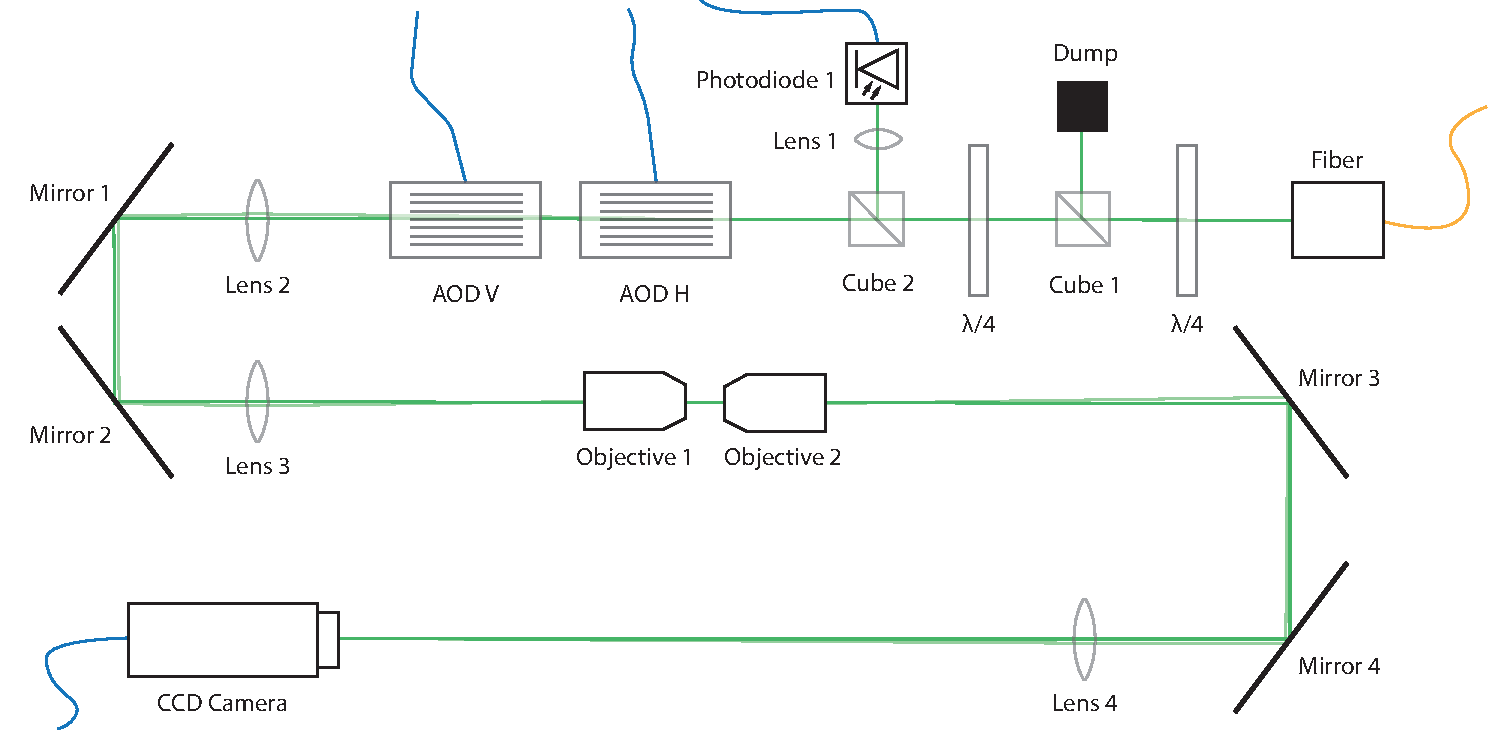
\includegraphics[width=\textwidth]{../media/setup/intensity-profile.pdf}
  \caption{The beam is focused onto the \gls{ccd} sensor of the camera.
  }\label{fig:intensity_profile_setup}
\end{figure}
In \Cref{fig:intensity_profile_setup} we present the setup used to measure
the spatial beam profile. In comparison to the previous setup we replaced
Photodiode 2 with a \gls{ccd} camera. The \gls{aod}s are configured at a
center frequency of \SI{100}{\mega\hertz}. The distance between Lens 4 and
the \gls{ccd} sensor is chosen such that the laser beam is focused onto the
\gls{ccd} sensor of the camera.
\begin{figure}[htb]
  \centering
  \begin{adjustbox}{width=\textwidth}
    \inputpgf{../figure/intensity/profile}{image.pgf}
  \end{adjustbox}
  \caption{Image of the focused laser beam measured with the \gls{ccd} camera.
  }\label{fig:intensity_spatial_image}
\end{figure}
\Cref{fig:intensity_spatial_image} shows an enlarged image patch of the
complete image capture taken with the \gls{ccd} camera. We can see a strong
illuminated circular spot in the center of the image with an area of about
\SI{2.5}{\milli\meter}. The intensity inside the spot seems homogeneous,
however this is caused by a saturation of the pixels in this area. We could
reduce the intensity or apply an optical filter to the camera to resolve the
intensity gradient inside the spot, but only at the cost of the intensity
distribution around the spot. Around the circular spot we can see a
diffraction ring. The diffraction ring is well described
in~\cite{Hertlein2017} and originates from the finite aperture of the
objectives.
\begin{figure}[htb]
  \centering
  \begin{adjustbox}{width=\textwidth}
    %% Creator: Matplotlib, PGF backend
%%
%% To include the figure in your LaTeX document, write
%%   \input{<filename>.pgf}
%%
%% Make sure the required packages are loaded in your preamble
%%   \usepackage{pgf}
%%
%% Figures using additional raster images can only be included by \input if
%% they are in the same directory as the main LaTeX file. For loading figures
%% from other directories you can use the `import` package
%%   \usepackage{import}
%% and then include the figures with
%%   \import{<path to file>}{<filename>.pgf}
%%
%% Matplotlib used the following preamble
%%   \usepackage{amsmath}\usepackage{siunitx}\usepackage{lmodern}
%%   \usepackage{fontspec}
%%
\begingroup%
\makeatletter%
\begin{pgfpicture}%
\pgfpathrectangle{\pgfpointorigin}{\pgfqpoint{12.000000in}{5.000000in}}%
\pgfusepath{use as bounding box, clip}%
\begin{pgfscope}%
\pgfsetbuttcap%
\pgfsetmiterjoin%
\pgfsetlinewidth{0.000000pt}%
\definecolor{currentstroke}{rgb}{1.000000,1.000000,1.000000}%
\pgfsetstrokecolor{currentstroke}%
\pgfsetdash{}{0pt}%
\pgfpathmoveto{\pgfqpoint{0.000000in}{0.000000in}}%
\pgfpathlineto{\pgfqpoint{12.000000in}{0.000000in}}%
\pgfpathlineto{\pgfqpoint{12.000000in}{5.000000in}}%
\pgfpathlineto{\pgfqpoint{0.000000in}{5.000000in}}%
\pgfpathclose%
\pgfusepath{}%
\end{pgfscope}%
\begin{pgfscope}%
\pgfsetbuttcap%
\pgfsetmiterjoin%
\definecolor{currentfill}{rgb}{1.000000,1.000000,1.000000}%
\pgfsetfillcolor{currentfill}%
\pgfsetlinewidth{0.000000pt}%
\definecolor{currentstroke}{rgb}{0.000000,0.000000,0.000000}%
\pgfsetstrokecolor{currentstroke}%
\pgfsetstrokeopacity{0.000000}%
\pgfsetdash{}{0pt}%
\pgfpathmoveto{\pgfqpoint{1.500000in}{0.800000in}}%
\pgfpathlineto{\pgfqpoint{6.036585in}{0.800000in}}%
\pgfpathlineto{\pgfqpoint{6.036585in}{4.500000in}}%
\pgfpathlineto{\pgfqpoint{1.500000in}{4.500000in}}%
\pgfpathclose%
\pgfusepath{fill}%
\end{pgfscope}%
\begin{pgfscope}%
\pgfsetbuttcap%
\pgfsetroundjoin%
\definecolor{currentfill}{rgb}{0.000000,0.000000,0.000000}%
\pgfsetfillcolor{currentfill}%
\pgfsetlinewidth{1.003750pt}%
\definecolor{currentstroke}{rgb}{0.000000,0.000000,0.000000}%
\pgfsetstrokecolor{currentstroke}%
\pgfsetdash{}{0pt}%
\pgfsys@defobject{currentmarker}{\pgfqpoint{0.000000in}{0.000000in}}{\pgfqpoint{0.000000in}{0.055556in}}{%
\pgfpathmoveto{\pgfqpoint{0.000000in}{0.000000in}}%
\pgfpathlineto{\pgfqpoint{0.000000in}{0.055556in}}%
\pgfusepath{stroke,fill}%
}%
\begin{pgfscope}%
\pgfsys@transformshift{1.706208in}{0.800000in}%
\pgfsys@useobject{currentmarker}{}%
\end{pgfscope}%
\end{pgfscope}%
\begin{pgfscope}%
\pgfsetbuttcap%
\pgfsetroundjoin%
\definecolor{currentfill}{rgb}{0.000000,0.000000,0.000000}%
\pgfsetfillcolor{currentfill}%
\pgfsetlinewidth{1.003750pt}%
\definecolor{currentstroke}{rgb}{0.000000,0.000000,0.000000}%
\pgfsetstrokecolor{currentstroke}%
\pgfsetdash{}{0pt}%
\pgfsys@defobject{currentmarker}{\pgfqpoint{0.000000in}{-0.055556in}}{\pgfqpoint{0.000000in}{0.000000in}}{%
\pgfpathmoveto{\pgfqpoint{0.000000in}{0.000000in}}%
\pgfpathlineto{\pgfqpoint{0.000000in}{-0.055556in}}%
\pgfusepath{stroke,fill}%
}%
\begin{pgfscope}%
\pgfsys@transformshift{1.706208in}{4.500000in}%
\pgfsys@useobject{currentmarker}{}%
\end{pgfscope}%
\end{pgfscope}%
\begin{pgfscope}%
\pgftext[x=1.706208in,y=0.702778in,,top]{\fontsize{10.000000}{12.000000}\selectfont \(\displaystyle 0\)}%
\end{pgfscope}%
\begin{pgfscope}%
\pgfsetbuttcap%
\pgfsetroundjoin%
\definecolor{currentfill}{rgb}{0.000000,0.000000,0.000000}%
\pgfsetfillcolor{currentfill}%
\pgfsetlinewidth{1.003750pt}%
\definecolor{currentstroke}{rgb}{0.000000,0.000000,0.000000}%
\pgfsetstrokecolor{currentstroke}%
\pgfsetdash{}{0pt}%
\pgfsys@defobject{currentmarker}{\pgfqpoint{0.000000in}{0.000000in}}{\pgfqpoint{0.000000in}{0.055556in}}{%
\pgfpathmoveto{\pgfqpoint{0.000000in}{0.000000in}}%
\pgfpathlineto{\pgfqpoint{0.000000in}{0.055556in}}%
\pgfusepath{stroke,fill}%
}%
\begin{pgfscope}%
\pgfsys@transformshift{2.496088in}{0.800000in}%
\pgfsys@useobject{currentmarker}{}%
\end{pgfscope}%
\end{pgfscope}%
\begin{pgfscope}%
\pgfsetbuttcap%
\pgfsetroundjoin%
\definecolor{currentfill}{rgb}{0.000000,0.000000,0.000000}%
\pgfsetfillcolor{currentfill}%
\pgfsetlinewidth{1.003750pt}%
\definecolor{currentstroke}{rgb}{0.000000,0.000000,0.000000}%
\pgfsetstrokecolor{currentstroke}%
\pgfsetdash{}{0pt}%
\pgfsys@defobject{currentmarker}{\pgfqpoint{0.000000in}{-0.055556in}}{\pgfqpoint{0.000000in}{0.000000in}}{%
\pgfpathmoveto{\pgfqpoint{0.000000in}{0.000000in}}%
\pgfpathlineto{\pgfqpoint{0.000000in}{-0.055556in}}%
\pgfusepath{stroke,fill}%
}%
\begin{pgfscope}%
\pgfsys@transformshift{2.496088in}{4.500000in}%
\pgfsys@useobject{currentmarker}{}%
\end{pgfscope}%
\end{pgfscope}%
\begin{pgfscope}%
\pgftext[x=2.496088in,y=0.702778in,,top]{\fontsize{10.000000}{12.000000}\selectfont \(\displaystyle 1\)}%
\end{pgfscope}%
\begin{pgfscope}%
\pgfsetbuttcap%
\pgfsetroundjoin%
\definecolor{currentfill}{rgb}{0.000000,0.000000,0.000000}%
\pgfsetfillcolor{currentfill}%
\pgfsetlinewidth{1.003750pt}%
\definecolor{currentstroke}{rgb}{0.000000,0.000000,0.000000}%
\pgfsetstrokecolor{currentstroke}%
\pgfsetdash{}{0pt}%
\pgfsys@defobject{currentmarker}{\pgfqpoint{0.000000in}{0.000000in}}{\pgfqpoint{0.000000in}{0.055556in}}{%
\pgfpathmoveto{\pgfqpoint{0.000000in}{0.000000in}}%
\pgfpathlineto{\pgfqpoint{0.000000in}{0.055556in}}%
\pgfusepath{stroke,fill}%
}%
\begin{pgfscope}%
\pgfsys@transformshift{3.285968in}{0.800000in}%
\pgfsys@useobject{currentmarker}{}%
\end{pgfscope}%
\end{pgfscope}%
\begin{pgfscope}%
\pgfsetbuttcap%
\pgfsetroundjoin%
\definecolor{currentfill}{rgb}{0.000000,0.000000,0.000000}%
\pgfsetfillcolor{currentfill}%
\pgfsetlinewidth{1.003750pt}%
\definecolor{currentstroke}{rgb}{0.000000,0.000000,0.000000}%
\pgfsetstrokecolor{currentstroke}%
\pgfsetdash{}{0pt}%
\pgfsys@defobject{currentmarker}{\pgfqpoint{0.000000in}{-0.055556in}}{\pgfqpoint{0.000000in}{0.000000in}}{%
\pgfpathmoveto{\pgfqpoint{0.000000in}{0.000000in}}%
\pgfpathlineto{\pgfqpoint{0.000000in}{-0.055556in}}%
\pgfusepath{stroke,fill}%
}%
\begin{pgfscope}%
\pgfsys@transformshift{3.285968in}{4.500000in}%
\pgfsys@useobject{currentmarker}{}%
\end{pgfscope}%
\end{pgfscope}%
\begin{pgfscope}%
\pgftext[x=3.285968in,y=0.702778in,,top]{\fontsize{10.000000}{12.000000}\selectfont \(\displaystyle 2\)}%
\end{pgfscope}%
\begin{pgfscope}%
\pgfsetbuttcap%
\pgfsetroundjoin%
\definecolor{currentfill}{rgb}{0.000000,0.000000,0.000000}%
\pgfsetfillcolor{currentfill}%
\pgfsetlinewidth{1.003750pt}%
\definecolor{currentstroke}{rgb}{0.000000,0.000000,0.000000}%
\pgfsetstrokecolor{currentstroke}%
\pgfsetdash{}{0pt}%
\pgfsys@defobject{currentmarker}{\pgfqpoint{0.000000in}{0.000000in}}{\pgfqpoint{0.000000in}{0.055556in}}{%
\pgfpathmoveto{\pgfqpoint{0.000000in}{0.000000in}}%
\pgfpathlineto{\pgfqpoint{0.000000in}{0.055556in}}%
\pgfusepath{stroke,fill}%
}%
\begin{pgfscope}%
\pgfsys@transformshift{4.075848in}{0.800000in}%
\pgfsys@useobject{currentmarker}{}%
\end{pgfscope}%
\end{pgfscope}%
\begin{pgfscope}%
\pgfsetbuttcap%
\pgfsetroundjoin%
\definecolor{currentfill}{rgb}{0.000000,0.000000,0.000000}%
\pgfsetfillcolor{currentfill}%
\pgfsetlinewidth{1.003750pt}%
\definecolor{currentstroke}{rgb}{0.000000,0.000000,0.000000}%
\pgfsetstrokecolor{currentstroke}%
\pgfsetdash{}{0pt}%
\pgfsys@defobject{currentmarker}{\pgfqpoint{0.000000in}{-0.055556in}}{\pgfqpoint{0.000000in}{0.000000in}}{%
\pgfpathmoveto{\pgfqpoint{0.000000in}{0.000000in}}%
\pgfpathlineto{\pgfqpoint{0.000000in}{-0.055556in}}%
\pgfusepath{stroke,fill}%
}%
\begin{pgfscope}%
\pgfsys@transformshift{4.075848in}{4.500000in}%
\pgfsys@useobject{currentmarker}{}%
\end{pgfscope}%
\end{pgfscope}%
\begin{pgfscope}%
\pgftext[x=4.075848in,y=0.702778in,,top]{\fontsize{10.000000}{12.000000}\selectfont \(\displaystyle 3\)}%
\end{pgfscope}%
\begin{pgfscope}%
\pgfsetbuttcap%
\pgfsetroundjoin%
\definecolor{currentfill}{rgb}{0.000000,0.000000,0.000000}%
\pgfsetfillcolor{currentfill}%
\pgfsetlinewidth{1.003750pt}%
\definecolor{currentstroke}{rgb}{0.000000,0.000000,0.000000}%
\pgfsetstrokecolor{currentstroke}%
\pgfsetdash{}{0pt}%
\pgfsys@defobject{currentmarker}{\pgfqpoint{0.000000in}{0.000000in}}{\pgfqpoint{0.000000in}{0.055556in}}{%
\pgfpathmoveto{\pgfqpoint{0.000000in}{0.000000in}}%
\pgfpathlineto{\pgfqpoint{0.000000in}{0.055556in}}%
\pgfusepath{stroke,fill}%
}%
\begin{pgfscope}%
\pgfsys@transformshift{4.865728in}{0.800000in}%
\pgfsys@useobject{currentmarker}{}%
\end{pgfscope}%
\end{pgfscope}%
\begin{pgfscope}%
\pgfsetbuttcap%
\pgfsetroundjoin%
\definecolor{currentfill}{rgb}{0.000000,0.000000,0.000000}%
\pgfsetfillcolor{currentfill}%
\pgfsetlinewidth{1.003750pt}%
\definecolor{currentstroke}{rgb}{0.000000,0.000000,0.000000}%
\pgfsetstrokecolor{currentstroke}%
\pgfsetdash{}{0pt}%
\pgfsys@defobject{currentmarker}{\pgfqpoint{0.000000in}{-0.055556in}}{\pgfqpoint{0.000000in}{0.000000in}}{%
\pgfpathmoveto{\pgfqpoint{0.000000in}{0.000000in}}%
\pgfpathlineto{\pgfqpoint{0.000000in}{-0.055556in}}%
\pgfusepath{stroke,fill}%
}%
\begin{pgfscope}%
\pgfsys@transformshift{4.865728in}{4.500000in}%
\pgfsys@useobject{currentmarker}{}%
\end{pgfscope}%
\end{pgfscope}%
\begin{pgfscope}%
\pgftext[x=4.865728in,y=0.702778in,,top]{\fontsize{10.000000}{12.000000}\selectfont \(\displaystyle 4\)}%
\end{pgfscope}%
\begin{pgfscope}%
\pgfsetbuttcap%
\pgfsetroundjoin%
\definecolor{currentfill}{rgb}{0.000000,0.000000,0.000000}%
\pgfsetfillcolor{currentfill}%
\pgfsetlinewidth{1.003750pt}%
\definecolor{currentstroke}{rgb}{0.000000,0.000000,0.000000}%
\pgfsetstrokecolor{currentstroke}%
\pgfsetdash{}{0pt}%
\pgfsys@defobject{currentmarker}{\pgfqpoint{0.000000in}{0.000000in}}{\pgfqpoint{0.000000in}{0.055556in}}{%
\pgfpathmoveto{\pgfqpoint{0.000000in}{0.000000in}}%
\pgfpathlineto{\pgfqpoint{0.000000in}{0.055556in}}%
\pgfusepath{stroke,fill}%
}%
\begin{pgfscope}%
\pgfsys@transformshift{5.655608in}{0.800000in}%
\pgfsys@useobject{currentmarker}{}%
\end{pgfscope}%
\end{pgfscope}%
\begin{pgfscope}%
\pgfsetbuttcap%
\pgfsetroundjoin%
\definecolor{currentfill}{rgb}{0.000000,0.000000,0.000000}%
\pgfsetfillcolor{currentfill}%
\pgfsetlinewidth{1.003750pt}%
\definecolor{currentstroke}{rgb}{0.000000,0.000000,0.000000}%
\pgfsetstrokecolor{currentstroke}%
\pgfsetdash{}{0pt}%
\pgfsys@defobject{currentmarker}{\pgfqpoint{0.000000in}{-0.055556in}}{\pgfqpoint{0.000000in}{0.000000in}}{%
\pgfpathmoveto{\pgfqpoint{0.000000in}{0.000000in}}%
\pgfpathlineto{\pgfqpoint{0.000000in}{-0.055556in}}%
\pgfusepath{stroke,fill}%
}%
\begin{pgfscope}%
\pgfsys@transformshift{5.655608in}{4.500000in}%
\pgfsys@useobject{currentmarker}{}%
\end{pgfscope}%
\end{pgfscope}%
\begin{pgfscope}%
\pgftext[x=5.655608in,y=0.702778in,,top]{\fontsize{10.000000}{12.000000}\selectfont \(\displaystyle 5\)}%
\end{pgfscope}%
\begin{pgfscope}%
\pgftext[x=3.768293in,y=0.440556in,,top]{\fontsize{16.000000}{19.200000}\selectfont \(\displaystyle x\) (\si{\micro\meter})}%
\end{pgfscope}%
\begin{pgfscope}%
\pgfsetbuttcap%
\pgfsetroundjoin%
\definecolor{currentfill}{rgb}{0.000000,0.000000,0.000000}%
\pgfsetfillcolor{currentfill}%
\pgfsetlinewidth{1.003750pt}%
\definecolor{currentstroke}{rgb}{0.000000,0.000000,0.000000}%
\pgfsetstrokecolor{currentstroke}%
\pgfsetdash{}{0pt}%
\pgfsys@defobject{currentmarker}{\pgfqpoint{0.000000in}{0.000000in}}{\pgfqpoint{0.055556in}{0.000000in}}{%
\pgfpathmoveto{\pgfqpoint{0.000000in}{0.000000in}}%
\pgfpathlineto{\pgfqpoint{0.055556in}{0.000000in}}%
\pgfusepath{stroke,fill}%
}%
\begin{pgfscope}%
\pgfsys@transformshift{1.500000in}{0.968182in}%
\pgfsys@useobject{currentmarker}{}%
\end{pgfscope}%
\end{pgfscope}%
\begin{pgfscope}%
\pgfsetbuttcap%
\pgfsetroundjoin%
\definecolor{currentfill}{rgb}{0.000000,0.000000,0.000000}%
\pgfsetfillcolor{currentfill}%
\pgfsetlinewidth{1.003750pt}%
\definecolor{currentstroke}{rgb}{0.000000,0.000000,0.000000}%
\pgfsetstrokecolor{currentstroke}%
\pgfsetdash{}{0pt}%
\pgfsys@defobject{currentmarker}{\pgfqpoint{-0.055556in}{0.000000in}}{\pgfqpoint{0.000000in}{0.000000in}}{%
\pgfpathmoveto{\pgfqpoint{0.000000in}{0.000000in}}%
\pgfpathlineto{\pgfqpoint{-0.055556in}{0.000000in}}%
\pgfusepath{stroke,fill}%
}%
\begin{pgfscope}%
\pgfsys@transformshift{6.036585in}{0.968182in}%
\pgfsys@useobject{currentmarker}{}%
\end{pgfscope}%
\end{pgfscope}%
\begin{pgfscope}%
\pgftext[x=1.225308in,y=0.919987in,left,base]{\fontsize{10.000000}{12.000000}\selectfont \(\displaystyle 0.0\)}%
\end{pgfscope}%
\begin{pgfscope}%
\pgfsetbuttcap%
\pgfsetroundjoin%
\definecolor{currentfill}{rgb}{0.000000,0.000000,0.000000}%
\pgfsetfillcolor{currentfill}%
\pgfsetlinewidth{1.003750pt}%
\definecolor{currentstroke}{rgb}{0.000000,0.000000,0.000000}%
\pgfsetstrokecolor{currentstroke}%
\pgfsetdash{}{0pt}%
\pgfsys@defobject{currentmarker}{\pgfqpoint{0.000000in}{0.000000in}}{\pgfqpoint{0.055556in}{0.000000in}}{%
\pgfpathmoveto{\pgfqpoint{0.000000in}{0.000000in}}%
\pgfpathlineto{\pgfqpoint{0.055556in}{0.000000in}}%
\pgfusepath{stroke,fill}%
}%
\begin{pgfscope}%
\pgfsys@transformshift{1.500000in}{1.640864in}%
\pgfsys@useobject{currentmarker}{}%
\end{pgfscope}%
\end{pgfscope}%
\begin{pgfscope}%
\pgfsetbuttcap%
\pgfsetroundjoin%
\definecolor{currentfill}{rgb}{0.000000,0.000000,0.000000}%
\pgfsetfillcolor{currentfill}%
\pgfsetlinewidth{1.003750pt}%
\definecolor{currentstroke}{rgb}{0.000000,0.000000,0.000000}%
\pgfsetstrokecolor{currentstroke}%
\pgfsetdash{}{0pt}%
\pgfsys@defobject{currentmarker}{\pgfqpoint{-0.055556in}{0.000000in}}{\pgfqpoint{0.000000in}{0.000000in}}{%
\pgfpathmoveto{\pgfqpoint{0.000000in}{0.000000in}}%
\pgfpathlineto{\pgfqpoint{-0.055556in}{0.000000in}}%
\pgfusepath{stroke,fill}%
}%
\begin{pgfscope}%
\pgfsys@transformshift{6.036585in}{1.640864in}%
\pgfsys@useobject{currentmarker}{}%
\end{pgfscope}%
\end{pgfscope}%
\begin{pgfscope}%
\pgftext[x=1.225308in,y=1.592670in,left,base]{\fontsize{10.000000}{12.000000}\selectfont \(\displaystyle 0.2\)}%
\end{pgfscope}%
\begin{pgfscope}%
\pgfsetbuttcap%
\pgfsetroundjoin%
\definecolor{currentfill}{rgb}{0.000000,0.000000,0.000000}%
\pgfsetfillcolor{currentfill}%
\pgfsetlinewidth{1.003750pt}%
\definecolor{currentstroke}{rgb}{0.000000,0.000000,0.000000}%
\pgfsetstrokecolor{currentstroke}%
\pgfsetdash{}{0pt}%
\pgfsys@defobject{currentmarker}{\pgfqpoint{0.000000in}{0.000000in}}{\pgfqpoint{0.055556in}{0.000000in}}{%
\pgfpathmoveto{\pgfqpoint{0.000000in}{0.000000in}}%
\pgfpathlineto{\pgfqpoint{0.055556in}{0.000000in}}%
\pgfusepath{stroke,fill}%
}%
\begin{pgfscope}%
\pgfsys@transformshift{1.500000in}{2.313547in}%
\pgfsys@useobject{currentmarker}{}%
\end{pgfscope}%
\end{pgfscope}%
\begin{pgfscope}%
\pgfsetbuttcap%
\pgfsetroundjoin%
\definecolor{currentfill}{rgb}{0.000000,0.000000,0.000000}%
\pgfsetfillcolor{currentfill}%
\pgfsetlinewidth{1.003750pt}%
\definecolor{currentstroke}{rgb}{0.000000,0.000000,0.000000}%
\pgfsetstrokecolor{currentstroke}%
\pgfsetdash{}{0pt}%
\pgfsys@defobject{currentmarker}{\pgfqpoint{-0.055556in}{0.000000in}}{\pgfqpoint{0.000000in}{0.000000in}}{%
\pgfpathmoveto{\pgfqpoint{0.000000in}{0.000000in}}%
\pgfpathlineto{\pgfqpoint{-0.055556in}{0.000000in}}%
\pgfusepath{stroke,fill}%
}%
\begin{pgfscope}%
\pgfsys@transformshift{6.036585in}{2.313547in}%
\pgfsys@useobject{currentmarker}{}%
\end{pgfscope}%
\end{pgfscope}%
\begin{pgfscope}%
\pgftext[x=1.225308in,y=2.265353in,left,base]{\fontsize{10.000000}{12.000000}\selectfont \(\displaystyle 0.4\)}%
\end{pgfscope}%
\begin{pgfscope}%
\pgfsetbuttcap%
\pgfsetroundjoin%
\definecolor{currentfill}{rgb}{0.000000,0.000000,0.000000}%
\pgfsetfillcolor{currentfill}%
\pgfsetlinewidth{1.003750pt}%
\definecolor{currentstroke}{rgb}{0.000000,0.000000,0.000000}%
\pgfsetstrokecolor{currentstroke}%
\pgfsetdash{}{0pt}%
\pgfsys@defobject{currentmarker}{\pgfqpoint{0.000000in}{0.000000in}}{\pgfqpoint{0.055556in}{0.000000in}}{%
\pgfpathmoveto{\pgfqpoint{0.000000in}{0.000000in}}%
\pgfpathlineto{\pgfqpoint{0.055556in}{0.000000in}}%
\pgfusepath{stroke,fill}%
}%
\begin{pgfscope}%
\pgfsys@transformshift{1.500000in}{2.986230in}%
\pgfsys@useobject{currentmarker}{}%
\end{pgfscope}%
\end{pgfscope}%
\begin{pgfscope}%
\pgfsetbuttcap%
\pgfsetroundjoin%
\definecolor{currentfill}{rgb}{0.000000,0.000000,0.000000}%
\pgfsetfillcolor{currentfill}%
\pgfsetlinewidth{1.003750pt}%
\definecolor{currentstroke}{rgb}{0.000000,0.000000,0.000000}%
\pgfsetstrokecolor{currentstroke}%
\pgfsetdash{}{0pt}%
\pgfsys@defobject{currentmarker}{\pgfqpoint{-0.055556in}{0.000000in}}{\pgfqpoint{0.000000in}{0.000000in}}{%
\pgfpathmoveto{\pgfqpoint{0.000000in}{0.000000in}}%
\pgfpathlineto{\pgfqpoint{-0.055556in}{0.000000in}}%
\pgfusepath{stroke,fill}%
}%
\begin{pgfscope}%
\pgfsys@transformshift{6.036585in}{2.986230in}%
\pgfsys@useobject{currentmarker}{}%
\end{pgfscope}%
\end{pgfscope}%
\begin{pgfscope}%
\pgftext[x=1.225308in,y=2.938035in,left,base]{\fontsize{10.000000}{12.000000}\selectfont \(\displaystyle 0.6\)}%
\end{pgfscope}%
\begin{pgfscope}%
\pgfsetbuttcap%
\pgfsetroundjoin%
\definecolor{currentfill}{rgb}{0.000000,0.000000,0.000000}%
\pgfsetfillcolor{currentfill}%
\pgfsetlinewidth{1.003750pt}%
\definecolor{currentstroke}{rgb}{0.000000,0.000000,0.000000}%
\pgfsetstrokecolor{currentstroke}%
\pgfsetdash{}{0pt}%
\pgfsys@defobject{currentmarker}{\pgfqpoint{0.000000in}{0.000000in}}{\pgfqpoint{0.055556in}{0.000000in}}{%
\pgfpathmoveto{\pgfqpoint{0.000000in}{0.000000in}}%
\pgfpathlineto{\pgfqpoint{0.055556in}{0.000000in}}%
\pgfusepath{stroke,fill}%
}%
\begin{pgfscope}%
\pgfsys@transformshift{1.500000in}{3.658912in}%
\pgfsys@useobject{currentmarker}{}%
\end{pgfscope}%
\end{pgfscope}%
\begin{pgfscope}%
\pgfsetbuttcap%
\pgfsetroundjoin%
\definecolor{currentfill}{rgb}{0.000000,0.000000,0.000000}%
\pgfsetfillcolor{currentfill}%
\pgfsetlinewidth{1.003750pt}%
\definecolor{currentstroke}{rgb}{0.000000,0.000000,0.000000}%
\pgfsetstrokecolor{currentstroke}%
\pgfsetdash{}{0pt}%
\pgfsys@defobject{currentmarker}{\pgfqpoint{-0.055556in}{0.000000in}}{\pgfqpoint{0.000000in}{0.000000in}}{%
\pgfpathmoveto{\pgfqpoint{0.000000in}{0.000000in}}%
\pgfpathlineto{\pgfqpoint{-0.055556in}{0.000000in}}%
\pgfusepath{stroke,fill}%
}%
\begin{pgfscope}%
\pgfsys@transformshift{6.036585in}{3.658912in}%
\pgfsys@useobject{currentmarker}{}%
\end{pgfscope}%
\end{pgfscope}%
\begin{pgfscope}%
\pgftext[x=1.225308in,y=3.610718in,left,base]{\fontsize{10.000000}{12.000000}\selectfont \(\displaystyle 0.8\)}%
\end{pgfscope}%
\begin{pgfscope}%
\pgfsetbuttcap%
\pgfsetroundjoin%
\definecolor{currentfill}{rgb}{0.000000,0.000000,0.000000}%
\pgfsetfillcolor{currentfill}%
\pgfsetlinewidth{1.003750pt}%
\definecolor{currentstroke}{rgb}{0.000000,0.000000,0.000000}%
\pgfsetstrokecolor{currentstroke}%
\pgfsetdash{}{0pt}%
\pgfsys@defobject{currentmarker}{\pgfqpoint{0.000000in}{0.000000in}}{\pgfqpoint{0.055556in}{0.000000in}}{%
\pgfpathmoveto{\pgfqpoint{0.000000in}{0.000000in}}%
\pgfpathlineto{\pgfqpoint{0.055556in}{0.000000in}}%
\pgfusepath{stroke,fill}%
}%
\begin{pgfscope}%
\pgfsys@transformshift{1.500000in}{4.331595in}%
\pgfsys@useobject{currentmarker}{}%
\end{pgfscope}%
\end{pgfscope}%
\begin{pgfscope}%
\pgfsetbuttcap%
\pgfsetroundjoin%
\definecolor{currentfill}{rgb}{0.000000,0.000000,0.000000}%
\pgfsetfillcolor{currentfill}%
\pgfsetlinewidth{1.003750pt}%
\definecolor{currentstroke}{rgb}{0.000000,0.000000,0.000000}%
\pgfsetstrokecolor{currentstroke}%
\pgfsetdash{}{0pt}%
\pgfsys@defobject{currentmarker}{\pgfqpoint{-0.055556in}{0.000000in}}{\pgfqpoint{0.000000in}{0.000000in}}{%
\pgfpathmoveto{\pgfqpoint{0.000000in}{0.000000in}}%
\pgfpathlineto{\pgfqpoint{-0.055556in}{0.000000in}}%
\pgfusepath{stroke,fill}%
}%
\begin{pgfscope}%
\pgfsys@transformshift{6.036585in}{4.331595in}%
\pgfsys@useobject{currentmarker}{}%
\end{pgfscope}%
\end{pgfscope}%
\begin{pgfscope}%
\pgftext[x=1.225308in,y=4.283400in,left,base]{\fontsize{10.000000}{12.000000}\selectfont \(\displaystyle 1.0\)}%
\end{pgfscope}%
\begin{pgfscope}%
\pgfsetbuttcap%
\pgfsetroundjoin%
\definecolor{currentfill}{rgb}{0.000000,0.000000,0.000000}%
\pgfsetfillcolor{currentfill}%
\pgfsetlinewidth{0.501875pt}%
\definecolor{currentstroke}{rgb}{0.000000,0.000000,0.000000}%
\pgfsetstrokecolor{currentstroke}%
\pgfsetdash{}{0pt}%
\pgfsys@defobject{currentmarker}{\pgfqpoint{0.000000in}{0.000000in}}{\pgfqpoint{0.027778in}{0.000000in}}{%
\pgfpathmoveto{\pgfqpoint{0.000000in}{0.000000in}}%
\pgfpathlineto{\pgfqpoint{0.027778in}{0.000000in}}%
\pgfusepath{stroke,fill}%
}%
\begin{pgfscope}%
\pgfsys@transformshift{1.500000in}{0.800011in}%
\pgfsys@useobject{currentmarker}{}%
\end{pgfscope}%
\end{pgfscope}%
\begin{pgfscope}%
\pgfsetbuttcap%
\pgfsetroundjoin%
\definecolor{currentfill}{rgb}{0.000000,0.000000,0.000000}%
\pgfsetfillcolor{currentfill}%
\pgfsetlinewidth{0.501875pt}%
\definecolor{currentstroke}{rgb}{0.000000,0.000000,0.000000}%
\pgfsetstrokecolor{currentstroke}%
\pgfsetdash{}{0pt}%
\pgfsys@defobject{currentmarker}{\pgfqpoint{-0.027778in}{0.000000in}}{\pgfqpoint{0.000000in}{0.000000in}}{%
\pgfpathmoveto{\pgfqpoint{0.000000in}{0.000000in}}%
\pgfpathlineto{\pgfqpoint{-0.027778in}{0.000000in}}%
\pgfusepath{stroke,fill}%
}%
\begin{pgfscope}%
\pgfsys@transformshift{6.036585in}{0.800011in}%
\pgfsys@useobject{currentmarker}{}%
\end{pgfscope}%
\end{pgfscope}%
\begin{pgfscope}%
\pgfsetbuttcap%
\pgfsetroundjoin%
\definecolor{currentfill}{rgb}{0.000000,0.000000,0.000000}%
\pgfsetfillcolor{currentfill}%
\pgfsetlinewidth{0.501875pt}%
\definecolor{currentstroke}{rgb}{0.000000,0.000000,0.000000}%
\pgfsetstrokecolor{currentstroke}%
\pgfsetdash{}{0pt}%
\pgfsys@defobject{currentmarker}{\pgfqpoint{0.000000in}{0.000000in}}{\pgfqpoint{0.027778in}{0.000000in}}{%
\pgfpathmoveto{\pgfqpoint{0.000000in}{0.000000in}}%
\pgfpathlineto{\pgfqpoint{0.027778in}{0.000000in}}%
\pgfusepath{stroke,fill}%
}%
\begin{pgfscope}%
\pgfsys@transformshift{1.500000in}{1.136352in}%
\pgfsys@useobject{currentmarker}{}%
\end{pgfscope}%
\end{pgfscope}%
\begin{pgfscope}%
\pgfsetbuttcap%
\pgfsetroundjoin%
\definecolor{currentfill}{rgb}{0.000000,0.000000,0.000000}%
\pgfsetfillcolor{currentfill}%
\pgfsetlinewidth{0.501875pt}%
\definecolor{currentstroke}{rgb}{0.000000,0.000000,0.000000}%
\pgfsetstrokecolor{currentstroke}%
\pgfsetdash{}{0pt}%
\pgfsys@defobject{currentmarker}{\pgfqpoint{-0.027778in}{0.000000in}}{\pgfqpoint{0.000000in}{0.000000in}}{%
\pgfpathmoveto{\pgfqpoint{0.000000in}{0.000000in}}%
\pgfpathlineto{\pgfqpoint{-0.027778in}{0.000000in}}%
\pgfusepath{stroke,fill}%
}%
\begin{pgfscope}%
\pgfsys@transformshift{6.036585in}{1.136352in}%
\pgfsys@useobject{currentmarker}{}%
\end{pgfscope}%
\end{pgfscope}%
\begin{pgfscope}%
\pgfsetbuttcap%
\pgfsetroundjoin%
\definecolor{currentfill}{rgb}{0.000000,0.000000,0.000000}%
\pgfsetfillcolor{currentfill}%
\pgfsetlinewidth{0.501875pt}%
\definecolor{currentstroke}{rgb}{0.000000,0.000000,0.000000}%
\pgfsetstrokecolor{currentstroke}%
\pgfsetdash{}{0pt}%
\pgfsys@defobject{currentmarker}{\pgfqpoint{0.000000in}{0.000000in}}{\pgfqpoint{0.027778in}{0.000000in}}{%
\pgfpathmoveto{\pgfqpoint{0.000000in}{0.000000in}}%
\pgfpathlineto{\pgfqpoint{0.027778in}{0.000000in}}%
\pgfusepath{stroke,fill}%
}%
\begin{pgfscope}%
\pgfsys@transformshift{1.500000in}{1.304523in}%
\pgfsys@useobject{currentmarker}{}%
\end{pgfscope}%
\end{pgfscope}%
\begin{pgfscope}%
\pgfsetbuttcap%
\pgfsetroundjoin%
\definecolor{currentfill}{rgb}{0.000000,0.000000,0.000000}%
\pgfsetfillcolor{currentfill}%
\pgfsetlinewidth{0.501875pt}%
\definecolor{currentstroke}{rgb}{0.000000,0.000000,0.000000}%
\pgfsetstrokecolor{currentstroke}%
\pgfsetdash{}{0pt}%
\pgfsys@defobject{currentmarker}{\pgfqpoint{-0.027778in}{0.000000in}}{\pgfqpoint{0.000000in}{0.000000in}}{%
\pgfpathmoveto{\pgfqpoint{0.000000in}{0.000000in}}%
\pgfpathlineto{\pgfqpoint{-0.027778in}{0.000000in}}%
\pgfusepath{stroke,fill}%
}%
\begin{pgfscope}%
\pgfsys@transformshift{6.036585in}{1.304523in}%
\pgfsys@useobject{currentmarker}{}%
\end{pgfscope}%
\end{pgfscope}%
\begin{pgfscope}%
\pgfsetbuttcap%
\pgfsetroundjoin%
\definecolor{currentfill}{rgb}{0.000000,0.000000,0.000000}%
\pgfsetfillcolor{currentfill}%
\pgfsetlinewidth{0.501875pt}%
\definecolor{currentstroke}{rgb}{0.000000,0.000000,0.000000}%
\pgfsetstrokecolor{currentstroke}%
\pgfsetdash{}{0pt}%
\pgfsys@defobject{currentmarker}{\pgfqpoint{0.000000in}{0.000000in}}{\pgfqpoint{0.027778in}{0.000000in}}{%
\pgfpathmoveto{\pgfqpoint{0.000000in}{0.000000in}}%
\pgfpathlineto{\pgfqpoint{0.027778in}{0.000000in}}%
\pgfusepath{stroke,fill}%
}%
\begin{pgfscope}%
\pgfsys@transformshift{1.500000in}{1.472694in}%
\pgfsys@useobject{currentmarker}{}%
\end{pgfscope}%
\end{pgfscope}%
\begin{pgfscope}%
\pgfsetbuttcap%
\pgfsetroundjoin%
\definecolor{currentfill}{rgb}{0.000000,0.000000,0.000000}%
\pgfsetfillcolor{currentfill}%
\pgfsetlinewidth{0.501875pt}%
\definecolor{currentstroke}{rgb}{0.000000,0.000000,0.000000}%
\pgfsetstrokecolor{currentstroke}%
\pgfsetdash{}{0pt}%
\pgfsys@defobject{currentmarker}{\pgfqpoint{-0.027778in}{0.000000in}}{\pgfqpoint{0.000000in}{0.000000in}}{%
\pgfpathmoveto{\pgfqpoint{0.000000in}{0.000000in}}%
\pgfpathlineto{\pgfqpoint{-0.027778in}{0.000000in}}%
\pgfusepath{stroke,fill}%
}%
\begin{pgfscope}%
\pgfsys@transformshift{6.036585in}{1.472694in}%
\pgfsys@useobject{currentmarker}{}%
\end{pgfscope}%
\end{pgfscope}%
\begin{pgfscope}%
\pgfsetbuttcap%
\pgfsetroundjoin%
\definecolor{currentfill}{rgb}{0.000000,0.000000,0.000000}%
\pgfsetfillcolor{currentfill}%
\pgfsetlinewidth{0.501875pt}%
\definecolor{currentstroke}{rgb}{0.000000,0.000000,0.000000}%
\pgfsetstrokecolor{currentstroke}%
\pgfsetdash{}{0pt}%
\pgfsys@defobject{currentmarker}{\pgfqpoint{0.000000in}{0.000000in}}{\pgfqpoint{0.027778in}{0.000000in}}{%
\pgfpathmoveto{\pgfqpoint{0.000000in}{0.000000in}}%
\pgfpathlineto{\pgfqpoint{0.027778in}{0.000000in}}%
\pgfusepath{stroke,fill}%
}%
\begin{pgfscope}%
\pgfsys@transformshift{1.500000in}{1.640864in}%
\pgfsys@useobject{currentmarker}{}%
\end{pgfscope}%
\end{pgfscope}%
\begin{pgfscope}%
\pgfsetbuttcap%
\pgfsetroundjoin%
\definecolor{currentfill}{rgb}{0.000000,0.000000,0.000000}%
\pgfsetfillcolor{currentfill}%
\pgfsetlinewidth{0.501875pt}%
\definecolor{currentstroke}{rgb}{0.000000,0.000000,0.000000}%
\pgfsetstrokecolor{currentstroke}%
\pgfsetdash{}{0pt}%
\pgfsys@defobject{currentmarker}{\pgfqpoint{-0.027778in}{0.000000in}}{\pgfqpoint{0.000000in}{0.000000in}}{%
\pgfpathmoveto{\pgfqpoint{0.000000in}{0.000000in}}%
\pgfpathlineto{\pgfqpoint{-0.027778in}{0.000000in}}%
\pgfusepath{stroke,fill}%
}%
\begin{pgfscope}%
\pgfsys@transformshift{6.036585in}{1.640864in}%
\pgfsys@useobject{currentmarker}{}%
\end{pgfscope}%
\end{pgfscope}%
\begin{pgfscope}%
\pgfsetbuttcap%
\pgfsetroundjoin%
\definecolor{currentfill}{rgb}{0.000000,0.000000,0.000000}%
\pgfsetfillcolor{currentfill}%
\pgfsetlinewidth{0.501875pt}%
\definecolor{currentstroke}{rgb}{0.000000,0.000000,0.000000}%
\pgfsetstrokecolor{currentstroke}%
\pgfsetdash{}{0pt}%
\pgfsys@defobject{currentmarker}{\pgfqpoint{0.000000in}{0.000000in}}{\pgfqpoint{0.027778in}{0.000000in}}{%
\pgfpathmoveto{\pgfqpoint{0.000000in}{0.000000in}}%
\pgfpathlineto{\pgfqpoint{0.027778in}{0.000000in}}%
\pgfusepath{stroke,fill}%
}%
\begin{pgfscope}%
\pgfsys@transformshift{1.500000in}{1.809035in}%
\pgfsys@useobject{currentmarker}{}%
\end{pgfscope}%
\end{pgfscope}%
\begin{pgfscope}%
\pgfsetbuttcap%
\pgfsetroundjoin%
\definecolor{currentfill}{rgb}{0.000000,0.000000,0.000000}%
\pgfsetfillcolor{currentfill}%
\pgfsetlinewidth{0.501875pt}%
\definecolor{currentstroke}{rgb}{0.000000,0.000000,0.000000}%
\pgfsetstrokecolor{currentstroke}%
\pgfsetdash{}{0pt}%
\pgfsys@defobject{currentmarker}{\pgfqpoint{-0.027778in}{0.000000in}}{\pgfqpoint{0.000000in}{0.000000in}}{%
\pgfpathmoveto{\pgfqpoint{0.000000in}{0.000000in}}%
\pgfpathlineto{\pgfqpoint{-0.027778in}{0.000000in}}%
\pgfusepath{stroke,fill}%
}%
\begin{pgfscope}%
\pgfsys@transformshift{6.036585in}{1.809035in}%
\pgfsys@useobject{currentmarker}{}%
\end{pgfscope}%
\end{pgfscope}%
\begin{pgfscope}%
\pgfsetbuttcap%
\pgfsetroundjoin%
\definecolor{currentfill}{rgb}{0.000000,0.000000,0.000000}%
\pgfsetfillcolor{currentfill}%
\pgfsetlinewidth{0.501875pt}%
\definecolor{currentstroke}{rgb}{0.000000,0.000000,0.000000}%
\pgfsetstrokecolor{currentstroke}%
\pgfsetdash{}{0pt}%
\pgfsys@defobject{currentmarker}{\pgfqpoint{0.000000in}{0.000000in}}{\pgfqpoint{0.027778in}{0.000000in}}{%
\pgfpathmoveto{\pgfqpoint{0.000000in}{0.000000in}}%
\pgfpathlineto{\pgfqpoint{0.027778in}{0.000000in}}%
\pgfusepath{stroke,fill}%
}%
\begin{pgfscope}%
\pgfsys@transformshift{1.500000in}{1.977206in}%
\pgfsys@useobject{currentmarker}{}%
\end{pgfscope}%
\end{pgfscope}%
\begin{pgfscope}%
\pgfsetbuttcap%
\pgfsetroundjoin%
\definecolor{currentfill}{rgb}{0.000000,0.000000,0.000000}%
\pgfsetfillcolor{currentfill}%
\pgfsetlinewidth{0.501875pt}%
\definecolor{currentstroke}{rgb}{0.000000,0.000000,0.000000}%
\pgfsetstrokecolor{currentstroke}%
\pgfsetdash{}{0pt}%
\pgfsys@defobject{currentmarker}{\pgfqpoint{-0.027778in}{0.000000in}}{\pgfqpoint{0.000000in}{0.000000in}}{%
\pgfpathmoveto{\pgfqpoint{0.000000in}{0.000000in}}%
\pgfpathlineto{\pgfqpoint{-0.027778in}{0.000000in}}%
\pgfusepath{stroke,fill}%
}%
\begin{pgfscope}%
\pgfsys@transformshift{6.036585in}{1.977206in}%
\pgfsys@useobject{currentmarker}{}%
\end{pgfscope}%
\end{pgfscope}%
\begin{pgfscope}%
\pgfsetbuttcap%
\pgfsetroundjoin%
\definecolor{currentfill}{rgb}{0.000000,0.000000,0.000000}%
\pgfsetfillcolor{currentfill}%
\pgfsetlinewidth{0.501875pt}%
\definecolor{currentstroke}{rgb}{0.000000,0.000000,0.000000}%
\pgfsetstrokecolor{currentstroke}%
\pgfsetdash{}{0pt}%
\pgfsys@defobject{currentmarker}{\pgfqpoint{0.000000in}{0.000000in}}{\pgfqpoint{0.027778in}{0.000000in}}{%
\pgfpathmoveto{\pgfqpoint{0.000000in}{0.000000in}}%
\pgfpathlineto{\pgfqpoint{0.027778in}{0.000000in}}%
\pgfusepath{stroke,fill}%
}%
\begin{pgfscope}%
\pgfsys@transformshift{1.500000in}{2.145376in}%
\pgfsys@useobject{currentmarker}{}%
\end{pgfscope}%
\end{pgfscope}%
\begin{pgfscope}%
\pgfsetbuttcap%
\pgfsetroundjoin%
\definecolor{currentfill}{rgb}{0.000000,0.000000,0.000000}%
\pgfsetfillcolor{currentfill}%
\pgfsetlinewidth{0.501875pt}%
\definecolor{currentstroke}{rgb}{0.000000,0.000000,0.000000}%
\pgfsetstrokecolor{currentstroke}%
\pgfsetdash{}{0pt}%
\pgfsys@defobject{currentmarker}{\pgfqpoint{-0.027778in}{0.000000in}}{\pgfqpoint{0.000000in}{0.000000in}}{%
\pgfpathmoveto{\pgfqpoint{0.000000in}{0.000000in}}%
\pgfpathlineto{\pgfqpoint{-0.027778in}{0.000000in}}%
\pgfusepath{stroke,fill}%
}%
\begin{pgfscope}%
\pgfsys@transformshift{6.036585in}{2.145376in}%
\pgfsys@useobject{currentmarker}{}%
\end{pgfscope}%
\end{pgfscope}%
\begin{pgfscope}%
\pgfsetbuttcap%
\pgfsetroundjoin%
\definecolor{currentfill}{rgb}{0.000000,0.000000,0.000000}%
\pgfsetfillcolor{currentfill}%
\pgfsetlinewidth{0.501875pt}%
\definecolor{currentstroke}{rgb}{0.000000,0.000000,0.000000}%
\pgfsetstrokecolor{currentstroke}%
\pgfsetdash{}{0pt}%
\pgfsys@defobject{currentmarker}{\pgfqpoint{0.000000in}{0.000000in}}{\pgfqpoint{0.027778in}{0.000000in}}{%
\pgfpathmoveto{\pgfqpoint{0.000000in}{0.000000in}}%
\pgfpathlineto{\pgfqpoint{0.027778in}{0.000000in}}%
\pgfusepath{stroke,fill}%
}%
\begin{pgfscope}%
\pgfsys@transformshift{1.500000in}{2.313547in}%
\pgfsys@useobject{currentmarker}{}%
\end{pgfscope}%
\end{pgfscope}%
\begin{pgfscope}%
\pgfsetbuttcap%
\pgfsetroundjoin%
\definecolor{currentfill}{rgb}{0.000000,0.000000,0.000000}%
\pgfsetfillcolor{currentfill}%
\pgfsetlinewidth{0.501875pt}%
\definecolor{currentstroke}{rgb}{0.000000,0.000000,0.000000}%
\pgfsetstrokecolor{currentstroke}%
\pgfsetdash{}{0pt}%
\pgfsys@defobject{currentmarker}{\pgfqpoint{-0.027778in}{0.000000in}}{\pgfqpoint{0.000000in}{0.000000in}}{%
\pgfpathmoveto{\pgfqpoint{0.000000in}{0.000000in}}%
\pgfpathlineto{\pgfqpoint{-0.027778in}{0.000000in}}%
\pgfusepath{stroke,fill}%
}%
\begin{pgfscope}%
\pgfsys@transformshift{6.036585in}{2.313547in}%
\pgfsys@useobject{currentmarker}{}%
\end{pgfscope}%
\end{pgfscope}%
\begin{pgfscope}%
\pgfsetbuttcap%
\pgfsetroundjoin%
\definecolor{currentfill}{rgb}{0.000000,0.000000,0.000000}%
\pgfsetfillcolor{currentfill}%
\pgfsetlinewidth{0.501875pt}%
\definecolor{currentstroke}{rgb}{0.000000,0.000000,0.000000}%
\pgfsetstrokecolor{currentstroke}%
\pgfsetdash{}{0pt}%
\pgfsys@defobject{currentmarker}{\pgfqpoint{0.000000in}{0.000000in}}{\pgfqpoint{0.027778in}{0.000000in}}{%
\pgfpathmoveto{\pgfqpoint{0.000000in}{0.000000in}}%
\pgfpathlineto{\pgfqpoint{0.027778in}{0.000000in}}%
\pgfusepath{stroke,fill}%
}%
\begin{pgfscope}%
\pgfsys@transformshift{1.500000in}{2.481718in}%
\pgfsys@useobject{currentmarker}{}%
\end{pgfscope}%
\end{pgfscope}%
\begin{pgfscope}%
\pgfsetbuttcap%
\pgfsetroundjoin%
\definecolor{currentfill}{rgb}{0.000000,0.000000,0.000000}%
\pgfsetfillcolor{currentfill}%
\pgfsetlinewidth{0.501875pt}%
\definecolor{currentstroke}{rgb}{0.000000,0.000000,0.000000}%
\pgfsetstrokecolor{currentstroke}%
\pgfsetdash{}{0pt}%
\pgfsys@defobject{currentmarker}{\pgfqpoint{-0.027778in}{0.000000in}}{\pgfqpoint{0.000000in}{0.000000in}}{%
\pgfpathmoveto{\pgfqpoint{0.000000in}{0.000000in}}%
\pgfpathlineto{\pgfqpoint{-0.027778in}{0.000000in}}%
\pgfusepath{stroke,fill}%
}%
\begin{pgfscope}%
\pgfsys@transformshift{6.036585in}{2.481718in}%
\pgfsys@useobject{currentmarker}{}%
\end{pgfscope}%
\end{pgfscope}%
\begin{pgfscope}%
\pgfsetbuttcap%
\pgfsetroundjoin%
\definecolor{currentfill}{rgb}{0.000000,0.000000,0.000000}%
\pgfsetfillcolor{currentfill}%
\pgfsetlinewidth{0.501875pt}%
\definecolor{currentstroke}{rgb}{0.000000,0.000000,0.000000}%
\pgfsetstrokecolor{currentstroke}%
\pgfsetdash{}{0pt}%
\pgfsys@defobject{currentmarker}{\pgfqpoint{0.000000in}{0.000000in}}{\pgfqpoint{0.027778in}{0.000000in}}{%
\pgfpathmoveto{\pgfqpoint{0.000000in}{0.000000in}}%
\pgfpathlineto{\pgfqpoint{0.027778in}{0.000000in}}%
\pgfusepath{stroke,fill}%
}%
\begin{pgfscope}%
\pgfsys@transformshift{1.500000in}{2.649888in}%
\pgfsys@useobject{currentmarker}{}%
\end{pgfscope}%
\end{pgfscope}%
\begin{pgfscope}%
\pgfsetbuttcap%
\pgfsetroundjoin%
\definecolor{currentfill}{rgb}{0.000000,0.000000,0.000000}%
\pgfsetfillcolor{currentfill}%
\pgfsetlinewidth{0.501875pt}%
\definecolor{currentstroke}{rgb}{0.000000,0.000000,0.000000}%
\pgfsetstrokecolor{currentstroke}%
\pgfsetdash{}{0pt}%
\pgfsys@defobject{currentmarker}{\pgfqpoint{-0.027778in}{0.000000in}}{\pgfqpoint{0.000000in}{0.000000in}}{%
\pgfpathmoveto{\pgfqpoint{0.000000in}{0.000000in}}%
\pgfpathlineto{\pgfqpoint{-0.027778in}{0.000000in}}%
\pgfusepath{stroke,fill}%
}%
\begin{pgfscope}%
\pgfsys@transformshift{6.036585in}{2.649888in}%
\pgfsys@useobject{currentmarker}{}%
\end{pgfscope}%
\end{pgfscope}%
\begin{pgfscope}%
\pgfsetbuttcap%
\pgfsetroundjoin%
\definecolor{currentfill}{rgb}{0.000000,0.000000,0.000000}%
\pgfsetfillcolor{currentfill}%
\pgfsetlinewidth{0.501875pt}%
\definecolor{currentstroke}{rgb}{0.000000,0.000000,0.000000}%
\pgfsetstrokecolor{currentstroke}%
\pgfsetdash{}{0pt}%
\pgfsys@defobject{currentmarker}{\pgfqpoint{0.000000in}{0.000000in}}{\pgfqpoint{0.027778in}{0.000000in}}{%
\pgfpathmoveto{\pgfqpoint{0.000000in}{0.000000in}}%
\pgfpathlineto{\pgfqpoint{0.027778in}{0.000000in}}%
\pgfusepath{stroke,fill}%
}%
\begin{pgfscope}%
\pgfsys@transformshift{1.500000in}{2.818059in}%
\pgfsys@useobject{currentmarker}{}%
\end{pgfscope}%
\end{pgfscope}%
\begin{pgfscope}%
\pgfsetbuttcap%
\pgfsetroundjoin%
\definecolor{currentfill}{rgb}{0.000000,0.000000,0.000000}%
\pgfsetfillcolor{currentfill}%
\pgfsetlinewidth{0.501875pt}%
\definecolor{currentstroke}{rgb}{0.000000,0.000000,0.000000}%
\pgfsetstrokecolor{currentstroke}%
\pgfsetdash{}{0pt}%
\pgfsys@defobject{currentmarker}{\pgfqpoint{-0.027778in}{0.000000in}}{\pgfqpoint{0.000000in}{0.000000in}}{%
\pgfpathmoveto{\pgfqpoint{0.000000in}{0.000000in}}%
\pgfpathlineto{\pgfqpoint{-0.027778in}{0.000000in}}%
\pgfusepath{stroke,fill}%
}%
\begin{pgfscope}%
\pgfsys@transformshift{6.036585in}{2.818059in}%
\pgfsys@useobject{currentmarker}{}%
\end{pgfscope}%
\end{pgfscope}%
\begin{pgfscope}%
\pgfsetbuttcap%
\pgfsetroundjoin%
\definecolor{currentfill}{rgb}{0.000000,0.000000,0.000000}%
\pgfsetfillcolor{currentfill}%
\pgfsetlinewidth{0.501875pt}%
\definecolor{currentstroke}{rgb}{0.000000,0.000000,0.000000}%
\pgfsetstrokecolor{currentstroke}%
\pgfsetdash{}{0pt}%
\pgfsys@defobject{currentmarker}{\pgfqpoint{0.000000in}{0.000000in}}{\pgfqpoint{0.027778in}{0.000000in}}{%
\pgfpathmoveto{\pgfqpoint{0.000000in}{0.000000in}}%
\pgfpathlineto{\pgfqpoint{0.027778in}{0.000000in}}%
\pgfusepath{stroke,fill}%
}%
\begin{pgfscope}%
\pgfsys@transformshift{1.500000in}{2.986230in}%
\pgfsys@useobject{currentmarker}{}%
\end{pgfscope}%
\end{pgfscope}%
\begin{pgfscope}%
\pgfsetbuttcap%
\pgfsetroundjoin%
\definecolor{currentfill}{rgb}{0.000000,0.000000,0.000000}%
\pgfsetfillcolor{currentfill}%
\pgfsetlinewidth{0.501875pt}%
\definecolor{currentstroke}{rgb}{0.000000,0.000000,0.000000}%
\pgfsetstrokecolor{currentstroke}%
\pgfsetdash{}{0pt}%
\pgfsys@defobject{currentmarker}{\pgfqpoint{-0.027778in}{0.000000in}}{\pgfqpoint{0.000000in}{0.000000in}}{%
\pgfpathmoveto{\pgfqpoint{0.000000in}{0.000000in}}%
\pgfpathlineto{\pgfqpoint{-0.027778in}{0.000000in}}%
\pgfusepath{stroke,fill}%
}%
\begin{pgfscope}%
\pgfsys@transformshift{6.036585in}{2.986230in}%
\pgfsys@useobject{currentmarker}{}%
\end{pgfscope}%
\end{pgfscope}%
\begin{pgfscope}%
\pgfsetbuttcap%
\pgfsetroundjoin%
\definecolor{currentfill}{rgb}{0.000000,0.000000,0.000000}%
\pgfsetfillcolor{currentfill}%
\pgfsetlinewidth{0.501875pt}%
\definecolor{currentstroke}{rgb}{0.000000,0.000000,0.000000}%
\pgfsetstrokecolor{currentstroke}%
\pgfsetdash{}{0pt}%
\pgfsys@defobject{currentmarker}{\pgfqpoint{0.000000in}{0.000000in}}{\pgfqpoint{0.027778in}{0.000000in}}{%
\pgfpathmoveto{\pgfqpoint{0.000000in}{0.000000in}}%
\pgfpathlineto{\pgfqpoint{0.027778in}{0.000000in}}%
\pgfusepath{stroke,fill}%
}%
\begin{pgfscope}%
\pgfsys@transformshift{1.500000in}{3.154400in}%
\pgfsys@useobject{currentmarker}{}%
\end{pgfscope}%
\end{pgfscope}%
\begin{pgfscope}%
\pgfsetbuttcap%
\pgfsetroundjoin%
\definecolor{currentfill}{rgb}{0.000000,0.000000,0.000000}%
\pgfsetfillcolor{currentfill}%
\pgfsetlinewidth{0.501875pt}%
\definecolor{currentstroke}{rgb}{0.000000,0.000000,0.000000}%
\pgfsetstrokecolor{currentstroke}%
\pgfsetdash{}{0pt}%
\pgfsys@defobject{currentmarker}{\pgfqpoint{-0.027778in}{0.000000in}}{\pgfqpoint{0.000000in}{0.000000in}}{%
\pgfpathmoveto{\pgfqpoint{0.000000in}{0.000000in}}%
\pgfpathlineto{\pgfqpoint{-0.027778in}{0.000000in}}%
\pgfusepath{stroke,fill}%
}%
\begin{pgfscope}%
\pgfsys@transformshift{6.036585in}{3.154400in}%
\pgfsys@useobject{currentmarker}{}%
\end{pgfscope}%
\end{pgfscope}%
\begin{pgfscope}%
\pgfsetbuttcap%
\pgfsetroundjoin%
\definecolor{currentfill}{rgb}{0.000000,0.000000,0.000000}%
\pgfsetfillcolor{currentfill}%
\pgfsetlinewidth{0.501875pt}%
\definecolor{currentstroke}{rgb}{0.000000,0.000000,0.000000}%
\pgfsetstrokecolor{currentstroke}%
\pgfsetdash{}{0pt}%
\pgfsys@defobject{currentmarker}{\pgfqpoint{0.000000in}{0.000000in}}{\pgfqpoint{0.027778in}{0.000000in}}{%
\pgfpathmoveto{\pgfqpoint{0.000000in}{0.000000in}}%
\pgfpathlineto{\pgfqpoint{0.027778in}{0.000000in}}%
\pgfusepath{stroke,fill}%
}%
\begin{pgfscope}%
\pgfsys@transformshift{1.500000in}{3.322571in}%
\pgfsys@useobject{currentmarker}{}%
\end{pgfscope}%
\end{pgfscope}%
\begin{pgfscope}%
\pgfsetbuttcap%
\pgfsetroundjoin%
\definecolor{currentfill}{rgb}{0.000000,0.000000,0.000000}%
\pgfsetfillcolor{currentfill}%
\pgfsetlinewidth{0.501875pt}%
\definecolor{currentstroke}{rgb}{0.000000,0.000000,0.000000}%
\pgfsetstrokecolor{currentstroke}%
\pgfsetdash{}{0pt}%
\pgfsys@defobject{currentmarker}{\pgfqpoint{-0.027778in}{0.000000in}}{\pgfqpoint{0.000000in}{0.000000in}}{%
\pgfpathmoveto{\pgfqpoint{0.000000in}{0.000000in}}%
\pgfpathlineto{\pgfqpoint{-0.027778in}{0.000000in}}%
\pgfusepath{stroke,fill}%
}%
\begin{pgfscope}%
\pgfsys@transformshift{6.036585in}{3.322571in}%
\pgfsys@useobject{currentmarker}{}%
\end{pgfscope}%
\end{pgfscope}%
\begin{pgfscope}%
\pgfsetbuttcap%
\pgfsetroundjoin%
\definecolor{currentfill}{rgb}{0.000000,0.000000,0.000000}%
\pgfsetfillcolor{currentfill}%
\pgfsetlinewidth{0.501875pt}%
\definecolor{currentstroke}{rgb}{0.000000,0.000000,0.000000}%
\pgfsetstrokecolor{currentstroke}%
\pgfsetdash{}{0pt}%
\pgfsys@defobject{currentmarker}{\pgfqpoint{0.000000in}{0.000000in}}{\pgfqpoint{0.027778in}{0.000000in}}{%
\pgfpathmoveto{\pgfqpoint{0.000000in}{0.000000in}}%
\pgfpathlineto{\pgfqpoint{0.027778in}{0.000000in}}%
\pgfusepath{stroke,fill}%
}%
\begin{pgfscope}%
\pgfsys@transformshift{1.500000in}{3.490742in}%
\pgfsys@useobject{currentmarker}{}%
\end{pgfscope}%
\end{pgfscope}%
\begin{pgfscope}%
\pgfsetbuttcap%
\pgfsetroundjoin%
\definecolor{currentfill}{rgb}{0.000000,0.000000,0.000000}%
\pgfsetfillcolor{currentfill}%
\pgfsetlinewidth{0.501875pt}%
\definecolor{currentstroke}{rgb}{0.000000,0.000000,0.000000}%
\pgfsetstrokecolor{currentstroke}%
\pgfsetdash{}{0pt}%
\pgfsys@defobject{currentmarker}{\pgfqpoint{-0.027778in}{0.000000in}}{\pgfqpoint{0.000000in}{0.000000in}}{%
\pgfpathmoveto{\pgfqpoint{0.000000in}{0.000000in}}%
\pgfpathlineto{\pgfqpoint{-0.027778in}{0.000000in}}%
\pgfusepath{stroke,fill}%
}%
\begin{pgfscope}%
\pgfsys@transformshift{6.036585in}{3.490742in}%
\pgfsys@useobject{currentmarker}{}%
\end{pgfscope}%
\end{pgfscope}%
\begin{pgfscope}%
\pgfsetbuttcap%
\pgfsetroundjoin%
\definecolor{currentfill}{rgb}{0.000000,0.000000,0.000000}%
\pgfsetfillcolor{currentfill}%
\pgfsetlinewidth{0.501875pt}%
\definecolor{currentstroke}{rgb}{0.000000,0.000000,0.000000}%
\pgfsetstrokecolor{currentstroke}%
\pgfsetdash{}{0pt}%
\pgfsys@defobject{currentmarker}{\pgfqpoint{0.000000in}{0.000000in}}{\pgfqpoint{0.027778in}{0.000000in}}{%
\pgfpathmoveto{\pgfqpoint{0.000000in}{0.000000in}}%
\pgfpathlineto{\pgfqpoint{0.027778in}{0.000000in}}%
\pgfusepath{stroke,fill}%
}%
\begin{pgfscope}%
\pgfsys@transformshift{1.500000in}{3.658912in}%
\pgfsys@useobject{currentmarker}{}%
\end{pgfscope}%
\end{pgfscope}%
\begin{pgfscope}%
\pgfsetbuttcap%
\pgfsetroundjoin%
\definecolor{currentfill}{rgb}{0.000000,0.000000,0.000000}%
\pgfsetfillcolor{currentfill}%
\pgfsetlinewidth{0.501875pt}%
\definecolor{currentstroke}{rgb}{0.000000,0.000000,0.000000}%
\pgfsetstrokecolor{currentstroke}%
\pgfsetdash{}{0pt}%
\pgfsys@defobject{currentmarker}{\pgfqpoint{-0.027778in}{0.000000in}}{\pgfqpoint{0.000000in}{0.000000in}}{%
\pgfpathmoveto{\pgfqpoint{0.000000in}{0.000000in}}%
\pgfpathlineto{\pgfqpoint{-0.027778in}{0.000000in}}%
\pgfusepath{stroke,fill}%
}%
\begin{pgfscope}%
\pgfsys@transformshift{6.036585in}{3.658912in}%
\pgfsys@useobject{currentmarker}{}%
\end{pgfscope}%
\end{pgfscope}%
\begin{pgfscope}%
\pgfsetbuttcap%
\pgfsetroundjoin%
\definecolor{currentfill}{rgb}{0.000000,0.000000,0.000000}%
\pgfsetfillcolor{currentfill}%
\pgfsetlinewidth{0.501875pt}%
\definecolor{currentstroke}{rgb}{0.000000,0.000000,0.000000}%
\pgfsetstrokecolor{currentstroke}%
\pgfsetdash{}{0pt}%
\pgfsys@defobject{currentmarker}{\pgfqpoint{0.000000in}{0.000000in}}{\pgfqpoint{0.027778in}{0.000000in}}{%
\pgfpathmoveto{\pgfqpoint{0.000000in}{0.000000in}}%
\pgfpathlineto{\pgfqpoint{0.027778in}{0.000000in}}%
\pgfusepath{stroke,fill}%
}%
\begin{pgfscope}%
\pgfsys@transformshift{1.500000in}{3.827083in}%
\pgfsys@useobject{currentmarker}{}%
\end{pgfscope}%
\end{pgfscope}%
\begin{pgfscope}%
\pgfsetbuttcap%
\pgfsetroundjoin%
\definecolor{currentfill}{rgb}{0.000000,0.000000,0.000000}%
\pgfsetfillcolor{currentfill}%
\pgfsetlinewidth{0.501875pt}%
\definecolor{currentstroke}{rgb}{0.000000,0.000000,0.000000}%
\pgfsetstrokecolor{currentstroke}%
\pgfsetdash{}{0pt}%
\pgfsys@defobject{currentmarker}{\pgfqpoint{-0.027778in}{0.000000in}}{\pgfqpoint{0.000000in}{0.000000in}}{%
\pgfpathmoveto{\pgfqpoint{0.000000in}{0.000000in}}%
\pgfpathlineto{\pgfqpoint{-0.027778in}{0.000000in}}%
\pgfusepath{stroke,fill}%
}%
\begin{pgfscope}%
\pgfsys@transformshift{6.036585in}{3.827083in}%
\pgfsys@useobject{currentmarker}{}%
\end{pgfscope}%
\end{pgfscope}%
\begin{pgfscope}%
\pgfsetbuttcap%
\pgfsetroundjoin%
\definecolor{currentfill}{rgb}{0.000000,0.000000,0.000000}%
\pgfsetfillcolor{currentfill}%
\pgfsetlinewidth{0.501875pt}%
\definecolor{currentstroke}{rgb}{0.000000,0.000000,0.000000}%
\pgfsetstrokecolor{currentstroke}%
\pgfsetdash{}{0pt}%
\pgfsys@defobject{currentmarker}{\pgfqpoint{0.000000in}{0.000000in}}{\pgfqpoint{0.027778in}{0.000000in}}{%
\pgfpathmoveto{\pgfqpoint{0.000000in}{0.000000in}}%
\pgfpathlineto{\pgfqpoint{0.027778in}{0.000000in}}%
\pgfusepath{stroke,fill}%
}%
\begin{pgfscope}%
\pgfsys@transformshift{1.500000in}{3.995253in}%
\pgfsys@useobject{currentmarker}{}%
\end{pgfscope}%
\end{pgfscope}%
\begin{pgfscope}%
\pgfsetbuttcap%
\pgfsetroundjoin%
\definecolor{currentfill}{rgb}{0.000000,0.000000,0.000000}%
\pgfsetfillcolor{currentfill}%
\pgfsetlinewidth{0.501875pt}%
\definecolor{currentstroke}{rgb}{0.000000,0.000000,0.000000}%
\pgfsetstrokecolor{currentstroke}%
\pgfsetdash{}{0pt}%
\pgfsys@defobject{currentmarker}{\pgfqpoint{-0.027778in}{0.000000in}}{\pgfqpoint{0.000000in}{0.000000in}}{%
\pgfpathmoveto{\pgfqpoint{0.000000in}{0.000000in}}%
\pgfpathlineto{\pgfqpoint{-0.027778in}{0.000000in}}%
\pgfusepath{stroke,fill}%
}%
\begin{pgfscope}%
\pgfsys@transformshift{6.036585in}{3.995253in}%
\pgfsys@useobject{currentmarker}{}%
\end{pgfscope}%
\end{pgfscope}%
\begin{pgfscope}%
\pgfsetbuttcap%
\pgfsetroundjoin%
\definecolor{currentfill}{rgb}{0.000000,0.000000,0.000000}%
\pgfsetfillcolor{currentfill}%
\pgfsetlinewidth{0.501875pt}%
\definecolor{currentstroke}{rgb}{0.000000,0.000000,0.000000}%
\pgfsetstrokecolor{currentstroke}%
\pgfsetdash{}{0pt}%
\pgfsys@defobject{currentmarker}{\pgfqpoint{0.000000in}{0.000000in}}{\pgfqpoint{0.027778in}{0.000000in}}{%
\pgfpathmoveto{\pgfqpoint{0.000000in}{0.000000in}}%
\pgfpathlineto{\pgfqpoint{0.027778in}{0.000000in}}%
\pgfusepath{stroke,fill}%
}%
\begin{pgfscope}%
\pgfsys@transformshift{1.500000in}{4.163424in}%
\pgfsys@useobject{currentmarker}{}%
\end{pgfscope}%
\end{pgfscope}%
\begin{pgfscope}%
\pgfsetbuttcap%
\pgfsetroundjoin%
\definecolor{currentfill}{rgb}{0.000000,0.000000,0.000000}%
\pgfsetfillcolor{currentfill}%
\pgfsetlinewidth{0.501875pt}%
\definecolor{currentstroke}{rgb}{0.000000,0.000000,0.000000}%
\pgfsetstrokecolor{currentstroke}%
\pgfsetdash{}{0pt}%
\pgfsys@defobject{currentmarker}{\pgfqpoint{-0.027778in}{0.000000in}}{\pgfqpoint{0.000000in}{0.000000in}}{%
\pgfpathmoveto{\pgfqpoint{0.000000in}{0.000000in}}%
\pgfpathlineto{\pgfqpoint{-0.027778in}{0.000000in}}%
\pgfusepath{stroke,fill}%
}%
\begin{pgfscope}%
\pgfsys@transformshift{6.036585in}{4.163424in}%
\pgfsys@useobject{currentmarker}{}%
\end{pgfscope}%
\end{pgfscope}%
\begin{pgfscope}%
\pgfsetbuttcap%
\pgfsetroundjoin%
\definecolor{currentfill}{rgb}{0.000000,0.000000,0.000000}%
\pgfsetfillcolor{currentfill}%
\pgfsetlinewidth{0.501875pt}%
\definecolor{currentstroke}{rgb}{0.000000,0.000000,0.000000}%
\pgfsetstrokecolor{currentstroke}%
\pgfsetdash{}{0pt}%
\pgfsys@defobject{currentmarker}{\pgfqpoint{0.000000in}{0.000000in}}{\pgfqpoint{0.027778in}{0.000000in}}{%
\pgfpathmoveto{\pgfqpoint{0.000000in}{0.000000in}}%
\pgfpathlineto{\pgfqpoint{0.027778in}{0.000000in}}%
\pgfusepath{stroke,fill}%
}%
\begin{pgfscope}%
\pgfsys@transformshift{1.500000in}{4.331595in}%
\pgfsys@useobject{currentmarker}{}%
\end{pgfscope}%
\end{pgfscope}%
\begin{pgfscope}%
\pgfsetbuttcap%
\pgfsetroundjoin%
\definecolor{currentfill}{rgb}{0.000000,0.000000,0.000000}%
\pgfsetfillcolor{currentfill}%
\pgfsetlinewidth{0.501875pt}%
\definecolor{currentstroke}{rgb}{0.000000,0.000000,0.000000}%
\pgfsetstrokecolor{currentstroke}%
\pgfsetdash{}{0pt}%
\pgfsys@defobject{currentmarker}{\pgfqpoint{-0.027778in}{0.000000in}}{\pgfqpoint{0.000000in}{0.000000in}}{%
\pgfpathmoveto{\pgfqpoint{0.000000in}{0.000000in}}%
\pgfpathlineto{\pgfqpoint{-0.027778in}{0.000000in}}%
\pgfusepath{stroke,fill}%
}%
\begin{pgfscope}%
\pgfsys@transformshift{6.036585in}{4.331595in}%
\pgfsys@useobject{currentmarker}{}%
\end{pgfscope}%
\end{pgfscope}%
\begin{pgfscope}%
\pgfsetbuttcap%
\pgfsetroundjoin%
\definecolor{currentfill}{rgb}{0.000000,0.000000,0.000000}%
\pgfsetfillcolor{currentfill}%
\pgfsetlinewidth{0.501875pt}%
\definecolor{currentstroke}{rgb}{0.000000,0.000000,0.000000}%
\pgfsetstrokecolor{currentstroke}%
\pgfsetdash{}{0pt}%
\pgfsys@defobject{currentmarker}{\pgfqpoint{0.000000in}{0.000000in}}{\pgfqpoint{0.027778in}{0.000000in}}{%
\pgfpathmoveto{\pgfqpoint{0.000000in}{0.000000in}}%
\pgfpathlineto{\pgfqpoint{0.027778in}{0.000000in}}%
\pgfusepath{stroke,fill}%
}%
\begin{pgfscope}%
\pgfsys@transformshift{1.500000in}{4.499765in}%
\pgfsys@useobject{currentmarker}{}%
\end{pgfscope}%
\end{pgfscope}%
\begin{pgfscope}%
\pgfsetbuttcap%
\pgfsetroundjoin%
\definecolor{currentfill}{rgb}{0.000000,0.000000,0.000000}%
\pgfsetfillcolor{currentfill}%
\pgfsetlinewidth{0.501875pt}%
\definecolor{currentstroke}{rgb}{0.000000,0.000000,0.000000}%
\pgfsetstrokecolor{currentstroke}%
\pgfsetdash{}{0pt}%
\pgfsys@defobject{currentmarker}{\pgfqpoint{-0.027778in}{0.000000in}}{\pgfqpoint{0.000000in}{0.000000in}}{%
\pgfpathmoveto{\pgfqpoint{0.000000in}{0.000000in}}%
\pgfpathlineto{\pgfqpoint{-0.027778in}{0.000000in}}%
\pgfusepath{stroke,fill}%
}%
\begin{pgfscope}%
\pgfsys@transformshift{6.036585in}{4.499765in}%
\pgfsys@useobject{currentmarker}{}%
\end{pgfscope}%
\end{pgfscope}%
\begin{pgfscope}%
\pgftext[x=1.086420in,y=2.650000in,,bottom,rotate=90.000000]{\fontsize{16.000000}{19.200000}\selectfont Relative Intensity (\si{\percent})}%
\end{pgfscope}%
\begin{pgfscope}%
\pgfpathrectangle{\pgfqpoint{1.500000in}{0.800000in}}{\pgfqpoint{4.536585in}{3.700000in}}%
\pgfusepath{clip}%
\pgfsetrectcap%
\pgfsetroundjoin%
\pgfsetlinewidth{2.007500pt}%
\definecolor{currentstroke}{rgb}{0.192157,0.509804,0.741176}%
\pgfsetstrokecolor{currentstroke}%
\pgfsetdash{}{0pt}%
\pgfpathmoveto{\pgfqpoint{1.706208in}{0.968182in}}%
\pgfpathlineto{\pgfqpoint{1.747867in}{0.968182in}}%
\pgfpathlineto{\pgfqpoint{1.789525in}{0.968182in}}%
\pgfpathlineto{\pgfqpoint{1.831183in}{0.968182in}}%
\pgfpathlineto{\pgfqpoint{1.872841in}{0.968182in}}%
\pgfpathlineto{\pgfqpoint{1.914500in}{0.968182in}}%
\pgfpathlineto{\pgfqpoint{1.956158in}{0.968182in}}%
\pgfpathlineto{\pgfqpoint{1.997816in}{0.968182in}}%
\pgfpathlineto{\pgfqpoint{2.039475in}{0.968182in}}%
\pgfpathlineto{\pgfqpoint{2.081133in}{0.968182in}}%
\pgfpathlineto{\pgfqpoint{2.122791in}{0.968182in}}%
\pgfpathlineto{\pgfqpoint{2.164449in}{0.968183in}}%
\pgfpathlineto{\pgfqpoint{2.206108in}{0.968184in}}%
\pgfpathlineto{\pgfqpoint{2.247766in}{0.968187in}}%
\pgfpathlineto{\pgfqpoint{2.289424in}{0.968192in}}%
\pgfpathlineto{\pgfqpoint{2.331082in}{0.968202in}}%
\pgfpathlineto{\pgfqpoint{2.372741in}{0.968221in}}%
\pgfpathlineto{\pgfqpoint{2.414399in}{0.968257in}}%
\pgfpathlineto{\pgfqpoint{2.456057in}{0.968324in}}%
\pgfpathlineto{\pgfqpoint{2.497716in}{0.968445in}}%
\pgfpathlineto{\pgfqpoint{2.539374in}{0.968659in}}%
\pgfpathlineto{\pgfqpoint{2.581032in}{0.969033in}}%
\pgfpathlineto{\pgfqpoint{2.622690in}{0.969669in}}%
\pgfpathlineto{\pgfqpoint{2.664349in}{0.970730in}}%
\pgfpathlineto{\pgfqpoint{2.706007in}{0.972464in}}%
\pgfpathlineto{\pgfqpoint{2.747665in}{0.975240in}}%
\pgfpathlineto{\pgfqpoint{2.789323in}{0.979592in}}%
\pgfpathlineto{\pgfqpoint{2.830982in}{0.986271in}}%
\pgfpathlineto{\pgfqpoint{2.872640in}{0.996306in}}%
\pgfpathlineto{\pgfqpoint{2.914298in}{1.011066in}}%
\pgfpathlineto{\pgfqpoint{2.955956in}{1.032311in}}%
\pgfpathlineto{\pgfqpoint{2.997615in}{1.062231in}}%
\pgfpathlineto{\pgfqpoint{3.039273in}{1.103453in}}%
\pgfpathlineto{\pgfqpoint{3.080931in}{1.158991in}}%
\pgfpathlineto{\pgfqpoint{3.122590in}{1.232142in}}%
\pgfpathlineto{\pgfqpoint{3.164248in}{1.326297in}}%
\pgfpathlineto{\pgfqpoint{3.205906in}{1.444672in}}%
\pgfpathlineto{\pgfqpoint{3.247564in}{1.589954in}}%
\pgfpathlineto{\pgfqpoint{3.289223in}{1.763889in}}%
\pgfpathlineto{\pgfqpoint{3.330881in}{1.966850in}}%
\pgfpathlineto{\pgfqpoint{3.372539in}{2.197416in}}%
\pgfpathlineto{\pgfqpoint{3.414197in}{2.452045in}}%
\pgfpathlineto{\pgfqpoint{3.455856in}{2.724886in}}%
\pgfpathlineto{\pgfqpoint{3.497514in}{3.007801in}}%
\pgfpathlineto{\pgfqpoint{3.539172in}{3.290626in}}%
\pgfpathlineto{\pgfqpoint{3.580830in}{3.561686in}}%
\pgfpathlineto{\pgfqpoint{3.622489in}{3.808548in}}%
\pgfpathlineto{\pgfqpoint{3.664147in}{4.018937in}}%
\pgfpathlineto{\pgfqpoint{3.705805in}{4.181739in}}%
\pgfpathlineto{\pgfqpoint{3.747464in}{4.287969in}}%
\pgfpathlineto{\pgfqpoint{3.789122in}{4.331595in}}%
\pgfpathlineto{\pgfqpoint{3.830780in}{4.310099in}}%
\pgfpathlineto{\pgfqpoint{3.872438in}{4.224725in}}%
\pgfpathlineto{\pgfqpoint{3.914097in}{4.080355in}}%
\pgfpathlineto{\pgfqpoint{3.955755in}{3.885046in}}%
\pgfpathlineto{\pgfqpoint{3.997413in}{3.649289in}}%
\pgfpathlineto{\pgfqpoint{4.039071in}{3.385078in}}%
\pgfpathlineto{\pgfqpoint{4.080730in}{3.104900in}}%
\pgfpathlineto{\pgfqpoint{4.122388in}{2.820785in}}%
\pgfpathlineto{\pgfqpoint{4.164046in}{2.543481in}}%
\pgfpathlineto{\pgfqpoint{4.205704in}{2.281861in}}%
\pgfpathlineto{\pgfqpoint{4.247363in}{2.042570in}}%
\pgfpathlineto{\pgfqpoint{4.289021in}{1.829927in}}%
\pgfpathlineto{\pgfqpoint{4.330679in}{1.646045in}}%
\pgfpathlineto{\pgfqpoint{4.372338in}{1.491120in}}%
\pgfpathlineto{\pgfqpoint{4.413996in}{1.363826in}}%
\pgfpathlineto{\pgfqpoint{4.455654in}{1.261747in}}%
\pgfpathlineto{\pgfqpoint{4.497312in}{1.181806in}}%
\pgfpathlineto{\pgfqpoint{4.538971in}{1.120637in}}%
\pgfpathlineto{\pgfqpoint{4.580629in}{1.074885in}}%
\pgfpathlineto{\pgfqpoint{4.622287in}{1.041424in}}%
\pgfpathlineto{\pgfqpoint{4.663945in}{1.017487in}}%
\pgfpathlineto{\pgfqpoint{4.705604in}{1.000733in}}%
\pgfpathlineto{\pgfqpoint{4.747262in}{0.989258in}}%
\pgfpathlineto{\pgfqpoint{4.788920in}{0.981565in}}%
\pgfpathlineto{\pgfqpoint{4.830579in}{0.976516in}}%
\pgfpathlineto{\pgfqpoint{4.872237in}{0.973272in}}%
\pgfpathlineto{\pgfqpoint{4.913895in}{0.971231in}}%
\pgfpathlineto{\pgfqpoint{4.955553in}{0.969973in}}%
\pgfpathlineto{\pgfqpoint{4.997212in}{0.969214in}}%
\pgfpathlineto{\pgfqpoint{5.038870in}{0.968765in}}%
\pgfpathlineto{\pgfqpoint{5.080528in}{0.968505in}}%
\pgfpathlineto{\pgfqpoint{5.122186in}{0.968357in}}%
\pgfpathlineto{\pgfqpoint{5.163845in}{0.968275in}}%
\pgfpathlineto{\pgfqpoint{5.205503in}{0.968231in}}%
\pgfpathlineto{\pgfqpoint{5.247161in}{0.968207in}}%
\pgfpathlineto{\pgfqpoint{5.288819in}{0.968194in}}%
\pgfpathlineto{\pgfqpoint{5.330478in}{0.968188in}}%
\pgfpathlineto{\pgfqpoint{5.372136in}{0.968185in}}%
\pgfpathlineto{\pgfqpoint{5.413794in}{0.968183in}}%
\pgfpathlineto{\pgfqpoint{5.455453in}{0.968182in}}%
\pgfpathlineto{\pgfqpoint{5.497111in}{0.968182in}}%
\pgfpathlineto{\pgfqpoint{5.538769in}{0.968182in}}%
\pgfpathlineto{\pgfqpoint{5.580427in}{0.968182in}}%
\pgfpathlineto{\pgfqpoint{5.622086in}{0.968182in}}%
\pgfpathlineto{\pgfqpoint{5.663744in}{0.968182in}}%
\pgfpathlineto{\pgfqpoint{5.705402in}{0.968182in}}%
\pgfpathlineto{\pgfqpoint{5.747060in}{0.968182in}}%
\pgfpathlineto{\pgfqpoint{5.788719in}{0.968182in}}%
\pgfpathlineto{\pgfqpoint{5.830377in}{0.968182in}}%
\pgfusepath{stroke}%
\end{pgfscope}%
\begin{pgfscope}%
\pgfpathrectangle{\pgfqpoint{1.500000in}{0.800000in}}{\pgfqpoint{4.536585in}{3.700000in}}%
\pgfusepath{clip}%
\pgfsetrectcap%
\pgfsetroundjoin%
\pgfsetlinewidth{2.007500pt}%
\definecolor{currentstroke}{rgb}{0.901961,0.333333,0.050980}%
\pgfsetstrokecolor{currentstroke}%
\pgfsetdash{}{0pt}%
\pgfpathmoveto{\pgfqpoint{1.706208in}{1.001166in}}%
\pgfpathlineto{\pgfqpoint{1.747867in}{1.001166in}}%
\pgfpathlineto{\pgfqpoint{1.789525in}{1.001166in}}%
\pgfpathlineto{\pgfqpoint{1.831183in}{1.007763in}}%
\pgfpathlineto{\pgfqpoint{1.872841in}{1.007763in}}%
\pgfpathlineto{\pgfqpoint{1.914500in}{1.007763in}}%
\pgfpathlineto{\pgfqpoint{1.956158in}{1.014359in}}%
\pgfpathlineto{\pgfqpoint{1.997816in}{1.007763in}}%
\pgfpathlineto{\pgfqpoint{2.039475in}{1.007763in}}%
\pgfpathlineto{\pgfqpoint{2.081133in}{1.007763in}}%
\pgfpathlineto{\pgfqpoint{2.122791in}{1.007763in}}%
\pgfpathlineto{\pgfqpoint{2.164449in}{1.007763in}}%
\pgfpathlineto{\pgfqpoint{2.206108in}{1.001166in}}%
\pgfpathlineto{\pgfqpoint{2.247766in}{1.001166in}}%
\pgfpathlineto{\pgfqpoint{2.289424in}{1.001166in}}%
\pgfpathlineto{\pgfqpoint{2.331082in}{1.001166in}}%
\pgfpathlineto{\pgfqpoint{2.372741in}{1.001166in}}%
\pgfpathlineto{\pgfqpoint{2.414399in}{1.007763in}}%
\pgfpathlineto{\pgfqpoint{2.456057in}{1.014359in}}%
\pgfpathlineto{\pgfqpoint{2.497716in}{1.020956in}}%
\pgfpathlineto{\pgfqpoint{2.539374in}{1.027553in}}%
\pgfpathlineto{\pgfqpoint{2.581032in}{1.034150in}}%
\pgfpathlineto{\pgfqpoint{2.622690in}{1.034150in}}%
\pgfpathlineto{\pgfqpoint{2.664349in}{1.034150in}}%
\pgfpathlineto{\pgfqpoint{2.706007in}{1.027553in}}%
\pgfpathlineto{\pgfqpoint{2.747665in}{1.020956in}}%
\pgfpathlineto{\pgfqpoint{2.789323in}{1.007763in}}%
\pgfpathlineto{\pgfqpoint{2.830982in}{0.994569in}}%
\pgfpathlineto{\pgfqpoint{2.872640in}{0.981375in}}%
\pgfpathlineto{\pgfqpoint{2.914298in}{0.974779in}}%
\pgfpathlineto{\pgfqpoint{2.955956in}{0.981375in}}%
\pgfpathlineto{\pgfqpoint{2.997615in}{0.994569in}}%
\pgfpathlineto{\pgfqpoint{3.039273in}{1.020956in}}%
\pgfpathlineto{\pgfqpoint{3.080931in}{1.086924in}}%
\pgfpathlineto{\pgfqpoint{3.122590in}{1.172683in}}%
\pgfpathlineto{\pgfqpoint{3.164248in}{1.291425in}}%
\pgfpathlineto{\pgfqpoint{3.205906in}{1.449748in}}%
\pgfpathlineto{\pgfqpoint{3.247564in}{1.634458in}}%
\pgfpathlineto{\pgfqpoint{3.289223in}{1.832362in}}%
\pgfpathlineto{\pgfqpoint{3.330881in}{2.076444in}}%
\pgfpathlineto{\pgfqpoint{3.372539in}{2.320525in}}%
\pgfpathlineto{\pgfqpoint{3.414197in}{2.590994in}}%
\pgfpathlineto{\pgfqpoint{3.455856in}{2.650365in}}%
\pgfpathlineto{\pgfqpoint{3.497514in}{2.650365in}}%
\pgfpathlineto{\pgfqpoint{3.539172in}{2.650365in}}%
\pgfpathlineto{\pgfqpoint{3.580830in}{2.650365in}}%
\pgfpathlineto{\pgfqpoint{3.622489in}{2.650365in}}%
\pgfpathlineto{\pgfqpoint{3.664147in}{2.650365in}}%
\pgfpathlineto{\pgfqpoint{3.705805in}{2.650365in}}%
\pgfpathlineto{\pgfqpoint{3.747464in}{2.650365in}}%
\pgfpathlineto{\pgfqpoint{3.789122in}{2.650365in}}%
\pgfpathlineto{\pgfqpoint{3.830780in}{2.650365in}}%
\pgfpathlineto{\pgfqpoint{3.872438in}{2.650365in}}%
\pgfpathlineto{\pgfqpoint{3.914097in}{2.650365in}}%
\pgfpathlineto{\pgfqpoint{3.955755in}{2.650365in}}%
\pgfpathlineto{\pgfqpoint{3.997413in}{2.650365in}}%
\pgfpathlineto{\pgfqpoint{4.039071in}{2.650365in}}%
\pgfpathlineto{\pgfqpoint{4.080730in}{2.650365in}}%
\pgfpathlineto{\pgfqpoint{4.122388in}{2.650365in}}%
\pgfpathlineto{\pgfqpoint{4.164046in}{2.650365in}}%
\pgfpathlineto{\pgfqpoint{4.205704in}{2.412880in}}%
\pgfpathlineto{\pgfqpoint{4.247363in}{2.149008in}}%
\pgfpathlineto{\pgfqpoint{4.289021in}{1.904927in}}%
\pgfpathlineto{\pgfqpoint{4.330679in}{1.687233in}}%
\pgfpathlineto{\pgfqpoint{4.372338in}{1.495926in}}%
\pgfpathlineto{\pgfqpoint{4.413996in}{1.344199in}}%
\pgfpathlineto{\pgfqpoint{4.455654in}{1.218860in}}%
\pgfpathlineto{\pgfqpoint{4.497312in}{1.126505in}}%
\pgfpathlineto{\pgfqpoint{4.538971in}{1.060537in}}%
\pgfpathlineto{\pgfqpoint{4.580629in}{1.027553in}}%
\pgfpathlineto{\pgfqpoint{4.622287in}{1.007763in}}%
\pgfpathlineto{\pgfqpoint{4.663945in}{1.001166in}}%
\pgfpathlineto{\pgfqpoint{4.705604in}{1.007763in}}%
\pgfpathlineto{\pgfqpoint{4.747262in}{1.027553in}}%
\pgfpathlineto{\pgfqpoint{4.788920in}{1.040747in}}%
\pgfpathlineto{\pgfqpoint{4.830579in}{1.060537in}}%
\pgfpathlineto{\pgfqpoint{4.872237in}{1.073731in}}%
\pgfpathlineto{\pgfqpoint{4.913895in}{1.080327in}}%
\pgfpathlineto{\pgfqpoint{4.955553in}{1.080327in}}%
\pgfpathlineto{\pgfqpoint{4.997212in}{1.080327in}}%
\pgfpathlineto{\pgfqpoint{5.038870in}{1.073731in}}%
\pgfpathlineto{\pgfqpoint{5.080528in}{1.067134in}}%
\pgfpathlineto{\pgfqpoint{5.122186in}{1.047343in}}%
\pgfpathlineto{\pgfqpoint{5.163845in}{1.034150in}}%
\pgfpathlineto{\pgfqpoint{5.205503in}{1.020956in}}%
\pgfpathlineto{\pgfqpoint{5.247161in}{1.007763in}}%
\pgfpathlineto{\pgfqpoint{5.288819in}{0.994569in}}%
\pgfpathlineto{\pgfqpoint{5.330478in}{0.987972in}}%
\pgfpathlineto{\pgfqpoint{5.372136in}{0.974779in}}%
\pgfpathlineto{\pgfqpoint{5.413794in}{0.974779in}}%
\pgfpathlineto{\pgfqpoint{5.455453in}{0.974779in}}%
\pgfpathlineto{\pgfqpoint{5.497111in}{0.974779in}}%
\pgfpathlineto{\pgfqpoint{5.538769in}{0.981375in}}%
\pgfpathlineto{\pgfqpoint{5.580427in}{0.981375in}}%
\pgfpathlineto{\pgfqpoint{5.622086in}{0.987972in}}%
\pgfpathlineto{\pgfqpoint{5.663744in}{0.987972in}}%
\pgfpathlineto{\pgfqpoint{5.705402in}{0.994569in}}%
\pgfpathlineto{\pgfqpoint{5.747060in}{0.994569in}}%
\pgfpathlineto{\pgfqpoint{5.788719in}{0.987972in}}%
\pgfpathlineto{\pgfqpoint{5.830377in}{0.987972in}}%
\pgfusepath{stroke}%
\end{pgfscope}%
\begin{pgfscope}%
\pgfsetrectcap%
\pgfsetmiterjoin%
\pgfsetlinewidth{1.003750pt}%
\definecolor{currentstroke}{rgb}{0.000000,0.000000,0.000000}%
\pgfsetstrokecolor{currentstroke}%
\pgfsetdash{}{0pt}%
\pgfpathmoveto{\pgfqpoint{1.500000in}{0.800000in}}%
\pgfpathlineto{\pgfqpoint{1.500000in}{4.500000in}}%
\pgfusepath{stroke}%
\end{pgfscope}%
\begin{pgfscope}%
\pgfsetrectcap%
\pgfsetmiterjoin%
\pgfsetlinewidth{1.003750pt}%
\definecolor{currentstroke}{rgb}{0.000000,0.000000,0.000000}%
\pgfsetstrokecolor{currentstroke}%
\pgfsetdash{}{0pt}%
\pgfpathmoveto{\pgfqpoint{6.036585in}{0.800000in}}%
\pgfpathlineto{\pgfqpoint{6.036585in}{4.500000in}}%
\pgfusepath{stroke}%
\end{pgfscope}%
\begin{pgfscope}%
\pgfsetrectcap%
\pgfsetmiterjoin%
\pgfsetlinewidth{1.003750pt}%
\definecolor{currentstroke}{rgb}{0.000000,0.000000,0.000000}%
\pgfsetstrokecolor{currentstroke}%
\pgfsetdash{}{0pt}%
\pgfpathmoveto{\pgfqpoint{1.500000in}{0.800000in}}%
\pgfpathlineto{\pgfqpoint{6.036585in}{0.800000in}}%
\pgfusepath{stroke}%
\end{pgfscope}%
\begin{pgfscope}%
\pgfsetrectcap%
\pgfsetmiterjoin%
\pgfsetlinewidth{1.003750pt}%
\definecolor{currentstroke}{rgb}{0.000000,0.000000,0.000000}%
\pgfsetstrokecolor{currentstroke}%
\pgfsetdash{}{0pt}%
\pgfpathmoveto{\pgfqpoint{1.500000in}{4.500000in}}%
\pgfpathlineto{\pgfqpoint{6.036585in}{4.500000in}}%
\pgfusepath{stroke}%
\end{pgfscope}%
\begin{pgfscope}%
\pgftext[x=3.768293in,y=4.777778in,,base]{\fontsize{16.000000}{19.200000}\selectfont Horizontal}%
\end{pgfscope}%
\begin{pgfscope}%
\pgfsetbuttcap%
\pgfsetmiterjoin%
\definecolor{currentfill}{rgb}{1.000000,1.000000,1.000000}%
\pgfsetfillcolor{currentfill}%
\pgfsetfillopacity{0.800000}%
\pgfsetlinewidth{1.003750pt}%
\definecolor{currentstroke}{rgb}{1.000000,1.000000,1.000000}%
\pgfsetstrokecolor{currentstroke}%
\pgfsetstrokeopacity{0.800000}%
\pgfsetdash{}{0pt}%
\pgfpathmoveto{\pgfqpoint{4.930919in}{-0.057778in}}%
\pgfpathlineto{\pgfqpoint{7.142252in}{-0.057778in}}%
\pgfpathlineto{\pgfqpoint{7.142252in}{0.318889in}}%
\pgfpathlineto{\pgfqpoint{4.930919in}{0.318889in}}%
\pgfpathclose%
\pgfusepath{stroke,fill}%
\end{pgfscope}%
\begin{pgfscope}%
\pgfsetrectcap%
\pgfsetroundjoin%
\pgfsetlinewidth{2.007500pt}%
\definecolor{currentstroke}{rgb}{0.192157,0.509804,0.741176}%
\pgfsetstrokecolor{currentstroke}%
\pgfsetdash{}{0pt}%
\pgfpathmoveto{\pgfqpoint{5.019808in}{0.152222in}}%
\pgfpathlineto{\pgfqpoint{5.242030in}{0.152222in}}%
\pgfusepath{stroke}%
\end{pgfscope}%
\begin{pgfscope}%
\pgftext[x=5.419808in,y=0.074444in,left,base]{\fontsize{16.000000}{19.200000}\selectfont Fit}%
\end{pgfscope}%
\begin{pgfscope}%
\pgfsetrectcap%
\pgfsetroundjoin%
\pgfsetlinewidth{2.007500pt}%
\definecolor{currentstroke}{rgb}{0.901961,0.333333,0.050980}%
\pgfsetstrokecolor{currentstroke}%
\pgfsetdash{}{0pt}%
\pgfpathmoveto{\pgfqpoint{5.910030in}{0.152222in}}%
\pgfpathlineto{\pgfqpoint{6.132252in}{0.152222in}}%
\pgfusepath{stroke}%
\end{pgfscope}%
\begin{pgfscope}%
\pgftext[x=6.310030in,y=0.074444in,left,base]{\fontsize{16.000000}{19.200000}\selectfont Measure}%
\end{pgfscope}%
\begin{pgfscope}%
\pgfsetbuttcap%
\pgfsetmiterjoin%
\definecolor{currentfill}{rgb}{1.000000,1.000000,1.000000}%
\pgfsetfillcolor{currentfill}%
\pgfsetlinewidth{0.000000pt}%
\definecolor{currentstroke}{rgb}{0.000000,0.000000,0.000000}%
\pgfsetstrokecolor{currentstroke}%
\pgfsetstrokeopacity{0.000000}%
\pgfsetdash{}{0pt}%
\pgfpathmoveto{\pgfqpoint{6.263415in}{0.800000in}}%
\pgfpathlineto{\pgfqpoint{10.800000in}{0.800000in}}%
\pgfpathlineto{\pgfqpoint{10.800000in}{4.500000in}}%
\pgfpathlineto{\pgfqpoint{6.263415in}{4.500000in}}%
\pgfpathclose%
\pgfusepath{fill}%
\end{pgfscope}%
\begin{pgfscope}%
\pgfsetbuttcap%
\pgfsetroundjoin%
\definecolor{currentfill}{rgb}{0.000000,0.000000,0.000000}%
\pgfsetfillcolor{currentfill}%
\pgfsetlinewidth{1.003750pt}%
\definecolor{currentstroke}{rgb}{0.000000,0.000000,0.000000}%
\pgfsetstrokecolor{currentstroke}%
\pgfsetdash{}{0pt}%
\pgfsys@defobject{currentmarker}{\pgfqpoint{0.000000in}{0.000000in}}{\pgfqpoint{0.000000in}{0.055556in}}{%
\pgfpathmoveto{\pgfqpoint{0.000000in}{0.000000in}}%
\pgfpathlineto{\pgfqpoint{0.000000in}{0.055556in}}%
\pgfusepath{stroke,fill}%
}%
\begin{pgfscope}%
\pgfsys@transformshift{6.469623in}{0.800000in}%
\pgfsys@useobject{currentmarker}{}%
\end{pgfscope}%
\end{pgfscope}%
\begin{pgfscope}%
\pgfsetbuttcap%
\pgfsetroundjoin%
\definecolor{currentfill}{rgb}{0.000000,0.000000,0.000000}%
\pgfsetfillcolor{currentfill}%
\pgfsetlinewidth{1.003750pt}%
\definecolor{currentstroke}{rgb}{0.000000,0.000000,0.000000}%
\pgfsetstrokecolor{currentstroke}%
\pgfsetdash{}{0pt}%
\pgfsys@defobject{currentmarker}{\pgfqpoint{0.000000in}{-0.055556in}}{\pgfqpoint{0.000000in}{0.000000in}}{%
\pgfpathmoveto{\pgfqpoint{0.000000in}{0.000000in}}%
\pgfpathlineto{\pgfqpoint{0.000000in}{-0.055556in}}%
\pgfusepath{stroke,fill}%
}%
\begin{pgfscope}%
\pgfsys@transformshift{6.469623in}{4.500000in}%
\pgfsys@useobject{currentmarker}{}%
\end{pgfscope}%
\end{pgfscope}%
\begin{pgfscope}%
\pgftext[x=6.469623in,y=0.702778in,,top]{\fontsize{10.000000}{12.000000}\selectfont \(\displaystyle 0\)}%
\end{pgfscope}%
\begin{pgfscope}%
\pgfsetbuttcap%
\pgfsetroundjoin%
\definecolor{currentfill}{rgb}{0.000000,0.000000,0.000000}%
\pgfsetfillcolor{currentfill}%
\pgfsetlinewidth{1.003750pt}%
\definecolor{currentstroke}{rgb}{0.000000,0.000000,0.000000}%
\pgfsetstrokecolor{currentstroke}%
\pgfsetdash{}{0pt}%
\pgfsys@defobject{currentmarker}{\pgfqpoint{0.000000in}{0.000000in}}{\pgfqpoint{0.000000in}{0.055556in}}{%
\pgfpathmoveto{\pgfqpoint{0.000000in}{0.000000in}}%
\pgfpathlineto{\pgfqpoint{0.000000in}{0.055556in}}%
\pgfusepath{stroke,fill}%
}%
\begin{pgfscope}%
\pgfsys@transformshift{7.259503in}{0.800000in}%
\pgfsys@useobject{currentmarker}{}%
\end{pgfscope}%
\end{pgfscope}%
\begin{pgfscope}%
\pgfsetbuttcap%
\pgfsetroundjoin%
\definecolor{currentfill}{rgb}{0.000000,0.000000,0.000000}%
\pgfsetfillcolor{currentfill}%
\pgfsetlinewidth{1.003750pt}%
\definecolor{currentstroke}{rgb}{0.000000,0.000000,0.000000}%
\pgfsetstrokecolor{currentstroke}%
\pgfsetdash{}{0pt}%
\pgfsys@defobject{currentmarker}{\pgfqpoint{0.000000in}{-0.055556in}}{\pgfqpoint{0.000000in}{0.000000in}}{%
\pgfpathmoveto{\pgfqpoint{0.000000in}{0.000000in}}%
\pgfpathlineto{\pgfqpoint{0.000000in}{-0.055556in}}%
\pgfusepath{stroke,fill}%
}%
\begin{pgfscope}%
\pgfsys@transformshift{7.259503in}{4.500000in}%
\pgfsys@useobject{currentmarker}{}%
\end{pgfscope}%
\end{pgfscope}%
\begin{pgfscope}%
\pgftext[x=7.259503in,y=0.702778in,,top]{\fontsize{10.000000}{12.000000}\selectfont \(\displaystyle 1\)}%
\end{pgfscope}%
\begin{pgfscope}%
\pgfsetbuttcap%
\pgfsetroundjoin%
\definecolor{currentfill}{rgb}{0.000000,0.000000,0.000000}%
\pgfsetfillcolor{currentfill}%
\pgfsetlinewidth{1.003750pt}%
\definecolor{currentstroke}{rgb}{0.000000,0.000000,0.000000}%
\pgfsetstrokecolor{currentstroke}%
\pgfsetdash{}{0pt}%
\pgfsys@defobject{currentmarker}{\pgfqpoint{0.000000in}{0.000000in}}{\pgfqpoint{0.000000in}{0.055556in}}{%
\pgfpathmoveto{\pgfqpoint{0.000000in}{0.000000in}}%
\pgfpathlineto{\pgfqpoint{0.000000in}{0.055556in}}%
\pgfusepath{stroke,fill}%
}%
\begin{pgfscope}%
\pgfsys@transformshift{8.049383in}{0.800000in}%
\pgfsys@useobject{currentmarker}{}%
\end{pgfscope}%
\end{pgfscope}%
\begin{pgfscope}%
\pgfsetbuttcap%
\pgfsetroundjoin%
\definecolor{currentfill}{rgb}{0.000000,0.000000,0.000000}%
\pgfsetfillcolor{currentfill}%
\pgfsetlinewidth{1.003750pt}%
\definecolor{currentstroke}{rgb}{0.000000,0.000000,0.000000}%
\pgfsetstrokecolor{currentstroke}%
\pgfsetdash{}{0pt}%
\pgfsys@defobject{currentmarker}{\pgfqpoint{0.000000in}{-0.055556in}}{\pgfqpoint{0.000000in}{0.000000in}}{%
\pgfpathmoveto{\pgfqpoint{0.000000in}{0.000000in}}%
\pgfpathlineto{\pgfqpoint{0.000000in}{-0.055556in}}%
\pgfusepath{stroke,fill}%
}%
\begin{pgfscope}%
\pgfsys@transformshift{8.049383in}{4.500000in}%
\pgfsys@useobject{currentmarker}{}%
\end{pgfscope}%
\end{pgfscope}%
\begin{pgfscope}%
\pgftext[x=8.049383in,y=0.702778in,,top]{\fontsize{10.000000}{12.000000}\selectfont \(\displaystyle 2\)}%
\end{pgfscope}%
\begin{pgfscope}%
\pgfsetbuttcap%
\pgfsetroundjoin%
\definecolor{currentfill}{rgb}{0.000000,0.000000,0.000000}%
\pgfsetfillcolor{currentfill}%
\pgfsetlinewidth{1.003750pt}%
\definecolor{currentstroke}{rgb}{0.000000,0.000000,0.000000}%
\pgfsetstrokecolor{currentstroke}%
\pgfsetdash{}{0pt}%
\pgfsys@defobject{currentmarker}{\pgfqpoint{0.000000in}{0.000000in}}{\pgfqpoint{0.000000in}{0.055556in}}{%
\pgfpathmoveto{\pgfqpoint{0.000000in}{0.000000in}}%
\pgfpathlineto{\pgfqpoint{0.000000in}{0.055556in}}%
\pgfusepath{stroke,fill}%
}%
\begin{pgfscope}%
\pgfsys@transformshift{8.839263in}{0.800000in}%
\pgfsys@useobject{currentmarker}{}%
\end{pgfscope}%
\end{pgfscope}%
\begin{pgfscope}%
\pgfsetbuttcap%
\pgfsetroundjoin%
\definecolor{currentfill}{rgb}{0.000000,0.000000,0.000000}%
\pgfsetfillcolor{currentfill}%
\pgfsetlinewidth{1.003750pt}%
\definecolor{currentstroke}{rgb}{0.000000,0.000000,0.000000}%
\pgfsetstrokecolor{currentstroke}%
\pgfsetdash{}{0pt}%
\pgfsys@defobject{currentmarker}{\pgfqpoint{0.000000in}{-0.055556in}}{\pgfqpoint{0.000000in}{0.000000in}}{%
\pgfpathmoveto{\pgfqpoint{0.000000in}{0.000000in}}%
\pgfpathlineto{\pgfqpoint{0.000000in}{-0.055556in}}%
\pgfusepath{stroke,fill}%
}%
\begin{pgfscope}%
\pgfsys@transformshift{8.839263in}{4.500000in}%
\pgfsys@useobject{currentmarker}{}%
\end{pgfscope}%
\end{pgfscope}%
\begin{pgfscope}%
\pgftext[x=8.839263in,y=0.702778in,,top]{\fontsize{10.000000}{12.000000}\selectfont \(\displaystyle 3\)}%
\end{pgfscope}%
\begin{pgfscope}%
\pgfsetbuttcap%
\pgfsetroundjoin%
\definecolor{currentfill}{rgb}{0.000000,0.000000,0.000000}%
\pgfsetfillcolor{currentfill}%
\pgfsetlinewidth{1.003750pt}%
\definecolor{currentstroke}{rgb}{0.000000,0.000000,0.000000}%
\pgfsetstrokecolor{currentstroke}%
\pgfsetdash{}{0pt}%
\pgfsys@defobject{currentmarker}{\pgfqpoint{0.000000in}{0.000000in}}{\pgfqpoint{0.000000in}{0.055556in}}{%
\pgfpathmoveto{\pgfqpoint{0.000000in}{0.000000in}}%
\pgfpathlineto{\pgfqpoint{0.000000in}{0.055556in}}%
\pgfusepath{stroke,fill}%
}%
\begin{pgfscope}%
\pgfsys@transformshift{9.629143in}{0.800000in}%
\pgfsys@useobject{currentmarker}{}%
\end{pgfscope}%
\end{pgfscope}%
\begin{pgfscope}%
\pgfsetbuttcap%
\pgfsetroundjoin%
\definecolor{currentfill}{rgb}{0.000000,0.000000,0.000000}%
\pgfsetfillcolor{currentfill}%
\pgfsetlinewidth{1.003750pt}%
\definecolor{currentstroke}{rgb}{0.000000,0.000000,0.000000}%
\pgfsetstrokecolor{currentstroke}%
\pgfsetdash{}{0pt}%
\pgfsys@defobject{currentmarker}{\pgfqpoint{0.000000in}{-0.055556in}}{\pgfqpoint{0.000000in}{0.000000in}}{%
\pgfpathmoveto{\pgfqpoint{0.000000in}{0.000000in}}%
\pgfpathlineto{\pgfqpoint{0.000000in}{-0.055556in}}%
\pgfusepath{stroke,fill}%
}%
\begin{pgfscope}%
\pgfsys@transformshift{9.629143in}{4.500000in}%
\pgfsys@useobject{currentmarker}{}%
\end{pgfscope}%
\end{pgfscope}%
\begin{pgfscope}%
\pgftext[x=9.629143in,y=0.702778in,,top]{\fontsize{10.000000}{12.000000}\selectfont \(\displaystyle 4\)}%
\end{pgfscope}%
\begin{pgfscope}%
\pgfsetbuttcap%
\pgfsetroundjoin%
\definecolor{currentfill}{rgb}{0.000000,0.000000,0.000000}%
\pgfsetfillcolor{currentfill}%
\pgfsetlinewidth{1.003750pt}%
\definecolor{currentstroke}{rgb}{0.000000,0.000000,0.000000}%
\pgfsetstrokecolor{currentstroke}%
\pgfsetdash{}{0pt}%
\pgfsys@defobject{currentmarker}{\pgfqpoint{0.000000in}{0.000000in}}{\pgfqpoint{0.000000in}{0.055556in}}{%
\pgfpathmoveto{\pgfqpoint{0.000000in}{0.000000in}}%
\pgfpathlineto{\pgfqpoint{0.000000in}{0.055556in}}%
\pgfusepath{stroke,fill}%
}%
\begin{pgfscope}%
\pgfsys@transformshift{10.419023in}{0.800000in}%
\pgfsys@useobject{currentmarker}{}%
\end{pgfscope}%
\end{pgfscope}%
\begin{pgfscope}%
\pgfsetbuttcap%
\pgfsetroundjoin%
\definecolor{currentfill}{rgb}{0.000000,0.000000,0.000000}%
\pgfsetfillcolor{currentfill}%
\pgfsetlinewidth{1.003750pt}%
\definecolor{currentstroke}{rgb}{0.000000,0.000000,0.000000}%
\pgfsetstrokecolor{currentstroke}%
\pgfsetdash{}{0pt}%
\pgfsys@defobject{currentmarker}{\pgfqpoint{0.000000in}{-0.055556in}}{\pgfqpoint{0.000000in}{0.000000in}}{%
\pgfpathmoveto{\pgfqpoint{0.000000in}{0.000000in}}%
\pgfpathlineto{\pgfqpoint{0.000000in}{-0.055556in}}%
\pgfusepath{stroke,fill}%
}%
\begin{pgfscope}%
\pgfsys@transformshift{10.419023in}{4.500000in}%
\pgfsys@useobject{currentmarker}{}%
\end{pgfscope}%
\end{pgfscope}%
\begin{pgfscope}%
\pgftext[x=10.419023in,y=0.702778in,,top]{\fontsize{10.000000}{12.000000}\selectfont \(\displaystyle 5\)}%
\end{pgfscope}%
\begin{pgfscope}%
\pgftext[x=8.531707in,y=0.440556in,,top]{\fontsize{16.000000}{19.200000}\selectfont \(\displaystyle y\) (\si{\micro\meter})}%
\end{pgfscope}%
\begin{pgfscope}%
\pgfsetbuttcap%
\pgfsetroundjoin%
\definecolor{currentfill}{rgb}{0.000000,0.000000,0.000000}%
\pgfsetfillcolor{currentfill}%
\pgfsetlinewidth{1.003750pt}%
\definecolor{currentstroke}{rgb}{0.000000,0.000000,0.000000}%
\pgfsetstrokecolor{currentstroke}%
\pgfsetdash{}{0pt}%
\pgfsys@defobject{currentmarker}{\pgfqpoint{0.000000in}{0.000000in}}{\pgfqpoint{0.055556in}{0.000000in}}{%
\pgfpathmoveto{\pgfqpoint{0.000000in}{0.000000in}}%
\pgfpathlineto{\pgfqpoint{0.055556in}{0.000000in}}%
\pgfusepath{stroke,fill}%
}%
\begin{pgfscope}%
\pgfsys@transformshift{6.263415in}{0.968182in}%
\pgfsys@useobject{currentmarker}{}%
\end{pgfscope}%
\end{pgfscope}%
\begin{pgfscope}%
\pgfsetbuttcap%
\pgfsetroundjoin%
\definecolor{currentfill}{rgb}{0.000000,0.000000,0.000000}%
\pgfsetfillcolor{currentfill}%
\pgfsetlinewidth{1.003750pt}%
\definecolor{currentstroke}{rgb}{0.000000,0.000000,0.000000}%
\pgfsetstrokecolor{currentstroke}%
\pgfsetdash{}{0pt}%
\pgfsys@defobject{currentmarker}{\pgfqpoint{-0.055556in}{0.000000in}}{\pgfqpoint{0.000000in}{0.000000in}}{%
\pgfpathmoveto{\pgfqpoint{0.000000in}{0.000000in}}%
\pgfpathlineto{\pgfqpoint{-0.055556in}{0.000000in}}%
\pgfusepath{stroke,fill}%
}%
\begin{pgfscope}%
\pgfsys@transformshift{10.800000in}{0.968182in}%
\pgfsys@useobject{currentmarker}{}%
\end{pgfscope}%
\end{pgfscope}%
\begin{pgfscope}%
\pgfsetbuttcap%
\pgfsetroundjoin%
\definecolor{currentfill}{rgb}{0.000000,0.000000,0.000000}%
\pgfsetfillcolor{currentfill}%
\pgfsetlinewidth{1.003750pt}%
\definecolor{currentstroke}{rgb}{0.000000,0.000000,0.000000}%
\pgfsetstrokecolor{currentstroke}%
\pgfsetdash{}{0pt}%
\pgfsys@defobject{currentmarker}{\pgfqpoint{0.000000in}{0.000000in}}{\pgfqpoint{0.055556in}{0.000000in}}{%
\pgfpathmoveto{\pgfqpoint{0.000000in}{0.000000in}}%
\pgfpathlineto{\pgfqpoint{0.055556in}{0.000000in}}%
\pgfusepath{stroke,fill}%
}%
\begin{pgfscope}%
\pgfsys@transformshift{6.263415in}{1.640864in}%
\pgfsys@useobject{currentmarker}{}%
\end{pgfscope}%
\end{pgfscope}%
\begin{pgfscope}%
\pgfsetbuttcap%
\pgfsetroundjoin%
\definecolor{currentfill}{rgb}{0.000000,0.000000,0.000000}%
\pgfsetfillcolor{currentfill}%
\pgfsetlinewidth{1.003750pt}%
\definecolor{currentstroke}{rgb}{0.000000,0.000000,0.000000}%
\pgfsetstrokecolor{currentstroke}%
\pgfsetdash{}{0pt}%
\pgfsys@defobject{currentmarker}{\pgfqpoint{-0.055556in}{0.000000in}}{\pgfqpoint{0.000000in}{0.000000in}}{%
\pgfpathmoveto{\pgfqpoint{0.000000in}{0.000000in}}%
\pgfpathlineto{\pgfqpoint{-0.055556in}{0.000000in}}%
\pgfusepath{stroke,fill}%
}%
\begin{pgfscope}%
\pgfsys@transformshift{10.800000in}{1.640864in}%
\pgfsys@useobject{currentmarker}{}%
\end{pgfscope}%
\end{pgfscope}%
\begin{pgfscope}%
\pgfsetbuttcap%
\pgfsetroundjoin%
\definecolor{currentfill}{rgb}{0.000000,0.000000,0.000000}%
\pgfsetfillcolor{currentfill}%
\pgfsetlinewidth{1.003750pt}%
\definecolor{currentstroke}{rgb}{0.000000,0.000000,0.000000}%
\pgfsetstrokecolor{currentstroke}%
\pgfsetdash{}{0pt}%
\pgfsys@defobject{currentmarker}{\pgfqpoint{0.000000in}{0.000000in}}{\pgfqpoint{0.055556in}{0.000000in}}{%
\pgfpathmoveto{\pgfqpoint{0.000000in}{0.000000in}}%
\pgfpathlineto{\pgfqpoint{0.055556in}{0.000000in}}%
\pgfusepath{stroke,fill}%
}%
\begin{pgfscope}%
\pgfsys@transformshift{6.263415in}{2.313547in}%
\pgfsys@useobject{currentmarker}{}%
\end{pgfscope}%
\end{pgfscope}%
\begin{pgfscope}%
\pgfsetbuttcap%
\pgfsetroundjoin%
\definecolor{currentfill}{rgb}{0.000000,0.000000,0.000000}%
\pgfsetfillcolor{currentfill}%
\pgfsetlinewidth{1.003750pt}%
\definecolor{currentstroke}{rgb}{0.000000,0.000000,0.000000}%
\pgfsetstrokecolor{currentstroke}%
\pgfsetdash{}{0pt}%
\pgfsys@defobject{currentmarker}{\pgfqpoint{-0.055556in}{0.000000in}}{\pgfqpoint{0.000000in}{0.000000in}}{%
\pgfpathmoveto{\pgfqpoint{0.000000in}{0.000000in}}%
\pgfpathlineto{\pgfqpoint{-0.055556in}{0.000000in}}%
\pgfusepath{stroke,fill}%
}%
\begin{pgfscope}%
\pgfsys@transformshift{10.800000in}{2.313547in}%
\pgfsys@useobject{currentmarker}{}%
\end{pgfscope}%
\end{pgfscope}%
\begin{pgfscope}%
\pgfsetbuttcap%
\pgfsetroundjoin%
\definecolor{currentfill}{rgb}{0.000000,0.000000,0.000000}%
\pgfsetfillcolor{currentfill}%
\pgfsetlinewidth{1.003750pt}%
\definecolor{currentstroke}{rgb}{0.000000,0.000000,0.000000}%
\pgfsetstrokecolor{currentstroke}%
\pgfsetdash{}{0pt}%
\pgfsys@defobject{currentmarker}{\pgfqpoint{0.000000in}{0.000000in}}{\pgfqpoint{0.055556in}{0.000000in}}{%
\pgfpathmoveto{\pgfqpoint{0.000000in}{0.000000in}}%
\pgfpathlineto{\pgfqpoint{0.055556in}{0.000000in}}%
\pgfusepath{stroke,fill}%
}%
\begin{pgfscope}%
\pgfsys@transformshift{6.263415in}{2.986230in}%
\pgfsys@useobject{currentmarker}{}%
\end{pgfscope}%
\end{pgfscope}%
\begin{pgfscope}%
\pgfsetbuttcap%
\pgfsetroundjoin%
\definecolor{currentfill}{rgb}{0.000000,0.000000,0.000000}%
\pgfsetfillcolor{currentfill}%
\pgfsetlinewidth{1.003750pt}%
\definecolor{currentstroke}{rgb}{0.000000,0.000000,0.000000}%
\pgfsetstrokecolor{currentstroke}%
\pgfsetdash{}{0pt}%
\pgfsys@defobject{currentmarker}{\pgfqpoint{-0.055556in}{0.000000in}}{\pgfqpoint{0.000000in}{0.000000in}}{%
\pgfpathmoveto{\pgfqpoint{0.000000in}{0.000000in}}%
\pgfpathlineto{\pgfqpoint{-0.055556in}{0.000000in}}%
\pgfusepath{stroke,fill}%
}%
\begin{pgfscope}%
\pgfsys@transformshift{10.800000in}{2.986230in}%
\pgfsys@useobject{currentmarker}{}%
\end{pgfscope}%
\end{pgfscope}%
\begin{pgfscope}%
\pgfsetbuttcap%
\pgfsetroundjoin%
\definecolor{currentfill}{rgb}{0.000000,0.000000,0.000000}%
\pgfsetfillcolor{currentfill}%
\pgfsetlinewidth{1.003750pt}%
\definecolor{currentstroke}{rgb}{0.000000,0.000000,0.000000}%
\pgfsetstrokecolor{currentstroke}%
\pgfsetdash{}{0pt}%
\pgfsys@defobject{currentmarker}{\pgfqpoint{0.000000in}{0.000000in}}{\pgfqpoint{0.055556in}{0.000000in}}{%
\pgfpathmoveto{\pgfqpoint{0.000000in}{0.000000in}}%
\pgfpathlineto{\pgfqpoint{0.055556in}{0.000000in}}%
\pgfusepath{stroke,fill}%
}%
\begin{pgfscope}%
\pgfsys@transformshift{6.263415in}{3.658912in}%
\pgfsys@useobject{currentmarker}{}%
\end{pgfscope}%
\end{pgfscope}%
\begin{pgfscope}%
\pgfsetbuttcap%
\pgfsetroundjoin%
\definecolor{currentfill}{rgb}{0.000000,0.000000,0.000000}%
\pgfsetfillcolor{currentfill}%
\pgfsetlinewidth{1.003750pt}%
\definecolor{currentstroke}{rgb}{0.000000,0.000000,0.000000}%
\pgfsetstrokecolor{currentstroke}%
\pgfsetdash{}{0pt}%
\pgfsys@defobject{currentmarker}{\pgfqpoint{-0.055556in}{0.000000in}}{\pgfqpoint{0.000000in}{0.000000in}}{%
\pgfpathmoveto{\pgfqpoint{0.000000in}{0.000000in}}%
\pgfpathlineto{\pgfqpoint{-0.055556in}{0.000000in}}%
\pgfusepath{stroke,fill}%
}%
\begin{pgfscope}%
\pgfsys@transformshift{10.800000in}{3.658912in}%
\pgfsys@useobject{currentmarker}{}%
\end{pgfscope}%
\end{pgfscope}%
\begin{pgfscope}%
\pgfsetbuttcap%
\pgfsetroundjoin%
\definecolor{currentfill}{rgb}{0.000000,0.000000,0.000000}%
\pgfsetfillcolor{currentfill}%
\pgfsetlinewidth{1.003750pt}%
\definecolor{currentstroke}{rgb}{0.000000,0.000000,0.000000}%
\pgfsetstrokecolor{currentstroke}%
\pgfsetdash{}{0pt}%
\pgfsys@defobject{currentmarker}{\pgfqpoint{0.000000in}{0.000000in}}{\pgfqpoint{0.055556in}{0.000000in}}{%
\pgfpathmoveto{\pgfqpoint{0.000000in}{0.000000in}}%
\pgfpathlineto{\pgfqpoint{0.055556in}{0.000000in}}%
\pgfusepath{stroke,fill}%
}%
\begin{pgfscope}%
\pgfsys@transformshift{6.263415in}{4.331595in}%
\pgfsys@useobject{currentmarker}{}%
\end{pgfscope}%
\end{pgfscope}%
\begin{pgfscope}%
\pgfsetbuttcap%
\pgfsetroundjoin%
\definecolor{currentfill}{rgb}{0.000000,0.000000,0.000000}%
\pgfsetfillcolor{currentfill}%
\pgfsetlinewidth{1.003750pt}%
\definecolor{currentstroke}{rgb}{0.000000,0.000000,0.000000}%
\pgfsetstrokecolor{currentstroke}%
\pgfsetdash{}{0pt}%
\pgfsys@defobject{currentmarker}{\pgfqpoint{-0.055556in}{0.000000in}}{\pgfqpoint{0.000000in}{0.000000in}}{%
\pgfpathmoveto{\pgfqpoint{0.000000in}{0.000000in}}%
\pgfpathlineto{\pgfqpoint{-0.055556in}{0.000000in}}%
\pgfusepath{stroke,fill}%
}%
\begin{pgfscope}%
\pgfsys@transformshift{10.800000in}{4.331595in}%
\pgfsys@useobject{currentmarker}{}%
\end{pgfscope}%
\end{pgfscope}%
\begin{pgfscope}%
\pgfsetbuttcap%
\pgfsetroundjoin%
\definecolor{currentfill}{rgb}{0.000000,0.000000,0.000000}%
\pgfsetfillcolor{currentfill}%
\pgfsetlinewidth{0.501875pt}%
\definecolor{currentstroke}{rgb}{0.000000,0.000000,0.000000}%
\pgfsetstrokecolor{currentstroke}%
\pgfsetdash{}{0pt}%
\pgfsys@defobject{currentmarker}{\pgfqpoint{0.000000in}{0.000000in}}{\pgfqpoint{0.027778in}{0.000000in}}{%
\pgfpathmoveto{\pgfqpoint{0.000000in}{0.000000in}}%
\pgfpathlineto{\pgfqpoint{0.027778in}{0.000000in}}%
\pgfusepath{stroke,fill}%
}%
\begin{pgfscope}%
\pgfsys@transformshift{6.263415in}{0.800011in}%
\pgfsys@useobject{currentmarker}{}%
\end{pgfscope}%
\end{pgfscope}%
\begin{pgfscope}%
\pgfsetbuttcap%
\pgfsetroundjoin%
\definecolor{currentfill}{rgb}{0.000000,0.000000,0.000000}%
\pgfsetfillcolor{currentfill}%
\pgfsetlinewidth{0.501875pt}%
\definecolor{currentstroke}{rgb}{0.000000,0.000000,0.000000}%
\pgfsetstrokecolor{currentstroke}%
\pgfsetdash{}{0pt}%
\pgfsys@defobject{currentmarker}{\pgfqpoint{-0.027778in}{0.000000in}}{\pgfqpoint{0.000000in}{0.000000in}}{%
\pgfpathmoveto{\pgfqpoint{0.000000in}{0.000000in}}%
\pgfpathlineto{\pgfqpoint{-0.027778in}{0.000000in}}%
\pgfusepath{stroke,fill}%
}%
\begin{pgfscope}%
\pgfsys@transformshift{10.800000in}{0.800011in}%
\pgfsys@useobject{currentmarker}{}%
\end{pgfscope}%
\end{pgfscope}%
\begin{pgfscope}%
\pgfsetbuttcap%
\pgfsetroundjoin%
\definecolor{currentfill}{rgb}{0.000000,0.000000,0.000000}%
\pgfsetfillcolor{currentfill}%
\pgfsetlinewidth{0.501875pt}%
\definecolor{currentstroke}{rgb}{0.000000,0.000000,0.000000}%
\pgfsetstrokecolor{currentstroke}%
\pgfsetdash{}{0pt}%
\pgfsys@defobject{currentmarker}{\pgfqpoint{0.000000in}{0.000000in}}{\pgfqpoint{0.027778in}{0.000000in}}{%
\pgfpathmoveto{\pgfqpoint{0.000000in}{0.000000in}}%
\pgfpathlineto{\pgfqpoint{0.027778in}{0.000000in}}%
\pgfusepath{stroke,fill}%
}%
\begin{pgfscope}%
\pgfsys@transformshift{6.263415in}{1.136352in}%
\pgfsys@useobject{currentmarker}{}%
\end{pgfscope}%
\end{pgfscope}%
\begin{pgfscope}%
\pgfsetbuttcap%
\pgfsetroundjoin%
\definecolor{currentfill}{rgb}{0.000000,0.000000,0.000000}%
\pgfsetfillcolor{currentfill}%
\pgfsetlinewidth{0.501875pt}%
\definecolor{currentstroke}{rgb}{0.000000,0.000000,0.000000}%
\pgfsetstrokecolor{currentstroke}%
\pgfsetdash{}{0pt}%
\pgfsys@defobject{currentmarker}{\pgfqpoint{-0.027778in}{0.000000in}}{\pgfqpoint{0.000000in}{0.000000in}}{%
\pgfpathmoveto{\pgfqpoint{0.000000in}{0.000000in}}%
\pgfpathlineto{\pgfqpoint{-0.027778in}{0.000000in}}%
\pgfusepath{stroke,fill}%
}%
\begin{pgfscope}%
\pgfsys@transformshift{10.800000in}{1.136352in}%
\pgfsys@useobject{currentmarker}{}%
\end{pgfscope}%
\end{pgfscope}%
\begin{pgfscope}%
\pgfsetbuttcap%
\pgfsetroundjoin%
\definecolor{currentfill}{rgb}{0.000000,0.000000,0.000000}%
\pgfsetfillcolor{currentfill}%
\pgfsetlinewidth{0.501875pt}%
\definecolor{currentstroke}{rgb}{0.000000,0.000000,0.000000}%
\pgfsetstrokecolor{currentstroke}%
\pgfsetdash{}{0pt}%
\pgfsys@defobject{currentmarker}{\pgfqpoint{0.000000in}{0.000000in}}{\pgfqpoint{0.027778in}{0.000000in}}{%
\pgfpathmoveto{\pgfqpoint{0.000000in}{0.000000in}}%
\pgfpathlineto{\pgfqpoint{0.027778in}{0.000000in}}%
\pgfusepath{stroke,fill}%
}%
\begin{pgfscope}%
\pgfsys@transformshift{6.263415in}{1.304523in}%
\pgfsys@useobject{currentmarker}{}%
\end{pgfscope}%
\end{pgfscope}%
\begin{pgfscope}%
\pgfsetbuttcap%
\pgfsetroundjoin%
\definecolor{currentfill}{rgb}{0.000000,0.000000,0.000000}%
\pgfsetfillcolor{currentfill}%
\pgfsetlinewidth{0.501875pt}%
\definecolor{currentstroke}{rgb}{0.000000,0.000000,0.000000}%
\pgfsetstrokecolor{currentstroke}%
\pgfsetdash{}{0pt}%
\pgfsys@defobject{currentmarker}{\pgfqpoint{-0.027778in}{0.000000in}}{\pgfqpoint{0.000000in}{0.000000in}}{%
\pgfpathmoveto{\pgfqpoint{0.000000in}{0.000000in}}%
\pgfpathlineto{\pgfqpoint{-0.027778in}{0.000000in}}%
\pgfusepath{stroke,fill}%
}%
\begin{pgfscope}%
\pgfsys@transformshift{10.800000in}{1.304523in}%
\pgfsys@useobject{currentmarker}{}%
\end{pgfscope}%
\end{pgfscope}%
\begin{pgfscope}%
\pgfsetbuttcap%
\pgfsetroundjoin%
\definecolor{currentfill}{rgb}{0.000000,0.000000,0.000000}%
\pgfsetfillcolor{currentfill}%
\pgfsetlinewidth{0.501875pt}%
\definecolor{currentstroke}{rgb}{0.000000,0.000000,0.000000}%
\pgfsetstrokecolor{currentstroke}%
\pgfsetdash{}{0pt}%
\pgfsys@defobject{currentmarker}{\pgfqpoint{0.000000in}{0.000000in}}{\pgfqpoint{0.027778in}{0.000000in}}{%
\pgfpathmoveto{\pgfqpoint{0.000000in}{0.000000in}}%
\pgfpathlineto{\pgfqpoint{0.027778in}{0.000000in}}%
\pgfusepath{stroke,fill}%
}%
\begin{pgfscope}%
\pgfsys@transformshift{6.263415in}{1.472694in}%
\pgfsys@useobject{currentmarker}{}%
\end{pgfscope}%
\end{pgfscope}%
\begin{pgfscope}%
\pgfsetbuttcap%
\pgfsetroundjoin%
\definecolor{currentfill}{rgb}{0.000000,0.000000,0.000000}%
\pgfsetfillcolor{currentfill}%
\pgfsetlinewidth{0.501875pt}%
\definecolor{currentstroke}{rgb}{0.000000,0.000000,0.000000}%
\pgfsetstrokecolor{currentstroke}%
\pgfsetdash{}{0pt}%
\pgfsys@defobject{currentmarker}{\pgfqpoint{-0.027778in}{0.000000in}}{\pgfqpoint{0.000000in}{0.000000in}}{%
\pgfpathmoveto{\pgfqpoint{0.000000in}{0.000000in}}%
\pgfpathlineto{\pgfqpoint{-0.027778in}{0.000000in}}%
\pgfusepath{stroke,fill}%
}%
\begin{pgfscope}%
\pgfsys@transformshift{10.800000in}{1.472694in}%
\pgfsys@useobject{currentmarker}{}%
\end{pgfscope}%
\end{pgfscope}%
\begin{pgfscope}%
\pgfsetbuttcap%
\pgfsetroundjoin%
\definecolor{currentfill}{rgb}{0.000000,0.000000,0.000000}%
\pgfsetfillcolor{currentfill}%
\pgfsetlinewidth{0.501875pt}%
\definecolor{currentstroke}{rgb}{0.000000,0.000000,0.000000}%
\pgfsetstrokecolor{currentstroke}%
\pgfsetdash{}{0pt}%
\pgfsys@defobject{currentmarker}{\pgfqpoint{0.000000in}{0.000000in}}{\pgfqpoint{0.027778in}{0.000000in}}{%
\pgfpathmoveto{\pgfqpoint{0.000000in}{0.000000in}}%
\pgfpathlineto{\pgfqpoint{0.027778in}{0.000000in}}%
\pgfusepath{stroke,fill}%
}%
\begin{pgfscope}%
\pgfsys@transformshift{6.263415in}{1.640864in}%
\pgfsys@useobject{currentmarker}{}%
\end{pgfscope}%
\end{pgfscope}%
\begin{pgfscope}%
\pgfsetbuttcap%
\pgfsetroundjoin%
\definecolor{currentfill}{rgb}{0.000000,0.000000,0.000000}%
\pgfsetfillcolor{currentfill}%
\pgfsetlinewidth{0.501875pt}%
\definecolor{currentstroke}{rgb}{0.000000,0.000000,0.000000}%
\pgfsetstrokecolor{currentstroke}%
\pgfsetdash{}{0pt}%
\pgfsys@defobject{currentmarker}{\pgfqpoint{-0.027778in}{0.000000in}}{\pgfqpoint{0.000000in}{0.000000in}}{%
\pgfpathmoveto{\pgfqpoint{0.000000in}{0.000000in}}%
\pgfpathlineto{\pgfqpoint{-0.027778in}{0.000000in}}%
\pgfusepath{stroke,fill}%
}%
\begin{pgfscope}%
\pgfsys@transformshift{10.800000in}{1.640864in}%
\pgfsys@useobject{currentmarker}{}%
\end{pgfscope}%
\end{pgfscope}%
\begin{pgfscope}%
\pgfsetbuttcap%
\pgfsetroundjoin%
\definecolor{currentfill}{rgb}{0.000000,0.000000,0.000000}%
\pgfsetfillcolor{currentfill}%
\pgfsetlinewidth{0.501875pt}%
\definecolor{currentstroke}{rgb}{0.000000,0.000000,0.000000}%
\pgfsetstrokecolor{currentstroke}%
\pgfsetdash{}{0pt}%
\pgfsys@defobject{currentmarker}{\pgfqpoint{0.000000in}{0.000000in}}{\pgfqpoint{0.027778in}{0.000000in}}{%
\pgfpathmoveto{\pgfqpoint{0.000000in}{0.000000in}}%
\pgfpathlineto{\pgfqpoint{0.027778in}{0.000000in}}%
\pgfusepath{stroke,fill}%
}%
\begin{pgfscope}%
\pgfsys@transformshift{6.263415in}{1.809035in}%
\pgfsys@useobject{currentmarker}{}%
\end{pgfscope}%
\end{pgfscope}%
\begin{pgfscope}%
\pgfsetbuttcap%
\pgfsetroundjoin%
\definecolor{currentfill}{rgb}{0.000000,0.000000,0.000000}%
\pgfsetfillcolor{currentfill}%
\pgfsetlinewidth{0.501875pt}%
\definecolor{currentstroke}{rgb}{0.000000,0.000000,0.000000}%
\pgfsetstrokecolor{currentstroke}%
\pgfsetdash{}{0pt}%
\pgfsys@defobject{currentmarker}{\pgfqpoint{-0.027778in}{0.000000in}}{\pgfqpoint{0.000000in}{0.000000in}}{%
\pgfpathmoveto{\pgfqpoint{0.000000in}{0.000000in}}%
\pgfpathlineto{\pgfqpoint{-0.027778in}{0.000000in}}%
\pgfusepath{stroke,fill}%
}%
\begin{pgfscope}%
\pgfsys@transformshift{10.800000in}{1.809035in}%
\pgfsys@useobject{currentmarker}{}%
\end{pgfscope}%
\end{pgfscope}%
\begin{pgfscope}%
\pgfsetbuttcap%
\pgfsetroundjoin%
\definecolor{currentfill}{rgb}{0.000000,0.000000,0.000000}%
\pgfsetfillcolor{currentfill}%
\pgfsetlinewidth{0.501875pt}%
\definecolor{currentstroke}{rgb}{0.000000,0.000000,0.000000}%
\pgfsetstrokecolor{currentstroke}%
\pgfsetdash{}{0pt}%
\pgfsys@defobject{currentmarker}{\pgfqpoint{0.000000in}{0.000000in}}{\pgfqpoint{0.027778in}{0.000000in}}{%
\pgfpathmoveto{\pgfqpoint{0.000000in}{0.000000in}}%
\pgfpathlineto{\pgfqpoint{0.027778in}{0.000000in}}%
\pgfusepath{stroke,fill}%
}%
\begin{pgfscope}%
\pgfsys@transformshift{6.263415in}{1.977206in}%
\pgfsys@useobject{currentmarker}{}%
\end{pgfscope}%
\end{pgfscope}%
\begin{pgfscope}%
\pgfsetbuttcap%
\pgfsetroundjoin%
\definecolor{currentfill}{rgb}{0.000000,0.000000,0.000000}%
\pgfsetfillcolor{currentfill}%
\pgfsetlinewidth{0.501875pt}%
\definecolor{currentstroke}{rgb}{0.000000,0.000000,0.000000}%
\pgfsetstrokecolor{currentstroke}%
\pgfsetdash{}{0pt}%
\pgfsys@defobject{currentmarker}{\pgfqpoint{-0.027778in}{0.000000in}}{\pgfqpoint{0.000000in}{0.000000in}}{%
\pgfpathmoveto{\pgfqpoint{0.000000in}{0.000000in}}%
\pgfpathlineto{\pgfqpoint{-0.027778in}{0.000000in}}%
\pgfusepath{stroke,fill}%
}%
\begin{pgfscope}%
\pgfsys@transformshift{10.800000in}{1.977206in}%
\pgfsys@useobject{currentmarker}{}%
\end{pgfscope}%
\end{pgfscope}%
\begin{pgfscope}%
\pgfsetbuttcap%
\pgfsetroundjoin%
\definecolor{currentfill}{rgb}{0.000000,0.000000,0.000000}%
\pgfsetfillcolor{currentfill}%
\pgfsetlinewidth{0.501875pt}%
\definecolor{currentstroke}{rgb}{0.000000,0.000000,0.000000}%
\pgfsetstrokecolor{currentstroke}%
\pgfsetdash{}{0pt}%
\pgfsys@defobject{currentmarker}{\pgfqpoint{0.000000in}{0.000000in}}{\pgfqpoint{0.027778in}{0.000000in}}{%
\pgfpathmoveto{\pgfqpoint{0.000000in}{0.000000in}}%
\pgfpathlineto{\pgfqpoint{0.027778in}{0.000000in}}%
\pgfusepath{stroke,fill}%
}%
\begin{pgfscope}%
\pgfsys@transformshift{6.263415in}{2.145376in}%
\pgfsys@useobject{currentmarker}{}%
\end{pgfscope}%
\end{pgfscope}%
\begin{pgfscope}%
\pgfsetbuttcap%
\pgfsetroundjoin%
\definecolor{currentfill}{rgb}{0.000000,0.000000,0.000000}%
\pgfsetfillcolor{currentfill}%
\pgfsetlinewidth{0.501875pt}%
\definecolor{currentstroke}{rgb}{0.000000,0.000000,0.000000}%
\pgfsetstrokecolor{currentstroke}%
\pgfsetdash{}{0pt}%
\pgfsys@defobject{currentmarker}{\pgfqpoint{-0.027778in}{0.000000in}}{\pgfqpoint{0.000000in}{0.000000in}}{%
\pgfpathmoveto{\pgfqpoint{0.000000in}{0.000000in}}%
\pgfpathlineto{\pgfqpoint{-0.027778in}{0.000000in}}%
\pgfusepath{stroke,fill}%
}%
\begin{pgfscope}%
\pgfsys@transformshift{10.800000in}{2.145376in}%
\pgfsys@useobject{currentmarker}{}%
\end{pgfscope}%
\end{pgfscope}%
\begin{pgfscope}%
\pgfsetbuttcap%
\pgfsetroundjoin%
\definecolor{currentfill}{rgb}{0.000000,0.000000,0.000000}%
\pgfsetfillcolor{currentfill}%
\pgfsetlinewidth{0.501875pt}%
\definecolor{currentstroke}{rgb}{0.000000,0.000000,0.000000}%
\pgfsetstrokecolor{currentstroke}%
\pgfsetdash{}{0pt}%
\pgfsys@defobject{currentmarker}{\pgfqpoint{0.000000in}{0.000000in}}{\pgfqpoint{0.027778in}{0.000000in}}{%
\pgfpathmoveto{\pgfqpoint{0.000000in}{0.000000in}}%
\pgfpathlineto{\pgfqpoint{0.027778in}{0.000000in}}%
\pgfusepath{stroke,fill}%
}%
\begin{pgfscope}%
\pgfsys@transformshift{6.263415in}{2.313547in}%
\pgfsys@useobject{currentmarker}{}%
\end{pgfscope}%
\end{pgfscope}%
\begin{pgfscope}%
\pgfsetbuttcap%
\pgfsetroundjoin%
\definecolor{currentfill}{rgb}{0.000000,0.000000,0.000000}%
\pgfsetfillcolor{currentfill}%
\pgfsetlinewidth{0.501875pt}%
\definecolor{currentstroke}{rgb}{0.000000,0.000000,0.000000}%
\pgfsetstrokecolor{currentstroke}%
\pgfsetdash{}{0pt}%
\pgfsys@defobject{currentmarker}{\pgfqpoint{-0.027778in}{0.000000in}}{\pgfqpoint{0.000000in}{0.000000in}}{%
\pgfpathmoveto{\pgfqpoint{0.000000in}{0.000000in}}%
\pgfpathlineto{\pgfqpoint{-0.027778in}{0.000000in}}%
\pgfusepath{stroke,fill}%
}%
\begin{pgfscope}%
\pgfsys@transformshift{10.800000in}{2.313547in}%
\pgfsys@useobject{currentmarker}{}%
\end{pgfscope}%
\end{pgfscope}%
\begin{pgfscope}%
\pgfsetbuttcap%
\pgfsetroundjoin%
\definecolor{currentfill}{rgb}{0.000000,0.000000,0.000000}%
\pgfsetfillcolor{currentfill}%
\pgfsetlinewidth{0.501875pt}%
\definecolor{currentstroke}{rgb}{0.000000,0.000000,0.000000}%
\pgfsetstrokecolor{currentstroke}%
\pgfsetdash{}{0pt}%
\pgfsys@defobject{currentmarker}{\pgfqpoint{0.000000in}{0.000000in}}{\pgfqpoint{0.027778in}{0.000000in}}{%
\pgfpathmoveto{\pgfqpoint{0.000000in}{0.000000in}}%
\pgfpathlineto{\pgfqpoint{0.027778in}{0.000000in}}%
\pgfusepath{stroke,fill}%
}%
\begin{pgfscope}%
\pgfsys@transformshift{6.263415in}{2.481718in}%
\pgfsys@useobject{currentmarker}{}%
\end{pgfscope}%
\end{pgfscope}%
\begin{pgfscope}%
\pgfsetbuttcap%
\pgfsetroundjoin%
\definecolor{currentfill}{rgb}{0.000000,0.000000,0.000000}%
\pgfsetfillcolor{currentfill}%
\pgfsetlinewidth{0.501875pt}%
\definecolor{currentstroke}{rgb}{0.000000,0.000000,0.000000}%
\pgfsetstrokecolor{currentstroke}%
\pgfsetdash{}{0pt}%
\pgfsys@defobject{currentmarker}{\pgfqpoint{-0.027778in}{0.000000in}}{\pgfqpoint{0.000000in}{0.000000in}}{%
\pgfpathmoveto{\pgfqpoint{0.000000in}{0.000000in}}%
\pgfpathlineto{\pgfqpoint{-0.027778in}{0.000000in}}%
\pgfusepath{stroke,fill}%
}%
\begin{pgfscope}%
\pgfsys@transformshift{10.800000in}{2.481718in}%
\pgfsys@useobject{currentmarker}{}%
\end{pgfscope}%
\end{pgfscope}%
\begin{pgfscope}%
\pgfsetbuttcap%
\pgfsetroundjoin%
\definecolor{currentfill}{rgb}{0.000000,0.000000,0.000000}%
\pgfsetfillcolor{currentfill}%
\pgfsetlinewidth{0.501875pt}%
\definecolor{currentstroke}{rgb}{0.000000,0.000000,0.000000}%
\pgfsetstrokecolor{currentstroke}%
\pgfsetdash{}{0pt}%
\pgfsys@defobject{currentmarker}{\pgfqpoint{0.000000in}{0.000000in}}{\pgfqpoint{0.027778in}{0.000000in}}{%
\pgfpathmoveto{\pgfqpoint{0.000000in}{0.000000in}}%
\pgfpathlineto{\pgfqpoint{0.027778in}{0.000000in}}%
\pgfusepath{stroke,fill}%
}%
\begin{pgfscope}%
\pgfsys@transformshift{6.263415in}{2.649888in}%
\pgfsys@useobject{currentmarker}{}%
\end{pgfscope}%
\end{pgfscope}%
\begin{pgfscope}%
\pgfsetbuttcap%
\pgfsetroundjoin%
\definecolor{currentfill}{rgb}{0.000000,0.000000,0.000000}%
\pgfsetfillcolor{currentfill}%
\pgfsetlinewidth{0.501875pt}%
\definecolor{currentstroke}{rgb}{0.000000,0.000000,0.000000}%
\pgfsetstrokecolor{currentstroke}%
\pgfsetdash{}{0pt}%
\pgfsys@defobject{currentmarker}{\pgfqpoint{-0.027778in}{0.000000in}}{\pgfqpoint{0.000000in}{0.000000in}}{%
\pgfpathmoveto{\pgfqpoint{0.000000in}{0.000000in}}%
\pgfpathlineto{\pgfqpoint{-0.027778in}{0.000000in}}%
\pgfusepath{stroke,fill}%
}%
\begin{pgfscope}%
\pgfsys@transformshift{10.800000in}{2.649888in}%
\pgfsys@useobject{currentmarker}{}%
\end{pgfscope}%
\end{pgfscope}%
\begin{pgfscope}%
\pgfsetbuttcap%
\pgfsetroundjoin%
\definecolor{currentfill}{rgb}{0.000000,0.000000,0.000000}%
\pgfsetfillcolor{currentfill}%
\pgfsetlinewidth{0.501875pt}%
\definecolor{currentstroke}{rgb}{0.000000,0.000000,0.000000}%
\pgfsetstrokecolor{currentstroke}%
\pgfsetdash{}{0pt}%
\pgfsys@defobject{currentmarker}{\pgfqpoint{0.000000in}{0.000000in}}{\pgfqpoint{0.027778in}{0.000000in}}{%
\pgfpathmoveto{\pgfqpoint{0.000000in}{0.000000in}}%
\pgfpathlineto{\pgfqpoint{0.027778in}{0.000000in}}%
\pgfusepath{stroke,fill}%
}%
\begin{pgfscope}%
\pgfsys@transformshift{6.263415in}{2.818059in}%
\pgfsys@useobject{currentmarker}{}%
\end{pgfscope}%
\end{pgfscope}%
\begin{pgfscope}%
\pgfsetbuttcap%
\pgfsetroundjoin%
\definecolor{currentfill}{rgb}{0.000000,0.000000,0.000000}%
\pgfsetfillcolor{currentfill}%
\pgfsetlinewidth{0.501875pt}%
\definecolor{currentstroke}{rgb}{0.000000,0.000000,0.000000}%
\pgfsetstrokecolor{currentstroke}%
\pgfsetdash{}{0pt}%
\pgfsys@defobject{currentmarker}{\pgfqpoint{-0.027778in}{0.000000in}}{\pgfqpoint{0.000000in}{0.000000in}}{%
\pgfpathmoveto{\pgfqpoint{0.000000in}{0.000000in}}%
\pgfpathlineto{\pgfqpoint{-0.027778in}{0.000000in}}%
\pgfusepath{stroke,fill}%
}%
\begin{pgfscope}%
\pgfsys@transformshift{10.800000in}{2.818059in}%
\pgfsys@useobject{currentmarker}{}%
\end{pgfscope}%
\end{pgfscope}%
\begin{pgfscope}%
\pgfsetbuttcap%
\pgfsetroundjoin%
\definecolor{currentfill}{rgb}{0.000000,0.000000,0.000000}%
\pgfsetfillcolor{currentfill}%
\pgfsetlinewidth{0.501875pt}%
\definecolor{currentstroke}{rgb}{0.000000,0.000000,0.000000}%
\pgfsetstrokecolor{currentstroke}%
\pgfsetdash{}{0pt}%
\pgfsys@defobject{currentmarker}{\pgfqpoint{0.000000in}{0.000000in}}{\pgfqpoint{0.027778in}{0.000000in}}{%
\pgfpathmoveto{\pgfqpoint{0.000000in}{0.000000in}}%
\pgfpathlineto{\pgfqpoint{0.027778in}{0.000000in}}%
\pgfusepath{stroke,fill}%
}%
\begin{pgfscope}%
\pgfsys@transformshift{6.263415in}{2.986230in}%
\pgfsys@useobject{currentmarker}{}%
\end{pgfscope}%
\end{pgfscope}%
\begin{pgfscope}%
\pgfsetbuttcap%
\pgfsetroundjoin%
\definecolor{currentfill}{rgb}{0.000000,0.000000,0.000000}%
\pgfsetfillcolor{currentfill}%
\pgfsetlinewidth{0.501875pt}%
\definecolor{currentstroke}{rgb}{0.000000,0.000000,0.000000}%
\pgfsetstrokecolor{currentstroke}%
\pgfsetdash{}{0pt}%
\pgfsys@defobject{currentmarker}{\pgfqpoint{-0.027778in}{0.000000in}}{\pgfqpoint{0.000000in}{0.000000in}}{%
\pgfpathmoveto{\pgfqpoint{0.000000in}{0.000000in}}%
\pgfpathlineto{\pgfqpoint{-0.027778in}{0.000000in}}%
\pgfusepath{stroke,fill}%
}%
\begin{pgfscope}%
\pgfsys@transformshift{10.800000in}{2.986230in}%
\pgfsys@useobject{currentmarker}{}%
\end{pgfscope}%
\end{pgfscope}%
\begin{pgfscope}%
\pgfsetbuttcap%
\pgfsetroundjoin%
\definecolor{currentfill}{rgb}{0.000000,0.000000,0.000000}%
\pgfsetfillcolor{currentfill}%
\pgfsetlinewidth{0.501875pt}%
\definecolor{currentstroke}{rgb}{0.000000,0.000000,0.000000}%
\pgfsetstrokecolor{currentstroke}%
\pgfsetdash{}{0pt}%
\pgfsys@defobject{currentmarker}{\pgfqpoint{0.000000in}{0.000000in}}{\pgfqpoint{0.027778in}{0.000000in}}{%
\pgfpathmoveto{\pgfqpoint{0.000000in}{0.000000in}}%
\pgfpathlineto{\pgfqpoint{0.027778in}{0.000000in}}%
\pgfusepath{stroke,fill}%
}%
\begin{pgfscope}%
\pgfsys@transformshift{6.263415in}{3.154400in}%
\pgfsys@useobject{currentmarker}{}%
\end{pgfscope}%
\end{pgfscope}%
\begin{pgfscope}%
\pgfsetbuttcap%
\pgfsetroundjoin%
\definecolor{currentfill}{rgb}{0.000000,0.000000,0.000000}%
\pgfsetfillcolor{currentfill}%
\pgfsetlinewidth{0.501875pt}%
\definecolor{currentstroke}{rgb}{0.000000,0.000000,0.000000}%
\pgfsetstrokecolor{currentstroke}%
\pgfsetdash{}{0pt}%
\pgfsys@defobject{currentmarker}{\pgfqpoint{-0.027778in}{0.000000in}}{\pgfqpoint{0.000000in}{0.000000in}}{%
\pgfpathmoveto{\pgfqpoint{0.000000in}{0.000000in}}%
\pgfpathlineto{\pgfqpoint{-0.027778in}{0.000000in}}%
\pgfusepath{stroke,fill}%
}%
\begin{pgfscope}%
\pgfsys@transformshift{10.800000in}{3.154400in}%
\pgfsys@useobject{currentmarker}{}%
\end{pgfscope}%
\end{pgfscope}%
\begin{pgfscope}%
\pgfsetbuttcap%
\pgfsetroundjoin%
\definecolor{currentfill}{rgb}{0.000000,0.000000,0.000000}%
\pgfsetfillcolor{currentfill}%
\pgfsetlinewidth{0.501875pt}%
\definecolor{currentstroke}{rgb}{0.000000,0.000000,0.000000}%
\pgfsetstrokecolor{currentstroke}%
\pgfsetdash{}{0pt}%
\pgfsys@defobject{currentmarker}{\pgfqpoint{0.000000in}{0.000000in}}{\pgfqpoint{0.027778in}{0.000000in}}{%
\pgfpathmoveto{\pgfqpoint{0.000000in}{0.000000in}}%
\pgfpathlineto{\pgfqpoint{0.027778in}{0.000000in}}%
\pgfusepath{stroke,fill}%
}%
\begin{pgfscope}%
\pgfsys@transformshift{6.263415in}{3.322571in}%
\pgfsys@useobject{currentmarker}{}%
\end{pgfscope}%
\end{pgfscope}%
\begin{pgfscope}%
\pgfsetbuttcap%
\pgfsetroundjoin%
\definecolor{currentfill}{rgb}{0.000000,0.000000,0.000000}%
\pgfsetfillcolor{currentfill}%
\pgfsetlinewidth{0.501875pt}%
\definecolor{currentstroke}{rgb}{0.000000,0.000000,0.000000}%
\pgfsetstrokecolor{currentstroke}%
\pgfsetdash{}{0pt}%
\pgfsys@defobject{currentmarker}{\pgfqpoint{-0.027778in}{0.000000in}}{\pgfqpoint{0.000000in}{0.000000in}}{%
\pgfpathmoveto{\pgfqpoint{0.000000in}{0.000000in}}%
\pgfpathlineto{\pgfqpoint{-0.027778in}{0.000000in}}%
\pgfusepath{stroke,fill}%
}%
\begin{pgfscope}%
\pgfsys@transformshift{10.800000in}{3.322571in}%
\pgfsys@useobject{currentmarker}{}%
\end{pgfscope}%
\end{pgfscope}%
\begin{pgfscope}%
\pgfsetbuttcap%
\pgfsetroundjoin%
\definecolor{currentfill}{rgb}{0.000000,0.000000,0.000000}%
\pgfsetfillcolor{currentfill}%
\pgfsetlinewidth{0.501875pt}%
\definecolor{currentstroke}{rgb}{0.000000,0.000000,0.000000}%
\pgfsetstrokecolor{currentstroke}%
\pgfsetdash{}{0pt}%
\pgfsys@defobject{currentmarker}{\pgfqpoint{0.000000in}{0.000000in}}{\pgfqpoint{0.027778in}{0.000000in}}{%
\pgfpathmoveto{\pgfqpoint{0.000000in}{0.000000in}}%
\pgfpathlineto{\pgfqpoint{0.027778in}{0.000000in}}%
\pgfusepath{stroke,fill}%
}%
\begin{pgfscope}%
\pgfsys@transformshift{6.263415in}{3.490742in}%
\pgfsys@useobject{currentmarker}{}%
\end{pgfscope}%
\end{pgfscope}%
\begin{pgfscope}%
\pgfsetbuttcap%
\pgfsetroundjoin%
\definecolor{currentfill}{rgb}{0.000000,0.000000,0.000000}%
\pgfsetfillcolor{currentfill}%
\pgfsetlinewidth{0.501875pt}%
\definecolor{currentstroke}{rgb}{0.000000,0.000000,0.000000}%
\pgfsetstrokecolor{currentstroke}%
\pgfsetdash{}{0pt}%
\pgfsys@defobject{currentmarker}{\pgfqpoint{-0.027778in}{0.000000in}}{\pgfqpoint{0.000000in}{0.000000in}}{%
\pgfpathmoveto{\pgfqpoint{0.000000in}{0.000000in}}%
\pgfpathlineto{\pgfqpoint{-0.027778in}{0.000000in}}%
\pgfusepath{stroke,fill}%
}%
\begin{pgfscope}%
\pgfsys@transformshift{10.800000in}{3.490742in}%
\pgfsys@useobject{currentmarker}{}%
\end{pgfscope}%
\end{pgfscope}%
\begin{pgfscope}%
\pgfsetbuttcap%
\pgfsetroundjoin%
\definecolor{currentfill}{rgb}{0.000000,0.000000,0.000000}%
\pgfsetfillcolor{currentfill}%
\pgfsetlinewidth{0.501875pt}%
\definecolor{currentstroke}{rgb}{0.000000,0.000000,0.000000}%
\pgfsetstrokecolor{currentstroke}%
\pgfsetdash{}{0pt}%
\pgfsys@defobject{currentmarker}{\pgfqpoint{0.000000in}{0.000000in}}{\pgfqpoint{0.027778in}{0.000000in}}{%
\pgfpathmoveto{\pgfqpoint{0.000000in}{0.000000in}}%
\pgfpathlineto{\pgfqpoint{0.027778in}{0.000000in}}%
\pgfusepath{stroke,fill}%
}%
\begin{pgfscope}%
\pgfsys@transformshift{6.263415in}{3.658912in}%
\pgfsys@useobject{currentmarker}{}%
\end{pgfscope}%
\end{pgfscope}%
\begin{pgfscope}%
\pgfsetbuttcap%
\pgfsetroundjoin%
\definecolor{currentfill}{rgb}{0.000000,0.000000,0.000000}%
\pgfsetfillcolor{currentfill}%
\pgfsetlinewidth{0.501875pt}%
\definecolor{currentstroke}{rgb}{0.000000,0.000000,0.000000}%
\pgfsetstrokecolor{currentstroke}%
\pgfsetdash{}{0pt}%
\pgfsys@defobject{currentmarker}{\pgfqpoint{-0.027778in}{0.000000in}}{\pgfqpoint{0.000000in}{0.000000in}}{%
\pgfpathmoveto{\pgfqpoint{0.000000in}{0.000000in}}%
\pgfpathlineto{\pgfqpoint{-0.027778in}{0.000000in}}%
\pgfusepath{stroke,fill}%
}%
\begin{pgfscope}%
\pgfsys@transformshift{10.800000in}{3.658912in}%
\pgfsys@useobject{currentmarker}{}%
\end{pgfscope}%
\end{pgfscope}%
\begin{pgfscope}%
\pgfsetbuttcap%
\pgfsetroundjoin%
\definecolor{currentfill}{rgb}{0.000000,0.000000,0.000000}%
\pgfsetfillcolor{currentfill}%
\pgfsetlinewidth{0.501875pt}%
\definecolor{currentstroke}{rgb}{0.000000,0.000000,0.000000}%
\pgfsetstrokecolor{currentstroke}%
\pgfsetdash{}{0pt}%
\pgfsys@defobject{currentmarker}{\pgfqpoint{0.000000in}{0.000000in}}{\pgfqpoint{0.027778in}{0.000000in}}{%
\pgfpathmoveto{\pgfqpoint{0.000000in}{0.000000in}}%
\pgfpathlineto{\pgfqpoint{0.027778in}{0.000000in}}%
\pgfusepath{stroke,fill}%
}%
\begin{pgfscope}%
\pgfsys@transformshift{6.263415in}{3.827083in}%
\pgfsys@useobject{currentmarker}{}%
\end{pgfscope}%
\end{pgfscope}%
\begin{pgfscope}%
\pgfsetbuttcap%
\pgfsetroundjoin%
\definecolor{currentfill}{rgb}{0.000000,0.000000,0.000000}%
\pgfsetfillcolor{currentfill}%
\pgfsetlinewidth{0.501875pt}%
\definecolor{currentstroke}{rgb}{0.000000,0.000000,0.000000}%
\pgfsetstrokecolor{currentstroke}%
\pgfsetdash{}{0pt}%
\pgfsys@defobject{currentmarker}{\pgfqpoint{-0.027778in}{0.000000in}}{\pgfqpoint{0.000000in}{0.000000in}}{%
\pgfpathmoveto{\pgfqpoint{0.000000in}{0.000000in}}%
\pgfpathlineto{\pgfqpoint{-0.027778in}{0.000000in}}%
\pgfusepath{stroke,fill}%
}%
\begin{pgfscope}%
\pgfsys@transformshift{10.800000in}{3.827083in}%
\pgfsys@useobject{currentmarker}{}%
\end{pgfscope}%
\end{pgfscope}%
\begin{pgfscope}%
\pgfsetbuttcap%
\pgfsetroundjoin%
\definecolor{currentfill}{rgb}{0.000000,0.000000,0.000000}%
\pgfsetfillcolor{currentfill}%
\pgfsetlinewidth{0.501875pt}%
\definecolor{currentstroke}{rgb}{0.000000,0.000000,0.000000}%
\pgfsetstrokecolor{currentstroke}%
\pgfsetdash{}{0pt}%
\pgfsys@defobject{currentmarker}{\pgfqpoint{0.000000in}{0.000000in}}{\pgfqpoint{0.027778in}{0.000000in}}{%
\pgfpathmoveto{\pgfqpoint{0.000000in}{0.000000in}}%
\pgfpathlineto{\pgfqpoint{0.027778in}{0.000000in}}%
\pgfusepath{stroke,fill}%
}%
\begin{pgfscope}%
\pgfsys@transformshift{6.263415in}{3.995253in}%
\pgfsys@useobject{currentmarker}{}%
\end{pgfscope}%
\end{pgfscope}%
\begin{pgfscope}%
\pgfsetbuttcap%
\pgfsetroundjoin%
\definecolor{currentfill}{rgb}{0.000000,0.000000,0.000000}%
\pgfsetfillcolor{currentfill}%
\pgfsetlinewidth{0.501875pt}%
\definecolor{currentstroke}{rgb}{0.000000,0.000000,0.000000}%
\pgfsetstrokecolor{currentstroke}%
\pgfsetdash{}{0pt}%
\pgfsys@defobject{currentmarker}{\pgfqpoint{-0.027778in}{0.000000in}}{\pgfqpoint{0.000000in}{0.000000in}}{%
\pgfpathmoveto{\pgfqpoint{0.000000in}{0.000000in}}%
\pgfpathlineto{\pgfqpoint{-0.027778in}{0.000000in}}%
\pgfusepath{stroke,fill}%
}%
\begin{pgfscope}%
\pgfsys@transformshift{10.800000in}{3.995253in}%
\pgfsys@useobject{currentmarker}{}%
\end{pgfscope}%
\end{pgfscope}%
\begin{pgfscope}%
\pgfsetbuttcap%
\pgfsetroundjoin%
\definecolor{currentfill}{rgb}{0.000000,0.000000,0.000000}%
\pgfsetfillcolor{currentfill}%
\pgfsetlinewidth{0.501875pt}%
\definecolor{currentstroke}{rgb}{0.000000,0.000000,0.000000}%
\pgfsetstrokecolor{currentstroke}%
\pgfsetdash{}{0pt}%
\pgfsys@defobject{currentmarker}{\pgfqpoint{0.000000in}{0.000000in}}{\pgfqpoint{0.027778in}{0.000000in}}{%
\pgfpathmoveto{\pgfqpoint{0.000000in}{0.000000in}}%
\pgfpathlineto{\pgfqpoint{0.027778in}{0.000000in}}%
\pgfusepath{stroke,fill}%
}%
\begin{pgfscope}%
\pgfsys@transformshift{6.263415in}{4.163424in}%
\pgfsys@useobject{currentmarker}{}%
\end{pgfscope}%
\end{pgfscope}%
\begin{pgfscope}%
\pgfsetbuttcap%
\pgfsetroundjoin%
\definecolor{currentfill}{rgb}{0.000000,0.000000,0.000000}%
\pgfsetfillcolor{currentfill}%
\pgfsetlinewidth{0.501875pt}%
\definecolor{currentstroke}{rgb}{0.000000,0.000000,0.000000}%
\pgfsetstrokecolor{currentstroke}%
\pgfsetdash{}{0pt}%
\pgfsys@defobject{currentmarker}{\pgfqpoint{-0.027778in}{0.000000in}}{\pgfqpoint{0.000000in}{0.000000in}}{%
\pgfpathmoveto{\pgfqpoint{0.000000in}{0.000000in}}%
\pgfpathlineto{\pgfqpoint{-0.027778in}{0.000000in}}%
\pgfusepath{stroke,fill}%
}%
\begin{pgfscope}%
\pgfsys@transformshift{10.800000in}{4.163424in}%
\pgfsys@useobject{currentmarker}{}%
\end{pgfscope}%
\end{pgfscope}%
\begin{pgfscope}%
\pgfsetbuttcap%
\pgfsetroundjoin%
\definecolor{currentfill}{rgb}{0.000000,0.000000,0.000000}%
\pgfsetfillcolor{currentfill}%
\pgfsetlinewidth{0.501875pt}%
\definecolor{currentstroke}{rgb}{0.000000,0.000000,0.000000}%
\pgfsetstrokecolor{currentstroke}%
\pgfsetdash{}{0pt}%
\pgfsys@defobject{currentmarker}{\pgfqpoint{0.000000in}{0.000000in}}{\pgfqpoint{0.027778in}{0.000000in}}{%
\pgfpathmoveto{\pgfqpoint{0.000000in}{0.000000in}}%
\pgfpathlineto{\pgfqpoint{0.027778in}{0.000000in}}%
\pgfusepath{stroke,fill}%
}%
\begin{pgfscope}%
\pgfsys@transformshift{6.263415in}{4.331595in}%
\pgfsys@useobject{currentmarker}{}%
\end{pgfscope}%
\end{pgfscope}%
\begin{pgfscope}%
\pgfsetbuttcap%
\pgfsetroundjoin%
\definecolor{currentfill}{rgb}{0.000000,0.000000,0.000000}%
\pgfsetfillcolor{currentfill}%
\pgfsetlinewidth{0.501875pt}%
\definecolor{currentstroke}{rgb}{0.000000,0.000000,0.000000}%
\pgfsetstrokecolor{currentstroke}%
\pgfsetdash{}{0pt}%
\pgfsys@defobject{currentmarker}{\pgfqpoint{-0.027778in}{0.000000in}}{\pgfqpoint{0.000000in}{0.000000in}}{%
\pgfpathmoveto{\pgfqpoint{0.000000in}{0.000000in}}%
\pgfpathlineto{\pgfqpoint{-0.027778in}{0.000000in}}%
\pgfusepath{stroke,fill}%
}%
\begin{pgfscope}%
\pgfsys@transformshift{10.800000in}{4.331595in}%
\pgfsys@useobject{currentmarker}{}%
\end{pgfscope}%
\end{pgfscope}%
\begin{pgfscope}%
\pgfsetbuttcap%
\pgfsetroundjoin%
\definecolor{currentfill}{rgb}{0.000000,0.000000,0.000000}%
\pgfsetfillcolor{currentfill}%
\pgfsetlinewidth{0.501875pt}%
\definecolor{currentstroke}{rgb}{0.000000,0.000000,0.000000}%
\pgfsetstrokecolor{currentstroke}%
\pgfsetdash{}{0pt}%
\pgfsys@defobject{currentmarker}{\pgfqpoint{0.000000in}{0.000000in}}{\pgfqpoint{0.027778in}{0.000000in}}{%
\pgfpathmoveto{\pgfqpoint{0.000000in}{0.000000in}}%
\pgfpathlineto{\pgfqpoint{0.027778in}{0.000000in}}%
\pgfusepath{stroke,fill}%
}%
\begin{pgfscope}%
\pgfsys@transformshift{6.263415in}{4.499765in}%
\pgfsys@useobject{currentmarker}{}%
\end{pgfscope}%
\end{pgfscope}%
\begin{pgfscope}%
\pgfsetbuttcap%
\pgfsetroundjoin%
\definecolor{currentfill}{rgb}{0.000000,0.000000,0.000000}%
\pgfsetfillcolor{currentfill}%
\pgfsetlinewidth{0.501875pt}%
\definecolor{currentstroke}{rgb}{0.000000,0.000000,0.000000}%
\pgfsetstrokecolor{currentstroke}%
\pgfsetdash{}{0pt}%
\pgfsys@defobject{currentmarker}{\pgfqpoint{-0.027778in}{0.000000in}}{\pgfqpoint{0.000000in}{0.000000in}}{%
\pgfpathmoveto{\pgfqpoint{0.000000in}{0.000000in}}%
\pgfpathlineto{\pgfqpoint{-0.027778in}{0.000000in}}%
\pgfusepath{stroke,fill}%
}%
\begin{pgfscope}%
\pgfsys@transformshift{10.800000in}{4.499765in}%
\pgfsys@useobject{currentmarker}{}%
\end{pgfscope}%
\end{pgfscope}%
\begin{pgfscope}%
\pgfpathrectangle{\pgfqpoint{6.263415in}{0.800000in}}{\pgfqpoint{4.536585in}{3.700000in}}%
\pgfusepath{clip}%
\pgfsetrectcap%
\pgfsetroundjoin%
\pgfsetlinewidth{2.007500pt}%
\definecolor{currentstroke}{rgb}{0.192157,0.509804,0.741176}%
\pgfsetstrokecolor{currentstroke}%
\pgfsetdash{}{0pt}%
\pgfpathmoveto{\pgfqpoint{6.469623in}{0.968182in}}%
\pgfpathlineto{\pgfqpoint{6.511281in}{0.968182in}}%
\pgfpathlineto{\pgfqpoint{6.552940in}{0.968182in}}%
\pgfpathlineto{\pgfqpoint{6.594598in}{0.968182in}}%
\pgfpathlineto{\pgfqpoint{6.636256in}{0.968182in}}%
\pgfpathlineto{\pgfqpoint{6.677914in}{0.968183in}}%
\pgfpathlineto{\pgfqpoint{6.719573in}{0.968183in}}%
\pgfpathlineto{\pgfqpoint{6.761231in}{0.968185in}}%
\pgfpathlineto{\pgfqpoint{6.802889in}{0.968188in}}%
\pgfpathlineto{\pgfqpoint{6.844547in}{0.968193in}}%
\pgfpathlineto{\pgfqpoint{6.886206in}{0.968202in}}%
\pgfpathlineto{\pgfqpoint{6.927864in}{0.968218in}}%
\pgfpathlineto{\pgfqpoint{6.969522in}{0.968247in}}%
\pgfpathlineto{\pgfqpoint{7.011181in}{0.968295in}}%
\pgfpathlineto{\pgfqpoint{7.052839in}{0.968378in}}%
\pgfpathlineto{\pgfqpoint{7.094497in}{0.968516in}}%
\pgfpathlineto{\pgfqpoint{7.136155in}{0.968741in}}%
\pgfpathlineto{\pgfqpoint{7.177814in}{0.969106in}}%
\pgfpathlineto{\pgfqpoint{7.219472in}{0.969686in}}%
\pgfpathlineto{\pgfqpoint{7.261130in}{0.970594in}}%
\pgfpathlineto{\pgfqpoint{7.302788in}{0.971991in}}%
\pgfpathlineto{\pgfqpoint{7.344447in}{0.974110in}}%
\pgfpathlineto{\pgfqpoint{7.386105in}{0.977271in}}%
\pgfpathlineto{\pgfqpoint{7.427763in}{0.981910in}}%
\pgfpathlineto{\pgfqpoint{7.469421in}{0.988611in}}%
\pgfpathlineto{\pgfqpoint{7.511080in}{0.998134in}}%
\pgfpathlineto{\pgfqpoint{7.552738in}{1.011444in}}%
\pgfpathlineto{\pgfqpoint{7.594396in}{1.029746in}}%
\pgfpathlineto{\pgfqpoint{7.636055in}{1.054494in}}%
\pgfpathlineto{\pgfqpoint{7.677713in}{1.087400in}}%
\pgfpathlineto{\pgfqpoint{7.719371in}{1.130416in}}%
\pgfpathlineto{\pgfqpoint{7.761029in}{1.185686in}}%
\pgfpathlineto{\pgfqpoint{7.802688in}{1.255472in}}%
\pgfpathlineto{\pgfqpoint{7.844346in}{1.342035in}}%
\pgfpathlineto{\pgfqpoint{7.886004in}{1.447482in}}%
\pgfpathlineto{\pgfqpoint{7.927662in}{1.573581in}}%
\pgfpathlineto{\pgfqpoint{7.969321in}{1.721543in}}%
\pgfpathlineto{\pgfqpoint{8.010979in}{1.891798in}}%
\pgfpathlineto{\pgfqpoint{8.052637in}{2.083778in}}%
\pgfpathlineto{\pgfqpoint{8.094296in}{2.295728in}}%
\pgfpathlineto{\pgfqpoint{8.135954in}{2.524576in}}%
\pgfpathlineto{\pgfqpoint{8.177612in}{2.765879in}}%
\pgfpathlineto{\pgfqpoint{8.219270in}{3.013875in}}%
\pgfpathlineto{\pgfqpoint{8.260929in}{3.261644in}}%
\pgfpathlineto{\pgfqpoint{8.302587in}{3.501384in}}%
\pgfpathlineto{\pgfqpoint{8.344245in}{3.724791in}}%
\pgfpathlineto{\pgfqpoint{8.385903in}{3.923524in}}%
\pgfpathlineto{\pgfqpoint{8.427562in}{4.089711in}}%
\pgfpathlineto{\pgfqpoint{8.469220in}{4.216467in}}%
\pgfpathlineto{\pgfqpoint{8.510878in}{4.298364in}}%
\pgfpathlineto{\pgfqpoint{8.552536in}{4.331818in}}%
\pgfpathlineto{\pgfqpoint{8.594195in}{4.315347in}}%
\pgfpathlineto{\pgfqpoint{8.635853in}{4.249682in}}%
\pgfpathlineto{\pgfqpoint{8.677511in}{4.137712in}}%
\pgfpathlineto{\pgfqpoint{8.719170in}{3.984273in}}%
\pgfpathlineto{\pgfqpoint{8.760828in}{3.795802in}}%
\pgfpathlineto{\pgfqpoint{8.802486in}{3.579891in}}%
\pgfpathlineto{\pgfqpoint{8.844144in}{3.344780in}}%
\pgfpathlineto{\pgfqpoint{8.885803in}{3.098840in}}%
\pgfpathlineto{\pgfqpoint{8.927461in}{2.850092in}}%
\pgfpathlineto{\pgfqpoint{8.969119in}{2.605795in}}%
\pgfpathlineto{\pgfqpoint{9.010777in}{2.372129in}}%
\pgfpathlineto{\pgfqpoint{9.052436in}{2.153998in}}%
\pgfpathlineto{\pgfqpoint{9.094094in}{1.954940in}}%
\pgfpathlineto{\pgfqpoint{9.135752in}{1.777151in}}%
\pgfpathlineto{\pgfqpoint{9.177410in}{1.621583in}}%
\pgfpathlineto{\pgfqpoint{9.219069in}{1.488124in}}%
\pgfpathlineto{\pgfqpoint{9.260727in}{1.375803in}}%
\pgfpathlineto{\pgfqpoint{9.302385in}{1.283019in}}%
\pgfpathlineto{\pgfqpoint{9.344044in}{1.207757in}}%
\pgfpathlineto{\pgfqpoint{9.385702in}{1.147790in}}%
\pgfpathlineto{\pgfqpoint{9.427360in}{1.100841in}}%
\pgfpathlineto{\pgfqpoint{9.469018in}{1.064715in}}%
\pgfpathlineto{\pgfqpoint{9.510677in}{1.037387in}}%
\pgfpathlineto{\pgfqpoint{9.552335in}{1.017062in}}%
\pgfpathlineto{\pgfqpoint{9.593993in}{1.002195in}}%
\pgfpathlineto{\pgfqpoint{9.635651in}{0.991500in}}%
\pgfpathlineto{\pgfqpoint{9.677310in}{0.983931in}}%
\pgfpathlineto{\pgfqpoint{9.718968in}{0.978662in}}%
\pgfpathlineto{\pgfqpoint{9.760626in}{0.975052in}}%
\pgfpathlineto{\pgfqpoint{9.802284in}{0.972619in}}%
\pgfpathlineto{\pgfqpoint{9.843943in}{0.971006in}}%
\pgfpathlineto{\pgfqpoint{9.885601in}{0.969952in}}%
\pgfpathlineto{\pgfqpoint{9.927259in}{0.969275in}}%
\pgfpathlineto{\pgfqpoint{9.968918in}{0.968847in}}%
\pgfpathlineto{\pgfqpoint{10.010576in}{0.968581in}}%
\pgfpathlineto{\pgfqpoint{10.052234in}{0.968417in}}%
\pgfpathlineto{\pgfqpoint{10.093892in}{0.968319in}}%
\pgfpathlineto{\pgfqpoint{10.135551in}{0.968260in}}%
\pgfpathlineto{\pgfqpoint{10.177209in}{0.968226in}}%
\pgfpathlineto{\pgfqpoint{10.218867in}{0.968207in}}%
\pgfpathlineto{\pgfqpoint{10.260525in}{0.968195in}}%
\pgfpathlineto{\pgfqpoint{10.302184in}{0.968189in}}%
\pgfpathlineto{\pgfqpoint{10.343842in}{0.968186in}}%
\pgfpathlineto{\pgfqpoint{10.385500in}{0.968184in}}%
\pgfpathlineto{\pgfqpoint{10.427159in}{0.968183in}}%
\pgfpathlineto{\pgfqpoint{10.468817in}{0.968182in}}%
\pgfpathlineto{\pgfqpoint{10.510475in}{0.968182in}}%
\pgfpathlineto{\pgfqpoint{10.552133in}{0.968182in}}%
\pgfpathlineto{\pgfqpoint{10.593792in}{0.968182in}}%
\pgfusepath{stroke}%
\end{pgfscope}%
\begin{pgfscope}%
\pgfpathrectangle{\pgfqpoint{6.263415in}{0.800000in}}{\pgfqpoint{4.536585in}{3.700000in}}%
\pgfusepath{clip}%
\pgfsetrectcap%
\pgfsetroundjoin%
\pgfsetlinewidth{2.007500pt}%
\definecolor{currentstroke}{rgb}{0.901961,0.333333,0.050980}%
\pgfsetstrokecolor{currentstroke}%
\pgfsetdash{}{0pt}%
\pgfpathmoveto{\pgfqpoint{6.469623in}{0.974779in}}%
\pgfpathlineto{\pgfqpoint{6.511281in}{0.974779in}}%
\pgfpathlineto{\pgfqpoint{6.552940in}{0.974779in}}%
\pgfpathlineto{\pgfqpoint{6.594598in}{0.974779in}}%
\pgfpathlineto{\pgfqpoint{6.636256in}{0.974779in}}%
\pgfpathlineto{\pgfqpoint{6.677914in}{0.974779in}}%
\pgfpathlineto{\pgfqpoint{6.719573in}{0.981375in}}%
\pgfpathlineto{\pgfqpoint{6.761231in}{0.981375in}}%
\pgfpathlineto{\pgfqpoint{6.802889in}{0.987972in}}%
\pgfpathlineto{\pgfqpoint{6.844547in}{0.987972in}}%
\pgfpathlineto{\pgfqpoint{6.886206in}{0.994569in}}%
\pgfpathlineto{\pgfqpoint{6.927864in}{1.001166in}}%
\pgfpathlineto{\pgfqpoint{6.969522in}{1.001166in}}%
\pgfpathlineto{\pgfqpoint{7.011181in}{1.001166in}}%
\pgfpathlineto{\pgfqpoint{7.052839in}{1.007763in}}%
\pgfpathlineto{\pgfqpoint{7.094497in}{1.007763in}}%
\pgfpathlineto{\pgfqpoint{7.136155in}{1.007763in}}%
\pgfpathlineto{\pgfqpoint{7.177814in}{1.007763in}}%
\pgfpathlineto{\pgfqpoint{7.219472in}{1.001166in}}%
\pgfpathlineto{\pgfqpoint{7.261130in}{1.001166in}}%
\pgfpathlineto{\pgfqpoint{7.302788in}{0.994569in}}%
\pgfpathlineto{\pgfqpoint{7.344447in}{0.987972in}}%
\pgfpathlineto{\pgfqpoint{7.386105in}{0.987972in}}%
\pgfpathlineto{\pgfqpoint{7.427763in}{0.981375in}}%
\pgfpathlineto{\pgfqpoint{7.469421in}{0.974779in}}%
\pgfpathlineto{\pgfqpoint{7.511080in}{0.974779in}}%
\pgfpathlineto{\pgfqpoint{7.552738in}{0.974779in}}%
\pgfpathlineto{\pgfqpoint{7.594396in}{0.981375in}}%
\pgfpathlineto{\pgfqpoint{7.636055in}{0.994569in}}%
\pgfpathlineto{\pgfqpoint{7.677713in}{1.014359in}}%
\pgfpathlineto{\pgfqpoint{7.719371in}{1.060537in}}%
\pgfpathlineto{\pgfqpoint{7.761029in}{1.113311in}}%
\pgfpathlineto{\pgfqpoint{7.802688in}{1.185876in}}%
\pgfpathlineto{\pgfqpoint{7.844346in}{1.278231in}}%
\pgfpathlineto{\pgfqpoint{7.886004in}{1.403570in}}%
\pgfpathlineto{\pgfqpoint{7.927662in}{1.555297in}}%
\pgfpathlineto{\pgfqpoint{7.969321in}{1.733410in}}%
\pgfpathlineto{\pgfqpoint{8.010979in}{1.911524in}}%
\pgfpathlineto{\pgfqpoint{8.052637in}{2.142412in}}%
\pgfpathlineto{\pgfqpoint{8.094296in}{2.360106in}}%
\pgfpathlineto{\pgfqpoint{8.135954in}{2.604187in}}%
\pgfpathlineto{\pgfqpoint{8.177612in}{2.650365in}}%
\pgfpathlineto{\pgfqpoint{8.219270in}{2.650365in}}%
\pgfpathlineto{\pgfqpoint{8.260929in}{2.650365in}}%
\pgfpathlineto{\pgfqpoint{8.302587in}{2.650365in}}%
\pgfpathlineto{\pgfqpoint{8.344245in}{2.650365in}}%
\pgfpathlineto{\pgfqpoint{8.385903in}{2.650365in}}%
\pgfpathlineto{\pgfqpoint{8.427562in}{2.650365in}}%
\pgfpathlineto{\pgfqpoint{8.469220in}{2.650365in}}%
\pgfpathlineto{\pgfqpoint{8.510878in}{2.650365in}}%
\pgfpathlineto{\pgfqpoint{8.552536in}{2.650365in}}%
\pgfpathlineto{\pgfqpoint{8.594195in}{2.650365in}}%
\pgfpathlineto{\pgfqpoint{8.635853in}{2.650365in}}%
\pgfpathlineto{\pgfqpoint{8.677511in}{2.650365in}}%
\pgfpathlineto{\pgfqpoint{8.719170in}{2.650365in}}%
\pgfpathlineto{\pgfqpoint{8.760828in}{2.650365in}}%
\pgfpathlineto{\pgfqpoint{8.802486in}{2.650365in}}%
\pgfpathlineto{\pgfqpoint{8.844144in}{2.650365in}}%
\pgfpathlineto{\pgfqpoint{8.885803in}{2.650365in}}%
\pgfpathlineto{\pgfqpoint{8.927461in}{2.650365in}}%
\pgfpathlineto{\pgfqpoint{8.969119in}{2.650365in}}%
\pgfpathlineto{\pgfqpoint{9.010777in}{2.498639in}}%
\pgfpathlineto{\pgfqpoint{9.052436in}{2.287541in}}%
\pgfpathlineto{\pgfqpoint{9.094094in}{2.083040in}}%
\pgfpathlineto{\pgfqpoint{9.135752in}{1.871943in}}%
\pgfpathlineto{\pgfqpoint{9.177410in}{1.693829in}}%
\pgfpathlineto{\pgfqpoint{9.219069in}{1.555297in}}%
\pgfpathlineto{\pgfqpoint{9.260727in}{1.416764in}}%
\pgfpathlineto{\pgfqpoint{9.302385in}{1.298022in}}%
\pgfpathlineto{\pgfqpoint{9.344044in}{1.205667in}}%
\pgfpathlineto{\pgfqpoint{9.385702in}{1.139699in}}%
\pgfpathlineto{\pgfqpoint{9.427360in}{1.093521in}}%
\pgfpathlineto{\pgfqpoint{9.469018in}{1.053940in}}%
\pgfpathlineto{\pgfqpoint{9.510677in}{1.034150in}}%
\pgfpathlineto{\pgfqpoint{9.552335in}{1.014359in}}%
\pgfpathlineto{\pgfqpoint{9.593993in}{1.014359in}}%
\pgfpathlineto{\pgfqpoint{9.635651in}{1.007763in}}%
\pgfpathlineto{\pgfqpoint{9.677310in}{1.020956in}}%
\pgfpathlineto{\pgfqpoint{9.718968in}{1.027553in}}%
\pgfpathlineto{\pgfqpoint{9.760626in}{1.034150in}}%
\pgfpathlineto{\pgfqpoint{9.802284in}{1.047343in}}%
\pgfpathlineto{\pgfqpoint{9.843943in}{1.053940in}}%
\pgfpathlineto{\pgfqpoint{9.885601in}{1.067134in}}%
\pgfpathlineto{\pgfqpoint{9.927259in}{1.067134in}}%
\pgfpathlineto{\pgfqpoint{9.968918in}{1.073731in}}%
\pgfpathlineto{\pgfqpoint{10.010576in}{1.073731in}}%
\pgfpathlineto{\pgfqpoint{10.052234in}{1.067134in}}%
\pgfpathlineto{\pgfqpoint{10.093892in}{1.060537in}}%
\pgfpathlineto{\pgfqpoint{10.135551in}{1.053940in}}%
\pgfpathlineto{\pgfqpoint{10.177209in}{1.047343in}}%
\pgfpathlineto{\pgfqpoint{10.218867in}{1.034150in}}%
\pgfpathlineto{\pgfqpoint{10.260525in}{1.027553in}}%
\pgfpathlineto{\pgfqpoint{10.302184in}{1.020956in}}%
\pgfpathlineto{\pgfqpoint{10.343842in}{1.001166in}}%
\pgfpathlineto{\pgfqpoint{10.385500in}{0.994569in}}%
\pgfpathlineto{\pgfqpoint{10.427159in}{0.994569in}}%
\pgfpathlineto{\pgfqpoint{10.468817in}{0.994569in}}%
\pgfpathlineto{\pgfqpoint{10.510475in}{0.987972in}}%
\pgfpathlineto{\pgfqpoint{10.552133in}{0.987972in}}%
\pgfpathlineto{\pgfqpoint{10.593792in}{0.987972in}}%
\pgfusepath{stroke}%
\end{pgfscope}%
\begin{pgfscope}%
\pgfsetrectcap%
\pgfsetmiterjoin%
\pgfsetlinewidth{1.003750pt}%
\definecolor{currentstroke}{rgb}{0.000000,0.000000,0.000000}%
\pgfsetstrokecolor{currentstroke}%
\pgfsetdash{}{0pt}%
\pgfpathmoveto{\pgfqpoint{6.263415in}{0.800000in}}%
\pgfpathlineto{\pgfqpoint{6.263415in}{4.500000in}}%
\pgfusepath{stroke}%
\end{pgfscope}%
\begin{pgfscope}%
\pgfsetrectcap%
\pgfsetmiterjoin%
\pgfsetlinewidth{1.003750pt}%
\definecolor{currentstroke}{rgb}{0.000000,0.000000,0.000000}%
\pgfsetstrokecolor{currentstroke}%
\pgfsetdash{}{0pt}%
\pgfpathmoveto{\pgfqpoint{10.800000in}{0.800000in}}%
\pgfpathlineto{\pgfqpoint{10.800000in}{4.500000in}}%
\pgfusepath{stroke}%
\end{pgfscope}%
\begin{pgfscope}%
\pgfsetrectcap%
\pgfsetmiterjoin%
\pgfsetlinewidth{1.003750pt}%
\definecolor{currentstroke}{rgb}{0.000000,0.000000,0.000000}%
\pgfsetstrokecolor{currentstroke}%
\pgfsetdash{}{0pt}%
\pgfpathmoveto{\pgfqpoint{6.263415in}{0.800000in}}%
\pgfpathlineto{\pgfqpoint{10.800000in}{0.800000in}}%
\pgfusepath{stroke}%
\end{pgfscope}%
\begin{pgfscope}%
\pgfsetrectcap%
\pgfsetmiterjoin%
\pgfsetlinewidth{1.003750pt}%
\definecolor{currentstroke}{rgb}{0.000000,0.000000,0.000000}%
\pgfsetstrokecolor{currentstroke}%
\pgfsetdash{}{0pt}%
\pgfpathmoveto{\pgfqpoint{6.263415in}{4.500000in}}%
\pgfpathlineto{\pgfqpoint{10.800000in}{4.500000in}}%
\pgfusepath{stroke}%
\end{pgfscope}%
\begin{pgfscope}%
\pgftext[x=8.531707in,y=4.777778in,,base]{\fontsize{16.000000}{19.200000}\selectfont Vertical}%
\end{pgfscope}%
\end{pgfpicture}%
\makeatother%
\endgroup%

  \end{adjustbox}
  \caption{One dimensional perpendicular cut of the two dimensional intensity
    distribution from the two dimensional beam profile in
    \Cref{fig:intensity_spatial_image} with fitted gaussian curve.
  }\label{fig:intensity_spatial_profile}
\end{figure}
For better comparison of the radial symmetry we performed two perpendicular
cuts and visualized the one dimensional spatial beam distribution in
\Cref{fig:intensity_spatial_profile}.
In \Cref{fig:intensity_spatial_profile} we can clearly observe the effects of
saturation around the center and how we would expect the intensity to be
if we could experimentally resolve it in the Gaussian fit. In contrast to the
ideal Gaussian profile we again observe contributions to the Airy disc around
the otherwise Gaussian profile causes by the finite aperture. Further we can
now clearly observe assymmetry from the intensity contributions around the
Gaussian which means that our alignment is not perfect.

We can confirm the results reported in~\cite{Hertlein2017} that the spatial
beam profile equals a two dimensional Gaussian combined with a Airy disks
caused from the finite aperture of the objectives. Further we observe
slight assymmetries in the diffraction ring suggesting inperfect alignment.
Though asymetries in the spatial beam profile are present, we do not see any
further complications as the intensity measurements with the photodiode will
cover the complete beam profile.

%\chapter{Digital signal synthesis}

The previous chapters have covered the physical theory behind our targeted
application. From that we were able to recover some technical requirements
imposed on our implementation. In this chapter we will review the fundamentals
of digital signal synthesis as \gls{rf} signal source to control the \gls{aod}.

\gls{dds} offer some distinct advantages over traditional analog synthesiser.
For one they can cover up a wide frequency range with high tuning resolution.
In contrast thereto analog devices have to be fitted to a narrow operation
range and are subject to variations caused by aging, thermal drift and
manufacturing. In addition \gls{dds} permit extremly fast, phase-continous
changes of the output signal parameters, without the loop-settling behaviour
known to analog devices. Most recently \gls{dds} can easily be integrated into
existing digital circuits giving rise to a cost-competitive remote
controllable device. Overall these advantages make the \gls{dds} an attractive
solution for our projected application \gls{rf} signal source \cite{ADTutDDS}.

\section{Operating principle}

\Cref{fig:dds_simple_architecture} depicts a flow diagram of the components
that make up a simple \gls{dds}. Given a system clock frequency $f_\text{sys}$
and the desired output frequency $f_\text{out}$ one can derive the phase
accumulator increment
\begin{equation}
  \Delta\varphi
  =
  \lceil\frac{f_\text{out}}{f_\text{sys}}2^N+\frac{1}{2}\rceil
  \label{eq:dds_phase_increment}
\end{equation}
where $N$ denotes the number of bits the phase accumulator can store.
\begin{figure}[ht]
  \centering
  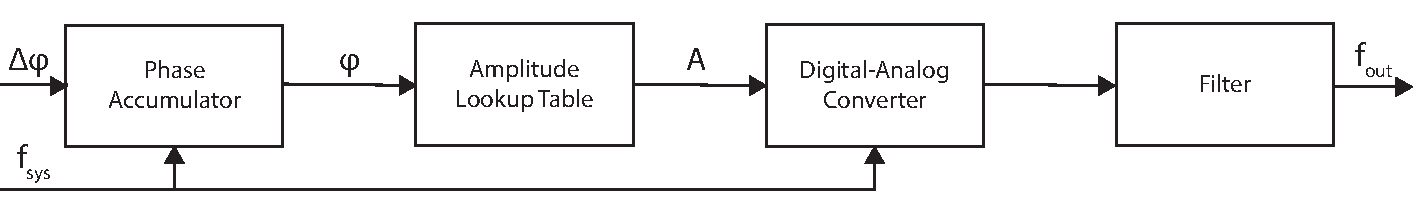
\includegraphics[width=\textwidth]{\figuredir{digital-signal-synthesis/simple-architecture.pdf}}
  \captionsetup{width=.8\textwidth}
  \caption{Signal flow through a simple \gls{dds}. The output frequency
    determines a phase step by which the accumulator is incremented at each
    clock cycle. The value of the phase accumulator is used for amplitude
    lookup of the desired output signal shape. A \gls{dac} outputs the signal
    which then is filtered to smooth the discrete \gls{dac} output.
  }\label{fig:dds_simple_architecture}
\end{figure}
For every clock cycle the phase accumulator is incremented by $\Delta\varphi$.
On overflow of the accumulator a new signal period starts. The phase
accumulator value is used to lookup the corresponding amplitude value of the
desired output signal shape. For example one can use a lookup table with the
values of a sinusoidal output signal. Alternatively one can omit the lookup
table and output a sawtooth output signal by suppling the phase accumulator
output directly to the \gls{dac} or a square wave signal output by suppling
the most significant bit directly. Finally a \gls{dac} converts the digital
amplitude value to an analog signal. An optional analog filter can be used to
smooth the discrete output. In \Cref{fig:dds_simple_output} the signal at the
different processing stages inside a simple \gls{dds} are presented for a
\SI{8}{\bit} precision, system clock frequency
$f_\text{sys}=\SI{1}{\giga\hertz}$ and output frequency
$f_\text{out}=\SI{100}{\mega\hertz}$.
\begin{figure}[ht]
  \centering
  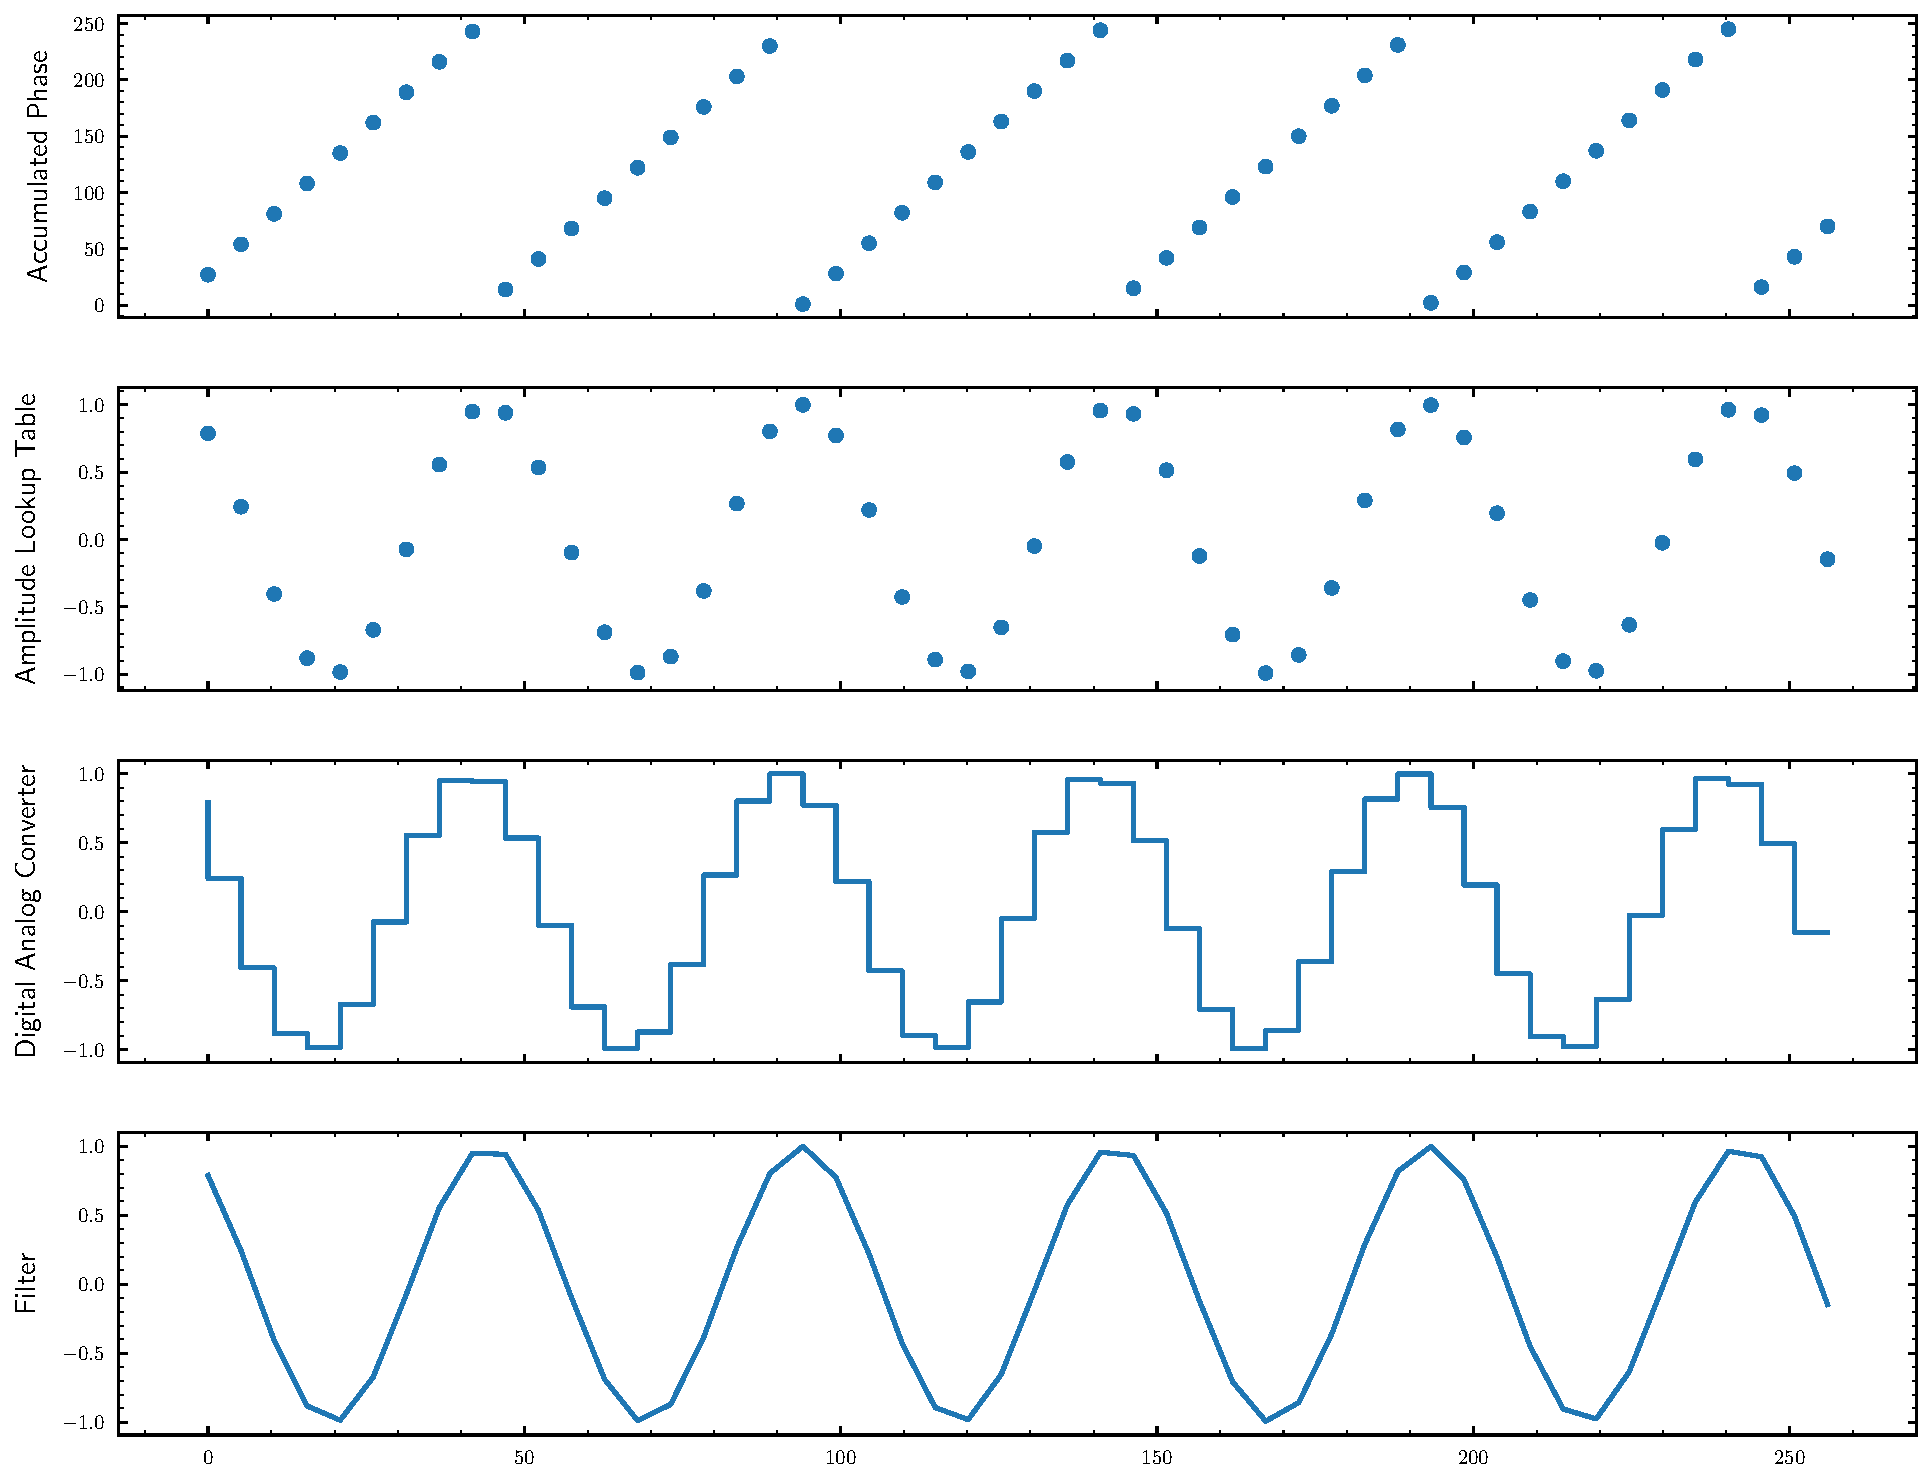
\includegraphics[width=\textwidth]{\figuredir{digital-signal-synthesis/simple-output.pdf}}
  \captionsetup{width=.8\textwidth}
  \caption{Signal outputs at different stages in a simple \gls{dds}. The
    phase accumulator is incremented at each clock cycle by $\Delta\phi$. The
    phase accumulator value is used to lookup a sinusoidal amplitude value
    that is supplied to a \gls{dac}. The final result is smoothed using a
    filter.}\label{fig:dds_simple_output}
\end{figure}
In the first column of \Cref{fig:dds_simple_output} we can see how the phase
accumulator is incremented on every clock iteration and resets on overflow.
In the second column the lookup table has been used to return the
corresponding cosine amplitude. We can see a difference in output shape
between even and odd samples. This is caused by the fact that the phase
increment is not a divisor of the phase accumulator size and we will later
discuss workarounds.

\subsection{Clock generation}

The Nyquist-Shannon sampling theorem states that for a given sample rate a
perfect reconstruction is guaranteed possible for
$f_\text{out}<f_\text{samp}/2$. Until now we have considered the system clock
frequency $f_\text{sys}=f_\text{samp}$ as given. In practice reliable
reference signals are clocked below the desired output range and thereby
cannot directly be used as system clock according to the Nyquist-Shannon
sampling theorem.
\begin{figure}[ht]
  \centering
  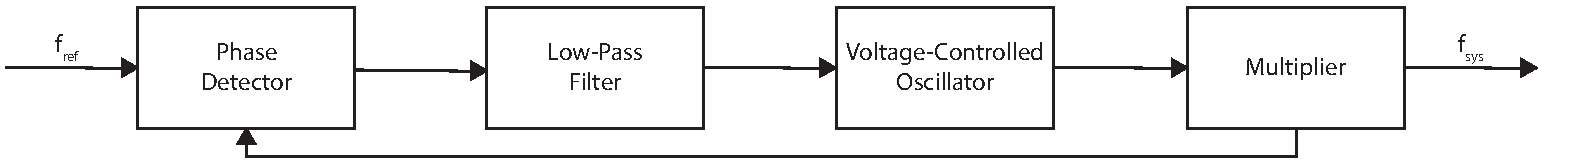
\includegraphics[width=\textwidth]{\figuredir{digital-signal-synthesis/clock-generation.pdf}}
  \captionsetup{width=.8\textwidth}
  \caption{Clock generation signal generation with \gls{pll} and multiplier.
    The phase detector compares the output system phase with the reference
    phase and yields a non-linear error response. The low-pass filter removes
    fast oscillations. The \gls{vco} changes the output phase in dependence
    of the error response. Finally system and reference phase will go in lock.
    }\label{fig:dds_clock_generation}
\end{figure}
\Cref{fig:dds_clock_generation} the system clock generation from a reference
signal is illustrated. The phase detector yields a non-linear error response
comparing the output signal phase with the reference signal phase. After a
low-pass filter removes fast oscillations a \gls{vco} changes its phase
proportional to the error signal. Finally a frequency multiplier creates
harmonics of the reference frequency and extracts a programmed frequency
multiple of $M$ such that the system frequency relates to the reference
clock by $f_\text{sys}=Mf_\text{ref}$ with $1<M\in\mathbb{N}$.

\subsection{Parameter modulation}

So far we only discussed the case of frequency modulation. We will see that
the previous architecture can be easily extended to support amplitude
and phase modulation too.
\begin{figure}[ht]
  \centering
  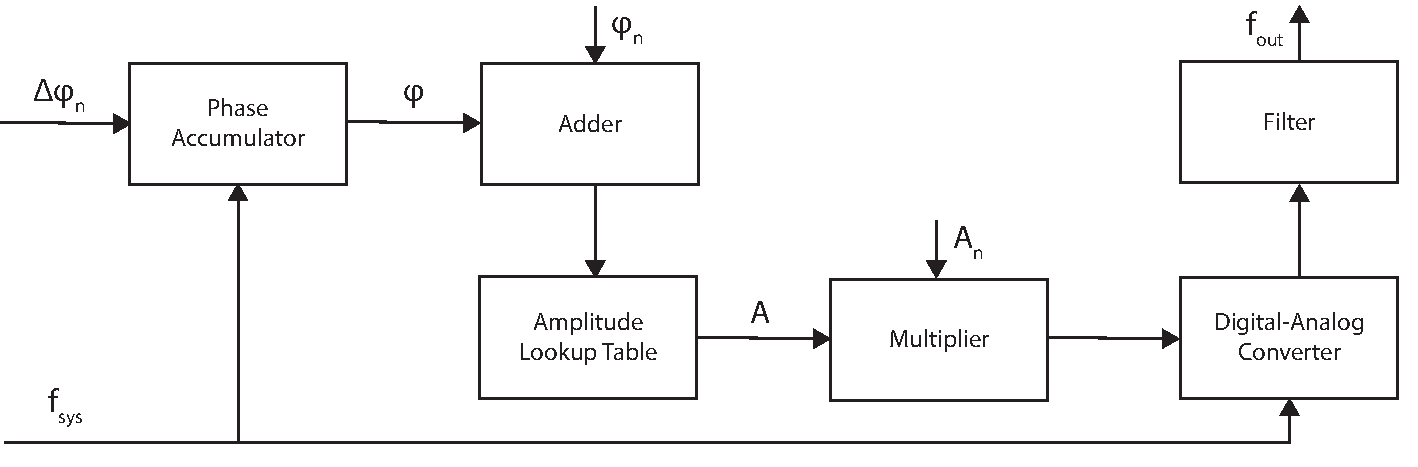
\includegraphics[width=\textwidth]{\figuredir{digital-signal-synthesis/modulation-architecture.pdf}}
  \captionsetup{width=.8\textwidth}
  \caption{
    \gls{dds} architecture supporting modulation of frequency, amplitude and
    phase offset parameters. Phase accumulator increment is now time dependent.
    The phase offset is also time dependent is added as last step to the
    phase accumulator before supplied to the \gls{dac}. The time dependent
    amplitude parameter is multiplied with the amplitude obtained from the
    lookup table.
    }\label{fig:dds_modulation_architecture}
\end{figure}
In \Cref{fig:dds_modulation_architecture} we can see one realization of an
architecture that supports amplitude, frequency and phase modulation. The main
components are the same as in \Cref{fig:dds_simple_architecture}. In addition
we have an adder for a time dependent phase offset and a multiplier for the
digital amplitude value obtained from the lookup table. The time dependence
of the parameters can be either determined by reading from memory or through
generation of another circuit. In a later section we will discuss the case of
a linear frequency sweep provided by a digital ramp.

\section{Quantization errors}
\section{Frequency response}

\section{Operating range}

We apply a reference signal of
\begin{equation}
  f_\text{ref}=\SI{10}{\mega\hertz}
\end{equation}
configured to be used with a \gls{pll} multiplier of
$N=100$ yielding a system clock of
\begin{equation}
  f_\text{sys}=Nf_\text{ref}=\SI{1}{\giga\hertz}.
\end{equation}
The timer clock used for the linear ramp and memory playback runs with
a quarter of the system clock
\begin{equation}
  f_\text{timer}=f_\text{sys}/4=\SI{250}{\mega\hertz}.
\end{equation}

The \gls{ad9910} uses a \SI{14}{\bit} \gls{asf} and \SI{32}{\bit} \gls{ftw}
to parameterize amplitude $A(t)$ and output frequency $f(t)$ by
\begin{align}
  FTW
  :=
  \left\lfloor2^{32}\left(\frac{f_\text{out}}{f_\text{sys}}\right)\right\rceil
  &&
  ASF
  :=
  \left\lfloor\frac{A_\text{out}}{2^{14}}\right\rceil
  \label{eq:elec:ftwasf}
\end{align}
wherein $\lfloor{\cdot}\rceil$ rounds the given float to the nearest integer.
The theoretical limit for the maximum output frequency then is found via
\begin{equation*}
  f_\text{max}
  =
  \left(1-\frac{2^{31}-1}{2^{32}}\right)f_\text{sys}
  =
  \left(\frac{1}{2}-\frac{1}{2^{31}}\right)f_\text{sys}
  \approx
  \frac{1}{2}f_\text{sys}
  =
  \SI{500}{\mega\hertz}.
\end{equation*}
Yet the datasheet \cite{AD9910} reports $f_\text{max}=\SI{420}{\mega\hertz}$
and in fact we found the output signal to be very noisy at the theoretical
limit.

We continue with the assessment of the digital ramp that does a unidrectional
linear sweep on the frequency from \SI{90}{\mega\hertz} to
\SI{110}{\mega\hertz}. The digital ramp of the \gls{ad9910} lets us define
a \gls{ftw} step $M$ word of \SI{32}{\bit} as well as a step rate word $S$ of
\SI{16}{\bit} resolution. They relate to the frequency step and the time
step through
\begin{align}
  \Delta f
  =
  \frac{M}{2^{32}}f_\text{sys}
  &&
  \Delta t
  =
  \frac{S}{f_\text{timer}}
  =
  \frac{S}{4f_\text{sys}}.
  \label{eq:elec:step}
\end{align}
The sweep duration is deterimened by $S,M$ through
\begin{equation}
  T_\text{duration}
  =
  \frac{f_\text{upper}-f_\text{lower}}{\Delta f}\Delta t
  =
  2^{32}\frac{f_\text{upper}-f_\text{lower}}{f_\text{sys}}\frac{S/M}{f_\text{timer}}
\end{equation}
for a target sweep duration of $T_\text{duration}=\SI{10}{ms}$ we find
\begin{equation*}
  \frac{S}{M}
  =
  \frac{T f_\text{timer}}{2^{32}}\frac{f_\text{sys}}{f_\text{upper}-f_\text{lower}}
  =
  \frac{10^9}{2^{35}}
  \approx
  \num{2.9104e-2}
  =
  \frac{1819}{62500}
\end{equation*}
the last step can be obtained by best ratio approximation using continued
fractions as for example described in \cite{Ashley2003}. It should be kept in
mind that the best ratio approximation is likable to introduce an error,
therefore realistic durations may differ from the configured value and it
is possible that better approximations exist that allow smaller $\Delta f,
\Delta t$, thus providing a sweep resolution. In the above case the given
time duration translates to
\begin{align*}
  \Delta f
  =
  \frac{62500}{2^{32}}f_\text{sys}
  \approx
  \SI{145}{\kilo\hertz}
  &&
  \Delta t
  =
  \frac{1819}{f_\text{timer}}
  \approx
  \SI{7.28}{\micro\second}
\end{align*}
or $(f_\text{upper}-f_\text{lower})/\Delta f=138$ discrete data points.

Eventually we are left with the assessment of the amplitude sequence. The
memory fits at most 1024 discrete amplitude values and the \gls{ad9910}
allows us to set the time spent at each amplitude value via the \SI{16}{\bit}
playback rate $P$ word
\begin{equation}
  \Delta t
  =
  \frac{P}{f_\text{timer}}
  =
  \frac{4P}{f_\text{sys}}
\end{equation}
which gives us range from $\min\Delta t=\SI{4}{\nano\second}$ to
$\max\Delta t=\SI{26.14}{\micro\second}$. As we incorporate all of the 1024
data points this gives us a duration range from about
$\min T=\SI{4}{\micro\second}$ to $\max T=\SI{26.84}{\milli\second}$.


%\chapter{Characterisation of the electronic setup}\label{ch:electronic_setup}

\textit{By the time the \gls{rf} signal has reached the acoustic transducer,
it has been synthesized from a reference signal, amplified, and matched to
the impedance of the \gls{aod} transducer. We are going to inspect the
\gls{rf} signal characteristics at each transmission and find that each stage
unintentionally carries out frequency dependent amplitude characteristics
which, as we will see in the next chapter, are responsible for the complex
intensity distribution observed with the photodiode.}

\section{Digital signal synthesizer}

We already covered the fundamental functionality of the \gls{dds} in
\cref{ch:digital_signal_synthesis} and its integration in our experimental
setup in \cref{subsec:setup_signal_source}, yet we are missing physical
measurements of the frequency and the amplitude characteristics.

Physical analysis of the \gls{dds} output \gls{rf} signal is in fact no simple
endeavour as usual operation time scales are of many magnitudes greater than
the signal periodicity. The strategy we used to resolve this circumstance is
depcited in \Cref{fig:signal_window}.
\begin{figure}[htb]
  \centering
  \begin{adjustbox}{width=\textwidth}
    %% Creator: Matplotlib, PGF backend
%%
%% To include the figure in your LaTeX document, write
%%   \input{<filename>.pgf}
%%
%% Make sure the required packages are loaded in your preamble
%%   \usepackage{pgf}
%%
%% Figures using additional raster images can only be included by \input if
%% they are in the same directory as the main LaTeX file. For loading figures
%% from other directories you can use the `import` package
%%   \usepackage{import}
%% and then include the figures with
%%   \import{<path to file>}{<filename>.pgf}
%%
%% Matplotlib used the following preamble
%%   \usepackage{amsmath}\usepackage{siunitx}\usepackage{lmodern}
%%   \usepackage{fontspec}
%%
\begingroup%
\makeatletter%
\begin{pgfpicture}%
\pgfpathrectangle{\pgfpointorigin}{\pgfqpoint{12.000000in}{4.000000in}}%
\pgfusepath{use as bounding box, clip}%
\begin{pgfscope}%
\pgfsetbuttcap%
\pgfsetmiterjoin%
\pgfsetlinewidth{0.000000pt}%
\definecolor{currentstroke}{rgb}{1.000000,1.000000,1.000000}%
\pgfsetstrokecolor{currentstroke}%
\pgfsetdash{}{0pt}%
\pgfpathmoveto{\pgfqpoint{0.000000in}{0.000000in}}%
\pgfpathlineto{\pgfqpoint{12.000000in}{0.000000in}}%
\pgfpathlineto{\pgfqpoint{12.000000in}{4.000000in}}%
\pgfpathlineto{\pgfqpoint{0.000000in}{4.000000in}}%
\pgfpathclose%
\pgfusepath{}%
\end{pgfscope}%
\begin{pgfscope}%
\pgfsetbuttcap%
\pgfsetmiterjoin%
\definecolor{currentfill}{rgb}{1.000000,1.000000,1.000000}%
\pgfsetfillcolor{currentfill}%
\pgfsetlinewidth{0.000000pt}%
\definecolor{currentstroke}{rgb}{0.000000,0.000000,0.000000}%
\pgfsetstrokecolor{currentstroke}%
\pgfsetstrokeopacity{0.000000}%
\pgfsetdash{}{0pt}%
\pgfpathmoveto{\pgfqpoint{1.500000in}{0.800000in}}%
\pgfpathlineto{\pgfqpoint{10.800000in}{0.800000in}}%
\pgfpathlineto{\pgfqpoint{10.800000in}{3.920000in}}%
\pgfpathlineto{\pgfqpoint{1.500000in}{3.920000in}}%
\pgfpathclose%
\pgfusepath{fill}%
\end{pgfscope}%
\begin{pgfscope}%
\pgfpathrectangle{\pgfqpoint{1.500000in}{0.800000in}}{\pgfqpoint{9.300000in}{3.120000in}}%
\pgfusepath{clip}%
\pgfsetbuttcap%
\pgfsetmiterjoin%
\definecolor{currentfill}{rgb}{0.501961,0.501961,0.501961}%
\pgfsetfillcolor{currentfill}%
\pgfsetfillopacity{0.500000}%
\pgfsetlinewidth{1.003750pt}%
\definecolor{currentstroke}{rgb}{0.501961,0.501961,0.501961}%
\pgfsetstrokecolor{currentstroke}%
\pgfsetstrokeopacity{0.500000}%
\pgfsetdash{}{0pt}%
\pgfpathmoveto{\pgfqpoint{2.063636in}{0.800000in}}%
\pgfpathlineto{\pgfqpoint{2.063636in}{3.920000in}}%
\pgfpathlineto{\pgfqpoint{3.050000in}{3.920000in}}%
\pgfpathlineto{\pgfqpoint{3.050000in}{0.800000in}}%
\pgfpathclose%
\pgfusepath{stroke,fill}%
\end{pgfscope}%
\begin{pgfscope}%
\pgfpathrectangle{\pgfqpoint{1.500000in}{0.800000in}}{\pgfqpoint{9.300000in}{3.120000in}}%
\pgfusepath{clip}%
\pgfsetbuttcap%
\pgfsetmiterjoin%
\definecolor{currentfill}{rgb}{0.501961,0.501961,0.501961}%
\pgfsetfillcolor{currentfill}%
\pgfsetfillopacity{0.500000}%
\pgfsetlinewidth{1.003750pt}%
\definecolor{currentstroke}{rgb}{0.501961,0.501961,0.501961}%
\pgfsetstrokecolor{currentstroke}%
\pgfsetstrokeopacity{0.500000}%
\pgfsetdash{}{0pt}%
\pgfpathmoveto{\pgfqpoint{2.627273in}{0.800000in}}%
\pgfpathlineto{\pgfqpoint{2.627273in}{3.920000in}}%
\pgfpathlineto{\pgfqpoint{3.613636in}{3.920000in}}%
\pgfpathlineto{\pgfqpoint{3.613636in}{0.800000in}}%
\pgfpathclose%
\pgfusepath{stroke,fill}%
\end{pgfscope}%
\begin{pgfscope}%
\pgfsetbuttcap%
\pgfsetroundjoin%
\definecolor{currentfill}{rgb}{0.000000,0.000000,0.000000}%
\pgfsetfillcolor{currentfill}%
\pgfsetlinewidth{1.003750pt}%
\definecolor{currentstroke}{rgb}{0.000000,0.000000,0.000000}%
\pgfsetstrokecolor{currentstroke}%
\pgfsetdash{}{0pt}%
\pgfsys@defobject{currentmarker}{\pgfqpoint{0.000000in}{0.000000in}}{\pgfqpoint{0.000000in}{0.055556in}}{%
\pgfpathmoveto{\pgfqpoint{0.000000in}{0.000000in}}%
\pgfpathlineto{\pgfqpoint{0.000000in}{0.055556in}}%
\pgfusepath{stroke,fill}%
}%
\begin{pgfscope}%
\pgfsys@transformshift{1.922727in}{0.800000in}%
\pgfsys@useobject{currentmarker}{}%
\end{pgfscope}%
\end{pgfscope}%
\begin{pgfscope}%
\pgfsetbuttcap%
\pgfsetroundjoin%
\definecolor{currentfill}{rgb}{0.000000,0.000000,0.000000}%
\pgfsetfillcolor{currentfill}%
\pgfsetlinewidth{1.003750pt}%
\definecolor{currentstroke}{rgb}{0.000000,0.000000,0.000000}%
\pgfsetstrokecolor{currentstroke}%
\pgfsetdash{}{0pt}%
\pgfsys@defobject{currentmarker}{\pgfqpoint{0.000000in}{-0.055556in}}{\pgfqpoint{0.000000in}{0.000000in}}{%
\pgfpathmoveto{\pgfqpoint{0.000000in}{0.000000in}}%
\pgfpathlineto{\pgfqpoint{0.000000in}{-0.055556in}}%
\pgfusepath{stroke,fill}%
}%
\begin{pgfscope}%
\pgfsys@transformshift{1.922727in}{3.920000in}%
\pgfsys@useobject{currentmarker}{}%
\end{pgfscope}%
\end{pgfscope}%
\begin{pgfscope}%
\pgftext[x=1.922727in,y=0.702778in,,top]{\fontsize{10.000000}{12.000000}\selectfont \(\displaystyle 0.0\)}%
\end{pgfscope}%
\begin{pgfscope}%
\pgfsetbuttcap%
\pgfsetroundjoin%
\definecolor{currentfill}{rgb}{0.000000,0.000000,0.000000}%
\pgfsetfillcolor{currentfill}%
\pgfsetlinewidth{1.003750pt}%
\definecolor{currentstroke}{rgb}{0.000000,0.000000,0.000000}%
\pgfsetstrokecolor{currentstroke}%
\pgfsetdash{}{0pt}%
\pgfsys@defobject{currentmarker}{\pgfqpoint{0.000000in}{0.000000in}}{\pgfqpoint{0.000000in}{0.055556in}}{%
\pgfpathmoveto{\pgfqpoint{0.000000in}{0.000000in}}%
\pgfpathlineto{\pgfqpoint{0.000000in}{0.055556in}}%
\pgfusepath{stroke,fill}%
}%
\begin{pgfscope}%
\pgfsys@transformshift{3.331818in}{0.800000in}%
\pgfsys@useobject{currentmarker}{}%
\end{pgfscope}%
\end{pgfscope}%
\begin{pgfscope}%
\pgfsetbuttcap%
\pgfsetroundjoin%
\definecolor{currentfill}{rgb}{0.000000,0.000000,0.000000}%
\pgfsetfillcolor{currentfill}%
\pgfsetlinewidth{1.003750pt}%
\definecolor{currentstroke}{rgb}{0.000000,0.000000,0.000000}%
\pgfsetstrokecolor{currentstroke}%
\pgfsetdash{}{0pt}%
\pgfsys@defobject{currentmarker}{\pgfqpoint{0.000000in}{-0.055556in}}{\pgfqpoint{0.000000in}{0.000000in}}{%
\pgfpathmoveto{\pgfqpoint{0.000000in}{0.000000in}}%
\pgfpathlineto{\pgfqpoint{0.000000in}{-0.055556in}}%
\pgfusepath{stroke,fill}%
}%
\begin{pgfscope}%
\pgfsys@transformshift{3.331818in}{3.920000in}%
\pgfsys@useobject{currentmarker}{}%
\end{pgfscope}%
\end{pgfscope}%
\begin{pgfscope}%
\pgftext[x=3.331818in,y=0.702778in,,top]{\fontsize{10.000000}{12.000000}\selectfont \(\displaystyle 0.1\)}%
\end{pgfscope}%
\begin{pgfscope}%
\pgfsetbuttcap%
\pgfsetroundjoin%
\definecolor{currentfill}{rgb}{0.000000,0.000000,0.000000}%
\pgfsetfillcolor{currentfill}%
\pgfsetlinewidth{1.003750pt}%
\definecolor{currentstroke}{rgb}{0.000000,0.000000,0.000000}%
\pgfsetstrokecolor{currentstroke}%
\pgfsetdash{}{0pt}%
\pgfsys@defobject{currentmarker}{\pgfqpoint{0.000000in}{0.000000in}}{\pgfqpoint{0.000000in}{0.055556in}}{%
\pgfpathmoveto{\pgfqpoint{0.000000in}{0.000000in}}%
\pgfpathlineto{\pgfqpoint{0.000000in}{0.055556in}}%
\pgfusepath{stroke,fill}%
}%
\begin{pgfscope}%
\pgfsys@transformshift{4.740909in}{0.800000in}%
\pgfsys@useobject{currentmarker}{}%
\end{pgfscope}%
\end{pgfscope}%
\begin{pgfscope}%
\pgfsetbuttcap%
\pgfsetroundjoin%
\definecolor{currentfill}{rgb}{0.000000,0.000000,0.000000}%
\pgfsetfillcolor{currentfill}%
\pgfsetlinewidth{1.003750pt}%
\definecolor{currentstroke}{rgb}{0.000000,0.000000,0.000000}%
\pgfsetstrokecolor{currentstroke}%
\pgfsetdash{}{0pt}%
\pgfsys@defobject{currentmarker}{\pgfqpoint{0.000000in}{-0.055556in}}{\pgfqpoint{0.000000in}{0.000000in}}{%
\pgfpathmoveto{\pgfqpoint{0.000000in}{0.000000in}}%
\pgfpathlineto{\pgfqpoint{0.000000in}{-0.055556in}}%
\pgfusepath{stroke,fill}%
}%
\begin{pgfscope}%
\pgfsys@transformshift{4.740909in}{3.920000in}%
\pgfsys@useobject{currentmarker}{}%
\end{pgfscope}%
\end{pgfscope}%
\begin{pgfscope}%
\pgftext[x=4.740909in,y=0.702778in,,top]{\fontsize{10.000000}{12.000000}\selectfont \(\displaystyle 0.2\)}%
\end{pgfscope}%
\begin{pgfscope}%
\pgfsetbuttcap%
\pgfsetroundjoin%
\definecolor{currentfill}{rgb}{0.000000,0.000000,0.000000}%
\pgfsetfillcolor{currentfill}%
\pgfsetlinewidth{1.003750pt}%
\definecolor{currentstroke}{rgb}{0.000000,0.000000,0.000000}%
\pgfsetstrokecolor{currentstroke}%
\pgfsetdash{}{0pt}%
\pgfsys@defobject{currentmarker}{\pgfqpoint{0.000000in}{0.000000in}}{\pgfqpoint{0.000000in}{0.055556in}}{%
\pgfpathmoveto{\pgfqpoint{0.000000in}{0.000000in}}%
\pgfpathlineto{\pgfqpoint{0.000000in}{0.055556in}}%
\pgfusepath{stroke,fill}%
}%
\begin{pgfscope}%
\pgfsys@transformshift{6.150000in}{0.800000in}%
\pgfsys@useobject{currentmarker}{}%
\end{pgfscope}%
\end{pgfscope}%
\begin{pgfscope}%
\pgfsetbuttcap%
\pgfsetroundjoin%
\definecolor{currentfill}{rgb}{0.000000,0.000000,0.000000}%
\pgfsetfillcolor{currentfill}%
\pgfsetlinewidth{1.003750pt}%
\definecolor{currentstroke}{rgb}{0.000000,0.000000,0.000000}%
\pgfsetstrokecolor{currentstroke}%
\pgfsetdash{}{0pt}%
\pgfsys@defobject{currentmarker}{\pgfqpoint{0.000000in}{-0.055556in}}{\pgfqpoint{0.000000in}{0.000000in}}{%
\pgfpathmoveto{\pgfqpoint{0.000000in}{0.000000in}}%
\pgfpathlineto{\pgfqpoint{0.000000in}{-0.055556in}}%
\pgfusepath{stroke,fill}%
}%
\begin{pgfscope}%
\pgfsys@transformshift{6.150000in}{3.920000in}%
\pgfsys@useobject{currentmarker}{}%
\end{pgfscope}%
\end{pgfscope}%
\begin{pgfscope}%
\pgftext[x=6.150000in,y=0.702778in,,top]{\fontsize{10.000000}{12.000000}\selectfont \(\displaystyle 0.3\)}%
\end{pgfscope}%
\begin{pgfscope}%
\pgfsetbuttcap%
\pgfsetroundjoin%
\definecolor{currentfill}{rgb}{0.000000,0.000000,0.000000}%
\pgfsetfillcolor{currentfill}%
\pgfsetlinewidth{1.003750pt}%
\definecolor{currentstroke}{rgb}{0.000000,0.000000,0.000000}%
\pgfsetstrokecolor{currentstroke}%
\pgfsetdash{}{0pt}%
\pgfsys@defobject{currentmarker}{\pgfqpoint{0.000000in}{0.000000in}}{\pgfqpoint{0.000000in}{0.055556in}}{%
\pgfpathmoveto{\pgfqpoint{0.000000in}{0.000000in}}%
\pgfpathlineto{\pgfqpoint{0.000000in}{0.055556in}}%
\pgfusepath{stroke,fill}%
}%
\begin{pgfscope}%
\pgfsys@transformshift{7.559091in}{0.800000in}%
\pgfsys@useobject{currentmarker}{}%
\end{pgfscope}%
\end{pgfscope}%
\begin{pgfscope}%
\pgfsetbuttcap%
\pgfsetroundjoin%
\definecolor{currentfill}{rgb}{0.000000,0.000000,0.000000}%
\pgfsetfillcolor{currentfill}%
\pgfsetlinewidth{1.003750pt}%
\definecolor{currentstroke}{rgb}{0.000000,0.000000,0.000000}%
\pgfsetstrokecolor{currentstroke}%
\pgfsetdash{}{0pt}%
\pgfsys@defobject{currentmarker}{\pgfqpoint{0.000000in}{-0.055556in}}{\pgfqpoint{0.000000in}{0.000000in}}{%
\pgfpathmoveto{\pgfqpoint{0.000000in}{0.000000in}}%
\pgfpathlineto{\pgfqpoint{0.000000in}{-0.055556in}}%
\pgfusepath{stroke,fill}%
}%
\begin{pgfscope}%
\pgfsys@transformshift{7.559091in}{3.920000in}%
\pgfsys@useobject{currentmarker}{}%
\end{pgfscope}%
\end{pgfscope}%
\begin{pgfscope}%
\pgftext[x=7.559091in,y=0.702778in,,top]{\fontsize{10.000000}{12.000000}\selectfont \(\displaystyle 0.4\)}%
\end{pgfscope}%
\begin{pgfscope}%
\pgfsetbuttcap%
\pgfsetroundjoin%
\definecolor{currentfill}{rgb}{0.000000,0.000000,0.000000}%
\pgfsetfillcolor{currentfill}%
\pgfsetlinewidth{1.003750pt}%
\definecolor{currentstroke}{rgb}{0.000000,0.000000,0.000000}%
\pgfsetstrokecolor{currentstroke}%
\pgfsetdash{}{0pt}%
\pgfsys@defobject{currentmarker}{\pgfqpoint{0.000000in}{0.000000in}}{\pgfqpoint{0.000000in}{0.055556in}}{%
\pgfpathmoveto{\pgfqpoint{0.000000in}{0.000000in}}%
\pgfpathlineto{\pgfqpoint{0.000000in}{0.055556in}}%
\pgfusepath{stroke,fill}%
}%
\begin{pgfscope}%
\pgfsys@transformshift{8.968182in}{0.800000in}%
\pgfsys@useobject{currentmarker}{}%
\end{pgfscope}%
\end{pgfscope}%
\begin{pgfscope}%
\pgfsetbuttcap%
\pgfsetroundjoin%
\definecolor{currentfill}{rgb}{0.000000,0.000000,0.000000}%
\pgfsetfillcolor{currentfill}%
\pgfsetlinewidth{1.003750pt}%
\definecolor{currentstroke}{rgb}{0.000000,0.000000,0.000000}%
\pgfsetstrokecolor{currentstroke}%
\pgfsetdash{}{0pt}%
\pgfsys@defobject{currentmarker}{\pgfqpoint{0.000000in}{-0.055556in}}{\pgfqpoint{0.000000in}{0.000000in}}{%
\pgfpathmoveto{\pgfqpoint{0.000000in}{0.000000in}}%
\pgfpathlineto{\pgfqpoint{0.000000in}{-0.055556in}}%
\pgfusepath{stroke,fill}%
}%
\begin{pgfscope}%
\pgfsys@transformshift{8.968182in}{3.920000in}%
\pgfsys@useobject{currentmarker}{}%
\end{pgfscope}%
\end{pgfscope}%
\begin{pgfscope}%
\pgftext[x=8.968182in,y=0.702778in,,top]{\fontsize{10.000000}{12.000000}\selectfont \(\displaystyle 0.5\)}%
\end{pgfscope}%
\begin{pgfscope}%
\pgfsetbuttcap%
\pgfsetroundjoin%
\definecolor{currentfill}{rgb}{0.000000,0.000000,0.000000}%
\pgfsetfillcolor{currentfill}%
\pgfsetlinewidth{1.003750pt}%
\definecolor{currentstroke}{rgb}{0.000000,0.000000,0.000000}%
\pgfsetstrokecolor{currentstroke}%
\pgfsetdash{}{0pt}%
\pgfsys@defobject{currentmarker}{\pgfqpoint{0.000000in}{0.000000in}}{\pgfqpoint{0.000000in}{0.055556in}}{%
\pgfpathmoveto{\pgfqpoint{0.000000in}{0.000000in}}%
\pgfpathlineto{\pgfqpoint{0.000000in}{0.055556in}}%
\pgfusepath{stroke,fill}%
}%
\begin{pgfscope}%
\pgfsys@transformshift{10.377273in}{0.800000in}%
\pgfsys@useobject{currentmarker}{}%
\end{pgfscope}%
\end{pgfscope}%
\begin{pgfscope}%
\pgfsetbuttcap%
\pgfsetroundjoin%
\definecolor{currentfill}{rgb}{0.000000,0.000000,0.000000}%
\pgfsetfillcolor{currentfill}%
\pgfsetlinewidth{1.003750pt}%
\definecolor{currentstroke}{rgb}{0.000000,0.000000,0.000000}%
\pgfsetstrokecolor{currentstroke}%
\pgfsetdash{}{0pt}%
\pgfsys@defobject{currentmarker}{\pgfqpoint{0.000000in}{-0.055556in}}{\pgfqpoint{0.000000in}{0.000000in}}{%
\pgfpathmoveto{\pgfqpoint{0.000000in}{0.000000in}}%
\pgfpathlineto{\pgfqpoint{0.000000in}{-0.055556in}}%
\pgfusepath{stroke,fill}%
}%
\begin{pgfscope}%
\pgfsys@transformshift{10.377273in}{3.920000in}%
\pgfsys@useobject{currentmarker}{}%
\end{pgfscope}%
\end{pgfscope}%
\begin{pgfscope}%
\pgftext[x=10.377273in,y=0.702778in,,top]{\fontsize{10.000000}{12.000000}\selectfont \(\displaystyle 0.6\)}%
\end{pgfscope}%
\begin{pgfscope}%
\pgftext[x=6.150000in,y=0.468333in,,top]{\fontsize{14.000000}{16.800000}\selectfont \(\displaystyle t\) (\si{\micro\second})}%
\end{pgfscope}%
\begin{pgfscope}%
\pgfsetbuttcap%
\pgfsetroundjoin%
\definecolor{currentfill}{rgb}{0.000000,0.000000,0.000000}%
\pgfsetfillcolor{currentfill}%
\pgfsetlinewidth{1.003750pt}%
\definecolor{currentstroke}{rgb}{0.000000,0.000000,0.000000}%
\pgfsetstrokecolor{currentstroke}%
\pgfsetdash{}{0pt}%
\pgfsys@defobject{currentmarker}{\pgfqpoint{0.000000in}{0.000000in}}{\pgfqpoint{0.055556in}{0.000000in}}{%
\pgfpathmoveto{\pgfqpoint{0.000000in}{0.000000in}}%
\pgfpathlineto{\pgfqpoint{0.055556in}{0.000000in}}%
\pgfusepath{stroke,fill}%
}%
\begin{pgfscope}%
\pgfsys@transformshift{1.500000in}{0.941817in}%
\pgfsys@useobject{currentmarker}{}%
\end{pgfscope}%
\end{pgfscope}%
\begin{pgfscope}%
\pgfsetbuttcap%
\pgfsetroundjoin%
\definecolor{currentfill}{rgb}{0.000000,0.000000,0.000000}%
\pgfsetfillcolor{currentfill}%
\pgfsetlinewidth{1.003750pt}%
\definecolor{currentstroke}{rgb}{0.000000,0.000000,0.000000}%
\pgfsetstrokecolor{currentstroke}%
\pgfsetdash{}{0pt}%
\pgfsys@defobject{currentmarker}{\pgfqpoint{-0.055556in}{0.000000in}}{\pgfqpoint{0.000000in}{0.000000in}}{%
\pgfpathmoveto{\pgfqpoint{0.000000in}{0.000000in}}%
\pgfpathlineto{\pgfqpoint{-0.055556in}{0.000000in}}%
\pgfusepath{stroke,fill}%
}%
\begin{pgfscope}%
\pgfsys@transformshift{10.800000in}{0.941817in}%
\pgfsys@useobject{currentmarker}{}%
\end{pgfscope}%
\end{pgfscope}%
\begin{pgfscope}%
\pgftext[x=1.047839in,y=0.893623in,left,base]{\fontsize{10.000000}{12.000000}\selectfont \(\displaystyle -1.00\)}%
\end{pgfscope}%
\begin{pgfscope}%
\pgfsetbuttcap%
\pgfsetroundjoin%
\definecolor{currentfill}{rgb}{0.000000,0.000000,0.000000}%
\pgfsetfillcolor{currentfill}%
\pgfsetlinewidth{1.003750pt}%
\definecolor{currentstroke}{rgb}{0.000000,0.000000,0.000000}%
\pgfsetstrokecolor{currentstroke}%
\pgfsetdash{}{0pt}%
\pgfsys@defobject{currentmarker}{\pgfqpoint{0.000000in}{0.000000in}}{\pgfqpoint{0.055556in}{0.000000in}}{%
\pgfpathmoveto{\pgfqpoint{0.000000in}{0.000000in}}%
\pgfpathlineto{\pgfqpoint{0.055556in}{0.000000in}}%
\pgfusepath{stroke,fill}%
}%
\begin{pgfscope}%
\pgfsys@transformshift{1.500000in}{1.296363in}%
\pgfsys@useobject{currentmarker}{}%
\end{pgfscope}%
\end{pgfscope}%
\begin{pgfscope}%
\pgfsetbuttcap%
\pgfsetroundjoin%
\definecolor{currentfill}{rgb}{0.000000,0.000000,0.000000}%
\pgfsetfillcolor{currentfill}%
\pgfsetlinewidth{1.003750pt}%
\definecolor{currentstroke}{rgb}{0.000000,0.000000,0.000000}%
\pgfsetstrokecolor{currentstroke}%
\pgfsetdash{}{0pt}%
\pgfsys@defobject{currentmarker}{\pgfqpoint{-0.055556in}{0.000000in}}{\pgfqpoint{0.000000in}{0.000000in}}{%
\pgfpathmoveto{\pgfqpoint{0.000000in}{0.000000in}}%
\pgfpathlineto{\pgfqpoint{-0.055556in}{0.000000in}}%
\pgfusepath{stroke,fill}%
}%
\begin{pgfscope}%
\pgfsys@transformshift{10.800000in}{1.296363in}%
\pgfsys@useobject{currentmarker}{}%
\end{pgfscope}%
\end{pgfscope}%
\begin{pgfscope}%
\pgftext[x=1.047839in,y=1.248169in,left,base]{\fontsize{10.000000}{12.000000}\selectfont \(\displaystyle -0.75\)}%
\end{pgfscope}%
\begin{pgfscope}%
\pgfsetbuttcap%
\pgfsetroundjoin%
\definecolor{currentfill}{rgb}{0.000000,0.000000,0.000000}%
\pgfsetfillcolor{currentfill}%
\pgfsetlinewidth{1.003750pt}%
\definecolor{currentstroke}{rgb}{0.000000,0.000000,0.000000}%
\pgfsetstrokecolor{currentstroke}%
\pgfsetdash{}{0pt}%
\pgfsys@defobject{currentmarker}{\pgfqpoint{0.000000in}{0.000000in}}{\pgfqpoint{0.055556in}{0.000000in}}{%
\pgfpathmoveto{\pgfqpoint{0.000000in}{0.000000in}}%
\pgfpathlineto{\pgfqpoint{0.055556in}{0.000000in}}%
\pgfusepath{stroke,fill}%
}%
\begin{pgfscope}%
\pgfsys@transformshift{1.500000in}{1.650909in}%
\pgfsys@useobject{currentmarker}{}%
\end{pgfscope}%
\end{pgfscope}%
\begin{pgfscope}%
\pgfsetbuttcap%
\pgfsetroundjoin%
\definecolor{currentfill}{rgb}{0.000000,0.000000,0.000000}%
\pgfsetfillcolor{currentfill}%
\pgfsetlinewidth{1.003750pt}%
\definecolor{currentstroke}{rgb}{0.000000,0.000000,0.000000}%
\pgfsetstrokecolor{currentstroke}%
\pgfsetdash{}{0pt}%
\pgfsys@defobject{currentmarker}{\pgfqpoint{-0.055556in}{0.000000in}}{\pgfqpoint{0.000000in}{0.000000in}}{%
\pgfpathmoveto{\pgfqpoint{0.000000in}{0.000000in}}%
\pgfpathlineto{\pgfqpoint{-0.055556in}{0.000000in}}%
\pgfusepath{stroke,fill}%
}%
\begin{pgfscope}%
\pgfsys@transformshift{10.800000in}{1.650909in}%
\pgfsys@useobject{currentmarker}{}%
\end{pgfscope}%
\end{pgfscope}%
\begin{pgfscope}%
\pgftext[x=1.047839in,y=1.602714in,left,base]{\fontsize{10.000000}{12.000000}\selectfont \(\displaystyle -0.50\)}%
\end{pgfscope}%
\begin{pgfscope}%
\pgfsetbuttcap%
\pgfsetroundjoin%
\definecolor{currentfill}{rgb}{0.000000,0.000000,0.000000}%
\pgfsetfillcolor{currentfill}%
\pgfsetlinewidth{1.003750pt}%
\definecolor{currentstroke}{rgb}{0.000000,0.000000,0.000000}%
\pgfsetstrokecolor{currentstroke}%
\pgfsetdash{}{0pt}%
\pgfsys@defobject{currentmarker}{\pgfqpoint{0.000000in}{0.000000in}}{\pgfqpoint{0.055556in}{0.000000in}}{%
\pgfpathmoveto{\pgfqpoint{0.000000in}{0.000000in}}%
\pgfpathlineto{\pgfqpoint{0.055556in}{0.000000in}}%
\pgfusepath{stroke,fill}%
}%
\begin{pgfscope}%
\pgfsys@transformshift{1.500000in}{2.005454in}%
\pgfsys@useobject{currentmarker}{}%
\end{pgfscope}%
\end{pgfscope}%
\begin{pgfscope}%
\pgfsetbuttcap%
\pgfsetroundjoin%
\definecolor{currentfill}{rgb}{0.000000,0.000000,0.000000}%
\pgfsetfillcolor{currentfill}%
\pgfsetlinewidth{1.003750pt}%
\definecolor{currentstroke}{rgb}{0.000000,0.000000,0.000000}%
\pgfsetstrokecolor{currentstroke}%
\pgfsetdash{}{0pt}%
\pgfsys@defobject{currentmarker}{\pgfqpoint{-0.055556in}{0.000000in}}{\pgfqpoint{0.000000in}{0.000000in}}{%
\pgfpathmoveto{\pgfqpoint{0.000000in}{0.000000in}}%
\pgfpathlineto{\pgfqpoint{-0.055556in}{0.000000in}}%
\pgfusepath{stroke,fill}%
}%
\begin{pgfscope}%
\pgfsys@transformshift{10.800000in}{2.005454in}%
\pgfsys@useobject{currentmarker}{}%
\end{pgfscope}%
\end{pgfscope}%
\begin{pgfscope}%
\pgftext[x=1.047839in,y=1.957260in,left,base]{\fontsize{10.000000}{12.000000}\selectfont \(\displaystyle -0.25\)}%
\end{pgfscope}%
\begin{pgfscope}%
\pgfsetbuttcap%
\pgfsetroundjoin%
\definecolor{currentfill}{rgb}{0.000000,0.000000,0.000000}%
\pgfsetfillcolor{currentfill}%
\pgfsetlinewidth{1.003750pt}%
\definecolor{currentstroke}{rgb}{0.000000,0.000000,0.000000}%
\pgfsetstrokecolor{currentstroke}%
\pgfsetdash{}{0pt}%
\pgfsys@defobject{currentmarker}{\pgfqpoint{0.000000in}{0.000000in}}{\pgfqpoint{0.055556in}{0.000000in}}{%
\pgfpathmoveto{\pgfqpoint{0.000000in}{0.000000in}}%
\pgfpathlineto{\pgfqpoint{0.055556in}{0.000000in}}%
\pgfusepath{stroke,fill}%
}%
\begin{pgfscope}%
\pgfsys@transformshift{1.500000in}{2.360000in}%
\pgfsys@useobject{currentmarker}{}%
\end{pgfscope}%
\end{pgfscope}%
\begin{pgfscope}%
\pgfsetbuttcap%
\pgfsetroundjoin%
\definecolor{currentfill}{rgb}{0.000000,0.000000,0.000000}%
\pgfsetfillcolor{currentfill}%
\pgfsetlinewidth{1.003750pt}%
\definecolor{currentstroke}{rgb}{0.000000,0.000000,0.000000}%
\pgfsetstrokecolor{currentstroke}%
\pgfsetdash{}{0pt}%
\pgfsys@defobject{currentmarker}{\pgfqpoint{-0.055556in}{0.000000in}}{\pgfqpoint{0.000000in}{0.000000in}}{%
\pgfpathmoveto{\pgfqpoint{0.000000in}{0.000000in}}%
\pgfpathlineto{\pgfqpoint{-0.055556in}{0.000000in}}%
\pgfusepath{stroke,fill}%
}%
\begin{pgfscope}%
\pgfsys@transformshift{10.800000in}{2.360000in}%
\pgfsys@useobject{currentmarker}{}%
\end{pgfscope}%
\end{pgfscope}%
\begin{pgfscope}%
\pgftext[x=1.155864in,y=2.311805in,left,base]{\fontsize{10.000000}{12.000000}\selectfont \(\displaystyle 0.00\)}%
\end{pgfscope}%
\begin{pgfscope}%
\pgfsetbuttcap%
\pgfsetroundjoin%
\definecolor{currentfill}{rgb}{0.000000,0.000000,0.000000}%
\pgfsetfillcolor{currentfill}%
\pgfsetlinewidth{1.003750pt}%
\definecolor{currentstroke}{rgb}{0.000000,0.000000,0.000000}%
\pgfsetstrokecolor{currentstroke}%
\pgfsetdash{}{0pt}%
\pgfsys@defobject{currentmarker}{\pgfqpoint{0.000000in}{0.000000in}}{\pgfqpoint{0.055556in}{0.000000in}}{%
\pgfpathmoveto{\pgfqpoint{0.000000in}{0.000000in}}%
\pgfpathlineto{\pgfqpoint{0.055556in}{0.000000in}}%
\pgfusepath{stroke,fill}%
}%
\begin{pgfscope}%
\pgfsys@transformshift{1.500000in}{2.714545in}%
\pgfsys@useobject{currentmarker}{}%
\end{pgfscope}%
\end{pgfscope}%
\begin{pgfscope}%
\pgfsetbuttcap%
\pgfsetroundjoin%
\definecolor{currentfill}{rgb}{0.000000,0.000000,0.000000}%
\pgfsetfillcolor{currentfill}%
\pgfsetlinewidth{1.003750pt}%
\definecolor{currentstroke}{rgb}{0.000000,0.000000,0.000000}%
\pgfsetstrokecolor{currentstroke}%
\pgfsetdash{}{0pt}%
\pgfsys@defobject{currentmarker}{\pgfqpoint{-0.055556in}{0.000000in}}{\pgfqpoint{0.000000in}{0.000000in}}{%
\pgfpathmoveto{\pgfqpoint{0.000000in}{0.000000in}}%
\pgfpathlineto{\pgfqpoint{-0.055556in}{0.000000in}}%
\pgfusepath{stroke,fill}%
}%
\begin{pgfscope}%
\pgfsys@transformshift{10.800000in}{2.714545in}%
\pgfsys@useobject{currentmarker}{}%
\end{pgfscope}%
\end{pgfscope}%
\begin{pgfscope}%
\pgftext[x=1.155864in,y=2.666351in,left,base]{\fontsize{10.000000}{12.000000}\selectfont \(\displaystyle 0.25\)}%
\end{pgfscope}%
\begin{pgfscope}%
\pgfsetbuttcap%
\pgfsetroundjoin%
\definecolor{currentfill}{rgb}{0.000000,0.000000,0.000000}%
\pgfsetfillcolor{currentfill}%
\pgfsetlinewidth{1.003750pt}%
\definecolor{currentstroke}{rgb}{0.000000,0.000000,0.000000}%
\pgfsetstrokecolor{currentstroke}%
\pgfsetdash{}{0pt}%
\pgfsys@defobject{currentmarker}{\pgfqpoint{0.000000in}{0.000000in}}{\pgfqpoint{0.055556in}{0.000000in}}{%
\pgfpathmoveto{\pgfqpoint{0.000000in}{0.000000in}}%
\pgfpathlineto{\pgfqpoint{0.055556in}{0.000000in}}%
\pgfusepath{stroke,fill}%
}%
\begin{pgfscope}%
\pgfsys@transformshift{1.500000in}{3.069091in}%
\pgfsys@useobject{currentmarker}{}%
\end{pgfscope}%
\end{pgfscope}%
\begin{pgfscope}%
\pgfsetbuttcap%
\pgfsetroundjoin%
\definecolor{currentfill}{rgb}{0.000000,0.000000,0.000000}%
\pgfsetfillcolor{currentfill}%
\pgfsetlinewidth{1.003750pt}%
\definecolor{currentstroke}{rgb}{0.000000,0.000000,0.000000}%
\pgfsetstrokecolor{currentstroke}%
\pgfsetdash{}{0pt}%
\pgfsys@defobject{currentmarker}{\pgfqpoint{-0.055556in}{0.000000in}}{\pgfqpoint{0.000000in}{0.000000in}}{%
\pgfpathmoveto{\pgfqpoint{0.000000in}{0.000000in}}%
\pgfpathlineto{\pgfqpoint{-0.055556in}{0.000000in}}%
\pgfusepath{stroke,fill}%
}%
\begin{pgfscope}%
\pgfsys@transformshift{10.800000in}{3.069091in}%
\pgfsys@useobject{currentmarker}{}%
\end{pgfscope}%
\end{pgfscope}%
\begin{pgfscope}%
\pgftext[x=1.155864in,y=3.020896in,left,base]{\fontsize{10.000000}{12.000000}\selectfont \(\displaystyle 0.50\)}%
\end{pgfscope}%
\begin{pgfscope}%
\pgfsetbuttcap%
\pgfsetroundjoin%
\definecolor{currentfill}{rgb}{0.000000,0.000000,0.000000}%
\pgfsetfillcolor{currentfill}%
\pgfsetlinewidth{1.003750pt}%
\definecolor{currentstroke}{rgb}{0.000000,0.000000,0.000000}%
\pgfsetstrokecolor{currentstroke}%
\pgfsetdash{}{0pt}%
\pgfsys@defobject{currentmarker}{\pgfqpoint{0.000000in}{0.000000in}}{\pgfqpoint{0.055556in}{0.000000in}}{%
\pgfpathmoveto{\pgfqpoint{0.000000in}{0.000000in}}%
\pgfpathlineto{\pgfqpoint{0.055556in}{0.000000in}}%
\pgfusepath{stroke,fill}%
}%
\begin{pgfscope}%
\pgfsys@transformshift{1.500000in}{3.423636in}%
\pgfsys@useobject{currentmarker}{}%
\end{pgfscope}%
\end{pgfscope}%
\begin{pgfscope}%
\pgfsetbuttcap%
\pgfsetroundjoin%
\definecolor{currentfill}{rgb}{0.000000,0.000000,0.000000}%
\pgfsetfillcolor{currentfill}%
\pgfsetlinewidth{1.003750pt}%
\definecolor{currentstroke}{rgb}{0.000000,0.000000,0.000000}%
\pgfsetstrokecolor{currentstroke}%
\pgfsetdash{}{0pt}%
\pgfsys@defobject{currentmarker}{\pgfqpoint{-0.055556in}{0.000000in}}{\pgfqpoint{0.000000in}{0.000000in}}{%
\pgfpathmoveto{\pgfqpoint{0.000000in}{0.000000in}}%
\pgfpathlineto{\pgfqpoint{-0.055556in}{0.000000in}}%
\pgfusepath{stroke,fill}%
}%
\begin{pgfscope}%
\pgfsys@transformshift{10.800000in}{3.423636in}%
\pgfsys@useobject{currentmarker}{}%
\end{pgfscope}%
\end{pgfscope}%
\begin{pgfscope}%
\pgftext[x=1.155864in,y=3.375442in,left,base]{\fontsize{10.000000}{12.000000}\selectfont \(\displaystyle 0.75\)}%
\end{pgfscope}%
\begin{pgfscope}%
\pgfsetbuttcap%
\pgfsetroundjoin%
\definecolor{currentfill}{rgb}{0.000000,0.000000,0.000000}%
\pgfsetfillcolor{currentfill}%
\pgfsetlinewidth{1.003750pt}%
\definecolor{currentstroke}{rgb}{0.000000,0.000000,0.000000}%
\pgfsetstrokecolor{currentstroke}%
\pgfsetdash{}{0pt}%
\pgfsys@defobject{currentmarker}{\pgfqpoint{0.000000in}{0.000000in}}{\pgfqpoint{0.055556in}{0.000000in}}{%
\pgfpathmoveto{\pgfqpoint{0.000000in}{0.000000in}}%
\pgfpathlineto{\pgfqpoint{0.055556in}{0.000000in}}%
\pgfusepath{stroke,fill}%
}%
\begin{pgfscope}%
\pgfsys@transformshift{1.500000in}{3.778182in}%
\pgfsys@useobject{currentmarker}{}%
\end{pgfscope}%
\end{pgfscope}%
\begin{pgfscope}%
\pgfsetbuttcap%
\pgfsetroundjoin%
\definecolor{currentfill}{rgb}{0.000000,0.000000,0.000000}%
\pgfsetfillcolor{currentfill}%
\pgfsetlinewidth{1.003750pt}%
\definecolor{currentstroke}{rgb}{0.000000,0.000000,0.000000}%
\pgfsetstrokecolor{currentstroke}%
\pgfsetdash{}{0pt}%
\pgfsys@defobject{currentmarker}{\pgfqpoint{-0.055556in}{0.000000in}}{\pgfqpoint{0.000000in}{0.000000in}}{%
\pgfpathmoveto{\pgfqpoint{0.000000in}{0.000000in}}%
\pgfpathlineto{\pgfqpoint{-0.055556in}{0.000000in}}%
\pgfusepath{stroke,fill}%
}%
\begin{pgfscope}%
\pgfsys@transformshift{10.800000in}{3.778182in}%
\pgfsys@useobject{currentmarker}{}%
\end{pgfscope}%
\end{pgfscope}%
\begin{pgfscope}%
\pgftext[x=1.155864in,y=3.729987in,left,base]{\fontsize{10.000000}{12.000000}\selectfont \(\displaystyle 1.00\)}%
\end{pgfscope}%
\begin{pgfscope}%
\pgfsetbuttcap%
\pgfsetroundjoin%
\definecolor{currentfill}{rgb}{0.000000,0.000000,0.000000}%
\pgfsetfillcolor{currentfill}%
\pgfsetlinewidth{0.501875pt}%
\definecolor{currentstroke}{rgb}{0.000000,0.000000,0.000000}%
\pgfsetstrokecolor{currentstroke}%
\pgfsetdash{}{0pt}%
\pgfsys@defobject{currentmarker}{\pgfqpoint{0.000000in}{0.000000in}}{\pgfqpoint{0.027778in}{0.000000in}}{%
\pgfpathmoveto{\pgfqpoint{0.000000in}{0.000000in}}%
\pgfpathlineto{\pgfqpoint{0.027778in}{0.000000in}}%
\pgfusepath{stroke,fill}%
}%
\begin{pgfscope}%
\pgfsys@transformshift{1.500000in}{0.853181in}%
\pgfsys@useobject{currentmarker}{}%
\end{pgfscope}%
\end{pgfscope}%
\begin{pgfscope}%
\pgfsetbuttcap%
\pgfsetroundjoin%
\definecolor{currentfill}{rgb}{0.000000,0.000000,0.000000}%
\pgfsetfillcolor{currentfill}%
\pgfsetlinewidth{0.501875pt}%
\definecolor{currentstroke}{rgb}{0.000000,0.000000,0.000000}%
\pgfsetstrokecolor{currentstroke}%
\pgfsetdash{}{0pt}%
\pgfsys@defobject{currentmarker}{\pgfqpoint{-0.027778in}{0.000000in}}{\pgfqpoint{0.000000in}{0.000000in}}{%
\pgfpathmoveto{\pgfqpoint{0.000000in}{0.000000in}}%
\pgfpathlineto{\pgfqpoint{-0.027778in}{0.000000in}}%
\pgfusepath{stroke,fill}%
}%
\begin{pgfscope}%
\pgfsys@transformshift{10.800000in}{0.853181in}%
\pgfsys@useobject{currentmarker}{}%
\end{pgfscope}%
\end{pgfscope}%
\begin{pgfscope}%
\pgfsetbuttcap%
\pgfsetroundjoin%
\definecolor{currentfill}{rgb}{0.000000,0.000000,0.000000}%
\pgfsetfillcolor{currentfill}%
\pgfsetlinewidth{0.501875pt}%
\definecolor{currentstroke}{rgb}{0.000000,0.000000,0.000000}%
\pgfsetstrokecolor{currentstroke}%
\pgfsetdash{}{0pt}%
\pgfsys@defobject{currentmarker}{\pgfqpoint{0.000000in}{0.000000in}}{\pgfqpoint{0.027778in}{0.000000in}}{%
\pgfpathmoveto{\pgfqpoint{0.000000in}{0.000000in}}%
\pgfpathlineto{\pgfqpoint{0.027778in}{0.000000in}}%
\pgfusepath{stroke,fill}%
}%
\begin{pgfscope}%
\pgfsys@transformshift{1.500000in}{1.030454in}%
\pgfsys@useobject{currentmarker}{}%
\end{pgfscope}%
\end{pgfscope}%
\begin{pgfscope}%
\pgfsetbuttcap%
\pgfsetroundjoin%
\definecolor{currentfill}{rgb}{0.000000,0.000000,0.000000}%
\pgfsetfillcolor{currentfill}%
\pgfsetlinewidth{0.501875pt}%
\definecolor{currentstroke}{rgb}{0.000000,0.000000,0.000000}%
\pgfsetstrokecolor{currentstroke}%
\pgfsetdash{}{0pt}%
\pgfsys@defobject{currentmarker}{\pgfqpoint{-0.027778in}{0.000000in}}{\pgfqpoint{0.000000in}{0.000000in}}{%
\pgfpathmoveto{\pgfqpoint{0.000000in}{0.000000in}}%
\pgfpathlineto{\pgfqpoint{-0.027778in}{0.000000in}}%
\pgfusepath{stroke,fill}%
}%
\begin{pgfscope}%
\pgfsys@transformshift{10.800000in}{1.030454in}%
\pgfsys@useobject{currentmarker}{}%
\end{pgfscope}%
\end{pgfscope}%
\begin{pgfscope}%
\pgfsetbuttcap%
\pgfsetroundjoin%
\definecolor{currentfill}{rgb}{0.000000,0.000000,0.000000}%
\pgfsetfillcolor{currentfill}%
\pgfsetlinewidth{0.501875pt}%
\definecolor{currentstroke}{rgb}{0.000000,0.000000,0.000000}%
\pgfsetstrokecolor{currentstroke}%
\pgfsetdash{}{0pt}%
\pgfsys@defobject{currentmarker}{\pgfqpoint{0.000000in}{0.000000in}}{\pgfqpoint{0.027778in}{0.000000in}}{%
\pgfpathmoveto{\pgfqpoint{0.000000in}{0.000000in}}%
\pgfpathlineto{\pgfqpoint{0.027778in}{0.000000in}}%
\pgfusepath{stroke,fill}%
}%
\begin{pgfscope}%
\pgfsys@transformshift{1.500000in}{1.119090in}%
\pgfsys@useobject{currentmarker}{}%
\end{pgfscope}%
\end{pgfscope}%
\begin{pgfscope}%
\pgfsetbuttcap%
\pgfsetroundjoin%
\definecolor{currentfill}{rgb}{0.000000,0.000000,0.000000}%
\pgfsetfillcolor{currentfill}%
\pgfsetlinewidth{0.501875pt}%
\definecolor{currentstroke}{rgb}{0.000000,0.000000,0.000000}%
\pgfsetstrokecolor{currentstroke}%
\pgfsetdash{}{0pt}%
\pgfsys@defobject{currentmarker}{\pgfqpoint{-0.027778in}{0.000000in}}{\pgfqpoint{0.000000in}{0.000000in}}{%
\pgfpathmoveto{\pgfqpoint{0.000000in}{0.000000in}}%
\pgfpathlineto{\pgfqpoint{-0.027778in}{0.000000in}}%
\pgfusepath{stroke,fill}%
}%
\begin{pgfscope}%
\pgfsys@transformshift{10.800000in}{1.119090in}%
\pgfsys@useobject{currentmarker}{}%
\end{pgfscope}%
\end{pgfscope}%
\begin{pgfscope}%
\pgfsetbuttcap%
\pgfsetroundjoin%
\definecolor{currentfill}{rgb}{0.000000,0.000000,0.000000}%
\pgfsetfillcolor{currentfill}%
\pgfsetlinewidth{0.501875pt}%
\definecolor{currentstroke}{rgb}{0.000000,0.000000,0.000000}%
\pgfsetstrokecolor{currentstroke}%
\pgfsetdash{}{0pt}%
\pgfsys@defobject{currentmarker}{\pgfqpoint{0.000000in}{0.000000in}}{\pgfqpoint{0.027778in}{0.000000in}}{%
\pgfpathmoveto{\pgfqpoint{0.000000in}{0.000000in}}%
\pgfpathlineto{\pgfqpoint{0.027778in}{0.000000in}}%
\pgfusepath{stroke,fill}%
}%
\begin{pgfscope}%
\pgfsys@transformshift{1.500000in}{1.207727in}%
\pgfsys@useobject{currentmarker}{}%
\end{pgfscope}%
\end{pgfscope}%
\begin{pgfscope}%
\pgfsetbuttcap%
\pgfsetroundjoin%
\definecolor{currentfill}{rgb}{0.000000,0.000000,0.000000}%
\pgfsetfillcolor{currentfill}%
\pgfsetlinewidth{0.501875pt}%
\definecolor{currentstroke}{rgb}{0.000000,0.000000,0.000000}%
\pgfsetstrokecolor{currentstroke}%
\pgfsetdash{}{0pt}%
\pgfsys@defobject{currentmarker}{\pgfqpoint{-0.027778in}{0.000000in}}{\pgfqpoint{0.000000in}{0.000000in}}{%
\pgfpathmoveto{\pgfqpoint{0.000000in}{0.000000in}}%
\pgfpathlineto{\pgfqpoint{-0.027778in}{0.000000in}}%
\pgfusepath{stroke,fill}%
}%
\begin{pgfscope}%
\pgfsys@transformshift{10.800000in}{1.207727in}%
\pgfsys@useobject{currentmarker}{}%
\end{pgfscope}%
\end{pgfscope}%
\begin{pgfscope}%
\pgfsetbuttcap%
\pgfsetroundjoin%
\definecolor{currentfill}{rgb}{0.000000,0.000000,0.000000}%
\pgfsetfillcolor{currentfill}%
\pgfsetlinewidth{0.501875pt}%
\definecolor{currentstroke}{rgb}{0.000000,0.000000,0.000000}%
\pgfsetstrokecolor{currentstroke}%
\pgfsetdash{}{0pt}%
\pgfsys@defobject{currentmarker}{\pgfqpoint{0.000000in}{0.000000in}}{\pgfqpoint{0.027778in}{0.000000in}}{%
\pgfpathmoveto{\pgfqpoint{0.000000in}{0.000000in}}%
\pgfpathlineto{\pgfqpoint{0.027778in}{0.000000in}}%
\pgfusepath{stroke,fill}%
}%
\begin{pgfscope}%
\pgfsys@transformshift{1.500000in}{1.384999in}%
\pgfsys@useobject{currentmarker}{}%
\end{pgfscope}%
\end{pgfscope}%
\begin{pgfscope}%
\pgfsetbuttcap%
\pgfsetroundjoin%
\definecolor{currentfill}{rgb}{0.000000,0.000000,0.000000}%
\pgfsetfillcolor{currentfill}%
\pgfsetlinewidth{0.501875pt}%
\definecolor{currentstroke}{rgb}{0.000000,0.000000,0.000000}%
\pgfsetstrokecolor{currentstroke}%
\pgfsetdash{}{0pt}%
\pgfsys@defobject{currentmarker}{\pgfqpoint{-0.027778in}{0.000000in}}{\pgfqpoint{0.000000in}{0.000000in}}{%
\pgfpathmoveto{\pgfqpoint{0.000000in}{0.000000in}}%
\pgfpathlineto{\pgfqpoint{-0.027778in}{0.000000in}}%
\pgfusepath{stroke,fill}%
}%
\begin{pgfscope}%
\pgfsys@transformshift{10.800000in}{1.384999in}%
\pgfsys@useobject{currentmarker}{}%
\end{pgfscope}%
\end{pgfscope}%
\begin{pgfscope}%
\pgfsetbuttcap%
\pgfsetroundjoin%
\definecolor{currentfill}{rgb}{0.000000,0.000000,0.000000}%
\pgfsetfillcolor{currentfill}%
\pgfsetlinewidth{0.501875pt}%
\definecolor{currentstroke}{rgb}{0.000000,0.000000,0.000000}%
\pgfsetstrokecolor{currentstroke}%
\pgfsetdash{}{0pt}%
\pgfsys@defobject{currentmarker}{\pgfqpoint{0.000000in}{0.000000in}}{\pgfqpoint{0.027778in}{0.000000in}}{%
\pgfpathmoveto{\pgfqpoint{0.000000in}{0.000000in}}%
\pgfpathlineto{\pgfqpoint{0.027778in}{0.000000in}}%
\pgfusepath{stroke,fill}%
}%
\begin{pgfscope}%
\pgfsys@transformshift{1.500000in}{1.473636in}%
\pgfsys@useobject{currentmarker}{}%
\end{pgfscope}%
\end{pgfscope}%
\begin{pgfscope}%
\pgfsetbuttcap%
\pgfsetroundjoin%
\definecolor{currentfill}{rgb}{0.000000,0.000000,0.000000}%
\pgfsetfillcolor{currentfill}%
\pgfsetlinewidth{0.501875pt}%
\definecolor{currentstroke}{rgb}{0.000000,0.000000,0.000000}%
\pgfsetstrokecolor{currentstroke}%
\pgfsetdash{}{0pt}%
\pgfsys@defobject{currentmarker}{\pgfqpoint{-0.027778in}{0.000000in}}{\pgfqpoint{0.000000in}{0.000000in}}{%
\pgfpathmoveto{\pgfqpoint{0.000000in}{0.000000in}}%
\pgfpathlineto{\pgfqpoint{-0.027778in}{0.000000in}}%
\pgfusepath{stroke,fill}%
}%
\begin{pgfscope}%
\pgfsys@transformshift{10.800000in}{1.473636in}%
\pgfsys@useobject{currentmarker}{}%
\end{pgfscope}%
\end{pgfscope}%
\begin{pgfscope}%
\pgfsetbuttcap%
\pgfsetroundjoin%
\definecolor{currentfill}{rgb}{0.000000,0.000000,0.000000}%
\pgfsetfillcolor{currentfill}%
\pgfsetlinewidth{0.501875pt}%
\definecolor{currentstroke}{rgb}{0.000000,0.000000,0.000000}%
\pgfsetstrokecolor{currentstroke}%
\pgfsetdash{}{0pt}%
\pgfsys@defobject{currentmarker}{\pgfqpoint{0.000000in}{0.000000in}}{\pgfqpoint{0.027778in}{0.000000in}}{%
\pgfpathmoveto{\pgfqpoint{0.000000in}{0.000000in}}%
\pgfpathlineto{\pgfqpoint{0.027778in}{0.000000in}}%
\pgfusepath{stroke,fill}%
}%
\begin{pgfscope}%
\pgfsys@transformshift{1.500000in}{1.562272in}%
\pgfsys@useobject{currentmarker}{}%
\end{pgfscope}%
\end{pgfscope}%
\begin{pgfscope}%
\pgfsetbuttcap%
\pgfsetroundjoin%
\definecolor{currentfill}{rgb}{0.000000,0.000000,0.000000}%
\pgfsetfillcolor{currentfill}%
\pgfsetlinewidth{0.501875pt}%
\definecolor{currentstroke}{rgb}{0.000000,0.000000,0.000000}%
\pgfsetstrokecolor{currentstroke}%
\pgfsetdash{}{0pt}%
\pgfsys@defobject{currentmarker}{\pgfqpoint{-0.027778in}{0.000000in}}{\pgfqpoint{0.000000in}{0.000000in}}{%
\pgfpathmoveto{\pgfqpoint{0.000000in}{0.000000in}}%
\pgfpathlineto{\pgfqpoint{-0.027778in}{0.000000in}}%
\pgfusepath{stroke,fill}%
}%
\begin{pgfscope}%
\pgfsys@transformshift{10.800000in}{1.562272in}%
\pgfsys@useobject{currentmarker}{}%
\end{pgfscope}%
\end{pgfscope}%
\begin{pgfscope}%
\pgfsetbuttcap%
\pgfsetroundjoin%
\definecolor{currentfill}{rgb}{0.000000,0.000000,0.000000}%
\pgfsetfillcolor{currentfill}%
\pgfsetlinewidth{0.501875pt}%
\definecolor{currentstroke}{rgb}{0.000000,0.000000,0.000000}%
\pgfsetstrokecolor{currentstroke}%
\pgfsetdash{}{0pt}%
\pgfsys@defobject{currentmarker}{\pgfqpoint{0.000000in}{0.000000in}}{\pgfqpoint{0.027778in}{0.000000in}}{%
\pgfpathmoveto{\pgfqpoint{0.000000in}{0.000000in}}%
\pgfpathlineto{\pgfqpoint{0.027778in}{0.000000in}}%
\pgfusepath{stroke,fill}%
}%
\begin{pgfscope}%
\pgfsys@transformshift{1.500000in}{1.739545in}%
\pgfsys@useobject{currentmarker}{}%
\end{pgfscope}%
\end{pgfscope}%
\begin{pgfscope}%
\pgfsetbuttcap%
\pgfsetroundjoin%
\definecolor{currentfill}{rgb}{0.000000,0.000000,0.000000}%
\pgfsetfillcolor{currentfill}%
\pgfsetlinewidth{0.501875pt}%
\definecolor{currentstroke}{rgb}{0.000000,0.000000,0.000000}%
\pgfsetstrokecolor{currentstroke}%
\pgfsetdash{}{0pt}%
\pgfsys@defobject{currentmarker}{\pgfqpoint{-0.027778in}{0.000000in}}{\pgfqpoint{0.000000in}{0.000000in}}{%
\pgfpathmoveto{\pgfqpoint{0.000000in}{0.000000in}}%
\pgfpathlineto{\pgfqpoint{-0.027778in}{0.000000in}}%
\pgfusepath{stroke,fill}%
}%
\begin{pgfscope}%
\pgfsys@transformshift{10.800000in}{1.739545in}%
\pgfsys@useobject{currentmarker}{}%
\end{pgfscope}%
\end{pgfscope}%
\begin{pgfscope}%
\pgfsetbuttcap%
\pgfsetroundjoin%
\definecolor{currentfill}{rgb}{0.000000,0.000000,0.000000}%
\pgfsetfillcolor{currentfill}%
\pgfsetlinewidth{0.501875pt}%
\definecolor{currentstroke}{rgb}{0.000000,0.000000,0.000000}%
\pgfsetstrokecolor{currentstroke}%
\pgfsetdash{}{0pt}%
\pgfsys@defobject{currentmarker}{\pgfqpoint{0.000000in}{0.000000in}}{\pgfqpoint{0.027778in}{0.000000in}}{%
\pgfpathmoveto{\pgfqpoint{0.000000in}{0.000000in}}%
\pgfpathlineto{\pgfqpoint{0.027778in}{0.000000in}}%
\pgfusepath{stroke,fill}%
}%
\begin{pgfscope}%
\pgfsys@transformshift{1.500000in}{1.828181in}%
\pgfsys@useobject{currentmarker}{}%
\end{pgfscope}%
\end{pgfscope}%
\begin{pgfscope}%
\pgfsetbuttcap%
\pgfsetroundjoin%
\definecolor{currentfill}{rgb}{0.000000,0.000000,0.000000}%
\pgfsetfillcolor{currentfill}%
\pgfsetlinewidth{0.501875pt}%
\definecolor{currentstroke}{rgb}{0.000000,0.000000,0.000000}%
\pgfsetstrokecolor{currentstroke}%
\pgfsetdash{}{0pt}%
\pgfsys@defobject{currentmarker}{\pgfqpoint{-0.027778in}{0.000000in}}{\pgfqpoint{0.000000in}{0.000000in}}{%
\pgfpathmoveto{\pgfqpoint{0.000000in}{0.000000in}}%
\pgfpathlineto{\pgfqpoint{-0.027778in}{0.000000in}}%
\pgfusepath{stroke,fill}%
}%
\begin{pgfscope}%
\pgfsys@transformshift{10.800000in}{1.828181in}%
\pgfsys@useobject{currentmarker}{}%
\end{pgfscope}%
\end{pgfscope}%
\begin{pgfscope}%
\pgfsetbuttcap%
\pgfsetroundjoin%
\definecolor{currentfill}{rgb}{0.000000,0.000000,0.000000}%
\pgfsetfillcolor{currentfill}%
\pgfsetlinewidth{0.501875pt}%
\definecolor{currentstroke}{rgb}{0.000000,0.000000,0.000000}%
\pgfsetstrokecolor{currentstroke}%
\pgfsetdash{}{0pt}%
\pgfsys@defobject{currentmarker}{\pgfqpoint{0.000000in}{0.000000in}}{\pgfqpoint{0.027778in}{0.000000in}}{%
\pgfpathmoveto{\pgfqpoint{0.000000in}{0.000000in}}%
\pgfpathlineto{\pgfqpoint{0.027778in}{0.000000in}}%
\pgfusepath{stroke,fill}%
}%
\begin{pgfscope}%
\pgfsys@transformshift{1.500000in}{1.916818in}%
\pgfsys@useobject{currentmarker}{}%
\end{pgfscope}%
\end{pgfscope}%
\begin{pgfscope}%
\pgfsetbuttcap%
\pgfsetroundjoin%
\definecolor{currentfill}{rgb}{0.000000,0.000000,0.000000}%
\pgfsetfillcolor{currentfill}%
\pgfsetlinewidth{0.501875pt}%
\definecolor{currentstroke}{rgb}{0.000000,0.000000,0.000000}%
\pgfsetstrokecolor{currentstroke}%
\pgfsetdash{}{0pt}%
\pgfsys@defobject{currentmarker}{\pgfqpoint{-0.027778in}{0.000000in}}{\pgfqpoint{0.000000in}{0.000000in}}{%
\pgfpathmoveto{\pgfqpoint{0.000000in}{0.000000in}}%
\pgfpathlineto{\pgfqpoint{-0.027778in}{0.000000in}}%
\pgfusepath{stroke,fill}%
}%
\begin{pgfscope}%
\pgfsys@transformshift{10.800000in}{1.916818in}%
\pgfsys@useobject{currentmarker}{}%
\end{pgfscope}%
\end{pgfscope}%
\begin{pgfscope}%
\pgfsetbuttcap%
\pgfsetroundjoin%
\definecolor{currentfill}{rgb}{0.000000,0.000000,0.000000}%
\pgfsetfillcolor{currentfill}%
\pgfsetlinewidth{0.501875pt}%
\definecolor{currentstroke}{rgb}{0.000000,0.000000,0.000000}%
\pgfsetstrokecolor{currentstroke}%
\pgfsetdash{}{0pt}%
\pgfsys@defobject{currentmarker}{\pgfqpoint{0.000000in}{0.000000in}}{\pgfqpoint{0.027778in}{0.000000in}}{%
\pgfpathmoveto{\pgfqpoint{0.000000in}{0.000000in}}%
\pgfpathlineto{\pgfqpoint{0.027778in}{0.000000in}}%
\pgfusepath{stroke,fill}%
}%
\begin{pgfscope}%
\pgfsys@transformshift{1.500000in}{2.094090in}%
\pgfsys@useobject{currentmarker}{}%
\end{pgfscope}%
\end{pgfscope}%
\begin{pgfscope}%
\pgfsetbuttcap%
\pgfsetroundjoin%
\definecolor{currentfill}{rgb}{0.000000,0.000000,0.000000}%
\pgfsetfillcolor{currentfill}%
\pgfsetlinewidth{0.501875pt}%
\definecolor{currentstroke}{rgb}{0.000000,0.000000,0.000000}%
\pgfsetstrokecolor{currentstroke}%
\pgfsetdash{}{0pt}%
\pgfsys@defobject{currentmarker}{\pgfqpoint{-0.027778in}{0.000000in}}{\pgfqpoint{0.000000in}{0.000000in}}{%
\pgfpathmoveto{\pgfqpoint{0.000000in}{0.000000in}}%
\pgfpathlineto{\pgfqpoint{-0.027778in}{0.000000in}}%
\pgfusepath{stroke,fill}%
}%
\begin{pgfscope}%
\pgfsys@transformshift{10.800000in}{2.094090in}%
\pgfsys@useobject{currentmarker}{}%
\end{pgfscope}%
\end{pgfscope}%
\begin{pgfscope}%
\pgfsetbuttcap%
\pgfsetroundjoin%
\definecolor{currentfill}{rgb}{0.000000,0.000000,0.000000}%
\pgfsetfillcolor{currentfill}%
\pgfsetlinewidth{0.501875pt}%
\definecolor{currentstroke}{rgb}{0.000000,0.000000,0.000000}%
\pgfsetstrokecolor{currentstroke}%
\pgfsetdash{}{0pt}%
\pgfsys@defobject{currentmarker}{\pgfqpoint{0.000000in}{0.000000in}}{\pgfqpoint{0.027778in}{0.000000in}}{%
\pgfpathmoveto{\pgfqpoint{0.000000in}{0.000000in}}%
\pgfpathlineto{\pgfqpoint{0.027778in}{0.000000in}}%
\pgfusepath{stroke,fill}%
}%
\begin{pgfscope}%
\pgfsys@transformshift{1.500000in}{2.182727in}%
\pgfsys@useobject{currentmarker}{}%
\end{pgfscope}%
\end{pgfscope}%
\begin{pgfscope}%
\pgfsetbuttcap%
\pgfsetroundjoin%
\definecolor{currentfill}{rgb}{0.000000,0.000000,0.000000}%
\pgfsetfillcolor{currentfill}%
\pgfsetlinewidth{0.501875pt}%
\definecolor{currentstroke}{rgb}{0.000000,0.000000,0.000000}%
\pgfsetstrokecolor{currentstroke}%
\pgfsetdash{}{0pt}%
\pgfsys@defobject{currentmarker}{\pgfqpoint{-0.027778in}{0.000000in}}{\pgfqpoint{0.000000in}{0.000000in}}{%
\pgfpathmoveto{\pgfqpoint{0.000000in}{0.000000in}}%
\pgfpathlineto{\pgfqpoint{-0.027778in}{0.000000in}}%
\pgfusepath{stroke,fill}%
}%
\begin{pgfscope}%
\pgfsys@transformshift{10.800000in}{2.182727in}%
\pgfsys@useobject{currentmarker}{}%
\end{pgfscope}%
\end{pgfscope}%
\begin{pgfscope}%
\pgfsetbuttcap%
\pgfsetroundjoin%
\definecolor{currentfill}{rgb}{0.000000,0.000000,0.000000}%
\pgfsetfillcolor{currentfill}%
\pgfsetlinewidth{0.501875pt}%
\definecolor{currentstroke}{rgb}{0.000000,0.000000,0.000000}%
\pgfsetstrokecolor{currentstroke}%
\pgfsetdash{}{0pt}%
\pgfsys@defobject{currentmarker}{\pgfqpoint{0.000000in}{0.000000in}}{\pgfqpoint{0.027778in}{0.000000in}}{%
\pgfpathmoveto{\pgfqpoint{0.000000in}{0.000000in}}%
\pgfpathlineto{\pgfqpoint{0.027778in}{0.000000in}}%
\pgfusepath{stroke,fill}%
}%
\begin{pgfscope}%
\pgfsys@transformshift{1.500000in}{2.271363in}%
\pgfsys@useobject{currentmarker}{}%
\end{pgfscope}%
\end{pgfscope}%
\begin{pgfscope}%
\pgfsetbuttcap%
\pgfsetroundjoin%
\definecolor{currentfill}{rgb}{0.000000,0.000000,0.000000}%
\pgfsetfillcolor{currentfill}%
\pgfsetlinewidth{0.501875pt}%
\definecolor{currentstroke}{rgb}{0.000000,0.000000,0.000000}%
\pgfsetstrokecolor{currentstroke}%
\pgfsetdash{}{0pt}%
\pgfsys@defobject{currentmarker}{\pgfqpoint{-0.027778in}{0.000000in}}{\pgfqpoint{0.000000in}{0.000000in}}{%
\pgfpathmoveto{\pgfqpoint{0.000000in}{0.000000in}}%
\pgfpathlineto{\pgfqpoint{-0.027778in}{0.000000in}}%
\pgfusepath{stroke,fill}%
}%
\begin{pgfscope}%
\pgfsys@transformshift{10.800000in}{2.271363in}%
\pgfsys@useobject{currentmarker}{}%
\end{pgfscope}%
\end{pgfscope}%
\begin{pgfscope}%
\pgfsetbuttcap%
\pgfsetroundjoin%
\definecolor{currentfill}{rgb}{0.000000,0.000000,0.000000}%
\pgfsetfillcolor{currentfill}%
\pgfsetlinewidth{0.501875pt}%
\definecolor{currentstroke}{rgb}{0.000000,0.000000,0.000000}%
\pgfsetstrokecolor{currentstroke}%
\pgfsetdash{}{0pt}%
\pgfsys@defobject{currentmarker}{\pgfqpoint{0.000000in}{0.000000in}}{\pgfqpoint{0.027778in}{0.000000in}}{%
\pgfpathmoveto{\pgfqpoint{0.000000in}{0.000000in}}%
\pgfpathlineto{\pgfqpoint{0.027778in}{0.000000in}}%
\pgfusepath{stroke,fill}%
}%
\begin{pgfscope}%
\pgfsys@transformshift{1.500000in}{2.448636in}%
\pgfsys@useobject{currentmarker}{}%
\end{pgfscope}%
\end{pgfscope}%
\begin{pgfscope}%
\pgfsetbuttcap%
\pgfsetroundjoin%
\definecolor{currentfill}{rgb}{0.000000,0.000000,0.000000}%
\pgfsetfillcolor{currentfill}%
\pgfsetlinewidth{0.501875pt}%
\definecolor{currentstroke}{rgb}{0.000000,0.000000,0.000000}%
\pgfsetstrokecolor{currentstroke}%
\pgfsetdash{}{0pt}%
\pgfsys@defobject{currentmarker}{\pgfqpoint{-0.027778in}{0.000000in}}{\pgfqpoint{0.000000in}{0.000000in}}{%
\pgfpathmoveto{\pgfqpoint{0.000000in}{0.000000in}}%
\pgfpathlineto{\pgfqpoint{-0.027778in}{0.000000in}}%
\pgfusepath{stroke,fill}%
}%
\begin{pgfscope}%
\pgfsys@transformshift{10.800000in}{2.448636in}%
\pgfsys@useobject{currentmarker}{}%
\end{pgfscope}%
\end{pgfscope}%
\begin{pgfscope}%
\pgfsetbuttcap%
\pgfsetroundjoin%
\definecolor{currentfill}{rgb}{0.000000,0.000000,0.000000}%
\pgfsetfillcolor{currentfill}%
\pgfsetlinewidth{0.501875pt}%
\definecolor{currentstroke}{rgb}{0.000000,0.000000,0.000000}%
\pgfsetstrokecolor{currentstroke}%
\pgfsetdash{}{0pt}%
\pgfsys@defobject{currentmarker}{\pgfqpoint{0.000000in}{0.000000in}}{\pgfqpoint{0.027778in}{0.000000in}}{%
\pgfpathmoveto{\pgfqpoint{0.000000in}{0.000000in}}%
\pgfpathlineto{\pgfqpoint{0.027778in}{0.000000in}}%
\pgfusepath{stroke,fill}%
}%
\begin{pgfscope}%
\pgfsys@transformshift{1.500000in}{2.537272in}%
\pgfsys@useobject{currentmarker}{}%
\end{pgfscope}%
\end{pgfscope}%
\begin{pgfscope}%
\pgfsetbuttcap%
\pgfsetroundjoin%
\definecolor{currentfill}{rgb}{0.000000,0.000000,0.000000}%
\pgfsetfillcolor{currentfill}%
\pgfsetlinewidth{0.501875pt}%
\definecolor{currentstroke}{rgb}{0.000000,0.000000,0.000000}%
\pgfsetstrokecolor{currentstroke}%
\pgfsetdash{}{0pt}%
\pgfsys@defobject{currentmarker}{\pgfqpoint{-0.027778in}{0.000000in}}{\pgfqpoint{0.000000in}{0.000000in}}{%
\pgfpathmoveto{\pgfqpoint{0.000000in}{0.000000in}}%
\pgfpathlineto{\pgfqpoint{-0.027778in}{0.000000in}}%
\pgfusepath{stroke,fill}%
}%
\begin{pgfscope}%
\pgfsys@transformshift{10.800000in}{2.537272in}%
\pgfsys@useobject{currentmarker}{}%
\end{pgfscope}%
\end{pgfscope}%
\begin{pgfscope}%
\pgfsetbuttcap%
\pgfsetroundjoin%
\definecolor{currentfill}{rgb}{0.000000,0.000000,0.000000}%
\pgfsetfillcolor{currentfill}%
\pgfsetlinewidth{0.501875pt}%
\definecolor{currentstroke}{rgb}{0.000000,0.000000,0.000000}%
\pgfsetstrokecolor{currentstroke}%
\pgfsetdash{}{0pt}%
\pgfsys@defobject{currentmarker}{\pgfqpoint{0.000000in}{0.000000in}}{\pgfqpoint{0.027778in}{0.000000in}}{%
\pgfpathmoveto{\pgfqpoint{0.000000in}{0.000000in}}%
\pgfpathlineto{\pgfqpoint{0.027778in}{0.000000in}}%
\pgfusepath{stroke,fill}%
}%
\begin{pgfscope}%
\pgfsys@transformshift{1.500000in}{2.625909in}%
\pgfsys@useobject{currentmarker}{}%
\end{pgfscope}%
\end{pgfscope}%
\begin{pgfscope}%
\pgfsetbuttcap%
\pgfsetroundjoin%
\definecolor{currentfill}{rgb}{0.000000,0.000000,0.000000}%
\pgfsetfillcolor{currentfill}%
\pgfsetlinewidth{0.501875pt}%
\definecolor{currentstroke}{rgb}{0.000000,0.000000,0.000000}%
\pgfsetstrokecolor{currentstroke}%
\pgfsetdash{}{0pt}%
\pgfsys@defobject{currentmarker}{\pgfqpoint{-0.027778in}{0.000000in}}{\pgfqpoint{0.000000in}{0.000000in}}{%
\pgfpathmoveto{\pgfqpoint{0.000000in}{0.000000in}}%
\pgfpathlineto{\pgfqpoint{-0.027778in}{0.000000in}}%
\pgfusepath{stroke,fill}%
}%
\begin{pgfscope}%
\pgfsys@transformshift{10.800000in}{2.625909in}%
\pgfsys@useobject{currentmarker}{}%
\end{pgfscope}%
\end{pgfscope}%
\begin{pgfscope}%
\pgfsetbuttcap%
\pgfsetroundjoin%
\definecolor{currentfill}{rgb}{0.000000,0.000000,0.000000}%
\pgfsetfillcolor{currentfill}%
\pgfsetlinewidth{0.501875pt}%
\definecolor{currentstroke}{rgb}{0.000000,0.000000,0.000000}%
\pgfsetstrokecolor{currentstroke}%
\pgfsetdash{}{0pt}%
\pgfsys@defobject{currentmarker}{\pgfqpoint{0.000000in}{0.000000in}}{\pgfqpoint{0.027778in}{0.000000in}}{%
\pgfpathmoveto{\pgfqpoint{0.000000in}{0.000000in}}%
\pgfpathlineto{\pgfqpoint{0.027778in}{0.000000in}}%
\pgfusepath{stroke,fill}%
}%
\begin{pgfscope}%
\pgfsys@transformshift{1.500000in}{2.803182in}%
\pgfsys@useobject{currentmarker}{}%
\end{pgfscope}%
\end{pgfscope}%
\begin{pgfscope}%
\pgfsetbuttcap%
\pgfsetroundjoin%
\definecolor{currentfill}{rgb}{0.000000,0.000000,0.000000}%
\pgfsetfillcolor{currentfill}%
\pgfsetlinewidth{0.501875pt}%
\definecolor{currentstroke}{rgb}{0.000000,0.000000,0.000000}%
\pgfsetstrokecolor{currentstroke}%
\pgfsetdash{}{0pt}%
\pgfsys@defobject{currentmarker}{\pgfqpoint{-0.027778in}{0.000000in}}{\pgfqpoint{0.000000in}{0.000000in}}{%
\pgfpathmoveto{\pgfqpoint{0.000000in}{0.000000in}}%
\pgfpathlineto{\pgfqpoint{-0.027778in}{0.000000in}}%
\pgfusepath{stroke,fill}%
}%
\begin{pgfscope}%
\pgfsys@transformshift{10.800000in}{2.803182in}%
\pgfsys@useobject{currentmarker}{}%
\end{pgfscope}%
\end{pgfscope}%
\begin{pgfscope}%
\pgfsetbuttcap%
\pgfsetroundjoin%
\definecolor{currentfill}{rgb}{0.000000,0.000000,0.000000}%
\pgfsetfillcolor{currentfill}%
\pgfsetlinewidth{0.501875pt}%
\definecolor{currentstroke}{rgb}{0.000000,0.000000,0.000000}%
\pgfsetstrokecolor{currentstroke}%
\pgfsetdash{}{0pt}%
\pgfsys@defobject{currentmarker}{\pgfqpoint{0.000000in}{0.000000in}}{\pgfqpoint{0.027778in}{0.000000in}}{%
\pgfpathmoveto{\pgfqpoint{0.000000in}{0.000000in}}%
\pgfpathlineto{\pgfqpoint{0.027778in}{0.000000in}}%
\pgfusepath{stroke,fill}%
}%
\begin{pgfscope}%
\pgfsys@transformshift{1.500000in}{2.891818in}%
\pgfsys@useobject{currentmarker}{}%
\end{pgfscope}%
\end{pgfscope}%
\begin{pgfscope}%
\pgfsetbuttcap%
\pgfsetroundjoin%
\definecolor{currentfill}{rgb}{0.000000,0.000000,0.000000}%
\pgfsetfillcolor{currentfill}%
\pgfsetlinewidth{0.501875pt}%
\definecolor{currentstroke}{rgb}{0.000000,0.000000,0.000000}%
\pgfsetstrokecolor{currentstroke}%
\pgfsetdash{}{0pt}%
\pgfsys@defobject{currentmarker}{\pgfqpoint{-0.027778in}{0.000000in}}{\pgfqpoint{0.000000in}{0.000000in}}{%
\pgfpathmoveto{\pgfqpoint{0.000000in}{0.000000in}}%
\pgfpathlineto{\pgfqpoint{-0.027778in}{0.000000in}}%
\pgfusepath{stroke,fill}%
}%
\begin{pgfscope}%
\pgfsys@transformshift{10.800000in}{2.891818in}%
\pgfsys@useobject{currentmarker}{}%
\end{pgfscope}%
\end{pgfscope}%
\begin{pgfscope}%
\pgfsetbuttcap%
\pgfsetroundjoin%
\definecolor{currentfill}{rgb}{0.000000,0.000000,0.000000}%
\pgfsetfillcolor{currentfill}%
\pgfsetlinewidth{0.501875pt}%
\definecolor{currentstroke}{rgb}{0.000000,0.000000,0.000000}%
\pgfsetstrokecolor{currentstroke}%
\pgfsetdash{}{0pt}%
\pgfsys@defobject{currentmarker}{\pgfqpoint{0.000000in}{0.000000in}}{\pgfqpoint{0.027778in}{0.000000in}}{%
\pgfpathmoveto{\pgfqpoint{0.000000in}{0.000000in}}%
\pgfpathlineto{\pgfqpoint{0.027778in}{0.000000in}}%
\pgfusepath{stroke,fill}%
}%
\begin{pgfscope}%
\pgfsys@transformshift{1.500000in}{2.980454in}%
\pgfsys@useobject{currentmarker}{}%
\end{pgfscope}%
\end{pgfscope}%
\begin{pgfscope}%
\pgfsetbuttcap%
\pgfsetroundjoin%
\definecolor{currentfill}{rgb}{0.000000,0.000000,0.000000}%
\pgfsetfillcolor{currentfill}%
\pgfsetlinewidth{0.501875pt}%
\definecolor{currentstroke}{rgb}{0.000000,0.000000,0.000000}%
\pgfsetstrokecolor{currentstroke}%
\pgfsetdash{}{0pt}%
\pgfsys@defobject{currentmarker}{\pgfqpoint{-0.027778in}{0.000000in}}{\pgfqpoint{0.000000in}{0.000000in}}{%
\pgfpathmoveto{\pgfqpoint{0.000000in}{0.000000in}}%
\pgfpathlineto{\pgfqpoint{-0.027778in}{0.000000in}}%
\pgfusepath{stroke,fill}%
}%
\begin{pgfscope}%
\pgfsys@transformshift{10.800000in}{2.980454in}%
\pgfsys@useobject{currentmarker}{}%
\end{pgfscope}%
\end{pgfscope}%
\begin{pgfscope}%
\pgfsetbuttcap%
\pgfsetroundjoin%
\definecolor{currentfill}{rgb}{0.000000,0.000000,0.000000}%
\pgfsetfillcolor{currentfill}%
\pgfsetlinewidth{0.501875pt}%
\definecolor{currentstroke}{rgb}{0.000000,0.000000,0.000000}%
\pgfsetstrokecolor{currentstroke}%
\pgfsetdash{}{0pt}%
\pgfsys@defobject{currentmarker}{\pgfqpoint{0.000000in}{0.000000in}}{\pgfqpoint{0.027778in}{0.000000in}}{%
\pgfpathmoveto{\pgfqpoint{0.000000in}{0.000000in}}%
\pgfpathlineto{\pgfqpoint{0.027778in}{0.000000in}}%
\pgfusepath{stroke,fill}%
}%
\begin{pgfscope}%
\pgfsys@transformshift{1.500000in}{3.157727in}%
\pgfsys@useobject{currentmarker}{}%
\end{pgfscope}%
\end{pgfscope}%
\begin{pgfscope}%
\pgfsetbuttcap%
\pgfsetroundjoin%
\definecolor{currentfill}{rgb}{0.000000,0.000000,0.000000}%
\pgfsetfillcolor{currentfill}%
\pgfsetlinewidth{0.501875pt}%
\definecolor{currentstroke}{rgb}{0.000000,0.000000,0.000000}%
\pgfsetstrokecolor{currentstroke}%
\pgfsetdash{}{0pt}%
\pgfsys@defobject{currentmarker}{\pgfqpoint{-0.027778in}{0.000000in}}{\pgfqpoint{0.000000in}{0.000000in}}{%
\pgfpathmoveto{\pgfqpoint{0.000000in}{0.000000in}}%
\pgfpathlineto{\pgfqpoint{-0.027778in}{0.000000in}}%
\pgfusepath{stroke,fill}%
}%
\begin{pgfscope}%
\pgfsys@transformshift{10.800000in}{3.157727in}%
\pgfsys@useobject{currentmarker}{}%
\end{pgfscope}%
\end{pgfscope}%
\begin{pgfscope}%
\pgfsetbuttcap%
\pgfsetroundjoin%
\definecolor{currentfill}{rgb}{0.000000,0.000000,0.000000}%
\pgfsetfillcolor{currentfill}%
\pgfsetlinewidth{0.501875pt}%
\definecolor{currentstroke}{rgb}{0.000000,0.000000,0.000000}%
\pgfsetstrokecolor{currentstroke}%
\pgfsetdash{}{0pt}%
\pgfsys@defobject{currentmarker}{\pgfqpoint{0.000000in}{0.000000in}}{\pgfqpoint{0.027778in}{0.000000in}}{%
\pgfpathmoveto{\pgfqpoint{0.000000in}{0.000000in}}%
\pgfpathlineto{\pgfqpoint{0.027778in}{0.000000in}}%
\pgfusepath{stroke,fill}%
}%
\begin{pgfscope}%
\pgfsys@transformshift{1.500000in}{3.246363in}%
\pgfsys@useobject{currentmarker}{}%
\end{pgfscope}%
\end{pgfscope}%
\begin{pgfscope}%
\pgfsetbuttcap%
\pgfsetroundjoin%
\definecolor{currentfill}{rgb}{0.000000,0.000000,0.000000}%
\pgfsetfillcolor{currentfill}%
\pgfsetlinewidth{0.501875pt}%
\definecolor{currentstroke}{rgb}{0.000000,0.000000,0.000000}%
\pgfsetstrokecolor{currentstroke}%
\pgfsetdash{}{0pt}%
\pgfsys@defobject{currentmarker}{\pgfqpoint{-0.027778in}{0.000000in}}{\pgfqpoint{0.000000in}{0.000000in}}{%
\pgfpathmoveto{\pgfqpoint{0.000000in}{0.000000in}}%
\pgfpathlineto{\pgfqpoint{-0.027778in}{0.000000in}}%
\pgfusepath{stroke,fill}%
}%
\begin{pgfscope}%
\pgfsys@transformshift{10.800000in}{3.246363in}%
\pgfsys@useobject{currentmarker}{}%
\end{pgfscope}%
\end{pgfscope}%
\begin{pgfscope}%
\pgfsetbuttcap%
\pgfsetroundjoin%
\definecolor{currentfill}{rgb}{0.000000,0.000000,0.000000}%
\pgfsetfillcolor{currentfill}%
\pgfsetlinewidth{0.501875pt}%
\definecolor{currentstroke}{rgb}{0.000000,0.000000,0.000000}%
\pgfsetstrokecolor{currentstroke}%
\pgfsetdash{}{0pt}%
\pgfsys@defobject{currentmarker}{\pgfqpoint{0.000000in}{0.000000in}}{\pgfqpoint{0.027778in}{0.000000in}}{%
\pgfpathmoveto{\pgfqpoint{0.000000in}{0.000000in}}%
\pgfpathlineto{\pgfqpoint{0.027778in}{0.000000in}}%
\pgfusepath{stroke,fill}%
}%
\begin{pgfscope}%
\pgfsys@transformshift{1.500000in}{3.335000in}%
\pgfsys@useobject{currentmarker}{}%
\end{pgfscope}%
\end{pgfscope}%
\begin{pgfscope}%
\pgfsetbuttcap%
\pgfsetroundjoin%
\definecolor{currentfill}{rgb}{0.000000,0.000000,0.000000}%
\pgfsetfillcolor{currentfill}%
\pgfsetlinewidth{0.501875pt}%
\definecolor{currentstroke}{rgb}{0.000000,0.000000,0.000000}%
\pgfsetstrokecolor{currentstroke}%
\pgfsetdash{}{0pt}%
\pgfsys@defobject{currentmarker}{\pgfqpoint{-0.027778in}{0.000000in}}{\pgfqpoint{0.000000in}{0.000000in}}{%
\pgfpathmoveto{\pgfqpoint{0.000000in}{0.000000in}}%
\pgfpathlineto{\pgfqpoint{-0.027778in}{0.000000in}}%
\pgfusepath{stroke,fill}%
}%
\begin{pgfscope}%
\pgfsys@transformshift{10.800000in}{3.335000in}%
\pgfsys@useobject{currentmarker}{}%
\end{pgfscope}%
\end{pgfscope}%
\begin{pgfscope}%
\pgfsetbuttcap%
\pgfsetroundjoin%
\definecolor{currentfill}{rgb}{0.000000,0.000000,0.000000}%
\pgfsetfillcolor{currentfill}%
\pgfsetlinewidth{0.501875pt}%
\definecolor{currentstroke}{rgb}{0.000000,0.000000,0.000000}%
\pgfsetstrokecolor{currentstroke}%
\pgfsetdash{}{0pt}%
\pgfsys@defobject{currentmarker}{\pgfqpoint{0.000000in}{0.000000in}}{\pgfqpoint{0.027778in}{0.000000in}}{%
\pgfpathmoveto{\pgfqpoint{0.000000in}{0.000000in}}%
\pgfpathlineto{\pgfqpoint{0.027778in}{0.000000in}}%
\pgfusepath{stroke,fill}%
}%
\begin{pgfscope}%
\pgfsys@transformshift{1.500000in}{3.512273in}%
\pgfsys@useobject{currentmarker}{}%
\end{pgfscope}%
\end{pgfscope}%
\begin{pgfscope}%
\pgfsetbuttcap%
\pgfsetroundjoin%
\definecolor{currentfill}{rgb}{0.000000,0.000000,0.000000}%
\pgfsetfillcolor{currentfill}%
\pgfsetlinewidth{0.501875pt}%
\definecolor{currentstroke}{rgb}{0.000000,0.000000,0.000000}%
\pgfsetstrokecolor{currentstroke}%
\pgfsetdash{}{0pt}%
\pgfsys@defobject{currentmarker}{\pgfqpoint{-0.027778in}{0.000000in}}{\pgfqpoint{0.000000in}{0.000000in}}{%
\pgfpathmoveto{\pgfqpoint{0.000000in}{0.000000in}}%
\pgfpathlineto{\pgfqpoint{-0.027778in}{0.000000in}}%
\pgfusepath{stroke,fill}%
}%
\begin{pgfscope}%
\pgfsys@transformshift{10.800000in}{3.512273in}%
\pgfsys@useobject{currentmarker}{}%
\end{pgfscope}%
\end{pgfscope}%
\begin{pgfscope}%
\pgfsetbuttcap%
\pgfsetroundjoin%
\definecolor{currentfill}{rgb}{0.000000,0.000000,0.000000}%
\pgfsetfillcolor{currentfill}%
\pgfsetlinewidth{0.501875pt}%
\definecolor{currentstroke}{rgb}{0.000000,0.000000,0.000000}%
\pgfsetstrokecolor{currentstroke}%
\pgfsetdash{}{0pt}%
\pgfsys@defobject{currentmarker}{\pgfqpoint{0.000000in}{0.000000in}}{\pgfqpoint{0.027778in}{0.000000in}}{%
\pgfpathmoveto{\pgfqpoint{0.000000in}{0.000000in}}%
\pgfpathlineto{\pgfqpoint{0.027778in}{0.000000in}}%
\pgfusepath{stroke,fill}%
}%
\begin{pgfscope}%
\pgfsys@transformshift{1.500000in}{3.600909in}%
\pgfsys@useobject{currentmarker}{}%
\end{pgfscope}%
\end{pgfscope}%
\begin{pgfscope}%
\pgfsetbuttcap%
\pgfsetroundjoin%
\definecolor{currentfill}{rgb}{0.000000,0.000000,0.000000}%
\pgfsetfillcolor{currentfill}%
\pgfsetlinewidth{0.501875pt}%
\definecolor{currentstroke}{rgb}{0.000000,0.000000,0.000000}%
\pgfsetstrokecolor{currentstroke}%
\pgfsetdash{}{0pt}%
\pgfsys@defobject{currentmarker}{\pgfqpoint{-0.027778in}{0.000000in}}{\pgfqpoint{0.000000in}{0.000000in}}{%
\pgfpathmoveto{\pgfqpoint{0.000000in}{0.000000in}}%
\pgfpathlineto{\pgfqpoint{-0.027778in}{0.000000in}}%
\pgfusepath{stroke,fill}%
}%
\begin{pgfscope}%
\pgfsys@transformshift{10.800000in}{3.600909in}%
\pgfsys@useobject{currentmarker}{}%
\end{pgfscope}%
\end{pgfscope}%
\begin{pgfscope}%
\pgfsetbuttcap%
\pgfsetroundjoin%
\definecolor{currentfill}{rgb}{0.000000,0.000000,0.000000}%
\pgfsetfillcolor{currentfill}%
\pgfsetlinewidth{0.501875pt}%
\definecolor{currentstroke}{rgb}{0.000000,0.000000,0.000000}%
\pgfsetstrokecolor{currentstroke}%
\pgfsetdash{}{0pt}%
\pgfsys@defobject{currentmarker}{\pgfqpoint{0.000000in}{0.000000in}}{\pgfqpoint{0.027778in}{0.000000in}}{%
\pgfpathmoveto{\pgfqpoint{0.000000in}{0.000000in}}%
\pgfpathlineto{\pgfqpoint{0.027778in}{0.000000in}}%
\pgfusepath{stroke,fill}%
}%
\begin{pgfscope}%
\pgfsys@transformshift{1.500000in}{3.689545in}%
\pgfsys@useobject{currentmarker}{}%
\end{pgfscope}%
\end{pgfscope}%
\begin{pgfscope}%
\pgfsetbuttcap%
\pgfsetroundjoin%
\definecolor{currentfill}{rgb}{0.000000,0.000000,0.000000}%
\pgfsetfillcolor{currentfill}%
\pgfsetlinewidth{0.501875pt}%
\definecolor{currentstroke}{rgb}{0.000000,0.000000,0.000000}%
\pgfsetstrokecolor{currentstroke}%
\pgfsetdash{}{0pt}%
\pgfsys@defobject{currentmarker}{\pgfqpoint{-0.027778in}{0.000000in}}{\pgfqpoint{0.000000in}{0.000000in}}{%
\pgfpathmoveto{\pgfqpoint{0.000000in}{0.000000in}}%
\pgfpathlineto{\pgfqpoint{-0.027778in}{0.000000in}}%
\pgfusepath{stroke,fill}%
}%
\begin{pgfscope}%
\pgfsys@transformshift{10.800000in}{3.689545in}%
\pgfsys@useobject{currentmarker}{}%
\end{pgfscope}%
\end{pgfscope}%
\begin{pgfscope}%
\pgfsetbuttcap%
\pgfsetroundjoin%
\definecolor{currentfill}{rgb}{0.000000,0.000000,0.000000}%
\pgfsetfillcolor{currentfill}%
\pgfsetlinewidth{0.501875pt}%
\definecolor{currentstroke}{rgb}{0.000000,0.000000,0.000000}%
\pgfsetstrokecolor{currentstroke}%
\pgfsetdash{}{0pt}%
\pgfsys@defobject{currentmarker}{\pgfqpoint{0.000000in}{0.000000in}}{\pgfqpoint{0.027778in}{0.000000in}}{%
\pgfpathmoveto{\pgfqpoint{0.000000in}{0.000000in}}%
\pgfpathlineto{\pgfqpoint{0.027778in}{0.000000in}}%
\pgfusepath{stroke,fill}%
}%
\begin{pgfscope}%
\pgfsys@transformshift{1.500000in}{3.866818in}%
\pgfsys@useobject{currentmarker}{}%
\end{pgfscope}%
\end{pgfscope}%
\begin{pgfscope}%
\pgfsetbuttcap%
\pgfsetroundjoin%
\definecolor{currentfill}{rgb}{0.000000,0.000000,0.000000}%
\pgfsetfillcolor{currentfill}%
\pgfsetlinewidth{0.501875pt}%
\definecolor{currentstroke}{rgb}{0.000000,0.000000,0.000000}%
\pgfsetstrokecolor{currentstroke}%
\pgfsetdash{}{0pt}%
\pgfsys@defobject{currentmarker}{\pgfqpoint{-0.027778in}{0.000000in}}{\pgfqpoint{0.000000in}{0.000000in}}{%
\pgfpathmoveto{\pgfqpoint{0.000000in}{0.000000in}}%
\pgfpathlineto{\pgfqpoint{-0.027778in}{0.000000in}}%
\pgfusepath{stroke,fill}%
}%
\begin{pgfscope}%
\pgfsys@transformshift{10.800000in}{3.866818in}%
\pgfsys@useobject{currentmarker}{}%
\end{pgfscope}%
\end{pgfscope}%
\begin{pgfscope}%
\pgftext[x=0.936728in,y=2.360000in,,bottom,rotate=90.000000]{\fontsize{14.000000}{16.800000}\selectfont \(\displaystyle U\) (V)}%
\end{pgfscope}%
\begin{pgfscope}%
\pgfpathrectangle{\pgfqpoint{1.500000in}{0.800000in}}{\pgfqpoint{9.300000in}{3.120000in}}%
\pgfusepath{clip}%
\pgfsetrectcap%
\pgfsetroundjoin%
\pgfsetlinewidth{2.007500pt}%
\definecolor{currentstroke}{rgb}{0.192157,0.509804,0.741176}%
\pgfsetstrokecolor{currentstroke}%
\pgfsetdash{}{0pt}%
\pgfpathmoveto{\pgfqpoint{1.922727in}{3.778182in}}%
\pgfpathlineto{\pgfqpoint{1.925546in}{3.771017in}}%
\pgfpathlineto{\pgfqpoint{1.928366in}{3.749594in}}%
\pgfpathlineto{\pgfqpoint{1.931185in}{3.714129in}}%
\pgfpathlineto{\pgfqpoint{1.934004in}{3.664982in}}%
\pgfpathlineto{\pgfqpoint{1.936823in}{3.602648in}}%
\pgfpathlineto{\pgfqpoint{1.939642in}{3.527757in}}%
\pgfpathlineto{\pgfqpoint{1.945280in}{3.343452in}}%
\pgfpathlineto{\pgfqpoint{1.950918in}{3.119498in}}%
\pgfpathlineto{\pgfqpoint{1.956557in}{2.864924in}}%
\pgfpathlineto{\pgfqpoint{1.967833in}{2.305788in}}%
\pgfpathlineto{\pgfqpoint{1.979110in}{1.755307in}}%
\pgfpathlineto{\pgfqpoint{1.984748in}{1.511223in}}%
\pgfpathlineto{\pgfqpoint{1.990386in}{1.301360in}}%
\pgfpathlineto{\pgfqpoint{1.996024in}{1.134177in}}%
\pgfpathlineto{\pgfqpoint{1.998844in}{1.068772in}}%
\pgfpathlineto{\pgfqpoint{2.001663in}{1.016415in}}%
\pgfpathlineto{\pgfqpoint{2.004482in}{0.977634in}}%
\pgfpathlineto{\pgfqpoint{2.007301in}{0.952822in}}%
\pgfpathlineto{\pgfqpoint{2.010120in}{0.942229in}}%
\pgfpathlineto{\pgfqpoint{2.012939in}{0.945962in}}%
\pgfpathlineto{\pgfqpoint{2.015758in}{0.963983in}}%
\pgfpathlineto{\pgfqpoint{2.018577in}{0.996111in}}%
\pgfpathlineto{\pgfqpoint{2.021397in}{1.042021in}}%
\pgfpathlineto{\pgfqpoint{2.024216in}{1.101248in}}%
\pgfpathlineto{\pgfqpoint{2.027035in}{1.173194in}}%
\pgfpathlineto{\pgfqpoint{2.029854in}{1.257133in}}%
\pgfpathlineto{\pgfqpoint{2.035492in}{1.457482in}}%
\pgfpathlineto{\pgfqpoint{2.041130in}{1.694218in}}%
\pgfpathlineto{\pgfqpoint{2.049588in}{2.096360in}}%
\pgfpathlineto{\pgfqpoint{2.066502in}{2.933613in}}%
\pgfpathlineto{\pgfqpoint{2.072141in}{3.181158in}}%
\pgfpathlineto{\pgfqpoint{2.077779in}{3.395598in}}%
\pgfpathlineto{\pgfqpoint{2.083417in}{3.568286in}}%
\pgfpathlineto{\pgfqpoint{2.086236in}{3.636723in}}%
\pgfpathlineto{\pgfqpoint{2.089055in}{3.692259in}}%
\pgfpathlineto{\pgfqpoint{2.091875in}{3.734334in}}%
\pgfpathlineto{\pgfqpoint{2.094694in}{3.762521in}}%
\pgfpathlineto{\pgfqpoint{2.097513in}{3.776536in}}%
\pgfpathlineto{\pgfqpoint{2.100332in}{3.776237in}}%
\pgfpathlineto{\pgfqpoint{2.103151in}{3.761628in}}%
\pgfpathlineto{\pgfqpoint{2.105970in}{3.732855in}}%
\pgfpathlineto{\pgfqpoint{2.108789in}{3.690211in}}%
\pgfpathlineto{\pgfqpoint{2.111608in}{3.634125in}}%
\pgfpathlineto{\pgfqpoint{2.114428in}{3.565164in}}%
\pgfpathlineto{\pgfqpoint{2.117247in}{3.484026in}}%
\pgfpathlineto{\pgfqpoint{2.122885in}{3.288609in}}%
\pgfpathlineto{\pgfqpoint{2.128523in}{3.055755in}}%
\pgfpathlineto{\pgfqpoint{2.136981in}{2.657132in}}%
\pgfpathlineto{\pgfqpoint{2.156714in}{1.688977in}}%
\pgfpathlineto{\pgfqpoint{2.162353in}{1.452906in}}%
\pgfpathlineto{\pgfqpoint{2.167991in}{1.253407in}}%
\pgfpathlineto{\pgfqpoint{2.170810in}{1.169952in}}%
\pgfpathlineto{\pgfqpoint{2.173629in}{1.098521in}}%
\pgfpathlineto{\pgfqpoint{2.176448in}{1.039838in}}%
\pgfpathlineto{\pgfqpoint{2.179267in}{0.994495in}}%
\pgfpathlineto{\pgfqpoint{2.182086in}{0.962949in}}%
\pgfpathlineto{\pgfqpoint{2.184906in}{0.945520in}}%
\pgfpathlineto{\pgfqpoint{2.187725in}{0.942385in}}%
\pgfpathlineto{\pgfqpoint{2.190544in}{0.953573in}}%
\pgfpathlineto{\pgfqpoint{2.193363in}{0.978974in}}%
\pgfpathlineto{\pgfqpoint{2.196182in}{1.018329in}}%
\pgfpathlineto{\pgfqpoint{2.199001in}{1.071241in}}%
\pgfpathlineto{\pgfqpoint{2.201820in}{1.137176in}}%
\pgfpathlineto{\pgfqpoint{2.204639in}{1.215467in}}%
\pgfpathlineto{\pgfqpoint{2.210278in}{1.405836in}}%
\pgfpathlineto{\pgfqpoint{2.215916in}{1.634675in}}%
\pgfpathlineto{\pgfqpoint{2.221554in}{1.892756in}}%
\pgfpathlineto{\pgfqpoint{2.232831in}{2.454266in}}%
\pgfpathlineto{\pgfqpoint{2.241288in}{2.870472in}}%
\pgfpathlineto{\pgfqpoint{2.246926in}{3.124510in}}%
\pgfpathlineto{\pgfqpoint{2.252564in}{3.347725in}}%
\pgfpathlineto{\pgfqpoint{2.258203in}{3.531119in}}%
\pgfpathlineto{\pgfqpoint{2.261022in}{3.605500in}}%
\pgfpathlineto{\pgfqpoint{2.263841in}{3.667297in}}%
\pgfpathlineto{\pgfqpoint{2.266660in}{3.715883in}}%
\pgfpathlineto{\pgfqpoint{2.269479in}{3.750769in}}%
\pgfpathlineto{\pgfqpoint{2.272298in}{3.771601in}}%
\pgfpathlineto{\pgfqpoint{2.275117in}{3.778169in}}%
\pgfpathlineto{\pgfqpoint{2.277937in}{3.770408in}}%
\pgfpathlineto{\pgfqpoint{2.280756in}{3.748394in}}%
\pgfpathlineto{\pgfqpoint{2.283575in}{3.712352in}}%
\pgfpathlineto{\pgfqpoint{2.286394in}{3.662644in}}%
\pgfpathlineto{\pgfqpoint{2.289213in}{3.599773in}}%
\pgfpathlineto{\pgfqpoint{2.292032in}{3.524375in}}%
\pgfpathlineto{\pgfqpoint{2.297670in}{3.339162in}}%
\pgfpathlineto{\pgfqpoint{2.303309in}{3.114473in}}%
\pgfpathlineto{\pgfqpoint{2.308947in}{2.859366in}}%
\pgfpathlineto{\pgfqpoint{2.320223in}{2.299850in}}%
\pgfpathlineto{\pgfqpoint{2.331500in}{1.749937in}}%
\pgfpathlineto{\pgfqpoint{2.337138in}{1.506470in}}%
\pgfpathlineto{\pgfqpoint{2.342776in}{1.297415in}}%
\pgfpathlineto{\pgfqpoint{2.348415in}{1.131199in}}%
\pgfpathlineto{\pgfqpoint{2.351234in}{1.066326in}}%
\pgfpathlineto{\pgfqpoint{2.354053in}{1.014525in}}%
\pgfpathlineto{\pgfqpoint{2.356872in}{0.976319in}}%
\pgfpathlineto{\pgfqpoint{2.359691in}{0.952096in}}%
\pgfpathlineto{\pgfqpoint{2.362510in}{0.942098in}}%
\pgfpathlineto{\pgfqpoint{2.365329in}{0.946428in}}%
\pgfpathlineto{\pgfqpoint{2.368148in}{0.965042in}}%
\pgfpathlineto{\pgfqpoint{2.370968in}{0.997752in}}%
\pgfpathlineto{\pgfqpoint{2.373787in}{1.044226in}}%
\pgfpathlineto{\pgfqpoint{2.376606in}{1.103996in}}%
\pgfpathlineto{\pgfqpoint{2.379425in}{1.176458in}}%
\pgfpathlineto{\pgfqpoint{2.382244in}{1.260879in}}%
\pgfpathlineto{\pgfqpoint{2.387882in}{1.462074in}}%
\pgfpathlineto{\pgfqpoint{2.393521in}{1.699471in}}%
\pgfpathlineto{\pgfqpoint{2.401978in}{2.102202in}}%
\pgfpathlineto{\pgfqpoint{2.418893in}{2.939042in}}%
\pgfpathlineto{\pgfqpoint{2.424531in}{3.185996in}}%
\pgfpathlineto{\pgfqpoint{2.430169in}{3.399649in}}%
\pgfpathlineto{\pgfqpoint{2.435807in}{3.571386in}}%
\pgfpathlineto{\pgfqpoint{2.438627in}{3.639299in}}%
\pgfpathlineto{\pgfqpoint{2.441446in}{3.694285in}}%
\pgfpathlineto{\pgfqpoint{2.444265in}{3.735788in}}%
\pgfpathlineto{\pgfqpoint{2.447084in}{3.763389in}}%
\pgfpathlineto{\pgfqpoint{2.449903in}{3.776809in}}%
\pgfpathlineto{\pgfqpoint{2.452722in}{3.775913in}}%
\pgfpathlineto{\pgfqpoint{2.455541in}{3.760710in}}%
\pgfpathlineto{\pgfqpoint{2.458360in}{3.731353in}}%
\pgfpathlineto{\pgfqpoint{2.461179in}{3.688139in}}%
\pgfpathlineto{\pgfqpoint{2.463999in}{3.631504in}}%
\pgfpathlineto{\pgfqpoint{2.466818in}{3.562021in}}%
\pgfpathlineto{\pgfqpoint{2.469637in}{3.480392in}}%
\pgfpathlineto{\pgfqpoint{2.475275in}{3.284110in}}%
\pgfpathlineto{\pgfqpoint{2.480913in}{3.050571in}}%
\pgfpathlineto{\pgfqpoint{2.489371in}{2.651319in}}%
\pgfpathlineto{\pgfqpoint{2.509105in}{1.683748in}}%
\pgfpathlineto{\pgfqpoint{2.514743in}{1.448346in}}%
\pgfpathlineto{\pgfqpoint{2.520381in}{1.249700in}}%
\pgfpathlineto{\pgfqpoint{2.523200in}{1.166730in}}%
\pgfpathlineto{\pgfqpoint{2.526019in}{1.095817in}}%
\pgfpathlineto{\pgfqpoint{2.528838in}{1.037679in}}%
\pgfpathlineto{\pgfqpoint{2.531658in}{0.992902in}}%
\pgfpathlineto{\pgfqpoint{2.534477in}{0.961939in}}%
\pgfpathlineto{\pgfqpoint{2.537296in}{0.945104in}}%
\pgfpathlineto{\pgfqpoint{2.540115in}{0.942565in}}%
\pgfpathlineto{\pgfqpoint{2.542934in}{0.954349in}}%
\pgfpathlineto{\pgfqpoint{2.545753in}{0.980337in}}%
\pgfpathlineto{\pgfqpoint{2.548572in}{1.020266in}}%
\pgfpathlineto{\pgfqpoint{2.551391in}{1.073732in}}%
\pgfpathlineto{\pgfqpoint{2.554210in}{1.140196in}}%
\pgfpathlineto{\pgfqpoint{2.557030in}{1.218986in}}%
\pgfpathlineto{\pgfqpoint{2.562668in}{1.410241in}}%
\pgfpathlineto{\pgfqpoint{2.568306in}{1.639788in}}%
\pgfpathlineto{\pgfqpoint{2.573944in}{1.898370in}}%
\pgfpathlineto{\pgfqpoint{2.585221in}{2.460195in}}%
\pgfpathlineto{\pgfqpoint{2.593678in}{2.876012in}}%
\pgfpathlineto{\pgfqpoint{2.599316in}{3.129508in}}%
\pgfpathlineto{\pgfqpoint{2.604955in}{3.351981in}}%
\pgfpathlineto{\pgfqpoint{2.610593in}{3.534460in}}%
\pgfpathlineto{\pgfqpoint{2.613412in}{3.608331in}}%
\pgfpathlineto{\pgfqpoint{2.616231in}{3.669589in}}%
\pgfpathlineto{\pgfqpoint{2.619050in}{3.717613in}}%
\pgfpathlineto{\pgfqpoint{2.621869in}{3.751919in}}%
\pgfpathlineto{\pgfqpoint{2.624689in}{3.772160in}}%
\pgfpathlineto{\pgfqpoint{2.627508in}{3.778132in}}%
\pgfpathlineto{\pgfqpoint{2.630327in}{3.769774in}}%
\pgfpathlineto{\pgfqpoint{2.633146in}{3.747171in}}%
\pgfpathlineto{\pgfqpoint{2.635965in}{3.710550in}}%
\pgfpathlineto{\pgfqpoint{2.638784in}{3.660283in}}%
\pgfpathlineto{\pgfqpoint{2.641603in}{3.596877in}}%
\pgfpathlineto{\pgfqpoint{2.644422in}{3.520972in}}%
\pgfpathlineto{\pgfqpoint{2.650061in}{3.334855in}}%
\pgfpathlineto{\pgfqpoint{2.655699in}{3.109435in}}%
\pgfpathlineto{\pgfqpoint{2.661337in}{2.853800in}}%
\pgfpathlineto{\pgfqpoint{2.672614in}{2.293914in}}%
\pgfpathlineto{\pgfqpoint{2.683890in}{1.744578in}}%
\pgfpathlineto{\pgfqpoint{2.689528in}{1.501732in}}%
\pgfpathlineto{\pgfqpoint{2.695167in}{1.293489in}}%
\pgfpathlineto{\pgfqpoint{2.697986in}{1.205031in}}%
\pgfpathlineto{\pgfqpoint{2.700805in}{1.128243in}}%
\pgfpathlineto{\pgfqpoint{2.703624in}{1.063903in}}%
\pgfpathlineto{\pgfqpoint{2.706443in}{1.012658in}}%
\pgfpathlineto{\pgfqpoint{2.709262in}{0.975029in}}%
\pgfpathlineto{\pgfqpoint{2.712081in}{0.951394in}}%
\pgfpathlineto{\pgfqpoint{2.714900in}{0.941992in}}%
\pgfpathlineto{\pgfqpoint{2.717720in}{0.946920in}}%
\pgfpathlineto{\pgfqpoint{2.720539in}{0.966125in}}%
\pgfpathlineto{\pgfqpoint{2.723358in}{0.999416in}}%
\pgfpathlineto{\pgfqpoint{2.726177in}{1.046455in}}%
\pgfpathlineto{\pgfqpoint{2.728996in}{1.106767in}}%
\pgfpathlineto{\pgfqpoint{2.731815in}{1.179742in}}%
\pgfpathlineto{\pgfqpoint{2.737453in}{1.360613in}}%
\pgfpathlineto{\pgfqpoint{2.743092in}{1.581776in}}%
\pgfpathlineto{\pgfqpoint{2.748730in}{1.834315in}}%
\pgfpathlineto{\pgfqpoint{2.757187in}{2.249434in}}%
\pgfpathlineto{\pgfqpoint{2.771283in}{2.944462in}}%
\pgfpathlineto{\pgfqpoint{2.776921in}{3.190819in}}%
\pgfpathlineto{\pgfqpoint{2.782559in}{3.403681in}}%
\pgfpathlineto{\pgfqpoint{2.788198in}{3.574466in}}%
\pgfpathlineto{\pgfqpoint{2.791017in}{3.641852in}}%
\pgfpathlineto{\pgfqpoint{2.793836in}{3.696286in}}%
\pgfpathlineto{\pgfqpoint{2.796655in}{3.737218in}}%
\pgfpathlineto{\pgfqpoint{2.799474in}{3.764233in}}%
\pgfpathlineto{\pgfqpoint{2.802293in}{3.777058in}}%
\pgfpathlineto{\pgfqpoint{2.805112in}{3.775565in}}%
\pgfpathlineto{\pgfqpoint{2.807931in}{3.759768in}}%
\pgfpathlineto{\pgfqpoint{2.810751in}{3.729826in}}%
\pgfpathlineto{\pgfqpoint{2.813570in}{3.686043in}}%
\pgfpathlineto{\pgfqpoint{2.816389in}{3.628861in}}%
\pgfpathlineto{\pgfqpoint{2.819208in}{3.558857in}}%
\pgfpathlineto{\pgfqpoint{2.822027in}{3.476739in}}%
\pgfpathlineto{\pgfqpoint{2.827665in}{3.279594in}}%
\pgfpathlineto{\pgfqpoint{2.833304in}{3.045374in}}%
\pgfpathlineto{\pgfqpoint{2.841761in}{2.645501in}}%
\pgfpathlineto{\pgfqpoint{2.858676in}{1.806837in}}%
\pgfpathlineto{\pgfqpoint{2.864314in}{1.557110in}}%
\pgfpathlineto{\pgfqpoint{2.869952in}{1.339753in}}%
\pgfpathlineto{\pgfqpoint{2.875590in}{1.163529in}}%
\pgfpathlineto{\pgfqpoint{2.878409in}{1.093135in}}%
\pgfpathlineto{\pgfqpoint{2.881229in}{1.035543in}}%
\pgfpathlineto{\pgfqpoint{2.884048in}{0.991333in}}%
\pgfpathlineto{\pgfqpoint{2.886867in}{0.960954in}}%
\pgfpathlineto{\pgfqpoint{2.889686in}{0.944712in}}%
\pgfpathlineto{\pgfqpoint{2.892505in}{0.942770in}}%
\pgfpathlineto{\pgfqpoint{2.895324in}{0.955150in}}%
\pgfpathlineto{\pgfqpoint{2.898143in}{0.981725in}}%
\pgfpathlineto{\pgfqpoint{2.900962in}{1.022227in}}%
\pgfpathlineto{\pgfqpoint{2.903782in}{1.076247in}}%
\pgfpathlineto{\pgfqpoint{2.906601in}{1.143238in}}%
\pgfpathlineto{\pgfqpoint{2.909420in}{1.222525in}}%
\pgfpathlineto{\pgfqpoint{2.915058in}{1.414663in}}%
\pgfpathlineto{\pgfqpoint{2.920696in}{1.644913in}}%
\pgfpathlineto{\pgfqpoint{2.929154in}{2.041115in}}%
\pgfpathlineto{\pgfqpoint{2.948888in}{3.011308in}}%
\pgfpathlineto{\pgfqpoint{2.954526in}{3.249852in}}%
\pgfpathlineto{\pgfqpoint{2.960164in}{3.452519in}}%
\pgfpathlineto{\pgfqpoint{2.962983in}{3.537780in}}%
\pgfpathlineto{\pgfqpoint{2.965802in}{3.611140in}}%
\pgfpathlineto{\pgfqpoint{2.968621in}{3.671858in}}%
\pgfpathlineto{\pgfqpoint{2.971440in}{3.719319in}}%
\pgfpathlineto{\pgfqpoint{2.974260in}{3.753045in}}%
\pgfpathlineto{\pgfqpoint{2.977079in}{3.772695in}}%
\pgfpathlineto{\pgfqpoint{2.979898in}{3.778070in}}%
\pgfpathlineto{\pgfqpoint{2.982717in}{3.769115in}}%
\pgfpathlineto{\pgfqpoint{2.985536in}{3.745922in}}%
\pgfpathlineto{\pgfqpoint{2.988355in}{3.708725in}}%
\pgfpathlineto{\pgfqpoint{2.991174in}{3.657899in}}%
\pgfpathlineto{\pgfqpoint{2.993993in}{3.593959in}}%
\pgfpathlineto{\pgfqpoint{2.996813in}{3.517549in}}%
\pgfpathlineto{\pgfqpoint{3.002451in}{3.330531in}}%
\pgfpathlineto{\pgfqpoint{3.008089in}{3.104383in}}%
\pgfpathlineto{\pgfqpoint{3.013727in}{2.848225in}}%
\pgfpathlineto{\pgfqpoint{3.025004in}{2.287978in}}%
\pgfpathlineto{\pgfqpoint{3.036280in}{1.739229in}}%
\pgfpathlineto{\pgfqpoint{3.041919in}{1.497009in}}%
\pgfpathlineto{\pgfqpoint{3.047557in}{1.289581in}}%
\pgfpathlineto{\pgfqpoint{3.050376in}{1.201592in}}%
\pgfpathlineto{\pgfqpoint{3.053195in}{1.125309in}}%
\pgfpathlineto{\pgfqpoint{3.056014in}{1.061502in}}%
\pgfpathlineto{\pgfqpoint{3.058833in}{1.010816in}}%
\pgfpathlineto{\pgfqpoint{3.061652in}{0.973762in}}%
\pgfpathlineto{\pgfqpoint{3.064471in}{0.950717in}}%
\pgfpathlineto{\pgfqpoint{3.067291in}{0.941912in}}%
\pgfpathlineto{\pgfqpoint{3.070110in}{0.947436in}}%
\pgfpathlineto{\pgfqpoint{3.072929in}{0.967233in}}%
\pgfpathlineto{\pgfqpoint{3.075748in}{1.001104in}}%
\pgfpathlineto{\pgfqpoint{3.078567in}{1.048707in}}%
\pgfpathlineto{\pgfqpoint{3.081386in}{1.109559in}}%
\pgfpathlineto{\pgfqpoint{3.084205in}{1.183047in}}%
\pgfpathlineto{\pgfqpoint{3.089844in}{1.364838in}}%
\pgfpathlineto{\pgfqpoint{3.095482in}{1.586751in}}%
\pgfpathlineto{\pgfqpoint{3.101120in}{1.839839in}}%
\pgfpathlineto{\pgfqpoint{3.112397in}{2.397878in}}%
\pgfpathlineto{\pgfqpoint{3.123673in}{2.949871in}}%
\pgfpathlineto{\pgfqpoint{3.129311in}{3.195628in}}%
\pgfpathlineto{\pgfqpoint{3.134950in}{3.407696in}}%
\pgfpathlineto{\pgfqpoint{3.140588in}{3.577523in}}%
\pgfpathlineto{\pgfqpoint{3.143407in}{3.644383in}}%
\pgfpathlineto{\pgfqpoint{3.146226in}{3.698265in}}%
\pgfpathlineto{\pgfqpoint{3.149045in}{3.738624in}}%
\pgfpathlineto{\pgfqpoint{3.151864in}{3.765052in}}%
\pgfpathlineto{\pgfqpoint{3.154683in}{3.777282in}}%
\pgfpathlineto{\pgfqpoint{3.157503in}{3.775192in}}%
\pgfpathlineto{\pgfqpoint{3.160322in}{3.758801in}}%
\pgfpathlineto{\pgfqpoint{3.163141in}{3.728276in}}%
\pgfpathlineto{\pgfqpoint{3.165960in}{3.683925in}}%
\pgfpathlineto{\pgfqpoint{3.168779in}{3.626196in}}%
\pgfpathlineto{\pgfqpoint{3.171598in}{3.555672in}}%
\pgfpathlineto{\pgfqpoint{3.174417in}{3.473066in}}%
\pgfpathlineto{\pgfqpoint{3.180055in}{3.275062in}}%
\pgfpathlineto{\pgfqpoint{3.185694in}{3.040166in}}%
\pgfpathlineto{\pgfqpoint{3.194151in}{2.639678in}}%
\pgfpathlineto{\pgfqpoint{3.211066in}{1.801370in}}%
\pgfpathlineto{\pgfqpoint{3.216704in}{1.552219in}}%
\pgfpathlineto{\pgfqpoint{3.222342in}{1.335634in}}%
\pgfpathlineto{\pgfqpoint{3.227981in}{1.160349in}}%
\pgfpathlineto{\pgfqpoint{3.230800in}{1.090475in}}%
\pgfpathlineto{\pgfqpoint{3.233619in}{1.033430in}}%
\pgfpathlineto{\pgfqpoint{3.236438in}{0.989789in}}%
\pgfpathlineto{\pgfqpoint{3.239257in}{0.959994in}}%
\pgfpathlineto{\pgfqpoint{3.242076in}{0.944345in}}%
\pgfpathlineto{\pgfqpoint{3.244895in}{0.943001in}}%
\pgfpathlineto{\pgfqpoint{3.247714in}{0.955975in}}%
\pgfpathlineto{\pgfqpoint{3.250534in}{0.983137in}}%
\pgfpathlineto{\pgfqpoint{3.253353in}{1.024211in}}%
\pgfpathlineto{\pgfqpoint{3.256172in}{1.078783in}}%
\pgfpathlineto{\pgfqpoint{3.258991in}{1.146301in}}%
\pgfpathlineto{\pgfqpoint{3.261810in}{1.226084in}}%
\pgfpathlineto{\pgfqpoint{3.267448in}{1.419100in}}%
\pgfpathlineto{\pgfqpoint{3.273086in}{1.650051in}}%
\pgfpathlineto{\pgfqpoint{3.281544in}{2.046908in}}%
\pgfpathlineto{\pgfqpoint{3.301278in}{3.016581in}}%
\pgfpathlineto{\pgfqpoint{3.306916in}{3.254471in}}%
\pgfpathlineto{\pgfqpoint{3.312554in}{3.456299in}}%
\pgfpathlineto{\pgfqpoint{3.315373in}{3.541080in}}%
\pgfpathlineto{\pgfqpoint{3.318192in}{3.613927in}}%
\pgfpathlineto{\pgfqpoint{3.321012in}{3.674104in}}%
\pgfpathlineto{\pgfqpoint{3.323831in}{3.721002in}}%
\pgfpathlineto{\pgfqpoint{3.326650in}{3.754147in}}%
\pgfpathlineto{\pgfqpoint{3.329469in}{3.773205in}}%
\pgfpathlineto{\pgfqpoint{3.332288in}{3.777983in}}%
\pgfpathlineto{\pgfqpoint{3.335107in}{3.768432in}}%
\pgfpathlineto{\pgfqpoint{3.337926in}{3.744650in}}%
\pgfpathlineto{\pgfqpoint{3.340745in}{3.706876in}}%
\pgfpathlineto{\pgfqpoint{3.343565in}{3.655493in}}%
\pgfpathlineto{\pgfqpoint{3.346384in}{3.591019in}}%
\pgfpathlineto{\pgfqpoint{3.349203in}{3.514106in}}%
\pgfpathlineto{\pgfqpoint{3.354841in}{3.326189in}}%
\pgfpathlineto{\pgfqpoint{3.360479in}{3.099319in}}%
\pgfpathlineto{\pgfqpoint{3.366117in}{2.842641in}}%
\pgfpathlineto{\pgfqpoint{3.377394in}{2.282044in}}%
\pgfpathlineto{\pgfqpoint{3.385851in}{1.864807in}}%
\pgfpathlineto{\pgfqpoint{3.391490in}{1.609304in}}%
\pgfpathlineto{\pgfqpoint{3.397128in}{1.384066in}}%
\pgfpathlineto{\pgfqpoint{3.402766in}{1.198174in}}%
\pgfpathlineto{\pgfqpoint{3.405585in}{1.122396in}}%
\pgfpathlineto{\pgfqpoint{3.408404in}{1.059124in}}%
\pgfpathlineto{\pgfqpoint{3.411223in}{1.008996in}}%
\pgfpathlineto{\pgfqpoint{3.414043in}{0.972520in}}%
\pgfpathlineto{\pgfqpoint{3.416862in}{0.950065in}}%
\pgfpathlineto{\pgfqpoint{3.419681in}{0.941856in}}%
\pgfpathlineto{\pgfqpoint{3.422500in}{0.947976in}}%
\pgfpathlineto{\pgfqpoint{3.425319in}{0.968365in}}%
\pgfpathlineto{\pgfqpoint{3.428138in}{1.002816in}}%
\pgfpathlineto{\pgfqpoint{3.430957in}{1.050981in}}%
\pgfpathlineto{\pgfqpoint{3.433776in}{1.112374in}}%
\pgfpathlineto{\pgfqpoint{3.436596in}{1.186373in}}%
\pgfpathlineto{\pgfqpoint{3.442234in}{1.369081in}}%
\pgfpathlineto{\pgfqpoint{3.447872in}{1.591739in}}%
\pgfpathlineto{\pgfqpoint{3.453510in}{1.845371in}}%
\pgfpathlineto{\pgfqpoint{3.464787in}{2.403818in}}%
\pgfpathlineto{\pgfqpoint{3.476063in}{2.955270in}}%
\pgfpathlineto{\pgfqpoint{3.481701in}{3.200422in}}%
\pgfpathlineto{\pgfqpoint{3.487340in}{3.411691in}}%
\pgfpathlineto{\pgfqpoint{3.492978in}{3.580560in}}%
\pgfpathlineto{\pgfqpoint{3.495797in}{3.646892in}}%
\pgfpathlineto{\pgfqpoint{3.498616in}{3.700220in}}%
\pgfpathlineto{\pgfqpoint{3.501435in}{3.740005in}}%
\pgfpathlineto{\pgfqpoint{3.504254in}{3.765846in}}%
\pgfpathlineto{\pgfqpoint{3.507074in}{3.777482in}}%
\pgfpathlineto{\pgfqpoint{3.509893in}{3.774794in}}%
\pgfpathlineto{\pgfqpoint{3.512712in}{3.757810in}}%
\pgfpathlineto{\pgfqpoint{3.515531in}{3.726701in}}%
\pgfpathlineto{\pgfqpoint{3.518350in}{3.681783in}}%
\pgfpathlineto{\pgfqpoint{3.521169in}{3.623508in}}%
\pgfpathlineto{\pgfqpoint{3.523988in}{3.552466in}}%
\pgfpathlineto{\pgfqpoint{3.526807in}{3.469374in}}%
\pgfpathlineto{\pgfqpoint{3.532446in}{3.270514in}}%
\pgfpathlineto{\pgfqpoint{3.538084in}{3.034945in}}%
\pgfpathlineto{\pgfqpoint{3.546541in}{2.633850in}}%
\pgfpathlineto{\pgfqpoint{3.563456in}{1.795913in}}%
\pgfpathlineto{\pgfqpoint{3.569094in}{1.547341in}}%
\pgfpathlineto{\pgfqpoint{3.574732in}{1.331534in}}%
\pgfpathlineto{\pgfqpoint{3.580371in}{1.157190in}}%
\pgfpathlineto{\pgfqpoint{3.583190in}{1.087838in}}%
\pgfpathlineto{\pgfqpoint{3.586009in}{1.031340in}}%
\pgfpathlineto{\pgfqpoint{3.588828in}{0.988268in}}%
\pgfpathlineto{\pgfqpoint{3.591647in}{0.959057in}}%
\pgfpathlineto{\pgfqpoint{3.594466in}{0.944003in}}%
\pgfpathlineto{\pgfqpoint{3.597285in}{0.943256in}}%
\pgfpathlineto{\pgfqpoint{3.600105in}{0.956825in}}%
\pgfpathlineto{\pgfqpoint{3.602924in}{0.984573in}}%
\pgfpathlineto{\pgfqpoint{3.605743in}{1.026219in}}%
\pgfpathlineto{\pgfqpoint{3.608562in}{1.081342in}}%
\pgfpathlineto{\pgfqpoint{3.611381in}{1.149386in}}%
\pgfpathlineto{\pgfqpoint{3.614200in}{1.229663in}}%
\pgfpathlineto{\pgfqpoint{3.619838in}{1.423555in}}%
\pgfpathlineto{\pgfqpoint{3.625477in}{1.655201in}}%
\pgfpathlineto{\pgfqpoint{3.633934in}{2.052706in}}%
\pgfpathlineto{\pgfqpoint{3.653668in}{3.021843in}}%
\pgfpathlineto{\pgfqpoint{3.659306in}{3.259075in}}%
\pgfpathlineto{\pgfqpoint{3.664944in}{3.460059in}}%
\pgfpathlineto{\pgfqpoint{3.667763in}{3.544359in}}%
\pgfpathlineto{\pgfqpoint{3.670583in}{3.616692in}}%
\pgfpathlineto{\pgfqpoint{3.673402in}{3.676327in}}%
\pgfpathlineto{\pgfqpoint{3.676221in}{3.722660in}}%
\pgfpathlineto{\pgfqpoint{3.679040in}{3.755224in}}%
\pgfpathlineto{\pgfqpoint{3.681859in}{3.773690in}}%
\pgfpathlineto{\pgfqpoint{3.684678in}{3.777871in}}%
\pgfpathlineto{\pgfqpoint{3.687497in}{3.767724in}}%
\pgfpathlineto{\pgfqpoint{3.690316in}{3.743353in}}%
\pgfpathlineto{\pgfqpoint{3.693136in}{3.705004in}}%
\pgfpathlineto{\pgfqpoint{3.695955in}{3.653064in}}%
\pgfpathlineto{\pgfqpoint{3.698774in}{3.588058in}}%
\pgfpathlineto{\pgfqpoint{3.701593in}{3.510642in}}%
\pgfpathlineto{\pgfqpoint{3.707231in}{3.321831in}}%
\pgfpathlineto{\pgfqpoint{3.712869in}{3.094241in}}%
\pgfpathlineto{\pgfqpoint{3.718508in}{2.837049in}}%
\pgfpathlineto{\pgfqpoint{3.729784in}{2.276112in}}%
\pgfpathlineto{\pgfqpoint{3.738242in}{1.859243in}}%
\pgfpathlineto{\pgfqpoint{3.743880in}{1.604269in}}%
\pgfpathlineto{\pgfqpoint{3.749518in}{1.379763in}}%
\pgfpathlineto{\pgfqpoint{3.755156in}{1.194777in}}%
\pgfpathlineto{\pgfqpoint{3.757975in}{1.119505in}}%
\pgfpathlineto{\pgfqpoint{3.760795in}{1.056769in}}%
\pgfpathlineto{\pgfqpoint{3.763614in}{1.007201in}}%
\pgfpathlineto{\pgfqpoint{3.766433in}{0.971303in}}%
\pgfpathlineto{\pgfqpoint{3.769252in}{0.949437in}}%
\pgfpathlineto{\pgfqpoint{3.772071in}{0.941824in}}%
\pgfpathlineto{\pgfqpoint{3.774890in}{0.948542in}}%
\pgfpathlineto{\pgfqpoint{3.777709in}{0.969522in}}%
\pgfpathlineto{\pgfqpoint{3.780528in}{1.004552in}}%
\pgfpathlineto{\pgfqpoint{3.783347in}{1.053279in}}%
\pgfpathlineto{\pgfqpoint{3.786167in}{1.115210in}}%
\pgfpathlineto{\pgfqpoint{3.788986in}{1.189719in}}%
\pgfpathlineto{\pgfqpoint{3.794624in}{1.373341in}}%
\pgfpathlineto{\pgfqpoint{3.800262in}{1.596741in}}%
\pgfpathlineto{\pgfqpoint{3.805900in}{1.850913in}}%
\pgfpathlineto{\pgfqpoint{3.817177in}{2.409757in}}%
\pgfpathlineto{\pgfqpoint{3.828453in}{2.960658in}}%
\pgfpathlineto{\pgfqpoint{3.834092in}{3.205201in}}%
\pgfpathlineto{\pgfqpoint{3.839730in}{3.415669in}}%
\pgfpathlineto{\pgfqpoint{3.845368in}{3.583575in}}%
\pgfpathlineto{\pgfqpoint{3.848187in}{3.649378in}}%
\pgfpathlineto{\pgfqpoint{3.851006in}{3.702151in}}%
\pgfpathlineto{\pgfqpoint{3.853826in}{3.741363in}}%
\pgfpathlineto{\pgfqpoint{3.856645in}{3.766616in}}%
\pgfpathlineto{\pgfqpoint{3.859464in}{3.777656in}}%
\pgfpathlineto{\pgfqpoint{3.862283in}{3.774371in}}%
\pgfpathlineto{\pgfqpoint{3.865102in}{3.756794in}}%
\pgfpathlineto{\pgfqpoint{3.867921in}{3.725103in}}%
\pgfpathlineto{\pgfqpoint{3.870740in}{3.679618in}}%
\pgfpathlineto{\pgfqpoint{3.873559in}{3.620798in}}%
\pgfpathlineto{\pgfqpoint{3.876378in}{3.549239in}}%
\pgfpathlineto{\pgfqpoint{3.879198in}{3.465663in}}%
\pgfpathlineto{\pgfqpoint{3.884836in}{3.265950in}}%
\pgfpathlineto{\pgfqpoint{3.890474in}{3.029713in}}%
\pgfpathlineto{\pgfqpoint{3.898931in}{2.628017in}}%
\pgfpathlineto{\pgfqpoint{3.915846in}{1.790466in}}%
\pgfpathlineto{\pgfqpoint{3.921484in}{1.542478in}}%
\pgfpathlineto{\pgfqpoint{3.927123in}{1.327451in}}%
\pgfpathlineto{\pgfqpoint{3.932761in}{1.154053in}}%
\pgfpathlineto{\pgfqpoint{3.935580in}{1.085223in}}%
\pgfpathlineto{\pgfqpoint{3.938399in}{1.029274in}}%
\pgfpathlineto{\pgfqpoint{3.941218in}{0.986772in}}%
\pgfpathlineto{\pgfqpoint{3.944037in}{0.958146in}}%
\pgfpathlineto{\pgfqpoint{3.946857in}{0.943685in}}%
\pgfpathlineto{\pgfqpoint{3.949676in}{0.943536in}}%
\pgfpathlineto{\pgfqpoint{3.952495in}{0.957700in}}%
\pgfpathlineto{\pgfqpoint{3.955314in}{0.986033in}}%
\pgfpathlineto{\pgfqpoint{3.958133in}{1.028250in}}%
\pgfpathlineto{\pgfqpoint{3.960952in}{1.083924in}}%
\pgfpathlineto{\pgfqpoint{3.963771in}{1.152492in}}%
\pgfpathlineto{\pgfqpoint{3.966590in}{1.233262in}}%
\pgfpathlineto{\pgfqpoint{3.972229in}{1.428026in}}%
\pgfpathlineto{\pgfqpoint{3.977867in}{1.660364in}}%
\pgfpathlineto{\pgfqpoint{3.986324in}{2.058510in}}%
\pgfpathlineto{\pgfqpoint{4.006058in}{3.027093in}}%
\pgfpathlineto{\pgfqpoint{4.011696in}{3.263662in}}%
\pgfpathlineto{\pgfqpoint{4.017335in}{3.463800in}}%
\pgfpathlineto{\pgfqpoint{4.020154in}{3.547618in}}%
\pgfpathlineto{\pgfqpoint{4.022973in}{3.619435in}}%
\pgfpathlineto{\pgfqpoint{4.025792in}{3.678526in}}%
\pgfpathlineto{\pgfqpoint{4.028611in}{3.724294in}}%
\pgfpathlineto{\pgfqpoint{4.031430in}{3.756277in}}%
\pgfpathlineto{\pgfqpoint{4.034249in}{3.774150in}}%
\pgfpathlineto{\pgfqpoint{4.037068in}{3.777734in}}%
\pgfpathlineto{\pgfqpoint{4.039888in}{3.766992in}}%
\pgfpathlineto{\pgfqpoint{4.042707in}{3.742032in}}%
\pgfpathlineto{\pgfqpoint{4.045526in}{3.703108in}}%
\pgfpathlineto{\pgfqpoint{4.048345in}{3.650612in}}%
\pgfpathlineto{\pgfqpoint{4.051164in}{3.585075in}}%
\pgfpathlineto{\pgfqpoint{4.053983in}{3.507158in}}%
\pgfpathlineto{\pgfqpoint{4.059621in}{3.317455in}}%
\pgfpathlineto{\pgfqpoint{4.065260in}{3.089151in}}%
\pgfpathlineto{\pgfqpoint{4.070898in}{2.831449in}}%
\pgfpathlineto{\pgfqpoint{4.082174in}{2.270180in}}%
\pgfpathlineto{\pgfqpoint{4.090632in}{1.853688in}}%
\pgfpathlineto{\pgfqpoint{4.096270in}{1.599247in}}%
\pgfpathlineto{\pgfqpoint{4.101908in}{1.375477in}}%
\pgfpathlineto{\pgfqpoint{4.107546in}{1.191400in}}%
\pgfpathlineto{\pgfqpoint{4.110366in}{1.116636in}}%
\pgfpathlineto{\pgfqpoint{4.113185in}{1.054437in}}%
\pgfpathlineto{\pgfqpoint{4.116004in}{1.005429in}}%
\pgfpathlineto{\pgfqpoint{4.118823in}{0.970110in}}%
\pgfpathlineto{\pgfqpoint{4.121642in}{0.948834in}}%
\pgfpathlineto{\pgfqpoint{4.124461in}{0.941818in}}%
\pgfpathlineto{\pgfqpoint{4.127280in}{0.949132in}}%
\pgfpathlineto{\pgfqpoint{4.130099in}{0.970703in}}%
\pgfpathlineto{\pgfqpoint{4.132919in}{1.006312in}}%
\pgfpathlineto{\pgfqpoint{4.135738in}{1.055600in}}%
\pgfpathlineto{\pgfqpoint{4.138557in}{1.118068in}}%
\pgfpathlineto{\pgfqpoint{4.141376in}{1.193086in}}%
\pgfpathlineto{\pgfqpoint{4.147014in}{1.377618in}}%
\pgfpathlineto{\pgfqpoint{4.152652in}{1.601756in}}%
\pgfpathlineto{\pgfqpoint{4.158291in}{1.856464in}}%
\pgfpathlineto{\pgfqpoint{4.169567in}{2.415696in}}%
\pgfpathlineto{\pgfqpoint{4.180844in}{2.966036in}}%
\pgfpathlineto{\pgfqpoint{4.186482in}{3.209966in}}%
\pgfpathlineto{\pgfqpoint{4.192120in}{3.419628in}}%
\pgfpathlineto{\pgfqpoint{4.197758in}{3.586569in}}%
\pgfpathlineto{\pgfqpoint{4.200577in}{3.651841in}}%
\pgfpathlineto{\pgfqpoint{4.203397in}{3.704059in}}%
\pgfpathlineto{\pgfqpoint{4.206216in}{3.742696in}}%
\pgfpathlineto{\pgfqpoint{4.209035in}{3.767361in}}%
\pgfpathlineto{\pgfqpoint{4.211854in}{3.777805in}}%
\pgfpathlineto{\pgfqpoint{4.214673in}{3.773923in}}%
\pgfpathlineto{\pgfqpoint{4.217492in}{3.755753in}}%
\pgfpathlineto{\pgfqpoint{4.220311in}{3.723480in}}%
\pgfpathlineto{\pgfqpoint{4.223130in}{3.677429in}}%
\pgfpathlineto{\pgfqpoint{4.225950in}{3.618066in}}%
\pgfpathlineto{\pgfqpoint{4.228769in}{3.545991in}}%
\pgfpathlineto{\pgfqpoint{4.231588in}{3.461932in}}%
\pgfpathlineto{\pgfqpoint{4.237226in}{3.261371in}}%
\pgfpathlineto{\pgfqpoint{4.242864in}{3.024469in}}%
\pgfpathlineto{\pgfqpoint{4.251322in}{2.622179in}}%
\pgfpathlineto{\pgfqpoint{4.268236in}{1.785028in}}%
\pgfpathlineto{\pgfqpoint{4.273875in}{1.537630in}}%
\pgfpathlineto{\pgfqpoint{4.279513in}{1.323387in}}%
\pgfpathlineto{\pgfqpoint{4.285151in}{1.150936in}}%
\pgfpathlineto{\pgfqpoint{4.287970in}{1.082630in}}%
\pgfpathlineto{\pgfqpoint{4.290789in}{1.027231in}}%
\pgfpathlineto{\pgfqpoint{4.293608in}{0.985300in}}%
\pgfpathlineto{\pgfqpoint{4.296428in}{0.957259in}}%
\pgfpathlineto{\pgfqpoint{4.299247in}{0.943393in}}%
\pgfpathlineto{\pgfqpoint{4.302066in}{0.943841in}}%
\pgfpathlineto{\pgfqpoint{4.304885in}{0.958599in}}%
\pgfpathlineto{\pgfqpoint{4.307704in}{0.987517in}}%
\pgfpathlineto{\pgfqpoint{4.310523in}{1.030304in}}%
\pgfpathlineto{\pgfqpoint{4.313342in}{1.086528in}}%
\pgfpathlineto{\pgfqpoint{4.316161in}{1.155619in}}%
\pgfpathlineto{\pgfqpoint{4.318981in}{1.236880in}}%
\pgfpathlineto{\pgfqpoint{4.324619in}{1.432513in}}%
\pgfpathlineto{\pgfqpoint{4.330257in}{1.665539in}}%
\pgfpathlineto{\pgfqpoint{4.338714in}{2.064320in}}%
\pgfpathlineto{\pgfqpoint{4.358448in}{3.032331in}}%
\pgfpathlineto{\pgfqpoint{4.364087in}{3.268234in}}%
\pgfpathlineto{\pgfqpoint{4.369725in}{3.467521in}}%
\pgfpathlineto{\pgfqpoint{4.372544in}{3.550855in}}%
\pgfpathlineto{\pgfqpoint{4.375363in}{3.622156in}}%
\pgfpathlineto{\pgfqpoint{4.378182in}{3.680703in}}%
\pgfpathlineto{\pgfqpoint{4.381001in}{3.725905in}}%
\pgfpathlineto{\pgfqpoint{4.383820in}{3.757305in}}%
\pgfpathlineto{\pgfqpoint{4.386639in}{3.774585in}}%
\pgfpathlineto{\pgfqpoint{4.389459in}{3.777572in}}%
\pgfpathlineto{\pgfqpoint{4.392278in}{3.766234in}}%
\pgfpathlineto{\pgfqpoint{4.395097in}{3.740687in}}%
\pgfpathlineto{\pgfqpoint{4.397916in}{3.701188in}}%
\pgfpathlineto{\pgfqpoint{4.400735in}{3.648137in}}%
\pgfpathlineto{\pgfqpoint{4.403554in}{3.582070in}}%
\pgfpathlineto{\pgfqpoint{4.406373in}{3.503654in}}%
\pgfpathlineto{\pgfqpoint{4.412012in}{3.313063in}}%
\pgfpathlineto{\pgfqpoint{4.417650in}{3.084047in}}%
\pgfpathlineto{\pgfqpoint{4.423288in}{2.825841in}}%
\pgfpathlineto{\pgfqpoint{4.434565in}{2.264251in}}%
\pgfpathlineto{\pgfqpoint{4.443022in}{1.848141in}}%
\pgfpathlineto{\pgfqpoint{4.448660in}{1.594238in}}%
\pgfpathlineto{\pgfqpoint{4.454298in}{1.371208in}}%
\pgfpathlineto{\pgfqpoint{4.459937in}{1.188043in}}%
\pgfpathlineto{\pgfqpoint{4.462756in}{1.113789in}}%
\pgfpathlineto{\pgfqpoint{4.465575in}{1.052127in}}%
\pgfpathlineto{\pgfqpoint{4.468394in}{1.003682in}}%
\pgfpathlineto{\pgfqpoint{4.471213in}{0.968941in}}%
\pgfpathlineto{\pgfqpoint{4.474032in}{0.948256in}}%
\pgfpathlineto{\pgfqpoint{4.476851in}{0.941837in}}%
\pgfpathlineto{\pgfqpoint{4.479670in}{0.949748in}}%
\pgfpathlineto{\pgfqpoint{4.482490in}{0.971909in}}%
\pgfpathlineto{\pgfqpoint{4.485309in}{1.008096in}}%
\pgfpathlineto{\pgfqpoint{4.488128in}{1.057944in}}%
\pgfpathlineto{\pgfqpoint{4.490947in}{1.120948in}}%
\pgfpathlineto{\pgfqpoint{4.493766in}{1.196473in}}%
\pgfpathlineto{\pgfqpoint{4.499404in}{1.381912in}}%
\pgfpathlineto{\pgfqpoint{4.505043in}{1.606784in}}%
\pgfpathlineto{\pgfqpoint{4.510681in}{1.862024in}}%
\pgfpathlineto{\pgfqpoint{4.521957in}{2.421633in}}%
\pgfpathlineto{\pgfqpoint{4.533234in}{2.971403in}}%
\pgfpathlineto{\pgfqpoint{4.538872in}{3.214715in}}%
\pgfpathlineto{\pgfqpoint{4.544510in}{3.423568in}}%
\pgfpathlineto{\pgfqpoint{4.550149in}{3.589541in}}%
\pgfpathlineto{\pgfqpoint{4.552968in}{3.654281in}}%
\pgfpathlineto{\pgfqpoint{4.555787in}{3.705943in}}%
\pgfpathlineto{\pgfqpoint{4.558606in}{3.744005in}}%
\pgfpathlineto{\pgfqpoint{4.561425in}{3.768081in}}%
\pgfpathlineto{\pgfqpoint{4.564244in}{3.777930in}}%
\pgfpathlineto{\pgfqpoint{4.567063in}{3.773450in}}%
\pgfpathlineto{\pgfqpoint{4.569882in}{3.754688in}}%
\pgfpathlineto{\pgfqpoint{4.572702in}{3.721834in}}%
\pgfpathlineto{\pgfqpoint{4.575521in}{3.675218in}}%
\pgfpathlineto{\pgfqpoint{4.578340in}{3.615312in}}%
\pgfpathlineto{\pgfqpoint{4.581159in}{3.542722in}}%
\pgfpathlineto{\pgfqpoint{4.586797in}{3.362543in}}%
\pgfpathlineto{\pgfqpoint{4.592435in}{3.141945in}}%
\pgfpathlineto{\pgfqpoint{4.598074in}{2.889821in}}%
\pgfpathlineto{\pgfqpoint{4.606531in}{2.475008in}}%
\pgfpathlineto{\pgfqpoint{4.620627in}{1.779601in}}%
\pgfpathlineto{\pgfqpoint{4.626265in}{1.532796in}}%
\pgfpathlineto{\pgfqpoint{4.631903in}{1.319341in}}%
\pgfpathlineto{\pgfqpoint{4.637541in}{1.147841in}}%
\pgfpathlineto{\pgfqpoint{4.640360in}{1.080060in}}%
\pgfpathlineto{\pgfqpoint{4.643180in}{1.025212in}}%
\pgfpathlineto{\pgfqpoint{4.645999in}{0.983852in}}%
\pgfpathlineto{\pgfqpoint{4.648818in}{0.956397in}}%
\pgfpathlineto{\pgfqpoint{4.651637in}{0.943125in}}%
\pgfpathlineto{\pgfqpoint{4.654456in}{0.944171in}}%
\pgfpathlineto{\pgfqpoint{4.657275in}{0.959522in}}%
\pgfpathlineto{\pgfqpoint{4.660094in}{0.989026in}}%
\pgfpathlineto{\pgfqpoint{4.662913in}{1.032382in}}%
\pgfpathlineto{\pgfqpoint{4.665733in}{1.089154in}}%
\pgfpathlineto{\pgfqpoint{4.668552in}{1.158767in}}%
\pgfpathlineto{\pgfqpoint{4.671371in}{1.240518in}}%
\pgfpathlineto{\pgfqpoint{4.677009in}{1.437017in}}%
\pgfpathlineto{\pgfqpoint{4.682647in}{1.670727in}}%
\pgfpathlineto{\pgfqpoint{4.691105in}{2.070134in}}%
\pgfpathlineto{\pgfqpoint{4.710838in}{3.037557in}}%
\pgfpathlineto{\pgfqpoint{4.716477in}{3.272790in}}%
\pgfpathlineto{\pgfqpoint{4.722115in}{3.471223in}}%
\pgfpathlineto{\pgfqpoint{4.724934in}{3.554072in}}%
\pgfpathlineto{\pgfqpoint{4.727753in}{3.624855in}}%
\pgfpathlineto{\pgfqpoint{4.730572in}{3.682857in}}%
\pgfpathlineto{\pgfqpoint{4.733391in}{3.727492in}}%
\pgfpathlineto{\pgfqpoint{4.736211in}{3.758308in}}%
\pgfpathlineto{\pgfqpoint{4.739030in}{3.774996in}}%
\pgfpathlineto{\pgfqpoint{4.739030in}{3.774996in}}%
\pgfusepath{stroke}%
\end{pgfscope}%
\begin{pgfscope}%
\pgfpathrectangle{\pgfqpoint{1.500000in}{0.800000in}}{\pgfqpoint{9.300000in}{3.120000in}}%
\pgfusepath{clip}%
\pgfsetrectcap%
\pgfsetroundjoin%
\pgfsetlinewidth{2.007500pt}%
\definecolor{currentstroke}{rgb}{0.419608,0.682353,0.839216}%
\pgfsetstrokecolor{currentstroke}%
\pgfsetdash{}{0pt}%
\pgfpathmoveto{\pgfqpoint{4.741849in}{3.776937in}}%
\pgfpathlineto{\pgfqpoint{4.744668in}{3.758308in}}%
\pgfpathlineto{\pgfqpoint{4.747487in}{3.717613in}}%
\pgfpathlineto{\pgfqpoint{4.750306in}{3.655493in}}%
\pgfpathlineto{\pgfqpoint{4.753125in}{3.572929in}}%
\pgfpathlineto{\pgfqpoint{4.755944in}{3.471223in}}%
\pgfpathlineto{\pgfqpoint{4.761583in}{3.217084in}}%
\pgfpathlineto{\pgfqpoint{4.767221in}{2.909056in}}%
\pgfpathlineto{\pgfqpoint{4.775678in}{2.388967in}}%
\pgfpathlineto{\pgfqpoint{4.784136in}{1.864807in}}%
\pgfpathlineto{\pgfqpoint{4.789774in}{1.549778in}}%
\pgfpathlineto{\pgfqpoint{4.795412in}{1.285692in}}%
\pgfpathlineto{\pgfqpoint{4.798231in}{1.178097in}}%
\pgfpathlineto{\pgfqpoint{4.801050in}{1.089154in}}%
\pgfpathlineto{\pgfqpoint{4.803869in}{1.020266in}}%
\pgfpathlineto{\pgfqpoint{4.806689in}{0.972520in}}%
\pgfpathlineto{\pgfqpoint{4.809508in}{0.946671in}}%
\pgfpathlineto{\pgfqpoint{4.812327in}{0.943125in}}%
\pgfpathlineto{\pgfqpoint{4.815146in}{0.961939in}}%
\pgfpathlineto{\pgfqpoint{4.817965in}{1.002816in}}%
\pgfpathlineto{\pgfqpoint{4.820784in}{1.065111in}}%
\pgfpathlineto{\pgfqpoint{4.823603in}{1.147841in}}%
\pgfpathlineto{\pgfqpoint{4.826422in}{1.249700in}}%
\pgfpathlineto{\pgfqpoint{4.832061in}{1.504099in}}%
\pgfpathlineto{\pgfqpoint{4.837699in}{1.812313in}}%
\pgfpathlineto{\pgfqpoint{4.846156in}{2.332518in}}%
\pgfpathlineto{\pgfqpoint{4.854614in}{2.856584in}}%
\pgfpathlineto{\pgfqpoint{4.860252in}{3.171440in}}%
\pgfpathlineto{\pgfqpoint{4.865890in}{3.435276in}}%
\pgfpathlineto{\pgfqpoint{4.868709in}{3.542722in}}%
\pgfpathlineto{\pgfqpoint{4.871528in}{3.631504in}}%
\pgfpathlineto{\pgfqpoint{4.874348in}{3.700220in}}%
\pgfpathlineto{\pgfqpoint{4.877167in}{3.747785in}}%
\pgfpathlineto{\pgfqpoint{4.879986in}{3.773450in}}%
\pgfpathlineto{\pgfqpoint{4.882805in}{3.776809in}}%
\pgfpathlineto{\pgfqpoint{4.885624in}{3.757810in}}%
\pgfpathlineto{\pgfqpoint{4.888443in}{3.716751in}}%
\pgfpathlineto{\pgfqpoint{4.891262in}{3.654281in}}%
\pgfpathlineto{\pgfqpoint{4.894081in}{3.571386in}}%
\pgfpathlineto{\pgfqpoint{4.896900in}{3.469374in}}%
\pgfpathlineto{\pgfqpoint{4.902539in}{3.214715in}}%
\pgfpathlineto{\pgfqpoint{4.908177in}{2.906315in}}%
\pgfpathlineto{\pgfqpoint{4.916634in}{2.385996in}}%
\pgfpathlineto{\pgfqpoint{4.925092in}{1.862024in}}%
\pgfpathlineto{\pgfqpoint{4.930730in}{1.547341in}}%
\pgfpathlineto{\pgfqpoint{4.936368in}{1.283755in}}%
\pgfpathlineto{\pgfqpoint{4.939187in}{1.176458in}}%
\pgfpathlineto{\pgfqpoint{4.942006in}{1.087838in}}%
\pgfpathlineto{\pgfqpoint{4.944826in}{1.019294in}}%
\pgfpathlineto{\pgfqpoint{4.947645in}{0.971909in}}%
\pgfpathlineto{\pgfqpoint{4.950464in}{0.946428in}}%
\pgfpathlineto{\pgfqpoint{4.953283in}{0.943256in}}%
\pgfpathlineto{\pgfqpoint{4.956102in}{0.962441in}}%
\pgfpathlineto{\pgfqpoint{4.958921in}{1.003682in}}%
\pgfpathlineto{\pgfqpoint{4.961740in}{1.066326in}}%
\pgfpathlineto{\pgfqpoint{4.964559in}{1.149386in}}%
\pgfpathlineto{\pgfqpoint{4.967379in}{1.251551in}}%
\pgfpathlineto{\pgfqpoint{4.973017in}{1.506470in}}%
\pgfpathlineto{\pgfqpoint{4.978655in}{1.815055in}}%
\pgfpathlineto{\pgfqpoint{4.987112in}{2.335488in}}%
\pgfpathlineto{\pgfqpoint{4.995570in}{2.859366in}}%
\pgfpathlineto{\pgfqpoint{5.001208in}{3.173875in}}%
\pgfpathlineto{\pgfqpoint{5.006846in}{3.437211in}}%
\pgfpathlineto{\pgfqpoint{5.009665in}{3.544359in}}%
\pgfpathlineto{\pgfqpoint{5.012484in}{3.632817in}}%
\pgfpathlineto{\pgfqpoint{5.015304in}{3.701188in}}%
\pgfpathlineto{\pgfqpoint{5.018123in}{3.748394in}}%
\pgfpathlineto{\pgfqpoint{5.020942in}{3.773690in}}%
\pgfpathlineto{\pgfqpoint{5.023761in}{3.776676in}}%
\pgfpathlineto{\pgfqpoint{5.026580in}{3.757305in}}%
\pgfpathlineto{\pgfqpoint{5.029399in}{3.715883in}}%
\pgfpathlineto{\pgfqpoint{5.032218in}{3.653064in}}%
\pgfpathlineto{\pgfqpoint{5.035037in}{3.569839in}}%
\pgfpathlineto{\pgfqpoint{5.037857in}{3.467521in}}%
\pgfpathlineto{\pgfqpoint{5.043495in}{3.212342in}}%
\pgfpathlineto{\pgfqpoint{5.049133in}{2.903572in}}%
\pgfpathlineto{\pgfqpoint{5.057590in}{2.383026in}}%
\pgfpathlineto{\pgfqpoint{5.066048in}{1.859243in}}%
\pgfpathlineto{\pgfqpoint{5.071686in}{1.544908in}}%
\pgfpathlineto{\pgfqpoint{5.077324in}{1.281823in}}%
\pgfpathlineto{\pgfqpoint{5.080143in}{1.174823in}}%
\pgfpathlineto{\pgfqpoint{5.082963in}{1.086528in}}%
\pgfpathlineto{\pgfqpoint{5.085782in}{1.018329in}}%
\pgfpathlineto{\pgfqpoint{5.088601in}{0.971303in}}%
\pgfpathlineto{\pgfqpoint{5.091420in}{0.946192in}}%
\pgfpathlineto{\pgfqpoint{5.094239in}{0.943393in}}%
\pgfpathlineto{\pgfqpoint{5.097058in}{0.962949in}}%
\pgfpathlineto{\pgfqpoint{5.099877in}{1.004552in}}%
\pgfpathlineto{\pgfqpoint{5.102696in}{1.067546in}}%
\pgfpathlineto{\pgfqpoint{5.105515in}{1.150936in}}%
\pgfpathlineto{\pgfqpoint{5.108335in}{1.253407in}}%
\pgfpathlineto{\pgfqpoint{5.113973in}{1.508845in}}%
\pgfpathlineto{\pgfqpoint{5.119611in}{1.817800in}}%
\pgfpathlineto{\pgfqpoint{5.128068in}{2.338459in}}%
\pgfpathlineto{\pgfqpoint{5.136526in}{2.862146in}}%
\pgfpathlineto{\pgfqpoint{5.142164in}{3.176306in}}%
\pgfpathlineto{\pgfqpoint{5.147802in}{3.439141in}}%
\pgfpathlineto{\pgfqpoint{5.150621in}{3.545991in}}%
\pgfpathlineto{\pgfqpoint{5.153441in}{3.634125in}}%
\pgfpathlineto{\pgfqpoint{5.156260in}{3.702151in}}%
\pgfpathlineto{\pgfqpoint{5.159079in}{3.748997in}}%
\pgfpathlineto{\pgfqpoint{5.161898in}{3.773923in}}%
\pgfpathlineto{\pgfqpoint{5.164717in}{3.776536in}}%
\pgfpathlineto{\pgfqpoint{5.167536in}{3.756794in}}%
\pgfpathlineto{\pgfqpoint{5.170355in}{3.715009in}}%
\pgfpathlineto{\pgfqpoint{5.173174in}{3.651841in}}%
\pgfpathlineto{\pgfqpoint{5.175994in}{3.568286in}}%
\pgfpathlineto{\pgfqpoint{5.178813in}{3.465663in}}%
\pgfpathlineto{\pgfqpoint{5.184451in}{3.209966in}}%
\pgfpathlineto{\pgfqpoint{5.190089in}{2.900827in}}%
\pgfpathlineto{\pgfqpoint{5.198546in}{2.380055in}}%
\pgfpathlineto{\pgfqpoint{5.207004in}{1.856464in}}%
\pgfpathlineto{\pgfqpoint{5.212642in}{1.542478in}}%
\pgfpathlineto{\pgfqpoint{5.218280in}{1.279895in}}%
\pgfpathlineto{\pgfqpoint{5.221099in}{1.173194in}}%
\pgfpathlineto{\pgfqpoint{5.223919in}{1.085223in}}%
\pgfpathlineto{\pgfqpoint{5.226738in}{1.017369in}}%
\pgfpathlineto{\pgfqpoint{5.229557in}{0.970703in}}%
\pgfpathlineto{\pgfqpoint{5.232376in}{0.945962in}}%
\pgfpathlineto{\pgfqpoint{5.235195in}{0.943536in}}%
\pgfpathlineto{\pgfqpoint{5.238014in}{0.963463in}}%
\pgfpathlineto{\pgfqpoint{5.240833in}{1.005429in}}%
\pgfpathlineto{\pgfqpoint{5.243652in}{1.068772in}}%
\pgfpathlineto{\pgfqpoint{5.246472in}{1.152492in}}%
\pgfpathlineto{\pgfqpoint{5.249291in}{1.255268in}}%
\pgfpathlineto{\pgfqpoint{5.254929in}{1.511223in}}%
\pgfpathlineto{\pgfqpoint{5.260567in}{1.820546in}}%
\pgfpathlineto{\pgfqpoint{5.269025in}{2.341430in}}%
\pgfpathlineto{\pgfqpoint{5.277482in}{2.864924in}}%
\pgfpathlineto{\pgfqpoint{5.283120in}{3.178734in}}%
\pgfpathlineto{\pgfqpoint{5.288758in}{3.441067in}}%
\pgfpathlineto{\pgfqpoint{5.291577in}{3.547618in}}%
\pgfpathlineto{\pgfqpoint{5.294397in}{3.635427in}}%
\pgfpathlineto{\pgfqpoint{5.297216in}{3.703108in}}%
\pgfpathlineto{\pgfqpoint{5.300035in}{3.749594in}}%
\pgfpathlineto{\pgfqpoint{5.302854in}{3.774150in}}%
\pgfpathlineto{\pgfqpoint{5.305673in}{3.776389in}}%
\pgfpathlineto{\pgfqpoint{5.308492in}{3.756277in}}%
\pgfpathlineto{\pgfqpoint{5.311311in}{3.714129in}}%
\pgfpathlineto{\pgfqpoint{5.314130in}{3.650612in}}%
\pgfpathlineto{\pgfqpoint{5.316950in}{3.566728in}}%
\pgfpathlineto{\pgfqpoint{5.319769in}{3.463800in}}%
\pgfpathlineto{\pgfqpoint{5.325407in}{3.207585in}}%
\pgfpathlineto{\pgfqpoint{5.331045in}{2.898079in}}%
\pgfpathlineto{\pgfqpoint{5.339503in}{2.377084in}}%
\pgfpathlineto{\pgfqpoint{5.347960in}{1.853688in}}%
\pgfpathlineto{\pgfqpoint{5.353598in}{1.540052in}}%
\pgfpathlineto{\pgfqpoint{5.359236in}{1.277972in}}%
\pgfpathlineto{\pgfqpoint{5.362056in}{1.171570in}}%
\pgfpathlineto{\pgfqpoint{5.364875in}{1.083924in}}%
\pgfpathlineto{\pgfqpoint{5.367694in}{1.016415in}}%
\pgfpathlineto{\pgfqpoint{5.370513in}{0.970110in}}%
\pgfpathlineto{\pgfqpoint{5.373332in}{0.945738in}}%
\pgfpathlineto{\pgfqpoint{5.376151in}{0.943685in}}%
\pgfpathlineto{\pgfqpoint{5.378970in}{0.963983in}}%
\pgfpathlineto{\pgfqpoint{5.381789in}{1.006312in}}%
\pgfpathlineto{\pgfqpoint{5.384609in}{1.070004in}}%
\pgfpathlineto{\pgfqpoint{5.387428in}{1.154053in}}%
\pgfpathlineto{\pgfqpoint{5.390247in}{1.257133in}}%
\pgfpathlineto{\pgfqpoint{5.395885in}{1.513605in}}%
\pgfpathlineto{\pgfqpoint{5.401523in}{1.823295in}}%
\pgfpathlineto{\pgfqpoint{5.409981in}{2.344401in}}%
\pgfpathlineto{\pgfqpoint{5.418438in}{2.867699in}}%
\pgfpathlineto{\pgfqpoint{5.424076in}{3.181158in}}%
\pgfpathlineto{\pgfqpoint{5.429714in}{3.442987in}}%
\pgfpathlineto{\pgfqpoint{5.432534in}{3.549239in}}%
\pgfpathlineto{\pgfqpoint{5.435353in}{3.636723in}}%
\pgfpathlineto{\pgfqpoint{5.438172in}{3.704059in}}%
\pgfpathlineto{\pgfqpoint{5.440991in}{3.750184in}}%
\pgfpathlineto{\pgfqpoint{5.443810in}{3.774371in}}%
\pgfpathlineto{\pgfqpoint{5.446629in}{3.776237in}}%
\pgfpathlineto{\pgfqpoint{5.449448in}{3.755753in}}%
\pgfpathlineto{\pgfqpoint{5.452267in}{3.713243in}}%
\pgfpathlineto{\pgfqpoint{5.455087in}{3.649378in}}%
\pgfpathlineto{\pgfqpoint{5.457906in}{3.565164in}}%
\pgfpathlineto{\pgfqpoint{5.460725in}{3.461932in}}%
\pgfpathlineto{\pgfqpoint{5.466363in}{3.205201in}}%
\pgfpathlineto{\pgfqpoint{5.472001in}{2.895329in}}%
\pgfpathlineto{\pgfqpoint{5.480459in}{2.374113in}}%
\pgfpathlineto{\pgfqpoint{5.488916in}{1.850913in}}%
\pgfpathlineto{\pgfqpoint{5.494554in}{1.537630in}}%
\pgfpathlineto{\pgfqpoint{5.500192in}{1.276053in}}%
\pgfpathlineto{\pgfqpoint{5.503012in}{1.169952in}}%
\pgfpathlineto{\pgfqpoint{5.505831in}{1.082630in}}%
\pgfpathlineto{\pgfqpoint{5.508650in}{1.015467in}}%
\pgfpathlineto{\pgfqpoint{5.511469in}{0.969522in}}%
\pgfpathlineto{\pgfqpoint{5.514288in}{0.945520in}}%
\pgfpathlineto{\pgfqpoint{5.517107in}{0.943841in}}%
\pgfpathlineto{\pgfqpoint{5.519926in}{0.964510in}}%
\pgfpathlineto{\pgfqpoint{5.522745in}{1.007201in}}%
\pgfpathlineto{\pgfqpoint{5.525565in}{1.071241in}}%
\pgfpathlineto{\pgfqpoint{5.528384in}{1.155619in}}%
\pgfpathlineto{\pgfqpoint{5.531203in}{1.259003in}}%
\pgfpathlineto{\pgfqpoint{5.536841in}{1.515991in}}%
\pgfpathlineto{\pgfqpoint{5.542479in}{1.826047in}}%
\pgfpathlineto{\pgfqpoint{5.550937in}{2.347372in}}%
\pgfpathlineto{\pgfqpoint{5.559394in}{2.870472in}}%
\pgfpathlineto{\pgfqpoint{5.565032in}{3.183579in}}%
\pgfpathlineto{\pgfqpoint{5.570671in}{3.444903in}}%
\pgfpathlineto{\pgfqpoint{5.573490in}{3.550855in}}%
\pgfpathlineto{\pgfqpoint{5.576309in}{3.638014in}}%
\pgfpathlineto{\pgfqpoint{5.579128in}{3.705004in}}%
\pgfpathlineto{\pgfqpoint{5.581947in}{3.750769in}}%
\pgfpathlineto{\pgfqpoint{5.584766in}{3.774585in}}%
\pgfpathlineto{\pgfqpoint{5.587585in}{3.776078in}}%
\pgfpathlineto{\pgfqpoint{5.590404in}{3.755224in}}%
\pgfpathlineto{\pgfqpoint{5.593223in}{3.712352in}}%
\pgfpathlineto{\pgfqpoint{5.596043in}{3.648137in}}%
\pgfpathlineto{\pgfqpoint{5.598862in}{3.563595in}}%
\pgfpathlineto{\pgfqpoint{5.601681in}{3.460059in}}%
\pgfpathlineto{\pgfqpoint{5.607319in}{3.202813in}}%
\pgfpathlineto{\pgfqpoint{5.612957in}{2.892576in}}%
\pgfpathlineto{\pgfqpoint{5.621415in}{2.371142in}}%
\pgfpathlineto{\pgfqpoint{5.629872in}{1.848141in}}%
\pgfpathlineto{\pgfqpoint{5.635510in}{1.535211in}}%
\pgfpathlineto{\pgfqpoint{5.641149in}{1.274140in}}%
\pgfpathlineto{\pgfqpoint{5.643968in}{1.168338in}}%
\pgfpathlineto{\pgfqpoint{5.646787in}{1.081342in}}%
\pgfpathlineto{\pgfqpoint{5.649606in}{1.014525in}}%
\pgfpathlineto{\pgfqpoint{5.652425in}{0.968941in}}%
\pgfpathlineto{\pgfqpoint{5.655244in}{0.945309in}}%
\pgfpathlineto{\pgfqpoint{5.658063in}{0.944003in}}%
\pgfpathlineto{\pgfqpoint{5.660882in}{0.965042in}}%
\pgfpathlineto{\pgfqpoint{5.663702in}{1.008096in}}%
\pgfpathlineto{\pgfqpoint{5.666521in}{1.072484in}}%
\pgfpathlineto{\pgfqpoint{5.669340in}{1.157190in}}%
\pgfpathlineto{\pgfqpoint{5.672159in}{1.260879in}}%
\pgfpathlineto{\pgfqpoint{5.677797in}{1.518381in}}%
\pgfpathlineto{\pgfqpoint{5.683435in}{1.828800in}}%
\pgfpathlineto{\pgfqpoint{5.691893in}{2.350343in}}%
\pgfpathlineto{\pgfqpoint{5.700350in}{2.873243in}}%
\pgfpathlineto{\pgfqpoint{5.705988in}{3.185996in}}%
\pgfpathlineto{\pgfqpoint{5.711627in}{3.446815in}}%
\pgfpathlineto{\pgfqpoint{5.714446in}{3.552466in}}%
\pgfpathlineto{\pgfqpoint{5.717265in}{3.639299in}}%
\pgfpathlineto{\pgfqpoint{5.720084in}{3.705943in}}%
\pgfpathlineto{\pgfqpoint{5.722903in}{3.751347in}}%
\pgfpathlineto{\pgfqpoint{5.725722in}{3.774794in}}%
\pgfpathlineto{\pgfqpoint{5.728541in}{3.775913in}}%
\pgfpathlineto{\pgfqpoint{5.731360in}{3.754688in}}%
\pgfpathlineto{\pgfqpoint{5.734180in}{3.711454in}}%
\pgfpathlineto{\pgfqpoint{5.736999in}{3.646892in}}%
\pgfpathlineto{\pgfqpoint{5.739818in}{3.562021in}}%
\pgfpathlineto{\pgfqpoint{5.742637in}{3.458181in}}%
\pgfpathlineto{\pgfqpoint{5.748275in}{3.200422in}}%
\pgfpathlineto{\pgfqpoint{5.753913in}{2.889821in}}%
\pgfpathlineto{\pgfqpoint{5.762371in}{2.368170in}}%
\pgfpathlineto{\pgfqpoint{5.770828in}{1.845371in}}%
\pgfpathlineto{\pgfqpoint{5.776466in}{1.532796in}}%
\pgfpathlineto{\pgfqpoint{5.782105in}{1.272231in}}%
\pgfpathlineto{\pgfqpoint{5.784924in}{1.166730in}}%
\pgfpathlineto{\pgfqpoint{5.787743in}{1.080060in}}%
\pgfpathlineto{\pgfqpoint{5.790562in}{1.013589in}}%
\pgfpathlineto{\pgfqpoint{5.793381in}{0.968365in}}%
\pgfpathlineto{\pgfqpoint{5.796200in}{0.945104in}}%
\pgfpathlineto{\pgfqpoint{5.799019in}{0.944171in}}%
\pgfpathlineto{\pgfqpoint{5.801838in}{0.965581in}}%
\pgfpathlineto{\pgfqpoint{5.804658in}{1.008996in}}%
\pgfpathlineto{\pgfqpoint{5.807477in}{1.073732in}}%
\pgfpathlineto{\pgfqpoint{5.810296in}{1.158767in}}%
\pgfpathlineto{\pgfqpoint{5.813115in}{1.262759in}}%
\pgfpathlineto{\pgfqpoint{5.818753in}{1.520774in}}%
\pgfpathlineto{\pgfqpoint{5.824391in}{1.831557in}}%
\pgfpathlineto{\pgfqpoint{5.832849in}{2.353314in}}%
\pgfpathlineto{\pgfqpoint{5.841306in}{2.876012in}}%
\pgfpathlineto{\pgfqpoint{5.846944in}{3.188410in}}%
\pgfpathlineto{\pgfqpoint{5.852583in}{3.448721in}}%
\pgfpathlineto{\pgfqpoint{5.855402in}{3.554072in}}%
\pgfpathlineto{\pgfqpoint{5.858221in}{3.640578in}}%
\pgfpathlineto{\pgfqpoint{5.861040in}{3.706876in}}%
\pgfpathlineto{\pgfqpoint{5.863859in}{3.751919in}}%
\pgfpathlineto{\pgfqpoint{5.866678in}{3.774996in}}%
\pgfpathlineto{\pgfqpoint{5.869497in}{3.775742in}}%
\pgfpathlineto{\pgfqpoint{5.872317in}{3.754147in}}%
\pgfpathlineto{\pgfqpoint{5.875136in}{3.710550in}}%
\pgfpathlineto{\pgfqpoint{5.877955in}{3.645640in}}%
\pgfpathlineto{\pgfqpoint{5.880774in}{3.560442in}}%
\pgfpathlineto{\pgfqpoint{5.883593in}{3.456299in}}%
\pgfpathlineto{\pgfqpoint{5.889231in}{3.198027in}}%
\pgfpathlineto{\pgfqpoint{5.894870in}{2.887064in}}%
\pgfpathlineto{\pgfqpoint{5.903327in}{2.365199in}}%
\pgfpathlineto{\pgfqpoint{5.911784in}{1.842604in}}%
\pgfpathlineto{\pgfqpoint{5.917422in}{1.530384in}}%
\pgfpathlineto{\pgfqpoint{5.923061in}{1.270327in}}%
\pgfpathlineto{\pgfqpoint{5.925880in}{1.165127in}}%
\pgfpathlineto{\pgfqpoint{5.928699in}{1.078783in}}%
\pgfpathlineto{\pgfqpoint{5.931518in}{1.012658in}}%
\pgfpathlineto{\pgfqpoint{5.934337in}{0.967796in}}%
\pgfpathlineto{\pgfqpoint{5.937156in}{0.944905in}}%
\pgfpathlineto{\pgfqpoint{5.939975in}{0.944345in}}%
\pgfpathlineto{\pgfqpoint{5.942795in}{0.966125in}}%
\pgfpathlineto{\pgfqpoint{5.945614in}{1.009903in}}%
\pgfpathlineto{\pgfqpoint{5.948433in}{1.074987in}}%
\pgfpathlineto{\pgfqpoint{5.951252in}{1.160349in}}%
\pgfpathlineto{\pgfqpoint{5.954071in}{1.264644in}}%
\pgfpathlineto{\pgfqpoint{5.959709in}{1.523171in}}%
\pgfpathlineto{\pgfqpoint{5.965348in}{1.834315in}}%
\pgfpathlineto{\pgfqpoint{5.973805in}{2.356286in}}%
\pgfpathlineto{\pgfqpoint{5.982262in}{2.878778in}}%
\pgfpathlineto{\pgfqpoint{5.987901in}{3.190819in}}%
\pgfpathlineto{\pgfqpoint{5.993539in}{3.450623in}}%
\pgfpathlineto{\pgfqpoint{5.996358in}{3.555672in}}%
\pgfpathlineto{\pgfqpoint{5.999177in}{3.641852in}}%
\pgfpathlineto{\pgfqpoint{6.001996in}{3.707804in}}%
\pgfpathlineto{\pgfqpoint{6.004815in}{3.752485in}}%
\pgfpathlineto{\pgfqpoint{6.007634in}{3.775192in}}%
\pgfpathlineto{\pgfqpoint{6.010453in}{3.775565in}}%
\pgfpathlineto{\pgfqpoint{6.013273in}{3.753599in}}%
\pgfpathlineto{\pgfqpoint{6.016092in}{3.709641in}}%
\pgfpathlineto{\pgfqpoint{6.018911in}{3.644383in}}%
\pgfpathlineto{\pgfqpoint{6.021730in}{3.558857in}}%
\pgfpathlineto{\pgfqpoint{6.024549in}{3.454411in}}%
\pgfpathlineto{\pgfqpoint{6.030187in}{3.195628in}}%
\pgfpathlineto{\pgfqpoint{6.035826in}{2.884304in}}%
\pgfpathlineto{\pgfqpoint{6.044283in}{2.362228in}}%
\pgfpathlineto{\pgfqpoint{6.052740in}{1.839839in}}%
\pgfpathlineto{\pgfqpoint{6.058379in}{1.527976in}}%
\pgfpathlineto{\pgfqpoint{6.064017in}{1.268428in}}%
\pgfpathlineto{\pgfqpoint{6.066836in}{1.163529in}}%
\pgfpathlineto{\pgfqpoint{6.069655in}{1.077512in}}%
\pgfpathlineto{\pgfqpoint{6.072474in}{1.011734in}}%
\pgfpathlineto{\pgfqpoint{6.075293in}{0.967233in}}%
\pgfpathlineto{\pgfqpoint{6.078112in}{0.944712in}}%
\pgfpathlineto{\pgfqpoint{6.080932in}{0.944525in}}%
\pgfpathlineto{\pgfqpoint{6.083751in}{0.966676in}}%
\pgfpathlineto{\pgfqpoint{6.086570in}{1.010816in}}%
\pgfpathlineto{\pgfqpoint{6.089389in}{1.076247in}}%
\pgfpathlineto{\pgfqpoint{6.092208in}{1.161936in}}%
\pgfpathlineto{\pgfqpoint{6.095027in}{1.266533in}}%
\pgfpathlineto{\pgfqpoint{6.100665in}{1.525572in}}%
\pgfpathlineto{\pgfqpoint{6.106304in}{1.837076in}}%
\pgfpathlineto{\pgfqpoint{6.114761in}{2.359257in}}%
\pgfpathlineto{\pgfqpoint{6.123218in}{2.881542in}}%
\pgfpathlineto{\pgfqpoint{6.128857in}{3.193226in}}%
\pgfpathlineto{\pgfqpoint{6.134495in}{3.452519in}}%
\pgfpathlineto{\pgfqpoint{6.137314in}{3.557267in}}%
\pgfpathlineto{\pgfqpoint{6.140133in}{3.643121in}}%
\pgfpathlineto{\pgfqpoint{6.142952in}{3.708725in}}%
\pgfpathlineto{\pgfqpoint{6.145771in}{3.753045in}}%
\pgfpathlineto{\pgfqpoint{6.148590in}{3.775381in}}%
\pgfpathlineto{\pgfqpoint{6.151410in}{3.775381in}}%
\pgfpathlineto{\pgfqpoint{6.154229in}{3.753045in}}%
\pgfpathlineto{\pgfqpoint{6.157048in}{3.708725in}}%
\pgfpathlineto{\pgfqpoint{6.159867in}{3.643121in}}%
\pgfpathlineto{\pgfqpoint{6.162686in}{3.557267in}}%
\pgfpathlineto{\pgfqpoint{6.165505in}{3.452519in}}%
\pgfpathlineto{\pgfqpoint{6.171143in}{3.193226in}}%
\pgfpathlineto{\pgfqpoint{6.176782in}{2.881542in}}%
\pgfpathlineto{\pgfqpoint{6.188058in}{2.181458in}}%
\pgfpathlineto{\pgfqpoint{6.196516in}{1.675926in}}%
\pgfpathlineto{\pgfqpoint{6.202154in}{1.388386in}}%
\pgfpathlineto{\pgfqpoint{6.204973in}{1.266533in}}%
\pgfpathlineto{\pgfqpoint{6.207792in}{1.161936in}}%
\pgfpathlineto{\pgfqpoint{6.210611in}{1.076247in}}%
\pgfpathlineto{\pgfqpoint{6.213430in}{1.010816in}}%
\pgfpathlineto{\pgfqpoint{6.216249in}{0.966676in}}%
\pgfpathlineto{\pgfqpoint{6.219068in}{0.944525in}}%
\pgfpathlineto{\pgfqpoint{6.221888in}{0.944712in}}%
\pgfpathlineto{\pgfqpoint{6.224707in}{0.967233in}}%
\pgfpathlineto{\pgfqpoint{6.227526in}{1.011734in}}%
\pgfpathlineto{\pgfqpoint{6.230345in}{1.077512in}}%
\pgfpathlineto{\pgfqpoint{6.233164in}{1.163529in}}%
\pgfpathlineto{\pgfqpoint{6.235983in}{1.268428in}}%
\pgfpathlineto{\pgfqpoint{6.241621in}{1.527976in}}%
\pgfpathlineto{\pgfqpoint{6.247260in}{1.839839in}}%
\pgfpathlineto{\pgfqpoint{6.258536in}{2.540015in}}%
\pgfpathlineto{\pgfqpoint{6.266994in}{3.045374in}}%
\pgfpathlineto{\pgfqpoint{6.272632in}{3.332695in}}%
\pgfpathlineto{\pgfqpoint{6.275451in}{3.454411in}}%
\pgfpathlineto{\pgfqpoint{6.278270in}{3.558857in}}%
\pgfpathlineto{\pgfqpoint{6.281089in}{3.644383in}}%
\pgfpathlineto{\pgfqpoint{6.283908in}{3.709641in}}%
\pgfpathlineto{\pgfqpoint{6.286727in}{3.753599in}}%
\pgfpathlineto{\pgfqpoint{6.289547in}{3.775565in}}%
\pgfpathlineto{\pgfqpoint{6.292366in}{3.775192in}}%
\pgfpathlineto{\pgfqpoint{6.295185in}{3.752485in}}%
\pgfpathlineto{\pgfqpoint{6.298004in}{3.707804in}}%
\pgfpathlineto{\pgfqpoint{6.300823in}{3.641852in}}%
\pgfpathlineto{\pgfqpoint{6.303642in}{3.555672in}}%
\pgfpathlineto{\pgfqpoint{6.306461in}{3.450623in}}%
\pgfpathlineto{\pgfqpoint{6.312099in}{3.190819in}}%
\pgfpathlineto{\pgfqpoint{6.317738in}{2.878778in}}%
\pgfpathlineto{\pgfqpoint{6.329014in}{2.178511in}}%
\pgfpathlineto{\pgfqpoint{6.337472in}{1.673325in}}%
\pgfpathlineto{\pgfqpoint{6.343110in}{1.386224in}}%
\pgfpathlineto{\pgfqpoint{6.345929in}{1.264644in}}%
\pgfpathlineto{\pgfqpoint{6.348748in}{1.160349in}}%
\pgfpathlineto{\pgfqpoint{6.351567in}{1.074987in}}%
\pgfpathlineto{\pgfqpoint{6.354386in}{1.009903in}}%
\pgfpathlineto{\pgfqpoint{6.357205in}{0.966125in}}%
\pgfpathlineto{\pgfqpoint{6.360025in}{0.944345in}}%
\pgfpathlineto{\pgfqpoint{6.362844in}{0.944905in}}%
\pgfpathlineto{\pgfqpoint{6.365663in}{0.967796in}}%
\pgfpathlineto{\pgfqpoint{6.368482in}{1.012658in}}%
\pgfpathlineto{\pgfqpoint{6.371301in}{1.078783in}}%
\pgfpathlineto{\pgfqpoint{6.374120in}{1.165127in}}%
\pgfpathlineto{\pgfqpoint{6.376939in}{1.270327in}}%
\pgfpathlineto{\pgfqpoint{6.382578in}{1.530384in}}%
\pgfpathlineto{\pgfqpoint{6.388216in}{1.842604in}}%
\pgfpathlineto{\pgfqpoint{6.399492in}{2.542961in}}%
\pgfpathlineto{\pgfqpoint{6.407950in}{3.047974in}}%
\pgfpathlineto{\pgfqpoint{6.413588in}{3.334855in}}%
\pgfpathlineto{\pgfqpoint{6.416407in}{3.456299in}}%
\pgfpathlineto{\pgfqpoint{6.419226in}{3.560442in}}%
\pgfpathlineto{\pgfqpoint{6.422045in}{3.645640in}}%
\pgfpathlineto{\pgfqpoint{6.424864in}{3.710550in}}%
\pgfpathlineto{\pgfqpoint{6.427683in}{3.754147in}}%
\pgfpathlineto{\pgfqpoint{6.430503in}{3.775742in}}%
\pgfpathlineto{\pgfqpoint{6.433322in}{3.774996in}}%
\pgfpathlineto{\pgfqpoint{6.436141in}{3.751919in}}%
\pgfpathlineto{\pgfqpoint{6.438960in}{3.706876in}}%
\pgfpathlineto{\pgfqpoint{6.441779in}{3.640578in}}%
\pgfpathlineto{\pgfqpoint{6.444598in}{3.554072in}}%
\pgfpathlineto{\pgfqpoint{6.447417in}{3.448721in}}%
\pgfpathlineto{\pgfqpoint{6.453056in}{3.188410in}}%
\pgfpathlineto{\pgfqpoint{6.458694in}{2.876012in}}%
\pgfpathlineto{\pgfqpoint{6.469970in}{2.175565in}}%
\pgfpathlineto{\pgfqpoint{6.478428in}{1.670727in}}%
\pgfpathlineto{\pgfqpoint{6.484066in}{1.384066in}}%
\pgfpathlineto{\pgfqpoint{6.486885in}{1.262759in}}%
\pgfpathlineto{\pgfqpoint{6.489704in}{1.158767in}}%
\pgfpathlineto{\pgfqpoint{6.492523in}{1.073732in}}%
\pgfpathlineto{\pgfqpoint{6.495342in}{1.008996in}}%
\pgfpathlineto{\pgfqpoint{6.498162in}{0.965581in}}%
\pgfpathlineto{\pgfqpoint{6.500981in}{0.944171in}}%
\pgfpathlineto{\pgfqpoint{6.503800in}{0.945104in}}%
\pgfpathlineto{\pgfqpoint{6.506619in}{0.968365in}}%
\pgfpathlineto{\pgfqpoint{6.509438in}{1.013589in}}%
\pgfpathlineto{\pgfqpoint{6.512257in}{1.080060in}}%
\pgfpathlineto{\pgfqpoint{6.515076in}{1.166730in}}%
\pgfpathlineto{\pgfqpoint{6.517895in}{1.272231in}}%
\pgfpathlineto{\pgfqpoint{6.523534in}{1.532796in}}%
\pgfpathlineto{\pgfqpoint{6.529172in}{1.845371in}}%
\pgfpathlineto{\pgfqpoint{6.540448in}{2.545907in}}%
\pgfpathlineto{\pgfqpoint{6.548906in}{3.050571in}}%
\pgfpathlineto{\pgfqpoint{6.554544in}{3.337011in}}%
\pgfpathlineto{\pgfqpoint{6.557363in}{3.458181in}}%
\pgfpathlineto{\pgfqpoint{6.560182in}{3.562021in}}%
\pgfpathlineto{\pgfqpoint{6.563001in}{3.646892in}}%
\pgfpathlineto{\pgfqpoint{6.565820in}{3.711454in}}%
\pgfpathlineto{\pgfqpoint{6.568640in}{3.754688in}}%
\pgfpathlineto{\pgfqpoint{6.571459in}{3.775913in}}%
\pgfpathlineto{\pgfqpoint{6.574278in}{3.774794in}}%
\pgfpathlineto{\pgfqpoint{6.577097in}{3.751347in}}%
\pgfpathlineto{\pgfqpoint{6.579916in}{3.705943in}}%
\pgfpathlineto{\pgfqpoint{6.582735in}{3.639299in}}%
\pgfpathlineto{\pgfqpoint{6.585554in}{3.552466in}}%
\pgfpathlineto{\pgfqpoint{6.588373in}{3.446815in}}%
\pgfpathlineto{\pgfqpoint{6.594012in}{3.185996in}}%
\pgfpathlineto{\pgfqpoint{6.599650in}{2.873243in}}%
\pgfpathlineto{\pgfqpoint{6.610926in}{2.172619in}}%
\pgfpathlineto{\pgfqpoint{6.619384in}{1.668131in}}%
\pgfpathlineto{\pgfqpoint{6.625022in}{1.381912in}}%
\pgfpathlineto{\pgfqpoint{6.627841in}{1.260879in}}%
\pgfpathlineto{\pgfqpoint{6.630660in}{1.157190in}}%
\pgfpathlineto{\pgfqpoint{6.633479in}{1.072484in}}%
\pgfpathlineto{\pgfqpoint{6.636298in}{1.008096in}}%
\pgfpathlineto{\pgfqpoint{6.639118in}{0.965042in}}%
\pgfpathlineto{\pgfqpoint{6.641937in}{0.944003in}}%
\pgfpathlineto{\pgfqpoint{6.644756in}{0.945309in}}%
\pgfpathlineto{\pgfqpoint{6.647575in}{0.968941in}}%
\pgfpathlineto{\pgfqpoint{6.650394in}{1.014525in}}%
\pgfpathlineto{\pgfqpoint{6.653213in}{1.081342in}}%
\pgfpathlineto{\pgfqpoint{6.656032in}{1.168338in}}%
\pgfpathlineto{\pgfqpoint{6.658851in}{1.274140in}}%
\pgfpathlineto{\pgfqpoint{6.664490in}{1.535211in}}%
\pgfpathlineto{\pgfqpoint{6.670128in}{1.848141in}}%
\pgfpathlineto{\pgfqpoint{6.681404in}{2.548853in}}%
\pgfpathlineto{\pgfqpoint{6.689862in}{3.053164in}}%
\pgfpathlineto{\pgfqpoint{6.695500in}{3.339162in}}%
\pgfpathlineto{\pgfqpoint{6.698319in}{3.460059in}}%
\pgfpathlineto{\pgfqpoint{6.701138in}{3.563595in}}%
\pgfpathlineto{\pgfqpoint{6.703957in}{3.648137in}}%
\pgfpathlineto{\pgfqpoint{6.706777in}{3.712352in}}%
\pgfpathlineto{\pgfqpoint{6.709596in}{3.755224in}}%
\pgfpathlineto{\pgfqpoint{6.712415in}{3.776078in}}%
\pgfpathlineto{\pgfqpoint{6.715234in}{3.774585in}}%
\pgfpathlineto{\pgfqpoint{6.718053in}{3.750769in}}%
\pgfpathlineto{\pgfqpoint{6.720872in}{3.705004in}}%
\pgfpathlineto{\pgfqpoint{6.723691in}{3.638014in}}%
\pgfpathlineto{\pgfqpoint{6.726510in}{3.550855in}}%
\pgfpathlineto{\pgfqpoint{6.729329in}{3.444903in}}%
\pgfpathlineto{\pgfqpoint{6.734968in}{3.183579in}}%
\pgfpathlineto{\pgfqpoint{6.740606in}{2.870472in}}%
\pgfpathlineto{\pgfqpoint{6.751882in}{2.169674in}}%
\pgfpathlineto{\pgfqpoint{6.760340in}{1.665539in}}%
\pgfpathlineto{\pgfqpoint{6.765978in}{1.379763in}}%
\pgfpathlineto{\pgfqpoint{6.768797in}{1.259003in}}%
\pgfpathlineto{\pgfqpoint{6.771616in}{1.155619in}}%
\pgfpathlineto{\pgfqpoint{6.774435in}{1.071241in}}%
\pgfpathlineto{\pgfqpoint{6.777255in}{1.007201in}}%
\pgfpathlineto{\pgfqpoint{6.780074in}{0.964510in}}%
\pgfpathlineto{\pgfqpoint{6.782893in}{0.943841in}}%
\pgfpathlineto{\pgfqpoint{6.785712in}{0.945520in}}%
\pgfpathlineto{\pgfqpoint{6.788531in}{0.969522in}}%
\pgfpathlineto{\pgfqpoint{6.791350in}{1.015467in}}%
\pgfpathlineto{\pgfqpoint{6.794169in}{1.082630in}}%
\pgfpathlineto{\pgfqpoint{6.796988in}{1.169952in}}%
\pgfpathlineto{\pgfqpoint{6.799808in}{1.276053in}}%
\pgfpathlineto{\pgfqpoint{6.805446in}{1.537630in}}%
\pgfpathlineto{\pgfqpoint{6.811084in}{1.850913in}}%
\pgfpathlineto{\pgfqpoint{6.822360in}{2.551797in}}%
\pgfpathlineto{\pgfqpoint{6.830818in}{3.055755in}}%
\pgfpathlineto{\pgfqpoint{6.836456in}{3.341309in}}%
\pgfpathlineto{\pgfqpoint{6.839275in}{3.461932in}}%
\pgfpathlineto{\pgfqpoint{6.842094in}{3.565164in}}%
\pgfpathlineto{\pgfqpoint{6.844913in}{3.649378in}}%
\pgfpathlineto{\pgfqpoint{6.847733in}{3.713243in}}%
\pgfpathlineto{\pgfqpoint{6.850552in}{3.755753in}}%
\pgfpathlineto{\pgfqpoint{6.853371in}{3.776237in}}%
\pgfpathlineto{\pgfqpoint{6.856190in}{3.774371in}}%
\pgfpathlineto{\pgfqpoint{6.859009in}{3.750184in}}%
\pgfpathlineto{\pgfqpoint{6.861828in}{3.704059in}}%
\pgfpathlineto{\pgfqpoint{6.864647in}{3.636723in}}%
\pgfpathlineto{\pgfqpoint{6.867466in}{3.549239in}}%
\pgfpathlineto{\pgfqpoint{6.870286in}{3.442987in}}%
\pgfpathlineto{\pgfqpoint{6.875924in}{3.181158in}}%
\pgfpathlineto{\pgfqpoint{6.881562in}{2.867699in}}%
\pgfpathlineto{\pgfqpoint{6.892839in}{2.166731in}}%
\pgfpathlineto{\pgfqpoint{6.901296in}{1.662950in}}%
\pgfpathlineto{\pgfqpoint{6.906934in}{1.377618in}}%
\pgfpathlineto{\pgfqpoint{6.909753in}{1.257133in}}%
\pgfpathlineto{\pgfqpoint{6.912572in}{1.154053in}}%
\pgfpathlineto{\pgfqpoint{6.915391in}{1.070004in}}%
\pgfpathlineto{\pgfqpoint{6.918211in}{1.006312in}}%
\pgfpathlineto{\pgfqpoint{6.921030in}{0.963983in}}%
\pgfpathlineto{\pgfqpoint{6.923849in}{0.943685in}}%
\pgfpathlineto{\pgfqpoint{6.926668in}{0.945738in}}%
\pgfpathlineto{\pgfqpoint{6.929487in}{0.970110in}}%
\pgfpathlineto{\pgfqpoint{6.932306in}{1.016415in}}%
\pgfpathlineto{\pgfqpoint{6.935125in}{1.083924in}}%
\pgfpathlineto{\pgfqpoint{6.937944in}{1.171570in}}%
\pgfpathlineto{\pgfqpoint{6.940764in}{1.277972in}}%
\pgfpathlineto{\pgfqpoint{6.946402in}{1.540052in}}%
\pgfpathlineto{\pgfqpoint{6.952040in}{1.853688in}}%
\pgfpathlineto{\pgfqpoint{6.963317in}{2.554740in}}%
\pgfpathlineto{\pgfqpoint{6.971774in}{3.058342in}}%
\pgfpathlineto{\pgfqpoint{6.977412in}{3.343452in}}%
\pgfpathlineto{\pgfqpoint{6.980231in}{3.463800in}}%
\pgfpathlineto{\pgfqpoint{6.983050in}{3.566728in}}%
\pgfpathlineto{\pgfqpoint{6.985870in}{3.650612in}}%
\pgfpathlineto{\pgfqpoint{6.988689in}{3.714129in}}%
\pgfpathlineto{\pgfqpoint{6.991508in}{3.756277in}}%
\pgfpathlineto{\pgfqpoint{6.994327in}{3.776389in}}%
\pgfpathlineto{\pgfqpoint{6.997146in}{3.774150in}}%
\pgfpathlineto{\pgfqpoint{6.999965in}{3.749594in}}%
\pgfpathlineto{\pgfqpoint{7.002784in}{3.703108in}}%
\pgfpathlineto{\pgfqpoint{7.005603in}{3.635427in}}%
\pgfpathlineto{\pgfqpoint{7.008423in}{3.547618in}}%
\pgfpathlineto{\pgfqpoint{7.011242in}{3.441067in}}%
\pgfpathlineto{\pgfqpoint{7.016880in}{3.178734in}}%
\pgfpathlineto{\pgfqpoint{7.022518in}{2.864924in}}%
\pgfpathlineto{\pgfqpoint{7.033795in}{2.163787in}}%
\pgfpathlineto{\pgfqpoint{7.042252in}{1.660364in}}%
\pgfpathlineto{\pgfqpoint{7.047890in}{1.375477in}}%
\pgfpathlineto{\pgfqpoint{7.050709in}{1.255268in}}%
\pgfpathlineto{\pgfqpoint{7.053528in}{1.152492in}}%
\pgfpathlineto{\pgfqpoint{7.056348in}{1.068772in}}%
\pgfpathlineto{\pgfqpoint{7.059167in}{1.005429in}}%
\pgfpathlineto{\pgfqpoint{7.061986in}{0.963463in}}%
\pgfpathlineto{\pgfqpoint{7.064805in}{0.943536in}}%
\pgfpathlineto{\pgfqpoint{7.067624in}{0.945962in}}%
\pgfpathlineto{\pgfqpoint{7.070443in}{0.970703in}}%
\pgfpathlineto{\pgfqpoint{7.073262in}{1.017369in}}%
\pgfpathlineto{\pgfqpoint{7.076081in}{1.085223in}}%
\pgfpathlineto{\pgfqpoint{7.078901in}{1.173194in}}%
\pgfpathlineto{\pgfqpoint{7.081720in}{1.279895in}}%
\pgfpathlineto{\pgfqpoint{7.087358in}{1.542478in}}%
\pgfpathlineto{\pgfqpoint{7.092996in}{1.856464in}}%
\pgfpathlineto{\pgfqpoint{7.104273in}{2.557683in}}%
\pgfpathlineto{\pgfqpoint{7.112730in}{3.060927in}}%
\pgfpathlineto{\pgfqpoint{7.118368in}{3.345591in}}%
\pgfpathlineto{\pgfqpoint{7.121187in}{3.465663in}}%
\pgfpathlineto{\pgfqpoint{7.124006in}{3.568286in}}%
\pgfpathlineto{\pgfqpoint{7.126826in}{3.651841in}}%
\pgfpathlineto{\pgfqpoint{7.129645in}{3.715009in}}%
\pgfpathlineto{\pgfqpoint{7.132464in}{3.756794in}}%
\pgfpathlineto{\pgfqpoint{7.135283in}{3.776536in}}%
\pgfpathlineto{\pgfqpoint{7.138102in}{3.773923in}}%
\pgfpathlineto{\pgfqpoint{7.140921in}{3.748997in}}%
\pgfpathlineto{\pgfqpoint{7.143740in}{3.702151in}}%
\pgfpathlineto{\pgfqpoint{7.146559in}{3.634125in}}%
\pgfpathlineto{\pgfqpoint{7.149379in}{3.545991in}}%
\pgfpathlineto{\pgfqpoint{7.152198in}{3.439141in}}%
\pgfpathlineto{\pgfqpoint{7.157836in}{3.176306in}}%
\pgfpathlineto{\pgfqpoint{7.163474in}{2.862146in}}%
\pgfpathlineto{\pgfqpoint{7.174751in}{2.160845in}}%
\pgfpathlineto{\pgfqpoint{7.183208in}{1.657781in}}%
\pgfpathlineto{\pgfqpoint{7.188846in}{1.373341in}}%
\pgfpathlineto{\pgfqpoint{7.191665in}{1.253407in}}%
\pgfpathlineto{\pgfqpoint{7.194485in}{1.150936in}}%
\pgfpathlineto{\pgfqpoint{7.197304in}{1.067546in}}%
\pgfpathlineto{\pgfqpoint{7.200123in}{1.004552in}}%
\pgfpathlineto{\pgfqpoint{7.202942in}{0.962949in}}%
\pgfpathlineto{\pgfqpoint{7.205761in}{0.943393in}}%
\pgfpathlineto{\pgfqpoint{7.208580in}{0.946192in}}%
\pgfpathlineto{\pgfqpoint{7.211399in}{0.971303in}}%
\pgfpathlineto{\pgfqpoint{7.214218in}{1.018329in}}%
\pgfpathlineto{\pgfqpoint{7.217037in}{1.086528in}}%
\pgfpathlineto{\pgfqpoint{7.219857in}{1.174823in}}%
\pgfpathlineto{\pgfqpoint{7.222676in}{1.281823in}}%
\pgfpathlineto{\pgfqpoint{7.228314in}{1.544908in}}%
\pgfpathlineto{\pgfqpoint{7.233952in}{1.859243in}}%
\pgfpathlineto{\pgfqpoint{7.245229in}{2.560625in}}%
\pgfpathlineto{\pgfqpoint{7.253686in}{3.063508in}}%
\pgfpathlineto{\pgfqpoint{7.259324in}{3.347725in}}%
\pgfpathlineto{\pgfqpoint{7.262143in}{3.467521in}}%
\pgfpathlineto{\pgfqpoint{7.264963in}{3.569839in}}%
\pgfpathlineto{\pgfqpoint{7.267782in}{3.653064in}}%
\pgfpathlineto{\pgfqpoint{7.270601in}{3.715883in}}%
\pgfpathlineto{\pgfqpoint{7.273420in}{3.757305in}}%
\pgfpathlineto{\pgfqpoint{7.276239in}{3.776676in}}%
\pgfpathlineto{\pgfqpoint{7.279058in}{3.773690in}}%
\pgfpathlineto{\pgfqpoint{7.281877in}{3.748394in}}%
\pgfpathlineto{\pgfqpoint{7.284696in}{3.701188in}}%
\pgfpathlineto{\pgfqpoint{7.287516in}{3.632817in}}%
\pgfpathlineto{\pgfqpoint{7.290335in}{3.544359in}}%
\pgfpathlineto{\pgfqpoint{7.293154in}{3.437211in}}%
\pgfpathlineto{\pgfqpoint{7.298792in}{3.173875in}}%
\pgfpathlineto{\pgfqpoint{7.304430in}{2.859366in}}%
\pgfpathlineto{\pgfqpoint{7.315707in}{2.157904in}}%
\pgfpathlineto{\pgfqpoint{7.324164in}{1.655201in}}%
\pgfpathlineto{\pgfqpoint{7.329802in}{1.371208in}}%
\pgfpathlineto{\pgfqpoint{7.332621in}{1.251551in}}%
\pgfpathlineto{\pgfqpoint{7.335441in}{1.149386in}}%
\pgfpathlineto{\pgfqpoint{7.338260in}{1.066326in}}%
\pgfpathlineto{\pgfqpoint{7.341079in}{1.003682in}}%
\pgfpathlineto{\pgfqpoint{7.343898in}{0.962441in}}%
\pgfpathlineto{\pgfqpoint{7.346717in}{0.943256in}}%
\pgfpathlineto{\pgfqpoint{7.349536in}{0.946428in}}%
\pgfpathlineto{\pgfqpoint{7.352355in}{0.971909in}}%
\pgfpathlineto{\pgfqpoint{7.355174in}{1.019294in}}%
\pgfpathlineto{\pgfqpoint{7.357994in}{1.087838in}}%
\pgfpathlineto{\pgfqpoint{7.360813in}{1.176458in}}%
\pgfpathlineto{\pgfqpoint{7.363632in}{1.283755in}}%
\pgfpathlineto{\pgfqpoint{7.369270in}{1.547341in}}%
\pgfpathlineto{\pgfqpoint{7.374908in}{1.862024in}}%
\pgfpathlineto{\pgfqpoint{7.386185in}{2.563566in}}%
\pgfpathlineto{\pgfqpoint{7.394642in}{3.066087in}}%
\pgfpathlineto{\pgfqpoint{7.400280in}{3.349855in}}%
\pgfpathlineto{\pgfqpoint{7.403100in}{3.469374in}}%
\pgfpathlineto{\pgfqpoint{7.405919in}{3.571386in}}%
\pgfpathlineto{\pgfqpoint{7.408738in}{3.654281in}}%
\pgfpathlineto{\pgfqpoint{7.411557in}{3.716751in}}%
\pgfpathlineto{\pgfqpoint{7.414376in}{3.757810in}}%
\pgfpathlineto{\pgfqpoint{7.417195in}{3.776809in}}%
\pgfpathlineto{\pgfqpoint{7.420014in}{3.773450in}}%
\pgfpathlineto{\pgfqpoint{7.422833in}{3.747785in}}%
\pgfpathlineto{\pgfqpoint{7.425652in}{3.700220in}}%
\pgfpathlineto{\pgfqpoint{7.428472in}{3.631504in}}%
\pgfpathlineto{\pgfqpoint{7.431291in}{3.542722in}}%
\pgfpathlineto{\pgfqpoint{7.434110in}{3.435276in}}%
\pgfpathlineto{\pgfqpoint{7.439748in}{3.171440in}}%
\pgfpathlineto{\pgfqpoint{7.445386in}{2.856584in}}%
\pgfpathlineto{\pgfqpoint{7.456663in}{2.154963in}}%
\pgfpathlineto{\pgfqpoint{7.465120in}{1.652625in}}%
\pgfpathlineto{\pgfqpoint{7.470758in}{1.369081in}}%
\pgfpathlineto{\pgfqpoint{7.473578in}{1.249700in}}%
\pgfpathlineto{\pgfqpoint{7.476397in}{1.147841in}}%
\pgfpathlineto{\pgfqpoint{7.479216in}{1.065111in}}%
\pgfpathlineto{\pgfqpoint{7.482035in}{1.002816in}}%
\pgfpathlineto{\pgfqpoint{7.484854in}{0.961939in}}%
\pgfpathlineto{\pgfqpoint{7.487673in}{0.943125in}}%
\pgfpathlineto{\pgfqpoint{7.490492in}{0.946671in}}%
\pgfpathlineto{\pgfqpoint{7.493311in}{0.972520in}}%
\pgfpathlineto{\pgfqpoint{7.496131in}{1.020266in}}%
\pgfpathlineto{\pgfqpoint{7.498950in}{1.089154in}}%
\pgfpathlineto{\pgfqpoint{7.501769in}{1.178097in}}%
\pgfpathlineto{\pgfqpoint{7.504588in}{1.285692in}}%
\pgfpathlineto{\pgfqpoint{7.510226in}{1.549778in}}%
\pgfpathlineto{\pgfqpoint{7.515864in}{1.864807in}}%
\pgfpathlineto{\pgfqpoint{7.527141in}{2.566506in}}%
\pgfpathlineto{\pgfqpoint{7.535598in}{3.068662in}}%
\pgfpathlineto{\pgfqpoint{7.541236in}{3.351981in}}%
\pgfpathlineto{\pgfqpoint{7.544056in}{3.471223in}}%
\pgfpathlineto{\pgfqpoint{7.546875in}{3.572929in}}%
\pgfpathlineto{\pgfqpoint{7.549694in}{3.655493in}}%
\pgfpathlineto{\pgfqpoint{7.552513in}{3.717613in}}%
\pgfpathlineto{\pgfqpoint{7.555332in}{3.758308in}}%
\pgfpathlineto{\pgfqpoint{7.558151in}{3.776937in}}%
\pgfpathlineto{\pgfqpoint{7.558151in}{3.776937in}}%
\pgfusepath{stroke}%
\end{pgfscope}%
\begin{pgfscope}%
\pgfpathrectangle{\pgfqpoint{1.500000in}{0.800000in}}{\pgfqpoint{9.300000in}{3.120000in}}%
\pgfusepath{clip}%
\pgfsetrectcap%
\pgfsetroundjoin%
\pgfsetlinewidth{2.007500pt}%
\definecolor{currentstroke}{rgb}{0.619608,0.792157,0.882353}%
\pgfsetstrokecolor{currentstroke}%
\pgfsetdash{}{0pt}%
\pgfpathmoveto{\pgfqpoint{7.560970in}{3.771017in}}%
\pgfpathlineto{\pgfqpoint{7.563789in}{3.733597in}}%
\pgfpathlineto{\pgfqpoint{7.566609in}{3.664982in}}%
\pgfpathlineto{\pgfqpoint{7.569428in}{3.566728in}}%
\pgfpathlineto{\pgfqpoint{7.572247in}{3.441067in}}%
\pgfpathlineto{\pgfqpoint{7.575066in}{3.290853in}}%
\pgfpathlineto{\pgfqpoint{7.580704in}{2.930894in}}%
\pgfpathlineto{\pgfqpoint{7.589162in}{2.305788in}}%
\pgfpathlineto{\pgfqpoint{7.597619in}{1.691596in}}%
\pgfpathlineto{\pgfqpoint{7.603257in}{1.350128in}}%
\pgfpathlineto{\pgfqpoint{7.606076in}{1.211968in}}%
\pgfpathlineto{\pgfqpoint{7.608895in}{1.099882in}}%
\pgfpathlineto{\pgfqpoint{7.611715in}{1.016415in}}%
\pgfpathlineto{\pgfqpoint{7.614534in}{0.963463in}}%
\pgfpathlineto{\pgfqpoint{7.617353in}{0.942229in}}%
\pgfpathlineto{\pgfqpoint{7.620172in}{0.953195in}}%
\pgfpathlineto{\pgfqpoint{7.622991in}{0.996111in}}%
\pgfpathlineto{\pgfqpoint{7.625810in}{1.070004in}}%
\pgfpathlineto{\pgfqpoint{7.628629in}{1.173194in}}%
\pgfpathlineto{\pgfqpoint{7.631448in}{1.303339in}}%
\pgfpathlineto{\pgfqpoint{7.634267in}{1.457482in}}%
\pgfpathlineto{\pgfqpoint{7.639906in}{1.823295in}}%
\pgfpathlineto{\pgfqpoint{7.651182in}{2.662940in}}%
\pgfpathlineto{\pgfqpoint{7.656820in}{3.060927in}}%
\pgfpathlineto{\pgfqpoint{7.662459in}{3.395598in}}%
\pgfpathlineto{\pgfqpoint{7.665278in}{3.529440in}}%
\pgfpathlineto{\pgfqpoint{7.668097in}{3.636723in}}%
\pgfpathlineto{\pgfqpoint{7.670916in}{3.715009in}}%
\pgfpathlineto{\pgfqpoint{7.673735in}{3.762521in}}%
\pgfpathlineto{\pgfqpoint{7.676554in}{3.778179in}}%
\pgfpathlineto{\pgfqpoint{7.679373in}{3.761628in}}%
\pgfpathlineto{\pgfqpoint{7.682193in}{3.713243in}}%
\pgfpathlineto{\pgfqpoint{7.685012in}{3.634125in}}%
\pgfpathlineto{\pgfqpoint{7.687831in}{3.526069in}}%
\pgfpathlineto{\pgfqpoint{7.690650in}{3.391529in}}%
\pgfpathlineto{\pgfqpoint{7.696288in}{3.055755in}}%
\pgfpathlineto{\pgfqpoint{7.701926in}{2.657132in}}%
\pgfpathlineto{\pgfqpoint{7.713203in}{1.817800in}}%
\pgfpathlineto{\pgfqpoint{7.718841in}{1.452906in}}%
\pgfpathlineto{\pgfqpoint{7.721660in}{1.299385in}}%
\pgfpathlineto{\pgfqpoint{7.724479in}{1.169952in}}%
\pgfpathlineto{\pgfqpoint{7.727298in}{1.067546in}}%
\pgfpathlineto{\pgfqpoint{7.730118in}{0.994495in}}%
\pgfpathlineto{\pgfqpoint{7.732937in}{0.952456in}}%
\pgfpathlineto{\pgfqpoint{7.735756in}{0.942385in}}%
\pgfpathlineto{\pgfqpoint{7.738575in}{0.964510in}}%
\pgfpathlineto{\pgfqpoint{7.741394in}{1.018329in}}%
\pgfpathlineto{\pgfqpoint{7.744213in}{1.102619in}}%
\pgfpathlineto{\pgfqpoint{7.747032in}{1.215467in}}%
\pgfpathlineto{\pgfqpoint{7.749851in}{1.354309in}}%
\pgfpathlineto{\pgfqpoint{7.755490in}{1.696843in}}%
\pgfpathlineto{\pgfqpoint{7.761128in}{2.099280in}}%
\pgfpathlineto{\pgfqpoint{7.772404in}{2.936329in}}%
\pgfpathlineto{\pgfqpoint{7.778043in}{3.295328in}}%
\pgfpathlineto{\pgfqpoint{7.780862in}{3.444903in}}%
\pgfpathlineto{\pgfqpoint{7.783681in}{3.569839in}}%
\pgfpathlineto{\pgfqpoint{7.786500in}{3.667297in}}%
\pgfpathlineto{\pgfqpoint{7.789319in}{3.735064in}}%
\pgfpathlineto{\pgfqpoint{7.792138in}{3.771601in}}%
\pgfpathlineto{\pgfqpoint{7.794957in}{3.776078in}}%
\pgfpathlineto{\pgfqpoint{7.797777in}{3.748394in}}%
\pgfpathlineto{\pgfqpoint{7.800596in}{3.689178in}}%
\pgfpathlineto{\pgfqpoint{7.803415in}{3.599773in}}%
\pgfpathlineto{\pgfqpoint{7.806234in}{3.482211in}}%
\pgfpathlineto{\pgfqpoint{7.809053in}{3.339162in}}%
\pgfpathlineto{\pgfqpoint{7.814691in}{2.990103in}}%
\pgfpathlineto{\pgfqpoint{7.823149in}{2.371142in}}%
\pgfpathlineto{\pgfqpoint{7.831606in}{1.749937in}}%
\pgfpathlineto{\pgfqpoint{7.837244in}{1.397077in}}%
\pgfpathlineto{\pgfqpoint{7.840063in}{1.251551in}}%
\pgfpathlineto{\pgfqpoint{7.842882in}{1.131199in}}%
\pgfpathlineto{\pgfqpoint{7.845702in}{1.038756in}}%
\pgfpathlineto{\pgfqpoint{7.848521in}{0.976319in}}%
\pgfpathlineto{\pgfqpoint{7.851340in}{0.945309in}}%
\pgfpathlineto{\pgfqpoint{7.854159in}{0.946428in}}%
\pgfpathlineto{\pgfqpoint{7.856978in}{0.979652in}}%
\pgfpathlineto{\pgfqpoint{7.859797in}{1.044226in}}%
\pgfpathlineto{\pgfqpoint{7.862616in}{1.138683in}}%
\pgfpathlineto{\pgfqpoint{7.865435in}{1.260879in}}%
\pgfpathlineto{\pgfqpoint{7.868255in}{1.408037in}}%
\pgfpathlineto{\pgfqpoint{7.873893in}{1.763382in}}%
\pgfpathlineto{\pgfqpoint{7.882350in}{2.385996in}}%
\pgfpathlineto{\pgfqpoint{7.890808in}{3.003378in}}%
\pgfpathlineto{\pgfqpoint{7.896446in}{3.349855in}}%
\pgfpathlineto{\pgfqpoint{7.899265in}{3.491233in}}%
\pgfpathlineto{\pgfqpoint{7.902084in}{3.606919in}}%
\pgfpathlineto{\pgfqpoint{7.904903in}{3.694285in}}%
\pgfpathlineto{\pgfqpoint{7.907722in}{3.751347in}}%
\pgfpathlineto{\pgfqpoint{7.910541in}{3.776809in}}%
\pgfpathlineto{\pgfqpoint{7.913361in}{3.770094in}}%
\pgfpathlineto{\pgfqpoint{7.916180in}{3.731353in}}%
\pgfpathlineto{\pgfqpoint{7.918999in}{3.661466in}}%
\pgfpathlineto{\pgfqpoint{7.921818in}{3.562021in}}%
\pgfpathlineto{\pgfqpoint{7.924637in}{3.435276in}}%
\pgfpathlineto{\pgfqpoint{7.927456in}{3.284110in}}%
\pgfpathlineto{\pgfqpoint{7.933094in}{2.922723in}}%
\pgfpathlineto{\pgfqpoint{7.941552in}{2.296882in}}%
\pgfpathlineto{\pgfqpoint{7.950009in}{1.683748in}}%
\pgfpathlineto{\pgfqpoint{7.955647in}{1.343889in}}%
\pgfpathlineto{\pgfqpoint{7.958466in}{1.206757in}}%
\pgfpathlineto{\pgfqpoint{7.961286in}{1.095817in}}%
\pgfpathlineto{\pgfqpoint{7.964105in}{1.013589in}}%
\pgfpathlineto{\pgfqpoint{7.966924in}{0.961939in}}%
\pgfpathlineto{\pgfqpoint{7.969743in}{0.942042in}}%
\pgfpathlineto{\pgfqpoint{7.972562in}{0.954349in}}%
\pgfpathlineto{\pgfqpoint{7.975381in}{0.998581in}}%
\pgfpathlineto{\pgfqpoint{7.978200in}{1.073732in}}%
\pgfpathlineto{\pgfqpoint{7.981019in}{1.178097in}}%
\pgfpathlineto{\pgfqpoint{7.983839in}{1.309305in}}%
\pgfpathlineto{\pgfqpoint{7.989477in}{1.639788in}}%
\pgfpathlineto{\pgfqpoint{7.995115in}{2.035327in}}%
\pgfpathlineto{\pgfqpoint{8.009211in}{3.068662in}}%
\pgfpathlineto{\pgfqpoint{8.014849in}{3.401667in}}%
\pgfpathlineto{\pgfqpoint{8.017668in}{3.534460in}}%
\pgfpathlineto{\pgfqpoint{8.020487in}{3.640578in}}%
\pgfpathlineto{\pgfqpoint{8.023306in}{3.717613in}}%
\pgfpathlineto{\pgfqpoint{8.026125in}{3.763814in}}%
\pgfpathlineto{\pgfqpoint{8.028944in}{3.778132in}}%
\pgfpathlineto{\pgfqpoint{8.031764in}{3.760242in}}%
\pgfpathlineto{\pgfqpoint{8.034583in}{3.710550in}}%
\pgfpathlineto{\pgfqpoint{8.037402in}{3.630185in}}%
\pgfpathlineto{\pgfqpoint{8.040221in}{3.520972in}}%
\pgfpathlineto{\pgfqpoint{8.043040in}{3.385392in}}%
\pgfpathlineto{\pgfqpoint{8.048678in}{3.047974in}}%
\pgfpathlineto{\pgfqpoint{8.054317in}{2.648411in}}%
\pgfpathlineto{\pgfqpoint{8.065593in}{1.809574in}}%
\pgfpathlineto{\pgfqpoint{8.071231in}{1.446072in}}%
\pgfpathlineto{\pgfqpoint{8.074050in}{1.293489in}}%
\pgfpathlineto{\pgfqpoint{8.076870in}{1.165127in}}%
\pgfpathlineto{\pgfqpoint{8.079689in}{1.063903in}}%
\pgfpathlineto{\pgfqpoint{8.082508in}{0.992115in}}%
\pgfpathlineto{\pgfqpoint{8.085327in}{0.951394in}}%
\pgfpathlineto{\pgfqpoint{8.088146in}{0.942665in}}%
\pgfpathlineto{\pgfqpoint{8.090965in}{0.966125in}}%
\pgfpathlineto{\pgfqpoint{8.093784in}{1.021243in}}%
\pgfpathlineto{\pgfqpoint{8.096603in}{1.106767in}}%
\pgfpathlineto{\pgfqpoint{8.099423in}{1.220753in}}%
\pgfpathlineto{\pgfqpoint{8.102242in}{1.360613in}}%
\pgfpathlineto{\pgfqpoint{8.107880in}{1.704735in}}%
\pgfpathlineto{\pgfqpoint{8.113518in}{2.108047in}}%
\pgfpathlineto{\pgfqpoint{8.124795in}{2.944462in}}%
\pgfpathlineto{\pgfqpoint{8.130433in}{3.302010in}}%
\pgfpathlineto{\pgfqpoint{8.133252in}{3.450623in}}%
\pgfpathlineto{\pgfqpoint{8.136071in}{3.574466in}}%
\pgfpathlineto{\pgfqpoint{8.138890in}{3.670726in}}%
\pgfpathlineto{\pgfqpoint{8.141709in}{3.737218in}}%
\pgfpathlineto{\pgfqpoint{8.144528in}{3.772431in}}%
\pgfpathlineto{\pgfqpoint{8.147348in}{3.775565in}}%
\pgfpathlineto{\pgfqpoint{8.150167in}{3.746550in}}%
\pgfpathlineto{\pgfqpoint{8.152986in}{3.686043in}}%
\pgfpathlineto{\pgfqpoint{8.155805in}{3.595420in}}%
\pgfpathlineto{\pgfqpoint{8.158624in}{3.476739in}}%
\pgfpathlineto{\pgfqpoint{8.161443in}{3.332695in}}%
\pgfpathlineto{\pgfqpoint{8.167081in}{2.982105in}}%
\pgfpathlineto{\pgfqpoint{8.175539in}{2.362228in}}%
\pgfpathlineto{\pgfqpoint{8.183996in}{1.741902in}}%
\pgfpathlineto{\pgfqpoint{8.189634in}{1.390552in}}%
\pgfpathlineto{\pgfqpoint{8.192454in}{1.246013in}}%
\pgfpathlineto{\pgfqpoint{8.195273in}{1.126773in}}%
\pgfpathlineto{\pgfqpoint{8.198092in}{1.035543in}}%
\pgfpathlineto{\pgfqpoint{8.200911in}{0.974393in}}%
\pgfpathlineto{\pgfqpoint{8.203730in}{0.944712in}}%
\pgfpathlineto{\pgfqpoint{8.206549in}{0.947175in}}%
\pgfpathlineto{\pgfqpoint{8.209368in}{0.981725in}}%
\pgfpathlineto{\pgfqpoint{8.212187in}{1.047578in}}%
\pgfpathlineto{\pgfqpoint{8.215007in}{1.143238in}}%
\pgfpathlineto{\pgfqpoint{8.217826in}{1.266533in}}%
\pgfpathlineto{\pgfqpoint{8.220645in}{1.414663in}}%
\pgfpathlineto{\pgfqpoint{8.226283in}{1.771480in}}%
\pgfpathlineto{\pgfqpoint{8.234740in}{2.394908in}}%
\pgfpathlineto{\pgfqpoint{8.243198in}{3.011308in}}%
\pgfpathlineto{\pgfqpoint{8.248836in}{3.356219in}}%
\pgfpathlineto{\pgfqpoint{8.251655in}{3.496586in}}%
\pgfpathlineto{\pgfqpoint{8.254474in}{3.611140in}}%
\pgfpathlineto{\pgfqpoint{8.257293in}{3.697279in}}%
\pgfpathlineto{\pgfqpoint{8.260112in}{3.753045in}}%
\pgfpathlineto{\pgfqpoint{8.262932in}{3.777173in}}%
\pgfpathlineto{\pgfqpoint{8.265751in}{3.769115in}}%
\pgfpathlineto{\pgfqpoint{8.268570in}{3.729054in}}%
\pgfpathlineto{\pgfqpoint{8.271389in}{3.657899in}}%
\pgfpathlineto{\pgfqpoint{8.274208in}{3.557267in}}%
\pgfpathlineto{\pgfqpoint{8.277027in}{3.429443in}}%
\pgfpathlineto{\pgfqpoint{8.279846in}{3.277330in}}%
\pgfpathlineto{\pgfqpoint{8.285485in}{2.914530in}}%
\pgfpathlineto{\pgfqpoint{8.293942in}{2.287978in}}%
\pgfpathlineto{\pgfqpoint{8.302399in}{1.675926in}}%
\pgfpathlineto{\pgfqpoint{8.308038in}{1.337691in}}%
\pgfpathlineto{\pgfqpoint{8.310857in}{1.201592in}}%
\pgfpathlineto{\pgfqpoint{8.313676in}{1.091803in}}%
\pgfpathlineto{\pgfqpoint{8.316495in}{1.010816in}}%
\pgfpathlineto{\pgfqpoint{8.319314in}{0.960471in}}%
\pgfpathlineto{\pgfqpoint{8.322133in}{0.941912in}}%
\pgfpathlineto{\pgfqpoint{8.324952in}{0.955559in}}%
\pgfpathlineto{\pgfqpoint{8.327771in}{1.001104in}}%
\pgfpathlineto{\pgfqpoint{8.330590in}{1.077512in}}%
\pgfpathlineto{\pgfqpoint{8.333410in}{1.183047in}}%
\pgfpathlineto{\pgfqpoint{8.336229in}{1.315313in}}%
\pgfpathlineto{\pgfqpoint{8.341867in}{1.647480in}}%
\pgfpathlineto{\pgfqpoint{8.347505in}{2.044011in}}%
\pgfpathlineto{\pgfqpoint{8.361601in}{3.076369in}}%
\pgfpathlineto{\pgfqpoint{8.367239in}{3.407696in}}%
\pgfpathlineto{\pgfqpoint{8.370058in}{3.539433in}}%
\pgfpathlineto{\pgfqpoint{8.372877in}{3.644383in}}%
\pgfpathlineto{\pgfqpoint{8.375696in}{3.720163in}}%
\pgfpathlineto{\pgfqpoint{8.378516in}{3.765052in}}%
\pgfpathlineto{\pgfqpoint{8.381335in}{3.778029in}}%
\pgfpathlineto{\pgfqpoint{8.384154in}{3.758801in}}%
\pgfpathlineto{\pgfqpoint{8.386973in}{3.707804in}}%
\pgfpathlineto{\pgfqpoint{8.389792in}{3.626196in}}%
\pgfpathlineto{\pgfqpoint{8.392611in}{3.515830in}}%
\pgfpathlineto{\pgfqpoint{8.395430in}{3.379214in}}%
\pgfpathlineto{\pgfqpoint{8.401069in}{3.040166in}}%
\pgfpathlineto{\pgfqpoint{8.406707in}{2.639678in}}%
\pgfpathlineto{\pgfqpoint{8.417983in}{1.801370in}}%
\pgfpathlineto{\pgfqpoint{8.423622in}{1.439275in}}%
\pgfpathlineto{\pgfqpoint{8.426441in}{1.287634in}}%
\pgfpathlineto{\pgfqpoint{8.429260in}{1.160349in}}%
\pgfpathlineto{\pgfqpoint{8.432079in}{1.060310in}}%
\pgfpathlineto{\pgfqpoint{8.434898in}{0.989789in}}%
\pgfpathlineto{\pgfqpoint{8.437717in}{0.950388in}}%
\pgfpathlineto{\pgfqpoint{8.440536in}{0.943001in}}%
\pgfpathlineto{\pgfqpoint{8.443355in}{0.967796in}}%
\pgfpathlineto{\pgfqpoint{8.446174in}{1.024211in}}%
\pgfpathlineto{\pgfqpoint{8.448994in}{1.110964in}}%
\pgfpathlineto{\pgfqpoint{8.451813in}{1.226084in}}%
\pgfpathlineto{\pgfqpoint{8.454632in}{1.366957in}}%
\pgfpathlineto{\pgfqpoint{8.460270in}{1.712653in}}%
\pgfpathlineto{\pgfqpoint{8.465908in}{2.116824in}}%
\pgfpathlineto{\pgfqpoint{8.477185in}{2.952572in}}%
\pgfpathlineto{\pgfqpoint{8.482823in}{3.308654in}}%
\pgfpathlineto{\pgfqpoint{8.485642in}{3.456299in}}%
\pgfpathlineto{\pgfqpoint{8.488461in}{3.579044in}}%
\pgfpathlineto{\pgfqpoint{8.491280in}{3.674104in}}%
\pgfpathlineto{\pgfqpoint{8.494100in}{3.739317in}}%
\pgfpathlineto{\pgfqpoint{8.496919in}{3.773205in}}%
\pgfpathlineto{\pgfqpoint{8.499738in}{3.774996in}}%
\pgfpathlineto{\pgfqpoint{8.502557in}{3.744650in}}%
\pgfpathlineto{\pgfqpoint{8.505376in}{3.682857in}}%
\pgfpathlineto{\pgfqpoint{8.508195in}{3.591019in}}%
\pgfpathlineto{\pgfqpoint{8.511014in}{3.471223in}}%
\pgfpathlineto{\pgfqpoint{8.513833in}{3.326189in}}%
\pgfpathlineto{\pgfqpoint{8.519472in}{2.974083in}}%
\pgfpathlineto{\pgfqpoint{8.527929in}{2.353314in}}%
\pgfpathlineto{\pgfqpoint{8.536386in}{1.733892in}}%
\pgfpathlineto{\pgfqpoint{8.542025in}{1.384066in}}%
\pgfpathlineto{\pgfqpoint{8.544844in}{1.240518in}}%
\pgfpathlineto{\pgfqpoint{8.547663in}{1.122396in}}%
\pgfpathlineto{\pgfqpoint{8.550482in}{1.032382in}}%
\pgfpathlineto{\pgfqpoint{8.553301in}{0.972520in}}%
\pgfpathlineto{\pgfqpoint{8.556120in}{0.944171in}}%
\pgfpathlineto{\pgfqpoint{8.558939in}{0.947976in}}%
\pgfpathlineto{\pgfqpoint{8.561758in}{0.983852in}}%
\pgfpathlineto{\pgfqpoint{8.564578in}{1.050981in}}%
\pgfpathlineto{\pgfqpoint{8.567397in}{1.147841in}}%
\pgfpathlineto{\pgfqpoint{8.570216in}{1.272231in}}%
\pgfpathlineto{\pgfqpoint{8.573035in}{1.421326in}}%
\pgfpathlineto{\pgfqpoint{8.578673in}{1.779601in}}%
\pgfpathlineto{\pgfqpoint{8.587131in}{2.403818in}}%
\pgfpathlineto{\pgfqpoint{8.595588in}{3.019214in}}%
\pgfpathlineto{\pgfqpoint{8.601226in}{3.362543in}}%
\pgfpathlineto{\pgfqpoint{8.604045in}{3.501895in}}%
\pgfpathlineto{\pgfqpoint{8.606864in}{3.615312in}}%
\pgfpathlineto{\pgfqpoint{8.609684in}{3.700220in}}%
\pgfpathlineto{\pgfqpoint{8.612503in}{3.754688in}}%
\pgfpathlineto{\pgfqpoint{8.615322in}{3.777482in}}%
\pgfpathlineto{\pgfqpoint{8.618141in}{3.768081in}}%
\pgfpathlineto{\pgfqpoint{8.620960in}{3.726701in}}%
\pgfpathlineto{\pgfqpoint{8.623779in}{3.654281in}}%
\pgfpathlineto{\pgfqpoint{8.626598in}{3.552466in}}%
\pgfpathlineto{\pgfqpoint{8.629417in}{3.423568in}}%
\pgfpathlineto{\pgfqpoint{8.632237in}{3.270514in}}%
\pgfpathlineto{\pgfqpoint{8.637875in}{2.906315in}}%
\pgfpathlineto{\pgfqpoint{8.646332in}{2.279078in}}%
\pgfpathlineto{\pgfqpoint{8.654789in}{1.668131in}}%
\pgfpathlineto{\pgfqpoint{8.660428in}{1.331534in}}%
\pgfpathlineto{\pgfqpoint{8.663247in}{1.196473in}}%
\pgfpathlineto{\pgfqpoint{8.666066in}{1.087838in}}%
\pgfpathlineto{\pgfqpoint{8.668885in}{1.008096in}}%
\pgfpathlineto{\pgfqpoint{8.671704in}{0.959057in}}%
\pgfpathlineto{\pgfqpoint{8.674523in}{0.941837in}}%
\pgfpathlineto{\pgfqpoint{8.677342in}{0.956825in}}%
\pgfpathlineto{\pgfqpoint{8.680162in}{1.003682in}}%
\pgfpathlineto{\pgfqpoint{8.682981in}{1.081342in}}%
\pgfpathlineto{\pgfqpoint{8.685800in}{1.188043in}}%
\pgfpathlineto{\pgfqpoint{8.688619in}{1.321361in}}%
\pgfpathlineto{\pgfqpoint{8.694257in}{1.655201in}}%
\pgfpathlineto{\pgfqpoint{8.699895in}{2.052706in}}%
\pgfpathlineto{\pgfqpoint{8.713991in}{3.084047in}}%
\pgfpathlineto{\pgfqpoint{8.719629in}{3.413682in}}%
\pgfpathlineto{\pgfqpoint{8.722448in}{3.544359in}}%
\pgfpathlineto{\pgfqpoint{8.725268in}{3.648137in}}%
\pgfpathlineto{\pgfqpoint{8.728087in}{3.722660in}}%
\pgfpathlineto{\pgfqpoint{8.730906in}{3.766234in}}%
\pgfpathlineto{\pgfqpoint{8.733725in}{3.777871in}}%
\pgfpathlineto{\pgfqpoint{8.736544in}{3.757305in}}%
\pgfpathlineto{\pgfqpoint{8.739363in}{3.705004in}}%
\pgfpathlineto{\pgfqpoint{8.742182in}{3.622156in}}%
\pgfpathlineto{\pgfqpoint{8.745001in}{3.510642in}}%
\pgfpathlineto{\pgfqpoint{8.747820in}{3.372996in}}%
\pgfpathlineto{\pgfqpoint{8.753459in}{3.032331in}}%
\pgfpathlineto{\pgfqpoint{8.759097in}{2.630934in}}%
\pgfpathlineto{\pgfqpoint{8.770373in}{1.793188in}}%
\pgfpathlineto{\pgfqpoint{8.776012in}{1.432513in}}%
\pgfpathlineto{\pgfqpoint{8.778831in}{1.281823in}}%
\pgfpathlineto{\pgfqpoint{8.781650in}{1.155619in}}%
\pgfpathlineto{\pgfqpoint{8.784469in}{1.056769in}}%
\pgfpathlineto{\pgfqpoint{8.787288in}{0.987517in}}%
\pgfpathlineto{\pgfqpoint{8.790107in}{0.949437in}}%
\pgfpathlineto{\pgfqpoint{8.792926in}{0.943393in}}%
\pgfpathlineto{\pgfqpoint{8.795746in}{0.969522in}}%
\pgfpathlineto{\pgfqpoint{8.798565in}{1.027231in}}%
\pgfpathlineto{\pgfqpoint{8.801384in}{1.115210in}}%
\pgfpathlineto{\pgfqpoint{8.804203in}{1.231460in}}%
\pgfpathlineto{\pgfqpoint{8.807022in}{1.373341in}}%
\pgfpathlineto{\pgfqpoint{8.812660in}{1.720597in}}%
\pgfpathlineto{\pgfqpoint{8.821118in}{2.338459in}}%
\pgfpathlineto{\pgfqpoint{8.829575in}{2.960658in}}%
\pgfpathlineto{\pgfqpoint{8.835213in}{3.315261in}}%
\pgfpathlineto{\pgfqpoint{8.838032in}{3.461932in}}%
\pgfpathlineto{\pgfqpoint{8.840851in}{3.583575in}}%
\pgfpathlineto{\pgfqpoint{8.843671in}{3.677429in}}%
\pgfpathlineto{\pgfqpoint{8.846490in}{3.741363in}}%
\pgfpathlineto{\pgfqpoint{8.849309in}{3.773923in}}%
\pgfpathlineto{\pgfqpoint{8.852128in}{3.774371in}}%
\pgfpathlineto{\pgfqpoint{8.854947in}{3.742696in}}%
\pgfpathlineto{\pgfqpoint{8.857766in}{3.679618in}}%
\pgfpathlineto{\pgfqpoint{8.860585in}{3.586569in}}%
\pgfpathlineto{\pgfqpoint{8.863404in}{3.465663in}}%
\pgfpathlineto{\pgfqpoint{8.866224in}{3.319645in}}%
\pgfpathlineto{\pgfqpoint{8.871862in}{2.966036in}}%
\pgfpathlineto{\pgfqpoint{8.880319in}{2.344401in}}%
\pgfpathlineto{\pgfqpoint{8.888777in}{1.725906in}}%
\pgfpathlineto{\pgfqpoint{8.894415in}{1.377618in}}%
\pgfpathlineto{\pgfqpoint{8.897234in}{1.235068in}}%
\pgfpathlineto{\pgfqpoint{8.900053in}{1.118068in}}%
\pgfpathlineto{\pgfqpoint{8.902872in}{1.029274in}}%
\pgfpathlineto{\pgfqpoint{8.905691in}{0.970703in}}%
\pgfpathlineto{\pgfqpoint{8.908510in}{0.943685in}}%
\pgfpathlineto{\pgfqpoint{8.911330in}{0.948834in}}%
\pgfpathlineto{\pgfqpoint{8.914149in}{0.986033in}}%
\pgfpathlineto{\pgfqpoint{8.916968in}{1.054437in}}%
\pgfpathlineto{\pgfqpoint{8.919787in}{1.152492in}}%
\pgfpathlineto{\pgfqpoint{8.922606in}{1.277972in}}%
\pgfpathlineto{\pgfqpoint{8.925425in}{1.428026in}}%
\pgfpathlineto{\pgfqpoint{8.931063in}{1.787746in}}%
\pgfpathlineto{\pgfqpoint{8.939521in}{2.412727in}}%
\pgfpathlineto{\pgfqpoint{8.947978in}{3.027093in}}%
\pgfpathlineto{\pgfqpoint{8.953616in}{3.368828in}}%
\pgfpathlineto{\pgfqpoint{8.956435in}{3.507158in}}%
\pgfpathlineto{\pgfqpoint{8.959255in}{3.619435in}}%
\pgfpathlineto{\pgfqpoint{8.962074in}{3.703108in}}%
\pgfpathlineto{\pgfqpoint{8.964893in}{3.756277in}}%
\pgfpathlineto{\pgfqpoint{8.967712in}{3.777734in}}%
\pgfpathlineto{\pgfqpoint{8.970531in}{3.766992in}}%
\pgfpathlineto{\pgfqpoint{8.973350in}{3.724294in}}%
\pgfpathlineto{\pgfqpoint{8.976169in}{3.650612in}}%
\pgfpathlineto{\pgfqpoint{8.978988in}{3.547618in}}%
\pgfpathlineto{\pgfqpoint{8.981808in}{3.417650in}}%
\pgfpathlineto{\pgfqpoint{8.984627in}{3.263662in}}%
\pgfpathlineto{\pgfqpoint{8.990265in}{2.898079in}}%
\pgfpathlineto{\pgfqpoint{9.001541in}{2.058510in}}%
\pgfpathlineto{\pgfqpoint{9.007180in}{1.660364in}}%
\pgfpathlineto{\pgfqpoint{9.012818in}{1.325417in}}%
\pgfpathlineto{\pgfqpoint{9.015637in}{1.191400in}}%
\pgfpathlineto{\pgfqpoint{9.018456in}{1.083924in}}%
\pgfpathlineto{\pgfqpoint{9.021275in}{1.005429in}}%
\pgfpathlineto{\pgfqpoint{9.024094in}{0.957700in}}%
\pgfpathlineto{\pgfqpoint{9.026914in}{0.941818in}}%
\pgfpathlineto{\pgfqpoint{9.029733in}{0.958146in}}%
\pgfpathlineto{\pgfqpoint{9.032552in}{1.006312in}}%
\pgfpathlineto{\pgfqpoint{9.035371in}{1.085223in}}%
\pgfpathlineto{\pgfqpoint{9.038190in}{1.193086in}}%
\pgfpathlineto{\pgfqpoint{9.041009in}{1.327451in}}%
\pgfpathlineto{\pgfqpoint{9.046647in}{1.662950in}}%
\pgfpathlineto{\pgfqpoint{9.052286in}{2.061414in}}%
\pgfpathlineto{\pgfqpoint{9.063562in}{2.900827in}}%
\pgfpathlineto{\pgfqpoint{9.069200in}{3.265950in}}%
\pgfpathlineto{\pgfqpoint{9.072019in}{3.419628in}}%
\pgfpathlineto{\pgfqpoint{9.074839in}{3.549239in}}%
\pgfpathlineto{\pgfqpoint{9.077658in}{3.651841in}}%
\pgfpathlineto{\pgfqpoint{9.080477in}{3.725103in}}%
\pgfpathlineto{\pgfqpoint{9.083296in}{3.767361in}}%
\pgfpathlineto{\pgfqpoint{9.086115in}{3.777656in}}%
\pgfpathlineto{\pgfqpoint{9.088934in}{3.755753in}}%
\pgfpathlineto{\pgfqpoint{9.091753in}{3.702151in}}%
\pgfpathlineto{\pgfqpoint{9.094572in}{3.618066in}}%
\pgfpathlineto{\pgfqpoint{9.097392in}{3.505409in}}%
\pgfpathlineto{\pgfqpoint{9.100211in}{3.366737in}}%
\pgfpathlineto{\pgfqpoint{9.105849in}{3.024469in}}%
\pgfpathlineto{\pgfqpoint{9.111487in}{2.622179in}}%
\pgfpathlineto{\pgfqpoint{9.122764in}{1.785028in}}%
\pgfpathlineto{\pgfqpoint{9.128402in}{1.425788in}}%
\pgfpathlineto{\pgfqpoint{9.131221in}{1.276053in}}%
\pgfpathlineto{\pgfqpoint{9.134040in}{1.150936in}}%
\pgfpathlineto{\pgfqpoint{9.136859in}{1.053279in}}%
\pgfpathlineto{\pgfqpoint{9.139678in}{0.985300in}}%
\pgfpathlineto{\pgfqpoint{9.142497in}{0.948542in}}%
\pgfpathlineto{\pgfqpoint{9.145317in}{0.943841in}}%
\pgfpathlineto{\pgfqpoint{9.148136in}{0.971303in}}%
\pgfpathlineto{\pgfqpoint{9.150955in}{1.030304in}}%
\pgfpathlineto{\pgfqpoint{9.153774in}{1.119505in}}%
\pgfpathlineto{\pgfqpoint{9.156593in}{1.236880in}}%
\pgfpathlineto{\pgfqpoint{9.159412in}{1.379763in}}%
\pgfpathlineto{\pgfqpoint{9.165050in}{1.728566in}}%
\pgfpathlineto{\pgfqpoint{9.173508in}{2.347372in}}%
\pgfpathlineto{\pgfqpoint{9.181965in}{2.968721in}}%
\pgfpathlineto{\pgfqpoint{9.187603in}{3.321831in}}%
\pgfpathlineto{\pgfqpoint{9.190423in}{3.467521in}}%
\pgfpathlineto{\pgfqpoint{9.193242in}{3.588058in}}%
\pgfpathlineto{\pgfqpoint{9.196061in}{3.680703in}}%
\pgfpathlineto{\pgfqpoint{9.198880in}{3.743353in}}%
\pgfpathlineto{\pgfqpoint{9.201699in}{3.774585in}}%
\pgfpathlineto{\pgfqpoint{9.204518in}{3.773690in}}%
\pgfpathlineto{\pgfqpoint{9.207337in}{3.740687in}}%
\pgfpathlineto{\pgfqpoint{9.210156in}{3.676327in}}%
\pgfpathlineto{\pgfqpoint{9.212976in}{3.582070in}}%
\pgfpathlineto{\pgfqpoint{9.215795in}{3.460059in}}%
\pgfpathlineto{\pgfqpoint{9.218614in}{3.313063in}}%
\pgfpathlineto{\pgfqpoint{9.224252in}{2.957965in}}%
\pgfpathlineto{\pgfqpoint{9.232709in}{2.335488in}}%
\pgfpathlineto{\pgfqpoint{9.241167in}{1.717946in}}%
\pgfpathlineto{\pgfqpoint{9.246805in}{1.371208in}}%
\pgfpathlineto{\pgfqpoint{9.249624in}{1.229663in}}%
\pgfpathlineto{\pgfqpoint{9.252443in}{1.113789in}}%
\pgfpathlineto{\pgfqpoint{9.255262in}{1.026219in}}%
\pgfpathlineto{\pgfqpoint{9.258081in}{0.968941in}}%
\pgfpathlineto{\pgfqpoint{9.260901in}{0.943256in}}%
\pgfpathlineto{\pgfqpoint{9.263720in}{0.949748in}}%
\pgfpathlineto{\pgfqpoint{9.266539in}{0.988268in}}%
\pgfpathlineto{\pgfqpoint{9.269358in}{1.057944in}}%
\pgfpathlineto{\pgfqpoint{9.272177in}{1.157190in}}%
\pgfpathlineto{\pgfqpoint{9.274996in}{1.283755in}}%
\pgfpathlineto{\pgfqpoint{9.277815in}{1.434763in}}%
\pgfpathlineto{\pgfqpoint{9.283454in}{1.795913in}}%
\pgfpathlineto{\pgfqpoint{9.291911in}{2.421633in}}%
\pgfpathlineto{\pgfqpoint{9.300368in}{3.034945in}}%
\pgfpathlineto{\pgfqpoint{9.306007in}{3.375073in}}%
\pgfpathlineto{\pgfqpoint{9.308826in}{3.512377in}}%
\pgfpathlineto{\pgfqpoint{9.311645in}{3.623508in}}%
\pgfpathlineto{\pgfqpoint{9.314464in}{3.705943in}}%
\pgfpathlineto{\pgfqpoint{9.317283in}{3.757810in}}%
\pgfpathlineto{\pgfqpoint{9.320102in}{3.777930in}}%
\pgfpathlineto{\pgfqpoint{9.322921in}{3.765846in}}%
\pgfpathlineto{\pgfqpoint{9.325740in}{3.721834in}}%
\pgfpathlineto{\pgfqpoint{9.328560in}{3.646892in}}%
\pgfpathlineto{\pgfqpoint{9.331379in}{3.542722in}}%
\pgfpathlineto{\pgfqpoint{9.334198in}{3.411691in}}%
\pgfpathlineto{\pgfqpoint{9.337017in}{3.256775in}}%
\pgfpathlineto{\pgfqpoint{9.342655in}{2.889821in}}%
\pgfpathlineto{\pgfqpoint{9.362389in}{1.475943in}}%
\pgfpathlineto{\pgfqpoint{9.365208in}{1.319341in}}%
\pgfpathlineto{\pgfqpoint{9.368027in}{1.186373in}}%
\pgfpathlineto{\pgfqpoint{9.370846in}{1.080060in}}%
\pgfpathlineto{\pgfqpoint{9.373665in}{1.002816in}}%
\pgfpathlineto{\pgfqpoint{9.376485in}{0.956397in}}%
\pgfpathlineto{\pgfqpoint{9.379304in}{0.941856in}}%
\pgfpathlineto{\pgfqpoint{9.382123in}{0.959522in}}%
\pgfpathlineto{\pgfqpoint{9.384942in}{1.008996in}}%
\pgfpathlineto{\pgfqpoint{9.387761in}{1.089154in}}%
\pgfpathlineto{\pgfqpoint{9.390580in}{1.198174in}}%
\pgfpathlineto{\pgfqpoint{9.393399in}{1.333582in}}%
\pgfpathlineto{\pgfqpoint{9.399038in}{1.670727in}}%
\pgfpathlineto{\pgfqpoint{9.404676in}{2.070134in}}%
\pgfpathlineto{\pgfqpoint{9.415952in}{2.909056in}}%
\pgfpathlineto{\pgfqpoint{9.421591in}{3.272790in}}%
\pgfpathlineto{\pgfqpoint{9.424410in}{3.425531in}}%
\pgfpathlineto{\pgfqpoint{9.427229in}{3.554072in}}%
\pgfpathlineto{\pgfqpoint{9.430048in}{3.655493in}}%
\pgfpathlineto{\pgfqpoint{9.432867in}{3.727492in}}%
\pgfpathlineto{\pgfqpoint{9.435686in}{3.768432in}}%
\pgfpathlineto{\pgfqpoint{9.438505in}{3.777385in}}%
\pgfpathlineto{\pgfqpoint{9.441324in}{3.754147in}}%
\pgfpathlineto{\pgfqpoint{9.444144in}{3.699245in}}%
\pgfpathlineto{\pgfqpoint{9.446963in}{3.613927in}}%
\pgfpathlineto{\pgfqpoint{9.449782in}{3.500130in}}%
\pgfpathlineto{\pgfqpoint{9.452601in}{3.360439in}}%
\pgfpathlineto{\pgfqpoint{9.458239in}{3.016581in}}%
\pgfpathlineto{\pgfqpoint{9.463877in}{2.613414in}}%
\pgfpathlineto{\pgfqpoint{9.475154in}{1.776892in}}%
\pgfpathlineto{\pgfqpoint{9.480792in}{1.419100in}}%
\pgfpathlineto{\pgfqpoint{9.483611in}{1.270327in}}%
\pgfpathlineto{\pgfqpoint{9.486430in}{1.146301in}}%
\pgfpathlineto{\pgfqpoint{9.489249in}{1.049841in}}%
\pgfpathlineto{\pgfqpoint{9.492069in}{0.983137in}}%
\pgfpathlineto{\pgfqpoint{9.494888in}{0.947703in}}%
\pgfpathlineto{\pgfqpoint{9.497707in}{0.944345in}}%
\pgfpathlineto{\pgfqpoint{9.500526in}{0.973138in}}%
\pgfpathlineto{\pgfqpoint{9.503345in}{1.033430in}}%
\pgfpathlineto{\pgfqpoint{9.506164in}{1.123850in}}%
\pgfpathlineto{\pgfqpoint{9.508983in}{1.242345in}}%
\pgfpathlineto{\pgfqpoint{9.511802in}{1.386224in}}%
\pgfpathlineto{\pgfqpoint{9.517441in}{1.736559in}}%
\pgfpathlineto{\pgfqpoint{9.525898in}{2.356286in}}%
\pgfpathlineto{\pgfqpoint{9.534355in}{2.976760in}}%
\pgfpathlineto{\pgfqpoint{9.539994in}{3.328362in}}%
\pgfpathlineto{\pgfqpoint{9.542813in}{3.473066in}}%
\pgfpathlineto{\pgfqpoint{9.545632in}{3.592492in}}%
\pgfpathlineto{\pgfqpoint{9.548451in}{3.683925in}}%
\pgfpathlineto{\pgfqpoint{9.551270in}{3.745289in}}%
\pgfpathlineto{\pgfqpoint{9.554089in}{3.775192in}}%
\pgfpathlineto{\pgfqpoint{9.556908in}{3.772953in}}%
\pgfpathlineto{\pgfqpoint{9.559727in}{3.738624in}}%
\pgfpathlineto{\pgfqpoint{9.562547in}{3.672984in}}%
\pgfpathlineto{\pgfqpoint{9.565366in}{3.577523in}}%
\pgfpathlineto{\pgfqpoint{9.568185in}{3.454411in}}%
\pgfpathlineto{\pgfqpoint{9.571004in}{3.306444in}}%
\pgfpathlineto{\pgfqpoint{9.576642in}{2.949871in}}%
\pgfpathlineto{\pgfqpoint{9.585100in}{2.326576in}}%
\pgfpathlineto{\pgfqpoint{9.593557in}{1.710011in}}%
\pgfpathlineto{\pgfqpoint{9.599195in}{1.364838in}}%
\pgfpathlineto{\pgfqpoint{9.602014in}{1.224302in}}%
\pgfpathlineto{\pgfqpoint{9.604833in}{1.109559in}}%
\pgfpathlineto{\pgfqpoint{9.607653in}{1.023216in}}%
\pgfpathlineto{\pgfqpoint{9.610472in}{0.967233in}}%
\pgfpathlineto{\pgfqpoint{9.613291in}{0.942883in}}%
\pgfpathlineto{\pgfqpoint{9.616110in}{0.950717in}}%
\pgfpathlineto{\pgfqpoint{9.618929in}{0.990558in}}%
\pgfpathlineto{\pgfqpoint{9.621748in}{1.061502in}}%
\pgfpathlineto{\pgfqpoint{9.624567in}{1.161936in}}%
\pgfpathlineto{\pgfqpoint{9.627386in}{1.289581in}}%
\pgfpathlineto{\pgfqpoint{9.630206in}{1.441537in}}%
\pgfpathlineto{\pgfqpoint{9.635844in}{1.804102in}}%
\pgfpathlineto{\pgfqpoint{9.644301in}{2.430537in}}%
\pgfpathlineto{\pgfqpoint{9.652758in}{3.042771in}}%
\pgfpathlineto{\pgfqpoint{9.658397in}{3.381278in}}%
\pgfpathlineto{\pgfqpoint{9.661216in}{3.517549in}}%
\pgfpathlineto{\pgfqpoint{9.664035in}{3.627531in}}%
\pgfpathlineto{\pgfqpoint{9.666854in}{3.708725in}}%
\pgfpathlineto{\pgfqpoint{9.669673in}{3.759287in}}%
\pgfpathlineto{\pgfqpoint{9.672492in}{3.778070in}}%
\pgfpathlineto{\pgfqpoint{9.675311in}{3.764645in}}%
\pgfpathlineto{\pgfqpoint{9.678131in}{3.719319in}}%
\pgfpathlineto{\pgfqpoint{9.680950in}{3.643121in}}%
\pgfpathlineto{\pgfqpoint{9.683769in}{3.537780in}}%
\pgfpathlineto{\pgfqpoint{9.686588in}{3.405691in}}%
\pgfpathlineto{\pgfqpoint{9.692226in}{3.073803in}}%
\pgfpathlineto{\pgfqpoint{9.697864in}{2.677437in}}%
\pgfpathlineto{\pgfqpoint{9.711960in}{1.644913in}}%
\pgfpathlineto{\pgfqpoint{9.717598in}{1.313305in}}%
\pgfpathlineto{\pgfqpoint{9.720417in}{1.181392in}}%
\pgfpathlineto{\pgfqpoint{9.723237in}{1.076247in}}%
\pgfpathlineto{\pgfqpoint{9.726056in}{1.000257in}}%
\pgfpathlineto{\pgfqpoint{9.728875in}{0.955150in}}%
\pgfpathlineto{\pgfqpoint{9.731694in}{0.941949in}}%
\pgfpathlineto{\pgfqpoint{9.734513in}{0.960954in}}%
\pgfpathlineto{\pgfqpoint{9.737332in}{1.011734in}}%
\pgfpathlineto{\pgfqpoint{9.740151in}{1.093135in}}%
\pgfpathlineto{\pgfqpoint{9.742970in}{1.203309in}}%
\pgfpathlineto{\pgfqpoint{9.745790in}{1.339753in}}%
\pgfpathlineto{\pgfqpoint{9.751428in}{1.678530in}}%
\pgfpathlineto{\pgfqpoint{9.757066in}{2.078865in}}%
\pgfpathlineto{\pgfqpoint{9.768342in}{2.917264in}}%
\pgfpathlineto{\pgfqpoint{9.773981in}{3.279594in}}%
\pgfpathlineto{\pgfqpoint{9.776800in}{3.431392in}}%
\pgfpathlineto{\pgfqpoint{9.779619in}{3.558857in}}%
\pgfpathlineto{\pgfqpoint{9.782438in}{3.659094in}}%
\pgfpathlineto{\pgfqpoint{9.785257in}{3.729826in}}%
\pgfpathlineto{\pgfqpoint{9.788076in}{3.769448in}}%
\pgfpathlineto{\pgfqpoint{9.790895in}{3.777058in}}%
\pgfpathlineto{\pgfqpoint{9.793715in}{3.752485in}}%
\pgfpathlineto{\pgfqpoint{9.796534in}{3.696286in}}%
\pgfpathlineto{\pgfqpoint{9.799353in}{3.609738in}}%
\pgfpathlineto{\pgfqpoint{9.802172in}{3.494807in}}%
\pgfpathlineto{\pgfqpoint{9.804991in}{3.354102in}}%
\pgfpathlineto{\pgfqpoint{9.810629in}{3.008668in}}%
\pgfpathlineto{\pgfqpoint{9.816268in}{2.604639in}}%
\pgfpathlineto{\pgfqpoint{9.827544in}{1.768778in}}%
\pgfpathlineto{\pgfqpoint{9.833182in}{1.412450in}}%
\pgfpathlineto{\pgfqpoint{9.836001in}{1.264644in}}%
\pgfpathlineto{\pgfqpoint{9.838821in}{1.141715in}}%
\pgfpathlineto{\pgfqpoint{9.841640in}{1.046455in}}%
\pgfpathlineto{\pgfqpoint{9.844459in}{0.981028in}}%
\pgfpathlineto{\pgfqpoint{9.847278in}{0.946920in}}%
\pgfpathlineto{\pgfqpoint{9.850097in}{0.944905in}}%
\pgfpathlineto{\pgfqpoint{9.852916in}{0.975029in}}%
\pgfpathlineto{\pgfqpoint{9.855735in}{1.036608in}}%
\pgfpathlineto{\pgfqpoint{9.858554in}{1.128243in}}%
\pgfpathlineto{\pgfqpoint{9.861373in}{1.247854in}}%
\pgfpathlineto{\pgfqpoint{9.864193in}{1.392723in}}%
\pgfpathlineto{\pgfqpoint{9.869831in}{1.744578in}}%
\pgfpathlineto{\pgfqpoint{9.878288in}{2.365199in}}%
\pgfpathlineto{\pgfqpoint{9.886746in}{2.984774in}}%
\pgfpathlineto{\pgfqpoint{9.892384in}{3.334855in}}%
\pgfpathlineto{\pgfqpoint{9.895203in}{3.478568in}}%
\pgfpathlineto{\pgfqpoint{9.898022in}{3.596877in}}%
\pgfpathlineto{\pgfqpoint{9.900841in}{3.687094in}}%
\pgfpathlineto{\pgfqpoint{9.903660in}{3.747171in}}%
\pgfpathlineto{\pgfqpoint{9.906479in}{3.775742in}}%
\pgfpathlineto{\pgfqpoint{9.909299in}{3.772160in}}%
\pgfpathlineto{\pgfqpoint{9.912118in}{3.736506in}}%
\pgfpathlineto{\pgfqpoint{9.914937in}{3.669589in}}%
\pgfpathlineto{\pgfqpoint{9.917756in}{3.572929in}}%
\pgfpathlineto{\pgfqpoint{9.920575in}{3.448721in}}%
\pgfpathlineto{\pgfqpoint{9.923394in}{3.299787in}}%
\pgfpathlineto{\pgfqpoint{9.929032in}{2.941753in}}%
\pgfpathlineto{\pgfqpoint{9.937490in}{2.317666in}}%
\pgfpathlineto{\pgfqpoint{9.945947in}{1.702101in}}%
\pgfpathlineto{\pgfqpoint{9.951585in}{1.358507in}}%
\pgfpathlineto{\pgfqpoint{9.954404in}{1.218986in}}%
\pgfpathlineto{\pgfqpoint{9.957224in}{1.105379in}}%
\pgfpathlineto{\pgfqpoint{9.960043in}{1.020266in}}%
\pgfpathlineto{\pgfqpoint{9.962862in}{0.965581in}}%
\pgfpathlineto{\pgfqpoint{9.965681in}{0.942565in}}%
\pgfpathlineto{\pgfqpoint{9.968500in}{0.951742in}}%
\pgfpathlineto{\pgfqpoint{9.971319in}{0.992902in}}%
\pgfpathlineto{\pgfqpoint{9.974138in}{1.065111in}}%
\pgfpathlineto{\pgfqpoint{9.976957in}{1.166730in}}%
\pgfpathlineto{\pgfqpoint{9.979777in}{1.295449in}}%
\pgfpathlineto{\pgfqpoint{9.982596in}{1.448346in}}%
\pgfpathlineto{\pgfqpoint{9.988234in}{1.812313in}}%
\pgfpathlineto{\pgfqpoint{9.996691in}{2.439438in}}%
\pgfpathlineto{\pgfqpoint{10.005149in}{3.050571in}}%
\pgfpathlineto{\pgfqpoint{10.010787in}{3.387442in}}%
\pgfpathlineto{\pgfqpoint{10.013606in}{3.522676in}}%
\pgfpathlineto{\pgfqpoint{10.016425in}{3.631504in}}%
\pgfpathlineto{\pgfqpoint{10.019244in}{3.711454in}}%
\pgfpathlineto{\pgfqpoint{10.022063in}{3.760710in}}%
\pgfpathlineto{\pgfqpoint{10.024883in}{3.778154in}}%
\pgfpathlineto{\pgfqpoint{10.027702in}{3.763389in}}%
\pgfpathlineto{\pgfqpoint{10.030521in}{3.716751in}}%
\pgfpathlineto{\pgfqpoint{10.033340in}{3.639299in}}%
\pgfpathlineto{\pgfqpoint{10.036159in}{3.532792in}}%
\pgfpathlineto{\pgfqpoint{10.038978in}{3.399649in}}%
\pgfpathlineto{\pgfqpoint{10.044616in}{3.066087in}}%
\pgfpathlineto{\pgfqpoint{10.050255in}{2.668743in}}%
\pgfpathlineto{\pgfqpoint{10.064350in}{1.637230in}}%
\pgfpathlineto{\pgfqpoint{10.069988in}{1.307312in}}%
\pgfpathlineto{\pgfqpoint{10.072808in}{1.176458in}}%
\pgfpathlineto{\pgfqpoint{10.075627in}{1.072484in}}%
\pgfpathlineto{\pgfqpoint{10.078446in}{0.997752in}}%
\pgfpathlineto{\pgfqpoint{10.081265in}{0.953958in}}%
\pgfpathlineto{\pgfqpoint{10.084084in}{0.942098in}}%
\pgfpathlineto{\pgfqpoint{10.086903in}{0.962441in}}%
\pgfpathlineto{\pgfqpoint{10.089722in}{1.014525in}}%
\pgfpathlineto{\pgfqpoint{10.092541in}{1.097167in}}%
\pgfpathlineto{\pgfqpoint{10.095361in}{1.208489in}}%
\pgfpathlineto{\pgfqpoint{10.098180in}{1.345964in}}%
\pgfpathlineto{\pgfqpoint{10.103818in}{1.686361in}}%
\pgfpathlineto{\pgfqpoint{10.109456in}{2.087607in}}%
\pgfpathlineto{\pgfqpoint{10.120733in}{2.925449in}}%
\pgfpathlineto{\pgfqpoint{10.126371in}{3.286362in}}%
\pgfpathlineto{\pgfqpoint{10.129190in}{3.437211in}}%
\pgfpathlineto{\pgfqpoint{10.132009in}{3.563595in}}%
\pgfpathlineto{\pgfqpoint{10.134828in}{3.662644in}}%
\pgfpathlineto{\pgfqpoint{10.137647in}{3.732107in}}%
\pgfpathlineto{\pgfqpoint{10.140467in}{3.770408in}}%
\pgfpathlineto{\pgfqpoint{10.143286in}{3.776676in}}%
\pgfpathlineto{\pgfqpoint{10.146105in}{3.750769in}}%
\pgfpathlineto{\pgfqpoint{10.148924in}{3.693275in}}%
\pgfpathlineto{\pgfqpoint{10.151743in}{3.605500in}}%
\pgfpathlineto{\pgfqpoint{10.154562in}{3.489439in}}%
\pgfpathlineto{\pgfqpoint{10.157381in}{3.347725in}}%
\pgfpathlineto{\pgfqpoint{10.163019in}{3.000728in}}%
\pgfpathlineto{\pgfqpoint{10.171477in}{2.383026in}}%
\pgfpathlineto{\pgfqpoint{10.179934in}{1.760687in}}%
\pgfpathlineto{\pgfqpoint{10.185572in}{1.405836in}}%
\pgfpathlineto{\pgfqpoint{10.188392in}{1.259003in}}%
\pgfpathlineto{\pgfqpoint{10.191211in}{1.137176in}}%
\pgfpathlineto{\pgfqpoint{10.194030in}{1.043120in}}%
\pgfpathlineto{\pgfqpoint{10.196849in}{0.978974in}}%
\pgfpathlineto{\pgfqpoint{10.199668in}{0.946192in}}%
\pgfpathlineto{\pgfqpoint{10.202487in}{0.945520in}}%
\pgfpathlineto{\pgfqpoint{10.205306in}{0.976974in}}%
\pgfpathlineto{\pgfqpoint{10.208125in}{1.039838in}}%
\pgfpathlineto{\pgfqpoint{10.210945in}{1.132685in}}%
\pgfpathlineto{\pgfqpoint{10.213764in}{1.253407in}}%
\pgfpathlineto{\pgfqpoint{10.216583in}{1.399261in}}%
\pgfpathlineto{\pgfqpoint{10.222221in}{1.752621in}}%
\pgfpathlineto{\pgfqpoint{10.230678in}{2.374113in}}%
\pgfpathlineto{\pgfqpoint{10.239136in}{2.992764in}}%
\pgfpathlineto{\pgfqpoint{10.244774in}{3.341309in}}%
\pgfpathlineto{\pgfqpoint{10.247593in}{3.484026in}}%
\pgfpathlineto{\pgfqpoint{10.250412in}{3.601213in}}%
\pgfpathlineto{\pgfqpoint{10.253231in}{3.690211in}}%
\pgfpathlineto{\pgfqpoint{10.256051in}{3.748997in}}%
\pgfpathlineto{\pgfqpoint{10.258870in}{3.776237in}}%
\pgfpathlineto{\pgfqpoint{10.261689in}{3.771312in}}%
\pgfpathlineto{\pgfqpoint{10.264508in}{3.734334in}}%
\pgfpathlineto{\pgfqpoint{10.267327in}{3.666142in}}%
\pgfpathlineto{\pgfqpoint{10.270146in}{3.568286in}}%
\pgfpathlineto{\pgfqpoint{10.272965in}{3.442987in}}%
\pgfpathlineto{\pgfqpoint{10.275784in}{3.293093in}}%
\pgfpathlineto{\pgfqpoint{10.281423in}{2.933613in}}%
\pgfpathlineto{\pgfqpoint{10.289880in}{2.308757in}}%
\pgfpathlineto{\pgfqpoint{10.298337in}{1.694218in}}%
\pgfpathlineto{\pgfqpoint{10.303976in}{1.352216in}}%
\pgfpathlineto{\pgfqpoint{10.306795in}{1.213715in}}%
\pgfpathlineto{\pgfqpoint{10.309614in}{1.101248in}}%
\pgfpathlineto{\pgfqpoint{10.312433in}{1.017369in}}%
\pgfpathlineto{\pgfqpoint{10.315252in}{0.963983in}}%
\pgfpathlineto{\pgfqpoint{10.318071in}{0.942304in}}%
\pgfpathlineto{\pgfqpoint{10.320890in}{0.952822in}}%
\pgfpathlineto{\pgfqpoint{10.323709in}{0.995300in}}%
\pgfpathlineto{\pgfqpoint{10.326529in}{1.068772in}}%
\pgfpathlineto{\pgfqpoint{10.329348in}{1.171570in}}%
\pgfpathlineto{\pgfqpoint{10.332167in}{1.301360in}}%
\pgfpathlineto{\pgfqpoint{10.334986in}{1.455192in}}%
\pgfpathlineto{\pgfqpoint{10.340624in}{1.820546in}}%
\pgfpathlineto{\pgfqpoint{10.351901in}{2.660037in}}%
\pgfpathlineto{\pgfqpoint{10.357539in}{3.058342in}}%
\pgfpathlineto{\pgfqpoint{10.363177in}{3.393566in}}%
\pgfpathlineto{\pgfqpoint{10.365996in}{3.527757in}}%
\pgfpathlineto{\pgfqpoint{10.368815in}{3.635427in}}%
\pgfpathlineto{\pgfqpoint{10.371634in}{3.714129in}}%
\pgfpathlineto{\pgfqpoint{10.374454in}{3.762077in}}%
\pgfpathlineto{\pgfqpoint{10.377273in}{3.778182in}}%
\pgfpathlineto{\pgfqpoint{10.377273in}{3.778182in}}%
\pgfusepath{stroke}%
\end{pgfscope}%
\begin{pgfscope}%
\pgfsetrectcap%
\pgfsetmiterjoin%
\pgfsetlinewidth{1.003750pt}%
\definecolor{currentstroke}{rgb}{0.000000,0.000000,0.000000}%
\pgfsetstrokecolor{currentstroke}%
\pgfsetdash{}{0pt}%
\pgfpathmoveto{\pgfqpoint{1.500000in}{0.800000in}}%
\pgfpathlineto{\pgfqpoint{1.500000in}{3.920000in}}%
\pgfusepath{stroke}%
\end{pgfscope}%
\begin{pgfscope}%
\pgfsetrectcap%
\pgfsetmiterjoin%
\pgfsetlinewidth{1.003750pt}%
\definecolor{currentstroke}{rgb}{0.000000,0.000000,0.000000}%
\pgfsetstrokecolor{currentstroke}%
\pgfsetdash{}{0pt}%
\pgfpathmoveto{\pgfqpoint{10.800000in}{0.800000in}}%
\pgfpathlineto{\pgfqpoint{10.800000in}{3.920000in}}%
\pgfusepath{stroke}%
\end{pgfscope}%
\begin{pgfscope}%
\pgfsetrectcap%
\pgfsetmiterjoin%
\pgfsetlinewidth{1.003750pt}%
\definecolor{currentstroke}{rgb}{0.000000,0.000000,0.000000}%
\pgfsetstrokecolor{currentstroke}%
\pgfsetdash{}{0pt}%
\pgfpathmoveto{\pgfqpoint{1.500000in}{0.800000in}}%
\pgfpathlineto{\pgfqpoint{10.800000in}{0.800000in}}%
\pgfusepath{stroke}%
\end{pgfscope}%
\begin{pgfscope}%
\pgfsetrectcap%
\pgfsetmiterjoin%
\pgfsetlinewidth{1.003750pt}%
\definecolor{currentstroke}{rgb}{0.000000,0.000000,0.000000}%
\pgfsetstrokecolor{currentstroke}%
\pgfsetdash{}{0pt}%
\pgfpathmoveto{\pgfqpoint{1.500000in}{3.920000in}}%
\pgfpathlineto{\pgfqpoint{10.800000in}{3.920000in}}%
\pgfusepath{stroke}%
\end{pgfscope}%
\begin{pgfscope}%
\pgfsetbuttcap%
\pgfsetmiterjoin%
\definecolor{currentfill}{rgb}{1.000000,1.000000,1.000000}%
\pgfsetfillcolor{currentfill}%
\pgfsetfillopacity{0.800000}%
\pgfsetlinewidth{1.003750pt}%
\definecolor{currentstroke}{rgb}{1.000000,1.000000,1.000000}%
\pgfsetstrokecolor{currentstroke}%
\pgfsetstrokeopacity{0.800000}%
\pgfsetdash{}{0pt}%
\pgfpathmoveto{\pgfqpoint{4.273879in}{-0.094611in}}%
\pgfpathlineto{\pgfqpoint{8.026121in}{-0.094611in}}%
\pgfpathlineto{\pgfqpoint{8.026121in}{0.234778in}}%
\pgfpathlineto{\pgfqpoint{4.273879in}{0.234778in}}%
\pgfpathclose%
\pgfusepath{stroke,fill}%
\end{pgfscope}%
\begin{pgfscope}%
\pgfsetrectcap%
\pgfsetroundjoin%
\pgfsetlinewidth{2.007500pt}%
\definecolor{currentstroke}{rgb}{0.192157,0.509804,0.741176}%
\pgfsetstrokecolor{currentstroke}%
\pgfsetdash{}{0pt}%
\pgfpathmoveto{\pgfqpoint{4.351657in}{0.088944in}}%
\pgfpathlineto{\pgfqpoint{4.546101in}{0.088944in}}%
\pgfusepath{stroke}%
\end{pgfscope}%
\begin{pgfscope}%
\pgftext[x=4.701657in,y=0.020889in,left,base]{\fontsize{14.000000}{16.800000}\selectfont 80 \si{\mega\hertz}}%
\end{pgfscope}%
\begin{pgfscope}%
\pgfsetrectcap%
\pgfsetroundjoin%
\pgfsetlinewidth{2.007500pt}%
\definecolor{currentstroke}{rgb}{0.419608,0.682353,0.839216}%
\pgfsetstrokecolor{currentstroke}%
\pgfsetdash{}{0pt}%
\pgfpathmoveto{\pgfqpoint{5.551849in}{0.088944in}}%
\pgfpathlineto{\pgfqpoint{5.746293in}{0.088944in}}%
\pgfusepath{stroke}%
\end{pgfscope}%
\begin{pgfscope}%
\pgftext[x=5.901849in,y=0.020889in,left,base]{\fontsize{14.000000}{16.800000}\selectfont 100 \si{\mega\hertz}}%
\end{pgfscope}%
\begin{pgfscope}%
\pgfsetrectcap%
\pgfsetroundjoin%
\pgfsetlinewidth{2.007500pt}%
\definecolor{currentstroke}{rgb}{0.619608,0.792157,0.882353}%
\pgfsetstrokecolor{currentstroke}%
\pgfsetdash{}{0pt}%
\pgfpathmoveto{\pgfqpoint{6.847318in}{0.088944in}}%
\pgfpathlineto{\pgfqpoint{7.041762in}{0.088944in}}%
\pgfusepath{stroke}%
\end{pgfscope}%
\begin{pgfscope}%
\pgftext[x=7.197318in,y=0.020889in,left,base]{\fontsize{14.000000}{16.800000}\selectfont 120 \si{\mega\hertz}}%
\end{pgfscope}%
\end{pgfpicture}%
\makeatother%
\endgroup%

  \end{adjustbox}
  \caption{Idealized \gls{dds} signal output with constant frequency
    increments. The measured window only captures a subset (gray) of the complete
    modulation (shades of blue).}\label{fig:signal_window}
\end{figure}
The strategy consists of capturing multiple, small time windows of the signal
(gray) which delayed would cover the complete signal trace (blue).
\begin{figure}[htb]
  \centering
  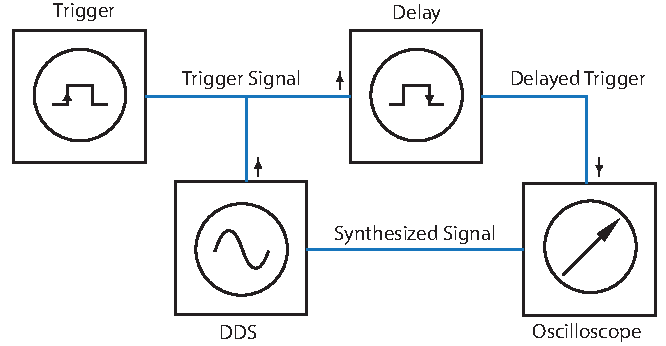
\includegraphics[width=.8\textwidth]{../figure/signal/setup-dds.pdf}
  \caption{Measurement setup of the synthesiyer signal. By inserting a pulse
    generator in between the trigger source and the oscilloscope we can delay
    the capture window of the oscilloscope by the pulse width.
  }\label{fig:signal_window_setup}
\end{figure}
The experimental setup used to reailize this concept is schematically drawn in
\Cref{fig:signal_window_setup}. In between the oscilloscope and the trigger
source we inserted a pulse generator. The pulse generator width equals the
delay time of the oscilloscope as the oscilloscope is configured to capture
on the falling edge signal of the pulse generator. Further the oscilloscope's
impedance was configured to \SI{50}{\ohm}. High impedance measurements at
such frequencies causes very different behaviour as the electromagnetic wave
is reflected subject to the actual frequency inside the coaxial cable. In 
\Cref{tab:signal_parameters_dds} we can find an overview of the experimental
parameters used.
\begin{table}[htb]
  \centering
  \begin{tabular}{cccccc}
    \toprule
    Frequency Range $f$ &
    Sweep Duration $T_s$ &
    Window Duration $T_w$ &
    Number Windows $N_w$ \\
    \midrule
    \SIrange{80}{120}{\mega\hertz} &
    \SI{30}{\milli\second} &
    \SI{50}{\micro\second} &
    300 \\
    \bottomrule
  \end{tabular}
  \caption{Experimental parameters used to inspect the output \gls{rf} signal
    of the \gls{dds}.
  }\label{tab:signal_parameters_dds}
\end{table}
The specified frequency range is motivated to cover the greatest possible
spatial dimensions permitted by the dimensions of the optics. Sweep and
window duration where selected as a compromise between the oscilloscope being
able to resolve the signal fine enough to perform \gls{fft} and the sweep
duration being comparable to later experiments. Time delay was incremented
in $N_w$ steps until $T_s=T_w$, thus we will capture $N_w$ overlapping windows.

\subsubsection{Frequency spectrum}

For an ideal linear frequency sweep we would expect a continous increase of
the frequency with respect to time, yet we know that \gls{dds} makes use of
digital signal processing methods which suggests a discrete frequency
spectrum. To help us expose the characteristics of the digital frequency
sweep we will utilize a spectrogram. A spectrogram visualizes how the
frequency spectrum varies in time. One way to obtain a spectrogram is to
partition the data into overlapping time chunks while performing \gls{fft}
which allows us to combine time and frequency domain specific
characteristics. In our case we choose the relative spectral power to be
encoded through color.
\begin{figure}[htb]
  \centering
  \begin{adjustbox}{width=\textwidth}
    \inputpgf{../figure/signal/synthesis}{spectrogram.pgf}
  \end{adjustbox}
  \caption{Spectrogram of delayed time windows of the \gls{dds} output signal
    configured to perform a linear frequency sweep. For an ideal linear sweep
    we would expect a linear timeline of the frequency, instead we observe a
    discrete set of frequencies.
  }\label{fig:signal_synthesis_spectrogram}
\end{figure}
\Cref{fig:signal_synthesis_spectrogram} depicts four spectrograms, each taken
at a different time window of the frequency sweep passthrough. The first
spectrogram captures the start of the frequency sweep as can be read from
the time scale. The first time window does not disclose any signal. This
phenomena will be observed frequently. For unknown reasons the output signal
of the \gls{dds} is absent for multiple microseconds after the \gls{dds}
receives the external trigger signal. The exact duration of the trigger hole
varies but does not affect the internal state of the \gls{dds} as the first
measured frequency matches the theoretically expected frequency according to
the ramp. If we take a look at the following spectrogram windows we can see
how the \gls{dds} outputs a constant frequency over a short time period,
therefore the frequency range consists of discrete frequencies. We can
actually even observe such a frequency increment in the second, third and
fifth spectrogram. Finally in the last spectrogram the frequency drops back
to the initial value --- a side effect of the \gls{dds} sweep mode which
supports an external trigger signal.

\subsubsection{Amplitude frequency response}

In the Fourier space we can locate the dominant frequency at the maximum of
the power spectrum. That in mind we can reduce the previous obtained time
window measurements to pairs of dominant frequencies and maximum amplitude.
Under the assumption that the maximum voltage per measurement is approximately
the mean peak-to-peak amplitude of the signal --- which during the
oscilloscope suggested during measurements --- we can find the amplitude
frequency response spectrum with manageable effort.
\Cref{fig:signal_synthesis_response} visualizes the described routine for the
\gls{dds} assigned to the \gls{h} and \gls{v} \gls{aod} with frequency control
by digital ramp and manual increments.
\begin{figure}[htb]
  \centering
  \begin{adjustbox}{width=\textwidth}
    %% Creator: Matplotlib, PGF backend
%%
%% To include the figure in your LaTeX document, write
%%   \input{<filename>.pgf}
%%
%% Make sure the required packages are loaded in your preamble
%%   \usepackage{pgf}
%%
%% Figures using additional raster images can only be included by \input if
%% they are in the same directory as the main LaTeX file. For loading figures
%% from other directories you can use the `import` package
%%   \usepackage{import}
%% and then include the figures with
%%   \import{<path to file>}{<filename>.pgf}
%%
%% Matplotlib used the following preamble
%%   \usepackage{amsmath}\usepackage{siunitx}\usepackage{lmodern}
%%   \usepackage{fontspec}
%%
\begingroup%
\makeatletter%
\begin{pgfpicture}%
\pgfpathrectangle{\pgfpointorigin}{\pgfqpoint{12.000000in}{6.000000in}}%
\pgfusepath{use as bounding box, clip}%
\begin{pgfscope}%
\pgfsetbuttcap%
\pgfsetmiterjoin%
\pgfsetlinewidth{0.000000pt}%
\definecolor{currentstroke}{rgb}{1.000000,1.000000,1.000000}%
\pgfsetstrokecolor{currentstroke}%
\pgfsetdash{}{0pt}%
\pgfpathmoveto{\pgfqpoint{0.000000in}{0.000000in}}%
\pgfpathlineto{\pgfqpoint{12.000000in}{0.000000in}}%
\pgfpathlineto{\pgfqpoint{12.000000in}{6.000000in}}%
\pgfpathlineto{\pgfqpoint{0.000000in}{6.000000in}}%
\pgfpathclose%
\pgfusepath{}%
\end{pgfscope}%
\begin{pgfscope}%
\pgfsetbuttcap%
\pgfsetmiterjoin%
\definecolor{currentfill}{rgb}{1.000000,1.000000,1.000000}%
\pgfsetfillcolor{currentfill}%
\pgfsetlinewidth{0.000000pt}%
\definecolor{currentstroke}{rgb}{0.000000,0.000000,0.000000}%
\pgfsetstrokecolor{currentstroke}%
\pgfsetstrokeopacity{0.000000}%
\pgfsetdash{}{0pt}%
\pgfpathmoveto{\pgfqpoint{1.500000in}{1.200000in}}%
\pgfpathlineto{\pgfqpoint{10.800000in}{1.200000in}}%
\pgfpathlineto{\pgfqpoint{10.800000in}{5.880000in}}%
\pgfpathlineto{\pgfqpoint{1.500000in}{5.880000in}}%
\pgfpathclose%
\pgfusepath{fill}%
\end{pgfscope}%
\begin{pgfscope}%
\pgfsetbuttcap%
\pgfsetroundjoin%
\definecolor{currentfill}{rgb}{0.000000,0.000000,0.000000}%
\pgfsetfillcolor{currentfill}%
\pgfsetlinewidth{1.003750pt}%
\definecolor{currentstroke}{rgb}{0.000000,0.000000,0.000000}%
\pgfsetstrokecolor{currentstroke}%
\pgfsetdash{}{0pt}%
\pgfsys@defobject{currentmarker}{\pgfqpoint{0.000000in}{0.000000in}}{\pgfqpoint{0.000000in}{0.055556in}}{%
\pgfpathmoveto{\pgfqpoint{0.000000in}{0.000000in}}%
\pgfpathlineto{\pgfqpoint{0.000000in}{0.055556in}}%
\pgfusepath{stroke,fill}%
}%
\begin{pgfscope}%
\pgfsys@transformshift{1.922727in}{1.200000in}%
\pgfsys@useobject{currentmarker}{}%
\end{pgfscope}%
\end{pgfscope}%
\begin{pgfscope}%
\pgfsetbuttcap%
\pgfsetroundjoin%
\definecolor{currentfill}{rgb}{0.000000,0.000000,0.000000}%
\pgfsetfillcolor{currentfill}%
\pgfsetlinewidth{1.003750pt}%
\definecolor{currentstroke}{rgb}{0.000000,0.000000,0.000000}%
\pgfsetstrokecolor{currentstroke}%
\pgfsetdash{}{0pt}%
\pgfsys@defobject{currentmarker}{\pgfqpoint{0.000000in}{-0.055556in}}{\pgfqpoint{0.000000in}{0.000000in}}{%
\pgfpathmoveto{\pgfqpoint{0.000000in}{0.000000in}}%
\pgfpathlineto{\pgfqpoint{0.000000in}{-0.055556in}}%
\pgfusepath{stroke,fill}%
}%
\begin{pgfscope}%
\pgfsys@transformshift{1.922727in}{5.880000in}%
\pgfsys@useobject{currentmarker}{}%
\end{pgfscope}%
\end{pgfscope}%
\begin{pgfscope}%
\pgftext[x=1.922727in,y=1.102778in,,top]{\fontsize{10.000000}{12.000000}\selectfont \(\displaystyle 80\)}%
\end{pgfscope}%
\begin{pgfscope}%
\pgfsetbuttcap%
\pgfsetroundjoin%
\definecolor{currentfill}{rgb}{0.000000,0.000000,0.000000}%
\pgfsetfillcolor{currentfill}%
\pgfsetlinewidth{1.003750pt}%
\definecolor{currentstroke}{rgb}{0.000000,0.000000,0.000000}%
\pgfsetstrokecolor{currentstroke}%
\pgfsetdash{}{0pt}%
\pgfsys@defobject{currentmarker}{\pgfqpoint{0.000000in}{0.000000in}}{\pgfqpoint{0.000000in}{0.055556in}}{%
\pgfpathmoveto{\pgfqpoint{0.000000in}{0.000000in}}%
\pgfpathlineto{\pgfqpoint{0.000000in}{0.055556in}}%
\pgfusepath{stroke,fill}%
}%
\begin{pgfscope}%
\pgfsys@transformshift{2.979545in}{1.200000in}%
\pgfsys@useobject{currentmarker}{}%
\end{pgfscope}%
\end{pgfscope}%
\begin{pgfscope}%
\pgfsetbuttcap%
\pgfsetroundjoin%
\definecolor{currentfill}{rgb}{0.000000,0.000000,0.000000}%
\pgfsetfillcolor{currentfill}%
\pgfsetlinewidth{1.003750pt}%
\definecolor{currentstroke}{rgb}{0.000000,0.000000,0.000000}%
\pgfsetstrokecolor{currentstroke}%
\pgfsetdash{}{0pt}%
\pgfsys@defobject{currentmarker}{\pgfqpoint{0.000000in}{-0.055556in}}{\pgfqpoint{0.000000in}{0.000000in}}{%
\pgfpathmoveto{\pgfqpoint{0.000000in}{0.000000in}}%
\pgfpathlineto{\pgfqpoint{0.000000in}{-0.055556in}}%
\pgfusepath{stroke,fill}%
}%
\begin{pgfscope}%
\pgfsys@transformshift{2.979545in}{5.880000in}%
\pgfsys@useobject{currentmarker}{}%
\end{pgfscope}%
\end{pgfscope}%
\begin{pgfscope}%
\pgftext[x=2.979545in,y=1.102778in,,top]{\fontsize{10.000000}{12.000000}\selectfont \(\displaystyle 85\)}%
\end{pgfscope}%
\begin{pgfscope}%
\pgfsetbuttcap%
\pgfsetroundjoin%
\definecolor{currentfill}{rgb}{0.000000,0.000000,0.000000}%
\pgfsetfillcolor{currentfill}%
\pgfsetlinewidth{1.003750pt}%
\definecolor{currentstroke}{rgb}{0.000000,0.000000,0.000000}%
\pgfsetstrokecolor{currentstroke}%
\pgfsetdash{}{0pt}%
\pgfsys@defobject{currentmarker}{\pgfqpoint{0.000000in}{0.000000in}}{\pgfqpoint{0.000000in}{0.055556in}}{%
\pgfpathmoveto{\pgfqpoint{0.000000in}{0.000000in}}%
\pgfpathlineto{\pgfqpoint{0.000000in}{0.055556in}}%
\pgfusepath{stroke,fill}%
}%
\begin{pgfscope}%
\pgfsys@transformshift{4.036364in}{1.200000in}%
\pgfsys@useobject{currentmarker}{}%
\end{pgfscope}%
\end{pgfscope}%
\begin{pgfscope}%
\pgfsetbuttcap%
\pgfsetroundjoin%
\definecolor{currentfill}{rgb}{0.000000,0.000000,0.000000}%
\pgfsetfillcolor{currentfill}%
\pgfsetlinewidth{1.003750pt}%
\definecolor{currentstroke}{rgb}{0.000000,0.000000,0.000000}%
\pgfsetstrokecolor{currentstroke}%
\pgfsetdash{}{0pt}%
\pgfsys@defobject{currentmarker}{\pgfqpoint{0.000000in}{-0.055556in}}{\pgfqpoint{0.000000in}{0.000000in}}{%
\pgfpathmoveto{\pgfqpoint{0.000000in}{0.000000in}}%
\pgfpathlineto{\pgfqpoint{0.000000in}{-0.055556in}}%
\pgfusepath{stroke,fill}%
}%
\begin{pgfscope}%
\pgfsys@transformshift{4.036364in}{5.880000in}%
\pgfsys@useobject{currentmarker}{}%
\end{pgfscope}%
\end{pgfscope}%
\begin{pgfscope}%
\pgftext[x=4.036364in,y=1.102778in,,top]{\fontsize{10.000000}{12.000000}\selectfont \(\displaystyle 90\)}%
\end{pgfscope}%
\begin{pgfscope}%
\pgfsetbuttcap%
\pgfsetroundjoin%
\definecolor{currentfill}{rgb}{0.000000,0.000000,0.000000}%
\pgfsetfillcolor{currentfill}%
\pgfsetlinewidth{1.003750pt}%
\definecolor{currentstroke}{rgb}{0.000000,0.000000,0.000000}%
\pgfsetstrokecolor{currentstroke}%
\pgfsetdash{}{0pt}%
\pgfsys@defobject{currentmarker}{\pgfqpoint{0.000000in}{0.000000in}}{\pgfqpoint{0.000000in}{0.055556in}}{%
\pgfpathmoveto{\pgfqpoint{0.000000in}{0.000000in}}%
\pgfpathlineto{\pgfqpoint{0.000000in}{0.055556in}}%
\pgfusepath{stroke,fill}%
}%
\begin{pgfscope}%
\pgfsys@transformshift{5.093182in}{1.200000in}%
\pgfsys@useobject{currentmarker}{}%
\end{pgfscope}%
\end{pgfscope}%
\begin{pgfscope}%
\pgfsetbuttcap%
\pgfsetroundjoin%
\definecolor{currentfill}{rgb}{0.000000,0.000000,0.000000}%
\pgfsetfillcolor{currentfill}%
\pgfsetlinewidth{1.003750pt}%
\definecolor{currentstroke}{rgb}{0.000000,0.000000,0.000000}%
\pgfsetstrokecolor{currentstroke}%
\pgfsetdash{}{0pt}%
\pgfsys@defobject{currentmarker}{\pgfqpoint{0.000000in}{-0.055556in}}{\pgfqpoint{0.000000in}{0.000000in}}{%
\pgfpathmoveto{\pgfqpoint{0.000000in}{0.000000in}}%
\pgfpathlineto{\pgfqpoint{0.000000in}{-0.055556in}}%
\pgfusepath{stroke,fill}%
}%
\begin{pgfscope}%
\pgfsys@transformshift{5.093182in}{5.880000in}%
\pgfsys@useobject{currentmarker}{}%
\end{pgfscope}%
\end{pgfscope}%
\begin{pgfscope}%
\pgftext[x=5.093182in,y=1.102778in,,top]{\fontsize{10.000000}{12.000000}\selectfont \(\displaystyle 95\)}%
\end{pgfscope}%
\begin{pgfscope}%
\pgfsetbuttcap%
\pgfsetroundjoin%
\definecolor{currentfill}{rgb}{0.000000,0.000000,0.000000}%
\pgfsetfillcolor{currentfill}%
\pgfsetlinewidth{1.003750pt}%
\definecolor{currentstroke}{rgb}{0.000000,0.000000,0.000000}%
\pgfsetstrokecolor{currentstroke}%
\pgfsetdash{}{0pt}%
\pgfsys@defobject{currentmarker}{\pgfqpoint{0.000000in}{0.000000in}}{\pgfqpoint{0.000000in}{0.055556in}}{%
\pgfpathmoveto{\pgfqpoint{0.000000in}{0.000000in}}%
\pgfpathlineto{\pgfqpoint{0.000000in}{0.055556in}}%
\pgfusepath{stroke,fill}%
}%
\begin{pgfscope}%
\pgfsys@transformshift{6.150000in}{1.200000in}%
\pgfsys@useobject{currentmarker}{}%
\end{pgfscope}%
\end{pgfscope}%
\begin{pgfscope}%
\pgfsetbuttcap%
\pgfsetroundjoin%
\definecolor{currentfill}{rgb}{0.000000,0.000000,0.000000}%
\pgfsetfillcolor{currentfill}%
\pgfsetlinewidth{1.003750pt}%
\definecolor{currentstroke}{rgb}{0.000000,0.000000,0.000000}%
\pgfsetstrokecolor{currentstroke}%
\pgfsetdash{}{0pt}%
\pgfsys@defobject{currentmarker}{\pgfqpoint{0.000000in}{-0.055556in}}{\pgfqpoint{0.000000in}{0.000000in}}{%
\pgfpathmoveto{\pgfqpoint{0.000000in}{0.000000in}}%
\pgfpathlineto{\pgfqpoint{0.000000in}{-0.055556in}}%
\pgfusepath{stroke,fill}%
}%
\begin{pgfscope}%
\pgfsys@transformshift{6.150000in}{5.880000in}%
\pgfsys@useobject{currentmarker}{}%
\end{pgfscope}%
\end{pgfscope}%
\begin{pgfscope}%
\pgftext[x=6.150000in,y=1.102778in,,top]{\fontsize{10.000000}{12.000000}\selectfont \(\displaystyle 100\)}%
\end{pgfscope}%
\begin{pgfscope}%
\pgfsetbuttcap%
\pgfsetroundjoin%
\definecolor{currentfill}{rgb}{0.000000,0.000000,0.000000}%
\pgfsetfillcolor{currentfill}%
\pgfsetlinewidth{1.003750pt}%
\definecolor{currentstroke}{rgb}{0.000000,0.000000,0.000000}%
\pgfsetstrokecolor{currentstroke}%
\pgfsetdash{}{0pt}%
\pgfsys@defobject{currentmarker}{\pgfqpoint{0.000000in}{0.000000in}}{\pgfqpoint{0.000000in}{0.055556in}}{%
\pgfpathmoveto{\pgfqpoint{0.000000in}{0.000000in}}%
\pgfpathlineto{\pgfqpoint{0.000000in}{0.055556in}}%
\pgfusepath{stroke,fill}%
}%
\begin{pgfscope}%
\pgfsys@transformshift{7.206818in}{1.200000in}%
\pgfsys@useobject{currentmarker}{}%
\end{pgfscope}%
\end{pgfscope}%
\begin{pgfscope}%
\pgfsetbuttcap%
\pgfsetroundjoin%
\definecolor{currentfill}{rgb}{0.000000,0.000000,0.000000}%
\pgfsetfillcolor{currentfill}%
\pgfsetlinewidth{1.003750pt}%
\definecolor{currentstroke}{rgb}{0.000000,0.000000,0.000000}%
\pgfsetstrokecolor{currentstroke}%
\pgfsetdash{}{0pt}%
\pgfsys@defobject{currentmarker}{\pgfqpoint{0.000000in}{-0.055556in}}{\pgfqpoint{0.000000in}{0.000000in}}{%
\pgfpathmoveto{\pgfqpoint{0.000000in}{0.000000in}}%
\pgfpathlineto{\pgfqpoint{0.000000in}{-0.055556in}}%
\pgfusepath{stroke,fill}%
}%
\begin{pgfscope}%
\pgfsys@transformshift{7.206818in}{5.880000in}%
\pgfsys@useobject{currentmarker}{}%
\end{pgfscope}%
\end{pgfscope}%
\begin{pgfscope}%
\pgftext[x=7.206818in,y=1.102778in,,top]{\fontsize{10.000000}{12.000000}\selectfont \(\displaystyle 105\)}%
\end{pgfscope}%
\begin{pgfscope}%
\pgfsetbuttcap%
\pgfsetroundjoin%
\definecolor{currentfill}{rgb}{0.000000,0.000000,0.000000}%
\pgfsetfillcolor{currentfill}%
\pgfsetlinewidth{1.003750pt}%
\definecolor{currentstroke}{rgb}{0.000000,0.000000,0.000000}%
\pgfsetstrokecolor{currentstroke}%
\pgfsetdash{}{0pt}%
\pgfsys@defobject{currentmarker}{\pgfqpoint{0.000000in}{0.000000in}}{\pgfqpoint{0.000000in}{0.055556in}}{%
\pgfpathmoveto{\pgfqpoint{0.000000in}{0.000000in}}%
\pgfpathlineto{\pgfqpoint{0.000000in}{0.055556in}}%
\pgfusepath{stroke,fill}%
}%
\begin{pgfscope}%
\pgfsys@transformshift{8.263636in}{1.200000in}%
\pgfsys@useobject{currentmarker}{}%
\end{pgfscope}%
\end{pgfscope}%
\begin{pgfscope}%
\pgfsetbuttcap%
\pgfsetroundjoin%
\definecolor{currentfill}{rgb}{0.000000,0.000000,0.000000}%
\pgfsetfillcolor{currentfill}%
\pgfsetlinewidth{1.003750pt}%
\definecolor{currentstroke}{rgb}{0.000000,0.000000,0.000000}%
\pgfsetstrokecolor{currentstroke}%
\pgfsetdash{}{0pt}%
\pgfsys@defobject{currentmarker}{\pgfqpoint{0.000000in}{-0.055556in}}{\pgfqpoint{0.000000in}{0.000000in}}{%
\pgfpathmoveto{\pgfqpoint{0.000000in}{0.000000in}}%
\pgfpathlineto{\pgfqpoint{0.000000in}{-0.055556in}}%
\pgfusepath{stroke,fill}%
}%
\begin{pgfscope}%
\pgfsys@transformshift{8.263636in}{5.880000in}%
\pgfsys@useobject{currentmarker}{}%
\end{pgfscope}%
\end{pgfscope}%
\begin{pgfscope}%
\pgftext[x=8.263636in,y=1.102778in,,top]{\fontsize{10.000000}{12.000000}\selectfont \(\displaystyle 110\)}%
\end{pgfscope}%
\begin{pgfscope}%
\pgfsetbuttcap%
\pgfsetroundjoin%
\definecolor{currentfill}{rgb}{0.000000,0.000000,0.000000}%
\pgfsetfillcolor{currentfill}%
\pgfsetlinewidth{1.003750pt}%
\definecolor{currentstroke}{rgb}{0.000000,0.000000,0.000000}%
\pgfsetstrokecolor{currentstroke}%
\pgfsetdash{}{0pt}%
\pgfsys@defobject{currentmarker}{\pgfqpoint{0.000000in}{0.000000in}}{\pgfqpoint{0.000000in}{0.055556in}}{%
\pgfpathmoveto{\pgfqpoint{0.000000in}{0.000000in}}%
\pgfpathlineto{\pgfqpoint{0.000000in}{0.055556in}}%
\pgfusepath{stroke,fill}%
}%
\begin{pgfscope}%
\pgfsys@transformshift{9.320455in}{1.200000in}%
\pgfsys@useobject{currentmarker}{}%
\end{pgfscope}%
\end{pgfscope}%
\begin{pgfscope}%
\pgfsetbuttcap%
\pgfsetroundjoin%
\definecolor{currentfill}{rgb}{0.000000,0.000000,0.000000}%
\pgfsetfillcolor{currentfill}%
\pgfsetlinewidth{1.003750pt}%
\definecolor{currentstroke}{rgb}{0.000000,0.000000,0.000000}%
\pgfsetstrokecolor{currentstroke}%
\pgfsetdash{}{0pt}%
\pgfsys@defobject{currentmarker}{\pgfqpoint{0.000000in}{-0.055556in}}{\pgfqpoint{0.000000in}{0.000000in}}{%
\pgfpathmoveto{\pgfqpoint{0.000000in}{0.000000in}}%
\pgfpathlineto{\pgfqpoint{0.000000in}{-0.055556in}}%
\pgfusepath{stroke,fill}%
}%
\begin{pgfscope}%
\pgfsys@transformshift{9.320455in}{5.880000in}%
\pgfsys@useobject{currentmarker}{}%
\end{pgfscope}%
\end{pgfscope}%
\begin{pgfscope}%
\pgftext[x=9.320455in,y=1.102778in,,top]{\fontsize{10.000000}{12.000000}\selectfont \(\displaystyle 115\)}%
\end{pgfscope}%
\begin{pgfscope}%
\pgfsetbuttcap%
\pgfsetroundjoin%
\definecolor{currentfill}{rgb}{0.000000,0.000000,0.000000}%
\pgfsetfillcolor{currentfill}%
\pgfsetlinewidth{1.003750pt}%
\definecolor{currentstroke}{rgb}{0.000000,0.000000,0.000000}%
\pgfsetstrokecolor{currentstroke}%
\pgfsetdash{}{0pt}%
\pgfsys@defobject{currentmarker}{\pgfqpoint{0.000000in}{0.000000in}}{\pgfqpoint{0.000000in}{0.055556in}}{%
\pgfpathmoveto{\pgfqpoint{0.000000in}{0.000000in}}%
\pgfpathlineto{\pgfqpoint{0.000000in}{0.055556in}}%
\pgfusepath{stroke,fill}%
}%
\begin{pgfscope}%
\pgfsys@transformshift{10.377273in}{1.200000in}%
\pgfsys@useobject{currentmarker}{}%
\end{pgfscope}%
\end{pgfscope}%
\begin{pgfscope}%
\pgfsetbuttcap%
\pgfsetroundjoin%
\definecolor{currentfill}{rgb}{0.000000,0.000000,0.000000}%
\pgfsetfillcolor{currentfill}%
\pgfsetlinewidth{1.003750pt}%
\definecolor{currentstroke}{rgb}{0.000000,0.000000,0.000000}%
\pgfsetstrokecolor{currentstroke}%
\pgfsetdash{}{0pt}%
\pgfsys@defobject{currentmarker}{\pgfqpoint{0.000000in}{-0.055556in}}{\pgfqpoint{0.000000in}{0.000000in}}{%
\pgfpathmoveto{\pgfqpoint{0.000000in}{0.000000in}}%
\pgfpathlineto{\pgfqpoint{0.000000in}{-0.055556in}}%
\pgfusepath{stroke,fill}%
}%
\begin{pgfscope}%
\pgfsys@transformshift{10.377273in}{5.880000in}%
\pgfsys@useobject{currentmarker}{}%
\end{pgfscope}%
\end{pgfscope}%
\begin{pgfscope}%
\pgftext[x=10.377273in,y=1.102778in,,top]{\fontsize{10.000000}{12.000000}\selectfont \(\displaystyle 120\)}%
\end{pgfscope}%
\begin{pgfscope}%
\pgftext[x=6.150000in,y=0.868333in,,top]{\fontsize{14.000000}{16.800000}\selectfont f (\si{\mega\hertz})}%
\end{pgfscope}%
\begin{pgfscope}%
\pgfsetbuttcap%
\pgfsetroundjoin%
\definecolor{currentfill}{rgb}{0.000000,0.000000,0.000000}%
\pgfsetfillcolor{currentfill}%
\pgfsetlinewidth{1.003750pt}%
\definecolor{currentstroke}{rgb}{0.000000,0.000000,0.000000}%
\pgfsetstrokecolor{currentstroke}%
\pgfsetdash{}{0pt}%
\pgfsys@defobject{currentmarker}{\pgfqpoint{0.000000in}{0.000000in}}{\pgfqpoint{0.055556in}{0.000000in}}{%
\pgfpathmoveto{\pgfqpoint{0.000000in}{0.000000in}}%
\pgfpathlineto{\pgfqpoint{0.055556in}{0.000000in}}%
\pgfusepath{stroke,fill}%
}%
\begin{pgfscope}%
\pgfsys@transformshift{1.500000in}{1.200000in}%
\pgfsys@useobject{currentmarker}{}%
\end{pgfscope}%
\end{pgfscope}%
\begin{pgfscope}%
\pgfsetbuttcap%
\pgfsetroundjoin%
\definecolor{currentfill}{rgb}{0.000000,0.000000,0.000000}%
\pgfsetfillcolor{currentfill}%
\pgfsetlinewidth{1.003750pt}%
\definecolor{currentstroke}{rgb}{0.000000,0.000000,0.000000}%
\pgfsetstrokecolor{currentstroke}%
\pgfsetdash{}{0pt}%
\pgfsys@defobject{currentmarker}{\pgfqpoint{-0.055556in}{0.000000in}}{\pgfqpoint{0.000000in}{0.000000in}}{%
\pgfpathmoveto{\pgfqpoint{0.000000in}{0.000000in}}%
\pgfpathlineto{\pgfqpoint{-0.055556in}{0.000000in}}%
\pgfusepath{stroke,fill}%
}%
\begin{pgfscope}%
\pgfsys@transformshift{10.800000in}{1.200000in}%
\pgfsys@useobject{currentmarker}{}%
\end{pgfscope}%
\end{pgfscope}%
\begin{pgfscope}%
\pgftext[x=1.155864in,y=1.151806in,left,base]{\fontsize{10.000000}{12.000000}\selectfont \(\displaystyle 0.00\)}%
\end{pgfscope}%
\begin{pgfscope}%
\pgfsetbuttcap%
\pgfsetroundjoin%
\definecolor{currentfill}{rgb}{0.000000,0.000000,0.000000}%
\pgfsetfillcolor{currentfill}%
\pgfsetlinewidth{1.003750pt}%
\definecolor{currentstroke}{rgb}{0.000000,0.000000,0.000000}%
\pgfsetstrokecolor{currentstroke}%
\pgfsetdash{}{0pt}%
\pgfsys@defobject{currentmarker}{\pgfqpoint{0.000000in}{0.000000in}}{\pgfqpoint{0.055556in}{0.000000in}}{%
\pgfpathmoveto{\pgfqpoint{0.000000in}{0.000000in}}%
\pgfpathlineto{\pgfqpoint{0.055556in}{0.000000in}}%
\pgfusepath{stroke,fill}%
}%
\begin{pgfscope}%
\pgfsys@transformshift{1.500000in}{1.785000in}%
\pgfsys@useobject{currentmarker}{}%
\end{pgfscope}%
\end{pgfscope}%
\begin{pgfscope}%
\pgfsetbuttcap%
\pgfsetroundjoin%
\definecolor{currentfill}{rgb}{0.000000,0.000000,0.000000}%
\pgfsetfillcolor{currentfill}%
\pgfsetlinewidth{1.003750pt}%
\definecolor{currentstroke}{rgb}{0.000000,0.000000,0.000000}%
\pgfsetstrokecolor{currentstroke}%
\pgfsetdash{}{0pt}%
\pgfsys@defobject{currentmarker}{\pgfqpoint{-0.055556in}{0.000000in}}{\pgfqpoint{0.000000in}{0.000000in}}{%
\pgfpathmoveto{\pgfqpoint{0.000000in}{0.000000in}}%
\pgfpathlineto{\pgfqpoint{-0.055556in}{0.000000in}}%
\pgfusepath{stroke,fill}%
}%
\begin{pgfscope}%
\pgfsys@transformshift{10.800000in}{1.785000in}%
\pgfsys@useobject{currentmarker}{}%
\end{pgfscope}%
\end{pgfscope}%
\begin{pgfscope}%
\pgftext[x=1.155864in,y=1.736806in,left,base]{\fontsize{10.000000}{12.000000}\selectfont \(\displaystyle 0.05\)}%
\end{pgfscope}%
\begin{pgfscope}%
\pgfsetbuttcap%
\pgfsetroundjoin%
\definecolor{currentfill}{rgb}{0.000000,0.000000,0.000000}%
\pgfsetfillcolor{currentfill}%
\pgfsetlinewidth{1.003750pt}%
\definecolor{currentstroke}{rgb}{0.000000,0.000000,0.000000}%
\pgfsetstrokecolor{currentstroke}%
\pgfsetdash{}{0pt}%
\pgfsys@defobject{currentmarker}{\pgfqpoint{0.000000in}{0.000000in}}{\pgfqpoint{0.055556in}{0.000000in}}{%
\pgfpathmoveto{\pgfqpoint{0.000000in}{0.000000in}}%
\pgfpathlineto{\pgfqpoint{0.055556in}{0.000000in}}%
\pgfusepath{stroke,fill}%
}%
\begin{pgfscope}%
\pgfsys@transformshift{1.500000in}{2.370000in}%
\pgfsys@useobject{currentmarker}{}%
\end{pgfscope}%
\end{pgfscope}%
\begin{pgfscope}%
\pgfsetbuttcap%
\pgfsetroundjoin%
\definecolor{currentfill}{rgb}{0.000000,0.000000,0.000000}%
\pgfsetfillcolor{currentfill}%
\pgfsetlinewidth{1.003750pt}%
\definecolor{currentstroke}{rgb}{0.000000,0.000000,0.000000}%
\pgfsetstrokecolor{currentstroke}%
\pgfsetdash{}{0pt}%
\pgfsys@defobject{currentmarker}{\pgfqpoint{-0.055556in}{0.000000in}}{\pgfqpoint{0.000000in}{0.000000in}}{%
\pgfpathmoveto{\pgfqpoint{0.000000in}{0.000000in}}%
\pgfpathlineto{\pgfqpoint{-0.055556in}{0.000000in}}%
\pgfusepath{stroke,fill}%
}%
\begin{pgfscope}%
\pgfsys@transformshift{10.800000in}{2.370000in}%
\pgfsys@useobject{currentmarker}{}%
\end{pgfscope}%
\end{pgfscope}%
\begin{pgfscope}%
\pgftext[x=1.155864in,y=2.321806in,left,base]{\fontsize{10.000000}{12.000000}\selectfont \(\displaystyle 0.10\)}%
\end{pgfscope}%
\begin{pgfscope}%
\pgfsetbuttcap%
\pgfsetroundjoin%
\definecolor{currentfill}{rgb}{0.000000,0.000000,0.000000}%
\pgfsetfillcolor{currentfill}%
\pgfsetlinewidth{1.003750pt}%
\definecolor{currentstroke}{rgb}{0.000000,0.000000,0.000000}%
\pgfsetstrokecolor{currentstroke}%
\pgfsetdash{}{0pt}%
\pgfsys@defobject{currentmarker}{\pgfqpoint{0.000000in}{0.000000in}}{\pgfqpoint{0.055556in}{0.000000in}}{%
\pgfpathmoveto{\pgfqpoint{0.000000in}{0.000000in}}%
\pgfpathlineto{\pgfqpoint{0.055556in}{0.000000in}}%
\pgfusepath{stroke,fill}%
}%
\begin{pgfscope}%
\pgfsys@transformshift{1.500000in}{2.955000in}%
\pgfsys@useobject{currentmarker}{}%
\end{pgfscope}%
\end{pgfscope}%
\begin{pgfscope}%
\pgfsetbuttcap%
\pgfsetroundjoin%
\definecolor{currentfill}{rgb}{0.000000,0.000000,0.000000}%
\pgfsetfillcolor{currentfill}%
\pgfsetlinewidth{1.003750pt}%
\definecolor{currentstroke}{rgb}{0.000000,0.000000,0.000000}%
\pgfsetstrokecolor{currentstroke}%
\pgfsetdash{}{0pt}%
\pgfsys@defobject{currentmarker}{\pgfqpoint{-0.055556in}{0.000000in}}{\pgfqpoint{0.000000in}{0.000000in}}{%
\pgfpathmoveto{\pgfqpoint{0.000000in}{0.000000in}}%
\pgfpathlineto{\pgfqpoint{-0.055556in}{0.000000in}}%
\pgfusepath{stroke,fill}%
}%
\begin{pgfscope}%
\pgfsys@transformshift{10.800000in}{2.955000in}%
\pgfsys@useobject{currentmarker}{}%
\end{pgfscope}%
\end{pgfscope}%
\begin{pgfscope}%
\pgftext[x=1.155864in,y=2.906806in,left,base]{\fontsize{10.000000}{12.000000}\selectfont \(\displaystyle 0.15\)}%
\end{pgfscope}%
\begin{pgfscope}%
\pgfsetbuttcap%
\pgfsetroundjoin%
\definecolor{currentfill}{rgb}{0.000000,0.000000,0.000000}%
\pgfsetfillcolor{currentfill}%
\pgfsetlinewidth{1.003750pt}%
\definecolor{currentstroke}{rgb}{0.000000,0.000000,0.000000}%
\pgfsetstrokecolor{currentstroke}%
\pgfsetdash{}{0pt}%
\pgfsys@defobject{currentmarker}{\pgfqpoint{0.000000in}{0.000000in}}{\pgfqpoint{0.055556in}{0.000000in}}{%
\pgfpathmoveto{\pgfqpoint{0.000000in}{0.000000in}}%
\pgfpathlineto{\pgfqpoint{0.055556in}{0.000000in}}%
\pgfusepath{stroke,fill}%
}%
\begin{pgfscope}%
\pgfsys@transformshift{1.500000in}{3.540000in}%
\pgfsys@useobject{currentmarker}{}%
\end{pgfscope}%
\end{pgfscope}%
\begin{pgfscope}%
\pgfsetbuttcap%
\pgfsetroundjoin%
\definecolor{currentfill}{rgb}{0.000000,0.000000,0.000000}%
\pgfsetfillcolor{currentfill}%
\pgfsetlinewidth{1.003750pt}%
\definecolor{currentstroke}{rgb}{0.000000,0.000000,0.000000}%
\pgfsetstrokecolor{currentstroke}%
\pgfsetdash{}{0pt}%
\pgfsys@defobject{currentmarker}{\pgfqpoint{-0.055556in}{0.000000in}}{\pgfqpoint{0.000000in}{0.000000in}}{%
\pgfpathmoveto{\pgfqpoint{0.000000in}{0.000000in}}%
\pgfpathlineto{\pgfqpoint{-0.055556in}{0.000000in}}%
\pgfusepath{stroke,fill}%
}%
\begin{pgfscope}%
\pgfsys@transformshift{10.800000in}{3.540000in}%
\pgfsys@useobject{currentmarker}{}%
\end{pgfscope}%
\end{pgfscope}%
\begin{pgfscope}%
\pgftext[x=1.155864in,y=3.491806in,left,base]{\fontsize{10.000000}{12.000000}\selectfont \(\displaystyle 0.20\)}%
\end{pgfscope}%
\begin{pgfscope}%
\pgfsetbuttcap%
\pgfsetroundjoin%
\definecolor{currentfill}{rgb}{0.000000,0.000000,0.000000}%
\pgfsetfillcolor{currentfill}%
\pgfsetlinewidth{1.003750pt}%
\definecolor{currentstroke}{rgb}{0.000000,0.000000,0.000000}%
\pgfsetstrokecolor{currentstroke}%
\pgfsetdash{}{0pt}%
\pgfsys@defobject{currentmarker}{\pgfqpoint{0.000000in}{0.000000in}}{\pgfqpoint{0.055556in}{0.000000in}}{%
\pgfpathmoveto{\pgfqpoint{0.000000in}{0.000000in}}%
\pgfpathlineto{\pgfqpoint{0.055556in}{0.000000in}}%
\pgfusepath{stroke,fill}%
}%
\begin{pgfscope}%
\pgfsys@transformshift{1.500000in}{4.125000in}%
\pgfsys@useobject{currentmarker}{}%
\end{pgfscope}%
\end{pgfscope}%
\begin{pgfscope}%
\pgfsetbuttcap%
\pgfsetroundjoin%
\definecolor{currentfill}{rgb}{0.000000,0.000000,0.000000}%
\pgfsetfillcolor{currentfill}%
\pgfsetlinewidth{1.003750pt}%
\definecolor{currentstroke}{rgb}{0.000000,0.000000,0.000000}%
\pgfsetstrokecolor{currentstroke}%
\pgfsetdash{}{0pt}%
\pgfsys@defobject{currentmarker}{\pgfqpoint{-0.055556in}{0.000000in}}{\pgfqpoint{0.000000in}{0.000000in}}{%
\pgfpathmoveto{\pgfqpoint{0.000000in}{0.000000in}}%
\pgfpathlineto{\pgfqpoint{-0.055556in}{0.000000in}}%
\pgfusepath{stroke,fill}%
}%
\begin{pgfscope}%
\pgfsys@transformshift{10.800000in}{4.125000in}%
\pgfsys@useobject{currentmarker}{}%
\end{pgfscope}%
\end{pgfscope}%
\begin{pgfscope}%
\pgftext[x=1.155864in,y=4.076806in,left,base]{\fontsize{10.000000}{12.000000}\selectfont \(\displaystyle 0.25\)}%
\end{pgfscope}%
\begin{pgfscope}%
\pgfsetbuttcap%
\pgfsetroundjoin%
\definecolor{currentfill}{rgb}{0.000000,0.000000,0.000000}%
\pgfsetfillcolor{currentfill}%
\pgfsetlinewidth{1.003750pt}%
\definecolor{currentstroke}{rgb}{0.000000,0.000000,0.000000}%
\pgfsetstrokecolor{currentstroke}%
\pgfsetdash{}{0pt}%
\pgfsys@defobject{currentmarker}{\pgfqpoint{0.000000in}{0.000000in}}{\pgfqpoint{0.055556in}{0.000000in}}{%
\pgfpathmoveto{\pgfqpoint{0.000000in}{0.000000in}}%
\pgfpathlineto{\pgfqpoint{0.055556in}{0.000000in}}%
\pgfusepath{stroke,fill}%
}%
\begin{pgfscope}%
\pgfsys@transformshift{1.500000in}{4.710000in}%
\pgfsys@useobject{currentmarker}{}%
\end{pgfscope}%
\end{pgfscope}%
\begin{pgfscope}%
\pgfsetbuttcap%
\pgfsetroundjoin%
\definecolor{currentfill}{rgb}{0.000000,0.000000,0.000000}%
\pgfsetfillcolor{currentfill}%
\pgfsetlinewidth{1.003750pt}%
\definecolor{currentstroke}{rgb}{0.000000,0.000000,0.000000}%
\pgfsetstrokecolor{currentstroke}%
\pgfsetdash{}{0pt}%
\pgfsys@defobject{currentmarker}{\pgfqpoint{-0.055556in}{0.000000in}}{\pgfqpoint{0.000000in}{0.000000in}}{%
\pgfpathmoveto{\pgfqpoint{0.000000in}{0.000000in}}%
\pgfpathlineto{\pgfqpoint{-0.055556in}{0.000000in}}%
\pgfusepath{stroke,fill}%
}%
\begin{pgfscope}%
\pgfsys@transformshift{10.800000in}{4.710000in}%
\pgfsys@useobject{currentmarker}{}%
\end{pgfscope}%
\end{pgfscope}%
\begin{pgfscope}%
\pgftext[x=1.155864in,y=4.661806in,left,base]{\fontsize{10.000000}{12.000000}\selectfont \(\displaystyle 0.30\)}%
\end{pgfscope}%
\begin{pgfscope}%
\pgfsetbuttcap%
\pgfsetroundjoin%
\definecolor{currentfill}{rgb}{0.000000,0.000000,0.000000}%
\pgfsetfillcolor{currentfill}%
\pgfsetlinewidth{1.003750pt}%
\definecolor{currentstroke}{rgb}{0.000000,0.000000,0.000000}%
\pgfsetstrokecolor{currentstroke}%
\pgfsetdash{}{0pt}%
\pgfsys@defobject{currentmarker}{\pgfqpoint{0.000000in}{0.000000in}}{\pgfqpoint{0.055556in}{0.000000in}}{%
\pgfpathmoveto{\pgfqpoint{0.000000in}{0.000000in}}%
\pgfpathlineto{\pgfqpoint{0.055556in}{0.000000in}}%
\pgfusepath{stroke,fill}%
}%
\begin{pgfscope}%
\pgfsys@transformshift{1.500000in}{5.295000in}%
\pgfsys@useobject{currentmarker}{}%
\end{pgfscope}%
\end{pgfscope}%
\begin{pgfscope}%
\pgfsetbuttcap%
\pgfsetroundjoin%
\definecolor{currentfill}{rgb}{0.000000,0.000000,0.000000}%
\pgfsetfillcolor{currentfill}%
\pgfsetlinewidth{1.003750pt}%
\definecolor{currentstroke}{rgb}{0.000000,0.000000,0.000000}%
\pgfsetstrokecolor{currentstroke}%
\pgfsetdash{}{0pt}%
\pgfsys@defobject{currentmarker}{\pgfqpoint{-0.055556in}{0.000000in}}{\pgfqpoint{0.000000in}{0.000000in}}{%
\pgfpathmoveto{\pgfqpoint{0.000000in}{0.000000in}}%
\pgfpathlineto{\pgfqpoint{-0.055556in}{0.000000in}}%
\pgfusepath{stroke,fill}%
}%
\begin{pgfscope}%
\pgfsys@transformshift{10.800000in}{5.295000in}%
\pgfsys@useobject{currentmarker}{}%
\end{pgfscope}%
\end{pgfscope}%
\begin{pgfscope}%
\pgftext[x=1.155864in,y=5.246806in,left,base]{\fontsize{10.000000}{12.000000}\selectfont \(\displaystyle 0.35\)}%
\end{pgfscope}%
\begin{pgfscope}%
\pgfsetbuttcap%
\pgfsetroundjoin%
\definecolor{currentfill}{rgb}{0.000000,0.000000,0.000000}%
\pgfsetfillcolor{currentfill}%
\pgfsetlinewidth{1.003750pt}%
\definecolor{currentstroke}{rgb}{0.000000,0.000000,0.000000}%
\pgfsetstrokecolor{currentstroke}%
\pgfsetdash{}{0pt}%
\pgfsys@defobject{currentmarker}{\pgfqpoint{0.000000in}{0.000000in}}{\pgfqpoint{0.055556in}{0.000000in}}{%
\pgfpathmoveto{\pgfqpoint{0.000000in}{0.000000in}}%
\pgfpathlineto{\pgfqpoint{0.055556in}{0.000000in}}%
\pgfusepath{stroke,fill}%
}%
\begin{pgfscope}%
\pgfsys@transformshift{1.500000in}{5.880000in}%
\pgfsys@useobject{currentmarker}{}%
\end{pgfscope}%
\end{pgfscope}%
\begin{pgfscope}%
\pgfsetbuttcap%
\pgfsetroundjoin%
\definecolor{currentfill}{rgb}{0.000000,0.000000,0.000000}%
\pgfsetfillcolor{currentfill}%
\pgfsetlinewidth{1.003750pt}%
\definecolor{currentstroke}{rgb}{0.000000,0.000000,0.000000}%
\pgfsetstrokecolor{currentstroke}%
\pgfsetdash{}{0pt}%
\pgfsys@defobject{currentmarker}{\pgfqpoint{-0.055556in}{0.000000in}}{\pgfqpoint{0.000000in}{0.000000in}}{%
\pgfpathmoveto{\pgfqpoint{0.000000in}{0.000000in}}%
\pgfpathlineto{\pgfqpoint{-0.055556in}{0.000000in}}%
\pgfusepath{stroke,fill}%
}%
\begin{pgfscope}%
\pgfsys@transformshift{10.800000in}{5.880000in}%
\pgfsys@useobject{currentmarker}{}%
\end{pgfscope}%
\end{pgfscope}%
\begin{pgfscope}%
\pgftext[x=1.155864in,y=5.831806in,left,base]{\fontsize{10.000000}{12.000000}\selectfont \(\displaystyle 0.40\)}%
\end{pgfscope}%
\begin{pgfscope}%
\pgfsetbuttcap%
\pgfsetroundjoin%
\definecolor{currentfill}{rgb}{0.000000,0.000000,0.000000}%
\pgfsetfillcolor{currentfill}%
\pgfsetlinewidth{0.501875pt}%
\definecolor{currentstroke}{rgb}{0.000000,0.000000,0.000000}%
\pgfsetstrokecolor{currentstroke}%
\pgfsetdash{}{0pt}%
\pgfsys@defobject{currentmarker}{\pgfqpoint{0.000000in}{0.000000in}}{\pgfqpoint{0.027778in}{0.000000in}}{%
\pgfpathmoveto{\pgfqpoint{0.000000in}{0.000000in}}%
\pgfpathlineto{\pgfqpoint{0.027778in}{0.000000in}}%
\pgfusepath{stroke,fill}%
}%
\begin{pgfscope}%
\pgfsys@transformshift{1.500000in}{1.317000in}%
\pgfsys@useobject{currentmarker}{}%
\end{pgfscope}%
\end{pgfscope}%
\begin{pgfscope}%
\pgfsetbuttcap%
\pgfsetroundjoin%
\definecolor{currentfill}{rgb}{0.000000,0.000000,0.000000}%
\pgfsetfillcolor{currentfill}%
\pgfsetlinewidth{0.501875pt}%
\definecolor{currentstroke}{rgb}{0.000000,0.000000,0.000000}%
\pgfsetstrokecolor{currentstroke}%
\pgfsetdash{}{0pt}%
\pgfsys@defobject{currentmarker}{\pgfqpoint{-0.027778in}{0.000000in}}{\pgfqpoint{0.000000in}{0.000000in}}{%
\pgfpathmoveto{\pgfqpoint{0.000000in}{0.000000in}}%
\pgfpathlineto{\pgfqpoint{-0.027778in}{0.000000in}}%
\pgfusepath{stroke,fill}%
}%
\begin{pgfscope}%
\pgfsys@transformshift{10.800000in}{1.317000in}%
\pgfsys@useobject{currentmarker}{}%
\end{pgfscope}%
\end{pgfscope}%
\begin{pgfscope}%
\pgfsetbuttcap%
\pgfsetroundjoin%
\definecolor{currentfill}{rgb}{0.000000,0.000000,0.000000}%
\pgfsetfillcolor{currentfill}%
\pgfsetlinewidth{0.501875pt}%
\definecolor{currentstroke}{rgb}{0.000000,0.000000,0.000000}%
\pgfsetstrokecolor{currentstroke}%
\pgfsetdash{}{0pt}%
\pgfsys@defobject{currentmarker}{\pgfqpoint{0.000000in}{0.000000in}}{\pgfqpoint{0.027778in}{0.000000in}}{%
\pgfpathmoveto{\pgfqpoint{0.000000in}{0.000000in}}%
\pgfpathlineto{\pgfqpoint{0.027778in}{0.000000in}}%
\pgfusepath{stroke,fill}%
}%
\begin{pgfscope}%
\pgfsys@transformshift{1.500000in}{1.434000in}%
\pgfsys@useobject{currentmarker}{}%
\end{pgfscope}%
\end{pgfscope}%
\begin{pgfscope}%
\pgfsetbuttcap%
\pgfsetroundjoin%
\definecolor{currentfill}{rgb}{0.000000,0.000000,0.000000}%
\pgfsetfillcolor{currentfill}%
\pgfsetlinewidth{0.501875pt}%
\definecolor{currentstroke}{rgb}{0.000000,0.000000,0.000000}%
\pgfsetstrokecolor{currentstroke}%
\pgfsetdash{}{0pt}%
\pgfsys@defobject{currentmarker}{\pgfqpoint{-0.027778in}{0.000000in}}{\pgfqpoint{0.000000in}{0.000000in}}{%
\pgfpathmoveto{\pgfqpoint{0.000000in}{0.000000in}}%
\pgfpathlineto{\pgfqpoint{-0.027778in}{0.000000in}}%
\pgfusepath{stroke,fill}%
}%
\begin{pgfscope}%
\pgfsys@transformshift{10.800000in}{1.434000in}%
\pgfsys@useobject{currentmarker}{}%
\end{pgfscope}%
\end{pgfscope}%
\begin{pgfscope}%
\pgfsetbuttcap%
\pgfsetroundjoin%
\definecolor{currentfill}{rgb}{0.000000,0.000000,0.000000}%
\pgfsetfillcolor{currentfill}%
\pgfsetlinewidth{0.501875pt}%
\definecolor{currentstroke}{rgb}{0.000000,0.000000,0.000000}%
\pgfsetstrokecolor{currentstroke}%
\pgfsetdash{}{0pt}%
\pgfsys@defobject{currentmarker}{\pgfqpoint{0.000000in}{0.000000in}}{\pgfqpoint{0.027778in}{0.000000in}}{%
\pgfpathmoveto{\pgfqpoint{0.000000in}{0.000000in}}%
\pgfpathlineto{\pgfqpoint{0.027778in}{0.000000in}}%
\pgfusepath{stroke,fill}%
}%
\begin{pgfscope}%
\pgfsys@transformshift{1.500000in}{1.551000in}%
\pgfsys@useobject{currentmarker}{}%
\end{pgfscope}%
\end{pgfscope}%
\begin{pgfscope}%
\pgfsetbuttcap%
\pgfsetroundjoin%
\definecolor{currentfill}{rgb}{0.000000,0.000000,0.000000}%
\pgfsetfillcolor{currentfill}%
\pgfsetlinewidth{0.501875pt}%
\definecolor{currentstroke}{rgb}{0.000000,0.000000,0.000000}%
\pgfsetstrokecolor{currentstroke}%
\pgfsetdash{}{0pt}%
\pgfsys@defobject{currentmarker}{\pgfqpoint{-0.027778in}{0.000000in}}{\pgfqpoint{0.000000in}{0.000000in}}{%
\pgfpathmoveto{\pgfqpoint{0.000000in}{0.000000in}}%
\pgfpathlineto{\pgfqpoint{-0.027778in}{0.000000in}}%
\pgfusepath{stroke,fill}%
}%
\begin{pgfscope}%
\pgfsys@transformshift{10.800000in}{1.551000in}%
\pgfsys@useobject{currentmarker}{}%
\end{pgfscope}%
\end{pgfscope}%
\begin{pgfscope}%
\pgfsetbuttcap%
\pgfsetroundjoin%
\definecolor{currentfill}{rgb}{0.000000,0.000000,0.000000}%
\pgfsetfillcolor{currentfill}%
\pgfsetlinewidth{0.501875pt}%
\definecolor{currentstroke}{rgb}{0.000000,0.000000,0.000000}%
\pgfsetstrokecolor{currentstroke}%
\pgfsetdash{}{0pt}%
\pgfsys@defobject{currentmarker}{\pgfqpoint{0.000000in}{0.000000in}}{\pgfqpoint{0.027778in}{0.000000in}}{%
\pgfpathmoveto{\pgfqpoint{0.000000in}{0.000000in}}%
\pgfpathlineto{\pgfqpoint{0.027778in}{0.000000in}}%
\pgfusepath{stroke,fill}%
}%
\begin{pgfscope}%
\pgfsys@transformshift{1.500000in}{1.668000in}%
\pgfsys@useobject{currentmarker}{}%
\end{pgfscope}%
\end{pgfscope}%
\begin{pgfscope}%
\pgfsetbuttcap%
\pgfsetroundjoin%
\definecolor{currentfill}{rgb}{0.000000,0.000000,0.000000}%
\pgfsetfillcolor{currentfill}%
\pgfsetlinewidth{0.501875pt}%
\definecolor{currentstroke}{rgb}{0.000000,0.000000,0.000000}%
\pgfsetstrokecolor{currentstroke}%
\pgfsetdash{}{0pt}%
\pgfsys@defobject{currentmarker}{\pgfqpoint{-0.027778in}{0.000000in}}{\pgfqpoint{0.000000in}{0.000000in}}{%
\pgfpathmoveto{\pgfqpoint{0.000000in}{0.000000in}}%
\pgfpathlineto{\pgfqpoint{-0.027778in}{0.000000in}}%
\pgfusepath{stroke,fill}%
}%
\begin{pgfscope}%
\pgfsys@transformshift{10.800000in}{1.668000in}%
\pgfsys@useobject{currentmarker}{}%
\end{pgfscope}%
\end{pgfscope}%
\begin{pgfscope}%
\pgfsetbuttcap%
\pgfsetroundjoin%
\definecolor{currentfill}{rgb}{0.000000,0.000000,0.000000}%
\pgfsetfillcolor{currentfill}%
\pgfsetlinewidth{0.501875pt}%
\definecolor{currentstroke}{rgb}{0.000000,0.000000,0.000000}%
\pgfsetstrokecolor{currentstroke}%
\pgfsetdash{}{0pt}%
\pgfsys@defobject{currentmarker}{\pgfqpoint{0.000000in}{0.000000in}}{\pgfqpoint{0.027778in}{0.000000in}}{%
\pgfpathmoveto{\pgfqpoint{0.000000in}{0.000000in}}%
\pgfpathlineto{\pgfqpoint{0.027778in}{0.000000in}}%
\pgfusepath{stroke,fill}%
}%
\begin{pgfscope}%
\pgfsys@transformshift{1.500000in}{1.902000in}%
\pgfsys@useobject{currentmarker}{}%
\end{pgfscope}%
\end{pgfscope}%
\begin{pgfscope}%
\pgfsetbuttcap%
\pgfsetroundjoin%
\definecolor{currentfill}{rgb}{0.000000,0.000000,0.000000}%
\pgfsetfillcolor{currentfill}%
\pgfsetlinewidth{0.501875pt}%
\definecolor{currentstroke}{rgb}{0.000000,0.000000,0.000000}%
\pgfsetstrokecolor{currentstroke}%
\pgfsetdash{}{0pt}%
\pgfsys@defobject{currentmarker}{\pgfqpoint{-0.027778in}{0.000000in}}{\pgfqpoint{0.000000in}{0.000000in}}{%
\pgfpathmoveto{\pgfqpoint{0.000000in}{0.000000in}}%
\pgfpathlineto{\pgfqpoint{-0.027778in}{0.000000in}}%
\pgfusepath{stroke,fill}%
}%
\begin{pgfscope}%
\pgfsys@transformshift{10.800000in}{1.902000in}%
\pgfsys@useobject{currentmarker}{}%
\end{pgfscope}%
\end{pgfscope}%
\begin{pgfscope}%
\pgfsetbuttcap%
\pgfsetroundjoin%
\definecolor{currentfill}{rgb}{0.000000,0.000000,0.000000}%
\pgfsetfillcolor{currentfill}%
\pgfsetlinewidth{0.501875pt}%
\definecolor{currentstroke}{rgb}{0.000000,0.000000,0.000000}%
\pgfsetstrokecolor{currentstroke}%
\pgfsetdash{}{0pt}%
\pgfsys@defobject{currentmarker}{\pgfqpoint{0.000000in}{0.000000in}}{\pgfqpoint{0.027778in}{0.000000in}}{%
\pgfpathmoveto{\pgfqpoint{0.000000in}{0.000000in}}%
\pgfpathlineto{\pgfqpoint{0.027778in}{0.000000in}}%
\pgfusepath{stroke,fill}%
}%
\begin{pgfscope}%
\pgfsys@transformshift{1.500000in}{2.019000in}%
\pgfsys@useobject{currentmarker}{}%
\end{pgfscope}%
\end{pgfscope}%
\begin{pgfscope}%
\pgfsetbuttcap%
\pgfsetroundjoin%
\definecolor{currentfill}{rgb}{0.000000,0.000000,0.000000}%
\pgfsetfillcolor{currentfill}%
\pgfsetlinewidth{0.501875pt}%
\definecolor{currentstroke}{rgb}{0.000000,0.000000,0.000000}%
\pgfsetstrokecolor{currentstroke}%
\pgfsetdash{}{0pt}%
\pgfsys@defobject{currentmarker}{\pgfqpoint{-0.027778in}{0.000000in}}{\pgfqpoint{0.000000in}{0.000000in}}{%
\pgfpathmoveto{\pgfqpoint{0.000000in}{0.000000in}}%
\pgfpathlineto{\pgfqpoint{-0.027778in}{0.000000in}}%
\pgfusepath{stroke,fill}%
}%
\begin{pgfscope}%
\pgfsys@transformshift{10.800000in}{2.019000in}%
\pgfsys@useobject{currentmarker}{}%
\end{pgfscope}%
\end{pgfscope}%
\begin{pgfscope}%
\pgfsetbuttcap%
\pgfsetroundjoin%
\definecolor{currentfill}{rgb}{0.000000,0.000000,0.000000}%
\pgfsetfillcolor{currentfill}%
\pgfsetlinewidth{0.501875pt}%
\definecolor{currentstroke}{rgb}{0.000000,0.000000,0.000000}%
\pgfsetstrokecolor{currentstroke}%
\pgfsetdash{}{0pt}%
\pgfsys@defobject{currentmarker}{\pgfqpoint{0.000000in}{0.000000in}}{\pgfqpoint{0.027778in}{0.000000in}}{%
\pgfpathmoveto{\pgfqpoint{0.000000in}{0.000000in}}%
\pgfpathlineto{\pgfqpoint{0.027778in}{0.000000in}}%
\pgfusepath{stroke,fill}%
}%
\begin{pgfscope}%
\pgfsys@transformshift{1.500000in}{2.136000in}%
\pgfsys@useobject{currentmarker}{}%
\end{pgfscope}%
\end{pgfscope}%
\begin{pgfscope}%
\pgfsetbuttcap%
\pgfsetroundjoin%
\definecolor{currentfill}{rgb}{0.000000,0.000000,0.000000}%
\pgfsetfillcolor{currentfill}%
\pgfsetlinewidth{0.501875pt}%
\definecolor{currentstroke}{rgb}{0.000000,0.000000,0.000000}%
\pgfsetstrokecolor{currentstroke}%
\pgfsetdash{}{0pt}%
\pgfsys@defobject{currentmarker}{\pgfqpoint{-0.027778in}{0.000000in}}{\pgfqpoint{0.000000in}{0.000000in}}{%
\pgfpathmoveto{\pgfqpoint{0.000000in}{0.000000in}}%
\pgfpathlineto{\pgfqpoint{-0.027778in}{0.000000in}}%
\pgfusepath{stroke,fill}%
}%
\begin{pgfscope}%
\pgfsys@transformshift{10.800000in}{2.136000in}%
\pgfsys@useobject{currentmarker}{}%
\end{pgfscope}%
\end{pgfscope}%
\begin{pgfscope}%
\pgfsetbuttcap%
\pgfsetroundjoin%
\definecolor{currentfill}{rgb}{0.000000,0.000000,0.000000}%
\pgfsetfillcolor{currentfill}%
\pgfsetlinewidth{0.501875pt}%
\definecolor{currentstroke}{rgb}{0.000000,0.000000,0.000000}%
\pgfsetstrokecolor{currentstroke}%
\pgfsetdash{}{0pt}%
\pgfsys@defobject{currentmarker}{\pgfqpoint{0.000000in}{0.000000in}}{\pgfqpoint{0.027778in}{0.000000in}}{%
\pgfpathmoveto{\pgfqpoint{0.000000in}{0.000000in}}%
\pgfpathlineto{\pgfqpoint{0.027778in}{0.000000in}}%
\pgfusepath{stroke,fill}%
}%
\begin{pgfscope}%
\pgfsys@transformshift{1.500000in}{2.253000in}%
\pgfsys@useobject{currentmarker}{}%
\end{pgfscope}%
\end{pgfscope}%
\begin{pgfscope}%
\pgfsetbuttcap%
\pgfsetroundjoin%
\definecolor{currentfill}{rgb}{0.000000,0.000000,0.000000}%
\pgfsetfillcolor{currentfill}%
\pgfsetlinewidth{0.501875pt}%
\definecolor{currentstroke}{rgb}{0.000000,0.000000,0.000000}%
\pgfsetstrokecolor{currentstroke}%
\pgfsetdash{}{0pt}%
\pgfsys@defobject{currentmarker}{\pgfqpoint{-0.027778in}{0.000000in}}{\pgfqpoint{0.000000in}{0.000000in}}{%
\pgfpathmoveto{\pgfqpoint{0.000000in}{0.000000in}}%
\pgfpathlineto{\pgfqpoint{-0.027778in}{0.000000in}}%
\pgfusepath{stroke,fill}%
}%
\begin{pgfscope}%
\pgfsys@transformshift{10.800000in}{2.253000in}%
\pgfsys@useobject{currentmarker}{}%
\end{pgfscope}%
\end{pgfscope}%
\begin{pgfscope}%
\pgfsetbuttcap%
\pgfsetroundjoin%
\definecolor{currentfill}{rgb}{0.000000,0.000000,0.000000}%
\pgfsetfillcolor{currentfill}%
\pgfsetlinewidth{0.501875pt}%
\definecolor{currentstroke}{rgb}{0.000000,0.000000,0.000000}%
\pgfsetstrokecolor{currentstroke}%
\pgfsetdash{}{0pt}%
\pgfsys@defobject{currentmarker}{\pgfqpoint{0.000000in}{0.000000in}}{\pgfqpoint{0.027778in}{0.000000in}}{%
\pgfpathmoveto{\pgfqpoint{0.000000in}{0.000000in}}%
\pgfpathlineto{\pgfqpoint{0.027778in}{0.000000in}}%
\pgfusepath{stroke,fill}%
}%
\begin{pgfscope}%
\pgfsys@transformshift{1.500000in}{2.370000in}%
\pgfsys@useobject{currentmarker}{}%
\end{pgfscope}%
\end{pgfscope}%
\begin{pgfscope}%
\pgfsetbuttcap%
\pgfsetroundjoin%
\definecolor{currentfill}{rgb}{0.000000,0.000000,0.000000}%
\pgfsetfillcolor{currentfill}%
\pgfsetlinewidth{0.501875pt}%
\definecolor{currentstroke}{rgb}{0.000000,0.000000,0.000000}%
\pgfsetstrokecolor{currentstroke}%
\pgfsetdash{}{0pt}%
\pgfsys@defobject{currentmarker}{\pgfqpoint{-0.027778in}{0.000000in}}{\pgfqpoint{0.000000in}{0.000000in}}{%
\pgfpathmoveto{\pgfqpoint{0.000000in}{0.000000in}}%
\pgfpathlineto{\pgfqpoint{-0.027778in}{0.000000in}}%
\pgfusepath{stroke,fill}%
}%
\begin{pgfscope}%
\pgfsys@transformshift{10.800000in}{2.370000in}%
\pgfsys@useobject{currentmarker}{}%
\end{pgfscope}%
\end{pgfscope}%
\begin{pgfscope}%
\pgfsetbuttcap%
\pgfsetroundjoin%
\definecolor{currentfill}{rgb}{0.000000,0.000000,0.000000}%
\pgfsetfillcolor{currentfill}%
\pgfsetlinewidth{0.501875pt}%
\definecolor{currentstroke}{rgb}{0.000000,0.000000,0.000000}%
\pgfsetstrokecolor{currentstroke}%
\pgfsetdash{}{0pt}%
\pgfsys@defobject{currentmarker}{\pgfqpoint{0.000000in}{0.000000in}}{\pgfqpoint{0.027778in}{0.000000in}}{%
\pgfpathmoveto{\pgfqpoint{0.000000in}{0.000000in}}%
\pgfpathlineto{\pgfqpoint{0.027778in}{0.000000in}}%
\pgfusepath{stroke,fill}%
}%
\begin{pgfscope}%
\pgfsys@transformshift{1.500000in}{2.487000in}%
\pgfsys@useobject{currentmarker}{}%
\end{pgfscope}%
\end{pgfscope}%
\begin{pgfscope}%
\pgfsetbuttcap%
\pgfsetroundjoin%
\definecolor{currentfill}{rgb}{0.000000,0.000000,0.000000}%
\pgfsetfillcolor{currentfill}%
\pgfsetlinewidth{0.501875pt}%
\definecolor{currentstroke}{rgb}{0.000000,0.000000,0.000000}%
\pgfsetstrokecolor{currentstroke}%
\pgfsetdash{}{0pt}%
\pgfsys@defobject{currentmarker}{\pgfqpoint{-0.027778in}{0.000000in}}{\pgfqpoint{0.000000in}{0.000000in}}{%
\pgfpathmoveto{\pgfqpoint{0.000000in}{0.000000in}}%
\pgfpathlineto{\pgfqpoint{-0.027778in}{0.000000in}}%
\pgfusepath{stroke,fill}%
}%
\begin{pgfscope}%
\pgfsys@transformshift{10.800000in}{2.487000in}%
\pgfsys@useobject{currentmarker}{}%
\end{pgfscope}%
\end{pgfscope}%
\begin{pgfscope}%
\pgfsetbuttcap%
\pgfsetroundjoin%
\definecolor{currentfill}{rgb}{0.000000,0.000000,0.000000}%
\pgfsetfillcolor{currentfill}%
\pgfsetlinewidth{0.501875pt}%
\definecolor{currentstroke}{rgb}{0.000000,0.000000,0.000000}%
\pgfsetstrokecolor{currentstroke}%
\pgfsetdash{}{0pt}%
\pgfsys@defobject{currentmarker}{\pgfqpoint{0.000000in}{0.000000in}}{\pgfqpoint{0.027778in}{0.000000in}}{%
\pgfpathmoveto{\pgfqpoint{0.000000in}{0.000000in}}%
\pgfpathlineto{\pgfqpoint{0.027778in}{0.000000in}}%
\pgfusepath{stroke,fill}%
}%
\begin{pgfscope}%
\pgfsys@transformshift{1.500000in}{2.604000in}%
\pgfsys@useobject{currentmarker}{}%
\end{pgfscope}%
\end{pgfscope}%
\begin{pgfscope}%
\pgfsetbuttcap%
\pgfsetroundjoin%
\definecolor{currentfill}{rgb}{0.000000,0.000000,0.000000}%
\pgfsetfillcolor{currentfill}%
\pgfsetlinewidth{0.501875pt}%
\definecolor{currentstroke}{rgb}{0.000000,0.000000,0.000000}%
\pgfsetstrokecolor{currentstroke}%
\pgfsetdash{}{0pt}%
\pgfsys@defobject{currentmarker}{\pgfqpoint{-0.027778in}{0.000000in}}{\pgfqpoint{0.000000in}{0.000000in}}{%
\pgfpathmoveto{\pgfqpoint{0.000000in}{0.000000in}}%
\pgfpathlineto{\pgfqpoint{-0.027778in}{0.000000in}}%
\pgfusepath{stroke,fill}%
}%
\begin{pgfscope}%
\pgfsys@transformshift{10.800000in}{2.604000in}%
\pgfsys@useobject{currentmarker}{}%
\end{pgfscope}%
\end{pgfscope}%
\begin{pgfscope}%
\pgfsetbuttcap%
\pgfsetroundjoin%
\definecolor{currentfill}{rgb}{0.000000,0.000000,0.000000}%
\pgfsetfillcolor{currentfill}%
\pgfsetlinewidth{0.501875pt}%
\definecolor{currentstroke}{rgb}{0.000000,0.000000,0.000000}%
\pgfsetstrokecolor{currentstroke}%
\pgfsetdash{}{0pt}%
\pgfsys@defobject{currentmarker}{\pgfqpoint{0.000000in}{0.000000in}}{\pgfqpoint{0.027778in}{0.000000in}}{%
\pgfpathmoveto{\pgfqpoint{0.000000in}{0.000000in}}%
\pgfpathlineto{\pgfqpoint{0.027778in}{0.000000in}}%
\pgfusepath{stroke,fill}%
}%
\begin{pgfscope}%
\pgfsys@transformshift{1.500000in}{2.721000in}%
\pgfsys@useobject{currentmarker}{}%
\end{pgfscope}%
\end{pgfscope}%
\begin{pgfscope}%
\pgfsetbuttcap%
\pgfsetroundjoin%
\definecolor{currentfill}{rgb}{0.000000,0.000000,0.000000}%
\pgfsetfillcolor{currentfill}%
\pgfsetlinewidth{0.501875pt}%
\definecolor{currentstroke}{rgb}{0.000000,0.000000,0.000000}%
\pgfsetstrokecolor{currentstroke}%
\pgfsetdash{}{0pt}%
\pgfsys@defobject{currentmarker}{\pgfqpoint{-0.027778in}{0.000000in}}{\pgfqpoint{0.000000in}{0.000000in}}{%
\pgfpathmoveto{\pgfqpoint{0.000000in}{0.000000in}}%
\pgfpathlineto{\pgfqpoint{-0.027778in}{0.000000in}}%
\pgfusepath{stroke,fill}%
}%
\begin{pgfscope}%
\pgfsys@transformshift{10.800000in}{2.721000in}%
\pgfsys@useobject{currentmarker}{}%
\end{pgfscope}%
\end{pgfscope}%
\begin{pgfscope}%
\pgfsetbuttcap%
\pgfsetroundjoin%
\definecolor{currentfill}{rgb}{0.000000,0.000000,0.000000}%
\pgfsetfillcolor{currentfill}%
\pgfsetlinewidth{0.501875pt}%
\definecolor{currentstroke}{rgb}{0.000000,0.000000,0.000000}%
\pgfsetstrokecolor{currentstroke}%
\pgfsetdash{}{0pt}%
\pgfsys@defobject{currentmarker}{\pgfqpoint{0.000000in}{0.000000in}}{\pgfqpoint{0.027778in}{0.000000in}}{%
\pgfpathmoveto{\pgfqpoint{0.000000in}{0.000000in}}%
\pgfpathlineto{\pgfqpoint{0.027778in}{0.000000in}}%
\pgfusepath{stroke,fill}%
}%
\begin{pgfscope}%
\pgfsys@transformshift{1.500000in}{2.838000in}%
\pgfsys@useobject{currentmarker}{}%
\end{pgfscope}%
\end{pgfscope}%
\begin{pgfscope}%
\pgfsetbuttcap%
\pgfsetroundjoin%
\definecolor{currentfill}{rgb}{0.000000,0.000000,0.000000}%
\pgfsetfillcolor{currentfill}%
\pgfsetlinewidth{0.501875pt}%
\definecolor{currentstroke}{rgb}{0.000000,0.000000,0.000000}%
\pgfsetstrokecolor{currentstroke}%
\pgfsetdash{}{0pt}%
\pgfsys@defobject{currentmarker}{\pgfqpoint{-0.027778in}{0.000000in}}{\pgfqpoint{0.000000in}{0.000000in}}{%
\pgfpathmoveto{\pgfqpoint{0.000000in}{0.000000in}}%
\pgfpathlineto{\pgfqpoint{-0.027778in}{0.000000in}}%
\pgfusepath{stroke,fill}%
}%
\begin{pgfscope}%
\pgfsys@transformshift{10.800000in}{2.838000in}%
\pgfsys@useobject{currentmarker}{}%
\end{pgfscope}%
\end{pgfscope}%
\begin{pgfscope}%
\pgfsetbuttcap%
\pgfsetroundjoin%
\definecolor{currentfill}{rgb}{0.000000,0.000000,0.000000}%
\pgfsetfillcolor{currentfill}%
\pgfsetlinewidth{0.501875pt}%
\definecolor{currentstroke}{rgb}{0.000000,0.000000,0.000000}%
\pgfsetstrokecolor{currentstroke}%
\pgfsetdash{}{0pt}%
\pgfsys@defobject{currentmarker}{\pgfqpoint{0.000000in}{0.000000in}}{\pgfqpoint{0.027778in}{0.000000in}}{%
\pgfpathmoveto{\pgfqpoint{0.000000in}{0.000000in}}%
\pgfpathlineto{\pgfqpoint{0.027778in}{0.000000in}}%
\pgfusepath{stroke,fill}%
}%
\begin{pgfscope}%
\pgfsys@transformshift{1.500000in}{3.072000in}%
\pgfsys@useobject{currentmarker}{}%
\end{pgfscope}%
\end{pgfscope}%
\begin{pgfscope}%
\pgfsetbuttcap%
\pgfsetroundjoin%
\definecolor{currentfill}{rgb}{0.000000,0.000000,0.000000}%
\pgfsetfillcolor{currentfill}%
\pgfsetlinewidth{0.501875pt}%
\definecolor{currentstroke}{rgb}{0.000000,0.000000,0.000000}%
\pgfsetstrokecolor{currentstroke}%
\pgfsetdash{}{0pt}%
\pgfsys@defobject{currentmarker}{\pgfqpoint{-0.027778in}{0.000000in}}{\pgfqpoint{0.000000in}{0.000000in}}{%
\pgfpathmoveto{\pgfqpoint{0.000000in}{0.000000in}}%
\pgfpathlineto{\pgfqpoint{-0.027778in}{0.000000in}}%
\pgfusepath{stroke,fill}%
}%
\begin{pgfscope}%
\pgfsys@transformshift{10.800000in}{3.072000in}%
\pgfsys@useobject{currentmarker}{}%
\end{pgfscope}%
\end{pgfscope}%
\begin{pgfscope}%
\pgfsetbuttcap%
\pgfsetroundjoin%
\definecolor{currentfill}{rgb}{0.000000,0.000000,0.000000}%
\pgfsetfillcolor{currentfill}%
\pgfsetlinewidth{0.501875pt}%
\definecolor{currentstroke}{rgb}{0.000000,0.000000,0.000000}%
\pgfsetstrokecolor{currentstroke}%
\pgfsetdash{}{0pt}%
\pgfsys@defobject{currentmarker}{\pgfqpoint{0.000000in}{0.000000in}}{\pgfqpoint{0.027778in}{0.000000in}}{%
\pgfpathmoveto{\pgfqpoint{0.000000in}{0.000000in}}%
\pgfpathlineto{\pgfqpoint{0.027778in}{0.000000in}}%
\pgfusepath{stroke,fill}%
}%
\begin{pgfscope}%
\pgfsys@transformshift{1.500000in}{3.189000in}%
\pgfsys@useobject{currentmarker}{}%
\end{pgfscope}%
\end{pgfscope}%
\begin{pgfscope}%
\pgfsetbuttcap%
\pgfsetroundjoin%
\definecolor{currentfill}{rgb}{0.000000,0.000000,0.000000}%
\pgfsetfillcolor{currentfill}%
\pgfsetlinewidth{0.501875pt}%
\definecolor{currentstroke}{rgb}{0.000000,0.000000,0.000000}%
\pgfsetstrokecolor{currentstroke}%
\pgfsetdash{}{0pt}%
\pgfsys@defobject{currentmarker}{\pgfqpoint{-0.027778in}{0.000000in}}{\pgfqpoint{0.000000in}{0.000000in}}{%
\pgfpathmoveto{\pgfqpoint{0.000000in}{0.000000in}}%
\pgfpathlineto{\pgfqpoint{-0.027778in}{0.000000in}}%
\pgfusepath{stroke,fill}%
}%
\begin{pgfscope}%
\pgfsys@transformshift{10.800000in}{3.189000in}%
\pgfsys@useobject{currentmarker}{}%
\end{pgfscope}%
\end{pgfscope}%
\begin{pgfscope}%
\pgfsetbuttcap%
\pgfsetroundjoin%
\definecolor{currentfill}{rgb}{0.000000,0.000000,0.000000}%
\pgfsetfillcolor{currentfill}%
\pgfsetlinewidth{0.501875pt}%
\definecolor{currentstroke}{rgb}{0.000000,0.000000,0.000000}%
\pgfsetstrokecolor{currentstroke}%
\pgfsetdash{}{0pt}%
\pgfsys@defobject{currentmarker}{\pgfqpoint{0.000000in}{0.000000in}}{\pgfqpoint{0.027778in}{0.000000in}}{%
\pgfpathmoveto{\pgfqpoint{0.000000in}{0.000000in}}%
\pgfpathlineto{\pgfqpoint{0.027778in}{0.000000in}}%
\pgfusepath{stroke,fill}%
}%
\begin{pgfscope}%
\pgfsys@transformshift{1.500000in}{3.306000in}%
\pgfsys@useobject{currentmarker}{}%
\end{pgfscope}%
\end{pgfscope}%
\begin{pgfscope}%
\pgfsetbuttcap%
\pgfsetroundjoin%
\definecolor{currentfill}{rgb}{0.000000,0.000000,0.000000}%
\pgfsetfillcolor{currentfill}%
\pgfsetlinewidth{0.501875pt}%
\definecolor{currentstroke}{rgb}{0.000000,0.000000,0.000000}%
\pgfsetstrokecolor{currentstroke}%
\pgfsetdash{}{0pt}%
\pgfsys@defobject{currentmarker}{\pgfqpoint{-0.027778in}{0.000000in}}{\pgfqpoint{0.000000in}{0.000000in}}{%
\pgfpathmoveto{\pgfqpoint{0.000000in}{0.000000in}}%
\pgfpathlineto{\pgfqpoint{-0.027778in}{0.000000in}}%
\pgfusepath{stroke,fill}%
}%
\begin{pgfscope}%
\pgfsys@transformshift{10.800000in}{3.306000in}%
\pgfsys@useobject{currentmarker}{}%
\end{pgfscope}%
\end{pgfscope}%
\begin{pgfscope}%
\pgfsetbuttcap%
\pgfsetroundjoin%
\definecolor{currentfill}{rgb}{0.000000,0.000000,0.000000}%
\pgfsetfillcolor{currentfill}%
\pgfsetlinewidth{0.501875pt}%
\definecolor{currentstroke}{rgb}{0.000000,0.000000,0.000000}%
\pgfsetstrokecolor{currentstroke}%
\pgfsetdash{}{0pt}%
\pgfsys@defobject{currentmarker}{\pgfqpoint{0.000000in}{0.000000in}}{\pgfqpoint{0.027778in}{0.000000in}}{%
\pgfpathmoveto{\pgfqpoint{0.000000in}{0.000000in}}%
\pgfpathlineto{\pgfqpoint{0.027778in}{0.000000in}}%
\pgfusepath{stroke,fill}%
}%
\begin{pgfscope}%
\pgfsys@transformshift{1.500000in}{3.423000in}%
\pgfsys@useobject{currentmarker}{}%
\end{pgfscope}%
\end{pgfscope}%
\begin{pgfscope}%
\pgfsetbuttcap%
\pgfsetroundjoin%
\definecolor{currentfill}{rgb}{0.000000,0.000000,0.000000}%
\pgfsetfillcolor{currentfill}%
\pgfsetlinewidth{0.501875pt}%
\definecolor{currentstroke}{rgb}{0.000000,0.000000,0.000000}%
\pgfsetstrokecolor{currentstroke}%
\pgfsetdash{}{0pt}%
\pgfsys@defobject{currentmarker}{\pgfqpoint{-0.027778in}{0.000000in}}{\pgfqpoint{0.000000in}{0.000000in}}{%
\pgfpathmoveto{\pgfqpoint{0.000000in}{0.000000in}}%
\pgfpathlineto{\pgfqpoint{-0.027778in}{0.000000in}}%
\pgfusepath{stroke,fill}%
}%
\begin{pgfscope}%
\pgfsys@transformshift{10.800000in}{3.423000in}%
\pgfsys@useobject{currentmarker}{}%
\end{pgfscope}%
\end{pgfscope}%
\begin{pgfscope}%
\pgfsetbuttcap%
\pgfsetroundjoin%
\definecolor{currentfill}{rgb}{0.000000,0.000000,0.000000}%
\pgfsetfillcolor{currentfill}%
\pgfsetlinewidth{0.501875pt}%
\definecolor{currentstroke}{rgb}{0.000000,0.000000,0.000000}%
\pgfsetstrokecolor{currentstroke}%
\pgfsetdash{}{0pt}%
\pgfsys@defobject{currentmarker}{\pgfqpoint{0.000000in}{0.000000in}}{\pgfqpoint{0.027778in}{0.000000in}}{%
\pgfpathmoveto{\pgfqpoint{0.000000in}{0.000000in}}%
\pgfpathlineto{\pgfqpoint{0.027778in}{0.000000in}}%
\pgfusepath{stroke,fill}%
}%
\begin{pgfscope}%
\pgfsys@transformshift{1.500000in}{3.657000in}%
\pgfsys@useobject{currentmarker}{}%
\end{pgfscope}%
\end{pgfscope}%
\begin{pgfscope}%
\pgfsetbuttcap%
\pgfsetroundjoin%
\definecolor{currentfill}{rgb}{0.000000,0.000000,0.000000}%
\pgfsetfillcolor{currentfill}%
\pgfsetlinewidth{0.501875pt}%
\definecolor{currentstroke}{rgb}{0.000000,0.000000,0.000000}%
\pgfsetstrokecolor{currentstroke}%
\pgfsetdash{}{0pt}%
\pgfsys@defobject{currentmarker}{\pgfqpoint{-0.027778in}{0.000000in}}{\pgfqpoint{0.000000in}{0.000000in}}{%
\pgfpathmoveto{\pgfqpoint{0.000000in}{0.000000in}}%
\pgfpathlineto{\pgfqpoint{-0.027778in}{0.000000in}}%
\pgfusepath{stroke,fill}%
}%
\begin{pgfscope}%
\pgfsys@transformshift{10.800000in}{3.657000in}%
\pgfsys@useobject{currentmarker}{}%
\end{pgfscope}%
\end{pgfscope}%
\begin{pgfscope}%
\pgfsetbuttcap%
\pgfsetroundjoin%
\definecolor{currentfill}{rgb}{0.000000,0.000000,0.000000}%
\pgfsetfillcolor{currentfill}%
\pgfsetlinewidth{0.501875pt}%
\definecolor{currentstroke}{rgb}{0.000000,0.000000,0.000000}%
\pgfsetstrokecolor{currentstroke}%
\pgfsetdash{}{0pt}%
\pgfsys@defobject{currentmarker}{\pgfqpoint{0.000000in}{0.000000in}}{\pgfqpoint{0.027778in}{0.000000in}}{%
\pgfpathmoveto{\pgfqpoint{0.000000in}{0.000000in}}%
\pgfpathlineto{\pgfqpoint{0.027778in}{0.000000in}}%
\pgfusepath{stroke,fill}%
}%
\begin{pgfscope}%
\pgfsys@transformshift{1.500000in}{3.774000in}%
\pgfsys@useobject{currentmarker}{}%
\end{pgfscope}%
\end{pgfscope}%
\begin{pgfscope}%
\pgfsetbuttcap%
\pgfsetroundjoin%
\definecolor{currentfill}{rgb}{0.000000,0.000000,0.000000}%
\pgfsetfillcolor{currentfill}%
\pgfsetlinewidth{0.501875pt}%
\definecolor{currentstroke}{rgb}{0.000000,0.000000,0.000000}%
\pgfsetstrokecolor{currentstroke}%
\pgfsetdash{}{0pt}%
\pgfsys@defobject{currentmarker}{\pgfqpoint{-0.027778in}{0.000000in}}{\pgfqpoint{0.000000in}{0.000000in}}{%
\pgfpathmoveto{\pgfqpoint{0.000000in}{0.000000in}}%
\pgfpathlineto{\pgfqpoint{-0.027778in}{0.000000in}}%
\pgfusepath{stroke,fill}%
}%
\begin{pgfscope}%
\pgfsys@transformshift{10.800000in}{3.774000in}%
\pgfsys@useobject{currentmarker}{}%
\end{pgfscope}%
\end{pgfscope}%
\begin{pgfscope}%
\pgfsetbuttcap%
\pgfsetroundjoin%
\definecolor{currentfill}{rgb}{0.000000,0.000000,0.000000}%
\pgfsetfillcolor{currentfill}%
\pgfsetlinewidth{0.501875pt}%
\definecolor{currentstroke}{rgb}{0.000000,0.000000,0.000000}%
\pgfsetstrokecolor{currentstroke}%
\pgfsetdash{}{0pt}%
\pgfsys@defobject{currentmarker}{\pgfqpoint{0.000000in}{0.000000in}}{\pgfqpoint{0.027778in}{0.000000in}}{%
\pgfpathmoveto{\pgfqpoint{0.000000in}{0.000000in}}%
\pgfpathlineto{\pgfqpoint{0.027778in}{0.000000in}}%
\pgfusepath{stroke,fill}%
}%
\begin{pgfscope}%
\pgfsys@transformshift{1.500000in}{3.891000in}%
\pgfsys@useobject{currentmarker}{}%
\end{pgfscope}%
\end{pgfscope}%
\begin{pgfscope}%
\pgfsetbuttcap%
\pgfsetroundjoin%
\definecolor{currentfill}{rgb}{0.000000,0.000000,0.000000}%
\pgfsetfillcolor{currentfill}%
\pgfsetlinewidth{0.501875pt}%
\definecolor{currentstroke}{rgb}{0.000000,0.000000,0.000000}%
\pgfsetstrokecolor{currentstroke}%
\pgfsetdash{}{0pt}%
\pgfsys@defobject{currentmarker}{\pgfqpoint{-0.027778in}{0.000000in}}{\pgfqpoint{0.000000in}{0.000000in}}{%
\pgfpathmoveto{\pgfqpoint{0.000000in}{0.000000in}}%
\pgfpathlineto{\pgfqpoint{-0.027778in}{0.000000in}}%
\pgfusepath{stroke,fill}%
}%
\begin{pgfscope}%
\pgfsys@transformshift{10.800000in}{3.891000in}%
\pgfsys@useobject{currentmarker}{}%
\end{pgfscope}%
\end{pgfscope}%
\begin{pgfscope}%
\pgfsetbuttcap%
\pgfsetroundjoin%
\definecolor{currentfill}{rgb}{0.000000,0.000000,0.000000}%
\pgfsetfillcolor{currentfill}%
\pgfsetlinewidth{0.501875pt}%
\definecolor{currentstroke}{rgb}{0.000000,0.000000,0.000000}%
\pgfsetstrokecolor{currentstroke}%
\pgfsetdash{}{0pt}%
\pgfsys@defobject{currentmarker}{\pgfqpoint{0.000000in}{0.000000in}}{\pgfqpoint{0.027778in}{0.000000in}}{%
\pgfpathmoveto{\pgfqpoint{0.000000in}{0.000000in}}%
\pgfpathlineto{\pgfqpoint{0.027778in}{0.000000in}}%
\pgfusepath{stroke,fill}%
}%
\begin{pgfscope}%
\pgfsys@transformshift{1.500000in}{4.008000in}%
\pgfsys@useobject{currentmarker}{}%
\end{pgfscope}%
\end{pgfscope}%
\begin{pgfscope}%
\pgfsetbuttcap%
\pgfsetroundjoin%
\definecolor{currentfill}{rgb}{0.000000,0.000000,0.000000}%
\pgfsetfillcolor{currentfill}%
\pgfsetlinewidth{0.501875pt}%
\definecolor{currentstroke}{rgb}{0.000000,0.000000,0.000000}%
\pgfsetstrokecolor{currentstroke}%
\pgfsetdash{}{0pt}%
\pgfsys@defobject{currentmarker}{\pgfqpoint{-0.027778in}{0.000000in}}{\pgfqpoint{0.000000in}{0.000000in}}{%
\pgfpathmoveto{\pgfqpoint{0.000000in}{0.000000in}}%
\pgfpathlineto{\pgfqpoint{-0.027778in}{0.000000in}}%
\pgfusepath{stroke,fill}%
}%
\begin{pgfscope}%
\pgfsys@transformshift{10.800000in}{4.008000in}%
\pgfsys@useobject{currentmarker}{}%
\end{pgfscope}%
\end{pgfscope}%
\begin{pgfscope}%
\pgfsetbuttcap%
\pgfsetroundjoin%
\definecolor{currentfill}{rgb}{0.000000,0.000000,0.000000}%
\pgfsetfillcolor{currentfill}%
\pgfsetlinewidth{0.501875pt}%
\definecolor{currentstroke}{rgb}{0.000000,0.000000,0.000000}%
\pgfsetstrokecolor{currentstroke}%
\pgfsetdash{}{0pt}%
\pgfsys@defobject{currentmarker}{\pgfqpoint{0.000000in}{0.000000in}}{\pgfqpoint{0.027778in}{0.000000in}}{%
\pgfpathmoveto{\pgfqpoint{0.000000in}{0.000000in}}%
\pgfpathlineto{\pgfqpoint{0.027778in}{0.000000in}}%
\pgfusepath{stroke,fill}%
}%
\begin{pgfscope}%
\pgfsys@transformshift{1.500000in}{4.125000in}%
\pgfsys@useobject{currentmarker}{}%
\end{pgfscope}%
\end{pgfscope}%
\begin{pgfscope}%
\pgfsetbuttcap%
\pgfsetroundjoin%
\definecolor{currentfill}{rgb}{0.000000,0.000000,0.000000}%
\pgfsetfillcolor{currentfill}%
\pgfsetlinewidth{0.501875pt}%
\definecolor{currentstroke}{rgb}{0.000000,0.000000,0.000000}%
\pgfsetstrokecolor{currentstroke}%
\pgfsetdash{}{0pt}%
\pgfsys@defobject{currentmarker}{\pgfqpoint{-0.027778in}{0.000000in}}{\pgfqpoint{0.000000in}{0.000000in}}{%
\pgfpathmoveto{\pgfqpoint{0.000000in}{0.000000in}}%
\pgfpathlineto{\pgfqpoint{-0.027778in}{0.000000in}}%
\pgfusepath{stroke,fill}%
}%
\begin{pgfscope}%
\pgfsys@transformshift{10.800000in}{4.125000in}%
\pgfsys@useobject{currentmarker}{}%
\end{pgfscope}%
\end{pgfscope}%
\begin{pgfscope}%
\pgfsetbuttcap%
\pgfsetroundjoin%
\definecolor{currentfill}{rgb}{0.000000,0.000000,0.000000}%
\pgfsetfillcolor{currentfill}%
\pgfsetlinewidth{0.501875pt}%
\definecolor{currentstroke}{rgb}{0.000000,0.000000,0.000000}%
\pgfsetstrokecolor{currentstroke}%
\pgfsetdash{}{0pt}%
\pgfsys@defobject{currentmarker}{\pgfqpoint{0.000000in}{0.000000in}}{\pgfqpoint{0.027778in}{0.000000in}}{%
\pgfpathmoveto{\pgfqpoint{0.000000in}{0.000000in}}%
\pgfpathlineto{\pgfqpoint{0.027778in}{0.000000in}}%
\pgfusepath{stroke,fill}%
}%
\begin{pgfscope}%
\pgfsys@transformshift{1.500000in}{4.242000in}%
\pgfsys@useobject{currentmarker}{}%
\end{pgfscope}%
\end{pgfscope}%
\begin{pgfscope}%
\pgfsetbuttcap%
\pgfsetroundjoin%
\definecolor{currentfill}{rgb}{0.000000,0.000000,0.000000}%
\pgfsetfillcolor{currentfill}%
\pgfsetlinewidth{0.501875pt}%
\definecolor{currentstroke}{rgb}{0.000000,0.000000,0.000000}%
\pgfsetstrokecolor{currentstroke}%
\pgfsetdash{}{0pt}%
\pgfsys@defobject{currentmarker}{\pgfqpoint{-0.027778in}{0.000000in}}{\pgfqpoint{0.000000in}{0.000000in}}{%
\pgfpathmoveto{\pgfqpoint{0.000000in}{0.000000in}}%
\pgfpathlineto{\pgfqpoint{-0.027778in}{0.000000in}}%
\pgfusepath{stroke,fill}%
}%
\begin{pgfscope}%
\pgfsys@transformshift{10.800000in}{4.242000in}%
\pgfsys@useobject{currentmarker}{}%
\end{pgfscope}%
\end{pgfscope}%
\begin{pgfscope}%
\pgfsetbuttcap%
\pgfsetroundjoin%
\definecolor{currentfill}{rgb}{0.000000,0.000000,0.000000}%
\pgfsetfillcolor{currentfill}%
\pgfsetlinewidth{0.501875pt}%
\definecolor{currentstroke}{rgb}{0.000000,0.000000,0.000000}%
\pgfsetstrokecolor{currentstroke}%
\pgfsetdash{}{0pt}%
\pgfsys@defobject{currentmarker}{\pgfqpoint{0.000000in}{0.000000in}}{\pgfqpoint{0.027778in}{0.000000in}}{%
\pgfpathmoveto{\pgfqpoint{0.000000in}{0.000000in}}%
\pgfpathlineto{\pgfqpoint{0.027778in}{0.000000in}}%
\pgfusepath{stroke,fill}%
}%
\begin{pgfscope}%
\pgfsys@transformshift{1.500000in}{4.359000in}%
\pgfsys@useobject{currentmarker}{}%
\end{pgfscope}%
\end{pgfscope}%
\begin{pgfscope}%
\pgfsetbuttcap%
\pgfsetroundjoin%
\definecolor{currentfill}{rgb}{0.000000,0.000000,0.000000}%
\pgfsetfillcolor{currentfill}%
\pgfsetlinewidth{0.501875pt}%
\definecolor{currentstroke}{rgb}{0.000000,0.000000,0.000000}%
\pgfsetstrokecolor{currentstroke}%
\pgfsetdash{}{0pt}%
\pgfsys@defobject{currentmarker}{\pgfqpoint{-0.027778in}{0.000000in}}{\pgfqpoint{0.000000in}{0.000000in}}{%
\pgfpathmoveto{\pgfqpoint{0.000000in}{0.000000in}}%
\pgfpathlineto{\pgfqpoint{-0.027778in}{0.000000in}}%
\pgfusepath{stroke,fill}%
}%
\begin{pgfscope}%
\pgfsys@transformshift{10.800000in}{4.359000in}%
\pgfsys@useobject{currentmarker}{}%
\end{pgfscope}%
\end{pgfscope}%
\begin{pgfscope}%
\pgfsetbuttcap%
\pgfsetroundjoin%
\definecolor{currentfill}{rgb}{0.000000,0.000000,0.000000}%
\pgfsetfillcolor{currentfill}%
\pgfsetlinewidth{0.501875pt}%
\definecolor{currentstroke}{rgb}{0.000000,0.000000,0.000000}%
\pgfsetstrokecolor{currentstroke}%
\pgfsetdash{}{0pt}%
\pgfsys@defobject{currentmarker}{\pgfqpoint{0.000000in}{0.000000in}}{\pgfqpoint{0.027778in}{0.000000in}}{%
\pgfpathmoveto{\pgfqpoint{0.000000in}{0.000000in}}%
\pgfpathlineto{\pgfqpoint{0.027778in}{0.000000in}}%
\pgfusepath{stroke,fill}%
}%
\begin{pgfscope}%
\pgfsys@transformshift{1.500000in}{4.476000in}%
\pgfsys@useobject{currentmarker}{}%
\end{pgfscope}%
\end{pgfscope}%
\begin{pgfscope}%
\pgfsetbuttcap%
\pgfsetroundjoin%
\definecolor{currentfill}{rgb}{0.000000,0.000000,0.000000}%
\pgfsetfillcolor{currentfill}%
\pgfsetlinewidth{0.501875pt}%
\definecolor{currentstroke}{rgb}{0.000000,0.000000,0.000000}%
\pgfsetstrokecolor{currentstroke}%
\pgfsetdash{}{0pt}%
\pgfsys@defobject{currentmarker}{\pgfqpoint{-0.027778in}{0.000000in}}{\pgfqpoint{0.000000in}{0.000000in}}{%
\pgfpathmoveto{\pgfqpoint{0.000000in}{0.000000in}}%
\pgfpathlineto{\pgfqpoint{-0.027778in}{0.000000in}}%
\pgfusepath{stroke,fill}%
}%
\begin{pgfscope}%
\pgfsys@transformshift{10.800000in}{4.476000in}%
\pgfsys@useobject{currentmarker}{}%
\end{pgfscope}%
\end{pgfscope}%
\begin{pgfscope}%
\pgfsetbuttcap%
\pgfsetroundjoin%
\definecolor{currentfill}{rgb}{0.000000,0.000000,0.000000}%
\pgfsetfillcolor{currentfill}%
\pgfsetlinewidth{0.501875pt}%
\definecolor{currentstroke}{rgb}{0.000000,0.000000,0.000000}%
\pgfsetstrokecolor{currentstroke}%
\pgfsetdash{}{0pt}%
\pgfsys@defobject{currentmarker}{\pgfqpoint{0.000000in}{0.000000in}}{\pgfqpoint{0.027778in}{0.000000in}}{%
\pgfpathmoveto{\pgfqpoint{0.000000in}{0.000000in}}%
\pgfpathlineto{\pgfqpoint{0.027778in}{0.000000in}}%
\pgfusepath{stroke,fill}%
}%
\begin{pgfscope}%
\pgfsys@transformshift{1.500000in}{4.593000in}%
\pgfsys@useobject{currentmarker}{}%
\end{pgfscope}%
\end{pgfscope}%
\begin{pgfscope}%
\pgfsetbuttcap%
\pgfsetroundjoin%
\definecolor{currentfill}{rgb}{0.000000,0.000000,0.000000}%
\pgfsetfillcolor{currentfill}%
\pgfsetlinewidth{0.501875pt}%
\definecolor{currentstroke}{rgb}{0.000000,0.000000,0.000000}%
\pgfsetstrokecolor{currentstroke}%
\pgfsetdash{}{0pt}%
\pgfsys@defobject{currentmarker}{\pgfqpoint{-0.027778in}{0.000000in}}{\pgfqpoint{0.000000in}{0.000000in}}{%
\pgfpathmoveto{\pgfqpoint{0.000000in}{0.000000in}}%
\pgfpathlineto{\pgfqpoint{-0.027778in}{0.000000in}}%
\pgfusepath{stroke,fill}%
}%
\begin{pgfscope}%
\pgfsys@transformshift{10.800000in}{4.593000in}%
\pgfsys@useobject{currentmarker}{}%
\end{pgfscope}%
\end{pgfscope}%
\begin{pgfscope}%
\pgfsetbuttcap%
\pgfsetroundjoin%
\definecolor{currentfill}{rgb}{0.000000,0.000000,0.000000}%
\pgfsetfillcolor{currentfill}%
\pgfsetlinewidth{0.501875pt}%
\definecolor{currentstroke}{rgb}{0.000000,0.000000,0.000000}%
\pgfsetstrokecolor{currentstroke}%
\pgfsetdash{}{0pt}%
\pgfsys@defobject{currentmarker}{\pgfqpoint{0.000000in}{0.000000in}}{\pgfqpoint{0.027778in}{0.000000in}}{%
\pgfpathmoveto{\pgfqpoint{0.000000in}{0.000000in}}%
\pgfpathlineto{\pgfqpoint{0.027778in}{0.000000in}}%
\pgfusepath{stroke,fill}%
}%
\begin{pgfscope}%
\pgfsys@transformshift{1.500000in}{4.710000in}%
\pgfsys@useobject{currentmarker}{}%
\end{pgfscope}%
\end{pgfscope}%
\begin{pgfscope}%
\pgfsetbuttcap%
\pgfsetroundjoin%
\definecolor{currentfill}{rgb}{0.000000,0.000000,0.000000}%
\pgfsetfillcolor{currentfill}%
\pgfsetlinewidth{0.501875pt}%
\definecolor{currentstroke}{rgb}{0.000000,0.000000,0.000000}%
\pgfsetstrokecolor{currentstroke}%
\pgfsetdash{}{0pt}%
\pgfsys@defobject{currentmarker}{\pgfqpoint{-0.027778in}{0.000000in}}{\pgfqpoint{0.000000in}{0.000000in}}{%
\pgfpathmoveto{\pgfqpoint{0.000000in}{0.000000in}}%
\pgfpathlineto{\pgfqpoint{-0.027778in}{0.000000in}}%
\pgfusepath{stroke,fill}%
}%
\begin{pgfscope}%
\pgfsys@transformshift{10.800000in}{4.710000in}%
\pgfsys@useobject{currentmarker}{}%
\end{pgfscope}%
\end{pgfscope}%
\begin{pgfscope}%
\pgfsetbuttcap%
\pgfsetroundjoin%
\definecolor{currentfill}{rgb}{0.000000,0.000000,0.000000}%
\pgfsetfillcolor{currentfill}%
\pgfsetlinewidth{0.501875pt}%
\definecolor{currentstroke}{rgb}{0.000000,0.000000,0.000000}%
\pgfsetstrokecolor{currentstroke}%
\pgfsetdash{}{0pt}%
\pgfsys@defobject{currentmarker}{\pgfqpoint{0.000000in}{0.000000in}}{\pgfqpoint{0.027778in}{0.000000in}}{%
\pgfpathmoveto{\pgfqpoint{0.000000in}{0.000000in}}%
\pgfpathlineto{\pgfqpoint{0.027778in}{0.000000in}}%
\pgfusepath{stroke,fill}%
}%
\begin{pgfscope}%
\pgfsys@transformshift{1.500000in}{4.827000in}%
\pgfsys@useobject{currentmarker}{}%
\end{pgfscope}%
\end{pgfscope}%
\begin{pgfscope}%
\pgfsetbuttcap%
\pgfsetroundjoin%
\definecolor{currentfill}{rgb}{0.000000,0.000000,0.000000}%
\pgfsetfillcolor{currentfill}%
\pgfsetlinewidth{0.501875pt}%
\definecolor{currentstroke}{rgb}{0.000000,0.000000,0.000000}%
\pgfsetstrokecolor{currentstroke}%
\pgfsetdash{}{0pt}%
\pgfsys@defobject{currentmarker}{\pgfqpoint{-0.027778in}{0.000000in}}{\pgfqpoint{0.000000in}{0.000000in}}{%
\pgfpathmoveto{\pgfqpoint{0.000000in}{0.000000in}}%
\pgfpathlineto{\pgfqpoint{-0.027778in}{0.000000in}}%
\pgfusepath{stroke,fill}%
}%
\begin{pgfscope}%
\pgfsys@transformshift{10.800000in}{4.827000in}%
\pgfsys@useobject{currentmarker}{}%
\end{pgfscope}%
\end{pgfscope}%
\begin{pgfscope}%
\pgfsetbuttcap%
\pgfsetroundjoin%
\definecolor{currentfill}{rgb}{0.000000,0.000000,0.000000}%
\pgfsetfillcolor{currentfill}%
\pgfsetlinewidth{0.501875pt}%
\definecolor{currentstroke}{rgb}{0.000000,0.000000,0.000000}%
\pgfsetstrokecolor{currentstroke}%
\pgfsetdash{}{0pt}%
\pgfsys@defobject{currentmarker}{\pgfqpoint{0.000000in}{0.000000in}}{\pgfqpoint{0.027778in}{0.000000in}}{%
\pgfpathmoveto{\pgfqpoint{0.000000in}{0.000000in}}%
\pgfpathlineto{\pgfqpoint{0.027778in}{0.000000in}}%
\pgfusepath{stroke,fill}%
}%
\begin{pgfscope}%
\pgfsys@transformshift{1.500000in}{4.944000in}%
\pgfsys@useobject{currentmarker}{}%
\end{pgfscope}%
\end{pgfscope}%
\begin{pgfscope}%
\pgfsetbuttcap%
\pgfsetroundjoin%
\definecolor{currentfill}{rgb}{0.000000,0.000000,0.000000}%
\pgfsetfillcolor{currentfill}%
\pgfsetlinewidth{0.501875pt}%
\definecolor{currentstroke}{rgb}{0.000000,0.000000,0.000000}%
\pgfsetstrokecolor{currentstroke}%
\pgfsetdash{}{0pt}%
\pgfsys@defobject{currentmarker}{\pgfqpoint{-0.027778in}{0.000000in}}{\pgfqpoint{0.000000in}{0.000000in}}{%
\pgfpathmoveto{\pgfqpoint{0.000000in}{0.000000in}}%
\pgfpathlineto{\pgfqpoint{-0.027778in}{0.000000in}}%
\pgfusepath{stroke,fill}%
}%
\begin{pgfscope}%
\pgfsys@transformshift{10.800000in}{4.944000in}%
\pgfsys@useobject{currentmarker}{}%
\end{pgfscope}%
\end{pgfscope}%
\begin{pgfscope}%
\pgfsetbuttcap%
\pgfsetroundjoin%
\definecolor{currentfill}{rgb}{0.000000,0.000000,0.000000}%
\pgfsetfillcolor{currentfill}%
\pgfsetlinewidth{0.501875pt}%
\definecolor{currentstroke}{rgb}{0.000000,0.000000,0.000000}%
\pgfsetstrokecolor{currentstroke}%
\pgfsetdash{}{0pt}%
\pgfsys@defobject{currentmarker}{\pgfqpoint{0.000000in}{0.000000in}}{\pgfqpoint{0.027778in}{0.000000in}}{%
\pgfpathmoveto{\pgfqpoint{0.000000in}{0.000000in}}%
\pgfpathlineto{\pgfqpoint{0.027778in}{0.000000in}}%
\pgfusepath{stroke,fill}%
}%
\begin{pgfscope}%
\pgfsys@transformshift{1.500000in}{5.061000in}%
\pgfsys@useobject{currentmarker}{}%
\end{pgfscope}%
\end{pgfscope}%
\begin{pgfscope}%
\pgfsetbuttcap%
\pgfsetroundjoin%
\definecolor{currentfill}{rgb}{0.000000,0.000000,0.000000}%
\pgfsetfillcolor{currentfill}%
\pgfsetlinewidth{0.501875pt}%
\definecolor{currentstroke}{rgb}{0.000000,0.000000,0.000000}%
\pgfsetstrokecolor{currentstroke}%
\pgfsetdash{}{0pt}%
\pgfsys@defobject{currentmarker}{\pgfqpoint{-0.027778in}{0.000000in}}{\pgfqpoint{0.000000in}{0.000000in}}{%
\pgfpathmoveto{\pgfqpoint{0.000000in}{0.000000in}}%
\pgfpathlineto{\pgfqpoint{-0.027778in}{0.000000in}}%
\pgfusepath{stroke,fill}%
}%
\begin{pgfscope}%
\pgfsys@transformshift{10.800000in}{5.061000in}%
\pgfsys@useobject{currentmarker}{}%
\end{pgfscope}%
\end{pgfscope}%
\begin{pgfscope}%
\pgfsetbuttcap%
\pgfsetroundjoin%
\definecolor{currentfill}{rgb}{0.000000,0.000000,0.000000}%
\pgfsetfillcolor{currentfill}%
\pgfsetlinewidth{0.501875pt}%
\definecolor{currentstroke}{rgb}{0.000000,0.000000,0.000000}%
\pgfsetstrokecolor{currentstroke}%
\pgfsetdash{}{0pt}%
\pgfsys@defobject{currentmarker}{\pgfqpoint{0.000000in}{0.000000in}}{\pgfqpoint{0.027778in}{0.000000in}}{%
\pgfpathmoveto{\pgfqpoint{0.000000in}{0.000000in}}%
\pgfpathlineto{\pgfqpoint{0.027778in}{0.000000in}}%
\pgfusepath{stroke,fill}%
}%
\begin{pgfscope}%
\pgfsys@transformshift{1.500000in}{5.178000in}%
\pgfsys@useobject{currentmarker}{}%
\end{pgfscope}%
\end{pgfscope}%
\begin{pgfscope}%
\pgfsetbuttcap%
\pgfsetroundjoin%
\definecolor{currentfill}{rgb}{0.000000,0.000000,0.000000}%
\pgfsetfillcolor{currentfill}%
\pgfsetlinewidth{0.501875pt}%
\definecolor{currentstroke}{rgb}{0.000000,0.000000,0.000000}%
\pgfsetstrokecolor{currentstroke}%
\pgfsetdash{}{0pt}%
\pgfsys@defobject{currentmarker}{\pgfqpoint{-0.027778in}{0.000000in}}{\pgfqpoint{0.000000in}{0.000000in}}{%
\pgfpathmoveto{\pgfqpoint{0.000000in}{0.000000in}}%
\pgfpathlineto{\pgfqpoint{-0.027778in}{0.000000in}}%
\pgfusepath{stroke,fill}%
}%
\begin{pgfscope}%
\pgfsys@transformshift{10.800000in}{5.178000in}%
\pgfsys@useobject{currentmarker}{}%
\end{pgfscope}%
\end{pgfscope}%
\begin{pgfscope}%
\pgfsetbuttcap%
\pgfsetroundjoin%
\definecolor{currentfill}{rgb}{0.000000,0.000000,0.000000}%
\pgfsetfillcolor{currentfill}%
\pgfsetlinewidth{0.501875pt}%
\definecolor{currentstroke}{rgb}{0.000000,0.000000,0.000000}%
\pgfsetstrokecolor{currentstroke}%
\pgfsetdash{}{0pt}%
\pgfsys@defobject{currentmarker}{\pgfqpoint{0.000000in}{0.000000in}}{\pgfqpoint{0.027778in}{0.000000in}}{%
\pgfpathmoveto{\pgfqpoint{0.000000in}{0.000000in}}%
\pgfpathlineto{\pgfqpoint{0.027778in}{0.000000in}}%
\pgfusepath{stroke,fill}%
}%
\begin{pgfscope}%
\pgfsys@transformshift{1.500000in}{5.412000in}%
\pgfsys@useobject{currentmarker}{}%
\end{pgfscope}%
\end{pgfscope}%
\begin{pgfscope}%
\pgfsetbuttcap%
\pgfsetroundjoin%
\definecolor{currentfill}{rgb}{0.000000,0.000000,0.000000}%
\pgfsetfillcolor{currentfill}%
\pgfsetlinewidth{0.501875pt}%
\definecolor{currentstroke}{rgb}{0.000000,0.000000,0.000000}%
\pgfsetstrokecolor{currentstroke}%
\pgfsetdash{}{0pt}%
\pgfsys@defobject{currentmarker}{\pgfqpoint{-0.027778in}{0.000000in}}{\pgfqpoint{0.000000in}{0.000000in}}{%
\pgfpathmoveto{\pgfqpoint{0.000000in}{0.000000in}}%
\pgfpathlineto{\pgfqpoint{-0.027778in}{0.000000in}}%
\pgfusepath{stroke,fill}%
}%
\begin{pgfscope}%
\pgfsys@transformshift{10.800000in}{5.412000in}%
\pgfsys@useobject{currentmarker}{}%
\end{pgfscope}%
\end{pgfscope}%
\begin{pgfscope}%
\pgfsetbuttcap%
\pgfsetroundjoin%
\definecolor{currentfill}{rgb}{0.000000,0.000000,0.000000}%
\pgfsetfillcolor{currentfill}%
\pgfsetlinewidth{0.501875pt}%
\definecolor{currentstroke}{rgb}{0.000000,0.000000,0.000000}%
\pgfsetstrokecolor{currentstroke}%
\pgfsetdash{}{0pt}%
\pgfsys@defobject{currentmarker}{\pgfqpoint{0.000000in}{0.000000in}}{\pgfqpoint{0.027778in}{0.000000in}}{%
\pgfpathmoveto{\pgfqpoint{0.000000in}{0.000000in}}%
\pgfpathlineto{\pgfqpoint{0.027778in}{0.000000in}}%
\pgfusepath{stroke,fill}%
}%
\begin{pgfscope}%
\pgfsys@transformshift{1.500000in}{5.529000in}%
\pgfsys@useobject{currentmarker}{}%
\end{pgfscope}%
\end{pgfscope}%
\begin{pgfscope}%
\pgfsetbuttcap%
\pgfsetroundjoin%
\definecolor{currentfill}{rgb}{0.000000,0.000000,0.000000}%
\pgfsetfillcolor{currentfill}%
\pgfsetlinewidth{0.501875pt}%
\definecolor{currentstroke}{rgb}{0.000000,0.000000,0.000000}%
\pgfsetstrokecolor{currentstroke}%
\pgfsetdash{}{0pt}%
\pgfsys@defobject{currentmarker}{\pgfqpoint{-0.027778in}{0.000000in}}{\pgfqpoint{0.000000in}{0.000000in}}{%
\pgfpathmoveto{\pgfqpoint{0.000000in}{0.000000in}}%
\pgfpathlineto{\pgfqpoint{-0.027778in}{0.000000in}}%
\pgfusepath{stroke,fill}%
}%
\begin{pgfscope}%
\pgfsys@transformshift{10.800000in}{5.529000in}%
\pgfsys@useobject{currentmarker}{}%
\end{pgfscope}%
\end{pgfscope}%
\begin{pgfscope}%
\pgfsetbuttcap%
\pgfsetroundjoin%
\definecolor{currentfill}{rgb}{0.000000,0.000000,0.000000}%
\pgfsetfillcolor{currentfill}%
\pgfsetlinewidth{0.501875pt}%
\definecolor{currentstroke}{rgb}{0.000000,0.000000,0.000000}%
\pgfsetstrokecolor{currentstroke}%
\pgfsetdash{}{0pt}%
\pgfsys@defobject{currentmarker}{\pgfqpoint{0.000000in}{0.000000in}}{\pgfqpoint{0.027778in}{0.000000in}}{%
\pgfpathmoveto{\pgfqpoint{0.000000in}{0.000000in}}%
\pgfpathlineto{\pgfqpoint{0.027778in}{0.000000in}}%
\pgfusepath{stroke,fill}%
}%
\begin{pgfscope}%
\pgfsys@transformshift{1.500000in}{5.646000in}%
\pgfsys@useobject{currentmarker}{}%
\end{pgfscope}%
\end{pgfscope}%
\begin{pgfscope}%
\pgfsetbuttcap%
\pgfsetroundjoin%
\definecolor{currentfill}{rgb}{0.000000,0.000000,0.000000}%
\pgfsetfillcolor{currentfill}%
\pgfsetlinewidth{0.501875pt}%
\definecolor{currentstroke}{rgb}{0.000000,0.000000,0.000000}%
\pgfsetstrokecolor{currentstroke}%
\pgfsetdash{}{0pt}%
\pgfsys@defobject{currentmarker}{\pgfqpoint{-0.027778in}{0.000000in}}{\pgfqpoint{0.000000in}{0.000000in}}{%
\pgfpathmoveto{\pgfqpoint{0.000000in}{0.000000in}}%
\pgfpathlineto{\pgfqpoint{-0.027778in}{0.000000in}}%
\pgfusepath{stroke,fill}%
}%
\begin{pgfscope}%
\pgfsys@transformshift{10.800000in}{5.646000in}%
\pgfsys@useobject{currentmarker}{}%
\end{pgfscope}%
\end{pgfscope}%
\begin{pgfscope}%
\pgfsetbuttcap%
\pgfsetroundjoin%
\definecolor{currentfill}{rgb}{0.000000,0.000000,0.000000}%
\pgfsetfillcolor{currentfill}%
\pgfsetlinewidth{0.501875pt}%
\definecolor{currentstroke}{rgb}{0.000000,0.000000,0.000000}%
\pgfsetstrokecolor{currentstroke}%
\pgfsetdash{}{0pt}%
\pgfsys@defobject{currentmarker}{\pgfqpoint{0.000000in}{0.000000in}}{\pgfqpoint{0.027778in}{0.000000in}}{%
\pgfpathmoveto{\pgfqpoint{0.000000in}{0.000000in}}%
\pgfpathlineto{\pgfqpoint{0.027778in}{0.000000in}}%
\pgfusepath{stroke,fill}%
}%
\begin{pgfscope}%
\pgfsys@transformshift{1.500000in}{5.763000in}%
\pgfsys@useobject{currentmarker}{}%
\end{pgfscope}%
\end{pgfscope}%
\begin{pgfscope}%
\pgfsetbuttcap%
\pgfsetroundjoin%
\definecolor{currentfill}{rgb}{0.000000,0.000000,0.000000}%
\pgfsetfillcolor{currentfill}%
\pgfsetlinewidth{0.501875pt}%
\definecolor{currentstroke}{rgb}{0.000000,0.000000,0.000000}%
\pgfsetstrokecolor{currentstroke}%
\pgfsetdash{}{0pt}%
\pgfsys@defobject{currentmarker}{\pgfqpoint{-0.027778in}{0.000000in}}{\pgfqpoint{0.000000in}{0.000000in}}{%
\pgfpathmoveto{\pgfqpoint{0.000000in}{0.000000in}}%
\pgfpathlineto{\pgfqpoint{-0.027778in}{0.000000in}}%
\pgfusepath{stroke,fill}%
}%
\begin{pgfscope}%
\pgfsys@transformshift{10.800000in}{5.763000in}%
\pgfsys@useobject{currentmarker}{}%
\end{pgfscope}%
\end{pgfscope}%
\begin{pgfscope}%
\pgftext[x=1.044753in,y=3.540000in,,bottom,rotate=90.000000]{\fontsize{14.000000}{16.800000}\selectfont A (V)}%
\end{pgfscope}%
\begin{pgfscope}%
\pgfpathrectangle{\pgfqpoint{1.500000in}{1.200000in}}{\pgfqpoint{9.300000in}{4.680000in}}%
\pgfusepath{clip}%
\pgfsetrectcap%
\pgfsetroundjoin%
\pgfsetlinewidth{2.007500pt}%
\definecolor{currentstroke}{rgb}{0.192157,0.509804,0.741176}%
\pgfsetstrokecolor{currentstroke}%
\pgfsetdash{}{0pt}%
\pgfpathmoveto{\pgfqpoint{1.922998in}{4.799876in}}%
\pgfpathlineto{\pgfqpoint{2.728306in}{4.864887in}}%
\pgfpathlineto{\pgfqpoint{2.793830in}{4.832381in}}%
\pgfpathlineto{\pgfqpoint{2.994629in}{4.832381in}}%
\pgfpathlineto{\pgfqpoint{3.062266in}{4.864887in}}%
\pgfpathlineto{\pgfqpoint{3.129903in}{4.832381in}}%
\pgfpathlineto{\pgfqpoint{3.129903in}{4.832381in}}%
\pgfpathlineto{\pgfqpoint{3.129903in}{4.864887in}}%
\pgfpathlineto{\pgfqpoint{3.197541in}{4.832381in}}%
\pgfpathlineto{\pgfqpoint{3.197541in}{4.832381in}}%
\pgfpathlineto{\pgfqpoint{3.197541in}{4.864887in}}%
\pgfpathlineto{\pgfqpoint{3.263065in}{4.832381in}}%
\pgfpathlineto{\pgfqpoint{3.263065in}{4.832381in}}%
\pgfpathlineto{\pgfqpoint{3.330702in}{4.864887in}}%
\pgfpathlineto{\pgfqpoint{3.330702in}{4.832381in}}%
\pgfpathlineto{\pgfqpoint{3.398340in}{4.832381in}}%
\pgfpathlineto{\pgfqpoint{3.398340in}{4.832381in}}%
\pgfpathlineto{\pgfqpoint{3.465977in}{4.864887in}}%
\pgfpathlineto{\pgfqpoint{3.465977in}{4.832381in}}%
\pgfpathlineto{\pgfqpoint{3.531501in}{4.864887in}}%
\pgfpathlineto{\pgfqpoint{3.531501in}{4.832381in}}%
\pgfpathlineto{\pgfqpoint{3.599138in}{4.832381in}}%
\pgfpathlineto{\pgfqpoint{3.599138in}{4.864887in}}%
\pgfpathlineto{\pgfqpoint{3.799937in}{4.864887in}}%
\pgfpathlineto{\pgfqpoint{3.799937in}{4.832381in}}%
\pgfpathlineto{\pgfqpoint{3.799937in}{4.864887in}}%
\pgfpathlineto{\pgfqpoint{3.867574in}{4.864887in}}%
\pgfpathlineto{\pgfqpoint{3.867574in}{4.832381in}}%
\pgfpathlineto{\pgfqpoint{3.935212in}{4.832381in}}%
\pgfpathlineto{\pgfqpoint{3.935212in}{4.832381in}}%
\pgfpathlineto{\pgfqpoint{3.935212in}{4.864887in}}%
\pgfpathlineto{\pgfqpoint{4.000736in}{4.864887in}}%
\pgfpathlineto{\pgfqpoint{4.000736in}{4.832381in}}%
\pgfpathlineto{\pgfqpoint{4.068373in}{4.864887in}}%
\pgfpathlineto{\pgfqpoint{4.068373in}{4.864887in}}%
\pgfpathlineto{\pgfqpoint{4.136011in}{4.864887in}}%
\pgfpathlineto{\pgfqpoint{4.136011in}{4.864887in}}%
\pgfpathlineto{\pgfqpoint{4.201534in}{4.832381in}}%
\pgfpathlineto{\pgfqpoint{4.201534in}{4.864887in}}%
\pgfpathlineto{\pgfqpoint{4.537608in}{4.864887in}}%
\pgfpathlineto{\pgfqpoint{4.537608in}{4.864887in}}%
\pgfpathlineto{\pgfqpoint{4.605245in}{4.897392in}}%
\pgfpathlineto{\pgfqpoint{4.605245in}{4.864887in}}%
\pgfpathlineto{\pgfqpoint{5.207641in}{4.864887in}}%
\pgfpathlineto{\pgfqpoint{5.207641in}{4.897392in}}%
\pgfpathlineto{\pgfqpoint{5.207641in}{4.864887in}}%
\pgfpathlineto{\pgfqpoint{5.744514in}{4.864887in}}%
\pgfpathlineto{\pgfqpoint{5.744514in}{4.864887in}}%
\pgfpathlineto{\pgfqpoint{5.744514in}{4.897392in}}%
\pgfpathlineto{\pgfqpoint{5.812151in}{4.864887in}}%
\pgfpathlineto{\pgfqpoint{5.812151in}{4.864887in}}%
\pgfpathlineto{\pgfqpoint{5.877675in}{4.864887in}}%
\pgfpathlineto{\pgfqpoint{5.877675in}{4.864887in}}%
\pgfpathlineto{\pgfqpoint{5.945312in}{4.897392in}}%
\pgfpathlineto{\pgfqpoint{5.945312in}{4.864887in}}%
\pgfpathlineto{\pgfqpoint{5.945312in}{4.864887in}}%
\pgfpathlineto{\pgfqpoint{6.750621in}{4.864887in}}%
\pgfpathlineto{\pgfqpoint{6.750621in}{4.832381in}}%
\pgfpathlineto{\pgfqpoint{6.816144in}{4.864887in}}%
\pgfpathlineto{\pgfqpoint{6.816144in}{4.864887in}}%
\pgfpathlineto{\pgfqpoint{7.019057in}{4.864887in}}%
\pgfpathlineto{\pgfqpoint{7.019057in}{4.864887in}}%
\pgfpathlineto{\pgfqpoint{7.019057in}{4.897392in}}%
\pgfpathlineto{\pgfqpoint{7.084580in}{4.864887in}}%
\pgfpathlineto{\pgfqpoint{7.084580in}{4.864887in}}%
\pgfpathlineto{\pgfqpoint{7.152218in}{4.864887in}}%
\pgfpathlineto{\pgfqpoint{7.152218in}{4.897392in}}%
\pgfpathlineto{\pgfqpoint{7.219855in}{4.864887in}}%
\pgfpathlineto{\pgfqpoint{7.219855in}{4.897392in}}%
\pgfpathlineto{\pgfqpoint{7.219855in}{4.897392in}}%
\pgfpathlineto{\pgfqpoint{7.285379in}{4.897392in}}%
\pgfpathlineto{\pgfqpoint{7.285379in}{4.864887in}}%
\pgfpathlineto{\pgfqpoint{7.353017in}{4.897392in}}%
\pgfpathlineto{\pgfqpoint{7.353017in}{4.864887in}}%
\pgfpathlineto{\pgfqpoint{7.353017in}{4.897392in}}%
\pgfpathlineto{\pgfqpoint{7.420654in}{4.864887in}}%
\pgfpathlineto{\pgfqpoint{7.420654in}{4.864887in}}%
\pgfpathlineto{\pgfqpoint{7.553815in}{4.864887in}}%
\pgfpathlineto{\pgfqpoint{7.553815in}{4.897392in}}%
\pgfpathlineto{\pgfqpoint{7.553815in}{4.897392in}}%
\pgfpathlineto{\pgfqpoint{7.621453in}{4.864887in}}%
\pgfpathlineto{\pgfqpoint{7.621453in}{4.897392in}}%
\pgfpathlineto{\pgfqpoint{7.689090in}{4.864887in}}%
\pgfpathlineto{\pgfqpoint{7.689090in}{4.864887in}}%
\pgfpathlineto{\pgfqpoint{7.754614in}{4.864887in}}%
\pgfpathlineto{\pgfqpoint{7.754614in}{4.897392in}}%
\pgfpathlineto{\pgfqpoint{7.754614in}{4.897392in}}%
\pgfpathlineto{\pgfqpoint{7.822251in}{4.897392in}}%
\pgfpathlineto{\pgfqpoint{7.822251in}{4.864887in}}%
\pgfpathlineto{\pgfqpoint{7.889889in}{4.897392in}}%
\pgfpathlineto{\pgfqpoint{7.889889in}{4.864887in}}%
\pgfpathlineto{\pgfqpoint{7.889889in}{4.897392in}}%
\pgfpathlineto{\pgfqpoint{7.957526in}{4.897392in}}%
\pgfpathlineto{\pgfqpoint{7.957526in}{4.864887in}}%
\pgfpathlineto{\pgfqpoint{8.023050in}{4.897392in}}%
\pgfpathlineto{\pgfqpoint{8.023050in}{4.864887in}}%
\pgfpathlineto{\pgfqpoint{8.090687in}{4.864887in}}%
\pgfpathlineto{\pgfqpoint{8.090687in}{4.897392in}}%
\pgfpathlineto{\pgfqpoint{8.090687in}{4.897392in}}%
\pgfpathlineto{\pgfqpoint{9.229956in}{4.897392in}}%
\pgfpathlineto{\pgfqpoint{9.229956in}{4.929897in}}%
\pgfpathlineto{\pgfqpoint{9.297593in}{4.897392in}}%
\pgfpathlineto{\pgfqpoint{9.297593in}{4.897392in}}%
\pgfpathlineto{\pgfqpoint{9.365231in}{4.929897in}}%
\pgfpathlineto{\pgfqpoint{9.365231in}{4.897392in}}%
\pgfpathlineto{\pgfqpoint{9.365231in}{4.897392in}}%
\pgfpathlineto{\pgfqpoint{9.430754in}{4.897392in}}%
\pgfpathlineto{\pgfqpoint{9.430754in}{4.929897in}}%
\pgfpathlineto{\pgfqpoint{9.498392in}{4.929897in}}%
\pgfpathlineto{\pgfqpoint{9.498392in}{4.897392in}}%
\pgfpathlineto{\pgfqpoint{9.566029in}{4.897392in}}%
\pgfpathlineto{\pgfqpoint{9.566029in}{4.897392in}}%
\pgfpathlineto{\pgfqpoint{9.633667in}{4.929897in}}%
\pgfpathlineto{\pgfqpoint{9.633667in}{4.929897in}}%
\pgfpathlineto{\pgfqpoint{9.699190in}{4.897392in}}%
\pgfpathlineto{\pgfqpoint{9.699190in}{4.929897in}}%
\pgfpathlineto{\pgfqpoint{9.699190in}{4.897392in}}%
\pgfpathlineto{\pgfqpoint{9.834465in}{4.897392in}}%
\pgfpathlineto{\pgfqpoint{9.834465in}{4.897392in}}%
\pgfpathlineto{\pgfqpoint{9.899989in}{4.929897in}}%
\pgfpathlineto{\pgfqpoint{9.899989in}{4.897392in}}%
\pgfpathlineto{\pgfqpoint{9.899989in}{4.897392in}}%
\pgfpathlineto{\pgfqpoint{9.967627in}{4.929897in}}%
\pgfpathlineto{\pgfqpoint{9.967627in}{4.897392in}}%
\pgfpathlineto{\pgfqpoint{10.102901in}{4.897392in}}%
\pgfpathlineto{\pgfqpoint{10.102901in}{4.897392in}}%
\pgfpathlineto{\pgfqpoint{10.168425in}{4.929897in}}%
\pgfpathlineto{\pgfqpoint{10.168425in}{4.897392in}}%
\pgfpathlineto{\pgfqpoint{10.303700in}{4.897392in}}%
\pgfpathlineto{\pgfqpoint{10.303700in}{4.897392in}}%
\pgfpathlineto{\pgfqpoint{10.369224in}{4.929897in}}%
\pgfpathlineto{\pgfqpoint{10.369224in}{4.897392in}}%
\pgfpathlineto{\pgfqpoint{1.922998in}{4.897392in}}%
\pgfpathlineto{\pgfqpoint{1.922998in}{4.897392in}}%
\pgfusepath{stroke}%
\end{pgfscope}%
\begin{pgfscope}%
\pgfpathrectangle{\pgfqpoint{1.500000in}{1.200000in}}{\pgfqpoint{9.300000in}{4.680000in}}%
\pgfusepath{clip}%
\pgfsetrectcap%
\pgfsetroundjoin%
\pgfsetlinewidth{2.007500pt}%
\definecolor{currentstroke}{rgb}{0.619608,0.792157,0.882353}%
\pgfsetstrokecolor{currentstroke}%
\pgfsetdash{}{0pt}%
\pgfpathmoveto{\pgfqpoint{1.922998in}{4.799876in}}%
\pgfpathlineto{\pgfqpoint{2.793830in}{4.799876in}}%
\pgfpathlineto{\pgfqpoint{2.861467in}{4.832381in}}%
\pgfpathlineto{\pgfqpoint{3.129903in}{4.832381in}}%
\pgfpathlineto{\pgfqpoint{3.129903in}{4.832381in}}%
\pgfpathlineto{\pgfqpoint{3.197541in}{4.864887in}}%
\pgfpathlineto{\pgfqpoint{3.197541in}{4.832381in}}%
\pgfpathlineto{\pgfqpoint{3.197541in}{4.832381in}}%
\pgfpathlineto{\pgfqpoint{3.263065in}{4.864887in}}%
\pgfpathlineto{\pgfqpoint{3.263065in}{4.832381in}}%
\pgfpathlineto{\pgfqpoint{3.398340in}{4.832381in}}%
\pgfpathlineto{\pgfqpoint{3.398340in}{4.864887in}}%
\pgfpathlineto{\pgfqpoint{3.398340in}{4.832381in}}%
\pgfpathlineto{\pgfqpoint{3.465977in}{4.864887in}}%
\pgfpathlineto{\pgfqpoint{3.465977in}{4.832381in}}%
\pgfpathlineto{\pgfqpoint{3.531501in}{4.864887in}}%
\pgfpathlineto{\pgfqpoint{3.531501in}{4.832381in}}%
\pgfpathlineto{\pgfqpoint{3.599138in}{4.832381in}}%
\pgfpathlineto{\pgfqpoint{3.599138in}{4.864887in}}%
\pgfpathlineto{\pgfqpoint{3.666776in}{4.864887in}}%
\pgfpathlineto{\pgfqpoint{3.666776in}{4.832381in}}%
\pgfpathlineto{\pgfqpoint{3.732299in}{4.864887in}}%
\pgfpathlineto{\pgfqpoint{3.732299in}{4.832381in}}%
\pgfpathlineto{\pgfqpoint{3.799937in}{4.864887in}}%
\pgfpathlineto{\pgfqpoint{3.799937in}{4.864887in}}%
\pgfpathlineto{\pgfqpoint{3.799937in}{4.832381in}}%
\pgfpathlineto{\pgfqpoint{3.867574in}{4.832381in}}%
\pgfpathlineto{\pgfqpoint{3.867574in}{4.864887in}}%
\pgfpathlineto{\pgfqpoint{3.935212in}{4.832381in}}%
\pgfpathlineto{\pgfqpoint{3.935212in}{4.864887in}}%
\pgfpathlineto{\pgfqpoint{3.935212in}{4.864887in}}%
\pgfpathlineto{\pgfqpoint{4.136011in}{4.864887in}}%
\pgfpathlineto{\pgfqpoint{4.136011in}{4.832381in}}%
\pgfpathlineto{\pgfqpoint{4.136011in}{4.864887in}}%
\pgfpathlineto{\pgfqpoint{4.670769in}{4.864887in}}%
\pgfpathlineto{\pgfqpoint{4.670769in}{4.864887in}}%
\pgfpathlineto{\pgfqpoint{4.670769in}{4.832381in}}%
\pgfpathlineto{\pgfqpoint{4.738407in}{4.864887in}}%
\pgfpathlineto{\pgfqpoint{4.738407in}{4.832381in}}%
\pgfpathlineto{\pgfqpoint{4.806044in}{4.864887in}}%
\pgfpathlineto{\pgfqpoint{4.806044in}{4.864887in}}%
\pgfpathlineto{\pgfqpoint{5.006843in}{4.864887in}}%
\pgfpathlineto{\pgfqpoint{5.006843in}{4.897392in}}%
\pgfpathlineto{\pgfqpoint{5.006843in}{4.864887in}}%
\pgfpathlineto{\pgfqpoint{5.140004in}{4.864887in}}%
\pgfpathlineto{\pgfqpoint{5.140004in}{4.832381in}}%
\pgfpathlineto{\pgfqpoint{5.207641in}{4.864887in}}%
\pgfpathlineto{\pgfqpoint{5.207641in}{4.864887in}}%
\pgfpathlineto{\pgfqpoint{5.945312in}{4.864887in}}%
\pgfpathlineto{\pgfqpoint{5.945312in}{4.832381in}}%
\pgfpathlineto{\pgfqpoint{5.945312in}{4.864887in}}%
\pgfpathlineto{\pgfqpoint{6.146111in}{4.864887in}}%
\pgfpathlineto{\pgfqpoint{6.146111in}{4.864887in}}%
\pgfpathlineto{\pgfqpoint{6.146111in}{4.832381in}}%
\pgfpathlineto{\pgfqpoint{6.213748in}{4.864887in}}%
\pgfpathlineto{\pgfqpoint{6.213748in}{4.832381in}}%
\pgfpathlineto{\pgfqpoint{6.281386in}{4.864887in}}%
\pgfpathlineto{\pgfqpoint{6.281386in}{4.864887in}}%
\pgfpathlineto{\pgfqpoint{6.549822in}{4.864887in}}%
\pgfpathlineto{\pgfqpoint{6.549822in}{4.864887in}}%
\pgfpathlineto{\pgfqpoint{6.615346in}{4.897392in}}%
\pgfpathlineto{\pgfqpoint{6.615346in}{4.864887in}}%
\pgfpathlineto{\pgfqpoint{6.883782in}{4.864887in}}%
\pgfpathlineto{\pgfqpoint{6.883782in}{4.832381in}}%
\pgfpathlineto{\pgfqpoint{6.951419in}{4.864887in}}%
\pgfpathlineto{\pgfqpoint{6.951419in}{4.864887in}}%
\pgfpathlineto{\pgfqpoint{7.754614in}{4.864887in}}%
\pgfpathlineto{\pgfqpoint{7.754614in}{4.864887in}}%
\pgfpathlineto{\pgfqpoint{7.822251in}{4.897392in}}%
\pgfpathlineto{\pgfqpoint{7.822251in}{4.864887in}}%
\pgfpathlineto{\pgfqpoint{7.889889in}{4.864887in}}%
\pgfpathlineto{\pgfqpoint{7.889889in}{4.897392in}}%
\pgfpathlineto{\pgfqpoint{7.889889in}{4.864887in}}%
\pgfpathlineto{\pgfqpoint{8.023050in}{4.864887in}}%
\pgfpathlineto{\pgfqpoint{8.023050in}{4.864887in}}%
\pgfpathlineto{\pgfqpoint{8.090687in}{4.897392in}}%
\pgfpathlineto{\pgfqpoint{8.090687in}{4.864887in}}%
\pgfpathlineto{\pgfqpoint{8.090687in}{4.897392in}}%
\pgfpathlineto{\pgfqpoint{8.158325in}{4.864887in}}%
\pgfpathlineto{\pgfqpoint{8.158325in}{4.864887in}}%
\pgfpathlineto{\pgfqpoint{8.223849in}{4.897392in}}%
\pgfpathlineto{\pgfqpoint{8.223849in}{4.897392in}}%
\pgfpathlineto{\pgfqpoint{8.291486in}{4.864887in}}%
\pgfpathlineto{\pgfqpoint{8.291486in}{4.897392in}}%
\pgfpathlineto{\pgfqpoint{8.291486in}{4.897392in}}%
\pgfpathlineto{\pgfqpoint{10.236063in}{4.897392in}}%
\pgfpathlineto{\pgfqpoint{10.236063in}{4.897392in}}%
\pgfpathlineto{\pgfqpoint{10.236063in}{4.929897in}}%
\pgfpathlineto{\pgfqpoint{10.303700in}{4.897392in}}%
\pgfpathlineto{\pgfqpoint{10.303700in}{4.897392in}}%
\pgfpathlineto{\pgfqpoint{10.369224in}{4.929897in}}%
\pgfpathlineto{\pgfqpoint{10.369224in}{4.897392in}}%
\pgfpathlineto{\pgfqpoint{1.922998in}{4.897392in}}%
\pgfpathlineto{\pgfqpoint{1.922998in}{4.897392in}}%
\pgfusepath{stroke}%
\end{pgfscope}%
\begin{pgfscope}%
\pgfpathrectangle{\pgfqpoint{1.500000in}{1.200000in}}{\pgfqpoint{9.300000in}{4.680000in}}%
\pgfusepath{clip}%
\pgfsetrectcap%
\pgfsetroundjoin%
\pgfsetlinewidth{2.007500pt}%
\definecolor{currentstroke}{rgb}{0.419608,0.682353,0.839216}%
\pgfsetstrokecolor{currentstroke}%
\pgfsetdash{}{0pt}%
\pgfpathmoveto{\pgfqpoint{1.922727in}{4.799876in}}%
\pgfpathlineto{\pgfqpoint{1.965212in}{4.832381in}}%
\pgfpathlineto{\pgfqpoint{2.007698in}{4.832381in}}%
\pgfpathlineto{\pgfqpoint{2.050183in}{4.799876in}}%
\pgfpathlineto{\pgfqpoint{2.092668in}{4.832381in}}%
\pgfpathlineto{\pgfqpoint{2.135153in}{4.799876in}}%
\pgfpathlineto{\pgfqpoint{2.177638in}{4.864887in}}%
\pgfpathlineto{\pgfqpoint{2.262608in}{4.799876in}}%
\pgfpathlineto{\pgfqpoint{2.390064in}{4.799876in}}%
\pgfpathlineto{\pgfqpoint{2.432549in}{4.832381in}}%
\pgfpathlineto{\pgfqpoint{2.475034in}{4.799876in}}%
\pgfpathlineto{\pgfqpoint{2.517519in}{4.799876in}}%
\pgfpathlineto{\pgfqpoint{2.560005in}{4.832381in}}%
\pgfpathlineto{\pgfqpoint{2.602490in}{4.832381in}}%
\pgfpathlineto{\pgfqpoint{2.644975in}{4.799876in}}%
\pgfpathlineto{\pgfqpoint{2.687460in}{4.864887in}}%
\pgfpathlineto{\pgfqpoint{2.729945in}{4.799876in}}%
\pgfpathlineto{\pgfqpoint{2.772430in}{4.799876in}}%
\pgfpathlineto{\pgfqpoint{2.814915in}{4.832381in}}%
\pgfpathlineto{\pgfqpoint{2.984856in}{4.832381in}}%
\pgfpathlineto{\pgfqpoint{3.027341in}{4.864887in}}%
\pgfpathlineto{\pgfqpoint{3.069826in}{4.832381in}}%
\pgfpathlineto{\pgfqpoint{3.112312in}{4.864887in}}%
\pgfpathlineto{\pgfqpoint{3.154797in}{4.832381in}}%
\pgfpathlineto{\pgfqpoint{3.239767in}{4.832381in}}%
\pgfpathlineto{\pgfqpoint{3.282252in}{4.864887in}}%
\pgfpathlineto{\pgfqpoint{3.324737in}{4.832381in}}%
\pgfpathlineto{\pgfqpoint{3.409708in}{4.832381in}}%
\pgfpathlineto{\pgfqpoint{3.452193in}{4.864887in}}%
\pgfpathlineto{\pgfqpoint{3.494678in}{4.832381in}}%
\pgfpathlineto{\pgfqpoint{3.537163in}{4.864887in}}%
\pgfpathlineto{\pgfqpoint{3.579648in}{4.832381in}}%
\pgfpathlineto{\pgfqpoint{3.664619in}{4.832381in}}%
\pgfpathlineto{\pgfqpoint{3.707104in}{4.799876in}}%
\pgfpathlineto{\pgfqpoint{3.792074in}{4.864887in}}%
\pgfpathlineto{\pgfqpoint{3.834559in}{4.799876in}}%
\pgfpathlineto{\pgfqpoint{3.919529in}{4.864887in}}%
\pgfpathlineto{\pgfqpoint{3.962015in}{4.864887in}}%
\pgfpathlineto{\pgfqpoint{4.004500in}{4.832381in}}%
\pgfpathlineto{\pgfqpoint{4.174440in}{4.832381in}}%
\pgfpathlineto{\pgfqpoint{4.216926in}{4.864887in}}%
\pgfpathlineto{\pgfqpoint{4.259411in}{4.864887in}}%
\pgfpathlineto{\pgfqpoint{4.301896in}{4.897392in}}%
\pgfpathlineto{\pgfqpoint{4.344381in}{4.897392in}}%
\pgfpathlineto{\pgfqpoint{4.429351in}{4.832381in}}%
\pgfpathlineto{\pgfqpoint{4.556807in}{4.832381in}}%
\pgfpathlineto{\pgfqpoint{4.599292in}{4.864887in}}%
\pgfpathlineto{\pgfqpoint{4.641777in}{4.864887in}}%
\pgfpathlineto{\pgfqpoint{4.684262in}{4.832381in}}%
\pgfpathlineto{\pgfqpoint{4.726747in}{4.832381in}}%
\pgfpathlineto{\pgfqpoint{4.769233in}{4.864887in}}%
\pgfpathlineto{\pgfqpoint{4.811718in}{4.864887in}}%
\pgfpathlineto{\pgfqpoint{4.854203in}{4.897392in}}%
\pgfpathlineto{\pgfqpoint{4.896688in}{4.832381in}}%
\pgfpathlineto{\pgfqpoint{4.939173in}{4.864887in}}%
\pgfpathlineto{\pgfqpoint{4.981658in}{4.832381in}}%
\pgfpathlineto{\pgfqpoint{5.024143in}{4.864887in}}%
\pgfpathlineto{\pgfqpoint{5.066629in}{4.832381in}}%
\pgfpathlineto{\pgfqpoint{5.109114in}{4.864887in}}%
\pgfpathlineto{\pgfqpoint{5.151599in}{4.832381in}}%
\pgfpathlineto{\pgfqpoint{5.194084in}{4.897392in}}%
\pgfpathlineto{\pgfqpoint{5.236569in}{4.832381in}}%
\pgfpathlineto{\pgfqpoint{5.279054in}{4.864887in}}%
\pgfpathlineto{\pgfqpoint{5.321540in}{4.832381in}}%
\pgfpathlineto{\pgfqpoint{5.533965in}{4.832381in}}%
\pgfpathlineto{\pgfqpoint{5.576450in}{4.864887in}}%
\pgfpathlineto{\pgfqpoint{5.618936in}{4.832381in}}%
\pgfpathlineto{\pgfqpoint{5.661421in}{4.864887in}}%
\pgfpathlineto{\pgfqpoint{5.746391in}{4.864887in}}%
\pgfpathlineto{\pgfqpoint{5.788876in}{4.832381in}}%
\pgfpathlineto{\pgfqpoint{5.831361in}{4.864887in}}%
\pgfpathlineto{\pgfqpoint{5.873847in}{4.832381in}}%
\pgfpathlineto{\pgfqpoint{5.958817in}{4.832381in}}%
\pgfpathlineto{\pgfqpoint{6.001302in}{4.864887in}}%
\pgfpathlineto{\pgfqpoint{6.043787in}{4.864887in}}%
\pgfpathlineto{\pgfqpoint{6.086272in}{4.832381in}}%
\pgfpathlineto{\pgfqpoint{6.128757in}{4.864887in}}%
\pgfpathlineto{\pgfqpoint{6.256213in}{4.864887in}}%
\pgfpathlineto{\pgfqpoint{6.298698in}{4.832381in}}%
\pgfpathlineto{\pgfqpoint{6.341183in}{4.864887in}}%
\pgfpathlineto{\pgfqpoint{6.426153in}{4.864887in}}%
\pgfpathlineto{\pgfqpoint{6.468639in}{4.832381in}}%
\pgfpathlineto{\pgfqpoint{6.511124in}{4.864887in}}%
\pgfpathlineto{\pgfqpoint{6.681064in}{4.864887in}}%
\pgfpathlineto{\pgfqpoint{6.723550in}{4.832381in}}%
\pgfpathlineto{\pgfqpoint{6.766035in}{4.832381in}}%
\pgfpathlineto{\pgfqpoint{6.808520in}{4.864887in}}%
\pgfpathlineto{\pgfqpoint{7.020946in}{4.864887in}}%
\pgfpathlineto{\pgfqpoint{7.063431in}{4.832381in}}%
\pgfpathlineto{\pgfqpoint{7.105916in}{4.864887in}}%
\pgfpathlineto{\pgfqpoint{7.233371in}{4.864887in}}%
\pgfpathlineto{\pgfqpoint{7.275857in}{4.897392in}}%
\pgfpathlineto{\pgfqpoint{7.318342in}{4.832381in}}%
\pgfpathlineto{\pgfqpoint{7.360827in}{4.864887in}}%
\pgfpathlineto{\pgfqpoint{7.403312in}{4.832381in}}%
\pgfpathlineto{\pgfqpoint{7.488282in}{4.897392in}}%
\pgfpathlineto{\pgfqpoint{7.530767in}{4.864887in}}%
\pgfpathlineto{\pgfqpoint{7.700708in}{4.864887in}}%
\pgfpathlineto{\pgfqpoint{7.743193in}{4.897392in}}%
\pgfpathlineto{\pgfqpoint{7.785678in}{4.864887in}}%
\pgfpathlineto{\pgfqpoint{7.955619in}{4.864887in}}%
\pgfpathlineto{\pgfqpoint{7.998104in}{4.897392in}}%
\pgfpathlineto{\pgfqpoint{8.040589in}{4.864887in}}%
\pgfpathlineto{\pgfqpoint{8.253015in}{4.864887in}}%
\pgfpathlineto{\pgfqpoint{8.295500in}{4.897392in}}%
\pgfpathlineto{\pgfqpoint{8.337985in}{4.864887in}}%
\pgfpathlineto{\pgfqpoint{8.465441in}{4.864887in}}%
\pgfpathlineto{\pgfqpoint{8.507926in}{4.897392in}}%
\pgfpathlineto{\pgfqpoint{8.720352in}{4.897392in}}%
\pgfpathlineto{\pgfqpoint{8.762837in}{4.864887in}}%
\pgfpathlineto{\pgfqpoint{8.805322in}{4.897392in}}%
\pgfpathlineto{\pgfqpoint{8.932778in}{4.897392in}}%
\pgfpathlineto{\pgfqpoint{8.975263in}{4.864887in}}%
\pgfpathlineto{\pgfqpoint{9.017748in}{4.897392in}}%
\pgfpathlineto{\pgfqpoint{9.060233in}{4.897392in}}%
\pgfpathlineto{\pgfqpoint{9.102718in}{4.929897in}}%
\pgfpathlineto{\pgfqpoint{9.145203in}{4.897392in}}%
\pgfpathlineto{\pgfqpoint{10.207332in}{4.897392in}}%
\pgfpathlineto{\pgfqpoint{10.249817in}{4.929897in}}%
\pgfpathlineto{\pgfqpoint{10.292302in}{4.929897in}}%
\pgfpathlineto{\pgfqpoint{10.334788in}{4.897392in}}%
\pgfpathlineto{\pgfqpoint{10.377273in}{4.897392in}}%
\pgfpathlineto{\pgfqpoint{10.377273in}{4.897392in}}%
\pgfusepath{stroke}%
\end{pgfscope}%
\begin{pgfscope}%
\pgfpathrectangle{\pgfqpoint{1.500000in}{1.200000in}}{\pgfqpoint{9.300000in}{4.680000in}}%
\pgfusepath{clip}%
\pgfsetrectcap%
\pgfsetroundjoin%
\pgfsetlinewidth{2.007500pt}%
\definecolor{currentstroke}{rgb}{0.776471,0.858824,0.937255}%
\pgfsetstrokecolor{currentstroke}%
\pgfsetdash{}{0pt}%
\pgfpathmoveto{\pgfqpoint{1.922727in}{4.799876in}}%
\pgfpathlineto{\pgfqpoint{2.092668in}{4.799876in}}%
\pgfpathlineto{\pgfqpoint{2.135153in}{4.832381in}}%
\pgfpathlineto{\pgfqpoint{2.177638in}{4.799876in}}%
\pgfpathlineto{\pgfqpoint{2.220123in}{4.799876in}}%
\pgfpathlineto{\pgfqpoint{2.262608in}{4.832381in}}%
\pgfpathlineto{\pgfqpoint{2.305094in}{4.799876in}}%
\pgfpathlineto{\pgfqpoint{2.347579in}{4.799876in}}%
\pgfpathlineto{\pgfqpoint{2.390064in}{4.864887in}}%
\pgfpathlineto{\pgfqpoint{2.432549in}{4.832381in}}%
\pgfpathlineto{\pgfqpoint{2.517519in}{4.832381in}}%
\pgfpathlineto{\pgfqpoint{2.560005in}{4.799876in}}%
\pgfpathlineto{\pgfqpoint{2.602490in}{4.832381in}}%
\pgfpathlineto{\pgfqpoint{2.644975in}{4.799876in}}%
\pgfpathlineto{\pgfqpoint{2.729945in}{4.799876in}}%
\pgfpathlineto{\pgfqpoint{2.772430in}{4.832381in}}%
\pgfpathlineto{\pgfqpoint{2.814915in}{4.799876in}}%
\pgfpathlineto{\pgfqpoint{2.857401in}{4.832381in}}%
\pgfpathlineto{\pgfqpoint{2.899886in}{4.799876in}}%
\pgfpathlineto{\pgfqpoint{2.984856in}{4.864887in}}%
\pgfpathlineto{\pgfqpoint{3.027341in}{4.799876in}}%
\pgfpathlineto{\pgfqpoint{3.069826in}{4.799876in}}%
\pgfpathlineto{\pgfqpoint{3.112312in}{4.832381in}}%
\pgfpathlineto{\pgfqpoint{3.154797in}{4.832381in}}%
\pgfpathlineto{\pgfqpoint{3.197282in}{4.799876in}}%
\pgfpathlineto{\pgfqpoint{3.239767in}{4.832381in}}%
\pgfpathlineto{\pgfqpoint{3.282252in}{4.799876in}}%
\pgfpathlineto{\pgfqpoint{3.367222in}{4.864887in}}%
\pgfpathlineto{\pgfqpoint{3.409708in}{4.864887in}}%
\pgfpathlineto{\pgfqpoint{3.452193in}{4.832381in}}%
\pgfpathlineto{\pgfqpoint{3.494678in}{4.832381in}}%
\pgfpathlineto{\pgfqpoint{3.537163in}{4.897392in}}%
\pgfpathlineto{\pgfqpoint{3.579648in}{4.832381in}}%
\pgfpathlineto{\pgfqpoint{3.707104in}{4.832381in}}%
\pgfpathlineto{\pgfqpoint{3.749589in}{4.864887in}}%
\pgfpathlineto{\pgfqpoint{3.792074in}{4.832381in}}%
\pgfpathlineto{\pgfqpoint{3.834559in}{4.864887in}}%
\pgfpathlineto{\pgfqpoint{3.877044in}{4.832381in}}%
\pgfpathlineto{\pgfqpoint{3.919529in}{4.832381in}}%
\pgfpathlineto{\pgfqpoint{3.962015in}{4.864887in}}%
\pgfpathlineto{\pgfqpoint{4.046985in}{4.864887in}}%
\pgfpathlineto{\pgfqpoint{4.089470in}{4.832381in}}%
\pgfpathlineto{\pgfqpoint{4.131955in}{4.864887in}}%
\pgfpathlineto{\pgfqpoint{4.174440in}{4.864887in}}%
\pgfpathlineto{\pgfqpoint{4.216926in}{4.832381in}}%
\pgfpathlineto{\pgfqpoint{4.556807in}{4.832381in}}%
\pgfpathlineto{\pgfqpoint{4.599292in}{4.864887in}}%
\pgfpathlineto{\pgfqpoint{4.641777in}{4.832381in}}%
\pgfpathlineto{\pgfqpoint{4.684262in}{4.864887in}}%
\pgfpathlineto{\pgfqpoint{4.726747in}{4.832381in}}%
\pgfpathlineto{\pgfqpoint{4.769233in}{4.864887in}}%
\pgfpathlineto{\pgfqpoint{4.811718in}{4.832381in}}%
\pgfpathlineto{\pgfqpoint{4.939173in}{4.832381in}}%
\pgfpathlineto{\pgfqpoint{4.981658in}{4.864887in}}%
\pgfpathlineto{\pgfqpoint{5.024143in}{4.832381in}}%
\pgfpathlineto{\pgfqpoint{5.066629in}{4.832381in}}%
\pgfpathlineto{\pgfqpoint{5.109114in}{4.864887in}}%
\pgfpathlineto{\pgfqpoint{5.151599in}{4.832381in}}%
\pgfpathlineto{\pgfqpoint{5.576450in}{4.832381in}}%
\pgfpathlineto{\pgfqpoint{5.618936in}{4.864887in}}%
\pgfpathlineto{\pgfqpoint{5.661421in}{4.832381in}}%
\pgfpathlineto{\pgfqpoint{5.703906in}{4.864887in}}%
\pgfpathlineto{\pgfqpoint{5.746391in}{4.864887in}}%
\pgfpathlineto{\pgfqpoint{5.788876in}{4.832381in}}%
\pgfpathlineto{\pgfqpoint{5.831361in}{4.864887in}}%
\pgfpathlineto{\pgfqpoint{5.873847in}{4.832381in}}%
\pgfpathlineto{\pgfqpoint{6.001302in}{4.832381in}}%
\pgfpathlineto{\pgfqpoint{6.043787in}{4.864887in}}%
\pgfpathlineto{\pgfqpoint{6.086272in}{4.832381in}}%
\pgfpathlineto{\pgfqpoint{6.511124in}{4.832381in}}%
\pgfpathlineto{\pgfqpoint{6.553609in}{4.864887in}}%
\pgfpathlineto{\pgfqpoint{6.596094in}{4.832381in}}%
\pgfpathlineto{\pgfqpoint{6.638579in}{4.832381in}}%
\pgfpathlineto{\pgfqpoint{6.681064in}{4.864887in}}%
\pgfpathlineto{\pgfqpoint{6.723550in}{4.832381in}}%
\pgfpathlineto{\pgfqpoint{6.766035in}{4.864887in}}%
\pgfpathlineto{\pgfqpoint{6.808520in}{4.832381in}}%
\pgfpathlineto{\pgfqpoint{6.851005in}{4.864887in}}%
\pgfpathlineto{\pgfqpoint{6.893490in}{4.864887in}}%
\pgfpathlineto{\pgfqpoint{6.935975in}{4.832381in}}%
\pgfpathlineto{\pgfqpoint{7.020946in}{4.832381in}}%
\pgfpathlineto{\pgfqpoint{7.063431in}{4.864887in}}%
\pgfpathlineto{\pgfqpoint{7.105916in}{4.832381in}}%
\pgfpathlineto{\pgfqpoint{7.148401in}{4.864887in}}%
\pgfpathlineto{\pgfqpoint{7.233371in}{4.864887in}}%
\pgfpathlineto{\pgfqpoint{7.275857in}{4.832381in}}%
\pgfpathlineto{\pgfqpoint{7.318342in}{4.864887in}}%
\pgfpathlineto{\pgfqpoint{7.530767in}{4.864887in}}%
\pgfpathlineto{\pgfqpoint{7.573253in}{4.832381in}}%
\pgfpathlineto{\pgfqpoint{7.615738in}{4.864887in}}%
\pgfpathlineto{\pgfqpoint{7.828164in}{4.864887in}}%
\pgfpathlineto{\pgfqpoint{7.870649in}{4.832381in}}%
\pgfpathlineto{\pgfqpoint{7.913134in}{4.897392in}}%
\pgfpathlineto{\pgfqpoint{7.955619in}{4.864887in}}%
\pgfpathlineto{\pgfqpoint{7.998104in}{4.864887in}}%
\pgfpathlineto{\pgfqpoint{8.040589in}{4.832381in}}%
\pgfpathlineto{\pgfqpoint{8.083074in}{4.897392in}}%
\pgfpathlineto{\pgfqpoint{8.125560in}{4.864887in}}%
\pgfpathlineto{\pgfqpoint{8.168045in}{4.864887in}}%
\pgfpathlineto{\pgfqpoint{8.210530in}{4.897392in}}%
\pgfpathlineto{\pgfqpoint{8.253015in}{4.864887in}}%
\pgfpathlineto{\pgfqpoint{8.380471in}{4.864887in}}%
\pgfpathlineto{\pgfqpoint{8.422956in}{4.897392in}}%
\pgfpathlineto{\pgfqpoint{8.465441in}{4.864887in}}%
\pgfpathlineto{\pgfqpoint{8.762837in}{4.864887in}}%
\pgfpathlineto{\pgfqpoint{8.805322in}{4.897392in}}%
\pgfpathlineto{\pgfqpoint{8.847807in}{4.897392in}}%
\pgfpathlineto{\pgfqpoint{8.890292in}{4.864887in}}%
\pgfpathlineto{\pgfqpoint{8.932778in}{4.897392in}}%
\pgfpathlineto{\pgfqpoint{8.975263in}{4.897392in}}%
\pgfpathlineto{\pgfqpoint{9.017748in}{4.864887in}}%
\pgfpathlineto{\pgfqpoint{9.060233in}{4.897392in}}%
\pgfpathlineto{\pgfqpoint{9.187688in}{4.897392in}}%
\pgfpathlineto{\pgfqpoint{9.230174in}{4.864887in}}%
\pgfpathlineto{\pgfqpoint{9.272659in}{4.897392in}}%
\pgfpathlineto{\pgfqpoint{9.697510in}{4.897392in}}%
\pgfpathlineto{\pgfqpoint{9.739995in}{4.864887in}}%
\pgfpathlineto{\pgfqpoint{9.824966in}{4.864887in}}%
\pgfpathlineto{\pgfqpoint{9.867451in}{4.897392in}}%
\pgfpathlineto{\pgfqpoint{10.377273in}{4.897392in}}%
\pgfpathlineto{\pgfqpoint{10.377273in}{4.897392in}}%
\pgfusepath{stroke}%
\end{pgfscope}%
\begin{pgfscope}%
\pgfsetrectcap%
\pgfsetmiterjoin%
\pgfsetlinewidth{1.003750pt}%
\definecolor{currentstroke}{rgb}{0.000000,0.000000,0.000000}%
\pgfsetstrokecolor{currentstroke}%
\pgfsetdash{}{0pt}%
\pgfpathmoveto{\pgfqpoint{1.500000in}{1.200000in}}%
\pgfpathlineto{\pgfqpoint{1.500000in}{5.880000in}}%
\pgfusepath{stroke}%
\end{pgfscope}%
\begin{pgfscope}%
\pgfsetrectcap%
\pgfsetmiterjoin%
\pgfsetlinewidth{1.003750pt}%
\definecolor{currentstroke}{rgb}{0.000000,0.000000,0.000000}%
\pgfsetstrokecolor{currentstroke}%
\pgfsetdash{}{0pt}%
\pgfpathmoveto{\pgfqpoint{10.800000in}{1.200000in}}%
\pgfpathlineto{\pgfqpoint{10.800000in}{5.880000in}}%
\pgfusepath{stroke}%
\end{pgfscope}%
\begin{pgfscope}%
\pgfsetrectcap%
\pgfsetmiterjoin%
\pgfsetlinewidth{1.003750pt}%
\definecolor{currentstroke}{rgb}{0.000000,0.000000,0.000000}%
\pgfsetstrokecolor{currentstroke}%
\pgfsetdash{}{0pt}%
\pgfpathmoveto{\pgfqpoint{1.500000in}{1.200000in}}%
\pgfpathlineto{\pgfqpoint{10.800000in}{1.200000in}}%
\pgfusepath{stroke}%
\end{pgfscope}%
\begin{pgfscope}%
\pgfsetrectcap%
\pgfsetmiterjoin%
\pgfsetlinewidth{1.003750pt}%
\definecolor{currentstroke}{rgb}{0.000000,0.000000,0.000000}%
\pgfsetstrokecolor{currentstroke}%
\pgfsetdash{}{0pt}%
\pgfpathmoveto{\pgfqpoint{1.500000in}{5.880000in}}%
\pgfpathlineto{\pgfqpoint{10.800000in}{5.880000in}}%
\pgfusepath{stroke}%
\end{pgfscope}%
\begin{pgfscope}%
\pgfsetbuttcap%
\pgfsetmiterjoin%
\definecolor{currentfill}{rgb}{1.000000,1.000000,1.000000}%
\pgfsetfillcolor{currentfill}%
\pgfsetfillopacity{0.800000}%
\pgfsetlinewidth{1.003750pt}%
\definecolor{currentstroke}{rgb}{1.000000,1.000000,1.000000}%
\pgfsetstrokecolor{currentstroke}%
\pgfsetstrokeopacity{0.800000}%
\pgfsetdash{}{0pt}%
\pgfpathmoveto{\pgfqpoint{3.410862in}{0.071389in}}%
\pgfpathlineto{\pgfqpoint{8.889138in}{0.071389in}}%
\pgfpathlineto{\pgfqpoint{8.889138in}{0.400778in}}%
\pgfpathlineto{\pgfqpoint{3.410862in}{0.400778in}}%
\pgfpathclose%
\pgfusepath{stroke,fill}%
\end{pgfscope}%
\begin{pgfscope}%
\pgfsetrectcap%
\pgfsetroundjoin%
\pgfsetlinewidth{2.007500pt}%
\definecolor{currentstroke}{rgb}{0.192157,0.509804,0.741176}%
\pgfsetstrokecolor{currentstroke}%
\pgfsetdash{}{0pt}%
\pgfpathmoveto{\pgfqpoint{3.488639in}{0.254944in}}%
\pgfpathlineto{\pgfqpoint{3.683084in}{0.254944in}}%
\pgfusepath{stroke}%
\end{pgfscope}%
\begin{pgfscope}%
\pgftext[x=3.838639in,y=0.186889in,left,base]{\fontsize{14.000000}{16.800000}\selectfont Ramp H}%
\end{pgfscope}%
\begin{pgfscope}%
\pgfsetrectcap%
\pgfsetroundjoin%
\pgfsetlinewidth{2.007500pt}%
\definecolor{currentstroke}{rgb}{0.619608,0.792157,0.882353}%
\pgfsetstrokecolor{currentstroke}%
\pgfsetdash{}{0pt}%
\pgfpathmoveto{\pgfqpoint{4.739111in}{0.254944in}}%
\pgfpathlineto{\pgfqpoint{4.933556in}{0.254944in}}%
\pgfusepath{stroke}%
\end{pgfscope}%
\begin{pgfscope}%
\pgftext[x=5.089111in,y=0.186889in,left,base]{\fontsize{14.000000}{16.800000}\selectfont Ramp V}%
\end{pgfscope}%
\begin{pgfscope}%
\pgfsetrectcap%
\pgfsetroundjoin%
\pgfsetlinewidth{2.007500pt}%
\definecolor{currentstroke}{rgb}{0.419608,0.682353,0.839216}%
\pgfsetstrokecolor{currentstroke}%
\pgfsetdash{}{0pt}%
\pgfpathmoveto{\pgfqpoint{5.989583in}{0.254944in}}%
\pgfpathlineto{\pgfqpoint{6.184028in}{0.254944in}}%
\pgfusepath{stroke}%
\end{pgfscope}%
\begin{pgfscope}%
\pgftext[x=6.339583in,y=0.186889in,left,base]{\fontsize{14.000000}{16.800000}\selectfont Constant H}%
\end{pgfscope}%
\begin{pgfscope}%
\pgfsetrectcap%
\pgfsetroundjoin%
\pgfsetlinewidth{2.007500pt}%
\definecolor{currentstroke}{rgb}{0.776471,0.858824,0.937255}%
\pgfsetstrokecolor{currentstroke}%
\pgfsetdash{}{0pt}%
\pgfpathmoveto{\pgfqpoint{7.497694in}{0.254944in}}%
\pgfpathlineto{\pgfqpoint{7.692139in}{0.254944in}}%
\pgfusepath{stroke}%
\end{pgfscope}%
\begin{pgfscope}%
\pgftext[x=7.847694in,y=0.186889in,left,base]{\fontsize{14.000000}{16.800000}\selectfont Constant V}%
\end{pgfscope}%
\end{pgfpicture}%
\makeatother%
\endgroup%

  \end{adjustbox}
  \caption{Amplitude frequency response of the \gls{dds} signal sources for
    the \gls{h} and \gls{v} \gls{aod}. The frequency increments
    are performed through the integrated digital ramp and manually.
  }\label{fig:signal_synthesis_response}
\end{figure}
The peak-to-peak amplitude of the synthesizser signal is constant with small
noise contribution. On a closer view we can see that the oscilloscopes voltage
resolution is at its limit, thus we only observe discrete voltage steps.
We therewith conclude from \Cref{fig:signal_synthesis_response} that the
amplitude response of the \gls{dds} is independent of the output frequency
and the method used to provide frequency increments. The inverse sinc response
we theorized in \cref{ch:digital_signal_synthesis} is not observable in the
measured frequency range as \SI{100}{\mega\hertz} are a fraction of the
Nyquist frequency \SI{1}{\giga\hertz} used for sampling inside the \gls{dds}.

\section{Power amplifier}

The piezoelectric attached to the acousto-optic crystal inside the \gls{aod}
elements has to emit acoustic waves strong enough to propagate through the
crystal of the \gls{aod}. The power demands specified by the \gls{aod} are
not met by the \gls{dds}, therefore we have to employ a power amplifier
between the \gls{dds} and \gls{aod}. Even though we previously concluded that
the \gls{dds} signal amplitude is independent of the output frequency, the
power amplifier can introduce new frequency dependent characteristics which
we dedicate ourselves to.

\subsubsection{Amplitude frequency response}\label{subsec:electronic_amplitude_frequency_response}

The measurement procedure described in the previous section is still valid
for the now amplified signal of projected \SI{33}{\decibel\meter}. At the
usual \SI{50}{\ohm} in between coaxial cables this corresponds to an
approximate voltage of \SI{10}{\volt}. In order to protect the oscilloscope
against potential damage caused by too much power, we inserted a chain of
attentuators (order given from coaxial cable to oscilloscope):
\begin{enumerate}
  \item \SI{1}{\decibel}
  \item \SI{3}{\decibel}
  \item \SI{3}{\decibel}
  \item \SI{6}{\decibel}
  \item \SI{10}{\decibel}
  \item \SI{10}{\decibel}
\end{enumerate}
The order was chosen in such a way to distribute heat dissipation uniformly
accross the attentuators. The total damping of this configuration yields
\SI{33}{\decibel} which should give us the same signal power from the
\gls{dds}. \Cref{fig:signal_amplification_response} presents us the damped
output signal subject to the signal frequency after amplification for the two
distinct (\gls{h}, \gls{v}) amplifiers and \gls{dds} signals.
\begin{figure}[htb]
  \centering
  \begin{adjustbox}{width=\textwidth}
    %% Creator: Matplotlib, PGF backend
%%
%% To include the figure in your LaTeX document, write
%%   \input{<filename>.pgf}
%%
%% Make sure the required packages are loaded in your preamble
%%   \usepackage{pgf}
%%
%% Figures using additional raster images can only be included by \input if
%% they are in the same directory as the main LaTeX file. For loading figures
%% from other directories you can use the `import` package
%%   \usepackage{import}
%% and then include the figures with
%%   \import{<path to file>}{<filename>.pgf}
%%
%% Matplotlib used the following preamble
%%   \usepackage{amsmath}\usepackage{siunitx}\usepackage{lmodern}
%%   \usepackage{fontspec}
%%
\begingroup%
\makeatletter%
\begin{pgfpicture}%
\pgfpathrectangle{\pgfpointorigin}{\pgfqpoint{12.000000in}{6.000000in}}%
\pgfusepath{use as bounding box, clip}%
\begin{pgfscope}%
\pgfsetbuttcap%
\pgfsetmiterjoin%
\pgfsetlinewidth{0.000000pt}%
\definecolor{currentstroke}{rgb}{1.000000,1.000000,1.000000}%
\pgfsetstrokecolor{currentstroke}%
\pgfsetdash{}{0pt}%
\pgfpathmoveto{\pgfqpoint{0.000000in}{0.000000in}}%
\pgfpathlineto{\pgfqpoint{12.000000in}{0.000000in}}%
\pgfpathlineto{\pgfqpoint{12.000000in}{6.000000in}}%
\pgfpathlineto{\pgfqpoint{0.000000in}{6.000000in}}%
\pgfpathclose%
\pgfusepath{}%
\end{pgfscope}%
\begin{pgfscope}%
\pgfsetbuttcap%
\pgfsetmiterjoin%
\definecolor{currentfill}{rgb}{1.000000,1.000000,1.000000}%
\pgfsetfillcolor{currentfill}%
\pgfsetlinewidth{0.000000pt}%
\definecolor{currentstroke}{rgb}{0.000000,0.000000,0.000000}%
\pgfsetstrokecolor{currentstroke}%
\pgfsetstrokeopacity{0.000000}%
\pgfsetdash{}{0pt}%
\pgfpathmoveto{\pgfqpoint{1.500000in}{1.200000in}}%
\pgfpathlineto{\pgfqpoint{10.800000in}{1.200000in}}%
\pgfpathlineto{\pgfqpoint{10.800000in}{5.880000in}}%
\pgfpathlineto{\pgfqpoint{1.500000in}{5.880000in}}%
\pgfpathclose%
\pgfusepath{fill}%
\end{pgfscope}%
\begin{pgfscope}%
\pgfsetbuttcap%
\pgfsetroundjoin%
\definecolor{currentfill}{rgb}{0.000000,0.000000,0.000000}%
\pgfsetfillcolor{currentfill}%
\pgfsetlinewidth{1.003750pt}%
\definecolor{currentstroke}{rgb}{0.000000,0.000000,0.000000}%
\pgfsetstrokecolor{currentstroke}%
\pgfsetdash{}{0pt}%
\pgfsys@defobject{currentmarker}{\pgfqpoint{0.000000in}{0.000000in}}{\pgfqpoint{0.000000in}{0.055556in}}{%
\pgfpathmoveto{\pgfqpoint{0.000000in}{0.000000in}}%
\pgfpathlineto{\pgfqpoint{0.000000in}{0.055556in}}%
\pgfusepath{stroke,fill}%
}%
\begin{pgfscope}%
\pgfsys@transformshift{1.922727in}{1.200000in}%
\pgfsys@useobject{currentmarker}{}%
\end{pgfscope}%
\end{pgfscope}%
\begin{pgfscope}%
\pgfsetbuttcap%
\pgfsetroundjoin%
\definecolor{currentfill}{rgb}{0.000000,0.000000,0.000000}%
\pgfsetfillcolor{currentfill}%
\pgfsetlinewidth{1.003750pt}%
\definecolor{currentstroke}{rgb}{0.000000,0.000000,0.000000}%
\pgfsetstrokecolor{currentstroke}%
\pgfsetdash{}{0pt}%
\pgfsys@defobject{currentmarker}{\pgfqpoint{0.000000in}{-0.055556in}}{\pgfqpoint{0.000000in}{0.000000in}}{%
\pgfpathmoveto{\pgfqpoint{0.000000in}{0.000000in}}%
\pgfpathlineto{\pgfqpoint{0.000000in}{-0.055556in}}%
\pgfusepath{stroke,fill}%
}%
\begin{pgfscope}%
\pgfsys@transformshift{1.922727in}{5.880000in}%
\pgfsys@useobject{currentmarker}{}%
\end{pgfscope}%
\end{pgfscope}%
\begin{pgfscope}%
\pgftext[x=1.922727in,y=1.102778in,,top]{\fontsize{10.000000}{12.000000}\selectfont \(\displaystyle 80\)}%
\end{pgfscope}%
\begin{pgfscope}%
\pgfsetbuttcap%
\pgfsetroundjoin%
\definecolor{currentfill}{rgb}{0.000000,0.000000,0.000000}%
\pgfsetfillcolor{currentfill}%
\pgfsetlinewidth{1.003750pt}%
\definecolor{currentstroke}{rgb}{0.000000,0.000000,0.000000}%
\pgfsetstrokecolor{currentstroke}%
\pgfsetdash{}{0pt}%
\pgfsys@defobject{currentmarker}{\pgfqpoint{0.000000in}{0.000000in}}{\pgfqpoint{0.000000in}{0.055556in}}{%
\pgfpathmoveto{\pgfqpoint{0.000000in}{0.000000in}}%
\pgfpathlineto{\pgfqpoint{0.000000in}{0.055556in}}%
\pgfusepath{stroke,fill}%
}%
\begin{pgfscope}%
\pgfsys@transformshift{2.979545in}{1.200000in}%
\pgfsys@useobject{currentmarker}{}%
\end{pgfscope}%
\end{pgfscope}%
\begin{pgfscope}%
\pgfsetbuttcap%
\pgfsetroundjoin%
\definecolor{currentfill}{rgb}{0.000000,0.000000,0.000000}%
\pgfsetfillcolor{currentfill}%
\pgfsetlinewidth{1.003750pt}%
\definecolor{currentstroke}{rgb}{0.000000,0.000000,0.000000}%
\pgfsetstrokecolor{currentstroke}%
\pgfsetdash{}{0pt}%
\pgfsys@defobject{currentmarker}{\pgfqpoint{0.000000in}{-0.055556in}}{\pgfqpoint{0.000000in}{0.000000in}}{%
\pgfpathmoveto{\pgfqpoint{0.000000in}{0.000000in}}%
\pgfpathlineto{\pgfqpoint{0.000000in}{-0.055556in}}%
\pgfusepath{stroke,fill}%
}%
\begin{pgfscope}%
\pgfsys@transformshift{2.979545in}{5.880000in}%
\pgfsys@useobject{currentmarker}{}%
\end{pgfscope}%
\end{pgfscope}%
\begin{pgfscope}%
\pgftext[x=2.979545in,y=1.102778in,,top]{\fontsize{10.000000}{12.000000}\selectfont \(\displaystyle 85\)}%
\end{pgfscope}%
\begin{pgfscope}%
\pgfsetbuttcap%
\pgfsetroundjoin%
\definecolor{currentfill}{rgb}{0.000000,0.000000,0.000000}%
\pgfsetfillcolor{currentfill}%
\pgfsetlinewidth{1.003750pt}%
\definecolor{currentstroke}{rgb}{0.000000,0.000000,0.000000}%
\pgfsetstrokecolor{currentstroke}%
\pgfsetdash{}{0pt}%
\pgfsys@defobject{currentmarker}{\pgfqpoint{0.000000in}{0.000000in}}{\pgfqpoint{0.000000in}{0.055556in}}{%
\pgfpathmoveto{\pgfqpoint{0.000000in}{0.000000in}}%
\pgfpathlineto{\pgfqpoint{0.000000in}{0.055556in}}%
\pgfusepath{stroke,fill}%
}%
\begin{pgfscope}%
\pgfsys@transformshift{4.036364in}{1.200000in}%
\pgfsys@useobject{currentmarker}{}%
\end{pgfscope}%
\end{pgfscope}%
\begin{pgfscope}%
\pgfsetbuttcap%
\pgfsetroundjoin%
\definecolor{currentfill}{rgb}{0.000000,0.000000,0.000000}%
\pgfsetfillcolor{currentfill}%
\pgfsetlinewidth{1.003750pt}%
\definecolor{currentstroke}{rgb}{0.000000,0.000000,0.000000}%
\pgfsetstrokecolor{currentstroke}%
\pgfsetdash{}{0pt}%
\pgfsys@defobject{currentmarker}{\pgfqpoint{0.000000in}{-0.055556in}}{\pgfqpoint{0.000000in}{0.000000in}}{%
\pgfpathmoveto{\pgfqpoint{0.000000in}{0.000000in}}%
\pgfpathlineto{\pgfqpoint{0.000000in}{-0.055556in}}%
\pgfusepath{stroke,fill}%
}%
\begin{pgfscope}%
\pgfsys@transformshift{4.036364in}{5.880000in}%
\pgfsys@useobject{currentmarker}{}%
\end{pgfscope}%
\end{pgfscope}%
\begin{pgfscope}%
\pgftext[x=4.036364in,y=1.102778in,,top]{\fontsize{10.000000}{12.000000}\selectfont \(\displaystyle 90\)}%
\end{pgfscope}%
\begin{pgfscope}%
\pgfsetbuttcap%
\pgfsetroundjoin%
\definecolor{currentfill}{rgb}{0.000000,0.000000,0.000000}%
\pgfsetfillcolor{currentfill}%
\pgfsetlinewidth{1.003750pt}%
\definecolor{currentstroke}{rgb}{0.000000,0.000000,0.000000}%
\pgfsetstrokecolor{currentstroke}%
\pgfsetdash{}{0pt}%
\pgfsys@defobject{currentmarker}{\pgfqpoint{0.000000in}{0.000000in}}{\pgfqpoint{0.000000in}{0.055556in}}{%
\pgfpathmoveto{\pgfqpoint{0.000000in}{0.000000in}}%
\pgfpathlineto{\pgfqpoint{0.000000in}{0.055556in}}%
\pgfusepath{stroke,fill}%
}%
\begin{pgfscope}%
\pgfsys@transformshift{5.093182in}{1.200000in}%
\pgfsys@useobject{currentmarker}{}%
\end{pgfscope}%
\end{pgfscope}%
\begin{pgfscope}%
\pgfsetbuttcap%
\pgfsetroundjoin%
\definecolor{currentfill}{rgb}{0.000000,0.000000,0.000000}%
\pgfsetfillcolor{currentfill}%
\pgfsetlinewidth{1.003750pt}%
\definecolor{currentstroke}{rgb}{0.000000,0.000000,0.000000}%
\pgfsetstrokecolor{currentstroke}%
\pgfsetdash{}{0pt}%
\pgfsys@defobject{currentmarker}{\pgfqpoint{0.000000in}{-0.055556in}}{\pgfqpoint{0.000000in}{0.000000in}}{%
\pgfpathmoveto{\pgfqpoint{0.000000in}{0.000000in}}%
\pgfpathlineto{\pgfqpoint{0.000000in}{-0.055556in}}%
\pgfusepath{stroke,fill}%
}%
\begin{pgfscope}%
\pgfsys@transformshift{5.093182in}{5.880000in}%
\pgfsys@useobject{currentmarker}{}%
\end{pgfscope}%
\end{pgfscope}%
\begin{pgfscope}%
\pgftext[x=5.093182in,y=1.102778in,,top]{\fontsize{10.000000}{12.000000}\selectfont \(\displaystyle 95\)}%
\end{pgfscope}%
\begin{pgfscope}%
\pgfsetbuttcap%
\pgfsetroundjoin%
\definecolor{currentfill}{rgb}{0.000000,0.000000,0.000000}%
\pgfsetfillcolor{currentfill}%
\pgfsetlinewidth{1.003750pt}%
\definecolor{currentstroke}{rgb}{0.000000,0.000000,0.000000}%
\pgfsetstrokecolor{currentstroke}%
\pgfsetdash{}{0pt}%
\pgfsys@defobject{currentmarker}{\pgfqpoint{0.000000in}{0.000000in}}{\pgfqpoint{0.000000in}{0.055556in}}{%
\pgfpathmoveto{\pgfqpoint{0.000000in}{0.000000in}}%
\pgfpathlineto{\pgfqpoint{0.000000in}{0.055556in}}%
\pgfusepath{stroke,fill}%
}%
\begin{pgfscope}%
\pgfsys@transformshift{6.150000in}{1.200000in}%
\pgfsys@useobject{currentmarker}{}%
\end{pgfscope}%
\end{pgfscope}%
\begin{pgfscope}%
\pgfsetbuttcap%
\pgfsetroundjoin%
\definecolor{currentfill}{rgb}{0.000000,0.000000,0.000000}%
\pgfsetfillcolor{currentfill}%
\pgfsetlinewidth{1.003750pt}%
\definecolor{currentstroke}{rgb}{0.000000,0.000000,0.000000}%
\pgfsetstrokecolor{currentstroke}%
\pgfsetdash{}{0pt}%
\pgfsys@defobject{currentmarker}{\pgfqpoint{0.000000in}{-0.055556in}}{\pgfqpoint{0.000000in}{0.000000in}}{%
\pgfpathmoveto{\pgfqpoint{0.000000in}{0.000000in}}%
\pgfpathlineto{\pgfqpoint{0.000000in}{-0.055556in}}%
\pgfusepath{stroke,fill}%
}%
\begin{pgfscope}%
\pgfsys@transformshift{6.150000in}{5.880000in}%
\pgfsys@useobject{currentmarker}{}%
\end{pgfscope}%
\end{pgfscope}%
\begin{pgfscope}%
\pgftext[x=6.150000in,y=1.102778in,,top]{\fontsize{10.000000}{12.000000}\selectfont \(\displaystyle 100\)}%
\end{pgfscope}%
\begin{pgfscope}%
\pgfsetbuttcap%
\pgfsetroundjoin%
\definecolor{currentfill}{rgb}{0.000000,0.000000,0.000000}%
\pgfsetfillcolor{currentfill}%
\pgfsetlinewidth{1.003750pt}%
\definecolor{currentstroke}{rgb}{0.000000,0.000000,0.000000}%
\pgfsetstrokecolor{currentstroke}%
\pgfsetdash{}{0pt}%
\pgfsys@defobject{currentmarker}{\pgfqpoint{0.000000in}{0.000000in}}{\pgfqpoint{0.000000in}{0.055556in}}{%
\pgfpathmoveto{\pgfqpoint{0.000000in}{0.000000in}}%
\pgfpathlineto{\pgfqpoint{0.000000in}{0.055556in}}%
\pgfusepath{stroke,fill}%
}%
\begin{pgfscope}%
\pgfsys@transformshift{7.206818in}{1.200000in}%
\pgfsys@useobject{currentmarker}{}%
\end{pgfscope}%
\end{pgfscope}%
\begin{pgfscope}%
\pgfsetbuttcap%
\pgfsetroundjoin%
\definecolor{currentfill}{rgb}{0.000000,0.000000,0.000000}%
\pgfsetfillcolor{currentfill}%
\pgfsetlinewidth{1.003750pt}%
\definecolor{currentstroke}{rgb}{0.000000,0.000000,0.000000}%
\pgfsetstrokecolor{currentstroke}%
\pgfsetdash{}{0pt}%
\pgfsys@defobject{currentmarker}{\pgfqpoint{0.000000in}{-0.055556in}}{\pgfqpoint{0.000000in}{0.000000in}}{%
\pgfpathmoveto{\pgfqpoint{0.000000in}{0.000000in}}%
\pgfpathlineto{\pgfqpoint{0.000000in}{-0.055556in}}%
\pgfusepath{stroke,fill}%
}%
\begin{pgfscope}%
\pgfsys@transformshift{7.206818in}{5.880000in}%
\pgfsys@useobject{currentmarker}{}%
\end{pgfscope}%
\end{pgfscope}%
\begin{pgfscope}%
\pgftext[x=7.206818in,y=1.102778in,,top]{\fontsize{10.000000}{12.000000}\selectfont \(\displaystyle 105\)}%
\end{pgfscope}%
\begin{pgfscope}%
\pgfsetbuttcap%
\pgfsetroundjoin%
\definecolor{currentfill}{rgb}{0.000000,0.000000,0.000000}%
\pgfsetfillcolor{currentfill}%
\pgfsetlinewidth{1.003750pt}%
\definecolor{currentstroke}{rgb}{0.000000,0.000000,0.000000}%
\pgfsetstrokecolor{currentstroke}%
\pgfsetdash{}{0pt}%
\pgfsys@defobject{currentmarker}{\pgfqpoint{0.000000in}{0.000000in}}{\pgfqpoint{0.000000in}{0.055556in}}{%
\pgfpathmoveto{\pgfqpoint{0.000000in}{0.000000in}}%
\pgfpathlineto{\pgfqpoint{0.000000in}{0.055556in}}%
\pgfusepath{stroke,fill}%
}%
\begin{pgfscope}%
\pgfsys@transformshift{8.263636in}{1.200000in}%
\pgfsys@useobject{currentmarker}{}%
\end{pgfscope}%
\end{pgfscope}%
\begin{pgfscope}%
\pgfsetbuttcap%
\pgfsetroundjoin%
\definecolor{currentfill}{rgb}{0.000000,0.000000,0.000000}%
\pgfsetfillcolor{currentfill}%
\pgfsetlinewidth{1.003750pt}%
\definecolor{currentstroke}{rgb}{0.000000,0.000000,0.000000}%
\pgfsetstrokecolor{currentstroke}%
\pgfsetdash{}{0pt}%
\pgfsys@defobject{currentmarker}{\pgfqpoint{0.000000in}{-0.055556in}}{\pgfqpoint{0.000000in}{0.000000in}}{%
\pgfpathmoveto{\pgfqpoint{0.000000in}{0.000000in}}%
\pgfpathlineto{\pgfqpoint{0.000000in}{-0.055556in}}%
\pgfusepath{stroke,fill}%
}%
\begin{pgfscope}%
\pgfsys@transformshift{8.263636in}{5.880000in}%
\pgfsys@useobject{currentmarker}{}%
\end{pgfscope}%
\end{pgfscope}%
\begin{pgfscope}%
\pgftext[x=8.263636in,y=1.102778in,,top]{\fontsize{10.000000}{12.000000}\selectfont \(\displaystyle 110\)}%
\end{pgfscope}%
\begin{pgfscope}%
\pgfsetbuttcap%
\pgfsetroundjoin%
\definecolor{currentfill}{rgb}{0.000000,0.000000,0.000000}%
\pgfsetfillcolor{currentfill}%
\pgfsetlinewidth{1.003750pt}%
\definecolor{currentstroke}{rgb}{0.000000,0.000000,0.000000}%
\pgfsetstrokecolor{currentstroke}%
\pgfsetdash{}{0pt}%
\pgfsys@defobject{currentmarker}{\pgfqpoint{0.000000in}{0.000000in}}{\pgfqpoint{0.000000in}{0.055556in}}{%
\pgfpathmoveto{\pgfqpoint{0.000000in}{0.000000in}}%
\pgfpathlineto{\pgfqpoint{0.000000in}{0.055556in}}%
\pgfusepath{stroke,fill}%
}%
\begin{pgfscope}%
\pgfsys@transformshift{9.320455in}{1.200000in}%
\pgfsys@useobject{currentmarker}{}%
\end{pgfscope}%
\end{pgfscope}%
\begin{pgfscope}%
\pgfsetbuttcap%
\pgfsetroundjoin%
\definecolor{currentfill}{rgb}{0.000000,0.000000,0.000000}%
\pgfsetfillcolor{currentfill}%
\pgfsetlinewidth{1.003750pt}%
\definecolor{currentstroke}{rgb}{0.000000,0.000000,0.000000}%
\pgfsetstrokecolor{currentstroke}%
\pgfsetdash{}{0pt}%
\pgfsys@defobject{currentmarker}{\pgfqpoint{0.000000in}{-0.055556in}}{\pgfqpoint{0.000000in}{0.000000in}}{%
\pgfpathmoveto{\pgfqpoint{0.000000in}{0.000000in}}%
\pgfpathlineto{\pgfqpoint{0.000000in}{-0.055556in}}%
\pgfusepath{stroke,fill}%
}%
\begin{pgfscope}%
\pgfsys@transformshift{9.320455in}{5.880000in}%
\pgfsys@useobject{currentmarker}{}%
\end{pgfscope}%
\end{pgfscope}%
\begin{pgfscope}%
\pgftext[x=9.320455in,y=1.102778in,,top]{\fontsize{10.000000}{12.000000}\selectfont \(\displaystyle 115\)}%
\end{pgfscope}%
\begin{pgfscope}%
\pgfsetbuttcap%
\pgfsetroundjoin%
\definecolor{currentfill}{rgb}{0.000000,0.000000,0.000000}%
\pgfsetfillcolor{currentfill}%
\pgfsetlinewidth{1.003750pt}%
\definecolor{currentstroke}{rgb}{0.000000,0.000000,0.000000}%
\pgfsetstrokecolor{currentstroke}%
\pgfsetdash{}{0pt}%
\pgfsys@defobject{currentmarker}{\pgfqpoint{0.000000in}{0.000000in}}{\pgfqpoint{0.000000in}{0.055556in}}{%
\pgfpathmoveto{\pgfqpoint{0.000000in}{0.000000in}}%
\pgfpathlineto{\pgfqpoint{0.000000in}{0.055556in}}%
\pgfusepath{stroke,fill}%
}%
\begin{pgfscope}%
\pgfsys@transformshift{10.377273in}{1.200000in}%
\pgfsys@useobject{currentmarker}{}%
\end{pgfscope}%
\end{pgfscope}%
\begin{pgfscope}%
\pgfsetbuttcap%
\pgfsetroundjoin%
\definecolor{currentfill}{rgb}{0.000000,0.000000,0.000000}%
\pgfsetfillcolor{currentfill}%
\pgfsetlinewidth{1.003750pt}%
\definecolor{currentstroke}{rgb}{0.000000,0.000000,0.000000}%
\pgfsetstrokecolor{currentstroke}%
\pgfsetdash{}{0pt}%
\pgfsys@defobject{currentmarker}{\pgfqpoint{0.000000in}{-0.055556in}}{\pgfqpoint{0.000000in}{0.000000in}}{%
\pgfpathmoveto{\pgfqpoint{0.000000in}{0.000000in}}%
\pgfpathlineto{\pgfqpoint{0.000000in}{-0.055556in}}%
\pgfusepath{stroke,fill}%
}%
\begin{pgfscope}%
\pgfsys@transformshift{10.377273in}{5.880000in}%
\pgfsys@useobject{currentmarker}{}%
\end{pgfscope}%
\end{pgfscope}%
\begin{pgfscope}%
\pgftext[x=10.377273in,y=1.102778in,,top]{\fontsize{10.000000}{12.000000}\selectfont \(\displaystyle 120\)}%
\end{pgfscope}%
\begin{pgfscope}%
\pgftext[x=6.150000in,y=0.868333in,,top]{\fontsize{14.000000}{16.800000}\selectfont \(\displaystyle f\) (\si{\mega\hertz})}%
\end{pgfscope}%
\begin{pgfscope}%
\pgfsetbuttcap%
\pgfsetroundjoin%
\definecolor{currentfill}{rgb}{0.000000,0.000000,0.000000}%
\pgfsetfillcolor{currentfill}%
\pgfsetlinewidth{1.003750pt}%
\definecolor{currentstroke}{rgb}{0.000000,0.000000,0.000000}%
\pgfsetstrokecolor{currentstroke}%
\pgfsetdash{}{0pt}%
\pgfsys@defobject{currentmarker}{\pgfqpoint{0.000000in}{0.000000in}}{\pgfqpoint{0.055556in}{0.000000in}}{%
\pgfpathmoveto{\pgfqpoint{0.000000in}{0.000000in}}%
\pgfpathlineto{\pgfqpoint{0.055556in}{0.000000in}}%
\pgfusepath{stroke,fill}%
}%
\begin{pgfscope}%
\pgfsys@transformshift{1.500000in}{1.200000in}%
\pgfsys@useobject{currentmarker}{}%
\end{pgfscope}%
\end{pgfscope}%
\begin{pgfscope}%
\pgfsetbuttcap%
\pgfsetroundjoin%
\definecolor{currentfill}{rgb}{0.000000,0.000000,0.000000}%
\pgfsetfillcolor{currentfill}%
\pgfsetlinewidth{1.003750pt}%
\definecolor{currentstroke}{rgb}{0.000000,0.000000,0.000000}%
\pgfsetstrokecolor{currentstroke}%
\pgfsetdash{}{0pt}%
\pgfsys@defobject{currentmarker}{\pgfqpoint{-0.055556in}{0.000000in}}{\pgfqpoint{0.000000in}{0.000000in}}{%
\pgfpathmoveto{\pgfqpoint{0.000000in}{0.000000in}}%
\pgfpathlineto{\pgfqpoint{-0.055556in}{0.000000in}}%
\pgfusepath{stroke,fill}%
}%
\begin{pgfscope}%
\pgfsys@transformshift{10.800000in}{1.200000in}%
\pgfsys@useobject{currentmarker}{}%
\end{pgfscope}%
\end{pgfscope}%
\begin{pgfscope}%
\pgftext[x=1.155864in,y=1.151806in,left,base]{\fontsize{10.000000}{12.000000}\selectfont \(\displaystyle 0.00\)}%
\end{pgfscope}%
\begin{pgfscope}%
\pgfsetbuttcap%
\pgfsetroundjoin%
\definecolor{currentfill}{rgb}{0.000000,0.000000,0.000000}%
\pgfsetfillcolor{currentfill}%
\pgfsetlinewidth{1.003750pt}%
\definecolor{currentstroke}{rgb}{0.000000,0.000000,0.000000}%
\pgfsetstrokecolor{currentstroke}%
\pgfsetdash{}{0pt}%
\pgfsys@defobject{currentmarker}{\pgfqpoint{0.000000in}{0.000000in}}{\pgfqpoint{0.055556in}{0.000000in}}{%
\pgfpathmoveto{\pgfqpoint{0.000000in}{0.000000in}}%
\pgfpathlineto{\pgfqpoint{0.055556in}{0.000000in}}%
\pgfusepath{stroke,fill}%
}%
\begin{pgfscope}%
\pgfsys@transformshift{1.500000in}{1.785000in}%
\pgfsys@useobject{currentmarker}{}%
\end{pgfscope}%
\end{pgfscope}%
\begin{pgfscope}%
\pgfsetbuttcap%
\pgfsetroundjoin%
\definecolor{currentfill}{rgb}{0.000000,0.000000,0.000000}%
\pgfsetfillcolor{currentfill}%
\pgfsetlinewidth{1.003750pt}%
\definecolor{currentstroke}{rgb}{0.000000,0.000000,0.000000}%
\pgfsetstrokecolor{currentstroke}%
\pgfsetdash{}{0pt}%
\pgfsys@defobject{currentmarker}{\pgfqpoint{-0.055556in}{0.000000in}}{\pgfqpoint{0.000000in}{0.000000in}}{%
\pgfpathmoveto{\pgfqpoint{0.000000in}{0.000000in}}%
\pgfpathlineto{\pgfqpoint{-0.055556in}{0.000000in}}%
\pgfusepath{stroke,fill}%
}%
\begin{pgfscope}%
\pgfsys@transformshift{10.800000in}{1.785000in}%
\pgfsys@useobject{currentmarker}{}%
\end{pgfscope}%
\end{pgfscope}%
\begin{pgfscope}%
\pgftext[x=1.155864in,y=1.736806in,left,base]{\fontsize{10.000000}{12.000000}\selectfont \(\displaystyle 0.05\)}%
\end{pgfscope}%
\begin{pgfscope}%
\pgfsetbuttcap%
\pgfsetroundjoin%
\definecolor{currentfill}{rgb}{0.000000,0.000000,0.000000}%
\pgfsetfillcolor{currentfill}%
\pgfsetlinewidth{1.003750pt}%
\definecolor{currentstroke}{rgb}{0.000000,0.000000,0.000000}%
\pgfsetstrokecolor{currentstroke}%
\pgfsetdash{}{0pt}%
\pgfsys@defobject{currentmarker}{\pgfqpoint{0.000000in}{0.000000in}}{\pgfqpoint{0.055556in}{0.000000in}}{%
\pgfpathmoveto{\pgfqpoint{0.000000in}{0.000000in}}%
\pgfpathlineto{\pgfqpoint{0.055556in}{0.000000in}}%
\pgfusepath{stroke,fill}%
}%
\begin{pgfscope}%
\pgfsys@transformshift{1.500000in}{2.370000in}%
\pgfsys@useobject{currentmarker}{}%
\end{pgfscope}%
\end{pgfscope}%
\begin{pgfscope}%
\pgfsetbuttcap%
\pgfsetroundjoin%
\definecolor{currentfill}{rgb}{0.000000,0.000000,0.000000}%
\pgfsetfillcolor{currentfill}%
\pgfsetlinewidth{1.003750pt}%
\definecolor{currentstroke}{rgb}{0.000000,0.000000,0.000000}%
\pgfsetstrokecolor{currentstroke}%
\pgfsetdash{}{0pt}%
\pgfsys@defobject{currentmarker}{\pgfqpoint{-0.055556in}{0.000000in}}{\pgfqpoint{0.000000in}{0.000000in}}{%
\pgfpathmoveto{\pgfqpoint{0.000000in}{0.000000in}}%
\pgfpathlineto{\pgfqpoint{-0.055556in}{0.000000in}}%
\pgfusepath{stroke,fill}%
}%
\begin{pgfscope}%
\pgfsys@transformshift{10.800000in}{2.370000in}%
\pgfsys@useobject{currentmarker}{}%
\end{pgfscope}%
\end{pgfscope}%
\begin{pgfscope}%
\pgftext[x=1.155864in,y=2.321806in,left,base]{\fontsize{10.000000}{12.000000}\selectfont \(\displaystyle 0.10\)}%
\end{pgfscope}%
\begin{pgfscope}%
\pgfsetbuttcap%
\pgfsetroundjoin%
\definecolor{currentfill}{rgb}{0.000000,0.000000,0.000000}%
\pgfsetfillcolor{currentfill}%
\pgfsetlinewidth{1.003750pt}%
\definecolor{currentstroke}{rgb}{0.000000,0.000000,0.000000}%
\pgfsetstrokecolor{currentstroke}%
\pgfsetdash{}{0pt}%
\pgfsys@defobject{currentmarker}{\pgfqpoint{0.000000in}{0.000000in}}{\pgfqpoint{0.055556in}{0.000000in}}{%
\pgfpathmoveto{\pgfqpoint{0.000000in}{0.000000in}}%
\pgfpathlineto{\pgfqpoint{0.055556in}{0.000000in}}%
\pgfusepath{stroke,fill}%
}%
\begin{pgfscope}%
\pgfsys@transformshift{1.500000in}{2.955000in}%
\pgfsys@useobject{currentmarker}{}%
\end{pgfscope}%
\end{pgfscope}%
\begin{pgfscope}%
\pgfsetbuttcap%
\pgfsetroundjoin%
\definecolor{currentfill}{rgb}{0.000000,0.000000,0.000000}%
\pgfsetfillcolor{currentfill}%
\pgfsetlinewidth{1.003750pt}%
\definecolor{currentstroke}{rgb}{0.000000,0.000000,0.000000}%
\pgfsetstrokecolor{currentstroke}%
\pgfsetdash{}{0pt}%
\pgfsys@defobject{currentmarker}{\pgfqpoint{-0.055556in}{0.000000in}}{\pgfqpoint{0.000000in}{0.000000in}}{%
\pgfpathmoveto{\pgfqpoint{0.000000in}{0.000000in}}%
\pgfpathlineto{\pgfqpoint{-0.055556in}{0.000000in}}%
\pgfusepath{stroke,fill}%
}%
\begin{pgfscope}%
\pgfsys@transformshift{10.800000in}{2.955000in}%
\pgfsys@useobject{currentmarker}{}%
\end{pgfscope}%
\end{pgfscope}%
\begin{pgfscope}%
\pgftext[x=1.155864in,y=2.906806in,left,base]{\fontsize{10.000000}{12.000000}\selectfont \(\displaystyle 0.15\)}%
\end{pgfscope}%
\begin{pgfscope}%
\pgfsetbuttcap%
\pgfsetroundjoin%
\definecolor{currentfill}{rgb}{0.000000,0.000000,0.000000}%
\pgfsetfillcolor{currentfill}%
\pgfsetlinewidth{1.003750pt}%
\definecolor{currentstroke}{rgb}{0.000000,0.000000,0.000000}%
\pgfsetstrokecolor{currentstroke}%
\pgfsetdash{}{0pt}%
\pgfsys@defobject{currentmarker}{\pgfqpoint{0.000000in}{0.000000in}}{\pgfqpoint{0.055556in}{0.000000in}}{%
\pgfpathmoveto{\pgfqpoint{0.000000in}{0.000000in}}%
\pgfpathlineto{\pgfqpoint{0.055556in}{0.000000in}}%
\pgfusepath{stroke,fill}%
}%
\begin{pgfscope}%
\pgfsys@transformshift{1.500000in}{3.540000in}%
\pgfsys@useobject{currentmarker}{}%
\end{pgfscope}%
\end{pgfscope}%
\begin{pgfscope}%
\pgfsetbuttcap%
\pgfsetroundjoin%
\definecolor{currentfill}{rgb}{0.000000,0.000000,0.000000}%
\pgfsetfillcolor{currentfill}%
\pgfsetlinewidth{1.003750pt}%
\definecolor{currentstroke}{rgb}{0.000000,0.000000,0.000000}%
\pgfsetstrokecolor{currentstroke}%
\pgfsetdash{}{0pt}%
\pgfsys@defobject{currentmarker}{\pgfqpoint{-0.055556in}{0.000000in}}{\pgfqpoint{0.000000in}{0.000000in}}{%
\pgfpathmoveto{\pgfqpoint{0.000000in}{0.000000in}}%
\pgfpathlineto{\pgfqpoint{-0.055556in}{0.000000in}}%
\pgfusepath{stroke,fill}%
}%
\begin{pgfscope}%
\pgfsys@transformshift{10.800000in}{3.540000in}%
\pgfsys@useobject{currentmarker}{}%
\end{pgfscope}%
\end{pgfscope}%
\begin{pgfscope}%
\pgftext[x=1.155864in,y=3.491806in,left,base]{\fontsize{10.000000}{12.000000}\selectfont \(\displaystyle 0.20\)}%
\end{pgfscope}%
\begin{pgfscope}%
\pgfsetbuttcap%
\pgfsetroundjoin%
\definecolor{currentfill}{rgb}{0.000000,0.000000,0.000000}%
\pgfsetfillcolor{currentfill}%
\pgfsetlinewidth{1.003750pt}%
\definecolor{currentstroke}{rgb}{0.000000,0.000000,0.000000}%
\pgfsetstrokecolor{currentstroke}%
\pgfsetdash{}{0pt}%
\pgfsys@defobject{currentmarker}{\pgfqpoint{0.000000in}{0.000000in}}{\pgfqpoint{0.055556in}{0.000000in}}{%
\pgfpathmoveto{\pgfqpoint{0.000000in}{0.000000in}}%
\pgfpathlineto{\pgfqpoint{0.055556in}{0.000000in}}%
\pgfusepath{stroke,fill}%
}%
\begin{pgfscope}%
\pgfsys@transformshift{1.500000in}{4.125000in}%
\pgfsys@useobject{currentmarker}{}%
\end{pgfscope}%
\end{pgfscope}%
\begin{pgfscope}%
\pgfsetbuttcap%
\pgfsetroundjoin%
\definecolor{currentfill}{rgb}{0.000000,0.000000,0.000000}%
\pgfsetfillcolor{currentfill}%
\pgfsetlinewidth{1.003750pt}%
\definecolor{currentstroke}{rgb}{0.000000,0.000000,0.000000}%
\pgfsetstrokecolor{currentstroke}%
\pgfsetdash{}{0pt}%
\pgfsys@defobject{currentmarker}{\pgfqpoint{-0.055556in}{0.000000in}}{\pgfqpoint{0.000000in}{0.000000in}}{%
\pgfpathmoveto{\pgfqpoint{0.000000in}{0.000000in}}%
\pgfpathlineto{\pgfqpoint{-0.055556in}{0.000000in}}%
\pgfusepath{stroke,fill}%
}%
\begin{pgfscope}%
\pgfsys@transformshift{10.800000in}{4.125000in}%
\pgfsys@useobject{currentmarker}{}%
\end{pgfscope}%
\end{pgfscope}%
\begin{pgfscope}%
\pgftext[x=1.155864in,y=4.076806in,left,base]{\fontsize{10.000000}{12.000000}\selectfont \(\displaystyle 0.25\)}%
\end{pgfscope}%
\begin{pgfscope}%
\pgfsetbuttcap%
\pgfsetroundjoin%
\definecolor{currentfill}{rgb}{0.000000,0.000000,0.000000}%
\pgfsetfillcolor{currentfill}%
\pgfsetlinewidth{1.003750pt}%
\definecolor{currentstroke}{rgb}{0.000000,0.000000,0.000000}%
\pgfsetstrokecolor{currentstroke}%
\pgfsetdash{}{0pt}%
\pgfsys@defobject{currentmarker}{\pgfqpoint{0.000000in}{0.000000in}}{\pgfqpoint{0.055556in}{0.000000in}}{%
\pgfpathmoveto{\pgfqpoint{0.000000in}{0.000000in}}%
\pgfpathlineto{\pgfqpoint{0.055556in}{0.000000in}}%
\pgfusepath{stroke,fill}%
}%
\begin{pgfscope}%
\pgfsys@transformshift{1.500000in}{4.710000in}%
\pgfsys@useobject{currentmarker}{}%
\end{pgfscope}%
\end{pgfscope}%
\begin{pgfscope}%
\pgfsetbuttcap%
\pgfsetroundjoin%
\definecolor{currentfill}{rgb}{0.000000,0.000000,0.000000}%
\pgfsetfillcolor{currentfill}%
\pgfsetlinewidth{1.003750pt}%
\definecolor{currentstroke}{rgb}{0.000000,0.000000,0.000000}%
\pgfsetstrokecolor{currentstroke}%
\pgfsetdash{}{0pt}%
\pgfsys@defobject{currentmarker}{\pgfqpoint{-0.055556in}{0.000000in}}{\pgfqpoint{0.000000in}{0.000000in}}{%
\pgfpathmoveto{\pgfqpoint{0.000000in}{0.000000in}}%
\pgfpathlineto{\pgfqpoint{-0.055556in}{0.000000in}}%
\pgfusepath{stroke,fill}%
}%
\begin{pgfscope}%
\pgfsys@transformshift{10.800000in}{4.710000in}%
\pgfsys@useobject{currentmarker}{}%
\end{pgfscope}%
\end{pgfscope}%
\begin{pgfscope}%
\pgftext[x=1.155864in,y=4.661806in,left,base]{\fontsize{10.000000}{12.000000}\selectfont \(\displaystyle 0.30\)}%
\end{pgfscope}%
\begin{pgfscope}%
\pgfsetbuttcap%
\pgfsetroundjoin%
\definecolor{currentfill}{rgb}{0.000000,0.000000,0.000000}%
\pgfsetfillcolor{currentfill}%
\pgfsetlinewidth{1.003750pt}%
\definecolor{currentstroke}{rgb}{0.000000,0.000000,0.000000}%
\pgfsetstrokecolor{currentstroke}%
\pgfsetdash{}{0pt}%
\pgfsys@defobject{currentmarker}{\pgfqpoint{0.000000in}{0.000000in}}{\pgfqpoint{0.055556in}{0.000000in}}{%
\pgfpathmoveto{\pgfqpoint{0.000000in}{0.000000in}}%
\pgfpathlineto{\pgfqpoint{0.055556in}{0.000000in}}%
\pgfusepath{stroke,fill}%
}%
\begin{pgfscope}%
\pgfsys@transformshift{1.500000in}{5.295000in}%
\pgfsys@useobject{currentmarker}{}%
\end{pgfscope}%
\end{pgfscope}%
\begin{pgfscope}%
\pgfsetbuttcap%
\pgfsetroundjoin%
\definecolor{currentfill}{rgb}{0.000000,0.000000,0.000000}%
\pgfsetfillcolor{currentfill}%
\pgfsetlinewidth{1.003750pt}%
\definecolor{currentstroke}{rgb}{0.000000,0.000000,0.000000}%
\pgfsetstrokecolor{currentstroke}%
\pgfsetdash{}{0pt}%
\pgfsys@defobject{currentmarker}{\pgfqpoint{-0.055556in}{0.000000in}}{\pgfqpoint{0.000000in}{0.000000in}}{%
\pgfpathmoveto{\pgfqpoint{0.000000in}{0.000000in}}%
\pgfpathlineto{\pgfqpoint{-0.055556in}{0.000000in}}%
\pgfusepath{stroke,fill}%
}%
\begin{pgfscope}%
\pgfsys@transformshift{10.800000in}{5.295000in}%
\pgfsys@useobject{currentmarker}{}%
\end{pgfscope}%
\end{pgfscope}%
\begin{pgfscope}%
\pgftext[x=1.155864in,y=5.246806in,left,base]{\fontsize{10.000000}{12.000000}\selectfont \(\displaystyle 0.35\)}%
\end{pgfscope}%
\begin{pgfscope}%
\pgfsetbuttcap%
\pgfsetroundjoin%
\definecolor{currentfill}{rgb}{0.000000,0.000000,0.000000}%
\pgfsetfillcolor{currentfill}%
\pgfsetlinewidth{1.003750pt}%
\definecolor{currentstroke}{rgb}{0.000000,0.000000,0.000000}%
\pgfsetstrokecolor{currentstroke}%
\pgfsetdash{}{0pt}%
\pgfsys@defobject{currentmarker}{\pgfqpoint{0.000000in}{0.000000in}}{\pgfqpoint{0.055556in}{0.000000in}}{%
\pgfpathmoveto{\pgfqpoint{0.000000in}{0.000000in}}%
\pgfpathlineto{\pgfqpoint{0.055556in}{0.000000in}}%
\pgfusepath{stroke,fill}%
}%
\begin{pgfscope}%
\pgfsys@transformshift{1.500000in}{5.880000in}%
\pgfsys@useobject{currentmarker}{}%
\end{pgfscope}%
\end{pgfscope}%
\begin{pgfscope}%
\pgfsetbuttcap%
\pgfsetroundjoin%
\definecolor{currentfill}{rgb}{0.000000,0.000000,0.000000}%
\pgfsetfillcolor{currentfill}%
\pgfsetlinewidth{1.003750pt}%
\definecolor{currentstroke}{rgb}{0.000000,0.000000,0.000000}%
\pgfsetstrokecolor{currentstroke}%
\pgfsetdash{}{0pt}%
\pgfsys@defobject{currentmarker}{\pgfqpoint{-0.055556in}{0.000000in}}{\pgfqpoint{0.000000in}{0.000000in}}{%
\pgfpathmoveto{\pgfqpoint{0.000000in}{0.000000in}}%
\pgfpathlineto{\pgfqpoint{-0.055556in}{0.000000in}}%
\pgfusepath{stroke,fill}%
}%
\begin{pgfscope}%
\pgfsys@transformshift{10.800000in}{5.880000in}%
\pgfsys@useobject{currentmarker}{}%
\end{pgfscope}%
\end{pgfscope}%
\begin{pgfscope}%
\pgftext[x=1.155864in,y=5.831806in,left,base]{\fontsize{10.000000}{12.000000}\selectfont \(\displaystyle 0.40\)}%
\end{pgfscope}%
\begin{pgfscope}%
\pgfsetbuttcap%
\pgfsetroundjoin%
\definecolor{currentfill}{rgb}{0.000000,0.000000,0.000000}%
\pgfsetfillcolor{currentfill}%
\pgfsetlinewidth{0.501875pt}%
\definecolor{currentstroke}{rgb}{0.000000,0.000000,0.000000}%
\pgfsetstrokecolor{currentstroke}%
\pgfsetdash{}{0pt}%
\pgfsys@defobject{currentmarker}{\pgfqpoint{0.000000in}{0.000000in}}{\pgfqpoint{0.027778in}{0.000000in}}{%
\pgfpathmoveto{\pgfqpoint{0.000000in}{0.000000in}}%
\pgfpathlineto{\pgfqpoint{0.027778in}{0.000000in}}%
\pgfusepath{stroke,fill}%
}%
\begin{pgfscope}%
\pgfsys@transformshift{1.500000in}{1.317000in}%
\pgfsys@useobject{currentmarker}{}%
\end{pgfscope}%
\end{pgfscope}%
\begin{pgfscope}%
\pgfsetbuttcap%
\pgfsetroundjoin%
\definecolor{currentfill}{rgb}{0.000000,0.000000,0.000000}%
\pgfsetfillcolor{currentfill}%
\pgfsetlinewidth{0.501875pt}%
\definecolor{currentstroke}{rgb}{0.000000,0.000000,0.000000}%
\pgfsetstrokecolor{currentstroke}%
\pgfsetdash{}{0pt}%
\pgfsys@defobject{currentmarker}{\pgfqpoint{-0.027778in}{0.000000in}}{\pgfqpoint{0.000000in}{0.000000in}}{%
\pgfpathmoveto{\pgfqpoint{0.000000in}{0.000000in}}%
\pgfpathlineto{\pgfqpoint{-0.027778in}{0.000000in}}%
\pgfusepath{stroke,fill}%
}%
\begin{pgfscope}%
\pgfsys@transformshift{10.800000in}{1.317000in}%
\pgfsys@useobject{currentmarker}{}%
\end{pgfscope}%
\end{pgfscope}%
\begin{pgfscope}%
\pgfsetbuttcap%
\pgfsetroundjoin%
\definecolor{currentfill}{rgb}{0.000000,0.000000,0.000000}%
\pgfsetfillcolor{currentfill}%
\pgfsetlinewidth{0.501875pt}%
\definecolor{currentstroke}{rgb}{0.000000,0.000000,0.000000}%
\pgfsetstrokecolor{currentstroke}%
\pgfsetdash{}{0pt}%
\pgfsys@defobject{currentmarker}{\pgfqpoint{0.000000in}{0.000000in}}{\pgfqpoint{0.027778in}{0.000000in}}{%
\pgfpathmoveto{\pgfqpoint{0.000000in}{0.000000in}}%
\pgfpathlineto{\pgfqpoint{0.027778in}{0.000000in}}%
\pgfusepath{stroke,fill}%
}%
\begin{pgfscope}%
\pgfsys@transformshift{1.500000in}{1.434000in}%
\pgfsys@useobject{currentmarker}{}%
\end{pgfscope}%
\end{pgfscope}%
\begin{pgfscope}%
\pgfsetbuttcap%
\pgfsetroundjoin%
\definecolor{currentfill}{rgb}{0.000000,0.000000,0.000000}%
\pgfsetfillcolor{currentfill}%
\pgfsetlinewidth{0.501875pt}%
\definecolor{currentstroke}{rgb}{0.000000,0.000000,0.000000}%
\pgfsetstrokecolor{currentstroke}%
\pgfsetdash{}{0pt}%
\pgfsys@defobject{currentmarker}{\pgfqpoint{-0.027778in}{0.000000in}}{\pgfqpoint{0.000000in}{0.000000in}}{%
\pgfpathmoveto{\pgfqpoint{0.000000in}{0.000000in}}%
\pgfpathlineto{\pgfqpoint{-0.027778in}{0.000000in}}%
\pgfusepath{stroke,fill}%
}%
\begin{pgfscope}%
\pgfsys@transformshift{10.800000in}{1.434000in}%
\pgfsys@useobject{currentmarker}{}%
\end{pgfscope}%
\end{pgfscope}%
\begin{pgfscope}%
\pgfsetbuttcap%
\pgfsetroundjoin%
\definecolor{currentfill}{rgb}{0.000000,0.000000,0.000000}%
\pgfsetfillcolor{currentfill}%
\pgfsetlinewidth{0.501875pt}%
\definecolor{currentstroke}{rgb}{0.000000,0.000000,0.000000}%
\pgfsetstrokecolor{currentstroke}%
\pgfsetdash{}{0pt}%
\pgfsys@defobject{currentmarker}{\pgfqpoint{0.000000in}{0.000000in}}{\pgfqpoint{0.027778in}{0.000000in}}{%
\pgfpathmoveto{\pgfqpoint{0.000000in}{0.000000in}}%
\pgfpathlineto{\pgfqpoint{0.027778in}{0.000000in}}%
\pgfusepath{stroke,fill}%
}%
\begin{pgfscope}%
\pgfsys@transformshift{1.500000in}{1.551000in}%
\pgfsys@useobject{currentmarker}{}%
\end{pgfscope}%
\end{pgfscope}%
\begin{pgfscope}%
\pgfsetbuttcap%
\pgfsetroundjoin%
\definecolor{currentfill}{rgb}{0.000000,0.000000,0.000000}%
\pgfsetfillcolor{currentfill}%
\pgfsetlinewidth{0.501875pt}%
\definecolor{currentstroke}{rgb}{0.000000,0.000000,0.000000}%
\pgfsetstrokecolor{currentstroke}%
\pgfsetdash{}{0pt}%
\pgfsys@defobject{currentmarker}{\pgfqpoint{-0.027778in}{0.000000in}}{\pgfqpoint{0.000000in}{0.000000in}}{%
\pgfpathmoveto{\pgfqpoint{0.000000in}{0.000000in}}%
\pgfpathlineto{\pgfqpoint{-0.027778in}{0.000000in}}%
\pgfusepath{stroke,fill}%
}%
\begin{pgfscope}%
\pgfsys@transformshift{10.800000in}{1.551000in}%
\pgfsys@useobject{currentmarker}{}%
\end{pgfscope}%
\end{pgfscope}%
\begin{pgfscope}%
\pgfsetbuttcap%
\pgfsetroundjoin%
\definecolor{currentfill}{rgb}{0.000000,0.000000,0.000000}%
\pgfsetfillcolor{currentfill}%
\pgfsetlinewidth{0.501875pt}%
\definecolor{currentstroke}{rgb}{0.000000,0.000000,0.000000}%
\pgfsetstrokecolor{currentstroke}%
\pgfsetdash{}{0pt}%
\pgfsys@defobject{currentmarker}{\pgfqpoint{0.000000in}{0.000000in}}{\pgfqpoint{0.027778in}{0.000000in}}{%
\pgfpathmoveto{\pgfqpoint{0.000000in}{0.000000in}}%
\pgfpathlineto{\pgfqpoint{0.027778in}{0.000000in}}%
\pgfusepath{stroke,fill}%
}%
\begin{pgfscope}%
\pgfsys@transformshift{1.500000in}{1.668000in}%
\pgfsys@useobject{currentmarker}{}%
\end{pgfscope}%
\end{pgfscope}%
\begin{pgfscope}%
\pgfsetbuttcap%
\pgfsetroundjoin%
\definecolor{currentfill}{rgb}{0.000000,0.000000,0.000000}%
\pgfsetfillcolor{currentfill}%
\pgfsetlinewidth{0.501875pt}%
\definecolor{currentstroke}{rgb}{0.000000,0.000000,0.000000}%
\pgfsetstrokecolor{currentstroke}%
\pgfsetdash{}{0pt}%
\pgfsys@defobject{currentmarker}{\pgfqpoint{-0.027778in}{0.000000in}}{\pgfqpoint{0.000000in}{0.000000in}}{%
\pgfpathmoveto{\pgfqpoint{0.000000in}{0.000000in}}%
\pgfpathlineto{\pgfqpoint{-0.027778in}{0.000000in}}%
\pgfusepath{stroke,fill}%
}%
\begin{pgfscope}%
\pgfsys@transformshift{10.800000in}{1.668000in}%
\pgfsys@useobject{currentmarker}{}%
\end{pgfscope}%
\end{pgfscope}%
\begin{pgfscope}%
\pgfsetbuttcap%
\pgfsetroundjoin%
\definecolor{currentfill}{rgb}{0.000000,0.000000,0.000000}%
\pgfsetfillcolor{currentfill}%
\pgfsetlinewidth{0.501875pt}%
\definecolor{currentstroke}{rgb}{0.000000,0.000000,0.000000}%
\pgfsetstrokecolor{currentstroke}%
\pgfsetdash{}{0pt}%
\pgfsys@defobject{currentmarker}{\pgfqpoint{0.000000in}{0.000000in}}{\pgfqpoint{0.027778in}{0.000000in}}{%
\pgfpathmoveto{\pgfqpoint{0.000000in}{0.000000in}}%
\pgfpathlineto{\pgfqpoint{0.027778in}{0.000000in}}%
\pgfusepath{stroke,fill}%
}%
\begin{pgfscope}%
\pgfsys@transformshift{1.500000in}{1.902000in}%
\pgfsys@useobject{currentmarker}{}%
\end{pgfscope}%
\end{pgfscope}%
\begin{pgfscope}%
\pgfsetbuttcap%
\pgfsetroundjoin%
\definecolor{currentfill}{rgb}{0.000000,0.000000,0.000000}%
\pgfsetfillcolor{currentfill}%
\pgfsetlinewidth{0.501875pt}%
\definecolor{currentstroke}{rgb}{0.000000,0.000000,0.000000}%
\pgfsetstrokecolor{currentstroke}%
\pgfsetdash{}{0pt}%
\pgfsys@defobject{currentmarker}{\pgfqpoint{-0.027778in}{0.000000in}}{\pgfqpoint{0.000000in}{0.000000in}}{%
\pgfpathmoveto{\pgfqpoint{0.000000in}{0.000000in}}%
\pgfpathlineto{\pgfqpoint{-0.027778in}{0.000000in}}%
\pgfusepath{stroke,fill}%
}%
\begin{pgfscope}%
\pgfsys@transformshift{10.800000in}{1.902000in}%
\pgfsys@useobject{currentmarker}{}%
\end{pgfscope}%
\end{pgfscope}%
\begin{pgfscope}%
\pgfsetbuttcap%
\pgfsetroundjoin%
\definecolor{currentfill}{rgb}{0.000000,0.000000,0.000000}%
\pgfsetfillcolor{currentfill}%
\pgfsetlinewidth{0.501875pt}%
\definecolor{currentstroke}{rgb}{0.000000,0.000000,0.000000}%
\pgfsetstrokecolor{currentstroke}%
\pgfsetdash{}{0pt}%
\pgfsys@defobject{currentmarker}{\pgfqpoint{0.000000in}{0.000000in}}{\pgfqpoint{0.027778in}{0.000000in}}{%
\pgfpathmoveto{\pgfqpoint{0.000000in}{0.000000in}}%
\pgfpathlineto{\pgfqpoint{0.027778in}{0.000000in}}%
\pgfusepath{stroke,fill}%
}%
\begin{pgfscope}%
\pgfsys@transformshift{1.500000in}{2.019000in}%
\pgfsys@useobject{currentmarker}{}%
\end{pgfscope}%
\end{pgfscope}%
\begin{pgfscope}%
\pgfsetbuttcap%
\pgfsetroundjoin%
\definecolor{currentfill}{rgb}{0.000000,0.000000,0.000000}%
\pgfsetfillcolor{currentfill}%
\pgfsetlinewidth{0.501875pt}%
\definecolor{currentstroke}{rgb}{0.000000,0.000000,0.000000}%
\pgfsetstrokecolor{currentstroke}%
\pgfsetdash{}{0pt}%
\pgfsys@defobject{currentmarker}{\pgfqpoint{-0.027778in}{0.000000in}}{\pgfqpoint{0.000000in}{0.000000in}}{%
\pgfpathmoveto{\pgfqpoint{0.000000in}{0.000000in}}%
\pgfpathlineto{\pgfqpoint{-0.027778in}{0.000000in}}%
\pgfusepath{stroke,fill}%
}%
\begin{pgfscope}%
\pgfsys@transformshift{10.800000in}{2.019000in}%
\pgfsys@useobject{currentmarker}{}%
\end{pgfscope}%
\end{pgfscope}%
\begin{pgfscope}%
\pgfsetbuttcap%
\pgfsetroundjoin%
\definecolor{currentfill}{rgb}{0.000000,0.000000,0.000000}%
\pgfsetfillcolor{currentfill}%
\pgfsetlinewidth{0.501875pt}%
\definecolor{currentstroke}{rgb}{0.000000,0.000000,0.000000}%
\pgfsetstrokecolor{currentstroke}%
\pgfsetdash{}{0pt}%
\pgfsys@defobject{currentmarker}{\pgfqpoint{0.000000in}{0.000000in}}{\pgfqpoint{0.027778in}{0.000000in}}{%
\pgfpathmoveto{\pgfqpoint{0.000000in}{0.000000in}}%
\pgfpathlineto{\pgfqpoint{0.027778in}{0.000000in}}%
\pgfusepath{stroke,fill}%
}%
\begin{pgfscope}%
\pgfsys@transformshift{1.500000in}{2.136000in}%
\pgfsys@useobject{currentmarker}{}%
\end{pgfscope}%
\end{pgfscope}%
\begin{pgfscope}%
\pgfsetbuttcap%
\pgfsetroundjoin%
\definecolor{currentfill}{rgb}{0.000000,0.000000,0.000000}%
\pgfsetfillcolor{currentfill}%
\pgfsetlinewidth{0.501875pt}%
\definecolor{currentstroke}{rgb}{0.000000,0.000000,0.000000}%
\pgfsetstrokecolor{currentstroke}%
\pgfsetdash{}{0pt}%
\pgfsys@defobject{currentmarker}{\pgfqpoint{-0.027778in}{0.000000in}}{\pgfqpoint{0.000000in}{0.000000in}}{%
\pgfpathmoveto{\pgfqpoint{0.000000in}{0.000000in}}%
\pgfpathlineto{\pgfqpoint{-0.027778in}{0.000000in}}%
\pgfusepath{stroke,fill}%
}%
\begin{pgfscope}%
\pgfsys@transformshift{10.800000in}{2.136000in}%
\pgfsys@useobject{currentmarker}{}%
\end{pgfscope}%
\end{pgfscope}%
\begin{pgfscope}%
\pgfsetbuttcap%
\pgfsetroundjoin%
\definecolor{currentfill}{rgb}{0.000000,0.000000,0.000000}%
\pgfsetfillcolor{currentfill}%
\pgfsetlinewidth{0.501875pt}%
\definecolor{currentstroke}{rgb}{0.000000,0.000000,0.000000}%
\pgfsetstrokecolor{currentstroke}%
\pgfsetdash{}{0pt}%
\pgfsys@defobject{currentmarker}{\pgfqpoint{0.000000in}{0.000000in}}{\pgfqpoint{0.027778in}{0.000000in}}{%
\pgfpathmoveto{\pgfqpoint{0.000000in}{0.000000in}}%
\pgfpathlineto{\pgfqpoint{0.027778in}{0.000000in}}%
\pgfusepath{stroke,fill}%
}%
\begin{pgfscope}%
\pgfsys@transformshift{1.500000in}{2.253000in}%
\pgfsys@useobject{currentmarker}{}%
\end{pgfscope}%
\end{pgfscope}%
\begin{pgfscope}%
\pgfsetbuttcap%
\pgfsetroundjoin%
\definecolor{currentfill}{rgb}{0.000000,0.000000,0.000000}%
\pgfsetfillcolor{currentfill}%
\pgfsetlinewidth{0.501875pt}%
\definecolor{currentstroke}{rgb}{0.000000,0.000000,0.000000}%
\pgfsetstrokecolor{currentstroke}%
\pgfsetdash{}{0pt}%
\pgfsys@defobject{currentmarker}{\pgfqpoint{-0.027778in}{0.000000in}}{\pgfqpoint{0.000000in}{0.000000in}}{%
\pgfpathmoveto{\pgfqpoint{0.000000in}{0.000000in}}%
\pgfpathlineto{\pgfqpoint{-0.027778in}{0.000000in}}%
\pgfusepath{stroke,fill}%
}%
\begin{pgfscope}%
\pgfsys@transformshift{10.800000in}{2.253000in}%
\pgfsys@useobject{currentmarker}{}%
\end{pgfscope}%
\end{pgfscope}%
\begin{pgfscope}%
\pgfsetbuttcap%
\pgfsetroundjoin%
\definecolor{currentfill}{rgb}{0.000000,0.000000,0.000000}%
\pgfsetfillcolor{currentfill}%
\pgfsetlinewidth{0.501875pt}%
\definecolor{currentstroke}{rgb}{0.000000,0.000000,0.000000}%
\pgfsetstrokecolor{currentstroke}%
\pgfsetdash{}{0pt}%
\pgfsys@defobject{currentmarker}{\pgfqpoint{0.000000in}{0.000000in}}{\pgfqpoint{0.027778in}{0.000000in}}{%
\pgfpathmoveto{\pgfqpoint{0.000000in}{0.000000in}}%
\pgfpathlineto{\pgfqpoint{0.027778in}{0.000000in}}%
\pgfusepath{stroke,fill}%
}%
\begin{pgfscope}%
\pgfsys@transformshift{1.500000in}{2.370000in}%
\pgfsys@useobject{currentmarker}{}%
\end{pgfscope}%
\end{pgfscope}%
\begin{pgfscope}%
\pgfsetbuttcap%
\pgfsetroundjoin%
\definecolor{currentfill}{rgb}{0.000000,0.000000,0.000000}%
\pgfsetfillcolor{currentfill}%
\pgfsetlinewidth{0.501875pt}%
\definecolor{currentstroke}{rgb}{0.000000,0.000000,0.000000}%
\pgfsetstrokecolor{currentstroke}%
\pgfsetdash{}{0pt}%
\pgfsys@defobject{currentmarker}{\pgfqpoint{-0.027778in}{0.000000in}}{\pgfqpoint{0.000000in}{0.000000in}}{%
\pgfpathmoveto{\pgfqpoint{0.000000in}{0.000000in}}%
\pgfpathlineto{\pgfqpoint{-0.027778in}{0.000000in}}%
\pgfusepath{stroke,fill}%
}%
\begin{pgfscope}%
\pgfsys@transformshift{10.800000in}{2.370000in}%
\pgfsys@useobject{currentmarker}{}%
\end{pgfscope}%
\end{pgfscope}%
\begin{pgfscope}%
\pgfsetbuttcap%
\pgfsetroundjoin%
\definecolor{currentfill}{rgb}{0.000000,0.000000,0.000000}%
\pgfsetfillcolor{currentfill}%
\pgfsetlinewidth{0.501875pt}%
\definecolor{currentstroke}{rgb}{0.000000,0.000000,0.000000}%
\pgfsetstrokecolor{currentstroke}%
\pgfsetdash{}{0pt}%
\pgfsys@defobject{currentmarker}{\pgfqpoint{0.000000in}{0.000000in}}{\pgfqpoint{0.027778in}{0.000000in}}{%
\pgfpathmoveto{\pgfqpoint{0.000000in}{0.000000in}}%
\pgfpathlineto{\pgfqpoint{0.027778in}{0.000000in}}%
\pgfusepath{stroke,fill}%
}%
\begin{pgfscope}%
\pgfsys@transformshift{1.500000in}{2.487000in}%
\pgfsys@useobject{currentmarker}{}%
\end{pgfscope}%
\end{pgfscope}%
\begin{pgfscope}%
\pgfsetbuttcap%
\pgfsetroundjoin%
\definecolor{currentfill}{rgb}{0.000000,0.000000,0.000000}%
\pgfsetfillcolor{currentfill}%
\pgfsetlinewidth{0.501875pt}%
\definecolor{currentstroke}{rgb}{0.000000,0.000000,0.000000}%
\pgfsetstrokecolor{currentstroke}%
\pgfsetdash{}{0pt}%
\pgfsys@defobject{currentmarker}{\pgfqpoint{-0.027778in}{0.000000in}}{\pgfqpoint{0.000000in}{0.000000in}}{%
\pgfpathmoveto{\pgfqpoint{0.000000in}{0.000000in}}%
\pgfpathlineto{\pgfqpoint{-0.027778in}{0.000000in}}%
\pgfusepath{stroke,fill}%
}%
\begin{pgfscope}%
\pgfsys@transformshift{10.800000in}{2.487000in}%
\pgfsys@useobject{currentmarker}{}%
\end{pgfscope}%
\end{pgfscope}%
\begin{pgfscope}%
\pgfsetbuttcap%
\pgfsetroundjoin%
\definecolor{currentfill}{rgb}{0.000000,0.000000,0.000000}%
\pgfsetfillcolor{currentfill}%
\pgfsetlinewidth{0.501875pt}%
\definecolor{currentstroke}{rgb}{0.000000,0.000000,0.000000}%
\pgfsetstrokecolor{currentstroke}%
\pgfsetdash{}{0pt}%
\pgfsys@defobject{currentmarker}{\pgfqpoint{0.000000in}{0.000000in}}{\pgfqpoint{0.027778in}{0.000000in}}{%
\pgfpathmoveto{\pgfqpoint{0.000000in}{0.000000in}}%
\pgfpathlineto{\pgfqpoint{0.027778in}{0.000000in}}%
\pgfusepath{stroke,fill}%
}%
\begin{pgfscope}%
\pgfsys@transformshift{1.500000in}{2.604000in}%
\pgfsys@useobject{currentmarker}{}%
\end{pgfscope}%
\end{pgfscope}%
\begin{pgfscope}%
\pgfsetbuttcap%
\pgfsetroundjoin%
\definecolor{currentfill}{rgb}{0.000000,0.000000,0.000000}%
\pgfsetfillcolor{currentfill}%
\pgfsetlinewidth{0.501875pt}%
\definecolor{currentstroke}{rgb}{0.000000,0.000000,0.000000}%
\pgfsetstrokecolor{currentstroke}%
\pgfsetdash{}{0pt}%
\pgfsys@defobject{currentmarker}{\pgfqpoint{-0.027778in}{0.000000in}}{\pgfqpoint{0.000000in}{0.000000in}}{%
\pgfpathmoveto{\pgfqpoint{0.000000in}{0.000000in}}%
\pgfpathlineto{\pgfqpoint{-0.027778in}{0.000000in}}%
\pgfusepath{stroke,fill}%
}%
\begin{pgfscope}%
\pgfsys@transformshift{10.800000in}{2.604000in}%
\pgfsys@useobject{currentmarker}{}%
\end{pgfscope}%
\end{pgfscope}%
\begin{pgfscope}%
\pgfsetbuttcap%
\pgfsetroundjoin%
\definecolor{currentfill}{rgb}{0.000000,0.000000,0.000000}%
\pgfsetfillcolor{currentfill}%
\pgfsetlinewidth{0.501875pt}%
\definecolor{currentstroke}{rgb}{0.000000,0.000000,0.000000}%
\pgfsetstrokecolor{currentstroke}%
\pgfsetdash{}{0pt}%
\pgfsys@defobject{currentmarker}{\pgfqpoint{0.000000in}{0.000000in}}{\pgfqpoint{0.027778in}{0.000000in}}{%
\pgfpathmoveto{\pgfqpoint{0.000000in}{0.000000in}}%
\pgfpathlineto{\pgfqpoint{0.027778in}{0.000000in}}%
\pgfusepath{stroke,fill}%
}%
\begin{pgfscope}%
\pgfsys@transformshift{1.500000in}{2.721000in}%
\pgfsys@useobject{currentmarker}{}%
\end{pgfscope}%
\end{pgfscope}%
\begin{pgfscope}%
\pgfsetbuttcap%
\pgfsetroundjoin%
\definecolor{currentfill}{rgb}{0.000000,0.000000,0.000000}%
\pgfsetfillcolor{currentfill}%
\pgfsetlinewidth{0.501875pt}%
\definecolor{currentstroke}{rgb}{0.000000,0.000000,0.000000}%
\pgfsetstrokecolor{currentstroke}%
\pgfsetdash{}{0pt}%
\pgfsys@defobject{currentmarker}{\pgfqpoint{-0.027778in}{0.000000in}}{\pgfqpoint{0.000000in}{0.000000in}}{%
\pgfpathmoveto{\pgfqpoint{0.000000in}{0.000000in}}%
\pgfpathlineto{\pgfqpoint{-0.027778in}{0.000000in}}%
\pgfusepath{stroke,fill}%
}%
\begin{pgfscope}%
\pgfsys@transformshift{10.800000in}{2.721000in}%
\pgfsys@useobject{currentmarker}{}%
\end{pgfscope}%
\end{pgfscope}%
\begin{pgfscope}%
\pgfsetbuttcap%
\pgfsetroundjoin%
\definecolor{currentfill}{rgb}{0.000000,0.000000,0.000000}%
\pgfsetfillcolor{currentfill}%
\pgfsetlinewidth{0.501875pt}%
\definecolor{currentstroke}{rgb}{0.000000,0.000000,0.000000}%
\pgfsetstrokecolor{currentstroke}%
\pgfsetdash{}{0pt}%
\pgfsys@defobject{currentmarker}{\pgfqpoint{0.000000in}{0.000000in}}{\pgfqpoint{0.027778in}{0.000000in}}{%
\pgfpathmoveto{\pgfqpoint{0.000000in}{0.000000in}}%
\pgfpathlineto{\pgfqpoint{0.027778in}{0.000000in}}%
\pgfusepath{stroke,fill}%
}%
\begin{pgfscope}%
\pgfsys@transformshift{1.500000in}{2.838000in}%
\pgfsys@useobject{currentmarker}{}%
\end{pgfscope}%
\end{pgfscope}%
\begin{pgfscope}%
\pgfsetbuttcap%
\pgfsetroundjoin%
\definecolor{currentfill}{rgb}{0.000000,0.000000,0.000000}%
\pgfsetfillcolor{currentfill}%
\pgfsetlinewidth{0.501875pt}%
\definecolor{currentstroke}{rgb}{0.000000,0.000000,0.000000}%
\pgfsetstrokecolor{currentstroke}%
\pgfsetdash{}{0pt}%
\pgfsys@defobject{currentmarker}{\pgfqpoint{-0.027778in}{0.000000in}}{\pgfqpoint{0.000000in}{0.000000in}}{%
\pgfpathmoveto{\pgfqpoint{0.000000in}{0.000000in}}%
\pgfpathlineto{\pgfqpoint{-0.027778in}{0.000000in}}%
\pgfusepath{stroke,fill}%
}%
\begin{pgfscope}%
\pgfsys@transformshift{10.800000in}{2.838000in}%
\pgfsys@useobject{currentmarker}{}%
\end{pgfscope}%
\end{pgfscope}%
\begin{pgfscope}%
\pgfsetbuttcap%
\pgfsetroundjoin%
\definecolor{currentfill}{rgb}{0.000000,0.000000,0.000000}%
\pgfsetfillcolor{currentfill}%
\pgfsetlinewidth{0.501875pt}%
\definecolor{currentstroke}{rgb}{0.000000,0.000000,0.000000}%
\pgfsetstrokecolor{currentstroke}%
\pgfsetdash{}{0pt}%
\pgfsys@defobject{currentmarker}{\pgfqpoint{0.000000in}{0.000000in}}{\pgfqpoint{0.027778in}{0.000000in}}{%
\pgfpathmoveto{\pgfqpoint{0.000000in}{0.000000in}}%
\pgfpathlineto{\pgfqpoint{0.027778in}{0.000000in}}%
\pgfusepath{stroke,fill}%
}%
\begin{pgfscope}%
\pgfsys@transformshift{1.500000in}{3.072000in}%
\pgfsys@useobject{currentmarker}{}%
\end{pgfscope}%
\end{pgfscope}%
\begin{pgfscope}%
\pgfsetbuttcap%
\pgfsetroundjoin%
\definecolor{currentfill}{rgb}{0.000000,0.000000,0.000000}%
\pgfsetfillcolor{currentfill}%
\pgfsetlinewidth{0.501875pt}%
\definecolor{currentstroke}{rgb}{0.000000,0.000000,0.000000}%
\pgfsetstrokecolor{currentstroke}%
\pgfsetdash{}{0pt}%
\pgfsys@defobject{currentmarker}{\pgfqpoint{-0.027778in}{0.000000in}}{\pgfqpoint{0.000000in}{0.000000in}}{%
\pgfpathmoveto{\pgfqpoint{0.000000in}{0.000000in}}%
\pgfpathlineto{\pgfqpoint{-0.027778in}{0.000000in}}%
\pgfusepath{stroke,fill}%
}%
\begin{pgfscope}%
\pgfsys@transformshift{10.800000in}{3.072000in}%
\pgfsys@useobject{currentmarker}{}%
\end{pgfscope}%
\end{pgfscope}%
\begin{pgfscope}%
\pgfsetbuttcap%
\pgfsetroundjoin%
\definecolor{currentfill}{rgb}{0.000000,0.000000,0.000000}%
\pgfsetfillcolor{currentfill}%
\pgfsetlinewidth{0.501875pt}%
\definecolor{currentstroke}{rgb}{0.000000,0.000000,0.000000}%
\pgfsetstrokecolor{currentstroke}%
\pgfsetdash{}{0pt}%
\pgfsys@defobject{currentmarker}{\pgfqpoint{0.000000in}{0.000000in}}{\pgfqpoint{0.027778in}{0.000000in}}{%
\pgfpathmoveto{\pgfqpoint{0.000000in}{0.000000in}}%
\pgfpathlineto{\pgfqpoint{0.027778in}{0.000000in}}%
\pgfusepath{stroke,fill}%
}%
\begin{pgfscope}%
\pgfsys@transformshift{1.500000in}{3.189000in}%
\pgfsys@useobject{currentmarker}{}%
\end{pgfscope}%
\end{pgfscope}%
\begin{pgfscope}%
\pgfsetbuttcap%
\pgfsetroundjoin%
\definecolor{currentfill}{rgb}{0.000000,0.000000,0.000000}%
\pgfsetfillcolor{currentfill}%
\pgfsetlinewidth{0.501875pt}%
\definecolor{currentstroke}{rgb}{0.000000,0.000000,0.000000}%
\pgfsetstrokecolor{currentstroke}%
\pgfsetdash{}{0pt}%
\pgfsys@defobject{currentmarker}{\pgfqpoint{-0.027778in}{0.000000in}}{\pgfqpoint{0.000000in}{0.000000in}}{%
\pgfpathmoveto{\pgfqpoint{0.000000in}{0.000000in}}%
\pgfpathlineto{\pgfqpoint{-0.027778in}{0.000000in}}%
\pgfusepath{stroke,fill}%
}%
\begin{pgfscope}%
\pgfsys@transformshift{10.800000in}{3.189000in}%
\pgfsys@useobject{currentmarker}{}%
\end{pgfscope}%
\end{pgfscope}%
\begin{pgfscope}%
\pgfsetbuttcap%
\pgfsetroundjoin%
\definecolor{currentfill}{rgb}{0.000000,0.000000,0.000000}%
\pgfsetfillcolor{currentfill}%
\pgfsetlinewidth{0.501875pt}%
\definecolor{currentstroke}{rgb}{0.000000,0.000000,0.000000}%
\pgfsetstrokecolor{currentstroke}%
\pgfsetdash{}{0pt}%
\pgfsys@defobject{currentmarker}{\pgfqpoint{0.000000in}{0.000000in}}{\pgfqpoint{0.027778in}{0.000000in}}{%
\pgfpathmoveto{\pgfqpoint{0.000000in}{0.000000in}}%
\pgfpathlineto{\pgfqpoint{0.027778in}{0.000000in}}%
\pgfusepath{stroke,fill}%
}%
\begin{pgfscope}%
\pgfsys@transformshift{1.500000in}{3.306000in}%
\pgfsys@useobject{currentmarker}{}%
\end{pgfscope}%
\end{pgfscope}%
\begin{pgfscope}%
\pgfsetbuttcap%
\pgfsetroundjoin%
\definecolor{currentfill}{rgb}{0.000000,0.000000,0.000000}%
\pgfsetfillcolor{currentfill}%
\pgfsetlinewidth{0.501875pt}%
\definecolor{currentstroke}{rgb}{0.000000,0.000000,0.000000}%
\pgfsetstrokecolor{currentstroke}%
\pgfsetdash{}{0pt}%
\pgfsys@defobject{currentmarker}{\pgfqpoint{-0.027778in}{0.000000in}}{\pgfqpoint{0.000000in}{0.000000in}}{%
\pgfpathmoveto{\pgfqpoint{0.000000in}{0.000000in}}%
\pgfpathlineto{\pgfqpoint{-0.027778in}{0.000000in}}%
\pgfusepath{stroke,fill}%
}%
\begin{pgfscope}%
\pgfsys@transformshift{10.800000in}{3.306000in}%
\pgfsys@useobject{currentmarker}{}%
\end{pgfscope}%
\end{pgfscope}%
\begin{pgfscope}%
\pgfsetbuttcap%
\pgfsetroundjoin%
\definecolor{currentfill}{rgb}{0.000000,0.000000,0.000000}%
\pgfsetfillcolor{currentfill}%
\pgfsetlinewidth{0.501875pt}%
\definecolor{currentstroke}{rgb}{0.000000,0.000000,0.000000}%
\pgfsetstrokecolor{currentstroke}%
\pgfsetdash{}{0pt}%
\pgfsys@defobject{currentmarker}{\pgfqpoint{0.000000in}{0.000000in}}{\pgfqpoint{0.027778in}{0.000000in}}{%
\pgfpathmoveto{\pgfqpoint{0.000000in}{0.000000in}}%
\pgfpathlineto{\pgfqpoint{0.027778in}{0.000000in}}%
\pgfusepath{stroke,fill}%
}%
\begin{pgfscope}%
\pgfsys@transformshift{1.500000in}{3.423000in}%
\pgfsys@useobject{currentmarker}{}%
\end{pgfscope}%
\end{pgfscope}%
\begin{pgfscope}%
\pgfsetbuttcap%
\pgfsetroundjoin%
\definecolor{currentfill}{rgb}{0.000000,0.000000,0.000000}%
\pgfsetfillcolor{currentfill}%
\pgfsetlinewidth{0.501875pt}%
\definecolor{currentstroke}{rgb}{0.000000,0.000000,0.000000}%
\pgfsetstrokecolor{currentstroke}%
\pgfsetdash{}{0pt}%
\pgfsys@defobject{currentmarker}{\pgfqpoint{-0.027778in}{0.000000in}}{\pgfqpoint{0.000000in}{0.000000in}}{%
\pgfpathmoveto{\pgfqpoint{0.000000in}{0.000000in}}%
\pgfpathlineto{\pgfqpoint{-0.027778in}{0.000000in}}%
\pgfusepath{stroke,fill}%
}%
\begin{pgfscope}%
\pgfsys@transformshift{10.800000in}{3.423000in}%
\pgfsys@useobject{currentmarker}{}%
\end{pgfscope}%
\end{pgfscope}%
\begin{pgfscope}%
\pgfsetbuttcap%
\pgfsetroundjoin%
\definecolor{currentfill}{rgb}{0.000000,0.000000,0.000000}%
\pgfsetfillcolor{currentfill}%
\pgfsetlinewidth{0.501875pt}%
\definecolor{currentstroke}{rgb}{0.000000,0.000000,0.000000}%
\pgfsetstrokecolor{currentstroke}%
\pgfsetdash{}{0pt}%
\pgfsys@defobject{currentmarker}{\pgfqpoint{0.000000in}{0.000000in}}{\pgfqpoint{0.027778in}{0.000000in}}{%
\pgfpathmoveto{\pgfqpoint{0.000000in}{0.000000in}}%
\pgfpathlineto{\pgfqpoint{0.027778in}{0.000000in}}%
\pgfusepath{stroke,fill}%
}%
\begin{pgfscope}%
\pgfsys@transformshift{1.500000in}{3.657000in}%
\pgfsys@useobject{currentmarker}{}%
\end{pgfscope}%
\end{pgfscope}%
\begin{pgfscope}%
\pgfsetbuttcap%
\pgfsetroundjoin%
\definecolor{currentfill}{rgb}{0.000000,0.000000,0.000000}%
\pgfsetfillcolor{currentfill}%
\pgfsetlinewidth{0.501875pt}%
\definecolor{currentstroke}{rgb}{0.000000,0.000000,0.000000}%
\pgfsetstrokecolor{currentstroke}%
\pgfsetdash{}{0pt}%
\pgfsys@defobject{currentmarker}{\pgfqpoint{-0.027778in}{0.000000in}}{\pgfqpoint{0.000000in}{0.000000in}}{%
\pgfpathmoveto{\pgfqpoint{0.000000in}{0.000000in}}%
\pgfpathlineto{\pgfqpoint{-0.027778in}{0.000000in}}%
\pgfusepath{stroke,fill}%
}%
\begin{pgfscope}%
\pgfsys@transformshift{10.800000in}{3.657000in}%
\pgfsys@useobject{currentmarker}{}%
\end{pgfscope}%
\end{pgfscope}%
\begin{pgfscope}%
\pgfsetbuttcap%
\pgfsetroundjoin%
\definecolor{currentfill}{rgb}{0.000000,0.000000,0.000000}%
\pgfsetfillcolor{currentfill}%
\pgfsetlinewidth{0.501875pt}%
\definecolor{currentstroke}{rgb}{0.000000,0.000000,0.000000}%
\pgfsetstrokecolor{currentstroke}%
\pgfsetdash{}{0pt}%
\pgfsys@defobject{currentmarker}{\pgfqpoint{0.000000in}{0.000000in}}{\pgfqpoint{0.027778in}{0.000000in}}{%
\pgfpathmoveto{\pgfqpoint{0.000000in}{0.000000in}}%
\pgfpathlineto{\pgfqpoint{0.027778in}{0.000000in}}%
\pgfusepath{stroke,fill}%
}%
\begin{pgfscope}%
\pgfsys@transformshift{1.500000in}{3.774000in}%
\pgfsys@useobject{currentmarker}{}%
\end{pgfscope}%
\end{pgfscope}%
\begin{pgfscope}%
\pgfsetbuttcap%
\pgfsetroundjoin%
\definecolor{currentfill}{rgb}{0.000000,0.000000,0.000000}%
\pgfsetfillcolor{currentfill}%
\pgfsetlinewidth{0.501875pt}%
\definecolor{currentstroke}{rgb}{0.000000,0.000000,0.000000}%
\pgfsetstrokecolor{currentstroke}%
\pgfsetdash{}{0pt}%
\pgfsys@defobject{currentmarker}{\pgfqpoint{-0.027778in}{0.000000in}}{\pgfqpoint{0.000000in}{0.000000in}}{%
\pgfpathmoveto{\pgfqpoint{0.000000in}{0.000000in}}%
\pgfpathlineto{\pgfqpoint{-0.027778in}{0.000000in}}%
\pgfusepath{stroke,fill}%
}%
\begin{pgfscope}%
\pgfsys@transformshift{10.800000in}{3.774000in}%
\pgfsys@useobject{currentmarker}{}%
\end{pgfscope}%
\end{pgfscope}%
\begin{pgfscope}%
\pgfsetbuttcap%
\pgfsetroundjoin%
\definecolor{currentfill}{rgb}{0.000000,0.000000,0.000000}%
\pgfsetfillcolor{currentfill}%
\pgfsetlinewidth{0.501875pt}%
\definecolor{currentstroke}{rgb}{0.000000,0.000000,0.000000}%
\pgfsetstrokecolor{currentstroke}%
\pgfsetdash{}{0pt}%
\pgfsys@defobject{currentmarker}{\pgfqpoint{0.000000in}{0.000000in}}{\pgfqpoint{0.027778in}{0.000000in}}{%
\pgfpathmoveto{\pgfqpoint{0.000000in}{0.000000in}}%
\pgfpathlineto{\pgfqpoint{0.027778in}{0.000000in}}%
\pgfusepath{stroke,fill}%
}%
\begin{pgfscope}%
\pgfsys@transformshift{1.500000in}{3.891000in}%
\pgfsys@useobject{currentmarker}{}%
\end{pgfscope}%
\end{pgfscope}%
\begin{pgfscope}%
\pgfsetbuttcap%
\pgfsetroundjoin%
\definecolor{currentfill}{rgb}{0.000000,0.000000,0.000000}%
\pgfsetfillcolor{currentfill}%
\pgfsetlinewidth{0.501875pt}%
\definecolor{currentstroke}{rgb}{0.000000,0.000000,0.000000}%
\pgfsetstrokecolor{currentstroke}%
\pgfsetdash{}{0pt}%
\pgfsys@defobject{currentmarker}{\pgfqpoint{-0.027778in}{0.000000in}}{\pgfqpoint{0.000000in}{0.000000in}}{%
\pgfpathmoveto{\pgfqpoint{0.000000in}{0.000000in}}%
\pgfpathlineto{\pgfqpoint{-0.027778in}{0.000000in}}%
\pgfusepath{stroke,fill}%
}%
\begin{pgfscope}%
\pgfsys@transformshift{10.800000in}{3.891000in}%
\pgfsys@useobject{currentmarker}{}%
\end{pgfscope}%
\end{pgfscope}%
\begin{pgfscope}%
\pgfsetbuttcap%
\pgfsetroundjoin%
\definecolor{currentfill}{rgb}{0.000000,0.000000,0.000000}%
\pgfsetfillcolor{currentfill}%
\pgfsetlinewidth{0.501875pt}%
\definecolor{currentstroke}{rgb}{0.000000,0.000000,0.000000}%
\pgfsetstrokecolor{currentstroke}%
\pgfsetdash{}{0pt}%
\pgfsys@defobject{currentmarker}{\pgfqpoint{0.000000in}{0.000000in}}{\pgfqpoint{0.027778in}{0.000000in}}{%
\pgfpathmoveto{\pgfqpoint{0.000000in}{0.000000in}}%
\pgfpathlineto{\pgfqpoint{0.027778in}{0.000000in}}%
\pgfusepath{stroke,fill}%
}%
\begin{pgfscope}%
\pgfsys@transformshift{1.500000in}{4.008000in}%
\pgfsys@useobject{currentmarker}{}%
\end{pgfscope}%
\end{pgfscope}%
\begin{pgfscope}%
\pgfsetbuttcap%
\pgfsetroundjoin%
\definecolor{currentfill}{rgb}{0.000000,0.000000,0.000000}%
\pgfsetfillcolor{currentfill}%
\pgfsetlinewidth{0.501875pt}%
\definecolor{currentstroke}{rgb}{0.000000,0.000000,0.000000}%
\pgfsetstrokecolor{currentstroke}%
\pgfsetdash{}{0pt}%
\pgfsys@defobject{currentmarker}{\pgfqpoint{-0.027778in}{0.000000in}}{\pgfqpoint{0.000000in}{0.000000in}}{%
\pgfpathmoveto{\pgfqpoint{0.000000in}{0.000000in}}%
\pgfpathlineto{\pgfqpoint{-0.027778in}{0.000000in}}%
\pgfusepath{stroke,fill}%
}%
\begin{pgfscope}%
\pgfsys@transformshift{10.800000in}{4.008000in}%
\pgfsys@useobject{currentmarker}{}%
\end{pgfscope}%
\end{pgfscope}%
\begin{pgfscope}%
\pgfsetbuttcap%
\pgfsetroundjoin%
\definecolor{currentfill}{rgb}{0.000000,0.000000,0.000000}%
\pgfsetfillcolor{currentfill}%
\pgfsetlinewidth{0.501875pt}%
\definecolor{currentstroke}{rgb}{0.000000,0.000000,0.000000}%
\pgfsetstrokecolor{currentstroke}%
\pgfsetdash{}{0pt}%
\pgfsys@defobject{currentmarker}{\pgfqpoint{0.000000in}{0.000000in}}{\pgfqpoint{0.027778in}{0.000000in}}{%
\pgfpathmoveto{\pgfqpoint{0.000000in}{0.000000in}}%
\pgfpathlineto{\pgfqpoint{0.027778in}{0.000000in}}%
\pgfusepath{stroke,fill}%
}%
\begin{pgfscope}%
\pgfsys@transformshift{1.500000in}{4.125000in}%
\pgfsys@useobject{currentmarker}{}%
\end{pgfscope}%
\end{pgfscope}%
\begin{pgfscope}%
\pgfsetbuttcap%
\pgfsetroundjoin%
\definecolor{currentfill}{rgb}{0.000000,0.000000,0.000000}%
\pgfsetfillcolor{currentfill}%
\pgfsetlinewidth{0.501875pt}%
\definecolor{currentstroke}{rgb}{0.000000,0.000000,0.000000}%
\pgfsetstrokecolor{currentstroke}%
\pgfsetdash{}{0pt}%
\pgfsys@defobject{currentmarker}{\pgfqpoint{-0.027778in}{0.000000in}}{\pgfqpoint{0.000000in}{0.000000in}}{%
\pgfpathmoveto{\pgfqpoint{0.000000in}{0.000000in}}%
\pgfpathlineto{\pgfqpoint{-0.027778in}{0.000000in}}%
\pgfusepath{stroke,fill}%
}%
\begin{pgfscope}%
\pgfsys@transformshift{10.800000in}{4.125000in}%
\pgfsys@useobject{currentmarker}{}%
\end{pgfscope}%
\end{pgfscope}%
\begin{pgfscope}%
\pgfsetbuttcap%
\pgfsetroundjoin%
\definecolor{currentfill}{rgb}{0.000000,0.000000,0.000000}%
\pgfsetfillcolor{currentfill}%
\pgfsetlinewidth{0.501875pt}%
\definecolor{currentstroke}{rgb}{0.000000,0.000000,0.000000}%
\pgfsetstrokecolor{currentstroke}%
\pgfsetdash{}{0pt}%
\pgfsys@defobject{currentmarker}{\pgfqpoint{0.000000in}{0.000000in}}{\pgfqpoint{0.027778in}{0.000000in}}{%
\pgfpathmoveto{\pgfqpoint{0.000000in}{0.000000in}}%
\pgfpathlineto{\pgfqpoint{0.027778in}{0.000000in}}%
\pgfusepath{stroke,fill}%
}%
\begin{pgfscope}%
\pgfsys@transformshift{1.500000in}{4.242000in}%
\pgfsys@useobject{currentmarker}{}%
\end{pgfscope}%
\end{pgfscope}%
\begin{pgfscope}%
\pgfsetbuttcap%
\pgfsetroundjoin%
\definecolor{currentfill}{rgb}{0.000000,0.000000,0.000000}%
\pgfsetfillcolor{currentfill}%
\pgfsetlinewidth{0.501875pt}%
\definecolor{currentstroke}{rgb}{0.000000,0.000000,0.000000}%
\pgfsetstrokecolor{currentstroke}%
\pgfsetdash{}{0pt}%
\pgfsys@defobject{currentmarker}{\pgfqpoint{-0.027778in}{0.000000in}}{\pgfqpoint{0.000000in}{0.000000in}}{%
\pgfpathmoveto{\pgfqpoint{0.000000in}{0.000000in}}%
\pgfpathlineto{\pgfqpoint{-0.027778in}{0.000000in}}%
\pgfusepath{stroke,fill}%
}%
\begin{pgfscope}%
\pgfsys@transformshift{10.800000in}{4.242000in}%
\pgfsys@useobject{currentmarker}{}%
\end{pgfscope}%
\end{pgfscope}%
\begin{pgfscope}%
\pgfsetbuttcap%
\pgfsetroundjoin%
\definecolor{currentfill}{rgb}{0.000000,0.000000,0.000000}%
\pgfsetfillcolor{currentfill}%
\pgfsetlinewidth{0.501875pt}%
\definecolor{currentstroke}{rgb}{0.000000,0.000000,0.000000}%
\pgfsetstrokecolor{currentstroke}%
\pgfsetdash{}{0pt}%
\pgfsys@defobject{currentmarker}{\pgfqpoint{0.000000in}{0.000000in}}{\pgfqpoint{0.027778in}{0.000000in}}{%
\pgfpathmoveto{\pgfqpoint{0.000000in}{0.000000in}}%
\pgfpathlineto{\pgfqpoint{0.027778in}{0.000000in}}%
\pgfusepath{stroke,fill}%
}%
\begin{pgfscope}%
\pgfsys@transformshift{1.500000in}{4.359000in}%
\pgfsys@useobject{currentmarker}{}%
\end{pgfscope}%
\end{pgfscope}%
\begin{pgfscope}%
\pgfsetbuttcap%
\pgfsetroundjoin%
\definecolor{currentfill}{rgb}{0.000000,0.000000,0.000000}%
\pgfsetfillcolor{currentfill}%
\pgfsetlinewidth{0.501875pt}%
\definecolor{currentstroke}{rgb}{0.000000,0.000000,0.000000}%
\pgfsetstrokecolor{currentstroke}%
\pgfsetdash{}{0pt}%
\pgfsys@defobject{currentmarker}{\pgfqpoint{-0.027778in}{0.000000in}}{\pgfqpoint{0.000000in}{0.000000in}}{%
\pgfpathmoveto{\pgfqpoint{0.000000in}{0.000000in}}%
\pgfpathlineto{\pgfqpoint{-0.027778in}{0.000000in}}%
\pgfusepath{stroke,fill}%
}%
\begin{pgfscope}%
\pgfsys@transformshift{10.800000in}{4.359000in}%
\pgfsys@useobject{currentmarker}{}%
\end{pgfscope}%
\end{pgfscope}%
\begin{pgfscope}%
\pgfsetbuttcap%
\pgfsetroundjoin%
\definecolor{currentfill}{rgb}{0.000000,0.000000,0.000000}%
\pgfsetfillcolor{currentfill}%
\pgfsetlinewidth{0.501875pt}%
\definecolor{currentstroke}{rgb}{0.000000,0.000000,0.000000}%
\pgfsetstrokecolor{currentstroke}%
\pgfsetdash{}{0pt}%
\pgfsys@defobject{currentmarker}{\pgfqpoint{0.000000in}{0.000000in}}{\pgfqpoint{0.027778in}{0.000000in}}{%
\pgfpathmoveto{\pgfqpoint{0.000000in}{0.000000in}}%
\pgfpathlineto{\pgfqpoint{0.027778in}{0.000000in}}%
\pgfusepath{stroke,fill}%
}%
\begin{pgfscope}%
\pgfsys@transformshift{1.500000in}{4.476000in}%
\pgfsys@useobject{currentmarker}{}%
\end{pgfscope}%
\end{pgfscope}%
\begin{pgfscope}%
\pgfsetbuttcap%
\pgfsetroundjoin%
\definecolor{currentfill}{rgb}{0.000000,0.000000,0.000000}%
\pgfsetfillcolor{currentfill}%
\pgfsetlinewidth{0.501875pt}%
\definecolor{currentstroke}{rgb}{0.000000,0.000000,0.000000}%
\pgfsetstrokecolor{currentstroke}%
\pgfsetdash{}{0pt}%
\pgfsys@defobject{currentmarker}{\pgfqpoint{-0.027778in}{0.000000in}}{\pgfqpoint{0.000000in}{0.000000in}}{%
\pgfpathmoveto{\pgfqpoint{0.000000in}{0.000000in}}%
\pgfpathlineto{\pgfqpoint{-0.027778in}{0.000000in}}%
\pgfusepath{stroke,fill}%
}%
\begin{pgfscope}%
\pgfsys@transformshift{10.800000in}{4.476000in}%
\pgfsys@useobject{currentmarker}{}%
\end{pgfscope}%
\end{pgfscope}%
\begin{pgfscope}%
\pgfsetbuttcap%
\pgfsetroundjoin%
\definecolor{currentfill}{rgb}{0.000000,0.000000,0.000000}%
\pgfsetfillcolor{currentfill}%
\pgfsetlinewidth{0.501875pt}%
\definecolor{currentstroke}{rgb}{0.000000,0.000000,0.000000}%
\pgfsetstrokecolor{currentstroke}%
\pgfsetdash{}{0pt}%
\pgfsys@defobject{currentmarker}{\pgfqpoint{0.000000in}{0.000000in}}{\pgfqpoint{0.027778in}{0.000000in}}{%
\pgfpathmoveto{\pgfqpoint{0.000000in}{0.000000in}}%
\pgfpathlineto{\pgfqpoint{0.027778in}{0.000000in}}%
\pgfusepath{stroke,fill}%
}%
\begin{pgfscope}%
\pgfsys@transformshift{1.500000in}{4.593000in}%
\pgfsys@useobject{currentmarker}{}%
\end{pgfscope}%
\end{pgfscope}%
\begin{pgfscope}%
\pgfsetbuttcap%
\pgfsetroundjoin%
\definecolor{currentfill}{rgb}{0.000000,0.000000,0.000000}%
\pgfsetfillcolor{currentfill}%
\pgfsetlinewidth{0.501875pt}%
\definecolor{currentstroke}{rgb}{0.000000,0.000000,0.000000}%
\pgfsetstrokecolor{currentstroke}%
\pgfsetdash{}{0pt}%
\pgfsys@defobject{currentmarker}{\pgfqpoint{-0.027778in}{0.000000in}}{\pgfqpoint{0.000000in}{0.000000in}}{%
\pgfpathmoveto{\pgfqpoint{0.000000in}{0.000000in}}%
\pgfpathlineto{\pgfqpoint{-0.027778in}{0.000000in}}%
\pgfusepath{stroke,fill}%
}%
\begin{pgfscope}%
\pgfsys@transformshift{10.800000in}{4.593000in}%
\pgfsys@useobject{currentmarker}{}%
\end{pgfscope}%
\end{pgfscope}%
\begin{pgfscope}%
\pgfsetbuttcap%
\pgfsetroundjoin%
\definecolor{currentfill}{rgb}{0.000000,0.000000,0.000000}%
\pgfsetfillcolor{currentfill}%
\pgfsetlinewidth{0.501875pt}%
\definecolor{currentstroke}{rgb}{0.000000,0.000000,0.000000}%
\pgfsetstrokecolor{currentstroke}%
\pgfsetdash{}{0pt}%
\pgfsys@defobject{currentmarker}{\pgfqpoint{0.000000in}{0.000000in}}{\pgfqpoint{0.027778in}{0.000000in}}{%
\pgfpathmoveto{\pgfqpoint{0.000000in}{0.000000in}}%
\pgfpathlineto{\pgfqpoint{0.027778in}{0.000000in}}%
\pgfusepath{stroke,fill}%
}%
\begin{pgfscope}%
\pgfsys@transformshift{1.500000in}{4.710000in}%
\pgfsys@useobject{currentmarker}{}%
\end{pgfscope}%
\end{pgfscope}%
\begin{pgfscope}%
\pgfsetbuttcap%
\pgfsetroundjoin%
\definecolor{currentfill}{rgb}{0.000000,0.000000,0.000000}%
\pgfsetfillcolor{currentfill}%
\pgfsetlinewidth{0.501875pt}%
\definecolor{currentstroke}{rgb}{0.000000,0.000000,0.000000}%
\pgfsetstrokecolor{currentstroke}%
\pgfsetdash{}{0pt}%
\pgfsys@defobject{currentmarker}{\pgfqpoint{-0.027778in}{0.000000in}}{\pgfqpoint{0.000000in}{0.000000in}}{%
\pgfpathmoveto{\pgfqpoint{0.000000in}{0.000000in}}%
\pgfpathlineto{\pgfqpoint{-0.027778in}{0.000000in}}%
\pgfusepath{stroke,fill}%
}%
\begin{pgfscope}%
\pgfsys@transformshift{10.800000in}{4.710000in}%
\pgfsys@useobject{currentmarker}{}%
\end{pgfscope}%
\end{pgfscope}%
\begin{pgfscope}%
\pgfsetbuttcap%
\pgfsetroundjoin%
\definecolor{currentfill}{rgb}{0.000000,0.000000,0.000000}%
\pgfsetfillcolor{currentfill}%
\pgfsetlinewidth{0.501875pt}%
\definecolor{currentstroke}{rgb}{0.000000,0.000000,0.000000}%
\pgfsetstrokecolor{currentstroke}%
\pgfsetdash{}{0pt}%
\pgfsys@defobject{currentmarker}{\pgfqpoint{0.000000in}{0.000000in}}{\pgfqpoint{0.027778in}{0.000000in}}{%
\pgfpathmoveto{\pgfqpoint{0.000000in}{0.000000in}}%
\pgfpathlineto{\pgfqpoint{0.027778in}{0.000000in}}%
\pgfusepath{stroke,fill}%
}%
\begin{pgfscope}%
\pgfsys@transformshift{1.500000in}{4.827000in}%
\pgfsys@useobject{currentmarker}{}%
\end{pgfscope}%
\end{pgfscope}%
\begin{pgfscope}%
\pgfsetbuttcap%
\pgfsetroundjoin%
\definecolor{currentfill}{rgb}{0.000000,0.000000,0.000000}%
\pgfsetfillcolor{currentfill}%
\pgfsetlinewidth{0.501875pt}%
\definecolor{currentstroke}{rgb}{0.000000,0.000000,0.000000}%
\pgfsetstrokecolor{currentstroke}%
\pgfsetdash{}{0pt}%
\pgfsys@defobject{currentmarker}{\pgfqpoint{-0.027778in}{0.000000in}}{\pgfqpoint{0.000000in}{0.000000in}}{%
\pgfpathmoveto{\pgfqpoint{0.000000in}{0.000000in}}%
\pgfpathlineto{\pgfqpoint{-0.027778in}{0.000000in}}%
\pgfusepath{stroke,fill}%
}%
\begin{pgfscope}%
\pgfsys@transformshift{10.800000in}{4.827000in}%
\pgfsys@useobject{currentmarker}{}%
\end{pgfscope}%
\end{pgfscope}%
\begin{pgfscope}%
\pgfsetbuttcap%
\pgfsetroundjoin%
\definecolor{currentfill}{rgb}{0.000000,0.000000,0.000000}%
\pgfsetfillcolor{currentfill}%
\pgfsetlinewidth{0.501875pt}%
\definecolor{currentstroke}{rgb}{0.000000,0.000000,0.000000}%
\pgfsetstrokecolor{currentstroke}%
\pgfsetdash{}{0pt}%
\pgfsys@defobject{currentmarker}{\pgfqpoint{0.000000in}{0.000000in}}{\pgfqpoint{0.027778in}{0.000000in}}{%
\pgfpathmoveto{\pgfqpoint{0.000000in}{0.000000in}}%
\pgfpathlineto{\pgfqpoint{0.027778in}{0.000000in}}%
\pgfusepath{stroke,fill}%
}%
\begin{pgfscope}%
\pgfsys@transformshift{1.500000in}{4.944000in}%
\pgfsys@useobject{currentmarker}{}%
\end{pgfscope}%
\end{pgfscope}%
\begin{pgfscope}%
\pgfsetbuttcap%
\pgfsetroundjoin%
\definecolor{currentfill}{rgb}{0.000000,0.000000,0.000000}%
\pgfsetfillcolor{currentfill}%
\pgfsetlinewidth{0.501875pt}%
\definecolor{currentstroke}{rgb}{0.000000,0.000000,0.000000}%
\pgfsetstrokecolor{currentstroke}%
\pgfsetdash{}{0pt}%
\pgfsys@defobject{currentmarker}{\pgfqpoint{-0.027778in}{0.000000in}}{\pgfqpoint{0.000000in}{0.000000in}}{%
\pgfpathmoveto{\pgfqpoint{0.000000in}{0.000000in}}%
\pgfpathlineto{\pgfqpoint{-0.027778in}{0.000000in}}%
\pgfusepath{stroke,fill}%
}%
\begin{pgfscope}%
\pgfsys@transformshift{10.800000in}{4.944000in}%
\pgfsys@useobject{currentmarker}{}%
\end{pgfscope}%
\end{pgfscope}%
\begin{pgfscope}%
\pgfsetbuttcap%
\pgfsetroundjoin%
\definecolor{currentfill}{rgb}{0.000000,0.000000,0.000000}%
\pgfsetfillcolor{currentfill}%
\pgfsetlinewidth{0.501875pt}%
\definecolor{currentstroke}{rgb}{0.000000,0.000000,0.000000}%
\pgfsetstrokecolor{currentstroke}%
\pgfsetdash{}{0pt}%
\pgfsys@defobject{currentmarker}{\pgfqpoint{0.000000in}{0.000000in}}{\pgfqpoint{0.027778in}{0.000000in}}{%
\pgfpathmoveto{\pgfqpoint{0.000000in}{0.000000in}}%
\pgfpathlineto{\pgfqpoint{0.027778in}{0.000000in}}%
\pgfusepath{stroke,fill}%
}%
\begin{pgfscope}%
\pgfsys@transformshift{1.500000in}{5.061000in}%
\pgfsys@useobject{currentmarker}{}%
\end{pgfscope}%
\end{pgfscope}%
\begin{pgfscope}%
\pgfsetbuttcap%
\pgfsetroundjoin%
\definecolor{currentfill}{rgb}{0.000000,0.000000,0.000000}%
\pgfsetfillcolor{currentfill}%
\pgfsetlinewidth{0.501875pt}%
\definecolor{currentstroke}{rgb}{0.000000,0.000000,0.000000}%
\pgfsetstrokecolor{currentstroke}%
\pgfsetdash{}{0pt}%
\pgfsys@defobject{currentmarker}{\pgfqpoint{-0.027778in}{0.000000in}}{\pgfqpoint{0.000000in}{0.000000in}}{%
\pgfpathmoveto{\pgfqpoint{0.000000in}{0.000000in}}%
\pgfpathlineto{\pgfqpoint{-0.027778in}{0.000000in}}%
\pgfusepath{stroke,fill}%
}%
\begin{pgfscope}%
\pgfsys@transformshift{10.800000in}{5.061000in}%
\pgfsys@useobject{currentmarker}{}%
\end{pgfscope}%
\end{pgfscope}%
\begin{pgfscope}%
\pgfsetbuttcap%
\pgfsetroundjoin%
\definecolor{currentfill}{rgb}{0.000000,0.000000,0.000000}%
\pgfsetfillcolor{currentfill}%
\pgfsetlinewidth{0.501875pt}%
\definecolor{currentstroke}{rgb}{0.000000,0.000000,0.000000}%
\pgfsetstrokecolor{currentstroke}%
\pgfsetdash{}{0pt}%
\pgfsys@defobject{currentmarker}{\pgfqpoint{0.000000in}{0.000000in}}{\pgfqpoint{0.027778in}{0.000000in}}{%
\pgfpathmoveto{\pgfqpoint{0.000000in}{0.000000in}}%
\pgfpathlineto{\pgfqpoint{0.027778in}{0.000000in}}%
\pgfusepath{stroke,fill}%
}%
\begin{pgfscope}%
\pgfsys@transformshift{1.500000in}{5.178000in}%
\pgfsys@useobject{currentmarker}{}%
\end{pgfscope}%
\end{pgfscope}%
\begin{pgfscope}%
\pgfsetbuttcap%
\pgfsetroundjoin%
\definecolor{currentfill}{rgb}{0.000000,0.000000,0.000000}%
\pgfsetfillcolor{currentfill}%
\pgfsetlinewidth{0.501875pt}%
\definecolor{currentstroke}{rgb}{0.000000,0.000000,0.000000}%
\pgfsetstrokecolor{currentstroke}%
\pgfsetdash{}{0pt}%
\pgfsys@defobject{currentmarker}{\pgfqpoint{-0.027778in}{0.000000in}}{\pgfqpoint{0.000000in}{0.000000in}}{%
\pgfpathmoveto{\pgfqpoint{0.000000in}{0.000000in}}%
\pgfpathlineto{\pgfqpoint{-0.027778in}{0.000000in}}%
\pgfusepath{stroke,fill}%
}%
\begin{pgfscope}%
\pgfsys@transformshift{10.800000in}{5.178000in}%
\pgfsys@useobject{currentmarker}{}%
\end{pgfscope}%
\end{pgfscope}%
\begin{pgfscope}%
\pgfsetbuttcap%
\pgfsetroundjoin%
\definecolor{currentfill}{rgb}{0.000000,0.000000,0.000000}%
\pgfsetfillcolor{currentfill}%
\pgfsetlinewidth{0.501875pt}%
\definecolor{currentstroke}{rgb}{0.000000,0.000000,0.000000}%
\pgfsetstrokecolor{currentstroke}%
\pgfsetdash{}{0pt}%
\pgfsys@defobject{currentmarker}{\pgfqpoint{0.000000in}{0.000000in}}{\pgfqpoint{0.027778in}{0.000000in}}{%
\pgfpathmoveto{\pgfqpoint{0.000000in}{0.000000in}}%
\pgfpathlineto{\pgfqpoint{0.027778in}{0.000000in}}%
\pgfusepath{stroke,fill}%
}%
\begin{pgfscope}%
\pgfsys@transformshift{1.500000in}{5.412000in}%
\pgfsys@useobject{currentmarker}{}%
\end{pgfscope}%
\end{pgfscope}%
\begin{pgfscope}%
\pgfsetbuttcap%
\pgfsetroundjoin%
\definecolor{currentfill}{rgb}{0.000000,0.000000,0.000000}%
\pgfsetfillcolor{currentfill}%
\pgfsetlinewidth{0.501875pt}%
\definecolor{currentstroke}{rgb}{0.000000,0.000000,0.000000}%
\pgfsetstrokecolor{currentstroke}%
\pgfsetdash{}{0pt}%
\pgfsys@defobject{currentmarker}{\pgfqpoint{-0.027778in}{0.000000in}}{\pgfqpoint{0.000000in}{0.000000in}}{%
\pgfpathmoveto{\pgfqpoint{0.000000in}{0.000000in}}%
\pgfpathlineto{\pgfqpoint{-0.027778in}{0.000000in}}%
\pgfusepath{stroke,fill}%
}%
\begin{pgfscope}%
\pgfsys@transformshift{10.800000in}{5.412000in}%
\pgfsys@useobject{currentmarker}{}%
\end{pgfscope}%
\end{pgfscope}%
\begin{pgfscope}%
\pgfsetbuttcap%
\pgfsetroundjoin%
\definecolor{currentfill}{rgb}{0.000000,0.000000,0.000000}%
\pgfsetfillcolor{currentfill}%
\pgfsetlinewidth{0.501875pt}%
\definecolor{currentstroke}{rgb}{0.000000,0.000000,0.000000}%
\pgfsetstrokecolor{currentstroke}%
\pgfsetdash{}{0pt}%
\pgfsys@defobject{currentmarker}{\pgfqpoint{0.000000in}{0.000000in}}{\pgfqpoint{0.027778in}{0.000000in}}{%
\pgfpathmoveto{\pgfqpoint{0.000000in}{0.000000in}}%
\pgfpathlineto{\pgfqpoint{0.027778in}{0.000000in}}%
\pgfusepath{stroke,fill}%
}%
\begin{pgfscope}%
\pgfsys@transformshift{1.500000in}{5.529000in}%
\pgfsys@useobject{currentmarker}{}%
\end{pgfscope}%
\end{pgfscope}%
\begin{pgfscope}%
\pgfsetbuttcap%
\pgfsetroundjoin%
\definecolor{currentfill}{rgb}{0.000000,0.000000,0.000000}%
\pgfsetfillcolor{currentfill}%
\pgfsetlinewidth{0.501875pt}%
\definecolor{currentstroke}{rgb}{0.000000,0.000000,0.000000}%
\pgfsetstrokecolor{currentstroke}%
\pgfsetdash{}{0pt}%
\pgfsys@defobject{currentmarker}{\pgfqpoint{-0.027778in}{0.000000in}}{\pgfqpoint{0.000000in}{0.000000in}}{%
\pgfpathmoveto{\pgfqpoint{0.000000in}{0.000000in}}%
\pgfpathlineto{\pgfqpoint{-0.027778in}{0.000000in}}%
\pgfusepath{stroke,fill}%
}%
\begin{pgfscope}%
\pgfsys@transformshift{10.800000in}{5.529000in}%
\pgfsys@useobject{currentmarker}{}%
\end{pgfscope}%
\end{pgfscope}%
\begin{pgfscope}%
\pgfsetbuttcap%
\pgfsetroundjoin%
\definecolor{currentfill}{rgb}{0.000000,0.000000,0.000000}%
\pgfsetfillcolor{currentfill}%
\pgfsetlinewidth{0.501875pt}%
\definecolor{currentstroke}{rgb}{0.000000,0.000000,0.000000}%
\pgfsetstrokecolor{currentstroke}%
\pgfsetdash{}{0pt}%
\pgfsys@defobject{currentmarker}{\pgfqpoint{0.000000in}{0.000000in}}{\pgfqpoint{0.027778in}{0.000000in}}{%
\pgfpathmoveto{\pgfqpoint{0.000000in}{0.000000in}}%
\pgfpathlineto{\pgfqpoint{0.027778in}{0.000000in}}%
\pgfusepath{stroke,fill}%
}%
\begin{pgfscope}%
\pgfsys@transformshift{1.500000in}{5.646000in}%
\pgfsys@useobject{currentmarker}{}%
\end{pgfscope}%
\end{pgfscope}%
\begin{pgfscope}%
\pgfsetbuttcap%
\pgfsetroundjoin%
\definecolor{currentfill}{rgb}{0.000000,0.000000,0.000000}%
\pgfsetfillcolor{currentfill}%
\pgfsetlinewidth{0.501875pt}%
\definecolor{currentstroke}{rgb}{0.000000,0.000000,0.000000}%
\pgfsetstrokecolor{currentstroke}%
\pgfsetdash{}{0pt}%
\pgfsys@defobject{currentmarker}{\pgfqpoint{-0.027778in}{0.000000in}}{\pgfqpoint{0.000000in}{0.000000in}}{%
\pgfpathmoveto{\pgfqpoint{0.000000in}{0.000000in}}%
\pgfpathlineto{\pgfqpoint{-0.027778in}{0.000000in}}%
\pgfusepath{stroke,fill}%
}%
\begin{pgfscope}%
\pgfsys@transformshift{10.800000in}{5.646000in}%
\pgfsys@useobject{currentmarker}{}%
\end{pgfscope}%
\end{pgfscope}%
\begin{pgfscope}%
\pgfsetbuttcap%
\pgfsetroundjoin%
\definecolor{currentfill}{rgb}{0.000000,0.000000,0.000000}%
\pgfsetfillcolor{currentfill}%
\pgfsetlinewidth{0.501875pt}%
\definecolor{currentstroke}{rgb}{0.000000,0.000000,0.000000}%
\pgfsetstrokecolor{currentstroke}%
\pgfsetdash{}{0pt}%
\pgfsys@defobject{currentmarker}{\pgfqpoint{0.000000in}{0.000000in}}{\pgfqpoint{0.027778in}{0.000000in}}{%
\pgfpathmoveto{\pgfqpoint{0.000000in}{0.000000in}}%
\pgfpathlineto{\pgfqpoint{0.027778in}{0.000000in}}%
\pgfusepath{stroke,fill}%
}%
\begin{pgfscope}%
\pgfsys@transformshift{1.500000in}{5.763000in}%
\pgfsys@useobject{currentmarker}{}%
\end{pgfscope}%
\end{pgfscope}%
\begin{pgfscope}%
\pgfsetbuttcap%
\pgfsetroundjoin%
\definecolor{currentfill}{rgb}{0.000000,0.000000,0.000000}%
\pgfsetfillcolor{currentfill}%
\pgfsetlinewidth{0.501875pt}%
\definecolor{currentstroke}{rgb}{0.000000,0.000000,0.000000}%
\pgfsetstrokecolor{currentstroke}%
\pgfsetdash{}{0pt}%
\pgfsys@defobject{currentmarker}{\pgfqpoint{-0.027778in}{0.000000in}}{\pgfqpoint{0.000000in}{0.000000in}}{%
\pgfpathmoveto{\pgfqpoint{0.000000in}{0.000000in}}%
\pgfpathlineto{\pgfqpoint{-0.027778in}{0.000000in}}%
\pgfusepath{stroke,fill}%
}%
\begin{pgfscope}%
\pgfsys@transformshift{10.800000in}{5.763000in}%
\pgfsys@useobject{currentmarker}{}%
\end{pgfscope}%
\end{pgfscope}%
\begin{pgfscope}%
\pgftext[x=1.044753in,y=3.540000in,,bottom,rotate=90.000000]{\fontsize{14.000000}{16.800000}\selectfont \(\displaystyle U\) (V)}%
\end{pgfscope}%
\begin{pgfscope}%
\pgfpathrectangle{\pgfqpoint{1.500000in}{1.200000in}}{\pgfqpoint{9.300000in}{4.680000in}}%
\pgfusepath{clip}%
\pgfsetrectcap%
\pgfsetroundjoin%
\pgfsetlinewidth{2.007500pt}%
\definecolor{currentstroke}{rgb}{0.192157,0.509804,0.741176}%
\pgfsetstrokecolor{currentstroke}%
\pgfsetdash{}{0pt}%
\pgfpathmoveto{\pgfqpoint{1.922998in}{5.111216in}}%
\pgfpathlineto{\pgfqpoint{2.728306in}{5.011350in}}%
\pgfpathlineto{\pgfqpoint{2.929105in}{5.011350in}}%
\pgfpathlineto{\pgfqpoint{2.994629in}{5.044638in}}%
\pgfpathlineto{\pgfqpoint{3.129903in}{5.044638in}}%
\pgfpathlineto{\pgfqpoint{3.129903in}{5.077927in}}%
\pgfpathlineto{\pgfqpoint{3.398340in}{5.077927in}}%
\pgfpathlineto{\pgfqpoint{3.398340in}{5.077927in}}%
\pgfpathlineto{\pgfqpoint{3.398340in}{5.111216in}}%
\pgfpathlineto{\pgfqpoint{4.068373in}{5.111216in}}%
\pgfpathlineto{\pgfqpoint{4.068373in}{5.077927in}}%
\pgfpathlineto{\pgfqpoint{4.269172in}{5.077927in}}%
\pgfpathlineto{\pgfqpoint{4.269172in}{5.044638in}}%
\pgfpathlineto{\pgfqpoint{4.336809in}{5.044638in}}%
\pgfpathlineto{\pgfqpoint{4.336809in}{5.044638in}}%
\pgfpathlineto{\pgfqpoint{4.336809in}{5.077927in}}%
\pgfpathlineto{\pgfqpoint{4.404447in}{5.044638in}}%
\pgfpathlineto{\pgfqpoint{4.404447in}{5.077927in}}%
\pgfpathlineto{\pgfqpoint{4.469970in}{5.044638in}}%
\pgfpathlineto{\pgfqpoint{4.469970in}{5.044638in}}%
\pgfpathlineto{\pgfqpoint{4.670769in}{5.044638in}}%
\pgfpathlineto{\pgfqpoint{4.670769in}{5.044638in}}%
\pgfpathlineto{\pgfqpoint{4.670769in}{5.077927in}}%
\pgfpathlineto{\pgfqpoint{4.738407in}{5.044638in}}%
\pgfpathlineto{\pgfqpoint{4.738407in}{5.077927in}}%
\pgfpathlineto{\pgfqpoint{4.806044in}{5.044638in}}%
\pgfpathlineto{\pgfqpoint{4.806044in}{5.044638in}}%
\pgfpathlineto{\pgfqpoint{4.873681in}{5.077927in}}%
\pgfpathlineto{\pgfqpoint{4.873681in}{5.077927in}}%
\pgfpathlineto{\pgfqpoint{5.006843in}{5.077927in}}%
\pgfpathlineto{\pgfqpoint{5.006843in}{5.077927in}}%
\pgfpathlineto{\pgfqpoint{5.006843in}{5.111216in}}%
\pgfpathlineto{\pgfqpoint{5.074480in}{5.077927in}}%
\pgfpathlineto{\pgfqpoint{5.074480in}{5.111216in}}%
\pgfpathlineto{\pgfqpoint{5.408440in}{5.111216in}}%
\pgfpathlineto{\pgfqpoint{5.408440in}{5.111216in}}%
\pgfpathlineto{\pgfqpoint{5.476077in}{5.144504in}}%
\pgfpathlineto{\pgfqpoint{5.476077in}{5.111216in}}%
\pgfpathlineto{\pgfqpoint{5.543715in}{5.144504in}}%
\pgfpathlineto{\pgfqpoint{5.543715in}{5.144504in}}%
\pgfpathlineto{\pgfqpoint{5.676876in}{5.144504in}}%
\pgfpathlineto{\pgfqpoint{5.676876in}{5.144504in}}%
\pgfpathlineto{\pgfqpoint{5.744514in}{5.177793in}}%
\pgfpathlineto{\pgfqpoint{5.744514in}{5.144504in}}%
\pgfpathlineto{\pgfqpoint{5.744514in}{5.144504in}}%
\pgfpathlineto{\pgfqpoint{5.945312in}{5.144504in}}%
\pgfpathlineto{\pgfqpoint{5.945312in}{5.111216in}}%
\pgfpathlineto{\pgfqpoint{5.945312in}{5.111216in}}%
\pgfpathlineto{\pgfqpoint{6.146111in}{5.111216in}}%
\pgfpathlineto{\pgfqpoint{6.146111in}{5.077927in}}%
\pgfpathlineto{\pgfqpoint{6.146111in}{5.077927in}}%
\pgfpathlineto{\pgfqpoint{6.346910in}{5.077927in}}%
\pgfpathlineto{\pgfqpoint{6.346910in}{5.077927in}}%
\pgfpathlineto{\pgfqpoint{6.414547in}{5.044638in}}%
\pgfpathlineto{\pgfqpoint{6.414547in}{5.044638in}}%
\pgfpathlineto{\pgfqpoint{6.549822in}{5.044638in}}%
\pgfpathlineto{\pgfqpoint{6.549822in}{5.077927in}}%
\pgfpathlineto{\pgfqpoint{6.615346in}{5.044638in}}%
\pgfpathlineto{\pgfqpoint{6.615346in}{5.044638in}}%
\pgfpathlineto{\pgfqpoint{6.750621in}{5.044638in}}%
\pgfpathlineto{\pgfqpoint{6.750621in}{5.044638in}}%
\pgfpathlineto{\pgfqpoint{6.816144in}{5.077927in}}%
\pgfpathlineto{\pgfqpoint{6.816144in}{5.044638in}}%
\pgfpathlineto{\pgfqpoint{6.816144in}{5.044638in}}%
\pgfpathlineto{\pgfqpoint{6.883782in}{5.077927in}}%
\pgfpathlineto{\pgfqpoint{6.883782in}{5.044638in}}%
\pgfpathlineto{\pgfqpoint{6.951419in}{5.077927in}}%
\pgfpathlineto{\pgfqpoint{6.951419in}{5.077927in}}%
\pgfpathlineto{\pgfqpoint{7.084580in}{5.077927in}}%
\pgfpathlineto{\pgfqpoint{7.084580in}{5.077927in}}%
\pgfpathlineto{\pgfqpoint{7.152218in}{5.111216in}}%
\pgfpathlineto{\pgfqpoint{7.152218in}{5.077927in}}%
\pgfpathlineto{\pgfqpoint{7.219855in}{5.111216in}}%
\pgfpathlineto{\pgfqpoint{7.219855in}{5.077927in}}%
\pgfpathlineto{\pgfqpoint{7.219855in}{5.111216in}}%
\pgfpathlineto{\pgfqpoint{7.285379in}{5.111216in}}%
\pgfpathlineto{\pgfqpoint{7.285379in}{5.111216in}}%
\pgfpathlineto{\pgfqpoint{7.353017in}{5.144504in}}%
\pgfpathlineto{\pgfqpoint{7.353017in}{5.111216in}}%
\pgfpathlineto{\pgfqpoint{7.353017in}{5.111216in}}%
\pgfpathlineto{\pgfqpoint{7.889889in}{5.111216in}}%
\pgfpathlineto{\pgfqpoint{7.889889in}{5.077927in}}%
\pgfpathlineto{\pgfqpoint{7.889889in}{5.077927in}}%
\pgfpathlineto{\pgfqpoint{8.090687in}{5.077927in}}%
\pgfpathlineto{\pgfqpoint{8.090687in}{5.077927in}}%
\pgfpathlineto{\pgfqpoint{8.158325in}{5.044638in}}%
\pgfpathlineto{\pgfqpoint{8.158325in}{5.044638in}}%
\pgfpathlineto{\pgfqpoint{8.359124in}{5.044638in}}%
\pgfpathlineto{\pgfqpoint{8.359124in}{5.011350in}}%
\pgfpathlineto{\pgfqpoint{8.426761in}{5.044638in}}%
\pgfpathlineto{\pgfqpoint{8.426761in}{5.011350in}}%
\pgfpathlineto{\pgfqpoint{8.492285in}{5.011350in}}%
\pgfpathlineto{\pgfqpoint{8.492285in}{5.044638in}}%
\pgfpathlineto{\pgfqpoint{8.492285in}{5.011350in}}%
\pgfpathlineto{\pgfqpoint{8.559922in}{5.044638in}}%
\pgfpathlineto{\pgfqpoint{8.559922in}{5.044638in}}%
\pgfpathlineto{\pgfqpoint{8.760721in}{5.044638in}}%
\pgfpathlineto{\pgfqpoint{8.760721in}{5.077927in}}%
\pgfpathlineto{\pgfqpoint{8.828358in}{5.044638in}}%
\pgfpathlineto{\pgfqpoint{8.828358in}{5.044638in}}%
\pgfpathlineto{\pgfqpoint{8.895996in}{5.044638in}}%
\pgfpathlineto{\pgfqpoint{8.895996in}{5.044638in}}%
\pgfpathlineto{\pgfqpoint{8.961520in}{5.077927in}}%
\pgfpathlineto{\pgfqpoint{8.961520in}{5.077927in}}%
\pgfpathlineto{\pgfqpoint{9.229956in}{5.077927in}}%
\pgfpathlineto{\pgfqpoint{9.229956in}{5.044638in}}%
\pgfpathlineto{\pgfqpoint{9.297593in}{5.044638in}}%
\pgfpathlineto{\pgfqpoint{9.297593in}{5.077927in}}%
\pgfpathlineto{\pgfqpoint{9.365231in}{5.077927in}}%
\pgfpathlineto{\pgfqpoint{9.365231in}{5.044638in}}%
\pgfpathlineto{\pgfqpoint{9.365231in}{5.044638in}}%
\pgfpathlineto{\pgfqpoint{9.430754in}{5.077927in}}%
\pgfpathlineto{\pgfqpoint{9.430754in}{5.077927in}}%
\pgfpathlineto{\pgfqpoint{9.498392in}{5.077927in}}%
\pgfpathlineto{\pgfqpoint{9.498392in}{5.044638in}}%
\pgfpathlineto{\pgfqpoint{9.566029in}{5.044638in}}%
\pgfpathlineto{\pgfqpoint{9.566029in}{5.044638in}}%
\pgfpathlineto{\pgfqpoint{9.566029in}{5.077927in}}%
\pgfpathlineto{\pgfqpoint{9.633667in}{5.044638in}}%
\pgfpathlineto{\pgfqpoint{9.633667in}{5.044638in}}%
\pgfpathlineto{\pgfqpoint{9.766828in}{5.044638in}}%
\pgfpathlineto{\pgfqpoint{9.766828in}{5.011350in}}%
\pgfpathlineto{\pgfqpoint{10.369224in}{5.011350in}}%
\pgfpathlineto{\pgfqpoint{10.369224in}{5.011350in}}%
\pgfpathlineto{\pgfqpoint{1.922998in}{5.077927in}}%
\pgfpathlineto{\pgfqpoint{1.922998in}{5.077927in}}%
\pgfusepath{stroke}%
\end{pgfscope}%
\begin{pgfscope}%
\pgfpathrectangle{\pgfqpoint{1.500000in}{1.200000in}}{\pgfqpoint{9.300000in}{4.680000in}}%
\pgfusepath{clip}%
\pgfsetrectcap%
\pgfsetroundjoin%
\pgfsetlinewidth{2.007500pt}%
\definecolor{currentstroke}{rgb}{0.619608,0.792157,0.882353}%
\pgfsetstrokecolor{currentstroke}%
\pgfsetdash{}{0pt}%
\pgfpathmoveto{\pgfqpoint{1.922998in}{5.077927in}}%
\pgfpathlineto{\pgfqpoint{2.793830in}{5.011350in}}%
\pgfpathlineto{\pgfqpoint{2.793830in}{5.144504in}}%
\pgfpathlineto{\pgfqpoint{2.861467in}{5.011350in}}%
\pgfpathlineto{\pgfqpoint{2.861467in}{5.011350in}}%
\pgfpathlineto{\pgfqpoint{2.929105in}{5.044638in}}%
\pgfpathlineto{\pgfqpoint{3.062266in}{5.044638in}}%
\pgfpathlineto{\pgfqpoint{3.129903in}{5.211082in}}%
\pgfpathlineto{\pgfqpoint{3.129903in}{5.077927in}}%
\pgfpathlineto{\pgfqpoint{3.197541in}{5.044638in}}%
\pgfpathlineto{\pgfqpoint{3.197541in}{5.044638in}}%
\pgfpathlineto{\pgfqpoint{3.263065in}{5.044638in}}%
\pgfpathlineto{\pgfqpoint{3.263065in}{5.111216in}}%
\pgfpathlineto{\pgfqpoint{3.330702in}{5.077927in}}%
\pgfpathlineto{\pgfqpoint{3.330702in}{5.077927in}}%
\pgfpathlineto{\pgfqpoint{3.465977in}{5.077927in}}%
\pgfpathlineto{\pgfqpoint{3.465977in}{5.077927in}}%
\pgfpathlineto{\pgfqpoint{3.531501in}{5.111216in}}%
\pgfpathlineto{\pgfqpoint{3.531501in}{5.077927in}}%
\pgfpathlineto{\pgfqpoint{3.599138in}{5.077927in}}%
\pgfpathlineto{\pgfqpoint{3.599138in}{5.111216in}}%
\pgfpathlineto{\pgfqpoint{3.599138in}{5.077927in}}%
\pgfpathlineto{\pgfqpoint{3.666776in}{5.111216in}}%
\pgfpathlineto{\pgfqpoint{3.666776in}{5.111216in}}%
\pgfpathlineto{\pgfqpoint{3.732299in}{5.077927in}}%
\pgfpathlineto{\pgfqpoint{3.732299in}{5.077927in}}%
\pgfpathlineto{\pgfqpoint{3.799937in}{5.111216in}}%
\pgfpathlineto{\pgfqpoint{3.799937in}{5.077927in}}%
\pgfpathlineto{\pgfqpoint{3.799937in}{5.077927in}}%
\pgfpathlineto{\pgfqpoint{3.867574in}{5.077927in}}%
\pgfpathlineto{\pgfqpoint{3.867574in}{5.111216in}}%
\pgfpathlineto{\pgfqpoint{3.935212in}{5.077927in}}%
\pgfpathlineto{\pgfqpoint{3.935212in}{5.077927in}}%
\pgfpathlineto{\pgfqpoint{4.000736in}{5.077927in}}%
\pgfpathlineto{\pgfqpoint{4.000736in}{5.044638in}}%
\pgfpathlineto{\pgfqpoint{4.068373in}{5.044638in}}%
\pgfpathlineto{\pgfqpoint{4.068373in}{5.077927in}}%
\pgfpathlineto{\pgfqpoint{4.136011in}{5.077927in}}%
\pgfpathlineto{\pgfqpoint{4.136011in}{5.044638in}}%
\pgfpathlineto{\pgfqpoint{4.136011in}{5.044638in}}%
\pgfpathlineto{\pgfqpoint{4.537608in}{5.044638in}}%
\pgfpathlineto{\pgfqpoint{4.537608in}{5.044638in}}%
\pgfpathlineto{\pgfqpoint{4.605245in}{5.011350in}}%
\pgfpathlineto{\pgfqpoint{4.605245in}{5.044638in}}%
\pgfpathlineto{\pgfqpoint{4.806044in}{5.044638in}}%
\pgfpathlineto{\pgfqpoint{4.806044in}{5.077927in}}%
\pgfpathlineto{\pgfqpoint{4.873681in}{5.077927in}}%
\pgfpathlineto{\pgfqpoint{4.873681in}{5.044638in}}%
\pgfpathlineto{\pgfqpoint{4.873681in}{5.044638in}}%
\pgfpathlineto{\pgfqpoint{5.006843in}{5.044638in}}%
\pgfpathlineto{\pgfqpoint{5.006843in}{5.077927in}}%
\pgfpathlineto{\pgfqpoint{5.006843in}{5.077927in}}%
\pgfpathlineto{\pgfqpoint{5.074480in}{5.077927in}}%
\pgfpathlineto{\pgfqpoint{5.074480in}{5.077927in}}%
\pgfpathlineto{\pgfqpoint{5.140004in}{5.044638in}}%
\pgfpathlineto{\pgfqpoint{5.275279in}{5.111216in}}%
\pgfpathlineto{\pgfqpoint{5.275279in}{5.077927in}}%
\pgfpathlineto{\pgfqpoint{5.342916in}{5.077927in}}%
\pgfpathlineto{\pgfqpoint{5.342916in}{5.077927in}}%
\pgfpathlineto{\pgfqpoint{5.408440in}{5.111216in}}%
\pgfpathlineto{\pgfqpoint{5.408440in}{5.077927in}}%
\pgfpathlineto{\pgfqpoint{5.408440in}{5.077927in}}%
\pgfpathlineto{\pgfqpoint{5.543715in}{5.077927in}}%
\pgfpathlineto{\pgfqpoint{5.543715in}{5.077927in}}%
\pgfpathlineto{\pgfqpoint{5.543715in}{5.111216in}}%
\pgfpathlineto{\pgfqpoint{5.609239in}{5.077927in}}%
\pgfpathlineto{\pgfqpoint{5.609239in}{5.077927in}}%
\pgfpathlineto{\pgfqpoint{5.744514in}{5.077927in}}%
\pgfpathlineto{\pgfqpoint{5.744514in}{5.077927in}}%
\pgfpathlineto{\pgfqpoint{5.812151in}{5.044638in}}%
\pgfpathlineto{\pgfqpoint{5.812151in}{5.077927in}}%
\pgfpathlineto{\pgfqpoint{5.877675in}{5.077927in}}%
\pgfpathlineto{\pgfqpoint{5.877675in}{5.077927in}}%
\pgfpathlineto{\pgfqpoint{5.945312in}{5.044638in}}%
\pgfpathlineto{\pgfqpoint{5.945312in}{5.077927in}}%
\pgfpathlineto{\pgfqpoint{5.945312in}{5.044638in}}%
\pgfpathlineto{\pgfqpoint{6.012950in}{5.044638in}}%
\pgfpathlineto{\pgfqpoint{6.012950in}{5.044638in}}%
\pgfpathlineto{\pgfqpoint{6.080587in}{5.077927in}}%
\pgfpathlineto{\pgfqpoint{6.080587in}{5.044638in}}%
\pgfpathlineto{\pgfqpoint{6.146111in}{5.077927in}}%
\pgfpathlineto{\pgfqpoint{6.146111in}{5.077927in}}%
\pgfpathlineto{\pgfqpoint{6.146111in}{5.044638in}}%
\pgfpathlineto{\pgfqpoint{6.213748in}{5.077927in}}%
\pgfpathlineto{\pgfqpoint{6.213748in}{5.044638in}}%
\pgfpathlineto{\pgfqpoint{6.414547in}{5.044638in}}%
\pgfpathlineto{\pgfqpoint{6.414547in}{5.044638in}}%
\pgfpathlineto{\pgfqpoint{6.482184in}{5.011350in}}%
\pgfpathlineto{\pgfqpoint{6.482184in}{5.011350in}}%
\pgfpathlineto{\pgfqpoint{6.482184in}{5.044638in}}%
\pgfpathlineto{\pgfqpoint{6.549822in}{5.011350in}}%
\pgfpathlineto{\pgfqpoint{6.549822in}{5.044638in}}%
\pgfpathlineto{\pgfqpoint{6.615346in}{5.011350in}}%
\pgfpathlineto{\pgfqpoint{6.615346in}{5.011350in}}%
\pgfpathlineto{\pgfqpoint{6.682983in}{5.011350in}}%
\pgfpathlineto{\pgfqpoint{6.682983in}{5.044638in}}%
\pgfpathlineto{\pgfqpoint{6.682983in}{5.044638in}}%
\pgfpathlineto{\pgfqpoint{6.750621in}{5.044638in}}%
\pgfpathlineto{\pgfqpoint{6.750621in}{5.011350in}}%
\pgfpathlineto{\pgfqpoint{6.816144in}{5.044638in}}%
\pgfpathlineto{\pgfqpoint{6.816144in}{5.011350in}}%
\pgfpathlineto{\pgfqpoint{6.816144in}{5.044638in}}%
\pgfpathlineto{\pgfqpoint{7.152218in}{5.044638in}}%
\pgfpathlineto{\pgfqpoint{7.152218in}{5.077927in}}%
\pgfpathlineto{\pgfqpoint{7.219855in}{5.044638in}}%
\pgfpathlineto{\pgfqpoint{7.219855in}{5.077927in}}%
\pgfpathlineto{\pgfqpoint{7.219855in}{5.077927in}}%
\pgfpathlineto{\pgfqpoint{7.353017in}{5.077927in}}%
\pgfpathlineto{\pgfqpoint{7.353017in}{5.077927in}}%
\pgfpathlineto{\pgfqpoint{7.353017in}{5.111216in}}%
\pgfpathlineto{\pgfqpoint{7.420654in}{5.077927in}}%
\pgfpathlineto{\pgfqpoint{7.420654in}{5.077927in}}%
\pgfpathlineto{\pgfqpoint{7.553815in}{5.077927in}}%
\pgfpathlineto{\pgfqpoint{7.553815in}{5.077927in}}%
\pgfpathlineto{\pgfqpoint{7.621453in}{5.044638in}}%
\pgfpathlineto{\pgfqpoint{7.621453in}{5.077927in}}%
\pgfpathlineto{\pgfqpoint{7.689090in}{5.077927in}}%
\pgfpathlineto{\pgfqpoint{7.689090in}{5.077927in}}%
\pgfpathlineto{\pgfqpoint{7.754614in}{5.044638in}}%
\pgfpathlineto{\pgfqpoint{7.754614in}{5.044638in}}%
\pgfpathlineto{\pgfqpoint{7.822251in}{5.044638in}}%
\pgfpathlineto{\pgfqpoint{7.822251in}{5.044638in}}%
\pgfpathlineto{\pgfqpoint{7.889889in}{5.011350in}}%
\pgfpathlineto{\pgfqpoint{7.889889in}{5.011350in}}%
\pgfpathlineto{\pgfqpoint{7.889889in}{5.044638in}}%
\pgfpathlineto{\pgfqpoint{7.957526in}{5.011350in}}%
\pgfpathlineto{\pgfqpoint{7.957526in}{5.011350in}}%
\pgfpathlineto{\pgfqpoint{8.158325in}{5.011350in}}%
\pgfpathlineto{\pgfqpoint{8.158325in}{4.978061in}}%
\pgfpathlineto{\pgfqpoint{8.223849in}{4.978061in}}%
\pgfpathlineto{\pgfqpoint{8.223849in}{5.011350in}}%
\pgfpathlineto{\pgfqpoint{8.291486in}{5.011350in}}%
\pgfpathlineto{\pgfqpoint{8.291486in}{4.978061in}}%
\pgfpathlineto{\pgfqpoint{8.291486in}{4.978061in}}%
\pgfpathlineto{\pgfqpoint{8.359124in}{5.011350in}}%
\pgfpathlineto{\pgfqpoint{8.359124in}{4.978061in}}%
\pgfpathlineto{\pgfqpoint{8.426761in}{5.011350in}}%
\pgfpathlineto{\pgfqpoint{8.426761in}{4.978061in}}%
\pgfpathlineto{\pgfqpoint{8.492285in}{4.978061in}}%
\pgfpathlineto{\pgfqpoint{8.492285in}{5.011350in}}%
\pgfpathlineto{\pgfqpoint{8.492285in}{5.011350in}}%
\pgfpathlineto{\pgfqpoint{8.559922in}{5.011350in}}%
\pgfpathlineto{\pgfqpoint{8.559922in}{4.978061in}}%
\pgfpathlineto{\pgfqpoint{8.627560in}{5.011350in}}%
\pgfpathlineto{\pgfqpoint{8.627560in}{4.978061in}}%
\pgfpathlineto{\pgfqpoint{8.627560in}{5.011350in}}%
\pgfpathlineto{\pgfqpoint{8.695197in}{4.978061in}}%
\pgfpathlineto{\pgfqpoint{8.695197in}{5.011350in}}%
\pgfpathlineto{\pgfqpoint{9.029157in}{5.011350in}}%
\pgfpathlineto{\pgfqpoint{9.029157in}{5.044638in}}%
\pgfpathlineto{\pgfqpoint{9.029157in}{5.011350in}}%
\pgfpathlineto{\pgfqpoint{9.096794in}{5.011350in}}%
\pgfpathlineto{\pgfqpoint{9.164432in}{5.044638in}}%
\pgfpathlineto{\pgfqpoint{9.164432in}{5.011350in}}%
\pgfpathlineto{\pgfqpoint{9.164432in}{5.011350in}}%
\pgfpathlineto{\pgfqpoint{9.297593in}{5.011350in}}%
\pgfpathlineto{\pgfqpoint{9.297593in}{5.011350in}}%
\pgfpathlineto{\pgfqpoint{9.365231in}{5.044638in}}%
\pgfpathlineto{\pgfqpoint{9.365231in}{5.011350in}}%
\pgfpathlineto{\pgfqpoint{9.365231in}{5.011350in}}%
\pgfpathlineto{\pgfqpoint{9.967627in}{5.011350in}}%
\pgfpathlineto{\pgfqpoint{9.967627in}{4.978061in}}%
\pgfpathlineto{\pgfqpoint{10.035264in}{5.011350in}}%
\pgfpathlineto{\pgfqpoint{10.035264in}{5.011350in}}%
\pgfpathlineto{\pgfqpoint{10.102901in}{5.011350in}}%
\pgfpathlineto{\pgfqpoint{10.102901in}{5.011350in}}%
\pgfpathlineto{\pgfqpoint{10.102901in}{4.978061in}}%
\pgfpathlineto{\pgfqpoint{10.236063in}{4.978061in}}%
\pgfpathlineto{\pgfqpoint{10.236063in}{4.978061in}}%
\pgfpathlineto{\pgfqpoint{10.236063in}{5.011350in}}%
\pgfpathlineto{\pgfqpoint{10.369224in}{5.011350in}}%
\pgfpathlineto{\pgfqpoint{10.369224in}{5.011350in}}%
\pgfpathlineto{\pgfqpoint{1.922998in}{5.044638in}}%
\pgfpathlineto{\pgfqpoint{1.922998in}{5.044638in}}%
\pgfusepath{stroke}%
\end{pgfscope}%
\begin{pgfscope}%
\pgfpathrectangle{\pgfqpoint{1.500000in}{1.200000in}}{\pgfqpoint{9.300000in}{4.680000in}}%
\pgfusepath{clip}%
\pgfsetrectcap%
\pgfsetroundjoin%
\pgfsetlinewidth{2.007500pt}%
\definecolor{currentstroke}{rgb}{0.419608,0.682353,0.839216}%
\pgfsetstrokecolor{currentstroke}%
\pgfsetdash{}{0pt}%
\pgfpathmoveto{\pgfqpoint{1.922727in}{5.111216in}}%
\pgfpathlineto{\pgfqpoint{1.965212in}{5.077927in}}%
\pgfpathlineto{\pgfqpoint{2.092668in}{5.077927in}}%
\pgfpathlineto{\pgfqpoint{2.135153in}{5.044638in}}%
\pgfpathlineto{\pgfqpoint{2.390064in}{5.044638in}}%
\pgfpathlineto{\pgfqpoint{2.432549in}{5.011350in}}%
\pgfpathlineto{\pgfqpoint{2.475034in}{5.044638in}}%
\pgfpathlineto{\pgfqpoint{2.517519in}{5.044638in}}%
\pgfpathlineto{\pgfqpoint{2.560005in}{5.011350in}}%
\pgfpathlineto{\pgfqpoint{2.602490in}{5.011350in}}%
\pgfpathlineto{\pgfqpoint{2.644975in}{4.978061in}}%
\pgfpathlineto{\pgfqpoint{2.687460in}{5.011350in}}%
\pgfpathlineto{\pgfqpoint{2.729945in}{4.978061in}}%
\pgfpathlineto{\pgfqpoint{2.772430in}{5.011350in}}%
\pgfpathlineto{\pgfqpoint{2.814915in}{4.978061in}}%
\pgfpathlineto{\pgfqpoint{2.899886in}{4.978061in}}%
\pgfpathlineto{\pgfqpoint{2.942371in}{5.011350in}}%
\pgfpathlineto{\pgfqpoint{3.069826in}{5.011350in}}%
\pgfpathlineto{\pgfqpoint{3.112312in}{5.044638in}}%
\pgfpathlineto{\pgfqpoint{3.197282in}{5.044638in}}%
\pgfpathlineto{\pgfqpoint{3.239767in}{5.077927in}}%
\pgfpathlineto{\pgfqpoint{3.282252in}{5.044638in}}%
\pgfpathlineto{\pgfqpoint{3.324737in}{5.077927in}}%
\pgfpathlineto{\pgfqpoint{3.367222in}{5.077927in}}%
\pgfpathlineto{\pgfqpoint{3.409708in}{5.111216in}}%
\pgfpathlineto{\pgfqpoint{3.452193in}{5.077927in}}%
\pgfpathlineto{\pgfqpoint{3.537163in}{5.077927in}}%
\pgfpathlineto{\pgfqpoint{3.579648in}{5.111216in}}%
\pgfpathlineto{\pgfqpoint{3.622133in}{5.077927in}}%
\pgfpathlineto{\pgfqpoint{3.664619in}{5.111216in}}%
\pgfpathlineto{\pgfqpoint{3.877044in}{5.111216in}}%
\pgfpathlineto{\pgfqpoint{3.919529in}{5.077927in}}%
\pgfpathlineto{\pgfqpoint{3.962015in}{5.111216in}}%
\pgfpathlineto{\pgfqpoint{4.004500in}{5.077927in}}%
\pgfpathlineto{\pgfqpoint{4.089470in}{5.077927in}}%
\pgfpathlineto{\pgfqpoint{4.131955in}{5.111216in}}%
\pgfpathlineto{\pgfqpoint{4.174440in}{5.044638in}}%
\pgfpathlineto{\pgfqpoint{4.216926in}{5.077927in}}%
\pgfpathlineto{\pgfqpoint{4.259411in}{5.044638in}}%
\pgfpathlineto{\pgfqpoint{4.301896in}{5.077927in}}%
\pgfpathlineto{\pgfqpoint{4.344381in}{5.044638in}}%
\pgfpathlineto{\pgfqpoint{4.471836in}{5.044638in}}%
\pgfpathlineto{\pgfqpoint{4.514322in}{5.011350in}}%
\pgfpathlineto{\pgfqpoint{4.556807in}{5.077927in}}%
\pgfpathlineto{\pgfqpoint{4.599292in}{5.044638in}}%
\pgfpathlineto{\pgfqpoint{4.939173in}{5.044638in}}%
\pgfpathlineto{\pgfqpoint{4.981658in}{5.077927in}}%
\pgfpathlineto{\pgfqpoint{5.024143in}{5.044638in}}%
\pgfpathlineto{\pgfqpoint{5.066629in}{5.111216in}}%
\pgfpathlineto{\pgfqpoint{5.109114in}{5.077927in}}%
\pgfpathlineto{\pgfqpoint{5.151599in}{5.111216in}}%
\pgfpathlineto{\pgfqpoint{5.321540in}{5.111216in}}%
\pgfpathlineto{\pgfqpoint{5.364025in}{5.144504in}}%
\pgfpathlineto{\pgfqpoint{5.448995in}{5.144504in}}%
\pgfpathlineto{\pgfqpoint{5.491480in}{5.111216in}}%
\pgfpathlineto{\pgfqpoint{5.533965in}{5.144504in}}%
\pgfpathlineto{\pgfqpoint{5.746391in}{5.144504in}}%
\pgfpathlineto{\pgfqpoint{5.788876in}{5.111216in}}%
\pgfpathlineto{\pgfqpoint{5.958817in}{5.111216in}}%
\pgfpathlineto{\pgfqpoint{6.001302in}{5.077927in}}%
\pgfpathlineto{\pgfqpoint{6.043787in}{5.111216in}}%
\pgfpathlineto{\pgfqpoint{6.086272in}{5.077927in}}%
\pgfpathlineto{\pgfqpoint{6.128757in}{5.111216in}}%
\pgfpathlineto{\pgfqpoint{6.171243in}{5.077927in}}%
\pgfpathlineto{\pgfqpoint{6.213728in}{5.077927in}}%
\pgfpathlineto{\pgfqpoint{6.256213in}{5.044638in}}%
\pgfpathlineto{\pgfqpoint{6.298698in}{5.077927in}}%
\pgfpathlineto{\pgfqpoint{6.341183in}{5.077927in}}%
\pgfpathlineto{\pgfqpoint{6.383668in}{5.044638in}}%
\pgfpathlineto{\pgfqpoint{6.638579in}{5.044638in}}%
\pgfpathlineto{\pgfqpoint{6.681064in}{5.011350in}}%
\pgfpathlineto{\pgfqpoint{6.766035in}{5.011350in}}%
\pgfpathlineto{\pgfqpoint{6.851005in}{5.077927in}}%
\pgfpathlineto{\pgfqpoint{6.978460in}{5.077927in}}%
\pgfpathlineto{\pgfqpoint{7.020946in}{5.044638in}}%
\pgfpathlineto{\pgfqpoint{7.063431in}{5.044638in}}%
\pgfpathlineto{\pgfqpoint{7.148401in}{5.111216in}}%
\pgfpathlineto{\pgfqpoint{7.190886in}{5.077927in}}%
\pgfpathlineto{\pgfqpoint{7.233371in}{5.077927in}}%
\pgfpathlineto{\pgfqpoint{7.275857in}{5.111216in}}%
\pgfpathlineto{\pgfqpoint{7.403312in}{5.111216in}}%
\pgfpathlineto{\pgfqpoint{7.445797in}{5.077927in}}%
\pgfpathlineto{\pgfqpoint{7.488282in}{5.111216in}}%
\pgfpathlineto{\pgfqpoint{7.615738in}{5.111216in}}%
\pgfpathlineto{\pgfqpoint{7.658223in}{5.077927in}}%
\pgfpathlineto{\pgfqpoint{7.700708in}{5.111216in}}%
\pgfpathlineto{\pgfqpoint{7.743193in}{5.077927in}}%
\pgfpathlineto{\pgfqpoint{7.785678in}{5.077927in}}%
\pgfpathlineto{\pgfqpoint{7.828164in}{5.111216in}}%
\pgfpathlineto{\pgfqpoint{7.870649in}{5.077927in}}%
\pgfpathlineto{\pgfqpoint{7.955619in}{5.077927in}}%
\pgfpathlineto{\pgfqpoint{7.998104in}{5.044638in}}%
\pgfpathlineto{\pgfqpoint{8.040589in}{5.077927in}}%
\pgfpathlineto{\pgfqpoint{8.083074in}{5.077927in}}%
\pgfpathlineto{\pgfqpoint{8.125560in}{5.044638in}}%
\pgfpathlineto{\pgfqpoint{8.168045in}{5.044638in}}%
\pgfpathlineto{\pgfqpoint{8.210530in}{5.011350in}}%
\pgfpathlineto{\pgfqpoint{8.337985in}{5.011350in}}%
\pgfpathlineto{\pgfqpoint{8.380471in}{5.044638in}}%
\pgfpathlineto{\pgfqpoint{8.422956in}{5.011350in}}%
\pgfpathlineto{\pgfqpoint{8.465441in}{5.044638in}}%
\pgfpathlineto{\pgfqpoint{8.507926in}{5.011350in}}%
\pgfpathlineto{\pgfqpoint{8.635381in}{5.011350in}}%
\pgfpathlineto{\pgfqpoint{8.677867in}{5.044638in}}%
\pgfpathlineto{\pgfqpoint{8.720352in}{5.011350in}}%
\pgfpathlineto{\pgfqpoint{8.762837in}{5.044638in}}%
\pgfpathlineto{\pgfqpoint{8.932778in}{5.044638in}}%
\pgfpathlineto{\pgfqpoint{8.975263in}{5.077927in}}%
\pgfpathlineto{\pgfqpoint{9.017748in}{5.044638in}}%
\pgfpathlineto{\pgfqpoint{9.060233in}{5.044638in}}%
\pgfpathlineto{\pgfqpoint{9.102718in}{5.077927in}}%
\pgfpathlineto{\pgfqpoint{9.145203in}{5.044638in}}%
\pgfpathlineto{\pgfqpoint{9.485085in}{5.044638in}}%
\pgfpathlineto{\pgfqpoint{9.527570in}{5.011350in}}%
\pgfpathlineto{\pgfqpoint{9.570055in}{5.044638in}}%
\pgfpathlineto{\pgfqpoint{9.612540in}{5.044638in}}%
\pgfpathlineto{\pgfqpoint{9.655025in}{5.077927in}}%
\pgfpathlineto{\pgfqpoint{9.739995in}{5.011350in}}%
\pgfpathlineto{\pgfqpoint{9.952421in}{5.011350in}}%
\pgfpathlineto{\pgfqpoint{9.994906in}{5.044638in}}%
\pgfpathlineto{\pgfqpoint{10.037392in}{5.011350in}}%
\pgfpathlineto{\pgfqpoint{10.164847in}{5.011350in}}%
\pgfpathlineto{\pgfqpoint{10.207332in}{4.978061in}}%
\pgfpathlineto{\pgfqpoint{10.249817in}{4.978061in}}%
\pgfpathlineto{\pgfqpoint{10.292302in}{5.011350in}}%
\pgfpathlineto{\pgfqpoint{10.377273in}{5.011350in}}%
\pgfpathlineto{\pgfqpoint{10.377273in}{5.011350in}}%
\pgfusepath{stroke}%
\end{pgfscope}%
\begin{pgfscope}%
\pgfpathrectangle{\pgfqpoint{1.500000in}{1.200000in}}{\pgfqpoint{9.300000in}{4.680000in}}%
\pgfusepath{clip}%
\pgfsetrectcap%
\pgfsetroundjoin%
\pgfsetlinewidth{2.007500pt}%
\definecolor{currentstroke}{rgb}{0.776471,0.858824,0.937255}%
\pgfsetstrokecolor{currentstroke}%
\pgfsetdash{}{0pt}%
\pgfpathmoveto{\pgfqpoint{1.922727in}{5.111216in}}%
\pgfpathlineto{\pgfqpoint{1.965212in}{5.077927in}}%
\pgfpathlineto{\pgfqpoint{2.007698in}{5.077927in}}%
\pgfpathlineto{\pgfqpoint{2.050183in}{5.044638in}}%
\pgfpathlineto{\pgfqpoint{2.347579in}{5.044638in}}%
\pgfpathlineto{\pgfqpoint{2.390064in}{5.077927in}}%
\pgfpathlineto{\pgfqpoint{2.432549in}{5.011350in}}%
\pgfpathlineto{\pgfqpoint{2.475034in}{5.044638in}}%
\pgfpathlineto{\pgfqpoint{2.517519in}{5.011350in}}%
\pgfpathlineto{\pgfqpoint{2.560005in}{5.011350in}}%
\pgfpathlineto{\pgfqpoint{2.602490in}{5.044638in}}%
\pgfpathlineto{\pgfqpoint{2.644975in}{5.044638in}}%
\pgfpathlineto{\pgfqpoint{2.687460in}{5.011350in}}%
\pgfpathlineto{\pgfqpoint{2.729945in}{5.011350in}}%
\pgfpathlineto{\pgfqpoint{2.772430in}{5.044638in}}%
\pgfpathlineto{\pgfqpoint{2.814915in}{5.011350in}}%
\pgfpathlineto{\pgfqpoint{2.857401in}{5.011350in}}%
\pgfpathlineto{\pgfqpoint{2.899886in}{5.044638in}}%
\pgfpathlineto{\pgfqpoint{2.942371in}{5.044638in}}%
\pgfpathlineto{\pgfqpoint{2.984856in}{5.077927in}}%
\pgfpathlineto{\pgfqpoint{3.027341in}{5.044638in}}%
\pgfpathlineto{\pgfqpoint{3.069826in}{5.044638in}}%
\pgfpathlineto{\pgfqpoint{3.112312in}{5.077927in}}%
\pgfpathlineto{\pgfqpoint{3.324737in}{5.077927in}}%
\pgfpathlineto{\pgfqpoint{3.367222in}{5.111216in}}%
\pgfpathlineto{\pgfqpoint{3.409708in}{5.077927in}}%
\pgfpathlineto{\pgfqpoint{3.494678in}{5.077927in}}%
\pgfpathlineto{\pgfqpoint{3.537163in}{5.111216in}}%
\pgfpathlineto{\pgfqpoint{3.749589in}{5.111216in}}%
\pgfpathlineto{\pgfqpoint{3.792074in}{5.077927in}}%
\pgfpathlineto{\pgfqpoint{3.877044in}{5.077927in}}%
\pgfpathlineto{\pgfqpoint{3.919529in}{5.111216in}}%
\pgfpathlineto{\pgfqpoint{3.962015in}{5.077927in}}%
\pgfpathlineto{\pgfqpoint{4.089470in}{5.077927in}}%
\pgfpathlineto{\pgfqpoint{4.131955in}{5.044638in}}%
\pgfpathlineto{\pgfqpoint{4.259411in}{5.044638in}}%
\pgfpathlineto{\pgfqpoint{4.301896in}{5.077927in}}%
\pgfpathlineto{\pgfqpoint{4.344381in}{5.044638in}}%
\pgfpathlineto{\pgfqpoint{4.429351in}{5.044638in}}%
\pgfpathlineto{\pgfqpoint{4.471836in}{5.011350in}}%
\pgfpathlineto{\pgfqpoint{4.514322in}{5.044638in}}%
\pgfpathlineto{\pgfqpoint{4.726747in}{5.044638in}}%
\pgfpathlineto{\pgfqpoint{4.769233in}{5.077927in}}%
\pgfpathlineto{\pgfqpoint{4.811718in}{5.044638in}}%
\pgfpathlineto{\pgfqpoint{4.854203in}{5.077927in}}%
\pgfpathlineto{\pgfqpoint{4.896688in}{5.077927in}}%
\pgfpathlineto{\pgfqpoint{4.939173in}{5.044638in}}%
\pgfpathlineto{\pgfqpoint{5.024143in}{5.044638in}}%
\pgfpathlineto{\pgfqpoint{5.066629in}{5.077927in}}%
\pgfpathlineto{\pgfqpoint{5.109114in}{5.044638in}}%
\pgfpathlineto{\pgfqpoint{5.151599in}{5.077927in}}%
\pgfpathlineto{\pgfqpoint{5.194084in}{5.077927in}}%
\pgfpathlineto{\pgfqpoint{5.236569in}{5.044638in}}%
\pgfpathlineto{\pgfqpoint{5.279054in}{5.111216in}}%
\pgfpathlineto{\pgfqpoint{5.321540in}{5.077927in}}%
\pgfpathlineto{\pgfqpoint{5.364025in}{5.111216in}}%
\pgfpathlineto{\pgfqpoint{5.406510in}{5.077927in}}%
\pgfpathlineto{\pgfqpoint{5.448995in}{5.077927in}}%
\pgfpathlineto{\pgfqpoint{5.491480in}{5.111216in}}%
\pgfpathlineto{\pgfqpoint{5.533965in}{5.077927in}}%
\pgfpathlineto{\pgfqpoint{5.576450in}{5.077927in}}%
\pgfpathlineto{\pgfqpoint{5.618936in}{5.111216in}}%
\pgfpathlineto{\pgfqpoint{5.661421in}{5.077927in}}%
\pgfpathlineto{\pgfqpoint{6.001302in}{5.077927in}}%
\pgfpathlineto{\pgfqpoint{6.043787in}{5.044638in}}%
\pgfpathlineto{\pgfqpoint{6.086272in}{5.077927in}}%
\pgfpathlineto{\pgfqpoint{6.128757in}{5.044638in}}%
\pgfpathlineto{\pgfqpoint{6.171243in}{5.044638in}}%
\pgfpathlineto{\pgfqpoint{6.213728in}{5.077927in}}%
\pgfpathlineto{\pgfqpoint{6.256213in}{5.044638in}}%
\pgfpathlineto{\pgfqpoint{6.298698in}{5.044638in}}%
\pgfpathlineto{\pgfqpoint{6.341183in}{5.011350in}}%
\pgfpathlineto{\pgfqpoint{6.383668in}{5.077927in}}%
\pgfpathlineto{\pgfqpoint{6.468639in}{5.011350in}}%
\pgfpathlineto{\pgfqpoint{6.511124in}{5.044638in}}%
\pgfpathlineto{\pgfqpoint{6.553609in}{5.011350in}}%
\pgfpathlineto{\pgfqpoint{6.851005in}{5.011350in}}%
\pgfpathlineto{\pgfqpoint{6.893490in}{5.044638in}}%
\pgfpathlineto{\pgfqpoint{7.190886in}{5.044638in}}%
\pgfpathlineto{\pgfqpoint{7.233371in}{5.077927in}}%
\pgfpathlineto{\pgfqpoint{7.445797in}{5.077927in}}%
\pgfpathlineto{\pgfqpoint{7.488282in}{5.111216in}}%
\pgfpathlineto{\pgfqpoint{7.530767in}{5.044638in}}%
\pgfpathlineto{\pgfqpoint{7.573253in}{5.044638in}}%
\pgfpathlineto{\pgfqpoint{7.615738in}{5.077927in}}%
\pgfpathlineto{\pgfqpoint{7.658223in}{5.077927in}}%
\pgfpathlineto{\pgfqpoint{7.700708in}{5.044638in}}%
\pgfpathlineto{\pgfqpoint{7.743193in}{5.044638in}}%
\pgfpathlineto{\pgfqpoint{7.785678in}{5.011350in}}%
\pgfpathlineto{\pgfqpoint{7.828164in}{5.044638in}}%
\pgfpathlineto{\pgfqpoint{7.870649in}{5.044638in}}%
\pgfpathlineto{\pgfqpoint{7.913134in}{5.011350in}}%
\pgfpathlineto{\pgfqpoint{8.168045in}{5.011350in}}%
\pgfpathlineto{\pgfqpoint{8.210530in}{4.978061in}}%
\pgfpathlineto{\pgfqpoint{8.253015in}{4.978061in}}%
\pgfpathlineto{\pgfqpoint{8.295500in}{5.011350in}}%
\pgfpathlineto{\pgfqpoint{8.337985in}{4.978061in}}%
\pgfpathlineto{\pgfqpoint{8.380471in}{5.011350in}}%
\pgfpathlineto{\pgfqpoint{8.422956in}{4.978061in}}%
\pgfpathlineto{\pgfqpoint{8.465441in}{4.978061in}}%
\pgfpathlineto{\pgfqpoint{8.507926in}{5.011350in}}%
\pgfpathlineto{\pgfqpoint{8.550411in}{4.978061in}}%
\pgfpathlineto{\pgfqpoint{8.592896in}{4.978061in}}%
\pgfpathlineto{\pgfqpoint{8.635381in}{5.011350in}}%
\pgfpathlineto{\pgfqpoint{9.145203in}{5.011350in}}%
\pgfpathlineto{\pgfqpoint{9.187688in}{5.044638in}}%
\pgfpathlineto{\pgfqpoint{9.230174in}{5.011350in}}%
\pgfpathlineto{\pgfqpoint{9.272659in}{5.044638in}}%
\pgfpathlineto{\pgfqpoint{9.315144in}{5.011350in}}%
\pgfpathlineto{\pgfqpoint{9.400114in}{5.011350in}}%
\pgfpathlineto{\pgfqpoint{9.442599in}{5.044638in}}%
\pgfpathlineto{\pgfqpoint{9.485085in}{5.011350in}}%
\pgfpathlineto{\pgfqpoint{9.527570in}{5.044638in}}%
\pgfpathlineto{\pgfqpoint{9.570055in}{5.044638in}}%
\pgfpathlineto{\pgfqpoint{9.612540in}{5.011350in}}%
\pgfpathlineto{\pgfqpoint{9.909936in}{5.011350in}}%
\pgfpathlineto{\pgfqpoint{9.952421in}{4.978061in}}%
\pgfpathlineto{\pgfqpoint{9.994906in}{5.011350in}}%
\pgfpathlineto{\pgfqpoint{10.037392in}{4.978061in}}%
\pgfpathlineto{\pgfqpoint{10.079877in}{5.011350in}}%
\pgfpathlineto{\pgfqpoint{10.122362in}{5.011350in}}%
\pgfpathlineto{\pgfqpoint{10.164847in}{4.978061in}}%
\pgfpathlineto{\pgfqpoint{10.292302in}{4.978061in}}%
\pgfpathlineto{\pgfqpoint{10.334788in}{5.011350in}}%
\pgfpathlineto{\pgfqpoint{10.377273in}{5.011350in}}%
\pgfpathlineto{\pgfqpoint{10.377273in}{5.011350in}}%
\pgfusepath{stroke}%
\end{pgfscope}%
\begin{pgfscope}%
\pgfsetrectcap%
\pgfsetmiterjoin%
\pgfsetlinewidth{1.003750pt}%
\definecolor{currentstroke}{rgb}{0.000000,0.000000,0.000000}%
\pgfsetstrokecolor{currentstroke}%
\pgfsetdash{}{0pt}%
\pgfpathmoveto{\pgfqpoint{1.500000in}{1.200000in}}%
\pgfpathlineto{\pgfqpoint{1.500000in}{5.880000in}}%
\pgfusepath{stroke}%
\end{pgfscope}%
\begin{pgfscope}%
\pgfsetrectcap%
\pgfsetmiterjoin%
\pgfsetlinewidth{1.003750pt}%
\definecolor{currentstroke}{rgb}{0.000000,0.000000,0.000000}%
\pgfsetstrokecolor{currentstroke}%
\pgfsetdash{}{0pt}%
\pgfpathmoveto{\pgfqpoint{10.800000in}{1.200000in}}%
\pgfpathlineto{\pgfqpoint{10.800000in}{5.880000in}}%
\pgfusepath{stroke}%
\end{pgfscope}%
\begin{pgfscope}%
\pgfsetrectcap%
\pgfsetmiterjoin%
\pgfsetlinewidth{1.003750pt}%
\definecolor{currentstroke}{rgb}{0.000000,0.000000,0.000000}%
\pgfsetstrokecolor{currentstroke}%
\pgfsetdash{}{0pt}%
\pgfpathmoveto{\pgfqpoint{1.500000in}{1.200000in}}%
\pgfpathlineto{\pgfqpoint{10.800000in}{1.200000in}}%
\pgfusepath{stroke}%
\end{pgfscope}%
\begin{pgfscope}%
\pgfsetrectcap%
\pgfsetmiterjoin%
\pgfsetlinewidth{1.003750pt}%
\definecolor{currentstroke}{rgb}{0.000000,0.000000,0.000000}%
\pgfsetstrokecolor{currentstroke}%
\pgfsetdash{}{0pt}%
\pgfpathmoveto{\pgfqpoint{1.500000in}{5.880000in}}%
\pgfpathlineto{\pgfqpoint{10.800000in}{5.880000in}}%
\pgfusepath{stroke}%
\end{pgfscope}%
\begin{pgfscope}%
\pgfsetbuttcap%
\pgfsetmiterjoin%
\definecolor{currentfill}{rgb}{1.000000,1.000000,1.000000}%
\pgfsetfillcolor{currentfill}%
\pgfsetfillopacity{0.800000}%
\pgfsetlinewidth{1.003750pt}%
\definecolor{currentstroke}{rgb}{1.000000,1.000000,1.000000}%
\pgfsetstrokecolor{currentstroke}%
\pgfsetstrokeopacity{0.800000}%
\pgfsetdash{}{0pt}%
\pgfpathmoveto{\pgfqpoint{3.410862in}{0.071389in}}%
\pgfpathlineto{\pgfqpoint{8.889138in}{0.071389in}}%
\pgfpathlineto{\pgfqpoint{8.889138in}{0.400778in}}%
\pgfpathlineto{\pgfqpoint{3.410862in}{0.400778in}}%
\pgfpathclose%
\pgfusepath{stroke,fill}%
\end{pgfscope}%
\begin{pgfscope}%
\pgfsetrectcap%
\pgfsetroundjoin%
\pgfsetlinewidth{2.007500pt}%
\definecolor{currentstroke}{rgb}{0.192157,0.509804,0.741176}%
\pgfsetstrokecolor{currentstroke}%
\pgfsetdash{}{0pt}%
\pgfpathmoveto{\pgfqpoint{3.488639in}{0.254944in}}%
\pgfpathlineto{\pgfqpoint{3.683084in}{0.254944in}}%
\pgfusepath{stroke}%
\end{pgfscope}%
\begin{pgfscope}%
\pgftext[x=3.838639in,y=0.186889in,left,base]{\fontsize{14.000000}{16.800000}\selectfont Ramp H}%
\end{pgfscope}%
\begin{pgfscope}%
\pgfsetrectcap%
\pgfsetroundjoin%
\pgfsetlinewidth{2.007500pt}%
\definecolor{currentstroke}{rgb}{0.619608,0.792157,0.882353}%
\pgfsetstrokecolor{currentstroke}%
\pgfsetdash{}{0pt}%
\pgfpathmoveto{\pgfqpoint{4.739111in}{0.254944in}}%
\pgfpathlineto{\pgfqpoint{4.933556in}{0.254944in}}%
\pgfusepath{stroke}%
\end{pgfscope}%
\begin{pgfscope}%
\pgftext[x=5.089111in,y=0.186889in,left,base]{\fontsize{14.000000}{16.800000}\selectfont Ramp V}%
\end{pgfscope}%
\begin{pgfscope}%
\pgfsetrectcap%
\pgfsetroundjoin%
\pgfsetlinewidth{2.007500pt}%
\definecolor{currentstroke}{rgb}{0.419608,0.682353,0.839216}%
\pgfsetstrokecolor{currentstroke}%
\pgfsetdash{}{0pt}%
\pgfpathmoveto{\pgfqpoint{5.989583in}{0.254944in}}%
\pgfpathlineto{\pgfqpoint{6.184028in}{0.254944in}}%
\pgfusepath{stroke}%
\end{pgfscope}%
\begin{pgfscope}%
\pgftext[x=6.339583in,y=0.186889in,left,base]{\fontsize{14.000000}{16.800000}\selectfont Constant H}%
\end{pgfscope}%
\begin{pgfscope}%
\pgfsetrectcap%
\pgfsetroundjoin%
\pgfsetlinewidth{2.007500pt}%
\definecolor{currentstroke}{rgb}{0.776471,0.858824,0.937255}%
\pgfsetstrokecolor{currentstroke}%
\pgfsetdash{}{0pt}%
\pgfpathmoveto{\pgfqpoint{7.497694in}{0.254944in}}%
\pgfpathlineto{\pgfqpoint{7.692139in}{0.254944in}}%
\pgfusepath{stroke}%
\end{pgfscope}%
\begin{pgfscope}%
\pgftext[x=7.847694in,y=0.186889in,left,base]{\fontsize{14.000000}{16.800000}\selectfont Constant V}%
\end{pgfscope}%
\end{pgfpicture}%
\makeatother%
\endgroup%

  \end{adjustbox}
  \caption{Amplitude frequency response of the \gls{dds} signal after power
    amplification. In comparison to the \gls{dds} we observe very small
    oscillations.
  }\label{fig:signal_amplification_response}
\end{figure}
In comparison to the \gls{dds} response the amplifier introduce small ripple
around about \SI{97}{\mega\hertz} and \SI{107}{\mega\hertz}. Further we note
a small constant offset between the \gls{h} and \gls{v} amplifier. We also
cannot identify significant differences between the type of frequency
increment used. Despite these effects are small in terms of voltage it is
difficult to relate them to the overall power response as only voltage but
not current was measured.

\subsubsection{Network analyzer transmission}

We previously discovered that the amplifier amends the frequency amplitude
response, nevertheless it is difficult to isolate the actual influence of
the amplifier and to preclude interaction effects caused by the already
unideal \gls{dds} signal. Therefore we conducted more detailed measurements
of the amplifiers power transmission with the network analyzer. The network
analyzer is a device that can measure reflection and transmission parameters
of electric components and does provide a cleaner input signal then used in
the previous measurement. As in the measurement with the oscilloscope we also
have to protect the network analyzer against the output power of the
amplifier. This time we used a single \SI{30}{\decibel} attentuator in between
the network analyzer input and the power amplifier output.
\begin{figure}[htb]
  \centering
  \begin{adjustbox}{width=\textwidth}
    %% Creator: Matplotlib, PGF backend
%%
%% To include the figure in your LaTeX document, write
%%   \input{<filename>.pgf}
%%
%% Make sure the required packages are loaded in your preamble
%%   \usepackage{pgf}
%%
%% Figures using additional raster images can only be included by \input if
%% they are in the same directory as the main LaTeX file. For loading figures
%% from other directories you can use the `import` package
%%   \usepackage{import}
%% and then include the figures with
%%   \import{<path to file>}{<filename>.pgf}
%%
%% Matplotlib used the following preamble
%%   \usepackage{amsmath}\usepackage{siunitx}\usepackage{lmodern}
%%   \usepackage{fontspec}
%%
\begingroup%
\makeatletter%
\begin{pgfpicture}%
\pgfpathrectangle{\pgfpointorigin}{\pgfqpoint{12.000000in}{6.000000in}}%
\pgfusepath{use as bounding box, clip}%
\begin{pgfscope}%
\pgfsetbuttcap%
\pgfsetmiterjoin%
\pgfsetlinewidth{0.000000pt}%
\definecolor{currentstroke}{rgb}{1.000000,1.000000,1.000000}%
\pgfsetstrokecolor{currentstroke}%
\pgfsetdash{}{0pt}%
\pgfpathmoveto{\pgfqpoint{0.000000in}{0.000000in}}%
\pgfpathlineto{\pgfqpoint{12.000000in}{0.000000in}}%
\pgfpathlineto{\pgfqpoint{12.000000in}{6.000000in}}%
\pgfpathlineto{\pgfqpoint{0.000000in}{6.000000in}}%
\pgfpathclose%
\pgfusepath{}%
\end{pgfscope}%
\begin{pgfscope}%
\pgfsetbuttcap%
\pgfsetmiterjoin%
\definecolor{currentfill}{rgb}{1.000000,1.000000,1.000000}%
\pgfsetfillcolor{currentfill}%
\pgfsetlinewidth{0.000000pt}%
\definecolor{currentstroke}{rgb}{0.000000,0.000000,0.000000}%
\pgfsetstrokecolor{currentstroke}%
\pgfsetstrokeopacity{0.000000}%
\pgfsetdash{}{0pt}%
\pgfpathmoveto{\pgfqpoint{1.500000in}{1.200000in}}%
\pgfpathlineto{\pgfqpoint{10.800000in}{1.200000in}}%
\pgfpathlineto{\pgfqpoint{10.800000in}{5.880000in}}%
\pgfpathlineto{\pgfqpoint{1.500000in}{5.880000in}}%
\pgfpathclose%
\pgfusepath{fill}%
\end{pgfscope}%
\begin{pgfscope}%
\pgfpathrectangle{\pgfqpoint{1.500000in}{1.200000in}}{\pgfqpoint{9.300000in}{4.680000in}}%
\pgfusepath{clip}%
\pgfsetbuttcap%
\pgfsetroundjoin%
\definecolor{currentfill}{rgb}{0.192157,0.509804,0.741176}%
\pgfsetfillcolor{currentfill}%
\pgfsetlinewidth{1.003750pt}%
\definecolor{currentstroke}{rgb}{0.192157,0.509804,0.741176}%
\pgfsetstrokecolor{currentstroke}%
\pgfsetdash{}{0pt}%
\pgfpathmoveto{\pgfqpoint{1.963992in}{3.231120in}}%
\pgfpathcurveto{\pgfqpoint{1.975042in}{3.231120in}}{\pgfqpoint{1.985641in}{3.235511in}}{\pgfqpoint{1.993455in}{3.243324in}}%
\pgfpathcurveto{\pgfqpoint{2.001268in}{3.251138in}}{\pgfqpoint{2.005658in}{3.261737in}}{\pgfqpoint{2.005658in}{3.272787in}}%
\pgfpathcurveto{\pgfqpoint{2.005658in}{3.283837in}}{\pgfqpoint{2.001268in}{3.294436in}}{\pgfqpoint{1.993455in}{3.302250in}}%
\pgfpathcurveto{\pgfqpoint{1.985641in}{3.310064in}}{\pgfqpoint{1.975042in}{3.314454in}}{\pgfqpoint{1.963992in}{3.314454in}}%
\pgfpathcurveto{\pgfqpoint{1.952942in}{3.314454in}}{\pgfqpoint{1.942343in}{3.310064in}}{\pgfqpoint{1.934529in}{3.302250in}}%
\pgfpathcurveto{\pgfqpoint{1.926715in}{3.294436in}}{\pgfqpoint{1.922325in}{3.283837in}}{\pgfqpoint{1.922325in}{3.272787in}}%
\pgfpathcurveto{\pgfqpoint{1.922325in}{3.261737in}}{\pgfqpoint{1.926715in}{3.251138in}}{\pgfqpoint{1.934529in}{3.243324in}}%
\pgfpathcurveto{\pgfqpoint{1.942343in}{3.235511in}}{\pgfqpoint{1.952942in}{3.231120in}}{\pgfqpoint{1.963992in}{3.231120in}}%
\pgfpathclose%
\pgfusepath{stroke,fill}%
\end{pgfscope}%
\begin{pgfscope}%
\pgfpathrectangle{\pgfqpoint{1.500000in}{1.200000in}}{\pgfqpoint{9.300000in}{4.680000in}}%
\pgfusepath{clip}%
\pgfsetbuttcap%
\pgfsetroundjoin%
\definecolor{currentfill}{rgb}{0.192157,0.509804,0.741176}%
\pgfsetfillcolor{currentfill}%
\pgfsetlinewidth{1.003750pt}%
\definecolor{currentstroke}{rgb}{0.192157,0.509804,0.741176}%
\pgfsetstrokecolor{currentstroke}%
\pgfsetdash{}{0pt}%
\pgfpathmoveto{\pgfqpoint{2.005852in}{3.175653in}}%
\pgfpathcurveto{\pgfqpoint{2.016902in}{3.175653in}}{\pgfqpoint{2.027501in}{3.180043in}}{\pgfqpoint{2.035315in}{3.187857in}}%
\pgfpathcurveto{\pgfqpoint{2.043128in}{3.195670in}}{\pgfqpoint{2.047519in}{3.206269in}}{\pgfqpoint{2.047519in}{3.217319in}}%
\pgfpathcurveto{\pgfqpoint{2.047519in}{3.228369in}}{\pgfqpoint{2.043128in}{3.238968in}}{\pgfqpoint{2.035315in}{3.246782in}}%
\pgfpathcurveto{\pgfqpoint{2.027501in}{3.254596in}}{\pgfqpoint{2.016902in}{3.258986in}}{\pgfqpoint{2.005852in}{3.258986in}}%
\pgfpathcurveto{\pgfqpoint{1.994802in}{3.258986in}}{\pgfqpoint{1.984203in}{3.254596in}}{\pgfqpoint{1.976389in}{3.246782in}}%
\pgfpathcurveto{\pgfqpoint{1.968576in}{3.238968in}}{\pgfqpoint{1.964185in}{3.228369in}}{\pgfqpoint{1.964185in}{3.217319in}}%
\pgfpathcurveto{\pgfqpoint{1.964185in}{3.206269in}}{\pgfqpoint{1.968576in}{3.195670in}}{\pgfqpoint{1.976389in}{3.187857in}}%
\pgfpathcurveto{\pgfqpoint{1.984203in}{3.180043in}}{\pgfqpoint{1.994802in}{3.175653in}}{\pgfqpoint{2.005852in}{3.175653in}}%
\pgfpathclose%
\pgfusepath{stroke,fill}%
\end{pgfscope}%
\begin{pgfscope}%
\pgfpathrectangle{\pgfqpoint{1.500000in}{1.200000in}}{\pgfqpoint{9.300000in}{4.680000in}}%
\pgfusepath{clip}%
\pgfsetbuttcap%
\pgfsetroundjoin%
\definecolor{currentfill}{rgb}{0.192157,0.509804,0.741176}%
\pgfsetfillcolor{currentfill}%
\pgfsetlinewidth{1.003750pt}%
\definecolor{currentstroke}{rgb}{0.192157,0.509804,0.741176}%
\pgfsetstrokecolor{currentstroke}%
\pgfsetdash{}{0pt}%
\pgfpathmoveto{\pgfqpoint{2.047712in}{3.182042in}}%
\pgfpathcurveto{\pgfqpoint{2.058762in}{3.182042in}}{\pgfqpoint{2.069361in}{3.186432in}}{\pgfqpoint{2.077175in}{3.194246in}}%
\pgfpathcurveto{\pgfqpoint{2.084988in}{3.202060in}}{\pgfqpoint{2.089379in}{3.212659in}}{\pgfqpoint{2.089379in}{3.223709in}}%
\pgfpathcurveto{\pgfqpoint{2.089379in}{3.234759in}}{\pgfqpoint{2.084988in}{3.245358in}}{\pgfqpoint{2.077175in}{3.253172in}}%
\pgfpathcurveto{\pgfqpoint{2.069361in}{3.260985in}}{\pgfqpoint{2.058762in}{3.265375in}}{\pgfqpoint{2.047712in}{3.265375in}}%
\pgfpathcurveto{\pgfqpoint{2.036662in}{3.265375in}}{\pgfqpoint{2.026063in}{3.260985in}}{\pgfqpoint{2.018249in}{3.253172in}}%
\pgfpathcurveto{\pgfqpoint{2.010436in}{3.245358in}}{\pgfqpoint{2.006045in}{3.234759in}}{\pgfqpoint{2.006045in}{3.223709in}}%
\pgfpathcurveto{\pgfqpoint{2.006045in}{3.212659in}}{\pgfqpoint{2.010436in}{3.202060in}}{\pgfqpoint{2.018249in}{3.194246in}}%
\pgfpathcurveto{\pgfqpoint{2.026063in}{3.186432in}}{\pgfqpoint{2.036662in}{3.182042in}}{\pgfqpoint{2.047712in}{3.182042in}}%
\pgfpathclose%
\pgfusepath{stroke,fill}%
\end{pgfscope}%
\begin{pgfscope}%
\pgfpathrectangle{\pgfqpoint{1.500000in}{1.200000in}}{\pgfqpoint{9.300000in}{4.680000in}}%
\pgfusepath{clip}%
\pgfsetbuttcap%
\pgfsetroundjoin%
\definecolor{currentfill}{rgb}{0.192157,0.509804,0.741176}%
\pgfsetfillcolor{currentfill}%
\pgfsetlinewidth{1.003750pt}%
\definecolor{currentstroke}{rgb}{0.192157,0.509804,0.741176}%
\pgfsetstrokecolor{currentstroke}%
\pgfsetdash{}{0pt}%
\pgfpathmoveto{\pgfqpoint{2.089572in}{3.128338in}}%
\pgfpathcurveto{\pgfqpoint{2.100622in}{3.128338in}}{\pgfqpoint{2.111221in}{3.132728in}}{\pgfqpoint{2.119035in}{3.140542in}}%
\pgfpathcurveto{\pgfqpoint{2.126848in}{3.148355in}}{\pgfqpoint{2.131239in}{3.158954in}}{\pgfqpoint{2.131239in}{3.170005in}}%
\pgfpathcurveto{\pgfqpoint{2.131239in}{3.181055in}}{\pgfqpoint{2.126848in}{3.191654in}}{\pgfqpoint{2.119035in}{3.199467in}}%
\pgfpathcurveto{\pgfqpoint{2.111221in}{3.207281in}}{\pgfqpoint{2.100622in}{3.211671in}}{\pgfqpoint{2.089572in}{3.211671in}}%
\pgfpathcurveto{\pgfqpoint{2.078522in}{3.211671in}}{\pgfqpoint{2.067923in}{3.207281in}}{\pgfqpoint{2.060109in}{3.199467in}}%
\pgfpathcurveto{\pgfqpoint{2.052296in}{3.191654in}}{\pgfqpoint{2.047905in}{3.181055in}}{\pgfqpoint{2.047905in}{3.170005in}}%
\pgfpathcurveto{\pgfqpoint{2.047905in}{3.158954in}}{\pgfqpoint{2.052296in}{3.148355in}}{\pgfqpoint{2.060109in}{3.140542in}}%
\pgfpathcurveto{\pgfqpoint{2.067923in}{3.132728in}}{\pgfqpoint{2.078522in}{3.128338in}}{\pgfqpoint{2.089572in}{3.128338in}}%
\pgfpathclose%
\pgfusepath{stroke,fill}%
\end{pgfscope}%
\begin{pgfscope}%
\pgfpathrectangle{\pgfqpoint{1.500000in}{1.200000in}}{\pgfqpoint{9.300000in}{4.680000in}}%
\pgfusepath{clip}%
\pgfsetbuttcap%
\pgfsetroundjoin%
\definecolor{currentfill}{rgb}{0.192157,0.509804,0.741176}%
\pgfsetfillcolor{currentfill}%
\pgfsetlinewidth{1.003750pt}%
\definecolor{currentstroke}{rgb}{0.192157,0.509804,0.741176}%
\pgfsetstrokecolor{currentstroke}%
\pgfsetdash{}{0pt}%
\pgfpathmoveto{\pgfqpoint{2.131432in}{3.092211in}}%
\pgfpathcurveto{\pgfqpoint{2.142482in}{3.092211in}}{\pgfqpoint{2.153081in}{3.096601in}}{\pgfqpoint{2.160895in}{3.104415in}}%
\pgfpathcurveto{\pgfqpoint{2.168709in}{3.112229in}}{\pgfqpoint{2.173099in}{3.122828in}}{\pgfqpoint{2.173099in}{3.133878in}}%
\pgfpathcurveto{\pgfqpoint{2.173099in}{3.144928in}}{\pgfqpoint{2.168709in}{3.155527in}}{\pgfqpoint{2.160895in}{3.163341in}}%
\pgfpathcurveto{\pgfqpoint{2.153081in}{3.171154in}}{\pgfqpoint{2.142482in}{3.175544in}}{\pgfqpoint{2.131432in}{3.175544in}}%
\pgfpathcurveto{\pgfqpoint{2.120382in}{3.175544in}}{\pgfqpoint{2.109783in}{3.171154in}}{\pgfqpoint{2.101969in}{3.163341in}}%
\pgfpathcurveto{\pgfqpoint{2.094156in}{3.155527in}}{\pgfqpoint{2.089765in}{3.144928in}}{\pgfqpoint{2.089765in}{3.133878in}}%
\pgfpathcurveto{\pgfqpoint{2.089765in}{3.122828in}}{\pgfqpoint{2.094156in}{3.112229in}}{\pgfqpoint{2.101969in}{3.104415in}}%
\pgfpathcurveto{\pgfqpoint{2.109783in}{3.096601in}}{\pgfqpoint{2.120382in}{3.092211in}}{\pgfqpoint{2.131432in}{3.092211in}}%
\pgfpathclose%
\pgfusepath{stroke,fill}%
\end{pgfscope}%
\begin{pgfscope}%
\pgfpathrectangle{\pgfqpoint{1.500000in}{1.200000in}}{\pgfqpoint{9.300000in}{4.680000in}}%
\pgfusepath{clip}%
\pgfsetbuttcap%
\pgfsetroundjoin%
\definecolor{currentfill}{rgb}{0.192157,0.509804,0.741176}%
\pgfsetfillcolor{currentfill}%
\pgfsetlinewidth{1.003750pt}%
\definecolor{currentstroke}{rgb}{0.192157,0.509804,0.741176}%
\pgfsetstrokecolor{currentstroke}%
\pgfsetdash{}{0pt}%
\pgfpathmoveto{\pgfqpoint{2.173292in}{3.090505in}}%
\pgfpathcurveto{\pgfqpoint{2.184342in}{3.090505in}}{\pgfqpoint{2.194941in}{3.094895in}}{\pgfqpoint{2.202755in}{3.102709in}}%
\pgfpathcurveto{\pgfqpoint{2.210569in}{3.110523in}}{\pgfqpoint{2.214959in}{3.121122in}}{\pgfqpoint{2.214959in}{3.132172in}}%
\pgfpathcurveto{\pgfqpoint{2.214959in}{3.143222in}}{\pgfqpoint{2.210569in}{3.153821in}}{\pgfqpoint{2.202755in}{3.161635in}}%
\pgfpathcurveto{\pgfqpoint{2.194941in}{3.169448in}}{\pgfqpoint{2.184342in}{3.173839in}}{\pgfqpoint{2.173292in}{3.173839in}}%
\pgfpathcurveto{\pgfqpoint{2.162242in}{3.173839in}}{\pgfqpoint{2.151643in}{3.169448in}}{\pgfqpoint{2.143829in}{3.161635in}}%
\pgfpathcurveto{\pgfqpoint{2.136016in}{3.153821in}}{\pgfqpoint{2.131626in}{3.143222in}}{\pgfqpoint{2.131626in}{3.132172in}}%
\pgfpathcurveto{\pgfqpoint{2.131626in}{3.121122in}}{\pgfqpoint{2.136016in}{3.110523in}}{\pgfqpoint{2.143829in}{3.102709in}}%
\pgfpathcurveto{\pgfqpoint{2.151643in}{3.094895in}}{\pgfqpoint{2.162242in}{3.090505in}}{\pgfqpoint{2.173292in}{3.090505in}}%
\pgfpathclose%
\pgfusepath{stroke,fill}%
\end{pgfscope}%
\begin{pgfscope}%
\pgfpathrectangle{\pgfqpoint{1.500000in}{1.200000in}}{\pgfqpoint{9.300000in}{4.680000in}}%
\pgfusepath{clip}%
\pgfsetbuttcap%
\pgfsetroundjoin%
\definecolor{currentfill}{rgb}{0.192157,0.509804,0.741176}%
\pgfsetfillcolor{currentfill}%
\pgfsetlinewidth{1.003750pt}%
\definecolor{currentstroke}{rgb}{0.192157,0.509804,0.741176}%
\pgfsetstrokecolor{currentstroke}%
\pgfsetdash{}{0pt}%
\pgfpathmoveto{\pgfqpoint{2.215152in}{3.051205in}}%
\pgfpathcurveto{\pgfqpoint{2.226202in}{3.051205in}}{\pgfqpoint{2.236801in}{3.055595in}}{\pgfqpoint{2.244615in}{3.063409in}}%
\pgfpathcurveto{\pgfqpoint{2.252429in}{3.071222in}}{\pgfqpoint{2.256819in}{3.081821in}}{\pgfqpoint{2.256819in}{3.092871in}}%
\pgfpathcurveto{\pgfqpoint{2.256819in}{3.103922in}}{\pgfqpoint{2.252429in}{3.114521in}}{\pgfqpoint{2.244615in}{3.122334in}}%
\pgfpathcurveto{\pgfqpoint{2.236801in}{3.130148in}}{\pgfqpoint{2.226202in}{3.134538in}}{\pgfqpoint{2.215152in}{3.134538in}}%
\pgfpathcurveto{\pgfqpoint{2.204102in}{3.134538in}}{\pgfqpoint{2.193503in}{3.130148in}}{\pgfqpoint{2.185690in}{3.122334in}}%
\pgfpathcurveto{\pgfqpoint{2.177876in}{3.114521in}}{\pgfqpoint{2.173486in}{3.103922in}}{\pgfqpoint{2.173486in}{3.092871in}}%
\pgfpathcurveto{\pgfqpoint{2.173486in}{3.081821in}}{\pgfqpoint{2.177876in}{3.071222in}}{\pgfqpoint{2.185690in}{3.063409in}}%
\pgfpathcurveto{\pgfqpoint{2.193503in}{3.055595in}}{\pgfqpoint{2.204102in}{3.051205in}}{\pgfqpoint{2.215152in}{3.051205in}}%
\pgfpathclose%
\pgfusepath{stroke,fill}%
\end{pgfscope}%
\begin{pgfscope}%
\pgfpathrectangle{\pgfqpoint{1.500000in}{1.200000in}}{\pgfqpoint{9.300000in}{4.680000in}}%
\pgfusepath{clip}%
\pgfsetbuttcap%
\pgfsetroundjoin%
\definecolor{currentfill}{rgb}{0.192157,0.509804,0.741176}%
\pgfsetfillcolor{currentfill}%
\pgfsetlinewidth{1.003750pt}%
\definecolor{currentstroke}{rgb}{0.192157,0.509804,0.741176}%
\pgfsetstrokecolor{currentstroke}%
\pgfsetdash{}{0pt}%
\pgfpathmoveto{\pgfqpoint{2.257012in}{3.052018in}}%
\pgfpathcurveto{\pgfqpoint{2.268063in}{3.052018in}}{\pgfqpoint{2.278662in}{3.056408in}}{\pgfqpoint{2.286475in}{3.064222in}}%
\pgfpathcurveto{\pgfqpoint{2.294289in}{3.072036in}}{\pgfqpoint{2.298679in}{3.082635in}}{\pgfqpoint{2.298679in}{3.093685in}}%
\pgfpathcurveto{\pgfqpoint{2.298679in}{3.104735in}}{\pgfqpoint{2.294289in}{3.115334in}}{\pgfqpoint{2.286475in}{3.123147in}}%
\pgfpathcurveto{\pgfqpoint{2.278662in}{3.130961in}}{\pgfqpoint{2.268063in}{3.135351in}}{\pgfqpoint{2.257012in}{3.135351in}}%
\pgfpathcurveto{\pgfqpoint{2.245962in}{3.135351in}}{\pgfqpoint{2.235363in}{3.130961in}}{\pgfqpoint{2.227550in}{3.123147in}}%
\pgfpathcurveto{\pgfqpoint{2.219736in}{3.115334in}}{\pgfqpoint{2.215346in}{3.104735in}}{\pgfqpoint{2.215346in}{3.093685in}}%
\pgfpathcurveto{\pgfqpoint{2.215346in}{3.082635in}}{\pgfqpoint{2.219736in}{3.072036in}}{\pgfqpoint{2.227550in}{3.064222in}}%
\pgfpathcurveto{\pgfqpoint{2.235363in}{3.056408in}}{\pgfqpoint{2.245962in}{3.052018in}}{\pgfqpoint{2.257012in}{3.052018in}}%
\pgfpathclose%
\pgfusepath{stroke,fill}%
\end{pgfscope}%
\begin{pgfscope}%
\pgfpathrectangle{\pgfqpoint{1.500000in}{1.200000in}}{\pgfqpoint{9.300000in}{4.680000in}}%
\pgfusepath{clip}%
\pgfsetbuttcap%
\pgfsetroundjoin%
\definecolor{currentfill}{rgb}{0.192157,0.509804,0.741176}%
\pgfsetfillcolor{currentfill}%
\pgfsetlinewidth{1.003750pt}%
\definecolor{currentstroke}{rgb}{0.192157,0.509804,0.741176}%
\pgfsetstrokecolor{currentstroke}%
\pgfsetdash{}{0pt}%
\pgfpathmoveto{\pgfqpoint{2.298872in}{3.020730in}}%
\pgfpathcurveto{\pgfqpoint{2.309923in}{3.020730in}}{\pgfqpoint{2.320522in}{3.025121in}}{\pgfqpoint{2.328335in}{3.032934in}}%
\pgfpathcurveto{\pgfqpoint{2.336149in}{3.040748in}}{\pgfqpoint{2.340539in}{3.051347in}}{\pgfqpoint{2.340539in}{3.062397in}}%
\pgfpathcurveto{\pgfqpoint{2.340539in}{3.073447in}}{\pgfqpoint{2.336149in}{3.084046in}}{\pgfqpoint{2.328335in}{3.091860in}}%
\pgfpathcurveto{\pgfqpoint{2.320522in}{3.099673in}}{\pgfqpoint{2.309923in}{3.104064in}}{\pgfqpoint{2.298872in}{3.104064in}}%
\pgfpathcurveto{\pgfqpoint{2.287822in}{3.104064in}}{\pgfqpoint{2.277223in}{3.099673in}}{\pgfqpoint{2.269410in}{3.091860in}}%
\pgfpathcurveto{\pgfqpoint{2.261596in}{3.084046in}}{\pgfqpoint{2.257206in}{3.073447in}}{\pgfqpoint{2.257206in}{3.062397in}}%
\pgfpathcurveto{\pgfqpoint{2.257206in}{3.051347in}}{\pgfqpoint{2.261596in}{3.040748in}}{\pgfqpoint{2.269410in}{3.032934in}}%
\pgfpathcurveto{\pgfqpoint{2.277223in}{3.025121in}}{\pgfqpoint{2.287822in}{3.020730in}}{\pgfqpoint{2.298872in}{3.020730in}}%
\pgfpathclose%
\pgfusepath{stroke,fill}%
\end{pgfscope}%
\begin{pgfscope}%
\pgfpathrectangle{\pgfqpoint{1.500000in}{1.200000in}}{\pgfqpoint{9.300000in}{4.680000in}}%
\pgfusepath{clip}%
\pgfsetbuttcap%
\pgfsetroundjoin%
\definecolor{currentfill}{rgb}{0.192157,0.509804,0.741176}%
\pgfsetfillcolor{currentfill}%
\pgfsetlinewidth{1.003750pt}%
\definecolor{currentstroke}{rgb}{0.192157,0.509804,0.741176}%
\pgfsetstrokecolor{currentstroke}%
\pgfsetdash{}{0pt}%
\pgfpathmoveto{\pgfqpoint{2.340733in}{2.986674in}}%
\pgfpathcurveto{\pgfqpoint{2.351783in}{2.986674in}}{\pgfqpoint{2.362382in}{2.991064in}}{\pgfqpoint{2.370195in}{2.998877in}}%
\pgfpathcurveto{\pgfqpoint{2.378009in}{3.006691in}}{\pgfqpoint{2.382399in}{3.017290in}}{\pgfqpoint{2.382399in}{3.028340in}}%
\pgfpathcurveto{\pgfqpoint{2.382399in}{3.039390in}}{\pgfqpoint{2.378009in}{3.049989in}}{\pgfqpoint{2.370195in}{3.057803in}}%
\pgfpathcurveto{\pgfqpoint{2.362382in}{3.065617in}}{\pgfqpoint{2.351783in}{3.070007in}}{\pgfqpoint{2.340733in}{3.070007in}}%
\pgfpathcurveto{\pgfqpoint{2.329682in}{3.070007in}}{\pgfqpoint{2.319083in}{3.065617in}}{\pgfqpoint{2.311270in}{3.057803in}}%
\pgfpathcurveto{\pgfqpoint{2.303456in}{3.049989in}}{\pgfqpoint{2.299066in}{3.039390in}}{\pgfqpoint{2.299066in}{3.028340in}}%
\pgfpathcurveto{\pgfqpoint{2.299066in}{3.017290in}}{\pgfqpoint{2.303456in}{3.006691in}}{\pgfqpoint{2.311270in}{2.998877in}}%
\pgfpathcurveto{\pgfqpoint{2.319083in}{2.991064in}}{\pgfqpoint{2.329682in}{2.986674in}}{\pgfqpoint{2.340733in}{2.986674in}}%
\pgfpathclose%
\pgfusepath{stroke,fill}%
\end{pgfscope}%
\begin{pgfscope}%
\pgfpathrectangle{\pgfqpoint{1.500000in}{1.200000in}}{\pgfqpoint{9.300000in}{4.680000in}}%
\pgfusepath{clip}%
\pgfsetbuttcap%
\pgfsetroundjoin%
\definecolor{currentfill}{rgb}{0.192157,0.509804,0.741176}%
\pgfsetfillcolor{currentfill}%
\pgfsetlinewidth{1.003750pt}%
\definecolor{currentstroke}{rgb}{0.192157,0.509804,0.741176}%
\pgfsetstrokecolor{currentstroke}%
\pgfsetdash{}{0pt}%
\pgfpathmoveto{\pgfqpoint{2.382593in}{3.007452in}}%
\pgfpathcurveto{\pgfqpoint{2.393643in}{3.007452in}}{\pgfqpoint{2.404242in}{3.011843in}}{\pgfqpoint{2.412055in}{3.019656in}}%
\pgfpathcurveto{\pgfqpoint{2.419869in}{3.027470in}}{\pgfqpoint{2.424259in}{3.038069in}}{\pgfqpoint{2.424259in}{3.049119in}}%
\pgfpathcurveto{\pgfqpoint{2.424259in}{3.060169in}}{\pgfqpoint{2.419869in}{3.070768in}}{\pgfqpoint{2.412055in}{3.078582in}}%
\pgfpathcurveto{\pgfqpoint{2.404242in}{3.086395in}}{\pgfqpoint{2.393643in}{3.090786in}}{\pgfqpoint{2.382593in}{3.090786in}}%
\pgfpathcurveto{\pgfqpoint{2.371543in}{3.090786in}}{\pgfqpoint{2.360943in}{3.086395in}}{\pgfqpoint{2.353130in}{3.078582in}}%
\pgfpathcurveto{\pgfqpoint{2.345316in}{3.070768in}}{\pgfqpoint{2.340926in}{3.060169in}}{\pgfqpoint{2.340926in}{3.049119in}}%
\pgfpathcurveto{\pgfqpoint{2.340926in}{3.038069in}}{\pgfqpoint{2.345316in}{3.027470in}}{\pgfqpoint{2.353130in}{3.019656in}}%
\pgfpathcurveto{\pgfqpoint{2.360943in}{3.011843in}}{\pgfqpoint{2.371543in}{3.007452in}}{\pgfqpoint{2.382593in}{3.007452in}}%
\pgfpathclose%
\pgfusepath{stroke,fill}%
\end{pgfscope}%
\begin{pgfscope}%
\pgfpathrectangle{\pgfqpoint{1.500000in}{1.200000in}}{\pgfqpoint{9.300000in}{4.680000in}}%
\pgfusepath{clip}%
\pgfsetbuttcap%
\pgfsetroundjoin%
\definecolor{currentfill}{rgb}{0.192157,0.509804,0.741176}%
\pgfsetfillcolor{currentfill}%
\pgfsetlinewidth{1.003750pt}%
\definecolor{currentstroke}{rgb}{0.192157,0.509804,0.741176}%
\pgfsetstrokecolor{currentstroke}%
\pgfsetdash{}{0pt}%
\pgfpathmoveto{\pgfqpoint{2.424453in}{2.968433in}}%
\pgfpathcurveto{\pgfqpoint{2.435503in}{2.968433in}}{\pgfqpoint{2.446102in}{2.972824in}}{\pgfqpoint{2.453916in}{2.980637in}}%
\pgfpathcurveto{\pgfqpoint{2.461729in}{2.988451in}}{\pgfqpoint{2.466119in}{2.999050in}}{\pgfqpoint{2.466119in}{3.010100in}}%
\pgfpathcurveto{\pgfqpoint{2.466119in}{3.021150in}}{\pgfqpoint{2.461729in}{3.031749in}}{\pgfqpoint{2.453916in}{3.039563in}}%
\pgfpathcurveto{\pgfqpoint{2.446102in}{3.047376in}}{\pgfqpoint{2.435503in}{3.051767in}}{\pgfqpoint{2.424453in}{3.051767in}}%
\pgfpathcurveto{\pgfqpoint{2.413403in}{3.051767in}}{\pgfqpoint{2.402804in}{3.047376in}}{\pgfqpoint{2.394990in}{3.039563in}}%
\pgfpathcurveto{\pgfqpoint{2.387176in}{3.031749in}}{\pgfqpoint{2.382786in}{3.021150in}}{\pgfqpoint{2.382786in}{3.010100in}}%
\pgfpathcurveto{\pgfqpoint{2.382786in}{2.999050in}}{\pgfqpoint{2.387176in}{2.988451in}}{\pgfqpoint{2.394990in}{2.980637in}}%
\pgfpathcurveto{\pgfqpoint{2.402804in}{2.972824in}}{\pgfqpoint{2.413403in}{2.968433in}}{\pgfqpoint{2.424453in}{2.968433in}}%
\pgfpathclose%
\pgfusepath{stroke,fill}%
\end{pgfscope}%
\begin{pgfscope}%
\pgfpathrectangle{\pgfqpoint{1.500000in}{1.200000in}}{\pgfqpoint{9.300000in}{4.680000in}}%
\pgfusepath{clip}%
\pgfsetbuttcap%
\pgfsetroundjoin%
\definecolor{currentfill}{rgb}{0.192157,0.509804,0.741176}%
\pgfsetfillcolor{currentfill}%
\pgfsetlinewidth{1.003750pt}%
\definecolor{currentstroke}{rgb}{0.192157,0.509804,0.741176}%
\pgfsetstrokecolor{currentstroke}%
\pgfsetdash{}{0pt}%
\pgfpathmoveto{\pgfqpoint{2.466313in}{2.940318in}}%
\pgfpathcurveto{\pgfqpoint{2.477363in}{2.940318in}}{\pgfqpoint{2.487962in}{2.944709in}}{\pgfqpoint{2.495776in}{2.952522in}}%
\pgfpathcurveto{\pgfqpoint{2.503589in}{2.960336in}}{\pgfqpoint{2.507979in}{2.970935in}}{\pgfqpoint{2.507979in}{2.981985in}}%
\pgfpathcurveto{\pgfqpoint{2.507979in}{2.993035in}}{\pgfqpoint{2.503589in}{3.003634in}}{\pgfqpoint{2.495776in}{3.011448in}}%
\pgfpathcurveto{\pgfqpoint{2.487962in}{3.019262in}}{\pgfqpoint{2.477363in}{3.023652in}}{\pgfqpoint{2.466313in}{3.023652in}}%
\pgfpathcurveto{\pgfqpoint{2.455263in}{3.023652in}}{\pgfqpoint{2.444664in}{3.019262in}}{\pgfqpoint{2.436850in}{3.011448in}}%
\pgfpathcurveto{\pgfqpoint{2.429036in}{3.003634in}}{\pgfqpoint{2.424646in}{2.993035in}}{\pgfqpoint{2.424646in}{2.981985in}}%
\pgfpathcurveto{\pgfqpoint{2.424646in}{2.970935in}}{\pgfqpoint{2.429036in}{2.960336in}}{\pgfqpoint{2.436850in}{2.952522in}}%
\pgfpathcurveto{\pgfqpoint{2.444664in}{2.944709in}}{\pgfqpoint{2.455263in}{2.940318in}}{\pgfqpoint{2.466313in}{2.940318in}}%
\pgfpathclose%
\pgfusepath{stroke,fill}%
\end{pgfscope}%
\begin{pgfscope}%
\pgfpathrectangle{\pgfqpoint{1.500000in}{1.200000in}}{\pgfqpoint{9.300000in}{4.680000in}}%
\pgfusepath{clip}%
\pgfsetbuttcap%
\pgfsetroundjoin%
\definecolor{currentfill}{rgb}{0.192157,0.509804,0.741176}%
\pgfsetfillcolor{currentfill}%
\pgfsetlinewidth{1.003750pt}%
\definecolor{currentstroke}{rgb}{0.192157,0.509804,0.741176}%
\pgfsetstrokecolor{currentstroke}%
\pgfsetdash{}{0pt}%
\pgfpathmoveto{\pgfqpoint{2.508173in}{2.966445in}}%
\pgfpathcurveto{\pgfqpoint{2.519223in}{2.966445in}}{\pgfqpoint{2.529822in}{2.970835in}}{\pgfqpoint{2.537636in}{2.978649in}}%
\pgfpathcurveto{\pgfqpoint{2.545449in}{2.986463in}}{\pgfqpoint{2.549840in}{2.997062in}}{\pgfqpoint{2.549840in}{3.008112in}}%
\pgfpathcurveto{\pgfqpoint{2.549840in}{3.019162in}}{\pgfqpoint{2.545449in}{3.029761in}}{\pgfqpoint{2.537636in}{3.037575in}}%
\pgfpathcurveto{\pgfqpoint{2.529822in}{3.045388in}}{\pgfqpoint{2.519223in}{3.049778in}}{\pgfqpoint{2.508173in}{3.049778in}}%
\pgfpathcurveto{\pgfqpoint{2.497123in}{3.049778in}}{\pgfqpoint{2.486524in}{3.045388in}}{\pgfqpoint{2.478710in}{3.037575in}}%
\pgfpathcurveto{\pgfqpoint{2.470896in}{3.029761in}}{\pgfqpoint{2.466506in}{3.019162in}}{\pgfqpoint{2.466506in}{3.008112in}}%
\pgfpathcurveto{\pgfqpoint{2.466506in}{2.997062in}}{\pgfqpoint{2.470896in}{2.986463in}}{\pgfqpoint{2.478710in}{2.978649in}}%
\pgfpathcurveto{\pgfqpoint{2.486524in}{2.970835in}}{\pgfqpoint{2.497123in}{2.966445in}}{\pgfqpoint{2.508173in}{2.966445in}}%
\pgfpathclose%
\pgfusepath{stroke,fill}%
\end{pgfscope}%
\begin{pgfscope}%
\pgfpathrectangle{\pgfqpoint{1.500000in}{1.200000in}}{\pgfqpoint{9.300000in}{4.680000in}}%
\pgfusepath{clip}%
\pgfsetbuttcap%
\pgfsetroundjoin%
\definecolor{currentfill}{rgb}{0.192157,0.509804,0.741176}%
\pgfsetfillcolor{currentfill}%
\pgfsetlinewidth{1.003750pt}%
\definecolor{currentstroke}{rgb}{0.192157,0.509804,0.741176}%
\pgfsetstrokecolor{currentstroke}%
\pgfsetdash{}{0pt}%
\pgfpathmoveto{\pgfqpoint{2.550033in}{2.946312in}}%
\pgfpathcurveto{\pgfqpoint{2.561083in}{2.946312in}}{\pgfqpoint{2.571682in}{2.950702in}}{\pgfqpoint{2.579496in}{2.958516in}}%
\pgfpathcurveto{\pgfqpoint{2.587309in}{2.966329in}}{\pgfqpoint{2.591700in}{2.976928in}}{\pgfqpoint{2.591700in}{2.987978in}}%
\pgfpathcurveto{\pgfqpoint{2.591700in}{2.999028in}}{\pgfqpoint{2.587309in}{3.009627in}}{\pgfqpoint{2.579496in}{3.017441in}}%
\pgfpathcurveto{\pgfqpoint{2.571682in}{3.025255in}}{\pgfqpoint{2.561083in}{3.029645in}}{\pgfqpoint{2.550033in}{3.029645in}}%
\pgfpathcurveto{\pgfqpoint{2.538983in}{3.029645in}}{\pgfqpoint{2.528384in}{3.025255in}}{\pgfqpoint{2.520570in}{3.017441in}}%
\pgfpathcurveto{\pgfqpoint{2.512757in}{3.009627in}}{\pgfqpoint{2.508366in}{2.999028in}}{\pgfqpoint{2.508366in}{2.987978in}}%
\pgfpathcurveto{\pgfqpoint{2.508366in}{2.976928in}}{\pgfqpoint{2.512757in}{2.966329in}}{\pgfqpoint{2.520570in}{2.958516in}}%
\pgfpathcurveto{\pgfqpoint{2.528384in}{2.950702in}}{\pgfqpoint{2.538983in}{2.946312in}}{\pgfqpoint{2.550033in}{2.946312in}}%
\pgfpathclose%
\pgfusepath{stroke,fill}%
\end{pgfscope}%
\begin{pgfscope}%
\pgfpathrectangle{\pgfqpoint{1.500000in}{1.200000in}}{\pgfqpoint{9.300000in}{4.680000in}}%
\pgfusepath{clip}%
\pgfsetbuttcap%
\pgfsetroundjoin%
\definecolor{currentfill}{rgb}{0.192157,0.509804,0.741176}%
\pgfsetfillcolor{currentfill}%
\pgfsetlinewidth{1.003750pt}%
\definecolor{currentstroke}{rgb}{0.192157,0.509804,0.741176}%
\pgfsetstrokecolor{currentstroke}%
\pgfsetdash{}{0pt}%
\pgfpathmoveto{\pgfqpoint{2.591893in}{2.948518in}}%
\pgfpathcurveto{\pgfqpoint{2.602943in}{2.948518in}}{\pgfqpoint{2.613542in}{2.952909in}}{\pgfqpoint{2.621356in}{2.960722in}}%
\pgfpathcurveto{\pgfqpoint{2.629169in}{2.968536in}}{\pgfqpoint{2.633560in}{2.979135in}}{\pgfqpoint{2.633560in}{2.990185in}}%
\pgfpathcurveto{\pgfqpoint{2.633560in}{3.001235in}}{\pgfqpoint{2.629169in}{3.011834in}}{\pgfqpoint{2.621356in}{3.019648in}}%
\pgfpathcurveto{\pgfqpoint{2.613542in}{3.027461in}}{\pgfqpoint{2.602943in}{3.031852in}}{\pgfqpoint{2.591893in}{3.031852in}}%
\pgfpathcurveto{\pgfqpoint{2.580843in}{3.031852in}}{\pgfqpoint{2.570244in}{3.027461in}}{\pgfqpoint{2.562430in}{3.019648in}}%
\pgfpathcurveto{\pgfqpoint{2.554617in}{3.011834in}}{\pgfqpoint{2.550226in}{3.001235in}}{\pgfqpoint{2.550226in}{2.990185in}}%
\pgfpathcurveto{\pgfqpoint{2.550226in}{2.979135in}}{\pgfqpoint{2.554617in}{2.968536in}}{\pgfqpoint{2.562430in}{2.960722in}}%
\pgfpathcurveto{\pgfqpoint{2.570244in}{2.952909in}}{\pgfqpoint{2.580843in}{2.948518in}}{\pgfqpoint{2.591893in}{2.948518in}}%
\pgfpathclose%
\pgfusepath{stroke,fill}%
\end{pgfscope}%
\begin{pgfscope}%
\pgfpathrectangle{\pgfqpoint{1.500000in}{1.200000in}}{\pgfqpoint{9.300000in}{4.680000in}}%
\pgfusepath{clip}%
\pgfsetbuttcap%
\pgfsetroundjoin%
\definecolor{currentfill}{rgb}{0.192157,0.509804,0.741176}%
\pgfsetfillcolor{currentfill}%
\pgfsetlinewidth{1.003750pt}%
\definecolor{currentstroke}{rgb}{0.192157,0.509804,0.741176}%
\pgfsetstrokecolor{currentstroke}%
\pgfsetdash{}{0pt}%
\pgfpathmoveto{\pgfqpoint{2.633753in}{3.000674in}}%
\pgfpathcurveto{\pgfqpoint{2.644803in}{3.000674in}}{\pgfqpoint{2.655402in}{3.005064in}}{\pgfqpoint{2.663216in}{3.012878in}}%
\pgfpathcurveto{\pgfqpoint{2.671030in}{3.020691in}}{\pgfqpoint{2.675420in}{3.031290in}}{\pgfqpoint{2.675420in}{3.042340in}}%
\pgfpathcurveto{\pgfqpoint{2.675420in}{3.053391in}}{\pgfqpoint{2.671030in}{3.063990in}}{\pgfqpoint{2.663216in}{3.071803in}}%
\pgfpathcurveto{\pgfqpoint{2.655402in}{3.079617in}}{\pgfqpoint{2.644803in}{3.084007in}}{\pgfqpoint{2.633753in}{3.084007in}}%
\pgfpathcurveto{\pgfqpoint{2.622703in}{3.084007in}}{\pgfqpoint{2.612104in}{3.079617in}}{\pgfqpoint{2.604290in}{3.071803in}}%
\pgfpathcurveto{\pgfqpoint{2.596477in}{3.063990in}}{\pgfqpoint{2.592086in}{3.053391in}}{\pgfqpoint{2.592086in}{3.042340in}}%
\pgfpathcurveto{\pgfqpoint{2.592086in}{3.031290in}}{\pgfqpoint{2.596477in}{3.020691in}}{\pgfqpoint{2.604290in}{3.012878in}}%
\pgfpathcurveto{\pgfqpoint{2.612104in}{3.005064in}}{\pgfqpoint{2.622703in}{3.000674in}}{\pgfqpoint{2.633753in}{3.000674in}}%
\pgfpathclose%
\pgfusepath{stroke,fill}%
\end{pgfscope}%
\begin{pgfscope}%
\pgfpathrectangle{\pgfqpoint{1.500000in}{1.200000in}}{\pgfqpoint{9.300000in}{4.680000in}}%
\pgfusepath{clip}%
\pgfsetbuttcap%
\pgfsetroundjoin%
\definecolor{currentfill}{rgb}{0.192157,0.509804,0.741176}%
\pgfsetfillcolor{currentfill}%
\pgfsetlinewidth{1.003750pt}%
\definecolor{currentstroke}{rgb}{0.192157,0.509804,0.741176}%
\pgfsetstrokecolor{currentstroke}%
\pgfsetdash{}{0pt}%
\pgfpathmoveto{\pgfqpoint{2.675613in}{2.974072in}}%
\pgfpathcurveto{\pgfqpoint{2.686663in}{2.974072in}}{\pgfqpoint{2.697262in}{2.978462in}}{\pgfqpoint{2.705076in}{2.986276in}}%
\pgfpathcurveto{\pgfqpoint{2.712890in}{2.994090in}}{\pgfqpoint{2.717280in}{3.004689in}}{\pgfqpoint{2.717280in}{3.015739in}}%
\pgfpathcurveto{\pgfqpoint{2.717280in}{3.026789in}}{\pgfqpoint{2.712890in}{3.037388in}}{\pgfqpoint{2.705076in}{3.045202in}}%
\pgfpathcurveto{\pgfqpoint{2.697262in}{3.053015in}}{\pgfqpoint{2.686663in}{3.057406in}}{\pgfqpoint{2.675613in}{3.057406in}}%
\pgfpathcurveto{\pgfqpoint{2.664563in}{3.057406in}}{\pgfqpoint{2.653964in}{3.053015in}}{\pgfqpoint{2.646150in}{3.045202in}}%
\pgfpathcurveto{\pgfqpoint{2.638337in}{3.037388in}}{\pgfqpoint{2.633947in}{3.026789in}}{\pgfqpoint{2.633947in}{3.015739in}}%
\pgfpathcurveto{\pgfqpoint{2.633947in}{3.004689in}}{\pgfqpoint{2.638337in}{2.994090in}}{\pgfqpoint{2.646150in}{2.986276in}}%
\pgfpathcurveto{\pgfqpoint{2.653964in}{2.978462in}}{\pgfqpoint{2.664563in}{2.974072in}}{\pgfqpoint{2.675613in}{2.974072in}}%
\pgfpathclose%
\pgfusepath{stroke,fill}%
\end{pgfscope}%
\begin{pgfscope}%
\pgfpathrectangle{\pgfqpoint{1.500000in}{1.200000in}}{\pgfqpoint{9.300000in}{4.680000in}}%
\pgfusepath{clip}%
\pgfsetbuttcap%
\pgfsetroundjoin%
\definecolor{currentfill}{rgb}{0.192157,0.509804,0.741176}%
\pgfsetfillcolor{currentfill}%
\pgfsetlinewidth{1.003750pt}%
\definecolor{currentstroke}{rgb}{0.192157,0.509804,0.741176}%
\pgfsetstrokecolor{currentstroke}%
\pgfsetdash{}{0pt}%
\pgfpathmoveto{\pgfqpoint{2.717473in}{2.978722in}}%
\pgfpathcurveto{\pgfqpoint{2.728523in}{2.978722in}}{\pgfqpoint{2.739122in}{2.983113in}}{\pgfqpoint{2.746936in}{2.990926in}}%
\pgfpathcurveto{\pgfqpoint{2.754750in}{2.998740in}}{\pgfqpoint{2.759140in}{3.009339in}}{\pgfqpoint{2.759140in}{3.020389in}}%
\pgfpathcurveto{\pgfqpoint{2.759140in}{3.031439in}}{\pgfqpoint{2.754750in}{3.042038in}}{\pgfqpoint{2.746936in}{3.049852in}}%
\pgfpathcurveto{\pgfqpoint{2.739122in}{3.057666in}}{\pgfqpoint{2.728523in}{3.062056in}}{\pgfqpoint{2.717473in}{3.062056in}}%
\pgfpathcurveto{\pgfqpoint{2.706423in}{3.062056in}}{\pgfqpoint{2.695824in}{3.057666in}}{\pgfqpoint{2.688011in}{3.049852in}}%
\pgfpathcurveto{\pgfqpoint{2.680197in}{3.042038in}}{\pgfqpoint{2.675807in}{3.031439in}}{\pgfqpoint{2.675807in}{3.020389in}}%
\pgfpathcurveto{\pgfqpoint{2.675807in}{3.009339in}}{\pgfqpoint{2.680197in}{2.998740in}}{\pgfqpoint{2.688011in}{2.990926in}}%
\pgfpathcurveto{\pgfqpoint{2.695824in}{2.983113in}}{\pgfqpoint{2.706423in}{2.978722in}}{\pgfqpoint{2.717473in}{2.978722in}}%
\pgfpathclose%
\pgfusepath{stroke,fill}%
\end{pgfscope}%
\begin{pgfscope}%
\pgfpathrectangle{\pgfqpoint{1.500000in}{1.200000in}}{\pgfqpoint{9.300000in}{4.680000in}}%
\pgfusepath{clip}%
\pgfsetbuttcap%
\pgfsetroundjoin%
\definecolor{currentfill}{rgb}{0.192157,0.509804,0.741176}%
\pgfsetfillcolor{currentfill}%
\pgfsetlinewidth{1.003750pt}%
\definecolor{currentstroke}{rgb}{0.192157,0.509804,0.741176}%
\pgfsetstrokecolor{currentstroke}%
\pgfsetdash{}{0pt}%
\pgfpathmoveto{\pgfqpoint{2.759333in}{3.026163in}}%
\pgfpathcurveto{\pgfqpoint{2.770384in}{3.026163in}}{\pgfqpoint{2.780983in}{3.030553in}}{\pgfqpoint{2.788796in}{3.038367in}}%
\pgfpathcurveto{\pgfqpoint{2.796610in}{3.046180in}}{\pgfqpoint{2.801000in}{3.056779in}}{\pgfqpoint{2.801000in}{3.067830in}}%
\pgfpathcurveto{\pgfqpoint{2.801000in}{3.078880in}}{\pgfqpoint{2.796610in}{3.089479in}}{\pgfqpoint{2.788796in}{3.097292in}}%
\pgfpathcurveto{\pgfqpoint{2.780983in}{3.105106in}}{\pgfqpoint{2.770384in}{3.109496in}}{\pgfqpoint{2.759333in}{3.109496in}}%
\pgfpathcurveto{\pgfqpoint{2.748283in}{3.109496in}}{\pgfqpoint{2.737684in}{3.105106in}}{\pgfqpoint{2.729871in}{3.097292in}}%
\pgfpathcurveto{\pgfqpoint{2.722057in}{3.089479in}}{\pgfqpoint{2.717667in}{3.078880in}}{\pgfqpoint{2.717667in}{3.067830in}}%
\pgfpathcurveto{\pgfqpoint{2.717667in}{3.056779in}}{\pgfqpoint{2.722057in}{3.046180in}}{\pgfqpoint{2.729871in}{3.038367in}}%
\pgfpathcurveto{\pgfqpoint{2.737684in}{3.030553in}}{\pgfqpoint{2.748283in}{3.026163in}}{\pgfqpoint{2.759333in}{3.026163in}}%
\pgfpathclose%
\pgfusepath{stroke,fill}%
\end{pgfscope}%
\begin{pgfscope}%
\pgfpathrectangle{\pgfqpoint{1.500000in}{1.200000in}}{\pgfqpoint{9.300000in}{4.680000in}}%
\pgfusepath{clip}%
\pgfsetbuttcap%
\pgfsetroundjoin%
\definecolor{currentfill}{rgb}{0.192157,0.509804,0.741176}%
\pgfsetfillcolor{currentfill}%
\pgfsetlinewidth{1.003750pt}%
\definecolor{currentstroke}{rgb}{0.192157,0.509804,0.741176}%
\pgfsetstrokecolor{currentstroke}%
\pgfsetdash{}{0pt}%
\pgfpathmoveto{\pgfqpoint{2.801193in}{3.030715in}}%
\pgfpathcurveto{\pgfqpoint{2.812244in}{3.030715in}}{\pgfqpoint{2.822843in}{3.035105in}}{\pgfqpoint{2.830656in}{3.042919in}}%
\pgfpathcurveto{\pgfqpoint{2.838470in}{3.050733in}}{\pgfqpoint{2.842860in}{3.061332in}}{\pgfqpoint{2.842860in}{3.072382in}}%
\pgfpathcurveto{\pgfqpoint{2.842860in}{3.083432in}}{\pgfqpoint{2.838470in}{3.094031in}}{\pgfqpoint{2.830656in}{3.101845in}}%
\pgfpathcurveto{\pgfqpoint{2.822843in}{3.109658in}}{\pgfqpoint{2.812244in}{3.114048in}}{\pgfqpoint{2.801193in}{3.114048in}}%
\pgfpathcurveto{\pgfqpoint{2.790143in}{3.114048in}}{\pgfqpoint{2.779544in}{3.109658in}}{\pgfqpoint{2.771731in}{3.101845in}}%
\pgfpathcurveto{\pgfqpoint{2.763917in}{3.094031in}}{\pgfqpoint{2.759527in}{3.083432in}}{\pgfqpoint{2.759527in}{3.072382in}}%
\pgfpathcurveto{\pgfqpoint{2.759527in}{3.061332in}}{\pgfqpoint{2.763917in}{3.050733in}}{\pgfqpoint{2.771731in}{3.042919in}}%
\pgfpathcurveto{\pgfqpoint{2.779544in}{3.035105in}}{\pgfqpoint{2.790143in}{3.030715in}}{\pgfqpoint{2.801193in}{3.030715in}}%
\pgfpathclose%
\pgfusepath{stroke,fill}%
\end{pgfscope}%
\begin{pgfscope}%
\pgfpathrectangle{\pgfqpoint{1.500000in}{1.200000in}}{\pgfqpoint{9.300000in}{4.680000in}}%
\pgfusepath{clip}%
\pgfsetbuttcap%
\pgfsetroundjoin%
\definecolor{currentfill}{rgb}{0.192157,0.509804,0.741176}%
\pgfsetfillcolor{currentfill}%
\pgfsetlinewidth{1.003750pt}%
\definecolor{currentstroke}{rgb}{0.192157,0.509804,0.741176}%
\pgfsetstrokecolor{currentstroke}%
\pgfsetdash{}{0pt}%
\pgfpathmoveto{\pgfqpoint{2.843054in}{3.070976in}}%
\pgfpathcurveto{\pgfqpoint{2.854104in}{3.070976in}}{\pgfqpoint{2.864703in}{3.075366in}}{\pgfqpoint{2.872516in}{3.083180in}}%
\pgfpathcurveto{\pgfqpoint{2.880330in}{3.090994in}}{\pgfqpoint{2.884720in}{3.101593in}}{\pgfqpoint{2.884720in}{3.112643in}}%
\pgfpathcurveto{\pgfqpoint{2.884720in}{3.123693in}}{\pgfqpoint{2.880330in}{3.134292in}}{\pgfqpoint{2.872516in}{3.142106in}}%
\pgfpathcurveto{\pgfqpoint{2.864703in}{3.149919in}}{\pgfqpoint{2.854104in}{3.154310in}}{\pgfqpoint{2.843054in}{3.154310in}}%
\pgfpathcurveto{\pgfqpoint{2.832003in}{3.154310in}}{\pgfqpoint{2.821404in}{3.149919in}}{\pgfqpoint{2.813591in}{3.142106in}}%
\pgfpathcurveto{\pgfqpoint{2.805777in}{3.134292in}}{\pgfqpoint{2.801387in}{3.123693in}}{\pgfqpoint{2.801387in}{3.112643in}}%
\pgfpathcurveto{\pgfqpoint{2.801387in}{3.101593in}}{\pgfqpoint{2.805777in}{3.090994in}}{\pgfqpoint{2.813591in}{3.083180in}}%
\pgfpathcurveto{\pgfqpoint{2.821404in}{3.075366in}}{\pgfqpoint{2.832003in}{3.070976in}}{\pgfqpoint{2.843054in}{3.070976in}}%
\pgfpathclose%
\pgfusepath{stroke,fill}%
\end{pgfscope}%
\begin{pgfscope}%
\pgfpathrectangle{\pgfqpoint{1.500000in}{1.200000in}}{\pgfqpoint{9.300000in}{4.680000in}}%
\pgfusepath{clip}%
\pgfsetbuttcap%
\pgfsetroundjoin%
\definecolor{currentfill}{rgb}{0.192157,0.509804,0.741176}%
\pgfsetfillcolor{currentfill}%
\pgfsetlinewidth{1.003750pt}%
\definecolor{currentstroke}{rgb}{0.192157,0.509804,0.741176}%
\pgfsetstrokecolor{currentstroke}%
\pgfsetdash{}{0pt}%
\pgfpathmoveto{\pgfqpoint{2.884914in}{3.053499in}}%
\pgfpathcurveto{\pgfqpoint{2.895964in}{3.053499in}}{\pgfqpoint{2.906563in}{3.057890in}}{\pgfqpoint{2.914376in}{3.065703in}}%
\pgfpathcurveto{\pgfqpoint{2.922190in}{3.073517in}}{\pgfqpoint{2.926580in}{3.084116in}}{\pgfqpoint{2.926580in}{3.095166in}}%
\pgfpathcurveto{\pgfqpoint{2.926580in}{3.106216in}}{\pgfqpoint{2.922190in}{3.116815in}}{\pgfqpoint{2.914376in}{3.124629in}}%
\pgfpathcurveto{\pgfqpoint{2.906563in}{3.132443in}}{\pgfqpoint{2.895964in}{3.136833in}}{\pgfqpoint{2.884914in}{3.136833in}}%
\pgfpathcurveto{\pgfqpoint{2.873863in}{3.136833in}}{\pgfqpoint{2.863264in}{3.132443in}}{\pgfqpoint{2.855451in}{3.124629in}}%
\pgfpathcurveto{\pgfqpoint{2.847637in}{3.116815in}}{\pgfqpoint{2.843247in}{3.106216in}}{\pgfqpoint{2.843247in}{3.095166in}}%
\pgfpathcurveto{\pgfqpoint{2.843247in}{3.084116in}}{\pgfqpoint{2.847637in}{3.073517in}}{\pgfqpoint{2.855451in}{3.065703in}}%
\pgfpathcurveto{\pgfqpoint{2.863264in}{3.057890in}}{\pgfqpoint{2.873863in}{3.053499in}}{\pgfqpoint{2.884914in}{3.053499in}}%
\pgfpathclose%
\pgfusepath{stroke,fill}%
\end{pgfscope}%
\begin{pgfscope}%
\pgfpathrectangle{\pgfqpoint{1.500000in}{1.200000in}}{\pgfqpoint{9.300000in}{4.680000in}}%
\pgfusepath{clip}%
\pgfsetbuttcap%
\pgfsetroundjoin%
\definecolor{currentfill}{rgb}{0.192157,0.509804,0.741176}%
\pgfsetfillcolor{currentfill}%
\pgfsetlinewidth{1.003750pt}%
\definecolor{currentstroke}{rgb}{0.192157,0.509804,0.741176}%
\pgfsetstrokecolor{currentstroke}%
\pgfsetdash{}{0pt}%
\pgfpathmoveto{\pgfqpoint{2.926774in}{3.018724in}}%
\pgfpathcurveto{\pgfqpoint{2.937824in}{3.018724in}}{\pgfqpoint{2.948423in}{3.023115in}}{\pgfqpoint{2.956236in}{3.030928in}}%
\pgfpathcurveto{\pgfqpoint{2.964050in}{3.038742in}}{\pgfqpoint{2.968440in}{3.049341in}}{\pgfqpoint{2.968440in}{3.060391in}}%
\pgfpathcurveto{\pgfqpoint{2.968440in}{3.071441in}}{\pgfqpoint{2.964050in}{3.082040in}}{\pgfqpoint{2.956236in}{3.089854in}}%
\pgfpathcurveto{\pgfqpoint{2.948423in}{3.097667in}}{\pgfqpoint{2.937824in}{3.102058in}}{\pgfqpoint{2.926774in}{3.102058in}}%
\pgfpathcurveto{\pgfqpoint{2.915724in}{3.102058in}}{\pgfqpoint{2.905125in}{3.097667in}}{\pgfqpoint{2.897311in}{3.089854in}}%
\pgfpathcurveto{\pgfqpoint{2.889497in}{3.082040in}}{\pgfqpoint{2.885107in}{3.071441in}}{\pgfqpoint{2.885107in}{3.060391in}}%
\pgfpathcurveto{\pgfqpoint{2.885107in}{3.049341in}}{\pgfqpoint{2.889497in}{3.038742in}}{\pgfqpoint{2.897311in}{3.030928in}}%
\pgfpathcurveto{\pgfqpoint{2.905125in}{3.023115in}}{\pgfqpoint{2.915724in}{3.018724in}}{\pgfqpoint{2.926774in}{3.018724in}}%
\pgfpathclose%
\pgfusepath{stroke,fill}%
\end{pgfscope}%
\begin{pgfscope}%
\pgfpathrectangle{\pgfqpoint{1.500000in}{1.200000in}}{\pgfqpoint{9.300000in}{4.680000in}}%
\pgfusepath{clip}%
\pgfsetbuttcap%
\pgfsetroundjoin%
\definecolor{currentfill}{rgb}{0.192157,0.509804,0.741176}%
\pgfsetfillcolor{currentfill}%
\pgfsetlinewidth{1.003750pt}%
\definecolor{currentstroke}{rgb}{0.192157,0.509804,0.741176}%
\pgfsetstrokecolor{currentstroke}%
\pgfsetdash{}{0pt}%
\pgfpathmoveto{\pgfqpoint{2.968634in}{3.055935in}}%
\pgfpathcurveto{\pgfqpoint{2.979684in}{3.055935in}}{\pgfqpoint{2.990283in}{3.060325in}}{\pgfqpoint{2.998097in}{3.068139in}}%
\pgfpathcurveto{\pgfqpoint{3.005910in}{3.075952in}}{\pgfqpoint{3.010300in}{3.086551in}}{\pgfqpoint{3.010300in}{3.097602in}}%
\pgfpathcurveto{\pgfqpoint{3.010300in}{3.108652in}}{\pgfqpoint{3.005910in}{3.119251in}}{\pgfqpoint{2.998097in}{3.127064in}}%
\pgfpathcurveto{\pgfqpoint{2.990283in}{3.134878in}}{\pgfqpoint{2.979684in}{3.139268in}}{\pgfqpoint{2.968634in}{3.139268in}}%
\pgfpathcurveto{\pgfqpoint{2.957584in}{3.139268in}}{\pgfqpoint{2.946985in}{3.134878in}}{\pgfqpoint{2.939171in}{3.127064in}}%
\pgfpathcurveto{\pgfqpoint{2.931357in}{3.119251in}}{\pgfqpoint{2.926967in}{3.108652in}}{\pgfqpoint{2.926967in}{3.097602in}}%
\pgfpathcurveto{\pgfqpoint{2.926967in}{3.086551in}}{\pgfqpoint{2.931357in}{3.075952in}}{\pgfqpoint{2.939171in}{3.068139in}}%
\pgfpathcurveto{\pgfqpoint{2.946985in}{3.060325in}}{\pgfqpoint{2.957584in}{3.055935in}}{\pgfqpoint{2.968634in}{3.055935in}}%
\pgfpathclose%
\pgfusepath{stroke,fill}%
\end{pgfscope}%
\begin{pgfscope}%
\pgfpathrectangle{\pgfqpoint{1.500000in}{1.200000in}}{\pgfqpoint{9.300000in}{4.680000in}}%
\pgfusepath{clip}%
\pgfsetbuttcap%
\pgfsetroundjoin%
\definecolor{currentfill}{rgb}{0.192157,0.509804,0.741176}%
\pgfsetfillcolor{currentfill}%
\pgfsetlinewidth{1.003750pt}%
\definecolor{currentstroke}{rgb}{0.192157,0.509804,0.741176}%
\pgfsetstrokecolor{currentstroke}%
\pgfsetdash{}{0pt}%
\pgfpathmoveto{\pgfqpoint{3.010494in}{3.035251in}}%
\pgfpathcurveto{\pgfqpoint{3.021544in}{3.035251in}}{\pgfqpoint{3.032143in}{3.039641in}}{\pgfqpoint{3.039957in}{3.047455in}}%
\pgfpathcurveto{\pgfqpoint{3.047770in}{3.055268in}}{\pgfqpoint{3.052161in}{3.065867in}}{\pgfqpoint{3.052161in}{3.076917in}}%
\pgfpathcurveto{\pgfqpoint{3.052161in}{3.087968in}}{\pgfqpoint{3.047770in}{3.098567in}}{\pgfqpoint{3.039957in}{3.106380in}}%
\pgfpathcurveto{\pgfqpoint{3.032143in}{3.114194in}}{\pgfqpoint{3.021544in}{3.118584in}}{\pgfqpoint{3.010494in}{3.118584in}}%
\pgfpathcurveto{\pgfqpoint{2.999444in}{3.118584in}}{\pgfqpoint{2.988845in}{3.114194in}}{\pgfqpoint{2.981031in}{3.106380in}}%
\pgfpathcurveto{\pgfqpoint{2.973217in}{3.098567in}}{\pgfqpoint{2.968827in}{3.087968in}}{\pgfqpoint{2.968827in}{3.076917in}}%
\pgfpathcurveto{\pgfqpoint{2.968827in}{3.065867in}}{\pgfqpoint{2.973217in}{3.055268in}}{\pgfqpoint{2.981031in}{3.047455in}}%
\pgfpathcurveto{\pgfqpoint{2.988845in}{3.039641in}}{\pgfqpoint{2.999444in}{3.035251in}}{\pgfqpoint{3.010494in}{3.035251in}}%
\pgfpathclose%
\pgfusepath{stroke,fill}%
\end{pgfscope}%
\begin{pgfscope}%
\pgfpathrectangle{\pgfqpoint{1.500000in}{1.200000in}}{\pgfqpoint{9.300000in}{4.680000in}}%
\pgfusepath{clip}%
\pgfsetbuttcap%
\pgfsetroundjoin%
\definecolor{currentfill}{rgb}{0.192157,0.509804,0.741176}%
\pgfsetfillcolor{currentfill}%
\pgfsetlinewidth{1.003750pt}%
\definecolor{currentstroke}{rgb}{0.192157,0.509804,0.741176}%
\pgfsetstrokecolor{currentstroke}%
\pgfsetdash{}{0pt}%
\pgfpathmoveto{\pgfqpoint{3.052354in}{3.054139in}}%
\pgfpathcurveto{\pgfqpoint{3.063404in}{3.054139in}}{\pgfqpoint{3.074003in}{3.058529in}}{\pgfqpoint{3.081817in}{3.066343in}}%
\pgfpathcurveto{\pgfqpoint{3.089630in}{3.074156in}}{\pgfqpoint{3.094021in}{3.084755in}}{\pgfqpoint{3.094021in}{3.095805in}}%
\pgfpathcurveto{\pgfqpoint{3.094021in}{3.106855in}}{\pgfqpoint{3.089630in}{3.117454in}}{\pgfqpoint{3.081817in}{3.125268in}}%
\pgfpathcurveto{\pgfqpoint{3.074003in}{3.133082in}}{\pgfqpoint{3.063404in}{3.137472in}}{\pgfqpoint{3.052354in}{3.137472in}}%
\pgfpathcurveto{\pgfqpoint{3.041304in}{3.137472in}}{\pgfqpoint{3.030705in}{3.133082in}}{\pgfqpoint{3.022891in}{3.125268in}}%
\pgfpathcurveto{\pgfqpoint{3.015078in}{3.117454in}}{\pgfqpoint{3.010687in}{3.106855in}}{\pgfqpoint{3.010687in}{3.095805in}}%
\pgfpathcurveto{\pgfqpoint{3.010687in}{3.084755in}}{\pgfqpoint{3.015078in}{3.074156in}}{\pgfqpoint{3.022891in}{3.066343in}}%
\pgfpathcurveto{\pgfqpoint{3.030705in}{3.058529in}}{\pgfqpoint{3.041304in}{3.054139in}}{\pgfqpoint{3.052354in}{3.054139in}}%
\pgfpathclose%
\pgfusepath{stroke,fill}%
\end{pgfscope}%
\begin{pgfscope}%
\pgfpathrectangle{\pgfqpoint{1.500000in}{1.200000in}}{\pgfqpoint{9.300000in}{4.680000in}}%
\pgfusepath{clip}%
\pgfsetbuttcap%
\pgfsetroundjoin%
\definecolor{currentfill}{rgb}{0.192157,0.509804,0.741176}%
\pgfsetfillcolor{currentfill}%
\pgfsetlinewidth{1.003750pt}%
\definecolor{currentstroke}{rgb}{0.192157,0.509804,0.741176}%
\pgfsetstrokecolor{currentstroke}%
\pgfsetdash{}{0pt}%
\pgfpathmoveto{\pgfqpoint{3.094214in}{3.161741in}}%
\pgfpathcurveto{\pgfqpoint{3.105264in}{3.161741in}}{\pgfqpoint{3.115863in}{3.166132in}}{\pgfqpoint{3.123677in}{3.173945in}}%
\pgfpathcurveto{\pgfqpoint{3.131490in}{3.181759in}}{\pgfqpoint{3.135881in}{3.192358in}}{\pgfqpoint{3.135881in}{3.203408in}}%
\pgfpathcurveto{\pgfqpoint{3.135881in}{3.214458in}}{\pgfqpoint{3.131490in}{3.225057in}}{\pgfqpoint{3.123677in}{3.232871in}}%
\pgfpathcurveto{\pgfqpoint{3.115863in}{3.240684in}}{\pgfqpoint{3.105264in}{3.245075in}}{\pgfqpoint{3.094214in}{3.245075in}}%
\pgfpathcurveto{\pgfqpoint{3.083164in}{3.245075in}}{\pgfqpoint{3.072565in}{3.240684in}}{\pgfqpoint{3.064751in}{3.232871in}}%
\pgfpathcurveto{\pgfqpoint{3.056938in}{3.225057in}}{\pgfqpoint{3.052547in}{3.214458in}}{\pgfqpoint{3.052547in}{3.203408in}}%
\pgfpathcurveto{\pgfqpoint{3.052547in}{3.192358in}}{\pgfqpoint{3.056938in}{3.181759in}}{\pgfqpoint{3.064751in}{3.173945in}}%
\pgfpathcurveto{\pgfqpoint{3.072565in}{3.166132in}}{\pgfqpoint{3.083164in}{3.161741in}}{\pgfqpoint{3.094214in}{3.161741in}}%
\pgfpathclose%
\pgfusepath{stroke,fill}%
\end{pgfscope}%
\begin{pgfscope}%
\pgfpathrectangle{\pgfqpoint{1.500000in}{1.200000in}}{\pgfqpoint{9.300000in}{4.680000in}}%
\pgfusepath{clip}%
\pgfsetbuttcap%
\pgfsetroundjoin%
\definecolor{currentfill}{rgb}{0.192157,0.509804,0.741176}%
\pgfsetfillcolor{currentfill}%
\pgfsetlinewidth{1.003750pt}%
\definecolor{currentstroke}{rgb}{0.192157,0.509804,0.741176}%
\pgfsetstrokecolor{currentstroke}%
\pgfsetdash{}{0pt}%
\pgfpathmoveto{\pgfqpoint{3.136074in}{3.175547in}}%
\pgfpathcurveto{\pgfqpoint{3.147124in}{3.175547in}}{\pgfqpoint{3.157723in}{3.179937in}}{\pgfqpoint{3.165537in}{3.187751in}}%
\pgfpathcurveto{\pgfqpoint{3.173351in}{3.195564in}}{\pgfqpoint{3.177741in}{3.206163in}}{\pgfqpoint{3.177741in}{3.217213in}}%
\pgfpathcurveto{\pgfqpoint{3.177741in}{3.228264in}}{\pgfqpoint{3.173351in}{3.238863in}}{\pgfqpoint{3.165537in}{3.246676in}}%
\pgfpathcurveto{\pgfqpoint{3.157723in}{3.254490in}}{\pgfqpoint{3.147124in}{3.258880in}}{\pgfqpoint{3.136074in}{3.258880in}}%
\pgfpathcurveto{\pgfqpoint{3.125024in}{3.258880in}}{\pgfqpoint{3.114425in}{3.254490in}}{\pgfqpoint{3.106611in}{3.246676in}}%
\pgfpathcurveto{\pgfqpoint{3.098798in}{3.238863in}}{\pgfqpoint{3.094407in}{3.228264in}}{\pgfqpoint{3.094407in}{3.217213in}}%
\pgfpathcurveto{\pgfqpoint{3.094407in}{3.206163in}}{\pgfqpoint{3.098798in}{3.195564in}}{\pgfqpoint{3.106611in}{3.187751in}}%
\pgfpathcurveto{\pgfqpoint{3.114425in}{3.179937in}}{\pgfqpoint{3.125024in}{3.175547in}}{\pgfqpoint{3.136074in}{3.175547in}}%
\pgfpathclose%
\pgfusepath{stroke,fill}%
\end{pgfscope}%
\begin{pgfscope}%
\pgfpathrectangle{\pgfqpoint{1.500000in}{1.200000in}}{\pgfqpoint{9.300000in}{4.680000in}}%
\pgfusepath{clip}%
\pgfsetbuttcap%
\pgfsetroundjoin%
\definecolor{currentfill}{rgb}{0.192157,0.509804,0.741176}%
\pgfsetfillcolor{currentfill}%
\pgfsetlinewidth{1.003750pt}%
\definecolor{currentstroke}{rgb}{0.192157,0.509804,0.741176}%
\pgfsetstrokecolor{currentstroke}%
\pgfsetdash{}{0pt}%
\pgfpathmoveto{\pgfqpoint{3.177934in}{3.204640in}}%
\pgfpathcurveto{\pgfqpoint{3.188984in}{3.204640in}}{\pgfqpoint{3.199583in}{3.209030in}}{\pgfqpoint{3.207397in}{3.216843in}}%
\pgfpathcurveto{\pgfqpoint{3.215211in}{3.224657in}}{\pgfqpoint{3.219601in}{3.235256in}}{\pgfqpoint{3.219601in}{3.246306in}}%
\pgfpathcurveto{\pgfqpoint{3.219601in}{3.257356in}}{\pgfqpoint{3.215211in}{3.267955in}}{\pgfqpoint{3.207397in}{3.275769in}}%
\pgfpathcurveto{\pgfqpoint{3.199583in}{3.283583in}}{\pgfqpoint{3.188984in}{3.287973in}}{\pgfqpoint{3.177934in}{3.287973in}}%
\pgfpathcurveto{\pgfqpoint{3.166884in}{3.287973in}}{\pgfqpoint{3.156285in}{3.283583in}}{\pgfqpoint{3.148471in}{3.275769in}}%
\pgfpathcurveto{\pgfqpoint{3.140658in}{3.267955in}}{\pgfqpoint{3.136268in}{3.257356in}}{\pgfqpoint{3.136268in}{3.246306in}}%
\pgfpathcurveto{\pgfqpoint{3.136268in}{3.235256in}}{\pgfqpoint{3.140658in}{3.224657in}}{\pgfqpoint{3.148471in}{3.216843in}}%
\pgfpathcurveto{\pgfqpoint{3.156285in}{3.209030in}}{\pgfqpoint{3.166884in}{3.204640in}}{\pgfqpoint{3.177934in}{3.204640in}}%
\pgfpathclose%
\pgfusepath{stroke,fill}%
\end{pgfscope}%
\begin{pgfscope}%
\pgfpathrectangle{\pgfqpoint{1.500000in}{1.200000in}}{\pgfqpoint{9.300000in}{4.680000in}}%
\pgfusepath{clip}%
\pgfsetbuttcap%
\pgfsetroundjoin%
\definecolor{currentfill}{rgb}{0.192157,0.509804,0.741176}%
\pgfsetfillcolor{currentfill}%
\pgfsetlinewidth{1.003750pt}%
\definecolor{currentstroke}{rgb}{0.192157,0.509804,0.741176}%
\pgfsetstrokecolor{currentstroke}%
\pgfsetdash{}{0pt}%
\pgfpathmoveto{\pgfqpoint{3.219794in}{3.264968in}}%
\pgfpathcurveto{\pgfqpoint{3.230844in}{3.264968in}}{\pgfqpoint{3.241443in}{3.269358in}}{\pgfqpoint{3.249257in}{3.277172in}}%
\pgfpathcurveto{\pgfqpoint{3.257071in}{3.284985in}}{\pgfqpoint{3.261461in}{3.295584in}}{\pgfqpoint{3.261461in}{3.306634in}}%
\pgfpathcurveto{\pgfqpoint{3.261461in}{3.317685in}}{\pgfqpoint{3.257071in}{3.328284in}}{\pgfqpoint{3.249257in}{3.336097in}}%
\pgfpathcurveto{\pgfqpoint{3.241443in}{3.343911in}}{\pgfqpoint{3.230844in}{3.348301in}}{\pgfqpoint{3.219794in}{3.348301in}}%
\pgfpathcurveto{\pgfqpoint{3.208744in}{3.348301in}}{\pgfqpoint{3.198145in}{3.343911in}}{\pgfqpoint{3.190331in}{3.336097in}}%
\pgfpathcurveto{\pgfqpoint{3.182518in}{3.328284in}}{\pgfqpoint{3.178128in}{3.317685in}}{\pgfqpoint{3.178128in}{3.306634in}}%
\pgfpathcurveto{\pgfqpoint{3.178128in}{3.295584in}}{\pgfqpoint{3.182518in}{3.284985in}}{\pgfqpoint{3.190331in}{3.277172in}}%
\pgfpathcurveto{\pgfqpoint{3.198145in}{3.269358in}}{\pgfqpoint{3.208744in}{3.264968in}}{\pgfqpoint{3.219794in}{3.264968in}}%
\pgfpathclose%
\pgfusepath{stroke,fill}%
\end{pgfscope}%
\begin{pgfscope}%
\pgfpathrectangle{\pgfqpoint{1.500000in}{1.200000in}}{\pgfqpoint{9.300000in}{4.680000in}}%
\pgfusepath{clip}%
\pgfsetbuttcap%
\pgfsetroundjoin%
\definecolor{currentfill}{rgb}{0.192157,0.509804,0.741176}%
\pgfsetfillcolor{currentfill}%
\pgfsetlinewidth{1.003750pt}%
\definecolor{currentstroke}{rgb}{0.192157,0.509804,0.741176}%
\pgfsetstrokecolor{currentstroke}%
\pgfsetdash{}{0pt}%
\pgfpathmoveto{\pgfqpoint{3.261654in}{3.275307in}}%
\pgfpathcurveto{\pgfqpoint{3.272704in}{3.275307in}}{\pgfqpoint{3.283304in}{3.279697in}}{\pgfqpoint{3.291117in}{3.287510in}}%
\pgfpathcurveto{\pgfqpoint{3.298931in}{3.295324in}}{\pgfqpoint{3.303321in}{3.305923in}}{\pgfqpoint{3.303321in}{3.316973in}}%
\pgfpathcurveto{\pgfqpoint{3.303321in}{3.328023in}}{\pgfqpoint{3.298931in}{3.338622in}}{\pgfqpoint{3.291117in}{3.346436in}}%
\pgfpathcurveto{\pgfqpoint{3.283304in}{3.354250in}}{\pgfqpoint{3.272704in}{3.358640in}}{\pgfqpoint{3.261654in}{3.358640in}}%
\pgfpathcurveto{\pgfqpoint{3.250604in}{3.358640in}}{\pgfqpoint{3.240005in}{3.354250in}}{\pgfqpoint{3.232192in}{3.346436in}}%
\pgfpathcurveto{\pgfqpoint{3.224378in}{3.338622in}}{\pgfqpoint{3.219988in}{3.328023in}}{\pgfqpoint{3.219988in}{3.316973in}}%
\pgfpathcurveto{\pgfqpoint{3.219988in}{3.305923in}}{\pgfqpoint{3.224378in}{3.295324in}}{\pgfqpoint{3.232192in}{3.287510in}}%
\pgfpathcurveto{\pgfqpoint{3.240005in}{3.279697in}}{\pgfqpoint{3.250604in}{3.275307in}}{\pgfqpoint{3.261654in}{3.275307in}}%
\pgfpathclose%
\pgfusepath{stroke,fill}%
\end{pgfscope}%
\begin{pgfscope}%
\pgfpathrectangle{\pgfqpoint{1.500000in}{1.200000in}}{\pgfqpoint{9.300000in}{4.680000in}}%
\pgfusepath{clip}%
\pgfsetbuttcap%
\pgfsetroundjoin%
\definecolor{currentfill}{rgb}{0.192157,0.509804,0.741176}%
\pgfsetfillcolor{currentfill}%
\pgfsetlinewidth{1.003750pt}%
\definecolor{currentstroke}{rgb}{0.192157,0.509804,0.741176}%
\pgfsetstrokecolor{currentstroke}%
\pgfsetdash{}{0pt}%
\pgfpathmoveto{\pgfqpoint{3.303514in}{3.261806in}}%
\pgfpathcurveto{\pgfqpoint{3.314565in}{3.261806in}}{\pgfqpoint{3.325164in}{3.266196in}}{\pgfqpoint{3.332977in}{3.274010in}}%
\pgfpathcurveto{\pgfqpoint{3.340791in}{3.281824in}}{\pgfqpoint{3.345181in}{3.292423in}}{\pgfqpoint{3.345181in}{3.303473in}}%
\pgfpathcurveto{\pgfqpoint{3.345181in}{3.314523in}}{\pgfqpoint{3.340791in}{3.325122in}}{\pgfqpoint{3.332977in}{3.332936in}}%
\pgfpathcurveto{\pgfqpoint{3.325164in}{3.340749in}}{\pgfqpoint{3.314565in}{3.345139in}}{\pgfqpoint{3.303514in}{3.345139in}}%
\pgfpathcurveto{\pgfqpoint{3.292464in}{3.345139in}}{\pgfqpoint{3.281865in}{3.340749in}}{\pgfqpoint{3.274052in}{3.332936in}}%
\pgfpathcurveto{\pgfqpoint{3.266238in}{3.325122in}}{\pgfqpoint{3.261848in}{3.314523in}}{\pgfqpoint{3.261848in}{3.303473in}}%
\pgfpathcurveto{\pgfqpoint{3.261848in}{3.292423in}}{\pgfqpoint{3.266238in}{3.281824in}}{\pgfqpoint{3.274052in}{3.274010in}}%
\pgfpathcurveto{\pgfqpoint{3.281865in}{3.266196in}}{\pgfqpoint{3.292464in}{3.261806in}}{\pgfqpoint{3.303514in}{3.261806in}}%
\pgfpathclose%
\pgfusepath{stroke,fill}%
\end{pgfscope}%
\begin{pgfscope}%
\pgfpathrectangle{\pgfqpoint{1.500000in}{1.200000in}}{\pgfqpoint{9.300000in}{4.680000in}}%
\pgfusepath{clip}%
\pgfsetbuttcap%
\pgfsetroundjoin%
\definecolor{currentfill}{rgb}{0.192157,0.509804,0.741176}%
\pgfsetfillcolor{currentfill}%
\pgfsetlinewidth{1.003750pt}%
\definecolor{currentstroke}{rgb}{0.192157,0.509804,0.741176}%
\pgfsetstrokecolor{currentstroke}%
\pgfsetdash{}{0pt}%
\pgfpathmoveto{\pgfqpoint{3.345375in}{3.296330in}}%
\pgfpathcurveto{\pgfqpoint{3.356425in}{3.296330in}}{\pgfqpoint{3.367024in}{3.300721in}}{\pgfqpoint{3.374837in}{3.308534in}}%
\pgfpathcurveto{\pgfqpoint{3.382651in}{3.316348in}}{\pgfqpoint{3.387041in}{3.326947in}}{\pgfqpoint{3.387041in}{3.337997in}}%
\pgfpathcurveto{\pgfqpoint{3.387041in}{3.349047in}}{\pgfqpoint{3.382651in}{3.359646in}}{\pgfqpoint{3.374837in}{3.367460in}}%
\pgfpathcurveto{\pgfqpoint{3.367024in}{3.375274in}}{\pgfqpoint{3.356425in}{3.379664in}}{\pgfqpoint{3.345375in}{3.379664in}}%
\pgfpathcurveto{\pgfqpoint{3.334324in}{3.379664in}}{\pgfqpoint{3.323725in}{3.375274in}}{\pgfqpoint{3.315912in}{3.367460in}}%
\pgfpathcurveto{\pgfqpoint{3.308098in}{3.359646in}}{\pgfqpoint{3.303708in}{3.349047in}}{\pgfqpoint{3.303708in}{3.337997in}}%
\pgfpathcurveto{\pgfqpoint{3.303708in}{3.326947in}}{\pgfqpoint{3.308098in}{3.316348in}}{\pgfqpoint{3.315912in}{3.308534in}}%
\pgfpathcurveto{\pgfqpoint{3.323725in}{3.300721in}}{\pgfqpoint{3.334324in}{3.296330in}}{\pgfqpoint{3.345375in}{3.296330in}}%
\pgfpathclose%
\pgfusepath{stroke,fill}%
\end{pgfscope}%
\begin{pgfscope}%
\pgfpathrectangle{\pgfqpoint{1.500000in}{1.200000in}}{\pgfqpoint{9.300000in}{4.680000in}}%
\pgfusepath{clip}%
\pgfsetbuttcap%
\pgfsetroundjoin%
\definecolor{currentfill}{rgb}{0.192157,0.509804,0.741176}%
\pgfsetfillcolor{currentfill}%
\pgfsetlinewidth{1.003750pt}%
\definecolor{currentstroke}{rgb}{0.192157,0.509804,0.741176}%
\pgfsetstrokecolor{currentstroke}%
\pgfsetdash{}{0pt}%
\pgfpathmoveto{\pgfqpoint{3.387235in}{3.245107in}}%
\pgfpathcurveto{\pgfqpoint{3.398285in}{3.245107in}}{\pgfqpoint{3.408884in}{3.249497in}}{\pgfqpoint{3.416697in}{3.257311in}}%
\pgfpathcurveto{\pgfqpoint{3.424511in}{3.265125in}}{\pgfqpoint{3.428901in}{3.275724in}}{\pgfqpoint{3.428901in}{3.286774in}}%
\pgfpathcurveto{\pgfqpoint{3.428901in}{3.297824in}}{\pgfqpoint{3.424511in}{3.308423in}}{\pgfqpoint{3.416697in}{3.316237in}}%
\pgfpathcurveto{\pgfqpoint{3.408884in}{3.324050in}}{\pgfqpoint{3.398285in}{3.328441in}}{\pgfqpoint{3.387235in}{3.328441in}}%
\pgfpathcurveto{\pgfqpoint{3.376184in}{3.328441in}}{\pgfqpoint{3.365585in}{3.324050in}}{\pgfqpoint{3.357772in}{3.316237in}}%
\pgfpathcurveto{\pgfqpoint{3.349958in}{3.308423in}}{\pgfqpoint{3.345568in}{3.297824in}}{\pgfqpoint{3.345568in}{3.286774in}}%
\pgfpathcurveto{\pgfqpoint{3.345568in}{3.275724in}}{\pgfqpoint{3.349958in}{3.265125in}}{\pgfqpoint{3.357772in}{3.257311in}}%
\pgfpathcurveto{\pgfqpoint{3.365585in}{3.249497in}}{\pgfqpoint{3.376184in}{3.245107in}}{\pgfqpoint{3.387235in}{3.245107in}}%
\pgfpathclose%
\pgfusepath{stroke,fill}%
\end{pgfscope}%
\begin{pgfscope}%
\pgfpathrectangle{\pgfqpoint{1.500000in}{1.200000in}}{\pgfqpoint{9.300000in}{4.680000in}}%
\pgfusepath{clip}%
\pgfsetbuttcap%
\pgfsetroundjoin%
\definecolor{currentfill}{rgb}{0.192157,0.509804,0.741176}%
\pgfsetfillcolor{currentfill}%
\pgfsetlinewidth{1.003750pt}%
\definecolor{currentstroke}{rgb}{0.192157,0.509804,0.741176}%
\pgfsetstrokecolor{currentstroke}%
\pgfsetdash{}{0pt}%
\pgfpathmoveto{\pgfqpoint{3.429095in}{3.218941in}}%
\pgfpathcurveto{\pgfqpoint{3.440145in}{3.218941in}}{\pgfqpoint{3.450744in}{3.223331in}}{\pgfqpoint{3.458557in}{3.231145in}}%
\pgfpathcurveto{\pgfqpoint{3.466371in}{3.238958in}}{\pgfqpoint{3.470761in}{3.249557in}}{\pgfqpoint{3.470761in}{3.260607in}}%
\pgfpathcurveto{\pgfqpoint{3.470761in}{3.271657in}}{\pgfqpoint{3.466371in}{3.282257in}}{\pgfqpoint{3.458557in}{3.290070in}}%
\pgfpathcurveto{\pgfqpoint{3.450744in}{3.297884in}}{\pgfqpoint{3.440145in}{3.302274in}}{\pgfqpoint{3.429095in}{3.302274in}}%
\pgfpathcurveto{\pgfqpoint{3.418045in}{3.302274in}}{\pgfqpoint{3.407446in}{3.297884in}}{\pgfqpoint{3.399632in}{3.290070in}}%
\pgfpathcurveto{\pgfqpoint{3.391818in}{3.282257in}}{\pgfqpoint{3.387428in}{3.271657in}}{\pgfqpoint{3.387428in}{3.260607in}}%
\pgfpathcurveto{\pgfqpoint{3.387428in}{3.249557in}}{\pgfqpoint{3.391818in}{3.238958in}}{\pgfqpoint{3.399632in}{3.231145in}}%
\pgfpathcurveto{\pgfqpoint{3.407446in}{3.223331in}}{\pgfqpoint{3.418045in}{3.218941in}}{\pgfqpoint{3.429095in}{3.218941in}}%
\pgfpathclose%
\pgfusepath{stroke,fill}%
\end{pgfscope}%
\begin{pgfscope}%
\pgfpathrectangle{\pgfqpoint{1.500000in}{1.200000in}}{\pgfqpoint{9.300000in}{4.680000in}}%
\pgfusepath{clip}%
\pgfsetbuttcap%
\pgfsetroundjoin%
\definecolor{currentfill}{rgb}{0.192157,0.509804,0.741176}%
\pgfsetfillcolor{currentfill}%
\pgfsetlinewidth{1.003750pt}%
\definecolor{currentstroke}{rgb}{0.192157,0.509804,0.741176}%
\pgfsetstrokecolor{currentstroke}%
\pgfsetdash{}{0pt}%
\pgfpathmoveto{\pgfqpoint{3.470955in}{3.234989in}}%
\pgfpathcurveto{\pgfqpoint{3.482005in}{3.234989in}}{\pgfqpoint{3.492604in}{3.239380in}}{\pgfqpoint{3.500418in}{3.247193in}}%
\pgfpathcurveto{\pgfqpoint{3.508231in}{3.255007in}}{\pgfqpoint{3.512621in}{3.265606in}}{\pgfqpoint{3.512621in}{3.276656in}}%
\pgfpathcurveto{\pgfqpoint{3.512621in}{3.287706in}}{\pgfqpoint{3.508231in}{3.298305in}}{\pgfqpoint{3.500418in}{3.306119in}}%
\pgfpathcurveto{\pgfqpoint{3.492604in}{3.313932in}}{\pgfqpoint{3.482005in}{3.318323in}}{\pgfqpoint{3.470955in}{3.318323in}}%
\pgfpathcurveto{\pgfqpoint{3.459905in}{3.318323in}}{\pgfqpoint{3.449306in}{3.313932in}}{\pgfqpoint{3.441492in}{3.306119in}}%
\pgfpathcurveto{\pgfqpoint{3.433678in}{3.298305in}}{\pgfqpoint{3.429288in}{3.287706in}}{\pgfqpoint{3.429288in}{3.276656in}}%
\pgfpathcurveto{\pgfqpoint{3.429288in}{3.265606in}}{\pgfqpoint{3.433678in}{3.255007in}}{\pgfqpoint{3.441492in}{3.247193in}}%
\pgfpathcurveto{\pgfqpoint{3.449306in}{3.239380in}}{\pgfqpoint{3.459905in}{3.234989in}}{\pgfqpoint{3.470955in}{3.234989in}}%
\pgfpathclose%
\pgfusepath{stroke,fill}%
\end{pgfscope}%
\begin{pgfscope}%
\pgfpathrectangle{\pgfqpoint{1.500000in}{1.200000in}}{\pgfqpoint{9.300000in}{4.680000in}}%
\pgfusepath{clip}%
\pgfsetbuttcap%
\pgfsetroundjoin%
\definecolor{currentfill}{rgb}{0.192157,0.509804,0.741176}%
\pgfsetfillcolor{currentfill}%
\pgfsetlinewidth{1.003750pt}%
\definecolor{currentstroke}{rgb}{0.192157,0.509804,0.741176}%
\pgfsetstrokecolor{currentstroke}%
\pgfsetdash{}{0pt}%
\pgfpathmoveto{\pgfqpoint{3.512815in}{3.176594in}}%
\pgfpathcurveto{\pgfqpoint{3.523865in}{3.176594in}}{\pgfqpoint{3.534464in}{3.180984in}}{\pgfqpoint{3.542278in}{3.188798in}}%
\pgfpathcurveto{\pgfqpoint{3.550091in}{3.196612in}}{\pgfqpoint{3.554482in}{3.207211in}}{\pgfqpoint{3.554482in}{3.218261in}}%
\pgfpathcurveto{\pgfqpoint{3.554482in}{3.229311in}}{\pgfqpoint{3.550091in}{3.239910in}}{\pgfqpoint{3.542278in}{3.247724in}}%
\pgfpathcurveto{\pgfqpoint{3.534464in}{3.255537in}}{\pgfqpoint{3.523865in}{3.259927in}}{\pgfqpoint{3.512815in}{3.259927in}}%
\pgfpathcurveto{\pgfqpoint{3.501765in}{3.259927in}}{\pgfqpoint{3.491166in}{3.255537in}}{\pgfqpoint{3.483352in}{3.247724in}}%
\pgfpathcurveto{\pgfqpoint{3.475538in}{3.239910in}}{\pgfqpoint{3.471148in}{3.229311in}}{\pgfqpoint{3.471148in}{3.218261in}}%
\pgfpathcurveto{\pgfqpoint{3.471148in}{3.207211in}}{\pgfqpoint{3.475538in}{3.196612in}}{\pgfqpoint{3.483352in}{3.188798in}}%
\pgfpathcurveto{\pgfqpoint{3.491166in}{3.180984in}}{\pgfqpoint{3.501765in}{3.176594in}}{\pgfqpoint{3.512815in}{3.176594in}}%
\pgfpathclose%
\pgfusepath{stroke,fill}%
\end{pgfscope}%
\begin{pgfscope}%
\pgfpathrectangle{\pgfqpoint{1.500000in}{1.200000in}}{\pgfqpoint{9.300000in}{4.680000in}}%
\pgfusepath{clip}%
\pgfsetbuttcap%
\pgfsetroundjoin%
\definecolor{currentfill}{rgb}{0.192157,0.509804,0.741176}%
\pgfsetfillcolor{currentfill}%
\pgfsetlinewidth{1.003750pt}%
\definecolor{currentstroke}{rgb}{0.192157,0.509804,0.741176}%
\pgfsetstrokecolor{currentstroke}%
\pgfsetdash{}{0pt}%
\pgfpathmoveto{\pgfqpoint{3.554675in}{3.132537in}}%
\pgfpathcurveto{\pgfqpoint{3.565725in}{3.132537in}}{\pgfqpoint{3.576324in}{3.136927in}}{\pgfqpoint{3.584138in}{3.144741in}}%
\pgfpathcurveto{\pgfqpoint{3.591951in}{3.152555in}}{\pgfqpoint{3.596342in}{3.163154in}}{\pgfqpoint{3.596342in}{3.174204in}}%
\pgfpathcurveto{\pgfqpoint{3.596342in}{3.185254in}}{\pgfqpoint{3.591951in}{3.195853in}}{\pgfqpoint{3.584138in}{3.203666in}}%
\pgfpathcurveto{\pgfqpoint{3.576324in}{3.211480in}}{\pgfqpoint{3.565725in}{3.215870in}}{\pgfqpoint{3.554675in}{3.215870in}}%
\pgfpathcurveto{\pgfqpoint{3.543625in}{3.215870in}}{\pgfqpoint{3.533026in}{3.211480in}}{\pgfqpoint{3.525212in}{3.203666in}}%
\pgfpathcurveto{\pgfqpoint{3.517399in}{3.195853in}}{\pgfqpoint{3.513008in}{3.185254in}}{\pgfqpoint{3.513008in}{3.174204in}}%
\pgfpathcurveto{\pgfqpoint{3.513008in}{3.163154in}}{\pgfqpoint{3.517399in}{3.152555in}}{\pgfqpoint{3.525212in}{3.144741in}}%
\pgfpathcurveto{\pgfqpoint{3.533026in}{3.136927in}}{\pgfqpoint{3.543625in}{3.132537in}}{\pgfqpoint{3.554675in}{3.132537in}}%
\pgfpathclose%
\pgfusepath{stroke,fill}%
\end{pgfscope}%
\begin{pgfscope}%
\pgfpathrectangle{\pgfqpoint{1.500000in}{1.200000in}}{\pgfqpoint{9.300000in}{4.680000in}}%
\pgfusepath{clip}%
\pgfsetbuttcap%
\pgfsetroundjoin%
\definecolor{currentfill}{rgb}{0.192157,0.509804,0.741176}%
\pgfsetfillcolor{currentfill}%
\pgfsetlinewidth{1.003750pt}%
\definecolor{currentstroke}{rgb}{0.192157,0.509804,0.741176}%
\pgfsetstrokecolor{currentstroke}%
\pgfsetdash{}{0pt}%
\pgfpathmoveto{\pgfqpoint{3.596535in}{3.084401in}}%
\pgfpathcurveto{\pgfqpoint{3.607585in}{3.084401in}}{\pgfqpoint{3.618184in}{3.088791in}}{\pgfqpoint{3.625998in}{3.096604in}}%
\pgfpathcurveto{\pgfqpoint{3.633811in}{3.104418in}}{\pgfqpoint{3.638202in}{3.115017in}}{\pgfqpoint{3.638202in}{3.126067in}}%
\pgfpathcurveto{\pgfqpoint{3.638202in}{3.137117in}}{\pgfqpoint{3.633811in}{3.147716in}}{\pgfqpoint{3.625998in}{3.155530in}}%
\pgfpathcurveto{\pgfqpoint{3.618184in}{3.163344in}}{\pgfqpoint{3.607585in}{3.167734in}}{\pgfqpoint{3.596535in}{3.167734in}}%
\pgfpathcurveto{\pgfqpoint{3.585485in}{3.167734in}}{\pgfqpoint{3.574886in}{3.163344in}}{\pgfqpoint{3.567072in}{3.155530in}}%
\pgfpathcurveto{\pgfqpoint{3.559259in}{3.147716in}}{\pgfqpoint{3.554868in}{3.137117in}}{\pgfqpoint{3.554868in}{3.126067in}}%
\pgfpathcurveto{\pgfqpoint{3.554868in}{3.115017in}}{\pgfqpoint{3.559259in}{3.104418in}}{\pgfqpoint{3.567072in}{3.096604in}}%
\pgfpathcurveto{\pgfqpoint{3.574886in}{3.088791in}}{\pgfqpoint{3.585485in}{3.084401in}}{\pgfqpoint{3.596535in}{3.084401in}}%
\pgfpathclose%
\pgfusepath{stroke,fill}%
\end{pgfscope}%
\begin{pgfscope}%
\pgfpathrectangle{\pgfqpoint{1.500000in}{1.200000in}}{\pgfqpoint{9.300000in}{4.680000in}}%
\pgfusepath{clip}%
\pgfsetbuttcap%
\pgfsetroundjoin%
\definecolor{currentfill}{rgb}{0.192157,0.509804,0.741176}%
\pgfsetfillcolor{currentfill}%
\pgfsetlinewidth{1.003750pt}%
\definecolor{currentstroke}{rgb}{0.192157,0.509804,0.741176}%
\pgfsetstrokecolor{currentstroke}%
\pgfsetdash{}{0pt}%
\pgfpathmoveto{\pgfqpoint{3.638395in}{3.089814in}}%
\pgfpathcurveto{\pgfqpoint{3.649445in}{3.089814in}}{\pgfqpoint{3.660044in}{3.094204in}}{\pgfqpoint{3.667858in}{3.102018in}}%
\pgfpathcurveto{\pgfqpoint{3.675672in}{3.109831in}}{\pgfqpoint{3.680062in}{3.120430in}}{\pgfqpoint{3.680062in}{3.131480in}}%
\pgfpathcurveto{\pgfqpoint{3.680062in}{3.142531in}}{\pgfqpoint{3.675672in}{3.153130in}}{\pgfqpoint{3.667858in}{3.160943in}}%
\pgfpathcurveto{\pgfqpoint{3.660044in}{3.168757in}}{\pgfqpoint{3.649445in}{3.173147in}}{\pgfqpoint{3.638395in}{3.173147in}}%
\pgfpathcurveto{\pgfqpoint{3.627345in}{3.173147in}}{\pgfqpoint{3.616746in}{3.168757in}}{\pgfqpoint{3.608932in}{3.160943in}}%
\pgfpathcurveto{\pgfqpoint{3.601119in}{3.153130in}}{\pgfqpoint{3.596728in}{3.142531in}}{\pgfqpoint{3.596728in}{3.131480in}}%
\pgfpathcurveto{\pgfqpoint{3.596728in}{3.120430in}}{\pgfqpoint{3.601119in}{3.109831in}}{\pgfqpoint{3.608932in}{3.102018in}}%
\pgfpathcurveto{\pgfqpoint{3.616746in}{3.094204in}}{\pgfqpoint{3.627345in}{3.089814in}}{\pgfqpoint{3.638395in}{3.089814in}}%
\pgfpathclose%
\pgfusepath{stroke,fill}%
\end{pgfscope}%
\begin{pgfscope}%
\pgfpathrectangle{\pgfqpoint{1.500000in}{1.200000in}}{\pgfqpoint{9.300000in}{4.680000in}}%
\pgfusepath{clip}%
\pgfsetbuttcap%
\pgfsetroundjoin%
\definecolor{currentfill}{rgb}{0.192157,0.509804,0.741176}%
\pgfsetfillcolor{currentfill}%
\pgfsetlinewidth{1.003750pt}%
\definecolor{currentstroke}{rgb}{0.192157,0.509804,0.741176}%
\pgfsetstrokecolor{currentstroke}%
\pgfsetdash{}{0pt}%
\pgfpathmoveto{\pgfqpoint{3.680255in}{3.012762in}}%
\pgfpathcurveto{\pgfqpoint{3.691305in}{3.012762in}}{\pgfqpoint{3.701904in}{3.017152in}}{\pgfqpoint{3.709718in}{3.024966in}}%
\pgfpathcurveto{\pgfqpoint{3.717532in}{3.032780in}}{\pgfqpoint{3.721922in}{3.043379in}}{\pgfqpoint{3.721922in}{3.054429in}}%
\pgfpathcurveto{\pgfqpoint{3.721922in}{3.065479in}}{\pgfqpoint{3.717532in}{3.076078in}}{\pgfqpoint{3.709718in}{3.083892in}}%
\pgfpathcurveto{\pgfqpoint{3.701904in}{3.091705in}}{\pgfqpoint{3.691305in}{3.096095in}}{\pgfqpoint{3.680255in}{3.096095in}}%
\pgfpathcurveto{\pgfqpoint{3.669205in}{3.096095in}}{\pgfqpoint{3.658606in}{3.091705in}}{\pgfqpoint{3.650792in}{3.083892in}}%
\pgfpathcurveto{\pgfqpoint{3.642979in}{3.076078in}}{\pgfqpoint{3.638589in}{3.065479in}}{\pgfqpoint{3.638589in}{3.054429in}}%
\pgfpathcurveto{\pgfqpoint{3.638589in}{3.043379in}}{\pgfqpoint{3.642979in}{3.032780in}}{\pgfqpoint{3.650792in}{3.024966in}}%
\pgfpathcurveto{\pgfqpoint{3.658606in}{3.017152in}}{\pgfqpoint{3.669205in}{3.012762in}}{\pgfqpoint{3.680255in}{3.012762in}}%
\pgfpathclose%
\pgfusepath{stroke,fill}%
\end{pgfscope}%
\begin{pgfscope}%
\pgfpathrectangle{\pgfqpoint{1.500000in}{1.200000in}}{\pgfqpoint{9.300000in}{4.680000in}}%
\pgfusepath{clip}%
\pgfsetbuttcap%
\pgfsetroundjoin%
\definecolor{currentfill}{rgb}{0.192157,0.509804,0.741176}%
\pgfsetfillcolor{currentfill}%
\pgfsetlinewidth{1.003750pt}%
\definecolor{currentstroke}{rgb}{0.192157,0.509804,0.741176}%
\pgfsetstrokecolor{currentstroke}%
\pgfsetdash{}{0pt}%
\pgfpathmoveto{\pgfqpoint{3.722115in}{2.936479in}}%
\pgfpathcurveto{\pgfqpoint{3.733165in}{2.936479in}}{\pgfqpoint{3.743764in}{2.940869in}}{\pgfqpoint{3.751578in}{2.948683in}}%
\pgfpathcurveto{\pgfqpoint{3.759392in}{2.956497in}}{\pgfqpoint{3.763782in}{2.967096in}}{\pgfqpoint{3.763782in}{2.978146in}}%
\pgfpathcurveto{\pgfqpoint{3.763782in}{2.989196in}}{\pgfqpoint{3.759392in}{2.999795in}}{\pgfqpoint{3.751578in}{3.007609in}}%
\pgfpathcurveto{\pgfqpoint{3.743764in}{3.015422in}}{\pgfqpoint{3.733165in}{3.019812in}}{\pgfqpoint{3.722115in}{3.019812in}}%
\pgfpathcurveto{\pgfqpoint{3.711065in}{3.019812in}}{\pgfqpoint{3.700466in}{3.015422in}}{\pgfqpoint{3.692652in}{3.007609in}}%
\pgfpathcurveto{\pgfqpoint{3.684839in}{2.999795in}}{\pgfqpoint{3.680449in}{2.989196in}}{\pgfqpoint{3.680449in}{2.978146in}}%
\pgfpathcurveto{\pgfqpoint{3.680449in}{2.967096in}}{\pgfqpoint{3.684839in}{2.956497in}}{\pgfqpoint{3.692652in}{2.948683in}}%
\pgfpathcurveto{\pgfqpoint{3.700466in}{2.940869in}}{\pgfqpoint{3.711065in}{2.936479in}}{\pgfqpoint{3.722115in}{2.936479in}}%
\pgfpathclose%
\pgfusepath{stroke,fill}%
\end{pgfscope}%
\begin{pgfscope}%
\pgfpathrectangle{\pgfqpoint{1.500000in}{1.200000in}}{\pgfqpoint{9.300000in}{4.680000in}}%
\pgfusepath{clip}%
\pgfsetbuttcap%
\pgfsetroundjoin%
\definecolor{currentfill}{rgb}{0.192157,0.509804,0.741176}%
\pgfsetfillcolor{currentfill}%
\pgfsetlinewidth{1.003750pt}%
\definecolor{currentstroke}{rgb}{0.192157,0.509804,0.741176}%
\pgfsetstrokecolor{currentstroke}%
\pgfsetdash{}{0pt}%
\pgfpathmoveto{\pgfqpoint{3.763975in}{2.920927in}}%
\pgfpathcurveto{\pgfqpoint{3.775025in}{2.920927in}}{\pgfqpoint{3.785625in}{2.925317in}}{\pgfqpoint{3.793438in}{2.933131in}}%
\pgfpathcurveto{\pgfqpoint{3.801252in}{2.940945in}}{\pgfqpoint{3.805642in}{2.951544in}}{\pgfqpoint{3.805642in}{2.962594in}}%
\pgfpathcurveto{\pgfqpoint{3.805642in}{2.973644in}}{\pgfqpoint{3.801252in}{2.984243in}}{\pgfqpoint{3.793438in}{2.992057in}}%
\pgfpathcurveto{\pgfqpoint{3.785625in}{2.999870in}}{\pgfqpoint{3.775025in}{3.004260in}}{\pgfqpoint{3.763975in}{3.004260in}}%
\pgfpathcurveto{\pgfqpoint{3.752925in}{3.004260in}}{\pgfqpoint{3.742326in}{2.999870in}}{\pgfqpoint{3.734513in}{2.992057in}}%
\pgfpathcurveto{\pgfqpoint{3.726699in}{2.984243in}}{\pgfqpoint{3.722309in}{2.973644in}}{\pgfqpoint{3.722309in}{2.962594in}}%
\pgfpathcurveto{\pgfqpoint{3.722309in}{2.951544in}}{\pgfqpoint{3.726699in}{2.940945in}}{\pgfqpoint{3.734513in}{2.933131in}}%
\pgfpathcurveto{\pgfqpoint{3.742326in}{2.925317in}}{\pgfqpoint{3.752925in}{2.920927in}}{\pgfqpoint{3.763975in}{2.920927in}}%
\pgfpathclose%
\pgfusepath{stroke,fill}%
\end{pgfscope}%
\begin{pgfscope}%
\pgfpathrectangle{\pgfqpoint{1.500000in}{1.200000in}}{\pgfqpoint{9.300000in}{4.680000in}}%
\pgfusepath{clip}%
\pgfsetbuttcap%
\pgfsetroundjoin%
\definecolor{currentfill}{rgb}{0.192157,0.509804,0.741176}%
\pgfsetfillcolor{currentfill}%
\pgfsetlinewidth{1.003750pt}%
\definecolor{currentstroke}{rgb}{0.192157,0.509804,0.741176}%
\pgfsetstrokecolor{currentstroke}%
\pgfsetdash{}{0pt}%
\pgfpathmoveto{\pgfqpoint{3.805835in}{2.841729in}}%
\pgfpathcurveto{\pgfqpoint{3.816886in}{2.841729in}}{\pgfqpoint{3.827485in}{2.846119in}}{\pgfqpoint{3.835298in}{2.853932in}}%
\pgfpathcurveto{\pgfqpoint{3.843112in}{2.861746in}}{\pgfqpoint{3.847502in}{2.872345in}}{\pgfqpoint{3.847502in}{2.883395in}}%
\pgfpathcurveto{\pgfqpoint{3.847502in}{2.894445in}}{\pgfqpoint{3.843112in}{2.905044in}}{\pgfqpoint{3.835298in}{2.912858in}}%
\pgfpathcurveto{\pgfqpoint{3.827485in}{2.920672in}}{\pgfqpoint{3.816886in}{2.925062in}}{\pgfqpoint{3.805835in}{2.925062in}}%
\pgfpathcurveto{\pgfqpoint{3.794785in}{2.925062in}}{\pgfqpoint{3.784186in}{2.920672in}}{\pgfqpoint{3.776373in}{2.912858in}}%
\pgfpathcurveto{\pgfqpoint{3.768559in}{2.905044in}}{\pgfqpoint{3.764169in}{2.894445in}}{\pgfqpoint{3.764169in}{2.883395in}}%
\pgfpathcurveto{\pgfqpoint{3.764169in}{2.872345in}}{\pgfqpoint{3.768559in}{2.861746in}}{\pgfqpoint{3.776373in}{2.853932in}}%
\pgfpathcurveto{\pgfqpoint{3.784186in}{2.846119in}}{\pgfqpoint{3.794785in}{2.841729in}}{\pgfqpoint{3.805835in}{2.841729in}}%
\pgfpathclose%
\pgfusepath{stroke,fill}%
\end{pgfscope}%
\begin{pgfscope}%
\pgfpathrectangle{\pgfqpoint{1.500000in}{1.200000in}}{\pgfqpoint{9.300000in}{4.680000in}}%
\pgfusepath{clip}%
\pgfsetbuttcap%
\pgfsetroundjoin%
\definecolor{currentfill}{rgb}{0.192157,0.509804,0.741176}%
\pgfsetfillcolor{currentfill}%
\pgfsetlinewidth{1.003750pt}%
\definecolor{currentstroke}{rgb}{0.192157,0.509804,0.741176}%
\pgfsetstrokecolor{currentstroke}%
\pgfsetdash{}{0pt}%
\pgfpathmoveto{\pgfqpoint{3.847696in}{2.739645in}}%
\pgfpathcurveto{\pgfqpoint{3.858746in}{2.739645in}}{\pgfqpoint{3.869345in}{2.744035in}}{\pgfqpoint{3.877158in}{2.751849in}}%
\pgfpathcurveto{\pgfqpoint{3.884972in}{2.759662in}}{\pgfqpoint{3.889362in}{2.770261in}}{\pgfqpoint{3.889362in}{2.781312in}}%
\pgfpathcurveto{\pgfqpoint{3.889362in}{2.792362in}}{\pgfqpoint{3.884972in}{2.802961in}}{\pgfqpoint{3.877158in}{2.810774in}}%
\pgfpathcurveto{\pgfqpoint{3.869345in}{2.818588in}}{\pgfqpoint{3.858746in}{2.822978in}}{\pgfqpoint{3.847696in}{2.822978in}}%
\pgfpathcurveto{\pgfqpoint{3.836645in}{2.822978in}}{\pgfqpoint{3.826046in}{2.818588in}}{\pgfqpoint{3.818233in}{2.810774in}}%
\pgfpathcurveto{\pgfqpoint{3.810419in}{2.802961in}}{\pgfqpoint{3.806029in}{2.792362in}}{\pgfqpoint{3.806029in}{2.781312in}}%
\pgfpathcurveto{\pgfqpoint{3.806029in}{2.770261in}}{\pgfqpoint{3.810419in}{2.759662in}}{\pgfqpoint{3.818233in}{2.751849in}}%
\pgfpathcurveto{\pgfqpoint{3.826046in}{2.744035in}}{\pgfqpoint{3.836645in}{2.739645in}}{\pgfqpoint{3.847696in}{2.739645in}}%
\pgfpathclose%
\pgfusepath{stroke,fill}%
\end{pgfscope}%
\begin{pgfscope}%
\pgfpathrectangle{\pgfqpoint{1.500000in}{1.200000in}}{\pgfqpoint{9.300000in}{4.680000in}}%
\pgfusepath{clip}%
\pgfsetbuttcap%
\pgfsetroundjoin%
\definecolor{currentfill}{rgb}{0.192157,0.509804,0.741176}%
\pgfsetfillcolor{currentfill}%
\pgfsetlinewidth{1.003750pt}%
\definecolor{currentstroke}{rgb}{0.192157,0.509804,0.741176}%
\pgfsetstrokecolor{currentstroke}%
\pgfsetdash{}{0pt}%
\pgfpathmoveto{\pgfqpoint{3.889556in}{2.711332in}}%
\pgfpathcurveto{\pgfqpoint{3.900606in}{2.711332in}}{\pgfqpoint{3.911205in}{2.715722in}}{\pgfqpoint{3.919018in}{2.723536in}}%
\pgfpathcurveto{\pgfqpoint{3.926832in}{2.731349in}}{\pgfqpoint{3.931222in}{2.741948in}}{\pgfqpoint{3.931222in}{2.752999in}}%
\pgfpathcurveto{\pgfqpoint{3.931222in}{2.764049in}}{\pgfqpoint{3.926832in}{2.774648in}}{\pgfqpoint{3.919018in}{2.782461in}}%
\pgfpathcurveto{\pgfqpoint{3.911205in}{2.790275in}}{\pgfqpoint{3.900606in}{2.794665in}}{\pgfqpoint{3.889556in}{2.794665in}}%
\pgfpathcurveto{\pgfqpoint{3.878505in}{2.794665in}}{\pgfqpoint{3.867906in}{2.790275in}}{\pgfqpoint{3.860093in}{2.782461in}}%
\pgfpathcurveto{\pgfqpoint{3.852279in}{2.774648in}}{\pgfqpoint{3.847889in}{2.764049in}}{\pgfqpoint{3.847889in}{2.752999in}}%
\pgfpathcurveto{\pgfqpoint{3.847889in}{2.741948in}}{\pgfqpoint{3.852279in}{2.731349in}}{\pgfqpoint{3.860093in}{2.723536in}}%
\pgfpathcurveto{\pgfqpoint{3.867906in}{2.715722in}}{\pgfqpoint{3.878505in}{2.711332in}}{\pgfqpoint{3.889556in}{2.711332in}}%
\pgfpathclose%
\pgfusepath{stroke,fill}%
\end{pgfscope}%
\begin{pgfscope}%
\pgfpathrectangle{\pgfqpoint{1.500000in}{1.200000in}}{\pgfqpoint{9.300000in}{4.680000in}}%
\pgfusepath{clip}%
\pgfsetbuttcap%
\pgfsetroundjoin%
\definecolor{currentfill}{rgb}{0.192157,0.509804,0.741176}%
\pgfsetfillcolor{currentfill}%
\pgfsetlinewidth{1.003750pt}%
\definecolor{currentstroke}{rgb}{0.192157,0.509804,0.741176}%
\pgfsetstrokecolor{currentstroke}%
\pgfsetdash{}{0pt}%
\pgfpathmoveto{\pgfqpoint{3.931416in}{2.626741in}}%
\pgfpathcurveto{\pgfqpoint{3.942466in}{2.626741in}}{\pgfqpoint{3.953065in}{2.631131in}}{\pgfqpoint{3.960878in}{2.638945in}}%
\pgfpathcurveto{\pgfqpoint{3.968692in}{2.646758in}}{\pgfqpoint{3.973082in}{2.657357in}}{\pgfqpoint{3.973082in}{2.668407in}}%
\pgfpathcurveto{\pgfqpoint{3.973082in}{2.679458in}}{\pgfqpoint{3.968692in}{2.690057in}}{\pgfqpoint{3.960878in}{2.697870in}}%
\pgfpathcurveto{\pgfqpoint{3.953065in}{2.705684in}}{\pgfqpoint{3.942466in}{2.710074in}}{\pgfqpoint{3.931416in}{2.710074in}}%
\pgfpathcurveto{\pgfqpoint{3.920366in}{2.710074in}}{\pgfqpoint{3.909767in}{2.705684in}}{\pgfqpoint{3.901953in}{2.697870in}}%
\pgfpathcurveto{\pgfqpoint{3.894139in}{2.690057in}}{\pgfqpoint{3.889749in}{2.679458in}}{\pgfqpoint{3.889749in}{2.668407in}}%
\pgfpathcurveto{\pgfqpoint{3.889749in}{2.657357in}}{\pgfqpoint{3.894139in}{2.646758in}}{\pgfqpoint{3.901953in}{2.638945in}}%
\pgfpathcurveto{\pgfqpoint{3.909767in}{2.631131in}}{\pgfqpoint{3.920366in}{2.626741in}}{\pgfqpoint{3.931416in}{2.626741in}}%
\pgfpathclose%
\pgfusepath{stroke,fill}%
\end{pgfscope}%
\begin{pgfscope}%
\pgfpathrectangle{\pgfqpoint{1.500000in}{1.200000in}}{\pgfqpoint{9.300000in}{4.680000in}}%
\pgfusepath{clip}%
\pgfsetbuttcap%
\pgfsetroundjoin%
\definecolor{currentfill}{rgb}{0.192157,0.509804,0.741176}%
\pgfsetfillcolor{currentfill}%
\pgfsetlinewidth{1.003750pt}%
\definecolor{currentstroke}{rgb}{0.192157,0.509804,0.741176}%
\pgfsetstrokecolor{currentstroke}%
\pgfsetdash{}{0pt}%
\pgfpathmoveto{\pgfqpoint{3.973276in}{2.536166in}}%
\pgfpathcurveto{\pgfqpoint{3.984326in}{2.536166in}}{\pgfqpoint{3.994925in}{2.540556in}}{\pgfqpoint{4.002739in}{2.548369in}}%
\pgfpathcurveto{\pgfqpoint{4.010552in}{2.556183in}}{\pgfqpoint{4.014942in}{2.566782in}}{\pgfqpoint{4.014942in}{2.577832in}}%
\pgfpathcurveto{\pgfqpoint{4.014942in}{2.588882in}}{\pgfqpoint{4.010552in}{2.599481in}}{\pgfqpoint{4.002739in}{2.607295in}}%
\pgfpathcurveto{\pgfqpoint{3.994925in}{2.615109in}}{\pgfqpoint{3.984326in}{2.619499in}}{\pgfqpoint{3.973276in}{2.619499in}}%
\pgfpathcurveto{\pgfqpoint{3.962226in}{2.619499in}}{\pgfqpoint{3.951627in}{2.615109in}}{\pgfqpoint{3.943813in}{2.607295in}}%
\pgfpathcurveto{\pgfqpoint{3.935999in}{2.599481in}}{\pgfqpoint{3.931609in}{2.588882in}}{\pgfqpoint{3.931609in}{2.577832in}}%
\pgfpathcurveto{\pgfqpoint{3.931609in}{2.566782in}}{\pgfqpoint{3.935999in}{2.556183in}}{\pgfqpoint{3.943813in}{2.548369in}}%
\pgfpathcurveto{\pgfqpoint{3.951627in}{2.540556in}}{\pgfqpoint{3.962226in}{2.536166in}}{\pgfqpoint{3.973276in}{2.536166in}}%
\pgfpathclose%
\pgfusepath{stroke,fill}%
\end{pgfscope}%
\begin{pgfscope}%
\pgfpathrectangle{\pgfqpoint{1.500000in}{1.200000in}}{\pgfqpoint{9.300000in}{4.680000in}}%
\pgfusepath{clip}%
\pgfsetbuttcap%
\pgfsetroundjoin%
\definecolor{currentfill}{rgb}{0.192157,0.509804,0.741176}%
\pgfsetfillcolor{currentfill}%
\pgfsetlinewidth{1.003750pt}%
\definecolor{currentstroke}{rgb}{0.192157,0.509804,0.741176}%
\pgfsetstrokecolor{currentstroke}%
\pgfsetdash{}{0pt}%
\pgfpathmoveto{\pgfqpoint{4.015136in}{2.539522in}}%
\pgfpathcurveto{\pgfqpoint{4.026186in}{2.539522in}}{\pgfqpoint{4.036785in}{2.543913in}}{\pgfqpoint{4.044599in}{2.551726in}}%
\pgfpathcurveto{\pgfqpoint{4.052412in}{2.559540in}}{\pgfqpoint{4.056803in}{2.570139in}}{\pgfqpoint{4.056803in}{2.581189in}}%
\pgfpathcurveto{\pgfqpoint{4.056803in}{2.592239in}}{\pgfqpoint{4.052412in}{2.602838in}}{\pgfqpoint{4.044599in}{2.610652in}}%
\pgfpathcurveto{\pgfqpoint{4.036785in}{2.618466in}}{\pgfqpoint{4.026186in}{2.622856in}}{\pgfqpoint{4.015136in}{2.622856in}}%
\pgfpathcurveto{\pgfqpoint{4.004086in}{2.622856in}}{\pgfqpoint{3.993487in}{2.618466in}}{\pgfqpoint{3.985673in}{2.610652in}}%
\pgfpathcurveto{\pgfqpoint{3.977859in}{2.602838in}}{\pgfqpoint{3.973469in}{2.592239in}}{\pgfqpoint{3.973469in}{2.581189in}}%
\pgfpathcurveto{\pgfqpoint{3.973469in}{2.570139in}}{\pgfqpoint{3.977859in}{2.559540in}}{\pgfqpoint{3.985673in}{2.551726in}}%
\pgfpathcurveto{\pgfqpoint{3.993487in}{2.543913in}}{\pgfqpoint{4.004086in}{2.539522in}}{\pgfqpoint{4.015136in}{2.539522in}}%
\pgfpathclose%
\pgfusepath{stroke,fill}%
\end{pgfscope}%
\begin{pgfscope}%
\pgfpathrectangle{\pgfqpoint{1.500000in}{1.200000in}}{\pgfqpoint{9.300000in}{4.680000in}}%
\pgfusepath{clip}%
\pgfsetbuttcap%
\pgfsetroundjoin%
\definecolor{currentfill}{rgb}{0.192157,0.509804,0.741176}%
\pgfsetfillcolor{currentfill}%
\pgfsetlinewidth{1.003750pt}%
\definecolor{currentstroke}{rgb}{0.192157,0.509804,0.741176}%
\pgfsetstrokecolor{currentstroke}%
\pgfsetdash{}{0pt}%
\pgfpathmoveto{\pgfqpoint{4.056996in}{2.442379in}}%
\pgfpathcurveto{\pgfqpoint{4.068046in}{2.442379in}}{\pgfqpoint{4.078645in}{2.446769in}}{\pgfqpoint{4.086459in}{2.454582in}}%
\pgfpathcurveto{\pgfqpoint{4.094272in}{2.462396in}}{\pgfqpoint{4.098663in}{2.472995in}}{\pgfqpoint{4.098663in}{2.484045in}}%
\pgfpathcurveto{\pgfqpoint{4.098663in}{2.495095in}}{\pgfqpoint{4.094272in}{2.505694in}}{\pgfqpoint{4.086459in}{2.513508in}}%
\pgfpathcurveto{\pgfqpoint{4.078645in}{2.521322in}}{\pgfqpoint{4.068046in}{2.525712in}}{\pgfqpoint{4.056996in}{2.525712in}}%
\pgfpathcurveto{\pgfqpoint{4.045946in}{2.525712in}}{\pgfqpoint{4.035347in}{2.521322in}}{\pgfqpoint{4.027533in}{2.513508in}}%
\pgfpathcurveto{\pgfqpoint{4.019720in}{2.505694in}}{\pgfqpoint{4.015329in}{2.495095in}}{\pgfqpoint{4.015329in}{2.484045in}}%
\pgfpathcurveto{\pgfqpoint{4.015329in}{2.472995in}}{\pgfqpoint{4.019720in}{2.462396in}}{\pgfqpoint{4.027533in}{2.454582in}}%
\pgfpathcurveto{\pgfqpoint{4.035347in}{2.446769in}}{\pgfqpoint{4.045946in}{2.442379in}}{\pgfqpoint{4.056996in}{2.442379in}}%
\pgfpathclose%
\pgfusepath{stroke,fill}%
\end{pgfscope}%
\begin{pgfscope}%
\pgfpathrectangle{\pgfqpoint{1.500000in}{1.200000in}}{\pgfqpoint{9.300000in}{4.680000in}}%
\pgfusepath{clip}%
\pgfsetbuttcap%
\pgfsetroundjoin%
\definecolor{currentfill}{rgb}{0.192157,0.509804,0.741176}%
\pgfsetfillcolor{currentfill}%
\pgfsetlinewidth{1.003750pt}%
\definecolor{currentstroke}{rgb}{0.192157,0.509804,0.741176}%
\pgfsetstrokecolor{currentstroke}%
\pgfsetdash{}{0pt}%
\pgfpathmoveto{\pgfqpoint{4.098856in}{2.434477in}}%
\pgfpathcurveto{\pgfqpoint{4.109906in}{2.434477in}}{\pgfqpoint{4.120505in}{2.438867in}}{\pgfqpoint{4.128319in}{2.446681in}}%
\pgfpathcurveto{\pgfqpoint{4.136132in}{2.454494in}}{\pgfqpoint{4.140523in}{2.465093in}}{\pgfqpoint{4.140523in}{2.476143in}}%
\pgfpathcurveto{\pgfqpoint{4.140523in}{2.487194in}}{\pgfqpoint{4.136132in}{2.497793in}}{\pgfqpoint{4.128319in}{2.505606in}}%
\pgfpathcurveto{\pgfqpoint{4.120505in}{2.513420in}}{\pgfqpoint{4.109906in}{2.517810in}}{\pgfqpoint{4.098856in}{2.517810in}}%
\pgfpathcurveto{\pgfqpoint{4.087806in}{2.517810in}}{\pgfqpoint{4.077207in}{2.513420in}}{\pgfqpoint{4.069393in}{2.505606in}}%
\pgfpathcurveto{\pgfqpoint{4.061580in}{2.497793in}}{\pgfqpoint{4.057189in}{2.487194in}}{\pgfqpoint{4.057189in}{2.476143in}}%
\pgfpathcurveto{\pgfqpoint{4.057189in}{2.465093in}}{\pgfqpoint{4.061580in}{2.454494in}}{\pgfqpoint{4.069393in}{2.446681in}}%
\pgfpathcurveto{\pgfqpoint{4.077207in}{2.438867in}}{\pgfqpoint{4.087806in}{2.434477in}}{\pgfqpoint{4.098856in}{2.434477in}}%
\pgfpathclose%
\pgfusepath{stroke,fill}%
\end{pgfscope}%
\begin{pgfscope}%
\pgfpathrectangle{\pgfqpoint{1.500000in}{1.200000in}}{\pgfqpoint{9.300000in}{4.680000in}}%
\pgfusepath{clip}%
\pgfsetbuttcap%
\pgfsetroundjoin%
\definecolor{currentfill}{rgb}{0.192157,0.509804,0.741176}%
\pgfsetfillcolor{currentfill}%
\pgfsetlinewidth{1.003750pt}%
\definecolor{currentstroke}{rgb}{0.192157,0.509804,0.741176}%
\pgfsetstrokecolor{currentstroke}%
\pgfsetdash{}{0pt}%
\pgfpathmoveto{\pgfqpoint{4.140716in}{2.410062in}}%
\pgfpathcurveto{\pgfqpoint{4.151766in}{2.410062in}}{\pgfqpoint{4.162365in}{2.414452in}}{\pgfqpoint{4.170179in}{2.422266in}}%
\pgfpathcurveto{\pgfqpoint{4.177992in}{2.430079in}}{\pgfqpoint{4.182383in}{2.440678in}}{\pgfqpoint{4.182383in}{2.451728in}}%
\pgfpathcurveto{\pgfqpoint{4.182383in}{2.462778in}}{\pgfqpoint{4.177992in}{2.473377in}}{\pgfqpoint{4.170179in}{2.481191in}}%
\pgfpathcurveto{\pgfqpoint{4.162365in}{2.489005in}}{\pgfqpoint{4.151766in}{2.493395in}}{\pgfqpoint{4.140716in}{2.493395in}}%
\pgfpathcurveto{\pgfqpoint{4.129666in}{2.493395in}}{\pgfqpoint{4.119067in}{2.489005in}}{\pgfqpoint{4.111253in}{2.481191in}}%
\pgfpathcurveto{\pgfqpoint{4.103440in}{2.473377in}}{\pgfqpoint{4.099049in}{2.462778in}}{\pgfqpoint{4.099049in}{2.451728in}}%
\pgfpathcurveto{\pgfqpoint{4.099049in}{2.440678in}}{\pgfqpoint{4.103440in}{2.430079in}}{\pgfqpoint{4.111253in}{2.422266in}}%
\pgfpathcurveto{\pgfqpoint{4.119067in}{2.414452in}}{\pgfqpoint{4.129666in}{2.410062in}}{\pgfqpoint{4.140716in}{2.410062in}}%
\pgfpathclose%
\pgfusepath{stroke,fill}%
\end{pgfscope}%
\begin{pgfscope}%
\pgfpathrectangle{\pgfqpoint{1.500000in}{1.200000in}}{\pgfqpoint{9.300000in}{4.680000in}}%
\pgfusepath{clip}%
\pgfsetbuttcap%
\pgfsetroundjoin%
\definecolor{currentfill}{rgb}{0.192157,0.509804,0.741176}%
\pgfsetfillcolor{currentfill}%
\pgfsetlinewidth{1.003750pt}%
\definecolor{currentstroke}{rgb}{0.192157,0.509804,0.741176}%
\pgfsetstrokecolor{currentstroke}%
\pgfsetdash{}{0pt}%
\pgfpathmoveto{\pgfqpoint{4.182576in}{2.407668in}}%
\pgfpathcurveto{\pgfqpoint{4.193626in}{2.407668in}}{\pgfqpoint{4.204225in}{2.412058in}}{\pgfqpoint{4.212039in}{2.419872in}}%
\pgfpathcurveto{\pgfqpoint{4.219853in}{2.427686in}}{\pgfqpoint{4.224243in}{2.438285in}}{\pgfqpoint{4.224243in}{2.449335in}}%
\pgfpathcurveto{\pgfqpoint{4.224243in}{2.460385in}}{\pgfqpoint{4.219853in}{2.470984in}}{\pgfqpoint{4.212039in}{2.478798in}}%
\pgfpathcurveto{\pgfqpoint{4.204225in}{2.486611in}}{\pgfqpoint{4.193626in}{2.491001in}}{\pgfqpoint{4.182576in}{2.491001in}}%
\pgfpathcurveto{\pgfqpoint{4.171526in}{2.491001in}}{\pgfqpoint{4.160927in}{2.486611in}}{\pgfqpoint{4.153113in}{2.478798in}}%
\pgfpathcurveto{\pgfqpoint{4.145300in}{2.470984in}}{\pgfqpoint{4.140909in}{2.460385in}}{\pgfqpoint{4.140909in}{2.449335in}}%
\pgfpathcurveto{\pgfqpoint{4.140909in}{2.438285in}}{\pgfqpoint{4.145300in}{2.427686in}}{\pgfqpoint{4.153113in}{2.419872in}}%
\pgfpathcurveto{\pgfqpoint{4.160927in}{2.412058in}}{\pgfqpoint{4.171526in}{2.407668in}}{\pgfqpoint{4.182576in}{2.407668in}}%
\pgfpathclose%
\pgfusepath{stroke,fill}%
\end{pgfscope}%
\begin{pgfscope}%
\pgfpathrectangle{\pgfqpoint{1.500000in}{1.200000in}}{\pgfqpoint{9.300000in}{4.680000in}}%
\pgfusepath{clip}%
\pgfsetbuttcap%
\pgfsetroundjoin%
\definecolor{currentfill}{rgb}{0.192157,0.509804,0.741176}%
\pgfsetfillcolor{currentfill}%
\pgfsetlinewidth{1.003750pt}%
\definecolor{currentstroke}{rgb}{0.192157,0.509804,0.741176}%
\pgfsetstrokecolor{currentstroke}%
\pgfsetdash{}{0pt}%
\pgfpathmoveto{\pgfqpoint{4.224436in}{2.388862in}}%
\pgfpathcurveto{\pgfqpoint{4.235486in}{2.388862in}}{\pgfqpoint{4.246085in}{2.393253in}}{\pgfqpoint{4.253899in}{2.401066in}}%
\pgfpathcurveto{\pgfqpoint{4.261713in}{2.408880in}}{\pgfqpoint{4.266103in}{2.419479in}}{\pgfqpoint{4.266103in}{2.430529in}}%
\pgfpathcurveto{\pgfqpoint{4.266103in}{2.441579in}}{\pgfqpoint{4.261713in}{2.452178in}}{\pgfqpoint{4.253899in}{2.459992in}}%
\pgfpathcurveto{\pgfqpoint{4.246085in}{2.467806in}}{\pgfqpoint{4.235486in}{2.472196in}}{\pgfqpoint{4.224436in}{2.472196in}}%
\pgfpathcurveto{\pgfqpoint{4.213386in}{2.472196in}}{\pgfqpoint{4.202787in}{2.467806in}}{\pgfqpoint{4.194973in}{2.459992in}}%
\pgfpathcurveto{\pgfqpoint{4.187160in}{2.452178in}}{\pgfqpoint{4.182770in}{2.441579in}}{\pgfqpoint{4.182770in}{2.430529in}}%
\pgfpathcurveto{\pgfqpoint{4.182770in}{2.419479in}}{\pgfqpoint{4.187160in}{2.408880in}}{\pgfqpoint{4.194973in}{2.401066in}}%
\pgfpathcurveto{\pgfqpoint{4.202787in}{2.393253in}}{\pgfqpoint{4.213386in}{2.388862in}}{\pgfqpoint{4.224436in}{2.388862in}}%
\pgfpathclose%
\pgfusepath{stroke,fill}%
\end{pgfscope}%
\begin{pgfscope}%
\pgfpathrectangle{\pgfqpoint{1.500000in}{1.200000in}}{\pgfqpoint{9.300000in}{4.680000in}}%
\pgfusepath{clip}%
\pgfsetbuttcap%
\pgfsetroundjoin%
\definecolor{currentfill}{rgb}{0.192157,0.509804,0.741176}%
\pgfsetfillcolor{currentfill}%
\pgfsetlinewidth{1.003750pt}%
\definecolor{currentstroke}{rgb}{0.192157,0.509804,0.741176}%
\pgfsetstrokecolor{currentstroke}%
\pgfsetdash{}{0pt}%
\pgfpathmoveto{\pgfqpoint{4.266296in}{2.301820in}}%
\pgfpathcurveto{\pgfqpoint{4.277346in}{2.301820in}}{\pgfqpoint{4.287945in}{2.306210in}}{\pgfqpoint{4.295759in}{2.314024in}}%
\pgfpathcurveto{\pgfqpoint{4.303573in}{2.321838in}}{\pgfqpoint{4.307963in}{2.332437in}}{\pgfqpoint{4.307963in}{2.343487in}}%
\pgfpathcurveto{\pgfqpoint{4.307963in}{2.354537in}}{\pgfqpoint{4.303573in}{2.365136in}}{\pgfqpoint{4.295759in}{2.372950in}}%
\pgfpathcurveto{\pgfqpoint{4.287945in}{2.380763in}}{\pgfqpoint{4.277346in}{2.385153in}}{\pgfqpoint{4.266296in}{2.385153in}}%
\pgfpathcurveto{\pgfqpoint{4.255246in}{2.385153in}}{\pgfqpoint{4.244647in}{2.380763in}}{\pgfqpoint{4.236834in}{2.372950in}}%
\pgfpathcurveto{\pgfqpoint{4.229020in}{2.365136in}}{\pgfqpoint{4.224630in}{2.354537in}}{\pgfqpoint{4.224630in}{2.343487in}}%
\pgfpathcurveto{\pgfqpoint{4.224630in}{2.332437in}}{\pgfqpoint{4.229020in}{2.321838in}}{\pgfqpoint{4.236834in}{2.314024in}}%
\pgfpathcurveto{\pgfqpoint{4.244647in}{2.306210in}}{\pgfqpoint{4.255246in}{2.301820in}}{\pgfqpoint{4.266296in}{2.301820in}}%
\pgfpathclose%
\pgfusepath{stroke,fill}%
\end{pgfscope}%
\begin{pgfscope}%
\pgfpathrectangle{\pgfqpoint{1.500000in}{1.200000in}}{\pgfqpoint{9.300000in}{4.680000in}}%
\pgfusepath{clip}%
\pgfsetbuttcap%
\pgfsetroundjoin%
\definecolor{currentfill}{rgb}{0.192157,0.509804,0.741176}%
\pgfsetfillcolor{currentfill}%
\pgfsetlinewidth{1.003750pt}%
\definecolor{currentstroke}{rgb}{0.192157,0.509804,0.741176}%
\pgfsetstrokecolor{currentstroke}%
\pgfsetdash{}{0pt}%
\pgfpathmoveto{\pgfqpoint{4.308156in}{2.296218in}}%
\pgfpathcurveto{\pgfqpoint{4.319207in}{2.296218in}}{\pgfqpoint{4.329806in}{2.300608in}}{\pgfqpoint{4.337619in}{2.308422in}}%
\pgfpathcurveto{\pgfqpoint{4.345433in}{2.316236in}}{\pgfqpoint{4.349823in}{2.326835in}}{\pgfqpoint{4.349823in}{2.337885in}}%
\pgfpathcurveto{\pgfqpoint{4.349823in}{2.348935in}}{\pgfqpoint{4.345433in}{2.359534in}}{\pgfqpoint{4.337619in}{2.367348in}}%
\pgfpathcurveto{\pgfqpoint{4.329806in}{2.375161in}}{\pgfqpoint{4.319207in}{2.379551in}}{\pgfqpoint{4.308156in}{2.379551in}}%
\pgfpathcurveto{\pgfqpoint{4.297106in}{2.379551in}}{\pgfqpoint{4.286507in}{2.375161in}}{\pgfqpoint{4.278694in}{2.367348in}}%
\pgfpathcurveto{\pgfqpoint{4.270880in}{2.359534in}}{\pgfqpoint{4.266490in}{2.348935in}}{\pgfqpoint{4.266490in}{2.337885in}}%
\pgfpathcurveto{\pgfqpoint{4.266490in}{2.326835in}}{\pgfqpoint{4.270880in}{2.316236in}}{\pgfqpoint{4.278694in}{2.308422in}}%
\pgfpathcurveto{\pgfqpoint{4.286507in}{2.300608in}}{\pgfqpoint{4.297106in}{2.296218in}}{\pgfqpoint{4.308156in}{2.296218in}}%
\pgfpathclose%
\pgfusepath{stroke,fill}%
\end{pgfscope}%
\begin{pgfscope}%
\pgfpathrectangle{\pgfqpoint{1.500000in}{1.200000in}}{\pgfqpoint{9.300000in}{4.680000in}}%
\pgfusepath{clip}%
\pgfsetbuttcap%
\pgfsetroundjoin%
\definecolor{currentfill}{rgb}{0.192157,0.509804,0.741176}%
\pgfsetfillcolor{currentfill}%
\pgfsetlinewidth{1.003750pt}%
\definecolor{currentstroke}{rgb}{0.192157,0.509804,0.741176}%
\pgfsetstrokecolor{currentstroke}%
\pgfsetdash{}{0pt}%
\pgfpathmoveto{\pgfqpoint{4.350016in}{2.254540in}}%
\pgfpathcurveto{\pgfqpoint{4.361067in}{2.254540in}}{\pgfqpoint{4.371666in}{2.258931in}}{\pgfqpoint{4.379479in}{2.266744in}}%
\pgfpathcurveto{\pgfqpoint{4.387293in}{2.274558in}}{\pgfqpoint{4.391683in}{2.285157in}}{\pgfqpoint{4.391683in}{2.296207in}}%
\pgfpathcurveto{\pgfqpoint{4.391683in}{2.307257in}}{\pgfqpoint{4.387293in}{2.317856in}}{\pgfqpoint{4.379479in}{2.325670in}}%
\pgfpathcurveto{\pgfqpoint{4.371666in}{2.333484in}}{\pgfqpoint{4.361067in}{2.337874in}}{\pgfqpoint{4.350016in}{2.337874in}}%
\pgfpathcurveto{\pgfqpoint{4.338966in}{2.337874in}}{\pgfqpoint{4.328367in}{2.333484in}}{\pgfqpoint{4.320554in}{2.325670in}}%
\pgfpathcurveto{\pgfqpoint{4.312740in}{2.317856in}}{\pgfqpoint{4.308350in}{2.307257in}}{\pgfqpoint{4.308350in}{2.296207in}}%
\pgfpathcurveto{\pgfqpoint{4.308350in}{2.285157in}}{\pgfqpoint{4.312740in}{2.274558in}}{\pgfqpoint{4.320554in}{2.266744in}}%
\pgfpathcurveto{\pgfqpoint{4.328367in}{2.258931in}}{\pgfqpoint{4.338966in}{2.254540in}}{\pgfqpoint{4.350016in}{2.254540in}}%
\pgfpathclose%
\pgfusepath{stroke,fill}%
\end{pgfscope}%
\begin{pgfscope}%
\pgfpathrectangle{\pgfqpoint{1.500000in}{1.200000in}}{\pgfqpoint{9.300000in}{4.680000in}}%
\pgfusepath{clip}%
\pgfsetbuttcap%
\pgfsetroundjoin%
\definecolor{currentfill}{rgb}{0.192157,0.509804,0.741176}%
\pgfsetfillcolor{currentfill}%
\pgfsetlinewidth{1.003750pt}%
\definecolor{currentstroke}{rgb}{0.192157,0.509804,0.741176}%
\pgfsetstrokecolor{currentstroke}%
\pgfsetdash{}{0pt}%
\pgfpathmoveto{\pgfqpoint{4.391877in}{2.256160in}}%
\pgfpathcurveto{\pgfqpoint{4.402927in}{2.256160in}}{\pgfqpoint{4.413526in}{2.260551in}}{\pgfqpoint{4.421339in}{2.268364in}}%
\pgfpathcurveto{\pgfqpoint{4.429153in}{2.276178in}}{\pgfqpoint{4.433543in}{2.286777in}}{\pgfqpoint{4.433543in}{2.297827in}}%
\pgfpathcurveto{\pgfqpoint{4.433543in}{2.308877in}}{\pgfqpoint{4.429153in}{2.319476in}}{\pgfqpoint{4.421339in}{2.327290in}}%
\pgfpathcurveto{\pgfqpoint{4.413526in}{2.335104in}}{\pgfqpoint{4.402927in}{2.339494in}}{\pgfqpoint{4.391877in}{2.339494in}}%
\pgfpathcurveto{\pgfqpoint{4.380826in}{2.339494in}}{\pgfqpoint{4.370227in}{2.335104in}}{\pgfqpoint{4.362414in}{2.327290in}}%
\pgfpathcurveto{\pgfqpoint{4.354600in}{2.319476in}}{\pgfqpoint{4.350210in}{2.308877in}}{\pgfqpoint{4.350210in}{2.297827in}}%
\pgfpathcurveto{\pgfqpoint{4.350210in}{2.286777in}}{\pgfqpoint{4.354600in}{2.276178in}}{\pgfqpoint{4.362414in}{2.268364in}}%
\pgfpathcurveto{\pgfqpoint{4.370227in}{2.260551in}}{\pgfqpoint{4.380826in}{2.256160in}}{\pgfqpoint{4.391877in}{2.256160in}}%
\pgfpathclose%
\pgfusepath{stroke,fill}%
\end{pgfscope}%
\begin{pgfscope}%
\pgfpathrectangle{\pgfqpoint{1.500000in}{1.200000in}}{\pgfqpoint{9.300000in}{4.680000in}}%
\pgfusepath{clip}%
\pgfsetbuttcap%
\pgfsetroundjoin%
\definecolor{currentfill}{rgb}{0.192157,0.509804,0.741176}%
\pgfsetfillcolor{currentfill}%
\pgfsetlinewidth{1.003750pt}%
\definecolor{currentstroke}{rgb}{0.192157,0.509804,0.741176}%
\pgfsetstrokecolor{currentstroke}%
\pgfsetdash{}{0pt}%
\pgfpathmoveto{\pgfqpoint{4.433737in}{2.223950in}}%
\pgfpathcurveto{\pgfqpoint{4.444787in}{2.223950in}}{\pgfqpoint{4.455386in}{2.228340in}}{\pgfqpoint{4.463199in}{2.236154in}}%
\pgfpathcurveto{\pgfqpoint{4.471013in}{2.243967in}}{\pgfqpoint{4.475403in}{2.254566in}}{\pgfqpoint{4.475403in}{2.265617in}}%
\pgfpathcurveto{\pgfqpoint{4.475403in}{2.276667in}}{\pgfqpoint{4.471013in}{2.287266in}}{\pgfqpoint{4.463199in}{2.295079in}}%
\pgfpathcurveto{\pgfqpoint{4.455386in}{2.302893in}}{\pgfqpoint{4.444787in}{2.307283in}}{\pgfqpoint{4.433737in}{2.307283in}}%
\pgfpathcurveto{\pgfqpoint{4.422687in}{2.307283in}}{\pgfqpoint{4.412087in}{2.302893in}}{\pgfqpoint{4.404274in}{2.295079in}}%
\pgfpathcurveto{\pgfqpoint{4.396460in}{2.287266in}}{\pgfqpoint{4.392070in}{2.276667in}}{\pgfqpoint{4.392070in}{2.265617in}}%
\pgfpathcurveto{\pgfqpoint{4.392070in}{2.254566in}}{\pgfqpoint{4.396460in}{2.243967in}}{\pgfqpoint{4.404274in}{2.236154in}}%
\pgfpathcurveto{\pgfqpoint{4.412087in}{2.228340in}}{\pgfqpoint{4.422687in}{2.223950in}}{\pgfqpoint{4.433737in}{2.223950in}}%
\pgfpathclose%
\pgfusepath{stroke,fill}%
\end{pgfscope}%
\begin{pgfscope}%
\pgfpathrectangle{\pgfqpoint{1.500000in}{1.200000in}}{\pgfqpoint{9.300000in}{4.680000in}}%
\pgfusepath{clip}%
\pgfsetbuttcap%
\pgfsetroundjoin%
\definecolor{currentfill}{rgb}{0.192157,0.509804,0.741176}%
\pgfsetfillcolor{currentfill}%
\pgfsetlinewidth{1.003750pt}%
\definecolor{currentstroke}{rgb}{0.192157,0.509804,0.741176}%
\pgfsetstrokecolor{currentstroke}%
\pgfsetdash{}{0pt}%
\pgfpathmoveto{\pgfqpoint{4.475597in}{2.204038in}}%
\pgfpathcurveto{\pgfqpoint{4.486647in}{2.204038in}}{\pgfqpoint{4.497246in}{2.208428in}}{\pgfqpoint{4.505060in}{2.216242in}}%
\pgfpathcurveto{\pgfqpoint{4.512873in}{2.224056in}}{\pgfqpoint{4.517263in}{2.234655in}}{\pgfqpoint{4.517263in}{2.245705in}}%
\pgfpathcurveto{\pgfqpoint{4.517263in}{2.256755in}}{\pgfqpoint{4.512873in}{2.267354in}}{\pgfqpoint{4.505060in}{2.275168in}}%
\pgfpathcurveto{\pgfqpoint{4.497246in}{2.282981in}}{\pgfqpoint{4.486647in}{2.287371in}}{\pgfqpoint{4.475597in}{2.287371in}}%
\pgfpathcurveto{\pgfqpoint{4.464547in}{2.287371in}}{\pgfqpoint{4.453948in}{2.282981in}}{\pgfqpoint{4.446134in}{2.275168in}}%
\pgfpathcurveto{\pgfqpoint{4.438320in}{2.267354in}}{\pgfqpoint{4.433930in}{2.256755in}}{\pgfqpoint{4.433930in}{2.245705in}}%
\pgfpathcurveto{\pgfqpoint{4.433930in}{2.234655in}}{\pgfqpoint{4.438320in}{2.224056in}}{\pgfqpoint{4.446134in}{2.216242in}}%
\pgfpathcurveto{\pgfqpoint{4.453948in}{2.208428in}}{\pgfqpoint{4.464547in}{2.204038in}}{\pgfqpoint{4.475597in}{2.204038in}}%
\pgfpathclose%
\pgfusepath{stroke,fill}%
\end{pgfscope}%
\begin{pgfscope}%
\pgfpathrectangle{\pgfqpoint{1.500000in}{1.200000in}}{\pgfqpoint{9.300000in}{4.680000in}}%
\pgfusepath{clip}%
\pgfsetbuttcap%
\pgfsetroundjoin%
\definecolor{currentfill}{rgb}{0.192157,0.509804,0.741176}%
\pgfsetfillcolor{currentfill}%
\pgfsetlinewidth{1.003750pt}%
\definecolor{currentstroke}{rgb}{0.192157,0.509804,0.741176}%
\pgfsetstrokecolor{currentstroke}%
\pgfsetdash{}{0pt}%
\pgfpathmoveto{\pgfqpoint{4.517457in}{2.193661in}}%
\pgfpathcurveto{\pgfqpoint{4.528507in}{2.193661in}}{\pgfqpoint{4.539106in}{2.198052in}}{\pgfqpoint{4.546920in}{2.205865in}}%
\pgfpathcurveto{\pgfqpoint{4.554733in}{2.213679in}}{\pgfqpoint{4.559123in}{2.224278in}}{\pgfqpoint{4.559123in}{2.235328in}}%
\pgfpathcurveto{\pgfqpoint{4.559123in}{2.246378in}}{\pgfqpoint{4.554733in}{2.256977in}}{\pgfqpoint{4.546920in}{2.264791in}}%
\pgfpathcurveto{\pgfqpoint{4.539106in}{2.272605in}}{\pgfqpoint{4.528507in}{2.276995in}}{\pgfqpoint{4.517457in}{2.276995in}}%
\pgfpathcurveto{\pgfqpoint{4.506407in}{2.276995in}}{\pgfqpoint{4.495808in}{2.272605in}}{\pgfqpoint{4.487994in}{2.264791in}}%
\pgfpathcurveto{\pgfqpoint{4.480180in}{2.256977in}}{\pgfqpoint{4.475790in}{2.246378in}}{\pgfqpoint{4.475790in}{2.235328in}}%
\pgfpathcurveto{\pgfqpoint{4.475790in}{2.224278in}}{\pgfqpoint{4.480180in}{2.213679in}}{\pgfqpoint{4.487994in}{2.205865in}}%
\pgfpathcurveto{\pgfqpoint{4.495808in}{2.198052in}}{\pgfqpoint{4.506407in}{2.193661in}}{\pgfqpoint{4.517457in}{2.193661in}}%
\pgfpathclose%
\pgfusepath{stroke,fill}%
\end{pgfscope}%
\begin{pgfscope}%
\pgfpathrectangle{\pgfqpoint{1.500000in}{1.200000in}}{\pgfqpoint{9.300000in}{4.680000in}}%
\pgfusepath{clip}%
\pgfsetbuttcap%
\pgfsetroundjoin%
\definecolor{currentfill}{rgb}{0.192157,0.509804,0.741176}%
\pgfsetfillcolor{currentfill}%
\pgfsetlinewidth{1.003750pt}%
\definecolor{currentstroke}{rgb}{0.192157,0.509804,0.741176}%
\pgfsetstrokecolor{currentstroke}%
\pgfsetdash{}{0pt}%
\pgfpathmoveto{\pgfqpoint{4.559317in}{2.181775in}}%
\pgfpathcurveto{\pgfqpoint{4.570367in}{2.181775in}}{\pgfqpoint{4.580966in}{2.186165in}}{\pgfqpoint{4.588780in}{2.193979in}}%
\pgfpathcurveto{\pgfqpoint{4.596593in}{2.201792in}}{\pgfqpoint{4.600984in}{2.212391in}}{\pgfqpoint{4.600984in}{2.223442in}}%
\pgfpathcurveto{\pgfqpoint{4.600984in}{2.234492in}}{\pgfqpoint{4.596593in}{2.245091in}}{\pgfqpoint{4.588780in}{2.252904in}}%
\pgfpathcurveto{\pgfqpoint{4.580966in}{2.260718in}}{\pgfqpoint{4.570367in}{2.265108in}}{\pgfqpoint{4.559317in}{2.265108in}}%
\pgfpathcurveto{\pgfqpoint{4.548267in}{2.265108in}}{\pgfqpoint{4.537668in}{2.260718in}}{\pgfqpoint{4.529854in}{2.252904in}}%
\pgfpathcurveto{\pgfqpoint{4.522040in}{2.245091in}}{\pgfqpoint{4.517650in}{2.234492in}}{\pgfqpoint{4.517650in}{2.223442in}}%
\pgfpathcurveto{\pgfqpoint{4.517650in}{2.212391in}}{\pgfqpoint{4.522040in}{2.201792in}}{\pgfqpoint{4.529854in}{2.193979in}}%
\pgfpathcurveto{\pgfqpoint{4.537668in}{2.186165in}}{\pgfqpoint{4.548267in}{2.181775in}}{\pgfqpoint{4.559317in}{2.181775in}}%
\pgfpathclose%
\pgfusepath{stroke,fill}%
\end{pgfscope}%
\begin{pgfscope}%
\pgfpathrectangle{\pgfqpoint{1.500000in}{1.200000in}}{\pgfqpoint{9.300000in}{4.680000in}}%
\pgfusepath{clip}%
\pgfsetbuttcap%
\pgfsetroundjoin%
\definecolor{currentfill}{rgb}{0.192157,0.509804,0.741176}%
\pgfsetfillcolor{currentfill}%
\pgfsetlinewidth{1.003750pt}%
\definecolor{currentstroke}{rgb}{0.192157,0.509804,0.741176}%
\pgfsetstrokecolor{currentstroke}%
\pgfsetdash{}{0pt}%
\pgfpathmoveto{\pgfqpoint{4.601177in}{2.156653in}}%
\pgfpathcurveto{\pgfqpoint{4.612227in}{2.156653in}}{\pgfqpoint{4.622826in}{2.161043in}}{\pgfqpoint{4.630640in}{2.168857in}}%
\pgfpathcurveto{\pgfqpoint{4.638453in}{2.176671in}}{\pgfqpoint{4.642844in}{2.187270in}}{\pgfqpoint{4.642844in}{2.198320in}}%
\pgfpathcurveto{\pgfqpoint{4.642844in}{2.209370in}}{\pgfqpoint{4.638453in}{2.219969in}}{\pgfqpoint{4.630640in}{2.227783in}}%
\pgfpathcurveto{\pgfqpoint{4.622826in}{2.235596in}}{\pgfqpoint{4.612227in}{2.239986in}}{\pgfqpoint{4.601177in}{2.239986in}}%
\pgfpathcurveto{\pgfqpoint{4.590127in}{2.239986in}}{\pgfqpoint{4.579528in}{2.235596in}}{\pgfqpoint{4.571714in}{2.227783in}}%
\pgfpathcurveto{\pgfqpoint{4.563901in}{2.219969in}}{\pgfqpoint{4.559510in}{2.209370in}}{\pgfqpoint{4.559510in}{2.198320in}}%
\pgfpathcurveto{\pgfqpoint{4.559510in}{2.187270in}}{\pgfqpoint{4.563901in}{2.176671in}}{\pgfqpoint{4.571714in}{2.168857in}}%
\pgfpathcurveto{\pgfqpoint{4.579528in}{2.161043in}}{\pgfqpoint{4.590127in}{2.156653in}}{\pgfqpoint{4.601177in}{2.156653in}}%
\pgfpathclose%
\pgfusepath{stroke,fill}%
\end{pgfscope}%
\begin{pgfscope}%
\pgfpathrectangle{\pgfqpoint{1.500000in}{1.200000in}}{\pgfqpoint{9.300000in}{4.680000in}}%
\pgfusepath{clip}%
\pgfsetbuttcap%
\pgfsetroundjoin%
\definecolor{currentfill}{rgb}{0.192157,0.509804,0.741176}%
\pgfsetfillcolor{currentfill}%
\pgfsetlinewidth{1.003750pt}%
\definecolor{currentstroke}{rgb}{0.192157,0.509804,0.741176}%
\pgfsetstrokecolor{currentstroke}%
\pgfsetdash{}{0pt}%
\pgfpathmoveto{\pgfqpoint{4.643037in}{2.084633in}}%
\pgfpathcurveto{\pgfqpoint{4.654087in}{2.084633in}}{\pgfqpoint{4.664686in}{2.089023in}}{\pgfqpoint{4.672500in}{2.096837in}}%
\pgfpathcurveto{\pgfqpoint{4.680313in}{2.104650in}}{\pgfqpoint{4.684704in}{2.115249in}}{\pgfqpoint{4.684704in}{2.126300in}}%
\pgfpathcurveto{\pgfqpoint{4.684704in}{2.137350in}}{\pgfqpoint{4.680313in}{2.147949in}}{\pgfqpoint{4.672500in}{2.155762in}}%
\pgfpathcurveto{\pgfqpoint{4.664686in}{2.163576in}}{\pgfqpoint{4.654087in}{2.167966in}}{\pgfqpoint{4.643037in}{2.167966in}}%
\pgfpathcurveto{\pgfqpoint{4.631987in}{2.167966in}}{\pgfqpoint{4.621388in}{2.163576in}}{\pgfqpoint{4.613574in}{2.155762in}}%
\pgfpathcurveto{\pgfqpoint{4.605761in}{2.147949in}}{\pgfqpoint{4.601370in}{2.137350in}}{\pgfqpoint{4.601370in}{2.126300in}}%
\pgfpathcurveto{\pgfqpoint{4.601370in}{2.115249in}}{\pgfqpoint{4.605761in}{2.104650in}}{\pgfqpoint{4.613574in}{2.096837in}}%
\pgfpathcurveto{\pgfqpoint{4.621388in}{2.089023in}}{\pgfqpoint{4.631987in}{2.084633in}}{\pgfqpoint{4.643037in}{2.084633in}}%
\pgfpathclose%
\pgfusepath{stroke,fill}%
\end{pgfscope}%
\begin{pgfscope}%
\pgfpathrectangle{\pgfqpoint{1.500000in}{1.200000in}}{\pgfqpoint{9.300000in}{4.680000in}}%
\pgfusepath{clip}%
\pgfsetbuttcap%
\pgfsetroundjoin%
\definecolor{currentfill}{rgb}{0.192157,0.509804,0.741176}%
\pgfsetfillcolor{currentfill}%
\pgfsetlinewidth{1.003750pt}%
\definecolor{currentstroke}{rgb}{0.192157,0.509804,0.741176}%
\pgfsetstrokecolor{currentstroke}%
\pgfsetdash{}{0pt}%
\pgfpathmoveto{\pgfqpoint{4.684897in}{2.066842in}}%
\pgfpathcurveto{\pgfqpoint{4.695947in}{2.066842in}}{\pgfqpoint{4.706546in}{2.071233in}}{\pgfqpoint{4.714360in}{2.079046in}}%
\pgfpathcurveto{\pgfqpoint{4.722174in}{2.086860in}}{\pgfqpoint{4.726564in}{2.097459in}}{\pgfqpoint{4.726564in}{2.108509in}}%
\pgfpathcurveto{\pgfqpoint{4.726564in}{2.119559in}}{\pgfqpoint{4.722174in}{2.130158in}}{\pgfqpoint{4.714360in}{2.137972in}}%
\pgfpathcurveto{\pgfqpoint{4.706546in}{2.145786in}}{\pgfqpoint{4.695947in}{2.150176in}}{\pgfqpoint{4.684897in}{2.150176in}}%
\pgfpathcurveto{\pgfqpoint{4.673847in}{2.150176in}}{\pgfqpoint{4.663248in}{2.145786in}}{\pgfqpoint{4.655434in}{2.137972in}}%
\pgfpathcurveto{\pgfqpoint{4.647621in}{2.130158in}}{\pgfqpoint{4.643230in}{2.119559in}}{\pgfqpoint{4.643230in}{2.108509in}}%
\pgfpathcurveto{\pgfqpoint{4.643230in}{2.097459in}}{\pgfqpoint{4.647621in}{2.086860in}}{\pgfqpoint{4.655434in}{2.079046in}}%
\pgfpathcurveto{\pgfqpoint{4.663248in}{2.071233in}}{\pgfqpoint{4.673847in}{2.066842in}}{\pgfqpoint{4.684897in}{2.066842in}}%
\pgfpathclose%
\pgfusepath{stroke,fill}%
\end{pgfscope}%
\begin{pgfscope}%
\pgfpathrectangle{\pgfqpoint{1.500000in}{1.200000in}}{\pgfqpoint{9.300000in}{4.680000in}}%
\pgfusepath{clip}%
\pgfsetbuttcap%
\pgfsetroundjoin%
\definecolor{currentfill}{rgb}{0.192157,0.509804,0.741176}%
\pgfsetfillcolor{currentfill}%
\pgfsetlinewidth{1.003750pt}%
\definecolor{currentstroke}{rgb}{0.192157,0.509804,0.741176}%
\pgfsetstrokecolor{currentstroke}%
\pgfsetdash{}{0pt}%
\pgfpathmoveto{\pgfqpoint{4.726757in}{2.057336in}}%
\pgfpathcurveto{\pgfqpoint{4.737807in}{2.057336in}}{\pgfqpoint{4.748406in}{2.061726in}}{\pgfqpoint{4.756220in}{2.069540in}}%
\pgfpathcurveto{\pgfqpoint{4.764034in}{2.077353in}}{\pgfqpoint{4.768424in}{2.087952in}}{\pgfqpoint{4.768424in}{2.099002in}}%
\pgfpathcurveto{\pgfqpoint{4.768424in}{2.110053in}}{\pgfqpoint{4.764034in}{2.120652in}}{\pgfqpoint{4.756220in}{2.128465in}}%
\pgfpathcurveto{\pgfqpoint{4.748406in}{2.136279in}}{\pgfqpoint{4.737807in}{2.140669in}}{\pgfqpoint{4.726757in}{2.140669in}}%
\pgfpathcurveto{\pgfqpoint{4.715707in}{2.140669in}}{\pgfqpoint{4.705108in}{2.136279in}}{\pgfqpoint{4.697294in}{2.128465in}}%
\pgfpathcurveto{\pgfqpoint{4.689481in}{2.120652in}}{\pgfqpoint{4.685091in}{2.110053in}}{\pgfqpoint{4.685091in}{2.099002in}}%
\pgfpathcurveto{\pgfqpoint{4.685091in}{2.087952in}}{\pgfqpoint{4.689481in}{2.077353in}}{\pgfqpoint{4.697294in}{2.069540in}}%
\pgfpathcurveto{\pgfqpoint{4.705108in}{2.061726in}}{\pgfqpoint{4.715707in}{2.057336in}}{\pgfqpoint{4.726757in}{2.057336in}}%
\pgfpathclose%
\pgfusepath{stroke,fill}%
\end{pgfscope}%
\begin{pgfscope}%
\pgfpathrectangle{\pgfqpoint{1.500000in}{1.200000in}}{\pgfqpoint{9.300000in}{4.680000in}}%
\pgfusepath{clip}%
\pgfsetbuttcap%
\pgfsetroundjoin%
\definecolor{currentfill}{rgb}{0.192157,0.509804,0.741176}%
\pgfsetfillcolor{currentfill}%
\pgfsetlinewidth{1.003750pt}%
\definecolor{currentstroke}{rgb}{0.192157,0.509804,0.741176}%
\pgfsetstrokecolor{currentstroke}%
\pgfsetdash{}{0pt}%
\pgfpathmoveto{\pgfqpoint{4.768617in}{2.051914in}}%
\pgfpathcurveto{\pgfqpoint{4.779667in}{2.051914in}}{\pgfqpoint{4.790266in}{2.056304in}}{\pgfqpoint{4.798080in}{2.064117in}}%
\pgfpathcurveto{\pgfqpoint{4.805894in}{2.071931in}}{\pgfqpoint{4.810284in}{2.082530in}}{\pgfqpoint{4.810284in}{2.093580in}}%
\pgfpathcurveto{\pgfqpoint{4.810284in}{2.104630in}}{\pgfqpoint{4.805894in}{2.115229in}}{\pgfqpoint{4.798080in}{2.123043in}}%
\pgfpathcurveto{\pgfqpoint{4.790266in}{2.130857in}}{\pgfqpoint{4.779667in}{2.135247in}}{\pgfqpoint{4.768617in}{2.135247in}}%
\pgfpathcurveto{\pgfqpoint{4.757567in}{2.135247in}}{\pgfqpoint{4.746968in}{2.130857in}}{\pgfqpoint{4.739155in}{2.123043in}}%
\pgfpathcurveto{\pgfqpoint{4.731341in}{2.115229in}}{\pgfqpoint{4.726951in}{2.104630in}}{\pgfqpoint{4.726951in}{2.093580in}}%
\pgfpathcurveto{\pgfqpoint{4.726951in}{2.082530in}}{\pgfqpoint{4.731341in}{2.071931in}}{\pgfqpoint{4.739155in}{2.064117in}}%
\pgfpathcurveto{\pgfqpoint{4.746968in}{2.056304in}}{\pgfqpoint{4.757567in}{2.051914in}}{\pgfqpoint{4.768617in}{2.051914in}}%
\pgfpathclose%
\pgfusepath{stroke,fill}%
\end{pgfscope}%
\begin{pgfscope}%
\pgfpathrectangle{\pgfqpoint{1.500000in}{1.200000in}}{\pgfqpoint{9.300000in}{4.680000in}}%
\pgfusepath{clip}%
\pgfsetbuttcap%
\pgfsetroundjoin%
\definecolor{currentfill}{rgb}{0.192157,0.509804,0.741176}%
\pgfsetfillcolor{currentfill}%
\pgfsetlinewidth{1.003750pt}%
\definecolor{currentstroke}{rgb}{0.192157,0.509804,0.741176}%
\pgfsetstrokecolor{currentstroke}%
\pgfsetdash{}{0pt}%
\pgfpathmoveto{\pgfqpoint{4.810477in}{2.033034in}}%
\pgfpathcurveto{\pgfqpoint{4.821528in}{2.033034in}}{\pgfqpoint{4.832127in}{2.037424in}}{\pgfqpoint{4.839940in}{2.045238in}}%
\pgfpathcurveto{\pgfqpoint{4.847754in}{2.053052in}}{\pgfqpoint{4.852144in}{2.063651in}}{\pgfqpoint{4.852144in}{2.074701in}}%
\pgfpathcurveto{\pgfqpoint{4.852144in}{2.085751in}}{\pgfqpoint{4.847754in}{2.096350in}}{\pgfqpoint{4.839940in}{2.104164in}}%
\pgfpathcurveto{\pgfqpoint{4.832127in}{2.111977in}}{\pgfqpoint{4.821528in}{2.116367in}}{\pgfqpoint{4.810477in}{2.116367in}}%
\pgfpathcurveto{\pgfqpoint{4.799427in}{2.116367in}}{\pgfqpoint{4.788828in}{2.111977in}}{\pgfqpoint{4.781015in}{2.104164in}}%
\pgfpathcurveto{\pgfqpoint{4.773201in}{2.096350in}}{\pgfqpoint{4.768811in}{2.085751in}}{\pgfqpoint{4.768811in}{2.074701in}}%
\pgfpathcurveto{\pgfqpoint{4.768811in}{2.063651in}}{\pgfqpoint{4.773201in}{2.053052in}}{\pgfqpoint{4.781015in}{2.045238in}}%
\pgfpathcurveto{\pgfqpoint{4.788828in}{2.037424in}}{\pgfqpoint{4.799427in}{2.033034in}}{\pgfqpoint{4.810477in}{2.033034in}}%
\pgfpathclose%
\pgfusepath{stroke,fill}%
\end{pgfscope}%
\begin{pgfscope}%
\pgfpathrectangle{\pgfqpoint{1.500000in}{1.200000in}}{\pgfqpoint{9.300000in}{4.680000in}}%
\pgfusepath{clip}%
\pgfsetbuttcap%
\pgfsetroundjoin%
\definecolor{currentfill}{rgb}{0.192157,0.509804,0.741176}%
\pgfsetfillcolor{currentfill}%
\pgfsetlinewidth{1.003750pt}%
\definecolor{currentstroke}{rgb}{0.192157,0.509804,0.741176}%
\pgfsetstrokecolor{currentstroke}%
\pgfsetdash{}{0pt}%
\pgfpathmoveto{\pgfqpoint{4.852337in}{1.998920in}}%
\pgfpathcurveto{\pgfqpoint{4.863388in}{1.998920in}}{\pgfqpoint{4.873987in}{2.003310in}}{\pgfqpoint{4.881800in}{2.011124in}}%
\pgfpathcurveto{\pgfqpoint{4.889614in}{2.018937in}}{\pgfqpoint{4.894004in}{2.029536in}}{\pgfqpoint{4.894004in}{2.040587in}}%
\pgfpathcurveto{\pgfqpoint{4.894004in}{2.051637in}}{\pgfqpoint{4.889614in}{2.062236in}}{\pgfqpoint{4.881800in}{2.070049in}}%
\pgfpathcurveto{\pgfqpoint{4.873987in}{2.077863in}}{\pgfqpoint{4.863388in}{2.082253in}}{\pgfqpoint{4.852337in}{2.082253in}}%
\pgfpathcurveto{\pgfqpoint{4.841287in}{2.082253in}}{\pgfqpoint{4.830688in}{2.077863in}}{\pgfqpoint{4.822875in}{2.070049in}}%
\pgfpathcurveto{\pgfqpoint{4.815061in}{2.062236in}}{\pgfqpoint{4.810671in}{2.051637in}}{\pgfqpoint{4.810671in}{2.040587in}}%
\pgfpathcurveto{\pgfqpoint{4.810671in}{2.029536in}}{\pgfqpoint{4.815061in}{2.018937in}}{\pgfqpoint{4.822875in}{2.011124in}}%
\pgfpathcurveto{\pgfqpoint{4.830688in}{2.003310in}}{\pgfqpoint{4.841287in}{1.998920in}}{\pgfqpoint{4.852337in}{1.998920in}}%
\pgfpathclose%
\pgfusepath{stroke,fill}%
\end{pgfscope}%
\begin{pgfscope}%
\pgfpathrectangle{\pgfqpoint{1.500000in}{1.200000in}}{\pgfqpoint{9.300000in}{4.680000in}}%
\pgfusepath{clip}%
\pgfsetbuttcap%
\pgfsetroundjoin%
\definecolor{currentfill}{rgb}{0.192157,0.509804,0.741176}%
\pgfsetfillcolor{currentfill}%
\pgfsetlinewidth{1.003750pt}%
\definecolor{currentstroke}{rgb}{0.192157,0.509804,0.741176}%
\pgfsetstrokecolor{currentstroke}%
\pgfsetdash{}{0pt}%
\pgfpathmoveto{\pgfqpoint{4.894198in}{1.973929in}}%
\pgfpathcurveto{\pgfqpoint{4.905248in}{1.973929in}}{\pgfqpoint{4.915847in}{1.978319in}}{\pgfqpoint{4.923660in}{1.986132in}}%
\pgfpathcurveto{\pgfqpoint{4.931474in}{1.993946in}}{\pgfqpoint{4.935864in}{2.004545in}}{\pgfqpoint{4.935864in}{2.015595in}}%
\pgfpathcurveto{\pgfqpoint{4.935864in}{2.026645in}}{\pgfqpoint{4.931474in}{2.037244in}}{\pgfqpoint{4.923660in}{2.045058in}}%
\pgfpathcurveto{\pgfqpoint{4.915847in}{2.052872in}}{\pgfqpoint{4.905248in}{2.057262in}}{\pgfqpoint{4.894198in}{2.057262in}}%
\pgfpathcurveto{\pgfqpoint{4.883147in}{2.057262in}}{\pgfqpoint{4.872548in}{2.052872in}}{\pgfqpoint{4.864735in}{2.045058in}}%
\pgfpathcurveto{\pgfqpoint{4.856921in}{2.037244in}}{\pgfqpoint{4.852531in}{2.026645in}}{\pgfqpoint{4.852531in}{2.015595in}}%
\pgfpathcurveto{\pgfqpoint{4.852531in}{2.004545in}}{\pgfqpoint{4.856921in}{1.993946in}}{\pgfqpoint{4.864735in}{1.986132in}}%
\pgfpathcurveto{\pgfqpoint{4.872548in}{1.978319in}}{\pgfqpoint{4.883147in}{1.973929in}}{\pgfqpoint{4.894198in}{1.973929in}}%
\pgfpathclose%
\pgfusepath{stroke,fill}%
\end{pgfscope}%
\begin{pgfscope}%
\pgfpathrectangle{\pgfqpoint{1.500000in}{1.200000in}}{\pgfqpoint{9.300000in}{4.680000in}}%
\pgfusepath{clip}%
\pgfsetbuttcap%
\pgfsetroundjoin%
\definecolor{currentfill}{rgb}{0.192157,0.509804,0.741176}%
\pgfsetfillcolor{currentfill}%
\pgfsetlinewidth{1.003750pt}%
\definecolor{currentstroke}{rgb}{0.192157,0.509804,0.741176}%
\pgfsetstrokecolor{currentstroke}%
\pgfsetdash{}{0pt}%
\pgfpathmoveto{\pgfqpoint{4.936058in}{1.952980in}}%
\pgfpathcurveto{\pgfqpoint{4.947108in}{1.952980in}}{\pgfqpoint{4.957707in}{1.957370in}}{\pgfqpoint{4.965520in}{1.965184in}}%
\pgfpathcurveto{\pgfqpoint{4.973334in}{1.972998in}}{\pgfqpoint{4.977724in}{1.983597in}}{\pgfqpoint{4.977724in}{1.994647in}}%
\pgfpathcurveto{\pgfqpoint{4.977724in}{2.005697in}}{\pgfqpoint{4.973334in}{2.016296in}}{\pgfqpoint{4.965520in}{2.024110in}}%
\pgfpathcurveto{\pgfqpoint{4.957707in}{2.031923in}}{\pgfqpoint{4.947108in}{2.036313in}}{\pgfqpoint{4.936058in}{2.036313in}}%
\pgfpathcurveto{\pgfqpoint{4.925008in}{2.036313in}}{\pgfqpoint{4.914408in}{2.031923in}}{\pgfqpoint{4.906595in}{2.024110in}}%
\pgfpathcurveto{\pgfqpoint{4.898781in}{2.016296in}}{\pgfqpoint{4.894391in}{2.005697in}}{\pgfqpoint{4.894391in}{1.994647in}}%
\pgfpathcurveto{\pgfqpoint{4.894391in}{1.983597in}}{\pgfqpoint{4.898781in}{1.972998in}}{\pgfqpoint{4.906595in}{1.965184in}}%
\pgfpathcurveto{\pgfqpoint{4.914408in}{1.957370in}}{\pgfqpoint{4.925008in}{1.952980in}}{\pgfqpoint{4.936058in}{1.952980in}}%
\pgfpathclose%
\pgfusepath{stroke,fill}%
\end{pgfscope}%
\begin{pgfscope}%
\pgfpathrectangle{\pgfqpoint{1.500000in}{1.200000in}}{\pgfqpoint{9.300000in}{4.680000in}}%
\pgfusepath{clip}%
\pgfsetbuttcap%
\pgfsetroundjoin%
\definecolor{currentfill}{rgb}{0.192157,0.509804,0.741176}%
\pgfsetfillcolor{currentfill}%
\pgfsetlinewidth{1.003750pt}%
\definecolor{currentstroke}{rgb}{0.192157,0.509804,0.741176}%
\pgfsetstrokecolor{currentstroke}%
\pgfsetdash{}{0pt}%
\pgfpathmoveto{\pgfqpoint{4.977918in}{1.934814in}}%
\pgfpathcurveto{\pgfqpoint{4.988968in}{1.934814in}}{\pgfqpoint{4.999567in}{1.939204in}}{\pgfqpoint{5.007380in}{1.947018in}}%
\pgfpathcurveto{\pgfqpoint{5.015194in}{1.954831in}}{\pgfqpoint{5.019584in}{1.965431in}}{\pgfqpoint{5.019584in}{1.976481in}}%
\pgfpathcurveto{\pgfqpoint{5.019584in}{1.987531in}}{\pgfqpoint{5.015194in}{1.998130in}}{\pgfqpoint{5.007380in}{2.005943in}}%
\pgfpathcurveto{\pgfqpoint{4.999567in}{2.013757in}}{\pgfqpoint{4.988968in}{2.018147in}}{\pgfqpoint{4.977918in}{2.018147in}}%
\pgfpathcurveto{\pgfqpoint{4.966868in}{2.018147in}}{\pgfqpoint{4.956269in}{2.013757in}}{\pgfqpoint{4.948455in}{2.005943in}}%
\pgfpathcurveto{\pgfqpoint{4.940641in}{1.998130in}}{\pgfqpoint{4.936251in}{1.987531in}}{\pgfqpoint{4.936251in}{1.976481in}}%
\pgfpathcurveto{\pgfqpoint{4.936251in}{1.965431in}}{\pgfqpoint{4.940641in}{1.954831in}}{\pgfqpoint{4.948455in}{1.947018in}}%
\pgfpathcurveto{\pgfqpoint{4.956269in}{1.939204in}}{\pgfqpoint{4.966868in}{1.934814in}}{\pgfqpoint{4.977918in}{1.934814in}}%
\pgfpathclose%
\pgfusepath{stroke,fill}%
\end{pgfscope}%
\begin{pgfscope}%
\pgfpathrectangle{\pgfqpoint{1.500000in}{1.200000in}}{\pgfqpoint{9.300000in}{4.680000in}}%
\pgfusepath{clip}%
\pgfsetbuttcap%
\pgfsetroundjoin%
\definecolor{currentfill}{rgb}{0.192157,0.509804,0.741176}%
\pgfsetfillcolor{currentfill}%
\pgfsetlinewidth{1.003750pt}%
\definecolor{currentstroke}{rgb}{0.192157,0.509804,0.741176}%
\pgfsetstrokecolor{currentstroke}%
\pgfsetdash{}{0pt}%
\pgfpathmoveto{\pgfqpoint{5.019778in}{1.859052in}}%
\pgfpathcurveto{\pgfqpoint{5.030828in}{1.859052in}}{\pgfqpoint{5.041427in}{1.863442in}}{\pgfqpoint{5.049241in}{1.871256in}}%
\pgfpathcurveto{\pgfqpoint{5.057054in}{1.879069in}}{\pgfqpoint{5.061444in}{1.889668in}}{\pgfqpoint{5.061444in}{1.900718in}}%
\pgfpathcurveto{\pgfqpoint{5.061444in}{1.911768in}}{\pgfqpoint{5.057054in}{1.922368in}}{\pgfqpoint{5.049241in}{1.930181in}}%
\pgfpathcurveto{\pgfqpoint{5.041427in}{1.937995in}}{\pgfqpoint{5.030828in}{1.942385in}}{\pgfqpoint{5.019778in}{1.942385in}}%
\pgfpathcurveto{\pgfqpoint{5.008728in}{1.942385in}}{\pgfqpoint{4.998129in}{1.937995in}}{\pgfqpoint{4.990315in}{1.930181in}}%
\pgfpathcurveto{\pgfqpoint{4.982501in}{1.922368in}}{\pgfqpoint{4.978111in}{1.911768in}}{\pgfqpoint{4.978111in}{1.900718in}}%
\pgfpathcurveto{\pgfqpoint{4.978111in}{1.889668in}}{\pgfqpoint{4.982501in}{1.879069in}}{\pgfqpoint{4.990315in}{1.871256in}}%
\pgfpathcurveto{\pgfqpoint{4.998129in}{1.863442in}}{\pgfqpoint{5.008728in}{1.859052in}}{\pgfqpoint{5.019778in}{1.859052in}}%
\pgfpathclose%
\pgfusepath{stroke,fill}%
\end{pgfscope}%
\begin{pgfscope}%
\pgfpathrectangle{\pgfqpoint{1.500000in}{1.200000in}}{\pgfqpoint{9.300000in}{4.680000in}}%
\pgfusepath{clip}%
\pgfsetbuttcap%
\pgfsetroundjoin%
\definecolor{currentfill}{rgb}{0.192157,0.509804,0.741176}%
\pgfsetfillcolor{currentfill}%
\pgfsetlinewidth{1.003750pt}%
\definecolor{currentstroke}{rgb}{0.192157,0.509804,0.741176}%
\pgfsetstrokecolor{currentstroke}%
\pgfsetdash{}{0pt}%
\pgfpathmoveto{\pgfqpoint{5.061638in}{1.854211in}}%
\pgfpathcurveto{\pgfqpoint{5.072688in}{1.854211in}}{\pgfqpoint{5.083287in}{1.858601in}}{\pgfqpoint{5.091101in}{1.866415in}}%
\pgfpathcurveto{\pgfqpoint{5.098914in}{1.874228in}}{\pgfqpoint{5.103305in}{1.884827in}}{\pgfqpoint{5.103305in}{1.895877in}}%
\pgfpathcurveto{\pgfqpoint{5.103305in}{1.906928in}}{\pgfqpoint{5.098914in}{1.917527in}}{\pgfqpoint{5.091101in}{1.925340in}}%
\pgfpathcurveto{\pgfqpoint{5.083287in}{1.933154in}}{\pgfqpoint{5.072688in}{1.937544in}}{\pgfqpoint{5.061638in}{1.937544in}}%
\pgfpathcurveto{\pgfqpoint{5.050588in}{1.937544in}}{\pgfqpoint{5.039989in}{1.933154in}}{\pgfqpoint{5.032175in}{1.925340in}}%
\pgfpathcurveto{\pgfqpoint{5.024361in}{1.917527in}}{\pgfqpoint{5.019971in}{1.906928in}}{\pgfqpoint{5.019971in}{1.895877in}}%
\pgfpathcurveto{\pgfqpoint{5.019971in}{1.884827in}}{\pgfqpoint{5.024361in}{1.874228in}}{\pgfqpoint{5.032175in}{1.866415in}}%
\pgfpathcurveto{\pgfqpoint{5.039989in}{1.858601in}}{\pgfqpoint{5.050588in}{1.854211in}}{\pgfqpoint{5.061638in}{1.854211in}}%
\pgfpathclose%
\pgfusepath{stroke,fill}%
\end{pgfscope}%
\begin{pgfscope}%
\pgfpathrectangle{\pgfqpoint{1.500000in}{1.200000in}}{\pgfqpoint{9.300000in}{4.680000in}}%
\pgfusepath{clip}%
\pgfsetbuttcap%
\pgfsetroundjoin%
\definecolor{currentfill}{rgb}{0.192157,0.509804,0.741176}%
\pgfsetfillcolor{currentfill}%
\pgfsetlinewidth{1.003750pt}%
\definecolor{currentstroke}{rgb}{0.192157,0.509804,0.741176}%
\pgfsetstrokecolor{currentstroke}%
\pgfsetdash{}{0pt}%
\pgfpathmoveto{\pgfqpoint{5.103498in}{1.835257in}}%
\pgfpathcurveto{\pgfqpoint{5.114548in}{1.835257in}}{\pgfqpoint{5.125147in}{1.839647in}}{\pgfqpoint{5.132961in}{1.847460in}}%
\pgfpathcurveto{\pgfqpoint{5.140774in}{1.855274in}}{\pgfqpoint{5.145165in}{1.865873in}}{\pgfqpoint{5.145165in}{1.876923in}}%
\pgfpathcurveto{\pgfqpoint{5.145165in}{1.887973in}}{\pgfqpoint{5.140774in}{1.898572in}}{\pgfqpoint{5.132961in}{1.906386in}}%
\pgfpathcurveto{\pgfqpoint{5.125147in}{1.914200in}}{\pgfqpoint{5.114548in}{1.918590in}}{\pgfqpoint{5.103498in}{1.918590in}}%
\pgfpathcurveto{\pgfqpoint{5.092448in}{1.918590in}}{\pgfqpoint{5.081849in}{1.914200in}}{\pgfqpoint{5.074035in}{1.906386in}}%
\pgfpathcurveto{\pgfqpoint{5.066222in}{1.898572in}}{\pgfqpoint{5.061831in}{1.887973in}}{\pgfqpoint{5.061831in}{1.876923in}}%
\pgfpathcurveto{\pgfqpoint{5.061831in}{1.865873in}}{\pgfqpoint{5.066222in}{1.855274in}}{\pgfqpoint{5.074035in}{1.847460in}}%
\pgfpathcurveto{\pgfqpoint{5.081849in}{1.839647in}}{\pgfqpoint{5.092448in}{1.835257in}}{\pgfqpoint{5.103498in}{1.835257in}}%
\pgfpathclose%
\pgfusepath{stroke,fill}%
\end{pgfscope}%
\begin{pgfscope}%
\pgfpathrectangle{\pgfqpoint{1.500000in}{1.200000in}}{\pgfqpoint{9.300000in}{4.680000in}}%
\pgfusepath{clip}%
\pgfsetbuttcap%
\pgfsetroundjoin%
\definecolor{currentfill}{rgb}{0.192157,0.509804,0.741176}%
\pgfsetfillcolor{currentfill}%
\pgfsetlinewidth{1.003750pt}%
\definecolor{currentstroke}{rgb}{0.192157,0.509804,0.741176}%
\pgfsetstrokecolor{currentstroke}%
\pgfsetdash{}{0pt}%
\pgfpathmoveto{\pgfqpoint{5.145358in}{1.823161in}}%
\pgfpathcurveto{\pgfqpoint{5.156408in}{1.823161in}}{\pgfqpoint{5.167007in}{1.827551in}}{\pgfqpoint{5.174821in}{1.835365in}}%
\pgfpathcurveto{\pgfqpoint{5.182634in}{1.843178in}}{\pgfqpoint{5.187025in}{1.853778in}}{\pgfqpoint{5.187025in}{1.864828in}}%
\pgfpathcurveto{\pgfqpoint{5.187025in}{1.875878in}}{\pgfqpoint{5.182634in}{1.886477in}}{\pgfqpoint{5.174821in}{1.894290in}}%
\pgfpathcurveto{\pgfqpoint{5.167007in}{1.902104in}}{\pgfqpoint{5.156408in}{1.906494in}}{\pgfqpoint{5.145358in}{1.906494in}}%
\pgfpathcurveto{\pgfqpoint{5.134308in}{1.906494in}}{\pgfqpoint{5.123709in}{1.902104in}}{\pgfqpoint{5.115895in}{1.894290in}}%
\pgfpathcurveto{\pgfqpoint{5.108082in}{1.886477in}}{\pgfqpoint{5.103691in}{1.875878in}}{\pgfqpoint{5.103691in}{1.864828in}}%
\pgfpathcurveto{\pgfqpoint{5.103691in}{1.853778in}}{\pgfqpoint{5.108082in}{1.843178in}}{\pgfqpoint{5.115895in}{1.835365in}}%
\pgfpathcurveto{\pgfqpoint{5.123709in}{1.827551in}}{\pgfqpoint{5.134308in}{1.823161in}}{\pgfqpoint{5.145358in}{1.823161in}}%
\pgfpathclose%
\pgfusepath{stroke,fill}%
\end{pgfscope}%
\begin{pgfscope}%
\pgfpathrectangle{\pgfqpoint{1.500000in}{1.200000in}}{\pgfqpoint{9.300000in}{4.680000in}}%
\pgfusepath{clip}%
\pgfsetbuttcap%
\pgfsetroundjoin%
\definecolor{currentfill}{rgb}{0.192157,0.509804,0.741176}%
\pgfsetfillcolor{currentfill}%
\pgfsetlinewidth{1.003750pt}%
\definecolor{currentstroke}{rgb}{0.192157,0.509804,0.741176}%
\pgfsetstrokecolor{currentstroke}%
\pgfsetdash{}{0pt}%
\pgfpathmoveto{\pgfqpoint{5.187218in}{1.732173in}}%
\pgfpathcurveto{\pgfqpoint{5.198268in}{1.732173in}}{\pgfqpoint{5.208867in}{1.736563in}}{\pgfqpoint{5.216681in}{1.744377in}}%
\pgfpathcurveto{\pgfqpoint{5.224495in}{1.752190in}}{\pgfqpoint{5.228885in}{1.762789in}}{\pgfqpoint{5.228885in}{1.773839in}}%
\pgfpathcurveto{\pgfqpoint{5.228885in}{1.784890in}}{\pgfqpoint{5.224495in}{1.795489in}}{\pgfqpoint{5.216681in}{1.803302in}}%
\pgfpathcurveto{\pgfqpoint{5.208867in}{1.811116in}}{\pgfqpoint{5.198268in}{1.815506in}}{\pgfqpoint{5.187218in}{1.815506in}}%
\pgfpathcurveto{\pgfqpoint{5.176168in}{1.815506in}}{\pgfqpoint{5.165569in}{1.811116in}}{\pgfqpoint{5.157755in}{1.803302in}}%
\pgfpathcurveto{\pgfqpoint{5.149942in}{1.795489in}}{\pgfqpoint{5.145551in}{1.784890in}}{\pgfqpoint{5.145551in}{1.773839in}}%
\pgfpathcurveto{\pgfqpoint{5.145551in}{1.762789in}}{\pgfqpoint{5.149942in}{1.752190in}}{\pgfqpoint{5.157755in}{1.744377in}}%
\pgfpathcurveto{\pgfqpoint{5.165569in}{1.736563in}}{\pgfqpoint{5.176168in}{1.732173in}}{\pgfqpoint{5.187218in}{1.732173in}}%
\pgfpathclose%
\pgfusepath{stroke,fill}%
\end{pgfscope}%
\begin{pgfscope}%
\pgfpathrectangle{\pgfqpoint{1.500000in}{1.200000in}}{\pgfqpoint{9.300000in}{4.680000in}}%
\pgfusepath{clip}%
\pgfsetbuttcap%
\pgfsetroundjoin%
\definecolor{currentfill}{rgb}{0.192157,0.509804,0.741176}%
\pgfsetfillcolor{currentfill}%
\pgfsetlinewidth{1.003750pt}%
\definecolor{currentstroke}{rgb}{0.192157,0.509804,0.741176}%
\pgfsetstrokecolor{currentstroke}%
\pgfsetdash{}{0pt}%
\pgfpathmoveto{\pgfqpoint{5.229078in}{1.773689in}}%
\pgfpathcurveto{\pgfqpoint{5.240128in}{1.773689in}}{\pgfqpoint{5.250727in}{1.778079in}}{\pgfqpoint{5.258541in}{1.785893in}}%
\pgfpathcurveto{\pgfqpoint{5.266355in}{1.793706in}}{\pgfqpoint{5.270745in}{1.804305in}}{\pgfqpoint{5.270745in}{1.815355in}}%
\pgfpathcurveto{\pgfqpoint{5.270745in}{1.826406in}}{\pgfqpoint{5.266355in}{1.837005in}}{\pgfqpoint{5.258541in}{1.844818in}}%
\pgfpathcurveto{\pgfqpoint{5.250727in}{1.852632in}}{\pgfqpoint{5.240128in}{1.857022in}}{\pgfqpoint{5.229078in}{1.857022in}}%
\pgfpathcurveto{\pgfqpoint{5.218028in}{1.857022in}}{\pgfqpoint{5.207429in}{1.852632in}}{\pgfqpoint{5.199615in}{1.844818in}}%
\pgfpathcurveto{\pgfqpoint{5.191802in}{1.837005in}}{\pgfqpoint{5.187412in}{1.826406in}}{\pgfqpoint{5.187412in}{1.815355in}}%
\pgfpathcurveto{\pgfqpoint{5.187412in}{1.804305in}}{\pgfqpoint{5.191802in}{1.793706in}}{\pgfqpoint{5.199615in}{1.785893in}}%
\pgfpathcurveto{\pgfqpoint{5.207429in}{1.778079in}}{\pgfqpoint{5.218028in}{1.773689in}}{\pgfqpoint{5.229078in}{1.773689in}}%
\pgfpathclose%
\pgfusepath{stroke,fill}%
\end{pgfscope}%
\begin{pgfscope}%
\pgfpathrectangle{\pgfqpoint{1.500000in}{1.200000in}}{\pgfqpoint{9.300000in}{4.680000in}}%
\pgfusepath{clip}%
\pgfsetbuttcap%
\pgfsetroundjoin%
\definecolor{currentfill}{rgb}{0.192157,0.509804,0.741176}%
\pgfsetfillcolor{currentfill}%
\pgfsetlinewidth{1.003750pt}%
\definecolor{currentstroke}{rgb}{0.192157,0.509804,0.741176}%
\pgfsetstrokecolor{currentstroke}%
\pgfsetdash{}{0pt}%
\pgfpathmoveto{\pgfqpoint{5.270938in}{1.731291in}}%
\pgfpathcurveto{\pgfqpoint{5.281988in}{1.731291in}}{\pgfqpoint{5.292587in}{1.735681in}}{\pgfqpoint{5.300401in}{1.743494in}}%
\pgfpathcurveto{\pgfqpoint{5.308215in}{1.751308in}}{\pgfqpoint{5.312605in}{1.761907in}}{\pgfqpoint{5.312605in}{1.772957in}}%
\pgfpathcurveto{\pgfqpoint{5.312605in}{1.784007in}}{\pgfqpoint{5.308215in}{1.794606in}}{\pgfqpoint{5.300401in}{1.802420in}}%
\pgfpathcurveto{\pgfqpoint{5.292587in}{1.810234in}}{\pgfqpoint{5.281988in}{1.814624in}}{\pgfqpoint{5.270938in}{1.814624in}}%
\pgfpathcurveto{\pgfqpoint{5.259888in}{1.814624in}}{\pgfqpoint{5.249289in}{1.810234in}}{\pgfqpoint{5.241476in}{1.802420in}}%
\pgfpathcurveto{\pgfqpoint{5.233662in}{1.794606in}}{\pgfqpoint{5.229272in}{1.784007in}}{\pgfqpoint{5.229272in}{1.772957in}}%
\pgfpathcurveto{\pgfqpoint{5.229272in}{1.761907in}}{\pgfqpoint{5.233662in}{1.751308in}}{\pgfqpoint{5.241476in}{1.743494in}}%
\pgfpathcurveto{\pgfqpoint{5.249289in}{1.735681in}}{\pgfqpoint{5.259888in}{1.731291in}}{\pgfqpoint{5.270938in}{1.731291in}}%
\pgfpathclose%
\pgfusepath{stroke,fill}%
\end{pgfscope}%
\begin{pgfscope}%
\pgfpathrectangle{\pgfqpoint{1.500000in}{1.200000in}}{\pgfqpoint{9.300000in}{4.680000in}}%
\pgfusepath{clip}%
\pgfsetbuttcap%
\pgfsetroundjoin%
\definecolor{currentfill}{rgb}{0.192157,0.509804,0.741176}%
\pgfsetfillcolor{currentfill}%
\pgfsetlinewidth{1.003750pt}%
\definecolor{currentstroke}{rgb}{0.192157,0.509804,0.741176}%
\pgfsetstrokecolor{currentstroke}%
\pgfsetdash{}{0pt}%
\pgfpathmoveto{\pgfqpoint{5.312798in}{1.761657in}}%
\pgfpathcurveto{\pgfqpoint{5.323848in}{1.761657in}}{\pgfqpoint{5.334448in}{1.766047in}}{\pgfqpoint{5.342261in}{1.773861in}}%
\pgfpathcurveto{\pgfqpoint{5.350075in}{1.781675in}}{\pgfqpoint{5.354465in}{1.792274in}}{\pgfqpoint{5.354465in}{1.803324in}}%
\pgfpathcurveto{\pgfqpoint{5.354465in}{1.814374in}}{\pgfqpoint{5.350075in}{1.824973in}}{\pgfqpoint{5.342261in}{1.832786in}}%
\pgfpathcurveto{\pgfqpoint{5.334448in}{1.840600in}}{\pgfqpoint{5.323848in}{1.844990in}}{\pgfqpoint{5.312798in}{1.844990in}}%
\pgfpathcurveto{\pgfqpoint{5.301748in}{1.844990in}}{\pgfqpoint{5.291149in}{1.840600in}}{\pgfqpoint{5.283336in}{1.832786in}}%
\pgfpathcurveto{\pgfqpoint{5.275522in}{1.824973in}}{\pgfqpoint{5.271132in}{1.814374in}}{\pgfqpoint{5.271132in}{1.803324in}}%
\pgfpathcurveto{\pgfqpoint{5.271132in}{1.792274in}}{\pgfqpoint{5.275522in}{1.781675in}}{\pgfqpoint{5.283336in}{1.773861in}}%
\pgfpathcurveto{\pgfqpoint{5.291149in}{1.766047in}}{\pgfqpoint{5.301748in}{1.761657in}}{\pgfqpoint{5.312798in}{1.761657in}}%
\pgfpathclose%
\pgfusepath{stroke,fill}%
\end{pgfscope}%
\begin{pgfscope}%
\pgfpathrectangle{\pgfqpoint{1.500000in}{1.200000in}}{\pgfqpoint{9.300000in}{4.680000in}}%
\pgfusepath{clip}%
\pgfsetbuttcap%
\pgfsetroundjoin%
\definecolor{currentfill}{rgb}{0.192157,0.509804,0.741176}%
\pgfsetfillcolor{currentfill}%
\pgfsetlinewidth{1.003750pt}%
\definecolor{currentstroke}{rgb}{0.192157,0.509804,0.741176}%
\pgfsetstrokecolor{currentstroke}%
\pgfsetdash{}{0pt}%
\pgfpathmoveto{\pgfqpoint{5.354658in}{1.782303in}}%
\pgfpathcurveto{\pgfqpoint{5.365709in}{1.782303in}}{\pgfqpoint{5.376308in}{1.786693in}}{\pgfqpoint{5.384121in}{1.794507in}}%
\pgfpathcurveto{\pgfqpoint{5.391935in}{1.802321in}}{\pgfqpoint{5.396325in}{1.812920in}}{\pgfqpoint{5.396325in}{1.823970in}}%
\pgfpathcurveto{\pgfqpoint{5.396325in}{1.835020in}}{\pgfqpoint{5.391935in}{1.845619in}}{\pgfqpoint{5.384121in}{1.853433in}}%
\pgfpathcurveto{\pgfqpoint{5.376308in}{1.861246in}}{\pgfqpoint{5.365709in}{1.865637in}}{\pgfqpoint{5.354658in}{1.865637in}}%
\pgfpathcurveto{\pgfqpoint{5.343608in}{1.865637in}}{\pgfqpoint{5.333009in}{1.861246in}}{\pgfqpoint{5.325196in}{1.853433in}}%
\pgfpathcurveto{\pgfqpoint{5.317382in}{1.845619in}}{\pgfqpoint{5.312992in}{1.835020in}}{\pgfqpoint{5.312992in}{1.823970in}}%
\pgfpathcurveto{\pgfqpoint{5.312992in}{1.812920in}}{\pgfqpoint{5.317382in}{1.802321in}}{\pgfqpoint{5.325196in}{1.794507in}}%
\pgfpathcurveto{\pgfqpoint{5.333009in}{1.786693in}}{\pgfqpoint{5.343608in}{1.782303in}}{\pgfqpoint{5.354658in}{1.782303in}}%
\pgfpathclose%
\pgfusepath{stroke,fill}%
\end{pgfscope}%
\begin{pgfscope}%
\pgfpathrectangle{\pgfqpoint{1.500000in}{1.200000in}}{\pgfqpoint{9.300000in}{4.680000in}}%
\pgfusepath{clip}%
\pgfsetbuttcap%
\pgfsetroundjoin%
\definecolor{currentfill}{rgb}{0.192157,0.509804,0.741176}%
\pgfsetfillcolor{currentfill}%
\pgfsetlinewidth{1.003750pt}%
\definecolor{currentstroke}{rgb}{0.192157,0.509804,0.741176}%
\pgfsetstrokecolor{currentstroke}%
\pgfsetdash{}{0pt}%
\pgfpathmoveto{\pgfqpoint{5.396519in}{1.781603in}}%
\pgfpathcurveto{\pgfqpoint{5.407569in}{1.781603in}}{\pgfqpoint{5.418168in}{1.785994in}}{\pgfqpoint{5.425981in}{1.793807in}}%
\pgfpathcurveto{\pgfqpoint{5.433795in}{1.801621in}}{\pgfqpoint{5.438185in}{1.812220in}}{\pgfqpoint{5.438185in}{1.823270in}}%
\pgfpathcurveto{\pgfqpoint{5.438185in}{1.834320in}}{\pgfqpoint{5.433795in}{1.844919in}}{\pgfqpoint{5.425981in}{1.852733in}}%
\pgfpathcurveto{\pgfqpoint{5.418168in}{1.860547in}}{\pgfqpoint{5.407569in}{1.864937in}}{\pgfqpoint{5.396519in}{1.864937in}}%
\pgfpathcurveto{\pgfqpoint{5.385468in}{1.864937in}}{\pgfqpoint{5.374869in}{1.860547in}}{\pgfqpoint{5.367056in}{1.852733in}}%
\pgfpathcurveto{\pgfqpoint{5.359242in}{1.844919in}}{\pgfqpoint{5.354852in}{1.834320in}}{\pgfqpoint{5.354852in}{1.823270in}}%
\pgfpathcurveto{\pgfqpoint{5.354852in}{1.812220in}}{\pgfqpoint{5.359242in}{1.801621in}}{\pgfqpoint{5.367056in}{1.793807in}}%
\pgfpathcurveto{\pgfqpoint{5.374869in}{1.785994in}}{\pgfqpoint{5.385468in}{1.781603in}}{\pgfqpoint{5.396519in}{1.781603in}}%
\pgfpathclose%
\pgfusepath{stroke,fill}%
\end{pgfscope}%
\begin{pgfscope}%
\pgfpathrectangle{\pgfqpoint{1.500000in}{1.200000in}}{\pgfqpoint{9.300000in}{4.680000in}}%
\pgfusepath{clip}%
\pgfsetbuttcap%
\pgfsetroundjoin%
\definecolor{currentfill}{rgb}{0.192157,0.509804,0.741176}%
\pgfsetfillcolor{currentfill}%
\pgfsetlinewidth{1.003750pt}%
\definecolor{currentstroke}{rgb}{0.192157,0.509804,0.741176}%
\pgfsetstrokecolor{currentstroke}%
\pgfsetdash{}{0pt}%
\pgfpathmoveto{\pgfqpoint{5.438379in}{1.739716in}}%
\pgfpathcurveto{\pgfqpoint{5.449429in}{1.739716in}}{\pgfqpoint{5.460028in}{1.744106in}}{\pgfqpoint{5.467841in}{1.751920in}}%
\pgfpathcurveto{\pgfqpoint{5.475655in}{1.759734in}}{\pgfqpoint{5.480045in}{1.770333in}}{\pgfqpoint{5.480045in}{1.781383in}}%
\pgfpathcurveto{\pgfqpoint{5.480045in}{1.792433in}}{\pgfqpoint{5.475655in}{1.803032in}}{\pgfqpoint{5.467841in}{1.810846in}}%
\pgfpathcurveto{\pgfqpoint{5.460028in}{1.818659in}}{\pgfqpoint{5.449429in}{1.823050in}}{\pgfqpoint{5.438379in}{1.823050in}}%
\pgfpathcurveto{\pgfqpoint{5.427328in}{1.823050in}}{\pgfqpoint{5.416729in}{1.818659in}}{\pgfqpoint{5.408916in}{1.810846in}}%
\pgfpathcurveto{\pgfqpoint{5.401102in}{1.803032in}}{\pgfqpoint{5.396712in}{1.792433in}}{\pgfqpoint{5.396712in}{1.781383in}}%
\pgfpathcurveto{\pgfqpoint{5.396712in}{1.770333in}}{\pgfqpoint{5.401102in}{1.759734in}}{\pgfqpoint{5.408916in}{1.751920in}}%
\pgfpathcurveto{\pgfqpoint{5.416729in}{1.744106in}}{\pgfqpoint{5.427328in}{1.739716in}}{\pgfqpoint{5.438379in}{1.739716in}}%
\pgfpathclose%
\pgfusepath{stroke,fill}%
\end{pgfscope}%
\begin{pgfscope}%
\pgfpathrectangle{\pgfqpoint{1.500000in}{1.200000in}}{\pgfqpoint{9.300000in}{4.680000in}}%
\pgfusepath{clip}%
\pgfsetbuttcap%
\pgfsetroundjoin%
\definecolor{currentfill}{rgb}{0.192157,0.509804,0.741176}%
\pgfsetfillcolor{currentfill}%
\pgfsetlinewidth{1.003750pt}%
\definecolor{currentstroke}{rgb}{0.192157,0.509804,0.741176}%
\pgfsetstrokecolor{currentstroke}%
\pgfsetdash{}{0pt}%
\pgfpathmoveto{\pgfqpoint{5.480239in}{1.742516in}}%
\pgfpathcurveto{\pgfqpoint{5.491289in}{1.742516in}}{\pgfqpoint{5.501888in}{1.746906in}}{\pgfqpoint{5.509701in}{1.754719in}}%
\pgfpathcurveto{\pgfqpoint{5.517515in}{1.762533in}}{\pgfqpoint{5.521905in}{1.773132in}}{\pgfqpoint{5.521905in}{1.784182in}}%
\pgfpathcurveto{\pgfqpoint{5.521905in}{1.795232in}}{\pgfqpoint{5.517515in}{1.805831in}}{\pgfqpoint{5.509701in}{1.813645in}}%
\pgfpathcurveto{\pgfqpoint{5.501888in}{1.821459in}}{\pgfqpoint{5.491289in}{1.825849in}}{\pgfqpoint{5.480239in}{1.825849in}}%
\pgfpathcurveto{\pgfqpoint{5.469189in}{1.825849in}}{\pgfqpoint{5.458590in}{1.821459in}}{\pgfqpoint{5.450776in}{1.813645in}}%
\pgfpathcurveto{\pgfqpoint{5.442962in}{1.805831in}}{\pgfqpoint{5.438572in}{1.795232in}}{\pgfqpoint{5.438572in}{1.784182in}}%
\pgfpathcurveto{\pgfqpoint{5.438572in}{1.773132in}}{\pgfqpoint{5.442962in}{1.762533in}}{\pgfqpoint{5.450776in}{1.754719in}}%
\pgfpathcurveto{\pgfqpoint{5.458590in}{1.746906in}}{\pgfqpoint{5.469189in}{1.742516in}}{\pgfqpoint{5.480239in}{1.742516in}}%
\pgfpathclose%
\pgfusepath{stroke,fill}%
\end{pgfscope}%
\begin{pgfscope}%
\pgfpathrectangle{\pgfqpoint{1.500000in}{1.200000in}}{\pgfqpoint{9.300000in}{4.680000in}}%
\pgfusepath{clip}%
\pgfsetbuttcap%
\pgfsetroundjoin%
\definecolor{currentfill}{rgb}{0.192157,0.509804,0.741176}%
\pgfsetfillcolor{currentfill}%
\pgfsetlinewidth{1.003750pt}%
\definecolor{currentstroke}{rgb}{0.192157,0.509804,0.741176}%
\pgfsetstrokecolor{currentstroke}%
\pgfsetdash{}{0pt}%
\pgfpathmoveto{\pgfqpoint{5.522099in}{1.747550in}}%
\pgfpathcurveto{\pgfqpoint{5.533149in}{1.747550in}}{\pgfqpoint{5.543748in}{1.751940in}}{\pgfqpoint{5.551562in}{1.759753in}}%
\pgfpathcurveto{\pgfqpoint{5.559375in}{1.767567in}}{\pgfqpoint{5.563765in}{1.778166in}}{\pgfqpoint{5.563765in}{1.789216in}}%
\pgfpathcurveto{\pgfqpoint{5.563765in}{1.800266in}}{\pgfqpoint{5.559375in}{1.810865in}}{\pgfqpoint{5.551562in}{1.818679in}}%
\pgfpathcurveto{\pgfqpoint{5.543748in}{1.826493in}}{\pgfqpoint{5.533149in}{1.830883in}}{\pgfqpoint{5.522099in}{1.830883in}}%
\pgfpathcurveto{\pgfqpoint{5.511049in}{1.830883in}}{\pgfqpoint{5.500450in}{1.826493in}}{\pgfqpoint{5.492636in}{1.818679in}}%
\pgfpathcurveto{\pgfqpoint{5.484822in}{1.810865in}}{\pgfqpoint{5.480432in}{1.800266in}}{\pgfqpoint{5.480432in}{1.789216in}}%
\pgfpathcurveto{\pgfqpoint{5.480432in}{1.778166in}}{\pgfqpoint{5.484822in}{1.767567in}}{\pgfqpoint{5.492636in}{1.759753in}}%
\pgfpathcurveto{\pgfqpoint{5.500450in}{1.751940in}}{\pgfqpoint{5.511049in}{1.747550in}}{\pgfqpoint{5.522099in}{1.747550in}}%
\pgfpathclose%
\pgfusepath{stroke,fill}%
\end{pgfscope}%
\begin{pgfscope}%
\pgfpathrectangle{\pgfqpoint{1.500000in}{1.200000in}}{\pgfqpoint{9.300000in}{4.680000in}}%
\pgfusepath{clip}%
\pgfsetbuttcap%
\pgfsetroundjoin%
\definecolor{currentfill}{rgb}{0.192157,0.509804,0.741176}%
\pgfsetfillcolor{currentfill}%
\pgfsetlinewidth{1.003750pt}%
\definecolor{currentstroke}{rgb}{0.192157,0.509804,0.741176}%
\pgfsetstrokecolor{currentstroke}%
\pgfsetdash{}{0pt}%
\pgfpathmoveto{\pgfqpoint{5.563959in}{1.749102in}}%
\pgfpathcurveto{\pgfqpoint{5.575009in}{1.749102in}}{\pgfqpoint{5.585608in}{1.753493in}}{\pgfqpoint{5.593422in}{1.761306in}}%
\pgfpathcurveto{\pgfqpoint{5.601235in}{1.769120in}}{\pgfqpoint{5.605626in}{1.779719in}}{\pgfqpoint{5.605626in}{1.790769in}}%
\pgfpathcurveto{\pgfqpoint{5.605626in}{1.801819in}}{\pgfqpoint{5.601235in}{1.812418in}}{\pgfqpoint{5.593422in}{1.820232in}}%
\pgfpathcurveto{\pgfqpoint{5.585608in}{1.828045in}}{\pgfqpoint{5.575009in}{1.832436in}}{\pgfqpoint{5.563959in}{1.832436in}}%
\pgfpathcurveto{\pgfqpoint{5.552909in}{1.832436in}}{\pgfqpoint{5.542310in}{1.828045in}}{\pgfqpoint{5.534496in}{1.820232in}}%
\pgfpathcurveto{\pgfqpoint{5.526682in}{1.812418in}}{\pgfqpoint{5.522292in}{1.801819in}}{\pgfqpoint{5.522292in}{1.790769in}}%
\pgfpathcurveto{\pgfqpoint{5.522292in}{1.779719in}}{\pgfqpoint{5.526682in}{1.769120in}}{\pgfqpoint{5.534496in}{1.761306in}}%
\pgfpathcurveto{\pgfqpoint{5.542310in}{1.753493in}}{\pgfqpoint{5.552909in}{1.749102in}}{\pgfqpoint{5.563959in}{1.749102in}}%
\pgfpathclose%
\pgfusepath{stroke,fill}%
\end{pgfscope}%
\begin{pgfscope}%
\pgfpathrectangle{\pgfqpoint{1.500000in}{1.200000in}}{\pgfqpoint{9.300000in}{4.680000in}}%
\pgfusepath{clip}%
\pgfsetbuttcap%
\pgfsetroundjoin%
\definecolor{currentfill}{rgb}{0.192157,0.509804,0.741176}%
\pgfsetfillcolor{currentfill}%
\pgfsetlinewidth{1.003750pt}%
\definecolor{currentstroke}{rgb}{0.192157,0.509804,0.741176}%
\pgfsetstrokecolor{currentstroke}%
\pgfsetdash{}{0pt}%
\pgfpathmoveto{\pgfqpoint{5.605819in}{1.696150in}}%
\pgfpathcurveto{\pgfqpoint{5.616869in}{1.696150in}}{\pgfqpoint{5.627468in}{1.700541in}}{\pgfqpoint{5.635282in}{1.708354in}}%
\pgfpathcurveto{\pgfqpoint{5.643095in}{1.716168in}}{\pgfqpoint{5.647486in}{1.726767in}}{\pgfqpoint{5.647486in}{1.737817in}}%
\pgfpathcurveto{\pgfqpoint{5.647486in}{1.748867in}}{\pgfqpoint{5.643095in}{1.759466in}}{\pgfqpoint{5.635282in}{1.767280in}}%
\pgfpathcurveto{\pgfqpoint{5.627468in}{1.775093in}}{\pgfqpoint{5.616869in}{1.779484in}}{\pgfqpoint{5.605819in}{1.779484in}}%
\pgfpathcurveto{\pgfqpoint{5.594769in}{1.779484in}}{\pgfqpoint{5.584170in}{1.775093in}}{\pgfqpoint{5.576356in}{1.767280in}}%
\pgfpathcurveto{\pgfqpoint{5.568543in}{1.759466in}}{\pgfqpoint{5.564152in}{1.748867in}}{\pgfqpoint{5.564152in}{1.737817in}}%
\pgfpathcurveto{\pgfqpoint{5.564152in}{1.726767in}}{\pgfqpoint{5.568543in}{1.716168in}}{\pgfqpoint{5.576356in}{1.708354in}}%
\pgfpathcurveto{\pgfqpoint{5.584170in}{1.700541in}}{\pgfqpoint{5.594769in}{1.696150in}}{\pgfqpoint{5.605819in}{1.696150in}}%
\pgfpathclose%
\pgfusepath{stroke,fill}%
\end{pgfscope}%
\begin{pgfscope}%
\pgfpathrectangle{\pgfqpoint{1.500000in}{1.200000in}}{\pgfqpoint{9.300000in}{4.680000in}}%
\pgfusepath{clip}%
\pgfsetbuttcap%
\pgfsetroundjoin%
\definecolor{currentfill}{rgb}{0.192157,0.509804,0.741176}%
\pgfsetfillcolor{currentfill}%
\pgfsetlinewidth{1.003750pt}%
\definecolor{currentstroke}{rgb}{0.192157,0.509804,0.741176}%
\pgfsetstrokecolor{currentstroke}%
\pgfsetdash{}{0pt}%
\pgfpathmoveto{\pgfqpoint{5.647679in}{1.718048in}}%
\pgfpathcurveto{\pgfqpoint{5.658729in}{1.718048in}}{\pgfqpoint{5.669328in}{1.722438in}}{\pgfqpoint{5.677142in}{1.730252in}}%
\pgfpathcurveto{\pgfqpoint{5.684955in}{1.738065in}}{\pgfqpoint{5.689346in}{1.748664in}}{\pgfqpoint{5.689346in}{1.759714in}}%
\pgfpathcurveto{\pgfqpoint{5.689346in}{1.770764in}}{\pgfqpoint{5.684955in}{1.781363in}}{\pgfqpoint{5.677142in}{1.789177in}}%
\pgfpathcurveto{\pgfqpoint{5.669328in}{1.796991in}}{\pgfqpoint{5.658729in}{1.801381in}}{\pgfqpoint{5.647679in}{1.801381in}}%
\pgfpathcurveto{\pgfqpoint{5.636629in}{1.801381in}}{\pgfqpoint{5.626030in}{1.796991in}}{\pgfqpoint{5.618216in}{1.789177in}}%
\pgfpathcurveto{\pgfqpoint{5.610403in}{1.781363in}}{\pgfqpoint{5.606012in}{1.770764in}}{\pgfqpoint{5.606012in}{1.759714in}}%
\pgfpathcurveto{\pgfqpoint{5.606012in}{1.748664in}}{\pgfqpoint{5.610403in}{1.738065in}}{\pgfqpoint{5.618216in}{1.730252in}}%
\pgfpathcurveto{\pgfqpoint{5.626030in}{1.722438in}}{\pgfqpoint{5.636629in}{1.718048in}}{\pgfqpoint{5.647679in}{1.718048in}}%
\pgfpathclose%
\pgfusepath{stroke,fill}%
\end{pgfscope}%
\begin{pgfscope}%
\pgfpathrectangle{\pgfqpoint{1.500000in}{1.200000in}}{\pgfqpoint{9.300000in}{4.680000in}}%
\pgfusepath{clip}%
\pgfsetbuttcap%
\pgfsetroundjoin%
\definecolor{currentfill}{rgb}{0.192157,0.509804,0.741176}%
\pgfsetfillcolor{currentfill}%
\pgfsetlinewidth{1.003750pt}%
\definecolor{currentstroke}{rgb}{0.192157,0.509804,0.741176}%
\pgfsetstrokecolor{currentstroke}%
\pgfsetdash{}{0pt}%
\pgfpathmoveto{\pgfqpoint{5.689539in}{1.741778in}}%
\pgfpathcurveto{\pgfqpoint{5.700589in}{1.741778in}}{\pgfqpoint{5.711188in}{1.746168in}}{\pgfqpoint{5.719002in}{1.753982in}}%
\pgfpathcurveto{\pgfqpoint{5.726816in}{1.761795in}}{\pgfqpoint{5.731206in}{1.772395in}}{\pgfqpoint{5.731206in}{1.783445in}}%
\pgfpathcurveto{\pgfqpoint{5.731206in}{1.794495in}}{\pgfqpoint{5.726816in}{1.805094in}}{\pgfqpoint{5.719002in}{1.812907in}}%
\pgfpathcurveto{\pgfqpoint{5.711188in}{1.820721in}}{\pgfqpoint{5.700589in}{1.825111in}}{\pgfqpoint{5.689539in}{1.825111in}}%
\pgfpathcurveto{\pgfqpoint{5.678489in}{1.825111in}}{\pgfqpoint{5.667890in}{1.820721in}}{\pgfqpoint{5.660076in}{1.812907in}}%
\pgfpathcurveto{\pgfqpoint{5.652263in}{1.805094in}}{\pgfqpoint{5.647872in}{1.794495in}}{\pgfqpoint{5.647872in}{1.783445in}}%
\pgfpathcurveto{\pgfqpoint{5.647872in}{1.772395in}}{\pgfqpoint{5.652263in}{1.761795in}}{\pgfqpoint{5.660076in}{1.753982in}}%
\pgfpathcurveto{\pgfqpoint{5.667890in}{1.746168in}}{\pgfqpoint{5.678489in}{1.741778in}}{\pgfqpoint{5.689539in}{1.741778in}}%
\pgfpathclose%
\pgfusepath{stroke,fill}%
\end{pgfscope}%
\begin{pgfscope}%
\pgfpathrectangle{\pgfqpoint{1.500000in}{1.200000in}}{\pgfqpoint{9.300000in}{4.680000in}}%
\pgfusepath{clip}%
\pgfsetbuttcap%
\pgfsetroundjoin%
\definecolor{currentfill}{rgb}{0.192157,0.509804,0.741176}%
\pgfsetfillcolor{currentfill}%
\pgfsetlinewidth{1.003750pt}%
\definecolor{currentstroke}{rgb}{0.192157,0.509804,0.741176}%
\pgfsetstrokecolor{currentstroke}%
\pgfsetdash{}{0pt}%
\pgfpathmoveto{\pgfqpoint{5.731399in}{1.751589in}}%
\pgfpathcurveto{\pgfqpoint{5.742449in}{1.751589in}}{\pgfqpoint{5.753048in}{1.755980in}}{\pgfqpoint{5.760862in}{1.763793in}}%
\pgfpathcurveto{\pgfqpoint{5.768676in}{1.771607in}}{\pgfqpoint{5.773066in}{1.782206in}}{\pgfqpoint{5.773066in}{1.793256in}}%
\pgfpathcurveto{\pgfqpoint{5.773066in}{1.804306in}}{\pgfqpoint{5.768676in}{1.814905in}}{\pgfqpoint{5.760862in}{1.822719in}}%
\pgfpathcurveto{\pgfqpoint{5.753048in}{1.830532in}}{\pgfqpoint{5.742449in}{1.834923in}}{\pgfqpoint{5.731399in}{1.834923in}}%
\pgfpathcurveto{\pgfqpoint{5.720349in}{1.834923in}}{\pgfqpoint{5.709750in}{1.830532in}}{\pgfqpoint{5.701936in}{1.822719in}}%
\pgfpathcurveto{\pgfqpoint{5.694123in}{1.814905in}}{\pgfqpoint{5.689733in}{1.804306in}}{\pgfqpoint{5.689733in}{1.793256in}}%
\pgfpathcurveto{\pgfqpoint{5.689733in}{1.782206in}}{\pgfqpoint{5.694123in}{1.771607in}}{\pgfqpoint{5.701936in}{1.763793in}}%
\pgfpathcurveto{\pgfqpoint{5.709750in}{1.755980in}}{\pgfqpoint{5.720349in}{1.751589in}}{\pgfqpoint{5.731399in}{1.751589in}}%
\pgfpathclose%
\pgfusepath{stroke,fill}%
\end{pgfscope}%
\begin{pgfscope}%
\pgfpathrectangle{\pgfqpoint{1.500000in}{1.200000in}}{\pgfqpoint{9.300000in}{4.680000in}}%
\pgfusepath{clip}%
\pgfsetbuttcap%
\pgfsetroundjoin%
\definecolor{currentfill}{rgb}{0.192157,0.509804,0.741176}%
\pgfsetfillcolor{currentfill}%
\pgfsetlinewidth{1.003750pt}%
\definecolor{currentstroke}{rgb}{0.192157,0.509804,0.741176}%
\pgfsetstrokecolor{currentstroke}%
\pgfsetdash{}{0pt}%
\pgfpathmoveto{\pgfqpoint{5.773259in}{1.708347in}}%
\pgfpathcurveto{\pgfqpoint{5.784309in}{1.708347in}}{\pgfqpoint{5.794908in}{1.712738in}}{\pgfqpoint{5.802722in}{1.720551in}}%
\pgfpathcurveto{\pgfqpoint{5.810536in}{1.728365in}}{\pgfqpoint{5.814926in}{1.738964in}}{\pgfqpoint{5.814926in}{1.750014in}}%
\pgfpathcurveto{\pgfqpoint{5.814926in}{1.761064in}}{\pgfqpoint{5.810536in}{1.771663in}}{\pgfqpoint{5.802722in}{1.779477in}}%
\pgfpathcurveto{\pgfqpoint{5.794908in}{1.787291in}}{\pgfqpoint{5.784309in}{1.791681in}}{\pgfqpoint{5.773259in}{1.791681in}}%
\pgfpathcurveto{\pgfqpoint{5.762209in}{1.791681in}}{\pgfqpoint{5.751610in}{1.787291in}}{\pgfqpoint{5.743796in}{1.779477in}}%
\pgfpathcurveto{\pgfqpoint{5.735983in}{1.771663in}}{\pgfqpoint{5.731593in}{1.761064in}}{\pgfqpoint{5.731593in}{1.750014in}}%
\pgfpathcurveto{\pgfqpoint{5.731593in}{1.738964in}}{\pgfqpoint{5.735983in}{1.728365in}}{\pgfqpoint{5.743796in}{1.720551in}}%
\pgfpathcurveto{\pgfqpoint{5.751610in}{1.712738in}}{\pgfqpoint{5.762209in}{1.708347in}}{\pgfqpoint{5.773259in}{1.708347in}}%
\pgfpathclose%
\pgfusepath{stroke,fill}%
\end{pgfscope}%
\begin{pgfscope}%
\pgfpathrectangle{\pgfqpoint{1.500000in}{1.200000in}}{\pgfqpoint{9.300000in}{4.680000in}}%
\pgfusepath{clip}%
\pgfsetbuttcap%
\pgfsetroundjoin%
\definecolor{currentfill}{rgb}{0.192157,0.509804,0.741176}%
\pgfsetfillcolor{currentfill}%
\pgfsetlinewidth{1.003750pt}%
\definecolor{currentstroke}{rgb}{0.192157,0.509804,0.741176}%
\pgfsetstrokecolor{currentstroke}%
\pgfsetdash{}{0pt}%
\pgfpathmoveto{\pgfqpoint{5.815119in}{1.739946in}}%
\pgfpathcurveto{\pgfqpoint{5.826169in}{1.739946in}}{\pgfqpoint{5.836769in}{1.744336in}}{\pgfqpoint{5.844582in}{1.752150in}}%
\pgfpathcurveto{\pgfqpoint{5.852396in}{1.759963in}}{\pgfqpoint{5.856786in}{1.770562in}}{\pgfqpoint{5.856786in}{1.781613in}}%
\pgfpathcurveto{\pgfqpoint{5.856786in}{1.792663in}}{\pgfqpoint{5.852396in}{1.803262in}}{\pgfqpoint{5.844582in}{1.811075in}}%
\pgfpathcurveto{\pgfqpoint{5.836769in}{1.818889in}}{\pgfqpoint{5.826169in}{1.823279in}}{\pgfqpoint{5.815119in}{1.823279in}}%
\pgfpathcurveto{\pgfqpoint{5.804069in}{1.823279in}}{\pgfqpoint{5.793470in}{1.818889in}}{\pgfqpoint{5.785657in}{1.811075in}}%
\pgfpathcurveto{\pgfqpoint{5.777843in}{1.803262in}}{\pgfqpoint{5.773453in}{1.792663in}}{\pgfqpoint{5.773453in}{1.781613in}}%
\pgfpathcurveto{\pgfqpoint{5.773453in}{1.770562in}}{\pgfqpoint{5.777843in}{1.759963in}}{\pgfqpoint{5.785657in}{1.752150in}}%
\pgfpathcurveto{\pgfqpoint{5.793470in}{1.744336in}}{\pgfqpoint{5.804069in}{1.739946in}}{\pgfqpoint{5.815119in}{1.739946in}}%
\pgfpathclose%
\pgfusepath{stroke,fill}%
\end{pgfscope}%
\begin{pgfscope}%
\pgfpathrectangle{\pgfqpoint{1.500000in}{1.200000in}}{\pgfqpoint{9.300000in}{4.680000in}}%
\pgfusepath{clip}%
\pgfsetbuttcap%
\pgfsetroundjoin%
\definecolor{currentfill}{rgb}{0.192157,0.509804,0.741176}%
\pgfsetfillcolor{currentfill}%
\pgfsetlinewidth{1.003750pt}%
\definecolor{currentstroke}{rgb}{0.192157,0.509804,0.741176}%
\pgfsetstrokecolor{currentstroke}%
\pgfsetdash{}{0pt}%
\pgfpathmoveto{\pgfqpoint{5.856979in}{1.763634in}}%
\pgfpathcurveto{\pgfqpoint{5.868030in}{1.763634in}}{\pgfqpoint{5.878629in}{1.768025in}}{\pgfqpoint{5.886442in}{1.775838in}}%
\pgfpathcurveto{\pgfqpoint{5.894256in}{1.783652in}}{\pgfqpoint{5.898646in}{1.794251in}}{\pgfqpoint{5.898646in}{1.805301in}}%
\pgfpathcurveto{\pgfqpoint{5.898646in}{1.816351in}}{\pgfqpoint{5.894256in}{1.826950in}}{\pgfqpoint{5.886442in}{1.834764in}}%
\pgfpathcurveto{\pgfqpoint{5.878629in}{1.842577in}}{\pgfqpoint{5.868030in}{1.846968in}}{\pgfqpoint{5.856979in}{1.846968in}}%
\pgfpathcurveto{\pgfqpoint{5.845929in}{1.846968in}}{\pgfqpoint{5.835330in}{1.842577in}}{\pgfqpoint{5.827517in}{1.834764in}}%
\pgfpathcurveto{\pgfqpoint{5.819703in}{1.826950in}}{\pgfqpoint{5.815313in}{1.816351in}}{\pgfqpoint{5.815313in}{1.805301in}}%
\pgfpathcurveto{\pgfqpoint{5.815313in}{1.794251in}}{\pgfqpoint{5.819703in}{1.783652in}}{\pgfqpoint{5.827517in}{1.775838in}}%
\pgfpathcurveto{\pgfqpoint{5.835330in}{1.768025in}}{\pgfqpoint{5.845929in}{1.763634in}}{\pgfqpoint{5.856979in}{1.763634in}}%
\pgfpathclose%
\pgfusepath{stroke,fill}%
\end{pgfscope}%
\begin{pgfscope}%
\pgfpathrectangle{\pgfqpoint{1.500000in}{1.200000in}}{\pgfqpoint{9.300000in}{4.680000in}}%
\pgfusepath{clip}%
\pgfsetbuttcap%
\pgfsetroundjoin%
\definecolor{currentfill}{rgb}{0.192157,0.509804,0.741176}%
\pgfsetfillcolor{currentfill}%
\pgfsetlinewidth{1.003750pt}%
\definecolor{currentstroke}{rgb}{0.192157,0.509804,0.741176}%
\pgfsetstrokecolor{currentstroke}%
\pgfsetdash{}{0pt}%
\pgfpathmoveto{\pgfqpoint{5.898840in}{1.781079in}}%
\pgfpathcurveto{\pgfqpoint{5.909890in}{1.781079in}}{\pgfqpoint{5.920489in}{1.785470in}}{\pgfqpoint{5.928302in}{1.793283in}}%
\pgfpathcurveto{\pgfqpoint{5.936116in}{1.801097in}}{\pgfqpoint{5.940506in}{1.811696in}}{\pgfqpoint{5.940506in}{1.822746in}}%
\pgfpathcurveto{\pgfqpoint{5.940506in}{1.833796in}}{\pgfqpoint{5.936116in}{1.844395in}}{\pgfqpoint{5.928302in}{1.852209in}}%
\pgfpathcurveto{\pgfqpoint{5.920489in}{1.860023in}}{\pgfqpoint{5.909890in}{1.864413in}}{\pgfqpoint{5.898840in}{1.864413in}}%
\pgfpathcurveto{\pgfqpoint{5.887789in}{1.864413in}}{\pgfqpoint{5.877190in}{1.860023in}}{\pgfqpoint{5.869377in}{1.852209in}}%
\pgfpathcurveto{\pgfqpoint{5.861563in}{1.844395in}}{\pgfqpoint{5.857173in}{1.833796in}}{\pgfqpoint{5.857173in}{1.822746in}}%
\pgfpathcurveto{\pgfqpoint{5.857173in}{1.811696in}}{\pgfqpoint{5.861563in}{1.801097in}}{\pgfqpoint{5.869377in}{1.793283in}}%
\pgfpathcurveto{\pgfqpoint{5.877190in}{1.785470in}}{\pgfqpoint{5.887789in}{1.781079in}}{\pgfqpoint{5.898840in}{1.781079in}}%
\pgfpathclose%
\pgfusepath{stroke,fill}%
\end{pgfscope}%
\begin{pgfscope}%
\pgfpathrectangle{\pgfqpoint{1.500000in}{1.200000in}}{\pgfqpoint{9.300000in}{4.680000in}}%
\pgfusepath{clip}%
\pgfsetbuttcap%
\pgfsetroundjoin%
\definecolor{currentfill}{rgb}{0.192157,0.509804,0.741176}%
\pgfsetfillcolor{currentfill}%
\pgfsetlinewidth{1.003750pt}%
\definecolor{currentstroke}{rgb}{0.192157,0.509804,0.741176}%
\pgfsetstrokecolor{currentstroke}%
\pgfsetdash{}{0pt}%
\pgfpathmoveto{\pgfqpoint{5.940700in}{1.730054in}}%
\pgfpathcurveto{\pgfqpoint{5.951750in}{1.730054in}}{\pgfqpoint{5.962349in}{1.734444in}}{\pgfqpoint{5.970162in}{1.742258in}}%
\pgfpathcurveto{\pgfqpoint{5.977976in}{1.750071in}}{\pgfqpoint{5.982366in}{1.760670in}}{\pgfqpoint{5.982366in}{1.771720in}}%
\pgfpathcurveto{\pgfqpoint{5.982366in}{1.782770in}}{\pgfqpoint{5.977976in}{1.793369in}}{\pgfqpoint{5.970162in}{1.801183in}}%
\pgfpathcurveto{\pgfqpoint{5.962349in}{1.808997in}}{\pgfqpoint{5.951750in}{1.813387in}}{\pgfqpoint{5.940700in}{1.813387in}}%
\pgfpathcurveto{\pgfqpoint{5.929649in}{1.813387in}}{\pgfqpoint{5.919050in}{1.808997in}}{\pgfqpoint{5.911237in}{1.801183in}}%
\pgfpathcurveto{\pgfqpoint{5.903423in}{1.793369in}}{\pgfqpoint{5.899033in}{1.782770in}}{\pgfqpoint{5.899033in}{1.771720in}}%
\pgfpathcurveto{\pgfqpoint{5.899033in}{1.760670in}}{\pgfqpoint{5.903423in}{1.750071in}}{\pgfqpoint{5.911237in}{1.742258in}}%
\pgfpathcurveto{\pgfqpoint{5.919050in}{1.734444in}}{\pgfqpoint{5.929649in}{1.730054in}}{\pgfqpoint{5.940700in}{1.730054in}}%
\pgfpathclose%
\pgfusepath{stroke,fill}%
\end{pgfscope}%
\begin{pgfscope}%
\pgfpathrectangle{\pgfqpoint{1.500000in}{1.200000in}}{\pgfqpoint{9.300000in}{4.680000in}}%
\pgfusepath{clip}%
\pgfsetbuttcap%
\pgfsetroundjoin%
\definecolor{currentfill}{rgb}{0.192157,0.509804,0.741176}%
\pgfsetfillcolor{currentfill}%
\pgfsetlinewidth{1.003750pt}%
\definecolor{currentstroke}{rgb}{0.192157,0.509804,0.741176}%
\pgfsetstrokecolor{currentstroke}%
\pgfsetdash{}{0pt}%
\pgfpathmoveto{\pgfqpoint{5.982560in}{1.763545in}}%
\pgfpathcurveto{\pgfqpoint{5.993610in}{1.763545in}}{\pgfqpoint{6.004209in}{1.767936in}}{\pgfqpoint{6.012022in}{1.775749in}}%
\pgfpathcurveto{\pgfqpoint{6.019836in}{1.783563in}}{\pgfqpoint{6.024226in}{1.794162in}}{\pgfqpoint{6.024226in}{1.805212in}}%
\pgfpathcurveto{\pgfqpoint{6.024226in}{1.816262in}}{\pgfqpoint{6.019836in}{1.826861in}}{\pgfqpoint{6.012022in}{1.834675in}}%
\pgfpathcurveto{\pgfqpoint{6.004209in}{1.842489in}}{\pgfqpoint{5.993610in}{1.846879in}}{\pgfqpoint{5.982560in}{1.846879in}}%
\pgfpathcurveto{\pgfqpoint{5.971510in}{1.846879in}}{\pgfqpoint{5.960911in}{1.842489in}}{\pgfqpoint{5.953097in}{1.834675in}}%
\pgfpathcurveto{\pgfqpoint{5.945283in}{1.826861in}}{\pgfqpoint{5.940893in}{1.816262in}}{\pgfqpoint{5.940893in}{1.805212in}}%
\pgfpathcurveto{\pgfqpoint{5.940893in}{1.794162in}}{\pgfqpoint{5.945283in}{1.783563in}}{\pgfqpoint{5.953097in}{1.775749in}}%
\pgfpathcurveto{\pgfqpoint{5.960911in}{1.767936in}}{\pgfqpoint{5.971510in}{1.763545in}}{\pgfqpoint{5.982560in}{1.763545in}}%
\pgfpathclose%
\pgfusepath{stroke,fill}%
\end{pgfscope}%
\begin{pgfscope}%
\pgfpathrectangle{\pgfqpoint{1.500000in}{1.200000in}}{\pgfqpoint{9.300000in}{4.680000in}}%
\pgfusepath{clip}%
\pgfsetbuttcap%
\pgfsetroundjoin%
\definecolor{currentfill}{rgb}{0.192157,0.509804,0.741176}%
\pgfsetfillcolor{currentfill}%
\pgfsetlinewidth{1.003750pt}%
\definecolor{currentstroke}{rgb}{0.192157,0.509804,0.741176}%
\pgfsetstrokecolor{currentstroke}%
\pgfsetdash{}{0pt}%
\pgfpathmoveto{\pgfqpoint{6.024420in}{1.785895in}}%
\pgfpathcurveto{\pgfqpoint{6.035470in}{1.785895in}}{\pgfqpoint{6.046069in}{1.790285in}}{\pgfqpoint{6.053883in}{1.798099in}}%
\pgfpathcurveto{\pgfqpoint{6.061696in}{1.805913in}}{\pgfqpoint{6.066086in}{1.816512in}}{\pgfqpoint{6.066086in}{1.827562in}}%
\pgfpathcurveto{\pgfqpoint{6.066086in}{1.838612in}}{\pgfqpoint{6.061696in}{1.849211in}}{\pgfqpoint{6.053883in}{1.857025in}}%
\pgfpathcurveto{\pgfqpoint{6.046069in}{1.864838in}}{\pgfqpoint{6.035470in}{1.869228in}}{\pgfqpoint{6.024420in}{1.869228in}}%
\pgfpathcurveto{\pgfqpoint{6.013370in}{1.869228in}}{\pgfqpoint{6.002771in}{1.864838in}}{\pgfqpoint{5.994957in}{1.857025in}}%
\pgfpathcurveto{\pgfqpoint{5.987143in}{1.849211in}}{\pgfqpoint{5.982753in}{1.838612in}}{\pgfqpoint{5.982753in}{1.827562in}}%
\pgfpathcurveto{\pgfqpoint{5.982753in}{1.816512in}}{\pgfqpoint{5.987143in}{1.805913in}}{\pgfqpoint{5.994957in}{1.798099in}}%
\pgfpathcurveto{\pgfqpoint{6.002771in}{1.790285in}}{\pgfqpoint{6.013370in}{1.785895in}}{\pgfqpoint{6.024420in}{1.785895in}}%
\pgfpathclose%
\pgfusepath{stroke,fill}%
\end{pgfscope}%
\begin{pgfscope}%
\pgfpathrectangle{\pgfqpoint{1.500000in}{1.200000in}}{\pgfqpoint{9.300000in}{4.680000in}}%
\pgfusepath{clip}%
\pgfsetbuttcap%
\pgfsetroundjoin%
\definecolor{currentfill}{rgb}{0.192157,0.509804,0.741176}%
\pgfsetfillcolor{currentfill}%
\pgfsetlinewidth{1.003750pt}%
\definecolor{currentstroke}{rgb}{0.192157,0.509804,0.741176}%
\pgfsetstrokecolor{currentstroke}%
\pgfsetdash{}{0pt}%
\pgfpathmoveto{\pgfqpoint{6.066280in}{1.810439in}}%
\pgfpathcurveto{\pgfqpoint{6.077330in}{1.810439in}}{\pgfqpoint{6.087929in}{1.814829in}}{\pgfqpoint{6.095743in}{1.822643in}}%
\pgfpathcurveto{\pgfqpoint{6.103556in}{1.830456in}}{\pgfqpoint{6.107947in}{1.841055in}}{\pgfqpoint{6.107947in}{1.852105in}}%
\pgfpathcurveto{\pgfqpoint{6.107947in}{1.863155in}}{\pgfqpoint{6.103556in}{1.873755in}}{\pgfqpoint{6.095743in}{1.881568in}}%
\pgfpathcurveto{\pgfqpoint{6.087929in}{1.889382in}}{\pgfqpoint{6.077330in}{1.893772in}}{\pgfqpoint{6.066280in}{1.893772in}}%
\pgfpathcurveto{\pgfqpoint{6.055230in}{1.893772in}}{\pgfqpoint{6.044631in}{1.889382in}}{\pgfqpoint{6.036817in}{1.881568in}}%
\pgfpathcurveto{\pgfqpoint{6.029003in}{1.873755in}}{\pgfqpoint{6.024613in}{1.863155in}}{\pgfqpoint{6.024613in}{1.852105in}}%
\pgfpathcurveto{\pgfqpoint{6.024613in}{1.841055in}}{\pgfqpoint{6.029003in}{1.830456in}}{\pgfqpoint{6.036817in}{1.822643in}}%
\pgfpathcurveto{\pgfqpoint{6.044631in}{1.814829in}}{\pgfqpoint{6.055230in}{1.810439in}}{\pgfqpoint{6.066280in}{1.810439in}}%
\pgfpathclose%
\pgfusepath{stroke,fill}%
\end{pgfscope}%
\begin{pgfscope}%
\pgfpathrectangle{\pgfqpoint{1.500000in}{1.200000in}}{\pgfqpoint{9.300000in}{4.680000in}}%
\pgfusepath{clip}%
\pgfsetbuttcap%
\pgfsetroundjoin%
\definecolor{currentfill}{rgb}{0.192157,0.509804,0.741176}%
\pgfsetfillcolor{currentfill}%
\pgfsetlinewidth{1.003750pt}%
\definecolor{currentstroke}{rgb}{0.192157,0.509804,0.741176}%
\pgfsetstrokecolor{currentstroke}%
\pgfsetdash{}{0pt}%
\pgfpathmoveto{\pgfqpoint{6.108140in}{1.781807in}}%
\pgfpathcurveto{\pgfqpoint{6.119190in}{1.781807in}}{\pgfqpoint{6.129789in}{1.786198in}}{\pgfqpoint{6.137603in}{1.794011in}}%
\pgfpathcurveto{\pgfqpoint{6.145416in}{1.801825in}}{\pgfqpoint{6.149807in}{1.812424in}}{\pgfqpoint{6.149807in}{1.823474in}}%
\pgfpathcurveto{\pgfqpoint{6.149807in}{1.834524in}}{\pgfqpoint{6.145416in}{1.845123in}}{\pgfqpoint{6.137603in}{1.852937in}}%
\pgfpathcurveto{\pgfqpoint{6.129789in}{1.860750in}}{\pgfqpoint{6.119190in}{1.865141in}}{\pgfqpoint{6.108140in}{1.865141in}}%
\pgfpathcurveto{\pgfqpoint{6.097090in}{1.865141in}}{\pgfqpoint{6.086491in}{1.860750in}}{\pgfqpoint{6.078677in}{1.852937in}}%
\pgfpathcurveto{\pgfqpoint{6.070864in}{1.845123in}}{\pgfqpoint{6.066473in}{1.834524in}}{\pgfqpoint{6.066473in}{1.823474in}}%
\pgfpathcurveto{\pgfqpoint{6.066473in}{1.812424in}}{\pgfqpoint{6.070864in}{1.801825in}}{\pgfqpoint{6.078677in}{1.794011in}}%
\pgfpathcurveto{\pgfqpoint{6.086491in}{1.786198in}}{\pgfqpoint{6.097090in}{1.781807in}}{\pgfqpoint{6.108140in}{1.781807in}}%
\pgfpathclose%
\pgfusepath{stroke,fill}%
\end{pgfscope}%
\begin{pgfscope}%
\pgfpathrectangle{\pgfqpoint{1.500000in}{1.200000in}}{\pgfqpoint{9.300000in}{4.680000in}}%
\pgfusepath{clip}%
\pgfsetbuttcap%
\pgfsetroundjoin%
\definecolor{currentfill}{rgb}{0.192157,0.509804,0.741176}%
\pgfsetfillcolor{currentfill}%
\pgfsetlinewidth{1.003750pt}%
\definecolor{currentstroke}{rgb}{0.192157,0.509804,0.741176}%
\pgfsetstrokecolor{currentstroke}%
\pgfsetdash{}{0pt}%
\pgfpathmoveto{\pgfqpoint{6.150000in}{1.813204in}}%
\pgfpathcurveto{\pgfqpoint{6.161050in}{1.813204in}}{\pgfqpoint{6.171649in}{1.817594in}}{\pgfqpoint{6.179463in}{1.825408in}}%
\pgfpathcurveto{\pgfqpoint{6.187276in}{1.833221in}}{\pgfqpoint{6.191667in}{1.843820in}}{\pgfqpoint{6.191667in}{1.854871in}}%
\pgfpathcurveto{\pgfqpoint{6.191667in}{1.865921in}}{\pgfqpoint{6.187276in}{1.876520in}}{\pgfqpoint{6.179463in}{1.884333in}}%
\pgfpathcurveto{\pgfqpoint{6.171649in}{1.892147in}}{\pgfqpoint{6.161050in}{1.896537in}}{\pgfqpoint{6.150000in}{1.896537in}}%
\pgfpathcurveto{\pgfqpoint{6.138950in}{1.896537in}}{\pgfqpoint{6.128351in}{1.892147in}}{\pgfqpoint{6.120537in}{1.884333in}}%
\pgfpathcurveto{\pgfqpoint{6.112724in}{1.876520in}}{\pgfqpoint{6.108333in}{1.865921in}}{\pgfqpoint{6.108333in}{1.854871in}}%
\pgfpathcurveto{\pgfqpoint{6.108333in}{1.843820in}}{\pgfqpoint{6.112724in}{1.833221in}}{\pgfqpoint{6.120537in}{1.825408in}}%
\pgfpathcurveto{\pgfqpoint{6.128351in}{1.817594in}}{\pgfqpoint{6.138950in}{1.813204in}}{\pgfqpoint{6.150000in}{1.813204in}}%
\pgfpathclose%
\pgfusepath{stroke,fill}%
\end{pgfscope}%
\begin{pgfscope}%
\pgfpathrectangle{\pgfqpoint{1.500000in}{1.200000in}}{\pgfqpoint{9.300000in}{4.680000in}}%
\pgfusepath{clip}%
\pgfsetbuttcap%
\pgfsetroundjoin%
\definecolor{currentfill}{rgb}{0.192157,0.509804,0.741176}%
\pgfsetfillcolor{currentfill}%
\pgfsetlinewidth{1.003750pt}%
\definecolor{currentstroke}{rgb}{0.192157,0.509804,0.741176}%
\pgfsetstrokecolor{currentstroke}%
\pgfsetdash{}{0pt}%
\pgfpathmoveto{\pgfqpoint{6.191860in}{1.840048in}}%
\pgfpathcurveto{\pgfqpoint{6.202910in}{1.840048in}}{\pgfqpoint{6.213509in}{1.844438in}}{\pgfqpoint{6.221323in}{1.852252in}}%
\pgfpathcurveto{\pgfqpoint{6.229136in}{1.860065in}}{\pgfqpoint{6.233527in}{1.870664in}}{\pgfqpoint{6.233527in}{1.881715in}}%
\pgfpathcurveto{\pgfqpoint{6.233527in}{1.892765in}}{\pgfqpoint{6.229136in}{1.903364in}}{\pgfqpoint{6.221323in}{1.911177in}}%
\pgfpathcurveto{\pgfqpoint{6.213509in}{1.918991in}}{\pgfqpoint{6.202910in}{1.923381in}}{\pgfqpoint{6.191860in}{1.923381in}}%
\pgfpathcurveto{\pgfqpoint{6.180810in}{1.923381in}}{\pgfqpoint{6.170211in}{1.918991in}}{\pgfqpoint{6.162397in}{1.911177in}}%
\pgfpathcurveto{\pgfqpoint{6.154584in}{1.903364in}}{\pgfqpoint{6.150193in}{1.892765in}}{\pgfqpoint{6.150193in}{1.881715in}}%
\pgfpathcurveto{\pgfqpoint{6.150193in}{1.870664in}}{\pgfqpoint{6.154584in}{1.860065in}}{\pgfqpoint{6.162397in}{1.852252in}}%
\pgfpathcurveto{\pgfqpoint{6.170211in}{1.844438in}}{\pgfqpoint{6.180810in}{1.840048in}}{\pgfqpoint{6.191860in}{1.840048in}}%
\pgfpathclose%
\pgfusepath{stroke,fill}%
\end{pgfscope}%
\begin{pgfscope}%
\pgfpathrectangle{\pgfqpoint{1.500000in}{1.200000in}}{\pgfqpoint{9.300000in}{4.680000in}}%
\pgfusepath{clip}%
\pgfsetbuttcap%
\pgfsetroundjoin%
\definecolor{currentfill}{rgb}{0.192157,0.509804,0.741176}%
\pgfsetfillcolor{currentfill}%
\pgfsetlinewidth{1.003750pt}%
\definecolor{currentstroke}{rgb}{0.192157,0.509804,0.741176}%
\pgfsetstrokecolor{currentstroke}%
\pgfsetdash{}{0pt}%
\pgfpathmoveto{\pgfqpoint{6.233720in}{1.769617in}}%
\pgfpathcurveto{\pgfqpoint{6.244770in}{1.769617in}}{\pgfqpoint{6.255369in}{1.774007in}}{\pgfqpoint{6.263183in}{1.781821in}}%
\pgfpathcurveto{\pgfqpoint{6.270997in}{1.789635in}}{\pgfqpoint{6.275387in}{1.800234in}}{\pgfqpoint{6.275387in}{1.811284in}}%
\pgfpathcurveto{\pgfqpoint{6.275387in}{1.822334in}}{\pgfqpoint{6.270997in}{1.832933in}}{\pgfqpoint{6.263183in}{1.840747in}}%
\pgfpathcurveto{\pgfqpoint{6.255369in}{1.848560in}}{\pgfqpoint{6.244770in}{1.852950in}}{\pgfqpoint{6.233720in}{1.852950in}}%
\pgfpathcurveto{\pgfqpoint{6.222670in}{1.852950in}}{\pgfqpoint{6.212071in}{1.848560in}}{\pgfqpoint{6.204257in}{1.840747in}}%
\pgfpathcurveto{\pgfqpoint{6.196444in}{1.832933in}}{\pgfqpoint{6.192053in}{1.822334in}}{\pgfqpoint{6.192053in}{1.811284in}}%
\pgfpathcurveto{\pgfqpoint{6.192053in}{1.800234in}}{\pgfqpoint{6.196444in}{1.789635in}}{\pgfqpoint{6.204257in}{1.781821in}}%
\pgfpathcurveto{\pgfqpoint{6.212071in}{1.774007in}}{\pgfqpoint{6.222670in}{1.769617in}}{\pgfqpoint{6.233720in}{1.769617in}}%
\pgfpathclose%
\pgfusepath{stroke,fill}%
\end{pgfscope}%
\begin{pgfscope}%
\pgfpathrectangle{\pgfqpoint{1.500000in}{1.200000in}}{\pgfqpoint{9.300000in}{4.680000in}}%
\pgfusepath{clip}%
\pgfsetbuttcap%
\pgfsetroundjoin%
\definecolor{currentfill}{rgb}{0.192157,0.509804,0.741176}%
\pgfsetfillcolor{currentfill}%
\pgfsetlinewidth{1.003750pt}%
\definecolor{currentstroke}{rgb}{0.192157,0.509804,0.741176}%
\pgfsetstrokecolor{currentstroke}%
\pgfsetdash{}{0pt}%
\pgfpathmoveto{\pgfqpoint{6.275580in}{1.726742in}}%
\pgfpathcurveto{\pgfqpoint{6.286630in}{1.726742in}}{\pgfqpoint{6.297229in}{1.731132in}}{\pgfqpoint{6.305043in}{1.738946in}}%
\pgfpathcurveto{\pgfqpoint{6.312857in}{1.746759in}}{\pgfqpoint{6.317247in}{1.757358in}}{\pgfqpoint{6.317247in}{1.768408in}}%
\pgfpathcurveto{\pgfqpoint{6.317247in}{1.779459in}}{\pgfqpoint{6.312857in}{1.790058in}}{\pgfqpoint{6.305043in}{1.797871in}}%
\pgfpathcurveto{\pgfqpoint{6.297229in}{1.805685in}}{\pgfqpoint{6.286630in}{1.810075in}}{\pgfqpoint{6.275580in}{1.810075in}}%
\pgfpathcurveto{\pgfqpoint{6.264530in}{1.810075in}}{\pgfqpoint{6.253931in}{1.805685in}}{\pgfqpoint{6.246117in}{1.797871in}}%
\pgfpathcurveto{\pgfqpoint{6.238304in}{1.790058in}}{\pgfqpoint{6.233914in}{1.779459in}}{\pgfqpoint{6.233914in}{1.768408in}}%
\pgfpathcurveto{\pgfqpoint{6.233914in}{1.757358in}}{\pgfqpoint{6.238304in}{1.746759in}}{\pgfqpoint{6.246117in}{1.738946in}}%
\pgfpathcurveto{\pgfqpoint{6.253931in}{1.731132in}}{\pgfqpoint{6.264530in}{1.726742in}}{\pgfqpoint{6.275580in}{1.726742in}}%
\pgfpathclose%
\pgfusepath{stroke,fill}%
\end{pgfscope}%
\begin{pgfscope}%
\pgfpathrectangle{\pgfqpoint{1.500000in}{1.200000in}}{\pgfqpoint{9.300000in}{4.680000in}}%
\pgfusepath{clip}%
\pgfsetbuttcap%
\pgfsetroundjoin%
\definecolor{currentfill}{rgb}{0.192157,0.509804,0.741176}%
\pgfsetfillcolor{currentfill}%
\pgfsetlinewidth{1.003750pt}%
\definecolor{currentstroke}{rgb}{0.192157,0.509804,0.741176}%
\pgfsetstrokecolor{currentstroke}%
\pgfsetdash{}{0pt}%
\pgfpathmoveto{\pgfqpoint{6.317440in}{1.761316in}}%
\pgfpathcurveto{\pgfqpoint{6.328490in}{1.761316in}}{\pgfqpoint{6.339089in}{1.765706in}}{\pgfqpoint{6.346903in}{1.773520in}}%
\pgfpathcurveto{\pgfqpoint{6.354717in}{1.781333in}}{\pgfqpoint{6.359107in}{1.791933in}}{\pgfqpoint{6.359107in}{1.802983in}}%
\pgfpathcurveto{\pgfqpoint{6.359107in}{1.814033in}}{\pgfqpoint{6.354717in}{1.824632in}}{\pgfqpoint{6.346903in}{1.832445in}}%
\pgfpathcurveto{\pgfqpoint{6.339089in}{1.840259in}}{\pgfqpoint{6.328490in}{1.844649in}}{\pgfqpoint{6.317440in}{1.844649in}}%
\pgfpathcurveto{\pgfqpoint{6.306390in}{1.844649in}}{\pgfqpoint{6.295791in}{1.840259in}}{\pgfqpoint{6.287978in}{1.832445in}}%
\pgfpathcurveto{\pgfqpoint{6.280164in}{1.824632in}}{\pgfqpoint{6.275774in}{1.814033in}}{\pgfqpoint{6.275774in}{1.802983in}}%
\pgfpathcurveto{\pgfqpoint{6.275774in}{1.791933in}}{\pgfqpoint{6.280164in}{1.781333in}}{\pgfqpoint{6.287978in}{1.773520in}}%
\pgfpathcurveto{\pgfqpoint{6.295791in}{1.765706in}}{\pgfqpoint{6.306390in}{1.761316in}}{\pgfqpoint{6.317440in}{1.761316in}}%
\pgfpathclose%
\pgfusepath{stroke,fill}%
\end{pgfscope}%
\begin{pgfscope}%
\pgfpathrectangle{\pgfqpoint{1.500000in}{1.200000in}}{\pgfqpoint{9.300000in}{4.680000in}}%
\pgfusepath{clip}%
\pgfsetbuttcap%
\pgfsetroundjoin%
\definecolor{currentfill}{rgb}{0.192157,0.509804,0.741176}%
\pgfsetfillcolor{currentfill}%
\pgfsetlinewidth{1.003750pt}%
\definecolor{currentstroke}{rgb}{0.192157,0.509804,0.741176}%
\pgfsetstrokecolor{currentstroke}%
\pgfsetdash{}{0pt}%
\pgfpathmoveto{\pgfqpoint{6.359300in}{1.801394in}}%
\pgfpathcurveto{\pgfqpoint{6.370351in}{1.801394in}}{\pgfqpoint{6.380950in}{1.805784in}}{\pgfqpoint{6.388763in}{1.813598in}}%
\pgfpathcurveto{\pgfqpoint{6.396577in}{1.821412in}}{\pgfqpoint{6.400967in}{1.832011in}}{\pgfqpoint{6.400967in}{1.843061in}}%
\pgfpathcurveto{\pgfqpoint{6.400967in}{1.854111in}}{\pgfqpoint{6.396577in}{1.864710in}}{\pgfqpoint{6.388763in}{1.872523in}}%
\pgfpathcurveto{\pgfqpoint{6.380950in}{1.880337in}}{\pgfqpoint{6.370351in}{1.884727in}}{\pgfqpoint{6.359300in}{1.884727in}}%
\pgfpathcurveto{\pgfqpoint{6.348250in}{1.884727in}}{\pgfqpoint{6.337651in}{1.880337in}}{\pgfqpoint{6.329838in}{1.872523in}}%
\pgfpathcurveto{\pgfqpoint{6.322024in}{1.864710in}}{\pgfqpoint{6.317634in}{1.854111in}}{\pgfqpoint{6.317634in}{1.843061in}}%
\pgfpathcurveto{\pgfqpoint{6.317634in}{1.832011in}}{\pgfqpoint{6.322024in}{1.821412in}}{\pgfqpoint{6.329838in}{1.813598in}}%
\pgfpathcurveto{\pgfqpoint{6.337651in}{1.805784in}}{\pgfqpoint{6.348250in}{1.801394in}}{\pgfqpoint{6.359300in}{1.801394in}}%
\pgfpathclose%
\pgfusepath{stroke,fill}%
\end{pgfscope}%
\begin{pgfscope}%
\pgfpathrectangle{\pgfqpoint{1.500000in}{1.200000in}}{\pgfqpoint{9.300000in}{4.680000in}}%
\pgfusepath{clip}%
\pgfsetbuttcap%
\pgfsetroundjoin%
\definecolor{currentfill}{rgb}{0.192157,0.509804,0.741176}%
\pgfsetfillcolor{currentfill}%
\pgfsetlinewidth{1.003750pt}%
\definecolor{currentstroke}{rgb}{0.192157,0.509804,0.741176}%
\pgfsetstrokecolor{currentstroke}%
\pgfsetdash{}{0pt}%
\pgfpathmoveto{\pgfqpoint{6.401160in}{1.832759in}}%
\pgfpathcurveto{\pgfqpoint{6.412211in}{1.832759in}}{\pgfqpoint{6.422810in}{1.837149in}}{\pgfqpoint{6.430623in}{1.844963in}}%
\pgfpathcurveto{\pgfqpoint{6.438437in}{1.852776in}}{\pgfqpoint{6.442827in}{1.863375in}}{\pgfqpoint{6.442827in}{1.874426in}}%
\pgfpathcurveto{\pgfqpoint{6.442827in}{1.885476in}}{\pgfqpoint{6.438437in}{1.896075in}}{\pgfqpoint{6.430623in}{1.903888in}}%
\pgfpathcurveto{\pgfqpoint{6.422810in}{1.911702in}}{\pgfqpoint{6.412211in}{1.916092in}}{\pgfqpoint{6.401160in}{1.916092in}}%
\pgfpathcurveto{\pgfqpoint{6.390110in}{1.916092in}}{\pgfqpoint{6.379511in}{1.911702in}}{\pgfqpoint{6.371698in}{1.903888in}}%
\pgfpathcurveto{\pgfqpoint{6.363884in}{1.896075in}}{\pgfqpoint{6.359494in}{1.885476in}}{\pgfqpoint{6.359494in}{1.874426in}}%
\pgfpathcurveto{\pgfqpoint{6.359494in}{1.863375in}}{\pgfqpoint{6.363884in}{1.852776in}}{\pgfqpoint{6.371698in}{1.844963in}}%
\pgfpathcurveto{\pgfqpoint{6.379511in}{1.837149in}}{\pgfqpoint{6.390110in}{1.832759in}}{\pgfqpoint{6.401160in}{1.832759in}}%
\pgfpathclose%
\pgfusepath{stroke,fill}%
\end{pgfscope}%
\begin{pgfscope}%
\pgfpathrectangle{\pgfqpoint{1.500000in}{1.200000in}}{\pgfqpoint{9.300000in}{4.680000in}}%
\pgfusepath{clip}%
\pgfsetbuttcap%
\pgfsetroundjoin%
\definecolor{currentfill}{rgb}{0.192157,0.509804,0.741176}%
\pgfsetfillcolor{currentfill}%
\pgfsetlinewidth{1.003750pt}%
\definecolor{currentstroke}{rgb}{0.192157,0.509804,0.741176}%
\pgfsetstrokecolor{currentstroke}%
\pgfsetdash{}{0pt}%
\pgfpathmoveto{\pgfqpoint{6.443021in}{1.881588in}}%
\pgfpathcurveto{\pgfqpoint{6.454071in}{1.881588in}}{\pgfqpoint{6.464670in}{1.885978in}}{\pgfqpoint{6.472483in}{1.893792in}}%
\pgfpathcurveto{\pgfqpoint{6.480297in}{1.901605in}}{\pgfqpoint{6.484687in}{1.912204in}}{\pgfqpoint{6.484687in}{1.923254in}}%
\pgfpathcurveto{\pgfqpoint{6.484687in}{1.934305in}}{\pgfqpoint{6.480297in}{1.944904in}}{\pgfqpoint{6.472483in}{1.952717in}}%
\pgfpathcurveto{\pgfqpoint{6.464670in}{1.960531in}}{\pgfqpoint{6.454071in}{1.964921in}}{\pgfqpoint{6.443021in}{1.964921in}}%
\pgfpathcurveto{\pgfqpoint{6.431970in}{1.964921in}}{\pgfqpoint{6.421371in}{1.960531in}}{\pgfqpoint{6.413558in}{1.952717in}}%
\pgfpathcurveto{\pgfqpoint{6.405744in}{1.944904in}}{\pgfqpoint{6.401354in}{1.934305in}}{\pgfqpoint{6.401354in}{1.923254in}}%
\pgfpathcurveto{\pgfqpoint{6.401354in}{1.912204in}}{\pgfqpoint{6.405744in}{1.901605in}}{\pgfqpoint{6.413558in}{1.893792in}}%
\pgfpathcurveto{\pgfqpoint{6.421371in}{1.885978in}}{\pgfqpoint{6.431970in}{1.881588in}}{\pgfqpoint{6.443021in}{1.881588in}}%
\pgfpathclose%
\pgfusepath{stroke,fill}%
\end{pgfscope}%
\begin{pgfscope}%
\pgfpathrectangle{\pgfqpoint{1.500000in}{1.200000in}}{\pgfqpoint{9.300000in}{4.680000in}}%
\pgfusepath{clip}%
\pgfsetbuttcap%
\pgfsetroundjoin%
\definecolor{currentfill}{rgb}{0.192157,0.509804,0.741176}%
\pgfsetfillcolor{currentfill}%
\pgfsetlinewidth{1.003750pt}%
\definecolor{currentstroke}{rgb}{0.192157,0.509804,0.741176}%
\pgfsetstrokecolor{currentstroke}%
\pgfsetdash{}{0pt}%
\pgfpathmoveto{\pgfqpoint{6.484881in}{1.856405in}}%
\pgfpathcurveto{\pgfqpoint{6.495931in}{1.856405in}}{\pgfqpoint{6.506530in}{1.860795in}}{\pgfqpoint{6.514343in}{1.868609in}}%
\pgfpathcurveto{\pgfqpoint{6.522157in}{1.876423in}}{\pgfqpoint{6.526547in}{1.887022in}}{\pgfqpoint{6.526547in}{1.898072in}}%
\pgfpathcurveto{\pgfqpoint{6.526547in}{1.909122in}}{\pgfqpoint{6.522157in}{1.919721in}}{\pgfqpoint{6.514343in}{1.927535in}}%
\pgfpathcurveto{\pgfqpoint{6.506530in}{1.935348in}}{\pgfqpoint{6.495931in}{1.939738in}}{\pgfqpoint{6.484881in}{1.939738in}}%
\pgfpathcurveto{\pgfqpoint{6.473831in}{1.939738in}}{\pgfqpoint{6.463231in}{1.935348in}}{\pgfqpoint{6.455418in}{1.927535in}}%
\pgfpathcurveto{\pgfqpoint{6.447604in}{1.919721in}}{\pgfqpoint{6.443214in}{1.909122in}}{\pgfqpoint{6.443214in}{1.898072in}}%
\pgfpathcurveto{\pgfqpoint{6.443214in}{1.887022in}}{\pgfqpoint{6.447604in}{1.876423in}}{\pgfqpoint{6.455418in}{1.868609in}}%
\pgfpathcurveto{\pgfqpoint{6.463231in}{1.860795in}}{\pgfqpoint{6.473831in}{1.856405in}}{\pgfqpoint{6.484881in}{1.856405in}}%
\pgfpathclose%
\pgfusepath{stroke,fill}%
\end{pgfscope}%
\begin{pgfscope}%
\pgfpathrectangle{\pgfqpoint{1.500000in}{1.200000in}}{\pgfqpoint{9.300000in}{4.680000in}}%
\pgfusepath{clip}%
\pgfsetbuttcap%
\pgfsetroundjoin%
\definecolor{currentfill}{rgb}{0.192157,0.509804,0.741176}%
\pgfsetfillcolor{currentfill}%
\pgfsetlinewidth{1.003750pt}%
\definecolor{currentstroke}{rgb}{0.192157,0.509804,0.741176}%
\pgfsetstrokecolor{currentstroke}%
\pgfsetdash{}{0pt}%
\pgfpathmoveto{\pgfqpoint{6.526741in}{1.890055in}}%
\pgfpathcurveto{\pgfqpoint{6.537791in}{1.890055in}}{\pgfqpoint{6.548390in}{1.894445in}}{\pgfqpoint{6.556204in}{1.902258in}}%
\pgfpathcurveto{\pgfqpoint{6.564017in}{1.910072in}}{\pgfqpoint{6.568407in}{1.920671in}}{\pgfqpoint{6.568407in}{1.931721in}}%
\pgfpathcurveto{\pgfqpoint{6.568407in}{1.942771in}}{\pgfqpoint{6.564017in}{1.953370in}}{\pgfqpoint{6.556204in}{1.961184in}}%
\pgfpathcurveto{\pgfqpoint{6.548390in}{1.968998in}}{\pgfqpoint{6.537791in}{1.973388in}}{\pgfqpoint{6.526741in}{1.973388in}}%
\pgfpathcurveto{\pgfqpoint{6.515691in}{1.973388in}}{\pgfqpoint{6.505092in}{1.968998in}}{\pgfqpoint{6.497278in}{1.961184in}}%
\pgfpathcurveto{\pgfqpoint{6.489464in}{1.953370in}}{\pgfqpoint{6.485074in}{1.942771in}}{\pgfqpoint{6.485074in}{1.931721in}}%
\pgfpathcurveto{\pgfqpoint{6.485074in}{1.920671in}}{\pgfqpoint{6.489464in}{1.910072in}}{\pgfqpoint{6.497278in}{1.902258in}}%
\pgfpathcurveto{\pgfqpoint{6.505092in}{1.894445in}}{\pgfqpoint{6.515691in}{1.890055in}}{\pgfqpoint{6.526741in}{1.890055in}}%
\pgfpathclose%
\pgfusepath{stroke,fill}%
\end{pgfscope}%
\begin{pgfscope}%
\pgfpathrectangle{\pgfqpoint{1.500000in}{1.200000in}}{\pgfqpoint{9.300000in}{4.680000in}}%
\pgfusepath{clip}%
\pgfsetbuttcap%
\pgfsetroundjoin%
\definecolor{currentfill}{rgb}{0.192157,0.509804,0.741176}%
\pgfsetfillcolor{currentfill}%
\pgfsetlinewidth{1.003750pt}%
\definecolor{currentstroke}{rgb}{0.192157,0.509804,0.741176}%
\pgfsetstrokecolor{currentstroke}%
\pgfsetdash{}{0pt}%
\pgfpathmoveto{\pgfqpoint{6.568601in}{1.913016in}}%
\pgfpathcurveto{\pgfqpoint{6.579651in}{1.913016in}}{\pgfqpoint{6.590250in}{1.917406in}}{\pgfqpoint{6.598064in}{1.925220in}}%
\pgfpathcurveto{\pgfqpoint{6.605877in}{1.933034in}}{\pgfqpoint{6.610267in}{1.943633in}}{\pgfqpoint{6.610267in}{1.954683in}}%
\pgfpathcurveto{\pgfqpoint{6.610267in}{1.965733in}}{\pgfqpoint{6.605877in}{1.976332in}}{\pgfqpoint{6.598064in}{1.984146in}}%
\pgfpathcurveto{\pgfqpoint{6.590250in}{1.991959in}}{\pgfqpoint{6.579651in}{1.996349in}}{\pgfqpoint{6.568601in}{1.996349in}}%
\pgfpathcurveto{\pgfqpoint{6.557551in}{1.996349in}}{\pgfqpoint{6.546952in}{1.991959in}}{\pgfqpoint{6.539138in}{1.984146in}}%
\pgfpathcurveto{\pgfqpoint{6.531324in}{1.976332in}}{\pgfqpoint{6.526934in}{1.965733in}}{\pgfqpoint{6.526934in}{1.954683in}}%
\pgfpathcurveto{\pgfqpoint{6.526934in}{1.943633in}}{\pgfqpoint{6.531324in}{1.933034in}}{\pgfqpoint{6.539138in}{1.925220in}}%
\pgfpathcurveto{\pgfqpoint{6.546952in}{1.917406in}}{\pgfqpoint{6.557551in}{1.913016in}}{\pgfqpoint{6.568601in}{1.913016in}}%
\pgfpathclose%
\pgfusepath{stroke,fill}%
\end{pgfscope}%
\begin{pgfscope}%
\pgfpathrectangle{\pgfqpoint{1.500000in}{1.200000in}}{\pgfqpoint{9.300000in}{4.680000in}}%
\pgfusepath{clip}%
\pgfsetbuttcap%
\pgfsetroundjoin%
\definecolor{currentfill}{rgb}{0.192157,0.509804,0.741176}%
\pgfsetfillcolor{currentfill}%
\pgfsetlinewidth{1.003750pt}%
\definecolor{currentstroke}{rgb}{0.192157,0.509804,0.741176}%
\pgfsetstrokecolor{currentstroke}%
\pgfsetdash{}{0pt}%
\pgfpathmoveto{\pgfqpoint{6.610461in}{1.964609in}}%
\pgfpathcurveto{\pgfqpoint{6.621511in}{1.964609in}}{\pgfqpoint{6.632110in}{1.968999in}}{\pgfqpoint{6.639924in}{1.976813in}}%
\pgfpathcurveto{\pgfqpoint{6.647737in}{1.984627in}}{\pgfqpoint{6.652128in}{1.995226in}}{\pgfqpoint{6.652128in}{2.006276in}}%
\pgfpathcurveto{\pgfqpoint{6.652128in}{2.017326in}}{\pgfqpoint{6.647737in}{2.027925in}}{\pgfqpoint{6.639924in}{2.035738in}}%
\pgfpathcurveto{\pgfqpoint{6.632110in}{2.043552in}}{\pgfqpoint{6.621511in}{2.047942in}}{\pgfqpoint{6.610461in}{2.047942in}}%
\pgfpathcurveto{\pgfqpoint{6.599411in}{2.047942in}}{\pgfqpoint{6.588812in}{2.043552in}}{\pgfqpoint{6.580998in}{2.035738in}}%
\pgfpathcurveto{\pgfqpoint{6.573184in}{2.027925in}}{\pgfqpoint{6.568794in}{2.017326in}}{\pgfqpoint{6.568794in}{2.006276in}}%
\pgfpathcurveto{\pgfqpoint{6.568794in}{1.995226in}}{\pgfqpoint{6.573184in}{1.984627in}}{\pgfqpoint{6.580998in}{1.976813in}}%
\pgfpathcurveto{\pgfqpoint{6.588812in}{1.968999in}}{\pgfqpoint{6.599411in}{1.964609in}}{\pgfqpoint{6.610461in}{1.964609in}}%
\pgfpathclose%
\pgfusepath{stroke,fill}%
\end{pgfscope}%
\begin{pgfscope}%
\pgfpathrectangle{\pgfqpoint{1.500000in}{1.200000in}}{\pgfqpoint{9.300000in}{4.680000in}}%
\pgfusepath{clip}%
\pgfsetbuttcap%
\pgfsetroundjoin%
\definecolor{currentfill}{rgb}{0.192157,0.509804,0.741176}%
\pgfsetfillcolor{currentfill}%
\pgfsetlinewidth{1.003750pt}%
\definecolor{currentstroke}{rgb}{0.192157,0.509804,0.741176}%
\pgfsetstrokecolor{currentstroke}%
\pgfsetdash{}{0pt}%
\pgfpathmoveto{\pgfqpoint{6.652321in}{1.999086in}}%
\pgfpathcurveto{\pgfqpoint{6.663371in}{1.999086in}}{\pgfqpoint{6.673970in}{2.003476in}}{\pgfqpoint{6.681784in}{2.011290in}}%
\pgfpathcurveto{\pgfqpoint{6.689597in}{2.019104in}}{\pgfqpoint{6.693988in}{2.029703in}}{\pgfqpoint{6.693988in}{2.040753in}}%
\pgfpathcurveto{\pgfqpoint{6.693988in}{2.051803in}}{\pgfqpoint{6.689597in}{2.062402in}}{\pgfqpoint{6.681784in}{2.070215in}}%
\pgfpathcurveto{\pgfqpoint{6.673970in}{2.078029in}}{\pgfqpoint{6.663371in}{2.082419in}}{\pgfqpoint{6.652321in}{2.082419in}}%
\pgfpathcurveto{\pgfqpoint{6.641271in}{2.082419in}}{\pgfqpoint{6.630672in}{2.078029in}}{\pgfqpoint{6.622858in}{2.070215in}}%
\pgfpathcurveto{\pgfqpoint{6.615045in}{2.062402in}}{\pgfqpoint{6.610654in}{2.051803in}}{\pgfqpoint{6.610654in}{2.040753in}}%
\pgfpathcurveto{\pgfqpoint{6.610654in}{2.029703in}}{\pgfqpoint{6.615045in}{2.019104in}}{\pgfqpoint{6.622858in}{2.011290in}}%
\pgfpathcurveto{\pgfqpoint{6.630672in}{2.003476in}}{\pgfqpoint{6.641271in}{1.999086in}}{\pgfqpoint{6.652321in}{1.999086in}}%
\pgfpathclose%
\pgfusepath{stroke,fill}%
\end{pgfscope}%
\begin{pgfscope}%
\pgfpathrectangle{\pgfqpoint{1.500000in}{1.200000in}}{\pgfqpoint{9.300000in}{4.680000in}}%
\pgfusepath{clip}%
\pgfsetbuttcap%
\pgfsetroundjoin%
\definecolor{currentfill}{rgb}{0.192157,0.509804,0.741176}%
\pgfsetfillcolor{currentfill}%
\pgfsetlinewidth{1.003750pt}%
\definecolor{currentstroke}{rgb}{0.192157,0.509804,0.741176}%
\pgfsetstrokecolor{currentstroke}%
\pgfsetdash{}{0pt}%
\pgfpathmoveto{\pgfqpoint{6.694181in}{1.957001in}}%
\pgfpathcurveto{\pgfqpoint{6.705231in}{1.957001in}}{\pgfqpoint{6.715830in}{1.961392in}}{\pgfqpoint{6.723644in}{1.969205in}}%
\pgfpathcurveto{\pgfqpoint{6.731457in}{1.977019in}}{\pgfqpoint{6.735848in}{1.987618in}}{\pgfqpoint{6.735848in}{1.998668in}}%
\pgfpathcurveto{\pgfqpoint{6.735848in}{2.009718in}}{\pgfqpoint{6.731457in}{2.020317in}}{\pgfqpoint{6.723644in}{2.028131in}}%
\pgfpathcurveto{\pgfqpoint{6.715830in}{2.035944in}}{\pgfqpoint{6.705231in}{2.040335in}}{\pgfqpoint{6.694181in}{2.040335in}}%
\pgfpathcurveto{\pgfqpoint{6.683131in}{2.040335in}}{\pgfqpoint{6.672532in}{2.035944in}}{\pgfqpoint{6.664718in}{2.028131in}}%
\pgfpathcurveto{\pgfqpoint{6.656905in}{2.020317in}}{\pgfqpoint{6.652514in}{2.009718in}}{\pgfqpoint{6.652514in}{1.998668in}}%
\pgfpathcurveto{\pgfqpoint{6.652514in}{1.987618in}}{\pgfqpoint{6.656905in}{1.977019in}}{\pgfqpoint{6.664718in}{1.969205in}}%
\pgfpathcurveto{\pgfqpoint{6.672532in}{1.961392in}}{\pgfqpoint{6.683131in}{1.957001in}}{\pgfqpoint{6.694181in}{1.957001in}}%
\pgfpathclose%
\pgfusepath{stroke,fill}%
\end{pgfscope}%
\begin{pgfscope}%
\pgfpathrectangle{\pgfqpoint{1.500000in}{1.200000in}}{\pgfqpoint{9.300000in}{4.680000in}}%
\pgfusepath{clip}%
\pgfsetbuttcap%
\pgfsetroundjoin%
\definecolor{currentfill}{rgb}{0.192157,0.509804,0.741176}%
\pgfsetfillcolor{currentfill}%
\pgfsetlinewidth{1.003750pt}%
\definecolor{currentstroke}{rgb}{0.192157,0.509804,0.741176}%
\pgfsetstrokecolor{currentstroke}%
\pgfsetdash{}{0pt}%
\pgfpathmoveto{\pgfqpoint{6.736041in}{1.990790in}}%
\pgfpathcurveto{\pgfqpoint{6.747091in}{1.990790in}}{\pgfqpoint{6.757690in}{1.995180in}}{\pgfqpoint{6.765504in}{2.002994in}}%
\pgfpathcurveto{\pgfqpoint{6.773318in}{2.010807in}}{\pgfqpoint{6.777708in}{2.021406in}}{\pgfqpoint{6.777708in}{2.032456in}}%
\pgfpathcurveto{\pgfqpoint{6.777708in}{2.043506in}}{\pgfqpoint{6.773318in}{2.054105in}}{\pgfqpoint{6.765504in}{2.061919in}}%
\pgfpathcurveto{\pgfqpoint{6.757690in}{2.069733in}}{\pgfqpoint{6.747091in}{2.074123in}}{\pgfqpoint{6.736041in}{2.074123in}}%
\pgfpathcurveto{\pgfqpoint{6.724991in}{2.074123in}}{\pgfqpoint{6.714392in}{2.069733in}}{\pgfqpoint{6.706578in}{2.061919in}}%
\pgfpathcurveto{\pgfqpoint{6.698765in}{2.054105in}}{\pgfqpoint{6.694374in}{2.043506in}}{\pgfqpoint{6.694374in}{2.032456in}}%
\pgfpathcurveto{\pgfqpoint{6.694374in}{2.021406in}}{\pgfqpoint{6.698765in}{2.010807in}}{\pgfqpoint{6.706578in}{2.002994in}}%
\pgfpathcurveto{\pgfqpoint{6.714392in}{1.995180in}}{\pgfqpoint{6.724991in}{1.990790in}}{\pgfqpoint{6.736041in}{1.990790in}}%
\pgfpathclose%
\pgfusepath{stroke,fill}%
\end{pgfscope}%
\begin{pgfscope}%
\pgfpathrectangle{\pgfqpoint{1.500000in}{1.200000in}}{\pgfqpoint{9.300000in}{4.680000in}}%
\pgfusepath{clip}%
\pgfsetbuttcap%
\pgfsetroundjoin%
\definecolor{currentfill}{rgb}{0.192157,0.509804,0.741176}%
\pgfsetfillcolor{currentfill}%
\pgfsetlinewidth{1.003750pt}%
\definecolor{currentstroke}{rgb}{0.192157,0.509804,0.741176}%
\pgfsetstrokecolor{currentstroke}%
\pgfsetdash{}{0pt}%
\pgfpathmoveto{\pgfqpoint{6.777901in}{2.016245in}}%
\pgfpathcurveto{\pgfqpoint{6.788951in}{2.016245in}}{\pgfqpoint{6.799550in}{2.020635in}}{\pgfqpoint{6.807364in}{2.028449in}}%
\pgfpathcurveto{\pgfqpoint{6.815178in}{2.036263in}}{\pgfqpoint{6.819568in}{2.046862in}}{\pgfqpoint{6.819568in}{2.057912in}}%
\pgfpathcurveto{\pgfqpoint{6.819568in}{2.068962in}}{\pgfqpoint{6.815178in}{2.079561in}}{\pgfqpoint{6.807364in}{2.087374in}}%
\pgfpathcurveto{\pgfqpoint{6.799550in}{2.095188in}}{\pgfqpoint{6.788951in}{2.099578in}}{\pgfqpoint{6.777901in}{2.099578in}}%
\pgfpathcurveto{\pgfqpoint{6.766851in}{2.099578in}}{\pgfqpoint{6.756252in}{2.095188in}}{\pgfqpoint{6.748438in}{2.087374in}}%
\pgfpathcurveto{\pgfqpoint{6.740625in}{2.079561in}}{\pgfqpoint{6.736235in}{2.068962in}}{\pgfqpoint{6.736235in}{2.057912in}}%
\pgfpathcurveto{\pgfqpoint{6.736235in}{2.046862in}}{\pgfqpoint{6.740625in}{2.036263in}}{\pgfqpoint{6.748438in}{2.028449in}}%
\pgfpathcurveto{\pgfqpoint{6.756252in}{2.020635in}}{\pgfqpoint{6.766851in}{2.016245in}}{\pgfqpoint{6.777901in}{2.016245in}}%
\pgfpathclose%
\pgfusepath{stroke,fill}%
\end{pgfscope}%
\begin{pgfscope}%
\pgfpathrectangle{\pgfqpoint{1.500000in}{1.200000in}}{\pgfqpoint{9.300000in}{4.680000in}}%
\pgfusepath{clip}%
\pgfsetbuttcap%
\pgfsetroundjoin%
\definecolor{currentfill}{rgb}{0.192157,0.509804,0.741176}%
\pgfsetfillcolor{currentfill}%
\pgfsetlinewidth{1.003750pt}%
\definecolor{currentstroke}{rgb}{0.192157,0.509804,0.741176}%
\pgfsetstrokecolor{currentstroke}%
\pgfsetdash{}{0pt}%
\pgfpathmoveto{\pgfqpoint{6.819761in}{2.054358in}}%
\pgfpathcurveto{\pgfqpoint{6.830811in}{2.054358in}}{\pgfqpoint{6.841410in}{2.058748in}}{\pgfqpoint{6.849224in}{2.066562in}}%
\pgfpathcurveto{\pgfqpoint{6.857038in}{2.074375in}}{\pgfqpoint{6.861428in}{2.084974in}}{\pgfqpoint{6.861428in}{2.096024in}}%
\pgfpathcurveto{\pgfqpoint{6.861428in}{2.107075in}}{\pgfqpoint{6.857038in}{2.117674in}}{\pgfqpoint{6.849224in}{2.125487in}}%
\pgfpathcurveto{\pgfqpoint{6.841410in}{2.133301in}}{\pgfqpoint{6.830811in}{2.137691in}}{\pgfqpoint{6.819761in}{2.137691in}}%
\pgfpathcurveto{\pgfqpoint{6.808711in}{2.137691in}}{\pgfqpoint{6.798112in}{2.133301in}}{\pgfqpoint{6.790299in}{2.125487in}}%
\pgfpathcurveto{\pgfqpoint{6.782485in}{2.117674in}}{\pgfqpoint{6.778095in}{2.107075in}}{\pgfqpoint{6.778095in}{2.096024in}}%
\pgfpathcurveto{\pgfqpoint{6.778095in}{2.084974in}}{\pgfqpoint{6.782485in}{2.074375in}}{\pgfqpoint{6.790299in}{2.066562in}}%
\pgfpathcurveto{\pgfqpoint{6.798112in}{2.058748in}}{\pgfqpoint{6.808711in}{2.054358in}}{\pgfqpoint{6.819761in}{2.054358in}}%
\pgfpathclose%
\pgfusepath{stroke,fill}%
\end{pgfscope}%
\begin{pgfscope}%
\pgfpathrectangle{\pgfqpoint{1.500000in}{1.200000in}}{\pgfqpoint{9.300000in}{4.680000in}}%
\pgfusepath{clip}%
\pgfsetbuttcap%
\pgfsetroundjoin%
\definecolor{currentfill}{rgb}{0.192157,0.509804,0.741176}%
\pgfsetfillcolor{currentfill}%
\pgfsetlinewidth{1.003750pt}%
\definecolor{currentstroke}{rgb}{0.192157,0.509804,0.741176}%
\pgfsetstrokecolor{currentstroke}%
\pgfsetdash{}{0pt}%
\pgfpathmoveto{\pgfqpoint{6.861621in}{2.081032in}}%
\pgfpathcurveto{\pgfqpoint{6.872672in}{2.081032in}}{\pgfqpoint{6.883271in}{2.085422in}}{\pgfqpoint{6.891084in}{2.093236in}}%
\pgfpathcurveto{\pgfqpoint{6.898898in}{2.101049in}}{\pgfqpoint{6.903288in}{2.111648in}}{\pgfqpoint{6.903288in}{2.122699in}}%
\pgfpathcurveto{\pgfqpoint{6.903288in}{2.133749in}}{\pgfqpoint{6.898898in}{2.144348in}}{\pgfqpoint{6.891084in}{2.152161in}}%
\pgfpathcurveto{\pgfqpoint{6.883271in}{2.159975in}}{\pgfqpoint{6.872672in}{2.164365in}}{\pgfqpoint{6.861621in}{2.164365in}}%
\pgfpathcurveto{\pgfqpoint{6.850571in}{2.164365in}}{\pgfqpoint{6.839972in}{2.159975in}}{\pgfqpoint{6.832159in}{2.152161in}}%
\pgfpathcurveto{\pgfqpoint{6.824345in}{2.144348in}}{\pgfqpoint{6.819955in}{2.133749in}}{\pgfqpoint{6.819955in}{2.122699in}}%
\pgfpathcurveto{\pgfqpoint{6.819955in}{2.111648in}}{\pgfqpoint{6.824345in}{2.101049in}}{\pgfqpoint{6.832159in}{2.093236in}}%
\pgfpathcurveto{\pgfqpoint{6.839972in}{2.085422in}}{\pgfqpoint{6.850571in}{2.081032in}}{\pgfqpoint{6.861621in}{2.081032in}}%
\pgfpathclose%
\pgfusepath{stroke,fill}%
\end{pgfscope}%
\begin{pgfscope}%
\pgfpathrectangle{\pgfqpoint{1.500000in}{1.200000in}}{\pgfqpoint{9.300000in}{4.680000in}}%
\pgfusepath{clip}%
\pgfsetbuttcap%
\pgfsetroundjoin%
\definecolor{currentfill}{rgb}{0.192157,0.509804,0.741176}%
\pgfsetfillcolor{currentfill}%
\pgfsetlinewidth{1.003750pt}%
\definecolor{currentstroke}{rgb}{0.192157,0.509804,0.741176}%
\pgfsetstrokecolor{currentstroke}%
\pgfsetdash{}{0pt}%
\pgfpathmoveto{\pgfqpoint{6.903481in}{2.038873in}}%
\pgfpathcurveto{\pgfqpoint{6.914532in}{2.038873in}}{\pgfqpoint{6.925131in}{2.043264in}}{\pgfqpoint{6.932944in}{2.051077in}}%
\pgfpathcurveto{\pgfqpoint{6.940758in}{2.058891in}}{\pgfqpoint{6.945148in}{2.069490in}}{\pgfqpoint{6.945148in}{2.080540in}}%
\pgfpathcurveto{\pgfqpoint{6.945148in}{2.091590in}}{\pgfqpoint{6.940758in}{2.102189in}}{\pgfqpoint{6.932944in}{2.110003in}}%
\pgfpathcurveto{\pgfqpoint{6.925131in}{2.117816in}}{\pgfqpoint{6.914532in}{2.122207in}}{\pgfqpoint{6.903481in}{2.122207in}}%
\pgfpathcurveto{\pgfqpoint{6.892431in}{2.122207in}}{\pgfqpoint{6.881832in}{2.117816in}}{\pgfqpoint{6.874019in}{2.110003in}}%
\pgfpathcurveto{\pgfqpoint{6.866205in}{2.102189in}}{\pgfqpoint{6.861815in}{2.091590in}}{\pgfqpoint{6.861815in}{2.080540in}}%
\pgfpathcurveto{\pgfqpoint{6.861815in}{2.069490in}}{\pgfqpoint{6.866205in}{2.058891in}}{\pgfqpoint{6.874019in}{2.051077in}}%
\pgfpathcurveto{\pgfqpoint{6.881832in}{2.043264in}}{\pgfqpoint{6.892431in}{2.038873in}}{\pgfqpoint{6.903481in}{2.038873in}}%
\pgfpathclose%
\pgfusepath{stroke,fill}%
\end{pgfscope}%
\begin{pgfscope}%
\pgfpathrectangle{\pgfqpoint{1.500000in}{1.200000in}}{\pgfqpoint{9.300000in}{4.680000in}}%
\pgfusepath{clip}%
\pgfsetbuttcap%
\pgfsetroundjoin%
\definecolor{currentfill}{rgb}{0.192157,0.509804,0.741176}%
\pgfsetfillcolor{currentfill}%
\pgfsetlinewidth{1.003750pt}%
\definecolor{currentstroke}{rgb}{0.192157,0.509804,0.741176}%
\pgfsetstrokecolor{currentstroke}%
\pgfsetdash{}{0pt}%
\pgfpathmoveto{\pgfqpoint{6.945342in}{2.075421in}}%
\pgfpathcurveto{\pgfqpoint{6.956392in}{2.075421in}}{\pgfqpoint{6.966991in}{2.079811in}}{\pgfqpoint{6.974804in}{2.087625in}}%
\pgfpathcurveto{\pgfqpoint{6.982618in}{2.095438in}}{\pgfqpoint{6.987008in}{2.106037in}}{\pgfqpoint{6.987008in}{2.117087in}}%
\pgfpathcurveto{\pgfqpoint{6.987008in}{2.128137in}}{\pgfqpoint{6.982618in}{2.138736in}}{\pgfqpoint{6.974804in}{2.146550in}}%
\pgfpathcurveto{\pgfqpoint{6.966991in}{2.154364in}}{\pgfqpoint{6.956392in}{2.158754in}}{\pgfqpoint{6.945342in}{2.158754in}}%
\pgfpathcurveto{\pgfqpoint{6.934291in}{2.158754in}}{\pgfqpoint{6.923692in}{2.154364in}}{\pgfqpoint{6.915879in}{2.146550in}}%
\pgfpathcurveto{\pgfqpoint{6.908065in}{2.138736in}}{\pgfqpoint{6.903675in}{2.128137in}}{\pgfqpoint{6.903675in}{2.117087in}}%
\pgfpathcurveto{\pgfqpoint{6.903675in}{2.106037in}}{\pgfqpoint{6.908065in}{2.095438in}}{\pgfqpoint{6.915879in}{2.087625in}}%
\pgfpathcurveto{\pgfqpoint{6.923692in}{2.079811in}}{\pgfqpoint{6.934291in}{2.075421in}}{\pgfqpoint{6.945342in}{2.075421in}}%
\pgfpathclose%
\pgfusepath{stroke,fill}%
\end{pgfscope}%
\begin{pgfscope}%
\pgfpathrectangle{\pgfqpoint{1.500000in}{1.200000in}}{\pgfqpoint{9.300000in}{4.680000in}}%
\pgfusepath{clip}%
\pgfsetbuttcap%
\pgfsetroundjoin%
\definecolor{currentfill}{rgb}{0.192157,0.509804,0.741176}%
\pgfsetfillcolor{currentfill}%
\pgfsetlinewidth{1.003750pt}%
\definecolor{currentstroke}{rgb}{0.192157,0.509804,0.741176}%
\pgfsetstrokecolor{currentstroke}%
\pgfsetdash{}{0pt}%
\pgfpathmoveto{\pgfqpoint{6.987202in}{2.094302in}}%
\pgfpathcurveto{\pgfqpoint{6.998252in}{2.094302in}}{\pgfqpoint{7.008851in}{2.098692in}}{\pgfqpoint{7.016664in}{2.106506in}}%
\pgfpathcurveto{\pgfqpoint{7.024478in}{2.114319in}}{\pgfqpoint{7.028868in}{2.124918in}}{\pgfqpoint{7.028868in}{2.135969in}}%
\pgfpathcurveto{\pgfqpoint{7.028868in}{2.147019in}}{\pgfqpoint{7.024478in}{2.157618in}}{\pgfqpoint{7.016664in}{2.165431in}}%
\pgfpathcurveto{\pgfqpoint{7.008851in}{2.173245in}}{\pgfqpoint{6.998252in}{2.177635in}}{\pgfqpoint{6.987202in}{2.177635in}}%
\pgfpathcurveto{\pgfqpoint{6.976152in}{2.177635in}}{\pgfqpoint{6.965552in}{2.173245in}}{\pgfqpoint{6.957739in}{2.165431in}}%
\pgfpathcurveto{\pgfqpoint{6.949925in}{2.157618in}}{\pgfqpoint{6.945535in}{2.147019in}}{\pgfqpoint{6.945535in}{2.135969in}}%
\pgfpathcurveto{\pgfqpoint{6.945535in}{2.124918in}}{\pgfqpoint{6.949925in}{2.114319in}}{\pgfqpoint{6.957739in}{2.106506in}}%
\pgfpathcurveto{\pgfqpoint{6.965552in}{2.098692in}}{\pgfqpoint{6.976152in}{2.094302in}}{\pgfqpoint{6.987202in}{2.094302in}}%
\pgfpathclose%
\pgfusepath{stroke,fill}%
\end{pgfscope}%
\begin{pgfscope}%
\pgfpathrectangle{\pgfqpoint{1.500000in}{1.200000in}}{\pgfqpoint{9.300000in}{4.680000in}}%
\pgfusepath{clip}%
\pgfsetbuttcap%
\pgfsetroundjoin%
\definecolor{currentfill}{rgb}{0.192157,0.509804,0.741176}%
\pgfsetfillcolor{currentfill}%
\pgfsetlinewidth{1.003750pt}%
\definecolor{currentstroke}{rgb}{0.192157,0.509804,0.741176}%
\pgfsetstrokecolor{currentstroke}%
\pgfsetdash{}{0pt}%
\pgfpathmoveto{\pgfqpoint{7.029062in}{2.109661in}}%
\pgfpathcurveto{\pgfqpoint{7.040112in}{2.109661in}}{\pgfqpoint{7.050711in}{2.114051in}}{\pgfqpoint{7.058524in}{2.121865in}}%
\pgfpathcurveto{\pgfqpoint{7.066338in}{2.129679in}}{\pgfqpoint{7.070728in}{2.140278in}}{\pgfqpoint{7.070728in}{2.151328in}}%
\pgfpathcurveto{\pgfqpoint{7.070728in}{2.162378in}}{\pgfqpoint{7.066338in}{2.172977in}}{\pgfqpoint{7.058524in}{2.180791in}}%
\pgfpathcurveto{\pgfqpoint{7.050711in}{2.188604in}}{\pgfqpoint{7.040112in}{2.192994in}}{\pgfqpoint{7.029062in}{2.192994in}}%
\pgfpathcurveto{\pgfqpoint{7.018012in}{2.192994in}}{\pgfqpoint{7.007413in}{2.188604in}}{\pgfqpoint{6.999599in}{2.180791in}}%
\pgfpathcurveto{\pgfqpoint{6.991785in}{2.172977in}}{\pgfqpoint{6.987395in}{2.162378in}}{\pgfqpoint{6.987395in}{2.151328in}}%
\pgfpathcurveto{\pgfqpoint{6.987395in}{2.140278in}}{\pgfqpoint{6.991785in}{2.129679in}}{\pgfqpoint{6.999599in}{2.121865in}}%
\pgfpathcurveto{\pgfqpoint{7.007413in}{2.114051in}}{\pgfqpoint{7.018012in}{2.109661in}}{\pgfqpoint{7.029062in}{2.109661in}}%
\pgfpathclose%
\pgfusepath{stroke,fill}%
\end{pgfscope}%
\begin{pgfscope}%
\pgfpathrectangle{\pgfqpoint{1.500000in}{1.200000in}}{\pgfqpoint{9.300000in}{4.680000in}}%
\pgfusepath{clip}%
\pgfsetbuttcap%
\pgfsetroundjoin%
\definecolor{currentfill}{rgb}{0.192157,0.509804,0.741176}%
\pgfsetfillcolor{currentfill}%
\pgfsetlinewidth{1.003750pt}%
\definecolor{currentstroke}{rgb}{0.192157,0.509804,0.741176}%
\pgfsetstrokecolor{currentstroke}%
\pgfsetdash{}{0pt}%
\pgfpathmoveto{\pgfqpoint{7.070922in}{2.145944in}}%
\pgfpathcurveto{\pgfqpoint{7.081972in}{2.145944in}}{\pgfqpoint{7.092571in}{2.150334in}}{\pgfqpoint{7.100385in}{2.158148in}}%
\pgfpathcurveto{\pgfqpoint{7.108198in}{2.165962in}}{\pgfqpoint{7.112588in}{2.176561in}}{\pgfqpoint{7.112588in}{2.187611in}}%
\pgfpathcurveto{\pgfqpoint{7.112588in}{2.198661in}}{\pgfqpoint{7.108198in}{2.209260in}}{\pgfqpoint{7.100385in}{2.217073in}}%
\pgfpathcurveto{\pgfqpoint{7.092571in}{2.224887in}}{\pgfqpoint{7.081972in}{2.229277in}}{\pgfqpoint{7.070922in}{2.229277in}}%
\pgfpathcurveto{\pgfqpoint{7.059872in}{2.229277in}}{\pgfqpoint{7.049273in}{2.224887in}}{\pgfqpoint{7.041459in}{2.217073in}}%
\pgfpathcurveto{\pgfqpoint{7.033645in}{2.209260in}}{\pgfqpoint{7.029255in}{2.198661in}}{\pgfqpoint{7.029255in}{2.187611in}}%
\pgfpathcurveto{\pgfqpoint{7.029255in}{2.176561in}}{\pgfqpoint{7.033645in}{2.165962in}}{\pgfqpoint{7.041459in}{2.158148in}}%
\pgfpathcurveto{\pgfqpoint{7.049273in}{2.150334in}}{\pgfqpoint{7.059872in}{2.145944in}}{\pgfqpoint{7.070922in}{2.145944in}}%
\pgfpathclose%
\pgfusepath{stroke,fill}%
\end{pgfscope}%
\begin{pgfscope}%
\pgfpathrectangle{\pgfqpoint{1.500000in}{1.200000in}}{\pgfqpoint{9.300000in}{4.680000in}}%
\pgfusepath{clip}%
\pgfsetbuttcap%
\pgfsetroundjoin%
\definecolor{currentfill}{rgb}{0.192157,0.509804,0.741176}%
\pgfsetfillcolor{currentfill}%
\pgfsetlinewidth{1.003750pt}%
\definecolor{currentstroke}{rgb}{0.192157,0.509804,0.741176}%
\pgfsetstrokecolor{currentstroke}%
\pgfsetdash{}{0pt}%
\pgfpathmoveto{\pgfqpoint{7.112782in}{2.089599in}}%
\pgfpathcurveto{\pgfqpoint{7.123832in}{2.089599in}}{\pgfqpoint{7.134431in}{2.093989in}}{\pgfqpoint{7.142245in}{2.101802in}}%
\pgfpathcurveto{\pgfqpoint{7.150058in}{2.109616in}}{\pgfqpoint{7.154449in}{2.120215in}}{\pgfqpoint{7.154449in}{2.131265in}}%
\pgfpathcurveto{\pgfqpoint{7.154449in}{2.142315in}}{\pgfqpoint{7.150058in}{2.152914in}}{\pgfqpoint{7.142245in}{2.160728in}}%
\pgfpathcurveto{\pgfqpoint{7.134431in}{2.168542in}}{\pgfqpoint{7.123832in}{2.172932in}}{\pgfqpoint{7.112782in}{2.172932in}}%
\pgfpathcurveto{\pgfqpoint{7.101732in}{2.172932in}}{\pgfqpoint{7.091133in}{2.168542in}}{\pgfqpoint{7.083319in}{2.160728in}}%
\pgfpathcurveto{\pgfqpoint{7.075505in}{2.152914in}}{\pgfqpoint{7.071115in}{2.142315in}}{\pgfqpoint{7.071115in}{2.131265in}}%
\pgfpathcurveto{\pgfqpoint{7.071115in}{2.120215in}}{\pgfqpoint{7.075505in}{2.109616in}}{\pgfqpoint{7.083319in}{2.101802in}}%
\pgfpathcurveto{\pgfqpoint{7.091133in}{2.093989in}}{\pgfqpoint{7.101732in}{2.089599in}}{\pgfqpoint{7.112782in}{2.089599in}}%
\pgfpathclose%
\pgfusepath{stroke,fill}%
\end{pgfscope}%
\begin{pgfscope}%
\pgfpathrectangle{\pgfqpoint{1.500000in}{1.200000in}}{\pgfqpoint{9.300000in}{4.680000in}}%
\pgfusepath{clip}%
\pgfsetbuttcap%
\pgfsetroundjoin%
\definecolor{currentfill}{rgb}{0.192157,0.509804,0.741176}%
\pgfsetfillcolor{currentfill}%
\pgfsetlinewidth{1.003750pt}%
\definecolor{currentstroke}{rgb}{0.192157,0.509804,0.741176}%
\pgfsetstrokecolor{currentstroke}%
\pgfsetdash{}{0pt}%
\pgfpathmoveto{\pgfqpoint{7.154642in}{2.112380in}}%
\pgfpathcurveto{\pgfqpoint{7.165692in}{2.112380in}}{\pgfqpoint{7.176291in}{2.116770in}}{\pgfqpoint{7.184105in}{2.124584in}}%
\pgfpathcurveto{\pgfqpoint{7.191918in}{2.132397in}}{\pgfqpoint{7.196309in}{2.142996in}}{\pgfqpoint{7.196309in}{2.154046in}}%
\pgfpathcurveto{\pgfqpoint{7.196309in}{2.165097in}}{\pgfqpoint{7.191918in}{2.175696in}}{\pgfqpoint{7.184105in}{2.183509in}}%
\pgfpathcurveto{\pgfqpoint{7.176291in}{2.191323in}}{\pgfqpoint{7.165692in}{2.195713in}}{\pgfqpoint{7.154642in}{2.195713in}}%
\pgfpathcurveto{\pgfqpoint{7.143592in}{2.195713in}}{\pgfqpoint{7.132993in}{2.191323in}}{\pgfqpoint{7.125179in}{2.183509in}}%
\pgfpathcurveto{\pgfqpoint{7.117366in}{2.175696in}}{\pgfqpoint{7.112975in}{2.165097in}}{\pgfqpoint{7.112975in}{2.154046in}}%
\pgfpathcurveto{\pgfqpoint{7.112975in}{2.142996in}}{\pgfqpoint{7.117366in}{2.132397in}}{\pgfqpoint{7.125179in}{2.124584in}}%
\pgfpathcurveto{\pgfqpoint{7.132993in}{2.116770in}}{\pgfqpoint{7.143592in}{2.112380in}}{\pgfqpoint{7.154642in}{2.112380in}}%
\pgfpathclose%
\pgfusepath{stroke,fill}%
\end{pgfscope}%
\begin{pgfscope}%
\pgfpathrectangle{\pgfqpoint{1.500000in}{1.200000in}}{\pgfqpoint{9.300000in}{4.680000in}}%
\pgfusepath{clip}%
\pgfsetbuttcap%
\pgfsetroundjoin%
\definecolor{currentfill}{rgb}{0.192157,0.509804,0.741176}%
\pgfsetfillcolor{currentfill}%
\pgfsetlinewidth{1.003750pt}%
\definecolor{currentstroke}{rgb}{0.192157,0.509804,0.741176}%
\pgfsetstrokecolor{currentstroke}%
\pgfsetdash{}{0pt}%
\pgfpathmoveto{\pgfqpoint{7.196502in}{2.135217in}}%
\pgfpathcurveto{\pgfqpoint{7.207552in}{2.135217in}}{\pgfqpoint{7.218151in}{2.139607in}}{\pgfqpoint{7.225965in}{2.147421in}}%
\pgfpathcurveto{\pgfqpoint{7.233778in}{2.155234in}}{\pgfqpoint{7.238169in}{2.165833in}}{\pgfqpoint{7.238169in}{2.176883in}}%
\pgfpathcurveto{\pgfqpoint{7.238169in}{2.187934in}}{\pgfqpoint{7.233778in}{2.198533in}}{\pgfqpoint{7.225965in}{2.206346in}}%
\pgfpathcurveto{\pgfqpoint{7.218151in}{2.214160in}}{\pgfqpoint{7.207552in}{2.218550in}}{\pgfqpoint{7.196502in}{2.218550in}}%
\pgfpathcurveto{\pgfqpoint{7.185452in}{2.218550in}}{\pgfqpoint{7.174853in}{2.214160in}}{\pgfqpoint{7.167039in}{2.206346in}}%
\pgfpathcurveto{\pgfqpoint{7.159226in}{2.198533in}}{\pgfqpoint{7.154835in}{2.187934in}}{\pgfqpoint{7.154835in}{2.176883in}}%
\pgfpathcurveto{\pgfqpoint{7.154835in}{2.165833in}}{\pgfqpoint{7.159226in}{2.155234in}}{\pgfqpoint{7.167039in}{2.147421in}}%
\pgfpathcurveto{\pgfqpoint{7.174853in}{2.139607in}}{\pgfqpoint{7.185452in}{2.135217in}}{\pgfqpoint{7.196502in}{2.135217in}}%
\pgfpathclose%
\pgfusepath{stroke,fill}%
\end{pgfscope}%
\begin{pgfscope}%
\pgfpathrectangle{\pgfqpoint{1.500000in}{1.200000in}}{\pgfqpoint{9.300000in}{4.680000in}}%
\pgfusepath{clip}%
\pgfsetbuttcap%
\pgfsetroundjoin%
\definecolor{currentfill}{rgb}{0.192157,0.509804,0.741176}%
\pgfsetfillcolor{currentfill}%
\pgfsetlinewidth{1.003750pt}%
\definecolor{currentstroke}{rgb}{0.192157,0.509804,0.741176}%
\pgfsetstrokecolor{currentstroke}%
\pgfsetdash{}{0pt}%
\pgfpathmoveto{\pgfqpoint{7.238362in}{2.156695in}}%
\pgfpathcurveto{\pgfqpoint{7.249412in}{2.156695in}}{\pgfqpoint{7.260011in}{2.161085in}}{\pgfqpoint{7.267825in}{2.168898in}}%
\pgfpathcurveto{\pgfqpoint{7.275639in}{2.176712in}}{\pgfqpoint{7.280029in}{2.187311in}}{\pgfqpoint{7.280029in}{2.198361in}}%
\pgfpathcurveto{\pgfqpoint{7.280029in}{2.209411in}}{\pgfqpoint{7.275639in}{2.220010in}}{\pgfqpoint{7.267825in}{2.227824in}}%
\pgfpathcurveto{\pgfqpoint{7.260011in}{2.235638in}}{\pgfqpoint{7.249412in}{2.240028in}}{\pgfqpoint{7.238362in}{2.240028in}}%
\pgfpathcurveto{\pgfqpoint{7.227312in}{2.240028in}}{\pgfqpoint{7.216713in}{2.235638in}}{\pgfqpoint{7.208899in}{2.227824in}}%
\pgfpathcurveto{\pgfqpoint{7.201086in}{2.220010in}}{\pgfqpoint{7.196695in}{2.209411in}}{\pgfqpoint{7.196695in}{2.198361in}}%
\pgfpathcurveto{\pgfqpoint{7.196695in}{2.187311in}}{\pgfqpoint{7.201086in}{2.176712in}}{\pgfqpoint{7.208899in}{2.168898in}}%
\pgfpathcurveto{\pgfqpoint{7.216713in}{2.161085in}}{\pgfqpoint{7.227312in}{2.156695in}}{\pgfqpoint{7.238362in}{2.156695in}}%
\pgfpathclose%
\pgfusepath{stroke,fill}%
\end{pgfscope}%
\begin{pgfscope}%
\pgfpathrectangle{\pgfqpoint{1.500000in}{1.200000in}}{\pgfqpoint{9.300000in}{4.680000in}}%
\pgfusepath{clip}%
\pgfsetbuttcap%
\pgfsetroundjoin%
\definecolor{currentfill}{rgb}{0.192157,0.509804,0.741176}%
\pgfsetfillcolor{currentfill}%
\pgfsetlinewidth{1.003750pt}%
\definecolor{currentstroke}{rgb}{0.192157,0.509804,0.741176}%
\pgfsetstrokecolor{currentstroke}%
\pgfsetdash{}{0pt}%
\pgfpathmoveto{\pgfqpoint{7.280222in}{2.170512in}}%
\pgfpathcurveto{\pgfqpoint{7.291272in}{2.170512in}}{\pgfqpoint{7.301871in}{2.174902in}}{\pgfqpoint{7.309685in}{2.182716in}}%
\pgfpathcurveto{\pgfqpoint{7.317499in}{2.190529in}}{\pgfqpoint{7.321889in}{2.201128in}}{\pgfqpoint{7.321889in}{2.212178in}}%
\pgfpathcurveto{\pgfqpoint{7.321889in}{2.223229in}}{\pgfqpoint{7.317499in}{2.233828in}}{\pgfqpoint{7.309685in}{2.241641in}}%
\pgfpathcurveto{\pgfqpoint{7.301871in}{2.249455in}}{\pgfqpoint{7.291272in}{2.253845in}}{\pgfqpoint{7.280222in}{2.253845in}}%
\pgfpathcurveto{\pgfqpoint{7.269172in}{2.253845in}}{\pgfqpoint{7.258573in}{2.249455in}}{\pgfqpoint{7.250759in}{2.241641in}}%
\pgfpathcurveto{\pgfqpoint{7.242946in}{2.233828in}}{\pgfqpoint{7.238556in}{2.223229in}}{\pgfqpoint{7.238556in}{2.212178in}}%
\pgfpathcurveto{\pgfqpoint{7.238556in}{2.201128in}}{\pgfqpoint{7.242946in}{2.190529in}}{\pgfqpoint{7.250759in}{2.182716in}}%
\pgfpathcurveto{\pgfqpoint{7.258573in}{2.174902in}}{\pgfqpoint{7.269172in}{2.170512in}}{\pgfqpoint{7.280222in}{2.170512in}}%
\pgfpathclose%
\pgfusepath{stroke,fill}%
\end{pgfscope}%
\begin{pgfscope}%
\pgfpathrectangle{\pgfqpoint{1.500000in}{1.200000in}}{\pgfqpoint{9.300000in}{4.680000in}}%
\pgfusepath{clip}%
\pgfsetbuttcap%
\pgfsetroundjoin%
\definecolor{currentfill}{rgb}{0.192157,0.509804,0.741176}%
\pgfsetfillcolor{currentfill}%
\pgfsetlinewidth{1.003750pt}%
\definecolor{currentstroke}{rgb}{0.192157,0.509804,0.741176}%
\pgfsetstrokecolor{currentstroke}%
\pgfsetdash{}{0pt}%
\pgfpathmoveto{\pgfqpoint{7.322082in}{2.117323in}}%
\pgfpathcurveto{\pgfqpoint{7.333132in}{2.117323in}}{\pgfqpoint{7.343731in}{2.121713in}}{\pgfqpoint{7.351545in}{2.129527in}}%
\pgfpathcurveto{\pgfqpoint{7.359359in}{2.137340in}}{\pgfqpoint{7.363749in}{2.147939in}}{\pgfqpoint{7.363749in}{2.158990in}}%
\pgfpathcurveto{\pgfqpoint{7.363749in}{2.170040in}}{\pgfqpoint{7.359359in}{2.180639in}}{\pgfqpoint{7.351545in}{2.188452in}}%
\pgfpathcurveto{\pgfqpoint{7.343731in}{2.196266in}}{\pgfqpoint{7.333132in}{2.200656in}}{\pgfqpoint{7.322082in}{2.200656in}}%
\pgfpathcurveto{\pgfqpoint{7.311032in}{2.200656in}}{\pgfqpoint{7.300433in}{2.196266in}}{\pgfqpoint{7.292620in}{2.188452in}}%
\pgfpathcurveto{\pgfqpoint{7.284806in}{2.180639in}}{\pgfqpoint{7.280416in}{2.170040in}}{\pgfqpoint{7.280416in}{2.158990in}}%
\pgfpathcurveto{\pgfqpoint{7.280416in}{2.147939in}}{\pgfqpoint{7.284806in}{2.137340in}}{\pgfqpoint{7.292620in}{2.129527in}}%
\pgfpathcurveto{\pgfqpoint{7.300433in}{2.121713in}}{\pgfqpoint{7.311032in}{2.117323in}}{\pgfqpoint{7.322082in}{2.117323in}}%
\pgfpathclose%
\pgfusepath{stroke,fill}%
\end{pgfscope}%
\begin{pgfscope}%
\pgfpathrectangle{\pgfqpoint{1.500000in}{1.200000in}}{\pgfqpoint{9.300000in}{4.680000in}}%
\pgfusepath{clip}%
\pgfsetbuttcap%
\pgfsetroundjoin%
\definecolor{currentfill}{rgb}{0.192157,0.509804,0.741176}%
\pgfsetfillcolor{currentfill}%
\pgfsetlinewidth{1.003750pt}%
\definecolor{currentstroke}{rgb}{0.192157,0.509804,0.741176}%
\pgfsetstrokecolor{currentstroke}%
\pgfsetdash{}{0pt}%
\pgfpathmoveto{\pgfqpoint{7.363942in}{2.139694in}}%
\pgfpathcurveto{\pgfqpoint{7.374992in}{2.139694in}}{\pgfqpoint{7.385592in}{2.144084in}}{\pgfqpoint{7.393405in}{2.151898in}}%
\pgfpathcurveto{\pgfqpoint{7.401219in}{2.159712in}}{\pgfqpoint{7.405609in}{2.170311in}}{\pgfqpoint{7.405609in}{2.181361in}}%
\pgfpathcurveto{\pgfqpoint{7.405609in}{2.192411in}}{\pgfqpoint{7.401219in}{2.203010in}}{\pgfqpoint{7.393405in}{2.210824in}}%
\pgfpathcurveto{\pgfqpoint{7.385592in}{2.218637in}}{\pgfqpoint{7.374992in}{2.223028in}}{\pgfqpoint{7.363942in}{2.223028in}}%
\pgfpathcurveto{\pgfqpoint{7.352892in}{2.223028in}}{\pgfqpoint{7.342293in}{2.218637in}}{\pgfqpoint{7.334480in}{2.210824in}}%
\pgfpathcurveto{\pgfqpoint{7.326666in}{2.203010in}}{\pgfqpoint{7.322276in}{2.192411in}}{\pgfqpoint{7.322276in}{2.181361in}}%
\pgfpathcurveto{\pgfqpoint{7.322276in}{2.170311in}}{\pgfqpoint{7.326666in}{2.159712in}}{\pgfqpoint{7.334480in}{2.151898in}}%
\pgfpathcurveto{\pgfqpoint{7.342293in}{2.144084in}}{\pgfqpoint{7.352892in}{2.139694in}}{\pgfqpoint{7.363942in}{2.139694in}}%
\pgfpathclose%
\pgfusepath{stroke,fill}%
\end{pgfscope}%
\begin{pgfscope}%
\pgfpathrectangle{\pgfqpoint{1.500000in}{1.200000in}}{\pgfqpoint{9.300000in}{4.680000in}}%
\pgfusepath{clip}%
\pgfsetbuttcap%
\pgfsetroundjoin%
\definecolor{currentfill}{rgb}{0.192157,0.509804,0.741176}%
\pgfsetfillcolor{currentfill}%
\pgfsetlinewidth{1.003750pt}%
\definecolor{currentstroke}{rgb}{0.192157,0.509804,0.741176}%
\pgfsetstrokecolor{currentstroke}%
\pgfsetdash{}{0pt}%
\pgfpathmoveto{\pgfqpoint{7.405802in}{2.150006in}}%
\pgfpathcurveto{\pgfqpoint{7.416853in}{2.150006in}}{\pgfqpoint{7.427452in}{2.154396in}}{\pgfqpoint{7.435265in}{2.162210in}}%
\pgfpathcurveto{\pgfqpoint{7.443079in}{2.170024in}}{\pgfqpoint{7.447469in}{2.180623in}}{\pgfqpoint{7.447469in}{2.191673in}}%
\pgfpathcurveto{\pgfqpoint{7.447469in}{2.202723in}}{\pgfqpoint{7.443079in}{2.213322in}}{\pgfqpoint{7.435265in}{2.221135in}}%
\pgfpathcurveto{\pgfqpoint{7.427452in}{2.228949in}}{\pgfqpoint{7.416853in}{2.233339in}}{\pgfqpoint{7.405802in}{2.233339in}}%
\pgfpathcurveto{\pgfqpoint{7.394752in}{2.233339in}}{\pgfqpoint{7.384153in}{2.228949in}}{\pgfqpoint{7.376340in}{2.221135in}}%
\pgfpathcurveto{\pgfqpoint{7.368526in}{2.213322in}}{\pgfqpoint{7.364136in}{2.202723in}}{\pgfqpoint{7.364136in}{2.191673in}}%
\pgfpathcurveto{\pgfqpoint{7.364136in}{2.180623in}}{\pgfqpoint{7.368526in}{2.170024in}}{\pgfqpoint{7.376340in}{2.162210in}}%
\pgfpathcurveto{\pgfqpoint{7.384153in}{2.154396in}}{\pgfqpoint{7.394752in}{2.150006in}}{\pgfqpoint{7.405802in}{2.150006in}}%
\pgfpathclose%
\pgfusepath{stroke,fill}%
\end{pgfscope}%
\begin{pgfscope}%
\pgfpathrectangle{\pgfqpoint{1.500000in}{1.200000in}}{\pgfqpoint{9.300000in}{4.680000in}}%
\pgfusepath{clip}%
\pgfsetbuttcap%
\pgfsetroundjoin%
\definecolor{currentfill}{rgb}{0.192157,0.509804,0.741176}%
\pgfsetfillcolor{currentfill}%
\pgfsetlinewidth{1.003750pt}%
\definecolor{currentstroke}{rgb}{0.192157,0.509804,0.741176}%
\pgfsetstrokecolor{currentstroke}%
\pgfsetdash{}{0pt}%
\pgfpathmoveto{\pgfqpoint{7.447663in}{2.183265in}}%
\pgfpathcurveto{\pgfqpoint{7.458713in}{2.183265in}}{\pgfqpoint{7.469312in}{2.187655in}}{\pgfqpoint{7.477125in}{2.195469in}}%
\pgfpathcurveto{\pgfqpoint{7.484939in}{2.203282in}}{\pgfqpoint{7.489329in}{2.213881in}}{\pgfqpoint{7.489329in}{2.224931in}}%
\pgfpathcurveto{\pgfqpoint{7.489329in}{2.235982in}}{\pgfqpoint{7.484939in}{2.246581in}}{\pgfqpoint{7.477125in}{2.254394in}}%
\pgfpathcurveto{\pgfqpoint{7.469312in}{2.262208in}}{\pgfqpoint{7.458713in}{2.266598in}}{\pgfqpoint{7.447663in}{2.266598in}}%
\pgfpathcurveto{\pgfqpoint{7.436612in}{2.266598in}}{\pgfqpoint{7.426013in}{2.262208in}}{\pgfqpoint{7.418200in}{2.254394in}}%
\pgfpathcurveto{\pgfqpoint{7.410386in}{2.246581in}}{\pgfqpoint{7.405996in}{2.235982in}}{\pgfqpoint{7.405996in}{2.224931in}}%
\pgfpathcurveto{\pgfqpoint{7.405996in}{2.213881in}}{\pgfqpoint{7.410386in}{2.203282in}}{\pgfqpoint{7.418200in}{2.195469in}}%
\pgfpathcurveto{\pgfqpoint{7.426013in}{2.187655in}}{\pgfqpoint{7.436612in}{2.183265in}}{\pgfqpoint{7.447663in}{2.183265in}}%
\pgfpathclose%
\pgfusepath{stroke,fill}%
\end{pgfscope}%
\begin{pgfscope}%
\pgfpathrectangle{\pgfqpoint{1.500000in}{1.200000in}}{\pgfqpoint{9.300000in}{4.680000in}}%
\pgfusepath{clip}%
\pgfsetbuttcap%
\pgfsetroundjoin%
\definecolor{currentfill}{rgb}{0.192157,0.509804,0.741176}%
\pgfsetfillcolor{currentfill}%
\pgfsetlinewidth{1.003750pt}%
\definecolor{currentstroke}{rgb}{0.192157,0.509804,0.741176}%
\pgfsetstrokecolor{currentstroke}%
\pgfsetdash{}{0pt}%
\pgfpathmoveto{\pgfqpoint{7.489523in}{2.192949in}}%
\pgfpathcurveto{\pgfqpoint{7.500573in}{2.192949in}}{\pgfqpoint{7.511172in}{2.197340in}}{\pgfqpoint{7.518985in}{2.205153in}}%
\pgfpathcurveto{\pgfqpoint{7.526799in}{2.212967in}}{\pgfqpoint{7.531189in}{2.223566in}}{\pgfqpoint{7.531189in}{2.234616in}}%
\pgfpathcurveto{\pgfqpoint{7.531189in}{2.245666in}}{\pgfqpoint{7.526799in}{2.256265in}}{\pgfqpoint{7.518985in}{2.264079in}}%
\pgfpathcurveto{\pgfqpoint{7.511172in}{2.271892in}}{\pgfqpoint{7.500573in}{2.276283in}}{\pgfqpoint{7.489523in}{2.276283in}}%
\pgfpathcurveto{\pgfqpoint{7.478472in}{2.276283in}}{\pgfqpoint{7.467873in}{2.271892in}}{\pgfqpoint{7.460060in}{2.264079in}}%
\pgfpathcurveto{\pgfqpoint{7.452246in}{2.256265in}}{\pgfqpoint{7.447856in}{2.245666in}}{\pgfqpoint{7.447856in}{2.234616in}}%
\pgfpathcurveto{\pgfqpoint{7.447856in}{2.223566in}}{\pgfqpoint{7.452246in}{2.212967in}}{\pgfqpoint{7.460060in}{2.205153in}}%
\pgfpathcurveto{\pgfqpoint{7.467873in}{2.197340in}}{\pgfqpoint{7.478472in}{2.192949in}}{\pgfqpoint{7.489523in}{2.192949in}}%
\pgfpathclose%
\pgfusepath{stroke,fill}%
\end{pgfscope}%
\begin{pgfscope}%
\pgfpathrectangle{\pgfqpoint{1.500000in}{1.200000in}}{\pgfqpoint{9.300000in}{4.680000in}}%
\pgfusepath{clip}%
\pgfsetbuttcap%
\pgfsetroundjoin%
\definecolor{currentfill}{rgb}{0.192157,0.509804,0.741176}%
\pgfsetfillcolor{currentfill}%
\pgfsetlinewidth{1.003750pt}%
\definecolor{currentstroke}{rgb}{0.192157,0.509804,0.741176}%
\pgfsetstrokecolor{currentstroke}%
\pgfsetdash{}{0pt}%
\pgfpathmoveto{\pgfqpoint{7.531383in}{2.134730in}}%
\pgfpathcurveto{\pgfqpoint{7.542433in}{2.134730in}}{\pgfqpoint{7.553032in}{2.139121in}}{\pgfqpoint{7.560845in}{2.146934in}}%
\pgfpathcurveto{\pgfqpoint{7.568659in}{2.154748in}}{\pgfqpoint{7.573049in}{2.165347in}}{\pgfqpoint{7.573049in}{2.176397in}}%
\pgfpathcurveto{\pgfqpoint{7.573049in}{2.187447in}}{\pgfqpoint{7.568659in}{2.198046in}}{\pgfqpoint{7.560845in}{2.205860in}}%
\pgfpathcurveto{\pgfqpoint{7.553032in}{2.213673in}}{\pgfqpoint{7.542433in}{2.218064in}}{\pgfqpoint{7.531383in}{2.218064in}}%
\pgfpathcurveto{\pgfqpoint{7.520333in}{2.218064in}}{\pgfqpoint{7.509734in}{2.213673in}}{\pgfqpoint{7.501920in}{2.205860in}}%
\pgfpathcurveto{\pgfqpoint{7.494106in}{2.198046in}}{\pgfqpoint{7.489716in}{2.187447in}}{\pgfqpoint{7.489716in}{2.176397in}}%
\pgfpathcurveto{\pgfqpoint{7.489716in}{2.165347in}}{\pgfqpoint{7.494106in}{2.154748in}}{\pgfqpoint{7.501920in}{2.146934in}}%
\pgfpathcurveto{\pgfqpoint{7.509734in}{2.139121in}}{\pgfqpoint{7.520333in}{2.134730in}}{\pgfqpoint{7.531383in}{2.134730in}}%
\pgfpathclose%
\pgfusepath{stroke,fill}%
\end{pgfscope}%
\begin{pgfscope}%
\pgfpathrectangle{\pgfqpoint{1.500000in}{1.200000in}}{\pgfqpoint{9.300000in}{4.680000in}}%
\pgfusepath{clip}%
\pgfsetbuttcap%
\pgfsetroundjoin%
\definecolor{currentfill}{rgb}{0.192157,0.509804,0.741176}%
\pgfsetfillcolor{currentfill}%
\pgfsetlinewidth{1.003750pt}%
\definecolor{currentstroke}{rgb}{0.192157,0.509804,0.741176}%
\pgfsetstrokecolor{currentstroke}%
\pgfsetdash{}{0pt}%
\pgfpathmoveto{\pgfqpoint{7.573243in}{2.139541in}}%
\pgfpathcurveto{\pgfqpoint{7.584293in}{2.139541in}}{\pgfqpoint{7.594892in}{2.143931in}}{\pgfqpoint{7.602706in}{2.151745in}}%
\pgfpathcurveto{\pgfqpoint{7.610519in}{2.159558in}}{\pgfqpoint{7.614909in}{2.170158in}}{\pgfqpoint{7.614909in}{2.181208in}}%
\pgfpathcurveto{\pgfqpoint{7.614909in}{2.192258in}}{\pgfqpoint{7.610519in}{2.202857in}}{\pgfqpoint{7.602706in}{2.210670in}}%
\pgfpathcurveto{\pgfqpoint{7.594892in}{2.218484in}}{\pgfqpoint{7.584293in}{2.222874in}}{\pgfqpoint{7.573243in}{2.222874in}}%
\pgfpathcurveto{\pgfqpoint{7.562193in}{2.222874in}}{\pgfqpoint{7.551594in}{2.218484in}}{\pgfqpoint{7.543780in}{2.210670in}}%
\pgfpathcurveto{\pgfqpoint{7.535966in}{2.202857in}}{\pgfqpoint{7.531576in}{2.192258in}}{\pgfqpoint{7.531576in}{2.181208in}}%
\pgfpathcurveto{\pgfqpoint{7.531576in}{2.170158in}}{\pgfqpoint{7.535966in}{2.159558in}}{\pgfqpoint{7.543780in}{2.151745in}}%
\pgfpathcurveto{\pgfqpoint{7.551594in}{2.143931in}}{\pgfqpoint{7.562193in}{2.139541in}}{\pgfqpoint{7.573243in}{2.139541in}}%
\pgfpathclose%
\pgfusepath{stroke,fill}%
\end{pgfscope}%
\begin{pgfscope}%
\pgfpathrectangle{\pgfqpoint{1.500000in}{1.200000in}}{\pgfqpoint{9.300000in}{4.680000in}}%
\pgfusepath{clip}%
\pgfsetbuttcap%
\pgfsetroundjoin%
\definecolor{currentfill}{rgb}{0.192157,0.509804,0.741176}%
\pgfsetfillcolor{currentfill}%
\pgfsetlinewidth{1.003750pt}%
\definecolor{currentstroke}{rgb}{0.192157,0.509804,0.741176}%
\pgfsetstrokecolor{currentstroke}%
\pgfsetdash{}{0pt}%
\pgfpathmoveto{\pgfqpoint{7.615103in}{2.160409in}}%
\pgfpathcurveto{\pgfqpoint{7.626153in}{2.160409in}}{\pgfqpoint{7.636752in}{2.164799in}}{\pgfqpoint{7.644566in}{2.172613in}}%
\pgfpathcurveto{\pgfqpoint{7.652379in}{2.180427in}}{\pgfqpoint{7.656770in}{2.191026in}}{\pgfqpoint{7.656770in}{2.202076in}}%
\pgfpathcurveto{\pgfqpoint{7.656770in}{2.213126in}}{\pgfqpoint{7.652379in}{2.223725in}}{\pgfqpoint{7.644566in}{2.231539in}}%
\pgfpathcurveto{\pgfqpoint{7.636752in}{2.239352in}}{\pgfqpoint{7.626153in}{2.243743in}}{\pgfqpoint{7.615103in}{2.243743in}}%
\pgfpathcurveto{\pgfqpoint{7.604053in}{2.243743in}}{\pgfqpoint{7.593454in}{2.239352in}}{\pgfqpoint{7.585640in}{2.231539in}}%
\pgfpathcurveto{\pgfqpoint{7.577826in}{2.223725in}}{\pgfqpoint{7.573436in}{2.213126in}}{\pgfqpoint{7.573436in}{2.202076in}}%
\pgfpathcurveto{\pgfqpoint{7.573436in}{2.191026in}}{\pgfqpoint{7.577826in}{2.180427in}}{\pgfqpoint{7.585640in}{2.172613in}}%
\pgfpathcurveto{\pgfqpoint{7.593454in}{2.164799in}}{\pgfqpoint{7.604053in}{2.160409in}}{\pgfqpoint{7.615103in}{2.160409in}}%
\pgfpathclose%
\pgfusepath{stroke,fill}%
\end{pgfscope}%
\begin{pgfscope}%
\pgfpathrectangle{\pgfqpoint{1.500000in}{1.200000in}}{\pgfqpoint{9.300000in}{4.680000in}}%
\pgfusepath{clip}%
\pgfsetbuttcap%
\pgfsetroundjoin%
\definecolor{currentfill}{rgb}{0.192157,0.509804,0.741176}%
\pgfsetfillcolor{currentfill}%
\pgfsetlinewidth{1.003750pt}%
\definecolor{currentstroke}{rgb}{0.192157,0.509804,0.741176}%
\pgfsetstrokecolor{currentstroke}%
\pgfsetdash{}{0pt}%
\pgfpathmoveto{\pgfqpoint{7.656963in}{2.174046in}}%
\pgfpathcurveto{\pgfqpoint{7.668013in}{2.174046in}}{\pgfqpoint{7.678612in}{2.178436in}}{\pgfqpoint{7.686426in}{2.186250in}}%
\pgfpathcurveto{\pgfqpoint{7.694239in}{2.194063in}}{\pgfqpoint{7.698630in}{2.204663in}}{\pgfqpoint{7.698630in}{2.215713in}}%
\pgfpathcurveto{\pgfqpoint{7.698630in}{2.226763in}}{\pgfqpoint{7.694239in}{2.237362in}}{\pgfqpoint{7.686426in}{2.245175in}}%
\pgfpathcurveto{\pgfqpoint{7.678612in}{2.252989in}}{\pgfqpoint{7.668013in}{2.257379in}}{\pgfqpoint{7.656963in}{2.257379in}}%
\pgfpathcurveto{\pgfqpoint{7.645913in}{2.257379in}}{\pgfqpoint{7.635314in}{2.252989in}}{\pgfqpoint{7.627500in}{2.245175in}}%
\pgfpathcurveto{\pgfqpoint{7.619687in}{2.237362in}}{\pgfqpoint{7.615296in}{2.226763in}}{\pgfqpoint{7.615296in}{2.215713in}}%
\pgfpathcurveto{\pgfqpoint{7.615296in}{2.204663in}}{\pgfqpoint{7.619687in}{2.194063in}}{\pgfqpoint{7.627500in}{2.186250in}}%
\pgfpathcurveto{\pgfqpoint{7.635314in}{2.178436in}}{\pgfqpoint{7.645913in}{2.174046in}}{\pgfqpoint{7.656963in}{2.174046in}}%
\pgfpathclose%
\pgfusepath{stroke,fill}%
\end{pgfscope}%
\begin{pgfscope}%
\pgfpathrectangle{\pgfqpoint{1.500000in}{1.200000in}}{\pgfqpoint{9.300000in}{4.680000in}}%
\pgfusepath{clip}%
\pgfsetbuttcap%
\pgfsetroundjoin%
\definecolor{currentfill}{rgb}{0.192157,0.509804,0.741176}%
\pgfsetfillcolor{currentfill}%
\pgfsetlinewidth{1.003750pt}%
\definecolor{currentstroke}{rgb}{0.192157,0.509804,0.741176}%
\pgfsetstrokecolor{currentstroke}%
\pgfsetdash{}{0pt}%
\pgfpathmoveto{\pgfqpoint{7.698823in}{2.194808in}}%
\pgfpathcurveto{\pgfqpoint{7.709873in}{2.194808in}}{\pgfqpoint{7.720472in}{2.199198in}}{\pgfqpoint{7.728286in}{2.207012in}}%
\pgfpathcurveto{\pgfqpoint{7.736099in}{2.214826in}}{\pgfqpoint{7.740490in}{2.225425in}}{\pgfqpoint{7.740490in}{2.236475in}}%
\pgfpathcurveto{\pgfqpoint{7.740490in}{2.247525in}}{\pgfqpoint{7.736099in}{2.258124in}}{\pgfqpoint{7.728286in}{2.265938in}}%
\pgfpathcurveto{\pgfqpoint{7.720472in}{2.273751in}}{\pgfqpoint{7.709873in}{2.278141in}}{\pgfqpoint{7.698823in}{2.278141in}}%
\pgfpathcurveto{\pgfqpoint{7.687773in}{2.278141in}}{\pgfqpoint{7.677174in}{2.273751in}}{\pgfqpoint{7.669360in}{2.265938in}}%
\pgfpathcurveto{\pgfqpoint{7.661547in}{2.258124in}}{\pgfqpoint{7.657156in}{2.247525in}}{\pgfqpoint{7.657156in}{2.236475in}}%
\pgfpathcurveto{\pgfqpoint{7.657156in}{2.225425in}}{\pgfqpoint{7.661547in}{2.214826in}}{\pgfqpoint{7.669360in}{2.207012in}}%
\pgfpathcurveto{\pgfqpoint{7.677174in}{2.199198in}}{\pgfqpoint{7.687773in}{2.194808in}}{\pgfqpoint{7.698823in}{2.194808in}}%
\pgfpathclose%
\pgfusepath{stroke,fill}%
\end{pgfscope}%
\begin{pgfscope}%
\pgfpathrectangle{\pgfqpoint{1.500000in}{1.200000in}}{\pgfqpoint{9.300000in}{4.680000in}}%
\pgfusepath{clip}%
\pgfsetbuttcap%
\pgfsetroundjoin%
\definecolor{currentfill}{rgb}{0.192157,0.509804,0.741176}%
\pgfsetfillcolor{currentfill}%
\pgfsetlinewidth{1.003750pt}%
\definecolor{currentstroke}{rgb}{0.192157,0.509804,0.741176}%
\pgfsetstrokecolor{currentstroke}%
\pgfsetdash{}{0pt}%
\pgfpathmoveto{\pgfqpoint{7.740683in}{2.130172in}}%
\pgfpathcurveto{\pgfqpoint{7.751733in}{2.130172in}}{\pgfqpoint{7.762332in}{2.134562in}}{\pgfqpoint{7.770146in}{2.142375in}}%
\pgfpathcurveto{\pgfqpoint{7.777960in}{2.150189in}}{\pgfqpoint{7.782350in}{2.160788in}}{\pgfqpoint{7.782350in}{2.171838in}}%
\pgfpathcurveto{\pgfqpoint{7.782350in}{2.182888in}}{\pgfqpoint{7.777960in}{2.193487in}}{\pgfqpoint{7.770146in}{2.201301in}}%
\pgfpathcurveto{\pgfqpoint{7.762332in}{2.209115in}}{\pgfqpoint{7.751733in}{2.213505in}}{\pgfqpoint{7.740683in}{2.213505in}}%
\pgfpathcurveto{\pgfqpoint{7.729633in}{2.213505in}}{\pgfqpoint{7.719034in}{2.209115in}}{\pgfqpoint{7.711220in}{2.201301in}}%
\pgfpathcurveto{\pgfqpoint{7.703407in}{2.193487in}}{\pgfqpoint{7.699016in}{2.182888in}}{\pgfqpoint{7.699016in}{2.171838in}}%
\pgfpathcurveto{\pgfqpoint{7.699016in}{2.160788in}}{\pgfqpoint{7.703407in}{2.150189in}}{\pgfqpoint{7.711220in}{2.142375in}}%
\pgfpathcurveto{\pgfqpoint{7.719034in}{2.134562in}}{\pgfqpoint{7.729633in}{2.130172in}}{\pgfqpoint{7.740683in}{2.130172in}}%
\pgfpathclose%
\pgfusepath{stroke,fill}%
\end{pgfscope}%
\begin{pgfscope}%
\pgfpathrectangle{\pgfqpoint{1.500000in}{1.200000in}}{\pgfqpoint{9.300000in}{4.680000in}}%
\pgfusepath{clip}%
\pgfsetbuttcap%
\pgfsetroundjoin%
\definecolor{currentfill}{rgb}{0.192157,0.509804,0.741176}%
\pgfsetfillcolor{currentfill}%
\pgfsetlinewidth{1.003750pt}%
\definecolor{currentstroke}{rgb}{0.192157,0.509804,0.741176}%
\pgfsetstrokecolor{currentstroke}%
\pgfsetdash{}{0pt}%
\pgfpathmoveto{\pgfqpoint{7.782543in}{2.173090in}}%
\pgfpathcurveto{\pgfqpoint{7.793593in}{2.173090in}}{\pgfqpoint{7.804192in}{2.177480in}}{\pgfqpoint{7.812006in}{2.185294in}}%
\pgfpathcurveto{\pgfqpoint{7.819820in}{2.193107in}}{\pgfqpoint{7.824210in}{2.203706in}}{\pgfqpoint{7.824210in}{2.214756in}}%
\pgfpathcurveto{\pgfqpoint{7.824210in}{2.225807in}}{\pgfqpoint{7.819820in}{2.236406in}}{\pgfqpoint{7.812006in}{2.244219in}}%
\pgfpathcurveto{\pgfqpoint{7.804192in}{2.252033in}}{\pgfqpoint{7.793593in}{2.256423in}}{\pgfqpoint{7.782543in}{2.256423in}}%
\pgfpathcurveto{\pgfqpoint{7.771493in}{2.256423in}}{\pgfqpoint{7.760894in}{2.252033in}}{\pgfqpoint{7.753080in}{2.244219in}}%
\pgfpathcurveto{\pgfqpoint{7.745267in}{2.236406in}}{\pgfqpoint{7.740877in}{2.225807in}}{\pgfqpoint{7.740877in}{2.214756in}}%
\pgfpathcurveto{\pgfqpoint{7.740877in}{2.203706in}}{\pgfqpoint{7.745267in}{2.193107in}}{\pgfqpoint{7.753080in}{2.185294in}}%
\pgfpathcurveto{\pgfqpoint{7.760894in}{2.177480in}}{\pgfqpoint{7.771493in}{2.173090in}}{\pgfqpoint{7.782543in}{2.173090in}}%
\pgfpathclose%
\pgfusepath{stroke,fill}%
\end{pgfscope}%
\begin{pgfscope}%
\pgfpathrectangle{\pgfqpoint{1.500000in}{1.200000in}}{\pgfqpoint{9.300000in}{4.680000in}}%
\pgfusepath{clip}%
\pgfsetbuttcap%
\pgfsetroundjoin%
\definecolor{currentfill}{rgb}{0.192157,0.509804,0.741176}%
\pgfsetfillcolor{currentfill}%
\pgfsetlinewidth{1.003750pt}%
\definecolor{currentstroke}{rgb}{0.192157,0.509804,0.741176}%
\pgfsetstrokecolor{currentstroke}%
\pgfsetdash{}{0pt}%
\pgfpathmoveto{\pgfqpoint{7.824403in}{2.191281in}}%
\pgfpathcurveto{\pgfqpoint{7.835453in}{2.191281in}}{\pgfqpoint{7.846052in}{2.195671in}}{\pgfqpoint{7.853866in}{2.203485in}}%
\pgfpathcurveto{\pgfqpoint{7.861680in}{2.211298in}}{\pgfqpoint{7.866070in}{2.221897in}}{\pgfqpoint{7.866070in}{2.232947in}}%
\pgfpathcurveto{\pgfqpoint{7.866070in}{2.243997in}}{\pgfqpoint{7.861680in}{2.254596in}}{\pgfqpoint{7.853866in}{2.262410in}}%
\pgfpathcurveto{\pgfqpoint{7.846052in}{2.270224in}}{\pgfqpoint{7.835453in}{2.274614in}}{\pgfqpoint{7.824403in}{2.274614in}}%
\pgfpathcurveto{\pgfqpoint{7.813353in}{2.274614in}}{\pgfqpoint{7.802754in}{2.270224in}}{\pgfqpoint{7.794940in}{2.262410in}}%
\pgfpathcurveto{\pgfqpoint{7.787127in}{2.254596in}}{\pgfqpoint{7.782737in}{2.243997in}}{\pgfqpoint{7.782737in}{2.232947in}}%
\pgfpathcurveto{\pgfqpoint{7.782737in}{2.221897in}}{\pgfqpoint{7.787127in}{2.211298in}}{\pgfqpoint{7.794940in}{2.203485in}}%
\pgfpathcurveto{\pgfqpoint{7.802754in}{2.195671in}}{\pgfqpoint{7.813353in}{2.191281in}}{\pgfqpoint{7.824403in}{2.191281in}}%
\pgfpathclose%
\pgfusepath{stroke,fill}%
\end{pgfscope}%
\begin{pgfscope}%
\pgfpathrectangle{\pgfqpoint{1.500000in}{1.200000in}}{\pgfqpoint{9.300000in}{4.680000in}}%
\pgfusepath{clip}%
\pgfsetbuttcap%
\pgfsetroundjoin%
\definecolor{currentfill}{rgb}{0.192157,0.509804,0.741176}%
\pgfsetfillcolor{currentfill}%
\pgfsetlinewidth{1.003750pt}%
\definecolor{currentstroke}{rgb}{0.192157,0.509804,0.741176}%
\pgfsetstrokecolor{currentstroke}%
\pgfsetdash{}{0pt}%
\pgfpathmoveto{\pgfqpoint{7.866263in}{2.207831in}}%
\pgfpathcurveto{\pgfqpoint{7.877313in}{2.207831in}}{\pgfqpoint{7.887913in}{2.212221in}}{\pgfqpoint{7.895726in}{2.220035in}}%
\pgfpathcurveto{\pgfqpoint{7.903540in}{2.227849in}}{\pgfqpoint{7.907930in}{2.238448in}}{\pgfqpoint{7.907930in}{2.249498in}}%
\pgfpathcurveto{\pgfqpoint{7.907930in}{2.260548in}}{\pgfqpoint{7.903540in}{2.271147in}}{\pgfqpoint{7.895726in}{2.278961in}}%
\pgfpathcurveto{\pgfqpoint{7.887913in}{2.286774in}}{\pgfqpoint{7.877313in}{2.291164in}}{\pgfqpoint{7.866263in}{2.291164in}}%
\pgfpathcurveto{\pgfqpoint{7.855213in}{2.291164in}}{\pgfqpoint{7.844614in}{2.286774in}}{\pgfqpoint{7.836801in}{2.278961in}}%
\pgfpathcurveto{\pgfqpoint{7.828987in}{2.271147in}}{\pgfqpoint{7.824597in}{2.260548in}}{\pgfqpoint{7.824597in}{2.249498in}}%
\pgfpathcurveto{\pgfqpoint{7.824597in}{2.238448in}}{\pgfqpoint{7.828987in}{2.227849in}}{\pgfqpoint{7.836801in}{2.220035in}}%
\pgfpathcurveto{\pgfqpoint{7.844614in}{2.212221in}}{\pgfqpoint{7.855213in}{2.207831in}}{\pgfqpoint{7.866263in}{2.207831in}}%
\pgfpathclose%
\pgfusepath{stroke,fill}%
\end{pgfscope}%
\begin{pgfscope}%
\pgfpathrectangle{\pgfqpoint{1.500000in}{1.200000in}}{\pgfqpoint{9.300000in}{4.680000in}}%
\pgfusepath{clip}%
\pgfsetbuttcap%
\pgfsetroundjoin%
\definecolor{currentfill}{rgb}{0.192157,0.509804,0.741176}%
\pgfsetfillcolor{currentfill}%
\pgfsetlinewidth{1.003750pt}%
\definecolor{currentstroke}{rgb}{0.192157,0.509804,0.741176}%
\pgfsetstrokecolor{currentstroke}%
\pgfsetdash{}{0pt}%
\pgfpathmoveto{\pgfqpoint{7.908123in}{2.240364in}}%
\pgfpathcurveto{\pgfqpoint{7.919174in}{2.240364in}}{\pgfqpoint{7.929773in}{2.244755in}}{\pgfqpoint{7.937586in}{2.252568in}}%
\pgfpathcurveto{\pgfqpoint{7.945400in}{2.260382in}}{\pgfqpoint{7.949790in}{2.270981in}}{\pgfqpoint{7.949790in}{2.282031in}}%
\pgfpathcurveto{\pgfqpoint{7.949790in}{2.293081in}}{\pgfqpoint{7.945400in}{2.303680in}}{\pgfqpoint{7.937586in}{2.311494in}}%
\pgfpathcurveto{\pgfqpoint{7.929773in}{2.319308in}}{\pgfqpoint{7.919174in}{2.323698in}}{\pgfqpoint{7.908123in}{2.323698in}}%
\pgfpathcurveto{\pgfqpoint{7.897073in}{2.323698in}}{\pgfqpoint{7.886474in}{2.319308in}}{\pgfqpoint{7.878661in}{2.311494in}}%
\pgfpathcurveto{\pgfqpoint{7.870847in}{2.303680in}}{\pgfqpoint{7.866457in}{2.293081in}}{\pgfqpoint{7.866457in}{2.282031in}}%
\pgfpathcurveto{\pgfqpoint{7.866457in}{2.270981in}}{\pgfqpoint{7.870847in}{2.260382in}}{\pgfqpoint{7.878661in}{2.252568in}}%
\pgfpathcurveto{\pgfqpoint{7.886474in}{2.244755in}}{\pgfqpoint{7.897073in}{2.240364in}}{\pgfqpoint{7.908123in}{2.240364in}}%
\pgfpathclose%
\pgfusepath{stroke,fill}%
\end{pgfscope}%
\begin{pgfscope}%
\pgfpathrectangle{\pgfqpoint{1.500000in}{1.200000in}}{\pgfqpoint{9.300000in}{4.680000in}}%
\pgfusepath{clip}%
\pgfsetbuttcap%
\pgfsetroundjoin%
\definecolor{currentfill}{rgb}{0.192157,0.509804,0.741176}%
\pgfsetfillcolor{currentfill}%
\pgfsetlinewidth{1.003750pt}%
\definecolor{currentstroke}{rgb}{0.192157,0.509804,0.741176}%
\pgfsetstrokecolor{currentstroke}%
\pgfsetdash{}{0pt}%
\pgfpathmoveto{\pgfqpoint{7.949984in}{2.186387in}}%
\pgfpathcurveto{\pgfqpoint{7.961034in}{2.186387in}}{\pgfqpoint{7.971633in}{2.190777in}}{\pgfqpoint{7.979446in}{2.198591in}}%
\pgfpathcurveto{\pgfqpoint{7.987260in}{2.206405in}}{\pgfqpoint{7.991650in}{2.217004in}}{\pgfqpoint{7.991650in}{2.228054in}}%
\pgfpathcurveto{\pgfqpoint{7.991650in}{2.239104in}}{\pgfqpoint{7.987260in}{2.249703in}}{\pgfqpoint{7.979446in}{2.257517in}}%
\pgfpathcurveto{\pgfqpoint{7.971633in}{2.265330in}}{\pgfqpoint{7.961034in}{2.269720in}}{\pgfqpoint{7.949984in}{2.269720in}}%
\pgfpathcurveto{\pgfqpoint{7.938933in}{2.269720in}}{\pgfqpoint{7.928334in}{2.265330in}}{\pgfqpoint{7.920521in}{2.257517in}}%
\pgfpathcurveto{\pgfqpoint{7.912707in}{2.249703in}}{\pgfqpoint{7.908317in}{2.239104in}}{\pgfqpoint{7.908317in}{2.228054in}}%
\pgfpathcurveto{\pgfqpoint{7.908317in}{2.217004in}}{\pgfqpoint{7.912707in}{2.206405in}}{\pgfqpoint{7.920521in}{2.198591in}}%
\pgfpathcurveto{\pgfqpoint{7.928334in}{2.190777in}}{\pgfqpoint{7.938933in}{2.186387in}}{\pgfqpoint{7.949984in}{2.186387in}}%
\pgfpathclose%
\pgfusepath{stroke,fill}%
\end{pgfscope}%
\begin{pgfscope}%
\pgfpathrectangle{\pgfqpoint{1.500000in}{1.200000in}}{\pgfqpoint{9.300000in}{4.680000in}}%
\pgfusepath{clip}%
\pgfsetbuttcap%
\pgfsetroundjoin%
\definecolor{currentfill}{rgb}{0.192157,0.509804,0.741176}%
\pgfsetfillcolor{currentfill}%
\pgfsetlinewidth{1.003750pt}%
\definecolor{currentstroke}{rgb}{0.192157,0.509804,0.741176}%
\pgfsetstrokecolor{currentstroke}%
\pgfsetdash{}{0pt}%
\pgfpathmoveto{\pgfqpoint{7.991844in}{2.206462in}}%
\pgfpathcurveto{\pgfqpoint{8.002894in}{2.206462in}}{\pgfqpoint{8.013493in}{2.210853in}}{\pgfqpoint{8.021306in}{2.218666in}}%
\pgfpathcurveto{\pgfqpoint{8.029120in}{2.226480in}}{\pgfqpoint{8.033510in}{2.237079in}}{\pgfqpoint{8.033510in}{2.248129in}}%
\pgfpathcurveto{\pgfqpoint{8.033510in}{2.259179in}}{\pgfqpoint{8.029120in}{2.269778in}}{\pgfqpoint{8.021306in}{2.277592in}}%
\pgfpathcurveto{\pgfqpoint{8.013493in}{2.285405in}}{\pgfqpoint{8.002894in}{2.289796in}}{\pgfqpoint{7.991844in}{2.289796in}}%
\pgfpathcurveto{\pgfqpoint{7.980793in}{2.289796in}}{\pgfqpoint{7.970194in}{2.285405in}}{\pgfqpoint{7.962381in}{2.277592in}}%
\pgfpathcurveto{\pgfqpoint{7.954567in}{2.269778in}}{\pgfqpoint{7.950177in}{2.259179in}}{\pgfqpoint{7.950177in}{2.248129in}}%
\pgfpathcurveto{\pgfqpoint{7.950177in}{2.237079in}}{\pgfqpoint{7.954567in}{2.226480in}}{\pgfqpoint{7.962381in}{2.218666in}}%
\pgfpathcurveto{\pgfqpoint{7.970194in}{2.210853in}}{\pgfqpoint{7.980793in}{2.206462in}}{\pgfqpoint{7.991844in}{2.206462in}}%
\pgfpathclose%
\pgfusepath{stroke,fill}%
\end{pgfscope}%
\begin{pgfscope}%
\pgfpathrectangle{\pgfqpoint{1.500000in}{1.200000in}}{\pgfqpoint{9.300000in}{4.680000in}}%
\pgfusepath{clip}%
\pgfsetbuttcap%
\pgfsetroundjoin%
\definecolor{currentfill}{rgb}{0.192157,0.509804,0.741176}%
\pgfsetfillcolor{currentfill}%
\pgfsetlinewidth{1.003750pt}%
\definecolor{currentstroke}{rgb}{0.192157,0.509804,0.741176}%
\pgfsetstrokecolor{currentstroke}%
\pgfsetdash{}{0pt}%
\pgfpathmoveto{\pgfqpoint{8.033704in}{2.222024in}}%
\pgfpathcurveto{\pgfqpoint{8.044754in}{2.222024in}}{\pgfqpoint{8.055353in}{2.226414in}}{\pgfqpoint{8.063166in}{2.234228in}}%
\pgfpathcurveto{\pgfqpoint{8.070980in}{2.242041in}}{\pgfqpoint{8.075370in}{2.252640in}}{\pgfqpoint{8.075370in}{2.263691in}}%
\pgfpathcurveto{\pgfqpoint{8.075370in}{2.274741in}}{\pgfqpoint{8.070980in}{2.285340in}}{\pgfqpoint{8.063166in}{2.293153in}}%
\pgfpathcurveto{\pgfqpoint{8.055353in}{2.300967in}}{\pgfqpoint{8.044754in}{2.305357in}}{\pgfqpoint{8.033704in}{2.305357in}}%
\pgfpathcurveto{\pgfqpoint{8.022654in}{2.305357in}}{\pgfqpoint{8.012055in}{2.300967in}}{\pgfqpoint{8.004241in}{2.293153in}}%
\pgfpathcurveto{\pgfqpoint{7.996427in}{2.285340in}}{\pgfqpoint{7.992037in}{2.274741in}}{\pgfqpoint{7.992037in}{2.263691in}}%
\pgfpathcurveto{\pgfqpoint{7.992037in}{2.252640in}}{\pgfqpoint{7.996427in}{2.242041in}}{\pgfqpoint{8.004241in}{2.234228in}}%
\pgfpathcurveto{\pgfqpoint{8.012055in}{2.226414in}}{\pgfqpoint{8.022654in}{2.222024in}}{\pgfqpoint{8.033704in}{2.222024in}}%
\pgfpathclose%
\pgfusepath{stroke,fill}%
\end{pgfscope}%
\begin{pgfscope}%
\pgfpathrectangle{\pgfqpoint{1.500000in}{1.200000in}}{\pgfqpoint{9.300000in}{4.680000in}}%
\pgfusepath{clip}%
\pgfsetbuttcap%
\pgfsetroundjoin%
\definecolor{currentfill}{rgb}{0.192157,0.509804,0.741176}%
\pgfsetfillcolor{currentfill}%
\pgfsetlinewidth{1.003750pt}%
\definecolor{currentstroke}{rgb}{0.192157,0.509804,0.741176}%
\pgfsetstrokecolor{currentstroke}%
\pgfsetdash{}{0pt}%
\pgfpathmoveto{\pgfqpoint{8.075564in}{2.252526in}}%
\pgfpathcurveto{\pgfqpoint{8.086614in}{2.252526in}}{\pgfqpoint{8.097213in}{2.256916in}}{\pgfqpoint{8.105027in}{2.264730in}}%
\pgfpathcurveto{\pgfqpoint{8.112840in}{2.272543in}}{\pgfqpoint{8.117230in}{2.283143in}}{\pgfqpoint{8.117230in}{2.294193in}}%
\pgfpathcurveto{\pgfqpoint{8.117230in}{2.305243in}}{\pgfqpoint{8.112840in}{2.315842in}}{\pgfqpoint{8.105027in}{2.323655in}}%
\pgfpathcurveto{\pgfqpoint{8.097213in}{2.331469in}}{\pgfqpoint{8.086614in}{2.335859in}}{\pgfqpoint{8.075564in}{2.335859in}}%
\pgfpathcurveto{\pgfqpoint{8.064514in}{2.335859in}}{\pgfqpoint{8.053915in}{2.331469in}}{\pgfqpoint{8.046101in}{2.323655in}}%
\pgfpathcurveto{\pgfqpoint{8.038287in}{2.315842in}}{\pgfqpoint{8.033897in}{2.305243in}}{\pgfqpoint{8.033897in}{2.294193in}}%
\pgfpathcurveto{\pgfqpoint{8.033897in}{2.283143in}}{\pgfqpoint{8.038287in}{2.272543in}}{\pgfqpoint{8.046101in}{2.264730in}}%
\pgfpathcurveto{\pgfqpoint{8.053915in}{2.256916in}}{\pgfqpoint{8.064514in}{2.252526in}}{\pgfqpoint{8.075564in}{2.252526in}}%
\pgfpathclose%
\pgfusepath{stroke,fill}%
\end{pgfscope}%
\begin{pgfscope}%
\pgfpathrectangle{\pgfqpoint{1.500000in}{1.200000in}}{\pgfqpoint{9.300000in}{4.680000in}}%
\pgfusepath{clip}%
\pgfsetbuttcap%
\pgfsetroundjoin%
\definecolor{currentfill}{rgb}{0.192157,0.509804,0.741176}%
\pgfsetfillcolor{currentfill}%
\pgfsetlinewidth{1.003750pt}%
\definecolor{currentstroke}{rgb}{0.192157,0.509804,0.741176}%
\pgfsetstrokecolor{currentstroke}%
\pgfsetdash{}{0pt}%
\pgfpathmoveto{\pgfqpoint{8.117424in}{2.270858in}}%
\pgfpathcurveto{\pgfqpoint{8.128474in}{2.270858in}}{\pgfqpoint{8.139073in}{2.275248in}}{\pgfqpoint{8.146887in}{2.283061in}}%
\pgfpathcurveto{\pgfqpoint{8.154700in}{2.290875in}}{\pgfqpoint{8.159091in}{2.301474in}}{\pgfqpoint{8.159091in}{2.312524in}}%
\pgfpathcurveto{\pgfqpoint{8.159091in}{2.323574in}}{\pgfqpoint{8.154700in}{2.334173in}}{\pgfqpoint{8.146887in}{2.341987in}}%
\pgfpathcurveto{\pgfqpoint{8.139073in}{2.349801in}}{\pgfqpoint{8.128474in}{2.354191in}}{\pgfqpoint{8.117424in}{2.354191in}}%
\pgfpathcurveto{\pgfqpoint{8.106374in}{2.354191in}}{\pgfqpoint{8.095775in}{2.349801in}}{\pgfqpoint{8.087961in}{2.341987in}}%
\pgfpathcurveto{\pgfqpoint{8.080147in}{2.334173in}}{\pgfqpoint{8.075757in}{2.323574in}}{\pgfqpoint{8.075757in}{2.312524in}}%
\pgfpathcurveto{\pgfqpoint{8.075757in}{2.301474in}}{\pgfqpoint{8.080147in}{2.290875in}}{\pgfqpoint{8.087961in}{2.283061in}}%
\pgfpathcurveto{\pgfqpoint{8.095775in}{2.275248in}}{\pgfqpoint{8.106374in}{2.270858in}}{\pgfqpoint{8.117424in}{2.270858in}}%
\pgfpathclose%
\pgfusepath{stroke,fill}%
\end{pgfscope}%
\begin{pgfscope}%
\pgfpathrectangle{\pgfqpoint{1.500000in}{1.200000in}}{\pgfqpoint{9.300000in}{4.680000in}}%
\pgfusepath{clip}%
\pgfsetbuttcap%
\pgfsetroundjoin%
\definecolor{currentfill}{rgb}{0.192157,0.509804,0.741176}%
\pgfsetfillcolor{currentfill}%
\pgfsetlinewidth{1.003750pt}%
\definecolor{currentstroke}{rgb}{0.192157,0.509804,0.741176}%
\pgfsetstrokecolor{currentstroke}%
\pgfsetdash{}{0pt}%
\pgfpathmoveto{\pgfqpoint{8.159284in}{2.203515in}}%
\pgfpathcurveto{\pgfqpoint{8.170334in}{2.203515in}}{\pgfqpoint{8.180933in}{2.207905in}}{\pgfqpoint{8.188747in}{2.215718in}}%
\pgfpathcurveto{\pgfqpoint{8.196560in}{2.223532in}}{\pgfqpoint{8.200951in}{2.234131in}}{\pgfqpoint{8.200951in}{2.245181in}}%
\pgfpathcurveto{\pgfqpoint{8.200951in}{2.256231in}}{\pgfqpoint{8.196560in}{2.266830in}}{\pgfqpoint{8.188747in}{2.274644in}}%
\pgfpathcurveto{\pgfqpoint{8.180933in}{2.282458in}}{\pgfqpoint{8.170334in}{2.286848in}}{\pgfqpoint{8.159284in}{2.286848in}}%
\pgfpathcurveto{\pgfqpoint{8.148234in}{2.286848in}}{\pgfqpoint{8.137635in}{2.282458in}}{\pgfqpoint{8.129821in}{2.274644in}}%
\pgfpathcurveto{\pgfqpoint{8.122008in}{2.266830in}}{\pgfqpoint{8.117617in}{2.256231in}}{\pgfqpoint{8.117617in}{2.245181in}}%
\pgfpathcurveto{\pgfqpoint{8.117617in}{2.234131in}}{\pgfqpoint{8.122008in}{2.223532in}}{\pgfqpoint{8.129821in}{2.215718in}}%
\pgfpathcurveto{\pgfqpoint{8.137635in}{2.207905in}}{\pgfqpoint{8.148234in}{2.203515in}}{\pgfqpoint{8.159284in}{2.203515in}}%
\pgfpathclose%
\pgfusepath{stroke,fill}%
\end{pgfscope}%
\begin{pgfscope}%
\pgfpathrectangle{\pgfqpoint{1.500000in}{1.200000in}}{\pgfqpoint{9.300000in}{4.680000in}}%
\pgfusepath{clip}%
\pgfsetbuttcap%
\pgfsetroundjoin%
\definecolor{currentfill}{rgb}{0.192157,0.509804,0.741176}%
\pgfsetfillcolor{currentfill}%
\pgfsetlinewidth{1.003750pt}%
\definecolor{currentstroke}{rgb}{0.192157,0.509804,0.741176}%
\pgfsetstrokecolor{currentstroke}%
\pgfsetdash{}{0pt}%
\pgfpathmoveto{\pgfqpoint{8.201144in}{2.226514in}}%
\pgfpathcurveto{\pgfqpoint{8.212194in}{2.226514in}}{\pgfqpoint{8.222793in}{2.230904in}}{\pgfqpoint{8.230607in}{2.238718in}}%
\pgfpathcurveto{\pgfqpoint{8.238420in}{2.246531in}}{\pgfqpoint{8.242811in}{2.257130in}}{\pgfqpoint{8.242811in}{2.268181in}}%
\pgfpathcurveto{\pgfqpoint{8.242811in}{2.279231in}}{\pgfqpoint{8.238420in}{2.289830in}}{\pgfqpoint{8.230607in}{2.297643in}}%
\pgfpathcurveto{\pgfqpoint{8.222793in}{2.305457in}}{\pgfqpoint{8.212194in}{2.309847in}}{\pgfqpoint{8.201144in}{2.309847in}}%
\pgfpathcurveto{\pgfqpoint{8.190094in}{2.309847in}}{\pgfqpoint{8.179495in}{2.305457in}}{\pgfqpoint{8.171681in}{2.297643in}}%
\pgfpathcurveto{\pgfqpoint{8.163868in}{2.289830in}}{\pgfqpoint{8.159477in}{2.279231in}}{\pgfqpoint{8.159477in}{2.268181in}}%
\pgfpathcurveto{\pgfqpoint{8.159477in}{2.257130in}}{\pgfqpoint{8.163868in}{2.246531in}}{\pgfqpoint{8.171681in}{2.238718in}}%
\pgfpathcurveto{\pgfqpoint{8.179495in}{2.230904in}}{\pgfqpoint{8.190094in}{2.226514in}}{\pgfqpoint{8.201144in}{2.226514in}}%
\pgfpathclose%
\pgfusepath{stroke,fill}%
\end{pgfscope}%
\begin{pgfscope}%
\pgfpathrectangle{\pgfqpoint{1.500000in}{1.200000in}}{\pgfqpoint{9.300000in}{4.680000in}}%
\pgfusepath{clip}%
\pgfsetbuttcap%
\pgfsetroundjoin%
\definecolor{currentfill}{rgb}{0.192157,0.509804,0.741176}%
\pgfsetfillcolor{currentfill}%
\pgfsetlinewidth{1.003750pt}%
\definecolor{currentstroke}{rgb}{0.192157,0.509804,0.741176}%
\pgfsetstrokecolor{currentstroke}%
\pgfsetdash{}{0pt}%
\pgfpathmoveto{\pgfqpoint{8.243004in}{2.243959in}}%
\pgfpathcurveto{\pgfqpoint{8.254054in}{2.243959in}}{\pgfqpoint{8.264653in}{2.248349in}}{\pgfqpoint{8.272467in}{2.256163in}}%
\pgfpathcurveto{\pgfqpoint{8.280280in}{2.263976in}}{\pgfqpoint{8.284671in}{2.274575in}}{\pgfqpoint{8.284671in}{2.285626in}}%
\pgfpathcurveto{\pgfqpoint{8.284671in}{2.296676in}}{\pgfqpoint{8.280280in}{2.307275in}}{\pgfqpoint{8.272467in}{2.315088in}}%
\pgfpathcurveto{\pgfqpoint{8.264653in}{2.322902in}}{\pgfqpoint{8.254054in}{2.327292in}}{\pgfqpoint{8.243004in}{2.327292in}}%
\pgfpathcurveto{\pgfqpoint{8.231954in}{2.327292in}}{\pgfqpoint{8.221355in}{2.322902in}}{\pgfqpoint{8.213541in}{2.315088in}}%
\pgfpathcurveto{\pgfqpoint{8.205728in}{2.307275in}}{\pgfqpoint{8.201337in}{2.296676in}}{\pgfqpoint{8.201337in}{2.285626in}}%
\pgfpathcurveto{\pgfqpoint{8.201337in}{2.274575in}}{\pgfqpoint{8.205728in}{2.263976in}}{\pgfqpoint{8.213541in}{2.256163in}}%
\pgfpathcurveto{\pgfqpoint{8.221355in}{2.248349in}}{\pgfqpoint{8.231954in}{2.243959in}}{\pgfqpoint{8.243004in}{2.243959in}}%
\pgfpathclose%
\pgfusepath{stroke,fill}%
\end{pgfscope}%
\begin{pgfscope}%
\pgfpathrectangle{\pgfqpoint{1.500000in}{1.200000in}}{\pgfqpoint{9.300000in}{4.680000in}}%
\pgfusepath{clip}%
\pgfsetbuttcap%
\pgfsetroundjoin%
\definecolor{currentfill}{rgb}{0.192157,0.509804,0.741176}%
\pgfsetfillcolor{currentfill}%
\pgfsetlinewidth{1.003750pt}%
\definecolor{currentstroke}{rgb}{0.192157,0.509804,0.741176}%
\pgfsetstrokecolor{currentstroke}%
\pgfsetdash{}{0pt}%
\pgfpathmoveto{\pgfqpoint{8.284864in}{2.251222in}}%
\pgfpathcurveto{\pgfqpoint{8.295914in}{2.251222in}}{\pgfqpoint{8.306513in}{2.255612in}}{\pgfqpoint{8.314327in}{2.263426in}}%
\pgfpathcurveto{\pgfqpoint{8.322141in}{2.271239in}}{\pgfqpoint{8.326531in}{2.281839in}}{\pgfqpoint{8.326531in}{2.292889in}}%
\pgfpathcurveto{\pgfqpoint{8.326531in}{2.303939in}}{\pgfqpoint{8.322141in}{2.314538in}}{\pgfqpoint{8.314327in}{2.322351in}}%
\pgfpathcurveto{\pgfqpoint{8.306513in}{2.330165in}}{\pgfqpoint{8.295914in}{2.334555in}}{\pgfqpoint{8.284864in}{2.334555in}}%
\pgfpathcurveto{\pgfqpoint{8.273814in}{2.334555in}}{\pgfqpoint{8.263215in}{2.330165in}}{\pgfqpoint{8.255401in}{2.322351in}}%
\pgfpathcurveto{\pgfqpoint{8.247588in}{2.314538in}}{\pgfqpoint{8.243197in}{2.303939in}}{\pgfqpoint{8.243197in}{2.292889in}}%
\pgfpathcurveto{\pgfqpoint{8.243197in}{2.281839in}}{\pgfqpoint{8.247588in}{2.271239in}}{\pgfqpoint{8.255401in}{2.263426in}}%
\pgfpathcurveto{\pgfqpoint{8.263215in}{2.255612in}}{\pgfqpoint{8.273814in}{2.251222in}}{\pgfqpoint{8.284864in}{2.251222in}}%
\pgfpathclose%
\pgfusepath{stroke,fill}%
\end{pgfscope}%
\begin{pgfscope}%
\pgfpathrectangle{\pgfqpoint{1.500000in}{1.200000in}}{\pgfqpoint{9.300000in}{4.680000in}}%
\pgfusepath{clip}%
\pgfsetbuttcap%
\pgfsetroundjoin%
\definecolor{currentfill}{rgb}{0.192157,0.509804,0.741176}%
\pgfsetfillcolor{currentfill}%
\pgfsetlinewidth{1.003750pt}%
\definecolor{currentstroke}{rgb}{0.192157,0.509804,0.741176}%
\pgfsetstrokecolor{currentstroke}%
\pgfsetdash{}{0pt}%
\pgfpathmoveto{\pgfqpoint{8.326724in}{2.270081in}}%
\pgfpathcurveto{\pgfqpoint{8.337774in}{2.270081in}}{\pgfqpoint{8.348373in}{2.274471in}}{\pgfqpoint{8.356187in}{2.282285in}}%
\pgfpathcurveto{\pgfqpoint{8.364001in}{2.290098in}}{\pgfqpoint{8.368391in}{2.300697in}}{\pgfqpoint{8.368391in}{2.311747in}}%
\pgfpathcurveto{\pgfqpoint{8.368391in}{2.322797in}}{\pgfqpoint{8.364001in}{2.333397in}}{\pgfqpoint{8.356187in}{2.341210in}}%
\pgfpathcurveto{\pgfqpoint{8.348373in}{2.349024in}}{\pgfqpoint{8.337774in}{2.353414in}}{\pgfqpoint{8.326724in}{2.353414in}}%
\pgfpathcurveto{\pgfqpoint{8.315674in}{2.353414in}}{\pgfqpoint{8.305075in}{2.349024in}}{\pgfqpoint{8.297261in}{2.341210in}}%
\pgfpathcurveto{\pgfqpoint{8.289448in}{2.333397in}}{\pgfqpoint{8.285058in}{2.322797in}}{\pgfqpoint{8.285058in}{2.311747in}}%
\pgfpathcurveto{\pgfqpoint{8.285058in}{2.300697in}}{\pgfqpoint{8.289448in}{2.290098in}}{\pgfqpoint{8.297261in}{2.282285in}}%
\pgfpathcurveto{\pgfqpoint{8.305075in}{2.274471in}}{\pgfqpoint{8.315674in}{2.270081in}}{\pgfqpoint{8.326724in}{2.270081in}}%
\pgfpathclose%
\pgfusepath{stroke,fill}%
\end{pgfscope}%
\begin{pgfscope}%
\pgfpathrectangle{\pgfqpoint{1.500000in}{1.200000in}}{\pgfqpoint{9.300000in}{4.680000in}}%
\pgfusepath{clip}%
\pgfsetbuttcap%
\pgfsetroundjoin%
\definecolor{currentfill}{rgb}{0.192157,0.509804,0.741176}%
\pgfsetfillcolor{currentfill}%
\pgfsetlinewidth{1.003750pt}%
\definecolor{currentstroke}{rgb}{0.192157,0.509804,0.741176}%
\pgfsetstrokecolor{currentstroke}%
\pgfsetdash{}{0pt}%
\pgfpathmoveto{\pgfqpoint{8.368584in}{2.190049in}}%
\pgfpathcurveto{\pgfqpoint{8.379634in}{2.190049in}}{\pgfqpoint{8.390233in}{2.194439in}}{\pgfqpoint{8.398047in}{2.202253in}}%
\pgfpathcurveto{\pgfqpoint{8.405861in}{2.210066in}}{\pgfqpoint{8.410251in}{2.220665in}}{\pgfqpoint{8.410251in}{2.231716in}}%
\pgfpathcurveto{\pgfqpoint{8.410251in}{2.242766in}}{\pgfqpoint{8.405861in}{2.253365in}}{\pgfqpoint{8.398047in}{2.261178in}}%
\pgfpathcurveto{\pgfqpoint{8.390233in}{2.268992in}}{\pgfqpoint{8.379634in}{2.273382in}}{\pgfqpoint{8.368584in}{2.273382in}}%
\pgfpathcurveto{\pgfqpoint{8.357534in}{2.273382in}}{\pgfqpoint{8.346935in}{2.268992in}}{\pgfqpoint{8.339122in}{2.261178in}}%
\pgfpathcurveto{\pgfqpoint{8.331308in}{2.253365in}}{\pgfqpoint{8.326918in}{2.242766in}}{\pgfqpoint{8.326918in}{2.231716in}}%
\pgfpathcurveto{\pgfqpoint{8.326918in}{2.220665in}}{\pgfqpoint{8.331308in}{2.210066in}}{\pgfqpoint{8.339122in}{2.202253in}}%
\pgfpathcurveto{\pgfqpoint{8.346935in}{2.194439in}}{\pgfqpoint{8.357534in}{2.190049in}}{\pgfqpoint{8.368584in}{2.190049in}}%
\pgfpathclose%
\pgfusepath{stroke,fill}%
\end{pgfscope}%
\begin{pgfscope}%
\pgfpathrectangle{\pgfqpoint{1.500000in}{1.200000in}}{\pgfqpoint{9.300000in}{4.680000in}}%
\pgfusepath{clip}%
\pgfsetbuttcap%
\pgfsetroundjoin%
\definecolor{currentfill}{rgb}{0.192157,0.509804,0.741176}%
\pgfsetfillcolor{currentfill}%
\pgfsetlinewidth{1.003750pt}%
\definecolor{currentstroke}{rgb}{0.192157,0.509804,0.741176}%
\pgfsetstrokecolor{currentstroke}%
\pgfsetdash{}{0pt}%
\pgfpathmoveto{\pgfqpoint{8.410444in}{2.200840in}}%
\pgfpathcurveto{\pgfqpoint{8.421495in}{2.200840in}}{\pgfqpoint{8.432094in}{2.205231in}}{\pgfqpoint{8.439907in}{2.213044in}}%
\pgfpathcurveto{\pgfqpoint{8.447721in}{2.220858in}}{\pgfqpoint{8.452111in}{2.231457in}}{\pgfqpoint{8.452111in}{2.242507in}}%
\pgfpathcurveto{\pgfqpoint{8.452111in}{2.253557in}}{\pgfqpoint{8.447721in}{2.264156in}}{\pgfqpoint{8.439907in}{2.271970in}}%
\pgfpathcurveto{\pgfqpoint{8.432094in}{2.279783in}}{\pgfqpoint{8.421495in}{2.284174in}}{\pgfqpoint{8.410444in}{2.284174in}}%
\pgfpathcurveto{\pgfqpoint{8.399394in}{2.284174in}}{\pgfqpoint{8.388795in}{2.279783in}}{\pgfqpoint{8.380982in}{2.271970in}}%
\pgfpathcurveto{\pgfqpoint{8.373168in}{2.264156in}}{\pgfqpoint{8.368778in}{2.253557in}}{\pgfqpoint{8.368778in}{2.242507in}}%
\pgfpathcurveto{\pgfqpoint{8.368778in}{2.231457in}}{\pgfqpoint{8.373168in}{2.220858in}}{\pgfqpoint{8.380982in}{2.213044in}}%
\pgfpathcurveto{\pgfqpoint{8.388795in}{2.205231in}}{\pgfqpoint{8.399394in}{2.200840in}}{\pgfqpoint{8.410444in}{2.200840in}}%
\pgfpathclose%
\pgfusepath{stroke,fill}%
\end{pgfscope}%
\begin{pgfscope}%
\pgfpathrectangle{\pgfqpoint{1.500000in}{1.200000in}}{\pgfqpoint{9.300000in}{4.680000in}}%
\pgfusepath{clip}%
\pgfsetbuttcap%
\pgfsetroundjoin%
\definecolor{currentfill}{rgb}{0.192157,0.509804,0.741176}%
\pgfsetfillcolor{currentfill}%
\pgfsetlinewidth{1.003750pt}%
\definecolor{currentstroke}{rgb}{0.192157,0.509804,0.741176}%
\pgfsetstrokecolor{currentstroke}%
\pgfsetdash{}{0pt}%
\pgfpathmoveto{\pgfqpoint{8.452304in}{2.216874in}}%
\pgfpathcurveto{\pgfqpoint{8.463355in}{2.216874in}}{\pgfqpoint{8.473954in}{2.221265in}}{\pgfqpoint{8.481767in}{2.229078in}}%
\pgfpathcurveto{\pgfqpoint{8.489581in}{2.236892in}}{\pgfqpoint{8.493971in}{2.247491in}}{\pgfqpoint{8.493971in}{2.258541in}}%
\pgfpathcurveto{\pgfqpoint{8.493971in}{2.269591in}}{\pgfqpoint{8.489581in}{2.280190in}}{\pgfqpoint{8.481767in}{2.288004in}}%
\pgfpathcurveto{\pgfqpoint{8.473954in}{2.295817in}}{\pgfqpoint{8.463355in}{2.300208in}}{\pgfqpoint{8.452304in}{2.300208in}}%
\pgfpathcurveto{\pgfqpoint{8.441254in}{2.300208in}}{\pgfqpoint{8.430655in}{2.295817in}}{\pgfqpoint{8.422842in}{2.288004in}}%
\pgfpathcurveto{\pgfqpoint{8.415028in}{2.280190in}}{\pgfqpoint{8.410638in}{2.269591in}}{\pgfqpoint{8.410638in}{2.258541in}}%
\pgfpathcurveto{\pgfqpoint{8.410638in}{2.247491in}}{\pgfqpoint{8.415028in}{2.236892in}}{\pgfqpoint{8.422842in}{2.229078in}}%
\pgfpathcurveto{\pgfqpoint{8.430655in}{2.221265in}}{\pgfqpoint{8.441254in}{2.216874in}}{\pgfqpoint{8.452304in}{2.216874in}}%
\pgfpathclose%
\pgfusepath{stroke,fill}%
\end{pgfscope}%
\begin{pgfscope}%
\pgfpathrectangle{\pgfqpoint{1.500000in}{1.200000in}}{\pgfqpoint{9.300000in}{4.680000in}}%
\pgfusepath{clip}%
\pgfsetbuttcap%
\pgfsetroundjoin%
\definecolor{currentfill}{rgb}{0.192157,0.509804,0.741176}%
\pgfsetfillcolor{currentfill}%
\pgfsetlinewidth{1.003750pt}%
\definecolor{currentstroke}{rgb}{0.192157,0.509804,0.741176}%
\pgfsetstrokecolor{currentstroke}%
\pgfsetdash{}{0pt}%
\pgfpathmoveto{\pgfqpoint{8.494165in}{2.235844in}}%
\pgfpathcurveto{\pgfqpoint{8.505215in}{2.235844in}}{\pgfqpoint{8.515814in}{2.240234in}}{\pgfqpoint{8.523627in}{2.248048in}}%
\pgfpathcurveto{\pgfqpoint{8.531441in}{2.255861in}}{\pgfqpoint{8.535831in}{2.266460in}}{\pgfqpoint{8.535831in}{2.277510in}}%
\pgfpathcurveto{\pgfqpoint{8.535831in}{2.288561in}}{\pgfqpoint{8.531441in}{2.299160in}}{\pgfqpoint{8.523627in}{2.306973in}}%
\pgfpathcurveto{\pgfqpoint{8.515814in}{2.314787in}}{\pgfqpoint{8.505215in}{2.319177in}}{\pgfqpoint{8.494165in}{2.319177in}}%
\pgfpathcurveto{\pgfqpoint{8.483114in}{2.319177in}}{\pgfqpoint{8.472515in}{2.314787in}}{\pgfqpoint{8.464702in}{2.306973in}}%
\pgfpathcurveto{\pgfqpoint{8.456888in}{2.299160in}}{\pgfqpoint{8.452498in}{2.288561in}}{\pgfqpoint{8.452498in}{2.277510in}}%
\pgfpathcurveto{\pgfqpoint{8.452498in}{2.266460in}}{\pgfqpoint{8.456888in}{2.255861in}}{\pgfqpoint{8.464702in}{2.248048in}}%
\pgfpathcurveto{\pgfqpoint{8.472515in}{2.240234in}}{\pgfqpoint{8.483114in}{2.235844in}}{\pgfqpoint{8.494165in}{2.235844in}}%
\pgfpathclose%
\pgfusepath{stroke,fill}%
\end{pgfscope}%
\begin{pgfscope}%
\pgfpathrectangle{\pgfqpoint{1.500000in}{1.200000in}}{\pgfqpoint{9.300000in}{4.680000in}}%
\pgfusepath{clip}%
\pgfsetbuttcap%
\pgfsetroundjoin%
\definecolor{currentfill}{rgb}{0.192157,0.509804,0.741176}%
\pgfsetfillcolor{currentfill}%
\pgfsetlinewidth{1.003750pt}%
\definecolor{currentstroke}{rgb}{0.192157,0.509804,0.741176}%
\pgfsetstrokecolor{currentstroke}%
\pgfsetdash{}{0pt}%
\pgfpathmoveto{\pgfqpoint{8.536025in}{2.233866in}}%
\pgfpathcurveto{\pgfqpoint{8.547075in}{2.233866in}}{\pgfqpoint{8.557674in}{2.238256in}}{\pgfqpoint{8.565487in}{2.246070in}}%
\pgfpathcurveto{\pgfqpoint{8.573301in}{2.253883in}}{\pgfqpoint{8.577691in}{2.264482in}}{\pgfqpoint{8.577691in}{2.275533in}}%
\pgfpathcurveto{\pgfqpoint{8.577691in}{2.286583in}}{\pgfqpoint{8.573301in}{2.297182in}}{\pgfqpoint{8.565487in}{2.304995in}}%
\pgfpathcurveto{\pgfqpoint{8.557674in}{2.312809in}}{\pgfqpoint{8.547075in}{2.317199in}}{\pgfqpoint{8.536025in}{2.317199in}}%
\pgfpathcurveto{\pgfqpoint{8.524975in}{2.317199in}}{\pgfqpoint{8.514375in}{2.312809in}}{\pgfqpoint{8.506562in}{2.304995in}}%
\pgfpathcurveto{\pgfqpoint{8.498748in}{2.297182in}}{\pgfqpoint{8.494358in}{2.286583in}}{\pgfqpoint{8.494358in}{2.275533in}}%
\pgfpathcurveto{\pgfqpoint{8.494358in}{2.264482in}}{\pgfqpoint{8.498748in}{2.253883in}}{\pgfqpoint{8.506562in}{2.246070in}}%
\pgfpathcurveto{\pgfqpoint{8.514375in}{2.238256in}}{\pgfqpoint{8.524975in}{2.233866in}}{\pgfqpoint{8.536025in}{2.233866in}}%
\pgfpathclose%
\pgfusepath{stroke,fill}%
\end{pgfscope}%
\begin{pgfscope}%
\pgfpathrectangle{\pgfqpoint{1.500000in}{1.200000in}}{\pgfqpoint{9.300000in}{4.680000in}}%
\pgfusepath{clip}%
\pgfsetbuttcap%
\pgfsetroundjoin%
\definecolor{currentfill}{rgb}{0.192157,0.509804,0.741176}%
\pgfsetfillcolor{currentfill}%
\pgfsetlinewidth{1.003750pt}%
\definecolor{currentstroke}{rgb}{0.192157,0.509804,0.741176}%
\pgfsetstrokecolor{currentstroke}%
\pgfsetdash{}{0pt}%
\pgfpathmoveto{\pgfqpoint{8.577885in}{2.176701in}}%
\pgfpathcurveto{\pgfqpoint{8.588935in}{2.176701in}}{\pgfqpoint{8.599534in}{2.181091in}}{\pgfqpoint{8.607348in}{2.188905in}}%
\pgfpathcurveto{\pgfqpoint{8.615161in}{2.196719in}}{\pgfqpoint{8.619551in}{2.207318in}}{\pgfqpoint{8.619551in}{2.218368in}}%
\pgfpathcurveto{\pgfqpoint{8.619551in}{2.229418in}}{\pgfqpoint{8.615161in}{2.240017in}}{\pgfqpoint{8.607348in}{2.247831in}}%
\pgfpathcurveto{\pgfqpoint{8.599534in}{2.255644in}}{\pgfqpoint{8.588935in}{2.260035in}}{\pgfqpoint{8.577885in}{2.260035in}}%
\pgfpathcurveto{\pgfqpoint{8.566835in}{2.260035in}}{\pgfqpoint{8.556236in}{2.255644in}}{\pgfqpoint{8.548422in}{2.247831in}}%
\pgfpathcurveto{\pgfqpoint{8.540608in}{2.240017in}}{\pgfqpoint{8.536218in}{2.229418in}}{\pgfqpoint{8.536218in}{2.218368in}}%
\pgfpathcurveto{\pgfqpoint{8.536218in}{2.207318in}}{\pgfqpoint{8.540608in}{2.196719in}}{\pgfqpoint{8.548422in}{2.188905in}}%
\pgfpathcurveto{\pgfqpoint{8.556236in}{2.181091in}}{\pgfqpoint{8.566835in}{2.176701in}}{\pgfqpoint{8.577885in}{2.176701in}}%
\pgfpathclose%
\pgfusepath{stroke,fill}%
\end{pgfscope}%
\begin{pgfscope}%
\pgfpathrectangle{\pgfqpoint{1.500000in}{1.200000in}}{\pgfqpoint{9.300000in}{4.680000in}}%
\pgfusepath{clip}%
\pgfsetbuttcap%
\pgfsetroundjoin%
\definecolor{currentfill}{rgb}{0.192157,0.509804,0.741176}%
\pgfsetfillcolor{currentfill}%
\pgfsetlinewidth{1.003750pt}%
\definecolor{currentstroke}{rgb}{0.192157,0.509804,0.741176}%
\pgfsetstrokecolor{currentstroke}%
\pgfsetdash{}{0pt}%
\pgfpathmoveto{\pgfqpoint{8.619745in}{2.170089in}}%
\pgfpathcurveto{\pgfqpoint{8.630795in}{2.170089in}}{\pgfqpoint{8.641394in}{2.174480in}}{\pgfqpoint{8.649208in}{2.182293in}}%
\pgfpathcurveto{\pgfqpoint{8.657021in}{2.190107in}}{\pgfqpoint{8.661411in}{2.200706in}}{\pgfqpoint{8.661411in}{2.211756in}}%
\pgfpathcurveto{\pgfqpoint{8.661411in}{2.222806in}}{\pgfqpoint{8.657021in}{2.233405in}}{\pgfqpoint{8.649208in}{2.241219in}}%
\pgfpathcurveto{\pgfqpoint{8.641394in}{2.249032in}}{\pgfqpoint{8.630795in}{2.253423in}}{\pgfqpoint{8.619745in}{2.253423in}}%
\pgfpathcurveto{\pgfqpoint{8.608695in}{2.253423in}}{\pgfqpoint{8.598096in}{2.249032in}}{\pgfqpoint{8.590282in}{2.241219in}}%
\pgfpathcurveto{\pgfqpoint{8.582468in}{2.233405in}}{\pgfqpoint{8.578078in}{2.222806in}}{\pgfqpoint{8.578078in}{2.211756in}}%
\pgfpathcurveto{\pgfqpoint{8.578078in}{2.200706in}}{\pgfqpoint{8.582468in}{2.190107in}}{\pgfqpoint{8.590282in}{2.182293in}}%
\pgfpathcurveto{\pgfqpoint{8.598096in}{2.174480in}}{\pgfqpoint{8.608695in}{2.170089in}}{\pgfqpoint{8.619745in}{2.170089in}}%
\pgfpathclose%
\pgfusepath{stroke,fill}%
\end{pgfscope}%
\begin{pgfscope}%
\pgfpathrectangle{\pgfqpoint{1.500000in}{1.200000in}}{\pgfqpoint{9.300000in}{4.680000in}}%
\pgfusepath{clip}%
\pgfsetbuttcap%
\pgfsetroundjoin%
\definecolor{currentfill}{rgb}{0.192157,0.509804,0.741176}%
\pgfsetfillcolor{currentfill}%
\pgfsetlinewidth{1.003750pt}%
\definecolor{currentstroke}{rgb}{0.192157,0.509804,0.741176}%
\pgfsetstrokecolor{currentstroke}%
\pgfsetdash{}{0pt}%
\pgfpathmoveto{\pgfqpoint{8.661605in}{2.171907in}}%
\pgfpathcurveto{\pgfqpoint{8.672655in}{2.171907in}}{\pgfqpoint{8.683254in}{2.176297in}}{\pgfqpoint{8.691068in}{2.184111in}}%
\pgfpathcurveto{\pgfqpoint{8.698881in}{2.191925in}}{\pgfqpoint{8.703272in}{2.202524in}}{\pgfqpoint{8.703272in}{2.213574in}}%
\pgfpathcurveto{\pgfqpoint{8.703272in}{2.224624in}}{\pgfqpoint{8.698881in}{2.235223in}}{\pgfqpoint{8.691068in}{2.243036in}}%
\pgfpathcurveto{\pgfqpoint{8.683254in}{2.250850in}}{\pgfqpoint{8.672655in}{2.255240in}}{\pgfqpoint{8.661605in}{2.255240in}}%
\pgfpathcurveto{\pgfqpoint{8.650555in}{2.255240in}}{\pgfqpoint{8.639956in}{2.250850in}}{\pgfqpoint{8.632142in}{2.243036in}}%
\pgfpathcurveto{\pgfqpoint{8.624328in}{2.235223in}}{\pgfqpoint{8.619938in}{2.224624in}}{\pgfqpoint{8.619938in}{2.213574in}}%
\pgfpathcurveto{\pgfqpoint{8.619938in}{2.202524in}}{\pgfqpoint{8.624328in}{2.191925in}}{\pgfqpoint{8.632142in}{2.184111in}}%
\pgfpathcurveto{\pgfqpoint{8.639956in}{2.176297in}}{\pgfqpoint{8.650555in}{2.171907in}}{\pgfqpoint{8.661605in}{2.171907in}}%
\pgfpathclose%
\pgfusepath{stroke,fill}%
\end{pgfscope}%
\begin{pgfscope}%
\pgfpathrectangle{\pgfqpoint{1.500000in}{1.200000in}}{\pgfqpoint{9.300000in}{4.680000in}}%
\pgfusepath{clip}%
\pgfsetbuttcap%
\pgfsetroundjoin%
\definecolor{currentfill}{rgb}{0.192157,0.509804,0.741176}%
\pgfsetfillcolor{currentfill}%
\pgfsetlinewidth{1.003750pt}%
\definecolor{currentstroke}{rgb}{0.192157,0.509804,0.741176}%
\pgfsetstrokecolor{currentstroke}%
\pgfsetdash{}{0pt}%
\pgfpathmoveto{\pgfqpoint{8.703465in}{2.176243in}}%
\pgfpathcurveto{\pgfqpoint{8.714515in}{2.176243in}}{\pgfqpoint{8.725114in}{2.180633in}}{\pgfqpoint{8.732928in}{2.188446in}}%
\pgfpathcurveto{\pgfqpoint{8.740741in}{2.196260in}}{\pgfqpoint{8.745132in}{2.206859in}}{\pgfqpoint{8.745132in}{2.217909in}}%
\pgfpathcurveto{\pgfqpoint{8.745132in}{2.228959in}}{\pgfqpoint{8.740741in}{2.239558in}}{\pgfqpoint{8.732928in}{2.247372in}}%
\pgfpathcurveto{\pgfqpoint{8.725114in}{2.255186in}}{\pgfqpoint{8.714515in}{2.259576in}}{\pgfqpoint{8.703465in}{2.259576in}}%
\pgfpathcurveto{\pgfqpoint{8.692415in}{2.259576in}}{\pgfqpoint{8.681816in}{2.255186in}}{\pgfqpoint{8.674002in}{2.247372in}}%
\pgfpathcurveto{\pgfqpoint{8.666189in}{2.239558in}}{\pgfqpoint{8.661798in}{2.228959in}}{\pgfqpoint{8.661798in}{2.217909in}}%
\pgfpathcurveto{\pgfqpoint{8.661798in}{2.206859in}}{\pgfqpoint{8.666189in}{2.196260in}}{\pgfqpoint{8.674002in}{2.188446in}}%
\pgfpathcurveto{\pgfqpoint{8.681816in}{2.180633in}}{\pgfqpoint{8.692415in}{2.176243in}}{\pgfqpoint{8.703465in}{2.176243in}}%
\pgfpathclose%
\pgfusepath{stroke,fill}%
\end{pgfscope}%
\begin{pgfscope}%
\pgfpathrectangle{\pgfqpoint{1.500000in}{1.200000in}}{\pgfqpoint{9.300000in}{4.680000in}}%
\pgfusepath{clip}%
\pgfsetbuttcap%
\pgfsetroundjoin%
\definecolor{currentfill}{rgb}{0.192157,0.509804,0.741176}%
\pgfsetfillcolor{currentfill}%
\pgfsetlinewidth{1.003750pt}%
\definecolor{currentstroke}{rgb}{0.192157,0.509804,0.741176}%
\pgfsetstrokecolor{currentstroke}%
\pgfsetdash{}{0pt}%
\pgfpathmoveto{\pgfqpoint{8.745325in}{2.191256in}}%
\pgfpathcurveto{\pgfqpoint{8.756375in}{2.191256in}}{\pgfqpoint{8.766974in}{2.195646in}}{\pgfqpoint{8.774788in}{2.203460in}}%
\pgfpathcurveto{\pgfqpoint{8.782601in}{2.211273in}}{\pgfqpoint{8.786992in}{2.221873in}}{\pgfqpoint{8.786992in}{2.232923in}}%
\pgfpathcurveto{\pgfqpoint{8.786992in}{2.243973in}}{\pgfqpoint{8.782601in}{2.254572in}}{\pgfqpoint{8.774788in}{2.262385in}}%
\pgfpathcurveto{\pgfqpoint{8.766974in}{2.270199in}}{\pgfqpoint{8.756375in}{2.274589in}}{\pgfqpoint{8.745325in}{2.274589in}}%
\pgfpathcurveto{\pgfqpoint{8.734275in}{2.274589in}}{\pgfqpoint{8.723676in}{2.270199in}}{\pgfqpoint{8.715862in}{2.262385in}}%
\pgfpathcurveto{\pgfqpoint{8.708049in}{2.254572in}}{\pgfqpoint{8.703658in}{2.243973in}}{\pgfqpoint{8.703658in}{2.232923in}}%
\pgfpathcurveto{\pgfqpoint{8.703658in}{2.221873in}}{\pgfqpoint{8.708049in}{2.211273in}}{\pgfqpoint{8.715862in}{2.203460in}}%
\pgfpathcurveto{\pgfqpoint{8.723676in}{2.195646in}}{\pgfqpoint{8.734275in}{2.191256in}}{\pgfqpoint{8.745325in}{2.191256in}}%
\pgfpathclose%
\pgfusepath{stroke,fill}%
\end{pgfscope}%
\begin{pgfscope}%
\pgfpathrectangle{\pgfqpoint{1.500000in}{1.200000in}}{\pgfqpoint{9.300000in}{4.680000in}}%
\pgfusepath{clip}%
\pgfsetbuttcap%
\pgfsetroundjoin%
\definecolor{currentfill}{rgb}{0.192157,0.509804,0.741176}%
\pgfsetfillcolor{currentfill}%
\pgfsetlinewidth{1.003750pt}%
\definecolor{currentstroke}{rgb}{0.192157,0.509804,0.741176}%
\pgfsetstrokecolor{currentstroke}%
\pgfsetdash{}{0pt}%
\pgfpathmoveto{\pgfqpoint{8.787185in}{2.122268in}}%
\pgfpathcurveto{\pgfqpoint{8.798235in}{2.122268in}}{\pgfqpoint{8.808834in}{2.126659in}}{\pgfqpoint{8.816648in}{2.134472in}}%
\pgfpathcurveto{\pgfqpoint{8.824462in}{2.142286in}}{\pgfqpoint{8.828852in}{2.152885in}}{\pgfqpoint{8.828852in}{2.163935in}}%
\pgfpathcurveto{\pgfqpoint{8.828852in}{2.174985in}}{\pgfqpoint{8.824462in}{2.185584in}}{\pgfqpoint{8.816648in}{2.193398in}}%
\pgfpathcurveto{\pgfqpoint{8.808834in}{2.201211in}}{\pgfqpoint{8.798235in}{2.205602in}}{\pgfqpoint{8.787185in}{2.205602in}}%
\pgfpathcurveto{\pgfqpoint{8.776135in}{2.205602in}}{\pgfqpoint{8.765536in}{2.201211in}}{\pgfqpoint{8.757722in}{2.193398in}}%
\pgfpathcurveto{\pgfqpoint{8.749909in}{2.185584in}}{\pgfqpoint{8.745518in}{2.174985in}}{\pgfqpoint{8.745518in}{2.163935in}}%
\pgfpathcurveto{\pgfqpoint{8.745518in}{2.152885in}}{\pgfqpoint{8.749909in}{2.142286in}}{\pgfqpoint{8.757722in}{2.134472in}}%
\pgfpathcurveto{\pgfqpoint{8.765536in}{2.126659in}}{\pgfqpoint{8.776135in}{2.122268in}}{\pgfqpoint{8.787185in}{2.122268in}}%
\pgfpathclose%
\pgfusepath{stroke,fill}%
\end{pgfscope}%
\begin{pgfscope}%
\pgfpathrectangle{\pgfqpoint{1.500000in}{1.200000in}}{\pgfqpoint{9.300000in}{4.680000in}}%
\pgfusepath{clip}%
\pgfsetbuttcap%
\pgfsetroundjoin%
\definecolor{currentfill}{rgb}{0.192157,0.509804,0.741176}%
\pgfsetfillcolor{currentfill}%
\pgfsetlinewidth{1.003750pt}%
\definecolor{currentstroke}{rgb}{0.192157,0.509804,0.741176}%
\pgfsetstrokecolor{currentstroke}%
\pgfsetdash{}{0pt}%
\pgfpathmoveto{\pgfqpoint{8.829045in}{2.126650in}}%
\pgfpathcurveto{\pgfqpoint{8.840095in}{2.126650in}}{\pgfqpoint{8.850694in}{2.131040in}}{\pgfqpoint{8.858508in}{2.138854in}}%
\pgfpathcurveto{\pgfqpoint{8.866322in}{2.146667in}}{\pgfqpoint{8.870712in}{2.157266in}}{\pgfqpoint{8.870712in}{2.168317in}}%
\pgfpathcurveto{\pgfqpoint{8.870712in}{2.179367in}}{\pgfqpoint{8.866322in}{2.189966in}}{\pgfqpoint{8.858508in}{2.197779in}}%
\pgfpathcurveto{\pgfqpoint{8.850694in}{2.205593in}}{\pgfqpoint{8.840095in}{2.209983in}}{\pgfqpoint{8.829045in}{2.209983in}}%
\pgfpathcurveto{\pgfqpoint{8.817995in}{2.209983in}}{\pgfqpoint{8.807396in}{2.205593in}}{\pgfqpoint{8.799582in}{2.197779in}}%
\pgfpathcurveto{\pgfqpoint{8.791769in}{2.189966in}}{\pgfqpoint{8.787379in}{2.179367in}}{\pgfqpoint{8.787379in}{2.168317in}}%
\pgfpathcurveto{\pgfqpoint{8.787379in}{2.157266in}}{\pgfqpoint{8.791769in}{2.146667in}}{\pgfqpoint{8.799582in}{2.138854in}}%
\pgfpathcurveto{\pgfqpoint{8.807396in}{2.131040in}}{\pgfqpoint{8.817995in}{2.126650in}}{\pgfqpoint{8.829045in}{2.126650in}}%
\pgfpathclose%
\pgfusepath{stroke,fill}%
\end{pgfscope}%
\begin{pgfscope}%
\pgfpathrectangle{\pgfqpoint{1.500000in}{1.200000in}}{\pgfqpoint{9.300000in}{4.680000in}}%
\pgfusepath{clip}%
\pgfsetbuttcap%
\pgfsetroundjoin%
\definecolor{currentfill}{rgb}{0.192157,0.509804,0.741176}%
\pgfsetfillcolor{currentfill}%
\pgfsetlinewidth{1.003750pt}%
\definecolor{currentstroke}{rgb}{0.192157,0.509804,0.741176}%
\pgfsetstrokecolor{currentstroke}%
\pgfsetdash{}{0pt}%
\pgfpathmoveto{\pgfqpoint{8.870905in}{2.127204in}}%
\pgfpathcurveto{\pgfqpoint{8.881955in}{2.127204in}}{\pgfqpoint{8.892554in}{2.131595in}}{\pgfqpoint{8.900368in}{2.139408in}}%
\pgfpathcurveto{\pgfqpoint{8.908182in}{2.147222in}}{\pgfqpoint{8.912572in}{2.157821in}}{\pgfqpoint{8.912572in}{2.168871in}}%
\pgfpathcurveto{\pgfqpoint{8.912572in}{2.179921in}}{\pgfqpoint{8.908182in}{2.190520in}}{\pgfqpoint{8.900368in}{2.198334in}}%
\pgfpathcurveto{\pgfqpoint{8.892554in}{2.206147in}}{\pgfqpoint{8.881955in}{2.210538in}}{\pgfqpoint{8.870905in}{2.210538in}}%
\pgfpathcurveto{\pgfqpoint{8.859855in}{2.210538in}}{\pgfqpoint{8.849256in}{2.206147in}}{\pgfqpoint{8.841443in}{2.198334in}}%
\pgfpathcurveto{\pgfqpoint{8.833629in}{2.190520in}}{\pgfqpoint{8.829239in}{2.179921in}}{\pgfqpoint{8.829239in}{2.168871in}}%
\pgfpathcurveto{\pgfqpoint{8.829239in}{2.157821in}}{\pgfqpoint{8.833629in}{2.147222in}}{\pgfqpoint{8.841443in}{2.139408in}}%
\pgfpathcurveto{\pgfqpoint{8.849256in}{2.131595in}}{\pgfqpoint{8.859855in}{2.127204in}}{\pgfqpoint{8.870905in}{2.127204in}}%
\pgfpathclose%
\pgfusepath{stroke,fill}%
\end{pgfscope}%
\begin{pgfscope}%
\pgfpathrectangle{\pgfqpoint{1.500000in}{1.200000in}}{\pgfqpoint{9.300000in}{4.680000in}}%
\pgfusepath{clip}%
\pgfsetbuttcap%
\pgfsetroundjoin%
\definecolor{currentfill}{rgb}{0.192157,0.509804,0.741176}%
\pgfsetfillcolor{currentfill}%
\pgfsetlinewidth{1.003750pt}%
\definecolor{currentstroke}{rgb}{0.192157,0.509804,0.741176}%
\pgfsetstrokecolor{currentstroke}%
\pgfsetdash{}{0pt}%
\pgfpathmoveto{\pgfqpoint{8.912765in}{2.126444in}}%
\pgfpathcurveto{\pgfqpoint{8.923816in}{2.126444in}}{\pgfqpoint{8.934415in}{2.130834in}}{\pgfqpoint{8.942228in}{2.138648in}}%
\pgfpathcurveto{\pgfqpoint{8.950042in}{2.146462in}}{\pgfqpoint{8.954432in}{2.157061in}}{\pgfqpoint{8.954432in}{2.168111in}}%
\pgfpathcurveto{\pgfqpoint{8.954432in}{2.179161in}}{\pgfqpoint{8.950042in}{2.189760in}}{\pgfqpoint{8.942228in}{2.197573in}}%
\pgfpathcurveto{\pgfqpoint{8.934415in}{2.205387in}}{\pgfqpoint{8.923816in}{2.209777in}}{\pgfqpoint{8.912765in}{2.209777in}}%
\pgfpathcurveto{\pgfqpoint{8.901715in}{2.209777in}}{\pgfqpoint{8.891116in}{2.205387in}}{\pgfqpoint{8.883303in}{2.197573in}}%
\pgfpathcurveto{\pgfqpoint{8.875489in}{2.189760in}}{\pgfqpoint{8.871099in}{2.179161in}}{\pgfqpoint{8.871099in}{2.168111in}}%
\pgfpathcurveto{\pgfqpoint{8.871099in}{2.157061in}}{\pgfqpoint{8.875489in}{2.146462in}}{\pgfqpoint{8.883303in}{2.138648in}}%
\pgfpathcurveto{\pgfqpoint{8.891116in}{2.130834in}}{\pgfqpoint{8.901715in}{2.126444in}}{\pgfqpoint{8.912765in}{2.126444in}}%
\pgfpathclose%
\pgfusepath{stroke,fill}%
\end{pgfscope}%
\begin{pgfscope}%
\pgfpathrectangle{\pgfqpoint{1.500000in}{1.200000in}}{\pgfqpoint{9.300000in}{4.680000in}}%
\pgfusepath{clip}%
\pgfsetbuttcap%
\pgfsetroundjoin%
\definecolor{currentfill}{rgb}{0.192157,0.509804,0.741176}%
\pgfsetfillcolor{currentfill}%
\pgfsetlinewidth{1.003750pt}%
\definecolor{currentstroke}{rgb}{0.192157,0.509804,0.741176}%
\pgfsetstrokecolor{currentstroke}%
\pgfsetdash{}{0pt}%
\pgfpathmoveto{\pgfqpoint{8.954625in}{2.122247in}}%
\pgfpathcurveto{\pgfqpoint{8.965676in}{2.122247in}}{\pgfqpoint{8.976275in}{2.126638in}}{\pgfqpoint{8.984088in}{2.134451in}}%
\pgfpathcurveto{\pgfqpoint{8.991902in}{2.142265in}}{\pgfqpoint{8.996292in}{2.152864in}}{\pgfqpoint{8.996292in}{2.163914in}}%
\pgfpathcurveto{\pgfqpoint{8.996292in}{2.174964in}}{\pgfqpoint{8.991902in}{2.185563in}}{\pgfqpoint{8.984088in}{2.193377in}}%
\pgfpathcurveto{\pgfqpoint{8.976275in}{2.201190in}}{\pgfqpoint{8.965676in}{2.205581in}}{\pgfqpoint{8.954625in}{2.205581in}}%
\pgfpathcurveto{\pgfqpoint{8.943575in}{2.205581in}}{\pgfqpoint{8.932976in}{2.201190in}}{\pgfqpoint{8.925163in}{2.193377in}}%
\pgfpathcurveto{\pgfqpoint{8.917349in}{2.185563in}}{\pgfqpoint{8.912959in}{2.174964in}}{\pgfqpoint{8.912959in}{2.163914in}}%
\pgfpathcurveto{\pgfqpoint{8.912959in}{2.152864in}}{\pgfqpoint{8.917349in}{2.142265in}}{\pgfqpoint{8.925163in}{2.134451in}}%
\pgfpathcurveto{\pgfqpoint{8.932976in}{2.126638in}}{\pgfqpoint{8.943575in}{2.122247in}}{\pgfqpoint{8.954625in}{2.122247in}}%
\pgfpathclose%
\pgfusepath{stroke,fill}%
\end{pgfscope}%
\begin{pgfscope}%
\pgfpathrectangle{\pgfqpoint{1.500000in}{1.200000in}}{\pgfqpoint{9.300000in}{4.680000in}}%
\pgfusepath{clip}%
\pgfsetbuttcap%
\pgfsetroundjoin%
\definecolor{currentfill}{rgb}{0.192157,0.509804,0.741176}%
\pgfsetfillcolor{currentfill}%
\pgfsetlinewidth{1.003750pt}%
\definecolor{currentstroke}{rgb}{0.192157,0.509804,0.741176}%
\pgfsetstrokecolor{currentstroke}%
\pgfsetdash{}{0pt}%
\pgfpathmoveto{\pgfqpoint{8.996486in}{2.044503in}}%
\pgfpathcurveto{\pgfqpoint{9.007536in}{2.044503in}}{\pgfqpoint{9.018135in}{2.048894in}}{\pgfqpoint{9.025948in}{2.056707in}}%
\pgfpathcurveto{\pgfqpoint{9.033762in}{2.064521in}}{\pgfqpoint{9.038152in}{2.075120in}}{\pgfqpoint{9.038152in}{2.086170in}}%
\pgfpathcurveto{\pgfqpoint{9.038152in}{2.097220in}}{\pgfqpoint{9.033762in}{2.107819in}}{\pgfqpoint{9.025948in}{2.115633in}}%
\pgfpathcurveto{\pgfqpoint{9.018135in}{2.123446in}}{\pgfqpoint{9.007536in}{2.127837in}}{\pgfqpoint{8.996486in}{2.127837in}}%
\pgfpathcurveto{\pgfqpoint{8.985435in}{2.127837in}}{\pgfqpoint{8.974836in}{2.123446in}}{\pgfqpoint{8.967023in}{2.115633in}}%
\pgfpathcurveto{\pgfqpoint{8.959209in}{2.107819in}}{\pgfqpoint{8.954819in}{2.097220in}}{\pgfqpoint{8.954819in}{2.086170in}}%
\pgfpathcurveto{\pgfqpoint{8.954819in}{2.075120in}}{\pgfqpoint{8.959209in}{2.064521in}}{\pgfqpoint{8.967023in}{2.056707in}}%
\pgfpathcurveto{\pgfqpoint{8.974836in}{2.048894in}}{\pgfqpoint{8.985435in}{2.044503in}}{\pgfqpoint{8.996486in}{2.044503in}}%
\pgfpathclose%
\pgfusepath{stroke,fill}%
\end{pgfscope}%
\begin{pgfscope}%
\pgfpathrectangle{\pgfqpoint{1.500000in}{1.200000in}}{\pgfqpoint{9.300000in}{4.680000in}}%
\pgfusepath{clip}%
\pgfsetbuttcap%
\pgfsetroundjoin%
\definecolor{currentfill}{rgb}{0.192157,0.509804,0.741176}%
\pgfsetfillcolor{currentfill}%
\pgfsetlinewidth{1.003750pt}%
\definecolor{currentstroke}{rgb}{0.192157,0.509804,0.741176}%
\pgfsetstrokecolor{currentstroke}%
\pgfsetdash{}{0pt}%
\pgfpathmoveto{\pgfqpoint{9.038346in}{2.042396in}}%
\pgfpathcurveto{\pgfqpoint{9.049396in}{2.042396in}}{\pgfqpoint{9.059995in}{2.046786in}}{\pgfqpoint{9.067808in}{2.054600in}}%
\pgfpathcurveto{\pgfqpoint{9.075622in}{2.062414in}}{\pgfqpoint{9.080012in}{2.073013in}}{\pgfqpoint{9.080012in}{2.084063in}}%
\pgfpathcurveto{\pgfqpoint{9.080012in}{2.095113in}}{\pgfqpoint{9.075622in}{2.105712in}}{\pgfqpoint{9.067808in}{2.113526in}}%
\pgfpathcurveto{\pgfqpoint{9.059995in}{2.121339in}}{\pgfqpoint{9.049396in}{2.125729in}}{\pgfqpoint{9.038346in}{2.125729in}}%
\pgfpathcurveto{\pgfqpoint{9.027296in}{2.125729in}}{\pgfqpoint{9.016696in}{2.121339in}}{\pgfqpoint{9.008883in}{2.113526in}}%
\pgfpathcurveto{\pgfqpoint{9.001069in}{2.105712in}}{\pgfqpoint{8.996679in}{2.095113in}}{\pgfqpoint{8.996679in}{2.084063in}}%
\pgfpathcurveto{\pgfqpoint{8.996679in}{2.073013in}}{\pgfqpoint{9.001069in}{2.062414in}}{\pgfqpoint{9.008883in}{2.054600in}}%
\pgfpathcurveto{\pgfqpoint{9.016696in}{2.046786in}}{\pgfqpoint{9.027296in}{2.042396in}}{\pgfqpoint{9.038346in}{2.042396in}}%
\pgfpathclose%
\pgfusepath{stroke,fill}%
\end{pgfscope}%
\begin{pgfscope}%
\pgfpathrectangle{\pgfqpoint{1.500000in}{1.200000in}}{\pgfqpoint{9.300000in}{4.680000in}}%
\pgfusepath{clip}%
\pgfsetbuttcap%
\pgfsetroundjoin%
\definecolor{currentfill}{rgb}{0.192157,0.509804,0.741176}%
\pgfsetfillcolor{currentfill}%
\pgfsetlinewidth{1.003750pt}%
\definecolor{currentstroke}{rgb}{0.192157,0.509804,0.741176}%
\pgfsetstrokecolor{currentstroke}%
\pgfsetdash{}{0pt}%
\pgfpathmoveto{\pgfqpoint{9.080206in}{2.023182in}}%
\pgfpathcurveto{\pgfqpoint{9.091256in}{2.023182in}}{\pgfqpoint{9.101855in}{2.027572in}}{\pgfqpoint{9.109669in}{2.035386in}}%
\pgfpathcurveto{\pgfqpoint{9.117482in}{2.043200in}}{\pgfqpoint{9.121872in}{2.053799in}}{\pgfqpoint{9.121872in}{2.064849in}}%
\pgfpathcurveto{\pgfqpoint{9.121872in}{2.075899in}}{\pgfqpoint{9.117482in}{2.086498in}}{\pgfqpoint{9.109669in}{2.094312in}}%
\pgfpathcurveto{\pgfqpoint{9.101855in}{2.102125in}}{\pgfqpoint{9.091256in}{2.106515in}}{\pgfqpoint{9.080206in}{2.106515in}}%
\pgfpathcurveto{\pgfqpoint{9.069156in}{2.106515in}}{\pgfqpoint{9.058557in}{2.102125in}}{\pgfqpoint{9.050743in}{2.094312in}}%
\pgfpathcurveto{\pgfqpoint{9.042929in}{2.086498in}}{\pgfqpoint{9.038539in}{2.075899in}}{\pgfqpoint{9.038539in}{2.064849in}}%
\pgfpathcurveto{\pgfqpoint{9.038539in}{2.053799in}}{\pgfqpoint{9.042929in}{2.043200in}}{\pgfqpoint{9.050743in}{2.035386in}}%
\pgfpathcurveto{\pgfqpoint{9.058557in}{2.027572in}}{\pgfqpoint{9.069156in}{2.023182in}}{\pgfqpoint{9.080206in}{2.023182in}}%
\pgfpathclose%
\pgfusepath{stroke,fill}%
\end{pgfscope}%
\begin{pgfscope}%
\pgfpathrectangle{\pgfqpoint{1.500000in}{1.200000in}}{\pgfqpoint{9.300000in}{4.680000in}}%
\pgfusepath{clip}%
\pgfsetbuttcap%
\pgfsetroundjoin%
\definecolor{currentfill}{rgb}{0.192157,0.509804,0.741176}%
\pgfsetfillcolor{currentfill}%
\pgfsetlinewidth{1.003750pt}%
\definecolor{currentstroke}{rgb}{0.192157,0.509804,0.741176}%
\pgfsetstrokecolor{currentstroke}%
\pgfsetdash{}{0pt}%
\pgfpathmoveto{\pgfqpoint{9.122066in}{2.016118in}}%
\pgfpathcurveto{\pgfqpoint{9.133116in}{2.016118in}}{\pgfqpoint{9.143715in}{2.020508in}}{\pgfqpoint{9.151529in}{2.028322in}}%
\pgfpathcurveto{\pgfqpoint{9.159342in}{2.036136in}}{\pgfqpoint{9.163732in}{2.046735in}}{\pgfqpoint{9.163732in}{2.057785in}}%
\pgfpathcurveto{\pgfqpoint{9.163732in}{2.068835in}}{\pgfqpoint{9.159342in}{2.079434in}}{\pgfqpoint{9.151529in}{2.087248in}}%
\pgfpathcurveto{\pgfqpoint{9.143715in}{2.095061in}}{\pgfqpoint{9.133116in}{2.099452in}}{\pgfqpoint{9.122066in}{2.099452in}}%
\pgfpathcurveto{\pgfqpoint{9.111016in}{2.099452in}}{\pgfqpoint{9.100417in}{2.095061in}}{\pgfqpoint{9.092603in}{2.087248in}}%
\pgfpathcurveto{\pgfqpoint{9.084789in}{2.079434in}}{\pgfqpoint{9.080399in}{2.068835in}}{\pgfqpoint{9.080399in}{2.057785in}}%
\pgfpathcurveto{\pgfqpoint{9.080399in}{2.046735in}}{\pgfqpoint{9.084789in}{2.036136in}}{\pgfqpoint{9.092603in}{2.028322in}}%
\pgfpathcurveto{\pgfqpoint{9.100417in}{2.020508in}}{\pgfqpoint{9.111016in}{2.016118in}}{\pgfqpoint{9.122066in}{2.016118in}}%
\pgfpathclose%
\pgfusepath{stroke,fill}%
\end{pgfscope}%
\begin{pgfscope}%
\pgfpathrectangle{\pgfqpoint{1.500000in}{1.200000in}}{\pgfqpoint{9.300000in}{4.680000in}}%
\pgfusepath{clip}%
\pgfsetbuttcap%
\pgfsetroundjoin%
\definecolor{currentfill}{rgb}{0.192157,0.509804,0.741176}%
\pgfsetfillcolor{currentfill}%
\pgfsetlinewidth{1.003750pt}%
\definecolor{currentstroke}{rgb}{0.192157,0.509804,0.741176}%
\pgfsetstrokecolor{currentstroke}%
\pgfsetdash{}{0pt}%
\pgfpathmoveto{\pgfqpoint{9.163926in}{2.023085in}}%
\pgfpathcurveto{\pgfqpoint{9.174976in}{2.023085in}}{\pgfqpoint{9.185575in}{2.027475in}}{\pgfqpoint{9.193389in}{2.035289in}}%
\pgfpathcurveto{\pgfqpoint{9.201202in}{2.043103in}}{\pgfqpoint{9.205593in}{2.053702in}}{\pgfqpoint{9.205593in}{2.064752in}}%
\pgfpathcurveto{\pgfqpoint{9.205593in}{2.075802in}}{\pgfqpoint{9.201202in}{2.086401in}}{\pgfqpoint{9.193389in}{2.094215in}}%
\pgfpathcurveto{\pgfqpoint{9.185575in}{2.102028in}}{\pgfqpoint{9.174976in}{2.106418in}}{\pgfqpoint{9.163926in}{2.106418in}}%
\pgfpathcurveto{\pgfqpoint{9.152876in}{2.106418in}}{\pgfqpoint{9.142277in}{2.102028in}}{\pgfqpoint{9.134463in}{2.094215in}}%
\pgfpathcurveto{\pgfqpoint{9.126649in}{2.086401in}}{\pgfqpoint{9.122259in}{2.075802in}}{\pgfqpoint{9.122259in}{2.064752in}}%
\pgfpathcurveto{\pgfqpoint{9.122259in}{2.053702in}}{\pgfqpoint{9.126649in}{2.043103in}}{\pgfqpoint{9.134463in}{2.035289in}}%
\pgfpathcurveto{\pgfqpoint{9.142277in}{2.027475in}}{\pgfqpoint{9.152876in}{2.023085in}}{\pgfqpoint{9.163926in}{2.023085in}}%
\pgfpathclose%
\pgfusepath{stroke,fill}%
\end{pgfscope}%
\begin{pgfscope}%
\pgfpathrectangle{\pgfqpoint{1.500000in}{1.200000in}}{\pgfqpoint{9.300000in}{4.680000in}}%
\pgfusepath{clip}%
\pgfsetbuttcap%
\pgfsetroundjoin%
\definecolor{currentfill}{rgb}{0.192157,0.509804,0.741176}%
\pgfsetfillcolor{currentfill}%
\pgfsetlinewidth{1.003750pt}%
\definecolor{currentstroke}{rgb}{0.192157,0.509804,0.741176}%
\pgfsetstrokecolor{currentstroke}%
\pgfsetdash{}{0pt}%
\pgfpathmoveto{\pgfqpoint{9.205786in}{1.929835in}}%
\pgfpathcurveto{\pgfqpoint{9.216836in}{1.929835in}}{\pgfqpoint{9.227435in}{1.934225in}}{\pgfqpoint{9.235249in}{1.942039in}}%
\pgfpathcurveto{\pgfqpoint{9.243062in}{1.949852in}}{\pgfqpoint{9.247453in}{1.960452in}}{\pgfqpoint{9.247453in}{1.971502in}}%
\pgfpathcurveto{\pgfqpoint{9.247453in}{1.982552in}}{\pgfqpoint{9.243062in}{1.993151in}}{\pgfqpoint{9.235249in}{2.000964in}}%
\pgfpathcurveto{\pgfqpoint{9.227435in}{2.008778in}}{\pgfqpoint{9.216836in}{2.013168in}}{\pgfqpoint{9.205786in}{2.013168in}}%
\pgfpathcurveto{\pgfqpoint{9.194736in}{2.013168in}}{\pgfqpoint{9.184137in}{2.008778in}}{\pgfqpoint{9.176323in}{2.000964in}}%
\pgfpathcurveto{\pgfqpoint{9.168510in}{1.993151in}}{\pgfqpoint{9.164119in}{1.982552in}}{\pgfqpoint{9.164119in}{1.971502in}}%
\pgfpathcurveto{\pgfqpoint{9.164119in}{1.960452in}}{\pgfqpoint{9.168510in}{1.949852in}}{\pgfqpoint{9.176323in}{1.942039in}}%
\pgfpathcurveto{\pgfqpoint{9.184137in}{1.934225in}}{\pgfqpoint{9.194736in}{1.929835in}}{\pgfqpoint{9.205786in}{1.929835in}}%
\pgfpathclose%
\pgfusepath{stroke,fill}%
\end{pgfscope}%
\begin{pgfscope}%
\pgfpathrectangle{\pgfqpoint{1.500000in}{1.200000in}}{\pgfqpoint{9.300000in}{4.680000in}}%
\pgfusepath{clip}%
\pgfsetbuttcap%
\pgfsetroundjoin%
\definecolor{currentfill}{rgb}{0.192157,0.509804,0.741176}%
\pgfsetfillcolor{currentfill}%
\pgfsetlinewidth{1.003750pt}%
\definecolor{currentstroke}{rgb}{0.192157,0.509804,0.741176}%
\pgfsetstrokecolor{currentstroke}%
\pgfsetdash{}{0pt}%
\pgfpathmoveto{\pgfqpoint{9.247646in}{1.928441in}}%
\pgfpathcurveto{\pgfqpoint{9.258696in}{1.928441in}}{\pgfqpoint{9.269295in}{1.932831in}}{\pgfqpoint{9.277109in}{1.940645in}}%
\pgfpathcurveto{\pgfqpoint{9.284922in}{1.948459in}}{\pgfqpoint{9.289313in}{1.959058in}}{\pgfqpoint{9.289313in}{1.970108in}}%
\pgfpathcurveto{\pgfqpoint{9.289313in}{1.981158in}}{\pgfqpoint{9.284922in}{1.991757in}}{\pgfqpoint{9.277109in}{1.999571in}}%
\pgfpathcurveto{\pgfqpoint{9.269295in}{2.007384in}}{\pgfqpoint{9.258696in}{2.011774in}}{\pgfqpoint{9.247646in}{2.011774in}}%
\pgfpathcurveto{\pgfqpoint{9.236596in}{2.011774in}}{\pgfqpoint{9.225997in}{2.007384in}}{\pgfqpoint{9.218183in}{1.999571in}}%
\pgfpathcurveto{\pgfqpoint{9.210370in}{1.991757in}}{\pgfqpoint{9.205979in}{1.981158in}}{\pgfqpoint{9.205979in}{1.970108in}}%
\pgfpathcurveto{\pgfqpoint{9.205979in}{1.959058in}}{\pgfqpoint{9.210370in}{1.948459in}}{\pgfqpoint{9.218183in}{1.940645in}}%
\pgfpathcurveto{\pgfqpoint{9.225997in}{1.932831in}}{\pgfqpoint{9.236596in}{1.928441in}}{\pgfqpoint{9.247646in}{1.928441in}}%
\pgfpathclose%
\pgfusepath{stroke,fill}%
\end{pgfscope}%
\begin{pgfscope}%
\pgfpathrectangle{\pgfqpoint{1.500000in}{1.200000in}}{\pgfqpoint{9.300000in}{4.680000in}}%
\pgfusepath{clip}%
\pgfsetbuttcap%
\pgfsetroundjoin%
\definecolor{currentfill}{rgb}{0.192157,0.509804,0.741176}%
\pgfsetfillcolor{currentfill}%
\pgfsetlinewidth{1.003750pt}%
\definecolor{currentstroke}{rgb}{0.192157,0.509804,0.741176}%
\pgfsetstrokecolor{currentstroke}%
\pgfsetdash{}{0pt}%
\pgfpathmoveto{\pgfqpoint{9.289506in}{1.917923in}}%
\pgfpathcurveto{\pgfqpoint{9.300556in}{1.917923in}}{\pgfqpoint{9.311155in}{1.922313in}}{\pgfqpoint{9.318969in}{1.930127in}}%
\pgfpathcurveto{\pgfqpoint{9.326783in}{1.937941in}}{\pgfqpoint{9.331173in}{1.948540in}}{\pgfqpoint{9.331173in}{1.959590in}}%
\pgfpathcurveto{\pgfqpoint{9.331173in}{1.970640in}}{\pgfqpoint{9.326783in}{1.981239in}}{\pgfqpoint{9.318969in}{1.989052in}}%
\pgfpathcurveto{\pgfqpoint{9.311155in}{1.996866in}}{\pgfqpoint{9.300556in}{2.001256in}}{\pgfqpoint{9.289506in}{2.001256in}}%
\pgfpathcurveto{\pgfqpoint{9.278456in}{2.001256in}}{\pgfqpoint{9.267857in}{1.996866in}}{\pgfqpoint{9.260043in}{1.989052in}}%
\pgfpathcurveto{\pgfqpoint{9.252230in}{1.981239in}}{\pgfqpoint{9.247839in}{1.970640in}}{\pgfqpoint{9.247839in}{1.959590in}}%
\pgfpathcurveto{\pgfqpoint{9.247839in}{1.948540in}}{\pgfqpoint{9.252230in}{1.937941in}}{\pgfqpoint{9.260043in}{1.930127in}}%
\pgfpathcurveto{\pgfqpoint{9.267857in}{1.922313in}}{\pgfqpoint{9.278456in}{1.917923in}}{\pgfqpoint{9.289506in}{1.917923in}}%
\pgfpathclose%
\pgfusepath{stroke,fill}%
\end{pgfscope}%
\begin{pgfscope}%
\pgfpathrectangle{\pgfqpoint{1.500000in}{1.200000in}}{\pgfqpoint{9.300000in}{4.680000in}}%
\pgfusepath{clip}%
\pgfsetbuttcap%
\pgfsetroundjoin%
\definecolor{currentfill}{rgb}{0.192157,0.509804,0.741176}%
\pgfsetfillcolor{currentfill}%
\pgfsetlinewidth{1.003750pt}%
\definecolor{currentstroke}{rgb}{0.192157,0.509804,0.741176}%
\pgfsetstrokecolor{currentstroke}%
\pgfsetdash{}{0pt}%
\pgfpathmoveto{\pgfqpoint{9.331366in}{1.906450in}}%
\pgfpathcurveto{\pgfqpoint{9.342416in}{1.906450in}}{\pgfqpoint{9.353015in}{1.910840in}}{\pgfqpoint{9.360829in}{1.918654in}}%
\pgfpathcurveto{\pgfqpoint{9.368643in}{1.926467in}}{\pgfqpoint{9.373033in}{1.937066in}}{\pgfqpoint{9.373033in}{1.948116in}}%
\pgfpathcurveto{\pgfqpoint{9.373033in}{1.959167in}}{\pgfqpoint{9.368643in}{1.969766in}}{\pgfqpoint{9.360829in}{1.977579in}}%
\pgfpathcurveto{\pgfqpoint{9.353015in}{1.985393in}}{\pgfqpoint{9.342416in}{1.989783in}}{\pgfqpoint{9.331366in}{1.989783in}}%
\pgfpathcurveto{\pgfqpoint{9.320316in}{1.989783in}}{\pgfqpoint{9.309717in}{1.985393in}}{\pgfqpoint{9.301903in}{1.977579in}}%
\pgfpathcurveto{\pgfqpoint{9.294090in}{1.969766in}}{\pgfqpoint{9.289700in}{1.959167in}}{\pgfqpoint{9.289700in}{1.948116in}}%
\pgfpathcurveto{\pgfqpoint{9.289700in}{1.937066in}}{\pgfqpoint{9.294090in}{1.926467in}}{\pgfqpoint{9.301903in}{1.918654in}}%
\pgfpathcurveto{\pgfqpoint{9.309717in}{1.910840in}}{\pgfqpoint{9.320316in}{1.906450in}}{\pgfqpoint{9.331366in}{1.906450in}}%
\pgfpathclose%
\pgfusepath{stroke,fill}%
\end{pgfscope}%
\begin{pgfscope}%
\pgfpathrectangle{\pgfqpoint{1.500000in}{1.200000in}}{\pgfqpoint{9.300000in}{4.680000in}}%
\pgfusepath{clip}%
\pgfsetbuttcap%
\pgfsetroundjoin%
\definecolor{currentfill}{rgb}{0.192157,0.509804,0.741176}%
\pgfsetfillcolor{currentfill}%
\pgfsetlinewidth{1.003750pt}%
\definecolor{currentstroke}{rgb}{0.192157,0.509804,0.741176}%
\pgfsetstrokecolor{currentstroke}%
\pgfsetdash{}{0pt}%
\pgfpathmoveto{\pgfqpoint{9.373226in}{1.889192in}}%
\pgfpathcurveto{\pgfqpoint{9.384276in}{1.889192in}}{\pgfqpoint{9.394875in}{1.893582in}}{\pgfqpoint{9.402689in}{1.901396in}}%
\pgfpathcurveto{\pgfqpoint{9.410503in}{1.909210in}}{\pgfqpoint{9.414893in}{1.919809in}}{\pgfqpoint{9.414893in}{1.930859in}}%
\pgfpathcurveto{\pgfqpoint{9.414893in}{1.941909in}}{\pgfqpoint{9.410503in}{1.952508in}}{\pgfqpoint{9.402689in}{1.960322in}}%
\pgfpathcurveto{\pgfqpoint{9.394875in}{1.968135in}}{\pgfqpoint{9.384276in}{1.972525in}}{\pgfqpoint{9.373226in}{1.972525in}}%
\pgfpathcurveto{\pgfqpoint{9.362176in}{1.972525in}}{\pgfqpoint{9.351577in}{1.968135in}}{\pgfqpoint{9.343764in}{1.960322in}}%
\pgfpathcurveto{\pgfqpoint{9.335950in}{1.952508in}}{\pgfqpoint{9.331560in}{1.941909in}}{\pgfqpoint{9.331560in}{1.930859in}}%
\pgfpathcurveto{\pgfqpoint{9.331560in}{1.919809in}}{\pgfqpoint{9.335950in}{1.909210in}}{\pgfqpoint{9.343764in}{1.901396in}}%
\pgfpathcurveto{\pgfqpoint{9.351577in}{1.893582in}}{\pgfqpoint{9.362176in}{1.889192in}}{\pgfqpoint{9.373226in}{1.889192in}}%
\pgfpathclose%
\pgfusepath{stroke,fill}%
\end{pgfscope}%
\begin{pgfscope}%
\pgfpathrectangle{\pgfqpoint{1.500000in}{1.200000in}}{\pgfqpoint{9.300000in}{4.680000in}}%
\pgfusepath{clip}%
\pgfsetbuttcap%
\pgfsetroundjoin%
\definecolor{currentfill}{rgb}{0.192157,0.509804,0.741176}%
\pgfsetfillcolor{currentfill}%
\pgfsetlinewidth{1.003750pt}%
\definecolor{currentstroke}{rgb}{0.192157,0.509804,0.741176}%
\pgfsetstrokecolor{currentstroke}%
\pgfsetdash{}{0pt}%
\pgfpathmoveto{\pgfqpoint{9.415086in}{1.807748in}}%
\pgfpathcurveto{\pgfqpoint{9.426137in}{1.807748in}}{\pgfqpoint{9.436736in}{1.812139in}}{\pgfqpoint{9.444549in}{1.819952in}}%
\pgfpathcurveto{\pgfqpoint{9.452363in}{1.827766in}}{\pgfqpoint{9.456753in}{1.838365in}}{\pgfqpoint{9.456753in}{1.849415in}}%
\pgfpathcurveto{\pgfqpoint{9.456753in}{1.860465in}}{\pgfqpoint{9.452363in}{1.871064in}}{\pgfqpoint{9.444549in}{1.878878in}}%
\pgfpathcurveto{\pgfqpoint{9.436736in}{1.886691in}}{\pgfqpoint{9.426137in}{1.891082in}}{\pgfqpoint{9.415086in}{1.891082in}}%
\pgfpathcurveto{\pgfqpoint{9.404036in}{1.891082in}}{\pgfqpoint{9.393437in}{1.886691in}}{\pgfqpoint{9.385624in}{1.878878in}}%
\pgfpathcurveto{\pgfqpoint{9.377810in}{1.871064in}}{\pgfqpoint{9.373420in}{1.860465in}}{\pgfqpoint{9.373420in}{1.849415in}}%
\pgfpathcurveto{\pgfqpoint{9.373420in}{1.838365in}}{\pgfqpoint{9.377810in}{1.827766in}}{\pgfqpoint{9.385624in}{1.819952in}}%
\pgfpathcurveto{\pgfqpoint{9.393437in}{1.812139in}}{\pgfqpoint{9.404036in}{1.807748in}}{\pgfqpoint{9.415086in}{1.807748in}}%
\pgfpathclose%
\pgfusepath{stroke,fill}%
\end{pgfscope}%
\begin{pgfscope}%
\pgfpathrectangle{\pgfqpoint{1.500000in}{1.200000in}}{\pgfqpoint{9.300000in}{4.680000in}}%
\pgfusepath{clip}%
\pgfsetbuttcap%
\pgfsetroundjoin%
\definecolor{currentfill}{rgb}{0.192157,0.509804,0.741176}%
\pgfsetfillcolor{currentfill}%
\pgfsetlinewidth{1.003750pt}%
\definecolor{currentstroke}{rgb}{0.192157,0.509804,0.741176}%
\pgfsetstrokecolor{currentstroke}%
\pgfsetdash{}{0pt}%
\pgfpathmoveto{\pgfqpoint{9.456946in}{1.806612in}}%
\pgfpathcurveto{\pgfqpoint{9.467997in}{1.806612in}}{\pgfqpoint{9.478596in}{1.811003in}}{\pgfqpoint{9.486409in}{1.818816in}}%
\pgfpathcurveto{\pgfqpoint{9.494223in}{1.826630in}}{\pgfqpoint{9.498613in}{1.837229in}}{\pgfqpoint{9.498613in}{1.848279in}}%
\pgfpathcurveto{\pgfqpoint{9.498613in}{1.859329in}}{\pgfqpoint{9.494223in}{1.869928in}}{\pgfqpoint{9.486409in}{1.877742in}}%
\pgfpathcurveto{\pgfqpoint{9.478596in}{1.885555in}}{\pgfqpoint{9.467997in}{1.889946in}}{\pgfqpoint{9.456946in}{1.889946in}}%
\pgfpathcurveto{\pgfqpoint{9.445896in}{1.889946in}}{\pgfqpoint{9.435297in}{1.885555in}}{\pgfqpoint{9.427484in}{1.877742in}}%
\pgfpathcurveto{\pgfqpoint{9.419670in}{1.869928in}}{\pgfqpoint{9.415280in}{1.859329in}}{\pgfqpoint{9.415280in}{1.848279in}}%
\pgfpathcurveto{\pgfqpoint{9.415280in}{1.837229in}}{\pgfqpoint{9.419670in}{1.826630in}}{\pgfqpoint{9.427484in}{1.818816in}}%
\pgfpathcurveto{\pgfqpoint{9.435297in}{1.811003in}}{\pgfqpoint{9.445896in}{1.806612in}}{\pgfqpoint{9.456946in}{1.806612in}}%
\pgfpathclose%
\pgfusepath{stroke,fill}%
\end{pgfscope}%
\begin{pgfscope}%
\pgfpathrectangle{\pgfqpoint{1.500000in}{1.200000in}}{\pgfqpoint{9.300000in}{4.680000in}}%
\pgfusepath{clip}%
\pgfsetbuttcap%
\pgfsetroundjoin%
\definecolor{currentfill}{rgb}{0.192157,0.509804,0.741176}%
\pgfsetfillcolor{currentfill}%
\pgfsetlinewidth{1.003750pt}%
\definecolor{currentstroke}{rgb}{0.192157,0.509804,0.741176}%
\pgfsetstrokecolor{currentstroke}%
\pgfsetdash{}{0pt}%
\pgfpathmoveto{\pgfqpoint{9.498807in}{1.799654in}}%
\pgfpathcurveto{\pgfqpoint{9.509857in}{1.799654in}}{\pgfqpoint{9.520456in}{1.804044in}}{\pgfqpoint{9.528269in}{1.811857in}}%
\pgfpathcurveto{\pgfqpoint{9.536083in}{1.819671in}}{\pgfqpoint{9.540473in}{1.830270in}}{\pgfqpoint{9.540473in}{1.841320in}}%
\pgfpathcurveto{\pgfqpoint{9.540473in}{1.852370in}}{\pgfqpoint{9.536083in}{1.862969in}}{\pgfqpoint{9.528269in}{1.870783in}}%
\pgfpathcurveto{\pgfqpoint{9.520456in}{1.878597in}}{\pgfqpoint{9.509857in}{1.882987in}}{\pgfqpoint{9.498807in}{1.882987in}}%
\pgfpathcurveto{\pgfqpoint{9.487756in}{1.882987in}}{\pgfqpoint{9.477157in}{1.878597in}}{\pgfqpoint{9.469344in}{1.870783in}}%
\pgfpathcurveto{\pgfqpoint{9.461530in}{1.862969in}}{\pgfqpoint{9.457140in}{1.852370in}}{\pgfqpoint{9.457140in}{1.841320in}}%
\pgfpathcurveto{\pgfqpoint{9.457140in}{1.830270in}}{\pgfqpoint{9.461530in}{1.819671in}}{\pgfqpoint{9.469344in}{1.811857in}}%
\pgfpathcurveto{\pgfqpoint{9.477157in}{1.804044in}}{\pgfqpoint{9.487756in}{1.799654in}}{\pgfqpoint{9.498807in}{1.799654in}}%
\pgfpathclose%
\pgfusepath{stroke,fill}%
\end{pgfscope}%
\begin{pgfscope}%
\pgfpathrectangle{\pgfqpoint{1.500000in}{1.200000in}}{\pgfqpoint{9.300000in}{4.680000in}}%
\pgfusepath{clip}%
\pgfsetbuttcap%
\pgfsetroundjoin%
\definecolor{currentfill}{rgb}{0.192157,0.509804,0.741176}%
\pgfsetfillcolor{currentfill}%
\pgfsetlinewidth{1.003750pt}%
\definecolor{currentstroke}{rgb}{0.192157,0.509804,0.741176}%
\pgfsetstrokecolor{currentstroke}%
\pgfsetdash{}{0pt}%
\pgfpathmoveto{\pgfqpoint{9.540667in}{1.785963in}}%
\pgfpathcurveto{\pgfqpoint{9.551717in}{1.785963in}}{\pgfqpoint{9.562316in}{1.790353in}}{\pgfqpoint{9.570129in}{1.798166in}}%
\pgfpathcurveto{\pgfqpoint{9.577943in}{1.805980in}}{\pgfqpoint{9.582333in}{1.816579in}}{\pgfqpoint{9.582333in}{1.827629in}}%
\pgfpathcurveto{\pgfqpoint{9.582333in}{1.838679in}}{\pgfqpoint{9.577943in}{1.849278in}}{\pgfqpoint{9.570129in}{1.857092in}}%
\pgfpathcurveto{\pgfqpoint{9.562316in}{1.864906in}}{\pgfqpoint{9.551717in}{1.869296in}}{\pgfqpoint{9.540667in}{1.869296in}}%
\pgfpathcurveto{\pgfqpoint{9.529616in}{1.869296in}}{\pgfqpoint{9.519017in}{1.864906in}}{\pgfqpoint{9.511204in}{1.857092in}}%
\pgfpathcurveto{\pgfqpoint{9.503390in}{1.849278in}}{\pgfqpoint{9.499000in}{1.838679in}}{\pgfqpoint{9.499000in}{1.827629in}}%
\pgfpathcurveto{\pgfqpoint{9.499000in}{1.816579in}}{\pgfqpoint{9.503390in}{1.805980in}}{\pgfqpoint{9.511204in}{1.798166in}}%
\pgfpathcurveto{\pgfqpoint{9.519017in}{1.790353in}}{\pgfqpoint{9.529616in}{1.785963in}}{\pgfqpoint{9.540667in}{1.785963in}}%
\pgfpathclose%
\pgfusepath{stroke,fill}%
\end{pgfscope}%
\begin{pgfscope}%
\pgfpathrectangle{\pgfqpoint{1.500000in}{1.200000in}}{\pgfqpoint{9.300000in}{4.680000in}}%
\pgfusepath{clip}%
\pgfsetbuttcap%
\pgfsetroundjoin%
\definecolor{currentfill}{rgb}{0.192157,0.509804,0.741176}%
\pgfsetfillcolor{currentfill}%
\pgfsetlinewidth{1.003750pt}%
\definecolor{currentstroke}{rgb}{0.192157,0.509804,0.741176}%
\pgfsetstrokecolor{currentstroke}%
\pgfsetdash{}{0pt}%
\pgfpathmoveto{\pgfqpoint{9.582527in}{1.780572in}}%
\pgfpathcurveto{\pgfqpoint{9.593577in}{1.780572in}}{\pgfqpoint{9.604176in}{1.784962in}}{\pgfqpoint{9.611989in}{1.792775in}}%
\pgfpathcurveto{\pgfqpoint{9.619803in}{1.800589in}}{\pgfqpoint{9.624193in}{1.811188in}}{\pgfqpoint{9.624193in}{1.822238in}}%
\pgfpathcurveto{\pgfqpoint{9.624193in}{1.833288in}}{\pgfqpoint{9.619803in}{1.843887in}}{\pgfqpoint{9.611989in}{1.851701in}}%
\pgfpathcurveto{\pgfqpoint{9.604176in}{1.859515in}}{\pgfqpoint{9.593577in}{1.863905in}}{\pgfqpoint{9.582527in}{1.863905in}}%
\pgfpathcurveto{\pgfqpoint{9.571477in}{1.863905in}}{\pgfqpoint{9.560878in}{1.859515in}}{\pgfqpoint{9.553064in}{1.851701in}}%
\pgfpathcurveto{\pgfqpoint{9.545250in}{1.843887in}}{\pgfqpoint{9.540860in}{1.833288in}}{\pgfqpoint{9.540860in}{1.822238in}}%
\pgfpathcurveto{\pgfqpoint{9.540860in}{1.811188in}}{\pgfqpoint{9.545250in}{1.800589in}}{\pgfqpoint{9.553064in}{1.792775in}}%
\pgfpathcurveto{\pgfqpoint{9.560878in}{1.784962in}}{\pgfqpoint{9.571477in}{1.780572in}}{\pgfqpoint{9.582527in}{1.780572in}}%
\pgfpathclose%
\pgfusepath{stroke,fill}%
\end{pgfscope}%
\begin{pgfscope}%
\pgfpathrectangle{\pgfqpoint{1.500000in}{1.200000in}}{\pgfqpoint{9.300000in}{4.680000in}}%
\pgfusepath{clip}%
\pgfsetbuttcap%
\pgfsetroundjoin%
\definecolor{currentfill}{rgb}{0.192157,0.509804,0.741176}%
\pgfsetfillcolor{currentfill}%
\pgfsetlinewidth{1.003750pt}%
\definecolor{currentstroke}{rgb}{0.192157,0.509804,0.741176}%
\pgfsetstrokecolor{currentstroke}%
\pgfsetdash{}{0pt}%
\pgfpathmoveto{\pgfqpoint{9.624387in}{1.697037in}}%
\pgfpathcurveto{\pgfqpoint{9.635437in}{1.697037in}}{\pgfqpoint{9.646036in}{1.701427in}}{\pgfqpoint{9.653850in}{1.709241in}}%
\pgfpathcurveto{\pgfqpoint{9.661663in}{1.717054in}}{\pgfqpoint{9.666053in}{1.727653in}}{\pgfqpoint{9.666053in}{1.738703in}}%
\pgfpathcurveto{\pgfqpoint{9.666053in}{1.749754in}}{\pgfqpoint{9.661663in}{1.760353in}}{\pgfqpoint{9.653850in}{1.768166in}}%
\pgfpathcurveto{\pgfqpoint{9.646036in}{1.775980in}}{\pgfqpoint{9.635437in}{1.780370in}}{\pgfqpoint{9.624387in}{1.780370in}}%
\pgfpathcurveto{\pgfqpoint{9.613337in}{1.780370in}}{\pgfqpoint{9.602738in}{1.775980in}}{\pgfqpoint{9.594924in}{1.768166in}}%
\pgfpathcurveto{\pgfqpoint{9.587110in}{1.760353in}}{\pgfqpoint{9.582720in}{1.749754in}}{\pgfqpoint{9.582720in}{1.738703in}}%
\pgfpathcurveto{\pgfqpoint{9.582720in}{1.727653in}}{\pgfqpoint{9.587110in}{1.717054in}}{\pgfqpoint{9.594924in}{1.709241in}}%
\pgfpathcurveto{\pgfqpoint{9.602738in}{1.701427in}}{\pgfqpoint{9.613337in}{1.697037in}}{\pgfqpoint{9.624387in}{1.697037in}}%
\pgfpathclose%
\pgfusepath{stroke,fill}%
\end{pgfscope}%
\begin{pgfscope}%
\pgfpathrectangle{\pgfqpoint{1.500000in}{1.200000in}}{\pgfqpoint{9.300000in}{4.680000in}}%
\pgfusepath{clip}%
\pgfsetbuttcap%
\pgfsetroundjoin%
\definecolor{currentfill}{rgb}{0.192157,0.509804,0.741176}%
\pgfsetfillcolor{currentfill}%
\pgfsetlinewidth{1.003750pt}%
\definecolor{currentstroke}{rgb}{0.192157,0.509804,0.741176}%
\pgfsetstrokecolor{currentstroke}%
\pgfsetdash{}{0pt}%
\pgfpathmoveto{\pgfqpoint{9.666247in}{1.705634in}}%
\pgfpathcurveto{\pgfqpoint{9.677297in}{1.705634in}}{\pgfqpoint{9.687896in}{1.710024in}}{\pgfqpoint{9.695710in}{1.717838in}}%
\pgfpathcurveto{\pgfqpoint{9.703523in}{1.725651in}}{\pgfqpoint{9.707914in}{1.736250in}}{\pgfqpoint{9.707914in}{1.747300in}}%
\pgfpathcurveto{\pgfqpoint{9.707914in}{1.758351in}}{\pgfqpoint{9.703523in}{1.768950in}}{\pgfqpoint{9.695710in}{1.776763in}}%
\pgfpathcurveto{\pgfqpoint{9.687896in}{1.784577in}}{\pgfqpoint{9.677297in}{1.788967in}}{\pgfqpoint{9.666247in}{1.788967in}}%
\pgfpathcurveto{\pgfqpoint{9.655197in}{1.788967in}}{\pgfqpoint{9.644598in}{1.784577in}}{\pgfqpoint{9.636784in}{1.776763in}}%
\pgfpathcurveto{\pgfqpoint{9.628970in}{1.768950in}}{\pgfqpoint{9.624580in}{1.758351in}}{\pgfqpoint{9.624580in}{1.747300in}}%
\pgfpathcurveto{\pgfqpoint{9.624580in}{1.736250in}}{\pgfqpoint{9.628970in}{1.725651in}}{\pgfqpoint{9.636784in}{1.717838in}}%
\pgfpathcurveto{\pgfqpoint{9.644598in}{1.710024in}}{\pgfqpoint{9.655197in}{1.705634in}}{\pgfqpoint{9.666247in}{1.705634in}}%
\pgfpathclose%
\pgfusepath{stroke,fill}%
\end{pgfscope}%
\begin{pgfscope}%
\pgfpathrectangle{\pgfqpoint{1.500000in}{1.200000in}}{\pgfqpoint{9.300000in}{4.680000in}}%
\pgfusepath{clip}%
\pgfsetbuttcap%
\pgfsetroundjoin%
\definecolor{currentfill}{rgb}{0.192157,0.509804,0.741176}%
\pgfsetfillcolor{currentfill}%
\pgfsetlinewidth{1.003750pt}%
\definecolor{currentstroke}{rgb}{0.192157,0.509804,0.741176}%
\pgfsetstrokecolor{currentstroke}%
\pgfsetdash{}{0pt}%
\pgfpathmoveto{\pgfqpoint{9.708107in}{1.682893in}}%
\pgfpathcurveto{\pgfqpoint{9.719157in}{1.682893in}}{\pgfqpoint{9.729756in}{1.687284in}}{\pgfqpoint{9.737570in}{1.695097in}}%
\pgfpathcurveto{\pgfqpoint{9.745383in}{1.702911in}}{\pgfqpoint{9.749774in}{1.713510in}}{\pgfqpoint{9.749774in}{1.724560in}}%
\pgfpathcurveto{\pgfqpoint{9.749774in}{1.735610in}}{\pgfqpoint{9.745383in}{1.746209in}}{\pgfqpoint{9.737570in}{1.754023in}}%
\pgfpathcurveto{\pgfqpoint{9.729756in}{1.761836in}}{\pgfqpoint{9.719157in}{1.766227in}}{\pgfqpoint{9.708107in}{1.766227in}}%
\pgfpathcurveto{\pgfqpoint{9.697057in}{1.766227in}}{\pgfqpoint{9.686458in}{1.761836in}}{\pgfqpoint{9.678644in}{1.754023in}}%
\pgfpathcurveto{\pgfqpoint{9.670831in}{1.746209in}}{\pgfqpoint{9.666440in}{1.735610in}}{\pgfqpoint{9.666440in}{1.724560in}}%
\pgfpathcurveto{\pgfqpoint{9.666440in}{1.713510in}}{\pgfqpoint{9.670831in}{1.702911in}}{\pgfqpoint{9.678644in}{1.695097in}}%
\pgfpathcurveto{\pgfqpoint{9.686458in}{1.687284in}}{\pgfqpoint{9.697057in}{1.682893in}}{\pgfqpoint{9.708107in}{1.682893in}}%
\pgfpathclose%
\pgfusepath{stroke,fill}%
\end{pgfscope}%
\begin{pgfscope}%
\pgfpathrectangle{\pgfqpoint{1.500000in}{1.200000in}}{\pgfqpoint{9.300000in}{4.680000in}}%
\pgfusepath{clip}%
\pgfsetbuttcap%
\pgfsetroundjoin%
\definecolor{currentfill}{rgb}{0.192157,0.509804,0.741176}%
\pgfsetfillcolor{currentfill}%
\pgfsetlinewidth{1.003750pt}%
\definecolor{currentstroke}{rgb}{0.192157,0.509804,0.741176}%
\pgfsetstrokecolor{currentstroke}%
\pgfsetdash{}{0pt}%
\pgfpathmoveto{\pgfqpoint{9.749967in}{1.696925in}}%
\pgfpathcurveto{\pgfqpoint{9.761017in}{1.696925in}}{\pgfqpoint{9.771616in}{1.701316in}}{\pgfqpoint{9.779430in}{1.709129in}}%
\pgfpathcurveto{\pgfqpoint{9.787243in}{1.716943in}}{\pgfqpoint{9.791634in}{1.727542in}}{\pgfqpoint{9.791634in}{1.738592in}}%
\pgfpathcurveto{\pgfqpoint{9.791634in}{1.749642in}}{\pgfqpoint{9.787243in}{1.760241in}}{\pgfqpoint{9.779430in}{1.768055in}}%
\pgfpathcurveto{\pgfqpoint{9.771616in}{1.775868in}}{\pgfqpoint{9.761017in}{1.780259in}}{\pgfqpoint{9.749967in}{1.780259in}}%
\pgfpathcurveto{\pgfqpoint{9.738917in}{1.780259in}}{\pgfqpoint{9.728318in}{1.775868in}}{\pgfqpoint{9.720504in}{1.768055in}}%
\pgfpathcurveto{\pgfqpoint{9.712691in}{1.760241in}}{\pgfqpoint{9.708300in}{1.749642in}}{\pgfqpoint{9.708300in}{1.738592in}}%
\pgfpathcurveto{\pgfqpoint{9.708300in}{1.727542in}}{\pgfqpoint{9.712691in}{1.716943in}}{\pgfqpoint{9.720504in}{1.709129in}}%
\pgfpathcurveto{\pgfqpoint{9.728318in}{1.701316in}}{\pgfqpoint{9.738917in}{1.696925in}}{\pgfqpoint{9.749967in}{1.696925in}}%
\pgfpathclose%
\pgfusepath{stroke,fill}%
\end{pgfscope}%
\begin{pgfscope}%
\pgfpathrectangle{\pgfqpoint{1.500000in}{1.200000in}}{\pgfqpoint{9.300000in}{4.680000in}}%
\pgfusepath{clip}%
\pgfsetbuttcap%
\pgfsetroundjoin%
\definecolor{currentfill}{rgb}{0.192157,0.509804,0.741176}%
\pgfsetfillcolor{currentfill}%
\pgfsetlinewidth{1.003750pt}%
\definecolor{currentstroke}{rgb}{0.192157,0.509804,0.741176}%
\pgfsetstrokecolor{currentstroke}%
\pgfsetdash{}{0pt}%
\pgfpathmoveto{\pgfqpoint{9.791827in}{1.689899in}}%
\pgfpathcurveto{\pgfqpoint{9.802877in}{1.689899in}}{\pgfqpoint{9.813476in}{1.694289in}}{\pgfqpoint{9.821290in}{1.702103in}}%
\pgfpathcurveto{\pgfqpoint{9.829104in}{1.709916in}}{\pgfqpoint{9.833494in}{1.720515in}}{\pgfqpoint{9.833494in}{1.731566in}}%
\pgfpathcurveto{\pgfqpoint{9.833494in}{1.742616in}}{\pgfqpoint{9.829104in}{1.753215in}}{\pgfqpoint{9.821290in}{1.761028in}}%
\pgfpathcurveto{\pgfqpoint{9.813476in}{1.768842in}}{\pgfqpoint{9.802877in}{1.773232in}}{\pgfqpoint{9.791827in}{1.773232in}}%
\pgfpathcurveto{\pgfqpoint{9.780777in}{1.773232in}}{\pgfqpoint{9.770178in}{1.768842in}}{\pgfqpoint{9.762364in}{1.761028in}}%
\pgfpathcurveto{\pgfqpoint{9.754551in}{1.753215in}}{\pgfqpoint{9.750160in}{1.742616in}}{\pgfqpoint{9.750160in}{1.731566in}}%
\pgfpathcurveto{\pgfqpoint{9.750160in}{1.720515in}}{\pgfqpoint{9.754551in}{1.709916in}}{\pgfqpoint{9.762364in}{1.702103in}}%
\pgfpathcurveto{\pgfqpoint{9.770178in}{1.694289in}}{\pgfqpoint{9.780777in}{1.689899in}}{\pgfqpoint{9.791827in}{1.689899in}}%
\pgfpathclose%
\pgfusepath{stroke,fill}%
\end{pgfscope}%
\begin{pgfscope}%
\pgfpathrectangle{\pgfqpoint{1.500000in}{1.200000in}}{\pgfqpoint{9.300000in}{4.680000in}}%
\pgfusepath{clip}%
\pgfsetbuttcap%
\pgfsetroundjoin%
\definecolor{currentfill}{rgb}{0.192157,0.509804,0.741176}%
\pgfsetfillcolor{currentfill}%
\pgfsetlinewidth{1.003750pt}%
\definecolor{currentstroke}{rgb}{0.192157,0.509804,0.741176}%
\pgfsetstrokecolor{currentstroke}%
\pgfsetdash{}{0pt}%
\pgfpathmoveto{\pgfqpoint{9.833687in}{1.610856in}}%
\pgfpathcurveto{\pgfqpoint{9.844737in}{1.610856in}}{\pgfqpoint{9.855336in}{1.615247in}}{\pgfqpoint{9.863150in}{1.623060in}}%
\pgfpathcurveto{\pgfqpoint{9.870964in}{1.630874in}}{\pgfqpoint{9.875354in}{1.641473in}}{\pgfqpoint{9.875354in}{1.652523in}}%
\pgfpathcurveto{\pgfqpoint{9.875354in}{1.663573in}}{\pgfqpoint{9.870964in}{1.674172in}}{\pgfqpoint{9.863150in}{1.681986in}}%
\pgfpathcurveto{\pgfqpoint{9.855336in}{1.689799in}}{\pgfqpoint{9.844737in}{1.694190in}}{\pgfqpoint{9.833687in}{1.694190in}}%
\pgfpathcurveto{\pgfqpoint{9.822637in}{1.694190in}}{\pgfqpoint{9.812038in}{1.689799in}}{\pgfqpoint{9.804224in}{1.681986in}}%
\pgfpathcurveto{\pgfqpoint{9.796411in}{1.674172in}}{\pgfqpoint{9.792021in}{1.663573in}}{\pgfqpoint{9.792021in}{1.652523in}}%
\pgfpathcurveto{\pgfqpoint{9.792021in}{1.641473in}}{\pgfqpoint{9.796411in}{1.630874in}}{\pgfqpoint{9.804224in}{1.623060in}}%
\pgfpathcurveto{\pgfqpoint{9.812038in}{1.615247in}}{\pgfqpoint{9.822637in}{1.610856in}}{\pgfqpoint{9.833687in}{1.610856in}}%
\pgfpathclose%
\pgfusepath{stroke,fill}%
\end{pgfscope}%
\begin{pgfscope}%
\pgfpathrectangle{\pgfqpoint{1.500000in}{1.200000in}}{\pgfqpoint{9.300000in}{4.680000in}}%
\pgfusepath{clip}%
\pgfsetbuttcap%
\pgfsetroundjoin%
\definecolor{currentfill}{rgb}{0.192157,0.509804,0.741176}%
\pgfsetfillcolor{currentfill}%
\pgfsetlinewidth{1.003750pt}%
\definecolor{currentstroke}{rgb}{0.192157,0.509804,0.741176}%
\pgfsetstrokecolor{currentstroke}%
\pgfsetdash{}{0pt}%
\pgfpathmoveto{\pgfqpoint{9.875547in}{1.617704in}}%
\pgfpathcurveto{\pgfqpoint{9.886597in}{1.617704in}}{\pgfqpoint{9.897196in}{1.622095in}}{\pgfqpoint{9.905010in}{1.629908in}}%
\pgfpathcurveto{\pgfqpoint{9.912824in}{1.637722in}}{\pgfqpoint{9.917214in}{1.648321in}}{\pgfqpoint{9.917214in}{1.659371in}}%
\pgfpathcurveto{\pgfqpoint{9.917214in}{1.670421in}}{\pgfqpoint{9.912824in}{1.681020in}}{\pgfqpoint{9.905010in}{1.688834in}}%
\pgfpathcurveto{\pgfqpoint{9.897196in}{1.696647in}}{\pgfqpoint{9.886597in}{1.701038in}}{\pgfqpoint{9.875547in}{1.701038in}}%
\pgfpathcurveto{\pgfqpoint{9.864497in}{1.701038in}}{\pgfqpoint{9.853898in}{1.696647in}}{\pgfqpoint{9.846084in}{1.688834in}}%
\pgfpathcurveto{\pgfqpoint{9.838271in}{1.681020in}}{\pgfqpoint{9.833881in}{1.670421in}}{\pgfqpoint{9.833881in}{1.659371in}}%
\pgfpathcurveto{\pgfqpoint{9.833881in}{1.648321in}}{\pgfqpoint{9.838271in}{1.637722in}}{\pgfqpoint{9.846084in}{1.629908in}}%
\pgfpathcurveto{\pgfqpoint{9.853898in}{1.622095in}}{\pgfqpoint{9.864497in}{1.617704in}}{\pgfqpoint{9.875547in}{1.617704in}}%
\pgfpathclose%
\pgfusepath{stroke,fill}%
\end{pgfscope}%
\begin{pgfscope}%
\pgfpathrectangle{\pgfqpoint{1.500000in}{1.200000in}}{\pgfqpoint{9.300000in}{4.680000in}}%
\pgfusepath{clip}%
\pgfsetbuttcap%
\pgfsetroundjoin%
\definecolor{currentfill}{rgb}{0.192157,0.509804,0.741176}%
\pgfsetfillcolor{currentfill}%
\pgfsetlinewidth{1.003750pt}%
\definecolor{currentstroke}{rgb}{0.192157,0.509804,0.741176}%
\pgfsetstrokecolor{currentstroke}%
\pgfsetdash{}{0pt}%
\pgfpathmoveto{\pgfqpoint{9.917407in}{1.612451in}}%
\pgfpathcurveto{\pgfqpoint{9.928457in}{1.612451in}}{\pgfqpoint{9.939057in}{1.616842in}}{\pgfqpoint{9.946870in}{1.624655in}}%
\pgfpathcurveto{\pgfqpoint{9.954684in}{1.632469in}}{\pgfqpoint{9.959074in}{1.643068in}}{\pgfqpoint{9.959074in}{1.654118in}}%
\pgfpathcurveto{\pgfqpoint{9.959074in}{1.665168in}}{\pgfqpoint{9.954684in}{1.675767in}}{\pgfqpoint{9.946870in}{1.683581in}}%
\pgfpathcurveto{\pgfqpoint{9.939057in}{1.691395in}}{\pgfqpoint{9.928457in}{1.695785in}}{\pgfqpoint{9.917407in}{1.695785in}}%
\pgfpathcurveto{\pgfqpoint{9.906357in}{1.695785in}}{\pgfqpoint{9.895758in}{1.691395in}}{\pgfqpoint{9.887945in}{1.683581in}}%
\pgfpathcurveto{\pgfqpoint{9.880131in}{1.675767in}}{\pgfqpoint{9.875741in}{1.665168in}}{\pgfqpoint{9.875741in}{1.654118in}}%
\pgfpathcurveto{\pgfqpoint{9.875741in}{1.643068in}}{\pgfqpoint{9.880131in}{1.632469in}}{\pgfqpoint{9.887945in}{1.624655in}}%
\pgfpathcurveto{\pgfqpoint{9.895758in}{1.616842in}}{\pgfqpoint{9.906357in}{1.612451in}}{\pgfqpoint{9.917407in}{1.612451in}}%
\pgfpathclose%
\pgfusepath{stroke,fill}%
\end{pgfscope}%
\begin{pgfscope}%
\pgfpathrectangle{\pgfqpoint{1.500000in}{1.200000in}}{\pgfqpoint{9.300000in}{4.680000in}}%
\pgfusepath{clip}%
\pgfsetbuttcap%
\pgfsetroundjoin%
\definecolor{currentfill}{rgb}{0.192157,0.509804,0.741176}%
\pgfsetfillcolor{currentfill}%
\pgfsetlinewidth{1.003750pt}%
\definecolor{currentstroke}{rgb}{0.192157,0.509804,0.741176}%
\pgfsetstrokecolor{currentstroke}%
\pgfsetdash{}{0pt}%
\pgfpathmoveto{\pgfqpoint{9.959267in}{1.606664in}}%
\pgfpathcurveto{\pgfqpoint{9.970318in}{1.606664in}}{\pgfqpoint{9.980917in}{1.611054in}}{\pgfqpoint{9.988730in}{1.618867in}}%
\pgfpathcurveto{\pgfqpoint{9.996544in}{1.626681in}}{\pgfqpoint{10.000934in}{1.637280in}}{\pgfqpoint{10.000934in}{1.648330in}}%
\pgfpathcurveto{\pgfqpoint{10.000934in}{1.659380in}}{\pgfqpoint{9.996544in}{1.669979in}}{\pgfqpoint{9.988730in}{1.677793in}}%
\pgfpathcurveto{\pgfqpoint{9.980917in}{1.685607in}}{\pgfqpoint{9.970318in}{1.689997in}}{\pgfqpoint{9.959267in}{1.689997in}}%
\pgfpathcurveto{\pgfqpoint{9.948217in}{1.689997in}}{\pgfqpoint{9.937618in}{1.685607in}}{\pgfqpoint{9.929805in}{1.677793in}}%
\pgfpathcurveto{\pgfqpoint{9.921991in}{1.669979in}}{\pgfqpoint{9.917601in}{1.659380in}}{\pgfqpoint{9.917601in}{1.648330in}}%
\pgfpathcurveto{\pgfqpoint{9.917601in}{1.637280in}}{\pgfqpoint{9.921991in}{1.626681in}}{\pgfqpoint{9.929805in}{1.618867in}}%
\pgfpathcurveto{\pgfqpoint{9.937618in}{1.611054in}}{\pgfqpoint{9.948217in}{1.606664in}}{\pgfqpoint{9.959267in}{1.606664in}}%
\pgfpathclose%
\pgfusepath{stroke,fill}%
\end{pgfscope}%
\begin{pgfscope}%
\pgfpathrectangle{\pgfqpoint{1.500000in}{1.200000in}}{\pgfqpoint{9.300000in}{4.680000in}}%
\pgfusepath{clip}%
\pgfsetbuttcap%
\pgfsetroundjoin%
\definecolor{currentfill}{rgb}{0.192157,0.509804,0.741176}%
\pgfsetfillcolor{currentfill}%
\pgfsetlinewidth{1.003750pt}%
\definecolor{currentstroke}{rgb}{0.192157,0.509804,0.741176}%
\pgfsetstrokecolor{currentstroke}%
\pgfsetdash{}{0pt}%
\pgfpathmoveto{\pgfqpoint{10.001128in}{1.610438in}}%
\pgfpathcurveto{\pgfqpoint{10.012178in}{1.610438in}}{\pgfqpoint{10.022777in}{1.614828in}}{\pgfqpoint{10.030590in}{1.622642in}}%
\pgfpathcurveto{\pgfqpoint{10.038404in}{1.630455in}}{\pgfqpoint{10.042794in}{1.641054in}}{\pgfqpoint{10.042794in}{1.652105in}}%
\pgfpathcurveto{\pgfqpoint{10.042794in}{1.663155in}}{\pgfqpoint{10.038404in}{1.673754in}}{\pgfqpoint{10.030590in}{1.681567in}}%
\pgfpathcurveto{\pgfqpoint{10.022777in}{1.689381in}}{\pgfqpoint{10.012178in}{1.693771in}}{\pgfqpoint{10.001128in}{1.693771in}}%
\pgfpathcurveto{\pgfqpoint{9.990077in}{1.693771in}}{\pgfqpoint{9.979478in}{1.689381in}}{\pgfqpoint{9.971665in}{1.681567in}}%
\pgfpathcurveto{\pgfqpoint{9.963851in}{1.673754in}}{\pgfqpoint{9.959461in}{1.663155in}}{\pgfqpoint{9.959461in}{1.652105in}}%
\pgfpathcurveto{\pgfqpoint{9.959461in}{1.641054in}}{\pgfqpoint{9.963851in}{1.630455in}}{\pgfqpoint{9.971665in}{1.622642in}}%
\pgfpathcurveto{\pgfqpoint{9.979478in}{1.614828in}}{\pgfqpoint{9.990077in}{1.610438in}}{\pgfqpoint{10.001128in}{1.610438in}}%
\pgfpathclose%
\pgfusepath{stroke,fill}%
\end{pgfscope}%
\begin{pgfscope}%
\pgfpathrectangle{\pgfqpoint{1.500000in}{1.200000in}}{\pgfqpoint{9.300000in}{4.680000in}}%
\pgfusepath{clip}%
\pgfsetbuttcap%
\pgfsetroundjoin%
\definecolor{currentfill}{rgb}{0.192157,0.509804,0.741176}%
\pgfsetfillcolor{currentfill}%
\pgfsetlinewidth{1.003750pt}%
\definecolor{currentstroke}{rgb}{0.192157,0.509804,0.741176}%
\pgfsetstrokecolor{currentstroke}%
\pgfsetdash{}{0pt}%
\pgfpathmoveto{\pgfqpoint{10.042988in}{1.517125in}}%
\pgfpathcurveto{\pgfqpoint{10.054038in}{1.517125in}}{\pgfqpoint{10.064637in}{1.521515in}}{\pgfqpoint{10.072450in}{1.529329in}}%
\pgfpathcurveto{\pgfqpoint{10.080264in}{1.537142in}}{\pgfqpoint{10.084654in}{1.547741in}}{\pgfqpoint{10.084654in}{1.558791in}}%
\pgfpathcurveto{\pgfqpoint{10.084654in}{1.569841in}}{\pgfqpoint{10.080264in}{1.580440in}}{\pgfqpoint{10.072450in}{1.588254in}}%
\pgfpathcurveto{\pgfqpoint{10.064637in}{1.596068in}}{\pgfqpoint{10.054038in}{1.600458in}}{\pgfqpoint{10.042988in}{1.600458in}}%
\pgfpathcurveto{\pgfqpoint{10.031937in}{1.600458in}}{\pgfqpoint{10.021338in}{1.596068in}}{\pgfqpoint{10.013525in}{1.588254in}}%
\pgfpathcurveto{\pgfqpoint{10.005711in}{1.580440in}}{\pgfqpoint{10.001321in}{1.569841in}}{\pgfqpoint{10.001321in}{1.558791in}}%
\pgfpathcurveto{\pgfqpoint{10.001321in}{1.547741in}}{\pgfqpoint{10.005711in}{1.537142in}}{\pgfqpoint{10.013525in}{1.529329in}}%
\pgfpathcurveto{\pgfqpoint{10.021338in}{1.521515in}}{\pgfqpoint{10.031937in}{1.517125in}}{\pgfqpoint{10.042988in}{1.517125in}}%
\pgfpathclose%
\pgfusepath{stroke,fill}%
\end{pgfscope}%
\begin{pgfscope}%
\pgfpathrectangle{\pgfqpoint{1.500000in}{1.200000in}}{\pgfqpoint{9.300000in}{4.680000in}}%
\pgfusepath{clip}%
\pgfsetbuttcap%
\pgfsetroundjoin%
\definecolor{currentfill}{rgb}{0.192157,0.509804,0.741176}%
\pgfsetfillcolor{currentfill}%
\pgfsetlinewidth{1.003750pt}%
\definecolor{currentstroke}{rgb}{0.192157,0.509804,0.741176}%
\pgfsetstrokecolor{currentstroke}%
\pgfsetdash{}{0pt}%
\pgfpathmoveto{\pgfqpoint{10.084848in}{1.524082in}}%
\pgfpathcurveto{\pgfqpoint{10.095898in}{1.524082in}}{\pgfqpoint{10.106497in}{1.528473in}}{\pgfqpoint{10.114310in}{1.536286in}}%
\pgfpathcurveto{\pgfqpoint{10.122124in}{1.544100in}}{\pgfqpoint{10.126514in}{1.554699in}}{\pgfqpoint{10.126514in}{1.565749in}}%
\pgfpathcurveto{\pgfqpoint{10.126514in}{1.576799in}}{\pgfqpoint{10.122124in}{1.587398in}}{\pgfqpoint{10.114310in}{1.595212in}}%
\pgfpathcurveto{\pgfqpoint{10.106497in}{1.603025in}}{\pgfqpoint{10.095898in}{1.607416in}}{\pgfqpoint{10.084848in}{1.607416in}}%
\pgfpathcurveto{\pgfqpoint{10.073798in}{1.607416in}}{\pgfqpoint{10.063199in}{1.603025in}}{\pgfqpoint{10.055385in}{1.595212in}}%
\pgfpathcurveto{\pgfqpoint{10.047571in}{1.587398in}}{\pgfqpoint{10.043181in}{1.576799in}}{\pgfqpoint{10.043181in}{1.565749in}}%
\pgfpathcurveto{\pgfqpoint{10.043181in}{1.554699in}}{\pgfqpoint{10.047571in}{1.544100in}}{\pgfqpoint{10.055385in}{1.536286in}}%
\pgfpathcurveto{\pgfqpoint{10.063199in}{1.528473in}}{\pgfqpoint{10.073798in}{1.524082in}}{\pgfqpoint{10.084848in}{1.524082in}}%
\pgfpathclose%
\pgfusepath{stroke,fill}%
\end{pgfscope}%
\begin{pgfscope}%
\pgfpathrectangle{\pgfqpoint{1.500000in}{1.200000in}}{\pgfqpoint{9.300000in}{4.680000in}}%
\pgfusepath{clip}%
\pgfsetbuttcap%
\pgfsetroundjoin%
\definecolor{currentfill}{rgb}{0.192157,0.509804,0.741176}%
\pgfsetfillcolor{currentfill}%
\pgfsetlinewidth{1.003750pt}%
\definecolor{currentstroke}{rgb}{0.192157,0.509804,0.741176}%
\pgfsetstrokecolor{currentstroke}%
\pgfsetdash{}{0pt}%
\pgfpathmoveto{\pgfqpoint{10.126708in}{1.520513in}}%
\pgfpathcurveto{\pgfqpoint{10.137758in}{1.520513in}}{\pgfqpoint{10.148357in}{1.524903in}}{\pgfqpoint{10.156171in}{1.532717in}}%
\pgfpathcurveto{\pgfqpoint{10.163984in}{1.540531in}}{\pgfqpoint{10.168374in}{1.551130in}}{\pgfqpoint{10.168374in}{1.562180in}}%
\pgfpathcurveto{\pgfqpoint{10.168374in}{1.573230in}}{\pgfqpoint{10.163984in}{1.583829in}}{\pgfqpoint{10.156171in}{1.591643in}}%
\pgfpathcurveto{\pgfqpoint{10.148357in}{1.599456in}}{\pgfqpoint{10.137758in}{1.603847in}}{\pgfqpoint{10.126708in}{1.603847in}}%
\pgfpathcurveto{\pgfqpoint{10.115658in}{1.603847in}}{\pgfqpoint{10.105059in}{1.599456in}}{\pgfqpoint{10.097245in}{1.591643in}}%
\pgfpathcurveto{\pgfqpoint{10.089431in}{1.583829in}}{\pgfqpoint{10.085041in}{1.573230in}}{\pgfqpoint{10.085041in}{1.562180in}}%
\pgfpathcurveto{\pgfqpoint{10.085041in}{1.551130in}}{\pgfqpoint{10.089431in}{1.540531in}}{\pgfqpoint{10.097245in}{1.532717in}}%
\pgfpathcurveto{\pgfqpoint{10.105059in}{1.524903in}}{\pgfqpoint{10.115658in}{1.520513in}}{\pgfqpoint{10.126708in}{1.520513in}}%
\pgfpathclose%
\pgfusepath{stroke,fill}%
\end{pgfscope}%
\begin{pgfscope}%
\pgfpathrectangle{\pgfqpoint{1.500000in}{1.200000in}}{\pgfqpoint{9.300000in}{4.680000in}}%
\pgfusepath{clip}%
\pgfsetbuttcap%
\pgfsetroundjoin%
\definecolor{currentfill}{rgb}{0.192157,0.509804,0.741176}%
\pgfsetfillcolor{currentfill}%
\pgfsetlinewidth{1.003750pt}%
\definecolor{currentstroke}{rgb}{0.192157,0.509804,0.741176}%
\pgfsetstrokecolor{currentstroke}%
\pgfsetdash{}{0pt}%
\pgfpathmoveto{\pgfqpoint{10.168568in}{1.511778in}}%
\pgfpathcurveto{\pgfqpoint{10.179618in}{1.511778in}}{\pgfqpoint{10.190217in}{1.516168in}}{\pgfqpoint{10.198031in}{1.523982in}}%
\pgfpathcurveto{\pgfqpoint{10.205844in}{1.531795in}}{\pgfqpoint{10.210235in}{1.542395in}}{\pgfqpoint{10.210235in}{1.553445in}}%
\pgfpathcurveto{\pgfqpoint{10.210235in}{1.564495in}}{\pgfqpoint{10.205844in}{1.575094in}}{\pgfqpoint{10.198031in}{1.582907in}}%
\pgfpathcurveto{\pgfqpoint{10.190217in}{1.590721in}}{\pgfqpoint{10.179618in}{1.595111in}}{\pgfqpoint{10.168568in}{1.595111in}}%
\pgfpathcurveto{\pgfqpoint{10.157518in}{1.595111in}}{\pgfqpoint{10.146919in}{1.590721in}}{\pgfqpoint{10.139105in}{1.582907in}}%
\pgfpathcurveto{\pgfqpoint{10.131291in}{1.575094in}}{\pgfqpoint{10.126901in}{1.564495in}}{\pgfqpoint{10.126901in}{1.553445in}}%
\pgfpathcurveto{\pgfqpoint{10.126901in}{1.542395in}}{\pgfqpoint{10.131291in}{1.531795in}}{\pgfqpoint{10.139105in}{1.523982in}}%
\pgfpathcurveto{\pgfqpoint{10.146919in}{1.516168in}}{\pgfqpoint{10.157518in}{1.511778in}}{\pgfqpoint{10.168568in}{1.511778in}}%
\pgfpathclose%
\pgfusepath{stroke,fill}%
\end{pgfscope}%
\begin{pgfscope}%
\pgfpathrectangle{\pgfqpoint{1.500000in}{1.200000in}}{\pgfqpoint{9.300000in}{4.680000in}}%
\pgfusepath{clip}%
\pgfsetbuttcap%
\pgfsetroundjoin%
\definecolor{currentfill}{rgb}{0.192157,0.509804,0.741176}%
\pgfsetfillcolor{currentfill}%
\pgfsetlinewidth{1.003750pt}%
\definecolor{currentstroke}{rgb}{0.192157,0.509804,0.741176}%
\pgfsetstrokecolor{currentstroke}%
\pgfsetdash{}{0pt}%
\pgfpathmoveto{\pgfqpoint{10.210428in}{1.520565in}}%
\pgfpathcurveto{\pgfqpoint{10.221478in}{1.520565in}}{\pgfqpoint{10.232077in}{1.524956in}}{\pgfqpoint{10.239891in}{1.532769in}}%
\pgfpathcurveto{\pgfqpoint{10.247704in}{1.540583in}}{\pgfqpoint{10.252095in}{1.551182in}}{\pgfqpoint{10.252095in}{1.562232in}}%
\pgfpathcurveto{\pgfqpoint{10.252095in}{1.573282in}}{\pgfqpoint{10.247704in}{1.583881in}}{\pgfqpoint{10.239891in}{1.591695in}}%
\pgfpathcurveto{\pgfqpoint{10.232077in}{1.599508in}}{\pgfqpoint{10.221478in}{1.603899in}}{\pgfqpoint{10.210428in}{1.603899in}}%
\pgfpathcurveto{\pgfqpoint{10.199378in}{1.603899in}}{\pgfqpoint{10.188779in}{1.599508in}}{\pgfqpoint{10.180965in}{1.591695in}}%
\pgfpathcurveto{\pgfqpoint{10.173152in}{1.583881in}}{\pgfqpoint{10.168761in}{1.573282in}}{\pgfqpoint{10.168761in}{1.562232in}}%
\pgfpathcurveto{\pgfqpoint{10.168761in}{1.551182in}}{\pgfqpoint{10.173152in}{1.540583in}}{\pgfqpoint{10.180965in}{1.532769in}}%
\pgfpathcurveto{\pgfqpoint{10.188779in}{1.524956in}}{\pgfqpoint{10.199378in}{1.520565in}}{\pgfqpoint{10.210428in}{1.520565in}}%
\pgfpathclose%
\pgfusepath{stroke,fill}%
\end{pgfscope}%
\begin{pgfscope}%
\pgfpathrectangle{\pgfqpoint{1.500000in}{1.200000in}}{\pgfqpoint{9.300000in}{4.680000in}}%
\pgfusepath{clip}%
\pgfsetbuttcap%
\pgfsetroundjoin%
\definecolor{currentfill}{rgb}{0.192157,0.509804,0.741176}%
\pgfsetfillcolor{currentfill}%
\pgfsetlinewidth{1.003750pt}%
\definecolor{currentstroke}{rgb}{0.192157,0.509804,0.741176}%
\pgfsetstrokecolor{currentstroke}%
\pgfsetdash{}{0pt}%
\pgfpathmoveto{\pgfqpoint{10.252288in}{1.447510in}}%
\pgfpathcurveto{\pgfqpoint{10.263338in}{1.447510in}}{\pgfqpoint{10.273937in}{1.451900in}}{\pgfqpoint{10.281751in}{1.459713in}}%
\pgfpathcurveto{\pgfqpoint{10.289564in}{1.467527in}}{\pgfqpoint{10.293955in}{1.478126in}}{\pgfqpoint{10.293955in}{1.489176in}}%
\pgfpathcurveto{\pgfqpoint{10.293955in}{1.500226in}}{\pgfqpoint{10.289564in}{1.510825in}}{\pgfqpoint{10.281751in}{1.518639in}}%
\pgfpathcurveto{\pgfqpoint{10.273937in}{1.526453in}}{\pgfqpoint{10.263338in}{1.530843in}}{\pgfqpoint{10.252288in}{1.530843in}}%
\pgfpathcurveto{\pgfqpoint{10.241238in}{1.530843in}}{\pgfqpoint{10.230639in}{1.526453in}}{\pgfqpoint{10.222825in}{1.518639in}}%
\pgfpathcurveto{\pgfqpoint{10.215012in}{1.510825in}}{\pgfqpoint{10.210621in}{1.500226in}}{\pgfqpoint{10.210621in}{1.489176in}}%
\pgfpathcurveto{\pgfqpoint{10.210621in}{1.478126in}}{\pgfqpoint{10.215012in}{1.467527in}}{\pgfqpoint{10.222825in}{1.459713in}}%
\pgfpathcurveto{\pgfqpoint{10.230639in}{1.451900in}}{\pgfqpoint{10.241238in}{1.447510in}}{\pgfqpoint{10.252288in}{1.447510in}}%
\pgfpathclose%
\pgfusepath{stroke,fill}%
\end{pgfscope}%
\begin{pgfscope}%
\pgfpathrectangle{\pgfqpoint{1.500000in}{1.200000in}}{\pgfqpoint{9.300000in}{4.680000in}}%
\pgfusepath{clip}%
\pgfsetbuttcap%
\pgfsetroundjoin%
\definecolor{currentfill}{rgb}{0.192157,0.509804,0.741176}%
\pgfsetfillcolor{currentfill}%
\pgfsetlinewidth{1.003750pt}%
\definecolor{currentstroke}{rgb}{0.192157,0.509804,0.741176}%
\pgfsetstrokecolor{currentstroke}%
\pgfsetdash{}{0pt}%
\pgfpathmoveto{\pgfqpoint{10.294148in}{1.444732in}}%
\pgfpathcurveto{\pgfqpoint{10.305198in}{1.444732in}}{\pgfqpoint{10.315797in}{1.449122in}}{\pgfqpoint{10.323611in}{1.456935in}}%
\pgfpathcurveto{\pgfqpoint{10.331424in}{1.464749in}}{\pgfqpoint{10.335815in}{1.475348in}}{\pgfqpoint{10.335815in}{1.486398in}}%
\pgfpathcurveto{\pgfqpoint{10.335815in}{1.497448in}}{\pgfqpoint{10.331424in}{1.508047in}}{\pgfqpoint{10.323611in}{1.515861in}}%
\pgfpathcurveto{\pgfqpoint{10.315797in}{1.523675in}}{\pgfqpoint{10.305198in}{1.528065in}}{\pgfqpoint{10.294148in}{1.528065in}}%
\pgfpathcurveto{\pgfqpoint{10.283098in}{1.528065in}}{\pgfqpoint{10.272499in}{1.523675in}}{\pgfqpoint{10.264685in}{1.515861in}}%
\pgfpathcurveto{\pgfqpoint{10.256872in}{1.508047in}}{\pgfqpoint{10.252481in}{1.497448in}}{\pgfqpoint{10.252481in}{1.486398in}}%
\pgfpathcurveto{\pgfqpoint{10.252481in}{1.475348in}}{\pgfqpoint{10.256872in}{1.464749in}}{\pgfqpoint{10.264685in}{1.456935in}}%
\pgfpathcurveto{\pgfqpoint{10.272499in}{1.449122in}}{\pgfqpoint{10.283098in}{1.444732in}}{\pgfqpoint{10.294148in}{1.444732in}}%
\pgfpathclose%
\pgfusepath{stroke,fill}%
\end{pgfscope}%
\begin{pgfscope}%
\pgfpathrectangle{\pgfqpoint{1.500000in}{1.200000in}}{\pgfqpoint{9.300000in}{4.680000in}}%
\pgfusepath{clip}%
\pgfsetbuttcap%
\pgfsetroundjoin%
\definecolor{currentfill}{rgb}{0.192157,0.509804,0.741176}%
\pgfsetfillcolor{currentfill}%
\pgfsetlinewidth{1.003750pt}%
\definecolor{currentstroke}{rgb}{0.192157,0.509804,0.741176}%
\pgfsetstrokecolor{currentstroke}%
\pgfsetdash{}{0pt}%
\pgfpathmoveto{\pgfqpoint{10.336008in}{1.459113in}}%
\pgfpathcurveto{\pgfqpoint{10.347058in}{1.459113in}}{\pgfqpoint{10.357657in}{1.463503in}}{\pgfqpoint{10.365471in}{1.471317in}}%
\pgfpathcurveto{\pgfqpoint{10.373285in}{1.479130in}}{\pgfqpoint{10.377675in}{1.489729in}}{\pgfqpoint{10.377675in}{1.500780in}}%
\pgfpathcurveto{\pgfqpoint{10.377675in}{1.511830in}}{\pgfqpoint{10.373285in}{1.522429in}}{\pgfqpoint{10.365471in}{1.530242in}}%
\pgfpathcurveto{\pgfqpoint{10.357657in}{1.538056in}}{\pgfqpoint{10.347058in}{1.542446in}}{\pgfqpoint{10.336008in}{1.542446in}}%
\pgfpathcurveto{\pgfqpoint{10.324958in}{1.542446in}}{\pgfqpoint{10.314359in}{1.538056in}}{\pgfqpoint{10.306545in}{1.530242in}}%
\pgfpathcurveto{\pgfqpoint{10.298732in}{1.522429in}}{\pgfqpoint{10.294342in}{1.511830in}}{\pgfqpoint{10.294342in}{1.500780in}}%
\pgfpathcurveto{\pgfqpoint{10.294342in}{1.489729in}}{\pgfqpoint{10.298732in}{1.479130in}}{\pgfqpoint{10.306545in}{1.471317in}}%
\pgfpathcurveto{\pgfqpoint{10.314359in}{1.463503in}}{\pgfqpoint{10.324958in}{1.459113in}}{\pgfqpoint{10.336008in}{1.459113in}}%
\pgfpathclose%
\pgfusepath{stroke,fill}%
\end{pgfscope}%
\begin{pgfscope}%
\pgfpathrectangle{\pgfqpoint{1.500000in}{1.200000in}}{\pgfqpoint{9.300000in}{4.680000in}}%
\pgfusepath{clip}%
\pgfsetbuttcap%
\pgfsetroundjoin%
\definecolor{currentfill}{rgb}{0.419608,0.682353,0.839216}%
\pgfsetfillcolor{currentfill}%
\pgfsetlinewidth{1.003750pt}%
\definecolor{currentstroke}{rgb}{0.419608,0.682353,0.839216}%
\pgfsetstrokecolor{currentstroke}%
\pgfsetdash{}{0pt}%
\pgfpathmoveto{\pgfqpoint{1.963992in}{5.605381in}}%
\pgfpathcurveto{\pgfqpoint{1.975042in}{5.605381in}}{\pgfqpoint{1.985641in}{5.609772in}}{\pgfqpoint{1.993455in}{5.617585in}}%
\pgfpathcurveto{\pgfqpoint{2.001268in}{5.625399in}}{\pgfqpoint{2.005658in}{5.635998in}}{\pgfqpoint{2.005658in}{5.647048in}}%
\pgfpathcurveto{\pgfqpoint{2.005658in}{5.658098in}}{\pgfqpoint{2.001268in}{5.668697in}}{\pgfqpoint{1.993455in}{5.676511in}}%
\pgfpathcurveto{\pgfqpoint{1.985641in}{5.684324in}}{\pgfqpoint{1.975042in}{5.688715in}}{\pgfqpoint{1.963992in}{5.688715in}}%
\pgfpathcurveto{\pgfqpoint{1.952942in}{5.688715in}}{\pgfqpoint{1.942343in}{5.684324in}}{\pgfqpoint{1.934529in}{5.676511in}}%
\pgfpathcurveto{\pgfqpoint{1.926715in}{5.668697in}}{\pgfqpoint{1.922325in}{5.658098in}}{\pgfqpoint{1.922325in}{5.647048in}}%
\pgfpathcurveto{\pgfqpoint{1.922325in}{5.635998in}}{\pgfqpoint{1.926715in}{5.625399in}}{\pgfqpoint{1.934529in}{5.617585in}}%
\pgfpathcurveto{\pgfqpoint{1.942343in}{5.609772in}}{\pgfqpoint{1.952942in}{5.605381in}}{\pgfqpoint{1.963992in}{5.605381in}}%
\pgfpathclose%
\pgfusepath{stroke,fill}%
\end{pgfscope}%
\begin{pgfscope}%
\pgfpathrectangle{\pgfqpoint{1.500000in}{1.200000in}}{\pgfqpoint{9.300000in}{4.680000in}}%
\pgfusepath{clip}%
\pgfsetbuttcap%
\pgfsetroundjoin%
\definecolor{currentfill}{rgb}{0.419608,0.682353,0.839216}%
\pgfsetfillcolor{currentfill}%
\pgfsetlinewidth{1.003750pt}%
\definecolor{currentstroke}{rgb}{0.419608,0.682353,0.839216}%
\pgfsetstrokecolor{currentstroke}%
\pgfsetdash{}{0pt}%
\pgfpathmoveto{\pgfqpoint{2.005852in}{5.482278in}}%
\pgfpathcurveto{\pgfqpoint{2.016902in}{5.482278in}}{\pgfqpoint{2.027501in}{5.486668in}}{\pgfqpoint{2.035315in}{5.494482in}}%
\pgfpathcurveto{\pgfqpoint{2.043128in}{5.502295in}}{\pgfqpoint{2.047519in}{5.512894in}}{\pgfqpoint{2.047519in}{5.523944in}}%
\pgfpathcurveto{\pgfqpoint{2.047519in}{5.534995in}}{\pgfqpoint{2.043128in}{5.545594in}}{\pgfqpoint{2.035315in}{5.553407in}}%
\pgfpathcurveto{\pgfqpoint{2.027501in}{5.561221in}}{\pgfqpoint{2.016902in}{5.565611in}}{\pgfqpoint{2.005852in}{5.565611in}}%
\pgfpathcurveto{\pgfqpoint{1.994802in}{5.565611in}}{\pgfqpoint{1.984203in}{5.561221in}}{\pgfqpoint{1.976389in}{5.553407in}}%
\pgfpathcurveto{\pgfqpoint{1.968576in}{5.545594in}}{\pgfqpoint{1.964185in}{5.534995in}}{\pgfqpoint{1.964185in}{5.523944in}}%
\pgfpathcurveto{\pgfqpoint{1.964185in}{5.512894in}}{\pgfqpoint{1.968576in}{5.502295in}}{\pgfqpoint{1.976389in}{5.494482in}}%
\pgfpathcurveto{\pgfqpoint{1.984203in}{5.486668in}}{\pgfqpoint{1.994802in}{5.482278in}}{\pgfqpoint{2.005852in}{5.482278in}}%
\pgfpathclose%
\pgfusepath{stroke,fill}%
\end{pgfscope}%
\begin{pgfscope}%
\pgfpathrectangle{\pgfqpoint{1.500000in}{1.200000in}}{\pgfqpoint{9.300000in}{4.680000in}}%
\pgfusepath{clip}%
\pgfsetbuttcap%
\pgfsetroundjoin%
\definecolor{currentfill}{rgb}{0.419608,0.682353,0.839216}%
\pgfsetfillcolor{currentfill}%
\pgfsetlinewidth{1.003750pt}%
\definecolor{currentstroke}{rgb}{0.419608,0.682353,0.839216}%
\pgfsetstrokecolor{currentstroke}%
\pgfsetdash{}{0pt}%
\pgfpathmoveto{\pgfqpoint{2.047712in}{5.460882in}}%
\pgfpathcurveto{\pgfqpoint{2.058762in}{5.460882in}}{\pgfqpoint{2.069361in}{5.465272in}}{\pgfqpoint{2.077175in}{5.473085in}}%
\pgfpathcurveto{\pgfqpoint{2.084988in}{5.480899in}}{\pgfqpoint{2.089379in}{5.491498in}}{\pgfqpoint{2.089379in}{5.502548in}}%
\pgfpathcurveto{\pgfqpoint{2.089379in}{5.513598in}}{\pgfqpoint{2.084988in}{5.524197in}}{\pgfqpoint{2.077175in}{5.532011in}}%
\pgfpathcurveto{\pgfqpoint{2.069361in}{5.539825in}}{\pgfqpoint{2.058762in}{5.544215in}}{\pgfqpoint{2.047712in}{5.544215in}}%
\pgfpathcurveto{\pgfqpoint{2.036662in}{5.544215in}}{\pgfqpoint{2.026063in}{5.539825in}}{\pgfqpoint{2.018249in}{5.532011in}}%
\pgfpathcurveto{\pgfqpoint{2.010436in}{5.524197in}}{\pgfqpoint{2.006045in}{5.513598in}}{\pgfqpoint{2.006045in}{5.502548in}}%
\pgfpathcurveto{\pgfqpoint{2.006045in}{5.491498in}}{\pgfqpoint{2.010436in}{5.480899in}}{\pgfqpoint{2.018249in}{5.473085in}}%
\pgfpathcurveto{\pgfqpoint{2.026063in}{5.465272in}}{\pgfqpoint{2.036662in}{5.460882in}}{\pgfqpoint{2.047712in}{5.460882in}}%
\pgfpathclose%
\pgfusepath{stroke,fill}%
\end{pgfscope}%
\begin{pgfscope}%
\pgfpathrectangle{\pgfqpoint{1.500000in}{1.200000in}}{\pgfqpoint{9.300000in}{4.680000in}}%
\pgfusepath{clip}%
\pgfsetbuttcap%
\pgfsetroundjoin%
\definecolor{currentfill}{rgb}{0.419608,0.682353,0.839216}%
\pgfsetfillcolor{currentfill}%
\pgfsetlinewidth{1.003750pt}%
\definecolor{currentstroke}{rgb}{0.419608,0.682353,0.839216}%
\pgfsetstrokecolor{currentstroke}%
\pgfsetdash{}{0pt}%
\pgfpathmoveto{\pgfqpoint{2.089572in}{5.349230in}}%
\pgfpathcurveto{\pgfqpoint{2.100622in}{5.349230in}}{\pgfqpoint{2.111221in}{5.353620in}}{\pgfqpoint{2.119035in}{5.361434in}}%
\pgfpathcurveto{\pgfqpoint{2.126848in}{5.369247in}}{\pgfqpoint{2.131239in}{5.379846in}}{\pgfqpoint{2.131239in}{5.390897in}}%
\pgfpathcurveto{\pgfqpoint{2.131239in}{5.401947in}}{\pgfqpoint{2.126848in}{5.412546in}}{\pgfqpoint{2.119035in}{5.420359in}}%
\pgfpathcurveto{\pgfqpoint{2.111221in}{5.428173in}}{\pgfqpoint{2.100622in}{5.432563in}}{\pgfqpoint{2.089572in}{5.432563in}}%
\pgfpathcurveto{\pgfqpoint{2.078522in}{5.432563in}}{\pgfqpoint{2.067923in}{5.428173in}}{\pgfqpoint{2.060109in}{5.420359in}}%
\pgfpathcurveto{\pgfqpoint{2.052296in}{5.412546in}}{\pgfqpoint{2.047905in}{5.401947in}}{\pgfqpoint{2.047905in}{5.390897in}}%
\pgfpathcurveto{\pgfqpoint{2.047905in}{5.379846in}}{\pgfqpoint{2.052296in}{5.369247in}}{\pgfqpoint{2.060109in}{5.361434in}}%
\pgfpathcurveto{\pgfqpoint{2.067923in}{5.353620in}}{\pgfqpoint{2.078522in}{5.349230in}}{\pgfqpoint{2.089572in}{5.349230in}}%
\pgfpathclose%
\pgfusepath{stroke,fill}%
\end{pgfscope}%
\begin{pgfscope}%
\pgfpathrectangle{\pgfqpoint{1.500000in}{1.200000in}}{\pgfqpoint{9.300000in}{4.680000in}}%
\pgfusepath{clip}%
\pgfsetbuttcap%
\pgfsetroundjoin%
\definecolor{currentfill}{rgb}{0.419608,0.682353,0.839216}%
\pgfsetfillcolor{currentfill}%
\pgfsetlinewidth{1.003750pt}%
\definecolor{currentstroke}{rgb}{0.419608,0.682353,0.839216}%
\pgfsetstrokecolor{currentstroke}%
\pgfsetdash{}{0pt}%
\pgfpathmoveto{\pgfqpoint{2.131432in}{5.244086in}}%
\pgfpathcurveto{\pgfqpoint{2.142482in}{5.244086in}}{\pgfqpoint{2.153081in}{5.248476in}}{\pgfqpoint{2.160895in}{5.256290in}}%
\pgfpathcurveto{\pgfqpoint{2.168709in}{5.264104in}}{\pgfqpoint{2.173099in}{5.274703in}}{\pgfqpoint{2.173099in}{5.285753in}}%
\pgfpathcurveto{\pgfqpoint{2.173099in}{5.296803in}}{\pgfqpoint{2.168709in}{5.307402in}}{\pgfqpoint{2.160895in}{5.315216in}}%
\pgfpathcurveto{\pgfqpoint{2.153081in}{5.323029in}}{\pgfqpoint{2.142482in}{5.327420in}}{\pgfqpoint{2.131432in}{5.327420in}}%
\pgfpathcurveto{\pgfqpoint{2.120382in}{5.327420in}}{\pgfqpoint{2.109783in}{5.323029in}}{\pgfqpoint{2.101969in}{5.315216in}}%
\pgfpathcurveto{\pgfqpoint{2.094156in}{5.307402in}}{\pgfqpoint{2.089765in}{5.296803in}}{\pgfqpoint{2.089765in}{5.285753in}}%
\pgfpathcurveto{\pgfqpoint{2.089765in}{5.274703in}}{\pgfqpoint{2.094156in}{5.264104in}}{\pgfqpoint{2.101969in}{5.256290in}}%
\pgfpathcurveto{\pgfqpoint{2.109783in}{5.248476in}}{\pgfqpoint{2.120382in}{5.244086in}}{\pgfqpoint{2.131432in}{5.244086in}}%
\pgfpathclose%
\pgfusepath{stroke,fill}%
\end{pgfscope}%
\begin{pgfscope}%
\pgfpathrectangle{\pgfqpoint{1.500000in}{1.200000in}}{\pgfqpoint{9.300000in}{4.680000in}}%
\pgfusepath{clip}%
\pgfsetbuttcap%
\pgfsetroundjoin%
\definecolor{currentfill}{rgb}{0.419608,0.682353,0.839216}%
\pgfsetfillcolor{currentfill}%
\pgfsetlinewidth{1.003750pt}%
\definecolor{currentstroke}{rgb}{0.419608,0.682353,0.839216}%
\pgfsetstrokecolor{currentstroke}%
\pgfsetdash{}{0pt}%
\pgfpathmoveto{\pgfqpoint{2.173292in}{5.207052in}}%
\pgfpathcurveto{\pgfqpoint{2.184342in}{5.207052in}}{\pgfqpoint{2.194941in}{5.211442in}}{\pgfqpoint{2.202755in}{5.219255in}}%
\pgfpathcurveto{\pgfqpoint{2.210569in}{5.227069in}}{\pgfqpoint{2.214959in}{5.237668in}}{\pgfqpoint{2.214959in}{5.248718in}}%
\pgfpathcurveto{\pgfqpoint{2.214959in}{5.259768in}}{\pgfqpoint{2.210569in}{5.270367in}}{\pgfqpoint{2.202755in}{5.278181in}}%
\pgfpathcurveto{\pgfqpoint{2.194941in}{5.285995in}}{\pgfqpoint{2.184342in}{5.290385in}}{\pgfqpoint{2.173292in}{5.290385in}}%
\pgfpathcurveto{\pgfqpoint{2.162242in}{5.290385in}}{\pgfqpoint{2.151643in}{5.285995in}}{\pgfqpoint{2.143829in}{5.278181in}}%
\pgfpathcurveto{\pgfqpoint{2.136016in}{5.270367in}}{\pgfqpoint{2.131626in}{5.259768in}}{\pgfqpoint{2.131626in}{5.248718in}}%
\pgfpathcurveto{\pgfqpoint{2.131626in}{5.237668in}}{\pgfqpoint{2.136016in}{5.227069in}}{\pgfqpoint{2.143829in}{5.219255in}}%
\pgfpathcurveto{\pgfqpoint{2.151643in}{5.211442in}}{\pgfqpoint{2.162242in}{5.207052in}}{\pgfqpoint{2.173292in}{5.207052in}}%
\pgfpathclose%
\pgfusepath{stroke,fill}%
\end{pgfscope}%
\begin{pgfscope}%
\pgfpathrectangle{\pgfqpoint{1.500000in}{1.200000in}}{\pgfqpoint{9.300000in}{4.680000in}}%
\pgfusepath{clip}%
\pgfsetbuttcap%
\pgfsetroundjoin%
\definecolor{currentfill}{rgb}{0.419608,0.682353,0.839216}%
\pgfsetfillcolor{currentfill}%
\pgfsetlinewidth{1.003750pt}%
\definecolor{currentstroke}{rgb}{0.419608,0.682353,0.839216}%
\pgfsetstrokecolor{currentstroke}%
\pgfsetdash{}{0pt}%
\pgfpathmoveto{\pgfqpoint{2.215152in}{5.126530in}}%
\pgfpathcurveto{\pgfqpoint{2.226202in}{5.126530in}}{\pgfqpoint{2.236801in}{5.130920in}}{\pgfqpoint{2.244615in}{5.138734in}}%
\pgfpathcurveto{\pgfqpoint{2.252429in}{5.146547in}}{\pgfqpoint{2.256819in}{5.157146in}}{\pgfqpoint{2.256819in}{5.168196in}}%
\pgfpathcurveto{\pgfqpoint{2.256819in}{5.179247in}}{\pgfqpoint{2.252429in}{5.189846in}}{\pgfqpoint{2.244615in}{5.197659in}}%
\pgfpathcurveto{\pgfqpoint{2.236801in}{5.205473in}}{\pgfqpoint{2.226202in}{5.209863in}}{\pgfqpoint{2.215152in}{5.209863in}}%
\pgfpathcurveto{\pgfqpoint{2.204102in}{5.209863in}}{\pgfqpoint{2.193503in}{5.205473in}}{\pgfqpoint{2.185690in}{5.197659in}}%
\pgfpathcurveto{\pgfqpoint{2.177876in}{5.189846in}}{\pgfqpoint{2.173486in}{5.179247in}}{\pgfqpoint{2.173486in}{5.168196in}}%
\pgfpathcurveto{\pgfqpoint{2.173486in}{5.157146in}}{\pgfqpoint{2.177876in}{5.146547in}}{\pgfqpoint{2.185690in}{5.138734in}}%
\pgfpathcurveto{\pgfqpoint{2.193503in}{5.130920in}}{\pgfqpoint{2.204102in}{5.126530in}}{\pgfqpoint{2.215152in}{5.126530in}}%
\pgfpathclose%
\pgfusepath{stroke,fill}%
\end{pgfscope}%
\begin{pgfscope}%
\pgfpathrectangle{\pgfqpoint{1.500000in}{1.200000in}}{\pgfqpoint{9.300000in}{4.680000in}}%
\pgfusepath{clip}%
\pgfsetbuttcap%
\pgfsetroundjoin%
\definecolor{currentfill}{rgb}{0.419608,0.682353,0.839216}%
\pgfsetfillcolor{currentfill}%
\pgfsetlinewidth{1.003750pt}%
\definecolor{currentstroke}{rgb}{0.419608,0.682353,0.839216}%
\pgfsetstrokecolor{currentstroke}%
\pgfsetdash{}{0pt}%
\pgfpathmoveto{\pgfqpoint{2.257012in}{5.107869in}}%
\pgfpathcurveto{\pgfqpoint{2.268063in}{5.107869in}}{\pgfqpoint{2.278662in}{5.112259in}}{\pgfqpoint{2.286475in}{5.120073in}}%
\pgfpathcurveto{\pgfqpoint{2.294289in}{5.127887in}}{\pgfqpoint{2.298679in}{5.138486in}}{\pgfqpoint{2.298679in}{5.149536in}}%
\pgfpathcurveto{\pgfqpoint{2.298679in}{5.160586in}}{\pgfqpoint{2.294289in}{5.171185in}}{\pgfqpoint{2.286475in}{5.178999in}}%
\pgfpathcurveto{\pgfqpoint{2.278662in}{5.186812in}}{\pgfqpoint{2.268063in}{5.191202in}}{\pgfqpoint{2.257012in}{5.191202in}}%
\pgfpathcurveto{\pgfqpoint{2.245962in}{5.191202in}}{\pgfqpoint{2.235363in}{5.186812in}}{\pgfqpoint{2.227550in}{5.178999in}}%
\pgfpathcurveto{\pgfqpoint{2.219736in}{5.171185in}}{\pgfqpoint{2.215346in}{5.160586in}}{\pgfqpoint{2.215346in}{5.149536in}}%
\pgfpathcurveto{\pgfqpoint{2.215346in}{5.138486in}}{\pgfqpoint{2.219736in}{5.127887in}}{\pgfqpoint{2.227550in}{5.120073in}}%
\pgfpathcurveto{\pgfqpoint{2.235363in}{5.112259in}}{\pgfqpoint{2.245962in}{5.107869in}}{\pgfqpoint{2.257012in}{5.107869in}}%
\pgfpathclose%
\pgfusepath{stroke,fill}%
\end{pgfscope}%
\begin{pgfscope}%
\pgfpathrectangle{\pgfqpoint{1.500000in}{1.200000in}}{\pgfqpoint{9.300000in}{4.680000in}}%
\pgfusepath{clip}%
\pgfsetbuttcap%
\pgfsetroundjoin%
\definecolor{currentfill}{rgb}{0.419608,0.682353,0.839216}%
\pgfsetfillcolor{currentfill}%
\pgfsetlinewidth{1.003750pt}%
\definecolor{currentstroke}{rgb}{0.419608,0.682353,0.839216}%
\pgfsetstrokecolor{currentstroke}%
\pgfsetdash{}{0pt}%
\pgfpathmoveto{\pgfqpoint{2.298872in}{5.030257in}}%
\pgfpathcurveto{\pgfqpoint{2.309923in}{5.030257in}}{\pgfqpoint{2.320522in}{5.034647in}}{\pgfqpoint{2.328335in}{5.042461in}}%
\pgfpathcurveto{\pgfqpoint{2.336149in}{5.050274in}}{\pgfqpoint{2.340539in}{5.060873in}}{\pgfqpoint{2.340539in}{5.071923in}}%
\pgfpathcurveto{\pgfqpoint{2.340539in}{5.082974in}}{\pgfqpoint{2.336149in}{5.093573in}}{\pgfqpoint{2.328335in}{5.101386in}}%
\pgfpathcurveto{\pgfqpoint{2.320522in}{5.109200in}}{\pgfqpoint{2.309923in}{5.113590in}}{\pgfqpoint{2.298872in}{5.113590in}}%
\pgfpathcurveto{\pgfqpoint{2.287822in}{5.113590in}}{\pgfqpoint{2.277223in}{5.109200in}}{\pgfqpoint{2.269410in}{5.101386in}}%
\pgfpathcurveto{\pgfqpoint{2.261596in}{5.093573in}}{\pgfqpoint{2.257206in}{5.082974in}}{\pgfqpoint{2.257206in}{5.071923in}}%
\pgfpathcurveto{\pgfqpoint{2.257206in}{5.060873in}}{\pgfqpoint{2.261596in}{5.050274in}}{\pgfqpoint{2.269410in}{5.042461in}}%
\pgfpathcurveto{\pgfqpoint{2.277223in}{5.034647in}}{\pgfqpoint{2.287822in}{5.030257in}}{\pgfqpoint{2.298872in}{5.030257in}}%
\pgfpathclose%
\pgfusepath{stroke,fill}%
\end{pgfscope}%
\begin{pgfscope}%
\pgfpathrectangle{\pgfqpoint{1.500000in}{1.200000in}}{\pgfqpoint{9.300000in}{4.680000in}}%
\pgfusepath{clip}%
\pgfsetbuttcap%
\pgfsetroundjoin%
\definecolor{currentfill}{rgb}{0.419608,0.682353,0.839216}%
\pgfsetfillcolor{currentfill}%
\pgfsetlinewidth{1.003750pt}%
\definecolor{currentstroke}{rgb}{0.419608,0.682353,0.839216}%
\pgfsetstrokecolor{currentstroke}%
\pgfsetdash{}{0pt}%
\pgfpathmoveto{\pgfqpoint{2.340733in}{4.949238in}}%
\pgfpathcurveto{\pgfqpoint{2.351783in}{4.949238in}}{\pgfqpoint{2.362382in}{4.953629in}}{\pgfqpoint{2.370195in}{4.961442in}}%
\pgfpathcurveto{\pgfqpoint{2.378009in}{4.969256in}}{\pgfqpoint{2.382399in}{4.979855in}}{\pgfqpoint{2.382399in}{4.990905in}}%
\pgfpathcurveto{\pgfqpoint{2.382399in}{5.001955in}}{\pgfqpoint{2.378009in}{5.012554in}}{\pgfqpoint{2.370195in}{5.020368in}}%
\pgfpathcurveto{\pgfqpoint{2.362382in}{5.028182in}}{\pgfqpoint{2.351783in}{5.032572in}}{\pgfqpoint{2.340733in}{5.032572in}}%
\pgfpathcurveto{\pgfqpoint{2.329682in}{5.032572in}}{\pgfqpoint{2.319083in}{5.028182in}}{\pgfqpoint{2.311270in}{5.020368in}}%
\pgfpathcurveto{\pgfqpoint{2.303456in}{5.012554in}}{\pgfqpoint{2.299066in}{5.001955in}}{\pgfqpoint{2.299066in}{4.990905in}}%
\pgfpathcurveto{\pgfqpoint{2.299066in}{4.979855in}}{\pgfqpoint{2.303456in}{4.969256in}}{\pgfqpoint{2.311270in}{4.961442in}}%
\pgfpathcurveto{\pgfqpoint{2.319083in}{4.953629in}}{\pgfqpoint{2.329682in}{4.949238in}}{\pgfqpoint{2.340733in}{4.949238in}}%
\pgfpathclose%
\pgfusepath{stroke,fill}%
\end{pgfscope}%
\begin{pgfscope}%
\pgfpathrectangle{\pgfqpoint{1.500000in}{1.200000in}}{\pgfqpoint{9.300000in}{4.680000in}}%
\pgfusepath{clip}%
\pgfsetbuttcap%
\pgfsetroundjoin%
\definecolor{currentfill}{rgb}{0.419608,0.682353,0.839216}%
\pgfsetfillcolor{currentfill}%
\pgfsetlinewidth{1.003750pt}%
\definecolor{currentstroke}{rgb}{0.419608,0.682353,0.839216}%
\pgfsetstrokecolor{currentstroke}%
\pgfsetdash{}{0pt}%
\pgfpathmoveto{\pgfqpoint{2.382593in}{4.977429in}}%
\pgfpathcurveto{\pgfqpoint{2.393643in}{4.977429in}}{\pgfqpoint{2.404242in}{4.981820in}}{\pgfqpoint{2.412055in}{4.989633in}}%
\pgfpathcurveto{\pgfqpoint{2.419869in}{4.997447in}}{\pgfqpoint{2.424259in}{5.008046in}}{\pgfqpoint{2.424259in}{5.019096in}}%
\pgfpathcurveto{\pgfqpoint{2.424259in}{5.030146in}}{\pgfqpoint{2.419869in}{5.040745in}}{\pgfqpoint{2.412055in}{5.048559in}}%
\pgfpathcurveto{\pgfqpoint{2.404242in}{5.056372in}}{\pgfqpoint{2.393643in}{5.060763in}}{\pgfqpoint{2.382593in}{5.060763in}}%
\pgfpathcurveto{\pgfqpoint{2.371543in}{5.060763in}}{\pgfqpoint{2.360943in}{5.056372in}}{\pgfqpoint{2.353130in}{5.048559in}}%
\pgfpathcurveto{\pgfqpoint{2.345316in}{5.040745in}}{\pgfqpoint{2.340926in}{5.030146in}}{\pgfqpoint{2.340926in}{5.019096in}}%
\pgfpathcurveto{\pgfqpoint{2.340926in}{5.008046in}}{\pgfqpoint{2.345316in}{4.997447in}}{\pgfqpoint{2.353130in}{4.989633in}}%
\pgfpathcurveto{\pgfqpoint{2.360943in}{4.981820in}}{\pgfqpoint{2.371543in}{4.977429in}}{\pgfqpoint{2.382593in}{4.977429in}}%
\pgfpathclose%
\pgfusepath{stroke,fill}%
\end{pgfscope}%
\begin{pgfscope}%
\pgfpathrectangle{\pgfqpoint{1.500000in}{1.200000in}}{\pgfqpoint{9.300000in}{4.680000in}}%
\pgfusepath{clip}%
\pgfsetbuttcap%
\pgfsetroundjoin%
\definecolor{currentfill}{rgb}{0.419608,0.682353,0.839216}%
\pgfsetfillcolor{currentfill}%
\pgfsetlinewidth{1.003750pt}%
\definecolor{currentstroke}{rgb}{0.419608,0.682353,0.839216}%
\pgfsetstrokecolor{currentstroke}%
\pgfsetdash{}{0pt}%
\pgfpathmoveto{\pgfqpoint{2.424453in}{4.890884in}}%
\pgfpathcurveto{\pgfqpoint{2.435503in}{4.890884in}}{\pgfqpoint{2.446102in}{4.895274in}}{\pgfqpoint{2.453916in}{4.903088in}}%
\pgfpathcurveto{\pgfqpoint{2.461729in}{4.910902in}}{\pgfqpoint{2.466119in}{4.921501in}}{\pgfqpoint{2.466119in}{4.932551in}}%
\pgfpathcurveto{\pgfqpoint{2.466119in}{4.943601in}}{\pgfqpoint{2.461729in}{4.954200in}}{\pgfqpoint{2.453916in}{4.962014in}}%
\pgfpathcurveto{\pgfqpoint{2.446102in}{4.969827in}}{\pgfqpoint{2.435503in}{4.974217in}}{\pgfqpoint{2.424453in}{4.974217in}}%
\pgfpathcurveto{\pgfqpoint{2.413403in}{4.974217in}}{\pgfqpoint{2.402804in}{4.969827in}}{\pgfqpoint{2.394990in}{4.962014in}}%
\pgfpathcurveto{\pgfqpoint{2.387176in}{4.954200in}}{\pgfqpoint{2.382786in}{4.943601in}}{\pgfqpoint{2.382786in}{4.932551in}}%
\pgfpathcurveto{\pgfqpoint{2.382786in}{4.921501in}}{\pgfqpoint{2.387176in}{4.910902in}}{\pgfqpoint{2.394990in}{4.903088in}}%
\pgfpathcurveto{\pgfqpoint{2.402804in}{4.895274in}}{\pgfqpoint{2.413403in}{4.890884in}}{\pgfqpoint{2.424453in}{4.890884in}}%
\pgfpathclose%
\pgfusepath{stroke,fill}%
\end{pgfscope}%
\begin{pgfscope}%
\pgfpathrectangle{\pgfqpoint{1.500000in}{1.200000in}}{\pgfqpoint{9.300000in}{4.680000in}}%
\pgfusepath{clip}%
\pgfsetbuttcap%
\pgfsetroundjoin%
\definecolor{currentfill}{rgb}{0.419608,0.682353,0.839216}%
\pgfsetfillcolor{currentfill}%
\pgfsetlinewidth{1.003750pt}%
\definecolor{currentstroke}{rgb}{0.419608,0.682353,0.839216}%
\pgfsetstrokecolor{currentstroke}%
\pgfsetdash{}{0pt}%
\pgfpathmoveto{\pgfqpoint{2.466313in}{4.840758in}}%
\pgfpathcurveto{\pgfqpoint{2.477363in}{4.840758in}}{\pgfqpoint{2.487962in}{4.845148in}}{\pgfqpoint{2.495776in}{4.852962in}}%
\pgfpathcurveto{\pgfqpoint{2.503589in}{4.860776in}}{\pgfqpoint{2.507979in}{4.871375in}}{\pgfqpoint{2.507979in}{4.882425in}}%
\pgfpathcurveto{\pgfqpoint{2.507979in}{4.893475in}}{\pgfqpoint{2.503589in}{4.904074in}}{\pgfqpoint{2.495776in}{4.911887in}}%
\pgfpathcurveto{\pgfqpoint{2.487962in}{4.919701in}}{\pgfqpoint{2.477363in}{4.924091in}}{\pgfqpoint{2.466313in}{4.924091in}}%
\pgfpathcurveto{\pgfqpoint{2.455263in}{4.924091in}}{\pgfqpoint{2.444664in}{4.919701in}}{\pgfqpoint{2.436850in}{4.911887in}}%
\pgfpathcurveto{\pgfqpoint{2.429036in}{4.904074in}}{\pgfqpoint{2.424646in}{4.893475in}}{\pgfqpoint{2.424646in}{4.882425in}}%
\pgfpathcurveto{\pgfqpoint{2.424646in}{4.871375in}}{\pgfqpoint{2.429036in}{4.860776in}}{\pgfqpoint{2.436850in}{4.852962in}}%
\pgfpathcurveto{\pgfqpoint{2.444664in}{4.845148in}}{\pgfqpoint{2.455263in}{4.840758in}}{\pgfqpoint{2.466313in}{4.840758in}}%
\pgfpathclose%
\pgfusepath{stroke,fill}%
\end{pgfscope}%
\begin{pgfscope}%
\pgfpathrectangle{\pgfqpoint{1.500000in}{1.200000in}}{\pgfqpoint{9.300000in}{4.680000in}}%
\pgfusepath{clip}%
\pgfsetbuttcap%
\pgfsetroundjoin%
\definecolor{currentfill}{rgb}{0.419608,0.682353,0.839216}%
\pgfsetfillcolor{currentfill}%
\pgfsetlinewidth{1.003750pt}%
\definecolor{currentstroke}{rgb}{0.419608,0.682353,0.839216}%
\pgfsetstrokecolor{currentstroke}%
\pgfsetdash{}{0pt}%
\pgfpathmoveto{\pgfqpoint{2.508173in}{4.872297in}}%
\pgfpathcurveto{\pgfqpoint{2.519223in}{4.872297in}}{\pgfqpoint{2.529822in}{4.876687in}}{\pgfqpoint{2.537636in}{4.884501in}}%
\pgfpathcurveto{\pgfqpoint{2.545449in}{4.892314in}}{\pgfqpoint{2.549840in}{4.902913in}}{\pgfqpoint{2.549840in}{4.913963in}}%
\pgfpathcurveto{\pgfqpoint{2.549840in}{4.925014in}}{\pgfqpoint{2.545449in}{4.935613in}}{\pgfqpoint{2.537636in}{4.943426in}}%
\pgfpathcurveto{\pgfqpoint{2.529822in}{4.951240in}}{\pgfqpoint{2.519223in}{4.955630in}}{\pgfqpoint{2.508173in}{4.955630in}}%
\pgfpathcurveto{\pgfqpoint{2.497123in}{4.955630in}}{\pgfqpoint{2.486524in}{4.951240in}}{\pgfqpoint{2.478710in}{4.943426in}}%
\pgfpathcurveto{\pgfqpoint{2.470896in}{4.935613in}}{\pgfqpoint{2.466506in}{4.925014in}}{\pgfqpoint{2.466506in}{4.913963in}}%
\pgfpathcurveto{\pgfqpoint{2.466506in}{4.902913in}}{\pgfqpoint{2.470896in}{4.892314in}}{\pgfqpoint{2.478710in}{4.884501in}}%
\pgfpathcurveto{\pgfqpoint{2.486524in}{4.876687in}}{\pgfqpoint{2.497123in}{4.872297in}}{\pgfqpoint{2.508173in}{4.872297in}}%
\pgfpathclose%
\pgfusepath{stroke,fill}%
\end{pgfscope}%
\begin{pgfscope}%
\pgfpathrectangle{\pgfqpoint{1.500000in}{1.200000in}}{\pgfqpoint{9.300000in}{4.680000in}}%
\pgfusepath{clip}%
\pgfsetbuttcap%
\pgfsetroundjoin%
\definecolor{currentfill}{rgb}{0.419608,0.682353,0.839216}%
\pgfsetfillcolor{currentfill}%
\pgfsetlinewidth{1.003750pt}%
\definecolor{currentstroke}{rgb}{0.419608,0.682353,0.839216}%
\pgfsetstrokecolor{currentstroke}%
\pgfsetdash{}{0pt}%
\pgfpathmoveto{\pgfqpoint{2.550033in}{4.788628in}}%
\pgfpathcurveto{\pgfqpoint{2.561083in}{4.788628in}}{\pgfqpoint{2.571682in}{4.793018in}}{\pgfqpoint{2.579496in}{4.800832in}}%
\pgfpathcurveto{\pgfqpoint{2.587309in}{4.808645in}}{\pgfqpoint{2.591700in}{4.819244in}}{\pgfqpoint{2.591700in}{4.830295in}}%
\pgfpathcurveto{\pgfqpoint{2.591700in}{4.841345in}}{\pgfqpoint{2.587309in}{4.851944in}}{\pgfqpoint{2.579496in}{4.859757in}}%
\pgfpathcurveto{\pgfqpoint{2.571682in}{4.867571in}}{\pgfqpoint{2.561083in}{4.871961in}}{\pgfqpoint{2.550033in}{4.871961in}}%
\pgfpathcurveto{\pgfqpoint{2.538983in}{4.871961in}}{\pgfqpoint{2.528384in}{4.867571in}}{\pgfqpoint{2.520570in}{4.859757in}}%
\pgfpathcurveto{\pgfqpoint{2.512757in}{4.851944in}}{\pgfqpoint{2.508366in}{4.841345in}}{\pgfqpoint{2.508366in}{4.830295in}}%
\pgfpathcurveto{\pgfqpoint{2.508366in}{4.819244in}}{\pgfqpoint{2.512757in}{4.808645in}}{\pgfqpoint{2.520570in}{4.800832in}}%
\pgfpathcurveto{\pgfqpoint{2.528384in}{4.793018in}}{\pgfqpoint{2.538983in}{4.788628in}}{\pgfqpoint{2.550033in}{4.788628in}}%
\pgfpathclose%
\pgfusepath{stroke,fill}%
\end{pgfscope}%
\begin{pgfscope}%
\pgfpathrectangle{\pgfqpoint{1.500000in}{1.200000in}}{\pgfqpoint{9.300000in}{4.680000in}}%
\pgfusepath{clip}%
\pgfsetbuttcap%
\pgfsetroundjoin%
\definecolor{currentfill}{rgb}{0.419608,0.682353,0.839216}%
\pgfsetfillcolor{currentfill}%
\pgfsetlinewidth{1.003750pt}%
\definecolor{currentstroke}{rgb}{0.419608,0.682353,0.839216}%
\pgfsetstrokecolor{currentstroke}%
\pgfsetdash{}{0pt}%
\pgfpathmoveto{\pgfqpoint{2.591893in}{4.762279in}}%
\pgfpathcurveto{\pgfqpoint{2.602943in}{4.762279in}}{\pgfqpoint{2.613542in}{4.766670in}}{\pgfqpoint{2.621356in}{4.774483in}}%
\pgfpathcurveto{\pgfqpoint{2.629169in}{4.782297in}}{\pgfqpoint{2.633560in}{4.792896in}}{\pgfqpoint{2.633560in}{4.803946in}}%
\pgfpathcurveto{\pgfqpoint{2.633560in}{4.814996in}}{\pgfqpoint{2.629169in}{4.825595in}}{\pgfqpoint{2.621356in}{4.833409in}}%
\pgfpathcurveto{\pgfqpoint{2.613542in}{4.841223in}}{\pgfqpoint{2.602943in}{4.845613in}}{\pgfqpoint{2.591893in}{4.845613in}}%
\pgfpathcurveto{\pgfqpoint{2.580843in}{4.845613in}}{\pgfqpoint{2.570244in}{4.841223in}}{\pgfqpoint{2.562430in}{4.833409in}}%
\pgfpathcurveto{\pgfqpoint{2.554617in}{4.825595in}}{\pgfqpoint{2.550226in}{4.814996in}}{\pgfqpoint{2.550226in}{4.803946in}}%
\pgfpathcurveto{\pgfqpoint{2.550226in}{4.792896in}}{\pgfqpoint{2.554617in}{4.782297in}}{\pgfqpoint{2.562430in}{4.774483in}}%
\pgfpathcurveto{\pgfqpoint{2.570244in}{4.766670in}}{\pgfqpoint{2.580843in}{4.762279in}}{\pgfqpoint{2.591893in}{4.762279in}}%
\pgfpathclose%
\pgfusepath{stroke,fill}%
\end{pgfscope}%
\begin{pgfscope}%
\pgfpathrectangle{\pgfqpoint{1.500000in}{1.200000in}}{\pgfqpoint{9.300000in}{4.680000in}}%
\pgfusepath{clip}%
\pgfsetbuttcap%
\pgfsetroundjoin%
\definecolor{currentfill}{rgb}{0.419608,0.682353,0.839216}%
\pgfsetfillcolor{currentfill}%
\pgfsetlinewidth{1.003750pt}%
\definecolor{currentstroke}{rgb}{0.419608,0.682353,0.839216}%
\pgfsetstrokecolor{currentstroke}%
\pgfsetdash{}{0pt}%
\pgfpathmoveto{\pgfqpoint{2.633753in}{4.826126in}}%
\pgfpathcurveto{\pgfqpoint{2.644803in}{4.826126in}}{\pgfqpoint{2.655402in}{4.830516in}}{\pgfqpoint{2.663216in}{4.838330in}}%
\pgfpathcurveto{\pgfqpoint{2.671030in}{4.846144in}}{\pgfqpoint{2.675420in}{4.856743in}}{\pgfqpoint{2.675420in}{4.867793in}}%
\pgfpathcurveto{\pgfqpoint{2.675420in}{4.878843in}}{\pgfqpoint{2.671030in}{4.889442in}}{\pgfqpoint{2.663216in}{4.897256in}}%
\pgfpathcurveto{\pgfqpoint{2.655402in}{4.905069in}}{\pgfqpoint{2.644803in}{4.909459in}}{\pgfqpoint{2.633753in}{4.909459in}}%
\pgfpathcurveto{\pgfqpoint{2.622703in}{4.909459in}}{\pgfqpoint{2.612104in}{4.905069in}}{\pgfqpoint{2.604290in}{4.897256in}}%
\pgfpathcurveto{\pgfqpoint{2.596477in}{4.889442in}}{\pgfqpoint{2.592086in}{4.878843in}}{\pgfqpoint{2.592086in}{4.867793in}}%
\pgfpathcurveto{\pgfqpoint{2.592086in}{4.856743in}}{\pgfqpoint{2.596477in}{4.846144in}}{\pgfqpoint{2.604290in}{4.838330in}}%
\pgfpathcurveto{\pgfqpoint{2.612104in}{4.830516in}}{\pgfqpoint{2.622703in}{4.826126in}}{\pgfqpoint{2.633753in}{4.826126in}}%
\pgfpathclose%
\pgfusepath{stroke,fill}%
\end{pgfscope}%
\begin{pgfscope}%
\pgfpathrectangle{\pgfqpoint{1.500000in}{1.200000in}}{\pgfqpoint{9.300000in}{4.680000in}}%
\pgfusepath{clip}%
\pgfsetbuttcap%
\pgfsetroundjoin%
\definecolor{currentfill}{rgb}{0.419608,0.682353,0.839216}%
\pgfsetfillcolor{currentfill}%
\pgfsetlinewidth{1.003750pt}%
\definecolor{currentstroke}{rgb}{0.419608,0.682353,0.839216}%
\pgfsetstrokecolor{currentstroke}%
\pgfsetdash{}{0pt}%
\pgfpathmoveto{\pgfqpoint{2.675613in}{4.797384in}}%
\pgfpathcurveto{\pgfqpoint{2.686663in}{4.797384in}}{\pgfqpoint{2.697262in}{4.801774in}}{\pgfqpoint{2.705076in}{4.809588in}}%
\pgfpathcurveto{\pgfqpoint{2.712890in}{4.817401in}}{\pgfqpoint{2.717280in}{4.828000in}}{\pgfqpoint{2.717280in}{4.839050in}}%
\pgfpathcurveto{\pgfqpoint{2.717280in}{4.850101in}}{\pgfqpoint{2.712890in}{4.860700in}}{\pgfqpoint{2.705076in}{4.868513in}}%
\pgfpathcurveto{\pgfqpoint{2.697262in}{4.876327in}}{\pgfqpoint{2.686663in}{4.880717in}}{\pgfqpoint{2.675613in}{4.880717in}}%
\pgfpathcurveto{\pgfqpoint{2.664563in}{4.880717in}}{\pgfqpoint{2.653964in}{4.876327in}}{\pgfqpoint{2.646150in}{4.868513in}}%
\pgfpathcurveto{\pgfqpoint{2.638337in}{4.860700in}}{\pgfqpoint{2.633947in}{4.850101in}}{\pgfqpoint{2.633947in}{4.839050in}}%
\pgfpathcurveto{\pgfqpoint{2.633947in}{4.828000in}}{\pgfqpoint{2.638337in}{4.817401in}}{\pgfqpoint{2.646150in}{4.809588in}}%
\pgfpathcurveto{\pgfqpoint{2.653964in}{4.801774in}}{\pgfqpoint{2.664563in}{4.797384in}}{\pgfqpoint{2.675613in}{4.797384in}}%
\pgfpathclose%
\pgfusepath{stroke,fill}%
\end{pgfscope}%
\begin{pgfscope}%
\pgfpathrectangle{\pgfqpoint{1.500000in}{1.200000in}}{\pgfqpoint{9.300000in}{4.680000in}}%
\pgfusepath{clip}%
\pgfsetbuttcap%
\pgfsetroundjoin%
\definecolor{currentfill}{rgb}{0.419608,0.682353,0.839216}%
\pgfsetfillcolor{currentfill}%
\pgfsetlinewidth{1.003750pt}%
\definecolor{currentstroke}{rgb}{0.419608,0.682353,0.839216}%
\pgfsetstrokecolor{currentstroke}%
\pgfsetdash{}{0pt}%
\pgfpathmoveto{\pgfqpoint{2.717473in}{4.777036in}}%
\pgfpathcurveto{\pgfqpoint{2.728523in}{4.777036in}}{\pgfqpoint{2.739122in}{4.781426in}}{\pgfqpoint{2.746936in}{4.789240in}}%
\pgfpathcurveto{\pgfqpoint{2.754750in}{4.797053in}}{\pgfqpoint{2.759140in}{4.807652in}}{\pgfqpoint{2.759140in}{4.818703in}}%
\pgfpathcurveto{\pgfqpoint{2.759140in}{4.829753in}}{\pgfqpoint{2.754750in}{4.840352in}}{\pgfqpoint{2.746936in}{4.848165in}}%
\pgfpathcurveto{\pgfqpoint{2.739122in}{4.855979in}}{\pgfqpoint{2.728523in}{4.860369in}}{\pgfqpoint{2.717473in}{4.860369in}}%
\pgfpathcurveto{\pgfqpoint{2.706423in}{4.860369in}}{\pgfqpoint{2.695824in}{4.855979in}}{\pgfqpoint{2.688011in}{4.848165in}}%
\pgfpathcurveto{\pgfqpoint{2.680197in}{4.840352in}}{\pgfqpoint{2.675807in}{4.829753in}}{\pgfqpoint{2.675807in}{4.818703in}}%
\pgfpathcurveto{\pgfqpoint{2.675807in}{4.807652in}}{\pgfqpoint{2.680197in}{4.797053in}}{\pgfqpoint{2.688011in}{4.789240in}}%
\pgfpathcurveto{\pgfqpoint{2.695824in}{4.781426in}}{\pgfqpoint{2.706423in}{4.777036in}}{\pgfqpoint{2.717473in}{4.777036in}}%
\pgfpathclose%
\pgfusepath{stroke,fill}%
\end{pgfscope}%
\begin{pgfscope}%
\pgfpathrectangle{\pgfqpoint{1.500000in}{1.200000in}}{\pgfqpoint{9.300000in}{4.680000in}}%
\pgfusepath{clip}%
\pgfsetbuttcap%
\pgfsetroundjoin%
\definecolor{currentfill}{rgb}{0.419608,0.682353,0.839216}%
\pgfsetfillcolor{currentfill}%
\pgfsetlinewidth{1.003750pt}%
\definecolor{currentstroke}{rgb}{0.419608,0.682353,0.839216}%
\pgfsetstrokecolor{currentstroke}%
\pgfsetdash{}{0pt}%
\pgfpathmoveto{\pgfqpoint{2.759333in}{4.829780in}}%
\pgfpathcurveto{\pgfqpoint{2.770384in}{4.829780in}}{\pgfqpoint{2.780983in}{4.834170in}}{\pgfqpoint{2.788796in}{4.841984in}}%
\pgfpathcurveto{\pgfqpoint{2.796610in}{4.849798in}}{\pgfqpoint{2.801000in}{4.860397in}}{\pgfqpoint{2.801000in}{4.871447in}}%
\pgfpathcurveto{\pgfqpoint{2.801000in}{4.882497in}}{\pgfqpoint{2.796610in}{4.893096in}}{\pgfqpoint{2.788796in}{4.900910in}}%
\pgfpathcurveto{\pgfqpoint{2.780983in}{4.908723in}}{\pgfqpoint{2.770384in}{4.913113in}}{\pgfqpoint{2.759333in}{4.913113in}}%
\pgfpathcurveto{\pgfqpoint{2.748283in}{4.913113in}}{\pgfqpoint{2.737684in}{4.908723in}}{\pgfqpoint{2.729871in}{4.900910in}}%
\pgfpathcurveto{\pgfqpoint{2.722057in}{4.893096in}}{\pgfqpoint{2.717667in}{4.882497in}}{\pgfqpoint{2.717667in}{4.871447in}}%
\pgfpathcurveto{\pgfqpoint{2.717667in}{4.860397in}}{\pgfqpoint{2.722057in}{4.849798in}}{\pgfqpoint{2.729871in}{4.841984in}}%
\pgfpathcurveto{\pgfqpoint{2.737684in}{4.834170in}}{\pgfqpoint{2.748283in}{4.829780in}}{\pgfqpoint{2.759333in}{4.829780in}}%
\pgfpathclose%
\pgfusepath{stroke,fill}%
\end{pgfscope}%
\begin{pgfscope}%
\pgfpathrectangle{\pgfqpoint{1.500000in}{1.200000in}}{\pgfqpoint{9.300000in}{4.680000in}}%
\pgfusepath{clip}%
\pgfsetbuttcap%
\pgfsetroundjoin%
\definecolor{currentfill}{rgb}{0.419608,0.682353,0.839216}%
\pgfsetfillcolor{currentfill}%
\pgfsetlinewidth{1.003750pt}%
\definecolor{currentstroke}{rgb}{0.419608,0.682353,0.839216}%
\pgfsetstrokecolor{currentstroke}%
\pgfsetdash{}{0pt}%
\pgfpathmoveto{\pgfqpoint{2.801193in}{4.797317in}}%
\pgfpathcurveto{\pgfqpoint{2.812244in}{4.797317in}}{\pgfqpoint{2.822843in}{4.801707in}}{\pgfqpoint{2.830656in}{4.809521in}}%
\pgfpathcurveto{\pgfqpoint{2.838470in}{4.817334in}}{\pgfqpoint{2.842860in}{4.827934in}}{\pgfqpoint{2.842860in}{4.838984in}}%
\pgfpathcurveto{\pgfqpoint{2.842860in}{4.850034in}}{\pgfqpoint{2.838470in}{4.860633in}}{\pgfqpoint{2.830656in}{4.868446in}}%
\pgfpathcurveto{\pgfqpoint{2.822843in}{4.876260in}}{\pgfqpoint{2.812244in}{4.880650in}}{\pgfqpoint{2.801193in}{4.880650in}}%
\pgfpathcurveto{\pgfqpoint{2.790143in}{4.880650in}}{\pgfqpoint{2.779544in}{4.876260in}}{\pgfqpoint{2.771731in}{4.868446in}}%
\pgfpathcurveto{\pgfqpoint{2.763917in}{4.860633in}}{\pgfqpoint{2.759527in}{4.850034in}}{\pgfqpoint{2.759527in}{4.838984in}}%
\pgfpathcurveto{\pgfqpoint{2.759527in}{4.827934in}}{\pgfqpoint{2.763917in}{4.817334in}}{\pgfqpoint{2.771731in}{4.809521in}}%
\pgfpathcurveto{\pgfqpoint{2.779544in}{4.801707in}}{\pgfqpoint{2.790143in}{4.797317in}}{\pgfqpoint{2.801193in}{4.797317in}}%
\pgfpathclose%
\pgfusepath{stroke,fill}%
\end{pgfscope}%
\begin{pgfscope}%
\pgfpathrectangle{\pgfqpoint{1.500000in}{1.200000in}}{\pgfqpoint{9.300000in}{4.680000in}}%
\pgfusepath{clip}%
\pgfsetbuttcap%
\pgfsetroundjoin%
\definecolor{currentfill}{rgb}{0.419608,0.682353,0.839216}%
\pgfsetfillcolor{currentfill}%
\pgfsetlinewidth{1.003750pt}%
\definecolor{currentstroke}{rgb}{0.419608,0.682353,0.839216}%
\pgfsetstrokecolor{currentstroke}%
\pgfsetdash{}{0pt}%
\pgfpathmoveto{\pgfqpoint{2.843054in}{4.848567in}}%
\pgfpathcurveto{\pgfqpoint{2.854104in}{4.848567in}}{\pgfqpoint{2.864703in}{4.852957in}}{\pgfqpoint{2.872516in}{4.860771in}}%
\pgfpathcurveto{\pgfqpoint{2.880330in}{4.868584in}}{\pgfqpoint{2.884720in}{4.879183in}}{\pgfqpoint{2.884720in}{4.890233in}}%
\pgfpathcurveto{\pgfqpoint{2.884720in}{4.901283in}}{\pgfqpoint{2.880330in}{4.911882in}}{\pgfqpoint{2.872516in}{4.919696in}}%
\pgfpathcurveto{\pgfqpoint{2.864703in}{4.927510in}}{\pgfqpoint{2.854104in}{4.931900in}}{\pgfqpoint{2.843054in}{4.931900in}}%
\pgfpathcurveto{\pgfqpoint{2.832003in}{4.931900in}}{\pgfqpoint{2.821404in}{4.927510in}}{\pgfqpoint{2.813591in}{4.919696in}}%
\pgfpathcurveto{\pgfqpoint{2.805777in}{4.911882in}}{\pgfqpoint{2.801387in}{4.901283in}}{\pgfqpoint{2.801387in}{4.890233in}}%
\pgfpathcurveto{\pgfqpoint{2.801387in}{4.879183in}}{\pgfqpoint{2.805777in}{4.868584in}}{\pgfqpoint{2.813591in}{4.860771in}}%
\pgfpathcurveto{\pgfqpoint{2.821404in}{4.852957in}}{\pgfqpoint{2.832003in}{4.848567in}}{\pgfqpoint{2.843054in}{4.848567in}}%
\pgfpathclose%
\pgfusepath{stroke,fill}%
\end{pgfscope}%
\begin{pgfscope}%
\pgfpathrectangle{\pgfqpoint{1.500000in}{1.200000in}}{\pgfqpoint{9.300000in}{4.680000in}}%
\pgfusepath{clip}%
\pgfsetbuttcap%
\pgfsetroundjoin%
\definecolor{currentfill}{rgb}{0.419608,0.682353,0.839216}%
\pgfsetfillcolor{currentfill}%
\pgfsetlinewidth{1.003750pt}%
\definecolor{currentstroke}{rgb}{0.419608,0.682353,0.839216}%
\pgfsetstrokecolor{currentstroke}%
\pgfsetdash{}{0pt}%
\pgfpathmoveto{\pgfqpoint{2.884914in}{4.817643in}}%
\pgfpathcurveto{\pgfqpoint{2.895964in}{4.817643in}}{\pgfqpoint{2.906563in}{4.822033in}}{\pgfqpoint{2.914376in}{4.829847in}}%
\pgfpathcurveto{\pgfqpoint{2.922190in}{4.837660in}}{\pgfqpoint{2.926580in}{4.848259in}}{\pgfqpoint{2.926580in}{4.859310in}}%
\pgfpathcurveto{\pgfqpoint{2.926580in}{4.870360in}}{\pgfqpoint{2.922190in}{4.880959in}}{\pgfqpoint{2.914376in}{4.888772in}}%
\pgfpathcurveto{\pgfqpoint{2.906563in}{4.896586in}}{\pgfqpoint{2.895964in}{4.900976in}}{\pgfqpoint{2.884914in}{4.900976in}}%
\pgfpathcurveto{\pgfqpoint{2.873863in}{4.900976in}}{\pgfqpoint{2.863264in}{4.896586in}}{\pgfqpoint{2.855451in}{4.888772in}}%
\pgfpathcurveto{\pgfqpoint{2.847637in}{4.880959in}}{\pgfqpoint{2.843247in}{4.870360in}}{\pgfqpoint{2.843247in}{4.859310in}}%
\pgfpathcurveto{\pgfqpoint{2.843247in}{4.848259in}}{\pgfqpoint{2.847637in}{4.837660in}}{\pgfqpoint{2.855451in}{4.829847in}}%
\pgfpathcurveto{\pgfqpoint{2.863264in}{4.822033in}}{\pgfqpoint{2.873863in}{4.817643in}}{\pgfqpoint{2.884914in}{4.817643in}}%
\pgfpathclose%
\pgfusepath{stroke,fill}%
\end{pgfscope}%
\begin{pgfscope}%
\pgfpathrectangle{\pgfqpoint{1.500000in}{1.200000in}}{\pgfqpoint{9.300000in}{4.680000in}}%
\pgfusepath{clip}%
\pgfsetbuttcap%
\pgfsetroundjoin%
\definecolor{currentfill}{rgb}{0.419608,0.682353,0.839216}%
\pgfsetfillcolor{currentfill}%
\pgfsetlinewidth{1.003750pt}%
\definecolor{currentstroke}{rgb}{0.419608,0.682353,0.839216}%
\pgfsetstrokecolor{currentstroke}%
\pgfsetdash{}{0pt}%
\pgfpathmoveto{\pgfqpoint{2.926774in}{4.800573in}}%
\pgfpathcurveto{\pgfqpoint{2.937824in}{4.800573in}}{\pgfqpoint{2.948423in}{4.804963in}}{\pgfqpoint{2.956236in}{4.812777in}}%
\pgfpathcurveto{\pgfqpoint{2.964050in}{4.820590in}}{\pgfqpoint{2.968440in}{4.831189in}}{\pgfqpoint{2.968440in}{4.842239in}}%
\pgfpathcurveto{\pgfqpoint{2.968440in}{4.853289in}}{\pgfqpoint{2.964050in}{4.863888in}}{\pgfqpoint{2.956236in}{4.871702in}}%
\pgfpathcurveto{\pgfqpoint{2.948423in}{4.879516in}}{\pgfqpoint{2.937824in}{4.883906in}}{\pgfqpoint{2.926774in}{4.883906in}}%
\pgfpathcurveto{\pgfqpoint{2.915724in}{4.883906in}}{\pgfqpoint{2.905125in}{4.879516in}}{\pgfqpoint{2.897311in}{4.871702in}}%
\pgfpathcurveto{\pgfqpoint{2.889497in}{4.863888in}}{\pgfqpoint{2.885107in}{4.853289in}}{\pgfqpoint{2.885107in}{4.842239in}}%
\pgfpathcurveto{\pgfqpoint{2.885107in}{4.831189in}}{\pgfqpoint{2.889497in}{4.820590in}}{\pgfqpoint{2.897311in}{4.812777in}}%
\pgfpathcurveto{\pgfqpoint{2.905125in}{4.804963in}}{\pgfqpoint{2.915724in}{4.800573in}}{\pgfqpoint{2.926774in}{4.800573in}}%
\pgfpathclose%
\pgfusepath{stroke,fill}%
\end{pgfscope}%
\begin{pgfscope}%
\pgfpathrectangle{\pgfqpoint{1.500000in}{1.200000in}}{\pgfqpoint{9.300000in}{4.680000in}}%
\pgfusepath{clip}%
\pgfsetbuttcap%
\pgfsetroundjoin%
\definecolor{currentfill}{rgb}{0.419608,0.682353,0.839216}%
\pgfsetfillcolor{currentfill}%
\pgfsetlinewidth{1.003750pt}%
\definecolor{currentstroke}{rgb}{0.419608,0.682353,0.839216}%
\pgfsetstrokecolor{currentstroke}%
\pgfsetdash{}{0pt}%
\pgfpathmoveto{\pgfqpoint{2.968634in}{4.838239in}}%
\pgfpathcurveto{\pgfqpoint{2.979684in}{4.838239in}}{\pgfqpoint{2.990283in}{4.842630in}}{\pgfqpoint{2.998097in}{4.850443in}}%
\pgfpathcurveto{\pgfqpoint{3.005910in}{4.858257in}}{\pgfqpoint{3.010300in}{4.868856in}}{\pgfqpoint{3.010300in}{4.879906in}}%
\pgfpathcurveto{\pgfqpoint{3.010300in}{4.890956in}}{\pgfqpoint{3.005910in}{4.901555in}}{\pgfqpoint{2.998097in}{4.909369in}}%
\pgfpathcurveto{\pgfqpoint{2.990283in}{4.917182in}}{\pgfqpoint{2.979684in}{4.921573in}}{\pgfqpoint{2.968634in}{4.921573in}}%
\pgfpathcurveto{\pgfqpoint{2.957584in}{4.921573in}}{\pgfqpoint{2.946985in}{4.917182in}}{\pgfqpoint{2.939171in}{4.909369in}}%
\pgfpathcurveto{\pgfqpoint{2.931357in}{4.901555in}}{\pgfqpoint{2.926967in}{4.890956in}}{\pgfqpoint{2.926967in}{4.879906in}}%
\pgfpathcurveto{\pgfqpoint{2.926967in}{4.868856in}}{\pgfqpoint{2.931357in}{4.858257in}}{\pgfqpoint{2.939171in}{4.850443in}}%
\pgfpathcurveto{\pgfqpoint{2.946985in}{4.842630in}}{\pgfqpoint{2.957584in}{4.838239in}}{\pgfqpoint{2.968634in}{4.838239in}}%
\pgfpathclose%
\pgfusepath{stroke,fill}%
\end{pgfscope}%
\begin{pgfscope}%
\pgfpathrectangle{\pgfqpoint{1.500000in}{1.200000in}}{\pgfqpoint{9.300000in}{4.680000in}}%
\pgfusepath{clip}%
\pgfsetbuttcap%
\pgfsetroundjoin%
\definecolor{currentfill}{rgb}{0.419608,0.682353,0.839216}%
\pgfsetfillcolor{currentfill}%
\pgfsetlinewidth{1.003750pt}%
\definecolor{currentstroke}{rgb}{0.419608,0.682353,0.839216}%
\pgfsetstrokecolor{currentstroke}%
\pgfsetdash{}{0pt}%
\pgfpathmoveto{\pgfqpoint{3.010494in}{4.797650in}}%
\pgfpathcurveto{\pgfqpoint{3.021544in}{4.797650in}}{\pgfqpoint{3.032143in}{4.802040in}}{\pgfqpoint{3.039957in}{4.809853in}}%
\pgfpathcurveto{\pgfqpoint{3.047770in}{4.817667in}}{\pgfqpoint{3.052161in}{4.828266in}}{\pgfqpoint{3.052161in}{4.839316in}}%
\pgfpathcurveto{\pgfqpoint{3.052161in}{4.850366in}}{\pgfqpoint{3.047770in}{4.860965in}}{\pgfqpoint{3.039957in}{4.868779in}}%
\pgfpathcurveto{\pgfqpoint{3.032143in}{4.876593in}}{\pgfqpoint{3.021544in}{4.880983in}}{\pgfqpoint{3.010494in}{4.880983in}}%
\pgfpathcurveto{\pgfqpoint{2.999444in}{4.880983in}}{\pgfqpoint{2.988845in}{4.876593in}}{\pgfqpoint{2.981031in}{4.868779in}}%
\pgfpathcurveto{\pgfqpoint{2.973217in}{4.860965in}}{\pgfqpoint{2.968827in}{4.850366in}}{\pgfqpoint{2.968827in}{4.839316in}}%
\pgfpathcurveto{\pgfqpoint{2.968827in}{4.828266in}}{\pgfqpoint{2.973217in}{4.817667in}}{\pgfqpoint{2.981031in}{4.809853in}}%
\pgfpathcurveto{\pgfqpoint{2.988845in}{4.802040in}}{\pgfqpoint{2.999444in}{4.797650in}}{\pgfqpoint{3.010494in}{4.797650in}}%
\pgfpathclose%
\pgfusepath{stroke,fill}%
\end{pgfscope}%
\begin{pgfscope}%
\pgfpathrectangle{\pgfqpoint{1.500000in}{1.200000in}}{\pgfqpoint{9.300000in}{4.680000in}}%
\pgfusepath{clip}%
\pgfsetbuttcap%
\pgfsetroundjoin%
\definecolor{currentfill}{rgb}{0.419608,0.682353,0.839216}%
\pgfsetfillcolor{currentfill}%
\pgfsetlinewidth{1.003750pt}%
\definecolor{currentstroke}{rgb}{0.419608,0.682353,0.839216}%
\pgfsetstrokecolor{currentstroke}%
\pgfsetdash{}{0pt}%
\pgfpathmoveto{\pgfqpoint{3.052354in}{4.856053in}}%
\pgfpathcurveto{\pgfqpoint{3.063404in}{4.856053in}}{\pgfqpoint{3.074003in}{4.860443in}}{\pgfqpoint{3.081817in}{4.868257in}}%
\pgfpathcurveto{\pgfqpoint{3.089630in}{4.876070in}}{\pgfqpoint{3.094021in}{4.886669in}}{\pgfqpoint{3.094021in}{4.897720in}}%
\pgfpathcurveto{\pgfqpoint{3.094021in}{4.908770in}}{\pgfqpoint{3.089630in}{4.919369in}}{\pgfqpoint{3.081817in}{4.927182in}}%
\pgfpathcurveto{\pgfqpoint{3.074003in}{4.934996in}}{\pgfqpoint{3.063404in}{4.939386in}}{\pgfqpoint{3.052354in}{4.939386in}}%
\pgfpathcurveto{\pgfqpoint{3.041304in}{4.939386in}}{\pgfqpoint{3.030705in}{4.934996in}}{\pgfqpoint{3.022891in}{4.927182in}}%
\pgfpathcurveto{\pgfqpoint{3.015078in}{4.919369in}}{\pgfqpoint{3.010687in}{4.908770in}}{\pgfqpoint{3.010687in}{4.897720in}}%
\pgfpathcurveto{\pgfqpoint{3.010687in}{4.886669in}}{\pgfqpoint{3.015078in}{4.876070in}}{\pgfqpoint{3.022891in}{4.868257in}}%
\pgfpathcurveto{\pgfqpoint{3.030705in}{4.860443in}}{\pgfqpoint{3.041304in}{4.856053in}}{\pgfqpoint{3.052354in}{4.856053in}}%
\pgfpathclose%
\pgfusepath{stroke,fill}%
\end{pgfscope}%
\begin{pgfscope}%
\pgfpathrectangle{\pgfqpoint{1.500000in}{1.200000in}}{\pgfqpoint{9.300000in}{4.680000in}}%
\pgfusepath{clip}%
\pgfsetbuttcap%
\pgfsetroundjoin%
\definecolor{currentfill}{rgb}{0.419608,0.682353,0.839216}%
\pgfsetfillcolor{currentfill}%
\pgfsetlinewidth{1.003750pt}%
\definecolor{currentstroke}{rgb}{0.419608,0.682353,0.839216}%
\pgfsetstrokecolor{currentstroke}%
\pgfsetdash{}{0pt}%
\pgfpathmoveto{\pgfqpoint{3.094214in}{4.963151in}}%
\pgfpathcurveto{\pgfqpoint{3.105264in}{4.963151in}}{\pgfqpoint{3.115863in}{4.967541in}}{\pgfqpoint{3.123677in}{4.975355in}}%
\pgfpathcurveto{\pgfqpoint{3.131490in}{4.983169in}}{\pgfqpoint{3.135881in}{4.993768in}}{\pgfqpoint{3.135881in}{5.004818in}}%
\pgfpathcurveto{\pgfqpoint{3.135881in}{5.015868in}}{\pgfqpoint{3.131490in}{5.026467in}}{\pgfqpoint{3.123677in}{5.034280in}}%
\pgfpathcurveto{\pgfqpoint{3.115863in}{5.042094in}}{\pgfqpoint{3.105264in}{5.046484in}}{\pgfqpoint{3.094214in}{5.046484in}}%
\pgfpathcurveto{\pgfqpoint{3.083164in}{5.046484in}}{\pgfqpoint{3.072565in}{5.042094in}}{\pgfqpoint{3.064751in}{5.034280in}}%
\pgfpathcurveto{\pgfqpoint{3.056938in}{5.026467in}}{\pgfqpoint{3.052547in}{5.015868in}}{\pgfqpoint{3.052547in}{5.004818in}}%
\pgfpathcurveto{\pgfqpoint{3.052547in}{4.993768in}}{\pgfqpoint{3.056938in}{4.983169in}}{\pgfqpoint{3.064751in}{4.975355in}}%
\pgfpathcurveto{\pgfqpoint{3.072565in}{4.967541in}}{\pgfqpoint{3.083164in}{4.963151in}}{\pgfqpoint{3.094214in}{4.963151in}}%
\pgfpathclose%
\pgfusepath{stroke,fill}%
\end{pgfscope}%
\begin{pgfscope}%
\pgfpathrectangle{\pgfqpoint{1.500000in}{1.200000in}}{\pgfqpoint{9.300000in}{4.680000in}}%
\pgfusepath{clip}%
\pgfsetbuttcap%
\pgfsetroundjoin%
\definecolor{currentfill}{rgb}{0.419608,0.682353,0.839216}%
\pgfsetfillcolor{currentfill}%
\pgfsetlinewidth{1.003750pt}%
\definecolor{currentstroke}{rgb}{0.419608,0.682353,0.839216}%
\pgfsetstrokecolor{currentstroke}%
\pgfsetdash{}{0pt}%
\pgfpathmoveto{\pgfqpoint{3.136074in}{5.009089in}}%
\pgfpathcurveto{\pgfqpoint{3.147124in}{5.009089in}}{\pgfqpoint{3.157723in}{5.013480in}}{\pgfqpoint{3.165537in}{5.021293in}}%
\pgfpathcurveto{\pgfqpoint{3.173351in}{5.029107in}}{\pgfqpoint{3.177741in}{5.039706in}}{\pgfqpoint{3.177741in}{5.050756in}}%
\pgfpathcurveto{\pgfqpoint{3.177741in}{5.061806in}}{\pgfqpoint{3.173351in}{5.072405in}}{\pgfqpoint{3.165537in}{5.080219in}}%
\pgfpathcurveto{\pgfqpoint{3.157723in}{5.088033in}}{\pgfqpoint{3.147124in}{5.092423in}}{\pgfqpoint{3.136074in}{5.092423in}}%
\pgfpathcurveto{\pgfqpoint{3.125024in}{5.092423in}}{\pgfqpoint{3.114425in}{5.088033in}}{\pgfqpoint{3.106611in}{5.080219in}}%
\pgfpathcurveto{\pgfqpoint{3.098798in}{5.072405in}}{\pgfqpoint{3.094407in}{5.061806in}}{\pgfqpoint{3.094407in}{5.050756in}}%
\pgfpathcurveto{\pgfqpoint{3.094407in}{5.039706in}}{\pgfqpoint{3.098798in}{5.029107in}}{\pgfqpoint{3.106611in}{5.021293in}}%
\pgfpathcurveto{\pgfqpoint{3.114425in}{5.013480in}}{\pgfqpoint{3.125024in}{5.009089in}}{\pgfqpoint{3.136074in}{5.009089in}}%
\pgfpathclose%
\pgfusepath{stroke,fill}%
\end{pgfscope}%
\begin{pgfscope}%
\pgfpathrectangle{\pgfqpoint{1.500000in}{1.200000in}}{\pgfqpoint{9.300000in}{4.680000in}}%
\pgfusepath{clip}%
\pgfsetbuttcap%
\pgfsetroundjoin%
\definecolor{currentfill}{rgb}{0.419608,0.682353,0.839216}%
\pgfsetfillcolor{currentfill}%
\pgfsetlinewidth{1.003750pt}%
\definecolor{currentstroke}{rgb}{0.419608,0.682353,0.839216}%
\pgfsetstrokecolor{currentstroke}%
\pgfsetdash{}{0pt}%
\pgfpathmoveto{\pgfqpoint{3.177934in}{5.035266in}}%
\pgfpathcurveto{\pgfqpoint{3.188984in}{5.035266in}}{\pgfqpoint{3.199583in}{5.039657in}}{\pgfqpoint{3.207397in}{5.047470in}}%
\pgfpathcurveto{\pgfqpoint{3.215211in}{5.055284in}}{\pgfqpoint{3.219601in}{5.065883in}}{\pgfqpoint{3.219601in}{5.076933in}}%
\pgfpathcurveto{\pgfqpoint{3.219601in}{5.087983in}}{\pgfqpoint{3.215211in}{5.098582in}}{\pgfqpoint{3.207397in}{5.106396in}}%
\pgfpathcurveto{\pgfqpoint{3.199583in}{5.114210in}}{\pgfqpoint{3.188984in}{5.118600in}}{\pgfqpoint{3.177934in}{5.118600in}}%
\pgfpathcurveto{\pgfqpoint{3.166884in}{5.118600in}}{\pgfqpoint{3.156285in}{5.114210in}}{\pgfqpoint{3.148471in}{5.106396in}}%
\pgfpathcurveto{\pgfqpoint{3.140658in}{5.098582in}}{\pgfqpoint{3.136268in}{5.087983in}}{\pgfqpoint{3.136268in}{5.076933in}}%
\pgfpathcurveto{\pgfqpoint{3.136268in}{5.065883in}}{\pgfqpoint{3.140658in}{5.055284in}}{\pgfqpoint{3.148471in}{5.047470in}}%
\pgfpathcurveto{\pgfqpoint{3.156285in}{5.039657in}}{\pgfqpoint{3.166884in}{5.035266in}}{\pgfqpoint{3.177934in}{5.035266in}}%
\pgfpathclose%
\pgfusepath{stroke,fill}%
\end{pgfscope}%
\begin{pgfscope}%
\pgfpathrectangle{\pgfqpoint{1.500000in}{1.200000in}}{\pgfqpoint{9.300000in}{4.680000in}}%
\pgfusepath{clip}%
\pgfsetbuttcap%
\pgfsetroundjoin%
\definecolor{currentfill}{rgb}{0.419608,0.682353,0.839216}%
\pgfsetfillcolor{currentfill}%
\pgfsetlinewidth{1.003750pt}%
\definecolor{currentstroke}{rgb}{0.419608,0.682353,0.839216}%
\pgfsetstrokecolor{currentstroke}%
\pgfsetdash{}{0pt}%
\pgfpathmoveto{\pgfqpoint{3.219794in}{5.098578in}}%
\pgfpathcurveto{\pgfqpoint{3.230844in}{5.098578in}}{\pgfqpoint{3.241443in}{5.102968in}}{\pgfqpoint{3.249257in}{5.110782in}}%
\pgfpathcurveto{\pgfqpoint{3.257071in}{5.118595in}}{\pgfqpoint{3.261461in}{5.129194in}}{\pgfqpoint{3.261461in}{5.140245in}}%
\pgfpathcurveto{\pgfqpoint{3.261461in}{5.151295in}}{\pgfqpoint{3.257071in}{5.161894in}}{\pgfqpoint{3.249257in}{5.169707in}}%
\pgfpathcurveto{\pgfqpoint{3.241443in}{5.177521in}}{\pgfqpoint{3.230844in}{5.181911in}}{\pgfqpoint{3.219794in}{5.181911in}}%
\pgfpathcurveto{\pgfqpoint{3.208744in}{5.181911in}}{\pgfqpoint{3.198145in}{5.177521in}}{\pgfqpoint{3.190331in}{5.169707in}}%
\pgfpathcurveto{\pgfqpoint{3.182518in}{5.161894in}}{\pgfqpoint{3.178128in}{5.151295in}}{\pgfqpoint{3.178128in}{5.140245in}}%
\pgfpathcurveto{\pgfqpoint{3.178128in}{5.129194in}}{\pgfqpoint{3.182518in}{5.118595in}}{\pgfqpoint{3.190331in}{5.110782in}}%
\pgfpathcurveto{\pgfqpoint{3.198145in}{5.102968in}}{\pgfqpoint{3.208744in}{5.098578in}}{\pgfqpoint{3.219794in}{5.098578in}}%
\pgfpathclose%
\pgfusepath{stroke,fill}%
\end{pgfscope}%
\begin{pgfscope}%
\pgfpathrectangle{\pgfqpoint{1.500000in}{1.200000in}}{\pgfqpoint{9.300000in}{4.680000in}}%
\pgfusepath{clip}%
\pgfsetbuttcap%
\pgfsetroundjoin%
\definecolor{currentfill}{rgb}{0.419608,0.682353,0.839216}%
\pgfsetfillcolor{currentfill}%
\pgfsetlinewidth{1.003750pt}%
\definecolor{currentstroke}{rgb}{0.419608,0.682353,0.839216}%
\pgfsetstrokecolor{currentstroke}%
\pgfsetdash{}{0pt}%
\pgfpathmoveto{\pgfqpoint{3.261654in}{5.087269in}}%
\pgfpathcurveto{\pgfqpoint{3.272704in}{5.087269in}}{\pgfqpoint{3.283304in}{5.091660in}}{\pgfqpoint{3.291117in}{5.099473in}}%
\pgfpathcurveto{\pgfqpoint{3.298931in}{5.107287in}}{\pgfqpoint{3.303321in}{5.117886in}}{\pgfqpoint{3.303321in}{5.128936in}}%
\pgfpathcurveto{\pgfqpoint{3.303321in}{5.139986in}}{\pgfqpoint{3.298931in}{5.150585in}}{\pgfqpoint{3.291117in}{5.158399in}}%
\pgfpathcurveto{\pgfqpoint{3.283304in}{5.166212in}}{\pgfqpoint{3.272704in}{5.170603in}}{\pgfqpoint{3.261654in}{5.170603in}}%
\pgfpathcurveto{\pgfqpoint{3.250604in}{5.170603in}}{\pgfqpoint{3.240005in}{5.166212in}}{\pgfqpoint{3.232192in}{5.158399in}}%
\pgfpathcurveto{\pgfqpoint{3.224378in}{5.150585in}}{\pgfqpoint{3.219988in}{5.139986in}}{\pgfqpoint{3.219988in}{5.128936in}}%
\pgfpathcurveto{\pgfqpoint{3.219988in}{5.117886in}}{\pgfqpoint{3.224378in}{5.107287in}}{\pgfqpoint{3.232192in}{5.099473in}}%
\pgfpathcurveto{\pgfqpoint{3.240005in}{5.091660in}}{\pgfqpoint{3.250604in}{5.087269in}}{\pgfqpoint{3.261654in}{5.087269in}}%
\pgfpathclose%
\pgfusepath{stroke,fill}%
\end{pgfscope}%
\begin{pgfscope}%
\pgfpathrectangle{\pgfqpoint{1.500000in}{1.200000in}}{\pgfqpoint{9.300000in}{4.680000in}}%
\pgfusepath{clip}%
\pgfsetbuttcap%
\pgfsetroundjoin%
\definecolor{currentfill}{rgb}{0.419608,0.682353,0.839216}%
\pgfsetfillcolor{currentfill}%
\pgfsetlinewidth{1.003750pt}%
\definecolor{currentstroke}{rgb}{0.419608,0.682353,0.839216}%
\pgfsetstrokecolor{currentstroke}%
\pgfsetdash{}{0pt}%
\pgfpathmoveto{\pgfqpoint{3.303514in}{5.073697in}}%
\pgfpathcurveto{\pgfqpoint{3.314565in}{5.073697in}}{\pgfqpoint{3.325164in}{5.078088in}}{\pgfqpoint{3.332977in}{5.085901in}}%
\pgfpathcurveto{\pgfqpoint{3.340791in}{5.093715in}}{\pgfqpoint{3.345181in}{5.104314in}}{\pgfqpoint{3.345181in}{5.115364in}}%
\pgfpathcurveto{\pgfqpoint{3.345181in}{5.126414in}}{\pgfqpoint{3.340791in}{5.137013in}}{\pgfqpoint{3.332977in}{5.144827in}}%
\pgfpathcurveto{\pgfqpoint{3.325164in}{5.152640in}}{\pgfqpoint{3.314565in}{5.157031in}}{\pgfqpoint{3.303514in}{5.157031in}}%
\pgfpathcurveto{\pgfqpoint{3.292464in}{5.157031in}}{\pgfqpoint{3.281865in}{5.152640in}}{\pgfqpoint{3.274052in}{5.144827in}}%
\pgfpathcurveto{\pgfqpoint{3.266238in}{5.137013in}}{\pgfqpoint{3.261848in}{5.126414in}}{\pgfqpoint{3.261848in}{5.115364in}}%
\pgfpathcurveto{\pgfqpoint{3.261848in}{5.104314in}}{\pgfqpoint{3.266238in}{5.093715in}}{\pgfqpoint{3.274052in}{5.085901in}}%
\pgfpathcurveto{\pgfqpoint{3.281865in}{5.078088in}}{\pgfqpoint{3.292464in}{5.073697in}}{\pgfqpoint{3.303514in}{5.073697in}}%
\pgfpathclose%
\pgfusepath{stroke,fill}%
\end{pgfscope}%
\begin{pgfscope}%
\pgfpathrectangle{\pgfqpoint{1.500000in}{1.200000in}}{\pgfqpoint{9.300000in}{4.680000in}}%
\pgfusepath{clip}%
\pgfsetbuttcap%
\pgfsetroundjoin%
\definecolor{currentfill}{rgb}{0.419608,0.682353,0.839216}%
\pgfsetfillcolor{currentfill}%
\pgfsetlinewidth{1.003750pt}%
\definecolor{currentstroke}{rgb}{0.419608,0.682353,0.839216}%
\pgfsetstrokecolor{currentstroke}%
\pgfsetdash{}{0pt}%
\pgfpathmoveto{\pgfqpoint{3.345375in}{5.125339in}}%
\pgfpathcurveto{\pgfqpoint{3.356425in}{5.125339in}}{\pgfqpoint{3.367024in}{5.129729in}}{\pgfqpoint{3.374837in}{5.137543in}}%
\pgfpathcurveto{\pgfqpoint{3.382651in}{5.145356in}}{\pgfqpoint{3.387041in}{5.155955in}}{\pgfqpoint{3.387041in}{5.167006in}}%
\pgfpathcurveto{\pgfqpoint{3.387041in}{5.178056in}}{\pgfqpoint{3.382651in}{5.188655in}}{\pgfqpoint{3.374837in}{5.196468in}}%
\pgfpathcurveto{\pgfqpoint{3.367024in}{5.204282in}}{\pgfqpoint{3.356425in}{5.208672in}}{\pgfqpoint{3.345375in}{5.208672in}}%
\pgfpathcurveto{\pgfqpoint{3.334324in}{5.208672in}}{\pgfqpoint{3.323725in}{5.204282in}}{\pgfqpoint{3.315912in}{5.196468in}}%
\pgfpathcurveto{\pgfqpoint{3.308098in}{5.188655in}}{\pgfqpoint{3.303708in}{5.178056in}}{\pgfqpoint{3.303708in}{5.167006in}}%
\pgfpathcurveto{\pgfqpoint{3.303708in}{5.155955in}}{\pgfqpoint{3.308098in}{5.145356in}}{\pgfqpoint{3.315912in}{5.137543in}}%
\pgfpathcurveto{\pgfqpoint{3.323725in}{5.129729in}}{\pgfqpoint{3.334324in}{5.125339in}}{\pgfqpoint{3.345375in}{5.125339in}}%
\pgfpathclose%
\pgfusepath{stroke,fill}%
\end{pgfscope}%
\begin{pgfscope}%
\pgfpathrectangle{\pgfqpoint{1.500000in}{1.200000in}}{\pgfqpoint{9.300000in}{4.680000in}}%
\pgfusepath{clip}%
\pgfsetbuttcap%
\pgfsetroundjoin%
\definecolor{currentfill}{rgb}{0.419608,0.682353,0.839216}%
\pgfsetfillcolor{currentfill}%
\pgfsetlinewidth{1.003750pt}%
\definecolor{currentstroke}{rgb}{0.419608,0.682353,0.839216}%
\pgfsetstrokecolor{currentstroke}%
\pgfsetdash{}{0pt}%
\pgfpathmoveto{\pgfqpoint{3.387235in}{5.078960in}}%
\pgfpathcurveto{\pgfqpoint{3.398285in}{5.078960in}}{\pgfqpoint{3.408884in}{5.083350in}}{\pgfqpoint{3.416697in}{5.091164in}}%
\pgfpathcurveto{\pgfqpoint{3.424511in}{5.098977in}}{\pgfqpoint{3.428901in}{5.109576in}}{\pgfqpoint{3.428901in}{5.120626in}}%
\pgfpathcurveto{\pgfqpoint{3.428901in}{5.131677in}}{\pgfqpoint{3.424511in}{5.142276in}}{\pgfqpoint{3.416697in}{5.150089in}}%
\pgfpathcurveto{\pgfqpoint{3.408884in}{5.157903in}}{\pgfqpoint{3.398285in}{5.162293in}}{\pgfqpoint{3.387235in}{5.162293in}}%
\pgfpathcurveto{\pgfqpoint{3.376184in}{5.162293in}}{\pgfqpoint{3.365585in}{5.157903in}}{\pgfqpoint{3.357772in}{5.150089in}}%
\pgfpathcurveto{\pgfqpoint{3.349958in}{5.142276in}}{\pgfqpoint{3.345568in}{5.131677in}}{\pgfqpoint{3.345568in}{5.120626in}}%
\pgfpathcurveto{\pgfqpoint{3.345568in}{5.109576in}}{\pgfqpoint{3.349958in}{5.098977in}}{\pgfqpoint{3.357772in}{5.091164in}}%
\pgfpathcurveto{\pgfqpoint{3.365585in}{5.083350in}}{\pgfqpoint{3.376184in}{5.078960in}}{\pgfqpoint{3.387235in}{5.078960in}}%
\pgfpathclose%
\pgfusepath{stroke,fill}%
\end{pgfscope}%
\begin{pgfscope}%
\pgfpathrectangle{\pgfqpoint{1.500000in}{1.200000in}}{\pgfqpoint{9.300000in}{4.680000in}}%
\pgfusepath{clip}%
\pgfsetbuttcap%
\pgfsetroundjoin%
\definecolor{currentfill}{rgb}{0.419608,0.682353,0.839216}%
\pgfsetfillcolor{currentfill}%
\pgfsetlinewidth{1.003750pt}%
\definecolor{currentstroke}{rgb}{0.419608,0.682353,0.839216}%
\pgfsetstrokecolor{currentstroke}%
\pgfsetdash{}{0pt}%
\pgfpathmoveto{\pgfqpoint{3.429095in}{5.022477in}}%
\pgfpathcurveto{\pgfqpoint{3.440145in}{5.022477in}}{\pgfqpoint{3.450744in}{5.026867in}}{\pgfqpoint{3.458557in}{5.034681in}}%
\pgfpathcurveto{\pgfqpoint{3.466371in}{5.042495in}}{\pgfqpoint{3.470761in}{5.053094in}}{\pgfqpoint{3.470761in}{5.064144in}}%
\pgfpathcurveto{\pgfqpoint{3.470761in}{5.075194in}}{\pgfqpoint{3.466371in}{5.085793in}}{\pgfqpoint{3.458557in}{5.093607in}}%
\pgfpathcurveto{\pgfqpoint{3.450744in}{5.101420in}}{\pgfqpoint{3.440145in}{5.105810in}}{\pgfqpoint{3.429095in}{5.105810in}}%
\pgfpathcurveto{\pgfqpoint{3.418045in}{5.105810in}}{\pgfqpoint{3.407446in}{5.101420in}}{\pgfqpoint{3.399632in}{5.093607in}}%
\pgfpathcurveto{\pgfqpoint{3.391818in}{5.085793in}}{\pgfqpoint{3.387428in}{5.075194in}}{\pgfqpoint{3.387428in}{5.064144in}}%
\pgfpathcurveto{\pgfqpoint{3.387428in}{5.053094in}}{\pgfqpoint{3.391818in}{5.042495in}}{\pgfqpoint{3.399632in}{5.034681in}}%
\pgfpathcurveto{\pgfqpoint{3.407446in}{5.026867in}}{\pgfqpoint{3.418045in}{5.022477in}}{\pgfqpoint{3.429095in}{5.022477in}}%
\pgfpathclose%
\pgfusepath{stroke,fill}%
\end{pgfscope}%
\begin{pgfscope}%
\pgfpathrectangle{\pgfqpoint{1.500000in}{1.200000in}}{\pgfqpoint{9.300000in}{4.680000in}}%
\pgfusepath{clip}%
\pgfsetbuttcap%
\pgfsetroundjoin%
\definecolor{currentfill}{rgb}{0.419608,0.682353,0.839216}%
\pgfsetfillcolor{currentfill}%
\pgfsetlinewidth{1.003750pt}%
\definecolor{currentstroke}{rgb}{0.419608,0.682353,0.839216}%
\pgfsetstrokecolor{currentstroke}%
\pgfsetdash{}{0pt}%
\pgfpathmoveto{\pgfqpoint{3.470955in}{5.001196in}}%
\pgfpathcurveto{\pgfqpoint{3.482005in}{5.001196in}}{\pgfqpoint{3.492604in}{5.005586in}}{\pgfqpoint{3.500418in}{5.013400in}}%
\pgfpathcurveto{\pgfqpoint{3.508231in}{5.021213in}}{\pgfqpoint{3.512621in}{5.031812in}}{\pgfqpoint{3.512621in}{5.042862in}}%
\pgfpathcurveto{\pgfqpoint{3.512621in}{5.053913in}}{\pgfqpoint{3.508231in}{5.064512in}}{\pgfqpoint{3.500418in}{5.072325in}}%
\pgfpathcurveto{\pgfqpoint{3.492604in}{5.080139in}}{\pgfqpoint{3.482005in}{5.084529in}}{\pgfqpoint{3.470955in}{5.084529in}}%
\pgfpathcurveto{\pgfqpoint{3.459905in}{5.084529in}}{\pgfqpoint{3.449306in}{5.080139in}}{\pgfqpoint{3.441492in}{5.072325in}}%
\pgfpathcurveto{\pgfqpoint{3.433678in}{5.064512in}}{\pgfqpoint{3.429288in}{5.053913in}}{\pgfqpoint{3.429288in}{5.042862in}}%
\pgfpathcurveto{\pgfqpoint{3.429288in}{5.031812in}}{\pgfqpoint{3.433678in}{5.021213in}}{\pgfqpoint{3.441492in}{5.013400in}}%
\pgfpathcurveto{\pgfqpoint{3.449306in}{5.005586in}}{\pgfqpoint{3.459905in}{5.001196in}}{\pgfqpoint{3.470955in}{5.001196in}}%
\pgfpathclose%
\pgfusepath{stroke,fill}%
\end{pgfscope}%
\begin{pgfscope}%
\pgfpathrectangle{\pgfqpoint{1.500000in}{1.200000in}}{\pgfqpoint{9.300000in}{4.680000in}}%
\pgfusepath{clip}%
\pgfsetbuttcap%
\pgfsetroundjoin%
\definecolor{currentfill}{rgb}{0.419608,0.682353,0.839216}%
\pgfsetfillcolor{currentfill}%
\pgfsetlinewidth{1.003750pt}%
\definecolor{currentstroke}{rgb}{0.419608,0.682353,0.839216}%
\pgfsetstrokecolor{currentstroke}%
\pgfsetdash{}{0pt}%
\pgfpathmoveto{\pgfqpoint{3.512815in}{4.928046in}}%
\pgfpathcurveto{\pgfqpoint{3.523865in}{4.928046in}}{\pgfqpoint{3.534464in}{4.932436in}}{\pgfqpoint{3.542278in}{4.940249in}}%
\pgfpathcurveto{\pgfqpoint{3.550091in}{4.948063in}}{\pgfqpoint{3.554482in}{4.958662in}}{\pgfqpoint{3.554482in}{4.969712in}}%
\pgfpathcurveto{\pgfqpoint{3.554482in}{4.980762in}}{\pgfqpoint{3.550091in}{4.991361in}}{\pgfqpoint{3.542278in}{4.999175in}}%
\pgfpathcurveto{\pgfqpoint{3.534464in}{5.006989in}}{\pgfqpoint{3.523865in}{5.011379in}}{\pgfqpoint{3.512815in}{5.011379in}}%
\pgfpathcurveto{\pgfqpoint{3.501765in}{5.011379in}}{\pgfqpoint{3.491166in}{5.006989in}}{\pgfqpoint{3.483352in}{4.999175in}}%
\pgfpathcurveto{\pgfqpoint{3.475538in}{4.991361in}}{\pgfqpoint{3.471148in}{4.980762in}}{\pgfqpoint{3.471148in}{4.969712in}}%
\pgfpathcurveto{\pgfqpoint{3.471148in}{4.958662in}}{\pgfqpoint{3.475538in}{4.948063in}}{\pgfqpoint{3.483352in}{4.940249in}}%
\pgfpathcurveto{\pgfqpoint{3.491166in}{4.932436in}}{\pgfqpoint{3.501765in}{4.928046in}}{\pgfqpoint{3.512815in}{4.928046in}}%
\pgfpathclose%
\pgfusepath{stroke,fill}%
\end{pgfscope}%
\begin{pgfscope}%
\pgfpathrectangle{\pgfqpoint{1.500000in}{1.200000in}}{\pgfqpoint{9.300000in}{4.680000in}}%
\pgfusepath{clip}%
\pgfsetbuttcap%
\pgfsetroundjoin%
\definecolor{currentfill}{rgb}{0.419608,0.682353,0.839216}%
\pgfsetfillcolor{currentfill}%
\pgfsetlinewidth{1.003750pt}%
\definecolor{currentstroke}{rgb}{0.419608,0.682353,0.839216}%
\pgfsetstrokecolor{currentstroke}%
\pgfsetdash{}{0pt}%
\pgfpathmoveto{\pgfqpoint{3.554675in}{4.868023in}}%
\pgfpathcurveto{\pgfqpoint{3.565725in}{4.868023in}}{\pgfqpoint{3.576324in}{4.872413in}}{\pgfqpoint{3.584138in}{4.880227in}}%
\pgfpathcurveto{\pgfqpoint{3.591951in}{4.888040in}}{\pgfqpoint{3.596342in}{4.898639in}}{\pgfqpoint{3.596342in}{4.909689in}}%
\pgfpathcurveto{\pgfqpoint{3.596342in}{4.920739in}}{\pgfqpoint{3.591951in}{4.931339in}}{\pgfqpoint{3.584138in}{4.939152in}}%
\pgfpathcurveto{\pgfqpoint{3.576324in}{4.946966in}}{\pgfqpoint{3.565725in}{4.951356in}}{\pgfqpoint{3.554675in}{4.951356in}}%
\pgfpathcurveto{\pgfqpoint{3.543625in}{4.951356in}}{\pgfqpoint{3.533026in}{4.946966in}}{\pgfqpoint{3.525212in}{4.939152in}}%
\pgfpathcurveto{\pgfqpoint{3.517399in}{4.931339in}}{\pgfqpoint{3.513008in}{4.920739in}}{\pgfqpoint{3.513008in}{4.909689in}}%
\pgfpathcurveto{\pgfqpoint{3.513008in}{4.898639in}}{\pgfqpoint{3.517399in}{4.888040in}}{\pgfqpoint{3.525212in}{4.880227in}}%
\pgfpathcurveto{\pgfqpoint{3.533026in}{4.872413in}}{\pgfqpoint{3.543625in}{4.868023in}}{\pgfqpoint{3.554675in}{4.868023in}}%
\pgfpathclose%
\pgfusepath{stroke,fill}%
\end{pgfscope}%
\begin{pgfscope}%
\pgfpathrectangle{\pgfqpoint{1.500000in}{1.200000in}}{\pgfqpoint{9.300000in}{4.680000in}}%
\pgfusepath{clip}%
\pgfsetbuttcap%
\pgfsetroundjoin%
\definecolor{currentfill}{rgb}{0.419608,0.682353,0.839216}%
\pgfsetfillcolor{currentfill}%
\pgfsetlinewidth{1.003750pt}%
\definecolor{currentstroke}{rgb}{0.419608,0.682353,0.839216}%
\pgfsetstrokecolor{currentstroke}%
\pgfsetdash{}{0pt}%
\pgfpathmoveto{\pgfqpoint{3.596535in}{4.773900in}}%
\pgfpathcurveto{\pgfqpoint{3.607585in}{4.773900in}}{\pgfqpoint{3.618184in}{4.778290in}}{\pgfqpoint{3.625998in}{4.786104in}}%
\pgfpathcurveto{\pgfqpoint{3.633811in}{4.793917in}}{\pgfqpoint{3.638202in}{4.804516in}}{\pgfqpoint{3.638202in}{4.815567in}}%
\pgfpathcurveto{\pgfqpoint{3.638202in}{4.826617in}}{\pgfqpoint{3.633811in}{4.837216in}}{\pgfqpoint{3.625998in}{4.845029in}}%
\pgfpathcurveto{\pgfqpoint{3.618184in}{4.852843in}}{\pgfqpoint{3.607585in}{4.857233in}}{\pgfqpoint{3.596535in}{4.857233in}}%
\pgfpathcurveto{\pgfqpoint{3.585485in}{4.857233in}}{\pgfqpoint{3.574886in}{4.852843in}}{\pgfqpoint{3.567072in}{4.845029in}}%
\pgfpathcurveto{\pgfqpoint{3.559259in}{4.837216in}}{\pgfqpoint{3.554868in}{4.826617in}}{\pgfqpoint{3.554868in}{4.815567in}}%
\pgfpathcurveto{\pgfqpoint{3.554868in}{4.804516in}}{\pgfqpoint{3.559259in}{4.793917in}}{\pgfqpoint{3.567072in}{4.786104in}}%
\pgfpathcurveto{\pgfqpoint{3.574886in}{4.778290in}}{\pgfqpoint{3.585485in}{4.773900in}}{\pgfqpoint{3.596535in}{4.773900in}}%
\pgfpathclose%
\pgfusepath{stroke,fill}%
\end{pgfscope}%
\begin{pgfscope}%
\pgfpathrectangle{\pgfqpoint{1.500000in}{1.200000in}}{\pgfqpoint{9.300000in}{4.680000in}}%
\pgfusepath{clip}%
\pgfsetbuttcap%
\pgfsetroundjoin%
\definecolor{currentfill}{rgb}{0.419608,0.682353,0.839216}%
\pgfsetfillcolor{currentfill}%
\pgfsetlinewidth{1.003750pt}%
\definecolor{currentstroke}{rgb}{0.419608,0.682353,0.839216}%
\pgfsetstrokecolor{currentstroke}%
\pgfsetdash{}{0pt}%
\pgfpathmoveto{\pgfqpoint{3.638395in}{4.755423in}}%
\pgfpathcurveto{\pgfqpoint{3.649445in}{4.755423in}}{\pgfqpoint{3.660044in}{4.759813in}}{\pgfqpoint{3.667858in}{4.767627in}}%
\pgfpathcurveto{\pgfqpoint{3.675672in}{4.775441in}}{\pgfqpoint{3.680062in}{4.786040in}}{\pgfqpoint{3.680062in}{4.797090in}}%
\pgfpathcurveto{\pgfqpoint{3.680062in}{4.808140in}}{\pgfqpoint{3.675672in}{4.818739in}}{\pgfqpoint{3.667858in}{4.826553in}}%
\pgfpathcurveto{\pgfqpoint{3.660044in}{4.834366in}}{\pgfqpoint{3.649445in}{4.838757in}}{\pgfqpoint{3.638395in}{4.838757in}}%
\pgfpathcurveto{\pgfqpoint{3.627345in}{4.838757in}}{\pgfqpoint{3.616746in}{4.834366in}}{\pgfqpoint{3.608932in}{4.826553in}}%
\pgfpathcurveto{\pgfqpoint{3.601119in}{4.818739in}}{\pgfqpoint{3.596728in}{4.808140in}}{\pgfqpoint{3.596728in}{4.797090in}}%
\pgfpathcurveto{\pgfqpoint{3.596728in}{4.786040in}}{\pgfqpoint{3.601119in}{4.775441in}}{\pgfqpoint{3.608932in}{4.767627in}}%
\pgfpathcurveto{\pgfqpoint{3.616746in}{4.759813in}}{\pgfqpoint{3.627345in}{4.755423in}}{\pgfqpoint{3.638395in}{4.755423in}}%
\pgfpathclose%
\pgfusepath{stroke,fill}%
\end{pgfscope}%
\begin{pgfscope}%
\pgfpathrectangle{\pgfqpoint{1.500000in}{1.200000in}}{\pgfqpoint{9.300000in}{4.680000in}}%
\pgfusepath{clip}%
\pgfsetbuttcap%
\pgfsetroundjoin%
\definecolor{currentfill}{rgb}{0.419608,0.682353,0.839216}%
\pgfsetfillcolor{currentfill}%
\pgfsetlinewidth{1.003750pt}%
\definecolor{currentstroke}{rgb}{0.419608,0.682353,0.839216}%
\pgfsetstrokecolor{currentstroke}%
\pgfsetdash{}{0pt}%
\pgfpathmoveto{\pgfqpoint{3.680255in}{4.656548in}}%
\pgfpathcurveto{\pgfqpoint{3.691305in}{4.656548in}}{\pgfqpoint{3.701904in}{4.660938in}}{\pgfqpoint{3.709718in}{4.668752in}}%
\pgfpathcurveto{\pgfqpoint{3.717532in}{4.676565in}}{\pgfqpoint{3.721922in}{4.687164in}}{\pgfqpoint{3.721922in}{4.698214in}}%
\pgfpathcurveto{\pgfqpoint{3.721922in}{4.709265in}}{\pgfqpoint{3.717532in}{4.719864in}}{\pgfqpoint{3.709718in}{4.727677in}}%
\pgfpathcurveto{\pgfqpoint{3.701904in}{4.735491in}}{\pgfqpoint{3.691305in}{4.739881in}}{\pgfqpoint{3.680255in}{4.739881in}}%
\pgfpathcurveto{\pgfqpoint{3.669205in}{4.739881in}}{\pgfqpoint{3.658606in}{4.735491in}}{\pgfqpoint{3.650792in}{4.727677in}}%
\pgfpathcurveto{\pgfqpoint{3.642979in}{4.719864in}}{\pgfqpoint{3.638589in}{4.709265in}}{\pgfqpoint{3.638589in}{4.698214in}}%
\pgfpathcurveto{\pgfqpoint{3.638589in}{4.687164in}}{\pgfqpoint{3.642979in}{4.676565in}}{\pgfqpoint{3.650792in}{4.668752in}}%
\pgfpathcurveto{\pgfqpoint{3.658606in}{4.660938in}}{\pgfqpoint{3.669205in}{4.656548in}}{\pgfqpoint{3.680255in}{4.656548in}}%
\pgfpathclose%
\pgfusepath{stroke,fill}%
\end{pgfscope}%
\begin{pgfscope}%
\pgfpathrectangle{\pgfqpoint{1.500000in}{1.200000in}}{\pgfqpoint{9.300000in}{4.680000in}}%
\pgfusepath{clip}%
\pgfsetbuttcap%
\pgfsetroundjoin%
\definecolor{currentfill}{rgb}{0.419608,0.682353,0.839216}%
\pgfsetfillcolor{currentfill}%
\pgfsetlinewidth{1.003750pt}%
\definecolor{currentstroke}{rgb}{0.419608,0.682353,0.839216}%
\pgfsetstrokecolor{currentstroke}%
\pgfsetdash{}{0pt}%
\pgfpathmoveto{\pgfqpoint{3.722115in}{4.554054in}}%
\pgfpathcurveto{\pgfqpoint{3.733165in}{4.554054in}}{\pgfqpoint{3.743764in}{4.558444in}}{\pgfqpoint{3.751578in}{4.566258in}}%
\pgfpathcurveto{\pgfqpoint{3.759392in}{4.574071in}}{\pgfqpoint{3.763782in}{4.584670in}}{\pgfqpoint{3.763782in}{4.595720in}}%
\pgfpathcurveto{\pgfqpoint{3.763782in}{4.606771in}}{\pgfqpoint{3.759392in}{4.617370in}}{\pgfqpoint{3.751578in}{4.625183in}}%
\pgfpathcurveto{\pgfqpoint{3.743764in}{4.632997in}}{\pgfqpoint{3.733165in}{4.637387in}}{\pgfqpoint{3.722115in}{4.637387in}}%
\pgfpathcurveto{\pgfqpoint{3.711065in}{4.637387in}}{\pgfqpoint{3.700466in}{4.632997in}}{\pgfqpoint{3.692652in}{4.625183in}}%
\pgfpathcurveto{\pgfqpoint{3.684839in}{4.617370in}}{\pgfqpoint{3.680449in}{4.606771in}}{\pgfqpoint{3.680449in}{4.595720in}}%
\pgfpathcurveto{\pgfqpoint{3.680449in}{4.584670in}}{\pgfqpoint{3.684839in}{4.574071in}}{\pgfqpoint{3.692652in}{4.566258in}}%
\pgfpathcurveto{\pgfqpoint{3.700466in}{4.558444in}}{\pgfqpoint{3.711065in}{4.554054in}}{\pgfqpoint{3.722115in}{4.554054in}}%
\pgfpathclose%
\pgfusepath{stroke,fill}%
\end{pgfscope}%
\begin{pgfscope}%
\pgfpathrectangle{\pgfqpoint{1.500000in}{1.200000in}}{\pgfqpoint{9.300000in}{4.680000in}}%
\pgfusepath{clip}%
\pgfsetbuttcap%
\pgfsetroundjoin%
\definecolor{currentfill}{rgb}{0.419608,0.682353,0.839216}%
\pgfsetfillcolor{currentfill}%
\pgfsetlinewidth{1.003750pt}%
\definecolor{currentstroke}{rgb}{0.419608,0.682353,0.839216}%
\pgfsetstrokecolor{currentstroke}%
\pgfsetdash{}{0pt}%
\pgfpathmoveto{\pgfqpoint{3.763975in}{4.543440in}}%
\pgfpathcurveto{\pgfqpoint{3.775025in}{4.543440in}}{\pgfqpoint{3.785625in}{4.547831in}}{\pgfqpoint{3.793438in}{4.555644in}}%
\pgfpathcurveto{\pgfqpoint{3.801252in}{4.563458in}}{\pgfqpoint{3.805642in}{4.574057in}}{\pgfqpoint{3.805642in}{4.585107in}}%
\pgfpathcurveto{\pgfqpoint{3.805642in}{4.596157in}}{\pgfqpoint{3.801252in}{4.606756in}}{\pgfqpoint{3.793438in}{4.614570in}}%
\pgfpathcurveto{\pgfqpoint{3.785625in}{4.622383in}}{\pgfqpoint{3.775025in}{4.626774in}}{\pgfqpoint{3.763975in}{4.626774in}}%
\pgfpathcurveto{\pgfqpoint{3.752925in}{4.626774in}}{\pgfqpoint{3.742326in}{4.622383in}}{\pgfqpoint{3.734513in}{4.614570in}}%
\pgfpathcurveto{\pgfqpoint{3.726699in}{4.606756in}}{\pgfqpoint{3.722309in}{4.596157in}}{\pgfqpoint{3.722309in}{4.585107in}}%
\pgfpathcurveto{\pgfqpoint{3.722309in}{4.574057in}}{\pgfqpoint{3.726699in}{4.563458in}}{\pgfqpoint{3.734513in}{4.555644in}}%
\pgfpathcurveto{\pgfqpoint{3.742326in}{4.547831in}}{\pgfqpoint{3.752925in}{4.543440in}}{\pgfqpoint{3.763975in}{4.543440in}}%
\pgfpathclose%
\pgfusepath{stroke,fill}%
\end{pgfscope}%
\begin{pgfscope}%
\pgfpathrectangle{\pgfqpoint{1.500000in}{1.200000in}}{\pgfqpoint{9.300000in}{4.680000in}}%
\pgfusepath{clip}%
\pgfsetbuttcap%
\pgfsetroundjoin%
\definecolor{currentfill}{rgb}{0.419608,0.682353,0.839216}%
\pgfsetfillcolor{currentfill}%
\pgfsetlinewidth{1.003750pt}%
\definecolor{currentstroke}{rgb}{0.419608,0.682353,0.839216}%
\pgfsetstrokecolor{currentstroke}%
\pgfsetdash{}{0pt}%
\pgfpathmoveto{\pgfqpoint{3.805835in}{4.411659in}}%
\pgfpathcurveto{\pgfqpoint{3.816886in}{4.411659in}}{\pgfqpoint{3.827485in}{4.416049in}}{\pgfqpoint{3.835298in}{4.423863in}}%
\pgfpathcurveto{\pgfqpoint{3.843112in}{4.431676in}}{\pgfqpoint{3.847502in}{4.442275in}}{\pgfqpoint{3.847502in}{4.453326in}}%
\pgfpathcurveto{\pgfqpoint{3.847502in}{4.464376in}}{\pgfqpoint{3.843112in}{4.474975in}}{\pgfqpoint{3.835298in}{4.482788in}}%
\pgfpathcurveto{\pgfqpoint{3.827485in}{4.490602in}}{\pgfqpoint{3.816886in}{4.494992in}}{\pgfqpoint{3.805835in}{4.494992in}}%
\pgfpathcurveto{\pgfqpoint{3.794785in}{4.494992in}}{\pgfqpoint{3.784186in}{4.490602in}}{\pgfqpoint{3.776373in}{4.482788in}}%
\pgfpathcurveto{\pgfqpoint{3.768559in}{4.474975in}}{\pgfqpoint{3.764169in}{4.464376in}}{\pgfqpoint{3.764169in}{4.453326in}}%
\pgfpathcurveto{\pgfqpoint{3.764169in}{4.442275in}}{\pgfqpoint{3.768559in}{4.431676in}}{\pgfqpoint{3.776373in}{4.423863in}}%
\pgfpathcurveto{\pgfqpoint{3.784186in}{4.416049in}}{\pgfqpoint{3.794785in}{4.411659in}}{\pgfqpoint{3.805835in}{4.411659in}}%
\pgfpathclose%
\pgfusepath{stroke,fill}%
\end{pgfscope}%
\begin{pgfscope}%
\pgfpathrectangle{\pgfqpoint{1.500000in}{1.200000in}}{\pgfqpoint{9.300000in}{4.680000in}}%
\pgfusepath{clip}%
\pgfsetbuttcap%
\pgfsetroundjoin%
\definecolor{currentfill}{rgb}{0.419608,0.682353,0.839216}%
\pgfsetfillcolor{currentfill}%
\pgfsetlinewidth{1.003750pt}%
\definecolor{currentstroke}{rgb}{0.419608,0.682353,0.839216}%
\pgfsetstrokecolor{currentstroke}%
\pgfsetdash{}{0pt}%
\pgfpathmoveto{\pgfqpoint{3.847696in}{4.293079in}}%
\pgfpathcurveto{\pgfqpoint{3.858746in}{4.293079in}}{\pgfqpoint{3.869345in}{4.297469in}}{\pgfqpoint{3.877158in}{4.305283in}}%
\pgfpathcurveto{\pgfqpoint{3.884972in}{4.313097in}}{\pgfqpoint{3.889362in}{4.323696in}}{\pgfqpoint{3.889362in}{4.334746in}}%
\pgfpathcurveto{\pgfqpoint{3.889362in}{4.345796in}}{\pgfqpoint{3.884972in}{4.356395in}}{\pgfqpoint{3.877158in}{4.364209in}}%
\pgfpathcurveto{\pgfqpoint{3.869345in}{4.372022in}}{\pgfqpoint{3.858746in}{4.376413in}}{\pgfqpoint{3.847696in}{4.376413in}}%
\pgfpathcurveto{\pgfqpoint{3.836645in}{4.376413in}}{\pgfqpoint{3.826046in}{4.372022in}}{\pgfqpoint{3.818233in}{4.364209in}}%
\pgfpathcurveto{\pgfqpoint{3.810419in}{4.356395in}}{\pgfqpoint{3.806029in}{4.345796in}}{\pgfqpoint{3.806029in}{4.334746in}}%
\pgfpathcurveto{\pgfqpoint{3.806029in}{4.323696in}}{\pgfqpoint{3.810419in}{4.313097in}}{\pgfqpoint{3.818233in}{4.305283in}}%
\pgfpathcurveto{\pgfqpoint{3.826046in}{4.297469in}}{\pgfqpoint{3.836645in}{4.293079in}}{\pgfqpoint{3.847696in}{4.293079in}}%
\pgfpathclose%
\pgfusepath{stroke,fill}%
\end{pgfscope}%
\begin{pgfscope}%
\pgfpathrectangle{\pgfqpoint{1.500000in}{1.200000in}}{\pgfqpoint{9.300000in}{4.680000in}}%
\pgfusepath{clip}%
\pgfsetbuttcap%
\pgfsetroundjoin%
\definecolor{currentfill}{rgb}{0.419608,0.682353,0.839216}%
\pgfsetfillcolor{currentfill}%
\pgfsetlinewidth{1.003750pt}%
\definecolor{currentstroke}{rgb}{0.419608,0.682353,0.839216}%
\pgfsetstrokecolor{currentstroke}%
\pgfsetdash{}{0pt}%
\pgfpathmoveto{\pgfqpoint{3.889556in}{4.220670in}}%
\pgfpathcurveto{\pgfqpoint{3.900606in}{4.220670in}}{\pgfqpoint{3.911205in}{4.225061in}}{\pgfqpoint{3.919018in}{4.232874in}}%
\pgfpathcurveto{\pgfqpoint{3.926832in}{4.240688in}}{\pgfqpoint{3.931222in}{4.251287in}}{\pgfqpoint{3.931222in}{4.262337in}}%
\pgfpathcurveto{\pgfqpoint{3.931222in}{4.273387in}}{\pgfqpoint{3.926832in}{4.283986in}}{\pgfqpoint{3.919018in}{4.291800in}}%
\pgfpathcurveto{\pgfqpoint{3.911205in}{4.299613in}}{\pgfqpoint{3.900606in}{4.304004in}}{\pgfqpoint{3.889556in}{4.304004in}}%
\pgfpathcurveto{\pgfqpoint{3.878505in}{4.304004in}}{\pgfqpoint{3.867906in}{4.299613in}}{\pgfqpoint{3.860093in}{4.291800in}}%
\pgfpathcurveto{\pgfqpoint{3.852279in}{4.283986in}}{\pgfqpoint{3.847889in}{4.273387in}}{\pgfqpoint{3.847889in}{4.262337in}}%
\pgfpathcurveto{\pgfqpoint{3.847889in}{4.251287in}}{\pgfqpoint{3.852279in}{4.240688in}}{\pgfqpoint{3.860093in}{4.232874in}}%
\pgfpathcurveto{\pgfqpoint{3.867906in}{4.225061in}}{\pgfqpoint{3.878505in}{4.220670in}}{\pgfqpoint{3.889556in}{4.220670in}}%
\pgfpathclose%
\pgfusepath{stroke,fill}%
\end{pgfscope}%
\begin{pgfscope}%
\pgfpathrectangle{\pgfqpoint{1.500000in}{1.200000in}}{\pgfqpoint{9.300000in}{4.680000in}}%
\pgfusepath{clip}%
\pgfsetbuttcap%
\pgfsetroundjoin%
\definecolor{currentfill}{rgb}{0.419608,0.682353,0.839216}%
\pgfsetfillcolor{currentfill}%
\pgfsetlinewidth{1.003750pt}%
\definecolor{currentstroke}{rgb}{0.419608,0.682353,0.839216}%
\pgfsetstrokecolor{currentstroke}%
\pgfsetdash{}{0pt}%
\pgfpathmoveto{\pgfqpoint{3.931416in}{4.093807in}}%
\pgfpathcurveto{\pgfqpoint{3.942466in}{4.093807in}}{\pgfqpoint{3.953065in}{4.098198in}}{\pgfqpoint{3.960878in}{4.106011in}}%
\pgfpathcurveto{\pgfqpoint{3.968692in}{4.113825in}}{\pgfqpoint{3.973082in}{4.124424in}}{\pgfqpoint{3.973082in}{4.135474in}}%
\pgfpathcurveto{\pgfqpoint{3.973082in}{4.146524in}}{\pgfqpoint{3.968692in}{4.157123in}}{\pgfqpoint{3.960878in}{4.164937in}}%
\pgfpathcurveto{\pgfqpoint{3.953065in}{4.172750in}}{\pgfqpoint{3.942466in}{4.177141in}}{\pgfqpoint{3.931416in}{4.177141in}}%
\pgfpathcurveto{\pgfqpoint{3.920366in}{4.177141in}}{\pgfqpoint{3.909767in}{4.172750in}}{\pgfqpoint{3.901953in}{4.164937in}}%
\pgfpathcurveto{\pgfqpoint{3.894139in}{4.157123in}}{\pgfqpoint{3.889749in}{4.146524in}}{\pgfqpoint{3.889749in}{4.135474in}}%
\pgfpathcurveto{\pgfqpoint{3.889749in}{4.124424in}}{\pgfqpoint{3.894139in}{4.113825in}}{\pgfqpoint{3.901953in}{4.106011in}}%
\pgfpathcurveto{\pgfqpoint{3.909767in}{4.098198in}}{\pgfqpoint{3.920366in}{4.093807in}}{\pgfqpoint{3.931416in}{4.093807in}}%
\pgfpathclose%
\pgfusepath{stroke,fill}%
\end{pgfscope}%
\begin{pgfscope}%
\pgfpathrectangle{\pgfqpoint{1.500000in}{1.200000in}}{\pgfqpoint{9.300000in}{4.680000in}}%
\pgfusepath{clip}%
\pgfsetbuttcap%
\pgfsetroundjoin%
\definecolor{currentfill}{rgb}{0.419608,0.682353,0.839216}%
\pgfsetfillcolor{currentfill}%
\pgfsetlinewidth{1.003750pt}%
\definecolor{currentstroke}{rgb}{0.419608,0.682353,0.839216}%
\pgfsetstrokecolor{currentstroke}%
\pgfsetdash{}{0pt}%
\pgfpathmoveto{\pgfqpoint{3.973276in}{3.993501in}}%
\pgfpathcurveto{\pgfqpoint{3.984326in}{3.993501in}}{\pgfqpoint{3.994925in}{3.997891in}}{\pgfqpoint{4.002739in}{4.005705in}}%
\pgfpathcurveto{\pgfqpoint{4.010552in}{4.013518in}}{\pgfqpoint{4.014942in}{4.024117in}}{\pgfqpoint{4.014942in}{4.035167in}}%
\pgfpathcurveto{\pgfqpoint{4.014942in}{4.046217in}}{\pgfqpoint{4.010552in}{4.056816in}}{\pgfqpoint{4.002739in}{4.064630in}}%
\pgfpathcurveto{\pgfqpoint{3.994925in}{4.072444in}}{\pgfqpoint{3.984326in}{4.076834in}}{\pgfqpoint{3.973276in}{4.076834in}}%
\pgfpathcurveto{\pgfqpoint{3.962226in}{4.076834in}}{\pgfqpoint{3.951627in}{4.072444in}}{\pgfqpoint{3.943813in}{4.064630in}}%
\pgfpathcurveto{\pgfqpoint{3.935999in}{4.056816in}}{\pgfqpoint{3.931609in}{4.046217in}}{\pgfqpoint{3.931609in}{4.035167in}}%
\pgfpathcurveto{\pgfqpoint{3.931609in}{4.024117in}}{\pgfqpoint{3.935999in}{4.013518in}}{\pgfqpoint{3.943813in}{4.005705in}}%
\pgfpathcurveto{\pgfqpoint{3.951627in}{3.997891in}}{\pgfqpoint{3.962226in}{3.993501in}}{\pgfqpoint{3.973276in}{3.993501in}}%
\pgfpathclose%
\pgfusepath{stroke,fill}%
\end{pgfscope}%
\begin{pgfscope}%
\pgfpathrectangle{\pgfqpoint{1.500000in}{1.200000in}}{\pgfqpoint{9.300000in}{4.680000in}}%
\pgfusepath{clip}%
\pgfsetbuttcap%
\pgfsetroundjoin%
\definecolor{currentfill}{rgb}{0.419608,0.682353,0.839216}%
\pgfsetfillcolor{currentfill}%
\pgfsetlinewidth{1.003750pt}%
\definecolor{currentstroke}{rgb}{0.419608,0.682353,0.839216}%
\pgfsetstrokecolor{currentstroke}%
\pgfsetdash{}{0pt}%
\pgfpathmoveto{\pgfqpoint{4.015136in}{3.967312in}}%
\pgfpathcurveto{\pgfqpoint{4.026186in}{3.967312in}}{\pgfqpoint{4.036785in}{3.971702in}}{\pgfqpoint{4.044599in}{3.979516in}}%
\pgfpathcurveto{\pgfqpoint{4.052412in}{3.987329in}}{\pgfqpoint{4.056803in}{3.997928in}}{\pgfqpoint{4.056803in}{4.008978in}}%
\pgfpathcurveto{\pgfqpoint{4.056803in}{4.020028in}}{\pgfqpoint{4.052412in}{4.030627in}}{\pgfqpoint{4.044599in}{4.038441in}}%
\pgfpathcurveto{\pgfqpoint{4.036785in}{4.046255in}}{\pgfqpoint{4.026186in}{4.050645in}}{\pgfqpoint{4.015136in}{4.050645in}}%
\pgfpathcurveto{\pgfqpoint{4.004086in}{4.050645in}}{\pgfqpoint{3.993487in}{4.046255in}}{\pgfqpoint{3.985673in}{4.038441in}}%
\pgfpathcurveto{\pgfqpoint{3.977859in}{4.030627in}}{\pgfqpoint{3.973469in}{4.020028in}}{\pgfqpoint{3.973469in}{4.008978in}}%
\pgfpathcurveto{\pgfqpoint{3.973469in}{3.997928in}}{\pgfqpoint{3.977859in}{3.987329in}}{\pgfqpoint{3.985673in}{3.979516in}}%
\pgfpathcurveto{\pgfqpoint{3.993487in}{3.971702in}}{\pgfqpoint{4.004086in}{3.967312in}}{\pgfqpoint{4.015136in}{3.967312in}}%
\pgfpathclose%
\pgfusepath{stroke,fill}%
\end{pgfscope}%
\begin{pgfscope}%
\pgfpathrectangle{\pgfqpoint{1.500000in}{1.200000in}}{\pgfqpoint{9.300000in}{4.680000in}}%
\pgfusepath{clip}%
\pgfsetbuttcap%
\pgfsetroundjoin%
\definecolor{currentfill}{rgb}{0.419608,0.682353,0.839216}%
\pgfsetfillcolor{currentfill}%
\pgfsetlinewidth{1.003750pt}%
\definecolor{currentstroke}{rgb}{0.419608,0.682353,0.839216}%
\pgfsetstrokecolor{currentstroke}%
\pgfsetdash{}{0pt}%
\pgfpathmoveto{\pgfqpoint{4.056996in}{3.841453in}}%
\pgfpathcurveto{\pgfqpoint{4.068046in}{3.841453in}}{\pgfqpoint{4.078645in}{3.845843in}}{\pgfqpoint{4.086459in}{3.853657in}}%
\pgfpathcurveto{\pgfqpoint{4.094272in}{3.861471in}}{\pgfqpoint{4.098663in}{3.872070in}}{\pgfqpoint{4.098663in}{3.883120in}}%
\pgfpathcurveto{\pgfqpoint{4.098663in}{3.894170in}}{\pgfqpoint{4.094272in}{3.904769in}}{\pgfqpoint{4.086459in}{3.912583in}}%
\pgfpathcurveto{\pgfqpoint{4.078645in}{3.920396in}}{\pgfqpoint{4.068046in}{3.924786in}}{\pgfqpoint{4.056996in}{3.924786in}}%
\pgfpathcurveto{\pgfqpoint{4.045946in}{3.924786in}}{\pgfqpoint{4.035347in}{3.920396in}}{\pgfqpoint{4.027533in}{3.912583in}}%
\pgfpathcurveto{\pgfqpoint{4.019720in}{3.904769in}}{\pgfqpoint{4.015329in}{3.894170in}}{\pgfqpoint{4.015329in}{3.883120in}}%
\pgfpathcurveto{\pgfqpoint{4.015329in}{3.872070in}}{\pgfqpoint{4.019720in}{3.861471in}}{\pgfqpoint{4.027533in}{3.853657in}}%
\pgfpathcurveto{\pgfqpoint{4.035347in}{3.845843in}}{\pgfqpoint{4.045946in}{3.841453in}}{\pgfqpoint{4.056996in}{3.841453in}}%
\pgfpathclose%
\pgfusepath{stroke,fill}%
\end{pgfscope}%
\begin{pgfscope}%
\pgfpathrectangle{\pgfqpoint{1.500000in}{1.200000in}}{\pgfqpoint{9.300000in}{4.680000in}}%
\pgfusepath{clip}%
\pgfsetbuttcap%
\pgfsetroundjoin%
\definecolor{currentfill}{rgb}{0.419608,0.682353,0.839216}%
\pgfsetfillcolor{currentfill}%
\pgfsetlinewidth{1.003750pt}%
\definecolor{currentstroke}{rgb}{0.419608,0.682353,0.839216}%
\pgfsetstrokecolor{currentstroke}%
\pgfsetdash{}{0pt}%
\pgfpathmoveto{\pgfqpoint{4.098856in}{3.822457in}}%
\pgfpathcurveto{\pgfqpoint{4.109906in}{3.822457in}}{\pgfqpoint{4.120505in}{3.826847in}}{\pgfqpoint{4.128319in}{3.834661in}}%
\pgfpathcurveto{\pgfqpoint{4.136132in}{3.842474in}}{\pgfqpoint{4.140523in}{3.853073in}}{\pgfqpoint{4.140523in}{3.864124in}}%
\pgfpathcurveto{\pgfqpoint{4.140523in}{3.875174in}}{\pgfqpoint{4.136132in}{3.885773in}}{\pgfqpoint{4.128319in}{3.893586in}}%
\pgfpathcurveto{\pgfqpoint{4.120505in}{3.901400in}}{\pgfqpoint{4.109906in}{3.905790in}}{\pgfqpoint{4.098856in}{3.905790in}}%
\pgfpathcurveto{\pgfqpoint{4.087806in}{3.905790in}}{\pgfqpoint{4.077207in}{3.901400in}}{\pgfqpoint{4.069393in}{3.893586in}}%
\pgfpathcurveto{\pgfqpoint{4.061580in}{3.885773in}}{\pgfqpoint{4.057189in}{3.875174in}}{\pgfqpoint{4.057189in}{3.864124in}}%
\pgfpathcurveto{\pgfqpoint{4.057189in}{3.853073in}}{\pgfqpoint{4.061580in}{3.842474in}}{\pgfqpoint{4.069393in}{3.834661in}}%
\pgfpathcurveto{\pgfqpoint{4.077207in}{3.826847in}}{\pgfqpoint{4.087806in}{3.822457in}}{\pgfqpoint{4.098856in}{3.822457in}}%
\pgfpathclose%
\pgfusepath{stroke,fill}%
\end{pgfscope}%
\begin{pgfscope}%
\pgfpathrectangle{\pgfqpoint{1.500000in}{1.200000in}}{\pgfqpoint{9.300000in}{4.680000in}}%
\pgfusepath{clip}%
\pgfsetbuttcap%
\pgfsetroundjoin%
\definecolor{currentfill}{rgb}{0.419608,0.682353,0.839216}%
\pgfsetfillcolor{currentfill}%
\pgfsetlinewidth{1.003750pt}%
\definecolor{currentstroke}{rgb}{0.419608,0.682353,0.839216}%
\pgfsetstrokecolor{currentstroke}%
\pgfsetdash{}{0pt}%
\pgfpathmoveto{\pgfqpoint{4.140716in}{3.817984in}}%
\pgfpathcurveto{\pgfqpoint{4.151766in}{3.817984in}}{\pgfqpoint{4.162365in}{3.822374in}}{\pgfqpoint{4.170179in}{3.830187in}}%
\pgfpathcurveto{\pgfqpoint{4.177992in}{3.838001in}}{\pgfqpoint{4.182383in}{3.848600in}}{\pgfqpoint{4.182383in}{3.859650in}}%
\pgfpathcurveto{\pgfqpoint{4.182383in}{3.870700in}}{\pgfqpoint{4.177992in}{3.881299in}}{\pgfqpoint{4.170179in}{3.889113in}}%
\pgfpathcurveto{\pgfqpoint{4.162365in}{3.896927in}}{\pgfqpoint{4.151766in}{3.901317in}}{\pgfqpoint{4.140716in}{3.901317in}}%
\pgfpathcurveto{\pgfqpoint{4.129666in}{3.901317in}}{\pgfqpoint{4.119067in}{3.896927in}}{\pgfqpoint{4.111253in}{3.889113in}}%
\pgfpathcurveto{\pgfqpoint{4.103440in}{3.881299in}}{\pgfqpoint{4.099049in}{3.870700in}}{\pgfqpoint{4.099049in}{3.859650in}}%
\pgfpathcurveto{\pgfqpoint{4.099049in}{3.848600in}}{\pgfqpoint{4.103440in}{3.838001in}}{\pgfqpoint{4.111253in}{3.830187in}}%
\pgfpathcurveto{\pgfqpoint{4.119067in}{3.822374in}}{\pgfqpoint{4.129666in}{3.817984in}}{\pgfqpoint{4.140716in}{3.817984in}}%
\pgfpathclose%
\pgfusepath{stroke,fill}%
\end{pgfscope}%
\begin{pgfscope}%
\pgfpathrectangle{\pgfqpoint{1.500000in}{1.200000in}}{\pgfqpoint{9.300000in}{4.680000in}}%
\pgfusepath{clip}%
\pgfsetbuttcap%
\pgfsetroundjoin%
\definecolor{currentfill}{rgb}{0.419608,0.682353,0.839216}%
\pgfsetfillcolor{currentfill}%
\pgfsetlinewidth{1.003750pt}%
\definecolor{currentstroke}{rgb}{0.419608,0.682353,0.839216}%
\pgfsetstrokecolor{currentstroke}%
\pgfsetdash{}{0pt}%
\pgfpathmoveto{\pgfqpoint{4.182576in}{3.805844in}}%
\pgfpathcurveto{\pgfqpoint{4.193626in}{3.805844in}}{\pgfqpoint{4.204225in}{3.810234in}}{\pgfqpoint{4.212039in}{3.818047in}}%
\pgfpathcurveto{\pgfqpoint{4.219853in}{3.825861in}}{\pgfqpoint{4.224243in}{3.836460in}}{\pgfqpoint{4.224243in}{3.847510in}}%
\pgfpathcurveto{\pgfqpoint{4.224243in}{3.858560in}}{\pgfqpoint{4.219853in}{3.869159in}}{\pgfqpoint{4.212039in}{3.876973in}}%
\pgfpathcurveto{\pgfqpoint{4.204225in}{3.884787in}}{\pgfqpoint{4.193626in}{3.889177in}}{\pgfqpoint{4.182576in}{3.889177in}}%
\pgfpathcurveto{\pgfqpoint{4.171526in}{3.889177in}}{\pgfqpoint{4.160927in}{3.884787in}}{\pgfqpoint{4.153113in}{3.876973in}}%
\pgfpathcurveto{\pgfqpoint{4.145300in}{3.869159in}}{\pgfqpoint{4.140909in}{3.858560in}}{\pgfqpoint{4.140909in}{3.847510in}}%
\pgfpathcurveto{\pgfqpoint{4.140909in}{3.836460in}}{\pgfqpoint{4.145300in}{3.825861in}}{\pgfqpoint{4.153113in}{3.818047in}}%
\pgfpathcurveto{\pgfqpoint{4.160927in}{3.810234in}}{\pgfqpoint{4.171526in}{3.805844in}}{\pgfqpoint{4.182576in}{3.805844in}}%
\pgfpathclose%
\pgfusepath{stroke,fill}%
\end{pgfscope}%
\begin{pgfscope}%
\pgfpathrectangle{\pgfqpoint{1.500000in}{1.200000in}}{\pgfqpoint{9.300000in}{4.680000in}}%
\pgfusepath{clip}%
\pgfsetbuttcap%
\pgfsetroundjoin%
\definecolor{currentfill}{rgb}{0.419608,0.682353,0.839216}%
\pgfsetfillcolor{currentfill}%
\pgfsetlinewidth{1.003750pt}%
\definecolor{currentstroke}{rgb}{0.419608,0.682353,0.839216}%
\pgfsetstrokecolor{currentstroke}%
\pgfsetdash{}{0pt}%
\pgfpathmoveto{\pgfqpoint{4.224436in}{3.784955in}}%
\pgfpathcurveto{\pgfqpoint{4.235486in}{3.784955in}}{\pgfqpoint{4.246085in}{3.789345in}}{\pgfqpoint{4.253899in}{3.797159in}}%
\pgfpathcurveto{\pgfqpoint{4.261713in}{3.804973in}}{\pgfqpoint{4.266103in}{3.815572in}}{\pgfqpoint{4.266103in}{3.826622in}}%
\pgfpathcurveto{\pgfqpoint{4.266103in}{3.837672in}}{\pgfqpoint{4.261713in}{3.848271in}}{\pgfqpoint{4.253899in}{3.856084in}}%
\pgfpathcurveto{\pgfqpoint{4.246085in}{3.863898in}}{\pgfqpoint{4.235486in}{3.868288in}}{\pgfqpoint{4.224436in}{3.868288in}}%
\pgfpathcurveto{\pgfqpoint{4.213386in}{3.868288in}}{\pgfqpoint{4.202787in}{3.863898in}}{\pgfqpoint{4.194973in}{3.856084in}}%
\pgfpathcurveto{\pgfqpoint{4.187160in}{3.848271in}}{\pgfqpoint{4.182770in}{3.837672in}}{\pgfqpoint{4.182770in}{3.826622in}}%
\pgfpathcurveto{\pgfqpoint{4.182770in}{3.815572in}}{\pgfqpoint{4.187160in}{3.804973in}}{\pgfqpoint{4.194973in}{3.797159in}}%
\pgfpathcurveto{\pgfqpoint{4.202787in}{3.789345in}}{\pgfqpoint{4.213386in}{3.784955in}}{\pgfqpoint{4.224436in}{3.784955in}}%
\pgfpathclose%
\pgfusepath{stroke,fill}%
\end{pgfscope}%
\begin{pgfscope}%
\pgfpathrectangle{\pgfqpoint{1.500000in}{1.200000in}}{\pgfqpoint{9.300000in}{4.680000in}}%
\pgfusepath{clip}%
\pgfsetbuttcap%
\pgfsetroundjoin%
\definecolor{currentfill}{rgb}{0.419608,0.682353,0.839216}%
\pgfsetfillcolor{currentfill}%
\pgfsetlinewidth{1.003750pt}%
\definecolor{currentstroke}{rgb}{0.419608,0.682353,0.839216}%
\pgfsetstrokecolor{currentstroke}%
\pgfsetdash{}{0pt}%
\pgfpathmoveto{\pgfqpoint{4.266296in}{3.685460in}}%
\pgfpathcurveto{\pgfqpoint{4.277346in}{3.685460in}}{\pgfqpoint{4.287945in}{3.689850in}}{\pgfqpoint{4.295759in}{3.697664in}}%
\pgfpathcurveto{\pgfqpoint{4.303573in}{3.705477in}}{\pgfqpoint{4.307963in}{3.716076in}}{\pgfqpoint{4.307963in}{3.727127in}}%
\pgfpathcurveto{\pgfqpoint{4.307963in}{3.738177in}}{\pgfqpoint{4.303573in}{3.748776in}}{\pgfqpoint{4.295759in}{3.756589in}}%
\pgfpathcurveto{\pgfqpoint{4.287945in}{3.764403in}}{\pgfqpoint{4.277346in}{3.768793in}}{\pgfqpoint{4.266296in}{3.768793in}}%
\pgfpathcurveto{\pgfqpoint{4.255246in}{3.768793in}}{\pgfqpoint{4.244647in}{3.764403in}}{\pgfqpoint{4.236834in}{3.756589in}}%
\pgfpathcurveto{\pgfqpoint{4.229020in}{3.748776in}}{\pgfqpoint{4.224630in}{3.738177in}}{\pgfqpoint{4.224630in}{3.727127in}}%
\pgfpathcurveto{\pgfqpoint{4.224630in}{3.716076in}}{\pgfqpoint{4.229020in}{3.705477in}}{\pgfqpoint{4.236834in}{3.697664in}}%
\pgfpathcurveto{\pgfqpoint{4.244647in}{3.689850in}}{\pgfqpoint{4.255246in}{3.685460in}}{\pgfqpoint{4.266296in}{3.685460in}}%
\pgfpathclose%
\pgfusepath{stroke,fill}%
\end{pgfscope}%
\begin{pgfscope}%
\pgfpathrectangle{\pgfqpoint{1.500000in}{1.200000in}}{\pgfqpoint{9.300000in}{4.680000in}}%
\pgfusepath{clip}%
\pgfsetbuttcap%
\pgfsetroundjoin%
\definecolor{currentfill}{rgb}{0.419608,0.682353,0.839216}%
\pgfsetfillcolor{currentfill}%
\pgfsetlinewidth{1.003750pt}%
\definecolor{currentstroke}{rgb}{0.419608,0.682353,0.839216}%
\pgfsetstrokecolor{currentstroke}%
\pgfsetdash{}{0pt}%
\pgfpathmoveto{\pgfqpoint{4.308156in}{3.655734in}}%
\pgfpathcurveto{\pgfqpoint{4.319207in}{3.655734in}}{\pgfqpoint{4.329806in}{3.660124in}}{\pgfqpoint{4.337619in}{3.667938in}}%
\pgfpathcurveto{\pgfqpoint{4.345433in}{3.675752in}}{\pgfqpoint{4.349823in}{3.686351in}}{\pgfqpoint{4.349823in}{3.697401in}}%
\pgfpathcurveto{\pgfqpoint{4.349823in}{3.708451in}}{\pgfqpoint{4.345433in}{3.719050in}}{\pgfqpoint{4.337619in}{3.726864in}}%
\pgfpathcurveto{\pgfqpoint{4.329806in}{3.734677in}}{\pgfqpoint{4.319207in}{3.739067in}}{\pgfqpoint{4.308156in}{3.739067in}}%
\pgfpathcurveto{\pgfqpoint{4.297106in}{3.739067in}}{\pgfqpoint{4.286507in}{3.734677in}}{\pgfqpoint{4.278694in}{3.726864in}}%
\pgfpathcurveto{\pgfqpoint{4.270880in}{3.719050in}}{\pgfqpoint{4.266490in}{3.708451in}}{\pgfqpoint{4.266490in}{3.697401in}}%
\pgfpathcurveto{\pgfqpoint{4.266490in}{3.686351in}}{\pgfqpoint{4.270880in}{3.675752in}}{\pgfqpoint{4.278694in}{3.667938in}}%
\pgfpathcurveto{\pgfqpoint{4.286507in}{3.660124in}}{\pgfqpoint{4.297106in}{3.655734in}}{\pgfqpoint{4.308156in}{3.655734in}}%
\pgfpathclose%
\pgfusepath{stroke,fill}%
\end{pgfscope}%
\begin{pgfscope}%
\pgfpathrectangle{\pgfqpoint{1.500000in}{1.200000in}}{\pgfqpoint{9.300000in}{4.680000in}}%
\pgfusepath{clip}%
\pgfsetbuttcap%
\pgfsetroundjoin%
\definecolor{currentfill}{rgb}{0.419608,0.682353,0.839216}%
\pgfsetfillcolor{currentfill}%
\pgfsetlinewidth{1.003750pt}%
\definecolor{currentstroke}{rgb}{0.419608,0.682353,0.839216}%
\pgfsetstrokecolor{currentstroke}%
\pgfsetdash{}{0pt}%
\pgfpathmoveto{\pgfqpoint{4.350016in}{3.631503in}}%
\pgfpathcurveto{\pgfqpoint{4.361067in}{3.631503in}}{\pgfqpoint{4.371666in}{3.635894in}}{\pgfqpoint{4.379479in}{3.643707in}}%
\pgfpathcurveto{\pgfqpoint{4.387293in}{3.651521in}}{\pgfqpoint{4.391683in}{3.662120in}}{\pgfqpoint{4.391683in}{3.673170in}}%
\pgfpathcurveto{\pgfqpoint{4.391683in}{3.684220in}}{\pgfqpoint{4.387293in}{3.694819in}}{\pgfqpoint{4.379479in}{3.702633in}}%
\pgfpathcurveto{\pgfqpoint{4.371666in}{3.710446in}}{\pgfqpoint{4.361067in}{3.714837in}}{\pgfqpoint{4.350016in}{3.714837in}}%
\pgfpathcurveto{\pgfqpoint{4.338966in}{3.714837in}}{\pgfqpoint{4.328367in}{3.710446in}}{\pgfqpoint{4.320554in}{3.702633in}}%
\pgfpathcurveto{\pgfqpoint{4.312740in}{3.694819in}}{\pgfqpoint{4.308350in}{3.684220in}}{\pgfqpoint{4.308350in}{3.673170in}}%
\pgfpathcurveto{\pgfqpoint{4.308350in}{3.662120in}}{\pgfqpoint{4.312740in}{3.651521in}}{\pgfqpoint{4.320554in}{3.643707in}}%
\pgfpathcurveto{\pgfqpoint{4.328367in}{3.635894in}}{\pgfqpoint{4.338966in}{3.631503in}}{\pgfqpoint{4.350016in}{3.631503in}}%
\pgfpathclose%
\pgfusepath{stroke,fill}%
\end{pgfscope}%
\begin{pgfscope}%
\pgfpathrectangle{\pgfqpoint{1.500000in}{1.200000in}}{\pgfqpoint{9.300000in}{4.680000in}}%
\pgfusepath{clip}%
\pgfsetbuttcap%
\pgfsetroundjoin%
\definecolor{currentfill}{rgb}{0.419608,0.682353,0.839216}%
\pgfsetfillcolor{currentfill}%
\pgfsetlinewidth{1.003750pt}%
\definecolor{currentstroke}{rgb}{0.419608,0.682353,0.839216}%
\pgfsetstrokecolor{currentstroke}%
\pgfsetdash{}{0pt}%
\pgfpathmoveto{\pgfqpoint{4.391877in}{3.617911in}}%
\pgfpathcurveto{\pgfqpoint{4.402927in}{3.617911in}}{\pgfqpoint{4.413526in}{3.622301in}}{\pgfqpoint{4.421339in}{3.630115in}}%
\pgfpathcurveto{\pgfqpoint{4.429153in}{3.637928in}}{\pgfqpoint{4.433543in}{3.648527in}}{\pgfqpoint{4.433543in}{3.659577in}}%
\pgfpathcurveto{\pgfqpoint{4.433543in}{3.670628in}}{\pgfqpoint{4.429153in}{3.681227in}}{\pgfqpoint{4.421339in}{3.689040in}}%
\pgfpathcurveto{\pgfqpoint{4.413526in}{3.696854in}}{\pgfqpoint{4.402927in}{3.701244in}}{\pgfqpoint{4.391877in}{3.701244in}}%
\pgfpathcurveto{\pgfqpoint{4.380826in}{3.701244in}}{\pgfqpoint{4.370227in}{3.696854in}}{\pgfqpoint{4.362414in}{3.689040in}}%
\pgfpathcurveto{\pgfqpoint{4.354600in}{3.681227in}}{\pgfqpoint{4.350210in}{3.670628in}}{\pgfqpoint{4.350210in}{3.659577in}}%
\pgfpathcurveto{\pgfqpoint{4.350210in}{3.648527in}}{\pgfqpoint{4.354600in}{3.637928in}}{\pgfqpoint{4.362414in}{3.630115in}}%
\pgfpathcurveto{\pgfqpoint{4.370227in}{3.622301in}}{\pgfqpoint{4.380826in}{3.617911in}}{\pgfqpoint{4.391877in}{3.617911in}}%
\pgfpathclose%
\pgfusepath{stroke,fill}%
\end{pgfscope}%
\begin{pgfscope}%
\pgfpathrectangle{\pgfqpoint{1.500000in}{1.200000in}}{\pgfqpoint{9.300000in}{4.680000in}}%
\pgfusepath{clip}%
\pgfsetbuttcap%
\pgfsetroundjoin%
\definecolor{currentfill}{rgb}{0.419608,0.682353,0.839216}%
\pgfsetfillcolor{currentfill}%
\pgfsetlinewidth{1.003750pt}%
\definecolor{currentstroke}{rgb}{0.419608,0.682353,0.839216}%
\pgfsetstrokecolor{currentstroke}%
\pgfsetdash{}{0pt}%
\pgfpathmoveto{\pgfqpoint{4.433737in}{3.595290in}}%
\pgfpathcurveto{\pgfqpoint{4.444787in}{3.595290in}}{\pgfqpoint{4.455386in}{3.599680in}}{\pgfqpoint{4.463199in}{3.607494in}}%
\pgfpathcurveto{\pgfqpoint{4.471013in}{3.615308in}}{\pgfqpoint{4.475403in}{3.625907in}}{\pgfqpoint{4.475403in}{3.636957in}}%
\pgfpathcurveto{\pgfqpoint{4.475403in}{3.648007in}}{\pgfqpoint{4.471013in}{3.658606in}}{\pgfqpoint{4.463199in}{3.666420in}}%
\pgfpathcurveto{\pgfqpoint{4.455386in}{3.674233in}}{\pgfqpoint{4.444787in}{3.678623in}}{\pgfqpoint{4.433737in}{3.678623in}}%
\pgfpathcurveto{\pgfqpoint{4.422687in}{3.678623in}}{\pgfqpoint{4.412087in}{3.674233in}}{\pgfqpoint{4.404274in}{3.666420in}}%
\pgfpathcurveto{\pgfqpoint{4.396460in}{3.658606in}}{\pgfqpoint{4.392070in}{3.648007in}}{\pgfqpoint{4.392070in}{3.636957in}}%
\pgfpathcurveto{\pgfqpoint{4.392070in}{3.625907in}}{\pgfqpoint{4.396460in}{3.615308in}}{\pgfqpoint{4.404274in}{3.607494in}}%
\pgfpathcurveto{\pgfqpoint{4.412087in}{3.599680in}}{\pgfqpoint{4.422687in}{3.595290in}}{\pgfqpoint{4.433737in}{3.595290in}}%
\pgfpathclose%
\pgfusepath{stroke,fill}%
\end{pgfscope}%
\begin{pgfscope}%
\pgfpathrectangle{\pgfqpoint{1.500000in}{1.200000in}}{\pgfqpoint{9.300000in}{4.680000in}}%
\pgfusepath{clip}%
\pgfsetbuttcap%
\pgfsetroundjoin%
\definecolor{currentfill}{rgb}{0.419608,0.682353,0.839216}%
\pgfsetfillcolor{currentfill}%
\pgfsetlinewidth{1.003750pt}%
\definecolor{currentstroke}{rgb}{0.419608,0.682353,0.839216}%
\pgfsetstrokecolor{currentstroke}%
\pgfsetdash{}{0pt}%
\pgfpathmoveto{\pgfqpoint{4.475597in}{3.574486in}}%
\pgfpathcurveto{\pgfqpoint{4.486647in}{3.574486in}}{\pgfqpoint{4.497246in}{3.578876in}}{\pgfqpoint{4.505060in}{3.586690in}}%
\pgfpathcurveto{\pgfqpoint{4.512873in}{3.594503in}}{\pgfqpoint{4.517263in}{3.605102in}}{\pgfqpoint{4.517263in}{3.616152in}}%
\pgfpathcurveto{\pgfqpoint{4.517263in}{3.627203in}}{\pgfqpoint{4.512873in}{3.637802in}}{\pgfqpoint{4.505060in}{3.645615in}}%
\pgfpathcurveto{\pgfqpoint{4.497246in}{3.653429in}}{\pgfqpoint{4.486647in}{3.657819in}}{\pgfqpoint{4.475597in}{3.657819in}}%
\pgfpathcurveto{\pgfqpoint{4.464547in}{3.657819in}}{\pgfqpoint{4.453948in}{3.653429in}}{\pgfqpoint{4.446134in}{3.645615in}}%
\pgfpathcurveto{\pgfqpoint{4.438320in}{3.637802in}}{\pgfqpoint{4.433930in}{3.627203in}}{\pgfqpoint{4.433930in}{3.616152in}}%
\pgfpathcurveto{\pgfqpoint{4.433930in}{3.605102in}}{\pgfqpoint{4.438320in}{3.594503in}}{\pgfqpoint{4.446134in}{3.586690in}}%
\pgfpathcurveto{\pgfqpoint{4.453948in}{3.578876in}}{\pgfqpoint{4.464547in}{3.574486in}}{\pgfqpoint{4.475597in}{3.574486in}}%
\pgfpathclose%
\pgfusepath{stroke,fill}%
\end{pgfscope}%
\begin{pgfscope}%
\pgfpathrectangle{\pgfqpoint{1.500000in}{1.200000in}}{\pgfqpoint{9.300000in}{4.680000in}}%
\pgfusepath{clip}%
\pgfsetbuttcap%
\pgfsetroundjoin%
\definecolor{currentfill}{rgb}{0.419608,0.682353,0.839216}%
\pgfsetfillcolor{currentfill}%
\pgfsetlinewidth{1.003750pt}%
\definecolor{currentstroke}{rgb}{0.419608,0.682353,0.839216}%
\pgfsetstrokecolor{currentstroke}%
\pgfsetdash{}{0pt}%
\pgfpathmoveto{\pgfqpoint{4.517457in}{3.563421in}}%
\pgfpathcurveto{\pgfqpoint{4.528507in}{3.563421in}}{\pgfqpoint{4.539106in}{3.567811in}}{\pgfqpoint{4.546920in}{3.575625in}}%
\pgfpathcurveto{\pgfqpoint{4.554733in}{3.583438in}}{\pgfqpoint{4.559123in}{3.594037in}}{\pgfqpoint{4.559123in}{3.605087in}}%
\pgfpathcurveto{\pgfqpoint{4.559123in}{3.616138in}}{\pgfqpoint{4.554733in}{3.626737in}}{\pgfqpoint{4.546920in}{3.634550in}}%
\pgfpathcurveto{\pgfqpoint{4.539106in}{3.642364in}}{\pgfqpoint{4.528507in}{3.646754in}}{\pgfqpoint{4.517457in}{3.646754in}}%
\pgfpathcurveto{\pgfqpoint{4.506407in}{3.646754in}}{\pgfqpoint{4.495808in}{3.642364in}}{\pgfqpoint{4.487994in}{3.634550in}}%
\pgfpathcurveto{\pgfqpoint{4.480180in}{3.626737in}}{\pgfqpoint{4.475790in}{3.616138in}}{\pgfqpoint{4.475790in}{3.605087in}}%
\pgfpathcurveto{\pgfqpoint{4.475790in}{3.594037in}}{\pgfqpoint{4.480180in}{3.583438in}}{\pgfqpoint{4.487994in}{3.575625in}}%
\pgfpathcurveto{\pgfqpoint{4.495808in}{3.567811in}}{\pgfqpoint{4.506407in}{3.563421in}}{\pgfqpoint{4.517457in}{3.563421in}}%
\pgfpathclose%
\pgfusepath{stroke,fill}%
\end{pgfscope}%
\begin{pgfscope}%
\pgfpathrectangle{\pgfqpoint{1.500000in}{1.200000in}}{\pgfqpoint{9.300000in}{4.680000in}}%
\pgfusepath{clip}%
\pgfsetbuttcap%
\pgfsetroundjoin%
\definecolor{currentfill}{rgb}{0.419608,0.682353,0.839216}%
\pgfsetfillcolor{currentfill}%
\pgfsetlinewidth{1.003750pt}%
\definecolor{currentstroke}{rgb}{0.419608,0.682353,0.839216}%
\pgfsetstrokecolor{currentstroke}%
\pgfsetdash{}{0pt}%
\pgfpathmoveto{\pgfqpoint{4.559317in}{3.575733in}}%
\pgfpathcurveto{\pgfqpoint{4.570367in}{3.575733in}}{\pgfqpoint{4.580966in}{3.580123in}}{\pgfqpoint{4.588780in}{3.587937in}}%
\pgfpathcurveto{\pgfqpoint{4.596593in}{3.595750in}}{\pgfqpoint{4.600984in}{3.606350in}}{\pgfqpoint{4.600984in}{3.617400in}}%
\pgfpathcurveto{\pgfqpoint{4.600984in}{3.628450in}}{\pgfqpoint{4.596593in}{3.639049in}}{\pgfqpoint{4.588780in}{3.646862in}}%
\pgfpathcurveto{\pgfqpoint{4.580966in}{3.654676in}}{\pgfqpoint{4.570367in}{3.659066in}}{\pgfqpoint{4.559317in}{3.659066in}}%
\pgfpathcurveto{\pgfqpoint{4.548267in}{3.659066in}}{\pgfqpoint{4.537668in}{3.654676in}}{\pgfqpoint{4.529854in}{3.646862in}}%
\pgfpathcurveto{\pgfqpoint{4.522040in}{3.639049in}}{\pgfqpoint{4.517650in}{3.628450in}}{\pgfqpoint{4.517650in}{3.617400in}}%
\pgfpathcurveto{\pgfqpoint{4.517650in}{3.606350in}}{\pgfqpoint{4.522040in}{3.595750in}}{\pgfqpoint{4.529854in}{3.587937in}}%
\pgfpathcurveto{\pgfqpoint{4.537668in}{3.580123in}}{\pgfqpoint{4.548267in}{3.575733in}}{\pgfqpoint{4.559317in}{3.575733in}}%
\pgfpathclose%
\pgfusepath{stroke,fill}%
\end{pgfscope}%
\begin{pgfscope}%
\pgfpathrectangle{\pgfqpoint{1.500000in}{1.200000in}}{\pgfqpoint{9.300000in}{4.680000in}}%
\pgfusepath{clip}%
\pgfsetbuttcap%
\pgfsetroundjoin%
\definecolor{currentfill}{rgb}{0.419608,0.682353,0.839216}%
\pgfsetfillcolor{currentfill}%
\pgfsetlinewidth{1.003750pt}%
\definecolor{currentstroke}{rgb}{0.419608,0.682353,0.839216}%
\pgfsetstrokecolor{currentstroke}%
\pgfsetdash{}{0pt}%
\pgfpathmoveto{\pgfqpoint{4.601177in}{3.552511in}}%
\pgfpathcurveto{\pgfqpoint{4.612227in}{3.552511in}}{\pgfqpoint{4.622826in}{3.556901in}}{\pgfqpoint{4.630640in}{3.564715in}}%
\pgfpathcurveto{\pgfqpoint{4.638453in}{3.572528in}}{\pgfqpoint{4.642844in}{3.583127in}}{\pgfqpoint{4.642844in}{3.594177in}}%
\pgfpathcurveto{\pgfqpoint{4.642844in}{3.605228in}}{\pgfqpoint{4.638453in}{3.615827in}}{\pgfqpoint{4.630640in}{3.623640in}}%
\pgfpathcurveto{\pgfqpoint{4.622826in}{3.631454in}}{\pgfqpoint{4.612227in}{3.635844in}}{\pgfqpoint{4.601177in}{3.635844in}}%
\pgfpathcurveto{\pgfqpoint{4.590127in}{3.635844in}}{\pgfqpoint{4.579528in}{3.631454in}}{\pgfqpoint{4.571714in}{3.623640in}}%
\pgfpathcurveto{\pgfqpoint{4.563901in}{3.615827in}}{\pgfqpoint{4.559510in}{3.605228in}}{\pgfqpoint{4.559510in}{3.594177in}}%
\pgfpathcurveto{\pgfqpoint{4.559510in}{3.583127in}}{\pgfqpoint{4.563901in}{3.572528in}}{\pgfqpoint{4.571714in}{3.564715in}}%
\pgfpathcurveto{\pgfqpoint{4.579528in}{3.556901in}}{\pgfqpoint{4.590127in}{3.552511in}}{\pgfqpoint{4.601177in}{3.552511in}}%
\pgfpathclose%
\pgfusepath{stroke,fill}%
\end{pgfscope}%
\begin{pgfscope}%
\pgfpathrectangle{\pgfqpoint{1.500000in}{1.200000in}}{\pgfqpoint{9.300000in}{4.680000in}}%
\pgfusepath{clip}%
\pgfsetbuttcap%
\pgfsetroundjoin%
\definecolor{currentfill}{rgb}{0.419608,0.682353,0.839216}%
\pgfsetfillcolor{currentfill}%
\pgfsetlinewidth{1.003750pt}%
\definecolor{currentstroke}{rgb}{0.419608,0.682353,0.839216}%
\pgfsetstrokecolor{currentstroke}%
\pgfsetdash{}{0pt}%
\pgfpathmoveto{\pgfqpoint{4.643037in}{3.464125in}}%
\pgfpathcurveto{\pgfqpoint{4.654087in}{3.464125in}}{\pgfqpoint{4.664686in}{3.468515in}}{\pgfqpoint{4.672500in}{3.476329in}}%
\pgfpathcurveto{\pgfqpoint{4.680313in}{3.484143in}}{\pgfqpoint{4.684704in}{3.494742in}}{\pgfqpoint{4.684704in}{3.505792in}}%
\pgfpathcurveto{\pgfqpoint{4.684704in}{3.516842in}}{\pgfqpoint{4.680313in}{3.527441in}}{\pgfqpoint{4.672500in}{3.535255in}}%
\pgfpathcurveto{\pgfqpoint{4.664686in}{3.543068in}}{\pgfqpoint{4.654087in}{3.547458in}}{\pgfqpoint{4.643037in}{3.547458in}}%
\pgfpathcurveto{\pgfqpoint{4.631987in}{3.547458in}}{\pgfqpoint{4.621388in}{3.543068in}}{\pgfqpoint{4.613574in}{3.535255in}}%
\pgfpathcurveto{\pgfqpoint{4.605761in}{3.527441in}}{\pgfqpoint{4.601370in}{3.516842in}}{\pgfqpoint{4.601370in}{3.505792in}}%
\pgfpathcurveto{\pgfqpoint{4.601370in}{3.494742in}}{\pgfqpoint{4.605761in}{3.484143in}}{\pgfqpoint{4.613574in}{3.476329in}}%
\pgfpathcurveto{\pgfqpoint{4.621388in}{3.468515in}}{\pgfqpoint{4.631987in}{3.464125in}}{\pgfqpoint{4.643037in}{3.464125in}}%
\pgfpathclose%
\pgfusepath{stroke,fill}%
\end{pgfscope}%
\begin{pgfscope}%
\pgfpathrectangle{\pgfqpoint{1.500000in}{1.200000in}}{\pgfqpoint{9.300000in}{4.680000in}}%
\pgfusepath{clip}%
\pgfsetbuttcap%
\pgfsetroundjoin%
\definecolor{currentfill}{rgb}{0.419608,0.682353,0.839216}%
\pgfsetfillcolor{currentfill}%
\pgfsetlinewidth{1.003750pt}%
\definecolor{currentstroke}{rgb}{0.419608,0.682353,0.839216}%
\pgfsetstrokecolor{currentstroke}%
\pgfsetdash{}{0pt}%
\pgfpathmoveto{\pgfqpoint{4.684897in}{3.468524in}}%
\pgfpathcurveto{\pgfqpoint{4.695947in}{3.468524in}}{\pgfqpoint{4.706546in}{3.472914in}}{\pgfqpoint{4.714360in}{3.480727in}}%
\pgfpathcurveto{\pgfqpoint{4.722174in}{3.488541in}}{\pgfqpoint{4.726564in}{3.499140in}}{\pgfqpoint{4.726564in}{3.510190in}}%
\pgfpathcurveto{\pgfqpoint{4.726564in}{3.521240in}}{\pgfqpoint{4.722174in}{3.531839in}}{\pgfqpoint{4.714360in}{3.539653in}}%
\pgfpathcurveto{\pgfqpoint{4.706546in}{3.547467in}}{\pgfqpoint{4.695947in}{3.551857in}}{\pgfqpoint{4.684897in}{3.551857in}}%
\pgfpathcurveto{\pgfqpoint{4.673847in}{3.551857in}}{\pgfqpoint{4.663248in}{3.547467in}}{\pgfqpoint{4.655434in}{3.539653in}}%
\pgfpathcurveto{\pgfqpoint{4.647621in}{3.531839in}}{\pgfqpoint{4.643230in}{3.521240in}}{\pgfqpoint{4.643230in}{3.510190in}}%
\pgfpathcurveto{\pgfqpoint{4.643230in}{3.499140in}}{\pgfqpoint{4.647621in}{3.488541in}}{\pgfqpoint{4.655434in}{3.480727in}}%
\pgfpathcurveto{\pgfqpoint{4.663248in}{3.472914in}}{\pgfqpoint{4.673847in}{3.468524in}}{\pgfqpoint{4.684897in}{3.468524in}}%
\pgfpathclose%
\pgfusepath{stroke,fill}%
\end{pgfscope}%
\begin{pgfscope}%
\pgfpathrectangle{\pgfqpoint{1.500000in}{1.200000in}}{\pgfqpoint{9.300000in}{4.680000in}}%
\pgfusepath{clip}%
\pgfsetbuttcap%
\pgfsetroundjoin%
\definecolor{currentfill}{rgb}{0.419608,0.682353,0.839216}%
\pgfsetfillcolor{currentfill}%
\pgfsetlinewidth{1.003750pt}%
\definecolor{currentstroke}{rgb}{0.419608,0.682353,0.839216}%
\pgfsetstrokecolor{currentstroke}%
\pgfsetdash{}{0pt}%
\pgfpathmoveto{\pgfqpoint{4.726757in}{3.450663in}}%
\pgfpathcurveto{\pgfqpoint{4.737807in}{3.450663in}}{\pgfqpoint{4.748406in}{3.455054in}}{\pgfqpoint{4.756220in}{3.462867in}}%
\pgfpathcurveto{\pgfqpoint{4.764034in}{3.470681in}}{\pgfqpoint{4.768424in}{3.481280in}}{\pgfqpoint{4.768424in}{3.492330in}}%
\pgfpathcurveto{\pgfqpoint{4.768424in}{3.503380in}}{\pgfqpoint{4.764034in}{3.513979in}}{\pgfqpoint{4.756220in}{3.521793in}}%
\pgfpathcurveto{\pgfqpoint{4.748406in}{3.529607in}}{\pgfqpoint{4.737807in}{3.533997in}}{\pgfqpoint{4.726757in}{3.533997in}}%
\pgfpathcurveto{\pgfqpoint{4.715707in}{3.533997in}}{\pgfqpoint{4.705108in}{3.529607in}}{\pgfqpoint{4.697294in}{3.521793in}}%
\pgfpathcurveto{\pgfqpoint{4.689481in}{3.513979in}}{\pgfqpoint{4.685091in}{3.503380in}}{\pgfqpoint{4.685091in}{3.492330in}}%
\pgfpathcurveto{\pgfqpoint{4.685091in}{3.481280in}}{\pgfqpoint{4.689481in}{3.470681in}}{\pgfqpoint{4.697294in}{3.462867in}}%
\pgfpathcurveto{\pgfqpoint{4.705108in}{3.455054in}}{\pgfqpoint{4.715707in}{3.450663in}}{\pgfqpoint{4.726757in}{3.450663in}}%
\pgfpathclose%
\pgfusepath{stroke,fill}%
\end{pgfscope}%
\begin{pgfscope}%
\pgfpathrectangle{\pgfqpoint{1.500000in}{1.200000in}}{\pgfqpoint{9.300000in}{4.680000in}}%
\pgfusepath{clip}%
\pgfsetbuttcap%
\pgfsetroundjoin%
\definecolor{currentfill}{rgb}{0.419608,0.682353,0.839216}%
\pgfsetfillcolor{currentfill}%
\pgfsetlinewidth{1.003750pt}%
\definecolor{currentstroke}{rgb}{0.419608,0.682353,0.839216}%
\pgfsetstrokecolor{currentstroke}%
\pgfsetdash{}{0pt}%
\pgfpathmoveto{\pgfqpoint{4.768617in}{3.403177in}}%
\pgfpathcurveto{\pgfqpoint{4.779667in}{3.403177in}}{\pgfqpoint{4.790266in}{3.407567in}}{\pgfqpoint{4.798080in}{3.415381in}}%
\pgfpathcurveto{\pgfqpoint{4.805894in}{3.423194in}}{\pgfqpoint{4.810284in}{3.433793in}}{\pgfqpoint{4.810284in}{3.444843in}}%
\pgfpathcurveto{\pgfqpoint{4.810284in}{3.455894in}}{\pgfqpoint{4.805894in}{3.466493in}}{\pgfqpoint{4.798080in}{3.474306in}}%
\pgfpathcurveto{\pgfqpoint{4.790266in}{3.482120in}}{\pgfqpoint{4.779667in}{3.486510in}}{\pgfqpoint{4.768617in}{3.486510in}}%
\pgfpathcurveto{\pgfqpoint{4.757567in}{3.486510in}}{\pgfqpoint{4.746968in}{3.482120in}}{\pgfqpoint{4.739155in}{3.474306in}}%
\pgfpathcurveto{\pgfqpoint{4.731341in}{3.466493in}}{\pgfqpoint{4.726951in}{3.455894in}}{\pgfqpoint{4.726951in}{3.444843in}}%
\pgfpathcurveto{\pgfqpoint{4.726951in}{3.433793in}}{\pgfqpoint{4.731341in}{3.423194in}}{\pgfqpoint{4.739155in}{3.415381in}}%
\pgfpathcurveto{\pgfqpoint{4.746968in}{3.407567in}}{\pgfqpoint{4.757567in}{3.403177in}}{\pgfqpoint{4.768617in}{3.403177in}}%
\pgfpathclose%
\pgfusepath{stroke,fill}%
\end{pgfscope}%
\begin{pgfscope}%
\pgfpathrectangle{\pgfqpoint{1.500000in}{1.200000in}}{\pgfqpoint{9.300000in}{4.680000in}}%
\pgfusepath{clip}%
\pgfsetbuttcap%
\pgfsetroundjoin%
\definecolor{currentfill}{rgb}{0.419608,0.682353,0.839216}%
\pgfsetfillcolor{currentfill}%
\pgfsetlinewidth{1.003750pt}%
\definecolor{currentstroke}{rgb}{0.419608,0.682353,0.839216}%
\pgfsetstrokecolor{currentstroke}%
\pgfsetdash{}{0pt}%
\pgfpathmoveto{\pgfqpoint{4.810477in}{3.401058in}}%
\pgfpathcurveto{\pgfqpoint{4.821528in}{3.401058in}}{\pgfqpoint{4.832127in}{3.405448in}}{\pgfqpoint{4.839940in}{3.413261in}}%
\pgfpathcurveto{\pgfqpoint{4.847754in}{3.421075in}}{\pgfqpoint{4.852144in}{3.431674in}}{\pgfqpoint{4.852144in}{3.442724in}}%
\pgfpathcurveto{\pgfqpoint{4.852144in}{3.453774in}}{\pgfqpoint{4.847754in}{3.464373in}}{\pgfqpoint{4.839940in}{3.472187in}}%
\pgfpathcurveto{\pgfqpoint{4.832127in}{3.480001in}}{\pgfqpoint{4.821528in}{3.484391in}}{\pgfqpoint{4.810477in}{3.484391in}}%
\pgfpathcurveto{\pgfqpoint{4.799427in}{3.484391in}}{\pgfqpoint{4.788828in}{3.480001in}}{\pgfqpoint{4.781015in}{3.472187in}}%
\pgfpathcurveto{\pgfqpoint{4.773201in}{3.464373in}}{\pgfqpoint{4.768811in}{3.453774in}}{\pgfqpoint{4.768811in}{3.442724in}}%
\pgfpathcurveto{\pgfqpoint{4.768811in}{3.431674in}}{\pgfqpoint{4.773201in}{3.421075in}}{\pgfqpoint{4.781015in}{3.413261in}}%
\pgfpathcurveto{\pgfqpoint{4.788828in}{3.405448in}}{\pgfqpoint{4.799427in}{3.401058in}}{\pgfqpoint{4.810477in}{3.401058in}}%
\pgfpathclose%
\pgfusepath{stroke,fill}%
\end{pgfscope}%
\begin{pgfscope}%
\pgfpathrectangle{\pgfqpoint{1.500000in}{1.200000in}}{\pgfqpoint{9.300000in}{4.680000in}}%
\pgfusepath{clip}%
\pgfsetbuttcap%
\pgfsetroundjoin%
\definecolor{currentfill}{rgb}{0.419608,0.682353,0.839216}%
\pgfsetfillcolor{currentfill}%
\pgfsetlinewidth{1.003750pt}%
\definecolor{currentstroke}{rgb}{0.419608,0.682353,0.839216}%
\pgfsetstrokecolor{currentstroke}%
\pgfsetdash{}{0pt}%
\pgfpathmoveto{\pgfqpoint{4.852337in}{3.390073in}}%
\pgfpathcurveto{\pgfqpoint{4.863388in}{3.390073in}}{\pgfqpoint{4.873987in}{3.394463in}}{\pgfqpoint{4.881800in}{3.402277in}}%
\pgfpathcurveto{\pgfqpoint{4.889614in}{3.410090in}}{\pgfqpoint{4.894004in}{3.420689in}}{\pgfqpoint{4.894004in}{3.431739in}}%
\pgfpathcurveto{\pgfqpoint{4.894004in}{3.442790in}}{\pgfqpoint{4.889614in}{3.453389in}}{\pgfqpoint{4.881800in}{3.461202in}}%
\pgfpathcurveto{\pgfqpoint{4.873987in}{3.469016in}}{\pgfqpoint{4.863388in}{3.473406in}}{\pgfqpoint{4.852337in}{3.473406in}}%
\pgfpathcurveto{\pgfqpoint{4.841287in}{3.473406in}}{\pgfqpoint{4.830688in}{3.469016in}}{\pgfqpoint{4.822875in}{3.461202in}}%
\pgfpathcurveto{\pgfqpoint{4.815061in}{3.453389in}}{\pgfqpoint{4.810671in}{3.442790in}}{\pgfqpoint{4.810671in}{3.431739in}}%
\pgfpathcurveto{\pgfqpoint{4.810671in}{3.420689in}}{\pgfqpoint{4.815061in}{3.410090in}}{\pgfqpoint{4.822875in}{3.402277in}}%
\pgfpathcurveto{\pgfqpoint{4.830688in}{3.394463in}}{\pgfqpoint{4.841287in}{3.390073in}}{\pgfqpoint{4.852337in}{3.390073in}}%
\pgfpathclose%
\pgfusepath{stroke,fill}%
\end{pgfscope}%
\begin{pgfscope}%
\pgfpathrectangle{\pgfqpoint{1.500000in}{1.200000in}}{\pgfqpoint{9.300000in}{4.680000in}}%
\pgfusepath{clip}%
\pgfsetbuttcap%
\pgfsetroundjoin%
\definecolor{currentfill}{rgb}{0.419608,0.682353,0.839216}%
\pgfsetfillcolor{currentfill}%
\pgfsetlinewidth{1.003750pt}%
\definecolor{currentstroke}{rgb}{0.419608,0.682353,0.839216}%
\pgfsetstrokecolor{currentstroke}%
\pgfsetdash{}{0pt}%
\pgfpathmoveto{\pgfqpoint{4.894198in}{3.360909in}}%
\pgfpathcurveto{\pgfqpoint{4.905248in}{3.360909in}}{\pgfqpoint{4.915847in}{3.365300in}}{\pgfqpoint{4.923660in}{3.373113in}}%
\pgfpathcurveto{\pgfqpoint{4.931474in}{3.380927in}}{\pgfqpoint{4.935864in}{3.391526in}}{\pgfqpoint{4.935864in}{3.402576in}}%
\pgfpathcurveto{\pgfqpoint{4.935864in}{3.413626in}}{\pgfqpoint{4.931474in}{3.424225in}}{\pgfqpoint{4.923660in}{3.432039in}}%
\pgfpathcurveto{\pgfqpoint{4.915847in}{3.439852in}}{\pgfqpoint{4.905248in}{3.444243in}}{\pgfqpoint{4.894198in}{3.444243in}}%
\pgfpathcurveto{\pgfqpoint{4.883147in}{3.444243in}}{\pgfqpoint{4.872548in}{3.439852in}}{\pgfqpoint{4.864735in}{3.432039in}}%
\pgfpathcurveto{\pgfqpoint{4.856921in}{3.424225in}}{\pgfqpoint{4.852531in}{3.413626in}}{\pgfqpoint{4.852531in}{3.402576in}}%
\pgfpathcurveto{\pgfqpoint{4.852531in}{3.391526in}}{\pgfqpoint{4.856921in}{3.380927in}}{\pgfqpoint{4.864735in}{3.373113in}}%
\pgfpathcurveto{\pgfqpoint{4.872548in}{3.365300in}}{\pgfqpoint{4.883147in}{3.360909in}}{\pgfqpoint{4.894198in}{3.360909in}}%
\pgfpathclose%
\pgfusepath{stroke,fill}%
\end{pgfscope}%
\begin{pgfscope}%
\pgfpathrectangle{\pgfqpoint{1.500000in}{1.200000in}}{\pgfqpoint{9.300000in}{4.680000in}}%
\pgfusepath{clip}%
\pgfsetbuttcap%
\pgfsetroundjoin%
\definecolor{currentfill}{rgb}{0.419608,0.682353,0.839216}%
\pgfsetfillcolor{currentfill}%
\pgfsetlinewidth{1.003750pt}%
\definecolor{currentstroke}{rgb}{0.419608,0.682353,0.839216}%
\pgfsetstrokecolor{currentstroke}%
\pgfsetdash{}{0pt}%
\pgfpathmoveto{\pgfqpoint{4.936058in}{3.333066in}}%
\pgfpathcurveto{\pgfqpoint{4.947108in}{3.333066in}}{\pgfqpoint{4.957707in}{3.337457in}}{\pgfqpoint{4.965520in}{3.345270in}}%
\pgfpathcurveto{\pgfqpoint{4.973334in}{3.353084in}}{\pgfqpoint{4.977724in}{3.363683in}}{\pgfqpoint{4.977724in}{3.374733in}}%
\pgfpathcurveto{\pgfqpoint{4.977724in}{3.385783in}}{\pgfqpoint{4.973334in}{3.396382in}}{\pgfqpoint{4.965520in}{3.404196in}}%
\pgfpathcurveto{\pgfqpoint{4.957707in}{3.412009in}}{\pgfqpoint{4.947108in}{3.416400in}}{\pgfqpoint{4.936058in}{3.416400in}}%
\pgfpathcurveto{\pgfqpoint{4.925008in}{3.416400in}}{\pgfqpoint{4.914408in}{3.412009in}}{\pgfqpoint{4.906595in}{3.404196in}}%
\pgfpathcurveto{\pgfqpoint{4.898781in}{3.396382in}}{\pgfqpoint{4.894391in}{3.385783in}}{\pgfqpoint{4.894391in}{3.374733in}}%
\pgfpathcurveto{\pgfqpoint{4.894391in}{3.363683in}}{\pgfqpoint{4.898781in}{3.353084in}}{\pgfqpoint{4.906595in}{3.345270in}}%
\pgfpathcurveto{\pgfqpoint{4.914408in}{3.337457in}}{\pgfqpoint{4.925008in}{3.333066in}}{\pgfqpoint{4.936058in}{3.333066in}}%
\pgfpathclose%
\pgfusepath{stroke,fill}%
\end{pgfscope}%
\begin{pgfscope}%
\pgfpathrectangle{\pgfqpoint{1.500000in}{1.200000in}}{\pgfqpoint{9.300000in}{4.680000in}}%
\pgfusepath{clip}%
\pgfsetbuttcap%
\pgfsetroundjoin%
\definecolor{currentfill}{rgb}{0.419608,0.682353,0.839216}%
\pgfsetfillcolor{currentfill}%
\pgfsetlinewidth{1.003750pt}%
\definecolor{currentstroke}{rgb}{0.419608,0.682353,0.839216}%
\pgfsetstrokecolor{currentstroke}%
\pgfsetdash{}{0pt}%
\pgfpathmoveto{\pgfqpoint{4.977918in}{3.304289in}}%
\pgfpathcurveto{\pgfqpoint{4.988968in}{3.304289in}}{\pgfqpoint{4.999567in}{3.308679in}}{\pgfqpoint{5.007380in}{3.316493in}}%
\pgfpathcurveto{\pgfqpoint{5.015194in}{3.324306in}}{\pgfqpoint{5.019584in}{3.334906in}}{\pgfqpoint{5.019584in}{3.345956in}}%
\pgfpathcurveto{\pgfqpoint{5.019584in}{3.357006in}}{\pgfqpoint{5.015194in}{3.367605in}}{\pgfqpoint{5.007380in}{3.375418in}}%
\pgfpathcurveto{\pgfqpoint{4.999567in}{3.383232in}}{\pgfqpoint{4.988968in}{3.387622in}}{\pgfqpoint{4.977918in}{3.387622in}}%
\pgfpathcurveto{\pgfqpoint{4.966868in}{3.387622in}}{\pgfqpoint{4.956269in}{3.383232in}}{\pgfqpoint{4.948455in}{3.375418in}}%
\pgfpathcurveto{\pgfqpoint{4.940641in}{3.367605in}}{\pgfqpoint{4.936251in}{3.357006in}}{\pgfqpoint{4.936251in}{3.345956in}}%
\pgfpathcurveto{\pgfqpoint{4.936251in}{3.334906in}}{\pgfqpoint{4.940641in}{3.324306in}}{\pgfqpoint{4.948455in}{3.316493in}}%
\pgfpathcurveto{\pgfqpoint{4.956269in}{3.308679in}}{\pgfqpoint{4.966868in}{3.304289in}}{\pgfqpoint{4.977918in}{3.304289in}}%
\pgfpathclose%
\pgfusepath{stroke,fill}%
\end{pgfscope}%
\begin{pgfscope}%
\pgfpathrectangle{\pgfqpoint{1.500000in}{1.200000in}}{\pgfqpoint{9.300000in}{4.680000in}}%
\pgfusepath{clip}%
\pgfsetbuttcap%
\pgfsetroundjoin%
\definecolor{currentfill}{rgb}{0.419608,0.682353,0.839216}%
\pgfsetfillcolor{currentfill}%
\pgfsetlinewidth{1.003750pt}%
\definecolor{currentstroke}{rgb}{0.419608,0.682353,0.839216}%
\pgfsetstrokecolor{currentstroke}%
\pgfsetdash{}{0pt}%
\pgfpathmoveto{\pgfqpoint{5.019778in}{3.202411in}}%
\pgfpathcurveto{\pgfqpoint{5.030828in}{3.202411in}}{\pgfqpoint{5.041427in}{3.206801in}}{\pgfqpoint{5.049241in}{3.214615in}}%
\pgfpathcurveto{\pgfqpoint{5.057054in}{3.222428in}}{\pgfqpoint{5.061444in}{3.233027in}}{\pgfqpoint{5.061444in}{3.244077in}}%
\pgfpathcurveto{\pgfqpoint{5.061444in}{3.255127in}}{\pgfqpoint{5.057054in}{3.265727in}}{\pgfqpoint{5.049241in}{3.273540in}}%
\pgfpathcurveto{\pgfqpoint{5.041427in}{3.281354in}}{\pgfqpoint{5.030828in}{3.285744in}}{\pgfqpoint{5.019778in}{3.285744in}}%
\pgfpathcurveto{\pgfqpoint{5.008728in}{3.285744in}}{\pgfqpoint{4.998129in}{3.281354in}}{\pgfqpoint{4.990315in}{3.273540in}}%
\pgfpathcurveto{\pgfqpoint{4.982501in}{3.265727in}}{\pgfqpoint{4.978111in}{3.255127in}}{\pgfqpoint{4.978111in}{3.244077in}}%
\pgfpathcurveto{\pgfqpoint{4.978111in}{3.233027in}}{\pgfqpoint{4.982501in}{3.222428in}}{\pgfqpoint{4.990315in}{3.214615in}}%
\pgfpathcurveto{\pgfqpoint{4.998129in}{3.206801in}}{\pgfqpoint{5.008728in}{3.202411in}}{\pgfqpoint{5.019778in}{3.202411in}}%
\pgfpathclose%
\pgfusepath{stroke,fill}%
\end{pgfscope}%
\begin{pgfscope}%
\pgfpathrectangle{\pgfqpoint{1.500000in}{1.200000in}}{\pgfqpoint{9.300000in}{4.680000in}}%
\pgfusepath{clip}%
\pgfsetbuttcap%
\pgfsetroundjoin%
\definecolor{currentfill}{rgb}{0.419608,0.682353,0.839216}%
\pgfsetfillcolor{currentfill}%
\pgfsetlinewidth{1.003750pt}%
\definecolor{currentstroke}{rgb}{0.419608,0.682353,0.839216}%
\pgfsetstrokecolor{currentstroke}%
\pgfsetdash{}{0pt}%
\pgfpathmoveto{\pgfqpoint{5.061638in}{3.178928in}}%
\pgfpathcurveto{\pgfqpoint{5.072688in}{3.178928in}}{\pgfqpoint{5.083287in}{3.183319in}}{\pgfqpoint{5.091101in}{3.191132in}}%
\pgfpathcurveto{\pgfqpoint{5.098914in}{3.198946in}}{\pgfqpoint{5.103305in}{3.209545in}}{\pgfqpoint{5.103305in}{3.220595in}}%
\pgfpathcurveto{\pgfqpoint{5.103305in}{3.231645in}}{\pgfqpoint{5.098914in}{3.242244in}}{\pgfqpoint{5.091101in}{3.250058in}}%
\pgfpathcurveto{\pgfqpoint{5.083287in}{3.257871in}}{\pgfqpoint{5.072688in}{3.262262in}}{\pgfqpoint{5.061638in}{3.262262in}}%
\pgfpathcurveto{\pgfqpoint{5.050588in}{3.262262in}}{\pgfqpoint{5.039989in}{3.257871in}}{\pgfqpoint{5.032175in}{3.250058in}}%
\pgfpathcurveto{\pgfqpoint{5.024361in}{3.242244in}}{\pgfqpoint{5.019971in}{3.231645in}}{\pgfqpoint{5.019971in}{3.220595in}}%
\pgfpathcurveto{\pgfqpoint{5.019971in}{3.209545in}}{\pgfqpoint{5.024361in}{3.198946in}}{\pgfqpoint{5.032175in}{3.191132in}}%
\pgfpathcurveto{\pgfqpoint{5.039989in}{3.183319in}}{\pgfqpoint{5.050588in}{3.178928in}}{\pgfqpoint{5.061638in}{3.178928in}}%
\pgfpathclose%
\pgfusepath{stroke,fill}%
\end{pgfscope}%
\begin{pgfscope}%
\pgfpathrectangle{\pgfqpoint{1.500000in}{1.200000in}}{\pgfqpoint{9.300000in}{4.680000in}}%
\pgfusepath{clip}%
\pgfsetbuttcap%
\pgfsetroundjoin%
\definecolor{currentfill}{rgb}{0.419608,0.682353,0.839216}%
\pgfsetfillcolor{currentfill}%
\pgfsetlinewidth{1.003750pt}%
\definecolor{currentstroke}{rgb}{0.419608,0.682353,0.839216}%
\pgfsetstrokecolor{currentstroke}%
\pgfsetdash{}{0pt}%
\pgfpathmoveto{\pgfqpoint{5.103498in}{3.146584in}}%
\pgfpathcurveto{\pgfqpoint{5.114548in}{3.146584in}}{\pgfqpoint{5.125147in}{3.150974in}}{\pgfqpoint{5.132961in}{3.158788in}}%
\pgfpathcurveto{\pgfqpoint{5.140774in}{3.166601in}}{\pgfqpoint{5.145165in}{3.177200in}}{\pgfqpoint{5.145165in}{3.188251in}}%
\pgfpathcurveto{\pgfqpoint{5.145165in}{3.199301in}}{\pgfqpoint{5.140774in}{3.209900in}}{\pgfqpoint{5.132961in}{3.217713in}}%
\pgfpathcurveto{\pgfqpoint{5.125147in}{3.225527in}}{\pgfqpoint{5.114548in}{3.229917in}}{\pgfqpoint{5.103498in}{3.229917in}}%
\pgfpathcurveto{\pgfqpoint{5.092448in}{3.229917in}}{\pgfqpoint{5.081849in}{3.225527in}}{\pgfqpoint{5.074035in}{3.217713in}}%
\pgfpathcurveto{\pgfqpoint{5.066222in}{3.209900in}}{\pgfqpoint{5.061831in}{3.199301in}}{\pgfqpoint{5.061831in}{3.188251in}}%
\pgfpathcurveto{\pgfqpoint{5.061831in}{3.177200in}}{\pgfqpoint{5.066222in}{3.166601in}}{\pgfqpoint{5.074035in}{3.158788in}}%
\pgfpathcurveto{\pgfqpoint{5.081849in}{3.150974in}}{\pgfqpoint{5.092448in}{3.146584in}}{\pgfqpoint{5.103498in}{3.146584in}}%
\pgfpathclose%
\pgfusepath{stroke,fill}%
\end{pgfscope}%
\begin{pgfscope}%
\pgfpathrectangle{\pgfqpoint{1.500000in}{1.200000in}}{\pgfqpoint{9.300000in}{4.680000in}}%
\pgfusepath{clip}%
\pgfsetbuttcap%
\pgfsetroundjoin%
\definecolor{currentfill}{rgb}{0.419608,0.682353,0.839216}%
\pgfsetfillcolor{currentfill}%
\pgfsetlinewidth{1.003750pt}%
\definecolor{currentstroke}{rgb}{0.419608,0.682353,0.839216}%
\pgfsetstrokecolor{currentstroke}%
\pgfsetdash{}{0pt}%
\pgfpathmoveto{\pgfqpoint{5.145358in}{3.116606in}}%
\pgfpathcurveto{\pgfqpoint{5.156408in}{3.116606in}}{\pgfqpoint{5.167007in}{3.120996in}}{\pgfqpoint{5.174821in}{3.128810in}}%
\pgfpathcurveto{\pgfqpoint{5.182634in}{3.136623in}}{\pgfqpoint{5.187025in}{3.147222in}}{\pgfqpoint{5.187025in}{3.158272in}}%
\pgfpathcurveto{\pgfqpoint{5.187025in}{3.169323in}}{\pgfqpoint{5.182634in}{3.179922in}}{\pgfqpoint{5.174821in}{3.187735in}}%
\pgfpathcurveto{\pgfqpoint{5.167007in}{3.195549in}}{\pgfqpoint{5.156408in}{3.199939in}}{\pgfqpoint{5.145358in}{3.199939in}}%
\pgfpathcurveto{\pgfqpoint{5.134308in}{3.199939in}}{\pgfqpoint{5.123709in}{3.195549in}}{\pgfqpoint{5.115895in}{3.187735in}}%
\pgfpathcurveto{\pgfqpoint{5.108082in}{3.179922in}}{\pgfqpoint{5.103691in}{3.169323in}}{\pgfqpoint{5.103691in}{3.158272in}}%
\pgfpathcurveto{\pgfqpoint{5.103691in}{3.147222in}}{\pgfqpoint{5.108082in}{3.136623in}}{\pgfqpoint{5.115895in}{3.128810in}}%
\pgfpathcurveto{\pgfqpoint{5.123709in}{3.120996in}}{\pgfqpoint{5.134308in}{3.116606in}}{\pgfqpoint{5.145358in}{3.116606in}}%
\pgfpathclose%
\pgfusepath{stroke,fill}%
\end{pgfscope}%
\begin{pgfscope}%
\pgfpathrectangle{\pgfqpoint{1.500000in}{1.200000in}}{\pgfqpoint{9.300000in}{4.680000in}}%
\pgfusepath{clip}%
\pgfsetbuttcap%
\pgfsetroundjoin%
\definecolor{currentfill}{rgb}{0.419608,0.682353,0.839216}%
\pgfsetfillcolor{currentfill}%
\pgfsetlinewidth{1.003750pt}%
\definecolor{currentstroke}{rgb}{0.419608,0.682353,0.839216}%
\pgfsetstrokecolor{currentstroke}%
\pgfsetdash{}{0pt}%
\pgfpathmoveto{\pgfqpoint{5.187218in}{3.033451in}}%
\pgfpathcurveto{\pgfqpoint{5.198268in}{3.033451in}}{\pgfqpoint{5.208867in}{3.037841in}}{\pgfqpoint{5.216681in}{3.045655in}}%
\pgfpathcurveto{\pgfqpoint{5.224495in}{3.053468in}}{\pgfqpoint{5.228885in}{3.064067in}}{\pgfqpoint{5.228885in}{3.075117in}}%
\pgfpathcurveto{\pgfqpoint{5.228885in}{3.086168in}}{\pgfqpoint{5.224495in}{3.096767in}}{\pgfqpoint{5.216681in}{3.104580in}}%
\pgfpathcurveto{\pgfqpoint{5.208867in}{3.112394in}}{\pgfqpoint{5.198268in}{3.116784in}}{\pgfqpoint{5.187218in}{3.116784in}}%
\pgfpathcurveto{\pgfqpoint{5.176168in}{3.116784in}}{\pgfqpoint{5.165569in}{3.112394in}}{\pgfqpoint{5.157755in}{3.104580in}}%
\pgfpathcurveto{\pgfqpoint{5.149942in}{3.096767in}}{\pgfqpoint{5.145551in}{3.086168in}}{\pgfqpoint{5.145551in}{3.075117in}}%
\pgfpathcurveto{\pgfqpoint{5.145551in}{3.064067in}}{\pgfqpoint{5.149942in}{3.053468in}}{\pgfqpoint{5.157755in}{3.045655in}}%
\pgfpathcurveto{\pgfqpoint{5.165569in}{3.037841in}}{\pgfqpoint{5.176168in}{3.033451in}}{\pgfqpoint{5.187218in}{3.033451in}}%
\pgfpathclose%
\pgfusepath{stroke,fill}%
\end{pgfscope}%
\begin{pgfscope}%
\pgfpathrectangle{\pgfqpoint{1.500000in}{1.200000in}}{\pgfqpoint{9.300000in}{4.680000in}}%
\pgfusepath{clip}%
\pgfsetbuttcap%
\pgfsetroundjoin%
\definecolor{currentfill}{rgb}{0.419608,0.682353,0.839216}%
\pgfsetfillcolor{currentfill}%
\pgfsetlinewidth{1.003750pt}%
\definecolor{currentstroke}{rgb}{0.419608,0.682353,0.839216}%
\pgfsetstrokecolor{currentstroke}%
\pgfsetdash{}{0pt}%
\pgfpathmoveto{\pgfqpoint{5.229078in}{3.034580in}}%
\pgfpathcurveto{\pgfqpoint{5.240128in}{3.034580in}}{\pgfqpoint{5.250727in}{3.038970in}}{\pgfqpoint{5.258541in}{3.046784in}}%
\pgfpathcurveto{\pgfqpoint{5.266355in}{3.054597in}}{\pgfqpoint{5.270745in}{3.065197in}}{\pgfqpoint{5.270745in}{3.076247in}}%
\pgfpathcurveto{\pgfqpoint{5.270745in}{3.087297in}}{\pgfqpoint{5.266355in}{3.097896in}}{\pgfqpoint{5.258541in}{3.105709in}}%
\pgfpathcurveto{\pgfqpoint{5.250727in}{3.113523in}}{\pgfqpoint{5.240128in}{3.117913in}}{\pgfqpoint{5.229078in}{3.117913in}}%
\pgfpathcurveto{\pgfqpoint{5.218028in}{3.117913in}}{\pgfqpoint{5.207429in}{3.113523in}}{\pgfqpoint{5.199615in}{3.105709in}}%
\pgfpathcurveto{\pgfqpoint{5.191802in}{3.097896in}}{\pgfqpoint{5.187412in}{3.087297in}}{\pgfqpoint{5.187412in}{3.076247in}}%
\pgfpathcurveto{\pgfqpoint{5.187412in}{3.065197in}}{\pgfqpoint{5.191802in}{3.054597in}}{\pgfqpoint{5.199615in}{3.046784in}}%
\pgfpathcurveto{\pgfqpoint{5.207429in}{3.038970in}}{\pgfqpoint{5.218028in}{3.034580in}}{\pgfqpoint{5.229078in}{3.034580in}}%
\pgfpathclose%
\pgfusepath{stroke,fill}%
\end{pgfscope}%
\begin{pgfscope}%
\pgfpathrectangle{\pgfqpoint{1.500000in}{1.200000in}}{\pgfqpoint{9.300000in}{4.680000in}}%
\pgfusepath{clip}%
\pgfsetbuttcap%
\pgfsetroundjoin%
\definecolor{currentfill}{rgb}{0.419608,0.682353,0.839216}%
\pgfsetfillcolor{currentfill}%
\pgfsetlinewidth{1.003750pt}%
\definecolor{currentstroke}{rgb}{0.419608,0.682353,0.839216}%
\pgfsetstrokecolor{currentstroke}%
\pgfsetdash{}{0pt}%
\pgfpathmoveto{\pgfqpoint{5.270938in}{2.955232in}}%
\pgfpathcurveto{\pgfqpoint{5.281988in}{2.955232in}}{\pgfqpoint{5.292587in}{2.959622in}}{\pgfqpoint{5.300401in}{2.967436in}}%
\pgfpathcurveto{\pgfqpoint{5.308215in}{2.975249in}}{\pgfqpoint{5.312605in}{2.985848in}}{\pgfqpoint{5.312605in}{2.996899in}}%
\pgfpathcurveto{\pgfqpoint{5.312605in}{3.007949in}}{\pgfqpoint{5.308215in}{3.018548in}}{\pgfqpoint{5.300401in}{3.026361in}}%
\pgfpathcurveto{\pgfqpoint{5.292587in}{3.034175in}}{\pgfqpoint{5.281988in}{3.038565in}}{\pgfqpoint{5.270938in}{3.038565in}}%
\pgfpathcurveto{\pgfqpoint{5.259888in}{3.038565in}}{\pgfqpoint{5.249289in}{3.034175in}}{\pgfqpoint{5.241476in}{3.026361in}}%
\pgfpathcurveto{\pgfqpoint{5.233662in}{3.018548in}}{\pgfqpoint{5.229272in}{3.007949in}}{\pgfqpoint{5.229272in}{2.996899in}}%
\pgfpathcurveto{\pgfqpoint{5.229272in}{2.985848in}}{\pgfqpoint{5.233662in}{2.975249in}}{\pgfqpoint{5.241476in}{2.967436in}}%
\pgfpathcurveto{\pgfqpoint{5.249289in}{2.959622in}}{\pgfqpoint{5.259888in}{2.955232in}}{\pgfqpoint{5.270938in}{2.955232in}}%
\pgfpathclose%
\pgfusepath{stroke,fill}%
\end{pgfscope}%
\begin{pgfscope}%
\pgfpathrectangle{\pgfqpoint{1.500000in}{1.200000in}}{\pgfqpoint{9.300000in}{4.680000in}}%
\pgfusepath{clip}%
\pgfsetbuttcap%
\pgfsetroundjoin%
\definecolor{currentfill}{rgb}{0.419608,0.682353,0.839216}%
\pgfsetfillcolor{currentfill}%
\pgfsetlinewidth{1.003750pt}%
\definecolor{currentstroke}{rgb}{0.419608,0.682353,0.839216}%
\pgfsetstrokecolor{currentstroke}%
\pgfsetdash{}{0pt}%
\pgfpathmoveto{\pgfqpoint{5.312798in}{2.948956in}}%
\pgfpathcurveto{\pgfqpoint{5.323848in}{2.948956in}}{\pgfqpoint{5.334448in}{2.953347in}}{\pgfqpoint{5.342261in}{2.961160in}}%
\pgfpathcurveto{\pgfqpoint{5.350075in}{2.968974in}}{\pgfqpoint{5.354465in}{2.979573in}}{\pgfqpoint{5.354465in}{2.990623in}}%
\pgfpathcurveto{\pgfqpoint{5.354465in}{3.001673in}}{\pgfqpoint{5.350075in}{3.012272in}}{\pgfqpoint{5.342261in}{3.020086in}}%
\pgfpathcurveto{\pgfqpoint{5.334448in}{3.027899in}}{\pgfqpoint{5.323848in}{3.032290in}}{\pgfqpoint{5.312798in}{3.032290in}}%
\pgfpathcurveto{\pgfqpoint{5.301748in}{3.032290in}}{\pgfqpoint{5.291149in}{3.027899in}}{\pgfqpoint{5.283336in}{3.020086in}}%
\pgfpathcurveto{\pgfqpoint{5.275522in}{3.012272in}}{\pgfqpoint{5.271132in}{3.001673in}}{\pgfqpoint{5.271132in}{2.990623in}}%
\pgfpathcurveto{\pgfqpoint{5.271132in}{2.979573in}}{\pgfqpoint{5.275522in}{2.968974in}}{\pgfqpoint{5.283336in}{2.961160in}}%
\pgfpathcurveto{\pgfqpoint{5.291149in}{2.953347in}}{\pgfqpoint{5.301748in}{2.948956in}}{\pgfqpoint{5.312798in}{2.948956in}}%
\pgfpathclose%
\pgfusepath{stroke,fill}%
\end{pgfscope}%
\begin{pgfscope}%
\pgfpathrectangle{\pgfqpoint{1.500000in}{1.200000in}}{\pgfqpoint{9.300000in}{4.680000in}}%
\pgfusepath{clip}%
\pgfsetbuttcap%
\pgfsetroundjoin%
\definecolor{currentfill}{rgb}{0.419608,0.682353,0.839216}%
\pgfsetfillcolor{currentfill}%
\pgfsetlinewidth{1.003750pt}%
\definecolor{currentstroke}{rgb}{0.419608,0.682353,0.839216}%
\pgfsetstrokecolor{currentstroke}%
\pgfsetdash{}{0pt}%
\pgfpathmoveto{\pgfqpoint{5.354658in}{2.929104in}}%
\pgfpathcurveto{\pgfqpoint{5.365709in}{2.929104in}}{\pgfqpoint{5.376308in}{2.933494in}}{\pgfqpoint{5.384121in}{2.941308in}}%
\pgfpathcurveto{\pgfqpoint{5.391935in}{2.949122in}}{\pgfqpoint{5.396325in}{2.959721in}}{\pgfqpoint{5.396325in}{2.970771in}}%
\pgfpathcurveto{\pgfqpoint{5.396325in}{2.981821in}}{\pgfqpoint{5.391935in}{2.992420in}}{\pgfqpoint{5.384121in}{3.000234in}}%
\pgfpathcurveto{\pgfqpoint{5.376308in}{3.008047in}}{\pgfqpoint{5.365709in}{3.012437in}}{\pgfqpoint{5.354658in}{3.012437in}}%
\pgfpathcurveto{\pgfqpoint{5.343608in}{3.012437in}}{\pgfqpoint{5.333009in}{3.008047in}}{\pgfqpoint{5.325196in}{3.000234in}}%
\pgfpathcurveto{\pgfqpoint{5.317382in}{2.992420in}}{\pgfqpoint{5.312992in}{2.981821in}}{\pgfqpoint{5.312992in}{2.970771in}}%
\pgfpathcurveto{\pgfqpoint{5.312992in}{2.959721in}}{\pgfqpoint{5.317382in}{2.949122in}}{\pgfqpoint{5.325196in}{2.941308in}}%
\pgfpathcurveto{\pgfqpoint{5.333009in}{2.933494in}}{\pgfqpoint{5.343608in}{2.929104in}}{\pgfqpoint{5.354658in}{2.929104in}}%
\pgfpathclose%
\pgfusepath{stroke,fill}%
\end{pgfscope}%
\begin{pgfscope}%
\pgfpathrectangle{\pgfqpoint{1.500000in}{1.200000in}}{\pgfqpoint{9.300000in}{4.680000in}}%
\pgfusepath{clip}%
\pgfsetbuttcap%
\pgfsetroundjoin%
\definecolor{currentfill}{rgb}{0.419608,0.682353,0.839216}%
\pgfsetfillcolor{currentfill}%
\pgfsetlinewidth{1.003750pt}%
\definecolor{currentstroke}{rgb}{0.419608,0.682353,0.839216}%
\pgfsetstrokecolor{currentstroke}%
\pgfsetdash{}{0pt}%
\pgfpathmoveto{\pgfqpoint{5.396519in}{2.924838in}}%
\pgfpathcurveto{\pgfqpoint{5.407569in}{2.924838in}}{\pgfqpoint{5.418168in}{2.929228in}}{\pgfqpoint{5.425981in}{2.937042in}}%
\pgfpathcurveto{\pgfqpoint{5.433795in}{2.944855in}}{\pgfqpoint{5.438185in}{2.955454in}}{\pgfqpoint{5.438185in}{2.966504in}}%
\pgfpathcurveto{\pgfqpoint{5.438185in}{2.977554in}}{\pgfqpoint{5.433795in}{2.988154in}}{\pgfqpoint{5.425981in}{2.995967in}}%
\pgfpathcurveto{\pgfqpoint{5.418168in}{3.003781in}}{\pgfqpoint{5.407569in}{3.008171in}}{\pgfqpoint{5.396519in}{3.008171in}}%
\pgfpathcurveto{\pgfqpoint{5.385468in}{3.008171in}}{\pgfqpoint{5.374869in}{3.003781in}}{\pgfqpoint{5.367056in}{2.995967in}}%
\pgfpathcurveto{\pgfqpoint{5.359242in}{2.988154in}}{\pgfqpoint{5.354852in}{2.977554in}}{\pgfqpoint{5.354852in}{2.966504in}}%
\pgfpathcurveto{\pgfqpoint{5.354852in}{2.955454in}}{\pgfqpoint{5.359242in}{2.944855in}}{\pgfqpoint{5.367056in}{2.937042in}}%
\pgfpathcurveto{\pgfqpoint{5.374869in}{2.929228in}}{\pgfqpoint{5.385468in}{2.924838in}}{\pgfqpoint{5.396519in}{2.924838in}}%
\pgfpathclose%
\pgfusepath{stroke,fill}%
\end{pgfscope}%
\begin{pgfscope}%
\pgfpathrectangle{\pgfqpoint{1.500000in}{1.200000in}}{\pgfqpoint{9.300000in}{4.680000in}}%
\pgfusepath{clip}%
\pgfsetbuttcap%
\pgfsetroundjoin%
\definecolor{currentfill}{rgb}{0.419608,0.682353,0.839216}%
\pgfsetfillcolor{currentfill}%
\pgfsetlinewidth{1.003750pt}%
\definecolor{currentstroke}{rgb}{0.419608,0.682353,0.839216}%
\pgfsetstrokecolor{currentstroke}%
\pgfsetdash{}{0pt}%
\pgfpathmoveto{\pgfqpoint{5.438379in}{2.823732in}}%
\pgfpathcurveto{\pgfqpoint{5.449429in}{2.823732in}}{\pgfqpoint{5.460028in}{2.828122in}}{\pgfqpoint{5.467841in}{2.835936in}}%
\pgfpathcurveto{\pgfqpoint{5.475655in}{2.843749in}}{\pgfqpoint{5.480045in}{2.854348in}}{\pgfqpoint{5.480045in}{2.865398in}}%
\pgfpathcurveto{\pgfqpoint{5.480045in}{2.876448in}}{\pgfqpoint{5.475655in}{2.887047in}}{\pgfqpoint{5.467841in}{2.894861in}}%
\pgfpathcurveto{\pgfqpoint{5.460028in}{2.902675in}}{\pgfqpoint{5.449429in}{2.907065in}}{\pgfqpoint{5.438379in}{2.907065in}}%
\pgfpathcurveto{\pgfqpoint{5.427328in}{2.907065in}}{\pgfqpoint{5.416729in}{2.902675in}}{\pgfqpoint{5.408916in}{2.894861in}}%
\pgfpathcurveto{\pgfqpoint{5.401102in}{2.887047in}}{\pgfqpoint{5.396712in}{2.876448in}}{\pgfqpoint{5.396712in}{2.865398in}}%
\pgfpathcurveto{\pgfqpoint{5.396712in}{2.854348in}}{\pgfqpoint{5.401102in}{2.843749in}}{\pgfqpoint{5.408916in}{2.835936in}}%
\pgfpathcurveto{\pgfqpoint{5.416729in}{2.828122in}}{\pgfqpoint{5.427328in}{2.823732in}}{\pgfqpoint{5.438379in}{2.823732in}}%
\pgfpathclose%
\pgfusepath{stroke,fill}%
\end{pgfscope}%
\begin{pgfscope}%
\pgfpathrectangle{\pgfqpoint{1.500000in}{1.200000in}}{\pgfqpoint{9.300000in}{4.680000in}}%
\pgfusepath{clip}%
\pgfsetbuttcap%
\pgfsetroundjoin%
\definecolor{currentfill}{rgb}{0.419608,0.682353,0.839216}%
\pgfsetfillcolor{currentfill}%
\pgfsetlinewidth{1.003750pt}%
\definecolor{currentstroke}{rgb}{0.419608,0.682353,0.839216}%
\pgfsetstrokecolor{currentstroke}%
\pgfsetdash{}{0pt}%
\pgfpathmoveto{\pgfqpoint{5.480239in}{2.807916in}}%
\pgfpathcurveto{\pgfqpoint{5.491289in}{2.807916in}}{\pgfqpoint{5.501888in}{2.812306in}}{\pgfqpoint{5.509701in}{2.820120in}}%
\pgfpathcurveto{\pgfqpoint{5.517515in}{2.827933in}}{\pgfqpoint{5.521905in}{2.838532in}}{\pgfqpoint{5.521905in}{2.849583in}}%
\pgfpathcurveto{\pgfqpoint{5.521905in}{2.860633in}}{\pgfqpoint{5.517515in}{2.871232in}}{\pgfqpoint{5.509701in}{2.879045in}}%
\pgfpathcurveto{\pgfqpoint{5.501888in}{2.886859in}}{\pgfqpoint{5.491289in}{2.891249in}}{\pgfqpoint{5.480239in}{2.891249in}}%
\pgfpathcurveto{\pgfqpoint{5.469189in}{2.891249in}}{\pgfqpoint{5.458590in}{2.886859in}}{\pgfqpoint{5.450776in}{2.879045in}}%
\pgfpathcurveto{\pgfqpoint{5.442962in}{2.871232in}}{\pgfqpoint{5.438572in}{2.860633in}}{\pgfqpoint{5.438572in}{2.849583in}}%
\pgfpathcurveto{\pgfqpoint{5.438572in}{2.838532in}}{\pgfqpoint{5.442962in}{2.827933in}}{\pgfqpoint{5.450776in}{2.820120in}}%
\pgfpathcurveto{\pgfqpoint{5.458590in}{2.812306in}}{\pgfqpoint{5.469189in}{2.807916in}}{\pgfqpoint{5.480239in}{2.807916in}}%
\pgfpathclose%
\pgfusepath{stroke,fill}%
\end{pgfscope}%
\begin{pgfscope}%
\pgfpathrectangle{\pgfqpoint{1.500000in}{1.200000in}}{\pgfqpoint{9.300000in}{4.680000in}}%
\pgfusepath{clip}%
\pgfsetbuttcap%
\pgfsetroundjoin%
\definecolor{currentfill}{rgb}{0.419608,0.682353,0.839216}%
\pgfsetfillcolor{currentfill}%
\pgfsetlinewidth{1.003750pt}%
\definecolor{currentstroke}{rgb}{0.419608,0.682353,0.839216}%
\pgfsetstrokecolor{currentstroke}%
\pgfsetdash{}{0pt}%
\pgfpathmoveto{\pgfqpoint{5.522099in}{2.784429in}}%
\pgfpathcurveto{\pgfqpoint{5.533149in}{2.784429in}}{\pgfqpoint{5.543748in}{2.788819in}}{\pgfqpoint{5.551562in}{2.796633in}}%
\pgfpathcurveto{\pgfqpoint{5.559375in}{2.804446in}}{\pgfqpoint{5.563765in}{2.815045in}}{\pgfqpoint{5.563765in}{2.826095in}}%
\pgfpathcurveto{\pgfqpoint{5.563765in}{2.837146in}}{\pgfqpoint{5.559375in}{2.847745in}}{\pgfqpoint{5.551562in}{2.855558in}}%
\pgfpathcurveto{\pgfqpoint{5.543748in}{2.863372in}}{\pgfqpoint{5.533149in}{2.867762in}}{\pgfqpoint{5.522099in}{2.867762in}}%
\pgfpathcurveto{\pgfqpoint{5.511049in}{2.867762in}}{\pgfqpoint{5.500450in}{2.863372in}}{\pgfqpoint{5.492636in}{2.855558in}}%
\pgfpathcurveto{\pgfqpoint{5.484822in}{2.847745in}}{\pgfqpoint{5.480432in}{2.837146in}}{\pgfqpoint{5.480432in}{2.826095in}}%
\pgfpathcurveto{\pgfqpoint{5.480432in}{2.815045in}}{\pgfqpoint{5.484822in}{2.804446in}}{\pgfqpoint{5.492636in}{2.796633in}}%
\pgfpathcurveto{\pgfqpoint{5.500450in}{2.788819in}}{\pgfqpoint{5.511049in}{2.784429in}}{\pgfqpoint{5.522099in}{2.784429in}}%
\pgfpathclose%
\pgfusepath{stroke,fill}%
\end{pgfscope}%
\begin{pgfscope}%
\pgfpathrectangle{\pgfqpoint{1.500000in}{1.200000in}}{\pgfqpoint{9.300000in}{4.680000in}}%
\pgfusepath{clip}%
\pgfsetbuttcap%
\pgfsetroundjoin%
\definecolor{currentfill}{rgb}{0.419608,0.682353,0.839216}%
\pgfsetfillcolor{currentfill}%
\pgfsetlinewidth{1.003750pt}%
\definecolor{currentstroke}{rgb}{0.419608,0.682353,0.839216}%
\pgfsetstrokecolor{currentstroke}%
\pgfsetdash{}{0pt}%
\pgfpathmoveto{\pgfqpoint{5.563959in}{2.740937in}}%
\pgfpathcurveto{\pgfqpoint{5.575009in}{2.740937in}}{\pgfqpoint{5.585608in}{2.745328in}}{\pgfqpoint{5.593422in}{2.753141in}}%
\pgfpathcurveto{\pgfqpoint{5.601235in}{2.760955in}}{\pgfqpoint{5.605626in}{2.771554in}}{\pgfqpoint{5.605626in}{2.782604in}}%
\pgfpathcurveto{\pgfqpoint{5.605626in}{2.793654in}}{\pgfqpoint{5.601235in}{2.804253in}}{\pgfqpoint{5.593422in}{2.812067in}}%
\pgfpathcurveto{\pgfqpoint{5.585608in}{2.819880in}}{\pgfqpoint{5.575009in}{2.824271in}}{\pgfqpoint{5.563959in}{2.824271in}}%
\pgfpathcurveto{\pgfqpoint{5.552909in}{2.824271in}}{\pgfqpoint{5.542310in}{2.819880in}}{\pgfqpoint{5.534496in}{2.812067in}}%
\pgfpathcurveto{\pgfqpoint{5.526682in}{2.804253in}}{\pgfqpoint{5.522292in}{2.793654in}}{\pgfqpoint{5.522292in}{2.782604in}}%
\pgfpathcurveto{\pgfqpoint{5.522292in}{2.771554in}}{\pgfqpoint{5.526682in}{2.760955in}}{\pgfqpoint{5.534496in}{2.753141in}}%
\pgfpathcurveto{\pgfqpoint{5.542310in}{2.745328in}}{\pgfqpoint{5.552909in}{2.740937in}}{\pgfqpoint{5.563959in}{2.740937in}}%
\pgfpathclose%
\pgfusepath{stroke,fill}%
\end{pgfscope}%
\begin{pgfscope}%
\pgfpathrectangle{\pgfqpoint{1.500000in}{1.200000in}}{\pgfqpoint{9.300000in}{4.680000in}}%
\pgfusepath{clip}%
\pgfsetbuttcap%
\pgfsetroundjoin%
\definecolor{currentfill}{rgb}{0.419608,0.682353,0.839216}%
\pgfsetfillcolor{currentfill}%
\pgfsetlinewidth{1.003750pt}%
\definecolor{currentstroke}{rgb}{0.419608,0.682353,0.839216}%
\pgfsetstrokecolor{currentstroke}%
\pgfsetdash{}{0pt}%
\pgfpathmoveto{\pgfqpoint{5.605819in}{2.652194in}}%
\pgfpathcurveto{\pgfqpoint{5.616869in}{2.652194in}}{\pgfqpoint{5.627468in}{2.656584in}}{\pgfqpoint{5.635282in}{2.664398in}}%
\pgfpathcurveto{\pgfqpoint{5.643095in}{2.672212in}}{\pgfqpoint{5.647486in}{2.682811in}}{\pgfqpoint{5.647486in}{2.693861in}}%
\pgfpathcurveto{\pgfqpoint{5.647486in}{2.704911in}}{\pgfqpoint{5.643095in}{2.715510in}}{\pgfqpoint{5.635282in}{2.723323in}}%
\pgfpathcurveto{\pgfqpoint{5.627468in}{2.731137in}}{\pgfqpoint{5.616869in}{2.735527in}}{\pgfqpoint{5.605819in}{2.735527in}}%
\pgfpathcurveto{\pgfqpoint{5.594769in}{2.735527in}}{\pgfqpoint{5.584170in}{2.731137in}}{\pgfqpoint{5.576356in}{2.723323in}}%
\pgfpathcurveto{\pgfqpoint{5.568543in}{2.715510in}}{\pgfqpoint{5.564152in}{2.704911in}}{\pgfqpoint{5.564152in}{2.693861in}}%
\pgfpathcurveto{\pgfqpoint{5.564152in}{2.682811in}}{\pgfqpoint{5.568543in}{2.672212in}}{\pgfqpoint{5.576356in}{2.664398in}}%
\pgfpathcurveto{\pgfqpoint{5.584170in}{2.656584in}}{\pgfqpoint{5.594769in}{2.652194in}}{\pgfqpoint{5.605819in}{2.652194in}}%
\pgfpathclose%
\pgfusepath{stroke,fill}%
\end{pgfscope}%
\begin{pgfscope}%
\pgfpathrectangle{\pgfqpoint{1.500000in}{1.200000in}}{\pgfqpoint{9.300000in}{4.680000in}}%
\pgfusepath{clip}%
\pgfsetbuttcap%
\pgfsetroundjoin%
\definecolor{currentfill}{rgb}{0.419608,0.682353,0.839216}%
\pgfsetfillcolor{currentfill}%
\pgfsetlinewidth{1.003750pt}%
\definecolor{currentstroke}{rgb}{0.419608,0.682353,0.839216}%
\pgfsetstrokecolor{currentstroke}%
\pgfsetdash{}{0pt}%
\pgfpathmoveto{\pgfqpoint{5.647679in}{2.646693in}}%
\pgfpathcurveto{\pgfqpoint{5.658729in}{2.646693in}}{\pgfqpoint{5.669328in}{2.651083in}}{\pgfqpoint{5.677142in}{2.658897in}}%
\pgfpathcurveto{\pgfqpoint{5.684955in}{2.666710in}}{\pgfqpoint{5.689346in}{2.677309in}}{\pgfqpoint{5.689346in}{2.688359in}}%
\pgfpathcurveto{\pgfqpoint{5.689346in}{2.699410in}}{\pgfqpoint{5.684955in}{2.710009in}}{\pgfqpoint{5.677142in}{2.717822in}}%
\pgfpathcurveto{\pgfqpoint{5.669328in}{2.725636in}}{\pgfqpoint{5.658729in}{2.730026in}}{\pgfqpoint{5.647679in}{2.730026in}}%
\pgfpathcurveto{\pgfqpoint{5.636629in}{2.730026in}}{\pgfqpoint{5.626030in}{2.725636in}}{\pgfqpoint{5.618216in}{2.717822in}}%
\pgfpathcurveto{\pgfqpoint{5.610403in}{2.710009in}}{\pgfqpoint{5.606012in}{2.699410in}}{\pgfqpoint{5.606012in}{2.688359in}}%
\pgfpathcurveto{\pgfqpoint{5.606012in}{2.677309in}}{\pgfqpoint{5.610403in}{2.666710in}}{\pgfqpoint{5.618216in}{2.658897in}}%
\pgfpathcurveto{\pgfqpoint{5.626030in}{2.651083in}}{\pgfqpoint{5.636629in}{2.646693in}}{\pgfqpoint{5.647679in}{2.646693in}}%
\pgfpathclose%
\pgfusepath{stroke,fill}%
\end{pgfscope}%
\begin{pgfscope}%
\pgfpathrectangle{\pgfqpoint{1.500000in}{1.200000in}}{\pgfqpoint{9.300000in}{4.680000in}}%
\pgfusepath{clip}%
\pgfsetbuttcap%
\pgfsetroundjoin%
\definecolor{currentfill}{rgb}{0.419608,0.682353,0.839216}%
\pgfsetfillcolor{currentfill}%
\pgfsetlinewidth{1.003750pt}%
\definecolor{currentstroke}{rgb}{0.419608,0.682353,0.839216}%
\pgfsetstrokecolor{currentstroke}%
\pgfsetdash{}{0pt}%
\pgfpathmoveto{\pgfqpoint{5.689539in}{2.675330in}}%
\pgfpathcurveto{\pgfqpoint{5.700589in}{2.675330in}}{\pgfqpoint{5.711188in}{2.679720in}}{\pgfqpoint{5.719002in}{2.687534in}}%
\pgfpathcurveto{\pgfqpoint{5.726816in}{2.695347in}}{\pgfqpoint{5.731206in}{2.705946in}}{\pgfqpoint{5.731206in}{2.716996in}}%
\pgfpathcurveto{\pgfqpoint{5.731206in}{2.728046in}}{\pgfqpoint{5.726816in}{2.738645in}}{\pgfqpoint{5.719002in}{2.746459in}}%
\pgfpathcurveto{\pgfqpoint{5.711188in}{2.754273in}}{\pgfqpoint{5.700589in}{2.758663in}}{\pgfqpoint{5.689539in}{2.758663in}}%
\pgfpathcurveto{\pgfqpoint{5.678489in}{2.758663in}}{\pgfqpoint{5.667890in}{2.754273in}}{\pgfqpoint{5.660076in}{2.746459in}}%
\pgfpathcurveto{\pgfqpoint{5.652263in}{2.738645in}}{\pgfqpoint{5.647872in}{2.728046in}}{\pgfqpoint{5.647872in}{2.716996in}}%
\pgfpathcurveto{\pgfqpoint{5.647872in}{2.705946in}}{\pgfqpoint{5.652263in}{2.695347in}}{\pgfqpoint{5.660076in}{2.687534in}}%
\pgfpathcurveto{\pgfqpoint{5.667890in}{2.679720in}}{\pgfqpoint{5.678489in}{2.675330in}}{\pgfqpoint{5.689539in}{2.675330in}}%
\pgfpathclose%
\pgfusepath{stroke,fill}%
\end{pgfscope}%
\begin{pgfscope}%
\pgfpathrectangle{\pgfqpoint{1.500000in}{1.200000in}}{\pgfqpoint{9.300000in}{4.680000in}}%
\pgfusepath{clip}%
\pgfsetbuttcap%
\pgfsetroundjoin%
\definecolor{currentfill}{rgb}{0.419608,0.682353,0.839216}%
\pgfsetfillcolor{currentfill}%
\pgfsetlinewidth{1.003750pt}%
\definecolor{currentstroke}{rgb}{0.419608,0.682353,0.839216}%
\pgfsetstrokecolor{currentstroke}%
\pgfsetdash{}{0pt}%
\pgfpathmoveto{\pgfqpoint{5.731399in}{2.697303in}}%
\pgfpathcurveto{\pgfqpoint{5.742449in}{2.697303in}}{\pgfqpoint{5.753048in}{2.701694in}}{\pgfqpoint{5.760862in}{2.709507in}}%
\pgfpathcurveto{\pgfqpoint{5.768676in}{2.717321in}}{\pgfqpoint{5.773066in}{2.727920in}}{\pgfqpoint{5.773066in}{2.738970in}}%
\pgfpathcurveto{\pgfqpoint{5.773066in}{2.750020in}}{\pgfqpoint{5.768676in}{2.760619in}}{\pgfqpoint{5.760862in}{2.768433in}}%
\pgfpathcurveto{\pgfqpoint{5.753048in}{2.776246in}}{\pgfqpoint{5.742449in}{2.780637in}}{\pgfqpoint{5.731399in}{2.780637in}}%
\pgfpathcurveto{\pgfqpoint{5.720349in}{2.780637in}}{\pgfqpoint{5.709750in}{2.776246in}}{\pgfqpoint{5.701936in}{2.768433in}}%
\pgfpathcurveto{\pgfqpoint{5.694123in}{2.760619in}}{\pgfqpoint{5.689733in}{2.750020in}}{\pgfqpoint{5.689733in}{2.738970in}}%
\pgfpathcurveto{\pgfqpoint{5.689733in}{2.727920in}}{\pgfqpoint{5.694123in}{2.717321in}}{\pgfqpoint{5.701936in}{2.709507in}}%
\pgfpathcurveto{\pgfqpoint{5.709750in}{2.701694in}}{\pgfqpoint{5.720349in}{2.697303in}}{\pgfqpoint{5.731399in}{2.697303in}}%
\pgfpathclose%
\pgfusepath{stroke,fill}%
\end{pgfscope}%
\begin{pgfscope}%
\pgfpathrectangle{\pgfqpoint{1.500000in}{1.200000in}}{\pgfqpoint{9.300000in}{4.680000in}}%
\pgfusepath{clip}%
\pgfsetbuttcap%
\pgfsetroundjoin%
\definecolor{currentfill}{rgb}{0.419608,0.682353,0.839216}%
\pgfsetfillcolor{currentfill}%
\pgfsetlinewidth{1.003750pt}%
\definecolor{currentstroke}{rgb}{0.419608,0.682353,0.839216}%
\pgfsetstrokecolor{currentstroke}%
\pgfsetdash{}{0pt}%
\pgfpathmoveto{\pgfqpoint{5.773259in}{2.617057in}}%
\pgfpathcurveto{\pgfqpoint{5.784309in}{2.617057in}}{\pgfqpoint{5.794908in}{2.621447in}}{\pgfqpoint{5.802722in}{2.629261in}}%
\pgfpathcurveto{\pgfqpoint{5.810536in}{2.637075in}}{\pgfqpoint{5.814926in}{2.647674in}}{\pgfqpoint{5.814926in}{2.658724in}}%
\pgfpathcurveto{\pgfqpoint{5.814926in}{2.669774in}}{\pgfqpoint{5.810536in}{2.680373in}}{\pgfqpoint{5.802722in}{2.688187in}}%
\pgfpathcurveto{\pgfqpoint{5.794908in}{2.696000in}}{\pgfqpoint{5.784309in}{2.700390in}}{\pgfqpoint{5.773259in}{2.700390in}}%
\pgfpathcurveto{\pgfqpoint{5.762209in}{2.700390in}}{\pgfqpoint{5.751610in}{2.696000in}}{\pgfqpoint{5.743796in}{2.688187in}}%
\pgfpathcurveto{\pgfqpoint{5.735983in}{2.680373in}}{\pgfqpoint{5.731593in}{2.669774in}}{\pgfqpoint{5.731593in}{2.658724in}}%
\pgfpathcurveto{\pgfqpoint{5.731593in}{2.647674in}}{\pgfqpoint{5.735983in}{2.637075in}}{\pgfqpoint{5.743796in}{2.629261in}}%
\pgfpathcurveto{\pgfqpoint{5.751610in}{2.621447in}}{\pgfqpoint{5.762209in}{2.617057in}}{\pgfqpoint{5.773259in}{2.617057in}}%
\pgfpathclose%
\pgfusepath{stroke,fill}%
\end{pgfscope}%
\begin{pgfscope}%
\pgfpathrectangle{\pgfqpoint{1.500000in}{1.200000in}}{\pgfqpoint{9.300000in}{4.680000in}}%
\pgfusepath{clip}%
\pgfsetbuttcap%
\pgfsetroundjoin%
\definecolor{currentfill}{rgb}{0.419608,0.682353,0.839216}%
\pgfsetfillcolor{currentfill}%
\pgfsetlinewidth{1.003750pt}%
\definecolor{currentstroke}{rgb}{0.419608,0.682353,0.839216}%
\pgfsetstrokecolor{currentstroke}%
\pgfsetdash{}{0pt}%
\pgfpathmoveto{\pgfqpoint{5.815119in}{2.609894in}}%
\pgfpathcurveto{\pgfqpoint{5.826169in}{2.609894in}}{\pgfqpoint{5.836769in}{2.614284in}}{\pgfqpoint{5.844582in}{2.622098in}}%
\pgfpathcurveto{\pgfqpoint{5.852396in}{2.629911in}}{\pgfqpoint{5.856786in}{2.640510in}}{\pgfqpoint{5.856786in}{2.651561in}}%
\pgfpathcurveto{\pgfqpoint{5.856786in}{2.662611in}}{\pgfqpoint{5.852396in}{2.673210in}}{\pgfqpoint{5.844582in}{2.681023in}}%
\pgfpathcurveto{\pgfqpoint{5.836769in}{2.688837in}}{\pgfqpoint{5.826169in}{2.693227in}}{\pgfqpoint{5.815119in}{2.693227in}}%
\pgfpathcurveto{\pgfqpoint{5.804069in}{2.693227in}}{\pgfqpoint{5.793470in}{2.688837in}}{\pgfqpoint{5.785657in}{2.681023in}}%
\pgfpathcurveto{\pgfqpoint{5.777843in}{2.673210in}}{\pgfqpoint{5.773453in}{2.662611in}}{\pgfqpoint{5.773453in}{2.651561in}}%
\pgfpathcurveto{\pgfqpoint{5.773453in}{2.640510in}}{\pgfqpoint{5.777843in}{2.629911in}}{\pgfqpoint{5.785657in}{2.622098in}}%
\pgfpathcurveto{\pgfqpoint{5.793470in}{2.614284in}}{\pgfqpoint{5.804069in}{2.609894in}}{\pgfqpoint{5.815119in}{2.609894in}}%
\pgfpathclose%
\pgfusepath{stroke,fill}%
\end{pgfscope}%
\begin{pgfscope}%
\pgfpathrectangle{\pgfqpoint{1.500000in}{1.200000in}}{\pgfqpoint{9.300000in}{4.680000in}}%
\pgfusepath{clip}%
\pgfsetbuttcap%
\pgfsetroundjoin%
\definecolor{currentfill}{rgb}{0.419608,0.682353,0.839216}%
\pgfsetfillcolor{currentfill}%
\pgfsetlinewidth{1.003750pt}%
\definecolor{currentstroke}{rgb}{0.419608,0.682353,0.839216}%
\pgfsetstrokecolor{currentstroke}%
\pgfsetdash{}{0pt}%
\pgfpathmoveto{\pgfqpoint{5.856979in}{2.608242in}}%
\pgfpathcurveto{\pgfqpoint{5.868030in}{2.608242in}}{\pgfqpoint{5.878629in}{2.612632in}}{\pgfqpoint{5.886442in}{2.620446in}}%
\pgfpathcurveto{\pgfqpoint{5.894256in}{2.628260in}}{\pgfqpoint{5.898646in}{2.638859in}}{\pgfqpoint{5.898646in}{2.649909in}}%
\pgfpathcurveto{\pgfqpoint{5.898646in}{2.660959in}}{\pgfqpoint{5.894256in}{2.671558in}}{\pgfqpoint{5.886442in}{2.679372in}}%
\pgfpathcurveto{\pgfqpoint{5.878629in}{2.687185in}}{\pgfqpoint{5.868030in}{2.691575in}}{\pgfqpoint{5.856979in}{2.691575in}}%
\pgfpathcurveto{\pgfqpoint{5.845929in}{2.691575in}}{\pgfqpoint{5.835330in}{2.687185in}}{\pgfqpoint{5.827517in}{2.679372in}}%
\pgfpathcurveto{\pgfqpoint{5.819703in}{2.671558in}}{\pgfqpoint{5.815313in}{2.660959in}}{\pgfqpoint{5.815313in}{2.649909in}}%
\pgfpathcurveto{\pgfqpoint{5.815313in}{2.638859in}}{\pgfqpoint{5.819703in}{2.628260in}}{\pgfqpoint{5.827517in}{2.620446in}}%
\pgfpathcurveto{\pgfqpoint{5.835330in}{2.612632in}}{\pgfqpoint{5.845929in}{2.608242in}}{\pgfqpoint{5.856979in}{2.608242in}}%
\pgfpathclose%
\pgfusepath{stroke,fill}%
\end{pgfscope}%
\begin{pgfscope}%
\pgfpathrectangle{\pgfqpoint{1.500000in}{1.200000in}}{\pgfqpoint{9.300000in}{4.680000in}}%
\pgfusepath{clip}%
\pgfsetbuttcap%
\pgfsetroundjoin%
\definecolor{currentfill}{rgb}{0.419608,0.682353,0.839216}%
\pgfsetfillcolor{currentfill}%
\pgfsetlinewidth{1.003750pt}%
\definecolor{currentstroke}{rgb}{0.419608,0.682353,0.839216}%
\pgfsetstrokecolor{currentstroke}%
\pgfsetdash{}{0pt}%
\pgfpathmoveto{\pgfqpoint{5.898840in}{2.612621in}}%
\pgfpathcurveto{\pgfqpoint{5.909890in}{2.612621in}}{\pgfqpoint{5.920489in}{2.617011in}}{\pgfqpoint{5.928302in}{2.624825in}}%
\pgfpathcurveto{\pgfqpoint{5.936116in}{2.632638in}}{\pgfqpoint{5.940506in}{2.643237in}}{\pgfqpoint{5.940506in}{2.654288in}}%
\pgfpathcurveto{\pgfqpoint{5.940506in}{2.665338in}}{\pgfqpoint{5.936116in}{2.675937in}}{\pgfqpoint{5.928302in}{2.683750in}}%
\pgfpathcurveto{\pgfqpoint{5.920489in}{2.691564in}}{\pgfqpoint{5.909890in}{2.695954in}}{\pgfqpoint{5.898840in}{2.695954in}}%
\pgfpathcurveto{\pgfqpoint{5.887789in}{2.695954in}}{\pgfqpoint{5.877190in}{2.691564in}}{\pgfqpoint{5.869377in}{2.683750in}}%
\pgfpathcurveto{\pgfqpoint{5.861563in}{2.675937in}}{\pgfqpoint{5.857173in}{2.665338in}}{\pgfqpoint{5.857173in}{2.654288in}}%
\pgfpathcurveto{\pgfqpoint{5.857173in}{2.643237in}}{\pgfqpoint{5.861563in}{2.632638in}}{\pgfqpoint{5.869377in}{2.624825in}}%
\pgfpathcurveto{\pgfqpoint{5.877190in}{2.617011in}}{\pgfqpoint{5.887789in}{2.612621in}}{\pgfqpoint{5.898840in}{2.612621in}}%
\pgfpathclose%
\pgfusepath{stroke,fill}%
\end{pgfscope}%
\begin{pgfscope}%
\pgfpathrectangle{\pgfqpoint{1.500000in}{1.200000in}}{\pgfqpoint{9.300000in}{4.680000in}}%
\pgfusepath{clip}%
\pgfsetbuttcap%
\pgfsetroundjoin%
\definecolor{currentfill}{rgb}{0.419608,0.682353,0.839216}%
\pgfsetfillcolor{currentfill}%
\pgfsetlinewidth{1.003750pt}%
\definecolor{currentstroke}{rgb}{0.419608,0.682353,0.839216}%
\pgfsetstrokecolor{currentstroke}%
\pgfsetdash{}{0pt}%
\pgfpathmoveto{\pgfqpoint{5.940700in}{2.535138in}}%
\pgfpathcurveto{\pgfqpoint{5.951750in}{2.535138in}}{\pgfqpoint{5.962349in}{2.539528in}}{\pgfqpoint{5.970162in}{2.547342in}}%
\pgfpathcurveto{\pgfqpoint{5.977976in}{2.555156in}}{\pgfqpoint{5.982366in}{2.565755in}}{\pgfqpoint{5.982366in}{2.576805in}}%
\pgfpathcurveto{\pgfqpoint{5.982366in}{2.587855in}}{\pgfqpoint{5.977976in}{2.598454in}}{\pgfqpoint{5.970162in}{2.606268in}}%
\pgfpathcurveto{\pgfqpoint{5.962349in}{2.614081in}}{\pgfqpoint{5.951750in}{2.618472in}}{\pgfqpoint{5.940700in}{2.618472in}}%
\pgfpathcurveto{\pgfqpoint{5.929649in}{2.618472in}}{\pgfqpoint{5.919050in}{2.614081in}}{\pgfqpoint{5.911237in}{2.606268in}}%
\pgfpathcurveto{\pgfqpoint{5.903423in}{2.598454in}}{\pgfqpoint{5.899033in}{2.587855in}}{\pgfqpoint{5.899033in}{2.576805in}}%
\pgfpathcurveto{\pgfqpoint{5.899033in}{2.565755in}}{\pgfqpoint{5.903423in}{2.555156in}}{\pgfqpoint{5.911237in}{2.547342in}}%
\pgfpathcurveto{\pgfqpoint{5.919050in}{2.539528in}}{\pgfqpoint{5.929649in}{2.535138in}}{\pgfqpoint{5.940700in}{2.535138in}}%
\pgfpathclose%
\pgfusepath{stroke,fill}%
\end{pgfscope}%
\begin{pgfscope}%
\pgfpathrectangle{\pgfqpoint{1.500000in}{1.200000in}}{\pgfqpoint{9.300000in}{4.680000in}}%
\pgfusepath{clip}%
\pgfsetbuttcap%
\pgfsetroundjoin%
\definecolor{currentfill}{rgb}{0.419608,0.682353,0.839216}%
\pgfsetfillcolor{currentfill}%
\pgfsetlinewidth{1.003750pt}%
\definecolor{currentstroke}{rgb}{0.419608,0.682353,0.839216}%
\pgfsetstrokecolor{currentstroke}%
\pgfsetdash{}{0pt}%
\pgfpathmoveto{\pgfqpoint{5.982560in}{2.526040in}}%
\pgfpathcurveto{\pgfqpoint{5.993610in}{2.526040in}}{\pgfqpoint{6.004209in}{2.530431in}}{\pgfqpoint{6.012022in}{2.538244in}}%
\pgfpathcurveto{\pgfqpoint{6.019836in}{2.546058in}}{\pgfqpoint{6.024226in}{2.556657in}}{\pgfqpoint{6.024226in}{2.567707in}}%
\pgfpathcurveto{\pgfqpoint{6.024226in}{2.578757in}}{\pgfqpoint{6.019836in}{2.589356in}}{\pgfqpoint{6.012022in}{2.597170in}}%
\pgfpathcurveto{\pgfqpoint{6.004209in}{2.604983in}}{\pgfqpoint{5.993610in}{2.609374in}}{\pgfqpoint{5.982560in}{2.609374in}}%
\pgfpathcurveto{\pgfqpoint{5.971510in}{2.609374in}}{\pgfqpoint{5.960911in}{2.604983in}}{\pgfqpoint{5.953097in}{2.597170in}}%
\pgfpathcurveto{\pgfqpoint{5.945283in}{2.589356in}}{\pgfqpoint{5.940893in}{2.578757in}}{\pgfqpoint{5.940893in}{2.567707in}}%
\pgfpathcurveto{\pgfqpoint{5.940893in}{2.556657in}}{\pgfqpoint{5.945283in}{2.546058in}}{\pgfqpoint{5.953097in}{2.538244in}}%
\pgfpathcurveto{\pgfqpoint{5.960911in}{2.530431in}}{\pgfqpoint{5.971510in}{2.526040in}}{\pgfqpoint{5.982560in}{2.526040in}}%
\pgfpathclose%
\pgfusepath{stroke,fill}%
\end{pgfscope}%
\begin{pgfscope}%
\pgfpathrectangle{\pgfqpoint{1.500000in}{1.200000in}}{\pgfqpoint{9.300000in}{4.680000in}}%
\pgfusepath{clip}%
\pgfsetbuttcap%
\pgfsetroundjoin%
\definecolor{currentfill}{rgb}{0.419608,0.682353,0.839216}%
\pgfsetfillcolor{currentfill}%
\pgfsetlinewidth{1.003750pt}%
\definecolor{currentstroke}{rgb}{0.419608,0.682353,0.839216}%
\pgfsetstrokecolor{currentstroke}%
\pgfsetdash{}{0pt}%
\pgfpathmoveto{\pgfqpoint{6.024420in}{2.553750in}}%
\pgfpathcurveto{\pgfqpoint{6.035470in}{2.553750in}}{\pgfqpoint{6.046069in}{2.558140in}}{\pgfqpoint{6.053883in}{2.565954in}}%
\pgfpathcurveto{\pgfqpoint{6.061696in}{2.573767in}}{\pgfqpoint{6.066086in}{2.584366in}}{\pgfqpoint{6.066086in}{2.595417in}}%
\pgfpathcurveto{\pgfqpoint{6.066086in}{2.606467in}}{\pgfqpoint{6.061696in}{2.617066in}}{\pgfqpoint{6.053883in}{2.624879in}}%
\pgfpathcurveto{\pgfqpoint{6.046069in}{2.632693in}}{\pgfqpoint{6.035470in}{2.637083in}}{\pgfqpoint{6.024420in}{2.637083in}}%
\pgfpathcurveto{\pgfqpoint{6.013370in}{2.637083in}}{\pgfqpoint{6.002771in}{2.632693in}}{\pgfqpoint{5.994957in}{2.624879in}}%
\pgfpathcurveto{\pgfqpoint{5.987143in}{2.617066in}}{\pgfqpoint{5.982753in}{2.606467in}}{\pgfqpoint{5.982753in}{2.595417in}}%
\pgfpathcurveto{\pgfqpoint{5.982753in}{2.584366in}}{\pgfqpoint{5.987143in}{2.573767in}}{\pgfqpoint{5.994957in}{2.565954in}}%
\pgfpathcurveto{\pgfqpoint{6.002771in}{2.558140in}}{\pgfqpoint{6.013370in}{2.553750in}}{\pgfqpoint{6.024420in}{2.553750in}}%
\pgfpathclose%
\pgfusepath{stroke,fill}%
\end{pgfscope}%
\begin{pgfscope}%
\pgfpathrectangle{\pgfqpoint{1.500000in}{1.200000in}}{\pgfqpoint{9.300000in}{4.680000in}}%
\pgfusepath{clip}%
\pgfsetbuttcap%
\pgfsetroundjoin%
\definecolor{currentfill}{rgb}{0.419608,0.682353,0.839216}%
\pgfsetfillcolor{currentfill}%
\pgfsetlinewidth{1.003750pt}%
\definecolor{currentstroke}{rgb}{0.419608,0.682353,0.839216}%
\pgfsetstrokecolor{currentstroke}%
\pgfsetdash{}{0pt}%
\pgfpathmoveto{\pgfqpoint{6.066280in}{2.564759in}}%
\pgfpathcurveto{\pgfqpoint{6.077330in}{2.564759in}}{\pgfqpoint{6.087929in}{2.569149in}}{\pgfqpoint{6.095743in}{2.576963in}}%
\pgfpathcurveto{\pgfqpoint{6.103556in}{2.584777in}}{\pgfqpoint{6.107947in}{2.595376in}}{\pgfqpoint{6.107947in}{2.606426in}}%
\pgfpathcurveto{\pgfqpoint{6.107947in}{2.617476in}}{\pgfqpoint{6.103556in}{2.628075in}}{\pgfqpoint{6.095743in}{2.635889in}}%
\pgfpathcurveto{\pgfqpoint{6.087929in}{2.643702in}}{\pgfqpoint{6.077330in}{2.648093in}}{\pgfqpoint{6.066280in}{2.648093in}}%
\pgfpathcurveto{\pgfqpoint{6.055230in}{2.648093in}}{\pgfqpoint{6.044631in}{2.643702in}}{\pgfqpoint{6.036817in}{2.635889in}}%
\pgfpathcurveto{\pgfqpoint{6.029003in}{2.628075in}}{\pgfqpoint{6.024613in}{2.617476in}}{\pgfqpoint{6.024613in}{2.606426in}}%
\pgfpathcurveto{\pgfqpoint{6.024613in}{2.595376in}}{\pgfqpoint{6.029003in}{2.584777in}}{\pgfqpoint{6.036817in}{2.576963in}}%
\pgfpathcurveto{\pgfqpoint{6.044631in}{2.569149in}}{\pgfqpoint{6.055230in}{2.564759in}}{\pgfqpoint{6.066280in}{2.564759in}}%
\pgfpathclose%
\pgfusepath{stroke,fill}%
\end{pgfscope}%
\begin{pgfscope}%
\pgfpathrectangle{\pgfqpoint{1.500000in}{1.200000in}}{\pgfqpoint{9.300000in}{4.680000in}}%
\pgfusepath{clip}%
\pgfsetbuttcap%
\pgfsetroundjoin%
\definecolor{currentfill}{rgb}{0.419608,0.682353,0.839216}%
\pgfsetfillcolor{currentfill}%
\pgfsetlinewidth{1.003750pt}%
\definecolor{currentstroke}{rgb}{0.419608,0.682353,0.839216}%
\pgfsetstrokecolor{currentstroke}%
\pgfsetdash{}{0pt}%
\pgfpathmoveto{\pgfqpoint{6.108140in}{2.488016in}}%
\pgfpathcurveto{\pgfqpoint{6.119190in}{2.488016in}}{\pgfqpoint{6.129789in}{2.492406in}}{\pgfqpoint{6.137603in}{2.500220in}}%
\pgfpathcurveto{\pgfqpoint{6.145416in}{2.508033in}}{\pgfqpoint{6.149807in}{2.518632in}}{\pgfqpoint{6.149807in}{2.529683in}}%
\pgfpathcurveto{\pgfqpoint{6.149807in}{2.540733in}}{\pgfqpoint{6.145416in}{2.551332in}}{\pgfqpoint{6.137603in}{2.559145in}}%
\pgfpathcurveto{\pgfqpoint{6.129789in}{2.566959in}}{\pgfqpoint{6.119190in}{2.571349in}}{\pgfqpoint{6.108140in}{2.571349in}}%
\pgfpathcurveto{\pgfqpoint{6.097090in}{2.571349in}}{\pgfqpoint{6.086491in}{2.566959in}}{\pgfqpoint{6.078677in}{2.559145in}}%
\pgfpathcurveto{\pgfqpoint{6.070864in}{2.551332in}}{\pgfqpoint{6.066473in}{2.540733in}}{\pgfqpoint{6.066473in}{2.529683in}}%
\pgfpathcurveto{\pgfqpoint{6.066473in}{2.518632in}}{\pgfqpoint{6.070864in}{2.508033in}}{\pgfqpoint{6.078677in}{2.500220in}}%
\pgfpathcurveto{\pgfqpoint{6.086491in}{2.492406in}}{\pgfqpoint{6.097090in}{2.488016in}}{\pgfqpoint{6.108140in}{2.488016in}}%
\pgfpathclose%
\pgfusepath{stroke,fill}%
\end{pgfscope}%
\begin{pgfscope}%
\pgfpathrectangle{\pgfqpoint{1.500000in}{1.200000in}}{\pgfqpoint{9.300000in}{4.680000in}}%
\pgfusepath{clip}%
\pgfsetbuttcap%
\pgfsetroundjoin%
\definecolor{currentfill}{rgb}{0.419608,0.682353,0.839216}%
\pgfsetfillcolor{currentfill}%
\pgfsetlinewidth{1.003750pt}%
\definecolor{currentstroke}{rgb}{0.419608,0.682353,0.839216}%
\pgfsetstrokecolor{currentstroke}%
\pgfsetdash{}{0pt}%
\pgfpathmoveto{\pgfqpoint{6.150000in}{2.512208in}}%
\pgfpathcurveto{\pgfqpoint{6.161050in}{2.512208in}}{\pgfqpoint{6.171649in}{2.516599in}}{\pgfqpoint{6.179463in}{2.524412in}}%
\pgfpathcurveto{\pgfqpoint{6.187276in}{2.532226in}}{\pgfqpoint{6.191667in}{2.542825in}}{\pgfqpoint{6.191667in}{2.553875in}}%
\pgfpathcurveto{\pgfqpoint{6.191667in}{2.564925in}}{\pgfqpoint{6.187276in}{2.575524in}}{\pgfqpoint{6.179463in}{2.583338in}}%
\pgfpathcurveto{\pgfqpoint{6.171649in}{2.591151in}}{\pgfqpoint{6.161050in}{2.595542in}}{\pgfqpoint{6.150000in}{2.595542in}}%
\pgfpathcurveto{\pgfqpoint{6.138950in}{2.595542in}}{\pgfqpoint{6.128351in}{2.591151in}}{\pgfqpoint{6.120537in}{2.583338in}}%
\pgfpathcurveto{\pgfqpoint{6.112724in}{2.575524in}}{\pgfqpoint{6.108333in}{2.564925in}}{\pgfqpoint{6.108333in}{2.553875in}}%
\pgfpathcurveto{\pgfqpoint{6.108333in}{2.542825in}}{\pgfqpoint{6.112724in}{2.532226in}}{\pgfqpoint{6.120537in}{2.524412in}}%
\pgfpathcurveto{\pgfqpoint{6.128351in}{2.516599in}}{\pgfqpoint{6.138950in}{2.512208in}}{\pgfqpoint{6.150000in}{2.512208in}}%
\pgfpathclose%
\pgfusepath{stroke,fill}%
\end{pgfscope}%
\begin{pgfscope}%
\pgfpathrectangle{\pgfqpoint{1.500000in}{1.200000in}}{\pgfqpoint{9.300000in}{4.680000in}}%
\pgfusepath{clip}%
\pgfsetbuttcap%
\pgfsetroundjoin%
\definecolor{currentfill}{rgb}{0.419608,0.682353,0.839216}%
\pgfsetfillcolor{currentfill}%
\pgfsetlinewidth{1.003750pt}%
\definecolor{currentstroke}{rgb}{0.419608,0.682353,0.839216}%
\pgfsetstrokecolor{currentstroke}%
\pgfsetdash{}{0pt}%
\pgfpathmoveto{\pgfqpoint{6.191860in}{2.526426in}}%
\pgfpathcurveto{\pgfqpoint{6.202910in}{2.526426in}}{\pgfqpoint{6.213509in}{2.530817in}}{\pgfqpoint{6.221323in}{2.538630in}}%
\pgfpathcurveto{\pgfqpoint{6.229136in}{2.546444in}}{\pgfqpoint{6.233527in}{2.557043in}}{\pgfqpoint{6.233527in}{2.568093in}}%
\pgfpathcurveto{\pgfqpoint{6.233527in}{2.579143in}}{\pgfqpoint{6.229136in}{2.589742in}}{\pgfqpoint{6.221323in}{2.597556in}}%
\pgfpathcurveto{\pgfqpoint{6.213509in}{2.605369in}}{\pgfqpoint{6.202910in}{2.609760in}}{\pgfqpoint{6.191860in}{2.609760in}}%
\pgfpathcurveto{\pgfqpoint{6.180810in}{2.609760in}}{\pgfqpoint{6.170211in}{2.605369in}}{\pgfqpoint{6.162397in}{2.597556in}}%
\pgfpathcurveto{\pgfqpoint{6.154584in}{2.589742in}}{\pgfqpoint{6.150193in}{2.579143in}}{\pgfqpoint{6.150193in}{2.568093in}}%
\pgfpathcurveto{\pgfqpoint{6.150193in}{2.557043in}}{\pgfqpoint{6.154584in}{2.546444in}}{\pgfqpoint{6.162397in}{2.538630in}}%
\pgfpathcurveto{\pgfqpoint{6.170211in}{2.530817in}}{\pgfqpoint{6.180810in}{2.526426in}}{\pgfqpoint{6.191860in}{2.526426in}}%
\pgfpathclose%
\pgfusepath{stroke,fill}%
\end{pgfscope}%
\begin{pgfscope}%
\pgfpathrectangle{\pgfqpoint{1.500000in}{1.200000in}}{\pgfqpoint{9.300000in}{4.680000in}}%
\pgfusepath{clip}%
\pgfsetbuttcap%
\pgfsetroundjoin%
\definecolor{currentfill}{rgb}{0.419608,0.682353,0.839216}%
\pgfsetfillcolor{currentfill}%
\pgfsetlinewidth{1.003750pt}%
\definecolor{currentstroke}{rgb}{0.419608,0.682353,0.839216}%
\pgfsetstrokecolor{currentstroke}%
\pgfsetdash{}{0pt}%
\pgfpathmoveto{\pgfqpoint{6.233720in}{2.572920in}}%
\pgfpathcurveto{\pgfqpoint{6.244770in}{2.572920in}}{\pgfqpoint{6.255369in}{2.577310in}}{\pgfqpoint{6.263183in}{2.585124in}}%
\pgfpathcurveto{\pgfqpoint{6.270997in}{2.592937in}}{\pgfqpoint{6.275387in}{2.603536in}}{\pgfqpoint{6.275387in}{2.614587in}}%
\pgfpathcurveto{\pgfqpoint{6.275387in}{2.625637in}}{\pgfqpoint{6.270997in}{2.636236in}}{\pgfqpoint{6.263183in}{2.644049in}}%
\pgfpathcurveto{\pgfqpoint{6.255369in}{2.651863in}}{\pgfqpoint{6.244770in}{2.656253in}}{\pgfqpoint{6.233720in}{2.656253in}}%
\pgfpathcurveto{\pgfqpoint{6.222670in}{2.656253in}}{\pgfqpoint{6.212071in}{2.651863in}}{\pgfqpoint{6.204257in}{2.644049in}}%
\pgfpathcurveto{\pgfqpoint{6.196444in}{2.636236in}}{\pgfqpoint{6.192053in}{2.625637in}}{\pgfqpoint{6.192053in}{2.614587in}}%
\pgfpathcurveto{\pgfqpoint{6.192053in}{2.603536in}}{\pgfqpoint{6.196444in}{2.592937in}}{\pgfqpoint{6.204257in}{2.585124in}}%
\pgfpathcurveto{\pgfqpoint{6.212071in}{2.577310in}}{\pgfqpoint{6.222670in}{2.572920in}}{\pgfqpoint{6.233720in}{2.572920in}}%
\pgfpathclose%
\pgfusepath{stroke,fill}%
\end{pgfscope}%
\begin{pgfscope}%
\pgfpathrectangle{\pgfqpoint{1.500000in}{1.200000in}}{\pgfqpoint{9.300000in}{4.680000in}}%
\pgfusepath{clip}%
\pgfsetbuttcap%
\pgfsetroundjoin%
\definecolor{currentfill}{rgb}{0.419608,0.682353,0.839216}%
\pgfsetfillcolor{currentfill}%
\pgfsetlinewidth{1.003750pt}%
\definecolor{currentstroke}{rgb}{0.419608,0.682353,0.839216}%
\pgfsetstrokecolor{currentstroke}%
\pgfsetdash{}{0pt}%
\pgfpathmoveto{\pgfqpoint{6.275580in}{2.501398in}}%
\pgfpathcurveto{\pgfqpoint{6.286630in}{2.501398in}}{\pgfqpoint{6.297229in}{2.505788in}}{\pgfqpoint{6.305043in}{2.513602in}}%
\pgfpathcurveto{\pgfqpoint{6.312857in}{2.521415in}}{\pgfqpoint{6.317247in}{2.532014in}}{\pgfqpoint{6.317247in}{2.543065in}}%
\pgfpathcurveto{\pgfqpoint{6.317247in}{2.554115in}}{\pgfqpoint{6.312857in}{2.564714in}}{\pgfqpoint{6.305043in}{2.572527in}}%
\pgfpathcurveto{\pgfqpoint{6.297229in}{2.580341in}}{\pgfqpoint{6.286630in}{2.584731in}}{\pgfqpoint{6.275580in}{2.584731in}}%
\pgfpathcurveto{\pgfqpoint{6.264530in}{2.584731in}}{\pgfqpoint{6.253931in}{2.580341in}}{\pgfqpoint{6.246117in}{2.572527in}}%
\pgfpathcurveto{\pgfqpoint{6.238304in}{2.564714in}}{\pgfqpoint{6.233914in}{2.554115in}}{\pgfqpoint{6.233914in}{2.543065in}}%
\pgfpathcurveto{\pgfqpoint{6.233914in}{2.532014in}}{\pgfqpoint{6.238304in}{2.521415in}}{\pgfqpoint{6.246117in}{2.513602in}}%
\pgfpathcurveto{\pgfqpoint{6.253931in}{2.505788in}}{\pgfqpoint{6.264530in}{2.501398in}}{\pgfqpoint{6.275580in}{2.501398in}}%
\pgfpathclose%
\pgfusepath{stroke,fill}%
\end{pgfscope}%
\begin{pgfscope}%
\pgfpathrectangle{\pgfqpoint{1.500000in}{1.200000in}}{\pgfqpoint{9.300000in}{4.680000in}}%
\pgfusepath{clip}%
\pgfsetbuttcap%
\pgfsetroundjoin%
\definecolor{currentfill}{rgb}{0.419608,0.682353,0.839216}%
\pgfsetfillcolor{currentfill}%
\pgfsetlinewidth{1.003750pt}%
\definecolor{currentstroke}{rgb}{0.419608,0.682353,0.839216}%
\pgfsetstrokecolor{currentstroke}%
\pgfsetdash{}{0pt}%
\pgfpathmoveto{\pgfqpoint{6.317440in}{2.525108in}}%
\pgfpathcurveto{\pgfqpoint{6.328490in}{2.525108in}}{\pgfqpoint{6.339089in}{2.529498in}}{\pgfqpoint{6.346903in}{2.537312in}}%
\pgfpathcurveto{\pgfqpoint{6.354717in}{2.545126in}}{\pgfqpoint{6.359107in}{2.555725in}}{\pgfqpoint{6.359107in}{2.566775in}}%
\pgfpathcurveto{\pgfqpoint{6.359107in}{2.577825in}}{\pgfqpoint{6.354717in}{2.588424in}}{\pgfqpoint{6.346903in}{2.596238in}}%
\pgfpathcurveto{\pgfqpoint{6.339089in}{2.604051in}}{\pgfqpoint{6.328490in}{2.608441in}}{\pgfqpoint{6.317440in}{2.608441in}}%
\pgfpathcurveto{\pgfqpoint{6.306390in}{2.608441in}}{\pgfqpoint{6.295791in}{2.604051in}}{\pgfqpoint{6.287978in}{2.596238in}}%
\pgfpathcurveto{\pgfqpoint{6.280164in}{2.588424in}}{\pgfqpoint{6.275774in}{2.577825in}}{\pgfqpoint{6.275774in}{2.566775in}}%
\pgfpathcurveto{\pgfqpoint{6.275774in}{2.555725in}}{\pgfqpoint{6.280164in}{2.545126in}}{\pgfqpoint{6.287978in}{2.537312in}}%
\pgfpathcurveto{\pgfqpoint{6.295791in}{2.529498in}}{\pgfqpoint{6.306390in}{2.525108in}}{\pgfqpoint{6.317440in}{2.525108in}}%
\pgfpathclose%
\pgfusepath{stroke,fill}%
\end{pgfscope}%
\begin{pgfscope}%
\pgfpathrectangle{\pgfqpoint{1.500000in}{1.200000in}}{\pgfqpoint{9.300000in}{4.680000in}}%
\pgfusepath{clip}%
\pgfsetbuttcap%
\pgfsetroundjoin%
\definecolor{currentfill}{rgb}{0.419608,0.682353,0.839216}%
\pgfsetfillcolor{currentfill}%
\pgfsetlinewidth{1.003750pt}%
\definecolor{currentstroke}{rgb}{0.419608,0.682353,0.839216}%
\pgfsetstrokecolor{currentstroke}%
\pgfsetdash{}{0pt}%
\pgfpathmoveto{\pgfqpoint{6.359300in}{2.555981in}}%
\pgfpathcurveto{\pgfqpoint{6.370351in}{2.555981in}}{\pgfqpoint{6.380950in}{2.560371in}}{\pgfqpoint{6.388763in}{2.568185in}}%
\pgfpathcurveto{\pgfqpoint{6.396577in}{2.575998in}}{\pgfqpoint{6.400967in}{2.586597in}}{\pgfqpoint{6.400967in}{2.597647in}}%
\pgfpathcurveto{\pgfqpoint{6.400967in}{2.608698in}}{\pgfqpoint{6.396577in}{2.619297in}}{\pgfqpoint{6.388763in}{2.627110in}}%
\pgfpathcurveto{\pgfqpoint{6.380950in}{2.634924in}}{\pgfqpoint{6.370351in}{2.639314in}}{\pgfqpoint{6.359300in}{2.639314in}}%
\pgfpathcurveto{\pgfqpoint{6.348250in}{2.639314in}}{\pgfqpoint{6.337651in}{2.634924in}}{\pgfqpoint{6.329838in}{2.627110in}}%
\pgfpathcurveto{\pgfqpoint{6.322024in}{2.619297in}}{\pgfqpoint{6.317634in}{2.608698in}}{\pgfqpoint{6.317634in}{2.597647in}}%
\pgfpathcurveto{\pgfqpoint{6.317634in}{2.586597in}}{\pgfqpoint{6.322024in}{2.575998in}}{\pgfqpoint{6.329838in}{2.568185in}}%
\pgfpathcurveto{\pgfqpoint{6.337651in}{2.560371in}}{\pgfqpoint{6.348250in}{2.555981in}}{\pgfqpoint{6.359300in}{2.555981in}}%
\pgfpathclose%
\pgfusepath{stroke,fill}%
\end{pgfscope}%
\begin{pgfscope}%
\pgfpathrectangle{\pgfqpoint{1.500000in}{1.200000in}}{\pgfqpoint{9.300000in}{4.680000in}}%
\pgfusepath{clip}%
\pgfsetbuttcap%
\pgfsetroundjoin%
\definecolor{currentfill}{rgb}{0.419608,0.682353,0.839216}%
\pgfsetfillcolor{currentfill}%
\pgfsetlinewidth{1.003750pt}%
\definecolor{currentstroke}{rgb}{0.419608,0.682353,0.839216}%
\pgfsetstrokecolor{currentstroke}%
\pgfsetdash{}{0pt}%
\pgfpathmoveto{\pgfqpoint{6.401160in}{2.583329in}}%
\pgfpathcurveto{\pgfqpoint{6.412211in}{2.583329in}}{\pgfqpoint{6.422810in}{2.587719in}}{\pgfqpoint{6.430623in}{2.595533in}}%
\pgfpathcurveto{\pgfqpoint{6.438437in}{2.603347in}}{\pgfqpoint{6.442827in}{2.613946in}}{\pgfqpoint{6.442827in}{2.624996in}}%
\pgfpathcurveto{\pgfqpoint{6.442827in}{2.636046in}}{\pgfqpoint{6.438437in}{2.646645in}}{\pgfqpoint{6.430623in}{2.654458in}}%
\pgfpathcurveto{\pgfqpoint{6.422810in}{2.662272in}}{\pgfqpoint{6.412211in}{2.666662in}}{\pgfqpoint{6.401160in}{2.666662in}}%
\pgfpathcurveto{\pgfqpoint{6.390110in}{2.666662in}}{\pgfqpoint{6.379511in}{2.662272in}}{\pgfqpoint{6.371698in}{2.654458in}}%
\pgfpathcurveto{\pgfqpoint{6.363884in}{2.646645in}}{\pgfqpoint{6.359494in}{2.636046in}}{\pgfqpoint{6.359494in}{2.624996in}}%
\pgfpathcurveto{\pgfqpoint{6.359494in}{2.613946in}}{\pgfqpoint{6.363884in}{2.603347in}}{\pgfqpoint{6.371698in}{2.595533in}}%
\pgfpathcurveto{\pgfqpoint{6.379511in}{2.587719in}}{\pgfqpoint{6.390110in}{2.583329in}}{\pgfqpoint{6.401160in}{2.583329in}}%
\pgfpathclose%
\pgfusepath{stroke,fill}%
\end{pgfscope}%
\begin{pgfscope}%
\pgfpathrectangle{\pgfqpoint{1.500000in}{1.200000in}}{\pgfqpoint{9.300000in}{4.680000in}}%
\pgfusepath{clip}%
\pgfsetbuttcap%
\pgfsetroundjoin%
\definecolor{currentfill}{rgb}{0.419608,0.682353,0.839216}%
\pgfsetfillcolor{currentfill}%
\pgfsetlinewidth{1.003750pt}%
\definecolor{currentstroke}{rgb}{0.419608,0.682353,0.839216}%
\pgfsetstrokecolor{currentstroke}%
\pgfsetdash{}{0pt}%
\pgfpathmoveto{\pgfqpoint{6.443021in}{2.614093in}}%
\pgfpathcurveto{\pgfqpoint{6.454071in}{2.614093in}}{\pgfqpoint{6.464670in}{2.618483in}}{\pgfqpoint{6.472483in}{2.626297in}}%
\pgfpathcurveto{\pgfqpoint{6.480297in}{2.634110in}}{\pgfqpoint{6.484687in}{2.644709in}}{\pgfqpoint{6.484687in}{2.655759in}}%
\pgfpathcurveto{\pgfqpoint{6.484687in}{2.666810in}}{\pgfqpoint{6.480297in}{2.677409in}}{\pgfqpoint{6.472483in}{2.685222in}}%
\pgfpathcurveto{\pgfqpoint{6.464670in}{2.693036in}}{\pgfqpoint{6.454071in}{2.697426in}}{\pgfqpoint{6.443021in}{2.697426in}}%
\pgfpathcurveto{\pgfqpoint{6.431970in}{2.697426in}}{\pgfqpoint{6.421371in}{2.693036in}}{\pgfqpoint{6.413558in}{2.685222in}}%
\pgfpathcurveto{\pgfqpoint{6.405744in}{2.677409in}}{\pgfqpoint{6.401354in}{2.666810in}}{\pgfqpoint{6.401354in}{2.655759in}}%
\pgfpathcurveto{\pgfqpoint{6.401354in}{2.644709in}}{\pgfqpoint{6.405744in}{2.634110in}}{\pgfqpoint{6.413558in}{2.626297in}}%
\pgfpathcurveto{\pgfqpoint{6.421371in}{2.618483in}}{\pgfqpoint{6.431970in}{2.614093in}}{\pgfqpoint{6.443021in}{2.614093in}}%
\pgfpathclose%
\pgfusepath{stroke,fill}%
\end{pgfscope}%
\begin{pgfscope}%
\pgfpathrectangle{\pgfqpoint{1.500000in}{1.200000in}}{\pgfqpoint{9.300000in}{4.680000in}}%
\pgfusepath{clip}%
\pgfsetbuttcap%
\pgfsetroundjoin%
\definecolor{currentfill}{rgb}{0.419608,0.682353,0.839216}%
\pgfsetfillcolor{currentfill}%
\pgfsetlinewidth{1.003750pt}%
\definecolor{currentstroke}{rgb}{0.419608,0.682353,0.839216}%
\pgfsetstrokecolor{currentstroke}%
\pgfsetdash{}{0pt}%
\pgfpathmoveto{\pgfqpoint{6.484881in}{2.553047in}}%
\pgfpathcurveto{\pgfqpoint{6.495931in}{2.553047in}}{\pgfqpoint{6.506530in}{2.557437in}}{\pgfqpoint{6.514343in}{2.565251in}}%
\pgfpathcurveto{\pgfqpoint{6.522157in}{2.573065in}}{\pgfqpoint{6.526547in}{2.583664in}}{\pgfqpoint{6.526547in}{2.594714in}}%
\pgfpathcurveto{\pgfqpoint{6.526547in}{2.605764in}}{\pgfqpoint{6.522157in}{2.616363in}}{\pgfqpoint{6.514343in}{2.624177in}}%
\pgfpathcurveto{\pgfqpoint{6.506530in}{2.631990in}}{\pgfqpoint{6.495931in}{2.636380in}}{\pgfqpoint{6.484881in}{2.636380in}}%
\pgfpathcurveto{\pgfqpoint{6.473831in}{2.636380in}}{\pgfqpoint{6.463231in}{2.631990in}}{\pgfqpoint{6.455418in}{2.624177in}}%
\pgfpathcurveto{\pgfqpoint{6.447604in}{2.616363in}}{\pgfqpoint{6.443214in}{2.605764in}}{\pgfqpoint{6.443214in}{2.594714in}}%
\pgfpathcurveto{\pgfqpoint{6.443214in}{2.583664in}}{\pgfqpoint{6.447604in}{2.573065in}}{\pgfqpoint{6.455418in}{2.565251in}}%
\pgfpathcurveto{\pgfqpoint{6.463231in}{2.557437in}}{\pgfqpoint{6.473831in}{2.553047in}}{\pgfqpoint{6.484881in}{2.553047in}}%
\pgfpathclose%
\pgfusepath{stroke,fill}%
\end{pgfscope}%
\begin{pgfscope}%
\pgfpathrectangle{\pgfqpoint{1.500000in}{1.200000in}}{\pgfqpoint{9.300000in}{4.680000in}}%
\pgfusepath{clip}%
\pgfsetbuttcap%
\pgfsetroundjoin%
\definecolor{currentfill}{rgb}{0.419608,0.682353,0.839216}%
\pgfsetfillcolor{currentfill}%
\pgfsetlinewidth{1.003750pt}%
\definecolor{currentstroke}{rgb}{0.419608,0.682353,0.839216}%
\pgfsetstrokecolor{currentstroke}%
\pgfsetdash{}{0pt}%
\pgfpathmoveto{\pgfqpoint{6.526741in}{2.590003in}}%
\pgfpathcurveto{\pgfqpoint{6.537791in}{2.590003in}}{\pgfqpoint{6.548390in}{2.594393in}}{\pgfqpoint{6.556204in}{2.602207in}}%
\pgfpathcurveto{\pgfqpoint{6.564017in}{2.610020in}}{\pgfqpoint{6.568407in}{2.620619in}}{\pgfqpoint{6.568407in}{2.631670in}}%
\pgfpathcurveto{\pgfqpoint{6.568407in}{2.642720in}}{\pgfqpoint{6.564017in}{2.653319in}}{\pgfqpoint{6.556204in}{2.661132in}}%
\pgfpathcurveto{\pgfqpoint{6.548390in}{2.668946in}}{\pgfqpoint{6.537791in}{2.673336in}}{\pgfqpoint{6.526741in}{2.673336in}}%
\pgfpathcurveto{\pgfqpoint{6.515691in}{2.673336in}}{\pgfqpoint{6.505092in}{2.668946in}}{\pgfqpoint{6.497278in}{2.661132in}}%
\pgfpathcurveto{\pgfqpoint{6.489464in}{2.653319in}}{\pgfqpoint{6.485074in}{2.642720in}}{\pgfqpoint{6.485074in}{2.631670in}}%
\pgfpathcurveto{\pgfqpoint{6.485074in}{2.620619in}}{\pgfqpoint{6.489464in}{2.610020in}}{\pgfqpoint{6.497278in}{2.602207in}}%
\pgfpathcurveto{\pgfqpoint{6.505092in}{2.594393in}}{\pgfqpoint{6.515691in}{2.590003in}}{\pgfqpoint{6.526741in}{2.590003in}}%
\pgfpathclose%
\pgfusepath{stroke,fill}%
\end{pgfscope}%
\begin{pgfscope}%
\pgfpathrectangle{\pgfqpoint{1.500000in}{1.200000in}}{\pgfqpoint{9.300000in}{4.680000in}}%
\pgfusepath{clip}%
\pgfsetbuttcap%
\pgfsetroundjoin%
\definecolor{currentfill}{rgb}{0.419608,0.682353,0.839216}%
\pgfsetfillcolor{currentfill}%
\pgfsetlinewidth{1.003750pt}%
\definecolor{currentstroke}{rgb}{0.419608,0.682353,0.839216}%
\pgfsetstrokecolor{currentstroke}%
\pgfsetdash{}{0pt}%
\pgfpathmoveto{\pgfqpoint{6.568601in}{2.615635in}}%
\pgfpathcurveto{\pgfqpoint{6.579651in}{2.615635in}}{\pgfqpoint{6.590250in}{2.620026in}}{\pgfqpoint{6.598064in}{2.627839in}}%
\pgfpathcurveto{\pgfqpoint{6.605877in}{2.635653in}}{\pgfqpoint{6.610267in}{2.646252in}}{\pgfqpoint{6.610267in}{2.657302in}}%
\pgfpathcurveto{\pgfqpoint{6.610267in}{2.668352in}}{\pgfqpoint{6.605877in}{2.678951in}}{\pgfqpoint{6.598064in}{2.686765in}}%
\pgfpathcurveto{\pgfqpoint{6.590250in}{2.694579in}}{\pgfqpoint{6.579651in}{2.698969in}}{\pgfqpoint{6.568601in}{2.698969in}}%
\pgfpathcurveto{\pgfqpoint{6.557551in}{2.698969in}}{\pgfqpoint{6.546952in}{2.694579in}}{\pgfqpoint{6.539138in}{2.686765in}}%
\pgfpathcurveto{\pgfqpoint{6.531324in}{2.678951in}}{\pgfqpoint{6.526934in}{2.668352in}}{\pgfqpoint{6.526934in}{2.657302in}}%
\pgfpathcurveto{\pgfqpoint{6.526934in}{2.646252in}}{\pgfqpoint{6.531324in}{2.635653in}}{\pgfqpoint{6.539138in}{2.627839in}}%
\pgfpathcurveto{\pgfqpoint{6.546952in}{2.620026in}}{\pgfqpoint{6.557551in}{2.615635in}}{\pgfqpoint{6.568601in}{2.615635in}}%
\pgfpathclose%
\pgfusepath{stroke,fill}%
\end{pgfscope}%
\begin{pgfscope}%
\pgfpathrectangle{\pgfqpoint{1.500000in}{1.200000in}}{\pgfqpoint{9.300000in}{4.680000in}}%
\pgfusepath{clip}%
\pgfsetbuttcap%
\pgfsetroundjoin%
\definecolor{currentfill}{rgb}{0.419608,0.682353,0.839216}%
\pgfsetfillcolor{currentfill}%
\pgfsetlinewidth{1.003750pt}%
\definecolor{currentstroke}{rgb}{0.419608,0.682353,0.839216}%
\pgfsetstrokecolor{currentstroke}%
\pgfsetdash{}{0pt}%
\pgfpathmoveto{\pgfqpoint{6.610461in}{2.648315in}}%
\pgfpathcurveto{\pgfqpoint{6.621511in}{2.648315in}}{\pgfqpoint{6.632110in}{2.652706in}}{\pgfqpoint{6.639924in}{2.660519in}}%
\pgfpathcurveto{\pgfqpoint{6.647737in}{2.668333in}}{\pgfqpoint{6.652128in}{2.678932in}}{\pgfqpoint{6.652128in}{2.689982in}}%
\pgfpathcurveto{\pgfqpoint{6.652128in}{2.701032in}}{\pgfqpoint{6.647737in}{2.711631in}}{\pgfqpoint{6.639924in}{2.719445in}}%
\pgfpathcurveto{\pgfqpoint{6.632110in}{2.727258in}}{\pgfqpoint{6.621511in}{2.731649in}}{\pgfqpoint{6.610461in}{2.731649in}}%
\pgfpathcurveto{\pgfqpoint{6.599411in}{2.731649in}}{\pgfqpoint{6.588812in}{2.727258in}}{\pgfqpoint{6.580998in}{2.719445in}}%
\pgfpathcurveto{\pgfqpoint{6.573184in}{2.711631in}}{\pgfqpoint{6.568794in}{2.701032in}}{\pgfqpoint{6.568794in}{2.689982in}}%
\pgfpathcurveto{\pgfqpoint{6.568794in}{2.678932in}}{\pgfqpoint{6.573184in}{2.668333in}}{\pgfqpoint{6.580998in}{2.660519in}}%
\pgfpathcurveto{\pgfqpoint{6.588812in}{2.652706in}}{\pgfqpoint{6.599411in}{2.648315in}}{\pgfqpoint{6.610461in}{2.648315in}}%
\pgfpathclose%
\pgfusepath{stroke,fill}%
\end{pgfscope}%
\begin{pgfscope}%
\pgfpathrectangle{\pgfqpoint{1.500000in}{1.200000in}}{\pgfqpoint{9.300000in}{4.680000in}}%
\pgfusepath{clip}%
\pgfsetbuttcap%
\pgfsetroundjoin%
\definecolor{currentfill}{rgb}{0.419608,0.682353,0.839216}%
\pgfsetfillcolor{currentfill}%
\pgfsetlinewidth{1.003750pt}%
\definecolor{currentstroke}{rgb}{0.419608,0.682353,0.839216}%
\pgfsetstrokecolor{currentstroke}%
\pgfsetdash{}{0pt}%
\pgfpathmoveto{\pgfqpoint{6.652321in}{2.664571in}}%
\pgfpathcurveto{\pgfqpoint{6.663371in}{2.664571in}}{\pgfqpoint{6.673970in}{2.668961in}}{\pgfqpoint{6.681784in}{2.676775in}}%
\pgfpathcurveto{\pgfqpoint{6.689597in}{2.684588in}}{\pgfqpoint{6.693988in}{2.695187in}}{\pgfqpoint{6.693988in}{2.706237in}}%
\pgfpathcurveto{\pgfqpoint{6.693988in}{2.717287in}}{\pgfqpoint{6.689597in}{2.727886in}}{\pgfqpoint{6.681784in}{2.735700in}}%
\pgfpathcurveto{\pgfqpoint{6.673970in}{2.743514in}}{\pgfqpoint{6.663371in}{2.747904in}}{\pgfqpoint{6.652321in}{2.747904in}}%
\pgfpathcurveto{\pgfqpoint{6.641271in}{2.747904in}}{\pgfqpoint{6.630672in}{2.743514in}}{\pgfqpoint{6.622858in}{2.735700in}}%
\pgfpathcurveto{\pgfqpoint{6.615045in}{2.727886in}}{\pgfqpoint{6.610654in}{2.717287in}}{\pgfqpoint{6.610654in}{2.706237in}}%
\pgfpathcurveto{\pgfqpoint{6.610654in}{2.695187in}}{\pgfqpoint{6.615045in}{2.684588in}}{\pgfqpoint{6.622858in}{2.676775in}}%
\pgfpathcurveto{\pgfqpoint{6.630672in}{2.668961in}}{\pgfqpoint{6.641271in}{2.664571in}}{\pgfqpoint{6.652321in}{2.664571in}}%
\pgfpathclose%
\pgfusepath{stroke,fill}%
\end{pgfscope}%
\begin{pgfscope}%
\pgfpathrectangle{\pgfqpoint{1.500000in}{1.200000in}}{\pgfqpoint{9.300000in}{4.680000in}}%
\pgfusepath{clip}%
\pgfsetbuttcap%
\pgfsetroundjoin%
\definecolor{currentfill}{rgb}{0.419608,0.682353,0.839216}%
\pgfsetfillcolor{currentfill}%
\pgfsetlinewidth{1.003750pt}%
\definecolor{currentstroke}{rgb}{0.419608,0.682353,0.839216}%
\pgfsetstrokecolor{currentstroke}%
\pgfsetdash{}{0pt}%
\pgfpathmoveto{\pgfqpoint{6.694181in}{2.610429in}}%
\pgfpathcurveto{\pgfqpoint{6.705231in}{2.610429in}}{\pgfqpoint{6.715830in}{2.614819in}}{\pgfqpoint{6.723644in}{2.622632in}}%
\pgfpathcurveto{\pgfqpoint{6.731457in}{2.630446in}}{\pgfqpoint{6.735848in}{2.641045in}}{\pgfqpoint{6.735848in}{2.652095in}}%
\pgfpathcurveto{\pgfqpoint{6.735848in}{2.663145in}}{\pgfqpoint{6.731457in}{2.673744in}}{\pgfqpoint{6.723644in}{2.681558in}}%
\pgfpathcurveto{\pgfqpoint{6.715830in}{2.689372in}}{\pgfqpoint{6.705231in}{2.693762in}}{\pgfqpoint{6.694181in}{2.693762in}}%
\pgfpathcurveto{\pgfqpoint{6.683131in}{2.693762in}}{\pgfqpoint{6.672532in}{2.689372in}}{\pgfqpoint{6.664718in}{2.681558in}}%
\pgfpathcurveto{\pgfqpoint{6.656905in}{2.673744in}}{\pgfqpoint{6.652514in}{2.663145in}}{\pgfqpoint{6.652514in}{2.652095in}}%
\pgfpathcurveto{\pgfqpoint{6.652514in}{2.641045in}}{\pgfqpoint{6.656905in}{2.630446in}}{\pgfqpoint{6.664718in}{2.622632in}}%
\pgfpathcurveto{\pgfqpoint{6.672532in}{2.614819in}}{\pgfqpoint{6.683131in}{2.610429in}}{\pgfqpoint{6.694181in}{2.610429in}}%
\pgfpathclose%
\pgfusepath{stroke,fill}%
\end{pgfscope}%
\begin{pgfscope}%
\pgfpathrectangle{\pgfqpoint{1.500000in}{1.200000in}}{\pgfqpoint{9.300000in}{4.680000in}}%
\pgfusepath{clip}%
\pgfsetbuttcap%
\pgfsetroundjoin%
\definecolor{currentfill}{rgb}{0.419608,0.682353,0.839216}%
\pgfsetfillcolor{currentfill}%
\pgfsetlinewidth{1.003750pt}%
\definecolor{currentstroke}{rgb}{0.419608,0.682353,0.839216}%
\pgfsetstrokecolor{currentstroke}%
\pgfsetdash{}{0pt}%
\pgfpathmoveto{\pgfqpoint{6.736041in}{2.627572in}}%
\pgfpathcurveto{\pgfqpoint{6.747091in}{2.627572in}}{\pgfqpoint{6.757690in}{2.631963in}}{\pgfqpoint{6.765504in}{2.639776in}}%
\pgfpathcurveto{\pgfqpoint{6.773318in}{2.647590in}}{\pgfqpoint{6.777708in}{2.658189in}}{\pgfqpoint{6.777708in}{2.669239in}}%
\pgfpathcurveto{\pgfqpoint{6.777708in}{2.680289in}}{\pgfqpoint{6.773318in}{2.690888in}}{\pgfqpoint{6.765504in}{2.698702in}}%
\pgfpathcurveto{\pgfqpoint{6.757690in}{2.706516in}}{\pgfqpoint{6.747091in}{2.710906in}}{\pgfqpoint{6.736041in}{2.710906in}}%
\pgfpathcurveto{\pgfqpoint{6.724991in}{2.710906in}}{\pgfqpoint{6.714392in}{2.706516in}}{\pgfqpoint{6.706578in}{2.698702in}}%
\pgfpathcurveto{\pgfqpoint{6.698765in}{2.690888in}}{\pgfqpoint{6.694374in}{2.680289in}}{\pgfqpoint{6.694374in}{2.669239in}}%
\pgfpathcurveto{\pgfqpoint{6.694374in}{2.658189in}}{\pgfqpoint{6.698765in}{2.647590in}}{\pgfqpoint{6.706578in}{2.639776in}}%
\pgfpathcurveto{\pgfqpoint{6.714392in}{2.631963in}}{\pgfqpoint{6.724991in}{2.627572in}}{\pgfqpoint{6.736041in}{2.627572in}}%
\pgfpathclose%
\pgfusepath{stroke,fill}%
\end{pgfscope}%
\begin{pgfscope}%
\pgfpathrectangle{\pgfqpoint{1.500000in}{1.200000in}}{\pgfqpoint{9.300000in}{4.680000in}}%
\pgfusepath{clip}%
\pgfsetbuttcap%
\pgfsetroundjoin%
\definecolor{currentfill}{rgb}{0.419608,0.682353,0.839216}%
\pgfsetfillcolor{currentfill}%
\pgfsetlinewidth{1.003750pt}%
\definecolor{currentstroke}{rgb}{0.419608,0.682353,0.839216}%
\pgfsetstrokecolor{currentstroke}%
\pgfsetdash{}{0pt}%
\pgfpathmoveto{\pgfqpoint{6.777901in}{2.655138in}}%
\pgfpathcurveto{\pgfqpoint{6.788951in}{2.655138in}}{\pgfqpoint{6.799550in}{2.659528in}}{\pgfqpoint{6.807364in}{2.667342in}}%
\pgfpathcurveto{\pgfqpoint{6.815178in}{2.675156in}}{\pgfqpoint{6.819568in}{2.685755in}}{\pgfqpoint{6.819568in}{2.696805in}}%
\pgfpathcurveto{\pgfqpoint{6.819568in}{2.707855in}}{\pgfqpoint{6.815178in}{2.718454in}}{\pgfqpoint{6.807364in}{2.726268in}}%
\pgfpathcurveto{\pgfqpoint{6.799550in}{2.734081in}}{\pgfqpoint{6.788951in}{2.738472in}}{\pgfqpoint{6.777901in}{2.738472in}}%
\pgfpathcurveto{\pgfqpoint{6.766851in}{2.738472in}}{\pgfqpoint{6.756252in}{2.734081in}}{\pgfqpoint{6.748438in}{2.726268in}}%
\pgfpathcurveto{\pgfqpoint{6.740625in}{2.718454in}}{\pgfqpoint{6.736235in}{2.707855in}}{\pgfqpoint{6.736235in}{2.696805in}}%
\pgfpathcurveto{\pgfqpoint{6.736235in}{2.685755in}}{\pgfqpoint{6.740625in}{2.675156in}}{\pgfqpoint{6.748438in}{2.667342in}}%
\pgfpathcurveto{\pgfqpoint{6.756252in}{2.659528in}}{\pgfqpoint{6.766851in}{2.655138in}}{\pgfqpoint{6.777901in}{2.655138in}}%
\pgfpathclose%
\pgfusepath{stroke,fill}%
\end{pgfscope}%
\begin{pgfscope}%
\pgfpathrectangle{\pgfqpoint{1.500000in}{1.200000in}}{\pgfqpoint{9.300000in}{4.680000in}}%
\pgfusepath{clip}%
\pgfsetbuttcap%
\pgfsetroundjoin%
\definecolor{currentfill}{rgb}{0.419608,0.682353,0.839216}%
\pgfsetfillcolor{currentfill}%
\pgfsetlinewidth{1.003750pt}%
\definecolor{currentstroke}{rgb}{0.419608,0.682353,0.839216}%
\pgfsetstrokecolor{currentstroke}%
\pgfsetdash{}{0pt}%
\pgfpathmoveto{\pgfqpoint{6.819761in}{2.670843in}}%
\pgfpathcurveto{\pgfqpoint{6.830811in}{2.670843in}}{\pgfqpoint{6.841410in}{2.675233in}}{\pgfqpoint{6.849224in}{2.683047in}}%
\pgfpathcurveto{\pgfqpoint{6.857038in}{2.690860in}}{\pgfqpoint{6.861428in}{2.701459in}}{\pgfqpoint{6.861428in}{2.712509in}}%
\pgfpathcurveto{\pgfqpoint{6.861428in}{2.723559in}}{\pgfqpoint{6.857038in}{2.734158in}}{\pgfqpoint{6.849224in}{2.741972in}}%
\pgfpathcurveto{\pgfqpoint{6.841410in}{2.749786in}}{\pgfqpoint{6.830811in}{2.754176in}}{\pgfqpoint{6.819761in}{2.754176in}}%
\pgfpathcurveto{\pgfqpoint{6.808711in}{2.754176in}}{\pgfqpoint{6.798112in}{2.749786in}}{\pgfqpoint{6.790299in}{2.741972in}}%
\pgfpathcurveto{\pgfqpoint{6.782485in}{2.734158in}}{\pgfqpoint{6.778095in}{2.723559in}}{\pgfqpoint{6.778095in}{2.712509in}}%
\pgfpathcurveto{\pgfqpoint{6.778095in}{2.701459in}}{\pgfqpoint{6.782485in}{2.690860in}}{\pgfqpoint{6.790299in}{2.683047in}}%
\pgfpathcurveto{\pgfqpoint{6.798112in}{2.675233in}}{\pgfqpoint{6.808711in}{2.670843in}}{\pgfqpoint{6.819761in}{2.670843in}}%
\pgfpathclose%
\pgfusepath{stroke,fill}%
\end{pgfscope}%
\begin{pgfscope}%
\pgfpathrectangle{\pgfqpoint{1.500000in}{1.200000in}}{\pgfqpoint{9.300000in}{4.680000in}}%
\pgfusepath{clip}%
\pgfsetbuttcap%
\pgfsetroundjoin%
\definecolor{currentfill}{rgb}{0.419608,0.682353,0.839216}%
\pgfsetfillcolor{currentfill}%
\pgfsetlinewidth{1.003750pt}%
\definecolor{currentstroke}{rgb}{0.419608,0.682353,0.839216}%
\pgfsetstrokecolor{currentstroke}%
\pgfsetdash{}{0pt}%
\pgfpathmoveto{\pgfqpoint{6.861621in}{2.675651in}}%
\pgfpathcurveto{\pgfqpoint{6.872672in}{2.675651in}}{\pgfqpoint{6.883271in}{2.680041in}}{\pgfqpoint{6.891084in}{2.687855in}}%
\pgfpathcurveto{\pgfqpoint{6.898898in}{2.695669in}}{\pgfqpoint{6.903288in}{2.706268in}}{\pgfqpoint{6.903288in}{2.717318in}}%
\pgfpathcurveto{\pgfqpoint{6.903288in}{2.728368in}}{\pgfqpoint{6.898898in}{2.738967in}}{\pgfqpoint{6.891084in}{2.746781in}}%
\pgfpathcurveto{\pgfqpoint{6.883271in}{2.754594in}}{\pgfqpoint{6.872672in}{2.758985in}}{\pgfqpoint{6.861621in}{2.758985in}}%
\pgfpathcurveto{\pgfqpoint{6.850571in}{2.758985in}}{\pgfqpoint{6.839972in}{2.754594in}}{\pgfqpoint{6.832159in}{2.746781in}}%
\pgfpathcurveto{\pgfqpoint{6.824345in}{2.738967in}}{\pgfqpoint{6.819955in}{2.728368in}}{\pgfqpoint{6.819955in}{2.717318in}}%
\pgfpathcurveto{\pgfqpoint{6.819955in}{2.706268in}}{\pgfqpoint{6.824345in}{2.695669in}}{\pgfqpoint{6.832159in}{2.687855in}}%
\pgfpathcurveto{\pgfqpoint{6.839972in}{2.680041in}}{\pgfqpoint{6.850571in}{2.675651in}}{\pgfqpoint{6.861621in}{2.675651in}}%
\pgfpathclose%
\pgfusepath{stroke,fill}%
\end{pgfscope}%
\begin{pgfscope}%
\pgfpathrectangle{\pgfqpoint{1.500000in}{1.200000in}}{\pgfqpoint{9.300000in}{4.680000in}}%
\pgfusepath{clip}%
\pgfsetbuttcap%
\pgfsetroundjoin%
\definecolor{currentfill}{rgb}{0.419608,0.682353,0.839216}%
\pgfsetfillcolor{currentfill}%
\pgfsetlinewidth{1.003750pt}%
\definecolor{currentstroke}{rgb}{0.419608,0.682353,0.839216}%
\pgfsetstrokecolor{currentstroke}%
\pgfsetdash{}{0pt}%
\pgfpathmoveto{\pgfqpoint{6.903481in}{2.625294in}}%
\pgfpathcurveto{\pgfqpoint{6.914532in}{2.625294in}}{\pgfqpoint{6.925131in}{2.629684in}}{\pgfqpoint{6.932944in}{2.637498in}}%
\pgfpathcurveto{\pgfqpoint{6.940758in}{2.645312in}}{\pgfqpoint{6.945148in}{2.655911in}}{\pgfqpoint{6.945148in}{2.666961in}}%
\pgfpathcurveto{\pgfqpoint{6.945148in}{2.678011in}}{\pgfqpoint{6.940758in}{2.688610in}}{\pgfqpoint{6.932944in}{2.696424in}}%
\pgfpathcurveto{\pgfqpoint{6.925131in}{2.704237in}}{\pgfqpoint{6.914532in}{2.708627in}}{\pgfqpoint{6.903481in}{2.708627in}}%
\pgfpathcurveto{\pgfqpoint{6.892431in}{2.708627in}}{\pgfqpoint{6.881832in}{2.704237in}}{\pgfqpoint{6.874019in}{2.696424in}}%
\pgfpathcurveto{\pgfqpoint{6.866205in}{2.688610in}}{\pgfqpoint{6.861815in}{2.678011in}}{\pgfqpoint{6.861815in}{2.666961in}}%
\pgfpathcurveto{\pgfqpoint{6.861815in}{2.655911in}}{\pgfqpoint{6.866205in}{2.645312in}}{\pgfqpoint{6.874019in}{2.637498in}}%
\pgfpathcurveto{\pgfqpoint{6.881832in}{2.629684in}}{\pgfqpoint{6.892431in}{2.625294in}}{\pgfqpoint{6.903481in}{2.625294in}}%
\pgfpathclose%
\pgfusepath{stroke,fill}%
\end{pgfscope}%
\begin{pgfscope}%
\pgfpathrectangle{\pgfqpoint{1.500000in}{1.200000in}}{\pgfqpoint{9.300000in}{4.680000in}}%
\pgfusepath{clip}%
\pgfsetbuttcap%
\pgfsetroundjoin%
\definecolor{currentfill}{rgb}{0.419608,0.682353,0.839216}%
\pgfsetfillcolor{currentfill}%
\pgfsetlinewidth{1.003750pt}%
\definecolor{currentstroke}{rgb}{0.419608,0.682353,0.839216}%
\pgfsetstrokecolor{currentstroke}%
\pgfsetdash{}{0pt}%
\pgfpathmoveto{\pgfqpoint{6.945342in}{2.623698in}}%
\pgfpathcurveto{\pgfqpoint{6.956392in}{2.623698in}}{\pgfqpoint{6.966991in}{2.628088in}}{\pgfqpoint{6.974804in}{2.635902in}}%
\pgfpathcurveto{\pgfqpoint{6.982618in}{2.643715in}}{\pgfqpoint{6.987008in}{2.654314in}}{\pgfqpoint{6.987008in}{2.665365in}}%
\pgfpathcurveto{\pgfqpoint{6.987008in}{2.676415in}}{\pgfqpoint{6.982618in}{2.687014in}}{\pgfqpoint{6.974804in}{2.694827in}}%
\pgfpathcurveto{\pgfqpoint{6.966991in}{2.702641in}}{\pgfqpoint{6.956392in}{2.707031in}}{\pgfqpoint{6.945342in}{2.707031in}}%
\pgfpathcurveto{\pgfqpoint{6.934291in}{2.707031in}}{\pgfqpoint{6.923692in}{2.702641in}}{\pgfqpoint{6.915879in}{2.694827in}}%
\pgfpathcurveto{\pgfqpoint{6.908065in}{2.687014in}}{\pgfqpoint{6.903675in}{2.676415in}}{\pgfqpoint{6.903675in}{2.665365in}}%
\pgfpathcurveto{\pgfqpoint{6.903675in}{2.654314in}}{\pgfqpoint{6.908065in}{2.643715in}}{\pgfqpoint{6.915879in}{2.635902in}}%
\pgfpathcurveto{\pgfqpoint{6.923692in}{2.628088in}}{\pgfqpoint{6.934291in}{2.623698in}}{\pgfqpoint{6.945342in}{2.623698in}}%
\pgfpathclose%
\pgfusepath{stroke,fill}%
\end{pgfscope}%
\begin{pgfscope}%
\pgfpathrectangle{\pgfqpoint{1.500000in}{1.200000in}}{\pgfqpoint{9.300000in}{4.680000in}}%
\pgfusepath{clip}%
\pgfsetbuttcap%
\pgfsetroundjoin%
\definecolor{currentfill}{rgb}{0.419608,0.682353,0.839216}%
\pgfsetfillcolor{currentfill}%
\pgfsetlinewidth{1.003750pt}%
\definecolor{currentstroke}{rgb}{0.419608,0.682353,0.839216}%
\pgfsetstrokecolor{currentstroke}%
\pgfsetdash{}{0pt}%
\pgfpathmoveto{\pgfqpoint{6.987202in}{2.635910in}}%
\pgfpathcurveto{\pgfqpoint{6.998252in}{2.635910in}}{\pgfqpoint{7.008851in}{2.640301in}}{\pgfqpoint{7.016664in}{2.648114in}}%
\pgfpathcurveto{\pgfqpoint{7.024478in}{2.655928in}}{\pgfqpoint{7.028868in}{2.666527in}}{\pgfqpoint{7.028868in}{2.677577in}}%
\pgfpathcurveto{\pgfqpoint{7.028868in}{2.688627in}}{\pgfqpoint{7.024478in}{2.699226in}}{\pgfqpoint{7.016664in}{2.707040in}}%
\pgfpathcurveto{\pgfqpoint{7.008851in}{2.714854in}}{\pgfqpoint{6.998252in}{2.719244in}}{\pgfqpoint{6.987202in}{2.719244in}}%
\pgfpathcurveto{\pgfqpoint{6.976152in}{2.719244in}}{\pgfqpoint{6.965552in}{2.714854in}}{\pgfqpoint{6.957739in}{2.707040in}}%
\pgfpathcurveto{\pgfqpoint{6.949925in}{2.699226in}}{\pgfqpoint{6.945535in}{2.688627in}}{\pgfqpoint{6.945535in}{2.677577in}}%
\pgfpathcurveto{\pgfqpoint{6.945535in}{2.666527in}}{\pgfqpoint{6.949925in}{2.655928in}}{\pgfqpoint{6.957739in}{2.648114in}}%
\pgfpathcurveto{\pgfqpoint{6.965552in}{2.640301in}}{\pgfqpoint{6.976152in}{2.635910in}}{\pgfqpoint{6.987202in}{2.635910in}}%
\pgfpathclose%
\pgfusepath{stroke,fill}%
\end{pgfscope}%
\begin{pgfscope}%
\pgfpathrectangle{\pgfqpoint{1.500000in}{1.200000in}}{\pgfqpoint{9.300000in}{4.680000in}}%
\pgfusepath{clip}%
\pgfsetbuttcap%
\pgfsetroundjoin%
\definecolor{currentfill}{rgb}{0.419608,0.682353,0.839216}%
\pgfsetfillcolor{currentfill}%
\pgfsetlinewidth{1.003750pt}%
\definecolor{currentstroke}{rgb}{0.419608,0.682353,0.839216}%
\pgfsetstrokecolor{currentstroke}%
\pgfsetdash{}{0pt}%
\pgfpathmoveto{\pgfqpoint{7.029062in}{2.640271in}}%
\pgfpathcurveto{\pgfqpoint{7.040112in}{2.640271in}}{\pgfqpoint{7.050711in}{2.644661in}}{\pgfqpoint{7.058524in}{2.652474in}}%
\pgfpathcurveto{\pgfqpoint{7.066338in}{2.660288in}}{\pgfqpoint{7.070728in}{2.670887in}}{\pgfqpoint{7.070728in}{2.681937in}}%
\pgfpathcurveto{\pgfqpoint{7.070728in}{2.692987in}}{\pgfqpoint{7.066338in}{2.703586in}}{\pgfqpoint{7.058524in}{2.711400in}}%
\pgfpathcurveto{\pgfqpoint{7.050711in}{2.719214in}}{\pgfqpoint{7.040112in}{2.723604in}}{\pgfqpoint{7.029062in}{2.723604in}}%
\pgfpathcurveto{\pgfqpoint{7.018012in}{2.723604in}}{\pgfqpoint{7.007413in}{2.719214in}}{\pgfqpoint{6.999599in}{2.711400in}}%
\pgfpathcurveto{\pgfqpoint{6.991785in}{2.703586in}}{\pgfqpoint{6.987395in}{2.692987in}}{\pgfqpoint{6.987395in}{2.681937in}}%
\pgfpathcurveto{\pgfqpoint{6.987395in}{2.670887in}}{\pgfqpoint{6.991785in}{2.660288in}}{\pgfqpoint{6.999599in}{2.652474in}}%
\pgfpathcurveto{\pgfqpoint{7.007413in}{2.644661in}}{\pgfqpoint{7.018012in}{2.640271in}}{\pgfqpoint{7.029062in}{2.640271in}}%
\pgfpathclose%
\pgfusepath{stroke,fill}%
\end{pgfscope}%
\begin{pgfscope}%
\pgfpathrectangle{\pgfqpoint{1.500000in}{1.200000in}}{\pgfqpoint{9.300000in}{4.680000in}}%
\pgfusepath{clip}%
\pgfsetbuttcap%
\pgfsetroundjoin%
\definecolor{currentfill}{rgb}{0.419608,0.682353,0.839216}%
\pgfsetfillcolor{currentfill}%
\pgfsetlinewidth{1.003750pt}%
\definecolor{currentstroke}{rgb}{0.419608,0.682353,0.839216}%
\pgfsetstrokecolor{currentstroke}%
\pgfsetdash{}{0pt}%
\pgfpathmoveto{\pgfqpoint{7.070922in}{2.646728in}}%
\pgfpathcurveto{\pgfqpoint{7.081972in}{2.646728in}}{\pgfqpoint{7.092571in}{2.651118in}}{\pgfqpoint{7.100385in}{2.658932in}}%
\pgfpathcurveto{\pgfqpoint{7.108198in}{2.666745in}}{\pgfqpoint{7.112588in}{2.677344in}}{\pgfqpoint{7.112588in}{2.688394in}}%
\pgfpathcurveto{\pgfqpoint{7.112588in}{2.699445in}}{\pgfqpoint{7.108198in}{2.710044in}}{\pgfqpoint{7.100385in}{2.717857in}}%
\pgfpathcurveto{\pgfqpoint{7.092571in}{2.725671in}}{\pgfqpoint{7.081972in}{2.730061in}}{\pgfqpoint{7.070922in}{2.730061in}}%
\pgfpathcurveto{\pgfqpoint{7.059872in}{2.730061in}}{\pgfqpoint{7.049273in}{2.725671in}}{\pgfqpoint{7.041459in}{2.717857in}}%
\pgfpathcurveto{\pgfqpoint{7.033645in}{2.710044in}}{\pgfqpoint{7.029255in}{2.699445in}}{\pgfqpoint{7.029255in}{2.688394in}}%
\pgfpathcurveto{\pgfqpoint{7.029255in}{2.677344in}}{\pgfqpoint{7.033645in}{2.666745in}}{\pgfqpoint{7.041459in}{2.658932in}}%
\pgfpathcurveto{\pgfqpoint{7.049273in}{2.651118in}}{\pgfqpoint{7.059872in}{2.646728in}}{\pgfqpoint{7.070922in}{2.646728in}}%
\pgfpathclose%
\pgfusepath{stroke,fill}%
\end{pgfscope}%
\begin{pgfscope}%
\pgfpathrectangle{\pgfqpoint{1.500000in}{1.200000in}}{\pgfqpoint{9.300000in}{4.680000in}}%
\pgfusepath{clip}%
\pgfsetbuttcap%
\pgfsetroundjoin%
\definecolor{currentfill}{rgb}{0.419608,0.682353,0.839216}%
\pgfsetfillcolor{currentfill}%
\pgfsetlinewidth{1.003750pt}%
\definecolor{currentstroke}{rgb}{0.419608,0.682353,0.839216}%
\pgfsetstrokecolor{currentstroke}%
\pgfsetdash{}{0pt}%
\pgfpathmoveto{\pgfqpoint{7.112782in}{2.564161in}}%
\pgfpathcurveto{\pgfqpoint{7.123832in}{2.564161in}}{\pgfqpoint{7.134431in}{2.568552in}}{\pgfqpoint{7.142245in}{2.576365in}}%
\pgfpathcurveto{\pgfqpoint{7.150058in}{2.584179in}}{\pgfqpoint{7.154449in}{2.594778in}}{\pgfqpoint{7.154449in}{2.605828in}}%
\pgfpathcurveto{\pgfqpoint{7.154449in}{2.616878in}}{\pgfqpoint{7.150058in}{2.627477in}}{\pgfqpoint{7.142245in}{2.635291in}}%
\pgfpathcurveto{\pgfqpoint{7.134431in}{2.643105in}}{\pgfqpoint{7.123832in}{2.647495in}}{\pgfqpoint{7.112782in}{2.647495in}}%
\pgfpathcurveto{\pgfqpoint{7.101732in}{2.647495in}}{\pgfqpoint{7.091133in}{2.643105in}}{\pgfqpoint{7.083319in}{2.635291in}}%
\pgfpathcurveto{\pgfqpoint{7.075505in}{2.627477in}}{\pgfqpoint{7.071115in}{2.616878in}}{\pgfqpoint{7.071115in}{2.605828in}}%
\pgfpathcurveto{\pgfqpoint{7.071115in}{2.594778in}}{\pgfqpoint{7.075505in}{2.584179in}}{\pgfqpoint{7.083319in}{2.576365in}}%
\pgfpathcurveto{\pgfqpoint{7.091133in}{2.568552in}}{\pgfqpoint{7.101732in}{2.564161in}}{\pgfqpoint{7.112782in}{2.564161in}}%
\pgfpathclose%
\pgfusepath{stroke,fill}%
\end{pgfscope}%
\begin{pgfscope}%
\pgfpathrectangle{\pgfqpoint{1.500000in}{1.200000in}}{\pgfqpoint{9.300000in}{4.680000in}}%
\pgfusepath{clip}%
\pgfsetbuttcap%
\pgfsetroundjoin%
\definecolor{currentfill}{rgb}{0.419608,0.682353,0.839216}%
\pgfsetfillcolor{currentfill}%
\pgfsetlinewidth{1.003750pt}%
\definecolor{currentstroke}{rgb}{0.419608,0.682353,0.839216}%
\pgfsetstrokecolor{currentstroke}%
\pgfsetdash{}{0pt}%
\pgfpathmoveto{\pgfqpoint{7.154642in}{2.572562in}}%
\pgfpathcurveto{\pgfqpoint{7.165692in}{2.572562in}}{\pgfqpoint{7.176291in}{2.576952in}}{\pgfqpoint{7.184105in}{2.584766in}}%
\pgfpathcurveto{\pgfqpoint{7.191918in}{2.592579in}}{\pgfqpoint{7.196309in}{2.603178in}}{\pgfqpoint{7.196309in}{2.614228in}}%
\pgfpathcurveto{\pgfqpoint{7.196309in}{2.625279in}}{\pgfqpoint{7.191918in}{2.635878in}}{\pgfqpoint{7.184105in}{2.643691in}}%
\pgfpathcurveto{\pgfqpoint{7.176291in}{2.651505in}}{\pgfqpoint{7.165692in}{2.655895in}}{\pgfqpoint{7.154642in}{2.655895in}}%
\pgfpathcurveto{\pgfqpoint{7.143592in}{2.655895in}}{\pgfqpoint{7.132993in}{2.651505in}}{\pgfqpoint{7.125179in}{2.643691in}}%
\pgfpathcurveto{\pgfqpoint{7.117366in}{2.635878in}}{\pgfqpoint{7.112975in}{2.625279in}}{\pgfqpoint{7.112975in}{2.614228in}}%
\pgfpathcurveto{\pgfqpoint{7.112975in}{2.603178in}}{\pgfqpoint{7.117366in}{2.592579in}}{\pgfqpoint{7.125179in}{2.584766in}}%
\pgfpathcurveto{\pgfqpoint{7.132993in}{2.576952in}}{\pgfqpoint{7.143592in}{2.572562in}}{\pgfqpoint{7.154642in}{2.572562in}}%
\pgfpathclose%
\pgfusepath{stroke,fill}%
\end{pgfscope}%
\begin{pgfscope}%
\pgfpathrectangle{\pgfqpoint{1.500000in}{1.200000in}}{\pgfqpoint{9.300000in}{4.680000in}}%
\pgfusepath{clip}%
\pgfsetbuttcap%
\pgfsetroundjoin%
\definecolor{currentfill}{rgb}{0.419608,0.682353,0.839216}%
\pgfsetfillcolor{currentfill}%
\pgfsetlinewidth{1.003750pt}%
\definecolor{currentstroke}{rgb}{0.419608,0.682353,0.839216}%
\pgfsetstrokecolor{currentstroke}%
\pgfsetdash{}{0pt}%
\pgfpathmoveto{\pgfqpoint{7.196502in}{2.564597in}}%
\pgfpathcurveto{\pgfqpoint{7.207552in}{2.564597in}}{\pgfqpoint{7.218151in}{2.568988in}}{\pgfqpoint{7.225965in}{2.576801in}}%
\pgfpathcurveto{\pgfqpoint{7.233778in}{2.584615in}}{\pgfqpoint{7.238169in}{2.595214in}}{\pgfqpoint{7.238169in}{2.606264in}}%
\pgfpathcurveto{\pgfqpoint{7.238169in}{2.617314in}}{\pgfqpoint{7.233778in}{2.627913in}}{\pgfqpoint{7.225965in}{2.635727in}}%
\pgfpathcurveto{\pgfqpoint{7.218151in}{2.643540in}}{\pgfqpoint{7.207552in}{2.647931in}}{\pgfqpoint{7.196502in}{2.647931in}}%
\pgfpathcurveto{\pgfqpoint{7.185452in}{2.647931in}}{\pgfqpoint{7.174853in}{2.643540in}}{\pgfqpoint{7.167039in}{2.635727in}}%
\pgfpathcurveto{\pgfqpoint{7.159226in}{2.627913in}}{\pgfqpoint{7.154835in}{2.617314in}}{\pgfqpoint{7.154835in}{2.606264in}}%
\pgfpathcurveto{\pgfqpoint{7.154835in}{2.595214in}}{\pgfqpoint{7.159226in}{2.584615in}}{\pgfqpoint{7.167039in}{2.576801in}}%
\pgfpathcurveto{\pgfqpoint{7.174853in}{2.568988in}}{\pgfqpoint{7.185452in}{2.564597in}}{\pgfqpoint{7.196502in}{2.564597in}}%
\pgfpathclose%
\pgfusepath{stroke,fill}%
\end{pgfscope}%
\begin{pgfscope}%
\pgfpathrectangle{\pgfqpoint{1.500000in}{1.200000in}}{\pgfqpoint{9.300000in}{4.680000in}}%
\pgfusepath{clip}%
\pgfsetbuttcap%
\pgfsetroundjoin%
\definecolor{currentfill}{rgb}{0.419608,0.682353,0.839216}%
\pgfsetfillcolor{currentfill}%
\pgfsetlinewidth{1.003750pt}%
\definecolor{currentstroke}{rgb}{0.419608,0.682353,0.839216}%
\pgfsetstrokecolor{currentstroke}%
\pgfsetdash{}{0pt}%
\pgfpathmoveto{\pgfqpoint{7.238362in}{2.569555in}}%
\pgfpathcurveto{\pgfqpoint{7.249412in}{2.569555in}}{\pgfqpoint{7.260011in}{2.573945in}}{\pgfqpoint{7.267825in}{2.581759in}}%
\pgfpathcurveto{\pgfqpoint{7.275639in}{2.589573in}}{\pgfqpoint{7.280029in}{2.600172in}}{\pgfqpoint{7.280029in}{2.611222in}}%
\pgfpathcurveto{\pgfqpoint{7.280029in}{2.622272in}}{\pgfqpoint{7.275639in}{2.632871in}}{\pgfqpoint{7.267825in}{2.640685in}}%
\pgfpathcurveto{\pgfqpoint{7.260011in}{2.648498in}}{\pgfqpoint{7.249412in}{2.652888in}}{\pgfqpoint{7.238362in}{2.652888in}}%
\pgfpathcurveto{\pgfqpoint{7.227312in}{2.652888in}}{\pgfqpoint{7.216713in}{2.648498in}}{\pgfqpoint{7.208899in}{2.640685in}}%
\pgfpathcurveto{\pgfqpoint{7.201086in}{2.632871in}}{\pgfqpoint{7.196695in}{2.622272in}}{\pgfqpoint{7.196695in}{2.611222in}}%
\pgfpathcurveto{\pgfqpoint{7.196695in}{2.600172in}}{\pgfqpoint{7.201086in}{2.589573in}}{\pgfqpoint{7.208899in}{2.581759in}}%
\pgfpathcurveto{\pgfqpoint{7.216713in}{2.573945in}}{\pgfqpoint{7.227312in}{2.569555in}}{\pgfqpoint{7.238362in}{2.569555in}}%
\pgfpathclose%
\pgfusepath{stroke,fill}%
\end{pgfscope}%
\begin{pgfscope}%
\pgfpathrectangle{\pgfqpoint{1.500000in}{1.200000in}}{\pgfqpoint{9.300000in}{4.680000in}}%
\pgfusepath{clip}%
\pgfsetbuttcap%
\pgfsetroundjoin%
\definecolor{currentfill}{rgb}{0.419608,0.682353,0.839216}%
\pgfsetfillcolor{currentfill}%
\pgfsetlinewidth{1.003750pt}%
\definecolor{currentstroke}{rgb}{0.419608,0.682353,0.839216}%
\pgfsetstrokecolor{currentstroke}%
\pgfsetdash{}{0pt}%
\pgfpathmoveto{\pgfqpoint{7.280222in}{2.563027in}}%
\pgfpathcurveto{\pgfqpoint{7.291272in}{2.563027in}}{\pgfqpoint{7.301871in}{2.567417in}}{\pgfqpoint{7.309685in}{2.575231in}}%
\pgfpathcurveto{\pgfqpoint{7.317499in}{2.583044in}}{\pgfqpoint{7.321889in}{2.593644in}}{\pgfqpoint{7.321889in}{2.604694in}}%
\pgfpathcurveto{\pgfqpoint{7.321889in}{2.615744in}}{\pgfqpoint{7.317499in}{2.626343in}}{\pgfqpoint{7.309685in}{2.634156in}}%
\pgfpathcurveto{\pgfqpoint{7.301871in}{2.641970in}}{\pgfqpoint{7.291272in}{2.646360in}}{\pgfqpoint{7.280222in}{2.646360in}}%
\pgfpathcurveto{\pgfqpoint{7.269172in}{2.646360in}}{\pgfqpoint{7.258573in}{2.641970in}}{\pgfqpoint{7.250759in}{2.634156in}}%
\pgfpathcurveto{\pgfqpoint{7.242946in}{2.626343in}}{\pgfqpoint{7.238556in}{2.615744in}}{\pgfqpoint{7.238556in}{2.604694in}}%
\pgfpathcurveto{\pgfqpoint{7.238556in}{2.593644in}}{\pgfqpoint{7.242946in}{2.583044in}}{\pgfqpoint{7.250759in}{2.575231in}}%
\pgfpathcurveto{\pgfqpoint{7.258573in}{2.567417in}}{\pgfqpoint{7.269172in}{2.563027in}}{\pgfqpoint{7.280222in}{2.563027in}}%
\pgfpathclose%
\pgfusepath{stroke,fill}%
\end{pgfscope}%
\begin{pgfscope}%
\pgfpathrectangle{\pgfqpoint{1.500000in}{1.200000in}}{\pgfqpoint{9.300000in}{4.680000in}}%
\pgfusepath{clip}%
\pgfsetbuttcap%
\pgfsetroundjoin%
\definecolor{currentfill}{rgb}{0.419608,0.682353,0.839216}%
\pgfsetfillcolor{currentfill}%
\pgfsetlinewidth{1.003750pt}%
\definecolor{currentstroke}{rgb}{0.419608,0.682353,0.839216}%
\pgfsetstrokecolor{currentstroke}%
\pgfsetdash{}{0pt}%
\pgfpathmoveto{\pgfqpoint{7.322082in}{2.489434in}}%
\pgfpathcurveto{\pgfqpoint{7.333132in}{2.489434in}}{\pgfqpoint{7.343731in}{2.493824in}}{\pgfqpoint{7.351545in}{2.501638in}}%
\pgfpathcurveto{\pgfqpoint{7.359359in}{2.509451in}}{\pgfqpoint{7.363749in}{2.520050in}}{\pgfqpoint{7.363749in}{2.531100in}}%
\pgfpathcurveto{\pgfqpoint{7.363749in}{2.542150in}}{\pgfqpoint{7.359359in}{2.552749in}}{\pgfqpoint{7.351545in}{2.560563in}}%
\pgfpathcurveto{\pgfqpoint{7.343731in}{2.568377in}}{\pgfqpoint{7.333132in}{2.572767in}}{\pgfqpoint{7.322082in}{2.572767in}}%
\pgfpathcurveto{\pgfqpoint{7.311032in}{2.572767in}}{\pgfqpoint{7.300433in}{2.568377in}}{\pgfqpoint{7.292620in}{2.560563in}}%
\pgfpathcurveto{\pgfqpoint{7.284806in}{2.552749in}}{\pgfqpoint{7.280416in}{2.542150in}}{\pgfqpoint{7.280416in}{2.531100in}}%
\pgfpathcurveto{\pgfqpoint{7.280416in}{2.520050in}}{\pgfqpoint{7.284806in}{2.509451in}}{\pgfqpoint{7.292620in}{2.501638in}}%
\pgfpathcurveto{\pgfqpoint{7.300433in}{2.493824in}}{\pgfqpoint{7.311032in}{2.489434in}}{\pgfqpoint{7.322082in}{2.489434in}}%
\pgfpathclose%
\pgfusepath{stroke,fill}%
\end{pgfscope}%
\begin{pgfscope}%
\pgfpathrectangle{\pgfqpoint{1.500000in}{1.200000in}}{\pgfqpoint{9.300000in}{4.680000in}}%
\pgfusepath{clip}%
\pgfsetbuttcap%
\pgfsetroundjoin%
\definecolor{currentfill}{rgb}{0.419608,0.682353,0.839216}%
\pgfsetfillcolor{currentfill}%
\pgfsetlinewidth{1.003750pt}%
\definecolor{currentstroke}{rgb}{0.419608,0.682353,0.839216}%
\pgfsetstrokecolor{currentstroke}%
\pgfsetdash{}{0pt}%
\pgfpathmoveto{\pgfqpoint{7.363942in}{2.491964in}}%
\pgfpathcurveto{\pgfqpoint{7.374992in}{2.491964in}}{\pgfqpoint{7.385592in}{2.496354in}}{\pgfqpoint{7.393405in}{2.504168in}}%
\pgfpathcurveto{\pgfqpoint{7.401219in}{2.511981in}}{\pgfqpoint{7.405609in}{2.522580in}}{\pgfqpoint{7.405609in}{2.533630in}}%
\pgfpathcurveto{\pgfqpoint{7.405609in}{2.544680in}}{\pgfqpoint{7.401219in}{2.555280in}}{\pgfqpoint{7.393405in}{2.563093in}}%
\pgfpathcurveto{\pgfqpoint{7.385592in}{2.570907in}}{\pgfqpoint{7.374992in}{2.575297in}}{\pgfqpoint{7.363942in}{2.575297in}}%
\pgfpathcurveto{\pgfqpoint{7.352892in}{2.575297in}}{\pgfqpoint{7.342293in}{2.570907in}}{\pgfqpoint{7.334480in}{2.563093in}}%
\pgfpathcurveto{\pgfqpoint{7.326666in}{2.555280in}}{\pgfqpoint{7.322276in}{2.544680in}}{\pgfqpoint{7.322276in}{2.533630in}}%
\pgfpathcurveto{\pgfqpoint{7.322276in}{2.522580in}}{\pgfqpoint{7.326666in}{2.511981in}}{\pgfqpoint{7.334480in}{2.504168in}}%
\pgfpathcurveto{\pgfqpoint{7.342293in}{2.496354in}}{\pgfqpoint{7.352892in}{2.491964in}}{\pgfqpoint{7.363942in}{2.491964in}}%
\pgfpathclose%
\pgfusepath{stroke,fill}%
\end{pgfscope}%
\begin{pgfscope}%
\pgfpathrectangle{\pgfqpoint{1.500000in}{1.200000in}}{\pgfqpoint{9.300000in}{4.680000in}}%
\pgfusepath{clip}%
\pgfsetbuttcap%
\pgfsetroundjoin%
\definecolor{currentfill}{rgb}{0.419608,0.682353,0.839216}%
\pgfsetfillcolor{currentfill}%
\pgfsetlinewidth{1.003750pt}%
\definecolor{currentstroke}{rgb}{0.419608,0.682353,0.839216}%
\pgfsetstrokecolor{currentstroke}%
\pgfsetdash{}{0pt}%
\pgfpathmoveto{\pgfqpoint{7.405802in}{2.494415in}}%
\pgfpathcurveto{\pgfqpoint{7.416853in}{2.494415in}}{\pgfqpoint{7.427452in}{2.498805in}}{\pgfqpoint{7.435265in}{2.506619in}}%
\pgfpathcurveto{\pgfqpoint{7.443079in}{2.514433in}}{\pgfqpoint{7.447469in}{2.525032in}}{\pgfqpoint{7.447469in}{2.536082in}}%
\pgfpathcurveto{\pgfqpoint{7.447469in}{2.547132in}}{\pgfqpoint{7.443079in}{2.557731in}}{\pgfqpoint{7.435265in}{2.565545in}}%
\pgfpathcurveto{\pgfqpoint{7.427452in}{2.573358in}}{\pgfqpoint{7.416853in}{2.577748in}}{\pgfqpoint{7.405802in}{2.577748in}}%
\pgfpathcurveto{\pgfqpoint{7.394752in}{2.577748in}}{\pgfqpoint{7.384153in}{2.573358in}}{\pgfqpoint{7.376340in}{2.565545in}}%
\pgfpathcurveto{\pgfqpoint{7.368526in}{2.557731in}}{\pgfqpoint{7.364136in}{2.547132in}}{\pgfqpoint{7.364136in}{2.536082in}}%
\pgfpathcurveto{\pgfqpoint{7.364136in}{2.525032in}}{\pgfqpoint{7.368526in}{2.514433in}}{\pgfqpoint{7.376340in}{2.506619in}}%
\pgfpathcurveto{\pgfqpoint{7.384153in}{2.498805in}}{\pgfqpoint{7.394752in}{2.494415in}}{\pgfqpoint{7.405802in}{2.494415in}}%
\pgfpathclose%
\pgfusepath{stroke,fill}%
\end{pgfscope}%
\begin{pgfscope}%
\pgfpathrectangle{\pgfqpoint{1.500000in}{1.200000in}}{\pgfqpoint{9.300000in}{4.680000in}}%
\pgfusepath{clip}%
\pgfsetbuttcap%
\pgfsetroundjoin%
\definecolor{currentfill}{rgb}{0.419608,0.682353,0.839216}%
\pgfsetfillcolor{currentfill}%
\pgfsetlinewidth{1.003750pt}%
\definecolor{currentstroke}{rgb}{0.419608,0.682353,0.839216}%
\pgfsetstrokecolor{currentstroke}%
\pgfsetdash{}{0pt}%
\pgfpathmoveto{\pgfqpoint{7.447663in}{2.499945in}}%
\pgfpathcurveto{\pgfqpoint{7.458713in}{2.499945in}}{\pgfqpoint{7.469312in}{2.504335in}}{\pgfqpoint{7.477125in}{2.512149in}}%
\pgfpathcurveto{\pgfqpoint{7.484939in}{2.519962in}}{\pgfqpoint{7.489329in}{2.530561in}}{\pgfqpoint{7.489329in}{2.541611in}}%
\pgfpathcurveto{\pgfqpoint{7.489329in}{2.552662in}}{\pgfqpoint{7.484939in}{2.563261in}}{\pgfqpoint{7.477125in}{2.571074in}}%
\pgfpathcurveto{\pgfqpoint{7.469312in}{2.578888in}}{\pgfqpoint{7.458713in}{2.583278in}}{\pgfqpoint{7.447663in}{2.583278in}}%
\pgfpathcurveto{\pgfqpoint{7.436612in}{2.583278in}}{\pgfqpoint{7.426013in}{2.578888in}}{\pgfqpoint{7.418200in}{2.571074in}}%
\pgfpathcurveto{\pgfqpoint{7.410386in}{2.563261in}}{\pgfqpoint{7.405996in}{2.552662in}}{\pgfqpoint{7.405996in}{2.541611in}}%
\pgfpathcurveto{\pgfqpoint{7.405996in}{2.530561in}}{\pgfqpoint{7.410386in}{2.519962in}}{\pgfqpoint{7.418200in}{2.512149in}}%
\pgfpathcurveto{\pgfqpoint{7.426013in}{2.504335in}}{\pgfqpoint{7.436612in}{2.499945in}}{\pgfqpoint{7.447663in}{2.499945in}}%
\pgfpathclose%
\pgfusepath{stroke,fill}%
\end{pgfscope}%
\begin{pgfscope}%
\pgfpathrectangle{\pgfqpoint{1.500000in}{1.200000in}}{\pgfqpoint{9.300000in}{4.680000in}}%
\pgfusepath{clip}%
\pgfsetbuttcap%
\pgfsetroundjoin%
\definecolor{currentfill}{rgb}{0.419608,0.682353,0.839216}%
\pgfsetfillcolor{currentfill}%
\pgfsetlinewidth{1.003750pt}%
\definecolor{currentstroke}{rgb}{0.419608,0.682353,0.839216}%
\pgfsetstrokecolor{currentstroke}%
\pgfsetdash{}{0pt}%
\pgfpathmoveto{\pgfqpoint{7.489523in}{2.502165in}}%
\pgfpathcurveto{\pgfqpoint{7.500573in}{2.502165in}}{\pgfqpoint{7.511172in}{2.506555in}}{\pgfqpoint{7.518985in}{2.514369in}}%
\pgfpathcurveto{\pgfqpoint{7.526799in}{2.522182in}}{\pgfqpoint{7.531189in}{2.532781in}}{\pgfqpoint{7.531189in}{2.543832in}}%
\pgfpathcurveto{\pgfqpoint{7.531189in}{2.554882in}}{\pgfqpoint{7.526799in}{2.565481in}}{\pgfqpoint{7.518985in}{2.573294in}}%
\pgfpathcurveto{\pgfqpoint{7.511172in}{2.581108in}}{\pgfqpoint{7.500573in}{2.585498in}}{\pgfqpoint{7.489523in}{2.585498in}}%
\pgfpathcurveto{\pgfqpoint{7.478472in}{2.585498in}}{\pgfqpoint{7.467873in}{2.581108in}}{\pgfqpoint{7.460060in}{2.573294in}}%
\pgfpathcurveto{\pgfqpoint{7.452246in}{2.565481in}}{\pgfqpoint{7.447856in}{2.554882in}}{\pgfqpoint{7.447856in}{2.543832in}}%
\pgfpathcurveto{\pgfqpoint{7.447856in}{2.532781in}}{\pgfqpoint{7.452246in}{2.522182in}}{\pgfqpoint{7.460060in}{2.514369in}}%
\pgfpathcurveto{\pgfqpoint{7.467873in}{2.506555in}}{\pgfqpoint{7.478472in}{2.502165in}}{\pgfqpoint{7.489523in}{2.502165in}}%
\pgfpathclose%
\pgfusepath{stroke,fill}%
\end{pgfscope}%
\begin{pgfscope}%
\pgfpathrectangle{\pgfqpoint{1.500000in}{1.200000in}}{\pgfqpoint{9.300000in}{4.680000in}}%
\pgfusepath{clip}%
\pgfsetbuttcap%
\pgfsetroundjoin%
\definecolor{currentfill}{rgb}{0.419608,0.682353,0.839216}%
\pgfsetfillcolor{currentfill}%
\pgfsetlinewidth{1.003750pt}%
\definecolor{currentstroke}{rgb}{0.419608,0.682353,0.839216}%
\pgfsetstrokecolor{currentstroke}%
\pgfsetdash{}{0pt}%
\pgfpathmoveto{\pgfqpoint{7.531383in}{2.416539in}}%
\pgfpathcurveto{\pgfqpoint{7.542433in}{2.416539in}}{\pgfqpoint{7.553032in}{2.420929in}}{\pgfqpoint{7.560845in}{2.428743in}}%
\pgfpathcurveto{\pgfqpoint{7.568659in}{2.436556in}}{\pgfqpoint{7.573049in}{2.447155in}}{\pgfqpoint{7.573049in}{2.458205in}}%
\pgfpathcurveto{\pgfqpoint{7.573049in}{2.469256in}}{\pgfqpoint{7.568659in}{2.479855in}}{\pgfqpoint{7.560845in}{2.487668in}}%
\pgfpathcurveto{\pgfqpoint{7.553032in}{2.495482in}}{\pgfqpoint{7.542433in}{2.499872in}}{\pgfqpoint{7.531383in}{2.499872in}}%
\pgfpathcurveto{\pgfqpoint{7.520333in}{2.499872in}}{\pgfqpoint{7.509734in}{2.495482in}}{\pgfqpoint{7.501920in}{2.487668in}}%
\pgfpathcurveto{\pgfqpoint{7.494106in}{2.479855in}}{\pgfqpoint{7.489716in}{2.469256in}}{\pgfqpoint{7.489716in}{2.458205in}}%
\pgfpathcurveto{\pgfqpoint{7.489716in}{2.447155in}}{\pgfqpoint{7.494106in}{2.436556in}}{\pgfqpoint{7.501920in}{2.428743in}}%
\pgfpathcurveto{\pgfqpoint{7.509734in}{2.420929in}}{\pgfqpoint{7.520333in}{2.416539in}}{\pgfqpoint{7.531383in}{2.416539in}}%
\pgfpathclose%
\pgfusepath{stroke,fill}%
\end{pgfscope}%
\begin{pgfscope}%
\pgfpathrectangle{\pgfqpoint{1.500000in}{1.200000in}}{\pgfqpoint{9.300000in}{4.680000in}}%
\pgfusepath{clip}%
\pgfsetbuttcap%
\pgfsetroundjoin%
\definecolor{currentfill}{rgb}{0.419608,0.682353,0.839216}%
\pgfsetfillcolor{currentfill}%
\pgfsetlinewidth{1.003750pt}%
\definecolor{currentstroke}{rgb}{0.419608,0.682353,0.839216}%
\pgfsetstrokecolor{currentstroke}%
\pgfsetdash{}{0pt}%
\pgfpathmoveto{\pgfqpoint{7.573243in}{2.448326in}}%
\pgfpathcurveto{\pgfqpoint{7.584293in}{2.448326in}}{\pgfqpoint{7.594892in}{2.452716in}}{\pgfqpoint{7.602706in}{2.460529in}}%
\pgfpathcurveto{\pgfqpoint{7.610519in}{2.468343in}}{\pgfqpoint{7.614909in}{2.478942in}}{\pgfqpoint{7.614909in}{2.489992in}}%
\pgfpathcurveto{\pgfqpoint{7.614909in}{2.501042in}}{\pgfqpoint{7.610519in}{2.511641in}}{\pgfqpoint{7.602706in}{2.519455in}}%
\pgfpathcurveto{\pgfqpoint{7.594892in}{2.527269in}}{\pgfqpoint{7.584293in}{2.531659in}}{\pgfqpoint{7.573243in}{2.531659in}}%
\pgfpathcurveto{\pgfqpoint{7.562193in}{2.531659in}}{\pgfqpoint{7.551594in}{2.527269in}}{\pgfqpoint{7.543780in}{2.519455in}}%
\pgfpathcurveto{\pgfqpoint{7.535966in}{2.511641in}}{\pgfqpoint{7.531576in}{2.501042in}}{\pgfqpoint{7.531576in}{2.489992in}}%
\pgfpathcurveto{\pgfqpoint{7.531576in}{2.478942in}}{\pgfqpoint{7.535966in}{2.468343in}}{\pgfqpoint{7.543780in}{2.460529in}}%
\pgfpathcurveto{\pgfqpoint{7.551594in}{2.452716in}}{\pgfqpoint{7.562193in}{2.448326in}}{\pgfqpoint{7.573243in}{2.448326in}}%
\pgfpathclose%
\pgfusepath{stroke,fill}%
\end{pgfscope}%
\begin{pgfscope}%
\pgfpathrectangle{\pgfqpoint{1.500000in}{1.200000in}}{\pgfqpoint{9.300000in}{4.680000in}}%
\pgfusepath{clip}%
\pgfsetbuttcap%
\pgfsetroundjoin%
\definecolor{currentfill}{rgb}{0.419608,0.682353,0.839216}%
\pgfsetfillcolor{currentfill}%
\pgfsetlinewidth{1.003750pt}%
\definecolor{currentstroke}{rgb}{0.419608,0.682353,0.839216}%
\pgfsetstrokecolor{currentstroke}%
\pgfsetdash{}{0pt}%
\pgfpathmoveto{\pgfqpoint{7.615103in}{2.444683in}}%
\pgfpathcurveto{\pgfqpoint{7.626153in}{2.444683in}}{\pgfqpoint{7.636752in}{2.449073in}}{\pgfqpoint{7.644566in}{2.456887in}}%
\pgfpathcurveto{\pgfqpoint{7.652379in}{2.464700in}}{\pgfqpoint{7.656770in}{2.475299in}}{\pgfqpoint{7.656770in}{2.486350in}}%
\pgfpathcurveto{\pgfqpoint{7.656770in}{2.497400in}}{\pgfqpoint{7.652379in}{2.507999in}}{\pgfqpoint{7.644566in}{2.515812in}}%
\pgfpathcurveto{\pgfqpoint{7.636752in}{2.523626in}}{\pgfqpoint{7.626153in}{2.528016in}}{\pgfqpoint{7.615103in}{2.528016in}}%
\pgfpathcurveto{\pgfqpoint{7.604053in}{2.528016in}}{\pgfqpoint{7.593454in}{2.523626in}}{\pgfqpoint{7.585640in}{2.515812in}}%
\pgfpathcurveto{\pgfqpoint{7.577826in}{2.507999in}}{\pgfqpoint{7.573436in}{2.497400in}}{\pgfqpoint{7.573436in}{2.486350in}}%
\pgfpathcurveto{\pgfqpoint{7.573436in}{2.475299in}}{\pgfqpoint{7.577826in}{2.464700in}}{\pgfqpoint{7.585640in}{2.456887in}}%
\pgfpathcurveto{\pgfqpoint{7.593454in}{2.449073in}}{\pgfqpoint{7.604053in}{2.444683in}}{\pgfqpoint{7.615103in}{2.444683in}}%
\pgfpathclose%
\pgfusepath{stroke,fill}%
\end{pgfscope}%
\begin{pgfscope}%
\pgfpathrectangle{\pgfqpoint{1.500000in}{1.200000in}}{\pgfqpoint{9.300000in}{4.680000in}}%
\pgfusepath{clip}%
\pgfsetbuttcap%
\pgfsetroundjoin%
\definecolor{currentfill}{rgb}{0.419608,0.682353,0.839216}%
\pgfsetfillcolor{currentfill}%
\pgfsetlinewidth{1.003750pt}%
\definecolor{currentstroke}{rgb}{0.419608,0.682353,0.839216}%
\pgfsetstrokecolor{currentstroke}%
\pgfsetdash{}{0pt}%
\pgfpathmoveto{\pgfqpoint{7.656963in}{2.478490in}}%
\pgfpathcurveto{\pgfqpoint{7.668013in}{2.478490in}}{\pgfqpoint{7.678612in}{2.482881in}}{\pgfqpoint{7.686426in}{2.490694in}}%
\pgfpathcurveto{\pgfqpoint{7.694239in}{2.498508in}}{\pgfqpoint{7.698630in}{2.509107in}}{\pgfqpoint{7.698630in}{2.520157in}}%
\pgfpathcurveto{\pgfqpoint{7.698630in}{2.531207in}}{\pgfqpoint{7.694239in}{2.541806in}}{\pgfqpoint{7.686426in}{2.549620in}}%
\pgfpathcurveto{\pgfqpoint{7.678612in}{2.557434in}}{\pgfqpoint{7.668013in}{2.561824in}}{\pgfqpoint{7.656963in}{2.561824in}}%
\pgfpathcurveto{\pgfqpoint{7.645913in}{2.561824in}}{\pgfqpoint{7.635314in}{2.557434in}}{\pgfqpoint{7.627500in}{2.549620in}}%
\pgfpathcurveto{\pgfqpoint{7.619687in}{2.541806in}}{\pgfqpoint{7.615296in}{2.531207in}}{\pgfqpoint{7.615296in}{2.520157in}}%
\pgfpathcurveto{\pgfqpoint{7.615296in}{2.509107in}}{\pgfqpoint{7.619687in}{2.498508in}}{\pgfqpoint{7.627500in}{2.490694in}}%
\pgfpathcurveto{\pgfqpoint{7.635314in}{2.482881in}}{\pgfqpoint{7.645913in}{2.478490in}}{\pgfqpoint{7.656963in}{2.478490in}}%
\pgfpathclose%
\pgfusepath{stroke,fill}%
\end{pgfscope}%
\begin{pgfscope}%
\pgfpathrectangle{\pgfqpoint{1.500000in}{1.200000in}}{\pgfqpoint{9.300000in}{4.680000in}}%
\pgfusepath{clip}%
\pgfsetbuttcap%
\pgfsetroundjoin%
\definecolor{currentfill}{rgb}{0.419608,0.682353,0.839216}%
\pgfsetfillcolor{currentfill}%
\pgfsetlinewidth{1.003750pt}%
\definecolor{currentstroke}{rgb}{0.419608,0.682353,0.839216}%
\pgfsetstrokecolor{currentstroke}%
\pgfsetdash{}{0pt}%
\pgfpathmoveto{\pgfqpoint{7.698823in}{2.466894in}}%
\pgfpathcurveto{\pgfqpoint{7.709873in}{2.466894in}}{\pgfqpoint{7.720472in}{2.471284in}}{\pgfqpoint{7.728286in}{2.479098in}}%
\pgfpathcurveto{\pgfqpoint{7.736099in}{2.486911in}}{\pgfqpoint{7.740490in}{2.497510in}}{\pgfqpoint{7.740490in}{2.508560in}}%
\pgfpathcurveto{\pgfqpoint{7.740490in}{2.519610in}}{\pgfqpoint{7.736099in}{2.530209in}}{\pgfqpoint{7.728286in}{2.538023in}}%
\pgfpathcurveto{\pgfqpoint{7.720472in}{2.545837in}}{\pgfqpoint{7.709873in}{2.550227in}}{\pgfqpoint{7.698823in}{2.550227in}}%
\pgfpathcurveto{\pgfqpoint{7.687773in}{2.550227in}}{\pgfqpoint{7.677174in}{2.545837in}}{\pgfqpoint{7.669360in}{2.538023in}}%
\pgfpathcurveto{\pgfqpoint{7.661547in}{2.530209in}}{\pgfqpoint{7.657156in}{2.519610in}}{\pgfqpoint{7.657156in}{2.508560in}}%
\pgfpathcurveto{\pgfqpoint{7.657156in}{2.497510in}}{\pgfqpoint{7.661547in}{2.486911in}}{\pgfqpoint{7.669360in}{2.479098in}}%
\pgfpathcurveto{\pgfqpoint{7.677174in}{2.471284in}}{\pgfqpoint{7.687773in}{2.466894in}}{\pgfqpoint{7.698823in}{2.466894in}}%
\pgfpathclose%
\pgfusepath{stroke,fill}%
\end{pgfscope}%
\begin{pgfscope}%
\pgfpathrectangle{\pgfqpoint{1.500000in}{1.200000in}}{\pgfqpoint{9.300000in}{4.680000in}}%
\pgfusepath{clip}%
\pgfsetbuttcap%
\pgfsetroundjoin%
\definecolor{currentfill}{rgb}{0.419608,0.682353,0.839216}%
\pgfsetfillcolor{currentfill}%
\pgfsetlinewidth{1.003750pt}%
\definecolor{currentstroke}{rgb}{0.419608,0.682353,0.839216}%
\pgfsetstrokecolor{currentstroke}%
\pgfsetdash{}{0pt}%
\pgfpathmoveto{\pgfqpoint{7.740683in}{2.407618in}}%
\pgfpathcurveto{\pgfqpoint{7.751733in}{2.407618in}}{\pgfqpoint{7.762332in}{2.412008in}}{\pgfqpoint{7.770146in}{2.419822in}}%
\pgfpathcurveto{\pgfqpoint{7.777960in}{2.427635in}}{\pgfqpoint{7.782350in}{2.438234in}}{\pgfqpoint{7.782350in}{2.449284in}}%
\pgfpathcurveto{\pgfqpoint{7.782350in}{2.460335in}}{\pgfqpoint{7.777960in}{2.470934in}}{\pgfqpoint{7.770146in}{2.478747in}}%
\pgfpathcurveto{\pgfqpoint{7.762332in}{2.486561in}}{\pgfqpoint{7.751733in}{2.490951in}}{\pgfqpoint{7.740683in}{2.490951in}}%
\pgfpathcurveto{\pgfqpoint{7.729633in}{2.490951in}}{\pgfqpoint{7.719034in}{2.486561in}}{\pgfqpoint{7.711220in}{2.478747in}}%
\pgfpathcurveto{\pgfqpoint{7.703407in}{2.470934in}}{\pgfqpoint{7.699016in}{2.460335in}}{\pgfqpoint{7.699016in}{2.449284in}}%
\pgfpathcurveto{\pgfqpoint{7.699016in}{2.438234in}}{\pgfqpoint{7.703407in}{2.427635in}}{\pgfqpoint{7.711220in}{2.419822in}}%
\pgfpathcurveto{\pgfqpoint{7.719034in}{2.412008in}}{\pgfqpoint{7.729633in}{2.407618in}}{\pgfqpoint{7.740683in}{2.407618in}}%
\pgfpathclose%
\pgfusepath{stroke,fill}%
\end{pgfscope}%
\begin{pgfscope}%
\pgfpathrectangle{\pgfqpoint{1.500000in}{1.200000in}}{\pgfqpoint{9.300000in}{4.680000in}}%
\pgfusepath{clip}%
\pgfsetbuttcap%
\pgfsetroundjoin%
\definecolor{currentfill}{rgb}{0.419608,0.682353,0.839216}%
\pgfsetfillcolor{currentfill}%
\pgfsetlinewidth{1.003750pt}%
\definecolor{currentstroke}{rgb}{0.419608,0.682353,0.839216}%
\pgfsetstrokecolor{currentstroke}%
\pgfsetdash{}{0pt}%
\pgfpathmoveto{\pgfqpoint{7.782543in}{2.422137in}}%
\pgfpathcurveto{\pgfqpoint{7.793593in}{2.422137in}}{\pgfqpoint{7.804192in}{2.426527in}}{\pgfqpoint{7.812006in}{2.434341in}}%
\pgfpathcurveto{\pgfqpoint{7.819820in}{2.442155in}}{\pgfqpoint{7.824210in}{2.452754in}}{\pgfqpoint{7.824210in}{2.463804in}}%
\pgfpathcurveto{\pgfqpoint{7.824210in}{2.474854in}}{\pgfqpoint{7.819820in}{2.485453in}}{\pgfqpoint{7.812006in}{2.493267in}}%
\pgfpathcurveto{\pgfqpoint{7.804192in}{2.501080in}}{\pgfqpoint{7.793593in}{2.505470in}}{\pgfqpoint{7.782543in}{2.505470in}}%
\pgfpathcurveto{\pgfqpoint{7.771493in}{2.505470in}}{\pgfqpoint{7.760894in}{2.501080in}}{\pgfqpoint{7.753080in}{2.493267in}}%
\pgfpathcurveto{\pgfqpoint{7.745267in}{2.485453in}}{\pgfqpoint{7.740877in}{2.474854in}}{\pgfqpoint{7.740877in}{2.463804in}}%
\pgfpathcurveto{\pgfqpoint{7.740877in}{2.452754in}}{\pgfqpoint{7.745267in}{2.442155in}}{\pgfqpoint{7.753080in}{2.434341in}}%
\pgfpathcurveto{\pgfqpoint{7.760894in}{2.426527in}}{\pgfqpoint{7.771493in}{2.422137in}}{\pgfqpoint{7.782543in}{2.422137in}}%
\pgfpathclose%
\pgfusepath{stroke,fill}%
\end{pgfscope}%
\begin{pgfscope}%
\pgfpathrectangle{\pgfqpoint{1.500000in}{1.200000in}}{\pgfqpoint{9.300000in}{4.680000in}}%
\pgfusepath{clip}%
\pgfsetbuttcap%
\pgfsetroundjoin%
\definecolor{currentfill}{rgb}{0.419608,0.682353,0.839216}%
\pgfsetfillcolor{currentfill}%
\pgfsetlinewidth{1.003750pt}%
\definecolor{currentstroke}{rgb}{0.419608,0.682353,0.839216}%
\pgfsetstrokecolor{currentstroke}%
\pgfsetdash{}{0pt}%
\pgfpathmoveto{\pgfqpoint{7.824403in}{2.435135in}}%
\pgfpathcurveto{\pgfqpoint{7.835453in}{2.435135in}}{\pgfqpoint{7.846052in}{2.439525in}}{\pgfqpoint{7.853866in}{2.447339in}}%
\pgfpathcurveto{\pgfqpoint{7.861680in}{2.455153in}}{\pgfqpoint{7.866070in}{2.465752in}}{\pgfqpoint{7.866070in}{2.476802in}}%
\pgfpathcurveto{\pgfqpoint{7.866070in}{2.487852in}}{\pgfqpoint{7.861680in}{2.498451in}}{\pgfqpoint{7.853866in}{2.506264in}}%
\pgfpathcurveto{\pgfqpoint{7.846052in}{2.514078in}}{\pgfqpoint{7.835453in}{2.518468in}}{\pgfqpoint{7.824403in}{2.518468in}}%
\pgfpathcurveto{\pgfqpoint{7.813353in}{2.518468in}}{\pgfqpoint{7.802754in}{2.514078in}}{\pgfqpoint{7.794940in}{2.506264in}}%
\pgfpathcurveto{\pgfqpoint{7.787127in}{2.498451in}}{\pgfqpoint{7.782737in}{2.487852in}}{\pgfqpoint{7.782737in}{2.476802in}}%
\pgfpathcurveto{\pgfqpoint{7.782737in}{2.465752in}}{\pgfqpoint{7.787127in}{2.455153in}}{\pgfqpoint{7.794940in}{2.447339in}}%
\pgfpathcurveto{\pgfqpoint{7.802754in}{2.439525in}}{\pgfqpoint{7.813353in}{2.435135in}}{\pgfqpoint{7.824403in}{2.435135in}}%
\pgfpathclose%
\pgfusepath{stroke,fill}%
\end{pgfscope}%
\begin{pgfscope}%
\pgfpathrectangle{\pgfqpoint{1.500000in}{1.200000in}}{\pgfqpoint{9.300000in}{4.680000in}}%
\pgfusepath{clip}%
\pgfsetbuttcap%
\pgfsetroundjoin%
\definecolor{currentfill}{rgb}{0.419608,0.682353,0.839216}%
\pgfsetfillcolor{currentfill}%
\pgfsetlinewidth{1.003750pt}%
\definecolor{currentstroke}{rgb}{0.419608,0.682353,0.839216}%
\pgfsetstrokecolor{currentstroke}%
\pgfsetdash{}{0pt}%
\pgfpathmoveto{\pgfqpoint{7.866263in}{2.445767in}}%
\pgfpathcurveto{\pgfqpoint{7.877313in}{2.445767in}}{\pgfqpoint{7.887913in}{2.450158in}}{\pgfqpoint{7.895726in}{2.457971in}}%
\pgfpathcurveto{\pgfqpoint{7.903540in}{2.465785in}}{\pgfqpoint{7.907930in}{2.476384in}}{\pgfqpoint{7.907930in}{2.487434in}}%
\pgfpathcurveto{\pgfqpoint{7.907930in}{2.498484in}}{\pgfqpoint{7.903540in}{2.509083in}}{\pgfqpoint{7.895726in}{2.516897in}}%
\pgfpathcurveto{\pgfqpoint{7.887913in}{2.524710in}}{\pgfqpoint{7.877313in}{2.529101in}}{\pgfqpoint{7.866263in}{2.529101in}}%
\pgfpathcurveto{\pgfqpoint{7.855213in}{2.529101in}}{\pgfqpoint{7.844614in}{2.524710in}}{\pgfqpoint{7.836801in}{2.516897in}}%
\pgfpathcurveto{\pgfqpoint{7.828987in}{2.509083in}}{\pgfqpoint{7.824597in}{2.498484in}}{\pgfqpoint{7.824597in}{2.487434in}}%
\pgfpathcurveto{\pgfqpoint{7.824597in}{2.476384in}}{\pgfqpoint{7.828987in}{2.465785in}}{\pgfqpoint{7.836801in}{2.457971in}}%
\pgfpathcurveto{\pgfqpoint{7.844614in}{2.450158in}}{\pgfqpoint{7.855213in}{2.445767in}}{\pgfqpoint{7.866263in}{2.445767in}}%
\pgfpathclose%
\pgfusepath{stroke,fill}%
\end{pgfscope}%
\begin{pgfscope}%
\pgfpathrectangle{\pgfqpoint{1.500000in}{1.200000in}}{\pgfqpoint{9.300000in}{4.680000in}}%
\pgfusepath{clip}%
\pgfsetbuttcap%
\pgfsetroundjoin%
\definecolor{currentfill}{rgb}{0.419608,0.682353,0.839216}%
\pgfsetfillcolor{currentfill}%
\pgfsetlinewidth{1.003750pt}%
\definecolor{currentstroke}{rgb}{0.419608,0.682353,0.839216}%
\pgfsetstrokecolor{currentstroke}%
\pgfsetdash{}{0pt}%
\pgfpathmoveto{\pgfqpoint{7.908123in}{2.458868in}}%
\pgfpathcurveto{\pgfqpoint{7.919174in}{2.458868in}}{\pgfqpoint{7.929773in}{2.463258in}}{\pgfqpoint{7.937586in}{2.471072in}}%
\pgfpathcurveto{\pgfqpoint{7.945400in}{2.478885in}}{\pgfqpoint{7.949790in}{2.489484in}}{\pgfqpoint{7.949790in}{2.500535in}}%
\pgfpathcurveto{\pgfqpoint{7.949790in}{2.511585in}}{\pgfqpoint{7.945400in}{2.522184in}}{\pgfqpoint{7.937586in}{2.529997in}}%
\pgfpathcurveto{\pgfqpoint{7.929773in}{2.537811in}}{\pgfqpoint{7.919174in}{2.542201in}}{\pgfqpoint{7.908123in}{2.542201in}}%
\pgfpathcurveto{\pgfqpoint{7.897073in}{2.542201in}}{\pgfqpoint{7.886474in}{2.537811in}}{\pgfqpoint{7.878661in}{2.529997in}}%
\pgfpathcurveto{\pgfqpoint{7.870847in}{2.522184in}}{\pgfqpoint{7.866457in}{2.511585in}}{\pgfqpoint{7.866457in}{2.500535in}}%
\pgfpathcurveto{\pgfqpoint{7.866457in}{2.489484in}}{\pgfqpoint{7.870847in}{2.478885in}}{\pgfqpoint{7.878661in}{2.471072in}}%
\pgfpathcurveto{\pgfqpoint{7.886474in}{2.463258in}}{\pgfqpoint{7.897073in}{2.458868in}}{\pgfqpoint{7.908123in}{2.458868in}}%
\pgfpathclose%
\pgfusepath{stroke,fill}%
\end{pgfscope}%
\begin{pgfscope}%
\pgfpathrectangle{\pgfqpoint{1.500000in}{1.200000in}}{\pgfqpoint{9.300000in}{4.680000in}}%
\pgfusepath{clip}%
\pgfsetbuttcap%
\pgfsetroundjoin%
\definecolor{currentfill}{rgb}{0.419608,0.682353,0.839216}%
\pgfsetfillcolor{currentfill}%
\pgfsetlinewidth{1.003750pt}%
\definecolor{currentstroke}{rgb}{0.419608,0.682353,0.839216}%
\pgfsetstrokecolor{currentstroke}%
\pgfsetdash{}{0pt}%
\pgfpathmoveto{\pgfqpoint{7.949984in}{2.394263in}}%
\pgfpathcurveto{\pgfqpoint{7.961034in}{2.394263in}}{\pgfqpoint{7.971633in}{2.398653in}}{\pgfqpoint{7.979446in}{2.406467in}}%
\pgfpathcurveto{\pgfqpoint{7.987260in}{2.414280in}}{\pgfqpoint{7.991650in}{2.424879in}}{\pgfqpoint{7.991650in}{2.435929in}}%
\pgfpathcurveto{\pgfqpoint{7.991650in}{2.446980in}}{\pgfqpoint{7.987260in}{2.457579in}}{\pgfqpoint{7.979446in}{2.465392in}}%
\pgfpathcurveto{\pgfqpoint{7.971633in}{2.473206in}}{\pgfqpoint{7.961034in}{2.477596in}}{\pgfqpoint{7.949984in}{2.477596in}}%
\pgfpathcurveto{\pgfqpoint{7.938933in}{2.477596in}}{\pgfqpoint{7.928334in}{2.473206in}}{\pgfqpoint{7.920521in}{2.465392in}}%
\pgfpathcurveto{\pgfqpoint{7.912707in}{2.457579in}}{\pgfqpoint{7.908317in}{2.446980in}}{\pgfqpoint{7.908317in}{2.435929in}}%
\pgfpathcurveto{\pgfqpoint{7.908317in}{2.424879in}}{\pgfqpoint{7.912707in}{2.414280in}}{\pgfqpoint{7.920521in}{2.406467in}}%
\pgfpathcurveto{\pgfqpoint{7.928334in}{2.398653in}}{\pgfqpoint{7.938933in}{2.394263in}}{\pgfqpoint{7.949984in}{2.394263in}}%
\pgfpathclose%
\pgfusepath{stroke,fill}%
\end{pgfscope}%
\begin{pgfscope}%
\pgfpathrectangle{\pgfqpoint{1.500000in}{1.200000in}}{\pgfqpoint{9.300000in}{4.680000in}}%
\pgfusepath{clip}%
\pgfsetbuttcap%
\pgfsetroundjoin%
\definecolor{currentfill}{rgb}{0.419608,0.682353,0.839216}%
\pgfsetfillcolor{currentfill}%
\pgfsetlinewidth{1.003750pt}%
\definecolor{currentstroke}{rgb}{0.419608,0.682353,0.839216}%
\pgfsetstrokecolor{currentstroke}%
\pgfsetdash{}{0pt}%
\pgfpathmoveto{\pgfqpoint{7.991844in}{2.423812in}}%
\pgfpathcurveto{\pgfqpoint{8.002894in}{2.423812in}}{\pgfqpoint{8.013493in}{2.428202in}}{\pgfqpoint{8.021306in}{2.436016in}}%
\pgfpathcurveto{\pgfqpoint{8.029120in}{2.443829in}}{\pgfqpoint{8.033510in}{2.454428in}}{\pgfqpoint{8.033510in}{2.465478in}}%
\pgfpathcurveto{\pgfqpoint{8.033510in}{2.476528in}}{\pgfqpoint{8.029120in}{2.487127in}}{\pgfqpoint{8.021306in}{2.494941in}}%
\pgfpathcurveto{\pgfqpoint{8.013493in}{2.502755in}}{\pgfqpoint{8.002894in}{2.507145in}}{\pgfqpoint{7.991844in}{2.507145in}}%
\pgfpathcurveto{\pgfqpoint{7.980793in}{2.507145in}}{\pgfqpoint{7.970194in}{2.502755in}}{\pgfqpoint{7.962381in}{2.494941in}}%
\pgfpathcurveto{\pgfqpoint{7.954567in}{2.487127in}}{\pgfqpoint{7.950177in}{2.476528in}}{\pgfqpoint{7.950177in}{2.465478in}}%
\pgfpathcurveto{\pgfqpoint{7.950177in}{2.454428in}}{\pgfqpoint{7.954567in}{2.443829in}}{\pgfqpoint{7.962381in}{2.436016in}}%
\pgfpathcurveto{\pgfqpoint{7.970194in}{2.428202in}}{\pgfqpoint{7.980793in}{2.423812in}}{\pgfqpoint{7.991844in}{2.423812in}}%
\pgfpathclose%
\pgfusepath{stroke,fill}%
\end{pgfscope}%
\begin{pgfscope}%
\pgfpathrectangle{\pgfqpoint{1.500000in}{1.200000in}}{\pgfqpoint{9.300000in}{4.680000in}}%
\pgfusepath{clip}%
\pgfsetbuttcap%
\pgfsetroundjoin%
\definecolor{currentfill}{rgb}{0.419608,0.682353,0.839216}%
\pgfsetfillcolor{currentfill}%
\pgfsetlinewidth{1.003750pt}%
\definecolor{currentstroke}{rgb}{0.419608,0.682353,0.839216}%
\pgfsetstrokecolor{currentstroke}%
\pgfsetdash{}{0pt}%
\pgfpathmoveto{\pgfqpoint{8.033704in}{2.443205in}}%
\pgfpathcurveto{\pgfqpoint{8.044754in}{2.443205in}}{\pgfqpoint{8.055353in}{2.447595in}}{\pgfqpoint{8.063166in}{2.455409in}}%
\pgfpathcurveto{\pgfqpoint{8.070980in}{2.463222in}}{\pgfqpoint{8.075370in}{2.473821in}}{\pgfqpoint{8.075370in}{2.484872in}}%
\pgfpathcurveto{\pgfqpoint{8.075370in}{2.495922in}}{\pgfqpoint{8.070980in}{2.506521in}}{\pgfqpoint{8.063166in}{2.514334in}}%
\pgfpathcurveto{\pgfqpoint{8.055353in}{2.522148in}}{\pgfqpoint{8.044754in}{2.526538in}}{\pgfqpoint{8.033704in}{2.526538in}}%
\pgfpathcurveto{\pgfqpoint{8.022654in}{2.526538in}}{\pgfqpoint{8.012055in}{2.522148in}}{\pgfqpoint{8.004241in}{2.514334in}}%
\pgfpathcurveto{\pgfqpoint{7.996427in}{2.506521in}}{\pgfqpoint{7.992037in}{2.495922in}}{\pgfqpoint{7.992037in}{2.484872in}}%
\pgfpathcurveto{\pgfqpoint{7.992037in}{2.473821in}}{\pgfqpoint{7.996427in}{2.463222in}}{\pgfqpoint{8.004241in}{2.455409in}}%
\pgfpathcurveto{\pgfqpoint{8.012055in}{2.447595in}}{\pgfqpoint{8.022654in}{2.443205in}}{\pgfqpoint{8.033704in}{2.443205in}}%
\pgfpathclose%
\pgfusepath{stroke,fill}%
\end{pgfscope}%
\begin{pgfscope}%
\pgfpathrectangle{\pgfqpoint{1.500000in}{1.200000in}}{\pgfqpoint{9.300000in}{4.680000in}}%
\pgfusepath{clip}%
\pgfsetbuttcap%
\pgfsetroundjoin%
\definecolor{currentfill}{rgb}{0.419608,0.682353,0.839216}%
\pgfsetfillcolor{currentfill}%
\pgfsetlinewidth{1.003750pt}%
\definecolor{currentstroke}{rgb}{0.419608,0.682353,0.839216}%
\pgfsetstrokecolor{currentstroke}%
\pgfsetdash{}{0pt}%
\pgfpathmoveto{\pgfqpoint{8.075564in}{2.457265in}}%
\pgfpathcurveto{\pgfqpoint{8.086614in}{2.457265in}}{\pgfqpoint{8.097213in}{2.461655in}}{\pgfqpoint{8.105027in}{2.469469in}}%
\pgfpathcurveto{\pgfqpoint{8.112840in}{2.477283in}}{\pgfqpoint{8.117230in}{2.487882in}}{\pgfqpoint{8.117230in}{2.498932in}}%
\pgfpathcurveto{\pgfqpoint{8.117230in}{2.509982in}}{\pgfqpoint{8.112840in}{2.520581in}}{\pgfqpoint{8.105027in}{2.528395in}}%
\pgfpathcurveto{\pgfqpoint{8.097213in}{2.536208in}}{\pgfqpoint{8.086614in}{2.540599in}}{\pgfqpoint{8.075564in}{2.540599in}}%
\pgfpathcurveto{\pgfqpoint{8.064514in}{2.540599in}}{\pgfqpoint{8.053915in}{2.536208in}}{\pgfqpoint{8.046101in}{2.528395in}}%
\pgfpathcurveto{\pgfqpoint{8.038287in}{2.520581in}}{\pgfqpoint{8.033897in}{2.509982in}}{\pgfqpoint{8.033897in}{2.498932in}}%
\pgfpathcurveto{\pgfqpoint{8.033897in}{2.487882in}}{\pgfqpoint{8.038287in}{2.477283in}}{\pgfqpoint{8.046101in}{2.469469in}}%
\pgfpathcurveto{\pgfqpoint{8.053915in}{2.461655in}}{\pgfqpoint{8.064514in}{2.457265in}}{\pgfqpoint{8.075564in}{2.457265in}}%
\pgfpathclose%
\pgfusepath{stroke,fill}%
\end{pgfscope}%
\begin{pgfscope}%
\pgfpathrectangle{\pgfqpoint{1.500000in}{1.200000in}}{\pgfqpoint{9.300000in}{4.680000in}}%
\pgfusepath{clip}%
\pgfsetbuttcap%
\pgfsetroundjoin%
\definecolor{currentfill}{rgb}{0.419608,0.682353,0.839216}%
\pgfsetfillcolor{currentfill}%
\pgfsetlinewidth{1.003750pt}%
\definecolor{currentstroke}{rgb}{0.419608,0.682353,0.839216}%
\pgfsetstrokecolor{currentstroke}%
\pgfsetdash{}{0pt}%
\pgfpathmoveto{\pgfqpoint{8.117424in}{2.480377in}}%
\pgfpathcurveto{\pgfqpoint{8.128474in}{2.480377in}}{\pgfqpoint{8.139073in}{2.484767in}}{\pgfqpoint{8.146887in}{2.492580in}}%
\pgfpathcurveto{\pgfqpoint{8.154700in}{2.500394in}}{\pgfqpoint{8.159091in}{2.510993in}}{\pgfqpoint{8.159091in}{2.522043in}}%
\pgfpathcurveto{\pgfqpoint{8.159091in}{2.533093in}}{\pgfqpoint{8.154700in}{2.543692in}}{\pgfqpoint{8.146887in}{2.551506in}}%
\pgfpathcurveto{\pgfqpoint{8.139073in}{2.559320in}}{\pgfqpoint{8.128474in}{2.563710in}}{\pgfqpoint{8.117424in}{2.563710in}}%
\pgfpathcurveto{\pgfqpoint{8.106374in}{2.563710in}}{\pgfqpoint{8.095775in}{2.559320in}}{\pgfqpoint{8.087961in}{2.551506in}}%
\pgfpathcurveto{\pgfqpoint{8.080147in}{2.543692in}}{\pgfqpoint{8.075757in}{2.533093in}}{\pgfqpoint{8.075757in}{2.522043in}}%
\pgfpathcurveto{\pgfqpoint{8.075757in}{2.510993in}}{\pgfqpoint{8.080147in}{2.500394in}}{\pgfqpoint{8.087961in}{2.492580in}}%
\pgfpathcurveto{\pgfqpoint{8.095775in}{2.484767in}}{\pgfqpoint{8.106374in}{2.480377in}}{\pgfqpoint{8.117424in}{2.480377in}}%
\pgfpathclose%
\pgfusepath{stroke,fill}%
\end{pgfscope}%
\begin{pgfscope}%
\pgfpathrectangle{\pgfqpoint{1.500000in}{1.200000in}}{\pgfqpoint{9.300000in}{4.680000in}}%
\pgfusepath{clip}%
\pgfsetbuttcap%
\pgfsetroundjoin%
\definecolor{currentfill}{rgb}{0.419608,0.682353,0.839216}%
\pgfsetfillcolor{currentfill}%
\pgfsetlinewidth{1.003750pt}%
\definecolor{currentstroke}{rgb}{0.419608,0.682353,0.839216}%
\pgfsetstrokecolor{currentstroke}%
\pgfsetdash{}{0pt}%
\pgfpathmoveto{\pgfqpoint{8.159284in}{2.414681in}}%
\pgfpathcurveto{\pgfqpoint{8.170334in}{2.414681in}}{\pgfqpoint{8.180933in}{2.419071in}}{\pgfqpoint{8.188747in}{2.426885in}}%
\pgfpathcurveto{\pgfqpoint{8.196560in}{2.434698in}}{\pgfqpoint{8.200951in}{2.445297in}}{\pgfqpoint{8.200951in}{2.456347in}}%
\pgfpathcurveto{\pgfqpoint{8.200951in}{2.467398in}}{\pgfqpoint{8.196560in}{2.477997in}}{\pgfqpoint{8.188747in}{2.485810in}}%
\pgfpathcurveto{\pgfqpoint{8.180933in}{2.493624in}}{\pgfqpoint{8.170334in}{2.498014in}}{\pgfqpoint{8.159284in}{2.498014in}}%
\pgfpathcurveto{\pgfqpoint{8.148234in}{2.498014in}}{\pgfqpoint{8.137635in}{2.493624in}}{\pgfqpoint{8.129821in}{2.485810in}}%
\pgfpathcurveto{\pgfqpoint{8.122008in}{2.477997in}}{\pgfqpoint{8.117617in}{2.467398in}}{\pgfqpoint{8.117617in}{2.456347in}}%
\pgfpathcurveto{\pgfqpoint{8.117617in}{2.445297in}}{\pgfqpoint{8.122008in}{2.434698in}}{\pgfqpoint{8.129821in}{2.426885in}}%
\pgfpathcurveto{\pgfqpoint{8.137635in}{2.419071in}}{\pgfqpoint{8.148234in}{2.414681in}}{\pgfqpoint{8.159284in}{2.414681in}}%
\pgfpathclose%
\pgfusepath{stroke,fill}%
\end{pgfscope}%
\begin{pgfscope}%
\pgfpathrectangle{\pgfqpoint{1.500000in}{1.200000in}}{\pgfqpoint{9.300000in}{4.680000in}}%
\pgfusepath{clip}%
\pgfsetbuttcap%
\pgfsetroundjoin%
\definecolor{currentfill}{rgb}{0.419608,0.682353,0.839216}%
\pgfsetfillcolor{currentfill}%
\pgfsetlinewidth{1.003750pt}%
\definecolor{currentstroke}{rgb}{0.419608,0.682353,0.839216}%
\pgfsetstrokecolor{currentstroke}%
\pgfsetdash{}{0pt}%
\pgfpathmoveto{\pgfqpoint{8.201144in}{2.440548in}}%
\pgfpathcurveto{\pgfqpoint{8.212194in}{2.440548in}}{\pgfqpoint{8.222793in}{2.444938in}}{\pgfqpoint{8.230607in}{2.452752in}}%
\pgfpathcurveto{\pgfqpoint{8.238420in}{2.460565in}}{\pgfqpoint{8.242811in}{2.471164in}}{\pgfqpoint{8.242811in}{2.482215in}}%
\pgfpathcurveto{\pgfqpoint{8.242811in}{2.493265in}}{\pgfqpoint{8.238420in}{2.503864in}}{\pgfqpoint{8.230607in}{2.511677in}}%
\pgfpathcurveto{\pgfqpoint{8.222793in}{2.519491in}}{\pgfqpoint{8.212194in}{2.523881in}}{\pgfqpoint{8.201144in}{2.523881in}}%
\pgfpathcurveto{\pgfqpoint{8.190094in}{2.523881in}}{\pgfqpoint{8.179495in}{2.519491in}}{\pgfqpoint{8.171681in}{2.511677in}}%
\pgfpathcurveto{\pgfqpoint{8.163868in}{2.503864in}}{\pgfqpoint{8.159477in}{2.493265in}}{\pgfqpoint{8.159477in}{2.482215in}}%
\pgfpathcurveto{\pgfqpoint{8.159477in}{2.471164in}}{\pgfqpoint{8.163868in}{2.460565in}}{\pgfqpoint{8.171681in}{2.452752in}}%
\pgfpathcurveto{\pgfqpoint{8.179495in}{2.444938in}}{\pgfqpoint{8.190094in}{2.440548in}}{\pgfqpoint{8.201144in}{2.440548in}}%
\pgfpathclose%
\pgfusepath{stroke,fill}%
\end{pgfscope}%
\begin{pgfscope}%
\pgfpathrectangle{\pgfqpoint{1.500000in}{1.200000in}}{\pgfqpoint{9.300000in}{4.680000in}}%
\pgfusepath{clip}%
\pgfsetbuttcap%
\pgfsetroundjoin%
\definecolor{currentfill}{rgb}{0.419608,0.682353,0.839216}%
\pgfsetfillcolor{currentfill}%
\pgfsetlinewidth{1.003750pt}%
\definecolor{currentstroke}{rgb}{0.419608,0.682353,0.839216}%
\pgfsetstrokecolor{currentstroke}%
\pgfsetdash{}{0pt}%
\pgfpathmoveto{\pgfqpoint{8.243004in}{2.466941in}}%
\pgfpathcurveto{\pgfqpoint{8.254054in}{2.466941in}}{\pgfqpoint{8.264653in}{2.471331in}}{\pgfqpoint{8.272467in}{2.479145in}}%
\pgfpathcurveto{\pgfqpoint{8.280280in}{2.486959in}}{\pgfqpoint{8.284671in}{2.497558in}}{\pgfqpoint{8.284671in}{2.508608in}}%
\pgfpathcurveto{\pgfqpoint{8.284671in}{2.519658in}}{\pgfqpoint{8.280280in}{2.530257in}}{\pgfqpoint{8.272467in}{2.538070in}}%
\pgfpathcurveto{\pgfqpoint{8.264653in}{2.545884in}}{\pgfqpoint{8.254054in}{2.550274in}}{\pgfqpoint{8.243004in}{2.550274in}}%
\pgfpathcurveto{\pgfqpoint{8.231954in}{2.550274in}}{\pgfqpoint{8.221355in}{2.545884in}}{\pgfqpoint{8.213541in}{2.538070in}}%
\pgfpathcurveto{\pgfqpoint{8.205728in}{2.530257in}}{\pgfqpoint{8.201337in}{2.519658in}}{\pgfqpoint{8.201337in}{2.508608in}}%
\pgfpathcurveto{\pgfqpoint{8.201337in}{2.497558in}}{\pgfqpoint{8.205728in}{2.486959in}}{\pgfqpoint{8.213541in}{2.479145in}}%
\pgfpathcurveto{\pgfqpoint{8.221355in}{2.471331in}}{\pgfqpoint{8.231954in}{2.466941in}}{\pgfqpoint{8.243004in}{2.466941in}}%
\pgfpathclose%
\pgfusepath{stroke,fill}%
\end{pgfscope}%
\begin{pgfscope}%
\pgfpathrectangle{\pgfqpoint{1.500000in}{1.200000in}}{\pgfqpoint{9.300000in}{4.680000in}}%
\pgfusepath{clip}%
\pgfsetbuttcap%
\pgfsetroundjoin%
\definecolor{currentfill}{rgb}{0.419608,0.682353,0.839216}%
\pgfsetfillcolor{currentfill}%
\pgfsetlinewidth{1.003750pt}%
\definecolor{currentstroke}{rgb}{0.419608,0.682353,0.839216}%
\pgfsetstrokecolor{currentstroke}%
\pgfsetdash{}{0pt}%
\pgfpathmoveto{\pgfqpoint{8.284864in}{2.466762in}}%
\pgfpathcurveto{\pgfqpoint{8.295914in}{2.466762in}}{\pgfqpoint{8.306513in}{2.471152in}}{\pgfqpoint{8.314327in}{2.478966in}}%
\pgfpathcurveto{\pgfqpoint{8.322141in}{2.486780in}}{\pgfqpoint{8.326531in}{2.497379in}}{\pgfqpoint{8.326531in}{2.508429in}}%
\pgfpathcurveto{\pgfqpoint{8.326531in}{2.519479in}}{\pgfqpoint{8.322141in}{2.530078in}}{\pgfqpoint{8.314327in}{2.537892in}}%
\pgfpathcurveto{\pgfqpoint{8.306513in}{2.545705in}}{\pgfqpoint{8.295914in}{2.550096in}}{\pgfqpoint{8.284864in}{2.550096in}}%
\pgfpathcurveto{\pgfqpoint{8.273814in}{2.550096in}}{\pgfqpoint{8.263215in}{2.545705in}}{\pgfqpoint{8.255401in}{2.537892in}}%
\pgfpathcurveto{\pgfqpoint{8.247588in}{2.530078in}}{\pgfqpoint{8.243197in}{2.519479in}}{\pgfqpoint{8.243197in}{2.508429in}}%
\pgfpathcurveto{\pgfqpoint{8.243197in}{2.497379in}}{\pgfqpoint{8.247588in}{2.486780in}}{\pgfqpoint{8.255401in}{2.478966in}}%
\pgfpathcurveto{\pgfqpoint{8.263215in}{2.471152in}}{\pgfqpoint{8.273814in}{2.466762in}}{\pgfqpoint{8.284864in}{2.466762in}}%
\pgfpathclose%
\pgfusepath{stroke,fill}%
\end{pgfscope}%
\begin{pgfscope}%
\pgfpathrectangle{\pgfqpoint{1.500000in}{1.200000in}}{\pgfqpoint{9.300000in}{4.680000in}}%
\pgfusepath{clip}%
\pgfsetbuttcap%
\pgfsetroundjoin%
\definecolor{currentfill}{rgb}{0.419608,0.682353,0.839216}%
\pgfsetfillcolor{currentfill}%
\pgfsetlinewidth{1.003750pt}%
\definecolor{currentstroke}{rgb}{0.419608,0.682353,0.839216}%
\pgfsetstrokecolor{currentstroke}%
\pgfsetdash{}{0pt}%
\pgfpathmoveto{\pgfqpoint{8.326724in}{2.481571in}}%
\pgfpathcurveto{\pgfqpoint{8.337774in}{2.481571in}}{\pgfqpoint{8.348373in}{2.485962in}}{\pgfqpoint{8.356187in}{2.493775in}}%
\pgfpathcurveto{\pgfqpoint{8.364001in}{2.501589in}}{\pgfqpoint{8.368391in}{2.512188in}}{\pgfqpoint{8.368391in}{2.523238in}}%
\pgfpathcurveto{\pgfqpoint{8.368391in}{2.534288in}}{\pgfqpoint{8.364001in}{2.544887in}}{\pgfqpoint{8.356187in}{2.552701in}}%
\pgfpathcurveto{\pgfqpoint{8.348373in}{2.560515in}}{\pgfqpoint{8.337774in}{2.564905in}}{\pgfqpoint{8.326724in}{2.564905in}}%
\pgfpathcurveto{\pgfqpoint{8.315674in}{2.564905in}}{\pgfqpoint{8.305075in}{2.560515in}}{\pgfqpoint{8.297261in}{2.552701in}}%
\pgfpathcurveto{\pgfqpoint{8.289448in}{2.544887in}}{\pgfqpoint{8.285058in}{2.534288in}}{\pgfqpoint{8.285058in}{2.523238in}}%
\pgfpathcurveto{\pgfqpoint{8.285058in}{2.512188in}}{\pgfqpoint{8.289448in}{2.501589in}}{\pgfqpoint{8.297261in}{2.493775in}}%
\pgfpathcurveto{\pgfqpoint{8.305075in}{2.485962in}}{\pgfqpoint{8.315674in}{2.481571in}}{\pgfqpoint{8.326724in}{2.481571in}}%
\pgfpathclose%
\pgfusepath{stroke,fill}%
\end{pgfscope}%
\begin{pgfscope}%
\pgfpathrectangle{\pgfqpoint{1.500000in}{1.200000in}}{\pgfqpoint{9.300000in}{4.680000in}}%
\pgfusepath{clip}%
\pgfsetbuttcap%
\pgfsetroundjoin%
\definecolor{currentfill}{rgb}{0.419608,0.682353,0.839216}%
\pgfsetfillcolor{currentfill}%
\pgfsetlinewidth{1.003750pt}%
\definecolor{currentstroke}{rgb}{0.419608,0.682353,0.839216}%
\pgfsetstrokecolor{currentstroke}%
\pgfsetdash{}{0pt}%
\pgfpathmoveto{\pgfqpoint{8.368584in}{2.406703in}}%
\pgfpathcurveto{\pgfqpoint{8.379634in}{2.406703in}}{\pgfqpoint{8.390233in}{2.411094in}}{\pgfqpoint{8.398047in}{2.418907in}}%
\pgfpathcurveto{\pgfqpoint{8.405861in}{2.426721in}}{\pgfqpoint{8.410251in}{2.437320in}}{\pgfqpoint{8.410251in}{2.448370in}}%
\pgfpathcurveto{\pgfqpoint{8.410251in}{2.459420in}}{\pgfqpoint{8.405861in}{2.470019in}}{\pgfqpoint{8.398047in}{2.477833in}}%
\pgfpathcurveto{\pgfqpoint{8.390233in}{2.485646in}}{\pgfqpoint{8.379634in}{2.490037in}}{\pgfqpoint{8.368584in}{2.490037in}}%
\pgfpathcurveto{\pgfqpoint{8.357534in}{2.490037in}}{\pgfqpoint{8.346935in}{2.485646in}}{\pgfqpoint{8.339122in}{2.477833in}}%
\pgfpathcurveto{\pgfqpoint{8.331308in}{2.470019in}}{\pgfqpoint{8.326918in}{2.459420in}}{\pgfqpoint{8.326918in}{2.448370in}}%
\pgfpathcurveto{\pgfqpoint{8.326918in}{2.437320in}}{\pgfqpoint{8.331308in}{2.426721in}}{\pgfqpoint{8.339122in}{2.418907in}}%
\pgfpathcurveto{\pgfqpoint{8.346935in}{2.411094in}}{\pgfqpoint{8.357534in}{2.406703in}}{\pgfqpoint{8.368584in}{2.406703in}}%
\pgfpathclose%
\pgfusepath{stroke,fill}%
\end{pgfscope}%
\begin{pgfscope}%
\pgfpathrectangle{\pgfqpoint{1.500000in}{1.200000in}}{\pgfqpoint{9.300000in}{4.680000in}}%
\pgfusepath{clip}%
\pgfsetbuttcap%
\pgfsetroundjoin%
\definecolor{currentfill}{rgb}{0.419608,0.682353,0.839216}%
\pgfsetfillcolor{currentfill}%
\pgfsetlinewidth{1.003750pt}%
\definecolor{currentstroke}{rgb}{0.419608,0.682353,0.839216}%
\pgfsetstrokecolor{currentstroke}%
\pgfsetdash{}{0pt}%
\pgfpathmoveto{\pgfqpoint{8.410444in}{2.421597in}}%
\pgfpathcurveto{\pgfqpoint{8.421495in}{2.421597in}}{\pgfqpoint{8.432094in}{2.425987in}}{\pgfqpoint{8.439907in}{2.433801in}}%
\pgfpathcurveto{\pgfqpoint{8.447721in}{2.441615in}}{\pgfqpoint{8.452111in}{2.452214in}}{\pgfqpoint{8.452111in}{2.463264in}}%
\pgfpathcurveto{\pgfqpoint{8.452111in}{2.474314in}}{\pgfqpoint{8.447721in}{2.484913in}}{\pgfqpoint{8.439907in}{2.492726in}}%
\pgfpathcurveto{\pgfqpoint{8.432094in}{2.500540in}}{\pgfqpoint{8.421495in}{2.504930in}}{\pgfqpoint{8.410444in}{2.504930in}}%
\pgfpathcurveto{\pgfqpoint{8.399394in}{2.504930in}}{\pgfqpoint{8.388795in}{2.500540in}}{\pgfqpoint{8.380982in}{2.492726in}}%
\pgfpathcurveto{\pgfqpoint{8.373168in}{2.484913in}}{\pgfqpoint{8.368778in}{2.474314in}}{\pgfqpoint{8.368778in}{2.463264in}}%
\pgfpathcurveto{\pgfqpoint{8.368778in}{2.452214in}}{\pgfqpoint{8.373168in}{2.441615in}}{\pgfqpoint{8.380982in}{2.433801in}}%
\pgfpathcurveto{\pgfqpoint{8.388795in}{2.425987in}}{\pgfqpoint{8.399394in}{2.421597in}}{\pgfqpoint{8.410444in}{2.421597in}}%
\pgfpathclose%
\pgfusepath{stroke,fill}%
\end{pgfscope}%
\begin{pgfscope}%
\pgfpathrectangle{\pgfqpoint{1.500000in}{1.200000in}}{\pgfqpoint{9.300000in}{4.680000in}}%
\pgfusepath{clip}%
\pgfsetbuttcap%
\pgfsetroundjoin%
\definecolor{currentfill}{rgb}{0.419608,0.682353,0.839216}%
\pgfsetfillcolor{currentfill}%
\pgfsetlinewidth{1.003750pt}%
\definecolor{currentstroke}{rgb}{0.419608,0.682353,0.839216}%
\pgfsetstrokecolor{currentstroke}%
\pgfsetdash{}{0pt}%
\pgfpathmoveto{\pgfqpoint{8.452304in}{2.435600in}}%
\pgfpathcurveto{\pgfqpoint{8.463355in}{2.435600in}}{\pgfqpoint{8.473954in}{2.439990in}}{\pgfqpoint{8.481767in}{2.447804in}}%
\pgfpathcurveto{\pgfqpoint{8.489581in}{2.455617in}}{\pgfqpoint{8.493971in}{2.466216in}}{\pgfqpoint{8.493971in}{2.477266in}}%
\pgfpathcurveto{\pgfqpoint{8.493971in}{2.488316in}}{\pgfqpoint{8.489581in}{2.498916in}}{\pgfqpoint{8.481767in}{2.506729in}}%
\pgfpathcurveto{\pgfqpoint{8.473954in}{2.514543in}}{\pgfqpoint{8.463355in}{2.518933in}}{\pgfqpoint{8.452304in}{2.518933in}}%
\pgfpathcurveto{\pgfqpoint{8.441254in}{2.518933in}}{\pgfqpoint{8.430655in}{2.514543in}}{\pgfqpoint{8.422842in}{2.506729in}}%
\pgfpathcurveto{\pgfqpoint{8.415028in}{2.498916in}}{\pgfqpoint{8.410638in}{2.488316in}}{\pgfqpoint{8.410638in}{2.477266in}}%
\pgfpathcurveto{\pgfqpoint{8.410638in}{2.466216in}}{\pgfqpoint{8.415028in}{2.455617in}}{\pgfqpoint{8.422842in}{2.447804in}}%
\pgfpathcurveto{\pgfqpoint{8.430655in}{2.439990in}}{\pgfqpoint{8.441254in}{2.435600in}}{\pgfqpoint{8.452304in}{2.435600in}}%
\pgfpathclose%
\pgfusepath{stroke,fill}%
\end{pgfscope}%
\begin{pgfscope}%
\pgfpathrectangle{\pgfqpoint{1.500000in}{1.200000in}}{\pgfqpoint{9.300000in}{4.680000in}}%
\pgfusepath{clip}%
\pgfsetbuttcap%
\pgfsetroundjoin%
\definecolor{currentfill}{rgb}{0.419608,0.682353,0.839216}%
\pgfsetfillcolor{currentfill}%
\pgfsetlinewidth{1.003750pt}%
\definecolor{currentstroke}{rgb}{0.419608,0.682353,0.839216}%
\pgfsetstrokecolor{currentstroke}%
\pgfsetdash{}{0pt}%
\pgfpathmoveto{\pgfqpoint{8.494165in}{2.455369in}}%
\pgfpathcurveto{\pgfqpoint{8.505215in}{2.455369in}}{\pgfqpoint{8.515814in}{2.459759in}}{\pgfqpoint{8.523627in}{2.467573in}}%
\pgfpathcurveto{\pgfqpoint{8.531441in}{2.475386in}}{\pgfqpoint{8.535831in}{2.485985in}}{\pgfqpoint{8.535831in}{2.497036in}}%
\pgfpathcurveto{\pgfqpoint{8.535831in}{2.508086in}}{\pgfqpoint{8.531441in}{2.518685in}}{\pgfqpoint{8.523627in}{2.526498in}}%
\pgfpathcurveto{\pgfqpoint{8.515814in}{2.534312in}}{\pgfqpoint{8.505215in}{2.538702in}}{\pgfqpoint{8.494165in}{2.538702in}}%
\pgfpathcurveto{\pgfqpoint{8.483114in}{2.538702in}}{\pgfqpoint{8.472515in}{2.534312in}}{\pgfqpoint{8.464702in}{2.526498in}}%
\pgfpathcurveto{\pgfqpoint{8.456888in}{2.518685in}}{\pgfqpoint{8.452498in}{2.508086in}}{\pgfqpoint{8.452498in}{2.497036in}}%
\pgfpathcurveto{\pgfqpoint{8.452498in}{2.485985in}}{\pgfqpoint{8.456888in}{2.475386in}}{\pgfqpoint{8.464702in}{2.467573in}}%
\pgfpathcurveto{\pgfqpoint{8.472515in}{2.459759in}}{\pgfqpoint{8.483114in}{2.455369in}}{\pgfqpoint{8.494165in}{2.455369in}}%
\pgfpathclose%
\pgfusepath{stroke,fill}%
\end{pgfscope}%
\begin{pgfscope}%
\pgfpathrectangle{\pgfqpoint{1.500000in}{1.200000in}}{\pgfqpoint{9.300000in}{4.680000in}}%
\pgfusepath{clip}%
\pgfsetbuttcap%
\pgfsetroundjoin%
\definecolor{currentfill}{rgb}{0.419608,0.682353,0.839216}%
\pgfsetfillcolor{currentfill}%
\pgfsetlinewidth{1.003750pt}%
\definecolor{currentstroke}{rgb}{0.419608,0.682353,0.839216}%
\pgfsetstrokecolor{currentstroke}%
\pgfsetdash{}{0pt}%
\pgfpathmoveto{\pgfqpoint{8.536025in}{2.451335in}}%
\pgfpathcurveto{\pgfqpoint{8.547075in}{2.451335in}}{\pgfqpoint{8.557674in}{2.455725in}}{\pgfqpoint{8.565487in}{2.463539in}}%
\pgfpathcurveto{\pgfqpoint{8.573301in}{2.471352in}}{\pgfqpoint{8.577691in}{2.481951in}}{\pgfqpoint{8.577691in}{2.493001in}}%
\pgfpathcurveto{\pgfqpoint{8.577691in}{2.504052in}}{\pgfqpoint{8.573301in}{2.514651in}}{\pgfqpoint{8.565487in}{2.522464in}}%
\pgfpathcurveto{\pgfqpoint{8.557674in}{2.530278in}}{\pgfqpoint{8.547075in}{2.534668in}}{\pgfqpoint{8.536025in}{2.534668in}}%
\pgfpathcurveto{\pgfqpoint{8.524975in}{2.534668in}}{\pgfqpoint{8.514375in}{2.530278in}}{\pgfqpoint{8.506562in}{2.522464in}}%
\pgfpathcurveto{\pgfqpoint{8.498748in}{2.514651in}}{\pgfqpoint{8.494358in}{2.504052in}}{\pgfqpoint{8.494358in}{2.493001in}}%
\pgfpathcurveto{\pgfqpoint{8.494358in}{2.481951in}}{\pgfqpoint{8.498748in}{2.471352in}}{\pgfqpoint{8.506562in}{2.463539in}}%
\pgfpathcurveto{\pgfqpoint{8.514375in}{2.455725in}}{\pgfqpoint{8.524975in}{2.451335in}}{\pgfqpoint{8.536025in}{2.451335in}}%
\pgfpathclose%
\pgfusepath{stroke,fill}%
\end{pgfscope}%
\begin{pgfscope}%
\pgfpathrectangle{\pgfqpoint{1.500000in}{1.200000in}}{\pgfqpoint{9.300000in}{4.680000in}}%
\pgfusepath{clip}%
\pgfsetbuttcap%
\pgfsetroundjoin%
\definecolor{currentfill}{rgb}{0.419608,0.682353,0.839216}%
\pgfsetfillcolor{currentfill}%
\pgfsetlinewidth{1.003750pt}%
\definecolor{currentstroke}{rgb}{0.419608,0.682353,0.839216}%
\pgfsetstrokecolor{currentstroke}%
\pgfsetdash{}{0pt}%
\pgfpathmoveto{\pgfqpoint{8.577885in}{2.398135in}}%
\pgfpathcurveto{\pgfqpoint{8.588935in}{2.398135in}}{\pgfqpoint{8.599534in}{2.402525in}}{\pgfqpoint{8.607348in}{2.410338in}}%
\pgfpathcurveto{\pgfqpoint{8.615161in}{2.418152in}}{\pgfqpoint{8.619551in}{2.428751in}}{\pgfqpoint{8.619551in}{2.439801in}}%
\pgfpathcurveto{\pgfqpoint{8.619551in}{2.450851in}}{\pgfqpoint{8.615161in}{2.461450in}}{\pgfqpoint{8.607348in}{2.469264in}}%
\pgfpathcurveto{\pgfqpoint{8.599534in}{2.477078in}}{\pgfqpoint{8.588935in}{2.481468in}}{\pgfqpoint{8.577885in}{2.481468in}}%
\pgfpathcurveto{\pgfqpoint{8.566835in}{2.481468in}}{\pgfqpoint{8.556236in}{2.477078in}}{\pgfqpoint{8.548422in}{2.469264in}}%
\pgfpathcurveto{\pgfqpoint{8.540608in}{2.461450in}}{\pgfqpoint{8.536218in}{2.450851in}}{\pgfqpoint{8.536218in}{2.439801in}}%
\pgfpathcurveto{\pgfqpoint{8.536218in}{2.428751in}}{\pgfqpoint{8.540608in}{2.418152in}}{\pgfqpoint{8.548422in}{2.410338in}}%
\pgfpathcurveto{\pgfqpoint{8.556236in}{2.402525in}}{\pgfqpoint{8.566835in}{2.398135in}}{\pgfqpoint{8.577885in}{2.398135in}}%
\pgfpathclose%
\pgfusepath{stroke,fill}%
\end{pgfscope}%
\begin{pgfscope}%
\pgfpathrectangle{\pgfqpoint{1.500000in}{1.200000in}}{\pgfqpoint{9.300000in}{4.680000in}}%
\pgfusepath{clip}%
\pgfsetbuttcap%
\pgfsetroundjoin%
\definecolor{currentfill}{rgb}{0.419608,0.682353,0.839216}%
\pgfsetfillcolor{currentfill}%
\pgfsetlinewidth{1.003750pt}%
\definecolor{currentstroke}{rgb}{0.419608,0.682353,0.839216}%
\pgfsetstrokecolor{currentstroke}%
\pgfsetdash{}{0pt}%
\pgfpathmoveto{\pgfqpoint{8.619745in}{2.404370in}}%
\pgfpathcurveto{\pgfqpoint{8.630795in}{2.404370in}}{\pgfqpoint{8.641394in}{2.408760in}}{\pgfqpoint{8.649208in}{2.416574in}}%
\pgfpathcurveto{\pgfqpoint{8.657021in}{2.424388in}}{\pgfqpoint{8.661411in}{2.434987in}}{\pgfqpoint{8.661411in}{2.446037in}}%
\pgfpathcurveto{\pgfqpoint{8.661411in}{2.457087in}}{\pgfqpoint{8.657021in}{2.467686in}}{\pgfqpoint{8.649208in}{2.475500in}}%
\pgfpathcurveto{\pgfqpoint{8.641394in}{2.483313in}}{\pgfqpoint{8.630795in}{2.487703in}}{\pgfqpoint{8.619745in}{2.487703in}}%
\pgfpathcurveto{\pgfqpoint{8.608695in}{2.487703in}}{\pgfqpoint{8.598096in}{2.483313in}}{\pgfqpoint{8.590282in}{2.475500in}}%
\pgfpathcurveto{\pgfqpoint{8.582468in}{2.467686in}}{\pgfqpoint{8.578078in}{2.457087in}}{\pgfqpoint{8.578078in}{2.446037in}}%
\pgfpathcurveto{\pgfqpoint{8.578078in}{2.434987in}}{\pgfqpoint{8.582468in}{2.424388in}}{\pgfqpoint{8.590282in}{2.416574in}}%
\pgfpathcurveto{\pgfqpoint{8.598096in}{2.408760in}}{\pgfqpoint{8.608695in}{2.404370in}}{\pgfqpoint{8.619745in}{2.404370in}}%
\pgfpathclose%
\pgfusepath{stroke,fill}%
\end{pgfscope}%
\begin{pgfscope}%
\pgfpathrectangle{\pgfqpoint{1.500000in}{1.200000in}}{\pgfqpoint{9.300000in}{4.680000in}}%
\pgfusepath{clip}%
\pgfsetbuttcap%
\pgfsetroundjoin%
\definecolor{currentfill}{rgb}{0.419608,0.682353,0.839216}%
\pgfsetfillcolor{currentfill}%
\pgfsetlinewidth{1.003750pt}%
\definecolor{currentstroke}{rgb}{0.419608,0.682353,0.839216}%
\pgfsetstrokecolor{currentstroke}%
\pgfsetdash{}{0pt}%
\pgfpathmoveto{\pgfqpoint{8.661605in}{2.426721in}}%
\pgfpathcurveto{\pgfqpoint{8.672655in}{2.426721in}}{\pgfqpoint{8.683254in}{2.431112in}}{\pgfqpoint{8.691068in}{2.438925in}}%
\pgfpathcurveto{\pgfqpoint{8.698881in}{2.446739in}}{\pgfqpoint{8.703272in}{2.457338in}}{\pgfqpoint{8.703272in}{2.468388in}}%
\pgfpathcurveto{\pgfqpoint{8.703272in}{2.479438in}}{\pgfqpoint{8.698881in}{2.490037in}}{\pgfqpoint{8.691068in}{2.497851in}}%
\pgfpathcurveto{\pgfqpoint{8.683254in}{2.505664in}}{\pgfqpoint{8.672655in}{2.510055in}}{\pgfqpoint{8.661605in}{2.510055in}}%
\pgfpathcurveto{\pgfqpoint{8.650555in}{2.510055in}}{\pgfqpoint{8.639956in}{2.505664in}}{\pgfqpoint{8.632142in}{2.497851in}}%
\pgfpathcurveto{\pgfqpoint{8.624328in}{2.490037in}}{\pgfqpoint{8.619938in}{2.479438in}}{\pgfqpoint{8.619938in}{2.468388in}}%
\pgfpathcurveto{\pgfqpoint{8.619938in}{2.457338in}}{\pgfqpoint{8.624328in}{2.446739in}}{\pgfqpoint{8.632142in}{2.438925in}}%
\pgfpathcurveto{\pgfqpoint{8.639956in}{2.431112in}}{\pgfqpoint{8.650555in}{2.426721in}}{\pgfqpoint{8.661605in}{2.426721in}}%
\pgfpathclose%
\pgfusepath{stroke,fill}%
\end{pgfscope}%
\begin{pgfscope}%
\pgfpathrectangle{\pgfqpoint{1.500000in}{1.200000in}}{\pgfqpoint{9.300000in}{4.680000in}}%
\pgfusepath{clip}%
\pgfsetbuttcap%
\pgfsetroundjoin%
\definecolor{currentfill}{rgb}{0.419608,0.682353,0.839216}%
\pgfsetfillcolor{currentfill}%
\pgfsetlinewidth{1.003750pt}%
\definecolor{currentstroke}{rgb}{0.419608,0.682353,0.839216}%
\pgfsetstrokecolor{currentstroke}%
\pgfsetdash{}{0pt}%
\pgfpathmoveto{\pgfqpoint{8.703465in}{2.405759in}}%
\pgfpathcurveto{\pgfqpoint{8.714515in}{2.405759in}}{\pgfqpoint{8.725114in}{2.410149in}}{\pgfqpoint{8.732928in}{2.417963in}}%
\pgfpathcurveto{\pgfqpoint{8.740741in}{2.425776in}}{\pgfqpoint{8.745132in}{2.436375in}}{\pgfqpoint{8.745132in}{2.447425in}}%
\pgfpathcurveto{\pgfqpoint{8.745132in}{2.458476in}}{\pgfqpoint{8.740741in}{2.469075in}}{\pgfqpoint{8.732928in}{2.476888in}}%
\pgfpathcurveto{\pgfqpoint{8.725114in}{2.484702in}}{\pgfqpoint{8.714515in}{2.489092in}}{\pgfqpoint{8.703465in}{2.489092in}}%
\pgfpathcurveto{\pgfqpoint{8.692415in}{2.489092in}}{\pgfqpoint{8.681816in}{2.484702in}}{\pgfqpoint{8.674002in}{2.476888in}}%
\pgfpathcurveto{\pgfqpoint{8.666189in}{2.469075in}}{\pgfqpoint{8.661798in}{2.458476in}}{\pgfqpoint{8.661798in}{2.447425in}}%
\pgfpathcurveto{\pgfqpoint{8.661798in}{2.436375in}}{\pgfqpoint{8.666189in}{2.425776in}}{\pgfqpoint{8.674002in}{2.417963in}}%
\pgfpathcurveto{\pgfqpoint{8.681816in}{2.410149in}}{\pgfqpoint{8.692415in}{2.405759in}}{\pgfqpoint{8.703465in}{2.405759in}}%
\pgfpathclose%
\pgfusepath{stroke,fill}%
\end{pgfscope}%
\begin{pgfscope}%
\pgfpathrectangle{\pgfqpoint{1.500000in}{1.200000in}}{\pgfqpoint{9.300000in}{4.680000in}}%
\pgfusepath{clip}%
\pgfsetbuttcap%
\pgfsetroundjoin%
\definecolor{currentfill}{rgb}{0.419608,0.682353,0.839216}%
\pgfsetfillcolor{currentfill}%
\pgfsetlinewidth{1.003750pt}%
\definecolor{currentstroke}{rgb}{0.419608,0.682353,0.839216}%
\pgfsetstrokecolor{currentstroke}%
\pgfsetdash{}{0pt}%
\pgfpathmoveto{\pgfqpoint{8.745325in}{2.415478in}}%
\pgfpathcurveto{\pgfqpoint{8.756375in}{2.415478in}}{\pgfqpoint{8.766974in}{2.419868in}}{\pgfqpoint{8.774788in}{2.427681in}}%
\pgfpathcurveto{\pgfqpoint{8.782601in}{2.435495in}}{\pgfqpoint{8.786992in}{2.446094in}}{\pgfqpoint{8.786992in}{2.457144in}}%
\pgfpathcurveto{\pgfqpoint{8.786992in}{2.468194in}}{\pgfqpoint{8.782601in}{2.478793in}}{\pgfqpoint{8.774788in}{2.486607in}}%
\pgfpathcurveto{\pgfqpoint{8.766974in}{2.494421in}}{\pgfqpoint{8.756375in}{2.498811in}}{\pgfqpoint{8.745325in}{2.498811in}}%
\pgfpathcurveto{\pgfqpoint{8.734275in}{2.498811in}}{\pgfqpoint{8.723676in}{2.494421in}}{\pgfqpoint{8.715862in}{2.486607in}}%
\pgfpathcurveto{\pgfqpoint{8.708049in}{2.478793in}}{\pgfqpoint{8.703658in}{2.468194in}}{\pgfqpoint{8.703658in}{2.457144in}}%
\pgfpathcurveto{\pgfqpoint{8.703658in}{2.446094in}}{\pgfqpoint{8.708049in}{2.435495in}}{\pgfqpoint{8.715862in}{2.427681in}}%
\pgfpathcurveto{\pgfqpoint{8.723676in}{2.419868in}}{\pgfqpoint{8.734275in}{2.415478in}}{\pgfqpoint{8.745325in}{2.415478in}}%
\pgfpathclose%
\pgfusepath{stroke,fill}%
\end{pgfscope}%
\begin{pgfscope}%
\pgfpathrectangle{\pgfqpoint{1.500000in}{1.200000in}}{\pgfqpoint{9.300000in}{4.680000in}}%
\pgfusepath{clip}%
\pgfsetbuttcap%
\pgfsetroundjoin%
\definecolor{currentfill}{rgb}{0.419608,0.682353,0.839216}%
\pgfsetfillcolor{currentfill}%
\pgfsetlinewidth{1.003750pt}%
\definecolor{currentstroke}{rgb}{0.419608,0.682353,0.839216}%
\pgfsetstrokecolor{currentstroke}%
\pgfsetdash{}{0pt}%
\pgfpathmoveto{\pgfqpoint{8.787185in}{2.334103in}}%
\pgfpathcurveto{\pgfqpoint{8.798235in}{2.334103in}}{\pgfqpoint{8.808834in}{2.338493in}}{\pgfqpoint{8.816648in}{2.346307in}}%
\pgfpathcurveto{\pgfqpoint{8.824462in}{2.354120in}}{\pgfqpoint{8.828852in}{2.364719in}}{\pgfqpoint{8.828852in}{2.375770in}}%
\pgfpathcurveto{\pgfqpoint{8.828852in}{2.386820in}}{\pgfqpoint{8.824462in}{2.397419in}}{\pgfqpoint{8.816648in}{2.405232in}}%
\pgfpathcurveto{\pgfqpoint{8.808834in}{2.413046in}}{\pgfqpoint{8.798235in}{2.417436in}}{\pgfqpoint{8.787185in}{2.417436in}}%
\pgfpathcurveto{\pgfqpoint{8.776135in}{2.417436in}}{\pgfqpoint{8.765536in}{2.413046in}}{\pgfqpoint{8.757722in}{2.405232in}}%
\pgfpathcurveto{\pgfqpoint{8.749909in}{2.397419in}}{\pgfqpoint{8.745518in}{2.386820in}}{\pgfqpoint{8.745518in}{2.375770in}}%
\pgfpathcurveto{\pgfqpoint{8.745518in}{2.364719in}}{\pgfqpoint{8.749909in}{2.354120in}}{\pgfqpoint{8.757722in}{2.346307in}}%
\pgfpathcurveto{\pgfqpoint{8.765536in}{2.338493in}}{\pgfqpoint{8.776135in}{2.334103in}}{\pgfqpoint{8.787185in}{2.334103in}}%
\pgfpathclose%
\pgfusepath{stroke,fill}%
\end{pgfscope}%
\begin{pgfscope}%
\pgfpathrectangle{\pgfqpoint{1.500000in}{1.200000in}}{\pgfqpoint{9.300000in}{4.680000in}}%
\pgfusepath{clip}%
\pgfsetbuttcap%
\pgfsetroundjoin%
\definecolor{currentfill}{rgb}{0.419608,0.682353,0.839216}%
\pgfsetfillcolor{currentfill}%
\pgfsetlinewidth{1.003750pt}%
\definecolor{currentstroke}{rgb}{0.419608,0.682353,0.839216}%
\pgfsetstrokecolor{currentstroke}%
\pgfsetdash{}{0pt}%
\pgfpathmoveto{\pgfqpoint{8.829045in}{2.350797in}}%
\pgfpathcurveto{\pgfqpoint{8.840095in}{2.350797in}}{\pgfqpoint{8.850694in}{2.355187in}}{\pgfqpoint{8.858508in}{2.363000in}}%
\pgfpathcurveto{\pgfqpoint{8.866322in}{2.370814in}}{\pgfqpoint{8.870712in}{2.381413in}}{\pgfqpoint{8.870712in}{2.392463in}}%
\pgfpathcurveto{\pgfqpoint{8.870712in}{2.403513in}}{\pgfqpoint{8.866322in}{2.414112in}}{\pgfqpoint{8.858508in}{2.421926in}}%
\pgfpathcurveto{\pgfqpoint{8.850694in}{2.429740in}}{\pgfqpoint{8.840095in}{2.434130in}}{\pgfqpoint{8.829045in}{2.434130in}}%
\pgfpathcurveto{\pgfqpoint{8.817995in}{2.434130in}}{\pgfqpoint{8.807396in}{2.429740in}}{\pgfqpoint{8.799582in}{2.421926in}}%
\pgfpathcurveto{\pgfqpoint{8.791769in}{2.414112in}}{\pgfqpoint{8.787379in}{2.403513in}}{\pgfqpoint{8.787379in}{2.392463in}}%
\pgfpathcurveto{\pgfqpoint{8.787379in}{2.381413in}}{\pgfqpoint{8.791769in}{2.370814in}}{\pgfqpoint{8.799582in}{2.363000in}}%
\pgfpathcurveto{\pgfqpoint{8.807396in}{2.355187in}}{\pgfqpoint{8.817995in}{2.350797in}}{\pgfqpoint{8.829045in}{2.350797in}}%
\pgfpathclose%
\pgfusepath{stroke,fill}%
\end{pgfscope}%
\begin{pgfscope}%
\pgfpathrectangle{\pgfqpoint{1.500000in}{1.200000in}}{\pgfqpoint{9.300000in}{4.680000in}}%
\pgfusepath{clip}%
\pgfsetbuttcap%
\pgfsetroundjoin%
\definecolor{currentfill}{rgb}{0.419608,0.682353,0.839216}%
\pgfsetfillcolor{currentfill}%
\pgfsetlinewidth{1.003750pt}%
\definecolor{currentstroke}{rgb}{0.419608,0.682353,0.839216}%
\pgfsetstrokecolor{currentstroke}%
\pgfsetdash{}{0pt}%
\pgfpathmoveto{\pgfqpoint{8.870905in}{2.347642in}}%
\pgfpathcurveto{\pgfqpoint{8.881955in}{2.347642in}}{\pgfqpoint{8.892554in}{2.352032in}}{\pgfqpoint{8.900368in}{2.359846in}}%
\pgfpathcurveto{\pgfqpoint{8.908182in}{2.367659in}}{\pgfqpoint{8.912572in}{2.378258in}}{\pgfqpoint{8.912572in}{2.389308in}}%
\pgfpathcurveto{\pgfqpoint{8.912572in}{2.400358in}}{\pgfqpoint{8.908182in}{2.410958in}}{\pgfqpoint{8.900368in}{2.418771in}}%
\pgfpathcurveto{\pgfqpoint{8.892554in}{2.426585in}}{\pgfqpoint{8.881955in}{2.430975in}}{\pgfqpoint{8.870905in}{2.430975in}}%
\pgfpathcurveto{\pgfqpoint{8.859855in}{2.430975in}}{\pgfqpoint{8.849256in}{2.426585in}}{\pgfqpoint{8.841443in}{2.418771in}}%
\pgfpathcurveto{\pgfqpoint{8.833629in}{2.410958in}}{\pgfqpoint{8.829239in}{2.400358in}}{\pgfqpoint{8.829239in}{2.389308in}}%
\pgfpathcurveto{\pgfqpoint{8.829239in}{2.378258in}}{\pgfqpoint{8.833629in}{2.367659in}}{\pgfqpoint{8.841443in}{2.359846in}}%
\pgfpathcurveto{\pgfqpoint{8.849256in}{2.352032in}}{\pgfqpoint{8.859855in}{2.347642in}}{\pgfqpoint{8.870905in}{2.347642in}}%
\pgfpathclose%
\pgfusepath{stroke,fill}%
\end{pgfscope}%
\begin{pgfscope}%
\pgfpathrectangle{\pgfqpoint{1.500000in}{1.200000in}}{\pgfqpoint{9.300000in}{4.680000in}}%
\pgfusepath{clip}%
\pgfsetbuttcap%
\pgfsetroundjoin%
\definecolor{currentfill}{rgb}{0.419608,0.682353,0.839216}%
\pgfsetfillcolor{currentfill}%
\pgfsetlinewidth{1.003750pt}%
\definecolor{currentstroke}{rgb}{0.419608,0.682353,0.839216}%
\pgfsetstrokecolor{currentstroke}%
\pgfsetdash{}{0pt}%
\pgfpathmoveto{\pgfqpoint{8.912765in}{2.346359in}}%
\pgfpathcurveto{\pgfqpoint{8.923816in}{2.346359in}}{\pgfqpoint{8.934415in}{2.350749in}}{\pgfqpoint{8.942228in}{2.358563in}}%
\pgfpathcurveto{\pgfqpoint{8.950042in}{2.366376in}}{\pgfqpoint{8.954432in}{2.376975in}}{\pgfqpoint{8.954432in}{2.388025in}}%
\pgfpathcurveto{\pgfqpoint{8.954432in}{2.399076in}}{\pgfqpoint{8.950042in}{2.409675in}}{\pgfqpoint{8.942228in}{2.417488in}}%
\pgfpathcurveto{\pgfqpoint{8.934415in}{2.425302in}}{\pgfqpoint{8.923816in}{2.429692in}}{\pgfqpoint{8.912765in}{2.429692in}}%
\pgfpathcurveto{\pgfqpoint{8.901715in}{2.429692in}}{\pgfqpoint{8.891116in}{2.425302in}}{\pgfqpoint{8.883303in}{2.417488in}}%
\pgfpathcurveto{\pgfqpoint{8.875489in}{2.409675in}}{\pgfqpoint{8.871099in}{2.399076in}}{\pgfqpoint{8.871099in}{2.388025in}}%
\pgfpathcurveto{\pgfqpoint{8.871099in}{2.376975in}}{\pgfqpoint{8.875489in}{2.366376in}}{\pgfqpoint{8.883303in}{2.358563in}}%
\pgfpathcurveto{\pgfqpoint{8.891116in}{2.350749in}}{\pgfqpoint{8.901715in}{2.346359in}}{\pgfqpoint{8.912765in}{2.346359in}}%
\pgfpathclose%
\pgfusepath{stroke,fill}%
\end{pgfscope}%
\begin{pgfscope}%
\pgfpathrectangle{\pgfqpoint{1.500000in}{1.200000in}}{\pgfqpoint{9.300000in}{4.680000in}}%
\pgfusepath{clip}%
\pgfsetbuttcap%
\pgfsetroundjoin%
\definecolor{currentfill}{rgb}{0.419608,0.682353,0.839216}%
\pgfsetfillcolor{currentfill}%
\pgfsetlinewidth{1.003750pt}%
\definecolor{currentstroke}{rgb}{0.419608,0.682353,0.839216}%
\pgfsetstrokecolor{currentstroke}%
\pgfsetdash{}{0pt}%
\pgfpathmoveto{\pgfqpoint{8.954625in}{2.340074in}}%
\pgfpathcurveto{\pgfqpoint{8.965676in}{2.340074in}}{\pgfqpoint{8.976275in}{2.344465in}}{\pgfqpoint{8.984088in}{2.352278in}}%
\pgfpathcurveto{\pgfqpoint{8.991902in}{2.360092in}}{\pgfqpoint{8.996292in}{2.370691in}}{\pgfqpoint{8.996292in}{2.381741in}}%
\pgfpathcurveto{\pgfqpoint{8.996292in}{2.392791in}}{\pgfqpoint{8.991902in}{2.403390in}}{\pgfqpoint{8.984088in}{2.411204in}}%
\pgfpathcurveto{\pgfqpoint{8.976275in}{2.419017in}}{\pgfqpoint{8.965676in}{2.423408in}}{\pgfqpoint{8.954625in}{2.423408in}}%
\pgfpathcurveto{\pgfqpoint{8.943575in}{2.423408in}}{\pgfqpoint{8.932976in}{2.419017in}}{\pgfqpoint{8.925163in}{2.411204in}}%
\pgfpathcurveto{\pgfqpoint{8.917349in}{2.403390in}}{\pgfqpoint{8.912959in}{2.392791in}}{\pgfqpoint{8.912959in}{2.381741in}}%
\pgfpathcurveto{\pgfqpoint{8.912959in}{2.370691in}}{\pgfqpoint{8.917349in}{2.360092in}}{\pgfqpoint{8.925163in}{2.352278in}}%
\pgfpathcurveto{\pgfqpoint{8.932976in}{2.344465in}}{\pgfqpoint{8.943575in}{2.340074in}}{\pgfqpoint{8.954625in}{2.340074in}}%
\pgfpathclose%
\pgfusepath{stroke,fill}%
\end{pgfscope}%
\begin{pgfscope}%
\pgfpathrectangle{\pgfqpoint{1.500000in}{1.200000in}}{\pgfqpoint{9.300000in}{4.680000in}}%
\pgfusepath{clip}%
\pgfsetbuttcap%
\pgfsetroundjoin%
\definecolor{currentfill}{rgb}{0.419608,0.682353,0.839216}%
\pgfsetfillcolor{currentfill}%
\pgfsetlinewidth{1.003750pt}%
\definecolor{currentstroke}{rgb}{0.419608,0.682353,0.839216}%
\pgfsetstrokecolor{currentstroke}%
\pgfsetdash{}{0pt}%
\pgfpathmoveto{\pgfqpoint{8.996486in}{2.274890in}}%
\pgfpathcurveto{\pgfqpoint{9.007536in}{2.274890in}}{\pgfqpoint{9.018135in}{2.279280in}}{\pgfqpoint{9.025948in}{2.287094in}}%
\pgfpathcurveto{\pgfqpoint{9.033762in}{2.294907in}}{\pgfqpoint{9.038152in}{2.305507in}}{\pgfqpoint{9.038152in}{2.316557in}}%
\pgfpathcurveto{\pgfqpoint{9.038152in}{2.327607in}}{\pgfqpoint{9.033762in}{2.338206in}}{\pgfqpoint{9.025948in}{2.346019in}}%
\pgfpathcurveto{\pgfqpoint{9.018135in}{2.353833in}}{\pgfqpoint{9.007536in}{2.358223in}}{\pgfqpoint{8.996486in}{2.358223in}}%
\pgfpathcurveto{\pgfqpoint{8.985435in}{2.358223in}}{\pgfqpoint{8.974836in}{2.353833in}}{\pgfqpoint{8.967023in}{2.346019in}}%
\pgfpathcurveto{\pgfqpoint{8.959209in}{2.338206in}}{\pgfqpoint{8.954819in}{2.327607in}}{\pgfqpoint{8.954819in}{2.316557in}}%
\pgfpathcurveto{\pgfqpoint{8.954819in}{2.305507in}}{\pgfqpoint{8.959209in}{2.294907in}}{\pgfqpoint{8.967023in}{2.287094in}}%
\pgfpathcurveto{\pgfqpoint{8.974836in}{2.279280in}}{\pgfqpoint{8.985435in}{2.274890in}}{\pgfqpoint{8.996486in}{2.274890in}}%
\pgfpathclose%
\pgfusepath{stroke,fill}%
\end{pgfscope}%
\begin{pgfscope}%
\pgfpathrectangle{\pgfqpoint{1.500000in}{1.200000in}}{\pgfqpoint{9.300000in}{4.680000in}}%
\pgfusepath{clip}%
\pgfsetbuttcap%
\pgfsetroundjoin%
\definecolor{currentfill}{rgb}{0.419608,0.682353,0.839216}%
\pgfsetfillcolor{currentfill}%
\pgfsetlinewidth{1.003750pt}%
\definecolor{currentstroke}{rgb}{0.419608,0.682353,0.839216}%
\pgfsetstrokecolor{currentstroke}%
\pgfsetdash{}{0pt}%
\pgfpathmoveto{\pgfqpoint{9.038346in}{2.271817in}}%
\pgfpathcurveto{\pgfqpoint{9.049396in}{2.271817in}}{\pgfqpoint{9.059995in}{2.276207in}}{\pgfqpoint{9.067808in}{2.284021in}}%
\pgfpathcurveto{\pgfqpoint{9.075622in}{2.291834in}}{\pgfqpoint{9.080012in}{2.302433in}}{\pgfqpoint{9.080012in}{2.313484in}}%
\pgfpathcurveto{\pgfqpoint{9.080012in}{2.324534in}}{\pgfqpoint{9.075622in}{2.335133in}}{\pgfqpoint{9.067808in}{2.342946in}}%
\pgfpathcurveto{\pgfqpoint{9.059995in}{2.350760in}}{\pgfqpoint{9.049396in}{2.355150in}}{\pgfqpoint{9.038346in}{2.355150in}}%
\pgfpathcurveto{\pgfqpoint{9.027296in}{2.355150in}}{\pgfqpoint{9.016696in}{2.350760in}}{\pgfqpoint{9.008883in}{2.342946in}}%
\pgfpathcurveto{\pgfqpoint{9.001069in}{2.335133in}}{\pgfqpoint{8.996679in}{2.324534in}}{\pgfqpoint{8.996679in}{2.313484in}}%
\pgfpathcurveto{\pgfqpoint{8.996679in}{2.302433in}}{\pgfqpoint{9.001069in}{2.291834in}}{\pgfqpoint{9.008883in}{2.284021in}}%
\pgfpathcurveto{\pgfqpoint{9.016696in}{2.276207in}}{\pgfqpoint{9.027296in}{2.271817in}}{\pgfqpoint{9.038346in}{2.271817in}}%
\pgfpathclose%
\pgfusepath{stroke,fill}%
\end{pgfscope}%
\begin{pgfscope}%
\pgfpathrectangle{\pgfqpoint{1.500000in}{1.200000in}}{\pgfqpoint{9.300000in}{4.680000in}}%
\pgfusepath{clip}%
\pgfsetbuttcap%
\pgfsetroundjoin%
\definecolor{currentfill}{rgb}{0.419608,0.682353,0.839216}%
\pgfsetfillcolor{currentfill}%
\pgfsetlinewidth{1.003750pt}%
\definecolor{currentstroke}{rgb}{0.419608,0.682353,0.839216}%
\pgfsetstrokecolor{currentstroke}%
\pgfsetdash{}{0pt}%
\pgfpathmoveto{\pgfqpoint{9.080206in}{2.263310in}}%
\pgfpathcurveto{\pgfqpoint{9.091256in}{2.263310in}}{\pgfqpoint{9.101855in}{2.267701in}}{\pgfqpoint{9.109669in}{2.275514in}}%
\pgfpathcurveto{\pgfqpoint{9.117482in}{2.283328in}}{\pgfqpoint{9.121872in}{2.293927in}}{\pgfqpoint{9.121872in}{2.304977in}}%
\pgfpathcurveto{\pgfqpoint{9.121872in}{2.316027in}}{\pgfqpoint{9.117482in}{2.326626in}}{\pgfqpoint{9.109669in}{2.334440in}}%
\pgfpathcurveto{\pgfqpoint{9.101855in}{2.342253in}}{\pgfqpoint{9.091256in}{2.346644in}}{\pgfqpoint{9.080206in}{2.346644in}}%
\pgfpathcurveto{\pgfqpoint{9.069156in}{2.346644in}}{\pgfqpoint{9.058557in}{2.342253in}}{\pgfqpoint{9.050743in}{2.334440in}}%
\pgfpathcurveto{\pgfqpoint{9.042929in}{2.326626in}}{\pgfqpoint{9.038539in}{2.316027in}}{\pgfqpoint{9.038539in}{2.304977in}}%
\pgfpathcurveto{\pgfqpoint{9.038539in}{2.293927in}}{\pgfqpoint{9.042929in}{2.283328in}}{\pgfqpoint{9.050743in}{2.275514in}}%
\pgfpathcurveto{\pgfqpoint{9.058557in}{2.267701in}}{\pgfqpoint{9.069156in}{2.263310in}}{\pgfqpoint{9.080206in}{2.263310in}}%
\pgfpathclose%
\pgfusepath{stroke,fill}%
\end{pgfscope}%
\begin{pgfscope}%
\pgfpathrectangle{\pgfqpoint{1.500000in}{1.200000in}}{\pgfqpoint{9.300000in}{4.680000in}}%
\pgfusepath{clip}%
\pgfsetbuttcap%
\pgfsetroundjoin%
\definecolor{currentfill}{rgb}{0.419608,0.682353,0.839216}%
\pgfsetfillcolor{currentfill}%
\pgfsetlinewidth{1.003750pt}%
\definecolor{currentstroke}{rgb}{0.419608,0.682353,0.839216}%
\pgfsetstrokecolor{currentstroke}%
\pgfsetdash{}{0pt}%
\pgfpathmoveto{\pgfqpoint{9.122066in}{2.265045in}}%
\pgfpathcurveto{\pgfqpoint{9.133116in}{2.265045in}}{\pgfqpoint{9.143715in}{2.269435in}}{\pgfqpoint{9.151529in}{2.277249in}}%
\pgfpathcurveto{\pgfqpoint{9.159342in}{2.285062in}}{\pgfqpoint{9.163732in}{2.295661in}}{\pgfqpoint{9.163732in}{2.306711in}}%
\pgfpathcurveto{\pgfqpoint{9.163732in}{2.317762in}}{\pgfqpoint{9.159342in}{2.328361in}}{\pgfqpoint{9.151529in}{2.336174in}}%
\pgfpathcurveto{\pgfqpoint{9.143715in}{2.343988in}}{\pgfqpoint{9.133116in}{2.348378in}}{\pgfqpoint{9.122066in}{2.348378in}}%
\pgfpathcurveto{\pgfqpoint{9.111016in}{2.348378in}}{\pgfqpoint{9.100417in}{2.343988in}}{\pgfqpoint{9.092603in}{2.336174in}}%
\pgfpathcurveto{\pgfqpoint{9.084789in}{2.328361in}}{\pgfqpoint{9.080399in}{2.317762in}}{\pgfqpoint{9.080399in}{2.306711in}}%
\pgfpathcurveto{\pgfqpoint{9.080399in}{2.295661in}}{\pgfqpoint{9.084789in}{2.285062in}}{\pgfqpoint{9.092603in}{2.277249in}}%
\pgfpathcurveto{\pgfqpoint{9.100417in}{2.269435in}}{\pgfqpoint{9.111016in}{2.265045in}}{\pgfqpoint{9.122066in}{2.265045in}}%
\pgfpathclose%
\pgfusepath{stroke,fill}%
\end{pgfscope}%
\begin{pgfscope}%
\pgfpathrectangle{\pgfqpoint{1.500000in}{1.200000in}}{\pgfqpoint{9.300000in}{4.680000in}}%
\pgfusepath{clip}%
\pgfsetbuttcap%
\pgfsetroundjoin%
\definecolor{currentfill}{rgb}{0.419608,0.682353,0.839216}%
\pgfsetfillcolor{currentfill}%
\pgfsetlinewidth{1.003750pt}%
\definecolor{currentstroke}{rgb}{0.419608,0.682353,0.839216}%
\pgfsetstrokecolor{currentstroke}%
\pgfsetdash{}{0pt}%
\pgfpathmoveto{\pgfqpoint{9.163926in}{2.251390in}}%
\pgfpathcurveto{\pgfqpoint{9.174976in}{2.251390in}}{\pgfqpoint{9.185575in}{2.255780in}}{\pgfqpoint{9.193389in}{2.263594in}}%
\pgfpathcurveto{\pgfqpoint{9.201202in}{2.271407in}}{\pgfqpoint{9.205593in}{2.282006in}}{\pgfqpoint{9.205593in}{2.293057in}}%
\pgfpathcurveto{\pgfqpoint{9.205593in}{2.304107in}}{\pgfqpoint{9.201202in}{2.314706in}}{\pgfqpoint{9.193389in}{2.322519in}}%
\pgfpathcurveto{\pgfqpoint{9.185575in}{2.330333in}}{\pgfqpoint{9.174976in}{2.334723in}}{\pgfqpoint{9.163926in}{2.334723in}}%
\pgfpathcurveto{\pgfqpoint{9.152876in}{2.334723in}}{\pgfqpoint{9.142277in}{2.330333in}}{\pgfqpoint{9.134463in}{2.322519in}}%
\pgfpathcurveto{\pgfqpoint{9.126649in}{2.314706in}}{\pgfqpoint{9.122259in}{2.304107in}}{\pgfqpoint{9.122259in}{2.293057in}}%
\pgfpathcurveto{\pgfqpoint{9.122259in}{2.282006in}}{\pgfqpoint{9.126649in}{2.271407in}}{\pgfqpoint{9.134463in}{2.263594in}}%
\pgfpathcurveto{\pgfqpoint{9.142277in}{2.255780in}}{\pgfqpoint{9.152876in}{2.251390in}}{\pgfqpoint{9.163926in}{2.251390in}}%
\pgfpathclose%
\pgfusepath{stroke,fill}%
\end{pgfscope}%
\begin{pgfscope}%
\pgfpathrectangle{\pgfqpoint{1.500000in}{1.200000in}}{\pgfqpoint{9.300000in}{4.680000in}}%
\pgfusepath{clip}%
\pgfsetbuttcap%
\pgfsetroundjoin%
\definecolor{currentfill}{rgb}{0.419608,0.682353,0.839216}%
\pgfsetfillcolor{currentfill}%
\pgfsetlinewidth{1.003750pt}%
\definecolor{currentstroke}{rgb}{0.419608,0.682353,0.839216}%
\pgfsetstrokecolor{currentstroke}%
\pgfsetdash{}{0pt}%
\pgfpathmoveto{\pgfqpoint{9.205786in}{2.162049in}}%
\pgfpathcurveto{\pgfqpoint{9.216836in}{2.162049in}}{\pgfqpoint{9.227435in}{2.166439in}}{\pgfqpoint{9.235249in}{2.174253in}}%
\pgfpathcurveto{\pgfqpoint{9.243062in}{2.182067in}}{\pgfqpoint{9.247453in}{2.192666in}}{\pgfqpoint{9.247453in}{2.203716in}}%
\pgfpathcurveto{\pgfqpoint{9.247453in}{2.214766in}}{\pgfqpoint{9.243062in}{2.225365in}}{\pgfqpoint{9.235249in}{2.233179in}}%
\pgfpathcurveto{\pgfqpoint{9.227435in}{2.240992in}}{\pgfqpoint{9.216836in}{2.245383in}}{\pgfqpoint{9.205786in}{2.245383in}}%
\pgfpathcurveto{\pgfqpoint{9.194736in}{2.245383in}}{\pgfqpoint{9.184137in}{2.240992in}}{\pgfqpoint{9.176323in}{2.233179in}}%
\pgfpathcurveto{\pgfqpoint{9.168510in}{2.225365in}}{\pgfqpoint{9.164119in}{2.214766in}}{\pgfqpoint{9.164119in}{2.203716in}}%
\pgfpathcurveto{\pgfqpoint{9.164119in}{2.192666in}}{\pgfqpoint{9.168510in}{2.182067in}}{\pgfqpoint{9.176323in}{2.174253in}}%
\pgfpathcurveto{\pgfqpoint{9.184137in}{2.166439in}}{\pgfqpoint{9.194736in}{2.162049in}}{\pgfqpoint{9.205786in}{2.162049in}}%
\pgfpathclose%
\pgfusepath{stroke,fill}%
\end{pgfscope}%
\begin{pgfscope}%
\pgfpathrectangle{\pgfqpoint{1.500000in}{1.200000in}}{\pgfqpoint{9.300000in}{4.680000in}}%
\pgfusepath{clip}%
\pgfsetbuttcap%
\pgfsetroundjoin%
\definecolor{currentfill}{rgb}{0.419608,0.682353,0.839216}%
\pgfsetfillcolor{currentfill}%
\pgfsetlinewidth{1.003750pt}%
\definecolor{currentstroke}{rgb}{0.419608,0.682353,0.839216}%
\pgfsetstrokecolor{currentstroke}%
\pgfsetdash{}{0pt}%
\pgfpathmoveto{\pgfqpoint{9.247646in}{2.173538in}}%
\pgfpathcurveto{\pgfqpoint{9.258696in}{2.173538in}}{\pgfqpoint{9.269295in}{2.177928in}}{\pgfqpoint{9.277109in}{2.185741in}}%
\pgfpathcurveto{\pgfqpoint{9.284922in}{2.193555in}}{\pgfqpoint{9.289313in}{2.204154in}}{\pgfqpoint{9.289313in}{2.215204in}}%
\pgfpathcurveto{\pgfqpoint{9.289313in}{2.226254in}}{\pgfqpoint{9.284922in}{2.236853in}}{\pgfqpoint{9.277109in}{2.244667in}}%
\pgfpathcurveto{\pgfqpoint{9.269295in}{2.252481in}}{\pgfqpoint{9.258696in}{2.256871in}}{\pgfqpoint{9.247646in}{2.256871in}}%
\pgfpathcurveto{\pgfqpoint{9.236596in}{2.256871in}}{\pgfqpoint{9.225997in}{2.252481in}}{\pgfqpoint{9.218183in}{2.244667in}}%
\pgfpathcurveto{\pgfqpoint{9.210370in}{2.236853in}}{\pgfqpoint{9.205979in}{2.226254in}}{\pgfqpoint{9.205979in}{2.215204in}}%
\pgfpathcurveto{\pgfqpoint{9.205979in}{2.204154in}}{\pgfqpoint{9.210370in}{2.193555in}}{\pgfqpoint{9.218183in}{2.185741in}}%
\pgfpathcurveto{\pgfqpoint{9.225997in}{2.177928in}}{\pgfqpoint{9.236596in}{2.173538in}}{\pgfqpoint{9.247646in}{2.173538in}}%
\pgfpathclose%
\pgfusepath{stroke,fill}%
\end{pgfscope}%
\begin{pgfscope}%
\pgfpathrectangle{\pgfqpoint{1.500000in}{1.200000in}}{\pgfqpoint{9.300000in}{4.680000in}}%
\pgfusepath{clip}%
\pgfsetbuttcap%
\pgfsetroundjoin%
\definecolor{currentfill}{rgb}{0.419608,0.682353,0.839216}%
\pgfsetfillcolor{currentfill}%
\pgfsetlinewidth{1.003750pt}%
\definecolor{currentstroke}{rgb}{0.419608,0.682353,0.839216}%
\pgfsetstrokecolor{currentstroke}%
\pgfsetdash{}{0pt}%
\pgfpathmoveto{\pgfqpoint{9.289506in}{2.153714in}}%
\pgfpathcurveto{\pgfqpoint{9.300556in}{2.153714in}}{\pgfqpoint{9.311155in}{2.158104in}}{\pgfqpoint{9.318969in}{2.165918in}}%
\pgfpathcurveto{\pgfqpoint{9.326783in}{2.173732in}}{\pgfqpoint{9.331173in}{2.184331in}}{\pgfqpoint{9.331173in}{2.195381in}}%
\pgfpathcurveto{\pgfqpoint{9.331173in}{2.206431in}}{\pgfqpoint{9.326783in}{2.217030in}}{\pgfqpoint{9.318969in}{2.224844in}}%
\pgfpathcurveto{\pgfqpoint{9.311155in}{2.232657in}}{\pgfqpoint{9.300556in}{2.237047in}}{\pgfqpoint{9.289506in}{2.237047in}}%
\pgfpathcurveto{\pgfqpoint{9.278456in}{2.237047in}}{\pgfqpoint{9.267857in}{2.232657in}}{\pgfqpoint{9.260043in}{2.224844in}}%
\pgfpathcurveto{\pgfqpoint{9.252230in}{2.217030in}}{\pgfqpoint{9.247839in}{2.206431in}}{\pgfqpoint{9.247839in}{2.195381in}}%
\pgfpathcurveto{\pgfqpoint{9.247839in}{2.184331in}}{\pgfqpoint{9.252230in}{2.173732in}}{\pgfqpoint{9.260043in}{2.165918in}}%
\pgfpathcurveto{\pgfqpoint{9.267857in}{2.158104in}}{\pgfqpoint{9.278456in}{2.153714in}}{\pgfqpoint{9.289506in}{2.153714in}}%
\pgfpathclose%
\pgfusepath{stroke,fill}%
\end{pgfscope}%
\begin{pgfscope}%
\pgfpathrectangle{\pgfqpoint{1.500000in}{1.200000in}}{\pgfqpoint{9.300000in}{4.680000in}}%
\pgfusepath{clip}%
\pgfsetbuttcap%
\pgfsetroundjoin%
\definecolor{currentfill}{rgb}{0.419608,0.682353,0.839216}%
\pgfsetfillcolor{currentfill}%
\pgfsetlinewidth{1.003750pt}%
\definecolor{currentstroke}{rgb}{0.419608,0.682353,0.839216}%
\pgfsetstrokecolor{currentstroke}%
\pgfsetdash{}{0pt}%
\pgfpathmoveto{\pgfqpoint{9.331366in}{2.151572in}}%
\pgfpathcurveto{\pgfqpoint{9.342416in}{2.151572in}}{\pgfqpoint{9.353015in}{2.155962in}}{\pgfqpoint{9.360829in}{2.163775in}}%
\pgfpathcurveto{\pgfqpoint{9.368643in}{2.171589in}}{\pgfqpoint{9.373033in}{2.182188in}}{\pgfqpoint{9.373033in}{2.193238in}}%
\pgfpathcurveto{\pgfqpoint{9.373033in}{2.204288in}}{\pgfqpoint{9.368643in}{2.214887in}}{\pgfqpoint{9.360829in}{2.222701in}}%
\pgfpathcurveto{\pgfqpoint{9.353015in}{2.230515in}}{\pgfqpoint{9.342416in}{2.234905in}}{\pgfqpoint{9.331366in}{2.234905in}}%
\pgfpathcurveto{\pgfqpoint{9.320316in}{2.234905in}}{\pgfqpoint{9.309717in}{2.230515in}}{\pgfqpoint{9.301903in}{2.222701in}}%
\pgfpathcurveto{\pgfqpoint{9.294090in}{2.214887in}}{\pgfqpoint{9.289700in}{2.204288in}}{\pgfqpoint{9.289700in}{2.193238in}}%
\pgfpathcurveto{\pgfqpoint{9.289700in}{2.182188in}}{\pgfqpoint{9.294090in}{2.171589in}}{\pgfqpoint{9.301903in}{2.163775in}}%
\pgfpathcurveto{\pgfqpoint{9.309717in}{2.155962in}}{\pgfqpoint{9.320316in}{2.151572in}}{\pgfqpoint{9.331366in}{2.151572in}}%
\pgfpathclose%
\pgfusepath{stroke,fill}%
\end{pgfscope}%
\begin{pgfscope}%
\pgfpathrectangle{\pgfqpoint{1.500000in}{1.200000in}}{\pgfqpoint{9.300000in}{4.680000in}}%
\pgfusepath{clip}%
\pgfsetbuttcap%
\pgfsetroundjoin%
\definecolor{currentfill}{rgb}{0.419608,0.682353,0.839216}%
\pgfsetfillcolor{currentfill}%
\pgfsetlinewidth{1.003750pt}%
\definecolor{currentstroke}{rgb}{0.419608,0.682353,0.839216}%
\pgfsetstrokecolor{currentstroke}%
\pgfsetdash{}{0pt}%
\pgfpathmoveto{\pgfqpoint{9.373226in}{2.146519in}}%
\pgfpathcurveto{\pgfqpoint{9.384276in}{2.146519in}}{\pgfqpoint{9.394875in}{2.150909in}}{\pgfqpoint{9.402689in}{2.158723in}}%
\pgfpathcurveto{\pgfqpoint{9.410503in}{2.166537in}}{\pgfqpoint{9.414893in}{2.177136in}}{\pgfqpoint{9.414893in}{2.188186in}}%
\pgfpathcurveto{\pgfqpoint{9.414893in}{2.199236in}}{\pgfqpoint{9.410503in}{2.209835in}}{\pgfqpoint{9.402689in}{2.217649in}}%
\pgfpathcurveto{\pgfqpoint{9.394875in}{2.225462in}}{\pgfqpoint{9.384276in}{2.229852in}}{\pgfqpoint{9.373226in}{2.229852in}}%
\pgfpathcurveto{\pgfqpoint{9.362176in}{2.229852in}}{\pgfqpoint{9.351577in}{2.225462in}}{\pgfqpoint{9.343764in}{2.217649in}}%
\pgfpathcurveto{\pgfqpoint{9.335950in}{2.209835in}}{\pgfqpoint{9.331560in}{2.199236in}}{\pgfqpoint{9.331560in}{2.188186in}}%
\pgfpathcurveto{\pgfqpoint{9.331560in}{2.177136in}}{\pgfqpoint{9.335950in}{2.166537in}}{\pgfqpoint{9.343764in}{2.158723in}}%
\pgfpathcurveto{\pgfqpoint{9.351577in}{2.150909in}}{\pgfqpoint{9.362176in}{2.146519in}}{\pgfqpoint{9.373226in}{2.146519in}}%
\pgfpathclose%
\pgfusepath{stroke,fill}%
\end{pgfscope}%
\begin{pgfscope}%
\pgfpathrectangle{\pgfqpoint{1.500000in}{1.200000in}}{\pgfqpoint{9.300000in}{4.680000in}}%
\pgfusepath{clip}%
\pgfsetbuttcap%
\pgfsetroundjoin%
\definecolor{currentfill}{rgb}{0.419608,0.682353,0.839216}%
\pgfsetfillcolor{currentfill}%
\pgfsetlinewidth{1.003750pt}%
\definecolor{currentstroke}{rgb}{0.419608,0.682353,0.839216}%
\pgfsetstrokecolor{currentstroke}%
\pgfsetdash{}{0pt}%
\pgfpathmoveto{\pgfqpoint{9.415086in}{2.049094in}}%
\pgfpathcurveto{\pgfqpoint{9.426137in}{2.049094in}}{\pgfqpoint{9.436736in}{2.053485in}}{\pgfqpoint{9.444549in}{2.061298in}}%
\pgfpathcurveto{\pgfqpoint{9.452363in}{2.069112in}}{\pgfqpoint{9.456753in}{2.079711in}}{\pgfqpoint{9.456753in}{2.090761in}}%
\pgfpathcurveto{\pgfqpoint{9.456753in}{2.101811in}}{\pgfqpoint{9.452363in}{2.112410in}}{\pgfqpoint{9.444549in}{2.120224in}}%
\pgfpathcurveto{\pgfqpoint{9.436736in}{2.128037in}}{\pgfqpoint{9.426137in}{2.132428in}}{\pgfqpoint{9.415086in}{2.132428in}}%
\pgfpathcurveto{\pgfqpoint{9.404036in}{2.132428in}}{\pgfqpoint{9.393437in}{2.128037in}}{\pgfqpoint{9.385624in}{2.120224in}}%
\pgfpathcurveto{\pgfqpoint{9.377810in}{2.112410in}}{\pgfqpoint{9.373420in}{2.101811in}}{\pgfqpoint{9.373420in}{2.090761in}}%
\pgfpathcurveto{\pgfqpoint{9.373420in}{2.079711in}}{\pgfqpoint{9.377810in}{2.069112in}}{\pgfqpoint{9.385624in}{2.061298in}}%
\pgfpathcurveto{\pgfqpoint{9.393437in}{2.053485in}}{\pgfqpoint{9.404036in}{2.049094in}}{\pgfqpoint{9.415086in}{2.049094in}}%
\pgfpathclose%
\pgfusepath{stroke,fill}%
\end{pgfscope}%
\begin{pgfscope}%
\pgfpathrectangle{\pgfqpoint{1.500000in}{1.200000in}}{\pgfqpoint{9.300000in}{4.680000in}}%
\pgfusepath{clip}%
\pgfsetbuttcap%
\pgfsetroundjoin%
\definecolor{currentfill}{rgb}{0.419608,0.682353,0.839216}%
\pgfsetfillcolor{currentfill}%
\pgfsetlinewidth{1.003750pt}%
\definecolor{currentstroke}{rgb}{0.419608,0.682353,0.839216}%
\pgfsetstrokecolor{currentstroke}%
\pgfsetdash{}{0pt}%
\pgfpathmoveto{\pgfqpoint{9.456946in}{2.056638in}}%
\pgfpathcurveto{\pgfqpoint{9.467997in}{2.056638in}}{\pgfqpoint{9.478596in}{2.061028in}}{\pgfqpoint{9.486409in}{2.068842in}}%
\pgfpathcurveto{\pgfqpoint{9.494223in}{2.076655in}}{\pgfqpoint{9.498613in}{2.087254in}}{\pgfqpoint{9.498613in}{2.098305in}}%
\pgfpathcurveto{\pgfqpoint{9.498613in}{2.109355in}}{\pgfqpoint{9.494223in}{2.119954in}}{\pgfqpoint{9.486409in}{2.127767in}}%
\pgfpathcurveto{\pgfqpoint{9.478596in}{2.135581in}}{\pgfqpoint{9.467997in}{2.139971in}}{\pgfqpoint{9.456946in}{2.139971in}}%
\pgfpathcurveto{\pgfqpoint{9.445896in}{2.139971in}}{\pgfqpoint{9.435297in}{2.135581in}}{\pgfqpoint{9.427484in}{2.127767in}}%
\pgfpathcurveto{\pgfqpoint{9.419670in}{2.119954in}}{\pgfqpoint{9.415280in}{2.109355in}}{\pgfqpoint{9.415280in}{2.098305in}}%
\pgfpathcurveto{\pgfqpoint{9.415280in}{2.087254in}}{\pgfqpoint{9.419670in}{2.076655in}}{\pgfqpoint{9.427484in}{2.068842in}}%
\pgfpathcurveto{\pgfqpoint{9.435297in}{2.061028in}}{\pgfqpoint{9.445896in}{2.056638in}}{\pgfqpoint{9.456946in}{2.056638in}}%
\pgfpathclose%
\pgfusepath{stroke,fill}%
\end{pgfscope}%
\begin{pgfscope}%
\pgfpathrectangle{\pgfqpoint{1.500000in}{1.200000in}}{\pgfqpoint{9.300000in}{4.680000in}}%
\pgfusepath{clip}%
\pgfsetbuttcap%
\pgfsetroundjoin%
\definecolor{currentfill}{rgb}{0.419608,0.682353,0.839216}%
\pgfsetfillcolor{currentfill}%
\pgfsetlinewidth{1.003750pt}%
\definecolor{currentstroke}{rgb}{0.419608,0.682353,0.839216}%
\pgfsetstrokecolor{currentstroke}%
\pgfsetdash{}{0pt}%
\pgfpathmoveto{\pgfqpoint{9.498807in}{2.038411in}}%
\pgfpathcurveto{\pgfqpoint{9.509857in}{2.038411in}}{\pgfqpoint{9.520456in}{2.042801in}}{\pgfqpoint{9.528269in}{2.050615in}}%
\pgfpathcurveto{\pgfqpoint{9.536083in}{2.058428in}}{\pgfqpoint{9.540473in}{2.069027in}}{\pgfqpoint{9.540473in}{2.080078in}}%
\pgfpathcurveto{\pgfqpoint{9.540473in}{2.091128in}}{\pgfqpoint{9.536083in}{2.101727in}}{\pgfqpoint{9.528269in}{2.109540in}}%
\pgfpathcurveto{\pgfqpoint{9.520456in}{2.117354in}}{\pgfqpoint{9.509857in}{2.121744in}}{\pgfqpoint{9.498807in}{2.121744in}}%
\pgfpathcurveto{\pgfqpoint{9.487756in}{2.121744in}}{\pgfqpoint{9.477157in}{2.117354in}}{\pgfqpoint{9.469344in}{2.109540in}}%
\pgfpathcurveto{\pgfqpoint{9.461530in}{2.101727in}}{\pgfqpoint{9.457140in}{2.091128in}}{\pgfqpoint{9.457140in}{2.080078in}}%
\pgfpathcurveto{\pgfqpoint{9.457140in}{2.069027in}}{\pgfqpoint{9.461530in}{2.058428in}}{\pgfqpoint{9.469344in}{2.050615in}}%
\pgfpathcurveto{\pgfqpoint{9.477157in}{2.042801in}}{\pgfqpoint{9.487756in}{2.038411in}}{\pgfqpoint{9.498807in}{2.038411in}}%
\pgfpathclose%
\pgfusepath{stroke,fill}%
\end{pgfscope}%
\begin{pgfscope}%
\pgfpathrectangle{\pgfqpoint{1.500000in}{1.200000in}}{\pgfqpoint{9.300000in}{4.680000in}}%
\pgfusepath{clip}%
\pgfsetbuttcap%
\pgfsetroundjoin%
\definecolor{currentfill}{rgb}{0.419608,0.682353,0.839216}%
\pgfsetfillcolor{currentfill}%
\pgfsetlinewidth{1.003750pt}%
\definecolor{currentstroke}{rgb}{0.419608,0.682353,0.839216}%
\pgfsetstrokecolor{currentstroke}%
\pgfsetdash{}{0pt}%
\pgfpathmoveto{\pgfqpoint{9.540667in}{2.031255in}}%
\pgfpathcurveto{\pgfqpoint{9.551717in}{2.031255in}}{\pgfqpoint{9.562316in}{2.035645in}}{\pgfqpoint{9.570129in}{2.043459in}}%
\pgfpathcurveto{\pgfqpoint{9.577943in}{2.051273in}}{\pgfqpoint{9.582333in}{2.061872in}}{\pgfqpoint{9.582333in}{2.072922in}}%
\pgfpathcurveto{\pgfqpoint{9.582333in}{2.083972in}}{\pgfqpoint{9.577943in}{2.094571in}}{\pgfqpoint{9.570129in}{2.102385in}}%
\pgfpathcurveto{\pgfqpoint{9.562316in}{2.110198in}}{\pgfqpoint{9.551717in}{2.114588in}}{\pgfqpoint{9.540667in}{2.114588in}}%
\pgfpathcurveto{\pgfqpoint{9.529616in}{2.114588in}}{\pgfqpoint{9.519017in}{2.110198in}}{\pgfqpoint{9.511204in}{2.102385in}}%
\pgfpathcurveto{\pgfqpoint{9.503390in}{2.094571in}}{\pgfqpoint{9.499000in}{2.083972in}}{\pgfqpoint{9.499000in}{2.072922in}}%
\pgfpathcurveto{\pgfqpoint{9.499000in}{2.061872in}}{\pgfqpoint{9.503390in}{2.051273in}}{\pgfqpoint{9.511204in}{2.043459in}}%
\pgfpathcurveto{\pgfqpoint{9.519017in}{2.035645in}}{\pgfqpoint{9.529616in}{2.031255in}}{\pgfqpoint{9.540667in}{2.031255in}}%
\pgfpathclose%
\pgfusepath{stroke,fill}%
\end{pgfscope}%
\begin{pgfscope}%
\pgfpathrectangle{\pgfqpoint{1.500000in}{1.200000in}}{\pgfqpoint{9.300000in}{4.680000in}}%
\pgfusepath{clip}%
\pgfsetbuttcap%
\pgfsetroundjoin%
\definecolor{currentfill}{rgb}{0.419608,0.682353,0.839216}%
\pgfsetfillcolor{currentfill}%
\pgfsetlinewidth{1.003750pt}%
\definecolor{currentstroke}{rgb}{0.419608,0.682353,0.839216}%
\pgfsetstrokecolor{currentstroke}%
\pgfsetdash{}{0pt}%
\pgfpathmoveto{\pgfqpoint{9.582527in}{2.043929in}}%
\pgfpathcurveto{\pgfqpoint{9.593577in}{2.043929in}}{\pgfqpoint{9.604176in}{2.048319in}}{\pgfqpoint{9.611989in}{2.056133in}}%
\pgfpathcurveto{\pgfqpoint{9.619803in}{2.063946in}}{\pgfqpoint{9.624193in}{2.074545in}}{\pgfqpoint{9.624193in}{2.085595in}}%
\pgfpathcurveto{\pgfqpoint{9.624193in}{2.096646in}}{\pgfqpoint{9.619803in}{2.107245in}}{\pgfqpoint{9.611989in}{2.115058in}}%
\pgfpathcurveto{\pgfqpoint{9.604176in}{2.122872in}}{\pgfqpoint{9.593577in}{2.127262in}}{\pgfqpoint{9.582527in}{2.127262in}}%
\pgfpathcurveto{\pgfqpoint{9.571477in}{2.127262in}}{\pgfqpoint{9.560878in}{2.122872in}}{\pgfqpoint{9.553064in}{2.115058in}}%
\pgfpathcurveto{\pgfqpoint{9.545250in}{2.107245in}}{\pgfqpoint{9.540860in}{2.096646in}}{\pgfqpoint{9.540860in}{2.085595in}}%
\pgfpathcurveto{\pgfqpoint{9.540860in}{2.074545in}}{\pgfqpoint{9.545250in}{2.063946in}}{\pgfqpoint{9.553064in}{2.056133in}}%
\pgfpathcurveto{\pgfqpoint{9.560878in}{2.048319in}}{\pgfqpoint{9.571477in}{2.043929in}}{\pgfqpoint{9.582527in}{2.043929in}}%
\pgfpathclose%
\pgfusepath{stroke,fill}%
\end{pgfscope}%
\begin{pgfscope}%
\pgfpathrectangle{\pgfqpoint{1.500000in}{1.200000in}}{\pgfqpoint{9.300000in}{4.680000in}}%
\pgfusepath{clip}%
\pgfsetbuttcap%
\pgfsetroundjoin%
\definecolor{currentfill}{rgb}{0.419608,0.682353,0.839216}%
\pgfsetfillcolor{currentfill}%
\pgfsetlinewidth{1.003750pt}%
\definecolor{currentstroke}{rgb}{0.419608,0.682353,0.839216}%
\pgfsetstrokecolor{currentstroke}%
\pgfsetdash{}{0pt}%
\pgfpathmoveto{\pgfqpoint{9.624387in}{1.940516in}}%
\pgfpathcurveto{\pgfqpoint{9.635437in}{1.940516in}}{\pgfqpoint{9.646036in}{1.944906in}}{\pgfqpoint{9.653850in}{1.952720in}}%
\pgfpathcurveto{\pgfqpoint{9.661663in}{1.960534in}}{\pgfqpoint{9.666053in}{1.971133in}}{\pgfqpoint{9.666053in}{1.982183in}}%
\pgfpathcurveto{\pgfqpoint{9.666053in}{1.993233in}}{\pgfqpoint{9.661663in}{2.003832in}}{\pgfqpoint{9.653850in}{2.011646in}}%
\pgfpathcurveto{\pgfqpoint{9.646036in}{2.019459in}}{\pgfqpoint{9.635437in}{2.023850in}}{\pgfqpoint{9.624387in}{2.023850in}}%
\pgfpathcurveto{\pgfqpoint{9.613337in}{2.023850in}}{\pgfqpoint{9.602738in}{2.019459in}}{\pgfqpoint{9.594924in}{2.011646in}}%
\pgfpathcurveto{\pgfqpoint{9.587110in}{2.003832in}}{\pgfqpoint{9.582720in}{1.993233in}}{\pgfqpoint{9.582720in}{1.982183in}}%
\pgfpathcurveto{\pgfqpoint{9.582720in}{1.971133in}}{\pgfqpoint{9.587110in}{1.960534in}}{\pgfqpoint{9.594924in}{1.952720in}}%
\pgfpathcurveto{\pgfqpoint{9.602738in}{1.944906in}}{\pgfqpoint{9.613337in}{1.940516in}}{\pgfqpoint{9.624387in}{1.940516in}}%
\pgfpathclose%
\pgfusepath{stroke,fill}%
\end{pgfscope}%
\begin{pgfscope}%
\pgfpathrectangle{\pgfqpoint{1.500000in}{1.200000in}}{\pgfqpoint{9.300000in}{4.680000in}}%
\pgfusepath{clip}%
\pgfsetbuttcap%
\pgfsetroundjoin%
\definecolor{currentfill}{rgb}{0.419608,0.682353,0.839216}%
\pgfsetfillcolor{currentfill}%
\pgfsetlinewidth{1.003750pt}%
\definecolor{currentstroke}{rgb}{0.419608,0.682353,0.839216}%
\pgfsetstrokecolor{currentstroke}%
\pgfsetdash{}{0pt}%
\pgfpathmoveto{\pgfqpoint{9.666247in}{1.942336in}}%
\pgfpathcurveto{\pgfqpoint{9.677297in}{1.942336in}}{\pgfqpoint{9.687896in}{1.946727in}}{\pgfqpoint{9.695710in}{1.954540in}}%
\pgfpathcurveto{\pgfqpoint{9.703523in}{1.962354in}}{\pgfqpoint{9.707914in}{1.972953in}}{\pgfqpoint{9.707914in}{1.984003in}}%
\pgfpathcurveto{\pgfqpoint{9.707914in}{1.995053in}}{\pgfqpoint{9.703523in}{2.005652in}}{\pgfqpoint{9.695710in}{2.013466in}}%
\pgfpathcurveto{\pgfqpoint{9.687896in}{2.021279in}}{\pgfqpoint{9.677297in}{2.025670in}}{\pgfqpoint{9.666247in}{2.025670in}}%
\pgfpathcurveto{\pgfqpoint{9.655197in}{2.025670in}}{\pgfqpoint{9.644598in}{2.021279in}}{\pgfqpoint{9.636784in}{2.013466in}}%
\pgfpathcurveto{\pgfqpoint{9.628970in}{2.005652in}}{\pgfqpoint{9.624580in}{1.995053in}}{\pgfqpoint{9.624580in}{1.984003in}}%
\pgfpathcurveto{\pgfqpoint{9.624580in}{1.972953in}}{\pgfqpoint{9.628970in}{1.962354in}}{\pgfqpoint{9.636784in}{1.954540in}}%
\pgfpathcurveto{\pgfqpoint{9.644598in}{1.946727in}}{\pgfqpoint{9.655197in}{1.942336in}}{\pgfqpoint{9.666247in}{1.942336in}}%
\pgfpathclose%
\pgfusepath{stroke,fill}%
\end{pgfscope}%
\begin{pgfscope}%
\pgfpathrectangle{\pgfqpoint{1.500000in}{1.200000in}}{\pgfqpoint{9.300000in}{4.680000in}}%
\pgfusepath{clip}%
\pgfsetbuttcap%
\pgfsetroundjoin%
\definecolor{currentfill}{rgb}{0.419608,0.682353,0.839216}%
\pgfsetfillcolor{currentfill}%
\pgfsetlinewidth{1.003750pt}%
\definecolor{currentstroke}{rgb}{0.419608,0.682353,0.839216}%
\pgfsetstrokecolor{currentstroke}%
\pgfsetdash{}{0pt}%
\pgfpathmoveto{\pgfqpoint{9.708107in}{1.949434in}}%
\pgfpathcurveto{\pgfqpoint{9.719157in}{1.949434in}}{\pgfqpoint{9.729756in}{1.953824in}}{\pgfqpoint{9.737570in}{1.961638in}}%
\pgfpathcurveto{\pgfqpoint{9.745383in}{1.969451in}}{\pgfqpoint{9.749774in}{1.980050in}}{\pgfqpoint{9.749774in}{1.991100in}}%
\pgfpathcurveto{\pgfqpoint{9.749774in}{2.002151in}}{\pgfqpoint{9.745383in}{2.012750in}}{\pgfqpoint{9.737570in}{2.020563in}}%
\pgfpathcurveto{\pgfqpoint{9.729756in}{2.028377in}}{\pgfqpoint{9.719157in}{2.032767in}}{\pgfqpoint{9.708107in}{2.032767in}}%
\pgfpathcurveto{\pgfqpoint{9.697057in}{2.032767in}}{\pgfqpoint{9.686458in}{2.028377in}}{\pgfqpoint{9.678644in}{2.020563in}}%
\pgfpathcurveto{\pgfqpoint{9.670831in}{2.012750in}}{\pgfqpoint{9.666440in}{2.002151in}}{\pgfqpoint{9.666440in}{1.991100in}}%
\pgfpathcurveto{\pgfqpoint{9.666440in}{1.980050in}}{\pgfqpoint{9.670831in}{1.969451in}}{\pgfqpoint{9.678644in}{1.961638in}}%
\pgfpathcurveto{\pgfqpoint{9.686458in}{1.953824in}}{\pgfqpoint{9.697057in}{1.949434in}}{\pgfqpoint{9.708107in}{1.949434in}}%
\pgfpathclose%
\pgfusepath{stroke,fill}%
\end{pgfscope}%
\begin{pgfscope}%
\pgfpathrectangle{\pgfqpoint{1.500000in}{1.200000in}}{\pgfqpoint{9.300000in}{4.680000in}}%
\pgfusepath{clip}%
\pgfsetbuttcap%
\pgfsetroundjoin%
\definecolor{currentfill}{rgb}{0.419608,0.682353,0.839216}%
\pgfsetfillcolor{currentfill}%
\pgfsetlinewidth{1.003750pt}%
\definecolor{currentstroke}{rgb}{0.419608,0.682353,0.839216}%
\pgfsetstrokecolor{currentstroke}%
\pgfsetdash{}{0pt}%
\pgfpathmoveto{\pgfqpoint{9.749967in}{1.962531in}}%
\pgfpathcurveto{\pgfqpoint{9.761017in}{1.962531in}}{\pgfqpoint{9.771616in}{1.966921in}}{\pgfqpoint{9.779430in}{1.974735in}}%
\pgfpathcurveto{\pgfqpoint{9.787243in}{1.982548in}}{\pgfqpoint{9.791634in}{1.993148in}}{\pgfqpoint{9.791634in}{2.004198in}}%
\pgfpathcurveto{\pgfqpoint{9.791634in}{2.015248in}}{\pgfqpoint{9.787243in}{2.025847in}}{\pgfqpoint{9.779430in}{2.033660in}}%
\pgfpathcurveto{\pgfqpoint{9.771616in}{2.041474in}}{\pgfqpoint{9.761017in}{2.045864in}}{\pgfqpoint{9.749967in}{2.045864in}}%
\pgfpathcurveto{\pgfqpoint{9.738917in}{2.045864in}}{\pgfqpoint{9.728318in}{2.041474in}}{\pgfqpoint{9.720504in}{2.033660in}}%
\pgfpathcurveto{\pgfqpoint{9.712691in}{2.025847in}}{\pgfqpoint{9.708300in}{2.015248in}}{\pgfqpoint{9.708300in}{2.004198in}}%
\pgfpathcurveto{\pgfqpoint{9.708300in}{1.993148in}}{\pgfqpoint{9.712691in}{1.982548in}}{\pgfqpoint{9.720504in}{1.974735in}}%
\pgfpathcurveto{\pgfqpoint{9.728318in}{1.966921in}}{\pgfqpoint{9.738917in}{1.962531in}}{\pgfqpoint{9.749967in}{1.962531in}}%
\pgfpathclose%
\pgfusepath{stroke,fill}%
\end{pgfscope}%
\begin{pgfscope}%
\pgfpathrectangle{\pgfqpoint{1.500000in}{1.200000in}}{\pgfqpoint{9.300000in}{4.680000in}}%
\pgfusepath{clip}%
\pgfsetbuttcap%
\pgfsetroundjoin%
\definecolor{currentfill}{rgb}{0.419608,0.682353,0.839216}%
\pgfsetfillcolor{currentfill}%
\pgfsetlinewidth{1.003750pt}%
\definecolor{currentstroke}{rgb}{0.419608,0.682353,0.839216}%
\pgfsetstrokecolor{currentstroke}%
\pgfsetdash{}{0pt}%
\pgfpathmoveto{\pgfqpoint{9.791827in}{1.983311in}}%
\pgfpathcurveto{\pgfqpoint{9.802877in}{1.983311in}}{\pgfqpoint{9.813476in}{1.987702in}}{\pgfqpoint{9.821290in}{1.995515in}}%
\pgfpathcurveto{\pgfqpoint{9.829104in}{2.003329in}}{\pgfqpoint{9.833494in}{2.013928in}}{\pgfqpoint{9.833494in}{2.024978in}}%
\pgfpathcurveto{\pgfqpoint{9.833494in}{2.036028in}}{\pgfqpoint{9.829104in}{2.046627in}}{\pgfqpoint{9.821290in}{2.054441in}}%
\pgfpathcurveto{\pgfqpoint{9.813476in}{2.062254in}}{\pgfqpoint{9.802877in}{2.066645in}}{\pgfqpoint{9.791827in}{2.066645in}}%
\pgfpathcurveto{\pgfqpoint{9.780777in}{2.066645in}}{\pgfqpoint{9.770178in}{2.062254in}}{\pgfqpoint{9.762364in}{2.054441in}}%
\pgfpathcurveto{\pgfqpoint{9.754551in}{2.046627in}}{\pgfqpoint{9.750160in}{2.036028in}}{\pgfqpoint{9.750160in}{2.024978in}}%
\pgfpathcurveto{\pgfqpoint{9.750160in}{2.013928in}}{\pgfqpoint{9.754551in}{2.003329in}}{\pgfqpoint{9.762364in}{1.995515in}}%
\pgfpathcurveto{\pgfqpoint{9.770178in}{1.987702in}}{\pgfqpoint{9.780777in}{1.983311in}}{\pgfqpoint{9.791827in}{1.983311in}}%
\pgfpathclose%
\pgfusepath{stroke,fill}%
\end{pgfscope}%
\begin{pgfscope}%
\pgfpathrectangle{\pgfqpoint{1.500000in}{1.200000in}}{\pgfqpoint{9.300000in}{4.680000in}}%
\pgfusepath{clip}%
\pgfsetbuttcap%
\pgfsetroundjoin%
\definecolor{currentfill}{rgb}{0.419608,0.682353,0.839216}%
\pgfsetfillcolor{currentfill}%
\pgfsetlinewidth{1.003750pt}%
\definecolor{currentstroke}{rgb}{0.419608,0.682353,0.839216}%
\pgfsetstrokecolor{currentstroke}%
\pgfsetdash{}{0pt}%
\pgfpathmoveto{\pgfqpoint{9.833687in}{1.908920in}}%
\pgfpathcurveto{\pgfqpoint{9.844737in}{1.908920in}}{\pgfqpoint{9.855336in}{1.913311in}}{\pgfqpoint{9.863150in}{1.921124in}}%
\pgfpathcurveto{\pgfqpoint{9.870964in}{1.928938in}}{\pgfqpoint{9.875354in}{1.939537in}}{\pgfqpoint{9.875354in}{1.950587in}}%
\pgfpathcurveto{\pgfqpoint{9.875354in}{1.961637in}}{\pgfqpoint{9.870964in}{1.972236in}}{\pgfqpoint{9.863150in}{1.980050in}}%
\pgfpathcurveto{\pgfqpoint{9.855336in}{1.987863in}}{\pgfqpoint{9.844737in}{1.992254in}}{\pgfqpoint{9.833687in}{1.992254in}}%
\pgfpathcurveto{\pgfqpoint{9.822637in}{1.992254in}}{\pgfqpoint{9.812038in}{1.987863in}}{\pgfqpoint{9.804224in}{1.980050in}}%
\pgfpathcurveto{\pgfqpoint{9.796411in}{1.972236in}}{\pgfqpoint{9.792021in}{1.961637in}}{\pgfqpoint{9.792021in}{1.950587in}}%
\pgfpathcurveto{\pgfqpoint{9.792021in}{1.939537in}}{\pgfqpoint{9.796411in}{1.928938in}}{\pgfqpoint{9.804224in}{1.921124in}}%
\pgfpathcurveto{\pgfqpoint{9.812038in}{1.913311in}}{\pgfqpoint{9.822637in}{1.908920in}}{\pgfqpoint{9.833687in}{1.908920in}}%
\pgfpathclose%
\pgfusepath{stroke,fill}%
\end{pgfscope}%
\begin{pgfscope}%
\pgfpathrectangle{\pgfqpoint{1.500000in}{1.200000in}}{\pgfqpoint{9.300000in}{4.680000in}}%
\pgfusepath{clip}%
\pgfsetbuttcap%
\pgfsetroundjoin%
\definecolor{currentfill}{rgb}{0.419608,0.682353,0.839216}%
\pgfsetfillcolor{currentfill}%
\pgfsetlinewidth{1.003750pt}%
\definecolor{currentstroke}{rgb}{0.419608,0.682353,0.839216}%
\pgfsetstrokecolor{currentstroke}%
\pgfsetdash{}{0pt}%
\pgfpathmoveto{\pgfqpoint{9.875547in}{1.926826in}}%
\pgfpathcurveto{\pgfqpoint{9.886597in}{1.926826in}}{\pgfqpoint{9.897196in}{1.931216in}}{\pgfqpoint{9.905010in}{1.939030in}}%
\pgfpathcurveto{\pgfqpoint{9.912824in}{1.946843in}}{\pgfqpoint{9.917214in}{1.957442in}}{\pgfqpoint{9.917214in}{1.968492in}}%
\pgfpathcurveto{\pgfqpoint{9.917214in}{1.979542in}}{\pgfqpoint{9.912824in}{1.990141in}}{\pgfqpoint{9.905010in}{1.997955in}}%
\pgfpathcurveto{\pgfqpoint{9.897196in}{2.005769in}}{\pgfqpoint{9.886597in}{2.010159in}}{\pgfqpoint{9.875547in}{2.010159in}}%
\pgfpathcurveto{\pgfqpoint{9.864497in}{2.010159in}}{\pgfqpoint{9.853898in}{2.005769in}}{\pgfqpoint{9.846084in}{1.997955in}}%
\pgfpathcurveto{\pgfqpoint{9.838271in}{1.990141in}}{\pgfqpoint{9.833881in}{1.979542in}}{\pgfqpoint{9.833881in}{1.968492in}}%
\pgfpathcurveto{\pgfqpoint{9.833881in}{1.957442in}}{\pgfqpoint{9.838271in}{1.946843in}}{\pgfqpoint{9.846084in}{1.939030in}}%
\pgfpathcurveto{\pgfqpoint{9.853898in}{1.931216in}}{\pgfqpoint{9.864497in}{1.926826in}}{\pgfqpoint{9.875547in}{1.926826in}}%
\pgfpathclose%
\pgfusepath{stroke,fill}%
\end{pgfscope}%
\begin{pgfscope}%
\pgfpathrectangle{\pgfqpoint{1.500000in}{1.200000in}}{\pgfqpoint{9.300000in}{4.680000in}}%
\pgfusepath{clip}%
\pgfsetbuttcap%
\pgfsetroundjoin%
\definecolor{currentfill}{rgb}{0.419608,0.682353,0.839216}%
\pgfsetfillcolor{currentfill}%
\pgfsetlinewidth{1.003750pt}%
\definecolor{currentstroke}{rgb}{0.419608,0.682353,0.839216}%
\pgfsetstrokecolor{currentstroke}%
\pgfsetdash{}{0pt}%
\pgfpathmoveto{\pgfqpoint{9.917407in}{1.948793in}}%
\pgfpathcurveto{\pgfqpoint{9.928457in}{1.948793in}}{\pgfqpoint{9.939057in}{1.953183in}}{\pgfqpoint{9.946870in}{1.960997in}}%
\pgfpathcurveto{\pgfqpoint{9.954684in}{1.968810in}}{\pgfqpoint{9.959074in}{1.979409in}}{\pgfqpoint{9.959074in}{1.990459in}}%
\pgfpathcurveto{\pgfqpoint{9.959074in}{2.001510in}}{\pgfqpoint{9.954684in}{2.012109in}}{\pgfqpoint{9.946870in}{2.019922in}}%
\pgfpathcurveto{\pgfqpoint{9.939057in}{2.027736in}}{\pgfqpoint{9.928457in}{2.032126in}}{\pgfqpoint{9.917407in}{2.032126in}}%
\pgfpathcurveto{\pgfqpoint{9.906357in}{2.032126in}}{\pgfqpoint{9.895758in}{2.027736in}}{\pgfqpoint{9.887945in}{2.019922in}}%
\pgfpathcurveto{\pgfqpoint{9.880131in}{2.012109in}}{\pgfqpoint{9.875741in}{2.001510in}}{\pgfqpoint{9.875741in}{1.990459in}}%
\pgfpathcurveto{\pgfqpoint{9.875741in}{1.979409in}}{\pgfqpoint{9.880131in}{1.968810in}}{\pgfqpoint{9.887945in}{1.960997in}}%
\pgfpathcurveto{\pgfqpoint{9.895758in}{1.953183in}}{\pgfqpoint{9.906357in}{1.948793in}}{\pgfqpoint{9.917407in}{1.948793in}}%
\pgfpathclose%
\pgfusepath{stroke,fill}%
\end{pgfscope}%
\begin{pgfscope}%
\pgfpathrectangle{\pgfqpoint{1.500000in}{1.200000in}}{\pgfqpoint{9.300000in}{4.680000in}}%
\pgfusepath{clip}%
\pgfsetbuttcap%
\pgfsetroundjoin%
\definecolor{currentfill}{rgb}{0.419608,0.682353,0.839216}%
\pgfsetfillcolor{currentfill}%
\pgfsetlinewidth{1.003750pt}%
\definecolor{currentstroke}{rgb}{0.419608,0.682353,0.839216}%
\pgfsetstrokecolor{currentstroke}%
\pgfsetdash{}{0pt}%
\pgfpathmoveto{\pgfqpoint{9.959267in}{1.978723in}}%
\pgfpathcurveto{\pgfqpoint{9.970318in}{1.978723in}}{\pgfqpoint{9.980917in}{1.983113in}}{\pgfqpoint{9.988730in}{1.990927in}}%
\pgfpathcurveto{\pgfqpoint{9.996544in}{1.998740in}}{\pgfqpoint{10.000934in}{2.009339in}}{\pgfqpoint{10.000934in}{2.020389in}}%
\pgfpathcurveto{\pgfqpoint{10.000934in}{2.031439in}}{\pgfqpoint{9.996544in}{2.042038in}}{\pgfqpoint{9.988730in}{2.049852in}}%
\pgfpathcurveto{\pgfqpoint{9.980917in}{2.057666in}}{\pgfqpoint{9.970318in}{2.062056in}}{\pgfqpoint{9.959267in}{2.062056in}}%
\pgfpathcurveto{\pgfqpoint{9.948217in}{2.062056in}}{\pgfqpoint{9.937618in}{2.057666in}}{\pgfqpoint{9.929805in}{2.049852in}}%
\pgfpathcurveto{\pgfqpoint{9.921991in}{2.042038in}}{\pgfqpoint{9.917601in}{2.031439in}}{\pgfqpoint{9.917601in}{2.020389in}}%
\pgfpathcurveto{\pgfqpoint{9.917601in}{2.009339in}}{\pgfqpoint{9.921991in}{1.998740in}}{\pgfqpoint{9.929805in}{1.990927in}}%
\pgfpathcurveto{\pgfqpoint{9.937618in}{1.983113in}}{\pgfqpoint{9.948217in}{1.978723in}}{\pgfqpoint{9.959267in}{1.978723in}}%
\pgfpathclose%
\pgfusepath{stroke,fill}%
\end{pgfscope}%
\begin{pgfscope}%
\pgfpathrectangle{\pgfqpoint{1.500000in}{1.200000in}}{\pgfqpoint{9.300000in}{4.680000in}}%
\pgfusepath{clip}%
\pgfsetbuttcap%
\pgfsetroundjoin%
\definecolor{currentfill}{rgb}{0.419608,0.682353,0.839216}%
\pgfsetfillcolor{currentfill}%
\pgfsetlinewidth{1.003750pt}%
\definecolor{currentstroke}{rgb}{0.419608,0.682353,0.839216}%
\pgfsetstrokecolor{currentstroke}%
\pgfsetdash{}{0pt}%
\pgfpathmoveto{\pgfqpoint{10.001128in}{2.005165in}}%
\pgfpathcurveto{\pgfqpoint{10.012178in}{2.005165in}}{\pgfqpoint{10.022777in}{2.009555in}}{\pgfqpoint{10.030590in}{2.017369in}}%
\pgfpathcurveto{\pgfqpoint{10.038404in}{2.025182in}}{\pgfqpoint{10.042794in}{2.035781in}}{\pgfqpoint{10.042794in}{2.046831in}}%
\pgfpathcurveto{\pgfqpoint{10.042794in}{2.057882in}}{\pgfqpoint{10.038404in}{2.068481in}}{\pgfqpoint{10.030590in}{2.076294in}}%
\pgfpathcurveto{\pgfqpoint{10.022777in}{2.084108in}}{\pgfqpoint{10.012178in}{2.088498in}}{\pgfqpoint{10.001128in}{2.088498in}}%
\pgfpathcurveto{\pgfqpoint{9.990077in}{2.088498in}}{\pgfqpoint{9.979478in}{2.084108in}}{\pgfqpoint{9.971665in}{2.076294in}}%
\pgfpathcurveto{\pgfqpoint{9.963851in}{2.068481in}}{\pgfqpoint{9.959461in}{2.057882in}}{\pgfqpoint{9.959461in}{2.046831in}}%
\pgfpathcurveto{\pgfqpoint{9.959461in}{2.035781in}}{\pgfqpoint{9.963851in}{2.025182in}}{\pgfqpoint{9.971665in}{2.017369in}}%
\pgfpathcurveto{\pgfqpoint{9.979478in}{2.009555in}}{\pgfqpoint{9.990077in}{2.005165in}}{\pgfqpoint{10.001128in}{2.005165in}}%
\pgfpathclose%
\pgfusepath{stroke,fill}%
\end{pgfscope}%
\begin{pgfscope}%
\pgfpathrectangle{\pgfqpoint{1.500000in}{1.200000in}}{\pgfqpoint{9.300000in}{4.680000in}}%
\pgfusepath{clip}%
\pgfsetbuttcap%
\pgfsetroundjoin%
\definecolor{currentfill}{rgb}{0.419608,0.682353,0.839216}%
\pgfsetfillcolor{currentfill}%
\pgfsetlinewidth{1.003750pt}%
\definecolor{currentstroke}{rgb}{0.419608,0.682353,0.839216}%
\pgfsetstrokecolor{currentstroke}%
\pgfsetdash{}{0pt}%
\pgfpathmoveto{\pgfqpoint{10.042988in}{1.965333in}}%
\pgfpathcurveto{\pgfqpoint{10.054038in}{1.965333in}}{\pgfqpoint{10.064637in}{1.969723in}}{\pgfqpoint{10.072450in}{1.977536in}}%
\pgfpathcurveto{\pgfqpoint{10.080264in}{1.985350in}}{\pgfqpoint{10.084654in}{1.995949in}}{\pgfqpoint{10.084654in}{2.006999in}}%
\pgfpathcurveto{\pgfqpoint{10.084654in}{2.018049in}}{\pgfqpoint{10.080264in}{2.028648in}}{\pgfqpoint{10.072450in}{2.036462in}}%
\pgfpathcurveto{\pgfqpoint{10.064637in}{2.044276in}}{\pgfqpoint{10.054038in}{2.048666in}}{\pgfqpoint{10.042988in}{2.048666in}}%
\pgfpathcurveto{\pgfqpoint{10.031937in}{2.048666in}}{\pgfqpoint{10.021338in}{2.044276in}}{\pgfqpoint{10.013525in}{2.036462in}}%
\pgfpathcurveto{\pgfqpoint{10.005711in}{2.028648in}}{\pgfqpoint{10.001321in}{2.018049in}}{\pgfqpoint{10.001321in}{2.006999in}}%
\pgfpathcurveto{\pgfqpoint{10.001321in}{1.995949in}}{\pgfqpoint{10.005711in}{1.985350in}}{\pgfqpoint{10.013525in}{1.977536in}}%
\pgfpathcurveto{\pgfqpoint{10.021338in}{1.969723in}}{\pgfqpoint{10.031937in}{1.965333in}}{\pgfqpoint{10.042988in}{1.965333in}}%
\pgfpathclose%
\pgfusepath{stroke,fill}%
\end{pgfscope}%
\begin{pgfscope}%
\pgfpathrectangle{\pgfqpoint{1.500000in}{1.200000in}}{\pgfqpoint{9.300000in}{4.680000in}}%
\pgfusepath{clip}%
\pgfsetbuttcap%
\pgfsetroundjoin%
\definecolor{currentfill}{rgb}{0.419608,0.682353,0.839216}%
\pgfsetfillcolor{currentfill}%
\pgfsetlinewidth{1.003750pt}%
\definecolor{currentstroke}{rgb}{0.419608,0.682353,0.839216}%
\pgfsetstrokecolor{currentstroke}%
\pgfsetdash{}{0pt}%
\pgfpathmoveto{\pgfqpoint{10.084848in}{1.993596in}}%
\pgfpathcurveto{\pgfqpoint{10.095898in}{1.993596in}}{\pgfqpoint{10.106497in}{1.997987in}}{\pgfqpoint{10.114310in}{2.005800in}}%
\pgfpathcurveto{\pgfqpoint{10.122124in}{2.013614in}}{\pgfqpoint{10.126514in}{2.024213in}}{\pgfqpoint{10.126514in}{2.035263in}}%
\pgfpathcurveto{\pgfqpoint{10.126514in}{2.046313in}}{\pgfqpoint{10.122124in}{2.056912in}}{\pgfqpoint{10.114310in}{2.064726in}}%
\pgfpathcurveto{\pgfqpoint{10.106497in}{2.072539in}}{\pgfqpoint{10.095898in}{2.076930in}}{\pgfqpoint{10.084848in}{2.076930in}}%
\pgfpathcurveto{\pgfqpoint{10.073798in}{2.076930in}}{\pgfqpoint{10.063199in}{2.072539in}}{\pgfqpoint{10.055385in}{2.064726in}}%
\pgfpathcurveto{\pgfqpoint{10.047571in}{2.056912in}}{\pgfqpoint{10.043181in}{2.046313in}}{\pgfqpoint{10.043181in}{2.035263in}}%
\pgfpathcurveto{\pgfqpoint{10.043181in}{2.024213in}}{\pgfqpoint{10.047571in}{2.013614in}}{\pgfqpoint{10.055385in}{2.005800in}}%
\pgfpathcurveto{\pgfqpoint{10.063199in}{1.997987in}}{\pgfqpoint{10.073798in}{1.993596in}}{\pgfqpoint{10.084848in}{1.993596in}}%
\pgfpathclose%
\pgfusepath{stroke,fill}%
\end{pgfscope}%
\begin{pgfscope}%
\pgfpathrectangle{\pgfqpoint{1.500000in}{1.200000in}}{\pgfqpoint{9.300000in}{4.680000in}}%
\pgfusepath{clip}%
\pgfsetbuttcap%
\pgfsetroundjoin%
\definecolor{currentfill}{rgb}{0.419608,0.682353,0.839216}%
\pgfsetfillcolor{currentfill}%
\pgfsetlinewidth{1.003750pt}%
\definecolor{currentstroke}{rgb}{0.419608,0.682353,0.839216}%
\pgfsetstrokecolor{currentstroke}%
\pgfsetdash{}{0pt}%
\pgfpathmoveto{\pgfqpoint{10.126708in}{2.024011in}}%
\pgfpathcurveto{\pgfqpoint{10.137758in}{2.024011in}}{\pgfqpoint{10.148357in}{2.028401in}}{\pgfqpoint{10.156171in}{2.036215in}}%
\pgfpathcurveto{\pgfqpoint{10.163984in}{2.044028in}}{\pgfqpoint{10.168374in}{2.054627in}}{\pgfqpoint{10.168374in}{2.065678in}}%
\pgfpathcurveto{\pgfqpoint{10.168374in}{2.076728in}}{\pgfqpoint{10.163984in}{2.087327in}}{\pgfqpoint{10.156171in}{2.095140in}}%
\pgfpathcurveto{\pgfqpoint{10.148357in}{2.102954in}}{\pgfqpoint{10.137758in}{2.107344in}}{\pgfqpoint{10.126708in}{2.107344in}}%
\pgfpathcurveto{\pgfqpoint{10.115658in}{2.107344in}}{\pgfqpoint{10.105059in}{2.102954in}}{\pgfqpoint{10.097245in}{2.095140in}}%
\pgfpathcurveto{\pgfqpoint{10.089431in}{2.087327in}}{\pgfqpoint{10.085041in}{2.076728in}}{\pgfqpoint{10.085041in}{2.065678in}}%
\pgfpathcurveto{\pgfqpoint{10.085041in}{2.054627in}}{\pgfqpoint{10.089431in}{2.044028in}}{\pgfqpoint{10.097245in}{2.036215in}}%
\pgfpathcurveto{\pgfqpoint{10.105059in}{2.028401in}}{\pgfqpoint{10.115658in}{2.024011in}}{\pgfqpoint{10.126708in}{2.024011in}}%
\pgfpathclose%
\pgfusepath{stroke,fill}%
\end{pgfscope}%
\begin{pgfscope}%
\pgfpathrectangle{\pgfqpoint{1.500000in}{1.200000in}}{\pgfqpoint{9.300000in}{4.680000in}}%
\pgfusepath{clip}%
\pgfsetbuttcap%
\pgfsetroundjoin%
\definecolor{currentfill}{rgb}{0.419608,0.682353,0.839216}%
\pgfsetfillcolor{currentfill}%
\pgfsetlinewidth{1.003750pt}%
\definecolor{currentstroke}{rgb}{0.419608,0.682353,0.839216}%
\pgfsetstrokecolor{currentstroke}%
\pgfsetdash{}{0pt}%
\pgfpathmoveto{\pgfqpoint{10.168568in}{2.075573in}}%
\pgfpathcurveto{\pgfqpoint{10.179618in}{2.075573in}}{\pgfqpoint{10.190217in}{2.079963in}}{\pgfqpoint{10.198031in}{2.087777in}}%
\pgfpathcurveto{\pgfqpoint{10.205844in}{2.095591in}}{\pgfqpoint{10.210235in}{2.106190in}}{\pgfqpoint{10.210235in}{2.117240in}}%
\pgfpathcurveto{\pgfqpoint{10.210235in}{2.128290in}}{\pgfqpoint{10.205844in}{2.138889in}}{\pgfqpoint{10.198031in}{2.146703in}}%
\pgfpathcurveto{\pgfqpoint{10.190217in}{2.154516in}}{\pgfqpoint{10.179618in}{2.158906in}}{\pgfqpoint{10.168568in}{2.158906in}}%
\pgfpathcurveto{\pgfqpoint{10.157518in}{2.158906in}}{\pgfqpoint{10.146919in}{2.154516in}}{\pgfqpoint{10.139105in}{2.146703in}}%
\pgfpathcurveto{\pgfqpoint{10.131291in}{2.138889in}}{\pgfqpoint{10.126901in}{2.128290in}}{\pgfqpoint{10.126901in}{2.117240in}}%
\pgfpathcurveto{\pgfqpoint{10.126901in}{2.106190in}}{\pgfqpoint{10.131291in}{2.095591in}}{\pgfqpoint{10.139105in}{2.087777in}}%
\pgfpathcurveto{\pgfqpoint{10.146919in}{2.079963in}}{\pgfqpoint{10.157518in}{2.075573in}}{\pgfqpoint{10.168568in}{2.075573in}}%
\pgfpathclose%
\pgfusepath{stroke,fill}%
\end{pgfscope}%
\begin{pgfscope}%
\pgfpathrectangle{\pgfqpoint{1.500000in}{1.200000in}}{\pgfqpoint{9.300000in}{4.680000in}}%
\pgfusepath{clip}%
\pgfsetbuttcap%
\pgfsetroundjoin%
\definecolor{currentfill}{rgb}{0.419608,0.682353,0.839216}%
\pgfsetfillcolor{currentfill}%
\pgfsetlinewidth{1.003750pt}%
\definecolor{currentstroke}{rgb}{0.419608,0.682353,0.839216}%
\pgfsetstrokecolor{currentstroke}%
\pgfsetdash{}{0pt}%
\pgfpathmoveto{\pgfqpoint{10.210428in}{2.103875in}}%
\pgfpathcurveto{\pgfqpoint{10.221478in}{2.103875in}}{\pgfqpoint{10.232077in}{2.108265in}}{\pgfqpoint{10.239891in}{2.116079in}}%
\pgfpathcurveto{\pgfqpoint{10.247704in}{2.123892in}}{\pgfqpoint{10.252095in}{2.134491in}}{\pgfqpoint{10.252095in}{2.145541in}}%
\pgfpathcurveto{\pgfqpoint{10.252095in}{2.156591in}}{\pgfqpoint{10.247704in}{2.167191in}}{\pgfqpoint{10.239891in}{2.175004in}}%
\pgfpathcurveto{\pgfqpoint{10.232077in}{2.182818in}}{\pgfqpoint{10.221478in}{2.187208in}}{\pgfqpoint{10.210428in}{2.187208in}}%
\pgfpathcurveto{\pgfqpoint{10.199378in}{2.187208in}}{\pgfqpoint{10.188779in}{2.182818in}}{\pgfqpoint{10.180965in}{2.175004in}}%
\pgfpathcurveto{\pgfqpoint{10.173152in}{2.167191in}}{\pgfqpoint{10.168761in}{2.156591in}}{\pgfqpoint{10.168761in}{2.145541in}}%
\pgfpathcurveto{\pgfqpoint{10.168761in}{2.134491in}}{\pgfqpoint{10.173152in}{2.123892in}}{\pgfqpoint{10.180965in}{2.116079in}}%
\pgfpathcurveto{\pgfqpoint{10.188779in}{2.108265in}}{\pgfqpoint{10.199378in}{2.103875in}}{\pgfqpoint{10.210428in}{2.103875in}}%
\pgfpathclose%
\pgfusepath{stroke,fill}%
\end{pgfscope}%
\begin{pgfscope}%
\pgfpathrectangle{\pgfqpoint{1.500000in}{1.200000in}}{\pgfqpoint{9.300000in}{4.680000in}}%
\pgfusepath{clip}%
\pgfsetbuttcap%
\pgfsetroundjoin%
\definecolor{currentfill}{rgb}{0.419608,0.682353,0.839216}%
\pgfsetfillcolor{currentfill}%
\pgfsetlinewidth{1.003750pt}%
\definecolor{currentstroke}{rgb}{0.419608,0.682353,0.839216}%
\pgfsetstrokecolor{currentstroke}%
\pgfsetdash{}{0pt}%
\pgfpathmoveto{\pgfqpoint{10.252288in}{2.042366in}}%
\pgfpathcurveto{\pgfqpoint{10.263338in}{2.042366in}}{\pgfqpoint{10.273937in}{2.046756in}}{\pgfqpoint{10.281751in}{2.054569in}}%
\pgfpathcurveto{\pgfqpoint{10.289564in}{2.062383in}}{\pgfqpoint{10.293955in}{2.072982in}}{\pgfqpoint{10.293955in}{2.084032in}}%
\pgfpathcurveto{\pgfqpoint{10.293955in}{2.095082in}}{\pgfqpoint{10.289564in}{2.105681in}}{\pgfqpoint{10.281751in}{2.113495in}}%
\pgfpathcurveto{\pgfqpoint{10.273937in}{2.121309in}}{\pgfqpoint{10.263338in}{2.125699in}}{\pgfqpoint{10.252288in}{2.125699in}}%
\pgfpathcurveto{\pgfqpoint{10.241238in}{2.125699in}}{\pgfqpoint{10.230639in}{2.121309in}}{\pgfqpoint{10.222825in}{2.113495in}}%
\pgfpathcurveto{\pgfqpoint{10.215012in}{2.105681in}}{\pgfqpoint{10.210621in}{2.095082in}}{\pgfqpoint{10.210621in}{2.084032in}}%
\pgfpathcurveto{\pgfqpoint{10.210621in}{2.072982in}}{\pgfqpoint{10.215012in}{2.062383in}}{\pgfqpoint{10.222825in}{2.054569in}}%
\pgfpathcurveto{\pgfqpoint{10.230639in}{2.046756in}}{\pgfqpoint{10.241238in}{2.042366in}}{\pgfqpoint{10.252288in}{2.042366in}}%
\pgfpathclose%
\pgfusepath{stroke,fill}%
\end{pgfscope}%
\begin{pgfscope}%
\pgfpathrectangle{\pgfqpoint{1.500000in}{1.200000in}}{\pgfqpoint{9.300000in}{4.680000in}}%
\pgfusepath{clip}%
\pgfsetbuttcap%
\pgfsetroundjoin%
\definecolor{currentfill}{rgb}{0.419608,0.682353,0.839216}%
\pgfsetfillcolor{currentfill}%
\pgfsetlinewidth{1.003750pt}%
\definecolor{currentstroke}{rgb}{0.419608,0.682353,0.839216}%
\pgfsetstrokecolor{currentstroke}%
\pgfsetdash{}{0pt}%
\pgfpathmoveto{\pgfqpoint{10.294148in}{2.059272in}}%
\pgfpathcurveto{\pgfqpoint{10.305198in}{2.059272in}}{\pgfqpoint{10.315797in}{2.063662in}}{\pgfqpoint{10.323611in}{2.071476in}}%
\pgfpathcurveto{\pgfqpoint{10.331424in}{2.079289in}}{\pgfqpoint{10.335815in}{2.089888in}}{\pgfqpoint{10.335815in}{2.100939in}}%
\pgfpathcurveto{\pgfqpoint{10.335815in}{2.111989in}}{\pgfqpoint{10.331424in}{2.122588in}}{\pgfqpoint{10.323611in}{2.130401in}}%
\pgfpathcurveto{\pgfqpoint{10.315797in}{2.138215in}}{\pgfqpoint{10.305198in}{2.142605in}}{\pgfqpoint{10.294148in}{2.142605in}}%
\pgfpathcurveto{\pgfqpoint{10.283098in}{2.142605in}}{\pgfqpoint{10.272499in}{2.138215in}}{\pgfqpoint{10.264685in}{2.130401in}}%
\pgfpathcurveto{\pgfqpoint{10.256872in}{2.122588in}}{\pgfqpoint{10.252481in}{2.111989in}}{\pgfqpoint{10.252481in}{2.100939in}}%
\pgfpathcurveto{\pgfqpoint{10.252481in}{2.089888in}}{\pgfqpoint{10.256872in}{2.079289in}}{\pgfqpoint{10.264685in}{2.071476in}}%
\pgfpathcurveto{\pgfqpoint{10.272499in}{2.063662in}}{\pgfqpoint{10.283098in}{2.059272in}}{\pgfqpoint{10.294148in}{2.059272in}}%
\pgfpathclose%
\pgfusepath{stroke,fill}%
\end{pgfscope}%
\begin{pgfscope}%
\pgfpathrectangle{\pgfqpoint{1.500000in}{1.200000in}}{\pgfqpoint{9.300000in}{4.680000in}}%
\pgfusepath{clip}%
\pgfsetbuttcap%
\pgfsetroundjoin%
\definecolor{currentfill}{rgb}{0.419608,0.682353,0.839216}%
\pgfsetfillcolor{currentfill}%
\pgfsetlinewidth{1.003750pt}%
\definecolor{currentstroke}{rgb}{0.419608,0.682353,0.839216}%
\pgfsetstrokecolor{currentstroke}%
\pgfsetdash{}{0pt}%
\pgfpathmoveto{\pgfqpoint{10.336008in}{2.081400in}}%
\pgfpathcurveto{\pgfqpoint{10.347058in}{2.081400in}}{\pgfqpoint{10.357657in}{2.085790in}}{\pgfqpoint{10.365471in}{2.093603in}}%
\pgfpathcurveto{\pgfqpoint{10.373285in}{2.101417in}}{\pgfqpoint{10.377675in}{2.112016in}}{\pgfqpoint{10.377675in}{2.123066in}}%
\pgfpathcurveto{\pgfqpoint{10.377675in}{2.134116in}}{\pgfqpoint{10.373285in}{2.144715in}}{\pgfqpoint{10.365471in}{2.152529in}}%
\pgfpathcurveto{\pgfqpoint{10.357657in}{2.160343in}}{\pgfqpoint{10.347058in}{2.164733in}}{\pgfqpoint{10.336008in}{2.164733in}}%
\pgfpathcurveto{\pgfqpoint{10.324958in}{2.164733in}}{\pgfqpoint{10.314359in}{2.160343in}}{\pgfqpoint{10.306545in}{2.152529in}}%
\pgfpathcurveto{\pgfqpoint{10.298732in}{2.144715in}}{\pgfqpoint{10.294342in}{2.134116in}}{\pgfqpoint{10.294342in}{2.123066in}}%
\pgfpathcurveto{\pgfqpoint{10.294342in}{2.112016in}}{\pgfqpoint{10.298732in}{2.101417in}}{\pgfqpoint{10.306545in}{2.093603in}}%
\pgfpathcurveto{\pgfqpoint{10.314359in}{2.085790in}}{\pgfqpoint{10.324958in}{2.081400in}}{\pgfqpoint{10.336008in}{2.081400in}}%
\pgfpathclose%
\pgfusepath{stroke,fill}%
\end{pgfscope}%
\begin{pgfscope}%
\pgfsetbuttcap%
\pgfsetroundjoin%
\definecolor{currentfill}{rgb}{0.000000,0.000000,0.000000}%
\pgfsetfillcolor{currentfill}%
\pgfsetlinewidth{1.003750pt}%
\definecolor{currentstroke}{rgb}{0.000000,0.000000,0.000000}%
\pgfsetstrokecolor{currentstroke}%
\pgfsetdash{}{0pt}%
\pgfsys@defobject{currentmarker}{\pgfqpoint{0.000000in}{0.000000in}}{\pgfqpoint{0.000000in}{0.055556in}}{%
\pgfpathmoveto{\pgfqpoint{0.000000in}{0.000000in}}%
\pgfpathlineto{\pgfqpoint{0.000000in}{0.055556in}}%
\pgfusepath{stroke,fill}%
}%
\begin{pgfscope}%
\pgfsys@transformshift{1.963992in}{1.200000in}%
\pgfsys@useobject{currentmarker}{}%
\end{pgfscope}%
\end{pgfscope}%
\begin{pgfscope}%
\pgfsetbuttcap%
\pgfsetroundjoin%
\definecolor{currentfill}{rgb}{0.000000,0.000000,0.000000}%
\pgfsetfillcolor{currentfill}%
\pgfsetlinewidth{1.003750pt}%
\definecolor{currentstroke}{rgb}{0.000000,0.000000,0.000000}%
\pgfsetstrokecolor{currentstroke}%
\pgfsetdash{}{0pt}%
\pgfsys@defobject{currentmarker}{\pgfqpoint{0.000000in}{-0.055556in}}{\pgfqpoint{0.000000in}{0.000000in}}{%
\pgfpathmoveto{\pgfqpoint{0.000000in}{0.000000in}}%
\pgfpathlineto{\pgfqpoint{0.000000in}{-0.055556in}}%
\pgfusepath{stroke,fill}%
}%
\begin{pgfscope}%
\pgfsys@transformshift{1.963992in}{5.880000in}%
\pgfsys@useobject{currentmarker}{}%
\end{pgfscope}%
\end{pgfscope}%
\begin{pgfscope}%
\pgftext[x=1.963992in,y=1.102778in,,top]{\fontsize{10.000000}{12.000000}\selectfont \(\displaystyle 60\)}%
\end{pgfscope}%
\begin{pgfscope}%
\pgfsetbuttcap%
\pgfsetroundjoin%
\definecolor{currentfill}{rgb}{0.000000,0.000000,0.000000}%
\pgfsetfillcolor{currentfill}%
\pgfsetlinewidth{1.003750pt}%
\definecolor{currentstroke}{rgb}{0.000000,0.000000,0.000000}%
\pgfsetstrokecolor{currentstroke}%
\pgfsetdash{}{0pt}%
\pgfsys@defobject{currentmarker}{\pgfqpoint{0.000000in}{0.000000in}}{\pgfqpoint{0.000000in}{0.055556in}}{%
\pgfpathmoveto{\pgfqpoint{0.000000in}{0.000000in}}%
\pgfpathlineto{\pgfqpoint{0.000000in}{0.055556in}}%
\pgfusepath{stroke,fill}%
}%
\begin{pgfscope}%
\pgfsys@transformshift{3.010494in}{1.200000in}%
\pgfsys@useobject{currentmarker}{}%
\end{pgfscope}%
\end{pgfscope}%
\begin{pgfscope}%
\pgfsetbuttcap%
\pgfsetroundjoin%
\definecolor{currentfill}{rgb}{0.000000,0.000000,0.000000}%
\pgfsetfillcolor{currentfill}%
\pgfsetlinewidth{1.003750pt}%
\definecolor{currentstroke}{rgb}{0.000000,0.000000,0.000000}%
\pgfsetstrokecolor{currentstroke}%
\pgfsetdash{}{0pt}%
\pgfsys@defobject{currentmarker}{\pgfqpoint{0.000000in}{-0.055556in}}{\pgfqpoint{0.000000in}{0.000000in}}{%
\pgfpathmoveto{\pgfqpoint{0.000000in}{0.000000in}}%
\pgfpathlineto{\pgfqpoint{0.000000in}{-0.055556in}}%
\pgfusepath{stroke,fill}%
}%
\begin{pgfscope}%
\pgfsys@transformshift{3.010494in}{5.880000in}%
\pgfsys@useobject{currentmarker}{}%
\end{pgfscope}%
\end{pgfscope}%
\begin{pgfscope}%
\pgftext[x=3.010494in,y=1.102778in,,top]{\fontsize{10.000000}{12.000000}\selectfont \(\displaystyle 70\)}%
\end{pgfscope}%
\begin{pgfscope}%
\pgfsetbuttcap%
\pgfsetroundjoin%
\definecolor{currentfill}{rgb}{0.000000,0.000000,0.000000}%
\pgfsetfillcolor{currentfill}%
\pgfsetlinewidth{1.003750pt}%
\definecolor{currentstroke}{rgb}{0.000000,0.000000,0.000000}%
\pgfsetstrokecolor{currentstroke}%
\pgfsetdash{}{0pt}%
\pgfsys@defobject{currentmarker}{\pgfqpoint{0.000000in}{0.000000in}}{\pgfqpoint{0.000000in}{0.055556in}}{%
\pgfpathmoveto{\pgfqpoint{0.000000in}{0.000000in}}%
\pgfpathlineto{\pgfqpoint{0.000000in}{0.055556in}}%
\pgfusepath{stroke,fill}%
}%
\begin{pgfscope}%
\pgfsys@transformshift{4.056996in}{1.200000in}%
\pgfsys@useobject{currentmarker}{}%
\end{pgfscope}%
\end{pgfscope}%
\begin{pgfscope}%
\pgfsetbuttcap%
\pgfsetroundjoin%
\definecolor{currentfill}{rgb}{0.000000,0.000000,0.000000}%
\pgfsetfillcolor{currentfill}%
\pgfsetlinewidth{1.003750pt}%
\definecolor{currentstroke}{rgb}{0.000000,0.000000,0.000000}%
\pgfsetstrokecolor{currentstroke}%
\pgfsetdash{}{0pt}%
\pgfsys@defobject{currentmarker}{\pgfqpoint{0.000000in}{-0.055556in}}{\pgfqpoint{0.000000in}{0.000000in}}{%
\pgfpathmoveto{\pgfqpoint{0.000000in}{0.000000in}}%
\pgfpathlineto{\pgfqpoint{0.000000in}{-0.055556in}}%
\pgfusepath{stroke,fill}%
}%
\begin{pgfscope}%
\pgfsys@transformshift{4.056996in}{5.880000in}%
\pgfsys@useobject{currentmarker}{}%
\end{pgfscope}%
\end{pgfscope}%
\begin{pgfscope}%
\pgftext[x=4.056996in,y=1.102778in,,top]{\fontsize{10.000000}{12.000000}\selectfont \(\displaystyle 80\)}%
\end{pgfscope}%
\begin{pgfscope}%
\pgfsetbuttcap%
\pgfsetroundjoin%
\definecolor{currentfill}{rgb}{0.000000,0.000000,0.000000}%
\pgfsetfillcolor{currentfill}%
\pgfsetlinewidth{1.003750pt}%
\definecolor{currentstroke}{rgb}{0.000000,0.000000,0.000000}%
\pgfsetstrokecolor{currentstroke}%
\pgfsetdash{}{0pt}%
\pgfsys@defobject{currentmarker}{\pgfqpoint{0.000000in}{0.000000in}}{\pgfqpoint{0.000000in}{0.055556in}}{%
\pgfpathmoveto{\pgfqpoint{0.000000in}{0.000000in}}%
\pgfpathlineto{\pgfqpoint{0.000000in}{0.055556in}}%
\pgfusepath{stroke,fill}%
}%
\begin{pgfscope}%
\pgfsys@transformshift{5.103498in}{1.200000in}%
\pgfsys@useobject{currentmarker}{}%
\end{pgfscope}%
\end{pgfscope}%
\begin{pgfscope}%
\pgfsetbuttcap%
\pgfsetroundjoin%
\definecolor{currentfill}{rgb}{0.000000,0.000000,0.000000}%
\pgfsetfillcolor{currentfill}%
\pgfsetlinewidth{1.003750pt}%
\definecolor{currentstroke}{rgb}{0.000000,0.000000,0.000000}%
\pgfsetstrokecolor{currentstroke}%
\pgfsetdash{}{0pt}%
\pgfsys@defobject{currentmarker}{\pgfqpoint{0.000000in}{-0.055556in}}{\pgfqpoint{0.000000in}{0.000000in}}{%
\pgfpathmoveto{\pgfqpoint{0.000000in}{0.000000in}}%
\pgfpathlineto{\pgfqpoint{0.000000in}{-0.055556in}}%
\pgfusepath{stroke,fill}%
}%
\begin{pgfscope}%
\pgfsys@transformshift{5.103498in}{5.880000in}%
\pgfsys@useobject{currentmarker}{}%
\end{pgfscope}%
\end{pgfscope}%
\begin{pgfscope}%
\pgftext[x=5.103498in,y=1.102778in,,top]{\fontsize{10.000000}{12.000000}\selectfont \(\displaystyle 90\)}%
\end{pgfscope}%
\begin{pgfscope}%
\pgfsetbuttcap%
\pgfsetroundjoin%
\definecolor{currentfill}{rgb}{0.000000,0.000000,0.000000}%
\pgfsetfillcolor{currentfill}%
\pgfsetlinewidth{1.003750pt}%
\definecolor{currentstroke}{rgb}{0.000000,0.000000,0.000000}%
\pgfsetstrokecolor{currentstroke}%
\pgfsetdash{}{0pt}%
\pgfsys@defobject{currentmarker}{\pgfqpoint{0.000000in}{0.000000in}}{\pgfqpoint{0.000000in}{0.055556in}}{%
\pgfpathmoveto{\pgfqpoint{0.000000in}{0.000000in}}%
\pgfpathlineto{\pgfqpoint{0.000000in}{0.055556in}}%
\pgfusepath{stroke,fill}%
}%
\begin{pgfscope}%
\pgfsys@transformshift{6.150000in}{1.200000in}%
\pgfsys@useobject{currentmarker}{}%
\end{pgfscope}%
\end{pgfscope}%
\begin{pgfscope}%
\pgfsetbuttcap%
\pgfsetroundjoin%
\definecolor{currentfill}{rgb}{0.000000,0.000000,0.000000}%
\pgfsetfillcolor{currentfill}%
\pgfsetlinewidth{1.003750pt}%
\definecolor{currentstroke}{rgb}{0.000000,0.000000,0.000000}%
\pgfsetstrokecolor{currentstroke}%
\pgfsetdash{}{0pt}%
\pgfsys@defobject{currentmarker}{\pgfqpoint{0.000000in}{-0.055556in}}{\pgfqpoint{0.000000in}{0.000000in}}{%
\pgfpathmoveto{\pgfqpoint{0.000000in}{0.000000in}}%
\pgfpathlineto{\pgfqpoint{0.000000in}{-0.055556in}}%
\pgfusepath{stroke,fill}%
}%
\begin{pgfscope}%
\pgfsys@transformshift{6.150000in}{5.880000in}%
\pgfsys@useobject{currentmarker}{}%
\end{pgfscope}%
\end{pgfscope}%
\begin{pgfscope}%
\pgftext[x=6.150000in,y=1.102778in,,top]{\fontsize{10.000000}{12.000000}\selectfont \(\displaystyle 100\)}%
\end{pgfscope}%
\begin{pgfscope}%
\pgfsetbuttcap%
\pgfsetroundjoin%
\definecolor{currentfill}{rgb}{0.000000,0.000000,0.000000}%
\pgfsetfillcolor{currentfill}%
\pgfsetlinewidth{1.003750pt}%
\definecolor{currentstroke}{rgb}{0.000000,0.000000,0.000000}%
\pgfsetstrokecolor{currentstroke}%
\pgfsetdash{}{0pt}%
\pgfsys@defobject{currentmarker}{\pgfqpoint{0.000000in}{0.000000in}}{\pgfqpoint{0.000000in}{0.055556in}}{%
\pgfpathmoveto{\pgfqpoint{0.000000in}{0.000000in}}%
\pgfpathlineto{\pgfqpoint{0.000000in}{0.055556in}}%
\pgfusepath{stroke,fill}%
}%
\begin{pgfscope}%
\pgfsys@transformshift{7.196502in}{1.200000in}%
\pgfsys@useobject{currentmarker}{}%
\end{pgfscope}%
\end{pgfscope}%
\begin{pgfscope}%
\pgfsetbuttcap%
\pgfsetroundjoin%
\definecolor{currentfill}{rgb}{0.000000,0.000000,0.000000}%
\pgfsetfillcolor{currentfill}%
\pgfsetlinewidth{1.003750pt}%
\definecolor{currentstroke}{rgb}{0.000000,0.000000,0.000000}%
\pgfsetstrokecolor{currentstroke}%
\pgfsetdash{}{0pt}%
\pgfsys@defobject{currentmarker}{\pgfqpoint{0.000000in}{-0.055556in}}{\pgfqpoint{0.000000in}{0.000000in}}{%
\pgfpathmoveto{\pgfqpoint{0.000000in}{0.000000in}}%
\pgfpathlineto{\pgfqpoint{0.000000in}{-0.055556in}}%
\pgfusepath{stroke,fill}%
}%
\begin{pgfscope}%
\pgfsys@transformshift{7.196502in}{5.880000in}%
\pgfsys@useobject{currentmarker}{}%
\end{pgfscope}%
\end{pgfscope}%
\begin{pgfscope}%
\pgftext[x=7.196502in,y=1.102778in,,top]{\fontsize{10.000000}{12.000000}\selectfont \(\displaystyle 110\)}%
\end{pgfscope}%
\begin{pgfscope}%
\pgfsetbuttcap%
\pgfsetroundjoin%
\definecolor{currentfill}{rgb}{0.000000,0.000000,0.000000}%
\pgfsetfillcolor{currentfill}%
\pgfsetlinewidth{1.003750pt}%
\definecolor{currentstroke}{rgb}{0.000000,0.000000,0.000000}%
\pgfsetstrokecolor{currentstroke}%
\pgfsetdash{}{0pt}%
\pgfsys@defobject{currentmarker}{\pgfqpoint{0.000000in}{0.000000in}}{\pgfqpoint{0.000000in}{0.055556in}}{%
\pgfpathmoveto{\pgfqpoint{0.000000in}{0.000000in}}%
\pgfpathlineto{\pgfqpoint{0.000000in}{0.055556in}}%
\pgfusepath{stroke,fill}%
}%
\begin{pgfscope}%
\pgfsys@transformshift{8.243004in}{1.200000in}%
\pgfsys@useobject{currentmarker}{}%
\end{pgfscope}%
\end{pgfscope}%
\begin{pgfscope}%
\pgfsetbuttcap%
\pgfsetroundjoin%
\definecolor{currentfill}{rgb}{0.000000,0.000000,0.000000}%
\pgfsetfillcolor{currentfill}%
\pgfsetlinewidth{1.003750pt}%
\definecolor{currentstroke}{rgb}{0.000000,0.000000,0.000000}%
\pgfsetstrokecolor{currentstroke}%
\pgfsetdash{}{0pt}%
\pgfsys@defobject{currentmarker}{\pgfqpoint{0.000000in}{-0.055556in}}{\pgfqpoint{0.000000in}{0.000000in}}{%
\pgfpathmoveto{\pgfqpoint{0.000000in}{0.000000in}}%
\pgfpathlineto{\pgfqpoint{0.000000in}{-0.055556in}}%
\pgfusepath{stroke,fill}%
}%
\begin{pgfscope}%
\pgfsys@transformshift{8.243004in}{5.880000in}%
\pgfsys@useobject{currentmarker}{}%
\end{pgfscope}%
\end{pgfscope}%
\begin{pgfscope}%
\pgftext[x=8.243004in,y=1.102778in,,top]{\fontsize{10.000000}{12.000000}\selectfont \(\displaystyle 120\)}%
\end{pgfscope}%
\begin{pgfscope}%
\pgfsetbuttcap%
\pgfsetroundjoin%
\definecolor{currentfill}{rgb}{0.000000,0.000000,0.000000}%
\pgfsetfillcolor{currentfill}%
\pgfsetlinewidth{1.003750pt}%
\definecolor{currentstroke}{rgb}{0.000000,0.000000,0.000000}%
\pgfsetstrokecolor{currentstroke}%
\pgfsetdash{}{0pt}%
\pgfsys@defobject{currentmarker}{\pgfqpoint{0.000000in}{0.000000in}}{\pgfqpoint{0.000000in}{0.055556in}}{%
\pgfpathmoveto{\pgfqpoint{0.000000in}{0.000000in}}%
\pgfpathlineto{\pgfqpoint{0.000000in}{0.055556in}}%
\pgfusepath{stroke,fill}%
}%
\begin{pgfscope}%
\pgfsys@transformshift{9.289506in}{1.200000in}%
\pgfsys@useobject{currentmarker}{}%
\end{pgfscope}%
\end{pgfscope}%
\begin{pgfscope}%
\pgfsetbuttcap%
\pgfsetroundjoin%
\definecolor{currentfill}{rgb}{0.000000,0.000000,0.000000}%
\pgfsetfillcolor{currentfill}%
\pgfsetlinewidth{1.003750pt}%
\definecolor{currentstroke}{rgb}{0.000000,0.000000,0.000000}%
\pgfsetstrokecolor{currentstroke}%
\pgfsetdash{}{0pt}%
\pgfsys@defobject{currentmarker}{\pgfqpoint{0.000000in}{-0.055556in}}{\pgfqpoint{0.000000in}{0.000000in}}{%
\pgfpathmoveto{\pgfqpoint{0.000000in}{0.000000in}}%
\pgfpathlineto{\pgfqpoint{0.000000in}{-0.055556in}}%
\pgfusepath{stroke,fill}%
}%
\begin{pgfscope}%
\pgfsys@transformshift{9.289506in}{5.880000in}%
\pgfsys@useobject{currentmarker}{}%
\end{pgfscope}%
\end{pgfscope}%
\begin{pgfscope}%
\pgftext[x=9.289506in,y=1.102778in,,top]{\fontsize{10.000000}{12.000000}\selectfont \(\displaystyle 130\)}%
\end{pgfscope}%
\begin{pgfscope}%
\pgfsetbuttcap%
\pgfsetroundjoin%
\definecolor{currentfill}{rgb}{0.000000,0.000000,0.000000}%
\pgfsetfillcolor{currentfill}%
\pgfsetlinewidth{1.003750pt}%
\definecolor{currentstroke}{rgb}{0.000000,0.000000,0.000000}%
\pgfsetstrokecolor{currentstroke}%
\pgfsetdash{}{0pt}%
\pgfsys@defobject{currentmarker}{\pgfqpoint{0.000000in}{0.000000in}}{\pgfqpoint{0.000000in}{0.055556in}}{%
\pgfpathmoveto{\pgfqpoint{0.000000in}{0.000000in}}%
\pgfpathlineto{\pgfqpoint{0.000000in}{0.055556in}}%
\pgfusepath{stroke,fill}%
}%
\begin{pgfscope}%
\pgfsys@transformshift{10.336008in}{1.200000in}%
\pgfsys@useobject{currentmarker}{}%
\end{pgfscope}%
\end{pgfscope}%
\begin{pgfscope}%
\pgfsetbuttcap%
\pgfsetroundjoin%
\definecolor{currentfill}{rgb}{0.000000,0.000000,0.000000}%
\pgfsetfillcolor{currentfill}%
\pgfsetlinewidth{1.003750pt}%
\definecolor{currentstroke}{rgb}{0.000000,0.000000,0.000000}%
\pgfsetstrokecolor{currentstroke}%
\pgfsetdash{}{0pt}%
\pgfsys@defobject{currentmarker}{\pgfqpoint{0.000000in}{-0.055556in}}{\pgfqpoint{0.000000in}{0.000000in}}{%
\pgfpathmoveto{\pgfqpoint{0.000000in}{0.000000in}}%
\pgfpathlineto{\pgfqpoint{0.000000in}{-0.055556in}}%
\pgfusepath{stroke,fill}%
}%
\begin{pgfscope}%
\pgfsys@transformshift{10.336008in}{5.880000in}%
\pgfsys@useobject{currentmarker}{}%
\end{pgfscope}%
\end{pgfscope}%
\begin{pgfscope}%
\pgftext[x=10.336008in,y=1.102778in,,top]{\fontsize{10.000000}{12.000000}\selectfont \(\displaystyle 140\)}%
\end{pgfscope}%
\begin{pgfscope}%
\pgftext[x=6.150000in,y=0.868333in,,top]{\fontsize{14.000000}{16.800000}\selectfont \(\displaystyle f\) (\si{\mega\hertz})}%
\end{pgfscope}%
\begin{pgfscope}%
\pgfsetbuttcap%
\pgfsetroundjoin%
\definecolor{currentfill}{rgb}{0.000000,0.000000,0.000000}%
\pgfsetfillcolor{currentfill}%
\pgfsetlinewidth{1.003750pt}%
\definecolor{currentstroke}{rgb}{0.000000,0.000000,0.000000}%
\pgfsetstrokecolor{currentstroke}%
\pgfsetdash{}{0pt}%
\pgfsys@defobject{currentmarker}{\pgfqpoint{0.000000in}{0.000000in}}{\pgfqpoint{0.055556in}{0.000000in}}{%
\pgfpathmoveto{\pgfqpoint{0.000000in}{0.000000in}}%
\pgfpathlineto{\pgfqpoint{0.055556in}{0.000000in}}%
\pgfusepath{stroke,fill}%
}%
\begin{pgfscope}%
\pgfsys@transformshift{1.500000in}{1.876812in}%
\pgfsys@useobject{currentmarker}{}%
\end{pgfscope}%
\end{pgfscope}%
\begin{pgfscope}%
\pgfsetbuttcap%
\pgfsetroundjoin%
\definecolor{currentfill}{rgb}{0.000000,0.000000,0.000000}%
\pgfsetfillcolor{currentfill}%
\pgfsetlinewidth{1.003750pt}%
\definecolor{currentstroke}{rgb}{0.000000,0.000000,0.000000}%
\pgfsetstrokecolor{currentstroke}%
\pgfsetdash{}{0pt}%
\pgfsys@defobject{currentmarker}{\pgfqpoint{-0.055556in}{0.000000in}}{\pgfqpoint{0.000000in}{0.000000in}}{%
\pgfpathmoveto{\pgfqpoint{0.000000in}{0.000000in}}%
\pgfpathlineto{\pgfqpoint{-0.055556in}{0.000000in}}%
\pgfusepath{stroke,fill}%
}%
\begin{pgfscope}%
\pgfsys@transformshift{10.800000in}{1.876812in}%
\pgfsys@useobject{currentmarker}{}%
\end{pgfscope}%
\end{pgfscope}%
\begin{pgfscope}%
\pgftext[x=1.225308in,y=1.828617in,left,base]{\fontsize{10.000000}{12.000000}\selectfont \(\displaystyle 5.0\)}%
\end{pgfscope}%
\begin{pgfscope}%
\pgfsetbuttcap%
\pgfsetroundjoin%
\definecolor{currentfill}{rgb}{0.000000,0.000000,0.000000}%
\pgfsetfillcolor{currentfill}%
\pgfsetlinewidth{1.003750pt}%
\definecolor{currentstroke}{rgb}{0.000000,0.000000,0.000000}%
\pgfsetstrokecolor{currentstroke}%
\pgfsetdash{}{0pt}%
\pgfsys@defobject{currentmarker}{\pgfqpoint{0.000000in}{0.000000in}}{\pgfqpoint{0.055556in}{0.000000in}}{%
\pgfpathmoveto{\pgfqpoint{0.000000in}{0.000000in}}%
\pgfpathlineto{\pgfqpoint{0.055556in}{0.000000in}}%
\pgfusepath{stroke,fill}%
}%
\begin{pgfscope}%
\pgfsys@transformshift{1.500000in}{2.677763in}%
\pgfsys@useobject{currentmarker}{}%
\end{pgfscope}%
\end{pgfscope}%
\begin{pgfscope}%
\pgfsetbuttcap%
\pgfsetroundjoin%
\definecolor{currentfill}{rgb}{0.000000,0.000000,0.000000}%
\pgfsetfillcolor{currentfill}%
\pgfsetlinewidth{1.003750pt}%
\definecolor{currentstroke}{rgb}{0.000000,0.000000,0.000000}%
\pgfsetstrokecolor{currentstroke}%
\pgfsetdash{}{0pt}%
\pgfsys@defobject{currentmarker}{\pgfqpoint{-0.055556in}{0.000000in}}{\pgfqpoint{0.000000in}{0.000000in}}{%
\pgfpathmoveto{\pgfqpoint{0.000000in}{0.000000in}}%
\pgfpathlineto{\pgfqpoint{-0.055556in}{0.000000in}}%
\pgfusepath{stroke,fill}%
}%
\begin{pgfscope}%
\pgfsys@transformshift{10.800000in}{2.677763in}%
\pgfsys@useobject{currentmarker}{}%
\end{pgfscope}%
\end{pgfscope}%
\begin{pgfscope}%
\pgftext[x=1.225308in,y=2.629568in,left,base]{\fontsize{10.000000}{12.000000}\selectfont \(\displaystyle 5.1\)}%
\end{pgfscope}%
\begin{pgfscope}%
\pgfsetbuttcap%
\pgfsetroundjoin%
\definecolor{currentfill}{rgb}{0.000000,0.000000,0.000000}%
\pgfsetfillcolor{currentfill}%
\pgfsetlinewidth{1.003750pt}%
\definecolor{currentstroke}{rgb}{0.000000,0.000000,0.000000}%
\pgfsetstrokecolor{currentstroke}%
\pgfsetdash{}{0pt}%
\pgfsys@defobject{currentmarker}{\pgfqpoint{0.000000in}{0.000000in}}{\pgfqpoint{0.055556in}{0.000000in}}{%
\pgfpathmoveto{\pgfqpoint{0.000000in}{0.000000in}}%
\pgfpathlineto{\pgfqpoint{0.055556in}{0.000000in}}%
\pgfusepath{stroke,fill}%
}%
\begin{pgfscope}%
\pgfsys@transformshift{1.500000in}{3.478713in}%
\pgfsys@useobject{currentmarker}{}%
\end{pgfscope}%
\end{pgfscope}%
\begin{pgfscope}%
\pgfsetbuttcap%
\pgfsetroundjoin%
\definecolor{currentfill}{rgb}{0.000000,0.000000,0.000000}%
\pgfsetfillcolor{currentfill}%
\pgfsetlinewidth{1.003750pt}%
\definecolor{currentstroke}{rgb}{0.000000,0.000000,0.000000}%
\pgfsetstrokecolor{currentstroke}%
\pgfsetdash{}{0pt}%
\pgfsys@defobject{currentmarker}{\pgfqpoint{-0.055556in}{0.000000in}}{\pgfqpoint{0.000000in}{0.000000in}}{%
\pgfpathmoveto{\pgfqpoint{0.000000in}{0.000000in}}%
\pgfpathlineto{\pgfqpoint{-0.055556in}{0.000000in}}%
\pgfusepath{stroke,fill}%
}%
\begin{pgfscope}%
\pgfsys@transformshift{10.800000in}{3.478713in}%
\pgfsys@useobject{currentmarker}{}%
\end{pgfscope}%
\end{pgfscope}%
\begin{pgfscope}%
\pgftext[x=1.225308in,y=3.430519in,left,base]{\fontsize{10.000000}{12.000000}\selectfont \(\displaystyle 5.2\)}%
\end{pgfscope}%
\begin{pgfscope}%
\pgfsetbuttcap%
\pgfsetroundjoin%
\definecolor{currentfill}{rgb}{0.000000,0.000000,0.000000}%
\pgfsetfillcolor{currentfill}%
\pgfsetlinewidth{1.003750pt}%
\definecolor{currentstroke}{rgb}{0.000000,0.000000,0.000000}%
\pgfsetstrokecolor{currentstroke}%
\pgfsetdash{}{0pt}%
\pgfsys@defobject{currentmarker}{\pgfqpoint{0.000000in}{0.000000in}}{\pgfqpoint{0.055556in}{0.000000in}}{%
\pgfpathmoveto{\pgfqpoint{0.000000in}{0.000000in}}%
\pgfpathlineto{\pgfqpoint{0.055556in}{0.000000in}}%
\pgfusepath{stroke,fill}%
}%
\begin{pgfscope}%
\pgfsys@transformshift{1.500000in}{4.279664in}%
\pgfsys@useobject{currentmarker}{}%
\end{pgfscope}%
\end{pgfscope}%
\begin{pgfscope}%
\pgfsetbuttcap%
\pgfsetroundjoin%
\definecolor{currentfill}{rgb}{0.000000,0.000000,0.000000}%
\pgfsetfillcolor{currentfill}%
\pgfsetlinewidth{1.003750pt}%
\definecolor{currentstroke}{rgb}{0.000000,0.000000,0.000000}%
\pgfsetstrokecolor{currentstroke}%
\pgfsetdash{}{0pt}%
\pgfsys@defobject{currentmarker}{\pgfqpoint{-0.055556in}{0.000000in}}{\pgfqpoint{0.000000in}{0.000000in}}{%
\pgfpathmoveto{\pgfqpoint{0.000000in}{0.000000in}}%
\pgfpathlineto{\pgfqpoint{-0.055556in}{0.000000in}}%
\pgfusepath{stroke,fill}%
}%
\begin{pgfscope}%
\pgfsys@transformshift{10.800000in}{4.279664in}%
\pgfsys@useobject{currentmarker}{}%
\end{pgfscope}%
\end{pgfscope}%
\begin{pgfscope}%
\pgftext[x=1.225308in,y=4.231470in,left,base]{\fontsize{10.000000}{12.000000}\selectfont \(\displaystyle 5.3\)}%
\end{pgfscope}%
\begin{pgfscope}%
\pgfsetbuttcap%
\pgfsetroundjoin%
\definecolor{currentfill}{rgb}{0.000000,0.000000,0.000000}%
\pgfsetfillcolor{currentfill}%
\pgfsetlinewidth{1.003750pt}%
\definecolor{currentstroke}{rgb}{0.000000,0.000000,0.000000}%
\pgfsetstrokecolor{currentstroke}%
\pgfsetdash{}{0pt}%
\pgfsys@defobject{currentmarker}{\pgfqpoint{0.000000in}{0.000000in}}{\pgfqpoint{0.055556in}{0.000000in}}{%
\pgfpathmoveto{\pgfqpoint{0.000000in}{0.000000in}}%
\pgfpathlineto{\pgfqpoint{0.055556in}{0.000000in}}%
\pgfusepath{stroke,fill}%
}%
\begin{pgfscope}%
\pgfsys@transformshift{1.500000in}{5.080615in}%
\pgfsys@useobject{currentmarker}{}%
\end{pgfscope}%
\end{pgfscope}%
\begin{pgfscope}%
\pgfsetbuttcap%
\pgfsetroundjoin%
\definecolor{currentfill}{rgb}{0.000000,0.000000,0.000000}%
\pgfsetfillcolor{currentfill}%
\pgfsetlinewidth{1.003750pt}%
\definecolor{currentstroke}{rgb}{0.000000,0.000000,0.000000}%
\pgfsetstrokecolor{currentstroke}%
\pgfsetdash{}{0pt}%
\pgfsys@defobject{currentmarker}{\pgfqpoint{-0.055556in}{0.000000in}}{\pgfqpoint{0.000000in}{0.000000in}}{%
\pgfpathmoveto{\pgfqpoint{0.000000in}{0.000000in}}%
\pgfpathlineto{\pgfqpoint{-0.055556in}{0.000000in}}%
\pgfusepath{stroke,fill}%
}%
\begin{pgfscope}%
\pgfsys@transformshift{10.800000in}{5.080615in}%
\pgfsys@useobject{currentmarker}{}%
\end{pgfscope}%
\end{pgfscope}%
\begin{pgfscope}%
\pgftext[x=1.225308in,y=5.032420in,left,base]{\fontsize{10.000000}{12.000000}\selectfont \(\displaystyle 5.4\)}%
\end{pgfscope}%
\begin{pgfscope}%
\pgfsetbuttcap%
\pgfsetroundjoin%
\definecolor{currentfill}{rgb}{0.000000,0.000000,0.000000}%
\pgfsetfillcolor{currentfill}%
\pgfsetlinewidth{1.003750pt}%
\definecolor{currentstroke}{rgb}{0.000000,0.000000,0.000000}%
\pgfsetstrokecolor{currentstroke}%
\pgfsetdash{}{0pt}%
\pgfsys@defobject{currentmarker}{\pgfqpoint{0.000000in}{0.000000in}}{\pgfqpoint{0.055556in}{0.000000in}}{%
\pgfpathmoveto{\pgfqpoint{0.000000in}{0.000000in}}%
\pgfpathlineto{\pgfqpoint{0.055556in}{0.000000in}}%
\pgfusepath{stroke,fill}%
}%
\begin{pgfscope}%
\pgfsys@transformshift{1.500000in}{5.881566in}%
\pgfsys@useobject{currentmarker}{}%
\end{pgfscope}%
\end{pgfscope}%
\begin{pgfscope}%
\pgfsetbuttcap%
\pgfsetroundjoin%
\definecolor{currentfill}{rgb}{0.000000,0.000000,0.000000}%
\pgfsetfillcolor{currentfill}%
\pgfsetlinewidth{1.003750pt}%
\definecolor{currentstroke}{rgb}{0.000000,0.000000,0.000000}%
\pgfsetstrokecolor{currentstroke}%
\pgfsetdash{}{0pt}%
\pgfsys@defobject{currentmarker}{\pgfqpoint{-0.055556in}{0.000000in}}{\pgfqpoint{0.000000in}{0.000000in}}{%
\pgfpathmoveto{\pgfqpoint{0.000000in}{0.000000in}}%
\pgfpathlineto{\pgfqpoint{-0.055556in}{0.000000in}}%
\pgfusepath{stroke,fill}%
}%
\begin{pgfscope}%
\pgfsys@transformshift{10.800000in}{5.881566in}%
\pgfsys@useobject{currentmarker}{}%
\end{pgfscope}%
\end{pgfscope}%
\begin{pgfscope}%
\pgftext[x=1.225308in,y=5.833371in,left,base]{\fontsize{10.000000}{12.000000}\selectfont \(\displaystyle 5.5\)}%
\end{pgfscope}%
\begin{pgfscope}%
\pgfsetbuttcap%
\pgfsetroundjoin%
\definecolor{currentfill}{rgb}{0.000000,0.000000,0.000000}%
\pgfsetfillcolor{currentfill}%
\pgfsetlinewidth{0.501875pt}%
\definecolor{currentstroke}{rgb}{0.000000,0.000000,0.000000}%
\pgfsetstrokecolor{currentstroke}%
\pgfsetdash{}{0pt}%
\pgfsys@defobject{currentmarker}{\pgfqpoint{0.000000in}{0.000000in}}{\pgfqpoint{0.027778in}{0.000000in}}{%
\pgfpathmoveto{\pgfqpoint{0.000000in}{0.000000in}}%
\pgfpathlineto{\pgfqpoint{0.027778in}{0.000000in}}%
\pgfusepath{stroke,fill}%
}%
\begin{pgfscope}%
\pgfsys@transformshift{1.500000in}{1.236051in}%
\pgfsys@useobject{currentmarker}{}%
\end{pgfscope}%
\end{pgfscope}%
\begin{pgfscope}%
\pgfsetbuttcap%
\pgfsetroundjoin%
\definecolor{currentfill}{rgb}{0.000000,0.000000,0.000000}%
\pgfsetfillcolor{currentfill}%
\pgfsetlinewidth{0.501875pt}%
\definecolor{currentstroke}{rgb}{0.000000,0.000000,0.000000}%
\pgfsetstrokecolor{currentstroke}%
\pgfsetdash{}{0pt}%
\pgfsys@defobject{currentmarker}{\pgfqpoint{-0.027778in}{0.000000in}}{\pgfqpoint{0.000000in}{0.000000in}}{%
\pgfpathmoveto{\pgfqpoint{0.000000in}{0.000000in}}%
\pgfpathlineto{\pgfqpoint{-0.027778in}{0.000000in}}%
\pgfusepath{stroke,fill}%
}%
\begin{pgfscope}%
\pgfsys@transformshift{10.800000in}{1.236051in}%
\pgfsys@useobject{currentmarker}{}%
\end{pgfscope}%
\end{pgfscope}%
\begin{pgfscope}%
\pgfsetbuttcap%
\pgfsetroundjoin%
\definecolor{currentfill}{rgb}{0.000000,0.000000,0.000000}%
\pgfsetfillcolor{currentfill}%
\pgfsetlinewidth{0.501875pt}%
\definecolor{currentstroke}{rgb}{0.000000,0.000000,0.000000}%
\pgfsetstrokecolor{currentstroke}%
\pgfsetdash{}{0pt}%
\pgfsys@defobject{currentmarker}{\pgfqpoint{0.000000in}{0.000000in}}{\pgfqpoint{0.027778in}{0.000000in}}{%
\pgfpathmoveto{\pgfqpoint{0.000000in}{0.000000in}}%
\pgfpathlineto{\pgfqpoint{0.027778in}{0.000000in}}%
\pgfusepath{stroke,fill}%
}%
\begin{pgfscope}%
\pgfsys@transformshift{1.500000in}{1.396241in}%
\pgfsys@useobject{currentmarker}{}%
\end{pgfscope}%
\end{pgfscope}%
\begin{pgfscope}%
\pgfsetbuttcap%
\pgfsetroundjoin%
\definecolor{currentfill}{rgb}{0.000000,0.000000,0.000000}%
\pgfsetfillcolor{currentfill}%
\pgfsetlinewidth{0.501875pt}%
\definecolor{currentstroke}{rgb}{0.000000,0.000000,0.000000}%
\pgfsetstrokecolor{currentstroke}%
\pgfsetdash{}{0pt}%
\pgfsys@defobject{currentmarker}{\pgfqpoint{-0.027778in}{0.000000in}}{\pgfqpoint{0.000000in}{0.000000in}}{%
\pgfpathmoveto{\pgfqpoint{0.000000in}{0.000000in}}%
\pgfpathlineto{\pgfqpoint{-0.027778in}{0.000000in}}%
\pgfusepath{stroke,fill}%
}%
\begin{pgfscope}%
\pgfsys@transformshift{10.800000in}{1.396241in}%
\pgfsys@useobject{currentmarker}{}%
\end{pgfscope}%
\end{pgfscope}%
\begin{pgfscope}%
\pgfsetbuttcap%
\pgfsetroundjoin%
\definecolor{currentfill}{rgb}{0.000000,0.000000,0.000000}%
\pgfsetfillcolor{currentfill}%
\pgfsetlinewidth{0.501875pt}%
\definecolor{currentstroke}{rgb}{0.000000,0.000000,0.000000}%
\pgfsetstrokecolor{currentstroke}%
\pgfsetdash{}{0pt}%
\pgfsys@defobject{currentmarker}{\pgfqpoint{0.000000in}{0.000000in}}{\pgfqpoint{0.027778in}{0.000000in}}{%
\pgfpathmoveto{\pgfqpoint{0.000000in}{0.000000in}}%
\pgfpathlineto{\pgfqpoint{0.027778in}{0.000000in}}%
\pgfusepath{stroke,fill}%
}%
\begin{pgfscope}%
\pgfsys@transformshift{1.500000in}{1.556432in}%
\pgfsys@useobject{currentmarker}{}%
\end{pgfscope}%
\end{pgfscope}%
\begin{pgfscope}%
\pgfsetbuttcap%
\pgfsetroundjoin%
\definecolor{currentfill}{rgb}{0.000000,0.000000,0.000000}%
\pgfsetfillcolor{currentfill}%
\pgfsetlinewidth{0.501875pt}%
\definecolor{currentstroke}{rgb}{0.000000,0.000000,0.000000}%
\pgfsetstrokecolor{currentstroke}%
\pgfsetdash{}{0pt}%
\pgfsys@defobject{currentmarker}{\pgfqpoint{-0.027778in}{0.000000in}}{\pgfqpoint{0.000000in}{0.000000in}}{%
\pgfpathmoveto{\pgfqpoint{0.000000in}{0.000000in}}%
\pgfpathlineto{\pgfqpoint{-0.027778in}{0.000000in}}%
\pgfusepath{stroke,fill}%
}%
\begin{pgfscope}%
\pgfsys@transformshift{10.800000in}{1.556432in}%
\pgfsys@useobject{currentmarker}{}%
\end{pgfscope}%
\end{pgfscope}%
\begin{pgfscope}%
\pgfsetbuttcap%
\pgfsetroundjoin%
\definecolor{currentfill}{rgb}{0.000000,0.000000,0.000000}%
\pgfsetfillcolor{currentfill}%
\pgfsetlinewidth{0.501875pt}%
\definecolor{currentstroke}{rgb}{0.000000,0.000000,0.000000}%
\pgfsetstrokecolor{currentstroke}%
\pgfsetdash{}{0pt}%
\pgfsys@defobject{currentmarker}{\pgfqpoint{0.000000in}{0.000000in}}{\pgfqpoint{0.027778in}{0.000000in}}{%
\pgfpathmoveto{\pgfqpoint{0.000000in}{0.000000in}}%
\pgfpathlineto{\pgfqpoint{0.027778in}{0.000000in}}%
\pgfusepath{stroke,fill}%
}%
\begin{pgfscope}%
\pgfsys@transformshift{1.500000in}{1.716622in}%
\pgfsys@useobject{currentmarker}{}%
\end{pgfscope}%
\end{pgfscope}%
\begin{pgfscope}%
\pgfsetbuttcap%
\pgfsetroundjoin%
\definecolor{currentfill}{rgb}{0.000000,0.000000,0.000000}%
\pgfsetfillcolor{currentfill}%
\pgfsetlinewidth{0.501875pt}%
\definecolor{currentstroke}{rgb}{0.000000,0.000000,0.000000}%
\pgfsetstrokecolor{currentstroke}%
\pgfsetdash{}{0pt}%
\pgfsys@defobject{currentmarker}{\pgfqpoint{-0.027778in}{0.000000in}}{\pgfqpoint{0.000000in}{0.000000in}}{%
\pgfpathmoveto{\pgfqpoint{0.000000in}{0.000000in}}%
\pgfpathlineto{\pgfqpoint{-0.027778in}{0.000000in}}%
\pgfusepath{stroke,fill}%
}%
\begin{pgfscope}%
\pgfsys@transformshift{10.800000in}{1.716622in}%
\pgfsys@useobject{currentmarker}{}%
\end{pgfscope}%
\end{pgfscope}%
\begin{pgfscope}%
\pgfsetbuttcap%
\pgfsetroundjoin%
\definecolor{currentfill}{rgb}{0.000000,0.000000,0.000000}%
\pgfsetfillcolor{currentfill}%
\pgfsetlinewidth{0.501875pt}%
\definecolor{currentstroke}{rgb}{0.000000,0.000000,0.000000}%
\pgfsetstrokecolor{currentstroke}%
\pgfsetdash{}{0pt}%
\pgfsys@defobject{currentmarker}{\pgfqpoint{0.000000in}{0.000000in}}{\pgfqpoint{0.027778in}{0.000000in}}{%
\pgfpathmoveto{\pgfqpoint{0.000000in}{0.000000in}}%
\pgfpathlineto{\pgfqpoint{0.027778in}{0.000000in}}%
\pgfusepath{stroke,fill}%
}%
\begin{pgfscope}%
\pgfsys@transformshift{1.500000in}{2.037002in}%
\pgfsys@useobject{currentmarker}{}%
\end{pgfscope}%
\end{pgfscope}%
\begin{pgfscope}%
\pgfsetbuttcap%
\pgfsetroundjoin%
\definecolor{currentfill}{rgb}{0.000000,0.000000,0.000000}%
\pgfsetfillcolor{currentfill}%
\pgfsetlinewidth{0.501875pt}%
\definecolor{currentstroke}{rgb}{0.000000,0.000000,0.000000}%
\pgfsetstrokecolor{currentstroke}%
\pgfsetdash{}{0pt}%
\pgfsys@defobject{currentmarker}{\pgfqpoint{-0.027778in}{0.000000in}}{\pgfqpoint{0.000000in}{0.000000in}}{%
\pgfpathmoveto{\pgfqpoint{0.000000in}{0.000000in}}%
\pgfpathlineto{\pgfqpoint{-0.027778in}{0.000000in}}%
\pgfusepath{stroke,fill}%
}%
\begin{pgfscope}%
\pgfsys@transformshift{10.800000in}{2.037002in}%
\pgfsys@useobject{currentmarker}{}%
\end{pgfscope}%
\end{pgfscope}%
\begin{pgfscope}%
\pgfsetbuttcap%
\pgfsetroundjoin%
\definecolor{currentfill}{rgb}{0.000000,0.000000,0.000000}%
\pgfsetfillcolor{currentfill}%
\pgfsetlinewidth{0.501875pt}%
\definecolor{currentstroke}{rgb}{0.000000,0.000000,0.000000}%
\pgfsetstrokecolor{currentstroke}%
\pgfsetdash{}{0pt}%
\pgfsys@defobject{currentmarker}{\pgfqpoint{0.000000in}{0.000000in}}{\pgfqpoint{0.027778in}{0.000000in}}{%
\pgfpathmoveto{\pgfqpoint{0.000000in}{0.000000in}}%
\pgfpathlineto{\pgfqpoint{0.027778in}{0.000000in}}%
\pgfusepath{stroke,fill}%
}%
\begin{pgfscope}%
\pgfsys@transformshift{1.500000in}{2.197192in}%
\pgfsys@useobject{currentmarker}{}%
\end{pgfscope}%
\end{pgfscope}%
\begin{pgfscope}%
\pgfsetbuttcap%
\pgfsetroundjoin%
\definecolor{currentfill}{rgb}{0.000000,0.000000,0.000000}%
\pgfsetfillcolor{currentfill}%
\pgfsetlinewidth{0.501875pt}%
\definecolor{currentstroke}{rgb}{0.000000,0.000000,0.000000}%
\pgfsetstrokecolor{currentstroke}%
\pgfsetdash{}{0pt}%
\pgfsys@defobject{currentmarker}{\pgfqpoint{-0.027778in}{0.000000in}}{\pgfqpoint{0.000000in}{0.000000in}}{%
\pgfpathmoveto{\pgfqpoint{0.000000in}{0.000000in}}%
\pgfpathlineto{\pgfqpoint{-0.027778in}{0.000000in}}%
\pgfusepath{stroke,fill}%
}%
\begin{pgfscope}%
\pgfsys@transformshift{10.800000in}{2.197192in}%
\pgfsys@useobject{currentmarker}{}%
\end{pgfscope}%
\end{pgfscope}%
\begin{pgfscope}%
\pgfsetbuttcap%
\pgfsetroundjoin%
\definecolor{currentfill}{rgb}{0.000000,0.000000,0.000000}%
\pgfsetfillcolor{currentfill}%
\pgfsetlinewidth{0.501875pt}%
\definecolor{currentstroke}{rgb}{0.000000,0.000000,0.000000}%
\pgfsetstrokecolor{currentstroke}%
\pgfsetdash{}{0pt}%
\pgfsys@defobject{currentmarker}{\pgfqpoint{0.000000in}{0.000000in}}{\pgfqpoint{0.027778in}{0.000000in}}{%
\pgfpathmoveto{\pgfqpoint{0.000000in}{0.000000in}}%
\pgfpathlineto{\pgfqpoint{0.027778in}{0.000000in}}%
\pgfusepath{stroke,fill}%
}%
\begin{pgfscope}%
\pgfsys@transformshift{1.500000in}{2.357382in}%
\pgfsys@useobject{currentmarker}{}%
\end{pgfscope}%
\end{pgfscope}%
\begin{pgfscope}%
\pgfsetbuttcap%
\pgfsetroundjoin%
\definecolor{currentfill}{rgb}{0.000000,0.000000,0.000000}%
\pgfsetfillcolor{currentfill}%
\pgfsetlinewidth{0.501875pt}%
\definecolor{currentstroke}{rgb}{0.000000,0.000000,0.000000}%
\pgfsetstrokecolor{currentstroke}%
\pgfsetdash{}{0pt}%
\pgfsys@defobject{currentmarker}{\pgfqpoint{-0.027778in}{0.000000in}}{\pgfqpoint{0.000000in}{0.000000in}}{%
\pgfpathmoveto{\pgfqpoint{0.000000in}{0.000000in}}%
\pgfpathlineto{\pgfqpoint{-0.027778in}{0.000000in}}%
\pgfusepath{stroke,fill}%
}%
\begin{pgfscope}%
\pgfsys@transformshift{10.800000in}{2.357382in}%
\pgfsys@useobject{currentmarker}{}%
\end{pgfscope}%
\end{pgfscope}%
\begin{pgfscope}%
\pgfsetbuttcap%
\pgfsetroundjoin%
\definecolor{currentfill}{rgb}{0.000000,0.000000,0.000000}%
\pgfsetfillcolor{currentfill}%
\pgfsetlinewidth{0.501875pt}%
\definecolor{currentstroke}{rgb}{0.000000,0.000000,0.000000}%
\pgfsetstrokecolor{currentstroke}%
\pgfsetdash{}{0pt}%
\pgfsys@defobject{currentmarker}{\pgfqpoint{0.000000in}{0.000000in}}{\pgfqpoint{0.027778in}{0.000000in}}{%
\pgfpathmoveto{\pgfqpoint{0.000000in}{0.000000in}}%
\pgfpathlineto{\pgfqpoint{0.027778in}{0.000000in}}%
\pgfusepath{stroke,fill}%
}%
\begin{pgfscope}%
\pgfsys@transformshift{1.500000in}{2.517572in}%
\pgfsys@useobject{currentmarker}{}%
\end{pgfscope}%
\end{pgfscope}%
\begin{pgfscope}%
\pgfsetbuttcap%
\pgfsetroundjoin%
\definecolor{currentfill}{rgb}{0.000000,0.000000,0.000000}%
\pgfsetfillcolor{currentfill}%
\pgfsetlinewidth{0.501875pt}%
\definecolor{currentstroke}{rgb}{0.000000,0.000000,0.000000}%
\pgfsetstrokecolor{currentstroke}%
\pgfsetdash{}{0pt}%
\pgfsys@defobject{currentmarker}{\pgfqpoint{-0.027778in}{0.000000in}}{\pgfqpoint{0.000000in}{0.000000in}}{%
\pgfpathmoveto{\pgfqpoint{0.000000in}{0.000000in}}%
\pgfpathlineto{\pgfqpoint{-0.027778in}{0.000000in}}%
\pgfusepath{stroke,fill}%
}%
\begin{pgfscope}%
\pgfsys@transformshift{10.800000in}{2.517572in}%
\pgfsys@useobject{currentmarker}{}%
\end{pgfscope}%
\end{pgfscope}%
\begin{pgfscope}%
\pgfsetbuttcap%
\pgfsetroundjoin%
\definecolor{currentfill}{rgb}{0.000000,0.000000,0.000000}%
\pgfsetfillcolor{currentfill}%
\pgfsetlinewidth{0.501875pt}%
\definecolor{currentstroke}{rgb}{0.000000,0.000000,0.000000}%
\pgfsetstrokecolor{currentstroke}%
\pgfsetdash{}{0pt}%
\pgfsys@defobject{currentmarker}{\pgfqpoint{0.000000in}{0.000000in}}{\pgfqpoint{0.027778in}{0.000000in}}{%
\pgfpathmoveto{\pgfqpoint{0.000000in}{0.000000in}}%
\pgfpathlineto{\pgfqpoint{0.027778in}{0.000000in}}%
\pgfusepath{stroke,fill}%
}%
\begin{pgfscope}%
\pgfsys@transformshift{1.500000in}{2.837953in}%
\pgfsys@useobject{currentmarker}{}%
\end{pgfscope}%
\end{pgfscope}%
\begin{pgfscope}%
\pgfsetbuttcap%
\pgfsetroundjoin%
\definecolor{currentfill}{rgb}{0.000000,0.000000,0.000000}%
\pgfsetfillcolor{currentfill}%
\pgfsetlinewidth{0.501875pt}%
\definecolor{currentstroke}{rgb}{0.000000,0.000000,0.000000}%
\pgfsetstrokecolor{currentstroke}%
\pgfsetdash{}{0pt}%
\pgfsys@defobject{currentmarker}{\pgfqpoint{-0.027778in}{0.000000in}}{\pgfqpoint{0.000000in}{0.000000in}}{%
\pgfpathmoveto{\pgfqpoint{0.000000in}{0.000000in}}%
\pgfpathlineto{\pgfqpoint{-0.027778in}{0.000000in}}%
\pgfusepath{stroke,fill}%
}%
\begin{pgfscope}%
\pgfsys@transformshift{10.800000in}{2.837953in}%
\pgfsys@useobject{currentmarker}{}%
\end{pgfscope}%
\end{pgfscope}%
\begin{pgfscope}%
\pgfsetbuttcap%
\pgfsetroundjoin%
\definecolor{currentfill}{rgb}{0.000000,0.000000,0.000000}%
\pgfsetfillcolor{currentfill}%
\pgfsetlinewidth{0.501875pt}%
\definecolor{currentstroke}{rgb}{0.000000,0.000000,0.000000}%
\pgfsetstrokecolor{currentstroke}%
\pgfsetdash{}{0pt}%
\pgfsys@defobject{currentmarker}{\pgfqpoint{0.000000in}{0.000000in}}{\pgfqpoint{0.027778in}{0.000000in}}{%
\pgfpathmoveto{\pgfqpoint{0.000000in}{0.000000in}}%
\pgfpathlineto{\pgfqpoint{0.027778in}{0.000000in}}%
\pgfusepath{stroke,fill}%
}%
\begin{pgfscope}%
\pgfsys@transformshift{1.500000in}{2.998143in}%
\pgfsys@useobject{currentmarker}{}%
\end{pgfscope}%
\end{pgfscope}%
\begin{pgfscope}%
\pgfsetbuttcap%
\pgfsetroundjoin%
\definecolor{currentfill}{rgb}{0.000000,0.000000,0.000000}%
\pgfsetfillcolor{currentfill}%
\pgfsetlinewidth{0.501875pt}%
\definecolor{currentstroke}{rgb}{0.000000,0.000000,0.000000}%
\pgfsetstrokecolor{currentstroke}%
\pgfsetdash{}{0pt}%
\pgfsys@defobject{currentmarker}{\pgfqpoint{-0.027778in}{0.000000in}}{\pgfqpoint{0.000000in}{0.000000in}}{%
\pgfpathmoveto{\pgfqpoint{0.000000in}{0.000000in}}%
\pgfpathlineto{\pgfqpoint{-0.027778in}{0.000000in}}%
\pgfusepath{stroke,fill}%
}%
\begin{pgfscope}%
\pgfsys@transformshift{10.800000in}{2.998143in}%
\pgfsys@useobject{currentmarker}{}%
\end{pgfscope}%
\end{pgfscope}%
\begin{pgfscope}%
\pgfsetbuttcap%
\pgfsetroundjoin%
\definecolor{currentfill}{rgb}{0.000000,0.000000,0.000000}%
\pgfsetfillcolor{currentfill}%
\pgfsetlinewidth{0.501875pt}%
\definecolor{currentstroke}{rgb}{0.000000,0.000000,0.000000}%
\pgfsetstrokecolor{currentstroke}%
\pgfsetdash{}{0pt}%
\pgfsys@defobject{currentmarker}{\pgfqpoint{0.000000in}{0.000000in}}{\pgfqpoint{0.027778in}{0.000000in}}{%
\pgfpathmoveto{\pgfqpoint{0.000000in}{0.000000in}}%
\pgfpathlineto{\pgfqpoint{0.027778in}{0.000000in}}%
\pgfusepath{stroke,fill}%
}%
\begin{pgfscope}%
\pgfsys@transformshift{1.500000in}{3.158333in}%
\pgfsys@useobject{currentmarker}{}%
\end{pgfscope}%
\end{pgfscope}%
\begin{pgfscope}%
\pgfsetbuttcap%
\pgfsetroundjoin%
\definecolor{currentfill}{rgb}{0.000000,0.000000,0.000000}%
\pgfsetfillcolor{currentfill}%
\pgfsetlinewidth{0.501875pt}%
\definecolor{currentstroke}{rgb}{0.000000,0.000000,0.000000}%
\pgfsetstrokecolor{currentstroke}%
\pgfsetdash{}{0pt}%
\pgfsys@defobject{currentmarker}{\pgfqpoint{-0.027778in}{0.000000in}}{\pgfqpoint{0.000000in}{0.000000in}}{%
\pgfpathmoveto{\pgfqpoint{0.000000in}{0.000000in}}%
\pgfpathlineto{\pgfqpoint{-0.027778in}{0.000000in}}%
\pgfusepath{stroke,fill}%
}%
\begin{pgfscope}%
\pgfsys@transformshift{10.800000in}{3.158333in}%
\pgfsys@useobject{currentmarker}{}%
\end{pgfscope}%
\end{pgfscope}%
\begin{pgfscope}%
\pgfsetbuttcap%
\pgfsetroundjoin%
\definecolor{currentfill}{rgb}{0.000000,0.000000,0.000000}%
\pgfsetfillcolor{currentfill}%
\pgfsetlinewidth{0.501875pt}%
\definecolor{currentstroke}{rgb}{0.000000,0.000000,0.000000}%
\pgfsetstrokecolor{currentstroke}%
\pgfsetdash{}{0pt}%
\pgfsys@defobject{currentmarker}{\pgfqpoint{0.000000in}{0.000000in}}{\pgfqpoint{0.027778in}{0.000000in}}{%
\pgfpathmoveto{\pgfqpoint{0.000000in}{0.000000in}}%
\pgfpathlineto{\pgfqpoint{0.027778in}{0.000000in}}%
\pgfusepath{stroke,fill}%
}%
\begin{pgfscope}%
\pgfsys@transformshift{1.500000in}{3.318523in}%
\pgfsys@useobject{currentmarker}{}%
\end{pgfscope}%
\end{pgfscope}%
\begin{pgfscope}%
\pgfsetbuttcap%
\pgfsetroundjoin%
\definecolor{currentfill}{rgb}{0.000000,0.000000,0.000000}%
\pgfsetfillcolor{currentfill}%
\pgfsetlinewidth{0.501875pt}%
\definecolor{currentstroke}{rgb}{0.000000,0.000000,0.000000}%
\pgfsetstrokecolor{currentstroke}%
\pgfsetdash{}{0pt}%
\pgfsys@defobject{currentmarker}{\pgfqpoint{-0.027778in}{0.000000in}}{\pgfqpoint{0.000000in}{0.000000in}}{%
\pgfpathmoveto{\pgfqpoint{0.000000in}{0.000000in}}%
\pgfpathlineto{\pgfqpoint{-0.027778in}{0.000000in}}%
\pgfusepath{stroke,fill}%
}%
\begin{pgfscope}%
\pgfsys@transformshift{10.800000in}{3.318523in}%
\pgfsys@useobject{currentmarker}{}%
\end{pgfscope}%
\end{pgfscope}%
\begin{pgfscope}%
\pgfsetbuttcap%
\pgfsetroundjoin%
\definecolor{currentfill}{rgb}{0.000000,0.000000,0.000000}%
\pgfsetfillcolor{currentfill}%
\pgfsetlinewidth{0.501875pt}%
\definecolor{currentstroke}{rgb}{0.000000,0.000000,0.000000}%
\pgfsetstrokecolor{currentstroke}%
\pgfsetdash{}{0pt}%
\pgfsys@defobject{currentmarker}{\pgfqpoint{0.000000in}{0.000000in}}{\pgfqpoint{0.027778in}{0.000000in}}{%
\pgfpathmoveto{\pgfqpoint{0.000000in}{0.000000in}}%
\pgfpathlineto{\pgfqpoint{0.027778in}{0.000000in}}%
\pgfusepath{stroke,fill}%
}%
\begin{pgfscope}%
\pgfsys@transformshift{1.500000in}{3.638903in}%
\pgfsys@useobject{currentmarker}{}%
\end{pgfscope}%
\end{pgfscope}%
\begin{pgfscope}%
\pgfsetbuttcap%
\pgfsetroundjoin%
\definecolor{currentfill}{rgb}{0.000000,0.000000,0.000000}%
\pgfsetfillcolor{currentfill}%
\pgfsetlinewidth{0.501875pt}%
\definecolor{currentstroke}{rgb}{0.000000,0.000000,0.000000}%
\pgfsetstrokecolor{currentstroke}%
\pgfsetdash{}{0pt}%
\pgfsys@defobject{currentmarker}{\pgfqpoint{-0.027778in}{0.000000in}}{\pgfqpoint{0.000000in}{0.000000in}}{%
\pgfpathmoveto{\pgfqpoint{0.000000in}{0.000000in}}%
\pgfpathlineto{\pgfqpoint{-0.027778in}{0.000000in}}%
\pgfusepath{stroke,fill}%
}%
\begin{pgfscope}%
\pgfsys@transformshift{10.800000in}{3.638903in}%
\pgfsys@useobject{currentmarker}{}%
\end{pgfscope}%
\end{pgfscope}%
\begin{pgfscope}%
\pgfsetbuttcap%
\pgfsetroundjoin%
\definecolor{currentfill}{rgb}{0.000000,0.000000,0.000000}%
\pgfsetfillcolor{currentfill}%
\pgfsetlinewidth{0.501875pt}%
\definecolor{currentstroke}{rgb}{0.000000,0.000000,0.000000}%
\pgfsetstrokecolor{currentstroke}%
\pgfsetdash{}{0pt}%
\pgfsys@defobject{currentmarker}{\pgfqpoint{0.000000in}{0.000000in}}{\pgfqpoint{0.027778in}{0.000000in}}{%
\pgfpathmoveto{\pgfqpoint{0.000000in}{0.000000in}}%
\pgfpathlineto{\pgfqpoint{0.027778in}{0.000000in}}%
\pgfusepath{stroke,fill}%
}%
\begin{pgfscope}%
\pgfsys@transformshift{1.500000in}{3.799094in}%
\pgfsys@useobject{currentmarker}{}%
\end{pgfscope}%
\end{pgfscope}%
\begin{pgfscope}%
\pgfsetbuttcap%
\pgfsetroundjoin%
\definecolor{currentfill}{rgb}{0.000000,0.000000,0.000000}%
\pgfsetfillcolor{currentfill}%
\pgfsetlinewidth{0.501875pt}%
\definecolor{currentstroke}{rgb}{0.000000,0.000000,0.000000}%
\pgfsetstrokecolor{currentstroke}%
\pgfsetdash{}{0pt}%
\pgfsys@defobject{currentmarker}{\pgfqpoint{-0.027778in}{0.000000in}}{\pgfqpoint{0.000000in}{0.000000in}}{%
\pgfpathmoveto{\pgfqpoint{0.000000in}{0.000000in}}%
\pgfpathlineto{\pgfqpoint{-0.027778in}{0.000000in}}%
\pgfusepath{stroke,fill}%
}%
\begin{pgfscope}%
\pgfsys@transformshift{10.800000in}{3.799094in}%
\pgfsys@useobject{currentmarker}{}%
\end{pgfscope}%
\end{pgfscope}%
\begin{pgfscope}%
\pgfsetbuttcap%
\pgfsetroundjoin%
\definecolor{currentfill}{rgb}{0.000000,0.000000,0.000000}%
\pgfsetfillcolor{currentfill}%
\pgfsetlinewidth{0.501875pt}%
\definecolor{currentstroke}{rgb}{0.000000,0.000000,0.000000}%
\pgfsetstrokecolor{currentstroke}%
\pgfsetdash{}{0pt}%
\pgfsys@defobject{currentmarker}{\pgfqpoint{0.000000in}{0.000000in}}{\pgfqpoint{0.027778in}{0.000000in}}{%
\pgfpathmoveto{\pgfqpoint{0.000000in}{0.000000in}}%
\pgfpathlineto{\pgfqpoint{0.027778in}{0.000000in}}%
\pgfusepath{stroke,fill}%
}%
\begin{pgfscope}%
\pgfsys@transformshift{1.500000in}{3.959284in}%
\pgfsys@useobject{currentmarker}{}%
\end{pgfscope}%
\end{pgfscope}%
\begin{pgfscope}%
\pgfsetbuttcap%
\pgfsetroundjoin%
\definecolor{currentfill}{rgb}{0.000000,0.000000,0.000000}%
\pgfsetfillcolor{currentfill}%
\pgfsetlinewidth{0.501875pt}%
\definecolor{currentstroke}{rgb}{0.000000,0.000000,0.000000}%
\pgfsetstrokecolor{currentstroke}%
\pgfsetdash{}{0pt}%
\pgfsys@defobject{currentmarker}{\pgfqpoint{-0.027778in}{0.000000in}}{\pgfqpoint{0.000000in}{0.000000in}}{%
\pgfpathmoveto{\pgfqpoint{0.000000in}{0.000000in}}%
\pgfpathlineto{\pgfqpoint{-0.027778in}{0.000000in}}%
\pgfusepath{stroke,fill}%
}%
\begin{pgfscope}%
\pgfsys@transformshift{10.800000in}{3.959284in}%
\pgfsys@useobject{currentmarker}{}%
\end{pgfscope}%
\end{pgfscope}%
\begin{pgfscope}%
\pgfsetbuttcap%
\pgfsetroundjoin%
\definecolor{currentfill}{rgb}{0.000000,0.000000,0.000000}%
\pgfsetfillcolor{currentfill}%
\pgfsetlinewidth{0.501875pt}%
\definecolor{currentstroke}{rgb}{0.000000,0.000000,0.000000}%
\pgfsetstrokecolor{currentstroke}%
\pgfsetdash{}{0pt}%
\pgfsys@defobject{currentmarker}{\pgfqpoint{0.000000in}{0.000000in}}{\pgfqpoint{0.027778in}{0.000000in}}{%
\pgfpathmoveto{\pgfqpoint{0.000000in}{0.000000in}}%
\pgfpathlineto{\pgfqpoint{0.027778in}{0.000000in}}%
\pgfusepath{stroke,fill}%
}%
\begin{pgfscope}%
\pgfsys@transformshift{1.500000in}{4.119474in}%
\pgfsys@useobject{currentmarker}{}%
\end{pgfscope}%
\end{pgfscope}%
\begin{pgfscope}%
\pgfsetbuttcap%
\pgfsetroundjoin%
\definecolor{currentfill}{rgb}{0.000000,0.000000,0.000000}%
\pgfsetfillcolor{currentfill}%
\pgfsetlinewidth{0.501875pt}%
\definecolor{currentstroke}{rgb}{0.000000,0.000000,0.000000}%
\pgfsetstrokecolor{currentstroke}%
\pgfsetdash{}{0pt}%
\pgfsys@defobject{currentmarker}{\pgfqpoint{-0.027778in}{0.000000in}}{\pgfqpoint{0.000000in}{0.000000in}}{%
\pgfpathmoveto{\pgfqpoint{0.000000in}{0.000000in}}%
\pgfpathlineto{\pgfqpoint{-0.027778in}{0.000000in}}%
\pgfusepath{stroke,fill}%
}%
\begin{pgfscope}%
\pgfsys@transformshift{10.800000in}{4.119474in}%
\pgfsys@useobject{currentmarker}{}%
\end{pgfscope}%
\end{pgfscope}%
\begin{pgfscope}%
\pgfsetbuttcap%
\pgfsetroundjoin%
\definecolor{currentfill}{rgb}{0.000000,0.000000,0.000000}%
\pgfsetfillcolor{currentfill}%
\pgfsetlinewidth{0.501875pt}%
\definecolor{currentstroke}{rgb}{0.000000,0.000000,0.000000}%
\pgfsetstrokecolor{currentstroke}%
\pgfsetdash{}{0pt}%
\pgfsys@defobject{currentmarker}{\pgfqpoint{0.000000in}{0.000000in}}{\pgfqpoint{0.027778in}{0.000000in}}{%
\pgfpathmoveto{\pgfqpoint{0.000000in}{0.000000in}}%
\pgfpathlineto{\pgfqpoint{0.027778in}{0.000000in}}%
\pgfusepath{stroke,fill}%
}%
\begin{pgfscope}%
\pgfsys@transformshift{1.500000in}{4.439854in}%
\pgfsys@useobject{currentmarker}{}%
\end{pgfscope}%
\end{pgfscope}%
\begin{pgfscope}%
\pgfsetbuttcap%
\pgfsetroundjoin%
\definecolor{currentfill}{rgb}{0.000000,0.000000,0.000000}%
\pgfsetfillcolor{currentfill}%
\pgfsetlinewidth{0.501875pt}%
\definecolor{currentstroke}{rgb}{0.000000,0.000000,0.000000}%
\pgfsetstrokecolor{currentstroke}%
\pgfsetdash{}{0pt}%
\pgfsys@defobject{currentmarker}{\pgfqpoint{-0.027778in}{0.000000in}}{\pgfqpoint{0.000000in}{0.000000in}}{%
\pgfpathmoveto{\pgfqpoint{0.000000in}{0.000000in}}%
\pgfpathlineto{\pgfqpoint{-0.027778in}{0.000000in}}%
\pgfusepath{stroke,fill}%
}%
\begin{pgfscope}%
\pgfsys@transformshift{10.800000in}{4.439854in}%
\pgfsys@useobject{currentmarker}{}%
\end{pgfscope}%
\end{pgfscope}%
\begin{pgfscope}%
\pgfsetbuttcap%
\pgfsetroundjoin%
\definecolor{currentfill}{rgb}{0.000000,0.000000,0.000000}%
\pgfsetfillcolor{currentfill}%
\pgfsetlinewidth{0.501875pt}%
\definecolor{currentstroke}{rgb}{0.000000,0.000000,0.000000}%
\pgfsetstrokecolor{currentstroke}%
\pgfsetdash{}{0pt}%
\pgfsys@defobject{currentmarker}{\pgfqpoint{0.000000in}{0.000000in}}{\pgfqpoint{0.027778in}{0.000000in}}{%
\pgfpathmoveto{\pgfqpoint{0.000000in}{0.000000in}}%
\pgfpathlineto{\pgfqpoint{0.027778in}{0.000000in}}%
\pgfusepath{stroke,fill}%
}%
\begin{pgfscope}%
\pgfsys@transformshift{1.500000in}{4.600044in}%
\pgfsys@useobject{currentmarker}{}%
\end{pgfscope}%
\end{pgfscope}%
\begin{pgfscope}%
\pgfsetbuttcap%
\pgfsetroundjoin%
\definecolor{currentfill}{rgb}{0.000000,0.000000,0.000000}%
\pgfsetfillcolor{currentfill}%
\pgfsetlinewidth{0.501875pt}%
\definecolor{currentstroke}{rgb}{0.000000,0.000000,0.000000}%
\pgfsetstrokecolor{currentstroke}%
\pgfsetdash{}{0pt}%
\pgfsys@defobject{currentmarker}{\pgfqpoint{-0.027778in}{0.000000in}}{\pgfqpoint{0.000000in}{0.000000in}}{%
\pgfpathmoveto{\pgfqpoint{0.000000in}{0.000000in}}%
\pgfpathlineto{\pgfqpoint{-0.027778in}{0.000000in}}%
\pgfusepath{stroke,fill}%
}%
\begin{pgfscope}%
\pgfsys@transformshift{10.800000in}{4.600044in}%
\pgfsys@useobject{currentmarker}{}%
\end{pgfscope}%
\end{pgfscope}%
\begin{pgfscope}%
\pgfsetbuttcap%
\pgfsetroundjoin%
\definecolor{currentfill}{rgb}{0.000000,0.000000,0.000000}%
\pgfsetfillcolor{currentfill}%
\pgfsetlinewidth{0.501875pt}%
\definecolor{currentstroke}{rgb}{0.000000,0.000000,0.000000}%
\pgfsetstrokecolor{currentstroke}%
\pgfsetdash{}{0pt}%
\pgfsys@defobject{currentmarker}{\pgfqpoint{0.000000in}{0.000000in}}{\pgfqpoint{0.027778in}{0.000000in}}{%
\pgfpathmoveto{\pgfqpoint{0.000000in}{0.000000in}}%
\pgfpathlineto{\pgfqpoint{0.027778in}{0.000000in}}%
\pgfusepath{stroke,fill}%
}%
\begin{pgfscope}%
\pgfsys@transformshift{1.500000in}{4.760235in}%
\pgfsys@useobject{currentmarker}{}%
\end{pgfscope}%
\end{pgfscope}%
\begin{pgfscope}%
\pgfsetbuttcap%
\pgfsetroundjoin%
\definecolor{currentfill}{rgb}{0.000000,0.000000,0.000000}%
\pgfsetfillcolor{currentfill}%
\pgfsetlinewidth{0.501875pt}%
\definecolor{currentstroke}{rgb}{0.000000,0.000000,0.000000}%
\pgfsetstrokecolor{currentstroke}%
\pgfsetdash{}{0pt}%
\pgfsys@defobject{currentmarker}{\pgfqpoint{-0.027778in}{0.000000in}}{\pgfqpoint{0.000000in}{0.000000in}}{%
\pgfpathmoveto{\pgfqpoint{0.000000in}{0.000000in}}%
\pgfpathlineto{\pgfqpoint{-0.027778in}{0.000000in}}%
\pgfusepath{stroke,fill}%
}%
\begin{pgfscope}%
\pgfsys@transformshift{10.800000in}{4.760235in}%
\pgfsys@useobject{currentmarker}{}%
\end{pgfscope}%
\end{pgfscope}%
\begin{pgfscope}%
\pgfsetbuttcap%
\pgfsetroundjoin%
\definecolor{currentfill}{rgb}{0.000000,0.000000,0.000000}%
\pgfsetfillcolor{currentfill}%
\pgfsetlinewidth{0.501875pt}%
\definecolor{currentstroke}{rgb}{0.000000,0.000000,0.000000}%
\pgfsetstrokecolor{currentstroke}%
\pgfsetdash{}{0pt}%
\pgfsys@defobject{currentmarker}{\pgfqpoint{0.000000in}{0.000000in}}{\pgfqpoint{0.027778in}{0.000000in}}{%
\pgfpathmoveto{\pgfqpoint{0.000000in}{0.000000in}}%
\pgfpathlineto{\pgfqpoint{0.027778in}{0.000000in}}%
\pgfusepath{stroke,fill}%
}%
\begin{pgfscope}%
\pgfsys@transformshift{1.500000in}{4.920425in}%
\pgfsys@useobject{currentmarker}{}%
\end{pgfscope}%
\end{pgfscope}%
\begin{pgfscope}%
\pgfsetbuttcap%
\pgfsetroundjoin%
\definecolor{currentfill}{rgb}{0.000000,0.000000,0.000000}%
\pgfsetfillcolor{currentfill}%
\pgfsetlinewidth{0.501875pt}%
\definecolor{currentstroke}{rgb}{0.000000,0.000000,0.000000}%
\pgfsetstrokecolor{currentstroke}%
\pgfsetdash{}{0pt}%
\pgfsys@defobject{currentmarker}{\pgfqpoint{-0.027778in}{0.000000in}}{\pgfqpoint{0.000000in}{0.000000in}}{%
\pgfpathmoveto{\pgfqpoint{0.000000in}{0.000000in}}%
\pgfpathlineto{\pgfqpoint{-0.027778in}{0.000000in}}%
\pgfusepath{stroke,fill}%
}%
\begin{pgfscope}%
\pgfsys@transformshift{10.800000in}{4.920425in}%
\pgfsys@useobject{currentmarker}{}%
\end{pgfscope}%
\end{pgfscope}%
\begin{pgfscope}%
\pgfsetbuttcap%
\pgfsetroundjoin%
\definecolor{currentfill}{rgb}{0.000000,0.000000,0.000000}%
\pgfsetfillcolor{currentfill}%
\pgfsetlinewidth{0.501875pt}%
\definecolor{currentstroke}{rgb}{0.000000,0.000000,0.000000}%
\pgfsetstrokecolor{currentstroke}%
\pgfsetdash{}{0pt}%
\pgfsys@defobject{currentmarker}{\pgfqpoint{0.000000in}{0.000000in}}{\pgfqpoint{0.027778in}{0.000000in}}{%
\pgfpathmoveto{\pgfqpoint{0.000000in}{0.000000in}}%
\pgfpathlineto{\pgfqpoint{0.027778in}{0.000000in}}%
\pgfusepath{stroke,fill}%
}%
\begin{pgfscope}%
\pgfsys@transformshift{1.500000in}{5.240805in}%
\pgfsys@useobject{currentmarker}{}%
\end{pgfscope}%
\end{pgfscope}%
\begin{pgfscope}%
\pgfsetbuttcap%
\pgfsetroundjoin%
\definecolor{currentfill}{rgb}{0.000000,0.000000,0.000000}%
\pgfsetfillcolor{currentfill}%
\pgfsetlinewidth{0.501875pt}%
\definecolor{currentstroke}{rgb}{0.000000,0.000000,0.000000}%
\pgfsetstrokecolor{currentstroke}%
\pgfsetdash{}{0pt}%
\pgfsys@defobject{currentmarker}{\pgfqpoint{-0.027778in}{0.000000in}}{\pgfqpoint{0.000000in}{0.000000in}}{%
\pgfpathmoveto{\pgfqpoint{0.000000in}{0.000000in}}%
\pgfpathlineto{\pgfqpoint{-0.027778in}{0.000000in}}%
\pgfusepath{stroke,fill}%
}%
\begin{pgfscope}%
\pgfsys@transformshift{10.800000in}{5.240805in}%
\pgfsys@useobject{currentmarker}{}%
\end{pgfscope}%
\end{pgfscope}%
\begin{pgfscope}%
\pgfsetbuttcap%
\pgfsetroundjoin%
\definecolor{currentfill}{rgb}{0.000000,0.000000,0.000000}%
\pgfsetfillcolor{currentfill}%
\pgfsetlinewidth{0.501875pt}%
\definecolor{currentstroke}{rgb}{0.000000,0.000000,0.000000}%
\pgfsetstrokecolor{currentstroke}%
\pgfsetdash{}{0pt}%
\pgfsys@defobject{currentmarker}{\pgfqpoint{0.000000in}{0.000000in}}{\pgfqpoint{0.027778in}{0.000000in}}{%
\pgfpathmoveto{\pgfqpoint{0.000000in}{0.000000in}}%
\pgfpathlineto{\pgfqpoint{0.027778in}{0.000000in}}%
\pgfusepath{stroke,fill}%
}%
\begin{pgfscope}%
\pgfsys@transformshift{1.500000in}{5.400995in}%
\pgfsys@useobject{currentmarker}{}%
\end{pgfscope}%
\end{pgfscope}%
\begin{pgfscope}%
\pgfsetbuttcap%
\pgfsetroundjoin%
\definecolor{currentfill}{rgb}{0.000000,0.000000,0.000000}%
\pgfsetfillcolor{currentfill}%
\pgfsetlinewidth{0.501875pt}%
\definecolor{currentstroke}{rgb}{0.000000,0.000000,0.000000}%
\pgfsetstrokecolor{currentstroke}%
\pgfsetdash{}{0pt}%
\pgfsys@defobject{currentmarker}{\pgfqpoint{-0.027778in}{0.000000in}}{\pgfqpoint{0.000000in}{0.000000in}}{%
\pgfpathmoveto{\pgfqpoint{0.000000in}{0.000000in}}%
\pgfpathlineto{\pgfqpoint{-0.027778in}{0.000000in}}%
\pgfusepath{stroke,fill}%
}%
\begin{pgfscope}%
\pgfsys@transformshift{10.800000in}{5.400995in}%
\pgfsys@useobject{currentmarker}{}%
\end{pgfscope}%
\end{pgfscope}%
\begin{pgfscope}%
\pgfsetbuttcap%
\pgfsetroundjoin%
\definecolor{currentfill}{rgb}{0.000000,0.000000,0.000000}%
\pgfsetfillcolor{currentfill}%
\pgfsetlinewidth{0.501875pt}%
\definecolor{currentstroke}{rgb}{0.000000,0.000000,0.000000}%
\pgfsetstrokecolor{currentstroke}%
\pgfsetdash{}{0pt}%
\pgfsys@defobject{currentmarker}{\pgfqpoint{0.000000in}{0.000000in}}{\pgfqpoint{0.027778in}{0.000000in}}{%
\pgfpathmoveto{\pgfqpoint{0.000000in}{0.000000in}}%
\pgfpathlineto{\pgfqpoint{0.027778in}{0.000000in}}%
\pgfusepath{stroke,fill}%
}%
\begin{pgfscope}%
\pgfsys@transformshift{1.500000in}{5.561185in}%
\pgfsys@useobject{currentmarker}{}%
\end{pgfscope}%
\end{pgfscope}%
\begin{pgfscope}%
\pgfsetbuttcap%
\pgfsetroundjoin%
\definecolor{currentfill}{rgb}{0.000000,0.000000,0.000000}%
\pgfsetfillcolor{currentfill}%
\pgfsetlinewidth{0.501875pt}%
\definecolor{currentstroke}{rgb}{0.000000,0.000000,0.000000}%
\pgfsetstrokecolor{currentstroke}%
\pgfsetdash{}{0pt}%
\pgfsys@defobject{currentmarker}{\pgfqpoint{-0.027778in}{0.000000in}}{\pgfqpoint{0.000000in}{0.000000in}}{%
\pgfpathmoveto{\pgfqpoint{0.000000in}{0.000000in}}%
\pgfpathlineto{\pgfqpoint{-0.027778in}{0.000000in}}%
\pgfusepath{stroke,fill}%
}%
\begin{pgfscope}%
\pgfsys@transformshift{10.800000in}{5.561185in}%
\pgfsys@useobject{currentmarker}{}%
\end{pgfscope}%
\end{pgfscope}%
\begin{pgfscope}%
\pgfsetbuttcap%
\pgfsetroundjoin%
\definecolor{currentfill}{rgb}{0.000000,0.000000,0.000000}%
\pgfsetfillcolor{currentfill}%
\pgfsetlinewidth{0.501875pt}%
\definecolor{currentstroke}{rgb}{0.000000,0.000000,0.000000}%
\pgfsetstrokecolor{currentstroke}%
\pgfsetdash{}{0pt}%
\pgfsys@defobject{currentmarker}{\pgfqpoint{0.000000in}{0.000000in}}{\pgfqpoint{0.027778in}{0.000000in}}{%
\pgfpathmoveto{\pgfqpoint{0.000000in}{0.000000in}}%
\pgfpathlineto{\pgfqpoint{0.027778in}{0.000000in}}%
\pgfusepath{stroke,fill}%
}%
\begin{pgfscope}%
\pgfsys@transformshift{1.500000in}{5.721375in}%
\pgfsys@useobject{currentmarker}{}%
\end{pgfscope}%
\end{pgfscope}%
\begin{pgfscope}%
\pgfsetbuttcap%
\pgfsetroundjoin%
\definecolor{currentfill}{rgb}{0.000000,0.000000,0.000000}%
\pgfsetfillcolor{currentfill}%
\pgfsetlinewidth{0.501875pt}%
\definecolor{currentstroke}{rgb}{0.000000,0.000000,0.000000}%
\pgfsetstrokecolor{currentstroke}%
\pgfsetdash{}{0pt}%
\pgfsys@defobject{currentmarker}{\pgfqpoint{-0.027778in}{0.000000in}}{\pgfqpoint{0.000000in}{0.000000in}}{%
\pgfpathmoveto{\pgfqpoint{0.000000in}{0.000000in}}%
\pgfpathlineto{\pgfqpoint{-0.027778in}{0.000000in}}%
\pgfusepath{stroke,fill}%
}%
\begin{pgfscope}%
\pgfsys@transformshift{10.800000in}{5.721375in}%
\pgfsys@useobject{currentmarker}{}%
\end{pgfscope}%
\end{pgfscope}%
\begin{pgfscope}%
\pgftext[x=1.114197in,y=3.540000in,,bottom,rotate=90.000000]{\fontsize{14.000000}{16.800000}\selectfont Transmission (\si{\decibel})}%
\end{pgfscope}%
\begin{pgfscope}%
\pgfsetrectcap%
\pgfsetmiterjoin%
\pgfsetlinewidth{1.003750pt}%
\definecolor{currentstroke}{rgb}{0.000000,0.000000,0.000000}%
\pgfsetstrokecolor{currentstroke}%
\pgfsetdash{}{0pt}%
\pgfpathmoveto{\pgfqpoint{1.500000in}{1.200000in}}%
\pgfpathlineto{\pgfqpoint{1.500000in}{5.880000in}}%
\pgfusepath{stroke}%
\end{pgfscope}%
\begin{pgfscope}%
\pgfsetrectcap%
\pgfsetmiterjoin%
\pgfsetlinewidth{1.003750pt}%
\definecolor{currentstroke}{rgb}{0.000000,0.000000,0.000000}%
\pgfsetstrokecolor{currentstroke}%
\pgfsetdash{}{0pt}%
\pgfpathmoveto{\pgfqpoint{10.800000in}{1.200000in}}%
\pgfpathlineto{\pgfqpoint{10.800000in}{5.880000in}}%
\pgfusepath{stroke}%
\end{pgfscope}%
\begin{pgfscope}%
\pgfsetrectcap%
\pgfsetmiterjoin%
\pgfsetlinewidth{1.003750pt}%
\definecolor{currentstroke}{rgb}{0.000000,0.000000,0.000000}%
\pgfsetstrokecolor{currentstroke}%
\pgfsetdash{}{0pt}%
\pgfpathmoveto{\pgfqpoint{1.500000in}{1.200000in}}%
\pgfpathlineto{\pgfqpoint{10.800000in}{1.200000in}}%
\pgfusepath{stroke}%
\end{pgfscope}%
\begin{pgfscope}%
\pgfsetrectcap%
\pgfsetmiterjoin%
\pgfsetlinewidth{1.003750pt}%
\definecolor{currentstroke}{rgb}{0.000000,0.000000,0.000000}%
\pgfsetstrokecolor{currentstroke}%
\pgfsetdash{}{0pt}%
\pgfpathmoveto{\pgfqpoint{1.500000in}{5.880000in}}%
\pgfpathlineto{\pgfqpoint{10.800000in}{5.880000in}}%
\pgfusepath{stroke}%
\end{pgfscope}%
\begin{pgfscope}%
\pgfsetbuttcap%
\pgfsetmiterjoin%
\definecolor{currentfill}{rgb}{1.000000,1.000000,1.000000}%
\pgfsetfillcolor{currentfill}%
\pgfsetfillopacity{0.800000}%
\pgfsetlinewidth{1.003750pt}%
\definecolor{currentstroke}{rgb}{1.000000,1.000000,1.000000}%
\pgfsetstrokecolor{currentstroke}%
\pgfsetstrokeopacity{0.800000}%
\pgfsetdash{}{0pt}%
\pgfpathmoveto{\pgfqpoint{4.641500in}{0.068667in}}%
\pgfpathlineto{\pgfqpoint{7.658500in}{0.068667in}}%
\pgfpathlineto{\pgfqpoint{7.658500in}{0.400778in}}%
\pgfpathlineto{\pgfqpoint{4.641500in}{0.400778in}}%
\pgfpathclose%
\pgfusepath{stroke,fill}%
\end{pgfscope}%
\begin{pgfscope}%
\pgfsetbuttcap%
\pgfsetroundjoin%
\definecolor{currentfill}{rgb}{0.192157,0.509804,0.741176}%
\pgfsetfillcolor{currentfill}%
\pgfsetlinewidth{1.003750pt}%
\definecolor{currentstroke}{rgb}{0.192157,0.509804,0.741176}%
\pgfsetstrokecolor{currentstroke}%
\pgfsetdash{}{0pt}%
\pgfpathmoveto{\pgfqpoint{4.816500in}{0.193542in}}%
\pgfpathcurveto{\pgfqpoint{4.827550in}{0.193542in}}{\pgfqpoint{4.838149in}{0.197932in}}{\pgfqpoint{4.845963in}{0.205746in}}%
\pgfpathcurveto{\pgfqpoint{4.853777in}{0.213559in}}{\pgfqpoint{4.858167in}{0.224158in}}{\pgfqpoint{4.858167in}{0.235208in}}%
\pgfpathcurveto{\pgfqpoint{4.858167in}{0.246258in}}{\pgfqpoint{4.853777in}{0.256857in}}{\pgfqpoint{4.845963in}{0.264671in}}%
\pgfpathcurveto{\pgfqpoint{4.838149in}{0.272485in}}{\pgfqpoint{4.827550in}{0.276875in}}{\pgfqpoint{4.816500in}{0.276875in}}%
\pgfpathcurveto{\pgfqpoint{4.805450in}{0.276875in}}{\pgfqpoint{4.794851in}{0.272485in}}{\pgfqpoint{4.787037in}{0.264671in}}%
\pgfpathcurveto{\pgfqpoint{4.779224in}{0.256857in}}{\pgfqpoint{4.774834in}{0.246258in}}{\pgfqpoint{4.774834in}{0.235208in}}%
\pgfpathcurveto{\pgfqpoint{4.774834in}{0.224158in}}{\pgfqpoint{4.779224in}{0.213559in}}{\pgfqpoint{4.787037in}{0.205746in}}%
\pgfpathcurveto{\pgfqpoint{4.794851in}{0.197932in}}{\pgfqpoint{4.805450in}{0.193542in}}{\pgfqpoint{4.816500in}{0.193542in}}%
\pgfpathclose%
\pgfusepath{stroke,fill}%
\end{pgfscope}%
\begin{pgfscope}%
\pgftext[x=5.069278in,y=0.184167in,left,base]{\fontsize{14.000000}{16.800000}\selectfont Amplifier H}%
\end{pgfscope}%
\begin{pgfscope}%
\pgfsetbuttcap%
\pgfsetroundjoin%
\definecolor{currentfill}{rgb}{0.419608,0.682353,0.839216}%
\pgfsetfillcolor{currentfill}%
\pgfsetlinewidth{1.003750pt}%
\definecolor{currentstroke}{rgb}{0.419608,0.682353,0.839216}%
\pgfsetstrokecolor{currentstroke}%
\pgfsetdash{}{0pt}%
\pgfpathmoveto{\pgfqpoint{6.344444in}{0.193542in}}%
\pgfpathcurveto{\pgfqpoint{6.355495in}{0.193542in}}{\pgfqpoint{6.366094in}{0.197932in}}{\pgfqpoint{6.373907in}{0.205746in}}%
\pgfpathcurveto{\pgfqpoint{6.381721in}{0.213559in}}{\pgfqpoint{6.386111in}{0.224158in}}{\pgfqpoint{6.386111in}{0.235208in}}%
\pgfpathcurveto{\pgfqpoint{6.386111in}{0.246258in}}{\pgfqpoint{6.381721in}{0.256857in}}{\pgfqpoint{6.373907in}{0.264671in}}%
\pgfpathcurveto{\pgfqpoint{6.366094in}{0.272485in}}{\pgfqpoint{6.355495in}{0.276875in}}{\pgfqpoint{6.344444in}{0.276875in}}%
\pgfpathcurveto{\pgfqpoint{6.333394in}{0.276875in}}{\pgfqpoint{6.322795in}{0.272485in}}{\pgfqpoint{6.314982in}{0.264671in}}%
\pgfpathcurveto{\pgfqpoint{6.307168in}{0.256857in}}{\pgfqpoint{6.302778in}{0.246258in}}{\pgfqpoint{6.302778in}{0.235208in}}%
\pgfpathcurveto{\pgfqpoint{6.302778in}{0.224158in}}{\pgfqpoint{6.307168in}{0.213559in}}{\pgfqpoint{6.314982in}{0.205746in}}%
\pgfpathcurveto{\pgfqpoint{6.322795in}{0.197932in}}{\pgfqpoint{6.333394in}{0.193542in}}{\pgfqpoint{6.344444in}{0.193542in}}%
\pgfpathclose%
\pgfusepath{stroke,fill}%
\end{pgfscope}%
\begin{pgfscope}%
\pgftext[x=6.597222in,y=0.184167in,left,base]{\fontsize{14.000000}{16.800000}\selectfont Amplifier V}%
\end{pgfscope}%
\end{pgfpicture}%
\makeatother%
\endgroup%

  \end{adjustbox}
  \caption{Frequency transmission spectrum obtained via the network analyzer
    of the horziontal and vertical amplifiers.
  }\label{fig:signal_amplification_spectrum}
\end{figure}
In \Cref{fig:signal_amplification_spectrum} we see the frequency transmission
spectrum obtained through the network analyzer connected to the horizontal
and vertical amplifiers. We can confirm a fixed offset of the amplification
gain between both amplifiers. If we take a assume a power amplification
difference of $L=\SI{.2}{\decibel}$, i.e.\ between \SI{80}{\mega\hertz} and
\SI{115}{\mega\hertz} with the \gls{v} amplifier, according to
\begin{equation}
  P
  =
  P_0 10^{L/\SI{10}{\decibel}}
  \label{eq:power_gain_decibel},
\end{equation}
and $P_0=\SI{2}{\watt}$ we would have to expect a drop of up to
\SI{.05}{\watt} in power. Unfortunately we cannot say in how far this is
a relevant magnitude for the \gls{aod}.

\section{Acoustic transducer}

In the previous sections we explored the signal transfer at the synthesis
and amplification stage. The last stage that is accessable to us without
destruction of the \gls{aod} concerns the power reflection at the \gls{aod}
itself. From the reflection we may estimate power transmission
characteristics, hence for a large reflection we would expect a small
transmission and in that sense less beam intensity in the first deflection
order.

\subsection{Reflection spectrum}

The power reflection measurements were conducted with the network analyzer
we already introduced on the power amplifiers. In a first embodiment of the
experiment we directly supplied the \gls{aod} through a coaxial cable of the
network analyzer with power and measured the reflection. In a second
embodiment we used a direct-coupler to supply the respective amplifier with a
signal and measure the reflection through a direct-coupler.

\subsubsection{Direct connection}

\Cref{fig:signal_reflection_direct} visualizes the power reflection spectrum
of both \gls{aod} elements when directly connected to the network analyzer at
a maximum output power of \SI{10}{\decibel\meter}.
\begin{figure}[htb]
  \centering
  \begin{adjustbox}{width=\textwidth}
    %% Creator: Matplotlib, PGF backend
%%
%% To include the figure in your LaTeX document, write
%%   \input{<filename>.pgf}
%%
%% Make sure the required packages are loaded in your preamble
%%   \usepackage{pgf}
%%
%% Figures using additional raster images can only be included by \input if
%% they are in the same directory as the main LaTeX file. For loading figures
%% from other directories you can use the `import` package
%%   \usepackage{import}
%% and then include the figures with
%%   \import{<path to file>}{<filename>.pgf}
%%
%% Matplotlib used the following preamble
%%   \usepackage{amsmath}\usepackage{siunitx}\usepackage{lmodern}
%%   \usepackage{fontspec}
%%
\begingroup%
\makeatletter%
\begin{pgfpicture}%
\pgfpathrectangle{\pgfpointorigin}{\pgfqpoint{12.000000in}{6.000000in}}%
\pgfusepath{use as bounding box, clip}%
\begin{pgfscope}%
\pgfsetbuttcap%
\pgfsetmiterjoin%
\pgfsetlinewidth{0.000000pt}%
\definecolor{currentstroke}{rgb}{1.000000,1.000000,1.000000}%
\pgfsetstrokecolor{currentstroke}%
\pgfsetdash{}{0pt}%
\pgfpathmoveto{\pgfqpoint{0.000000in}{0.000000in}}%
\pgfpathlineto{\pgfqpoint{12.000000in}{0.000000in}}%
\pgfpathlineto{\pgfqpoint{12.000000in}{6.000000in}}%
\pgfpathlineto{\pgfqpoint{0.000000in}{6.000000in}}%
\pgfpathclose%
\pgfusepath{}%
\end{pgfscope}%
\begin{pgfscope}%
\pgfsetbuttcap%
\pgfsetmiterjoin%
\definecolor{currentfill}{rgb}{1.000000,1.000000,1.000000}%
\pgfsetfillcolor{currentfill}%
\pgfsetlinewidth{0.000000pt}%
\definecolor{currentstroke}{rgb}{0.000000,0.000000,0.000000}%
\pgfsetstrokecolor{currentstroke}%
\pgfsetstrokeopacity{0.000000}%
\pgfsetdash{}{0pt}%
\pgfpathmoveto{\pgfqpoint{1.500000in}{1.200000in}}%
\pgfpathlineto{\pgfqpoint{10.800000in}{1.200000in}}%
\pgfpathlineto{\pgfqpoint{10.800000in}{5.880000in}}%
\pgfpathlineto{\pgfqpoint{1.500000in}{5.880000in}}%
\pgfpathclose%
\pgfusepath{fill}%
\end{pgfscope}%
\begin{pgfscope}%
\pgfpathrectangle{\pgfqpoint{1.500000in}{1.200000in}}{\pgfqpoint{9.300000in}{4.680000in}}%
\pgfusepath{clip}%
\pgfsetbuttcap%
\pgfsetroundjoin%
\definecolor{currentfill}{rgb}{0.192157,0.509804,0.741176}%
\pgfsetfillcolor{currentfill}%
\pgfsetlinewidth{1.003750pt}%
\definecolor{currentstroke}{rgb}{0.192157,0.509804,0.741176}%
\pgfsetstrokecolor{currentstroke}%
\pgfsetdash{}{0pt}%
\pgfpathmoveto{\pgfqpoint{1.963992in}{5.553014in}}%
\pgfpathcurveto{\pgfqpoint{1.975042in}{5.553014in}}{\pgfqpoint{1.985641in}{5.557404in}}{\pgfqpoint{1.993455in}{5.565218in}}%
\pgfpathcurveto{\pgfqpoint{2.001268in}{5.573031in}}{\pgfqpoint{2.005658in}{5.583630in}}{\pgfqpoint{2.005658in}{5.594680in}}%
\pgfpathcurveto{\pgfqpoint{2.005658in}{5.605731in}}{\pgfqpoint{2.001268in}{5.616330in}}{\pgfqpoint{1.993455in}{5.624143in}}%
\pgfpathcurveto{\pgfqpoint{1.985641in}{5.631957in}}{\pgfqpoint{1.975042in}{5.636347in}}{\pgfqpoint{1.963992in}{5.636347in}}%
\pgfpathcurveto{\pgfqpoint{1.952942in}{5.636347in}}{\pgfqpoint{1.942343in}{5.631957in}}{\pgfqpoint{1.934529in}{5.624143in}}%
\pgfpathcurveto{\pgfqpoint{1.926715in}{5.616330in}}{\pgfqpoint{1.922325in}{5.605731in}}{\pgfqpoint{1.922325in}{5.594680in}}%
\pgfpathcurveto{\pgfqpoint{1.922325in}{5.583630in}}{\pgfqpoint{1.926715in}{5.573031in}}{\pgfqpoint{1.934529in}{5.565218in}}%
\pgfpathcurveto{\pgfqpoint{1.942343in}{5.557404in}}{\pgfqpoint{1.952942in}{5.553014in}}{\pgfqpoint{1.963992in}{5.553014in}}%
\pgfpathclose%
\pgfusepath{stroke,fill}%
\end{pgfscope}%
\begin{pgfscope}%
\pgfpathrectangle{\pgfqpoint{1.500000in}{1.200000in}}{\pgfqpoint{9.300000in}{4.680000in}}%
\pgfusepath{clip}%
\pgfsetbuttcap%
\pgfsetroundjoin%
\definecolor{currentfill}{rgb}{0.192157,0.509804,0.741176}%
\pgfsetfillcolor{currentfill}%
\pgfsetlinewidth{1.003750pt}%
\definecolor{currentstroke}{rgb}{0.192157,0.509804,0.741176}%
\pgfsetstrokecolor{currentstroke}%
\pgfsetdash{}{0pt}%
\pgfpathmoveto{\pgfqpoint{2.005852in}{5.533035in}}%
\pgfpathcurveto{\pgfqpoint{2.016902in}{5.533035in}}{\pgfqpoint{2.027501in}{5.537425in}}{\pgfqpoint{2.035315in}{5.545239in}}%
\pgfpathcurveto{\pgfqpoint{2.043128in}{5.553052in}}{\pgfqpoint{2.047519in}{5.563651in}}{\pgfqpoint{2.047519in}{5.574702in}}%
\pgfpathcurveto{\pgfqpoint{2.047519in}{5.585752in}}{\pgfqpoint{2.043128in}{5.596351in}}{\pgfqpoint{2.035315in}{5.604164in}}%
\pgfpathcurveto{\pgfqpoint{2.027501in}{5.611978in}}{\pgfqpoint{2.016902in}{5.616368in}}{\pgfqpoint{2.005852in}{5.616368in}}%
\pgfpathcurveto{\pgfqpoint{1.994802in}{5.616368in}}{\pgfqpoint{1.984203in}{5.611978in}}{\pgfqpoint{1.976389in}{5.604164in}}%
\pgfpathcurveto{\pgfqpoint{1.968576in}{5.596351in}}{\pgfqpoint{1.964185in}{5.585752in}}{\pgfqpoint{1.964185in}{5.574702in}}%
\pgfpathcurveto{\pgfqpoint{1.964185in}{5.563651in}}{\pgfqpoint{1.968576in}{5.553052in}}{\pgfqpoint{1.976389in}{5.545239in}}%
\pgfpathcurveto{\pgfqpoint{1.984203in}{5.537425in}}{\pgfqpoint{1.994802in}{5.533035in}}{\pgfqpoint{2.005852in}{5.533035in}}%
\pgfpathclose%
\pgfusepath{stroke,fill}%
\end{pgfscope}%
\begin{pgfscope}%
\pgfpathrectangle{\pgfqpoint{1.500000in}{1.200000in}}{\pgfqpoint{9.300000in}{4.680000in}}%
\pgfusepath{clip}%
\pgfsetbuttcap%
\pgfsetroundjoin%
\definecolor{currentfill}{rgb}{0.192157,0.509804,0.741176}%
\pgfsetfillcolor{currentfill}%
\pgfsetlinewidth{1.003750pt}%
\definecolor{currentstroke}{rgb}{0.192157,0.509804,0.741176}%
\pgfsetstrokecolor{currentstroke}%
\pgfsetdash{}{0pt}%
\pgfpathmoveto{\pgfqpoint{2.047712in}{5.510442in}}%
\pgfpathcurveto{\pgfqpoint{2.058762in}{5.510442in}}{\pgfqpoint{2.069361in}{5.514832in}}{\pgfqpoint{2.077175in}{5.522646in}}%
\pgfpathcurveto{\pgfqpoint{2.084988in}{5.530459in}}{\pgfqpoint{2.089379in}{5.541058in}}{\pgfqpoint{2.089379in}{5.552109in}}%
\pgfpathcurveto{\pgfqpoint{2.089379in}{5.563159in}}{\pgfqpoint{2.084988in}{5.573758in}}{\pgfqpoint{2.077175in}{5.581571in}}%
\pgfpathcurveto{\pgfqpoint{2.069361in}{5.589385in}}{\pgfqpoint{2.058762in}{5.593775in}}{\pgfqpoint{2.047712in}{5.593775in}}%
\pgfpathcurveto{\pgfqpoint{2.036662in}{5.593775in}}{\pgfqpoint{2.026063in}{5.589385in}}{\pgfqpoint{2.018249in}{5.581571in}}%
\pgfpathcurveto{\pgfqpoint{2.010436in}{5.573758in}}{\pgfqpoint{2.006045in}{5.563159in}}{\pgfqpoint{2.006045in}{5.552109in}}%
\pgfpathcurveto{\pgfqpoint{2.006045in}{5.541058in}}{\pgfqpoint{2.010436in}{5.530459in}}{\pgfqpoint{2.018249in}{5.522646in}}%
\pgfpathcurveto{\pgfqpoint{2.026063in}{5.514832in}}{\pgfqpoint{2.036662in}{5.510442in}}{\pgfqpoint{2.047712in}{5.510442in}}%
\pgfpathclose%
\pgfusepath{stroke,fill}%
\end{pgfscope}%
\begin{pgfscope}%
\pgfpathrectangle{\pgfqpoint{1.500000in}{1.200000in}}{\pgfqpoint{9.300000in}{4.680000in}}%
\pgfusepath{clip}%
\pgfsetbuttcap%
\pgfsetroundjoin%
\definecolor{currentfill}{rgb}{0.192157,0.509804,0.741176}%
\pgfsetfillcolor{currentfill}%
\pgfsetlinewidth{1.003750pt}%
\definecolor{currentstroke}{rgb}{0.192157,0.509804,0.741176}%
\pgfsetstrokecolor{currentstroke}%
\pgfsetdash{}{0pt}%
\pgfpathmoveto{\pgfqpoint{2.089572in}{5.484029in}}%
\pgfpathcurveto{\pgfqpoint{2.100622in}{5.484029in}}{\pgfqpoint{2.111221in}{5.488419in}}{\pgfqpoint{2.119035in}{5.496233in}}%
\pgfpathcurveto{\pgfqpoint{2.126848in}{5.504047in}}{\pgfqpoint{2.131239in}{5.514646in}}{\pgfqpoint{2.131239in}{5.525696in}}%
\pgfpathcurveto{\pgfqpoint{2.131239in}{5.536746in}}{\pgfqpoint{2.126848in}{5.547345in}}{\pgfqpoint{2.119035in}{5.555159in}}%
\pgfpathcurveto{\pgfqpoint{2.111221in}{5.562972in}}{\pgfqpoint{2.100622in}{5.567363in}}{\pgfqpoint{2.089572in}{5.567363in}}%
\pgfpathcurveto{\pgfqpoint{2.078522in}{5.567363in}}{\pgfqpoint{2.067923in}{5.562972in}}{\pgfqpoint{2.060109in}{5.555159in}}%
\pgfpathcurveto{\pgfqpoint{2.052296in}{5.547345in}}{\pgfqpoint{2.047905in}{5.536746in}}{\pgfqpoint{2.047905in}{5.525696in}}%
\pgfpathcurveto{\pgfqpoint{2.047905in}{5.514646in}}{\pgfqpoint{2.052296in}{5.504047in}}{\pgfqpoint{2.060109in}{5.496233in}}%
\pgfpathcurveto{\pgfqpoint{2.067923in}{5.488419in}}{\pgfqpoint{2.078522in}{5.484029in}}{\pgfqpoint{2.089572in}{5.484029in}}%
\pgfpathclose%
\pgfusepath{stroke,fill}%
\end{pgfscope}%
\begin{pgfscope}%
\pgfpathrectangle{\pgfqpoint{1.500000in}{1.200000in}}{\pgfqpoint{9.300000in}{4.680000in}}%
\pgfusepath{clip}%
\pgfsetbuttcap%
\pgfsetroundjoin%
\definecolor{currentfill}{rgb}{0.192157,0.509804,0.741176}%
\pgfsetfillcolor{currentfill}%
\pgfsetlinewidth{1.003750pt}%
\definecolor{currentstroke}{rgb}{0.192157,0.509804,0.741176}%
\pgfsetstrokecolor{currentstroke}%
\pgfsetdash{}{0pt}%
\pgfpathmoveto{\pgfqpoint{2.131432in}{5.460768in}}%
\pgfpathcurveto{\pgfqpoint{2.142482in}{5.460768in}}{\pgfqpoint{2.153081in}{5.465158in}}{\pgfqpoint{2.160895in}{5.472972in}}%
\pgfpathcurveto{\pgfqpoint{2.168709in}{5.480785in}}{\pgfqpoint{2.173099in}{5.491384in}}{\pgfqpoint{2.173099in}{5.502435in}}%
\pgfpathcurveto{\pgfqpoint{2.173099in}{5.513485in}}{\pgfqpoint{2.168709in}{5.524084in}}{\pgfqpoint{2.160895in}{5.531897in}}%
\pgfpathcurveto{\pgfqpoint{2.153081in}{5.539711in}}{\pgfqpoint{2.142482in}{5.544101in}}{\pgfqpoint{2.131432in}{5.544101in}}%
\pgfpathcurveto{\pgfqpoint{2.120382in}{5.544101in}}{\pgfqpoint{2.109783in}{5.539711in}}{\pgfqpoint{2.101969in}{5.531897in}}%
\pgfpathcurveto{\pgfqpoint{2.094156in}{5.524084in}}{\pgfqpoint{2.089765in}{5.513485in}}{\pgfqpoint{2.089765in}{5.502435in}}%
\pgfpathcurveto{\pgfqpoint{2.089765in}{5.491384in}}{\pgfqpoint{2.094156in}{5.480785in}}{\pgfqpoint{2.101969in}{5.472972in}}%
\pgfpathcurveto{\pgfqpoint{2.109783in}{5.465158in}}{\pgfqpoint{2.120382in}{5.460768in}}{\pgfqpoint{2.131432in}{5.460768in}}%
\pgfpathclose%
\pgfusepath{stroke,fill}%
\end{pgfscope}%
\begin{pgfscope}%
\pgfpathrectangle{\pgfqpoint{1.500000in}{1.200000in}}{\pgfqpoint{9.300000in}{4.680000in}}%
\pgfusepath{clip}%
\pgfsetbuttcap%
\pgfsetroundjoin%
\definecolor{currentfill}{rgb}{0.192157,0.509804,0.741176}%
\pgfsetfillcolor{currentfill}%
\pgfsetlinewidth{1.003750pt}%
\definecolor{currentstroke}{rgb}{0.192157,0.509804,0.741176}%
\pgfsetstrokecolor{currentstroke}%
\pgfsetdash{}{0pt}%
\pgfpathmoveto{\pgfqpoint{2.173292in}{5.425660in}}%
\pgfpathcurveto{\pgfqpoint{2.184342in}{5.425660in}}{\pgfqpoint{2.194941in}{5.430051in}}{\pgfqpoint{2.202755in}{5.437864in}}%
\pgfpathcurveto{\pgfqpoint{2.210569in}{5.445678in}}{\pgfqpoint{2.214959in}{5.456277in}}{\pgfqpoint{2.214959in}{5.467327in}}%
\pgfpathcurveto{\pgfqpoint{2.214959in}{5.478377in}}{\pgfqpoint{2.210569in}{5.488976in}}{\pgfqpoint{2.202755in}{5.496790in}}%
\pgfpathcurveto{\pgfqpoint{2.194941in}{5.504603in}}{\pgfqpoint{2.184342in}{5.508994in}}{\pgfqpoint{2.173292in}{5.508994in}}%
\pgfpathcurveto{\pgfqpoint{2.162242in}{5.508994in}}{\pgfqpoint{2.151643in}{5.504603in}}{\pgfqpoint{2.143829in}{5.496790in}}%
\pgfpathcurveto{\pgfqpoint{2.136016in}{5.488976in}}{\pgfqpoint{2.131626in}{5.478377in}}{\pgfqpoint{2.131626in}{5.467327in}}%
\pgfpathcurveto{\pgfqpoint{2.131626in}{5.456277in}}{\pgfqpoint{2.136016in}{5.445678in}}{\pgfqpoint{2.143829in}{5.437864in}}%
\pgfpathcurveto{\pgfqpoint{2.151643in}{5.430051in}}{\pgfqpoint{2.162242in}{5.425660in}}{\pgfqpoint{2.173292in}{5.425660in}}%
\pgfpathclose%
\pgfusepath{stroke,fill}%
\end{pgfscope}%
\begin{pgfscope}%
\pgfpathrectangle{\pgfqpoint{1.500000in}{1.200000in}}{\pgfqpoint{9.300000in}{4.680000in}}%
\pgfusepath{clip}%
\pgfsetbuttcap%
\pgfsetroundjoin%
\definecolor{currentfill}{rgb}{0.192157,0.509804,0.741176}%
\pgfsetfillcolor{currentfill}%
\pgfsetlinewidth{1.003750pt}%
\definecolor{currentstroke}{rgb}{0.192157,0.509804,0.741176}%
\pgfsetstrokecolor{currentstroke}%
\pgfsetdash{}{0pt}%
\pgfpathmoveto{\pgfqpoint{2.215152in}{5.404176in}}%
\pgfpathcurveto{\pgfqpoint{2.226202in}{5.404176in}}{\pgfqpoint{2.236801in}{5.408566in}}{\pgfqpoint{2.244615in}{5.416380in}}%
\pgfpathcurveto{\pgfqpoint{2.252429in}{5.424193in}}{\pgfqpoint{2.256819in}{5.434793in}}{\pgfqpoint{2.256819in}{5.445843in}}%
\pgfpathcurveto{\pgfqpoint{2.256819in}{5.456893in}}{\pgfqpoint{2.252429in}{5.467492in}}{\pgfqpoint{2.244615in}{5.475305in}}%
\pgfpathcurveto{\pgfqpoint{2.236801in}{5.483119in}}{\pgfqpoint{2.226202in}{5.487509in}}{\pgfqpoint{2.215152in}{5.487509in}}%
\pgfpathcurveto{\pgfqpoint{2.204102in}{5.487509in}}{\pgfqpoint{2.193503in}{5.483119in}}{\pgfqpoint{2.185690in}{5.475305in}}%
\pgfpathcurveto{\pgfqpoint{2.177876in}{5.467492in}}{\pgfqpoint{2.173486in}{5.456893in}}{\pgfqpoint{2.173486in}{5.445843in}}%
\pgfpathcurveto{\pgfqpoint{2.173486in}{5.434793in}}{\pgfqpoint{2.177876in}{5.424193in}}{\pgfqpoint{2.185690in}{5.416380in}}%
\pgfpathcurveto{\pgfqpoint{2.193503in}{5.408566in}}{\pgfqpoint{2.204102in}{5.404176in}}{\pgfqpoint{2.215152in}{5.404176in}}%
\pgfpathclose%
\pgfusepath{stroke,fill}%
\end{pgfscope}%
\begin{pgfscope}%
\pgfpathrectangle{\pgfqpoint{1.500000in}{1.200000in}}{\pgfqpoint{9.300000in}{4.680000in}}%
\pgfusepath{clip}%
\pgfsetbuttcap%
\pgfsetroundjoin%
\definecolor{currentfill}{rgb}{0.192157,0.509804,0.741176}%
\pgfsetfillcolor{currentfill}%
\pgfsetlinewidth{1.003750pt}%
\definecolor{currentstroke}{rgb}{0.192157,0.509804,0.741176}%
\pgfsetstrokecolor{currentstroke}%
\pgfsetdash{}{0pt}%
\pgfpathmoveto{\pgfqpoint{2.257012in}{5.364956in}}%
\pgfpathcurveto{\pgfqpoint{2.268063in}{5.364956in}}{\pgfqpoint{2.278662in}{5.369346in}}{\pgfqpoint{2.286475in}{5.377160in}}%
\pgfpathcurveto{\pgfqpoint{2.294289in}{5.384973in}}{\pgfqpoint{2.298679in}{5.395572in}}{\pgfqpoint{2.298679in}{5.406622in}}%
\pgfpathcurveto{\pgfqpoint{2.298679in}{5.417673in}}{\pgfqpoint{2.294289in}{5.428272in}}{\pgfqpoint{2.286475in}{5.436085in}}%
\pgfpathcurveto{\pgfqpoint{2.278662in}{5.443899in}}{\pgfqpoint{2.268063in}{5.448289in}}{\pgfqpoint{2.257012in}{5.448289in}}%
\pgfpathcurveto{\pgfqpoint{2.245962in}{5.448289in}}{\pgfqpoint{2.235363in}{5.443899in}}{\pgfqpoint{2.227550in}{5.436085in}}%
\pgfpathcurveto{\pgfqpoint{2.219736in}{5.428272in}}{\pgfqpoint{2.215346in}{5.417673in}}{\pgfqpoint{2.215346in}{5.406622in}}%
\pgfpathcurveto{\pgfqpoint{2.215346in}{5.395572in}}{\pgfqpoint{2.219736in}{5.384973in}}{\pgfqpoint{2.227550in}{5.377160in}}%
\pgfpathcurveto{\pgfqpoint{2.235363in}{5.369346in}}{\pgfqpoint{2.245962in}{5.364956in}}{\pgfqpoint{2.257012in}{5.364956in}}%
\pgfpathclose%
\pgfusepath{stroke,fill}%
\end{pgfscope}%
\begin{pgfscope}%
\pgfpathrectangle{\pgfqpoint{1.500000in}{1.200000in}}{\pgfqpoint{9.300000in}{4.680000in}}%
\pgfusepath{clip}%
\pgfsetbuttcap%
\pgfsetroundjoin%
\definecolor{currentfill}{rgb}{0.192157,0.509804,0.741176}%
\pgfsetfillcolor{currentfill}%
\pgfsetlinewidth{1.003750pt}%
\definecolor{currentstroke}{rgb}{0.192157,0.509804,0.741176}%
\pgfsetstrokecolor{currentstroke}%
\pgfsetdash{}{0pt}%
\pgfpathmoveto{\pgfqpoint{2.298872in}{5.342968in}}%
\pgfpathcurveto{\pgfqpoint{2.309923in}{5.342968in}}{\pgfqpoint{2.320522in}{5.347358in}}{\pgfqpoint{2.328335in}{5.355172in}}%
\pgfpathcurveto{\pgfqpoint{2.336149in}{5.362985in}}{\pgfqpoint{2.340539in}{5.373584in}}{\pgfqpoint{2.340539in}{5.384634in}}%
\pgfpathcurveto{\pgfqpoint{2.340539in}{5.395684in}}{\pgfqpoint{2.336149in}{5.406284in}}{\pgfqpoint{2.328335in}{5.414097in}}%
\pgfpathcurveto{\pgfqpoint{2.320522in}{5.421911in}}{\pgfqpoint{2.309923in}{5.426301in}}{\pgfqpoint{2.298872in}{5.426301in}}%
\pgfpathcurveto{\pgfqpoint{2.287822in}{5.426301in}}{\pgfqpoint{2.277223in}{5.421911in}}{\pgfqpoint{2.269410in}{5.414097in}}%
\pgfpathcurveto{\pgfqpoint{2.261596in}{5.406284in}}{\pgfqpoint{2.257206in}{5.395684in}}{\pgfqpoint{2.257206in}{5.384634in}}%
\pgfpathcurveto{\pgfqpoint{2.257206in}{5.373584in}}{\pgfqpoint{2.261596in}{5.362985in}}{\pgfqpoint{2.269410in}{5.355172in}}%
\pgfpathcurveto{\pgfqpoint{2.277223in}{5.347358in}}{\pgfqpoint{2.287822in}{5.342968in}}{\pgfqpoint{2.298872in}{5.342968in}}%
\pgfpathclose%
\pgfusepath{stroke,fill}%
\end{pgfscope}%
\begin{pgfscope}%
\pgfpathrectangle{\pgfqpoint{1.500000in}{1.200000in}}{\pgfqpoint{9.300000in}{4.680000in}}%
\pgfusepath{clip}%
\pgfsetbuttcap%
\pgfsetroundjoin%
\definecolor{currentfill}{rgb}{0.192157,0.509804,0.741176}%
\pgfsetfillcolor{currentfill}%
\pgfsetlinewidth{1.003750pt}%
\definecolor{currentstroke}{rgb}{0.192157,0.509804,0.741176}%
\pgfsetstrokecolor{currentstroke}%
\pgfsetdash{}{0pt}%
\pgfpathmoveto{\pgfqpoint{2.340733in}{5.295954in}}%
\pgfpathcurveto{\pgfqpoint{2.351783in}{5.295954in}}{\pgfqpoint{2.362382in}{5.300344in}}{\pgfqpoint{2.370195in}{5.308158in}}%
\pgfpathcurveto{\pgfqpoint{2.378009in}{5.315972in}}{\pgfqpoint{2.382399in}{5.326571in}}{\pgfqpoint{2.382399in}{5.337621in}}%
\pgfpathcurveto{\pgfqpoint{2.382399in}{5.348671in}}{\pgfqpoint{2.378009in}{5.359270in}}{\pgfqpoint{2.370195in}{5.367083in}}%
\pgfpathcurveto{\pgfqpoint{2.362382in}{5.374897in}}{\pgfqpoint{2.351783in}{5.379287in}}{\pgfqpoint{2.340733in}{5.379287in}}%
\pgfpathcurveto{\pgfqpoint{2.329682in}{5.379287in}}{\pgfqpoint{2.319083in}{5.374897in}}{\pgfqpoint{2.311270in}{5.367083in}}%
\pgfpathcurveto{\pgfqpoint{2.303456in}{5.359270in}}{\pgfqpoint{2.299066in}{5.348671in}}{\pgfqpoint{2.299066in}{5.337621in}}%
\pgfpathcurveto{\pgfqpoint{2.299066in}{5.326571in}}{\pgfqpoint{2.303456in}{5.315972in}}{\pgfqpoint{2.311270in}{5.308158in}}%
\pgfpathcurveto{\pgfqpoint{2.319083in}{5.300344in}}{\pgfqpoint{2.329682in}{5.295954in}}{\pgfqpoint{2.340733in}{5.295954in}}%
\pgfpathclose%
\pgfusepath{stroke,fill}%
\end{pgfscope}%
\begin{pgfscope}%
\pgfpathrectangle{\pgfqpoint{1.500000in}{1.200000in}}{\pgfqpoint{9.300000in}{4.680000in}}%
\pgfusepath{clip}%
\pgfsetbuttcap%
\pgfsetroundjoin%
\definecolor{currentfill}{rgb}{0.192157,0.509804,0.741176}%
\pgfsetfillcolor{currentfill}%
\pgfsetlinewidth{1.003750pt}%
\definecolor{currentstroke}{rgb}{0.192157,0.509804,0.741176}%
\pgfsetstrokecolor{currentstroke}%
\pgfsetdash{}{0pt}%
\pgfpathmoveto{\pgfqpoint{2.382593in}{5.268784in}}%
\pgfpathcurveto{\pgfqpoint{2.393643in}{5.268784in}}{\pgfqpoint{2.404242in}{5.273175in}}{\pgfqpoint{2.412055in}{5.280988in}}%
\pgfpathcurveto{\pgfqpoint{2.419869in}{5.288802in}}{\pgfqpoint{2.424259in}{5.299401in}}{\pgfqpoint{2.424259in}{5.310451in}}%
\pgfpathcurveto{\pgfqpoint{2.424259in}{5.321501in}}{\pgfqpoint{2.419869in}{5.332100in}}{\pgfqpoint{2.412055in}{5.339914in}}%
\pgfpathcurveto{\pgfqpoint{2.404242in}{5.347727in}}{\pgfqpoint{2.393643in}{5.352118in}}{\pgfqpoint{2.382593in}{5.352118in}}%
\pgfpathcurveto{\pgfqpoint{2.371543in}{5.352118in}}{\pgfqpoint{2.360943in}{5.347727in}}{\pgfqpoint{2.353130in}{5.339914in}}%
\pgfpathcurveto{\pgfqpoint{2.345316in}{5.332100in}}{\pgfqpoint{2.340926in}{5.321501in}}{\pgfqpoint{2.340926in}{5.310451in}}%
\pgfpathcurveto{\pgfqpoint{2.340926in}{5.299401in}}{\pgfqpoint{2.345316in}{5.288802in}}{\pgfqpoint{2.353130in}{5.280988in}}%
\pgfpathcurveto{\pgfqpoint{2.360943in}{5.273175in}}{\pgfqpoint{2.371543in}{5.268784in}}{\pgfqpoint{2.382593in}{5.268784in}}%
\pgfpathclose%
\pgfusepath{stroke,fill}%
\end{pgfscope}%
\begin{pgfscope}%
\pgfpathrectangle{\pgfqpoint{1.500000in}{1.200000in}}{\pgfqpoint{9.300000in}{4.680000in}}%
\pgfusepath{clip}%
\pgfsetbuttcap%
\pgfsetroundjoin%
\definecolor{currentfill}{rgb}{0.192157,0.509804,0.741176}%
\pgfsetfillcolor{currentfill}%
\pgfsetlinewidth{1.003750pt}%
\definecolor{currentstroke}{rgb}{0.192157,0.509804,0.741176}%
\pgfsetstrokecolor{currentstroke}%
\pgfsetdash{}{0pt}%
\pgfpathmoveto{\pgfqpoint{2.424453in}{5.221321in}}%
\pgfpathcurveto{\pgfqpoint{2.435503in}{5.221321in}}{\pgfqpoint{2.446102in}{5.225712in}}{\pgfqpoint{2.453916in}{5.233525in}}%
\pgfpathcurveto{\pgfqpoint{2.461729in}{5.241339in}}{\pgfqpoint{2.466119in}{5.251938in}}{\pgfqpoint{2.466119in}{5.262988in}}%
\pgfpathcurveto{\pgfqpoint{2.466119in}{5.274038in}}{\pgfqpoint{2.461729in}{5.284637in}}{\pgfqpoint{2.453916in}{5.292451in}}%
\pgfpathcurveto{\pgfqpoint{2.446102in}{5.300264in}}{\pgfqpoint{2.435503in}{5.304655in}}{\pgfqpoint{2.424453in}{5.304655in}}%
\pgfpathcurveto{\pgfqpoint{2.413403in}{5.304655in}}{\pgfqpoint{2.402804in}{5.300264in}}{\pgfqpoint{2.394990in}{5.292451in}}%
\pgfpathcurveto{\pgfqpoint{2.387176in}{5.284637in}}{\pgfqpoint{2.382786in}{5.274038in}}{\pgfqpoint{2.382786in}{5.262988in}}%
\pgfpathcurveto{\pgfqpoint{2.382786in}{5.251938in}}{\pgfqpoint{2.387176in}{5.241339in}}{\pgfqpoint{2.394990in}{5.233525in}}%
\pgfpathcurveto{\pgfqpoint{2.402804in}{5.225712in}}{\pgfqpoint{2.413403in}{5.221321in}}{\pgfqpoint{2.424453in}{5.221321in}}%
\pgfpathclose%
\pgfusepath{stroke,fill}%
\end{pgfscope}%
\begin{pgfscope}%
\pgfpathrectangle{\pgfqpoint{1.500000in}{1.200000in}}{\pgfqpoint{9.300000in}{4.680000in}}%
\pgfusepath{clip}%
\pgfsetbuttcap%
\pgfsetroundjoin%
\definecolor{currentfill}{rgb}{0.192157,0.509804,0.741176}%
\pgfsetfillcolor{currentfill}%
\pgfsetlinewidth{1.003750pt}%
\definecolor{currentstroke}{rgb}{0.192157,0.509804,0.741176}%
\pgfsetstrokecolor{currentstroke}%
\pgfsetdash{}{0pt}%
\pgfpathmoveto{\pgfqpoint{2.466313in}{5.195727in}}%
\pgfpathcurveto{\pgfqpoint{2.477363in}{5.195727in}}{\pgfqpoint{2.487962in}{5.200117in}}{\pgfqpoint{2.495776in}{5.207931in}}%
\pgfpathcurveto{\pgfqpoint{2.503589in}{5.215744in}}{\pgfqpoint{2.507979in}{5.226343in}}{\pgfqpoint{2.507979in}{5.237394in}}%
\pgfpathcurveto{\pgfqpoint{2.507979in}{5.248444in}}{\pgfqpoint{2.503589in}{5.259043in}}{\pgfqpoint{2.495776in}{5.266856in}}%
\pgfpathcurveto{\pgfqpoint{2.487962in}{5.274670in}}{\pgfqpoint{2.477363in}{5.279060in}}{\pgfqpoint{2.466313in}{5.279060in}}%
\pgfpathcurveto{\pgfqpoint{2.455263in}{5.279060in}}{\pgfqpoint{2.444664in}{5.274670in}}{\pgfqpoint{2.436850in}{5.266856in}}%
\pgfpathcurveto{\pgfqpoint{2.429036in}{5.259043in}}{\pgfqpoint{2.424646in}{5.248444in}}{\pgfqpoint{2.424646in}{5.237394in}}%
\pgfpathcurveto{\pgfqpoint{2.424646in}{5.226343in}}{\pgfqpoint{2.429036in}{5.215744in}}{\pgfqpoint{2.436850in}{5.207931in}}%
\pgfpathcurveto{\pgfqpoint{2.444664in}{5.200117in}}{\pgfqpoint{2.455263in}{5.195727in}}{\pgfqpoint{2.466313in}{5.195727in}}%
\pgfpathclose%
\pgfusepath{stroke,fill}%
\end{pgfscope}%
\begin{pgfscope}%
\pgfpathrectangle{\pgfqpoint{1.500000in}{1.200000in}}{\pgfqpoint{9.300000in}{4.680000in}}%
\pgfusepath{clip}%
\pgfsetbuttcap%
\pgfsetroundjoin%
\definecolor{currentfill}{rgb}{0.192157,0.509804,0.741176}%
\pgfsetfillcolor{currentfill}%
\pgfsetlinewidth{1.003750pt}%
\definecolor{currentstroke}{rgb}{0.192157,0.509804,0.741176}%
\pgfsetstrokecolor{currentstroke}%
\pgfsetdash{}{0pt}%
\pgfpathmoveto{\pgfqpoint{2.508173in}{5.153932in}}%
\pgfpathcurveto{\pgfqpoint{2.519223in}{5.153932in}}{\pgfqpoint{2.529822in}{5.158323in}}{\pgfqpoint{2.537636in}{5.166136in}}%
\pgfpathcurveto{\pgfqpoint{2.545449in}{5.173950in}}{\pgfqpoint{2.549840in}{5.184549in}}{\pgfqpoint{2.549840in}{5.195599in}}%
\pgfpathcurveto{\pgfqpoint{2.549840in}{5.206649in}}{\pgfqpoint{2.545449in}{5.217248in}}{\pgfqpoint{2.537636in}{5.225062in}}%
\pgfpathcurveto{\pgfqpoint{2.529822in}{5.232875in}}{\pgfqpoint{2.519223in}{5.237266in}}{\pgfqpoint{2.508173in}{5.237266in}}%
\pgfpathcurveto{\pgfqpoint{2.497123in}{5.237266in}}{\pgfqpoint{2.486524in}{5.232875in}}{\pgfqpoint{2.478710in}{5.225062in}}%
\pgfpathcurveto{\pgfqpoint{2.470896in}{5.217248in}}{\pgfqpoint{2.466506in}{5.206649in}}{\pgfqpoint{2.466506in}{5.195599in}}%
\pgfpathcurveto{\pgfqpoint{2.466506in}{5.184549in}}{\pgfqpoint{2.470896in}{5.173950in}}{\pgfqpoint{2.478710in}{5.166136in}}%
\pgfpathcurveto{\pgfqpoint{2.486524in}{5.158323in}}{\pgfqpoint{2.497123in}{5.153932in}}{\pgfqpoint{2.508173in}{5.153932in}}%
\pgfpathclose%
\pgfusepath{stroke,fill}%
\end{pgfscope}%
\begin{pgfscope}%
\pgfpathrectangle{\pgfqpoint{1.500000in}{1.200000in}}{\pgfqpoint{9.300000in}{4.680000in}}%
\pgfusepath{clip}%
\pgfsetbuttcap%
\pgfsetroundjoin%
\definecolor{currentfill}{rgb}{0.192157,0.509804,0.741176}%
\pgfsetfillcolor{currentfill}%
\pgfsetlinewidth{1.003750pt}%
\definecolor{currentstroke}{rgb}{0.192157,0.509804,0.741176}%
\pgfsetstrokecolor{currentstroke}%
\pgfsetdash{}{0pt}%
\pgfpathmoveto{\pgfqpoint{2.550033in}{5.113734in}}%
\pgfpathcurveto{\pgfqpoint{2.561083in}{5.113734in}}{\pgfqpoint{2.571682in}{5.118124in}}{\pgfqpoint{2.579496in}{5.125937in}}%
\pgfpathcurveto{\pgfqpoint{2.587309in}{5.133751in}}{\pgfqpoint{2.591700in}{5.144350in}}{\pgfqpoint{2.591700in}{5.155400in}}%
\pgfpathcurveto{\pgfqpoint{2.591700in}{5.166450in}}{\pgfqpoint{2.587309in}{5.177049in}}{\pgfqpoint{2.579496in}{5.184863in}}%
\pgfpathcurveto{\pgfqpoint{2.571682in}{5.192677in}}{\pgfqpoint{2.561083in}{5.197067in}}{\pgfqpoint{2.550033in}{5.197067in}}%
\pgfpathcurveto{\pgfqpoint{2.538983in}{5.197067in}}{\pgfqpoint{2.528384in}{5.192677in}}{\pgfqpoint{2.520570in}{5.184863in}}%
\pgfpathcurveto{\pgfqpoint{2.512757in}{5.177049in}}{\pgfqpoint{2.508366in}{5.166450in}}{\pgfqpoint{2.508366in}{5.155400in}}%
\pgfpathcurveto{\pgfqpoint{2.508366in}{5.144350in}}{\pgfqpoint{2.512757in}{5.133751in}}{\pgfqpoint{2.520570in}{5.125937in}}%
\pgfpathcurveto{\pgfqpoint{2.528384in}{5.118124in}}{\pgfqpoint{2.538983in}{5.113734in}}{\pgfqpoint{2.550033in}{5.113734in}}%
\pgfpathclose%
\pgfusepath{stroke,fill}%
\end{pgfscope}%
\begin{pgfscope}%
\pgfpathrectangle{\pgfqpoint{1.500000in}{1.200000in}}{\pgfqpoint{9.300000in}{4.680000in}}%
\pgfusepath{clip}%
\pgfsetbuttcap%
\pgfsetroundjoin%
\definecolor{currentfill}{rgb}{0.192157,0.509804,0.741176}%
\pgfsetfillcolor{currentfill}%
\pgfsetlinewidth{1.003750pt}%
\definecolor{currentstroke}{rgb}{0.192157,0.509804,0.741176}%
\pgfsetstrokecolor{currentstroke}%
\pgfsetdash{}{0pt}%
\pgfpathmoveto{\pgfqpoint{2.591893in}{5.068500in}}%
\pgfpathcurveto{\pgfqpoint{2.602943in}{5.068500in}}{\pgfqpoint{2.613542in}{5.072891in}}{\pgfqpoint{2.621356in}{5.080704in}}%
\pgfpathcurveto{\pgfqpoint{2.629169in}{5.088518in}}{\pgfqpoint{2.633560in}{5.099117in}}{\pgfqpoint{2.633560in}{5.110167in}}%
\pgfpathcurveto{\pgfqpoint{2.633560in}{5.121217in}}{\pgfqpoint{2.629169in}{5.131816in}}{\pgfqpoint{2.621356in}{5.139630in}}%
\pgfpathcurveto{\pgfqpoint{2.613542in}{5.147443in}}{\pgfqpoint{2.602943in}{5.151834in}}{\pgfqpoint{2.591893in}{5.151834in}}%
\pgfpathcurveto{\pgfqpoint{2.580843in}{5.151834in}}{\pgfqpoint{2.570244in}{5.147443in}}{\pgfqpoint{2.562430in}{5.139630in}}%
\pgfpathcurveto{\pgfqpoint{2.554617in}{5.131816in}}{\pgfqpoint{2.550226in}{5.121217in}}{\pgfqpoint{2.550226in}{5.110167in}}%
\pgfpathcurveto{\pgfqpoint{2.550226in}{5.099117in}}{\pgfqpoint{2.554617in}{5.088518in}}{\pgfqpoint{2.562430in}{5.080704in}}%
\pgfpathcurveto{\pgfqpoint{2.570244in}{5.072891in}}{\pgfqpoint{2.580843in}{5.068500in}}{\pgfqpoint{2.591893in}{5.068500in}}%
\pgfpathclose%
\pgfusepath{stroke,fill}%
\end{pgfscope}%
\begin{pgfscope}%
\pgfpathrectangle{\pgfqpoint{1.500000in}{1.200000in}}{\pgfqpoint{9.300000in}{4.680000in}}%
\pgfusepath{clip}%
\pgfsetbuttcap%
\pgfsetroundjoin%
\definecolor{currentfill}{rgb}{0.192157,0.509804,0.741176}%
\pgfsetfillcolor{currentfill}%
\pgfsetlinewidth{1.003750pt}%
\definecolor{currentstroke}{rgb}{0.192157,0.509804,0.741176}%
\pgfsetstrokecolor{currentstroke}%
\pgfsetdash{}{0pt}%
\pgfpathmoveto{\pgfqpoint{2.633753in}{5.024380in}}%
\pgfpathcurveto{\pgfqpoint{2.644803in}{5.024380in}}{\pgfqpoint{2.655402in}{5.028770in}}{\pgfqpoint{2.663216in}{5.036584in}}%
\pgfpathcurveto{\pgfqpoint{2.671030in}{5.044397in}}{\pgfqpoint{2.675420in}{5.054996in}}{\pgfqpoint{2.675420in}{5.066046in}}%
\pgfpathcurveto{\pgfqpoint{2.675420in}{5.077096in}}{\pgfqpoint{2.671030in}{5.087696in}}{\pgfqpoint{2.663216in}{5.095509in}}%
\pgfpathcurveto{\pgfqpoint{2.655402in}{5.103323in}}{\pgfqpoint{2.644803in}{5.107713in}}{\pgfqpoint{2.633753in}{5.107713in}}%
\pgfpathcurveto{\pgfqpoint{2.622703in}{5.107713in}}{\pgfqpoint{2.612104in}{5.103323in}}{\pgfqpoint{2.604290in}{5.095509in}}%
\pgfpathcurveto{\pgfqpoint{2.596477in}{5.087696in}}{\pgfqpoint{2.592086in}{5.077096in}}{\pgfqpoint{2.592086in}{5.066046in}}%
\pgfpathcurveto{\pgfqpoint{2.592086in}{5.054996in}}{\pgfqpoint{2.596477in}{5.044397in}}{\pgfqpoint{2.604290in}{5.036584in}}%
\pgfpathcurveto{\pgfqpoint{2.612104in}{5.028770in}}{\pgfqpoint{2.622703in}{5.024380in}}{\pgfqpoint{2.633753in}{5.024380in}}%
\pgfpathclose%
\pgfusepath{stroke,fill}%
\end{pgfscope}%
\begin{pgfscope}%
\pgfpathrectangle{\pgfqpoint{1.500000in}{1.200000in}}{\pgfqpoint{9.300000in}{4.680000in}}%
\pgfusepath{clip}%
\pgfsetbuttcap%
\pgfsetroundjoin%
\definecolor{currentfill}{rgb}{0.192157,0.509804,0.741176}%
\pgfsetfillcolor{currentfill}%
\pgfsetlinewidth{1.003750pt}%
\definecolor{currentstroke}{rgb}{0.192157,0.509804,0.741176}%
\pgfsetstrokecolor{currentstroke}%
\pgfsetdash{}{0pt}%
\pgfpathmoveto{\pgfqpoint{2.675613in}{4.981168in}}%
\pgfpathcurveto{\pgfqpoint{2.686663in}{4.981168in}}{\pgfqpoint{2.697262in}{4.985559in}}{\pgfqpoint{2.705076in}{4.993372in}}%
\pgfpathcurveto{\pgfqpoint{2.712890in}{5.001186in}}{\pgfqpoint{2.717280in}{5.011785in}}{\pgfqpoint{2.717280in}{5.022835in}}%
\pgfpathcurveto{\pgfqpoint{2.717280in}{5.033885in}}{\pgfqpoint{2.712890in}{5.044484in}}{\pgfqpoint{2.705076in}{5.052298in}}%
\pgfpathcurveto{\pgfqpoint{2.697262in}{5.060111in}}{\pgfqpoint{2.686663in}{5.064502in}}{\pgfqpoint{2.675613in}{5.064502in}}%
\pgfpathcurveto{\pgfqpoint{2.664563in}{5.064502in}}{\pgfqpoint{2.653964in}{5.060111in}}{\pgfqpoint{2.646150in}{5.052298in}}%
\pgfpathcurveto{\pgfqpoint{2.638337in}{5.044484in}}{\pgfqpoint{2.633947in}{5.033885in}}{\pgfqpoint{2.633947in}{5.022835in}}%
\pgfpathcurveto{\pgfqpoint{2.633947in}{5.011785in}}{\pgfqpoint{2.638337in}{5.001186in}}{\pgfqpoint{2.646150in}{4.993372in}}%
\pgfpathcurveto{\pgfqpoint{2.653964in}{4.985559in}}{\pgfqpoint{2.664563in}{4.981168in}}{\pgfqpoint{2.675613in}{4.981168in}}%
\pgfpathclose%
\pgfusepath{stroke,fill}%
\end{pgfscope}%
\begin{pgfscope}%
\pgfpathrectangle{\pgfqpoint{1.500000in}{1.200000in}}{\pgfqpoint{9.300000in}{4.680000in}}%
\pgfusepath{clip}%
\pgfsetbuttcap%
\pgfsetroundjoin%
\definecolor{currentfill}{rgb}{0.192157,0.509804,0.741176}%
\pgfsetfillcolor{currentfill}%
\pgfsetlinewidth{1.003750pt}%
\definecolor{currentstroke}{rgb}{0.192157,0.509804,0.741176}%
\pgfsetstrokecolor{currentstroke}%
\pgfsetdash{}{0pt}%
\pgfpathmoveto{\pgfqpoint{2.717473in}{4.920386in}}%
\pgfpathcurveto{\pgfqpoint{2.728523in}{4.920386in}}{\pgfqpoint{2.739122in}{4.924776in}}{\pgfqpoint{2.746936in}{4.932590in}}%
\pgfpathcurveto{\pgfqpoint{2.754750in}{4.940403in}}{\pgfqpoint{2.759140in}{4.951002in}}{\pgfqpoint{2.759140in}{4.962053in}}%
\pgfpathcurveto{\pgfqpoint{2.759140in}{4.973103in}}{\pgfqpoint{2.754750in}{4.983702in}}{\pgfqpoint{2.746936in}{4.991515in}}%
\pgfpathcurveto{\pgfqpoint{2.739122in}{4.999329in}}{\pgfqpoint{2.728523in}{5.003719in}}{\pgfqpoint{2.717473in}{5.003719in}}%
\pgfpathcurveto{\pgfqpoint{2.706423in}{5.003719in}}{\pgfqpoint{2.695824in}{4.999329in}}{\pgfqpoint{2.688011in}{4.991515in}}%
\pgfpathcurveto{\pgfqpoint{2.680197in}{4.983702in}}{\pgfqpoint{2.675807in}{4.973103in}}{\pgfqpoint{2.675807in}{4.962053in}}%
\pgfpathcurveto{\pgfqpoint{2.675807in}{4.951002in}}{\pgfqpoint{2.680197in}{4.940403in}}{\pgfqpoint{2.688011in}{4.932590in}}%
\pgfpathcurveto{\pgfqpoint{2.695824in}{4.924776in}}{\pgfqpoint{2.706423in}{4.920386in}}{\pgfqpoint{2.717473in}{4.920386in}}%
\pgfpathclose%
\pgfusepath{stroke,fill}%
\end{pgfscope}%
\begin{pgfscope}%
\pgfpathrectangle{\pgfqpoint{1.500000in}{1.200000in}}{\pgfqpoint{9.300000in}{4.680000in}}%
\pgfusepath{clip}%
\pgfsetbuttcap%
\pgfsetroundjoin%
\definecolor{currentfill}{rgb}{0.192157,0.509804,0.741176}%
\pgfsetfillcolor{currentfill}%
\pgfsetlinewidth{1.003750pt}%
\definecolor{currentstroke}{rgb}{0.192157,0.509804,0.741176}%
\pgfsetstrokecolor{currentstroke}%
\pgfsetdash{}{0pt}%
\pgfpathmoveto{\pgfqpoint{2.759333in}{4.877034in}}%
\pgfpathcurveto{\pgfqpoint{2.770384in}{4.877034in}}{\pgfqpoint{2.780983in}{4.881424in}}{\pgfqpoint{2.788796in}{4.889238in}}%
\pgfpathcurveto{\pgfqpoint{2.796610in}{4.897051in}}{\pgfqpoint{2.801000in}{4.907650in}}{\pgfqpoint{2.801000in}{4.918700in}}%
\pgfpathcurveto{\pgfqpoint{2.801000in}{4.929751in}}{\pgfqpoint{2.796610in}{4.940350in}}{\pgfqpoint{2.788796in}{4.948163in}}%
\pgfpathcurveto{\pgfqpoint{2.780983in}{4.955977in}}{\pgfqpoint{2.770384in}{4.960367in}}{\pgfqpoint{2.759333in}{4.960367in}}%
\pgfpathcurveto{\pgfqpoint{2.748283in}{4.960367in}}{\pgfqpoint{2.737684in}{4.955977in}}{\pgfqpoint{2.729871in}{4.948163in}}%
\pgfpathcurveto{\pgfqpoint{2.722057in}{4.940350in}}{\pgfqpoint{2.717667in}{4.929751in}}{\pgfqpoint{2.717667in}{4.918700in}}%
\pgfpathcurveto{\pgfqpoint{2.717667in}{4.907650in}}{\pgfqpoint{2.722057in}{4.897051in}}{\pgfqpoint{2.729871in}{4.889238in}}%
\pgfpathcurveto{\pgfqpoint{2.737684in}{4.881424in}}{\pgfqpoint{2.748283in}{4.877034in}}{\pgfqpoint{2.759333in}{4.877034in}}%
\pgfpathclose%
\pgfusepath{stroke,fill}%
\end{pgfscope}%
\begin{pgfscope}%
\pgfpathrectangle{\pgfqpoint{1.500000in}{1.200000in}}{\pgfqpoint{9.300000in}{4.680000in}}%
\pgfusepath{clip}%
\pgfsetbuttcap%
\pgfsetroundjoin%
\definecolor{currentfill}{rgb}{0.192157,0.509804,0.741176}%
\pgfsetfillcolor{currentfill}%
\pgfsetlinewidth{1.003750pt}%
\definecolor{currentstroke}{rgb}{0.192157,0.509804,0.741176}%
\pgfsetstrokecolor{currentstroke}%
\pgfsetdash{}{0pt}%
\pgfpathmoveto{\pgfqpoint{2.801193in}{4.818716in}}%
\pgfpathcurveto{\pgfqpoint{2.812244in}{4.818716in}}{\pgfqpoint{2.822843in}{4.823107in}}{\pgfqpoint{2.830656in}{4.830920in}}%
\pgfpathcurveto{\pgfqpoint{2.838470in}{4.838734in}}{\pgfqpoint{2.842860in}{4.849333in}}{\pgfqpoint{2.842860in}{4.860383in}}%
\pgfpathcurveto{\pgfqpoint{2.842860in}{4.871433in}}{\pgfqpoint{2.838470in}{4.882032in}}{\pgfqpoint{2.830656in}{4.889846in}}%
\pgfpathcurveto{\pgfqpoint{2.822843in}{4.897659in}}{\pgfqpoint{2.812244in}{4.902050in}}{\pgfqpoint{2.801193in}{4.902050in}}%
\pgfpathcurveto{\pgfqpoint{2.790143in}{4.902050in}}{\pgfqpoint{2.779544in}{4.897659in}}{\pgfqpoint{2.771731in}{4.889846in}}%
\pgfpathcurveto{\pgfqpoint{2.763917in}{4.882032in}}{\pgfqpoint{2.759527in}{4.871433in}}{\pgfqpoint{2.759527in}{4.860383in}}%
\pgfpathcurveto{\pgfqpoint{2.759527in}{4.849333in}}{\pgfqpoint{2.763917in}{4.838734in}}{\pgfqpoint{2.771731in}{4.830920in}}%
\pgfpathcurveto{\pgfqpoint{2.779544in}{4.823107in}}{\pgfqpoint{2.790143in}{4.818716in}}{\pgfqpoint{2.801193in}{4.818716in}}%
\pgfpathclose%
\pgfusepath{stroke,fill}%
\end{pgfscope}%
\begin{pgfscope}%
\pgfpathrectangle{\pgfqpoint{1.500000in}{1.200000in}}{\pgfqpoint{9.300000in}{4.680000in}}%
\pgfusepath{clip}%
\pgfsetbuttcap%
\pgfsetroundjoin%
\definecolor{currentfill}{rgb}{0.192157,0.509804,0.741176}%
\pgfsetfillcolor{currentfill}%
\pgfsetlinewidth{1.003750pt}%
\definecolor{currentstroke}{rgb}{0.192157,0.509804,0.741176}%
\pgfsetstrokecolor{currentstroke}%
\pgfsetdash{}{0pt}%
\pgfpathmoveto{\pgfqpoint{2.843054in}{4.777015in}}%
\pgfpathcurveto{\pgfqpoint{2.854104in}{4.777015in}}{\pgfqpoint{2.864703in}{4.781405in}}{\pgfqpoint{2.872516in}{4.789219in}}%
\pgfpathcurveto{\pgfqpoint{2.880330in}{4.797033in}}{\pgfqpoint{2.884720in}{4.807632in}}{\pgfqpoint{2.884720in}{4.818682in}}%
\pgfpathcurveto{\pgfqpoint{2.884720in}{4.829732in}}{\pgfqpoint{2.880330in}{4.840331in}}{\pgfqpoint{2.872516in}{4.848145in}}%
\pgfpathcurveto{\pgfqpoint{2.864703in}{4.855958in}}{\pgfqpoint{2.854104in}{4.860348in}}{\pgfqpoint{2.843054in}{4.860348in}}%
\pgfpathcurveto{\pgfqpoint{2.832003in}{4.860348in}}{\pgfqpoint{2.821404in}{4.855958in}}{\pgfqpoint{2.813591in}{4.848145in}}%
\pgfpathcurveto{\pgfqpoint{2.805777in}{4.840331in}}{\pgfqpoint{2.801387in}{4.829732in}}{\pgfqpoint{2.801387in}{4.818682in}}%
\pgfpathcurveto{\pgfqpoint{2.801387in}{4.807632in}}{\pgfqpoint{2.805777in}{4.797033in}}{\pgfqpoint{2.813591in}{4.789219in}}%
\pgfpathcurveto{\pgfqpoint{2.821404in}{4.781405in}}{\pgfqpoint{2.832003in}{4.777015in}}{\pgfqpoint{2.843054in}{4.777015in}}%
\pgfpathclose%
\pgfusepath{stroke,fill}%
\end{pgfscope}%
\begin{pgfscope}%
\pgfpathrectangle{\pgfqpoint{1.500000in}{1.200000in}}{\pgfqpoint{9.300000in}{4.680000in}}%
\pgfusepath{clip}%
\pgfsetbuttcap%
\pgfsetroundjoin%
\definecolor{currentfill}{rgb}{0.192157,0.509804,0.741176}%
\pgfsetfillcolor{currentfill}%
\pgfsetlinewidth{1.003750pt}%
\definecolor{currentstroke}{rgb}{0.192157,0.509804,0.741176}%
\pgfsetstrokecolor{currentstroke}%
\pgfsetdash{}{0pt}%
\pgfpathmoveto{\pgfqpoint{2.884914in}{4.710735in}}%
\pgfpathcurveto{\pgfqpoint{2.895964in}{4.710735in}}{\pgfqpoint{2.906563in}{4.715125in}}{\pgfqpoint{2.914376in}{4.722939in}}%
\pgfpathcurveto{\pgfqpoint{2.922190in}{4.730752in}}{\pgfqpoint{2.926580in}{4.741351in}}{\pgfqpoint{2.926580in}{4.752402in}}%
\pgfpathcurveto{\pgfqpoint{2.926580in}{4.763452in}}{\pgfqpoint{2.922190in}{4.774051in}}{\pgfqpoint{2.914376in}{4.781864in}}%
\pgfpathcurveto{\pgfqpoint{2.906563in}{4.789678in}}{\pgfqpoint{2.895964in}{4.794068in}}{\pgfqpoint{2.884914in}{4.794068in}}%
\pgfpathcurveto{\pgfqpoint{2.873863in}{4.794068in}}{\pgfqpoint{2.863264in}{4.789678in}}{\pgfqpoint{2.855451in}{4.781864in}}%
\pgfpathcurveto{\pgfqpoint{2.847637in}{4.774051in}}{\pgfqpoint{2.843247in}{4.763452in}}{\pgfqpoint{2.843247in}{4.752402in}}%
\pgfpathcurveto{\pgfqpoint{2.843247in}{4.741351in}}{\pgfqpoint{2.847637in}{4.730752in}}{\pgfqpoint{2.855451in}{4.722939in}}%
\pgfpathcurveto{\pgfqpoint{2.863264in}{4.715125in}}{\pgfqpoint{2.873863in}{4.710735in}}{\pgfqpoint{2.884914in}{4.710735in}}%
\pgfpathclose%
\pgfusepath{stroke,fill}%
\end{pgfscope}%
\begin{pgfscope}%
\pgfpathrectangle{\pgfqpoint{1.500000in}{1.200000in}}{\pgfqpoint{9.300000in}{4.680000in}}%
\pgfusepath{clip}%
\pgfsetbuttcap%
\pgfsetroundjoin%
\definecolor{currentfill}{rgb}{0.192157,0.509804,0.741176}%
\pgfsetfillcolor{currentfill}%
\pgfsetlinewidth{1.003750pt}%
\definecolor{currentstroke}{rgb}{0.192157,0.509804,0.741176}%
\pgfsetstrokecolor{currentstroke}%
\pgfsetdash{}{0pt}%
\pgfpathmoveto{\pgfqpoint{2.926774in}{4.662369in}}%
\pgfpathcurveto{\pgfqpoint{2.937824in}{4.662369in}}{\pgfqpoint{2.948423in}{4.666759in}}{\pgfqpoint{2.956236in}{4.674572in}}%
\pgfpathcurveto{\pgfqpoint{2.964050in}{4.682386in}}{\pgfqpoint{2.968440in}{4.692985in}}{\pgfqpoint{2.968440in}{4.704035in}}%
\pgfpathcurveto{\pgfqpoint{2.968440in}{4.715085in}}{\pgfqpoint{2.964050in}{4.725684in}}{\pgfqpoint{2.956236in}{4.733498in}}%
\pgfpathcurveto{\pgfqpoint{2.948423in}{4.741312in}}{\pgfqpoint{2.937824in}{4.745702in}}{\pgfqpoint{2.926774in}{4.745702in}}%
\pgfpathcurveto{\pgfqpoint{2.915724in}{4.745702in}}{\pgfqpoint{2.905125in}{4.741312in}}{\pgfqpoint{2.897311in}{4.733498in}}%
\pgfpathcurveto{\pgfqpoint{2.889497in}{4.725684in}}{\pgfqpoint{2.885107in}{4.715085in}}{\pgfqpoint{2.885107in}{4.704035in}}%
\pgfpathcurveto{\pgfqpoint{2.885107in}{4.692985in}}{\pgfqpoint{2.889497in}{4.682386in}}{\pgfqpoint{2.897311in}{4.674572in}}%
\pgfpathcurveto{\pgfqpoint{2.905125in}{4.666759in}}{\pgfqpoint{2.915724in}{4.662369in}}{\pgfqpoint{2.926774in}{4.662369in}}%
\pgfpathclose%
\pgfusepath{stroke,fill}%
\end{pgfscope}%
\begin{pgfscope}%
\pgfpathrectangle{\pgfqpoint{1.500000in}{1.200000in}}{\pgfqpoint{9.300000in}{4.680000in}}%
\pgfusepath{clip}%
\pgfsetbuttcap%
\pgfsetroundjoin%
\definecolor{currentfill}{rgb}{0.192157,0.509804,0.741176}%
\pgfsetfillcolor{currentfill}%
\pgfsetlinewidth{1.003750pt}%
\definecolor{currentstroke}{rgb}{0.192157,0.509804,0.741176}%
\pgfsetstrokecolor{currentstroke}%
\pgfsetdash{}{0pt}%
\pgfpathmoveto{\pgfqpoint{2.968634in}{4.593940in}}%
\pgfpathcurveto{\pgfqpoint{2.979684in}{4.593940in}}{\pgfqpoint{2.990283in}{4.598330in}}{\pgfqpoint{2.998097in}{4.606144in}}%
\pgfpathcurveto{\pgfqpoint{3.005910in}{4.613957in}}{\pgfqpoint{3.010300in}{4.624557in}}{\pgfqpoint{3.010300in}{4.635607in}}%
\pgfpathcurveto{\pgfqpoint{3.010300in}{4.646657in}}{\pgfqpoint{3.005910in}{4.657256in}}{\pgfqpoint{2.998097in}{4.665069in}}%
\pgfpathcurveto{\pgfqpoint{2.990283in}{4.672883in}}{\pgfqpoint{2.979684in}{4.677273in}}{\pgfqpoint{2.968634in}{4.677273in}}%
\pgfpathcurveto{\pgfqpoint{2.957584in}{4.677273in}}{\pgfqpoint{2.946985in}{4.672883in}}{\pgfqpoint{2.939171in}{4.665069in}}%
\pgfpathcurveto{\pgfqpoint{2.931357in}{4.657256in}}{\pgfqpoint{2.926967in}{4.646657in}}{\pgfqpoint{2.926967in}{4.635607in}}%
\pgfpathcurveto{\pgfqpoint{2.926967in}{4.624557in}}{\pgfqpoint{2.931357in}{4.613957in}}{\pgfqpoint{2.939171in}{4.606144in}}%
\pgfpathcurveto{\pgfqpoint{2.946985in}{4.598330in}}{\pgfqpoint{2.957584in}{4.593940in}}{\pgfqpoint{2.968634in}{4.593940in}}%
\pgfpathclose%
\pgfusepath{stroke,fill}%
\end{pgfscope}%
\begin{pgfscope}%
\pgfpathrectangle{\pgfqpoint{1.500000in}{1.200000in}}{\pgfqpoint{9.300000in}{4.680000in}}%
\pgfusepath{clip}%
\pgfsetbuttcap%
\pgfsetroundjoin%
\definecolor{currentfill}{rgb}{0.192157,0.509804,0.741176}%
\pgfsetfillcolor{currentfill}%
\pgfsetlinewidth{1.003750pt}%
\definecolor{currentstroke}{rgb}{0.192157,0.509804,0.741176}%
\pgfsetstrokecolor{currentstroke}%
\pgfsetdash{}{0pt}%
\pgfpathmoveto{\pgfqpoint{3.010494in}{4.542383in}}%
\pgfpathcurveto{\pgfqpoint{3.021544in}{4.542383in}}{\pgfqpoint{3.032143in}{4.546773in}}{\pgfqpoint{3.039957in}{4.554587in}}%
\pgfpathcurveto{\pgfqpoint{3.047770in}{4.562400in}}{\pgfqpoint{3.052161in}{4.572999in}}{\pgfqpoint{3.052161in}{4.584050in}}%
\pgfpathcurveto{\pgfqpoint{3.052161in}{4.595100in}}{\pgfqpoint{3.047770in}{4.605699in}}{\pgfqpoint{3.039957in}{4.613512in}}%
\pgfpathcurveto{\pgfqpoint{3.032143in}{4.621326in}}{\pgfqpoint{3.021544in}{4.625716in}}{\pgfqpoint{3.010494in}{4.625716in}}%
\pgfpathcurveto{\pgfqpoint{2.999444in}{4.625716in}}{\pgfqpoint{2.988845in}{4.621326in}}{\pgfqpoint{2.981031in}{4.613512in}}%
\pgfpathcurveto{\pgfqpoint{2.973217in}{4.605699in}}{\pgfqpoint{2.968827in}{4.595100in}}{\pgfqpoint{2.968827in}{4.584050in}}%
\pgfpathcurveto{\pgfqpoint{2.968827in}{4.572999in}}{\pgfqpoint{2.973217in}{4.562400in}}{\pgfqpoint{2.981031in}{4.554587in}}%
\pgfpathcurveto{\pgfqpoint{2.988845in}{4.546773in}}{\pgfqpoint{2.999444in}{4.542383in}}{\pgfqpoint{3.010494in}{4.542383in}}%
\pgfpathclose%
\pgfusepath{stroke,fill}%
\end{pgfscope}%
\begin{pgfscope}%
\pgfpathrectangle{\pgfqpoint{1.500000in}{1.200000in}}{\pgfqpoint{9.300000in}{4.680000in}}%
\pgfusepath{clip}%
\pgfsetbuttcap%
\pgfsetroundjoin%
\definecolor{currentfill}{rgb}{0.192157,0.509804,0.741176}%
\pgfsetfillcolor{currentfill}%
\pgfsetlinewidth{1.003750pt}%
\definecolor{currentstroke}{rgb}{0.192157,0.509804,0.741176}%
\pgfsetstrokecolor{currentstroke}%
\pgfsetdash{}{0pt}%
\pgfpathmoveto{\pgfqpoint{3.052354in}{4.470781in}}%
\pgfpathcurveto{\pgfqpoint{3.063404in}{4.470781in}}{\pgfqpoint{3.074003in}{4.475171in}}{\pgfqpoint{3.081817in}{4.482985in}}%
\pgfpathcurveto{\pgfqpoint{3.089630in}{4.490798in}}{\pgfqpoint{3.094021in}{4.501397in}}{\pgfqpoint{3.094021in}{4.512448in}}%
\pgfpathcurveto{\pgfqpoint{3.094021in}{4.523498in}}{\pgfqpoint{3.089630in}{4.534097in}}{\pgfqpoint{3.081817in}{4.541910in}}%
\pgfpathcurveto{\pgfqpoint{3.074003in}{4.549724in}}{\pgfqpoint{3.063404in}{4.554114in}}{\pgfqpoint{3.052354in}{4.554114in}}%
\pgfpathcurveto{\pgfqpoint{3.041304in}{4.554114in}}{\pgfqpoint{3.030705in}{4.549724in}}{\pgfqpoint{3.022891in}{4.541910in}}%
\pgfpathcurveto{\pgfqpoint{3.015078in}{4.534097in}}{\pgfqpoint{3.010687in}{4.523498in}}{\pgfqpoint{3.010687in}{4.512448in}}%
\pgfpathcurveto{\pgfqpoint{3.010687in}{4.501397in}}{\pgfqpoint{3.015078in}{4.490798in}}{\pgfqpoint{3.022891in}{4.482985in}}%
\pgfpathcurveto{\pgfqpoint{3.030705in}{4.475171in}}{\pgfqpoint{3.041304in}{4.470781in}}{\pgfqpoint{3.052354in}{4.470781in}}%
\pgfpathclose%
\pgfusepath{stroke,fill}%
\end{pgfscope}%
\begin{pgfscope}%
\pgfpathrectangle{\pgfqpoint{1.500000in}{1.200000in}}{\pgfqpoint{9.300000in}{4.680000in}}%
\pgfusepath{clip}%
\pgfsetbuttcap%
\pgfsetroundjoin%
\definecolor{currentfill}{rgb}{0.192157,0.509804,0.741176}%
\pgfsetfillcolor{currentfill}%
\pgfsetlinewidth{1.003750pt}%
\definecolor{currentstroke}{rgb}{0.192157,0.509804,0.741176}%
\pgfsetstrokecolor{currentstroke}%
\pgfsetdash{}{0pt}%
\pgfpathmoveto{\pgfqpoint{3.094214in}{4.414284in}}%
\pgfpathcurveto{\pgfqpoint{3.105264in}{4.414284in}}{\pgfqpoint{3.115863in}{4.418674in}}{\pgfqpoint{3.123677in}{4.426487in}}%
\pgfpathcurveto{\pgfqpoint{3.131490in}{4.434301in}}{\pgfqpoint{3.135881in}{4.444900in}}{\pgfqpoint{3.135881in}{4.455950in}}%
\pgfpathcurveto{\pgfqpoint{3.135881in}{4.467000in}}{\pgfqpoint{3.131490in}{4.477599in}}{\pgfqpoint{3.123677in}{4.485413in}}%
\pgfpathcurveto{\pgfqpoint{3.115863in}{4.493227in}}{\pgfqpoint{3.105264in}{4.497617in}}{\pgfqpoint{3.094214in}{4.497617in}}%
\pgfpathcurveto{\pgfqpoint{3.083164in}{4.497617in}}{\pgfqpoint{3.072565in}{4.493227in}}{\pgfqpoint{3.064751in}{4.485413in}}%
\pgfpathcurveto{\pgfqpoint{3.056938in}{4.477599in}}{\pgfqpoint{3.052547in}{4.467000in}}{\pgfqpoint{3.052547in}{4.455950in}}%
\pgfpathcurveto{\pgfqpoint{3.052547in}{4.444900in}}{\pgfqpoint{3.056938in}{4.434301in}}{\pgfqpoint{3.064751in}{4.426487in}}%
\pgfpathcurveto{\pgfqpoint{3.072565in}{4.418674in}}{\pgfqpoint{3.083164in}{4.414284in}}{\pgfqpoint{3.094214in}{4.414284in}}%
\pgfpathclose%
\pgfusepath{stroke,fill}%
\end{pgfscope}%
\begin{pgfscope}%
\pgfpathrectangle{\pgfqpoint{1.500000in}{1.200000in}}{\pgfqpoint{9.300000in}{4.680000in}}%
\pgfusepath{clip}%
\pgfsetbuttcap%
\pgfsetroundjoin%
\definecolor{currentfill}{rgb}{0.192157,0.509804,0.741176}%
\pgfsetfillcolor{currentfill}%
\pgfsetlinewidth{1.003750pt}%
\definecolor{currentstroke}{rgb}{0.192157,0.509804,0.741176}%
\pgfsetstrokecolor{currentstroke}%
\pgfsetdash{}{0pt}%
\pgfpathmoveto{\pgfqpoint{3.136074in}{4.346092in}}%
\pgfpathcurveto{\pgfqpoint{3.147124in}{4.346092in}}{\pgfqpoint{3.157723in}{4.350482in}}{\pgfqpoint{3.165537in}{4.358296in}}%
\pgfpathcurveto{\pgfqpoint{3.173351in}{4.366109in}}{\pgfqpoint{3.177741in}{4.376708in}}{\pgfqpoint{3.177741in}{4.387758in}}%
\pgfpathcurveto{\pgfqpoint{3.177741in}{4.398809in}}{\pgfqpoint{3.173351in}{4.409408in}}{\pgfqpoint{3.165537in}{4.417221in}}%
\pgfpathcurveto{\pgfqpoint{3.157723in}{4.425035in}}{\pgfqpoint{3.147124in}{4.429425in}}{\pgfqpoint{3.136074in}{4.429425in}}%
\pgfpathcurveto{\pgfqpoint{3.125024in}{4.429425in}}{\pgfqpoint{3.114425in}{4.425035in}}{\pgfqpoint{3.106611in}{4.417221in}}%
\pgfpathcurveto{\pgfqpoint{3.098798in}{4.409408in}}{\pgfqpoint{3.094407in}{4.398809in}}{\pgfqpoint{3.094407in}{4.387758in}}%
\pgfpathcurveto{\pgfqpoint{3.094407in}{4.376708in}}{\pgfqpoint{3.098798in}{4.366109in}}{\pgfqpoint{3.106611in}{4.358296in}}%
\pgfpathcurveto{\pgfqpoint{3.114425in}{4.350482in}}{\pgfqpoint{3.125024in}{4.346092in}}{\pgfqpoint{3.136074in}{4.346092in}}%
\pgfpathclose%
\pgfusepath{stroke,fill}%
\end{pgfscope}%
\begin{pgfscope}%
\pgfpathrectangle{\pgfqpoint{1.500000in}{1.200000in}}{\pgfqpoint{9.300000in}{4.680000in}}%
\pgfusepath{clip}%
\pgfsetbuttcap%
\pgfsetroundjoin%
\definecolor{currentfill}{rgb}{0.192157,0.509804,0.741176}%
\pgfsetfillcolor{currentfill}%
\pgfsetlinewidth{1.003750pt}%
\definecolor{currentstroke}{rgb}{0.192157,0.509804,0.741176}%
\pgfsetstrokecolor{currentstroke}%
\pgfsetdash{}{0pt}%
\pgfpathmoveto{\pgfqpoint{3.177934in}{4.283028in}}%
\pgfpathcurveto{\pgfqpoint{3.188984in}{4.283028in}}{\pgfqpoint{3.199583in}{4.287418in}}{\pgfqpoint{3.207397in}{4.295232in}}%
\pgfpathcurveto{\pgfqpoint{3.215211in}{4.303045in}}{\pgfqpoint{3.219601in}{4.313644in}}{\pgfqpoint{3.219601in}{4.324694in}}%
\pgfpathcurveto{\pgfqpoint{3.219601in}{4.335744in}}{\pgfqpoint{3.215211in}{4.346343in}}{\pgfqpoint{3.207397in}{4.354157in}}%
\pgfpathcurveto{\pgfqpoint{3.199583in}{4.361971in}}{\pgfqpoint{3.188984in}{4.366361in}}{\pgfqpoint{3.177934in}{4.366361in}}%
\pgfpathcurveto{\pgfqpoint{3.166884in}{4.366361in}}{\pgfqpoint{3.156285in}{4.361971in}}{\pgfqpoint{3.148471in}{4.354157in}}%
\pgfpathcurveto{\pgfqpoint{3.140658in}{4.346343in}}{\pgfqpoint{3.136268in}{4.335744in}}{\pgfqpoint{3.136268in}{4.324694in}}%
\pgfpathcurveto{\pgfqpoint{3.136268in}{4.313644in}}{\pgfqpoint{3.140658in}{4.303045in}}{\pgfqpoint{3.148471in}{4.295232in}}%
\pgfpathcurveto{\pgfqpoint{3.156285in}{4.287418in}}{\pgfqpoint{3.166884in}{4.283028in}}{\pgfqpoint{3.177934in}{4.283028in}}%
\pgfpathclose%
\pgfusepath{stroke,fill}%
\end{pgfscope}%
\begin{pgfscope}%
\pgfpathrectangle{\pgfqpoint{1.500000in}{1.200000in}}{\pgfqpoint{9.300000in}{4.680000in}}%
\pgfusepath{clip}%
\pgfsetbuttcap%
\pgfsetroundjoin%
\definecolor{currentfill}{rgb}{0.192157,0.509804,0.741176}%
\pgfsetfillcolor{currentfill}%
\pgfsetlinewidth{1.003750pt}%
\definecolor{currentstroke}{rgb}{0.192157,0.509804,0.741176}%
\pgfsetstrokecolor{currentstroke}%
\pgfsetdash{}{0pt}%
\pgfpathmoveto{\pgfqpoint{3.219794in}{4.223266in}}%
\pgfpathcurveto{\pgfqpoint{3.230844in}{4.223266in}}{\pgfqpoint{3.241443in}{4.227656in}}{\pgfqpoint{3.249257in}{4.235470in}}%
\pgfpathcurveto{\pgfqpoint{3.257071in}{4.243283in}}{\pgfqpoint{3.261461in}{4.253882in}}{\pgfqpoint{3.261461in}{4.264932in}}%
\pgfpathcurveto{\pgfqpoint{3.261461in}{4.275983in}}{\pgfqpoint{3.257071in}{4.286582in}}{\pgfqpoint{3.249257in}{4.294395in}}%
\pgfpathcurveto{\pgfqpoint{3.241443in}{4.302209in}}{\pgfqpoint{3.230844in}{4.306599in}}{\pgfqpoint{3.219794in}{4.306599in}}%
\pgfpathcurveto{\pgfqpoint{3.208744in}{4.306599in}}{\pgfqpoint{3.198145in}{4.302209in}}{\pgfqpoint{3.190331in}{4.294395in}}%
\pgfpathcurveto{\pgfqpoint{3.182518in}{4.286582in}}{\pgfqpoint{3.178128in}{4.275983in}}{\pgfqpoint{3.178128in}{4.264932in}}%
\pgfpathcurveto{\pgfqpoint{3.178128in}{4.253882in}}{\pgfqpoint{3.182518in}{4.243283in}}{\pgfqpoint{3.190331in}{4.235470in}}%
\pgfpathcurveto{\pgfqpoint{3.198145in}{4.227656in}}{\pgfqpoint{3.208744in}{4.223266in}}{\pgfqpoint{3.219794in}{4.223266in}}%
\pgfpathclose%
\pgfusepath{stroke,fill}%
\end{pgfscope}%
\begin{pgfscope}%
\pgfpathrectangle{\pgfqpoint{1.500000in}{1.200000in}}{\pgfqpoint{9.300000in}{4.680000in}}%
\pgfusepath{clip}%
\pgfsetbuttcap%
\pgfsetroundjoin%
\definecolor{currentfill}{rgb}{0.192157,0.509804,0.741176}%
\pgfsetfillcolor{currentfill}%
\pgfsetlinewidth{1.003750pt}%
\definecolor{currentstroke}{rgb}{0.192157,0.509804,0.741176}%
\pgfsetstrokecolor{currentstroke}%
\pgfsetdash{}{0pt}%
\pgfpathmoveto{\pgfqpoint{3.261654in}{4.146940in}}%
\pgfpathcurveto{\pgfqpoint{3.272704in}{4.146940in}}{\pgfqpoint{3.283304in}{4.151330in}}{\pgfqpoint{3.291117in}{4.159143in}}%
\pgfpathcurveto{\pgfqpoint{3.298931in}{4.166957in}}{\pgfqpoint{3.303321in}{4.177556in}}{\pgfqpoint{3.303321in}{4.188606in}}%
\pgfpathcurveto{\pgfqpoint{3.303321in}{4.199656in}}{\pgfqpoint{3.298931in}{4.210255in}}{\pgfqpoint{3.291117in}{4.218069in}}%
\pgfpathcurveto{\pgfqpoint{3.283304in}{4.225883in}}{\pgfqpoint{3.272704in}{4.230273in}}{\pgfqpoint{3.261654in}{4.230273in}}%
\pgfpathcurveto{\pgfqpoint{3.250604in}{4.230273in}}{\pgfqpoint{3.240005in}{4.225883in}}{\pgfqpoint{3.232192in}{4.218069in}}%
\pgfpathcurveto{\pgfqpoint{3.224378in}{4.210255in}}{\pgfqpoint{3.219988in}{4.199656in}}{\pgfqpoint{3.219988in}{4.188606in}}%
\pgfpathcurveto{\pgfqpoint{3.219988in}{4.177556in}}{\pgfqpoint{3.224378in}{4.166957in}}{\pgfqpoint{3.232192in}{4.159143in}}%
\pgfpathcurveto{\pgfqpoint{3.240005in}{4.151330in}}{\pgfqpoint{3.250604in}{4.146940in}}{\pgfqpoint{3.261654in}{4.146940in}}%
\pgfpathclose%
\pgfusepath{stroke,fill}%
\end{pgfscope}%
\begin{pgfscope}%
\pgfpathrectangle{\pgfqpoint{1.500000in}{1.200000in}}{\pgfqpoint{9.300000in}{4.680000in}}%
\pgfusepath{clip}%
\pgfsetbuttcap%
\pgfsetroundjoin%
\definecolor{currentfill}{rgb}{0.192157,0.509804,0.741176}%
\pgfsetfillcolor{currentfill}%
\pgfsetlinewidth{1.003750pt}%
\definecolor{currentstroke}{rgb}{0.192157,0.509804,0.741176}%
\pgfsetstrokecolor{currentstroke}%
\pgfsetdash{}{0pt}%
\pgfpathmoveto{\pgfqpoint{3.303514in}{4.082662in}}%
\pgfpathcurveto{\pgfqpoint{3.314565in}{4.082662in}}{\pgfqpoint{3.325164in}{4.087052in}}{\pgfqpoint{3.332977in}{4.094866in}}%
\pgfpathcurveto{\pgfqpoint{3.340791in}{4.102679in}}{\pgfqpoint{3.345181in}{4.113278in}}{\pgfqpoint{3.345181in}{4.124328in}}%
\pgfpathcurveto{\pgfqpoint{3.345181in}{4.135379in}}{\pgfqpoint{3.340791in}{4.145978in}}{\pgfqpoint{3.332977in}{4.153791in}}%
\pgfpathcurveto{\pgfqpoint{3.325164in}{4.161605in}}{\pgfqpoint{3.314565in}{4.165995in}}{\pgfqpoint{3.303514in}{4.165995in}}%
\pgfpathcurveto{\pgfqpoint{3.292464in}{4.165995in}}{\pgfqpoint{3.281865in}{4.161605in}}{\pgfqpoint{3.274052in}{4.153791in}}%
\pgfpathcurveto{\pgfqpoint{3.266238in}{4.145978in}}{\pgfqpoint{3.261848in}{4.135379in}}{\pgfqpoint{3.261848in}{4.124328in}}%
\pgfpathcurveto{\pgfqpoint{3.261848in}{4.113278in}}{\pgfqpoint{3.266238in}{4.102679in}}{\pgfqpoint{3.274052in}{4.094866in}}%
\pgfpathcurveto{\pgfqpoint{3.281865in}{4.087052in}}{\pgfqpoint{3.292464in}{4.082662in}}{\pgfqpoint{3.303514in}{4.082662in}}%
\pgfpathclose%
\pgfusepath{stroke,fill}%
\end{pgfscope}%
\begin{pgfscope}%
\pgfpathrectangle{\pgfqpoint{1.500000in}{1.200000in}}{\pgfqpoint{9.300000in}{4.680000in}}%
\pgfusepath{clip}%
\pgfsetbuttcap%
\pgfsetroundjoin%
\definecolor{currentfill}{rgb}{0.192157,0.509804,0.741176}%
\pgfsetfillcolor{currentfill}%
\pgfsetlinewidth{1.003750pt}%
\definecolor{currentstroke}{rgb}{0.192157,0.509804,0.741176}%
\pgfsetstrokecolor{currentstroke}%
\pgfsetdash{}{0pt}%
\pgfpathmoveto{\pgfqpoint{3.345375in}{4.011742in}}%
\pgfpathcurveto{\pgfqpoint{3.356425in}{4.011742in}}{\pgfqpoint{3.367024in}{4.016132in}}{\pgfqpoint{3.374837in}{4.023946in}}%
\pgfpathcurveto{\pgfqpoint{3.382651in}{4.031760in}}{\pgfqpoint{3.387041in}{4.042359in}}{\pgfqpoint{3.387041in}{4.053409in}}%
\pgfpathcurveto{\pgfqpoint{3.387041in}{4.064459in}}{\pgfqpoint{3.382651in}{4.075058in}}{\pgfqpoint{3.374837in}{4.082872in}}%
\pgfpathcurveto{\pgfqpoint{3.367024in}{4.090685in}}{\pgfqpoint{3.356425in}{4.095076in}}{\pgfqpoint{3.345375in}{4.095076in}}%
\pgfpathcurveto{\pgfqpoint{3.334324in}{4.095076in}}{\pgfqpoint{3.323725in}{4.090685in}}{\pgfqpoint{3.315912in}{4.082872in}}%
\pgfpathcurveto{\pgfqpoint{3.308098in}{4.075058in}}{\pgfqpoint{3.303708in}{4.064459in}}{\pgfqpoint{3.303708in}{4.053409in}}%
\pgfpathcurveto{\pgfqpoint{3.303708in}{4.042359in}}{\pgfqpoint{3.308098in}{4.031760in}}{\pgfqpoint{3.315912in}{4.023946in}}%
\pgfpathcurveto{\pgfqpoint{3.323725in}{4.016132in}}{\pgfqpoint{3.334324in}{4.011742in}}{\pgfqpoint{3.345375in}{4.011742in}}%
\pgfpathclose%
\pgfusepath{stroke,fill}%
\end{pgfscope}%
\begin{pgfscope}%
\pgfpathrectangle{\pgfqpoint{1.500000in}{1.200000in}}{\pgfqpoint{9.300000in}{4.680000in}}%
\pgfusepath{clip}%
\pgfsetbuttcap%
\pgfsetroundjoin%
\definecolor{currentfill}{rgb}{0.192157,0.509804,0.741176}%
\pgfsetfillcolor{currentfill}%
\pgfsetlinewidth{1.003750pt}%
\definecolor{currentstroke}{rgb}{0.192157,0.509804,0.741176}%
\pgfsetstrokecolor{currentstroke}%
\pgfsetdash{}{0pt}%
\pgfpathmoveto{\pgfqpoint{3.387235in}{3.945461in}}%
\pgfpathcurveto{\pgfqpoint{3.398285in}{3.945461in}}{\pgfqpoint{3.408884in}{3.949851in}}{\pgfqpoint{3.416697in}{3.957665in}}%
\pgfpathcurveto{\pgfqpoint{3.424511in}{3.965478in}}{\pgfqpoint{3.428901in}{3.976077in}}{\pgfqpoint{3.428901in}{3.987127in}}%
\pgfpathcurveto{\pgfqpoint{3.428901in}{3.998178in}}{\pgfqpoint{3.424511in}{4.008777in}}{\pgfqpoint{3.416697in}{4.016590in}}%
\pgfpathcurveto{\pgfqpoint{3.408884in}{4.024404in}}{\pgfqpoint{3.398285in}{4.028794in}}{\pgfqpoint{3.387235in}{4.028794in}}%
\pgfpathcurveto{\pgfqpoint{3.376184in}{4.028794in}}{\pgfqpoint{3.365585in}{4.024404in}}{\pgfqpoint{3.357772in}{4.016590in}}%
\pgfpathcurveto{\pgfqpoint{3.349958in}{4.008777in}}{\pgfqpoint{3.345568in}{3.998178in}}{\pgfqpoint{3.345568in}{3.987127in}}%
\pgfpathcurveto{\pgfqpoint{3.345568in}{3.976077in}}{\pgfqpoint{3.349958in}{3.965478in}}{\pgfqpoint{3.357772in}{3.957665in}}%
\pgfpathcurveto{\pgfqpoint{3.365585in}{3.949851in}}{\pgfqpoint{3.376184in}{3.945461in}}{\pgfqpoint{3.387235in}{3.945461in}}%
\pgfpathclose%
\pgfusepath{stroke,fill}%
\end{pgfscope}%
\begin{pgfscope}%
\pgfpathrectangle{\pgfqpoint{1.500000in}{1.200000in}}{\pgfqpoint{9.300000in}{4.680000in}}%
\pgfusepath{clip}%
\pgfsetbuttcap%
\pgfsetroundjoin%
\definecolor{currentfill}{rgb}{0.192157,0.509804,0.741176}%
\pgfsetfillcolor{currentfill}%
\pgfsetlinewidth{1.003750pt}%
\definecolor{currentstroke}{rgb}{0.192157,0.509804,0.741176}%
\pgfsetstrokecolor{currentstroke}%
\pgfsetdash{}{0pt}%
\pgfpathmoveto{\pgfqpoint{3.429095in}{3.853706in}}%
\pgfpathcurveto{\pgfqpoint{3.440145in}{3.853706in}}{\pgfqpoint{3.450744in}{3.858096in}}{\pgfqpoint{3.458557in}{3.865909in}}%
\pgfpathcurveto{\pgfqpoint{3.466371in}{3.873723in}}{\pgfqpoint{3.470761in}{3.884322in}}{\pgfqpoint{3.470761in}{3.895372in}}%
\pgfpathcurveto{\pgfqpoint{3.470761in}{3.906422in}}{\pgfqpoint{3.466371in}{3.917021in}}{\pgfqpoint{3.458557in}{3.924835in}}%
\pgfpathcurveto{\pgfqpoint{3.450744in}{3.932649in}}{\pgfqpoint{3.440145in}{3.937039in}}{\pgfqpoint{3.429095in}{3.937039in}}%
\pgfpathcurveto{\pgfqpoint{3.418045in}{3.937039in}}{\pgfqpoint{3.407446in}{3.932649in}}{\pgfqpoint{3.399632in}{3.924835in}}%
\pgfpathcurveto{\pgfqpoint{3.391818in}{3.917021in}}{\pgfqpoint{3.387428in}{3.906422in}}{\pgfqpoint{3.387428in}{3.895372in}}%
\pgfpathcurveto{\pgfqpoint{3.387428in}{3.884322in}}{\pgfqpoint{3.391818in}{3.873723in}}{\pgfqpoint{3.399632in}{3.865909in}}%
\pgfpathcurveto{\pgfqpoint{3.407446in}{3.858096in}}{\pgfqpoint{3.418045in}{3.853706in}}{\pgfqpoint{3.429095in}{3.853706in}}%
\pgfpathclose%
\pgfusepath{stroke,fill}%
\end{pgfscope}%
\begin{pgfscope}%
\pgfpathrectangle{\pgfqpoint{1.500000in}{1.200000in}}{\pgfqpoint{9.300000in}{4.680000in}}%
\pgfusepath{clip}%
\pgfsetbuttcap%
\pgfsetroundjoin%
\definecolor{currentfill}{rgb}{0.192157,0.509804,0.741176}%
\pgfsetfillcolor{currentfill}%
\pgfsetlinewidth{1.003750pt}%
\definecolor{currentstroke}{rgb}{0.192157,0.509804,0.741176}%
\pgfsetstrokecolor{currentstroke}%
\pgfsetdash{}{0pt}%
\pgfpathmoveto{\pgfqpoint{3.470955in}{3.796741in}}%
\pgfpathcurveto{\pgfqpoint{3.482005in}{3.796741in}}{\pgfqpoint{3.492604in}{3.801132in}}{\pgfqpoint{3.500418in}{3.808945in}}%
\pgfpathcurveto{\pgfqpoint{3.508231in}{3.816759in}}{\pgfqpoint{3.512621in}{3.827358in}}{\pgfqpoint{3.512621in}{3.838408in}}%
\pgfpathcurveto{\pgfqpoint{3.512621in}{3.849458in}}{\pgfqpoint{3.508231in}{3.860057in}}{\pgfqpoint{3.500418in}{3.867871in}}%
\pgfpathcurveto{\pgfqpoint{3.492604in}{3.875685in}}{\pgfqpoint{3.482005in}{3.880075in}}{\pgfqpoint{3.470955in}{3.880075in}}%
\pgfpathcurveto{\pgfqpoint{3.459905in}{3.880075in}}{\pgfqpoint{3.449306in}{3.875685in}}{\pgfqpoint{3.441492in}{3.867871in}}%
\pgfpathcurveto{\pgfqpoint{3.433678in}{3.860057in}}{\pgfqpoint{3.429288in}{3.849458in}}{\pgfqpoint{3.429288in}{3.838408in}}%
\pgfpathcurveto{\pgfqpoint{3.429288in}{3.827358in}}{\pgfqpoint{3.433678in}{3.816759in}}{\pgfqpoint{3.441492in}{3.808945in}}%
\pgfpathcurveto{\pgfqpoint{3.449306in}{3.801132in}}{\pgfqpoint{3.459905in}{3.796741in}}{\pgfqpoint{3.470955in}{3.796741in}}%
\pgfpathclose%
\pgfusepath{stroke,fill}%
\end{pgfscope}%
\begin{pgfscope}%
\pgfpathrectangle{\pgfqpoint{1.500000in}{1.200000in}}{\pgfqpoint{9.300000in}{4.680000in}}%
\pgfusepath{clip}%
\pgfsetbuttcap%
\pgfsetroundjoin%
\definecolor{currentfill}{rgb}{0.192157,0.509804,0.741176}%
\pgfsetfillcolor{currentfill}%
\pgfsetlinewidth{1.003750pt}%
\definecolor{currentstroke}{rgb}{0.192157,0.509804,0.741176}%
\pgfsetstrokecolor{currentstroke}%
\pgfsetdash{}{0pt}%
\pgfpathmoveto{\pgfqpoint{3.512815in}{3.719254in}}%
\pgfpathcurveto{\pgfqpoint{3.523865in}{3.719254in}}{\pgfqpoint{3.534464in}{3.723645in}}{\pgfqpoint{3.542278in}{3.731458in}}%
\pgfpathcurveto{\pgfqpoint{3.550091in}{3.739272in}}{\pgfqpoint{3.554482in}{3.749871in}}{\pgfqpoint{3.554482in}{3.760921in}}%
\pgfpathcurveto{\pgfqpoint{3.554482in}{3.771971in}}{\pgfqpoint{3.550091in}{3.782570in}}{\pgfqpoint{3.542278in}{3.790384in}}%
\pgfpathcurveto{\pgfqpoint{3.534464in}{3.798198in}}{\pgfqpoint{3.523865in}{3.802588in}}{\pgfqpoint{3.512815in}{3.802588in}}%
\pgfpathcurveto{\pgfqpoint{3.501765in}{3.802588in}}{\pgfqpoint{3.491166in}{3.798198in}}{\pgfqpoint{3.483352in}{3.790384in}}%
\pgfpathcurveto{\pgfqpoint{3.475538in}{3.782570in}}{\pgfqpoint{3.471148in}{3.771971in}}{\pgfqpoint{3.471148in}{3.760921in}}%
\pgfpathcurveto{\pgfqpoint{3.471148in}{3.749871in}}{\pgfqpoint{3.475538in}{3.739272in}}{\pgfqpoint{3.483352in}{3.731458in}}%
\pgfpathcurveto{\pgfqpoint{3.491166in}{3.723645in}}{\pgfqpoint{3.501765in}{3.719254in}}{\pgfqpoint{3.512815in}{3.719254in}}%
\pgfpathclose%
\pgfusepath{stroke,fill}%
\end{pgfscope}%
\begin{pgfscope}%
\pgfpathrectangle{\pgfqpoint{1.500000in}{1.200000in}}{\pgfqpoint{9.300000in}{4.680000in}}%
\pgfusepath{clip}%
\pgfsetbuttcap%
\pgfsetroundjoin%
\definecolor{currentfill}{rgb}{0.192157,0.509804,0.741176}%
\pgfsetfillcolor{currentfill}%
\pgfsetlinewidth{1.003750pt}%
\definecolor{currentstroke}{rgb}{0.192157,0.509804,0.741176}%
\pgfsetstrokecolor{currentstroke}%
\pgfsetdash{}{0pt}%
\pgfpathmoveto{\pgfqpoint{3.554675in}{3.632804in}}%
\pgfpathcurveto{\pgfqpoint{3.565725in}{3.632804in}}{\pgfqpoint{3.576324in}{3.637195in}}{\pgfqpoint{3.584138in}{3.645008in}}%
\pgfpathcurveto{\pgfqpoint{3.591951in}{3.652822in}}{\pgfqpoint{3.596342in}{3.663421in}}{\pgfqpoint{3.596342in}{3.674471in}}%
\pgfpathcurveto{\pgfqpoint{3.596342in}{3.685521in}}{\pgfqpoint{3.591951in}{3.696120in}}{\pgfqpoint{3.584138in}{3.703934in}}%
\pgfpathcurveto{\pgfqpoint{3.576324in}{3.711747in}}{\pgfqpoint{3.565725in}{3.716138in}}{\pgfqpoint{3.554675in}{3.716138in}}%
\pgfpathcurveto{\pgfqpoint{3.543625in}{3.716138in}}{\pgfqpoint{3.533026in}{3.711747in}}{\pgfqpoint{3.525212in}{3.703934in}}%
\pgfpathcurveto{\pgfqpoint{3.517399in}{3.696120in}}{\pgfqpoint{3.513008in}{3.685521in}}{\pgfqpoint{3.513008in}{3.674471in}}%
\pgfpathcurveto{\pgfqpoint{3.513008in}{3.663421in}}{\pgfqpoint{3.517399in}{3.652822in}}{\pgfqpoint{3.525212in}{3.645008in}}%
\pgfpathcurveto{\pgfqpoint{3.533026in}{3.637195in}}{\pgfqpoint{3.543625in}{3.632804in}}{\pgfqpoint{3.554675in}{3.632804in}}%
\pgfpathclose%
\pgfusepath{stroke,fill}%
\end{pgfscope}%
\begin{pgfscope}%
\pgfpathrectangle{\pgfqpoint{1.500000in}{1.200000in}}{\pgfqpoint{9.300000in}{4.680000in}}%
\pgfusepath{clip}%
\pgfsetbuttcap%
\pgfsetroundjoin%
\definecolor{currentfill}{rgb}{0.192157,0.509804,0.741176}%
\pgfsetfillcolor{currentfill}%
\pgfsetlinewidth{1.003750pt}%
\definecolor{currentstroke}{rgb}{0.192157,0.509804,0.741176}%
\pgfsetstrokecolor{currentstroke}%
\pgfsetdash{}{0pt}%
\pgfpathmoveto{\pgfqpoint{3.596535in}{3.564309in}}%
\pgfpathcurveto{\pgfqpoint{3.607585in}{3.564309in}}{\pgfqpoint{3.618184in}{3.568699in}}{\pgfqpoint{3.625998in}{3.576513in}}%
\pgfpathcurveto{\pgfqpoint{3.633811in}{3.584326in}}{\pgfqpoint{3.638202in}{3.594925in}}{\pgfqpoint{3.638202in}{3.605975in}}%
\pgfpathcurveto{\pgfqpoint{3.638202in}{3.617026in}}{\pgfqpoint{3.633811in}{3.627625in}}{\pgfqpoint{3.625998in}{3.635438in}}%
\pgfpathcurveto{\pgfqpoint{3.618184in}{3.643252in}}{\pgfqpoint{3.607585in}{3.647642in}}{\pgfqpoint{3.596535in}{3.647642in}}%
\pgfpathcurveto{\pgfqpoint{3.585485in}{3.647642in}}{\pgfqpoint{3.574886in}{3.643252in}}{\pgfqpoint{3.567072in}{3.635438in}}%
\pgfpathcurveto{\pgfqpoint{3.559259in}{3.627625in}}{\pgfqpoint{3.554868in}{3.617026in}}{\pgfqpoint{3.554868in}{3.605975in}}%
\pgfpathcurveto{\pgfqpoint{3.554868in}{3.594925in}}{\pgfqpoint{3.559259in}{3.584326in}}{\pgfqpoint{3.567072in}{3.576513in}}%
\pgfpathcurveto{\pgfqpoint{3.574886in}{3.568699in}}{\pgfqpoint{3.585485in}{3.564309in}}{\pgfqpoint{3.596535in}{3.564309in}}%
\pgfpathclose%
\pgfusepath{stroke,fill}%
\end{pgfscope}%
\begin{pgfscope}%
\pgfpathrectangle{\pgfqpoint{1.500000in}{1.200000in}}{\pgfqpoint{9.300000in}{4.680000in}}%
\pgfusepath{clip}%
\pgfsetbuttcap%
\pgfsetroundjoin%
\definecolor{currentfill}{rgb}{0.192157,0.509804,0.741176}%
\pgfsetfillcolor{currentfill}%
\pgfsetlinewidth{1.003750pt}%
\definecolor{currentstroke}{rgb}{0.192157,0.509804,0.741176}%
\pgfsetstrokecolor{currentstroke}%
\pgfsetdash{}{0pt}%
\pgfpathmoveto{\pgfqpoint{3.638395in}{3.502421in}}%
\pgfpathcurveto{\pgfqpoint{3.649445in}{3.502421in}}{\pgfqpoint{3.660044in}{3.506812in}}{\pgfqpoint{3.667858in}{3.514625in}}%
\pgfpathcurveto{\pgfqpoint{3.675672in}{3.522439in}}{\pgfqpoint{3.680062in}{3.533038in}}{\pgfqpoint{3.680062in}{3.544088in}}%
\pgfpathcurveto{\pgfqpoint{3.680062in}{3.555138in}}{\pgfqpoint{3.675672in}{3.565737in}}{\pgfqpoint{3.667858in}{3.573551in}}%
\pgfpathcurveto{\pgfqpoint{3.660044in}{3.581364in}}{\pgfqpoint{3.649445in}{3.585755in}}{\pgfqpoint{3.638395in}{3.585755in}}%
\pgfpathcurveto{\pgfqpoint{3.627345in}{3.585755in}}{\pgfqpoint{3.616746in}{3.581364in}}{\pgfqpoint{3.608932in}{3.573551in}}%
\pgfpathcurveto{\pgfqpoint{3.601119in}{3.565737in}}{\pgfqpoint{3.596728in}{3.555138in}}{\pgfqpoint{3.596728in}{3.544088in}}%
\pgfpathcurveto{\pgfqpoint{3.596728in}{3.533038in}}{\pgfqpoint{3.601119in}{3.522439in}}{\pgfqpoint{3.608932in}{3.514625in}}%
\pgfpathcurveto{\pgfqpoint{3.616746in}{3.506812in}}{\pgfqpoint{3.627345in}{3.502421in}}{\pgfqpoint{3.638395in}{3.502421in}}%
\pgfpathclose%
\pgfusepath{stroke,fill}%
\end{pgfscope}%
\begin{pgfscope}%
\pgfpathrectangle{\pgfqpoint{1.500000in}{1.200000in}}{\pgfqpoint{9.300000in}{4.680000in}}%
\pgfusepath{clip}%
\pgfsetbuttcap%
\pgfsetroundjoin%
\definecolor{currentfill}{rgb}{0.192157,0.509804,0.741176}%
\pgfsetfillcolor{currentfill}%
\pgfsetlinewidth{1.003750pt}%
\definecolor{currentstroke}{rgb}{0.192157,0.509804,0.741176}%
\pgfsetstrokecolor{currentstroke}%
\pgfsetdash{}{0pt}%
\pgfpathmoveto{\pgfqpoint{3.680255in}{3.428208in}}%
\pgfpathcurveto{\pgfqpoint{3.691305in}{3.428208in}}{\pgfqpoint{3.701904in}{3.432599in}}{\pgfqpoint{3.709718in}{3.440412in}}%
\pgfpathcurveto{\pgfqpoint{3.717532in}{3.448226in}}{\pgfqpoint{3.721922in}{3.458825in}}{\pgfqpoint{3.721922in}{3.469875in}}%
\pgfpathcurveto{\pgfqpoint{3.721922in}{3.480925in}}{\pgfqpoint{3.717532in}{3.491524in}}{\pgfqpoint{3.709718in}{3.499338in}}%
\pgfpathcurveto{\pgfqpoint{3.701904in}{3.507151in}}{\pgfqpoint{3.691305in}{3.511542in}}{\pgfqpoint{3.680255in}{3.511542in}}%
\pgfpathcurveto{\pgfqpoint{3.669205in}{3.511542in}}{\pgfqpoint{3.658606in}{3.507151in}}{\pgfqpoint{3.650792in}{3.499338in}}%
\pgfpathcurveto{\pgfqpoint{3.642979in}{3.491524in}}{\pgfqpoint{3.638589in}{3.480925in}}{\pgfqpoint{3.638589in}{3.469875in}}%
\pgfpathcurveto{\pgfqpoint{3.638589in}{3.458825in}}{\pgfqpoint{3.642979in}{3.448226in}}{\pgfqpoint{3.650792in}{3.440412in}}%
\pgfpathcurveto{\pgfqpoint{3.658606in}{3.432599in}}{\pgfqpoint{3.669205in}{3.428208in}}{\pgfqpoint{3.680255in}{3.428208in}}%
\pgfpathclose%
\pgfusepath{stroke,fill}%
\end{pgfscope}%
\begin{pgfscope}%
\pgfpathrectangle{\pgfqpoint{1.500000in}{1.200000in}}{\pgfqpoint{9.300000in}{4.680000in}}%
\pgfusepath{clip}%
\pgfsetbuttcap%
\pgfsetroundjoin%
\definecolor{currentfill}{rgb}{0.192157,0.509804,0.741176}%
\pgfsetfillcolor{currentfill}%
\pgfsetlinewidth{1.003750pt}%
\definecolor{currentstroke}{rgb}{0.192157,0.509804,0.741176}%
\pgfsetstrokecolor{currentstroke}%
\pgfsetdash{}{0pt}%
\pgfpathmoveto{\pgfqpoint{3.722115in}{3.350017in}}%
\pgfpathcurveto{\pgfqpoint{3.733165in}{3.350017in}}{\pgfqpoint{3.743764in}{3.354408in}}{\pgfqpoint{3.751578in}{3.362221in}}%
\pgfpathcurveto{\pgfqpoint{3.759392in}{3.370035in}}{\pgfqpoint{3.763782in}{3.380634in}}{\pgfqpoint{3.763782in}{3.391684in}}%
\pgfpathcurveto{\pgfqpoint{3.763782in}{3.402734in}}{\pgfqpoint{3.759392in}{3.413333in}}{\pgfqpoint{3.751578in}{3.421147in}}%
\pgfpathcurveto{\pgfqpoint{3.743764in}{3.428960in}}{\pgfqpoint{3.733165in}{3.433351in}}{\pgfqpoint{3.722115in}{3.433351in}}%
\pgfpathcurveto{\pgfqpoint{3.711065in}{3.433351in}}{\pgfqpoint{3.700466in}{3.428960in}}{\pgfqpoint{3.692652in}{3.421147in}}%
\pgfpathcurveto{\pgfqpoint{3.684839in}{3.413333in}}{\pgfqpoint{3.680449in}{3.402734in}}{\pgfqpoint{3.680449in}{3.391684in}}%
\pgfpathcurveto{\pgfqpoint{3.680449in}{3.380634in}}{\pgfqpoint{3.684839in}{3.370035in}}{\pgfqpoint{3.692652in}{3.362221in}}%
\pgfpathcurveto{\pgfqpoint{3.700466in}{3.354408in}}{\pgfqpoint{3.711065in}{3.350017in}}{\pgfqpoint{3.722115in}{3.350017in}}%
\pgfpathclose%
\pgfusepath{stroke,fill}%
\end{pgfscope}%
\begin{pgfscope}%
\pgfpathrectangle{\pgfqpoint{1.500000in}{1.200000in}}{\pgfqpoint{9.300000in}{4.680000in}}%
\pgfusepath{clip}%
\pgfsetbuttcap%
\pgfsetroundjoin%
\definecolor{currentfill}{rgb}{0.192157,0.509804,0.741176}%
\pgfsetfillcolor{currentfill}%
\pgfsetlinewidth{1.003750pt}%
\definecolor{currentstroke}{rgb}{0.192157,0.509804,0.741176}%
\pgfsetstrokecolor{currentstroke}%
\pgfsetdash{}{0pt}%
\pgfpathmoveto{\pgfqpoint{3.763975in}{3.271291in}}%
\pgfpathcurveto{\pgfqpoint{3.775025in}{3.271291in}}{\pgfqpoint{3.785625in}{3.275682in}}{\pgfqpoint{3.793438in}{3.283495in}}%
\pgfpathcurveto{\pgfqpoint{3.801252in}{3.291309in}}{\pgfqpoint{3.805642in}{3.301908in}}{\pgfqpoint{3.805642in}{3.312958in}}%
\pgfpathcurveto{\pgfqpoint{3.805642in}{3.324008in}}{\pgfqpoint{3.801252in}{3.334607in}}{\pgfqpoint{3.793438in}{3.342421in}}%
\pgfpathcurveto{\pgfqpoint{3.785625in}{3.350235in}}{\pgfqpoint{3.775025in}{3.354625in}}{\pgfqpoint{3.763975in}{3.354625in}}%
\pgfpathcurveto{\pgfqpoint{3.752925in}{3.354625in}}{\pgfqpoint{3.742326in}{3.350235in}}{\pgfqpoint{3.734513in}{3.342421in}}%
\pgfpathcurveto{\pgfqpoint{3.726699in}{3.334607in}}{\pgfqpoint{3.722309in}{3.324008in}}{\pgfqpoint{3.722309in}{3.312958in}}%
\pgfpathcurveto{\pgfqpoint{3.722309in}{3.301908in}}{\pgfqpoint{3.726699in}{3.291309in}}{\pgfqpoint{3.734513in}{3.283495in}}%
\pgfpathcurveto{\pgfqpoint{3.742326in}{3.275682in}}{\pgfqpoint{3.752925in}{3.271291in}}{\pgfqpoint{3.763975in}{3.271291in}}%
\pgfpathclose%
\pgfusepath{stroke,fill}%
\end{pgfscope}%
\begin{pgfscope}%
\pgfpathrectangle{\pgfqpoint{1.500000in}{1.200000in}}{\pgfqpoint{9.300000in}{4.680000in}}%
\pgfusepath{clip}%
\pgfsetbuttcap%
\pgfsetroundjoin%
\definecolor{currentfill}{rgb}{0.192157,0.509804,0.741176}%
\pgfsetfillcolor{currentfill}%
\pgfsetlinewidth{1.003750pt}%
\definecolor{currentstroke}{rgb}{0.192157,0.509804,0.741176}%
\pgfsetstrokecolor{currentstroke}%
\pgfsetdash{}{0pt}%
\pgfpathmoveto{\pgfqpoint{3.805835in}{3.198103in}}%
\pgfpathcurveto{\pgfqpoint{3.816886in}{3.198103in}}{\pgfqpoint{3.827485in}{3.202493in}}{\pgfqpoint{3.835298in}{3.210307in}}%
\pgfpathcurveto{\pgfqpoint{3.843112in}{3.218121in}}{\pgfqpoint{3.847502in}{3.228720in}}{\pgfqpoint{3.847502in}{3.239770in}}%
\pgfpathcurveto{\pgfqpoint{3.847502in}{3.250820in}}{\pgfqpoint{3.843112in}{3.261419in}}{\pgfqpoint{3.835298in}{3.269233in}}%
\pgfpathcurveto{\pgfqpoint{3.827485in}{3.277046in}}{\pgfqpoint{3.816886in}{3.281437in}}{\pgfqpoint{3.805835in}{3.281437in}}%
\pgfpathcurveto{\pgfqpoint{3.794785in}{3.281437in}}{\pgfqpoint{3.784186in}{3.277046in}}{\pgfqpoint{3.776373in}{3.269233in}}%
\pgfpathcurveto{\pgfqpoint{3.768559in}{3.261419in}}{\pgfqpoint{3.764169in}{3.250820in}}{\pgfqpoint{3.764169in}{3.239770in}}%
\pgfpathcurveto{\pgfqpoint{3.764169in}{3.228720in}}{\pgfqpoint{3.768559in}{3.218121in}}{\pgfqpoint{3.776373in}{3.210307in}}%
\pgfpathcurveto{\pgfqpoint{3.784186in}{3.202493in}}{\pgfqpoint{3.794785in}{3.198103in}}{\pgfqpoint{3.805835in}{3.198103in}}%
\pgfpathclose%
\pgfusepath{stroke,fill}%
\end{pgfscope}%
\begin{pgfscope}%
\pgfpathrectangle{\pgfqpoint{1.500000in}{1.200000in}}{\pgfqpoint{9.300000in}{4.680000in}}%
\pgfusepath{clip}%
\pgfsetbuttcap%
\pgfsetroundjoin%
\definecolor{currentfill}{rgb}{0.192157,0.509804,0.741176}%
\pgfsetfillcolor{currentfill}%
\pgfsetlinewidth{1.003750pt}%
\definecolor{currentstroke}{rgb}{0.192157,0.509804,0.741176}%
\pgfsetstrokecolor{currentstroke}%
\pgfsetdash{}{0pt}%
\pgfpathmoveto{\pgfqpoint{3.847696in}{3.133475in}}%
\pgfpathcurveto{\pgfqpoint{3.858746in}{3.133475in}}{\pgfqpoint{3.869345in}{3.137865in}}{\pgfqpoint{3.877158in}{3.145679in}}%
\pgfpathcurveto{\pgfqpoint{3.884972in}{3.153492in}}{\pgfqpoint{3.889362in}{3.164091in}}{\pgfqpoint{3.889362in}{3.175142in}}%
\pgfpathcurveto{\pgfqpoint{3.889362in}{3.186192in}}{\pgfqpoint{3.884972in}{3.196791in}}{\pgfqpoint{3.877158in}{3.204604in}}%
\pgfpathcurveto{\pgfqpoint{3.869345in}{3.212418in}}{\pgfqpoint{3.858746in}{3.216808in}}{\pgfqpoint{3.847696in}{3.216808in}}%
\pgfpathcurveto{\pgfqpoint{3.836645in}{3.216808in}}{\pgfqpoint{3.826046in}{3.212418in}}{\pgfqpoint{3.818233in}{3.204604in}}%
\pgfpathcurveto{\pgfqpoint{3.810419in}{3.196791in}}{\pgfqpoint{3.806029in}{3.186192in}}{\pgfqpoint{3.806029in}{3.175142in}}%
\pgfpathcurveto{\pgfqpoint{3.806029in}{3.164091in}}{\pgfqpoint{3.810419in}{3.153492in}}{\pgfqpoint{3.818233in}{3.145679in}}%
\pgfpathcurveto{\pgfqpoint{3.826046in}{3.137865in}}{\pgfqpoint{3.836645in}{3.133475in}}{\pgfqpoint{3.847696in}{3.133475in}}%
\pgfpathclose%
\pgfusepath{stroke,fill}%
\end{pgfscope}%
\begin{pgfscope}%
\pgfpathrectangle{\pgfqpoint{1.500000in}{1.200000in}}{\pgfqpoint{9.300000in}{4.680000in}}%
\pgfusepath{clip}%
\pgfsetbuttcap%
\pgfsetroundjoin%
\definecolor{currentfill}{rgb}{0.192157,0.509804,0.741176}%
\pgfsetfillcolor{currentfill}%
\pgfsetlinewidth{1.003750pt}%
\definecolor{currentstroke}{rgb}{0.192157,0.509804,0.741176}%
\pgfsetstrokecolor{currentstroke}%
\pgfsetdash{}{0pt}%
\pgfpathmoveto{\pgfqpoint{3.889556in}{3.060737in}}%
\pgfpathcurveto{\pgfqpoint{3.900606in}{3.060737in}}{\pgfqpoint{3.911205in}{3.065127in}}{\pgfqpoint{3.919018in}{3.072941in}}%
\pgfpathcurveto{\pgfqpoint{3.926832in}{3.080754in}}{\pgfqpoint{3.931222in}{3.091353in}}{\pgfqpoint{3.931222in}{3.102403in}}%
\pgfpathcurveto{\pgfqpoint{3.931222in}{3.113454in}}{\pgfqpoint{3.926832in}{3.124053in}}{\pgfqpoint{3.919018in}{3.131866in}}%
\pgfpathcurveto{\pgfqpoint{3.911205in}{3.139680in}}{\pgfqpoint{3.900606in}{3.144070in}}{\pgfqpoint{3.889556in}{3.144070in}}%
\pgfpathcurveto{\pgfqpoint{3.878505in}{3.144070in}}{\pgfqpoint{3.867906in}{3.139680in}}{\pgfqpoint{3.860093in}{3.131866in}}%
\pgfpathcurveto{\pgfqpoint{3.852279in}{3.124053in}}{\pgfqpoint{3.847889in}{3.113454in}}{\pgfqpoint{3.847889in}{3.102403in}}%
\pgfpathcurveto{\pgfqpoint{3.847889in}{3.091353in}}{\pgfqpoint{3.852279in}{3.080754in}}{\pgfqpoint{3.860093in}{3.072941in}}%
\pgfpathcurveto{\pgfqpoint{3.867906in}{3.065127in}}{\pgfqpoint{3.878505in}{3.060737in}}{\pgfqpoint{3.889556in}{3.060737in}}%
\pgfpathclose%
\pgfusepath{stroke,fill}%
\end{pgfscope}%
\begin{pgfscope}%
\pgfpathrectangle{\pgfqpoint{1.500000in}{1.200000in}}{\pgfqpoint{9.300000in}{4.680000in}}%
\pgfusepath{clip}%
\pgfsetbuttcap%
\pgfsetroundjoin%
\definecolor{currentfill}{rgb}{0.192157,0.509804,0.741176}%
\pgfsetfillcolor{currentfill}%
\pgfsetlinewidth{1.003750pt}%
\definecolor{currentstroke}{rgb}{0.192157,0.509804,0.741176}%
\pgfsetstrokecolor{currentstroke}%
\pgfsetdash{}{0pt}%
\pgfpathmoveto{\pgfqpoint{3.931416in}{3.005776in}}%
\pgfpathcurveto{\pgfqpoint{3.942466in}{3.005776in}}{\pgfqpoint{3.953065in}{3.010166in}}{\pgfqpoint{3.960878in}{3.017979in}}%
\pgfpathcurveto{\pgfqpoint{3.968692in}{3.025793in}}{\pgfqpoint{3.973082in}{3.036392in}}{\pgfqpoint{3.973082in}{3.047442in}}%
\pgfpathcurveto{\pgfqpoint{3.973082in}{3.058492in}}{\pgfqpoint{3.968692in}{3.069091in}}{\pgfqpoint{3.960878in}{3.076905in}}%
\pgfpathcurveto{\pgfqpoint{3.953065in}{3.084719in}}{\pgfqpoint{3.942466in}{3.089109in}}{\pgfqpoint{3.931416in}{3.089109in}}%
\pgfpathcurveto{\pgfqpoint{3.920366in}{3.089109in}}{\pgfqpoint{3.909767in}{3.084719in}}{\pgfqpoint{3.901953in}{3.076905in}}%
\pgfpathcurveto{\pgfqpoint{3.894139in}{3.069091in}}{\pgfqpoint{3.889749in}{3.058492in}}{\pgfqpoint{3.889749in}{3.047442in}}%
\pgfpathcurveto{\pgfqpoint{3.889749in}{3.036392in}}{\pgfqpoint{3.894139in}{3.025793in}}{\pgfqpoint{3.901953in}{3.017979in}}%
\pgfpathcurveto{\pgfqpoint{3.909767in}{3.010166in}}{\pgfqpoint{3.920366in}{3.005776in}}{\pgfqpoint{3.931416in}{3.005776in}}%
\pgfpathclose%
\pgfusepath{stroke,fill}%
\end{pgfscope}%
\begin{pgfscope}%
\pgfpathrectangle{\pgfqpoint{1.500000in}{1.200000in}}{\pgfqpoint{9.300000in}{4.680000in}}%
\pgfusepath{clip}%
\pgfsetbuttcap%
\pgfsetroundjoin%
\definecolor{currentfill}{rgb}{0.192157,0.509804,0.741176}%
\pgfsetfillcolor{currentfill}%
\pgfsetlinewidth{1.003750pt}%
\definecolor{currentstroke}{rgb}{0.192157,0.509804,0.741176}%
\pgfsetstrokecolor{currentstroke}%
\pgfsetdash{}{0pt}%
\pgfpathmoveto{\pgfqpoint{3.973276in}{2.920561in}}%
\pgfpathcurveto{\pgfqpoint{3.984326in}{2.920561in}}{\pgfqpoint{3.994925in}{2.924951in}}{\pgfqpoint{4.002739in}{2.932765in}}%
\pgfpathcurveto{\pgfqpoint{4.010552in}{2.940578in}}{\pgfqpoint{4.014942in}{2.951177in}}{\pgfqpoint{4.014942in}{2.962228in}}%
\pgfpathcurveto{\pgfqpoint{4.014942in}{2.973278in}}{\pgfqpoint{4.010552in}{2.983877in}}{\pgfqpoint{4.002739in}{2.991690in}}%
\pgfpathcurveto{\pgfqpoint{3.994925in}{2.999504in}}{\pgfqpoint{3.984326in}{3.003894in}}{\pgfqpoint{3.973276in}{3.003894in}}%
\pgfpathcurveto{\pgfqpoint{3.962226in}{3.003894in}}{\pgfqpoint{3.951627in}{2.999504in}}{\pgfqpoint{3.943813in}{2.991690in}}%
\pgfpathcurveto{\pgfqpoint{3.935999in}{2.983877in}}{\pgfqpoint{3.931609in}{2.973278in}}{\pgfqpoint{3.931609in}{2.962228in}}%
\pgfpathcurveto{\pgfqpoint{3.931609in}{2.951177in}}{\pgfqpoint{3.935999in}{2.940578in}}{\pgfqpoint{3.943813in}{2.932765in}}%
\pgfpathcurveto{\pgfqpoint{3.951627in}{2.924951in}}{\pgfqpoint{3.962226in}{2.920561in}}{\pgfqpoint{3.973276in}{2.920561in}}%
\pgfpathclose%
\pgfusepath{stroke,fill}%
\end{pgfscope}%
\begin{pgfscope}%
\pgfpathrectangle{\pgfqpoint{1.500000in}{1.200000in}}{\pgfqpoint{9.300000in}{4.680000in}}%
\pgfusepath{clip}%
\pgfsetbuttcap%
\pgfsetroundjoin%
\definecolor{currentfill}{rgb}{0.192157,0.509804,0.741176}%
\pgfsetfillcolor{currentfill}%
\pgfsetlinewidth{1.003750pt}%
\definecolor{currentstroke}{rgb}{0.192157,0.509804,0.741176}%
\pgfsetstrokecolor{currentstroke}%
\pgfsetdash{}{0pt}%
\pgfpathmoveto{\pgfqpoint{4.015136in}{2.858302in}}%
\pgfpathcurveto{\pgfqpoint{4.026186in}{2.858302in}}{\pgfqpoint{4.036785in}{2.862692in}}{\pgfqpoint{4.044599in}{2.870506in}}%
\pgfpathcurveto{\pgfqpoint{4.052412in}{2.878319in}}{\pgfqpoint{4.056803in}{2.888918in}}{\pgfqpoint{4.056803in}{2.899968in}}%
\pgfpathcurveto{\pgfqpoint{4.056803in}{2.911018in}}{\pgfqpoint{4.052412in}{2.921618in}}{\pgfqpoint{4.044599in}{2.929431in}}%
\pgfpathcurveto{\pgfqpoint{4.036785in}{2.937245in}}{\pgfqpoint{4.026186in}{2.941635in}}{\pgfqpoint{4.015136in}{2.941635in}}%
\pgfpathcurveto{\pgfqpoint{4.004086in}{2.941635in}}{\pgfqpoint{3.993487in}{2.937245in}}{\pgfqpoint{3.985673in}{2.929431in}}%
\pgfpathcurveto{\pgfqpoint{3.977859in}{2.921618in}}{\pgfqpoint{3.973469in}{2.911018in}}{\pgfqpoint{3.973469in}{2.899968in}}%
\pgfpathcurveto{\pgfqpoint{3.973469in}{2.888918in}}{\pgfqpoint{3.977859in}{2.878319in}}{\pgfqpoint{3.985673in}{2.870506in}}%
\pgfpathcurveto{\pgfqpoint{3.993487in}{2.862692in}}{\pgfqpoint{4.004086in}{2.858302in}}{\pgfqpoint{4.015136in}{2.858302in}}%
\pgfpathclose%
\pgfusepath{stroke,fill}%
\end{pgfscope}%
\begin{pgfscope}%
\pgfpathrectangle{\pgfqpoint{1.500000in}{1.200000in}}{\pgfqpoint{9.300000in}{4.680000in}}%
\pgfusepath{clip}%
\pgfsetbuttcap%
\pgfsetroundjoin%
\definecolor{currentfill}{rgb}{0.192157,0.509804,0.741176}%
\pgfsetfillcolor{currentfill}%
\pgfsetlinewidth{1.003750pt}%
\definecolor{currentstroke}{rgb}{0.192157,0.509804,0.741176}%
\pgfsetstrokecolor{currentstroke}%
\pgfsetdash{}{0pt}%
\pgfpathmoveto{\pgfqpoint{4.056996in}{2.807345in}}%
\pgfpathcurveto{\pgfqpoint{4.068046in}{2.807345in}}{\pgfqpoint{4.078645in}{2.811735in}}{\pgfqpoint{4.086459in}{2.819549in}}%
\pgfpathcurveto{\pgfqpoint{4.094272in}{2.827363in}}{\pgfqpoint{4.098663in}{2.837962in}}{\pgfqpoint{4.098663in}{2.849012in}}%
\pgfpathcurveto{\pgfqpoint{4.098663in}{2.860062in}}{\pgfqpoint{4.094272in}{2.870661in}}{\pgfqpoint{4.086459in}{2.878475in}}%
\pgfpathcurveto{\pgfqpoint{4.078645in}{2.886288in}}{\pgfqpoint{4.068046in}{2.890679in}}{\pgfqpoint{4.056996in}{2.890679in}}%
\pgfpathcurveto{\pgfqpoint{4.045946in}{2.890679in}}{\pgfqpoint{4.035347in}{2.886288in}}{\pgfqpoint{4.027533in}{2.878475in}}%
\pgfpathcurveto{\pgfqpoint{4.019720in}{2.870661in}}{\pgfqpoint{4.015329in}{2.860062in}}{\pgfqpoint{4.015329in}{2.849012in}}%
\pgfpathcurveto{\pgfqpoint{4.015329in}{2.837962in}}{\pgfqpoint{4.019720in}{2.827363in}}{\pgfqpoint{4.027533in}{2.819549in}}%
\pgfpathcurveto{\pgfqpoint{4.035347in}{2.811735in}}{\pgfqpoint{4.045946in}{2.807345in}}{\pgfqpoint{4.056996in}{2.807345in}}%
\pgfpathclose%
\pgfusepath{stroke,fill}%
\end{pgfscope}%
\begin{pgfscope}%
\pgfpathrectangle{\pgfqpoint{1.500000in}{1.200000in}}{\pgfqpoint{9.300000in}{4.680000in}}%
\pgfusepath{clip}%
\pgfsetbuttcap%
\pgfsetroundjoin%
\definecolor{currentfill}{rgb}{0.192157,0.509804,0.741176}%
\pgfsetfillcolor{currentfill}%
\pgfsetlinewidth{1.003750pt}%
\definecolor{currentstroke}{rgb}{0.192157,0.509804,0.741176}%
\pgfsetstrokecolor{currentstroke}%
\pgfsetdash{}{0pt}%
\pgfpathmoveto{\pgfqpoint{4.098856in}{2.725000in}}%
\pgfpathcurveto{\pgfqpoint{4.109906in}{2.725000in}}{\pgfqpoint{4.120505in}{2.729390in}}{\pgfqpoint{4.128319in}{2.737204in}}%
\pgfpathcurveto{\pgfqpoint{4.136132in}{2.745017in}}{\pgfqpoint{4.140523in}{2.755616in}}{\pgfqpoint{4.140523in}{2.766667in}}%
\pgfpathcurveto{\pgfqpoint{4.140523in}{2.777717in}}{\pgfqpoint{4.136132in}{2.788316in}}{\pgfqpoint{4.128319in}{2.796129in}}%
\pgfpathcurveto{\pgfqpoint{4.120505in}{2.803943in}}{\pgfqpoint{4.109906in}{2.808333in}}{\pgfqpoint{4.098856in}{2.808333in}}%
\pgfpathcurveto{\pgfqpoint{4.087806in}{2.808333in}}{\pgfqpoint{4.077207in}{2.803943in}}{\pgfqpoint{4.069393in}{2.796129in}}%
\pgfpathcurveto{\pgfqpoint{4.061580in}{2.788316in}}{\pgfqpoint{4.057189in}{2.777717in}}{\pgfqpoint{4.057189in}{2.766667in}}%
\pgfpathcurveto{\pgfqpoint{4.057189in}{2.755616in}}{\pgfqpoint{4.061580in}{2.745017in}}{\pgfqpoint{4.069393in}{2.737204in}}%
\pgfpathcurveto{\pgfqpoint{4.077207in}{2.729390in}}{\pgfqpoint{4.087806in}{2.725000in}}{\pgfqpoint{4.098856in}{2.725000in}}%
\pgfpathclose%
\pgfusepath{stroke,fill}%
\end{pgfscope}%
\begin{pgfscope}%
\pgfpathrectangle{\pgfqpoint{1.500000in}{1.200000in}}{\pgfqpoint{9.300000in}{4.680000in}}%
\pgfusepath{clip}%
\pgfsetbuttcap%
\pgfsetroundjoin%
\definecolor{currentfill}{rgb}{0.192157,0.509804,0.741176}%
\pgfsetfillcolor{currentfill}%
\pgfsetlinewidth{1.003750pt}%
\definecolor{currentstroke}{rgb}{0.192157,0.509804,0.741176}%
\pgfsetstrokecolor{currentstroke}%
\pgfsetdash{}{0pt}%
\pgfpathmoveto{\pgfqpoint{4.140716in}{2.661602in}}%
\pgfpathcurveto{\pgfqpoint{4.151766in}{2.661602in}}{\pgfqpoint{4.162365in}{2.665993in}}{\pgfqpoint{4.170179in}{2.673806in}}%
\pgfpathcurveto{\pgfqpoint{4.177992in}{2.681620in}}{\pgfqpoint{4.182383in}{2.692219in}}{\pgfqpoint{4.182383in}{2.703269in}}%
\pgfpathcurveto{\pgfqpoint{4.182383in}{2.714319in}}{\pgfqpoint{4.177992in}{2.724918in}}{\pgfqpoint{4.170179in}{2.732732in}}%
\pgfpathcurveto{\pgfqpoint{4.162365in}{2.740545in}}{\pgfqpoint{4.151766in}{2.744936in}}{\pgfqpoint{4.140716in}{2.744936in}}%
\pgfpathcurveto{\pgfqpoint{4.129666in}{2.744936in}}{\pgfqpoint{4.119067in}{2.740545in}}{\pgfqpoint{4.111253in}{2.732732in}}%
\pgfpathcurveto{\pgfqpoint{4.103440in}{2.724918in}}{\pgfqpoint{4.099049in}{2.714319in}}{\pgfqpoint{4.099049in}{2.703269in}}%
\pgfpathcurveto{\pgfqpoint{4.099049in}{2.692219in}}{\pgfqpoint{4.103440in}{2.681620in}}{\pgfqpoint{4.111253in}{2.673806in}}%
\pgfpathcurveto{\pgfqpoint{4.119067in}{2.665993in}}{\pgfqpoint{4.129666in}{2.661602in}}{\pgfqpoint{4.140716in}{2.661602in}}%
\pgfpathclose%
\pgfusepath{stroke,fill}%
\end{pgfscope}%
\begin{pgfscope}%
\pgfpathrectangle{\pgfqpoint{1.500000in}{1.200000in}}{\pgfqpoint{9.300000in}{4.680000in}}%
\pgfusepath{clip}%
\pgfsetbuttcap%
\pgfsetroundjoin%
\definecolor{currentfill}{rgb}{0.192157,0.509804,0.741176}%
\pgfsetfillcolor{currentfill}%
\pgfsetlinewidth{1.003750pt}%
\definecolor{currentstroke}{rgb}{0.192157,0.509804,0.741176}%
\pgfsetstrokecolor{currentstroke}%
\pgfsetdash{}{0pt}%
\pgfpathmoveto{\pgfqpoint{4.182576in}{2.609418in}}%
\pgfpathcurveto{\pgfqpoint{4.193626in}{2.609418in}}{\pgfqpoint{4.204225in}{2.613809in}}{\pgfqpoint{4.212039in}{2.621622in}}%
\pgfpathcurveto{\pgfqpoint{4.219853in}{2.629436in}}{\pgfqpoint{4.224243in}{2.640035in}}{\pgfqpoint{4.224243in}{2.651085in}}%
\pgfpathcurveto{\pgfqpoint{4.224243in}{2.662135in}}{\pgfqpoint{4.219853in}{2.672734in}}{\pgfqpoint{4.212039in}{2.680548in}}%
\pgfpathcurveto{\pgfqpoint{4.204225in}{2.688362in}}{\pgfqpoint{4.193626in}{2.692752in}}{\pgfqpoint{4.182576in}{2.692752in}}%
\pgfpathcurveto{\pgfqpoint{4.171526in}{2.692752in}}{\pgfqpoint{4.160927in}{2.688362in}}{\pgfqpoint{4.153113in}{2.680548in}}%
\pgfpathcurveto{\pgfqpoint{4.145300in}{2.672734in}}{\pgfqpoint{4.140909in}{2.662135in}}{\pgfqpoint{4.140909in}{2.651085in}}%
\pgfpathcurveto{\pgfqpoint{4.140909in}{2.640035in}}{\pgfqpoint{4.145300in}{2.629436in}}{\pgfqpoint{4.153113in}{2.621622in}}%
\pgfpathcurveto{\pgfqpoint{4.160927in}{2.613809in}}{\pgfqpoint{4.171526in}{2.609418in}}{\pgfqpoint{4.182576in}{2.609418in}}%
\pgfpathclose%
\pgfusepath{stroke,fill}%
\end{pgfscope}%
\begin{pgfscope}%
\pgfpathrectangle{\pgfqpoint{1.500000in}{1.200000in}}{\pgfqpoint{9.300000in}{4.680000in}}%
\pgfusepath{clip}%
\pgfsetbuttcap%
\pgfsetroundjoin%
\definecolor{currentfill}{rgb}{0.192157,0.509804,0.741176}%
\pgfsetfillcolor{currentfill}%
\pgfsetlinewidth{1.003750pt}%
\definecolor{currentstroke}{rgb}{0.192157,0.509804,0.741176}%
\pgfsetstrokecolor{currentstroke}%
\pgfsetdash{}{0pt}%
\pgfpathmoveto{\pgfqpoint{4.224436in}{2.562555in}}%
\pgfpathcurveto{\pgfqpoint{4.235486in}{2.562555in}}{\pgfqpoint{4.246085in}{2.566945in}}{\pgfqpoint{4.253899in}{2.574758in}}%
\pgfpathcurveto{\pgfqpoint{4.261713in}{2.582572in}}{\pgfqpoint{4.266103in}{2.593171in}}{\pgfqpoint{4.266103in}{2.604221in}}%
\pgfpathcurveto{\pgfqpoint{4.266103in}{2.615271in}}{\pgfqpoint{4.261713in}{2.625870in}}{\pgfqpoint{4.253899in}{2.633684in}}%
\pgfpathcurveto{\pgfqpoint{4.246085in}{2.641498in}}{\pgfqpoint{4.235486in}{2.645888in}}{\pgfqpoint{4.224436in}{2.645888in}}%
\pgfpathcurveto{\pgfqpoint{4.213386in}{2.645888in}}{\pgfqpoint{4.202787in}{2.641498in}}{\pgfqpoint{4.194973in}{2.633684in}}%
\pgfpathcurveto{\pgfqpoint{4.187160in}{2.625870in}}{\pgfqpoint{4.182770in}{2.615271in}}{\pgfqpoint{4.182770in}{2.604221in}}%
\pgfpathcurveto{\pgfqpoint{4.182770in}{2.593171in}}{\pgfqpoint{4.187160in}{2.582572in}}{\pgfqpoint{4.194973in}{2.574758in}}%
\pgfpathcurveto{\pgfqpoint{4.202787in}{2.566945in}}{\pgfqpoint{4.213386in}{2.562555in}}{\pgfqpoint{4.224436in}{2.562555in}}%
\pgfpathclose%
\pgfusepath{stroke,fill}%
\end{pgfscope}%
\begin{pgfscope}%
\pgfpathrectangle{\pgfqpoint{1.500000in}{1.200000in}}{\pgfqpoint{9.300000in}{4.680000in}}%
\pgfusepath{clip}%
\pgfsetbuttcap%
\pgfsetroundjoin%
\definecolor{currentfill}{rgb}{0.192157,0.509804,0.741176}%
\pgfsetfillcolor{currentfill}%
\pgfsetlinewidth{1.003750pt}%
\definecolor{currentstroke}{rgb}{0.192157,0.509804,0.741176}%
\pgfsetstrokecolor{currentstroke}%
\pgfsetdash{}{0pt}%
\pgfpathmoveto{\pgfqpoint{4.266296in}{2.515942in}}%
\pgfpathcurveto{\pgfqpoint{4.277346in}{2.515942in}}{\pgfqpoint{4.287945in}{2.520333in}}{\pgfqpoint{4.295759in}{2.528146in}}%
\pgfpathcurveto{\pgfqpoint{4.303573in}{2.535960in}}{\pgfqpoint{4.307963in}{2.546559in}}{\pgfqpoint{4.307963in}{2.557609in}}%
\pgfpathcurveto{\pgfqpoint{4.307963in}{2.568659in}}{\pgfqpoint{4.303573in}{2.579258in}}{\pgfqpoint{4.295759in}{2.587072in}}%
\pgfpathcurveto{\pgfqpoint{4.287945in}{2.594885in}}{\pgfqpoint{4.277346in}{2.599276in}}{\pgfqpoint{4.266296in}{2.599276in}}%
\pgfpathcurveto{\pgfqpoint{4.255246in}{2.599276in}}{\pgfqpoint{4.244647in}{2.594885in}}{\pgfqpoint{4.236834in}{2.587072in}}%
\pgfpathcurveto{\pgfqpoint{4.229020in}{2.579258in}}{\pgfqpoint{4.224630in}{2.568659in}}{\pgfqpoint{4.224630in}{2.557609in}}%
\pgfpathcurveto{\pgfqpoint{4.224630in}{2.546559in}}{\pgfqpoint{4.229020in}{2.535960in}}{\pgfqpoint{4.236834in}{2.528146in}}%
\pgfpathcurveto{\pgfqpoint{4.244647in}{2.520333in}}{\pgfqpoint{4.255246in}{2.515942in}}{\pgfqpoint{4.266296in}{2.515942in}}%
\pgfpathclose%
\pgfusepath{stroke,fill}%
\end{pgfscope}%
\begin{pgfscope}%
\pgfpathrectangle{\pgfqpoint{1.500000in}{1.200000in}}{\pgfqpoint{9.300000in}{4.680000in}}%
\pgfusepath{clip}%
\pgfsetbuttcap%
\pgfsetroundjoin%
\definecolor{currentfill}{rgb}{0.192157,0.509804,0.741176}%
\pgfsetfillcolor{currentfill}%
\pgfsetlinewidth{1.003750pt}%
\definecolor{currentstroke}{rgb}{0.192157,0.509804,0.741176}%
\pgfsetstrokecolor{currentstroke}%
\pgfsetdash{}{0pt}%
\pgfpathmoveto{\pgfqpoint{4.308156in}{2.463269in}}%
\pgfpathcurveto{\pgfqpoint{4.319207in}{2.463269in}}{\pgfqpoint{4.329806in}{2.467659in}}{\pgfqpoint{4.337619in}{2.475473in}}%
\pgfpathcurveto{\pgfqpoint{4.345433in}{2.483286in}}{\pgfqpoint{4.349823in}{2.493885in}}{\pgfqpoint{4.349823in}{2.504936in}}%
\pgfpathcurveto{\pgfqpoint{4.349823in}{2.515986in}}{\pgfqpoint{4.345433in}{2.526585in}}{\pgfqpoint{4.337619in}{2.534398in}}%
\pgfpathcurveto{\pgfqpoint{4.329806in}{2.542212in}}{\pgfqpoint{4.319207in}{2.546602in}}{\pgfqpoint{4.308156in}{2.546602in}}%
\pgfpathcurveto{\pgfqpoint{4.297106in}{2.546602in}}{\pgfqpoint{4.286507in}{2.542212in}}{\pgfqpoint{4.278694in}{2.534398in}}%
\pgfpathcurveto{\pgfqpoint{4.270880in}{2.526585in}}{\pgfqpoint{4.266490in}{2.515986in}}{\pgfqpoint{4.266490in}{2.504936in}}%
\pgfpathcurveto{\pgfqpoint{4.266490in}{2.493885in}}{\pgfqpoint{4.270880in}{2.483286in}}{\pgfqpoint{4.278694in}{2.475473in}}%
\pgfpathcurveto{\pgfqpoint{4.286507in}{2.467659in}}{\pgfqpoint{4.297106in}{2.463269in}}{\pgfqpoint{4.308156in}{2.463269in}}%
\pgfpathclose%
\pgfusepath{stroke,fill}%
\end{pgfscope}%
\begin{pgfscope}%
\pgfpathrectangle{\pgfqpoint{1.500000in}{1.200000in}}{\pgfqpoint{9.300000in}{4.680000in}}%
\pgfusepath{clip}%
\pgfsetbuttcap%
\pgfsetroundjoin%
\definecolor{currentfill}{rgb}{0.192157,0.509804,0.741176}%
\pgfsetfillcolor{currentfill}%
\pgfsetlinewidth{1.003750pt}%
\definecolor{currentstroke}{rgb}{0.192157,0.509804,0.741176}%
\pgfsetstrokecolor{currentstroke}%
\pgfsetdash{}{0pt}%
\pgfpathmoveto{\pgfqpoint{4.350016in}{2.418979in}}%
\pgfpathcurveto{\pgfqpoint{4.361067in}{2.418979in}}{\pgfqpoint{4.371666in}{2.423369in}}{\pgfqpoint{4.379479in}{2.431183in}}%
\pgfpathcurveto{\pgfqpoint{4.387293in}{2.438997in}}{\pgfqpoint{4.391683in}{2.449596in}}{\pgfqpoint{4.391683in}{2.460646in}}%
\pgfpathcurveto{\pgfqpoint{4.391683in}{2.471696in}}{\pgfqpoint{4.387293in}{2.482295in}}{\pgfqpoint{4.379479in}{2.490109in}}%
\pgfpathcurveto{\pgfqpoint{4.371666in}{2.497922in}}{\pgfqpoint{4.361067in}{2.502312in}}{\pgfqpoint{4.350016in}{2.502312in}}%
\pgfpathcurveto{\pgfqpoint{4.338966in}{2.502312in}}{\pgfqpoint{4.328367in}{2.497922in}}{\pgfqpoint{4.320554in}{2.490109in}}%
\pgfpathcurveto{\pgfqpoint{4.312740in}{2.482295in}}{\pgfqpoint{4.308350in}{2.471696in}}{\pgfqpoint{4.308350in}{2.460646in}}%
\pgfpathcurveto{\pgfqpoint{4.308350in}{2.449596in}}{\pgfqpoint{4.312740in}{2.438997in}}{\pgfqpoint{4.320554in}{2.431183in}}%
\pgfpathcurveto{\pgfqpoint{4.328367in}{2.423369in}}{\pgfqpoint{4.338966in}{2.418979in}}{\pgfqpoint{4.350016in}{2.418979in}}%
\pgfpathclose%
\pgfusepath{stroke,fill}%
\end{pgfscope}%
\begin{pgfscope}%
\pgfpathrectangle{\pgfqpoint{1.500000in}{1.200000in}}{\pgfqpoint{9.300000in}{4.680000in}}%
\pgfusepath{clip}%
\pgfsetbuttcap%
\pgfsetroundjoin%
\definecolor{currentfill}{rgb}{0.192157,0.509804,0.741176}%
\pgfsetfillcolor{currentfill}%
\pgfsetlinewidth{1.003750pt}%
\definecolor{currentstroke}{rgb}{0.192157,0.509804,0.741176}%
\pgfsetstrokecolor{currentstroke}%
\pgfsetdash{}{0pt}%
\pgfpathmoveto{\pgfqpoint{4.391877in}{2.395935in}}%
\pgfpathcurveto{\pgfqpoint{4.402927in}{2.395935in}}{\pgfqpoint{4.413526in}{2.400326in}}{\pgfqpoint{4.421339in}{2.408139in}}%
\pgfpathcurveto{\pgfqpoint{4.429153in}{2.415953in}}{\pgfqpoint{4.433543in}{2.426552in}}{\pgfqpoint{4.433543in}{2.437602in}}%
\pgfpathcurveto{\pgfqpoint{4.433543in}{2.448652in}}{\pgfqpoint{4.429153in}{2.459251in}}{\pgfqpoint{4.421339in}{2.467065in}}%
\pgfpathcurveto{\pgfqpoint{4.413526in}{2.474878in}}{\pgfqpoint{4.402927in}{2.479269in}}{\pgfqpoint{4.391877in}{2.479269in}}%
\pgfpathcurveto{\pgfqpoint{4.380826in}{2.479269in}}{\pgfqpoint{4.370227in}{2.474878in}}{\pgfqpoint{4.362414in}{2.467065in}}%
\pgfpathcurveto{\pgfqpoint{4.354600in}{2.459251in}}{\pgfqpoint{4.350210in}{2.448652in}}{\pgfqpoint{4.350210in}{2.437602in}}%
\pgfpathcurveto{\pgfqpoint{4.350210in}{2.426552in}}{\pgfqpoint{4.354600in}{2.415953in}}{\pgfqpoint{4.362414in}{2.408139in}}%
\pgfpathcurveto{\pgfqpoint{4.370227in}{2.400326in}}{\pgfqpoint{4.380826in}{2.395935in}}{\pgfqpoint{4.391877in}{2.395935in}}%
\pgfpathclose%
\pgfusepath{stroke,fill}%
\end{pgfscope}%
\begin{pgfscope}%
\pgfpathrectangle{\pgfqpoint{1.500000in}{1.200000in}}{\pgfqpoint{9.300000in}{4.680000in}}%
\pgfusepath{clip}%
\pgfsetbuttcap%
\pgfsetroundjoin%
\definecolor{currentfill}{rgb}{0.192157,0.509804,0.741176}%
\pgfsetfillcolor{currentfill}%
\pgfsetlinewidth{1.003750pt}%
\definecolor{currentstroke}{rgb}{0.192157,0.509804,0.741176}%
\pgfsetstrokecolor{currentstroke}%
\pgfsetdash{}{0pt}%
\pgfpathmoveto{\pgfqpoint{4.433737in}{2.382002in}}%
\pgfpathcurveto{\pgfqpoint{4.444787in}{2.382002in}}{\pgfqpoint{4.455386in}{2.386392in}}{\pgfqpoint{4.463199in}{2.394206in}}%
\pgfpathcurveto{\pgfqpoint{4.471013in}{2.402020in}}{\pgfqpoint{4.475403in}{2.412619in}}{\pgfqpoint{4.475403in}{2.423669in}}%
\pgfpathcurveto{\pgfqpoint{4.475403in}{2.434719in}}{\pgfqpoint{4.471013in}{2.445318in}}{\pgfqpoint{4.463199in}{2.453132in}}%
\pgfpathcurveto{\pgfqpoint{4.455386in}{2.460945in}}{\pgfqpoint{4.444787in}{2.465335in}}{\pgfqpoint{4.433737in}{2.465335in}}%
\pgfpathcurveto{\pgfqpoint{4.422687in}{2.465335in}}{\pgfqpoint{4.412087in}{2.460945in}}{\pgfqpoint{4.404274in}{2.453132in}}%
\pgfpathcurveto{\pgfqpoint{4.396460in}{2.445318in}}{\pgfqpoint{4.392070in}{2.434719in}}{\pgfqpoint{4.392070in}{2.423669in}}%
\pgfpathcurveto{\pgfqpoint{4.392070in}{2.412619in}}{\pgfqpoint{4.396460in}{2.402020in}}{\pgfqpoint{4.404274in}{2.394206in}}%
\pgfpathcurveto{\pgfqpoint{4.412087in}{2.386392in}}{\pgfqpoint{4.422687in}{2.382002in}}{\pgfqpoint{4.433737in}{2.382002in}}%
\pgfpathclose%
\pgfusepath{stroke,fill}%
\end{pgfscope}%
\begin{pgfscope}%
\pgfpathrectangle{\pgfqpoint{1.500000in}{1.200000in}}{\pgfqpoint{9.300000in}{4.680000in}}%
\pgfusepath{clip}%
\pgfsetbuttcap%
\pgfsetroundjoin%
\definecolor{currentfill}{rgb}{0.192157,0.509804,0.741176}%
\pgfsetfillcolor{currentfill}%
\pgfsetlinewidth{1.003750pt}%
\definecolor{currentstroke}{rgb}{0.192157,0.509804,0.741176}%
\pgfsetstrokecolor{currentstroke}%
\pgfsetdash{}{0pt}%
\pgfpathmoveto{\pgfqpoint{4.475597in}{2.342243in}}%
\pgfpathcurveto{\pgfqpoint{4.486647in}{2.342243in}}{\pgfqpoint{4.497246in}{2.346633in}}{\pgfqpoint{4.505060in}{2.354447in}}%
\pgfpathcurveto{\pgfqpoint{4.512873in}{2.362260in}}{\pgfqpoint{4.517263in}{2.372859in}}{\pgfqpoint{4.517263in}{2.383909in}}%
\pgfpathcurveto{\pgfqpoint{4.517263in}{2.394959in}}{\pgfqpoint{4.512873in}{2.405559in}}{\pgfqpoint{4.505060in}{2.413372in}}%
\pgfpathcurveto{\pgfqpoint{4.497246in}{2.421186in}}{\pgfqpoint{4.486647in}{2.425576in}}{\pgfqpoint{4.475597in}{2.425576in}}%
\pgfpathcurveto{\pgfqpoint{4.464547in}{2.425576in}}{\pgfqpoint{4.453948in}{2.421186in}}{\pgfqpoint{4.446134in}{2.413372in}}%
\pgfpathcurveto{\pgfqpoint{4.438320in}{2.405559in}}{\pgfqpoint{4.433930in}{2.394959in}}{\pgfqpoint{4.433930in}{2.383909in}}%
\pgfpathcurveto{\pgfqpoint{4.433930in}{2.372859in}}{\pgfqpoint{4.438320in}{2.362260in}}{\pgfqpoint{4.446134in}{2.354447in}}%
\pgfpathcurveto{\pgfqpoint{4.453948in}{2.346633in}}{\pgfqpoint{4.464547in}{2.342243in}}{\pgfqpoint{4.475597in}{2.342243in}}%
\pgfpathclose%
\pgfusepath{stroke,fill}%
\end{pgfscope}%
\begin{pgfscope}%
\pgfpathrectangle{\pgfqpoint{1.500000in}{1.200000in}}{\pgfqpoint{9.300000in}{4.680000in}}%
\pgfusepath{clip}%
\pgfsetbuttcap%
\pgfsetroundjoin%
\definecolor{currentfill}{rgb}{0.192157,0.509804,0.741176}%
\pgfsetfillcolor{currentfill}%
\pgfsetlinewidth{1.003750pt}%
\definecolor{currentstroke}{rgb}{0.192157,0.509804,0.741176}%
\pgfsetstrokecolor{currentstroke}%
\pgfsetdash{}{0pt}%
\pgfpathmoveto{\pgfqpoint{4.517457in}{2.333702in}}%
\pgfpathcurveto{\pgfqpoint{4.528507in}{2.333702in}}{\pgfqpoint{4.539106in}{2.338093in}}{\pgfqpoint{4.546920in}{2.345906in}}%
\pgfpathcurveto{\pgfqpoint{4.554733in}{2.353720in}}{\pgfqpoint{4.559123in}{2.364319in}}{\pgfqpoint{4.559123in}{2.375369in}}%
\pgfpathcurveto{\pgfqpoint{4.559123in}{2.386419in}}{\pgfqpoint{4.554733in}{2.397018in}}{\pgfqpoint{4.546920in}{2.404832in}}%
\pgfpathcurveto{\pgfqpoint{4.539106in}{2.412645in}}{\pgfqpoint{4.528507in}{2.417036in}}{\pgfqpoint{4.517457in}{2.417036in}}%
\pgfpathcurveto{\pgfqpoint{4.506407in}{2.417036in}}{\pgfqpoint{4.495808in}{2.412645in}}{\pgfqpoint{4.487994in}{2.404832in}}%
\pgfpathcurveto{\pgfqpoint{4.480180in}{2.397018in}}{\pgfqpoint{4.475790in}{2.386419in}}{\pgfqpoint{4.475790in}{2.375369in}}%
\pgfpathcurveto{\pgfqpoint{4.475790in}{2.364319in}}{\pgfqpoint{4.480180in}{2.353720in}}{\pgfqpoint{4.487994in}{2.345906in}}%
\pgfpathcurveto{\pgfqpoint{4.495808in}{2.338093in}}{\pgfqpoint{4.506407in}{2.333702in}}{\pgfqpoint{4.517457in}{2.333702in}}%
\pgfpathclose%
\pgfusepath{stroke,fill}%
\end{pgfscope}%
\begin{pgfscope}%
\pgfpathrectangle{\pgfqpoint{1.500000in}{1.200000in}}{\pgfqpoint{9.300000in}{4.680000in}}%
\pgfusepath{clip}%
\pgfsetbuttcap%
\pgfsetroundjoin%
\definecolor{currentfill}{rgb}{0.192157,0.509804,0.741176}%
\pgfsetfillcolor{currentfill}%
\pgfsetlinewidth{1.003750pt}%
\definecolor{currentstroke}{rgb}{0.192157,0.509804,0.741176}%
\pgfsetstrokecolor{currentstroke}%
\pgfsetdash{}{0pt}%
\pgfpathmoveto{\pgfqpoint{4.559317in}{2.331319in}}%
\pgfpathcurveto{\pgfqpoint{4.570367in}{2.331319in}}{\pgfqpoint{4.580966in}{2.335709in}}{\pgfqpoint{4.588780in}{2.343523in}}%
\pgfpathcurveto{\pgfqpoint{4.596593in}{2.351337in}}{\pgfqpoint{4.600984in}{2.361936in}}{\pgfqpoint{4.600984in}{2.372986in}}%
\pgfpathcurveto{\pgfqpoint{4.600984in}{2.384036in}}{\pgfqpoint{4.596593in}{2.394635in}}{\pgfqpoint{4.588780in}{2.402449in}}%
\pgfpathcurveto{\pgfqpoint{4.580966in}{2.410262in}}{\pgfqpoint{4.570367in}{2.414652in}}{\pgfqpoint{4.559317in}{2.414652in}}%
\pgfpathcurveto{\pgfqpoint{4.548267in}{2.414652in}}{\pgfqpoint{4.537668in}{2.410262in}}{\pgfqpoint{4.529854in}{2.402449in}}%
\pgfpathcurveto{\pgfqpoint{4.522040in}{2.394635in}}{\pgfqpoint{4.517650in}{2.384036in}}{\pgfqpoint{4.517650in}{2.372986in}}%
\pgfpathcurveto{\pgfqpoint{4.517650in}{2.361936in}}{\pgfqpoint{4.522040in}{2.351337in}}{\pgfqpoint{4.529854in}{2.343523in}}%
\pgfpathcurveto{\pgfqpoint{4.537668in}{2.335709in}}{\pgfqpoint{4.548267in}{2.331319in}}{\pgfqpoint{4.559317in}{2.331319in}}%
\pgfpathclose%
\pgfusepath{stroke,fill}%
\end{pgfscope}%
\begin{pgfscope}%
\pgfpathrectangle{\pgfqpoint{1.500000in}{1.200000in}}{\pgfqpoint{9.300000in}{4.680000in}}%
\pgfusepath{clip}%
\pgfsetbuttcap%
\pgfsetroundjoin%
\definecolor{currentfill}{rgb}{0.192157,0.509804,0.741176}%
\pgfsetfillcolor{currentfill}%
\pgfsetlinewidth{1.003750pt}%
\definecolor{currentstroke}{rgb}{0.192157,0.509804,0.741176}%
\pgfsetstrokecolor{currentstroke}%
\pgfsetdash{}{0pt}%
\pgfpathmoveto{\pgfqpoint{4.601177in}{2.344340in}}%
\pgfpathcurveto{\pgfqpoint{4.612227in}{2.344340in}}{\pgfqpoint{4.622826in}{2.348731in}}{\pgfqpoint{4.630640in}{2.356544in}}%
\pgfpathcurveto{\pgfqpoint{4.638453in}{2.364358in}}{\pgfqpoint{4.642844in}{2.374957in}}{\pgfqpoint{4.642844in}{2.386007in}}%
\pgfpathcurveto{\pgfqpoint{4.642844in}{2.397057in}}{\pgfqpoint{4.638453in}{2.407656in}}{\pgfqpoint{4.630640in}{2.415470in}}%
\pgfpathcurveto{\pgfqpoint{4.622826in}{2.423283in}}{\pgfqpoint{4.612227in}{2.427674in}}{\pgfqpoint{4.601177in}{2.427674in}}%
\pgfpathcurveto{\pgfqpoint{4.590127in}{2.427674in}}{\pgfqpoint{4.579528in}{2.423283in}}{\pgfqpoint{4.571714in}{2.415470in}}%
\pgfpathcurveto{\pgfqpoint{4.563901in}{2.407656in}}{\pgfqpoint{4.559510in}{2.397057in}}{\pgfqpoint{4.559510in}{2.386007in}}%
\pgfpathcurveto{\pgfqpoint{4.559510in}{2.374957in}}{\pgfqpoint{4.563901in}{2.364358in}}{\pgfqpoint{4.571714in}{2.356544in}}%
\pgfpathcurveto{\pgfqpoint{4.579528in}{2.348731in}}{\pgfqpoint{4.590127in}{2.344340in}}{\pgfqpoint{4.601177in}{2.344340in}}%
\pgfpathclose%
\pgfusepath{stroke,fill}%
\end{pgfscope}%
\begin{pgfscope}%
\pgfpathrectangle{\pgfqpoint{1.500000in}{1.200000in}}{\pgfqpoint{9.300000in}{4.680000in}}%
\pgfusepath{clip}%
\pgfsetbuttcap%
\pgfsetroundjoin%
\definecolor{currentfill}{rgb}{0.192157,0.509804,0.741176}%
\pgfsetfillcolor{currentfill}%
\pgfsetlinewidth{1.003750pt}%
\definecolor{currentstroke}{rgb}{0.192157,0.509804,0.741176}%
\pgfsetstrokecolor{currentstroke}%
\pgfsetdash{}{0pt}%
\pgfpathmoveto{\pgfqpoint{4.643037in}{2.346287in}}%
\pgfpathcurveto{\pgfqpoint{4.654087in}{2.346287in}}{\pgfqpoint{4.664686in}{2.350677in}}{\pgfqpoint{4.672500in}{2.358491in}}%
\pgfpathcurveto{\pgfqpoint{4.680313in}{2.366304in}}{\pgfqpoint{4.684704in}{2.376904in}}{\pgfqpoint{4.684704in}{2.387954in}}%
\pgfpathcurveto{\pgfqpoint{4.684704in}{2.399004in}}{\pgfqpoint{4.680313in}{2.409603in}}{\pgfqpoint{4.672500in}{2.417416in}}%
\pgfpathcurveto{\pgfqpoint{4.664686in}{2.425230in}}{\pgfqpoint{4.654087in}{2.429620in}}{\pgfqpoint{4.643037in}{2.429620in}}%
\pgfpathcurveto{\pgfqpoint{4.631987in}{2.429620in}}{\pgfqpoint{4.621388in}{2.425230in}}{\pgfqpoint{4.613574in}{2.417416in}}%
\pgfpathcurveto{\pgfqpoint{4.605761in}{2.409603in}}{\pgfqpoint{4.601370in}{2.399004in}}{\pgfqpoint{4.601370in}{2.387954in}}%
\pgfpathcurveto{\pgfqpoint{4.601370in}{2.376904in}}{\pgfqpoint{4.605761in}{2.366304in}}{\pgfqpoint{4.613574in}{2.358491in}}%
\pgfpathcurveto{\pgfqpoint{4.621388in}{2.350677in}}{\pgfqpoint{4.631987in}{2.346287in}}{\pgfqpoint{4.643037in}{2.346287in}}%
\pgfpathclose%
\pgfusepath{stroke,fill}%
\end{pgfscope}%
\begin{pgfscope}%
\pgfpathrectangle{\pgfqpoint{1.500000in}{1.200000in}}{\pgfqpoint{9.300000in}{4.680000in}}%
\pgfusepath{clip}%
\pgfsetbuttcap%
\pgfsetroundjoin%
\definecolor{currentfill}{rgb}{0.192157,0.509804,0.741176}%
\pgfsetfillcolor{currentfill}%
\pgfsetlinewidth{1.003750pt}%
\definecolor{currentstroke}{rgb}{0.192157,0.509804,0.741176}%
\pgfsetstrokecolor{currentstroke}%
\pgfsetdash{}{0pt}%
\pgfpathmoveto{\pgfqpoint{4.684897in}{2.343367in}}%
\pgfpathcurveto{\pgfqpoint{4.695947in}{2.343367in}}{\pgfqpoint{4.706546in}{2.347758in}}{\pgfqpoint{4.714360in}{2.355571in}}%
\pgfpathcurveto{\pgfqpoint{4.722174in}{2.363385in}}{\pgfqpoint{4.726564in}{2.373984in}}{\pgfqpoint{4.726564in}{2.385034in}}%
\pgfpathcurveto{\pgfqpoint{4.726564in}{2.396084in}}{\pgfqpoint{4.722174in}{2.406683in}}{\pgfqpoint{4.714360in}{2.414497in}}%
\pgfpathcurveto{\pgfqpoint{4.706546in}{2.422310in}}{\pgfqpoint{4.695947in}{2.426701in}}{\pgfqpoint{4.684897in}{2.426701in}}%
\pgfpathcurveto{\pgfqpoint{4.673847in}{2.426701in}}{\pgfqpoint{4.663248in}{2.422310in}}{\pgfqpoint{4.655434in}{2.414497in}}%
\pgfpathcurveto{\pgfqpoint{4.647621in}{2.406683in}}{\pgfqpoint{4.643230in}{2.396084in}}{\pgfqpoint{4.643230in}{2.385034in}}%
\pgfpathcurveto{\pgfqpoint{4.643230in}{2.373984in}}{\pgfqpoint{4.647621in}{2.363385in}}{\pgfqpoint{4.655434in}{2.355571in}}%
\pgfpathcurveto{\pgfqpoint{4.663248in}{2.347758in}}{\pgfqpoint{4.673847in}{2.343367in}}{\pgfqpoint{4.684897in}{2.343367in}}%
\pgfpathclose%
\pgfusepath{stroke,fill}%
\end{pgfscope}%
\begin{pgfscope}%
\pgfpathrectangle{\pgfqpoint{1.500000in}{1.200000in}}{\pgfqpoint{9.300000in}{4.680000in}}%
\pgfusepath{clip}%
\pgfsetbuttcap%
\pgfsetroundjoin%
\definecolor{currentfill}{rgb}{0.192157,0.509804,0.741176}%
\pgfsetfillcolor{currentfill}%
\pgfsetlinewidth{1.003750pt}%
\definecolor{currentstroke}{rgb}{0.192157,0.509804,0.741176}%
\pgfsetstrokecolor{currentstroke}%
\pgfsetdash{}{0pt}%
\pgfpathmoveto{\pgfqpoint{4.726757in}{2.356593in}}%
\pgfpathcurveto{\pgfqpoint{4.737807in}{2.356593in}}{\pgfqpoint{4.748406in}{2.360983in}}{\pgfqpoint{4.756220in}{2.368797in}}%
\pgfpathcurveto{\pgfqpoint{4.764034in}{2.376611in}}{\pgfqpoint{4.768424in}{2.387210in}}{\pgfqpoint{4.768424in}{2.398260in}}%
\pgfpathcurveto{\pgfqpoint{4.768424in}{2.409310in}}{\pgfqpoint{4.764034in}{2.419909in}}{\pgfqpoint{4.756220in}{2.427722in}}%
\pgfpathcurveto{\pgfqpoint{4.748406in}{2.435536in}}{\pgfqpoint{4.737807in}{2.439926in}}{\pgfqpoint{4.726757in}{2.439926in}}%
\pgfpathcurveto{\pgfqpoint{4.715707in}{2.439926in}}{\pgfqpoint{4.705108in}{2.435536in}}{\pgfqpoint{4.697294in}{2.427722in}}%
\pgfpathcurveto{\pgfqpoint{4.689481in}{2.419909in}}{\pgfqpoint{4.685091in}{2.409310in}}{\pgfqpoint{4.685091in}{2.398260in}}%
\pgfpathcurveto{\pgfqpoint{4.685091in}{2.387210in}}{\pgfqpoint{4.689481in}{2.376611in}}{\pgfqpoint{4.697294in}{2.368797in}}%
\pgfpathcurveto{\pgfqpoint{4.705108in}{2.360983in}}{\pgfqpoint{4.715707in}{2.356593in}}{\pgfqpoint{4.726757in}{2.356593in}}%
\pgfpathclose%
\pgfusepath{stroke,fill}%
\end{pgfscope}%
\begin{pgfscope}%
\pgfpathrectangle{\pgfqpoint{1.500000in}{1.200000in}}{\pgfqpoint{9.300000in}{4.680000in}}%
\pgfusepath{clip}%
\pgfsetbuttcap%
\pgfsetroundjoin%
\definecolor{currentfill}{rgb}{0.192157,0.509804,0.741176}%
\pgfsetfillcolor{currentfill}%
\pgfsetlinewidth{1.003750pt}%
\definecolor{currentstroke}{rgb}{0.192157,0.509804,0.741176}%
\pgfsetstrokecolor{currentstroke}%
\pgfsetdash{}{0pt}%
\pgfpathmoveto{\pgfqpoint{4.768617in}{2.397124in}}%
\pgfpathcurveto{\pgfqpoint{4.779667in}{2.397124in}}{\pgfqpoint{4.790266in}{2.401514in}}{\pgfqpoint{4.798080in}{2.409328in}}%
\pgfpathcurveto{\pgfqpoint{4.805894in}{2.417142in}}{\pgfqpoint{4.810284in}{2.427741in}}{\pgfqpoint{4.810284in}{2.438791in}}%
\pgfpathcurveto{\pgfqpoint{4.810284in}{2.449841in}}{\pgfqpoint{4.805894in}{2.460440in}}{\pgfqpoint{4.798080in}{2.468254in}}%
\pgfpathcurveto{\pgfqpoint{4.790266in}{2.476067in}}{\pgfqpoint{4.779667in}{2.480458in}}{\pgfqpoint{4.768617in}{2.480458in}}%
\pgfpathcurveto{\pgfqpoint{4.757567in}{2.480458in}}{\pgfqpoint{4.746968in}{2.476067in}}{\pgfqpoint{4.739155in}{2.468254in}}%
\pgfpathcurveto{\pgfqpoint{4.731341in}{2.460440in}}{\pgfqpoint{4.726951in}{2.449841in}}{\pgfqpoint{4.726951in}{2.438791in}}%
\pgfpathcurveto{\pgfqpoint{4.726951in}{2.427741in}}{\pgfqpoint{4.731341in}{2.417142in}}{\pgfqpoint{4.739155in}{2.409328in}}%
\pgfpathcurveto{\pgfqpoint{4.746968in}{2.401514in}}{\pgfqpoint{4.757567in}{2.397124in}}{\pgfqpoint{4.768617in}{2.397124in}}%
\pgfpathclose%
\pgfusepath{stroke,fill}%
\end{pgfscope}%
\begin{pgfscope}%
\pgfpathrectangle{\pgfqpoint{1.500000in}{1.200000in}}{\pgfqpoint{9.300000in}{4.680000in}}%
\pgfusepath{clip}%
\pgfsetbuttcap%
\pgfsetroundjoin%
\definecolor{currentfill}{rgb}{0.192157,0.509804,0.741176}%
\pgfsetfillcolor{currentfill}%
\pgfsetlinewidth{1.003750pt}%
\definecolor{currentstroke}{rgb}{0.192157,0.509804,0.741176}%
\pgfsetstrokecolor{currentstroke}%
\pgfsetdash{}{0pt}%
\pgfpathmoveto{\pgfqpoint{4.810477in}{2.401891in}}%
\pgfpathcurveto{\pgfqpoint{4.821528in}{2.401891in}}{\pgfqpoint{4.832127in}{2.406281in}}{\pgfqpoint{4.839940in}{2.414095in}}%
\pgfpathcurveto{\pgfqpoint{4.847754in}{2.421908in}}{\pgfqpoint{4.852144in}{2.432507in}}{\pgfqpoint{4.852144in}{2.443558in}}%
\pgfpathcurveto{\pgfqpoint{4.852144in}{2.454608in}}{\pgfqpoint{4.847754in}{2.465207in}}{\pgfqpoint{4.839940in}{2.473020in}}%
\pgfpathcurveto{\pgfqpoint{4.832127in}{2.480834in}}{\pgfqpoint{4.821528in}{2.485224in}}{\pgfqpoint{4.810477in}{2.485224in}}%
\pgfpathcurveto{\pgfqpoint{4.799427in}{2.485224in}}{\pgfqpoint{4.788828in}{2.480834in}}{\pgfqpoint{4.781015in}{2.473020in}}%
\pgfpathcurveto{\pgfqpoint{4.773201in}{2.465207in}}{\pgfqpoint{4.768811in}{2.454608in}}{\pgfqpoint{4.768811in}{2.443558in}}%
\pgfpathcurveto{\pgfqpoint{4.768811in}{2.432507in}}{\pgfqpoint{4.773201in}{2.421908in}}{\pgfqpoint{4.781015in}{2.414095in}}%
\pgfpathcurveto{\pgfqpoint{4.788828in}{2.406281in}}{\pgfqpoint{4.799427in}{2.401891in}}{\pgfqpoint{4.810477in}{2.401891in}}%
\pgfpathclose%
\pgfusepath{stroke,fill}%
\end{pgfscope}%
\begin{pgfscope}%
\pgfpathrectangle{\pgfqpoint{1.500000in}{1.200000in}}{\pgfqpoint{9.300000in}{4.680000in}}%
\pgfusepath{clip}%
\pgfsetbuttcap%
\pgfsetroundjoin%
\definecolor{currentfill}{rgb}{0.192157,0.509804,0.741176}%
\pgfsetfillcolor{currentfill}%
\pgfsetlinewidth{1.003750pt}%
\definecolor{currentstroke}{rgb}{0.192157,0.509804,0.741176}%
\pgfsetstrokecolor{currentstroke}%
\pgfsetdash{}{0pt}%
\pgfpathmoveto{\pgfqpoint{4.852337in}{2.391755in}}%
\pgfpathcurveto{\pgfqpoint{4.863388in}{2.391755in}}{\pgfqpoint{4.873987in}{2.396145in}}{\pgfqpoint{4.881800in}{2.403959in}}%
\pgfpathcurveto{\pgfqpoint{4.889614in}{2.411772in}}{\pgfqpoint{4.894004in}{2.422371in}}{\pgfqpoint{4.894004in}{2.433421in}}%
\pgfpathcurveto{\pgfqpoint{4.894004in}{2.444472in}}{\pgfqpoint{4.889614in}{2.455071in}}{\pgfqpoint{4.881800in}{2.462884in}}%
\pgfpathcurveto{\pgfqpoint{4.873987in}{2.470698in}}{\pgfqpoint{4.863388in}{2.475088in}}{\pgfqpoint{4.852337in}{2.475088in}}%
\pgfpathcurveto{\pgfqpoint{4.841287in}{2.475088in}}{\pgfqpoint{4.830688in}{2.470698in}}{\pgfqpoint{4.822875in}{2.462884in}}%
\pgfpathcurveto{\pgfqpoint{4.815061in}{2.455071in}}{\pgfqpoint{4.810671in}{2.444472in}}{\pgfqpoint{4.810671in}{2.433421in}}%
\pgfpathcurveto{\pgfqpoint{4.810671in}{2.422371in}}{\pgfqpoint{4.815061in}{2.411772in}}{\pgfqpoint{4.822875in}{2.403959in}}%
\pgfpathcurveto{\pgfqpoint{4.830688in}{2.396145in}}{\pgfqpoint{4.841287in}{2.391755in}}{\pgfqpoint{4.852337in}{2.391755in}}%
\pgfpathclose%
\pgfusepath{stroke,fill}%
\end{pgfscope}%
\begin{pgfscope}%
\pgfpathrectangle{\pgfqpoint{1.500000in}{1.200000in}}{\pgfqpoint{9.300000in}{4.680000in}}%
\pgfusepath{clip}%
\pgfsetbuttcap%
\pgfsetroundjoin%
\definecolor{currentfill}{rgb}{0.192157,0.509804,0.741176}%
\pgfsetfillcolor{currentfill}%
\pgfsetlinewidth{1.003750pt}%
\definecolor{currentstroke}{rgb}{0.192157,0.509804,0.741176}%
\pgfsetstrokecolor{currentstroke}%
\pgfsetdash{}{0pt}%
\pgfpathmoveto{\pgfqpoint{4.894198in}{2.437265in}}%
\pgfpathcurveto{\pgfqpoint{4.905248in}{2.437265in}}{\pgfqpoint{4.915847in}{2.441655in}}{\pgfqpoint{4.923660in}{2.449468in}}%
\pgfpathcurveto{\pgfqpoint{4.931474in}{2.457282in}}{\pgfqpoint{4.935864in}{2.467881in}}{\pgfqpoint{4.935864in}{2.478931in}}%
\pgfpathcurveto{\pgfqpoint{4.935864in}{2.489981in}}{\pgfqpoint{4.931474in}{2.500580in}}{\pgfqpoint{4.923660in}{2.508394in}}%
\pgfpathcurveto{\pgfqpoint{4.915847in}{2.516208in}}{\pgfqpoint{4.905248in}{2.520598in}}{\pgfqpoint{4.894198in}{2.520598in}}%
\pgfpathcurveto{\pgfqpoint{4.883147in}{2.520598in}}{\pgfqpoint{4.872548in}{2.516208in}}{\pgfqpoint{4.864735in}{2.508394in}}%
\pgfpathcurveto{\pgfqpoint{4.856921in}{2.500580in}}{\pgfqpoint{4.852531in}{2.489981in}}{\pgfqpoint{4.852531in}{2.478931in}}%
\pgfpathcurveto{\pgfqpoint{4.852531in}{2.467881in}}{\pgfqpoint{4.856921in}{2.457282in}}{\pgfqpoint{4.864735in}{2.449468in}}%
\pgfpathcurveto{\pgfqpoint{4.872548in}{2.441655in}}{\pgfqpoint{4.883147in}{2.437265in}}{\pgfqpoint{4.894198in}{2.437265in}}%
\pgfpathclose%
\pgfusepath{stroke,fill}%
\end{pgfscope}%
\begin{pgfscope}%
\pgfpathrectangle{\pgfqpoint{1.500000in}{1.200000in}}{\pgfqpoint{9.300000in}{4.680000in}}%
\pgfusepath{clip}%
\pgfsetbuttcap%
\pgfsetroundjoin%
\definecolor{currentfill}{rgb}{0.192157,0.509804,0.741176}%
\pgfsetfillcolor{currentfill}%
\pgfsetlinewidth{1.003750pt}%
\definecolor{currentstroke}{rgb}{0.192157,0.509804,0.741176}%
\pgfsetstrokecolor{currentstroke}%
\pgfsetdash{}{0pt}%
\pgfpathmoveto{\pgfqpoint{4.936058in}{2.462454in}}%
\pgfpathcurveto{\pgfqpoint{4.947108in}{2.462454in}}{\pgfqpoint{4.957707in}{2.466845in}}{\pgfqpoint{4.965520in}{2.474658in}}%
\pgfpathcurveto{\pgfqpoint{4.973334in}{2.482472in}}{\pgfqpoint{4.977724in}{2.493071in}}{\pgfqpoint{4.977724in}{2.504121in}}%
\pgfpathcurveto{\pgfqpoint{4.977724in}{2.515171in}}{\pgfqpoint{4.973334in}{2.525770in}}{\pgfqpoint{4.965520in}{2.533584in}}%
\pgfpathcurveto{\pgfqpoint{4.957707in}{2.541397in}}{\pgfqpoint{4.947108in}{2.545788in}}{\pgfqpoint{4.936058in}{2.545788in}}%
\pgfpathcurveto{\pgfqpoint{4.925008in}{2.545788in}}{\pgfqpoint{4.914408in}{2.541397in}}{\pgfqpoint{4.906595in}{2.533584in}}%
\pgfpathcurveto{\pgfqpoint{4.898781in}{2.525770in}}{\pgfqpoint{4.894391in}{2.515171in}}{\pgfqpoint{4.894391in}{2.504121in}}%
\pgfpathcurveto{\pgfqpoint{4.894391in}{2.493071in}}{\pgfqpoint{4.898781in}{2.482472in}}{\pgfqpoint{4.906595in}{2.474658in}}%
\pgfpathcurveto{\pgfqpoint{4.914408in}{2.466845in}}{\pgfqpoint{4.925008in}{2.462454in}}{\pgfqpoint{4.936058in}{2.462454in}}%
\pgfpathclose%
\pgfusepath{stroke,fill}%
\end{pgfscope}%
\begin{pgfscope}%
\pgfpathrectangle{\pgfqpoint{1.500000in}{1.200000in}}{\pgfqpoint{9.300000in}{4.680000in}}%
\pgfusepath{clip}%
\pgfsetbuttcap%
\pgfsetroundjoin%
\definecolor{currentfill}{rgb}{0.192157,0.509804,0.741176}%
\pgfsetfillcolor{currentfill}%
\pgfsetlinewidth{1.003750pt}%
\definecolor{currentstroke}{rgb}{0.192157,0.509804,0.741176}%
\pgfsetstrokecolor{currentstroke}%
\pgfsetdash{}{0pt}%
\pgfpathmoveto{\pgfqpoint{4.977918in}{2.473535in}}%
\pgfpathcurveto{\pgfqpoint{4.988968in}{2.473535in}}{\pgfqpoint{4.999567in}{2.477925in}}{\pgfqpoint{5.007380in}{2.485739in}}%
\pgfpathcurveto{\pgfqpoint{5.015194in}{2.493552in}}{\pgfqpoint{5.019584in}{2.504151in}}{\pgfqpoint{5.019584in}{2.515201in}}%
\pgfpathcurveto{\pgfqpoint{5.019584in}{2.526251in}}{\pgfqpoint{5.015194in}{2.536850in}}{\pgfqpoint{5.007380in}{2.544664in}}%
\pgfpathcurveto{\pgfqpoint{4.999567in}{2.552478in}}{\pgfqpoint{4.988968in}{2.556868in}}{\pgfqpoint{4.977918in}{2.556868in}}%
\pgfpathcurveto{\pgfqpoint{4.966868in}{2.556868in}}{\pgfqpoint{4.956269in}{2.552478in}}{\pgfqpoint{4.948455in}{2.544664in}}%
\pgfpathcurveto{\pgfqpoint{4.940641in}{2.536850in}}{\pgfqpoint{4.936251in}{2.526251in}}{\pgfqpoint{4.936251in}{2.515201in}}%
\pgfpathcurveto{\pgfqpoint{4.936251in}{2.504151in}}{\pgfqpoint{4.940641in}{2.493552in}}{\pgfqpoint{4.948455in}{2.485739in}}%
\pgfpathcurveto{\pgfqpoint{4.956269in}{2.477925in}}{\pgfqpoint{4.966868in}{2.473535in}}{\pgfqpoint{4.977918in}{2.473535in}}%
\pgfpathclose%
\pgfusepath{stroke,fill}%
\end{pgfscope}%
\begin{pgfscope}%
\pgfpathrectangle{\pgfqpoint{1.500000in}{1.200000in}}{\pgfqpoint{9.300000in}{4.680000in}}%
\pgfusepath{clip}%
\pgfsetbuttcap%
\pgfsetroundjoin%
\definecolor{currentfill}{rgb}{0.192157,0.509804,0.741176}%
\pgfsetfillcolor{currentfill}%
\pgfsetlinewidth{1.003750pt}%
\definecolor{currentstroke}{rgb}{0.192157,0.509804,0.741176}%
\pgfsetstrokecolor{currentstroke}%
\pgfsetdash{}{0pt}%
\pgfpathmoveto{\pgfqpoint{5.019778in}{2.509431in}}%
\pgfpathcurveto{\pgfqpoint{5.030828in}{2.509431in}}{\pgfqpoint{5.041427in}{2.513822in}}{\pgfqpoint{5.049241in}{2.521635in}}%
\pgfpathcurveto{\pgfqpoint{5.057054in}{2.529449in}}{\pgfqpoint{5.061444in}{2.540048in}}{\pgfqpoint{5.061444in}{2.551098in}}%
\pgfpathcurveto{\pgfqpoint{5.061444in}{2.562148in}}{\pgfqpoint{5.057054in}{2.572747in}}{\pgfqpoint{5.049241in}{2.580561in}}%
\pgfpathcurveto{\pgfqpoint{5.041427in}{2.588374in}}{\pgfqpoint{5.030828in}{2.592765in}}{\pgfqpoint{5.019778in}{2.592765in}}%
\pgfpathcurveto{\pgfqpoint{5.008728in}{2.592765in}}{\pgfqpoint{4.998129in}{2.588374in}}{\pgfqpoint{4.990315in}{2.580561in}}%
\pgfpathcurveto{\pgfqpoint{4.982501in}{2.572747in}}{\pgfqpoint{4.978111in}{2.562148in}}{\pgfqpoint{4.978111in}{2.551098in}}%
\pgfpathcurveto{\pgfqpoint{4.978111in}{2.540048in}}{\pgfqpoint{4.982501in}{2.529449in}}{\pgfqpoint{4.990315in}{2.521635in}}%
\pgfpathcurveto{\pgfqpoint{4.998129in}{2.513822in}}{\pgfqpoint{5.008728in}{2.509431in}}{\pgfqpoint{5.019778in}{2.509431in}}%
\pgfpathclose%
\pgfusepath{stroke,fill}%
\end{pgfscope}%
\begin{pgfscope}%
\pgfpathrectangle{\pgfqpoint{1.500000in}{1.200000in}}{\pgfqpoint{9.300000in}{4.680000in}}%
\pgfusepath{clip}%
\pgfsetbuttcap%
\pgfsetroundjoin%
\definecolor{currentfill}{rgb}{0.192157,0.509804,0.741176}%
\pgfsetfillcolor{currentfill}%
\pgfsetlinewidth{1.003750pt}%
\definecolor{currentstroke}{rgb}{0.192157,0.509804,0.741176}%
\pgfsetstrokecolor{currentstroke}%
\pgfsetdash{}{0pt}%
\pgfpathmoveto{\pgfqpoint{5.061638in}{2.555410in}}%
\pgfpathcurveto{\pgfqpoint{5.072688in}{2.555410in}}{\pgfqpoint{5.083287in}{2.559800in}}{\pgfqpoint{5.091101in}{2.567614in}}%
\pgfpathcurveto{\pgfqpoint{5.098914in}{2.575427in}}{\pgfqpoint{5.103305in}{2.586026in}}{\pgfqpoint{5.103305in}{2.597077in}}%
\pgfpathcurveto{\pgfqpoint{5.103305in}{2.608127in}}{\pgfqpoint{5.098914in}{2.618726in}}{\pgfqpoint{5.091101in}{2.626539in}}%
\pgfpathcurveto{\pgfqpoint{5.083287in}{2.634353in}}{\pgfqpoint{5.072688in}{2.638743in}}{\pgfqpoint{5.061638in}{2.638743in}}%
\pgfpathcurveto{\pgfqpoint{5.050588in}{2.638743in}}{\pgfqpoint{5.039989in}{2.634353in}}{\pgfqpoint{5.032175in}{2.626539in}}%
\pgfpathcurveto{\pgfqpoint{5.024361in}{2.618726in}}{\pgfqpoint{5.019971in}{2.608127in}}{\pgfqpoint{5.019971in}{2.597077in}}%
\pgfpathcurveto{\pgfqpoint{5.019971in}{2.586026in}}{\pgfqpoint{5.024361in}{2.575427in}}{\pgfqpoint{5.032175in}{2.567614in}}%
\pgfpathcurveto{\pgfqpoint{5.039989in}{2.559800in}}{\pgfqpoint{5.050588in}{2.555410in}}{\pgfqpoint{5.061638in}{2.555410in}}%
\pgfpathclose%
\pgfusepath{stroke,fill}%
\end{pgfscope}%
\begin{pgfscope}%
\pgfpathrectangle{\pgfqpoint{1.500000in}{1.200000in}}{\pgfqpoint{9.300000in}{4.680000in}}%
\pgfusepath{clip}%
\pgfsetbuttcap%
\pgfsetroundjoin%
\definecolor{currentfill}{rgb}{0.192157,0.509804,0.741176}%
\pgfsetfillcolor{currentfill}%
\pgfsetlinewidth{1.003750pt}%
\definecolor{currentstroke}{rgb}{0.192157,0.509804,0.741176}%
\pgfsetstrokecolor{currentstroke}%
\pgfsetdash{}{0pt}%
\pgfpathmoveto{\pgfqpoint{5.103498in}{2.592686in}}%
\pgfpathcurveto{\pgfqpoint{5.114548in}{2.592686in}}{\pgfqpoint{5.125147in}{2.597077in}}{\pgfqpoint{5.132961in}{2.604890in}}%
\pgfpathcurveto{\pgfqpoint{5.140774in}{2.612704in}}{\pgfqpoint{5.145165in}{2.623303in}}{\pgfqpoint{5.145165in}{2.634353in}}%
\pgfpathcurveto{\pgfqpoint{5.145165in}{2.645403in}}{\pgfqpoint{5.140774in}{2.656002in}}{\pgfqpoint{5.132961in}{2.663816in}}%
\pgfpathcurveto{\pgfqpoint{5.125147in}{2.671629in}}{\pgfqpoint{5.114548in}{2.676020in}}{\pgfqpoint{5.103498in}{2.676020in}}%
\pgfpathcurveto{\pgfqpoint{5.092448in}{2.676020in}}{\pgfqpoint{5.081849in}{2.671629in}}{\pgfqpoint{5.074035in}{2.663816in}}%
\pgfpathcurveto{\pgfqpoint{5.066222in}{2.656002in}}{\pgfqpoint{5.061831in}{2.645403in}}{\pgfqpoint{5.061831in}{2.634353in}}%
\pgfpathcurveto{\pgfqpoint{5.061831in}{2.623303in}}{\pgfqpoint{5.066222in}{2.612704in}}{\pgfqpoint{5.074035in}{2.604890in}}%
\pgfpathcurveto{\pgfqpoint{5.081849in}{2.597077in}}{\pgfqpoint{5.092448in}{2.592686in}}{\pgfqpoint{5.103498in}{2.592686in}}%
\pgfpathclose%
\pgfusepath{stroke,fill}%
\end{pgfscope}%
\begin{pgfscope}%
\pgfpathrectangle{\pgfqpoint{1.500000in}{1.200000in}}{\pgfqpoint{9.300000in}{4.680000in}}%
\pgfusepath{clip}%
\pgfsetbuttcap%
\pgfsetroundjoin%
\definecolor{currentfill}{rgb}{0.192157,0.509804,0.741176}%
\pgfsetfillcolor{currentfill}%
\pgfsetlinewidth{1.003750pt}%
\definecolor{currentstroke}{rgb}{0.192157,0.509804,0.741176}%
\pgfsetstrokecolor{currentstroke}%
\pgfsetdash{}{0pt}%
\pgfpathmoveto{\pgfqpoint{5.145358in}{2.623584in}}%
\pgfpathcurveto{\pgfqpoint{5.156408in}{2.623584in}}{\pgfqpoint{5.167007in}{2.627974in}}{\pgfqpoint{5.174821in}{2.635788in}}%
\pgfpathcurveto{\pgfqpoint{5.182634in}{2.643601in}}{\pgfqpoint{5.187025in}{2.654200in}}{\pgfqpoint{5.187025in}{2.665250in}}%
\pgfpathcurveto{\pgfqpoint{5.187025in}{2.676301in}}{\pgfqpoint{5.182634in}{2.686900in}}{\pgfqpoint{5.174821in}{2.694713in}}%
\pgfpathcurveto{\pgfqpoint{5.167007in}{2.702527in}}{\pgfqpoint{5.156408in}{2.706917in}}{\pgfqpoint{5.145358in}{2.706917in}}%
\pgfpathcurveto{\pgfqpoint{5.134308in}{2.706917in}}{\pgfqpoint{5.123709in}{2.702527in}}{\pgfqpoint{5.115895in}{2.694713in}}%
\pgfpathcurveto{\pgfqpoint{5.108082in}{2.686900in}}{\pgfqpoint{5.103691in}{2.676301in}}{\pgfqpoint{5.103691in}{2.665250in}}%
\pgfpathcurveto{\pgfqpoint{5.103691in}{2.654200in}}{\pgfqpoint{5.108082in}{2.643601in}}{\pgfqpoint{5.115895in}{2.635788in}}%
\pgfpathcurveto{\pgfqpoint{5.123709in}{2.627974in}}{\pgfqpoint{5.134308in}{2.623584in}}{\pgfqpoint{5.145358in}{2.623584in}}%
\pgfpathclose%
\pgfusepath{stroke,fill}%
\end{pgfscope}%
\begin{pgfscope}%
\pgfpathrectangle{\pgfqpoint{1.500000in}{1.200000in}}{\pgfqpoint{9.300000in}{4.680000in}}%
\pgfusepath{clip}%
\pgfsetbuttcap%
\pgfsetroundjoin%
\definecolor{currentfill}{rgb}{0.192157,0.509804,0.741176}%
\pgfsetfillcolor{currentfill}%
\pgfsetlinewidth{1.003750pt}%
\definecolor{currentstroke}{rgb}{0.192157,0.509804,0.741176}%
\pgfsetstrokecolor{currentstroke}%
\pgfsetdash{}{0pt}%
\pgfpathmoveto{\pgfqpoint{5.187218in}{2.644978in}}%
\pgfpathcurveto{\pgfqpoint{5.198268in}{2.644978in}}{\pgfqpoint{5.208867in}{2.649369in}}{\pgfqpoint{5.216681in}{2.657182in}}%
\pgfpathcurveto{\pgfqpoint{5.224495in}{2.664996in}}{\pgfqpoint{5.228885in}{2.675595in}}{\pgfqpoint{5.228885in}{2.686645in}}%
\pgfpathcurveto{\pgfqpoint{5.228885in}{2.697695in}}{\pgfqpoint{5.224495in}{2.708294in}}{\pgfqpoint{5.216681in}{2.716108in}}%
\pgfpathcurveto{\pgfqpoint{5.208867in}{2.723921in}}{\pgfqpoint{5.198268in}{2.728312in}}{\pgfqpoint{5.187218in}{2.728312in}}%
\pgfpathcurveto{\pgfqpoint{5.176168in}{2.728312in}}{\pgfqpoint{5.165569in}{2.723921in}}{\pgfqpoint{5.157755in}{2.716108in}}%
\pgfpathcurveto{\pgfqpoint{5.149942in}{2.708294in}}{\pgfqpoint{5.145551in}{2.697695in}}{\pgfqpoint{5.145551in}{2.686645in}}%
\pgfpathcurveto{\pgfqpoint{5.145551in}{2.675595in}}{\pgfqpoint{5.149942in}{2.664996in}}{\pgfqpoint{5.157755in}{2.657182in}}%
\pgfpathcurveto{\pgfqpoint{5.165569in}{2.649369in}}{\pgfqpoint{5.176168in}{2.644978in}}{\pgfqpoint{5.187218in}{2.644978in}}%
\pgfpathclose%
\pgfusepath{stroke,fill}%
\end{pgfscope}%
\begin{pgfscope}%
\pgfpathrectangle{\pgfqpoint{1.500000in}{1.200000in}}{\pgfqpoint{9.300000in}{4.680000in}}%
\pgfusepath{clip}%
\pgfsetbuttcap%
\pgfsetroundjoin%
\definecolor{currentfill}{rgb}{0.192157,0.509804,0.741176}%
\pgfsetfillcolor{currentfill}%
\pgfsetlinewidth{1.003750pt}%
\definecolor{currentstroke}{rgb}{0.192157,0.509804,0.741176}%
\pgfsetstrokecolor{currentstroke}%
\pgfsetdash{}{0pt}%
\pgfpathmoveto{\pgfqpoint{5.229078in}{2.673018in}}%
\pgfpathcurveto{\pgfqpoint{5.240128in}{2.673018in}}{\pgfqpoint{5.250727in}{2.677409in}}{\pgfqpoint{5.258541in}{2.685222in}}%
\pgfpathcurveto{\pgfqpoint{5.266355in}{2.693036in}}{\pgfqpoint{5.270745in}{2.703635in}}{\pgfqpoint{5.270745in}{2.714685in}}%
\pgfpathcurveto{\pgfqpoint{5.270745in}{2.725735in}}{\pgfqpoint{5.266355in}{2.736334in}}{\pgfqpoint{5.258541in}{2.744148in}}%
\pgfpathcurveto{\pgfqpoint{5.250727in}{2.751961in}}{\pgfqpoint{5.240128in}{2.756352in}}{\pgfqpoint{5.229078in}{2.756352in}}%
\pgfpathcurveto{\pgfqpoint{5.218028in}{2.756352in}}{\pgfqpoint{5.207429in}{2.751961in}}{\pgfqpoint{5.199615in}{2.744148in}}%
\pgfpathcurveto{\pgfqpoint{5.191802in}{2.736334in}}{\pgfqpoint{5.187412in}{2.725735in}}{\pgfqpoint{5.187412in}{2.714685in}}%
\pgfpathcurveto{\pgfqpoint{5.187412in}{2.703635in}}{\pgfqpoint{5.191802in}{2.693036in}}{\pgfqpoint{5.199615in}{2.685222in}}%
\pgfpathcurveto{\pgfqpoint{5.207429in}{2.677409in}}{\pgfqpoint{5.218028in}{2.673018in}}{\pgfqpoint{5.229078in}{2.673018in}}%
\pgfpathclose%
\pgfusepath{stroke,fill}%
\end{pgfscope}%
\begin{pgfscope}%
\pgfpathrectangle{\pgfqpoint{1.500000in}{1.200000in}}{\pgfqpoint{9.300000in}{4.680000in}}%
\pgfusepath{clip}%
\pgfsetbuttcap%
\pgfsetroundjoin%
\definecolor{currentfill}{rgb}{0.192157,0.509804,0.741176}%
\pgfsetfillcolor{currentfill}%
\pgfsetlinewidth{1.003750pt}%
\definecolor{currentstroke}{rgb}{0.192157,0.509804,0.741176}%
\pgfsetstrokecolor{currentstroke}%
\pgfsetdash{}{0pt}%
\pgfpathmoveto{\pgfqpoint{5.270938in}{2.724480in}}%
\pgfpathcurveto{\pgfqpoint{5.281988in}{2.724480in}}{\pgfqpoint{5.292587in}{2.728870in}}{\pgfqpoint{5.300401in}{2.736683in}}%
\pgfpathcurveto{\pgfqpoint{5.308215in}{2.744497in}}{\pgfqpoint{5.312605in}{2.755096in}}{\pgfqpoint{5.312605in}{2.766146in}}%
\pgfpathcurveto{\pgfqpoint{5.312605in}{2.777196in}}{\pgfqpoint{5.308215in}{2.787795in}}{\pgfqpoint{5.300401in}{2.795609in}}%
\pgfpathcurveto{\pgfqpoint{5.292587in}{2.803423in}}{\pgfqpoint{5.281988in}{2.807813in}}{\pgfqpoint{5.270938in}{2.807813in}}%
\pgfpathcurveto{\pgfqpoint{5.259888in}{2.807813in}}{\pgfqpoint{5.249289in}{2.803423in}}{\pgfqpoint{5.241476in}{2.795609in}}%
\pgfpathcurveto{\pgfqpoint{5.233662in}{2.787795in}}{\pgfqpoint{5.229272in}{2.777196in}}{\pgfqpoint{5.229272in}{2.766146in}}%
\pgfpathcurveto{\pgfqpoint{5.229272in}{2.755096in}}{\pgfqpoint{5.233662in}{2.744497in}}{\pgfqpoint{5.241476in}{2.736683in}}%
\pgfpathcurveto{\pgfqpoint{5.249289in}{2.728870in}}{\pgfqpoint{5.259888in}{2.724480in}}{\pgfqpoint{5.270938in}{2.724480in}}%
\pgfpathclose%
\pgfusepath{stroke,fill}%
\end{pgfscope}%
\begin{pgfscope}%
\pgfpathrectangle{\pgfqpoint{1.500000in}{1.200000in}}{\pgfqpoint{9.300000in}{4.680000in}}%
\pgfusepath{clip}%
\pgfsetbuttcap%
\pgfsetroundjoin%
\definecolor{currentfill}{rgb}{0.192157,0.509804,0.741176}%
\pgfsetfillcolor{currentfill}%
\pgfsetlinewidth{1.003750pt}%
\definecolor{currentstroke}{rgb}{0.192157,0.509804,0.741176}%
\pgfsetstrokecolor{currentstroke}%
\pgfsetdash{}{0pt}%
\pgfpathmoveto{\pgfqpoint{5.312798in}{2.741806in}}%
\pgfpathcurveto{\pgfqpoint{5.323848in}{2.741806in}}{\pgfqpoint{5.334448in}{2.746196in}}{\pgfqpoint{5.342261in}{2.754009in}}%
\pgfpathcurveto{\pgfqpoint{5.350075in}{2.761823in}}{\pgfqpoint{5.354465in}{2.772422in}}{\pgfqpoint{5.354465in}{2.783472in}}%
\pgfpathcurveto{\pgfqpoint{5.354465in}{2.794522in}}{\pgfqpoint{5.350075in}{2.805121in}}{\pgfqpoint{5.342261in}{2.812935in}}%
\pgfpathcurveto{\pgfqpoint{5.334448in}{2.820749in}}{\pgfqpoint{5.323848in}{2.825139in}}{\pgfqpoint{5.312798in}{2.825139in}}%
\pgfpathcurveto{\pgfqpoint{5.301748in}{2.825139in}}{\pgfqpoint{5.291149in}{2.820749in}}{\pgfqpoint{5.283336in}{2.812935in}}%
\pgfpathcurveto{\pgfqpoint{5.275522in}{2.805121in}}{\pgfqpoint{5.271132in}{2.794522in}}{\pgfqpoint{5.271132in}{2.783472in}}%
\pgfpathcurveto{\pgfqpoint{5.271132in}{2.772422in}}{\pgfqpoint{5.275522in}{2.761823in}}{\pgfqpoint{5.283336in}{2.754009in}}%
\pgfpathcurveto{\pgfqpoint{5.291149in}{2.746196in}}{\pgfqpoint{5.301748in}{2.741806in}}{\pgfqpoint{5.312798in}{2.741806in}}%
\pgfpathclose%
\pgfusepath{stroke,fill}%
\end{pgfscope}%
\begin{pgfscope}%
\pgfpathrectangle{\pgfqpoint{1.500000in}{1.200000in}}{\pgfqpoint{9.300000in}{4.680000in}}%
\pgfusepath{clip}%
\pgfsetbuttcap%
\pgfsetroundjoin%
\definecolor{currentfill}{rgb}{0.192157,0.509804,0.741176}%
\pgfsetfillcolor{currentfill}%
\pgfsetlinewidth{1.003750pt}%
\definecolor{currentstroke}{rgb}{0.192157,0.509804,0.741176}%
\pgfsetstrokecolor{currentstroke}%
\pgfsetdash{}{0pt}%
\pgfpathmoveto{\pgfqpoint{5.354658in}{2.783595in}}%
\pgfpathcurveto{\pgfqpoint{5.365709in}{2.783595in}}{\pgfqpoint{5.376308in}{2.787985in}}{\pgfqpoint{5.384121in}{2.795799in}}%
\pgfpathcurveto{\pgfqpoint{5.391935in}{2.803612in}}{\pgfqpoint{5.396325in}{2.814211in}}{\pgfqpoint{5.396325in}{2.825261in}}%
\pgfpathcurveto{\pgfqpoint{5.396325in}{2.836311in}}{\pgfqpoint{5.391935in}{2.846910in}}{\pgfqpoint{5.384121in}{2.854724in}}%
\pgfpathcurveto{\pgfqpoint{5.376308in}{2.862538in}}{\pgfqpoint{5.365709in}{2.866928in}}{\pgfqpoint{5.354658in}{2.866928in}}%
\pgfpathcurveto{\pgfqpoint{5.343608in}{2.866928in}}{\pgfqpoint{5.333009in}{2.862538in}}{\pgfqpoint{5.325196in}{2.854724in}}%
\pgfpathcurveto{\pgfqpoint{5.317382in}{2.846910in}}{\pgfqpoint{5.312992in}{2.836311in}}{\pgfqpoint{5.312992in}{2.825261in}}%
\pgfpathcurveto{\pgfqpoint{5.312992in}{2.814211in}}{\pgfqpoint{5.317382in}{2.803612in}}{\pgfqpoint{5.325196in}{2.795799in}}%
\pgfpathcurveto{\pgfqpoint{5.333009in}{2.787985in}}{\pgfqpoint{5.343608in}{2.783595in}}{\pgfqpoint{5.354658in}{2.783595in}}%
\pgfpathclose%
\pgfusepath{stroke,fill}%
\end{pgfscope}%
\begin{pgfscope}%
\pgfpathrectangle{\pgfqpoint{1.500000in}{1.200000in}}{\pgfqpoint{9.300000in}{4.680000in}}%
\pgfusepath{clip}%
\pgfsetbuttcap%
\pgfsetroundjoin%
\definecolor{currentfill}{rgb}{0.192157,0.509804,0.741176}%
\pgfsetfillcolor{currentfill}%
\pgfsetlinewidth{1.003750pt}%
\definecolor{currentstroke}{rgb}{0.192157,0.509804,0.741176}%
\pgfsetstrokecolor{currentstroke}%
\pgfsetdash{}{0pt}%
\pgfpathmoveto{\pgfqpoint{5.396519in}{2.819567in}}%
\pgfpathcurveto{\pgfqpoint{5.407569in}{2.819567in}}{\pgfqpoint{5.418168in}{2.823957in}}{\pgfqpoint{5.425981in}{2.831771in}}%
\pgfpathcurveto{\pgfqpoint{5.433795in}{2.839584in}}{\pgfqpoint{5.438185in}{2.850183in}}{\pgfqpoint{5.438185in}{2.861234in}}%
\pgfpathcurveto{\pgfqpoint{5.438185in}{2.872284in}}{\pgfqpoint{5.433795in}{2.882883in}}{\pgfqpoint{5.425981in}{2.890696in}}%
\pgfpathcurveto{\pgfqpoint{5.418168in}{2.898510in}}{\pgfqpoint{5.407569in}{2.902900in}}{\pgfqpoint{5.396519in}{2.902900in}}%
\pgfpathcurveto{\pgfqpoint{5.385468in}{2.902900in}}{\pgfqpoint{5.374869in}{2.898510in}}{\pgfqpoint{5.367056in}{2.890696in}}%
\pgfpathcurveto{\pgfqpoint{5.359242in}{2.882883in}}{\pgfqpoint{5.354852in}{2.872284in}}{\pgfqpoint{5.354852in}{2.861234in}}%
\pgfpathcurveto{\pgfqpoint{5.354852in}{2.850183in}}{\pgfqpoint{5.359242in}{2.839584in}}{\pgfqpoint{5.367056in}{2.831771in}}%
\pgfpathcurveto{\pgfqpoint{5.374869in}{2.823957in}}{\pgfqpoint{5.385468in}{2.819567in}}{\pgfqpoint{5.396519in}{2.819567in}}%
\pgfpathclose%
\pgfusepath{stroke,fill}%
\end{pgfscope}%
\begin{pgfscope}%
\pgfpathrectangle{\pgfqpoint{1.500000in}{1.200000in}}{\pgfqpoint{9.300000in}{4.680000in}}%
\pgfusepath{clip}%
\pgfsetbuttcap%
\pgfsetroundjoin%
\definecolor{currentfill}{rgb}{0.192157,0.509804,0.741176}%
\pgfsetfillcolor{currentfill}%
\pgfsetlinewidth{1.003750pt}%
\definecolor{currentstroke}{rgb}{0.192157,0.509804,0.741176}%
\pgfsetstrokecolor{currentstroke}%
\pgfsetdash{}{0pt}%
\pgfpathmoveto{\pgfqpoint{5.438379in}{2.844243in}}%
\pgfpathcurveto{\pgfqpoint{5.449429in}{2.844243in}}{\pgfqpoint{5.460028in}{2.848634in}}{\pgfqpoint{5.467841in}{2.856447in}}%
\pgfpathcurveto{\pgfqpoint{5.475655in}{2.864261in}}{\pgfqpoint{5.480045in}{2.874860in}}{\pgfqpoint{5.480045in}{2.885910in}}%
\pgfpathcurveto{\pgfqpoint{5.480045in}{2.896960in}}{\pgfqpoint{5.475655in}{2.907559in}}{\pgfqpoint{5.467841in}{2.915373in}}%
\pgfpathcurveto{\pgfqpoint{5.460028in}{2.923186in}}{\pgfqpoint{5.449429in}{2.927577in}}{\pgfqpoint{5.438379in}{2.927577in}}%
\pgfpathcurveto{\pgfqpoint{5.427328in}{2.927577in}}{\pgfqpoint{5.416729in}{2.923186in}}{\pgfqpoint{5.408916in}{2.915373in}}%
\pgfpathcurveto{\pgfqpoint{5.401102in}{2.907559in}}{\pgfqpoint{5.396712in}{2.896960in}}{\pgfqpoint{5.396712in}{2.885910in}}%
\pgfpathcurveto{\pgfqpoint{5.396712in}{2.874860in}}{\pgfqpoint{5.401102in}{2.864261in}}{\pgfqpoint{5.408916in}{2.856447in}}%
\pgfpathcurveto{\pgfqpoint{5.416729in}{2.848634in}}{\pgfqpoint{5.427328in}{2.844243in}}{\pgfqpoint{5.438379in}{2.844243in}}%
\pgfpathclose%
\pgfusepath{stroke,fill}%
\end{pgfscope}%
\begin{pgfscope}%
\pgfpathrectangle{\pgfqpoint{1.500000in}{1.200000in}}{\pgfqpoint{9.300000in}{4.680000in}}%
\pgfusepath{clip}%
\pgfsetbuttcap%
\pgfsetroundjoin%
\definecolor{currentfill}{rgb}{0.192157,0.509804,0.741176}%
\pgfsetfillcolor{currentfill}%
\pgfsetlinewidth{1.003750pt}%
\definecolor{currentstroke}{rgb}{0.192157,0.509804,0.741176}%
\pgfsetstrokecolor{currentstroke}%
\pgfsetdash{}{0pt}%
\pgfpathmoveto{\pgfqpoint{5.480239in}{2.855178in}}%
\pgfpathcurveto{\pgfqpoint{5.491289in}{2.855178in}}{\pgfqpoint{5.501888in}{2.859568in}}{\pgfqpoint{5.509701in}{2.867382in}}%
\pgfpathcurveto{\pgfqpoint{5.517515in}{2.875195in}}{\pgfqpoint{5.521905in}{2.885794in}}{\pgfqpoint{5.521905in}{2.896844in}}%
\pgfpathcurveto{\pgfqpoint{5.521905in}{2.907894in}}{\pgfqpoint{5.517515in}{2.918493in}}{\pgfqpoint{5.509701in}{2.926307in}}%
\pgfpathcurveto{\pgfqpoint{5.501888in}{2.934121in}}{\pgfqpoint{5.491289in}{2.938511in}}{\pgfqpoint{5.480239in}{2.938511in}}%
\pgfpathcurveto{\pgfqpoint{5.469189in}{2.938511in}}{\pgfqpoint{5.458590in}{2.934121in}}{\pgfqpoint{5.450776in}{2.926307in}}%
\pgfpathcurveto{\pgfqpoint{5.442962in}{2.918493in}}{\pgfqpoint{5.438572in}{2.907894in}}{\pgfqpoint{5.438572in}{2.896844in}}%
\pgfpathcurveto{\pgfqpoint{5.438572in}{2.885794in}}{\pgfqpoint{5.442962in}{2.875195in}}{\pgfqpoint{5.450776in}{2.867382in}}%
\pgfpathcurveto{\pgfqpoint{5.458590in}{2.859568in}}{\pgfqpoint{5.469189in}{2.855178in}}{\pgfqpoint{5.480239in}{2.855178in}}%
\pgfpathclose%
\pgfusepath{stroke,fill}%
\end{pgfscope}%
\begin{pgfscope}%
\pgfpathrectangle{\pgfqpoint{1.500000in}{1.200000in}}{\pgfqpoint{9.300000in}{4.680000in}}%
\pgfusepath{clip}%
\pgfsetbuttcap%
\pgfsetroundjoin%
\definecolor{currentfill}{rgb}{0.192157,0.509804,0.741176}%
\pgfsetfillcolor{currentfill}%
\pgfsetlinewidth{1.003750pt}%
\definecolor{currentstroke}{rgb}{0.192157,0.509804,0.741176}%
\pgfsetstrokecolor{currentstroke}%
\pgfsetdash{}{0pt}%
\pgfpathmoveto{\pgfqpoint{5.522099in}{2.888886in}}%
\pgfpathcurveto{\pgfqpoint{5.533149in}{2.888886in}}{\pgfqpoint{5.543748in}{2.893276in}}{\pgfqpoint{5.551562in}{2.901090in}}%
\pgfpathcurveto{\pgfqpoint{5.559375in}{2.908903in}}{\pgfqpoint{5.563765in}{2.919502in}}{\pgfqpoint{5.563765in}{2.930553in}}%
\pgfpathcurveto{\pgfqpoint{5.563765in}{2.941603in}}{\pgfqpoint{5.559375in}{2.952202in}}{\pgfqpoint{5.551562in}{2.960015in}}%
\pgfpathcurveto{\pgfqpoint{5.543748in}{2.967829in}}{\pgfqpoint{5.533149in}{2.972219in}}{\pgfqpoint{5.522099in}{2.972219in}}%
\pgfpathcurveto{\pgfqpoint{5.511049in}{2.972219in}}{\pgfqpoint{5.500450in}{2.967829in}}{\pgfqpoint{5.492636in}{2.960015in}}%
\pgfpathcurveto{\pgfqpoint{5.484822in}{2.952202in}}{\pgfqpoint{5.480432in}{2.941603in}}{\pgfqpoint{5.480432in}{2.930553in}}%
\pgfpathcurveto{\pgfqpoint{5.480432in}{2.919502in}}{\pgfqpoint{5.484822in}{2.908903in}}{\pgfqpoint{5.492636in}{2.901090in}}%
\pgfpathcurveto{\pgfqpoint{5.500450in}{2.893276in}}{\pgfqpoint{5.511049in}{2.888886in}}{\pgfqpoint{5.522099in}{2.888886in}}%
\pgfpathclose%
\pgfusepath{stroke,fill}%
\end{pgfscope}%
\begin{pgfscope}%
\pgfpathrectangle{\pgfqpoint{1.500000in}{1.200000in}}{\pgfqpoint{9.300000in}{4.680000in}}%
\pgfusepath{clip}%
\pgfsetbuttcap%
\pgfsetroundjoin%
\definecolor{currentfill}{rgb}{0.192157,0.509804,0.741176}%
\pgfsetfillcolor{currentfill}%
\pgfsetlinewidth{1.003750pt}%
\definecolor{currentstroke}{rgb}{0.192157,0.509804,0.741176}%
\pgfsetstrokecolor{currentstroke}%
\pgfsetdash{}{0pt}%
\pgfpathmoveto{\pgfqpoint{5.563959in}{2.916568in}}%
\pgfpathcurveto{\pgfqpoint{5.575009in}{2.916568in}}{\pgfqpoint{5.585608in}{2.920958in}}{\pgfqpoint{5.593422in}{2.928772in}}%
\pgfpathcurveto{\pgfqpoint{5.601235in}{2.936585in}}{\pgfqpoint{5.605626in}{2.947184in}}{\pgfqpoint{5.605626in}{2.958235in}}%
\pgfpathcurveto{\pgfqpoint{5.605626in}{2.969285in}}{\pgfqpoint{5.601235in}{2.979884in}}{\pgfqpoint{5.593422in}{2.987697in}}%
\pgfpathcurveto{\pgfqpoint{5.585608in}{2.995511in}}{\pgfqpoint{5.575009in}{2.999901in}}{\pgfqpoint{5.563959in}{2.999901in}}%
\pgfpathcurveto{\pgfqpoint{5.552909in}{2.999901in}}{\pgfqpoint{5.542310in}{2.995511in}}{\pgfqpoint{5.534496in}{2.987697in}}%
\pgfpathcurveto{\pgfqpoint{5.526682in}{2.979884in}}{\pgfqpoint{5.522292in}{2.969285in}}{\pgfqpoint{5.522292in}{2.958235in}}%
\pgfpathcurveto{\pgfqpoint{5.522292in}{2.947184in}}{\pgfqpoint{5.526682in}{2.936585in}}{\pgfqpoint{5.534496in}{2.928772in}}%
\pgfpathcurveto{\pgfqpoint{5.542310in}{2.920958in}}{\pgfqpoint{5.552909in}{2.916568in}}{\pgfqpoint{5.563959in}{2.916568in}}%
\pgfpathclose%
\pgfusepath{stroke,fill}%
\end{pgfscope}%
\begin{pgfscope}%
\pgfpathrectangle{\pgfqpoint{1.500000in}{1.200000in}}{\pgfqpoint{9.300000in}{4.680000in}}%
\pgfusepath{clip}%
\pgfsetbuttcap%
\pgfsetroundjoin%
\definecolor{currentfill}{rgb}{0.192157,0.509804,0.741176}%
\pgfsetfillcolor{currentfill}%
\pgfsetlinewidth{1.003750pt}%
\definecolor{currentstroke}{rgb}{0.192157,0.509804,0.741176}%
\pgfsetstrokecolor{currentstroke}%
\pgfsetdash{}{0pt}%
\pgfpathmoveto{\pgfqpoint{5.605819in}{2.929947in}}%
\pgfpathcurveto{\pgfqpoint{5.616869in}{2.929947in}}{\pgfqpoint{5.627468in}{2.934338in}}{\pgfqpoint{5.635282in}{2.942151in}}%
\pgfpathcurveto{\pgfqpoint{5.643095in}{2.949965in}}{\pgfqpoint{5.647486in}{2.960564in}}{\pgfqpoint{5.647486in}{2.971614in}}%
\pgfpathcurveto{\pgfqpoint{5.647486in}{2.982664in}}{\pgfqpoint{5.643095in}{2.993263in}}{\pgfqpoint{5.635282in}{3.001077in}}%
\pgfpathcurveto{\pgfqpoint{5.627468in}{3.008890in}}{\pgfqpoint{5.616869in}{3.013281in}}{\pgfqpoint{5.605819in}{3.013281in}}%
\pgfpathcurveto{\pgfqpoint{5.594769in}{3.013281in}}{\pgfqpoint{5.584170in}{3.008890in}}{\pgfqpoint{5.576356in}{3.001077in}}%
\pgfpathcurveto{\pgfqpoint{5.568543in}{2.993263in}}{\pgfqpoint{5.564152in}{2.982664in}}{\pgfqpoint{5.564152in}{2.971614in}}%
\pgfpathcurveto{\pgfqpoint{5.564152in}{2.960564in}}{\pgfqpoint{5.568543in}{2.949965in}}{\pgfqpoint{5.576356in}{2.942151in}}%
\pgfpathcurveto{\pgfqpoint{5.584170in}{2.934338in}}{\pgfqpoint{5.594769in}{2.929947in}}{\pgfqpoint{5.605819in}{2.929947in}}%
\pgfpathclose%
\pgfusepath{stroke,fill}%
\end{pgfscope}%
\begin{pgfscope}%
\pgfpathrectangle{\pgfqpoint{1.500000in}{1.200000in}}{\pgfqpoint{9.300000in}{4.680000in}}%
\pgfusepath{clip}%
\pgfsetbuttcap%
\pgfsetroundjoin%
\definecolor{currentfill}{rgb}{0.192157,0.509804,0.741176}%
\pgfsetfillcolor{currentfill}%
\pgfsetlinewidth{1.003750pt}%
\definecolor{currentstroke}{rgb}{0.192157,0.509804,0.741176}%
\pgfsetstrokecolor{currentstroke}%
\pgfsetdash{}{0pt}%
\pgfpathmoveto{\pgfqpoint{5.647679in}{2.946389in}}%
\pgfpathcurveto{\pgfqpoint{5.658729in}{2.946389in}}{\pgfqpoint{5.669328in}{2.950779in}}{\pgfqpoint{5.677142in}{2.958592in}}%
\pgfpathcurveto{\pgfqpoint{5.684955in}{2.966406in}}{\pgfqpoint{5.689346in}{2.977005in}}{\pgfqpoint{5.689346in}{2.988055in}}%
\pgfpathcurveto{\pgfqpoint{5.689346in}{2.999105in}}{\pgfqpoint{5.684955in}{3.009704in}}{\pgfqpoint{5.677142in}{3.017518in}}%
\pgfpathcurveto{\pgfqpoint{5.669328in}{3.025332in}}{\pgfqpoint{5.658729in}{3.029722in}}{\pgfqpoint{5.647679in}{3.029722in}}%
\pgfpathcurveto{\pgfqpoint{5.636629in}{3.029722in}}{\pgfqpoint{5.626030in}{3.025332in}}{\pgfqpoint{5.618216in}{3.017518in}}%
\pgfpathcurveto{\pgfqpoint{5.610403in}{3.009704in}}{\pgfqpoint{5.606012in}{2.999105in}}{\pgfqpoint{5.606012in}{2.988055in}}%
\pgfpathcurveto{\pgfqpoint{5.606012in}{2.977005in}}{\pgfqpoint{5.610403in}{2.966406in}}{\pgfqpoint{5.618216in}{2.958592in}}%
\pgfpathcurveto{\pgfqpoint{5.626030in}{2.950779in}}{\pgfqpoint{5.636629in}{2.946389in}}{\pgfqpoint{5.647679in}{2.946389in}}%
\pgfpathclose%
\pgfusepath{stroke,fill}%
\end{pgfscope}%
\begin{pgfscope}%
\pgfpathrectangle{\pgfqpoint{1.500000in}{1.200000in}}{\pgfqpoint{9.300000in}{4.680000in}}%
\pgfusepath{clip}%
\pgfsetbuttcap%
\pgfsetroundjoin%
\definecolor{currentfill}{rgb}{0.192157,0.509804,0.741176}%
\pgfsetfillcolor{currentfill}%
\pgfsetlinewidth{1.003750pt}%
\definecolor{currentstroke}{rgb}{0.192157,0.509804,0.741176}%
\pgfsetstrokecolor{currentstroke}%
\pgfsetdash{}{0pt}%
\pgfpathmoveto{\pgfqpoint{5.689539in}{2.970920in}}%
\pgfpathcurveto{\pgfqpoint{5.700589in}{2.970920in}}{\pgfqpoint{5.711188in}{2.975310in}}{\pgfqpoint{5.719002in}{2.983123in}}%
\pgfpathcurveto{\pgfqpoint{5.726816in}{2.990937in}}{\pgfqpoint{5.731206in}{3.001536in}}{\pgfqpoint{5.731206in}{3.012586in}}%
\pgfpathcurveto{\pgfqpoint{5.731206in}{3.023636in}}{\pgfqpoint{5.726816in}{3.034235in}}{\pgfqpoint{5.719002in}{3.042049in}}%
\pgfpathcurveto{\pgfqpoint{5.711188in}{3.049863in}}{\pgfqpoint{5.700589in}{3.054253in}}{\pgfqpoint{5.689539in}{3.054253in}}%
\pgfpathcurveto{\pgfqpoint{5.678489in}{3.054253in}}{\pgfqpoint{5.667890in}{3.049863in}}{\pgfqpoint{5.660076in}{3.042049in}}%
\pgfpathcurveto{\pgfqpoint{5.652263in}{3.034235in}}{\pgfqpoint{5.647872in}{3.023636in}}{\pgfqpoint{5.647872in}{3.012586in}}%
\pgfpathcurveto{\pgfqpoint{5.647872in}{3.001536in}}{\pgfqpoint{5.652263in}{2.990937in}}{\pgfqpoint{5.660076in}{2.983123in}}%
\pgfpathcurveto{\pgfqpoint{5.667890in}{2.975310in}}{\pgfqpoint{5.678489in}{2.970920in}}{\pgfqpoint{5.689539in}{2.970920in}}%
\pgfpathclose%
\pgfusepath{stroke,fill}%
\end{pgfscope}%
\begin{pgfscope}%
\pgfpathrectangle{\pgfqpoint{1.500000in}{1.200000in}}{\pgfqpoint{9.300000in}{4.680000in}}%
\pgfusepath{clip}%
\pgfsetbuttcap%
\pgfsetroundjoin%
\definecolor{currentfill}{rgb}{0.192157,0.509804,0.741176}%
\pgfsetfillcolor{currentfill}%
\pgfsetlinewidth{1.003750pt}%
\definecolor{currentstroke}{rgb}{0.192157,0.509804,0.741176}%
\pgfsetstrokecolor{currentstroke}%
\pgfsetdash{}{0pt}%
\pgfpathmoveto{\pgfqpoint{5.731399in}{2.980014in}}%
\pgfpathcurveto{\pgfqpoint{5.742449in}{2.980014in}}{\pgfqpoint{5.753048in}{2.984404in}}{\pgfqpoint{5.760862in}{2.992218in}}%
\pgfpathcurveto{\pgfqpoint{5.768676in}{3.000031in}}{\pgfqpoint{5.773066in}{3.010631in}}{\pgfqpoint{5.773066in}{3.021681in}}%
\pgfpathcurveto{\pgfqpoint{5.773066in}{3.032731in}}{\pgfqpoint{5.768676in}{3.043330in}}{\pgfqpoint{5.760862in}{3.051143in}}%
\pgfpathcurveto{\pgfqpoint{5.753048in}{3.058957in}}{\pgfqpoint{5.742449in}{3.063347in}}{\pgfqpoint{5.731399in}{3.063347in}}%
\pgfpathcurveto{\pgfqpoint{5.720349in}{3.063347in}}{\pgfqpoint{5.709750in}{3.058957in}}{\pgfqpoint{5.701936in}{3.051143in}}%
\pgfpathcurveto{\pgfqpoint{5.694123in}{3.043330in}}{\pgfqpoint{5.689733in}{3.032731in}}{\pgfqpoint{5.689733in}{3.021681in}}%
\pgfpathcurveto{\pgfqpoint{5.689733in}{3.010631in}}{\pgfqpoint{5.694123in}{3.000031in}}{\pgfqpoint{5.701936in}{2.992218in}}%
\pgfpathcurveto{\pgfqpoint{5.709750in}{2.984404in}}{\pgfqpoint{5.720349in}{2.980014in}}{\pgfqpoint{5.731399in}{2.980014in}}%
\pgfpathclose%
\pgfusepath{stroke,fill}%
\end{pgfscope}%
\begin{pgfscope}%
\pgfpathrectangle{\pgfqpoint{1.500000in}{1.200000in}}{\pgfqpoint{9.300000in}{4.680000in}}%
\pgfusepath{clip}%
\pgfsetbuttcap%
\pgfsetroundjoin%
\definecolor{currentfill}{rgb}{0.192157,0.509804,0.741176}%
\pgfsetfillcolor{currentfill}%
\pgfsetlinewidth{1.003750pt}%
\definecolor{currentstroke}{rgb}{0.192157,0.509804,0.741176}%
\pgfsetstrokecolor{currentstroke}%
\pgfsetdash{}{0pt}%
\pgfpathmoveto{\pgfqpoint{5.773259in}{2.991487in}}%
\pgfpathcurveto{\pgfqpoint{5.784309in}{2.991487in}}{\pgfqpoint{5.794908in}{2.995877in}}{\pgfqpoint{5.802722in}{3.003691in}}%
\pgfpathcurveto{\pgfqpoint{5.810536in}{3.011504in}}{\pgfqpoint{5.814926in}{3.022103in}}{\pgfqpoint{5.814926in}{3.033153in}}%
\pgfpathcurveto{\pgfqpoint{5.814926in}{3.044204in}}{\pgfqpoint{5.810536in}{3.054803in}}{\pgfqpoint{5.802722in}{3.062616in}}%
\pgfpathcurveto{\pgfqpoint{5.794908in}{3.070430in}}{\pgfqpoint{5.784309in}{3.074820in}}{\pgfqpoint{5.773259in}{3.074820in}}%
\pgfpathcurveto{\pgfqpoint{5.762209in}{3.074820in}}{\pgfqpoint{5.751610in}{3.070430in}}{\pgfqpoint{5.743796in}{3.062616in}}%
\pgfpathcurveto{\pgfqpoint{5.735983in}{3.054803in}}{\pgfqpoint{5.731593in}{3.044204in}}{\pgfqpoint{5.731593in}{3.033153in}}%
\pgfpathcurveto{\pgfqpoint{5.731593in}{3.022103in}}{\pgfqpoint{5.735983in}{3.011504in}}{\pgfqpoint{5.743796in}{3.003691in}}%
\pgfpathcurveto{\pgfqpoint{5.751610in}{2.995877in}}{\pgfqpoint{5.762209in}{2.991487in}}{\pgfqpoint{5.773259in}{2.991487in}}%
\pgfpathclose%
\pgfusepath{stroke,fill}%
\end{pgfscope}%
\begin{pgfscope}%
\pgfpathrectangle{\pgfqpoint{1.500000in}{1.200000in}}{\pgfqpoint{9.300000in}{4.680000in}}%
\pgfusepath{clip}%
\pgfsetbuttcap%
\pgfsetroundjoin%
\definecolor{currentfill}{rgb}{0.192157,0.509804,0.741176}%
\pgfsetfillcolor{currentfill}%
\pgfsetlinewidth{1.003750pt}%
\definecolor{currentstroke}{rgb}{0.192157,0.509804,0.741176}%
\pgfsetstrokecolor{currentstroke}%
\pgfsetdash{}{0pt}%
\pgfpathmoveto{\pgfqpoint{5.815119in}{3.014590in}}%
\pgfpathcurveto{\pgfqpoint{5.826169in}{3.014590in}}{\pgfqpoint{5.836769in}{3.018980in}}{\pgfqpoint{5.844582in}{3.026794in}}%
\pgfpathcurveto{\pgfqpoint{5.852396in}{3.034607in}}{\pgfqpoint{5.856786in}{3.045206in}}{\pgfqpoint{5.856786in}{3.056256in}}%
\pgfpathcurveto{\pgfqpoint{5.856786in}{3.067307in}}{\pgfqpoint{5.852396in}{3.077906in}}{\pgfqpoint{5.844582in}{3.085719in}}%
\pgfpathcurveto{\pgfqpoint{5.836769in}{3.093533in}}{\pgfqpoint{5.826169in}{3.097923in}}{\pgfqpoint{5.815119in}{3.097923in}}%
\pgfpathcurveto{\pgfqpoint{5.804069in}{3.097923in}}{\pgfqpoint{5.793470in}{3.093533in}}{\pgfqpoint{5.785657in}{3.085719in}}%
\pgfpathcurveto{\pgfqpoint{5.777843in}{3.077906in}}{\pgfqpoint{5.773453in}{3.067307in}}{\pgfqpoint{5.773453in}{3.056256in}}%
\pgfpathcurveto{\pgfqpoint{5.773453in}{3.045206in}}{\pgfqpoint{5.777843in}{3.034607in}}{\pgfqpoint{5.785657in}{3.026794in}}%
\pgfpathcurveto{\pgfqpoint{5.793470in}{3.018980in}}{\pgfqpoint{5.804069in}{3.014590in}}{\pgfqpoint{5.815119in}{3.014590in}}%
\pgfpathclose%
\pgfusepath{stroke,fill}%
\end{pgfscope}%
\begin{pgfscope}%
\pgfpathrectangle{\pgfqpoint{1.500000in}{1.200000in}}{\pgfqpoint{9.300000in}{4.680000in}}%
\pgfusepath{clip}%
\pgfsetbuttcap%
\pgfsetroundjoin%
\definecolor{currentfill}{rgb}{0.192157,0.509804,0.741176}%
\pgfsetfillcolor{currentfill}%
\pgfsetlinewidth{1.003750pt}%
\definecolor{currentstroke}{rgb}{0.192157,0.509804,0.741176}%
\pgfsetstrokecolor{currentstroke}%
\pgfsetdash{}{0pt}%
\pgfpathmoveto{\pgfqpoint{5.856979in}{3.008446in}}%
\pgfpathcurveto{\pgfqpoint{5.868030in}{3.008446in}}{\pgfqpoint{5.878629in}{3.012836in}}{\pgfqpoint{5.886442in}{3.020650in}}%
\pgfpathcurveto{\pgfqpoint{5.894256in}{3.028463in}}{\pgfqpoint{5.898646in}{3.039062in}}{\pgfqpoint{5.898646in}{3.050112in}}%
\pgfpathcurveto{\pgfqpoint{5.898646in}{3.061163in}}{\pgfqpoint{5.894256in}{3.071762in}}{\pgfqpoint{5.886442in}{3.079575in}}%
\pgfpathcurveto{\pgfqpoint{5.878629in}{3.087389in}}{\pgfqpoint{5.868030in}{3.091779in}}{\pgfqpoint{5.856979in}{3.091779in}}%
\pgfpathcurveto{\pgfqpoint{5.845929in}{3.091779in}}{\pgfqpoint{5.835330in}{3.087389in}}{\pgfqpoint{5.827517in}{3.079575in}}%
\pgfpathcurveto{\pgfqpoint{5.819703in}{3.071762in}}{\pgfqpoint{5.815313in}{3.061163in}}{\pgfqpoint{5.815313in}{3.050112in}}%
\pgfpathcurveto{\pgfqpoint{5.815313in}{3.039062in}}{\pgfqpoint{5.819703in}{3.028463in}}{\pgfqpoint{5.827517in}{3.020650in}}%
\pgfpathcurveto{\pgfqpoint{5.835330in}{3.012836in}}{\pgfqpoint{5.845929in}{3.008446in}}{\pgfqpoint{5.856979in}{3.008446in}}%
\pgfpathclose%
\pgfusepath{stroke,fill}%
\end{pgfscope}%
\begin{pgfscope}%
\pgfpathrectangle{\pgfqpoint{1.500000in}{1.200000in}}{\pgfqpoint{9.300000in}{4.680000in}}%
\pgfusepath{clip}%
\pgfsetbuttcap%
\pgfsetroundjoin%
\definecolor{currentfill}{rgb}{0.192157,0.509804,0.741176}%
\pgfsetfillcolor{currentfill}%
\pgfsetlinewidth{1.003750pt}%
\definecolor{currentstroke}{rgb}{0.192157,0.509804,0.741176}%
\pgfsetstrokecolor{currentstroke}%
\pgfsetdash{}{0pt}%
\pgfpathmoveto{\pgfqpoint{5.898840in}{3.001504in}}%
\pgfpathcurveto{\pgfqpoint{5.909890in}{3.001504in}}{\pgfqpoint{5.920489in}{3.005894in}}{\pgfqpoint{5.928302in}{3.013708in}}%
\pgfpathcurveto{\pgfqpoint{5.936116in}{3.021521in}}{\pgfqpoint{5.940506in}{3.032120in}}{\pgfqpoint{5.940506in}{3.043170in}}%
\pgfpathcurveto{\pgfqpoint{5.940506in}{3.054220in}}{\pgfqpoint{5.936116in}{3.064819in}}{\pgfqpoint{5.928302in}{3.072633in}}%
\pgfpathcurveto{\pgfqpoint{5.920489in}{3.080447in}}{\pgfqpoint{5.909890in}{3.084837in}}{\pgfqpoint{5.898840in}{3.084837in}}%
\pgfpathcurveto{\pgfqpoint{5.887789in}{3.084837in}}{\pgfqpoint{5.877190in}{3.080447in}}{\pgfqpoint{5.869377in}{3.072633in}}%
\pgfpathcurveto{\pgfqpoint{5.861563in}{3.064819in}}{\pgfqpoint{5.857173in}{3.054220in}}{\pgfqpoint{5.857173in}{3.043170in}}%
\pgfpathcurveto{\pgfqpoint{5.857173in}{3.032120in}}{\pgfqpoint{5.861563in}{3.021521in}}{\pgfqpoint{5.869377in}{3.013708in}}%
\pgfpathcurveto{\pgfqpoint{5.877190in}{3.005894in}}{\pgfqpoint{5.887789in}{3.001504in}}{\pgfqpoint{5.898840in}{3.001504in}}%
\pgfpathclose%
\pgfusepath{stroke,fill}%
\end{pgfscope}%
\begin{pgfscope}%
\pgfpathrectangle{\pgfqpoint{1.500000in}{1.200000in}}{\pgfqpoint{9.300000in}{4.680000in}}%
\pgfusepath{clip}%
\pgfsetbuttcap%
\pgfsetroundjoin%
\definecolor{currentfill}{rgb}{0.192157,0.509804,0.741176}%
\pgfsetfillcolor{currentfill}%
\pgfsetlinewidth{1.003750pt}%
\definecolor{currentstroke}{rgb}{0.192157,0.509804,0.741176}%
\pgfsetstrokecolor{currentstroke}%
\pgfsetdash{}{0pt}%
\pgfpathmoveto{\pgfqpoint{5.940700in}{2.999195in}}%
\pgfpathcurveto{\pgfqpoint{5.951750in}{2.999195in}}{\pgfqpoint{5.962349in}{3.003586in}}{\pgfqpoint{5.970162in}{3.011399in}}%
\pgfpathcurveto{\pgfqpoint{5.977976in}{3.019213in}}{\pgfqpoint{5.982366in}{3.029812in}}{\pgfqpoint{5.982366in}{3.040862in}}%
\pgfpathcurveto{\pgfqpoint{5.982366in}{3.051912in}}{\pgfqpoint{5.977976in}{3.062511in}}{\pgfqpoint{5.970162in}{3.070325in}}%
\pgfpathcurveto{\pgfqpoint{5.962349in}{3.078138in}}{\pgfqpoint{5.951750in}{3.082529in}}{\pgfqpoint{5.940700in}{3.082529in}}%
\pgfpathcurveto{\pgfqpoint{5.929649in}{3.082529in}}{\pgfqpoint{5.919050in}{3.078138in}}{\pgfqpoint{5.911237in}{3.070325in}}%
\pgfpathcurveto{\pgfqpoint{5.903423in}{3.062511in}}{\pgfqpoint{5.899033in}{3.051912in}}{\pgfqpoint{5.899033in}{3.040862in}}%
\pgfpathcurveto{\pgfqpoint{5.899033in}{3.029812in}}{\pgfqpoint{5.903423in}{3.019213in}}{\pgfqpoint{5.911237in}{3.011399in}}%
\pgfpathcurveto{\pgfqpoint{5.919050in}{3.003586in}}{\pgfqpoint{5.929649in}{2.999195in}}{\pgfqpoint{5.940700in}{2.999195in}}%
\pgfpathclose%
\pgfusepath{stroke,fill}%
\end{pgfscope}%
\begin{pgfscope}%
\pgfpathrectangle{\pgfqpoint{1.500000in}{1.200000in}}{\pgfqpoint{9.300000in}{4.680000in}}%
\pgfusepath{clip}%
\pgfsetbuttcap%
\pgfsetroundjoin%
\definecolor{currentfill}{rgb}{0.192157,0.509804,0.741176}%
\pgfsetfillcolor{currentfill}%
\pgfsetlinewidth{1.003750pt}%
\definecolor{currentstroke}{rgb}{0.192157,0.509804,0.741176}%
\pgfsetstrokecolor{currentstroke}%
\pgfsetdash{}{0pt}%
\pgfpathmoveto{\pgfqpoint{5.982560in}{3.003940in}}%
\pgfpathcurveto{\pgfqpoint{5.993610in}{3.003940in}}{\pgfqpoint{6.004209in}{3.008330in}}{\pgfqpoint{6.012022in}{3.016144in}}%
\pgfpathcurveto{\pgfqpoint{6.019836in}{3.023957in}}{\pgfqpoint{6.024226in}{3.034556in}}{\pgfqpoint{6.024226in}{3.045606in}}%
\pgfpathcurveto{\pgfqpoint{6.024226in}{3.056657in}}{\pgfqpoint{6.019836in}{3.067256in}}{\pgfqpoint{6.012022in}{3.075069in}}%
\pgfpathcurveto{\pgfqpoint{6.004209in}{3.082883in}}{\pgfqpoint{5.993610in}{3.087273in}}{\pgfqpoint{5.982560in}{3.087273in}}%
\pgfpathcurveto{\pgfqpoint{5.971510in}{3.087273in}}{\pgfqpoint{5.960911in}{3.082883in}}{\pgfqpoint{5.953097in}{3.075069in}}%
\pgfpathcurveto{\pgfqpoint{5.945283in}{3.067256in}}{\pgfqpoint{5.940893in}{3.056657in}}{\pgfqpoint{5.940893in}{3.045606in}}%
\pgfpathcurveto{\pgfqpoint{5.940893in}{3.034556in}}{\pgfqpoint{5.945283in}{3.023957in}}{\pgfqpoint{5.953097in}{3.016144in}}%
\pgfpathcurveto{\pgfqpoint{5.960911in}{3.008330in}}{\pgfqpoint{5.971510in}{3.003940in}}{\pgfqpoint{5.982560in}{3.003940in}}%
\pgfpathclose%
\pgfusepath{stroke,fill}%
\end{pgfscope}%
\begin{pgfscope}%
\pgfpathrectangle{\pgfqpoint{1.500000in}{1.200000in}}{\pgfqpoint{9.300000in}{4.680000in}}%
\pgfusepath{clip}%
\pgfsetbuttcap%
\pgfsetroundjoin%
\definecolor{currentfill}{rgb}{0.192157,0.509804,0.741176}%
\pgfsetfillcolor{currentfill}%
\pgfsetlinewidth{1.003750pt}%
\definecolor{currentstroke}{rgb}{0.192157,0.509804,0.741176}%
\pgfsetstrokecolor{currentstroke}%
\pgfsetdash{}{0pt}%
\pgfpathmoveto{\pgfqpoint{6.024420in}{2.977619in}}%
\pgfpathcurveto{\pgfqpoint{6.035470in}{2.977619in}}{\pgfqpoint{6.046069in}{2.982009in}}{\pgfqpoint{6.053883in}{2.989823in}}%
\pgfpathcurveto{\pgfqpoint{6.061696in}{2.997636in}}{\pgfqpoint{6.066086in}{3.008235in}}{\pgfqpoint{6.066086in}{3.019286in}}%
\pgfpathcurveto{\pgfqpoint{6.066086in}{3.030336in}}{\pgfqpoint{6.061696in}{3.040935in}}{\pgfqpoint{6.053883in}{3.048748in}}%
\pgfpathcurveto{\pgfqpoint{6.046069in}{3.056562in}}{\pgfqpoint{6.035470in}{3.060952in}}{\pgfqpoint{6.024420in}{3.060952in}}%
\pgfpathcurveto{\pgfqpoint{6.013370in}{3.060952in}}{\pgfqpoint{6.002771in}{3.056562in}}{\pgfqpoint{5.994957in}{3.048748in}}%
\pgfpathcurveto{\pgfqpoint{5.987143in}{3.040935in}}{\pgfqpoint{5.982753in}{3.030336in}}{\pgfqpoint{5.982753in}{3.019286in}}%
\pgfpathcurveto{\pgfqpoint{5.982753in}{3.008235in}}{\pgfqpoint{5.987143in}{2.997636in}}{\pgfqpoint{5.994957in}{2.989823in}}%
\pgfpathcurveto{\pgfqpoint{6.002771in}{2.982009in}}{\pgfqpoint{6.013370in}{2.977619in}}{\pgfqpoint{6.024420in}{2.977619in}}%
\pgfpathclose%
\pgfusepath{stroke,fill}%
\end{pgfscope}%
\begin{pgfscope}%
\pgfpathrectangle{\pgfqpoint{1.500000in}{1.200000in}}{\pgfqpoint{9.300000in}{4.680000in}}%
\pgfusepath{clip}%
\pgfsetbuttcap%
\pgfsetroundjoin%
\definecolor{currentfill}{rgb}{0.192157,0.509804,0.741176}%
\pgfsetfillcolor{currentfill}%
\pgfsetlinewidth{1.003750pt}%
\definecolor{currentstroke}{rgb}{0.192157,0.509804,0.741176}%
\pgfsetstrokecolor{currentstroke}%
\pgfsetdash{}{0pt}%
\pgfpathmoveto{\pgfqpoint{6.066280in}{2.964804in}}%
\pgfpathcurveto{\pgfqpoint{6.077330in}{2.964804in}}{\pgfqpoint{6.087929in}{2.969195in}}{\pgfqpoint{6.095743in}{2.977008in}}%
\pgfpathcurveto{\pgfqpoint{6.103556in}{2.984822in}}{\pgfqpoint{6.107947in}{2.995421in}}{\pgfqpoint{6.107947in}{3.006471in}}%
\pgfpathcurveto{\pgfqpoint{6.107947in}{3.017521in}}{\pgfqpoint{6.103556in}{3.028120in}}{\pgfqpoint{6.095743in}{3.035934in}}%
\pgfpathcurveto{\pgfqpoint{6.087929in}{3.043748in}}{\pgfqpoint{6.077330in}{3.048138in}}{\pgfqpoint{6.066280in}{3.048138in}}%
\pgfpathcurveto{\pgfqpoint{6.055230in}{3.048138in}}{\pgfqpoint{6.044631in}{3.043748in}}{\pgfqpoint{6.036817in}{3.035934in}}%
\pgfpathcurveto{\pgfqpoint{6.029003in}{3.028120in}}{\pgfqpoint{6.024613in}{3.017521in}}{\pgfqpoint{6.024613in}{3.006471in}}%
\pgfpathcurveto{\pgfqpoint{6.024613in}{2.995421in}}{\pgfqpoint{6.029003in}{2.984822in}}{\pgfqpoint{6.036817in}{2.977008in}}%
\pgfpathcurveto{\pgfqpoint{6.044631in}{2.969195in}}{\pgfqpoint{6.055230in}{2.964804in}}{\pgfqpoint{6.066280in}{2.964804in}}%
\pgfpathclose%
\pgfusepath{stroke,fill}%
\end{pgfscope}%
\begin{pgfscope}%
\pgfpathrectangle{\pgfqpoint{1.500000in}{1.200000in}}{\pgfqpoint{9.300000in}{4.680000in}}%
\pgfusepath{clip}%
\pgfsetbuttcap%
\pgfsetroundjoin%
\definecolor{currentfill}{rgb}{0.192157,0.509804,0.741176}%
\pgfsetfillcolor{currentfill}%
\pgfsetlinewidth{1.003750pt}%
\definecolor{currentstroke}{rgb}{0.192157,0.509804,0.741176}%
\pgfsetstrokecolor{currentstroke}%
\pgfsetdash{}{0pt}%
\pgfpathmoveto{\pgfqpoint{6.108140in}{2.951166in}}%
\pgfpathcurveto{\pgfqpoint{6.119190in}{2.951166in}}{\pgfqpoint{6.129789in}{2.955557in}}{\pgfqpoint{6.137603in}{2.963370in}}%
\pgfpathcurveto{\pgfqpoint{6.145416in}{2.971184in}}{\pgfqpoint{6.149807in}{2.981783in}}{\pgfqpoint{6.149807in}{2.992833in}}%
\pgfpathcurveto{\pgfqpoint{6.149807in}{3.003883in}}{\pgfqpoint{6.145416in}{3.014482in}}{\pgfqpoint{6.137603in}{3.022296in}}%
\pgfpathcurveto{\pgfqpoint{6.129789in}{3.030110in}}{\pgfqpoint{6.119190in}{3.034500in}}{\pgfqpoint{6.108140in}{3.034500in}}%
\pgfpathcurveto{\pgfqpoint{6.097090in}{3.034500in}}{\pgfqpoint{6.086491in}{3.030110in}}{\pgfqpoint{6.078677in}{3.022296in}}%
\pgfpathcurveto{\pgfqpoint{6.070864in}{3.014482in}}{\pgfqpoint{6.066473in}{3.003883in}}{\pgfqpoint{6.066473in}{2.992833in}}%
\pgfpathcurveto{\pgfqpoint{6.066473in}{2.981783in}}{\pgfqpoint{6.070864in}{2.971184in}}{\pgfqpoint{6.078677in}{2.963370in}}%
\pgfpathcurveto{\pgfqpoint{6.086491in}{2.955557in}}{\pgfqpoint{6.097090in}{2.951166in}}{\pgfqpoint{6.108140in}{2.951166in}}%
\pgfpathclose%
\pgfusepath{stroke,fill}%
\end{pgfscope}%
\begin{pgfscope}%
\pgfpathrectangle{\pgfqpoint{1.500000in}{1.200000in}}{\pgfqpoint{9.300000in}{4.680000in}}%
\pgfusepath{clip}%
\pgfsetbuttcap%
\pgfsetroundjoin%
\definecolor{currentfill}{rgb}{0.192157,0.509804,0.741176}%
\pgfsetfillcolor{currentfill}%
\pgfsetlinewidth{1.003750pt}%
\definecolor{currentstroke}{rgb}{0.192157,0.509804,0.741176}%
\pgfsetstrokecolor{currentstroke}%
\pgfsetdash{}{0pt}%
\pgfpathmoveto{\pgfqpoint{6.150000in}{2.928763in}}%
\pgfpathcurveto{\pgfqpoint{6.161050in}{2.928763in}}{\pgfqpoint{6.171649in}{2.933153in}}{\pgfqpoint{6.179463in}{2.940966in}}%
\pgfpathcurveto{\pgfqpoint{6.187276in}{2.948780in}}{\pgfqpoint{6.191667in}{2.959379in}}{\pgfqpoint{6.191667in}{2.970429in}}%
\pgfpathcurveto{\pgfqpoint{6.191667in}{2.981479in}}{\pgfqpoint{6.187276in}{2.992078in}}{\pgfqpoint{6.179463in}{2.999892in}}%
\pgfpathcurveto{\pgfqpoint{6.171649in}{3.007706in}}{\pgfqpoint{6.161050in}{3.012096in}}{\pgfqpoint{6.150000in}{3.012096in}}%
\pgfpathcurveto{\pgfqpoint{6.138950in}{3.012096in}}{\pgfqpoint{6.128351in}{3.007706in}}{\pgfqpoint{6.120537in}{2.999892in}}%
\pgfpathcurveto{\pgfqpoint{6.112724in}{2.992078in}}{\pgfqpoint{6.108333in}{2.981479in}}{\pgfqpoint{6.108333in}{2.970429in}}%
\pgfpathcurveto{\pgfqpoint{6.108333in}{2.959379in}}{\pgfqpoint{6.112724in}{2.948780in}}{\pgfqpoint{6.120537in}{2.940966in}}%
\pgfpathcurveto{\pgfqpoint{6.128351in}{2.933153in}}{\pgfqpoint{6.138950in}{2.928763in}}{\pgfqpoint{6.150000in}{2.928763in}}%
\pgfpathclose%
\pgfusepath{stroke,fill}%
\end{pgfscope}%
\begin{pgfscope}%
\pgfpathrectangle{\pgfqpoint{1.500000in}{1.200000in}}{\pgfqpoint{9.300000in}{4.680000in}}%
\pgfusepath{clip}%
\pgfsetbuttcap%
\pgfsetroundjoin%
\definecolor{currentfill}{rgb}{0.192157,0.509804,0.741176}%
\pgfsetfillcolor{currentfill}%
\pgfsetlinewidth{1.003750pt}%
\definecolor{currentstroke}{rgb}{0.192157,0.509804,0.741176}%
\pgfsetstrokecolor{currentstroke}%
\pgfsetdash{}{0pt}%
\pgfpathmoveto{\pgfqpoint{6.191860in}{2.909553in}}%
\pgfpathcurveto{\pgfqpoint{6.202910in}{2.909553in}}{\pgfqpoint{6.213509in}{2.913944in}}{\pgfqpoint{6.221323in}{2.921757in}}%
\pgfpathcurveto{\pgfqpoint{6.229136in}{2.929571in}}{\pgfqpoint{6.233527in}{2.940170in}}{\pgfqpoint{6.233527in}{2.951220in}}%
\pgfpathcurveto{\pgfqpoint{6.233527in}{2.962270in}}{\pgfqpoint{6.229136in}{2.972869in}}{\pgfqpoint{6.221323in}{2.980683in}}%
\pgfpathcurveto{\pgfqpoint{6.213509in}{2.988496in}}{\pgfqpoint{6.202910in}{2.992887in}}{\pgfqpoint{6.191860in}{2.992887in}}%
\pgfpathcurveto{\pgfqpoint{6.180810in}{2.992887in}}{\pgfqpoint{6.170211in}{2.988496in}}{\pgfqpoint{6.162397in}{2.980683in}}%
\pgfpathcurveto{\pgfqpoint{6.154584in}{2.972869in}}{\pgfqpoint{6.150193in}{2.962270in}}{\pgfqpoint{6.150193in}{2.951220in}}%
\pgfpathcurveto{\pgfqpoint{6.150193in}{2.940170in}}{\pgfqpoint{6.154584in}{2.929571in}}{\pgfqpoint{6.162397in}{2.921757in}}%
\pgfpathcurveto{\pgfqpoint{6.170211in}{2.913944in}}{\pgfqpoint{6.180810in}{2.909553in}}{\pgfqpoint{6.191860in}{2.909553in}}%
\pgfpathclose%
\pgfusepath{stroke,fill}%
\end{pgfscope}%
\begin{pgfscope}%
\pgfpathrectangle{\pgfqpoint{1.500000in}{1.200000in}}{\pgfqpoint{9.300000in}{4.680000in}}%
\pgfusepath{clip}%
\pgfsetbuttcap%
\pgfsetroundjoin%
\definecolor{currentfill}{rgb}{0.192157,0.509804,0.741176}%
\pgfsetfillcolor{currentfill}%
\pgfsetlinewidth{1.003750pt}%
\definecolor{currentstroke}{rgb}{0.192157,0.509804,0.741176}%
\pgfsetstrokecolor{currentstroke}%
\pgfsetdash{}{0pt}%
\pgfpathmoveto{\pgfqpoint{6.233720in}{2.886108in}}%
\pgfpathcurveto{\pgfqpoint{6.244770in}{2.886108in}}{\pgfqpoint{6.255369in}{2.890498in}}{\pgfqpoint{6.263183in}{2.898312in}}%
\pgfpathcurveto{\pgfqpoint{6.270997in}{2.906125in}}{\pgfqpoint{6.275387in}{2.916724in}}{\pgfqpoint{6.275387in}{2.927775in}}%
\pgfpathcurveto{\pgfqpoint{6.275387in}{2.938825in}}{\pgfqpoint{6.270997in}{2.949424in}}{\pgfqpoint{6.263183in}{2.957237in}}%
\pgfpathcurveto{\pgfqpoint{6.255369in}{2.965051in}}{\pgfqpoint{6.244770in}{2.969441in}}{\pgfqpoint{6.233720in}{2.969441in}}%
\pgfpathcurveto{\pgfqpoint{6.222670in}{2.969441in}}{\pgfqpoint{6.212071in}{2.965051in}}{\pgfqpoint{6.204257in}{2.957237in}}%
\pgfpathcurveto{\pgfqpoint{6.196444in}{2.949424in}}{\pgfqpoint{6.192053in}{2.938825in}}{\pgfqpoint{6.192053in}{2.927775in}}%
\pgfpathcurveto{\pgfqpoint{6.192053in}{2.916724in}}{\pgfqpoint{6.196444in}{2.906125in}}{\pgfqpoint{6.204257in}{2.898312in}}%
\pgfpathcurveto{\pgfqpoint{6.212071in}{2.890498in}}{\pgfqpoint{6.222670in}{2.886108in}}{\pgfqpoint{6.233720in}{2.886108in}}%
\pgfpathclose%
\pgfusepath{stroke,fill}%
\end{pgfscope}%
\begin{pgfscope}%
\pgfpathrectangle{\pgfqpoint{1.500000in}{1.200000in}}{\pgfqpoint{9.300000in}{4.680000in}}%
\pgfusepath{clip}%
\pgfsetbuttcap%
\pgfsetroundjoin%
\definecolor{currentfill}{rgb}{0.192157,0.509804,0.741176}%
\pgfsetfillcolor{currentfill}%
\pgfsetlinewidth{1.003750pt}%
\definecolor{currentstroke}{rgb}{0.192157,0.509804,0.741176}%
\pgfsetstrokecolor{currentstroke}%
\pgfsetdash{}{0pt}%
\pgfpathmoveto{\pgfqpoint{6.275580in}{2.855787in}}%
\pgfpathcurveto{\pgfqpoint{6.286630in}{2.855787in}}{\pgfqpoint{6.297229in}{2.860177in}}{\pgfqpoint{6.305043in}{2.867990in}}%
\pgfpathcurveto{\pgfqpoint{6.312857in}{2.875804in}}{\pgfqpoint{6.317247in}{2.886403in}}{\pgfqpoint{6.317247in}{2.897453in}}%
\pgfpathcurveto{\pgfqpoint{6.317247in}{2.908503in}}{\pgfqpoint{6.312857in}{2.919102in}}{\pgfqpoint{6.305043in}{2.926916in}}%
\pgfpathcurveto{\pgfqpoint{6.297229in}{2.934730in}}{\pgfqpoint{6.286630in}{2.939120in}}{\pgfqpoint{6.275580in}{2.939120in}}%
\pgfpathcurveto{\pgfqpoint{6.264530in}{2.939120in}}{\pgfqpoint{6.253931in}{2.934730in}}{\pgfqpoint{6.246117in}{2.926916in}}%
\pgfpathcurveto{\pgfqpoint{6.238304in}{2.919102in}}{\pgfqpoint{6.233914in}{2.908503in}}{\pgfqpoint{6.233914in}{2.897453in}}%
\pgfpathcurveto{\pgfqpoint{6.233914in}{2.886403in}}{\pgfqpoint{6.238304in}{2.875804in}}{\pgfqpoint{6.246117in}{2.867990in}}%
\pgfpathcurveto{\pgfqpoint{6.253931in}{2.860177in}}{\pgfqpoint{6.264530in}{2.855787in}}{\pgfqpoint{6.275580in}{2.855787in}}%
\pgfpathclose%
\pgfusepath{stroke,fill}%
\end{pgfscope}%
\begin{pgfscope}%
\pgfpathrectangle{\pgfqpoint{1.500000in}{1.200000in}}{\pgfqpoint{9.300000in}{4.680000in}}%
\pgfusepath{clip}%
\pgfsetbuttcap%
\pgfsetroundjoin%
\definecolor{currentfill}{rgb}{0.192157,0.509804,0.741176}%
\pgfsetfillcolor{currentfill}%
\pgfsetlinewidth{1.003750pt}%
\definecolor{currentstroke}{rgb}{0.192157,0.509804,0.741176}%
\pgfsetstrokecolor{currentstroke}%
\pgfsetdash{}{0pt}%
\pgfpathmoveto{\pgfqpoint{6.317440in}{2.823510in}}%
\pgfpathcurveto{\pgfqpoint{6.328490in}{2.823510in}}{\pgfqpoint{6.339089in}{2.827901in}}{\pgfqpoint{6.346903in}{2.835714in}}%
\pgfpathcurveto{\pgfqpoint{6.354717in}{2.843528in}}{\pgfqpoint{6.359107in}{2.854127in}}{\pgfqpoint{6.359107in}{2.865177in}}%
\pgfpathcurveto{\pgfqpoint{6.359107in}{2.876227in}}{\pgfqpoint{6.354717in}{2.886826in}}{\pgfqpoint{6.346903in}{2.894640in}}%
\pgfpathcurveto{\pgfqpoint{6.339089in}{2.902453in}}{\pgfqpoint{6.328490in}{2.906844in}}{\pgfqpoint{6.317440in}{2.906844in}}%
\pgfpathcurveto{\pgfqpoint{6.306390in}{2.906844in}}{\pgfqpoint{6.295791in}{2.902453in}}{\pgfqpoint{6.287978in}{2.894640in}}%
\pgfpathcurveto{\pgfqpoint{6.280164in}{2.886826in}}{\pgfqpoint{6.275774in}{2.876227in}}{\pgfqpoint{6.275774in}{2.865177in}}%
\pgfpathcurveto{\pgfqpoint{6.275774in}{2.854127in}}{\pgfqpoint{6.280164in}{2.843528in}}{\pgfqpoint{6.287978in}{2.835714in}}%
\pgfpathcurveto{\pgfqpoint{6.295791in}{2.827901in}}{\pgfqpoint{6.306390in}{2.823510in}}{\pgfqpoint{6.317440in}{2.823510in}}%
\pgfpathclose%
\pgfusepath{stroke,fill}%
\end{pgfscope}%
\begin{pgfscope}%
\pgfpathrectangle{\pgfqpoint{1.500000in}{1.200000in}}{\pgfqpoint{9.300000in}{4.680000in}}%
\pgfusepath{clip}%
\pgfsetbuttcap%
\pgfsetroundjoin%
\definecolor{currentfill}{rgb}{0.192157,0.509804,0.741176}%
\pgfsetfillcolor{currentfill}%
\pgfsetlinewidth{1.003750pt}%
\definecolor{currentstroke}{rgb}{0.192157,0.509804,0.741176}%
\pgfsetstrokecolor{currentstroke}%
\pgfsetdash{}{0pt}%
\pgfpathmoveto{\pgfqpoint{6.359300in}{2.795201in}}%
\pgfpathcurveto{\pgfqpoint{6.370351in}{2.795201in}}{\pgfqpoint{6.380950in}{2.799591in}}{\pgfqpoint{6.388763in}{2.807405in}}%
\pgfpathcurveto{\pgfqpoint{6.396577in}{2.815219in}}{\pgfqpoint{6.400967in}{2.825818in}}{\pgfqpoint{6.400967in}{2.836868in}}%
\pgfpathcurveto{\pgfqpoint{6.400967in}{2.847918in}}{\pgfqpoint{6.396577in}{2.858517in}}{\pgfqpoint{6.388763in}{2.866331in}}%
\pgfpathcurveto{\pgfqpoint{6.380950in}{2.874144in}}{\pgfqpoint{6.370351in}{2.878534in}}{\pgfqpoint{6.359300in}{2.878534in}}%
\pgfpathcurveto{\pgfqpoint{6.348250in}{2.878534in}}{\pgfqpoint{6.337651in}{2.874144in}}{\pgfqpoint{6.329838in}{2.866331in}}%
\pgfpathcurveto{\pgfqpoint{6.322024in}{2.858517in}}{\pgfqpoint{6.317634in}{2.847918in}}{\pgfqpoint{6.317634in}{2.836868in}}%
\pgfpathcurveto{\pgfqpoint{6.317634in}{2.825818in}}{\pgfqpoint{6.322024in}{2.815219in}}{\pgfqpoint{6.329838in}{2.807405in}}%
\pgfpathcurveto{\pgfqpoint{6.337651in}{2.799591in}}{\pgfqpoint{6.348250in}{2.795201in}}{\pgfqpoint{6.359300in}{2.795201in}}%
\pgfpathclose%
\pgfusepath{stroke,fill}%
\end{pgfscope}%
\begin{pgfscope}%
\pgfpathrectangle{\pgfqpoint{1.500000in}{1.200000in}}{\pgfqpoint{9.300000in}{4.680000in}}%
\pgfusepath{clip}%
\pgfsetbuttcap%
\pgfsetroundjoin%
\definecolor{currentfill}{rgb}{0.192157,0.509804,0.741176}%
\pgfsetfillcolor{currentfill}%
\pgfsetlinewidth{1.003750pt}%
\definecolor{currentstroke}{rgb}{0.192157,0.509804,0.741176}%
\pgfsetstrokecolor{currentstroke}%
\pgfsetdash{}{0pt}%
\pgfpathmoveto{\pgfqpoint{6.401160in}{2.747605in}}%
\pgfpathcurveto{\pgfqpoint{6.412211in}{2.747605in}}{\pgfqpoint{6.422810in}{2.751995in}}{\pgfqpoint{6.430623in}{2.759809in}}%
\pgfpathcurveto{\pgfqpoint{6.438437in}{2.767623in}}{\pgfqpoint{6.442827in}{2.778222in}}{\pgfqpoint{6.442827in}{2.789272in}}%
\pgfpathcurveto{\pgfqpoint{6.442827in}{2.800322in}}{\pgfqpoint{6.438437in}{2.810921in}}{\pgfqpoint{6.430623in}{2.818735in}}%
\pgfpathcurveto{\pgfqpoint{6.422810in}{2.826548in}}{\pgfqpoint{6.412211in}{2.830938in}}{\pgfqpoint{6.401160in}{2.830938in}}%
\pgfpathcurveto{\pgfqpoint{6.390110in}{2.830938in}}{\pgfqpoint{6.379511in}{2.826548in}}{\pgfqpoint{6.371698in}{2.818735in}}%
\pgfpathcurveto{\pgfqpoint{6.363884in}{2.810921in}}{\pgfqpoint{6.359494in}{2.800322in}}{\pgfqpoint{6.359494in}{2.789272in}}%
\pgfpathcurveto{\pgfqpoint{6.359494in}{2.778222in}}{\pgfqpoint{6.363884in}{2.767623in}}{\pgfqpoint{6.371698in}{2.759809in}}%
\pgfpathcurveto{\pgfqpoint{6.379511in}{2.751995in}}{\pgfqpoint{6.390110in}{2.747605in}}{\pgfqpoint{6.401160in}{2.747605in}}%
\pgfpathclose%
\pgfusepath{stroke,fill}%
\end{pgfscope}%
\begin{pgfscope}%
\pgfpathrectangle{\pgfqpoint{1.500000in}{1.200000in}}{\pgfqpoint{9.300000in}{4.680000in}}%
\pgfusepath{clip}%
\pgfsetbuttcap%
\pgfsetroundjoin%
\definecolor{currentfill}{rgb}{0.192157,0.509804,0.741176}%
\pgfsetfillcolor{currentfill}%
\pgfsetlinewidth{1.003750pt}%
\definecolor{currentstroke}{rgb}{0.192157,0.509804,0.741176}%
\pgfsetstrokecolor{currentstroke}%
\pgfsetdash{}{0pt}%
\pgfpathmoveto{\pgfqpoint{6.443021in}{2.713246in}}%
\pgfpathcurveto{\pgfqpoint{6.454071in}{2.713246in}}{\pgfqpoint{6.464670in}{2.717637in}}{\pgfqpoint{6.472483in}{2.725450in}}%
\pgfpathcurveto{\pgfqpoint{6.480297in}{2.733264in}}{\pgfqpoint{6.484687in}{2.743863in}}{\pgfqpoint{6.484687in}{2.754913in}}%
\pgfpathcurveto{\pgfqpoint{6.484687in}{2.765963in}}{\pgfqpoint{6.480297in}{2.776562in}}{\pgfqpoint{6.472483in}{2.784376in}}%
\pgfpathcurveto{\pgfqpoint{6.464670in}{2.792189in}}{\pgfqpoint{6.454071in}{2.796580in}}{\pgfqpoint{6.443021in}{2.796580in}}%
\pgfpathcurveto{\pgfqpoint{6.431970in}{2.796580in}}{\pgfqpoint{6.421371in}{2.792189in}}{\pgfqpoint{6.413558in}{2.784376in}}%
\pgfpathcurveto{\pgfqpoint{6.405744in}{2.776562in}}{\pgfqpoint{6.401354in}{2.765963in}}{\pgfqpoint{6.401354in}{2.754913in}}%
\pgfpathcurveto{\pgfqpoint{6.401354in}{2.743863in}}{\pgfqpoint{6.405744in}{2.733264in}}{\pgfqpoint{6.413558in}{2.725450in}}%
\pgfpathcurveto{\pgfqpoint{6.421371in}{2.717637in}}{\pgfqpoint{6.431970in}{2.713246in}}{\pgfqpoint{6.443021in}{2.713246in}}%
\pgfpathclose%
\pgfusepath{stroke,fill}%
\end{pgfscope}%
\begin{pgfscope}%
\pgfpathrectangle{\pgfqpoint{1.500000in}{1.200000in}}{\pgfqpoint{9.300000in}{4.680000in}}%
\pgfusepath{clip}%
\pgfsetbuttcap%
\pgfsetroundjoin%
\definecolor{currentfill}{rgb}{0.192157,0.509804,0.741176}%
\pgfsetfillcolor{currentfill}%
\pgfsetlinewidth{1.003750pt}%
\definecolor{currentstroke}{rgb}{0.192157,0.509804,0.741176}%
\pgfsetstrokecolor{currentstroke}%
\pgfsetdash{}{0pt}%
\pgfpathmoveto{\pgfqpoint{6.484881in}{2.655618in}}%
\pgfpathcurveto{\pgfqpoint{6.495931in}{2.655618in}}{\pgfqpoint{6.506530in}{2.660008in}}{\pgfqpoint{6.514343in}{2.667822in}}%
\pgfpathcurveto{\pgfqpoint{6.522157in}{2.675635in}}{\pgfqpoint{6.526547in}{2.686234in}}{\pgfqpoint{6.526547in}{2.697284in}}%
\pgfpathcurveto{\pgfqpoint{6.526547in}{2.708334in}}{\pgfqpoint{6.522157in}{2.718934in}}{\pgfqpoint{6.514343in}{2.726747in}}%
\pgfpathcurveto{\pgfqpoint{6.506530in}{2.734561in}}{\pgfqpoint{6.495931in}{2.738951in}}{\pgfqpoint{6.484881in}{2.738951in}}%
\pgfpathcurveto{\pgfqpoint{6.473831in}{2.738951in}}{\pgfqpoint{6.463231in}{2.734561in}}{\pgfqpoint{6.455418in}{2.726747in}}%
\pgfpathcurveto{\pgfqpoint{6.447604in}{2.718934in}}{\pgfqpoint{6.443214in}{2.708334in}}{\pgfqpoint{6.443214in}{2.697284in}}%
\pgfpathcurveto{\pgfqpoint{6.443214in}{2.686234in}}{\pgfqpoint{6.447604in}{2.675635in}}{\pgfqpoint{6.455418in}{2.667822in}}%
\pgfpathcurveto{\pgfqpoint{6.463231in}{2.660008in}}{\pgfqpoint{6.473831in}{2.655618in}}{\pgfqpoint{6.484881in}{2.655618in}}%
\pgfpathclose%
\pgfusepath{stroke,fill}%
\end{pgfscope}%
\begin{pgfscope}%
\pgfpathrectangle{\pgfqpoint{1.500000in}{1.200000in}}{\pgfqpoint{9.300000in}{4.680000in}}%
\pgfusepath{clip}%
\pgfsetbuttcap%
\pgfsetroundjoin%
\definecolor{currentfill}{rgb}{0.192157,0.509804,0.741176}%
\pgfsetfillcolor{currentfill}%
\pgfsetlinewidth{1.003750pt}%
\definecolor{currentstroke}{rgb}{0.192157,0.509804,0.741176}%
\pgfsetstrokecolor{currentstroke}%
\pgfsetdash{}{0pt}%
\pgfpathmoveto{\pgfqpoint{6.526741in}{2.615273in}}%
\pgfpathcurveto{\pgfqpoint{6.537791in}{2.615273in}}{\pgfqpoint{6.548390in}{2.619663in}}{\pgfqpoint{6.556204in}{2.627477in}}%
\pgfpathcurveto{\pgfqpoint{6.564017in}{2.635290in}}{\pgfqpoint{6.568407in}{2.645889in}}{\pgfqpoint{6.568407in}{2.656939in}}%
\pgfpathcurveto{\pgfqpoint{6.568407in}{2.667989in}}{\pgfqpoint{6.564017in}{2.678588in}}{\pgfqpoint{6.556204in}{2.686402in}}%
\pgfpathcurveto{\pgfqpoint{6.548390in}{2.694216in}}{\pgfqpoint{6.537791in}{2.698606in}}{\pgfqpoint{6.526741in}{2.698606in}}%
\pgfpathcurveto{\pgfqpoint{6.515691in}{2.698606in}}{\pgfqpoint{6.505092in}{2.694216in}}{\pgfqpoint{6.497278in}{2.686402in}}%
\pgfpathcurveto{\pgfqpoint{6.489464in}{2.678588in}}{\pgfqpoint{6.485074in}{2.667989in}}{\pgfqpoint{6.485074in}{2.656939in}}%
\pgfpathcurveto{\pgfqpoint{6.485074in}{2.645889in}}{\pgfqpoint{6.489464in}{2.635290in}}{\pgfqpoint{6.497278in}{2.627477in}}%
\pgfpathcurveto{\pgfqpoint{6.505092in}{2.619663in}}{\pgfqpoint{6.515691in}{2.615273in}}{\pgfqpoint{6.526741in}{2.615273in}}%
\pgfpathclose%
\pgfusepath{stroke,fill}%
\end{pgfscope}%
\begin{pgfscope}%
\pgfpathrectangle{\pgfqpoint{1.500000in}{1.200000in}}{\pgfqpoint{9.300000in}{4.680000in}}%
\pgfusepath{clip}%
\pgfsetbuttcap%
\pgfsetroundjoin%
\definecolor{currentfill}{rgb}{0.192157,0.509804,0.741176}%
\pgfsetfillcolor{currentfill}%
\pgfsetlinewidth{1.003750pt}%
\definecolor{currentstroke}{rgb}{0.192157,0.509804,0.741176}%
\pgfsetstrokecolor{currentstroke}%
\pgfsetdash{}{0pt}%
\pgfpathmoveto{\pgfqpoint{6.568601in}{2.570125in}}%
\pgfpathcurveto{\pgfqpoint{6.579651in}{2.570125in}}{\pgfqpoint{6.590250in}{2.574515in}}{\pgfqpoint{6.598064in}{2.582329in}}%
\pgfpathcurveto{\pgfqpoint{6.605877in}{2.590142in}}{\pgfqpoint{6.610267in}{2.600741in}}{\pgfqpoint{6.610267in}{2.611792in}}%
\pgfpathcurveto{\pgfqpoint{6.610267in}{2.622842in}}{\pgfqpoint{6.605877in}{2.633441in}}{\pgfqpoint{6.598064in}{2.641254in}}%
\pgfpathcurveto{\pgfqpoint{6.590250in}{2.649068in}}{\pgfqpoint{6.579651in}{2.653458in}}{\pgfqpoint{6.568601in}{2.653458in}}%
\pgfpathcurveto{\pgfqpoint{6.557551in}{2.653458in}}{\pgfqpoint{6.546952in}{2.649068in}}{\pgfqpoint{6.539138in}{2.641254in}}%
\pgfpathcurveto{\pgfqpoint{6.531324in}{2.633441in}}{\pgfqpoint{6.526934in}{2.622842in}}{\pgfqpoint{6.526934in}{2.611792in}}%
\pgfpathcurveto{\pgfqpoint{6.526934in}{2.600741in}}{\pgfqpoint{6.531324in}{2.590142in}}{\pgfqpoint{6.539138in}{2.582329in}}%
\pgfpathcurveto{\pgfqpoint{6.546952in}{2.574515in}}{\pgfqpoint{6.557551in}{2.570125in}}{\pgfqpoint{6.568601in}{2.570125in}}%
\pgfpathclose%
\pgfusepath{stroke,fill}%
\end{pgfscope}%
\begin{pgfscope}%
\pgfpathrectangle{\pgfqpoint{1.500000in}{1.200000in}}{\pgfqpoint{9.300000in}{4.680000in}}%
\pgfusepath{clip}%
\pgfsetbuttcap%
\pgfsetroundjoin%
\definecolor{currentfill}{rgb}{0.192157,0.509804,0.741176}%
\pgfsetfillcolor{currentfill}%
\pgfsetlinewidth{1.003750pt}%
\definecolor{currentstroke}{rgb}{0.192157,0.509804,0.741176}%
\pgfsetstrokecolor{currentstroke}%
\pgfsetdash{}{0pt}%
\pgfpathmoveto{\pgfqpoint{6.610461in}{2.527203in}}%
\pgfpathcurveto{\pgfqpoint{6.621511in}{2.527203in}}{\pgfqpoint{6.632110in}{2.531593in}}{\pgfqpoint{6.639924in}{2.539407in}}%
\pgfpathcurveto{\pgfqpoint{6.647737in}{2.547220in}}{\pgfqpoint{6.652128in}{2.557819in}}{\pgfqpoint{6.652128in}{2.568870in}}%
\pgfpathcurveto{\pgfqpoint{6.652128in}{2.579920in}}{\pgfqpoint{6.647737in}{2.590519in}}{\pgfqpoint{6.639924in}{2.598332in}}%
\pgfpathcurveto{\pgfqpoint{6.632110in}{2.606146in}}{\pgfqpoint{6.621511in}{2.610536in}}{\pgfqpoint{6.610461in}{2.610536in}}%
\pgfpathcurveto{\pgfqpoint{6.599411in}{2.610536in}}{\pgfqpoint{6.588812in}{2.606146in}}{\pgfqpoint{6.580998in}{2.598332in}}%
\pgfpathcurveto{\pgfqpoint{6.573184in}{2.590519in}}{\pgfqpoint{6.568794in}{2.579920in}}{\pgfqpoint{6.568794in}{2.568870in}}%
\pgfpathcurveto{\pgfqpoint{6.568794in}{2.557819in}}{\pgfqpoint{6.573184in}{2.547220in}}{\pgfqpoint{6.580998in}{2.539407in}}%
\pgfpathcurveto{\pgfqpoint{6.588812in}{2.531593in}}{\pgfqpoint{6.599411in}{2.527203in}}{\pgfqpoint{6.610461in}{2.527203in}}%
\pgfpathclose%
\pgfusepath{stroke,fill}%
\end{pgfscope}%
\begin{pgfscope}%
\pgfpathrectangle{\pgfqpoint{1.500000in}{1.200000in}}{\pgfqpoint{9.300000in}{4.680000in}}%
\pgfusepath{clip}%
\pgfsetbuttcap%
\pgfsetroundjoin%
\definecolor{currentfill}{rgb}{0.192157,0.509804,0.741176}%
\pgfsetfillcolor{currentfill}%
\pgfsetlinewidth{1.003750pt}%
\definecolor{currentstroke}{rgb}{0.192157,0.509804,0.741176}%
\pgfsetstrokecolor{currentstroke}%
\pgfsetdash{}{0pt}%
\pgfpathmoveto{\pgfqpoint{6.652321in}{2.465310in}}%
\pgfpathcurveto{\pgfqpoint{6.663371in}{2.465310in}}{\pgfqpoint{6.673970in}{2.469700in}}{\pgfqpoint{6.681784in}{2.477514in}}%
\pgfpathcurveto{\pgfqpoint{6.689597in}{2.485327in}}{\pgfqpoint{6.693988in}{2.495926in}}{\pgfqpoint{6.693988in}{2.506976in}}%
\pgfpathcurveto{\pgfqpoint{6.693988in}{2.518026in}}{\pgfqpoint{6.689597in}{2.528626in}}{\pgfqpoint{6.681784in}{2.536439in}}%
\pgfpathcurveto{\pgfqpoint{6.673970in}{2.544253in}}{\pgfqpoint{6.663371in}{2.548643in}}{\pgfqpoint{6.652321in}{2.548643in}}%
\pgfpathcurveto{\pgfqpoint{6.641271in}{2.548643in}}{\pgfqpoint{6.630672in}{2.544253in}}{\pgfqpoint{6.622858in}{2.536439in}}%
\pgfpathcurveto{\pgfqpoint{6.615045in}{2.528626in}}{\pgfqpoint{6.610654in}{2.518026in}}{\pgfqpoint{6.610654in}{2.506976in}}%
\pgfpathcurveto{\pgfqpoint{6.610654in}{2.495926in}}{\pgfqpoint{6.615045in}{2.485327in}}{\pgfqpoint{6.622858in}{2.477514in}}%
\pgfpathcurveto{\pgfqpoint{6.630672in}{2.469700in}}{\pgfqpoint{6.641271in}{2.465310in}}{\pgfqpoint{6.652321in}{2.465310in}}%
\pgfpathclose%
\pgfusepath{stroke,fill}%
\end{pgfscope}%
\begin{pgfscope}%
\pgfpathrectangle{\pgfqpoint{1.500000in}{1.200000in}}{\pgfqpoint{9.300000in}{4.680000in}}%
\pgfusepath{clip}%
\pgfsetbuttcap%
\pgfsetroundjoin%
\definecolor{currentfill}{rgb}{0.192157,0.509804,0.741176}%
\pgfsetfillcolor{currentfill}%
\pgfsetlinewidth{1.003750pt}%
\definecolor{currentstroke}{rgb}{0.192157,0.509804,0.741176}%
\pgfsetstrokecolor{currentstroke}%
\pgfsetdash{}{0pt}%
\pgfpathmoveto{\pgfqpoint{6.694181in}{2.416845in}}%
\pgfpathcurveto{\pgfqpoint{6.705231in}{2.416845in}}{\pgfqpoint{6.715830in}{2.421235in}}{\pgfqpoint{6.723644in}{2.429049in}}%
\pgfpathcurveto{\pgfqpoint{6.731457in}{2.436863in}}{\pgfqpoint{6.735848in}{2.447462in}}{\pgfqpoint{6.735848in}{2.458512in}}%
\pgfpathcurveto{\pgfqpoint{6.735848in}{2.469562in}}{\pgfqpoint{6.731457in}{2.480161in}}{\pgfqpoint{6.723644in}{2.487975in}}%
\pgfpathcurveto{\pgfqpoint{6.715830in}{2.495788in}}{\pgfqpoint{6.705231in}{2.500178in}}{\pgfqpoint{6.694181in}{2.500178in}}%
\pgfpathcurveto{\pgfqpoint{6.683131in}{2.500178in}}{\pgfqpoint{6.672532in}{2.495788in}}{\pgfqpoint{6.664718in}{2.487975in}}%
\pgfpathcurveto{\pgfqpoint{6.656905in}{2.480161in}}{\pgfqpoint{6.652514in}{2.469562in}}{\pgfqpoint{6.652514in}{2.458512in}}%
\pgfpathcurveto{\pgfqpoint{6.652514in}{2.447462in}}{\pgfqpoint{6.656905in}{2.436863in}}{\pgfqpoint{6.664718in}{2.429049in}}%
\pgfpathcurveto{\pgfqpoint{6.672532in}{2.421235in}}{\pgfqpoint{6.683131in}{2.416845in}}{\pgfqpoint{6.694181in}{2.416845in}}%
\pgfpathclose%
\pgfusepath{stroke,fill}%
\end{pgfscope}%
\begin{pgfscope}%
\pgfpathrectangle{\pgfqpoint{1.500000in}{1.200000in}}{\pgfqpoint{9.300000in}{4.680000in}}%
\pgfusepath{clip}%
\pgfsetbuttcap%
\pgfsetroundjoin%
\definecolor{currentfill}{rgb}{0.192157,0.509804,0.741176}%
\pgfsetfillcolor{currentfill}%
\pgfsetlinewidth{1.003750pt}%
\definecolor{currentstroke}{rgb}{0.192157,0.509804,0.741176}%
\pgfsetstrokecolor{currentstroke}%
\pgfsetdash{}{0pt}%
\pgfpathmoveto{\pgfqpoint{6.736041in}{2.368733in}}%
\pgfpathcurveto{\pgfqpoint{6.747091in}{2.368733in}}{\pgfqpoint{6.757690in}{2.373124in}}{\pgfqpoint{6.765504in}{2.380937in}}%
\pgfpathcurveto{\pgfqpoint{6.773318in}{2.388751in}}{\pgfqpoint{6.777708in}{2.399350in}}{\pgfqpoint{6.777708in}{2.410400in}}%
\pgfpathcurveto{\pgfqpoint{6.777708in}{2.421450in}}{\pgfqpoint{6.773318in}{2.432049in}}{\pgfqpoint{6.765504in}{2.439863in}}%
\pgfpathcurveto{\pgfqpoint{6.757690in}{2.447676in}}{\pgfqpoint{6.747091in}{2.452067in}}{\pgfqpoint{6.736041in}{2.452067in}}%
\pgfpathcurveto{\pgfqpoint{6.724991in}{2.452067in}}{\pgfqpoint{6.714392in}{2.447676in}}{\pgfqpoint{6.706578in}{2.439863in}}%
\pgfpathcurveto{\pgfqpoint{6.698765in}{2.432049in}}{\pgfqpoint{6.694374in}{2.421450in}}{\pgfqpoint{6.694374in}{2.410400in}}%
\pgfpathcurveto{\pgfqpoint{6.694374in}{2.399350in}}{\pgfqpoint{6.698765in}{2.388751in}}{\pgfqpoint{6.706578in}{2.380937in}}%
\pgfpathcurveto{\pgfqpoint{6.714392in}{2.373124in}}{\pgfqpoint{6.724991in}{2.368733in}}{\pgfqpoint{6.736041in}{2.368733in}}%
\pgfpathclose%
\pgfusepath{stroke,fill}%
\end{pgfscope}%
\begin{pgfscope}%
\pgfpathrectangle{\pgfqpoint{1.500000in}{1.200000in}}{\pgfqpoint{9.300000in}{4.680000in}}%
\pgfusepath{clip}%
\pgfsetbuttcap%
\pgfsetroundjoin%
\definecolor{currentfill}{rgb}{0.192157,0.509804,0.741176}%
\pgfsetfillcolor{currentfill}%
\pgfsetlinewidth{1.003750pt}%
\definecolor{currentstroke}{rgb}{0.192157,0.509804,0.741176}%
\pgfsetstrokecolor{currentstroke}%
\pgfsetdash{}{0pt}%
\pgfpathmoveto{\pgfqpoint{6.777901in}{2.307272in}}%
\pgfpathcurveto{\pgfqpoint{6.788951in}{2.307272in}}{\pgfqpoint{6.799550in}{2.311663in}}{\pgfqpoint{6.807364in}{2.319476in}}%
\pgfpathcurveto{\pgfqpoint{6.815178in}{2.327290in}}{\pgfqpoint{6.819568in}{2.337889in}}{\pgfqpoint{6.819568in}{2.348939in}}%
\pgfpathcurveto{\pgfqpoint{6.819568in}{2.359989in}}{\pgfqpoint{6.815178in}{2.370588in}}{\pgfqpoint{6.807364in}{2.378402in}}%
\pgfpathcurveto{\pgfqpoint{6.799550in}{2.386215in}}{\pgfqpoint{6.788951in}{2.390606in}}{\pgfqpoint{6.777901in}{2.390606in}}%
\pgfpathcurveto{\pgfqpoint{6.766851in}{2.390606in}}{\pgfqpoint{6.756252in}{2.386215in}}{\pgfqpoint{6.748438in}{2.378402in}}%
\pgfpathcurveto{\pgfqpoint{6.740625in}{2.370588in}}{\pgfqpoint{6.736235in}{2.359989in}}{\pgfqpoint{6.736235in}{2.348939in}}%
\pgfpathcurveto{\pgfqpoint{6.736235in}{2.337889in}}{\pgfqpoint{6.740625in}{2.327290in}}{\pgfqpoint{6.748438in}{2.319476in}}%
\pgfpathcurveto{\pgfqpoint{6.756252in}{2.311663in}}{\pgfqpoint{6.766851in}{2.307272in}}{\pgfqpoint{6.777901in}{2.307272in}}%
\pgfpathclose%
\pgfusepath{stroke,fill}%
\end{pgfscope}%
\begin{pgfscope}%
\pgfpathrectangle{\pgfqpoint{1.500000in}{1.200000in}}{\pgfqpoint{9.300000in}{4.680000in}}%
\pgfusepath{clip}%
\pgfsetbuttcap%
\pgfsetroundjoin%
\definecolor{currentfill}{rgb}{0.192157,0.509804,0.741176}%
\pgfsetfillcolor{currentfill}%
\pgfsetlinewidth{1.003750pt}%
\definecolor{currentstroke}{rgb}{0.192157,0.509804,0.741176}%
\pgfsetstrokecolor{currentstroke}%
\pgfsetdash{}{0pt}%
\pgfpathmoveto{\pgfqpoint{6.819761in}{2.259764in}}%
\pgfpathcurveto{\pgfqpoint{6.830811in}{2.259764in}}{\pgfqpoint{6.841410in}{2.264154in}}{\pgfqpoint{6.849224in}{2.271967in}}%
\pgfpathcurveto{\pgfqpoint{6.857038in}{2.279781in}}{\pgfqpoint{6.861428in}{2.290380in}}{\pgfqpoint{6.861428in}{2.301430in}}%
\pgfpathcurveto{\pgfqpoint{6.861428in}{2.312480in}}{\pgfqpoint{6.857038in}{2.323079in}}{\pgfqpoint{6.849224in}{2.330893in}}%
\pgfpathcurveto{\pgfqpoint{6.841410in}{2.338707in}}{\pgfqpoint{6.830811in}{2.343097in}}{\pgfqpoint{6.819761in}{2.343097in}}%
\pgfpathcurveto{\pgfqpoint{6.808711in}{2.343097in}}{\pgfqpoint{6.798112in}{2.338707in}}{\pgfqpoint{6.790299in}{2.330893in}}%
\pgfpathcurveto{\pgfqpoint{6.782485in}{2.323079in}}{\pgfqpoint{6.778095in}{2.312480in}}{\pgfqpoint{6.778095in}{2.301430in}}%
\pgfpathcurveto{\pgfqpoint{6.778095in}{2.290380in}}{\pgfqpoint{6.782485in}{2.279781in}}{\pgfqpoint{6.790299in}{2.271967in}}%
\pgfpathcurveto{\pgfqpoint{6.798112in}{2.264154in}}{\pgfqpoint{6.808711in}{2.259764in}}{\pgfqpoint{6.819761in}{2.259764in}}%
\pgfpathclose%
\pgfusepath{stroke,fill}%
\end{pgfscope}%
\begin{pgfscope}%
\pgfpathrectangle{\pgfqpoint{1.500000in}{1.200000in}}{\pgfqpoint{9.300000in}{4.680000in}}%
\pgfusepath{clip}%
\pgfsetbuttcap%
\pgfsetroundjoin%
\definecolor{currentfill}{rgb}{0.192157,0.509804,0.741176}%
\pgfsetfillcolor{currentfill}%
\pgfsetlinewidth{1.003750pt}%
\definecolor{currentstroke}{rgb}{0.192157,0.509804,0.741176}%
\pgfsetstrokecolor{currentstroke}%
\pgfsetdash{}{0pt}%
\pgfpathmoveto{\pgfqpoint{6.861621in}{2.195175in}}%
\pgfpathcurveto{\pgfqpoint{6.872672in}{2.195175in}}{\pgfqpoint{6.883271in}{2.199565in}}{\pgfqpoint{6.891084in}{2.207379in}}%
\pgfpathcurveto{\pgfqpoint{6.898898in}{2.215193in}}{\pgfqpoint{6.903288in}{2.225792in}}{\pgfqpoint{6.903288in}{2.236842in}}%
\pgfpathcurveto{\pgfqpoint{6.903288in}{2.247892in}}{\pgfqpoint{6.898898in}{2.258491in}}{\pgfqpoint{6.891084in}{2.266304in}}%
\pgfpathcurveto{\pgfqpoint{6.883271in}{2.274118in}}{\pgfqpoint{6.872672in}{2.278508in}}{\pgfqpoint{6.861621in}{2.278508in}}%
\pgfpathcurveto{\pgfqpoint{6.850571in}{2.278508in}}{\pgfqpoint{6.839972in}{2.274118in}}{\pgfqpoint{6.832159in}{2.266304in}}%
\pgfpathcurveto{\pgfqpoint{6.824345in}{2.258491in}}{\pgfqpoint{6.819955in}{2.247892in}}{\pgfqpoint{6.819955in}{2.236842in}}%
\pgfpathcurveto{\pgfqpoint{6.819955in}{2.225792in}}{\pgfqpoint{6.824345in}{2.215193in}}{\pgfqpoint{6.832159in}{2.207379in}}%
\pgfpathcurveto{\pgfqpoint{6.839972in}{2.199565in}}{\pgfqpoint{6.850571in}{2.195175in}}{\pgfqpoint{6.861621in}{2.195175in}}%
\pgfpathclose%
\pgfusepath{stroke,fill}%
\end{pgfscope}%
\begin{pgfscope}%
\pgfpathrectangle{\pgfqpoint{1.500000in}{1.200000in}}{\pgfqpoint{9.300000in}{4.680000in}}%
\pgfusepath{clip}%
\pgfsetbuttcap%
\pgfsetroundjoin%
\definecolor{currentfill}{rgb}{0.192157,0.509804,0.741176}%
\pgfsetfillcolor{currentfill}%
\pgfsetlinewidth{1.003750pt}%
\definecolor{currentstroke}{rgb}{0.192157,0.509804,0.741176}%
\pgfsetstrokecolor{currentstroke}%
\pgfsetdash{}{0pt}%
\pgfpathmoveto{\pgfqpoint{6.903481in}{2.147504in}}%
\pgfpathcurveto{\pgfqpoint{6.914532in}{2.147504in}}{\pgfqpoint{6.925131in}{2.151895in}}{\pgfqpoint{6.932944in}{2.159708in}}%
\pgfpathcurveto{\pgfqpoint{6.940758in}{2.167522in}}{\pgfqpoint{6.945148in}{2.178121in}}{\pgfqpoint{6.945148in}{2.189171in}}%
\pgfpathcurveto{\pgfqpoint{6.945148in}{2.200221in}}{\pgfqpoint{6.940758in}{2.210820in}}{\pgfqpoint{6.932944in}{2.218634in}}%
\pgfpathcurveto{\pgfqpoint{6.925131in}{2.226448in}}{\pgfqpoint{6.914532in}{2.230838in}}{\pgfqpoint{6.903481in}{2.230838in}}%
\pgfpathcurveto{\pgfqpoint{6.892431in}{2.230838in}}{\pgfqpoint{6.881832in}{2.226448in}}{\pgfqpoint{6.874019in}{2.218634in}}%
\pgfpathcurveto{\pgfqpoint{6.866205in}{2.210820in}}{\pgfqpoint{6.861815in}{2.200221in}}{\pgfqpoint{6.861815in}{2.189171in}}%
\pgfpathcurveto{\pgfqpoint{6.861815in}{2.178121in}}{\pgfqpoint{6.866205in}{2.167522in}}{\pgfqpoint{6.874019in}{2.159708in}}%
\pgfpathcurveto{\pgfqpoint{6.881832in}{2.151895in}}{\pgfqpoint{6.892431in}{2.147504in}}{\pgfqpoint{6.903481in}{2.147504in}}%
\pgfpathclose%
\pgfusepath{stroke,fill}%
\end{pgfscope}%
\begin{pgfscope}%
\pgfpathrectangle{\pgfqpoint{1.500000in}{1.200000in}}{\pgfqpoint{9.300000in}{4.680000in}}%
\pgfusepath{clip}%
\pgfsetbuttcap%
\pgfsetroundjoin%
\definecolor{currentfill}{rgb}{0.192157,0.509804,0.741176}%
\pgfsetfillcolor{currentfill}%
\pgfsetlinewidth{1.003750pt}%
\definecolor{currentstroke}{rgb}{0.192157,0.509804,0.741176}%
\pgfsetstrokecolor{currentstroke}%
\pgfsetdash{}{0pt}%
\pgfpathmoveto{\pgfqpoint{6.945342in}{2.089063in}}%
\pgfpathcurveto{\pgfqpoint{6.956392in}{2.089063in}}{\pgfqpoint{6.966991in}{2.093453in}}{\pgfqpoint{6.974804in}{2.101267in}}%
\pgfpathcurveto{\pgfqpoint{6.982618in}{2.109080in}}{\pgfqpoint{6.987008in}{2.119679in}}{\pgfqpoint{6.987008in}{2.130729in}}%
\pgfpathcurveto{\pgfqpoint{6.987008in}{2.141780in}}{\pgfqpoint{6.982618in}{2.152379in}}{\pgfqpoint{6.974804in}{2.160192in}}%
\pgfpathcurveto{\pgfqpoint{6.966991in}{2.168006in}}{\pgfqpoint{6.956392in}{2.172396in}}{\pgfqpoint{6.945342in}{2.172396in}}%
\pgfpathcurveto{\pgfqpoint{6.934291in}{2.172396in}}{\pgfqpoint{6.923692in}{2.168006in}}{\pgfqpoint{6.915879in}{2.160192in}}%
\pgfpathcurveto{\pgfqpoint{6.908065in}{2.152379in}}{\pgfqpoint{6.903675in}{2.141780in}}{\pgfqpoint{6.903675in}{2.130729in}}%
\pgfpathcurveto{\pgfqpoint{6.903675in}{2.119679in}}{\pgfqpoint{6.908065in}{2.109080in}}{\pgfqpoint{6.915879in}{2.101267in}}%
\pgfpathcurveto{\pgfqpoint{6.923692in}{2.093453in}}{\pgfqpoint{6.934291in}{2.089063in}}{\pgfqpoint{6.945342in}{2.089063in}}%
\pgfpathclose%
\pgfusepath{stroke,fill}%
\end{pgfscope}%
\begin{pgfscope}%
\pgfpathrectangle{\pgfqpoint{1.500000in}{1.200000in}}{\pgfqpoint{9.300000in}{4.680000in}}%
\pgfusepath{clip}%
\pgfsetbuttcap%
\pgfsetroundjoin%
\definecolor{currentfill}{rgb}{0.192157,0.509804,0.741176}%
\pgfsetfillcolor{currentfill}%
\pgfsetlinewidth{1.003750pt}%
\definecolor{currentstroke}{rgb}{0.192157,0.509804,0.741176}%
\pgfsetstrokecolor{currentstroke}%
\pgfsetdash{}{0pt}%
\pgfpathmoveto{\pgfqpoint{6.987202in}{2.058453in}}%
\pgfpathcurveto{\pgfqpoint{6.998252in}{2.058453in}}{\pgfqpoint{7.008851in}{2.062843in}}{\pgfqpoint{7.016664in}{2.070657in}}%
\pgfpathcurveto{\pgfqpoint{7.024478in}{2.078470in}}{\pgfqpoint{7.028868in}{2.089069in}}{\pgfqpoint{7.028868in}{2.100119in}}%
\pgfpathcurveto{\pgfqpoint{7.028868in}{2.111170in}}{\pgfqpoint{7.024478in}{2.121769in}}{\pgfqpoint{7.016664in}{2.129582in}}%
\pgfpathcurveto{\pgfqpoint{7.008851in}{2.137396in}}{\pgfqpoint{6.998252in}{2.141786in}}{\pgfqpoint{6.987202in}{2.141786in}}%
\pgfpathcurveto{\pgfqpoint{6.976152in}{2.141786in}}{\pgfqpoint{6.965552in}{2.137396in}}{\pgfqpoint{6.957739in}{2.129582in}}%
\pgfpathcurveto{\pgfqpoint{6.949925in}{2.121769in}}{\pgfqpoint{6.945535in}{2.111170in}}{\pgfqpoint{6.945535in}{2.100119in}}%
\pgfpathcurveto{\pgfqpoint{6.945535in}{2.089069in}}{\pgfqpoint{6.949925in}{2.078470in}}{\pgfqpoint{6.957739in}{2.070657in}}%
\pgfpathcurveto{\pgfqpoint{6.965552in}{2.062843in}}{\pgfqpoint{6.976152in}{2.058453in}}{\pgfqpoint{6.987202in}{2.058453in}}%
\pgfpathclose%
\pgfusepath{stroke,fill}%
\end{pgfscope}%
\begin{pgfscope}%
\pgfpathrectangle{\pgfqpoint{1.500000in}{1.200000in}}{\pgfqpoint{9.300000in}{4.680000in}}%
\pgfusepath{clip}%
\pgfsetbuttcap%
\pgfsetroundjoin%
\definecolor{currentfill}{rgb}{0.192157,0.509804,0.741176}%
\pgfsetfillcolor{currentfill}%
\pgfsetlinewidth{1.003750pt}%
\definecolor{currentstroke}{rgb}{0.192157,0.509804,0.741176}%
\pgfsetstrokecolor{currentstroke}%
\pgfsetdash{}{0pt}%
\pgfpathmoveto{\pgfqpoint{7.029062in}{2.012111in}}%
\pgfpathcurveto{\pgfqpoint{7.040112in}{2.012111in}}{\pgfqpoint{7.050711in}{2.016501in}}{\pgfqpoint{7.058524in}{2.024314in}}%
\pgfpathcurveto{\pgfqpoint{7.066338in}{2.032128in}}{\pgfqpoint{7.070728in}{2.042727in}}{\pgfqpoint{7.070728in}{2.053777in}}%
\pgfpathcurveto{\pgfqpoint{7.070728in}{2.064827in}}{\pgfqpoint{7.066338in}{2.075426in}}{\pgfqpoint{7.058524in}{2.083240in}}%
\pgfpathcurveto{\pgfqpoint{7.050711in}{2.091054in}}{\pgfqpoint{7.040112in}{2.095444in}}{\pgfqpoint{7.029062in}{2.095444in}}%
\pgfpathcurveto{\pgfqpoint{7.018012in}{2.095444in}}{\pgfqpoint{7.007413in}{2.091054in}}{\pgfqpoint{6.999599in}{2.083240in}}%
\pgfpathcurveto{\pgfqpoint{6.991785in}{2.075426in}}{\pgfqpoint{6.987395in}{2.064827in}}{\pgfqpoint{6.987395in}{2.053777in}}%
\pgfpathcurveto{\pgfqpoint{6.987395in}{2.042727in}}{\pgfqpoint{6.991785in}{2.032128in}}{\pgfqpoint{6.999599in}{2.024314in}}%
\pgfpathcurveto{\pgfqpoint{7.007413in}{2.016501in}}{\pgfqpoint{7.018012in}{2.012111in}}{\pgfqpoint{7.029062in}{2.012111in}}%
\pgfpathclose%
\pgfusepath{stroke,fill}%
\end{pgfscope}%
\begin{pgfscope}%
\pgfpathrectangle{\pgfqpoint{1.500000in}{1.200000in}}{\pgfqpoint{9.300000in}{4.680000in}}%
\pgfusepath{clip}%
\pgfsetbuttcap%
\pgfsetroundjoin%
\definecolor{currentfill}{rgb}{0.192157,0.509804,0.741176}%
\pgfsetfillcolor{currentfill}%
\pgfsetlinewidth{1.003750pt}%
\definecolor{currentstroke}{rgb}{0.192157,0.509804,0.741176}%
\pgfsetstrokecolor{currentstroke}%
\pgfsetdash{}{0pt}%
\pgfpathmoveto{\pgfqpoint{7.070922in}{1.984744in}}%
\pgfpathcurveto{\pgfqpoint{7.081972in}{1.984744in}}{\pgfqpoint{7.092571in}{1.989134in}}{\pgfqpoint{7.100385in}{1.996948in}}%
\pgfpathcurveto{\pgfqpoint{7.108198in}{2.004761in}}{\pgfqpoint{7.112588in}{2.015360in}}{\pgfqpoint{7.112588in}{2.026410in}}%
\pgfpathcurveto{\pgfqpoint{7.112588in}{2.037461in}}{\pgfqpoint{7.108198in}{2.048060in}}{\pgfqpoint{7.100385in}{2.055873in}}%
\pgfpathcurveto{\pgfqpoint{7.092571in}{2.063687in}}{\pgfqpoint{7.081972in}{2.068077in}}{\pgfqpoint{7.070922in}{2.068077in}}%
\pgfpathcurveto{\pgfqpoint{7.059872in}{2.068077in}}{\pgfqpoint{7.049273in}{2.063687in}}{\pgfqpoint{7.041459in}{2.055873in}}%
\pgfpathcurveto{\pgfqpoint{7.033645in}{2.048060in}}{\pgfqpoint{7.029255in}{2.037461in}}{\pgfqpoint{7.029255in}{2.026410in}}%
\pgfpathcurveto{\pgfqpoint{7.029255in}{2.015360in}}{\pgfqpoint{7.033645in}{2.004761in}}{\pgfqpoint{7.041459in}{1.996948in}}%
\pgfpathcurveto{\pgfqpoint{7.049273in}{1.989134in}}{\pgfqpoint{7.059872in}{1.984744in}}{\pgfqpoint{7.070922in}{1.984744in}}%
\pgfpathclose%
\pgfusepath{stroke,fill}%
\end{pgfscope}%
\begin{pgfscope}%
\pgfpathrectangle{\pgfqpoint{1.500000in}{1.200000in}}{\pgfqpoint{9.300000in}{4.680000in}}%
\pgfusepath{clip}%
\pgfsetbuttcap%
\pgfsetroundjoin%
\definecolor{currentfill}{rgb}{0.192157,0.509804,0.741176}%
\pgfsetfillcolor{currentfill}%
\pgfsetlinewidth{1.003750pt}%
\definecolor{currentstroke}{rgb}{0.192157,0.509804,0.741176}%
\pgfsetstrokecolor{currentstroke}%
\pgfsetdash{}{0pt}%
\pgfpathmoveto{\pgfqpoint{7.112782in}{1.958641in}}%
\pgfpathcurveto{\pgfqpoint{7.123832in}{1.958641in}}{\pgfqpoint{7.134431in}{1.963032in}}{\pgfqpoint{7.142245in}{1.970845in}}%
\pgfpathcurveto{\pgfqpoint{7.150058in}{1.978659in}}{\pgfqpoint{7.154449in}{1.989258in}}{\pgfqpoint{7.154449in}{2.000308in}}%
\pgfpathcurveto{\pgfqpoint{7.154449in}{2.011358in}}{\pgfqpoint{7.150058in}{2.021957in}}{\pgfqpoint{7.142245in}{2.029771in}}%
\pgfpathcurveto{\pgfqpoint{7.134431in}{2.037584in}}{\pgfqpoint{7.123832in}{2.041975in}}{\pgfqpoint{7.112782in}{2.041975in}}%
\pgfpathcurveto{\pgfqpoint{7.101732in}{2.041975in}}{\pgfqpoint{7.091133in}{2.037584in}}{\pgfqpoint{7.083319in}{2.029771in}}%
\pgfpathcurveto{\pgfqpoint{7.075505in}{2.021957in}}{\pgfqpoint{7.071115in}{2.011358in}}{\pgfqpoint{7.071115in}{2.000308in}}%
\pgfpathcurveto{\pgfqpoint{7.071115in}{1.989258in}}{\pgfqpoint{7.075505in}{1.978659in}}{\pgfqpoint{7.083319in}{1.970845in}}%
\pgfpathcurveto{\pgfqpoint{7.091133in}{1.963032in}}{\pgfqpoint{7.101732in}{1.958641in}}{\pgfqpoint{7.112782in}{1.958641in}}%
\pgfpathclose%
\pgfusepath{stroke,fill}%
\end{pgfscope}%
\begin{pgfscope}%
\pgfpathrectangle{\pgfqpoint{1.500000in}{1.200000in}}{\pgfqpoint{9.300000in}{4.680000in}}%
\pgfusepath{clip}%
\pgfsetbuttcap%
\pgfsetroundjoin%
\definecolor{currentfill}{rgb}{0.192157,0.509804,0.741176}%
\pgfsetfillcolor{currentfill}%
\pgfsetlinewidth{1.003750pt}%
\definecolor{currentstroke}{rgb}{0.192157,0.509804,0.741176}%
\pgfsetstrokecolor{currentstroke}%
\pgfsetdash{}{0pt}%
\pgfpathmoveto{\pgfqpoint{7.154642in}{1.948747in}}%
\pgfpathcurveto{\pgfqpoint{7.165692in}{1.948747in}}{\pgfqpoint{7.176291in}{1.953138in}}{\pgfqpoint{7.184105in}{1.960951in}}%
\pgfpathcurveto{\pgfqpoint{7.191918in}{1.968765in}}{\pgfqpoint{7.196309in}{1.979364in}}{\pgfqpoint{7.196309in}{1.990414in}}%
\pgfpathcurveto{\pgfqpoint{7.196309in}{2.001464in}}{\pgfqpoint{7.191918in}{2.012063in}}{\pgfqpoint{7.184105in}{2.019877in}}%
\pgfpathcurveto{\pgfqpoint{7.176291in}{2.027690in}}{\pgfqpoint{7.165692in}{2.032081in}}{\pgfqpoint{7.154642in}{2.032081in}}%
\pgfpathcurveto{\pgfqpoint{7.143592in}{2.032081in}}{\pgfqpoint{7.132993in}{2.027690in}}{\pgfqpoint{7.125179in}{2.019877in}}%
\pgfpathcurveto{\pgfqpoint{7.117366in}{2.012063in}}{\pgfqpoint{7.112975in}{2.001464in}}{\pgfqpoint{7.112975in}{1.990414in}}%
\pgfpathcurveto{\pgfqpoint{7.112975in}{1.979364in}}{\pgfqpoint{7.117366in}{1.968765in}}{\pgfqpoint{7.125179in}{1.960951in}}%
\pgfpathcurveto{\pgfqpoint{7.132993in}{1.953138in}}{\pgfqpoint{7.143592in}{1.948747in}}{\pgfqpoint{7.154642in}{1.948747in}}%
\pgfpathclose%
\pgfusepath{stroke,fill}%
\end{pgfscope}%
\begin{pgfscope}%
\pgfpathrectangle{\pgfqpoint{1.500000in}{1.200000in}}{\pgfqpoint{9.300000in}{4.680000in}}%
\pgfusepath{clip}%
\pgfsetbuttcap%
\pgfsetroundjoin%
\definecolor{currentfill}{rgb}{0.192157,0.509804,0.741176}%
\pgfsetfillcolor{currentfill}%
\pgfsetlinewidth{1.003750pt}%
\definecolor{currentstroke}{rgb}{0.192157,0.509804,0.741176}%
\pgfsetstrokecolor{currentstroke}%
\pgfsetdash{}{0pt}%
\pgfpathmoveto{\pgfqpoint{7.196502in}{1.944429in}}%
\pgfpathcurveto{\pgfqpoint{7.207552in}{1.944429in}}{\pgfqpoint{7.218151in}{1.948820in}}{\pgfqpoint{7.225965in}{1.956633in}}%
\pgfpathcurveto{\pgfqpoint{7.233778in}{1.964447in}}{\pgfqpoint{7.238169in}{1.975046in}}{\pgfqpoint{7.238169in}{1.986096in}}%
\pgfpathcurveto{\pgfqpoint{7.238169in}{1.997146in}}{\pgfqpoint{7.233778in}{2.007745in}}{\pgfqpoint{7.225965in}{2.015559in}}%
\pgfpathcurveto{\pgfqpoint{7.218151in}{2.023373in}}{\pgfqpoint{7.207552in}{2.027763in}}{\pgfqpoint{7.196502in}{2.027763in}}%
\pgfpathcurveto{\pgfqpoint{7.185452in}{2.027763in}}{\pgfqpoint{7.174853in}{2.023373in}}{\pgfqpoint{7.167039in}{2.015559in}}%
\pgfpathcurveto{\pgfqpoint{7.159226in}{2.007745in}}{\pgfqpoint{7.154835in}{1.997146in}}{\pgfqpoint{7.154835in}{1.986096in}}%
\pgfpathcurveto{\pgfqpoint{7.154835in}{1.975046in}}{\pgfqpoint{7.159226in}{1.964447in}}{\pgfqpoint{7.167039in}{1.956633in}}%
\pgfpathcurveto{\pgfqpoint{7.174853in}{1.948820in}}{\pgfqpoint{7.185452in}{1.944429in}}{\pgfqpoint{7.196502in}{1.944429in}}%
\pgfpathclose%
\pgfusepath{stroke,fill}%
\end{pgfscope}%
\begin{pgfscope}%
\pgfpathrectangle{\pgfqpoint{1.500000in}{1.200000in}}{\pgfqpoint{9.300000in}{4.680000in}}%
\pgfusepath{clip}%
\pgfsetbuttcap%
\pgfsetroundjoin%
\definecolor{currentfill}{rgb}{0.192157,0.509804,0.741176}%
\pgfsetfillcolor{currentfill}%
\pgfsetlinewidth{1.003750pt}%
\definecolor{currentstroke}{rgb}{0.192157,0.509804,0.741176}%
\pgfsetstrokecolor{currentstroke}%
\pgfsetdash{}{0pt}%
\pgfpathmoveto{\pgfqpoint{7.238362in}{1.947282in}}%
\pgfpathcurveto{\pgfqpoint{7.249412in}{1.947282in}}{\pgfqpoint{7.260011in}{1.951672in}}{\pgfqpoint{7.267825in}{1.959486in}}%
\pgfpathcurveto{\pgfqpoint{7.275639in}{1.967299in}}{\pgfqpoint{7.280029in}{1.977898in}}{\pgfqpoint{7.280029in}{1.988948in}}%
\pgfpathcurveto{\pgfqpoint{7.280029in}{1.999998in}}{\pgfqpoint{7.275639in}{2.010597in}}{\pgfqpoint{7.267825in}{2.018411in}}%
\pgfpathcurveto{\pgfqpoint{7.260011in}{2.026225in}}{\pgfqpoint{7.249412in}{2.030615in}}{\pgfqpoint{7.238362in}{2.030615in}}%
\pgfpathcurveto{\pgfqpoint{7.227312in}{2.030615in}}{\pgfqpoint{7.216713in}{2.026225in}}{\pgfqpoint{7.208899in}{2.018411in}}%
\pgfpathcurveto{\pgfqpoint{7.201086in}{2.010597in}}{\pgfqpoint{7.196695in}{1.999998in}}{\pgfqpoint{7.196695in}{1.988948in}}%
\pgfpathcurveto{\pgfqpoint{7.196695in}{1.977898in}}{\pgfqpoint{7.201086in}{1.967299in}}{\pgfqpoint{7.208899in}{1.959486in}}%
\pgfpathcurveto{\pgfqpoint{7.216713in}{1.951672in}}{\pgfqpoint{7.227312in}{1.947282in}}{\pgfqpoint{7.238362in}{1.947282in}}%
\pgfpathclose%
\pgfusepath{stroke,fill}%
\end{pgfscope}%
\begin{pgfscope}%
\pgfpathrectangle{\pgfqpoint{1.500000in}{1.200000in}}{\pgfqpoint{9.300000in}{4.680000in}}%
\pgfusepath{clip}%
\pgfsetbuttcap%
\pgfsetroundjoin%
\definecolor{currentfill}{rgb}{0.192157,0.509804,0.741176}%
\pgfsetfillcolor{currentfill}%
\pgfsetlinewidth{1.003750pt}%
\definecolor{currentstroke}{rgb}{0.192157,0.509804,0.741176}%
\pgfsetstrokecolor{currentstroke}%
\pgfsetdash{}{0pt}%
\pgfpathmoveto{\pgfqpoint{7.280222in}{1.966463in}}%
\pgfpathcurveto{\pgfqpoint{7.291272in}{1.966463in}}{\pgfqpoint{7.301871in}{1.970853in}}{\pgfqpoint{7.309685in}{1.978667in}}%
\pgfpathcurveto{\pgfqpoint{7.317499in}{1.986481in}}{\pgfqpoint{7.321889in}{1.997080in}}{\pgfqpoint{7.321889in}{2.008130in}}%
\pgfpathcurveto{\pgfqpoint{7.321889in}{2.019180in}}{\pgfqpoint{7.317499in}{2.029779in}}{\pgfqpoint{7.309685in}{2.037592in}}%
\pgfpathcurveto{\pgfqpoint{7.301871in}{2.045406in}}{\pgfqpoint{7.291272in}{2.049796in}}{\pgfqpoint{7.280222in}{2.049796in}}%
\pgfpathcurveto{\pgfqpoint{7.269172in}{2.049796in}}{\pgfqpoint{7.258573in}{2.045406in}}{\pgfqpoint{7.250759in}{2.037592in}}%
\pgfpathcurveto{\pgfqpoint{7.242946in}{2.029779in}}{\pgfqpoint{7.238556in}{2.019180in}}{\pgfqpoint{7.238556in}{2.008130in}}%
\pgfpathcurveto{\pgfqpoint{7.238556in}{1.997080in}}{\pgfqpoint{7.242946in}{1.986481in}}{\pgfqpoint{7.250759in}{1.978667in}}%
\pgfpathcurveto{\pgfqpoint{7.258573in}{1.970853in}}{\pgfqpoint{7.269172in}{1.966463in}}{\pgfqpoint{7.280222in}{1.966463in}}%
\pgfpathclose%
\pgfusepath{stroke,fill}%
\end{pgfscope}%
\begin{pgfscope}%
\pgfpathrectangle{\pgfqpoint{1.500000in}{1.200000in}}{\pgfqpoint{9.300000in}{4.680000in}}%
\pgfusepath{clip}%
\pgfsetbuttcap%
\pgfsetroundjoin%
\definecolor{currentfill}{rgb}{0.192157,0.509804,0.741176}%
\pgfsetfillcolor{currentfill}%
\pgfsetlinewidth{1.003750pt}%
\definecolor{currentstroke}{rgb}{0.192157,0.509804,0.741176}%
\pgfsetstrokecolor{currentstroke}%
\pgfsetdash{}{0pt}%
\pgfpathmoveto{\pgfqpoint{7.322082in}{1.973103in}}%
\pgfpathcurveto{\pgfqpoint{7.333132in}{1.973103in}}{\pgfqpoint{7.343731in}{1.977493in}}{\pgfqpoint{7.351545in}{1.985307in}}%
\pgfpathcurveto{\pgfqpoint{7.359359in}{1.993121in}}{\pgfqpoint{7.363749in}{2.003720in}}{\pgfqpoint{7.363749in}{2.014770in}}%
\pgfpathcurveto{\pgfqpoint{7.363749in}{2.025820in}}{\pgfqpoint{7.359359in}{2.036419in}}{\pgfqpoint{7.351545in}{2.044233in}}%
\pgfpathcurveto{\pgfqpoint{7.343731in}{2.052046in}}{\pgfqpoint{7.333132in}{2.056436in}}{\pgfqpoint{7.322082in}{2.056436in}}%
\pgfpathcurveto{\pgfqpoint{7.311032in}{2.056436in}}{\pgfqpoint{7.300433in}{2.052046in}}{\pgfqpoint{7.292620in}{2.044233in}}%
\pgfpathcurveto{\pgfqpoint{7.284806in}{2.036419in}}{\pgfqpoint{7.280416in}{2.025820in}}{\pgfqpoint{7.280416in}{2.014770in}}%
\pgfpathcurveto{\pgfqpoint{7.280416in}{2.003720in}}{\pgfqpoint{7.284806in}{1.993121in}}{\pgfqpoint{7.292620in}{1.985307in}}%
\pgfpathcurveto{\pgfqpoint{7.300433in}{1.977493in}}{\pgfqpoint{7.311032in}{1.973103in}}{\pgfqpoint{7.322082in}{1.973103in}}%
\pgfpathclose%
\pgfusepath{stroke,fill}%
\end{pgfscope}%
\begin{pgfscope}%
\pgfpathrectangle{\pgfqpoint{1.500000in}{1.200000in}}{\pgfqpoint{9.300000in}{4.680000in}}%
\pgfusepath{clip}%
\pgfsetbuttcap%
\pgfsetroundjoin%
\definecolor{currentfill}{rgb}{0.192157,0.509804,0.741176}%
\pgfsetfillcolor{currentfill}%
\pgfsetlinewidth{1.003750pt}%
\definecolor{currentstroke}{rgb}{0.192157,0.509804,0.741176}%
\pgfsetstrokecolor{currentstroke}%
\pgfsetdash{}{0pt}%
\pgfpathmoveto{\pgfqpoint{7.363942in}{2.013829in}}%
\pgfpathcurveto{\pgfqpoint{7.374992in}{2.013829in}}{\pgfqpoint{7.385592in}{2.018219in}}{\pgfqpoint{7.393405in}{2.026033in}}%
\pgfpathcurveto{\pgfqpoint{7.401219in}{2.033847in}}{\pgfqpoint{7.405609in}{2.044446in}}{\pgfqpoint{7.405609in}{2.055496in}}%
\pgfpathcurveto{\pgfqpoint{7.405609in}{2.066546in}}{\pgfqpoint{7.401219in}{2.077145in}}{\pgfqpoint{7.393405in}{2.084959in}}%
\pgfpathcurveto{\pgfqpoint{7.385592in}{2.092772in}}{\pgfqpoint{7.374992in}{2.097162in}}{\pgfqpoint{7.363942in}{2.097162in}}%
\pgfpathcurveto{\pgfqpoint{7.352892in}{2.097162in}}{\pgfqpoint{7.342293in}{2.092772in}}{\pgfqpoint{7.334480in}{2.084959in}}%
\pgfpathcurveto{\pgfqpoint{7.326666in}{2.077145in}}{\pgfqpoint{7.322276in}{2.066546in}}{\pgfqpoint{7.322276in}{2.055496in}}%
\pgfpathcurveto{\pgfqpoint{7.322276in}{2.044446in}}{\pgfqpoint{7.326666in}{2.033847in}}{\pgfqpoint{7.334480in}{2.026033in}}%
\pgfpathcurveto{\pgfqpoint{7.342293in}{2.018219in}}{\pgfqpoint{7.352892in}{2.013829in}}{\pgfqpoint{7.363942in}{2.013829in}}%
\pgfpathclose%
\pgfusepath{stroke,fill}%
\end{pgfscope}%
\begin{pgfscope}%
\pgfpathrectangle{\pgfqpoint{1.500000in}{1.200000in}}{\pgfqpoint{9.300000in}{4.680000in}}%
\pgfusepath{clip}%
\pgfsetbuttcap%
\pgfsetroundjoin%
\definecolor{currentfill}{rgb}{0.192157,0.509804,0.741176}%
\pgfsetfillcolor{currentfill}%
\pgfsetlinewidth{1.003750pt}%
\definecolor{currentstroke}{rgb}{0.192157,0.509804,0.741176}%
\pgfsetstrokecolor{currentstroke}%
\pgfsetdash{}{0pt}%
\pgfpathmoveto{\pgfqpoint{7.405802in}{2.049741in}}%
\pgfpathcurveto{\pgfqpoint{7.416853in}{2.049741in}}{\pgfqpoint{7.427452in}{2.054131in}}{\pgfqpoint{7.435265in}{2.061944in}}%
\pgfpathcurveto{\pgfqpoint{7.443079in}{2.069758in}}{\pgfqpoint{7.447469in}{2.080357in}}{\pgfqpoint{7.447469in}{2.091407in}}%
\pgfpathcurveto{\pgfqpoint{7.447469in}{2.102457in}}{\pgfqpoint{7.443079in}{2.113056in}}{\pgfqpoint{7.435265in}{2.120870in}}%
\pgfpathcurveto{\pgfqpoint{7.427452in}{2.128684in}}{\pgfqpoint{7.416853in}{2.133074in}}{\pgfqpoint{7.405802in}{2.133074in}}%
\pgfpathcurveto{\pgfqpoint{7.394752in}{2.133074in}}{\pgfqpoint{7.384153in}{2.128684in}}{\pgfqpoint{7.376340in}{2.120870in}}%
\pgfpathcurveto{\pgfqpoint{7.368526in}{2.113056in}}{\pgfqpoint{7.364136in}{2.102457in}}{\pgfqpoint{7.364136in}{2.091407in}}%
\pgfpathcurveto{\pgfqpoint{7.364136in}{2.080357in}}{\pgfqpoint{7.368526in}{2.069758in}}{\pgfqpoint{7.376340in}{2.061944in}}%
\pgfpathcurveto{\pgfqpoint{7.384153in}{2.054131in}}{\pgfqpoint{7.394752in}{2.049741in}}{\pgfqpoint{7.405802in}{2.049741in}}%
\pgfpathclose%
\pgfusepath{stroke,fill}%
\end{pgfscope}%
\begin{pgfscope}%
\pgfpathrectangle{\pgfqpoint{1.500000in}{1.200000in}}{\pgfqpoint{9.300000in}{4.680000in}}%
\pgfusepath{clip}%
\pgfsetbuttcap%
\pgfsetroundjoin%
\definecolor{currentfill}{rgb}{0.192157,0.509804,0.741176}%
\pgfsetfillcolor{currentfill}%
\pgfsetlinewidth{1.003750pt}%
\definecolor{currentstroke}{rgb}{0.192157,0.509804,0.741176}%
\pgfsetstrokecolor{currentstroke}%
\pgfsetdash{}{0pt}%
\pgfpathmoveto{\pgfqpoint{7.447663in}{2.109287in}}%
\pgfpathcurveto{\pgfqpoint{7.458713in}{2.109287in}}{\pgfqpoint{7.469312in}{2.113678in}}{\pgfqpoint{7.477125in}{2.121491in}}%
\pgfpathcurveto{\pgfqpoint{7.484939in}{2.129305in}}{\pgfqpoint{7.489329in}{2.139904in}}{\pgfqpoint{7.489329in}{2.150954in}}%
\pgfpathcurveto{\pgfqpoint{7.489329in}{2.162004in}}{\pgfqpoint{7.484939in}{2.172603in}}{\pgfqpoint{7.477125in}{2.180417in}}%
\pgfpathcurveto{\pgfqpoint{7.469312in}{2.188231in}}{\pgfqpoint{7.458713in}{2.192621in}}{\pgfqpoint{7.447663in}{2.192621in}}%
\pgfpathcurveto{\pgfqpoint{7.436612in}{2.192621in}}{\pgfqpoint{7.426013in}{2.188231in}}{\pgfqpoint{7.418200in}{2.180417in}}%
\pgfpathcurveto{\pgfqpoint{7.410386in}{2.172603in}}{\pgfqpoint{7.405996in}{2.162004in}}{\pgfqpoint{7.405996in}{2.150954in}}%
\pgfpathcurveto{\pgfqpoint{7.405996in}{2.139904in}}{\pgfqpoint{7.410386in}{2.129305in}}{\pgfqpoint{7.418200in}{2.121491in}}%
\pgfpathcurveto{\pgfqpoint{7.426013in}{2.113678in}}{\pgfqpoint{7.436612in}{2.109287in}}{\pgfqpoint{7.447663in}{2.109287in}}%
\pgfpathclose%
\pgfusepath{stroke,fill}%
\end{pgfscope}%
\begin{pgfscope}%
\pgfpathrectangle{\pgfqpoint{1.500000in}{1.200000in}}{\pgfqpoint{9.300000in}{4.680000in}}%
\pgfusepath{clip}%
\pgfsetbuttcap%
\pgfsetroundjoin%
\definecolor{currentfill}{rgb}{0.192157,0.509804,0.741176}%
\pgfsetfillcolor{currentfill}%
\pgfsetlinewidth{1.003750pt}%
\definecolor{currentstroke}{rgb}{0.192157,0.509804,0.741176}%
\pgfsetstrokecolor{currentstroke}%
\pgfsetdash{}{0pt}%
\pgfpathmoveto{\pgfqpoint{7.489523in}{2.159877in}}%
\pgfpathcurveto{\pgfqpoint{7.500573in}{2.159877in}}{\pgfqpoint{7.511172in}{2.164267in}}{\pgfqpoint{7.518985in}{2.172081in}}%
\pgfpathcurveto{\pgfqpoint{7.526799in}{2.179894in}}{\pgfqpoint{7.531189in}{2.190493in}}{\pgfqpoint{7.531189in}{2.201543in}}%
\pgfpathcurveto{\pgfqpoint{7.531189in}{2.212594in}}{\pgfqpoint{7.526799in}{2.223193in}}{\pgfqpoint{7.518985in}{2.231006in}}%
\pgfpathcurveto{\pgfqpoint{7.511172in}{2.238820in}}{\pgfqpoint{7.500573in}{2.243210in}}{\pgfqpoint{7.489523in}{2.243210in}}%
\pgfpathcurveto{\pgfqpoint{7.478472in}{2.243210in}}{\pgfqpoint{7.467873in}{2.238820in}}{\pgfqpoint{7.460060in}{2.231006in}}%
\pgfpathcurveto{\pgfqpoint{7.452246in}{2.223193in}}{\pgfqpoint{7.447856in}{2.212594in}}{\pgfqpoint{7.447856in}{2.201543in}}%
\pgfpathcurveto{\pgfqpoint{7.447856in}{2.190493in}}{\pgfqpoint{7.452246in}{2.179894in}}{\pgfqpoint{7.460060in}{2.172081in}}%
\pgfpathcurveto{\pgfqpoint{7.467873in}{2.164267in}}{\pgfqpoint{7.478472in}{2.159877in}}{\pgfqpoint{7.489523in}{2.159877in}}%
\pgfpathclose%
\pgfusepath{stroke,fill}%
\end{pgfscope}%
\begin{pgfscope}%
\pgfpathrectangle{\pgfqpoint{1.500000in}{1.200000in}}{\pgfqpoint{9.300000in}{4.680000in}}%
\pgfusepath{clip}%
\pgfsetbuttcap%
\pgfsetroundjoin%
\definecolor{currentfill}{rgb}{0.192157,0.509804,0.741176}%
\pgfsetfillcolor{currentfill}%
\pgfsetlinewidth{1.003750pt}%
\definecolor{currentstroke}{rgb}{0.192157,0.509804,0.741176}%
\pgfsetstrokecolor{currentstroke}%
\pgfsetdash{}{0pt}%
\pgfpathmoveto{\pgfqpoint{7.531383in}{2.233889in}}%
\pgfpathcurveto{\pgfqpoint{7.542433in}{2.233889in}}{\pgfqpoint{7.553032in}{2.238279in}}{\pgfqpoint{7.560845in}{2.246093in}}%
\pgfpathcurveto{\pgfqpoint{7.568659in}{2.253906in}}{\pgfqpoint{7.573049in}{2.264505in}}{\pgfqpoint{7.573049in}{2.275555in}}%
\pgfpathcurveto{\pgfqpoint{7.573049in}{2.286606in}}{\pgfqpoint{7.568659in}{2.297205in}}{\pgfqpoint{7.560845in}{2.305018in}}%
\pgfpathcurveto{\pgfqpoint{7.553032in}{2.312832in}}{\pgfqpoint{7.542433in}{2.317222in}}{\pgfqpoint{7.531383in}{2.317222in}}%
\pgfpathcurveto{\pgfqpoint{7.520333in}{2.317222in}}{\pgfqpoint{7.509734in}{2.312832in}}{\pgfqpoint{7.501920in}{2.305018in}}%
\pgfpathcurveto{\pgfqpoint{7.494106in}{2.297205in}}{\pgfqpoint{7.489716in}{2.286606in}}{\pgfqpoint{7.489716in}{2.275555in}}%
\pgfpathcurveto{\pgfqpoint{7.489716in}{2.264505in}}{\pgfqpoint{7.494106in}{2.253906in}}{\pgfqpoint{7.501920in}{2.246093in}}%
\pgfpathcurveto{\pgfqpoint{7.509734in}{2.238279in}}{\pgfqpoint{7.520333in}{2.233889in}}{\pgfqpoint{7.531383in}{2.233889in}}%
\pgfpathclose%
\pgfusepath{stroke,fill}%
\end{pgfscope}%
\begin{pgfscope}%
\pgfpathrectangle{\pgfqpoint{1.500000in}{1.200000in}}{\pgfqpoint{9.300000in}{4.680000in}}%
\pgfusepath{clip}%
\pgfsetbuttcap%
\pgfsetroundjoin%
\definecolor{currentfill}{rgb}{0.192157,0.509804,0.741176}%
\pgfsetfillcolor{currentfill}%
\pgfsetlinewidth{1.003750pt}%
\definecolor{currentstroke}{rgb}{0.192157,0.509804,0.741176}%
\pgfsetstrokecolor{currentstroke}%
\pgfsetdash{}{0pt}%
\pgfpathmoveto{\pgfqpoint{7.573243in}{2.310753in}}%
\pgfpathcurveto{\pgfqpoint{7.584293in}{2.310753in}}{\pgfqpoint{7.594892in}{2.315143in}}{\pgfqpoint{7.602706in}{2.322957in}}%
\pgfpathcurveto{\pgfqpoint{7.610519in}{2.330770in}}{\pgfqpoint{7.614909in}{2.341369in}}{\pgfqpoint{7.614909in}{2.352419in}}%
\pgfpathcurveto{\pgfqpoint{7.614909in}{2.363469in}}{\pgfqpoint{7.610519in}{2.374068in}}{\pgfqpoint{7.602706in}{2.381882in}}%
\pgfpathcurveto{\pgfqpoint{7.594892in}{2.389696in}}{\pgfqpoint{7.584293in}{2.394086in}}{\pgfqpoint{7.573243in}{2.394086in}}%
\pgfpathcurveto{\pgfqpoint{7.562193in}{2.394086in}}{\pgfqpoint{7.551594in}{2.389696in}}{\pgfqpoint{7.543780in}{2.381882in}}%
\pgfpathcurveto{\pgfqpoint{7.535966in}{2.374068in}}{\pgfqpoint{7.531576in}{2.363469in}}{\pgfqpoint{7.531576in}{2.352419in}}%
\pgfpathcurveto{\pgfqpoint{7.531576in}{2.341369in}}{\pgfqpoint{7.535966in}{2.330770in}}{\pgfqpoint{7.543780in}{2.322957in}}%
\pgfpathcurveto{\pgfqpoint{7.551594in}{2.315143in}}{\pgfqpoint{7.562193in}{2.310753in}}{\pgfqpoint{7.573243in}{2.310753in}}%
\pgfpathclose%
\pgfusepath{stroke,fill}%
\end{pgfscope}%
\begin{pgfscope}%
\pgfpathrectangle{\pgfqpoint{1.500000in}{1.200000in}}{\pgfqpoint{9.300000in}{4.680000in}}%
\pgfusepath{clip}%
\pgfsetbuttcap%
\pgfsetroundjoin%
\definecolor{currentfill}{rgb}{0.192157,0.509804,0.741176}%
\pgfsetfillcolor{currentfill}%
\pgfsetlinewidth{1.003750pt}%
\definecolor{currentstroke}{rgb}{0.192157,0.509804,0.741176}%
\pgfsetstrokecolor{currentstroke}%
\pgfsetdash{}{0pt}%
\pgfpathmoveto{\pgfqpoint{7.615103in}{2.393829in}}%
\pgfpathcurveto{\pgfqpoint{7.626153in}{2.393829in}}{\pgfqpoint{7.636752in}{2.398219in}}{\pgfqpoint{7.644566in}{2.406033in}}%
\pgfpathcurveto{\pgfqpoint{7.652379in}{2.413847in}}{\pgfqpoint{7.656770in}{2.424446in}}{\pgfqpoint{7.656770in}{2.435496in}}%
\pgfpathcurveto{\pgfqpoint{7.656770in}{2.446546in}}{\pgfqpoint{7.652379in}{2.457145in}}{\pgfqpoint{7.644566in}{2.464959in}}%
\pgfpathcurveto{\pgfqpoint{7.636752in}{2.472772in}}{\pgfqpoint{7.626153in}{2.477163in}}{\pgfqpoint{7.615103in}{2.477163in}}%
\pgfpathcurveto{\pgfqpoint{7.604053in}{2.477163in}}{\pgfqpoint{7.593454in}{2.472772in}}{\pgfqpoint{7.585640in}{2.464959in}}%
\pgfpathcurveto{\pgfqpoint{7.577826in}{2.457145in}}{\pgfqpoint{7.573436in}{2.446546in}}{\pgfqpoint{7.573436in}{2.435496in}}%
\pgfpathcurveto{\pgfqpoint{7.573436in}{2.424446in}}{\pgfqpoint{7.577826in}{2.413847in}}{\pgfqpoint{7.585640in}{2.406033in}}%
\pgfpathcurveto{\pgfqpoint{7.593454in}{2.398219in}}{\pgfqpoint{7.604053in}{2.393829in}}{\pgfqpoint{7.615103in}{2.393829in}}%
\pgfpathclose%
\pgfusepath{stroke,fill}%
\end{pgfscope}%
\begin{pgfscope}%
\pgfpathrectangle{\pgfqpoint{1.500000in}{1.200000in}}{\pgfqpoint{9.300000in}{4.680000in}}%
\pgfusepath{clip}%
\pgfsetbuttcap%
\pgfsetroundjoin%
\definecolor{currentfill}{rgb}{0.192157,0.509804,0.741176}%
\pgfsetfillcolor{currentfill}%
\pgfsetlinewidth{1.003750pt}%
\definecolor{currentstroke}{rgb}{0.192157,0.509804,0.741176}%
\pgfsetstrokecolor{currentstroke}%
\pgfsetdash{}{0pt}%
\pgfpathmoveto{\pgfqpoint{7.656963in}{2.479493in}}%
\pgfpathcurveto{\pgfqpoint{7.668013in}{2.479493in}}{\pgfqpoint{7.678612in}{2.483883in}}{\pgfqpoint{7.686426in}{2.491697in}}%
\pgfpathcurveto{\pgfqpoint{7.694239in}{2.499510in}}{\pgfqpoint{7.698630in}{2.510109in}}{\pgfqpoint{7.698630in}{2.521160in}}%
\pgfpathcurveto{\pgfqpoint{7.698630in}{2.532210in}}{\pgfqpoint{7.694239in}{2.542809in}}{\pgfqpoint{7.686426in}{2.550622in}}%
\pgfpathcurveto{\pgfqpoint{7.678612in}{2.558436in}}{\pgfqpoint{7.668013in}{2.562826in}}{\pgfqpoint{7.656963in}{2.562826in}}%
\pgfpathcurveto{\pgfqpoint{7.645913in}{2.562826in}}{\pgfqpoint{7.635314in}{2.558436in}}{\pgfqpoint{7.627500in}{2.550622in}}%
\pgfpathcurveto{\pgfqpoint{7.619687in}{2.542809in}}{\pgfqpoint{7.615296in}{2.532210in}}{\pgfqpoint{7.615296in}{2.521160in}}%
\pgfpathcurveto{\pgfqpoint{7.615296in}{2.510109in}}{\pgfqpoint{7.619687in}{2.499510in}}{\pgfqpoint{7.627500in}{2.491697in}}%
\pgfpathcurveto{\pgfqpoint{7.635314in}{2.483883in}}{\pgfqpoint{7.645913in}{2.479493in}}{\pgfqpoint{7.656963in}{2.479493in}}%
\pgfpathclose%
\pgfusepath{stroke,fill}%
\end{pgfscope}%
\begin{pgfscope}%
\pgfpathrectangle{\pgfqpoint{1.500000in}{1.200000in}}{\pgfqpoint{9.300000in}{4.680000in}}%
\pgfusepath{clip}%
\pgfsetbuttcap%
\pgfsetroundjoin%
\definecolor{currentfill}{rgb}{0.192157,0.509804,0.741176}%
\pgfsetfillcolor{currentfill}%
\pgfsetlinewidth{1.003750pt}%
\definecolor{currentstroke}{rgb}{0.192157,0.509804,0.741176}%
\pgfsetstrokecolor{currentstroke}%
\pgfsetdash{}{0pt}%
\pgfpathmoveto{\pgfqpoint{7.698823in}{2.568693in}}%
\pgfpathcurveto{\pgfqpoint{7.709873in}{2.568693in}}{\pgfqpoint{7.720472in}{2.573083in}}{\pgfqpoint{7.728286in}{2.580897in}}%
\pgfpathcurveto{\pgfqpoint{7.736099in}{2.588711in}}{\pgfqpoint{7.740490in}{2.599310in}}{\pgfqpoint{7.740490in}{2.610360in}}%
\pgfpathcurveto{\pgfqpoint{7.740490in}{2.621410in}}{\pgfqpoint{7.736099in}{2.632009in}}{\pgfqpoint{7.728286in}{2.639822in}}%
\pgfpathcurveto{\pgfqpoint{7.720472in}{2.647636in}}{\pgfqpoint{7.709873in}{2.652026in}}{\pgfqpoint{7.698823in}{2.652026in}}%
\pgfpathcurveto{\pgfqpoint{7.687773in}{2.652026in}}{\pgfqpoint{7.677174in}{2.647636in}}{\pgfqpoint{7.669360in}{2.639822in}}%
\pgfpathcurveto{\pgfqpoint{7.661547in}{2.632009in}}{\pgfqpoint{7.657156in}{2.621410in}}{\pgfqpoint{7.657156in}{2.610360in}}%
\pgfpathcurveto{\pgfqpoint{7.657156in}{2.599310in}}{\pgfqpoint{7.661547in}{2.588711in}}{\pgfqpoint{7.669360in}{2.580897in}}%
\pgfpathcurveto{\pgfqpoint{7.677174in}{2.573083in}}{\pgfqpoint{7.687773in}{2.568693in}}{\pgfqpoint{7.698823in}{2.568693in}}%
\pgfpathclose%
\pgfusepath{stroke,fill}%
\end{pgfscope}%
\begin{pgfscope}%
\pgfpathrectangle{\pgfqpoint{1.500000in}{1.200000in}}{\pgfqpoint{9.300000in}{4.680000in}}%
\pgfusepath{clip}%
\pgfsetbuttcap%
\pgfsetroundjoin%
\definecolor{currentfill}{rgb}{0.192157,0.509804,0.741176}%
\pgfsetfillcolor{currentfill}%
\pgfsetlinewidth{1.003750pt}%
\definecolor{currentstroke}{rgb}{0.192157,0.509804,0.741176}%
\pgfsetstrokecolor{currentstroke}%
\pgfsetdash{}{0pt}%
\pgfpathmoveto{\pgfqpoint{7.740683in}{2.666461in}}%
\pgfpathcurveto{\pgfqpoint{7.751733in}{2.666461in}}{\pgfqpoint{7.762332in}{2.670851in}}{\pgfqpoint{7.770146in}{2.678665in}}%
\pgfpathcurveto{\pgfqpoint{7.777960in}{2.686478in}}{\pgfqpoint{7.782350in}{2.697077in}}{\pgfqpoint{7.782350in}{2.708127in}}%
\pgfpathcurveto{\pgfqpoint{7.782350in}{2.719177in}}{\pgfqpoint{7.777960in}{2.729776in}}{\pgfqpoint{7.770146in}{2.737590in}}%
\pgfpathcurveto{\pgfqpoint{7.762332in}{2.745404in}}{\pgfqpoint{7.751733in}{2.749794in}}{\pgfqpoint{7.740683in}{2.749794in}}%
\pgfpathcurveto{\pgfqpoint{7.729633in}{2.749794in}}{\pgfqpoint{7.719034in}{2.745404in}}{\pgfqpoint{7.711220in}{2.737590in}}%
\pgfpathcurveto{\pgfqpoint{7.703407in}{2.729776in}}{\pgfqpoint{7.699016in}{2.719177in}}{\pgfqpoint{7.699016in}{2.708127in}}%
\pgfpathcurveto{\pgfqpoint{7.699016in}{2.697077in}}{\pgfqpoint{7.703407in}{2.686478in}}{\pgfqpoint{7.711220in}{2.678665in}}%
\pgfpathcurveto{\pgfqpoint{7.719034in}{2.670851in}}{\pgfqpoint{7.729633in}{2.666461in}}{\pgfqpoint{7.740683in}{2.666461in}}%
\pgfpathclose%
\pgfusepath{stroke,fill}%
\end{pgfscope}%
\begin{pgfscope}%
\pgfpathrectangle{\pgfqpoint{1.500000in}{1.200000in}}{\pgfqpoint{9.300000in}{4.680000in}}%
\pgfusepath{clip}%
\pgfsetbuttcap%
\pgfsetroundjoin%
\definecolor{currentfill}{rgb}{0.192157,0.509804,0.741176}%
\pgfsetfillcolor{currentfill}%
\pgfsetlinewidth{1.003750pt}%
\definecolor{currentstroke}{rgb}{0.192157,0.509804,0.741176}%
\pgfsetstrokecolor{currentstroke}%
\pgfsetdash{}{0pt}%
\pgfpathmoveto{\pgfqpoint{7.782543in}{2.756158in}}%
\pgfpathcurveto{\pgfqpoint{7.793593in}{2.756158in}}{\pgfqpoint{7.804192in}{2.760548in}}{\pgfqpoint{7.812006in}{2.768361in}}%
\pgfpathcurveto{\pgfqpoint{7.819820in}{2.776175in}}{\pgfqpoint{7.824210in}{2.786774in}}{\pgfqpoint{7.824210in}{2.797824in}}%
\pgfpathcurveto{\pgfqpoint{7.824210in}{2.808874in}}{\pgfqpoint{7.819820in}{2.819473in}}{\pgfqpoint{7.812006in}{2.827287in}}%
\pgfpathcurveto{\pgfqpoint{7.804192in}{2.835101in}}{\pgfqpoint{7.793593in}{2.839491in}}{\pgfqpoint{7.782543in}{2.839491in}}%
\pgfpathcurveto{\pgfqpoint{7.771493in}{2.839491in}}{\pgfqpoint{7.760894in}{2.835101in}}{\pgfqpoint{7.753080in}{2.827287in}}%
\pgfpathcurveto{\pgfqpoint{7.745267in}{2.819473in}}{\pgfqpoint{7.740877in}{2.808874in}}{\pgfqpoint{7.740877in}{2.797824in}}%
\pgfpathcurveto{\pgfqpoint{7.740877in}{2.786774in}}{\pgfqpoint{7.745267in}{2.776175in}}{\pgfqpoint{7.753080in}{2.768361in}}%
\pgfpathcurveto{\pgfqpoint{7.760894in}{2.760548in}}{\pgfqpoint{7.771493in}{2.756158in}}{\pgfqpoint{7.782543in}{2.756158in}}%
\pgfpathclose%
\pgfusepath{stroke,fill}%
\end{pgfscope}%
\begin{pgfscope}%
\pgfpathrectangle{\pgfqpoint{1.500000in}{1.200000in}}{\pgfqpoint{9.300000in}{4.680000in}}%
\pgfusepath{clip}%
\pgfsetbuttcap%
\pgfsetroundjoin%
\definecolor{currentfill}{rgb}{0.192157,0.509804,0.741176}%
\pgfsetfillcolor{currentfill}%
\pgfsetlinewidth{1.003750pt}%
\definecolor{currentstroke}{rgb}{0.192157,0.509804,0.741176}%
\pgfsetstrokecolor{currentstroke}%
\pgfsetdash{}{0pt}%
\pgfpathmoveto{\pgfqpoint{7.824403in}{2.858257in}}%
\pgfpathcurveto{\pgfqpoint{7.835453in}{2.858257in}}{\pgfqpoint{7.846052in}{2.862647in}}{\pgfqpoint{7.853866in}{2.870460in}}%
\pgfpathcurveto{\pgfqpoint{7.861680in}{2.878274in}}{\pgfqpoint{7.866070in}{2.888873in}}{\pgfqpoint{7.866070in}{2.899923in}}%
\pgfpathcurveto{\pgfqpoint{7.866070in}{2.910973in}}{\pgfqpoint{7.861680in}{2.921572in}}{\pgfqpoint{7.853866in}{2.929386in}}%
\pgfpathcurveto{\pgfqpoint{7.846052in}{2.937200in}}{\pgfqpoint{7.835453in}{2.941590in}}{\pgfqpoint{7.824403in}{2.941590in}}%
\pgfpathcurveto{\pgfqpoint{7.813353in}{2.941590in}}{\pgfqpoint{7.802754in}{2.937200in}}{\pgfqpoint{7.794940in}{2.929386in}}%
\pgfpathcurveto{\pgfqpoint{7.787127in}{2.921572in}}{\pgfqpoint{7.782737in}{2.910973in}}{\pgfqpoint{7.782737in}{2.899923in}}%
\pgfpathcurveto{\pgfqpoint{7.782737in}{2.888873in}}{\pgfqpoint{7.787127in}{2.878274in}}{\pgfqpoint{7.794940in}{2.870460in}}%
\pgfpathcurveto{\pgfqpoint{7.802754in}{2.862647in}}{\pgfqpoint{7.813353in}{2.858257in}}{\pgfqpoint{7.824403in}{2.858257in}}%
\pgfpathclose%
\pgfusepath{stroke,fill}%
\end{pgfscope}%
\begin{pgfscope}%
\pgfpathrectangle{\pgfqpoint{1.500000in}{1.200000in}}{\pgfqpoint{9.300000in}{4.680000in}}%
\pgfusepath{clip}%
\pgfsetbuttcap%
\pgfsetroundjoin%
\definecolor{currentfill}{rgb}{0.192157,0.509804,0.741176}%
\pgfsetfillcolor{currentfill}%
\pgfsetlinewidth{1.003750pt}%
\definecolor{currentstroke}{rgb}{0.192157,0.509804,0.741176}%
\pgfsetstrokecolor{currentstroke}%
\pgfsetdash{}{0pt}%
\pgfpathmoveto{\pgfqpoint{7.866263in}{2.949134in}}%
\pgfpathcurveto{\pgfqpoint{7.877313in}{2.949134in}}{\pgfqpoint{7.887913in}{2.953524in}}{\pgfqpoint{7.895726in}{2.961338in}}%
\pgfpathcurveto{\pgfqpoint{7.903540in}{2.969152in}}{\pgfqpoint{7.907930in}{2.979751in}}{\pgfqpoint{7.907930in}{2.990801in}}%
\pgfpathcurveto{\pgfqpoint{7.907930in}{3.001851in}}{\pgfqpoint{7.903540in}{3.012450in}}{\pgfqpoint{7.895726in}{3.020264in}}%
\pgfpathcurveto{\pgfqpoint{7.887913in}{3.028077in}}{\pgfqpoint{7.877313in}{3.032467in}}{\pgfqpoint{7.866263in}{3.032467in}}%
\pgfpathcurveto{\pgfqpoint{7.855213in}{3.032467in}}{\pgfqpoint{7.844614in}{3.028077in}}{\pgfqpoint{7.836801in}{3.020264in}}%
\pgfpathcurveto{\pgfqpoint{7.828987in}{3.012450in}}{\pgfqpoint{7.824597in}{3.001851in}}{\pgfqpoint{7.824597in}{2.990801in}}%
\pgfpathcurveto{\pgfqpoint{7.824597in}{2.979751in}}{\pgfqpoint{7.828987in}{2.969152in}}{\pgfqpoint{7.836801in}{2.961338in}}%
\pgfpathcurveto{\pgfqpoint{7.844614in}{2.953524in}}{\pgfqpoint{7.855213in}{2.949134in}}{\pgfqpoint{7.866263in}{2.949134in}}%
\pgfpathclose%
\pgfusepath{stroke,fill}%
\end{pgfscope}%
\begin{pgfscope}%
\pgfpathrectangle{\pgfqpoint{1.500000in}{1.200000in}}{\pgfqpoint{9.300000in}{4.680000in}}%
\pgfusepath{clip}%
\pgfsetbuttcap%
\pgfsetroundjoin%
\definecolor{currentfill}{rgb}{0.192157,0.509804,0.741176}%
\pgfsetfillcolor{currentfill}%
\pgfsetlinewidth{1.003750pt}%
\definecolor{currentstroke}{rgb}{0.192157,0.509804,0.741176}%
\pgfsetstrokecolor{currentstroke}%
\pgfsetdash{}{0pt}%
\pgfpathmoveto{\pgfqpoint{7.908123in}{3.045437in}}%
\pgfpathcurveto{\pgfqpoint{7.919174in}{3.045437in}}{\pgfqpoint{7.929773in}{3.049827in}}{\pgfqpoint{7.937586in}{3.057641in}}%
\pgfpathcurveto{\pgfqpoint{7.945400in}{3.065454in}}{\pgfqpoint{7.949790in}{3.076053in}}{\pgfqpoint{7.949790in}{3.087104in}}%
\pgfpathcurveto{\pgfqpoint{7.949790in}{3.098154in}}{\pgfqpoint{7.945400in}{3.108753in}}{\pgfqpoint{7.937586in}{3.116566in}}%
\pgfpathcurveto{\pgfqpoint{7.929773in}{3.124380in}}{\pgfqpoint{7.919174in}{3.128770in}}{\pgfqpoint{7.908123in}{3.128770in}}%
\pgfpathcurveto{\pgfqpoint{7.897073in}{3.128770in}}{\pgfqpoint{7.886474in}{3.124380in}}{\pgfqpoint{7.878661in}{3.116566in}}%
\pgfpathcurveto{\pgfqpoint{7.870847in}{3.108753in}}{\pgfqpoint{7.866457in}{3.098154in}}{\pgfqpoint{7.866457in}{3.087104in}}%
\pgfpathcurveto{\pgfqpoint{7.866457in}{3.076053in}}{\pgfqpoint{7.870847in}{3.065454in}}{\pgfqpoint{7.878661in}{3.057641in}}%
\pgfpathcurveto{\pgfqpoint{7.886474in}{3.049827in}}{\pgfqpoint{7.897073in}{3.045437in}}{\pgfqpoint{7.908123in}{3.045437in}}%
\pgfpathclose%
\pgfusepath{stroke,fill}%
\end{pgfscope}%
\begin{pgfscope}%
\pgfpathrectangle{\pgfqpoint{1.500000in}{1.200000in}}{\pgfqpoint{9.300000in}{4.680000in}}%
\pgfusepath{clip}%
\pgfsetbuttcap%
\pgfsetroundjoin%
\definecolor{currentfill}{rgb}{0.192157,0.509804,0.741176}%
\pgfsetfillcolor{currentfill}%
\pgfsetlinewidth{1.003750pt}%
\definecolor{currentstroke}{rgb}{0.192157,0.509804,0.741176}%
\pgfsetstrokecolor{currentstroke}%
\pgfsetdash{}{0pt}%
\pgfpathmoveto{\pgfqpoint{7.949984in}{3.133089in}}%
\pgfpathcurveto{\pgfqpoint{7.961034in}{3.133089in}}{\pgfqpoint{7.971633in}{3.137479in}}{\pgfqpoint{7.979446in}{3.145293in}}%
\pgfpathcurveto{\pgfqpoint{7.987260in}{3.153107in}}{\pgfqpoint{7.991650in}{3.163706in}}{\pgfqpoint{7.991650in}{3.174756in}}%
\pgfpathcurveto{\pgfqpoint{7.991650in}{3.185806in}}{\pgfqpoint{7.987260in}{3.196405in}}{\pgfqpoint{7.979446in}{3.204219in}}%
\pgfpathcurveto{\pgfqpoint{7.971633in}{3.212032in}}{\pgfqpoint{7.961034in}{3.216422in}}{\pgfqpoint{7.949984in}{3.216422in}}%
\pgfpathcurveto{\pgfqpoint{7.938933in}{3.216422in}}{\pgfqpoint{7.928334in}{3.212032in}}{\pgfqpoint{7.920521in}{3.204219in}}%
\pgfpathcurveto{\pgfqpoint{7.912707in}{3.196405in}}{\pgfqpoint{7.908317in}{3.185806in}}{\pgfqpoint{7.908317in}{3.174756in}}%
\pgfpathcurveto{\pgfqpoint{7.908317in}{3.163706in}}{\pgfqpoint{7.912707in}{3.153107in}}{\pgfqpoint{7.920521in}{3.145293in}}%
\pgfpathcurveto{\pgfqpoint{7.928334in}{3.137479in}}{\pgfqpoint{7.938933in}{3.133089in}}{\pgfqpoint{7.949984in}{3.133089in}}%
\pgfpathclose%
\pgfusepath{stroke,fill}%
\end{pgfscope}%
\begin{pgfscope}%
\pgfpathrectangle{\pgfqpoint{1.500000in}{1.200000in}}{\pgfqpoint{9.300000in}{4.680000in}}%
\pgfusepath{clip}%
\pgfsetbuttcap%
\pgfsetroundjoin%
\definecolor{currentfill}{rgb}{0.192157,0.509804,0.741176}%
\pgfsetfillcolor{currentfill}%
\pgfsetlinewidth{1.003750pt}%
\definecolor{currentstroke}{rgb}{0.192157,0.509804,0.741176}%
\pgfsetstrokecolor{currentstroke}%
\pgfsetdash{}{0pt}%
\pgfpathmoveto{\pgfqpoint{7.991844in}{3.233561in}}%
\pgfpathcurveto{\pgfqpoint{8.002894in}{3.233561in}}{\pgfqpoint{8.013493in}{3.237951in}}{\pgfqpoint{8.021306in}{3.245765in}}%
\pgfpathcurveto{\pgfqpoint{8.029120in}{3.253579in}}{\pgfqpoint{8.033510in}{3.264178in}}{\pgfqpoint{8.033510in}{3.275228in}}%
\pgfpathcurveto{\pgfqpoint{8.033510in}{3.286278in}}{\pgfqpoint{8.029120in}{3.296877in}}{\pgfqpoint{8.021306in}{3.304691in}}%
\pgfpathcurveto{\pgfqpoint{8.013493in}{3.312504in}}{\pgfqpoint{8.002894in}{3.316895in}}{\pgfqpoint{7.991844in}{3.316895in}}%
\pgfpathcurveto{\pgfqpoint{7.980793in}{3.316895in}}{\pgfqpoint{7.970194in}{3.312504in}}{\pgfqpoint{7.962381in}{3.304691in}}%
\pgfpathcurveto{\pgfqpoint{7.954567in}{3.296877in}}{\pgfqpoint{7.950177in}{3.286278in}}{\pgfqpoint{7.950177in}{3.275228in}}%
\pgfpathcurveto{\pgfqpoint{7.950177in}{3.264178in}}{\pgfqpoint{7.954567in}{3.253579in}}{\pgfqpoint{7.962381in}{3.245765in}}%
\pgfpathcurveto{\pgfqpoint{7.970194in}{3.237951in}}{\pgfqpoint{7.980793in}{3.233561in}}{\pgfqpoint{7.991844in}{3.233561in}}%
\pgfpathclose%
\pgfusepath{stroke,fill}%
\end{pgfscope}%
\begin{pgfscope}%
\pgfpathrectangle{\pgfqpoint{1.500000in}{1.200000in}}{\pgfqpoint{9.300000in}{4.680000in}}%
\pgfusepath{clip}%
\pgfsetbuttcap%
\pgfsetroundjoin%
\definecolor{currentfill}{rgb}{0.192157,0.509804,0.741176}%
\pgfsetfillcolor{currentfill}%
\pgfsetlinewidth{1.003750pt}%
\definecolor{currentstroke}{rgb}{0.192157,0.509804,0.741176}%
\pgfsetstrokecolor{currentstroke}%
\pgfsetdash{}{0pt}%
\pgfpathmoveto{\pgfqpoint{8.033704in}{3.324269in}}%
\pgfpathcurveto{\pgfqpoint{8.044754in}{3.324269in}}{\pgfqpoint{8.055353in}{3.328659in}}{\pgfqpoint{8.063166in}{3.336473in}}%
\pgfpathcurveto{\pgfqpoint{8.070980in}{3.344287in}}{\pgfqpoint{8.075370in}{3.354886in}}{\pgfqpoint{8.075370in}{3.365936in}}%
\pgfpathcurveto{\pgfqpoint{8.075370in}{3.376986in}}{\pgfqpoint{8.070980in}{3.387585in}}{\pgfqpoint{8.063166in}{3.395399in}}%
\pgfpathcurveto{\pgfqpoint{8.055353in}{3.403212in}}{\pgfqpoint{8.044754in}{3.407603in}}{\pgfqpoint{8.033704in}{3.407603in}}%
\pgfpathcurveto{\pgfqpoint{8.022654in}{3.407603in}}{\pgfqpoint{8.012055in}{3.403212in}}{\pgfqpoint{8.004241in}{3.395399in}}%
\pgfpathcurveto{\pgfqpoint{7.996427in}{3.387585in}}{\pgfqpoint{7.992037in}{3.376986in}}{\pgfqpoint{7.992037in}{3.365936in}}%
\pgfpathcurveto{\pgfqpoint{7.992037in}{3.354886in}}{\pgfqpoint{7.996427in}{3.344287in}}{\pgfqpoint{8.004241in}{3.336473in}}%
\pgfpathcurveto{\pgfqpoint{8.012055in}{3.328659in}}{\pgfqpoint{8.022654in}{3.324269in}}{\pgfqpoint{8.033704in}{3.324269in}}%
\pgfpathclose%
\pgfusepath{stroke,fill}%
\end{pgfscope}%
\begin{pgfscope}%
\pgfpathrectangle{\pgfqpoint{1.500000in}{1.200000in}}{\pgfqpoint{9.300000in}{4.680000in}}%
\pgfusepath{clip}%
\pgfsetbuttcap%
\pgfsetroundjoin%
\definecolor{currentfill}{rgb}{0.192157,0.509804,0.741176}%
\pgfsetfillcolor{currentfill}%
\pgfsetlinewidth{1.003750pt}%
\definecolor{currentstroke}{rgb}{0.192157,0.509804,0.741176}%
\pgfsetstrokecolor{currentstroke}%
\pgfsetdash{}{0pt}%
\pgfpathmoveto{\pgfqpoint{8.075564in}{3.411636in}}%
\pgfpathcurveto{\pgfqpoint{8.086614in}{3.411636in}}{\pgfqpoint{8.097213in}{3.416027in}}{\pgfqpoint{8.105027in}{3.423840in}}%
\pgfpathcurveto{\pgfqpoint{8.112840in}{3.431654in}}{\pgfqpoint{8.117230in}{3.442253in}}{\pgfqpoint{8.117230in}{3.453303in}}%
\pgfpathcurveto{\pgfqpoint{8.117230in}{3.464353in}}{\pgfqpoint{8.112840in}{3.474952in}}{\pgfqpoint{8.105027in}{3.482766in}}%
\pgfpathcurveto{\pgfqpoint{8.097213in}{3.490579in}}{\pgfqpoint{8.086614in}{3.494970in}}{\pgfqpoint{8.075564in}{3.494970in}}%
\pgfpathcurveto{\pgfqpoint{8.064514in}{3.494970in}}{\pgfqpoint{8.053915in}{3.490579in}}{\pgfqpoint{8.046101in}{3.482766in}}%
\pgfpathcurveto{\pgfqpoint{8.038287in}{3.474952in}}{\pgfqpoint{8.033897in}{3.464353in}}{\pgfqpoint{8.033897in}{3.453303in}}%
\pgfpathcurveto{\pgfqpoint{8.033897in}{3.442253in}}{\pgfqpoint{8.038287in}{3.431654in}}{\pgfqpoint{8.046101in}{3.423840in}}%
\pgfpathcurveto{\pgfqpoint{8.053915in}{3.416027in}}{\pgfqpoint{8.064514in}{3.411636in}}{\pgfqpoint{8.075564in}{3.411636in}}%
\pgfpathclose%
\pgfusepath{stroke,fill}%
\end{pgfscope}%
\begin{pgfscope}%
\pgfpathrectangle{\pgfqpoint{1.500000in}{1.200000in}}{\pgfqpoint{9.300000in}{4.680000in}}%
\pgfusepath{clip}%
\pgfsetbuttcap%
\pgfsetroundjoin%
\definecolor{currentfill}{rgb}{0.192157,0.509804,0.741176}%
\pgfsetfillcolor{currentfill}%
\pgfsetlinewidth{1.003750pt}%
\definecolor{currentstroke}{rgb}{0.192157,0.509804,0.741176}%
\pgfsetstrokecolor{currentstroke}%
\pgfsetdash{}{0pt}%
\pgfpathmoveto{\pgfqpoint{8.117424in}{3.496796in}}%
\pgfpathcurveto{\pgfqpoint{8.128474in}{3.496796in}}{\pgfqpoint{8.139073in}{3.501186in}}{\pgfqpoint{8.146887in}{3.509000in}}%
\pgfpathcurveto{\pgfqpoint{8.154700in}{3.516813in}}{\pgfqpoint{8.159091in}{3.527413in}}{\pgfqpoint{8.159091in}{3.538463in}}%
\pgfpathcurveto{\pgfqpoint{8.159091in}{3.549513in}}{\pgfqpoint{8.154700in}{3.560112in}}{\pgfqpoint{8.146887in}{3.567925in}}%
\pgfpathcurveto{\pgfqpoint{8.139073in}{3.575739in}}{\pgfqpoint{8.128474in}{3.580129in}}{\pgfqpoint{8.117424in}{3.580129in}}%
\pgfpathcurveto{\pgfqpoint{8.106374in}{3.580129in}}{\pgfqpoint{8.095775in}{3.575739in}}{\pgfqpoint{8.087961in}{3.567925in}}%
\pgfpathcurveto{\pgfqpoint{8.080147in}{3.560112in}}{\pgfqpoint{8.075757in}{3.549513in}}{\pgfqpoint{8.075757in}{3.538463in}}%
\pgfpathcurveto{\pgfqpoint{8.075757in}{3.527413in}}{\pgfqpoint{8.080147in}{3.516813in}}{\pgfqpoint{8.087961in}{3.509000in}}%
\pgfpathcurveto{\pgfqpoint{8.095775in}{3.501186in}}{\pgfqpoint{8.106374in}{3.496796in}}{\pgfqpoint{8.117424in}{3.496796in}}%
\pgfpathclose%
\pgfusepath{stroke,fill}%
\end{pgfscope}%
\begin{pgfscope}%
\pgfpathrectangle{\pgfqpoint{1.500000in}{1.200000in}}{\pgfqpoint{9.300000in}{4.680000in}}%
\pgfusepath{clip}%
\pgfsetbuttcap%
\pgfsetroundjoin%
\definecolor{currentfill}{rgb}{0.192157,0.509804,0.741176}%
\pgfsetfillcolor{currentfill}%
\pgfsetlinewidth{1.003750pt}%
\definecolor{currentstroke}{rgb}{0.192157,0.509804,0.741176}%
\pgfsetstrokecolor{currentstroke}%
\pgfsetdash{}{0pt}%
\pgfpathmoveto{\pgfqpoint{8.159284in}{3.581977in}}%
\pgfpathcurveto{\pgfqpoint{8.170334in}{3.581977in}}{\pgfqpoint{8.180933in}{3.586368in}}{\pgfqpoint{8.188747in}{3.594181in}}%
\pgfpathcurveto{\pgfqpoint{8.196560in}{3.601995in}}{\pgfqpoint{8.200951in}{3.612594in}}{\pgfqpoint{8.200951in}{3.623644in}}%
\pgfpathcurveto{\pgfqpoint{8.200951in}{3.634694in}}{\pgfqpoint{8.196560in}{3.645293in}}{\pgfqpoint{8.188747in}{3.653107in}}%
\pgfpathcurveto{\pgfqpoint{8.180933in}{3.660920in}}{\pgfqpoint{8.170334in}{3.665311in}}{\pgfqpoint{8.159284in}{3.665311in}}%
\pgfpathcurveto{\pgfqpoint{8.148234in}{3.665311in}}{\pgfqpoint{8.137635in}{3.660920in}}{\pgfqpoint{8.129821in}{3.653107in}}%
\pgfpathcurveto{\pgfqpoint{8.122008in}{3.645293in}}{\pgfqpoint{8.117617in}{3.634694in}}{\pgfqpoint{8.117617in}{3.623644in}}%
\pgfpathcurveto{\pgfqpoint{8.117617in}{3.612594in}}{\pgfqpoint{8.122008in}{3.601995in}}{\pgfqpoint{8.129821in}{3.594181in}}%
\pgfpathcurveto{\pgfqpoint{8.137635in}{3.586368in}}{\pgfqpoint{8.148234in}{3.581977in}}{\pgfqpoint{8.159284in}{3.581977in}}%
\pgfpathclose%
\pgfusepath{stroke,fill}%
\end{pgfscope}%
\begin{pgfscope}%
\pgfpathrectangle{\pgfqpoint{1.500000in}{1.200000in}}{\pgfqpoint{9.300000in}{4.680000in}}%
\pgfusepath{clip}%
\pgfsetbuttcap%
\pgfsetroundjoin%
\definecolor{currentfill}{rgb}{0.192157,0.509804,0.741176}%
\pgfsetfillcolor{currentfill}%
\pgfsetlinewidth{1.003750pt}%
\definecolor{currentstroke}{rgb}{0.192157,0.509804,0.741176}%
\pgfsetstrokecolor{currentstroke}%
\pgfsetdash{}{0pt}%
\pgfpathmoveto{\pgfqpoint{8.201144in}{3.665989in}}%
\pgfpathcurveto{\pgfqpoint{8.212194in}{3.665989in}}{\pgfqpoint{8.222793in}{3.670380in}}{\pgfqpoint{8.230607in}{3.678193in}}%
\pgfpathcurveto{\pgfqpoint{8.238420in}{3.686007in}}{\pgfqpoint{8.242811in}{3.696606in}}{\pgfqpoint{8.242811in}{3.707656in}}%
\pgfpathcurveto{\pgfqpoint{8.242811in}{3.718706in}}{\pgfqpoint{8.238420in}{3.729305in}}{\pgfqpoint{8.230607in}{3.737119in}}%
\pgfpathcurveto{\pgfqpoint{8.222793in}{3.744932in}}{\pgfqpoint{8.212194in}{3.749323in}}{\pgfqpoint{8.201144in}{3.749323in}}%
\pgfpathcurveto{\pgfqpoint{8.190094in}{3.749323in}}{\pgfqpoint{8.179495in}{3.744932in}}{\pgfqpoint{8.171681in}{3.737119in}}%
\pgfpathcurveto{\pgfqpoint{8.163868in}{3.729305in}}{\pgfqpoint{8.159477in}{3.718706in}}{\pgfqpoint{8.159477in}{3.707656in}}%
\pgfpathcurveto{\pgfqpoint{8.159477in}{3.696606in}}{\pgfqpoint{8.163868in}{3.686007in}}{\pgfqpoint{8.171681in}{3.678193in}}%
\pgfpathcurveto{\pgfqpoint{8.179495in}{3.670380in}}{\pgfqpoint{8.190094in}{3.665989in}}{\pgfqpoint{8.201144in}{3.665989in}}%
\pgfpathclose%
\pgfusepath{stroke,fill}%
\end{pgfscope}%
\begin{pgfscope}%
\pgfpathrectangle{\pgfqpoint{1.500000in}{1.200000in}}{\pgfqpoint{9.300000in}{4.680000in}}%
\pgfusepath{clip}%
\pgfsetbuttcap%
\pgfsetroundjoin%
\definecolor{currentfill}{rgb}{0.192157,0.509804,0.741176}%
\pgfsetfillcolor{currentfill}%
\pgfsetlinewidth{1.003750pt}%
\definecolor{currentstroke}{rgb}{0.192157,0.509804,0.741176}%
\pgfsetstrokecolor{currentstroke}%
\pgfsetdash{}{0pt}%
\pgfpathmoveto{\pgfqpoint{8.243004in}{3.743634in}}%
\pgfpathcurveto{\pgfqpoint{8.254054in}{3.743634in}}{\pgfqpoint{8.264653in}{3.748024in}}{\pgfqpoint{8.272467in}{3.755838in}}%
\pgfpathcurveto{\pgfqpoint{8.280280in}{3.763651in}}{\pgfqpoint{8.284671in}{3.774250in}}{\pgfqpoint{8.284671in}{3.785301in}}%
\pgfpathcurveto{\pgfqpoint{8.284671in}{3.796351in}}{\pgfqpoint{8.280280in}{3.806950in}}{\pgfqpoint{8.272467in}{3.814763in}}%
\pgfpathcurveto{\pgfqpoint{8.264653in}{3.822577in}}{\pgfqpoint{8.254054in}{3.826967in}}{\pgfqpoint{8.243004in}{3.826967in}}%
\pgfpathcurveto{\pgfqpoint{8.231954in}{3.826967in}}{\pgfqpoint{8.221355in}{3.822577in}}{\pgfqpoint{8.213541in}{3.814763in}}%
\pgfpathcurveto{\pgfqpoint{8.205728in}{3.806950in}}{\pgfqpoint{8.201337in}{3.796351in}}{\pgfqpoint{8.201337in}{3.785301in}}%
\pgfpathcurveto{\pgfqpoint{8.201337in}{3.774250in}}{\pgfqpoint{8.205728in}{3.763651in}}{\pgfqpoint{8.213541in}{3.755838in}}%
\pgfpathcurveto{\pgfqpoint{8.221355in}{3.748024in}}{\pgfqpoint{8.231954in}{3.743634in}}{\pgfqpoint{8.243004in}{3.743634in}}%
\pgfpathclose%
\pgfusepath{stroke,fill}%
\end{pgfscope}%
\begin{pgfscope}%
\pgfpathrectangle{\pgfqpoint{1.500000in}{1.200000in}}{\pgfqpoint{9.300000in}{4.680000in}}%
\pgfusepath{clip}%
\pgfsetbuttcap%
\pgfsetroundjoin%
\definecolor{currentfill}{rgb}{0.192157,0.509804,0.741176}%
\pgfsetfillcolor{currentfill}%
\pgfsetlinewidth{1.003750pt}%
\definecolor{currentstroke}{rgb}{0.192157,0.509804,0.741176}%
\pgfsetstrokecolor{currentstroke}%
\pgfsetdash{}{0pt}%
\pgfpathmoveto{\pgfqpoint{8.284864in}{3.822948in}}%
\pgfpathcurveto{\pgfqpoint{8.295914in}{3.822948in}}{\pgfqpoint{8.306513in}{3.827339in}}{\pgfqpoint{8.314327in}{3.835152in}}%
\pgfpathcurveto{\pgfqpoint{8.322141in}{3.842966in}}{\pgfqpoint{8.326531in}{3.853565in}}{\pgfqpoint{8.326531in}{3.864615in}}%
\pgfpathcurveto{\pgfqpoint{8.326531in}{3.875665in}}{\pgfqpoint{8.322141in}{3.886264in}}{\pgfqpoint{8.314327in}{3.894078in}}%
\pgfpathcurveto{\pgfqpoint{8.306513in}{3.901892in}}{\pgfqpoint{8.295914in}{3.906282in}}{\pgfqpoint{8.284864in}{3.906282in}}%
\pgfpathcurveto{\pgfqpoint{8.273814in}{3.906282in}}{\pgfqpoint{8.263215in}{3.901892in}}{\pgfqpoint{8.255401in}{3.894078in}}%
\pgfpathcurveto{\pgfqpoint{8.247588in}{3.886264in}}{\pgfqpoint{8.243197in}{3.875665in}}{\pgfqpoint{8.243197in}{3.864615in}}%
\pgfpathcurveto{\pgfqpoint{8.243197in}{3.853565in}}{\pgfqpoint{8.247588in}{3.842966in}}{\pgfqpoint{8.255401in}{3.835152in}}%
\pgfpathcurveto{\pgfqpoint{8.263215in}{3.827339in}}{\pgfqpoint{8.273814in}{3.822948in}}{\pgfqpoint{8.284864in}{3.822948in}}%
\pgfpathclose%
\pgfusepath{stroke,fill}%
\end{pgfscope}%
\begin{pgfscope}%
\pgfpathrectangle{\pgfqpoint{1.500000in}{1.200000in}}{\pgfqpoint{9.300000in}{4.680000in}}%
\pgfusepath{clip}%
\pgfsetbuttcap%
\pgfsetroundjoin%
\definecolor{currentfill}{rgb}{0.192157,0.509804,0.741176}%
\pgfsetfillcolor{currentfill}%
\pgfsetlinewidth{1.003750pt}%
\definecolor{currentstroke}{rgb}{0.192157,0.509804,0.741176}%
\pgfsetstrokecolor{currentstroke}%
\pgfsetdash{}{0pt}%
\pgfpathmoveto{\pgfqpoint{8.326724in}{3.893352in}}%
\pgfpathcurveto{\pgfqpoint{8.337774in}{3.893352in}}{\pgfqpoint{8.348373in}{3.897742in}}{\pgfqpoint{8.356187in}{3.905556in}}%
\pgfpathcurveto{\pgfqpoint{8.364001in}{3.913370in}}{\pgfqpoint{8.368391in}{3.923969in}}{\pgfqpoint{8.368391in}{3.935019in}}%
\pgfpathcurveto{\pgfqpoint{8.368391in}{3.946069in}}{\pgfqpoint{8.364001in}{3.956668in}}{\pgfqpoint{8.356187in}{3.964482in}}%
\pgfpathcurveto{\pgfqpoint{8.348373in}{3.972295in}}{\pgfqpoint{8.337774in}{3.976686in}}{\pgfqpoint{8.326724in}{3.976686in}}%
\pgfpathcurveto{\pgfqpoint{8.315674in}{3.976686in}}{\pgfqpoint{8.305075in}{3.972295in}}{\pgfqpoint{8.297261in}{3.964482in}}%
\pgfpathcurveto{\pgfqpoint{8.289448in}{3.956668in}}{\pgfqpoint{8.285058in}{3.946069in}}{\pgfqpoint{8.285058in}{3.935019in}}%
\pgfpathcurveto{\pgfqpoint{8.285058in}{3.923969in}}{\pgfqpoint{8.289448in}{3.913370in}}{\pgfqpoint{8.297261in}{3.905556in}}%
\pgfpathcurveto{\pgfqpoint{8.305075in}{3.897742in}}{\pgfqpoint{8.315674in}{3.893352in}}{\pgfqpoint{8.326724in}{3.893352in}}%
\pgfpathclose%
\pgfusepath{stroke,fill}%
\end{pgfscope}%
\begin{pgfscope}%
\pgfpathrectangle{\pgfqpoint{1.500000in}{1.200000in}}{\pgfqpoint{9.300000in}{4.680000in}}%
\pgfusepath{clip}%
\pgfsetbuttcap%
\pgfsetroundjoin%
\definecolor{currentfill}{rgb}{0.192157,0.509804,0.741176}%
\pgfsetfillcolor{currentfill}%
\pgfsetlinewidth{1.003750pt}%
\definecolor{currentstroke}{rgb}{0.192157,0.509804,0.741176}%
\pgfsetstrokecolor{currentstroke}%
\pgfsetdash{}{0pt}%
\pgfpathmoveto{\pgfqpoint{8.368584in}{3.968263in}}%
\pgfpathcurveto{\pgfqpoint{8.379634in}{3.968263in}}{\pgfqpoint{8.390233in}{3.972654in}}{\pgfqpoint{8.398047in}{3.980467in}}%
\pgfpathcurveto{\pgfqpoint{8.405861in}{3.988281in}}{\pgfqpoint{8.410251in}{3.998880in}}{\pgfqpoint{8.410251in}{4.009930in}}%
\pgfpathcurveto{\pgfqpoint{8.410251in}{4.020980in}}{\pgfqpoint{8.405861in}{4.031579in}}{\pgfqpoint{8.398047in}{4.039393in}}%
\pgfpathcurveto{\pgfqpoint{8.390233in}{4.047207in}}{\pgfqpoint{8.379634in}{4.051597in}}{\pgfqpoint{8.368584in}{4.051597in}}%
\pgfpathcurveto{\pgfqpoint{8.357534in}{4.051597in}}{\pgfqpoint{8.346935in}{4.047207in}}{\pgfqpoint{8.339122in}{4.039393in}}%
\pgfpathcurveto{\pgfqpoint{8.331308in}{4.031579in}}{\pgfqpoint{8.326918in}{4.020980in}}{\pgfqpoint{8.326918in}{4.009930in}}%
\pgfpathcurveto{\pgfqpoint{8.326918in}{3.998880in}}{\pgfqpoint{8.331308in}{3.988281in}}{\pgfqpoint{8.339122in}{3.980467in}}%
\pgfpathcurveto{\pgfqpoint{8.346935in}{3.972654in}}{\pgfqpoint{8.357534in}{3.968263in}}{\pgfqpoint{8.368584in}{3.968263in}}%
\pgfpathclose%
\pgfusepath{stroke,fill}%
\end{pgfscope}%
\begin{pgfscope}%
\pgfpathrectangle{\pgfqpoint{1.500000in}{1.200000in}}{\pgfqpoint{9.300000in}{4.680000in}}%
\pgfusepath{clip}%
\pgfsetbuttcap%
\pgfsetroundjoin%
\definecolor{currentfill}{rgb}{0.192157,0.509804,0.741176}%
\pgfsetfillcolor{currentfill}%
\pgfsetlinewidth{1.003750pt}%
\definecolor{currentstroke}{rgb}{0.192157,0.509804,0.741176}%
\pgfsetstrokecolor{currentstroke}%
\pgfsetdash{}{0pt}%
\pgfpathmoveto{\pgfqpoint{8.410444in}{4.035730in}}%
\pgfpathcurveto{\pgfqpoint{8.421495in}{4.035730in}}{\pgfqpoint{8.432094in}{4.040120in}}{\pgfqpoint{8.439907in}{4.047934in}}%
\pgfpathcurveto{\pgfqpoint{8.447721in}{4.055747in}}{\pgfqpoint{8.452111in}{4.066346in}}{\pgfqpoint{8.452111in}{4.077396in}}%
\pgfpathcurveto{\pgfqpoint{8.452111in}{4.088447in}}{\pgfqpoint{8.447721in}{4.099046in}}{\pgfqpoint{8.439907in}{4.106859in}}%
\pgfpathcurveto{\pgfqpoint{8.432094in}{4.114673in}}{\pgfqpoint{8.421495in}{4.119063in}}{\pgfqpoint{8.410444in}{4.119063in}}%
\pgfpathcurveto{\pgfqpoint{8.399394in}{4.119063in}}{\pgfqpoint{8.388795in}{4.114673in}}{\pgfqpoint{8.380982in}{4.106859in}}%
\pgfpathcurveto{\pgfqpoint{8.373168in}{4.099046in}}{\pgfqpoint{8.368778in}{4.088447in}}{\pgfqpoint{8.368778in}{4.077396in}}%
\pgfpathcurveto{\pgfqpoint{8.368778in}{4.066346in}}{\pgfqpoint{8.373168in}{4.055747in}}{\pgfqpoint{8.380982in}{4.047934in}}%
\pgfpathcurveto{\pgfqpoint{8.388795in}{4.040120in}}{\pgfqpoint{8.399394in}{4.035730in}}{\pgfqpoint{8.410444in}{4.035730in}}%
\pgfpathclose%
\pgfusepath{stroke,fill}%
\end{pgfscope}%
\begin{pgfscope}%
\pgfpathrectangle{\pgfqpoint{1.500000in}{1.200000in}}{\pgfqpoint{9.300000in}{4.680000in}}%
\pgfusepath{clip}%
\pgfsetbuttcap%
\pgfsetroundjoin%
\definecolor{currentfill}{rgb}{0.192157,0.509804,0.741176}%
\pgfsetfillcolor{currentfill}%
\pgfsetlinewidth{1.003750pt}%
\definecolor{currentstroke}{rgb}{0.192157,0.509804,0.741176}%
\pgfsetstrokecolor{currentstroke}%
\pgfsetdash{}{0pt}%
\pgfpathmoveto{\pgfqpoint{8.452304in}{4.105128in}}%
\pgfpathcurveto{\pgfqpoint{8.463355in}{4.105128in}}{\pgfqpoint{8.473954in}{4.109518in}}{\pgfqpoint{8.481767in}{4.117332in}}%
\pgfpathcurveto{\pgfqpoint{8.489581in}{4.125145in}}{\pgfqpoint{8.493971in}{4.135744in}}{\pgfqpoint{8.493971in}{4.146794in}}%
\pgfpathcurveto{\pgfqpoint{8.493971in}{4.157845in}}{\pgfqpoint{8.489581in}{4.168444in}}{\pgfqpoint{8.481767in}{4.176257in}}%
\pgfpathcurveto{\pgfqpoint{8.473954in}{4.184071in}}{\pgfqpoint{8.463355in}{4.188461in}}{\pgfqpoint{8.452304in}{4.188461in}}%
\pgfpathcurveto{\pgfqpoint{8.441254in}{4.188461in}}{\pgfqpoint{8.430655in}{4.184071in}}{\pgfqpoint{8.422842in}{4.176257in}}%
\pgfpathcurveto{\pgfqpoint{8.415028in}{4.168444in}}{\pgfqpoint{8.410638in}{4.157845in}}{\pgfqpoint{8.410638in}{4.146794in}}%
\pgfpathcurveto{\pgfqpoint{8.410638in}{4.135744in}}{\pgfqpoint{8.415028in}{4.125145in}}{\pgfqpoint{8.422842in}{4.117332in}}%
\pgfpathcurveto{\pgfqpoint{8.430655in}{4.109518in}}{\pgfqpoint{8.441254in}{4.105128in}}{\pgfqpoint{8.452304in}{4.105128in}}%
\pgfpathclose%
\pgfusepath{stroke,fill}%
\end{pgfscope}%
\begin{pgfscope}%
\pgfpathrectangle{\pgfqpoint{1.500000in}{1.200000in}}{\pgfqpoint{9.300000in}{4.680000in}}%
\pgfusepath{clip}%
\pgfsetbuttcap%
\pgfsetroundjoin%
\definecolor{currentfill}{rgb}{0.192157,0.509804,0.741176}%
\pgfsetfillcolor{currentfill}%
\pgfsetlinewidth{1.003750pt}%
\definecolor{currentstroke}{rgb}{0.192157,0.509804,0.741176}%
\pgfsetstrokecolor{currentstroke}%
\pgfsetdash{}{0pt}%
\pgfpathmoveto{\pgfqpoint{8.494165in}{4.167854in}}%
\pgfpathcurveto{\pgfqpoint{8.505215in}{4.167854in}}{\pgfqpoint{8.515814in}{4.172244in}}{\pgfqpoint{8.523627in}{4.180058in}}%
\pgfpathcurveto{\pgfqpoint{8.531441in}{4.187871in}}{\pgfqpoint{8.535831in}{4.198471in}}{\pgfqpoint{8.535831in}{4.209521in}}%
\pgfpathcurveto{\pgfqpoint{8.535831in}{4.220571in}}{\pgfqpoint{8.531441in}{4.231170in}}{\pgfqpoint{8.523627in}{4.238983in}}%
\pgfpathcurveto{\pgfqpoint{8.515814in}{4.246797in}}{\pgfqpoint{8.505215in}{4.251187in}}{\pgfqpoint{8.494165in}{4.251187in}}%
\pgfpathcurveto{\pgfqpoint{8.483114in}{4.251187in}}{\pgfqpoint{8.472515in}{4.246797in}}{\pgfqpoint{8.464702in}{4.238983in}}%
\pgfpathcurveto{\pgfqpoint{8.456888in}{4.231170in}}{\pgfqpoint{8.452498in}{4.220571in}}{\pgfqpoint{8.452498in}{4.209521in}}%
\pgfpathcurveto{\pgfqpoint{8.452498in}{4.198471in}}{\pgfqpoint{8.456888in}{4.187871in}}{\pgfqpoint{8.464702in}{4.180058in}}%
\pgfpathcurveto{\pgfqpoint{8.472515in}{4.172244in}}{\pgfqpoint{8.483114in}{4.167854in}}{\pgfqpoint{8.494165in}{4.167854in}}%
\pgfpathclose%
\pgfusepath{stroke,fill}%
\end{pgfscope}%
\begin{pgfscope}%
\pgfpathrectangle{\pgfqpoint{1.500000in}{1.200000in}}{\pgfqpoint{9.300000in}{4.680000in}}%
\pgfusepath{clip}%
\pgfsetbuttcap%
\pgfsetroundjoin%
\definecolor{currentfill}{rgb}{0.192157,0.509804,0.741176}%
\pgfsetfillcolor{currentfill}%
\pgfsetlinewidth{1.003750pt}%
\definecolor{currentstroke}{rgb}{0.192157,0.509804,0.741176}%
\pgfsetstrokecolor{currentstroke}%
\pgfsetdash{}{0pt}%
\pgfpathmoveto{\pgfqpoint{8.536025in}{4.230054in}}%
\pgfpathcurveto{\pgfqpoint{8.547075in}{4.230054in}}{\pgfqpoint{8.557674in}{4.234444in}}{\pgfqpoint{8.565487in}{4.242258in}}%
\pgfpathcurveto{\pgfqpoint{8.573301in}{4.250071in}}{\pgfqpoint{8.577691in}{4.260670in}}{\pgfqpoint{8.577691in}{4.271720in}}%
\pgfpathcurveto{\pgfqpoint{8.577691in}{4.282770in}}{\pgfqpoint{8.573301in}{4.293370in}}{\pgfqpoint{8.565487in}{4.301183in}}%
\pgfpathcurveto{\pgfqpoint{8.557674in}{4.308997in}}{\pgfqpoint{8.547075in}{4.313387in}}{\pgfqpoint{8.536025in}{4.313387in}}%
\pgfpathcurveto{\pgfqpoint{8.524975in}{4.313387in}}{\pgfqpoint{8.514375in}{4.308997in}}{\pgfqpoint{8.506562in}{4.301183in}}%
\pgfpathcurveto{\pgfqpoint{8.498748in}{4.293370in}}{\pgfqpoint{8.494358in}{4.282770in}}{\pgfqpoint{8.494358in}{4.271720in}}%
\pgfpathcurveto{\pgfqpoint{8.494358in}{4.260670in}}{\pgfqpoint{8.498748in}{4.250071in}}{\pgfqpoint{8.506562in}{4.242258in}}%
\pgfpathcurveto{\pgfqpoint{8.514375in}{4.234444in}}{\pgfqpoint{8.524975in}{4.230054in}}{\pgfqpoint{8.536025in}{4.230054in}}%
\pgfpathclose%
\pgfusepath{stroke,fill}%
\end{pgfscope}%
\begin{pgfscope}%
\pgfpathrectangle{\pgfqpoint{1.500000in}{1.200000in}}{\pgfqpoint{9.300000in}{4.680000in}}%
\pgfusepath{clip}%
\pgfsetbuttcap%
\pgfsetroundjoin%
\definecolor{currentfill}{rgb}{0.192157,0.509804,0.741176}%
\pgfsetfillcolor{currentfill}%
\pgfsetlinewidth{1.003750pt}%
\definecolor{currentstroke}{rgb}{0.192157,0.509804,0.741176}%
\pgfsetstrokecolor{currentstroke}%
\pgfsetdash{}{0pt}%
\pgfpathmoveto{\pgfqpoint{8.577885in}{4.289225in}}%
\pgfpathcurveto{\pgfqpoint{8.588935in}{4.289225in}}{\pgfqpoint{8.599534in}{4.293615in}}{\pgfqpoint{8.607348in}{4.301429in}}%
\pgfpathcurveto{\pgfqpoint{8.615161in}{4.309242in}}{\pgfqpoint{8.619551in}{4.319841in}}{\pgfqpoint{8.619551in}{4.330891in}}%
\pgfpathcurveto{\pgfqpoint{8.619551in}{4.341942in}}{\pgfqpoint{8.615161in}{4.352541in}}{\pgfqpoint{8.607348in}{4.360354in}}%
\pgfpathcurveto{\pgfqpoint{8.599534in}{4.368168in}}{\pgfqpoint{8.588935in}{4.372558in}}{\pgfqpoint{8.577885in}{4.372558in}}%
\pgfpathcurveto{\pgfqpoint{8.566835in}{4.372558in}}{\pgfqpoint{8.556236in}{4.368168in}}{\pgfqpoint{8.548422in}{4.360354in}}%
\pgfpathcurveto{\pgfqpoint{8.540608in}{4.352541in}}{\pgfqpoint{8.536218in}{4.341942in}}{\pgfqpoint{8.536218in}{4.330891in}}%
\pgfpathcurveto{\pgfqpoint{8.536218in}{4.319841in}}{\pgfqpoint{8.540608in}{4.309242in}}{\pgfqpoint{8.548422in}{4.301429in}}%
\pgfpathcurveto{\pgfqpoint{8.556236in}{4.293615in}}{\pgfqpoint{8.566835in}{4.289225in}}{\pgfqpoint{8.577885in}{4.289225in}}%
\pgfpathclose%
\pgfusepath{stroke,fill}%
\end{pgfscope}%
\begin{pgfscope}%
\pgfpathrectangle{\pgfqpoint{1.500000in}{1.200000in}}{\pgfqpoint{9.300000in}{4.680000in}}%
\pgfusepath{clip}%
\pgfsetbuttcap%
\pgfsetroundjoin%
\definecolor{currentfill}{rgb}{0.192157,0.509804,0.741176}%
\pgfsetfillcolor{currentfill}%
\pgfsetlinewidth{1.003750pt}%
\definecolor{currentstroke}{rgb}{0.192157,0.509804,0.741176}%
\pgfsetstrokecolor{currentstroke}%
\pgfsetdash{}{0pt}%
\pgfpathmoveto{\pgfqpoint{8.619745in}{4.345891in}}%
\pgfpathcurveto{\pgfqpoint{8.630795in}{4.345891in}}{\pgfqpoint{8.641394in}{4.350281in}}{\pgfqpoint{8.649208in}{4.358095in}}%
\pgfpathcurveto{\pgfqpoint{8.657021in}{4.365908in}}{\pgfqpoint{8.661411in}{4.376507in}}{\pgfqpoint{8.661411in}{4.387557in}}%
\pgfpathcurveto{\pgfqpoint{8.661411in}{4.398607in}}{\pgfqpoint{8.657021in}{4.409207in}}{\pgfqpoint{8.649208in}{4.417020in}}%
\pgfpathcurveto{\pgfqpoint{8.641394in}{4.424834in}}{\pgfqpoint{8.630795in}{4.429224in}}{\pgfqpoint{8.619745in}{4.429224in}}%
\pgfpathcurveto{\pgfqpoint{8.608695in}{4.429224in}}{\pgfqpoint{8.598096in}{4.424834in}}{\pgfqpoint{8.590282in}{4.417020in}}%
\pgfpathcurveto{\pgfqpoint{8.582468in}{4.409207in}}{\pgfqpoint{8.578078in}{4.398607in}}{\pgfqpoint{8.578078in}{4.387557in}}%
\pgfpathcurveto{\pgfqpoint{8.578078in}{4.376507in}}{\pgfqpoint{8.582468in}{4.365908in}}{\pgfqpoint{8.590282in}{4.358095in}}%
\pgfpathcurveto{\pgfqpoint{8.598096in}{4.350281in}}{\pgfqpoint{8.608695in}{4.345891in}}{\pgfqpoint{8.619745in}{4.345891in}}%
\pgfpathclose%
\pgfusepath{stroke,fill}%
\end{pgfscope}%
\begin{pgfscope}%
\pgfpathrectangle{\pgfqpoint{1.500000in}{1.200000in}}{\pgfqpoint{9.300000in}{4.680000in}}%
\pgfusepath{clip}%
\pgfsetbuttcap%
\pgfsetroundjoin%
\definecolor{currentfill}{rgb}{0.192157,0.509804,0.741176}%
\pgfsetfillcolor{currentfill}%
\pgfsetlinewidth{1.003750pt}%
\definecolor{currentstroke}{rgb}{0.192157,0.509804,0.741176}%
\pgfsetstrokecolor{currentstroke}%
\pgfsetdash{}{0pt}%
\pgfpathmoveto{\pgfqpoint{8.661605in}{4.402269in}}%
\pgfpathcurveto{\pgfqpoint{8.672655in}{4.402269in}}{\pgfqpoint{8.683254in}{4.406659in}}{\pgfqpoint{8.691068in}{4.414473in}}%
\pgfpathcurveto{\pgfqpoint{8.698881in}{4.422286in}}{\pgfqpoint{8.703272in}{4.432885in}}{\pgfqpoint{8.703272in}{4.443935in}}%
\pgfpathcurveto{\pgfqpoint{8.703272in}{4.454986in}}{\pgfqpoint{8.698881in}{4.465585in}}{\pgfqpoint{8.691068in}{4.473398in}}%
\pgfpathcurveto{\pgfqpoint{8.683254in}{4.481212in}}{\pgfqpoint{8.672655in}{4.485602in}}{\pgfqpoint{8.661605in}{4.485602in}}%
\pgfpathcurveto{\pgfqpoint{8.650555in}{4.485602in}}{\pgfqpoint{8.639956in}{4.481212in}}{\pgfqpoint{8.632142in}{4.473398in}}%
\pgfpathcurveto{\pgfqpoint{8.624328in}{4.465585in}}{\pgfqpoint{8.619938in}{4.454986in}}{\pgfqpoint{8.619938in}{4.443935in}}%
\pgfpathcurveto{\pgfqpoint{8.619938in}{4.432885in}}{\pgfqpoint{8.624328in}{4.422286in}}{\pgfqpoint{8.632142in}{4.414473in}}%
\pgfpathcurveto{\pgfqpoint{8.639956in}{4.406659in}}{\pgfqpoint{8.650555in}{4.402269in}}{\pgfqpoint{8.661605in}{4.402269in}}%
\pgfpathclose%
\pgfusepath{stroke,fill}%
\end{pgfscope}%
\begin{pgfscope}%
\pgfpathrectangle{\pgfqpoint{1.500000in}{1.200000in}}{\pgfqpoint{9.300000in}{4.680000in}}%
\pgfusepath{clip}%
\pgfsetbuttcap%
\pgfsetroundjoin%
\definecolor{currentfill}{rgb}{0.192157,0.509804,0.741176}%
\pgfsetfillcolor{currentfill}%
\pgfsetlinewidth{1.003750pt}%
\definecolor{currentstroke}{rgb}{0.192157,0.509804,0.741176}%
\pgfsetstrokecolor{currentstroke}%
\pgfsetdash{}{0pt}%
\pgfpathmoveto{\pgfqpoint{8.703465in}{4.453982in}}%
\pgfpathcurveto{\pgfqpoint{8.714515in}{4.453982in}}{\pgfqpoint{8.725114in}{4.458373in}}{\pgfqpoint{8.732928in}{4.466186in}}%
\pgfpathcurveto{\pgfqpoint{8.740741in}{4.474000in}}{\pgfqpoint{8.745132in}{4.484599in}}{\pgfqpoint{8.745132in}{4.495649in}}%
\pgfpathcurveto{\pgfqpoint{8.745132in}{4.506699in}}{\pgfqpoint{8.740741in}{4.517298in}}{\pgfqpoint{8.732928in}{4.525112in}}%
\pgfpathcurveto{\pgfqpoint{8.725114in}{4.532925in}}{\pgfqpoint{8.714515in}{4.537316in}}{\pgfqpoint{8.703465in}{4.537316in}}%
\pgfpathcurveto{\pgfqpoint{8.692415in}{4.537316in}}{\pgfqpoint{8.681816in}{4.532925in}}{\pgfqpoint{8.674002in}{4.525112in}}%
\pgfpathcurveto{\pgfqpoint{8.666189in}{4.517298in}}{\pgfqpoint{8.661798in}{4.506699in}}{\pgfqpoint{8.661798in}{4.495649in}}%
\pgfpathcurveto{\pgfqpoint{8.661798in}{4.484599in}}{\pgfqpoint{8.666189in}{4.474000in}}{\pgfqpoint{8.674002in}{4.466186in}}%
\pgfpathcurveto{\pgfqpoint{8.681816in}{4.458373in}}{\pgfqpoint{8.692415in}{4.453982in}}{\pgfqpoint{8.703465in}{4.453982in}}%
\pgfpathclose%
\pgfusepath{stroke,fill}%
\end{pgfscope}%
\begin{pgfscope}%
\pgfpathrectangle{\pgfqpoint{1.500000in}{1.200000in}}{\pgfqpoint{9.300000in}{4.680000in}}%
\pgfusepath{clip}%
\pgfsetbuttcap%
\pgfsetroundjoin%
\definecolor{currentfill}{rgb}{0.192157,0.509804,0.741176}%
\pgfsetfillcolor{currentfill}%
\pgfsetlinewidth{1.003750pt}%
\definecolor{currentstroke}{rgb}{0.192157,0.509804,0.741176}%
\pgfsetstrokecolor{currentstroke}%
\pgfsetdash{}{0pt}%
\pgfpathmoveto{\pgfqpoint{8.745325in}{4.505581in}}%
\pgfpathcurveto{\pgfqpoint{8.756375in}{4.505581in}}{\pgfqpoint{8.766974in}{4.509972in}}{\pgfqpoint{8.774788in}{4.517785in}}%
\pgfpathcurveto{\pgfqpoint{8.782601in}{4.525599in}}{\pgfqpoint{8.786992in}{4.536198in}}{\pgfqpoint{8.786992in}{4.547248in}}%
\pgfpathcurveto{\pgfqpoint{8.786992in}{4.558298in}}{\pgfqpoint{8.782601in}{4.568897in}}{\pgfqpoint{8.774788in}{4.576711in}}%
\pgfpathcurveto{\pgfqpoint{8.766974in}{4.584524in}}{\pgfqpoint{8.756375in}{4.588915in}}{\pgfqpoint{8.745325in}{4.588915in}}%
\pgfpathcurveto{\pgfqpoint{8.734275in}{4.588915in}}{\pgfqpoint{8.723676in}{4.584524in}}{\pgfqpoint{8.715862in}{4.576711in}}%
\pgfpathcurveto{\pgfqpoint{8.708049in}{4.568897in}}{\pgfqpoint{8.703658in}{4.558298in}}{\pgfqpoint{8.703658in}{4.547248in}}%
\pgfpathcurveto{\pgfqpoint{8.703658in}{4.536198in}}{\pgfqpoint{8.708049in}{4.525599in}}{\pgfqpoint{8.715862in}{4.517785in}}%
\pgfpathcurveto{\pgfqpoint{8.723676in}{4.509972in}}{\pgfqpoint{8.734275in}{4.505581in}}{\pgfqpoint{8.745325in}{4.505581in}}%
\pgfpathclose%
\pgfusepath{stroke,fill}%
\end{pgfscope}%
\begin{pgfscope}%
\pgfpathrectangle{\pgfqpoint{1.500000in}{1.200000in}}{\pgfqpoint{9.300000in}{4.680000in}}%
\pgfusepath{clip}%
\pgfsetbuttcap%
\pgfsetroundjoin%
\definecolor{currentfill}{rgb}{0.192157,0.509804,0.741176}%
\pgfsetfillcolor{currentfill}%
\pgfsetlinewidth{1.003750pt}%
\definecolor{currentstroke}{rgb}{0.192157,0.509804,0.741176}%
\pgfsetstrokecolor{currentstroke}%
\pgfsetdash{}{0pt}%
\pgfpathmoveto{\pgfqpoint{8.787185in}{4.553333in}}%
\pgfpathcurveto{\pgfqpoint{8.798235in}{4.553333in}}{\pgfqpoint{8.808834in}{4.557723in}}{\pgfqpoint{8.816648in}{4.565537in}}%
\pgfpathcurveto{\pgfqpoint{8.824462in}{4.573350in}}{\pgfqpoint{8.828852in}{4.583949in}}{\pgfqpoint{8.828852in}{4.595000in}}%
\pgfpathcurveto{\pgfqpoint{8.828852in}{4.606050in}}{\pgfqpoint{8.824462in}{4.616649in}}{\pgfqpoint{8.816648in}{4.624462in}}%
\pgfpathcurveto{\pgfqpoint{8.808834in}{4.632276in}}{\pgfqpoint{8.798235in}{4.636666in}}{\pgfqpoint{8.787185in}{4.636666in}}%
\pgfpathcurveto{\pgfqpoint{8.776135in}{4.636666in}}{\pgfqpoint{8.765536in}{4.632276in}}{\pgfqpoint{8.757722in}{4.624462in}}%
\pgfpathcurveto{\pgfqpoint{8.749909in}{4.616649in}}{\pgfqpoint{8.745518in}{4.606050in}}{\pgfqpoint{8.745518in}{4.595000in}}%
\pgfpathcurveto{\pgfqpoint{8.745518in}{4.583949in}}{\pgfqpoint{8.749909in}{4.573350in}}{\pgfqpoint{8.757722in}{4.565537in}}%
\pgfpathcurveto{\pgfqpoint{8.765536in}{4.557723in}}{\pgfqpoint{8.776135in}{4.553333in}}{\pgfqpoint{8.787185in}{4.553333in}}%
\pgfpathclose%
\pgfusepath{stroke,fill}%
\end{pgfscope}%
\begin{pgfscope}%
\pgfpathrectangle{\pgfqpoint{1.500000in}{1.200000in}}{\pgfqpoint{9.300000in}{4.680000in}}%
\pgfusepath{clip}%
\pgfsetbuttcap%
\pgfsetroundjoin%
\definecolor{currentfill}{rgb}{0.192157,0.509804,0.741176}%
\pgfsetfillcolor{currentfill}%
\pgfsetlinewidth{1.003750pt}%
\definecolor{currentstroke}{rgb}{0.192157,0.509804,0.741176}%
\pgfsetstrokecolor{currentstroke}%
\pgfsetdash{}{0pt}%
\pgfpathmoveto{\pgfqpoint{8.829045in}{4.601105in}}%
\pgfpathcurveto{\pgfqpoint{8.840095in}{4.601105in}}{\pgfqpoint{8.850694in}{4.605496in}}{\pgfqpoint{8.858508in}{4.613309in}}%
\pgfpathcurveto{\pgfqpoint{8.866322in}{4.621123in}}{\pgfqpoint{8.870712in}{4.631722in}}{\pgfqpoint{8.870712in}{4.642772in}}%
\pgfpathcurveto{\pgfqpoint{8.870712in}{4.653822in}}{\pgfqpoint{8.866322in}{4.664421in}}{\pgfqpoint{8.858508in}{4.672235in}}%
\pgfpathcurveto{\pgfqpoint{8.850694in}{4.680049in}}{\pgfqpoint{8.840095in}{4.684439in}}{\pgfqpoint{8.829045in}{4.684439in}}%
\pgfpathcurveto{\pgfqpoint{8.817995in}{4.684439in}}{\pgfqpoint{8.807396in}{4.680049in}}{\pgfqpoint{8.799582in}{4.672235in}}%
\pgfpathcurveto{\pgfqpoint{8.791769in}{4.664421in}}{\pgfqpoint{8.787379in}{4.653822in}}{\pgfqpoint{8.787379in}{4.642772in}}%
\pgfpathcurveto{\pgfqpoint{8.787379in}{4.631722in}}{\pgfqpoint{8.791769in}{4.621123in}}{\pgfqpoint{8.799582in}{4.613309in}}%
\pgfpathcurveto{\pgfqpoint{8.807396in}{4.605496in}}{\pgfqpoint{8.817995in}{4.601105in}}{\pgfqpoint{8.829045in}{4.601105in}}%
\pgfpathclose%
\pgfusepath{stroke,fill}%
\end{pgfscope}%
\begin{pgfscope}%
\pgfpathrectangle{\pgfqpoint{1.500000in}{1.200000in}}{\pgfqpoint{9.300000in}{4.680000in}}%
\pgfusepath{clip}%
\pgfsetbuttcap%
\pgfsetroundjoin%
\definecolor{currentfill}{rgb}{0.192157,0.509804,0.741176}%
\pgfsetfillcolor{currentfill}%
\pgfsetlinewidth{1.003750pt}%
\definecolor{currentstroke}{rgb}{0.192157,0.509804,0.741176}%
\pgfsetstrokecolor{currentstroke}%
\pgfsetdash{}{0pt}%
\pgfpathmoveto{\pgfqpoint{8.870905in}{4.644553in}}%
\pgfpathcurveto{\pgfqpoint{8.881955in}{4.644553in}}{\pgfqpoint{8.892554in}{4.648944in}}{\pgfqpoint{8.900368in}{4.656757in}}%
\pgfpathcurveto{\pgfqpoint{8.908182in}{4.664571in}}{\pgfqpoint{8.912572in}{4.675170in}}{\pgfqpoint{8.912572in}{4.686220in}}%
\pgfpathcurveto{\pgfqpoint{8.912572in}{4.697270in}}{\pgfqpoint{8.908182in}{4.707869in}}{\pgfqpoint{8.900368in}{4.715683in}}%
\pgfpathcurveto{\pgfqpoint{8.892554in}{4.723496in}}{\pgfqpoint{8.881955in}{4.727887in}}{\pgfqpoint{8.870905in}{4.727887in}}%
\pgfpathcurveto{\pgfqpoint{8.859855in}{4.727887in}}{\pgfqpoint{8.849256in}{4.723496in}}{\pgfqpoint{8.841443in}{4.715683in}}%
\pgfpathcurveto{\pgfqpoint{8.833629in}{4.707869in}}{\pgfqpoint{8.829239in}{4.697270in}}{\pgfqpoint{8.829239in}{4.686220in}}%
\pgfpathcurveto{\pgfqpoint{8.829239in}{4.675170in}}{\pgfqpoint{8.833629in}{4.664571in}}{\pgfqpoint{8.841443in}{4.656757in}}%
\pgfpathcurveto{\pgfqpoint{8.849256in}{4.648944in}}{\pgfqpoint{8.859855in}{4.644553in}}{\pgfqpoint{8.870905in}{4.644553in}}%
\pgfpathclose%
\pgfusepath{stroke,fill}%
\end{pgfscope}%
\begin{pgfscope}%
\pgfpathrectangle{\pgfqpoint{1.500000in}{1.200000in}}{\pgfqpoint{9.300000in}{4.680000in}}%
\pgfusepath{clip}%
\pgfsetbuttcap%
\pgfsetroundjoin%
\definecolor{currentfill}{rgb}{0.192157,0.509804,0.741176}%
\pgfsetfillcolor{currentfill}%
\pgfsetlinewidth{1.003750pt}%
\definecolor{currentstroke}{rgb}{0.192157,0.509804,0.741176}%
\pgfsetstrokecolor{currentstroke}%
\pgfsetdash{}{0pt}%
\pgfpathmoveto{\pgfqpoint{8.912765in}{4.688342in}}%
\pgfpathcurveto{\pgfqpoint{8.923816in}{4.688342in}}{\pgfqpoint{8.934415in}{4.692732in}}{\pgfqpoint{8.942228in}{4.700546in}}%
\pgfpathcurveto{\pgfqpoint{8.950042in}{4.708359in}}{\pgfqpoint{8.954432in}{4.718958in}}{\pgfqpoint{8.954432in}{4.730008in}}%
\pgfpathcurveto{\pgfqpoint{8.954432in}{4.741058in}}{\pgfqpoint{8.950042in}{4.751658in}}{\pgfqpoint{8.942228in}{4.759471in}}%
\pgfpathcurveto{\pgfqpoint{8.934415in}{4.767285in}}{\pgfqpoint{8.923816in}{4.771675in}}{\pgfqpoint{8.912765in}{4.771675in}}%
\pgfpathcurveto{\pgfqpoint{8.901715in}{4.771675in}}{\pgfqpoint{8.891116in}{4.767285in}}{\pgfqpoint{8.883303in}{4.759471in}}%
\pgfpathcurveto{\pgfqpoint{8.875489in}{4.751658in}}{\pgfqpoint{8.871099in}{4.741058in}}{\pgfqpoint{8.871099in}{4.730008in}}%
\pgfpathcurveto{\pgfqpoint{8.871099in}{4.718958in}}{\pgfqpoint{8.875489in}{4.708359in}}{\pgfqpoint{8.883303in}{4.700546in}}%
\pgfpathcurveto{\pgfqpoint{8.891116in}{4.692732in}}{\pgfqpoint{8.901715in}{4.688342in}}{\pgfqpoint{8.912765in}{4.688342in}}%
\pgfpathclose%
\pgfusepath{stroke,fill}%
\end{pgfscope}%
\begin{pgfscope}%
\pgfpathrectangle{\pgfqpoint{1.500000in}{1.200000in}}{\pgfqpoint{9.300000in}{4.680000in}}%
\pgfusepath{clip}%
\pgfsetbuttcap%
\pgfsetroundjoin%
\definecolor{currentfill}{rgb}{0.192157,0.509804,0.741176}%
\pgfsetfillcolor{currentfill}%
\pgfsetlinewidth{1.003750pt}%
\definecolor{currentstroke}{rgb}{0.192157,0.509804,0.741176}%
\pgfsetstrokecolor{currentstroke}%
\pgfsetdash{}{0pt}%
\pgfpathmoveto{\pgfqpoint{8.954625in}{4.730424in}}%
\pgfpathcurveto{\pgfqpoint{8.965676in}{4.730424in}}{\pgfqpoint{8.976275in}{4.734814in}}{\pgfqpoint{8.984088in}{4.742628in}}%
\pgfpathcurveto{\pgfqpoint{8.991902in}{4.750442in}}{\pgfqpoint{8.996292in}{4.761041in}}{\pgfqpoint{8.996292in}{4.772091in}}%
\pgfpathcurveto{\pgfqpoint{8.996292in}{4.783141in}}{\pgfqpoint{8.991902in}{4.793740in}}{\pgfqpoint{8.984088in}{4.801554in}}%
\pgfpathcurveto{\pgfqpoint{8.976275in}{4.809367in}}{\pgfqpoint{8.965676in}{4.813758in}}{\pgfqpoint{8.954625in}{4.813758in}}%
\pgfpathcurveto{\pgfqpoint{8.943575in}{4.813758in}}{\pgfqpoint{8.932976in}{4.809367in}}{\pgfqpoint{8.925163in}{4.801554in}}%
\pgfpathcurveto{\pgfqpoint{8.917349in}{4.793740in}}{\pgfqpoint{8.912959in}{4.783141in}}{\pgfqpoint{8.912959in}{4.772091in}}%
\pgfpathcurveto{\pgfqpoint{8.912959in}{4.761041in}}{\pgfqpoint{8.917349in}{4.750442in}}{\pgfqpoint{8.925163in}{4.742628in}}%
\pgfpathcurveto{\pgfqpoint{8.932976in}{4.734814in}}{\pgfqpoint{8.943575in}{4.730424in}}{\pgfqpoint{8.954625in}{4.730424in}}%
\pgfpathclose%
\pgfusepath{stroke,fill}%
\end{pgfscope}%
\begin{pgfscope}%
\pgfpathrectangle{\pgfqpoint{1.500000in}{1.200000in}}{\pgfqpoint{9.300000in}{4.680000in}}%
\pgfusepath{clip}%
\pgfsetbuttcap%
\pgfsetroundjoin%
\definecolor{currentfill}{rgb}{0.192157,0.509804,0.741176}%
\pgfsetfillcolor{currentfill}%
\pgfsetlinewidth{1.003750pt}%
\definecolor{currentstroke}{rgb}{0.192157,0.509804,0.741176}%
\pgfsetstrokecolor{currentstroke}%
\pgfsetdash{}{0pt}%
\pgfpathmoveto{\pgfqpoint{8.996486in}{4.770780in}}%
\pgfpathcurveto{\pgfqpoint{9.007536in}{4.770780in}}{\pgfqpoint{9.018135in}{4.775170in}}{\pgfqpoint{9.025948in}{4.782983in}}%
\pgfpathcurveto{\pgfqpoint{9.033762in}{4.790797in}}{\pgfqpoint{9.038152in}{4.801396in}}{\pgfqpoint{9.038152in}{4.812446in}}%
\pgfpathcurveto{\pgfqpoint{9.038152in}{4.823496in}}{\pgfqpoint{9.033762in}{4.834095in}}{\pgfqpoint{9.025948in}{4.841909in}}%
\pgfpathcurveto{\pgfqpoint{9.018135in}{4.849723in}}{\pgfqpoint{9.007536in}{4.854113in}}{\pgfqpoint{8.996486in}{4.854113in}}%
\pgfpathcurveto{\pgfqpoint{8.985435in}{4.854113in}}{\pgfqpoint{8.974836in}{4.849723in}}{\pgfqpoint{8.967023in}{4.841909in}}%
\pgfpathcurveto{\pgfqpoint{8.959209in}{4.834095in}}{\pgfqpoint{8.954819in}{4.823496in}}{\pgfqpoint{8.954819in}{4.812446in}}%
\pgfpathcurveto{\pgfqpoint{8.954819in}{4.801396in}}{\pgfqpoint{8.959209in}{4.790797in}}{\pgfqpoint{8.967023in}{4.782983in}}%
\pgfpathcurveto{\pgfqpoint{8.974836in}{4.775170in}}{\pgfqpoint{8.985435in}{4.770780in}}{\pgfqpoint{8.996486in}{4.770780in}}%
\pgfpathclose%
\pgfusepath{stroke,fill}%
\end{pgfscope}%
\begin{pgfscope}%
\pgfpathrectangle{\pgfqpoint{1.500000in}{1.200000in}}{\pgfqpoint{9.300000in}{4.680000in}}%
\pgfusepath{clip}%
\pgfsetbuttcap%
\pgfsetroundjoin%
\definecolor{currentfill}{rgb}{0.192157,0.509804,0.741176}%
\pgfsetfillcolor{currentfill}%
\pgfsetlinewidth{1.003750pt}%
\definecolor{currentstroke}{rgb}{0.192157,0.509804,0.741176}%
\pgfsetstrokecolor{currentstroke}%
\pgfsetdash{}{0pt}%
\pgfpathmoveto{\pgfqpoint{9.038346in}{4.808084in}}%
\pgfpathcurveto{\pgfqpoint{9.049396in}{4.808084in}}{\pgfqpoint{9.059995in}{4.812474in}}{\pgfqpoint{9.067808in}{4.820288in}}%
\pgfpathcurveto{\pgfqpoint{9.075622in}{4.828102in}}{\pgfqpoint{9.080012in}{4.838701in}}{\pgfqpoint{9.080012in}{4.849751in}}%
\pgfpathcurveto{\pgfqpoint{9.080012in}{4.860801in}}{\pgfqpoint{9.075622in}{4.871400in}}{\pgfqpoint{9.067808in}{4.879214in}}%
\pgfpathcurveto{\pgfqpoint{9.059995in}{4.887027in}}{\pgfqpoint{9.049396in}{4.891417in}}{\pgfqpoint{9.038346in}{4.891417in}}%
\pgfpathcurveto{\pgfqpoint{9.027296in}{4.891417in}}{\pgfqpoint{9.016696in}{4.887027in}}{\pgfqpoint{9.008883in}{4.879214in}}%
\pgfpathcurveto{\pgfqpoint{9.001069in}{4.871400in}}{\pgfqpoint{8.996679in}{4.860801in}}{\pgfqpoint{8.996679in}{4.849751in}}%
\pgfpathcurveto{\pgfqpoint{8.996679in}{4.838701in}}{\pgfqpoint{9.001069in}{4.828102in}}{\pgfqpoint{9.008883in}{4.820288in}}%
\pgfpathcurveto{\pgfqpoint{9.016696in}{4.812474in}}{\pgfqpoint{9.027296in}{4.808084in}}{\pgfqpoint{9.038346in}{4.808084in}}%
\pgfpathclose%
\pgfusepath{stroke,fill}%
\end{pgfscope}%
\begin{pgfscope}%
\pgfpathrectangle{\pgfqpoint{1.500000in}{1.200000in}}{\pgfqpoint{9.300000in}{4.680000in}}%
\pgfusepath{clip}%
\pgfsetbuttcap%
\pgfsetroundjoin%
\definecolor{currentfill}{rgb}{0.192157,0.509804,0.741176}%
\pgfsetfillcolor{currentfill}%
\pgfsetlinewidth{1.003750pt}%
\definecolor{currentstroke}{rgb}{0.192157,0.509804,0.741176}%
\pgfsetstrokecolor{currentstroke}%
\pgfsetdash{}{0pt}%
\pgfpathmoveto{\pgfqpoint{9.080206in}{4.845982in}}%
\pgfpathcurveto{\pgfqpoint{9.091256in}{4.845982in}}{\pgfqpoint{9.101855in}{4.850373in}}{\pgfqpoint{9.109669in}{4.858186in}}%
\pgfpathcurveto{\pgfqpoint{9.117482in}{4.866000in}}{\pgfqpoint{9.121872in}{4.876599in}}{\pgfqpoint{9.121872in}{4.887649in}}%
\pgfpathcurveto{\pgfqpoint{9.121872in}{4.898699in}}{\pgfqpoint{9.117482in}{4.909298in}}{\pgfqpoint{9.109669in}{4.917112in}}%
\pgfpathcurveto{\pgfqpoint{9.101855in}{4.924925in}}{\pgfqpoint{9.091256in}{4.929316in}}{\pgfqpoint{9.080206in}{4.929316in}}%
\pgfpathcurveto{\pgfqpoint{9.069156in}{4.929316in}}{\pgfqpoint{9.058557in}{4.924925in}}{\pgfqpoint{9.050743in}{4.917112in}}%
\pgfpathcurveto{\pgfqpoint{9.042929in}{4.909298in}}{\pgfqpoint{9.038539in}{4.898699in}}{\pgfqpoint{9.038539in}{4.887649in}}%
\pgfpathcurveto{\pgfqpoint{9.038539in}{4.876599in}}{\pgfqpoint{9.042929in}{4.866000in}}{\pgfqpoint{9.050743in}{4.858186in}}%
\pgfpathcurveto{\pgfqpoint{9.058557in}{4.850373in}}{\pgfqpoint{9.069156in}{4.845982in}}{\pgfqpoint{9.080206in}{4.845982in}}%
\pgfpathclose%
\pgfusepath{stroke,fill}%
\end{pgfscope}%
\begin{pgfscope}%
\pgfpathrectangle{\pgfqpoint{1.500000in}{1.200000in}}{\pgfqpoint{9.300000in}{4.680000in}}%
\pgfusepath{clip}%
\pgfsetbuttcap%
\pgfsetroundjoin%
\definecolor{currentfill}{rgb}{0.192157,0.509804,0.741176}%
\pgfsetfillcolor{currentfill}%
\pgfsetlinewidth{1.003750pt}%
\definecolor{currentstroke}{rgb}{0.192157,0.509804,0.741176}%
\pgfsetstrokecolor{currentstroke}%
\pgfsetdash{}{0pt}%
\pgfpathmoveto{\pgfqpoint{9.122066in}{4.881738in}}%
\pgfpathcurveto{\pgfqpoint{9.133116in}{4.881738in}}{\pgfqpoint{9.143715in}{4.886128in}}{\pgfqpoint{9.151529in}{4.893942in}}%
\pgfpathcurveto{\pgfqpoint{9.159342in}{4.901755in}}{\pgfqpoint{9.163732in}{4.912354in}}{\pgfqpoint{9.163732in}{4.923404in}}%
\pgfpathcurveto{\pgfqpoint{9.163732in}{4.934455in}}{\pgfqpoint{9.159342in}{4.945054in}}{\pgfqpoint{9.151529in}{4.952867in}}%
\pgfpathcurveto{\pgfqpoint{9.143715in}{4.960681in}}{\pgfqpoint{9.133116in}{4.965071in}}{\pgfqpoint{9.122066in}{4.965071in}}%
\pgfpathcurveto{\pgfqpoint{9.111016in}{4.965071in}}{\pgfqpoint{9.100417in}{4.960681in}}{\pgfqpoint{9.092603in}{4.952867in}}%
\pgfpathcurveto{\pgfqpoint{9.084789in}{4.945054in}}{\pgfqpoint{9.080399in}{4.934455in}}{\pgfqpoint{9.080399in}{4.923404in}}%
\pgfpathcurveto{\pgfqpoint{9.080399in}{4.912354in}}{\pgfqpoint{9.084789in}{4.901755in}}{\pgfqpoint{9.092603in}{4.893942in}}%
\pgfpathcurveto{\pgfqpoint{9.100417in}{4.886128in}}{\pgfqpoint{9.111016in}{4.881738in}}{\pgfqpoint{9.122066in}{4.881738in}}%
\pgfpathclose%
\pgfusepath{stroke,fill}%
\end{pgfscope}%
\begin{pgfscope}%
\pgfpathrectangle{\pgfqpoint{1.500000in}{1.200000in}}{\pgfqpoint{9.300000in}{4.680000in}}%
\pgfusepath{clip}%
\pgfsetbuttcap%
\pgfsetroundjoin%
\definecolor{currentfill}{rgb}{0.192157,0.509804,0.741176}%
\pgfsetfillcolor{currentfill}%
\pgfsetlinewidth{1.003750pt}%
\definecolor{currentstroke}{rgb}{0.192157,0.509804,0.741176}%
\pgfsetstrokecolor{currentstroke}%
\pgfsetdash{}{0pt}%
\pgfpathmoveto{\pgfqpoint{9.163926in}{4.915763in}}%
\pgfpathcurveto{\pgfqpoint{9.174976in}{4.915763in}}{\pgfqpoint{9.185575in}{4.920154in}}{\pgfqpoint{9.193389in}{4.927967in}}%
\pgfpathcurveto{\pgfqpoint{9.201202in}{4.935781in}}{\pgfqpoint{9.205593in}{4.946380in}}{\pgfqpoint{9.205593in}{4.957430in}}%
\pgfpathcurveto{\pgfqpoint{9.205593in}{4.968480in}}{\pgfqpoint{9.201202in}{4.979079in}}{\pgfqpoint{9.193389in}{4.986893in}}%
\pgfpathcurveto{\pgfqpoint{9.185575in}{4.994706in}}{\pgfqpoint{9.174976in}{4.999097in}}{\pgfqpoint{9.163926in}{4.999097in}}%
\pgfpathcurveto{\pgfqpoint{9.152876in}{4.999097in}}{\pgfqpoint{9.142277in}{4.994706in}}{\pgfqpoint{9.134463in}{4.986893in}}%
\pgfpathcurveto{\pgfqpoint{9.126649in}{4.979079in}}{\pgfqpoint{9.122259in}{4.968480in}}{\pgfqpoint{9.122259in}{4.957430in}}%
\pgfpathcurveto{\pgfqpoint{9.122259in}{4.946380in}}{\pgfqpoint{9.126649in}{4.935781in}}{\pgfqpoint{9.134463in}{4.927967in}}%
\pgfpathcurveto{\pgfqpoint{9.142277in}{4.920154in}}{\pgfqpoint{9.152876in}{4.915763in}}{\pgfqpoint{9.163926in}{4.915763in}}%
\pgfpathclose%
\pgfusepath{stroke,fill}%
\end{pgfscope}%
\begin{pgfscope}%
\pgfpathrectangle{\pgfqpoint{1.500000in}{1.200000in}}{\pgfqpoint{9.300000in}{4.680000in}}%
\pgfusepath{clip}%
\pgfsetbuttcap%
\pgfsetroundjoin%
\definecolor{currentfill}{rgb}{0.192157,0.509804,0.741176}%
\pgfsetfillcolor{currentfill}%
\pgfsetlinewidth{1.003750pt}%
\definecolor{currentstroke}{rgb}{0.192157,0.509804,0.741176}%
\pgfsetstrokecolor{currentstroke}%
\pgfsetdash{}{0pt}%
\pgfpathmoveto{\pgfqpoint{9.205786in}{4.948858in}}%
\pgfpathcurveto{\pgfqpoint{9.216836in}{4.948858in}}{\pgfqpoint{9.227435in}{4.953248in}}{\pgfqpoint{9.235249in}{4.961062in}}%
\pgfpathcurveto{\pgfqpoint{9.243062in}{4.968875in}}{\pgfqpoint{9.247453in}{4.979474in}}{\pgfqpoint{9.247453in}{4.990524in}}%
\pgfpathcurveto{\pgfqpoint{9.247453in}{5.001574in}}{\pgfqpoint{9.243062in}{5.012173in}}{\pgfqpoint{9.235249in}{5.019987in}}%
\pgfpathcurveto{\pgfqpoint{9.227435in}{5.027801in}}{\pgfqpoint{9.216836in}{5.032191in}}{\pgfqpoint{9.205786in}{5.032191in}}%
\pgfpathcurveto{\pgfqpoint{9.194736in}{5.032191in}}{\pgfqpoint{9.184137in}{5.027801in}}{\pgfqpoint{9.176323in}{5.019987in}}%
\pgfpathcurveto{\pgfqpoint{9.168510in}{5.012173in}}{\pgfqpoint{9.164119in}{5.001574in}}{\pgfqpoint{9.164119in}{4.990524in}}%
\pgfpathcurveto{\pgfqpoint{9.164119in}{4.979474in}}{\pgfqpoint{9.168510in}{4.968875in}}{\pgfqpoint{9.176323in}{4.961062in}}%
\pgfpathcurveto{\pgfqpoint{9.184137in}{4.953248in}}{\pgfqpoint{9.194736in}{4.948858in}}{\pgfqpoint{9.205786in}{4.948858in}}%
\pgfpathclose%
\pgfusepath{stroke,fill}%
\end{pgfscope}%
\begin{pgfscope}%
\pgfpathrectangle{\pgfqpoint{1.500000in}{1.200000in}}{\pgfqpoint{9.300000in}{4.680000in}}%
\pgfusepath{clip}%
\pgfsetbuttcap%
\pgfsetroundjoin%
\definecolor{currentfill}{rgb}{0.192157,0.509804,0.741176}%
\pgfsetfillcolor{currentfill}%
\pgfsetlinewidth{1.003750pt}%
\definecolor{currentstroke}{rgb}{0.192157,0.509804,0.741176}%
\pgfsetstrokecolor{currentstroke}%
\pgfsetdash{}{0pt}%
\pgfpathmoveto{\pgfqpoint{9.247646in}{4.980046in}}%
\pgfpathcurveto{\pgfqpoint{9.258696in}{4.980046in}}{\pgfqpoint{9.269295in}{4.984436in}}{\pgfqpoint{9.277109in}{4.992250in}}%
\pgfpathcurveto{\pgfqpoint{9.284922in}{5.000064in}}{\pgfqpoint{9.289313in}{5.010663in}}{\pgfqpoint{9.289313in}{5.021713in}}%
\pgfpathcurveto{\pgfqpoint{9.289313in}{5.032763in}}{\pgfqpoint{9.284922in}{5.043362in}}{\pgfqpoint{9.277109in}{5.051176in}}%
\pgfpathcurveto{\pgfqpoint{9.269295in}{5.058989in}}{\pgfqpoint{9.258696in}{5.063379in}}{\pgfqpoint{9.247646in}{5.063379in}}%
\pgfpathcurveto{\pgfqpoint{9.236596in}{5.063379in}}{\pgfqpoint{9.225997in}{5.058989in}}{\pgfqpoint{9.218183in}{5.051176in}}%
\pgfpathcurveto{\pgfqpoint{9.210370in}{5.043362in}}{\pgfqpoint{9.205979in}{5.032763in}}{\pgfqpoint{9.205979in}{5.021713in}}%
\pgfpathcurveto{\pgfqpoint{9.205979in}{5.010663in}}{\pgfqpoint{9.210370in}{5.000064in}}{\pgfqpoint{9.218183in}{4.992250in}}%
\pgfpathcurveto{\pgfqpoint{9.225997in}{4.984436in}}{\pgfqpoint{9.236596in}{4.980046in}}{\pgfqpoint{9.247646in}{4.980046in}}%
\pgfpathclose%
\pgfusepath{stroke,fill}%
\end{pgfscope}%
\begin{pgfscope}%
\pgfpathrectangle{\pgfqpoint{1.500000in}{1.200000in}}{\pgfqpoint{9.300000in}{4.680000in}}%
\pgfusepath{clip}%
\pgfsetbuttcap%
\pgfsetroundjoin%
\definecolor{currentfill}{rgb}{0.192157,0.509804,0.741176}%
\pgfsetfillcolor{currentfill}%
\pgfsetlinewidth{1.003750pt}%
\definecolor{currentstroke}{rgb}{0.192157,0.509804,0.741176}%
\pgfsetstrokecolor{currentstroke}%
\pgfsetdash{}{0pt}%
\pgfpathmoveto{\pgfqpoint{9.289506in}{5.011085in}}%
\pgfpathcurveto{\pgfqpoint{9.300556in}{5.011085in}}{\pgfqpoint{9.311155in}{5.015475in}}{\pgfqpoint{9.318969in}{5.023289in}}%
\pgfpathcurveto{\pgfqpoint{9.326783in}{5.031103in}}{\pgfqpoint{9.331173in}{5.041702in}}{\pgfqpoint{9.331173in}{5.052752in}}%
\pgfpathcurveto{\pgfqpoint{9.331173in}{5.063802in}}{\pgfqpoint{9.326783in}{5.074401in}}{\pgfqpoint{9.318969in}{5.082215in}}%
\pgfpathcurveto{\pgfqpoint{9.311155in}{5.090028in}}{\pgfqpoint{9.300556in}{5.094419in}}{\pgfqpoint{9.289506in}{5.094419in}}%
\pgfpathcurveto{\pgfqpoint{9.278456in}{5.094419in}}{\pgfqpoint{9.267857in}{5.090028in}}{\pgfqpoint{9.260043in}{5.082215in}}%
\pgfpathcurveto{\pgfqpoint{9.252230in}{5.074401in}}{\pgfqpoint{9.247839in}{5.063802in}}{\pgfqpoint{9.247839in}{5.052752in}}%
\pgfpathcurveto{\pgfqpoint{9.247839in}{5.041702in}}{\pgfqpoint{9.252230in}{5.031103in}}{\pgfqpoint{9.260043in}{5.023289in}}%
\pgfpathcurveto{\pgfqpoint{9.267857in}{5.015475in}}{\pgfqpoint{9.278456in}{5.011085in}}{\pgfqpoint{9.289506in}{5.011085in}}%
\pgfpathclose%
\pgfusepath{stroke,fill}%
\end{pgfscope}%
\begin{pgfscope}%
\pgfpathrectangle{\pgfqpoint{1.500000in}{1.200000in}}{\pgfqpoint{9.300000in}{4.680000in}}%
\pgfusepath{clip}%
\pgfsetbuttcap%
\pgfsetroundjoin%
\definecolor{currentfill}{rgb}{0.192157,0.509804,0.741176}%
\pgfsetfillcolor{currentfill}%
\pgfsetlinewidth{1.003750pt}%
\definecolor{currentstroke}{rgb}{0.192157,0.509804,0.741176}%
\pgfsetstrokecolor{currentstroke}%
\pgfsetdash{}{0pt}%
\pgfpathmoveto{\pgfqpoint{9.331366in}{5.039195in}}%
\pgfpathcurveto{\pgfqpoint{9.342416in}{5.039195in}}{\pgfqpoint{9.353015in}{5.043585in}}{\pgfqpoint{9.360829in}{5.051399in}}%
\pgfpathcurveto{\pgfqpoint{9.368643in}{5.059212in}}{\pgfqpoint{9.373033in}{5.069811in}}{\pgfqpoint{9.373033in}{5.080861in}}%
\pgfpathcurveto{\pgfqpoint{9.373033in}{5.091912in}}{\pgfqpoint{9.368643in}{5.102511in}}{\pgfqpoint{9.360829in}{5.110324in}}%
\pgfpathcurveto{\pgfqpoint{9.353015in}{5.118138in}}{\pgfqpoint{9.342416in}{5.122528in}}{\pgfqpoint{9.331366in}{5.122528in}}%
\pgfpathcurveto{\pgfqpoint{9.320316in}{5.122528in}}{\pgfqpoint{9.309717in}{5.118138in}}{\pgfqpoint{9.301903in}{5.110324in}}%
\pgfpathcurveto{\pgfqpoint{9.294090in}{5.102511in}}{\pgfqpoint{9.289700in}{5.091912in}}{\pgfqpoint{9.289700in}{5.080861in}}%
\pgfpathcurveto{\pgfqpoint{9.289700in}{5.069811in}}{\pgfqpoint{9.294090in}{5.059212in}}{\pgfqpoint{9.301903in}{5.051399in}}%
\pgfpathcurveto{\pgfqpoint{9.309717in}{5.043585in}}{\pgfqpoint{9.320316in}{5.039195in}}{\pgfqpoint{9.331366in}{5.039195in}}%
\pgfpathclose%
\pgfusepath{stroke,fill}%
\end{pgfscope}%
\begin{pgfscope}%
\pgfpathrectangle{\pgfqpoint{1.500000in}{1.200000in}}{\pgfqpoint{9.300000in}{4.680000in}}%
\pgfusepath{clip}%
\pgfsetbuttcap%
\pgfsetroundjoin%
\definecolor{currentfill}{rgb}{0.192157,0.509804,0.741176}%
\pgfsetfillcolor{currentfill}%
\pgfsetlinewidth{1.003750pt}%
\definecolor{currentstroke}{rgb}{0.192157,0.509804,0.741176}%
\pgfsetstrokecolor{currentstroke}%
\pgfsetdash{}{0pt}%
\pgfpathmoveto{\pgfqpoint{9.373226in}{5.068101in}}%
\pgfpathcurveto{\pgfqpoint{9.384276in}{5.068101in}}{\pgfqpoint{9.394875in}{5.072491in}}{\pgfqpoint{9.402689in}{5.080305in}}%
\pgfpathcurveto{\pgfqpoint{9.410503in}{5.088118in}}{\pgfqpoint{9.414893in}{5.098717in}}{\pgfqpoint{9.414893in}{5.109767in}}%
\pgfpathcurveto{\pgfqpoint{9.414893in}{5.120817in}}{\pgfqpoint{9.410503in}{5.131416in}}{\pgfqpoint{9.402689in}{5.139230in}}%
\pgfpathcurveto{\pgfqpoint{9.394875in}{5.147044in}}{\pgfqpoint{9.384276in}{5.151434in}}{\pgfqpoint{9.373226in}{5.151434in}}%
\pgfpathcurveto{\pgfqpoint{9.362176in}{5.151434in}}{\pgfqpoint{9.351577in}{5.147044in}}{\pgfqpoint{9.343764in}{5.139230in}}%
\pgfpathcurveto{\pgfqpoint{9.335950in}{5.131416in}}{\pgfqpoint{9.331560in}{5.120817in}}{\pgfqpoint{9.331560in}{5.109767in}}%
\pgfpathcurveto{\pgfqpoint{9.331560in}{5.098717in}}{\pgfqpoint{9.335950in}{5.088118in}}{\pgfqpoint{9.343764in}{5.080305in}}%
\pgfpathcurveto{\pgfqpoint{9.351577in}{5.072491in}}{\pgfqpoint{9.362176in}{5.068101in}}{\pgfqpoint{9.373226in}{5.068101in}}%
\pgfpathclose%
\pgfusepath{stroke,fill}%
\end{pgfscope}%
\begin{pgfscope}%
\pgfpathrectangle{\pgfqpoint{1.500000in}{1.200000in}}{\pgfqpoint{9.300000in}{4.680000in}}%
\pgfusepath{clip}%
\pgfsetbuttcap%
\pgfsetroundjoin%
\definecolor{currentfill}{rgb}{0.192157,0.509804,0.741176}%
\pgfsetfillcolor{currentfill}%
\pgfsetlinewidth{1.003750pt}%
\definecolor{currentstroke}{rgb}{0.192157,0.509804,0.741176}%
\pgfsetstrokecolor{currentstroke}%
\pgfsetdash{}{0pt}%
\pgfpathmoveto{\pgfqpoint{9.415086in}{5.094580in}}%
\pgfpathcurveto{\pgfqpoint{9.426137in}{5.094580in}}{\pgfqpoint{9.436736in}{5.098970in}}{\pgfqpoint{9.444549in}{5.106784in}}%
\pgfpathcurveto{\pgfqpoint{9.452363in}{5.114597in}}{\pgfqpoint{9.456753in}{5.125196in}}{\pgfqpoint{9.456753in}{5.136247in}}%
\pgfpathcurveto{\pgfqpoint{9.456753in}{5.147297in}}{\pgfqpoint{9.452363in}{5.157896in}}{\pgfqpoint{9.444549in}{5.165709in}}%
\pgfpathcurveto{\pgfqpoint{9.436736in}{5.173523in}}{\pgfqpoint{9.426137in}{5.177913in}}{\pgfqpoint{9.415086in}{5.177913in}}%
\pgfpathcurveto{\pgfqpoint{9.404036in}{5.177913in}}{\pgfqpoint{9.393437in}{5.173523in}}{\pgfqpoint{9.385624in}{5.165709in}}%
\pgfpathcurveto{\pgfqpoint{9.377810in}{5.157896in}}{\pgfqpoint{9.373420in}{5.147297in}}{\pgfqpoint{9.373420in}{5.136247in}}%
\pgfpathcurveto{\pgfqpoint{9.373420in}{5.125196in}}{\pgfqpoint{9.377810in}{5.114597in}}{\pgfqpoint{9.385624in}{5.106784in}}%
\pgfpathcurveto{\pgfqpoint{9.393437in}{5.098970in}}{\pgfqpoint{9.404036in}{5.094580in}}{\pgfqpoint{9.415086in}{5.094580in}}%
\pgfpathclose%
\pgfusepath{stroke,fill}%
\end{pgfscope}%
\begin{pgfscope}%
\pgfpathrectangle{\pgfqpoint{1.500000in}{1.200000in}}{\pgfqpoint{9.300000in}{4.680000in}}%
\pgfusepath{clip}%
\pgfsetbuttcap%
\pgfsetroundjoin%
\definecolor{currentfill}{rgb}{0.192157,0.509804,0.741176}%
\pgfsetfillcolor{currentfill}%
\pgfsetlinewidth{1.003750pt}%
\definecolor{currentstroke}{rgb}{0.192157,0.509804,0.741176}%
\pgfsetstrokecolor{currentstroke}%
\pgfsetdash{}{0pt}%
\pgfpathmoveto{\pgfqpoint{9.456946in}{5.121795in}}%
\pgfpathcurveto{\pgfqpoint{9.467997in}{5.121795in}}{\pgfqpoint{9.478596in}{5.126185in}}{\pgfqpoint{9.486409in}{5.133999in}}%
\pgfpathcurveto{\pgfqpoint{9.494223in}{5.141813in}}{\pgfqpoint{9.498613in}{5.152412in}}{\pgfqpoint{9.498613in}{5.163462in}}%
\pgfpathcurveto{\pgfqpoint{9.498613in}{5.174512in}}{\pgfqpoint{9.494223in}{5.185111in}}{\pgfqpoint{9.486409in}{5.192925in}}%
\pgfpathcurveto{\pgfqpoint{9.478596in}{5.200738in}}{\pgfqpoint{9.467997in}{5.205129in}}{\pgfqpoint{9.456946in}{5.205129in}}%
\pgfpathcurveto{\pgfqpoint{9.445896in}{5.205129in}}{\pgfqpoint{9.435297in}{5.200738in}}{\pgfqpoint{9.427484in}{5.192925in}}%
\pgfpathcurveto{\pgfqpoint{9.419670in}{5.185111in}}{\pgfqpoint{9.415280in}{5.174512in}}{\pgfqpoint{9.415280in}{5.163462in}}%
\pgfpathcurveto{\pgfqpoint{9.415280in}{5.152412in}}{\pgfqpoint{9.419670in}{5.141813in}}{\pgfqpoint{9.427484in}{5.133999in}}%
\pgfpathcurveto{\pgfqpoint{9.435297in}{5.126185in}}{\pgfqpoint{9.445896in}{5.121795in}}{\pgfqpoint{9.456946in}{5.121795in}}%
\pgfpathclose%
\pgfusepath{stroke,fill}%
\end{pgfscope}%
\begin{pgfscope}%
\pgfpathrectangle{\pgfqpoint{1.500000in}{1.200000in}}{\pgfqpoint{9.300000in}{4.680000in}}%
\pgfusepath{clip}%
\pgfsetbuttcap%
\pgfsetroundjoin%
\definecolor{currentfill}{rgb}{0.192157,0.509804,0.741176}%
\pgfsetfillcolor{currentfill}%
\pgfsetlinewidth{1.003750pt}%
\definecolor{currentstroke}{rgb}{0.192157,0.509804,0.741176}%
\pgfsetstrokecolor{currentstroke}%
\pgfsetdash{}{0pt}%
\pgfpathmoveto{\pgfqpoint{9.498807in}{5.146703in}}%
\pgfpathcurveto{\pgfqpoint{9.509857in}{5.146703in}}{\pgfqpoint{9.520456in}{5.151093in}}{\pgfqpoint{9.528269in}{5.158907in}}%
\pgfpathcurveto{\pgfqpoint{9.536083in}{5.166720in}}{\pgfqpoint{9.540473in}{5.177319in}}{\pgfqpoint{9.540473in}{5.188370in}}%
\pgfpathcurveto{\pgfqpoint{9.540473in}{5.199420in}}{\pgfqpoint{9.536083in}{5.210019in}}{\pgfqpoint{9.528269in}{5.217832in}}%
\pgfpathcurveto{\pgfqpoint{9.520456in}{5.225646in}}{\pgfqpoint{9.509857in}{5.230036in}}{\pgfqpoint{9.498807in}{5.230036in}}%
\pgfpathcurveto{\pgfqpoint{9.487756in}{5.230036in}}{\pgfqpoint{9.477157in}{5.225646in}}{\pgfqpoint{9.469344in}{5.217832in}}%
\pgfpathcurveto{\pgfqpoint{9.461530in}{5.210019in}}{\pgfqpoint{9.457140in}{5.199420in}}{\pgfqpoint{9.457140in}{5.188370in}}%
\pgfpathcurveto{\pgfqpoint{9.457140in}{5.177319in}}{\pgfqpoint{9.461530in}{5.166720in}}{\pgfqpoint{9.469344in}{5.158907in}}%
\pgfpathcurveto{\pgfqpoint{9.477157in}{5.151093in}}{\pgfqpoint{9.487756in}{5.146703in}}{\pgfqpoint{9.498807in}{5.146703in}}%
\pgfpathclose%
\pgfusepath{stroke,fill}%
\end{pgfscope}%
\begin{pgfscope}%
\pgfpathrectangle{\pgfqpoint{1.500000in}{1.200000in}}{\pgfqpoint{9.300000in}{4.680000in}}%
\pgfusepath{clip}%
\pgfsetbuttcap%
\pgfsetroundjoin%
\definecolor{currentfill}{rgb}{0.192157,0.509804,0.741176}%
\pgfsetfillcolor{currentfill}%
\pgfsetlinewidth{1.003750pt}%
\definecolor{currentstroke}{rgb}{0.192157,0.509804,0.741176}%
\pgfsetstrokecolor{currentstroke}%
\pgfsetdash{}{0pt}%
\pgfpathmoveto{\pgfqpoint{9.540667in}{5.170656in}}%
\pgfpathcurveto{\pgfqpoint{9.551717in}{5.170656in}}{\pgfqpoint{9.562316in}{5.175046in}}{\pgfqpoint{9.570129in}{5.182859in}}%
\pgfpathcurveto{\pgfqpoint{9.577943in}{5.190673in}}{\pgfqpoint{9.582333in}{5.201272in}}{\pgfqpoint{9.582333in}{5.212322in}}%
\pgfpathcurveto{\pgfqpoint{9.582333in}{5.223372in}}{\pgfqpoint{9.577943in}{5.233971in}}{\pgfqpoint{9.570129in}{5.241785in}}%
\pgfpathcurveto{\pgfqpoint{9.562316in}{5.249599in}}{\pgfqpoint{9.551717in}{5.253989in}}{\pgfqpoint{9.540667in}{5.253989in}}%
\pgfpathcurveto{\pgfqpoint{9.529616in}{5.253989in}}{\pgfqpoint{9.519017in}{5.249599in}}{\pgfqpoint{9.511204in}{5.241785in}}%
\pgfpathcurveto{\pgfqpoint{9.503390in}{5.233971in}}{\pgfqpoint{9.499000in}{5.223372in}}{\pgfqpoint{9.499000in}{5.212322in}}%
\pgfpathcurveto{\pgfqpoint{9.499000in}{5.201272in}}{\pgfqpoint{9.503390in}{5.190673in}}{\pgfqpoint{9.511204in}{5.182859in}}%
\pgfpathcurveto{\pgfqpoint{9.519017in}{5.175046in}}{\pgfqpoint{9.529616in}{5.170656in}}{\pgfqpoint{9.540667in}{5.170656in}}%
\pgfpathclose%
\pgfusepath{stroke,fill}%
\end{pgfscope}%
\begin{pgfscope}%
\pgfpathrectangle{\pgfqpoint{1.500000in}{1.200000in}}{\pgfqpoint{9.300000in}{4.680000in}}%
\pgfusepath{clip}%
\pgfsetbuttcap%
\pgfsetroundjoin%
\definecolor{currentfill}{rgb}{0.192157,0.509804,0.741176}%
\pgfsetfillcolor{currentfill}%
\pgfsetlinewidth{1.003750pt}%
\definecolor{currentstroke}{rgb}{0.192157,0.509804,0.741176}%
\pgfsetstrokecolor{currentstroke}%
\pgfsetdash{}{0pt}%
\pgfpathmoveto{\pgfqpoint{9.582527in}{5.195016in}}%
\pgfpathcurveto{\pgfqpoint{9.593577in}{5.195016in}}{\pgfqpoint{9.604176in}{5.199407in}}{\pgfqpoint{9.611989in}{5.207220in}}%
\pgfpathcurveto{\pgfqpoint{9.619803in}{5.215034in}}{\pgfqpoint{9.624193in}{5.225633in}}{\pgfqpoint{9.624193in}{5.236683in}}%
\pgfpathcurveto{\pgfqpoint{9.624193in}{5.247733in}}{\pgfqpoint{9.619803in}{5.258332in}}{\pgfqpoint{9.611989in}{5.266146in}}%
\pgfpathcurveto{\pgfqpoint{9.604176in}{5.273959in}}{\pgfqpoint{9.593577in}{5.278350in}}{\pgfqpoint{9.582527in}{5.278350in}}%
\pgfpathcurveto{\pgfqpoint{9.571477in}{5.278350in}}{\pgfqpoint{9.560878in}{5.273959in}}{\pgfqpoint{9.553064in}{5.266146in}}%
\pgfpathcurveto{\pgfqpoint{9.545250in}{5.258332in}}{\pgfqpoint{9.540860in}{5.247733in}}{\pgfqpoint{9.540860in}{5.236683in}}%
\pgfpathcurveto{\pgfqpoint{9.540860in}{5.225633in}}{\pgfqpoint{9.545250in}{5.215034in}}{\pgfqpoint{9.553064in}{5.207220in}}%
\pgfpathcurveto{\pgfqpoint{9.560878in}{5.199407in}}{\pgfqpoint{9.571477in}{5.195016in}}{\pgfqpoint{9.582527in}{5.195016in}}%
\pgfpathclose%
\pgfusepath{stroke,fill}%
\end{pgfscope}%
\begin{pgfscope}%
\pgfpathrectangle{\pgfqpoint{1.500000in}{1.200000in}}{\pgfqpoint{9.300000in}{4.680000in}}%
\pgfusepath{clip}%
\pgfsetbuttcap%
\pgfsetroundjoin%
\definecolor{currentfill}{rgb}{0.192157,0.509804,0.741176}%
\pgfsetfillcolor{currentfill}%
\pgfsetlinewidth{1.003750pt}%
\definecolor{currentstroke}{rgb}{0.192157,0.509804,0.741176}%
\pgfsetstrokecolor{currentstroke}%
\pgfsetdash{}{0pt}%
\pgfpathmoveto{\pgfqpoint{9.624387in}{5.217352in}}%
\pgfpathcurveto{\pgfqpoint{9.635437in}{5.217352in}}{\pgfqpoint{9.646036in}{5.221742in}}{\pgfqpoint{9.653850in}{5.229556in}}%
\pgfpathcurveto{\pgfqpoint{9.661663in}{5.237370in}}{\pgfqpoint{9.666053in}{5.247969in}}{\pgfqpoint{9.666053in}{5.259019in}}%
\pgfpathcurveto{\pgfqpoint{9.666053in}{5.270069in}}{\pgfqpoint{9.661663in}{5.280668in}}{\pgfqpoint{9.653850in}{5.288482in}}%
\pgfpathcurveto{\pgfqpoint{9.646036in}{5.296295in}}{\pgfqpoint{9.635437in}{5.300685in}}{\pgfqpoint{9.624387in}{5.300685in}}%
\pgfpathcurveto{\pgfqpoint{9.613337in}{5.300685in}}{\pgfqpoint{9.602738in}{5.296295in}}{\pgfqpoint{9.594924in}{5.288482in}}%
\pgfpathcurveto{\pgfqpoint{9.587110in}{5.280668in}}{\pgfqpoint{9.582720in}{5.270069in}}{\pgfqpoint{9.582720in}{5.259019in}}%
\pgfpathcurveto{\pgfqpoint{9.582720in}{5.247969in}}{\pgfqpoint{9.587110in}{5.237370in}}{\pgfqpoint{9.594924in}{5.229556in}}%
\pgfpathcurveto{\pgfqpoint{9.602738in}{5.221742in}}{\pgfqpoint{9.613337in}{5.217352in}}{\pgfqpoint{9.624387in}{5.217352in}}%
\pgfpathclose%
\pgfusepath{stroke,fill}%
\end{pgfscope}%
\begin{pgfscope}%
\pgfpathrectangle{\pgfqpoint{1.500000in}{1.200000in}}{\pgfqpoint{9.300000in}{4.680000in}}%
\pgfusepath{clip}%
\pgfsetbuttcap%
\pgfsetroundjoin%
\definecolor{currentfill}{rgb}{0.192157,0.509804,0.741176}%
\pgfsetfillcolor{currentfill}%
\pgfsetlinewidth{1.003750pt}%
\definecolor{currentstroke}{rgb}{0.192157,0.509804,0.741176}%
\pgfsetstrokecolor{currentstroke}%
\pgfsetdash{}{0pt}%
\pgfpathmoveto{\pgfqpoint{9.666247in}{5.239037in}}%
\pgfpathcurveto{\pgfqpoint{9.677297in}{5.239037in}}{\pgfqpoint{9.687896in}{5.243427in}}{\pgfqpoint{9.695710in}{5.251241in}}%
\pgfpathcurveto{\pgfqpoint{9.703523in}{5.259055in}}{\pgfqpoint{9.707914in}{5.269654in}}{\pgfqpoint{9.707914in}{5.280704in}}%
\pgfpathcurveto{\pgfqpoint{9.707914in}{5.291754in}}{\pgfqpoint{9.703523in}{5.302353in}}{\pgfqpoint{9.695710in}{5.310167in}}%
\pgfpathcurveto{\pgfqpoint{9.687896in}{5.317980in}}{\pgfqpoint{9.677297in}{5.322371in}}{\pgfqpoint{9.666247in}{5.322371in}}%
\pgfpathcurveto{\pgfqpoint{9.655197in}{5.322371in}}{\pgfqpoint{9.644598in}{5.317980in}}{\pgfqpoint{9.636784in}{5.310167in}}%
\pgfpathcurveto{\pgfqpoint{9.628970in}{5.302353in}}{\pgfqpoint{9.624580in}{5.291754in}}{\pgfqpoint{9.624580in}{5.280704in}}%
\pgfpathcurveto{\pgfqpoint{9.624580in}{5.269654in}}{\pgfqpoint{9.628970in}{5.259055in}}{\pgfqpoint{9.636784in}{5.251241in}}%
\pgfpathcurveto{\pgfqpoint{9.644598in}{5.243427in}}{\pgfqpoint{9.655197in}{5.239037in}}{\pgfqpoint{9.666247in}{5.239037in}}%
\pgfpathclose%
\pgfusepath{stroke,fill}%
\end{pgfscope}%
\begin{pgfscope}%
\pgfpathrectangle{\pgfqpoint{1.500000in}{1.200000in}}{\pgfqpoint{9.300000in}{4.680000in}}%
\pgfusepath{clip}%
\pgfsetbuttcap%
\pgfsetroundjoin%
\definecolor{currentfill}{rgb}{0.192157,0.509804,0.741176}%
\pgfsetfillcolor{currentfill}%
\pgfsetlinewidth{1.003750pt}%
\definecolor{currentstroke}{rgb}{0.192157,0.509804,0.741176}%
\pgfsetstrokecolor{currentstroke}%
\pgfsetdash{}{0pt}%
\pgfpathmoveto{\pgfqpoint{9.708107in}{5.259361in}}%
\pgfpathcurveto{\pgfqpoint{9.719157in}{5.259361in}}{\pgfqpoint{9.729756in}{5.263751in}}{\pgfqpoint{9.737570in}{5.271565in}}%
\pgfpathcurveto{\pgfqpoint{9.745383in}{5.279378in}}{\pgfqpoint{9.749774in}{5.289977in}}{\pgfqpoint{9.749774in}{5.301027in}}%
\pgfpathcurveto{\pgfqpoint{9.749774in}{5.312078in}}{\pgfqpoint{9.745383in}{5.322677in}}{\pgfqpoint{9.737570in}{5.330490in}}%
\pgfpathcurveto{\pgfqpoint{9.729756in}{5.338304in}}{\pgfqpoint{9.719157in}{5.342694in}}{\pgfqpoint{9.708107in}{5.342694in}}%
\pgfpathcurveto{\pgfqpoint{9.697057in}{5.342694in}}{\pgfqpoint{9.686458in}{5.338304in}}{\pgfqpoint{9.678644in}{5.330490in}}%
\pgfpathcurveto{\pgfqpoint{9.670831in}{5.322677in}}{\pgfqpoint{9.666440in}{5.312078in}}{\pgfqpoint{9.666440in}{5.301027in}}%
\pgfpathcurveto{\pgfqpoint{9.666440in}{5.289977in}}{\pgfqpoint{9.670831in}{5.279378in}}{\pgfqpoint{9.678644in}{5.271565in}}%
\pgfpathcurveto{\pgfqpoint{9.686458in}{5.263751in}}{\pgfqpoint{9.697057in}{5.259361in}}{\pgfqpoint{9.708107in}{5.259361in}}%
\pgfpathclose%
\pgfusepath{stroke,fill}%
\end{pgfscope}%
\begin{pgfscope}%
\pgfpathrectangle{\pgfqpoint{1.500000in}{1.200000in}}{\pgfqpoint{9.300000in}{4.680000in}}%
\pgfusepath{clip}%
\pgfsetbuttcap%
\pgfsetroundjoin%
\definecolor{currentfill}{rgb}{0.192157,0.509804,0.741176}%
\pgfsetfillcolor{currentfill}%
\pgfsetlinewidth{1.003750pt}%
\definecolor{currentstroke}{rgb}{0.192157,0.509804,0.741176}%
\pgfsetstrokecolor{currentstroke}%
\pgfsetdash{}{0pt}%
\pgfpathmoveto{\pgfqpoint{9.749967in}{5.280047in}}%
\pgfpathcurveto{\pgfqpoint{9.761017in}{5.280047in}}{\pgfqpoint{9.771616in}{5.284437in}}{\pgfqpoint{9.779430in}{5.292251in}}%
\pgfpathcurveto{\pgfqpoint{9.787243in}{5.300064in}}{\pgfqpoint{9.791634in}{5.310663in}}{\pgfqpoint{9.791634in}{5.321714in}}%
\pgfpathcurveto{\pgfqpoint{9.791634in}{5.332764in}}{\pgfqpoint{9.787243in}{5.343363in}}{\pgfqpoint{9.779430in}{5.351176in}}%
\pgfpathcurveto{\pgfqpoint{9.771616in}{5.358990in}}{\pgfqpoint{9.761017in}{5.363380in}}{\pgfqpoint{9.749967in}{5.363380in}}%
\pgfpathcurveto{\pgfqpoint{9.738917in}{5.363380in}}{\pgfqpoint{9.728318in}{5.358990in}}{\pgfqpoint{9.720504in}{5.351176in}}%
\pgfpathcurveto{\pgfqpoint{9.712691in}{5.343363in}}{\pgfqpoint{9.708300in}{5.332764in}}{\pgfqpoint{9.708300in}{5.321714in}}%
\pgfpathcurveto{\pgfqpoint{9.708300in}{5.310663in}}{\pgfqpoint{9.712691in}{5.300064in}}{\pgfqpoint{9.720504in}{5.292251in}}%
\pgfpathcurveto{\pgfqpoint{9.728318in}{5.284437in}}{\pgfqpoint{9.738917in}{5.280047in}}{\pgfqpoint{9.749967in}{5.280047in}}%
\pgfpathclose%
\pgfusepath{stroke,fill}%
\end{pgfscope}%
\begin{pgfscope}%
\pgfpathrectangle{\pgfqpoint{1.500000in}{1.200000in}}{\pgfqpoint{9.300000in}{4.680000in}}%
\pgfusepath{clip}%
\pgfsetbuttcap%
\pgfsetroundjoin%
\definecolor{currentfill}{rgb}{0.192157,0.509804,0.741176}%
\pgfsetfillcolor{currentfill}%
\pgfsetlinewidth{1.003750pt}%
\definecolor{currentstroke}{rgb}{0.192157,0.509804,0.741176}%
\pgfsetstrokecolor{currentstroke}%
\pgfsetdash{}{0pt}%
\pgfpathmoveto{\pgfqpoint{9.791827in}{5.298771in}}%
\pgfpathcurveto{\pgfqpoint{9.802877in}{5.298771in}}{\pgfqpoint{9.813476in}{5.303161in}}{\pgfqpoint{9.821290in}{5.310975in}}%
\pgfpathcurveto{\pgfqpoint{9.829104in}{5.318788in}}{\pgfqpoint{9.833494in}{5.329387in}}{\pgfqpoint{9.833494in}{5.340438in}}%
\pgfpathcurveto{\pgfqpoint{9.833494in}{5.351488in}}{\pgfqpoint{9.829104in}{5.362087in}}{\pgfqpoint{9.821290in}{5.369900in}}%
\pgfpathcurveto{\pgfqpoint{9.813476in}{5.377714in}}{\pgfqpoint{9.802877in}{5.382104in}}{\pgfqpoint{9.791827in}{5.382104in}}%
\pgfpathcurveto{\pgfqpoint{9.780777in}{5.382104in}}{\pgfqpoint{9.770178in}{5.377714in}}{\pgfqpoint{9.762364in}{5.369900in}}%
\pgfpathcurveto{\pgfqpoint{9.754551in}{5.362087in}}{\pgfqpoint{9.750160in}{5.351488in}}{\pgfqpoint{9.750160in}{5.340438in}}%
\pgfpathcurveto{\pgfqpoint{9.750160in}{5.329387in}}{\pgfqpoint{9.754551in}{5.318788in}}{\pgfqpoint{9.762364in}{5.310975in}}%
\pgfpathcurveto{\pgfqpoint{9.770178in}{5.303161in}}{\pgfqpoint{9.780777in}{5.298771in}}{\pgfqpoint{9.791827in}{5.298771in}}%
\pgfpathclose%
\pgfusepath{stroke,fill}%
\end{pgfscope}%
\begin{pgfscope}%
\pgfpathrectangle{\pgfqpoint{1.500000in}{1.200000in}}{\pgfqpoint{9.300000in}{4.680000in}}%
\pgfusepath{clip}%
\pgfsetbuttcap%
\pgfsetroundjoin%
\definecolor{currentfill}{rgb}{0.192157,0.509804,0.741176}%
\pgfsetfillcolor{currentfill}%
\pgfsetlinewidth{1.003750pt}%
\definecolor{currentstroke}{rgb}{0.192157,0.509804,0.741176}%
\pgfsetstrokecolor{currentstroke}%
\pgfsetdash{}{0pt}%
\pgfpathmoveto{\pgfqpoint{9.833687in}{5.317505in}}%
\pgfpathcurveto{\pgfqpoint{9.844737in}{5.317505in}}{\pgfqpoint{9.855336in}{5.321896in}}{\pgfqpoint{9.863150in}{5.329709in}}%
\pgfpathcurveto{\pgfqpoint{9.870964in}{5.337523in}}{\pgfqpoint{9.875354in}{5.348122in}}{\pgfqpoint{9.875354in}{5.359172in}}%
\pgfpathcurveto{\pgfqpoint{9.875354in}{5.370222in}}{\pgfqpoint{9.870964in}{5.380821in}}{\pgfqpoint{9.863150in}{5.388635in}}%
\pgfpathcurveto{\pgfqpoint{9.855336in}{5.396448in}}{\pgfqpoint{9.844737in}{5.400839in}}{\pgfqpoint{9.833687in}{5.400839in}}%
\pgfpathcurveto{\pgfqpoint{9.822637in}{5.400839in}}{\pgfqpoint{9.812038in}{5.396448in}}{\pgfqpoint{9.804224in}{5.388635in}}%
\pgfpathcurveto{\pgfqpoint{9.796411in}{5.380821in}}{\pgfqpoint{9.792021in}{5.370222in}}{\pgfqpoint{9.792021in}{5.359172in}}%
\pgfpathcurveto{\pgfqpoint{9.792021in}{5.348122in}}{\pgfqpoint{9.796411in}{5.337523in}}{\pgfqpoint{9.804224in}{5.329709in}}%
\pgfpathcurveto{\pgfqpoint{9.812038in}{5.321896in}}{\pgfqpoint{9.822637in}{5.317505in}}{\pgfqpoint{9.833687in}{5.317505in}}%
\pgfpathclose%
\pgfusepath{stroke,fill}%
\end{pgfscope}%
\begin{pgfscope}%
\pgfpathrectangle{\pgfqpoint{1.500000in}{1.200000in}}{\pgfqpoint{9.300000in}{4.680000in}}%
\pgfusepath{clip}%
\pgfsetbuttcap%
\pgfsetroundjoin%
\definecolor{currentfill}{rgb}{0.192157,0.509804,0.741176}%
\pgfsetfillcolor{currentfill}%
\pgfsetlinewidth{1.003750pt}%
\definecolor{currentstroke}{rgb}{0.192157,0.509804,0.741176}%
\pgfsetstrokecolor{currentstroke}%
\pgfsetdash{}{0pt}%
\pgfpathmoveto{\pgfqpoint{9.875547in}{5.335666in}}%
\pgfpathcurveto{\pgfqpoint{9.886597in}{5.335666in}}{\pgfqpoint{9.897196in}{5.340056in}}{\pgfqpoint{9.905010in}{5.347870in}}%
\pgfpathcurveto{\pgfqpoint{9.912824in}{5.355684in}}{\pgfqpoint{9.917214in}{5.366283in}}{\pgfqpoint{9.917214in}{5.377333in}}%
\pgfpathcurveto{\pgfqpoint{9.917214in}{5.388383in}}{\pgfqpoint{9.912824in}{5.398982in}}{\pgfqpoint{9.905010in}{5.406796in}}%
\pgfpathcurveto{\pgfqpoint{9.897196in}{5.414609in}}{\pgfqpoint{9.886597in}{5.419000in}}{\pgfqpoint{9.875547in}{5.419000in}}%
\pgfpathcurveto{\pgfqpoint{9.864497in}{5.419000in}}{\pgfqpoint{9.853898in}{5.414609in}}{\pgfqpoint{9.846084in}{5.406796in}}%
\pgfpathcurveto{\pgfqpoint{9.838271in}{5.398982in}}{\pgfqpoint{9.833881in}{5.388383in}}{\pgfqpoint{9.833881in}{5.377333in}}%
\pgfpathcurveto{\pgfqpoint{9.833881in}{5.366283in}}{\pgfqpoint{9.838271in}{5.355684in}}{\pgfqpoint{9.846084in}{5.347870in}}%
\pgfpathcurveto{\pgfqpoint{9.853898in}{5.340056in}}{\pgfqpoint{9.864497in}{5.335666in}}{\pgfqpoint{9.875547in}{5.335666in}}%
\pgfpathclose%
\pgfusepath{stroke,fill}%
\end{pgfscope}%
\begin{pgfscope}%
\pgfpathrectangle{\pgfqpoint{1.500000in}{1.200000in}}{\pgfqpoint{9.300000in}{4.680000in}}%
\pgfusepath{clip}%
\pgfsetbuttcap%
\pgfsetroundjoin%
\definecolor{currentfill}{rgb}{0.192157,0.509804,0.741176}%
\pgfsetfillcolor{currentfill}%
\pgfsetlinewidth{1.003750pt}%
\definecolor{currentstroke}{rgb}{0.192157,0.509804,0.741176}%
\pgfsetstrokecolor{currentstroke}%
\pgfsetdash{}{0pt}%
\pgfpathmoveto{\pgfqpoint{9.917407in}{5.352641in}}%
\pgfpathcurveto{\pgfqpoint{9.928457in}{5.352641in}}{\pgfqpoint{9.939057in}{5.357031in}}{\pgfqpoint{9.946870in}{5.364845in}}%
\pgfpathcurveto{\pgfqpoint{9.954684in}{5.372658in}}{\pgfqpoint{9.959074in}{5.383257in}}{\pgfqpoint{9.959074in}{5.394308in}}%
\pgfpathcurveto{\pgfqpoint{9.959074in}{5.405358in}}{\pgfqpoint{9.954684in}{5.415957in}}{\pgfqpoint{9.946870in}{5.423770in}}%
\pgfpathcurveto{\pgfqpoint{9.939057in}{5.431584in}}{\pgfqpoint{9.928457in}{5.435974in}}{\pgfqpoint{9.917407in}{5.435974in}}%
\pgfpathcurveto{\pgfqpoint{9.906357in}{5.435974in}}{\pgfqpoint{9.895758in}{5.431584in}}{\pgfqpoint{9.887945in}{5.423770in}}%
\pgfpathcurveto{\pgfqpoint{9.880131in}{5.415957in}}{\pgfqpoint{9.875741in}{5.405358in}}{\pgfqpoint{9.875741in}{5.394308in}}%
\pgfpathcurveto{\pgfqpoint{9.875741in}{5.383257in}}{\pgfqpoint{9.880131in}{5.372658in}}{\pgfqpoint{9.887945in}{5.364845in}}%
\pgfpathcurveto{\pgfqpoint{9.895758in}{5.357031in}}{\pgfqpoint{9.906357in}{5.352641in}}{\pgfqpoint{9.917407in}{5.352641in}}%
\pgfpathclose%
\pgfusepath{stroke,fill}%
\end{pgfscope}%
\begin{pgfscope}%
\pgfpathrectangle{\pgfqpoint{1.500000in}{1.200000in}}{\pgfqpoint{9.300000in}{4.680000in}}%
\pgfusepath{clip}%
\pgfsetbuttcap%
\pgfsetroundjoin%
\definecolor{currentfill}{rgb}{0.192157,0.509804,0.741176}%
\pgfsetfillcolor{currentfill}%
\pgfsetlinewidth{1.003750pt}%
\definecolor{currentstroke}{rgb}{0.192157,0.509804,0.741176}%
\pgfsetstrokecolor{currentstroke}%
\pgfsetdash{}{0pt}%
\pgfpathmoveto{\pgfqpoint{9.959267in}{5.369799in}}%
\pgfpathcurveto{\pgfqpoint{9.970318in}{5.369799in}}{\pgfqpoint{9.980917in}{5.374189in}}{\pgfqpoint{9.988730in}{5.382003in}}%
\pgfpathcurveto{\pgfqpoint{9.996544in}{5.389816in}}{\pgfqpoint{10.000934in}{5.400415in}}{\pgfqpoint{10.000934in}{5.411466in}}%
\pgfpathcurveto{\pgfqpoint{10.000934in}{5.422516in}}{\pgfqpoint{9.996544in}{5.433115in}}{\pgfqpoint{9.988730in}{5.440928in}}%
\pgfpathcurveto{\pgfqpoint{9.980917in}{5.448742in}}{\pgfqpoint{9.970318in}{5.453132in}}{\pgfqpoint{9.959267in}{5.453132in}}%
\pgfpathcurveto{\pgfqpoint{9.948217in}{5.453132in}}{\pgfqpoint{9.937618in}{5.448742in}}{\pgfqpoint{9.929805in}{5.440928in}}%
\pgfpathcurveto{\pgfqpoint{9.921991in}{5.433115in}}{\pgfqpoint{9.917601in}{5.422516in}}{\pgfqpoint{9.917601in}{5.411466in}}%
\pgfpathcurveto{\pgfqpoint{9.917601in}{5.400415in}}{\pgfqpoint{9.921991in}{5.389816in}}{\pgfqpoint{9.929805in}{5.382003in}}%
\pgfpathcurveto{\pgfqpoint{9.937618in}{5.374189in}}{\pgfqpoint{9.948217in}{5.369799in}}{\pgfqpoint{9.959267in}{5.369799in}}%
\pgfpathclose%
\pgfusepath{stroke,fill}%
\end{pgfscope}%
\begin{pgfscope}%
\pgfpathrectangle{\pgfqpoint{1.500000in}{1.200000in}}{\pgfqpoint{9.300000in}{4.680000in}}%
\pgfusepath{clip}%
\pgfsetbuttcap%
\pgfsetroundjoin%
\definecolor{currentfill}{rgb}{0.192157,0.509804,0.741176}%
\pgfsetfillcolor{currentfill}%
\pgfsetlinewidth{1.003750pt}%
\definecolor{currentstroke}{rgb}{0.192157,0.509804,0.741176}%
\pgfsetstrokecolor{currentstroke}%
\pgfsetdash{}{0pt}%
\pgfpathmoveto{\pgfqpoint{10.001128in}{5.385366in}}%
\pgfpathcurveto{\pgfqpoint{10.012178in}{5.385366in}}{\pgfqpoint{10.022777in}{5.389757in}}{\pgfqpoint{10.030590in}{5.397570in}}%
\pgfpathcurveto{\pgfqpoint{10.038404in}{5.405384in}}{\pgfqpoint{10.042794in}{5.415983in}}{\pgfqpoint{10.042794in}{5.427033in}}%
\pgfpathcurveto{\pgfqpoint{10.042794in}{5.438083in}}{\pgfqpoint{10.038404in}{5.448682in}}{\pgfqpoint{10.030590in}{5.456496in}}%
\pgfpathcurveto{\pgfqpoint{10.022777in}{5.464309in}}{\pgfqpoint{10.012178in}{5.468700in}}{\pgfqpoint{10.001128in}{5.468700in}}%
\pgfpathcurveto{\pgfqpoint{9.990077in}{5.468700in}}{\pgfqpoint{9.979478in}{5.464309in}}{\pgfqpoint{9.971665in}{5.456496in}}%
\pgfpathcurveto{\pgfqpoint{9.963851in}{5.448682in}}{\pgfqpoint{9.959461in}{5.438083in}}{\pgfqpoint{9.959461in}{5.427033in}}%
\pgfpathcurveto{\pgfqpoint{9.959461in}{5.415983in}}{\pgfqpoint{9.963851in}{5.405384in}}{\pgfqpoint{9.971665in}{5.397570in}}%
\pgfpathcurveto{\pgfqpoint{9.979478in}{5.389757in}}{\pgfqpoint{9.990077in}{5.385366in}}{\pgfqpoint{10.001128in}{5.385366in}}%
\pgfpathclose%
\pgfusepath{stroke,fill}%
\end{pgfscope}%
\begin{pgfscope}%
\pgfpathrectangle{\pgfqpoint{1.500000in}{1.200000in}}{\pgfqpoint{9.300000in}{4.680000in}}%
\pgfusepath{clip}%
\pgfsetbuttcap%
\pgfsetroundjoin%
\definecolor{currentfill}{rgb}{0.192157,0.509804,0.741176}%
\pgfsetfillcolor{currentfill}%
\pgfsetlinewidth{1.003750pt}%
\definecolor{currentstroke}{rgb}{0.192157,0.509804,0.741176}%
\pgfsetstrokecolor{currentstroke}%
\pgfsetdash{}{0pt}%
\pgfpathmoveto{\pgfqpoint{10.042988in}{5.400458in}}%
\pgfpathcurveto{\pgfqpoint{10.054038in}{5.400458in}}{\pgfqpoint{10.064637in}{5.404849in}}{\pgfqpoint{10.072450in}{5.412662in}}%
\pgfpathcurveto{\pgfqpoint{10.080264in}{5.420476in}}{\pgfqpoint{10.084654in}{5.431075in}}{\pgfqpoint{10.084654in}{5.442125in}}%
\pgfpathcurveto{\pgfqpoint{10.084654in}{5.453175in}}{\pgfqpoint{10.080264in}{5.463774in}}{\pgfqpoint{10.072450in}{5.471588in}}%
\pgfpathcurveto{\pgfqpoint{10.064637in}{5.479402in}}{\pgfqpoint{10.054038in}{5.483792in}}{\pgfqpoint{10.042988in}{5.483792in}}%
\pgfpathcurveto{\pgfqpoint{10.031937in}{5.483792in}}{\pgfqpoint{10.021338in}{5.479402in}}{\pgfqpoint{10.013525in}{5.471588in}}%
\pgfpathcurveto{\pgfqpoint{10.005711in}{5.463774in}}{\pgfqpoint{10.001321in}{5.453175in}}{\pgfqpoint{10.001321in}{5.442125in}}%
\pgfpathcurveto{\pgfqpoint{10.001321in}{5.431075in}}{\pgfqpoint{10.005711in}{5.420476in}}{\pgfqpoint{10.013525in}{5.412662in}}%
\pgfpathcurveto{\pgfqpoint{10.021338in}{5.404849in}}{\pgfqpoint{10.031937in}{5.400458in}}{\pgfqpoint{10.042988in}{5.400458in}}%
\pgfpathclose%
\pgfusepath{stroke,fill}%
\end{pgfscope}%
\begin{pgfscope}%
\pgfpathrectangle{\pgfqpoint{1.500000in}{1.200000in}}{\pgfqpoint{9.300000in}{4.680000in}}%
\pgfusepath{clip}%
\pgfsetbuttcap%
\pgfsetroundjoin%
\definecolor{currentfill}{rgb}{0.192157,0.509804,0.741176}%
\pgfsetfillcolor{currentfill}%
\pgfsetlinewidth{1.003750pt}%
\definecolor{currentstroke}{rgb}{0.192157,0.509804,0.741176}%
\pgfsetstrokecolor{currentstroke}%
\pgfsetdash{}{0pt}%
\pgfpathmoveto{\pgfqpoint{10.084848in}{5.415785in}}%
\pgfpathcurveto{\pgfqpoint{10.095898in}{5.415785in}}{\pgfqpoint{10.106497in}{5.420175in}}{\pgfqpoint{10.114310in}{5.427989in}}%
\pgfpathcurveto{\pgfqpoint{10.122124in}{5.435803in}}{\pgfqpoint{10.126514in}{5.446402in}}{\pgfqpoint{10.126514in}{5.457452in}}%
\pgfpathcurveto{\pgfqpoint{10.126514in}{5.468502in}}{\pgfqpoint{10.122124in}{5.479101in}}{\pgfqpoint{10.114310in}{5.486915in}}%
\pgfpathcurveto{\pgfqpoint{10.106497in}{5.494728in}}{\pgfqpoint{10.095898in}{5.499118in}}{\pgfqpoint{10.084848in}{5.499118in}}%
\pgfpathcurveto{\pgfqpoint{10.073798in}{5.499118in}}{\pgfqpoint{10.063199in}{5.494728in}}{\pgfqpoint{10.055385in}{5.486915in}}%
\pgfpathcurveto{\pgfqpoint{10.047571in}{5.479101in}}{\pgfqpoint{10.043181in}{5.468502in}}{\pgfqpoint{10.043181in}{5.457452in}}%
\pgfpathcurveto{\pgfqpoint{10.043181in}{5.446402in}}{\pgfqpoint{10.047571in}{5.435803in}}{\pgfqpoint{10.055385in}{5.427989in}}%
\pgfpathcurveto{\pgfqpoint{10.063199in}{5.420175in}}{\pgfqpoint{10.073798in}{5.415785in}}{\pgfqpoint{10.084848in}{5.415785in}}%
\pgfpathclose%
\pgfusepath{stroke,fill}%
\end{pgfscope}%
\begin{pgfscope}%
\pgfpathrectangle{\pgfqpoint{1.500000in}{1.200000in}}{\pgfqpoint{9.300000in}{4.680000in}}%
\pgfusepath{clip}%
\pgfsetbuttcap%
\pgfsetroundjoin%
\definecolor{currentfill}{rgb}{0.192157,0.509804,0.741176}%
\pgfsetfillcolor{currentfill}%
\pgfsetlinewidth{1.003750pt}%
\definecolor{currentstroke}{rgb}{0.192157,0.509804,0.741176}%
\pgfsetstrokecolor{currentstroke}%
\pgfsetdash{}{0pt}%
\pgfpathmoveto{\pgfqpoint{10.126708in}{5.429698in}}%
\pgfpathcurveto{\pgfqpoint{10.137758in}{5.429698in}}{\pgfqpoint{10.148357in}{5.434088in}}{\pgfqpoint{10.156171in}{5.441902in}}%
\pgfpathcurveto{\pgfqpoint{10.163984in}{5.449716in}}{\pgfqpoint{10.168374in}{5.460315in}}{\pgfqpoint{10.168374in}{5.471365in}}%
\pgfpathcurveto{\pgfqpoint{10.168374in}{5.482415in}}{\pgfqpoint{10.163984in}{5.493014in}}{\pgfqpoint{10.156171in}{5.500828in}}%
\pgfpathcurveto{\pgfqpoint{10.148357in}{5.508641in}}{\pgfqpoint{10.137758in}{5.513031in}}{\pgfqpoint{10.126708in}{5.513031in}}%
\pgfpathcurveto{\pgfqpoint{10.115658in}{5.513031in}}{\pgfqpoint{10.105059in}{5.508641in}}{\pgfqpoint{10.097245in}{5.500828in}}%
\pgfpathcurveto{\pgfqpoint{10.089431in}{5.493014in}}{\pgfqpoint{10.085041in}{5.482415in}}{\pgfqpoint{10.085041in}{5.471365in}}%
\pgfpathcurveto{\pgfqpoint{10.085041in}{5.460315in}}{\pgfqpoint{10.089431in}{5.449716in}}{\pgfqpoint{10.097245in}{5.441902in}}%
\pgfpathcurveto{\pgfqpoint{10.105059in}{5.434088in}}{\pgfqpoint{10.115658in}{5.429698in}}{\pgfqpoint{10.126708in}{5.429698in}}%
\pgfpathclose%
\pgfusepath{stroke,fill}%
\end{pgfscope}%
\begin{pgfscope}%
\pgfpathrectangle{\pgfqpoint{1.500000in}{1.200000in}}{\pgfqpoint{9.300000in}{4.680000in}}%
\pgfusepath{clip}%
\pgfsetbuttcap%
\pgfsetroundjoin%
\definecolor{currentfill}{rgb}{0.192157,0.509804,0.741176}%
\pgfsetfillcolor{currentfill}%
\pgfsetlinewidth{1.003750pt}%
\definecolor{currentstroke}{rgb}{0.192157,0.509804,0.741176}%
\pgfsetstrokecolor{currentstroke}%
\pgfsetdash{}{0pt}%
\pgfpathmoveto{\pgfqpoint{10.168568in}{5.443609in}}%
\pgfpathcurveto{\pgfqpoint{10.179618in}{5.443609in}}{\pgfqpoint{10.190217in}{5.448000in}}{\pgfqpoint{10.198031in}{5.455813in}}%
\pgfpathcurveto{\pgfqpoint{10.205844in}{5.463627in}}{\pgfqpoint{10.210235in}{5.474226in}}{\pgfqpoint{10.210235in}{5.485276in}}%
\pgfpathcurveto{\pgfqpoint{10.210235in}{5.496326in}}{\pgfqpoint{10.205844in}{5.506925in}}{\pgfqpoint{10.198031in}{5.514739in}}%
\pgfpathcurveto{\pgfqpoint{10.190217in}{5.522552in}}{\pgfqpoint{10.179618in}{5.526943in}}{\pgfqpoint{10.168568in}{5.526943in}}%
\pgfpathcurveto{\pgfqpoint{10.157518in}{5.526943in}}{\pgfqpoint{10.146919in}{5.522552in}}{\pgfqpoint{10.139105in}{5.514739in}}%
\pgfpathcurveto{\pgfqpoint{10.131291in}{5.506925in}}{\pgfqpoint{10.126901in}{5.496326in}}{\pgfqpoint{10.126901in}{5.485276in}}%
\pgfpathcurveto{\pgfqpoint{10.126901in}{5.474226in}}{\pgfqpoint{10.131291in}{5.463627in}}{\pgfqpoint{10.139105in}{5.455813in}}%
\pgfpathcurveto{\pgfqpoint{10.146919in}{5.448000in}}{\pgfqpoint{10.157518in}{5.443609in}}{\pgfqpoint{10.168568in}{5.443609in}}%
\pgfpathclose%
\pgfusepath{stroke,fill}%
\end{pgfscope}%
\begin{pgfscope}%
\pgfpathrectangle{\pgfqpoint{1.500000in}{1.200000in}}{\pgfqpoint{9.300000in}{4.680000in}}%
\pgfusepath{clip}%
\pgfsetbuttcap%
\pgfsetroundjoin%
\definecolor{currentfill}{rgb}{0.192157,0.509804,0.741176}%
\pgfsetfillcolor{currentfill}%
\pgfsetlinewidth{1.003750pt}%
\definecolor{currentstroke}{rgb}{0.192157,0.509804,0.741176}%
\pgfsetstrokecolor{currentstroke}%
\pgfsetdash{}{0pt}%
\pgfpathmoveto{\pgfqpoint{10.210428in}{5.456913in}}%
\pgfpathcurveto{\pgfqpoint{10.221478in}{5.456913in}}{\pgfqpoint{10.232077in}{5.461304in}}{\pgfqpoint{10.239891in}{5.469117in}}%
\pgfpathcurveto{\pgfqpoint{10.247704in}{5.476931in}}{\pgfqpoint{10.252095in}{5.487530in}}{\pgfqpoint{10.252095in}{5.498580in}}%
\pgfpathcurveto{\pgfqpoint{10.252095in}{5.509630in}}{\pgfqpoint{10.247704in}{5.520229in}}{\pgfqpoint{10.239891in}{5.528043in}}%
\pgfpathcurveto{\pgfqpoint{10.232077in}{5.535856in}}{\pgfqpoint{10.221478in}{5.540247in}}{\pgfqpoint{10.210428in}{5.540247in}}%
\pgfpathcurveto{\pgfqpoint{10.199378in}{5.540247in}}{\pgfqpoint{10.188779in}{5.535856in}}{\pgfqpoint{10.180965in}{5.528043in}}%
\pgfpathcurveto{\pgfqpoint{10.173152in}{5.520229in}}{\pgfqpoint{10.168761in}{5.509630in}}{\pgfqpoint{10.168761in}{5.498580in}}%
\pgfpathcurveto{\pgfqpoint{10.168761in}{5.487530in}}{\pgfqpoint{10.173152in}{5.476931in}}{\pgfqpoint{10.180965in}{5.469117in}}%
\pgfpathcurveto{\pgfqpoint{10.188779in}{5.461304in}}{\pgfqpoint{10.199378in}{5.456913in}}{\pgfqpoint{10.210428in}{5.456913in}}%
\pgfpathclose%
\pgfusepath{stroke,fill}%
\end{pgfscope}%
\begin{pgfscope}%
\pgfpathrectangle{\pgfqpoint{1.500000in}{1.200000in}}{\pgfqpoint{9.300000in}{4.680000in}}%
\pgfusepath{clip}%
\pgfsetbuttcap%
\pgfsetroundjoin%
\definecolor{currentfill}{rgb}{0.192157,0.509804,0.741176}%
\pgfsetfillcolor{currentfill}%
\pgfsetlinewidth{1.003750pt}%
\definecolor{currentstroke}{rgb}{0.192157,0.509804,0.741176}%
\pgfsetstrokecolor{currentstroke}%
\pgfsetdash{}{0pt}%
\pgfpathmoveto{\pgfqpoint{10.252288in}{5.469324in}}%
\pgfpathcurveto{\pgfqpoint{10.263338in}{5.469324in}}{\pgfqpoint{10.273937in}{5.473714in}}{\pgfqpoint{10.281751in}{5.481528in}}%
\pgfpathcurveto{\pgfqpoint{10.289564in}{5.489341in}}{\pgfqpoint{10.293955in}{5.499940in}}{\pgfqpoint{10.293955in}{5.510991in}}%
\pgfpathcurveto{\pgfqpoint{10.293955in}{5.522041in}}{\pgfqpoint{10.289564in}{5.532640in}}{\pgfqpoint{10.281751in}{5.540453in}}%
\pgfpathcurveto{\pgfqpoint{10.273937in}{5.548267in}}{\pgfqpoint{10.263338in}{5.552657in}}{\pgfqpoint{10.252288in}{5.552657in}}%
\pgfpathcurveto{\pgfqpoint{10.241238in}{5.552657in}}{\pgfqpoint{10.230639in}{5.548267in}}{\pgfqpoint{10.222825in}{5.540453in}}%
\pgfpathcurveto{\pgfqpoint{10.215012in}{5.532640in}}{\pgfqpoint{10.210621in}{5.522041in}}{\pgfqpoint{10.210621in}{5.510991in}}%
\pgfpathcurveto{\pgfqpoint{10.210621in}{5.499940in}}{\pgfqpoint{10.215012in}{5.489341in}}{\pgfqpoint{10.222825in}{5.481528in}}%
\pgfpathcurveto{\pgfqpoint{10.230639in}{5.473714in}}{\pgfqpoint{10.241238in}{5.469324in}}{\pgfqpoint{10.252288in}{5.469324in}}%
\pgfpathclose%
\pgfusepath{stroke,fill}%
\end{pgfscope}%
\begin{pgfscope}%
\pgfpathrectangle{\pgfqpoint{1.500000in}{1.200000in}}{\pgfqpoint{9.300000in}{4.680000in}}%
\pgfusepath{clip}%
\pgfsetbuttcap%
\pgfsetroundjoin%
\definecolor{currentfill}{rgb}{0.192157,0.509804,0.741176}%
\pgfsetfillcolor{currentfill}%
\pgfsetlinewidth{1.003750pt}%
\definecolor{currentstroke}{rgb}{0.192157,0.509804,0.741176}%
\pgfsetstrokecolor{currentstroke}%
\pgfsetdash{}{0pt}%
\pgfpathmoveto{\pgfqpoint{10.294148in}{5.481642in}}%
\pgfpathcurveto{\pgfqpoint{10.305198in}{5.481642in}}{\pgfqpoint{10.315797in}{5.486032in}}{\pgfqpoint{10.323611in}{5.493845in}}%
\pgfpathcurveto{\pgfqpoint{10.331424in}{5.501659in}}{\pgfqpoint{10.335815in}{5.512258in}}{\pgfqpoint{10.335815in}{5.523308in}}%
\pgfpathcurveto{\pgfqpoint{10.335815in}{5.534358in}}{\pgfqpoint{10.331424in}{5.544957in}}{\pgfqpoint{10.323611in}{5.552771in}}%
\pgfpathcurveto{\pgfqpoint{10.315797in}{5.560585in}}{\pgfqpoint{10.305198in}{5.564975in}}{\pgfqpoint{10.294148in}{5.564975in}}%
\pgfpathcurveto{\pgfqpoint{10.283098in}{5.564975in}}{\pgfqpoint{10.272499in}{5.560585in}}{\pgfqpoint{10.264685in}{5.552771in}}%
\pgfpathcurveto{\pgfqpoint{10.256872in}{5.544957in}}{\pgfqpoint{10.252481in}{5.534358in}}{\pgfqpoint{10.252481in}{5.523308in}}%
\pgfpathcurveto{\pgfqpoint{10.252481in}{5.512258in}}{\pgfqpoint{10.256872in}{5.501659in}}{\pgfqpoint{10.264685in}{5.493845in}}%
\pgfpathcurveto{\pgfqpoint{10.272499in}{5.486032in}}{\pgfqpoint{10.283098in}{5.481642in}}{\pgfqpoint{10.294148in}{5.481642in}}%
\pgfpathclose%
\pgfusepath{stroke,fill}%
\end{pgfscope}%
\begin{pgfscope}%
\pgfpathrectangle{\pgfqpoint{1.500000in}{1.200000in}}{\pgfqpoint{9.300000in}{4.680000in}}%
\pgfusepath{clip}%
\pgfsetbuttcap%
\pgfsetroundjoin%
\definecolor{currentfill}{rgb}{0.192157,0.509804,0.741176}%
\pgfsetfillcolor{currentfill}%
\pgfsetlinewidth{1.003750pt}%
\definecolor{currentstroke}{rgb}{0.192157,0.509804,0.741176}%
\pgfsetstrokecolor{currentstroke}%
\pgfsetdash{}{0pt}%
\pgfpathmoveto{\pgfqpoint{10.336008in}{5.493482in}}%
\pgfpathcurveto{\pgfqpoint{10.347058in}{5.493482in}}{\pgfqpoint{10.357657in}{5.497872in}}{\pgfqpoint{10.365471in}{5.505685in}}%
\pgfpathcurveto{\pgfqpoint{10.373285in}{5.513499in}}{\pgfqpoint{10.377675in}{5.524098in}}{\pgfqpoint{10.377675in}{5.535148in}}%
\pgfpathcurveto{\pgfqpoint{10.377675in}{5.546198in}}{\pgfqpoint{10.373285in}{5.556797in}}{\pgfqpoint{10.365471in}{5.564611in}}%
\pgfpathcurveto{\pgfqpoint{10.357657in}{5.572425in}}{\pgfqpoint{10.347058in}{5.576815in}}{\pgfqpoint{10.336008in}{5.576815in}}%
\pgfpathcurveto{\pgfqpoint{10.324958in}{5.576815in}}{\pgfqpoint{10.314359in}{5.572425in}}{\pgfqpoint{10.306545in}{5.564611in}}%
\pgfpathcurveto{\pgfqpoint{10.298732in}{5.556797in}}{\pgfqpoint{10.294342in}{5.546198in}}{\pgfqpoint{10.294342in}{5.535148in}}%
\pgfpathcurveto{\pgfqpoint{10.294342in}{5.524098in}}{\pgfqpoint{10.298732in}{5.513499in}}{\pgfqpoint{10.306545in}{5.505685in}}%
\pgfpathcurveto{\pgfqpoint{10.314359in}{5.497872in}}{\pgfqpoint{10.324958in}{5.493482in}}{\pgfqpoint{10.336008in}{5.493482in}}%
\pgfpathclose%
\pgfusepath{stroke,fill}%
\end{pgfscope}%
\begin{pgfscope}%
\pgfpathrectangle{\pgfqpoint{1.500000in}{1.200000in}}{\pgfqpoint{9.300000in}{4.680000in}}%
\pgfusepath{clip}%
\pgfsetbuttcap%
\pgfsetroundjoin%
\definecolor{currentfill}{rgb}{0.419608,0.682353,0.839216}%
\pgfsetfillcolor{currentfill}%
\pgfsetlinewidth{1.003750pt}%
\definecolor{currentstroke}{rgb}{0.419608,0.682353,0.839216}%
\pgfsetstrokecolor{currentstroke}%
\pgfsetdash{}{0pt}%
\pgfpathmoveto{\pgfqpoint{1.963992in}{5.474641in}}%
\pgfpathcurveto{\pgfqpoint{1.975042in}{5.474641in}}{\pgfqpoint{1.985641in}{5.479032in}}{\pgfqpoint{1.993455in}{5.486845in}}%
\pgfpathcurveto{\pgfqpoint{2.001268in}{5.494659in}}{\pgfqpoint{2.005658in}{5.505258in}}{\pgfqpoint{2.005658in}{5.516308in}}%
\pgfpathcurveto{\pgfqpoint{2.005658in}{5.527358in}}{\pgfqpoint{2.001268in}{5.537957in}}{\pgfqpoint{1.993455in}{5.545771in}}%
\pgfpathcurveto{\pgfqpoint{1.985641in}{5.553585in}}{\pgfqpoint{1.975042in}{5.557975in}}{\pgfqpoint{1.963992in}{5.557975in}}%
\pgfpathcurveto{\pgfqpoint{1.952942in}{5.557975in}}{\pgfqpoint{1.942343in}{5.553585in}}{\pgfqpoint{1.934529in}{5.545771in}}%
\pgfpathcurveto{\pgfqpoint{1.926715in}{5.537957in}}{\pgfqpoint{1.922325in}{5.527358in}}{\pgfqpoint{1.922325in}{5.516308in}}%
\pgfpathcurveto{\pgfqpoint{1.922325in}{5.505258in}}{\pgfqpoint{1.926715in}{5.494659in}}{\pgfqpoint{1.934529in}{5.486845in}}%
\pgfpathcurveto{\pgfqpoint{1.942343in}{5.479032in}}{\pgfqpoint{1.952942in}{5.474641in}}{\pgfqpoint{1.963992in}{5.474641in}}%
\pgfpathclose%
\pgfusepath{stroke,fill}%
\end{pgfscope}%
\begin{pgfscope}%
\pgfpathrectangle{\pgfqpoint{1.500000in}{1.200000in}}{\pgfqpoint{9.300000in}{4.680000in}}%
\pgfusepath{clip}%
\pgfsetbuttcap%
\pgfsetroundjoin%
\definecolor{currentfill}{rgb}{0.419608,0.682353,0.839216}%
\pgfsetfillcolor{currentfill}%
\pgfsetlinewidth{1.003750pt}%
\definecolor{currentstroke}{rgb}{0.419608,0.682353,0.839216}%
\pgfsetstrokecolor{currentstroke}%
\pgfsetdash{}{0pt}%
\pgfpathmoveto{\pgfqpoint{2.005852in}{5.478593in}}%
\pgfpathcurveto{\pgfqpoint{2.016902in}{5.478593in}}{\pgfqpoint{2.027501in}{5.482983in}}{\pgfqpoint{2.035315in}{5.490797in}}%
\pgfpathcurveto{\pgfqpoint{2.043128in}{5.498611in}}{\pgfqpoint{2.047519in}{5.509210in}}{\pgfqpoint{2.047519in}{5.520260in}}%
\pgfpathcurveto{\pgfqpoint{2.047519in}{5.531310in}}{\pgfqpoint{2.043128in}{5.541909in}}{\pgfqpoint{2.035315in}{5.549723in}}%
\pgfpathcurveto{\pgfqpoint{2.027501in}{5.557536in}}{\pgfqpoint{2.016902in}{5.561927in}}{\pgfqpoint{2.005852in}{5.561927in}}%
\pgfpathcurveto{\pgfqpoint{1.994802in}{5.561927in}}{\pgfqpoint{1.984203in}{5.557536in}}{\pgfqpoint{1.976389in}{5.549723in}}%
\pgfpathcurveto{\pgfqpoint{1.968576in}{5.541909in}}{\pgfqpoint{1.964185in}{5.531310in}}{\pgfqpoint{1.964185in}{5.520260in}}%
\pgfpathcurveto{\pgfqpoint{1.964185in}{5.509210in}}{\pgfqpoint{1.968576in}{5.498611in}}{\pgfqpoint{1.976389in}{5.490797in}}%
\pgfpathcurveto{\pgfqpoint{1.984203in}{5.482983in}}{\pgfqpoint{1.994802in}{5.478593in}}{\pgfqpoint{2.005852in}{5.478593in}}%
\pgfpathclose%
\pgfusepath{stroke,fill}%
\end{pgfscope}%
\begin{pgfscope}%
\pgfpathrectangle{\pgfqpoint{1.500000in}{1.200000in}}{\pgfqpoint{9.300000in}{4.680000in}}%
\pgfusepath{clip}%
\pgfsetbuttcap%
\pgfsetroundjoin%
\definecolor{currentfill}{rgb}{0.419608,0.682353,0.839216}%
\pgfsetfillcolor{currentfill}%
\pgfsetlinewidth{1.003750pt}%
\definecolor{currentstroke}{rgb}{0.419608,0.682353,0.839216}%
\pgfsetstrokecolor{currentstroke}%
\pgfsetdash{}{0pt}%
\pgfpathmoveto{\pgfqpoint{2.047712in}{5.455379in}}%
\pgfpathcurveto{\pgfqpoint{2.058762in}{5.455379in}}{\pgfqpoint{2.069361in}{5.459769in}}{\pgfqpoint{2.077175in}{5.467582in}}%
\pgfpathcurveto{\pgfqpoint{2.084988in}{5.475396in}}{\pgfqpoint{2.089379in}{5.485995in}}{\pgfqpoint{2.089379in}{5.497045in}}%
\pgfpathcurveto{\pgfqpoint{2.089379in}{5.508095in}}{\pgfqpoint{2.084988in}{5.518694in}}{\pgfqpoint{2.077175in}{5.526508in}}%
\pgfpathcurveto{\pgfqpoint{2.069361in}{5.534322in}}{\pgfqpoint{2.058762in}{5.538712in}}{\pgfqpoint{2.047712in}{5.538712in}}%
\pgfpathcurveto{\pgfqpoint{2.036662in}{5.538712in}}{\pgfqpoint{2.026063in}{5.534322in}}{\pgfqpoint{2.018249in}{5.526508in}}%
\pgfpathcurveto{\pgfqpoint{2.010436in}{5.518694in}}{\pgfqpoint{2.006045in}{5.508095in}}{\pgfqpoint{2.006045in}{5.497045in}}%
\pgfpathcurveto{\pgfqpoint{2.006045in}{5.485995in}}{\pgfqpoint{2.010436in}{5.475396in}}{\pgfqpoint{2.018249in}{5.467582in}}%
\pgfpathcurveto{\pgfqpoint{2.026063in}{5.459769in}}{\pgfqpoint{2.036662in}{5.455379in}}{\pgfqpoint{2.047712in}{5.455379in}}%
\pgfpathclose%
\pgfusepath{stroke,fill}%
\end{pgfscope}%
\begin{pgfscope}%
\pgfpathrectangle{\pgfqpoint{1.500000in}{1.200000in}}{\pgfqpoint{9.300000in}{4.680000in}}%
\pgfusepath{clip}%
\pgfsetbuttcap%
\pgfsetroundjoin%
\definecolor{currentfill}{rgb}{0.419608,0.682353,0.839216}%
\pgfsetfillcolor{currentfill}%
\pgfsetlinewidth{1.003750pt}%
\definecolor{currentstroke}{rgb}{0.419608,0.682353,0.839216}%
\pgfsetstrokecolor{currentstroke}%
\pgfsetdash{}{0pt}%
\pgfpathmoveto{\pgfqpoint{2.089572in}{5.451315in}}%
\pgfpathcurveto{\pgfqpoint{2.100622in}{5.451315in}}{\pgfqpoint{2.111221in}{5.455705in}}{\pgfqpoint{2.119035in}{5.463519in}}%
\pgfpathcurveto{\pgfqpoint{2.126848in}{5.471332in}}{\pgfqpoint{2.131239in}{5.481931in}}{\pgfqpoint{2.131239in}{5.492982in}}%
\pgfpathcurveto{\pgfqpoint{2.131239in}{5.504032in}}{\pgfqpoint{2.126848in}{5.514631in}}{\pgfqpoint{2.119035in}{5.522444in}}%
\pgfpathcurveto{\pgfqpoint{2.111221in}{5.530258in}}{\pgfqpoint{2.100622in}{5.534648in}}{\pgfqpoint{2.089572in}{5.534648in}}%
\pgfpathcurveto{\pgfqpoint{2.078522in}{5.534648in}}{\pgfqpoint{2.067923in}{5.530258in}}{\pgfqpoint{2.060109in}{5.522444in}}%
\pgfpathcurveto{\pgfqpoint{2.052296in}{5.514631in}}{\pgfqpoint{2.047905in}{5.504032in}}{\pgfqpoint{2.047905in}{5.492982in}}%
\pgfpathcurveto{\pgfqpoint{2.047905in}{5.481931in}}{\pgfqpoint{2.052296in}{5.471332in}}{\pgfqpoint{2.060109in}{5.463519in}}%
\pgfpathcurveto{\pgfqpoint{2.067923in}{5.455705in}}{\pgfqpoint{2.078522in}{5.451315in}}{\pgfqpoint{2.089572in}{5.451315in}}%
\pgfpathclose%
\pgfusepath{stroke,fill}%
\end{pgfscope}%
\begin{pgfscope}%
\pgfpathrectangle{\pgfqpoint{1.500000in}{1.200000in}}{\pgfqpoint{9.300000in}{4.680000in}}%
\pgfusepath{clip}%
\pgfsetbuttcap%
\pgfsetroundjoin%
\definecolor{currentfill}{rgb}{0.419608,0.682353,0.839216}%
\pgfsetfillcolor{currentfill}%
\pgfsetlinewidth{1.003750pt}%
\definecolor{currentstroke}{rgb}{0.419608,0.682353,0.839216}%
\pgfsetstrokecolor{currentstroke}%
\pgfsetdash{}{0pt}%
\pgfpathmoveto{\pgfqpoint{2.131432in}{5.440230in}}%
\pgfpathcurveto{\pgfqpoint{2.142482in}{5.440230in}}{\pgfqpoint{2.153081in}{5.444620in}}{\pgfqpoint{2.160895in}{5.452434in}}%
\pgfpathcurveto{\pgfqpoint{2.168709in}{5.460248in}}{\pgfqpoint{2.173099in}{5.470847in}}{\pgfqpoint{2.173099in}{5.481897in}}%
\pgfpathcurveto{\pgfqpoint{2.173099in}{5.492947in}}{\pgfqpoint{2.168709in}{5.503546in}}{\pgfqpoint{2.160895in}{5.511359in}}%
\pgfpathcurveto{\pgfqpoint{2.153081in}{5.519173in}}{\pgfqpoint{2.142482in}{5.523563in}}{\pgfqpoint{2.131432in}{5.523563in}}%
\pgfpathcurveto{\pgfqpoint{2.120382in}{5.523563in}}{\pgfqpoint{2.109783in}{5.519173in}}{\pgfqpoint{2.101969in}{5.511359in}}%
\pgfpathcurveto{\pgfqpoint{2.094156in}{5.503546in}}{\pgfqpoint{2.089765in}{5.492947in}}{\pgfqpoint{2.089765in}{5.481897in}}%
\pgfpathcurveto{\pgfqpoint{2.089765in}{5.470847in}}{\pgfqpoint{2.094156in}{5.460248in}}{\pgfqpoint{2.101969in}{5.452434in}}%
\pgfpathcurveto{\pgfqpoint{2.109783in}{5.444620in}}{\pgfqpoint{2.120382in}{5.440230in}}{\pgfqpoint{2.131432in}{5.440230in}}%
\pgfpathclose%
\pgfusepath{stroke,fill}%
\end{pgfscope}%
\begin{pgfscope}%
\pgfpathrectangle{\pgfqpoint{1.500000in}{1.200000in}}{\pgfqpoint{9.300000in}{4.680000in}}%
\pgfusepath{clip}%
\pgfsetbuttcap%
\pgfsetroundjoin%
\definecolor{currentfill}{rgb}{0.419608,0.682353,0.839216}%
\pgfsetfillcolor{currentfill}%
\pgfsetlinewidth{1.003750pt}%
\definecolor{currentstroke}{rgb}{0.419608,0.682353,0.839216}%
\pgfsetstrokecolor{currentstroke}%
\pgfsetdash{}{0pt}%
\pgfpathmoveto{\pgfqpoint{2.173292in}{5.430091in}}%
\pgfpathcurveto{\pgfqpoint{2.184342in}{5.430091in}}{\pgfqpoint{2.194941in}{5.434481in}}{\pgfqpoint{2.202755in}{5.442295in}}%
\pgfpathcurveto{\pgfqpoint{2.210569in}{5.450108in}}{\pgfqpoint{2.214959in}{5.460707in}}{\pgfqpoint{2.214959in}{5.471757in}}%
\pgfpathcurveto{\pgfqpoint{2.214959in}{5.482808in}}{\pgfqpoint{2.210569in}{5.493407in}}{\pgfqpoint{2.202755in}{5.501220in}}%
\pgfpathcurveto{\pgfqpoint{2.194941in}{5.509034in}}{\pgfqpoint{2.184342in}{5.513424in}}{\pgfqpoint{2.173292in}{5.513424in}}%
\pgfpathcurveto{\pgfqpoint{2.162242in}{5.513424in}}{\pgfqpoint{2.151643in}{5.509034in}}{\pgfqpoint{2.143829in}{5.501220in}}%
\pgfpathcurveto{\pgfqpoint{2.136016in}{5.493407in}}{\pgfqpoint{2.131626in}{5.482808in}}{\pgfqpoint{2.131626in}{5.471757in}}%
\pgfpathcurveto{\pgfqpoint{2.131626in}{5.460707in}}{\pgfqpoint{2.136016in}{5.450108in}}{\pgfqpoint{2.143829in}{5.442295in}}%
\pgfpathcurveto{\pgfqpoint{2.151643in}{5.434481in}}{\pgfqpoint{2.162242in}{5.430091in}}{\pgfqpoint{2.173292in}{5.430091in}}%
\pgfpathclose%
\pgfusepath{stroke,fill}%
\end{pgfscope}%
\begin{pgfscope}%
\pgfpathrectangle{\pgfqpoint{1.500000in}{1.200000in}}{\pgfqpoint{9.300000in}{4.680000in}}%
\pgfusepath{clip}%
\pgfsetbuttcap%
\pgfsetroundjoin%
\definecolor{currentfill}{rgb}{0.419608,0.682353,0.839216}%
\pgfsetfillcolor{currentfill}%
\pgfsetlinewidth{1.003750pt}%
\definecolor{currentstroke}{rgb}{0.419608,0.682353,0.839216}%
\pgfsetstrokecolor{currentstroke}%
\pgfsetdash{}{0pt}%
\pgfpathmoveto{\pgfqpoint{2.215152in}{5.426913in}}%
\pgfpathcurveto{\pgfqpoint{2.226202in}{5.426913in}}{\pgfqpoint{2.236801in}{5.431303in}}{\pgfqpoint{2.244615in}{5.439117in}}%
\pgfpathcurveto{\pgfqpoint{2.252429in}{5.446931in}}{\pgfqpoint{2.256819in}{5.457530in}}{\pgfqpoint{2.256819in}{5.468580in}}%
\pgfpathcurveto{\pgfqpoint{2.256819in}{5.479630in}}{\pgfqpoint{2.252429in}{5.490229in}}{\pgfqpoint{2.244615in}{5.498043in}}%
\pgfpathcurveto{\pgfqpoint{2.236801in}{5.505856in}}{\pgfqpoint{2.226202in}{5.510247in}}{\pgfqpoint{2.215152in}{5.510247in}}%
\pgfpathcurveto{\pgfqpoint{2.204102in}{5.510247in}}{\pgfqpoint{2.193503in}{5.505856in}}{\pgfqpoint{2.185690in}{5.498043in}}%
\pgfpathcurveto{\pgfqpoint{2.177876in}{5.490229in}}{\pgfqpoint{2.173486in}{5.479630in}}{\pgfqpoint{2.173486in}{5.468580in}}%
\pgfpathcurveto{\pgfqpoint{2.173486in}{5.457530in}}{\pgfqpoint{2.177876in}{5.446931in}}{\pgfqpoint{2.185690in}{5.439117in}}%
\pgfpathcurveto{\pgfqpoint{2.193503in}{5.431303in}}{\pgfqpoint{2.204102in}{5.426913in}}{\pgfqpoint{2.215152in}{5.426913in}}%
\pgfpathclose%
\pgfusepath{stroke,fill}%
\end{pgfscope}%
\begin{pgfscope}%
\pgfpathrectangle{\pgfqpoint{1.500000in}{1.200000in}}{\pgfqpoint{9.300000in}{4.680000in}}%
\pgfusepath{clip}%
\pgfsetbuttcap%
\pgfsetroundjoin%
\definecolor{currentfill}{rgb}{0.419608,0.682353,0.839216}%
\pgfsetfillcolor{currentfill}%
\pgfsetlinewidth{1.003750pt}%
\definecolor{currentstroke}{rgb}{0.419608,0.682353,0.839216}%
\pgfsetstrokecolor{currentstroke}%
\pgfsetdash{}{0pt}%
\pgfpathmoveto{\pgfqpoint{2.257012in}{5.402393in}}%
\pgfpathcurveto{\pgfqpoint{2.268063in}{5.402393in}}{\pgfqpoint{2.278662in}{5.406783in}}{\pgfqpoint{2.286475in}{5.414597in}}%
\pgfpathcurveto{\pgfqpoint{2.294289in}{5.422410in}}{\pgfqpoint{2.298679in}{5.433009in}}{\pgfqpoint{2.298679in}{5.444060in}}%
\pgfpathcurveto{\pgfqpoint{2.298679in}{5.455110in}}{\pgfqpoint{2.294289in}{5.465709in}}{\pgfqpoint{2.286475in}{5.473522in}}%
\pgfpathcurveto{\pgfqpoint{2.278662in}{5.481336in}}{\pgfqpoint{2.268063in}{5.485726in}}{\pgfqpoint{2.257012in}{5.485726in}}%
\pgfpathcurveto{\pgfqpoint{2.245962in}{5.485726in}}{\pgfqpoint{2.235363in}{5.481336in}}{\pgfqpoint{2.227550in}{5.473522in}}%
\pgfpathcurveto{\pgfqpoint{2.219736in}{5.465709in}}{\pgfqpoint{2.215346in}{5.455110in}}{\pgfqpoint{2.215346in}{5.444060in}}%
\pgfpathcurveto{\pgfqpoint{2.215346in}{5.433009in}}{\pgfqpoint{2.219736in}{5.422410in}}{\pgfqpoint{2.227550in}{5.414597in}}%
\pgfpathcurveto{\pgfqpoint{2.235363in}{5.406783in}}{\pgfqpoint{2.245962in}{5.402393in}}{\pgfqpoint{2.257012in}{5.402393in}}%
\pgfpathclose%
\pgfusepath{stroke,fill}%
\end{pgfscope}%
\begin{pgfscope}%
\pgfpathrectangle{\pgfqpoint{1.500000in}{1.200000in}}{\pgfqpoint{9.300000in}{4.680000in}}%
\pgfusepath{clip}%
\pgfsetbuttcap%
\pgfsetroundjoin%
\definecolor{currentfill}{rgb}{0.419608,0.682353,0.839216}%
\pgfsetfillcolor{currentfill}%
\pgfsetlinewidth{1.003750pt}%
\definecolor{currentstroke}{rgb}{0.419608,0.682353,0.839216}%
\pgfsetstrokecolor{currentstroke}%
\pgfsetdash{}{0pt}%
\pgfpathmoveto{\pgfqpoint{2.298872in}{5.406236in}}%
\pgfpathcurveto{\pgfqpoint{2.309923in}{5.406236in}}{\pgfqpoint{2.320522in}{5.410626in}}{\pgfqpoint{2.328335in}{5.418439in}}%
\pgfpathcurveto{\pgfqpoint{2.336149in}{5.426253in}}{\pgfqpoint{2.340539in}{5.436852in}}{\pgfqpoint{2.340539in}{5.447902in}}%
\pgfpathcurveto{\pgfqpoint{2.340539in}{5.458952in}}{\pgfqpoint{2.336149in}{5.469551in}}{\pgfqpoint{2.328335in}{5.477365in}}%
\pgfpathcurveto{\pgfqpoint{2.320522in}{5.485179in}}{\pgfqpoint{2.309923in}{5.489569in}}{\pgfqpoint{2.298872in}{5.489569in}}%
\pgfpathcurveto{\pgfqpoint{2.287822in}{5.489569in}}{\pgfqpoint{2.277223in}{5.485179in}}{\pgfqpoint{2.269410in}{5.477365in}}%
\pgfpathcurveto{\pgfqpoint{2.261596in}{5.469551in}}{\pgfqpoint{2.257206in}{5.458952in}}{\pgfqpoint{2.257206in}{5.447902in}}%
\pgfpathcurveto{\pgfqpoint{2.257206in}{5.436852in}}{\pgfqpoint{2.261596in}{5.426253in}}{\pgfqpoint{2.269410in}{5.418439in}}%
\pgfpathcurveto{\pgfqpoint{2.277223in}{5.410626in}}{\pgfqpoint{2.287822in}{5.406236in}}{\pgfqpoint{2.298872in}{5.406236in}}%
\pgfpathclose%
\pgfusepath{stroke,fill}%
\end{pgfscope}%
\begin{pgfscope}%
\pgfpathrectangle{\pgfqpoint{1.500000in}{1.200000in}}{\pgfqpoint{9.300000in}{4.680000in}}%
\pgfusepath{clip}%
\pgfsetbuttcap%
\pgfsetroundjoin%
\definecolor{currentfill}{rgb}{0.419608,0.682353,0.839216}%
\pgfsetfillcolor{currentfill}%
\pgfsetlinewidth{1.003750pt}%
\definecolor{currentstroke}{rgb}{0.419608,0.682353,0.839216}%
\pgfsetstrokecolor{currentstroke}%
\pgfsetdash{}{0pt}%
\pgfpathmoveto{\pgfqpoint{2.340733in}{5.377032in}}%
\pgfpathcurveto{\pgfqpoint{2.351783in}{5.377032in}}{\pgfqpoint{2.362382in}{5.381422in}}{\pgfqpoint{2.370195in}{5.389235in}}%
\pgfpathcurveto{\pgfqpoint{2.378009in}{5.397049in}}{\pgfqpoint{2.382399in}{5.407648in}}{\pgfqpoint{2.382399in}{5.418698in}}%
\pgfpathcurveto{\pgfqpoint{2.382399in}{5.429748in}}{\pgfqpoint{2.378009in}{5.440347in}}{\pgfqpoint{2.370195in}{5.448161in}}%
\pgfpathcurveto{\pgfqpoint{2.362382in}{5.455975in}}{\pgfqpoint{2.351783in}{5.460365in}}{\pgfqpoint{2.340733in}{5.460365in}}%
\pgfpathcurveto{\pgfqpoint{2.329682in}{5.460365in}}{\pgfqpoint{2.319083in}{5.455975in}}{\pgfqpoint{2.311270in}{5.448161in}}%
\pgfpathcurveto{\pgfqpoint{2.303456in}{5.440347in}}{\pgfqpoint{2.299066in}{5.429748in}}{\pgfqpoint{2.299066in}{5.418698in}}%
\pgfpathcurveto{\pgfqpoint{2.299066in}{5.407648in}}{\pgfqpoint{2.303456in}{5.397049in}}{\pgfqpoint{2.311270in}{5.389235in}}%
\pgfpathcurveto{\pgfqpoint{2.319083in}{5.381422in}}{\pgfqpoint{2.329682in}{5.377032in}}{\pgfqpoint{2.340733in}{5.377032in}}%
\pgfpathclose%
\pgfusepath{stroke,fill}%
\end{pgfscope}%
\begin{pgfscope}%
\pgfpathrectangle{\pgfqpoint{1.500000in}{1.200000in}}{\pgfqpoint{9.300000in}{4.680000in}}%
\pgfusepath{clip}%
\pgfsetbuttcap%
\pgfsetroundjoin%
\definecolor{currentfill}{rgb}{0.419608,0.682353,0.839216}%
\pgfsetfillcolor{currentfill}%
\pgfsetlinewidth{1.003750pt}%
\definecolor{currentstroke}{rgb}{0.419608,0.682353,0.839216}%
\pgfsetstrokecolor{currentstroke}%
\pgfsetdash{}{0pt}%
\pgfpathmoveto{\pgfqpoint{2.382593in}{5.376848in}}%
\pgfpathcurveto{\pgfqpoint{2.393643in}{5.376848in}}{\pgfqpoint{2.404242in}{5.381238in}}{\pgfqpoint{2.412055in}{5.389052in}}%
\pgfpathcurveto{\pgfqpoint{2.419869in}{5.396865in}}{\pgfqpoint{2.424259in}{5.407464in}}{\pgfqpoint{2.424259in}{5.418515in}}%
\pgfpathcurveto{\pgfqpoint{2.424259in}{5.429565in}}{\pgfqpoint{2.419869in}{5.440164in}}{\pgfqpoint{2.412055in}{5.447977in}}%
\pgfpathcurveto{\pgfqpoint{2.404242in}{5.455791in}}{\pgfqpoint{2.393643in}{5.460181in}}{\pgfqpoint{2.382593in}{5.460181in}}%
\pgfpathcurveto{\pgfqpoint{2.371543in}{5.460181in}}{\pgfqpoint{2.360943in}{5.455791in}}{\pgfqpoint{2.353130in}{5.447977in}}%
\pgfpathcurveto{\pgfqpoint{2.345316in}{5.440164in}}{\pgfqpoint{2.340926in}{5.429565in}}{\pgfqpoint{2.340926in}{5.418515in}}%
\pgfpathcurveto{\pgfqpoint{2.340926in}{5.407464in}}{\pgfqpoint{2.345316in}{5.396865in}}{\pgfqpoint{2.353130in}{5.389052in}}%
\pgfpathcurveto{\pgfqpoint{2.360943in}{5.381238in}}{\pgfqpoint{2.371543in}{5.376848in}}{\pgfqpoint{2.382593in}{5.376848in}}%
\pgfpathclose%
\pgfusepath{stroke,fill}%
\end{pgfscope}%
\begin{pgfscope}%
\pgfpathrectangle{\pgfqpoint{1.500000in}{1.200000in}}{\pgfqpoint{9.300000in}{4.680000in}}%
\pgfusepath{clip}%
\pgfsetbuttcap%
\pgfsetroundjoin%
\definecolor{currentfill}{rgb}{0.419608,0.682353,0.839216}%
\pgfsetfillcolor{currentfill}%
\pgfsetlinewidth{1.003750pt}%
\definecolor{currentstroke}{rgb}{0.419608,0.682353,0.839216}%
\pgfsetstrokecolor{currentstroke}%
\pgfsetdash{}{0pt}%
\pgfpathmoveto{\pgfqpoint{2.424453in}{5.349974in}}%
\pgfpathcurveto{\pgfqpoint{2.435503in}{5.349974in}}{\pgfqpoint{2.446102in}{5.354364in}}{\pgfqpoint{2.453916in}{5.362178in}}%
\pgfpathcurveto{\pgfqpoint{2.461729in}{5.369991in}}{\pgfqpoint{2.466119in}{5.380590in}}{\pgfqpoint{2.466119in}{5.391640in}}%
\pgfpathcurveto{\pgfqpoint{2.466119in}{5.402690in}}{\pgfqpoint{2.461729in}{5.413290in}}{\pgfqpoint{2.453916in}{5.421103in}}%
\pgfpathcurveto{\pgfqpoint{2.446102in}{5.428917in}}{\pgfqpoint{2.435503in}{5.433307in}}{\pgfqpoint{2.424453in}{5.433307in}}%
\pgfpathcurveto{\pgfqpoint{2.413403in}{5.433307in}}{\pgfqpoint{2.402804in}{5.428917in}}{\pgfqpoint{2.394990in}{5.421103in}}%
\pgfpathcurveto{\pgfqpoint{2.387176in}{5.413290in}}{\pgfqpoint{2.382786in}{5.402690in}}{\pgfqpoint{2.382786in}{5.391640in}}%
\pgfpathcurveto{\pgfqpoint{2.382786in}{5.380590in}}{\pgfqpoint{2.387176in}{5.369991in}}{\pgfqpoint{2.394990in}{5.362178in}}%
\pgfpathcurveto{\pgfqpoint{2.402804in}{5.354364in}}{\pgfqpoint{2.413403in}{5.349974in}}{\pgfqpoint{2.424453in}{5.349974in}}%
\pgfpathclose%
\pgfusepath{stroke,fill}%
\end{pgfscope}%
\begin{pgfscope}%
\pgfpathrectangle{\pgfqpoint{1.500000in}{1.200000in}}{\pgfqpoint{9.300000in}{4.680000in}}%
\pgfusepath{clip}%
\pgfsetbuttcap%
\pgfsetroundjoin%
\definecolor{currentfill}{rgb}{0.419608,0.682353,0.839216}%
\pgfsetfillcolor{currentfill}%
\pgfsetlinewidth{1.003750pt}%
\definecolor{currentstroke}{rgb}{0.419608,0.682353,0.839216}%
\pgfsetstrokecolor{currentstroke}%
\pgfsetdash{}{0pt}%
\pgfpathmoveto{\pgfqpoint{2.466313in}{5.349824in}}%
\pgfpathcurveto{\pgfqpoint{2.477363in}{5.349824in}}{\pgfqpoint{2.487962in}{5.354214in}}{\pgfqpoint{2.495776in}{5.362028in}}%
\pgfpathcurveto{\pgfqpoint{2.503589in}{5.369841in}}{\pgfqpoint{2.507979in}{5.380440in}}{\pgfqpoint{2.507979in}{5.391490in}}%
\pgfpathcurveto{\pgfqpoint{2.507979in}{5.402541in}}{\pgfqpoint{2.503589in}{5.413140in}}{\pgfqpoint{2.495776in}{5.420953in}}%
\pgfpathcurveto{\pgfqpoint{2.487962in}{5.428767in}}{\pgfqpoint{2.477363in}{5.433157in}}{\pgfqpoint{2.466313in}{5.433157in}}%
\pgfpathcurveto{\pgfqpoint{2.455263in}{5.433157in}}{\pgfqpoint{2.444664in}{5.428767in}}{\pgfqpoint{2.436850in}{5.420953in}}%
\pgfpathcurveto{\pgfqpoint{2.429036in}{5.413140in}}{\pgfqpoint{2.424646in}{5.402541in}}{\pgfqpoint{2.424646in}{5.391490in}}%
\pgfpathcurveto{\pgfqpoint{2.424646in}{5.380440in}}{\pgfqpoint{2.429036in}{5.369841in}}{\pgfqpoint{2.436850in}{5.362028in}}%
\pgfpathcurveto{\pgfqpoint{2.444664in}{5.354214in}}{\pgfqpoint{2.455263in}{5.349824in}}{\pgfqpoint{2.466313in}{5.349824in}}%
\pgfpathclose%
\pgfusepath{stroke,fill}%
\end{pgfscope}%
\begin{pgfscope}%
\pgfpathrectangle{\pgfqpoint{1.500000in}{1.200000in}}{\pgfqpoint{9.300000in}{4.680000in}}%
\pgfusepath{clip}%
\pgfsetbuttcap%
\pgfsetroundjoin%
\definecolor{currentfill}{rgb}{0.419608,0.682353,0.839216}%
\pgfsetfillcolor{currentfill}%
\pgfsetlinewidth{1.003750pt}%
\definecolor{currentstroke}{rgb}{0.419608,0.682353,0.839216}%
\pgfsetstrokecolor{currentstroke}%
\pgfsetdash{}{0pt}%
\pgfpathmoveto{\pgfqpoint{2.508173in}{5.327484in}}%
\pgfpathcurveto{\pgfqpoint{2.519223in}{5.327484in}}{\pgfqpoint{2.529822in}{5.331874in}}{\pgfqpoint{2.537636in}{5.339688in}}%
\pgfpathcurveto{\pgfqpoint{2.545449in}{5.347502in}}{\pgfqpoint{2.549840in}{5.358101in}}{\pgfqpoint{2.549840in}{5.369151in}}%
\pgfpathcurveto{\pgfqpoint{2.549840in}{5.380201in}}{\pgfqpoint{2.545449in}{5.390800in}}{\pgfqpoint{2.537636in}{5.398613in}}%
\pgfpathcurveto{\pgfqpoint{2.529822in}{5.406427in}}{\pgfqpoint{2.519223in}{5.410817in}}{\pgfqpoint{2.508173in}{5.410817in}}%
\pgfpathcurveto{\pgfqpoint{2.497123in}{5.410817in}}{\pgfqpoint{2.486524in}{5.406427in}}{\pgfqpoint{2.478710in}{5.398613in}}%
\pgfpathcurveto{\pgfqpoint{2.470896in}{5.390800in}}{\pgfqpoint{2.466506in}{5.380201in}}{\pgfqpoint{2.466506in}{5.369151in}}%
\pgfpathcurveto{\pgfqpoint{2.466506in}{5.358101in}}{\pgfqpoint{2.470896in}{5.347502in}}{\pgfqpoint{2.478710in}{5.339688in}}%
\pgfpathcurveto{\pgfqpoint{2.486524in}{5.331874in}}{\pgfqpoint{2.497123in}{5.327484in}}{\pgfqpoint{2.508173in}{5.327484in}}%
\pgfpathclose%
\pgfusepath{stroke,fill}%
\end{pgfscope}%
\begin{pgfscope}%
\pgfpathrectangle{\pgfqpoint{1.500000in}{1.200000in}}{\pgfqpoint{9.300000in}{4.680000in}}%
\pgfusepath{clip}%
\pgfsetbuttcap%
\pgfsetroundjoin%
\definecolor{currentfill}{rgb}{0.419608,0.682353,0.839216}%
\pgfsetfillcolor{currentfill}%
\pgfsetlinewidth{1.003750pt}%
\definecolor{currentstroke}{rgb}{0.419608,0.682353,0.839216}%
\pgfsetstrokecolor{currentstroke}%
\pgfsetdash{}{0pt}%
\pgfpathmoveto{\pgfqpoint{2.550033in}{5.317324in}}%
\pgfpathcurveto{\pgfqpoint{2.561083in}{5.317324in}}{\pgfqpoint{2.571682in}{5.321714in}}{\pgfqpoint{2.579496in}{5.329528in}}%
\pgfpathcurveto{\pgfqpoint{2.587309in}{5.337341in}}{\pgfqpoint{2.591700in}{5.347940in}}{\pgfqpoint{2.591700in}{5.358990in}}%
\pgfpathcurveto{\pgfqpoint{2.591700in}{5.370041in}}{\pgfqpoint{2.587309in}{5.380640in}}{\pgfqpoint{2.579496in}{5.388453in}}%
\pgfpathcurveto{\pgfqpoint{2.571682in}{5.396267in}}{\pgfqpoint{2.561083in}{5.400657in}}{\pgfqpoint{2.550033in}{5.400657in}}%
\pgfpathcurveto{\pgfqpoint{2.538983in}{5.400657in}}{\pgfqpoint{2.528384in}{5.396267in}}{\pgfqpoint{2.520570in}{5.388453in}}%
\pgfpathcurveto{\pgfqpoint{2.512757in}{5.380640in}}{\pgfqpoint{2.508366in}{5.370041in}}{\pgfqpoint{2.508366in}{5.358990in}}%
\pgfpathcurveto{\pgfqpoint{2.508366in}{5.347940in}}{\pgfqpoint{2.512757in}{5.337341in}}{\pgfqpoint{2.520570in}{5.329528in}}%
\pgfpathcurveto{\pgfqpoint{2.528384in}{5.321714in}}{\pgfqpoint{2.538983in}{5.317324in}}{\pgfqpoint{2.550033in}{5.317324in}}%
\pgfpathclose%
\pgfusepath{stroke,fill}%
\end{pgfscope}%
\begin{pgfscope}%
\pgfpathrectangle{\pgfqpoint{1.500000in}{1.200000in}}{\pgfqpoint{9.300000in}{4.680000in}}%
\pgfusepath{clip}%
\pgfsetbuttcap%
\pgfsetroundjoin%
\definecolor{currentfill}{rgb}{0.419608,0.682353,0.839216}%
\pgfsetfillcolor{currentfill}%
\pgfsetlinewidth{1.003750pt}%
\definecolor{currentstroke}{rgb}{0.419608,0.682353,0.839216}%
\pgfsetstrokecolor{currentstroke}%
\pgfsetdash{}{0pt}%
\pgfpathmoveto{\pgfqpoint{2.591893in}{5.302737in}}%
\pgfpathcurveto{\pgfqpoint{2.602943in}{5.302737in}}{\pgfqpoint{2.613542in}{5.307128in}}{\pgfqpoint{2.621356in}{5.314941in}}%
\pgfpathcurveto{\pgfqpoint{2.629169in}{5.322755in}}{\pgfqpoint{2.633560in}{5.333354in}}{\pgfqpoint{2.633560in}{5.344404in}}%
\pgfpathcurveto{\pgfqpoint{2.633560in}{5.355454in}}{\pgfqpoint{2.629169in}{5.366053in}}{\pgfqpoint{2.621356in}{5.373867in}}%
\pgfpathcurveto{\pgfqpoint{2.613542in}{5.381681in}}{\pgfqpoint{2.602943in}{5.386071in}}{\pgfqpoint{2.591893in}{5.386071in}}%
\pgfpathcurveto{\pgfqpoint{2.580843in}{5.386071in}}{\pgfqpoint{2.570244in}{5.381681in}}{\pgfqpoint{2.562430in}{5.373867in}}%
\pgfpathcurveto{\pgfqpoint{2.554617in}{5.366053in}}{\pgfqpoint{2.550226in}{5.355454in}}{\pgfqpoint{2.550226in}{5.344404in}}%
\pgfpathcurveto{\pgfqpoint{2.550226in}{5.333354in}}{\pgfqpoint{2.554617in}{5.322755in}}{\pgfqpoint{2.562430in}{5.314941in}}%
\pgfpathcurveto{\pgfqpoint{2.570244in}{5.307128in}}{\pgfqpoint{2.580843in}{5.302737in}}{\pgfqpoint{2.591893in}{5.302737in}}%
\pgfpathclose%
\pgfusepath{stroke,fill}%
\end{pgfscope}%
\begin{pgfscope}%
\pgfpathrectangle{\pgfqpoint{1.500000in}{1.200000in}}{\pgfqpoint{9.300000in}{4.680000in}}%
\pgfusepath{clip}%
\pgfsetbuttcap%
\pgfsetroundjoin%
\definecolor{currentfill}{rgb}{0.419608,0.682353,0.839216}%
\pgfsetfillcolor{currentfill}%
\pgfsetlinewidth{1.003750pt}%
\definecolor{currentstroke}{rgb}{0.419608,0.682353,0.839216}%
\pgfsetstrokecolor{currentstroke}%
\pgfsetdash{}{0pt}%
\pgfpathmoveto{\pgfqpoint{2.633753in}{5.284016in}}%
\pgfpathcurveto{\pgfqpoint{2.644803in}{5.284016in}}{\pgfqpoint{2.655402in}{5.288406in}}{\pgfqpoint{2.663216in}{5.296220in}}%
\pgfpathcurveto{\pgfqpoint{2.671030in}{5.304033in}}{\pgfqpoint{2.675420in}{5.314632in}}{\pgfqpoint{2.675420in}{5.325682in}}%
\pgfpathcurveto{\pgfqpoint{2.675420in}{5.336732in}}{\pgfqpoint{2.671030in}{5.347332in}}{\pgfqpoint{2.663216in}{5.355145in}}%
\pgfpathcurveto{\pgfqpoint{2.655402in}{5.362959in}}{\pgfqpoint{2.644803in}{5.367349in}}{\pgfqpoint{2.633753in}{5.367349in}}%
\pgfpathcurveto{\pgfqpoint{2.622703in}{5.367349in}}{\pgfqpoint{2.612104in}{5.362959in}}{\pgfqpoint{2.604290in}{5.355145in}}%
\pgfpathcurveto{\pgfqpoint{2.596477in}{5.347332in}}{\pgfqpoint{2.592086in}{5.336732in}}{\pgfqpoint{2.592086in}{5.325682in}}%
\pgfpathcurveto{\pgfqpoint{2.592086in}{5.314632in}}{\pgfqpoint{2.596477in}{5.304033in}}{\pgfqpoint{2.604290in}{5.296220in}}%
\pgfpathcurveto{\pgfqpoint{2.612104in}{5.288406in}}{\pgfqpoint{2.622703in}{5.284016in}}{\pgfqpoint{2.633753in}{5.284016in}}%
\pgfpathclose%
\pgfusepath{stroke,fill}%
\end{pgfscope}%
\begin{pgfscope}%
\pgfpathrectangle{\pgfqpoint{1.500000in}{1.200000in}}{\pgfqpoint{9.300000in}{4.680000in}}%
\pgfusepath{clip}%
\pgfsetbuttcap%
\pgfsetroundjoin%
\definecolor{currentfill}{rgb}{0.419608,0.682353,0.839216}%
\pgfsetfillcolor{currentfill}%
\pgfsetlinewidth{1.003750pt}%
\definecolor{currentstroke}{rgb}{0.419608,0.682353,0.839216}%
\pgfsetstrokecolor{currentstroke}%
\pgfsetdash{}{0pt}%
\pgfpathmoveto{\pgfqpoint{2.675613in}{5.274509in}}%
\pgfpathcurveto{\pgfqpoint{2.686663in}{5.274509in}}{\pgfqpoint{2.697262in}{5.278899in}}{\pgfqpoint{2.705076in}{5.286713in}}%
\pgfpathcurveto{\pgfqpoint{2.712890in}{5.294527in}}{\pgfqpoint{2.717280in}{5.305126in}}{\pgfqpoint{2.717280in}{5.316176in}}%
\pgfpathcurveto{\pgfqpoint{2.717280in}{5.327226in}}{\pgfqpoint{2.712890in}{5.337825in}}{\pgfqpoint{2.705076in}{5.345638in}}%
\pgfpathcurveto{\pgfqpoint{2.697262in}{5.353452in}}{\pgfqpoint{2.686663in}{5.357842in}}{\pgfqpoint{2.675613in}{5.357842in}}%
\pgfpathcurveto{\pgfqpoint{2.664563in}{5.357842in}}{\pgfqpoint{2.653964in}{5.353452in}}{\pgfqpoint{2.646150in}{5.345638in}}%
\pgfpathcurveto{\pgfqpoint{2.638337in}{5.337825in}}{\pgfqpoint{2.633947in}{5.327226in}}{\pgfqpoint{2.633947in}{5.316176in}}%
\pgfpathcurveto{\pgfqpoint{2.633947in}{5.305126in}}{\pgfqpoint{2.638337in}{5.294527in}}{\pgfqpoint{2.646150in}{5.286713in}}%
\pgfpathcurveto{\pgfqpoint{2.653964in}{5.278899in}}{\pgfqpoint{2.664563in}{5.274509in}}{\pgfqpoint{2.675613in}{5.274509in}}%
\pgfpathclose%
\pgfusepath{stroke,fill}%
\end{pgfscope}%
\begin{pgfscope}%
\pgfpathrectangle{\pgfqpoint{1.500000in}{1.200000in}}{\pgfqpoint{9.300000in}{4.680000in}}%
\pgfusepath{clip}%
\pgfsetbuttcap%
\pgfsetroundjoin%
\definecolor{currentfill}{rgb}{0.419608,0.682353,0.839216}%
\pgfsetfillcolor{currentfill}%
\pgfsetlinewidth{1.003750pt}%
\definecolor{currentstroke}{rgb}{0.419608,0.682353,0.839216}%
\pgfsetstrokecolor{currentstroke}%
\pgfsetdash{}{0pt}%
\pgfpathmoveto{\pgfqpoint{2.717473in}{5.240660in}}%
\pgfpathcurveto{\pgfqpoint{2.728523in}{5.240660in}}{\pgfqpoint{2.739122in}{5.245050in}}{\pgfqpoint{2.746936in}{5.252864in}}%
\pgfpathcurveto{\pgfqpoint{2.754750in}{5.260677in}}{\pgfqpoint{2.759140in}{5.271276in}}{\pgfqpoint{2.759140in}{5.282326in}}%
\pgfpathcurveto{\pgfqpoint{2.759140in}{5.293377in}}{\pgfqpoint{2.754750in}{5.303976in}}{\pgfqpoint{2.746936in}{5.311789in}}%
\pgfpathcurveto{\pgfqpoint{2.739122in}{5.319603in}}{\pgfqpoint{2.728523in}{5.323993in}}{\pgfqpoint{2.717473in}{5.323993in}}%
\pgfpathcurveto{\pgfqpoint{2.706423in}{5.323993in}}{\pgfqpoint{2.695824in}{5.319603in}}{\pgfqpoint{2.688011in}{5.311789in}}%
\pgfpathcurveto{\pgfqpoint{2.680197in}{5.303976in}}{\pgfqpoint{2.675807in}{5.293377in}}{\pgfqpoint{2.675807in}{5.282326in}}%
\pgfpathcurveto{\pgfqpoint{2.675807in}{5.271276in}}{\pgfqpoint{2.680197in}{5.260677in}}{\pgfqpoint{2.688011in}{5.252864in}}%
\pgfpathcurveto{\pgfqpoint{2.695824in}{5.245050in}}{\pgfqpoint{2.706423in}{5.240660in}}{\pgfqpoint{2.717473in}{5.240660in}}%
\pgfpathclose%
\pgfusepath{stroke,fill}%
\end{pgfscope}%
\begin{pgfscope}%
\pgfpathrectangle{\pgfqpoint{1.500000in}{1.200000in}}{\pgfqpoint{9.300000in}{4.680000in}}%
\pgfusepath{clip}%
\pgfsetbuttcap%
\pgfsetroundjoin%
\definecolor{currentfill}{rgb}{0.419608,0.682353,0.839216}%
\pgfsetfillcolor{currentfill}%
\pgfsetlinewidth{1.003750pt}%
\definecolor{currentstroke}{rgb}{0.419608,0.682353,0.839216}%
\pgfsetstrokecolor{currentstroke}%
\pgfsetdash{}{0pt}%
\pgfpathmoveto{\pgfqpoint{2.759333in}{5.235906in}}%
\pgfpathcurveto{\pgfqpoint{2.770384in}{5.235906in}}{\pgfqpoint{2.780983in}{5.240296in}}{\pgfqpoint{2.788796in}{5.248110in}}%
\pgfpathcurveto{\pgfqpoint{2.796610in}{5.255923in}}{\pgfqpoint{2.801000in}{5.266522in}}{\pgfqpoint{2.801000in}{5.277572in}}%
\pgfpathcurveto{\pgfqpoint{2.801000in}{5.288622in}}{\pgfqpoint{2.796610in}{5.299221in}}{\pgfqpoint{2.788796in}{5.307035in}}%
\pgfpathcurveto{\pgfqpoint{2.780983in}{5.314849in}}{\pgfqpoint{2.770384in}{5.319239in}}{\pgfqpoint{2.759333in}{5.319239in}}%
\pgfpathcurveto{\pgfqpoint{2.748283in}{5.319239in}}{\pgfqpoint{2.737684in}{5.314849in}}{\pgfqpoint{2.729871in}{5.307035in}}%
\pgfpathcurveto{\pgfqpoint{2.722057in}{5.299221in}}{\pgfqpoint{2.717667in}{5.288622in}}{\pgfqpoint{2.717667in}{5.277572in}}%
\pgfpathcurveto{\pgfqpoint{2.717667in}{5.266522in}}{\pgfqpoint{2.722057in}{5.255923in}}{\pgfqpoint{2.729871in}{5.248110in}}%
\pgfpathcurveto{\pgfqpoint{2.737684in}{5.240296in}}{\pgfqpoint{2.748283in}{5.235906in}}{\pgfqpoint{2.759333in}{5.235906in}}%
\pgfpathclose%
\pgfusepath{stroke,fill}%
\end{pgfscope}%
\begin{pgfscope}%
\pgfpathrectangle{\pgfqpoint{1.500000in}{1.200000in}}{\pgfqpoint{9.300000in}{4.680000in}}%
\pgfusepath{clip}%
\pgfsetbuttcap%
\pgfsetroundjoin%
\definecolor{currentfill}{rgb}{0.419608,0.682353,0.839216}%
\pgfsetfillcolor{currentfill}%
\pgfsetlinewidth{1.003750pt}%
\definecolor{currentstroke}{rgb}{0.419608,0.682353,0.839216}%
\pgfsetstrokecolor{currentstroke}%
\pgfsetdash{}{0pt}%
\pgfpathmoveto{\pgfqpoint{2.801193in}{5.206566in}}%
\pgfpathcurveto{\pgfqpoint{2.812244in}{5.206566in}}{\pgfqpoint{2.822843in}{5.210956in}}{\pgfqpoint{2.830656in}{5.218770in}}%
\pgfpathcurveto{\pgfqpoint{2.838470in}{5.226583in}}{\pgfqpoint{2.842860in}{5.237182in}}{\pgfqpoint{2.842860in}{5.248233in}}%
\pgfpathcurveto{\pgfqpoint{2.842860in}{5.259283in}}{\pgfqpoint{2.838470in}{5.269882in}}{\pgfqpoint{2.830656in}{5.277695in}}%
\pgfpathcurveto{\pgfqpoint{2.822843in}{5.285509in}}{\pgfqpoint{2.812244in}{5.289899in}}{\pgfqpoint{2.801193in}{5.289899in}}%
\pgfpathcurveto{\pgfqpoint{2.790143in}{5.289899in}}{\pgfqpoint{2.779544in}{5.285509in}}{\pgfqpoint{2.771731in}{5.277695in}}%
\pgfpathcurveto{\pgfqpoint{2.763917in}{5.269882in}}{\pgfqpoint{2.759527in}{5.259283in}}{\pgfqpoint{2.759527in}{5.248233in}}%
\pgfpathcurveto{\pgfqpoint{2.759527in}{5.237182in}}{\pgfqpoint{2.763917in}{5.226583in}}{\pgfqpoint{2.771731in}{5.218770in}}%
\pgfpathcurveto{\pgfqpoint{2.779544in}{5.210956in}}{\pgfqpoint{2.790143in}{5.206566in}}{\pgfqpoint{2.801193in}{5.206566in}}%
\pgfpathclose%
\pgfusepath{stroke,fill}%
\end{pgfscope}%
\begin{pgfscope}%
\pgfpathrectangle{\pgfqpoint{1.500000in}{1.200000in}}{\pgfqpoint{9.300000in}{4.680000in}}%
\pgfusepath{clip}%
\pgfsetbuttcap%
\pgfsetroundjoin%
\definecolor{currentfill}{rgb}{0.419608,0.682353,0.839216}%
\pgfsetfillcolor{currentfill}%
\pgfsetlinewidth{1.003750pt}%
\definecolor{currentstroke}{rgb}{0.419608,0.682353,0.839216}%
\pgfsetstrokecolor{currentstroke}%
\pgfsetdash{}{0pt}%
\pgfpathmoveto{\pgfqpoint{2.843054in}{5.202356in}}%
\pgfpathcurveto{\pgfqpoint{2.854104in}{5.202356in}}{\pgfqpoint{2.864703in}{5.206746in}}{\pgfqpoint{2.872516in}{5.214560in}}%
\pgfpathcurveto{\pgfqpoint{2.880330in}{5.222373in}}{\pgfqpoint{2.884720in}{5.232972in}}{\pgfqpoint{2.884720in}{5.244022in}}%
\pgfpathcurveto{\pgfqpoint{2.884720in}{5.255073in}}{\pgfqpoint{2.880330in}{5.265672in}}{\pgfqpoint{2.872516in}{5.273485in}}%
\pgfpathcurveto{\pgfqpoint{2.864703in}{5.281299in}}{\pgfqpoint{2.854104in}{5.285689in}}{\pgfqpoint{2.843054in}{5.285689in}}%
\pgfpathcurveto{\pgfqpoint{2.832003in}{5.285689in}}{\pgfqpoint{2.821404in}{5.281299in}}{\pgfqpoint{2.813591in}{5.273485in}}%
\pgfpathcurveto{\pgfqpoint{2.805777in}{5.265672in}}{\pgfqpoint{2.801387in}{5.255073in}}{\pgfqpoint{2.801387in}{5.244022in}}%
\pgfpathcurveto{\pgfqpoint{2.801387in}{5.232972in}}{\pgfqpoint{2.805777in}{5.222373in}}{\pgfqpoint{2.813591in}{5.214560in}}%
\pgfpathcurveto{\pgfqpoint{2.821404in}{5.206746in}}{\pgfqpoint{2.832003in}{5.202356in}}{\pgfqpoint{2.843054in}{5.202356in}}%
\pgfpathclose%
\pgfusepath{stroke,fill}%
\end{pgfscope}%
\begin{pgfscope}%
\pgfpathrectangle{\pgfqpoint{1.500000in}{1.200000in}}{\pgfqpoint{9.300000in}{4.680000in}}%
\pgfusepath{clip}%
\pgfsetbuttcap%
\pgfsetroundjoin%
\definecolor{currentfill}{rgb}{0.419608,0.682353,0.839216}%
\pgfsetfillcolor{currentfill}%
\pgfsetlinewidth{1.003750pt}%
\definecolor{currentstroke}{rgb}{0.419608,0.682353,0.839216}%
\pgfsetstrokecolor{currentstroke}%
\pgfsetdash{}{0pt}%
\pgfpathmoveto{\pgfqpoint{2.884914in}{5.169285in}}%
\pgfpathcurveto{\pgfqpoint{2.895964in}{5.169285in}}{\pgfqpoint{2.906563in}{5.173675in}}{\pgfqpoint{2.914376in}{5.181488in}}%
\pgfpathcurveto{\pgfqpoint{2.922190in}{5.189302in}}{\pgfqpoint{2.926580in}{5.199901in}}{\pgfqpoint{2.926580in}{5.210951in}}%
\pgfpathcurveto{\pgfqpoint{2.926580in}{5.222001in}}{\pgfqpoint{2.922190in}{5.232600in}}{\pgfqpoint{2.914376in}{5.240414in}}%
\pgfpathcurveto{\pgfqpoint{2.906563in}{5.248228in}}{\pgfqpoint{2.895964in}{5.252618in}}{\pgfqpoint{2.884914in}{5.252618in}}%
\pgfpathcurveto{\pgfqpoint{2.873863in}{5.252618in}}{\pgfqpoint{2.863264in}{5.248228in}}{\pgfqpoint{2.855451in}{5.240414in}}%
\pgfpathcurveto{\pgfqpoint{2.847637in}{5.232600in}}{\pgfqpoint{2.843247in}{5.222001in}}{\pgfqpoint{2.843247in}{5.210951in}}%
\pgfpathcurveto{\pgfqpoint{2.843247in}{5.199901in}}{\pgfqpoint{2.847637in}{5.189302in}}{\pgfqpoint{2.855451in}{5.181488in}}%
\pgfpathcurveto{\pgfqpoint{2.863264in}{5.173675in}}{\pgfqpoint{2.873863in}{5.169285in}}{\pgfqpoint{2.884914in}{5.169285in}}%
\pgfpathclose%
\pgfusepath{stroke,fill}%
\end{pgfscope}%
\begin{pgfscope}%
\pgfpathrectangle{\pgfqpoint{1.500000in}{1.200000in}}{\pgfqpoint{9.300000in}{4.680000in}}%
\pgfusepath{clip}%
\pgfsetbuttcap%
\pgfsetroundjoin%
\definecolor{currentfill}{rgb}{0.419608,0.682353,0.839216}%
\pgfsetfillcolor{currentfill}%
\pgfsetlinewidth{1.003750pt}%
\definecolor{currentstroke}{rgb}{0.419608,0.682353,0.839216}%
\pgfsetstrokecolor{currentstroke}%
\pgfsetdash{}{0pt}%
\pgfpathmoveto{\pgfqpoint{2.926774in}{5.159720in}}%
\pgfpathcurveto{\pgfqpoint{2.937824in}{5.159720in}}{\pgfqpoint{2.948423in}{5.164110in}}{\pgfqpoint{2.956236in}{5.171924in}}%
\pgfpathcurveto{\pgfqpoint{2.964050in}{5.179737in}}{\pgfqpoint{2.968440in}{5.190336in}}{\pgfqpoint{2.968440in}{5.201386in}}%
\pgfpathcurveto{\pgfqpoint{2.968440in}{5.212437in}}{\pgfqpoint{2.964050in}{5.223036in}}{\pgfqpoint{2.956236in}{5.230849in}}%
\pgfpathcurveto{\pgfqpoint{2.948423in}{5.238663in}}{\pgfqpoint{2.937824in}{5.243053in}}{\pgfqpoint{2.926774in}{5.243053in}}%
\pgfpathcurveto{\pgfqpoint{2.915724in}{5.243053in}}{\pgfqpoint{2.905125in}{5.238663in}}{\pgfqpoint{2.897311in}{5.230849in}}%
\pgfpathcurveto{\pgfqpoint{2.889497in}{5.223036in}}{\pgfqpoint{2.885107in}{5.212437in}}{\pgfqpoint{2.885107in}{5.201386in}}%
\pgfpathcurveto{\pgfqpoint{2.885107in}{5.190336in}}{\pgfqpoint{2.889497in}{5.179737in}}{\pgfqpoint{2.897311in}{5.171924in}}%
\pgfpathcurveto{\pgfqpoint{2.905125in}{5.164110in}}{\pgfqpoint{2.915724in}{5.159720in}}{\pgfqpoint{2.926774in}{5.159720in}}%
\pgfpathclose%
\pgfusepath{stroke,fill}%
\end{pgfscope}%
\begin{pgfscope}%
\pgfpathrectangle{\pgfqpoint{1.500000in}{1.200000in}}{\pgfqpoint{9.300000in}{4.680000in}}%
\pgfusepath{clip}%
\pgfsetbuttcap%
\pgfsetroundjoin%
\definecolor{currentfill}{rgb}{0.419608,0.682353,0.839216}%
\pgfsetfillcolor{currentfill}%
\pgfsetlinewidth{1.003750pt}%
\definecolor{currentstroke}{rgb}{0.419608,0.682353,0.839216}%
\pgfsetstrokecolor{currentstroke}%
\pgfsetdash{}{0pt}%
\pgfpathmoveto{\pgfqpoint{2.968634in}{5.129533in}}%
\pgfpathcurveto{\pgfqpoint{2.979684in}{5.129533in}}{\pgfqpoint{2.990283in}{5.133923in}}{\pgfqpoint{2.998097in}{5.141737in}}%
\pgfpathcurveto{\pgfqpoint{3.005910in}{5.149551in}}{\pgfqpoint{3.010300in}{5.160150in}}{\pgfqpoint{3.010300in}{5.171200in}}%
\pgfpathcurveto{\pgfqpoint{3.010300in}{5.182250in}}{\pgfqpoint{3.005910in}{5.192849in}}{\pgfqpoint{2.998097in}{5.200662in}}%
\pgfpathcurveto{\pgfqpoint{2.990283in}{5.208476in}}{\pgfqpoint{2.979684in}{5.212866in}}{\pgfqpoint{2.968634in}{5.212866in}}%
\pgfpathcurveto{\pgfqpoint{2.957584in}{5.212866in}}{\pgfqpoint{2.946985in}{5.208476in}}{\pgfqpoint{2.939171in}{5.200662in}}%
\pgfpathcurveto{\pgfqpoint{2.931357in}{5.192849in}}{\pgfqpoint{2.926967in}{5.182250in}}{\pgfqpoint{2.926967in}{5.171200in}}%
\pgfpathcurveto{\pgfqpoint{2.926967in}{5.160150in}}{\pgfqpoint{2.931357in}{5.149551in}}{\pgfqpoint{2.939171in}{5.141737in}}%
\pgfpathcurveto{\pgfqpoint{2.946985in}{5.133923in}}{\pgfqpoint{2.957584in}{5.129533in}}{\pgfqpoint{2.968634in}{5.129533in}}%
\pgfpathclose%
\pgfusepath{stroke,fill}%
\end{pgfscope}%
\begin{pgfscope}%
\pgfpathrectangle{\pgfqpoint{1.500000in}{1.200000in}}{\pgfqpoint{9.300000in}{4.680000in}}%
\pgfusepath{clip}%
\pgfsetbuttcap%
\pgfsetroundjoin%
\definecolor{currentfill}{rgb}{0.419608,0.682353,0.839216}%
\pgfsetfillcolor{currentfill}%
\pgfsetlinewidth{1.003750pt}%
\definecolor{currentstroke}{rgb}{0.419608,0.682353,0.839216}%
\pgfsetstrokecolor{currentstroke}%
\pgfsetdash{}{0pt}%
\pgfpathmoveto{\pgfqpoint{3.010494in}{5.112505in}}%
\pgfpathcurveto{\pgfqpoint{3.021544in}{5.112505in}}{\pgfqpoint{3.032143in}{5.116896in}}{\pgfqpoint{3.039957in}{5.124709in}}%
\pgfpathcurveto{\pgfqpoint{3.047770in}{5.132523in}}{\pgfqpoint{3.052161in}{5.143122in}}{\pgfqpoint{3.052161in}{5.154172in}}%
\pgfpathcurveto{\pgfqpoint{3.052161in}{5.165222in}}{\pgfqpoint{3.047770in}{5.175821in}}{\pgfqpoint{3.039957in}{5.183635in}}%
\pgfpathcurveto{\pgfqpoint{3.032143in}{5.191448in}}{\pgfqpoint{3.021544in}{5.195839in}}{\pgfqpoint{3.010494in}{5.195839in}}%
\pgfpathcurveto{\pgfqpoint{2.999444in}{5.195839in}}{\pgfqpoint{2.988845in}{5.191448in}}{\pgfqpoint{2.981031in}{5.183635in}}%
\pgfpathcurveto{\pgfqpoint{2.973217in}{5.175821in}}{\pgfqpoint{2.968827in}{5.165222in}}{\pgfqpoint{2.968827in}{5.154172in}}%
\pgfpathcurveto{\pgfqpoint{2.968827in}{5.143122in}}{\pgfqpoint{2.973217in}{5.132523in}}{\pgfqpoint{2.981031in}{5.124709in}}%
\pgfpathcurveto{\pgfqpoint{2.988845in}{5.116896in}}{\pgfqpoint{2.999444in}{5.112505in}}{\pgfqpoint{3.010494in}{5.112505in}}%
\pgfpathclose%
\pgfusepath{stroke,fill}%
\end{pgfscope}%
\begin{pgfscope}%
\pgfpathrectangle{\pgfqpoint{1.500000in}{1.200000in}}{\pgfqpoint{9.300000in}{4.680000in}}%
\pgfusepath{clip}%
\pgfsetbuttcap%
\pgfsetroundjoin%
\definecolor{currentfill}{rgb}{0.419608,0.682353,0.839216}%
\pgfsetfillcolor{currentfill}%
\pgfsetlinewidth{1.003750pt}%
\definecolor{currentstroke}{rgb}{0.419608,0.682353,0.839216}%
\pgfsetstrokecolor{currentstroke}%
\pgfsetdash{}{0pt}%
\pgfpathmoveto{\pgfqpoint{3.052354in}{5.096390in}}%
\pgfpathcurveto{\pgfqpoint{3.063404in}{5.096390in}}{\pgfqpoint{3.074003in}{5.100780in}}{\pgfqpoint{3.081817in}{5.108593in}}%
\pgfpathcurveto{\pgfqpoint{3.089630in}{5.116407in}}{\pgfqpoint{3.094021in}{5.127006in}}{\pgfqpoint{3.094021in}{5.138056in}}%
\pgfpathcurveto{\pgfqpoint{3.094021in}{5.149106in}}{\pgfqpoint{3.089630in}{5.159705in}}{\pgfqpoint{3.081817in}{5.167519in}}%
\pgfpathcurveto{\pgfqpoint{3.074003in}{5.175333in}}{\pgfqpoint{3.063404in}{5.179723in}}{\pgfqpoint{3.052354in}{5.179723in}}%
\pgfpathcurveto{\pgfqpoint{3.041304in}{5.179723in}}{\pgfqpoint{3.030705in}{5.175333in}}{\pgfqpoint{3.022891in}{5.167519in}}%
\pgfpathcurveto{\pgfqpoint{3.015078in}{5.159705in}}{\pgfqpoint{3.010687in}{5.149106in}}{\pgfqpoint{3.010687in}{5.138056in}}%
\pgfpathcurveto{\pgfqpoint{3.010687in}{5.127006in}}{\pgfqpoint{3.015078in}{5.116407in}}{\pgfqpoint{3.022891in}{5.108593in}}%
\pgfpathcurveto{\pgfqpoint{3.030705in}{5.100780in}}{\pgfqpoint{3.041304in}{5.096390in}}{\pgfqpoint{3.052354in}{5.096390in}}%
\pgfpathclose%
\pgfusepath{stroke,fill}%
\end{pgfscope}%
\begin{pgfscope}%
\pgfpathrectangle{\pgfqpoint{1.500000in}{1.200000in}}{\pgfqpoint{9.300000in}{4.680000in}}%
\pgfusepath{clip}%
\pgfsetbuttcap%
\pgfsetroundjoin%
\definecolor{currentfill}{rgb}{0.419608,0.682353,0.839216}%
\pgfsetfillcolor{currentfill}%
\pgfsetlinewidth{1.003750pt}%
\definecolor{currentstroke}{rgb}{0.419608,0.682353,0.839216}%
\pgfsetstrokecolor{currentstroke}%
\pgfsetdash{}{0pt}%
\pgfpathmoveto{\pgfqpoint{3.094214in}{5.065348in}}%
\pgfpathcurveto{\pgfqpoint{3.105264in}{5.065348in}}{\pgfqpoint{3.115863in}{5.069738in}}{\pgfqpoint{3.123677in}{5.077551in}}%
\pgfpathcurveto{\pgfqpoint{3.131490in}{5.085365in}}{\pgfqpoint{3.135881in}{5.095964in}}{\pgfqpoint{3.135881in}{5.107014in}}%
\pgfpathcurveto{\pgfqpoint{3.135881in}{5.118064in}}{\pgfqpoint{3.131490in}{5.128663in}}{\pgfqpoint{3.123677in}{5.136477in}}%
\pgfpathcurveto{\pgfqpoint{3.115863in}{5.144291in}}{\pgfqpoint{3.105264in}{5.148681in}}{\pgfqpoint{3.094214in}{5.148681in}}%
\pgfpathcurveto{\pgfqpoint{3.083164in}{5.148681in}}{\pgfqpoint{3.072565in}{5.144291in}}{\pgfqpoint{3.064751in}{5.136477in}}%
\pgfpathcurveto{\pgfqpoint{3.056938in}{5.128663in}}{\pgfqpoint{3.052547in}{5.118064in}}{\pgfqpoint{3.052547in}{5.107014in}}%
\pgfpathcurveto{\pgfqpoint{3.052547in}{5.095964in}}{\pgfqpoint{3.056938in}{5.085365in}}{\pgfqpoint{3.064751in}{5.077551in}}%
\pgfpathcurveto{\pgfqpoint{3.072565in}{5.069738in}}{\pgfqpoint{3.083164in}{5.065348in}}{\pgfqpoint{3.094214in}{5.065348in}}%
\pgfpathclose%
\pgfusepath{stroke,fill}%
\end{pgfscope}%
\begin{pgfscope}%
\pgfpathrectangle{\pgfqpoint{1.500000in}{1.200000in}}{\pgfqpoint{9.300000in}{4.680000in}}%
\pgfusepath{clip}%
\pgfsetbuttcap%
\pgfsetroundjoin%
\definecolor{currentfill}{rgb}{0.419608,0.682353,0.839216}%
\pgfsetfillcolor{currentfill}%
\pgfsetlinewidth{1.003750pt}%
\definecolor{currentstroke}{rgb}{0.419608,0.682353,0.839216}%
\pgfsetstrokecolor{currentstroke}%
\pgfsetdash{}{0pt}%
\pgfpathmoveto{\pgfqpoint{3.136074in}{5.046992in}}%
\pgfpathcurveto{\pgfqpoint{3.147124in}{5.046992in}}{\pgfqpoint{3.157723in}{5.051382in}}{\pgfqpoint{3.165537in}{5.059196in}}%
\pgfpathcurveto{\pgfqpoint{3.173351in}{5.067009in}}{\pgfqpoint{3.177741in}{5.077608in}}{\pgfqpoint{3.177741in}{5.088658in}}%
\pgfpathcurveto{\pgfqpoint{3.177741in}{5.099709in}}{\pgfqpoint{3.173351in}{5.110308in}}{\pgfqpoint{3.165537in}{5.118121in}}%
\pgfpathcurveto{\pgfqpoint{3.157723in}{5.125935in}}{\pgfqpoint{3.147124in}{5.130325in}}{\pgfqpoint{3.136074in}{5.130325in}}%
\pgfpathcurveto{\pgfqpoint{3.125024in}{5.130325in}}{\pgfqpoint{3.114425in}{5.125935in}}{\pgfqpoint{3.106611in}{5.118121in}}%
\pgfpathcurveto{\pgfqpoint{3.098798in}{5.110308in}}{\pgfqpoint{3.094407in}{5.099709in}}{\pgfqpoint{3.094407in}{5.088658in}}%
\pgfpathcurveto{\pgfqpoint{3.094407in}{5.077608in}}{\pgfqpoint{3.098798in}{5.067009in}}{\pgfqpoint{3.106611in}{5.059196in}}%
\pgfpathcurveto{\pgfqpoint{3.114425in}{5.051382in}}{\pgfqpoint{3.125024in}{5.046992in}}{\pgfqpoint{3.136074in}{5.046992in}}%
\pgfpathclose%
\pgfusepath{stroke,fill}%
\end{pgfscope}%
\begin{pgfscope}%
\pgfpathrectangle{\pgfqpoint{1.500000in}{1.200000in}}{\pgfqpoint{9.300000in}{4.680000in}}%
\pgfusepath{clip}%
\pgfsetbuttcap%
\pgfsetroundjoin%
\definecolor{currentfill}{rgb}{0.419608,0.682353,0.839216}%
\pgfsetfillcolor{currentfill}%
\pgfsetlinewidth{1.003750pt}%
\definecolor{currentstroke}{rgb}{0.419608,0.682353,0.839216}%
\pgfsetstrokecolor{currentstroke}%
\pgfsetdash{}{0pt}%
\pgfpathmoveto{\pgfqpoint{3.177934in}{5.008291in}}%
\pgfpathcurveto{\pgfqpoint{3.188984in}{5.008291in}}{\pgfqpoint{3.199583in}{5.012681in}}{\pgfqpoint{3.207397in}{5.020495in}}%
\pgfpathcurveto{\pgfqpoint{3.215211in}{5.028308in}}{\pgfqpoint{3.219601in}{5.038907in}}{\pgfqpoint{3.219601in}{5.049957in}}%
\pgfpathcurveto{\pgfqpoint{3.219601in}{5.061007in}}{\pgfqpoint{3.215211in}{5.071606in}}{\pgfqpoint{3.207397in}{5.079420in}}%
\pgfpathcurveto{\pgfqpoint{3.199583in}{5.087234in}}{\pgfqpoint{3.188984in}{5.091624in}}{\pgfqpoint{3.177934in}{5.091624in}}%
\pgfpathcurveto{\pgfqpoint{3.166884in}{5.091624in}}{\pgfqpoint{3.156285in}{5.087234in}}{\pgfqpoint{3.148471in}{5.079420in}}%
\pgfpathcurveto{\pgfqpoint{3.140658in}{5.071606in}}{\pgfqpoint{3.136268in}{5.061007in}}{\pgfqpoint{3.136268in}{5.049957in}}%
\pgfpathcurveto{\pgfqpoint{3.136268in}{5.038907in}}{\pgfqpoint{3.140658in}{5.028308in}}{\pgfqpoint{3.148471in}{5.020495in}}%
\pgfpathcurveto{\pgfqpoint{3.156285in}{5.012681in}}{\pgfqpoint{3.166884in}{5.008291in}}{\pgfqpoint{3.177934in}{5.008291in}}%
\pgfpathclose%
\pgfusepath{stroke,fill}%
\end{pgfscope}%
\begin{pgfscope}%
\pgfpathrectangle{\pgfqpoint{1.500000in}{1.200000in}}{\pgfqpoint{9.300000in}{4.680000in}}%
\pgfusepath{clip}%
\pgfsetbuttcap%
\pgfsetroundjoin%
\definecolor{currentfill}{rgb}{0.419608,0.682353,0.839216}%
\pgfsetfillcolor{currentfill}%
\pgfsetlinewidth{1.003750pt}%
\definecolor{currentstroke}{rgb}{0.419608,0.682353,0.839216}%
\pgfsetstrokecolor{currentstroke}%
\pgfsetdash{}{0pt}%
\pgfpathmoveto{\pgfqpoint{3.219794in}{4.991764in}}%
\pgfpathcurveto{\pgfqpoint{3.230844in}{4.991764in}}{\pgfqpoint{3.241443in}{4.996154in}}{\pgfqpoint{3.249257in}{5.003967in}}%
\pgfpathcurveto{\pgfqpoint{3.257071in}{5.011781in}}{\pgfqpoint{3.261461in}{5.022380in}}{\pgfqpoint{3.261461in}{5.033430in}}%
\pgfpathcurveto{\pgfqpoint{3.261461in}{5.044480in}}{\pgfqpoint{3.257071in}{5.055079in}}{\pgfqpoint{3.249257in}{5.062893in}}%
\pgfpathcurveto{\pgfqpoint{3.241443in}{5.070707in}}{\pgfqpoint{3.230844in}{5.075097in}}{\pgfqpoint{3.219794in}{5.075097in}}%
\pgfpathcurveto{\pgfqpoint{3.208744in}{5.075097in}}{\pgfqpoint{3.198145in}{5.070707in}}{\pgfqpoint{3.190331in}{5.062893in}}%
\pgfpathcurveto{\pgfqpoint{3.182518in}{5.055079in}}{\pgfqpoint{3.178128in}{5.044480in}}{\pgfqpoint{3.178128in}{5.033430in}}%
\pgfpathcurveto{\pgfqpoint{3.178128in}{5.022380in}}{\pgfqpoint{3.182518in}{5.011781in}}{\pgfqpoint{3.190331in}{5.003967in}}%
\pgfpathcurveto{\pgfqpoint{3.198145in}{4.996154in}}{\pgfqpoint{3.208744in}{4.991764in}}{\pgfqpoint{3.219794in}{4.991764in}}%
\pgfpathclose%
\pgfusepath{stroke,fill}%
\end{pgfscope}%
\begin{pgfscope}%
\pgfpathrectangle{\pgfqpoint{1.500000in}{1.200000in}}{\pgfqpoint{9.300000in}{4.680000in}}%
\pgfusepath{clip}%
\pgfsetbuttcap%
\pgfsetroundjoin%
\definecolor{currentfill}{rgb}{0.419608,0.682353,0.839216}%
\pgfsetfillcolor{currentfill}%
\pgfsetlinewidth{1.003750pt}%
\definecolor{currentstroke}{rgb}{0.419608,0.682353,0.839216}%
\pgfsetstrokecolor{currentstroke}%
\pgfsetdash{}{0pt}%
\pgfpathmoveto{\pgfqpoint{3.261654in}{4.953771in}}%
\pgfpathcurveto{\pgfqpoint{3.272704in}{4.953771in}}{\pgfqpoint{3.283304in}{4.958162in}}{\pgfqpoint{3.291117in}{4.965975in}}%
\pgfpathcurveto{\pgfqpoint{3.298931in}{4.973789in}}{\pgfqpoint{3.303321in}{4.984388in}}{\pgfqpoint{3.303321in}{4.995438in}}%
\pgfpathcurveto{\pgfqpoint{3.303321in}{5.006488in}}{\pgfqpoint{3.298931in}{5.017087in}}{\pgfqpoint{3.291117in}{5.024901in}}%
\pgfpathcurveto{\pgfqpoint{3.283304in}{5.032714in}}{\pgfqpoint{3.272704in}{5.037105in}}{\pgfqpoint{3.261654in}{5.037105in}}%
\pgfpathcurveto{\pgfqpoint{3.250604in}{5.037105in}}{\pgfqpoint{3.240005in}{5.032714in}}{\pgfqpoint{3.232192in}{5.024901in}}%
\pgfpathcurveto{\pgfqpoint{3.224378in}{5.017087in}}{\pgfqpoint{3.219988in}{5.006488in}}{\pgfqpoint{3.219988in}{4.995438in}}%
\pgfpathcurveto{\pgfqpoint{3.219988in}{4.984388in}}{\pgfqpoint{3.224378in}{4.973789in}}{\pgfqpoint{3.232192in}{4.965975in}}%
\pgfpathcurveto{\pgfqpoint{3.240005in}{4.958162in}}{\pgfqpoint{3.250604in}{4.953771in}}{\pgfqpoint{3.261654in}{4.953771in}}%
\pgfpathclose%
\pgfusepath{stroke,fill}%
\end{pgfscope}%
\begin{pgfscope}%
\pgfpathrectangle{\pgfqpoint{1.500000in}{1.200000in}}{\pgfqpoint{9.300000in}{4.680000in}}%
\pgfusepath{clip}%
\pgfsetbuttcap%
\pgfsetroundjoin%
\definecolor{currentfill}{rgb}{0.419608,0.682353,0.839216}%
\pgfsetfillcolor{currentfill}%
\pgfsetlinewidth{1.003750pt}%
\definecolor{currentstroke}{rgb}{0.419608,0.682353,0.839216}%
\pgfsetstrokecolor{currentstroke}%
\pgfsetdash{}{0pt}%
\pgfpathmoveto{\pgfqpoint{3.303514in}{4.941509in}}%
\pgfpathcurveto{\pgfqpoint{3.314565in}{4.941509in}}{\pgfqpoint{3.325164in}{4.945899in}}{\pgfqpoint{3.332977in}{4.953712in}}%
\pgfpathcurveto{\pgfqpoint{3.340791in}{4.961526in}}{\pgfqpoint{3.345181in}{4.972125in}}{\pgfqpoint{3.345181in}{4.983175in}}%
\pgfpathcurveto{\pgfqpoint{3.345181in}{4.994225in}}{\pgfqpoint{3.340791in}{5.004824in}}{\pgfqpoint{3.332977in}{5.012638in}}%
\pgfpathcurveto{\pgfqpoint{3.325164in}{5.020452in}}{\pgfqpoint{3.314565in}{5.024842in}}{\pgfqpoint{3.303514in}{5.024842in}}%
\pgfpathcurveto{\pgfqpoint{3.292464in}{5.024842in}}{\pgfqpoint{3.281865in}{5.020452in}}{\pgfqpoint{3.274052in}{5.012638in}}%
\pgfpathcurveto{\pgfqpoint{3.266238in}{5.004824in}}{\pgfqpoint{3.261848in}{4.994225in}}{\pgfqpoint{3.261848in}{4.983175in}}%
\pgfpathcurveto{\pgfqpoint{3.261848in}{4.972125in}}{\pgfqpoint{3.266238in}{4.961526in}}{\pgfqpoint{3.274052in}{4.953712in}}%
\pgfpathcurveto{\pgfqpoint{3.281865in}{4.945899in}}{\pgfqpoint{3.292464in}{4.941509in}}{\pgfqpoint{3.303514in}{4.941509in}}%
\pgfpathclose%
\pgfusepath{stroke,fill}%
\end{pgfscope}%
\begin{pgfscope}%
\pgfpathrectangle{\pgfqpoint{1.500000in}{1.200000in}}{\pgfqpoint{9.300000in}{4.680000in}}%
\pgfusepath{clip}%
\pgfsetbuttcap%
\pgfsetroundjoin%
\definecolor{currentfill}{rgb}{0.419608,0.682353,0.839216}%
\pgfsetfillcolor{currentfill}%
\pgfsetlinewidth{1.003750pt}%
\definecolor{currentstroke}{rgb}{0.419608,0.682353,0.839216}%
\pgfsetstrokecolor{currentstroke}%
\pgfsetdash{}{0pt}%
\pgfpathmoveto{\pgfqpoint{3.345375in}{4.901431in}}%
\pgfpathcurveto{\pgfqpoint{3.356425in}{4.901431in}}{\pgfqpoint{3.367024in}{4.905822in}}{\pgfqpoint{3.374837in}{4.913635in}}%
\pgfpathcurveto{\pgfqpoint{3.382651in}{4.921449in}}{\pgfqpoint{3.387041in}{4.932048in}}{\pgfqpoint{3.387041in}{4.943098in}}%
\pgfpathcurveto{\pgfqpoint{3.387041in}{4.954148in}}{\pgfqpoint{3.382651in}{4.964747in}}{\pgfqpoint{3.374837in}{4.972561in}}%
\pgfpathcurveto{\pgfqpoint{3.367024in}{4.980374in}}{\pgfqpoint{3.356425in}{4.984765in}}{\pgfqpoint{3.345375in}{4.984765in}}%
\pgfpathcurveto{\pgfqpoint{3.334324in}{4.984765in}}{\pgfqpoint{3.323725in}{4.980374in}}{\pgfqpoint{3.315912in}{4.972561in}}%
\pgfpathcurveto{\pgfqpoint{3.308098in}{4.964747in}}{\pgfqpoint{3.303708in}{4.954148in}}{\pgfqpoint{3.303708in}{4.943098in}}%
\pgfpathcurveto{\pgfqpoint{3.303708in}{4.932048in}}{\pgfqpoint{3.308098in}{4.921449in}}{\pgfqpoint{3.315912in}{4.913635in}}%
\pgfpathcurveto{\pgfqpoint{3.323725in}{4.905822in}}{\pgfqpoint{3.334324in}{4.901431in}}{\pgfqpoint{3.345375in}{4.901431in}}%
\pgfpathclose%
\pgfusepath{stroke,fill}%
\end{pgfscope}%
\begin{pgfscope}%
\pgfpathrectangle{\pgfqpoint{1.500000in}{1.200000in}}{\pgfqpoint{9.300000in}{4.680000in}}%
\pgfusepath{clip}%
\pgfsetbuttcap%
\pgfsetroundjoin%
\definecolor{currentfill}{rgb}{0.419608,0.682353,0.839216}%
\pgfsetfillcolor{currentfill}%
\pgfsetlinewidth{1.003750pt}%
\definecolor{currentstroke}{rgb}{0.419608,0.682353,0.839216}%
\pgfsetstrokecolor{currentstroke}%
\pgfsetdash{}{0pt}%
\pgfpathmoveto{\pgfqpoint{3.387235in}{4.874113in}}%
\pgfpathcurveto{\pgfqpoint{3.398285in}{4.874113in}}{\pgfqpoint{3.408884in}{4.878503in}}{\pgfqpoint{3.416697in}{4.886317in}}%
\pgfpathcurveto{\pgfqpoint{3.424511in}{4.894131in}}{\pgfqpoint{3.428901in}{4.904730in}}{\pgfqpoint{3.428901in}{4.915780in}}%
\pgfpathcurveto{\pgfqpoint{3.428901in}{4.926830in}}{\pgfqpoint{3.424511in}{4.937429in}}{\pgfqpoint{3.416697in}{4.945243in}}%
\pgfpathcurveto{\pgfqpoint{3.408884in}{4.953056in}}{\pgfqpoint{3.398285in}{4.957447in}}{\pgfqpoint{3.387235in}{4.957447in}}%
\pgfpathcurveto{\pgfqpoint{3.376184in}{4.957447in}}{\pgfqpoint{3.365585in}{4.953056in}}{\pgfqpoint{3.357772in}{4.945243in}}%
\pgfpathcurveto{\pgfqpoint{3.349958in}{4.937429in}}{\pgfqpoint{3.345568in}{4.926830in}}{\pgfqpoint{3.345568in}{4.915780in}}%
\pgfpathcurveto{\pgfqpoint{3.345568in}{4.904730in}}{\pgfqpoint{3.349958in}{4.894131in}}{\pgfqpoint{3.357772in}{4.886317in}}%
\pgfpathcurveto{\pgfqpoint{3.365585in}{4.878503in}}{\pgfqpoint{3.376184in}{4.874113in}}{\pgfqpoint{3.387235in}{4.874113in}}%
\pgfpathclose%
\pgfusepath{stroke,fill}%
\end{pgfscope}%
\begin{pgfscope}%
\pgfpathrectangle{\pgfqpoint{1.500000in}{1.200000in}}{\pgfqpoint{9.300000in}{4.680000in}}%
\pgfusepath{clip}%
\pgfsetbuttcap%
\pgfsetroundjoin%
\definecolor{currentfill}{rgb}{0.419608,0.682353,0.839216}%
\pgfsetfillcolor{currentfill}%
\pgfsetlinewidth{1.003750pt}%
\definecolor{currentstroke}{rgb}{0.419608,0.682353,0.839216}%
\pgfsetstrokecolor{currentstroke}%
\pgfsetdash{}{0pt}%
\pgfpathmoveto{\pgfqpoint{3.429095in}{4.840743in}}%
\pgfpathcurveto{\pgfqpoint{3.440145in}{4.840743in}}{\pgfqpoint{3.450744in}{4.845133in}}{\pgfqpoint{3.458557in}{4.852947in}}%
\pgfpathcurveto{\pgfqpoint{3.466371in}{4.860761in}}{\pgfqpoint{3.470761in}{4.871360in}}{\pgfqpoint{3.470761in}{4.882410in}}%
\pgfpathcurveto{\pgfqpoint{3.470761in}{4.893460in}}{\pgfqpoint{3.466371in}{4.904059in}}{\pgfqpoint{3.458557in}{4.911873in}}%
\pgfpathcurveto{\pgfqpoint{3.450744in}{4.919686in}}{\pgfqpoint{3.440145in}{4.924076in}}{\pgfqpoint{3.429095in}{4.924076in}}%
\pgfpathcurveto{\pgfqpoint{3.418045in}{4.924076in}}{\pgfqpoint{3.407446in}{4.919686in}}{\pgfqpoint{3.399632in}{4.911873in}}%
\pgfpathcurveto{\pgfqpoint{3.391818in}{4.904059in}}{\pgfqpoint{3.387428in}{4.893460in}}{\pgfqpoint{3.387428in}{4.882410in}}%
\pgfpathcurveto{\pgfqpoint{3.387428in}{4.871360in}}{\pgfqpoint{3.391818in}{4.860761in}}{\pgfqpoint{3.399632in}{4.852947in}}%
\pgfpathcurveto{\pgfqpoint{3.407446in}{4.845133in}}{\pgfqpoint{3.418045in}{4.840743in}}{\pgfqpoint{3.429095in}{4.840743in}}%
\pgfpathclose%
\pgfusepath{stroke,fill}%
\end{pgfscope}%
\begin{pgfscope}%
\pgfpathrectangle{\pgfqpoint{1.500000in}{1.200000in}}{\pgfqpoint{9.300000in}{4.680000in}}%
\pgfusepath{clip}%
\pgfsetbuttcap%
\pgfsetroundjoin%
\definecolor{currentfill}{rgb}{0.419608,0.682353,0.839216}%
\pgfsetfillcolor{currentfill}%
\pgfsetlinewidth{1.003750pt}%
\definecolor{currentstroke}{rgb}{0.419608,0.682353,0.839216}%
\pgfsetstrokecolor{currentstroke}%
\pgfsetdash{}{0pt}%
\pgfpathmoveto{\pgfqpoint{3.470955in}{4.800276in}}%
\pgfpathcurveto{\pgfqpoint{3.482005in}{4.800276in}}{\pgfqpoint{3.492604in}{4.804666in}}{\pgfqpoint{3.500418in}{4.812480in}}%
\pgfpathcurveto{\pgfqpoint{3.508231in}{4.820293in}}{\pgfqpoint{3.512621in}{4.830892in}}{\pgfqpoint{3.512621in}{4.841942in}}%
\pgfpathcurveto{\pgfqpoint{3.512621in}{4.852993in}}{\pgfqpoint{3.508231in}{4.863592in}}{\pgfqpoint{3.500418in}{4.871405in}}%
\pgfpathcurveto{\pgfqpoint{3.492604in}{4.879219in}}{\pgfqpoint{3.482005in}{4.883609in}}{\pgfqpoint{3.470955in}{4.883609in}}%
\pgfpathcurveto{\pgfqpoint{3.459905in}{4.883609in}}{\pgfqpoint{3.449306in}{4.879219in}}{\pgfqpoint{3.441492in}{4.871405in}}%
\pgfpathcurveto{\pgfqpoint{3.433678in}{4.863592in}}{\pgfqpoint{3.429288in}{4.852993in}}{\pgfqpoint{3.429288in}{4.841942in}}%
\pgfpathcurveto{\pgfqpoint{3.429288in}{4.830892in}}{\pgfqpoint{3.433678in}{4.820293in}}{\pgfqpoint{3.441492in}{4.812480in}}%
\pgfpathcurveto{\pgfqpoint{3.449306in}{4.804666in}}{\pgfqpoint{3.459905in}{4.800276in}}{\pgfqpoint{3.470955in}{4.800276in}}%
\pgfpathclose%
\pgfusepath{stroke,fill}%
\end{pgfscope}%
\begin{pgfscope}%
\pgfpathrectangle{\pgfqpoint{1.500000in}{1.200000in}}{\pgfqpoint{9.300000in}{4.680000in}}%
\pgfusepath{clip}%
\pgfsetbuttcap%
\pgfsetroundjoin%
\definecolor{currentfill}{rgb}{0.419608,0.682353,0.839216}%
\pgfsetfillcolor{currentfill}%
\pgfsetlinewidth{1.003750pt}%
\definecolor{currentstroke}{rgb}{0.419608,0.682353,0.839216}%
\pgfsetstrokecolor{currentstroke}%
\pgfsetdash{}{0pt}%
\pgfpathmoveto{\pgfqpoint{3.512815in}{4.768774in}}%
\pgfpathcurveto{\pgfqpoint{3.523865in}{4.768774in}}{\pgfqpoint{3.534464in}{4.773165in}}{\pgfqpoint{3.542278in}{4.780978in}}%
\pgfpathcurveto{\pgfqpoint{3.550091in}{4.788792in}}{\pgfqpoint{3.554482in}{4.799391in}}{\pgfqpoint{3.554482in}{4.810441in}}%
\pgfpathcurveto{\pgfqpoint{3.554482in}{4.821491in}}{\pgfqpoint{3.550091in}{4.832090in}}{\pgfqpoint{3.542278in}{4.839904in}}%
\pgfpathcurveto{\pgfqpoint{3.534464in}{4.847718in}}{\pgfqpoint{3.523865in}{4.852108in}}{\pgfqpoint{3.512815in}{4.852108in}}%
\pgfpathcurveto{\pgfqpoint{3.501765in}{4.852108in}}{\pgfqpoint{3.491166in}{4.847718in}}{\pgfqpoint{3.483352in}{4.839904in}}%
\pgfpathcurveto{\pgfqpoint{3.475538in}{4.832090in}}{\pgfqpoint{3.471148in}{4.821491in}}{\pgfqpoint{3.471148in}{4.810441in}}%
\pgfpathcurveto{\pgfqpoint{3.471148in}{4.799391in}}{\pgfqpoint{3.475538in}{4.788792in}}{\pgfqpoint{3.483352in}{4.780978in}}%
\pgfpathcurveto{\pgfqpoint{3.491166in}{4.773165in}}{\pgfqpoint{3.501765in}{4.768774in}}{\pgfqpoint{3.512815in}{4.768774in}}%
\pgfpathclose%
\pgfusepath{stroke,fill}%
\end{pgfscope}%
\begin{pgfscope}%
\pgfpathrectangle{\pgfqpoint{1.500000in}{1.200000in}}{\pgfqpoint{9.300000in}{4.680000in}}%
\pgfusepath{clip}%
\pgfsetbuttcap%
\pgfsetroundjoin%
\definecolor{currentfill}{rgb}{0.419608,0.682353,0.839216}%
\pgfsetfillcolor{currentfill}%
\pgfsetlinewidth{1.003750pt}%
\definecolor{currentstroke}{rgb}{0.419608,0.682353,0.839216}%
\pgfsetstrokecolor{currentstroke}%
\pgfsetdash{}{0pt}%
\pgfpathmoveto{\pgfqpoint{3.554675in}{4.733567in}}%
\pgfpathcurveto{\pgfqpoint{3.565725in}{4.733567in}}{\pgfqpoint{3.576324in}{4.737957in}}{\pgfqpoint{3.584138in}{4.745771in}}%
\pgfpathcurveto{\pgfqpoint{3.591951in}{4.753585in}}{\pgfqpoint{3.596342in}{4.764184in}}{\pgfqpoint{3.596342in}{4.775234in}}%
\pgfpathcurveto{\pgfqpoint{3.596342in}{4.786284in}}{\pgfqpoint{3.591951in}{4.796883in}}{\pgfqpoint{3.584138in}{4.804696in}}%
\pgfpathcurveto{\pgfqpoint{3.576324in}{4.812510in}}{\pgfqpoint{3.565725in}{4.816900in}}{\pgfqpoint{3.554675in}{4.816900in}}%
\pgfpathcurveto{\pgfqpoint{3.543625in}{4.816900in}}{\pgfqpoint{3.533026in}{4.812510in}}{\pgfqpoint{3.525212in}{4.804696in}}%
\pgfpathcurveto{\pgfqpoint{3.517399in}{4.796883in}}{\pgfqpoint{3.513008in}{4.786284in}}{\pgfqpoint{3.513008in}{4.775234in}}%
\pgfpathcurveto{\pgfqpoint{3.513008in}{4.764184in}}{\pgfqpoint{3.517399in}{4.753585in}}{\pgfqpoint{3.525212in}{4.745771in}}%
\pgfpathcurveto{\pgfqpoint{3.533026in}{4.737957in}}{\pgfqpoint{3.543625in}{4.733567in}}{\pgfqpoint{3.554675in}{4.733567in}}%
\pgfpathclose%
\pgfusepath{stroke,fill}%
\end{pgfscope}%
\begin{pgfscope}%
\pgfpathrectangle{\pgfqpoint{1.500000in}{1.200000in}}{\pgfqpoint{9.300000in}{4.680000in}}%
\pgfusepath{clip}%
\pgfsetbuttcap%
\pgfsetroundjoin%
\definecolor{currentfill}{rgb}{0.419608,0.682353,0.839216}%
\pgfsetfillcolor{currentfill}%
\pgfsetlinewidth{1.003750pt}%
\definecolor{currentstroke}{rgb}{0.419608,0.682353,0.839216}%
\pgfsetstrokecolor{currentstroke}%
\pgfsetdash{}{0pt}%
\pgfpathmoveto{\pgfqpoint{3.596535in}{4.711858in}}%
\pgfpathcurveto{\pgfqpoint{3.607585in}{4.711858in}}{\pgfqpoint{3.618184in}{4.716248in}}{\pgfqpoint{3.625998in}{4.724062in}}%
\pgfpathcurveto{\pgfqpoint{3.633811in}{4.731876in}}{\pgfqpoint{3.638202in}{4.742475in}}{\pgfqpoint{3.638202in}{4.753525in}}%
\pgfpathcurveto{\pgfqpoint{3.638202in}{4.764575in}}{\pgfqpoint{3.633811in}{4.775174in}}{\pgfqpoint{3.625998in}{4.782988in}}%
\pgfpathcurveto{\pgfqpoint{3.618184in}{4.790801in}}{\pgfqpoint{3.607585in}{4.795191in}}{\pgfqpoint{3.596535in}{4.795191in}}%
\pgfpathcurveto{\pgfqpoint{3.585485in}{4.795191in}}{\pgfqpoint{3.574886in}{4.790801in}}{\pgfqpoint{3.567072in}{4.782988in}}%
\pgfpathcurveto{\pgfqpoint{3.559259in}{4.775174in}}{\pgfqpoint{3.554868in}{4.764575in}}{\pgfqpoint{3.554868in}{4.753525in}}%
\pgfpathcurveto{\pgfqpoint{3.554868in}{4.742475in}}{\pgfqpoint{3.559259in}{4.731876in}}{\pgfqpoint{3.567072in}{4.724062in}}%
\pgfpathcurveto{\pgfqpoint{3.574886in}{4.716248in}}{\pgfqpoint{3.585485in}{4.711858in}}{\pgfqpoint{3.596535in}{4.711858in}}%
\pgfpathclose%
\pgfusepath{stroke,fill}%
\end{pgfscope}%
\begin{pgfscope}%
\pgfpathrectangle{\pgfqpoint{1.500000in}{1.200000in}}{\pgfqpoint{9.300000in}{4.680000in}}%
\pgfusepath{clip}%
\pgfsetbuttcap%
\pgfsetroundjoin%
\definecolor{currentfill}{rgb}{0.419608,0.682353,0.839216}%
\pgfsetfillcolor{currentfill}%
\pgfsetlinewidth{1.003750pt}%
\definecolor{currentstroke}{rgb}{0.419608,0.682353,0.839216}%
\pgfsetstrokecolor{currentstroke}%
\pgfsetdash{}{0pt}%
\pgfpathmoveto{\pgfqpoint{3.638395in}{4.655202in}}%
\pgfpathcurveto{\pgfqpoint{3.649445in}{4.655202in}}{\pgfqpoint{3.660044in}{4.659592in}}{\pgfqpoint{3.667858in}{4.667405in}}%
\pgfpathcurveto{\pgfqpoint{3.675672in}{4.675219in}}{\pgfqpoint{3.680062in}{4.685818in}}{\pgfqpoint{3.680062in}{4.696868in}}%
\pgfpathcurveto{\pgfqpoint{3.680062in}{4.707918in}}{\pgfqpoint{3.675672in}{4.718517in}}{\pgfqpoint{3.667858in}{4.726331in}}%
\pgfpathcurveto{\pgfqpoint{3.660044in}{4.734145in}}{\pgfqpoint{3.649445in}{4.738535in}}{\pgfqpoint{3.638395in}{4.738535in}}%
\pgfpathcurveto{\pgfqpoint{3.627345in}{4.738535in}}{\pgfqpoint{3.616746in}{4.734145in}}{\pgfqpoint{3.608932in}{4.726331in}}%
\pgfpathcurveto{\pgfqpoint{3.601119in}{4.718517in}}{\pgfqpoint{3.596728in}{4.707918in}}{\pgfqpoint{3.596728in}{4.696868in}}%
\pgfpathcurveto{\pgfqpoint{3.596728in}{4.685818in}}{\pgfqpoint{3.601119in}{4.675219in}}{\pgfqpoint{3.608932in}{4.667405in}}%
\pgfpathcurveto{\pgfqpoint{3.616746in}{4.659592in}}{\pgfqpoint{3.627345in}{4.655202in}}{\pgfqpoint{3.638395in}{4.655202in}}%
\pgfpathclose%
\pgfusepath{stroke,fill}%
\end{pgfscope}%
\begin{pgfscope}%
\pgfpathrectangle{\pgfqpoint{1.500000in}{1.200000in}}{\pgfqpoint{9.300000in}{4.680000in}}%
\pgfusepath{clip}%
\pgfsetbuttcap%
\pgfsetroundjoin%
\definecolor{currentfill}{rgb}{0.419608,0.682353,0.839216}%
\pgfsetfillcolor{currentfill}%
\pgfsetlinewidth{1.003750pt}%
\definecolor{currentstroke}{rgb}{0.419608,0.682353,0.839216}%
\pgfsetstrokecolor{currentstroke}%
\pgfsetdash{}{0pt}%
\pgfpathmoveto{\pgfqpoint{3.680255in}{4.629992in}}%
\pgfpathcurveto{\pgfqpoint{3.691305in}{4.629992in}}{\pgfqpoint{3.701904in}{4.634382in}}{\pgfqpoint{3.709718in}{4.642196in}}%
\pgfpathcurveto{\pgfqpoint{3.717532in}{4.650009in}}{\pgfqpoint{3.721922in}{4.660608in}}{\pgfqpoint{3.721922in}{4.671659in}}%
\pgfpathcurveto{\pgfqpoint{3.721922in}{4.682709in}}{\pgfqpoint{3.717532in}{4.693308in}}{\pgfqpoint{3.709718in}{4.701121in}}%
\pgfpathcurveto{\pgfqpoint{3.701904in}{4.708935in}}{\pgfqpoint{3.691305in}{4.713325in}}{\pgfqpoint{3.680255in}{4.713325in}}%
\pgfpathcurveto{\pgfqpoint{3.669205in}{4.713325in}}{\pgfqpoint{3.658606in}{4.708935in}}{\pgfqpoint{3.650792in}{4.701121in}}%
\pgfpathcurveto{\pgfqpoint{3.642979in}{4.693308in}}{\pgfqpoint{3.638589in}{4.682709in}}{\pgfqpoint{3.638589in}{4.671659in}}%
\pgfpathcurveto{\pgfqpoint{3.638589in}{4.660608in}}{\pgfqpoint{3.642979in}{4.650009in}}{\pgfqpoint{3.650792in}{4.642196in}}%
\pgfpathcurveto{\pgfqpoint{3.658606in}{4.634382in}}{\pgfqpoint{3.669205in}{4.629992in}}{\pgfqpoint{3.680255in}{4.629992in}}%
\pgfpathclose%
\pgfusepath{stroke,fill}%
\end{pgfscope}%
\begin{pgfscope}%
\pgfpathrectangle{\pgfqpoint{1.500000in}{1.200000in}}{\pgfqpoint{9.300000in}{4.680000in}}%
\pgfusepath{clip}%
\pgfsetbuttcap%
\pgfsetroundjoin%
\definecolor{currentfill}{rgb}{0.419608,0.682353,0.839216}%
\pgfsetfillcolor{currentfill}%
\pgfsetlinewidth{1.003750pt}%
\definecolor{currentstroke}{rgb}{0.419608,0.682353,0.839216}%
\pgfsetstrokecolor{currentstroke}%
\pgfsetdash{}{0pt}%
\pgfpathmoveto{\pgfqpoint{3.722115in}{4.579499in}}%
\pgfpathcurveto{\pgfqpoint{3.733165in}{4.579499in}}{\pgfqpoint{3.743764in}{4.583889in}}{\pgfqpoint{3.751578in}{4.591702in}}%
\pgfpathcurveto{\pgfqpoint{3.759392in}{4.599516in}}{\pgfqpoint{3.763782in}{4.610115in}}{\pgfqpoint{3.763782in}{4.621165in}}%
\pgfpathcurveto{\pgfqpoint{3.763782in}{4.632215in}}{\pgfqpoint{3.759392in}{4.642814in}}{\pgfqpoint{3.751578in}{4.650628in}}%
\pgfpathcurveto{\pgfqpoint{3.743764in}{4.658442in}}{\pgfqpoint{3.733165in}{4.662832in}}{\pgfqpoint{3.722115in}{4.662832in}}%
\pgfpathcurveto{\pgfqpoint{3.711065in}{4.662832in}}{\pgfqpoint{3.700466in}{4.658442in}}{\pgfqpoint{3.692652in}{4.650628in}}%
\pgfpathcurveto{\pgfqpoint{3.684839in}{4.642814in}}{\pgfqpoint{3.680449in}{4.632215in}}{\pgfqpoint{3.680449in}{4.621165in}}%
\pgfpathcurveto{\pgfqpoint{3.680449in}{4.610115in}}{\pgfqpoint{3.684839in}{4.599516in}}{\pgfqpoint{3.692652in}{4.591702in}}%
\pgfpathcurveto{\pgfqpoint{3.700466in}{4.583889in}}{\pgfqpoint{3.711065in}{4.579499in}}{\pgfqpoint{3.722115in}{4.579499in}}%
\pgfpathclose%
\pgfusepath{stroke,fill}%
\end{pgfscope}%
\begin{pgfscope}%
\pgfpathrectangle{\pgfqpoint{1.500000in}{1.200000in}}{\pgfqpoint{9.300000in}{4.680000in}}%
\pgfusepath{clip}%
\pgfsetbuttcap%
\pgfsetroundjoin%
\definecolor{currentfill}{rgb}{0.419608,0.682353,0.839216}%
\pgfsetfillcolor{currentfill}%
\pgfsetlinewidth{1.003750pt}%
\definecolor{currentstroke}{rgb}{0.419608,0.682353,0.839216}%
\pgfsetstrokecolor{currentstroke}%
\pgfsetdash{}{0pt}%
\pgfpathmoveto{\pgfqpoint{3.763975in}{4.540492in}}%
\pgfpathcurveto{\pgfqpoint{3.775025in}{4.540492in}}{\pgfqpoint{3.785625in}{4.544882in}}{\pgfqpoint{3.793438in}{4.552696in}}%
\pgfpathcurveto{\pgfqpoint{3.801252in}{4.560510in}}{\pgfqpoint{3.805642in}{4.571109in}}{\pgfqpoint{3.805642in}{4.582159in}}%
\pgfpathcurveto{\pgfqpoint{3.805642in}{4.593209in}}{\pgfqpoint{3.801252in}{4.603808in}}{\pgfqpoint{3.793438in}{4.611622in}}%
\pgfpathcurveto{\pgfqpoint{3.785625in}{4.619435in}}{\pgfqpoint{3.775025in}{4.623826in}}{\pgfqpoint{3.763975in}{4.623826in}}%
\pgfpathcurveto{\pgfqpoint{3.752925in}{4.623826in}}{\pgfqpoint{3.742326in}{4.619435in}}{\pgfqpoint{3.734513in}{4.611622in}}%
\pgfpathcurveto{\pgfqpoint{3.726699in}{4.603808in}}{\pgfqpoint{3.722309in}{4.593209in}}{\pgfqpoint{3.722309in}{4.582159in}}%
\pgfpathcurveto{\pgfqpoint{3.722309in}{4.571109in}}{\pgfqpoint{3.726699in}{4.560510in}}{\pgfqpoint{3.734513in}{4.552696in}}%
\pgfpathcurveto{\pgfqpoint{3.742326in}{4.544882in}}{\pgfqpoint{3.752925in}{4.540492in}}{\pgfqpoint{3.763975in}{4.540492in}}%
\pgfpathclose%
\pgfusepath{stroke,fill}%
\end{pgfscope}%
\begin{pgfscope}%
\pgfpathrectangle{\pgfqpoint{1.500000in}{1.200000in}}{\pgfqpoint{9.300000in}{4.680000in}}%
\pgfusepath{clip}%
\pgfsetbuttcap%
\pgfsetroundjoin%
\definecolor{currentfill}{rgb}{0.419608,0.682353,0.839216}%
\pgfsetfillcolor{currentfill}%
\pgfsetlinewidth{1.003750pt}%
\definecolor{currentstroke}{rgb}{0.419608,0.682353,0.839216}%
\pgfsetstrokecolor{currentstroke}%
\pgfsetdash{}{0pt}%
\pgfpathmoveto{\pgfqpoint{3.805835in}{4.495194in}}%
\pgfpathcurveto{\pgfqpoint{3.816886in}{4.495194in}}{\pgfqpoint{3.827485in}{4.499585in}}{\pgfqpoint{3.835298in}{4.507398in}}%
\pgfpathcurveto{\pgfqpoint{3.843112in}{4.515212in}}{\pgfqpoint{3.847502in}{4.525811in}}{\pgfqpoint{3.847502in}{4.536861in}}%
\pgfpathcurveto{\pgfqpoint{3.847502in}{4.547911in}}{\pgfqpoint{3.843112in}{4.558510in}}{\pgfqpoint{3.835298in}{4.566324in}}%
\pgfpathcurveto{\pgfqpoint{3.827485in}{4.574138in}}{\pgfqpoint{3.816886in}{4.578528in}}{\pgfqpoint{3.805835in}{4.578528in}}%
\pgfpathcurveto{\pgfqpoint{3.794785in}{4.578528in}}{\pgfqpoint{3.784186in}{4.574138in}}{\pgfqpoint{3.776373in}{4.566324in}}%
\pgfpathcurveto{\pgfqpoint{3.768559in}{4.558510in}}{\pgfqpoint{3.764169in}{4.547911in}}{\pgfqpoint{3.764169in}{4.536861in}}%
\pgfpathcurveto{\pgfqpoint{3.764169in}{4.525811in}}{\pgfqpoint{3.768559in}{4.515212in}}{\pgfqpoint{3.776373in}{4.507398in}}%
\pgfpathcurveto{\pgfqpoint{3.784186in}{4.499585in}}{\pgfqpoint{3.794785in}{4.495194in}}{\pgfqpoint{3.805835in}{4.495194in}}%
\pgfpathclose%
\pgfusepath{stroke,fill}%
\end{pgfscope}%
\begin{pgfscope}%
\pgfpathrectangle{\pgfqpoint{1.500000in}{1.200000in}}{\pgfqpoint{9.300000in}{4.680000in}}%
\pgfusepath{clip}%
\pgfsetbuttcap%
\pgfsetroundjoin%
\definecolor{currentfill}{rgb}{0.419608,0.682353,0.839216}%
\pgfsetfillcolor{currentfill}%
\pgfsetlinewidth{1.003750pt}%
\definecolor{currentstroke}{rgb}{0.419608,0.682353,0.839216}%
\pgfsetstrokecolor{currentstroke}%
\pgfsetdash{}{0pt}%
\pgfpathmoveto{\pgfqpoint{3.847696in}{4.453934in}}%
\pgfpathcurveto{\pgfqpoint{3.858746in}{4.453934in}}{\pgfqpoint{3.869345in}{4.458324in}}{\pgfqpoint{3.877158in}{4.466138in}}%
\pgfpathcurveto{\pgfqpoint{3.884972in}{4.473951in}}{\pgfqpoint{3.889362in}{4.484550in}}{\pgfqpoint{3.889362in}{4.495600in}}%
\pgfpathcurveto{\pgfqpoint{3.889362in}{4.506651in}}{\pgfqpoint{3.884972in}{4.517250in}}{\pgfqpoint{3.877158in}{4.525063in}}%
\pgfpathcurveto{\pgfqpoint{3.869345in}{4.532877in}}{\pgfqpoint{3.858746in}{4.537267in}}{\pgfqpoint{3.847696in}{4.537267in}}%
\pgfpathcurveto{\pgfqpoint{3.836645in}{4.537267in}}{\pgfqpoint{3.826046in}{4.532877in}}{\pgfqpoint{3.818233in}{4.525063in}}%
\pgfpathcurveto{\pgfqpoint{3.810419in}{4.517250in}}{\pgfqpoint{3.806029in}{4.506651in}}{\pgfqpoint{3.806029in}{4.495600in}}%
\pgfpathcurveto{\pgfqpoint{3.806029in}{4.484550in}}{\pgfqpoint{3.810419in}{4.473951in}}{\pgfqpoint{3.818233in}{4.466138in}}%
\pgfpathcurveto{\pgfqpoint{3.826046in}{4.458324in}}{\pgfqpoint{3.836645in}{4.453934in}}{\pgfqpoint{3.847696in}{4.453934in}}%
\pgfpathclose%
\pgfusepath{stroke,fill}%
\end{pgfscope}%
\begin{pgfscope}%
\pgfpathrectangle{\pgfqpoint{1.500000in}{1.200000in}}{\pgfqpoint{9.300000in}{4.680000in}}%
\pgfusepath{clip}%
\pgfsetbuttcap%
\pgfsetroundjoin%
\definecolor{currentfill}{rgb}{0.419608,0.682353,0.839216}%
\pgfsetfillcolor{currentfill}%
\pgfsetlinewidth{1.003750pt}%
\definecolor{currentstroke}{rgb}{0.419608,0.682353,0.839216}%
\pgfsetstrokecolor{currentstroke}%
\pgfsetdash{}{0pt}%
\pgfpathmoveto{\pgfqpoint{3.889556in}{4.409115in}}%
\pgfpathcurveto{\pgfqpoint{3.900606in}{4.409115in}}{\pgfqpoint{3.911205in}{4.413505in}}{\pgfqpoint{3.919018in}{4.421319in}}%
\pgfpathcurveto{\pgfqpoint{3.926832in}{4.429132in}}{\pgfqpoint{3.931222in}{4.439731in}}{\pgfqpoint{3.931222in}{4.450782in}}%
\pgfpathcurveto{\pgfqpoint{3.931222in}{4.461832in}}{\pgfqpoint{3.926832in}{4.472431in}}{\pgfqpoint{3.919018in}{4.480244in}}%
\pgfpathcurveto{\pgfqpoint{3.911205in}{4.488058in}}{\pgfqpoint{3.900606in}{4.492448in}}{\pgfqpoint{3.889556in}{4.492448in}}%
\pgfpathcurveto{\pgfqpoint{3.878505in}{4.492448in}}{\pgfqpoint{3.867906in}{4.488058in}}{\pgfqpoint{3.860093in}{4.480244in}}%
\pgfpathcurveto{\pgfqpoint{3.852279in}{4.472431in}}{\pgfqpoint{3.847889in}{4.461832in}}{\pgfqpoint{3.847889in}{4.450782in}}%
\pgfpathcurveto{\pgfqpoint{3.847889in}{4.439731in}}{\pgfqpoint{3.852279in}{4.429132in}}{\pgfqpoint{3.860093in}{4.421319in}}%
\pgfpathcurveto{\pgfqpoint{3.867906in}{4.413505in}}{\pgfqpoint{3.878505in}{4.409115in}}{\pgfqpoint{3.889556in}{4.409115in}}%
\pgfpathclose%
\pgfusepath{stroke,fill}%
\end{pgfscope}%
\begin{pgfscope}%
\pgfpathrectangle{\pgfqpoint{1.500000in}{1.200000in}}{\pgfqpoint{9.300000in}{4.680000in}}%
\pgfusepath{clip}%
\pgfsetbuttcap%
\pgfsetroundjoin%
\definecolor{currentfill}{rgb}{0.419608,0.682353,0.839216}%
\pgfsetfillcolor{currentfill}%
\pgfsetlinewidth{1.003750pt}%
\definecolor{currentstroke}{rgb}{0.419608,0.682353,0.839216}%
\pgfsetstrokecolor{currentstroke}%
\pgfsetdash{}{0pt}%
\pgfpathmoveto{\pgfqpoint{3.931416in}{4.363501in}}%
\pgfpathcurveto{\pgfqpoint{3.942466in}{4.363501in}}{\pgfqpoint{3.953065in}{4.367891in}}{\pgfqpoint{3.960878in}{4.375704in}}%
\pgfpathcurveto{\pgfqpoint{3.968692in}{4.383518in}}{\pgfqpoint{3.973082in}{4.394117in}}{\pgfqpoint{3.973082in}{4.405167in}}%
\pgfpathcurveto{\pgfqpoint{3.973082in}{4.416217in}}{\pgfqpoint{3.968692in}{4.426816in}}{\pgfqpoint{3.960878in}{4.434630in}}%
\pgfpathcurveto{\pgfqpoint{3.953065in}{4.442444in}}{\pgfqpoint{3.942466in}{4.446834in}}{\pgfqpoint{3.931416in}{4.446834in}}%
\pgfpathcurveto{\pgfqpoint{3.920366in}{4.446834in}}{\pgfqpoint{3.909767in}{4.442444in}}{\pgfqpoint{3.901953in}{4.434630in}}%
\pgfpathcurveto{\pgfqpoint{3.894139in}{4.426816in}}{\pgfqpoint{3.889749in}{4.416217in}}{\pgfqpoint{3.889749in}{4.405167in}}%
\pgfpathcurveto{\pgfqpoint{3.889749in}{4.394117in}}{\pgfqpoint{3.894139in}{4.383518in}}{\pgfqpoint{3.901953in}{4.375704in}}%
\pgfpathcurveto{\pgfqpoint{3.909767in}{4.367891in}}{\pgfqpoint{3.920366in}{4.363501in}}{\pgfqpoint{3.931416in}{4.363501in}}%
\pgfpathclose%
\pgfusepath{stroke,fill}%
\end{pgfscope}%
\begin{pgfscope}%
\pgfpathrectangle{\pgfqpoint{1.500000in}{1.200000in}}{\pgfqpoint{9.300000in}{4.680000in}}%
\pgfusepath{clip}%
\pgfsetbuttcap%
\pgfsetroundjoin%
\definecolor{currentfill}{rgb}{0.419608,0.682353,0.839216}%
\pgfsetfillcolor{currentfill}%
\pgfsetlinewidth{1.003750pt}%
\definecolor{currentstroke}{rgb}{0.419608,0.682353,0.839216}%
\pgfsetstrokecolor{currentstroke}%
\pgfsetdash{}{0pt}%
\pgfpathmoveto{\pgfqpoint{3.973276in}{4.320155in}}%
\pgfpathcurveto{\pgfqpoint{3.984326in}{4.320155in}}{\pgfqpoint{3.994925in}{4.324545in}}{\pgfqpoint{4.002739in}{4.332359in}}%
\pgfpathcurveto{\pgfqpoint{4.010552in}{4.340173in}}{\pgfqpoint{4.014942in}{4.350772in}}{\pgfqpoint{4.014942in}{4.361822in}}%
\pgfpathcurveto{\pgfqpoint{4.014942in}{4.372872in}}{\pgfqpoint{4.010552in}{4.383471in}}{\pgfqpoint{4.002739in}{4.391285in}}%
\pgfpathcurveto{\pgfqpoint{3.994925in}{4.399098in}}{\pgfqpoint{3.984326in}{4.403489in}}{\pgfqpoint{3.973276in}{4.403489in}}%
\pgfpathcurveto{\pgfqpoint{3.962226in}{4.403489in}}{\pgfqpoint{3.951627in}{4.399098in}}{\pgfqpoint{3.943813in}{4.391285in}}%
\pgfpathcurveto{\pgfqpoint{3.935999in}{4.383471in}}{\pgfqpoint{3.931609in}{4.372872in}}{\pgfqpoint{3.931609in}{4.361822in}}%
\pgfpathcurveto{\pgfqpoint{3.931609in}{4.350772in}}{\pgfqpoint{3.935999in}{4.340173in}}{\pgfqpoint{3.943813in}{4.332359in}}%
\pgfpathcurveto{\pgfqpoint{3.951627in}{4.324545in}}{\pgfqpoint{3.962226in}{4.320155in}}{\pgfqpoint{3.973276in}{4.320155in}}%
\pgfpathclose%
\pgfusepath{stroke,fill}%
\end{pgfscope}%
\begin{pgfscope}%
\pgfpathrectangle{\pgfqpoint{1.500000in}{1.200000in}}{\pgfqpoint{9.300000in}{4.680000in}}%
\pgfusepath{clip}%
\pgfsetbuttcap%
\pgfsetroundjoin%
\definecolor{currentfill}{rgb}{0.419608,0.682353,0.839216}%
\pgfsetfillcolor{currentfill}%
\pgfsetlinewidth{1.003750pt}%
\definecolor{currentstroke}{rgb}{0.419608,0.682353,0.839216}%
\pgfsetstrokecolor{currentstroke}%
\pgfsetdash{}{0pt}%
\pgfpathmoveto{\pgfqpoint{4.015136in}{4.231770in}}%
\pgfpathcurveto{\pgfqpoint{4.026186in}{4.231770in}}{\pgfqpoint{4.036785in}{4.236160in}}{\pgfqpoint{4.044599in}{4.243974in}}%
\pgfpathcurveto{\pgfqpoint{4.052412in}{4.251787in}}{\pgfqpoint{4.056803in}{4.262386in}}{\pgfqpoint{4.056803in}{4.273437in}}%
\pgfpathcurveto{\pgfqpoint{4.056803in}{4.284487in}}{\pgfqpoint{4.052412in}{4.295086in}}{\pgfqpoint{4.044599in}{4.302899in}}%
\pgfpathcurveto{\pgfqpoint{4.036785in}{4.310713in}}{\pgfqpoint{4.026186in}{4.315103in}}{\pgfqpoint{4.015136in}{4.315103in}}%
\pgfpathcurveto{\pgfqpoint{4.004086in}{4.315103in}}{\pgfqpoint{3.993487in}{4.310713in}}{\pgfqpoint{3.985673in}{4.302899in}}%
\pgfpathcurveto{\pgfqpoint{3.977859in}{4.295086in}}{\pgfqpoint{3.973469in}{4.284487in}}{\pgfqpoint{3.973469in}{4.273437in}}%
\pgfpathcurveto{\pgfqpoint{3.973469in}{4.262386in}}{\pgfqpoint{3.977859in}{4.251787in}}{\pgfqpoint{3.985673in}{4.243974in}}%
\pgfpathcurveto{\pgfqpoint{3.993487in}{4.236160in}}{\pgfqpoint{4.004086in}{4.231770in}}{\pgfqpoint{4.015136in}{4.231770in}}%
\pgfpathclose%
\pgfusepath{stroke,fill}%
\end{pgfscope}%
\begin{pgfscope}%
\pgfpathrectangle{\pgfqpoint{1.500000in}{1.200000in}}{\pgfqpoint{9.300000in}{4.680000in}}%
\pgfusepath{clip}%
\pgfsetbuttcap%
\pgfsetroundjoin%
\definecolor{currentfill}{rgb}{0.419608,0.682353,0.839216}%
\pgfsetfillcolor{currentfill}%
\pgfsetlinewidth{1.003750pt}%
\definecolor{currentstroke}{rgb}{0.419608,0.682353,0.839216}%
\pgfsetstrokecolor{currentstroke}%
\pgfsetdash{}{0pt}%
\pgfpathmoveto{\pgfqpoint{4.056996in}{4.191125in}}%
\pgfpathcurveto{\pgfqpoint{4.068046in}{4.191125in}}{\pgfqpoint{4.078645in}{4.195515in}}{\pgfqpoint{4.086459in}{4.203329in}}%
\pgfpathcurveto{\pgfqpoint{4.094272in}{4.211142in}}{\pgfqpoint{4.098663in}{4.221741in}}{\pgfqpoint{4.098663in}{4.232792in}}%
\pgfpathcurveto{\pgfqpoint{4.098663in}{4.243842in}}{\pgfqpoint{4.094272in}{4.254441in}}{\pgfqpoint{4.086459in}{4.262254in}}%
\pgfpathcurveto{\pgfqpoint{4.078645in}{4.270068in}}{\pgfqpoint{4.068046in}{4.274458in}}{\pgfqpoint{4.056996in}{4.274458in}}%
\pgfpathcurveto{\pgfqpoint{4.045946in}{4.274458in}}{\pgfqpoint{4.035347in}{4.270068in}}{\pgfqpoint{4.027533in}{4.262254in}}%
\pgfpathcurveto{\pgfqpoint{4.019720in}{4.254441in}}{\pgfqpoint{4.015329in}{4.243842in}}{\pgfqpoint{4.015329in}{4.232792in}}%
\pgfpathcurveto{\pgfqpoint{4.015329in}{4.221741in}}{\pgfqpoint{4.019720in}{4.211142in}}{\pgfqpoint{4.027533in}{4.203329in}}%
\pgfpathcurveto{\pgfqpoint{4.035347in}{4.195515in}}{\pgfqpoint{4.045946in}{4.191125in}}{\pgfqpoint{4.056996in}{4.191125in}}%
\pgfpathclose%
\pgfusepath{stroke,fill}%
\end{pgfscope}%
\begin{pgfscope}%
\pgfpathrectangle{\pgfqpoint{1.500000in}{1.200000in}}{\pgfqpoint{9.300000in}{4.680000in}}%
\pgfusepath{clip}%
\pgfsetbuttcap%
\pgfsetroundjoin%
\definecolor{currentfill}{rgb}{0.419608,0.682353,0.839216}%
\pgfsetfillcolor{currentfill}%
\pgfsetlinewidth{1.003750pt}%
\definecolor{currentstroke}{rgb}{0.419608,0.682353,0.839216}%
\pgfsetstrokecolor{currentstroke}%
\pgfsetdash{}{0pt}%
\pgfpathmoveto{\pgfqpoint{4.098856in}{4.111532in}}%
\pgfpathcurveto{\pgfqpoint{4.109906in}{4.111532in}}{\pgfqpoint{4.120505in}{4.115922in}}{\pgfqpoint{4.128319in}{4.123736in}}%
\pgfpathcurveto{\pgfqpoint{4.136132in}{4.131550in}}{\pgfqpoint{4.140523in}{4.142149in}}{\pgfqpoint{4.140523in}{4.153199in}}%
\pgfpathcurveto{\pgfqpoint{4.140523in}{4.164249in}}{\pgfqpoint{4.136132in}{4.174848in}}{\pgfqpoint{4.128319in}{4.182661in}}%
\pgfpathcurveto{\pgfqpoint{4.120505in}{4.190475in}}{\pgfqpoint{4.109906in}{4.194865in}}{\pgfqpoint{4.098856in}{4.194865in}}%
\pgfpathcurveto{\pgfqpoint{4.087806in}{4.194865in}}{\pgfqpoint{4.077207in}{4.190475in}}{\pgfqpoint{4.069393in}{4.182661in}}%
\pgfpathcurveto{\pgfqpoint{4.061580in}{4.174848in}}{\pgfqpoint{4.057189in}{4.164249in}}{\pgfqpoint{4.057189in}{4.153199in}}%
\pgfpathcurveto{\pgfqpoint{4.057189in}{4.142149in}}{\pgfqpoint{4.061580in}{4.131550in}}{\pgfqpoint{4.069393in}{4.123736in}}%
\pgfpathcurveto{\pgfqpoint{4.077207in}{4.115922in}}{\pgfqpoint{4.087806in}{4.111532in}}{\pgfqpoint{4.098856in}{4.111532in}}%
\pgfpathclose%
\pgfusepath{stroke,fill}%
\end{pgfscope}%
\begin{pgfscope}%
\pgfpathrectangle{\pgfqpoint{1.500000in}{1.200000in}}{\pgfqpoint{9.300000in}{4.680000in}}%
\pgfusepath{clip}%
\pgfsetbuttcap%
\pgfsetroundjoin%
\definecolor{currentfill}{rgb}{0.419608,0.682353,0.839216}%
\pgfsetfillcolor{currentfill}%
\pgfsetlinewidth{1.003750pt}%
\definecolor{currentstroke}{rgb}{0.419608,0.682353,0.839216}%
\pgfsetstrokecolor{currentstroke}%
\pgfsetdash{}{0pt}%
\pgfpathmoveto{\pgfqpoint{4.140716in}{4.048236in}}%
\pgfpathcurveto{\pgfqpoint{4.151766in}{4.048236in}}{\pgfqpoint{4.162365in}{4.052626in}}{\pgfqpoint{4.170179in}{4.060440in}}%
\pgfpathcurveto{\pgfqpoint{4.177992in}{4.068254in}}{\pgfqpoint{4.182383in}{4.078853in}}{\pgfqpoint{4.182383in}{4.089903in}}%
\pgfpathcurveto{\pgfqpoint{4.182383in}{4.100953in}}{\pgfqpoint{4.177992in}{4.111552in}}{\pgfqpoint{4.170179in}{4.119366in}}%
\pgfpathcurveto{\pgfqpoint{4.162365in}{4.127179in}}{\pgfqpoint{4.151766in}{4.131569in}}{\pgfqpoint{4.140716in}{4.131569in}}%
\pgfpathcurveto{\pgfqpoint{4.129666in}{4.131569in}}{\pgfqpoint{4.119067in}{4.127179in}}{\pgfqpoint{4.111253in}{4.119366in}}%
\pgfpathcurveto{\pgfqpoint{4.103440in}{4.111552in}}{\pgfqpoint{4.099049in}{4.100953in}}{\pgfqpoint{4.099049in}{4.089903in}}%
\pgfpathcurveto{\pgfqpoint{4.099049in}{4.078853in}}{\pgfqpoint{4.103440in}{4.068254in}}{\pgfqpoint{4.111253in}{4.060440in}}%
\pgfpathcurveto{\pgfqpoint{4.119067in}{4.052626in}}{\pgfqpoint{4.129666in}{4.048236in}}{\pgfqpoint{4.140716in}{4.048236in}}%
\pgfpathclose%
\pgfusepath{stroke,fill}%
\end{pgfscope}%
\begin{pgfscope}%
\pgfpathrectangle{\pgfqpoint{1.500000in}{1.200000in}}{\pgfqpoint{9.300000in}{4.680000in}}%
\pgfusepath{clip}%
\pgfsetbuttcap%
\pgfsetroundjoin%
\definecolor{currentfill}{rgb}{0.419608,0.682353,0.839216}%
\pgfsetfillcolor{currentfill}%
\pgfsetlinewidth{1.003750pt}%
\definecolor{currentstroke}{rgb}{0.419608,0.682353,0.839216}%
\pgfsetstrokecolor{currentstroke}%
\pgfsetdash{}{0pt}%
\pgfpathmoveto{\pgfqpoint{4.182576in}{3.990059in}}%
\pgfpathcurveto{\pgfqpoint{4.193626in}{3.990059in}}{\pgfqpoint{4.204225in}{3.994449in}}{\pgfqpoint{4.212039in}{4.002263in}}%
\pgfpathcurveto{\pgfqpoint{4.219853in}{4.010076in}}{\pgfqpoint{4.224243in}{4.020675in}}{\pgfqpoint{4.224243in}{4.031725in}}%
\pgfpathcurveto{\pgfqpoint{4.224243in}{4.042775in}}{\pgfqpoint{4.219853in}{4.053374in}}{\pgfqpoint{4.212039in}{4.061188in}}%
\pgfpathcurveto{\pgfqpoint{4.204225in}{4.069002in}}{\pgfqpoint{4.193626in}{4.073392in}}{\pgfqpoint{4.182576in}{4.073392in}}%
\pgfpathcurveto{\pgfqpoint{4.171526in}{4.073392in}}{\pgfqpoint{4.160927in}{4.069002in}}{\pgfqpoint{4.153113in}{4.061188in}}%
\pgfpathcurveto{\pgfqpoint{4.145300in}{4.053374in}}{\pgfqpoint{4.140909in}{4.042775in}}{\pgfqpoint{4.140909in}{4.031725in}}%
\pgfpathcurveto{\pgfqpoint{4.140909in}{4.020675in}}{\pgfqpoint{4.145300in}{4.010076in}}{\pgfqpoint{4.153113in}{4.002263in}}%
\pgfpathcurveto{\pgfqpoint{4.160927in}{3.994449in}}{\pgfqpoint{4.171526in}{3.990059in}}{\pgfqpoint{4.182576in}{3.990059in}}%
\pgfpathclose%
\pgfusepath{stroke,fill}%
\end{pgfscope}%
\begin{pgfscope}%
\pgfpathrectangle{\pgfqpoint{1.500000in}{1.200000in}}{\pgfqpoint{9.300000in}{4.680000in}}%
\pgfusepath{clip}%
\pgfsetbuttcap%
\pgfsetroundjoin%
\definecolor{currentfill}{rgb}{0.419608,0.682353,0.839216}%
\pgfsetfillcolor{currentfill}%
\pgfsetlinewidth{1.003750pt}%
\definecolor{currentstroke}{rgb}{0.419608,0.682353,0.839216}%
\pgfsetstrokecolor{currentstroke}%
\pgfsetdash{}{0pt}%
\pgfpathmoveto{\pgfqpoint{4.224436in}{3.922806in}}%
\pgfpathcurveto{\pgfqpoint{4.235486in}{3.922806in}}{\pgfqpoint{4.246085in}{3.927197in}}{\pgfqpoint{4.253899in}{3.935010in}}%
\pgfpathcurveto{\pgfqpoint{4.261713in}{3.942824in}}{\pgfqpoint{4.266103in}{3.953423in}}{\pgfqpoint{4.266103in}{3.964473in}}%
\pgfpathcurveto{\pgfqpoint{4.266103in}{3.975523in}}{\pgfqpoint{4.261713in}{3.986122in}}{\pgfqpoint{4.253899in}{3.993936in}}%
\pgfpathcurveto{\pgfqpoint{4.246085in}{4.001750in}}{\pgfqpoint{4.235486in}{4.006140in}}{\pgfqpoint{4.224436in}{4.006140in}}%
\pgfpathcurveto{\pgfqpoint{4.213386in}{4.006140in}}{\pgfqpoint{4.202787in}{4.001750in}}{\pgfqpoint{4.194973in}{3.993936in}}%
\pgfpathcurveto{\pgfqpoint{4.187160in}{3.986122in}}{\pgfqpoint{4.182770in}{3.975523in}}{\pgfqpoint{4.182770in}{3.964473in}}%
\pgfpathcurveto{\pgfqpoint{4.182770in}{3.953423in}}{\pgfqpoint{4.187160in}{3.942824in}}{\pgfqpoint{4.194973in}{3.935010in}}%
\pgfpathcurveto{\pgfqpoint{4.202787in}{3.927197in}}{\pgfqpoint{4.213386in}{3.922806in}}{\pgfqpoint{4.224436in}{3.922806in}}%
\pgfpathclose%
\pgfusepath{stroke,fill}%
\end{pgfscope}%
\begin{pgfscope}%
\pgfpathrectangle{\pgfqpoint{1.500000in}{1.200000in}}{\pgfqpoint{9.300000in}{4.680000in}}%
\pgfusepath{clip}%
\pgfsetbuttcap%
\pgfsetroundjoin%
\definecolor{currentfill}{rgb}{0.419608,0.682353,0.839216}%
\pgfsetfillcolor{currentfill}%
\pgfsetlinewidth{1.003750pt}%
\definecolor{currentstroke}{rgb}{0.419608,0.682353,0.839216}%
\pgfsetstrokecolor{currentstroke}%
\pgfsetdash{}{0pt}%
\pgfpathmoveto{\pgfqpoint{4.266296in}{3.839921in}}%
\pgfpathcurveto{\pgfqpoint{4.277346in}{3.839921in}}{\pgfqpoint{4.287945in}{3.844311in}}{\pgfqpoint{4.295759in}{3.852125in}}%
\pgfpathcurveto{\pgfqpoint{4.303573in}{3.859938in}}{\pgfqpoint{4.307963in}{3.870537in}}{\pgfqpoint{4.307963in}{3.881587in}}%
\pgfpathcurveto{\pgfqpoint{4.307963in}{3.892638in}}{\pgfqpoint{4.303573in}{3.903237in}}{\pgfqpoint{4.295759in}{3.911050in}}%
\pgfpathcurveto{\pgfqpoint{4.287945in}{3.918864in}}{\pgfqpoint{4.277346in}{3.923254in}}{\pgfqpoint{4.266296in}{3.923254in}}%
\pgfpathcurveto{\pgfqpoint{4.255246in}{3.923254in}}{\pgfqpoint{4.244647in}{3.918864in}}{\pgfqpoint{4.236834in}{3.911050in}}%
\pgfpathcurveto{\pgfqpoint{4.229020in}{3.903237in}}{\pgfqpoint{4.224630in}{3.892638in}}{\pgfqpoint{4.224630in}{3.881587in}}%
\pgfpathcurveto{\pgfqpoint{4.224630in}{3.870537in}}{\pgfqpoint{4.229020in}{3.859938in}}{\pgfqpoint{4.236834in}{3.852125in}}%
\pgfpathcurveto{\pgfqpoint{4.244647in}{3.844311in}}{\pgfqpoint{4.255246in}{3.839921in}}{\pgfqpoint{4.266296in}{3.839921in}}%
\pgfpathclose%
\pgfusepath{stroke,fill}%
\end{pgfscope}%
\begin{pgfscope}%
\pgfpathrectangle{\pgfqpoint{1.500000in}{1.200000in}}{\pgfqpoint{9.300000in}{4.680000in}}%
\pgfusepath{clip}%
\pgfsetbuttcap%
\pgfsetroundjoin%
\definecolor{currentfill}{rgb}{0.419608,0.682353,0.839216}%
\pgfsetfillcolor{currentfill}%
\pgfsetlinewidth{1.003750pt}%
\definecolor{currentstroke}{rgb}{0.419608,0.682353,0.839216}%
\pgfsetstrokecolor{currentstroke}%
\pgfsetdash{}{0pt}%
\pgfpathmoveto{\pgfqpoint{4.308156in}{3.770836in}}%
\pgfpathcurveto{\pgfqpoint{4.319207in}{3.770836in}}{\pgfqpoint{4.329806in}{3.775226in}}{\pgfqpoint{4.337619in}{3.783039in}}%
\pgfpathcurveto{\pgfqpoint{4.345433in}{3.790853in}}{\pgfqpoint{4.349823in}{3.801452in}}{\pgfqpoint{4.349823in}{3.812502in}}%
\pgfpathcurveto{\pgfqpoint{4.349823in}{3.823552in}}{\pgfqpoint{4.345433in}{3.834151in}}{\pgfqpoint{4.337619in}{3.841965in}}%
\pgfpathcurveto{\pgfqpoint{4.329806in}{3.849779in}}{\pgfqpoint{4.319207in}{3.854169in}}{\pgfqpoint{4.308156in}{3.854169in}}%
\pgfpathcurveto{\pgfqpoint{4.297106in}{3.854169in}}{\pgfqpoint{4.286507in}{3.849779in}}{\pgfqpoint{4.278694in}{3.841965in}}%
\pgfpathcurveto{\pgfqpoint{4.270880in}{3.834151in}}{\pgfqpoint{4.266490in}{3.823552in}}{\pgfqpoint{4.266490in}{3.812502in}}%
\pgfpathcurveto{\pgfqpoint{4.266490in}{3.801452in}}{\pgfqpoint{4.270880in}{3.790853in}}{\pgfqpoint{4.278694in}{3.783039in}}%
\pgfpathcurveto{\pgfqpoint{4.286507in}{3.775226in}}{\pgfqpoint{4.297106in}{3.770836in}}{\pgfqpoint{4.308156in}{3.770836in}}%
\pgfpathclose%
\pgfusepath{stroke,fill}%
\end{pgfscope}%
\begin{pgfscope}%
\pgfpathrectangle{\pgfqpoint{1.500000in}{1.200000in}}{\pgfqpoint{9.300000in}{4.680000in}}%
\pgfusepath{clip}%
\pgfsetbuttcap%
\pgfsetroundjoin%
\definecolor{currentfill}{rgb}{0.419608,0.682353,0.839216}%
\pgfsetfillcolor{currentfill}%
\pgfsetlinewidth{1.003750pt}%
\definecolor{currentstroke}{rgb}{0.419608,0.682353,0.839216}%
\pgfsetstrokecolor{currentstroke}%
\pgfsetdash{}{0pt}%
\pgfpathmoveto{\pgfqpoint{4.350016in}{3.696895in}}%
\pgfpathcurveto{\pgfqpoint{4.361067in}{3.696895in}}{\pgfqpoint{4.371666in}{3.701285in}}{\pgfqpoint{4.379479in}{3.709098in}}%
\pgfpathcurveto{\pgfqpoint{4.387293in}{3.716912in}}{\pgfqpoint{4.391683in}{3.727511in}}{\pgfqpoint{4.391683in}{3.738561in}}%
\pgfpathcurveto{\pgfqpoint{4.391683in}{3.749611in}}{\pgfqpoint{4.387293in}{3.760210in}}{\pgfqpoint{4.379479in}{3.768024in}}%
\pgfpathcurveto{\pgfqpoint{4.371666in}{3.775838in}}{\pgfqpoint{4.361067in}{3.780228in}}{\pgfqpoint{4.350016in}{3.780228in}}%
\pgfpathcurveto{\pgfqpoint{4.338966in}{3.780228in}}{\pgfqpoint{4.328367in}{3.775838in}}{\pgfqpoint{4.320554in}{3.768024in}}%
\pgfpathcurveto{\pgfqpoint{4.312740in}{3.760210in}}{\pgfqpoint{4.308350in}{3.749611in}}{\pgfqpoint{4.308350in}{3.738561in}}%
\pgfpathcurveto{\pgfqpoint{4.308350in}{3.727511in}}{\pgfqpoint{4.312740in}{3.716912in}}{\pgfqpoint{4.320554in}{3.709098in}}%
\pgfpathcurveto{\pgfqpoint{4.328367in}{3.701285in}}{\pgfqpoint{4.338966in}{3.696895in}}{\pgfqpoint{4.350016in}{3.696895in}}%
\pgfpathclose%
\pgfusepath{stroke,fill}%
\end{pgfscope}%
\begin{pgfscope}%
\pgfpathrectangle{\pgfqpoint{1.500000in}{1.200000in}}{\pgfqpoint{9.300000in}{4.680000in}}%
\pgfusepath{clip}%
\pgfsetbuttcap%
\pgfsetroundjoin%
\definecolor{currentfill}{rgb}{0.419608,0.682353,0.839216}%
\pgfsetfillcolor{currentfill}%
\pgfsetlinewidth{1.003750pt}%
\definecolor{currentstroke}{rgb}{0.419608,0.682353,0.839216}%
\pgfsetstrokecolor{currentstroke}%
\pgfsetdash{}{0pt}%
\pgfpathmoveto{\pgfqpoint{4.391877in}{3.597592in}}%
\pgfpathcurveto{\pgfqpoint{4.402927in}{3.597592in}}{\pgfqpoint{4.413526in}{3.601982in}}{\pgfqpoint{4.421339in}{3.609796in}}%
\pgfpathcurveto{\pgfqpoint{4.429153in}{3.617609in}}{\pgfqpoint{4.433543in}{3.628208in}}{\pgfqpoint{4.433543in}{3.639258in}}%
\pgfpathcurveto{\pgfqpoint{4.433543in}{3.650309in}}{\pgfqpoint{4.429153in}{3.660908in}}{\pgfqpoint{4.421339in}{3.668721in}}%
\pgfpathcurveto{\pgfqpoint{4.413526in}{3.676535in}}{\pgfqpoint{4.402927in}{3.680925in}}{\pgfqpoint{4.391877in}{3.680925in}}%
\pgfpathcurveto{\pgfqpoint{4.380826in}{3.680925in}}{\pgfqpoint{4.370227in}{3.676535in}}{\pgfqpoint{4.362414in}{3.668721in}}%
\pgfpathcurveto{\pgfqpoint{4.354600in}{3.660908in}}{\pgfqpoint{4.350210in}{3.650309in}}{\pgfqpoint{4.350210in}{3.639258in}}%
\pgfpathcurveto{\pgfqpoint{4.350210in}{3.628208in}}{\pgfqpoint{4.354600in}{3.617609in}}{\pgfqpoint{4.362414in}{3.609796in}}%
\pgfpathcurveto{\pgfqpoint{4.370227in}{3.601982in}}{\pgfqpoint{4.380826in}{3.597592in}}{\pgfqpoint{4.391877in}{3.597592in}}%
\pgfpathclose%
\pgfusepath{stroke,fill}%
\end{pgfscope}%
\begin{pgfscope}%
\pgfpathrectangle{\pgfqpoint{1.500000in}{1.200000in}}{\pgfqpoint{9.300000in}{4.680000in}}%
\pgfusepath{clip}%
\pgfsetbuttcap%
\pgfsetroundjoin%
\definecolor{currentfill}{rgb}{0.419608,0.682353,0.839216}%
\pgfsetfillcolor{currentfill}%
\pgfsetlinewidth{1.003750pt}%
\definecolor{currentstroke}{rgb}{0.419608,0.682353,0.839216}%
\pgfsetstrokecolor{currentstroke}%
\pgfsetdash{}{0pt}%
\pgfpathmoveto{\pgfqpoint{4.433737in}{3.539241in}}%
\pgfpathcurveto{\pgfqpoint{4.444787in}{3.539241in}}{\pgfqpoint{4.455386in}{3.543631in}}{\pgfqpoint{4.463199in}{3.551445in}}%
\pgfpathcurveto{\pgfqpoint{4.471013in}{3.559259in}}{\pgfqpoint{4.475403in}{3.569858in}}{\pgfqpoint{4.475403in}{3.580908in}}%
\pgfpathcurveto{\pgfqpoint{4.475403in}{3.591958in}}{\pgfqpoint{4.471013in}{3.602557in}}{\pgfqpoint{4.463199in}{3.610370in}}%
\pgfpathcurveto{\pgfqpoint{4.455386in}{3.618184in}}{\pgfqpoint{4.444787in}{3.622574in}}{\pgfqpoint{4.433737in}{3.622574in}}%
\pgfpathcurveto{\pgfqpoint{4.422687in}{3.622574in}}{\pgfqpoint{4.412087in}{3.618184in}}{\pgfqpoint{4.404274in}{3.610370in}}%
\pgfpathcurveto{\pgfqpoint{4.396460in}{3.602557in}}{\pgfqpoint{4.392070in}{3.591958in}}{\pgfqpoint{4.392070in}{3.580908in}}%
\pgfpathcurveto{\pgfqpoint{4.392070in}{3.569858in}}{\pgfqpoint{4.396460in}{3.559259in}}{\pgfqpoint{4.404274in}{3.551445in}}%
\pgfpathcurveto{\pgfqpoint{4.412087in}{3.543631in}}{\pgfqpoint{4.422687in}{3.539241in}}{\pgfqpoint{4.433737in}{3.539241in}}%
\pgfpathclose%
\pgfusepath{stroke,fill}%
\end{pgfscope}%
\begin{pgfscope}%
\pgfpathrectangle{\pgfqpoint{1.500000in}{1.200000in}}{\pgfqpoint{9.300000in}{4.680000in}}%
\pgfusepath{clip}%
\pgfsetbuttcap%
\pgfsetroundjoin%
\definecolor{currentfill}{rgb}{0.419608,0.682353,0.839216}%
\pgfsetfillcolor{currentfill}%
\pgfsetlinewidth{1.003750pt}%
\definecolor{currentstroke}{rgb}{0.419608,0.682353,0.839216}%
\pgfsetstrokecolor{currentstroke}%
\pgfsetdash{}{0pt}%
\pgfpathmoveto{\pgfqpoint{4.475597in}{3.448256in}}%
\pgfpathcurveto{\pgfqpoint{4.486647in}{3.448256in}}{\pgfqpoint{4.497246in}{3.452647in}}{\pgfqpoint{4.505060in}{3.460460in}}%
\pgfpathcurveto{\pgfqpoint{4.512873in}{3.468274in}}{\pgfqpoint{4.517263in}{3.478873in}}{\pgfqpoint{4.517263in}{3.489923in}}%
\pgfpathcurveto{\pgfqpoint{4.517263in}{3.500973in}}{\pgfqpoint{4.512873in}{3.511572in}}{\pgfqpoint{4.505060in}{3.519386in}}%
\pgfpathcurveto{\pgfqpoint{4.497246in}{3.527199in}}{\pgfqpoint{4.486647in}{3.531590in}}{\pgfqpoint{4.475597in}{3.531590in}}%
\pgfpathcurveto{\pgfqpoint{4.464547in}{3.531590in}}{\pgfqpoint{4.453948in}{3.527199in}}{\pgfqpoint{4.446134in}{3.519386in}}%
\pgfpathcurveto{\pgfqpoint{4.438320in}{3.511572in}}{\pgfqpoint{4.433930in}{3.500973in}}{\pgfqpoint{4.433930in}{3.489923in}}%
\pgfpathcurveto{\pgfqpoint{4.433930in}{3.478873in}}{\pgfqpoint{4.438320in}{3.468274in}}{\pgfqpoint{4.446134in}{3.460460in}}%
\pgfpathcurveto{\pgfqpoint{4.453948in}{3.452647in}}{\pgfqpoint{4.464547in}{3.448256in}}{\pgfqpoint{4.475597in}{3.448256in}}%
\pgfpathclose%
\pgfusepath{stroke,fill}%
\end{pgfscope}%
\begin{pgfscope}%
\pgfpathrectangle{\pgfqpoint{1.500000in}{1.200000in}}{\pgfqpoint{9.300000in}{4.680000in}}%
\pgfusepath{clip}%
\pgfsetbuttcap%
\pgfsetroundjoin%
\definecolor{currentfill}{rgb}{0.419608,0.682353,0.839216}%
\pgfsetfillcolor{currentfill}%
\pgfsetlinewidth{1.003750pt}%
\definecolor{currentstroke}{rgb}{0.419608,0.682353,0.839216}%
\pgfsetstrokecolor{currentstroke}%
\pgfsetdash{}{0pt}%
\pgfpathmoveto{\pgfqpoint{4.517457in}{3.373665in}}%
\pgfpathcurveto{\pgfqpoint{4.528507in}{3.373665in}}{\pgfqpoint{4.539106in}{3.378055in}}{\pgfqpoint{4.546920in}{3.385868in}}%
\pgfpathcurveto{\pgfqpoint{4.554733in}{3.393682in}}{\pgfqpoint{4.559123in}{3.404281in}}{\pgfqpoint{4.559123in}{3.415331in}}%
\pgfpathcurveto{\pgfqpoint{4.559123in}{3.426381in}}{\pgfqpoint{4.554733in}{3.436980in}}{\pgfqpoint{4.546920in}{3.444794in}}%
\pgfpathcurveto{\pgfqpoint{4.539106in}{3.452608in}}{\pgfqpoint{4.528507in}{3.456998in}}{\pgfqpoint{4.517457in}{3.456998in}}%
\pgfpathcurveto{\pgfqpoint{4.506407in}{3.456998in}}{\pgfqpoint{4.495808in}{3.452608in}}{\pgfqpoint{4.487994in}{3.444794in}}%
\pgfpathcurveto{\pgfqpoint{4.480180in}{3.436980in}}{\pgfqpoint{4.475790in}{3.426381in}}{\pgfqpoint{4.475790in}{3.415331in}}%
\pgfpathcurveto{\pgfqpoint{4.475790in}{3.404281in}}{\pgfqpoint{4.480180in}{3.393682in}}{\pgfqpoint{4.487994in}{3.385868in}}%
\pgfpathcurveto{\pgfqpoint{4.495808in}{3.378055in}}{\pgfqpoint{4.506407in}{3.373665in}}{\pgfqpoint{4.517457in}{3.373665in}}%
\pgfpathclose%
\pgfusepath{stroke,fill}%
\end{pgfscope}%
\begin{pgfscope}%
\pgfpathrectangle{\pgfqpoint{1.500000in}{1.200000in}}{\pgfqpoint{9.300000in}{4.680000in}}%
\pgfusepath{clip}%
\pgfsetbuttcap%
\pgfsetroundjoin%
\definecolor{currentfill}{rgb}{0.419608,0.682353,0.839216}%
\pgfsetfillcolor{currentfill}%
\pgfsetlinewidth{1.003750pt}%
\definecolor{currentstroke}{rgb}{0.419608,0.682353,0.839216}%
\pgfsetstrokecolor{currentstroke}%
\pgfsetdash{}{0pt}%
\pgfpathmoveto{\pgfqpoint{4.559317in}{3.276167in}}%
\pgfpathcurveto{\pgfqpoint{4.570367in}{3.276167in}}{\pgfqpoint{4.580966in}{3.280557in}}{\pgfqpoint{4.588780in}{3.288371in}}%
\pgfpathcurveto{\pgfqpoint{4.596593in}{3.296185in}}{\pgfqpoint{4.600984in}{3.306784in}}{\pgfqpoint{4.600984in}{3.317834in}}%
\pgfpathcurveto{\pgfqpoint{4.600984in}{3.328884in}}{\pgfqpoint{4.596593in}{3.339483in}}{\pgfqpoint{4.588780in}{3.347297in}}%
\pgfpathcurveto{\pgfqpoint{4.580966in}{3.355110in}}{\pgfqpoint{4.570367in}{3.359500in}}{\pgfqpoint{4.559317in}{3.359500in}}%
\pgfpathcurveto{\pgfqpoint{4.548267in}{3.359500in}}{\pgfqpoint{4.537668in}{3.355110in}}{\pgfqpoint{4.529854in}{3.347297in}}%
\pgfpathcurveto{\pgfqpoint{4.522040in}{3.339483in}}{\pgfqpoint{4.517650in}{3.328884in}}{\pgfqpoint{4.517650in}{3.317834in}}%
\pgfpathcurveto{\pgfqpoint{4.517650in}{3.306784in}}{\pgfqpoint{4.522040in}{3.296185in}}{\pgfqpoint{4.529854in}{3.288371in}}%
\pgfpathcurveto{\pgfqpoint{4.537668in}{3.280557in}}{\pgfqpoint{4.548267in}{3.276167in}}{\pgfqpoint{4.559317in}{3.276167in}}%
\pgfpathclose%
\pgfusepath{stroke,fill}%
\end{pgfscope}%
\begin{pgfscope}%
\pgfpathrectangle{\pgfqpoint{1.500000in}{1.200000in}}{\pgfqpoint{9.300000in}{4.680000in}}%
\pgfusepath{clip}%
\pgfsetbuttcap%
\pgfsetroundjoin%
\definecolor{currentfill}{rgb}{0.419608,0.682353,0.839216}%
\pgfsetfillcolor{currentfill}%
\pgfsetlinewidth{1.003750pt}%
\definecolor{currentstroke}{rgb}{0.419608,0.682353,0.839216}%
\pgfsetstrokecolor{currentstroke}%
\pgfsetdash{}{0pt}%
\pgfpathmoveto{\pgfqpoint{4.601177in}{3.194537in}}%
\pgfpathcurveto{\pgfqpoint{4.612227in}{3.194537in}}{\pgfqpoint{4.622826in}{3.198927in}}{\pgfqpoint{4.630640in}{3.206741in}}%
\pgfpathcurveto{\pgfqpoint{4.638453in}{3.214555in}}{\pgfqpoint{4.642844in}{3.225154in}}{\pgfqpoint{4.642844in}{3.236204in}}%
\pgfpathcurveto{\pgfqpoint{4.642844in}{3.247254in}}{\pgfqpoint{4.638453in}{3.257853in}}{\pgfqpoint{4.630640in}{3.265667in}}%
\pgfpathcurveto{\pgfqpoint{4.622826in}{3.273480in}}{\pgfqpoint{4.612227in}{3.277871in}}{\pgfqpoint{4.601177in}{3.277871in}}%
\pgfpathcurveto{\pgfqpoint{4.590127in}{3.277871in}}{\pgfqpoint{4.579528in}{3.273480in}}{\pgfqpoint{4.571714in}{3.265667in}}%
\pgfpathcurveto{\pgfqpoint{4.563901in}{3.257853in}}{\pgfqpoint{4.559510in}{3.247254in}}{\pgfqpoint{4.559510in}{3.236204in}}%
\pgfpathcurveto{\pgfqpoint{4.559510in}{3.225154in}}{\pgfqpoint{4.563901in}{3.214555in}}{\pgfqpoint{4.571714in}{3.206741in}}%
\pgfpathcurveto{\pgfqpoint{4.579528in}{3.198927in}}{\pgfqpoint{4.590127in}{3.194537in}}{\pgfqpoint{4.601177in}{3.194537in}}%
\pgfpathclose%
\pgfusepath{stroke,fill}%
\end{pgfscope}%
\begin{pgfscope}%
\pgfpathrectangle{\pgfqpoint{1.500000in}{1.200000in}}{\pgfqpoint{9.300000in}{4.680000in}}%
\pgfusepath{clip}%
\pgfsetbuttcap%
\pgfsetroundjoin%
\definecolor{currentfill}{rgb}{0.419608,0.682353,0.839216}%
\pgfsetfillcolor{currentfill}%
\pgfsetlinewidth{1.003750pt}%
\definecolor{currentstroke}{rgb}{0.419608,0.682353,0.839216}%
\pgfsetstrokecolor{currentstroke}%
\pgfsetdash{}{0pt}%
\pgfpathmoveto{\pgfqpoint{4.643037in}{3.105698in}}%
\pgfpathcurveto{\pgfqpoint{4.654087in}{3.105698in}}{\pgfqpoint{4.664686in}{3.110089in}}{\pgfqpoint{4.672500in}{3.117902in}}%
\pgfpathcurveto{\pgfqpoint{4.680313in}{3.125716in}}{\pgfqpoint{4.684704in}{3.136315in}}{\pgfqpoint{4.684704in}{3.147365in}}%
\pgfpathcurveto{\pgfqpoint{4.684704in}{3.158415in}}{\pgfqpoint{4.680313in}{3.169014in}}{\pgfqpoint{4.672500in}{3.176828in}}%
\pgfpathcurveto{\pgfqpoint{4.664686in}{3.184641in}}{\pgfqpoint{4.654087in}{3.189032in}}{\pgfqpoint{4.643037in}{3.189032in}}%
\pgfpathcurveto{\pgfqpoint{4.631987in}{3.189032in}}{\pgfqpoint{4.621388in}{3.184641in}}{\pgfqpoint{4.613574in}{3.176828in}}%
\pgfpathcurveto{\pgfqpoint{4.605761in}{3.169014in}}{\pgfqpoint{4.601370in}{3.158415in}}{\pgfqpoint{4.601370in}{3.147365in}}%
\pgfpathcurveto{\pgfqpoint{4.601370in}{3.136315in}}{\pgfqpoint{4.605761in}{3.125716in}}{\pgfqpoint{4.613574in}{3.117902in}}%
\pgfpathcurveto{\pgfqpoint{4.621388in}{3.110089in}}{\pgfqpoint{4.631987in}{3.105698in}}{\pgfqpoint{4.643037in}{3.105698in}}%
\pgfpathclose%
\pgfusepath{stroke,fill}%
\end{pgfscope}%
\begin{pgfscope}%
\pgfpathrectangle{\pgfqpoint{1.500000in}{1.200000in}}{\pgfqpoint{9.300000in}{4.680000in}}%
\pgfusepath{clip}%
\pgfsetbuttcap%
\pgfsetroundjoin%
\definecolor{currentfill}{rgb}{0.419608,0.682353,0.839216}%
\pgfsetfillcolor{currentfill}%
\pgfsetlinewidth{1.003750pt}%
\definecolor{currentstroke}{rgb}{0.419608,0.682353,0.839216}%
\pgfsetstrokecolor{currentstroke}%
\pgfsetdash{}{0pt}%
\pgfpathmoveto{\pgfqpoint{4.684897in}{3.020727in}}%
\pgfpathcurveto{\pgfqpoint{4.695947in}{3.020727in}}{\pgfqpoint{4.706546in}{3.025118in}}{\pgfqpoint{4.714360in}{3.032931in}}%
\pgfpathcurveto{\pgfqpoint{4.722174in}{3.040745in}}{\pgfqpoint{4.726564in}{3.051344in}}{\pgfqpoint{4.726564in}{3.062394in}}%
\pgfpathcurveto{\pgfqpoint{4.726564in}{3.073444in}}{\pgfqpoint{4.722174in}{3.084043in}}{\pgfqpoint{4.714360in}{3.091857in}}%
\pgfpathcurveto{\pgfqpoint{4.706546in}{3.099670in}}{\pgfqpoint{4.695947in}{3.104061in}}{\pgfqpoint{4.684897in}{3.104061in}}%
\pgfpathcurveto{\pgfqpoint{4.673847in}{3.104061in}}{\pgfqpoint{4.663248in}{3.099670in}}{\pgfqpoint{4.655434in}{3.091857in}}%
\pgfpathcurveto{\pgfqpoint{4.647621in}{3.084043in}}{\pgfqpoint{4.643230in}{3.073444in}}{\pgfqpoint{4.643230in}{3.062394in}}%
\pgfpathcurveto{\pgfqpoint{4.643230in}{3.051344in}}{\pgfqpoint{4.647621in}{3.040745in}}{\pgfqpoint{4.655434in}{3.032931in}}%
\pgfpathcurveto{\pgfqpoint{4.663248in}{3.025118in}}{\pgfqpoint{4.673847in}{3.020727in}}{\pgfqpoint{4.684897in}{3.020727in}}%
\pgfpathclose%
\pgfusepath{stroke,fill}%
\end{pgfscope}%
\begin{pgfscope}%
\pgfpathrectangle{\pgfqpoint{1.500000in}{1.200000in}}{\pgfqpoint{9.300000in}{4.680000in}}%
\pgfusepath{clip}%
\pgfsetbuttcap%
\pgfsetroundjoin%
\definecolor{currentfill}{rgb}{0.419608,0.682353,0.839216}%
\pgfsetfillcolor{currentfill}%
\pgfsetlinewidth{1.003750pt}%
\definecolor{currentstroke}{rgb}{0.419608,0.682353,0.839216}%
\pgfsetstrokecolor{currentstroke}%
\pgfsetdash{}{0pt}%
\pgfpathmoveto{\pgfqpoint{4.726757in}{2.917678in}}%
\pgfpathcurveto{\pgfqpoint{4.737807in}{2.917678in}}{\pgfqpoint{4.748406in}{2.922069in}}{\pgfqpoint{4.756220in}{2.929882in}}%
\pgfpathcurveto{\pgfqpoint{4.764034in}{2.937696in}}{\pgfqpoint{4.768424in}{2.948295in}}{\pgfqpoint{4.768424in}{2.959345in}}%
\pgfpathcurveto{\pgfqpoint{4.768424in}{2.970395in}}{\pgfqpoint{4.764034in}{2.980994in}}{\pgfqpoint{4.756220in}{2.988808in}}%
\pgfpathcurveto{\pgfqpoint{4.748406in}{2.996621in}}{\pgfqpoint{4.737807in}{3.001012in}}{\pgfqpoint{4.726757in}{3.001012in}}%
\pgfpathcurveto{\pgfqpoint{4.715707in}{3.001012in}}{\pgfqpoint{4.705108in}{2.996621in}}{\pgfqpoint{4.697294in}{2.988808in}}%
\pgfpathcurveto{\pgfqpoint{4.689481in}{2.980994in}}{\pgfqpoint{4.685091in}{2.970395in}}{\pgfqpoint{4.685091in}{2.959345in}}%
\pgfpathcurveto{\pgfqpoint{4.685091in}{2.948295in}}{\pgfqpoint{4.689481in}{2.937696in}}{\pgfqpoint{4.697294in}{2.929882in}}%
\pgfpathcurveto{\pgfqpoint{4.705108in}{2.922069in}}{\pgfqpoint{4.715707in}{2.917678in}}{\pgfqpoint{4.726757in}{2.917678in}}%
\pgfpathclose%
\pgfusepath{stroke,fill}%
\end{pgfscope}%
\begin{pgfscope}%
\pgfpathrectangle{\pgfqpoint{1.500000in}{1.200000in}}{\pgfqpoint{9.300000in}{4.680000in}}%
\pgfusepath{clip}%
\pgfsetbuttcap%
\pgfsetroundjoin%
\definecolor{currentfill}{rgb}{0.419608,0.682353,0.839216}%
\pgfsetfillcolor{currentfill}%
\pgfsetlinewidth{1.003750pt}%
\definecolor{currentstroke}{rgb}{0.419608,0.682353,0.839216}%
\pgfsetstrokecolor{currentstroke}%
\pgfsetdash{}{0pt}%
\pgfpathmoveto{\pgfqpoint{4.768617in}{2.811433in}}%
\pgfpathcurveto{\pgfqpoint{4.779667in}{2.811433in}}{\pgfqpoint{4.790266in}{2.815824in}}{\pgfqpoint{4.798080in}{2.823637in}}%
\pgfpathcurveto{\pgfqpoint{4.805894in}{2.831451in}}{\pgfqpoint{4.810284in}{2.842050in}}{\pgfqpoint{4.810284in}{2.853100in}}%
\pgfpathcurveto{\pgfqpoint{4.810284in}{2.864150in}}{\pgfqpoint{4.805894in}{2.874749in}}{\pgfqpoint{4.798080in}{2.882563in}}%
\pgfpathcurveto{\pgfqpoint{4.790266in}{2.890377in}}{\pgfqpoint{4.779667in}{2.894767in}}{\pgfqpoint{4.768617in}{2.894767in}}%
\pgfpathcurveto{\pgfqpoint{4.757567in}{2.894767in}}{\pgfqpoint{4.746968in}{2.890377in}}{\pgfqpoint{4.739155in}{2.882563in}}%
\pgfpathcurveto{\pgfqpoint{4.731341in}{2.874749in}}{\pgfqpoint{4.726951in}{2.864150in}}{\pgfqpoint{4.726951in}{2.853100in}}%
\pgfpathcurveto{\pgfqpoint{4.726951in}{2.842050in}}{\pgfqpoint{4.731341in}{2.831451in}}{\pgfqpoint{4.739155in}{2.823637in}}%
\pgfpathcurveto{\pgfqpoint{4.746968in}{2.815824in}}{\pgfqpoint{4.757567in}{2.811433in}}{\pgfqpoint{4.768617in}{2.811433in}}%
\pgfpathclose%
\pgfusepath{stroke,fill}%
\end{pgfscope}%
\begin{pgfscope}%
\pgfpathrectangle{\pgfqpoint{1.500000in}{1.200000in}}{\pgfqpoint{9.300000in}{4.680000in}}%
\pgfusepath{clip}%
\pgfsetbuttcap%
\pgfsetroundjoin%
\definecolor{currentfill}{rgb}{0.419608,0.682353,0.839216}%
\pgfsetfillcolor{currentfill}%
\pgfsetlinewidth{1.003750pt}%
\definecolor{currentstroke}{rgb}{0.419608,0.682353,0.839216}%
\pgfsetstrokecolor{currentstroke}%
\pgfsetdash{}{0pt}%
\pgfpathmoveto{\pgfqpoint{4.810477in}{2.742647in}}%
\pgfpathcurveto{\pgfqpoint{4.821528in}{2.742647in}}{\pgfqpoint{4.832127in}{2.747037in}}{\pgfqpoint{4.839940in}{2.754851in}}%
\pgfpathcurveto{\pgfqpoint{4.847754in}{2.762665in}}{\pgfqpoint{4.852144in}{2.773264in}}{\pgfqpoint{4.852144in}{2.784314in}}%
\pgfpathcurveto{\pgfqpoint{4.852144in}{2.795364in}}{\pgfqpoint{4.847754in}{2.805963in}}{\pgfqpoint{4.839940in}{2.813777in}}%
\pgfpathcurveto{\pgfqpoint{4.832127in}{2.821590in}}{\pgfqpoint{4.821528in}{2.825980in}}{\pgfqpoint{4.810477in}{2.825980in}}%
\pgfpathcurveto{\pgfqpoint{4.799427in}{2.825980in}}{\pgfqpoint{4.788828in}{2.821590in}}{\pgfqpoint{4.781015in}{2.813777in}}%
\pgfpathcurveto{\pgfqpoint{4.773201in}{2.805963in}}{\pgfqpoint{4.768811in}{2.795364in}}{\pgfqpoint{4.768811in}{2.784314in}}%
\pgfpathcurveto{\pgfqpoint{4.768811in}{2.773264in}}{\pgfqpoint{4.773201in}{2.762665in}}{\pgfqpoint{4.781015in}{2.754851in}}%
\pgfpathcurveto{\pgfqpoint{4.788828in}{2.747037in}}{\pgfqpoint{4.799427in}{2.742647in}}{\pgfqpoint{4.810477in}{2.742647in}}%
\pgfpathclose%
\pgfusepath{stroke,fill}%
\end{pgfscope}%
\begin{pgfscope}%
\pgfpathrectangle{\pgfqpoint{1.500000in}{1.200000in}}{\pgfqpoint{9.300000in}{4.680000in}}%
\pgfusepath{clip}%
\pgfsetbuttcap%
\pgfsetroundjoin%
\definecolor{currentfill}{rgb}{0.419608,0.682353,0.839216}%
\pgfsetfillcolor{currentfill}%
\pgfsetlinewidth{1.003750pt}%
\definecolor{currentstroke}{rgb}{0.419608,0.682353,0.839216}%
\pgfsetstrokecolor{currentstroke}%
\pgfsetdash{}{0pt}%
\pgfpathmoveto{\pgfqpoint{4.852337in}{2.649199in}}%
\pgfpathcurveto{\pgfqpoint{4.863388in}{2.649199in}}{\pgfqpoint{4.873987in}{2.653589in}}{\pgfqpoint{4.881800in}{2.661403in}}%
\pgfpathcurveto{\pgfqpoint{4.889614in}{2.669216in}}{\pgfqpoint{4.894004in}{2.679815in}}{\pgfqpoint{4.894004in}{2.690865in}}%
\pgfpathcurveto{\pgfqpoint{4.894004in}{2.701915in}}{\pgfqpoint{4.889614in}{2.712515in}}{\pgfqpoint{4.881800in}{2.720328in}}%
\pgfpathcurveto{\pgfqpoint{4.873987in}{2.728142in}}{\pgfqpoint{4.863388in}{2.732532in}}{\pgfqpoint{4.852337in}{2.732532in}}%
\pgfpathcurveto{\pgfqpoint{4.841287in}{2.732532in}}{\pgfqpoint{4.830688in}{2.728142in}}{\pgfqpoint{4.822875in}{2.720328in}}%
\pgfpathcurveto{\pgfqpoint{4.815061in}{2.712515in}}{\pgfqpoint{4.810671in}{2.701915in}}{\pgfqpoint{4.810671in}{2.690865in}}%
\pgfpathcurveto{\pgfqpoint{4.810671in}{2.679815in}}{\pgfqpoint{4.815061in}{2.669216in}}{\pgfqpoint{4.822875in}{2.661403in}}%
\pgfpathcurveto{\pgfqpoint{4.830688in}{2.653589in}}{\pgfqpoint{4.841287in}{2.649199in}}{\pgfqpoint{4.852337in}{2.649199in}}%
\pgfpathclose%
\pgfusepath{stroke,fill}%
\end{pgfscope}%
\begin{pgfscope}%
\pgfpathrectangle{\pgfqpoint{1.500000in}{1.200000in}}{\pgfqpoint{9.300000in}{4.680000in}}%
\pgfusepath{clip}%
\pgfsetbuttcap%
\pgfsetroundjoin%
\definecolor{currentfill}{rgb}{0.419608,0.682353,0.839216}%
\pgfsetfillcolor{currentfill}%
\pgfsetlinewidth{1.003750pt}%
\definecolor{currentstroke}{rgb}{0.419608,0.682353,0.839216}%
\pgfsetstrokecolor{currentstroke}%
\pgfsetdash{}{0pt}%
\pgfpathmoveto{\pgfqpoint{4.894198in}{2.562920in}}%
\pgfpathcurveto{\pgfqpoint{4.905248in}{2.562920in}}{\pgfqpoint{4.915847in}{2.567310in}}{\pgfqpoint{4.923660in}{2.575124in}}%
\pgfpathcurveto{\pgfqpoint{4.931474in}{2.582938in}}{\pgfqpoint{4.935864in}{2.593537in}}{\pgfqpoint{4.935864in}{2.604587in}}%
\pgfpathcurveto{\pgfqpoint{4.935864in}{2.615637in}}{\pgfqpoint{4.931474in}{2.626236in}}{\pgfqpoint{4.923660in}{2.634050in}}%
\pgfpathcurveto{\pgfqpoint{4.915847in}{2.641863in}}{\pgfqpoint{4.905248in}{2.646254in}}{\pgfqpoint{4.894198in}{2.646254in}}%
\pgfpathcurveto{\pgfqpoint{4.883147in}{2.646254in}}{\pgfqpoint{4.872548in}{2.641863in}}{\pgfqpoint{4.864735in}{2.634050in}}%
\pgfpathcurveto{\pgfqpoint{4.856921in}{2.626236in}}{\pgfqpoint{4.852531in}{2.615637in}}{\pgfqpoint{4.852531in}{2.604587in}}%
\pgfpathcurveto{\pgfqpoint{4.852531in}{2.593537in}}{\pgfqpoint{4.856921in}{2.582938in}}{\pgfqpoint{4.864735in}{2.575124in}}%
\pgfpathcurveto{\pgfqpoint{4.872548in}{2.567310in}}{\pgfqpoint{4.883147in}{2.562920in}}{\pgfqpoint{4.894198in}{2.562920in}}%
\pgfpathclose%
\pgfusepath{stroke,fill}%
\end{pgfscope}%
\begin{pgfscope}%
\pgfpathrectangle{\pgfqpoint{1.500000in}{1.200000in}}{\pgfqpoint{9.300000in}{4.680000in}}%
\pgfusepath{clip}%
\pgfsetbuttcap%
\pgfsetroundjoin%
\definecolor{currentfill}{rgb}{0.419608,0.682353,0.839216}%
\pgfsetfillcolor{currentfill}%
\pgfsetlinewidth{1.003750pt}%
\definecolor{currentstroke}{rgb}{0.419608,0.682353,0.839216}%
\pgfsetstrokecolor{currentstroke}%
\pgfsetdash{}{0pt}%
\pgfpathmoveto{\pgfqpoint{4.936058in}{2.451382in}}%
\pgfpathcurveto{\pgfqpoint{4.947108in}{2.451382in}}{\pgfqpoint{4.957707in}{2.455772in}}{\pgfqpoint{4.965520in}{2.463586in}}%
\pgfpathcurveto{\pgfqpoint{4.973334in}{2.471400in}}{\pgfqpoint{4.977724in}{2.481999in}}{\pgfqpoint{4.977724in}{2.493049in}}%
\pgfpathcurveto{\pgfqpoint{4.977724in}{2.504099in}}{\pgfqpoint{4.973334in}{2.514698in}}{\pgfqpoint{4.965520in}{2.522512in}}%
\pgfpathcurveto{\pgfqpoint{4.957707in}{2.530325in}}{\pgfqpoint{4.947108in}{2.534716in}}{\pgfqpoint{4.936058in}{2.534716in}}%
\pgfpathcurveto{\pgfqpoint{4.925008in}{2.534716in}}{\pgfqpoint{4.914408in}{2.530325in}}{\pgfqpoint{4.906595in}{2.522512in}}%
\pgfpathcurveto{\pgfqpoint{4.898781in}{2.514698in}}{\pgfqpoint{4.894391in}{2.504099in}}{\pgfqpoint{4.894391in}{2.493049in}}%
\pgfpathcurveto{\pgfqpoint{4.894391in}{2.481999in}}{\pgfqpoint{4.898781in}{2.471400in}}{\pgfqpoint{4.906595in}{2.463586in}}%
\pgfpathcurveto{\pgfqpoint{4.914408in}{2.455772in}}{\pgfqpoint{4.925008in}{2.451382in}}{\pgfqpoint{4.936058in}{2.451382in}}%
\pgfpathclose%
\pgfusepath{stroke,fill}%
\end{pgfscope}%
\begin{pgfscope}%
\pgfpathrectangle{\pgfqpoint{1.500000in}{1.200000in}}{\pgfqpoint{9.300000in}{4.680000in}}%
\pgfusepath{clip}%
\pgfsetbuttcap%
\pgfsetroundjoin%
\definecolor{currentfill}{rgb}{0.419608,0.682353,0.839216}%
\pgfsetfillcolor{currentfill}%
\pgfsetlinewidth{1.003750pt}%
\definecolor{currentstroke}{rgb}{0.419608,0.682353,0.839216}%
\pgfsetstrokecolor{currentstroke}%
\pgfsetdash{}{0pt}%
\pgfpathmoveto{\pgfqpoint{4.977918in}{2.359315in}}%
\pgfpathcurveto{\pgfqpoint{4.988968in}{2.359315in}}{\pgfqpoint{4.999567in}{2.363705in}}{\pgfqpoint{5.007380in}{2.371518in}}%
\pgfpathcurveto{\pgfqpoint{5.015194in}{2.379332in}}{\pgfqpoint{5.019584in}{2.389931in}}{\pgfqpoint{5.019584in}{2.400981in}}%
\pgfpathcurveto{\pgfqpoint{5.019584in}{2.412031in}}{\pgfqpoint{5.015194in}{2.422630in}}{\pgfqpoint{5.007380in}{2.430444in}}%
\pgfpathcurveto{\pgfqpoint{4.999567in}{2.438258in}}{\pgfqpoint{4.988968in}{2.442648in}}{\pgfqpoint{4.977918in}{2.442648in}}%
\pgfpathcurveto{\pgfqpoint{4.966868in}{2.442648in}}{\pgfqpoint{4.956269in}{2.438258in}}{\pgfqpoint{4.948455in}{2.430444in}}%
\pgfpathcurveto{\pgfqpoint{4.940641in}{2.422630in}}{\pgfqpoint{4.936251in}{2.412031in}}{\pgfqpoint{4.936251in}{2.400981in}}%
\pgfpathcurveto{\pgfqpoint{4.936251in}{2.389931in}}{\pgfqpoint{4.940641in}{2.379332in}}{\pgfqpoint{4.948455in}{2.371518in}}%
\pgfpathcurveto{\pgfqpoint{4.956269in}{2.363705in}}{\pgfqpoint{4.966868in}{2.359315in}}{\pgfqpoint{4.977918in}{2.359315in}}%
\pgfpathclose%
\pgfusepath{stroke,fill}%
\end{pgfscope}%
\begin{pgfscope}%
\pgfpathrectangle{\pgfqpoint{1.500000in}{1.200000in}}{\pgfqpoint{9.300000in}{4.680000in}}%
\pgfusepath{clip}%
\pgfsetbuttcap%
\pgfsetroundjoin%
\definecolor{currentfill}{rgb}{0.419608,0.682353,0.839216}%
\pgfsetfillcolor{currentfill}%
\pgfsetlinewidth{1.003750pt}%
\definecolor{currentstroke}{rgb}{0.419608,0.682353,0.839216}%
\pgfsetstrokecolor{currentstroke}%
\pgfsetdash{}{0pt}%
\pgfpathmoveto{\pgfqpoint{5.019778in}{2.278916in}}%
\pgfpathcurveto{\pgfqpoint{5.030828in}{2.278916in}}{\pgfqpoint{5.041427in}{2.283306in}}{\pgfqpoint{5.049241in}{2.291120in}}%
\pgfpathcurveto{\pgfqpoint{5.057054in}{2.298933in}}{\pgfqpoint{5.061444in}{2.309532in}}{\pgfqpoint{5.061444in}{2.320582in}}%
\pgfpathcurveto{\pgfqpoint{5.061444in}{2.331632in}}{\pgfqpoint{5.057054in}{2.342231in}}{\pgfqpoint{5.049241in}{2.350045in}}%
\pgfpathcurveto{\pgfqpoint{5.041427in}{2.357859in}}{\pgfqpoint{5.030828in}{2.362249in}}{\pgfqpoint{5.019778in}{2.362249in}}%
\pgfpathcurveto{\pgfqpoint{5.008728in}{2.362249in}}{\pgfqpoint{4.998129in}{2.357859in}}{\pgfqpoint{4.990315in}{2.350045in}}%
\pgfpathcurveto{\pgfqpoint{4.982501in}{2.342231in}}{\pgfqpoint{4.978111in}{2.331632in}}{\pgfqpoint{4.978111in}{2.320582in}}%
\pgfpathcurveto{\pgfqpoint{4.978111in}{2.309532in}}{\pgfqpoint{4.982501in}{2.298933in}}{\pgfqpoint{4.990315in}{2.291120in}}%
\pgfpathcurveto{\pgfqpoint{4.998129in}{2.283306in}}{\pgfqpoint{5.008728in}{2.278916in}}{\pgfqpoint{5.019778in}{2.278916in}}%
\pgfpathclose%
\pgfusepath{stroke,fill}%
\end{pgfscope}%
\begin{pgfscope}%
\pgfpathrectangle{\pgfqpoint{1.500000in}{1.200000in}}{\pgfqpoint{9.300000in}{4.680000in}}%
\pgfusepath{clip}%
\pgfsetbuttcap%
\pgfsetroundjoin%
\definecolor{currentfill}{rgb}{0.419608,0.682353,0.839216}%
\pgfsetfillcolor{currentfill}%
\pgfsetlinewidth{1.003750pt}%
\definecolor{currentstroke}{rgb}{0.419608,0.682353,0.839216}%
\pgfsetstrokecolor{currentstroke}%
\pgfsetdash{}{0pt}%
\pgfpathmoveto{\pgfqpoint{5.061638in}{2.192626in}}%
\pgfpathcurveto{\pgfqpoint{5.072688in}{2.192626in}}{\pgfqpoint{5.083287in}{2.197016in}}{\pgfqpoint{5.091101in}{2.204830in}}%
\pgfpathcurveto{\pgfqpoint{5.098914in}{2.212644in}}{\pgfqpoint{5.103305in}{2.223243in}}{\pgfqpoint{5.103305in}{2.234293in}}%
\pgfpathcurveto{\pgfqpoint{5.103305in}{2.245343in}}{\pgfqpoint{5.098914in}{2.255942in}}{\pgfqpoint{5.091101in}{2.263756in}}%
\pgfpathcurveto{\pgfqpoint{5.083287in}{2.271569in}}{\pgfqpoint{5.072688in}{2.275959in}}{\pgfqpoint{5.061638in}{2.275959in}}%
\pgfpathcurveto{\pgfqpoint{5.050588in}{2.275959in}}{\pgfqpoint{5.039989in}{2.271569in}}{\pgfqpoint{5.032175in}{2.263756in}}%
\pgfpathcurveto{\pgfqpoint{5.024361in}{2.255942in}}{\pgfqpoint{5.019971in}{2.245343in}}{\pgfqpoint{5.019971in}{2.234293in}}%
\pgfpathcurveto{\pgfqpoint{5.019971in}{2.223243in}}{\pgfqpoint{5.024361in}{2.212644in}}{\pgfqpoint{5.032175in}{2.204830in}}%
\pgfpathcurveto{\pgfqpoint{5.039989in}{2.197016in}}{\pgfqpoint{5.050588in}{2.192626in}}{\pgfqpoint{5.061638in}{2.192626in}}%
\pgfpathclose%
\pgfusepath{stroke,fill}%
\end{pgfscope}%
\begin{pgfscope}%
\pgfpathrectangle{\pgfqpoint{1.500000in}{1.200000in}}{\pgfqpoint{9.300000in}{4.680000in}}%
\pgfusepath{clip}%
\pgfsetbuttcap%
\pgfsetroundjoin%
\definecolor{currentfill}{rgb}{0.419608,0.682353,0.839216}%
\pgfsetfillcolor{currentfill}%
\pgfsetlinewidth{1.003750pt}%
\definecolor{currentstroke}{rgb}{0.419608,0.682353,0.839216}%
\pgfsetstrokecolor{currentstroke}%
\pgfsetdash{}{0pt}%
\pgfpathmoveto{\pgfqpoint{5.103498in}{2.106285in}}%
\pgfpathcurveto{\pgfqpoint{5.114548in}{2.106285in}}{\pgfqpoint{5.125147in}{2.110676in}}{\pgfqpoint{5.132961in}{2.118489in}}%
\pgfpathcurveto{\pgfqpoint{5.140774in}{2.126303in}}{\pgfqpoint{5.145165in}{2.136902in}}{\pgfqpoint{5.145165in}{2.147952in}}%
\pgfpathcurveto{\pgfqpoint{5.145165in}{2.159002in}}{\pgfqpoint{5.140774in}{2.169601in}}{\pgfqpoint{5.132961in}{2.177415in}}%
\pgfpathcurveto{\pgfqpoint{5.125147in}{2.185228in}}{\pgfqpoint{5.114548in}{2.189619in}}{\pgfqpoint{5.103498in}{2.189619in}}%
\pgfpathcurveto{\pgfqpoint{5.092448in}{2.189619in}}{\pgfqpoint{5.081849in}{2.185228in}}{\pgfqpoint{5.074035in}{2.177415in}}%
\pgfpathcurveto{\pgfqpoint{5.066222in}{2.169601in}}{\pgfqpoint{5.061831in}{2.159002in}}{\pgfqpoint{5.061831in}{2.147952in}}%
\pgfpathcurveto{\pgfqpoint{5.061831in}{2.136902in}}{\pgfqpoint{5.066222in}{2.126303in}}{\pgfqpoint{5.074035in}{2.118489in}}%
\pgfpathcurveto{\pgfqpoint{5.081849in}{2.110676in}}{\pgfqpoint{5.092448in}{2.106285in}}{\pgfqpoint{5.103498in}{2.106285in}}%
\pgfpathclose%
\pgfusepath{stroke,fill}%
\end{pgfscope}%
\begin{pgfscope}%
\pgfpathrectangle{\pgfqpoint{1.500000in}{1.200000in}}{\pgfqpoint{9.300000in}{4.680000in}}%
\pgfusepath{clip}%
\pgfsetbuttcap%
\pgfsetroundjoin%
\definecolor{currentfill}{rgb}{0.419608,0.682353,0.839216}%
\pgfsetfillcolor{currentfill}%
\pgfsetlinewidth{1.003750pt}%
\definecolor{currentstroke}{rgb}{0.419608,0.682353,0.839216}%
\pgfsetstrokecolor{currentstroke}%
\pgfsetdash{}{0pt}%
\pgfpathmoveto{\pgfqpoint{5.145358in}{2.023621in}}%
\pgfpathcurveto{\pgfqpoint{5.156408in}{2.023621in}}{\pgfqpoint{5.167007in}{2.028011in}}{\pgfqpoint{5.174821in}{2.035824in}}%
\pgfpathcurveto{\pgfqpoint{5.182634in}{2.043638in}}{\pgfqpoint{5.187025in}{2.054237in}}{\pgfqpoint{5.187025in}{2.065287in}}%
\pgfpathcurveto{\pgfqpoint{5.187025in}{2.076337in}}{\pgfqpoint{5.182634in}{2.086936in}}{\pgfqpoint{5.174821in}{2.094750in}}%
\pgfpathcurveto{\pgfqpoint{5.167007in}{2.102564in}}{\pgfqpoint{5.156408in}{2.106954in}}{\pgfqpoint{5.145358in}{2.106954in}}%
\pgfpathcurveto{\pgfqpoint{5.134308in}{2.106954in}}{\pgfqpoint{5.123709in}{2.102564in}}{\pgfqpoint{5.115895in}{2.094750in}}%
\pgfpathcurveto{\pgfqpoint{5.108082in}{2.086936in}}{\pgfqpoint{5.103691in}{2.076337in}}{\pgfqpoint{5.103691in}{2.065287in}}%
\pgfpathcurveto{\pgfqpoint{5.103691in}{2.054237in}}{\pgfqpoint{5.108082in}{2.043638in}}{\pgfqpoint{5.115895in}{2.035824in}}%
\pgfpathcurveto{\pgfqpoint{5.123709in}{2.028011in}}{\pgfqpoint{5.134308in}{2.023621in}}{\pgfqpoint{5.145358in}{2.023621in}}%
\pgfpathclose%
\pgfusepath{stroke,fill}%
\end{pgfscope}%
\begin{pgfscope}%
\pgfpathrectangle{\pgfqpoint{1.500000in}{1.200000in}}{\pgfqpoint{9.300000in}{4.680000in}}%
\pgfusepath{clip}%
\pgfsetbuttcap%
\pgfsetroundjoin%
\definecolor{currentfill}{rgb}{0.419608,0.682353,0.839216}%
\pgfsetfillcolor{currentfill}%
\pgfsetlinewidth{1.003750pt}%
\definecolor{currentstroke}{rgb}{0.419608,0.682353,0.839216}%
\pgfsetstrokecolor{currentstroke}%
\pgfsetdash{}{0pt}%
\pgfpathmoveto{\pgfqpoint{5.187218in}{1.959607in}}%
\pgfpathcurveto{\pgfqpoint{5.198268in}{1.959607in}}{\pgfqpoint{5.208867in}{1.963997in}}{\pgfqpoint{5.216681in}{1.971811in}}%
\pgfpathcurveto{\pgfqpoint{5.224495in}{1.979624in}}{\pgfqpoint{5.228885in}{1.990223in}}{\pgfqpoint{5.228885in}{2.001273in}}%
\pgfpathcurveto{\pgfqpoint{5.228885in}{2.012324in}}{\pgfqpoint{5.224495in}{2.022923in}}{\pgfqpoint{5.216681in}{2.030736in}}%
\pgfpathcurveto{\pgfqpoint{5.208867in}{2.038550in}}{\pgfqpoint{5.198268in}{2.042940in}}{\pgfqpoint{5.187218in}{2.042940in}}%
\pgfpathcurveto{\pgfqpoint{5.176168in}{2.042940in}}{\pgfqpoint{5.165569in}{2.038550in}}{\pgfqpoint{5.157755in}{2.030736in}}%
\pgfpathcurveto{\pgfqpoint{5.149942in}{2.022923in}}{\pgfqpoint{5.145551in}{2.012324in}}{\pgfqpoint{5.145551in}{2.001273in}}%
\pgfpathcurveto{\pgfqpoint{5.145551in}{1.990223in}}{\pgfqpoint{5.149942in}{1.979624in}}{\pgfqpoint{5.157755in}{1.971811in}}%
\pgfpathcurveto{\pgfqpoint{5.165569in}{1.963997in}}{\pgfqpoint{5.176168in}{1.959607in}}{\pgfqpoint{5.187218in}{1.959607in}}%
\pgfpathclose%
\pgfusepath{stroke,fill}%
\end{pgfscope}%
\begin{pgfscope}%
\pgfpathrectangle{\pgfqpoint{1.500000in}{1.200000in}}{\pgfqpoint{9.300000in}{4.680000in}}%
\pgfusepath{clip}%
\pgfsetbuttcap%
\pgfsetroundjoin%
\definecolor{currentfill}{rgb}{0.419608,0.682353,0.839216}%
\pgfsetfillcolor{currentfill}%
\pgfsetlinewidth{1.003750pt}%
\definecolor{currentstroke}{rgb}{0.419608,0.682353,0.839216}%
\pgfsetstrokecolor{currentstroke}%
\pgfsetdash{}{0pt}%
\pgfpathmoveto{\pgfqpoint{5.229078in}{1.865719in}}%
\pgfpathcurveto{\pgfqpoint{5.240128in}{1.865719in}}{\pgfqpoint{5.250727in}{1.870110in}}{\pgfqpoint{5.258541in}{1.877923in}}%
\pgfpathcurveto{\pgfqpoint{5.266355in}{1.885737in}}{\pgfqpoint{5.270745in}{1.896336in}}{\pgfqpoint{5.270745in}{1.907386in}}%
\pgfpathcurveto{\pgfqpoint{5.270745in}{1.918436in}}{\pgfqpoint{5.266355in}{1.929035in}}{\pgfqpoint{5.258541in}{1.936849in}}%
\pgfpathcurveto{\pgfqpoint{5.250727in}{1.944662in}}{\pgfqpoint{5.240128in}{1.949053in}}{\pgfqpoint{5.229078in}{1.949053in}}%
\pgfpathcurveto{\pgfqpoint{5.218028in}{1.949053in}}{\pgfqpoint{5.207429in}{1.944662in}}{\pgfqpoint{5.199615in}{1.936849in}}%
\pgfpathcurveto{\pgfqpoint{5.191802in}{1.929035in}}{\pgfqpoint{5.187412in}{1.918436in}}{\pgfqpoint{5.187412in}{1.907386in}}%
\pgfpathcurveto{\pgfqpoint{5.187412in}{1.896336in}}{\pgfqpoint{5.191802in}{1.885737in}}{\pgfqpoint{5.199615in}{1.877923in}}%
\pgfpathcurveto{\pgfqpoint{5.207429in}{1.870110in}}{\pgfqpoint{5.218028in}{1.865719in}}{\pgfqpoint{5.229078in}{1.865719in}}%
\pgfpathclose%
\pgfusepath{stroke,fill}%
\end{pgfscope}%
\begin{pgfscope}%
\pgfpathrectangle{\pgfqpoint{1.500000in}{1.200000in}}{\pgfqpoint{9.300000in}{4.680000in}}%
\pgfusepath{clip}%
\pgfsetbuttcap%
\pgfsetroundjoin%
\definecolor{currentfill}{rgb}{0.419608,0.682353,0.839216}%
\pgfsetfillcolor{currentfill}%
\pgfsetlinewidth{1.003750pt}%
\definecolor{currentstroke}{rgb}{0.419608,0.682353,0.839216}%
\pgfsetstrokecolor{currentstroke}%
\pgfsetdash{}{0pt}%
\pgfpathmoveto{\pgfqpoint{5.270938in}{1.817146in}}%
\pgfpathcurveto{\pgfqpoint{5.281988in}{1.817146in}}{\pgfqpoint{5.292587in}{1.821536in}}{\pgfqpoint{5.300401in}{1.829349in}}%
\pgfpathcurveto{\pgfqpoint{5.308215in}{1.837163in}}{\pgfqpoint{5.312605in}{1.847762in}}{\pgfqpoint{5.312605in}{1.858812in}}%
\pgfpathcurveto{\pgfqpoint{5.312605in}{1.869862in}}{\pgfqpoint{5.308215in}{1.880461in}}{\pgfqpoint{5.300401in}{1.888275in}}%
\pgfpathcurveto{\pgfqpoint{5.292587in}{1.896089in}}{\pgfqpoint{5.281988in}{1.900479in}}{\pgfqpoint{5.270938in}{1.900479in}}%
\pgfpathcurveto{\pgfqpoint{5.259888in}{1.900479in}}{\pgfqpoint{5.249289in}{1.896089in}}{\pgfqpoint{5.241476in}{1.888275in}}%
\pgfpathcurveto{\pgfqpoint{5.233662in}{1.880461in}}{\pgfqpoint{5.229272in}{1.869862in}}{\pgfqpoint{5.229272in}{1.858812in}}%
\pgfpathcurveto{\pgfqpoint{5.229272in}{1.847762in}}{\pgfqpoint{5.233662in}{1.837163in}}{\pgfqpoint{5.241476in}{1.829349in}}%
\pgfpathcurveto{\pgfqpoint{5.249289in}{1.821536in}}{\pgfqpoint{5.259888in}{1.817146in}}{\pgfqpoint{5.270938in}{1.817146in}}%
\pgfpathclose%
\pgfusepath{stroke,fill}%
\end{pgfscope}%
\begin{pgfscope}%
\pgfpathrectangle{\pgfqpoint{1.500000in}{1.200000in}}{\pgfqpoint{9.300000in}{4.680000in}}%
\pgfusepath{clip}%
\pgfsetbuttcap%
\pgfsetroundjoin%
\definecolor{currentfill}{rgb}{0.419608,0.682353,0.839216}%
\pgfsetfillcolor{currentfill}%
\pgfsetlinewidth{1.003750pt}%
\definecolor{currentstroke}{rgb}{0.419608,0.682353,0.839216}%
\pgfsetstrokecolor{currentstroke}%
\pgfsetdash{}{0pt}%
\pgfpathmoveto{\pgfqpoint{5.312798in}{1.741521in}}%
\pgfpathcurveto{\pgfqpoint{5.323848in}{1.741521in}}{\pgfqpoint{5.334448in}{1.745911in}}{\pgfqpoint{5.342261in}{1.753725in}}%
\pgfpathcurveto{\pgfqpoint{5.350075in}{1.761538in}}{\pgfqpoint{5.354465in}{1.772137in}}{\pgfqpoint{5.354465in}{1.783188in}}%
\pgfpathcurveto{\pgfqpoint{5.354465in}{1.794238in}}{\pgfqpoint{5.350075in}{1.804837in}}{\pgfqpoint{5.342261in}{1.812650in}}%
\pgfpathcurveto{\pgfqpoint{5.334448in}{1.820464in}}{\pgfqpoint{5.323848in}{1.824854in}}{\pgfqpoint{5.312798in}{1.824854in}}%
\pgfpathcurveto{\pgfqpoint{5.301748in}{1.824854in}}{\pgfqpoint{5.291149in}{1.820464in}}{\pgfqpoint{5.283336in}{1.812650in}}%
\pgfpathcurveto{\pgfqpoint{5.275522in}{1.804837in}}{\pgfqpoint{5.271132in}{1.794238in}}{\pgfqpoint{5.271132in}{1.783188in}}%
\pgfpathcurveto{\pgfqpoint{5.271132in}{1.772137in}}{\pgfqpoint{5.275522in}{1.761538in}}{\pgfqpoint{5.283336in}{1.753725in}}%
\pgfpathcurveto{\pgfqpoint{5.291149in}{1.745911in}}{\pgfqpoint{5.301748in}{1.741521in}}{\pgfqpoint{5.312798in}{1.741521in}}%
\pgfpathclose%
\pgfusepath{stroke,fill}%
\end{pgfscope}%
\begin{pgfscope}%
\pgfpathrectangle{\pgfqpoint{1.500000in}{1.200000in}}{\pgfqpoint{9.300000in}{4.680000in}}%
\pgfusepath{clip}%
\pgfsetbuttcap%
\pgfsetroundjoin%
\definecolor{currentfill}{rgb}{0.419608,0.682353,0.839216}%
\pgfsetfillcolor{currentfill}%
\pgfsetlinewidth{1.003750pt}%
\definecolor{currentstroke}{rgb}{0.419608,0.682353,0.839216}%
\pgfsetstrokecolor{currentstroke}%
\pgfsetdash{}{0pt}%
\pgfpathmoveto{\pgfqpoint{5.354658in}{1.675045in}}%
\pgfpathcurveto{\pgfqpoint{5.365709in}{1.675045in}}{\pgfqpoint{5.376308in}{1.679435in}}{\pgfqpoint{5.384121in}{1.687249in}}%
\pgfpathcurveto{\pgfqpoint{5.391935in}{1.695062in}}{\pgfqpoint{5.396325in}{1.705662in}}{\pgfqpoint{5.396325in}{1.716712in}}%
\pgfpathcurveto{\pgfqpoint{5.396325in}{1.727762in}}{\pgfqpoint{5.391935in}{1.738361in}}{\pgfqpoint{5.384121in}{1.746174in}}%
\pgfpathcurveto{\pgfqpoint{5.376308in}{1.753988in}}{\pgfqpoint{5.365709in}{1.758378in}}{\pgfqpoint{5.354658in}{1.758378in}}%
\pgfpathcurveto{\pgfqpoint{5.343608in}{1.758378in}}{\pgfqpoint{5.333009in}{1.753988in}}{\pgfqpoint{5.325196in}{1.746174in}}%
\pgfpathcurveto{\pgfqpoint{5.317382in}{1.738361in}}{\pgfqpoint{5.312992in}{1.727762in}}{\pgfqpoint{5.312992in}{1.716712in}}%
\pgfpathcurveto{\pgfqpoint{5.312992in}{1.705662in}}{\pgfqpoint{5.317382in}{1.695062in}}{\pgfqpoint{5.325196in}{1.687249in}}%
\pgfpathcurveto{\pgfqpoint{5.333009in}{1.679435in}}{\pgfqpoint{5.343608in}{1.675045in}}{\pgfqpoint{5.354658in}{1.675045in}}%
\pgfpathclose%
\pgfusepath{stroke,fill}%
\end{pgfscope}%
\begin{pgfscope}%
\pgfpathrectangle{\pgfqpoint{1.500000in}{1.200000in}}{\pgfqpoint{9.300000in}{4.680000in}}%
\pgfusepath{clip}%
\pgfsetbuttcap%
\pgfsetroundjoin%
\definecolor{currentfill}{rgb}{0.419608,0.682353,0.839216}%
\pgfsetfillcolor{currentfill}%
\pgfsetlinewidth{1.003750pt}%
\definecolor{currentstroke}{rgb}{0.419608,0.682353,0.839216}%
\pgfsetstrokecolor{currentstroke}%
\pgfsetdash{}{0pt}%
\pgfpathmoveto{\pgfqpoint{5.396519in}{1.629173in}}%
\pgfpathcurveto{\pgfqpoint{5.407569in}{1.629173in}}{\pgfqpoint{5.418168in}{1.633564in}}{\pgfqpoint{5.425981in}{1.641377in}}%
\pgfpathcurveto{\pgfqpoint{5.433795in}{1.649191in}}{\pgfqpoint{5.438185in}{1.659790in}}{\pgfqpoint{5.438185in}{1.670840in}}%
\pgfpathcurveto{\pgfqpoint{5.438185in}{1.681890in}}{\pgfqpoint{5.433795in}{1.692489in}}{\pgfqpoint{5.425981in}{1.700303in}}%
\pgfpathcurveto{\pgfqpoint{5.418168in}{1.708116in}}{\pgfqpoint{5.407569in}{1.712507in}}{\pgfqpoint{5.396519in}{1.712507in}}%
\pgfpathcurveto{\pgfqpoint{5.385468in}{1.712507in}}{\pgfqpoint{5.374869in}{1.708116in}}{\pgfqpoint{5.367056in}{1.700303in}}%
\pgfpathcurveto{\pgfqpoint{5.359242in}{1.692489in}}{\pgfqpoint{5.354852in}{1.681890in}}{\pgfqpoint{5.354852in}{1.670840in}}%
\pgfpathcurveto{\pgfqpoint{5.354852in}{1.659790in}}{\pgfqpoint{5.359242in}{1.649191in}}{\pgfqpoint{5.367056in}{1.641377in}}%
\pgfpathcurveto{\pgfqpoint{5.374869in}{1.633564in}}{\pgfqpoint{5.385468in}{1.629173in}}{\pgfqpoint{5.396519in}{1.629173in}}%
\pgfpathclose%
\pgfusepath{stroke,fill}%
\end{pgfscope}%
\begin{pgfscope}%
\pgfpathrectangle{\pgfqpoint{1.500000in}{1.200000in}}{\pgfqpoint{9.300000in}{4.680000in}}%
\pgfusepath{clip}%
\pgfsetbuttcap%
\pgfsetroundjoin%
\definecolor{currentfill}{rgb}{0.419608,0.682353,0.839216}%
\pgfsetfillcolor{currentfill}%
\pgfsetlinewidth{1.003750pt}%
\definecolor{currentstroke}{rgb}{0.419608,0.682353,0.839216}%
\pgfsetstrokecolor{currentstroke}%
\pgfsetdash{}{0pt}%
\pgfpathmoveto{\pgfqpoint{5.438379in}{1.587462in}}%
\pgfpathcurveto{\pgfqpoint{5.449429in}{1.587462in}}{\pgfqpoint{5.460028in}{1.591852in}}{\pgfqpoint{5.467841in}{1.599666in}}%
\pgfpathcurveto{\pgfqpoint{5.475655in}{1.607479in}}{\pgfqpoint{5.480045in}{1.618078in}}{\pgfqpoint{5.480045in}{1.629129in}}%
\pgfpathcurveto{\pgfqpoint{5.480045in}{1.640179in}}{\pgfqpoint{5.475655in}{1.650778in}}{\pgfqpoint{5.467841in}{1.658591in}}%
\pgfpathcurveto{\pgfqpoint{5.460028in}{1.666405in}}{\pgfqpoint{5.449429in}{1.670795in}}{\pgfqpoint{5.438379in}{1.670795in}}%
\pgfpathcurveto{\pgfqpoint{5.427328in}{1.670795in}}{\pgfqpoint{5.416729in}{1.666405in}}{\pgfqpoint{5.408916in}{1.658591in}}%
\pgfpathcurveto{\pgfqpoint{5.401102in}{1.650778in}}{\pgfqpoint{5.396712in}{1.640179in}}{\pgfqpoint{5.396712in}{1.629129in}}%
\pgfpathcurveto{\pgfqpoint{5.396712in}{1.618078in}}{\pgfqpoint{5.401102in}{1.607479in}}{\pgfqpoint{5.408916in}{1.599666in}}%
\pgfpathcurveto{\pgfqpoint{5.416729in}{1.591852in}}{\pgfqpoint{5.427328in}{1.587462in}}{\pgfqpoint{5.438379in}{1.587462in}}%
\pgfpathclose%
\pgfusepath{stroke,fill}%
\end{pgfscope}%
\begin{pgfscope}%
\pgfpathrectangle{\pgfqpoint{1.500000in}{1.200000in}}{\pgfqpoint{9.300000in}{4.680000in}}%
\pgfusepath{clip}%
\pgfsetbuttcap%
\pgfsetroundjoin%
\definecolor{currentfill}{rgb}{0.419608,0.682353,0.839216}%
\pgfsetfillcolor{currentfill}%
\pgfsetlinewidth{1.003750pt}%
\definecolor{currentstroke}{rgb}{0.419608,0.682353,0.839216}%
\pgfsetstrokecolor{currentstroke}%
\pgfsetdash{}{0pt}%
\pgfpathmoveto{\pgfqpoint{5.480239in}{1.551103in}}%
\pgfpathcurveto{\pgfqpoint{5.491289in}{1.551103in}}{\pgfqpoint{5.501888in}{1.555493in}}{\pgfqpoint{5.509701in}{1.563307in}}%
\pgfpathcurveto{\pgfqpoint{5.517515in}{1.571120in}}{\pgfqpoint{5.521905in}{1.581719in}}{\pgfqpoint{5.521905in}{1.592770in}}%
\pgfpathcurveto{\pgfqpoint{5.521905in}{1.603820in}}{\pgfqpoint{5.517515in}{1.614419in}}{\pgfqpoint{5.509701in}{1.622232in}}%
\pgfpathcurveto{\pgfqpoint{5.501888in}{1.630046in}}{\pgfqpoint{5.491289in}{1.634436in}}{\pgfqpoint{5.480239in}{1.634436in}}%
\pgfpathcurveto{\pgfqpoint{5.469189in}{1.634436in}}{\pgfqpoint{5.458590in}{1.630046in}}{\pgfqpoint{5.450776in}{1.622232in}}%
\pgfpathcurveto{\pgfqpoint{5.442962in}{1.614419in}}{\pgfqpoint{5.438572in}{1.603820in}}{\pgfqpoint{5.438572in}{1.592770in}}%
\pgfpathcurveto{\pgfqpoint{5.438572in}{1.581719in}}{\pgfqpoint{5.442962in}{1.571120in}}{\pgfqpoint{5.450776in}{1.563307in}}%
\pgfpathcurveto{\pgfqpoint{5.458590in}{1.555493in}}{\pgfqpoint{5.469189in}{1.551103in}}{\pgfqpoint{5.480239in}{1.551103in}}%
\pgfpathclose%
\pgfusepath{stroke,fill}%
\end{pgfscope}%
\begin{pgfscope}%
\pgfpathrectangle{\pgfqpoint{1.500000in}{1.200000in}}{\pgfqpoint{9.300000in}{4.680000in}}%
\pgfusepath{clip}%
\pgfsetbuttcap%
\pgfsetroundjoin%
\definecolor{currentfill}{rgb}{0.419608,0.682353,0.839216}%
\pgfsetfillcolor{currentfill}%
\pgfsetlinewidth{1.003750pt}%
\definecolor{currentstroke}{rgb}{0.419608,0.682353,0.839216}%
\pgfsetstrokecolor{currentstroke}%
\pgfsetdash{}{0pt}%
\pgfpathmoveto{\pgfqpoint{5.522099in}{1.498464in}}%
\pgfpathcurveto{\pgfqpoint{5.533149in}{1.498464in}}{\pgfqpoint{5.543748in}{1.502854in}}{\pgfqpoint{5.551562in}{1.510667in}}%
\pgfpathcurveto{\pgfqpoint{5.559375in}{1.518481in}}{\pgfqpoint{5.563765in}{1.529080in}}{\pgfqpoint{5.563765in}{1.540130in}}%
\pgfpathcurveto{\pgfqpoint{5.563765in}{1.551180in}}{\pgfqpoint{5.559375in}{1.561779in}}{\pgfqpoint{5.551562in}{1.569593in}}%
\pgfpathcurveto{\pgfqpoint{5.543748in}{1.577407in}}{\pgfqpoint{5.533149in}{1.581797in}}{\pgfqpoint{5.522099in}{1.581797in}}%
\pgfpathcurveto{\pgfqpoint{5.511049in}{1.581797in}}{\pgfqpoint{5.500450in}{1.577407in}}{\pgfqpoint{5.492636in}{1.569593in}}%
\pgfpathcurveto{\pgfqpoint{5.484822in}{1.561779in}}{\pgfqpoint{5.480432in}{1.551180in}}{\pgfqpoint{5.480432in}{1.540130in}}%
\pgfpathcurveto{\pgfqpoint{5.480432in}{1.529080in}}{\pgfqpoint{5.484822in}{1.518481in}}{\pgfqpoint{5.492636in}{1.510667in}}%
\pgfpathcurveto{\pgfqpoint{5.500450in}{1.502854in}}{\pgfqpoint{5.511049in}{1.498464in}}{\pgfqpoint{5.522099in}{1.498464in}}%
\pgfpathclose%
\pgfusepath{stroke,fill}%
\end{pgfscope}%
\begin{pgfscope}%
\pgfpathrectangle{\pgfqpoint{1.500000in}{1.200000in}}{\pgfqpoint{9.300000in}{4.680000in}}%
\pgfusepath{clip}%
\pgfsetbuttcap%
\pgfsetroundjoin%
\definecolor{currentfill}{rgb}{0.419608,0.682353,0.839216}%
\pgfsetfillcolor{currentfill}%
\pgfsetlinewidth{1.003750pt}%
\definecolor{currentstroke}{rgb}{0.419608,0.682353,0.839216}%
\pgfsetstrokecolor{currentstroke}%
\pgfsetdash{}{0pt}%
\pgfpathmoveto{\pgfqpoint{5.563959in}{1.497687in}}%
\pgfpathcurveto{\pgfqpoint{5.575009in}{1.497687in}}{\pgfqpoint{5.585608in}{1.502077in}}{\pgfqpoint{5.593422in}{1.509891in}}%
\pgfpathcurveto{\pgfqpoint{5.601235in}{1.517705in}}{\pgfqpoint{5.605626in}{1.528304in}}{\pgfqpoint{5.605626in}{1.539354in}}%
\pgfpathcurveto{\pgfqpoint{5.605626in}{1.550404in}}{\pgfqpoint{5.601235in}{1.561003in}}{\pgfqpoint{5.593422in}{1.568817in}}%
\pgfpathcurveto{\pgfqpoint{5.585608in}{1.576630in}}{\pgfqpoint{5.575009in}{1.581021in}}{\pgfqpoint{5.563959in}{1.581021in}}%
\pgfpathcurveto{\pgfqpoint{5.552909in}{1.581021in}}{\pgfqpoint{5.542310in}{1.576630in}}{\pgfqpoint{5.534496in}{1.568817in}}%
\pgfpathcurveto{\pgfqpoint{5.526682in}{1.561003in}}{\pgfqpoint{5.522292in}{1.550404in}}{\pgfqpoint{5.522292in}{1.539354in}}%
\pgfpathcurveto{\pgfqpoint{5.522292in}{1.528304in}}{\pgfqpoint{5.526682in}{1.517705in}}{\pgfqpoint{5.534496in}{1.509891in}}%
\pgfpathcurveto{\pgfqpoint{5.542310in}{1.502077in}}{\pgfqpoint{5.552909in}{1.497687in}}{\pgfqpoint{5.563959in}{1.497687in}}%
\pgfpathclose%
\pgfusepath{stroke,fill}%
\end{pgfscope}%
\begin{pgfscope}%
\pgfpathrectangle{\pgfqpoint{1.500000in}{1.200000in}}{\pgfqpoint{9.300000in}{4.680000in}}%
\pgfusepath{clip}%
\pgfsetbuttcap%
\pgfsetroundjoin%
\definecolor{currentfill}{rgb}{0.419608,0.682353,0.839216}%
\pgfsetfillcolor{currentfill}%
\pgfsetlinewidth{1.003750pt}%
\definecolor{currentstroke}{rgb}{0.419608,0.682353,0.839216}%
\pgfsetstrokecolor{currentstroke}%
\pgfsetdash{}{0pt}%
\pgfpathmoveto{\pgfqpoint{5.605819in}{1.449600in}}%
\pgfpathcurveto{\pgfqpoint{5.616869in}{1.449600in}}{\pgfqpoint{5.627468in}{1.453991in}}{\pgfqpoint{5.635282in}{1.461804in}}%
\pgfpathcurveto{\pgfqpoint{5.643095in}{1.469618in}}{\pgfqpoint{5.647486in}{1.480217in}}{\pgfqpoint{5.647486in}{1.491267in}}%
\pgfpathcurveto{\pgfqpoint{5.647486in}{1.502317in}}{\pgfqpoint{5.643095in}{1.512916in}}{\pgfqpoint{5.635282in}{1.520730in}}%
\pgfpathcurveto{\pgfqpoint{5.627468in}{1.528544in}}{\pgfqpoint{5.616869in}{1.532934in}}{\pgfqpoint{5.605819in}{1.532934in}}%
\pgfpathcurveto{\pgfqpoint{5.594769in}{1.532934in}}{\pgfqpoint{5.584170in}{1.528544in}}{\pgfqpoint{5.576356in}{1.520730in}}%
\pgfpathcurveto{\pgfqpoint{5.568543in}{1.512916in}}{\pgfqpoint{5.564152in}{1.502317in}}{\pgfqpoint{5.564152in}{1.491267in}}%
\pgfpathcurveto{\pgfqpoint{5.564152in}{1.480217in}}{\pgfqpoint{5.568543in}{1.469618in}}{\pgfqpoint{5.576356in}{1.461804in}}%
\pgfpathcurveto{\pgfqpoint{5.584170in}{1.453991in}}{\pgfqpoint{5.594769in}{1.449600in}}{\pgfqpoint{5.605819in}{1.449600in}}%
\pgfpathclose%
\pgfusepath{stroke,fill}%
\end{pgfscope}%
\begin{pgfscope}%
\pgfpathrectangle{\pgfqpoint{1.500000in}{1.200000in}}{\pgfqpoint{9.300000in}{4.680000in}}%
\pgfusepath{clip}%
\pgfsetbuttcap%
\pgfsetroundjoin%
\definecolor{currentfill}{rgb}{0.419608,0.682353,0.839216}%
\pgfsetfillcolor{currentfill}%
\pgfsetlinewidth{1.003750pt}%
\definecolor{currentstroke}{rgb}{0.419608,0.682353,0.839216}%
\pgfsetstrokecolor{currentstroke}%
\pgfsetdash{}{0pt}%
\pgfpathmoveto{\pgfqpoint{5.647679in}{1.446262in}}%
\pgfpathcurveto{\pgfqpoint{5.658729in}{1.446262in}}{\pgfqpoint{5.669328in}{1.450652in}}{\pgfqpoint{5.677142in}{1.458466in}}%
\pgfpathcurveto{\pgfqpoint{5.684955in}{1.466279in}}{\pgfqpoint{5.689346in}{1.476878in}}{\pgfqpoint{5.689346in}{1.487929in}}%
\pgfpathcurveto{\pgfqpoint{5.689346in}{1.498979in}}{\pgfqpoint{5.684955in}{1.509578in}}{\pgfqpoint{5.677142in}{1.517391in}}%
\pgfpathcurveto{\pgfqpoint{5.669328in}{1.525205in}}{\pgfqpoint{5.658729in}{1.529595in}}{\pgfqpoint{5.647679in}{1.529595in}}%
\pgfpathcurveto{\pgfqpoint{5.636629in}{1.529595in}}{\pgfqpoint{5.626030in}{1.525205in}}{\pgfqpoint{5.618216in}{1.517391in}}%
\pgfpathcurveto{\pgfqpoint{5.610403in}{1.509578in}}{\pgfqpoint{5.606012in}{1.498979in}}{\pgfqpoint{5.606012in}{1.487929in}}%
\pgfpathcurveto{\pgfqpoint{5.606012in}{1.476878in}}{\pgfqpoint{5.610403in}{1.466279in}}{\pgfqpoint{5.618216in}{1.458466in}}%
\pgfpathcurveto{\pgfqpoint{5.626030in}{1.450652in}}{\pgfqpoint{5.636629in}{1.446262in}}{\pgfqpoint{5.647679in}{1.446262in}}%
\pgfpathclose%
\pgfusepath{stroke,fill}%
\end{pgfscope}%
\begin{pgfscope}%
\pgfpathrectangle{\pgfqpoint{1.500000in}{1.200000in}}{\pgfqpoint{9.300000in}{4.680000in}}%
\pgfusepath{clip}%
\pgfsetbuttcap%
\pgfsetroundjoin%
\definecolor{currentfill}{rgb}{0.419608,0.682353,0.839216}%
\pgfsetfillcolor{currentfill}%
\pgfsetlinewidth{1.003750pt}%
\definecolor{currentstroke}{rgb}{0.419608,0.682353,0.839216}%
\pgfsetstrokecolor{currentstroke}%
\pgfsetdash{}{0pt}%
\pgfpathmoveto{\pgfqpoint{5.689539in}{1.426805in}}%
\pgfpathcurveto{\pgfqpoint{5.700589in}{1.426805in}}{\pgfqpoint{5.711188in}{1.431195in}}{\pgfqpoint{5.719002in}{1.439009in}}%
\pgfpathcurveto{\pgfqpoint{5.726816in}{1.446823in}}{\pgfqpoint{5.731206in}{1.457422in}}{\pgfqpoint{5.731206in}{1.468472in}}%
\pgfpathcurveto{\pgfqpoint{5.731206in}{1.479522in}}{\pgfqpoint{5.726816in}{1.490121in}}{\pgfqpoint{5.719002in}{1.497935in}}%
\pgfpathcurveto{\pgfqpoint{5.711188in}{1.505748in}}{\pgfqpoint{5.700589in}{1.510138in}}{\pgfqpoint{5.689539in}{1.510138in}}%
\pgfpathcurveto{\pgfqpoint{5.678489in}{1.510138in}}{\pgfqpoint{5.667890in}{1.505748in}}{\pgfqpoint{5.660076in}{1.497935in}}%
\pgfpathcurveto{\pgfqpoint{5.652263in}{1.490121in}}{\pgfqpoint{5.647872in}{1.479522in}}{\pgfqpoint{5.647872in}{1.468472in}}%
\pgfpathcurveto{\pgfqpoint{5.647872in}{1.457422in}}{\pgfqpoint{5.652263in}{1.446823in}}{\pgfqpoint{5.660076in}{1.439009in}}%
\pgfpathcurveto{\pgfqpoint{5.667890in}{1.431195in}}{\pgfqpoint{5.678489in}{1.426805in}}{\pgfqpoint{5.689539in}{1.426805in}}%
\pgfpathclose%
\pgfusepath{stroke,fill}%
\end{pgfscope}%
\begin{pgfscope}%
\pgfpathrectangle{\pgfqpoint{1.500000in}{1.200000in}}{\pgfqpoint{9.300000in}{4.680000in}}%
\pgfusepath{clip}%
\pgfsetbuttcap%
\pgfsetroundjoin%
\definecolor{currentfill}{rgb}{0.419608,0.682353,0.839216}%
\pgfsetfillcolor{currentfill}%
\pgfsetlinewidth{1.003750pt}%
\definecolor{currentstroke}{rgb}{0.419608,0.682353,0.839216}%
\pgfsetstrokecolor{currentstroke}%
\pgfsetdash{}{0pt}%
\pgfpathmoveto{\pgfqpoint{5.731399in}{1.425580in}}%
\pgfpathcurveto{\pgfqpoint{5.742449in}{1.425580in}}{\pgfqpoint{5.753048in}{1.429970in}}{\pgfqpoint{5.760862in}{1.437784in}}%
\pgfpathcurveto{\pgfqpoint{5.768676in}{1.445598in}}{\pgfqpoint{5.773066in}{1.456197in}}{\pgfqpoint{5.773066in}{1.467247in}}%
\pgfpathcurveto{\pgfqpoint{5.773066in}{1.478297in}}{\pgfqpoint{5.768676in}{1.488896in}}{\pgfqpoint{5.760862in}{1.496709in}}%
\pgfpathcurveto{\pgfqpoint{5.753048in}{1.504523in}}{\pgfqpoint{5.742449in}{1.508913in}}{\pgfqpoint{5.731399in}{1.508913in}}%
\pgfpathcurveto{\pgfqpoint{5.720349in}{1.508913in}}{\pgfqpoint{5.709750in}{1.504523in}}{\pgfqpoint{5.701936in}{1.496709in}}%
\pgfpathcurveto{\pgfqpoint{5.694123in}{1.488896in}}{\pgfqpoint{5.689733in}{1.478297in}}{\pgfqpoint{5.689733in}{1.467247in}}%
\pgfpathcurveto{\pgfqpoint{5.689733in}{1.456197in}}{\pgfqpoint{5.694123in}{1.445598in}}{\pgfqpoint{5.701936in}{1.437784in}}%
\pgfpathcurveto{\pgfqpoint{5.709750in}{1.429970in}}{\pgfqpoint{5.720349in}{1.425580in}}{\pgfqpoint{5.731399in}{1.425580in}}%
\pgfpathclose%
\pgfusepath{stroke,fill}%
\end{pgfscope}%
\begin{pgfscope}%
\pgfpathrectangle{\pgfqpoint{1.500000in}{1.200000in}}{\pgfqpoint{9.300000in}{4.680000in}}%
\pgfusepath{clip}%
\pgfsetbuttcap%
\pgfsetroundjoin%
\definecolor{currentfill}{rgb}{0.419608,0.682353,0.839216}%
\pgfsetfillcolor{currentfill}%
\pgfsetlinewidth{1.003750pt}%
\definecolor{currentstroke}{rgb}{0.419608,0.682353,0.839216}%
\pgfsetstrokecolor{currentstroke}%
\pgfsetdash{}{0pt}%
\pgfpathmoveto{\pgfqpoint{5.773259in}{1.419994in}}%
\pgfpathcurveto{\pgfqpoint{5.784309in}{1.419994in}}{\pgfqpoint{5.794908in}{1.424384in}}{\pgfqpoint{5.802722in}{1.432198in}}%
\pgfpathcurveto{\pgfqpoint{5.810536in}{1.440012in}}{\pgfqpoint{5.814926in}{1.450611in}}{\pgfqpoint{5.814926in}{1.461661in}}%
\pgfpathcurveto{\pgfqpoint{5.814926in}{1.472711in}}{\pgfqpoint{5.810536in}{1.483310in}}{\pgfqpoint{5.802722in}{1.491124in}}%
\pgfpathcurveto{\pgfqpoint{5.794908in}{1.498937in}}{\pgfqpoint{5.784309in}{1.503327in}}{\pgfqpoint{5.773259in}{1.503327in}}%
\pgfpathcurveto{\pgfqpoint{5.762209in}{1.503327in}}{\pgfqpoint{5.751610in}{1.498937in}}{\pgfqpoint{5.743796in}{1.491124in}}%
\pgfpathcurveto{\pgfqpoint{5.735983in}{1.483310in}}{\pgfqpoint{5.731593in}{1.472711in}}{\pgfqpoint{5.731593in}{1.461661in}}%
\pgfpathcurveto{\pgfqpoint{5.731593in}{1.450611in}}{\pgfqpoint{5.735983in}{1.440012in}}{\pgfqpoint{5.743796in}{1.432198in}}%
\pgfpathcurveto{\pgfqpoint{5.751610in}{1.424384in}}{\pgfqpoint{5.762209in}{1.419994in}}{\pgfqpoint{5.773259in}{1.419994in}}%
\pgfpathclose%
\pgfusepath{stroke,fill}%
\end{pgfscope}%
\begin{pgfscope}%
\pgfpathrectangle{\pgfqpoint{1.500000in}{1.200000in}}{\pgfqpoint{9.300000in}{4.680000in}}%
\pgfusepath{clip}%
\pgfsetbuttcap%
\pgfsetroundjoin%
\definecolor{currentfill}{rgb}{0.419608,0.682353,0.839216}%
\pgfsetfillcolor{currentfill}%
\pgfsetlinewidth{1.003750pt}%
\definecolor{currentstroke}{rgb}{0.419608,0.682353,0.839216}%
\pgfsetstrokecolor{currentstroke}%
\pgfsetdash{}{0pt}%
\pgfpathmoveto{\pgfqpoint{5.815119in}{1.407666in}}%
\pgfpathcurveto{\pgfqpoint{5.826169in}{1.407666in}}{\pgfqpoint{5.836769in}{1.412056in}}{\pgfqpoint{5.844582in}{1.419870in}}%
\pgfpathcurveto{\pgfqpoint{5.852396in}{1.427683in}}{\pgfqpoint{5.856786in}{1.438282in}}{\pgfqpoint{5.856786in}{1.449333in}}%
\pgfpathcurveto{\pgfqpoint{5.856786in}{1.460383in}}{\pgfqpoint{5.852396in}{1.470982in}}{\pgfqpoint{5.844582in}{1.478795in}}%
\pgfpathcurveto{\pgfqpoint{5.836769in}{1.486609in}}{\pgfqpoint{5.826169in}{1.490999in}}{\pgfqpoint{5.815119in}{1.490999in}}%
\pgfpathcurveto{\pgfqpoint{5.804069in}{1.490999in}}{\pgfqpoint{5.793470in}{1.486609in}}{\pgfqpoint{5.785657in}{1.478795in}}%
\pgfpathcurveto{\pgfqpoint{5.777843in}{1.470982in}}{\pgfqpoint{5.773453in}{1.460383in}}{\pgfqpoint{5.773453in}{1.449333in}}%
\pgfpathcurveto{\pgfqpoint{5.773453in}{1.438282in}}{\pgfqpoint{5.777843in}{1.427683in}}{\pgfqpoint{5.785657in}{1.419870in}}%
\pgfpathcurveto{\pgfqpoint{5.793470in}{1.412056in}}{\pgfqpoint{5.804069in}{1.407666in}}{\pgfqpoint{5.815119in}{1.407666in}}%
\pgfpathclose%
\pgfusepath{stroke,fill}%
\end{pgfscope}%
\begin{pgfscope}%
\pgfpathrectangle{\pgfqpoint{1.500000in}{1.200000in}}{\pgfqpoint{9.300000in}{4.680000in}}%
\pgfusepath{clip}%
\pgfsetbuttcap%
\pgfsetroundjoin%
\definecolor{currentfill}{rgb}{0.419608,0.682353,0.839216}%
\pgfsetfillcolor{currentfill}%
\pgfsetlinewidth{1.003750pt}%
\definecolor{currentstroke}{rgb}{0.419608,0.682353,0.839216}%
\pgfsetstrokecolor{currentstroke}%
\pgfsetdash{}{0pt}%
\pgfpathmoveto{\pgfqpoint{5.856979in}{1.426690in}}%
\pgfpathcurveto{\pgfqpoint{5.868030in}{1.426690in}}{\pgfqpoint{5.878629in}{1.431081in}}{\pgfqpoint{5.886442in}{1.438894in}}%
\pgfpathcurveto{\pgfqpoint{5.894256in}{1.446708in}}{\pgfqpoint{5.898646in}{1.457307in}}{\pgfqpoint{5.898646in}{1.468357in}}%
\pgfpathcurveto{\pgfqpoint{5.898646in}{1.479407in}}{\pgfqpoint{5.894256in}{1.490006in}}{\pgfqpoint{5.886442in}{1.497820in}}%
\pgfpathcurveto{\pgfqpoint{5.878629in}{1.505633in}}{\pgfqpoint{5.868030in}{1.510024in}}{\pgfqpoint{5.856979in}{1.510024in}}%
\pgfpathcurveto{\pgfqpoint{5.845929in}{1.510024in}}{\pgfqpoint{5.835330in}{1.505633in}}{\pgfqpoint{5.827517in}{1.497820in}}%
\pgfpathcurveto{\pgfqpoint{5.819703in}{1.490006in}}{\pgfqpoint{5.815313in}{1.479407in}}{\pgfqpoint{5.815313in}{1.468357in}}%
\pgfpathcurveto{\pgfqpoint{5.815313in}{1.457307in}}{\pgfqpoint{5.819703in}{1.446708in}}{\pgfqpoint{5.827517in}{1.438894in}}%
\pgfpathcurveto{\pgfqpoint{5.835330in}{1.431081in}}{\pgfqpoint{5.845929in}{1.426690in}}{\pgfqpoint{5.856979in}{1.426690in}}%
\pgfpathclose%
\pgfusepath{stroke,fill}%
\end{pgfscope}%
\begin{pgfscope}%
\pgfpathrectangle{\pgfqpoint{1.500000in}{1.200000in}}{\pgfqpoint{9.300000in}{4.680000in}}%
\pgfusepath{clip}%
\pgfsetbuttcap%
\pgfsetroundjoin%
\definecolor{currentfill}{rgb}{0.419608,0.682353,0.839216}%
\pgfsetfillcolor{currentfill}%
\pgfsetlinewidth{1.003750pt}%
\definecolor{currentstroke}{rgb}{0.419608,0.682353,0.839216}%
\pgfsetstrokecolor{currentstroke}%
\pgfsetdash{}{0pt}%
\pgfpathmoveto{\pgfqpoint{5.898840in}{1.412253in}}%
\pgfpathcurveto{\pgfqpoint{5.909890in}{1.412253in}}{\pgfqpoint{5.920489in}{1.416643in}}{\pgfqpoint{5.928302in}{1.424456in}}%
\pgfpathcurveto{\pgfqpoint{5.936116in}{1.432270in}}{\pgfqpoint{5.940506in}{1.442869in}}{\pgfqpoint{5.940506in}{1.453919in}}%
\pgfpathcurveto{\pgfqpoint{5.940506in}{1.464969in}}{\pgfqpoint{5.936116in}{1.475568in}}{\pgfqpoint{5.928302in}{1.483382in}}%
\pgfpathcurveto{\pgfqpoint{5.920489in}{1.491196in}}{\pgfqpoint{5.909890in}{1.495586in}}{\pgfqpoint{5.898840in}{1.495586in}}%
\pgfpathcurveto{\pgfqpoint{5.887789in}{1.495586in}}{\pgfqpoint{5.877190in}{1.491196in}}{\pgfqpoint{5.869377in}{1.483382in}}%
\pgfpathcurveto{\pgfqpoint{5.861563in}{1.475568in}}{\pgfqpoint{5.857173in}{1.464969in}}{\pgfqpoint{5.857173in}{1.453919in}}%
\pgfpathcurveto{\pgfqpoint{5.857173in}{1.442869in}}{\pgfqpoint{5.861563in}{1.432270in}}{\pgfqpoint{5.869377in}{1.424456in}}%
\pgfpathcurveto{\pgfqpoint{5.877190in}{1.416643in}}{\pgfqpoint{5.887789in}{1.412253in}}{\pgfqpoint{5.898840in}{1.412253in}}%
\pgfpathclose%
\pgfusepath{stroke,fill}%
\end{pgfscope}%
\begin{pgfscope}%
\pgfpathrectangle{\pgfqpoint{1.500000in}{1.200000in}}{\pgfqpoint{9.300000in}{4.680000in}}%
\pgfusepath{clip}%
\pgfsetbuttcap%
\pgfsetroundjoin%
\definecolor{currentfill}{rgb}{0.419608,0.682353,0.839216}%
\pgfsetfillcolor{currentfill}%
\pgfsetlinewidth{1.003750pt}%
\definecolor{currentstroke}{rgb}{0.419608,0.682353,0.839216}%
\pgfsetstrokecolor{currentstroke}%
\pgfsetdash{}{0pt}%
\pgfpathmoveto{\pgfqpoint{5.940700in}{1.440289in}}%
\pgfpathcurveto{\pgfqpoint{5.951750in}{1.440289in}}{\pgfqpoint{5.962349in}{1.444679in}}{\pgfqpoint{5.970162in}{1.452493in}}%
\pgfpathcurveto{\pgfqpoint{5.977976in}{1.460306in}}{\pgfqpoint{5.982366in}{1.470905in}}{\pgfqpoint{5.982366in}{1.481955in}}%
\pgfpathcurveto{\pgfqpoint{5.982366in}{1.493006in}}{\pgfqpoint{5.977976in}{1.503605in}}{\pgfqpoint{5.970162in}{1.511418in}}%
\pgfpathcurveto{\pgfqpoint{5.962349in}{1.519232in}}{\pgfqpoint{5.951750in}{1.523622in}}{\pgfqpoint{5.940700in}{1.523622in}}%
\pgfpathcurveto{\pgfqpoint{5.929649in}{1.523622in}}{\pgfqpoint{5.919050in}{1.519232in}}{\pgfqpoint{5.911237in}{1.511418in}}%
\pgfpathcurveto{\pgfqpoint{5.903423in}{1.503605in}}{\pgfqpoint{5.899033in}{1.493006in}}{\pgfqpoint{5.899033in}{1.481955in}}%
\pgfpathcurveto{\pgfqpoint{5.899033in}{1.470905in}}{\pgfqpoint{5.903423in}{1.460306in}}{\pgfqpoint{5.911237in}{1.452493in}}%
\pgfpathcurveto{\pgfqpoint{5.919050in}{1.444679in}}{\pgfqpoint{5.929649in}{1.440289in}}{\pgfqpoint{5.940700in}{1.440289in}}%
\pgfpathclose%
\pgfusepath{stroke,fill}%
\end{pgfscope}%
\begin{pgfscope}%
\pgfpathrectangle{\pgfqpoint{1.500000in}{1.200000in}}{\pgfqpoint{9.300000in}{4.680000in}}%
\pgfusepath{clip}%
\pgfsetbuttcap%
\pgfsetroundjoin%
\definecolor{currentfill}{rgb}{0.419608,0.682353,0.839216}%
\pgfsetfillcolor{currentfill}%
\pgfsetlinewidth{1.003750pt}%
\definecolor{currentstroke}{rgb}{0.419608,0.682353,0.839216}%
\pgfsetstrokecolor{currentstroke}%
\pgfsetdash{}{0pt}%
\pgfpathmoveto{\pgfqpoint{5.982560in}{1.437258in}}%
\pgfpathcurveto{\pgfqpoint{5.993610in}{1.437258in}}{\pgfqpoint{6.004209in}{1.441649in}}{\pgfqpoint{6.012022in}{1.449462in}}%
\pgfpathcurveto{\pgfqpoint{6.019836in}{1.457276in}}{\pgfqpoint{6.024226in}{1.467875in}}{\pgfqpoint{6.024226in}{1.478925in}}%
\pgfpathcurveto{\pgfqpoint{6.024226in}{1.489975in}}{\pgfqpoint{6.019836in}{1.500574in}}{\pgfqpoint{6.012022in}{1.508388in}}%
\pgfpathcurveto{\pgfqpoint{6.004209in}{1.516201in}}{\pgfqpoint{5.993610in}{1.520592in}}{\pgfqpoint{5.982560in}{1.520592in}}%
\pgfpathcurveto{\pgfqpoint{5.971510in}{1.520592in}}{\pgfqpoint{5.960911in}{1.516201in}}{\pgfqpoint{5.953097in}{1.508388in}}%
\pgfpathcurveto{\pgfqpoint{5.945283in}{1.500574in}}{\pgfqpoint{5.940893in}{1.489975in}}{\pgfqpoint{5.940893in}{1.478925in}}%
\pgfpathcurveto{\pgfqpoint{5.940893in}{1.467875in}}{\pgfqpoint{5.945283in}{1.457276in}}{\pgfqpoint{5.953097in}{1.449462in}}%
\pgfpathcurveto{\pgfqpoint{5.960911in}{1.441649in}}{\pgfqpoint{5.971510in}{1.437258in}}{\pgfqpoint{5.982560in}{1.437258in}}%
\pgfpathclose%
\pgfusepath{stroke,fill}%
\end{pgfscope}%
\begin{pgfscope}%
\pgfpathrectangle{\pgfqpoint{1.500000in}{1.200000in}}{\pgfqpoint{9.300000in}{4.680000in}}%
\pgfusepath{clip}%
\pgfsetbuttcap%
\pgfsetroundjoin%
\definecolor{currentfill}{rgb}{0.419608,0.682353,0.839216}%
\pgfsetfillcolor{currentfill}%
\pgfsetlinewidth{1.003750pt}%
\definecolor{currentstroke}{rgb}{0.419608,0.682353,0.839216}%
\pgfsetstrokecolor{currentstroke}%
\pgfsetdash{}{0pt}%
\pgfpathmoveto{\pgfqpoint{6.024420in}{1.465781in}}%
\pgfpathcurveto{\pgfqpoint{6.035470in}{1.465781in}}{\pgfqpoint{6.046069in}{1.470171in}}{\pgfqpoint{6.053883in}{1.477985in}}%
\pgfpathcurveto{\pgfqpoint{6.061696in}{1.485799in}}{\pgfqpoint{6.066086in}{1.496398in}}{\pgfqpoint{6.066086in}{1.507448in}}%
\pgfpathcurveto{\pgfqpoint{6.066086in}{1.518498in}}{\pgfqpoint{6.061696in}{1.529097in}}{\pgfqpoint{6.053883in}{1.536911in}}%
\pgfpathcurveto{\pgfqpoint{6.046069in}{1.544724in}}{\pgfqpoint{6.035470in}{1.549114in}}{\pgfqpoint{6.024420in}{1.549114in}}%
\pgfpathcurveto{\pgfqpoint{6.013370in}{1.549114in}}{\pgfqpoint{6.002771in}{1.544724in}}{\pgfqpoint{5.994957in}{1.536911in}}%
\pgfpathcurveto{\pgfqpoint{5.987143in}{1.529097in}}{\pgfqpoint{5.982753in}{1.518498in}}{\pgfqpoint{5.982753in}{1.507448in}}%
\pgfpathcurveto{\pgfqpoint{5.982753in}{1.496398in}}{\pgfqpoint{5.987143in}{1.485799in}}{\pgfqpoint{5.994957in}{1.477985in}}%
\pgfpathcurveto{\pgfqpoint{6.002771in}{1.470171in}}{\pgfqpoint{6.013370in}{1.465781in}}{\pgfqpoint{6.024420in}{1.465781in}}%
\pgfpathclose%
\pgfusepath{stroke,fill}%
\end{pgfscope}%
\begin{pgfscope}%
\pgfpathrectangle{\pgfqpoint{1.500000in}{1.200000in}}{\pgfqpoint{9.300000in}{4.680000in}}%
\pgfusepath{clip}%
\pgfsetbuttcap%
\pgfsetroundjoin%
\definecolor{currentfill}{rgb}{0.419608,0.682353,0.839216}%
\pgfsetfillcolor{currentfill}%
\pgfsetlinewidth{1.003750pt}%
\definecolor{currentstroke}{rgb}{0.419608,0.682353,0.839216}%
\pgfsetstrokecolor{currentstroke}%
\pgfsetdash{}{0pt}%
\pgfpathmoveto{\pgfqpoint{6.066280in}{1.459733in}}%
\pgfpathcurveto{\pgfqpoint{6.077330in}{1.459733in}}{\pgfqpoint{6.087929in}{1.464124in}}{\pgfqpoint{6.095743in}{1.471937in}}%
\pgfpathcurveto{\pgfqpoint{6.103556in}{1.479751in}}{\pgfqpoint{6.107947in}{1.490350in}}{\pgfqpoint{6.107947in}{1.501400in}}%
\pgfpathcurveto{\pgfqpoint{6.107947in}{1.512450in}}{\pgfqpoint{6.103556in}{1.523049in}}{\pgfqpoint{6.095743in}{1.530863in}}%
\pgfpathcurveto{\pgfqpoint{6.087929in}{1.538676in}}{\pgfqpoint{6.077330in}{1.543067in}}{\pgfqpoint{6.066280in}{1.543067in}}%
\pgfpathcurveto{\pgfqpoint{6.055230in}{1.543067in}}{\pgfqpoint{6.044631in}{1.538676in}}{\pgfqpoint{6.036817in}{1.530863in}}%
\pgfpathcurveto{\pgfqpoint{6.029003in}{1.523049in}}{\pgfqpoint{6.024613in}{1.512450in}}{\pgfqpoint{6.024613in}{1.501400in}}%
\pgfpathcurveto{\pgfqpoint{6.024613in}{1.490350in}}{\pgfqpoint{6.029003in}{1.479751in}}{\pgfqpoint{6.036817in}{1.471937in}}%
\pgfpathcurveto{\pgfqpoint{6.044631in}{1.464124in}}{\pgfqpoint{6.055230in}{1.459733in}}{\pgfqpoint{6.066280in}{1.459733in}}%
\pgfpathclose%
\pgfusepath{stroke,fill}%
\end{pgfscope}%
\begin{pgfscope}%
\pgfpathrectangle{\pgfqpoint{1.500000in}{1.200000in}}{\pgfqpoint{9.300000in}{4.680000in}}%
\pgfusepath{clip}%
\pgfsetbuttcap%
\pgfsetroundjoin%
\definecolor{currentfill}{rgb}{0.419608,0.682353,0.839216}%
\pgfsetfillcolor{currentfill}%
\pgfsetlinewidth{1.003750pt}%
\definecolor{currentstroke}{rgb}{0.419608,0.682353,0.839216}%
\pgfsetstrokecolor{currentstroke}%
\pgfsetdash{}{0pt}%
\pgfpathmoveto{\pgfqpoint{6.108140in}{1.461867in}}%
\pgfpathcurveto{\pgfqpoint{6.119190in}{1.461867in}}{\pgfqpoint{6.129789in}{1.466257in}}{\pgfqpoint{6.137603in}{1.474071in}}%
\pgfpathcurveto{\pgfqpoint{6.145416in}{1.481884in}}{\pgfqpoint{6.149807in}{1.492483in}}{\pgfqpoint{6.149807in}{1.503533in}}%
\pgfpathcurveto{\pgfqpoint{6.149807in}{1.514584in}}{\pgfqpoint{6.145416in}{1.525183in}}{\pgfqpoint{6.137603in}{1.532996in}}%
\pgfpathcurveto{\pgfqpoint{6.129789in}{1.540810in}}{\pgfqpoint{6.119190in}{1.545200in}}{\pgfqpoint{6.108140in}{1.545200in}}%
\pgfpathcurveto{\pgfqpoint{6.097090in}{1.545200in}}{\pgfqpoint{6.086491in}{1.540810in}}{\pgfqpoint{6.078677in}{1.532996in}}%
\pgfpathcurveto{\pgfqpoint{6.070864in}{1.525183in}}{\pgfqpoint{6.066473in}{1.514584in}}{\pgfqpoint{6.066473in}{1.503533in}}%
\pgfpathcurveto{\pgfqpoint{6.066473in}{1.492483in}}{\pgfqpoint{6.070864in}{1.481884in}}{\pgfqpoint{6.078677in}{1.474071in}}%
\pgfpathcurveto{\pgfqpoint{6.086491in}{1.466257in}}{\pgfqpoint{6.097090in}{1.461867in}}{\pgfqpoint{6.108140in}{1.461867in}}%
\pgfpathclose%
\pgfusepath{stroke,fill}%
\end{pgfscope}%
\begin{pgfscope}%
\pgfpathrectangle{\pgfqpoint{1.500000in}{1.200000in}}{\pgfqpoint{9.300000in}{4.680000in}}%
\pgfusepath{clip}%
\pgfsetbuttcap%
\pgfsetroundjoin%
\definecolor{currentfill}{rgb}{0.419608,0.682353,0.839216}%
\pgfsetfillcolor{currentfill}%
\pgfsetlinewidth{1.003750pt}%
\definecolor{currentstroke}{rgb}{0.419608,0.682353,0.839216}%
\pgfsetstrokecolor{currentstroke}%
\pgfsetdash{}{0pt}%
\pgfpathmoveto{\pgfqpoint{6.150000in}{1.477844in}}%
\pgfpathcurveto{\pgfqpoint{6.161050in}{1.477844in}}{\pgfqpoint{6.171649in}{1.482235in}}{\pgfqpoint{6.179463in}{1.490048in}}%
\pgfpathcurveto{\pgfqpoint{6.187276in}{1.497862in}}{\pgfqpoint{6.191667in}{1.508461in}}{\pgfqpoint{6.191667in}{1.519511in}}%
\pgfpathcurveto{\pgfqpoint{6.191667in}{1.530561in}}{\pgfqpoint{6.187276in}{1.541160in}}{\pgfqpoint{6.179463in}{1.548974in}}%
\pgfpathcurveto{\pgfqpoint{6.171649in}{1.556787in}}{\pgfqpoint{6.161050in}{1.561178in}}{\pgfqpoint{6.150000in}{1.561178in}}%
\pgfpathcurveto{\pgfqpoint{6.138950in}{1.561178in}}{\pgfqpoint{6.128351in}{1.556787in}}{\pgfqpoint{6.120537in}{1.548974in}}%
\pgfpathcurveto{\pgfqpoint{6.112724in}{1.541160in}}{\pgfqpoint{6.108333in}{1.530561in}}{\pgfqpoint{6.108333in}{1.519511in}}%
\pgfpathcurveto{\pgfqpoint{6.108333in}{1.508461in}}{\pgfqpoint{6.112724in}{1.497862in}}{\pgfqpoint{6.120537in}{1.490048in}}%
\pgfpathcurveto{\pgfqpoint{6.128351in}{1.482235in}}{\pgfqpoint{6.138950in}{1.477844in}}{\pgfqpoint{6.150000in}{1.477844in}}%
\pgfpathclose%
\pgfusepath{stroke,fill}%
\end{pgfscope}%
\begin{pgfscope}%
\pgfpathrectangle{\pgfqpoint{1.500000in}{1.200000in}}{\pgfqpoint{9.300000in}{4.680000in}}%
\pgfusepath{clip}%
\pgfsetbuttcap%
\pgfsetroundjoin%
\definecolor{currentfill}{rgb}{0.419608,0.682353,0.839216}%
\pgfsetfillcolor{currentfill}%
\pgfsetlinewidth{1.003750pt}%
\definecolor{currentstroke}{rgb}{0.419608,0.682353,0.839216}%
\pgfsetstrokecolor{currentstroke}%
\pgfsetdash{}{0pt}%
\pgfpathmoveto{\pgfqpoint{6.191860in}{1.491511in}}%
\pgfpathcurveto{\pgfqpoint{6.202910in}{1.491511in}}{\pgfqpoint{6.213509in}{1.495901in}}{\pgfqpoint{6.221323in}{1.503714in}}%
\pgfpathcurveto{\pgfqpoint{6.229136in}{1.511528in}}{\pgfqpoint{6.233527in}{1.522127in}}{\pgfqpoint{6.233527in}{1.533177in}}%
\pgfpathcurveto{\pgfqpoint{6.233527in}{1.544227in}}{\pgfqpoint{6.229136in}{1.554826in}}{\pgfqpoint{6.221323in}{1.562640in}}%
\pgfpathcurveto{\pgfqpoint{6.213509in}{1.570454in}}{\pgfqpoint{6.202910in}{1.574844in}}{\pgfqpoint{6.191860in}{1.574844in}}%
\pgfpathcurveto{\pgfqpoint{6.180810in}{1.574844in}}{\pgfqpoint{6.170211in}{1.570454in}}{\pgfqpoint{6.162397in}{1.562640in}}%
\pgfpathcurveto{\pgfqpoint{6.154584in}{1.554826in}}{\pgfqpoint{6.150193in}{1.544227in}}{\pgfqpoint{6.150193in}{1.533177in}}%
\pgfpathcurveto{\pgfqpoint{6.150193in}{1.522127in}}{\pgfqpoint{6.154584in}{1.511528in}}{\pgfqpoint{6.162397in}{1.503714in}}%
\pgfpathcurveto{\pgfqpoint{6.170211in}{1.495901in}}{\pgfqpoint{6.180810in}{1.491511in}}{\pgfqpoint{6.191860in}{1.491511in}}%
\pgfpathclose%
\pgfusepath{stroke,fill}%
\end{pgfscope}%
\begin{pgfscope}%
\pgfpathrectangle{\pgfqpoint{1.500000in}{1.200000in}}{\pgfqpoint{9.300000in}{4.680000in}}%
\pgfusepath{clip}%
\pgfsetbuttcap%
\pgfsetroundjoin%
\definecolor{currentfill}{rgb}{0.419608,0.682353,0.839216}%
\pgfsetfillcolor{currentfill}%
\pgfsetlinewidth{1.003750pt}%
\definecolor{currentstroke}{rgb}{0.419608,0.682353,0.839216}%
\pgfsetstrokecolor{currentstroke}%
\pgfsetdash{}{0pt}%
\pgfpathmoveto{\pgfqpoint{6.233720in}{1.522497in}}%
\pgfpathcurveto{\pgfqpoint{6.244770in}{1.522497in}}{\pgfqpoint{6.255369in}{1.526887in}}{\pgfqpoint{6.263183in}{1.534701in}}%
\pgfpathcurveto{\pgfqpoint{6.270997in}{1.542515in}}{\pgfqpoint{6.275387in}{1.553114in}}{\pgfqpoint{6.275387in}{1.564164in}}%
\pgfpathcurveto{\pgfqpoint{6.275387in}{1.575214in}}{\pgfqpoint{6.270997in}{1.585813in}}{\pgfqpoint{6.263183in}{1.593626in}}%
\pgfpathcurveto{\pgfqpoint{6.255369in}{1.601440in}}{\pgfqpoint{6.244770in}{1.605830in}}{\pgfqpoint{6.233720in}{1.605830in}}%
\pgfpathcurveto{\pgfqpoint{6.222670in}{1.605830in}}{\pgfqpoint{6.212071in}{1.601440in}}{\pgfqpoint{6.204257in}{1.593626in}}%
\pgfpathcurveto{\pgfqpoint{6.196444in}{1.585813in}}{\pgfqpoint{6.192053in}{1.575214in}}{\pgfqpoint{6.192053in}{1.564164in}}%
\pgfpathcurveto{\pgfqpoint{6.192053in}{1.553114in}}{\pgfqpoint{6.196444in}{1.542515in}}{\pgfqpoint{6.204257in}{1.534701in}}%
\pgfpathcurveto{\pgfqpoint{6.212071in}{1.526887in}}{\pgfqpoint{6.222670in}{1.522497in}}{\pgfqpoint{6.233720in}{1.522497in}}%
\pgfpathclose%
\pgfusepath{stroke,fill}%
\end{pgfscope}%
\begin{pgfscope}%
\pgfpathrectangle{\pgfqpoint{1.500000in}{1.200000in}}{\pgfqpoint{9.300000in}{4.680000in}}%
\pgfusepath{clip}%
\pgfsetbuttcap%
\pgfsetroundjoin%
\definecolor{currentfill}{rgb}{0.419608,0.682353,0.839216}%
\pgfsetfillcolor{currentfill}%
\pgfsetlinewidth{1.003750pt}%
\definecolor{currentstroke}{rgb}{0.419608,0.682353,0.839216}%
\pgfsetstrokecolor{currentstroke}%
\pgfsetdash{}{0pt}%
\pgfpathmoveto{\pgfqpoint{6.275580in}{1.536528in}}%
\pgfpathcurveto{\pgfqpoint{6.286630in}{1.536528in}}{\pgfqpoint{6.297229in}{1.540918in}}{\pgfqpoint{6.305043in}{1.548732in}}%
\pgfpathcurveto{\pgfqpoint{6.312857in}{1.556545in}}{\pgfqpoint{6.317247in}{1.567144in}}{\pgfqpoint{6.317247in}{1.578194in}}%
\pgfpathcurveto{\pgfqpoint{6.317247in}{1.589245in}}{\pgfqpoint{6.312857in}{1.599844in}}{\pgfqpoint{6.305043in}{1.607657in}}%
\pgfpathcurveto{\pgfqpoint{6.297229in}{1.615471in}}{\pgfqpoint{6.286630in}{1.619861in}}{\pgfqpoint{6.275580in}{1.619861in}}%
\pgfpathcurveto{\pgfqpoint{6.264530in}{1.619861in}}{\pgfqpoint{6.253931in}{1.615471in}}{\pgfqpoint{6.246117in}{1.607657in}}%
\pgfpathcurveto{\pgfqpoint{6.238304in}{1.599844in}}{\pgfqpoint{6.233914in}{1.589245in}}{\pgfqpoint{6.233914in}{1.578194in}}%
\pgfpathcurveto{\pgfqpoint{6.233914in}{1.567144in}}{\pgfqpoint{6.238304in}{1.556545in}}{\pgfqpoint{6.246117in}{1.548732in}}%
\pgfpathcurveto{\pgfqpoint{6.253931in}{1.540918in}}{\pgfqpoint{6.264530in}{1.536528in}}{\pgfqpoint{6.275580in}{1.536528in}}%
\pgfpathclose%
\pgfusepath{stroke,fill}%
\end{pgfscope}%
\begin{pgfscope}%
\pgfpathrectangle{\pgfqpoint{1.500000in}{1.200000in}}{\pgfqpoint{9.300000in}{4.680000in}}%
\pgfusepath{clip}%
\pgfsetbuttcap%
\pgfsetroundjoin%
\definecolor{currentfill}{rgb}{0.419608,0.682353,0.839216}%
\pgfsetfillcolor{currentfill}%
\pgfsetlinewidth{1.003750pt}%
\definecolor{currentstroke}{rgb}{0.419608,0.682353,0.839216}%
\pgfsetstrokecolor{currentstroke}%
\pgfsetdash{}{0pt}%
\pgfpathmoveto{\pgfqpoint{6.317440in}{1.544399in}}%
\pgfpathcurveto{\pgfqpoint{6.328490in}{1.544399in}}{\pgfqpoint{6.339089in}{1.548789in}}{\pgfqpoint{6.346903in}{1.556602in}}%
\pgfpathcurveto{\pgfqpoint{6.354717in}{1.564416in}}{\pgfqpoint{6.359107in}{1.575015in}}{\pgfqpoint{6.359107in}{1.586065in}}%
\pgfpathcurveto{\pgfqpoint{6.359107in}{1.597115in}}{\pgfqpoint{6.354717in}{1.607714in}}{\pgfqpoint{6.346903in}{1.615528in}}%
\pgfpathcurveto{\pgfqpoint{6.339089in}{1.623342in}}{\pgfqpoint{6.328490in}{1.627732in}}{\pgfqpoint{6.317440in}{1.627732in}}%
\pgfpathcurveto{\pgfqpoint{6.306390in}{1.627732in}}{\pgfqpoint{6.295791in}{1.623342in}}{\pgfqpoint{6.287978in}{1.615528in}}%
\pgfpathcurveto{\pgfqpoint{6.280164in}{1.607714in}}{\pgfqpoint{6.275774in}{1.597115in}}{\pgfqpoint{6.275774in}{1.586065in}}%
\pgfpathcurveto{\pgfqpoint{6.275774in}{1.575015in}}{\pgfqpoint{6.280164in}{1.564416in}}{\pgfqpoint{6.287978in}{1.556602in}}%
\pgfpathcurveto{\pgfqpoint{6.295791in}{1.548789in}}{\pgfqpoint{6.306390in}{1.544399in}}{\pgfqpoint{6.317440in}{1.544399in}}%
\pgfpathclose%
\pgfusepath{stroke,fill}%
\end{pgfscope}%
\begin{pgfscope}%
\pgfpathrectangle{\pgfqpoint{1.500000in}{1.200000in}}{\pgfqpoint{9.300000in}{4.680000in}}%
\pgfusepath{clip}%
\pgfsetbuttcap%
\pgfsetroundjoin%
\definecolor{currentfill}{rgb}{0.419608,0.682353,0.839216}%
\pgfsetfillcolor{currentfill}%
\pgfsetlinewidth{1.003750pt}%
\definecolor{currentstroke}{rgb}{0.419608,0.682353,0.839216}%
\pgfsetstrokecolor{currentstroke}%
\pgfsetdash{}{0pt}%
\pgfpathmoveto{\pgfqpoint{6.359300in}{1.551540in}}%
\pgfpathcurveto{\pgfqpoint{6.370351in}{1.551540in}}{\pgfqpoint{6.380950in}{1.555930in}}{\pgfqpoint{6.388763in}{1.563744in}}%
\pgfpathcurveto{\pgfqpoint{6.396577in}{1.571558in}}{\pgfqpoint{6.400967in}{1.582157in}}{\pgfqpoint{6.400967in}{1.593207in}}%
\pgfpathcurveto{\pgfqpoint{6.400967in}{1.604257in}}{\pgfqpoint{6.396577in}{1.614856in}}{\pgfqpoint{6.388763in}{1.622669in}}%
\pgfpathcurveto{\pgfqpoint{6.380950in}{1.630483in}}{\pgfqpoint{6.370351in}{1.634873in}}{\pgfqpoint{6.359300in}{1.634873in}}%
\pgfpathcurveto{\pgfqpoint{6.348250in}{1.634873in}}{\pgfqpoint{6.337651in}{1.630483in}}{\pgfqpoint{6.329838in}{1.622669in}}%
\pgfpathcurveto{\pgfqpoint{6.322024in}{1.614856in}}{\pgfqpoint{6.317634in}{1.604257in}}{\pgfqpoint{6.317634in}{1.593207in}}%
\pgfpathcurveto{\pgfqpoint{6.317634in}{1.582157in}}{\pgfqpoint{6.322024in}{1.571558in}}{\pgfqpoint{6.329838in}{1.563744in}}%
\pgfpathcurveto{\pgfqpoint{6.337651in}{1.555930in}}{\pgfqpoint{6.348250in}{1.551540in}}{\pgfqpoint{6.359300in}{1.551540in}}%
\pgfpathclose%
\pgfusepath{stroke,fill}%
\end{pgfscope}%
\begin{pgfscope}%
\pgfpathrectangle{\pgfqpoint{1.500000in}{1.200000in}}{\pgfqpoint{9.300000in}{4.680000in}}%
\pgfusepath{clip}%
\pgfsetbuttcap%
\pgfsetroundjoin%
\definecolor{currentfill}{rgb}{0.419608,0.682353,0.839216}%
\pgfsetfillcolor{currentfill}%
\pgfsetlinewidth{1.003750pt}%
\definecolor{currentstroke}{rgb}{0.419608,0.682353,0.839216}%
\pgfsetstrokecolor{currentstroke}%
\pgfsetdash{}{0pt}%
\pgfpathmoveto{\pgfqpoint{6.401160in}{1.590089in}}%
\pgfpathcurveto{\pgfqpoint{6.412211in}{1.590089in}}{\pgfqpoint{6.422810in}{1.594479in}}{\pgfqpoint{6.430623in}{1.602293in}}%
\pgfpathcurveto{\pgfqpoint{6.438437in}{1.610106in}}{\pgfqpoint{6.442827in}{1.620705in}}{\pgfqpoint{6.442827in}{1.631756in}}%
\pgfpathcurveto{\pgfqpoint{6.442827in}{1.642806in}}{\pgfqpoint{6.438437in}{1.653405in}}{\pgfqpoint{6.430623in}{1.661218in}}%
\pgfpathcurveto{\pgfqpoint{6.422810in}{1.669032in}}{\pgfqpoint{6.412211in}{1.673422in}}{\pgfqpoint{6.401160in}{1.673422in}}%
\pgfpathcurveto{\pgfqpoint{6.390110in}{1.673422in}}{\pgfqpoint{6.379511in}{1.669032in}}{\pgfqpoint{6.371698in}{1.661218in}}%
\pgfpathcurveto{\pgfqpoint{6.363884in}{1.653405in}}{\pgfqpoint{6.359494in}{1.642806in}}{\pgfqpoint{6.359494in}{1.631756in}}%
\pgfpathcurveto{\pgfqpoint{6.359494in}{1.620705in}}{\pgfqpoint{6.363884in}{1.610106in}}{\pgfqpoint{6.371698in}{1.602293in}}%
\pgfpathcurveto{\pgfqpoint{6.379511in}{1.594479in}}{\pgfqpoint{6.390110in}{1.590089in}}{\pgfqpoint{6.401160in}{1.590089in}}%
\pgfpathclose%
\pgfusepath{stroke,fill}%
\end{pgfscope}%
\begin{pgfscope}%
\pgfpathrectangle{\pgfqpoint{1.500000in}{1.200000in}}{\pgfqpoint{9.300000in}{4.680000in}}%
\pgfusepath{clip}%
\pgfsetbuttcap%
\pgfsetroundjoin%
\definecolor{currentfill}{rgb}{0.419608,0.682353,0.839216}%
\pgfsetfillcolor{currentfill}%
\pgfsetlinewidth{1.003750pt}%
\definecolor{currentstroke}{rgb}{0.419608,0.682353,0.839216}%
\pgfsetstrokecolor{currentstroke}%
\pgfsetdash{}{0pt}%
\pgfpathmoveto{\pgfqpoint{6.443021in}{1.583270in}}%
\pgfpathcurveto{\pgfqpoint{6.454071in}{1.583270in}}{\pgfqpoint{6.464670in}{1.587660in}}{\pgfqpoint{6.472483in}{1.595474in}}%
\pgfpathcurveto{\pgfqpoint{6.480297in}{1.603288in}}{\pgfqpoint{6.484687in}{1.613887in}}{\pgfqpoint{6.484687in}{1.624937in}}%
\pgfpathcurveto{\pgfqpoint{6.484687in}{1.635987in}}{\pgfqpoint{6.480297in}{1.646586in}}{\pgfqpoint{6.472483in}{1.654400in}}%
\pgfpathcurveto{\pgfqpoint{6.464670in}{1.662213in}}{\pgfqpoint{6.454071in}{1.666604in}}{\pgfqpoint{6.443021in}{1.666604in}}%
\pgfpathcurveto{\pgfqpoint{6.431970in}{1.666604in}}{\pgfqpoint{6.421371in}{1.662213in}}{\pgfqpoint{6.413558in}{1.654400in}}%
\pgfpathcurveto{\pgfqpoint{6.405744in}{1.646586in}}{\pgfqpoint{6.401354in}{1.635987in}}{\pgfqpoint{6.401354in}{1.624937in}}%
\pgfpathcurveto{\pgfqpoint{6.401354in}{1.613887in}}{\pgfqpoint{6.405744in}{1.603288in}}{\pgfqpoint{6.413558in}{1.595474in}}%
\pgfpathcurveto{\pgfqpoint{6.421371in}{1.587660in}}{\pgfqpoint{6.431970in}{1.583270in}}{\pgfqpoint{6.443021in}{1.583270in}}%
\pgfpathclose%
\pgfusepath{stroke,fill}%
\end{pgfscope}%
\begin{pgfscope}%
\pgfpathrectangle{\pgfqpoint{1.500000in}{1.200000in}}{\pgfqpoint{9.300000in}{4.680000in}}%
\pgfusepath{clip}%
\pgfsetbuttcap%
\pgfsetroundjoin%
\definecolor{currentfill}{rgb}{0.419608,0.682353,0.839216}%
\pgfsetfillcolor{currentfill}%
\pgfsetlinewidth{1.003750pt}%
\definecolor{currentstroke}{rgb}{0.419608,0.682353,0.839216}%
\pgfsetstrokecolor{currentstroke}%
\pgfsetdash{}{0pt}%
\pgfpathmoveto{\pgfqpoint{6.484881in}{1.604524in}}%
\pgfpathcurveto{\pgfqpoint{6.495931in}{1.604524in}}{\pgfqpoint{6.506530in}{1.608915in}}{\pgfqpoint{6.514343in}{1.616728in}}%
\pgfpathcurveto{\pgfqpoint{6.522157in}{1.624542in}}{\pgfqpoint{6.526547in}{1.635141in}}{\pgfqpoint{6.526547in}{1.646191in}}%
\pgfpathcurveto{\pgfqpoint{6.526547in}{1.657241in}}{\pgfqpoint{6.522157in}{1.667840in}}{\pgfqpoint{6.514343in}{1.675654in}}%
\pgfpathcurveto{\pgfqpoint{6.506530in}{1.683467in}}{\pgfqpoint{6.495931in}{1.687858in}}{\pgfqpoint{6.484881in}{1.687858in}}%
\pgfpathcurveto{\pgfqpoint{6.473831in}{1.687858in}}{\pgfqpoint{6.463231in}{1.683467in}}{\pgfqpoint{6.455418in}{1.675654in}}%
\pgfpathcurveto{\pgfqpoint{6.447604in}{1.667840in}}{\pgfqpoint{6.443214in}{1.657241in}}{\pgfqpoint{6.443214in}{1.646191in}}%
\pgfpathcurveto{\pgfqpoint{6.443214in}{1.635141in}}{\pgfqpoint{6.447604in}{1.624542in}}{\pgfqpoint{6.455418in}{1.616728in}}%
\pgfpathcurveto{\pgfqpoint{6.463231in}{1.608915in}}{\pgfqpoint{6.473831in}{1.604524in}}{\pgfqpoint{6.484881in}{1.604524in}}%
\pgfpathclose%
\pgfusepath{stroke,fill}%
\end{pgfscope}%
\begin{pgfscope}%
\pgfpathrectangle{\pgfqpoint{1.500000in}{1.200000in}}{\pgfqpoint{9.300000in}{4.680000in}}%
\pgfusepath{clip}%
\pgfsetbuttcap%
\pgfsetroundjoin%
\definecolor{currentfill}{rgb}{0.419608,0.682353,0.839216}%
\pgfsetfillcolor{currentfill}%
\pgfsetlinewidth{1.003750pt}%
\definecolor{currentstroke}{rgb}{0.419608,0.682353,0.839216}%
\pgfsetstrokecolor{currentstroke}%
\pgfsetdash{}{0pt}%
\pgfpathmoveto{\pgfqpoint{6.526741in}{1.615360in}}%
\pgfpathcurveto{\pgfqpoint{6.537791in}{1.615360in}}{\pgfqpoint{6.548390in}{1.619750in}}{\pgfqpoint{6.556204in}{1.627564in}}%
\pgfpathcurveto{\pgfqpoint{6.564017in}{1.635377in}}{\pgfqpoint{6.568407in}{1.645976in}}{\pgfqpoint{6.568407in}{1.657026in}}%
\pgfpathcurveto{\pgfqpoint{6.568407in}{1.668076in}}{\pgfqpoint{6.564017in}{1.678676in}}{\pgfqpoint{6.556204in}{1.686489in}}%
\pgfpathcurveto{\pgfqpoint{6.548390in}{1.694303in}}{\pgfqpoint{6.537791in}{1.698693in}}{\pgfqpoint{6.526741in}{1.698693in}}%
\pgfpathcurveto{\pgfqpoint{6.515691in}{1.698693in}}{\pgfqpoint{6.505092in}{1.694303in}}{\pgfqpoint{6.497278in}{1.686489in}}%
\pgfpathcurveto{\pgfqpoint{6.489464in}{1.678676in}}{\pgfqpoint{6.485074in}{1.668076in}}{\pgfqpoint{6.485074in}{1.657026in}}%
\pgfpathcurveto{\pgfqpoint{6.485074in}{1.645976in}}{\pgfqpoint{6.489464in}{1.635377in}}{\pgfqpoint{6.497278in}{1.627564in}}%
\pgfpathcurveto{\pgfqpoint{6.505092in}{1.619750in}}{\pgfqpoint{6.515691in}{1.615360in}}{\pgfqpoint{6.526741in}{1.615360in}}%
\pgfpathclose%
\pgfusepath{stroke,fill}%
\end{pgfscope}%
\begin{pgfscope}%
\pgfpathrectangle{\pgfqpoint{1.500000in}{1.200000in}}{\pgfqpoint{9.300000in}{4.680000in}}%
\pgfusepath{clip}%
\pgfsetbuttcap%
\pgfsetroundjoin%
\definecolor{currentfill}{rgb}{0.419608,0.682353,0.839216}%
\pgfsetfillcolor{currentfill}%
\pgfsetlinewidth{1.003750pt}%
\definecolor{currentstroke}{rgb}{0.419608,0.682353,0.839216}%
\pgfsetstrokecolor{currentstroke}%
\pgfsetdash{}{0pt}%
\pgfpathmoveto{\pgfqpoint{6.568601in}{1.641525in}}%
\pgfpathcurveto{\pgfqpoint{6.579651in}{1.641525in}}{\pgfqpoint{6.590250in}{1.645916in}}{\pgfqpoint{6.598064in}{1.653729in}}%
\pgfpathcurveto{\pgfqpoint{6.605877in}{1.661543in}}{\pgfqpoint{6.610267in}{1.672142in}}{\pgfqpoint{6.610267in}{1.683192in}}%
\pgfpathcurveto{\pgfqpoint{6.610267in}{1.694242in}}{\pgfqpoint{6.605877in}{1.704841in}}{\pgfqpoint{6.598064in}{1.712655in}}%
\pgfpathcurveto{\pgfqpoint{6.590250in}{1.720468in}}{\pgfqpoint{6.579651in}{1.724859in}}{\pgfqpoint{6.568601in}{1.724859in}}%
\pgfpathcurveto{\pgfqpoint{6.557551in}{1.724859in}}{\pgfqpoint{6.546952in}{1.720468in}}{\pgfqpoint{6.539138in}{1.712655in}}%
\pgfpathcurveto{\pgfqpoint{6.531324in}{1.704841in}}{\pgfqpoint{6.526934in}{1.694242in}}{\pgfqpoint{6.526934in}{1.683192in}}%
\pgfpathcurveto{\pgfqpoint{6.526934in}{1.672142in}}{\pgfqpoint{6.531324in}{1.661543in}}{\pgfqpoint{6.539138in}{1.653729in}}%
\pgfpathcurveto{\pgfqpoint{6.546952in}{1.645916in}}{\pgfqpoint{6.557551in}{1.641525in}}{\pgfqpoint{6.568601in}{1.641525in}}%
\pgfpathclose%
\pgfusepath{stroke,fill}%
\end{pgfscope}%
\begin{pgfscope}%
\pgfpathrectangle{\pgfqpoint{1.500000in}{1.200000in}}{\pgfqpoint{9.300000in}{4.680000in}}%
\pgfusepath{clip}%
\pgfsetbuttcap%
\pgfsetroundjoin%
\definecolor{currentfill}{rgb}{0.419608,0.682353,0.839216}%
\pgfsetfillcolor{currentfill}%
\pgfsetlinewidth{1.003750pt}%
\definecolor{currentstroke}{rgb}{0.419608,0.682353,0.839216}%
\pgfsetstrokecolor{currentstroke}%
\pgfsetdash{}{0pt}%
\pgfpathmoveto{\pgfqpoint{6.610461in}{1.665634in}}%
\pgfpathcurveto{\pgfqpoint{6.621511in}{1.665634in}}{\pgfqpoint{6.632110in}{1.670024in}}{\pgfqpoint{6.639924in}{1.677838in}}%
\pgfpathcurveto{\pgfqpoint{6.647737in}{1.685651in}}{\pgfqpoint{6.652128in}{1.696250in}}{\pgfqpoint{6.652128in}{1.707301in}}%
\pgfpathcurveto{\pgfqpoint{6.652128in}{1.718351in}}{\pgfqpoint{6.647737in}{1.728950in}}{\pgfqpoint{6.639924in}{1.736763in}}%
\pgfpathcurveto{\pgfqpoint{6.632110in}{1.744577in}}{\pgfqpoint{6.621511in}{1.748967in}}{\pgfqpoint{6.610461in}{1.748967in}}%
\pgfpathcurveto{\pgfqpoint{6.599411in}{1.748967in}}{\pgfqpoint{6.588812in}{1.744577in}}{\pgfqpoint{6.580998in}{1.736763in}}%
\pgfpathcurveto{\pgfqpoint{6.573184in}{1.728950in}}{\pgfqpoint{6.568794in}{1.718351in}}{\pgfqpoint{6.568794in}{1.707301in}}%
\pgfpathcurveto{\pgfqpoint{6.568794in}{1.696250in}}{\pgfqpoint{6.573184in}{1.685651in}}{\pgfqpoint{6.580998in}{1.677838in}}%
\pgfpathcurveto{\pgfqpoint{6.588812in}{1.670024in}}{\pgfqpoint{6.599411in}{1.665634in}}{\pgfqpoint{6.610461in}{1.665634in}}%
\pgfpathclose%
\pgfusepath{stroke,fill}%
\end{pgfscope}%
\begin{pgfscope}%
\pgfpathrectangle{\pgfqpoint{1.500000in}{1.200000in}}{\pgfqpoint{9.300000in}{4.680000in}}%
\pgfusepath{clip}%
\pgfsetbuttcap%
\pgfsetroundjoin%
\definecolor{currentfill}{rgb}{0.419608,0.682353,0.839216}%
\pgfsetfillcolor{currentfill}%
\pgfsetlinewidth{1.003750pt}%
\definecolor{currentstroke}{rgb}{0.419608,0.682353,0.839216}%
\pgfsetstrokecolor{currentstroke}%
\pgfsetdash{}{0pt}%
\pgfpathmoveto{\pgfqpoint{6.652321in}{1.672865in}}%
\pgfpathcurveto{\pgfqpoint{6.663371in}{1.672865in}}{\pgfqpoint{6.673970in}{1.677255in}}{\pgfqpoint{6.681784in}{1.685069in}}%
\pgfpathcurveto{\pgfqpoint{6.689597in}{1.692883in}}{\pgfqpoint{6.693988in}{1.703482in}}{\pgfqpoint{6.693988in}{1.714532in}}%
\pgfpathcurveto{\pgfqpoint{6.693988in}{1.725582in}}{\pgfqpoint{6.689597in}{1.736181in}}{\pgfqpoint{6.681784in}{1.743995in}}%
\pgfpathcurveto{\pgfqpoint{6.673970in}{1.751808in}}{\pgfqpoint{6.663371in}{1.756198in}}{\pgfqpoint{6.652321in}{1.756198in}}%
\pgfpathcurveto{\pgfqpoint{6.641271in}{1.756198in}}{\pgfqpoint{6.630672in}{1.751808in}}{\pgfqpoint{6.622858in}{1.743995in}}%
\pgfpathcurveto{\pgfqpoint{6.615045in}{1.736181in}}{\pgfqpoint{6.610654in}{1.725582in}}{\pgfqpoint{6.610654in}{1.714532in}}%
\pgfpathcurveto{\pgfqpoint{6.610654in}{1.703482in}}{\pgfqpoint{6.615045in}{1.692883in}}{\pgfqpoint{6.622858in}{1.685069in}}%
\pgfpathcurveto{\pgfqpoint{6.630672in}{1.677255in}}{\pgfqpoint{6.641271in}{1.672865in}}{\pgfqpoint{6.652321in}{1.672865in}}%
\pgfpathclose%
\pgfusepath{stroke,fill}%
\end{pgfscope}%
\begin{pgfscope}%
\pgfpathrectangle{\pgfqpoint{1.500000in}{1.200000in}}{\pgfqpoint{9.300000in}{4.680000in}}%
\pgfusepath{clip}%
\pgfsetbuttcap%
\pgfsetroundjoin%
\definecolor{currentfill}{rgb}{0.419608,0.682353,0.839216}%
\pgfsetfillcolor{currentfill}%
\pgfsetlinewidth{1.003750pt}%
\definecolor{currentstroke}{rgb}{0.419608,0.682353,0.839216}%
\pgfsetstrokecolor{currentstroke}%
\pgfsetdash{}{0pt}%
\pgfpathmoveto{\pgfqpoint{6.694181in}{1.709235in}}%
\pgfpathcurveto{\pgfqpoint{6.705231in}{1.709235in}}{\pgfqpoint{6.715830in}{1.713625in}}{\pgfqpoint{6.723644in}{1.721438in}}%
\pgfpathcurveto{\pgfqpoint{6.731457in}{1.729252in}}{\pgfqpoint{6.735848in}{1.739851in}}{\pgfqpoint{6.735848in}{1.750901in}}%
\pgfpathcurveto{\pgfqpoint{6.735848in}{1.761951in}}{\pgfqpoint{6.731457in}{1.772550in}}{\pgfqpoint{6.723644in}{1.780364in}}%
\pgfpathcurveto{\pgfqpoint{6.715830in}{1.788178in}}{\pgfqpoint{6.705231in}{1.792568in}}{\pgfqpoint{6.694181in}{1.792568in}}%
\pgfpathcurveto{\pgfqpoint{6.683131in}{1.792568in}}{\pgfqpoint{6.672532in}{1.788178in}}{\pgfqpoint{6.664718in}{1.780364in}}%
\pgfpathcurveto{\pgfqpoint{6.656905in}{1.772550in}}{\pgfqpoint{6.652514in}{1.761951in}}{\pgfqpoint{6.652514in}{1.750901in}}%
\pgfpathcurveto{\pgfqpoint{6.652514in}{1.739851in}}{\pgfqpoint{6.656905in}{1.729252in}}{\pgfqpoint{6.664718in}{1.721438in}}%
\pgfpathcurveto{\pgfqpoint{6.672532in}{1.713625in}}{\pgfqpoint{6.683131in}{1.709235in}}{\pgfqpoint{6.694181in}{1.709235in}}%
\pgfpathclose%
\pgfusepath{stroke,fill}%
\end{pgfscope}%
\begin{pgfscope}%
\pgfpathrectangle{\pgfqpoint{1.500000in}{1.200000in}}{\pgfqpoint{9.300000in}{4.680000in}}%
\pgfusepath{clip}%
\pgfsetbuttcap%
\pgfsetroundjoin%
\definecolor{currentfill}{rgb}{0.419608,0.682353,0.839216}%
\pgfsetfillcolor{currentfill}%
\pgfsetlinewidth{1.003750pt}%
\definecolor{currentstroke}{rgb}{0.419608,0.682353,0.839216}%
\pgfsetstrokecolor{currentstroke}%
\pgfsetdash{}{0pt}%
\pgfpathmoveto{\pgfqpoint{6.736041in}{1.722167in}}%
\pgfpathcurveto{\pgfqpoint{6.747091in}{1.722167in}}{\pgfqpoint{6.757690in}{1.726557in}}{\pgfqpoint{6.765504in}{1.734371in}}%
\pgfpathcurveto{\pgfqpoint{6.773318in}{1.742185in}}{\pgfqpoint{6.777708in}{1.752784in}}{\pgfqpoint{6.777708in}{1.763834in}}%
\pgfpathcurveto{\pgfqpoint{6.777708in}{1.774884in}}{\pgfqpoint{6.773318in}{1.785483in}}{\pgfqpoint{6.765504in}{1.793297in}}%
\pgfpathcurveto{\pgfqpoint{6.757690in}{1.801110in}}{\pgfqpoint{6.747091in}{1.805501in}}{\pgfqpoint{6.736041in}{1.805501in}}%
\pgfpathcurveto{\pgfqpoint{6.724991in}{1.805501in}}{\pgfqpoint{6.714392in}{1.801110in}}{\pgfqpoint{6.706578in}{1.793297in}}%
\pgfpathcurveto{\pgfqpoint{6.698765in}{1.785483in}}{\pgfqpoint{6.694374in}{1.774884in}}{\pgfqpoint{6.694374in}{1.763834in}}%
\pgfpathcurveto{\pgfqpoint{6.694374in}{1.752784in}}{\pgfqpoint{6.698765in}{1.742185in}}{\pgfqpoint{6.706578in}{1.734371in}}%
\pgfpathcurveto{\pgfqpoint{6.714392in}{1.726557in}}{\pgfqpoint{6.724991in}{1.722167in}}{\pgfqpoint{6.736041in}{1.722167in}}%
\pgfpathclose%
\pgfusepath{stroke,fill}%
\end{pgfscope}%
\begin{pgfscope}%
\pgfpathrectangle{\pgfqpoint{1.500000in}{1.200000in}}{\pgfqpoint{9.300000in}{4.680000in}}%
\pgfusepath{clip}%
\pgfsetbuttcap%
\pgfsetroundjoin%
\definecolor{currentfill}{rgb}{0.419608,0.682353,0.839216}%
\pgfsetfillcolor{currentfill}%
\pgfsetlinewidth{1.003750pt}%
\definecolor{currentstroke}{rgb}{0.419608,0.682353,0.839216}%
\pgfsetstrokecolor{currentstroke}%
\pgfsetdash{}{0pt}%
\pgfpathmoveto{\pgfqpoint{6.777901in}{1.763822in}}%
\pgfpathcurveto{\pgfqpoint{6.788951in}{1.763822in}}{\pgfqpoint{6.799550in}{1.768212in}}{\pgfqpoint{6.807364in}{1.776026in}}%
\pgfpathcurveto{\pgfqpoint{6.815178in}{1.783840in}}{\pgfqpoint{6.819568in}{1.794439in}}{\pgfqpoint{6.819568in}{1.805489in}}%
\pgfpathcurveto{\pgfqpoint{6.819568in}{1.816539in}}{\pgfqpoint{6.815178in}{1.827138in}}{\pgfqpoint{6.807364in}{1.834952in}}%
\pgfpathcurveto{\pgfqpoint{6.799550in}{1.842765in}}{\pgfqpoint{6.788951in}{1.847155in}}{\pgfqpoint{6.777901in}{1.847155in}}%
\pgfpathcurveto{\pgfqpoint{6.766851in}{1.847155in}}{\pgfqpoint{6.756252in}{1.842765in}}{\pgfqpoint{6.748438in}{1.834952in}}%
\pgfpathcurveto{\pgfqpoint{6.740625in}{1.827138in}}{\pgfqpoint{6.736235in}{1.816539in}}{\pgfqpoint{6.736235in}{1.805489in}}%
\pgfpathcurveto{\pgfqpoint{6.736235in}{1.794439in}}{\pgfqpoint{6.740625in}{1.783840in}}{\pgfqpoint{6.748438in}{1.776026in}}%
\pgfpathcurveto{\pgfqpoint{6.756252in}{1.768212in}}{\pgfqpoint{6.766851in}{1.763822in}}{\pgfqpoint{6.777901in}{1.763822in}}%
\pgfpathclose%
\pgfusepath{stroke,fill}%
\end{pgfscope}%
\begin{pgfscope}%
\pgfpathrectangle{\pgfqpoint{1.500000in}{1.200000in}}{\pgfqpoint{9.300000in}{4.680000in}}%
\pgfusepath{clip}%
\pgfsetbuttcap%
\pgfsetroundjoin%
\definecolor{currentfill}{rgb}{0.419608,0.682353,0.839216}%
\pgfsetfillcolor{currentfill}%
\pgfsetlinewidth{1.003750pt}%
\definecolor{currentstroke}{rgb}{0.419608,0.682353,0.839216}%
\pgfsetstrokecolor{currentstroke}%
\pgfsetdash{}{0pt}%
\pgfpathmoveto{\pgfqpoint{6.819761in}{1.768206in}}%
\pgfpathcurveto{\pgfqpoint{6.830811in}{1.768206in}}{\pgfqpoint{6.841410in}{1.772597in}}{\pgfqpoint{6.849224in}{1.780410in}}%
\pgfpathcurveto{\pgfqpoint{6.857038in}{1.788224in}}{\pgfqpoint{6.861428in}{1.798823in}}{\pgfqpoint{6.861428in}{1.809873in}}%
\pgfpathcurveto{\pgfqpoint{6.861428in}{1.820923in}}{\pgfqpoint{6.857038in}{1.831522in}}{\pgfqpoint{6.849224in}{1.839336in}}%
\pgfpathcurveto{\pgfqpoint{6.841410in}{1.847150in}}{\pgfqpoint{6.830811in}{1.851540in}}{\pgfqpoint{6.819761in}{1.851540in}}%
\pgfpathcurveto{\pgfqpoint{6.808711in}{1.851540in}}{\pgfqpoint{6.798112in}{1.847150in}}{\pgfqpoint{6.790299in}{1.839336in}}%
\pgfpathcurveto{\pgfqpoint{6.782485in}{1.831522in}}{\pgfqpoint{6.778095in}{1.820923in}}{\pgfqpoint{6.778095in}{1.809873in}}%
\pgfpathcurveto{\pgfqpoint{6.778095in}{1.798823in}}{\pgfqpoint{6.782485in}{1.788224in}}{\pgfqpoint{6.790299in}{1.780410in}}%
\pgfpathcurveto{\pgfqpoint{6.798112in}{1.772597in}}{\pgfqpoint{6.808711in}{1.768206in}}{\pgfqpoint{6.819761in}{1.768206in}}%
\pgfpathclose%
\pgfusepath{stroke,fill}%
\end{pgfscope}%
\begin{pgfscope}%
\pgfpathrectangle{\pgfqpoint{1.500000in}{1.200000in}}{\pgfqpoint{9.300000in}{4.680000in}}%
\pgfusepath{clip}%
\pgfsetbuttcap%
\pgfsetroundjoin%
\definecolor{currentfill}{rgb}{0.419608,0.682353,0.839216}%
\pgfsetfillcolor{currentfill}%
\pgfsetlinewidth{1.003750pt}%
\definecolor{currentstroke}{rgb}{0.419608,0.682353,0.839216}%
\pgfsetstrokecolor{currentstroke}%
\pgfsetdash{}{0pt}%
\pgfpathmoveto{\pgfqpoint{6.861621in}{1.800438in}}%
\pgfpathcurveto{\pgfqpoint{6.872672in}{1.800438in}}{\pgfqpoint{6.883271in}{1.804828in}}{\pgfqpoint{6.891084in}{1.812642in}}%
\pgfpathcurveto{\pgfqpoint{6.898898in}{1.820456in}}{\pgfqpoint{6.903288in}{1.831055in}}{\pgfqpoint{6.903288in}{1.842105in}}%
\pgfpathcurveto{\pgfqpoint{6.903288in}{1.853155in}}{\pgfqpoint{6.898898in}{1.863754in}}{\pgfqpoint{6.891084in}{1.871568in}}%
\pgfpathcurveto{\pgfqpoint{6.883271in}{1.879381in}}{\pgfqpoint{6.872672in}{1.883772in}}{\pgfqpoint{6.861621in}{1.883772in}}%
\pgfpathcurveto{\pgfqpoint{6.850571in}{1.883772in}}{\pgfqpoint{6.839972in}{1.879381in}}{\pgfqpoint{6.832159in}{1.871568in}}%
\pgfpathcurveto{\pgfqpoint{6.824345in}{1.863754in}}{\pgfqpoint{6.819955in}{1.853155in}}{\pgfqpoint{6.819955in}{1.842105in}}%
\pgfpathcurveto{\pgfqpoint{6.819955in}{1.831055in}}{\pgfqpoint{6.824345in}{1.820456in}}{\pgfqpoint{6.832159in}{1.812642in}}%
\pgfpathcurveto{\pgfqpoint{6.839972in}{1.804828in}}{\pgfqpoint{6.850571in}{1.800438in}}{\pgfqpoint{6.861621in}{1.800438in}}%
\pgfpathclose%
\pgfusepath{stroke,fill}%
\end{pgfscope}%
\begin{pgfscope}%
\pgfpathrectangle{\pgfqpoint{1.500000in}{1.200000in}}{\pgfqpoint{9.300000in}{4.680000in}}%
\pgfusepath{clip}%
\pgfsetbuttcap%
\pgfsetroundjoin%
\definecolor{currentfill}{rgb}{0.419608,0.682353,0.839216}%
\pgfsetfillcolor{currentfill}%
\pgfsetlinewidth{1.003750pt}%
\definecolor{currentstroke}{rgb}{0.419608,0.682353,0.839216}%
\pgfsetstrokecolor{currentstroke}%
\pgfsetdash{}{0pt}%
\pgfpathmoveto{\pgfqpoint{6.903481in}{1.831529in}}%
\pgfpathcurveto{\pgfqpoint{6.914532in}{1.831529in}}{\pgfqpoint{6.925131in}{1.835919in}}{\pgfqpoint{6.932944in}{1.843733in}}%
\pgfpathcurveto{\pgfqpoint{6.940758in}{1.851547in}}{\pgfqpoint{6.945148in}{1.862146in}}{\pgfqpoint{6.945148in}{1.873196in}}%
\pgfpathcurveto{\pgfqpoint{6.945148in}{1.884246in}}{\pgfqpoint{6.940758in}{1.894845in}}{\pgfqpoint{6.932944in}{1.902658in}}%
\pgfpathcurveto{\pgfqpoint{6.925131in}{1.910472in}}{\pgfqpoint{6.914532in}{1.914862in}}{\pgfqpoint{6.903481in}{1.914862in}}%
\pgfpathcurveto{\pgfqpoint{6.892431in}{1.914862in}}{\pgfqpoint{6.881832in}{1.910472in}}{\pgfqpoint{6.874019in}{1.902658in}}%
\pgfpathcurveto{\pgfqpoint{6.866205in}{1.894845in}}{\pgfqpoint{6.861815in}{1.884246in}}{\pgfqpoint{6.861815in}{1.873196in}}%
\pgfpathcurveto{\pgfqpoint{6.861815in}{1.862146in}}{\pgfqpoint{6.866205in}{1.851547in}}{\pgfqpoint{6.874019in}{1.843733in}}%
\pgfpathcurveto{\pgfqpoint{6.881832in}{1.835919in}}{\pgfqpoint{6.892431in}{1.831529in}}{\pgfqpoint{6.903481in}{1.831529in}}%
\pgfpathclose%
\pgfusepath{stroke,fill}%
\end{pgfscope}%
\begin{pgfscope}%
\pgfpathrectangle{\pgfqpoint{1.500000in}{1.200000in}}{\pgfqpoint{9.300000in}{4.680000in}}%
\pgfusepath{clip}%
\pgfsetbuttcap%
\pgfsetroundjoin%
\definecolor{currentfill}{rgb}{0.419608,0.682353,0.839216}%
\pgfsetfillcolor{currentfill}%
\pgfsetlinewidth{1.003750pt}%
\definecolor{currentstroke}{rgb}{0.419608,0.682353,0.839216}%
\pgfsetstrokecolor{currentstroke}%
\pgfsetdash{}{0pt}%
\pgfpathmoveto{\pgfqpoint{6.945342in}{1.866053in}}%
\pgfpathcurveto{\pgfqpoint{6.956392in}{1.866053in}}{\pgfqpoint{6.966991in}{1.870443in}}{\pgfqpoint{6.974804in}{1.878257in}}%
\pgfpathcurveto{\pgfqpoint{6.982618in}{1.886071in}}{\pgfqpoint{6.987008in}{1.896670in}}{\pgfqpoint{6.987008in}{1.907720in}}%
\pgfpathcurveto{\pgfqpoint{6.987008in}{1.918770in}}{\pgfqpoint{6.982618in}{1.929369in}}{\pgfqpoint{6.974804in}{1.937183in}}%
\pgfpathcurveto{\pgfqpoint{6.966991in}{1.944996in}}{\pgfqpoint{6.956392in}{1.949387in}}{\pgfqpoint{6.945342in}{1.949387in}}%
\pgfpathcurveto{\pgfqpoint{6.934291in}{1.949387in}}{\pgfqpoint{6.923692in}{1.944996in}}{\pgfqpoint{6.915879in}{1.937183in}}%
\pgfpathcurveto{\pgfqpoint{6.908065in}{1.929369in}}{\pgfqpoint{6.903675in}{1.918770in}}{\pgfqpoint{6.903675in}{1.907720in}}%
\pgfpathcurveto{\pgfqpoint{6.903675in}{1.896670in}}{\pgfqpoint{6.908065in}{1.886071in}}{\pgfqpoint{6.915879in}{1.878257in}}%
\pgfpathcurveto{\pgfqpoint{6.923692in}{1.870443in}}{\pgfqpoint{6.934291in}{1.866053in}}{\pgfqpoint{6.945342in}{1.866053in}}%
\pgfpathclose%
\pgfusepath{stroke,fill}%
\end{pgfscope}%
\begin{pgfscope}%
\pgfpathrectangle{\pgfqpoint{1.500000in}{1.200000in}}{\pgfqpoint{9.300000in}{4.680000in}}%
\pgfusepath{clip}%
\pgfsetbuttcap%
\pgfsetroundjoin%
\definecolor{currentfill}{rgb}{0.419608,0.682353,0.839216}%
\pgfsetfillcolor{currentfill}%
\pgfsetlinewidth{1.003750pt}%
\definecolor{currentstroke}{rgb}{0.419608,0.682353,0.839216}%
\pgfsetstrokecolor{currentstroke}%
\pgfsetdash{}{0pt}%
\pgfpathmoveto{\pgfqpoint{6.987202in}{1.896506in}}%
\pgfpathcurveto{\pgfqpoint{6.998252in}{1.896506in}}{\pgfqpoint{7.008851in}{1.900896in}}{\pgfqpoint{7.016664in}{1.908710in}}%
\pgfpathcurveto{\pgfqpoint{7.024478in}{1.916524in}}{\pgfqpoint{7.028868in}{1.927123in}}{\pgfqpoint{7.028868in}{1.938173in}}%
\pgfpathcurveto{\pgfqpoint{7.028868in}{1.949223in}}{\pgfqpoint{7.024478in}{1.959822in}}{\pgfqpoint{7.016664in}{1.967636in}}%
\pgfpathcurveto{\pgfqpoint{7.008851in}{1.975449in}}{\pgfqpoint{6.998252in}{1.979840in}}{\pgfqpoint{6.987202in}{1.979840in}}%
\pgfpathcurveto{\pgfqpoint{6.976152in}{1.979840in}}{\pgfqpoint{6.965552in}{1.975449in}}{\pgfqpoint{6.957739in}{1.967636in}}%
\pgfpathcurveto{\pgfqpoint{6.949925in}{1.959822in}}{\pgfqpoint{6.945535in}{1.949223in}}{\pgfqpoint{6.945535in}{1.938173in}}%
\pgfpathcurveto{\pgfqpoint{6.945535in}{1.927123in}}{\pgfqpoint{6.949925in}{1.916524in}}{\pgfqpoint{6.957739in}{1.908710in}}%
\pgfpathcurveto{\pgfqpoint{6.965552in}{1.900896in}}{\pgfqpoint{6.976152in}{1.896506in}}{\pgfqpoint{6.987202in}{1.896506in}}%
\pgfpathclose%
\pgfusepath{stroke,fill}%
\end{pgfscope}%
\begin{pgfscope}%
\pgfpathrectangle{\pgfqpoint{1.500000in}{1.200000in}}{\pgfqpoint{9.300000in}{4.680000in}}%
\pgfusepath{clip}%
\pgfsetbuttcap%
\pgfsetroundjoin%
\definecolor{currentfill}{rgb}{0.419608,0.682353,0.839216}%
\pgfsetfillcolor{currentfill}%
\pgfsetlinewidth{1.003750pt}%
\definecolor{currentstroke}{rgb}{0.419608,0.682353,0.839216}%
\pgfsetstrokecolor{currentstroke}%
\pgfsetdash{}{0pt}%
\pgfpathmoveto{\pgfqpoint{7.029062in}{1.930793in}}%
\pgfpathcurveto{\pgfqpoint{7.040112in}{1.930793in}}{\pgfqpoint{7.050711in}{1.935183in}}{\pgfqpoint{7.058524in}{1.942997in}}%
\pgfpathcurveto{\pgfqpoint{7.066338in}{1.950810in}}{\pgfqpoint{7.070728in}{1.961409in}}{\pgfqpoint{7.070728in}{1.972459in}}%
\pgfpathcurveto{\pgfqpoint{7.070728in}{1.983509in}}{\pgfqpoint{7.066338in}{1.994108in}}{\pgfqpoint{7.058524in}{2.001922in}}%
\pgfpathcurveto{\pgfqpoint{7.050711in}{2.009736in}}{\pgfqpoint{7.040112in}{2.014126in}}{\pgfqpoint{7.029062in}{2.014126in}}%
\pgfpathcurveto{\pgfqpoint{7.018012in}{2.014126in}}{\pgfqpoint{7.007413in}{2.009736in}}{\pgfqpoint{6.999599in}{2.001922in}}%
\pgfpathcurveto{\pgfqpoint{6.991785in}{1.994108in}}{\pgfqpoint{6.987395in}{1.983509in}}{\pgfqpoint{6.987395in}{1.972459in}}%
\pgfpathcurveto{\pgfqpoint{6.987395in}{1.961409in}}{\pgfqpoint{6.991785in}{1.950810in}}{\pgfqpoint{6.999599in}{1.942997in}}%
\pgfpathcurveto{\pgfqpoint{7.007413in}{1.935183in}}{\pgfqpoint{7.018012in}{1.930793in}}{\pgfqpoint{7.029062in}{1.930793in}}%
\pgfpathclose%
\pgfusepath{stroke,fill}%
\end{pgfscope}%
\begin{pgfscope}%
\pgfpathrectangle{\pgfqpoint{1.500000in}{1.200000in}}{\pgfqpoint{9.300000in}{4.680000in}}%
\pgfusepath{clip}%
\pgfsetbuttcap%
\pgfsetroundjoin%
\definecolor{currentfill}{rgb}{0.419608,0.682353,0.839216}%
\pgfsetfillcolor{currentfill}%
\pgfsetlinewidth{1.003750pt}%
\definecolor{currentstroke}{rgb}{0.419608,0.682353,0.839216}%
\pgfsetstrokecolor{currentstroke}%
\pgfsetdash{}{0pt}%
\pgfpathmoveto{\pgfqpoint{7.070922in}{1.982370in}}%
\pgfpathcurveto{\pgfqpoint{7.081972in}{1.982370in}}{\pgfqpoint{7.092571in}{1.986761in}}{\pgfqpoint{7.100385in}{1.994574in}}%
\pgfpathcurveto{\pgfqpoint{7.108198in}{2.002388in}}{\pgfqpoint{7.112588in}{2.012987in}}{\pgfqpoint{7.112588in}{2.024037in}}%
\pgfpathcurveto{\pgfqpoint{7.112588in}{2.035087in}}{\pgfqpoint{7.108198in}{2.045686in}}{\pgfqpoint{7.100385in}{2.053500in}}%
\pgfpathcurveto{\pgfqpoint{7.092571in}{2.061313in}}{\pgfqpoint{7.081972in}{2.065704in}}{\pgfqpoint{7.070922in}{2.065704in}}%
\pgfpathcurveto{\pgfqpoint{7.059872in}{2.065704in}}{\pgfqpoint{7.049273in}{2.061313in}}{\pgfqpoint{7.041459in}{2.053500in}}%
\pgfpathcurveto{\pgfqpoint{7.033645in}{2.045686in}}{\pgfqpoint{7.029255in}{2.035087in}}{\pgfqpoint{7.029255in}{2.024037in}}%
\pgfpathcurveto{\pgfqpoint{7.029255in}{2.012987in}}{\pgfqpoint{7.033645in}{2.002388in}}{\pgfqpoint{7.041459in}{1.994574in}}%
\pgfpathcurveto{\pgfqpoint{7.049273in}{1.986761in}}{\pgfqpoint{7.059872in}{1.982370in}}{\pgfqpoint{7.070922in}{1.982370in}}%
\pgfpathclose%
\pgfusepath{stroke,fill}%
\end{pgfscope}%
\begin{pgfscope}%
\pgfpathrectangle{\pgfqpoint{1.500000in}{1.200000in}}{\pgfqpoint{9.300000in}{4.680000in}}%
\pgfusepath{clip}%
\pgfsetbuttcap%
\pgfsetroundjoin%
\definecolor{currentfill}{rgb}{0.419608,0.682353,0.839216}%
\pgfsetfillcolor{currentfill}%
\pgfsetlinewidth{1.003750pt}%
\definecolor{currentstroke}{rgb}{0.419608,0.682353,0.839216}%
\pgfsetstrokecolor{currentstroke}%
\pgfsetdash{}{0pt}%
\pgfpathmoveto{\pgfqpoint{7.112782in}{2.022177in}}%
\pgfpathcurveto{\pgfqpoint{7.123832in}{2.022177in}}{\pgfqpoint{7.134431in}{2.026567in}}{\pgfqpoint{7.142245in}{2.034381in}}%
\pgfpathcurveto{\pgfqpoint{7.150058in}{2.042195in}}{\pgfqpoint{7.154449in}{2.052794in}}{\pgfqpoint{7.154449in}{2.063844in}}%
\pgfpathcurveto{\pgfqpoint{7.154449in}{2.074894in}}{\pgfqpoint{7.150058in}{2.085493in}}{\pgfqpoint{7.142245in}{2.093307in}}%
\pgfpathcurveto{\pgfqpoint{7.134431in}{2.101120in}}{\pgfqpoint{7.123832in}{2.105511in}}{\pgfqpoint{7.112782in}{2.105511in}}%
\pgfpathcurveto{\pgfqpoint{7.101732in}{2.105511in}}{\pgfqpoint{7.091133in}{2.101120in}}{\pgfqpoint{7.083319in}{2.093307in}}%
\pgfpathcurveto{\pgfqpoint{7.075505in}{2.085493in}}{\pgfqpoint{7.071115in}{2.074894in}}{\pgfqpoint{7.071115in}{2.063844in}}%
\pgfpathcurveto{\pgfqpoint{7.071115in}{2.052794in}}{\pgfqpoint{7.075505in}{2.042195in}}{\pgfqpoint{7.083319in}{2.034381in}}%
\pgfpathcurveto{\pgfqpoint{7.091133in}{2.026567in}}{\pgfqpoint{7.101732in}{2.022177in}}{\pgfqpoint{7.112782in}{2.022177in}}%
\pgfpathclose%
\pgfusepath{stroke,fill}%
\end{pgfscope}%
\begin{pgfscope}%
\pgfpathrectangle{\pgfqpoint{1.500000in}{1.200000in}}{\pgfqpoint{9.300000in}{4.680000in}}%
\pgfusepath{clip}%
\pgfsetbuttcap%
\pgfsetroundjoin%
\definecolor{currentfill}{rgb}{0.419608,0.682353,0.839216}%
\pgfsetfillcolor{currentfill}%
\pgfsetlinewidth{1.003750pt}%
\definecolor{currentstroke}{rgb}{0.419608,0.682353,0.839216}%
\pgfsetstrokecolor{currentstroke}%
\pgfsetdash{}{0pt}%
\pgfpathmoveto{\pgfqpoint{7.154642in}{2.067894in}}%
\pgfpathcurveto{\pgfqpoint{7.165692in}{2.067894in}}{\pgfqpoint{7.176291in}{2.072285in}}{\pgfqpoint{7.184105in}{2.080098in}}%
\pgfpathcurveto{\pgfqpoint{7.191918in}{2.087912in}}{\pgfqpoint{7.196309in}{2.098511in}}{\pgfqpoint{7.196309in}{2.109561in}}%
\pgfpathcurveto{\pgfqpoint{7.196309in}{2.120611in}}{\pgfqpoint{7.191918in}{2.131210in}}{\pgfqpoint{7.184105in}{2.139024in}}%
\pgfpathcurveto{\pgfqpoint{7.176291in}{2.146837in}}{\pgfqpoint{7.165692in}{2.151228in}}{\pgfqpoint{7.154642in}{2.151228in}}%
\pgfpathcurveto{\pgfqpoint{7.143592in}{2.151228in}}{\pgfqpoint{7.132993in}{2.146837in}}{\pgfqpoint{7.125179in}{2.139024in}}%
\pgfpathcurveto{\pgfqpoint{7.117366in}{2.131210in}}{\pgfqpoint{7.112975in}{2.120611in}}{\pgfqpoint{7.112975in}{2.109561in}}%
\pgfpathcurveto{\pgfqpoint{7.112975in}{2.098511in}}{\pgfqpoint{7.117366in}{2.087912in}}{\pgfqpoint{7.125179in}{2.080098in}}%
\pgfpathcurveto{\pgfqpoint{7.132993in}{2.072285in}}{\pgfqpoint{7.143592in}{2.067894in}}{\pgfqpoint{7.154642in}{2.067894in}}%
\pgfpathclose%
\pgfusepath{stroke,fill}%
\end{pgfscope}%
\begin{pgfscope}%
\pgfpathrectangle{\pgfqpoint{1.500000in}{1.200000in}}{\pgfqpoint{9.300000in}{4.680000in}}%
\pgfusepath{clip}%
\pgfsetbuttcap%
\pgfsetroundjoin%
\definecolor{currentfill}{rgb}{0.419608,0.682353,0.839216}%
\pgfsetfillcolor{currentfill}%
\pgfsetlinewidth{1.003750pt}%
\definecolor{currentstroke}{rgb}{0.419608,0.682353,0.839216}%
\pgfsetstrokecolor{currentstroke}%
\pgfsetdash{}{0pt}%
\pgfpathmoveto{\pgfqpoint{7.196502in}{2.113622in}}%
\pgfpathcurveto{\pgfqpoint{7.207552in}{2.113622in}}{\pgfqpoint{7.218151in}{2.118012in}}{\pgfqpoint{7.225965in}{2.125826in}}%
\pgfpathcurveto{\pgfqpoint{7.233778in}{2.133640in}}{\pgfqpoint{7.238169in}{2.144239in}}{\pgfqpoint{7.238169in}{2.155289in}}%
\pgfpathcurveto{\pgfqpoint{7.238169in}{2.166339in}}{\pgfqpoint{7.233778in}{2.176938in}}{\pgfqpoint{7.225965in}{2.184752in}}%
\pgfpathcurveto{\pgfqpoint{7.218151in}{2.192565in}}{\pgfqpoint{7.207552in}{2.196955in}}{\pgfqpoint{7.196502in}{2.196955in}}%
\pgfpathcurveto{\pgfqpoint{7.185452in}{2.196955in}}{\pgfqpoint{7.174853in}{2.192565in}}{\pgfqpoint{7.167039in}{2.184752in}}%
\pgfpathcurveto{\pgfqpoint{7.159226in}{2.176938in}}{\pgfqpoint{7.154835in}{2.166339in}}{\pgfqpoint{7.154835in}{2.155289in}}%
\pgfpathcurveto{\pgfqpoint{7.154835in}{2.144239in}}{\pgfqpoint{7.159226in}{2.133640in}}{\pgfqpoint{7.167039in}{2.125826in}}%
\pgfpathcurveto{\pgfqpoint{7.174853in}{2.118012in}}{\pgfqpoint{7.185452in}{2.113622in}}{\pgfqpoint{7.196502in}{2.113622in}}%
\pgfpathclose%
\pgfusepath{stroke,fill}%
\end{pgfscope}%
\begin{pgfscope}%
\pgfpathrectangle{\pgfqpoint{1.500000in}{1.200000in}}{\pgfqpoint{9.300000in}{4.680000in}}%
\pgfusepath{clip}%
\pgfsetbuttcap%
\pgfsetroundjoin%
\definecolor{currentfill}{rgb}{0.419608,0.682353,0.839216}%
\pgfsetfillcolor{currentfill}%
\pgfsetlinewidth{1.003750pt}%
\definecolor{currentstroke}{rgb}{0.419608,0.682353,0.839216}%
\pgfsetstrokecolor{currentstroke}%
\pgfsetdash{}{0pt}%
\pgfpathmoveto{\pgfqpoint{7.238362in}{2.173942in}}%
\pgfpathcurveto{\pgfqpoint{7.249412in}{2.173942in}}{\pgfqpoint{7.260011in}{2.178333in}}{\pgfqpoint{7.267825in}{2.186146in}}%
\pgfpathcurveto{\pgfqpoint{7.275639in}{2.193960in}}{\pgfqpoint{7.280029in}{2.204559in}}{\pgfqpoint{7.280029in}{2.215609in}}%
\pgfpathcurveto{\pgfqpoint{7.280029in}{2.226659in}}{\pgfqpoint{7.275639in}{2.237258in}}{\pgfqpoint{7.267825in}{2.245072in}}%
\pgfpathcurveto{\pgfqpoint{7.260011in}{2.252885in}}{\pgfqpoint{7.249412in}{2.257276in}}{\pgfqpoint{7.238362in}{2.257276in}}%
\pgfpathcurveto{\pgfqpoint{7.227312in}{2.257276in}}{\pgfqpoint{7.216713in}{2.252885in}}{\pgfqpoint{7.208899in}{2.245072in}}%
\pgfpathcurveto{\pgfqpoint{7.201086in}{2.237258in}}{\pgfqpoint{7.196695in}{2.226659in}}{\pgfqpoint{7.196695in}{2.215609in}}%
\pgfpathcurveto{\pgfqpoint{7.196695in}{2.204559in}}{\pgfqpoint{7.201086in}{2.193960in}}{\pgfqpoint{7.208899in}{2.186146in}}%
\pgfpathcurveto{\pgfqpoint{7.216713in}{2.178333in}}{\pgfqpoint{7.227312in}{2.173942in}}{\pgfqpoint{7.238362in}{2.173942in}}%
\pgfpathclose%
\pgfusepath{stroke,fill}%
\end{pgfscope}%
\begin{pgfscope}%
\pgfpathrectangle{\pgfqpoint{1.500000in}{1.200000in}}{\pgfqpoint{9.300000in}{4.680000in}}%
\pgfusepath{clip}%
\pgfsetbuttcap%
\pgfsetroundjoin%
\definecolor{currentfill}{rgb}{0.419608,0.682353,0.839216}%
\pgfsetfillcolor{currentfill}%
\pgfsetlinewidth{1.003750pt}%
\definecolor{currentstroke}{rgb}{0.419608,0.682353,0.839216}%
\pgfsetstrokecolor{currentstroke}%
\pgfsetdash{}{0pt}%
\pgfpathmoveto{\pgfqpoint{7.280222in}{2.214305in}}%
\pgfpathcurveto{\pgfqpoint{7.291272in}{2.214305in}}{\pgfqpoint{7.301871in}{2.218695in}}{\pgfqpoint{7.309685in}{2.226509in}}%
\pgfpathcurveto{\pgfqpoint{7.317499in}{2.234322in}}{\pgfqpoint{7.321889in}{2.244921in}}{\pgfqpoint{7.321889in}{2.255972in}}%
\pgfpathcurveto{\pgfqpoint{7.321889in}{2.267022in}}{\pgfqpoint{7.317499in}{2.277621in}}{\pgfqpoint{7.309685in}{2.285434in}}%
\pgfpathcurveto{\pgfqpoint{7.301871in}{2.293248in}}{\pgfqpoint{7.291272in}{2.297638in}}{\pgfqpoint{7.280222in}{2.297638in}}%
\pgfpathcurveto{\pgfqpoint{7.269172in}{2.297638in}}{\pgfqpoint{7.258573in}{2.293248in}}{\pgfqpoint{7.250759in}{2.285434in}}%
\pgfpathcurveto{\pgfqpoint{7.242946in}{2.277621in}}{\pgfqpoint{7.238556in}{2.267022in}}{\pgfqpoint{7.238556in}{2.255972in}}%
\pgfpathcurveto{\pgfqpoint{7.238556in}{2.244921in}}{\pgfqpoint{7.242946in}{2.234322in}}{\pgfqpoint{7.250759in}{2.226509in}}%
\pgfpathcurveto{\pgfqpoint{7.258573in}{2.218695in}}{\pgfqpoint{7.269172in}{2.214305in}}{\pgfqpoint{7.280222in}{2.214305in}}%
\pgfpathclose%
\pgfusepath{stroke,fill}%
\end{pgfscope}%
\begin{pgfscope}%
\pgfpathrectangle{\pgfqpoint{1.500000in}{1.200000in}}{\pgfqpoint{9.300000in}{4.680000in}}%
\pgfusepath{clip}%
\pgfsetbuttcap%
\pgfsetroundjoin%
\definecolor{currentfill}{rgb}{0.419608,0.682353,0.839216}%
\pgfsetfillcolor{currentfill}%
\pgfsetlinewidth{1.003750pt}%
\definecolor{currentstroke}{rgb}{0.419608,0.682353,0.839216}%
\pgfsetstrokecolor{currentstroke}%
\pgfsetdash{}{0pt}%
\pgfpathmoveto{\pgfqpoint{7.322082in}{2.277696in}}%
\pgfpathcurveto{\pgfqpoint{7.333132in}{2.277696in}}{\pgfqpoint{7.343731in}{2.282086in}}{\pgfqpoint{7.351545in}{2.289900in}}%
\pgfpathcurveto{\pgfqpoint{7.359359in}{2.297713in}}{\pgfqpoint{7.363749in}{2.308312in}}{\pgfqpoint{7.363749in}{2.319363in}}%
\pgfpathcurveto{\pgfqpoint{7.363749in}{2.330413in}}{\pgfqpoint{7.359359in}{2.341012in}}{\pgfqpoint{7.351545in}{2.348825in}}%
\pgfpathcurveto{\pgfqpoint{7.343731in}{2.356639in}}{\pgfqpoint{7.333132in}{2.361029in}}{\pgfqpoint{7.322082in}{2.361029in}}%
\pgfpathcurveto{\pgfqpoint{7.311032in}{2.361029in}}{\pgfqpoint{7.300433in}{2.356639in}}{\pgfqpoint{7.292620in}{2.348825in}}%
\pgfpathcurveto{\pgfqpoint{7.284806in}{2.341012in}}{\pgfqpoint{7.280416in}{2.330413in}}{\pgfqpoint{7.280416in}{2.319363in}}%
\pgfpathcurveto{\pgfqpoint{7.280416in}{2.308312in}}{\pgfqpoint{7.284806in}{2.297713in}}{\pgfqpoint{7.292620in}{2.289900in}}%
\pgfpathcurveto{\pgfqpoint{7.300433in}{2.282086in}}{\pgfqpoint{7.311032in}{2.277696in}}{\pgfqpoint{7.322082in}{2.277696in}}%
\pgfpathclose%
\pgfusepath{stroke,fill}%
\end{pgfscope}%
\begin{pgfscope}%
\pgfpathrectangle{\pgfqpoint{1.500000in}{1.200000in}}{\pgfqpoint{9.300000in}{4.680000in}}%
\pgfusepath{clip}%
\pgfsetbuttcap%
\pgfsetroundjoin%
\definecolor{currentfill}{rgb}{0.419608,0.682353,0.839216}%
\pgfsetfillcolor{currentfill}%
\pgfsetlinewidth{1.003750pt}%
\definecolor{currentstroke}{rgb}{0.419608,0.682353,0.839216}%
\pgfsetstrokecolor{currentstroke}%
\pgfsetdash{}{0pt}%
\pgfpathmoveto{\pgfqpoint{7.363942in}{2.341813in}}%
\pgfpathcurveto{\pgfqpoint{7.374992in}{2.341813in}}{\pgfqpoint{7.385592in}{2.346203in}}{\pgfqpoint{7.393405in}{2.354016in}}%
\pgfpathcurveto{\pgfqpoint{7.401219in}{2.361830in}}{\pgfqpoint{7.405609in}{2.372429in}}{\pgfqpoint{7.405609in}{2.383479in}}%
\pgfpathcurveto{\pgfqpoint{7.405609in}{2.394529in}}{\pgfqpoint{7.401219in}{2.405128in}}{\pgfqpoint{7.393405in}{2.412942in}}%
\pgfpathcurveto{\pgfqpoint{7.385592in}{2.420756in}}{\pgfqpoint{7.374992in}{2.425146in}}{\pgfqpoint{7.363942in}{2.425146in}}%
\pgfpathcurveto{\pgfqpoint{7.352892in}{2.425146in}}{\pgfqpoint{7.342293in}{2.420756in}}{\pgfqpoint{7.334480in}{2.412942in}}%
\pgfpathcurveto{\pgfqpoint{7.326666in}{2.405128in}}{\pgfqpoint{7.322276in}{2.394529in}}{\pgfqpoint{7.322276in}{2.383479in}}%
\pgfpathcurveto{\pgfqpoint{7.322276in}{2.372429in}}{\pgfqpoint{7.326666in}{2.361830in}}{\pgfqpoint{7.334480in}{2.354016in}}%
\pgfpathcurveto{\pgfqpoint{7.342293in}{2.346203in}}{\pgfqpoint{7.352892in}{2.341813in}}{\pgfqpoint{7.363942in}{2.341813in}}%
\pgfpathclose%
\pgfusepath{stroke,fill}%
\end{pgfscope}%
\begin{pgfscope}%
\pgfpathrectangle{\pgfqpoint{1.500000in}{1.200000in}}{\pgfqpoint{9.300000in}{4.680000in}}%
\pgfusepath{clip}%
\pgfsetbuttcap%
\pgfsetroundjoin%
\definecolor{currentfill}{rgb}{0.419608,0.682353,0.839216}%
\pgfsetfillcolor{currentfill}%
\pgfsetlinewidth{1.003750pt}%
\definecolor{currentstroke}{rgb}{0.419608,0.682353,0.839216}%
\pgfsetstrokecolor{currentstroke}%
\pgfsetdash{}{0pt}%
\pgfpathmoveto{\pgfqpoint{7.405802in}{2.400619in}}%
\pgfpathcurveto{\pgfqpoint{7.416853in}{2.400619in}}{\pgfqpoint{7.427452in}{2.405009in}}{\pgfqpoint{7.435265in}{2.412823in}}%
\pgfpathcurveto{\pgfqpoint{7.443079in}{2.420636in}}{\pgfqpoint{7.447469in}{2.431235in}}{\pgfqpoint{7.447469in}{2.442285in}}%
\pgfpathcurveto{\pgfqpoint{7.447469in}{2.453336in}}{\pgfqpoint{7.443079in}{2.463935in}}{\pgfqpoint{7.435265in}{2.471748in}}%
\pgfpathcurveto{\pgfqpoint{7.427452in}{2.479562in}}{\pgfqpoint{7.416853in}{2.483952in}}{\pgfqpoint{7.405802in}{2.483952in}}%
\pgfpathcurveto{\pgfqpoint{7.394752in}{2.483952in}}{\pgfqpoint{7.384153in}{2.479562in}}{\pgfqpoint{7.376340in}{2.471748in}}%
\pgfpathcurveto{\pgfqpoint{7.368526in}{2.463935in}}{\pgfqpoint{7.364136in}{2.453336in}}{\pgfqpoint{7.364136in}{2.442285in}}%
\pgfpathcurveto{\pgfqpoint{7.364136in}{2.431235in}}{\pgfqpoint{7.368526in}{2.420636in}}{\pgfqpoint{7.376340in}{2.412823in}}%
\pgfpathcurveto{\pgfqpoint{7.384153in}{2.405009in}}{\pgfqpoint{7.394752in}{2.400619in}}{\pgfqpoint{7.405802in}{2.400619in}}%
\pgfpathclose%
\pgfusepath{stroke,fill}%
\end{pgfscope}%
\begin{pgfscope}%
\pgfpathrectangle{\pgfqpoint{1.500000in}{1.200000in}}{\pgfqpoint{9.300000in}{4.680000in}}%
\pgfusepath{clip}%
\pgfsetbuttcap%
\pgfsetroundjoin%
\definecolor{currentfill}{rgb}{0.419608,0.682353,0.839216}%
\pgfsetfillcolor{currentfill}%
\pgfsetlinewidth{1.003750pt}%
\definecolor{currentstroke}{rgb}{0.419608,0.682353,0.839216}%
\pgfsetstrokecolor{currentstroke}%
\pgfsetdash{}{0pt}%
\pgfpathmoveto{\pgfqpoint{7.447663in}{2.469498in}}%
\pgfpathcurveto{\pgfqpoint{7.458713in}{2.469498in}}{\pgfqpoint{7.469312in}{2.473888in}}{\pgfqpoint{7.477125in}{2.481702in}}%
\pgfpathcurveto{\pgfqpoint{7.484939in}{2.489516in}}{\pgfqpoint{7.489329in}{2.500115in}}{\pgfqpoint{7.489329in}{2.511165in}}%
\pgfpathcurveto{\pgfqpoint{7.489329in}{2.522215in}}{\pgfqpoint{7.484939in}{2.532814in}}{\pgfqpoint{7.477125in}{2.540628in}}%
\pgfpathcurveto{\pgfqpoint{7.469312in}{2.548441in}}{\pgfqpoint{7.458713in}{2.552831in}}{\pgfqpoint{7.447663in}{2.552831in}}%
\pgfpathcurveto{\pgfqpoint{7.436612in}{2.552831in}}{\pgfqpoint{7.426013in}{2.548441in}}{\pgfqpoint{7.418200in}{2.540628in}}%
\pgfpathcurveto{\pgfqpoint{7.410386in}{2.532814in}}{\pgfqpoint{7.405996in}{2.522215in}}{\pgfqpoint{7.405996in}{2.511165in}}%
\pgfpathcurveto{\pgfqpoint{7.405996in}{2.500115in}}{\pgfqpoint{7.410386in}{2.489516in}}{\pgfqpoint{7.418200in}{2.481702in}}%
\pgfpathcurveto{\pgfqpoint{7.426013in}{2.473888in}}{\pgfqpoint{7.436612in}{2.469498in}}{\pgfqpoint{7.447663in}{2.469498in}}%
\pgfpathclose%
\pgfusepath{stroke,fill}%
\end{pgfscope}%
\begin{pgfscope}%
\pgfpathrectangle{\pgfqpoint{1.500000in}{1.200000in}}{\pgfqpoint{9.300000in}{4.680000in}}%
\pgfusepath{clip}%
\pgfsetbuttcap%
\pgfsetroundjoin%
\definecolor{currentfill}{rgb}{0.419608,0.682353,0.839216}%
\pgfsetfillcolor{currentfill}%
\pgfsetlinewidth{1.003750pt}%
\definecolor{currentstroke}{rgb}{0.419608,0.682353,0.839216}%
\pgfsetstrokecolor{currentstroke}%
\pgfsetdash{}{0pt}%
\pgfpathmoveto{\pgfqpoint{7.489523in}{2.535206in}}%
\pgfpathcurveto{\pgfqpoint{7.500573in}{2.535206in}}{\pgfqpoint{7.511172in}{2.539596in}}{\pgfqpoint{7.518985in}{2.547410in}}%
\pgfpathcurveto{\pgfqpoint{7.526799in}{2.555223in}}{\pgfqpoint{7.531189in}{2.565822in}}{\pgfqpoint{7.531189in}{2.576872in}}%
\pgfpathcurveto{\pgfqpoint{7.531189in}{2.587922in}}{\pgfqpoint{7.526799in}{2.598522in}}{\pgfqpoint{7.518985in}{2.606335in}}%
\pgfpathcurveto{\pgfqpoint{7.511172in}{2.614149in}}{\pgfqpoint{7.500573in}{2.618539in}}{\pgfqpoint{7.489523in}{2.618539in}}%
\pgfpathcurveto{\pgfqpoint{7.478472in}{2.618539in}}{\pgfqpoint{7.467873in}{2.614149in}}{\pgfqpoint{7.460060in}{2.606335in}}%
\pgfpathcurveto{\pgfqpoint{7.452246in}{2.598522in}}{\pgfqpoint{7.447856in}{2.587922in}}{\pgfqpoint{7.447856in}{2.576872in}}%
\pgfpathcurveto{\pgfqpoint{7.447856in}{2.565822in}}{\pgfqpoint{7.452246in}{2.555223in}}{\pgfqpoint{7.460060in}{2.547410in}}%
\pgfpathcurveto{\pgfqpoint{7.467873in}{2.539596in}}{\pgfqpoint{7.478472in}{2.535206in}}{\pgfqpoint{7.489523in}{2.535206in}}%
\pgfpathclose%
\pgfusepath{stroke,fill}%
\end{pgfscope}%
\begin{pgfscope}%
\pgfpathrectangle{\pgfqpoint{1.500000in}{1.200000in}}{\pgfqpoint{9.300000in}{4.680000in}}%
\pgfusepath{clip}%
\pgfsetbuttcap%
\pgfsetroundjoin%
\definecolor{currentfill}{rgb}{0.419608,0.682353,0.839216}%
\pgfsetfillcolor{currentfill}%
\pgfsetlinewidth{1.003750pt}%
\definecolor{currentstroke}{rgb}{0.419608,0.682353,0.839216}%
\pgfsetstrokecolor{currentstroke}%
\pgfsetdash{}{0pt}%
\pgfpathmoveto{\pgfqpoint{7.531383in}{2.613961in}}%
\pgfpathcurveto{\pgfqpoint{7.542433in}{2.613961in}}{\pgfqpoint{7.553032in}{2.618352in}}{\pgfqpoint{7.560845in}{2.626165in}}%
\pgfpathcurveto{\pgfqpoint{7.568659in}{2.633979in}}{\pgfqpoint{7.573049in}{2.644578in}}{\pgfqpoint{7.573049in}{2.655628in}}%
\pgfpathcurveto{\pgfqpoint{7.573049in}{2.666678in}}{\pgfqpoint{7.568659in}{2.677277in}}{\pgfqpoint{7.560845in}{2.685091in}}%
\pgfpathcurveto{\pgfqpoint{7.553032in}{2.692904in}}{\pgfqpoint{7.542433in}{2.697295in}}{\pgfqpoint{7.531383in}{2.697295in}}%
\pgfpathcurveto{\pgfqpoint{7.520333in}{2.697295in}}{\pgfqpoint{7.509734in}{2.692904in}}{\pgfqpoint{7.501920in}{2.685091in}}%
\pgfpathcurveto{\pgfqpoint{7.494106in}{2.677277in}}{\pgfqpoint{7.489716in}{2.666678in}}{\pgfqpoint{7.489716in}{2.655628in}}%
\pgfpathcurveto{\pgfqpoint{7.489716in}{2.644578in}}{\pgfqpoint{7.494106in}{2.633979in}}{\pgfqpoint{7.501920in}{2.626165in}}%
\pgfpathcurveto{\pgfqpoint{7.509734in}{2.618352in}}{\pgfqpoint{7.520333in}{2.613961in}}{\pgfqpoint{7.531383in}{2.613961in}}%
\pgfpathclose%
\pgfusepath{stroke,fill}%
\end{pgfscope}%
\begin{pgfscope}%
\pgfpathrectangle{\pgfqpoint{1.500000in}{1.200000in}}{\pgfqpoint{9.300000in}{4.680000in}}%
\pgfusepath{clip}%
\pgfsetbuttcap%
\pgfsetroundjoin%
\definecolor{currentfill}{rgb}{0.419608,0.682353,0.839216}%
\pgfsetfillcolor{currentfill}%
\pgfsetlinewidth{1.003750pt}%
\definecolor{currentstroke}{rgb}{0.419608,0.682353,0.839216}%
\pgfsetstrokecolor{currentstroke}%
\pgfsetdash{}{0pt}%
\pgfpathmoveto{\pgfqpoint{7.573243in}{2.687601in}}%
\pgfpathcurveto{\pgfqpoint{7.584293in}{2.687601in}}{\pgfqpoint{7.594892in}{2.691992in}}{\pgfqpoint{7.602706in}{2.699805in}}%
\pgfpathcurveto{\pgfqpoint{7.610519in}{2.707619in}}{\pgfqpoint{7.614909in}{2.718218in}}{\pgfqpoint{7.614909in}{2.729268in}}%
\pgfpathcurveto{\pgfqpoint{7.614909in}{2.740318in}}{\pgfqpoint{7.610519in}{2.750917in}}{\pgfqpoint{7.602706in}{2.758731in}}%
\pgfpathcurveto{\pgfqpoint{7.594892in}{2.766544in}}{\pgfqpoint{7.584293in}{2.770935in}}{\pgfqpoint{7.573243in}{2.770935in}}%
\pgfpathcurveto{\pgfqpoint{7.562193in}{2.770935in}}{\pgfqpoint{7.551594in}{2.766544in}}{\pgfqpoint{7.543780in}{2.758731in}}%
\pgfpathcurveto{\pgfqpoint{7.535966in}{2.750917in}}{\pgfqpoint{7.531576in}{2.740318in}}{\pgfqpoint{7.531576in}{2.729268in}}%
\pgfpathcurveto{\pgfqpoint{7.531576in}{2.718218in}}{\pgfqpoint{7.535966in}{2.707619in}}{\pgfqpoint{7.543780in}{2.699805in}}%
\pgfpathcurveto{\pgfqpoint{7.551594in}{2.691992in}}{\pgfqpoint{7.562193in}{2.687601in}}{\pgfqpoint{7.573243in}{2.687601in}}%
\pgfpathclose%
\pgfusepath{stroke,fill}%
\end{pgfscope}%
\begin{pgfscope}%
\pgfpathrectangle{\pgfqpoint{1.500000in}{1.200000in}}{\pgfqpoint{9.300000in}{4.680000in}}%
\pgfusepath{clip}%
\pgfsetbuttcap%
\pgfsetroundjoin%
\definecolor{currentfill}{rgb}{0.419608,0.682353,0.839216}%
\pgfsetfillcolor{currentfill}%
\pgfsetlinewidth{1.003750pt}%
\definecolor{currentstroke}{rgb}{0.419608,0.682353,0.839216}%
\pgfsetstrokecolor{currentstroke}%
\pgfsetdash{}{0pt}%
\pgfpathmoveto{\pgfqpoint{7.615103in}{2.761264in}}%
\pgfpathcurveto{\pgfqpoint{7.626153in}{2.761264in}}{\pgfqpoint{7.636752in}{2.765654in}}{\pgfqpoint{7.644566in}{2.773468in}}%
\pgfpathcurveto{\pgfqpoint{7.652379in}{2.781281in}}{\pgfqpoint{7.656770in}{2.791880in}}{\pgfqpoint{7.656770in}{2.802930in}}%
\pgfpathcurveto{\pgfqpoint{7.656770in}{2.813981in}}{\pgfqpoint{7.652379in}{2.824580in}}{\pgfqpoint{7.644566in}{2.832393in}}%
\pgfpathcurveto{\pgfqpoint{7.636752in}{2.840207in}}{\pgfqpoint{7.626153in}{2.844597in}}{\pgfqpoint{7.615103in}{2.844597in}}%
\pgfpathcurveto{\pgfqpoint{7.604053in}{2.844597in}}{\pgfqpoint{7.593454in}{2.840207in}}{\pgfqpoint{7.585640in}{2.832393in}}%
\pgfpathcurveto{\pgfqpoint{7.577826in}{2.824580in}}{\pgfqpoint{7.573436in}{2.813981in}}{\pgfqpoint{7.573436in}{2.802930in}}%
\pgfpathcurveto{\pgfqpoint{7.573436in}{2.791880in}}{\pgfqpoint{7.577826in}{2.781281in}}{\pgfqpoint{7.585640in}{2.773468in}}%
\pgfpathcurveto{\pgfqpoint{7.593454in}{2.765654in}}{\pgfqpoint{7.604053in}{2.761264in}}{\pgfqpoint{7.615103in}{2.761264in}}%
\pgfpathclose%
\pgfusepath{stroke,fill}%
\end{pgfscope}%
\begin{pgfscope}%
\pgfpathrectangle{\pgfqpoint{1.500000in}{1.200000in}}{\pgfqpoint{9.300000in}{4.680000in}}%
\pgfusepath{clip}%
\pgfsetbuttcap%
\pgfsetroundjoin%
\definecolor{currentfill}{rgb}{0.419608,0.682353,0.839216}%
\pgfsetfillcolor{currentfill}%
\pgfsetlinewidth{1.003750pt}%
\definecolor{currentstroke}{rgb}{0.419608,0.682353,0.839216}%
\pgfsetstrokecolor{currentstroke}%
\pgfsetdash{}{0pt}%
\pgfpathmoveto{\pgfqpoint{7.656963in}{2.830981in}}%
\pgfpathcurveto{\pgfqpoint{7.668013in}{2.830981in}}{\pgfqpoint{7.678612in}{2.835371in}}{\pgfqpoint{7.686426in}{2.843185in}}%
\pgfpathcurveto{\pgfqpoint{7.694239in}{2.850999in}}{\pgfqpoint{7.698630in}{2.861598in}}{\pgfqpoint{7.698630in}{2.872648in}}%
\pgfpathcurveto{\pgfqpoint{7.698630in}{2.883698in}}{\pgfqpoint{7.694239in}{2.894297in}}{\pgfqpoint{7.686426in}{2.902111in}}%
\pgfpathcurveto{\pgfqpoint{7.678612in}{2.909924in}}{\pgfqpoint{7.668013in}{2.914315in}}{\pgfqpoint{7.656963in}{2.914315in}}%
\pgfpathcurveto{\pgfqpoint{7.645913in}{2.914315in}}{\pgfqpoint{7.635314in}{2.909924in}}{\pgfqpoint{7.627500in}{2.902111in}}%
\pgfpathcurveto{\pgfqpoint{7.619687in}{2.894297in}}{\pgfqpoint{7.615296in}{2.883698in}}{\pgfqpoint{7.615296in}{2.872648in}}%
\pgfpathcurveto{\pgfqpoint{7.615296in}{2.861598in}}{\pgfqpoint{7.619687in}{2.850999in}}{\pgfqpoint{7.627500in}{2.843185in}}%
\pgfpathcurveto{\pgfqpoint{7.635314in}{2.835371in}}{\pgfqpoint{7.645913in}{2.830981in}}{\pgfqpoint{7.656963in}{2.830981in}}%
\pgfpathclose%
\pgfusepath{stroke,fill}%
\end{pgfscope}%
\begin{pgfscope}%
\pgfpathrectangle{\pgfqpoint{1.500000in}{1.200000in}}{\pgfqpoint{9.300000in}{4.680000in}}%
\pgfusepath{clip}%
\pgfsetbuttcap%
\pgfsetroundjoin%
\definecolor{currentfill}{rgb}{0.419608,0.682353,0.839216}%
\pgfsetfillcolor{currentfill}%
\pgfsetlinewidth{1.003750pt}%
\definecolor{currentstroke}{rgb}{0.419608,0.682353,0.839216}%
\pgfsetstrokecolor{currentstroke}%
\pgfsetdash{}{0pt}%
\pgfpathmoveto{\pgfqpoint{7.698823in}{2.914342in}}%
\pgfpathcurveto{\pgfqpoint{7.709873in}{2.914342in}}{\pgfqpoint{7.720472in}{2.918732in}}{\pgfqpoint{7.728286in}{2.926546in}}%
\pgfpathcurveto{\pgfqpoint{7.736099in}{2.934360in}}{\pgfqpoint{7.740490in}{2.944959in}}{\pgfqpoint{7.740490in}{2.956009in}}%
\pgfpathcurveto{\pgfqpoint{7.740490in}{2.967059in}}{\pgfqpoint{7.736099in}{2.977658in}}{\pgfqpoint{7.728286in}{2.985471in}}%
\pgfpathcurveto{\pgfqpoint{7.720472in}{2.993285in}}{\pgfqpoint{7.709873in}{2.997675in}}{\pgfqpoint{7.698823in}{2.997675in}}%
\pgfpathcurveto{\pgfqpoint{7.687773in}{2.997675in}}{\pgfqpoint{7.677174in}{2.993285in}}{\pgfqpoint{7.669360in}{2.985471in}}%
\pgfpathcurveto{\pgfqpoint{7.661547in}{2.977658in}}{\pgfqpoint{7.657156in}{2.967059in}}{\pgfqpoint{7.657156in}{2.956009in}}%
\pgfpathcurveto{\pgfqpoint{7.657156in}{2.944959in}}{\pgfqpoint{7.661547in}{2.934360in}}{\pgfqpoint{7.669360in}{2.926546in}}%
\pgfpathcurveto{\pgfqpoint{7.677174in}{2.918732in}}{\pgfqpoint{7.687773in}{2.914342in}}{\pgfqpoint{7.698823in}{2.914342in}}%
\pgfpathclose%
\pgfusepath{stroke,fill}%
\end{pgfscope}%
\begin{pgfscope}%
\pgfpathrectangle{\pgfqpoint{1.500000in}{1.200000in}}{\pgfqpoint{9.300000in}{4.680000in}}%
\pgfusepath{clip}%
\pgfsetbuttcap%
\pgfsetroundjoin%
\definecolor{currentfill}{rgb}{0.419608,0.682353,0.839216}%
\pgfsetfillcolor{currentfill}%
\pgfsetlinewidth{1.003750pt}%
\definecolor{currentstroke}{rgb}{0.419608,0.682353,0.839216}%
\pgfsetstrokecolor{currentstroke}%
\pgfsetdash{}{0pt}%
\pgfpathmoveto{\pgfqpoint{7.740683in}{2.985521in}}%
\pgfpathcurveto{\pgfqpoint{7.751733in}{2.985521in}}{\pgfqpoint{7.762332in}{2.989911in}}{\pgfqpoint{7.770146in}{2.997725in}}%
\pgfpathcurveto{\pgfqpoint{7.777960in}{3.005538in}}{\pgfqpoint{7.782350in}{3.016137in}}{\pgfqpoint{7.782350in}{3.027187in}}%
\pgfpathcurveto{\pgfqpoint{7.782350in}{3.038237in}}{\pgfqpoint{7.777960in}{3.048837in}}{\pgfqpoint{7.770146in}{3.056650in}}%
\pgfpathcurveto{\pgfqpoint{7.762332in}{3.064464in}}{\pgfqpoint{7.751733in}{3.068854in}}{\pgfqpoint{7.740683in}{3.068854in}}%
\pgfpathcurveto{\pgfqpoint{7.729633in}{3.068854in}}{\pgfqpoint{7.719034in}{3.064464in}}{\pgfqpoint{7.711220in}{3.056650in}}%
\pgfpathcurveto{\pgfqpoint{7.703407in}{3.048837in}}{\pgfqpoint{7.699016in}{3.038237in}}{\pgfqpoint{7.699016in}{3.027187in}}%
\pgfpathcurveto{\pgfqpoint{7.699016in}{3.016137in}}{\pgfqpoint{7.703407in}{3.005538in}}{\pgfqpoint{7.711220in}{2.997725in}}%
\pgfpathcurveto{\pgfqpoint{7.719034in}{2.989911in}}{\pgfqpoint{7.729633in}{2.985521in}}{\pgfqpoint{7.740683in}{2.985521in}}%
\pgfpathclose%
\pgfusepath{stroke,fill}%
\end{pgfscope}%
\begin{pgfscope}%
\pgfpathrectangle{\pgfqpoint{1.500000in}{1.200000in}}{\pgfqpoint{9.300000in}{4.680000in}}%
\pgfusepath{clip}%
\pgfsetbuttcap%
\pgfsetroundjoin%
\definecolor{currentfill}{rgb}{0.419608,0.682353,0.839216}%
\pgfsetfillcolor{currentfill}%
\pgfsetlinewidth{1.003750pt}%
\definecolor{currentstroke}{rgb}{0.419608,0.682353,0.839216}%
\pgfsetstrokecolor{currentstroke}%
\pgfsetdash{}{0pt}%
\pgfpathmoveto{\pgfqpoint{7.782543in}{3.060759in}}%
\pgfpathcurveto{\pgfqpoint{7.793593in}{3.060759in}}{\pgfqpoint{7.804192in}{3.065149in}}{\pgfqpoint{7.812006in}{3.072963in}}%
\pgfpathcurveto{\pgfqpoint{7.819820in}{3.080777in}}{\pgfqpoint{7.824210in}{3.091376in}}{\pgfqpoint{7.824210in}{3.102426in}}%
\pgfpathcurveto{\pgfqpoint{7.824210in}{3.113476in}}{\pgfqpoint{7.819820in}{3.124075in}}{\pgfqpoint{7.812006in}{3.131888in}}%
\pgfpathcurveto{\pgfqpoint{7.804192in}{3.139702in}}{\pgfqpoint{7.793593in}{3.144092in}}{\pgfqpoint{7.782543in}{3.144092in}}%
\pgfpathcurveto{\pgfqpoint{7.771493in}{3.144092in}}{\pgfqpoint{7.760894in}{3.139702in}}{\pgfqpoint{7.753080in}{3.131888in}}%
\pgfpathcurveto{\pgfqpoint{7.745267in}{3.124075in}}{\pgfqpoint{7.740877in}{3.113476in}}{\pgfqpoint{7.740877in}{3.102426in}}%
\pgfpathcurveto{\pgfqpoint{7.740877in}{3.091376in}}{\pgfqpoint{7.745267in}{3.080777in}}{\pgfqpoint{7.753080in}{3.072963in}}%
\pgfpathcurveto{\pgfqpoint{7.760894in}{3.065149in}}{\pgfqpoint{7.771493in}{3.060759in}}{\pgfqpoint{7.782543in}{3.060759in}}%
\pgfpathclose%
\pgfusepath{stroke,fill}%
\end{pgfscope}%
\begin{pgfscope}%
\pgfpathrectangle{\pgfqpoint{1.500000in}{1.200000in}}{\pgfqpoint{9.300000in}{4.680000in}}%
\pgfusepath{clip}%
\pgfsetbuttcap%
\pgfsetroundjoin%
\definecolor{currentfill}{rgb}{0.419608,0.682353,0.839216}%
\pgfsetfillcolor{currentfill}%
\pgfsetlinewidth{1.003750pt}%
\definecolor{currentstroke}{rgb}{0.419608,0.682353,0.839216}%
\pgfsetstrokecolor{currentstroke}%
\pgfsetdash{}{0pt}%
\pgfpathmoveto{\pgfqpoint{7.824403in}{3.144270in}}%
\pgfpathcurveto{\pgfqpoint{7.835453in}{3.144270in}}{\pgfqpoint{7.846052in}{3.148660in}}{\pgfqpoint{7.853866in}{3.156473in}}%
\pgfpathcurveto{\pgfqpoint{7.861680in}{3.164287in}}{\pgfqpoint{7.866070in}{3.174886in}}{\pgfqpoint{7.866070in}{3.185936in}}%
\pgfpathcurveto{\pgfqpoint{7.866070in}{3.196986in}}{\pgfqpoint{7.861680in}{3.207585in}}{\pgfqpoint{7.853866in}{3.215399in}}%
\pgfpathcurveto{\pgfqpoint{7.846052in}{3.223213in}}{\pgfqpoint{7.835453in}{3.227603in}}{\pgfqpoint{7.824403in}{3.227603in}}%
\pgfpathcurveto{\pgfqpoint{7.813353in}{3.227603in}}{\pgfqpoint{7.802754in}{3.223213in}}{\pgfqpoint{7.794940in}{3.215399in}}%
\pgfpathcurveto{\pgfqpoint{7.787127in}{3.207585in}}{\pgfqpoint{7.782737in}{3.196986in}}{\pgfqpoint{7.782737in}{3.185936in}}%
\pgfpathcurveto{\pgfqpoint{7.782737in}{3.174886in}}{\pgfqpoint{7.787127in}{3.164287in}}{\pgfqpoint{7.794940in}{3.156473in}}%
\pgfpathcurveto{\pgfqpoint{7.802754in}{3.148660in}}{\pgfqpoint{7.813353in}{3.144270in}}{\pgfqpoint{7.824403in}{3.144270in}}%
\pgfpathclose%
\pgfusepath{stroke,fill}%
\end{pgfscope}%
\begin{pgfscope}%
\pgfpathrectangle{\pgfqpoint{1.500000in}{1.200000in}}{\pgfqpoint{9.300000in}{4.680000in}}%
\pgfusepath{clip}%
\pgfsetbuttcap%
\pgfsetroundjoin%
\definecolor{currentfill}{rgb}{0.419608,0.682353,0.839216}%
\pgfsetfillcolor{currentfill}%
\pgfsetlinewidth{1.003750pt}%
\definecolor{currentstroke}{rgb}{0.419608,0.682353,0.839216}%
\pgfsetstrokecolor{currentstroke}%
\pgfsetdash{}{0pt}%
\pgfpathmoveto{\pgfqpoint{7.866263in}{3.217321in}}%
\pgfpathcurveto{\pgfqpoint{7.877313in}{3.217321in}}{\pgfqpoint{7.887913in}{3.221711in}}{\pgfqpoint{7.895726in}{3.229525in}}%
\pgfpathcurveto{\pgfqpoint{7.903540in}{3.237339in}}{\pgfqpoint{7.907930in}{3.247938in}}{\pgfqpoint{7.907930in}{3.258988in}}%
\pgfpathcurveto{\pgfqpoint{7.907930in}{3.270038in}}{\pgfqpoint{7.903540in}{3.280637in}}{\pgfqpoint{7.895726in}{3.288451in}}%
\pgfpathcurveto{\pgfqpoint{7.887913in}{3.296264in}}{\pgfqpoint{7.877313in}{3.300654in}}{\pgfqpoint{7.866263in}{3.300654in}}%
\pgfpathcurveto{\pgfqpoint{7.855213in}{3.300654in}}{\pgfqpoint{7.844614in}{3.296264in}}{\pgfqpoint{7.836801in}{3.288451in}}%
\pgfpathcurveto{\pgfqpoint{7.828987in}{3.280637in}}{\pgfqpoint{7.824597in}{3.270038in}}{\pgfqpoint{7.824597in}{3.258988in}}%
\pgfpathcurveto{\pgfqpoint{7.824597in}{3.247938in}}{\pgfqpoint{7.828987in}{3.237339in}}{\pgfqpoint{7.836801in}{3.229525in}}%
\pgfpathcurveto{\pgfqpoint{7.844614in}{3.221711in}}{\pgfqpoint{7.855213in}{3.217321in}}{\pgfqpoint{7.866263in}{3.217321in}}%
\pgfpathclose%
\pgfusepath{stroke,fill}%
\end{pgfscope}%
\begin{pgfscope}%
\pgfpathrectangle{\pgfqpoint{1.500000in}{1.200000in}}{\pgfqpoint{9.300000in}{4.680000in}}%
\pgfusepath{clip}%
\pgfsetbuttcap%
\pgfsetroundjoin%
\definecolor{currentfill}{rgb}{0.419608,0.682353,0.839216}%
\pgfsetfillcolor{currentfill}%
\pgfsetlinewidth{1.003750pt}%
\definecolor{currentstroke}{rgb}{0.419608,0.682353,0.839216}%
\pgfsetstrokecolor{currentstroke}%
\pgfsetdash{}{0pt}%
\pgfpathmoveto{\pgfqpoint{7.908123in}{3.295697in}}%
\pgfpathcurveto{\pgfqpoint{7.919174in}{3.295697in}}{\pgfqpoint{7.929773in}{3.300087in}}{\pgfqpoint{7.937586in}{3.307901in}}%
\pgfpathcurveto{\pgfqpoint{7.945400in}{3.315714in}}{\pgfqpoint{7.949790in}{3.326313in}}{\pgfqpoint{7.949790in}{3.337364in}}%
\pgfpathcurveto{\pgfqpoint{7.949790in}{3.348414in}}{\pgfqpoint{7.945400in}{3.359013in}}{\pgfqpoint{7.937586in}{3.366826in}}%
\pgfpathcurveto{\pgfqpoint{7.929773in}{3.374640in}}{\pgfqpoint{7.919174in}{3.379030in}}{\pgfqpoint{7.908123in}{3.379030in}}%
\pgfpathcurveto{\pgfqpoint{7.897073in}{3.379030in}}{\pgfqpoint{7.886474in}{3.374640in}}{\pgfqpoint{7.878661in}{3.366826in}}%
\pgfpathcurveto{\pgfqpoint{7.870847in}{3.359013in}}{\pgfqpoint{7.866457in}{3.348414in}}{\pgfqpoint{7.866457in}{3.337364in}}%
\pgfpathcurveto{\pgfqpoint{7.866457in}{3.326313in}}{\pgfqpoint{7.870847in}{3.315714in}}{\pgfqpoint{7.878661in}{3.307901in}}%
\pgfpathcurveto{\pgfqpoint{7.886474in}{3.300087in}}{\pgfqpoint{7.897073in}{3.295697in}}{\pgfqpoint{7.908123in}{3.295697in}}%
\pgfpathclose%
\pgfusepath{stroke,fill}%
\end{pgfscope}%
\begin{pgfscope}%
\pgfpathrectangle{\pgfqpoint{1.500000in}{1.200000in}}{\pgfqpoint{9.300000in}{4.680000in}}%
\pgfusepath{clip}%
\pgfsetbuttcap%
\pgfsetroundjoin%
\definecolor{currentfill}{rgb}{0.419608,0.682353,0.839216}%
\pgfsetfillcolor{currentfill}%
\pgfsetlinewidth{1.003750pt}%
\definecolor{currentstroke}{rgb}{0.419608,0.682353,0.839216}%
\pgfsetstrokecolor{currentstroke}%
\pgfsetdash{}{0pt}%
\pgfpathmoveto{\pgfqpoint{7.949984in}{3.373116in}}%
\pgfpathcurveto{\pgfqpoint{7.961034in}{3.373116in}}{\pgfqpoint{7.971633in}{3.377507in}}{\pgfqpoint{7.979446in}{3.385320in}}%
\pgfpathcurveto{\pgfqpoint{7.987260in}{3.393134in}}{\pgfqpoint{7.991650in}{3.403733in}}{\pgfqpoint{7.991650in}{3.414783in}}%
\pgfpathcurveto{\pgfqpoint{7.991650in}{3.425833in}}{\pgfqpoint{7.987260in}{3.436432in}}{\pgfqpoint{7.979446in}{3.444246in}}%
\pgfpathcurveto{\pgfqpoint{7.971633in}{3.452060in}}{\pgfqpoint{7.961034in}{3.456450in}}{\pgfqpoint{7.949984in}{3.456450in}}%
\pgfpathcurveto{\pgfqpoint{7.938933in}{3.456450in}}{\pgfqpoint{7.928334in}{3.452060in}}{\pgfqpoint{7.920521in}{3.444246in}}%
\pgfpathcurveto{\pgfqpoint{7.912707in}{3.436432in}}{\pgfqpoint{7.908317in}{3.425833in}}{\pgfqpoint{7.908317in}{3.414783in}}%
\pgfpathcurveto{\pgfqpoint{7.908317in}{3.403733in}}{\pgfqpoint{7.912707in}{3.393134in}}{\pgfqpoint{7.920521in}{3.385320in}}%
\pgfpathcurveto{\pgfqpoint{7.928334in}{3.377507in}}{\pgfqpoint{7.938933in}{3.373116in}}{\pgfqpoint{7.949984in}{3.373116in}}%
\pgfpathclose%
\pgfusepath{stroke,fill}%
\end{pgfscope}%
\begin{pgfscope}%
\pgfpathrectangle{\pgfqpoint{1.500000in}{1.200000in}}{\pgfqpoint{9.300000in}{4.680000in}}%
\pgfusepath{clip}%
\pgfsetbuttcap%
\pgfsetroundjoin%
\definecolor{currentfill}{rgb}{0.419608,0.682353,0.839216}%
\pgfsetfillcolor{currentfill}%
\pgfsetlinewidth{1.003750pt}%
\definecolor{currentstroke}{rgb}{0.419608,0.682353,0.839216}%
\pgfsetstrokecolor{currentstroke}%
\pgfsetdash{}{0pt}%
\pgfpathmoveto{\pgfqpoint{7.991844in}{3.450634in}}%
\pgfpathcurveto{\pgfqpoint{8.002894in}{3.450634in}}{\pgfqpoint{8.013493in}{3.455024in}}{\pgfqpoint{8.021306in}{3.462837in}}%
\pgfpathcurveto{\pgfqpoint{8.029120in}{3.470651in}}{\pgfqpoint{8.033510in}{3.481250in}}{\pgfqpoint{8.033510in}{3.492300in}}%
\pgfpathcurveto{\pgfqpoint{8.033510in}{3.503350in}}{\pgfqpoint{8.029120in}{3.513949in}}{\pgfqpoint{8.021306in}{3.521763in}}%
\pgfpathcurveto{\pgfqpoint{8.013493in}{3.529577in}}{\pgfqpoint{8.002894in}{3.533967in}}{\pgfqpoint{7.991844in}{3.533967in}}%
\pgfpathcurveto{\pgfqpoint{7.980793in}{3.533967in}}{\pgfqpoint{7.970194in}{3.529577in}}{\pgfqpoint{7.962381in}{3.521763in}}%
\pgfpathcurveto{\pgfqpoint{7.954567in}{3.513949in}}{\pgfqpoint{7.950177in}{3.503350in}}{\pgfqpoint{7.950177in}{3.492300in}}%
\pgfpathcurveto{\pgfqpoint{7.950177in}{3.481250in}}{\pgfqpoint{7.954567in}{3.470651in}}{\pgfqpoint{7.962381in}{3.462837in}}%
\pgfpathcurveto{\pgfqpoint{7.970194in}{3.455024in}}{\pgfqpoint{7.980793in}{3.450634in}}{\pgfqpoint{7.991844in}{3.450634in}}%
\pgfpathclose%
\pgfusepath{stroke,fill}%
\end{pgfscope}%
\begin{pgfscope}%
\pgfpathrectangle{\pgfqpoint{1.500000in}{1.200000in}}{\pgfqpoint{9.300000in}{4.680000in}}%
\pgfusepath{clip}%
\pgfsetbuttcap%
\pgfsetroundjoin%
\definecolor{currentfill}{rgb}{0.419608,0.682353,0.839216}%
\pgfsetfillcolor{currentfill}%
\pgfsetlinewidth{1.003750pt}%
\definecolor{currentstroke}{rgb}{0.419608,0.682353,0.839216}%
\pgfsetstrokecolor{currentstroke}%
\pgfsetdash{}{0pt}%
\pgfpathmoveto{\pgfqpoint{8.033704in}{3.524225in}}%
\pgfpathcurveto{\pgfqpoint{8.044754in}{3.524225in}}{\pgfqpoint{8.055353in}{3.528615in}}{\pgfqpoint{8.063166in}{3.536429in}}%
\pgfpathcurveto{\pgfqpoint{8.070980in}{3.544242in}}{\pgfqpoint{8.075370in}{3.554841in}}{\pgfqpoint{8.075370in}{3.565891in}}%
\pgfpathcurveto{\pgfqpoint{8.075370in}{3.576941in}}{\pgfqpoint{8.070980in}{3.587541in}}{\pgfqpoint{8.063166in}{3.595354in}}%
\pgfpathcurveto{\pgfqpoint{8.055353in}{3.603168in}}{\pgfqpoint{8.044754in}{3.607558in}}{\pgfqpoint{8.033704in}{3.607558in}}%
\pgfpathcurveto{\pgfqpoint{8.022654in}{3.607558in}}{\pgfqpoint{8.012055in}{3.603168in}}{\pgfqpoint{8.004241in}{3.595354in}}%
\pgfpathcurveto{\pgfqpoint{7.996427in}{3.587541in}}{\pgfqpoint{7.992037in}{3.576941in}}{\pgfqpoint{7.992037in}{3.565891in}}%
\pgfpathcurveto{\pgfqpoint{7.992037in}{3.554841in}}{\pgfqpoint{7.996427in}{3.544242in}}{\pgfqpoint{8.004241in}{3.536429in}}%
\pgfpathcurveto{\pgfqpoint{8.012055in}{3.528615in}}{\pgfqpoint{8.022654in}{3.524225in}}{\pgfqpoint{8.033704in}{3.524225in}}%
\pgfpathclose%
\pgfusepath{stroke,fill}%
\end{pgfscope}%
\begin{pgfscope}%
\pgfpathrectangle{\pgfqpoint{1.500000in}{1.200000in}}{\pgfqpoint{9.300000in}{4.680000in}}%
\pgfusepath{clip}%
\pgfsetbuttcap%
\pgfsetroundjoin%
\definecolor{currentfill}{rgb}{0.419608,0.682353,0.839216}%
\pgfsetfillcolor{currentfill}%
\pgfsetlinewidth{1.003750pt}%
\definecolor{currentstroke}{rgb}{0.419608,0.682353,0.839216}%
\pgfsetstrokecolor{currentstroke}%
\pgfsetdash{}{0pt}%
\pgfpathmoveto{\pgfqpoint{8.075564in}{3.598572in}}%
\pgfpathcurveto{\pgfqpoint{8.086614in}{3.598572in}}{\pgfqpoint{8.097213in}{3.602963in}}{\pgfqpoint{8.105027in}{3.610776in}}%
\pgfpathcurveto{\pgfqpoint{8.112840in}{3.618590in}}{\pgfqpoint{8.117230in}{3.629189in}}{\pgfqpoint{8.117230in}{3.640239in}}%
\pgfpathcurveto{\pgfqpoint{8.117230in}{3.651289in}}{\pgfqpoint{8.112840in}{3.661888in}}{\pgfqpoint{8.105027in}{3.669702in}}%
\pgfpathcurveto{\pgfqpoint{8.097213in}{3.677516in}}{\pgfqpoint{8.086614in}{3.681906in}}{\pgfqpoint{8.075564in}{3.681906in}}%
\pgfpathcurveto{\pgfqpoint{8.064514in}{3.681906in}}{\pgfqpoint{8.053915in}{3.677516in}}{\pgfqpoint{8.046101in}{3.669702in}}%
\pgfpathcurveto{\pgfqpoint{8.038287in}{3.661888in}}{\pgfqpoint{8.033897in}{3.651289in}}{\pgfqpoint{8.033897in}{3.640239in}}%
\pgfpathcurveto{\pgfqpoint{8.033897in}{3.629189in}}{\pgfqpoint{8.038287in}{3.618590in}}{\pgfqpoint{8.046101in}{3.610776in}}%
\pgfpathcurveto{\pgfqpoint{8.053915in}{3.602963in}}{\pgfqpoint{8.064514in}{3.598572in}}{\pgfqpoint{8.075564in}{3.598572in}}%
\pgfpathclose%
\pgfusepath{stroke,fill}%
\end{pgfscope}%
\begin{pgfscope}%
\pgfpathrectangle{\pgfqpoint{1.500000in}{1.200000in}}{\pgfqpoint{9.300000in}{4.680000in}}%
\pgfusepath{clip}%
\pgfsetbuttcap%
\pgfsetroundjoin%
\definecolor{currentfill}{rgb}{0.419608,0.682353,0.839216}%
\pgfsetfillcolor{currentfill}%
\pgfsetlinewidth{1.003750pt}%
\definecolor{currentstroke}{rgb}{0.419608,0.682353,0.839216}%
\pgfsetstrokecolor{currentstroke}%
\pgfsetdash{}{0pt}%
\pgfpathmoveto{\pgfqpoint{8.117424in}{3.671776in}}%
\pgfpathcurveto{\pgfqpoint{8.128474in}{3.671776in}}{\pgfqpoint{8.139073in}{3.676166in}}{\pgfqpoint{8.146887in}{3.683980in}}%
\pgfpathcurveto{\pgfqpoint{8.154700in}{3.691794in}}{\pgfqpoint{8.159091in}{3.702393in}}{\pgfqpoint{8.159091in}{3.713443in}}%
\pgfpathcurveto{\pgfqpoint{8.159091in}{3.724493in}}{\pgfqpoint{8.154700in}{3.735092in}}{\pgfqpoint{8.146887in}{3.742906in}}%
\pgfpathcurveto{\pgfqpoint{8.139073in}{3.750719in}}{\pgfqpoint{8.128474in}{3.755109in}}{\pgfqpoint{8.117424in}{3.755109in}}%
\pgfpathcurveto{\pgfqpoint{8.106374in}{3.755109in}}{\pgfqpoint{8.095775in}{3.750719in}}{\pgfqpoint{8.087961in}{3.742906in}}%
\pgfpathcurveto{\pgfqpoint{8.080147in}{3.735092in}}{\pgfqpoint{8.075757in}{3.724493in}}{\pgfqpoint{8.075757in}{3.713443in}}%
\pgfpathcurveto{\pgfqpoint{8.075757in}{3.702393in}}{\pgfqpoint{8.080147in}{3.691794in}}{\pgfqpoint{8.087961in}{3.683980in}}%
\pgfpathcurveto{\pgfqpoint{8.095775in}{3.676166in}}{\pgfqpoint{8.106374in}{3.671776in}}{\pgfqpoint{8.117424in}{3.671776in}}%
\pgfpathclose%
\pgfusepath{stroke,fill}%
\end{pgfscope}%
\begin{pgfscope}%
\pgfpathrectangle{\pgfqpoint{1.500000in}{1.200000in}}{\pgfqpoint{9.300000in}{4.680000in}}%
\pgfusepath{clip}%
\pgfsetbuttcap%
\pgfsetroundjoin%
\definecolor{currentfill}{rgb}{0.419608,0.682353,0.839216}%
\pgfsetfillcolor{currentfill}%
\pgfsetlinewidth{1.003750pt}%
\definecolor{currentstroke}{rgb}{0.419608,0.682353,0.839216}%
\pgfsetstrokecolor{currentstroke}%
\pgfsetdash{}{0pt}%
\pgfpathmoveto{\pgfqpoint{8.159284in}{3.742568in}}%
\pgfpathcurveto{\pgfqpoint{8.170334in}{3.742568in}}{\pgfqpoint{8.180933in}{3.746958in}}{\pgfqpoint{8.188747in}{3.754771in}}%
\pgfpathcurveto{\pgfqpoint{8.196560in}{3.762585in}}{\pgfqpoint{8.200951in}{3.773184in}}{\pgfqpoint{8.200951in}{3.784234in}}%
\pgfpathcurveto{\pgfqpoint{8.200951in}{3.795284in}}{\pgfqpoint{8.196560in}{3.805883in}}{\pgfqpoint{8.188747in}{3.813697in}}%
\pgfpathcurveto{\pgfqpoint{8.180933in}{3.821511in}}{\pgfqpoint{8.170334in}{3.825901in}}{\pgfqpoint{8.159284in}{3.825901in}}%
\pgfpathcurveto{\pgfqpoint{8.148234in}{3.825901in}}{\pgfqpoint{8.137635in}{3.821511in}}{\pgfqpoint{8.129821in}{3.813697in}}%
\pgfpathcurveto{\pgfqpoint{8.122008in}{3.805883in}}{\pgfqpoint{8.117617in}{3.795284in}}{\pgfqpoint{8.117617in}{3.784234in}}%
\pgfpathcurveto{\pgfqpoint{8.117617in}{3.773184in}}{\pgfqpoint{8.122008in}{3.762585in}}{\pgfqpoint{8.129821in}{3.754771in}}%
\pgfpathcurveto{\pgfqpoint{8.137635in}{3.746958in}}{\pgfqpoint{8.148234in}{3.742568in}}{\pgfqpoint{8.159284in}{3.742568in}}%
\pgfpathclose%
\pgfusepath{stroke,fill}%
\end{pgfscope}%
\begin{pgfscope}%
\pgfpathrectangle{\pgfqpoint{1.500000in}{1.200000in}}{\pgfqpoint{9.300000in}{4.680000in}}%
\pgfusepath{clip}%
\pgfsetbuttcap%
\pgfsetroundjoin%
\definecolor{currentfill}{rgb}{0.419608,0.682353,0.839216}%
\pgfsetfillcolor{currentfill}%
\pgfsetlinewidth{1.003750pt}%
\definecolor{currentstroke}{rgb}{0.419608,0.682353,0.839216}%
\pgfsetstrokecolor{currentstroke}%
\pgfsetdash{}{0pt}%
\pgfpathmoveto{\pgfqpoint{8.201144in}{3.815252in}}%
\pgfpathcurveto{\pgfqpoint{8.212194in}{3.815252in}}{\pgfqpoint{8.222793in}{3.819642in}}{\pgfqpoint{8.230607in}{3.827456in}}%
\pgfpathcurveto{\pgfqpoint{8.238420in}{3.835270in}}{\pgfqpoint{8.242811in}{3.845869in}}{\pgfqpoint{8.242811in}{3.856919in}}%
\pgfpathcurveto{\pgfqpoint{8.242811in}{3.867969in}}{\pgfqpoint{8.238420in}{3.878568in}}{\pgfqpoint{8.230607in}{3.886382in}}%
\pgfpathcurveto{\pgfqpoint{8.222793in}{3.894195in}}{\pgfqpoint{8.212194in}{3.898586in}}{\pgfqpoint{8.201144in}{3.898586in}}%
\pgfpathcurveto{\pgfqpoint{8.190094in}{3.898586in}}{\pgfqpoint{8.179495in}{3.894195in}}{\pgfqpoint{8.171681in}{3.886382in}}%
\pgfpathcurveto{\pgfqpoint{8.163868in}{3.878568in}}{\pgfqpoint{8.159477in}{3.867969in}}{\pgfqpoint{8.159477in}{3.856919in}}%
\pgfpathcurveto{\pgfqpoint{8.159477in}{3.845869in}}{\pgfqpoint{8.163868in}{3.835270in}}{\pgfqpoint{8.171681in}{3.827456in}}%
\pgfpathcurveto{\pgfqpoint{8.179495in}{3.819642in}}{\pgfqpoint{8.190094in}{3.815252in}}{\pgfqpoint{8.201144in}{3.815252in}}%
\pgfpathclose%
\pgfusepath{stroke,fill}%
\end{pgfscope}%
\begin{pgfscope}%
\pgfpathrectangle{\pgfqpoint{1.500000in}{1.200000in}}{\pgfqpoint{9.300000in}{4.680000in}}%
\pgfusepath{clip}%
\pgfsetbuttcap%
\pgfsetroundjoin%
\definecolor{currentfill}{rgb}{0.419608,0.682353,0.839216}%
\pgfsetfillcolor{currentfill}%
\pgfsetlinewidth{1.003750pt}%
\definecolor{currentstroke}{rgb}{0.419608,0.682353,0.839216}%
\pgfsetstrokecolor{currentstroke}%
\pgfsetdash{}{0pt}%
\pgfpathmoveto{\pgfqpoint{8.243004in}{3.886949in}}%
\pgfpathcurveto{\pgfqpoint{8.254054in}{3.886949in}}{\pgfqpoint{8.264653in}{3.891339in}}{\pgfqpoint{8.272467in}{3.899153in}}%
\pgfpathcurveto{\pgfqpoint{8.280280in}{3.906967in}}{\pgfqpoint{8.284671in}{3.917566in}}{\pgfqpoint{8.284671in}{3.928616in}}%
\pgfpathcurveto{\pgfqpoint{8.284671in}{3.939666in}}{\pgfqpoint{8.280280in}{3.950265in}}{\pgfqpoint{8.272467in}{3.958078in}}%
\pgfpathcurveto{\pgfqpoint{8.264653in}{3.965892in}}{\pgfqpoint{8.254054in}{3.970282in}}{\pgfqpoint{8.243004in}{3.970282in}}%
\pgfpathcurveto{\pgfqpoint{8.231954in}{3.970282in}}{\pgfqpoint{8.221355in}{3.965892in}}{\pgfqpoint{8.213541in}{3.958078in}}%
\pgfpathcurveto{\pgfqpoint{8.205728in}{3.950265in}}{\pgfqpoint{8.201337in}{3.939666in}}{\pgfqpoint{8.201337in}{3.928616in}}%
\pgfpathcurveto{\pgfqpoint{8.201337in}{3.917566in}}{\pgfqpoint{8.205728in}{3.906967in}}{\pgfqpoint{8.213541in}{3.899153in}}%
\pgfpathcurveto{\pgfqpoint{8.221355in}{3.891339in}}{\pgfqpoint{8.231954in}{3.886949in}}{\pgfqpoint{8.243004in}{3.886949in}}%
\pgfpathclose%
\pgfusepath{stroke,fill}%
\end{pgfscope}%
\begin{pgfscope}%
\pgfpathrectangle{\pgfqpoint{1.500000in}{1.200000in}}{\pgfqpoint{9.300000in}{4.680000in}}%
\pgfusepath{clip}%
\pgfsetbuttcap%
\pgfsetroundjoin%
\definecolor{currentfill}{rgb}{0.419608,0.682353,0.839216}%
\pgfsetfillcolor{currentfill}%
\pgfsetlinewidth{1.003750pt}%
\definecolor{currentstroke}{rgb}{0.419608,0.682353,0.839216}%
\pgfsetstrokecolor{currentstroke}%
\pgfsetdash{}{0pt}%
\pgfpathmoveto{\pgfqpoint{8.284864in}{3.953887in}}%
\pgfpathcurveto{\pgfqpoint{8.295914in}{3.953887in}}{\pgfqpoint{8.306513in}{3.958277in}}{\pgfqpoint{8.314327in}{3.966090in}}%
\pgfpathcurveto{\pgfqpoint{8.322141in}{3.973904in}}{\pgfqpoint{8.326531in}{3.984503in}}{\pgfqpoint{8.326531in}{3.995553in}}%
\pgfpathcurveto{\pgfqpoint{8.326531in}{4.006603in}}{\pgfqpoint{8.322141in}{4.017202in}}{\pgfqpoint{8.314327in}{4.025016in}}%
\pgfpathcurveto{\pgfqpoint{8.306513in}{4.032830in}}{\pgfqpoint{8.295914in}{4.037220in}}{\pgfqpoint{8.284864in}{4.037220in}}%
\pgfpathcurveto{\pgfqpoint{8.273814in}{4.037220in}}{\pgfqpoint{8.263215in}{4.032830in}}{\pgfqpoint{8.255401in}{4.025016in}}%
\pgfpathcurveto{\pgfqpoint{8.247588in}{4.017202in}}{\pgfqpoint{8.243197in}{4.006603in}}{\pgfqpoint{8.243197in}{3.995553in}}%
\pgfpathcurveto{\pgfqpoint{8.243197in}{3.984503in}}{\pgfqpoint{8.247588in}{3.973904in}}{\pgfqpoint{8.255401in}{3.966090in}}%
\pgfpathcurveto{\pgfqpoint{8.263215in}{3.958277in}}{\pgfqpoint{8.273814in}{3.953887in}}{\pgfqpoint{8.284864in}{3.953887in}}%
\pgfpathclose%
\pgfusepath{stroke,fill}%
\end{pgfscope}%
\begin{pgfscope}%
\pgfpathrectangle{\pgfqpoint{1.500000in}{1.200000in}}{\pgfqpoint{9.300000in}{4.680000in}}%
\pgfusepath{clip}%
\pgfsetbuttcap%
\pgfsetroundjoin%
\definecolor{currentfill}{rgb}{0.419608,0.682353,0.839216}%
\pgfsetfillcolor{currentfill}%
\pgfsetlinewidth{1.003750pt}%
\definecolor{currentstroke}{rgb}{0.419608,0.682353,0.839216}%
\pgfsetstrokecolor{currentstroke}%
\pgfsetdash{}{0pt}%
\pgfpathmoveto{\pgfqpoint{8.326724in}{4.020338in}}%
\pgfpathcurveto{\pgfqpoint{8.337774in}{4.020338in}}{\pgfqpoint{8.348373in}{4.024729in}}{\pgfqpoint{8.356187in}{4.032542in}}%
\pgfpathcurveto{\pgfqpoint{8.364001in}{4.040356in}}{\pgfqpoint{8.368391in}{4.050955in}}{\pgfqpoint{8.368391in}{4.062005in}}%
\pgfpathcurveto{\pgfqpoint{8.368391in}{4.073055in}}{\pgfqpoint{8.364001in}{4.083654in}}{\pgfqpoint{8.356187in}{4.091468in}}%
\pgfpathcurveto{\pgfqpoint{8.348373in}{4.099281in}}{\pgfqpoint{8.337774in}{4.103672in}}{\pgfqpoint{8.326724in}{4.103672in}}%
\pgfpathcurveto{\pgfqpoint{8.315674in}{4.103672in}}{\pgfqpoint{8.305075in}{4.099281in}}{\pgfqpoint{8.297261in}{4.091468in}}%
\pgfpathcurveto{\pgfqpoint{8.289448in}{4.083654in}}{\pgfqpoint{8.285058in}{4.073055in}}{\pgfqpoint{8.285058in}{4.062005in}}%
\pgfpathcurveto{\pgfqpoint{8.285058in}{4.050955in}}{\pgfqpoint{8.289448in}{4.040356in}}{\pgfqpoint{8.297261in}{4.032542in}}%
\pgfpathcurveto{\pgfqpoint{8.305075in}{4.024729in}}{\pgfqpoint{8.315674in}{4.020338in}}{\pgfqpoint{8.326724in}{4.020338in}}%
\pgfpathclose%
\pgfusepath{stroke,fill}%
\end{pgfscope}%
\begin{pgfscope}%
\pgfpathrectangle{\pgfqpoint{1.500000in}{1.200000in}}{\pgfqpoint{9.300000in}{4.680000in}}%
\pgfusepath{clip}%
\pgfsetbuttcap%
\pgfsetroundjoin%
\definecolor{currentfill}{rgb}{0.419608,0.682353,0.839216}%
\pgfsetfillcolor{currentfill}%
\pgfsetlinewidth{1.003750pt}%
\definecolor{currentstroke}{rgb}{0.419608,0.682353,0.839216}%
\pgfsetstrokecolor{currentstroke}%
\pgfsetdash{}{0pt}%
\pgfpathmoveto{\pgfqpoint{8.368584in}{4.086906in}}%
\pgfpathcurveto{\pgfqpoint{8.379634in}{4.086906in}}{\pgfqpoint{8.390233in}{4.091297in}}{\pgfqpoint{8.398047in}{4.099110in}}%
\pgfpathcurveto{\pgfqpoint{8.405861in}{4.106924in}}{\pgfqpoint{8.410251in}{4.117523in}}{\pgfqpoint{8.410251in}{4.128573in}}%
\pgfpathcurveto{\pgfqpoint{8.410251in}{4.139623in}}{\pgfqpoint{8.405861in}{4.150222in}}{\pgfqpoint{8.398047in}{4.158036in}}%
\pgfpathcurveto{\pgfqpoint{8.390233in}{4.165849in}}{\pgfqpoint{8.379634in}{4.170240in}}{\pgfqpoint{8.368584in}{4.170240in}}%
\pgfpathcurveto{\pgfqpoint{8.357534in}{4.170240in}}{\pgfqpoint{8.346935in}{4.165849in}}{\pgfqpoint{8.339122in}{4.158036in}}%
\pgfpathcurveto{\pgfqpoint{8.331308in}{4.150222in}}{\pgfqpoint{8.326918in}{4.139623in}}{\pgfqpoint{8.326918in}{4.128573in}}%
\pgfpathcurveto{\pgfqpoint{8.326918in}{4.117523in}}{\pgfqpoint{8.331308in}{4.106924in}}{\pgfqpoint{8.339122in}{4.099110in}}%
\pgfpathcurveto{\pgfqpoint{8.346935in}{4.091297in}}{\pgfqpoint{8.357534in}{4.086906in}}{\pgfqpoint{8.368584in}{4.086906in}}%
\pgfpathclose%
\pgfusepath{stroke,fill}%
\end{pgfscope}%
\begin{pgfscope}%
\pgfpathrectangle{\pgfqpoint{1.500000in}{1.200000in}}{\pgfqpoint{9.300000in}{4.680000in}}%
\pgfusepath{clip}%
\pgfsetbuttcap%
\pgfsetroundjoin%
\definecolor{currentfill}{rgb}{0.419608,0.682353,0.839216}%
\pgfsetfillcolor{currentfill}%
\pgfsetlinewidth{1.003750pt}%
\definecolor{currentstroke}{rgb}{0.419608,0.682353,0.839216}%
\pgfsetstrokecolor{currentstroke}%
\pgfsetdash{}{0pt}%
\pgfpathmoveto{\pgfqpoint{8.410444in}{4.149291in}}%
\pgfpathcurveto{\pgfqpoint{8.421495in}{4.149291in}}{\pgfqpoint{8.432094in}{4.153681in}}{\pgfqpoint{8.439907in}{4.161495in}}%
\pgfpathcurveto{\pgfqpoint{8.447721in}{4.169309in}}{\pgfqpoint{8.452111in}{4.179908in}}{\pgfqpoint{8.452111in}{4.190958in}}%
\pgfpathcurveto{\pgfqpoint{8.452111in}{4.202008in}}{\pgfqpoint{8.447721in}{4.212607in}}{\pgfqpoint{8.439907in}{4.220421in}}%
\pgfpathcurveto{\pgfqpoint{8.432094in}{4.228234in}}{\pgfqpoint{8.421495in}{4.232624in}}{\pgfqpoint{8.410444in}{4.232624in}}%
\pgfpathcurveto{\pgfqpoint{8.399394in}{4.232624in}}{\pgfqpoint{8.388795in}{4.228234in}}{\pgfqpoint{8.380982in}{4.220421in}}%
\pgfpathcurveto{\pgfqpoint{8.373168in}{4.212607in}}{\pgfqpoint{8.368778in}{4.202008in}}{\pgfqpoint{8.368778in}{4.190958in}}%
\pgfpathcurveto{\pgfqpoint{8.368778in}{4.179908in}}{\pgfqpoint{8.373168in}{4.169309in}}{\pgfqpoint{8.380982in}{4.161495in}}%
\pgfpathcurveto{\pgfqpoint{8.388795in}{4.153681in}}{\pgfqpoint{8.399394in}{4.149291in}}{\pgfqpoint{8.410444in}{4.149291in}}%
\pgfpathclose%
\pgfusepath{stroke,fill}%
\end{pgfscope}%
\begin{pgfscope}%
\pgfpathrectangle{\pgfqpoint{1.500000in}{1.200000in}}{\pgfqpoint{9.300000in}{4.680000in}}%
\pgfusepath{clip}%
\pgfsetbuttcap%
\pgfsetroundjoin%
\definecolor{currentfill}{rgb}{0.419608,0.682353,0.839216}%
\pgfsetfillcolor{currentfill}%
\pgfsetlinewidth{1.003750pt}%
\definecolor{currentstroke}{rgb}{0.419608,0.682353,0.839216}%
\pgfsetstrokecolor{currentstroke}%
\pgfsetdash{}{0pt}%
\pgfpathmoveto{\pgfqpoint{8.452304in}{4.212010in}}%
\pgfpathcurveto{\pgfqpoint{8.463355in}{4.212010in}}{\pgfqpoint{8.473954in}{4.216401in}}{\pgfqpoint{8.481767in}{4.224214in}}%
\pgfpathcurveto{\pgfqpoint{8.489581in}{4.232028in}}{\pgfqpoint{8.493971in}{4.242627in}}{\pgfqpoint{8.493971in}{4.253677in}}%
\pgfpathcurveto{\pgfqpoint{8.493971in}{4.264727in}}{\pgfqpoint{8.489581in}{4.275326in}}{\pgfqpoint{8.481767in}{4.283140in}}%
\pgfpathcurveto{\pgfqpoint{8.473954in}{4.290953in}}{\pgfqpoint{8.463355in}{4.295344in}}{\pgfqpoint{8.452304in}{4.295344in}}%
\pgfpathcurveto{\pgfqpoint{8.441254in}{4.295344in}}{\pgfqpoint{8.430655in}{4.290953in}}{\pgfqpoint{8.422842in}{4.283140in}}%
\pgfpathcurveto{\pgfqpoint{8.415028in}{4.275326in}}{\pgfqpoint{8.410638in}{4.264727in}}{\pgfqpoint{8.410638in}{4.253677in}}%
\pgfpathcurveto{\pgfqpoint{8.410638in}{4.242627in}}{\pgfqpoint{8.415028in}{4.232028in}}{\pgfqpoint{8.422842in}{4.224214in}}%
\pgfpathcurveto{\pgfqpoint{8.430655in}{4.216401in}}{\pgfqpoint{8.441254in}{4.212010in}}{\pgfqpoint{8.452304in}{4.212010in}}%
\pgfpathclose%
\pgfusepath{stroke,fill}%
\end{pgfscope}%
\begin{pgfscope}%
\pgfpathrectangle{\pgfqpoint{1.500000in}{1.200000in}}{\pgfqpoint{9.300000in}{4.680000in}}%
\pgfusepath{clip}%
\pgfsetbuttcap%
\pgfsetroundjoin%
\definecolor{currentfill}{rgb}{0.419608,0.682353,0.839216}%
\pgfsetfillcolor{currentfill}%
\pgfsetlinewidth{1.003750pt}%
\definecolor{currentstroke}{rgb}{0.419608,0.682353,0.839216}%
\pgfsetstrokecolor{currentstroke}%
\pgfsetdash{}{0pt}%
\pgfpathmoveto{\pgfqpoint{8.494165in}{4.272249in}}%
\pgfpathcurveto{\pgfqpoint{8.505215in}{4.272249in}}{\pgfqpoint{8.515814in}{4.276639in}}{\pgfqpoint{8.523627in}{4.284453in}}%
\pgfpathcurveto{\pgfqpoint{8.531441in}{4.292266in}}{\pgfqpoint{8.535831in}{4.302865in}}{\pgfqpoint{8.535831in}{4.313915in}}%
\pgfpathcurveto{\pgfqpoint{8.535831in}{4.324966in}}{\pgfqpoint{8.531441in}{4.335565in}}{\pgfqpoint{8.523627in}{4.343378in}}%
\pgfpathcurveto{\pgfqpoint{8.515814in}{4.351192in}}{\pgfqpoint{8.505215in}{4.355582in}}{\pgfqpoint{8.494165in}{4.355582in}}%
\pgfpathcurveto{\pgfqpoint{8.483114in}{4.355582in}}{\pgfqpoint{8.472515in}{4.351192in}}{\pgfqpoint{8.464702in}{4.343378in}}%
\pgfpathcurveto{\pgfqpoint{8.456888in}{4.335565in}}{\pgfqpoint{8.452498in}{4.324966in}}{\pgfqpoint{8.452498in}{4.313915in}}%
\pgfpathcurveto{\pgfqpoint{8.452498in}{4.302865in}}{\pgfqpoint{8.456888in}{4.292266in}}{\pgfqpoint{8.464702in}{4.284453in}}%
\pgfpathcurveto{\pgfqpoint{8.472515in}{4.276639in}}{\pgfqpoint{8.483114in}{4.272249in}}{\pgfqpoint{8.494165in}{4.272249in}}%
\pgfpathclose%
\pgfusepath{stroke,fill}%
\end{pgfscope}%
\begin{pgfscope}%
\pgfpathrectangle{\pgfqpoint{1.500000in}{1.200000in}}{\pgfqpoint{9.300000in}{4.680000in}}%
\pgfusepath{clip}%
\pgfsetbuttcap%
\pgfsetroundjoin%
\definecolor{currentfill}{rgb}{0.419608,0.682353,0.839216}%
\pgfsetfillcolor{currentfill}%
\pgfsetlinewidth{1.003750pt}%
\definecolor{currentstroke}{rgb}{0.419608,0.682353,0.839216}%
\pgfsetstrokecolor{currentstroke}%
\pgfsetdash{}{0pt}%
\pgfpathmoveto{\pgfqpoint{8.536025in}{4.331935in}}%
\pgfpathcurveto{\pgfqpoint{8.547075in}{4.331935in}}{\pgfqpoint{8.557674in}{4.336325in}}{\pgfqpoint{8.565487in}{4.344139in}}%
\pgfpathcurveto{\pgfqpoint{8.573301in}{4.351952in}}{\pgfqpoint{8.577691in}{4.362551in}}{\pgfqpoint{8.577691in}{4.373602in}}%
\pgfpathcurveto{\pgfqpoint{8.577691in}{4.384652in}}{\pgfqpoint{8.573301in}{4.395251in}}{\pgfqpoint{8.565487in}{4.403064in}}%
\pgfpathcurveto{\pgfqpoint{8.557674in}{4.410878in}}{\pgfqpoint{8.547075in}{4.415268in}}{\pgfqpoint{8.536025in}{4.415268in}}%
\pgfpathcurveto{\pgfqpoint{8.524975in}{4.415268in}}{\pgfqpoint{8.514375in}{4.410878in}}{\pgfqpoint{8.506562in}{4.403064in}}%
\pgfpathcurveto{\pgfqpoint{8.498748in}{4.395251in}}{\pgfqpoint{8.494358in}{4.384652in}}{\pgfqpoint{8.494358in}{4.373602in}}%
\pgfpathcurveto{\pgfqpoint{8.494358in}{4.362551in}}{\pgfqpoint{8.498748in}{4.351952in}}{\pgfqpoint{8.506562in}{4.344139in}}%
\pgfpathcurveto{\pgfqpoint{8.514375in}{4.336325in}}{\pgfqpoint{8.524975in}{4.331935in}}{\pgfqpoint{8.536025in}{4.331935in}}%
\pgfpathclose%
\pgfusepath{stroke,fill}%
\end{pgfscope}%
\begin{pgfscope}%
\pgfpathrectangle{\pgfqpoint{1.500000in}{1.200000in}}{\pgfqpoint{9.300000in}{4.680000in}}%
\pgfusepath{clip}%
\pgfsetbuttcap%
\pgfsetroundjoin%
\definecolor{currentfill}{rgb}{0.419608,0.682353,0.839216}%
\pgfsetfillcolor{currentfill}%
\pgfsetlinewidth{1.003750pt}%
\definecolor{currentstroke}{rgb}{0.419608,0.682353,0.839216}%
\pgfsetstrokecolor{currentstroke}%
\pgfsetdash{}{0pt}%
\pgfpathmoveto{\pgfqpoint{8.577885in}{4.388165in}}%
\pgfpathcurveto{\pgfqpoint{8.588935in}{4.388165in}}{\pgfqpoint{8.599534in}{4.392555in}}{\pgfqpoint{8.607348in}{4.400369in}}%
\pgfpathcurveto{\pgfqpoint{8.615161in}{4.408182in}}{\pgfqpoint{8.619551in}{4.418781in}}{\pgfqpoint{8.619551in}{4.429831in}}%
\pgfpathcurveto{\pgfqpoint{8.619551in}{4.440882in}}{\pgfqpoint{8.615161in}{4.451481in}}{\pgfqpoint{8.607348in}{4.459294in}}%
\pgfpathcurveto{\pgfqpoint{8.599534in}{4.467108in}}{\pgfqpoint{8.588935in}{4.471498in}}{\pgfqpoint{8.577885in}{4.471498in}}%
\pgfpathcurveto{\pgfqpoint{8.566835in}{4.471498in}}{\pgfqpoint{8.556236in}{4.467108in}}{\pgfqpoint{8.548422in}{4.459294in}}%
\pgfpathcurveto{\pgfqpoint{8.540608in}{4.451481in}}{\pgfqpoint{8.536218in}{4.440882in}}{\pgfqpoint{8.536218in}{4.429831in}}%
\pgfpathcurveto{\pgfqpoint{8.536218in}{4.418781in}}{\pgfqpoint{8.540608in}{4.408182in}}{\pgfqpoint{8.548422in}{4.400369in}}%
\pgfpathcurveto{\pgfqpoint{8.556236in}{4.392555in}}{\pgfqpoint{8.566835in}{4.388165in}}{\pgfqpoint{8.577885in}{4.388165in}}%
\pgfpathclose%
\pgfusepath{stroke,fill}%
\end{pgfscope}%
\begin{pgfscope}%
\pgfpathrectangle{\pgfqpoint{1.500000in}{1.200000in}}{\pgfqpoint{9.300000in}{4.680000in}}%
\pgfusepath{clip}%
\pgfsetbuttcap%
\pgfsetroundjoin%
\definecolor{currentfill}{rgb}{0.419608,0.682353,0.839216}%
\pgfsetfillcolor{currentfill}%
\pgfsetlinewidth{1.003750pt}%
\definecolor{currentstroke}{rgb}{0.419608,0.682353,0.839216}%
\pgfsetstrokecolor{currentstroke}%
\pgfsetdash{}{0pt}%
\pgfpathmoveto{\pgfqpoint{8.619745in}{4.443851in}}%
\pgfpathcurveto{\pgfqpoint{8.630795in}{4.443851in}}{\pgfqpoint{8.641394in}{4.448241in}}{\pgfqpoint{8.649208in}{4.456055in}}%
\pgfpathcurveto{\pgfqpoint{8.657021in}{4.463868in}}{\pgfqpoint{8.661411in}{4.474467in}}{\pgfqpoint{8.661411in}{4.485517in}}%
\pgfpathcurveto{\pgfqpoint{8.661411in}{4.496567in}}{\pgfqpoint{8.657021in}{4.507166in}}{\pgfqpoint{8.649208in}{4.514980in}}%
\pgfpathcurveto{\pgfqpoint{8.641394in}{4.522794in}}{\pgfqpoint{8.630795in}{4.527184in}}{\pgfqpoint{8.619745in}{4.527184in}}%
\pgfpathcurveto{\pgfqpoint{8.608695in}{4.527184in}}{\pgfqpoint{8.598096in}{4.522794in}}{\pgfqpoint{8.590282in}{4.514980in}}%
\pgfpathcurveto{\pgfqpoint{8.582468in}{4.507166in}}{\pgfqpoint{8.578078in}{4.496567in}}{\pgfqpoint{8.578078in}{4.485517in}}%
\pgfpathcurveto{\pgfqpoint{8.578078in}{4.474467in}}{\pgfqpoint{8.582468in}{4.463868in}}{\pgfqpoint{8.590282in}{4.456055in}}%
\pgfpathcurveto{\pgfqpoint{8.598096in}{4.448241in}}{\pgfqpoint{8.608695in}{4.443851in}}{\pgfqpoint{8.619745in}{4.443851in}}%
\pgfpathclose%
\pgfusepath{stroke,fill}%
\end{pgfscope}%
\begin{pgfscope}%
\pgfpathrectangle{\pgfqpoint{1.500000in}{1.200000in}}{\pgfqpoint{9.300000in}{4.680000in}}%
\pgfusepath{clip}%
\pgfsetbuttcap%
\pgfsetroundjoin%
\definecolor{currentfill}{rgb}{0.419608,0.682353,0.839216}%
\pgfsetfillcolor{currentfill}%
\pgfsetlinewidth{1.003750pt}%
\definecolor{currentstroke}{rgb}{0.419608,0.682353,0.839216}%
\pgfsetstrokecolor{currentstroke}%
\pgfsetdash{}{0pt}%
\pgfpathmoveto{\pgfqpoint{8.661605in}{4.498856in}}%
\pgfpathcurveto{\pgfqpoint{8.672655in}{4.498856in}}{\pgfqpoint{8.683254in}{4.503246in}}{\pgfqpoint{8.691068in}{4.511059in}}%
\pgfpathcurveto{\pgfqpoint{8.698881in}{4.518873in}}{\pgfqpoint{8.703272in}{4.529472in}}{\pgfqpoint{8.703272in}{4.540522in}}%
\pgfpathcurveto{\pgfqpoint{8.703272in}{4.551572in}}{\pgfqpoint{8.698881in}{4.562171in}}{\pgfqpoint{8.691068in}{4.569985in}}%
\pgfpathcurveto{\pgfqpoint{8.683254in}{4.577799in}}{\pgfqpoint{8.672655in}{4.582189in}}{\pgfqpoint{8.661605in}{4.582189in}}%
\pgfpathcurveto{\pgfqpoint{8.650555in}{4.582189in}}{\pgfqpoint{8.639956in}{4.577799in}}{\pgfqpoint{8.632142in}{4.569985in}}%
\pgfpathcurveto{\pgfqpoint{8.624328in}{4.562171in}}{\pgfqpoint{8.619938in}{4.551572in}}{\pgfqpoint{8.619938in}{4.540522in}}%
\pgfpathcurveto{\pgfqpoint{8.619938in}{4.529472in}}{\pgfqpoint{8.624328in}{4.518873in}}{\pgfqpoint{8.632142in}{4.511059in}}%
\pgfpathcurveto{\pgfqpoint{8.639956in}{4.503246in}}{\pgfqpoint{8.650555in}{4.498856in}}{\pgfqpoint{8.661605in}{4.498856in}}%
\pgfpathclose%
\pgfusepath{stroke,fill}%
\end{pgfscope}%
\begin{pgfscope}%
\pgfpathrectangle{\pgfqpoint{1.500000in}{1.200000in}}{\pgfqpoint{9.300000in}{4.680000in}}%
\pgfusepath{clip}%
\pgfsetbuttcap%
\pgfsetroundjoin%
\definecolor{currentfill}{rgb}{0.419608,0.682353,0.839216}%
\pgfsetfillcolor{currentfill}%
\pgfsetlinewidth{1.003750pt}%
\definecolor{currentstroke}{rgb}{0.419608,0.682353,0.839216}%
\pgfsetstrokecolor{currentstroke}%
\pgfsetdash{}{0pt}%
\pgfpathmoveto{\pgfqpoint{8.703465in}{4.551729in}}%
\pgfpathcurveto{\pgfqpoint{8.714515in}{4.551729in}}{\pgfqpoint{8.725114in}{4.556119in}}{\pgfqpoint{8.732928in}{4.563933in}}%
\pgfpathcurveto{\pgfqpoint{8.740741in}{4.571746in}}{\pgfqpoint{8.745132in}{4.582345in}}{\pgfqpoint{8.745132in}{4.593396in}}%
\pgfpathcurveto{\pgfqpoint{8.745132in}{4.604446in}}{\pgfqpoint{8.740741in}{4.615045in}}{\pgfqpoint{8.732928in}{4.622858in}}%
\pgfpathcurveto{\pgfqpoint{8.725114in}{4.630672in}}{\pgfqpoint{8.714515in}{4.635062in}}{\pgfqpoint{8.703465in}{4.635062in}}%
\pgfpathcurveto{\pgfqpoint{8.692415in}{4.635062in}}{\pgfqpoint{8.681816in}{4.630672in}}{\pgfqpoint{8.674002in}{4.622858in}}%
\pgfpathcurveto{\pgfqpoint{8.666189in}{4.615045in}}{\pgfqpoint{8.661798in}{4.604446in}}{\pgfqpoint{8.661798in}{4.593396in}}%
\pgfpathcurveto{\pgfqpoint{8.661798in}{4.582345in}}{\pgfqpoint{8.666189in}{4.571746in}}{\pgfqpoint{8.674002in}{4.563933in}}%
\pgfpathcurveto{\pgfqpoint{8.681816in}{4.556119in}}{\pgfqpoint{8.692415in}{4.551729in}}{\pgfqpoint{8.703465in}{4.551729in}}%
\pgfpathclose%
\pgfusepath{stroke,fill}%
\end{pgfscope}%
\begin{pgfscope}%
\pgfpathrectangle{\pgfqpoint{1.500000in}{1.200000in}}{\pgfqpoint{9.300000in}{4.680000in}}%
\pgfusepath{clip}%
\pgfsetbuttcap%
\pgfsetroundjoin%
\definecolor{currentfill}{rgb}{0.419608,0.682353,0.839216}%
\pgfsetfillcolor{currentfill}%
\pgfsetlinewidth{1.003750pt}%
\definecolor{currentstroke}{rgb}{0.419608,0.682353,0.839216}%
\pgfsetstrokecolor{currentstroke}%
\pgfsetdash{}{0pt}%
\pgfpathmoveto{\pgfqpoint{8.745325in}{4.601805in}}%
\pgfpathcurveto{\pgfqpoint{8.756375in}{4.601805in}}{\pgfqpoint{8.766974in}{4.606196in}}{\pgfqpoint{8.774788in}{4.614009in}}%
\pgfpathcurveto{\pgfqpoint{8.782601in}{4.621823in}}{\pgfqpoint{8.786992in}{4.632422in}}{\pgfqpoint{8.786992in}{4.643472in}}%
\pgfpathcurveto{\pgfqpoint{8.786992in}{4.654522in}}{\pgfqpoint{8.782601in}{4.665121in}}{\pgfqpoint{8.774788in}{4.672935in}}%
\pgfpathcurveto{\pgfqpoint{8.766974in}{4.680748in}}{\pgfqpoint{8.756375in}{4.685139in}}{\pgfqpoint{8.745325in}{4.685139in}}%
\pgfpathcurveto{\pgfqpoint{8.734275in}{4.685139in}}{\pgfqpoint{8.723676in}{4.680748in}}{\pgfqpoint{8.715862in}{4.672935in}}%
\pgfpathcurveto{\pgfqpoint{8.708049in}{4.665121in}}{\pgfqpoint{8.703658in}{4.654522in}}{\pgfqpoint{8.703658in}{4.643472in}}%
\pgfpathcurveto{\pgfqpoint{8.703658in}{4.632422in}}{\pgfqpoint{8.708049in}{4.621823in}}{\pgfqpoint{8.715862in}{4.614009in}}%
\pgfpathcurveto{\pgfqpoint{8.723676in}{4.606196in}}{\pgfqpoint{8.734275in}{4.601805in}}{\pgfqpoint{8.745325in}{4.601805in}}%
\pgfpathclose%
\pgfusepath{stroke,fill}%
\end{pgfscope}%
\begin{pgfscope}%
\pgfpathrectangle{\pgfqpoint{1.500000in}{1.200000in}}{\pgfqpoint{9.300000in}{4.680000in}}%
\pgfusepath{clip}%
\pgfsetbuttcap%
\pgfsetroundjoin%
\definecolor{currentfill}{rgb}{0.419608,0.682353,0.839216}%
\pgfsetfillcolor{currentfill}%
\pgfsetlinewidth{1.003750pt}%
\definecolor{currentstroke}{rgb}{0.419608,0.682353,0.839216}%
\pgfsetstrokecolor{currentstroke}%
\pgfsetdash{}{0pt}%
\pgfpathmoveto{\pgfqpoint{8.787185in}{4.651091in}}%
\pgfpathcurveto{\pgfqpoint{8.798235in}{4.651091in}}{\pgfqpoint{8.808834in}{4.655482in}}{\pgfqpoint{8.816648in}{4.663295in}}%
\pgfpathcurveto{\pgfqpoint{8.824462in}{4.671109in}}{\pgfqpoint{8.828852in}{4.681708in}}{\pgfqpoint{8.828852in}{4.692758in}}%
\pgfpathcurveto{\pgfqpoint{8.828852in}{4.703808in}}{\pgfqpoint{8.824462in}{4.714407in}}{\pgfqpoint{8.816648in}{4.722221in}}%
\pgfpathcurveto{\pgfqpoint{8.808834in}{4.730034in}}{\pgfqpoint{8.798235in}{4.734425in}}{\pgfqpoint{8.787185in}{4.734425in}}%
\pgfpathcurveto{\pgfqpoint{8.776135in}{4.734425in}}{\pgfqpoint{8.765536in}{4.730034in}}{\pgfqpoint{8.757722in}{4.722221in}}%
\pgfpathcurveto{\pgfqpoint{8.749909in}{4.714407in}}{\pgfqpoint{8.745518in}{4.703808in}}{\pgfqpoint{8.745518in}{4.692758in}}%
\pgfpathcurveto{\pgfqpoint{8.745518in}{4.681708in}}{\pgfqpoint{8.749909in}{4.671109in}}{\pgfqpoint{8.757722in}{4.663295in}}%
\pgfpathcurveto{\pgfqpoint{8.765536in}{4.655482in}}{\pgfqpoint{8.776135in}{4.651091in}}{\pgfqpoint{8.787185in}{4.651091in}}%
\pgfpathclose%
\pgfusepath{stroke,fill}%
\end{pgfscope}%
\begin{pgfscope}%
\pgfpathrectangle{\pgfqpoint{1.500000in}{1.200000in}}{\pgfqpoint{9.300000in}{4.680000in}}%
\pgfusepath{clip}%
\pgfsetbuttcap%
\pgfsetroundjoin%
\definecolor{currentfill}{rgb}{0.419608,0.682353,0.839216}%
\pgfsetfillcolor{currentfill}%
\pgfsetlinewidth{1.003750pt}%
\definecolor{currentstroke}{rgb}{0.419608,0.682353,0.839216}%
\pgfsetstrokecolor{currentstroke}%
\pgfsetdash{}{0pt}%
\pgfpathmoveto{\pgfqpoint{8.829045in}{4.697843in}}%
\pgfpathcurveto{\pgfqpoint{8.840095in}{4.697843in}}{\pgfqpoint{8.850694in}{4.702233in}}{\pgfqpoint{8.858508in}{4.710046in}}%
\pgfpathcurveto{\pgfqpoint{8.866322in}{4.717860in}}{\pgfqpoint{8.870712in}{4.728459in}}{\pgfqpoint{8.870712in}{4.739509in}}%
\pgfpathcurveto{\pgfqpoint{8.870712in}{4.750559in}}{\pgfqpoint{8.866322in}{4.761158in}}{\pgfqpoint{8.858508in}{4.768972in}}%
\pgfpathcurveto{\pgfqpoint{8.850694in}{4.776786in}}{\pgfqpoint{8.840095in}{4.781176in}}{\pgfqpoint{8.829045in}{4.781176in}}%
\pgfpathcurveto{\pgfqpoint{8.817995in}{4.781176in}}{\pgfqpoint{8.807396in}{4.776786in}}{\pgfqpoint{8.799582in}{4.768972in}}%
\pgfpathcurveto{\pgfqpoint{8.791769in}{4.761158in}}{\pgfqpoint{8.787379in}{4.750559in}}{\pgfqpoint{8.787379in}{4.739509in}}%
\pgfpathcurveto{\pgfqpoint{8.787379in}{4.728459in}}{\pgfqpoint{8.791769in}{4.717860in}}{\pgfqpoint{8.799582in}{4.710046in}}%
\pgfpathcurveto{\pgfqpoint{8.807396in}{4.702233in}}{\pgfqpoint{8.817995in}{4.697843in}}{\pgfqpoint{8.829045in}{4.697843in}}%
\pgfpathclose%
\pgfusepath{stroke,fill}%
\end{pgfscope}%
\begin{pgfscope}%
\pgfpathrectangle{\pgfqpoint{1.500000in}{1.200000in}}{\pgfqpoint{9.300000in}{4.680000in}}%
\pgfusepath{clip}%
\pgfsetbuttcap%
\pgfsetroundjoin%
\definecolor{currentfill}{rgb}{0.419608,0.682353,0.839216}%
\pgfsetfillcolor{currentfill}%
\pgfsetlinewidth{1.003750pt}%
\definecolor{currentstroke}{rgb}{0.419608,0.682353,0.839216}%
\pgfsetstrokecolor{currentstroke}%
\pgfsetdash{}{0pt}%
\pgfpathmoveto{\pgfqpoint{8.870905in}{4.743567in}}%
\pgfpathcurveto{\pgfqpoint{8.881955in}{4.743567in}}{\pgfqpoint{8.892554in}{4.747957in}}{\pgfqpoint{8.900368in}{4.755770in}}%
\pgfpathcurveto{\pgfqpoint{8.908182in}{4.763584in}}{\pgfqpoint{8.912572in}{4.774183in}}{\pgfqpoint{8.912572in}{4.785233in}}%
\pgfpathcurveto{\pgfqpoint{8.912572in}{4.796283in}}{\pgfqpoint{8.908182in}{4.806882in}}{\pgfqpoint{8.900368in}{4.814696in}}%
\pgfpathcurveto{\pgfqpoint{8.892554in}{4.822510in}}{\pgfqpoint{8.881955in}{4.826900in}}{\pgfqpoint{8.870905in}{4.826900in}}%
\pgfpathcurveto{\pgfqpoint{8.859855in}{4.826900in}}{\pgfqpoint{8.849256in}{4.822510in}}{\pgfqpoint{8.841443in}{4.814696in}}%
\pgfpathcurveto{\pgfqpoint{8.833629in}{4.806882in}}{\pgfqpoint{8.829239in}{4.796283in}}{\pgfqpoint{8.829239in}{4.785233in}}%
\pgfpathcurveto{\pgfqpoint{8.829239in}{4.774183in}}{\pgfqpoint{8.833629in}{4.763584in}}{\pgfqpoint{8.841443in}{4.755770in}}%
\pgfpathcurveto{\pgfqpoint{8.849256in}{4.747957in}}{\pgfqpoint{8.859855in}{4.743567in}}{\pgfqpoint{8.870905in}{4.743567in}}%
\pgfpathclose%
\pgfusepath{stroke,fill}%
\end{pgfscope}%
\begin{pgfscope}%
\pgfpathrectangle{\pgfqpoint{1.500000in}{1.200000in}}{\pgfqpoint{9.300000in}{4.680000in}}%
\pgfusepath{clip}%
\pgfsetbuttcap%
\pgfsetroundjoin%
\definecolor{currentfill}{rgb}{0.419608,0.682353,0.839216}%
\pgfsetfillcolor{currentfill}%
\pgfsetlinewidth{1.003750pt}%
\definecolor{currentstroke}{rgb}{0.419608,0.682353,0.839216}%
\pgfsetstrokecolor{currentstroke}%
\pgfsetdash{}{0pt}%
\pgfpathmoveto{\pgfqpoint{8.912765in}{4.787821in}}%
\pgfpathcurveto{\pgfqpoint{8.923816in}{4.787821in}}{\pgfqpoint{8.934415in}{4.792212in}}{\pgfqpoint{8.942228in}{4.800025in}}%
\pgfpathcurveto{\pgfqpoint{8.950042in}{4.807839in}}{\pgfqpoint{8.954432in}{4.818438in}}{\pgfqpoint{8.954432in}{4.829488in}}%
\pgfpathcurveto{\pgfqpoint{8.954432in}{4.840538in}}{\pgfqpoint{8.950042in}{4.851137in}}{\pgfqpoint{8.942228in}{4.858951in}}%
\pgfpathcurveto{\pgfqpoint{8.934415in}{4.866765in}}{\pgfqpoint{8.923816in}{4.871155in}}{\pgfqpoint{8.912765in}{4.871155in}}%
\pgfpathcurveto{\pgfqpoint{8.901715in}{4.871155in}}{\pgfqpoint{8.891116in}{4.866765in}}{\pgfqpoint{8.883303in}{4.858951in}}%
\pgfpathcurveto{\pgfqpoint{8.875489in}{4.851137in}}{\pgfqpoint{8.871099in}{4.840538in}}{\pgfqpoint{8.871099in}{4.829488in}}%
\pgfpathcurveto{\pgfqpoint{8.871099in}{4.818438in}}{\pgfqpoint{8.875489in}{4.807839in}}{\pgfqpoint{8.883303in}{4.800025in}}%
\pgfpathcurveto{\pgfqpoint{8.891116in}{4.792212in}}{\pgfqpoint{8.901715in}{4.787821in}}{\pgfqpoint{8.912765in}{4.787821in}}%
\pgfpathclose%
\pgfusepath{stroke,fill}%
\end{pgfscope}%
\begin{pgfscope}%
\pgfpathrectangle{\pgfqpoint{1.500000in}{1.200000in}}{\pgfqpoint{9.300000in}{4.680000in}}%
\pgfusepath{clip}%
\pgfsetbuttcap%
\pgfsetroundjoin%
\definecolor{currentfill}{rgb}{0.419608,0.682353,0.839216}%
\pgfsetfillcolor{currentfill}%
\pgfsetlinewidth{1.003750pt}%
\definecolor{currentstroke}{rgb}{0.419608,0.682353,0.839216}%
\pgfsetstrokecolor{currentstroke}%
\pgfsetdash{}{0pt}%
\pgfpathmoveto{\pgfqpoint{8.954625in}{4.829848in}}%
\pgfpathcurveto{\pgfqpoint{8.965676in}{4.829848in}}{\pgfqpoint{8.976275in}{4.834238in}}{\pgfqpoint{8.984088in}{4.842051in}}%
\pgfpathcurveto{\pgfqpoint{8.991902in}{4.849865in}}{\pgfqpoint{8.996292in}{4.860464in}}{\pgfqpoint{8.996292in}{4.871514in}}%
\pgfpathcurveto{\pgfqpoint{8.996292in}{4.882564in}}{\pgfqpoint{8.991902in}{4.893163in}}{\pgfqpoint{8.984088in}{4.900977in}}%
\pgfpathcurveto{\pgfqpoint{8.976275in}{4.908791in}}{\pgfqpoint{8.965676in}{4.913181in}}{\pgfqpoint{8.954625in}{4.913181in}}%
\pgfpathcurveto{\pgfqpoint{8.943575in}{4.913181in}}{\pgfqpoint{8.932976in}{4.908791in}}{\pgfqpoint{8.925163in}{4.900977in}}%
\pgfpathcurveto{\pgfqpoint{8.917349in}{4.893163in}}{\pgfqpoint{8.912959in}{4.882564in}}{\pgfqpoint{8.912959in}{4.871514in}}%
\pgfpathcurveto{\pgfqpoint{8.912959in}{4.860464in}}{\pgfqpoint{8.917349in}{4.849865in}}{\pgfqpoint{8.925163in}{4.842051in}}%
\pgfpathcurveto{\pgfqpoint{8.932976in}{4.834238in}}{\pgfqpoint{8.943575in}{4.829848in}}{\pgfqpoint{8.954625in}{4.829848in}}%
\pgfpathclose%
\pgfusepath{stroke,fill}%
\end{pgfscope}%
\begin{pgfscope}%
\pgfpathrectangle{\pgfqpoint{1.500000in}{1.200000in}}{\pgfqpoint{9.300000in}{4.680000in}}%
\pgfusepath{clip}%
\pgfsetbuttcap%
\pgfsetroundjoin%
\definecolor{currentfill}{rgb}{0.419608,0.682353,0.839216}%
\pgfsetfillcolor{currentfill}%
\pgfsetlinewidth{1.003750pt}%
\definecolor{currentstroke}{rgb}{0.419608,0.682353,0.839216}%
\pgfsetstrokecolor{currentstroke}%
\pgfsetdash{}{0pt}%
\pgfpathmoveto{\pgfqpoint{8.996486in}{4.870442in}}%
\pgfpathcurveto{\pgfqpoint{9.007536in}{4.870442in}}{\pgfqpoint{9.018135in}{4.874832in}}{\pgfqpoint{9.025948in}{4.882646in}}%
\pgfpathcurveto{\pgfqpoint{9.033762in}{4.890459in}}{\pgfqpoint{9.038152in}{4.901058in}}{\pgfqpoint{9.038152in}{4.912108in}}%
\pgfpathcurveto{\pgfqpoint{9.038152in}{4.923158in}}{\pgfqpoint{9.033762in}{4.933757in}}{\pgfqpoint{9.025948in}{4.941571in}}%
\pgfpathcurveto{\pgfqpoint{9.018135in}{4.949385in}}{\pgfqpoint{9.007536in}{4.953775in}}{\pgfqpoint{8.996486in}{4.953775in}}%
\pgfpathcurveto{\pgfqpoint{8.985435in}{4.953775in}}{\pgfqpoint{8.974836in}{4.949385in}}{\pgfqpoint{8.967023in}{4.941571in}}%
\pgfpathcurveto{\pgfqpoint{8.959209in}{4.933757in}}{\pgfqpoint{8.954819in}{4.923158in}}{\pgfqpoint{8.954819in}{4.912108in}}%
\pgfpathcurveto{\pgfqpoint{8.954819in}{4.901058in}}{\pgfqpoint{8.959209in}{4.890459in}}{\pgfqpoint{8.967023in}{4.882646in}}%
\pgfpathcurveto{\pgfqpoint{8.974836in}{4.874832in}}{\pgfqpoint{8.985435in}{4.870442in}}{\pgfqpoint{8.996486in}{4.870442in}}%
\pgfpathclose%
\pgfusepath{stroke,fill}%
\end{pgfscope}%
\begin{pgfscope}%
\pgfpathrectangle{\pgfqpoint{1.500000in}{1.200000in}}{\pgfqpoint{9.300000in}{4.680000in}}%
\pgfusepath{clip}%
\pgfsetbuttcap%
\pgfsetroundjoin%
\definecolor{currentfill}{rgb}{0.419608,0.682353,0.839216}%
\pgfsetfillcolor{currentfill}%
\pgfsetlinewidth{1.003750pt}%
\definecolor{currentstroke}{rgb}{0.419608,0.682353,0.839216}%
\pgfsetstrokecolor{currentstroke}%
\pgfsetdash{}{0pt}%
\pgfpathmoveto{\pgfqpoint{9.038346in}{4.909512in}}%
\pgfpathcurveto{\pgfqpoint{9.049396in}{4.909512in}}{\pgfqpoint{9.059995in}{4.913902in}}{\pgfqpoint{9.067808in}{4.921716in}}%
\pgfpathcurveto{\pgfqpoint{9.075622in}{4.929529in}}{\pgfqpoint{9.080012in}{4.940128in}}{\pgfqpoint{9.080012in}{4.951178in}}%
\pgfpathcurveto{\pgfqpoint{9.080012in}{4.962229in}}{\pgfqpoint{9.075622in}{4.972828in}}{\pgfqpoint{9.067808in}{4.980641in}}%
\pgfpathcurveto{\pgfqpoint{9.059995in}{4.988455in}}{\pgfqpoint{9.049396in}{4.992845in}}{\pgfqpoint{9.038346in}{4.992845in}}%
\pgfpathcurveto{\pgfqpoint{9.027296in}{4.992845in}}{\pgfqpoint{9.016696in}{4.988455in}}{\pgfqpoint{9.008883in}{4.980641in}}%
\pgfpathcurveto{\pgfqpoint{9.001069in}{4.972828in}}{\pgfqpoint{8.996679in}{4.962229in}}{\pgfqpoint{8.996679in}{4.951178in}}%
\pgfpathcurveto{\pgfqpoint{8.996679in}{4.940128in}}{\pgfqpoint{9.001069in}{4.929529in}}{\pgfqpoint{9.008883in}{4.921716in}}%
\pgfpathcurveto{\pgfqpoint{9.016696in}{4.913902in}}{\pgfqpoint{9.027296in}{4.909512in}}{\pgfqpoint{9.038346in}{4.909512in}}%
\pgfpathclose%
\pgfusepath{stroke,fill}%
\end{pgfscope}%
\begin{pgfscope}%
\pgfpathrectangle{\pgfqpoint{1.500000in}{1.200000in}}{\pgfqpoint{9.300000in}{4.680000in}}%
\pgfusepath{clip}%
\pgfsetbuttcap%
\pgfsetroundjoin%
\definecolor{currentfill}{rgb}{0.419608,0.682353,0.839216}%
\pgfsetfillcolor{currentfill}%
\pgfsetlinewidth{1.003750pt}%
\definecolor{currentstroke}{rgb}{0.419608,0.682353,0.839216}%
\pgfsetstrokecolor{currentstroke}%
\pgfsetdash{}{0pt}%
\pgfpathmoveto{\pgfqpoint{9.080206in}{4.946955in}}%
\pgfpathcurveto{\pgfqpoint{9.091256in}{4.946955in}}{\pgfqpoint{9.101855in}{4.951346in}}{\pgfqpoint{9.109669in}{4.959159in}}%
\pgfpathcurveto{\pgfqpoint{9.117482in}{4.966973in}}{\pgfqpoint{9.121872in}{4.977572in}}{\pgfqpoint{9.121872in}{4.988622in}}%
\pgfpathcurveto{\pgfqpoint{9.121872in}{4.999672in}}{\pgfqpoint{9.117482in}{5.010271in}}{\pgfqpoint{9.109669in}{5.018085in}}%
\pgfpathcurveto{\pgfqpoint{9.101855in}{5.025898in}}{\pgfqpoint{9.091256in}{5.030289in}}{\pgfqpoint{9.080206in}{5.030289in}}%
\pgfpathcurveto{\pgfqpoint{9.069156in}{5.030289in}}{\pgfqpoint{9.058557in}{5.025898in}}{\pgfqpoint{9.050743in}{5.018085in}}%
\pgfpathcurveto{\pgfqpoint{9.042929in}{5.010271in}}{\pgfqpoint{9.038539in}{4.999672in}}{\pgfqpoint{9.038539in}{4.988622in}}%
\pgfpathcurveto{\pgfqpoint{9.038539in}{4.977572in}}{\pgfqpoint{9.042929in}{4.966973in}}{\pgfqpoint{9.050743in}{4.959159in}}%
\pgfpathcurveto{\pgfqpoint{9.058557in}{4.951346in}}{\pgfqpoint{9.069156in}{4.946955in}}{\pgfqpoint{9.080206in}{4.946955in}}%
\pgfpathclose%
\pgfusepath{stroke,fill}%
\end{pgfscope}%
\begin{pgfscope}%
\pgfpathrectangle{\pgfqpoint{1.500000in}{1.200000in}}{\pgfqpoint{9.300000in}{4.680000in}}%
\pgfusepath{clip}%
\pgfsetbuttcap%
\pgfsetroundjoin%
\definecolor{currentfill}{rgb}{0.419608,0.682353,0.839216}%
\pgfsetfillcolor{currentfill}%
\pgfsetlinewidth{1.003750pt}%
\definecolor{currentstroke}{rgb}{0.419608,0.682353,0.839216}%
\pgfsetstrokecolor{currentstroke}%
\pgfsetdash{}{0pt}%
\pgfpathmoveto{\pgfqpoint{9.122066in}{4.984019in}}%
\pgfpathcurveto{\pgfqpoint{9.133116in}{4.984019in}}{\pgfqpoint{9.143715in}{4.988410in}}{\pgfqpoint{9.151529in}{4.996223in}}%
\pgfpathcurveto{\pgfqpoint{9.159342in}{5.004037in}}{\pgfqpoint{9.163732in}{5.014636in}}{\pgfqpoint{9.163732in}{5.025686in}}%
\pgfpathcurveto{\pgfqpoint{9.163732in}{5.036736in}}{\pgfqpoint{9.159342in}{5.047335in}}{\pgfqpoint{9.151529in}{5.055149in}}%
\pgfpathcurveto{\pgfqpoint{9.143715in}{5.062962in}}{\pgfqpoint{9.133116in}{5.067353in}}{\pgfqpoint{9.122066in}{5.067353in}}%
\pgfpathcurveto{\pgfqpoint{9.111016in}{5.067353in}}{\pgfqpoint{9.100417in}{5.062962in}}{\pgfqpoint{9.092603in}{5.055149in}}%
\pgfpathcurveto{\pgfqpoint{9.084789in}{5.047335in}}{\pgfqpoint{9.080399in}{5.036736in}}{\pgfqpoint{9.080399in}{5.025686in}}%
\pgfpathcurveto{\pgfqpoint{9.080399in}{5.014636in}}{\pgfqpoint{9.084789in}{5.004037in}}{\pgfqpoint{9.092603in}{4.996223in}}%
\pgfpathcurveto{\pgfqpoint{9.100417in}{4.988410in}}{\pgfqpoint{9.111016in}{4.984019in}}{\pgfqpoint{9.122066in}{4.984019in}}%
\pgfpathclose%
\pgfusepath{stroke,fill}%
\end{pgfscope}%
\begin{pgfscope}%
\pgfpathrectangle{\pgfqpoint{1.500000in}{1.200000in}}{\pgfqpoint{9.300000in}{4.680000in}}%
\pgfusepath{clip}%
\pgfsetbuttcap%
\pgfsetroundjoin%
\definecolor{currentfill}{rgb}{0.419608,0.682353,0.839216}%
\pgfsetfillcolor{currentfill}%
\pgfsetlinewidth{1.003750pt}%
\definecolor{currentstroke}{rgb}{0.419608,0.682353,0.839216}%
\pgfsetstrokecolor{currentstroke}%
\pgfsetdash{}{0pt}%
\pgfpathmoveto{\pgfqpoint{9.163926in}{5.019224in}}%
\pgfpathcurveto{\pgfqpoint{9.174976in}{5.019224in}}{\pgfqpoint{9.185575in}{5.023614in}}{\pgfqpoint{9.193389in}{5.031428in}}%
\pgfpathcurveto{\pgfqpoint{9.201202in}{5.039241in}}{\pgfqpoint{9.205593in}{5.049840in}}{\pgfqpoint{9.205593in}{5.060890in}}%
\pgfpathcurveto{\pgfqpoint{9.205593in}{5.071941in}}{\pgfqpoint{9.201202in}{5.082540in}}{\pgfqpoint{9.193389in}{5.090353in}}%
\pgfpathcurveto{\pgfqpoint{9.185575in}{5.098167in}}{\pgfqpoint{9.174976in}{5.102557in}}{\pgfqpoint{9.163926in}{5.102557in}}%
\pgfpathcurveto{\pgfqpoint{9.152876in}{5.102557in}}{\pgfqpoint{9.142277in}{5.098167in}}{\pgfqpoint{9.134463in}{5.090353in}}%
\pgfpathcurveto{\pgfqpoint{9.126649in}{5.082540in}}{\pgfqpoint{9.122259in}{5.071941in}}{\pgfqpoint{9.122259in}{5.060890in}}%
\pgfpathcurveto{\pgfqpoint{9.122259in}{5.049840in}}{\pgfqpoint{9.126649in}{5.039241in}}{\pgfqpoint{9.134463in}{5.031428in}}%
\pgfpathcurveto{\pgfqpoint{9.142277in}{5.023614in}}{\pgfqpoint{9.152876in}{5.019224in}}{\pgfqpoint{9.163926in}{5.019224in}}%
\pgfpathclose%
\pgfusepath{stroke,fill}%
\end{pgfscope}%
\begin{pgfscope}%
\pgfpathrectangle{\pgfqpoint{1.500000in}{1.200000in}}{\pgfqpoint{9.300000in}{4.680000in}}%
\pgfusepath{clip}%
\pgfsetbuttcap%
\pgfsetroundjoin%
\definecolor{currentfill}{rgb}{0.419608,0.682353,0.839216}%
\pgfsetfillcolor{currentfill}%
\pgfsetlinewidth{1.003750pt}%
\definecolor{currentstroke}{rgb}{0.419608,0.682353,0.839216}%
\pgfsetstrokecolor{currentstroke}%
\pgfsetdash{}{0pt}%
\pgfpathmoveto{\pgfqpoint{9.205786in}{5.052141in}}%
\pgfpathcurveto{\pgfqpoint{9.216836in}{5.052141in}}{\pgfqpoint{9.227435in}{5.056531in}}{\pgfqpoint{9.235249in}{5.064345in}}%
\pgfpathcurveto{\pgfqpoint{9.243062in}{5.072158in}}{\pgfqpoint{9.247453in}{5.082757in}}{\pgfqpoint{9.247453in}{5.093808in}}%
\pgfpathcurveto{\pgfqpoint{9.247453in}{5.104858in}}{\pgfqpoint{9.243062in}{5.115457in}}{\pgfqpoint{9.235249in}{5.123270in}}%
\pgfpathcurveto{\pgfqpoint{9.227435in}{5.131084in}}{\pgfqpoint{9.216836in}{5.135474in}}{\pgfqpoint{9.205786in}{5.135474in}}%
\pgfpathcurveto{\pgfqpoint{9.194736in}{5.135474in}}{\pgfqpoint{9.184137in}{5.131084in}}{\pgfqpoint{9.176323in}{5.123270in}}%
\pgfpathcurveto{\pgfqpoint{9.168510in}{5.115457in}}{\pgfqpoint{9.164119in}{5.104858in}}{\pgfqpoint{9.164119in}{5.093808in}}%
\pgfpathcurveto{\pgfqpoint{9.164119in}{5.082757in}}{\pgfqpoint{9.168510in}{5.072158in}}{\pgfqpoint{9.176323in}{5.064345in}}%
\pgfpathcurveto{\pgfqpoint{9.184137in}{5.056531in}}{\pgfqpoint{9.194736in}{5.052141in}}{\pgfqpoint{9.205786in}{5.052141in}}%
\pgfpathclose%
\pgfusepath{stroke,fill}%
\end{pgfscope}%
\begin{pgfscope}%
\pgfpathrectangle{\pgfqpoint{1.500000in}{1.200000in}}{\pgfqpoint{9.300000in}{4.680000in}}%
\pgfusepath{clip}%
\pgfsetbuttcap%
\pgfsetroundjoin%
\definecolor{currentfill}{rgb}{0.419608,0.682353,0.839216}%
\pgfsetfillcolor{currentfill}%
\pgfsetlinewidth{1.003750pt}%
\definecolor{currentstroke}{rgb}{0.419608,0.682353,0.839216}%
\pgfsetstrokecolor{currentstroke}%
\pgfsetdash{}{0pt}%
\pgfpathmoveto{\pgfqpoint{9.247646in}{5.084192in}}%
\pgfpathcurveto{\pgfqpoint{9.258696in}{5.084192in}}{\pgfqpoint{9.269295in}{5.088582in}}{\pgfqpoint{9.277109in}{5.096396in}}%
\pgfpathcurveto{\pgfqpoint{9.284922in}{5.104209in}}{\pgfqpoint{9.289313in}{5.114808in}}{\pgfqpoint{9.289313in}{5.125859in}}%
\pgfpathcurveto{\pgfqpoint{9.289313in}{5.136909in}}{\pgfqpoint{9.284922in}{5.147508in}}{\pgfqpoint{9.277109in}{5.155321in}}%
\pgfpathcurveto{\pgfqpoint{9.269295in}{5.163135in}}{\pgfqpoint{9.258696in}{5.167525in}}{\pgfqpoint{9.247646in}{5.167525in}}%
\pgfpathcurveto{\pgfqpoint{9.236596in}{5.167525in}}{\pgfqpoint{9.225997in}{5.163135in}}{\pgfqpoint{9.218183in}{5.155321in}}%
\pgfpathcurveto{\pgfqpoint{9.210370in}{5.147508in}}{\pgfqpoint{9.205979in}{5.136909in}}{\pgfqpoint{9.205979in}{5.125859in}}%
\pgfpathcurveto{\pgfqpoint{9.205979in}{5.114808in}}{\pgfqpoint{9.210370in}{5.104209in}}{\pgfqpoint{9.218183in}{5.096396in}}%
\pgfpathcurveto{\pgfqpoint{9.225997in}{5.088582in}}{\pgfqpoint{9.236596in}{5.084192in}}{\pgfqpoint{9.247646in}{5.084192in}}%
\pgfpathclose%
\pgfusepath{stroke,fill}%
\end{pgfscope}%
\begin{pgfscope}%
\pgfpathrectangle{\pgfqpoint{1.500000in}{1.200000in}}{\pgfqpoint{9.300000in}{4.680000in}}%
\pgfusepath{clip}%
\pgfsetbuttcap%
\pgfsetroundjoin%
\definecolor{currentfill}{rgb}{0.419608,0.682353,0.839216}%
\pgfsetfillcolor{currentfill}%
\pgfsetlinewidth{1.003750pt}%
\definecolor{currentstroke}{rgb}{0.419608,0.682353,0.839216}%
\pgfsetstrokecolor{currentstroke}%
\pgfsetdash{}{0pt}%
\pgfpathmoveto{\pgfqpoint{9.289506in}{5.115186in}}%
\pgfpathcurveto{\pgfqpoint{9.300556in}{5.115186in}}{\pgfqpoint{9.311155in}{5.119577in}}{\pgfqpoint{9.318969in}{5.127390in}}%
\pgfpathcurveto{\pgfqpoint{9.326783in}{5.135204in}}{\pgfqpoint{9.331173in}{5.145803in}}{\pgfqpoint{9.331173in}{5.156853in}}%
\pgfpathcurveto{\pgfqpoint{9.331173in}{5.167903in}}{\pgfqpoint{9.326783in}{5.178502in}}{\pgfqpoint{9.318969in}{5.186316in}}%
\pgfpathcurveto{\pgfqpoint{9.311155in}{5.194129in}}{\pgfqpoint{9.300556in}{5.198520in}}{\pgfqpoint{9.289506in}{5.198520in}}%
\pgfpathcurveto{\pgfqpoint{9.278456in}{5.198520in}}{\pgfqpoint{9.267857in}{5.194129in}}{\pgfqpoint{9.260043in}{5.186316in}}%
\pgfpathcurveto{\pgfqpoint{9.252230in}{5.178502in}}{\pgfqpoint{9.247839in}{5.167903in}}{\pgfqpoint{9.247839in}{5.156853in}}%
\pgfpathcurveto{\pgfqpoint{9.247839in}{5.145803in}}{\pgfqpoint{9.252230in}{5.135204in}}{\pgfqpoint{9.260043in}{5.127390in}}%
\pgfpathcurveto{\pgfqpoint{9.267857in}{5.119577in}}{\pgfqpoint{9.278456in}{5.115186in}}{\pgfqpoint{9.289506in}{5.115186in}}%
\pgfpathclose%
\pgfusepath{stroke,fill}%
\end{pgfscope}%
\begin{pgfscope}%
\pgfpathrectangle{\pgfqpoint{1.500000in}{1.200000in}}{\pgfqpoint{9.300000in}{4.680000in}}%
\pgfusepath{clip}%
\pgfsetbuttcap%
\pgfsetroundjoin%
\definecolor{currentfill}{rgb}{0.419608,0.682353,0.839216}%
\pgfsetfillcolor{currentfill}%
\pgfsetlinewidth{1.003750pt}%
\definecolor{currentstroke}{rgb}{0.419608,0.682353,0.839216}%
\pgfsetstrokecolor{currentstroke}%
\pgfsetdash{}{0pt}%
\pgfpathmoveto{\pgfqpoint{9.331366in}{5.145002in}}%
\pgfpathcurveto{\pgfqpoint{9.342416in}{5.145002in}}{\pgfqpoint{9.353015in}{5.149393in}}{\pgfqpoint{9.360829in}{5.157206in}}%
\pgfpathcurveto{\pgfqpoint{9.368643in}{5.165020in}}{\pgfqpoint{9.373033in}{5.175619in}}{\pgfqpoint{9.373033in}{5.186669in}}%
\pgfpathcurveto{\pgfqpoint{9.373033in}{5.197719in}}{\pgfqpoint{9.368643in}{5.208318in}}{\pgfqpoint{9.360829in}{5.216132in}}%
\pgfpathcurveto{\pgfqpoint{9.353015in}{5.223946in}}{\pgfqpoint{9.342416in}{5.228336in}}{\pgfqpoint{9.331366in}{5.228336in}}%
\pgfpathcurveto{\pgfqpoint{9.320316in}{5.228336in}}{\pgfqpoint{9.309717in}{5.223946in}}{\pgfqpoint{9.301903in}{5.216132in}}%
\pgfpathcurveto{\pgfqpoint{9.294090in}{5.208318in}}{\pgfqpoint{9.289700in}{5.197719in}}{\pgfqpoint{9.289700in}{5.186669in}}%
\pgfpathcurveto{\pgfqpoint{9.289700in}{5.175619in}}{\pgfqpoint{9.294090in}{5.165020in}}{\pgfqpoint{9.301903in}{5.157206in}}%
\pgfpathcurveto{\pgfqpoint{9.309717in}{5.149393in}}{\pgfqpoint{9.320316in}{5.145002in}}{\pgfqpoint{9.331366in}{5.145002in}}%
\pgfpathclose%
\pgfusepath{stroke,fill}%
\end{pgfscope}%
\begin{pgfscope}%
\pgfpathrectangle{\pgfqpoint{1.500000in}{1.200000in}}{\pgfqpoint{9.300000in}{4.680000in}}%
\pgfusepath{clip}%
\pgfsetbuttcap%
\pgfsetroundjoin%
\definecolor{currentfill}{rgb}{0.419608,0.682353,0.839216}%
\pgfsetfillcolor{currentfill}%
\pgfsetlinewidth{1.003750pt}%
\definecolor{currentstroke}{rgb}{0.419608,0.682353,0.839216}%
\pgfsetstrokecolor{currentstroke}%
\pgfsetdash{}{0pt}%
\pgfpathmoveto{\pgfqpoint{9.373226in}{5.174025in}}%
\pgfpathcurveto{\pgfqpoint{9.384276in}{5.174025in}}{\pgfqpoint{9.394875in}{5.178415in}}{\pgfqpoint{9.402689in}{5.186229in}}%
\pgfpathcurveto{\pgfqpoint{9.410503in}{5.194042in}}{\pgfqpoint{9.414893in}{5.204641in}}{\pgfqpoint{9.414893in}{5.215691in}}%
\pgfpathcurveto{\pgfqpoint{9.414893in}{5.226741in}}{\pgfqpoint{9.410503in}{5.237340in}}{\pgfqpoint{9.402689in}{5.245154in}}%
\pgfpathcurveto{\pgfqpoint{9.394875in}{5.252968in}}{\pgfqpoint{9.384276in}{5.257358in}}{\pgfqpoint{9.373226in}{5.257358in}}%
\pgfpathcurveto{\pgfqpoint{9.362176in}{5.257358in}}{\pgfqpoint{9.351577in}{5.252968in}}{\pgfqpoint{9.343764in}{5.245154in}}%
\pgfpathcurveto{\pgfqpoint{9.335950in}{5.237340in}}{\pgfqpoint{9.331560in}{5.226741in}}{\pgfqpoint{9.331560in}{5.215691in}}%
\pgfpathcurveto{\pgfqpoint{9.331560in}{5.204641in}}{\pgfqpoint{9.335950in}{5.194042in}}{\pgfqpoint{9.343764in}{5.186229in}}%
\pgfpathcurveto{\pgfqpoint{9.351577in}{5.178415in}}{\pgfqpoint{9.362176in}{5.174025in}}{\pgfqpoint{9.373226in}{5.174025in}}%
\pgfpathclose%
\pgfusepath{stroke,fill}%
\end{pgfscope}%
\begin{pgfscope}%
\pgfpathrectangle{\pgfqpoint{1.500000in}{1.200000in}}{\pgfqpoint{9.300000in}{4.680000in}}%
\pgfusepath{clip}%
\pgfsetbuttcap%
\pgfsetroundjoin%
\definecolor{currentfill}{rgb}{0.419608,0.682353,0.839216}%
\pgfsetfillcolor{currentfill}%
\pgfsetlinewidth{1.003750pt}%
\definecolor{currentstroke}{rgb}{0.419608,0.682353,0.839216}%
\pgfsetstrokecolor{currentstroke}%
\pgfsetdash{}{0pt}%
\pgfpathmoveto{\pgfqpoint{9.415086in}{5.201055in}}%
\pgfpathcurveto{\pgfqpoint{9.426137in}{5.201055in}}{\pgfqpoint{9.436736in}{5.205446in}}{\pgfqpoint{9.444549in}{5.213259in}}%
\pgfpathcurveto{\pgfqpoint{9.452363in}{5.221073in}}{\pgfqpoint{9.456753in}{5.231672in}}{\pgfqpoint{9.456753in}{5.242722in}}%
\pgfpathcurveto{\pgfqpoint{9.456753in}{5.253772in}}{\pgfqpoint{9.452363in}{5.264371in}}{\pgfqpoint{9.444549in}{5.272185in}}%
\pgfpathcurveto{\pgfqpoint{9.436736in}{5.279998in}}{\pgfqpoint{9.426137in}{5.284389in}}{\pgfqpoint{9.415086in}{5.284389in}}%
\pgfpathcurveto{\pgfqpoint{9.404036in}{5.284389in}}{\pgfqpoint{9.393437in}{5.279998in}}{\pgfqpoint{9.385624in}{5.272185in}}%
\pgfpathcurveto{\pgfqpoint{9.377810in}{5.264371in}}{\pgfqpoint{9.373420in}{5.253772in}}{\pgfqpoint{9.373420in}{5.242722in}}%
\pgfpathcurveto{\pgfqpoint{9.373420in}{5.231672in}}{\pgfqpoint{9.377810in}{5.221073in}}{\pgfqpoint{9.385624in}{5.213259in}}%
\pgfpathcurveto{\pgfqpoint{9.393437in}{5.205446in}}{\pgfqpoint{9.404036in}{5.201055in}}{\pgfqpoint{9.415086in}{5.201055in}}%
\pgfpathclose%
\pgfusepath{stroke,fill}%
\end{pgfscope}%
\begin{pgfscope}%
\pgfpathrectangle{\pgfqpoint{1.500000in}{1.200000in}}{\pgfqpoint{9.300000in}{4.680000in}}%
\pgfusepath{clip}%
\pgfsetbuttcap%
\pgfsetroundjoin%
\definecolor{currentfill}{rgb}{0.419608,0.682353,0.839216}%
\pgfsetfillcolor{currentfill}%
\pgfsetlinewidth{1.003750pt}%
\definecolor{currentstroke}{rgb}{0.419608,0.682353,0.839216}%
\pgfsetstrokecolor{currentstroke}%
\pgfsetdash{}{0pt}%
\pgfpathmoveto{\pgfqpoint{9.456946in}{5.227802in}}%
\pgfpathcurveto{\pgfqpoint{9.467997in}{5.227802in}}{\pgfqpoint{9.478596in}{5.232192in}}{\pgfqpoint{9.486409in}{5.240005in}}%
\pgfpathcurveto{\pgfqpoint{9.494223in}{5.247819in}}{\pgfqpoint{9.498613in}{5.258418in}}{\pgfqpoint{9.498613in}{5.269468in}}%
\pgfpathcurveto{\pgfqpoint{9.498613in}{5.280518in}}{\pgfqpoint{9.494223in}{5.291117in}}{\pgfqpoint{9.486409in}{5.298931in}}%
\pgfpathcurveto{\pgfqpoint{9.478596in}{5.306745in}}{\pgfqpoint{9.467997in}{5.311135in}}{\pgfqpoint{9.456946in}{5.311135in}}%
\pgfpathcurveto{\pgfqpoint{9.445896in}{5.311135in}}{\pgfqpoint{9.435297in}{5.306745in}}{\pgfqpoint{9.427484in}{5.298931in}}%
\pgfpathcurveto{\pgfqpoint{9.419670in}{5.291117in}}{\pgfqpoint{9.415280in}{5.280518in}}{\pgfqpoint{9.415280in}{5.269468in}}%
\pgfpathcurveto{\pgfqpoint{9.415280in}{5.258418in}}{\pgfqpoint{9.419670in}{5.247819in}}{\pgfqpoint{9.427484in}{5.240005in}}%
\pgfpathcurveto{\pgfqpoint{9.435297in}{5.232192in}}{\pgfqpoint{9.445896in}{5.227802in}}{\pgfqpoint{9.456946in}{5.227802in}}%
\pgfpathclose%
\pgfusepath{stroke,fill}%
\end{pgfscope}%
\begin{pgfscope}%
\pgfpathrectangle{\pgfqpoint{1.500000in}{1.200000in}}{\pgfqpoint{9.300000in}{4.680000in}}%
\pgfusepath{clip}%
\pgfsetbuttcap%
\pgfsetroundjoin%
\definecolor{currentfill}{rgb}{0.419608,0.682353,0.839216}%
\pgfsetfillcolor{currentfill}%
\pgfsetlinewidth{1.003750pt}%
\definecolor{currentstroke}{rgb}{0.419608,0.682353,0.839216}%
\pgfsetstrokecolor{currentstroke}%
\pgfsetdash{}{0pt}%
\pgfpathmoveto{\pgfqpoint{9.498807in}{5.253392in}}%
\pgfpathcurveto{\pgfqpoint{9.509857in}{5.253392in}}{\pgfqpoint{9.520456in}{5.257783in}}{\pgfqpoint{9.528269in}{5.265596in}}%
\pgfpathcurveto{\pgfqpoint{9.536083in}{5.273410in}}{\pgfqpoint{9.540473in}{5.284009in}}{\pgfqpoint{9.540473in}{5.295059in}}%
\pgfpathcurveto{\pgfqpoint{9.540473in}{5.306109in}}{\pgfqpoint{9.536083in}{5.316708in}}{\pgfqpoint{9.528269in}{5.324522in}}%
\pgfpathcurveto{\pgfqpoint{9.520456in}{5.332335in}}{\pgfqpoint{9.509857in}{5.336726in}}{\pgfqpoint{9.498807in}{5.336726in}}%
\pgfpathcurveto{\pgfqpoint{9.487756in}{5.336726in}}{\pgfqpoint{9.477157in}{5.332335in}}{\pgfqpoint{9.469344in}{5.324522in}}%
\pgfpathcurveto{\pgfqpoint{9.461530in}{5.316708in}}{\pgfqpoint{9.457140in}{5.306109in}}{\pgfqpoint{9.457140in}{5.295059in}}%
\pgfpathcurveto{\pgfqpoint{9.457140in}{5.284009in}}{\pgfqpoint{9.461530in}{5.273410in}}{\pgfqpoint{9.469344in}{5.265596in}}%
\pgfpathcurveto{\pgfqpoint{9.477157in}{5.257783in}}{\pgfqpoint{9.487756in}{5.253392in}}{\pgfqpoint{9.498807in}{5.253392in}}%
\pgfpathclose%
\pgfusepath{stroke,fill}%
\end{pgfscope}%
\begin{pgfscope}%
\pgfpathrectangle{\pgfqpoint{1.500000in}{1.200000in}}{\pgfqpoint{9.300000in}{4.680000in}}%
\pgfusepath{clip}%
\pgfsetbuttcap%
\pgfsetroundjoin%
\definecolor{currentfill}{rgb}{0.419608,0.682353,0.839216}%
\pgfsetfillcolor{currentfill}%
\pgfsetlinewidth{1.003750pt}%
\definecolor{currentstroke}{rgb}{0.419608,0.682353,0.839216}%
\pgfsetstrokecolor{currentstroke}%
\pgfsetdash{}{0pt}%
\pgfpathmoveto{\pgfqpoint{9.540667in}{5.277019in}}%
\pgfpathcurveto{\pgfqpoint{9.551717in}{5.277019in}}{\pgfqpoint{9.562316in}{5.281409in}}{\pgfqpoint{9.570129in}{5.289223in}}%
\pgfpathcurveto{\pgfqpoint{9.577943in}{5.297036in}}{\pgfqpoint{9.582333in}{5.307635in}}{\pgfqpoint{9.582333in}{5.318686in}}%
\pgfpathcurveto{\pgfqpoint{9.582333in}{5.329736in}}{\pgfqpoint{9.577943in}{5.340335in}}{\pgfqpoint{9.570129in}{5.348148in}}%
\pgfpathcurveto{\pgfqpoint{9.562316in}{5.355962in}}{\pgfqpoint{9.551717in}{5.360352in}}{\pgfqpoint{9.540667in}{5.360352in}}%
\pgfpathcurveto{\pgfqpoint{9.529616in}{5.360352in}}{\pgfqpoint{9.519017in}{5.355962in}}{\pgfqpoint{9.511204in}{5.348148in}}%
\pgfpathcurveto{\pgfqpoint{9.503390in}{5.340335in}}{\pgfqpoint{9.499000in}{5.329736in}}{\pgfqpoint{9.499000in}{5.318686in}}%
\pgfpathcurveto{\pgfqpoint{9.499000in}{5.307635in}}{\pgfqpoint{9.503390in}{5.297036in}}{\pgfqpoint{9.511204in}{5.289223in}}%
\pgfpathcurveto{\pgfqpoint{9.519017in}{5.281409in}}{\pgfqpoint{9.529616in}{5.277019in}}{\pgfqpoint{9.540667in}{5.277019in}}%
\pgfpathclose%
\pgfusepath{stroke,fill}%
\end{pgfscope}%
\begin{pgfscope}%
\pgfpathrectangle{\pgfqpoint{1.500000in}{1.200000in}}{\pgfqpoint{9.300000in}{4.680000in}}%
\pgfusepath{clip}%
\pgfsetbuttcap%
\pgfsetroundjoin%
\definecolor{currentfill}{rgb}{0.419608,0.682353,0.839216}%
\pgfsetfillcolor{currentfill}%
\pgfsetlinewidth{1.003750pt}%
\definecolor{currentstroke}{rgb}{0.419608,0.682353,0.839216}%
\pgfsetstrokecolor{currentstroke}%
\pgfsetdash{}{0pt}%
\pgfpathmoveto{\pgfqpoint{9.582527in}{5.300633in}}%
\pgfpathcurveto{\pgfqpoint{9.593577in}{5.300633in}}{\pgfqpoint{9.604176in}{5.305023in}}{\pgfqpoint{9.611989in}{5.312836in}}%
\pgfpathcurveto{\pgfqpoint{9.619803in}{5.320650in}}{\pgfqpoint{9.624193in}{5.331249in}}{\pgfqpoint{9.624193in}{5.342299in}}%
\pgfpathcurveto{\pgfqpoint{9.624193in}{5.353349in}}{\pgfqpoint{9.619803in}{5.363948in}}{\pgfqpoint{9.611989in}{5.371762in}}%
\pgfpathcurveto{\pgfqpoint{9.604176in}{5.379576in}}{\pgfqpoint{9.593577in}{5.383966in}}{\pgfqpoint{9.582527in}{5.383966in}}%
\pgfpathcurveto{\pgfqpoint{9.571477in}{5.383966in}}{\pgfqpoint{9.560878in}{5.379576in}}{\pgfqpoint{9.553064in}{5.371762in}}%
\pgfpathcurveto{\pgfqpoint{9.545250in}{5.363948in}}{\pgfqpoint{9.540860in}{5.353349in}}{\pgfqpoint{9.540860in}{5.342299in}}%
\pgfpathcurveto{\pgfqpoint{9.540860in}{5.331249in}}{\pgfqpoint{9.545250in}{5.320650in}}{\pgfqpoint{9.553064in}{5.312836in}}%
\pgfpathcurveto{\pgfqpoint{9.560878in}{5.305023in}}{\pgfqpoint{9.571477in}{5.300633in}}{\pgfqpoint{9.582527in}{5.300633in}}%
\pgfpathclose%
\pgfusepath{stroke,fill}%
\end{pgfscope}%
\begin{pgfscope}%
\pgfpathrectangle{\pgfqpoint{1.500000in}{1.200000in}}{\pgfqpoint{9.300000in}{4.680000in}}%
\pgfusepath{clip}%
\pgfsetbuttcap%
\pgfsetroundjoin%
\definecolor{currentfill}{rgb}{0.419608,0.682353,0.839216}%
\pgfsetfillcolor{currentfill}%
\pgfsetlinewidth{1.003750pt}%
\definecolor{currentstroke}{rgb}{0.419608,0.682353,0.839216}%
\pgfsetstrokecolor{currentstroke}%
\pgfsetdash{}{0pt}%
\pgfpathmoveto{\pgfqpoint{9.624387in}{5.322958in}}%
\pgfpathcurveto{\pgfqpoint{9.635437in}{5.322958in}}{\pgfqpoint{9.646036in}{5.327349in}}{\pgfqpoint{9.653850in}{5.335162in}}%
\pgfpathcurveto{\pgfqpoint{9.661663in}{5.342976in}}{\pgfqpoint{9.666053in}{5.353575in}}{\pgfqpoint{9.666053in}{5.364625in}}%
\pgfpathcurveto{\pgfqpoint{9.666053in}{5.375675in}}{\pgfqpoint{9.661663in}{5.386274in}}{\pgfqpoint{9.653850in}{5.394088in}}%
\pgfpathcurveto{\pgfqpoint{9.646036in}{5.401901in}}{\pgfqpoint{9.635437in}{5.406292in}}{\pgfqpoint{9.624387in}{5.406292in}}%
\pgfpathcurveto{\pgfqpoint{9.613337in}{5.406292in}}{\pgfqpoint{9.602738in}{5.401901in}}{\pgfqpoint{9.594924in}{5.394088in}}%
\pgfpathcurveto{\pgfqpoint{9.587110in}{5.386274in}}{\pgfqpoint{9.582720in}{5.375675in}}{\pgfqpoint{9.582720in}{5.364625in}}%
\pgfpathcurveto{\pgfqpoint{9.582720in}{5.353575in}}{\pgfqpoint{9.587110in}{5.342976in}}{\pgfqpoint{9.594924in}{5.335162in}}%
\pgfpathcurveto{\pgfqpoint{9.602738in}{5.327349in}}{\pgfqpoint{9.613337in}{5.322958in}}{\pgfqpoint{9.624387in}{5.322958in}}%
\pgfpathclose%
\pgfusepath{stroke,fill}%
\end{pgfscope}%
\begin{pgfscope}%
\pgfpathrectangle{\pgfqpoint{1.500000in}{1.200000in}}{\pgfqpoint{9.300000in}{4.680000in}}%
\pgfusepath{clip}%
\pgfsetbuttcap%
\pgfsetroundjoin%
\definecolor{currentfill}{rgb}{0.419608,0.682353,0.839216}%
\pgfsetfillcolor{currentfill}%
\pgfsetlinewidth{1.003750pt}%
\definecolor{currentstroke}{rgb}{0.419608,0.682353,0.839216}%
\pgfsetstrokecolor{currentstroke}%
\pgfsetdash{}{0pt}%
\pgfpathmoveto{\pgfqpoint{9.666247in}{5.344254in}}%
\pgfpathcurveto{\pgfqpoint{9.677297in}{5.344254in}}{\pgfqpoint{9.687896in}{5.348645in}}{\pgfqpoint{9.695710in}{5.356458in}}%
\pgfpathcurveto{\pgfqpoint{9.703523in}{5.364272in}}{\pgfqpoint{9.707914in}{5.374871in}}{\pgfqpoint{9.707914in}{5.385921in}}%
\pgfpathcurveto{\pgfqpoint{9.707914in}{5.396971in}}{\pgfqpoint{9.703523in}{5.407570in}}{\pgfqpoint{9.695710in}{5.415384in}}%
\pgfpathcurveto{\pgfqpoint{9.687896in}{5.423197in}}{\pgfqpoint{9.677297in}{5.427588in}}{\pgfqpoint{9.666247in}{5.427588in}}%
\pgfpathcurveto{\pgfqpoint{9.655197in}{5.427588in}}{\pgfqpoint{9.644598in}{5.423197in}}{\pgfqpoint{9.636784in}{5.415384in}}%
\pgfpathcurveto{\pgfqpoint{9.628970in}{5.407570in}}{\pgfqpoint{9.624580in}{5.396971in}}{\pgfqpoint{9.624580in}{5.385921in}}%
\pgfpathcurveto{\pgfqpoint{9.624580in}{5.374871in}}{\pgfqpoint{9.628970in}{5.364272in}}{\pgfqpoint{9.636784in}{5.356458in}}%
\pgfpathcurveto{\pgfqpoint{9.644598in}{5.348645in}}{\pgfqpoint{9.655197in}{5.344254in}}{\pgfqpoint{9.666247in}{5.344254in}}%
\pgfpathclose%
\pgfusepath{stroke,fill}%
\end{pgfscope}%
\begin{pgfscope}%
\pgfpathrectangle{\pgfqpoint{1.500000in}{1.200000in}}{\pgfqpoint{9.300000in}{4.680000in}}%
\pgfusepath{clip}%
\pgfsetbuttcap%
\pgfsetroundjoin%
\definecolor{currentfill}{rgb}{0.419608,0.682353,0.839216}%
\pgfsetfillcolor{currentfill}%
\pgfsetlinewidth{1.003750pt}%
\definecolor{currentstroke}{rgb}{0.419608,0.682353,0.839216}%
\pgfsetstrokecolor{currentstroke}%
\pgfsetdash{}{0pt}%
\pgfpathmoveto{\pgfqpoint{9.708107in}{5.364812in}}%
\pgfpathcurveto{\pgfqpoint{9.719157in}{5.364812in}}{\pgfqpoint{9.729756in}{5.369202in}}{\pgfqpoint{9.737570in}{5.377016in}}%
\pgfpathcurveto{\pgfqpoint{9.745383in}{5.384829in}}{\pgfqpoint{9.749774in}{5.395428in}}{\pgfqpoint{9.749774in}{5.406478in}}%
\pgfpathcurveto{\pgfqpoint{9.749774in}{5.417528in}}{\pgfqpoint{9.745383in}{5.428127in}}{\pgfqpoint{9.737570in}{5.435941in}}%
\pgfpathcurveto{\pgfqpoint{9.729756in}{5.443755in}}{\pgfqpoint{9.719157in}{5.448145in}}{\pgfqpoint{9.708107in}{5.448145in}}%
\pgfpathcurveto{\pgfqpoint{9.697057in}{5.448145in}}{\pgfqpoint{9.686458in}{5.443755in}}{\pgfqpoint{9.678644in}{5.435941in}}%
\pgfpathcurveto{\pgfqpoint{9.670831in}{5.428127in}}{\pgfqpoint{9.666440in}{5.417528in}}{\pgfqpoint{9.666440in}{5.406478in}}%
\pgfpathcurveto{\pgfqpoint{9.666440in}{5.395428in}}{\pgfqpoint{9.670831in}{5.384829in}}{\pgfqpoint{9.678644in}{5.377016in}}%
\pgfpathcurveto{\pgfqpoint{9.686458in}{5.369202in}}{\pgfqpoint{9.697057in}{5.364812in}}{\pgfqpoint{9.708107in}{5.364812in}}%
\pgfpathclose%
\pgfusepath{stroke,fill}%
\end{pgfscope}%
\begin{pgfscope}%
\pgfpathrectangle{\pgfqpoint{1.500000in}{1.200000in}}{\pgfqpoint{9.300000in}{4.680000in}}%
\pgfusepath{clip}%
\pgfsetbuttcap%
\pgfsetroundjoin%
\definecolor{currentfill}{rgb}{0.419608,0.682353,0.839216}%
\pgfsetfillcolor{currentfill}%
\pgfsetlinewidth{1.003750pt}%
\definecolor{currentstroke}{rgb}{0.419608,0.682353,0.839216}%
\pgfsetstrokecolor{currentstroke}%
\pgfsetdash{}{0pt}%
\pgfpathmoveto{\pgfqpoint{9.749967in}{5.384499in}}%
\pgfpathcurveto{\pgfqpoint{9.761017in}{5.384499in}}{\pgfqpoint{9.771616in}{5.388889in}}{\pgfqpoint{9.779430in}{5.396703in}}%
\pgfpathcurveto{\pgfqpoint{9.787243in}{5.404517in}}{\pgfqpoint{9.791634in}{5.415116in}}{\pgfqpoint{9.791634in}{5.426166in}}%
\pgfpathcurveto{\pgfqpoint{9.791634in}{5.437216in}}{\pgfqpoint{9.787243in}{5.447815in}}{\pgfqpoint{9.779430in}{5.455629in}}%
\pgfpathcurveto{\pgfqpoint{9.771616in}{5.463442in}}{\pgfqpoint{9.761017in}{5.467833in}}{\pgfqpoint{9.749967in}{5.467833in}}%
\pgfpathcurveto{\pgfqpoint{9.738917in}{5.467833in}}{\pgfqpoint{9.728318in}{5.463442in}}{\pgfqpoint{9.720504in}{5.455629in}}%
\pgfpathcurveto{\pgfqpoint{9.712691in}{5.447815in}}{\pgfqpoint{9.708300in}{5.437216in}}{\pgfqpoint{9.708300in}{5.426166in}}%
\pgfpathcurveto{\pgfqpoint{9.708300in}{5.415116in}}{\pgfqpoint{9.712691in}{5.404517in}}{\pgfqpoint{9.720504in}{5.396703in}}%
\pgfpathcurveto{\pgfqpoint{9.728318in}{5.388889in}}{\pgfqpoint{9.738917in}{5.384499in}}{\pgfqpoint{9.749967in}{5.384499in}}%
\pgfpathclose%
\pgfusepath{stroke,fill}%
\end{pgfscope}%
\begin{pgfscope}%
\pgfpathrectangle{\pgfqpoint{1.500000in}{1.200000in}}{\pgfqpoint{9.300000in}{4.680000in}}%
\pgfusepath{clip}%
\pgfsetbuttcap%
\pgfsetroundjoin%
\definecolor{currentfill}{rgb}{0.419608,0.682353,0.839216}%
\pgfsetfillcolor{currentfill}%
\pgfsetlinewidth{1.003750pt}%
\definecolor{currentstroke}{rgb}{0.419608,0.682353,0.839216}%
\pgfsetstrokecolor{currentstroke}%
\pgfsetdash{}{0pt}%
\pgfpathmoveto{\pgfqpoint{9.791827in}{5.403181in}}%
\pgfpathcurveto{\pgfqpoint{9.802877in}{5.403181in}}{\pgfqpoint{9.813476in}{5.407571in}}{\pgfqpoint{9.821290in}{5.415385in}}%
\pgfpathcurveto{\pgfqpoint{9.829104in}{5.423199in}}{\pgfqpoint{9.833494in}{5.433798in}}{\pgfqpoint{9.833494in}{5.444848in}}%
\pgfpathcurveto{\pgfqpoint{9.833494in}{5.455898in}}{\pgfqpoint{9.829104in}{5.466497in}}{\pgfqpoint{9.821290in}{5.474311in}}%
\pgfpathcurveto{\pgfqpoint{9.813476in}{5.482124in}}{\pgfqpoint{9.802877in}{5.486514in}}{\pgfqpoint{9.791827in}{5.486514in}}%
\pgfpathcurveto{\pgfqpoint{9.780777in}{5.486514in}}{\pgfqpoint{9.770178in}{5.482124in}}{\pgfqpoint{9.762364in}{5.474311in}}%
\pgfpathcurveto{\pgfqpoint{9.754551in}{5.466497in}}{\pgfqpoint{9.750160in}{5.455898in}}{\pgfqpoint{9.750160in}{5.444848in}}%
\pgfpathcurveto{\pgfqpoint{9.750160in}{5.433798in}}{\pgfqpoint{9.754551in}{5.423199in}}{\pgfqpoint{9.762364in}{5.415385in}}%
\pgfpathcurveto{\pgfqpoint{9.770178in}{5.407571in}}{\pgfqpoint{9.780777in}{5.403181in}}{\pgfqpoint{9.791827in}{5.403181in}}%
\pgfpathclose%
\pgfusepath{stroke,fill}%
\end{pgfscope}%
\begin{pgfscope}%
\pgfpathrectangle{\pgfqpoint{1.500000in}{1.200000in}}{\pgfqpoint{9.300000in}{4.680000in}}%
\pgfusepath{clip}%
\pgfsetbuttcap%
\pgfsetroundjoin%
\definecolor{currentfill}{rgb}{0.419608,0.682353,0.839216}%
\pgfsetfillcolor{currentfill}%
\pgfsetlinewidth{1.003750pt}%
\definecolor{currentstroke}{rgb}{0.419608,0.682353,0.839216}%
\pgfsetstrokecolor{currentstroke}%
\pgfsetdash{}{0pt}%
\pgfpathmoveto{\pgfqpoint{9.833687in}{5.421382in}}%
\pgfpathcurveto{\pgfqpoint{9.844737in}{5.421382in}}{\pgfqpoint{9.855336in}{5.425773in}}{\pgfqpoint{9.863150in}{5.433586in}}%
\pgfpathcurveto{\pgfqpoint{9.870964in}{5.441400in}}{\pgfqpoint{9.875354in}{5.451999in}}{\pgfqpoint{9.875354in}{5.463049in}}%
\pgfpathcurveto{\pgfqpoint{9.875354in}{5.474099in}}{\pgfqpoint{9.870964in}{5.484698in}}{\pgfqpoint{9.863150in}{5.492512in}}%
\pgfpathcurveto{\pgfqpoint{9.855336in}{5.500325in}}{\pgfqpoint{9.844737in}{5.504716in}}{\pgfqpoint{9.833687in}{5.504716in}}%
\pgfpathcurveto{\pgfqpoint{9.822637in}{5.504716in}}{\pgfqpoint{9.812038in}{5.500325in}}{\pgfqpoint{9.804224in}{5.492512in}}%
\pgfpathcurveto{\pgfqpoint{9.796411in}{5.484698in}}{\pgfqpoint{9.792021in}{5.474099in}}{\pgfqpoint{9.792021in}{5.463049in}}%
\pgfpathcurveto{\pgfqpoint{9.792021in}{5.451999in}}{\pgfqpoint{9.796411in}{5.441400in}}{\pgfqpoint{9.804224in}{5.433586in}}%
\pgfpathcurveto{\pgfqpoint{9.812038in}{5.425773in}}{\pgfqpoint{9.822637in}{5.421382in}}{\pgfqpoint{9.833687in}{5.421382in}}%
\pgfpathclose%
\pgfusepath{stroke,fill}%
\end{pgfscope}%
\begin{pgfscope}%
\pgfpathrectangle{\pgfqpoint{1.500000in}{1.200000in}}{\pgfqpoint{9.300000in}{4.680000in}}%
\pgfusepath{clip}%
\pgfsetbuttcap%
\pgfsetroundjoin%
\definecolor{currentfill}{rgb}{0.419608,0.682353,0.839216}%
\pgfsetfillcolor{currentfill}%
\pgfsetlinewidth{1.003750pt}%
\definecolor{currentstroke}{rgb}{0.419608,0.682353,0.839216}%
\pgfsetstrokecolor{currentstroke}%
\pgfsetdash{}{0pt}%
\pgfpathmoveto{\pgfqpoint{9.875547in}{5.438650in}}%
\pgfpathcurveto{\pgfqpoint{9.886597in}{5.438650in}}{\pgfqpoint{9.897196in}{5.443040in}}{\pgfqpoint{9.905010in}{5.450854in}}%
\pgfpathcurveto{\pgfqpoint{9.912824in}{5.458668in}}{\pgfqpoint{9.917214in}{5.469267in}}{\pgfqpoint{9.917214in}{5.480317in}}%
\pgfpathcurveto{\pgfqpoint{9.917214in}{5.491367in}}{\pgfqpoint{9.912824in}{5.501966in}}{\pgfqpoint{9.905010in}{5.509780in}}%
\pgfpathcurveto{\pgfqpoint{9.897196in}{5.517593in}}{\pgfqpoint{9.886597in}{5.521983in}}{\pgfqpoint{9.875547in}{5.521983in}}%
\pgfpathcurveto{\pgfqpoint{9.864497in}{5.521983in}}{\pgfqpoint{9.853898in}{5.517593in}}{\pgfqpoint{9.846084in}{5.509780in}}%
\pgfpathcurveto{\pgfqpoint{9.838271in}{5.501966in}}{\pgfqpoint{9.833881in}{5.491367in}}{\pgfqpoint{9.833881in}{5.480317in}}%
\pgfpathcurveto{\pgfqpoint{9.833881in}{5.469267in}}{\pgfqpoint{9.838271in}{5.458668in}}{\pgfqpoint{9.846084in}{5.450854in}}%
\pgfpathcurveto{\pgfqpoint{9.853898in}{5.443040in}}{\pgfqpoint{9.864497in}{5.438650in}}{\pgfqpoint{9.875547in}{5.438650in}}%
\pgfpathclose%
\pgfusepath{stroke,fill}%
\end{pgfscope}%
\begin{pgfscope}%
\pgfpathrectangle{\pgfqpoint{1.500000in}{1.200000in}}{\pgfqpoint{9.300000in}{4.680000in}}%
\pgfusepath{clip}%
\pgfsetbuttcap%
\pgfsetroundjoin%
\definecolor{currentfill}{rgb}{0.419608,0.682353,0.839216}%
\pgfsetfillcolor{currentfill}%
\pgfsetlinewidth{1.003750pt}%
\definecolor{currentstroke}{rgb}{0.419608,0.682353,0.839216}%
\pgfsetstrokecolor{currentstroke}%
\pgfsetdash{}{0pt}%
\pgfpathmoveto{\pgfqpoint{9.917407in}{5.455283in}}%
\pgfpathcurveto{\pgfqpoint{9.928457in}{5.455283in}}{\pgfqpoint{9.939057in}{5.459673in}}{\pgfqpoint{9.946870in}{5.467487in}}%
\pgfpathcurveto{\pgfqpoint{9.954684in}{5.475301in}}{\pgfqpoint{9.959074in}{5.485900in}}{\pgfqpoint{9.959074in}{5.496950in}}%
\pgfpathcurveto{\pgfqpoint{9.959074in}{5.508000in}}{\pgfqpoint{9.954684in}{5.518599in}}{\pgfqpoint{9.946870in}{5.526412in}}%
\pgfpathcurveto{\pgfqpoint{9.939057in}{5.534226in}}{\pgfqpoint{9.928457in}{5.538616in}}{\pgfqpoint{9.917407in}{5.538616in}}%
\pgfpathcurveto{\pgfqpoint{9.906357in}{5.538616in}}{\pgfqpoint{9.895758in}{5.534226in}}{\pgfqpoint{9.887945in}{5.526412in}}%
\pgfpathcurveto{\pgfqpoint{9.880131in}{5.518599in}}{\pgfqpoint{9.875741in}{5.508000in}}{\pgfqpoint{9.875741in}{5.496950in}}%
\pgfpathcurveto{\pgfqpoint{9.875741in}{5.485900in}}{\pgfqpoint{9.880131in}{5.475301in}}{\pgfqpoint{9.887945in}{5.467487in}}%
\pgfpathcurveto{\pgfqpoint{9.895758in}{5.459673in}}{\pgfqpoint{9.906357in}{5.455283in}}{\pgfqpoint{9.917407in}{5.455283in}}%
\pgfpathclose%
\pgfusepath{stroke,fill}%
\end{pgfscope}%
\begin{pgfscope}%
\pgfpathrectangle{\pgfqpoint{1.500000in}{1.200000in}}{\pgfqpoint{9.300000in}{4.680000in}}%
\pgfusepath{clip}%
\pgfsetbuttcap%
\pgfsetroundjoin%
\definecolor{currentfill}{rgb}{0.419608,0.682353,0.839216}%
\pgfsetfillcolor{currentfill}%
\pgfsetlinewidth{1.003750pt}%
\definecolor{currentstroke}{rgb}{0.419608,0.682353,0.839216}%
\pgfsetstrokecolor{currentstroke}%
\pgfsetdash{}{0pt}%
\pgfpathmoveto{\pgfqpoint{9.959267in}{5.470932in}}%
\pgfpathcurveto{\pgfqpoint{9.970318in}{5.470932in}}{\pgfqpoint{9.980917in}{5.475322in}}{\pgfqpoint{9.988730in}{5.483136in}}%
\pgfpathcurveto{\pgfqpoint{9.996544in}{5.490949in}}{\pgfqpoint{10.000934in}{5.501548in}}{\pgfqpoint{10.000934in}{5.512598in}}%
\pgfpathcurveto{\pgfqpoint{10.000934in}{5.523649in}}{\pgfqpoint{9.996544in}{5.534248in}}{\pgfqpoint{9.988730in}{5.542061in}}%
\pgfpathcurveto{\pgfqpoint{9.980917in}{5.549875in}}{\pgfqpoint{9.970318in}{5.554265in}}{\pgfqpoint{9.959267in}{5.554265in}}%
\pgfpathcurveto{\pgfqpoint{9.948217in}{5.554265in}}{\pgfqpoint{9.937618in}{5.549875in}}{\pgfqpoint{9.929805in}{5.542061in}}%
\pgfpathcurveto{\pgfqpoint{9.921991in}{5.534248in}}{\pgfqpoint{9.917601in}{5.523649in}}{\pgfqpoint{9.917601in}{5.512598in}}%
\pgfpathcurveto{\pgfqpoint{9.917601in}{5.501548in}}{\pgfqpoint{9.921991in}{5.490949in}}{\pgfqpoint{9.929805in}{5.483136in}}%
\pgfpathcurveto{\pgfqpoint{9.937618in}{5.475322in}}{\pgfqpoint{9.948217in}{5.470932in}}{\pgfqpoint{9.959267in}{5.470932in}}%
\pgfpathclose%
\pgfusepath{stroke,fill}%
\end{pgfscope}%
\begin{pgfscope}%
\pgfpathrectangle{\pgfqpoint{1.500000in}{1.200000in}}{\pgfqpoint{9.300000in}{4.680000in}}%
\pgfusepath{clip}%
\pgfsetbuttcap%
\pgfsetroundjoin%
\definecolor{currentfill}{rgb}{0.419608,0.682353,0.839216}%
\pgfsetfillcolor{currentfill}%
\pgfsetlinewidth{1.003750pt}%
\definecolor{currentstroke}{rgb}{0.419608,0.682353,0.839216}%
\pgfsetstrokecolor{currentstroke}%
\pgfsetdash{}{0pt}%
\pgfpathmoveto{\pgfqpoint{10.001128in}{5.486810in}}%
\pgfpathcurveto{\pgfqpoint{10.012178in}{5.486810in}}{\pgfqpoint{10.022777in}{5.491200in}}{\pgfqpoint{10.030590in}{5.499014in}}%
\pgfpathcurveto{\pgfqpoint{10.038404in}{5.506827in}}{\pgfqpoint{10.042794in}{5.517426in}}{\pgfqpoint{10.042794in}{5.528477in}}%
\pgfpathcurveto{\pgfqpoint{10.042794in}{5.539527in}}{\pgfqpoint{10.038404in}{5.550126in}}{\pgfqpoint{10.030590in}{5.557939in}}%
\pgfpathcurveto{\pgfqpoint{10.022777in}{5.565753in}}{\pgfqpoint{10.012178in}{5.570143in}}{\pgfqpoint{10.001128in}{5.570143in}}%
\pgfpathcurveto{\pgfqpoint{9.990077in}{5.570143in}}{\pgfqpoint{9.979478in}{5.565753in}}{\pgfqpoint{9.971665in}{5.557939in}}%
\pgfpathcurveto{\pgfqpoint{9.963851in}{5.550126in}}{\pgfqpoint{9.959461in}{5.539527in}}{\pgfqpoint{9.959461in}{5.528477in}}%
\pgfpathcurveto{\pgfqpoint{9.959461in}{5.517426in}}{\pgfqpoint{9.963851in}{5.506827in}}{\pgfqpoint{9.971665in}{5.499014in}}%
\pgfpathcurveto{\pgfqpoint{9.979478in}{5.491200in}}{\pgfqpoint{9.990077in}{5.486810in}}{\pgfqpoint{10.001128in}{5.486810in}}%
\pgfpathclose%
\pgfusepath{stroke,fill}%
\end{pgfscope}%
\begin{pgfscope}%
\pgfpathrectangle{\pgfqpoint{1.500000in}{1.200000in}}{\pgfqpoint{9.300000in}{4.680000in}}%
\pgfusepath{clip}%
\pgfsetbuttcap%
\pgfsetroundjoin%
\definecolor{currentfill}{rgb}{0.419608,0.682353,0.839216}%
\pgfsetfillcolor{currentfill}%
\pgfsetlinewidth{1.003750pt}%
\definecolor{currentstroke}{rgb}{0.419608,0.682353,0.839216}%
\pgfsetstrokecolor{currentstroke}%
\pgfsetdash{}{0pt}%
\pgfpathmoveto{\pgfqpoint{10.042988in}{5.501382in}}%
\pgfpathcurveto{\pgfqpoint{10.054038in}{5.501382in}}{\pgfqpoint{10.064637in}{5.505772in}}{\pgfqpoint{10.072450in}{5.513586in}}%
\pgfpathcurveto{\pgfqpoint{10.080264in}{5.521400in}}{\pgfqpoint{10.084654in}{5.531999in}}{\pgfqpoint{10.084654in}{5.543049in}}%
\pgfpathcurveto{\pgfqpoint{10.084654in}{5.554099in}}{\pgfqpoint{10.080264in}{5.564698in}}{\pgfqpoint{10.072450in}{5.572512in}}%
\pgfpathcurveto{\pgfqpoint{10.064637in}{5.580325in}}{\pgfqpoint{10.054038in}{5.584716in}}{\pgfqpoint{10.042988in}{5.584716in}}%
\pgfpathcurveto{\pgfqpoint{10.031937in}{5.584716in}}{\pgfqpoint{10.021338in}{5.580325in}}{\pgfqpoint{10.013525in}{5.572512in}}%
\pgfpathcurveto{\pgfqpoint{10.005711in}{5.564698in}}{\pgfqpoint{10.001321in}{5.554099in}}{\pgfqpoint{10.001321in}{5.543049in}}%
\pgfpathcurveto{\pgfqpoint{10.001321in}{5.531999in}}{\pgfqpoint{10.005711in}{5.521400in}}{\pgfqpoint{10.013525in}{5.513586in}}%
\pgfpathcurveto{\pgfqpoint{10.021338in}{5.505772in}}{\pgfqpoint{10.031937in}{5.501382in}}{\pgfqpoint{10.042988in}{5.501382in}}%
\pgfpathclose%
\pgfusepath{stroke,fill}%
\end{pgfscope}%
\begin{pgfscope}%
\pgfpathrectangle{\pgfqpoint{1.500000in}{1.200000in}}{\pgfqpoint{9.300000in}{4.680000in}}%
\pgfusepath{clip}%
\pgfsetbuttcap%
\pgfsetroundjoin%
\definecolor{currentfill}{rgb}{0.419608,0.682353,0.839216}%
\pgfsetfillcolor{currentfill}%
\pgfsetlinewidth{1.003750pt}%
\definecolor{currentstroke}{rgb}{0.419608,0.682353,0.839216}%
\pgfsetstrokecolor{currentstroke}%
\pgfsetdash{}{0pt}%
\pgfpathmoveto{\pgfqpoint{10.084848in}{5.514837in}}%
\pgfpathcurveto{\pgfqpoint{10.095898in}{5.514837in}}{\pgfqpoint{10.106497in}{5.519227in}}{\pgfqpoint{10.114310in}{5.527040in}}%
\pgfpathcurveto{\pgfqpoint{10.122124in}{5.534854in}}{\pgfqpoint{10.126514in}{5.545453in}}{\pgfqpoint{10.126514in}{5.556503in}}%
\pgfpathcurveto{\pgfqpoint{10.126514in}{5.567553in}}{\pgfqpoint{10.122124in}{5.578152in}}{\pgfqpoint{10.114310in}{5.585966in}}%
\pgfpathcurveto{\pgfqpoint{10.106497in}{5.593780in}}{\pgfqpoint{10.095898in}{5.598170in}}{\pgfqpoint{10.084848in}{5.598170in}}%
\pgfpathcurveto{\pgfqpoint{10.073798in}{5.598170in}}{\pgfqpoint{10.063199in}{5.593780in}}{\pgfqpoint{10.055385in}{5.585966in}}%
\pgfpathcurveto{\pgfqpoint{10.047571in}{5.578152in}}{\pgfqpoint{10.043181in}{5.567553in}}{\pgfqpoint{10.043181in}{5.556503in}}%
\pgfpathcurveto{\pgfqpoint{10.043181in}{5.545453in}}{\pgfqpoint{10.047571in}{5.534854in}}{\pgfqpoint{10.055385in}{5.527040in}}%
\pgfpathcurveto{\pgfqpoint{10.063199in}{5.519227in}}{\pgfqpoint{10.073798in}{5.514837in}}{\pgfqpoint{10.084848in}{5.514837in}}%
\pgfpathclose%
\pgfusepath{stroke,fill}%
\end{pgfscope}%
\begin{pgfscope}%
\pgfpathrectangle{\pgfqpoint{1.500000in}{1.200000in}}{\pgfqpoint{9.300000in}{4.680000in}}%
\pgfusepath{clip}%
\pgfsetbuttcap%
\pgfsetroundjoin%
\definecolor{currentfill}{rgb}{0.419608,0.682353,0.839216}%
\pgfsetfillcolor{currentfill}%
\pgfsetlinewidth{1.003750pt}%
\definecolor{currentstroke}{rgb}{0.419608,0.682353,0.839216}%
\pgfsetstrokecolor{currentstroke}%
\pgfsetdash{}{0pt}%
\pgfpathmoveto{\pgfqpoint{10.126708in}{5.528707in}}%
\pgfpathcurveto{\pgfqpoint{10.137758in}{5.528707in}}{\pgfqpoint{10.148357in}{5.533097in}}{\pgfqpoint{10.156171in}{5.540911in}}%
\pgfpathcurveto{\pgfqpoint{10.163984in}{5.548724in}}{\pgfqpoint{10.168374in}{5.559324in}}{\pgfqpoint{10.168374in}{5.570374in}}%
\pgfpathcurveto{\pgfqpoint{10.168374in}{5.581424in}}{\pgfqpoint{10.163984in}{5.592023in}}{\pgfqpoint{10.156171in}{5.599836in}}%
\pgfpathcurveto{\pgfqpoint{10.148357in}{5.607650in}}{\pgfqpoint{10.137758in}{5.612040in}}{\pgfqpoint{10.126708in}{5.612040in}}%
\pgfpathcurveto{\pgfqpoint{10.115658in}{5.612040in}}{\pgfqpoint{10.105059in}{5.607650in}}{\pgfqpoint{10.097245in}{5.599836in}}%
\pgfpathcurveto{\pgfqpoint{10.089431in}{5.592023in}}{\pgfqpoint{10.085041in}{5.581424in}}{\pgfqpoint{10.085041in}{5.570374in}}%
\pgfpathcurveto{\pgfqpoint{10.085041in}{5.559324in}}{\pgfqpoint{10.089431in}{5.548724in}}{\pgfqpoint{10.097245in}{5.540911in}}%
\pgfpathcurveto{\pgfqpoint{10.105059in}{5.533097in}}{\pgfqpoint{10.115658in}{5.528707in}}{\pgfqpoint{10.126708in}{5.528707in}}%
\pgfpathclose%
\pgfusepath{stroke,fill}%
\end{pgfscope}%
\begin{pgfscope}%
\pgfpathrectangle{\pgfqpoint{1.500000in}{1.200000in}}{\pgfqpoint{9.300000in}{4.680000in}}%
\pgfusepath{clip}%
\pgfsetbuttcap%
\pgfsetroundjoin%
\definecolor{currentfill}{rgb}{0.419608,0.682353,0.839216}%
\pgfsetfillcolor{currentfill}%
\pgfsetlinewidth{1.003750pt}%
\definecolor{currentstroke}{rgb}{0.419608,0.682353,0.839216}%
\pgfsetstrokecolor{currentstroke}%
\pgfsetdash{}{0pt}%
\pgfpathmoveto{\pgfqpoint{10.168568in}{5.541590in}}%
\pgfpathcurveto{\pgfqpoint{10.179618in}{5.541590in}}{\pgfqpoint{10.190217in}{5.545980in}}{\pgfqpoint{10.198031in}{5.553794in}}%
\pgfpathcurveto{\pgfqpoint{10.205844in}{5.561607in}}{\pgfqpoint{10.210235in}{5.572206in}}{\pgfqpoint{10.210235in}{5.583257in}}%
\pgfpathcurveto{\pgfqpoint{10.210235in}{5.594307in}}{\pgfqpoint{10.205844in}{5.604906in}}{\pgfqpoint{10.198031in}{5.612719in}}%
\pgfpathcurveto{\pgfqpoint{10.190217in}{5.620533in}}{\pgfqpoint{10.179618in}{5.624923in}}{\pgfqpoint{10.168568in}{5.624923in}}%
\pgfpathcurveto{\pgfqpoint{10.157518in}{5.624923in}}{\pgfqpoint{10.146919in}{5.620533in}}{\pgfqpoint{10.139105in}{5.612719in}}%
\pgfpathcurveto{\pgfqpoint{10.131291in}{5.604906in}}{\pgfqpoint{10.126901in}{5.594307in}}{\pgfqpoint{10.126901in}{5.583257in}}%
\pgfpathcurveto{\pgfqpoint{10.126901in}{5.572206in}}{\pgfqpoint{10.131291in}{5.561607in}}{\pgfqpoint{10.139105in}{5.553794in}}%
\pgfpathcurveto{\pgfqpoint{10.146919in}{5.545980in}}{\pgfqpoint{10.157518in}{5.541590in}}{\pgfqpoint{10.168568in}{5.541590in}}%
\pgfpathclose%
\pgfusepath{stroke,fill}%
\end{pgfscope}%
\begin{pgfscope}%
\pgfpathrectangle{\pgfqpoint{1.500000in}{1.200000in}}{\pgfqpoint{9.300000in}{4.680000in}}%
\pgfusepath{clip}%
\pgfsetbuttcap%
\pgfsetroundjoin%
\definecolor{currentfill}{rgb}{0.419608,0.682353,0.839216}%
\pgfsetfillcolor{currentfill}%
\pgfsetlinewidth{1.003750pt}%
\definecolor{currentstroke}{rgb}{0.419608,0.682353,0.839216}%
\pgfsetstrokecolor{currentstroke}%
\pgfsetdash{}{0pt}%
\pgfpathmoveto{\pgfqpoint{10.210428in}{5.553738in}}%
\pgfpathcurveto{\pgfqpoint{10.221478in}{5.553738in}}{\pgfqpoint{10.232077in}{5.558129in}}{\pgfqpoint{10.239891in}{5.565942in}}%
\pgfpathcurveto{\pgfqpoint{10.247704in}{5.573756in}}{\pgfqpoint{10.252095in}{5.584355in}}{\pgfqpoint{10.252095in}{5.595405in}}%
\pgfpathcurveto{\pgfqpoint{10.252095in}{5.606455in}}{\pgfqpoint{10.247704in}{5.617054in}}{\pgfqpoint{10.239891in}{5.624868in}}%
\pgfpathcurveto{\pgfqpoint{10.232077in}{5.632682in}}{\pgfqpoint{10.221478in}{5.637072in}}{\pgfqpoint{10.210428in}{5.637072in}}%
\pgfpathcurveto{\pgfqpoint{10.199378in}{5.637072in}}{\pgfqpoint{10.188779in}{5.632682in}}{\pgfqpoint{10.180965in}{5.624868in}}%
\pgfpathcurveto{\pgfqpoint{10.173152in}{5.617054in}}{\pgfqpoint{10.168761in}{5.606455in}}{\pgfqpoint{10.168761in}{5.595405in}}%
\pgfpathcurveto{\pgfqpoint{10.168761in}{5.584355in}}{\pgfqpoint{10.173152in}{5.573756in}}{\pgfqpoint{10.180965in}{5.565942in}}%
\pgfpathcurveto{\pgfqpoint{10.188779in}{5.558129in}}{\pgfqpoint{10.199378in}{5.553738in}}{\pgfqpoint{10.210428in}{5.553738in}}%
\pgfpathclose%
\pgfusepath{stroke,fill}%
\end{pgfscope}%
\begin{pgfscope}%
\pgfpathrectangle{\pgfqpoint{1.500000in}{1.200000in}}{\pgfqpoint{9.300000in}{4.680000in}}%
\pgfusepath{clip}%
\pgfsetbuttcap%
\pgfsetroundjoin%
\definecolor{currentfill}{rgb}{0.419608,0.682353,0.839216}%
\pgfsetfillcolor{currentfill}%
\pgfsetlinewidth{1.003750pt}%
\definecolor{currentstroke}{rgb}{0.419608,0.682353,0.839216}%
\pgfsetstrokecolor{currentstroke}%
\pgfsetdash{}{0pt}%
\pgfpathmoveto{\pgfqpoint{10.252288in}{5.565828in}}%
\pgfpathcurveto{\pgfqpoint{10.263338in}{5.565828in}}{\pgfqpoint{10.273937in}{5.570218in}}{\pgfqpoint{10.281751in}{5.578032in}}%
\pgfpathcurveto{\pgfqpoint{10.289564in}{5.585846in}}{\pgfqpoint{10.293955in}{5.596445in}}{\pgfqpoint{10.293955in}{5.607495in}}%
\pgfpathcurveto{\pgfqpoint{10.293955in}{5.618545in}}{\pgfqpoint{10.289564in}{5.629144in}}{\pgfqpoint{10.281751in}{5.636958in}}%
\pgfpathcurveto{\pgfqpoint{10.273937in}{5.644771in}}{\pgfqpoint{10.263338in}{5.649161in}}{\pgfqpoint{10.252288in}{5.649161in}}%
\pgfpathcurveto{\pgfqpoint{10.241238in}{5.649161in}}{\pgfqpoint{10.230639in}{5.644771in}}{\pgfqpoint{10.222825in}{5.636958in}}%
\pgfpathcurveto{\pgfqpoint{10.215012in}{5.629144in}}{\pgfqpoint{10.210621in}{5.618545in}}{\pgfqpoint{10.210621in}{5.607495in}}%
\pgfpathcurveto{\pgfqpoint{10.210621in}{5.596445in}}{\pgfqpoint{10.215012in}{5.585846in}}{\pgfqpoint{10.222825in}{5.578032in}}%
\pgfpathcurveto{\pgfqpoint{10.230639in}{5.570218in}}{\pgfqpoint{10.241238in}{5.565828in}}{\pgfqpoint{10.252288in}{5.565828in}}%
\pgfpathclose%
\pgfusepath{stroke,fill}%
\end{pgfscope}%
\begin{pgfscope}%
\pgfpathrectangle{\pgfqpoint{1.500000in}{1.200000in}}{\pgfqpoint{9.300000in}{4.680000in}}%
\pgfusepath{clip}%
\pgfsetbuttcap%
\pgfsetroundjoin%
\definecolor{currentfill}{rgb}{0.419608,0.682353,0.839216}%
\pgfsetfillcolor{currentfill}%
\pgfsetlinewidth{1.003750pt}%
\definecolor{currentstroke}{rgb}{0.419608,0.682353,0.839216}%
\pgfsetstrokecolor{currentstroke}%
\pgfsetdash{}{0pt}%
\pgfpathmoveto{\pgfqpoint{10.294148in}{5.577313in}}%
\pgfpathcurveto{\pgfqpoint{10.305198in}{5.577313in}}{\pgfqpoint{10.315797in}{5.581703in}}{\pgfqpoint{10.323611in}{5.589517in}}%
\pgfpathcurveto{\pgfqpoint{10.331424in}{5.597330in}}{\pgfqpoint{10.335815in}{5.607929in}}{\pgfqpoint{10.335815in}{5.618980in}}%
\pgfpathcurveto{\pgfqpoint{10.335815in}{5.630030in}}{\pgfqpoint{10.331424in}{5.640629in}}{\pgfqpoint{10.323611in}{5.648442in}}%
\pgfpathcurveto{\pgfqpoint{10.315797in}{5.656256in}}{\pgfqpoint{10.305198in}{5.660646in}}{\pgfqpoint{10.294148in}{5.660646in}}%
\pgfpathcurveto{\pgfqpoint{10.283098in}{5.660646in}}{\pgfqpoint{10.272499in}{5.656256in}}{\pgfqpoint{10.264685in}{5.648442in}}%
\pgfpathcurveto{\pgfqpoint{10.256872in}{5.640629in}}{\pgfqpoint{10.252481in}{5.630030in}}{\pgfqpoint{10.252481in}{5.618980in}}%
\pgfpathcurveto{\pgfqpoint{10.252481in}{5.607929in}}{\pgfqpoint{10.256872in}{5.597330in}}{\pgfqpoint{10.264685in}{5.589517in}}%
\pgfpathcurveto{\pgfqpoint{10.272499in}{5.581703in}}{\pgfqpoint{10.283098in}{5.577313in}}{\pgfqpoint{10.294148in}{5.577313in}}%
\pgfpathclose%
\pgfusepath{stroke,fill}%
\end{pgfscope}%
\begin{pgfscope}%
\pgfpathrectangle{\pgfqpoint{1.500000in}{1.200000in}}{\pgfqpoint{9.300000in}{4.680000in}}%
\pgfusepath{clip}%
\pgfsetbuttcap%
\pgfsetroundjoin%
\definecolor{currentfill}{rgb}{0.419608,0.682353,0.839216}%
\pgfsetfillcolor{currentfill}%
\pgfsetlinewidth{1.003750pt}%
\definecolor{currentstroke}{rgb}{0.419608,0.682353,0.839216}%
\pgfsetstrokecolor{currentstroke}%
\pgfsetdash{}{0pt}%
\pgfpathmoveto{\pgfqpoint{10.336008in}{5.589001in}}%
\pgfpathcurveto{\pgfqpoint{10.347058in}{5.589001in}}{\pgfqpoint{10.357657in}{5.593391in}}{\pgfqpoint{10.365471in}{5.601205in}}%
\pgfpathcurveto{\pgfqpoint{10.373285in}{5.609018in}}{\pgfqpoint{10.377675in}{5.619617in}}{\pgfqpoint{10.377675in}{5.630667in}}%
\pgfpathcurveto{\pgfqpoint{10.377675in}{5.641718in}}{\pgfqpoint{10.373285in}{5.652317in}}{\pgfqpoint{10.365471in}{5.660130in}}%
\pgfpathcurveto{\pgfqpoint{10.357657in}{5.667944in}}{\pgfqpoint{10.347058in}{5.672334in}}{\pgfqpoint{10.336008in}{5.672334in}}%
\pgfpathcurveto{\pgfqpoint{10.324958in}{5.672334in}}{\pgfqpoint{10.314359in}{5.667944in}}{\pgfqpoint{10.306545in}{5.660130in}}%
\pgfpathcurveto{\pgfqpoint{10.298732in}{5.652317in}}{\pgfqpoint{10.294342in}{5.641718in}}{\pgfqpoint{10.294342in}{5.630667in}}%
\pgfpathcurveto{\pgfqpoint{10.294342in}{5.619617in}}{\pgfqpoint{10.298732in}{5.609018in}}{\pgfqpoint{10.306545in}{5.601205in}}%
\pgfpathcurveto{\pgfqpoint{10.314359in}{5.593391in}}{\pgfqpoint{10.324958in}{5.589001in}}{\pgfqpoint{10.336008in}{5.589001in}}%
\pgfpathclose%
\pgfusepath{stroke,fill}%
\end{pgfscope}%
\begin{pgfscope}%
\pgfsetbuttcap%
\pgfsetroundjoin%
\definecolor{currentfill}{rgb}{0.000000,0.000000,0.000000}%
\pgfsetfillcolor{currentfill}%
\pgfsetlinewidth{1.003750pt}%
\definecolor{currentstroke}{rgb}{0.000000,0.000000,0.000000}%
\pgfsetstrokecolor{currentstroke}%
\pgfsetdash{}{0pt}%
\pgfsys@defobject{currentmarker}{\pgfqpoint{0.000000in}{0.000000in}}{\pgfqpoint{0.000000in}{0.055556in}}{%
\pgfpathmoveto{\pgfqpoint{0.000000in}{0.000000in}}%
\pgfpathlineto{\pgfqpoint{0.000000in}{0.055556in}}%
\pgfusepath{stroke,fill}%
}%
\begin{pgfscope}%
\pgfsys@transformshift{1.963992in}{1.200000in}%
\pgfsys@useobject{currentmarker}{}%
\end{pgfscope}%
\end{pgfscope}%
\begin{pgfscope}%
\pgfsetbuttcap%
\pgfsetroundjoin%
\definecolor{currentfill}{rgb}{0.000000,0.000000,0.000000}%
\pgfsetfillcolor{currentfill}%
\pgfsetlinewidth{1.003750pt}%
\definecolor{currentstroke}{rgb}{0.000000,0.000000,0.000000}%
\pgfsetstrokecolor{currentstroke}%
\pgfsetdash{}{0pt}%
\pgfsys@defobject{currentmarker}{\pgfqpoint{0.000000in}{-0.055556in}}{\pgfqpoint{0.000000in}{0.000000in}}{%
\pgfpathmoveto{\pgfqpoint{0.000000in}{0.000000in}}%
\pgfpathlineto{\pgfqpoint{0.000000in}{-0.055556in}}%
\pgfusepath{stroke,fill}%
}%
\begin{pgfscope}%
\pgfsys@transformshift{1.963992in}{5.880000in}%
\pgfsys@useobject{currentmarker}{}%
\end{pgfscope}%
\end{pgfscope}%
\begin{pgfscope}%
\pgftext[x=1.963992in,y=1.102778in,,top]{\fontsize{10.000000}{12.000000}\selectfont \(\displaystyle 60\)}%
\end{pgfscope}%
\begin{pgfscope}%
\pgfsetbuttcap%
\pgfsetroundjoin%
\definecolor{currentfill}{rgb}{0.000000,0.000000,0.000000}%
\pgfsetfillcolor{currentfill}%
\pgfsetlinewidth{1.003750pt}%
\definecolor{currentstroke}{rgb}{0.000000,0.000000,0.000000}%
\pgfsetstrokecolor{currentstroke}%
\pgfsetdash{}{0pt}%
\pgfsys@defobject{currentmarker}{\pgfqpoint{0.000000in}{0.000000in}}{\pgfqpoint{0.000000in}{0.055556in}}{%
\pgfpathmoveto{\pgfqpoint{0.000000in}{0.000000in}}%
\pgfpathlineto{\pgfqpoint{0.000000in}{0.055556in}}%
\pgfusepath{stroke,fill}%
}%
\begin{pgfscope}%
\pgfsys@transformshift{3.010494in}{1.200000in}%
\pgfsys@useobject{currentmarker}{}%
\end{pgfscope}%
\end{pgfscope}%
\begin{pgfscope}%
\pgfsetbuttcap%
\pgfsetroundjoin%
\definecolor{currentfill}{rgb}{0.000000,0.000000,0.000000}%
\pgfsetfillcolor{currentfill}%
\pgfsetlinewidth{1.003750pt}%
\definecolor{currentstroke}{rgb}{0.000000,0.000000,0.000000}%
\pgfsetstrokecolor{currentstroke}%
\pgfsetdash{}{0pt}%
\pgfsys@defobject{currentmarker}{\pgfqpoint{0.000000in}{-0.055556in}}{\pgfqpoint{0.000000in}{0.000000in}}{%
\pgfpathmoveto{\pgfqpoint{0.000000in}{0.000000in}}%
\pgfpathlineto{\pgfqpoint{0.000000in}{-0.055556in}}%
\pgfusepath{stroke,fill}%
}%
\begin{pgfscope}%
\pgfsys@transformshift{3.010494in}{5.880000in}%
\pgfsys@useobject{currentmarker}{}%
\end{pgfscope}%
\end{pgfscope}%
\begin{pgfscope}%
\pgftext[x=3.010494in,y=1.102778in,,top]{\fontsize{10.000000}{12.000000}\selectfont \(\displaystyle 70\)}%
\end{pgfscope}%
\begin{pgfscope}%
\pgfsetbuttcap%
\pgfsetroundjoin%
\definecolor{currentfill}{rgb}{0.000000,0.000000,0.000000}%
\pgfsetfillcolor{currentfill}%
\pgfsetlinewidth{1.003750pt}%
\definecolor{currentstroke}{rgb}{0.000000,0.000000,0.000000}%
\pgfsetstrokecolor{currentstroke}%
\pgfsetdash{}{0pt}%
\pgfsys@defobject{currentmarker}{\pgfqpoint{0.000000in}{0.000000in}}{\pgfqpoint{0.000000in}{0.055556in}}{%
\pgfpathmoveto{\pgfqpoint{0.000000in}{0.000000in}}%
\pgfpathlineto{\pgfqpoint{0.000000in}{0.055556in}}%
\pgfusepath{stroke,fill}%
}%
\begin{pgfscope}%
\pgfsys@transformshift{4.056996in}{1.200000in}%
\pgfsys@useobject{currentmarker}{}%
\end{pgfscope}%
\end{pgfscope}%
\begin{pgfscope}%
\pgfsetbuttcap%
\pgfsetroundjoin%
\definecolor{currentfill}{rgb}{0.000000,0.000000,0.000000}%
\pgfsetfillcolor{currentfill}%
\pgfsetlinewidth{1.003750pt}%
\definecolor{currentstroke}{rgb}{0.000000,0.000000,0.000000}%
\pgfsetstrokecolor{currentstroke}%
\pgfsetdash{}{0pt}%
\pgfsys@defobject{currentmarker}{\pgfqpoint{0.000000in}{-0.055556in}}{\pgfqpoint{0.000000in}{0.000000in}}{%
\pgfpathmoveto{\pgfqpoint{0.000000in}{0.000000in}}%
\pgfpathlineto{\pgfqpoint{0.000000in}{-0.055556in}}%
\pgfusepath{stroke,fill}%
}%
\begin{pgfscope}%
\pgfsys@transformshift{4.056996in}{5.880000in}%
\pgfsys@useobject{currentmarker}{}%
\end{pgfscope}%
\end{pgfscope}%
\begin{pgfscope}%
\pgftext[x=4.056996in,y=1.102778in,,top]{\fontsize{10.000000}{12.000000}\selectfont \(\displaystyle 80\)}%
\end{pgfscope}%
\begin{pgfscope}%
\pgfsetbuttcap%
\pgfsetroundjoin%
\definecolor{currentfill}{rgb}{0.000000,0.000000,0.000000}%
\pgfsetfillcolor{currentfill}%
\pgfsetlinewidth{1.003750pt}%
\definecolor{currentstroke}{rgb}{0.000000,0.000000,0.000000}%
\pgfsetstrokecolor{currentstroke}%
\pgfsetdash{}{0pt}%
\pgfsys@defobject{currentmarker}{\pgfqpoint{0.000000in}{0.000000in}}{\pgfqpoint{0.000000in}{0.055556in}}{%
\pgfpathmoveto{\pgfqpoint{0.000000in}{0.000000in}}%
\pgfpathlineto{\pgfqpoint{0.000000in}{0.055556in}}%
\pgfusepath{stroke,fill}%
}%
\begin{pgfscope}%
\pgfsys@transformshift{5.103498in}{1.200000in}%
\pgfsys@useobject{currentmarker}{}%
\end{pgfscope}%
\end{pgfscope}%
\begin{pgfscope}%
\pgfsetbuttcap%
\pgfsetroundjoin%
\definecolor{currentfill}{rgb}{0.000000,0.000000,0.000000}%
\pgfsetfillcolor{currentfill}%
\pgfsetlinewidth{1.003750pt}%
\definecolor{currentstroke}{rgb}{0.000000,0.000000,0.000000}%
\pgfsetstrokecolor{currentstroke}%
\pgfsetdash{}{0pt}%
\pgfsys@defobject{currentmarker}{\pgfqpoint{0.000000in}{-0.055556in}}{\pgfqpoint{0.000000in}{0.000000in}}{%
\pgfpathmoveto{\pgfqpoint{0.000000in}{0.000000in}}%
\pgfpathlineto{\pgfqpoint{0.000000in}{-0.055556in}}%
\pgfusepath{stroke,fill}%
}%
\begin{pgfscope}%
\pgfsys@transformshift{5.103498in}{5.880000in}%
\pgfsys@useobject{currentmarker}{}%
\end{pgfscope}%
\end{pgfscope}%
\begin{pgfscope}%
\pgftext[x=5.103498in,y=1.102778in,,top]{\fontsize{10.000000}{12.000000}\selectfont \(\displaystyle 90\)}%
\end{pgfscope}%
\begin{pgfscope}%
\pgfsetbuttcap%
\pgfsetroundjoin%
\definecolor{currentfill}{rgb}{0.000000,0.000000,0.000000}%
\pgfsetfillcolor{currentfill}%
\pgfsetlinewidth{1.003750pt}%
\definecolor{currentstroke}{rgb}{0.000000,0.000000,0.000000}%
\pgfsetstrokecolor{currentstroke}%
\pgfsetdash{}{0pt}%
\pgfsys@defobject{currentmarker}{\pgfqpoint{0.000000in}{0.000000in}}{\pgfqpoint{0.000000in}{0.055556in}}{%
\pgfpathmoveto{\pgfqpoint{0.000000in}{0.000000in}}%
\pgfpathlineto{\pgfqpoint{0.000000in}{0.055556in}}%
\pgfusepath{stroke,fill}%
}%
\begin{pgfscope}%
\pgfsys@transformshift{6.150000in}{1.200000in}%
\pgfsys@useobject{currentmarker}{}%
\end{pgfscope}%
\end{pgfscope}%
\begin{pgfscope}%
\pgfsetbuttcap%
\pgfsetroundjoin%
\definecolor{currentfill}{rgb}{0.000000,0.000000,0.000000}%
\pgfsetfillcolor{currentfill}%
\pgfsetlinewidth{1.003750pt}%
\definecolor{currentstroke}{rgb}{0.000000,0.000000,0.000000}%
\pgfsetstrokecolor{currentstroke}%
\pgfsetdash{}{0pt}%
\pgfsys@defobject{currentmarker}{\pgfqpoint{0.000000in}{-0.055556in}}{\pgfqpoint{0.000000in}{0.000000in}}{%
\pgfpathmoveto{\pgfqpoint{0.000000in}{0.000000in}}%
\pgfpathlineto{\pgfqpoint{0.000000in}{-0.055556in}}%
\pgfusepath{stroke,fill}%
}%
\begin{pgfscope}%
\pgfsys@transformshift{6.150000in}{5.880000in}%
\pgfsys@useobject{currentmarker}{}%
\end{pgfscope}%
\end{pgfscope}%
\begin{pgfscope}%
\pgftext[x=6.150000in,y=1.102778in,,top]{\fontsize{10.000000}{12.000000}\selectfont \(\displaystyle 100\)}%
\end{pgfscope}%
\begin{pgfscope}%
\pgfsetbuttcap%
\pgfsetroundjoin%
\definecolor{currentfill}{rgb}{0.000000,0.000000,0.000000}%
\pgfsetfillcolor{currentfill}%
\pgfsetlinewidth{1.003750pt}%
\definecolor{currentstroke}{rgb}{0.000000,0.000000,0.000000}%
\pgfsetstrokecolor{currentstroke}%
\pgfsetdash{}{0pt}%
\pgfsys@defobject{currentmarker}{\pgfqpoint{0.000000in}{0.000000in}}{\pgfqpoint{0.000000in}{0.055556in}}{%
\pgfpathmoveto{\pgfqpoint{0.000000in}{0.000000in}}%
\pgfpathlineto{\pgfqpoint{0.000000in}{0.055556in}}%
\pgfusepath{stroke,fill}%
}%
\begin{pgfscope}%
\pgfsys@transformshift{7.196502in}{1.200000in}%
\pgfsys@useobject{currentmarker}{}%
\end{pgfscope}%
\end{pgfscope}%
\begin{pgfscope}%
\pgfsetbuttcap%
\pgfsetroundjoin%
\definecolor{currentfill}{rgb}{0.000000,0.000000,0.000000}%
\pgfsetfillcolor{currentfill}%
\pgfsetlinewidth{1.003750pt}%
\definecolor{currentstroke}{rgb}{0.000000,0.000000,0.000000}%
\pgfsetstrokecolor{currentstroke}%
\pgfsetdash{}{0pt}%
\pgfsys@defobject{currentmarker}{\pgfqpoint{0.000000in}{-0.055556in}}{\pgfqpoint{0.000000in}{0.000000in}}{%
\pgfpathmoveto{\pgfqpoint{0.000000in}{0.000000in}}%
\pgfpathlineto{\pgfqpoint{0.000000in}{-0.055556in}}%
\pgfusepath{stroke,fill}%
}%
\begin{pgfscope}%
\pgfsys@transformshift{7.196502in}{5.880000in}%
\pgfsys@useobject{currentmarker}{}%
\end{pgfscope}%
\end{pgfscope}%
\begin{pgfscope}%
\pgftext[x=7.196502in,y=1.102778in,,top]{\fontsize{10.000000}{12.000000}\selectfont \(\displaystyle 110\)}%
\end{pgfscope}%
\begin{pgfscope}%
\pgfsetbuttcap%
\pgfsetroundjoin%
\definecolor{currentfill}{rgb}{0.000000,0.000000,0.000000}%
\pgfsetfillcolor{currentfill}%
\pgfsetlinewidth{1.003750pt}%
\definecolor{currentstroke}{rgb}{0.000000,0.000000,0.000000}%
\pgfsetstrokecolor{currentstroke}%
\pgfsetdash{}{0pt}%
\pgfsys@defobject{currentmarker}{\pgfqpoint{0.000000in}{0.000000in}}{\pgfqpoint{0.000000in}{0.055556in}}{%
\pgfpathmoveto{\pgfqpoint{0.000000in}{0.000000in}}%
\pgfpathlineto{\pgfqpoint{0.000000in}{0.055556in}}%
\pgfusepath{stroke,fill}%
}%
\begin{pgfscope}%
\pgfsys@transformshift{8.243004in}{1.200000in}%
\pgfsys@useobject{currentmarker}{}%
\end{pgfscope}%
\end{pgfscope}%
\begin{pgfscope}%
\pgfsetbuttcap%
\pgfsetroundjoin%
\definecolor{currentfill}{rgb}{0.000000,0.000000,0.000000}%
\pgfsetfillcolor{currentfill}%
\pgfsetlinewidth{1.003750pt}%
\definecolor{currentstroke}{rgb}{0.000000,0.000000,0.000000}%
\pgfsetstrokecolor{currentstroke}%
\pgfsetdash{}{0pt}%
\pgfsys@defobject{currentmarker}{\pgfqpoint{0.000000in}{-0.055556in}}{\pgfqpoint{0.000000in}{0.000000in}}{%
\pgfpathmoveto{\pgfqpoint{0.000000in}{0.000000in}}%
\pgfpathlineto{\pgfqpoint{0.000000in}{-0.055556in}}%
\pgfusepath{stroke,fill}%
}%
\begin{pgfscope}%
\pgfsys@transformshift{8.243004in}{5.880000in}%
\pgfsys@useobject{currentmarker}{}%
\end{pgfscope}%
\end{pgfscope}%
\begin{pgfscope}%
\pgftext[x=8.243004in,y=1.102778in,,top]{\fontsize{10.000000}{12.000000}\selectfont \(\displaystyle 120\)}%
\end{pgfscope}%
\begin{pgfscope}%
\pgfsetbuttcap%
\pgfsetroundjoin%
\definecolor{currentfill}{rgb}{0.000000,0.000000,0.000000}%
\pgfsetfillcolor{currentfill}%
\pgfsetlinewidth{1.003750pt}%
\definecolor{currentstroke}{rgb}{0.000000,0.000000,0.000000}%
\pgfsetstrokecolor{currentstroke}%
\pgfsetdash{}{0pt}%
\pgfsys@defobject{currentmarker}{\pgfqpoint{0.000000in}{0.000000in}}{\pgfqpoint{0.000000in}{0.055556in}}{%
\pgfpathmoveto{\pgfqpoint{0.000000in}{0.000000in}}%
\pgfpathlineto{\pgfqpoint{0.000000in}{0.055556in}}%
\pgfusepath{stroke,fill}%
}%
\begin{pgfscope}%
\pgfsys@transformshift{9.289506in}{1.200000in}%
\pgfsys@useobject{currentmarker}{}%
\end{pgfscope}%
\end{pgfscope}%
\begin{pgfscope}%
\pgfsetbuttcap%
\pgfsetroundjoin%
\definecolor{currentfill}{rgb}{0.000000,0.000000,0.000000}%
\pgfsetfillcolor{currentfill}%
\pgfsetlinewidth{1.003750pt}%
\definecolor{currentstroke}{rgb}{0.000000,0.000000,0.000000}%
\pgfsetstrokecolor{currentstroke}%
\pgfsetdash{}{0pt}%
\pgfsys@defobject{currentmarker}{\pgfqpoint{0.000000in}{-0.055556in}}{\pgfqpoint{0.000000in}{0.000000in}}{%
\pgfpathmoveto{\pgfqpoint{0.000000in}{0.000000in}}%
\pgfpathlineto{\pgfqpoint{0.000000in}{-0.055556in}}%
\pgfusepath{stroke,fill}%
}%
\begin{pgfscope}%
\pgfsys@transformshift{9.289506in}{5.880000in}%
\pgfsys@useobject{currentmarker}{}%
\end{pgfscope}%
\end{pgfscope}%
\begin{pgfscope}%
\pgftext[x=9.289506in,y=1.102778in,,top]{\fontsize{10.000000}{12.000000}\selectfont \(\displaystyle 130\)}%
\end{pgfscope}%
\begin{pgfscope}%
\pgfsetbuttcap%
\pgfsetroundjoin%
\definecolor{currentfill}{rgb}{0.000000,0.000000,0.000000}%
\pgfsetfillcolor{currentfill}%
\pgfsetlinewidth{1.003750pt}%
\definecolor{currentstroke}{rgb}{0.000000,0.000000,0.000000}%
\pgfsetstrokecolor{currentstroke}%
\pgfsetdash{}{0pt}%
\pgfsys@defobject{currentmarker}{\pgfqpoint{0.000000in}{0.000000in}}{\pgfqpoint{0.000000in}{0.055556in}}{%
\pgfpathmoveto{\pgfqpoint{0.000000in}{0.000000in}}%
\pgfpathlineto{\pgfqpoint{0.000000in}{0.055556in}}%
\pgfusepath{stroke,fill}%
}%
\begin{pgfscope}%
\pgfsys@transformshift{10.336008in}{1.200000in}%
\pgfsys@useobject{currentmarker}{}%
\end{pgfscope}%
\end{pgfscope}%
\begin{pgfscope}%
\pgfsetbuttcap%
\pgfsetroundjoin%
\definecolor{currentfill}{rgb}{0.000000,0.000000,0.000000}%
\pgfsetfillcolor{currentfill}%
\pgfsetlinewidth{1.003750pt}%
\definecolor{currentstroke}{rgb}{0.000000,0.000000,0.000000}%
\pgfsetstrokecolor{currentstroke}%
\pgfsetdash{}{0pt}%
\pgfsys@defobject{currentmarker}{\pgfqpoint{0.000000in}{-0.055556in}}{\pgfqpoint{0.000000in}{0.000000in}}{%
\pgfpathmoveto{\pgfqpoint{0.000000in}{0.000000in}}%
\pgfpathlineto{\pgfqpoint{0.000000in}{-0.055556in}}%
\pgfusepath{stroke,fill}%
}%
\begin{pgfscope}%
\pgfsys@transformshift{10.336008in}{5.880000in}%
\pgfsys@useobject{currentmarker}{}%
\end{pgfscope}%
\end{pgfscope}%
\begin{pgfscope}%
\pgftext[x=10.336008in,y=1.102778in,,top]{\fontsize{10.000000}{12.000000}\selectfont \(\displaystyle 140\)}%
\end{pgfscope}%
\begin{pgfscope}%
\pgftext[x=6.150000in,y=0.868333in,,top]{\fontsize{14.000000}{16.800000}\selectfont \(\displaystyle f\) (\si{\mega\hertz})}%
\end{pgfscope}%
\begin{pgfscope}%
\pgfsetbuttcap%
\pgfsetroundjoin%
\definecolor{currentfill}{rgb}{0.000000,0.000000,0.000000}%
\pgfsetfillcolor{currentfill}%
\pgfsetlinewidth{1.003750pt}%
\definecolor{currentstroke}{rgb}{0.000000,0.000000,0.000000}%
\pgfsetstrokecolor{currentstroke}%
\pgfsetdash{}{0pt}%
\pgfsys@defobject{currentmarker}{\pgfqpoint{0.000000in}{0.000000in}}{\pgfqpoint{0.055556in}{0.000000in}}{%
\pgfpathmoveto{\pgfqpoint{0.000000in}{0.000000in}}%
\pgfpathlineto{\pgfqpoint{0.055556in}{0.000000in}}%
\pgfusepath{stroke,fill}%
}%
\begin{pgfscope}%
\pgfsys@transformshift{1.500000in}{1.368712in}%
\pgfsys@useobject{currentmarker}{}%
\end{pgfscope}%
\end{pgfscope}%
\begin{pgfscope}%
\pgfsetbuttcap%
\pgfsetroundjoin%
\definecolor{currentfill}{rgb}{0.000000,0.000000,0.000000}%
\pgfsetfillcolor{currentfill}%
\pgfsetlinewidth{1.003750pt}%
\definecolor{currentstroke}{rgb}{0.000000,0.000000,0.000000}%
\pgfsetstrokecolor{currentstroke}%
\pgfsetdash{}{0pt}%
\pgfsys@defobject{currentmarker}{\pgfqpoint{-0.055556in}{0.000000in}}{\pgfqpoint{0.000000in}{0.000000in}}{%
\pgfpathmoveto{\pgfqpoint{0.000000in}{0.000000in}}%
\pgfpathlineto{\pgfqpoint{-0.055556in}{0.000000in}}%
\pgfusepath{stroke,fill}%
}%
\begin{pgfscope}%
\pgfsys@transformshift{10.800000in}{1.368712in}%
\pgfsys@useobject{currentmarker}{}%
\end{pgfscope}%
\end{pgfscope}%
\begin{pgfscope}%
\pgftext[x=1.155864in,y=1.320518in,left,base]{\fontsize{10.000000}{12.000000}\selectfont \(\displaystyle -10\)}%
\end{pgfscope}%
\begin{pgfscope}%
\pgfsetbuttcap%
\pgfsetroundjoin%
\definecolor{currentfill}{rgb}{0.000000,0.000000,0.000000}%
\pgfsetfillcolor{currentfill}%
\pgfsetlinewidth{1.003750pt}%
\definecolor{currentstroke}{rgb}{0.000000,0.000000,0.000000}%
\pgfsetstrokecolor{currentstroke}%
\pgfsetdash{}{0pt}%
\pgfsys@defobject{currentmarker}{\pgfqpoint{0.000000in}{0.000000in}}{\pgfqpoint{0.055556in}{0.000000in}}{%
\pgfpathmoveto{\pgfqpoint{0.000000in}{0.000000in}}%
\pgfpathlineto{\pgfqpoint{0.055556in}{0.000000in}}%
\pgfusepath{stroke,fill}%
}%
\begin{pgfscope}%
\pgfsys@transformshift{1.500000in}{2.385826in}%
\pgfsys@useobject{currentmarker}{}%
\end{pgfscope}%
\end{pgfscope}%
\begin{pgfscope}%
\pgfsetbuttcap%
\pgfsetroundjoin%
\definecolor{currentfill}{rgb}{0.000000,0.000000,0.000000}%
\pgfsetfillcolor{currentfill}%
\pgfsetlinewidth{1.003750pt}%
\definecolor{currentstroke}{rgb}{0.000000,0.000000,0.000000}%
\pgfsetstrokecolor{currentstroke}%
\pgfsetdash{}{0pt}%
\pgfsys@defobject{currentmarker}{\pgfqpoint{-0.055556in}{0.000000in}}{\pgfqpoint{0.000000in}{0.000000in}}{%
\pgfpathmoveto{\pgfqpoint{0.000000in}{0.000000in}}%
\pgfpathlineto{\pgfqpoint{-0.055556in}{0.000000in}}%
\pgfusepath{stroke,fill}%
}%
\begin{pgfscope}%
\pgfsys@transformshift{10.800000in}{2.385826in}%
\pgfsys@useobject{currentmarker}{}%
\end{pgfscope}%
\end{pgfscope}%
\begin{pgfscope}%
\pgftext[x=1.225308in,y=2.337632in,left,base]{\fontsize{10.000000}{12.000000}\selectfont \(\displaystyle -8\)}%
\end{pgfscope}%
\begin{pgfscope}%
\pgfsetbuttcap%
\pgfsetroundjoin%
\definecolor{currentfill}{rgb}{0.000000,0.000000,0.000000}%
\pgfsetfillcolor{currentfill}%
\pgfsetlinewidth{1.003750pt}%
\definecolor{currentstroke}{rgb}{0.000000,0.000000,0.000000}%
\pgfsetstrokecolor{currentstroke}%
\pgfsetdash{}{0pt}%
\pgfsys@defobject{currentmarker}{\pgfqpoint{0.000000in}{0.000000in}}{\pgfqpoint{0.055556in}{0.000000in}}{%
\pgfpathmoveto{\pgfqpoint{0.000000in}{0.000000in}}%
\pgfpathlineto{\pgfqpoint{0.055556in}{0.000000in}}%
\pgfusepath{stroke,fill}%
}%
\begin{pgfscope}%
\pgfsys@transformshift{1.500000in}{3.402940in}%
\pgfsys@useobject{currentmarker}{}%
\end{pgfscope}%
\end{pgfscope}%
\begin{pgfscope}%
\pgfsetbuttcap%
\pgfsetroundjoin%
\definecolor{currentfill}{rgb}{0.000000,0.000000,0.000000}%
\pgfsetfillcolor{currentfill}%
\pgfsetlinewidth{1.003750pt}%
\definecolor{currentstroke}{rgb}{0.000000,0.000000,0.000000}%
\pgfsetstrokecolor{currentstroke}%
\pgfsetdash{}{0pt}%
\pgfsys@defobject{currentmarker}{\pgfqpoint{-0.055556in}{0.000000in}}{\pgfqpoint{0.000000in}{0.000000in}}{%
\pgfpathmoveto{\pgfqpoint{0.000000in}{0.000000in}}%
\pgfpathlineto{\pgfqpoint{-0.055556in}{0.000000in}}%
\pgfusepath{stroke,fill}%
}%
\begin{pgfscope}%
\pgfsys@transformshift{10.800000in}{3.402940in}%
\pgfsys@useobject{currentmarker}{}%
\end{pgfscope}%
\end{pgfscope}%
\begin{pgfscope}%
\pgftext[x=1.225308in,y=3.354745in,left,base]{\fontsize{10.000000}{12.000000}\selectfont \(\displaystyle -6\)}%
\end{pgfscope}%
\begin{pgfscope}%
\pgfsetbuttcap%
\pgfsetroundjoin%
\definecolor{currentfill}{rgb}{0.000000,0.000000,0.000000}%
\pgfsetfillcolor{currentfill}%
\pgfsetlinewidth{1.003750pt}%
\definecolor{currentstroke}{rgb}{0.000000,0.000000,0.000000}%
\pgfsetstrokecolor{currentstroke}%
\pgfsetdash{}{0pt}%
\pgfsys@defobject{currentmarker}{\pgfqpoint{0.000000in}{0.000000in}}{\pgfqpoint{0.055556in}{0.000000in}}{%
\pgfpathmoveto{\pgfqpoint{0.000000in}{0.000000in}}%
\pgfpathlineto{\pgfqpoint{0.055556in}{0.000000in}}%
\pgfusepath{stroke,fill}%
}%
\begin{pgfscope}%
\pgfsys@transformshift{1.500000in}{4.420054in}%
\pgfsys@useobject{currentmarker}{}%
\end{pgfscope}%
\end{pgfscope}%
\begin{pgfscope}%
\pgfsetbuttcap%
\pgfsetroundjoin%
\definecolor{currentfill}{rgb}{0.000000,0.000000,0.000000}%
\pgfsetfillcolor{currentfill}%
\pgfsetlinewidth{1.003750pt}%
\definecolor{currentstroke}{rgb}{0.000000,0.000000,0.000000}%
\pgfsetstrokecolor{currentstroke}%
\pgfsetdash{}{0pt}%
\pgfsys@defobject{currentmarker}{\pgfqpoint{-0.055556in}{0.000000in}}{\pgfqpoint{0.000000in}{0.000000in}}{%
\pgfpathmoveto{\pgfqpoint{0.000000in}{0.000000in}}%
\pgfpathlineto{\pgfqpoint{-0.055556in}{0.000000in}}%
\pgfusepath{stroke,fill}%
}%
\begin{pgfscope}%
\pgfsys@transformshift{10.800000in}{4.420054in}%
\pgfsys@useobject{currentmarker}{}%
\end{pgfscope}%
\end{pgfscope}%
\begin{pgfscope}%
\pgftext[x=1.225308in,y=4.371859in,left,base]{\fontsize{10.000000}{12.000000}\selectfont \(\displaystyle -4\)}%
\end{pgfscope}%
\begin{pgfscope}%
\pgfsetbuttcap%
\pgfsetroundjoin%
\definecolor{currentfill}{rgb}{0.000000,0.000000,0.000000}%
\pgfsetfillcolor{currentfill}%
\pgfsetlinewidth{1.003750pt}%
\definecolor{currentstroke}{rgb}{0.000000,0.000000,0.000000}%
\pgfsetstrokecolor{currentstroke}%
\pgfsetdash{}{0pt}%
\pgfsys@defobject{currentmarker}{\pgfqpoint{0.000000in}{0.000000in}}{\pgfqpoint{0.055556in}{0.000000in}}{%
\pgfpathmoveto{\pgfqpoint{0.000000in}{0.000000in}}%
\pgfpathlineto{\pgfqpoint{0.055556in}{0.000000in}}%
\pgfusepath{stroke,fill}%
}%
\begin{pgfscope}%
\pgfsys@transformshift{1.500000in}{5.437167in}%
\pgfsys@useobject{currentmarker}{}%
\end{pgfscope}%
\end{pgfscope}%
\begin{pgfscope}%
\pgfsetbuttcap%
\pgfsetroundjoin%
\definecolor{currentfill}{rgb}{0.000000,0.000000,0.000000}%
\pgfsetfillcolor{currentfill}%
\pgfsetlinewidth{1.003750pt}%
\definecolor{currentstroke}{rgb}{0.000000,0.000000,0.000000}%
\pgfsetstrokecolor{currentstroke}%
\pgfsetdash{}{0pt}%
\pgfsys@defobject{currentmarker}{\pgfqpoint{-0.055556in}{0.000000in}}{\pgfqpoint{0.000000in}{0.000000in}}{%
\pgfpathmoveto{\pgfqpoint{0.000000in}{0.000000in}}%
\pgfpathlineto{\pgfqpoint{-0.055556in}{0.000000in}}%
\pgfusepath{stroke,fill}%
}%
\begin{pgfscope}%
\pgfsys@transformshift{10.800000in}{5.437167in}%
\pgfsys@useobject{currentmarker}{}%
\end{pgfscope}%
\end{pgfscope}%
\begin{pgfscope}%
\pgftext[x=1.225308in,y=5.388973in,left,base]{\fontsize{10.000000}{12.000000}\selectfont \(\displaystyle -2\)}%
\end{pgfscope}%
\begin{pgfscope}%
\pgfsetbuttcap%
\pgfsetroundjoin%
\definecolor{currentfill}{rgb}{0.000000,0.000000,0.000000}%
\pgfsetfillcolor{currentfill}%
\pgfsetlinewidth{0.501875pt}%
\definecolor{currentstroke}{rgb}{0.000000,0.000000,0.000000}%
\pgfsetstrokecolor{currentstroke}%
\pgfsetdash{}{0pt}%
\pgfsys@defobject{currentmarker}{\pgfqpoint{0.000000in}{0.000000in}}{\pgfqpoint{0.027778in}{0.000000in}}{%
\pgfpathmoveto{\pgfqpoint{0.000000in}{0.000000in}}%
\pgfpathlineto{\pgfqpoint{0.027778in}{0.000000in}}%
\pgfusepath{stroke,fill}%
}%
\begin{pgfscope}%
\pgfsys@transformshift{1.500000in}{1.622991in}%
\pgfsys@useobject{currentmarker}{}%
\end{pgfscope}%
\end{pgfscope}%
\begin{pgfscope}%
\pgfsetbuttcap%
\pgfsetroundjoin%
\definecolor{currentfill}{rgb}{0.000000,0.000000,0.000000}%
\pgfsetfillcolor{currentfill}%
\pgfsetlinewidth{0.501875pt}%
\definecolor{currentstroke}{rgb}{0.000000,0.000000,0.000000}%
\pgfsetstrokecolor{currentstroke}%
\pgfsetdash{}{0pt}%
\pgfsys@defobject{currentmarker}{\pgfqpoint{-0.027778in}{0.000000in}}{\pgfqpoint{0.000000in}{0.000000in}}{%
\pgfpathmoveto{\pgfqpoint{0.000000in}{0.000000in}}%
\pgfpathlineto{\pgfqpoint{-0.027778in}{0.000000in}}%
\pgfusepath{stroke,fill}%
}%
\begin{pgfscope}%
\pgfsys@transformshift{10.800000in}{1.622991in}%
\pgfsys@useobject{currentmarker}{}%
\end{pgfscope}%
\end{pgfscope}%
\begin{pgfscope}%
\pgfsetbuttcap%
\pgfsetroundjoin%
\definecolor{currentfill}{rgb}{0.000000,0.000000,0.000000}%
\pgfsetfillcolor{currentfill}%
\pgfsetlinewidth{0.501875pt}%
\definecolor{currentstroke}{rgb}{0.000000,0.000000,0.000000}%
\pgfsetstrokecolor{currentstroke}%
\pgfsetdash{}{0pt}%
\pgfsys@defobject{currentmarker}{\pgfqpoint{0.000000in}{0.000000in}}{\pgfqpoint{0.027778in}{0.000000in}}{%
\pgfpathmoveto{\pgfqpoint{0.000000in}{0.000000in}}%
\pgfpathlineto{\pgfqpoint{0.027778in}{0.000000in}}%
\pgfusepath{stroke,fill}%
}%
\begin{pgfscope}%
\pgfsys@transformshift{1.500000in}{1.877269in}%
\pgfsys@useobject{currentmarker}{}%
\end{pgfscope}%
\end{pgfscope}%
\begin{pgfscope}%
\pgfsetbuttcap%
\pgfsetroundjoin%
\definecolor{currentfill}{rgb}{0.000000,0.000000,0.000000}%
\pgfsetfillcolor{currentfill}%
\pgfsetlinewidth{0.501875pt}%
\definecolor{currentstroke}{rgb}{0.000000,0.000000,0.000000}%
\pgfsetstrokecolor{currentstroke}%
\pgfsetdash{}{0pt}%
\pgfsys@defobject{currentmarker}{\pgfqpoint{-0.027778in}{0.000000in}}{\pgfqpoint{0.000000in}{0.000000in}}{%
\pgfpathmoveto{\pgfqpoint{0.000000in}{0.000000in}}%
\pgfpathlineto{\pgfqpoint{-0.027778in}{0.000000in}}%
\pgfusepath{stroke,fill}%
}%
\begin{pgfscope}%
\pgfsys@transformshift{10.800000in}{1.877269in}%
\pgfsys@useobject{currentmarker}{}%
\end{pgfscope}%
\end{pgfscope}%
\begin{pgfscope}%
\pgfsetbuttcap%
\pgfsetroundjoin%
\definecolor{currentfill}{rgb}{0.000000,0.000000,0.000000}%
\pgfsetfillcolor{currentfill}%
\pgfsetlinewidth{0.501875pt}%
\definecolor{currentstroke}{rgb}{0.000000,0.000000,0.000000}%
\pgfsetstrokecolor{currentstroke}%
\pgfsetdash{}{0pt}%
\pgfsys@defobject{currentmarker}{\pgfqpoint{0.000000in}{0.000000in}}{\pgfqpoint{0.027778in}{0.000000in}}{%
\pgfpathmoveto{\pgfqpoint{0.000000in}{0.000000in}}%
\pgfpathlineto{\pgfqpoint{0.027778in}{0.000000in}}%
\pgfusepath{stroke,fill}%
}%
\begin{pgfscope}%
\pgfsys@transformshift{1.500000in}{2.131548in}%
\pgfsys@useobject{currentmarker}{}%
\end{pgfscope}%
\end{pgfscope}%
\begin{pgfscope}%
\pgfsetbuttcap%
\pgfsetroundjoin%
\definecolor{currentfill}{rgb}{0.000000,0.000000,0.000000}%
\pgfsetfillcolor{currentfill}%
\pgfsetlinewidth{0.501875pt}%
\definecolor{currentstroke}{rgb}{0.000000,0.000000,0.000000}%
\pgfsetstrokecolor{currentstroke}%
\pgfsetdash{}{0pt}%
\pgfsys@defobject{currentmarker}{\pgfqpoint{-0.027778in}{0.000000in}}{\pgfqpoint{0.000000in}{0.000000in}}{%
\pgfpathmoveto{\pgfqpoint{0.000000in}{0.000000in}}%
\pgfpathlineto{\pgfqpoint{-0.027778in}{0.000000in}}%
\pgfusepath{stroke,fill}%
}%
\begin{pgfscope}%
\pgfsys@transformshift{10.800000in}{2.131548in}%
\pgfsys@useobject{currentmarker}{}%
\end{pgfscope}%
\end{pgfscope}%
\begin{pgfscope}%
\pgfsetbuttcap%
\pgfsetroundjoin%
\definecolor{currentfill}{rgb}{0.000000,0.000000,0.000000}%
\pgfsetfillcolor{currentfill}%
\pgfsetlinewidth{0.501875pt}%
\definecolor{currentstroke}{rgb}{0.000000,0.000000,0.000000}%
\pgfsetstrokecolor{currentstroke}%
\pgfsetdash{}{0pt}%
\pgfsys@defobject{currentmarker}{\pgfqpoint{0.000000in}{0.000000in}}{\pgfqpoint{0.027778in}{0.000000in}}{%
\pgfpathmoveto{\pgfqpoint{0.000000in}{0.000000in}}%
\pgfpathlineto{\pgfqpoint{0.027778in}{0.000000in}}%
\pgfusepath{stroke,fill}%
}%
\begin{pgfscope}%
\pgfsys@transformshift{1.500000in}{2.640105in}%
\pgfsys@useobject{currentmarker}{}%
\end{pgfscope}%
\end{pgfscope}%
\begin{pgfscope}%
\pgfsetbuttcap%
\pgfsetroundjoin%
\definecolor{currentfill}{rgb}{0.000000,0.000000,0.000000}%
\pgfsetfillcolor{currentfill}%
\pgfsetlinewidth{0.501875pt}%
\definecolor{currentstroke}{rgb}{0.000000,0.000000,0.000000}%
\pgfsetstrokecolor{currentstroke}%
\pgfsetdash{}{0pt}%
\pgfsys@defobject{currentmarker}{\pgfqpoint{-0.027778in}{0.000000in}}{\pgfqpoint{0.000000in}{0.000000in}}{%
\pgfpathmoveto{\pgfqpoint{0.000000in}{0.000000in}}%
\pgfpathlineto{\pgfqpoint{-0.027778in}{0.000000in}}%
\pgfusepath{stroke,fill}%
}%
\begin{pgfscope}%
\pgfsys@transformshift{10.800000in}{2.640105in}%
\pgfsys@useobject{currentmarker}{}%
\end{pgfscope}%
\end{pgfscope}%
\begin{pgfscope}%
\pgfsetbuttcap%
\pgfsetroundjoin%
\definecolor{currentfill}{rgb}{0.000000,0.000000,0.000000}%
\pgfsetfillcolor{currentfill}%
\pgfsetlinewidth{0.501875pt}%
\definecolor{currentstroke}{rgb}{0.000000,0.000000,0.000000}%
\pgfsetstrokecolor{currentstroke}%
\pgfsetdash{}{0pt}%
\pgfsys@defobject{currentmarker}{\pgfqpoint{0.000000in}{0.000000in}}{\pgfqpoint{0.027778in}{0.000000in}}{%
\pgfpathmoveto{\pgfqpoint{0.000000in}{0.000000in}}%
\pgfpathlineto{\pgfqpoint{0.027778in}{0.000000in}}%
\pgfusepath{stroke,fill}%
}%
\begin{pgfscope}%
\pgfsys@transformshift{1.500000in}{2.894383in}%
\pgfsys@useobject{currentmarker}{}%
\end{pgfscope}%
\end{pgfscope}%
\begin{pgfscope}%
\pgfsetbuttcap%
\pgfsetroundjoin%
\definecolor{currentfill}{rgb}{0.000000,0.000000,0.000000}%
\pgfsetfillcolor{currentfill}%
\pgfsetlinewidth{0.501875pt}%
\definecolor{currentstroke}{rgb}{0.000000,0.000000,0.000000}%
\pgfsetstrokecolor{currentstroke}%
\pgfsetdash{}{0pt}%
\pgfsys@defobject{currentmarker}{\pgfqpoint{-0.027778in}{0.000000in}}{\pgfqpoint{0.000000in}{0.000000in}}{%
\pgfpathmoveto{\pgfqpoint{0.000000in}{0.000000in}}%
\pgfpathlineto{\pgfqpoint{-0.027778in}{0.000000in}}%
\pgfusepath{stroke,fill}%
}%
\begin{pgfscope}%
\pgfsys@transformshift{10.800000in}{2.894383in}%
\pgfsys@useobject{currentmarker}{}%
\end{pgfscope}%
\end{pgfscope}%
\begin{pgfscope}%
\pgfsetbuttcap%
\pgfsetroundjoin%
\definecolor{currentfill}{rgb}{0.000000,0.000000,0.000000}%
\pgfsetfillcolor{currentfill}%
\pgfsetlinewidth{0.501875pt}%
\definecolor{currentstroke}{rgb}{0.000000,0.000000,0.000000}%
\pgfsetstrokecolor{currentstroke}%
\pgfsetdash{}{0pt}%
\pgfsys@defobject{currentmarker}{\pgfqpoint{0.000000in}{0.000000in}}{\pgfqpoint{0.027778in}{0.000000in}}{%
\pgfpathmoveto{\pgfqpoint{0.000000in}{0.000000in}}%
\pgfpathlineto{\pgfqpoint{0.027778in}{0.000000in}}%
\pgfusepath{stroke,fill}%
}%
\begin{pgfscope}%
\pgfsys@transformshift{1.500000in}{3.148661in}%
\pgfsys@useobject{currentmarker}{}%
\end{pgfscope}%
\end{pgfscope}%
\begin{pgfscope}%
\pgfsetbuttcap%
\pgfsetroundjoin%
\definecolor{currentfill}{rgb}{0.000000,0.000000,0.000000}%
\pgfsetfillcolor{currentfill}%
\pgfsetlinewidth{0.501875pt}%
\definecolor{currentstroke}{rgb}{0.000000,0.000000,0.000000}%
\pgfsetstrokecolor{currentstroke}%
\pgfsetdash{}{0pt}%
\pgfsys@defobject{currentmarker}{\pgfqpoint{-0.027778in}{0.000000in}}{\pgfqpoint{0.000000in}{0.000000in}}{%
\pgfpathmoveto{\pgfqpoint{0.000000in}{0.000000in}}%
\pgfpathlineto{\pgfqpoint{-0.027778in}{0.000000in}}%
\pgfusepath{stroke,fill}%
}%
\begin{pgfscope}%
\pgfsys@transformshift{10.800000in}{3.148661in}%
\pgfsys@useobject{currentmarker}{}%
\end{pgfscope}%
\end{pgfscope}%
\begin{pgfscope}%
\pgfsetbuttcap%
\pgfsetroundjoin%
\definecolor{currentfill}{rgb}{0.000000,0.000000,0.000000}%
\pgfsetfillcolor{currentfill}%
\pgfsetlinewidth{0.501875pt}%
\definecolor{currentstroke}{rgb}{0.000000,0.000000,0.000000}%
\pgfsetstrokecolor{currentstroke}%
\pgfsetdash{}{0pt}%
\pgfsys@defobject{currentmarker}{\pgfqpoint{0.000000in}{0.000000in}}{\pgfqpoint{0.027778in}{0.000000in}}{%
\pgfpathmoveto{\pgfqpoint{0.000000in}{0.000000in}}%
\pgfpathlineto{\pgfqpoint{0.027778in}{0.000000in}}%
\pgfusepath{stroke,fill}%
}%
\begin{pgfscope}%
\pgfsys@transformshift{1.500000in}{3.657218in}%
\pgfsys@useobject{currentmarker}{}%
\end{pgfscope}%
\end{pgfscope}%
\begin{pgfscope}%
\pgfsetbuttcap%
\pgfsetroundjoin%
\definecolor{currentfill}{rgb}{0.000000,0.000000,0.000000}%
\pgfsetfillcolor{currentfill}%
\pgfsetlinewidth{0.501875pt}%
\definecolor{currentstroke}{rgb}{0.000000,0.000000,0.000000}%
\pgfsetstrokecolor{currentstroke}%
\pgfsetdash{}{0pt}%
\pgfsys@defobject{currentmarker}{\pgfqpoint{-0.027778in}{0.000000in}}{\pgfqpoint{0.000000in}{0.000000in}}{%
\pgfpathmoveto{\pgfqpoint{0.000000in}{0.000000in}}%
\pgfpathlineto{\pgfqpoint{-0.027778in}{0.000000in}}%
\pgfusepath{stroke,fill}%
}%
\begin{pgfscope}%
\pgfsys@transformshift{10.800000in}{3.657218in}%
\pgfsys@useobject{currentmarker}{}%
\end{pgfscope}%
\end{pgfscope}%
\begin{pgfscope}%
\pgfsetbuttcap%
\pgfsetroundjoin%
\definecolor{currentfill}{rgb}{0.000000,0.000000,0.000000}%
\pgfsetfillcolor{currentfill}%
\pgfsetlinewidth{0.501875pt}%
\definecolor{currentstroke}{rgb}{0.000000,0.000000,0.000000}%
\pgfsetstrokecolor{currentstroke}%
\pgfsetdash{}{0pt}%
\pgfsys@defobject{currentmarker}{\pgfqpoint{0.000000in}{0.000000in}}{\pgfqpoint{0.027778in}{0.000000in}}{%
\pgfpathmoveto{\pgfqpoint{0.000000in}{0.000000in}}%
\pgfpathlineto{\pgfqpoint{0.027778in}{0.000000in}}%
\pgfusepath{stroke,fill}%
}%
\begin{pgfscope}%
\pgfsys@transformshift{1.500000in}{3.911497in}%
\pgfsys@useobject{currentmarker}{}%
\end{pgfscope}%
\end{pgfscope}%
\begin{pgfscope}%
\pgfsetbuttcap%
\pgfsetroundjoin%
\definecolor{currentfill}{rgb}{0.000000,0.000000,0.000000}%
\pgfsetfillcolor{currentfill}%
\pgfsetlinewidth{0.501875pt}%
\definecolor{currentstroke}{rgb}{0.000000,0.000000,0.000000}%
\pgfsetstrokecolor{currentstroke}%
\pgfsetdash{}{0pt}%
\pgfsys@defobject{currentmarker}{\pgfqpoint{-0.027778in}{0.000000in}}{\pgfqpoint{0.000000in}{0.000000in}}{%
\pgfpathmoveto{\pgfqpoint{0.000000in}{0.000000in}}%
\pgfpathlineto{\pgfqpoint{-0.027778in}{0.000000in}}%
\pgfusepath{stroke,fill}%
}%
\begin{pgfscope}%
\pgfsys@transformshift{10.800000in}{3.911497in}%
\pgfsys@useobject{currentmarker}{}%
\end{pgfscope}%
\end{pgfscope}%
\begin{pgfscope}%
\pgfsetbuttcap%
\pgfsetroundjoin%
\definecolor{currentfill}{rgb}{0.000000,0.000000,0.000000}%
\pgfsetfillcolor{currentfill}%
\pgfsetlinewidth{0.501875pt}%
\definecolor{currentstroke}{rgb}{0.000000,0.000000,0.000000}%
\pgfsetstrokecolor{currentstroke}%
\pgfsetdash{}{0pt}%
\pgfsys@defobject{currentmarker}{\pgfqpoint{0.000000in}{0.000000in}}{\pgfqpoint{0.027778in}{0.000000in}}{%
\pgfpathmoveto{\pgfqpoint{0.000000in}{0.000000in}}%
\pgfpathlineto{\pgfqpoint{0.027778in}{0.000000in}}%
\pgfusepath{stroke,fill}%
}%
\begin{pgfscope}%
\pgfsys@transformshift{1.500000in}{4.165775in}%
\pgfsys@useobject{currentmarker}{}%
\end{pgfscope}%
\end{pgfscope}%
\begin{pgfscope}%
\pgfsetbuttcap%
\pgfsetroundjoin%
\definecolor{currentfill}{rgb}{0.000000,0.000000,0.000000}%
\pgfsetfillcolor{currentfill}%
\pgfsetlinewidth{0.501875pt}%
\definecolor{currentstroke}{rgb}{0.000000,0.000000,0.000000}%
\pgfsetstrokecolor{currentstroke}%
\pgfsetdash{}{0pt}%
\pgfsys@defobject{currentmarker}{\pgfqpoint{-0.027778in}{0.000000in}}{\pgfqpoint{0.000000in}{0.000000in}}{%
\pgfpathmoveto{\pgfqpoint{0.000000in}{0.000000in}}%
\pgfpathlineto{\pgfqpoint{-0.027778in}{0.000000in}}%
\pgfusepath{stroke,fill}%
}%
\begin{pgfscope}%
\pgfsys@transformshift{10.800000in}{4.165775in}%
\pgfsys@useobject{currentmarker}{}%
\end{pgfscope}%
\end{pgfscope}%
\begin{pgfscope}%
\pgfsetbuttcap%
\pgfsetroundjoin%
\definecolor{currentfill}{rgb}{0.000000,0.000000,0.000000}%
\pgfsetfillcolor{currentfill}%
\pgfsetlinewidth{0.501875pt}%
\definecolor{currentstroke}{rgb}{0.000000,0.000000,0.000000}%
\pgfsetstrokecolor{currentstroke}%
\pgfsetdash{}{0pt}%
\pgfsys@defobject{currentmarker}{\pgfqpoint{0.000000in}{0.000000in}}{\pgfqpoint{0.027778in}{0.000000in}}{%
\pgfpathmoveto{\pgfqpoint{0.000000in}{0.000000in}}%
\pgfpathlineto{\pgfqpoint{0.027778in}{0.000000in}}%
\pgfusepath{stroke,fill}%
}%
\begin{pgfscope}%
\pgfsys@transformshift{1.500000in}{4.674332in}%
\pgfsys@useobject{currentmarker}{}%
\end{pgfscope}%
\end{pgfscope}%
\begin{pgfscope}%
\pgfsetbuttcap%
\pgfsetroundjoin%
\definecolor{currentfill}{rgb}{0.000000,0.000000,0.000000}%
\pgfsetfillcolor{currentfill}%
\pgfsetlinewidth{0.501875pt}%
\definecolor{currentstroke}{rgb}{0.000000,0.000000,0.000000}%
\pgfsetstrokecolor{currentstroke}%
\pgfsetdash{}{0pt}%
\pgfsys@defobject{currentmarker}{\pgfqpoint{-0.027778in}{0.000000in}}{\pgfqpoint{0.000000in}{0.000000in}}{%
\pgfpathmoveto{\pgfqpoint{0.000000in}{0.000000in}}%
\pgfpathlineto{\pgfqpoint{-0.027778in}{0.000000in}}%
\pgfusepath{stroke,fill}%
}%
\begin{pgfscope}%
\pgfsys@transformshift{10.800000in}{4.674332in}%
\pgfsys@useobject{currentmarker}{}%
\end{pgfscope}%
\end{pgfscope}%
\begin{pgfscope}%
\pgfsetbuttcap%
\pgfsetroundjoin%
\definecolor{currentfill}{rgb}{0.000000,0.000000,0.000000}%
\pgfsetfillcolor{currentfill}%
\pgfsetlinewidth{0.501875pt}%
\definecolor{currentstroke}{rgb}{0.000000,0.000000,0.000000}%
\pgfsetstrokecolor{currentstroke}%
\pgfsetdash{}{0pt}%
\pgfsys@defobject{currentmarker}{\pgfqpoint{0.000000in}{0.000000in}}{\pgfqpoint{0.027778in}{0.000000in}}{%
\pgfpathmoveto{\pgfqpoint{0.000000in}{0.000000in}}%
\pgfpathlineto{\pgfqpoint{0.027778in}{0.000000in}}%
\pgfusepath{stroke,fill}%
}%
\begin{pgfscope}%
\pgfsys@transformshift{1.500000in}{4.928611in}%
\pgfsys@useobject{currentmarker}{}%
\end{pgfscope}%
\end{pgfscope}%
\begin{pgfscope}%
\pgfsetbuttcap%
\pgfsetroundjoin%
\definecolor{currentfill}{rgb}{0.000000,0.000000,0.000000}%
\pgfsetfillcolor{currentfill}%
\pgfsetlinewidth{0.501875pt}%
\definecolor{currentstroke}{rgb}{0.000000,0.000000,0.000000}%
\pgfsetstrokecolor{currentstroke}%
\pgfsetdash{}{0pt}%
\pgfsys@defobject{currentmarker}{\pgfqpoint{-0.027778in}{0.000000in}}{\pgfqpoint{0.000000in}{0.000000in}}{%
\pgfpathmoveto{\pgfqpoint{0.000000in}{0.000000in}}%
\pgfpathlineto{\pgfqpoint{-0.027778in}{0.000000in}}%
\pgfusepath{stroke,fill}%
}%
\begin{pgfscope}%
\pgfsys@transformshift{10.800000in}{4.928611in}%
\pgfsys@useobject{currentmarker}{}%
\end{pgfscope}%
\end{pgfscope}%
\begin{pgfscope}%
\pgfsetbuttcap%
\pgfsetroundjoin%
\definecolor{currentfill}{rgb}{0.000000,0.000000,0.000000}%
\pgfsetfillcolor{currentfill}%
\pgfsetlinewidth{0.501875pt}%
\definecolor{currentstroke}{rgb}{0.000000,0.000000,0.000000}%
\pgfsetstrokecolor{currentstroke}%
\pgfsetdash{}{0pt}%
\pgfsys@defobject{currentmarker}{\pgfqpoint{0.000000in}{0.000000in}}{\pgfqpoint{0.027778in}{0.000000in}}{%
\pgfpathmoveto{\pgfqpoint{0.000000in}{0.000000in}}%
\pgfpathlineto{\pgfqpoint{0.027778in}{0.000000in}}%
\pgfusepath{stroke,fill}%
}%
\begin{pgfscope}%
\pgfsys@transformshift{1.500000in}{5.182889in}%
\pgfsys@useobject{currentmarker}{}%
\end{pgfscope}%
\end{pgfscope}%
\begin{pgfscope}%
\pgfsetbuttcap%
\pgfsetroundjoin%
\definecolor{currentfill}{rgb}{0.000000,0.000000,0.000000}%
\pgfsetfillcolor{currentfill}%
\pgfsetlinewidth{0.501875pt}%
\definecolor{currentstroke}{rgb}{0.000000,0.000000,0.000000}%
\pgfsetstrokecolor{currentstroke}%
\pgfsetdash{}{0pt}%
\pgfsys@defobject{currentmarker}{\pgfqpoint{-0.027778in}{0.000000in}}{\pgfqpoint{0.000000in}{0.000000in}}{%
\pgfpathmoveto{\pgfqpoint{0.000000in}{0.000000in}}%
\pgfpathlineto{\pgfqpoint{-0.027778in}{0.000000in}}%
\pgfusepath{stroke,fill}%
}%
\begin{pgfscope}%
\pgfsys@transformshift{10.800000in}{5.182889in}%
\pgfsys@useobject{currentmarker}{}%
\end{pgfscope}%
\end{pgfscope}%
\begin{pgfscope}%
\pgfsetbuttcap%
\pgfsetroundjoin%
\definecolor{currentfill}{rgb}{0.000000,0.000000,0.000000}%
\pgfsetfillcolor{currentfill}%
\pgfsetlinewidth{0.501875pt}%
\definecolor{currentstroke}{rgb}{0.000000,0.000000,0.000000}%
\pgfsetstrokecolor{currentstroke}%
\pgfsetdash{}{0pt}%
\pgfsys@defobject{currentmarker}{\pgfqpoint{0.000000in}{0.000000in}}{\pgfqpoint{0.027778in}{0.000000in}}{%
\pgfpathmoveto{\pgfqpoint{0.000000in}{0.000000in}}%
\pgfpathlineto{\pgfqpoint{0.027778in}{0.000000in}}%
\pgfusepath{stroke,fill}%
}%
\begin{pgfscope}%
\pgfsys@transformshift{1.500000in}{5.691446in}%
\pgfsys@useobject{currentmarker}{}%
\end{pgfscope}%
\end{pgfscope}%
\begin{pgfscope}%
\pgfsetbuttcap%
\pgfsetroundjoin%
\definecolor{currentfill}{rgb}{0.000000,0.000000,0.000000}%
\pgfsetfillcolor{currentfill}%
\pgfsetlinewidth{0.501875pt}%
\definecolor{currentstroke}{rgb}{0.000000,0.000000,0.000000}%
\pgfsetstrokecolor{currentstroke}%
\pgfsetdash{}{0pt}%
\pgfsys@defobject{currentmarker}{\pgfqpoint{-0.027778in}{0.000000in}}{\pgfqpoint{0.000000in}{0.000000in}}{%
\pgfpathmoveto{\pgfqpoint{0.000000in}{0.000000in}}%
\pgfpathlineto{\pgfqpoint{-0.027778in}{0.000000in}}%
\pgfusepath{stroke,fill}%
}%
\begin{pgfscope}%
\pgfsys@transformshift{10.800000in}{5.691446in}%
\pgfsys@useobject{currentmarker}{}%
\end{pgfscope}%
\end{pgfscope}%
\begin{pgfscope}%
\pgftext[x=1.044753in,y=3.540000in,,bottom,rotate=90.000000]{\fontsize{14.000000}{16.800000}\selectfont Reflection (\si{\decibel})}%
\end{pgfscope}%
\begin{pgfscope}%
\pgfsetrectcap%
\pgfsetmiterjoin%
\pgfsetlinewidth{1.003750pt}%
\definecolor{currentstroke}{rgb}{0.000000,0.000000,0.000000}%
\pgfsetstrokecolor{currentstroke}%
\pgfsetdash{}{0pt}%
\pgfpathmoveto{\pgfqpoint{1.500000in}{1.200000in}}%
\pgfpathlineto{\pgfqpoint{1.500000in}{5.880000in}}%
\pgfusepath{stroke}%
\end{pgfscope}%
\begin{pgfscope}%
\pgfsetrectcap%
\pgfsetmiterjoin%
\pgfsetlinewidth{1.003750pt}%
\definecolor{currentstroke}{rgb}{0.000000,0.000000,0.000000}%
\pgfsetstrokecolor{currentstroke}%
\pgfsetdash{}{0pt}%
\pgfpathmoveto{\pgfqpoint{10.800000in}{1.200000in}}%
\pgfpathlineto{\pgfqpoint{10.800000in}{5.880000in}}%
\pgfusepath{stroke}%
\end{pgfscope}%
\begin{pgfscope}%
\pgfsetrectcap%
\pgfsetmiterjoin%
\pgfsetlinewidth{1.003750pt}%
\definecolor{currentstroke}{rgb}{0.000000,0.000000,0.000000}%
\pgfsetstrokecolor{currentstroke}%
\pgfsetdash{}{0pt}%
\pgfpathmoveto{\pgfqpoint{1.500000in}{1.200000in}}%
\pgfpathlineto{\pgfqpoint{10.800000in}{1.200000in}}%
\pgfusepath{stroke}%
\end{pgfscope}%
\begin{pgfscope}%
\pgfsetrectcap%
\pgfsetmiterjoin%
\pgfsetlinewidth{1.003750pt}%
\definecolor{currentstroke}{rgb}{0.000000,0.000000,0.000000}%
\pgfsetstrokecolor{currentstroke}%
\pgfsetdash{}{0pt}%
\pgfpathmoveto{\pgfqpoint{1.500000in}{5.880000in}}%
\pgfpathlineto{\pgfqpoint{10.800000in}{5.880000in}}%
\pgfusepath{stroke}%
\end{pgfscope}%
\begin{pgfscope}%
\pgfsetbuttcap%
\pgfsetmiterjoin%
\definecolor{currentfill}{rgb}{1.000000,1.000000,1.000000}%
\pgfsetfillcolor{currentfill}%
\pgfsetfillopacity{0.800000}%
\pgfsetlinewidth{1.003750pt}%
\definecolor{currentstroke}{rgb}{1.000000,1.000000,1.000000}%
\pgfsetstrokecolor{currentstroke}%
\pgfsetstrokeopacity{0.800000}%
\pgfsetdash{}{0pt}%
\pgfpathmoveto{\pgfqpoint{4.987806in}{0.071389in}}%
\pgfpathlineto{\pgfqpoint{7.312194in}{0.071389in}}%
\pgfpathlineto{\pgfqpoint{7.312194in}{0.400778in}}%
\pgfpathlineto{\pgfqpoint{4.987806in}{0.400778in}}%
\pgfpathclose%
\pgfusepath{stroke,fill}%
\end{pgfscope}%
\begin{pgfscope}%
\pgfsetbuttcap%
\pgfsetroundjoin%
\definecolor{currentfill}{rgb}{0.192157,0.509804,0.741176}%
\pgfsetfillcolor{currentfill}%
\pgfsetlinewidth{1.003750pt}%
\definecolor{currentstroke}{rgb}{0.192157,0.509804,0.741176}%
\pgfsetstrokecolor{currentstroke}%
\pgfsetdash{}{0pt}%
\pgfpathmoveto{\pgfqpoint{5.162806in}{0.196264in}}%
\pgfpathcurveto{\pgfqpoint{5.173856in}{0.196264in}}{\pgfqpoint{5.184455in}{0.200654in}}{\pgfqpoint{5.192268in}{0.208468in}}%
\pgfpathcurveto{\pgfqpoint{5.200082in}{0.216281in}}{\pgfqpoint{5.204472in}{0.226880in}}{\pgfqpoint{5.204472in}{0.237931in}}%
\pgfpathcurveto{\pgfqpoint{5.204472in}{0.248981in}}{\pgfqpoint{5.200082in}{0.259580in}}{\pgfqpoint{5.192268in}{0.267393in}}%
\pgfpathcurveto{\pgfqpoint{5.184455in}{0.275207in}}{\pgfqpoint{5.173856in}{0.279597in}}{\pgfqpoint{5.162806in}{0.279597in}}%
\pgfpathcurveto{\pgfqpoint{5.151756in}{0.279597in}}{\pgfqpoint{5.141157in}{0.275207in}}{\pgfqpoint{5.133343in}{0.267393in}}%
\pgfpathcurveto{\pgfqpoint{5.125529in}{0.259580in}}{\pgfqpoint{5.121139in}{0.248981in}}{\pgfqpoint{5.121139in}{0.237931in}}%
\pgfpathcurveto{\pgfqpoint{5.121139in}{0.226880in}}{\pgfqpoint{5.125529in}{0.216281in}}{\pgfqpoint{5.133343in}{0.208468in}}%
\pgfpathcurveto{\pgfqpoint{5.141157in}{0.200654in}}{\pgfqpoint{5.151756in}{0.196264in}}{\pgfqpoint{5.162806in}{0.196264in}}%
\pgfpathclose%
\pgfusepath{stroke,fill}%
\end{pgfscope}%
\begin{pgfscope}%
\pgftext[x=5.415583in,y=0.186889in,left,base]{\fontsize{14.000000}{16.800000}\selectfont AOD H}%
\end{pgfscope}%
\begin{pgfscope}%
\pgfsetbuttcap%
\pgfsetroundjoin%
\definecolor{currentfill}{rgb}{0.419608,0.682353,0.839216}%
\pgfsetfillcolor{currentfill}%
\pgfsetlinewidth{1.003750pt}%
\definecolor{currentstroke}{rgb}{0.419608,0.682353,0.839216}%
\pgfsetstrokecolor{currentstroke}%
\pgfsetdash{}{0pt}%
\pgfpathmoveto{\pgfqpoint{6.344444in}{0.196264in}}%
\pgfpathcurveto{\pgfqpoint{6.355495in}{0.196264in}}{\pgfqpoint{6.366094in}{0.200654in}}{\pgfqpoint{6.373907in}{0.208468in}}%
\pgfpathcurveto{\pgfqpoint{6.381721in}{0.216281in}}{\pgfqpoint{6.386111in}{0.226880in}}{\pgfqpoint{6.386111in}{0.237931in}}%
\pgfpathcurveto{\pgfqpoint{6.386111in}{0.248981in}}{\pgfqpoint{6.381721in}{0.259580in}}{\pgfqpoint{6.373907in}{0.267393in}}%
\pgfpathcurveto{\pgfqpoint{6.366094in}{0.275207in}}{\pgfqpoint{6.355495in}{0.279597in}}{\pgfqpoint{6.344444in}{0.279597in}}%
\pgfpathcurveto{\pgfqpoint{6.333394in}{0.279597in}}{\pgfqpoint{6.322795in}{0.275207in}}{\pgfqpoint{6.314982in}{0.267393in}}%
\pgfpathcurveto{\pgfqpoint{6.307168in}{0.259580in}}{\pgfqpoint{6.302778in}{0.248981in}}{\pgfqpoint{6.302778in}{0.237931in}}%
\pgfpathcurveto{\pgfqpoint{6.302778in}{0.226880in}}{\pgfqpoint{6.307168in}{0.216281in}}{\pgfqpoint{6.314982in}{0.208468in}}%
\pgfpathcurveto{\pgfqpoint{6.322795in}{0.200654in}}{\pgfqpoint{6.333394in}{0.196264in}}{\pgfqpoint{6.344444in}{0.196264in}}%
\pgfpathclose%
\pgfusepath{stroke,fill}%
\end{pgfscope}%
\begin{pgfscope}%
\pgftext[x=6.597222in,y=0.186889in,left,base]{\fontsize{14.000000}{16.800000}\selectfont AOD V}%
\end{pgfscope}%
\end{pgfpicture}%
\makeatother%
\endgroup%

  \end{adjustbox}
  \caption{Signal reflection of the two different \gls{aod} when directly
    connected to the network analyzer.
  }\label{fig:signal_reflection_direct}
\end{figure}
The most interesting finding in \Cref{fig:signal_reflection_direct} is that
the power reflection shows very different behaviour in between the distinct
\gls{aod} elements. The \gls{aod} anticipated for the vertical deflection
is most transmissive at \SI{97}{\mega\hertz} with transmission falling of
on both sides while the \gls{aod} anticipated for the horizontal deflection
has two local transmission maxima and a rather bad transmision near the center
frequency.

\subsubsection{Amplified coupled connection}

In the second procedure we amplify the signal and couple the network analyzer
through a direct-coupler to measure the refleciton. This is done in order to
avoid harm to the network analyzer and because the network analyzer is not
able to provide \SI{2}{\watt} of output power as required by the \gls{aod}.
\begin{figure}[htb]
  \centering
  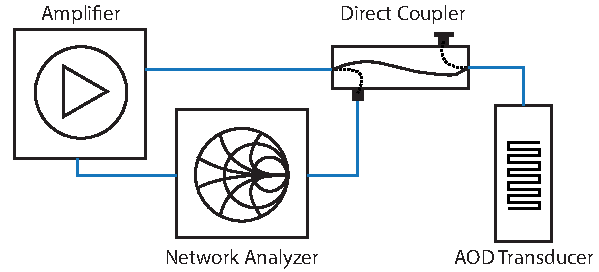
\includegraphics[width=.8\textwidth]{../figure/signal/setup-transducer.pdf}
  \caption{Experimental setup to measure the reflection at the acouso-optic
  transducer component. The network analyzer supplies an input signal to
  the amplifier. The output signal of the amplifier is connected through
  a direct-coupler with the acousto-optic element. The direct-coupler allows
  to safely measure input and output reflection.
  }\label{fig:signal_amplification_transducer_setup}
\end{figure}
The setup is depicted in \Cref{fig:signal_amplification_transducer_setup}.
The network analyzer on the left-hand side supplies an input signal to the
amplifier. The input signal changes linear in frequency. The output signal
of the amplifier is connected through a direct-coupler with the acousto-optic
element. The direct-coupler allows to measure input and output reflection.
\begin{figure}[htb]
  \centering
  \begin{adjustbox}{width=\textwidth}
    %% Creator: Matplotlib, PGF backend
%%
%% To include the figure in your LaTeX document, write
%%   \input{<filename>.pgf}
%%
%% Make sure the required packages are loaded in your preamble
%%   \usepackage{pgf}
%%
%% Figures using additional raster images can only be included by \input if
%% they are in the same directory as the main LaTeX file. For loading figures
%% from other directories you can use the `import` package
%%   \usepackage{import}
%% and then include the figures with
%%   \import{<path to file>}{<filename>.pgf}
%%
%% Matplotlib used the following preamble
%%   \usepackage{amsmath}\usepackage{siunitx}\usepackage{lmodern}
%%   \usepackage{fontspec}
%%
\begingroup%
\makeatletter%
\begin{pgfpicture}%
\pgfpathrectangle{\pgfpointorigin}{\pgfqpoint{12.000000in}{6.000000in}}%
\pgfusepath{use as bounding box, clip}%
\begin{pgfscope}%
\pgfsetbuttcap%
\pgfsetmiterjoin%
\pgfsetlinewidth{0.000000pt}%
\definecolor{currentstroke}{rgb}{1.000000,1.000000,1.000000}%
\pgfsetstrokecolor{currentstroke}%
\pgfsetdash{}{0pt}%
\pgfpathmoveto{\pgfqpoint{0.000000in}{0.000000in}}%
\pgfpathlineto{\pgfqpoint{12.000000in}{0.000000in}}%
\pgfpathlineto{\pgfqpoint{12.000000in}{6.000000in}}%
\pgfpathlineto{\pgfqpoint{0.000000in}{6.000000in}}%
\pgfpathclose%
\pgfusepath{}%
\end{pgfscope}%
\begin{pgfscope}%
\pgfsetbuttcap%
\pgfsetmiterjoin%
\definecolor{currentfill}{rgb}{1.000000,1.000000,1.000000}%
\pgfsetfillcolor{currentfill}%
\pgfsetlinewidth{0.000000pt}%
\definecolor{currentstroke}{rgb}{0.000000,0.000000,0.000000}%
\pgfsetstrokecolor{currentstroke}%
\pgfsetstrokeopacity{0.000000}%
\pgfsetdash{}{0pt}%
\pgfpathmoveto{\pgfqpoint{1.500000in}{1.200000in}}%
\pgfpathlineto{\pgfqpoint{10.800000in}{1.200000in}}%
\pgfpathlineto{\pgfqpoint{10.800000in}{5.880000in}}%
\pgfpathlineto{\pgfqpoint{1.500000in}{5.880000in}}%
\pgfpathclose%
\pgfusepath{fill}%
\end{pgfscope}%
\begin{pgfscope}%
\pgfpathrectangle{\pgfqpoint{1.500000in}{1.200000in}}{\pgfqpoint{9.300000in}{4.680000in}}%
\pgfusepath{clip}%
\pgfsetbuttcap%
\pgfsetroundjoin%
\definecolor{currentfill}{rgb}{0.192157,0.509804,0.741176}%
\pgfsetfillcolor{currentfill}%
\pgfsetlinewidth{1.003750pt}%
\definecolor{currentstroke}{rgb}{0.192157,0.509804,0.741176}%
\pgfsetstrokecolor{currentstroke}%
\pgfsetdash{}{0pt}%
\pgfpathmoveto{\pgfqpoint{1.963992in}{4.866659in}}%
\pgfpathcurveto{\pgfqpoint{1.975042in}{4.866659in}}{\pgfqpoint{1.985641in}{4.871049in}}{\pgfqpoint{1.993455in}{4.878863in}}%
\pgfpathcurveto{\pgfqpoint{2.001268in}{4.886677in}}{\pgfqpoint{2.005658in}{4.897276in}}{\pgfqpoint{2.005658in}{4.908326in}}%
\pgfpathcurveto{\pgfqpoint{2.005658in}{4.919376in}}{\pgfqpoint{2.001268in}{4.929975in}}{\pgfqpoint{1.993455in}{4.937789in}}%
\pgfpathcurveto{\pgfqpoint{1.985641in}{4.945602in}}{\pgfqpoint{1.975042in}{4.949992in}}{\pgfqpoint{1.963992in}{4.949992in}}%
\pgfpathcurveto{\pgfqpoint{1.952942in}{4.949992in}}{\pgfqpoint{1.942343in}{4.945602in}}{\pgfqpoint{1.934529in}{4.937789in}}%
\pgfpathcurveto{\pgfqpoint{1.926715in}{4.929975in}}{\pgfqpoint{1.922325in}{4.919376in}}{\pgfqpoint{1.922325in}{4.908326in}}%
\pgfpathcurveto{\pgfqpoint{1.922325in}{4.897276in}}{\pgfqpoint{1.926715in}{4.886677in}}{\pgfqpoint{1.934529in}{4.878863in}}%
\pgfpathcurveto{\pgfqpoint{1.942343in}{4.871049in}}{\pgfqpoint{1.952942in}{4.866659in}}{\pgfqpoint{1.963992in}{4.866659in}}%
\pgfpathclose%
\pgfusepath{stroke,fill}%
\end{pgfscope}%
\begin{pgfscope}%
\pgfpathrectangle{\pgfqpoint{1.500000in}{1.200000in}}{\pgfqpoint{9.300000in}{4.680000in}}%
\pgfusepath{clip}%
\pgfsetbuttcap%
\pgfsetroundjoin%
\definecolor{currentfill}{rgb}{0.192157,0.509804,0.741176}%
\pgfsetfillcolor{currentfill}%
\pgfsetlinewidth{1.003750pt}%
\definecolor{currentstroke}{rgb}{0.192157,0.509804,0.741176}%
\pgfsetstrokecolor{currentstroke}%
\pgfsetdash{}{0pt}%
\pgfpathmoveto{\pgfqpoint{2.005852in}{4.869619in}}%
\pgfpathcurveto{\pgfqpoint{2.016902in}{4.869619in}}{\pgfqpoint{2.027501in}{4.874009in}}{\pgfqpoint{2.035315in}{4.881822in}}%
\pgfpathcurveto{\pgfqpoint{2.043128in}{4.889636in}}{\pgfqpoint{2.047519in}{4.900235in}}{\pgfqpoint{2.047519in}{4.911285in}}%
\pgfpathcurveto{\pgfqpoint{2.047519in}{4.922335in}}{\pgfqpoint{2.043128in}{4.932934in}}{\pgfqpoint{2.035315in}{4.940748in}}%
\pgfpathcurveto{\pgfqpoint{2.027501in}{4.948562in}}{\pgfqpoint{2.016902in}{4.952952in}}{\pgfqpoint{2.005852in}{4.952952in}}%
\pgfpathcurveto{\pgfqpoint{1.994802in}{4.952952in}}{\pgfqpoint{1.984203in}{4.948562in}}{\pgfqpoint{1.976389in}{4.940748in}}%
\pgfpathcurveto{\pgfqpoint{1.968576in}{4.932934in}}{\pgfqpoint{1.964185in}{4.922335in}}{\pgfqpoint{1.964185in}{4.911285in}}%
\pgfpathcurveto{\pgfqpoint{1.964185in}{4.900235in}}{\pgfqpoint{1.968576in}{4.889636in}}{\pgfqpoint{1.976389in}{4.881822in}}%
\pgfpathcurveto{\pgfqpoint{1.984203in}{4.874009in}}{\pgfqpoint{1.994802in}{4.869619in}}{\pgfqpoint{2.005852in}{4.869619in}}%
\pgfpathclose%
\pgfusepath{stroke,fill}%
\end{pgfscope}%
\begin{pgfscope}%
\pgfpathrectangle{\pgfqpoint{1.500000in}{1.200000in}}{\pgfqpoint{9.300000in}{4.680000in}}%
\pgfusepath{clip}%
\pgfsetbuttcap%
\pgfsetroundjoin%
\definecolor{currentfill}{rgb}{0.192157,0.509804,0.741176}%
\pgfsetfillcolor{currentfill}%
\pgfsetlinewidth{1.003750pt}%
\definecolor{currentstroke}{rgb}{0.192157,0.509804,0.741176}%
\pgfsetstrokecolor{currentstroke}%
\pgfsetdash{}{0pt}%
\pgfpathmoveto{\pgfqpoint{2.047712in}{4.879393in}}%
\pgfpathcurveto{\pgfqpoint{2.058762in}{4.879393in}}{\pgfqpoint{2.069361in}{4.883783in}}{\pgfqpoint{2.077175in}{4.891597in}}%
\pgfpathcurveto{\pgfqpoint{2.084988in}{4.899411in}}{\pgfqpoint{2.089379in}{4.910010in}}{\pgfqpoint{2.089379in}{4.921060in}}%
\pgfpathcurveto{\pgfqpoint{2.089379in}{4.932110in}}{\pgfqpoint{2.084988in}{4.942709in}}{\pgfqpoint{2.077175in}{4.950522in}}%
\pgfpathcurveto{\pgfqpoint{2.069361in}{4.958336in}}{\pgfqpoint{2.058762in}{4.962726in}}{\pgfqpoint{2.047712in}{4.962726in}}%
\pgfpathcurveto{\pgfqpoint{2.036662in}{4.962726in}}{\pgfqpoint{2.026063in}{4.958336in}}{\pgfqpoint{2.018249in}{4.950522in}}%
\pgfpathcurveto{\pgfqpoint{2.010436in}{4.942709in}}{\pgfqpoint{2.006045in}{4.932110in}}{\pgfqpoint{2.006045in}{4.921060in}}%
\pgfpathcurveto{\pgfqpoint{2.006045in}{4.910010in}}{\pgfqpoint{2.010436in}{4.899411in}}{\pgfqpoint{2.018249in}{4.891597in}}%
\pgfpathcurveto{\pgfqpoint{2.026063in}{4.883783in}}{\pgfqpoint{2.036662in}{4.879393in}}{\pgfqpoint{2.047712in}{4.879393in}}%
\pgfpathclose%
\pgfusepath{stroke,fill}%
\end{pgfscope}%
\begin{pgfscope}%
\pgfpathrectangle{\pgfqpoint{1.500000in}{1.200000in}}{\pgfqpoint{9.300000in}{4.680000in}}%
\pgfusepath{clip}%
\pgfsetbuttcap%
\pgfsetroundjoin%
\definecolor{currentfill}{rgb}{0.192157,0.509804,0.741176}%
\pgfsetfillcolor{currentfill}%
\pgfsetlinewidth{1.003750pt}%
\definecolor{currentstroke}{rgb}{0.192157,0.509804,0.741176}%
\pgfsetstrokecolor{currentstroke}%
\pgfsetdash{}{0pt}%
\pgfpathmoveto{\pgfqpoint{2.089572in}{4.879150in}}%
\pgfpathcurveto{\pgfqpoint{2.100622in}{4.879150in}}{\pgfqpoint{2.111221in}{4.883541in}}{\pgfqpoint{2.119035in}{4.891354in}}%
\pgfpathcurveto{\pgfqpoint{2.126848in}{4.899168in}}{\pgfqpoint{2.131239in}{4.909767in}}{\pgfqpoint{2.131239in}{4.920817in}}%
\pgfpathcurveto{\pgfqpoint{2.131239in}{4.931867in}}{\pgfqpoint{2.126848in}{4.942466in}}{\pgfqpoint{2.119035in}{4.950280in}}%
\pgfpathcurveto{\pgfqpoint{2.111221in}{4.958093in}}{\pgfqpoint{2.100622in}{4.962484in}}{\pgfqpoint{2.089572in}{4.962484in}}%
\pgfpathcurveto{\pgfqpoint{2.078522in}{4.962484in}}{\pgfqpoint{2.067923in}{4.958093in}}{\pgfqpoint{2.060109in}{4.950280in}}%
\pgfpathcurveto{\pgfqpoint{2.052296in}{4.942466in}}{\pgfqpoint{2.047905in}{4.931867in}}{\pgfqpoint{2.047905in}{4.920817in}}%
\pgfpathcurveto{\pgfqpoint{2.047905in}{4.909767in}}{\pgfqpoint{2.052296in}{4.899168in}}{\pgfqpoint{2.060109in}{4.891354in}}%
\pgfpathcurveto{\pgfqpoint{2.067923in}{4.883541in}}{\pgfqpoint{2.078522in}{4.879150in}}{\pgfqpoint{2.089572in}{4.879150in}}%
\pgfpathclose%
\pgfusepath{stroke,fill}%
\end{pgfscope}%
\begin{pgfscope}%
\pgfpathrectangle{\pgfqpoint{1.500000in}{1.200000in}}{\pgfqpoint{9.300000in}{4.680000in}}%
\pgfusepath{clip}%
\pgfsetbuttcap%
\pgfsetroundjoin%
\definecolor{currentfill}{rgb}{0.192157,0.509804,0.741176}%
\pgfsetfillcolor{currentfill}%
\pgfsetlinewidth{1.003750pt}%
\definecolor{currentstroke}{rgb}{0.192157,0.509804,0.741176}%
\pgfsetstrokecolor{currentstroke}%
\pgfsetdash{}{0pt}%
\pgfpathmoveto{\pgfqpoint{2.131432in}{4.891254in}}%
\pgfpathcurveto{\pgfqpoint{2.142482in}{4.891254in}}{\pgfqpoint{2.153081in}{4.895644in}}{\pgfqpoint{2.160895in}{4.903458in}}%
\pgfpathcurveto{\pgfqpoint{2.168709in}{4.911272in}}{\pgfqpoint{2.173099in}{4.921871in}}{\pgfqpoint{2.173099in}{4.932921in}}%
\pgfpathcurveto{\pgfqpoint{2.173099in}{4.943971in}}{\pgfqpoint{2.168709in}{4.954570in}}{\pgfqpoint{2.160895in}{4.962384in}}%
\pgfpathcurveto{\pgfqpoint{2.153081in}{4.970197in}}{\pgfqpoint{2.142482in}{4.974587in}}{\pgfqpoint{2.131432in}{4.974587in}}%
\pgfpathcurveto{\pgfqpoint{2.120382in}{4.974587in}}{\pgfqpoint{2.109783in}{4.970197in}}{\pgfqpoint{2.101969in}{4.962384in}}%
\pgfpathcurveto{\pgfqpoint{2.094156in}{4.954570in}}{\pgfqpoint{2.089765in}{4.943971in}}{\pgfqpoint{2.089765in}{4.932921in}}%
\pgfpathcurveto{\pgfqpoint{2.089765in}{4.921871in}}{\pgfqpoint{2.094156in}{4.911272in}}{\pgfqpoint{2.101969in}{4.903458in}}%
\pgfpathcurveto{\pgfqpoint{2.109783in}{4.895644in}}{\pgfqpoint{2.120382in}{4.891254in}}{\pgfqpoint{2.131432in}{4.891254in}}%
\pgfpathclose%
\pgfusepath{stroke,fill}%
\end{pgfscope}%
\begin{pgfscope}%
\pgfpathrectangle{\pgfqpoint{1.500000in}{1.200000in}}{\pgfqpoint{9.300000in}{4.680000in}}%
\pgfusepath{clip}%
\pgfsetbuttcap%
\pgfsetroundjoin%
\definecolor{currentfill}{rgb}{0.192157,0.509804,0.741176}%
\pgfsetfillcolor{currentfill}%
\pgfsetlinewidth{1.003750pt}%
\definecolor{currentstroke}{rgb}{0.192157,0.509804,0.741176}%
\pgfsetstrokecolor{currentstroke}%
\pgfsetdash{}{0pt}%
\pgfpathmoveto{\pgfqpoint{2.173292in}{4.888542in}}%
\pgfpathcurveto{\pgfqpoint{2.184342in}{4.888542in}}{\pgfqpoint{2.194941in}{4.892933in}}{\pgfqpoint{2.202755in}{4.900746in}}%
\pgfpathcurveto{\pgfqpoint{2.210569in}{4.908560in}}{\pgfqpoint{2.214959in}{4.919159in}}{\pgfqpoint{2.214959in}{4.930209in}}%
\pgfpathcurveto{\pgfqpoint{2.214959in}{4.941259in}}{\pgfqpoint{2.210569in}{4.951858in}}{\pgfqpoint{2.202755in}{4.959672in}}%
\pgfpathcurveto{\pgfqpoint{2.194941in}{4.967485in}}{\pgfqpoint{2.184342in}{4.971876in}}{\pgfqpoint{2.173292in}{4.971876in}}%
\pgfpathcurveto{\pgfqpoint{2.162242in}{4.971876in}}{\pgfqpoint{2.151643in}{4.967485in}}{\pgfqpoint{2.143829in}{4.959672in}}%
\pgfpathcurveto{\pgfqpoint{2.136016in}{4.951858in}}{\pgfqpoint{2.131626in}{4.941259in}}{\pgfqpoint{2.131626in}{4.930209in}}%
\pgfpathcurveto{\pgfqpoint{2.131626in}{4.919159in}}{\pgfqpoint{2.136016in}{4.908560in}}{\pgfqpoint{2.143829in}{4.900746in}}%
\pgfpathcurveto{\pgfqpoint{2.151643in}{4.892933in}}{\pgfqpoint{2.162242in}{4.888542in}}{\pgfqpoint{2.173292in}{4.888542in}}%
\pgfpathclose%
\pgfusepath{stroke,fill}%
\end{pgfscope}%
\begin{pgfscope}%
\pgfpathrectangle{\pgfqpoint{1.500000in}{1.200000in}}{\pgfqpoint{9.300000in}{4.680000in}}%
\pgfusepath{clip}%
\pgfsetbuttcap%
\pgfsetroundjoin%
\definecolor{currentfill}{rgb}{0.192157,0.509804,0.741176}%
\pgfsetfillcolor{currentfill}%
\pgfsetlinewidth{1.003750pt}%
\definecolor{currentstroke}{rgb}{0.192157,0.509804,0.741176}%
\pgfsetstrokecolor{currentstroke}%
\pgfsetdash{}{0pt}%
\pgfpathmoveto{\pgfqpoint{2.215152in}{4.905637in}}%
\pgfpathcurveto{\pgfqpoint{2.226202in}{4.905637in}}{\pgfqpoint{2.236801in}{4.910027in}}{\pgfqpoint{2.244615in}{4.917841in}}%
\pgfpathcurveto{\pgfqpoint{2.252429in}{4.925655in}}{\pgfqpoint{2.256819in}{4.936254in}}{\pgfqpoint{2.256819in}{4.947304in}}%
\pgfpathcurveto{\pgfqpoint{2.256819in}{4.958354in}}{\pgfqpoint{2.252429in}{4.968953in}}{\pgfqpoint{2.244615in}{4.976766in}}%
\pgfpathcurveto{\pgfqpoint{2.236801in}{4.984580in}}{\pgfqpoint{2.226202in}{4.988970in}}{\pgfqpoint{2.215152in}{4.988970in}}%
\pgfpathcurveto{\pgfqpoint{2.204102in}{4.988970in}}{\pgfqpoint{2.193503in}{4.984580in}}{\pgfqpoint{2.185690in}{4.976766in}}%
\pgfpathcurveto{\pgfqpoint{2.177876in}{4.968953in}}{\pgfqpoint{2.173486in}{4.958354in}}{\pgfqpoint{2.173486in}{4.947304in}}%
\pgfpathcurveto{\pgfqpoint{2.173486in}{4.936254in}}{\pgfqpoint{2.177876in}{4.925655in}}{\pgfqpoint{2.185690in}{4.917841in}}%
\pgfpathcurveto{\pgfqpoint{2.193503in}{4.910027in}}{\pgfqpoint{2.204102in}{4.905637in}}{\pgfqpoint{2.215152in}{4.905637in}}%
\pgfpathclose%
\pgfusepath{stroke,fill}%
\end{pgfscope}%
\begin{pgfscope}%
\pgfpathrectangle{\pgfqpoint{1.500000in}{1.200000in}}{\pgfqpoint{9.300000in}{4.680000in}}%
\pgfusepath{clip}%
\pgfsetbuttcap%
\pgfsetroundjoin%
\definecolor{currentfill}{rgb}{0.192157,0.509804,0.741176}%
\pgfsetfillcolor{currentfill}%
\pgfsetlinewidth{1.003750pt}%
\definecolor{currentstroke}{rgb}{0.192157,0.509804,0.741176}%
\pgfsetstrokecolor{currentstroke}%
\pgfsetdash{}{0pt}%
\pgfpathmoveto{\pgfqpoint{2.257012in}{4.902119in}}%
\pgfpathcurveto{\pgfqpoint{2.268063in}{4.902119in}}{\pgfqpoint{2.278662in}{4.906509in}}{\pgfqpoint{2.286475in}{4.914323in}}%
\pgfpathcurveto{\pgfqpoint{2.294289in}{4.922137in}}{\pgfqpoint{2.298679in}{4.932736in}}{\pgfqpoint{2.298679in}{4.943786in}}%
\pgfpathcurveto{\pgfqpoint{2.298679in}{4.954836in}}{\pgfqpoint{2.294289in}{4.965435in}}{\pgfqpoint{2.286475in}{4.973248in}}%
\pgfpathcurveto{\pgfqpoint{2.278662in}{4.981062in}}{\pgfqpoint{2.268063in}{4.985452in}}{\pgfqpoint{2.257012in}{4.985452in}}%
\pgfpathcurveto{\pgfqpoint{2.245962in}{4.985452in}}{\pgfqpoint{2.235363in}{4.981062in}}{\pgfqpoint{2.227550in}{4.973248in}}%
\pgfpathcurveto{\pgfqpoint{2.219736in}{4.965435in}}{\pgfqpoint{2.215346in}{4.954836in}}{\pgfqpoint{2.215346in}{4.943786in}}%
\pgfpathcurveto{\pgfqpoint{2.215346in}{4.932736in}}{\pgfqpoint{2.219736in}{4.922137in}}{\pgfqpoint{2.227550in}{4.914323in}}%
\pgfpathcurveto{\pgfqpoint{2.235363in}{4.906509in}}{\pgfqpoint{2.245962in}{4.902119in}}{\pgfqpoint{2.257012in}{4.902119in}}%
\pgfpathclose%
\pgfusepath{stroke,fill}%
\end{pgfscope}%
\begin{pgfscope}%
\pgfpathrectangle{\pgfqpoint{1.500000in}{1.200000in}}{\pgfqpoint{9.300000in}{4.680000in}}%
\pgfusepath{clip}%
\pgfsetbuttcap%
\pgfsetroundjoin%
\definecolor{currentfill}{rgb}{0.192157,0.509804,0.741176}%
\pgfsetfillcolor{currentfill}%
\pgfsetlinewidth{1.003750pt}%
\definecolor{currentstroke}{rgb}{0.192157,0.509804,0.741176}%
\pgfsetstrokecolor{currentstroke}%
\pgfsetdash{}{0pt}%
\pgfpathmoveto{\pgfqpoint{2.298872in}{4.919787in}}%
\pgfpathcurveto{\pgfqpoint{2.309923in}{4.919787in}}{\pgfqpoint{2.320522in}{4.924178in}}{\pgfqpoint{2.328335in}{4.931991in}}%
\pgfpathcurveto{\pgfqpoint{2.336149in}{4.939805in}}{\pgfqpoint{2.340539in}{4.950404in}}{\pgfqpoint{2.340539in}{4.961454in}}%
\pgfpathcurveto{\pgfqpoint{2.340539in}{4.972504in}}{\pgfqpoint{2.336149in}{4.983103in}}{\pgfqpoint{2.328335in}{4.990917in}}%
\pgfpathcurveto{\pgfqpoint{2.320522in}{4.998730in}}{\pgfqpoint{2.309923in}{5.003121in}}{\pgfqpoint{2.298872in}{5.003121in}}%
\pgfpathcurveto{\pgfqpoint{2.287822in}{5.003121in}}{\pgfqpoint{2.277223in}{4.998730in}}{\pgfqpoint{2.269410in}{4.990917in}}%
\pgfpathcurveto{\pgfqpoint{2.261596in}{4.983103in}}{\pgfqpoint{2.257206in}{4.972504in}}{\pgfqpoint{2.257206in}{4.961454in}}%
\pgfpathcurveto{\pgfqpoint{2.257206in}{4.950404in}}{\pgfqpoint{2.261596in}{4.939805in}}{\pgfqpoint{2.269410in}{4.931991in}}%
\pgfpathcurveto{\pgfqpoint{2.277223in}{4.924178in}}{\pgfqpoint{2.287822in}{4.919787in}}{\pgfqpoint{2.298872in}{4.919787in}}%
\pgfpathclose%
\pgfusepath{stroke,fill}%
\end{pgfscope}%
\begin{pgfscope}%
\pgfpathrectangle{\pgfqpoint{1.500000in}{1.200000in}}{\pgfqpoint{9.300000in}{4.680000in}}%
\pgfusepath{clip}%
\pgfsetbuttcap%
\pgfsetroundjoin%
\definecolor{currentfill}{rgb}{0.192157,0.509804,0.741176}%
\pgfsetfillcolor{currentfill}%
\pgfsetlinewidth{1.003750pt}%
\definecolor{currentstroke}{rgb}{0.192157,0.509804,0.741176}%
\pgfsetstrokecolor{currentstroke}%
\pgfsetdash{}{0pt}%
\pgfpathmoveto{\pgfqpoint{2.340733in}{4.911099in}}%
\pgfpathcurveto{\pgfqpoint{2.351783in}{4.911099in}}{\pgfqpoint{2.362382in}{4.915490in}}{\pgfqpoint{2.370195in}{4.923303in}}%
\pgfpathcurveto{\pgfqpoint{2.378009in}{4.931117in}}{\pgfqpoint{2.382399in}{4.941716in}}{\pgfqpoint{2.382399in}{4.952766in}}%
\pgfpathcurveto{\pgfqpoint{2.382399in}{4.963816in}}{\pgfqpoint{2.378009in}{4.974415in}}{\pgfqpoint{2.370195in}{4.982229in}}%
\pgfpathcurveto{\pgfqpoint{2.362382in}{4.990042in}}{\pgfqpoint{2.351783in}{4.994433in}}{\pgfqpoint{2.340733in}{4.994433in}}%
\pgfpathcurveto{\pgfqpoint{2.329682in}{4.994433in}}{\pgfqpoint{2.319083in}{4.990042in}}{\pgfqpoint{2.311270in}{4.982229in}}%
\pgfpathcurveto{\pgfqpoint{2.303456in}{4.974415in}}{\pgfqpoint{2.299066in}{4.963816in}}{\pgfqpoint{2.299066in}{4.952766in}}%
\pgfpathcurveto{\pgfqpoint{2.299066in}{4.941716in}}{\pgfqpoint{2.303456in}{4.931117in}}{\pgfqpoint{2.311270in}{4.923303in}}%
\pgfpathcurveto{\pgfqpoint{2.319083in}{4.915490in}}{\pgfqpoint{2.329682in}{4.911099in}}{\pgfqpoint{2.340733in}{4.911099in}}%
\pgfpathclose%
\pgfusepath{stroke,fill}%
\end{pgfscope}%
\begin{pgfscope}%
\pgfpathrectangle{\pgfqpoint{1.500000in}{1.200000in}}{\pgfqpoint{9.300000in}{4.680000in}}%
\pgfusepath{clip}%
\pgfsetbuttcap%
\pgfsetroundjoin%
\definecolor{currentfill}{rgb}{0.192157,0.509804,0.741176}%
\pgfsetfillcolor{currentfill}%
\pgfsetlinewidth{1.003750pt}%
\definecolor{currentstroke}{rgb}{0.192157,0.509804,0.741176}%
\pgfsetstrokecolor{currentstroke}%
\pgfsetdash{}{0pt}%
\pgfpathmoveto{\pgfqpoint{2.382593in}{4.919853in}}%
\pgfpathcurveto{\pgfqpoint{2.393643in}{4.919853in}}{\pgfqpoint{2.404242in}{4.924244in}}{\pgfqpoint{2.412055in}{4.932057in}}%
\pgfpathcurveto{\pgfqpoint{2.419869in}{4.939871in}}{\pgfqpoint{2.424259in}{4.950470in}}{\pgfqpoint{2.424259in}{4.961520in}}%
\pgfpathcurveto{\pgfqpoint{2.424259in}{4.972570in}}{\pgfqpoint{2.419869in}{4.983169in}}{\pgfqpoint{2.412055in}{4.990983in}}%
\pgfpathcurveto{\pgfqpoint{2.404242in}{4.998796in}}{\pgfqpoint{2.393643in}{5.003187in}}{\pgfqpoint{2.382593in}{5.003187in}}%
\pgfpathcurveto{\pgfqpoint{2.371543in}{5.003187in}}{\pgfqpoint{2.360943in}{4.998796in}}{\pgfqpoint{2.353130in}{4.990983in}}%
\pgfpathcurveto{\pgfqpoint{2.345316in}{4.983169in}}{\pgfqpoint{2.340926in}{4.972570in}}{\pgfqpoint{2.340926in}{4.961520in}}%
\pgfpathcurveto{\pgfqpoint{2.340926in}{4.950470in}}{\pgfqpoint{2.345316in}{4.939871in}}{\pgfqpoint{2.353130in}{4.932057in}}%
\pgfpathcurveto{\pgfqpoint{2.360943in}{4.924244in}}{\pgfqpoint{2.371543in}{4.919853in}}{\pgfqpoint{2.382593in}{4.919853in}}%
\pgfpathclose%
\pgfusepath{stroke,fill}%
\end{pgfscope}%
\begin{pgfscope}%
\pgfpathrectangle{\pgfqpoint{1.500000in}{1.200000in}}{\pgfqpoint{9.300000in}{4.680000in}}%
\pgfusepath{clip}%
\pgfsetbuttcap%
\pgfsetroundjoin%
\definecolor{currentfill}{rgb}{0.192157,0.509804,0.741176}%
\pgfsetfillcolor{currentfill}%
\pgfsetlinewidth{1.003750pt}%
\definecolor{currentstroke}{rgb}{0.192157,0.509804,0.741176}%
\pgfsetstrokecolor{currentstroke}%
\pgfsetdash{}{0pt}%
\pgfpathmoveto{\pgfqpoint{2.424453in}{4.925118in}}%
\pgfpathcurveto{\pgfqpoint{2.435503in}{4.925118in}}{\pgfqpoint{2.446102in}{4.929508in}}{\pgfqpoint{2.453916in}{4.937322in}}%
\pgfpathcurveto{\pgfqpoint{2.461729in}{4.945136in}}{\pgfqpoint{2.466119in}{4.955735in}}{\pgfqpoint{2.466119in}{4.966785in}}%
\pgfpathcurveto{\pgfqpoint{2.466119in}{4.977835in}}{\pgfqpoint{2.461729in}{4.988434in}}{\pgfqpoint{2.453916in}{4.996248in}}%
\pgfpathcurveto{\pgfqpoint{2.446102in}{5.004061in}}{\pgfqpoint{2.435503in}{5.008451in}}{\pgfqpoint{2.424453in}{5.008451in}}%
\pgfpathcurveto{\pgfqpoint{2.413403in}{5.008451in}}{\pgfqpoint{2.402804in}{5.004061in}}{\pgfqpoint{2.394990in}{4.996248in}}%
\pgfpathcurveto{\pgfqpoint{2.387176in}{4.988434in}}{\pgfqpoint{2.382786in}{4.977835in}}{\pgfqpoint{2.382786in}{4.966785in}}%
\pgfpathcurveto{\pgfqpoint{2.382786in}{4.955735in}}{\pgfqpoint{2.387176in}{4.945136in}}{\pgfqpoint{2.394990in}{4.937322in}}%
\pgfpathcurveto{\pgfqpoint{2.402804in}{4.929508in}}{\pgfqpoint{2.413403in}{4.925118in}}{\pgfqpoint{2.424453in}{4.925118in}}%
\pgfpathclose%
\pgfusepath{stroke,fill}%
\end{pgfscope}%
\begin{pgfscope}%
\pgfpathrectangle{\pgfqpoint{1.500000in}{1.200000in}}{\pgfqpoint{9.300000in}{4.680000in}}%
\pgfusepath{clip}%
\pgfsetbuttcap%
\pgfsetroundjoin%
\definecolor{currentfill}{rgb}{0.192157,0.509804,0.741176}%
\pgfsetfillcolor{currentfill}%
\pgfsetlinewidth{1.003750pt}%
\definecolor{currentstroke}{rgb}{0.192157,0.509804,0.741176}%
\pgfsetstrokecolor{currentstroke}%
\pgfsetdash{}{0pt}%
\pgfpathmoveto{\pgfqpoint{2.466313in}{4.929390in}}%
\pgfpathcurveto{\pgfqpoint{2.477363in}{4.929390in}}{\pgfqpoint{2.487962in}{4.933781in}}{\pgfqpoint{2.495776in}{4.941594in}}%
\pgfpathcurveto{\pgfqpoint{2.503589in}{4.949408in}}{\pgfqpoint{2.507979in}{4.960007in}}{\pgfqpoint{2.507979in}{4.971057in}}%
\pgfpathcurveto{\pgfqpoint{2.507979in}{4.982107in}}{\pgfqpoint{2.503589in}{4.992706in}}{\pgfqpoint{2.495776in}{5.000520in}}%
\pgfpathcurveto{\pgfqpoint{2.487962in}{5.008333in}}{\pgfqpoint{2.477363in}{5.012724in}}{\pgfqpoint{2.466313in}{5.012724in}}%
\pgfpathcurveto{\pgfqpoint{2.455263in}{5.012724in}}{\pgfqpoint{2.444664in}{5.008333in}}{\pgfqpoint{2.436850in}{5.000520in}}%
\pgfpathcurveto{\pgfqpoint{2.429036in}{4.992706in}}{\pgfqpoint{2.424646in}{4.982107in}}{\pgfqpoint{2.424646in}{4.971057in}}%
\pgfpathcurveto{\pgfqpoint{2.424646in}{4.960007in}}{\pgfqpoint{2.429036in}{4.949408in}}{\pgfqpoint{2.436850in}{4.941594in}}%
\pgfpathcurveto{\pgfqpoint{2.444664in}{4.933781in}}{\pgfqpoint{2.455263in}{4.929390in}}{\pgfqpoint{2.466313in}{4.929390in}}%
\pgfpathclose%
\pgfusepath{stroke,fill}%
\end{pgfscope}%
\begin{pgfscope}%
\pgfpathrectangle{\pgfqpoint{1.500000in}{1.200000in}}{\pgfqpoint{9.300000in}{4.680000in}}%
\pgfusepath{clip}%
\pgfsetbuttcap%
\pgfsetroundjoin%
\definecolor{currentfill}{rgb}{0.192157,0.509804,0.741176}%
\pgfsetfillcolor{currentfill}%
\pgfsetlinewidth{1.003750pt}%
\definecolor{currentstroke}{rgb}{0.192157,0.509804,0.741176}%
\pgfsetstrokecolor{currentstroke}%
\pgfsetdash{}{0pt}%
\pgfpathmoveto{\pgfqpoint{2.508173in}{4.939114in}}%
\pgfpathcurveto{\pgfqpoint{2.519223in}{4.939114in}}{\pgfqpoint{2.529822in}{4.943504in}}{\pgfqpoint{2.537636in}{4.951318in}}%
\pgfpathcurveto{\pgfqpoint{2.545449in}{4.959132in}}{\pgfqpoint{2.549840in}{4.969731in}}{\pgfqpoint{2.549840in}{4.980781in}}%
\pgfpathcurveto{\pgfqpoint{2.549840in}{4.991831in}}{\pgfqpoint{2.545449in}{5.002430in}}{\pgfqpoint{2.537636in}{5.010243in}}%
\pgfpathcurveto{\pgfqpoint{2.529822in}{5.018057in}}{\pgfqpoint{2.519223in}{5.022447in}}{\pgfqpoint{2.508173in}{5.022447in}}%
\pgfpathcurveto{\pgfqpoint{2.497123in}{5.022447in}}{\pgfqpoint{2.486524in}{5.018057in}}{\pgfqpoint{2.478710in}{5.010243in}}%
\pgfpathcurveto{\pgfqpoint{2.470896in}{5.002430in}}{\pgfqpoint{2.466506in}{4.991831in}}{\pgfqpoint{2.466506in}{4.980781in}}%
\pgfpathcurveto{\pgfqpoint{2.466506in}{4.969731in}}{\pgfqpoint{2.470896in}{4.959132in}}{\pgfqpoint{2.478710in}{4.951318in}}%
\pgfpathcurveto{\pgfqpoint{2.486524in}{4.943504in}}{\pgfqpoint{2.497123in}{4.939114in}}{\pgfqpoint{2.508173in}{4.939114in}}%
\pgfpathclose%
\pgfusepath{stroke,fill}%
\end{pgfscope}%
\begin{pgfscope}%
\pgfpathrectangle{\pgfqpoint{1.500000in}{1.200000in}}{\pgfqpoint{9.300000in}{4.680000in}}%
\pgfusepath{clip}%
\pgfsetbuttcap%
\pgfsetroundjoin%
\definecolor{currentfill}{rgb}{0.192157,0.509804,0.741176}%
\pgfsetfillcolor{currentfill}%
\pgfsetlinewidth{1.003750pt}%
\definecolor{currentstroke}{rgb}{0.192157,0.509804,0.741176}%
\pgfsetstrokecolor{currentstroke}%
\pgfsetdash{}{0pt}%
\pgfpathmoveto{\pgfqpoint{2.550033in}{4.942209in}}%
\pgfpathcurveto{\pgfqpoint{2.561083in}{4.942209in}}{\pgfqpoint{2.571682in}{4.946600in}}{\pgfqpoint{2.579496in}{4.954413in}}%
\pgfpathcurveto{\pgfqpoint{2.587309in}{4.962227in}}{\pgfqpoint{2.591700in}{4.972826in}}{\pgfqpoint{2.591700in}{4.983876in}}%
\pgfpathcurveto{\pgfqpoint{2.591700in}{4.994926in}}{\pgfqpoint{2.587309in}{5.005525in}}{\pgfqpoint{2.579496in}{5.013339in}}%
\pgfpathcurveto{\pgfqpoint{2.571682in}{5.021153in}}{\pgfqpoint{2.561083in}{5.025543in}}{\pgfqpoint{2.550033in}{5.025543in}}%
\pgfpathcurveto{\pgfqpoint{2.538983in}{5.025543in}}{\pgfqpoint{2.528384in}{5.021153in}}{\pgfqpoint{2.520570in}{5.013339in}}%
\pgfpathcurveto{\pgfqpoint{2.512757in}{5.005525in}}{\pgfqpoint{2.508366in}{4.994926in}}{\pgfqpoint{2.508366in}{4.983876in}}%
\pgfpathcurveto{\pgfqpoint{2.508366in}{4.972826in}}{\pgfqpoint{2.512757in}{4.962227in}}{\pgfqpoint{2.520570in}{4.954413in}}%
\pgfpathcurveto{\pgfqpoint{2.528384in}{4.946600in}}{\pgfqpoint{2.538983in}{4.942209in}}{\pgfqpoint{2.550033in}{4.942209in}}%
\pgfpathclose%
\pgfusepath{stroke,fill}%
\end{pgfscope}%
\begin{pgfscope}%
\pgfpathrectangle{\pgfqpoint{1.500000in}{1.200000in}}{\pgfqpoint{9.300000in}{4.680000in}}%
\pgfusepath{clip}%
\pgfsetbuttcap%
\pgfsetroundjoin%
\definecolor{currentfill}{rgb}{0.192157,0.509804,0.741176}%
\pgfsetfillcolor{currentfill}%
\pgfsetlinewidth{1.003750pt}%
\definecolor{currentstroke}{rgb}{0.192157,0.509804,0.741176}%
\pgfsetstrokecolor{currentstroke}%
\pgfsetdash{}{0pt}%
\pgfpathmoveto{\pgfqpoint{2.591893in}{4.948041in}}%
\pgfpathcurveto{\pgfqpoint{2.602943in}{4.948041in}}{\pgfqpoint{2.613542in}{4.952432in}}{\pgfqpoint{2.621356in}{4.960245in}}%
\pgfpathcurveto{\pgfqpoint{2.629169in}{4.968059in}}{\pgfqpoint{2.633560in}{4.978658in}}{\pgfqpoint{2.633560in}{4.989708in}}%
\pgfpathcurveto{\pgfqpoint{2.633560in}{5.000758in}}{\pgfqpoint{2.629169in}{5.011357in}}{\pgfqpoint{2.621356in}{5.019171in}}%
\pgfpathcurveto{\pgfqpoint{2.613542in}{5.026984in}}{\pgfqpoint{2.602943in}{5.031375in}}{\pgfqpoint{2.591893in}{5.031375in}}%
\pgfpathcurveto{\pgfqpoint{2.580843in}{5.031375in}}{\pgfqpoint{2.570244in}{5.026984in}}{\pgfqpoint{2.562430in}{5.019171in}}%
\pgfpathcurveto{\pgfqpoint{2.554617in}{5.011357in}}{\pgfqpoint{2.550226in}{5.000758in}}{\pgfqpoint{2.550226in}{4.989708in}}%
\pgfpathcurveto{\pgfqpoint{2.550226in}{4.978658in}}{\pgfqpoint{2.554617in}{4.968059in}}{\pgfqpoint{2.562430in}{4.960245in}}%
\pgfpathcurveto{\pgfqpoint{2.570244in}{4.952432in}}{\pgfqpoint{2.580843in}{4.948041in}}{\pgfqpoint{2.591893in}{4.948041in}}%
\pgfpathclose%
\pgfusepath{stroke,fill}%
\end{pgfscope}%
\begin{pgfscope}%
\pgfpathrectangle{\pgfqpoint{1.500000in}{1.200000in}}{\pgfqpoint{9.300000in}{4.680000in}}%
\pgfusepath{clip}%
\pgfsetbuttcap%
\pgfsetroundjoin%
\definecolor{currentfill}{rgb}{0.192157,0.509804,0.741176}%
\pgfsetfillcolor{currentfill}%
\pgfsetlinewidth{1.003750pt}%
\definecolor{currentstroke}{rgb}{0.192157,0.509804,0.741176}%
\pgfsetstrokecolor{currentstroke}%
\pgfsetdash{}{0pt}%
\pgfpathmoveto{\pgfqpoint{2.633753in}{4.953091in}}%
\pgfpathcurveto{\pgfqpoint{2.644803in}{4.953091in}}{\pgfqpoint{2.655402in}{4.957481in}}{\pgfqpoint{2.663216in}{4.965295in}}%
\pgfpathcurveto{\pgfqpoint{2.671030in}{4.973109in}}{\pgfqpoint{2.675420in}{4.983708in}}{\pgfqpoint{2.675420in}{4.994758in}}%
\pgfpathcurveto{\pgfqpoint{2.675420in}{5.005808in}}{\pgfqpoint{2.671030in}{5.016407in}}{\pgfqpoint{2.663216in}{5.024221in}}%
\pgfpathcurveto{\pgfqpoint{2.655402in}{5.032034in}}{\pgfqpoint{2.644803in}{5.036425in}}{\pgfqpoint{2.633753in}{5.036425in}}%
\pgfpathcurveto{\pgfqpoint{2.622703in}{5.036425in}}{\pgfqpoint{2.612104in}{5.032034in}}{\pgfqpoint{2.604290in}{5.024221in}}%
\pgfpathcurveto{\pgfqpoint{2.596477in}{5.016407in}}{\pgfqpoint{2.592086in}{5.005808in}}{\pgfqpoint{2.592086in}{4.994758in}}%
\pgfpathcurveto{\pgfqpoint{2.592086in}{4.983708in}}{\pgfqpoint{2.596477in}{4.973109in}}{\pgfqpoint{2.604290in}{4.965295in}}%
\pgfpathcurveto{\pgfqpoint{2.612104in}{4.957481in}}{\pgfqpoint{2.622703in}{4.953091in}}{\pgfqpoint{2.633753in}{4.953091in}}%
\pgfpathclose%
\pgfusepath{stroke,fill}%
\end{pgfscope}%
\begin{pgfscope}%
\pgfpathrectangle{\pgfqpoint{1.500000in}{1.200000in}}{\pgfqpoint{9.300000in}{4.680000in}}%
\pgfusepath{clip}%
\pgfsetbuttcap%
\pgfsetroundjoin%
\definecolor{currentfill}{rgb}{0.192157,0.509804,0.741176}%
\pgfsetfillcolor{currentfill}%
\pgfsetlinewidth{1.003750pt}%
\definecolor{currentstroke}{rgb}{0.192157,0.509804,0.741176}%
\pgfsetstrokecolor{currentstroke}%
\pgfsetdash{}{0pt}%
\pgfpathmoveto{\pgfqpoint{2.675613in}{4.964295in}}%
\pgfpathcurveto{\pgfqpoint{2.686663in}{4.964295in}}{\pgfqpoint{2.697262in}{4.968685in}}{\pgfqpoint{2.705076in}{4.976499in}}%
\pgfpathcurveto{\pgfqpoint{2.712890in}{4.984312in}}{\pgfqpoint{2.717280in}{4.994911in}}{\pgfqpoint{2.717280in}{5.005961in}}%
\pgfpathcurveto{\pgfqpoint{2.717280in}{5.017012in}}{\pgfqpoint{2.712890in}{5.027611in}}{\pgfqpoint{2.705076in}{5.035424in}}%
\pgfpathcurveto{\pgfqpoint{2.697262in}{5.043238in}}{\pgfqpoint{2.686663in}{5.047628in}}{\pgfqpoint{2.675613in}{5.047628in}}%
\pgfpathcurveto{\pgfqpoint{2.664563in}{5.047628in}}{\pgfqpoint{2.653964in}{5.043238in}}{\pgfqpoint{2.646150in}{5.035424in}}%
\pgfpathcurveto{\pgfqpoint{2.638337in}{5.027611in}}{\pgfqpoint{2.633947in}{5.017012in}}{\pgfqpoint{2.633947in}{5.005961in}}%
\pgfpathcurveto{\pgfqpoint{2.633947in}{4.994911in}}{\pgfqpoint{2.638337in}{4.984312in}}{\pgfqpoint{2.646150in}{4.976499in}}%
\pgfpathcurveto{\pgfqpoint{2.653964in}{4.968685in}}{\pgfqpoint{2.664563in}{4.964295in}}{\pgfqpoint{2.675613in}{4.964295in}}%
\pgfpathclose%
\pgfusepath{stroke,fill}%
\end{pgfscope}%
\begin{pgfscope}%
\pgfpathrectangle{\pgfqpoint{1.500000in}{1.200000in}}{\pgfqpoint{9.300000in}{4.680000in}}%
\pgfusepath{clip}%
\pgfsetbuttcap%
\pgfsetroundjoin%
\definecolor{currentfill}{rgb}{0.192157,0.509804,0.741176}%
\pgfsetfillcolor{currentfill}%
\pgfsetlinewidth{1.003750pt}%
\definecolor{currentstroke}{rgb}{0.192157,0.509804,0.741176}%
\pgfsetstrokecolor{currentstroke}%
\pgfsetdash{}{0pt}%
\pgfpathmoveto{\pgfqpoint{2.717473in}{4.968589in}}%
\pgfpathcurveto{\pgfqpoint{2.728523in}{4.968589in}}{\pgfqpoint{2.739122in}{4.972979in}}{\pgfqpoint{2.746936in}{4.980793in}}%
\pgfpathcurveto{\pgfqpoint{2.754750in}{4.988606in}}{\pgfqpoint{2.759140in}{4.999205in}}{\pgfqpoint{2.759140in}{5.010255in}}%
\pgfpathcurveto{\pgfqpoint{2.759140in}{5.021306in}}{\pgfqpoint{2.754750in}{5.031905in}}{\pgfqpoint{2.746936in}{5.039718in}}%
\pgfpathcurveto{\pgfqpoint{2.739122in}{5.047532in}}{\pgfqpoint{2.728523in}{5.051922in}}{\pgfqpoint{2.717473in}{5.051922in}}%
\pgfpathcurveto{\pgfqpoint{2.706423in}{5.051922in}}{\pgfqpoint{2.695824in}{5.047532in}}{\pgfqpoint{2.688011in}{5.039718in}}%
\pgfpathcurveto{\pgfqpoint{2.680197in}{5.031905in}}{\pgfqpoint{2.675807in}{5.021306in}}{\pgfqpoint{2.675807in}{5.010255in}}%
\pgfpathcurveto{\pgfqpoint{2.675807in}{4.999205in}}{\pgfqpoint{2.680197in}{4.988606in}}{\pgfqpoint{2.688011in}{4.980793in}}%
\pgfpathcurveto{\pgfqpoint{2.695824in}{4.972979in}}{\pgfqpoint{2.706423in}{4.968589in}}{\pgfqpoint{2.717473in}{4.968589in}}%
\pgfpathclose%
\pgfusepath{stroke,fill}%
\end{pgfscope}%
\begin{pgfscope}%
\pgfpathrectangle{\pgfqpoint{1.500000in}{1.200000in}}{\pgfqpoint{9.300000in}{4.680000in}}%
\pgfusepath{clip}%
\pgfsetbuttcap%
\pgfsetroundjoin%
\definecolor{currentfill}{rgb}{0.192157,0.509804,0.741176}%
\pgfsetfillcolor{currentfill}%
\pgfsetlinewidth{1.003750pt}%
\definecolor{currentstroke}{rgb}{0.192157,0.509804,0.741176}%
\pgfsetstrokecolor{currentstroke}%
\pgfsetdash{}{0pt}%
\pgfpathmoveto{\pgfqpoint{2.759333in}{4.971529in}}%
\pgfpathcurveto{\pgfqpoint{2.770384in}{4.971529in}}{\pgfqpoint{2.780983in}{4.975919in}}{\pgfqpoint{2.788796in}{4.983733in}}%
\pgfpathcurveto{\pgfqpoint{2.796610in}{4.991547in}}{\pgfqpoint{2.801000in}{5.002146in}}{\pgfqpoint{2.801000in}{5.013196in}}%
\pgfpathcurveto{\pgfqpoint{2.801000in}{5.024246in}}{\pgfqpoint{2.796610in}{5.034845in}}{\pgfqpoint{2.788796in}{5.042659in}}%
\pgfpathcurveto{\pgfqpoint{2.780983in}{5.050472in}}{\pgfqpoint{2.770384in}{5.054863in}}{\pgfqpoint{2.759333in}{5.054863in}}%
\pgfpathcurveto{\pgfqpoint{2.748283in}{5.054863in}}{\pgfqpoint{2.737684in}{5.050472in}}{\pgfqpoint{2.729871in}{5.042659in}}%
\pgfpathcurveto{\pgfqpoint{2.722057in}{5.034845in}}{\pgfqpoint{2.717667in}{5.024246in}}{\pgfqpoint{2.717667in}{5.013196in}}%
\pgfpathcurveto{\pgfqpoint{2.717667in}{5.002146in}}{\pgfqpoint{2.722057in}{4.991547in}}{\pgfqpoint{2.729871in}{4.983733in}}%
\pgfpathcurveto{\pgfqpoint{2.737684in}{4.975919in}}{\pgfqpoint{2.748283in}{4.971529in}}{\pgfqpoint{2.759333in}{4.971529in}}%
\pgfpathclose%
\pgfusepath{stroke,fill}%
\end{pgfscope}%
\begin{pgfscope}%
\pgfpathrectangle{\pgfqpoint{1.500000in}{1.200000in}}{\pgfqpoint{9.300000in}{4.680000in}}%
\pgfusepath{clip}%
\pgfsetbuttcap%
\pgfsetroundjoin%
\definecolor{currentfill}{rgb}{0.192157,0.509804,0.741176}%
\pgfsetfillcolor{currentfill}%
\pgfsetlinewidth{1.003750pt}%
\definecolor{currentstroke}{rgb}{0.192157,0.509804,0.741176}%
\pgfsetstrokecolor{currentstroke}%
\pgfsetdash{}{0pt}%
\pgfpathmoveto{\pgfqpoint{2.801193in}{4.980316in}}%
\pgfpathcurveto{\pgfqpoint{2.812244in}{4.980316in}}{\pgfqpoint{2.822843in}{4.984706in}}{\pgfqpoint{2.830656in}{4.992520in}}%
\pgfpathcurveto{\pgfqpoint{2.838470in}{5.000333in}}{\pgfqpoint{2.842860in}{5.010932in}}{\pgfqpoint{2.842860in}{5.021983in}}%
\pgfpathcurveto{\pgfqpoint{2.842860in}{5.033033in}}{\pgfqpoint{2.838470in}{5.043632in}}{\pgfqpoint{2.830656in}{5.051445in}}%
\pgfpathcurveto{\pgfqpoint{2.822843in}{5.059259in}}{\pgfqpoint{2.812244in}{5.063649in}}{\pgfqpoint{2.801193in}{5.063649in}}%
\pgfpathcurveto{\pgfqpoint{2.790143in}{5.063649in}}{\pgfqpoint{2.779544in}{5.059259in}}{\pgfqpoint{2.771731in}{5.051445in}}%
\pgfpathcurveto{\pgfqpoint{2.763917in}{5.043632in}}{\pgfqpoint{2.759527in}{5.033033in}}{\pgfqpoint{2.759527in}{5.021983in}}%
\pgfpathcurveto{\pgfqpoint{2.759527in}{5.010932in}}{\pgfqpoint{2.763917in}{5.000333in}}{\pgfqpoint{2.771731in}{4.992520in}}%
\pgfpathcurveto{\pgfqpoint{2.779544in}{4.984706in}}{\pgfqpoint{2.790143in}{4.980316in}}{\pgfqpoint{2.801193in}{4.980316in}}%
\pgfpathclose%
\pgfusepath{stroke,fill}%
\end{pgfscope}%
\begin{pgfscope}%
\pgfpathrectangle{\pgfqpoint{1.500000in}{1.200000in}}{\pgfqpoint{9.300000in}{4.680000in}}%
\pgfusepath{clip}%
\pgfsetbuttcap%
\pgfsetroundjoin%
\definecolor{currentfill}{rgb}{0.192157,0.509804,0.741176}%
\pgfsetfillcolor{currentfill}%
\pgfsetlinewidth{1.003750pt}%
\definecolor{currentstroke}{rgb}{0.192157,0.509804,0.741176}%
\pgfsetstrokecolor{currentstroke}%
\pgfsetdash{}{0pt}%
\pgfpathmoveto{\pgfqpoint{2.843054in}{4.975697in}}%
\pgfpathcurveto{\pgfqpoint{2.854104in}{4.975697in}}{\pgfqpoint{2.864703in}{4.980087in}}{\pgfqpoint{2.872516in}{4.987900in}}%
\pgfpathcurveto{\pgfqpoint{2.880330in}{4.995714in}}{\pgfqpoint{2.884720in}{5.006313in}}{\pgfqpoint{2.884720in}{5.017363in}}%
\pgfpathcurveto{\pgfqpoint{2.884720in}{5.028413in}}{\pgfqpoint{2.880330in}{5.039012in}}{\pgfqpoint{2.872516in}{5.046826in}}%
\pgfpathcurveto{\pgfqpoint{2.864703in}{5.054640in}}{\pgfqpoint{2.854104in}{5.059030in}}{\pgfqpoint{2.843054in}{5.059030in}}%
\pgfpathcurveto{\pgfqpoint{2.832003in}{5.059030in}}{\pgfqpoint{2.821404in}{5.054640in}}{\pgfqpoint{2.813591in}{5.046826in}}%
\pgfpathcurveto{\pgfqpoint{2.805777in}{5.039012in}}{\pgfqpoint{2.801387in}{5.028413in}}{\pgfqpoint{2.801387in}{5.017363in}}%
\pgfpathcurveto{\pgfqpoint{2.801387in}{5.006313in}}{\pgfqpoint{2.805777in}{4.995714in}}{\pgfqpoint{2.813591in}{4.987900in}}%
\pgfpathcurveto{\pgfqpoint{2.821404in}{4.980087in}}{\pgfqpoint{2.832003in}{4.975697in}}{\pgfqpoint{2.843054in}{4.975697in}}%
\pgfpathclose%
\pgfusepath{stroke,fill}%
\end{pgfscope}%
\begin{pgfscope}%
\pgfpathrectangle{\pgfqpoint{1.500000in}{1.200000in}}{\pgfqpoint{9.300000in}{4.680000in}}%
\pgfusepath{clip}%
\pgfsetbuttcap%
\pgfsetroundjoin%
\definecolor{currentfill}{rgb}{0.192157,0.509804,0.741176}%
\pgfsetfillcolor{currentfill}%
\pgfsetlinewidth{1.003750pt}%
\definecolor{currentstroke}{rgb}{0.192157,0.509804,0.741176}%
\pgfsetstrokecolor{currentstroke}%
\pgfsetdash{}{0pt}%
\pgfpathmoveto{\pgfqpoint{2.884914in}{4.991960in}}%
\pgfpathcurveto{\pgfqpoint{2.895964in}{4.991960in}}{\pgfqpoint{2.906563in}{4.996350in}}{\pgfqpoint{2.914376in}{5.004164in}}%
\pgfpathcurveto{\pgfqpoint{2.922190in}{5.011977in}}{\pgfqpoint{2.926580in}{5.022576in}}{\pgfqpoint{2.926580in}{5.033626in}}%
\pgfpathcurveto{\pgfqpoint{2.926580in}{5.044677in}}{\pgfqpoint{2.922190in}{5.055276in}}{\pgfqpoint{2.914376in}{5.063089in}}%
\pgfpathcurveto{\pgfqpoint{2.906563in}{5.070903in}}{\pgfqpoint{2.895964in}{5.075293in}}{\pgfqpoint{2.884914in}{5.075293in}}%
\pgfpathcurveto{\pgfqpoint{2.873863in}{5.075293in}}{\pgfqpoint{2.863264in}{5.070903in}}{\pgfqpoint{2.855451in}{5.063089in}}%
\pgfpathcurveto{\pgfqpoint{2.847637in}{5.055276in}}{\pgfqpoint{2.843247in}{5.044677in}}{\pgfqpoint{2.843247in}{5.033626in}}%
\pgfpathcurveto{\pgfqpoint{2.843247in}{5.022576in}}{\pgfqpoint{2.847637in}{5.011977in}}{\pgfqpoint{2.855451in}{5.004164in}}%
\pgfpathcurveto{\pgfqpoint{2.863264in}{4.996350in}}{\pgfqpoint{2.873863in}{4.991960in}}{\pgfqpoint{2.884914in}{4.991960in}}%
\pgfpathclose%
\pgfusepath{stroke,fill}%
\end{pgfscope}%
\begin{pgfscope}%
\pgfpathrectangle{\pgfqpoint{1.500000in}{1.200000in}}{\pgfqpoint{9.300000in}{4.680000in}}%
\pgfusepath{clip}%
\pgfsetbuttcap%
\pgfsetroundjoin%
\definecolor{currentfill}{rgb}{0.192157,0.509804,0.741176}%
\pgfsetfillcolor{currentfill}%
\pgfsetlinewidth{1.003750pt}%
\definecolor{currentstroke}{rgb}{0.192157,0.509804,0.741176}%
\pgfsetstrokecolor{currentstroke}%
\pgfsetdash{}{0pt}%
\pgfpathmoveto{\pgfqpoint{2.926774in}{4.988118in}}%
\pgfpathcurveto{\pgfqpoint{2.937824in}{4.988118in}}{\pgfqpoint{2.948423in}{4.992508in}}{\pgfqpoint{2.956236in}{5.000322in}}%
\pgfpathcurveto{\pgfqpoint{2.964050in}{5.008136in}}{\pgfqpoint{2.968440in}{5.018735in}}{\pgfqpoint{2.968440in}{5.029785in}}%
\pgfpathcurveto{\pgfqpoint{2.968440in}{5.040835in}}{\pgfqpoint{2.964050in}{5.051434in}}{\pgfqpoint{2.956236in}{5.059248in}}%
\pgfpathcurveto{\pgfqpoint{2.948423in}{5.067061in}}{\pgfqpoint{2.937824in}{5.071451in}}{\pgfqpoint{2.926774in}{5.071451in}}%
\pgfpathcurveto{\pgfqpoint{2.915724in}{5.071451in}}{\pgfqpoint{2.905125in}{5.067061in}}{\pgfqpoint{2.897311in}{5.059248in}}%
\pgfpathcurveto{\pgfqpoint{2.889497in}{5.051434in}}{\pgfqpoint{2.885107in}{5.040835in}}{\pgfqpoint{2.885107in}{5.029785in}}%
\pgfpathcurveto{\pgfqpoint{2.885107in}{5.018735in}}{\pgfqpoint{2.889497in}{5.008136in}}{\pgfqpoint{2.897311in}{5.000322in}}%
\pgfpathcurveto{\pgfqpoint{2.905125in}{4.992508in}}{\pgfqpoint{2.915724in}{4.988118in}}{\pgfqpoint{2.926774in}{4.988118in}}%
\pgfpathclose%
\pgfusepath{stroke,fill}%
\end{pgfscope}%
\begin{pgfscope}%
\pgfpathrectangle{\pgfqpoint{1.500000in}{1.200000in}}{\pgfqpoint{9.300000in}{4.680000in}}%
\pgfusepath{clip}%
\pgfsetbuttcap%
\pgfsetroundjoin%
\definecolor{currentfill}{rgb}{0.192157,0.509804,0.741176}%
\pgfsetfillcolor{currentfill}%
\pgfsetlinewidth{1.003750pt}%
\definecolor{currentstroke}{rgb}{0.192157,0.509804,0.741176}%
\pgfsetstrokecolor{currentstroke}%
\pgfsetdash{}{0pt}%
\pgfpathmoveto{\pgfqpoint{2.968634in}{4.996748in}}%
\pgfpathcurveto{\pgfqpoint{2.979684in}{4.996748in}}{\pgfqpoint{2.990283in}{5.001138in}}{\pgfqpoint{2.998097in}{5.008952in}}%
\pgfpathcurveto{\pgfqpoint{3.005910in}{5.016766in}}{\pgfqpoint{3.010300in}{5.027365in}}{\pgfqpoint{3.010300in}{5.038415in}}%
\pgfpathcurveto{\pgfqpoint{3.010300in}{5.049465in}}{\pgfqpoint{3.005910in}{5.060064in}}{\pgfqpoint{2.998097in}{5.067877in}}%
\pgfpathcurveto{\pgfqpoint{2.990283in}{5.075691in}}{\pgfqpoint{2.979684in}{5.080081in}}{\pgfqpoint{2.968634in}{5.080081in}}%
\pgfpathcurveto{\pgfqpoint{2.957584in}{5.080081in}}{\pgfqpoint{2.946985in}{5.075691in}}{\pgfqpoint{2.939171in}{5.067877in}}%
\pgfpathcurveto{\pgfqpoint{2.931357in}{5.060064in}}{\pgfqpoint{2.926967in}{5.049465in}}{\pgfqpoint{2.926967in}{5.038415in}}%
\pgfpathcurveto{\pgfqpoint{2.926967in}{5.027365in}}{\pgfqpoint{2.931357in}{5.016766in}}{\pgfqpoint{2.939171in}{5.008952in}}%
\pgfpathcurveto{\pgfqpoint{2.946985in}{5.001138in}}{\pgfqpoint{2.957584in}{4.996748in}}{\pgfqpoint{2.968634in}{4.996748in}}%
\pgfpathclose%
\pgfusepath{stroke,fill}%
\end{pgfscope}%
\begin{pgfscope}%
\pgfpathrectangle{\pgfqpoint{1.500000in}{1.200000in}}{\pgfqpoint{9.300000in}{4.680000in}}%
\pgfusepath{clip}%
\pgfsetbuttcap%
\pgfsetroundjoin%
\definecolor{currentfill}{rgb}{0.192157,0.509804,0.741176}%
\pgfsetfillcolor{currentfill}%
\pgfsetlinewidth{1.003750pt}%
\definecolor{currentstroke}{rgb}{0.192157,0.509804,0.741176}%
\pgfsetstrokecolor{currentstroke}%
\pgfsetdash{}{0pt}%
\pgfpathmoveto{\pgfqpoint{3.010494in}{5.010520in}}%
\pgfpathcurveto{\pgfqpoint{3.021544in}{5.010520in}}{\pgfqpoint{3.032143in}{5.014910in}}{\pgfqpoint{3.039957in}{5.022724in}}%
\pgfpathcurveto{\pgfqpoint{3.047770in}{5.030537in}}{\pgfqpoint{3.052161in}{5.041136in}}{\pgfqpoint{3.052161in}{5.052186in}}%
\pgfpathcurveto{\pgfqpoint{3.052161in}{5.063237in}}{\pgfqpoint{3.047770in}{5.073836in}}{\pgfqpoint{3.039957in}{5.081649in}}%
\pgfpathcurveto{\pgfqpoint{3.032143in}{5.089463in}}{\pgfqpoint{3.021544in}{5.093853in}}{\pgfqpoint{3.010494in}{5.093853in}}%
\pgfpathcurveto{\pgfqpoint{2.999444in}{5.093853in}}{\pgfqpoint{2.988845in}{5.089463in}}{\pgfqpoint{2.981031in}{5.081649in}}%
\pgfpathcurveto{\pgfqpoint{2.973217in}{5.073836in}}{\pgfqpoint{2.968827in}{5.063237in}}{\pgfqpoint{2.968827in}{5.052186in}}%
\pgfpathcurveto{\pgfqpoint{2.968827in}{5.041136in}}{\pgfqpoint{2.973217in}{5.030537in}}{\pgfqpoint{2.981031in}{5.022724in}}%
\pgfpathcurveto{\pgfqpoint{2.988845in}{5.014910in}}{\pgfqpoint{2.999444in}{5.010520in}}{\pgfqpoint{3.010494in}{5.010520in}}%
\pgfpathclose%
\pgfusepath{stroke,fill}%
\end{pgfscope}%
\begin{pgfscope}%
\pgfpathrectangle{\pgfqpoint{1.500000in}{1.200000in}}{\pgfqpoint{9.300000in}{4.680000in}}%
\pgfusepath{clip}%
\pgfsetbuttcap%
\pgfsetroundjoin%
\definecolor{currentfill}{rgb}{0.192157,0.509804,0.741176}%
\pgfsetfillcolor{currentfill}%
\pgfsetlinewidth{1.003750pt}%
\definecolor{currentstroke}{rgb}{0.192157,0.509804,0.741176}%
\pgfsetstrokecolor{currentstroke}%
\pgfsetdash{}{0pt}%
\pgfpathmoveto{\pgfqpoint{3.052354in}{5.007517in}}%
\pgfpathcurveto{\pgfqpoint{3.063404in}{5.007517in}}{\pgfqpoint{3.074003in}{5.011907in}}{\pgfqpoint{3.081817in}{5.019721in}}%
\pgfpathcurveto{\pgfqpoint{3.089630in}{5.027534in}}{\pgfqpoint{3.094021in}{5.038133in}}{\pgfqpoint{3.094021in}{5.049183in}}%
\pgfpathcurveto{\pgfqpoint{3.094021in}{5.060234in}}{\pgfqpoint{3.089630in}{5.070833in}}{\pgfqpoint{3.081817in}{5.078646in}}%
\pgfpathcurveto{\pgfqpoint{3.074003in}{5.086460in}}{\pgfqpoint{3.063404in}{5.090850in}}{\pgfqpoint{3.052354in}{5.090850in}}%
\pgfpathcurveto{\pgfqpoint{3.041304in}{5.090850in}}{\pgfqpoint{3.030705in}{5.086460in}}{\pgfqpoint{3.022891in}{5.078646in}}%
\pgfpathcurveto{\pgfqpoint{3.015078in}{5.070833in}}{\pgfqpoint{3.010687in}{5.060234in}}{\pgfqpoint{3.010687in}{5.049183in}}%
\pgfpathcurveto{\pgfqpoint{3.010687in}{5.038133in}}{\pgfqpoint{3.015078in}{5.027534in}}{\pgfqpoint{3.022891in}{5.019721in}}%
\pgfpathcurveto{\pgfqpoint{3.030705in}{5.011907in}}{\pgfqpoint{3.041304in}{5.007517in}}{\pgfqpoint{3.052354in}{5.007517in}}%
\pgfpathclose%
\pgfusepath{stroke,fill}%
\end{pgfscope}%
\begin{pgfscope}%
\pgfpathrectangle{\pgfqpoint{1.500000in}{1.200000in}}{\pgfqpoint{9.300000in}{4.680000in}}%
\pgfusepath{clip}%
\pgfsetbuttcap%
\pgfsetroundjoin%
\definecolor{currentfill}{rgb}{0.192157,0.509804,0.741176}%
\pgfsetfillcolor{currentfill}%
\pgfsetlinewidth{1.003750pt}%
\definecolor{currentstroke}{rgb}{0.192157,0.509804,0.741176}%
\pgfsetstrokecolor{currentstroke}%
\pgfsetdash{}{0pt}%
\pgfpathmoveto{\pgfqpoint{3.094214in}{5.013325in}}%
\pgfpathcurveto{\pgfqpoint{3.105264in}{5.013325in}}{\pgfqpoint{3.115863in}{5.017716in}}{\pgfqpoint{3.123677in}{5.025529in}}%
\pgfpathcurveto{\pgfqpoint{3.131490in}{5.033343in}}{\pgfqpoint{3.135881in}{5.043942in}}{\pgfqpoint{3.135881in}{5.054992in}}%
\pgfpathcurveto{\pgfqpoint{3.135881in}{5.066042in}}{\pgfqpoint{3.131490in}{5.076641in}}{\pgfqpoint{3.123677in}{5.084455in}}%
\pgfpathcurveto{\pgfqpoint{3.115863in}{5.092268in}}{\pgfqpoint{3.105264in}{5.096659in}}{\pgfqpoint{3.094214in}{5.096659in}}%
\pgfpathcurveto{\pgfqpoint{3.083164in}{5.096659in}}{\pgfqpoint{3.072565in}{5.092268in}}{\pgfqpoint{3.064751in}{5.084455in}}%
\pgfpathcurveto{\pgfqpoint{3.056938in}{5.076641in}}{\pgfqpoint{3.052547in}{5.066042in}}{\pgfqpoint{3.052547in}{5.054992in}}%
\pgfpathcurveto{\pgfqpoint{3.052547in}{5.043942in}}{\pgfqpoint{3.056938in}{5.033343in}}{\pgfqpoint{3.064751in}{5.025529in}}%
\pgfpathcurveto{\pgfqpoint{3.072565in}{5.017716in}}{\pgfqpoint{3.083164in}{5.013325in}}{\pgfqpoint{3.094214in}{5.013325in}}%
\pgfpathclose%
\pgfusepath{stroke,fill}%
\end{pgfscope}%
\begin{pgfscope}%
\pgfpathrectangle{\pgfqpoint{1.500000in}{1.200000in}}{\pgfqpoint{9.300000in}{4.680000in}}%
\pgfusepath{clip}%
\pgfsetbuttcap%
\pgfsetroundjoin%
\definecolor{currentfill}{rgb}{0.192157,0.509804,0.741176}%
\pgfsetfillcolor{currentfill}%
\pgfsetlinewidth{1.003750pt}%
\definecolor{currentstroke}{rgb}{0.192157,0.509804,0.741176}%
\pgfsetstrokecolor{currentstroke}%
\pgfsetdash{}{0pt}%
\pgfpathmoveto{\pgfqpoint{3.136074in}{5.013128in}}%
\pgfpathcurveto{\pgfqpoint{3.147124in}{5.013128in}}{\pgfqpoint{3.157723in}{5.017518in}}{\pgfqpoint{3.165537in}{5.025332in}}%
\pgfpathcurveto{\pgfqpoint{3.173351in}{5.033145in}}{\pgfqpoint{3.177741in}{5.043744in}}{\pgfqpoint{3.177741in}{5.054794in}}%
\pgfpathcurveto{\pgfqpoint{3.177741in}{5.065844in}}{\pgfqpoint{3.173351in}{5.076444in}}{\pgfqpoint{3.165537in}{5.084257in}}%
\pgfpathcurveto{\pgfqpoint{3.157723in}{5.092071in}}{\pgfqpoint{3.147124in}{5.096461in}}{\pgfqpoint{3.136074in}{5.096461in}}%
\pgfpathcurveto{\pgfqpoint{3.125024in}{5.096461in}}{\pgfqpoint{3.114425in}{5.092071in}}{\pgfqpoint{3.106611in}{5.084257in}}%
\pgfpathcurveto{\pgfqpoint{3.098798in}{5.076444in}}{\pgfqpoint{3.094407in}{5.065844in}}{\pgfqpoint{3.094407in}{5.054794in}}%
\pgfpathcurveto{\pgfqpoint{3.094407in}{5.043744in}}{\pgfqpoint{3.098798in}{5.033145in}}{\pgfqpoint{3.106611in}{5.025332in}}%
\pgfpathcurveto{\pgfqpoint{3.114425in}{5.017518in}}{\pgfqpoint{3.125024in}{5.013128in}}{\pgfqpoint{3.136074in}{5.013128in}}%
\pgfpathclose%
\pgfusepath{stroke,fill}%
\end{pgfscope}%
\begin{pgfscope}%
\pgfpathrectangle{\pgfqpoint{1.500000in}{1.200000in}}{\pgfqpoint{9.300000in}{4.680000in}}%
\pgfusepath{clip}%
\pgfsetbuttcap%
\pgfsetroundjoin%
\definecolor{currentfill}{rgb}{0.192157,0.509804,0.741176}%
\pgfsetfillcolor{currentfill}%
\pgfsetlinewidth{1.003750pt}%
\definecolor{currentstroke}{rgb}{0.192157,0.509804,0.741176}%
\pgfsetstrokecolor{currentstroke}%
\pgfsetdash{}{0pt}%
\pgfpathmoveto{\pgfqpoint{3.177934in}{5.017904in}}%
\pgfpathcurveto{\pgfqpoint{3.188984in}{5.017904in}}{\pgfqpoint{3.199583in}{5.022294in}}{\pgfqpoint{3.207397in}{5.030108in}}%
\pgfpathcurveto{\pgfqpoint{3.215211in}{5.037921in}}{\pgfqpoint{3.219601in}{5.048520in}}{\pgfqpoint{3.219601in}{5.059570in}}%
\pgfpathcurveto{\pgfqpoint{3.219601in}{5.070621in}}{\pgfqpoint{3.215211in}{5.081220in}}{\pgfqpoint{3.207397in}{5.089033in}}%
\pgfpathcurveto{\pgfqpoint{3.199583in}{5.096847in}}{\pgfqpoint{3.188984in}{5.101237in}}{\pgfqpoint{3.177934in}{5.101237in}}%
\pgfpathcurveto{\pgfqpoint{3.166884in}{5.101237in}}{\pgfqpoint{3.156285in}{5.096847in}}{\pgfqpoint{3.148471in}{5.089033in}}%
\pgfpathcurveto{\pgfqpoint{3.140658in}{5.081220in}}{\pgfqpoint{3.136268in}{5.070621in}}{\pgfqpoint{3.136268in}{5.059570in}}%
\pgfpathcurveto{\pgfqpoint{3.136268in}{5.048520in}}{\pgfqpoint{3.140658in}{5.037921in}}{\pgfqpoint{3.148471in}{5.030108in}}%
\pgfpathcurveto{\pgfqpoint{3.156285in}{5.022294in}}{\pgfqpoint{3.166884in}{5.017904in}}{\pgfqpoint{3.177934in}{5.017904in}}%
\pgfpathclose%
\pgfusepath{stroke,fill}%
\end{pgfscope}%
\begin{pgfscope}%
\pgfpathrectangle{\pgfqpoint{1.500000in}{1.200000in}}{\pgfqpoint{9.300000in}{4.680000in}}%
\pgfusepath{clip}%
\pgfsetbuttcap%
\pgfsetroundjoin%
\definecolor{currentfill}{rgb}{0.192157,0.509804,0.741176}%
\pgfsetfillcolor{currentfill}%
\pgfsetlinewidth{1.003750pt}%
\definecolor{currentstroke}{rgb}{0.192157,0.509804,0.741176}%
\pgfsetstrokecolor{currentstroke}%
\pgfsetdash{}{0pt}%
\pgfpathmoveto{\pgfqpoint{3.219794in}{5.029411in}}%
\pgfpathcurveto{\pgfqpoint{3.230844in}{5.029411in}}{\pgfqpoint{3.241443in}{5.033802in}}{\pgfqpoint{3.249257in}{5.041615in}}%
\pgfpathcurveto{\pgfqpoint{3.257071in}{5.049429in}}{\pgfqpoint{3.261461in}{5.060028in}}{\pgfqpoint{3.261461in}{5.071078in}}%
\pgfpathcurveto{\pgfqpoint{3.261461in}{5.082128in}}{\pgfqpoint{3.257071in}{5.092727in}}{\pgfqpoint{3.249257in}{5.100541in}}%
\pgfpathcurveto{\pgfqpoint{3.241443in}{5.108355in}}{\pgfqpoint{3.230844in}{5.112745in}}{\pgfqpoint{3.219794in}{5.112745in}}%
\pgfpathcurveto{\pgfqpoint{3.208744in}{5.112745in}}{\pgfqpoint{3.198145in}{5.108355in}}{\pgfqpoint{3.190331in}{5.100541in}}%
\pgfpathcurveto{\pgfqpoint{3.182518in}{5.092727in}}{\pgfqpoint{3.178128in}{5.082128in}}{\pgfqpoint{3.178128in}{5.071078in}}%
\pgfpathcurveto{\pgfqpoint{3.178128in}{5.060028in}}{\pgfqpoint{3.182518in}{5.049429in}}{\pgfqpoint{3.190331in}{5.041615in}}%
\pgfpathcurveto{\pgfqpoint{3.198145in}{5.033802in}}{\pgfqpoint{3.208744in}{5.029411in}}{\pgfqpoint{3.219794in}{5.029411in}}%
\pgfpathclose%
\pgfusepath{stroke,fill}%
\end{pgfscope}%
\begin{pgfscope}%
\pgfpathrectangle{\pgfqpoint{1.500000in}{1.200000in}}{\pgfqpoint{9.300000in}{4.680000in}}%
\pgfusepath{clip}%
\pgfsetbuttcap%
\pgfsetroundjoin%
\definecolor{currentfill}{rgb}{0.192157,0.509804,0.741176}%
\pgfsetfillcolor{currentfill}%
\pgfsetlinewidth{1.003750pt}%
\definecolor{currentstroke}{rgb}{0.192157,0.509804,0.741176}%
\pgfsetstrokecolor{currentstroke}%
\pgfsetdash{}{0pt}%
\pgfpathmoveto{\pgfqpoint{3.261654in}{5.041980in}}%
\pgfpathcurveto{\pgfqpoint{3.272704in}{5.041980in}}{\pgfqpoint{3.283304in}{5.046370in}}{\pgfqpoint{3.291117in}{5.054184in}}%
\pgfpathcurveto{\pgfqpoint{3.298931in}{5.061998in}}{\pgfqpoint{3.303321in}{5.072597in}}{\pgfqpoint{3.303321in}{5.083647in}}%
\pgfpathcurveto{\pgfqpoint{3.303321in}{5.094697in}}{\pgfqpoint{3.298931in}{5.105296in}}{\pgfqpoint{3.291117in}{5.113110in}}%
\pgfpathcurveto{\pgfqpoint{3.283304in}{5.120923in}}{\pgfqpoint{3.272704in}{5.125313in}}{\pgfqpoint{3.261654in}{5.125313in}}%
\pgfpathcurveto{\pgfqpoint{3.250604in}{5.125313in}}{\pgfqpoint{3.240005in}{5.120923in}}{\pgfqpoint{3.232192in}{5.113110in}}%
\pgfpathcurveto{\pgfqpoint{3.224378in}{5.105296in}}{\pgfqpoint{3.219988in}{5.094697in}}{\pgfqpoint{3.219988in}{5.083647in}}%
\pgfpathcurveto{\pgfqpoint{3.219988in}{5.072597in}}{\pgfqpoint{3.224378in}{5.061998in}}{\pgfqpoint{3.232192in}{5.054184in}}%
\pgfpathcurveto{\pgfqpoint{3.240005in}{5.046370in}}{\pgfqpoint{3.250604in}{5.041980in}}{\pgfqpoint{3.261654in}{5.041980in}}%
\pgfpathclose%
\pgfusepath{stroke,fill}%
\end{pgfscope}%
\begin{pgfscope}%
\pgfpathrectangle{\pgfqpoint{1.500000in}{1.200000in}}{\pgfqpoint{9.300000in}{4.680000in}}%
\pgfusepath{clip}%
\pgfsetbuttcap%
\pgfsetroundjoin%
\definecolor{currentfill}{rgb}{0.192157,0.509804,0.741176}%
\pgfsetfillcolor{currentfill}%
\pgfsetlinewidth{1.003750pt}%
\definecolor{currentstroke}{rgb}{0.192157,0.509804,0.741176}%
\pgfsetstrokecolor{currentstroke}%
\pgfsetdash{}{0pt}%
\pgfpathmoveto{\pgfqpoint{3.303514in}{5.036219in}}%
\pgfpathcurveto{\pgfqpoint{3.314565in}{5.036219in}}{\pgfqpoint{3.325164in}{5.040609in}}{\pgfqpoint{3.332977in}{5.048423in}}%
\pgfpathcurveto{\pgfqpoint{3.340791in}{5.056236in}}{\pgfqpoint{3.345181in}{5.066835in}}{\pgfqpoint{3.345181in}{5.077885in}}%
\pgfpathcurveto{\pgfqpoint{3.345181in}{5.088935in}}{\pgfqpoint{3.340791in}{5.099534in}}{\pgfqpoint{3.332977in}{5.107348in}}%
\pgfpathcurveto{\pgfqpoint{3.325164in}{5.115162in}}{\pgfqpoint{3.314565in}{5.119552in}}{\pgfqpoint{3.303514in}{5.119552in}}%
\pgfpathcurveto{\pgfqpoint{3.292464in}{5.119552in}}{\pgfqpoint{3.281865in}{5.115162in}}{\pgfqpoint{3.274052in}{5.107348in}}%
\pgfpathcurveto{\pgfqpoint{3.266238in}{5.099534in}}{\pgfqpoint{3.261848in}{5.088935in}}{\pgfqpoint{3.261848in}{5.077885in}}%
\pgfpathcurveto{\pgfqpoint{3.261848in}{5.066835in}}{\pgfqpoint{3.266238in}{5.056236in}}{\pgfqpoint{3.274052in}{5.048423in}}%
\pgfpathcurveto{\pgfqpoint{3.281865in}{5.040609in}}{\pgfqpoint{3.292464in}{5.036219in}}{\pgfqpoint{3.303514in}{5.036219in}}%
\pgfpathclose%
\pgfusepath{stroke,fill}%
\end{pgfscope}%
\begin{pgfscope}%
\pgfpathrectangle{\pgfqpoint{1.500000in}{1.200000in}}{\pgfqpoint{9.300000in}{4.680000in}}%
\pgfusepath{clip}%
\pgfsetbuttcap%
\pgfsetroundjoin%
\definecolor{currentfill}{rgb}{0.192157,0.509804,0.741176}%
\pgfsetfillcolor{currentfill}%
\pgfsetlinewidth{1.003750pt}%
\definecolor{currentstroke}{rgb}{0.192157,0.509804,0.741176}%
\pgfsetstrokecolor{currentstroke}%
\pgfsetdash{}{0pt}%
\pgfpathmoveto{\pgfqpoint{3.345375in}{5.044686in}}%
\pgfpathcurveto{\pgfqpoint{3.356425in}{5.044686in}}{\pgfqpoint{3.367024in}{5.049077in}}{\pgfqpoint{3.374837in}{5.056890in}}%
\pgfpathcurveto{\pgfqpoint{3.382651in}{5.064704in}}{\pgfqpoint{3.387041in}{5.075303in}}{\pgfqpoint{3.387041in}{5.086353in}}%
\pgfpathcurveto{\pgfqpoint{3.387041in}{5.097403in}}{\pgfqpoint{3.382651in}{5.108002in}}{\pgfqpoint{3.374837in}{5.115816in}}%
\pgfpathcurveto{\pgfqpoint{3.367024in}{5.123629in}}{\pgfqpoint{3.356425in}{5.128020in}}{\pgfqpoint{3.345375in}{5.128020in}}%
\pgfpathcurveto{\pgfqpoint{3.334324in}{5.128020in}}{\pgfqpoint{3.323725in}{5.123629in}}{\pgfqpoint{3.315912in}{5.115816in}}%
\pgfpathcurveto{\pgfqpoint{3.308098in}{5.108002in}}{\pgfqpoint{3.303708in}{5.097403in}}{\pgfqpoint{3.303708in}{5.086353in}}%
\pgfpathcurveto{\pgfqpoint{3.303708in}{5.075303in}}{\pgfqpoint{3.308098in}{5.064704in}}{\pgfqpoint{3.315912in}{5.056890in}}%
\pgfpathcurveto{\pgfqpoint{3.323725in}{5.049077in}}{\pgfqpoint{3.334324in}{5.044686in}}{\pgfqpoint{3.345375in}{5.044686in}}%
\pgfpathclose%
\pgfusepath{stroke,fill}%
\end{pgfscope}%
\begin{pgfscope}%
\pgfpathrectangle{\pgfqpoint{1.500000in}{1.200000in}}{\pgfqpoint{9.300000in}{4.680000in}}%
\pgfusepath{clip}%
\pgfsetbuttcap%
\pgfsetroundjoin%
\definecolor{currentfill}{rgb}{0.192157,0.509804,0.741176}%
\pgfsetfillcolor{currentfill}%
\pgfsetlinewidth{1.003750pt}%
\definecolor{currentstroke}{rgb}{0.192157,0.509804,0.741176}%
\pgfsetstrokecolor{currentstroke}%
\pgfsetdash{}{0pt}%
\pgfpathmoveto{\pgfqpoint{3.387235in}{5.045836in}}%
\pgfpathcurveto{\pgfqpoint{3.398285in}{5.045836in}}{\pgfqpoint{3.408884in}{5.050227in}}{\pgfqpoint{3.416697in}{5.058040in}}%
\pgfpathcurveto{\pgfqpoint{3.424511in}{5.065854in}}{\pgfqpoint{3.428901in}{5.076453in}}{\pgfqpoint{3.428901in}{5.087503in}}%
\pgfpathcurveto{\pgfqpoint{3.428901in}{5.098553in}}{\pgfqpoint{3.424511in}{5.109152in}}{\pgfqpoint{3.416697in}{5.116966in}}%
\pgfpathcurveto{\pgfqpoint{3.408884in}{5.124779in}}{\pgfqpoint{3.398285in}{5.129170in}}{\pgfqpoint{3.387235in}{5.129170in}}%
\pgfpathcurveto{\pgfqpoint{3.376184in}{5.129170in}}{\pgfqpoint{3.365585in}{5.124779in}}{\pgfqpoint{3.357772in}{5.116966in}}%
\pgfpathcurveto{\pgfqpoint{3.349958in}{5.109152in}}{\pgfqpoint{3.345568in}{5.098553in}}{\pgfqpoint{3.345568in}{5.087503in}}%
\pgfpathcurveto{\pgfqpoint{3.345568in}{5.076453in}}{\pgfqpoint{3.349958in}{5.065854in}}{\pgfqpoint{3.357772in}{5.058040in}}%
\pgfpathcurveto{\pgfqpoint{3.365585in}{5.050227in}}{\pgfqpoint{3.376184in}{5.045836in}}{\pgfqpoint{3.387235in}{5.045836in}}%
\pgfpathclose%
\pgfusepath{stroke,fill}%
\end{pgfscope}%
\begin{pgfscope}%
\pgfpathrectangle{\pgfqpoint{1.500000in}{1.200000in}}{\pgfqpoint{9.300000in}{4.680000in}}%
\pgfusepath{clip}%
\pgfsetbuttcap%
\pgfsetroundjoin%
\definecolor{currentfill}{rgb}{0.192157,0.509804,0.741176}%
\pgfsetfillcolor{currentfill}%
\pgfsetlinewidth{1.003750pt}%
\definecolor{currentstroke}{rgb}{0.192157,0.509804,0.741176}%
\pgfsetstrokecolor{currentstroke}%
\pgfsetdash{}{0pt}%
\pgfpathmoveto{\pgfqpoint{3.429095in}{5.057803in}}%
\pgfpathcurveto{\pgfqpoint{3.440145in}{5.057803in}}{\pgfqpoint{3.450744in}{5.062193in}}{\pgfqpoint{3.458557in}{5.070007in}}%
\pgfpathcurveto{\pgfqpoint{3.466371in}{5.077820in}}{\pgfqpoint{3.470761in}{5.088419in}}{\pgfqpoint{3.470761in}{5.099469in}}%
\pgfpathcurveto{\pgfqpoint{3.470761in}{5.110520in}}{\pgfqpoint{3.466371in}{5.121119in}}{\pgfqpoint{3.458557in}{5.128932in}}%
\pgfpathcurveto{\pgfqpoint{3.450744in}{5.136746in}}{\pgfqpoint{3.440145in}{5.141136in}}{\pgfqpoint{3.429095in}{5.141136in}}%
\pgfpathcurveto{\pgfqpoint{3.418045in}{5.141136in}}{\pgfqpoint{3.407446in}{5.136746in}}{\pgfqpoint{3.399632in}{5.128932in}}%
\pgfpathcurveto{\pgfqpoint{3.391818in}{5.121119in}}{\pgfqpoint{3.387428in}{5.110520in}}{\pgfqpoint{3.387428in}{5.099469in}}%
\pgfpathcurveto{\pgfqpoint{3.387428in}{5.088419in}}{\pgfqpoint{3.391818in}{5.077820in}}{\pgfqpoint{3.399632in}{5.070007in}}%
\pgfpathcurveto{\pgfqpoint{3.407446in}{5.062193in}}{\pgfqpoint{3.418045in}{5.057803in}}{\pgfqpoint{3.429095in}{5.057803in}}%
\pgfpathclose%
\pgfusepath{stroke,fill}%
\end{pgfscope}%
\begin{pgfscope}%
\pgfpathrectangle{\pgfqpoint{1.500000in}{1.200000in}}{\pgfqpoint{9.300000in}{4.680000in}}%
\pgfusepath{clip}%
\pgfsetbuttcap%
\pgfsetroundjoin%
\definecolor{currentfill}{rgb}{0.192157,0.509804,0.741176}%
\pgfsetfillcolor{currentfill}%
\pgfsetlinewidth{1.003750pt}%
\definecolor{currentstroke}{rgb}{0.192157,0.509804,0.741176}%
\pgfsetstrokecolor{currentstroke}%
\pgfsetdash{}{0pt}%
\pgfpathmoveto{\pgfqpoint{3.470955in}{5.058095in}}%
\pgfpathcurveto{\pgfqpoint{3.482005in}{5.058095in}}{\pgfqpoint{3.492604in}{5.062485in}}{\pgfqpoint{3.500418in}{5.070299in}}%
\pgfpathcurveto{\pgfqpoint{3.508231in}{5.078112in}}{\pgfqpoint{3.512621in}{5.088711in}}{\pgfqpoint{3.512621in}{5.099762in}}%
\pgfpathcurveto{\pgfqpoint{3.512621in}{5.110812in}}{\pgfqpoint{3.508231in}{5.121411in}}{\pgfqpoint{3.500418in}{5.129224in}}%
\pgfpathcurveto{\pgfqpoint{3.492604in}{5.137038in}}{\pgfqpoint{3.482005in}{5.141428in}}{\pgfqpoint{3.470955in}{5.141428in}}%
\pgfpathcurveto{\pgfqpoint{3.459905in}{5.141428in}}{\pgfqpoint{3.449306in}{5.137038in}}{\pgfqpoint{3.441492in}{5.129224in}}%
\pgfpathcurveto{\pgfqpoint{3.433678in}{5.121411in}}{\pgfqpoint{3.429288in}{5.110812in}}{\pgfqpoint{3.429288in}{5.099762in}}%
\pgfpathcurveto{\pgfqpoint{3.429288in}{5.088711in}}{\pgfqpoint{3.433678in}{5.078112in}}{\pgfqpoint{3.441492in}{5.070299in}}%
\pgfpathcurveto{\pgfqpoint{3.449306in}{5.062485in}}{\pgfqpoint{3.459905in}{5.058095in}}{\pgfqpoint{3.470955in}{5.058095in}}%
\pgfpathclose%
\pgfusepath{stroke,fill}%
\end{pgfscope}%
\begin{pgfscope}%
\pgfpathrectangle{\pgfqpoint{1.500000in}{1.200000in}}{\pgfqpoint{9.300000in}{4.680000in}}%
\pgfusepath{clip}%
\pgfsetbuttcap%
\pgfsetroundjoin%
\definecolor{currentfill}{rgb}{0.192157,0.509804,0.741176}%
\pgfsetfillcolor{currentfill}%
\pgfsetlinewidth{1.003750pt}%
\definecolor{currentstroke}{rgb}{0.192157,0.509804,0.741176}%
\pgfsetstrokecolor{currentstroke}%
\pgfsetdash{}{0pt}%
\pgfpathmoveto{\pgfqpoint{3.512815in}{5.063869in}}%
\pgfpathcurveto{\pgfqpoint{3.523865in}{5.063869in}}{\pgfqpoint{3.534464in}{5.068259in}}{\pgfqpoint{3.542278in}{5.076073in}}%
\pgfpathcurveto{\pgfqpoint{3.550091in}{5.083886in}}{\pgfqpoint{3.554482in}{5.094485in}}{\pgfqpoint{3.554482in}{5.105535in}}%
\pgfpathcurveto{\pgfqpoint{3.554482in}{5.116585in}}{\pgfqpoint{3.550091in}{5.127184in}}{\pgfqpoint{3.542278in}{5.134998in}}%
\pgfpathcurveto{\pgfqpoint{3.534464in}{5.142812in}}{\pgfqpoint{3.523865in}{5.147202in}}{\pgfqpoint{3.512815in}{5.147202in}}%
\pgfpathcurveto{\pgfqpoint{3.501765in}{5.147202in}}{\pgfqpoint{3.491166in}{5.142812in}}{\pgfqpoint{3.483352in}{5.134998in}}%
\pgfpathcurveto{\pgfqpoint{3.475538in}{5.127184in}}{\pgfqpoint{3.471148in}{5.116585in}}{\pgfqpoint{3.471148in}{5.105535in}}%
\pgfpathcurveto{\pgfqpoint{3.471148in}{5.094485in}}{\pgfqpoint{3.475538in}{5.083886in}}{\pgfqpoint{3.483352in}{5.076073in}}%
\pgfpathcurveto{\pgfqpoint{3.491166in}{5.068259in}}{\pgfqpoint{3.501765in}{5.063869in}}{\pgfqpoint{3.512815in}{5.063869in}}%
\pgfpathclose%
\pgfusepath{stroke,fill}%
\end{pgfscope}%
\begin{pgfscope}%
\pgfpathrectangle{\pgfqpoint{1.500000in}{1.200000in}}{\pgfqpoint{9.300000in}{4.680000in}}%
\pgfusepath{clip}%
\pgfsetbuttcap%
\pgfsetroundjoin%
\definecolor{currentfill}{rgb}{0.192157,0.509804,0.741176}%
\pgfsetfillcolor{currentfill}%
\pgfsetlinewidth{1.003750pt}%
\definecolor{currentstroke}{rgb}{0.192157,0.509804,0.741176}%
\pgfsetstrokecolor{currentstroke}%
\pgfsetdash{}{0pt}%
\pgfpathmoveto{\pgfqpoint{3.554675in}{5.065772in}}%
\pgfpathcurveto{\pgfqpoint{3.565725in}{5.065772in}}{\pgfqpoint{3.576324in}{5.070162in}}{\pgfqpoint{3.584138in}{5.077975in}}%
\pgfpathcurveto{\pgfqpoint{3.591951in}{5.085789in}}{\pgfqpoint{3.596342in}{5.096388in}}{\pgfqpoint{3.596342in}{5.107438in}}%
\pgfpathcurveto{\pgfqpoint{3.596342in}{5.118488in}}{\pgfqpoint{3.591951in}{5.129087in}}{\pgfqpoint{3.584138in}{5.136901in}}%
\pgfpathcurveto{\pgfqpoint{3.576324in}{5.144715in}}{\pgfqpoint{3.565725in}{5.149105in}}{\pgfqpoint{3.554675in}{5.149105in}}%
\pgfpathcurveto{\pgfqpoint{3.543625in}{5.149105in}}{\pgfqpoint{3.533026in}{5.144715in}}{\pgfqpoint{3.525212in}{5.136901in}}%
\pgfpathcurveto{\pgfqpoint{3.517399in}{5.129087in}}{\pgfqpoint{3.513008in}{5.118488in}}{\pgfqpoint{3.513008in}{5.107438in}}%
\pgfpathcurveto{\pgfqpoint{3.513008in}{5.096388in}}{\pgfqpoint{3.517399in}{5.085789in}}{\pgfqpoint{3.525212in}{5.077975in}}%
\pgfpathcurveto{\pgfqpoint{3.533026in}{5.070162in}}{\pgfqpoint{3.543625in}{5.065772in}}{\pgfqpoint{3.554675in}{5.065772in}}%
\pgfpathclose%
\pgfusepath{stroke,fill}%
\end{pgfscope}%
\begin{pgfscope}%
\pgfpathrectangle{\pgfqpoint{1.500000in}{1.200000in}}{\pgfqpoint{9.300000in}{4.680000in}}%
\pgfusepath{clip}%
\pgfsetbuttcap%
\pgfsetroundjoin%
\definecolor{currentfill}{rgb}{0.192157,0.509804,0.741176}%
\pgfsetfillcolor{currentfill}%
\pgfsetlinewidth{1.003750pt}%
\definecolor{currentstroke}{rgb}{0.192157,0.509804,0.741176}%
\pgfsetstrokecolor{currentstroke}%
\pgfsetdash{}{0pt}%
\pgfpathmoveto{\pgfqpoint{3.596535in}{5.069406in}}%
\pgfpathcurveto{\pgfqpoint{3.607585in}{5.069406in}}{\pgfqpoint{3.618184in}{5.073796in}}{\pgfqpoint{3.625998in}{5.081610in}}%
\pgfpathcurveto{\pgfqpoint{3.633811in}{5.089424in}}{\pgfqpoint{3.638202in}{5.100023in}}{\pgfqpoint{3.638202in}{5.111073in}}%
\pgfpathcurveto{\pgfqpoint{3.638202in}{5.122123in}}{\pgfqpoint{3.633811in}{5.132722in}}{\pgfqpoint{3.625998in}{5.140536in}}%
\pgfpathcurveto{\pgfqpoint{3.618184in}{5.148349in}}{\pgfqpoint{3.607585in}{5.152739in}}{\pgfqpoint{3.596535in}{5.152739in}}%
\pgfpathcurveto{\pgfqpoint{3.585485in}{5.152739in}}{\pgfqpoint{3.574886in}{5.148349in}}{\pgfqpoint{3.567072in}{5.140536in}}%
\pgfpathcurveto{\pgfqpoint{3.559259in}{5.132722in}}{\pgfqpoint{3.554868in}{5.122123in}}{\pgfqpoint{3.554868in}{5.111073in}}%
\pgfpathcurveto{\pgfqpoint{3.554868in}{5.100023in}}{\pgfqpoint{3.559259in}{5.089424in}}{\pgfqpoint{3.567072in}{5.081610in}}%
\pgfpathcurveto{\pgfqpoint{3.574886in}{5.073796in}}{\pgfqpoint{3.585485in}{5.069406in}}{\pgfqpoint{3.596535in}{5.069406in}}%
\pgfpathclose%
\pgfusepath{stroke,fill}%
\end{pgfscope}%
\begin{pgfscope}%
\pgfpathrectangle{\pgfqpoint{1.500000in}{1.200000in}}{\pgfqpoint{9.300000in}{4.680000in}}%
\pgfusepath{clip}%
\pgfsetbuttcap%
\pgfsetroundjoin%
\definecolor{currentfill}{rgb}{0.192157,0.509804,0.741176}%
\pgfsetfillcolor{currentfill}%
\pgfsetlinewidth{1.003750pt}%
\definecolor{currentstroke}{rgb}{0.192157,0.509804,0.741176}%
\pgfsetstrokecolor{currentstroke}%
\pgfsetdash{}{0pt}%
\pgfpathmoveto{\pgfqpoint{3.638395in}{5.072094in}}%
\pgfpathcurveto{\pgfqpoint{3.649445in}{5.072094in}}{\pgfqpoint{3.660044in}{5.076484in}}{\pgfqpoint{3.667858in}{5.084298in}}%
\pgfpathcurveto{\pgfqpoint{3.675672in}{5.092111in}}{\pgfqpoint{3.680062in}{5.102710in}}{\pgfqpoint{3.680062in}{5.113760in}}%
\pgfpathcurveto{\pgfqpoint{3.680062in}{5.124810in}}{\pgfqpoint{3.675672in}{5.135410in}}{\pgfqpoint{3.667858in}{5.143223in}}%
\pgfpathcurveto{\pgfqpoint{3.660044in}{5.151037in}}{\pgfqpoint{3.649445in}{5.155427in}}{\pgfqpoint{3.638395in}{5.155427in}}%
\pgfpathcurveto{\pgfqpoint{3.627345in}{5.155427in}}{\pgfqpoint{3.616746in}{5.151037in}}{\pgfqpoint{3.608932in}{5.143223in}}%
\pgfpathcurveto{\pgfqpoint{3.601119in}{5.135410in}}{\pgfqpoint{3.596728in}{5.124810in}}{\pgfqpoint{3.596728in}{5.113760in}}%
\pgfpathcurveto{\pgfqpoint{3.596728in}{5.102710in}}{\pgfqpoint{3.601119in}{5.092111in}}{\pgfqpoint{3.608932in}{5.084298in}}%
\pgfpathcurveto{\pgfqpoint{3.616746in}{5.076484in}}{\pgfqpoint{3.627345in}{5.072094in}}{\pgfqpoint{3.638395in}{5.072094in}}%
\pgfpathclose%
\pgfusepath{stroke,fill}%
\end{pgfscope}%
\begin{pgfscope}%
\pgfpathrectangle{\pgfqpoint{1.500000in}{1.200000in}}{\pgfqpoint{9.300000in}{4.680000in}}%
\pgfusepath{clip}%
\pgfsetbuttcap%
\pgfsetroundjoin%
\definecolor{currentfill}{rgb}{0.192157,0.509804,0.741176}%
\pgfsetfillcolor{currentfill}%
\pgfsetlinewidth{1.003750pt}%
\definecolor{currentstroke}{rgb}{0.192157,0.509804,0.741176}%
\pgfsetstrokecolor{currentstroke}%
\pgfsetdash{}{0pt}%
\pgfpathmoveto{\pgfqpoint{3.680255in}{5.075930in}}%
\pgfpathcurveto{\pgfqpoint{3.691305in}{5.075930in}}{\pgfqpoint{3.701904in}{5.080321in}}{\pgfqpoint{3.709718in}{5.088134in}}%
\pgfpathcurveto{\pgfqpoint{3.717532in}{5.095948in}}{\pgfqpoint{3.721922in}{5.106547in}}{\pgfqpoint{3.721922in}{5.117597in}}%
\pgfpathcurveto{\pgfqpoint{3.721922in}{5.128647in}}{\pgfqpoint{3.717532in}{5.139246in}}{\pgfqpoint{3.709718in}{5.147060in}}%
\pgfpathcurveto{\pgfqpoint{3.701904in}{5.154873in}}{\pgfqpoint{3.691305in}{5.159264in}}{\pgfqpoint{3.680255in}{5.159264in}}%
\pgfpathcurveto{\pgfqpoint{3.669205in}{5.159264in}}{\pgfqpoint{3.658606in}{5.154873in}}{\pgfqpoint{3.650792in}{5.147060in}}%
\pgfpathcurveto{\pgfqpoint{3.642979in}{5.139246in}}{\pgfqpoint{3.638589in}{5.128647in}}{\pgfqpoint{3.638589in}{5.117597in}}%
\pgfpathcurveto{\pgfqpoint{3.638589in}{5.106547in}}{\pgfqpoint{3.642979in}{5.095948in}}{\pgfqpoint{3.650792in}{5.088134in}}%
\pgfpathcurveto{\pgfqpoint{3.658606in}{5.080321in}}{\pgfqpoint{3.669205in}{5.075930in}}{\pgfqpoint{3.680255in}{5.075930in}}%
\pgfpathclose%
\pgfusepath{stroke,fill}%
\end{pgfscope}%
\begin{pgfscope}%
\pgfpathrectangle{\pgfqpoint{1.500000in}{1.200000in}}{\pgfqpoint{9.300000in}{4.680000in}}%
\pgfusepath{clip}%
\pgfsetbuttcap%
\pgfsetroundjoin%
\definecolor{currentfill}{rgb}{0.192157,0.509804,0.741176}%
\pgfsetfillcolor{currentfill}%
\pgfsetlinewidth{1.003750pt}%
\definecolor{currentstroke}{rgb}{0.192157,0.509804,0.741176}%
\pgfsetstrokecolor{currentstroke}%
\pgfsetdash{}{0pt}%
\pgfpathmoveto{\pgfqpoint{3.722115in}{5.087749in}}%
\pgfpathcurveto{\pgfqpoint{3.733165in}{5.087749in}}{\pgfqpoint{3.743764in}{5.092139in}}{\pgfqpoint{3.751578in}{5.099953in}}%
\pgfpathcurveto{\pgfqpoint{3.759392in}{5.107767in}}{\pgfqpoint{3.763782in}{5.118366in}}{\pgfqpoint{3.763782in}{5.129416in}}%
\pgfpathcurveto{\pgfqpoint{3.763782in}{5.140466in}}{\pgfqpoint{3.759392in}{5.151065in}}{\pgfqpoint{3.751578in}{5.158878in}}%
\pgfpathcurveto{\pgfqpoint{3.743764in}{5.166692in}}{\pgfqpoint{3.733165in}{5.171082in}}{\pgfqpoint{3.722115in}{5.171082in}}%
\pgfpathcurveto{\pgfqpoint{3.711065in}{5.171082in}}{\pgfqpoint{3.700466in}{5.166692in}}{\pgfqpoint{3.692652in}{5.158878in}}%
\pgfpathcurveto{\pgfqpoint{3.684839in}{5.151065in}}{\pgfqpoint{3.680449in}{5.140466in}}{\pgfqpoint{3.680449in}{5.129416in}}%
\pgfpathcurveto{\pgfqpoint{3.680449in}{5.118366in}}{\pgfqpoint{3.684839in}{5.107767in}}{\pgfqpoint{3.692652in}{5.099953in}}%
\pgfpathcurveto{\pgfqpoint{3.700466in}{5.092139in}}{\pgfqpoint{3.711065in}{5.087749in}}{\pgfqpoint{3.722115in}{5.087749in}}%
\pgfpathclose%
\pgfusepath{stroke,fill}%
\end{pgfscope}%
\begin{pgfscope}%
\pgfpathrectangle{\pgfqpoint{1.500000in}{1.200000in}}{\pgfqpoint{9.300000in}{4.680000in}}%
\pgfusepath{clip}%
\pgfsetbuttcap%
\pgfsetroundjoin%
\definecolor{currentfill}{rgb}{0.192157,0.509804,0.741176}%
\pgfsetfillcolor{currentfill}%
\pgfsetlinewidth{1.003750pt}%
\definecolor{currentstroke}{rgb}{0.192157,0.509804,0.741176}%
\pgfsetstrokecolor{currentstroke}%
\pgfsetdash{}{0pt}%
\pgfpathmoveto{\pgfqpoint{3.763975in}{5.092757in}}%
\pgfpathcurveto{\pgfqpoint{3.775025in}{5.092757in}}{\pgfqpoint{3.785625in}{5.097148in}}{\pgfqpoint{3.793438in}{5.104961in}}%
\pgfpathcurveto{\pgfqpoint{3.801252in}{5.112775in}}{\pgfqpoint{3.805642in}{5.123374in}}{\pgfqpoint{3.805642in}{5.134424in}}%
\pgfpathcurveto{\pgfqpoint{3.805642in}{5.145474in}}{\pgfqpoint{3.801252in}{5.156073in}}{\pgfqpoint{3.793438in}{5.163887in}}%
\pgfpathcurveto{\pgfqpoint{3.785625in}{5.171700in}}{\pgfqpoint{3.775025in}{5.176091in}}{\pgfqpoint{3.763975in}{5.176091in}}%
\pgfpathcurveto{\pgfqpoint{3.752925in}{5.176091in}}{\pgfqpoint{3.742326in}{5.171700in}}{\pgfqpoint{3.734513in}{5.163887in}}%
\pgfpathcurveto{\pgfqpoint{3.726699in}{5.156073in}}{\pgfqpoint{3.722309in}{5.145474in}}{\pgfqpoint{3.722309in}{5.134424in}}%
\pgfpathcurveto{\pgfqpoint{3.722309in}{5.123374in}}{\pgfqpoint{3.726699in}{5.112775in}}{\pgfqpoint{3.734513in}{5.104961in}}%
\pgfpathcurveto{\pgfqpoint{3.742326in}{5.097148in}}{\pgfqpoint{3.752925in}{5.092757in}}{\pgfqpoint{3.763975in}{5.092757in}}%
\pgfpathclose%
\pgfusepath{stroke,fill}%
\end{pgfscope}%
\begin{pgfscope}%
\pgfpathrectangle{\pgfqpoint{1.500000in}{1.200000in}}{\pgfqpoint{9.300000in}{4.680000in}}%
\pgfusepath{clip}%
\pgfsetbuttcap%
\pgfsetroundjoin%
\definecolor{currentfill}{rgb}{0.192157,0.509804,0.741176}%
\pgfsetfillcolor{currentfill}%
\pgfsetlinewidth{1.003750pt}%
\definecolor{currentstroke}{rgb}{0.192157,0.509804,0.741176}%
\pgfsetstrokecolor{currentstroke}%
\pgfsetdash{}{0pt}%
\pgfpathmoveto{\pgfqpoint{3.805835in}{5.097077in}}%
\pgfpathcurveto{\pgfqpoint{3.816886in}{5.097077in}}{\pgfqpoint{3.827485in}{5.101468in}}{\pgfqpoint{3.835298in}{5.109281in}}%
\pgfpathcurveto{\pgfqpoint{3.843112in}{5.117095in}}{\pgfqpoint{3.847502in}{5.127694in}}{\pgfqpoint{3.847502in}{5.138744in}}%
\pgfpathcurveto{\pgfqpoint{3.847502in}{5.149794in}}{\pgfqpoint{3.843112in}{5.160393in}}{\pgfqpoint{3.835298in}{5.168207in}}%
\pgfpathcurveto{\pgfqpoint{3.827485in}{5.176020in}}{\pgfqpoint{3.816886in}{5.180411in}}{\pgfqpoint{3.805835in}{5.180411in}}%
\pgfpathcurveto{\pgfqpoint{3.794785in}{5.180411in}}{\pgfqpoint{3.784186in}{5.176020in}}{\pgfqpoint{3.776373in}{5.168207in}}%
\pgfpathcurveto{\pgfqpoint{3.768559in}{5.160393in}}{\pgfqpoint{3.764169in}{5.149794in}}{\pgfqpoint{3.764169in}{5.138744in}}%
\pgfpathcurveto{\pgfqpoint{3.764169in}{5.127694in}}{\pgfqpoint{3.768559in}{5.117095in}}{\pgfqpoint{3.776373in}{5.109281in}}%
\pgfpathcurveto{\pgfqpoint{3.784186in}{5.101468in}}{\pgfqpoint{3.794785in}{5.097077in}}{\pgfqpoint{3.805835in}{5.097077in}}%
\pgfpathclose%
\pgfusepath{stroke,fill}%
\end{pgfscope}%
\begin{pgfscope}%
\pgfpathrectangle{\pgfqpoint{1.500000in}{1.200000in}}{\pgfqpoint{9.300000in}{4.680000in}}%
\pgfusepath{clip}%
\pgfsetbuttcap%
\pgfsetroundjoin%
\definecolor{currentfill}{rgb}{0.192157,0.509804,0.741176}%
\pgfsetfillcolor{currentfill}%
\pgfsetlinewidth{1.003750pt}%
\definecolor{currentstroke}{rgb}{0.192157,0.509804,0.741176}%
\pgfsetstrokecolor{currentstroke}%
\pgfsetdash{}{0pt}%
\pgfpathmoveto{\pgfqpoint{3.847696in}{5.105823in}}%
\pgfpathcurveto{\pgfqpoint{3.858746in}{5.105823in}}{\pgfqpoint{3.869345in}{5.110213in}}{\pgfqpoint{3.877158in}{5.118027in}}%
\pgfpathcurveto{\pgfqpoint{3.884972in}{5.125840in}}{\pgfqpoint{3.889362in}{5.136440in}}{\pgfqpoint{3.889362in}{5.147490in}}%
\pgfpathcurveto{\pgfqpoint{3.889362in}{5.158540in}}{\pgfqpoint{3.884972in}{5.169139in}}{\pgfqpoint{3.877158in}{5.176952in}}%
\pgfpathcurveto{\pgfqpoint{3.869345in}{5.184766in}}{\pgfqpoint{3.858746in}{5.189156in}}{\pgfqpoint{3.847696in}{5.189156in}}%
\pgfpathcurveto{\pgfqpoint{3.836645in}{5.189156in}}{\pgfqpoint{3.826046in}{5.184766in}}{\pgfqpoint{3.818233in}{5.176952in}}%
\pgfpathcurveto{\pgfqpoint{3.810419in}{5.169139in}}{\pgfqpoint{3.806029in}{5.158540in}}{\pgfqpoint{3.806029in}{5.147490in}}%
\pgfpathcurveto{\pgfqpoint{3.806029in}{5.136440in}}{\pgfqpoint{3.810419in}{5.125840in}}{\pgfqpoint{3.818233in}{5.118027in}}%
\pgfpathcurveto{\pgfqpoint{3.826046in}{5.110213in}}{\pgfqpoint{3.836645in}{5.105823in}}{\pgfqpoint{3.847696in}{5.105823in}}%
\pgfpathclose%
\pgfusepath{stroke,fill}%
\end{pgfscope}%
\begin{pgfscope}%
\pgfpathrectangle{\pgfqpoint{1.500000in}{1.200000in}}{\pgfqpoint{9.300000in}{4.680000in}}%
\pgfusepath{clip}%
\pgfsetbuttcap%
\pgfsetroundjoin%
\definecolor{currentfill}{rgb}{0.192157,0.509804,0.741176}%
\pgfsetfillcolor{currentfill}%
\pgfsetlinewidth{1.003750pt}%
\definecolor{currentstroke}{rgb}{0.192157,0.509804,0.741176}%
\pgfsetstrokecolor{currentstroke}%
\pgfsetdash{}{0pt}%
\pgfpathmoveto{\pgfqpoint{3.889556in}{5.108786in}}%
\pgfpathcurveto{\pgfqpoint{3.900606in}{5.108786in}}{\pgfqpoint{3.911205in}{5.113176in}}{\pgfqpoint{3.919018in}{5.120990in}}%
\pgfpathcurveto{\pgfqpoint{3.926832in}{5.128804in}}{\pgfqpoint{3.931222in}{5.139403in}}{\pgfqpoint{3.931222in}{5.150453in}}%
\pgfpathcurveto{\pgfqpoint{3.931222in}{5.161503in}}{\pgfqpoint{3.926832in}{5.172102in}}{\pgfqpoint{3.919018in}{5.179916in}}%
\pgfpathcurveto{\pgfqpoint{3.911205in}{5.187729in}}{\pgfqpoint{3.900606in}{5.192119in}}{\pgfqpoint{3.889556in}{5.192119in}}%
\pgfpathcurveto{\pgfqpoint{3.878505in}{5.192119in}}{\pgfqpoint{3.867906in}{5.187729in}}{\pgfqpoint{3.860093in}{5.179916in}}%
\pgfpathcurveto{\pgfqpoint{3.852279in}{5.172102in}}{\pgfqpoint{3.847889in}{5.161503in}}{\pgfqpoint{3.847889in}{5.150453in}}%
\pgfpathcurveto{\pgfqpoint{3.847889in}{5.139403in}}{\pgfqpoint{3.852279in}{5.128804in}}{\pgfqpoint{3.860093in}{5.120990in}}%
\pgfpathcurveto{\pgfqpoint{3.867906in}{5.113176in}}{\pgfqpoint{3.878505in}{5.108786in}}{\pgfqpoint{3.889556in}{5.108786in}}%
\pgfpathclose%
\pgfusepath{stroke,fill}%
\end{pgfscope}%
\begin{pgfscope}%
\pgfpathrectangle{\pgfqpoint{1.500000in}{1.200000in}}{\pgfqpoint{9.300000in}{4.680000in}}%
\pgfusepath{clip}%
\pgfsetbuttcap%
\pgfsetroundjoin%
\definecolor{currentfill}{rgb}{0.192157,0.509804,0.741176}%
\pgfsetfillcolor{currentfill}%
\pgfsetlinewidth{1.003750pt}%
\definecolor{currentstroke}{rgb}{0.192157,0.509804,0.741176}%
\pgfsetstrokecolor{currentstroke}%
\pgfsetdash{}{0pt}%
\pgfpathmoveto{\pgfqpoint{3.931416in}{5.115673in}}%
\pgfpathcurveto{\pgfqpoint{3.942466in}{5.115673in}}{\pgfqpoint{3.953065in}{5.120063in}}{\pgfqpoint{3.960878in}{5.127877in}}%
\pgfpathcurveto{\pgfqpoint{3.968692in}{5.135691in}}{\pgfqpoint{3.973082in}{5.146290in}}{\pgfqpoint{3.973082in}{5.157340in}}%
\pgfpathcurveto{\pgfqpoint{3.973082in}{5.168390in}}{\pgfqpoint{3.968692in}{5.178989in}}{\pgfqpoint{3.960878in}{5.186803in}}%
\pgfpathcurveto{\pgfqpoint{3.953065in}{5.194616in}}{\pgfqpoint{3.942466in}{5.199006in}}{\pgfqpoint{3.931416in}{5.199006in}}%
\pgfpathcurveto{\pgfqpoint{3.920366in}{5.199006in}}{\pgfqpoint{3.909767in}{5.194616in}}{\pgfqpoint{3.901953in}{5.186803in}}%
\pgfpathcurveto{\pgfqpoint{3.894139in}{5.178989in}}{\pgfqpoint{3.889749in}{5.168390in}}{\pgfqpoint{3.889749in}{5.157340in}}%
\pgfpathcurveto{\pgfqpoint{3.889749in}{5.146290in}}{\pgfqpoint{3.894139in}{5.135691in}}{\pgfqpoint{3.901953in}{5.127877in}}%
\pgfpathcurveto{\pgfqpoint{3.909767in}{5.120063in}}{\pgfqpoint{3.920366in}{5.115673in}}{\pgfqpoint{3.931416in}{5.115673in}}%
\pgfpathclose%
\pgfusepath{stroke,fill}%
\end{pgfscope}%
\begin{pgfscope}%
\pgfpathrectangle{\pgfqpoint{1.500000in}{1.200000in}}{\pgfqpoint{9.300000in}{4.680000in}}%
\pgfusepath{clip}%
\pgfsetbuttcap%
\pgfsetroundjoin%
\definecolor{currentfill}{rgb}{0.192157,0.509804,0.741176}%
\pgfsetfillcolor{currentfill}%
\pgfsetlinewidth{1.003750pt}%
\definecolor{currentstroke}{rgb}{0.192157,0.509804,0.741176}%
\pgfsetstrokecolor{currentstroke}%
\pgfsetdash{}{0pt}%
\pgfpathmoveto{\pgfqpoint{3.973276in}{5.117206in}}%
\pgfpathcurveto{\pgfqpoint{3.984326in}{5.117206in}}{\pgfqpoint{3.994925in}{5.121597in}}{\pgfqpoint{4.002739in}{5.129410in}}%
\pgfpathcurveto{\pgfqpoint{4.010552in}{5.137224in}}{\pgfqpoint{4.014942in}{5.147823in}}{\pgfqpoint{4.014942in}{5.158873in}}%
\pgfpathcurveto{\pgfqpoint{4.014942in}{5.169923in}}{\pgfqpoint{4.010552in}{5.180522in}}{\pgfqpoint{4.002739in}{5.188336in}}%
\pgfpathcurveto{\pgfqpoint{3.994925in}{5.196150in}}{\pgfqpoint{3.984326in}{5.200540in}}{\pgfqpoint{3.973276in}{5.200540in}}%
\pgfpathcurveto{\pgfqpoint{3.962226in}{5.200540in}}{\pgfqpoint{3.951627in}{5.196150in}}{\pgfqpoint{3.943813in}{5.188336in}}%
\pgfpathcurveto{\pgfqpoint{3.935999in}{5.180522in}}{\pgfqpoint{3.931609in}{5.169923in}}{\pgfqpoint{3.931609in}{5.158873in}}%
\pgfpathcurveto{\pgfqpoint{3.931609in}{5.147823in}}{\pgfqpoint{3.935999in}{5.137224in}}{\pgfqpoint{3.943813in}{5.129410in}}%
\pgfpathcurveto{\pgfqpoint{3.951627in}{5.121597in}}{\pgfqpoint{3.962226in}{5.117206in}}{\pgfqpoint{3.973276in}{5.117206in}}%
\pgfpathclose%
\pgfusepath{stroke,fill}%
\end{pgfscope}%
\begin{pgfscope}%
\pgfpathrectangle{\pgfqpoint{1.500000in}{1.200000in}}{\pgfqpoint{9.300000in}{4.680000in}}%
\pgfusepath{clip}%
\pgfsetbuttcap%
\pgfsetroundjoin%
\definecolor{currentfill}{rgb}{0.192157,0.509804,0.741176}%
\pgfsetfillcolor{currentfill}%
\pgfsetlinewidth{1.003750pt}%
\definecolor{currentstroke}{rgb}{0.192157,0.509804,0.741176}%
\pgfsetstrokecolor{currentstroke}%
\pgfsetdash{}{0pt}%
\pgfpathmoveto{\pgfqpoint{4.015136in}{5.122162in}}%
\pgfpathcurveto{\pgfqpoint{4.026186in}{5.122162in}}{\pgfqpoint{4.036785in}{5.126552in}}{\pgfqpoint{4.044599in}{5.134366in}}%
\pgfpathcurveto{\pgfqpoint{4.052412in}{5.142180in}}{\pgfqpoint{4.056803in}{5.152779in}}{\pgfqpoint{4.056803in}{5.163829in}}%
\pgfpathcurveto{\pgfqpoint{4.056803in}{5.174879in}}{\pgfqpoint{4.052412in}{5.185478in}}{\pgfqpoint{4.044599in}{5.193291in}}%
\pgfpathcurveto{\pgfqpoint{4.036785in}{5.201105in}}{\pgfqpoint{4.026186in}{5.205495in}}{\pgfqpoint{4.015136in}{5.205495in}}%
\pgfpathcurveto{\pgfqpoint{4.004086in}{5.205495in}}{\pgfqpoint{3.993487in}{5.201105in}}{\pgfqpoint{3.985673in}{5.193291in}}%
\pgfpathcurveto{\pgfqpoint{3.977859in}{5.185478in}}{\pgfqpoint{3.973469in}{5.174879in}}{\pgfqpoint{3.973469in}{5.163829in}}%
\pgfpathcurveto{\pgfqpoint{3.973469in}{5.152779in}}{\pgfqpoint{3.977859in}{5.142180in}}{\pgfqpoint{3.985673in}{5.134366in}}%
\pgfpathcurveto{\pgfqpoint{3.993487in}{5.126552in}}{\pgfqpoint{4.004086in}{5.122162in}}{\pgfqpoint{4.015136in}{5.122162in}}%
\pgfpathclose%
\pgfusepath{stroke,fill}%
\end{pgfscope}%
\begin{pgfscope}%
\pgfpathrectangle{\pgfqpoint{1.500000in}{1.200000in}}{\pgfqpoint{9.300000in}{4.680000in}}%
\pgfusepath{clip}%
\pgfsetbuttcap%
\pgfsetroundjoin%
\definecolor{currentfill}{rgb}{0.192157,0.509804,0.741176}%
\pgfsetfillcolor{currentfill}%
\pgfsetlinewidth{1.003750pt}%
\definecolor{currentstroke}{rgb}{0.192157,0.509804,0.741176}%
\pgfsetstrokecolor{currentstroke}%
\pgfsetdash{}{0pt}%
\pgfpathmoveto{\pgfqpoint{4.056996in}{5.120803in}}%
\pgfpathcurveto{\pgfqpoint{4.068046in}{5.120803in}}{\pgfqpoint{4.078645in}{5.125193in}}{\pgfqpoint{4.086459in}{5.133007in}}%
\pgfpathcurveto{\pgfqpoint{4.094272in}{5.140821in}}{\pgfqpoint{4.098663in}{5.151420in}}{\pgfqpoint{4.098663in}{5.162470in}}%
\pgfpathcurveto{\pgfqpoint{4.098663in}{5.173520in}}{\pgfqpoint{4.094272in}{5.184119in}}{\pgfqpoint{4.086459in}{5.191933in}}%
\pgfpathcurveto{\pgfqpoint{4.078645in}{5.199746in}}{\pgfqpoint{4.068046in}{5.204136in}}{\pgfqpoint{4.056996in}{5.204136in}}%
\pgfpathcurveto{\pgfqpoint{4.045946in}{5.204136in}}{\pgfqpoint{4.035347in}{5.199746in}}{\pgfqpoint{4.027533in}{5.191933in}}%
\pgfpathcurveto{\pgfqpoint{4.019720in}{5.184119in}}{\pgfqpoint{4.015329in}{5.173520in}}{\pgfqpoint{4.015329in}{5.162470in}}%
\pgfpathcurveto{\pgfqpoint{4.015329in}{5.151420in}}{\pgfqpoint{4.019720in}{5.140821in}}{\pgfqpoint{4.027533in}{5.133007in}}%
\pgfpathcurveto{\pgfqpoint{4.035347in}{5.125193in}}{\pgfqpoint{4.045946in}{5.120803in}}{\pgfqpoint{4.056996in}{5.120803in}}%
\pgfpathclose%
\pgfusepath{stroke,fill}%
\end{pgfscope}%
\begin{pgfscope}%
\pgfpathrectangle{\pgfqpoint{1.500000in}{1.200000in}}{\pgfqpoint{9.300000in}{4.680000in}}%
\pgfusepath{clip}%
\pgfsetbuttcap%
\pgfsetroundjoin%
\definecolor{currentfill}{rgb}{0.192157,0.509804,0.741176}%
\pgfsetfillcolor{currentfill}%
\pgfsetlinewidth{1.003750pt}%
\definecolor{currentstroke}{rgb}{0.192157,0.509804,0.741176}%
\pgfsetstrokecolor{currentstroke}%
\pgfsetdash{}{0pt}%
\pgfpathmoveto{\pgfqpoint{4.098856in}{5.129475in}}%
\pgfpathcurveto{\pgfqpoint{4.109906in}{5.129475in}}{\pgfqpoint{4.120505in}{5.133865in}}{\pgfqpoint{4.128319in}{5.141679in}}%
\pgfpathcurveto{\pgfqpoint{4.136132in}{5.149492in}}{\pgfqpoint{4.140523in}{5.160091in}}{\pgfqpoint{4.140523in}{5.171141in}}%
\pgfpathcurveto{\pgfqpoint{4.140523in}{5.182191in}}{\pgfqpoint{4.136132in}{5.192790in}}{\pgfqpoint{4.128319in}{5.200604in}}%
\pgfpathcurveto{\pgfqpoint{4.120505in}{5.208418in}}{\pgfqpoint{4.109906in}{5.212808in}}{\pgfqpoint{4.098856in}{5.212808in}}%
\pgfpathcurveto{\pgfqpoint{4.087806in}{5.212808in}}{\pgfqpoint{4.077207in}{5.208418in}}{\pgfqpoint{4.069393in}{5.200604in}}%
\pgfpathcurveto{\pgfqpoint{4.061580in}{5.192790in}}{\pgfqpoint{4.057189in}{5.182191in}}{\pgfqpoint{4.057189in}{5.171141in}}%
\pgfpathcurveto{\pgfqpoint{4.057189in}{5.160091in}}{\pgfqpoint{4.061580in}{5.149492in}}{\pgfqpoint{4.069393in}{5.141679in}}%
\pgfpathcurveto{\pgfqpoint{4.077207in}{5.133865in}}{\pgfqpoint{4.087806in}{5.129475in}}{\pgfqpoint{4.098856in}{5.129475in}}%
\pgfpathclose%
\pgfusepath{stroke,fill}%
\end{pgfscope}%
\begin{pgfscope}%
\pgfpathrectangle{\pgfqpoint{1.500000in}{1.200000in}}{\pgfqpoint{9.300000in}{4.680000in}}%
\pgfusepath{clip}%
\pgfsetbuttcap%
\pgfsetroundjoin%
\definecolor{currentfill}{rgb}{0.192157,0.509804,0.741176}%
\pgfsetfillcolor{currentfill}%
\pgfsetlinewidth{1.003750pt}%
\definecolor{currentstroke}{rgb}{0.192157,0.509804,0.741176}%
\pgfsetstrokecolor{currentstroke}%
\pgfsetdash{}{0pt}%
\pgfpathmoveto{\pgfqpoint{4.140716in}{5.140398in}}%
\pgfpathcurveto{\pgfqpoint{4.151766in}{5.140398in}}{\pgfqpoint{4.162365in}{5.144788in}}{\pgfqpoint{4.170179in}{5.152602in}}%
\pgfpathcurveto{\pgfqpoint{4.177992in}{5.160416in}}{\pgfqpoint{4.182383in}{5.171015in}}{\pgfqpoint{4.182383in}{5.182065in}}%
\pgfpathcurveto{\pgfqpoint{4.182383in}{5.193115in}}{\pgfqpoint{4.177992in}{5.203714in}}{\pgfqpoint{4.170179in}{5.211528in}}%
\pgfpathcurveto{\pgfqpoint{4.162365in}{5.219341in}}{\pgfqpoint{4.151766in}{5.223732in}}{\pgfqpoint{4.140716in}{5.223732in}}%
\pgfpathcurveto{\pgfqpoint{4.129666in}{5.223732in}}{\pgfqpoint{4.119067in}{5.219341in}}{\pgfqpoint{4.111253in}{5.211528in}}%
\pgfpathcurveto{\pgfqpoint{4.103440in}{5.203714in}}{\pgfqpoint{4.099049in}{5.193115in}}{\pgfqpoint{4.099049in}{5.182065in}}%
\pgfpathcurveto{\pgfqpoint{4.099049in}{5.171015in}}{\pgfqpoint{4.103440in}{5.160416in}}{\pgfqpoint{4.111253in}{5.152602in}}%
\pgfpathcurveto{\pgfqpoint{4.119067in}{5.144788in}}{\pgfqpoint{4.129666in}{5.140398in}}{\pgfqpoint{4.140716in}{5.140398in}}%
\pgfpathclose%
\pgfusepath{stroke,fill}%
\end{pgfscope}%
\begin{pgfscope}%
\pgfpathrectangle{\pgfqpoint{1.500000in}{1.200000in}}{\pgfqpoint{9.300000in}{4.680000in}}%
\pgfusepath{clip}%
\pgfsetbuttcap%
\pgfsetroundjoin%
\definecolor{currentfill}{rgb}{0.192157,0.509804,0.741176}%
\pgfsetfillcolor{currentfill}%
\pgfsetlinewidth{1.003750pt}%
\definecolor{currentstroke}{rgb}{0.192157,0.509804,0.741176}%
\pgfsetstrokecolor{currentstroke}%
\pgfsetdash{}{0pt}%
\pgfpathmoveto{\pgfqpoint{4.182576in}{5.130750in}}%
\pgfpathcurveto{\pgfqpoint{4.193626in}{5.130750in}}{\pgfqpoint{4.204225in}{5.135140in}}{\pgfqpoint{4.212039in}{5.142954in}}%
\pgfpathcurveto{\pgfqpoint{4.219853in}{5.150768in}}{\pgfqpoint{4.224243in}{5.161367in}}{\pgfqpoint{4.224243in}{5.172417in}}%
\pgfpathcurveto{\pgfqpoint{4.224243in}{5.183467in}}{\pgfqpoint{4.219853in}{5.194066in}}{\pgfqpoint{4.212039in}{5.201879in}}%
\pgfpathcurveto{\pgfqpoint{4.204225in}{5.209693in}}{\pgfqpoint{4.193626in}{5.214083in}}{\pgfqpoint{4.182576in}{5.214083in}}%
\pgfpathcurveto{\pgfqpoint{4.171526in}{5.214083in}}{\pgfqpoint{4.160927in}{5.209693in}}{\pgfqpoint{4.153113in}{5.201879in}}%
\pgfpathcurveto{\pgfqpoint{4.145300in}{5.194066in}}{\pgfqpoint{4.140909in}{5.183467in}}{\pgfqpoint{4.140909in}{5.172417in}}%
\pgfpathcurveto{\pgfqpoint{4.140909in}{5.161367in}}{\pgfqpoint{4.145300in}{5.150768in}}{\pgfqpoint{4.153113in}{5.142954in}}%
\pgfpathcurveto{\pgfqpoint{4.160927in}{5.135140in}}{\pgfqpoint{4.171526in}{5.130750in}}{\pgfqpoint{4.182576in}{5.130750in}}%
\pgfpathclose%
\pgfusepath{stroke,fill}%
\end{pgfscope}%
\begin{pgfscope}%
\pgfpathrectangle{\pgfqpoint{1.500000in}{1.200000in}}{\pgfqpoint{9.300000in}{4.680000in}}%
\pgfusepath{clip}%
\pgfsetbuttcap%
\pgfsetroundjoin%
\definecolor{currentfill}{rgb}{0.192157,0.509804,0.741176}%
\pgfsetfillcolor{currentfill}%
\pgfsetlinewidth{1.003750pt}%
\definecolor{currentstroke}{rgb}{0.192157,0.509804,0.741176}%
\pgfsetstrokecolor{currentstroke}%
\pgfsetdash{}{0pt}%
\pgfpathmoveto{\pgfqpoint{4.224436in}{5.148128in}}%
\pgfpathcurveto{\pgfqpoint{4.235486in}{5.148128in}}{\pgfqpoint{4.246085in}{5.152518in}}{\pgfqpoint{4.253899in}{5.160332in}}%
\pgfpathcurveto{\pgfqpoint{4.261713in}{5.168145in}}{\pgfqpoint{4.266103in}{5.178744in}}{\pgfqpoint{4.266103in}{5.189794in}}%
\pgfpathcurveto{\pgfqpoint{4.266103in}{5.200844in}}{\pgfqpoint{4.261713in}{5.211443in}}{\pgfqpoint{4.253899in}{5.219257in}}%
\pgfpathcurveto{\pgfqpoint{4.246085in}{5.227071in}}{\pgfqpoint{4.235486in}{5.231461in}}{\pgfqpoint{4.224436in}{5.231461in}}%
\pgfpathcurveto{\pgfqpoint{4.213386in}{5.231461in}}{\pgfqpoint{4.202787in}{5.227071in}}{\pgfqpoint{4.194973in}{5.219257in}}%
\pgfpathcurveto{\pgfqpoint{4.187160in}{5.211443in}}{\pgfqpoint{4.182770in}{5.200844in}}{\pgfqpoint{4.182770in}{5.189794in}}%
\pgfpathcurveto{\pgfqpoint{4.182770in}{5.178744in}}{\pgfqpoint{4.187160in}{5.168145in}}{\pgfqpoint{4.194973in}{5.160332in}}%
\pgfpathcurveto{\pgfqpoint{4.202787in}{5.152518in}}{\pgfqpoint{4.213386in}{5.148128in}}{\pgfqpoint{4.224436in}{5.148128in}}%
\pgfpathclose%
\pgfusepath{stroke,fill}%
\end{pgfscope}%
\begin{pgfscope}%
\pgfpathrectangle{\pgfqpoint{1.500000in}{1.200000in}}{\pgfqpoint{9.300000in}{4.680000in}}%
\pgfusepath{clip}%
\pgfsetbuttcap%
\pgfsetroundjoin%
\definecolor{currentfill}{rgb}{0.192157,0.509804,0.741176}%
\pgfsetfillcolor{currentfill}%
\pgfsetlinewidth{1.003750pt}%
\definecolor{currentstroke}{rgb}{0.192157,0.509804,0.741176}%
\pgfsetstrokecolor{currentstroke}%
\pgfsetdash{}{0pt}%
\pgfpathmoveto{\pgfqpoint{4.266296in}{5.138858in}}%
\pgfpathcurveto{\pgfqpoint{4.277346in}{5.138858in}}{\pgfqpoint{4.287945in}{5.143249in}}{\pgfqpoint{4.295759in}{5.151062in}}%
\pgfpathcurveto{\pgfqpoint{4.303573in}{5.158876in}}{\pgfqpoint{4.307963in}{5.169475in}}{\pgfqpoint{4.307963in}{5.180525in}}%
\pgfpathcurveto{\pgfqpoint{4.307963in}{5.191575in}}{\pgfqpoint{4.303573in}{5.202174in}}{\pgfqpoint{4.295759in}{5.209988in}}%
\pgfpathcurveto{\pgfqpoint{4.287945in}{5.217802in}}{\pgfqpoint{4.277346in}{5.222192in}}{\pgfqpoint{4.266296in}{5.222192in}}%
\pgfpathcurveto{\pgfqpoint{4.255246in}{5.222192in}}{\pgfqpoint{4.244647in}{5.217802in}}{\pgfqpoint{4.236834in}{5.209988in}}%
\pgfpathcurveto{\pgfqpoint{4.229020in}{5.202174in}}{\pgfqpoint{4.224630in}{5.191575in}}{\pgfqpoint{4.224630in}{5.180525in}}%
\pgfpathcurveto{\pgfqpoint{4.224630in}{5.169475in}}{\pgfqpoint{4.229020in}{5.158876in}}{\pgfqpoint{4.236834in}{5.151062in}}%
\pgfpathcurveto{\pgfqpoint{4.244647in}{5.143249in}}{\pgfqpoint{4.255246in}{5.138858in}}{\pgfqpoint{4.266296in}{5.138858in}}%
\pgfpathclose%
\pgfusepath{stroke,fill}%
\end{pgfscope}%
\begin{pgfscope}%
\pgfpathrectangle{\pgfqpoint{1.500000in}{1.200000in}}{\pgfqpoint{9.300000in}{4.680000in}}%
\pgfusepath{clip}%
\pgfsetbuttcap%
\pgfsetroundjoin%
\definecolor{currentfill}{rgb}{0.192157,0.509804,0.741176}%
\pgfsetfillcolor{currentfill}%
\pgfsetlinewidth{1.003750pt}%
\definecolor{currentstroke}{rgb}{0.192157,0.509804,0.741176}%
\pgfsetstrokecolor{currentstroke}%
\pgfsetdash{}{0pt}%
\pgfpathmoveto{\pgfqpoint{4.308156in}{5.150748in}}%
\pgfpathcurveto{\pgfqpoint{4.319207in}{5.150748in}}{\pgfqpoint{4.329806in}{5.155138in}}{\pgfqpoint{4.337619in}{5.162952in}}%
\pgfpathcurveto{\pgfqpoint{4.345433in}{5.170766in}}{\pgfqpoint{4.349823in}{5.181365in}}{\pgfqpoint{4.349823in}{5.192415in}}%
\pgfpathcurveto{\pgfqpoint{4.349823in}{5.203465in}}{\pgfqpoint{4.345433in}{5.214064in}}{\pgfqpoint{4.337619in}{5.221878in}}%
\pgfpathcurveto{\pgfqpoint{4.329806in}{5.229691in}}{\pgfqpoint{4.319207in}{5.234082in}}{\pgfqpoint{4.308156in}{5.234082in}}%
\pgfpathcurveto{\pgfqpoint{4.297106in}{5.234082in}}{\pgfqpoint{4.286507in}{5.229691in}}{\pgfqpoint{4.278694in}{5.221878in}}%
\pgfpathcurveto{\pgfqpoint{4.270880in}{5.214064in}}{\pgfqpoint{4.266490in}{5.203465in}}{\pgfqpoint{4.266490in}{5.192415in}}%
\pgfpathcurveto{\pgfqpoint{4.266490in}{5.181365in}}{\pgfqpoint{4.270880in}{5.170766in}}{\pgfqpoint{4.278694in}{5.162952in}}%
\pgfpathcurveto{\pgfqpoint{4.286507in}{5.155138in}}{\pgfqpoint{4.297106in}{5.150748in}}{\pgfqpoint{4.308156in}{5.150748in}}%
\pgfpathclose%
\pgfusepath{stroke,fill}%
\end{pgfscope}%
\begin{pgfscope}%
\pgfpathrectangle{\pgfqpoint{1.500000in}{1.200000in}}{\pgfqpoint{9.300000in}{4.680000in}}%
\pgfusepath{clip}%
\pgfsetbuttcap%
\pgfsetroundjoin%
\definecolor{currentfill}{rgb}{0.192157,0.509804,0.741176}%
\pgfsetfillcolor{currentfill}%
\pgfsetlinewidth{1.003750pt}%
\definecolor{currentstroke}{rgb}{0.192157,0.509804,0.741176}%
\pgfsetstrokecolor{currentstroke}%
\pgfsetdash{}{0pt}%
\pgfpathmoveto{\pgfqpoint{4.350016in}{5.156432in}}%
\pgfpathcurveto{\pgfqpoint{4.361067in}{5.156432in}}{\pgfqpoint{4.371666in}{5.160822in}}{\pgfqpoint{4.379479in}{5.168636in}}%
\pgfpathcurveto{\pgfqpoint{4.387293in}{5.176450in}}{\pgfqpoint{4.391683in}{5.187049in}}{\pgfqpoint{4.391683in}{5.198099in}}%
\pgfpathcurveto{\pgfqpoint{4.391683in}{5.209149in}}{\pgfqpoint{4.387293in}{5.219748in}}{\pgfqpoint{4.379479in}{5.227562in}}%
\pgfpathcurveto{\pgfqpoint{4.371666in}{5.235375in}}{\pgfqpoint{4.361067in}{5.239765in}}{\pgfqpoint{4.350016in}{5.239765in}}%
\pgfpathcurveto{\pgfqpoint{4.338966in}{5.239765in}}{\pgfqpoint{4.328367in}{5.235375in}}{\pgfqpoint{4.320554in}{5.227562in}}%
\pgfpathcurveto{\pgfqpoint{4.312740in}{5.219748in}}{\pgfqpoint{4.308350in}{5.209149in}}{\pgfqpoint{4.308350in}{5.198099in}}%
\pgfpathcurveto{\pgfqpoint{4.308350in}{5.187049in}}{\pgfqpoint{4.312740in}{5.176450in}}{\pgfqpoint{4.320554in}{5.168636in}}%
\pgfpathcurveto{\pgfqpoint{4.328367in}{5.160822in}}{\pgfqpoint{4.338966in}{5.156432in}}{\pgfqpoint{4.350016in}{5.156432in}}%
\pgfpathclose%
\pgfusepath{stroke,fill}%
\end{pgfscope}%
\begin{pgfscope}%
\pgfpathrectangle{\pgfqpoint{1.500000in}{1.200000in}}{\pgfqpoint{9.300000in}{4.680000in}}%
\pgfusepath{clip}%
\pgfsetbuttcap%
\pgfsetroundjoin%
\definecolor{currentfill}{rgb}{0.192157,0.509804,0.741176}%
\pgfsetfillcolor{currentfill}%
\pgfsetlinewidth{1.003750pt}%
\definecolor{currentstroke}{rgb}{0.192157,0.509804,0.741176}%
\pgfsetstrokecolor{currentstroke}%
\pgfsetdash{}{0pt}%
\pgfpathmoveto{\pgfqpoint{4.391877in}{5.155913in}}%
\pgfpathcurveto{\pgfqpoint{4.402927in}{5.155913in}}{\pgfqpoint{4.413526in}{5.160303in}}{\pgfqpoint{4.421339in}{5.168117in}}%
\pgfpathcurveto{\pgfqpoint{4.429153in}{5.175930in}}{\pgfqpoint{4.433543in}{5.186529in}}{\pgfqpoint{4.433543in}{5.197579in}}%
\pgfpathcurveto{\pgfqpoint{4.433543in}{5.208630in}}{\pgfqpoint{4.429153in}{5.219229in}}{\pgfqpoint{4.421339in}{5.227042in}}%
\pgfpathcurveto{\pgfqpoint{4.413526in}{5.234856in}}{\pgfqpoint{4.402927in}{5.239246in}}{\pgfqpoint{4.391877in}{5.239246in}}%
\pgfpathcurveto{\pgfqpoint{4.380826in}{5.239246in}}{\pgfqpoint{4.370227in}{5.234856in}}{\pgfqpoint{4.362414in}{5.227042in}}%
\pgfpathcurveto{\pgfqpoint{4.354600in}{5.219229in}}{\pgfqpoint{4.350210in}{5.208630in}}{\pgfqpoint{4.350210in}{5.197579in}}%
\pgfpathcurveto{\pgfqpoint{4.350210in}{5.186529in}}{\pgfqpoint{4.354600in}{5.175930in}}{\pgfqpoint{4.362414in}{5.168117in}}%
\pgfpathcurveto{\pgfqpoint{4.370227in}{5.160303in}}{\pgfqpoint{4.380826in}{5.155913in}}{\pgfqpoint{4.391877in}{5.155913in}}%
\pgfpathclose%
\pgfusepath{stroke,fill}%
\end{pgfscope}%
\begin{pgfscope}%
\pgfpathrectangle{\pgfqpoint{1.500000in}{1.200000in}}{\pgfqpoint{9.300000in}{4.680000in}}%
\pgfusepath{clip}%
\pgfsetbuttcap%
\pgfsetroundjoin%
\definecolor{currentfill}{rgb}{0.192157,0.509804,0.741176}%
\pgfsetfillcolor{currentfill}%
\pgfsetlinewidth{1.003750pt}%
\definecolor{currentstroke}{rgb}{0.192157,0.509804,0.741176}%
\pgfsetstrokecolor{currentstroke}%
\pgfsetdash{}{0pt}%
\pgfpathmoveto{\pgfqpoint{4.433737in}{5.154990in}}%
\pgfpathcurveto{\pgfqpoint{4.444787in}{5.154990in}}{\pgfqpoint{4.455386in}{5.159381in}}{\pgfqpoint{4.463199in}{5.167194in}}%
\pgfpathcurveto{\pgfqpoint{4.471013in}{5.175008in}}{\pgfqpoint{4.475403in}{5.185607in}}{\pgfqpoint{4.475403in}{5.196657in}}%
\pgfpathcurveto{\pgfqpoint{4.475403in}{5.207707in}}{\pgfqpoint{4.471013in}{5.218306in}}{\pgfqpoint{4.463199in}{5.226120in}}%
\pgfpathcurveto{\pgfqpoint{4.455386in}{5.233934in}}{\pgfqpoint{4.444787in}{5.238324in}}{\pgfqpoint{4.433737in}{5.238324in}}%
\pgfpathcurveto{\pgfqpoint{4.422687in}{5.238324in}}{\pgfqpoint{4.412087in}{5.233934in}}{\pgfqpoint{4.404274in}{5.226120in}}%
\pgfpathcurveto{\pgfqpoint{4.396460in}{5.218306in}}{\pgfqpoint{4.392070in}{5.207707in}}{\pgfqpoint{4.392070in}{5.196657in}}%
\pgfpathcurveto{\pgfqpoint{4.392070in}{5.185607in}}{\pgfqpoint{4.396460in}{5.175008in}}{\pgfqpoint{4.404274in}{5.167194in}}%
\pgfpathcurveto{\pgfqpoint{4.412087in}{5.159381in}}{\pgfqpoint{4.422687in}{5.154990in}}{\pgfqpoint{4.433737in}{5.154990in}}%
\pgfpathclose%
\pgfusepath{stroke,fill}%
\end{pgfscope}%
\begin{pgfscope}%
\pgfpathrectangle{\pgfqpoint{1.500000in}{1.200000in}}{\pgfqpoint{9.300000in}{4.680000in}}%
\pgfusepath{clip}%
\pgfsetbuttcap%
\pgfsetroundjoin%
\definecolor{currentfill}{rgb}{0.192157,0.509804,0.741176}%
\pgfsetfillcolor{currentfill}%
\pgfsetlinewidth{1.003750pt}%
\definecolor{currentstroke}{rgb}{0.192157,0.509804,0.741176}%
\pgfsetstrokecolor{currentstroke}%
\pgfsetdash{}{0pt}%
\pgfpathmoveto{\pgfqpoint{4.475597in}{5.164596in}}%
\pgfpathcurveto{\pgfqpoint{4.486647in}{5.164596in}}{\pgfqpoint{4.497246in}{5.168986in}}{\pgfqpoint{4.505060in}{5.176800in}}%
\pgfpathcurveto{\pgfqpoint{4.512873in}{5.184613in}}{\pgfqpoint{4.517263in}{5.195212in}}{\pgfqpoint{4.517263in}{5.206262in}}%
\pgfpathcurveto{\pgfqpoint{4.517263in}{5.217312in}}{\pgfqpoint{4.512873in}{5.227912in}}{\pgfqpoint{4.505060in}{5.235725in}}%
\pgfpathcurveto{\pgfqpoint{4.497246in}{5.243539in}}{\pgfqpoint{4.486647in}{5.247929in}}{\pgfqpoint{4.475597in}{5.247929in}}%
\pgfpathcurveto{\pgfqpoint{4.464547in}{5.247929in}}{\pgfqpoint{4.453948in}{5.243539in}}{\pgfqpoint{4.446134in}{5.235725in}}%
\pgfpathcurveto{\pgfqpoint{4.438320in}{5.227912in}}{\pgfqpoint{4.433930in}{5.217312in}}{\pgfqpoint{4.433930in}{5.206262in}}%
\pgfpathcurveto{\pgfqpoint{4.433930in}{5.195212in}}{\pgfqpoint{4.438320in}{5.184613in}}{\pgfqpoint{4.446134in}{5.176800in}}%
\pgfpathcurveto{\pgfqpoint{4.453948in}{5.168986in}}{\pgfqpoint{4.464547in}{5.164596in}}{\pgfqpoint{4.475597in}{5.164596in}}%
\pgfpathclose%
\pgfusepath{stroke,fill}%
\end{pgfscope}%
\begin{pgfscope}%
\pgfpathrectangle{\pgfqpoint{1.500000in}{1.200000in}}{\pgfqpoint{9.300000in}{4.680000in}}%
\pgfusepath{clip}%
\pgfsetbuttcap%
\pgfsetroundjoin%
\definecolor{currentfill}{rgb}{0.192157,0.509804,0.741176}%
\pgfsetfillcolor{currentfill}%
\pgfsetlinewidth{1.003750pt}%
\definecolor{currentstroke}{rgb}{0.192157,0.509804,0.741176}%
\pgfsetstrokecolor{currentstroke}%
\pgfsetdash{}{0pt}%
\pgfpathmoveto{\pgfqpoint{4.517457in}{5.174239in}}%
\pgfpathcurveto{\pgfqpoint{4.528507in}{5.174239in}}{\pgfqpoint{4.539106in}{5.178629in}}{\pgfqpoint{4.546920in}{5.186443in}}%
\pgfpathcurveto{\pgfqpoint{4.554733in}{5.194257in}}{\pgfqpoint{4.559123in}{5.204856in}}{\pgfqpoint{4.559123in}{5.215906in}}%
\pgfpathcurveto{\pgfqpoint{4.559123in}{5.226956in}}{\pgfqpoint{4.554733in}{5.237555in}}{\pgfqpoint{4.546920in}{5.245369in}}%
\pgfpathcurveto{\pgfqpoint{4.539106in}{5.253182in}}{\pgfqpoint{4.528507in}{5.257572in}}{\pgfqpoint{4.517457in}{5.257572in}}%
\pgfpathcurveto{\pgfqpoint{4.506407in}{5.257572in}}{\pgfqpoint{4.495808in}{5.253182in}}{\pgfqpoint{4.487994in}{5.245369in}}%
\pgfpathcurveto{\pgfqpoint{4.480180in}{5.237555in}}{\pgfqpoint{4.475790in}{5.226956in}}{\pgfqpoint{4.475790in}{5.215906in}}%
\pgfpathcurveto{\pgfqpoint{4.475790in}{5.204856in}}{\pgfqpoint{4.480180in}{5.194257in}}{\pgfqpoint{4.487994in}{5.186443in}}%
\pgfpathcurveto{\pgfqpoint{4.495808in}{5.178629in}}{\pgfqpoint{4.506407in}{5.174239in}}{\pgfqpoint{4.517457in}{5.174239in}}%
\pgfpathclose%
\pgfusepath{stroke,fill}%
\end{pgfscope}%
\begin{pgfscope}%
\pgfpathrectangle{\pgfqpoint{1.500000in}{1.200000in}}{\pgfqpoint{9.300000in}{4.680000in}}%
\pgfusepath{clip}%
\pgfsetbuttcap%
\pgfsetroundjoin%
\definecolor{currentfill}{rgb}{0.192157,0.509804,0.741176}%
\pgfsetfillcolor{currentfill}%
\pgfsetlinewidth{1.003750pt}%
\definecolor{currentstroke}{rgb}{0.192157,0.509804,0.741176}%
\pgfsetstrokecolor{currentstroke}%
\pgfsetdash{}{0pt}%
\pgfpathmoveto{\pgfqpoint{4.559317in}{5.181104in}}%
\pgfpathcurveto{\pgfqpoint{4.570367in}{5.181104in}}{\pgfqpoint{4.580966in}{5.185494in}}{\pgfqpoint{4.588780in}{5.193308in}}%
\pgfpathcurveto{\pgfqpoint{4.596593in}{5.201121in}}{\pgfqpoint{4.600984in}{5.211720in}}{\pgfqpoint{4.600984in}{5.222771in}}%
\pgfpathcurveto{\pgfqpoint{4.600984in}{5.233821in}}{\pgfqpoint{4.596593in}{5.244420in}}{\pgfqpoint{4.588780in}{5.252233in}}%
\pgfpathcurveto{\pgfqpoint{4.580966in}{5.260047in}}{\pgfqpoint{4.570367in}{5.264437in}}{\pgfqpoint{4.559317in}{5.264437in}}%
\pgfpathcurveto{\pgfqpoint{4.548267in}{5.264437in}}{\pgfqpoint{4.537668in}{5.260047in}}{\pgfqpoint{4.529854in}{5.252233in}}%
\pgfpathcurveto{\pgfqpoint{4.522040in}{5.244420in}}{\pgfqpoint{4.517650in}{5.233821in}}{\pgfqpoint{4.517650in}{5.222771in}}%
\pgfpathcurveto{\pgfqpoint{4.517650in}{5.211720in}}{\pgfqpoint{4.522040in}{5.201121in}}{\pgfqpoint{4.529854in}{5.193308in}}%
\pgfpathcurveto{\pgfqpoint{4.537668in}{5.185494in}}{\pgfqpoint{4.548267in}{5.181104in}}{\pgfqpoint{4.559317in}{5.181104in}}%
\pgfpathclose%
\pgfusepath{stroke,fill}%
\end{pgfscope}%
\begin{pgfscope}%
\pgfpathrectangle{\pgfqpoint{1.500000in}{1.200000in}}{\pgfqpoint{9.300000in}{4.680000in}}%
\pgfusepath{clip}%
\pgfsetbuttcap%
\pgfsetroundjoin%
\definecolor{currentfill}{rgb}{0.192157,0.509804,0.741176}%
\pgfsetfillcolor{currentfill}%
\pgfsetlinewidth{1.003750pt}%
\definecolor{currentstroke}{rgb}{0.192157,0.509804,0.741176}%
\pgfsetstrokecolor{currentstroke}%
\pgfsetdash{}{0pt}%
\pgfpathmoveto{\pgfqpoint{4.601177in}{5.178190in}}%
\pgfpathcurveto{\pgfqpoint{4.612227in}{5.178190in}}{\pgfqpoint{4.622826in}{5.182580in}}{\pgfqpoint{4.630640in}{5.190394in}}%
\pgfpathcurveto{\pgfqpoint{4.638453in}{5.198208in}}{\pgfqpoint{4.642844in}{5.208807in}}{\pgfqpoint{4.642844in}{5.219857in}}%
\pgfpathcurveto{\pgfqpoint{4.642844in}{5.230907in}}{\pgfqpoint{4.638453in}{5.241506in}}{\pgfqpoint{4.630640in}{5.249320in}}%
\pgfpathcurveto{\pgfqpoint{4.622826in}{5.257133in}}{\pgfqpoint{4.612227in}{5.261523in}}{\pgfqpoint{4.601177in}{5.261523in}}%
\pgfpathcurveto{\pgfqpoint{4.590127in}{5.261523in}}{\pgfqpoint{4.579528in}{5.257133in}}{\pgfqpoint{4.571714in}{5.249320in}}%
\pgfpathcurveto{\pgfqpoint{4.563901in}{5.241506in}}{\pgfqpoint{4.559510in}{5.230907in}}{\pgfqpoint{4.559510in}{5.219857in}}%
\pgfpathcurveto{\pgfqpoint{4.559510in}{5.208807in}}{\pgfqpoint{4.563901in}{5.198208in}}{\pgfqpoint{4.571714in}{5.190394in}}%
\pgfpathcurveto{\pgfqpoint{4.579528in}{5.182580in}}{\pgfqpoint{4.590127in}{5.178190in}}{\pgfqpoint{4.601177in}{5.178190in}}%
\pgfpathclose%
\pgfusepath{stroke,fill}%
\end{pgfscope}%
\begin{pgfscope}%
\pgfpathrectangle{\pgfqpoint{1.500000in}{1.200000in}}{\pgfqpoint{9.300000in}{4.680000in}}%
\pgfusepath{clip}%
\pgfsetbuttcap%
\pgfsetroundjoin%
\definecolor{currentfill}{rgb}{0.192157,0.509804,0.741176}%
\pgfsetfillcolor{currentfill}%
\pgfsetlinewidth{1.003750pt}%
\definecolor{currentstroke}{rgb}{0.192157,0.509804,0.741176}%
\pgfsetstrokecolor{currentstroke}%
\pgfsetdash{}{0pt}%
\pgfpathmoveto{\pgfqpoint{4.643037in}{5.188096in}}%
\pgfpathcurveto{\pgfqpoint{4.654087in}{5.188096in}}{\pgfqpoint{4.664686in}{5.192486in}}{\pgfqpoint{4.672500in}{5.200300in}}%
\pgfpathcurveto{\pgfqpoint{4.680313in}{5.208114in}}{\pgfqpoint{4.684704in}{5.218713in}}{\pgfqpoint{4.684704in}{5.229763in}}%
\pgfpathcurveto{\pgfqpoint{4.684704in}{5.240813in}}{\pgfqpoint{4.680313in}{5.251412in}}{\pgfqpoint{4.672500in}{5.259225in}}%
\pgfpathcurveto{\pgfqpoint{4.664686in}{5.267039in}}{\pgfqpoint{4.654087in}{5.271429in}}{\pgfqpoint{4.643037in}{5.271429in}}%
\pgfpathcurveto{\pgfqpoint{4.631987in}{5.271429in}}{\pgfqpoint{4.621388in}{5.267039in}}{\pgfqpoint{4.613574in}{5.259225in}}%
\pgfpathcurveto{\pgfqpoint{4.605761in}{5.251412in}}{\pgfqpoint{4.601370in}{5.240813in}}{\pgfqpoint{4.601370in}{5.229763in}}%
\pgfpathcurveto{\pgfqpoint{4.601370in}{5.218713in}}{\pgfqpoint{4.605761in}{5.208114in}}{\pgfqpoint{4.613574in}{5.200300in}}%
\pgfpathcurveto{\pgfqpoint{4.621388in}{5.192486in}}{\pgfqpoint{4.631987in}{5.188096in}}{\pgfqpoint{4.643037in}{5.188096in}}%
\pgfpathclose%
\pgfusepath{stroke,fill}%
\end{pgfscope}%
\begin{pgfscope}%
\pgfpathrectangle{\pgfqpoint{1.500000in}{1.200000in}}{\pgfqpoint{9.300000in}{4.680000in}}%
\pgfusepath{clip}%
\pgfsetbuttcap%
\pgfsetroundjoin%
\definecolor{currentfill}{rgb}{0.192157,0.509804,0.741176}%
\pgfsetfillcolor{currentfill}%
\pgfsetlinewidth{1.003750pt}%
\definecolor{currentstroke}{rgb}{0.192157,0.509804,0.741176}%
\pgfsetstrokecolor{currentstroke}%
\pgfsetdash{}{0pt}%
\pgfpathmoveto{\pgfqpoint{4.684897in}{5.194015in}}%
\pgfpathcurveto{\pgfqpoint{4.695947in}{5.194015in}}{\pgfqpoint{4.706546in}{5.198405in}}{\pgfqpoint{4.714360in}{5.206219in}}%
\pgfpathcurveto{\pgfqpoint{4.722174in}{5.214032in}}{\pgfqpoint{4.726564in}{5.224631in}}{\pgfqpoint{4.726564in}{5.235681in}}%
\pgfpathcurveto{\pgfqpoint{4.726564in}{5.246731in}}{\pgfqpoint{4.722174in}{5.257330in}}{\pgfqpoint{4.714360in}{5.265144in}}%
\pgfpathcurveto{\pgfqpoint{4.706546in}{5.272958in}}{\pgfqpoint{4.695947in}{5.277348in}}{\pgfqpoint{4.684897in}{5.277348in}}%
\pgfpathcurveto{\pgfqpoint{4.673847in}{5.277348in}}{\pgfqpoint{4.663248in}{5.272958in}}{\pgfqpoint{4.655434in}{5.265144in}}%
\pgfpathcurveto{\pgfqpoint{4.647621in}{5.257330in}}{\pgfqpoint{4.643230in}{5.246731in}}{\pgfqpoint{4.643230in}{5.235681in}}%
\pgfpathcurveto{\pgfqpoint{4.643230in}{5.224631in}}{\pgfqpoint{4.647621in}{5.214032in}}{\pgfqpoint{4.655434in}{5.206219in}}%
\pgfpathcurveto{\pgfqpoint{4.663248in}{5.198405in}}{\pgfqpoint{4.673847in}{5.194015in}}{\pgfqpoint{4.684897in}{5.194015in}}%
\pgfpathclose%
\pgfusepath{stroke,fill}%
\end{pgfscope}%
\begin{pgfscope}%
\pgfpathrectangle{\pgfqpoint{1.500000in}{1.200000in}}{\pgfqpoint{9.300000in}{4.680000in}}%
\pgfusepath{clip}%
\pgfsetbuttcap%
\pgfsetroundjoin%
\definecolor{currentfill}{rgb}{0.192157,0.509804,0.741176}%
\pgfsetfillcolor{currentfill}%
\pgfsetlinewidth{1.003750pt}%
\definecolor{currentstroke}{rgb}{0.192157,0.509804,0.741176}%
\pgfsetstrokecolor{currentstroke}%
\pgfsetdash{}{0pt}%
\pgfpathmoveto{\pgfqpoint{4.726757in}{5.191514in}}%
\pgfpathcurveto{\pgfqpoint{4.737807in}{5.191514in}}{\pgfqpoint{4.748406in}{5.195904in}}{\pgfqpoint{4.756220in}{5.203718in}}%
\pgfpathcurveto{\pgfqpoint{4.764034in}{5.211532in}}{\pgfqpoint{4.768424in}{5.222131in}}{\pgfqpoint{4.768424in}{5.233181in}}%
\pgfpathcurveto{\pgfqpoint{4.768424in}{5.244231in}}{\pgfqpoint{4.764034in}{5.254830in}}{\pgfqpoint{4.756220in}{5.262643in}}%
\pgfpathcurveto{\pgfqpoint{4.748406in}{5.270457in}}{\pgfqpoint{4.737807in}{5.274847in}}{\pgfqpoint{4.726757in}{5.274847in}}%
\pgfpathcurveto{\pgfqpoint{4.715707in}{5.274847in}}{\pgfqpoint{4.705108in}{5.270457in}}{\pgfqpoint{4.697294in}{5.262643in}}%
\pgfpathcurveto{\pgfqpoint{4.689481in}{5.254830in}}{\pgfqpoint{4.685091in}{5.244231in}}{\pgfqpoint{4.685091in}{5.233181in}}%
\pgfpathcurveto{\pgfqpoint{4.685091in}{5.222131in}}{\pgfqpoint{4.689481in}{5.211532in}}{\pgfqpoint{4.697294in}{5.203718in}}%
\pgfpathcurveto{\pgfqpoint{4.705108in}{5.195904in}}{\pgfqpoint{4.715707in}{5.191514in}}{\pgfqpoint{4.726757in}{5.191514in}}%
\pgfpathclose%
\pgfusepath{stroke,fill}%
\end{pgfscope}%
\begin{pgfscope}%
\pgfpathrectangle{\pgfqpoint{1.500000in}{1.200000in}}{\pgfqpoint{9.300000in}{4.680000in}}%
\pgfusepath{clip}%
\pgfsetbuttcap%
\pgfsetroundjoin%
\definecolor{currentfill}{rgb}{0.192157,0.509804,0.741176}%
\pgfsetfillcolor{currentfill}%
\pgfsetlinewidth{1.003750pt}%
\definecolor{currentstroke}{rgb}{0.192157,0.509804,0.741176}%
\pgfsetstrokecolor{currentstroke}%
\pgfsetdash{}{0pt}%
\pgfpathmoveto{\pgfqpoint{4.768617in}{5.195494in}}%
\pgfpathcurveto{\pgfqpoint{4.779667in}{5.195494in}}{\pgfqpoint{4.790266in}{5.199885in}}{\pgfqpoint{4.798080in}{5.207698in}}%
\pgfpathcurveto{\pgfqpoint{4.805894in}{5.215512in}}{\pgfqpoint{4.810284in}{5.226111in}}{\pgfqpoint{4.810284in}{5.237161in}}%
\pgfpathcurveto{\pgfqpoint{4.810284in}{5.248211in}}{\pgfqpoint{4.805894in}{5.258810in}}{\pgfqpoint{4.798080in}{5.266624in}}%
\pgfpathcurveto{\pgfqpoint{4.790266in}{5.274438in}}{\pgfqpoint{4.779667in}{5.278828in}}{\pgfqpoint{4.768617in}{5.278828in}}%
\pgfpathcurveto{\pgfqpoint{4.757567in}{5.278828in}}{\pgfqpoint{4.746968in}{5.274438in}}{\pgfqpoint{4.739155in}{5.266624in}}%
\pgfpathcurveto{\pgfqpoint{4.731341in}{5.258810in}}{\pgfqpoint{4.726951in}{5.248211in}}{\pgfqpoint{4.726951in}{5.237161in}}%
\pgfpathcurveto{\pgfqpoint{4.726951in}{5.226111in}}{\pgfqpoint{4.731341in}{5.215512in}}{\pgfqpoint{4.739155in}{5.207698in}}%
\pgfpathcurveto{\pgfqpoint{4.746968in}{5.199885in}}{\pgfqpoint{4.757567in}{5.195494in}}{\pgfqpoint{4.768617in}{5.195494in}}%
\pgfpathclose%
\pgfusepath{stroke,fill}%
\end{pgfscope}%
\begin{pgfscope}%
\pgfpathrectangle{\pgfqpoint{1.500000in}{1.200000in}}{\pgfqpoint{9.300000in}{4.680000in}}%
\pgfusepath{clip}%
\pgfsetbuttcap%
\pgfsetroundjoin%
\definecolor{currentfill}{rgb}{0.192157,0.509804,0.741176}%
\pgfsetfillcolor{currentfill}%
\pgfsetlinewidth{1.003750pt}%
\definecolor{currentstroke}{rgb}{0.192157,0.509804,0.741176}%
\pgfsetstrokecolor{currentstroke}%
\pgfsetdash{}{0pt}%
\pgfpathmoveto{\pgfqpoint{4.810477in}{5.194508in}}%
\pgfpathcurveto{\pgfqpoint{4.821528in}{5.194508in}}{\pgfqpoint{4.832127in}{5.198899in}}{\pgfqpoint{4.839940in}{5.206712in}}%
\pgfpathcurveto{\pgfqpoint{4.847754in}{5.214526in}}{\pgfqpoint{4.852144in}{5.225125in}}{\pgfqpoint{4.852144in}{5.236175in}}%
\pgfpathcurveto{\pgfqpoint{4.852144in}{5.247225in}}{\pgfqpoint{4.847754in}{5.257824in}}{\pgfqpoint{4.839940in}{5.265638in}}%
\pgfpathcurveto{\pgfqpoint{4.832127in}{5.273451in}}{\pgfqpoint{4.821528in}{5.277842in}}{\pgfqpoint{4.810477in}{5.277842in}}%
\pgfpathcurveto{\pgfqpoint{4.799427in}{5.277842in}}{\pgfqpoint{4.788828in}{5.273451in}}{\pgfqpoint{4.781015in}{5.265638in}}%
\pgfpathcurveto{\pgfqpoint{4.773201in}{5.257824in}}{\pgfqpoint{4.768811in}{5.247225in}}{\pgfqpoint{4.768811in}{5.236175in}}%
\pgfpathcurveto{\pgfqpoint{4.768811in}{5.225125in}}{\pgfqpoint{4.773201in}{5.214526in}}{\pgfqpoint{4.781015in}{5.206712in}}%
\pgfpathcurveto{\pgfqpoint{4.788828in}{5.198899in}}{\pgfqpoint{4.799427in}{5.194508in}}{\pgfqpoint{4.810477in}{5.194508in}}%
\pgfpathclose%
\pgfusepath{stroke,fill}%
\end{pgfscope}%
\begin{pgfscope}%
\pgfpathrectangle{\pgfqpoint{1.500000in}{1.200000in}}{\pgfqpoint{9.300000in}{4.680000in}}%
\pgfusepath{clip}%
\pgfsetbuttcap%
\pgfsetroundjoin%
\definecolor{currentfill}{rgb}{0.192157,0.509804,0.741176}%
\pgfsetfillcolor{currentfill}%
\pgfsetlinewidth{1.003750pt}%
\definecolor{currentstroke}{rgb}{0.192157,0.509804,0.741176}%
\pgfsetstrokecolor{currentstroke}%
\pgfsetdash{}{0pt}%
\pgfpathmoveto{\pgfqpoint{4.852337in}{5.207094in}}%
\pgfpathcurveto{\pgfqpoint{4.863388in}{5.207094in}}{\pgfqpoint{4.873987in}{5.211484in}}{\pgfqpoint{4.881800in}{5.219297in}}%
\pgfpathcurveto{\pgfqpoint{4.889614in}{5.227111in}}{\pgfqpoint{4.894004in}{5.237710in}}{\pgfqpoint{4.894004in}{5.248760in}}%
\pgfpathcurveto{\pgfqpoint{4.894004in}{5.259810in}}{\pgfqpoint{4.889614in}{5.270409in}}{\pgfqpoint{4.881800in}{5.278223in}}%
\pgfpathcurveto{\pgfqpoint{4.873987in}{5.286037in}}{\pgfqpoint{4.863388in}{5.290427in}}{\pgfqpoint{4.852337in}{5.290427in}}%
\pgfpathcurveto{\pgfqpoint{4.841287in}{5.290427in}}{\pgfqpoint{4.830688in}{5.286037in}}{\pgfqpoint{4.822875in}{5.278223in}}%
\pgfpathcurveto{\pgfqpoint{4.815061in}{5.270409in}}{\pgfqpoint{4.810671in}{5.259810in}}{\pgfqpoint{4.810671in}{5.248760in}}%
\pgfpathcurveto{\pgfqpoint{4.810671in}{5.237710in}}{\pgfqpoint{4.815061in}{5.227111in}}{\pgfqpoint{4.822875in}{5.219297in}}%
\pgfpathcurveto{\pgfqpoint{4.830688in}{5.211484in}}{\pgfqpoint{4.841287in}{5.207094in}}{\pgfqpoint{4.852337in}{5.207094in}}%
\pgfpathclose%
\pgfusepath{stroke,fill}%
\end{pgfscope}%
\begin{pgfscope}%
\pgfpathrectangle{\pgfqpoint{1.500000in}{1.200000in}}{\pgfqpoint{9.300000in}{4.680000in}}%
\pgfusepath{clip}%
\pgfsetbuttcap%
\pgfsetroundjoin%
\definecolor{currentfill}{rgb}{0.192157,0.509804,0.741176}%
\pgfsetfillcolor{currentfill}%
\pgfsetlinewidth{1.003750pt}%
\definecolor{currentstroke}{rgb}{0.192157,0.509804,0.741176}%
\pgfsetstrokecolor{currentstroke}%
\pgfsetdash{}{0pt}%
\pgfpathmoveto{\pgfqpoint{4.894198in}{5.200798in}}%
\pgfpathcurveto{\pgfqpoint{4.905248in}{5.200798in}}{\pgfqpoint{4.915847in}{5.205189in}}{\pgfqpoint{4.923660in}{5.213002in}}%
\pgfpathcurveto{\pgfqpoint{4.931474in}{5.220816in}}{\pgfqpoint{4.935864in}{5.231415in}}{\pgfqpoint{4.935864in}{5.242465in}}%
\pgfpathcurveto{\pgfqpoint{4.935864in}{5.253515in}}{\pgfqpoint{4.931474in}{5.264114in}}{\pgfqpoint{4.923660in}{5.271928in}}%
\pgfpathcurveto{\pgfqpoint{4.915847in}{5.279742in}}{\pgfqpoint{4.905248in}{5.284132in}}{\pgfqpoint{4.894198in}{5.284132in}}%
\pgfpathcurveto{\pgfqpoint{4.883147in}{5.284132in}}{\pgfqpoint{4.872548in}{5.279742in}}{\pgfqpoint{4.864735in}{5.271928in}}%
\pgfpathcurveto{\pgfqpoint{4.856921in}{5.264114in}}{\pgfqpoint{4.852531in}{5.253515in}}{\pgfqpoint{4.852531in}{5.242465in}}%
\pgfpathcurveto{\pgfqpoint{4.852531in}{5.231415in}}{\pgfqpoint{4.856921in}{5.220816in}}{\pgfqpoint{4.864735in}{5.213002in}}%
\pgfpathcurveto{\pgfqpoint{4.872548in}{5.205189in}}{\pgfqpoint{4.883147in}{5.200798in}}{\pgfqpoint{4.894198in}{5.200798in}}%
\pgfpathclose%
\pgfusepath{stroke,fill}%
\end{pgfscope}%
\begin{pgfscope}%
\pgfpathrectangle{\pgfqpoint{1.500000in}{1.200000in}}{\pgfqpoint{9.300000in}{4.680000in}}%
\pgfusepath{clip}%
\pgfsetbuttcap%
\pgfsetroundjoin%
\definecolor{currentfill}{rgb}{0.192157,0.509804,0.741176}%
\pgfsetfillcolor{currentfill}%
\pgfsetlinewidth{1.003750pt}%
\definecolor{currentstroke}{rgb}{0.192157,0.509804,0.741176}%
\pgfsetstrokecolor{currentstroke}%
\pgfsetdash{}{0pt}%
\pgfpathmoveto{\pgfqpoint{4.936058in}{5.213620in}}%
\pgfpathcurveto{\pgfqpoint{4.947108in}{5.213620in}}{\pgfqpoint{4.957707in}{5.218010in}}{\pgfqpoint{4.965520in}{5.225824in}}%
\pgfpathcurveto{\pgfqpoint{4.973334in}{5.233638in}}{\pgfqpoint{4.977724in}{5.244237in}}{\pgfqpoint{4.977724in}{5.255287in}}%
\pgfpathcurveto{\pgfqpoint{4.977724in}{5.266337in}}{\pgfqpoint{4.973334in}{5.276936in}}{\pgfqpoint{4.965520in}{5.284749in}}%
\pgfpathcurveto{\pgfqpoint{4.957707in}{5.292563in}}{\pgfqpoint{4.947108in}{5.296953in}}{\pgfqpoint{4.936058in}{5.296953in}}%
\pgfpathcurveto{\pgfqpoint{4.925008in}{5.296953in}}{\pgfqpoint{4.914408in}{5.292563in}}{\pgfqpoint{4.906595in}{5.284749in}}%
\pgfpathcurveto{\pgfqpoint{4.898781in}{5.276936in}}{\pgfqpoint{4.894391in}{5.266337in}}{\pgfqpoint{4.894391in}{5.255287in}}%
\pgfpathcurveto{\pgfqpoint{4.894391in}{5.244237in}}{\pgfqpoint{4.898781in}{5.233638in}}{\pgfqpoint{4.906595in}{5.225824in}}%
\pgfpathcurveto{\pgfqpoint{4.914408in}{5.218010in}}{\pgfqpoint{4.925008in}{5.213620in}}{\pgfqpoint{4.936058in}{5.213620in}}%
\pgfpathclose%
\pgfusepath{stroke,fill}%
\end{pgfscope}%
\begin{pgfscope}%
\pgfpathrectangle{\pgfqpoint{1.500000in}{1.200000in}}{\pgfqpoint{9.300000in}{4.680000in}}%
\pgfusepath{clip}%
\pgfsetbuttcap%
\pgfsetroundjoin%
\definecolor{currentfill}{rgb}{0.192157,0.509804,0.741176}%
\pgfsetfillcolor{currentfill}%
\pgfsetlinewidth{1.003750pt}%
\definecolor{currentstroke}{rgb}{0.192157,0.509804,0.741176}%
\pgfsetstrokecolor{currentstroke}%
\pgfsetdash{}{0pt}%
\pgfpathmoveto{\pgfqpoint{4.977918in}{5.219255in}}%
\pgfpathcurveto{\pgfqpoint{4.988968in}{5.219255in}}{\pgfqpoint{4.999567in}{5.223645in}}{\pgfqpoint{5.007380in}{5.231459in}}%
\pgfpathcurveto{\pgfqpoint{5.015194in}{5.239273in}}{\pgfqpoint{5.019584in}{5.249872in}}{\pgfqpoint{5.019584in}{5.260922in}}%
\pgfpathcurveto{\pgfqpoint{5.019584in}{5.271972in}}{\pgfqpoint{5.015194in}{5.282571in}}{\pgfqpoint{5.007380in}{5.290384in}}%
\pgfpathcurveto{\pgfqpoint{4.999567in}{5.298198in}}{\pgfqpoint{4.988968in}{5.302588in}}{\pgfqpoint{4.977918in}{5.302588in}}%
\pgfpathcurveto{\pgfqpoint{4.966868in}{5.302588in}}{\pgfqpoint{4.956269in}{5.298198in}}{\pgfqpoint{4.948455in}{5.290384in}}%
\pgfpathcurveto{\pgfqpoint{4.940641in}{5.282571in}}{\pgfqpoint{4.936251in}{5.271972in}}{\pgfqpoint{4.936251in}{5.260922in}}%
\pgfpathcurveto{\pgfqpoint{4.936251in}{5.249872in}}{\pgfqpoint{4.940641in}{5.239273in}}{\pgfqpoint{4.948455in}{5.231459in}}%
\pgfpathcurveto{\pgfqpoint{4.956269in}{5.223645in}}{\pgfqpoint{4.966868in}{5.219255in}}{\pgfqpoint{4.977918in}{5.219255in}}%
\pgfpathclose%
\pgfusepath{stroke,fill}%
\end{pgfscope}%
\begin{pgfscope}%
\pgfpathrectangle{\pgfqpoint{1.500000in}{1.200000in}}{\pgfqpoint{9.300000in}{4.680000in}}%
\pgfusepath{clip}%
\pgfsetbuttcap%
\pgfsetroundjoin%
\definecolor{currentfill}{rgb}{0.192157,0.509804,0.741176}%
\pgfsetfillcolor{currentfill}%
\pgfsetlinewidth{1.003750pt}%
\definecolor{currentstroke}{rgb}{0.192157,0.509804,0.741176}%
\pgfsetstrokecolor{currentstroke}%
\pgfsetdash{}{0pt}%
\pgfpathmoveto{\pgfqpoint{5.019778in}{5.221774in}}%
\pgfpathcurveto{\pgfqpoint{5.030828in}{5.221774in}}{\pgfqpoint{5.041427in}{5.226164in}}{\pgfqpoint{5.049241in}{5.233978in}}%
\pgfpathcurveto{\pgfqpoint{5.057054in}{5.241792in}}{\pgfqpoint{5.061444in}{5.252391in}}{\pgfqpoint{5.061444in}{5.263441in}}%
\pgfpathcurveto{\pgfqpoint{5.061444in}{5.274491in}}{\pgfqpoint{5.057054in}{5.285090in}}{\pgfqpoint{5.049241in}{5.292903in}}%
\pgfpathcurveto{\pgfqpoint{5.041427in}{5.300717in}}{\pgfqpoint{5.030828in}{5.305107in}}{\pgfqpoint{5.019778in}{5.305107in}}%
\pgfpathcurveto{\pgfqpoint{5.008728in}{5.305107in}}{\pgfqpoint{4.998129in}{5.300717in}}{\pgfqpoint{4.990315in}{5.292903in}}%
\pgfpathcurveto{\pgfqpoint{4.982501in}{5.285090in}}{\pgfqpoint{4.978111in}{5.274491in}}{\pgfqpoint{4.978111in}{5.263441in}}%
\pgfpathcurveto{\pgfqpoint{4.978111in}{5.252391in}}{\pgfqpoint{4.982501in}{5.241792in}}{\pgfqpoint{4.990315in}{5.233978in}}%
\pgfpathcurveto{\pgfqpoint{4.998129in}{5.226164in}}{\pgfqpoint{5.008728in}{5.221774in}}{\pgfqpoint{5.019778in}{5.221774in}}%
\pgfpathclose%
\pgfusepath{stroke,fill}%
\end{pgfscope}%
\begin{pgfscope}%
\pgfpathrectangle{\pgfqpoint{1.500000in}{1.200000in}}{\pgfqpoint{9.300000in}{4.680000in}}%
\pgfusepath{clip}%
\pgfsetbuttcap%
\pgfsetroundjoin%
\definecolor{currentfill}{rgb}{0.192157,0.509804,0.741176}%
\pgfsetfillcolor{currentfill}%
\pgfsetlinewidth{1.003750pt}%
\definecolor{currentstroke}{rgb}{0.192157,0.509804,0.741176}%
\pgfsetstrokecolor{currentstroke}%
\pgfsetdash{}{0pt}%
\pgfpathmoveto{\pgfqpoint{5.061638in}{5.224257in}}%
\pgfpathcurveto{\pgfqpoint{5.072688in}{5.224257in}}{\pgfqpoint{5.083287in}{5.228647in}}{\pgfqpoint{5.091101in}{5.236461in}}%
\pgfpathcurveto{\pgfqpoint{5.098914in}{5.244274in}}{\pgfqpoint{5.103305in}{5.254873in}}{\pgfqpoint{5.103305in}{5.265923in}}%
\pgfpathcurveto{\pgfqpoint{5.103305in}{5.276974in}}{\pgfqpoint{5.098914in}{5.287573in}}{\pgfqpoint{5.091101in}{5.295386in}}%
\pgfpathcurveto{\pgfqpoint{5.083287in}{5.303200in}}{\pgfqpoint{5.072688in}{5.307590in}}{\pgfqpoint{5.061638in}{5.307590in}}%
\pgfpathcurveto{\pgfqpoint{5.050588in}{5.307590in}}{\pgfqpoint{5.039989in}{5.303200in}}{\pgfqpoint{5.032175in}{5.295386in}}%
\pgfpathcurveto{\pgfqpoint{5.024361in}{5.287573in}}{\pgfqpoint{5.019971in}{5.276974in}}{\pgfqpoint{5.019971in}{5.265923in}}%
\pgfpathcurveto{\pgfqpoint{5.019971in}{5.254873in}}{\pgfqpoint{5.024361in}{5.244274in}}{\pgfqpoint{5.032175in}{5.236461in}}%
\pgfpathcurveto{\pgfqpoint{5.039989in}{5.228647in}}{\pgfqpoint{5.050588in}{5.224257in}}{\pgfqpoint{5.061638in}{5.224257in}}%
\pgfpathclose%
\pgfusepath{stroke,fill}%
\end{pgfscope}%
\begin{pgfscope}%
\pgfpathrectangle{\pgfqpoint{1.500000in}{1.200000in}}{\pgfqpoint{9.300000in}{4.680000in}}%
\pgfusepath{clip}%
\pgfsetbuttcap%
\pgfsetroundjoin%
\definecolor{currentfill}{rgb}{0.192157,0.509804,0.741176}%
\pgfsetfillcolor{currentfill}%
\pgfsetlinewidth{1.003750pt}%
\definecolor{currentstroke}{rgb}{0.192157,0.509804,0.741176}%
\pgfsetstrokecolor{currentstroke}%
\pgfsetdash{}{0pt}%
\pgfpathmoveto{\pgfqpoint{5.103498in}{5.229656in}}%
\pgfpathcurveto{\pgfqpoint{5.114548in}{5.229656in}}{\pgfqpoint{5.125147in}{5.234046in}}{\pgfqpoint{5.132961in}{5.241860in}}%
\pgfpathcurveto{\pgfqpoint{5.140774in}{5.249673in}}{\pgfqpoint{5.145165in}{5.260272in}}{\pgfqpoint{5.145165in}{5.271322in}}%
\pgfpathcurveto{\pgfqpoint{5.145165in}{5.282373in}}{\pgfqpoint{5.140774in}{5.292972in}}{\pgfqpoint{5.132961in}{5.300785in}}%
\pgfpathcurveto{\pgfqpoint{5.125147in}{5.308599in}}{\pgfqpoint{5.114548in}{5.312989in}}{\pgfqpoint{5.103498in}{5.312989in}}%
\pgfpathcurveto{\pgfqpoint{5.092448in}{5.312989in}}{\pgfqpoint{5.081849in}{5.308599in}}{\pgfqpoint{5.074035in}{5.300785in}}%
\pgfpathcurveto{\pgfqpoint{5.066222in}{5.292972in}}{\pgfqpoint{5.061831in}{5.282373in}}{\pgfqpoint{5.061831in}{5.271322in}}%
\pgfpathcurveto{\pgfqpoint{5.061831in}{5.260272in}}{\pgfqpoint{5.066222in}{5.249673in}}{\pgfqpoint{5.074035in}{5.241860in}}%
\pgfpathcurveto{\pgfqpoint{5.081849in}{5.234046in}}{\pgfqpoint{5.092448in}{5.229656in}}{\pgfqpoint{5.103498in}{5.229656in}}%
\pgfpathclose%
\pgfusepath{stroke,fill}%
\end{pgfscope}%
\begin{pgfscope}%
\pgfpathrectangle{\pgfqpoint{1.500000in}{1.200000in}}{\pgfqpoint{9.300000in}{4.680000in}}%
\pgfusepath{clip}%
\pgfsetbuttcap%
\pgfsetroundjoin%
\definecolor{currentfill}{rgb}{0.192157,0.509804,0.741176}%
\pgfsetfillcolor{currentfill}%
\pgfsetlinewidth{1.003750pt}%
\definecolor{currentstroke}{rgb}{0.192157,0.509804,0.741176}%
\pgfsetstrokecolor{currentstroke}%
\pgfsetdash{}{0pt}%
\pgfpathmoveto{\pgfqpoint{5.145358in}{5.235481in}}%
\pgfpathcurveto{\pgfqpoint{5.156408in}{5.235481in}}{\pgfqpoint{5.167007in}{5.239871in}}{\pgfqpoint{5.174821in}{5.247685in}}%
\pgfpathcurveto{\pgfqpoint{5.182634in}{5.255499in}}{\pgfqpoint{5.187025in}{5.266098in}}{\pgfqpoint{5.187025in}{5.277148in}}%
\pgfpathcurveto{\pgfqpoint{5.187025in}{5.288198in}}{\pgfqpoint{5.182634in}{5.298797in}}{\pgfqpoint{5.174821in}{5.306611in}}%
\pgfpathcurveto{\pgfqpoint{5.167007in}{5.314424in}}{\pgfqpoint{5.156408in}{5.318814in}}{\pgfqpoint{5.145358in}{5.318814in}}%
\pgfpathcurveto{\pgfqpoint{5.134308in}{5.318814in}}{\pgfqpoint{5.123709in}{5.314424in}}{\pgfqpoint{5.115895in}{5.306611in}}%
\pgfpathcurveto{\pgfqpoint{5.108082in}{5.298797in}}{\pgfqpoint{5.103691in}{5.288198in}}{\pgfqpoint{5.103691in}{5.277148in}}%
\pgfpathcurveto{\pgfqpoint{5.103691in}{5.266098in}}{\pgfqpoint{5.108082in}{5.255499in}}{\pgfqpoint{5.115895in}{5.247685in}}%
\pgfpathcurveto{\pgfqpoint{5.123709in}{5.239871in}}{\pgfqpoint{5.134308in}{5.235481in}}{\pgfqpoint{5.145358in}{5.235481in}}%
\pgfpathclose%
\pgfusepath{stroke,fill}%
\end{pgfscope}%
\begin{pgfscope}%
\pgfpathrectangle{\pgfqpoint{1.500000in}{1.200000in}}{\pgfqpoint{9.300000in}{4.680000in}}%
\pgfusepath{clip}%
\pgfsetbuttcap%
\pgfsetroundjoin%
\definecolor{currentfill}{rgb}{0.192157,0.509804,0.741176}%
\pgfsetfillcolor{currentfill}%
\pgfsetlinewidth{1.003750pt}%
\definecolor{currentstroke}{rgb}{0.192157,0.509804,0.741176}%
\pgfsetstrokecolor{currentstroke}%
\pgfsetdash{}{0pt}%
\pgfpathmoveto{\pgfqpoint{5.187218in}{5.240410in}}%
\pgfpathcurveto{\pgfqpoint{5.198268in}{5.240410in}}{\pgfqpoint{5.208867in}{5.244801in}}{\pgfqpoint{5.216681in}{5.252614in}}%
\pgfpathcurveto{\pgfqpoint{5.224495in}{5.260428in}}{\pgfqpoint{5.228885in}{5.271027in}}{\pgfqpoint{5.228885in}{5.282077in}}%
\pgfpathcurveto{\pgfqpoint{5.228885in}{5.293127in}}{\pgfqpoint{5.224495in}{5.303726in}}{\pgfqpoint{5.216681in}{5.311540in}}%
\pgfpathcurveto{\pgfqpoint{5.208867in}{5.319353in}}{\pgfqpoint{5.198268in}{5.323744in}}{\pgfqpoint{5.187218in}{5.323744in}}%
\pgfpathcurveto{\pgfqpoint{5.176168in}{5.323744in}}{\pgfqpoint{5.165569in}{5.319353in}}{\pgfqpoint{5.157755in}{5.311540in}}%
\pgfpathcurveto{\pgfqpoint{5.149942in}{5.303726in}}{\pgfqpoint{5.145551in}{5.293127in}}{\pgfqpoint{5.145551in}{5.282077in}}%
\pgfpathcurveto{\pgfqpoint{5.145551in}{5.271027in}}{\pgfqpoint{5.149942in}{5.260428in}}{\pgfqpoint{5.157755in}{5.252614in}}%
\pgfpathcurveto{\pgfqpoint{5.165569in}{5.244801in}}{\pgfqpoint{5.176168in}{5.240410in}}{\pgfqpoint{5.187218in}{5.240410in}}%
\pgfpathclose%
\pgfusepath{stroke,fill}%
\end{pgfscope}%
\begin{pgfscope}%
\pgfpathrectangle{\pgfqpoint{1.500000in}{1.200000in}}{\pgfqpoint{9.300000in}{4.680000in}}%
\pgfusepath{clip}%
\pgfsetbuttcap%
\pgfsetroundjoin%
\definecolor{currentfill}{rgb}{0.192157,0.509804,0.741176}%
\pgfsetfillcolor{currentfill}%
\pgfsetlinewidth{1.003750pt}%
\definecolor{currentstroke}{rgb}{0.192157,0.509804,0.741176}%
\pgfsetstrokecolor{currentstroke}%
\pgfsetdash{}{0pt}%
\pgfpathmoveto{\pgfqpoint{5.229078in}{5.245763in}}%
\pgfpathcurveto{\pgfqpoint{5.240128in}{5.245763in}}{\pgfqpoint{5.250727in}{5.250153in}}{\pgfqpoint{5.258541in}{5.257967in}}%
\pgfpathcurveto{\pgfqpoint{5.266355in}{5.265780in}}{\pgfqpoint{5.270745in}{5.276379in}}{\pgfqpoint{5.270745in}{5.287429in}}%
\pgfpathcurveto{\pgfqpoint{5.270745in}{5.298480in}}{\pgfqpoint{5.266355in}{5.309079in}}{\pgfqpoint{5.258541in}{5.316892in}}%
\pgfpathcurveto{\pgfqpoint{5.250727in}{5.324706in}}{\pgfqpoint{5.240128in}{5.329096in}}{\pgfqpoint{5.229078in}{5.329096in}}%
\pgfpathcurveto{\pgfqpoint{5.218028in}{5.329096in}}{\pgfqpoint{5.207429in}{5.324706in}}{\pgfqpoint{5.199615in}{5.316892in}}%
\pgfpathcurveto{\pgfqpoint{5.191802in}{5.309079in}}{\pgfqpoint{5.187412in}{5.298480in}}{\pgfqpoint{5.187412in}{5.287429in}}%
\pgfpathcurveto{\pgfqpoint{5.187412in}{5.276379in}}{\pgfqpoint{5.191802in}{5.265780in}}{\pgfqpoint{5.199615in}{5.257967in}}%
\pgfpathcurveto{\pgfqpoint{5.207429in}{5.250153in}}{\pgfqpoint{5.218028in}{5.245763in}}{\pgfqpoint{5.229078in}{5.245763in}}%
\pgfpathclose%
\pgfusepath{stroke,fill}%
\end{pgfscope}%
\begin{pgfscope}%
\pgfpathrectangle{\pgfqpoint{1.500000in}{1.200000in}}{\pgfqpoint{9.300000in}{4.680000in}}%
\pgfusepath{clip}%
\pgfsetbuttcap%
\pgfsetroundjoin%
\definecolor{currentfill}{rgb}{0.192157,0.509804,0.741176}%
\pgfsetfillcolor{currentfill}%
\pgfsetlinewidth{1.003750pt}%
\definecolor{currentstroke}{rgb}{0.192157,0.509804,0.741176}%
\pgfsetstrokecolor{currentstroke}%
\pgfsetdash{}{0pt}%
\pgfpathmoveto{\pgfqpoint{5.270938in}{5.246126in}}%
\pgfpathcurveto{\pgfqpoint{5.281988in}{5.246126in}}{\pgfqpoint{5.292587in}{5.250517in}}{\pgfqpoint{5.300401in}{5.258330in}}%
\pgfpathcurveto{\pgfqpoint{5.308215in}{5.266144in}}{\pgfqpoint{5.312605in}{5.276743in}}{\pgfqpoint{5.312605in}{5.287793in}}%
\pgfpathcurveto{\pgfqpoint{5.312605in}{5.298843in}}{\pgfqpoint{5.308215in}{5.309442in}}{\pgfqpoint{5.300401in}{5.317256in}}%
\pgfpathcurveto{\pgfqpoint{5.292587in}{5.325070in}}{\pgfqpoint{5.281988in}{5.329460in}}{\pgfqpoint{5.270938in}{5.329460in}}%
\pgfpathcurveto{\pgfqpoint{5.259888in}{5.329460in}}{\pgfqpoint{5.249289in}{5.325070in}}{\pgfqpoint{5.241476in}{5.317256in}}%
\pgfpathcurveto{\pgfqpoint{5.233662in}{5.309442in}}{\pgfqpoint{5.229272in}{5.298843in}}{\pgfqpoint{5.229272in}{5.287793in}}%
\pgfpathcurveto{\pgfqpoint{5.229272in}{5.276743in}}{\pgfqpoint{5.233662in}{5.266144in}}{\pgfqpoint{5.241476in}{5.258330in}}%
\pgfpathcurveto{\pgfqpoint{5.249289in}{5.250517in}}{\pgfqpoint{5.259888in}{5.246126in}}{\pgfqpoint{5.270938in}{5.246126in}}%
\pgfpathclose%
\pgfusepath{stroke,fill}%
\end{pgfscope}%
\begin{pgfscope}%
\pgfpathrectangle{\pgfqpoint{1.500000in}{1.200000in}}{\pgfqpoint{9.300000in}{4.680000in}}%
\pgfusepath{clip}%
\pgfsetbuttcap%
\pgfsetroundjoin%
\definecolor{currentfill}{rgb}{0.192157,0.509804,0.741176}%
\pgfsetfillcolor{currentfill}%
\pgfsetlinewidth{1.003750pt}%
\definecolor{currentstroke}{rgb}{0.192157,0.509804,0.741176}%
\pgfsetstrokecolor{currentstroke}%
\pgfsetdash{}{0pt}%
\pgfpathmoveto{\pgfqpoint{5.312798in}{5.251506in}}%
\pgfpathcurveto{\pgfqpoint{5.323848in}{5.251506in}}{\pgfqpoint{5.334448in}{5.255897in}}{\pgfqpoint{5.342261in}{5.263710in}}%
\pgfpathcurveto{\pgfqpoint{5.350075in}{5.271524in}}{\pgfqpoint{5.354465in}{5.282123in}}{\pgfqpoint{5.354465in}{5.293173in}}%
\pgfpathcurveto{\pgfqpoint{5.354465in}{5.304223in}}{\pgfqpoint{5.350075in}{5.314822in}}{\pgfqpoint{5.342261in}{5.322636in}}%
\pgfpathcurveto{\pgfqpoint{5.334448in}{5.330449in}}{\pgfqpoint{5.323848in}{5.334840in}}{\pgfqpoint{5.312798in}{5.334840in}}%
\pgfpathcurveto{\pgfqpoint{5.301748in}{5.334840in}}{\pgfqpoint{5.291149in}{5.330449in}}{\pgfqpoint{5.283336in}{5.322636in}}%
\pgfpathcurveto{\pgfqpoint{5.275522in}{5.314822in}}{\pgfqpoint{5.271132in}{5.304223in}}{\pgfqpoint{5.271132in}{5.293173in}}%
\pgfpathcurveto{\pgfqpoint{5.271132in}{5.282123in}}{\pgfqpoint{5.275522in}{5.271524in}}{\pgfqpoint{5.283336in}{5.263710in}}%
\pgfpathcurveto{\pgfqpoint{5.291149in}{5.255897in}}{\pgfqpoint{5.301748in}{5.251506in}}{\pgfqpoint{5.312798in}{5.251506in}}%
\pgfpathclose%
\pgfusepath{stroke,fill}%
\end{pgfscope}%
\begin{pgfscope}%
\pgfpathrectangle{\pgfqpoint{1.500000in}{1.200000in}}{\pgfqpoint{9.300000in}{4.680000in}}%
\pgfusepath{clip}%
\pgfsetbuttcap%
\pgfsetroundjoin%
\definecolor{currentfill}{rgb}{0.192157,0.509804,0.741176}%
\pgfsetfillcolor{currentfill}%
\pgfsetlinewidth{1.003750pt}%
\definecolor{currentstroke}{rgb}{0.192157,0.509804,0.741176}%
\pgfsetstrokecolor{currentstroke}%
\pgfsetdash{}{0pt}%
\pgfpathmoveto{\pgfqpoint{5.354658in}{5.254547in}}%
\pgfpathcurveto{\pgfqpoint{5.365709in}{5.254547in}}{\pgfqpoint{5.376308in}{5.258937in}}{\pgfqpoint{5.384121in}{5.266751in}}%
\pgfpathcurveto{\pgfqpoint{5.391935in}{5.274564in}}{\pgfqpoint{5.396325in}{5.285163in}}{\pgfqpoint{5.396325in}{5.296213in}}%
\pgfpathcurveto{\pgfqpoint{5.396325in}{5.307263in}}{\pgfqpoint{5.391935in}{5.317862in}}{\pgfqpoint{5.384121in}{5.325676in}}%
\pgfpathcurveto{\pgfqpoint{5.376308in}{5.333490in}}{\pgfqpoint{5.365709in}{5.337880in}}{\pgfqpoint{5.354658in}{5.337880in}}%
\pgfpathcurveto{\pgfqpoint{5.343608in}{5.337880in}}{\pgfqpoint{5.333009in}{5.333490in}}{\pgfqpoint{5.325196in}{5.325676in}}%
\pgfpathcurveto{\pgfqpoint{5.317382in}{5.317862in}}{\pgfqpoint{5.312992in}{5.307263in}}{\pgfqpoint{5.312992in}{5.296213in}}%
\pgfpathcurveto{\pgfqpoint{5.312992in}{5.285163in}}{\pgfqpoint{5.317382in}{5.274564in}}{\pgfqpoint{5.325196in}{5.266751in}}%
\pgfpathcurveto{\pgfqpoint{5.333009in}{5.258937in}}{\pgfqpoint{5.343608in}{5.254547in}}{\pgfqpoint{5.354658in}{5.254547in}}%
\pgfpathclose%
\pgfusepath{stroke,fill}%
\end{pgfscope}%
\begin{pgfscope}%
\pgfpathrectangle{\pgfqpoint{1.500000in}{1.200000in}}{\pgfqpoint{9.300000in}{4.680000in}}%
\pgfusepath{clip}%
\pgfsetbuttcap%
\pgfsetroundjoin%
\definecolor{currentfill}{rgb}{0.192157,0.509804,0.741176}%
\pgfsetfillcolor{currentfill}%
\pgfsetlinewidth{1.003750pt}%
\definecolor{currentstroke}{rgb}{0.192157,0.509804,0.741176}%
\pgfsetstrokecolor{currentstroke}%
\pgfsetdash{}{0pt}%
\pgfpathmoveto{\pgfqpoint{5.396519in}{5.264428in}}%
\pgfpathcurveto{\pgfqpoint{5.407569in}{5.264428in}}{\pgfqpoint{5.418168in}{5.268818in}}{\pgfqpoint{5.425981in}{5.276632in}}%
\pgfpathcurveto{\pgfqpoint{5.433795in}{5.284445in}}{\pgfqpoint{5.438185in}{5.295044in}}{\pgfqpoint{5.438185in}{5.306094in}}%
\pgfpathcurveto{\pgfqpoint{5.438185in}{5.317145in}}{\pgfqpoint{5.433795in}{5.327744in}}{\pgfqpoint{5.425981in}{5.335557in}}%
\pgfpathcurveto{\pgfqpoint{5.418168in}{5.343371in}}{\pgfqpoint{5.407569in}{5.347761in}}{\pgfqpoint{5.396519in}{5.347761in}}%
\pgfpathcurveto{\pgfqpoint{5.385468in}{5.347761in}}{\pgfqpoint{5.374869in}{5.343371in}}{\pgfqpoint{5.367056in}{5.335557in}}%
\pgfpathcurveto{\pgfqpoint{5.359242in}{5.327744in}}{\pgfqpoint{5.354852in}{5.317145in}}{\pgfqpoint{5.354852in}{5.306094in}}%
\pgfpathcurveto{\pgfqpoint{5.354852in}{5.295044in}}{\pgfqpoint{5.359242in}{5.284445in}}{\pgfqpoint{5.367056in}{5.276632in}}%
\pgfpathcurveto{\pgfqpoint{5.374869in}{5.268818in}}{\pgfqpoint{5.385468in}{5.264428in}}{\pgfqpoint{5.396519in}{5.264428in}}%
\pgfpathclose%
\pgfusepath{stroke,fill}%
\end{pgfscope}%
\begin{pgfscope}%
\pgfpathrectangle{\pgfqpoint{1.500000in}{1.200000in}}{\pgfqpoint{9.300000in}{4.680000in}}%
\pgfusepath{clip}%
\pgfsetbuttcap%
\pgfsetroundjoin%
\definecolor{currentfill}{rgb}{0.192157,0.509804,0.741176}%
\pgfsetfillcolor{currentfill}%
\pgfsetlinewidth{1.003750pt}%
\definecolor{currentstroke}{rgb}{0.192157,0.509804,0.741176}%
\pgfsetstrokecolor{currentstroke}%
\pgfsetdash{}{0pt}%
\pgfpathmoveto{\pgfqpoint{5.438379in}{5.263960in}}%
\pgfpathcurveto{\pgfqpoint{5.449429in}{5.263960in}}{\pgfqpoint{5.460028in}{5.268350in}}{\pgfqpoint{5.467841in}{5.276163in}}%
\pgfpathcurveto{\pgfqpoint{5.475655in}{5.283977in}}{\pgfqpoint{5.480045in}{5.294576in}}{\pgfqpoint{5.480045in}{5.305626in}}%
\pgfpathcurveto{\pgfqpoint{5.480045in}{5.316676in}}{\pgfqpoint{5.475655in}{5.327275in}}{\pgfqpoint{5.467841in}{5.335089in}}%
\pgfpathcurveto{\pgfqpoint{5.460028in}{5.342903in}}{\pgfqpoint{5.449429in}{5.347293in}}{\pgfqpoint{5.438379in}{5.347293in}}%
\pgfpathcurveto{\pgfqpoint{5.427328in}{5.347293in}}{\pgfqpoint{5.416729in}{5.342903in}}{\pgfqpoint{5.408916in}{5.335089in}}%
\pgfpathcurveto{\pgfqpoint{5.401102in}{5.327275in}}{\pgfqpoint{5.396712in}{5.316676in}}{\pgfqpoint{5.396712in}{5.305626in}}%
\pgfpathcurveto{\pgfqpoint{5.396712in}{5.294576in}}{\pgfqpoint{5.401102in}{5.283977in}}{\pgfqpoint{5.408916in}{5.276163in}}%
\pgfpathcurveto{\pgfqpoint{5.416729in}{5.268350in}}{\pgfqpoint{5.427328in}{5.263960in}}{\pgfqpoint{5.438379in}{5.263960in}}%
\pgfpathclose%
\pgfusepath{stroke,fill}%
\end{pgfscope}%
\begin{pgfscope}%
\pgfpathrectangle{\pgfqpoint{1.500000in}{1.200000in}}{\pgfqpoint{9.300000in}{4.680000in}}%
\pgfusepath{clip}%
\pgfsetbuttcap%
\pgfsetroundjoin%
\definecolor{currentfill}{rgb}{0.192157,0.509804,0.741176}%
\pgfsetfillcolor{currentfill}%
\pgfsetlinewidth{1.003750pt}%
\definecolor{currentstroke}{rgb}{0.192157,0.509804,0.741176}%
\pgfsetstrokecolor{currentstroke}%
\pgfsetdash{}{0pt}%
\pgfpathmoveto{\pgfqpoint{5.480239in}{5.267358in}}%
\pgfpathcurveto{\pgfqpoint{5.491289in}{5.267358in}}{\pgfqpoint{5.501888in}{5.271748in}}{\pgfqpoint{5.509701in}{5.279561in}}%
\pgfpathcurveto{\pgfqpoint{5.517515in}{5.287375in}}{\pgfqpoint{5.521905in}{5.297974in}}{\pgfqpoint{5.521905in}{5.309024in}}%
\pgfpathcurveto{\pgfqpoint{5.521905in}{5.320074in}}{\pgfqpoint{5.517515in}{5.330673in}}{\pgfqpoint{5.509701in}{5.338487in}}%
\pgfpathcurveto{\pgfqpoint{5.501888in}{5.346301in}}{\pgfqpoint{5.491289in}{5.350691in}}{\pgfqpoint{5.480239in}{5.350691in}}%
\pgfpathcurveto{\pgfqpoint{5.469189in}{5.350691in}}{\pgfqpoint{5.458590in}{5.346301in}}{\pgfqpoint{5.450776in}{5.338487in}}%
\pgfpathcurveto{\pgfqpoint{5.442962in}{5.330673in}}{\pgfqpoint{5.438572in}{5.320074in}}{\pgfqpoint{5.438572in}{5.309024in}}%
\pgfpathcurveto{\pgfqpoint{5.438572in}{5.297974in}}{\pgfqpoint{5.442962in}{5.287375in}}{\pgfqpoint{5.450776in}{5.279561in}}%
\pgfpathcurveto{\pgfqpoint{5.458590in}{5.271748in}}{\pgfqpoint{5.469189in}{5.267358in}}{\pgfqpoint{5.480239in}{5.267358in}}%
\pgfpathclose%
\pgfusepath{stroke,fill}%
\end{pgfscope}%
\begin{pgfscope}%
\pgfpathrectangle{\pgfqpoint{1.500000in}{1.200000in}}{\pgfqpoint{9.300000in}{4.680000in}}%
\pgfusepath{clip}%
\pgfsetbuttcap%
\pgfsetroundjoin%
\definecolor{currentfill}{rgb}{0.192157,0.509804,0.741176}%
\pgfsetfillcolor{currentfill}%
\pgfsetlinewidth{1.003750pt}%
\definecolor{currentstroke}{rgb}{0.192157,0.509804,0.741176}%
\pgfsetstrokecolor{currentstroke}%
\pgfsetdash{}{0pt}%
\pgfpathmoveto{\pgfqpoint{5.522099in}{5.266674in}}%
\pgfpathcurveto{\pgfqpoint{5.533149in}{5.266674in}}{\pgfqpoint{5.543748in}{5.271064in}}{\pgfqpoint{5.551562in}{5.278877in}}%
\pgfpathcurveto{\pgfqpoint{5.559375in}{5.286691in}}{\pgfqpoint{5.563765in}{5.297290in}}{\pgfqpoint{5.563765in}{5.308340in}}%
\pgfpathcurveto{\pgfqpoint{5.563765in}{5.319390in}}{\pgfqpoint{5.559375in}{5.329989in}}{\pgfqpoint{5.551562in}{5.337803in}}%
\pgfpathcurveto{\pgfqpoint{5.543748in}{5.345617in}}{\pgfqpoint{5.533149in}{5.350007in}}{\pgfqpoint{5.522099in}{5.350007in}}%
\pgfpathcurveto{\pgfqpoint{5.511049in}{5.350007in}}{\pgfqpoint{5.500450in}{5.345617in}}{\pgfqpoint{5.492636in}{5.337803in}}%
\pgfpathcurveto{\pgfqpoint{5.484822in}{5.329989in}}{\pgfqpoint{5.480432in}{5.319390in}}{\pgfqpoint{5.480432in}{5.308340in}}%
\pgfpathcurveto{\pgfqpoint{5.480432in}{5.297290in}}{\pgfqpoint{5.484822in}{5.286691in}}{\pgfqpoint{5.492636in}{5.278877in}}%
\pgfpathcurveto{\pgfqpoint{5.500450in}{5.271064in}}{\pgfqpoint{5.511049in}{5.266674in}}{\pgfqpoint{5.522099in}{5.266674in}}%
\pgfpathclose%
\pgfusepath{stroke,fill}%
\end{pgfscope}%
\begin{pgfscope}%
\pgfpathrectangle{\pgfqpoint{1.500000in}{1.200000in}}{\pgfqpoint{9.300000in}{4.680000in}}%
\pgfusepath{clip}%
\pgfsetbuttcap%
\pgfsetroundjoin%
\definecolor{currentfill}{rgb}{0.192157,0.509804,0.741176}%
\pgfsetfillcolor{currentfill}%
\pgfsetlinewidth{1.003750pt}%
\definecolor{currentstroke}{rgb}{0.192157,0.509804,0.741176}%
\pgfsetstrokecolor{currentstroke}%
\pgfsetdash{}{0pt}%
\pgfpathmoveto{\pgfqpoint{5.563959in}{5.275301in}}%
\pgfpathcurveto{\pgfqpoint{5.575009in}{5.275301in}}{\pgfqpoint{5.585608in}{5.279692in}}{\pgfqpoint{5.593422in}{5.287505in}}%
\pgfpathcurveto{\pgfqpoint{5.601235in}{5.295319in}}{\pgfqpoint{5.605626in}{5.305918in}}{\pgfqpoint{5.605626in}{5.316968in}}%
\pgfpathcurveto{\pgfqpoint{5.605626in}{5.328018in}}{\pgfqpoint{5.601235in}{5.338617in}}{\pgfqpoint{5.593422in}{5.346431in}}%
\pgfpathcurveto{\pgfqpoint{5.585608in}{5.354244in}}{\pgfqpoint{5.575009in}{5.358635in}}{\pgfqpoint{5.563959in}{5.358635in}}%
\pgfpathcurveto{\pgfqpoint{5.552909in}{5.358635in}}{\pgfqpoint{5.542310in}{5.354244in}}{\pgfqpoint{5.534496in}{5.346431in}}%
\pgfpathcurveto{\pgfqpoint{5.526682in}{5.338617in}}{\pgfqpoint{5.522292in}{5.328018in}}{\pgfqpoint{5.522292in}{5.316968in}}%
\pgfpathcurveto{\pgfqpoint{5.522292in}{5.305918in}}{\pgfqpoint{5.526682in}{5.295319in}}{\pgfqpoint{5.534496in}{5.287505in}}%
\pgfpathcurveto{\pgfqpoint{5.542310in}{5.279692in}}{\pgfqpoint{5.552909in}{5.275301in}}{\pgfqpoint{5.563959in}{5.275301in}}%
\pgfpathclose%
\pgfusepath{stroke,fill}%
\end{pgfscope}%
\begin{pgfscope}%
\pgfpathrectangle{\pgfqpoint{1.500000in}{1.200000in}}{\pgfqpoint{9.300000in}{4.680000in}}%
\pgfusepath{clip}%
\pgfsetbuttcap%
\pgfsetroundjoin%
\definecolor{currentfill}{rgb}{0.192157,0.509804,0.741176}%
\pgfsetfillcolor{currentfill}%
\pgfsetlinewidth{1.003750pt}%
\definecolor{currentstroke}{rgb}{0.192157,0.509804,0.741176}%
\pgfsetstrokecolor{currentstroke}%
\pgfsetdash{}{0pt}%
\pgfpathmoveto{\pgfqpoint{5.605819in}{5.277228in}}%
\pgfpathcurveto{\pgfqpoint{5.616869in}{5.277228in}}{\pgfqpoint{5.627468in}{5.281618in}}{\pgfqpoint{5.635282in}{5.289432in}}%
\pgfpathcurveto{\pgfqpoint{5.643095in}{5.297246in}}{\pgfqpoint{5.647486in}{5.307845in}}{\pgfqpoint{5.647486in}{5.318895in}}%
\pgfpathcurveto{\pgfqpoint{5.647486in}{5.329945in}}{\pgfqpoint{5.643095in}{5.340544in}}{\pgfqpoint{5.635282in}{5.348358in}}%
\pgfpathcurveto{\pgfqpoint{5.627468in}{5.356171in}}{\pgfqpoint{5.616869in}{5.360561in}}{\pgfqpoint{5.605819in}{5.360561in}}%
\pgfpathcurveto{\pgfqpoint{5.594769in}{5.360561in}}{\pgfqpoint{5.584170in}{5.356171in}}{\pgfqpoint{5.576356in}{5.348358in}}%
\pgfpathcurveto{\pgfqpoint{5.568543in}{5.340544in}}{\pgfqpoint{5.564152in}{5.329945in}}{\pgfqpoint{5.564152in}{5.318895in}}%
\pgfpathcurveto{\pgfqpoint{5.564152in}{5.307845in}}{\pgfqpoint{5.568543in}{5.297246in}}{\pgfqpoint{5.576356in}{5.289432in}}%
\pgfpathcurveto{\pgfqpoint{5.584170in}{5.281618in}}{\pgfqpoint{5.594769in}{5.277228in}}{\pgfqpoint{5.605819in}{5.277228in}}%
\pgfpathclose%
\pgfusepath{stroke,fill}%
\end{pgfscope}%
\begin{pgfscope}%
\pgfpathrectangle{\pgfqpoint{1.500000in}{1.200000in}}{\pgfqpoint{9.300000in}{4.680000in}}%
\pgfusepath{clip}%
\pgfsetbuttcap%
\pgfsetroundjoin%
\definecolor{currentfill}{rgb}{0.192157,0.509804,0.741176}%
\pgfsetfillcolor{currentfill}%
\pgfsetlinewidth{1.003750pt}%
\definecolor{currentstroke}{rgb}{0.192157,0.509804,0.741176}%
\pgfsetstrokecolor{currentstroke}%
\pgfsetdash{}{0pt}%
\pgfpathmoveto{\pgfqpoint{5.647679in}{5.278879in}}%
\pgfpathcurveto{\pgfqpoint{5.658729in}{5.278879in}}{\pgfqpoint{5.669328in}{5.283269in}}{\pgfqpoint{5.677142in}{5.291083in}}%
\pgfpathcurveto{\pgfqpoint{5.684955in}{5.298896in}}{\pgfqpoint{5.689346in}{5.309495in}}{\pgfqpoint{5.689346in}{5.320546in}}%
\pgfpathcurveto{\pgfqpoint{5.689346in}{5.331596in}}{\pgfqpoint{5.684955in}{5.342195in}}{\pgfqpoint{5.677142in}{5.350008in}}%
\pgfpathcurveto{\pgfqpoint{5.669328in}{5.357822in}}{\pgfqpoint{5.658729in}{5.362212in}}{\pgfqpoint{5.647679in}{5.362212in}}%
\pgfpathcurveto{\pgfqpoint{5.636629in}{5.362212in}}{\pgfqpoint{5.626030in}{5.357822in}}{\pgfqpoint{5.618216in}{5.350008in}}%
\pgfpathcurveto{\pgfqpoint{5.610403in}{5.342195in}}{\pgfqpoint{5.606012in}{5.331596in}}{\pgfqpoint{5.606012in}{5.320546in}}%
\pgfpathcurveto{\pgfqpoint{5.606012in}{5.309495in}}{\pgfqpoint{5.610403in}{5.298896in}}{\pgfqpoint{5.618216in}{5.291083in}}%
\pgfpathcurveto{\pgfqpoint{5.626030in}{5.283269in}}{\pgfqpoint{5.636629in}{5.278879in}}{\pgfqpoint{5.647679in}{5.278879in}}%
\pgfpathclose%
\pgfusepath{stroke,fill}%
\end{pgfscope}%
\begin{pgfscope}%
\pgfpathrectangle{\pgfqpoint{1.500000in}{1.200000in}}{\pgfqpoint{9.300000in}{4.680000in}}%
\pgfusepath{clip}%
\pgfsetbuttcap%
\pgfsetroundjoin%
\definecolor{currentfill}{rgb}{0.192157,0.509804,0.741176}%
\pgfsetfillcolor{currentfill}%
\pgfsetlinewidth{1.003750pt}%
\definecolor{currentstroke}{rgb}{0.192157,0.509804,0.741176}%
\pgfsetstrokecolor{currentstroke}%
\pgfsetdash{}{0pt}%
\pgfpathmoveto{\pgfqpoint{5.689539in}{5.287210in}}%
\pgfpathcurveto{\pgfqpoint{5.700589in}{5.287210in}}{\pgfqpoint{5.711188in}{5.291600in}}{\pgfqpoint{5.719002in}{5.299414in}}%
\pgfpathcurveto{\pgfqpoint{5.726816in}{5.307227in}}{\pgfqpoint{5.731206in}{5.317826in}}{\pgfqpoint{5.731206in}{5.328877in}}%
\pgfpathcurveto{\pgfqpoint{5.731206in}{5.339927in}}{\pgfqpoint{5.726816in}{5.350526in}}{\pgfqpoint{5.719002in}{5.358339in}}%
\pgfpathcurveto{\pgfqpoint{5.711188in}{5.366153in}}{\pgfqpoint{5.700589in}{5.370543in}}{\pgfqpoint{5.689539in}{5.370543in}}%
\pgfpathcurveto{\pgfqpoint{5.678489in}{5.370543in}}{\pgfqpoint{5.667890in}{5.366153in}}{\pgfqpoint{5.660076in}{5.358339in}}%
\pgfpathcurveto{\pgfqpoint{5.652263in}{5.350526in}}{\pgfqpoint{5.647872in}{5.339927in}}{\pgfqpoint{5.647872in}{5.328877in}}%
\pgfpathcurveto{\pgfqpoint{5.647872in}{5.317826in}}{\pgfqpoint{5.652263in}{5.307227in}}{\pgfqpoint{5.660076in}{5.299414in}}%
\pgfpathcurveto{\pgfqpoint{5.667890in}{5.291600in}}{\pgfqpoint{5.678489in}{5.287210in}}{\pgfqpoint{5.689539in}{5.287210in}}%
\pgfpathclose%
\pgfusepath{stroke,fill}%
\end{pgfscope}%
\begin{pgfscope}%
\pgfpathrectangle{\pgfqpoint{1.500000in}{1.200000in}}{\pgfqpoint{9.300000in}{4.680000in}}%
\pgfusepath{clip}%
\pgfsetbuttcap%
\pgfsetroundjoin%
\definecolor{currentfill}{rgb}{0.192157,0.509804,0.741176}%
\pgfsetfillcolor{currentfill}%
\pgfsetlinewidth{1.003750pt}%
\definecolor{currentstroke}{rgb}{0.192157,0.509804,0.741176}%
\pgfsetstrokecolor{currentstroke}%
\pgfsetdash{}{0pt}%
\pgfpathmoveto{\pgfqpoint{5.731399in}{5.286360in}}%
\pgfpathcurveto{\pgfqpoint{5.742449in}{5.286360in}}{\pgfqpoint{5.753048in}{5.290750in}}{\pgfqpoint{5.760862in}{5.298564in}}%
\pgfpathcurveto{\pgfqpoint{5.768676in}{5.306377in}}{\pgfqpoint{5.773066in}{5.316976in}}{\pgfqpoint{5.773066in}{5.328026in}}%
\pgfpathcurveto{\pgfqpoint{5.773066in}{5.339077in}}{\pgfqpoint{5.768676in}{5.349676in}}{\pgfqpoint{5.760862in}{5.357489in}}%
\pgfpathcurveto{\pgfqpoint{5.753048in}{5.365303in}}{\pgfqpoint{5.742449in}{5.369693in}}{\pgfqpoint{5.731399in}{5.369693in}}%
\pgfpathcurveto{\pgfqpoint{5.720349in}{5.369693in}}{\pgfqpoint{5.709750in}{5.365303in}}{\pgfqpoint{5.701936in}{5.357489in}}%
\pgfpathcurveto{\pgfqpoint{5.694123in}{5.349676in}}{\pgfqpoint{5.689733in}{5.339077in}}{\pgfqpoint{5.689733in}{5.328026in}}%
\pgfpathcurveto{\pgfqpoint{5.689733in}{5.316976in}}{\pgfqpoint{5.694123in}{5.306377in}}{\pgfqpoint{5.701936in}{5.298564in}}%
\pgfpathcurveto{\pgfqpoint{5.709750in}{5.290750in}}{\pgfqpoint{5.720349in}{5.286360in}}{\pgfqpoint{5.731399in}{5.286360in}}%
\pgfpathclose%
\pgfusepath{stroke,fill}%
\end{pgfscope}%
\begin{pgfscope}%
\pgfpathrectangle{\pgfqpoint{1.500000in}{1.200000in}}{\pgfqpoint{9.300000in}{4.680000in}}%
\pgfusepath{clip}%
\pgfsetbuttcap%
\pgfsetroundjoin%
\definecolor{currentfill}{rgb}{0.192157,0.509804,0.741176}%
\pgfsetfillcolor{currentfill}%
\pgfsetlinewidth{1.003750pt}%
\definecolor{currentstroke}{rgb}{0.192157,0.509804,0.741176}%
\pgfsetstrokecolor{currentstroke}%
\pgfsetdash{}{0pt}%
\pgfpathmoveto{\pgfqpoint{5.773259in}{5.294802in}}%
\pgfpathcurveto{\pgfqpoint{5.784309in}{5.294802in}}{\pgfqpoint{5.794908in}{5.299192in}}{\pgfqpoint{5.802722in}{5.307006in}}%
\pgfpathcurveto{\pgfqpoint{5.810536in}{5.314820in}}{\pgfqpoint{5.814926in}{5.325419in}}{\pgfqpoint{5.814926in}{5.336469in}}%
\pgfpathcurveto{\pgfqpoint{5.814926in}{5.347519in}}{\pgfqpoint{5.810536in}{5.358118in}}{\pgfqpoint{5.802722in}{5.365931in}}%
\pgfpathcurveto{\pgfqpoint{5.794908in}{5.373745in}}{\pgfqpoint{5.784309in}{5.378135in}}{\pgfqpoint{5.773259in}{5.378135in}}%
\pgfpathcurveto{\pgfqpoint{5.762209in}{5.378135in}}{\pgfqpoint{5.751610in}{5.373745in}}{\pgfqpoint{5.743796in}{5.365931in}}%
\pgfpathcurveto{\pgfqpoint{5.735983in}{5.358118in}}{\pgfqpoint{5.731593in}{5.347519in}}{\pgfqpoint{5.731593in}{5.336469in}}%
\pgfpathcurveto{\pgfqpoint{5.731593in}{5.325419in}}{\pgfqpoint{5.735983in}{5.314820in}}{\pgfqpoint{5.743796in}{5.307006in}}%
\pgfpathcurveto{\pgfqpoint{5.751610in}{5.299192in}}{\pgfqpoint{5.762209in}{5.294802in}}{\pgfqpoint{5.773259in}{5.294802in}}%
\pgfpathclose%
\pgfusepath{stroke,fill}%
\end{pgfscope}%
\begin{pgfscope}%
\pgfpathrectangle{\pgfqpoint{1.500000in}{1.200000in}}{\pgfqpoint{9.300000in}{4.680000in}}%
\pgfusepath{clip}%
\pgfsetbuttcap%
\pgfsetroundjoin%
\definecolor{currentfill}{rgb}{0.192157,0.509804,0.741176}%
\pgfsetfillcolor{currentfill}%
\pgfsetlinewidth{1.003750pt}%
\definecolor{currentstroke}{rgb}{0.192157,0.509804,0.741176}%
\pgfsetstrokecolor{currentstroke}%
\pgfsetdash{}{0pt}%
\pgfpathmoveto{\pgfqpoint{5.815119in}{5.292203in}}%
\pgfpathcurveto{\pgfqpoint{5.826169in}{5.292203in}}{\pgfqpoint{5.836769in}{5.296593in}}{\pgfqpoint{5.844582in}{5.304407in}}%
\pgfpathcurveto{\pgfqpoint{5.852396in}{5.312220in}}{\pgfqpoint{5.856786in}{5.322819in}}{\pgfqpoint{5.856786in}{5.333869in}}%
\pgfpathcurveto{\pgfqpoint{5.856786in}{5.344920in}}{\pgfqpoint{5.852396in}{5.355519in}}{\pgfqpoint{5.844582in}{5.363332in}}%
\pgfpathcurveto{\pgfqpoint{5.836769in}{5.371146in}}{\pgfqpoint{5.826169in}{5.375536in}}{\pgfqpoint{5.815119in}{5.375536in}}%
\pgfpathcurveto{\pgfqpoint{5.804069in}{5.375536in}}{\pgfqpoint{5.793470in}{5.371146in}}{\pgfqpoint{5.785657in}{5.363332in}}%
\pgfpathcurveto{\pgfqpoint{5.777843in}{5.355519in}}{\pgfqpoint{5.773453in}{5.344920in}}{\pgfqpoint{5.773453in}{5.333869in}}%
\pgfpathcurveto{\pgfqpoint{5.773453in}{5.322819in}}{\pgfqpoint{5.777843in}{5.312220in}}{\pgfqpoint{5.785657in}{5.304407in}}%
\pgfpathcurveto{\pgfqpoint{5.793470in}{5.296593in}}{\pgfqpoint{5.804069in}{5.292203in}}{\pgfqpoint{5.815119in}{5.292203in}}%
\pgfpathclose%
\pgfusepath{stroke,fill}%
\end{pgfscope}%
\begin{pgfscope}%
\pgfpathrectangle{\pgfqpoint{1.500000in}{1.200000in}}{\pgfqpoint{9.300000in}{4.680000in}}%
\pgfusepath{clip}%
\pgfsetbuttcap%
\pgfsetroundjoin%
\definecolor{currentfill}{rgb}{0.192157,0.509804,0.741176}%
\pgfsetfillcolor{currentfill}%
\pgfsetlinewidth{1.003750pt}%
\definecolor{currentstroke}{rgb}{0.192157,0.509804,0.741176}%
\pgfsetstrokecolor{currentstroke}%
\pgfsetdash{}{0pt}%
\pgfpathmoveto{\pgfqpoint{5.856979in}{5.295030in}}%
\pgfpathcurveto{\pgfqpoint{5.868030in}{5.295030in}}{\pgfqpoint{5.878629in}{5.299420in}}{\pgfqpoint{5.886442in}{5.307234in}}%
\pgfpathcurveto{\pgfqpoint{5.894256in}{5.315047in}}{\pgfqpoint{5.898646in}{5.325646in}}{\pgfqpoint{5.898646in}{5.336696in}}%
\pgfpathcurveto{\pgfqpoint{5.898646in}{5.347746in}}{\pgfqpoint{5.894256in}{5.358345in}}{\pgfqpoint{5.886442in}{5.366159in}}%
\pgfpathcurveto{\pgfqpoint{5.878629in}{5.373973in}}{\pgfqpoint{5.868030in}{5.378363in}}{\pgfqpoint{5.856979in}{5.378363in}}%
\pgfpathcurveto{\pgfqpoint{5.845929in}{5.378363in}}{\pgfqpoint{5.835330in}{5.373973in}}{\pgfqpoint{5.827517in}{5.366159in}}%
\pgfpathcurveto{\pgfqpoint{5.819703in}{5.358345in}}{\pgfqpoint{5.815313in}{5.347746in}}{\pgfqpoint{5.815313in}{5.336696in}}%
\pgfpathcurveto{\pgfqpoint{5.815313in}{5.325646in}}{\pgfqpoint{5.819703in}{5.315047in}}{\pgfqpoint{5.827517in}{5.307234in}}%
\pgfpathcurveto{\pgfqpoint{5.835330in}{5.299420in}}{\pgfqpoint{5.845929in}{5.295030in}}{\pgfqpoint{5.856979in}{5.295030in}}%
\pgfpathclose%
\pgfusepath{stroke,fill}%
\end{pgfscope}%
\begin{pgfscope}%
\pgfpathrectangle{\pgfqpoint{1.500000in}{1.200000in}}{\pgfqpoint{9.300000in}{4.680000in}}%
\pgfusepath{clip}%
\pgfsetbuttcap%
\pgfsetroundjoin%
\definecolor{currentfill}{rgb}{0.192157,0.509804,0.741176}%
\pgfsetfillcolor{currentfill}%
\pgfsetlinewidth{1.003750pt}%
\definecolor{currentstroke}{rgb}{0.192157,0.509804,0.741176}%
\pgfsetstrokecolor{currentstroke}%
\pgfsetdash{}{0pt}%
\pgfpathmoveto{\pgfqpoint{5.898840in}{5.308210in}}%
\pgfpathcurveto{\pgfqpoint{5.909890in}{5.308210in}}{\pgfqpoint{5.920489in}{5.312601in}}{\pgfqpoint{5.928302in}{5.320414in}}%
\pgfpathcurveto{\pgfqpoint{5.936116in}{5.328228in}}{\pgfqpoint{5.940506in}{5.338827in}}{\pgfqpoint{5.940506in}{5.349877in}}%
\pgfpathcurveto{\pgfqpoint{5.940506in}{5.360927in}}{\pgfqpoint{5.936116in}{5.371526in}}{\pgfqpoint{5.928302in}{5.379340in}}%
\pgfpathcurveto{\pgfqpoint{5.920489in}{5.387153in}}{\pgfqpoint{5.909890in}{5.391544in}}{\pgfqpoint{5.898840in}{5.391544in}}%
\pgfpathcurveto{\pgfqpoint{5.887789in}{5.391544in}}{\pgfqpoint{5.877190in}{5.387153in}}{\pgfqpoint{5.869377in}{5.379340in}}%
\pgfpathcurveto{\pgfqpoint{5.861563in}{5.371526in}}{\pgfqpoint{5.857173in}{5.360927in}}{\pgfqpoint{5.857173in}{5.349877in}}%
\pgfpathcurveto{\pgfqpoint{5.857173in}{5.338827in}}{\pgfqpoint{5.861563in}{5.328228in}}{\pgfqpoint{5.869377in}{5.320414in}}%
\pgfpathcurveto{\pgfqpoint{5.877190in}{5.312601in}}{\pgfqpoint{5.887789in}{5.308210in}}{\pgfqpoint{5.898840in}{5.308210in}}%
\pgfpathclose%
\pgfusepath{stroke,fill}%
\end{pgfscope}%
\begin{pgfscope}%
\pgfpathrectangle{\pgfqpoint{1.500000in}{1.200000in}}{\pgfqpoint{9.300000in}{4.680000in}}%
\pgfusepath{clip}%
\pgfsetbuttcap%
\pgfsetroundjoin%
\definecolor{currentfill}{rgb}{0.192157,0.509804,0.741176}%
\pgfsetfillcolor{currentfill}%
\pgfsetlinewidth{1.003750pt}%
\definecolor{currentstroke}{rgb}{0.192157,0.509804,0.741176}%
\pgfsetstrokecolor{currentstroke}%
\pgfsetdash{}{0pt}%
\pgfpathmoveto{\pgfqpoint{5.940700in}{5.310139in}}%
\pgfpathcurveto{\pgfqpoint{5.951750in}{5.310139in}}{\pgfqpoint{5.962349in}{5.314529in}}{\pgfqpoint{5.970162in}{5.322343in}}%
\pgfpathcurveto{\pgfqpoint{5.977976in}{5.330157in}}{\pgfqpoint{5.982366in}{5.340756in}}{\pgfqpoint{5.982366in}{5.351806in}}%
\pgfpathcurveto{\pgfqpoint{5.982366in}{5.362856in}}{\pgfqpoint{5.977976in}{5.373455in}}{\pgfqpoint{5.970162in}{5.381269in}}%
\pgfpathcurveto{\pgfqpoint{5.962349in}{5.389082in}}{\pgfqpoint{5.951750in}{5.393473in}}{\pgfqpoint{5.940700in}{5.393473in}}%
\pgfpathcurveto{\pgfqpoint{5.929649in}{5.393473in}}{\pgfqpoint{5.919050in}{5.389082in}}{\pgfqpoint{5.911237in}{5.381269in}}%
\pgfpathcurveto{\pgfqpoint{5.903423in}{5.373455in}}{\pgfqpoint{5.899033in}{5.362856in}}{\pgfqpoint{5.899033in}{5.351806in}}%
\pgfpathcurveto{\pgfqpoint{5.899033in}{5.340756in}}{\pgfqpoint{5.903423in}{5.330157in}}{\pgfqpoint{5.911237in}{5.322343in}}%
\pgfpathcurveto{\pgfqpoint{5.919050in}{5.314529in}}{\pgfqpoint{5.929649in}{5.310139in}}{\pgfqpoint{5.940700in}{5.310139in}}%
\pgfpathclose%
\pgfusepath{stroke,fill}%
\end{pgfscope}%
\begin{pgfscope}%
\pgfpathrectangle{\pgfqpoint{1.500000in}{1.200000in}}{\pgfqpoint{9.300000in}{4.680000in}}%
\pgfusepath{clip}%
\pgfsetbuttcap%
\pgfsetroundjoin%
\definecolor{currentfill}{rgb}{0.192157,0.509804,0.741176}%
\pgfsetfillcolor{currentfill}%
\pgfsetlinewidth{1.003750pt}%
\definecolor{currentstroke}{rgb}{0.192157,0.509804,0.741176}%
\pgfsetstrokecolor{currentstroke}%
\pgfsetdash{}{0pt}%
\pgfpathmoveto{\pgfqpoint{5.982560in}{5.307214in}}%
\pgfpathcurveto{\pgfqpoint{5.993610in}{5.307214in}}{\pgfqpoint{6.004209in}{5.311604in}}{\pgfqpoint{6.012022in}{5.319418in}}%
\pgfpathcurveto{\pgfqpoint{6.019836in}{5.327232in}}{\pgfqpoint{6.024226in}{5.337831in}}{\pgfqpoint{6.024226in}{5.348881in}}%
\pgfpathcurveto{\pgfqpoint{6.024226in}{5.359931in}}{\pgfqpoint{6.019836in}{5.370530in}}{\pgfqpoint{6.012022in}{5.378344in}}%
\pgfpathcurveto{\pgfqpoint{6.004209in}{5.386157in}}{\pgfqpoint{5.993610in}{5.390548in}}{\pgfqpoint{5.982560in}{5.390548in}}%
\pgfpathcurveto{\pgfqpoint{5.971510in}{5.390548in}}{\pgfqpoint{5.960911in}{5.386157in}}{\pgfqpoint{5.953097in}{5.378344in}}%
\pgfpathcurveto{\pgfqpoint{5.945283in}{5.370530in}}{\pgfqpoint{5.940893in}{5.359931in}}{\pgfqpoint{5.940893in}{5.348881in}}%
\pgfpathcurveto{\pgfqpoint{5.940893in}{5.337831in}}{\pgfqpoint{5.945283in}{5.327232in}}{\pgfqpoint{5.953097in}{5.319418in}}%
\pgfpathcurveto{\pgfqpoint{5.960911in}{5.311604in}}{\pgfqpoint{5.971510in}{5.307214in}}{\pgfqpoint{5.982560in}{5.307214in}}%
\pgfpathclose%
\pgfusepath{stroke,fill}%
\end{pgfscope}%
\begin{pgfscope}%
\pgfpathrectangle{\pgfqpoint{1.500000in}{1.200000in}}{\pgfqpoint{9.300000in}{4.680000in}}%
\pgfusepath{clip}%
\pgfsetbuttcap%
\pgfsetroundjoin%
\definecolor{currentfill}{rgb}{0.192157,0.509804,0.741176}%
\pgfsetfillcolor{currentfill}%
\pgfsetlinewidth{1.003750pt}%
\definecolor{currentstroke}{rgb}{0.192157,0.509804,0.741176}%
\pgfsetstrokecolor{currentstroke}%
\pgfsetdash{}{0pt}%
\pgfpathmoveto{\pgfqpoint{6.024420in}{5.310669in}}%
\pgfpathcurveto{\pgfqpoint{6.035470in}{5.310669in}}{\pgfqpoint{6.046069in}{5.315059in}}{\pgfqpoint{6.053883in}{5.322873in}}%
\pgfpathcurveto{\pgfqpoint{6.061696in}{5.330686in}}{\pgfqpoint{6.066086in}{5.341285in}}{\pgfqpoint{6.066086in}{5.352335in}}%
\pgfpathcurveto{\pgfqpoint{6.066086in}{5.363386in}}{\pgfqpoint{6.061696in}{5.373985in}}{\pgfqpoint{6.053883in}{5.381798in}}%
\pgfpathcurveto{\pgfqpoint{6.046069in}{5.389612in}}{\pgfqpoint{6.035470in}{5.394002in}}{\pgfqpoint{6.024420in}{5.394002in}}%
\pgfpathcurveto{\pgfqpoint{6.013370in}{5.394002in}}{\pgfqpoint{6.002771in}{5.389612in}}{\pgfqpoint{5.994957in}{5.381798in}}%
\pgfpathcurveto{\pgfqpoint{5.987143in}{5.373985in}}{\pgfqpoint{5.982753in}{5.363386in}}{\pgfqpoint{5.982753in}{5.352335in}}%
\pgfpathcurveto{\pgfqpoint{5.982753in}{5.341285in}}{\pgfqpoint{5.987143in}{5.330686in}}{\pgfqpoint{5.994957in}{5.322873in}}%
\pgfpathcurveto{\pgfqpoint{6.002771in}{5.315059in}}{\pgfqpoint{6.013370in}{5.310669in}}{\pgfqpoint{6.024420in}{5.310669in}}%
\pgfpathclose%
\pgfusepath{stroke,fill}%
\end{pgfscope}%
\begin{pgfscope}%
\pgfpathrectangle{\pgfqpoint{1.500000in}{1.200000in}}{\pgfqpoint{9.300000in}{4.680000in}}%
\pgfusepath{clip}%
\pgfsetbuttcap%
\pgfsetroundjoin%
\definecolor{currentfill}{rgb}{0.192157,0.509804,0.741176}%
\pgfsetfillcolor{currentfill}%
\pgfsetlinewidth{1.003750pt}%
\definecolor{currentstroke}{rgb}{0.192157,0.509804,0.741176}%
\pgfsetstrokecolor{currentstroke}%
\pgfsetdash{}{0pt}%
\pgfpathmoveto{\pgfqpoint{6.066280in}{5.316951in}}%
\pgfpathcurveto{\pgfqpoint{6.077330in}{5.316951in}}{\pgfqpoint{6.087929in}{5.321341in}}{\pgfqpoint{6.095743in}{5.329155in}}%
\pgfpathcurveto{\pgfqpoint{6.103556in}{5.336969in}}{\pgfqpoint{6.107947in}{5.347568in}}{\pgfqpoint{6.107947in}{5.358618in}}%
\pgfpathcurveto{\pgfqpoint{6.107947in}{5.369668in}}{\pgfqpoint{6.103556in}{5.380267in}}{\pgfqpoint{6.095743in}{5.388081in}}%
\pgfpathcurveto{\pgfqpoint{6.087929in}{5.395894in}}{\pgfqpoint{6.077330in}{5.400284in}}{\pgfqpoint{6.066280in}{5.400284in}}%
\pgfpathcurveto{\pgfqpoint{6.055230in}{5.400284in}}{\pgfqpoint{6.044631in}{5.395894in}}{\pgfqpoint{6.036817in}{5.388081in}}%
\pgfpathcurveto{\pgfqpoint{6.029003in}{5.380267in}}{\pgfqpoint{6.024613in}{5.369668in}}{\pgfqpoint{6.024613in}{5.358618in}}%
\pgfpathcurveto{\pgfqpoint{6.024613in}{5.347568in}}{\pgfqpoint{6.029003in}{5.336969in}}{\pgfqpoint{6.036817in}{5.329155in}}%
\pgfpathcurveto{\pgfqpoint{6.044631in}{5.321341in}}{\pgfqpoint{6.055230in}{5.316951in}}{\pgfqpoint{6.066280in}{5.316951in}}%
\pgfpathclose%
\pgfusepath{stroke,fill}%
\end{pgfscope}%
\begin{pgfscope}%
\pgfpathrectangle{\pgfqpoint{1.500000in}{1.200000in}}{\pgfqpoint{9.300000in}{4.680000in}}%
\pgfusepath{clip}%
\pgfsetbuttcap%
\pgfsetroundjoin%
\definecolor{currentfill}{rgb}{0.192157,0.509804,0.741176}%
\pgfsetfillcolor{currentfill}%
\pgfsetlinewidth{1.003750pt}%
\definecolor{currentstroke}{rgb}{0.192157,0.509804,0.741176}%
\pgfsetstrokecolor{currentstroke}%
\pgfsetdash{}{0pt}%
\pgfpathmoveto{\pgfqpoint{6.108140in}{5.322644in}}%
\pgfpathcurveto{\pgfqpoint{6.119190in}{5.322644in}}{\pgfqpoint{6.129789in}{5.327034in}}{\pgfqpoint{6.137603in}{5.334848in}}%
\pgfpathcurveto{\pgfqpoint{6.145416in}{5.342662in}}{\pgfqpoint{6.149807in}{5.353261in}}{\pgfqpoint{6.149807in}{5.364311in}}%
\pgfpathcurveto{\pgfqpoint{6.149807in}{5.375361in}}{\pgfqpoint{6.145416in}{5.385960in}}{\pgfqpoint{6.137603in}{5.393774in}}%
\pgfpathcurveto{\pgfqpoint{6.129789in}{5.401587in}}{\pgfqpoint{6.119190in}{5.405978in}}{\pgfqpoint{6.108140in}{5.405978in}}%
\pgfpathcurveto{\pgfqpoint{6.097090in}{5.405978in}}{\pgfqpoint{6.086491in}{5.401587in}}{\pgfqpoint{6.078677in}{5.393774in}}%
\pgfpathcurveto{\pgfqpoint{6.070864in}{5.385960in}}{\pgfqpoint{6.066473in}{5.375361in}}{\pgfqpoint{6.066473in}{5.364311in}}%
\pgfpathcurveto{\pgfqpoint{6.066473in}{5.353261in}}{\pgfqpoint{6.070864in}{5.342662in}}{\pgfqpoint{6.078677in}{5.334848in}}%
\pgfpathcurveto{\pgfqpoint{6.086491in}{5.327034in}}{\pgfqpoint{6.097090in}{5.322644in}}{\pgfqpoint{6.108140in}{5.322644in}}%
\pgfpathclose%
\pgfusepath{stroke,fill}%
\end{pgfscope}%
\begin{pgfscope}%
\pgfpathrectangle{\pgfqpoint{1.500000in}{1.200000in}}{\pgfqpoint{9.300000in}{4.680000in}}%
\pgfusepath{clip}%
\pgfsetbuttcap%
\pgfsetroundjoin%
\definecolor{currentfill}{rgb}{0.192157,0.509804,0.741176}%
\pgfsetfillcolor{currentfill}%
\pgfsetlinewidth{1.003750pt}%
\definecolor{currentstroke}{rgb}{0.192157,0.509804,0.741176}%
\pgfsetstrokecolor{currentstroke}%
\pgfsetdash{}{0pt}%
\pgfpathmoveto{\pgfqpoint{6.150000in}{5.324522in}}%
\pgfpathcurveto{\pgfqpoint{6.161050in}{5.324522in}}{\pgfqpoint{6.171649in}{5.328912in}}{\pgfqpoint{6.179463in}{5.336725in}}%
\pgfpathcurveto{\pgfqpoint{6.187276in}{5.344539in}}{\pgfqpoint{6.191667in}{5.355138in}}{\pgfqpoint{6.191667in}{5.366188in}}%
\pgfpathcurveto{\pgfqpoint{6.191667in}{5.377238in}}{\pgfqpoint{6.187276in}{5.387837in}}{\pgfqpoint{6.179463in}{5.395651in}}%
\pgfpathcurveto{\pgfqpoint{6.171649in}{5.403465in}}{\pgfqpoint{6.161050in}{5.407855in}}{\pgfqpoint{6.150000in}{5.407855in}}%
\pgfpathcurveto{\pgfqpoint{6.138950in}{5.407855in}}{\pgfqpoint{6.128351in}{5.403465in}}{\pgfqpoint{6.120537in}{5.395651in}}%
\pgfpathcurveto{\pgfqpoint{6.112724in}{5.387837in}}{\pgfqpoint{6.108333in}{5.377238in}}{\pgfqpoint{6.108333in}{5.366188in}}%
\pgfpathcurveto{\pgfqpoint{6.108333in}{5.355138in}}{\pgfqpoint{6.112724in}{5.344539in}}{\pgfqpoint{6.120537in}{5.336725in}}%
\pgfpathcurveto{\pgfqpoint{6.128351in}{5.328912in}}{\pgfqpoint{6.138950in}{5.324522in}}{\pgfqpoint{6.150000in}{5.324522in}}%
\pgfpathclose%
\pgfusepath{stroke,fill}%
\end{pgfscope}%
\begin{pgfscope}%
\pgfpathrectangle{\pgfqpoint{1.500000in}{1.200000in}}{\pgfqpoint{9.300000in}{4.680000in}}%
\pgfusepath{clip}%
\pgfsetbuttcap%
\pgfsetroundjoin%
\definecolor{currentfill}{rgb}{0.192157,0.509804,0.741176}%
\pgfsetfillcolor{currentfill}%
\pgfsetlinewidth{1.003750pt}%
\definecolor{currentstroke}{rgb}{0.192157,0.509804,0.741176}%
\pgfsetstrokecolor{currentstroke}%
\pgfsetdash{}{0pt}%
\pgfpathmoveto{\pgfqpoint{6.191860in}{5.330847in}}%
\pgfpathcurveto{\pgfqpoint{6.202910in}{5.330847in}}{\pgfqpoint{6.213509in}{5.335238in}}{\pgfqpoint{6.221323in}{5.343051in}}%
\pgfpathcurveto{\pgfqpoint{6.229136in}{5.350865in}}{\pgfqpoint{6.233527in}{5.361464in}}{\pgfqpoint{6.233527in}{5.372514in}}%
\pgfpathcurveto{\pgfqpoint{6.233527in}{5.383564in}}{\pgfqpoint{6.229136in}{5.394163in}}{\pgfqpoint{6.221323in}{5.401977in}}%
\pgfpathcurveto{\pgfqpoint{6.213509in}{5.409791in}}{\pgfqpoint{6.202910in}{5.414181in}}{\pgfqpoint{6.191860in}{5.414181in}}%
\pgfpathcurveto{\pgfqpoint{6.180810in}{5.414181in}}{\pgfqpoint{6.170211in}{5.409791in}}{\pgfqpoint{6.162397in}{5.401977in}}%
\pgfpathcurveto{\pgfqpoint{6.154584in}{5.394163in}}{\pgfqpoint{6.150193in}{5.383564in}}{\pgfqpoint{6.150193in}{5.372514in}}%
\pgfpathcurveto{\pgfqpoint{6.150193in}{5.361464in}}{\pgfqpoint{6.154584in}{5.350865in}}{\pgfqpoint{6.162397in}{5.343051in}}%
\pgfpathcurveto{\pgfqpoint{6.170211in}{5.335238in}}{\pgfqpoint{6.180810in}{5.330847in}}{\pgfqpoint{6.191860in}{5.330847in}}%
\pgfpathclose%
\pgfusepath{stroke,fill}%
\end{pgfscope}%
\begin{pgfscope}%
\pgfpathrectangle{\pgfqpoint{1.500000in}{1.200000in}}{\pgfqpoint{9.300000in}{4.680000in}}%
\pgfusepath{clip}%
\pgfsetbuttcap%
\pgfsetroundjoin%
\definecolor{currentfill}{rgb}{0.192157,0.509804,0.741176}%
\pgfsetfillcolor{currentfill}%
\pgfsetlinewidth{1.003750pt}%
\definecolor{currentstroke}{rgb}{0.192157,0.509804,0.741176}%
\pgfsetstrokecolor{currentstroke}%
\pgfsetdash{}{0pt}%
\pgfpathmoveto{\pgfqpoint{6.233720in}{5.331784in}}%
\pgfpathcurveto{\pgfqpoint{6.244770in}{5.331784in}}{\pgfqpoint{6.255369in}{5.336175in}}{\pgfqpoint{6.263183in}{5.343988in}}%
\pgfpathcurveto{\pgfqpoint{6.270997in}{5.351802in}}{\pgfqpoint{6.275387in}{5.362401in}}{\pgfqpoint{6.275387in}{5.373451in}}%
\pgfpathcurveto{\pgfqpoint{6.275387in}{5.384501in}}{\pgfqpoint{6.270997in}{5.395100in}}{\pgfqpoint{6.263183in}{5.402914in}}%
\pgfpathcurveto{\pgfqpoint{6.255369in}{5.410727in}}{\pgfqpoint{6.244770in}{5.415118in}}{\pgfqpoint{6.233720in}{5.415118in}}%
\pgfpathcurveto{\pgfqpoint{6.222670in}{5.415118in}}{\pgfqpoint{6.212071in}{5.410727in}}{\pgfqpoint{6.204257in}{5.402914in}}%
\pgfpathcurveto{\pgfqpoint{6.196444in}{5.395100in}}{\pgfqpoint{6.192053in}{5.384501in}}{\pgfqpoint{6.192053in}{5.373451in}}%
\pgfpathcurveto{\pgfqpoint{6.192053in}{5.362401in}}{\pgfqpoint{6.196444in}{5.351802in}}{\pgfqpoint{6.204257in}{5.343988in}}%
\pgfpathcurveto{\pgfqpoint{6.212071in}{5.336175in}}{\pgfqpoint{6.222670in}{5.331784in}}{\pgfqpoint{6.233720in}{5.331784in}}%
\pgfpathclose%
\pgfusepath{stroke,fill}%
\end{pgfscope}%
\begin{pgfscope}%
\pgfpathrectangle{\pgfqpoint{1.500000in}{1.200000in}}{\pgfqpoint{9.300000in}{4.680000in}}%
\pgfusepath{clip}%
\pgfsetbuttcap%
\pgfsetroundjoin%
\definecolor{currentfill}{rgb}{0.192157,0.509804,0.741176}%
\pgfsetfillcolor{currentfill}%
\pgfsetlinewidth{1.003750pt}%
\definecolor{currentstroke}{rgb}{0.192157,0.509804,0.741176}%
\pgfsetstrokecolor{currentstroke}%
\pgfsetdash{}{0pt}%
\pgfpathmoveto{\pgfqpoint{6.275580in}{5.333626in}}%
\pgfpathcurveto{\pgfqpoint{6.286630in}{5.333626in}}{\pgfqpoint{6.297229in}{5.338016in}}{\pgfqpoint{6.305043in}{5.345830in}}%
\pgfpathcurveto{\pgfqpoint{6.312857in}{5.353643in}}{\pgfqpoint{6.317247in}{5.364242in}}{\pgfqpoint{6.317247in}{5.375292in}}%
\pgfpathcurveto{\pgfqpoint{6.317247in}{5.386342in}}{\pgfqpoint{6.312857in}{5.396942in}}{\pgfqpoint{6.305043in}{5.404755in}}%
\pgfpathcurveto{\pgfqpoint{6.297229in}{5.412569in}}{\pgfqpoint{6.286630in}{5.416959in}}{\pgfqpoint{6.275580in}{5.416959in}}%
\pgfpathcurveto{\pgfqpoint{6.264530in}{5.416959in}}{\pgfqpoint{6.253931in}{5.412569in}}{\pgfqpoint{6.246117in}{5.404755in}}%
\pgfpathcurveto{\pgfqpoint{6.238304in}{5.396942in}}{\pgfqpoint{6.233914in}{5.386342in}}{\pgfqpoint{6.233914in}{5.375292in}}%
\pgfpathcurveto{\pgfqpoint{6.233914in}{5.364242in}}{\pgfqpoint{6.238304in}{5.353643in}}{\pgfqpoint{6.246117in}{5.345830in}}%
\pgfpathcurveto{\pgfqpoint{6.253931in}{5.338016in}}{\pgfqpoint{6.264530in}{5.333626in}}{\pgfqpoint{6.275580in}{5.333626in}}%
\pgfpathclose%
\pgfusepath{stroke,fill}%
\end{pgfscope}%
\begin{pgfscope}%
\pgfpathrectangle{\pgfqpoint{1.500000in}{1.200000in}}{\pgfqpoint{9.300000in}{4.680000in}}%
\pgfusepath{clip}%
\pgfsetbuttcap%
\pgfsetroundjoin%
\definecolor{currentfill}{rgb}{0.192157,0.509804,0.741176}%
\pgfsetfillcolor{currentfill}%
\pgfsetlinewidth{1.003750pt}%
\definecolor{currentstroke}{rgb}{0.192157,0.509804,0.741176}%
\pgfsetstrokecolor{currentstroke}%
\pgfsetdash{}{0pt}%
\pgfpathmoveto{\pgfqpoint{6.317440in}{5.336951in}}%
\pgfpathcurveto{\pgfqpoint{6.328490in}{5.336951in}}{\pgfqpoint{6.339089in}{5.341342in}}{\pgfqpoint{6.346903in}{5.349155in}}%
\pgfpathcurveto{\pgfqpoint{6.354717in}{5.356969in}}{\pgfqpoint{6.359107in}{5.367568in}}{\pgfqpoint{6.359107in}{5.378618in}}%
\pgfpathcurveto{\pgfqpoint{6.359107in}{5.389668in}}{\pgfqpoint{6.354717in}{5.400267in}}{\pgfqpoint{6.346903in}{5.408081in}}%
\pgfpathcurveto{\pgfqpoint{6.339089in}{5.415894in}}{\pgfqpoint{6.328490in}{5.420285in}}{\pgfqpoint{6.317440in}{5.420285in}}%
\pgfpathcurveto{\pgfqpoint{6.306390in}{5.420285in}}{\pgfqpoint{6.295791in}{5.415894in}}{\pgfqpoint{6.287978in}{5.408081in}}%
\pgfpathcurveto{\pgfqpoint{6.280164in}{5.400267in}}{\pgfqpoint{6.275774in}{5.389668in}}{\pgfqpoint{6.275774in}{5.378618in}}%
\pgfpathcurveto{\pgfqpoint{6.275774in}{5.367568in}}{\pgfqpoint{6.280164in}{5.356969in}}{\pgfqpoint{6.287978in}{5.349155in}}%
\pgfpathcurveto{\pgfqpoint{6.295791in}{5.341342in}}{\pgfqpoint{6.306390in}{5.336951in}}{\pgfqpoint{6.317440in}{5.336951in}}%
\pgfpathclose%
\pgfusepath{stroke,fill}%
\end{pgfscope}%
\begin{pgfscope}%
\pgfpathrectangle{\pgfqpoint{1.500000in}{1.200000in}}{\pgfqpoint{9.300000in}{4.680000in}}%
\pgfusepath{clip}%
\pgfsetbuttcap%
\pgfsetroundjoin%
\definecolor{currentfill}{rgb}{0.192157,0.509804,0.741176}%
\pgfsetfillcolor{currentfill}%
\pgfsetlinewidth{1.003750pt}%
\definecolor{currentstroke}{rgb}{0.192157,0.509804,0.741176}%
\pgfsetstrokecolor{currentstroke}%
\pgfsetdash{}{0pt}%
\pgfpathmoveto{\pgfqpoint{6.359300in}{5.342095in}}%
\pgfpathcurveto{\pgfqpoint{6.370351in}{5.342095in}}{\pgfqpoint{6.380950in}{5.346485in}}{\pgfqpoint{6.388763in}{5.354299in}}%
\pgfpathcurveto{\pgfqpoint{6.396577in}{5.362112in}}{\pgfqpoint{6.400967in}{5.372711in}}{\pgfqpoint{6.400967in}{5.383762in}}%
\pgfpathcurveto{\pgfqpoint{6.400967in}{5.394812in}}{\pgfqpoint{6.396577in}{5.405411in}}{\pgfqpoint{6.388763in}{5.413224in}}%
\pgfpathcurveto{\pgfqpoint{6.380950in}{5.421038in}}{\pgfqpoint{6.370351in}{5.425428in}}{\pgfqpoint{6.359300in}{5.425428in}}%
\pgfpathcurveto{\pgfqpoint{6.348250in}{5.425428in}}{\pgfqpoint{6.337651in}{5.421038in}}{\pgfqpoint{6.329838in}{5.413224in}}%
\pgfpathcurveto{\pgfqpoint{6.322024in}{5.405411in}}{\pgfqpoint{6.317634in}{5.394812in}}{\pgfqpoint{6.317634in}{5.383762in}}%
\pgfpathcurveto{\pgfqpoint{6.317634in}{5.372711in}}{\pgfqpoint{6.322024in}{5.362112in}}{\pgfqpoint{6.329838in}{5.354299in}}%
\pgfpathcurveto{\pgfqpoint{6.337651in}{5.346485in}}{\pgfqpoint{6.348250in}{5.342095in}}{\pgfqpoint{6.359300in}{5.342095in}}%
\pgfpathclose%
\pgfusepath{stroke,fill}%
\end{pgfscope}%
\begin{pgfscope}%
\pgfpathrectangle{\pgfqpoint{1.500000in}{1.200000in}}{\pgfqpoint{9.300000in}{4.680000in}}%
\pgfusepath{clip}%
\pgfsetbuttcap%
\pgfsetroundjoin%
\definecolor{currentfill}{rgb}{0.192157,0.509804,0.741176}%
\pgfsetfillcolor{currentfill}%
\pgfsetlinewidth{1.003750pt}%
\definecolor{currentstroke}{rgb}{0.192157,0.509804,0.741176}%
\pgfsetstrokecolor{currentstroke}%
\pgfsetdash{}{0pt}%
\pgfpathmoveto{\pgfqpoint{6.401160in}{5.349629in}}%
\pgfpathcurveto{\pgfqpoint{6.412211in}{5.349629in}}{\pgfqpoint{6.422810in}{5.354019in}}{\pgfqpoint{6.430623in}{5.361833in}}%
\pgfpathcurveto{\pgfqpoint{6.438437in}{5.369646in}}{\pgfqpoint{6.442827in}{5.380245in}}{\pgfqpoint{6.442827in}{5.391295in}}%
\pgfpathcurveto{\pgfqpoint{6.442827in}{5.402346in}}{\pgfqpoint{6.438437in}{5.412945in}}{\pgfqpoint{6.430623in}{5.420758in}}%
\pgfpathcurveto{\pgfqpoint{6.422810in}{5.428572in}}{\pgfqpoint{6.412211in}{5.432962in}}{\pgfqpoint{6.401160in}{5.432962in}}%
\pgfpathcurveto{\pgfqpoint{6.390110in}{5.432962in}}{\pgfqpoint{6.379511in}{5.428572in}}{\pgfqpoint{6.371698in}{5.420758in}}%
\pgfpathcurveto{\pgfqpoint{6.363884in}{5.412945in}}{\pgfqpoint{6.359494in}{5.402346in}}{\pgfqpoint{6.359494in}{5.391295in}}%
\pgfpathcurveto{\pgfqpoint{6.359494in}{5.380245in}}{\pgfqpoint{6.363884in}{5.369646in}}{\pgfqpoint{6.371698in}{5.361833in}}%
\pgfpathcurveto{\pgfqpoint{6.379511in}{5.354019in}}{\pgfqpoint{6.390110in}{5.349629in}}{\pgfqpoint{6.401160in}{5.349629in}}%
\pgfpathclose%
\pgfusepath{stroke,fill}%
\end{pgfscope}%
\begin{pgfscope}%
\pgfpathrectangle{\pgfqpoint{1.500000in}{1.200000in}}{\pgfqpoint{9.300000in}{4.680000in}}%
\pgfusepath{clip}%
\pgfsetbuttcap%
\pgfsetroundjoin%
\definecolor{currentfill}{rgb}{0.192157,0.509804,0.741176}%
\pgfsetfillcolor{currentfill}%
\pgfsetlinewidth{1.003750pt}%
\definecolor{currentstroke}{rgb}{0.192157,0.509804,0.741176}%
\pgfsetstrokecolor{currentstroke}%
\pgfsetdash{}{0pt}%
\pgfpathmoveto{\pgfqpoint{6.443021in}{5.352665in}}%
\pgfpathcurveto{\pgfqpoint{6.454071in}{5.352665in}}{\pgfqpoint{6.464670in}{5.357055in}}{\pgfqpoint{6.472483in}{5.364868in}}%
\pgfpathcurveto{\pgfqpoint{6.480297in}{5.372682in}}{\pgfqpoint{6.484687in}{5.383281in}}{\pgfqpoint{6.484687in}{5.394331in}}%
\pgfpathcurveto{\pgfqpoint{6.484687in}{5.405381in}}{\pgfqpoint{6.480297in}{5.415980in}}{\pgfqpoint{6.472483in}{5.423794in}}%
\pgfpathcurveto{\pgfqpoint{6.464670in}{5.431608in}}{\pgfqpoint{6.454071in}{5.435998in}}{\pgfqpoint{6.443021in}{5.435998in}}%
\pgfpathcurveto{\pgfqpoint{6.431970in}{5.435998in}}{\pgfqpoint{6.421371in}{5.431608in}}{\pgfqpoint{6.413558in}{5.423794in}}%
\pgfpathcurveto{\pgfqpoint{6.405744in}{5.415980in}}{\pgfqpoint{6.401354in}{5.405381in}}{\pgfqpoint{6.401354in}{5.394331in}}%
\pgfpathcurveto{\pgfqpoint{6.401354in}{5.383281in}}{\pgfqpoint{6.405744in}{5.372682in}}{\pgfqpoint{6.413558in}{5.364868in}}%
\pgfpathcurveto{\pgfqpoint{6.421371in}{5.357055in}}{\pgfqpoint{6.431970in}{5.352665in}}{\pgfqpoint{6.443021in}{5.352665in}}%
\pgfpathclose%
\pgfusepath{stroke,fill}%
\end{pgfscope}%
\begin{pgfscope}%
\pgfpathrectangle{\pgfqpoint{1.500000in}{1.200000in}}{\pgfqpoint{9.300000in}{4.680000in}}%
\pgfusepath{clip}%
\pgfsetbuttcap%
\pgfsetroundjoin%
\definecolor{currentfill}{rgb}{0.192157,0.509804,0.741176}%
\pgfsetfillcolor{currentfill}%
\pgfsetlinewidth{1.003750pt}%
\definecolor{currentstroke}{rgb}{0.192157,0.509804,0.741176}%
\pgfsetstrokecolor{currentstroke}%
\pgfsetdash{}{0pt}%
\pgfpathmoveto{\pgfqpoint{6.484881in}{5.353929in}}%
\pgfpathcurveto{\pgfqpoint{6.495931in}{5.353929in}}{\pgfqpoint{6.506530in}{5.358319in}}{\pgfqpoint{6.514343in}{5.366133in}}%
\pgfpathcurveto{\pgfqpoint{6.522157in}{5.373946in}}{\pgfqpoint{6.526547in}{5.384545in}}{\pgfqpoint{6.526547in}{5.395596in}}%
\pgfpathcurveto{\pgfqpoint{6.526547in}{5.406646in}}{\pgfqpoint{6.522157in}{5.417245in}}{\pgfqpoint{6.514343in}{5.425058in}}%
\pgfpathcurveto{\pgfqpoint{6.506530in}{5.432872in}}{\pgfqpoint{6.495931in}{5.437262in}}{\pgfqpoint{6.484881in}{5.437262in}}%
\pgfpathcurveto{\pgfqpoint{6.473831in}{5.437262in}}{\pgfqpoint{6.463231in}{5.432872in}}{\pgfqpoint{6.455418in}{5.425058in}}%
\pgfpathcurveto{\pgfqpoint{6.447604in}{5.417245in}}{\pgfqpoint{6.443214in}{5.406646in}}{\pgfqpoint{6.443214in}{5.395596in}}%
\pgfpathcurveto{\pgfqpoint{6.443214in}{5.384545in}}{\pgfqpoint{6.447604in}{5.373946in}}{\pgfqpoint{6.455418in}{5.366133in}}%
\pgfpathcurveto{\pgfqpoint{6.463231in}{5.358319in}}{\pgfqpoint{6.473831in}{5.353929in}}{\pgfqpoint{6.484881in}{5.353929in}}%
\pgfpathclose%
\pgfusepath{stroke,fill}%
\end{pgfscope}%
\begin{pgfscope}%
\pgfpathrectangle{\pgfqpoint{1.500000in}{1.200000in}}{\pgfqpoint{9.300000in}{4.680000in}}%
\pgfusepath{clip}%
\pgfsetbuttcap%
\pgfsetroundjoin%
\definecolor{currentfill}{rgb}{0.192157,0.509804,0.741176}%
\pgfsetfillcolor{currentfill}%
\pgfsetlinewidth{1.003750pt}%
\definecolor{currentstroke}{rgb}{0.192157,0.509804,0.741176}%
\pgfsetstrokecolor{currentstroke}%
\pgfsetdash{}{0pt}%
\pgfpathmoveto{\pgfqpoint{6.526741in}{5.353696in}}%
\pgfpathcurveto{\pgfqpoint{6.537791in}{5.353696in}}{\pgfqpoint{6.548390in}{5.358086in}}{\pgfqpoint{6.556204in}{5.365900in}}%
\pgfpathcurveto{\pgfqpoint{6.564017in}{5.373713in}}{\pgfqpoint{6.568407in}{5.384312in}}{\pgfqpoint{6.568407in}{5.395362in}}%
\pgfpathcurveto{\pgfqpoint{6.568407in}{5.406413in}}{\pgfqpoint{6.564017in}{5.417012in}}{\pgfqpoint{6.556204in}{5.424825in}}%
\pgfpathcurveto{\pgfqpoint{6.548390in}{5.432639in}}{\pgfqpoint{6.537791in}{5.437029in}}{\pgfqpoint{6.526741in}{5.437029in}}%
\pgfpathcurveto{\pgfqpoint{6.515691in}{5.437029in}}{\pgfqpoint{6.505092in}{5.432639in}}{\pgfqpoint{6.497278in}{5.424825in}}%
\pgfpathcurveto{\pgfqpoint{6.489464in}{5.417012in}}{\pgfqpoint{6.485074in}{5.406413in}}{\pgfqpoint{6.485074in}{5.395362in}}%
\pgfpathcurveto{\pgfqpoint{6.485074in}{5.384312in}}{\pgfqpoint{6.489464in}{5.373713in}}{\pgfqpoint{6.497278in}{5.365900in}}%
\pgfpathcurveto{\pgfqpoint{6.505092in}{5.358086in}}{\pgfqpoint{6.515691in}{5.353696in}}{\pgfqpoint{6.526741in}{5.353696in}}%
\pgfpathclose%
\pgfusepath{stroke,fill}%
\end{pgfscope}%
\begin{pgfscope}%
\pgfpathrectangle{\pgfqpoint{1.500000in}{1.200000in}}{\pgfqpoint{9.300000in}{4.680000in}}%
\pgfusepath{clip}%
\pgfsetbuttcap%
\pgfsetroundjoin%
\definecolor{currentfill}{rgb}{0.192157,0.509804,0.741176}%
\pgfsetfillcolor{currentfill}%
\pgfsetlinewidth{1.003750pt}%
\definecolor{currentstroke}{rgb}{0.192157,0.509804,0.741176}%
\pgfsetstrokecolor{currentstroke}%
\pgfsetdash{}{0pt}%
\pgfpathmoveto{\pgfqpoint{6.568601in}{5.358423in}}%
\pgfpathcurveto{\pgfqpoint{6.579651in}{5.358423in}}{\pgfqpoint{6.590250in}{5.362814in}}{\pgfqpoint{6.598064in}{5.370627in}}%
\pgfpathcurveto{\pgfqpoint{6.605877in}{5.378441in}}{\pgfqpoint{6.610267in}{5.389040in}}{\pgfqpoint{6.610267in}{5.400090in}}%
\pgfpathcurveto{\pgfqpoint{6.610267in}{5.411140in}}{\pgfqpoint{6.605877in}{5.421739in}}{\pgfqpoint{6.598064in}{5.429553in}}%
\pgfpathcurveto{\pgfqpoint{6.590250in}{5.437367in}}{\pgfqpoint{6.579651in}{5.441757in}}{\pgfqpoint{6.568601in}{5.441757in}}%
\pgfpathcurveto{\pgfqpoint{6.557551in}{5.441757in}}{\pgfqpoint{6.546952in}{5.437367in}}{\pgfqpoint{6.539138in}{5.429553in}}%
\pgfpathcurveto{\pgfqpoint{6.531324in}{5.421739in}}{\pgfqpoint{6.526934in}{5.411140in}}{\pgfqpoint{6.526934in}{5.400090in}}%
\pgfpathcurveto{\pgfqpoint{6.526934in}{5.389040in}}{\pgfqpoint{6.531324in}{5.378441in}}{\pgfqpoint{6.539138in}{5.370627in}}%
\pgfpathcurveto{\pgfqpoint{6.546952in}{5.362814in}}{\pgfqpoint{6.557551in}{5.358423in}}{\pgfqpoint{6.568601in}{5.358423in}}%
\pgfpathclose%
\pgfusepath{stroke,fill}%
\end{pgfscope}%
\begin{pgfscope}%
\pgfpathrectangle{\pgfqpoint{1.500000in}{1.200000in}}{\pgfqpoint{9.300000in}{4.680000in}}%
\pgfusepath{clip}%
\pgfsetbuttcap%
\pgfsetroundjoin%
\definecolor{currentfill}{rgb}{0.192157,0.509804,0.741176}%
\pgfsetfillcolor{currentfill}%
\pgfsetlinewidth{1.003750pt}%
\definecolor{currentstroke}{rgb}{0.192157,0.509804,0.741176}%
\pgfsetstrokecolor{currentstroke}%
\pgfsetdash{}{0pt}%
\pgfpathmoveto{\pgfqpoint{6.610461in}{5.361868in}}%
\pgfpathcurveto{\pgfqpoint{6.621511in}{5.361868in}}{\pgfqpoint{6.632110in}{5.366258in}}{\pgfqpoint{6.639924in}{5.374072in}}%
\pgfpathcurveto{\pgfqpoint{6.647737in}{5.381886in}}{\pgfqpoint{6.652128in}{5.392485in}}{\pgfqpoint{6.652128in}{5.403535in}}%
\pgfpathcurveto{\pgfqpoint{6.652128in}{5.414585in}}{\pgfqpoint{6.647737in}{5.425184in}}{\pgfqpoint{6.639924in}{5.432998in}}%
\pgfpathcurveto{\pgfqpoint{6.632110in}{5.440811in}}{\pgfqpoint{6.621511in}{5.445202in}}{\pgfqpoint{6.610461in}{5.445202in}}%
\pgfpathcurveto{\pgfqpoint{6.599411in}{5.445202in}}{\pgfqpoint{6.588812in}{5.440811in}}{\pgfqpoint{6.580998in}{5.432998in}}%
\pgfpathcurveto{\pgfqpoint{6.573184in}{5.425184in}}{\pgfqpoint{6.568794in}{5.414585in}}{\pgfqpoint{6.568794in}{5.403535in}}%
\pgfpathcurveto{\pgfqpoint{6.568794in}{5.392485in}}{\pgfqpoint{6.573184in}{5.381886in}}{\pgfqpoint{6.580998in}{5.374072in}}%
\pgfpathcurveto{\pgfqpoint{6.588812in}{5.366258in}}{\pgfqpoint{6.599411in}{5.361868in}}{\pgfqpoint{6.610461in}{5.361868in}}%
\pgfpathclose%
\pgfusepath{stroke,fill}%
\end{pgfscope}%
\begin{pgfscope}%
\pgfpathrectangle{\pgfqpoint{1.500000in}{1.200000in}}{\pgfqpoint{9.300000in}{4.680000in}}%
\pgfusepath{clip}%
\pgfsetbuttcap%
\pgfsetroundjoin%
\definecolor{currentfill}{rgb}{0.192157,0.509804,0.741176}%
\pgfsetfillcolor{currentfill}%
\pgfsetlinewidth{1.003750pt}%
\definecolor{currentstroke}{rgb}{0.192157,0.509804,0.741176}%
\pgfsetstrokecolor{currentstroke}%
\pgfsetdash{}{0pt}%
\pgfpathmoveto{\pgfqpoint{6.652321in}{5.366501in}}%
\pgfpathcurveto{\pgfqpoint{6.663371in}{5.366501in}}{\pgfqpoint{6.673970in}{5.370891in}}{\pgfqpoint{6.681784in}{5.378705in}}%
\pgfpathcurveto{\pgfqpoint{6.689597in}{5.386518in}}{\pgfqpoint{6.693988in}{5.397117in}}{\pgfqpoint{6.693988in}{5.408167in}}%
\pgfpathcurveto{\pgfqpoint{6.693988in}{5.419217in}}{\pgfqpoint{6.689597in}{5.429816in}}{\pgfqpoint{6.681784in}{5.437630in}}%
\pgfpathcurveto{\pgfqpoint{6.673970in}{5.445444in}}{\pgfqpoint{6.663371in}{5.449834in}}{\pgfqpoint{6.652321in}{5.449834in}}%
\pgfpathcurveto{\pgfqpoint{6.641271in}{5.449834in}}{\pgfqpoint{6.630672in}{5.445444in}}{\pgfqpoint{6.622858in}{5.437630in}}%
\pgfpathcurveto{\pgfqpoint{6.615045in}{5.429816in}}{\pgfqpoint{6.610654in}{5.419217in}}{\pgfqpoint{6.610654in}{5.408167in}}%
\pgfpathcurveto{\pgfqpoint{6.610654in}{5.397117in}}{\pgfqpoint{6.615045in}{5.386518in}}{\pgfqpoint{6.622858in}{5.378705in}}%
\pgfpathcurveto{\pgfqpoint{6.630672in}{5.370891in}}{\pgfqpoint{6.641271in}{5.366501in}}{\pgfqpoint{6.652321in}{5.366501in}}%
\pgfpathclose%
\pgfusepath{stroke,fill}%
\end{pgfscope}%
\begin{pgfscope}%
\pgfpathrectangle{\pgfqpoint{1.500000in}{1.200000in}}{\pgfqpoint{9.300000in}{4.680000in}}%
\pgfusepath{clip}%
\pgfsetbuttcap%
\pgfsetroundjoin%
\definecolor{currentfill}{rgb}{0.192157,0.509804,0.741176}%
\pgfsetfillcolor{currentfill}%
\pgfsetlinewidth{1.003750pt}%
\definecolor{currentstroke}{rgb}{0.192157,0.509804,0.741176}%
\pgfsetstrokecolor{currentstroke}%
\pgfsetdash{}{0pt}%
\pgfpathmoveto{\pgfqpoint{6.694181in}{5.376029in}}%
\pgfpathcurveto{\pgfqpoint{6.705231in}{5.376029in}}{\pgfqpoint{6.715830in}{5.380419in}}{\pgfqpoint{6.723644in}{5.388233in}}%
\pgfpathcurveto{\pgfqpoint{6.731457in}{5.396046in}}{\pgfqpoint{6.735848in}{5.406646in}}{\pgfqpoint{6.735848in}{5.417696in}}%
\pgfpathcurveto{\pgfqpoint{6.735848in}{5.428746in}}{\pgfqpoint{6.731457in}{5.439345in}}{\pgfqpoint{6.723644in}{5.447158in}}%
\pgfpathcurveto{\pgfqpoint{6.715830in}{5.454972in}}{\pgfqpoint{6.705231in}{5.459362in}}{\pgfqpoint{6.694181in}{5.459362in}}%
\pgfpathcurveto{\pgfqpoint{6.683131in}{5.459362in}}{\pgfqpoint{6.672532in}{5.454972in}}{\pgfqpoint{6.664718in}{5.447158in}}%
\pgfpathcurveto{\pgfqpoint{6.656905in}{5.439345in}}{\pgfqpoint{6.652514in}{5.428746in}}{\pgfqpoint{6.652514in}{5.417696in}}%
\pgfpathcurveto{\pgfqpoint{6.652514in}{5.406646in}}{\pgfqpoint{6.656905in}{5.396046in}}{\pgfqpoint{6.664718in}{5.388233in}}%
\pgfpathcurveto{\pgfqpoint{6.672532in}{5.380419in}}{\pgfqpoint{6.683131in}{5.376029in}}{\pgfqpoint{6.694181in}{5.376029in}}%
\pgfpathclose%
\pgfusepath{stroke,fill}%
\end{pgfscope}%
\begin{pgfscope}%
\pgfpathrectangle{\pgfqpoint{1.500000in}{1.200000in}}{\pgfqpoint{9.300000in}{4.680000in}}%
\pgfusepath{clip}%
\pgfsetbuttcap%
\pgfsetroundjoin%
\definecolor{currentfill}{rgb}{0.192157,0.509804,0.741176}%
\pgfsetfillcolor{currentfill}%
\pgfsetlinewidth{1.003750pt}%
\definecolor{currentstroke}{rgb}{0.192157,0.509804,0.741176}%
\pgfsetstrokecolor{currentstroke}%
\pgfsetdash{}{0pt}%
\pgfpathmoveto{\pgfqpoint{6.736041in}{5.380362in}}%
\pgfpathcurveto{\pgfqpoint{6.747091in}{5.380362in}}{\pgfqpoint{6.757690in}{5.384752in}}{\pgfqpoint{6.765504in}{5.392566in}}%
\pgfpathcurveto{\pgfqpoint{6.773318in}{5.400380in}}{\pgfqpoint{6.777708in}{5.410979in}}{\pgfqpoint{6.777708in}{5.422029in}}%
\pgfpathcurveto{\pgfqpoint{6.777708in}{5.433079in}}{\pgfqpoint{6.773318in}{5.443678in}}{\pgfqpoint{6.765504in}{5.451491in}}%
\pgfpathcurveto{\pgfqpoint{6.757690in}{5.459305in}}{\pgfqpoint{6.747091in}{5.463695in}}{\pgfqpoint{6.736041in}{5.463695in}}%
\pgfpathcurveto{\pgfqpoint{6.724991in}{5.463695in}}{\pgfqpoint{6.714392in}{5.459305in}}{\pgfqpoint{6.706578in}{5.451491in}}%
\pgfpathcurveto{\pgfqpoint{6.698765in}{5.443678in}}{\pgfqpoint{6.694374in}{5.433079in}}{\pgfqpoint{6.694374in}{5.422029in}}%
\pgfpathcurveto{\pgfqpoint{6.694374in}{5.410979in}}{\pgfqpoint{6.698765in}{5.400380in}}{\pgfqpoint{6.706578in}{5.392566in}}%
\pgfpathcurveto{\pgfqpoint{6.714392in}{5.384752in}}{\pgfqpoint{6.724991in}{5.380362in}}{\pgfqpoint{6.736041in}{5.380362in}}%
\pgfpathclose%
\pgfusepath{stroke,fill}%
\end{pgfscope}%
\begin{pgfscope}%
\pgfpathrectangle{\pgfqpoint{1.500000in}{1.200000in}}{\pgfqpoint{9.300000in}{4.680000in}}%
\pgfusepath{clip}%
\pgfsetbuttcap%
\pgfsetroundjoin%
\definecolor{currentfill}{rgb}{0.192157,0.509804,0.741176}%
\pgfsetfillcolor{currentfill}%
\pgfsetlinewidth{1.003750pt}%
\definecolor{currentstroke}{rgb}{0.192157,0.509804,0.741176}%
\pgfsetstrokecolor{currentstroke}%
\pgfsetdash{}{0pt}%
\pgfpathmoveto{\pgfqpoint{6.777901in}{5.386128in}}%
\pgfpathcurveto{\pgfqpoint{6.788951in}{5.386128in}}{\pgfqpoint{6.799550in}{5.390518in}}{\pgfqpoint{6.807364in}{5.398332in}}%
\pgfpathcurveto{\pgfqpoint{6.815178in}{5.406145in}}{\pgfqpoint{6.819568in}{5.416744in}}{\pgfqpoint{6.819568in}{5.427795in}}%
\pgfpathcurveto{\pgfqpoint{6.819568in}{5.438845in}}{\pgfqpoint{6.815178in}{5.449444in}}{\pgfqpoint{6.807364in}{5.457257in}}%
\pgfpathcurveto{\pgfqpoint{6.799550in}{5.465071in}}{\pgfqpoint{6.788951in}{5.469461in}}{\pgfqpoint{6.777901in}{5.469461in}}%
\pgfpathcurveto{\pgfqpoint{6.766851in}{5.469461in}}{\pgfqpoint{6.756252in}{5.465071in}}{\pgfqpoint{6.748438in}{5.457257in}}%
\pgfpathcurveto{\pgfqpoint{6.740625in}{5.449444in}}{\pgfqpoint{6.736235in}{5.438845in}}{\pgfqpoint{6.736235in}{5.427795in}}%
\pgfpathcurveto{\pgfqpoint{6.736235in}{5.416744in}}{\pgfqpoint{6.740625in}{5.406145in}}{\pgfqpoint{6.748438in}{5.398332in}}%
\pgfpathcurveto{\pgfqpoint{6.756252in}{5.390518in}}{\pgfqpoint{6.766851in}{5.386128in}}{\pgfqpoint{6.777901in}{5.386128in}}%
\pgfpathclose%
\pgfusepath{stroke,fill}%
\end{pgfscope}%
\begin{pgfscope}%
\pgfpathrectangle{\pgfqpoint{1.500000in}{1.200000in}}{\pgfqpoint{9.300000in}{4.680000in}}%
\pgfusepath{clip}%
\pgfsetbuttcap%
\pgfsetroundjoin%
\definecolor{currentfill}{rgb}{0.192157,0.509804,0.741176}%
\pgfsetfillcolor{currentfill}%
\pgfsetlinewidth{1.003750pt}%
\definecolor{currentstroke}{rgb}{0.192157,0.509804,0.741176}%
\pgfsetstrokecolor{currentstroke}%
\pgfsetdash{}{0pt}%
\pgfpathmoveto{\pgfqpoint{6.819761in}{5.381133in}}%
\pgfpathcurveto{\pgfqpoint{6.830811in}{5.381133in}}{\pgfqpoint{6.841410in}{5.385523in}}{\pgfqpoint{6.849224in}{5.393337in}}%
\pgfpathcurveto{\pgfqpoint{6.857038in}{5.401151in}}{\pgfqpoint{6.861428in}{5.411750in}}{\pgfqpoint{6.861428in}{5.422800in}}%
\pgfpathcurveto{\pgfqpoint{6.861428in}{5.433850in}}{\pgfqpoint{6.857038in}{5.444449in}}{\pgfqpoint{6.849224in}{5.452263in}}%
\pgfpathcurveto{\pgfqpoint{6.841410in}{5.460076in}}{\pgfqpoint{6.830811in}{5.464467in}}{\pgfqpoint{6.819761in}{5.464467in}}%
\pgfpathcurveto{\pgfqpoint{6.808711in}{5.464467in}}{\pgfqpoint{6.798112in}{5.460076in}}{\pgfqpoint{6.790299in}{5.452263in}}%
\pgfpathcurveto{\pgfqpoint{6.782485in}{5.444449in}}{\pgfqpoint{6.778095in}{5.433850in}}{\pgfqpoint{6.778095in}{5.422800in}}%
\pgfpathcurveto{\pgfqpoint{6.778095in}{5.411750in}}{\pgfqpoint{6.782485in}{5.401151in}}{\pgfqpoint{6.790299in}{5.393337in}}%
\pgfpathcurveto{\pgfqpoint{6.798112in}{5.385523in}}{\pgfqpoint{6.808711in}{5.381133in}}{\pgfqpoint{6.819761in}{5.381133in}}%
\pgfpathclose%
\pgfusepath{stroke,fill}%
\end{pgfscope}%
\begin{pgfscope}%
\pgfpathrectangle{\pgfqpoint{1.500000in}{1.200000in}}{\pgfqpoint{9.300000in}{4.680000in}}%
\pgfusepath{clip}%
\pgfsetbuttcap%
\pgfsetroundjoin%
\definecolor{currentfill}{rgb}{0.192157,0.509804,0.741176}%
\pgfsetfillcolor{currentfill}%
\pgfsetlinewidth{1.003750pt}%
\definecolor{currentstroke}{rgb}{0.192157,0.509804,0.741176}%
\pgfsetstrokecolor{currentstroke}%
\pgfsetdash{}{0pt}%
\pgfpathmoveto{\pgfqpoint{6.861621in}{5.379919in}}%
\pgfpathcurveto{\pgfqpoint{6.872672in}{5.379919in}}{\pgfqpoint{6.883271in}{5.384309in}}{\pgfqpoint{6.891084in}{5.392123in}}%
\pgfpathcurveto{\pgfqpoint{6.898898in}{5.399937in}}{\pgfqpoint{6.903288in}{5.410536in}}{\pgfqpoint{6.903288in}{5.421586in}}%
\pgfpathcurveto{\pgfqpoint{6.903288in}{5.432636in}}{\pgfqpoint{6.898898in}{5.443235in}}{\pgfqpoint{6.891084in}{5.451049in}}%
\pgfpathcurveto{\pgfqpoint{6.883271in}{5.458862in}}{\pgfqpoint{6.872672in}{5.463252in}}{\pgfqpoint{6.861621in}{5.463252in}}%
\pgfpathcurveto{\pgfqpoint{6.850571in}{5.463252in}}{\pgfqpoint{6.839972in}{5.458862in}}{\pgfqpoint{6.832159in}{5.451049in}}%
\pgfpathcurveto{\pgfqpoint{6.824345in}{5.443235in}}{\pgfqpoint{6.819955in}{5.432636in}}{\pgfqpoint{6.819955in}{5.421586in}}%
\pgfpathcurveto{\pgfqpoint{6.819955in}{5.410536in}}{\pgfqpoint{6.824345in}{5.399937in}}{\pgfqpoint{6.832159in}{5.392123in}}%
\pgfpathcurveto{\pgfqpoint{6.839972in}{5.384309in}}{\pgfqpoint{6.850571in}{5.379919in}}{\pgfqpoint{6.861621in}{5.379919in}}%
\pgfpathclose%
\pgfusepath{stroke,fill}%
\end{pgfscope}%
\begin{pgfscope}%
\pgfpathrectangle{\pgfqpoint{1.500000in}{1.200000in}}{\pgfqpoint{9.300000in}{4.680000in}}%
\pgfusepath{clip}%
\pgfsetbuttcap%
\pgfsetroundjoin%
\definecolor{currentfill}{rgb}{0.192157,0.509804,0.741176}%
\pgfsetfillcolor{currentfill}%
\pgfsetlinewidth{1.003750pt}%
\definecolor{currentstroke}{rgb}{0.192157,0.509804,0.741176}%
\pgfsetstrokecolor{currentstroke}%
\pgfsetdash{}{0pt}%
\pgfpathmoveto{\pgfqpoint{6.903481in}{5.379626in}}%
\pgfpathcurveto{\pgfqpoint{6.914532in}{5.379626in}}{\pgfqpoint{6.925131in}{5.384017in}}{\pgfqpoint{6.932944in}{5.391830in}}%
\pgfpathcurveto{\pgfqpoint{6.940758in}{5.399644in}}{\pgfqpoint{6.945148in}{5.410243in}}{\pgfqpoint{6.945148in}{5.421293in}}%
\pgfpathcurveto{\pgfqpoint{6.945148in}{5.432343in}}{\pgfqpoint{6.940758in}{5.442942in}}{\pgfqpoint{6.932944in}{5.450756in}}%
\pgfpathcurveto{\pgfqpoint{6.925131in}{5.458570in}}{\pgfqpoint{6.914532in}{5.462960in}}{\pgfqpoint{6.903481in}{5.462960in}}%
\pgfpathcurveto{\pgfqpoint{6.892431in}{5.462960in}}{\pgfqpoint{6.881832in}{5.458570in}}{\pgfqpoint{6.874019in}{5.450756in}}%
\pgfpathcurveto{\pgfqpoint{6.866205in}{5.442942in}}{\pgfqpoint{6.861815in}{5.432343in}}{\pgfqpoint{6.861815in}{5.421293in}}%
\pgfpathcurveto{\pgfqpoint{6.861815in}{5.410243in}}{\pgfqpoint{6.866205in}{5.399644in}}{\pgfqpoint{6.874019in}{5.391830in}}%
\pgfpathcurveto{\pgfqpoint{6.881832in}{5.384017in}}{\pgfqpoint{6.892431in}{5.379626in}}{\pgfqpoint{6.903481in}{5.379626in}}%
\pgfpathclose%
\pgfusepath{stroke,fill}%
\end{pgfscope}%
\begin{pgfscope}%
\pgfpathrectangle{\pgfqpoint{1.500000in}{1.200000in}}{\pgfqpoint{9.300000in}{4.680000in}}%
\pgfusepath{clip}%
\pgfsetbuttcap%
\pgfsetroundjoin%
\definecolor{currentfill}{rgb}{0.192157,0.509804,0.741176}%
\pgfsetfillcolor{currentfill}%
\pgfsetlinewidth{1.003750pt}%
\definecolor{currentstroke}{rgb}{0.192157,0.509804,0.741176}%
\pgfsetstrokecolor{currentstroke}%
\pgfsetdash{}{0pt}%
\pgfpathmoveto{\pgfqpoint{6.945342in}{5.392808in}}%
\pgfpathcurveto{\pgfqpoint{6.956392in}{5.392808in}}{\pgfqpoint{6.966991in}{5.397198in}}{\pgfqpoint{6.974804in}{5.405012in}}%
\pgfpathcurveto{\pgfqpoint{6.982618in}{5.412825in}}{\pgfqpoint{6.987008in}{5.423424in}}{\pgfqpoint{6.987008in}{5.434475in}}%
\pgfpathcurveto{\pgfqpoint{6.987008in}{5.445525in}}{\pgfqpoint{6.982618in}{5.456124in}}{\pgfqpoint{6.974804in}{5.463937in}}%
\pgfpathcurveto{\pgfqpoint{6.966991in}{5.471751in}}{\pgfqpoint{6.956392in}{5.476141in}}{\pgfqpoint{6.945342in}{5.476141in}}%
\pgfpathcurveto{\pgfqpoint{6.934291in}{5.476141in}}{\pgfqpoint{6.923692in}{5.471751in}}{\pgfqpoint{6.915879in}{5.463937in}}%
\pgfpathcurveto{\pgfqpoint{6.908065in}{5.456124in}}{\pgfqpoint{6.903675in}{5.445525in}}{\pgfqpoint{6.903675in}{5.434475in}}%
\pgfpathcurveto{\pgfqpoint{6.903675in}{5.423424in}}{\pgfqpoint{6.908065in}{5.412825in}}{\pgfqpoint{6.915879in}{5.405012in}}%
\pgfpathcurveto{\pgfqpoint{6.923692in}{5.397198in}}{\pgfqpoint{6.934291in}{5.392808in}}{\pgfqpoint{6.945342in}{5.392808in}}%
\pgfpathclose%
\pgfusepath{stroke,fill}%
\end{pgfscope}%
\begin{pgfscope}%
\pgfpathrectangle{\pgfqpoint{1.500000in}{1.200000in}}{\pgfqpoint{9.300000in}{4.680000in}}%
\pgfusepath{clip}%
\pgfsetbuttcap%
\pgfsetroundjoin%
\definecolor{currentfill}{rgb}{0.192157,0.509804,0.741176}%
\pgfsetfillcolor{currentfill}%
\pgfsetlinewidth{1.003750pt}%
\definecolor{currentstroke}{rgb}{0.192157,0.509804,0.741176}%
\pgfsetstrokecolor{currentstroke}%
\pgfsetdash{}{0pt}%
\pgfpathmoveto{\pgfqpoint{6.987202in}{5.396544in}}%
\pgfpathcurveto{\pgfqpoint{6.998252in}{5.396544in}}{\pgfqpoint{7.008851in}{5.400934in}}{\pgfqpoint{7.016664in}{5.408748in}}%
\pgfpathcurveto{\pgfqpoint{7.024478in}{5.416562in}}{\pgfqpoint{7.028868in}{5.427161in}}{\pgfqpoint{7.028868in}{5.438211in}}%
\pgfpathcurveto{\pgfqpoint{7.028868in}{5.449261in}}{\pgfqpoint{7.024478in}{5.459860in}}{\pgfqpoint{7.016664in}{5.467674in}}%
\pgfpathcurveto{\pgfqpoint{7.008851in}{5.475487in}}{\pgfqpoint{6.998252in}{5.479877in}}{\pgfqpoint{6.987202in}{5.479877in}}%
\pgfpathcurveto{\pgfqpoint{6.976152in}{5.479877in}}{\pgfqpoint{6.965552in}{5.475487in}}{\pgfqpoint{6.957739in}{5.467674in}}%
\pgfpathcurveto{\pgfqpoint{6.949925in}{5.459860in}}{\pgfqpoint{6.945535in}{5.449261in}}{\pgfqpoint{6.945535in}{5.438211in}}%
\pgfpathcurveto{\pgfqpoint{6.945535in}{5.427161in}}{\pgfqpoint{6.949925in}{5.416562in}}{\pgfqpoint{6.957739in}{5.408748in}}%
\pgfpathcurveto{\pgfqpoint{6.965552in}{5.400934in}}{\pgfqpoint{6.976152in}{5.396544in}}{\pgfqpoint{6.987202in}{5.396544in}}%
\pgfpathclose%
\pgfusepath{stroke,fill}%
\end{pgfscope}%
\begin{pgfscope}%
\pgfpathrectangle{\pgfqpoint{1.500000in}{1.200000in}}{\pgfqpoint{9.300000in}{4.680000in}}%
\pgfusepath{clip}%
\pgfsetbuttcap%
\pgfsetroundjoin%
\definecolor{currentfill}{rgb}{0.192157,0.509804,0.741176}%
\pgfsetfillcolor{currentfill}%
\pgfsetlinewidth{1.003750pt}%
\definecolor{currentstroke}{rgb}{0.192157,0.509804,0.741176}%
\pgfsetstrokecolor{currentstroke}%
\pgfsetdash{}{0pt}%
\pgfpathmoveto{\pgfqpoint{7.029062in}{5.395098in}}%
\pgfpathcurveto{\pgfqpoint{7.040112in}{5.395098in}}{\pgfqpoint{7.050711in}{5.399489in}}{\pgfqpoint{7.058524in}{5.407302in}}%
\pgfpathcurveto{\pgfqpoint{7.066338in}{5.415116in}}{\pgfqpoint{7.070728in}{5.425715in}}{\pgfqpoint{7.070728in}{5.436765in}}%
\pgfpathcurveto{\pgfqpoint{7.070728in}{5.447815in}}{\pgfqpoint{7.066338in}{5.458414in}}{\pgfqpoint{7.058524in}{5.466228in}}%
\pgfpathcurveto{\pgfqpoint{7.050711in}{5.474041in}}{\pgfqpoint{7.040112in}{5.478432in}}{\pgfqpoint{7.029062in}{5.478432in}}%
\pgfpathcurveto{\pgfqpoint{7.018012in}{5.478432in}}{\pgfqpoint{7.007413in}{5.474041in}}{\pgfqpoint{6.999599in}{5.466228in}}%
\pgfpathcurveto{\pgfqpoint{6.991785in}{5.458414in}}{\pgfqpoint{6.987395in}{5.447815in}}{\pgfqpoint{6.987395in}{5.436765in}}%
\pgfpathcurveto{\pgfqpoint{6.987395in}{5.425715in}}{\pgfqpoint{6.991785in}{5.415116in}}{\pgfqpoint{6.999599in}{5.407302in}}%
\pgfpathcurveto{\pgfqpoint{7.007413in}{5.399489in}}{\pgfqpoint{7.018012in}{5.395098in}}{\pgfqpoint{7.029062in}{5.395098in}}%
\pgfpathclose%
\pgfusepath{stroke,fill}%
\end{pgfscope}%
\begin{pgfscope}%
\pgfpathrectangle{\pgfqpoint{1.500000in}{1.200000in}}{\pgfqpoint{9.300000in}{4.680000in}}%
\pgfusepath{clip}%
\pgfsetbuttcap%
\pgfsetroundjoin%
\definecolor{currentfill}{rgb}{0.192157,0.509804,0.741176}%
\pgfsetfillcolor{currentfill}%
\pgfsetlinewidth{1.003750pt}%
\definecolor{currentstroke}{rgb}{0.192157,0.509804,0.741176}%
\pgfsetstrokecolor{currentstroke}%
\pgfsetdash{}{0pt}%
\pgfpathmoveto{\pgfqpoint{7.070922in}{5.402924in}}%
\pgfpathcurveto{\pgfqpoint{7.081972in}{5.402924in}}{\pgfqpoint{7.092571in}{5.407314in}}{\pgfqpoint{7.100385in}{5.415128in}}%
\pgfpathcurveto{\pgfqpoint{7.108198in}{5.422942in}}{\pgfqpoint{7.112588in}{5.433541in}}{\pgfqpoint{7.112588in}{5.444591in}}%
\pgfpathcurveto{\pgfqpoint{7.112588in}{5.455641in}}{\pgfqpoint{7.108198in}{5.466240in}}{\pgfqpoint{7.100385in}{5.474053in}}%
\pgfpathcurveto{\pgfqpoint{7.092571in}{5.481867in}}{\pgfqpoint{7.081972in}{5.486257in}}{\pgfqpoint{7.070922in}{5.486257in}}%
\pgfpathcurveto{\pgfqpoint{7.059872in}{5.486257in}}{\pgfqpoint{7.049273in}{5.481867in}}{\pgfqpoint{7.041459in}{5.474053in}}%
\pgfpathcurveto{\pgfqpoint{7.033645in}{5.466240in}}{\pgfqpoint{7.029255in}{5.455641in}}{\pgfqpoint{7.029255in}{5.444591in}}%
\pgfpathcurveto{\pgfqpoint{7.029255in}{5.433541in}}{\pgfqpoint{7.033645in}{5.422942in}}{\pgfqpoint{7.041459in}{5.415128in}}%
\pgfpathcurveto{\pgfqpoint{7.049273in}{5.407314in}}{\pgfqpoint{7.059872in}{5.402924in}}{\pgfqpoint{7.070922in}{5.402924in}}%
\pgfpathclose%
\pgfusepath{stroke,fill}%
\end{pgfscope}%
\begin{pgfscope}%
\pgfpathrectangle{\pgfqpoint{1.500000in}{1.200000in}}{\pgfqpoint{9.300000in}{4.680000in}}%
\pgfusepath{clip}%
\pgfsetbuttcap%
\pgfsetroundjoin%
\definecolor{currentfill}{rgb}{0.192157,0.509804,0.741176}%
\pgfsetfillcolor{currentfill}%
\pgfsetlinewidth{1.003750pt}%
\definecolor{currentstroke}{rgb}{0.192157,0.509804,0.741176}%
\pgfsetstrokecolor{currentstroke}%
\pgfsetdash{}{0pt}%
\pgfpathmoveto{\pgfqpoint{7.112782in}{5.402031in}}%
\pgfpathcurveto{\pgfqpoint{7.123832in}{5.402031in}}{\pgfqpoint{7.134431in}{5.406421in}}{\pgfqpoint{7.142245in}{5.414235in}}%
\pgfpathcurveto{\pgfqpoint{7.150058in}{5.422048in}}{\pgfqpoint{7.154449in}{5.432647in}}{\pgfqpoint{7.154449in}{5.443698in}}%
\pgfpathcurveto{\pgfqpoint{7.154449in}{5.454748in}}{\pgfqpoint{7.150058in}{5.465347in}}{\pgfqpoint{7.142245in}{5.473160in}}%
\pgfpathcurveto{\pgfqpoint{7.134431in}{5.480974in}}{\pgfqpoint{7.123832in}{5.485364in}}{\pgfqpoint{7.112782in}{5.485364in}}%
\pgfpathcurveto{\pgfqpoint{7.101732in}{5.485364in}}{\pgfqpoint{7.091133in}{5.480974in}}{\pgfqpoint{7.083319in}{5.473160in}}%
\pgfpathcurveto{\pgfqpoint{7.075505in}{5.465347in}}{\pgfqpoint{7.071115in}{5.454748in}}{\pgfqpoint{7.071115in}{5.443698in}}%
\pgfpathcurveto{\pgfqpoint{7.071115in}{5.432647in}}{\pgfqpoint{7.075505in}{5.422048in}}{\pgfqpoint{7.083319in}{5.414235in}}%
\pgfpathcurveto{\pgfqpoint{7.091133in}{5.406421in}}{\pgfqpoint{7.101732in}{5.402031in}}{\pgfqpoint{7.112782in}{5.402031in}}%
\pgfpathclose%
\pgfusepath{stroke,fill}%
\end{pgfscope}%
\begin{pgfscope}%
\pgfpathrectangle{\pgfqpoint{1.500000in}{1.200000in}}{\pgfqpoint{9.300000in}{4.680000in}}%
\pgfusepath{clip}%
\pgfsetbuttcap%
\pgfsetroundjoin%
\definecolor{currentfill}{rgb}{0.192157,0.509804,0.741176}%
\pgfsetfillcolor{currentfill}%
\pgfsetlinewidth{1.003750pt}%
\definecolor{currentstroke}{rgb}{0.192157,0.509804,0.741176}%
\pgfsetstrokecolor{currentstroke}%
\pgfsetdash{}{0pt}%
\pgfpathmoveto{\pgfqpoint{7.154642in}{5.405011in}}%
\pgfpathcurveto{\pgfqpoint{7.165692in}{5.405011in}}{\pgfqpoint{7.176291in}{5.409401in}}{\pgfqpoint{7.184105in}{5.417215in}}%
\pgfpathcurveto{\pgfqpoint{7.191918in}{5.425028in}}{\pgfqpoint{7.196309in}{5.435627in}}{\pgfqpoint{7.196309in}{5.446677in}}%
\pgfpathcurveto{\pgfqpoint{7.196309in}{5.457727in}}{\pgfqpoint{7.191918in}{5.468327in}}{\pgfqpoint{7.184105in}{5.476140in}}%
\pgfpathcurveto{\pgfqpoint{7.176291in}{5.483954in}}{\pgfqpoint{7.165692in}{5.488344in}}{\pgfqpoint{7.154642in}{5.488344in}}%
\pgfpathcurveto{\pgfqpoint{7.143592in}{5.488344in}}{\pgfqpoint{7.132993in}{5.483954in}}{\pgfqpoint{7.125179in}{5.476140in}}%
\pgfpathcurveto{\pgfqpoint{7.117366in}{5.468327in}}{\pgfqpoint{7.112975in}{5.457727in}}{\pgfqpoint{7.112975in}{5.446677in}}%
\pgfpathcurveto{\pgfqpoint{7.112975in}{5.435627in}}{\pgfqpoint{7.117366in}{5.425028in}}{\pgfqpoint{7.125179in}{5.417215in}}%
\pgfpathcurveto{\pgfqpoint{7.132993in}{5.409401in}}{\pgfqpoint{7.143592in}{5.405011in}}{\pgfqpoint{7.154642in}{5.405011in}}%
\pgfpathclose%
\pgfusepath{stroke,fill}%
\end{pgfscope}%
\begin{pgfscope}%
\pgfpathrectangle{\pgfqpoint{1.500000in}{1.200000in}}{\pgfqpoint{9.300000in}{4.680000in}}%
\pgfusepath{clip}%
\pgfsetbuttcap%
\pgfsetroundjoin%
\definecolor{currentfill}{rgb}{0.192157,0.509804,0.741176}%
\pgfsetfillcolor{currentfill}%
\pgfsetlinewidth{1.003750pt}%
\definecolor{currentstroke}{rgb}{0.192157,0.509804,0.741176}%
\pgfsetstrokecolor{currentstroke}%
\pgfsetdash{}{0pt}%
\pgfpathmoveto{\pgfqpoint{7.196502in}{5.406617in}}%
\pgfpathcurveto{\pgfqpoint{7.207552in}{5.406617in}}{\pgfqpoint{7.218151in}{5.411008in}}{\pgfqpoint{7.225965in}{5.418821in}}%
\pgfpathcurveto{\pgfqpoint{7.233778in}{5.426635in}}{\pgfqpoint{7.238169in}{5.437234in}}{\pgfqpoint{7.238169in}{5.448284in}}%
\pgfpathcurveto{\pgfqpoint{7.238169in}{5.459334in}}{\pgfqpoint{7.233778in}{5.469933in}}{\pgfqpoint{7.225965in}{5.477747in}}%
\pgfpathcurveto{\pgfqpoint{7.218151in}{5.485560in}}{\pgfqpoint{7.207552in}{5.489951in}}{\pgfqpoint{7.196502in}{5.489951in}}%
\pgfpathcurveto{\pgfqpoint{7.185452in}{5.489951in}}{\pgfqpoint{7.174853in}{5.485560in}}{\pgfqpoint{7.167039in}{5.477747in}}%
\pgfpathcurveto{\pgfqpoint{7.159226in}{5.469933in}}{\pgfqpoint{7.154835in}{5.459334in}}{\pgfqpoint{7.154835in}{5.448284in}}%
\pgfpathcurveto{\pgfqpoint{7.154835in}{5.437234in}}{\pgfqpoint{7.159226in}{5.426635in}}{\pgfqpoint{7.167039in}{5.418821in}}%
\pgfpathcurveto{\pgfqpoint{7.174853in}{5.411008in}}{\pgfqpoint{7.185452in}{5.406617in}}{\pgfqpoint{7.196502in}{5.406617in}}%
\pgfpathclose%
\pgfusepath{stroke,fill}%
\end{pgfscope}%
\begin{pgfscope}%
\pgfpathrectangle{\pgfqpoint{1.500000in}{1.200000in}}{\pgfqpoint{9.300000in}{4.680000in}}%
\pgfusepath{clip}%
\pgfsetbuttcap%
\pgfsetroundjoin%
\definecolor{currentfill}{rgb}{0.192157,0.509804,0.741176}%
\pgfsetfillcolor{currentfill}%
\pgfsetlinewidth{1.003750pt}%
\definecolor{currentstroke}{rgb}{0.192157,0.509804,0.741176}%
\pgfsetstrokecolor{currentstroke}%
\pgfsetdash{}{0pt}%
\pgfpathmoveto{\pgfqpoint{7.238362in}{5.410373in}}%
\pgfpathcurveto{\pgfqpoint{7.249412in}{5.410373in}}{\pgfqpoint{7.260011in}{5.414764in}}{\pgfqpoint{7.267825in}{5.422577in}}%
\pgfpathcurveto{\pgfqpoint{7.275639in}{5.430391in}}{\pgfqpoint{7.280029in}{5.440990in}}{\pgfqpoint{7.280029in}{5.452040in}}%
\pgfpathcurveto{\pgfqpoint{7.280029in}{5.463090in}}{\pgfqpoint{7.275639in}{5.473689in}}{\pgfqpoint{7.267825in}{5.481503in}}%
\pgfpathcurveto{\pgfqpoint{7.260011in}{5.489316in}}{\pgfqpoint{7.249412in}{5.493707in}}{\pgfqpoint{7.238362in}{5.493707in}}%
\pgfpathcurveto{\pgfqpoint{7.227312in}{5.493707in}}{\pgfqpoint{7.216713in}{5.489316in}}{\pgfqpoint{7.208899in}{5.481503in}}%
\pgfpathcurveto{\pgfqpoint{7.201086in}{5.473689in}}{\pgfqpoint{7.196695in}{5.463090in}}{\pgfqpoint{7.196695in}{5.452040in}}%
\pgfpathcurveto{\pgfqpoint{7.196695in}{5.440990in}}{\pgfqpoint{7.201086in}{5.430391in}}{\pgfqpoint{7.208899in}{5.422577in}}%
\pgfpathcurveto{\pgfqpoint{7.216713in}{5.414764in}}{\pgfqpoint{7.227312in}{5.410373in}}{\pgfqpoint{7.238362in}{5.410373in}}%
\pgfpathclose%
\pgfusepath{stroke,fill}%
\end{pgfscope}%
\begin{pgfscope}%
\pgfpathrectangle{\pgfqpoint{1.500000in}{1.200000in}}{\pgfqpoint{9.300000in}{4.680000in}}%
\pgfusepath{clip}%
\pgfsetbuttcap%
\pgfsetroundjoin%
\definecolor{currentfill}{rgb}{0.192157,0.509804,0.741176}%
\pgfsetfillcolor{currentfill}%
\pgfsetlinewidth{1.003750pt}%
\definecolor{currentstroke}{rgb}{0.192157,0.509804,0.741176}%
\pgfsetstrokecolor{currentstroke}%
\pgfsetdash{}{0pt}%
\pgfpathmoveto{\pgfqpoint{7.280222in}{5.418662in}}%
\pgfpathcurveto{\pgfqpoint{7.291272in}{5.418662in}}{\pgfqpoint{7.301871in}{5.423052in}}{\pgfqpoint{7.309685in}{5.430866in}}%
\pgfpathcurveto{\pgfqpoint{7.317499in}{5.438680in}}{\pgfqpoint{7.321889in}{5.449279in}}{\pgfqpoint{7.321889in}{5.460329in}}%
\pgfpathcurveto{\pgfqpoint{7.321889in}{5.471379in}}{\pgfqpoint{7.317499in}{5.481978in}}{\pgfqpoint{7.309685in}{5.489792in}}%
\pgfpathcurveto{\pgfqpoint{7.301871in}{5.497605in}}{\pgfqpoint{7.291272in}{5.501996in}}{\pgfqpoint{7.280222in}{5.501996in}}%
\pgfpathcurveto{\pgfqpoint{7.269172in}{5.501996in}}{\pgfqpoint{7.258573in}{5.497605in}}{\pgfqpoint{7.250759in}{5.489792in}}%
\pgfpathcurveto{\pgfqpoint{7.242946in}{5.481978in}}{\pgfqpoint{7.238556in}{5.471379in}}{\pgfqpoint{7.238556in}{5.460329in}}%
\pgfpathcurveto{\pgfqpoint{7.238556in}{5.449279in}}{\pgfqpoint{7.242946in}{5.438680in}}{\pgfqpoint{7.250759in}{5.430866in}}%
\pgfpathcurveto{\pgfqpoint{7.258573in}{5.423052in}}{\pgfqpoint{7.269172in}{5.418662in}}{\pgfqpoint{7.280222in}{5.418662in}}%
\pgfpathclose%
\pgfusepath{stroke,fill}%
\end{pgfscope}%
\begin{pgfscope}%
\pgfpathrectangle{\pgfqpoint{1.500000in}{1.200000in}}{\pgfqpoint{9.300000in}{4.680000in}}%
\pgfusepath{clip}%
\pgfsetbuttcap%
\pgfsetroundjoin%
\definecolor{currentfill}{rgb}{0.192157,0.509804,0.741176}%
\pgfsetfillcolor{currentfill}%
\pgfsetlinewidth{1.003750pt}%
\definecolor{currentstroke}{rgb}{0.192157,0.509804,0.741176}%
\pgfsetstrokecolor{currentstroke}%
\pgfsetdash{}{0pt}%
\pgfpathmoveto{\pgfqpoint{7.322082in}{5.419066in}}%
\pgfpathcurveto{\pgfqpoint{7.333132in}{5.419066in}}{\pgfqpoint{7.343731in}{5.423457in}}{\pgfqpoint{7.351545in}{5.431270in}}%
\pgfpathcurveto{\pgfqpoint{7.359359in}{5.439084in}}{\pgfqpoint{7.363749in}{5.449683in}}{\pgfqpoint{7.363749in}{5.460733in}}%
\pgfpathcurveto{\pgfqpoint{7.363749in}{5.471783in}}{\pgfqpoint{7.359359in}{5.482382in}}{\pgfqpoint{7.351545in}{5.490196in}}%
\pgfpathcurveto{\pgfqpoint{7.343731in}{5.498009in}}{\pgfqpoint{7.333132in}{5.502400in}}{\pgfqpoint{7.322082in}{5.502400in}}%
\pgfpathcurveto{\pgfqpoint{7.311032in}{5.502400in}}{\pgfqpoint{7.300433in}{5.498009in}}{\pgfqpoint{7.292620in}{5.490196in}}%
\pgfpathcurveto{\pgfqpoint{7.284806in}{5.482382in}}{\pgfqpoint{7.280416in}{5.471783in}}{\pgfqpoint{7.280416in}{5.460733in}}%
\pgfpathcurveto{\pgfqpoint{7.280416in}{5.449683in}}{\pgfqpoint{7.284806in}{5.439084in}}{\pgfqpoint{7.292620in}{5.431270in}}%
\pgfpathcurveto{\pgfqpoint{7.300433in}{5.423457in}}{\pgfqpoint{7.311032in}{5.419066in}}{\pgfqpoint{7.322082in}{5.419066in}}%
\pgfpathclose%
\pgfusepath{stroke,fill}%
\end{pgfscope}%
\begin{pgfscope}%
\pgfpathrectangle{\pgfqpoint{1.500000in}{1.200000in}}{\pgfqpoint{9.300000in}{4.680000in}}%
\pgfusepath{clip}%
\pgfsetbuttcap%
\pgfsetroundjoin%
\definecolor{currentfill}{rgb}{0.192157,0.509804,0.741176}%
\pgfsetfillcolor{currentfill}%
\pgfsetlinewidth{1.003750pt}%
\definecolor{currentstroke}{rgb}{0.192157,0.509804,0.741176}%
\pgfsetstrokecolor{currentstroke}%
\pgfsetdash{}{0pt}%
\pgfpathmoveto{\pgfqpoint{7.363942in}{5.423628in}}%
\pgfpathcurveto{\pgfqpoint{7.374992in}{5.423628in}}{\pgfqpoint{7.385592in}{5.428018in}}{\pgfqpoint{7.393405in}{5.435832in}}%
\pgfpathcurveto{\pgfqpoint{7.401219in}{5.443645in}}{\pgfqpoint{7.405609in}{5.454244in}}{\pgfqpoint{7.405609in}{5.465294in}}%
\pgfpathcurveto{\pgfqpoint{7.405609in}{5.476345in}}{\pgfqpoint{7.401219in}{5.486944in}}{\pgfqpoint{7.393405in}{5.494757in}}%
\pgfpathcurveto{\pgfqpoint{7.385592in}{5.502571in}}{\pgfqpoint{7.374992in}{5.506961in}}{\pgfqpoint{7.363942in}{5.506961in}}%
\pgfpathcurveto{\pgfqpoint{7.352892in}{5.506961in}}{\pgfqpoint{7.342293in}{5.502571in}}{\pgfqpoint{7.334480in}{5.494757in}}%
\pgfpathcurveto{\pgfqpoint{7.326666in}{5.486944in}}{\pgfqpoint{7.322276in}{5.476345in}}{\pgfqpoint{7.322276in}{5.465294in}}%
\pgfpathcurveto{\pgfqpoint{7.322276in}{5.454244in}}{\pgfqpoint{7.326666in}{5.443645in}}{\pgfqpoint{7.334480in}{5.435832in}}%
\pgfpathcurveto{\pgfqpoint{7.342293in}{5.428018in}}{\pgfqpoint{7.352892in}{5.423628in}}{\pgfqpoint{7.363942in}{5.423628in}}%
\pgfpathclose%
\pgfusepath{stroke,fill}%
\end{pgfscope}%
\begin{pgfscope}%
\pgfpathrectangle{\pgfqpoint{1.500000in}{1.200000in}}{\pgfqpoint{9.300000in}{4.680000in}}%
\pgfusepath{clip}%
\pgfsetbuttcap%
\pgfsetroundjoin%
\definecolor{currentfill}{rgb}{0.192157,0.509804,0.741176}%
\pgfsetfillcolor{currentfill}%
\pgfsetlinewidth{1.003750pt}%
\definecolor{currentstroke}{rgb}{0.192157,0.509804,0.741176}%
\pgfsetstrokecolor{currentstroke}%
\pgfsetdash{}{0pt}%
\pgfpathmoveto{\pgfqpoint{7.405802in}{5.425123in}}%
\pgfpathcurveto{\pgfqpoint{7.416853in}{5.425123in}}{\pgfqpoint{7.427452in}{5.429513in}}{\pgfqpoint{7.435265in}{5.437327in}}%
\pgfpathcurveto{\pgfqpoint{7.443079in}{5.445141in}}{\pgfqpoint{7.447469in}{5.455740in}}{\pgfqpoint{7.447469in}{5.466790in}}%
\pgfpathcurveto{\pgfqpoint{7.447469in}{5.477840in}}{\pgfqpoint{7.443079in}{5.488439in}}{\pgfqpoint{7.435265in}{5.496253in}}%
\pgfpathcurveto{\pgfqpoint{7.427452in}{5.504066in}}{\pgfqpoint{7.416853in}{5.508456in}}{\pgfqpoint{7.405802in}{5.508456in}}%
\pgfpathcurveto{\pgfqpoint{7.394752in}{5.508456in}}{\pgfqpoint{7.384153in}{5.504066in}}{\pgfqpoint{7.376340in}{5.496253in}}%
\pgfpathcurveto{\pgfqpoint{7.368526in}{5.488439in}}{\pgfqpoint{7.364136in}{5.477840in}}{\pgfqpoint{7.364136in}{5.466790in}}%
\pgfpathcurveto{\pgfqpoint{7.364136in}{5.455740in}}{\pgfqpoint{7.368526in}{5.445141in}}{\pgfqpoint{7.376340in}{5.437327in}}%
\pgfpathcurveto{\pgfqpoint{7.384153in}{5.429513in}}{\pgfqpoint{7.394752in}{5.425123in}}{\pgfqpoint{7.405802in}{5.425123in}}%
\pgfpathclose%
\pgfusepath{stroke,fill}%
\end{pgfscope}%
\begin{pgfscope}%
\pgfpathrectangle{\pgfqpoint{1.500000in}{1.200000in}}{\pgfqpoint{9.300000in}{4.680000in}}%
\pgfusepath{clip}%
\pgfsetbuttcap%
\pgfsetroundjoin%
\definecolor{currentfill}{rgb}{0.192157,0.509804,0.741176}%
\pgfsetfillcolor{currentfill}%
\pgfsetlinewidth{1.003750pt}%
\definecolor{currentstroke}{rgb}{0.192157,0.509804,0.741176}%
\pgfsetstrokecolor{currentstroke}%
\pgfsetdash{}{0pt}%
\pgfpathmoveto{\pgfqpoint{7.447663in}{5.433260in}}%
\pgfpathcurveto{\pgfqpoint{7.458713in}{5.433260in}}{\pgfqpoint{7.469312in}{5.437651in}}{\pgfqpoint{7.477125in}{5.445464in}}%
\pgfpathcurveto{\pgfqpoint{7.484939in}{5.453278in}}{\pgfqpoint{7.489329in}{5.463877in}}{\pgfqpoint{7.489329in}{5.474927in}}%
\pgfpathcurveto{\pgfqpoint{7.489329in}{5.485977in}}{\pgfqpoint{7.484939in}{5.496576in}}{\pgfqpoint{7.477125in}{5.504390in}}%
\pgfpathcurveto{\pgfqpoint{7.469312in}{5.512204in}}{\pgfqpoint{7.458713in}{5.516594in}}{\pgfqpoint{7.447663in}{5.516594in}}%
\pgfpathcurveto{\pgfqpoint{7.436612in}{5.516594in}}{\pgfqpoint{7.426013in}{5.512204in}}{\pgfqpoint{7.418200in}{5.504390in}}%
\pgfpathcurveto{\pgfqpoint{7.410386in}{5.496576in}}{\pgfqpoint{7.405996in}{5.485977in}}{\pgfqpoint{7.405996in}{5.474927in}}%
\pgfpathcurveto{\pgfqpoint{7.405996in}{5.463877in}}{\pgfqpoint{7.410386in}{5.453278in}}{\pgfqpoint{7.418200in}{5.445464in}}%
\pgfpathcurveto{\pgfqpoint{7.426013in}{5.437651in}}{\pgfqpoint{7.436612in}{5.433260in}}{\pgfqpoint{7.447663in}{5.433260in}}%
\pgfpathclose%
\pgfusepath{stroke,fill}%
\end{pgfscope}%
\begin{pgfscope}%
\pgfpathrectangle{\pgfqpoint{1.500000in}{1.200000in}}{\pgfqpoint{9.300000in}{4.680000in}}%
\pgfusepath{clip}%
\pgfsetbuttcap%
\pgfsetroundjoin%
\definecolor{currentfill}{rgb}{0.192157,0.509804,0.741176}%
\pgfsetfillcolor{currentfill}%
\pgfsetlinewidth{1.003750pt}%
\definecolor{currentstroke}{rgb}{0.192157,0.509804,0.741176}%
\pgfsetstrokecolor{currentstroke}%
\pgfsetdash{}{0pt}%
\pgfpathmoveto{\pgfqpoint{7.489523in}{5.431691in}}%
\pgfpathcurveto{\pgfqpoint{7.500573in}{5.431691in}}{\pgfqpoint{7.511172in}{5.436082in}}{\pgfqpoint{7.518985in}{5.443895in}}%
\pgfpathcurveto{\pgfqpoint{7.526799in}{5.451709in}}{\pgfqpoint{7.531189in}{5.462308in}}{\pgfqpoint{7.531189in}{5.473358in}}%
\pgfpathcurveto{\pgfqpoint{7.531189in}{5.484408in}}{\pgfqpoint{7.526799in}{5.495007in}}{\pgfqpoint{7.518985in}{5.502821in}}%
\pgfpathcurveto{\pgfqpoint{7.511172in}{5.510634in}}{\pgfqpoint{7.500573in}{5.515025in}}{\pgfqpoint{7.489523in}{5.515025in}}%
\pgfpathcurveto{\pgfqpoint{7.478472in}{5.515025in}}{\pgfqpoint{7.467873in}{5.510634in}}{\pgfqpoint{7.460060in}{5.502821in}}%
\pgfpathcurveto{\pgfqpoint{7.452246in}{5.495007in}}{\pgfqpoint{7.447856in}{5.484408in}}{\pgfqpoint{7.447856in}{5.473358in}}%
\pgfpathcurveto{\pgfqpoint{7.447856in}{5.462308in}}{\pgfqpoint{7.452246in}{5.451709in}}{\pgfqpoint{7.460060in}{5.443895in}}%
\pgfpathcurveto{\pgfqpoint{7.467873in}{5.436082in}}{\pgfqpoint{7.478472in}{5.431691in}}{\pgfqpoint{7.489523in}{5.431691in}}%
\pgfpathclose%
\pgfusepath{stroke,fill}%
\end{pgfscope}%
\begin{pgfscope}%
\pgfpathrectangle{\pgfqpoint{1.500000in}{1.200000in}}{\pgfqpoint{9.300000in}{4.680000in}}%
\pgfusepath{clip}%
\pgfsetbuttcap%
\pgfsetroundjoin%
\definecolor{currentfill}{rgb}{0.192157,0.509804,0.741176}%
\pgfsetfillcolor{currentfill}%
\pgfsetlinewidth{1.003750pt}%
\definecolor{currentstroke}{rgb}{0.192157,0.509804,0.741176}%
\pgfsetstrokecolor{currentstroke}%
\pgfsetdash{}{0pt}%
\pgfpathmoveto{\pgfqpoint{7.531383in}{5.437420in}}%
\pgfpathcurveto{\pgfqpoint{7.542433in}{5.437420in}}{\pgfqpoint{7.553032in}{5.441811in}}{\pgfqpoint{7.560845in}{5.449624in}}%
\pgfpathcurveto{\pgfqpoint{7.568659in}{5.457438in}}{\pgfqpoint{7.573049in}{5.468037in}}{\pgfqpoint{7.573049in}{5.479087in}}%
\pgfpathcurveto{\pgfqpoint{7.573049in}{5.490137in}}{\pgfqpoint{7.568659in}{5.500736in}}{\pgfqpoint{7.560845in}{5.508550in}}%
\pgfpathcurveto{\pgfqpoint{7.553032in}{5.516363in}}{\pgfqpoint{7.542433in}{5.520754in}}{\pgfqpoint{7.531383in}{5.520754in}}%
\pgfpathcurveto{\pgfqpoint{7.520333in}{5.520754in}}{\pgfqpoint{7.509734in}{5.516363in}}{\pgfqpoint{7.501920in}{5.508550in}}%
\pgfpathcurveto{\pgfqpoint{7.494106in}{5.500736in}}{\pgfqpoint{7.489716in}{5.490137in}}{\pgfqpoint{7.489716in}{5.479087in}}%
\pgfpathcurveto{\pgfqpoint{7.489716in}{5.468037in}}{\pgfqpoint{7.494106in}{5.457438in}}{\pgfqpoint{7.501920in}{5.449624in}}%
\pgfpathcurveto{\pgfqpoint{7.509734in}{5.441811in}}{\pgfqpoint{7.520333in}{5.437420in}}{\pgfqpoint{7.531383in}{5.437420in}}%
\pgfpathclose%
\pgfusepath{stroke,fill}%
\end{pgfscope}%
\begin{pgfscope}%
\pgfpathrectangle{\pgfqpoint{1.500000in}{1.200000in}}{\pgfqpoint{9.300000in}{4.680000in}}%
\pgfusepath{clip}%
\pgfsetbuttcap%
\pgfsetroundjoin%
\definecolor{currentfill}{rgb}{0.192157,0.509804,0.741176}%
\pgfsetfillcolor{currentfill}%
\pgfsetlinewidth{1.003750pt}%
\definecolor{currentstroke}{rgb}{0.192157,0.509804,0.741176}%
\pgfsetstrokecolor{currentstroke}%
\pgfsetdash{}{0pt}%
\pgfpathmoveto{\pgfqpoint{7.573243in}{5.439849in}}%
\pgfpathcurveto{\pgfqpoint{7.584293in}{5.439849in}}{\pgfqpoint{7.594892in}{5.444239in}}{\pgfqpoint{7.602706in}{5.452053in}}%
\pgfpathcurveto{\pgfqpoint{7.610519in}{5.459866in}}{\pgfqpoint{7.614909in}{5.470465in}}{\pgfqpoint{7.614909in}{5.481515in}}%
\pgfpathcurveto{\pgfqpoint{7.614909in}{5.492566in}}{\pgfqpoint{7.610519in}{5.503165in}}{\pgfqpoint{7.602706in}{5.510978in}}%
\pgfpathcurveto{\pgfqpoint{7.594892in}{5.518792in}}{\pgfqpoint{7.584293in}{5.523182in}}{\pgfqpoint{7.573243in}{5.523182in}}%
\pgfpathcurveto{\pgfqpoint{7.562193in}{5.523182in}}{\pgfqpoint{7.551594in}{5.518792in}}{\pgfqpoint{7.543780in}{5.510978in}}%
\pgfpathcurveto{\pgfqpoint{7.535966in}{5.503165in}}{\pgfqpoint{7.531576in}{5.492566in}}{\pgfqpoint{7.531576in}{5.481515in}}%
\pgfpathcurveto{\pgfqpoint{7.531576in}{5.470465in}}{\pgfqpoint{7.535966in}{5.459866in}}{\pgfqpoint{7.543780in}{5.452053in}}%
\pgfpathcurveto{\pgfqpoint{7.551594in}{5.444239in}}{\pgfqpoint{7.562193in}{5.439849in}}{\pgfqpoint{7.573243in}{5.439849in}}%
\pgfpathclose%
\pgfusepath{stroke,fill}%
\end{pgfscope}%
\begin{pgfscope}%
\pgfpathrectangle{\pgfqpoint{1.500000in}{1.200000in}}{\pgfqpoint{9.300000in}{4.680000in}}%
\pgfusepath{clip}%
\pgfsetbuttcap%
\pgfsetroundjoin%
\definecolor{currentfill}{rgb}{0.192157,0.509804,0.741176}%
\pgfsetfillcolor{currentfill}%
\pgfsetlinewidth{1.003750pt}%
\definecolor{currentstroke}{rgb}{0.192157,0.509804,0.741176}%
\pgfsetstrokecolor{currentstroke}%
\pgfsetdash{}{0pt}%
\pgfpathmoveto{\pgfqpoint{7.615103in}{5.444677in}}%
\pgfpathcurveto{\pgfqpoint{7.626153in}{5.444677in}}{\pgfqpoint{7.636752in}{5.449067in}}{\pgfqpoint{7.644566in}{5.456881in}}%
\pgfpathcurveto{\pgfqpoint{7.652379in}{5.464695in}}{\pgfqpoint{7.656770in}{5.475294in}}{\pgfqpoint{7.656770in}{5.486344in}}%
\pgfpathcurveto{\pgfqpoint{7.656770in}{5.497394in}}{\pgfqpoint{7.652379in}{5.507993in}}{\pgfqpoint{7.644566in}{5.515807in}}%
\pgfpathcurveto{\pgfqpoint{7.636752in}{5.523620in}}{\pgfqpoint{7.626153in}{5.528010in}}{\pgfqpoint{7.615103in}{5.528010in}}%
\pgfpathcurveto{\pgfqpoint{7.604053in}{5.528010in}}{\pgfqpoint{7.593454in}{5.523620in}}{\pgfqpoint{7.585640in}{5.515807in}}%
\pgfpathcurveto{\pgfqpoint{7.577826in}{5.507993in}}{\pgfqpoint{7.573436in}{5.497394in}}{\pgfqpoint{7.573436in}{5.486344in}}%
\pgfpathcurveto{\pgfqpoint{7.573436in}{5.475294in}}{\pgfqpoint{7.577826in}{5.464695in}}{\pgfqpoint{7.585640in}{5.456881in}}%
\pgfpathcurveto{\pgfqpoint{7.593454in}{5.449067in}}{\pgfqpoint{7.604053in}{5.444677in}}{\pgfqpoint{7.615103in}{5.444677in}}%
\pgfpathclose%
\pgfusepath{stroke,fill}%
\end{pgfscope}%
\begin{pgfscope}%
\pgfpathrectangle{\pgfqpoint{1.500000in}{1.200000in}}{\pgfqpoint{9.300000in}{4.680000in}}%
\pgfusepath{clip}%
\pgfsetbuttcap%
\pgfsetroundjoin%
\definecolor{currentfill}{rgb}{0.192157,0.509804,0.741176}%
\pgfsetfillcolor{currentfill}%
\pgfsetlinewidth{1.003750pt}%
\definecolor{currentstroke}{rgb}{0.192157,0.509804,0.741176}%
\pgfsetstrokecolor{currentstroke}%
\pgfsetdash{}{0pt}%
\pgfpathmoveto{\pgfqpoint{7.656963in}{5.446863in}}%
\pgfpathcurveto{\pgfqpoint{7.668013in}{5.446863in}}{\pgfqpoint{7.678612in}{5.451253in}}{\pgfqpoint{7.686426in}{5.459067in}}%
\pgfpathcurveto{\pgfqpoint{7.694239in}{5.466880in}}{\pgfqpoint{7.698630in}{5.477479in}}{\pgfqpoint{7.698630in}{5.488530in}}%
\pgfpathcurveto{\pgfqpoint{7.698630in}{5.499580in}}{\pgfqpoint{7.694239in}{5.510179in}}{\pgfqpoint{7.686426in}{5.517992in}}%
\pgfpathcurveto{\pgfqpoint{7.678612in}{5.525806in}}{\pgfqpoint{7.668013in}{5.530196in}}{\pgfqpoint{7.656963in}{5.530196in}}%
\pgfpathcurveto{\pgfqpoint{7.645913in}{5.530196in}}{\pgfqpoint{7.635314in}{5.525806in}}{\pgfqpoint{7.627500in}{5.517992in}}%
\pgfpathcurveto{\pgfqpoint{7.619687in}{5.510179in}}{\pgfqpoint{7.615296in}{5.499580in}}{\pgfqpoint{7.615296in}{5.488530in}}%
\pgfpathcurveto{\pgfqpoint{7.615296in}{5.477479in}}{\pgfqpoint{7.619687in}{5.466880in}}{\pgfqpoint{7.627500in}{5.459067in}}%
\pgfpathcurveto{\pgfqpoint{7.635314in}{5.451253in}}{\pgfqpoint{7.645913in}{5.446863in}}{\pgfqpoint{7.656963in}{5.446863in}}%
\pgfpathclose%
\pgfusepath{stroke,fill}%
\end{pgfscope}%
\begin{pgfscope}%
\pgfpathrectangle{\pgfqpoint{1.500000in}{1.200000in}}{\pgfqpoint{9.300000in}{4.680000in}}%
\pgfusepath{clip}%
\pgfsetbuttcap%
\pgfsetroundjoin%
\definecolor{currentfill}{rgb}{0.192157,0.509804,0.741176}%
\pgfsetfillcolor{currentfill}%
\pgfsetlinewidth{1.003750pt}%
\definecolor{currentstroke}{rgb}{0.192157,0.509804,0.741176}%
\pgfsetstrokecolor{currentstroke}%
\pgfsetdash{}{0pt}%
\pgfpathmoveto{\pgfqpoint{7.698823in}{5.450478in}}%
\pgfpathcurveto{\pgfqpoint{7.709873in}{5.450478in}}{\pgfqpoint{7.720472in}{5.454868in}}{\pgfqpoint{7.728286in}{5.462682in}}%
\pgfpathcurveto{\pgfqpoint{7.736099in}{5.470495in}}{\pgfqpoint{7.740490in}{5.481094in}}{\pgfqpoint{7.740490in}{5.492144in}}%
\pgfpathcurveto{\pgfqpoint{7.740490in}{5.503194in}}{\pgfqpoint{7.736099in}{5.513793in}}{\pgfqpoint{7.728286in}{5.521607in}}%
\pgfpathcurveto{\pgfqpoint{7.720472in}{5.529421in}}{\pgfqpoint{7.709873in}{5.533811in}}{\pgfqpoint{7.698823in}{5.533811in}}%
\pgfpathcurveto{\pgfqpoint{7.687773in}{5.533811in}}{\pgfqpoint{7.677174in}{5.529421in}}{\pgfqpoint{7.669360in}{5.521607in}}%
\pgfpathcurveto{\pgfqpoint{7.661547in}{5.513793in}}{\pgfqpoint{7.657156in}{5.503194in}}{\pgfqpoint{7.657156in}{5.492144in}}%
\pgfpathcurveto{\pgfqpoint{7.657156in}{5.481094in}}{\pgfqpoint{7.661547in}{5.470495in}}{\pgfqpoint{7.669360in}{5.462682in}}%
\pgfpathcurveto{\pgfqpoint{7.677174in}{5.454868in}}{\pgfqpoint{7.687773in}{5.450478in}}{\pgfqpoint{7.698823in}{5.450478in}}%
\pgfpathclose%
\pgfusepath{stroke,fill}%
\end{pgfscope}%
\begin{pgfscope}%
\pgfpathrectangle{\pgfqpoint{1.500000in}{1.200000in}}{\pgfqpoint{9.300000in}{4.680000in}}%
\pgfusepath{clip}%
\pgfsetbuttcap%
\pgfsetroundjoin%
\definecolor{currentfill}{rgb}{0.192157,0.509804,0.741176}%
\pgfsetfillcolor{currentfill}%
\pgfsetlinewidth{1.003750pt}%
\definecolor{currentstroke}{rgb}{0.192157,0.509804,0.741176}%
\pgfsetstrokecolor{currentstroke}%
\pgfsetdash{}{0pt}%
\pgfpathmoveto{\pgfqpoint{7.740683in}{5.449857in}}%
\pgfpathcurveto{\pgfqpoint{7.751733in}{5.449857in}}{\pgfqpoint{7.762332in}{5.454247in}}{\pgfqpoint{7.770146in}{5.462060in}}%
\pgfpathcurveto{\pgfqpoint{7.777960in}{5.469874in}}{\pgfqpoint{7.782350in}{5.480473in}}{\pgfqpoint{7.782350in}{5.491523in}}%
\pgfpathcurveto{\pgfqpoint{7.782350in}{5.502573in}}{\pgfqpoint{7.777960in}{5.513172in}}{\pgfqpoint{7.770146in}{5.520986in}}%
\pgfpathcurveto{\pgfqpoint{7.762332in}{5.528800in}}{\pgfqpoint{7.751733in}{5.533190in}}{\pgfqpoint{7.740683in}{5.533190in}}%
\pgfpathcurveto{\pgfqpoint{7.729633in}{5.533190in}}{\pgfqpoint{7.719034in}{5.528800in}}{\pgfqpoint{7.711220in}{5.520986in}}%
\pgfpathcurveto{\pgfqpoint{7.703407in}{5.513172in}}{\pgfqpoint{7.699016in}{5.502573in}}{\pgfqpoint{7.699016in}{5.491523in}}%
\pgfpathcurveto{\pgfqpoint{7.699016in}{5.480473in}}{\pgfqpoint{7.703407in}{5.469874in}}{\pgfqpoint{7.711220in}{5.462060in}}%
\pgfpathcurveto{\pgfqpoint{7.719034in}{5.454247in}}{\pgfqpoint{7.729633in}{5.449857in}}{\pgfqpoint{7.740683in}{5.449857in}}%
\pgfpathclose%
\pgfusepath{stroke,fill}%
\end{pgfscope}%
\begin{pgfscope}%
\pgfpathrectangle{\pgfqpoint{1.500000in}{1.200000in}}{\pgfqpoint{9.300000in}{4.680000in}}%
\pgfusepath{clip}%
\pgfsetbuttcap%
\pgfsetroundjoin%
\definecolor{currentfill}{rgb}{0.192157,0.509804,0.741176}%
\pgfsetfillcolor{currentfill}%
\pgfsetlinewidth{1.003750pt}%
\definecolor{currentstroke}{rgb}{0.192157,0.509804,0.741176}%
\pgfsetstrokecolor{currentstroke}%
\pgfsetdash{}{0pt}%
\pgfpathmoveto{\pgfqpoint{7.782543in}{5.456706in}}%
\pgfpathcurveto{\pgfqpoint{7.793593in}{5.456706in}}{\pgfqpoint{7.804192in}{5.461096in}}{\pgfqpoint{7.812006in}{5.468910in}}%
\pgfpathcurveto{\pgfqpoint{7.819820in}{5.476723in}}{\pgfqpoint{7.824210in}{5.487322in}}{\pgfqpoint{7.824210in}{5.498372in}}%
\pgfpathcurveto{\pgfqpoint{7.824210in}{5.509423in}}{\pgfqpoint{7.819820in}{5.520022in}}{\pgfqpoint{7.812006in}{5.527835in}}%
\pgfpathcurveto{\pgfqpoint{7.804192in}{5.535649in}}{\pgfqpoint{7.793593in}{5.540039in}}{\pgfqpoint{7.782543in}{5.540039in}}%
\pgfpathcurveto{\pgfqpoint{7.771493in}{5.540039in}}{\pgfqpoint{7.760894in}{5.535649in}}{\pgfqpoint{7.753080in}{5.527835in}}%
\pgfpathcurveto{\pgfqpoint{7.745267in}{5.520022in}}{\pgfqpoint{7.740877in}{5.509423in}}{\pgfqpoint{7.740877in}{5.498372in}}%
\pgfpathcurveto{\pgfqpoint{7.740877in}{5.487322in}}{\pgfqpoint{7.745267in}{5.476723in}}{\pgfqpoint{7.753080in}{5.468910in}}%
\pgfpathcurveto{\pgfqpoint{7.760894in}{5.461096in}}{\pgfqpoint{7.771493in}{5.456706in}}{\pgfqpoint{7.782543in}{5.456706in}}%
\pgfpathclose%
\pgfusepath{stroke,fill}%
\end{pgfscope}%
\begin{pgfscope}%
\pgfpathrectangle{\pgfqpoint{1.500000in}{1.200000in}}{\pgfqpoint{9.300000in}{4.680000in}}%
\pgfusepath{clip}%
\pgfsetbuttcap%
\pgfsetroundjoin%
\definecolor{currentfill}{rgb}{0.192157,0.509804,0.741176}%
\pgfsetfillcolor{currentfill}%
\pgfsetlinewidth{1.003750pt}%
\definecolor{currentstroke}{rgb}{0.192157,0.509804,0.741176}%
\pgfsetstrokecolor{currentstroke}%
\pgfsetdash{}{0pt}%
\pgfpathmoveto{\pgfqpoint{7.824403in}{5.454269in}}%
\pgfpathcurveto{\pgfqpoint{7.835453in}{5.454269in}}{\pgfqpoint{7.846052in}{5.458660in}}{\pgfqpoint{7.853866in}{5.466473in}}%
\pgfpathcurveto{\pgfqpoint{7.861680in}{5.474287in}}{\pgfqpoint{7.866070in}{5.484886in}}{\pgfqpoint{7.866070in}{5.495936in}}%
\pgfpathcurveto{\pgfqpoint{7.866070in}{5.506986in}}{\pgfqpoint{7.861680in}{5.517585in}}{\pgfqpoint{7.853866in}{5.525399in}}%
\pgfpathcurveto{\pgfqpoint{7.846052in}{5.533212in}}{\pgfqpoint{7.835453in}{5.537603in}}{\pgfqpoint{7.824403in}{5.537603in}}%
\pgfpathcurveto{\pgfqpoint{7.813353in}{5.537603in}}{\pgfqpoint{7.802754in}{5.533212in}}{\pgfqpoint{7.794940in}{5.525399in}}%
\pgfpathcurveto{\pgfqpoint{7.787127in}{5.517585in}}{\pgfqpoint{7.782737in}{5.506986in}}{\pgfqpoint{7.782737in}{5.495936in}}%
\pgfpathcurveto{\pgfqpoint{7.782737in}{5.484886in}}{\pgfqpoint{7.787127in}{5.474287in}}{\pgfqpoint{7.794940in}{5.466473in}}%
\pgfpathcurveto{\pgfqpoint{7.802754in}{5.458660in}}{\pgfqpoint{7.813353in}{5.454269in}}{\pgfqpoint{7.824403in}{5.454269in}}%
\pgfpathclose%
\pgfusepath{stroke,fill}%
\end{pgfscope}%
\begin{pgfscope}%
\pgfpathrectangle{\pgfqpoint{1.500000in}{1.200000in}}{\pgfqpoint{9.300000in}{4.680000in}}%
\pgfusepath{clip}%
\pgfsetbuttcap%
\pgfsetroundjoin%
\definecolor{currentfill}{rgb}{0.192157,0.509804,0.741176}%
\pgfsetfillcolor{currentfill}%
\pgfsetlinewidth{1.003750pt}%
\definecolor{currentstroke}{rgb}{0.192157,0.509804,0.741176}%
\pgfsetstrokecolor{currentstroke}%
\pgfsetdash{}{0pt}%
\pgfpathmoveto{\pgfqpoint{7.866263in}{5.460872in}}%
\pgfpathcurveto{\pgfqpoint{7.877313in}{5.460872in}}{\pgfqpoint{7.887913in}{5.465263in}}{\pgfqpoint{7.895726in}{5.473076in}}%
\pgfpathcurveto{\pgfqpoint{7.903540in}{5.480890in}}{\pgfqpoint{7.907930in}{5.491489in}}{\pgfqpoint{7.907930in}{5.502539in}}%
\pgfpathcurveto{\pgfqpoint{7.907930in}{5.513589in}}{\pgfqpoint{7.903540in}{5.524188in}}{\pgfqpoint{7.895726in}{5.532002in}}%
\pgfpathcurveto{\pgfqpoint{7.887913in}{5.539815in}}{\pgfqpoint{7.877313in}{5.544206in}}{\pgfqpoint{7.866263in}{5.544206in}}%
\pgfpathcurveto{\pgfqpoint{7.855213in}{5.544206in}}{\pgfqpoint{7.844614in}{5.539815in}}{\pgfqpoint{7.836801in}{5.532002in}}%
\pgfpathcurveto{\pgfqpoint{7.828987in}{5.524188in}}{\pgfqpoint{7.824597in}{5.513589in}}{\pgfqpoint{7.824597in}{5.502539in}}%
\pgfpathcurveto{\pgfqpoint{7.824597in}{5.491489in}}{\pgfqpoint{7.828987in}{5.480890in}}{\pgfqpoint{7.836801in}{5.473076in}}%
\pgfpathcurveto{\pgfqpoint{7.844614in}{5.465263in}}{\pgfqpoint{7.855213in}{5.460872in}}{\pgfqpoint{7.866263in}{5.460872in}}%
\pgfpathclose%
\pgfusepath{stroke,fill}%
\end{pgfscope}%
\begin{pgfscope}%
\pgfpathrectangle{\pgfqpoint{1.500000in}{1.200000in}}{\pgfqpoint{9.300000in}{4.680000in}}%
\pgfusepath{clip}%
\pgfsetbuttcap%
\pgfsetroundjoin%
\definecolor{currentfill}{rgb}{0.192157,0.509804,0.741176}%
\pgfsetfillcolor{currentfill}%
\pgfsetlinewidth{1.003750pt}%
\definecolor{currentstroke}{rgb}{0.192157,0.509804,0.741176}%
\pgfsetstrokecolor{currentstroke}%
\pgfsetdash{}{0pt}%
\pgfpathmoveto{\pgfqpoint{7.908123in}{5.465021in}}%
\pgfpathcurveto{\pgfqpoint{7.919174in}{5.465021in}}{\pgfqpoint{7.929773in}{5.469411in}}{\pgfqpoint{7.937586in}{5.477224in}}%
\pgfpathcurveto{\pgfqpoint{7.945400in}{5.485038in}}{\pgfqpoint{7.949790in}{5.495637in}}{\pgfqpoint{7.949790in}{5.506687in}}%
\pgfpathcurveto{\pgfqpoint{7.949790in}{5.517737in}}{\pgfqpoint{7.945400in}{5.528336in}}{\pgfqpoint{7.937586in}{5.536150in}}%
\pgfpathcurveto{\pgfqpoint{7.929773in}{5.543964in}}{\pgfqpoint{7.919174in}{5.548354in}}{\pgfqpoint{7.908123in}{5.548354in}}%
\pgfpathcurveto{\pgfqpoint{7.897073in}{5.548354in}}{\pgfqpoint{7.886474in}{5.543964in}}{\pgfqpoint{7.878661in}{5.536150in}}%
\pgfpathcurveto{\pgfqpoint{7.870847in}{5.528336in}}{\pgfqpoint{7.866457in}{5.517737in}}{\pgfqpoint{7.866457in}{5.506687in}}%
\pgfpathcurveto{\pgfqpoint{7.866457in}{5.495637in}}{\pgfqpoint{7.870847in}{5.485038in}}{\pgfqpoint{7.878661in}{5.477224in}}%
\pgfpathcurveto{\pgfqpoint{7.886474in}{5.469411in}}{\pgfqpoint{7.897073in}{5.465021in}}{\pgfqpoint{7.908123in}{5.465021in}}%
\pgfpathclose%
\pgfusepath{stroke,fill}%
\end{pgfscope}%
\begin{pgfscope}%
\pgfpathrectangle{\pgfqpoint{1.500000in}{1.200000in}}{\pgfqpoint{9.300000in}{4.680000in}}%
\pgfusepath{clip}%
\pgfsetbuttcap%
\pgfsetroundjoin%
\definecolor{currentfill}{rgb}{0.192157,0.509804,0.741176}%
\pgfsetfillcolor{currentfill}%
\pgfsetlinewidth{1.003750pt}%
\definecolor{currentstroke}{rgb}{0.192157,0.509804,0.741176}%
\pgfsetstrokecolor{currentstroke}%
\pgfsetdash{}{0pt}%
\pgfpathmoveto{\pgfqpoint{7.949984in}{5.466704in}}%
\pgfpathcurveto{\pgfqpoint{7.961034in}{5.466704in}}{\pgfqpoint{7.971633in}{5.471094in}}{\pgfqpoint{7.979446in}{5.478907in}}%
\pgfpathcurveto{\pgfqpoint{7.987260in}{5.486721in}}{\pgfqpoint{7.991650in}{5.497320in}}{\pgfqpoint{7.991650in}{5.508370in}}%
\pgfpathcurveto{\pgfqpoint{7.991650in}{5.519420in}}{\pgfqpoint{7.987260in}{5.530019in}}{\pgfqpoint{7.979446in}{5.537833in}}%
\pgfpathcurveto{\pgfqpoint{7.971633in}{5.545647in}}{\pgfqpoint{7.961034in}{5.550037in}}{\pgfqpoint{7.949984in}{5.550037in}}%
\pgfpathcurveto{\pgfqpoint{7.938933in}{5.550037in}}{\pgfqpoint{7.928334in}{5.545647in}}{\pgfqpoint{7.920521in}{5.537833in}}%
\pgfpathcurveto{\pgfqpoint{7.912707in}{5.530019in}}{\pgfqpoint{7.908317in}{5.519420in}}{\pgfqpoint{7.908317in}{5.508370in}}%
\pgfpathcurveto{\pgfqpoint{7.908317in}{5.497320in}}{\pgfqpoint{7.912707in}{5.486721in}}{\pgfqpoint{7.920521in}{5.478907in}}%
\pgfpathcurveto{\pgfqpoint{7.928334in}{5.471094in}}{\pgfqpoint{7.938933in}{5.466704in}}{\pgfqpoint{7.949984in}{5.466704in}}%
\pgfpathclose%
\pgfusepath{stroke,fill}%
\end{pgfscope}%
\begin{pgfscope}%
\pgfpathrectangle{\pgfqpoint{1.500000in}{1.200000in}}{\pgfqpoint{9.300000in}{4.680000in}}%
\pgfusepath{clip}%
\pgfsetbuttcap%
\pgfsetroundjoin%
\definecolor{currentfill}{rgb}{0.192157,0.509804,0.741176}%
\pgfsetfillcolor{currentfill}%
\pgfsetlinewidth{1.003750pt}%
\definecolor{currentstroke}{rgb}{0.192157,0.509804,0.741176}%
\pgfsetstrokecolor{currentstroke}%
\pgfsetdash{}{0pt}%
\pgfpathmoveto{\pgfqpoint{7.991844in}{5.467751in}}%
\pgfpathcurveto{\pgfqpoint{8.002894in}{5.467751in}}{\pgfqpoint{8.013493in}{5.472142in}}{\pgfqpoint{8.021306in}{5.479955in}}%
\pgfpathcurveto{\pgfqpoint{8.029120in}{5.487769in}}{\pgfqpoint{8.033510in}{5.498368in}}{\pgfqpoint{8.033510in}{5.509418in}}%
\pgfpathcurveto{\pgfqpoint{8.033510in}{5.520468in}}{\pgfqpoint{8.029120in}{5.531067in}}{\pgfqpoint{8.021306in}{5.538881in}}%
\pgfpathcurveto{\pgfqpoint{8.013493in}{5.546695in}}{\pgfqpoint{8.002894in}{5.551085in}}{\pgfqpoint{7.991844in}{5.551085in}}%
\pgfpathcurveto{\pgfqpoint{7.980793in}{5.551085in}}{\pgfqpoint{7.970194in}{5.546695in}}{\pgfqpoint{7.962381in}{5.538881in}}%
\pgfpathcurveto{\pgfqpoint{7.954567in}{5.531067in}}{\pgfqpoint{7.950177in}{5.520468in}}{\pgfqpoint{7.950177in}{5.509418in}}%
\pgfpathcurveto{\pgfqpoint{7.950177in}{5.498368in}}{\pgfqpoint{7.954567in}{5.487769in}}{\pgfqpoint{7.962381in}{5.479955in}}%
\pgfpathcurveto{\pgfqpoint{7.970194in}{5.472142in}}{\pgfqpoint{7.980793in}{5.467751in}}{\pgfqpoint{7.991844in}{5.467751in}}%
\pgfpathclose%
\pgfusepath{stroke,fill}%
\end{pgfscope}%
\begin{pgfscope}%
\pgfpathrectangle{\pgfqpoint{1.500000in}{1.200000in}}{\pgfqpoint{9.300000in}{4.680000in}}%
\pgfusepath{clip}%
\pgfsetbuttcap%
\pgfsetroundjoin%
\definecolor{currentfill}{rgb}{0.192157,0.509804,0.741176}%
\pgfsetfillcolor{currentfill}%
\pgfsetlinewidth{1.003750pt}%
\definecolor{currentstroke}{rgb}{0.192157,0.509804,0.741176}%
\pgfsetstrokecolor{currentstroke}%
\pgfsetdash{}{0pt}%
\pgfpathmoveto{\pgfqpoint{8.033704in}{5.468326in}}%
\pgfpathcurveto{\pgfqpoint{8.044754in}{5.468326in}}{\pgfqpoint{8.055353in}{5.472716in}}{\pgfqpoint{8.063166in}{5.480530in}}%
\pgfpathcurveto{\pgfqpoint{8.070980in}{5.488344in}}{\pgfqpoint{8.075370in}{5.498943in}}{\pgfqpoint{8.075370in}{5.509993in}}%
\pgfpathcurveto{\pgfqpoint{8.075370in}{5.521043in}}{\pgfqpoint{8.070980in}{5.531642in}}{\pgfqpoint{8.063166in}{5.539456in}}%
\pgfpathcurveto{\pgfqpoint{8.055353in}{5.547269in}}{\pgfqpoint{8.044754in}{5.551659in}}{\pgfqpoint{8.033704in}{5.551659in}}%
\pgfpathcurveto{\pgfqpoint{8.022654in}{5.551659in}}{\pgfqpoint{8.012055in}{5.547269in}}{\pgfqpoint{8.004241in}{5.539456in}}%
\pgfpathcurveto{\pgfqpoint{7.996427in}{5.531642in}}{\pgfqpoint{7.992037in}{5.521043in}}{\pgfqpoint{7.992037in}{5.509993in}}%
\pgfpathcurveto{\pgfqpoint{7.992037in}{5.498943in}}{\pgfqpoint{7.996427in}{5.488344in}}{\pgfqpoint{8.004241in}{5.480530in}}%
\pgfpathcurveto{\pgfqpoint{8.012055in}{5.472716in}}{\pgfqpoint{8.022654in}{5.468326in}}{\pgfqpoint{8.033704in}{5.468326in}}%
\pgfpathclose%
\pgfusepath{stroke,fill}%
\end{pgfscope}%
\begin{pgfscope}%
\pgfpathrectangle{\pgfqpoint{1.500000in}{1.200000in}}{\pgfqpoint{9.300000in}{4.680000in}}%
\pgfusepath{clip}%
\pgfsetbuttcap%
\pgfsetroundjoin%
\definecolor{currentfill}{rgb}{0.192157,0.509804,0.741176}%
\pgfsetfillcolor{currentfill}%
\pgfsetlinewidth{1.003750pt}%
\definecolor{currentstroke}{rgb}{0.192157,0.509804,0.741176}%
\pgfsetstrokecolor{currentstroke}%
\pgfsetdash{}{0pt}%
\pgfpathmoveto{\pgfqpoint{8.075564in}{5.476023in}}%
\pgfpathcurveto{\pgfqpoint{8.086614in}{5.476023in}}{\pgfqpoint{8.097213in}{5.480414in}}{\pgfqpoint{8.105027in}{5.488227in}}%
\pgfpathcurveto{\pgfqpoint{8.112840in}{5.496041in}}{\pgfqpoint{8.117230in}{5.506640in}}{\pgfqpoint{8.117230in}{5.517690in}}%
\pgfpathcurveto{\pgfqpoint{8.117230in}{5.528740in}}{\pgfqpoint{8.112840in}{5.539339in}}{\pgfqpoint{8.105027in}{5.547153in}}%
\pgfpathcurveto{\pgfqpoint{8.097213in}{5.554966in}}{\pgfqpoint{8.086614in}{5.559357in}}{\pgfqpoint{8.075564in}{5.559357in}}%
\pgfpathcurveto{\pgfqpoint{8.064514in}{5.559357in}}{\pgfqpoint{8.053915in}{5.554966in}}{\pgfqpoint{8.046101in}{5.547153in}}%
\pgfpathcurveto{\pgfqpoint{8.038287in}{5.539339in}}{\pgfqpoint{8.033897in}{5.528740in}}{\pgfqpoint{8.033897in}{5.517690in}}%
\pgfpathcurveto{\pgfqpoint{8.033897in}{5.506640in}}{\pgfqpoint{8.038287in}{5.496041in}}{\pgfqpoint{8.046101in}{5.488227in}}%
\pgfpathcurveto{\pgfqpoint{8.053915in}{5.480414in}}{\pgfqpoint{8.064514in}{5.476023in}}{\pgfqpoint{8.075564in}{5.476023in}}%
\pgfpathclose%
\pgfusepath{stroke,fill}%
\end{pgfscope}%
\begin{pgfscope}%
\pgfpathrectangle{\pgfqpoint{1.500000in}{1.200000in}}{\pgfqpoint{9.300000in}{4.680000in}}%
\pgfusepath{clip}%
\pgfsetbuttcap%
\pgfsetroundjoin%
\definecolor{currentfill}{rgb}{0.192157,0.509804,0.741176}%
\pgfsetfillcolor{currentfill}%
\pgfsetlinewidth{1.003750pt}%
\definecolor{currentstroke}{rgb}{0.192157,0.509804,0.741176}%
\pgfsetstrokecolor{currentstroke}%
\pgfsetdash{}{0pt}%
\pgfpathmoveto{\pgfqpoint{8.117424in}{5.475960in}}%
\pgfpathcurveto{\pgfqpoint{8.128474in}{5.475960in}}{\pgfqpoint{8.139073in}{5.480350in}}{\pgfqpoint{8.146887in}{5.488164in}}%
\pgfpathcurveto{\pgfqpoint{8.154700in}{5.495977in}}{\pgfqpoint{8.159091in}{5.506576in}}{\pgfqpoint{8.159091in}{5.517626in}}%
\pgfpathcurveto{\pgfqpoint{8.159091in}{5.528676in}}{\pgfqpoint{8.154700in}{5.539275in}}{\pgfqpoint{8.146887in}{5.547089in}}%
\pgfpathcurveto{\pgfqpoint{8.139073in}{5.554903in}}{\pgfqpoint{8.128474in}{5.559293in}}{\pgfqpoint{8.117424in}{5.559293in}}%
\pgfpathcurveto{\pgfqpoint{8.106374in}{5.559293in}}{\pgfqpoint{8.095775in}{5.554903in}}{\pgfqpoint{8.087961in}{5.547089in}}%
\pgfpathcurveto{\pgfqpoint{8.080147in}{5.539275in}}{\pgfqpoint{8.075757in}{5.528676in}}{\pgfqpoint{8.075757in}{5.517626in}}%
\pgfpathcurveto{\pgfqpoint{8.075757in}{5.506576in}}{\pgfqpoint{8.080147in}{5.495977in}}{\pgfqpoint{8.087961in}{5.488164in}}%
\pgfpathcurveto{\pgfqpoint{8.095775in}{5.480350in}}{\pgfqpoint{8.106374in}{5.475960in}}{\pgfqpoint{8.117424in}{5.475960in}}%
\pgfpathclose%
\pgfusepath{stroke,fill}%
\end{pgfscope}%
\begin{pgfscope}%
\pgfpathrectangle{\pgfqpoint{1.500000in}{1.200000in}}{\pgfqpoint{9.300000in}{4.680000in}}%
\pgfusepath{clip}%
\pgfsetbuttcap%
\pgfsetroundjoin%
\definecolor{currentfill}{rgb}{0.192157,0.509804,0.741176}%
\pgfsetfillcolor{currentfill}%
\pgfsetlinewidth{1.003750pt}%
\definecolor{currentstroke}{rgb}{0.192157,0.509804,0.741176}%
\pgfsetstrokecolor{currentstroke}%
\pgfsetdash{}{0pt}%
\pgfpathmoveto{\pgfqpoint{8.159284in}{5.478863in}}%
\pgfpathcurveto{\pgfqpoint{8.170334in}{5.478863in}}{\pgfqpoint{8.180933in}{5.483253in}}{\pgfqpoint{8.188747in}{5.491067in}}%
\pgfpathcurveto{\pgfqpoint{8.196560in}{5.498881in}}{\pgfqpoint{8.200951in}{5.509480in}}{\pgfqpoint{8.200951in}{5.520530in}}%
\pgfpathcurveto{\pgfqpoint{8.200951in}{5.531580in}}{\pgfqpoint{8.196560in}{5.542179in}}{\pgfqpoint{8.188747in}{5.549992in}}%
\pgfpathcurveto{\pgfqpoint{8.180933in}{5.557806in}}{\pgfqpoint{8.170334in}{5.562196in}}{\pgfqpoint{8.159284in}{5.562196in}}%
\pgfpathcurveto{\pgfqpoint{8.148234in}{5.562196in}}{\pgfqpoint{8.137635in}{5.557806in}}{\pgfqpoint{8.129821in}{5.549992in}}%
\pgfpathcurveto{\pgfqpoint{8.122008in}{5.542179in}}{\pgfqpoint{8.117617in}{5.531580in}}{\pgfqpoint{8.117617in}{5.520530in}}%
\pgfpathcurveto{\pgfqpoint{8.117617in}{5.509480in}}{\pgfqpoint{8.122008in}{5.498881in}}{\pgfqpoint{8.129821in}{5.491067in}}%
\pgfpathcurveto{\pgfqpoint{8.137635in}{5.483253in}}{\pgfqpoint{8.148234in}{5.478863in}}{\pgfqpoint{8.159284in}{5.478863in}}%
\pgfpathclose%
\pgfusepath{stroke,fill}%
\end{pgfscope}%
\begin{pgfscope}%
\pgfpathrectangle{\pgfqpoint{1.500000in}{1.200000in}}{\pgfqpoint{9.300000in}{4.680000in}}%
\pgfusepath{clip}%
\pgfsetbuttcap%
\pgfsetroundjoin%
\definecolor{currentfill}{rgb}{0.192157,0.509804,0.741176}%
\pgfsetfillcolor{currentfill}%
\pgfsetlinewidth{1.003750pt}%
\definecolor{currentstroke}{rgb}{0.192157,0.509804,0.741176}%
\pgfsetstrokecolor{currentstroke}%
\pgfsetdash{}{0pt}%
\pgfpathmoveto{\pgfqpoint{8.201144in}{5.484345in}}%
\pgfpathcurveto{\pgfqpoint{8.212194in}{5.484345in}}{\pgfqpoint{8.222793in}{5.488735in}}{\pgfqpoint{8.230607in}{5.496549in}}%
\pgfpathcurveto{\pgfqpoint{8.238420in}{5.504362in}}{\pgfqpoint{8.242811in}{5.514961in}}{\pgfqpoint{8.242811in}{5.526012in}}%
\pgfpathcurveto{\pgfqpoint{8.242811in}{5.537062in}}{\pgfqpoint{8.238420in}{5.547661in}}{\pgfqpoint{8.230607in}{5.555474in}}%
\pgfpathcurveto{\pgfqpoint{8.222793in}{5.563288in}}{\pgfqpoint{8.212194in}{5.567678in}}{\pgfqpoint{8.201144in}{5.567678in}}%
\pgfpathcurveto{\pgfqpoint{8.190094in}{5.567678in}}{\pgfqpoint{8.179495in}{5.563288in}}{\pgfqpoint{8.171681in}{5.555474in}}%
\pgfpathcurveto{\pgfqpoint{8.163868in}{5.547661in}}{\pgfqpoint{8.159477in}{5.537062in}}{\pgfqpoint{8.159477in}{5.526012in}}%
\pgfpathcurveto{\pgfqpoint{8.159477in}{5.514961in}}{\pgfqpoint{8.163868in}{5.504362in}}{\pgfqpoint{8.171681in}{5.496549in}}%
\pgfpathcurveto{\pgfqpoint{8.179495in}{5.488735in}}{\pgfqpoint{8.190094in}{5.484345in}}{\pgfqpoint{8.201144in}{5.484345in}}%
\pgfpathclose%
\pgfusepath{stroke,fill}%
\end{pgfscope}%
\begin{pgfscope}%
\pgfpathrectangle{\pgfqpoint{1.500000in}{1.200000in}}{\pgfqpoint{9.300000in}{4.680000in}}%
\pgfusepath{clip}%
\pgfsetbuttcap%
\pgfsetroundjoin%
\definecolor{currentfill}{rgb}{0.192157,0.509804,0.741176}%
\pgfsetfillcolor{currentfill}%
\pgfsetlinewidth{1.003750pt}%
\definecolor{currentstroke}{rgb}{0.192157,0.509804,0.741176}%
\pgfsetstrokecolor{currentstroke}%
\pgfsetdash{}{0pt}%
\pgfpathmoveto{\pgfqpoint{8.243004in}{5.487387in}}%
\pgfpathcurveto{\pgfqpoint{8.254054in}{5.487387in}}{\pgfqpoint{8.264653in}{5.491778in}}{\pgfqpoint{8.272467in}{5.499591in}}%
\pgfpathcurveto{\pgfqpoint{8.280280in}{5.507405in}}{\pgfqpoint{8.284671in}{5.518004in}}{\pgfqpoint{8.284671in}{5.529054in}}%
\pgfpathcurveto{\pgfqpoint{8.284671in}{5.540104in}}{\pgfqpoint{8.280280in}{5.550703in}}{\pgfqpoint{8.272467in}{5.558517in}}%
\pgfpathcurveto{\pgfqpoint{8.264653in}{5.566331in}}{\pgfqpoint{8.254054in}{5.570721in}}{\pgfqpoint{8.243004in}{5.570721in}}%
\pgfpathcurveto{\pgfqpoint{8.231954in}{5.570721in}}{\pgfqpoint{8.221355in}{5.566331in}}{\pgfqpoint{8.213541in}{5.558517in}}%
\pgfpathcurveto{\pgfqpoint{8.205728in}{5.550703in}}{\pgfqpoint{8.201337in}{5.540104in}}{\pgfqpoint{8.201337in}{5.529054in}}%
\pgfpathcurveto{\pgfqpoint{8.201337in}{5.518004in}}{\pgfqpoint{8.205728in}{5.507405in}}{\pgfqpoint{8.213541in}{5.499591in}}%
\pgfpathcurveto{\pgfqpoint{8.221355in}{5.491778in}}{\pgfqpoint{8.231954in}{5.487387in}}{\pgfqpoint{8.243004in}{5.487387in}}%
\pgfpathclose%
\pgfusepath{stroke,fill}%
\end{pgfscope}%
\begin{pgfscope}%
\pgfpathrectangle{\pgfqpoint{1.500000in}{1.200000in}}{\pgfqpoint{9.300000in}{4.680000in}}%
\pgfusepath{clip}%
\pgfsetbuttcap%
\pgfsetroundjoin%
\definecolor{currentfill}{rgb}{0.192157,0.509804,0.741176}%
\pgfsetfillcolor{currentfill}%
\pgfsetlinewidth{1.003750pt}%
\definecolor{currentstroke}{rgb}{0.192157,0.509804,0.741176}%
\pgfsetstrokecolor{currentstroke}%
\pgfsetdash{}{0pt}%
\pgfpathmoveto{\pgfqpoint{8.284864in}{5.494340in}}%
\pgfpathcurveto{\pgfqpoint{8.295914in}{5.494340in}}{\pgfqpoint{8.306513in}{5.498731in}}{\pgfqpoint{8.314327in}{5.506544in}}%
\pgfpathcurveto{\pgfqpoint{8.322141in}{5.514358in}}{\pgfqpoint{8.326531in}{5.524957in}}{\pgfqpoint{8.326531in}{5.536007in}}%
\pgfpathcurveto{\pgfqpoint{8.326531in}{5.547057in}}{\pgfqpoint{8.322141in}{5.557656in}}{\pgfqpoint{8.314327in}{5.565470in}}%
\pgfpathcurveto{\pgfqpoint{8.306513in}{5.573284in}}{\pgfqpoint{8.295914in}{5.577674in}}{\pgfqpoint{8.284864in}{5.577674in}}%
\pgfpathcurveto{\pgfqpoint{8.273814in}{5.577674in}}{\pgfqpoint{8.263215in}{5.573284in}}{\pgfqpoint{8.255401in}{5.565470in}}%
\pgfpathcurveto{\pgfqpoint{8.247588in}{5.557656in}}{\pgfqpoint{8.243197in}{5.547057in}}{\pgfqpoint{8.243197in}{5.536007in}}%
\pgfpathcurveto{\pgfqpoint{8.243197in}{5.524957in}}{\pgfqpoint{8.247588in}{5.514358in}}{\pgfqpoint{8.255401in}{5.506544in}}%
\pgfpathcurveto{\pgfqpoint{8.263215in}{5.498731in}}{\pgfqpoint{8.273814in}{5.494340in}}{\pgfqpoint{8.284864in}{5.494340in}}%
\pgfpathclose%
\pgfusepath{stroke,fill}%
\end{pgfscope}%
\begin{pgfscope}%
\pgfpathrectangle{\pgfqpoint{1.500000in}{1.200000in}}{\pgfqpoint{9.300000in}{4.680000in}}%
\pgfusepath{clip}%
\pgfsetbuttcap%
\pgfsetroundjoin%
\definecolor{currentfill}{rgb}{0.192157,0.509804,0.741176}%
\pgfsetfillcolor{currentfill}%
\pgfsetlinewidth{1.003750pt}%
\definecolor{currentstroke}{rgb}{0.192157,0.509804,0.741176}%
\pgfsetstrokecolor{currentstroke}%
\pgfsetdash{}{0pt}%
\pgfpathmoveto{\pgfqpoint{8.326724in}{5.497576in}}%
\pgfpathcurveto{\pgfqpoint{8.337774in}{5.497576in}}{\pgfqpoint{8.348373in}{5.501966in}}{\pgfqpoint{8.356187in}{5.509780in}}%
\pgfpathcurveto{\pgfqpoint{8.364001in}{5.517593in}}{\pgfqpoint{8.368391in}{5.528193in}}{\pgfqpoint{8.368391in}{5.539243in}}%
\pgfpathcurveto{\pgfqpoint{8.368391in}{5.550293in}}{\pgfqpoint{8.364001in}{5.560892in}}{\pgfqpoint{8.356187in}{5.568705in}}%
\pgfpathcurveto{\pgfqpoint{8.348373in}{5.576519in}}{\pgfqpoint{8.337774in}{5.580909in}}{\pgfqpoint{8.326724in}{5.580909in}}%
\pgfpathcurveto{\pgfqpoint{8.315674in}{5.580909in}}{\pgfqpoint{8.305075in}{5.576519in}}{\pgfqpoint{8.297261in}{5.568705in}}%
\pgfpathcurveto{\pgfqpoint{8.289448in}{5.560892in}}{\pgfqpoint{8.285058in}{5.550293in}}{\pgfqpoint{8.285058in}{5.539243in}}%
\pgfpathcurveto{\pgfqpoint{8.285058in}{5.528193in}}{\pgfqpoint{8.289448in}{5.517593in}}{\pgfqpoint{8.297261in}{5.509780in}}%
\pgfpathcurveto{\pgfqpoint{8.305075in}{5.501966in}}{\pgfqpoint{8.315674in}{5.497576in}}{\pgfqpoint{8.326724in}{5.497576in}}%
\pgfpathclose%
\pgfusepath{stroke,fill}%
\end{pgfscope}%
\begin{pgfscope}%
\pgfpathrectangle{\pgfqpoint{1.500000in}{1.200000in}}{\pgfqpoint{9.300000in}{4.680000in}}%
\pgfusepath{clip}%
\pgfsetbuttcap%
\pgfsetroundjoin%
\definecolor{currentfill}{rgb}{0.192157,0.509804,0.741176}%
\pgfsetfillcolor{currentfill}%
\pgfsetlinewidth{1.003750pt}%
\definecolor{currentstroke}{rgb}{0.192157,0.509804,0.741176}%
\pgfsetstrokecolor{currentstroke}%
\pgfsetdash{}{0pt}%
\pgfpathmoveto{\pgfqpoint{8.368584in}{5.497079in}}%
\pgfpathcurveto{\pgfqpoint{8.379634in}{5.497079in}}{\pgfqpoint{8.390233in}{5.501470in}}{\pgfqpoint{8.398047in}{5.509283in}}%
\pgfpathcurveto{\pgfqpoint{8.405861in}{5.517097in}}{\pgfqpoint{8.410251in}{5.527696in}}{\pgfqpoint{8.410251in}{5.538746in}}%
\pgfpathcurveto{\pgfqpoint{8.410251in}{5.549796in}}{\pgfqpoint{8.405861in}{5.560395in}}{\pgfqpoint{8.398047in}{5.568209in}}%
\pgfpathcurveto{\pgfqpoint{8.390233in}{5.576022in}}{\pgfqpoint{8.379634in}{5.580413in}}{\pgfqpoint{8.368584in}{5.580413in}}%
\pgfpathcurveto{\pgfqpoint{8.357534in}{5.580413in}}{\pgfqpoint{8.346935in}{5.576022in}}{\pgfqpoint{8.339122in}{5.568209in}}%
\pgfpathcurveto{\pgfqpoint{8.331308in}{5.560395in}}{\pgfqpoint{8.326918in}{5.549796in}}{\pgfqpoint{8.326918in}{5.538746in}}%
\pgfpathcurveto{\pgfqpoint{8.326918in}{5.527696in}}{\pgfqpoint{8.331308in}{5.517097in}}{\pgfqpoint{8.339122in}{5.509283in}}%
\pgfpathcurveto{\pgfqpoint{8.346935in}{5.501470in}}{\pgfqpoint{8.357534in}{5.497079in}}{\pgfqpoint{8.368584in}{5.497079in}}%
\pgfpathclose%
\pgfusepath{stroke,fill}%
\end{pgfscope}%
\begin{pgfscope}%
\pgfpathrectangle{\pgfqpoint{1.500000in}{1.200000in}}{\pgfqpoint{9.300000in}{4.680000in}}%
\pgfusepath{clip}%
\pgfsetbuttcap%
\pgfsetroundjoin%
\definecolor{currentfill}{rgb}{0.192157,0.509804,0.741176}%
\pgfsetfillcolor{currentfill}%
\pgfsetlinewidth{1.003750pt}%
\definecolor{currentstroke}{rgb}{0.192157,0.509804,0.741176}%
\pgfsetstrokecolor{currentstroke}%
\pgfsetdash{}{0pt}%
\pgfpathmoveto{\pgfqpoint{8.410444in}{5.499987in}}%
\pgfpathcurveto{\pgfqpoint{8.421495in}{5.499987in}}{\pgfqpoint{8.432094in}{5.504378in}}{\pgfqpoint{8.439907in}{5.512191in}}%
\pgfpathcurveto{\pgfqpoint{8.447721in}{5.520005in}}{\pgfqpoint{8.452111in}{5.530604in}}{\pgfqpoint{8.452111in}{5.541654in}}%
\pgfpathcurveto{\pgfqpoint{8.452111in}{5.552704in}}{\pgfqpoint{8.447721in}{5.563303in}}{\pgfqpoint{8.439907in}{5.571117in}}%
\pgfpathcurveto{\pgfqpoint{8.432094in}{5.578930in}}{\pgfqpoint{8.421495in}{5.583321in}}{\pgfqpoint{8.410444in}{5.583321in}}%
\pgfpathcurveto{\pgfqpoint{8.399394in}{5.583321in}}{\pgfqpoint{8.388795in}{5.578930in}}{\pgfqpoint{8.380982in}{5.571117in}}%
\pgfpathcurveto{\pgfqpoint{8.373168in}{5.563303in}}{\pgfqpoint{8.368778in}{5.552704in}}{\pgfqpoint{8.368778in}{5.541654in}}%
\pgfpathcurveto{\pgfqpoint{8.368778in}{5.530604in}}{\pgfqpoint{8.373168in}{5.520005in}}{\pgfqpoint{8.380982in}{5.512191in}}%
\pgfpathcurveto{\pgfqpoint{8.388795in}{5.504378in}}{\pgfqpoint{8.399394in}{5.499987in}}{\pgfqpoint{8.410444in}{5.499987in}}%
\pgfpathclose%
\pgfusepath{stroke,fill}%
\end{pgfscope}%
\begin{pgfscope}%
\pgfpathrectangle{\pgfqpoint{1.500000in}{1.200000in}}{\pgfqpoint{9.300000in}{4.680000in}}%
\pgfusepath{clip}%
\pgfsetbuttcap%
\pgfsetroundjoin%
\definecolor{currentfill}{rgb}{0.192157,0.509804,0.741176}%
\pgfsetfillcolor{currentfill}%
\pgfsetlinewidth{1.003750pt}%
\definecolor{currentstroke}{rgb}{0.192157,0.509804,0.741176}%
\pgfsetstrokecolor{currentstroke}%
\pgfsetdash{}{0pt}%
\pgfpathmoveto{\pgfqpoint{8.452304in}{5.496268in}}%
\pgfpathcurveto{\pgfqpoint{8.463355in}{5.496268in}}{\pgfqpoint{8.473954in}{5.500658in}}{\pgfqpoint{8.481767in}{5.508472in}}%
\pgfpathcurveto{\pgfqpoint{8.489581in}{5.516285in}}{\pgfqpoint{8.493971in}{5.526884in}}{\pgfqpoint{8.493971in}{5.537935in}}%
\pgfpathcurveto{\pgfqpoint{8.493971in}{5.548985in}}{\pgfqpoint{8.489581in}{5.559584in}}{\pgfqpoint{8.481767in}{5.567397in}}%
\pgfpathcurveto{\pgfqpoint{8.473954in}{5.575211in}}{\pgfqpoint{8.463355in}{5.579601in}}{\pgfqpoint{8.452304in}{5.579601in}}%
\pgfpathcurveto{\pgfqpoint{8.441254in}{5.579601in}}{\pgfqpoint{8.430655in}{5.575211in}}{\pgfqpoint{8.422842in}{5.567397in}}%
\pgfpathcurveto{\pgfqpoint{8.415028in}{5.559584in}}{\pgfqpoint{8.410638in}{5.548985in}}{\pgfqpoint{8.410638in}{5.537935in}}%
\pgfpathcurveto{\pgfqpoint{8.410638in}{5.526884in}}{\pgfqpoint{8.415028in}{5.516285in}}{\pgfqpoint{8.422842in}{5.508472in}}%
\pgfpathcurveto{\pgfqpoint{8.430655in}{5.500658in}}{\pgfqpoint{8.441254in}{5.496268in}}{\pgfqpoint{8.452304in}{5.496268in}}%
\pgfpathclose%
\pgfusepath{stroke,fill}%
\end{pgfscope}%
\begin{pgfscope}%
\pgfpathrectangle{\pgfqpoint{1.500000in}{1.200000in}}{\pgfqpoint{9.300000in}{4.680000in}}%
\pgfusepath{clip}%
\pgfsetbuttcap%
\pgfsetroundjoin%
\definecolor{currentfill}{rgb}{0.192157,0.509804,0.741176}%
\pgfsetfillcolor{currentfill}%
\pgfsetlinewidth{1.003750pt}%
\definecolor{currentstroke}{rgb}{0.192157,0.509804,0.741176}%
\pgfsetstrokecolor{currentstroke}%
\pgfsetdash{}{0pt}%
\pgfpathmoveto{\pgfqpoint{8.494165in}{5.499752in}}%
\pgfpathcurveto{\pgfqpoint{8.505215in}{5.499752in}}{\pgfqpoint{8.515814in}{5.504142in}}{\pgfqpoint{8.523627in}{5.511956in}}%
\pgfpathcurveto{\pgfqpoint{8.531441in}{5.519769in}}{\pgfqpoint{8.535831in}{5.530368in}}{\pgfqpoint{8.535831in}{5.541419in}}%
\pgfpathcurveto{\pgfqpoint{8.535831in}{5.552469in}}{\pgfqpoint{8.531441in}{5.563068in}}{\pgfqpoint{8.523627in}{5.570881in}}%
\pgfpathcurveto{\pgfqpoint{8.515814in}{5.578695in}}{\pgfqpoint{8.505215in}{5.583085in}}{\pgfqpoint{8.494165in}{5.583085in}}%
\pgfpathcurveto{\pgfqpoint{8.483114in}{5.583085in}}{\pgfqpoint{8.472515in}{5.578695in}}{\pgfqpoint{8.464702in}{5.570881in}}%
\pgfpathcurveto{\pgfqpoint{8.456888in}{5.563068in}}{\pgfqpoint{8.452498in}{5.552469in}}{\pgfqpoint{8.452498in}{5.541419in}}%
\pgfpathcurveto{\pgfqpoint{8.452498in}{5.530368in}}{\pgfqpoint{8.456888in}{5.519769in}}{\pgfqpoint{8.464702in}{5.511956in}}%
\pgfpathcurveto{\pgfqpoint{8.472515in}{5.504142in}}{\pgfqpoint{8.483114in}{5.499752in}}{\pgfqpoint{8.494165in}{5.499752in}}%
\pgfpathclose%
\pgfusepath{stroke,fill}%
\end{pgfscope}%
\begin{pgfscope}%
\pgfpathrectangle{\pgfqpoint{1.500000in}{1.200000in}}{\pgfqpoint{9.300000in}{4.680000in}}%
\pgfusepath{clip}%
\pgfsetbuttcap%
\pgfsetroundjoin%
\definecolor{currentfill}{rgb}{0.192157,0.509804,0.741176}%
\pgfsetfillcolor{currentfill}%
\pgfsetlinewidth{1.003750pt}%
\definecolor{currentstroke}{rgb}{0.192157,0.509804,0.741176}%
\pgfsetstrokecolor{currentstroke}%
\pgfsetdash{}{0pt}%
\pgfpathmoveto{\pgfqpoint{8.536025in}{5.507986in}}%
\pgfpathcurveto{\pgfqpoint{8.547075in}{5.507986in}}{\pgfqpoint{8.557674in}{5.512376in}}{\pgfqpoint{8.565487in}{5.520190in}}%
\pgfpathcurveto{\pgfqpoint{8.573301in}{5.528004in}}{\pgfqpoint{8.577691in}{5.538603in}}{\pgfqpoint{8.577691in}{5.549653in}}%
\pgfpathcurveto{\pgfqpoint{8.577691in}{5.560703in}}{\pgfqpoint{8.573301in}{5.571302in}}{\pgfqpoint{8.565487in}{5.579115in}}%
\pgfpathcurveto{\pgfqpoint{8.557674in}{5.586929in}}{\pgfqpoint{8.547075in}{5.591319in}}{\pgfqpoint{8.536025in}{5.591319in}}%
\pgfpathcurveto{\pgfqpoint{8.524975in}{5.591319in}}{\pgfqpoint{8.514375in}{5.586929in}}{\pgfqpoint{8.506562in}{5.579115in}}%
\pgfpathcurveto{\pgfqpoint{8.498748in}{5.571302in}}{\pgfqpoint{8.494358in}{5.560703in}}{\pgfqpoint{8.494358in}{5.549653in}}%
\pgfpathcurveto{\pgfqpoint{8.494358in}{5.538603in}}{\pgfqpoint{8.498748in}{5.528004in}}{\pgfqpoint{8.506562in}{5.520190in}}%
\pgfpathcurveto{\pgfqpoint{8.514375in}{5.512376in}}{\pgfqpoint{8.524975in}{5.507986in}}{\pgfqpoint{8.536025in}{5.507986in}}%
\pgfpathclose%
\pgfusepath{stroke,fill}%
\end{pgfscope}%
\begin{pgfscope}%
\pgfpathrectangle{\pgfqpoint{1.500000in}{1.200000in}}{\pgfqpoint{9.300000in}{4.680000in}}%
\pgfusepath{clip}%
\pgfsetbuttcap%
\pgfsetroundjoin%
\definecolor{currentfill}{rgb}{0.192157,0.509804,0.741176}%
\pgfsetfillcolor{currentfill}%
\pgfsetlinewidth{1.003750pt}%
\definecolor{currentstroke}{rgb}{0.192157,0.509804,0.741176}%
\pgfsetstrokecolor{currentstroke}%
\pgfsetdash{}{0pt}%
\pgfpathmoveto{\pgfqpoint{8.577885in}{5.509660in}}%
\pgfpathcurveto{\pgfqpoint{8.588935in}{5.509660in}}{\pgfqpoint{8.599534in}{5.514050in}}{\pgfqpoint{8.607348in}{5.521864in}}%
\pgfpathcurveto{\pgfqpoint{8.615161in}{5.529677in}}{\pgfqpoint{8.619551in}{5.540276in}}{\pgfqpoint{8.619551in}{5.551326in}}%
\pgfpathcurveto{\pgfqpoint{8.619551in}{5.562377in}}{\pgfqpoint{8.615161in}{5.572976in}}{\pgfqpoint{8.607348in}{5.580789in}}%
\pgfpathcurveto{\pgfqpoint{8.599534in}{5.588603in}}{\pgfqpoint{8.588935in}{5.592993in}}{\pgfqpoint{8.577885in}{5.592993in}}%
\pgfpathcurveto{\pgfqpoint{8.566835in}{5.592993in}}{\pgfqpoint{8.556236in}{5.588603in}}{\pgfqpoint{8.548422in}{5.580789in}}%
\pgfpathcurveto{\pgfqpoint{8.540608in}{5.572976in}}{\pgfqpoint{8.536218in}{5.562377in}}{\pgfqpoint{8.536218in}{5.551326in}}%
\pgfpathcurveto{\pgfqpoint{8.536218in}{5.540276in}}{\pgfqpoint{8.540608in}{5.529677in}}{\pgfqpoint{8.548422in}{5.521864in}}%
\pgfpathcurveto{\pgfqpoint{8.556236in}{5.514050in}}{\pgfqpoint{8.566835in}{5.509660in}}{\pgfqpoint{8.577885in}{5.509660in}}%
\pgfpathclose%
\pgfusepath{stroke,fill}%
\end{pgfscope}%
\begin{pgfscope}%
\pgfpathrectangle{\pgfqpoint{1.500000in}{1.200000in}}{\pgfqpoint{9.300000in}{4.680000in}}%
\pgfusepath{clip}%
\pgfsetbuttcap%
\pgfsetroundjoin%
\definecolor{currentfill}{rgb}{0.192157,0.509804,0.741176}%
\pgfsetfillcolor{currentfill}%
\pgfsetlinewidth{1.003750pt}%
\definecolor{currentstroke}{rgb}{0.192157,0.509804,0.741176}%
\pgfsetstrokecolor{currentstroke}%
\pgfsetdash{}{0pt}%
\pgfpathmoveto{\pgfqpoint{8.619745in}{5.507274in}}%
\pgfpathcurveto{\pgfqpoint{8.630795in}{5.507274in}}{\pgfqpoint{8.641394in}{5.511664in}}{\pgfqpoint{8.649208in}{5.519478in}}%
\pgfpathcurveto{\pgfqpoint{8.657021in}{5.527291in}}{\pgfqpoint{8.661411in}{5.537890in}}{\pgfqpoint{8.661411in}{5.548940in}}%
\pgfpathcurveto{\pgfqpoint{8.661411in}{5.559991in}}{\pgfqpoint{8.657021in}{5.570590in}}{\pgfqpoint{8.649208in}{5.578403in}}%
\pgfpathcurveto{\pgfqpoint{8.641394in}{5.586217in}}{\pgfqpoint{8.630795in}{5.590607in}}{\pgfqpoint{8.619745in}{5.590607in}}%
\pgfpathcurveto{\pgfqpoint{8.608695in}{5.590607in}}{\pgfqpoint{8.598096in}{5.586217in}}{\pgfqpoint{8.590282in}{5.578403in}}%
\pgfpathcurveto{\pgfqpoint{8.582468in}{5.570590in}}{\pgfqpoint{8.578078in}{5.559991in}}{\pgfqpoint{8.578078in}{5.548940in}}%
\pgfpathcurveto{\pgfqpoint{8.578078in}{5.537890in}}{\pgfqpoint{8.582468in}{5.527291in}}{\pgfqpoint{8.590282in}{5.519478in}}%
\pgfpathcurveto{\pgfqpoint{8.598096in}{5.511664in}}{\pgfqpoint{8.608695in}{5.507274in}}{\pgfqpoint{8.619745in}{5.507274in}}%
\pgfpathclose%
\pgfusepath{stroke,fill}%
\end{pgfscope}%
\begin{pgfscope}%
\pgfpathrectangle{\pgfqpoint{1.500000in}{1.200000in}}{\pgfqpoint{9.300000in}{4.680000in}}%
\pgfusepath{clip}%
\pgfsetbuttcap%
\pgfsetroundjoin%
\definecolor{currentfill}{rgb}{0.192157,0.509804,0.741176}%
\pgfsetfillcolor{currentfill}%
\pgfsetlinewidth{1.003750pt}%
\definecolor{currentstroke}{rgb}{0.192157,0.509804,0.741176}%
\pgfsetstrokecolor{currentstroke}%
\pgfsetdash{}{0pt}%
\pgfpathmoveto{\pgfqpoint{8.661605in}{5.511676in}}%
\pgfpathcurveto{\pgfqpoint{8.672655in}{5.511676in}}{\pgfqpoint{8.683254in}{5.516066in}}{\pgfqpoint{8.691068in}{5.523880in}}%
\pgfpathcurveto{\pgfqpoint{8.698881in}{5.531693in}}{\pgfqpoint{8.703272in}{5.542292in}}{\pgfqpoint{8.703272in}{5.553342in}}%
\pgfpathcurveto{\pgfqpoint{8.703272in}{5.564393in}}{\pgfqpoint{8.698881in}{5.574992in}}{\pgfqpoint{8.691068in}{5.582805in}}%
\pgfpathcurveto{\pgfqpoint{8.683254in}{5.590619in}}{\pgfqpoint{8.672655in}{5.595009in}}{\pgfqpoint{8.661605in}{5.595009in}}%
\pgfpathcurveto{\pgfqpoint{8.650555in}{5.595009in}}{\pgfqpoint{8.639956in}{5.590619in}}{\pgfqpoint{8.632142in}{5.582805in}}%
\pgfpathcurveto{\pgfqpoint{8.624328in}{5.574992in}}{\pgfqpoint{8.619938in}{5.564393in}}{\pgfqpoint{8.619938in}{5.553342in}}%
\pgfpathcurveto{\pgfqpoint{8.619938in}{5.542292in}}{\pgfqpoint{8.624328in}{5.531693in}}{\pgfqpoint{8.632142in}{5.523880in}}%
\pgfpathcurveto{\pgfqpoint{8.639956in}{5.516066in}}{\pgfqpoint{8.650555in}{5.511676in}}{\pgfqpoint{8.661605in}{5.511676in}}%
\pgfpathclose%
\pgfusepath{stroke,fill}%
\end{pgfscope}%
\begin{pgfscope}%
\pgfpathrectangle{\pgfqpoint{1.500000in}{1.200000in}}{\pgfqpoint{9.300000in}{4.680000in}}%
\pgfusepath{clip}%
\pgfsetbuttcap%
\pgfsetroundjoin%
\definecolor{currentfill}{rgb}{0.192157,0.509804,0.741176}%
\pgfsetfillcolor{currentfill}%
\pgfsetlinewidth{1.003750pt}%
\definecolor{currentstroke}{rgb}{0.192157,0.509804,0.741176}%
\pgfsetstrokecolor{currentstroke}%
\pgfsetdash{}{0pt}%
\pgfpathmoveto{\pgfqpoint{8.703465in}{5.517135in}}%
\pgfpathcurveto{\pgfqpoint{8.714515in}{5.517135in}}{\pgfqpoint{8.725114in}{5.521525in}}{\pgfqpoint{8.732928in}{5.529338in}}%
\pgfpathcurveto{\pgfqpoint{8.740741in}{5.537152in}}{\pgfqpoint{8.745132in}{5.547751in}}{\pgfqpoint{8.745132in}{5.558801in}}%
\pgfpathcurveto{\pgfqpoint{8.745132in}{5.569851in}}{\pgfqpoint{8.740741in}{5.580450in}}{\pgfqpoint{8.732928in}{5.588264in}}%
\pgfpathcurveto{\pgfqpoint{8.725114in}{5.596078in}}{\pgfqpoint{8.714515in}{5.600468in}}{\pgfqpoint{8.703465in}{5.600468in}}%
\pgfpathcurveto{\pgfqpoint{8.692415in}{5.600468in}}{\pgfqpoint{8.681816in}{5.596078in}}{\pgfqpoint{8.674002in}{5.588264in}}%
\pgfpathcurveto{\pgfqpoint{8.666189in}{5.580450in}}{\pgfqpoint{8.661798in}{5.569851in}}{\pgfqpoint{8.661798in}{5.558801in}}%
\pgfpathcurveto{\pgfqpoint{8.661798in}{5.547751in}}{\pgfqpoint{8.666189in}{5.537152in}}{\pgfqpoint{8.674002in}{5.529338in}}%
\pgfpathcurveto{\pgfqpoint{8.681816in}{5.521525in}}{\pgfqpoint{8.692415in}{5.517135in}}{\pgfqpoint{8.703465in}{5.517135in}}%
\pgfpathclose%
\pgfusepath{stroke,fill}%
\end{pgfscope}%
\begin{pgfscope}%
\pgfpathrectangle{\pgfqpoint{1.500000in}{1.200000in}}{\pgfqpoint{9.300000in}{4.680000in}}%
\pgfusepath{clip}%
\pgfsetbuttcap%
\pgfsetroundjoin%
\definecolor{currentfill}{rgb}{0.192157,0.509804,0.741176}%
\pgfsetfillcolor{currentfill}%
\pgfsetlinewidth{1.003750pt}%
\definecolor{currentstroke}{rgb}{0.192157,0.509804,0.741176}%
\pgfsetstrokecolor{currentstroke}%
\pgfsetdash{}{0pt}%
\pgfpathmoveto{\pgfqpoint{8.745325in}{5.522272in}}%
\pgfpathcurveto{\pgfqpoint{8.756375in}{5.522272in}}{\pgfqpoint{8.766974in}{5.526662in}}{\pgfqpoint{8.774788in}{5.534476in}}%
\pgfpathcurveto{\pgfqpoint{8.782601in}{5.542289in}}{\pgfqpoint{8.786992in}{5.552888in}}{\pgfqpoint{8.786992in}{5.563938in}}%
\pgfpathcurveto{\pgfqpoint{8.786992in}{5.574989in}}{\pgfqpoint{8.782601in}{5.585588in}}{\pgfqpoint{8.774788in}{5.593401in}}%
\pgfpathcurveto{\pgfqpoint{8.766974in}{5.601215in}}{\pgfqpoint{8.756375in}{5.605605in}}{\pgfqpoint{8.745325in}{5.605605in}}%
\pgfpathcurveto{\pgfqpoint{8.734275in}{5.605605in}}{\pgfqpoint{8.723676in}{5.601215in}}{\pgfqpoint{8.715862in}{5.593401in}}%
\pgfpathcurveto{\pgfqpoint{8.708049in}{5.585588in}}{\pgfqpoint{8.703658in}{5.574989in}}{\pgfqpoint{8.703658in}{5.563938in}}%
\pgfpathcurveto{\pgfqpoint{8.703658in}{5.552888in}}{\pgfqpoint{8.708049in}{5.542289in}}{\pgfqpoint{8.715862in}{5.534476in}}%
\pgfpathcurveto{\pgfqpoint{8.723676in}{5.526662in}}{\pgfqpoint{8.734275in}{5.522272in}}{\pgfqpoint{8.745325in}{5.522272in}}%
\pgfpathclose%
\pgfusepath{stroke,fill}%
\end{pgfscope}%
\begin{pgfscope}%
\pgfpathrectangle{\pgfqpoint{1.500000in}{1.200000in}}{\pgfqpoint{9.300000in}{4.680000in}}%
\pgfusepath{clip}%
\pgfsetbuttcap%
\pgfsetroundjoin%
\definecolor{currentfill}{rgb}{0.192157,0.509804,0.741176}%
\pgfsetfillcolor{currentfill}%
\pgfsetlinewidth{1.003750pt}%
\definecolor{currentstroke}{rgb}{0.192157,0.509804,0.741176}%
\pgfsetstrokecolor{currentstroke}%
\pgfsetdash{}{0pt}%
\pgfpathmoveto{\pgfqpoint{8.787185in}{5.526547in}}%
\pgfpathcurveto{\pgfqpoint{8.798235in}{5.526547in}}{\pgfqpoint{8.808834in}{5.530937in}}{\pgfqpoint{8.816648in}{5.538751in}}%
\pgfpathcurveto{\pgfqpoint{8.824462in}{5.546564in}}{\pgfqpoint{8.828852in}{5.557163in}}{\pgfqpoint{8.828852in}{5.568213in}}%
\pgfpathcurveto{\pgfqpoint{8.828852in}{5.579264in}}{\pgfqpoint{8.824462in}{5.589863in}}{\pgfqpoint{8.816648in}{5.597676in}}%
\pgfpathcurveto{\pgfqpoint{8.808834in}{5.605490in}}{\pgfqpoint{8.798235in}{5.609880in}}{\pgfqpoint{8.787185in}{5.609880in}}%
\pgfpathcurveto{\pgfqpoint{8.776135in}{5.609880in}}{\pgfqpoint{8.765536in}{5.605490in}}{\pgfqpoint{8.757722in}{5.597676in}}%
\pgfpathcurveto{\pgfqpoint{8.749909in}{5.589863in}}{\pgfqpoint{8.745518in}{5.579264in}}{\pgfqpoint{8.745518in}{5.568213in}}%
\pgfpathcurveto{\pgfqpoint{8.745518in}{5.557163in}}{\pgfqpoint{8.749909in}{5.546564in}}{\pgfqpoint{8.757722in}{5.538751in}}%
\pgfpathcurveto{\pgfqpoint{8.765536in}{5.530937in}}{\pgfqpoint{8.776135in}{5.526547in}}{\pgfqpoint{8.787185in}{5.526547in}}%
\pgfpathclose%
\pgfusepath{stroke,fill}%
\end{pgfscope}%
\begin{pgfscope}%
\pgfpathrectangle{\pgfqpoint{1.500000in}{1.200000in}}{\pgfqpoint{9.300000in}{4.680000in}}%
\pgfusepath{clip}%
\pgfsetbuttcap%
\pgfsetroundjoin%
\definecolor{currentfill}{rgb}{0.192157,0.509804,0.741176}%
\pgfsetfillcolor{currentfill}%
\pgfsetlinewidth{1.003750pt}%
\definecolor{currentstroke}{rgb}{0.192157,0.509804,0.741176}%
\pgfsetstrokecolor{currentstroke}%
\pgfsetdash{}{0pt}%
\pgfpathmoveto{\pgfqpoint{8.829045in}{5.526445in}}%
\pgfpathcurveto{\pgfqpoint{8.840095in}{5.526445in}}{\pgfqpoint{8.850694in}{5.530835in}}{\pgfqpoint{8.858508in}{5.538649in}}%
\pgfpathcurveto{\pgfqpoint{8.866322in}{5.546463in}}{\pgfqpoint{8.870712in}{5.557062in}}{\pgfqpoint{8.870712in}{5.568112in}}%
\pgfpathcurveto{\pgfqpoint{8.870712in}{5.579162in}}{\pgfqpoint{8.866322in}{5.589761in}}{\pgfqpoint{8.858508in}{5.597575in}}%
\pgfpathcurveto{\pgfqpoint{8.850694in}{5.605388in}}{\pgfqpoint{8.840095in}{5.609778in}}{\pgfqpoint{8.829045in}{5.609778in}}%
\pgfpathcurveto{\pgfqpoint{8.817995in}{5.609778in}}{\pgfqpoint{8.807396in}{5.605388in}}{\pgfqpoint{8.799582in}{5.597575in}}%
\pgfpathcurveto{\pgfqpoint{8.791769in}{5.589761in}}{\pgfqpoint{8.787379in}{5.579162in}}{\pgfqpoint{8.787379in}{5.568112in}}%
\pgfpathcurveto{\pgfqpoint{8.787379in}{5.557062in}}{\pgfqpoint{8.791769in}{5.546463in}}{\pgfqpoint{8.799582in}{5.538649in}}%
\pgfpathcurveto{\pgfqpoint{8.807396in}{5.530835in}}{\pgfqpoint{8.817995in}{5.526445in}}{\pgfqpoint{8.829045in}{5.526445in}}%
\pgfpathclose%
\pgfusepath{stroke,fill}%
\end{pgfscope}%
\begin{pgfscope}%
\pgfpathrectangle{\pgfqpoint{1.500000in}{1.200000in}}{\pgfqpoint{9.300000in}{4.680000in}}%
\pgfusepath{clip}%
\pgfsetbuttcap%
\pgfsetroundjoin%
\definecolor{currentfill}{rgb}{0.192157,0.509804,0.741176}%
\pgfsetfillcolor{currentfill}%
\pgfsetlinewidth{1.003750pt}%
\definecolor{currentstroke}{rgb}{0.192157,0.509804,0.741176}%
\pgfsetstrokecolor{currentstroke}%
\pgfsetdash{}{0pt}%
\pgfpathmoveto{\pgfqpoint{8.870905in}{5.526086in}}%
\pgfpathcurveto{\pgfqpoint{8.881955in}{5.526086in}}{\pgfqpoint{8.892554in}{5.530476in}}{\pgfqpoint{8.900368in}{5.538290in}}%
\pgfpathcurveto{\pgfqpoint{8.908182in}{5.546103in}}{\pgfqpoint{8.912572in}{5.556702in}}{\pgfqpoint{8.912572in}{5.567752in}}%
\pgfpathcurveto{\pgfqpoint{8.912572in}{5.578803in}}{\pgfqpoint{8.908182in}{5.589402in}}{\pgfqpoint{8.900368in}{5.597215in}}%
\pgfpathcurveto{\pgfqpoint{8.892554in}{5.605029in}}{\pgfqpoint{8.881955in}{5.609419in}}{\pgfqpoint{8.870905in}{5.609419in}}%
\pgfpathcurveto{\pgfqpoint{8.859855in}{5.609419in}}{\pgfqpoint{8.849256in}{5.605029in}}{\pgfqpoint{8.841443in}{5.597215in}}%
\pgfpathcurveto{\pgfqpoint{8.833629in}{5.589402in}}{\pgfqpoint{8.829239in}{5.578803in}}{\pgfqpoint{8.829239in}{5.567752in}}%
\pgfpathcurveto{\pgfqpoint{8.829239in}{5.556702in}}{\pgfqpoint{8.833629in}{5.546103in}}{\pgfqpoint{8.841443in}{5.538290in}}%
\pgfpathcurveto{\pgfqpoint{8.849256in}{5.530476in}}{\pgfqpoint{8.859855in}{5.526086in}}{\pgfqpoint{8.870905in}{5.526086in}}%
\pgfpathclose%
\pgfusepath{stroke,fill}%
\end{pgfscope}%
\begin{pgfscope}%
\pgfpathrectangle{\pgfqpoint{1.500000in}{1.200000in}}{\pgfqpoint{9.300000in}{4.680000in}}%
\pgfusepath{clip}%
\pgfsetbuttcap%
\pgfsetroundjoin%
\definecolor{currentfill}{rgb}{0.192157,0.509804,0.741176}%
\pgfsetfillcolor{currentfill}%
\pgfsetlinewidth{1.003750pt}%
\definecolor{currentstroke}{rgb}{0.192157,0.509804,0.741176}%
\pgfsetstrokecolor{currentstroke}%
\pgfsetdash{}{0pt}%
\pgfpathmoveto{\pgfqpoint{8.912765in}{5.534076in}}%
\pgfpathcurveto{\pgfqpoint{8.923816in}{5.534076in}}{\pgfqpoint{8.934415in}{5.538466in}}{\pgfqpoint{8.942228in}{5.546280in}}%
\pgfpathcurveto{\pgfqpoint{8.950042in}{5.554093in}}{\pgfqpoint{8.954432in}{5.564692in}}{\pgfqpoint{8.954432in}{5.575743in}}%
\pgfpathcurveto{\pgfqpoint{8.954432in}{5.586793in}}{\pgfqpoint{8.950042in}{5.597392in}}{\pgfqpoint{8.942228in}{5.605205in}}%
\pgfpathcurveto{\pgfqpoint{8.934415in}{5.613019in}}{\pgfqpoint{8.923816in}{5.617409in}}{\pgfqpoint{8.912765in}{5.617409in}}%
\pgfpathcurveto{\pgfqpoint{8.901715in}{5.617409in}}{\pgfqpoint{8.891116in}{5.613019in}}{\pgfqpoint{8.883303in}{5.605205in}}%
\pgfpathcurveto{\pgfqpoint{8.875489in}{5.597392in}}{\pgfqpoint{8.871099in}{5.586793in}}{\pgfqpoint{8.871099in}{5.575743in}}%
\pgfpathcurveto{\pgfqpoint{8.871099in}{5.564692in}}{\pgfqpoint{8.875489in}{5.554093in}}{\pgfqpoint{8.883303in}{5.546280in}}%
\pgfpathcurveto{\pgfqpoint{8.891116in}{5.538466in}}{\pgfqpoint{8.901715in}{5.534076in}}{\pgfqpoint{8.912765in}{5.534076in}}%
\pgfpathclose%
\pgfusepath{stroke,fill}%
\end{pgfscope}%
\begin{pgfscope}%
\pgfpathrectangle{\pgfqpoint{1.500000in}{1.200000in}}{\pgfqpoint{9.300000in}{4.680000in}}%
\pgfusepath{clip}%
\pgfsetbuttcap%
\pgfsetroundjoin%
\definecolor{currentfill}{rgb}{0.192157,0.509804,0.741176}%
\pgfsetfillcolor{currentfill}%
\pgfsetlinewidth{1.003750pt}%
\definecolor{currentstroke}{rgb}{0.192157,0.509804,0.741176}%
\pgfsetstrokecolor{currentstroke}%
\pgfsetdash{}{0pt}%
\pgfpathmoveto{\pgfqpoint{8.954625in}{5.534902in}}%
\pgfpathcurveto{\pgfqpoint{8.965676in}{5.534902in}}{\pgfqpoint{8.976275in}{5.539292in}}{\pgfqpoint{8.984088in}{5.547106in}}%
\pgfpathcurveto{\pgfqpoint{8.991902in}{5.554919in}}{\pgfqpoint{8.996292in}{5.565518in}}{\pgfqpoint{8.996292in}{5.576568in}}%
\pgfpathcurveto{\pgfqpoint{8.996292in}{5.587619in}}{\pgfqpoint{8.991902in}{5.598218in}}{\pgfqpoint{8.984088in}{5.606031in}}%
\pgfpathcurveto{\pgfqpoint{8.976275in}{5.613845in}}{\pgfqpoint{8.965676in}{5.618235in}}{\pgfqpoint{8.954625in}{5.618235in}}%
\pgfpathcurveto{\pgfqpoint{8.943575in}{5.618235in}}{\pgfqpoint{8.932976in}{5.613845in}}{\pgfqpoint{8.925163in}{5.606031in}}%
\pgfpathcurveto{\pgfqpoint{8.917349in}{5.598218in}}{\pgfqpoint{8.912959in}{5.587619in}}{\pgfqpoint{8.912959in}{5.576568in}}%
\pgfpathcurveto{\pgfqpoint{8.912959in}{5.565518in}}{\pgfqpoint{8.917349in}{5.554919in}}{\pgfqpoint{8.925163in}{5.547106in}}%
\pgfpathcurveto{\pgfqpoint{8.932976in}{5.539292in}}{\pgfqpoint{8.943575in}{5.534902in}}{\pgfqpoint{8.954625in}{5.534902in}}%
\pgfpathclose%
\pgfusepath{stroke,fill}%
\end{pgfscope}%
\begin{pgfscope}%
\pgfpathrectangle{\pgfqpoint{1.500000in}{1.200000in}}{\pgfqpoint{9.300000in}{4.680000in}}%
\pgfusepath{clip}%
\pgfsetbuttcap%
\pgfsetroundjoin%
\definecolor{currentfill}{rgb}{0.192157,0.509804,0.741176}%
\pgfsetfillcolor{currentfill}%
\pgfsetlinewidth{1.003750pt}%
\definecolor{currentstroke}{rgb}{0.192157,0.509804,0.741176}%
\pgfsetstrokecolor{currentstroke}%
\pgfsetdash{}{0pt}%
\pgfpathmoveto{\pgfqpoint{8.996486in}{5.536866in}}%
\pgfpathcurveto{\pgfqpoint{9.007536in}{5.536866in}}{\pgfqpoint{9.018135in}{5.541256in}}{\pgfqpoint{9.025948in}{5.549070in}}%
\pgfpathcurveto{\pgfqpoint{9.033762in}{5.556883in}}{\pgfqpoint{9.038152in}{5.567482in}}{\pgfqpoint{9.038152in}{5.578532in}}%
\pgfpathcurveto{\pgfqpoint{9.038152in}{5.589583in}}{\pgfqpoint{9.033762in}{5.600182in}}{\pgfqpoint{9.025948in}{5.607995in}}%
\pgfpathcurveto{\pgfqpoint{9.018135in}{5.615809in}}{\pgfqpoint{9.007536in}{5.620199in}}{\pgfqpoint{8.996486in}{5.620199in}}%
\pgfpathcurveto{\pgfqpoint{8.985435in}{5.620199in}}{\pgfqpoint{8.974836in}{5.615809in}}{\pgfqpoint{8.967023in}{5.607995in}}%
\pgfpathcurveto{\pgfqpoint{8.959209in}{5.600182in}}{\pgfqpoint{8.954819in}{5.589583in}}{\pgfqpoint{8.954819in}{5.578532in}}%
\pgfpathcurveto{\pgfqpoint{8.954819in}{5.567482in}}{\pgfqpoint{8.959209in}{5.556883in}}{\pgfqpoint{8.967023in}{5.549070in}}%
\pgfpathcurveto{\pgfqpoint{8.974836in}{5.541256in}}{\pgfqpoint{8.985435in}{5.536866in}}{\pgfqpoint{8.996486in}{5.536866in}}%
\pgfpathclose%
\pgfusepath{stroke,fill}%
\end{pgfscope}%
\begin{pgfscope}%
\pgfpathrectangle{\pgfqpoint{1.500000in}{1.200000in}}{\pgfqpoint{9.300000in}{4.680000in}}%
\pgfusepath{clip}%
\pgfsetbuttcap%
\pgfsetroundjoin%
\definecolor{currentfill}{rgb}{0.192157,0.509804,0.741176}%
\pgfsetfillcolor{currentfill}%
\pgfsetlinewidth{1.003750pt}%
\definecolor{currentstroke}{rgb}{0.192157,0.509804,0.741176}%
\pgfsetstrokecolor{currentstroke}%
\pgfsetdash{}{0pt}%
\pgfpathmoveto{\pgfqpoint{9.038346in}{5.539163in}}%
\pgfpathcurveto{\pgfqpoint{9.049396in}{5.539163in}}{\pgfqpoint{9.059995in}{5.543554in}}{\pgfqpoint{9.067808in}{5.551367in}}%
\pgfpathcurveto{\pgfqpoint{9.075622in}{5.559181in}}{\pgfqpoint{9.080012in}{5.569780in}}{\pgfqpoint{9.080012in}{5.580830in}}%
\pgfpathcurveto{\pgfqpoint{9.080012in}{5.591880in}}{\pgfqpoint{9.075622in}{5.602479in}}{\pgfqpoint{9.067808in}{5.610293in}}%
\pgfpathcurveto{\pgfqpoint{9.059995in}{5.618106in}}{\pgfqpoint{9.049396in}{5.622497in}}{\pgfqpoint{9.038346in}{5.622497in}}%
\pgfpathcurveto{\pgfqpoint{9.027296in}{5.622497in}}{\pgfqpoint{9.016696in}{5.618106in}}{\pgfqpoint{9.008883in}{5.610293in}}%
\pgfpathcurveto{\pgfqpoint{9.001069in}{5.602479in}}{\pgfqpoint{8.996679in}{5.591880in}}{\pgfqpoint{8.996679in}{5.580830in}}%
\pgfpathcurveto{\pgfqpoint{8.996679in}{5.569780in}}{\pgfqpoint{9.001069in}{5.559181in}}{\pgfqpoint{9.008883in}{5.551367in}}%
\pgfpathcurveto{\pgfqpoint{9.016696in}{5.543554in}}{\pgfqpoint{9.027296in}{5.539163in}}{\pgfqpoint{9.038346in}{5.539163in}}%
\pgfpathclose%
\pgfusepath{stroke,fill}%
\end{pgfscope}%
\begin{pgfscope}%
\pgfpathrectangle{\pgfqpoint{1.500000in}{1.200000in}}{\pgfqpoint{9.300000in}{4.680000in}}%
\pgfusepath{clip}%
\pgfsetbuttcap%
\pgfsetroundjoin%
\definecolor{currentfill}{rgb}{0.192157,0.509804,0.741176}%
\pgfsetfillcolor{currentfill}%
\pgfsetlinewidth{1.003750pt}%
\definecolor{currentstroke}{rgb}{0.192157,0.509804,0.741176}%
\pgfsetstrokecolor{currentstroke}%
\pgfsetdash{}{0pt}%
\pgfpathmoveto{\pgfqpoint{9.080206in}{5.537707in}}%
\pgfpathcurveto{\pgfqpoint{9.091256in}{5.537707in}}{\pgfqpoint{9.101855in}{5.542097in}}{\pgfqpoint{9.109669in}{5.549910in}}%
\pgfpathcurveto{\pgfqpoint{9.117482in}{5.557724in}}{\pgfqpoint{9.121872in}{5.568323in}}{\pgfqpoint{9.121872in}{5.579373in}}%
\pgfpathcurveto{\pgfqpoint{9.121872in}{5.590423in}}{\pgfqpoint{9.117482in}{5.601022in}}{\pgfqpoint{9.109669in}{5.608836in}}%
\pgfpathcurveto{\pgfqpoint{9.101855in}{5.616650in}}{\pgfqpoint{9.091256in}{5.621040in}}{\pgfqpoint{9.080206in}{5.621040in}}%
\pgfpathcurveto{\pgfqpoint{9.069156in}{5.621040in}}{\pgfqpoint{9.058557in}{5.616650in}}{\pgfqpoint{9.050743in}{5.608836in}}%
\pgfpathcurveto{\pgfqpoint{9.042929in}{5.601022in}}{\pgfqpoint{9.038539in}{5.590423in}}{\pgfqpoint{9.038539in}{5.579373in}}%
\pgfpathcurveto{\pgfqpoint{9.038539in}{5.568323in}}{\pgfqpoint{9.042929in}{5.557724in}}{\pgfqpoint{9.050743in}{5.549910in}}%
\pgfpathcurveto{\pgfqpoint{9.058557in}{5.542097in}}{\pgfqpoint{9.069156in}{5.537707in}}{\pgfqpoint{9.080206in}{5.537707in}}%
\pgfpathclose%
\pgfusepath{stroke,fill}%
\end{pgfscope}%
\begin{pgfscope}%
\pgfpathrectangle{\pgfqpoint{1.500000in}{1.200000in}}{\pgfqpoint{9.300000in}{4.680000in}}%
\pgfusepath{clip}%
\pgfsetbuttcap%
\pgfsetroundjoin%
\definecolor{currentfill}{rgb}{0.192157,0.509804,0.741176}%
\pgfsetfillcolor{currentfill}%
\pgfsetlinewidth{1.003750pt}%
\definecolor{currentstroke}{rgb}{0.192157,0.509804,0.741176}%
\pgfsetstrokecolor{currentstroke}%
\pgfsetdash{}{0pt}%
\pgfpathmoveto{\pgfqpoint{9.122066in}{5.541563in}}%
\pgfpathcurveto{\pgfqpoint{9.133116in}{5.541563in}}{\pgfqpoint{9.143715in}{5.545953in}}{\pgfqpoint{9.151529in}{5.553767in}}%
\pgfpathcurveto{\pgfqpoint{9.159342in}{5.561580in}}{\pgfqpoint{9.163732in}{5.572179in}}{\pgfqpoint{9.163732in}{5.583230in}}%
\pgfpathcurveto{\pgfqpoint{9.163732in}{5.594280in}}{\pgfqpoint{9.159342in}{5.604879in}}{\pgfqpoint{9.151529in}{5.612692in}}%
\pgfpathcurveto{\pgfqpoint{9.143715in}{5.620506in}}{\pgfqpoint{9.133116in}{5.624896in}}{\pgfqpoint{9.122066in}{5.624896in}}%
\pgfpathcurveto{\pgfqpoint{9.111016in}{5.624896in}}{\pgfqpoint{9.100417in}{5.620506in}}{\pgfqpoint{9.092603in}{5.612692in}}%
\pgfpathcurveto{\pgfqpoint{9.084789in}{5.604879in}}{\pgfqpoint{9.080399in}{5.594280in}}{\pgfqpoint{9.080399in}{5.583230in}}%
\pgfpathcurveto{\pgfqpoint{9.080399in}{5.572179in}}{\pgfqpoint{9.084789in}{5.561580in}}{\pgfqpoint{9.092603in}{5.553767in}}%
\pgfpathcurveto{\pgfqpoint{9.100417in}{5.545953in}}{\pgfqpoint{9.111016in}{5.541563in}}{\pgfqpoint{9.122066in}{5.541563in}}%
\pgfpathclose%
\pgfusepath{stroke,fill}%
\end{pgfscope}%
\begin{pgfscope}%
\pgfpathrectangle{\pgfqpoint{1.500000in}{1.200000in}}{\pgfqpoint{9.300000in}{4.680000in}}%
\pgfusepath{clip}%
\pgfsetbuttcap%
\pgfsetroundjoin%
\definecolor{currentfill}{rgb}{0.192157,0.509804,0.741176}%
\pgfsetfillcolor{currentfill}%
\pgfsetlinewidth{1.003750pt}%
\definecolor{currentstroke}{rgb}{0.192157,0.509804,0.741176}%
\pgfsetstrokecolor{currentstroke}%
\pgfsetdash{}{0pt}%
\pgfpathmoveto{\pgfqpoint{9.163926in}{5.548478in}}%
\pgfpathcurveto{\pgfqpoint{9.174976in}{5.548478in}}{\pgfqpoint{9.185575in}{5.552868in}}{\pgfqpoint{9.193389in}{5.560682in}}%
\pgfpathcurveto{\pgfqpoint{9.201202in}{5.568495in}}{\pgfqpoint{9.205593in}{5.579094in}}{\pgfqpoint{9.205593in}{5.590144in}}%
\pgfpathcurveto{\pgfqpoint{9.205593in}{5.601195in}}{\pgfqpoint{9.201202in}{5.611794in}}{\pgfqpoint{9.193389in}{5.619607in}}%
\pgfpathcurveto{\pgfqpoint{9.185575in}{5.627421in}}{\pgfqpoint{9.174976in}{5.631811in}}{\pgfqpoint{9.163926in}{5.631811in}}%
\pgfpathcurveto{\pgfqpoint{9.152876in}{5.631811in}}{\pgfqpoint{9.142277in}{5.627421in}}{\pgfqpoint{9.134463in}{5.619607in}}%
\pgfpathcurveto{\pgfqpoint{9.126649in}{5.611794in}}{\pgfqpoint{9.122259in}{5.601195in}}{\pgfqpoint{9.122259in}{5.590144in}}%
\pgfpathcurveto{\pgfqpoint{9.122259in}{5.579094in}}{\pgfqpoint{9.126649in}{5.568495in}}{\pgfqpoint{9.134463in}{5.560682in}}%
\pgfpathcurveto{\pgfqpoint{9.142277in}{5.552868in}}{\pgfqpoint{9.152876in}{5.548478in}}{\pgfqpoint{9.163926in}{5.548478in}}%
\pgfpathclose%
\pgfusepath{stroke,fill}%
\end{pgfscope}%
\begin{pgfscope}%
\pgfpathrectangle{\pgfqpoint{1.500000in}{1.200000in}}{\pgfqpoint{9.300000in}{4.680000in}}%
\pgfusepath{clip}%
\pgfsetbuttcap%
\pgfsetroundjoin%
\definecolor{currentfill}{rgb}{0.192157,0.509804,0.741176}%
\pgfsetfillcolor{currentfill}%
\pgfsetlinewidth{1.003750pt}%
\definecolor{currentstroke}{rgb}{0.192157,0.509804,0.741176}%
\pgfsetstrokecolor{currentstroke}%
\pgfsetdash{}{0pt}%
\pgfpathmoveto{\pgfqpoint{9.205786in}{5.548070in}}%
\pgfpathcurveto{\pgfqpoint{9.216836in}{5.548070in}}{\pgfqpoint{9.227435in}{5.552460in}}{\pgfqpoint{9.235249in}{5.560274in}}%
\pgfpathcurveto{\pgfqpoint{9.243062in}{5.568087in}}{\pgfqpoint{9.247453in}{5.578686in}}{\pgfqpoint{9.247453in}{5.589737in}}%
\pgfpathcurveto{\pgfqpoint{9.247453in}{5.600787in}}{\pgfqpoint{9.243062in}{5.611386in}}{\pgfqpoint{9.235249in}{5.619199in}}%
\pgfpathcurveto{\pgfqpoint{9.227435in}{5.627013in}}{\pgfqpoint{9.216836in}{5.631403in}}{\pgfqpoint{9.205786in}{5.631403in}}%
\pgfpathcurveto{\pgfqpoint{9.194736in}{5.631403in}}{\pgfqpoint{9.184137in}{5.627013in}}{\pgfqpoint{9.176323in}{5.619199in}}%
\pgfpathcurveto{\pgfqpoint{9.168510in}{5.611386in}}{\pgfqpoint{9.164119in}{5.600787in}}{\pgfqpoint{9.164119in}{5.589737in}}%
\pgfpathcurveto{\pgfqpoint{9.164119in}{5.578686in}}{\pgfqpoint{9.168510in}{5.568087in}}{\pgfqpoint{9.176323in}{5.560274in}}%
\pgfpathcurveto{\pgfqpoint{9.184137in}{5.552460in}}{\pgfqpoint{9.194736in}{5.548070in}}{\pgfqpoint{9.205786in}{5.548070in}}%
\pgfpathclose%
\pgfusepath{stroke,fill}%
\end{pgfscope}%
\begin{pgfscope}%
\pgfpathrectangle{\pgfqpoint{1.500000in}{1.200000in}}{\pgfqpoint{9.300000in}{4.680000in}}%
\pgfusepath{clip}%
\pgfsetbuttcap%
\pgfsetroundjoin%
\definecolor{currentfill}{rgb}{0.192157,0.509804,0.741176}%
\pgfsetfillcolor{currentfill}%
\pgfsetlinewidth{1.003750pt}%
\definecolor{currentstroke}{rgb}{0.192157,0.509804,0.741176}%
\pgfsetstrokecolor{currentstroke}%
\pgfsetdash{}{0pt}%
\pgfpathmoveto{\pgfqpoint{9.247646in}{5.554147in}}%
\pgfpathcurveto{\pgfqpoint{9.258696in}{5.554147in}}{\pgfqpoint{9.269295in}{5.558538in}}{\pgfqpoint{9.277109in}{5.566351in}}%
\pgfpathcurveto{\pgfqpoint{9.284922in}{5.574165in}}{\pgfqpoint{9.289313in}{5.584764in}}{\pgfqpoint{9.289313in}{5.595814in}}%
\pgfpathcurveto{\pgfqpoint{9.289313in}{5.606864in}}{\pgfqpoint{9.284922in}{5.617463in}}{\pgfqpoint{9.277109in}{5.625277in}}%
\pgfpathcurveto{\pgfqpoint{9.269295in}{5.633091in}}{\pgfqpoint{9.258696in}{5.637481in}}{\pgfqpoint{9.247646in}{5.637481in}}%
\pgfpathcurveto{\pgfqpoint{9.236596in}{5.637481in}}{\pgfqpoint{9.225997in}{5.633091in}}{\pgfqpoint{9.218183in}{5.625277in}}%
\pgfpathcurveto{\pgfqpoint{9.210370in}{5.617463in}}{\pgfqpoint{9.205979in}{5.606864in}}{\pgfqpoint{9.205979in}{5.595814in}}%
\pgfpathcurveto{\pgfqpoint{9.205979in}{5.584764in}}{\pgfqpoint{9.210370in}{5.574165in}}{\pgfqpoint{9.218183in}{5.566351in}}%
\pgfpathcurveto{\pgfqpoint{9.225997in}{5.558538in}}{\pgfqpoint{9.236596in}{5.554147in}}{\pgfqpoint{9.247646in}{5.554147in}}%
\pgfpathclose%
\pgfusepath{stroke,fill}%
\end{pgfscope}%
\begin{pgfscope}%
\pgfpathrectangle{\pgfqpoint{1.500000in}{1.200000in}}{\pgfqpoint{9.300000in}{4.680000in}}%
\pgfusepath{clip}%
\pgfsetbuttcap%
\pgfsetroundjoin%
\definecolor{currentfill}{rgb}{0.192157,0.509804,0.741176}%
\pgfsetfillcolor{currentfill}%
\pgfsetlinewidth{1.003750pt}%
\definecolor{currentstroke}{rgb}{0.192157,0.509804,0.741176}%
\pgfsetstrokecolor{currentstroke}%
\pgfsetdash{}{0pt}%
\pgfpathmoveto{\pgfqpoint{9.289506in}{5.558496in}}%
\pgfpathcurveto{\pgfqpoint{9.300556in}{5.558496in}}{\pgfqpoint{9.311155in}{5.562886in}}{\pgfqpoint{9.318969in}{5.570700in}}%
\pgfpathcurveto{\pgfqpoint{9.326783in}{5.578514in}}{\pgfqpoint{9.331173in}{5.589113in}}{\pgfqpoint{9.331173in}{5.600163in}}%
\pgfpathcurveto{\pgfqpoint{9.331173in}{5.611213in}}{\pgfqpoint{9.326783in}{5.621812in}}{\pgfqpoint{9.318969in}{5.629626in}}%
\pgfpathcurveto{\pgfqpoint{9.311155in}{5.637439in}}{\pgfqpoint{9.300556in}{5.641829in}}{\pgfqpoint{9.289506in}{5.641829in}}%
\pgfpathcurveto{\pgfqpoint{9.278456in}{5.641829in}}{\pgfqpoint{9.267857in}{5.637439in}}{\pgfqpoint{9.260043in}{5.629626in}}%
\pgfpathcurveto{\pgfqpoint{9.252230in}{5.621812in}}{\pgfqpoint{9.247839in}{5.611213in}}{\pgfqpoint{9.247839in}{5.600163in}}%
\pgfpathcurveto{\pgfqpoint{9.247839in}{5.589113in}}{\pgfqpoint{9.252230in}{5.578514in}}{\pgfqpoint{9.260043in}{5.570700in}}%
\pgfpathcurveto{\pgfqpoint{9.267857in}{5.562886in}}{\pgfqpoint{9.278456in}{5.558496in}}{\pgfqpoint{9.289506in}{5.558496in}}%
\pgfpathclose%
\pgfusepath{stroke,fill}%
\end{pgfscope}%
\begin{pgfscope}%
\pgfpathrectangle{\pgfqpoint{1.500000in}{1.200000in}}{\pgfqpoint{9.300000in}{4.680000in}}%
\pgfusepath{clip}%
\pgfsetbuttcap%
\pgfsetroundjoin%
\definecolor{currentfill}{rgb}{0.192157,0.509804,0.741176}%
\pgfsetfillcolor{currentfill}%
\pgfsetlinewidth{1.003750pt}%
\definecolor{currentstroke}{rgb}{0.192157,0.509804,0.741176}%
\pgfsetstrokecolor{currentstroke}%
\pgfsetdash{}{0pt}%
\pgfpathmoveto{\pgfqpoint{9.331366in}{5.559507in}}%
\pgfpathcurveto{\pgfqpoint{9.342416in}{5.559507in}}{\pgfqpoint{9.353015in}{5.563897in}}{\pgfqpoint{9.360829in}{5.571711in}}%
\pgfpathcurveto{\pgfqpoint{9.368643in}{5.579524in}}{\pgfqpoint{9.373033in}{5.590123in}}{\pgfqpoint{9.373033in}{5.601173in}}%
\pgfpathcurveto{\pgfqpoint{9.373033in}{5.612224in}}{\pgfqpoint{9.368643in}{5.622823in}}{\pgfqpoint{9.360829in}{5.630636in}}%
\pgfpathcurveto{\pgfqpoint{9.353015in}{5.638450in}}{\pgfqpoint{9.342416in}{5.642840in}}{\pgfqpoint{9.331366in}{5.642840in}}%
\pgfpathcurveto{\pgfqpoint{9.320316in}{5.642840in}}{\pgfqpoint{9.309717in}{5.638450in}}{\pgfqpoint{9.301903in}{5.630636in}}%
\pgfpathcurveto{\pgfqpoint{9.294090in}{5.622823in}}{\pgfqpoint{9.289700in}{5.612224in}}{\pgfqpoint{9.289700in}{5.601173in}}%
\pgfpathcurveto{\pgfqpoint{9.289700in}{5.590123in}}{\pgfqpoint{9.294090in}{5.579524in}}{\pgfqpoint{9.301903in}{5.571711in}}%
\pgfpathcurveto{\pgfqpoint{9.309717in}{5.563897in}}{\pgfqpoint{9.320316in}{5.559507in}}{\pgfqpoint{9.331366in}{5.559507in}}%
\pgfpathclose%
\pgfusepath{stroke,fill}%
\end{pgfscope}%
\begin{pgfscope}%
\pgfpathrectangle{\pgfqpoint{1.500000in}{1.200000in}}{\pgfqpoint{9.300000in}{4.680000in}}%
\pgfusepath{clip}%
\pgfsetbuttcap%
\pgfsetroundjoin%
\definecolor{currentfill}{rgb}{0.192157,0.509804,0.741176}%
\pgfsetfillcolor{currentfill}%
\pgfsetlinewidth{1.003750pt}%
\definecolor{currentstroke}{rgb}{0.192157,0.509804,0.741176}%
\pgfsetstrokecolor{currentstroke}%
\pgfsetdash{}{0pt}%
\pgfpathmoveto{\pgfqpoint{9.373226in}{5.564015in}}%
\pgfpathcurveto{\pgfqpoint{9.384276in}{5.564015in}}{\pgfqpoint{9.394875in}{5.568406in}}{\pgfqpoint{9.402689in}{5.576219in}}%
\pgfpathcurveto{\pgfqpoint{9.410503in}{5.584033in}}{\pgfqpoint{9.414893in}{5.594632in}}{\pgfqpoint{9.414893in}{5.605682in}}%
\pgfpathcurveto{\pgfqpoint{9.414893in}{5.616732in}}{\pgfqpoint{9.410503in}{5.627331in}}{\pgfqpoint{9.402689in}{5.635145in}}%
\pgfpathcurveto{\pgfqpoint{9.394875in}{5.642958in}}{\pgfqpoint{9.384276in}{5.647349in}}{\pgfqpoint{9.373226in}{5.647349in}}%
\pgfpathcurveto{\pgfqpoint{9.362176in}{5.647349in}}{\pgfqpoint{9.351577in}{5.642958in}}{\pgfqpoint{9.343764in}{5.635145in}}%
\pgfpathcurveto{\pgfqpoint{9.335950in}{5.627331in}}{\pgfqpoint{9.331560in}{5.616732in}}{\pgfqpoint{9.331560in}{5.605682in}}%
\pgfpathcurveto{\pgfqpoint{9.331560in}{5.594632in}}{\pgfqpoint{9.335950in}{5.584033in}}{\pgfqpoint{9.343764in}{5.576219in}}%
\pgfpathcurveto{\pgfqpoint{9.351577in}{5.568406in}}{\pgfqpoint{9.362176in}{5.564015in}}{\pgfqpoint{9.373226in}{5.564015in}}%
\pgfpathclose%
\pgfusepath{stroke,fill}%
\end{pgfscope}%
\begin{pgfscope}%
\pgfpathrectangle{\pgfqpoint{1.500000in}{1.200000in}}{\pgfqpoint{9.300000in}{4.680000in}}%
\pgfusepath{clip}%
\pgfsetbuttcap%
\pgfsetroundjoin%
\definecolor{currentfill}{rgb}{0.192157,0.509804,0.741176}%
\pgfsetfillcolor{currentfill}%
\pgfsetlinewidth{1.003750pt}%
\definecolor{currentstroke}{rgb}{0.192157,0.509804,0.741176}%
\pgfsetstrokecolor{currentstroke}%
\pgfsetdash{}{0pt}%
\pgfpathmoveto{\pgfqpoint{9.415086in}{5.569645in}}%
\pgfpathcurveto{\pgfqpoint{9.426137in}{5.569645in}}{\pgfqpoint{9.436736in}{5.574035in}}{\pgfqpoint{9.444549in}{5.581848in}}%
\pgfpathcurveto{\pgfqpoint{9.452363in}{5.589662in}}{\pgfqpoint{9.456753in}{5.600261in}}{\pgfqpoint{9.456753in}{5.611311in}}%
\pgfpathcurveto{\pgfqpoint{9.456753in}{5.622361in}}{\pgfqpoint{9.452363in}{5.632960in}}{\pgfqpoint{9.444549in}{5.640774in}}%
\pgfpathcurveto{\pgfqpoint{9.436736in}{5.648588in}}{\pgfqpoint{9.426137in}{5.652978in}}{\pgfqpoint{9.415086in}{5.652978in}}%
\pgfpathcurveto{\pgfqpoint{9.404036in}{5.652978in}}{\pgfqpoint{9.393437in}{5.648588in}}{\pgfqpoint{9.385624in}{5.640774in}}%
\pgfpathcurveto{\pgfqpoint{9.377810in}{5.632960in}}{\pgfqpoint{9.373420in}{5.622361in}}{\pgfqpoint{9.373420in}{5.611311in}}%
\pgfpathcurveto{\pgfqpoint{9.373420in}{5.600261in}}{\pgfqpoint{9.377810in}{5.589662in}}{\pgfqpoint{9.385624in}{5.581848in}}%
\pgfpathcurveto{\pgfqpoint{9.393437in}{5.574035in}}{\pgfqpoint{9.404036in}{5.569645in}}{\pgfqpoint{9.415086in}{5.569645in}}%
\pgfpathclose%
\pgfusepath{stroke,fill}%
\end{pgfscope}%
\begin{pgfscope}%
\pgfpathrectangle{\pgfqpoint{1.500000in}{1.200000in}}{\pgfqpoint{9.300000in}{4.680000in}}%
\pgfusepath{clip}%
\pgfsetbuttcap%
\pgfsetroundjoin%
\definecolor{currentfill}{rgb}{0.192157,0.509804,0.741176}%
\pgfsetfillcolor{currentfill}%
\pgfsetlinewidth{1.003750pt}%
\definecolor{currentstroke}{rgb}{0.192157,0.509804,0.741176}%
\pgfsetstrokecolor{currentstroke}%
\pgfsetdash{}{0pt}%
\pgfpathmoveto{\pgfqpoint{9.456946in}{5.572702in}}%
\pgfpathcurveto{\pgfqpoint{9.467997in}{5.572702in}}{\pgfqpoint{9.478596in}{5.577092in}}{\pgfqpoint{9.486409in}{5.584906in}}%
\pgfpathcurveto{\pgfqpoint{9.494223in}{5.592720in}}{\pgfqpoint{9.498613in}{5.603319in}}{\pgfqpoint{9.498613in}{5.614369in}}%
\pgfpathcurveto{\pgfqpoint{9.498613in}{5.625419in}}{\pgfqpoint{9.494223in}{5.636018in}}{\pgfqpoint{9.486409in}{5.643831in}}%
\pgfpathcurveto{\pgfqpoint{9.478596in}{5.651645in}}{\pgfqpoint{9.467997in}{5.656035in}}{\pgfqpoint{9.456946in}{5.656035in}}%
\pgfpathcurveto{\pgfqpoint{9.445896in}{5.656035in}}{\pgfqpoint{9.435297in}{5.651645in}}{\pgfqpoint{9.427484in}{5.643831in}}%
\pgfpathcurveto{\pgfqpoint{9.419670in}{5.636018in}}{\pgfqpoint{9.415280in}{5.625419in}}{\pgfqpoint{9.415280in}{5.614369in}}%
\pgfpathcurveto{\pgfqpoint{9.415280in}{5.603319in}}{\pgfqpoint{9.419670in}{5.592720in}}{\pgfqpoint{9.427484in}{5.584906in}}%
\pgfpathcurveto{\pgfqpoint{9.435297in}{5.577092in}}{\pgfqpoint{9.445896in}{5.572702in}}{\pgfqpoint{9.456946in}{5.572702in}}%
\pgfpathclose%
\pgfusepath{stroke,fill}%
\end{pgfscope}%
\begin{pgfscope}%
\pgfpathrectangle{\pgfqpoint{1.500000in}{1.200000in}}{\pgfqpoint{9.300000in}{4.680000in}}%
\pgfusepath{clip}%
\pgfsetbuttcap%
\pgfsetroundjoin%
\definecolor{currentfill}{rgb}{0.192157,0.509804,0.741176}%
\pgfsetfillcolor{currentfill}%
\pgfsetlinewidth{1.003750pt}%
\definecolor{currentstroke}{rgb}{0.192157,0.509804,0.741176}%
\pgfsetstrokecolor{currentstroke}%
\pgfsetdash{}{0pt}%
\pgfpathmoveto{\pgfqpoint{9.498807in}{5.570839in}}%
\pgfpathcurveto{\pgfqpoint{9.509857in}{5.570839in}}{\pgfqpoint{9.520456in}{5.575229in}}{\pgfqpoint{9.528269in}{5.583043in}}%
\pgfpathcurveto{\pgfqpoint{9.536083in}{5.590856in}}{\pgfqpoint{9.540473in}{5.601455in}}{\pgfqpoint{9.540473in}{5.612505in}}%
\pgfpathcurveto{\pgfqpoint{9.540473in}{5.623556in}}{\pgfqpoint{9.536083in}{5.634155in}}{\pgfqpoint{9.528269in}{5.641968in}}%
\pgfpathcurveto{\pgfqpoint{9.520456in}{5.649782in}}{\pgfqpoint{9.509857in}{5.654172in}}{\pgfqpoint{9.498807in}{5.654172in}}%
\pgfpathcurveto{\pgfqpoint{9.487756in}{5.654172in}}{\pgfqpoint{9.477157in}{5.649782in}}{\pgfqpoint{9.469344in}{5.641968in}}%
\pgfpathcurveto{\pgfqpoint{9.461530in}{5.634155in}}{\pgfqpoint{9.457140in}{5.623556in}}{\pgfqpoint{9.457140in}{5.612505in}}%
\pgfpathcurveto{\pgfqpoint{9.457140in}{5.601455in}}{\pgfqpoint{9.461530in}{5.590856in}}{\pgfqpoint{9.469344in}{5.583043in}}%
\pgfpathcurveto{\pgfqpoint{9.477157in}{5.575229in}}{\pgfqpoint{9.487756in}{5.570839in}}{\pgfqpoint{9.498807in}{5.570839in}}%
\pgfpathclose%
\pgfusepath{stroke,fill}%
\end{pgfscope}%
\begin{pgfscope}%
\pgfpathrectangle{\pgfqpoint{1.500000in}{1.200000in}}{\pgfqpoint{9.300000in}{4.680000in}}%
\pgfusepath{clip}%
\pgfsetbuttcap%
\pgfsetroundjoin%
\definecolor{currentfill}{rgb}{0.192157,0.509804,0.741176}%
\pgfsetfillcolor{currentfill}%
\pgfsetlinewidth{1.003750pt}%
\definecolor{currentstroke}{rgb}{0.192157,0.509804,0.741176}%
\pgfsetstrokecolor{currentstroke}%
\pgfsetdash{}{0pt}%
\pgfpathmoveto{\pgfqpoint{9.540667in}{5.579274in}}%
\pgfpathcurveto{\pgfqpoint{9.551717in}{5.579274in}}{\pgfqpoint{9.562316in}{5.583664in}}{\pgfqpoint{9.570129in}{5.591478in}}%
\pgfpathcurveto{\pgfqpoint{9.577943in}{5.599292in}}{\pgfqpoint{9.582333in}{5.609891in}}{\pgfqpoint{9.582333in}{5.620941in}}%
\pgfpathcurveto{\pgfqpoint{9.582333in}{5.631991in}}{\pgfqpoint{9.577943in}{5.642590in}}{\pgfqpoint{9.570129in}{5.650404in}}%
\pgfpathcurveto{\pgfqpoint{9.562316in}{5.658217in}}{\pgfqpoint{9.551717in}{5.662607in}}{\pgfqpoint{9.540667in}{5.662607in}}%
\pgfpathcurveto{\pgfqpoint{9.529616in}{5.662607in}}{\pgfqpoint{9.519017in}{5.658217in}}{\pgfqpoint{9.511204in}{5.650404in}}%
\pgfpathcurveto{\pgfqpoint{9.503390in}{5.642590in}}{\pgfqpoint{9.499000in}{5.631991in}}{\pgfqpoint{9.499000in}{5.620941in}}%
\pgfpathcurveto{\pgfqpoint{9.499000in}{5.609891in}}{\pgfqpoint{9.503390in}{5.599292in}}{\pgfqpoint{9.511204in}{5.591478in}}%
\pgfpathcurveto{\pgfqpoint{9.519017in}{5.583664in}}{\pgfqpoint{9.529616in}{5.579274in}}{\pgfqpoint{9.540667in}{5.579274in}}%
\pgfpathclose%
\pgfusepath{stroke,fill}%
\end{pgfscope}%
\begin{pgfscope}%
\pgfpathrectangle{\pgfqpoint{1.500000in}{1.200000in}}{\pgfqpoint{9.300000in}{4.680000in}}%
\pgfusepath{clip}%
\pgfsetbuttcap%
\pgfsetroundjoin%
\definecolor{currentfill}{rgb}{0.192157,0.509804,0.741176}%
\pgfsetfillcolor{currentfill}%
\pgfsetlinewidth{1.003750pt}%
\definecolor{currentstroke}{rgb}{0.192157,0.509804,0.741176}%
\pgfsetstrokecolor{currentstroke}%
\pgfsetdash{}{0pt}%
\pgfpathmoveto{\pgfqpoint{9.582527in}{5.578396in}}%
\pgfpathcurveto{\pgfqpoint{9.593577in}{5.578396in}}{\pgfqpoint{9.604176in}{5.582787in}}{\pgfqpoint{9.611989in}{5.590600in}}%
\pgfpathcurveto{\pgfqpoint{9.619803in}{5.598414in}}{\pgfqpoint{9.624193in}{5.609013in}}{\pgfqpoint{9.624193in}{5.620063in}}%
\pgfpathcurveto{\pgfqpoint{9.624193in}{5.631113in}}{\pgfqpoint{9.619803in}{5.641712in}}{\pgfqpoint{9.611989in}{5.649526in}}%
\pgfpathcurveto{\pgfqpoint{9.604176in}{5.657339in}}{\pgfqpoint{9.593577in}{5.661730in}}{\pgfqpoint{9.582527in}{5.661730in}}%
\pgfpathcurveto{\pgfqpoint{9.571477in}{5.661730in}}{\pgfqpoint{9.560878in}{5.657339in}}{\pgfqpoint{9.553064in}{5.649526in}}%
\pgfpathcurveto{\pgfqpoint{9.545250in}{5.641712in}}{\pgfqpoint{9.540860in}{5.631113in}}{\pgfqpoint{9.540860in}{5.620063in}}%
\pgfpathcurveto{\pgfqpoint{9.540860in}{5.609013in}}{\pgfqpoint{9.545250in}{5.598414in}}{\pgfqpoint{9.553064in}{5.590600in}}%
\pgfpathcurveto{\pgfqpoint{9.560878in}{5.582787in}}{\pgfqpoint{9.571477in}{5.578396in}}{\pgfqpoint{9.582527in}{5.578396in}}%
\pgfpathclose%
\pgfusepath{stroke,fill}%
\end{pgfscope}%
\begin{pgfscope}%
\pgfpathrectangle{\pgfqpoint{1.500000in}{1.200000in}}{\pgfqpoint{9.300000in}{4.680000in}}%
\pgfusepath{clip}%
\pgfsetbuttcap%
\pgfsetroundjoin%
\definecolor{currentfill}{rgb}{0.192157,0.509804,0.741176}%
\pgfsetfillcolor{currentfill}%
\pgfsetlinewidth{1.003750pt}%
\definecolor{currentstroke}{rgb}{0.192157,0.509804,0.741176}%
\pgfsetstrokecolor{currentstroke}%
\pgfsetdash{}{0pt}%
\pgfpathmoveto{\pgfqpoint{9.624387in}{5.582830in}}%
\pgfpathcurveto{\pgfqpoint{9.635437in}{5.582830in}}{\pgfqpoint{9.646036in}{5.587221in}}{\pgfqpoint{9.653850in}{5.595034in}}%
\pgfpathcurveto{\pgfqpoint{9.661663in}{5.602848in}}{\pgfqpoint{9.666053in}{5.613447in}}{\pgfqpoint{9.666053in}{5.624497in}}%
\pgfpathcurveto{\pgfqpoint{9.666053in}{5.635547in}}{\pgfqpoint{9.661663in}{5.646146in}}{\pgfqpoint{9.653850in}{5.653960in}}%
\pgfpathcurveto{\pgfqpoint{9.646036in}{5.661773in}}{\pgfqpoint{9.635437in}{5.666164in}}{\pgfqpoint{9.624387in}{5.666164in}}%
\pgfpathcurveto{\pgfqpoint{9.613337in}{5.666164in}}{\pgfqpoint{9.602738in}{5.661773in}}{\pgfqpoint{9.594924in}{5.653960in}}%
\pgfpathcurveto{\pgfqpoint{9.587110in}{5.646146in}}{\pgfqpoint{9.582720in}{5.635547in}}{\pgfqpoint{9.582720in}{5.624497in}}%
\pgfpathcurveto{\pgfqpoint{9.582720in}{5.613447in}}{\pgfqpoint{9.587110in}{5.602848in}}{\pgfqpoint{9.594924in}{5.595034in}}%
\pgfpathcurveto{\pgfqpoint{9.602738in}{5.587221in}}{\pgfqpoint{9.613337in}{5.582830in}}{\pgfqpoint{9.624387in}{5.582830in}}%
\pgfpathclose%
\pgfusepath{stroke,fill}%
\end{pgfscope}%
\begin{pgfscope}%
\pgfpathrectangle{\pgfqpoint{1.500000in}{1.200000in}}{\pgfqpoint{9.300000in}{4.680000in}}%
\pgfusepath{clip}%
\pgfsetbuttcap%
\pgfsetroundjoin%
\definecolor{currentfill}{rgb}{0.192157,0.509804,0.741176}%
\pgfsetfillcolor{currentfill}%
\pgfsetlinewidth{1.003750pt}%
\definecolor{currentstroke}{rgb}{0.192157,0.509804,0.741176}%
\pgfsetstrokecolor{currentstroke}%
\pgfsetdash{}{0pt}%
\pgfpathmoveto{\pgfqpoint{9.666247in}{5.580748in}}%
\pgfpathcurveto{\pgfqpoint{9.677297in}{5.580748in}}{\pgfqpoint{9.687896in}{5.585138in}}{\pgfqpoint{9.695710in}{5.592952in}}%
\pgfpathcurveto{\pgfqpoint{9.703523in}{5.600765in}}{\pgfqpoint{9.707914in}{5.611364in}}{\pgfqpoint{9.707914in}{5.622415in}}%
\pgfpathcurveto{\pgfqpoint{9.707914in}{5.633465in}}{\pgfqpoint{9.703523in}{5.644064in}}{\pgfqpoint{9.695710in}{5.651877in}}%
\pgfpathcurveto{\pgfqpoint{9.687896in}{5.659691in}}{\pgfqpoint{9.677297in}{5.664081in}}{\pgfqpoint{9.666247in}{5.664081in}}%
\pgfpathcurveto{\pgfqpoint{9.655197in}{5.664081in}}{\pgfqpoint{9.644598in}{5.659691in}}{\pgfqpoint{9.636784in}{5.651877in}}%
\pgfpathcurveto{\pgfqpoint{9.628970in}{5.644064in}}{\pgfqpoint{9.624580in}{5.633465in}}{\pgfqpoint{9.624580in}{5.622415in}}%
\pgfpathcurveto{\pgfqpoint{9.624580in}{5.611364in}}{\pgfqpoint{9.628970in}{5.600765in}}{\pgfqpoint{9.636784in}{5.592952in}}%
\pgfpathcurveto{\pgfqpoint{9.644598in}{5.585138in}}{\pgfqpoint{9.655197in}{5.580748in}}{\pgfqpoint{9.666247in}{5.580748in}}%
\pgfpathclose%
\pgfusepath{stroke,fill}%
\end{pgfscope}%
\begin{pgfscope}%
\pgfpathrectangle{\pgfqpoint{1.500000in}{1.200000in}}{\pgfqpoint{9.300000in}{4.680000in}}%
\pgfusepath{clip}%
\pgfsetbuttcap%
\pgfsetroundjoin%
\definecolor{currentfill}{rgb}{0.192157,0.509804,0.741176}%
\pgfsetfillcolor{currentfill}%
\pgfsetlinewidth{1.003750pt}%
\definecolor{currentstroke}{rgb}{0.192157,0.509804,0.741176}%
\pgfsetstrokecolor{currentstroke}%
\pgfsetdash{}{0pt}%
\pgfpathmoveto{\pgfqpoint{9.708107in}{5.586574in}}%
\pgfpathcurveto{\pgfqpoint{9.719157in}{5.586574in}}{\pgfqpoint{9.729756in}{5.590965in}}{\pgfqpoint{9.737570in}{5.598778in}}%
\pgfpathcurveto{\pgfqpoint{9.745383in}{5.606592in}}{\pgfqpoint{9.749774in}{5.617191in}}{\pgfqpoint{9.749774in}{5.628241in}}%
\pgfpathcurveto{\pgfqpoint{9.749774in}{5.639291in}}{\pgfqpoint{9.745383in}{5.649890in}}{\pgfqpoint{9.737570in}{5.657704in}}%
\pgfpathcurveto{\pgfqpoint{9.729756in}{5.665517in}}{\pgfqpoint{9.719157in}{5.669908in}}{\pgfqpoint{9.708107in}{5.669908in}}%
\pgfpathcurveto{\pgfqpoint{9.697057in}{5.669908in}}{\pgfqpoint{9.686458in}{5.665517in}}{\pgfqpoint{9.678644in}{5.657704in}}%
\pgfpathcurveto{\pgfqpoint{9.670831in}{5.649890in}}{\pgfqpoint{9.666440in}{5.639291in}}{\pgfqpoint{9.666440in}{5.628241in}}%
\pgfpathcurveto{\pgfqpoint{9.666440in}{5.617191in}}{\pgfqpoint{9.670831in}{5.606592in}}{\pgfqpoint{9.678644in}{5.598778in}}%
\pgfpathcurveto{\pgfqpoint{9.686458in}{5.590965in}}{\pgfqpoint{9.697057in}{5.586574in}}{\pgfqpoint{9.708107in}{5.586574in}}%
\pgfpathclose%
\pgfusepath{stroke,fill}%
\end{pgfscope}%
\begin{pgfscope}%
\pgfpathrectangle{\pgfqpoint{1.500000in}{1.200000in}}{\pgfqpoint{9.300000in}{4.680000in}}%
\pgfusepath{clip}%
\pgfsetbuttcap%
\pgfsetroundjoin%
\definecolor{currentfill}{rgb}{0.192157,0.509804,0.741176}%
\pgfsetfillcolor{currentfill}%
\pgfsetlinewidth{1.003750pt}%
\definecolor{currentstroke}{rgb}{0.192157,0.509804,0.741176}%
\pgfsetstrokecolor{currentstroke}%
\pgfsetdash{}{0pt}%
\pgfpathmoveto{\pgfqpoint{9.749967in}{5.584520in}}%
\pgfpathcurveto{\pgfqpoint{9.761017in}{5.584520in}}{\pgfqpoint{9.771616in}{5.588910in}}{\pgfqpoint{9.779430in}{5.596724in}}%
\pgfpathcurveto{\pgfqpoint{9.787243in}{5.604537in}}{\pgfqpoint{9.791634in}{5.615136in}}{\pgfqpoint{9.791634in}{5.626186in}}%
\pgfpathcurveto{\pgfqpoint{9.791634in}{5.637237in}}{\pgfqpoint{9.787243in}{5.647836in}}{\pgfqpoint{9.779430in}{5.655649in}}%
\pgfpathcurveto{\pgfqpoint{9.771616in}{5.663463in}}{\pgfqpoint{9.761017in}{5.667853in}}{\pgfqpoint{9.749967in}{5.667853in}}%
\pgfpathcurveto{\pgfqpoint{9.738917in}{5.667853in}}{\pgfqpoint{9.728318in}{5.663463in}}{\pgfqpoint{9.720504in}{5.655649in}}%
\pgfpathcurveto{\pgfqpoint{9.712691in}{5.647836in}}{\pgfqpoint{9.708300in}{5.637237in}}{\pgfqpoint{9.708300in}{5.626186in}}%
\pgfpathcurveto{\pgfqpoint{9.708300in}{5.615136in}}{\pgfqpoint{9.712691in}{5.604537in}}{\pgfqpoint{9.720504in}{5.596724in}}%
\pgfpathcurveto{\pgfqpoint{9.728318in}{5.588910in}}{\pgfqpoint{9.738917in}{5.584520in}}{\pgfqpoint{9.749967in}{5.584520in}}%
\pgfpathclose%
\pgfusepath{stroke,fill}%
\end{pgfscope}%
\begin{pgfscope}%
\pgfpathrectangle{\pgfqpoint{1.500000in}{1.200000in}}{\pgfqpoint{9.300000in}{4.680000in}}%
\pgfusepath{clip}%
\pgfsetbuttcap%
\pgfsetroundjoin%
\definecolor{currentfill}{rgb}{0.192157,0.509804,0.741176}%
\pgfsetfillcolor{currentfill}%
\pgfsetlinewidth{1.003750pt}%
\definecolor{currentstroke}{rgb}{0.192157,0.509804,0.741176}%
\pgfsetstrokecolor{currentstroke}%
\pgfsetdash{}{0pt}%
\pgfpathmoveto{\pgfqpoint{9.791827in}{5.591169in}}%
\pgfpathcurveto{\pgfqpoint{9.802877in}{5.591169in}}{\pgfqpoint{9.813476in}{5.595560in}}{\pgfqpoint{9.821290in}{5.603373in}}%
\pgfpathcurveto{\pgfqpoint{9.829104in}{5.611187in}}{\pgfqpoint{9.833494in}{5.621786in}}{\pgfqpoint{9.833494in}{5.632836in}}%
\pgfpathcurveto{\pgfqpoint{9.833494in}{5.643886in}}{\pgfqpoint{9.829104in}{5.654485in}}{\pgfqpoint{9.821290in}{5.662299in}}%
\pgfpathcurveto{\pgfqpoint{9.813476in}{5.670113in}}{\pgfqpoint{9.802877in}{5.674503in}}{\pgfqpoint{9.791827in}{5.674503in}}%
\pgfpathcurveto{\pgfqpoint{9.780777in}{5.674503in}}{\pgfqpoint{9.770178in}{5.670113in}}{\pgfqpoint{9.762364in}{5.662299in}}%
\pgfpathcurveto{\pgfqpoint{9.754551in}{5.654485in}}{\pgfqpoint{9.750160in}{5.643886in}}{\pgfqpoint{9.750160in}{5.632836in}}%
\pgfpathcurveto{\pgfqpoint{9.750160in}{5.621786in}}{\pgfqpoint{9.754551in}{5.611187in}}{\pgfqpoint{9.762364in}{5.603373in}}%
\pgfpathcurveto{\pgfqpoint{9.770178in}{5.595560in}}{\pgfqpoint{9.780777in}{5.591169in}}{\pgfqpoint{9.791827in}{5.591169in}}%
\pgfpathclose%
\pgfusepath{stroke,fill}%
\end{pgfscope}%
\begin{pgfscope}%
\pgfpathrectangle{\pgfqpoint{1.500000in}{1.200000in}}{\pgfqpoint{9.300000in}{4.680000in}}%
\pgfusepath{clip}%
\pgfsetbuttcap%
\pgfsetroundjoin%
\definecolor{currentfill}{rgb}{0.192157,0.509804,0.741176}%
\pgfsetfillcolor{currentfill}%
\pgfsetlinewidth{1.003750pt}%
\definecolor{currentstroke}{rgb}{0.192157,0.509804,0.741176}%
\pgfsetstrokecolor{currentstroke}%
\pgfsetdash{}{0pt}%
\pgfpathmoveto{\pgfqpoint{9.833687in}{5.592506in}}%
\pgfpathcurveto{\pgfqpoint{9.844737in}{5.592506in}}{\pgfqpoint{9.855336in}{5.596897in}}{\pgfqpoint{9.863150in}{5.604710in}}%
\pgfpathcurveto{\pgfqpoint{9.870964in}{5.612524in}}{\pgfqpoint{9.875354in}{5.623123in}}{\pgfqpoint{9.875354in}{5.634173in}}%
\pgfpathcurveto{\pgfqpoint{9.875354in}{5.645223in}}{\pgfqpoint{9.870964in}{5.655822in}}{\pgfqpoint{9.863150in}{5.663636in}}%
\pgfpathcurveto{\pgfqpoint{9.855336in}{5.671449in}}{\pgfqpoint{9.844737in}{5.675840in}}{\pgfqpoint{9.833687in}{5.675840in}}%
\pgfpathcurveto{\pgfqpoint{9.822637in}{5.675840in}}{\pgfqpoint{9.812038in}{5.671449in}}{\pgfqpoint{9.804224in}{5.663636in}}%
\pgfpathcurveto{\pgfqpoint{9.796411in}{5.655822in}}{\pgfqpoint{9.792021in}{5.645223in}}{\pgfqpoint{9.792021in}{5.634173in}}%
\pgfpathcurveto{\pgfqpoint{9.792021in}{5.623123in}}{\pgfqpoint{9.796411in}{5.612524in}}{\pgfqpoint{9.804224in}{5.604710in}}%
\pgfpathcurveto{\pgfqpoint{9.812038in}{5.596897in}}{\pgfqpoint{9.822637in}{5.592506in}}{\pgfqpoint{9.833687in}{5.592506in}}%
\pgfpathclose%
\pgfusepath{stroke,fill}%
\end{pgfscope}%
\begin{pgfscope}%
\pgfpathrectangle{\pgfqpoint{1.500000in}{1.200000in}}{\pgfqpoint{9.300000in}{4.680000in}}%
\pgfusepath{clip}%
\pgfsetbuttcap%
\pgfsetroundjoin%
\definecolor{currentfill}{rgb}{0.192157,0.509804,0.741176}%
\pgfsetfillcolor{currentfill}%
\pgfsetlinewidth{1.003750pt}%
\definecolor{currentstroke}{rgb}{0.192157,0.509804,0.741176}%
\pgfsetstrokecolor{currentstroke}%
\pgfsetdash{}{0pt}%
\pgfpathmoveto{\pgfqpoint{9.875547in}{5.599886in}}%
\pgfpathcurveto{\pgfqpoint{9.886597in}{5.599886in}}{\pgfqpoint{9.897196in}{5.604276in}}{\pgfqpoint{9.905010in}{5.612090in}}%
\pgfpathcurveto{\pgfqpoint{9.912824in}{5.619903in}}{\pgfqpoint{9.917214in}{5.630502in}}{\pgfqpoint{9.917214in}{5.641552in}}%
\pgfpathcurveto{\pgfqpoint{9.917214in}{5.652602in}}{\pgfqpoint{9.912824in}{5.663201in}}{\pgfqpoint{9.905010in}{5.671015in}}%
\pgfpathcurveto{\pgfqpoint{9.897196in}{5.678829in}}{\pgfqpoint{9.886597in}{5.683219in}}{\pgfqpoint{9.875547in}{5.683219in}}%
\pgfpathcurveto{\pgfqpoint{9.864497in}{5.683219in}}{\pgfqpoint{9.853898in}{5.678829in}}{\pgfqpoint{9.846084in}{5.671015in}}%
\pgfpathcurveto{\pgfqpoint{9.838271in}{5.663201in}}{\pgfqpoint{9.833881in}{5.652602in}}{\pgfqpoint{9.833881in}{5.641552in}}%
\pgfpathcurveto{\pgfqpoint{9.833881in}{5.630502in}}{\pgfqpoint{9.838271in}{5.619903in}}{\pgfqpoint{9.846084in}{5.612090in}}%
\pgfpathcurveto{\pgfqpoint{9.853898in}{5.604276in}}{\pgfqpoint{9.864497in}{5.599886in}}{\pgfqpoint{9.875547in}{5.599886in}}%
\pgfpathclose%
\pgfusepath{stroke,fill}%
\end{pgfscope}%
\begin{pgfscope}%
\pgfpathrectangle{\pgfqpoint{1.500000in}{1.200000in}}{\pgfqpoint{9.300000in}{4.680000in}}%
\pgfusepath{clip}%
\pgfsetbuttcap%
\pgfsetroundjoin%
\definecolor{currentfill}{rgb}{0.192157,0.509804,0.741176}%
\pgfsetfillcolor{currentfill}%
\pgfsetlinewidth{1.003750pt}%
\definecolor{currentstroke}{rgb}{0.192157,0.509804,0.741176}%
\pgfsetstrokecolor{currentstroke}%
\pgfsetdash{}{0pt}%
\pgfpathmoveto{\pgfqpoint{9.917407in}{5.598472in}}%
\pgfpathcurveto{\pgfqpoint{9.928457in}{5.598472in}}{\pgfqpoint{9.939057in}{5.602862in}}{\pgfqpoint{9.946870in}{5.610676in}}%
\pgfpathcurveto{\pgfqpoint{9.954684in}{5.618489in}}{\pgfqpoint{9.959074in}{5.629088in}}{\pgfqpoint{9.959074in}{5.640139in}}%
\pgfpathcurveto{\pgfqpoint{9.959074in}{5.651189in}}{\pgfqpoint{9.954684in}{5.661788in}}{\pgfqpoint{9.946870in}{5.669601in}}%
\pgfpathcurveto{\pgfqpoint{9.939057in}{5.677415in}}{\pgfqpoint{9.928457in}{5.681805in}}{\pgfqpoint{9.917407in}{5.681805in}}%
\pgfpathcurveto{\pgfqpoint{9.906357in}{5.681805in}}{\pgfqpoint{9.895758in}{5.677415in}}{\pgfqpoint{9.887945in}{5.669601in}}%
\pgfpathcurveto{\pgfqpoint{9.880131in}{5.661788in}}{\pgfqpoint{9.875741in}{5.651189in}}{\pgfqpoint{9.875741in}{5.640139in}}%
\pgfpathcurveto{\pgfqpoint{9.875741in}{5.629088in}}{\pgfqpoint{9.880131in}{5.618489in}}{\pgfqpoint{9.887945in}{5.610676in}}%
\pgfpathcurveto{\pgfqpoint{9.895758in}{5.602862in}}{\pgfqpoint{9.906357in}{5.598472in}}{\pgfqpoint{9.917407in}{5.598472in}}%
\pgfpathclose%
\pgfusepath{stroke,fill}%
\end{pgfscope}%
\begin{pgfscope}%
\pgfpathrectangle{\pgfqpoint{1.500000in}{1.200000in}}{\pgfqpoint{9.300000in}{4.680000in}}%
\pgfusepath{clip}%
\pgfsetbuttcap%
\pgfsetroundjoin%
\definecolor{currentfill}{rgb}{0.192157,0.509804,0.741176}%
\pgfsetfillcolor{currentfill}%
\pgfsetlinewidth{1.003750pt}%
\definecolor{currentstroke}{rgb}{0.192157,0.509804,0.741176}%
\pgfsetstrokecolor{currentstroke}%
\pgfsetdash{}{0pt}%
\pgfpathmoveto{\pgfqpoint{9.959267in}{5.603332in}}%
\pgfpathcurveto{\pgfqpoint{9.970318in}{5.603332in}}{\pgfqpoint{9.980917in}{5.607723in}}{\pgfqpoint{9.988730in}{5.615536in}}%
\pgfpathcurveto{\pgfqpoint{9.996544in}{5.623350in}}{\pgfqpoint{10.000934in}{5.633949in}}{\pgfqpoint{10.000934in}{5.644999in}}%
\pgfpathcurveto{\pgfqpoint{10.000934in}{5.656049in}}{\pgfqpoint{9.996544in}{5.666648in}}{\pgfqpoint{9.988730in}{5.674462in}}%
\pgfpathcurveto{\pgfqpoint{9.980917in}{5.682275in}}{\pgfqpoint{9.970318in}{5.686666in}}{\pgfqpoint{9.959267in}{5.686666in}}%
\pgfpathcurveto{\pgfqpoint{9.948217in}{5.686666in}}{\pgfqpoint{9.937618in}{5.682275in}}{\pgfqpoint{9.929805in}{5.674462in}}%
\pgfpathcurveto{\pgfqpoint{9.921991in}{5.666648in}}{\pgfqpoint{9.917601in}{5.656049in}}{\pgfqpoint{9.917601in}{5.644999in}}%
\pgfpathcurveto{\pgfqpoint{9.917601in}{5.633949in}}{\pgfqpoint{9.921991in}{5.623350in}}{\pgfqpoint{9.929805in}{5.615536in}}%
\pgfpathcurveto{\pgfqpoint{9.937618in}{5.607723in}}{\pgfqpoint{9.948217in}{5.603332in}}{\pgfqpoint{9.959267in}{5.603332in}}%
\pgfpathclose%
\pgfusepath{stroke,fill}%
\end{pgfscope}%
\begin{pgfscope}%
\pgfpathrectangle{\pgfqpoint{1.500000in}{1.200000in}}{\pgfqpoint{9.300000in}{4.680000in}}%
\pgfusepath{clip}%
\pgfsetbuttcap%
\pgfsetroundjoin%
\definecolor{currentfill}{rgb}{0.192157,0.509804,0.741176}%
\pgfsetfillcolor{currentfill}%
\pgfsetlinewidth{1.003750pt}%
\definecolor{currentstroke}{rgb}{0.192157,0.509804,0.741176}%
\pgfsetstrokecolor{currentstroke}%
\pgfsetdash{}{0pt}%
\pgfpathmoveto{\pgfqpoint{10.001128in}{5.606504in}}%
\pgfpathcurveto{\pgfqpoint{10.012178in}{5.606504in}}{\pgfqpoint{10.022777in}{5.610894in}}{\pgfqpoint{10.030590in}{5.618708in}}%
\pgfpathcurveto{\pgfqpoint{10.038404in}{5.626521in}}{\pgfqpoint{10.042794in}{5.637120in}}{\pgfqpoint{10.042794in}{5.648170in}}%
\pgfpathcurveto{\pgfqpoint{10.042794in}{5.659220in}}{\pgfqpoint{10.038404in}{5.669819in}}{\pgfqpoint{10.030590in}{5.677633in}}%
\pgfpathcurveto{\pgfqpoint{10.022777in}{5.685447in}}{\pgfqpoint{10.012178in}{5.689837in}}{\pgfqpoint{10.001128in}{5.689837in}}%
\pgfpathcurveto{\pgfqpoint{9.990077in}{5.689837in}}{\pgfqpoint{9.979478in}{5.685447in}}{\pgfqpoint{9.971665in}{5.677633in}}%
\pgfpathcurveto{\pgfqpoint{9.963851in}{5.669819in}}{\pgfqpoint{9.959461in}{5.659220in}}{\pgfqpoint{9.959461in}{5.648170in}}%
\pgfpathcurveto{\pgfqpoint{9.959461in}{5.637120in}}{\pgfqpoint{9.963851in}{5.626521in}}{\pgfqpoint{9.971665in}{5.618708in}}%
\pgfpathcurveto{\pgfqpoint{9.979478in}{5.610894in}}{\pgfqpoint{9.990077in}{5.606504in}}{\pgfqpoint{10.001128in}{5.606504in}}%
\pgfpathclose%
\pgfusepath{stroke,fill}%
\end{pgfscope}%
\begin{pgfscope}%
\pgfpathrectangle{\pgfqpoint{1.500000in}{1.200000in}}{\pgfqpoint{9.300000in}{4.680000in}}%
\pgfusepath{clip}%
\pgfsetbuttcap%
\pgfsetroundjoin%
\definecolor{currentfill}{rgb}{0.192157,0.509804,0.741176}%
\pgfsetfillcolor{currentfill}%
\pgfsetlinewidth{1.003750pt}%
\definecolor{currentstroke}{rgb}{0.192157,0.509804,0.741176}%
\pgfsetstrokecolor{currentstroke}%
\pgfsetdash{}{0pt}%
\pgfpathmoveto{\pgfqpoint{10.042988in}{5.604631in}}%
\pgfpathcurveto{\pgfqpoint{10.054038in}{5.604631in}}{\pgfqpoint{10.064637in}{5.609022in}}{\pgfqpoint{10.072450in}{5.616835in}}%
\pgfpathcurveto{\pgfqpoint{10.080264in}{5.624649in}}{\pgfqpoint{10.084654in}{5.635248in}}{\pgfqpoint{10.084654in}{5.646298in}}%
\pgfpathcurveto{\pgfqpoint{10.084654in}{5.657348in}}{\pgfqpoint{10.080264in}{5.667947in}}{\pgfqpoint{10.072450in}{5.675761in}}%
\pgfpathcurveto{\pgfqpoint{10.064637in}{5.683574in}}{\pgfqpoint{10.054038in}{5.687965in}}{\pgfqpoint{10.042988in}{5.687965in}}%
\pgfpathcurveto{\pgfqpoint{10.031937in}{5.687965in}}{\pgfqpoint{10.021338in}{5.683574in}}{\pgfqpoint{10.013525in}{5.675761in}}%
\pgfpathcurveto{\pgfqpoint{10.005711in}{5.667947in}}{\pgfqpoint{10.001321in}{5.657348in}}{\pgfqpoint{10.001321in}{5.646298in}}%
\pgfpathcurveto{\pgfqpoint{10.001321in}{5.635248in}}{\pgfqpoint{10.005711in}{5.624649in}}{\pgfqpoint{10.013525in}{5.616835in}}%
\pgfpathcurveto{\pgfqpoint{10.021338in}{5.609022in}}{\pgfqpoint{10.031937in}{5.604631in}}{\pgfqpoint{10.042988in}{5.604631in}}%
\pgfpathclose%
\pgfusepath{stroke,fill}%
\end{pgfscope}%
\begin{pgfscope}%
\pgfpathrectangle{\pgfqpoint{1.500000in}{1.200000in}}{\pgfqpoint{9.300000in}{4.680000in}}%
\pgfusepath{clip}%
\pgfsetbuttcap%
\pgfsetroundjoin%
\definecolor{currentfill}{rgb}{0.192157,0.509804,0.741176}%
\pgfsetfillcolor{currentfill}%
\pgfsetlinewidth{1.003750pt}%
\definecolor{currentstroke}{rgb}{0.192157,0.509804,0.741176}%
\pgfsetstrokecolor{currentstroke}%
\pgfsetdash{}{0pt}%
\pgfpathmoveto{\pgfqpoint{10.084848in}{5.605491in}}%
\pgfpathcurveto{\pgfqpoint{10.095898in}{5.605491in}}{\pgfqpoint{10.106497in}{5.609881in}}{\pgfqpoint{10.114310in}{5.617695in}}%
\pgfpathcurveto{\pgfqpoint{10.122124in}{5.625508in}}{\pgfqpoint{10.126514in}{5.636108in}}{\pgfqpoint{10.126514in}{5.647158in}}%
\pgfpathcurveto{\pgfqpoint{10.126514in}{5.658208in}}{\pgfqpoint{10.122124in}{5.668807in}}{\pgfqpoint{10.114310in}{5.676620in}}%
\pgfpathcurveto{\pgfqpoint{10.106497in}{5.684434in}}{\pgfqpoint{10.095898in}{5.688824in}}{\pgfqpoint{10.084848in}{5.688824in}}%
\pgfpathcurveto{\pgfqpoint{10.073798in}{5.688824in}}{\pgfqpoint{10.063199in}{5.684434in}}{\pgfqpoint{10.055385in}{5.676620in}}%
\pgfpathcurveto{\pgfqpoint{10.047571in}{5.668807in}}{\pgfqpoint{10.043181in}{5.658208in}}{\pgfqpoint{10.043181in}{5.647158in}}%
\pgfpathcurveto{\pgfqpoint{10.043181in}{5.636108in}}{\pgfqpoint{10.047571in}{5.625508in}}{\pgfqpoint{10.055385in}{5.617695in}}%
\pgfpathcurveto{\pgfqpoint{10.063199in}{5.609881in}}{\pgfqpoint{10.073798in}{5.605491in}}{\pgfqpoint{10.084848in}{5.605491in}}%
\pgfpathclose%
\pgfusepath{stroke,fill}%
\end{pgfscope}%
\begin{pgfscope}%
\pgfpathrectangle{\pgfqpoint{1.500000in}{1.200000in}}{\pgfqpoint{9.300000in}{4.680000in}}%
\pgfusepath{clip}%
\pgfsetbuttcap%
\pgfsetroundjoin%
\definecolor{currentfill}{rgb}{0.192157,0.509804,0.741176}%
\pgfsetfillcolor{currentfill}%
\pgfsetlinewidth{1.003750pt}%
\definecolor{currentstroke}{rgb}{0.192157,0.509804,0.741176}%
\pgfsetstrokecolor{currentstroke}%
\pgfsetdash{}{0pt}%
\pgfpathmoveto{\pgfqpoint{10.126708in}{5.609531in}}%
\pgfpathcurveto{\pgfqpoint{10.137758in}{5.609531in}}{\pgfqpoint{10.148357in}{5.613921in}}{\pgfqpoint{10.156171in}{5.621735in}}%
\pgfpathcurveto{\pgfqpoint{10.163984in}{5.629549in}}{\pgfqpoint{10.168374in}{5.640148in}}{\pgfqpoint{10.168374in}{5.651198in}}%
\pgfpathcurveto{\pgfqpoint{10.168374in}{5.662248in}}{\pgfqpoint{10.163984in}{5.672847in}}{\pgfqpoint{10.156171in}{5.680660in}}%
\pgfpathcurveto{\pgfqpoint{10.148357in}{5.688474in}}{\pgfqpoint{10.137758in}{5.692864in}}{\pgfqpoint{10.126708in}{5.692864in}}%
\pgfpathcurveto{\pgfqpoint{10.115658in}{5.692864in}}{\pgfqpoint{10.105059in}{5.688474in}}{\pgfqpoint{10.097245in}{5.680660in}}%
\pgfpathcurveto{\pgfqpoint{10.089431in}{5.672847in}}{\pgfqpoint{10.085041in}{5.662248in}}{\pgfqpoint{10.085041in}{5.651198in}}%
\pgfpathcurveto{\pgfqpoint{10.085041in}{5.640148in}}{\pgfqpoint{10.089431in}{5.629549in}}{\pgfqpoint{10.097245in}{5.621735in}}%
\pgfpathcurveto{\pgfqpoint{10.105059in}{5.613921in}}{\pgfqpoint{10.115658in}{5.609531in}}{\pgfqpoint{10.126708in}{5.609531in}}%
\pgfpathclose%
\pgfusepath{stroke,fill}%
\end{pgfscope}%
\begin{pgfscope}%
\pgfpathrectangle{\pgfqpoint{1.500000in}{1.200000in}}{\pgfqpoint{9.300000in}{4.680000in}}%
\pgfusepath{clip}%
\pgfsetbuttcap%
\pgfsetroundjoin%
\definecolor{currentfill}{rgb}{0.192157,0.509804,0.741176}%
\pgfsetfillcolor{currentfill}%
\pgfsetlinewidth{1.003750pt}%
\definecolor{currentstroke}{rgb}{0.192157,0.509804,0.741176}%
\pgfsetstrokecolor{currentstroke}%
\pgfsetdash{}{0pt}%
\pgfpathmoveto{\pgfqpoint{10.168568in}{5.612493in}}%
\pgfpathcurveto{\pgfqpoint{10.179618in}{5.612493in}}{\pgfqpoint{10.190217in}{5.616883in}}{\pgfqpoint{10.198031in}{5.624697in}}%
\pgfpathcurveto{\pgfqpoint{10.205844in}{5.632511in}}{\pgfqpoint{10.210235in}{5.643110in}}{\pgfqpoint{10.210235in}{5.654160in}}%
\pgfpathcurveto{\pgfqpoint{10.210235in}{5.665210in}}{\pgfqpoint{10.205844in}{5.675809in}}{\pgfqpoint{10.198031in}{5.683623in}}%
\pgfpathcurveto{\pgfqpoint{10.190217in}{5.691436in}}{\pgfqpoint{10.179618in}{5.695827in}}{\pgfqpoint{10.168568in}{5.695827in}}%
\pgfpathcurveto{\pgfqpoint{10.157518in}{5.695827in}}{\pgfqpoint{10.146919in}{5.691436in}}{\pgfqpoint{10.139105in}{5.683623in}}%
\pgfpathcurveto{\pgfqpoint{10.131291in}{5.675809in}}{\pgfqpoint{10.126901in}{5.665210in}}{\pgfqpoint{10.126901in}{5.654160in}}%
\pgfpathcurveto{\pgfqpoint{10.126901in}{5.643110in}}{\pgfqpoint{10.131291in}{5.632511in}}{\pgfqpoint{10.139105in}{5.624697in}}%
\pgfpathcurveto{\pgfqpoint{10.146919in}{5.616883in}}{\pgfqpoint{10.157518in}{5.612493in}}{\pgfqpoint{10.168568in}{5.612493in}}%
\pgfpathclose%
\pgfusepath{stroke,fill}%
\end{pgfscope}%
\begin{pgfscope}%
\pgfpathrectangle{\pgfqpoint{1.500000in}{1.200000in}}{\pgfqpoint{9.300000in}{4.680000in}}%
\pgfusepath{clip}%
\pgfsetbuttcap%
\pgfsetroundjoin%
\definecolor{currentfill}{rgb}{0.192157,0.509804,0.741176}%
\pgfsetfillcolor{currentfill}%
\pgfsetlinewidth{1.003750pt}%
\definecolor{currentstroke}{rgb}{0.192157,0.509804,0.741176}%
\pgfsetstrokecolor{currentstroke}%
\pgfsetdash{}{0pt}%
\pgfpathmoveto{\pgfqpoint{10.210428in}{5.620667in}}%
\pgfpathcurveto{\pgfqpoint{10.221478in}{5.620667in}}{\pgfqpoint{10.232077in}{5.625057in}}{\pgfqpoint{10.239891in}{5.632870in}}%
\pgfpathcurveto{\pgfqpoint{10.247704in}{5.640684in}}{\pgfqpoint{10.252095in}{5.651283in}}{\pgfqpoint{10.252095in}{5.662333in}}%
\pgfpathcurveto{\pgfqpoint{10.252095in}{5.673383in}}{\pgfqpoint{10.247704in}{5.683982in}}{\pgfqpoint{10.239891in}{5.691796in}}%
\pgfpathcurveto{\pgfqpoint{10.232077in}{5.699610in}}{\pgfqpoint{10.221478in}{5.704000in}}{\pgfqpoint{10.210428in}{5.704000in}}%
\pgfpathcurveto{\pgfqpoint{10.199378in}{5.704000in}}{\pgfqpoint{10.188779in}{5.699610in}}{\pgfqpoint{10.180965in}{5.691796in}}%
\pgfpathcurveto{\pgfqpoint{10.173152in}{5.683982in}}{\pgfqpoint{10.168761in}{5.673383in}}{\pgfqpoint{10.168761in}{5.662333in}}%
\pgfpathcurveto{\pgfqpoint{10.168761in}{5.651283in}}{\pgfqpoint{10.173152in}{5.640684in}}{\pgfqpoint{10.180965in}{5.632870in}}%
\pgfpathcurveto{\pgfqpoint{10.188779in}{5.625057in}}{\pgfqpoint{10.199378in}{5.620667in}}{\pgfqpoint{10.210428in}{5.620667in}}%
\pgfpathclose%
\pgfusepath{stroke,fill}%
\end{pgfscope}%
\begin{pgfscope}%
\pgfpathrectangle{\pgfqpoint{1.500000in}{1.200000in}}{\pgfqpoint{9.300000in}{4.680000in}}%
\pgfusepath{clip}%
\pgfsetbuttcap%
\pgfsetroundjoin%
\definecolor{currentfill}{rgb}{0.192157,0.509804,0.741176}%
\pgfsetfillcolor{currentfill}%
\pgfsetlinewidth{1.003750pt}%
\definecolor{currentstroke}{rgb}{0.192157,0.509804,0.741176}%
\pgfsetstrokecolor{currentstroke}%
\pgfsetdash{}{0pt}%
\pgfpathmoveto{\pgfqpoint{10.252288in}{5.619292in}}%
\pgfpathcurveto{\pgfqpoint{10.263338in}{5.619292in}}{\pgfqpoint{10.273937in}{5.623682in}}{\pgfqpoint{10.281751in}{5.631496in}}%
\pgfpathcurveto{\pgfqpoint{10.289564in}{5.639309in}}{\pgfqpoint{10.293955in}{5.649908in}}{\pgfqpoint{10.293955in}{5.660959in}}%
\pgfpathcurveto{\pgfqpoint{10.293955in}{5.672009in}}{\pgfqpoint{10.289564in}{5.682608in}}{\pgfqpoint{10.281751in}{5.690421in}}%
\pgfpathcurveto{\pgfqpoint{10.273937in}{5.698235in}}{\pgfqpoint{10.263338in}{5.702625in}}{\pgfqpoint{10.252288in}{5.702625in}}%
\pgfpathcurveto{\pgfqpoint{10.241238in}{5.702625in}}{\pgfqpoint{10.230639in}{5.698235in}}{\pgfqpoint{10.222825in}{5.690421in}}%
\pgfpathcurveto{\pgfqpoint{10.215012in}{5.682608in}}{\pgfqpoint{10.210621in}{5.672009in}}{\pgfqpoint{10.210621in}{5.660959in}}%
\pgfpathcurveto{\pgfqpoint{10.210621in}{5.649908in}}{\pgfqpoint{10.215012in}{5.639309in}}{\pgfqpoint{10.222825in}{5.631496in}}%
\pgfpathcurveto{\pgfqpoint{10.230639in}{5.623682in}}{\pgfqpoint{10.241238in}{5.619292in}}{\pgfqpoint{10.252288in}{5.619292in}}%
\pgfpathclose%
\pgfusepath{stroke,fill}%
\end{pgfscope}%
\begin{pgfscope}%
\pgfpathrectangle{\pgfqpoint{1.500000in}{1.200000in}}{\pgfqpoint{9.300000in}{4.680000in}}%
\pgfusepath{clip}%
\pgfsetbuttcap%
\pgfsetroundjoin%
\definecolor{currentfill}{rgb}{0.192157,0.509804,0.741176}%
\pgfsetfillcolor{currentfill}%
\pgfsetlinewidth{1.003750pt}%
\definecolor{currentstroke}{rgb}{0.192157,0.509804,0.741176}%
\pgfsetstrokecolor{currentstroke}%
\pgfsetdash{}{0pt}%
\pgfpathmoveto{\pgfqpoint{10.294148in}{5.620070in}}%
\pgfpathcurveto{\pgfqpoint{10.305198in}{5.620070in}}{\pgfqpoint{10.315797in}{5.624461in}}{\pgfqpoint{10.323611in}{5.632274in}}%
\pgfpathcurveto{\pgfqpoint{10.331424in}{5.640088in}}{\pgfqpoint{10.335815in}{5.650687in}}{\pgfqpoint{10.335815in}{5.661737in}}%
\pgfpathcurveto{\pgfqpoint{10.335815in}{5.672787in}}{\pgfqpoint{10.331424in}{5.683386in}}{\pgfqpoint{10.323611in}{5.691200in}}%
\pgfpathcurveto{\pgfqpoint{10.315797in}{5.699013in}}{\pgfqpoint{10.305198in}{5.703404in}}{\pgfqpoint{10.294148in}{5.703404in}}%
\pgfpathcurveto{\pgfqpoint{10.283098in}{5.703404in}}{\pgfqpoint{10.272499in}{5.699013in}}{\pgfqpoint{10.264685in}{5.691200in}}%
\pgfpathcurveto{\pgfqpoint{10.256872in}{5.683386in}}{\pgfqpoint{10.252481in}{5.672787in}}{\pgfqpoint{10.252481in}{5.661737in}}%
\pgfpathcurveto{\pgfqpoint{10.252481in}{5.650687in}}{\pgfqpoint{10.256872in}{5.640088in}}{\pgfqpoint{10.264685in}{5.632274in}}%
\pgfpathcurveto{\pgfqpoint{10.272499in}{5.624461in}}{\pgfqpoint{10.283098in}{5.620070in}}{\pgfqpoint{10.294148in}{5.620070in}}%
\pgfpathclose%
\pgfusepath{stroke,fill}%
\end{pgfscope}%
\begin{pgfscope}%
\pgfpathrectangle{\pgfqpoint{1.500000in}{1.200000in}}{\pgfqpoint{9.300000in}{4.680000in}}%
\pgfusepath{clip}%
\pgfsetbuttcap%
\pgfsetroundjoin%
\definecolor{currentfill}{rgb}{0.192157,0.509804,0.741176}%
\pgfsetfillcolor{currentfill}%
\pgfsetlinewidth{1.003750pt}%
\definecolor{currentstroke}{rgb}{0.192157,0.509804,0.741176}%
\pgfsetstrokecolor{currentstroke}%
\pgfsetdash{}{0pt}%
\pgfpathmoveto{\pgfqpoint{10.336008in}{5.624606in}}%
\pgfpathcurveto{\pgfqpoint{10.347058in}{5.624606in}}{\pgfqpoint{10.357657in}{5.628997in}}{\pgfqpoint{10.365471in}{5.636810in}}%
\pgfpathcurveto{\pgfqpoint{10.373285in}{5.644624in}}{\pgfqpoint{10.377675in}{5.655223in}}{\pgfqpoint{10.377675in}{5.666273in}}%
\pgfpathcurveto{\pgfqpoint{10.377675in}{5.677323in}}{\pgfqpoint{10.373285in}{5.687922in}}{\pgfqpoint{10.365471in}{5.695736in}}%
\pgfpathcurveto{\pgfqpoint{10.357657in}{5.703550in}}{\pgfqpoint{10.347058in}{5.707940in}}{\pgfqpoint{10.336008in}{5.707940in}}%
\pgfpathcurveto{\pgfqpoint{10.324958in}{5.707940in}}{\pgfqpoint{10.314359in}{5.703550in}}{\pgfqpoint{10.306545in}{5.695736in}}%
\pgfpathcurveto{\pgfqpoint{10.298732in}{5.687922in}}{\pgfqpoint{10.294342in}{5.677323in}}{\pgfqpoint{10.294342in}{5.666273in}}%
\pgfpathcurveto{\pgfqpoint{10.294342in}{5.655223in}}{\pgfqpoint{10.298732in}{5.644624in}}{\pgfqpoint{10.306545in}{5.636810in}}%
\pgfpathcurveto{\pgfqpoint{10.314359in}{5.628997in}}{\pgfqpoint{10.324958in}{5.624606in}}{\pgfqpoint{10.336008in}{5.624606in}}%
\pgfpathclose%
\pgfusepath{stroke,fill}%
\end{pgfscope}%
\begin{pgfscope}%
\pgfpathrectangle{\pgfqpoint{1.500000in}{1.200000in}}{\pgfqpoint{9.300000in}{4.680000in}}%
\pgfusepath{clip}%
\pgfsetbuttcap%
\pgfsetroundjoin%
\definecolor{currentfill}{rgb}{0.419608,0.682353,0.839216}%
\pgfsetfillcolor{currentfill}%
\pgfsetlinewidth{1.003750pt}%
\definecolor{currentstroke}{rgb}{0.419608,0.682353,0.839216}%
\pgfsetstrokecolor{currentstroke}%
\pgfsetdash{}{0pt}%
\pgfpathmoveto{\pgfqpoint{1.963992in}{1.490645in}}%
\pgfpathcurveto{\pgfqpoint{1.975042in}{1.490645in}}{\pgfqpoint{1.985641in}{1.495036in}}{\pgfqpoint{1.993455in}{1.502849in}}%
\pgfpathcurveto{\pgfqpoint{2.001268in}{1.510663in}}{\pgfqpoint{2.005658in}{1.521262in}}{\pgfqpoint{2.005658in}{1.532312in}}%
\pgfpathcurveto{\pgfqpoint{2.005658in}{1.543362in}}{\pgfqpoint{2.001268in}{1.553961in}}{\pgfqpoint{1.993455in}{1.561775in}}%
\pgfpathcurveto{\pgfqpoint{1.985641in}{1.569589in}}{\pgfqpoint{1.975042in}{1.573979in}}{\pgfqpoint{1.963992in}{1.573979in}}%
\pgfpathcurveto{\pgfqpoint{1.952942in}{1.573979in}}{\pgfqpoint{1.942343in}{1.569589in}}{\pgfqpoint{1.934529in}{1.561775in}}%
\pgfpathcurveto{\pgfqpoint{1.926715in}{1.553961in}}{\pgfqpoint{1.922325in}{1.543362in}}{\pgfqpoint{1.922325in}{1.532312in}}%
\pgfpathcurveto{\pgfqpoint{1.922325in}{1.521262in}}{\pgfqpoint{1.926715in}{1.510663in}}{\pgfqpoint{1.934529in}{1.502849in}}%
\pgfpathcurveto{\pgfqpoint{1.942343in}{1.495036in}}{\pgfqpoint{1.952942in}{1.490645in}}{\pgfqpoint{1.963992in}{1.490645in}}%
\pgfpathclose%
\pgfusepath{stroke,fill}%
\end{pgfscope}%
\begin{pgfscope}%
\pgfpathrectangle{\pgfqpoint{1.500000in}{1.200000in}}{\pgfqpoint{9.300000in}{4.680000in}}%
\pgfusepath{clip}%
\pgfsetbuttcap%
\pgfsetroundjoin%
\definecolor{currentfill}{rgb}{0.419608,0.682353,0.839216}%
\pgfsetfillcolor{currentfill}%
\pgfsetlinewidth{1.003750pt}%
\definecolor{currentstroke}{rgb}{0.419608,0.682353,0.839216}%
\pgfsetstrokecolor{currentstroke}%
\pgfsetdash{}{0pt}%
\pgfpathmoveto{\pgfqpoint{2.005852in}{1.661379in}}%
\pgfpathcurveto{\pgfqpoint{2.016902in}{1.661379in}}{\pgfqpoint{2.027501in}{1.665769in}}{\pgfqpoint{2.035315in}{1.673583in}}%
\pgfpathcurveto{\pgfqpoint{2.043128in}{1.681396in}}{\pgfqpoint{2.047519in}{1.691995in}}{\pgfqpoint{2.047519in}{1.703045in}}%
\pgfpathcurveto{\pgfqpoint{2.047519in}{1.714095in}}{\pgfqpoint{2.043128in}{1.724694in}}{\pgfqpoint{2.035315in}{1.732508in}}%
\pgfpathcurveto{\pgfqpoint{2.027501in}{1.740322in}}{\pgfqpoint{2.016902in}{1.744712in}}{\pgfqpoint{2.005852in}{1.744712in}}%
\pgfpathcurveto{\pgfqpoint{1.994802in}{1.744712in}}{\pgfqpoint{1.984203in}{1.740322in}}{\pgfqpoint{1.976389in}{1.732508in}}%
\pgfpathcurveto{\pgfqpoint{1.968576in}{1.724694in}}{\pgfqpoint{1.964185in}{1.714095in}}{\pgfqpoint{1.964185in}{1.703045in}}%
\pgfpathcurveto{\pgfqpoint{1.964185in}{1.691995in}}{\pgfqpoint{1.968576in}{1.681396in}}{\pgfqpoint{1.976389in}{1.673583in}}%
\pgfpathcurveto{\pgfqpoint{1.984203in}{1.665769in}}{\pgfqpoint{1.994802in}{1.661379in}}{\pgfqpoint{2.005852in}{1.661379in}}%
\pgfpathclose%
\pgfusepath{stroke,fill}%
\end{pgfscope}%
\begin{pgfscope}%
\pgfpathrectangle{\pgfqpoint{1.500000in}{1.200000in}}{\pgfqpoint{9.300000in}{4.680000in}}%
\pgfusepath{clip}%
\pgfsetbuttcap%
\pgfsetroundjoin%
\definecolor{currentfill}{rgb}{0.419608,0.682353,0.839216}%
\pgfsetfillcolor{currentfill}%
\pgfsetlinewidth{1.003750pt}%
\definecolor{currentstroke}{rgb}{0.419608,0.682353,0.839216}%
\pgfsetstrokecolor{currentstroke}%
\pgfsetdash{}{0pt}%
\pgfpathmoveto{\pgfqpoint{2.047712in}{1.537747in}}%
\pgfpathcurveto{\pgfqpoint{2.058762in}{1.537747in}}{\pgfqpoint{2.069361in}{1.542138in}}{\pgfqpoint{2.077175in}{1.549951in}}%
\pgfpathcurveto{\pgfqpoint{2.084988in}{1.557765in}}{\pgfqpoint{2.089379in}{1.568364in}}{\pgfqpoint{2.089379in}{1.579414in}}%
\pgfpathcurveto{\pgfqpoint{2.089379in}{1.590464in}}{\pgfqpoint{2.084988in}{1.601063in}}{\pgfqpoint{2.077175in}{1.608877in}}%
\pgfpathcurveto{\pgfqpoint{2.069361in}{1.616690in}}{\pgfqpoint{2.058762in}{1.621081in}}{\pgfqpoint{2.047712in}{1.621081in}}%
\pgfpathcurveto{\pgfqpoint{2.036662in}{1.621081in}}{\pgfqpoint{2.026063in}{1.616690in}}{\pgfqpoint{2.018249in}{1.608877in}}%
\pgfpathcurveto{\pgfqpoint{2.010436in}{1.601063in}}{\pgfqpoint{2.006045in}{1.590464in}}{\pgfqpoint{2.006045in}{1.579414in}}%
\pgfpathcurveto{\pgfqpoint{2.006045in}{1.568364in}}{\pgfqpoint{2.010436in}{1.557765in}}{\pgfqpoint{2.018249in}{1.549951in}}%
\pgfpathcurveto{\pgfqpoint{2.026063in}{1.542138in}}{\pgfqpoint{2.036662in}{1.537747in}}{\pgfqpoint{2.047712in}{1.537747in}}%
\pgfpathclose%
\pgfusepath{stroke,fill}%
\end{pgfscope}%
\begin{pgfscope}%
\pgfpathrectangle{\pgfqpoint{1.500000in}{1.200000in}}{\pgfqpoint{9.300000in}{4.680000in}}%
\pgfusepath{clip}%
\pgfsetbuttcap%
\pgfsetroundjoin%
\definecolor{currentfill}{rgb}{0.419608,0.682353,0.839216}%
\pgfsetfillcolor{currentfill}%
\pgfsetlinewidth{1.003750pt}%
\definecolor{currentstroke}{rgb}{0.419608,0.682353,0.839216}%
\pgfsetstrokecolor{currentstroke}%
\pgfsetdash{}{0pt}%
\pgfpathmoveto{\pgfqpoint{2.089572in}{1.609484in}}%
\pgfpathcurveto{\pgfqpoint{2.100622in}{1.609484in}}{\pgfqpoint{2.111221in}{1.613875in}}{\pgfqpoint{2.119035in}{1.621688in}}%
\pgfpathcurveto{\pgfqpoint{2.126848in}{1.629502in}}{\pgfqpoint{2.131239in}{1.640101in}}{\pgfqpoint{2.131239in}{1.651151in}}%
\pgfpathcurveto{\pgfqpoint{2.131239in}{1.662201in}}{\pgfqpoint{2.126848in}{1.672800in}}{\pgfqpoint{2.119035in}{1.680614in}}%
\pgfpathcurveto{\pgfqpoint{2.111221in}{1.688427in}}{\pgfqpoint{2.100622in}{1.692818in}}{\pgfqpoint{2.089572in}{1.692818in}}%
\pgfpathcurveto{\pgfqpoint{2.078522in}{1.692818in}}{\pgfqpoint{2.067923in}{1.688427in}}{\pgfqpoint{2.060109in}{1.680614in}}%
\pgfpathcurveto{\pgfqpoint{2.052296in}{1.672800in}}{\pgfqpoint{2.047905in}{1.662201in}}{\pgfqpoint{2.047905in}{1.651151in}}%
\pgfpathcurveto{\pgfqpoint{2.047905in}{1.640101in}}{\pgfqpoint{2.052296in}{1.629502in}}{\pgfqpoint{2.060109in}{1.621688in}}%
\pgfpathcurveto{\pgfqpoint{2.067923in}{1.613875in}}{\pgfqpoint{2.078522in}{1.609484in}}{\pgfqpoint{2.089572in}{1.609484in}}%
\pgfpathclose%
\pgfusepath{stroke,fill}%
\end{pgfscope}%
\begin{pgfscope}%
\pgfpathrectangle{\pgfqpoint{1.500000in}{1.200000in}}{\pgfqpoint{9.300000in}{4.680000in}}%
\pgfusepath{clip}%
\pgfsetbuttcap%
\pgfsetroundjoin%
\definecolor{currentfill}{rgb}{0.419608,0.682353,0.839216}%
\pgfsetfillcolor{currentfill}%
\pgfsetlinewidth{1.003750pt}%
\definecolor{currentstroke}{rgb}{0.419608,0.682353,0.839216}%
\pgfsetstrokecolor{currentstroke}%
\pgfsetdash{}{0pt}%
\pgfpathmoveto{\pgfqpoint{2.131432in}{1.437219in}}%
\pgfpathcurveto{\pgfqpoint{2.142482in}{1.437219in}}{\pgfqpoint{2.153081in}{1.441609in}}{\pgfqpoint{2.160895in}{1.449423in}}%
\pgfpathcurveto{\pgfqpoint{2.168709in}{1.457237in}}{\pgfqpoint{2.173099in}{1.467836in}}{\pgfqpoint{2.173099in}{1.478886in}}%
\pgfpathcurveto{\pgfqpoint{2.173099in}{1.489936in}}{\pgfqpoint{2.168709in}{1.500535in}}{\pgfqpoint{2.160895in}{1.508348in}}%
\pgfpathcurveto{\pgfqpoint{2.153081in}{1.516162in}}{\pgfqpoint{2.142482in}{1.520552in}}{\pgfqpoint{2.131432in}{1.520552in}}%
\pgfpathcurveto{\pgfqpoint{2.120382in}{1.520552in}}{\pgfqpoint{2.109783in}{1.516162in}}{\pgfqpoint{2.101969in}{1.508348in}}%
\pgfpathcurveto{\pgfqpoint{2.094156in}{1.500535in}}{\pgfqpoint{2.089765in}{1.489936in}}{\pgfqpoint{2.089765in}{1.478886in}}%
\pgfpathcurveto{\pgfqpoint{2.089765in}{1.467836in}}{\pgfqpoint{2.094156in}{1.457237in}}{\pgfqpoint{2.101969in}{1.449423in}}%
\pgfpathcurveto{\pgfqpoint{2.109783in}{1.441609in}}{\pgfqpoint{2.120382in}{1.437219in}}{\pgfqpoint{2.131432in}{1.437219in}}%
\pgfpathclose%
\pgfusepath{stroke,fill}%
\end{pgfscope}%
\begin{pgfscope}%
\pgfpathrectangle{\pgfqpoint{1.500000in}{1.200000in}}{\pgfqpoint{9.300000in}{4.680000in}}%
\pgfusepath{clip}%
\pgfsetbuttcap%
\pgfsetroundjoin%
\definecolor{currentfill}{rgb}{0.419608,0.682353,0.839216}%
\pgfsetfillcolor{currentfill}%
\pgfsetlinewidth{1.003750pt}%
\definecolor{currentstroke}{rgb}{0.419608,0.682353,0.839216}%
\pgfsetstrokecolor{currentstroke}%
\pgfsetdash{}{0pt}%
\pgfpathmoveto{\pgfqpoint{2.173292in}{1.709445in}}%
\pgfpathcurveto{\pgfqpoint{2.184342in}{1.709445in}}{\pgfqpoint{2.194941in}{1.713835in}}{\pgfqpoint{2.202755in}{1.721649in}}%
\pgfpathcurveto{\pgfqpoint{2.210569in}{1.729462in}}{\pgfqpoint{2.214959in}{1.740061in}}{\pgfqpoint{2.214959in}{1.751112in}}%
\pgfpathcurveto{\pgfqpoint{2.214959in}{1.762162in}}{\pgfqpoint{2.210569in}{1.772761in}}{\pgfqpoint{2.202755in}{1.780574in}}%
\pgfpathcurveto{\pgfqpoint{2.194941in}{1.788388in}}{\pgfqpoint{2.184342in}{1.792778in}}{\pgfqpoint{2.173292in}{1.792778in}}%
\pgfpathcurveto{\pgfqpoint{2.162242in}{1.792778in}}{\pgfqpoint{2.151643in}{1.788388in}}{\pgfqpoint{2.143829in}{1.780574in}}%
\pgfpathcurveto{\pgfqpoint{2.136016in}{1.772761in}}{\pgfqpoint{2.131626in}{1.762162in}}{\pgfqpoint{2.131626in}{1.751112in}}%
\pgfpathcurveto{\pgfqpoint{2.131626in}{1.740061in}}{\pgfqpoint{2.136016in}{1.729462in}}{\pgfqpoint{2.143829in}{1.721649in}}%
\pgfpathcurveto{\pgfqpoint{2.151643in}{1.713835in}}{\pgfqpoint{2.162242in}{1.709445in}}{\pgfqpoint{2.173292in}{1.709445in}}%
\pgfpathclose%
\pgfusepath{stroke,fill}%
\end{pgfscope}%
\begin{pgfscope}%
\pgfpathrectangle{\pgfqpoint{1.500000in}{1.200000in}}{\pgfqpoint{9.300000in}{4.680000in}}%
\pgfusepath{clip}%
\pgfsetbuttcap%
\pgfsetroundjoin%
\definecolor{currentfill}{rgb}{0.419608,0.682353,0.839216}%
\pgfsetfillcolor{currentfill}%
\pgfsetlinewidth{1.003750pt}%
\definecolor{currentstroke}{rgb}{0.419608,0.682353,0.839216}%
\pgfsetstrokecolor{currentstroke}%
\pgfsetdash{}{0pt}%
\pgfpathmoveto{\pgfqpoint{2.215152in}{1.644143in}}%
\pgfpathcurveto{\pgfqpoint{2.226202in}{1.644143in}}{\pgfqpoint{2.236801in}{1.648533in}}{\pgfqpoint{2.244615in}{1.656347in}}%
\pgfpathcurveto{\pgfqpoint{2.252429in}{1.664161in}}{\pgfqpoint{2.256819in}{1.674760in}}{\pgfqpoint{2.256819in}{1.685810in}}%
\pgfpathcurveto{\pgfqpoint{2.256819in}{1.696860in}}{\pgfqpoint{2.252429in}{1.707459in}}{\pgfqpoint{2.244615in}{1.715273in}}%
\pgfpathcurveto{\pgfqpoint{2.236801in}{1.723086in}}{\pgfqpoint{2.226202in}{1.727477in}}{\pgfqpoint{2.215152in}{1.727477in}}%
\pgfpathcurveto{\pgfqpoint{2.204102in}{1.727477in}}{\pgfqpoint{2.193503in}{1.723086in}}{\pgfqpoint{2.185690in}{1.715273in}}%
\pgfpathcurveto{\pgfqpoint{2.177876in}{1.707459in}}{\pgfqpoint{2.173486in}{1.696860in}}{\pgfqpoint{2.173486in}{1.685810in}}%
\pgfpathcurveto{\pgfqpoint{2.173486in}{1.674760in}}{\pgfqpoint{2.177876in}{1.664161in}}{\pgfqpoint{2.185690in}{1.656347in}}%
\pgfpathcurveto{\pgfqpoint{2.193503in}{1.648533in}}{\pgfqpoint{2.204102in}{1.644143in}}{\pgfqpoint{2.215152in}{1.644143in}}%
\pgfpathclose%
\pgfusepath{stroke,fill}%
\end{pgfscope}%
\begin{pgfscope}%
\pgfpathrectangle{\pgfqpoint{1.500000in}{1.200000in}}{\pgfqpoint{9.300000in}{4.680000in}}%
\pgfusepath{clip}%
\pgfsetbuttcap%
\pgfsetroundjoin%
\definecolor{currentfill}{rgb}{0.419608,0.682353,0.839216}%
\pgfsetfillcolor{currentfill}%
\pgfsetlinewidth{1.003750pt}%
\definecolor{currentstroke}{rgb}{0.419608,0.682353,0.839216}%
\pgfsetstrokecolor{currentstroke}%
\pgfsetdash{}{0pt}%
\pgfpathmoveto{\pgfqpoint{2.257012in}{1.537193in}}%
\pgfpathcurveto{\pgfqpoint{2.268063in}{1.537193in}}{\pgfqpoint{2.278662in}{1.541583in}}{\pgfqpoint{2.286475in}{1.549397in}}%
\pgfpathcurveto{\pgfqpoint{2.294289in}{1.557210in}}{\pgfqpoint{2.298679in}{1.567809in}}{\pgfqpoint{2.298679in}{1.578860in}}%
\pgfpathcurveto{\pgfqpoint{2.298679in}{1.589910in}}{\pgfqpoint{2.294289in}{1.600509in}}{\pgfqpoint{2.286475in}{1.608322in}}%
\pgfpathcurveto{\pgfqpoint{2.278662in}{1.616136in}}{\pgfqpoint{2.268063in}{1.620526in}}{\pgfqpoint{2.257012in}{1.620526in}}%
\pgfpathcurveto{\pgfqpoint{2.245962in}{1.620526in}}{\pgfqpoint{2.235363in}{1.616136in}}{\pgfqpoint{2.227550in}{1.608322in}}%
\pgfpathcurveto{\pgfqpoint{2.219736in}{1.600509in}}{\pgfqpoint{2.215346in}{1.589910in}}{\pgfqpoint{2.215346in}{1.578860in}}%
\pgfpathcurveto{\pgfqpoint{2.215346in}{1.567809in}}{\pgfqpoint{2.219736in}{1.557210in}}{\pgfqpoint{2.227550in}{1.549397in}}%
\pgfpathcurveto{\pgfqpoint{2.235363in}{1.541583in}}{\pgfqpoint{2.245962in}{1.537193in}}{\pgfqpoint{2.257012in}{1.537193in}}%
\pgfpathclose%
\pgfusepath{stroke,fill}%
\end{pgfscope}%
\begin{pgfscope}%
\pgfpathrectangle{\pgfqpoint{1.500000in}{1.200000in}}{\pgfqpoint{9.300000in}{4.680000in}}%
\pgfusepath{clip}%
\pgfsetbuttcap%
\pgfsetroundjoin%
\definecolor{currentfill}{rgb}{0.419608,0.682353,0.839216}%
\pgfsetfillcolor{currentfill}%
\pgfsetlinewidth{1.003750pt}%
\definecolor{currentstroke}{rgb}{0.419608,0.682353,0.839216}%
\pgfsetstrokecolor{currentstroke}%
\pgfsetdash{}{0pt}%
\pgfpathmoveto{\pgfqpoint{2.298872in}{1.736523in}}%
\pgfpathcurveto{\pgfqpoint{2.309923in}{1.736523in}}{\pgfqpoint{2.320522in}{1.740913in}}{\pgfqpoint{2.328335in}{1.748726in}}%
\pgfpathcurveto{\pgfqpoint{2.336149in}{1.756540in}}{\pgfqpoint{2.340539in}{1.767139in}}{\pgfqpoint{2.340539in}{1.778189in}}%
\pgfpathcurveto{\pgfqpoint{2.340539in}{1.789239in}}{\pgfqpoint{2.336149in}{1.799838in}}{\pgfqpoint{2.328335in}{1.807652in}}%
\pgfpathcurveto{\pgfqpoint{2.320522in}{1.815466in}}{\pgfqpoint{2.309923in}{1.819856in}}{\pgfqpoint{2.298872in}{1.819856in}}%
\pgfpathcurveto{\pgfqpoint{2.287822in}{1.819856in}}{\pgfqpoint{2.277223in}{1.815466in}}{\pgfqpoint{2.269410in}{1.807652in}}%
\pgfpathcurveto{\pgfqpoint{2.261596in}{1.799838in}}{\pgfqpoint{2.257206in}{1.789239in}}{\pgfqpoint{2.257206in}{1.778189in}}%
\pgfpathcurveto{\pgfqpoint{2.257206in}{1.767139in}}{\pgfqpoint{2.261596in}{1.756540in}}{\pgfqpoint{2.269410in}{1.748726in}}%
\pgfpathcurveto{\pgfqpoint{2.277223in}{1.740913in}}{\pgfqpoint{2.287822in}{1.736523in}}{\pgfqpoint{2.298872in}{1.736523in}}%
\pgfpathclose%
\pgfusepath{stroke,fill}%
\end{pgfscope}%
\begin{pgfscope}%
\pgfpathrectangle{\pgfqpoint{1.500000in}{1.200000in}}{\pgfqpoint{9.300000in}{4.680000in}}%
\pgfusepath{clip}%
\pgfsetbuttcap%
\pgfsetroundjoin%
\definecolor{currentfill}{rgb}{0.419608,0.682353,0.839216}%
\pgfsetfillcolor{currentfill}%
\pgfsetlinewidth{1.003750pt}%
\definecolor{currentstroke}{rgb}{0.419608,0.682353,0.839216}%
\pgfsetstrokecolor{currentstroke}%
\pgfsetdash{}{0pt}%
\pgfpathmoveto{\pgfqpoint{2.340733in}{1.743636in}}%
\pgfpathcurveto{\pgfqpoint{2.351783in}{1.743636in}}{\pgfqpoint{2.362382in}{1.748026in}}{\pgfqpoint{2.370195in}{1.755840in}}%
\pgfpathcurveto{\pgfqpoint{2.378009in}{1.763654in}}{\pgfqpoint{2.382399in}{1.774253in}}{\pgfqpoint{2.382399in}{1.785303in}}%
\pgfpathcurveto{\pgfqpoint{2.382399in}{1.796353in}}{\pgfqpoint{2.378009in}{1.806952in}}{\pgfqpoint{2.370195in}{1.814766in}}%
\pgfpathcurveto{\pgfqpoint{2.362382in}{1.822579in}}{\pgfqpoint{2.351783in}{1.826970in}}{\pgfqpoint{2.340733in}{1.826970in}}%
\pgfpathcurveto{\pgfqpoint{2.329682in}{1.826970in}}{\pgfqpoint{2.319083in}{1.822579in}}{\pgfqpoint{2.311270in}{1.814766in}}%
\pgfpathcurveto{\pgfqpoint{2.303456in}{1.806952in}}{\pgfqpoint{2.299066in}{1.796353in}}{\pgfqpoint{2.299066in}{1.785303in}}%
\pgfpathcurveto{\pgfqpoint{2.299066in}{1.774253in}}{\pgfqpoint{2.303456in}{1.763654in}}{\pgfqpoint{2.311270in}{1.755840in}}%
\pgfpathcurveto{\pgfqpoint{2.319083in}{1.748026in}}{\pgfqpoint{2.329682in}{1.743636in}}{\pgfqpoint{2.340733in}{1.743636in}}%
\pgfpathclose%
\pgfusepath{stroke,fill}%
\end{pgfscope}%
\begin{pgfscope}%
\pgfpathrectangle{\pgfqpoint{1.500000in}{1.200000in}}{\pgfqpoint{9.300000in}{4.680000in}}%
\pgfusepath{clip}%
\pgfsetbuttcap%
\pgfsetroundjoin%
\definecolor{currentfill}{rgb}{0.419608,0.682353,0.839216}%
\pgfsetfillcolor{currentfill}%
\pgfsetlinewidth{1.003750pt}%
\definecolor{currentstroke}{rgb}{0.419608,0.682353,0.839216}%
\pgfsetstrokecolor{currentstroke}%
\pgfsetdash{}{0pt}%
\pgfpathmoveto{\pgfqpoint{2.382593in}{1.883757in}}%
\pgfpathcurveto{\pgfqpoint{2.393643in}{1.883757in}}{\pgfqpoint{2.404242in}{1.888147in}}{\pgfqpoint{2.412055in}{1.895960in}}%
\pgfpathcurveto{\pgfqpoint{2.419869in}{1.903774in}}{\pgfqpoint{2.424259in}{1.914373in}}{\pgfqpoint{2.424259in}{1.925423in}}%
\pgfpathcurveto{\pgfqpoint{2.424259in}{1.936473in}}{\pgfqpoint{2.419869in}{1.947072in}}{\pgfqpoint{2.412055in}{1.954886in}}%
\pgfpathcurveto{\pgfqpoint{2.404242in}{1.962700in}}{\pgfqpoint{2.393643in}{1.967090in}}{\pgfqpoint{2.382593in}{1.967090in}}%
\pgfpathcurveto{\pgfqpoint{2.371543in}{1.967090in}}{\pgfqpoint{2.360943in}{1.962700in}}{\pgfqpoint{2.353130in}{1.954886in}}%
\pgfpathcurveto{\pgfqpoint{2.345316in}{1.947072in}}{\pgfqpoint{2.340926in}{1.936473in}}{\pgfqpoint{2.340926in}{1.925423in}}%
\pgfpathcurveto{\pgfqpoint{2.340926in}{1.914373in}}{\pgfqpoint{2.345316in}{1.903774in}}{\pgfqpoint{2.353130in}{1.895960in}}%
\pgfpathcurveto{\pgfqpoint{2.360943in}{1.888147in}}{\pgfqpoint{2.371543in}{1.883757in}}{\pgfqpoint{2.382593in}{1.883757in}}%
\pgfpathclose%
\pgfusepath{stroke,fill}%
\end{pgfscope}%
\begin{pgfscope}%
\pgfpathrectangle{\pgfqpoint{1.500000in}{1.200000in}}{\pgfqpoint{9.300000in}{4.680000in}}%
\pgfusepath{clip}%
\pgfsetbuttcap%
\pgfsetroundjoin%
\definecolor{currentfill}{rgb}{0.419608,0.682353,0.839216}%
\pgfsetfillcolor{currentfill}%
\pgfsetlinewidth{1.003750pt}%
\definecolor{currentstroke}{rgb}{0.419608,0.682353,0.839216}%
\pgfsetstrokecolor{currentstroke}%
\pgfsetdash{}{0pt}%
\pgfpathmoveto{\pgfqpoint{2.424453in}{1.451056in}}%
\pgfpathcurveto{\pgfqpoint{2.435503in}{1.451056in}}{\pgfqpoint{2.446102in}{1.455447in}}{\pgfqpoint{2.453916in}{1.463260in}}%
\pgfpathcurveto{\pgfqpoint{2.461729in}{1.471074in}}{\pgfqpoint{2.466119in}{1.481673in}}{\pgfqpoint{2.466119in}{1.492723in}}%
\pgfpathcurveto{\pgfqpoint{2.466119in}{1.503773in}}{\pgfqpoint{2.461729in}{1.514372in}}{\pgfqpoint{2.453916in}{1.522186in}}%
\pgfpathcurveto{\pgfqpoint{2.446102in}{1.529999in}}{\pgfqpoint{2.435503in}{1.534390in}}{\pgfqpoint{2.424453in}{1.534390in}}%
\pgfpathcurveto{\pgfqpoint{2.413403in}{1.534390in}}{\pgfqpoint{2.402804in}{1.529999in}}{\pgfqpoint{2.394990in}{1.522186in}}%
\pgfpathcurveto{\pgfqpoint{2.387176in}{1.514372in}}{\pgfqpoint{2.382786in}{1.503773in}}{\pgfqpoint{2.382786in}{1.492723in}}%
\pgfpathcurveto{\pgfqpoint{2.382786in}{1.481673in}}{\pgfqpoint{2.387176in}{1.471074in}}{\pgfqpoint{2.394990in}{1.463260in}}%
\pgfpathcurveto{\pgfqpoint{2.402804in}{1.455447in}}{\pgfqpoint{2.413403in}{1.451056in}}{\pgfqpoint{2.424453in}{1.451056in}}%
\pgfpathclose%
\pgfusepath{stroke,fill}%
\end{pgfscope}%
\begin{pgfscope}%
\pgfpathrectangle{\pgfqpoint{1.500000in}{1.200000in}}{\pgfqpoint{9.300000in}{4.680000in}}%
\pgfusepath{clip}%
\pgfsetbuttcap%
\pgfsetroundjoin%
\definecolor{currentfill}{rgb}{0.419608,0.682353,0.839216}%
\pgfsetfillcolor{currentfill}%
\pgfsetlinewidth{1.003750pt}%
\definecolor{currentstroke}{rgb}{0.419608,0.682353,0.839216}%
\pgfsetstrokecolor{currentstroke}%
\pgfsetdash{}{0pt}%
\pgfpathmoveto{\pgfqpoint{2.466313in}{1.416580in}}%
\pgfpathcurveto{\pgfqpoint{2.477363in}{1.416580in}}{\pgfqpoint{2.487962in}{1.420970in}}{\pgfqpoint{2.495776in}{1.428784in}}%
\pgfpathcurveto{\pgfqpoint{2.503589in}{1.436597in}}{\pgfqpoint{2.507979in}{1.447197in}}{\pgfqpoint{2.507979in}{1.458247in}}%
\pgfpathcurveto{\pgfqpoint{2.507979in}{1.469297in}}{\pgfqpoint{2.503589in}{1.479896in}}{\pgfqpoint{2.495776in}{1.487709in}}%
\pgfpathcurveto{\pgfqpoint{2.487962in}{1.495523in}}{\pgfqpoint{2.477363in}{1.499913in}}{\pgfqpoint{2.466313in}{1.499913in}}%
\pgfpathcurveto{\pgfqpoint{2.455263in}{1.499913in}}{\pgfqpoint{2.444664in}{1.495523in}}{\pgfqpoint{2.436850in}{1.487709in}}%
\pgfpathcurveto{\pgfqpoint{2.429036in}{1.479896in}}{\pgfqpoint{2.424646in}{1.469297in}}{\pgfqpoint{2.424646in}{1.458247in}}%
\pgfpathcurveto{\pgfqpoint{2.424646in}{1.447197in}}{\pgfqpoint{2.429036in}{1.436597in}}{\pgfqpoint{2.436850in}{1.428784in}}%
\pgfpathcurveto{\pgfqpoint{2.444664in}{1.420970in}}{\pgfqpoint{2.455263in}{1.416580in}}{\pgfqpoint{2.466313in}{1.416580in}}%
\pgfpathclose%
\pgfusepath{stroke,fill}%
\end{pgfscope}%
\begin{pgfscope}%
\pgfpathrectangle{\pgfqpoint{1.500000in}{1.200000in}}{\pgfqpoint{9.300000in}{4.680000in}}%
\pgfusepath{clip}%
\pgfsetbuttcap%
\pgfsetroundjoin%
\definecolor{currentfill}{rgb}{0.419608,0.682353,0.839216}%
\pgfsetfillcolor{currentfill}%
\pgfsetlinewidth{1.003750pt}%
\definecolor{currentstroke}{rgb}{0.419608,0.682353,0.839216}%
\pgfsetstrokecolor{currentstroke}%
\pgfsetdash{}{0pt}%
\pgfpathmoveto{\pgfqpoint{2.508173in}{1.639205in}}%
\pgfpathcurveto{\pgfqpoint{2.519223in}{1.639205in}}{\pgfqpoint{2.529822in}{1.643595in}}{\pgfqpoint{2.537636in}{1.651409in}}%
\pgfpathcurveto{\pgfqpoint{2.545449in}{1.659223in}}{\pgfqpoint{2.549840in}{1.669822in}}{\pgfqpoint{2.549840in}{1.680872in}}%
\pgfpathcurveto{\pgfqpoint{2.549840in}{1.691922in}}{\pgfqpoint{2.545449in}{1.702521in}}{\pgfqpoint{2.537636in}{1.710335in}}%
\pgfpathcurveto{\pgfqpoint{2.529822in}{1.718148in}}{\pgfqpoint{2.519223in}{1.722538in}}{\pgfqpoint{2.508173in}{1.722538in}}%
\pgfpathcurveto{\pgfqpoint{2.497123in}{1.722538in}}{\pgfqpoint{2.486524in}{1.718148in}}{\pgfqpoint{2.478710in}{1.710335in}}%
\pgfpathcurveto{\pgfqpoint{2.470896in}{1.702521in}}{\pgfqpoint{2.466506in}{1.691922in}}{\pgfqpoint{2.466506in}{1.680872in}}%
\pgfpathcurveto{\pgfqpoint{2.466506in}{1.669822in}}{\pgfqpoint{2.470896in}{1.659223in}}{\pgfqpoint{2.478710in}{1.651409in}}%
\pgfpathcurveto{\pgfqpoint{2.486524in}{1.643595in}}{\pgfqpoint{2.497123in}{1.639205in}}{\pgfqpoint{2.508173in}{1.639205in}}%
\pgfpathclose%
\pgfusepath{stroke,fill}%
\end{pgfscope}%
\begin{pgfscope}%
\pgfpathrectangle{\pgfqpoint{1.500000in}{1.200000in}}{\pgfqpoint{9.300000in}{4.680000in}}%
\pgfusepath{clip}%
\pgfsetbuttcap%
\pgfsetroundjoin%
\definecolor{currentfill}{rgb}{0.419608,0.682353,0.839216}%
\pgfsetfillcolor{currentfill}%
\pgfsetlinewidth{1.003750pt}%
\definecolor{currentstroke}{rgb}{0.419608,0.682353,0.839216}%
\pgfsetstrokecolor{currentstroke}%
\pgfsetdash{}{0pt}%
\pgfpathmoveto{\pgfqpoint{2.550033in}{1.633431in}}%
\pgfpathcurveto{\pgfqpoint{2.561083in}{1.633431in}}{\pgfqpoint{2.571682in}{1.637821in}}{\pgfqpoint{2.579496in}{1.645634in}}%
\pgfpathcurveto{\pgfqpoint{2.587309in}{1.653448in}}{\pgfqpoint{2.591700in}{1.664047in}}{\pgfqpoint{2.591700in}{1.675097in}}%
\pgfpathcurveto{\pgfqpoint{2.591700in}{1.686147in}}{\pgfqpoint{2.587309in}{1.696746in}}{\pgfqpoint{2.579496in}{1.704560in}}%
\pgfpathcurveto{\pgfqpoint{2.571682in}{1.712374in}}{\pgfqpoint{2.561083in}{1.716764in}}{\pgfqpoint{2.550033in}{1.716764in}}%
\pgfpathcurveto{\pgfqpoint{2.538983in}{1.716764in}}{\pgfqpoint{2.528384in}{1.712374in}}{\pgfqpoint{2.520570in}{1.704560in}}%
\pgfpathcurveto{\pgfqpoint{2.512757in}{1.696746in}}{\pgfqpoint{2.508366in}{1.686147in}}{\pgfqpoint{2.508366in}{1.675097in}}%
\pgfpathcurveto{\pgfqpoint{2.508366in}{1.664047in}}{\pgfqpoint{2.512757in}{1.653448in}}{\pgfqpoint{2.520570in}{1.645634in}}%
\pgfpathcurveto{\pgfqpoint{2.528384in}{1.637821in}}{\pgfqpoint{2.538983in}{1.633431in}}{\pgfqpoint{2.550033in}{1.633431in}}%
\pgfpathclose%
\pgfusepath{stroke,fill}%
\end{pgfscope}%
\begin{pgfscope}%
\pgfpathrectangle{\pgfqpoint{1.500000in}{1.200000in}}{\pgfqpoint{9.300000in}{4.680000in}}%
\pgfusepath{clip}%
\pgfsetbuttcap%
\pgfsetroundjoin%
\definecolor{currentfill}{rgb}{0.419608,0.682353,0.839216}%
\pgfsetfillcolor{currentfill}%
\pgfsetlinewidth{1.003750pt}%
\definecolor{currentstroke}{rgb}{0.419608,0.682353,0.839216}%
\pgfsetstrokecolor{currentstroke}%
\pgfsetdash{}{0pt}%
\pgfpathmoveto{\pgfqpoint{2.591893in}{1.378750in}}%
\pgfpathcurveto{\pgfqpoint{2.602943in}{1.378750in}}{\pgfqpoint{2.613542in}{1.383140in}}{\pgfqpoint{2.621356in}{1.390953in}}%
\pgfpathcurveto{\pgfqpoint{2.629169in}{1.398767in}}{\pgfqpoint{2.633560in}{1.409366in}}{\pgfqpoint{2.633560in}{1.420416in}}%
\pgfpathcurveto{\pgfqpoint{2.633560in}{1.431466in}}{\pgfqpoint{2.629169in}{1.442065in}}{\pgfqpoint{2.621356in}{1.449879in}}%
\pgfpathcurveto{\pgfqpoint{2.613542in}{1.457693in}}{\pgfqpoint{2.602943in}{1.462083in}}{\pgfqpoint{2.591893in}{1.462083in}}%
\pgfpathcurveto{\pgfqpoint{2.580843in}{1.462083in}}{\pgfqpoint{2.570244in}{1.457693in}}{\pgfqpoint{2.562430in}{1.449879in}}%
\pgfpathcurveto{\pgfqpoint{2.554617in}{1.442065in}}{\pgfqpoint{2.550226in}{1.431466in}}{\pgfqpoint{2.550226in}{1.420416in}}%
\pgfpathcurveto{\pgfqpoint{2.550226in}{1.409366in}}{\pgfqpoint{2.554617in}{1.398767in}}{\pgfqpoint{2.562430in}{1.390953in}}%
\pgfpathcurveto{\pgfqpoint{2.570244in}{1.383140in}}{\pgfqpoint{2.580843in}{1.378750in}}{\pgfqpoint{2.591893in}{1.378750in}}%
\pgfpathclose%
\pgfusepath{stroke,fill}%
\end{pgfscope}%
\begin{pgfscope}%
\pgfpathrectangle{\pgfqpoint{1.500000in}{1.200000in}}{\pgfqpoint{9.300000in}{4.680000in}}%
\pgfusepath{clip}%
\pgfsetbuttcap%
\pgfsetroundjoin%
\definecolor{currentfill}{rgb}{0.419608,0.682353,0.839216}%
\pgfsetfillcolor{currentfill}%
\pgfsetlinewidth{1.003750pt}%
\definecolor{currentstroke}{rgb}{0.419608,0.682353,0.839216}%
\pgfsetstrokecolor{currentstroke}%
\pgfsetdash{}{0pt}%
\pgfpathmoveto{\pgfqpoint{2.633753in}{1.422353in}}%
\pgfpathcurveto{\pgfqpoint{2.644803in}{1.422353in}}{\pgfqpoint{2.655402in}{1.426743in}}{\pgfqpoint{2.663216in}{1.434557in}}%
\pgfpathcurveto{\pgfqpoint{2.671030in}{1.442370in}}{\pgfqpoint{2.675420in}{1.452969in}}{\pgfqpoint{2.675420in}{1.464019in}}%
\pgfpathcurveto{\pgfqpoint{2.675420in}{1.475069in}}{\pgfqpoint{2.671030in}{1.485669in}}{\pgfqpoint{2.663216in}{1.493482in}}%
\pgfpathcurveto{\pgfqpoint{2.655402in}{1.501296in}}{\pgfqpoint{2.644803in}{1.505686in}}{\pgfqpoint{2.633753in}{1.505686in}}%
\pgfpathcurveto{\pgfqpoint{2.622703in}{1.505686in}}{\pgfqpoint{2.612104in}{1.501296in}}{\pgfqpoint{2.604290in}{1.493482in}}%
\pgfpathcurveto{\pgfqpoint{2.596477in}{1.485669in}}{\pgfqpoint{2.592086in}{1.475069in}}{\pgfqpoint{2.592086in}{1.464019in}}%
\pgfpathcurveto{\pgfqpoint{2.592086in}{1.452969in}}{\pgfqpoint{2.596477in}{1.442370in}}{\pgfqpoint{2.604290in}{1.434557in}}%
\pgfpathcurveto{\pgfqpoint{2.612104in}{1.426743in}}{\pgfqpoint{2.622703in}{1.422353in}}{\pgfqpoint{2.633753in}{1.422353in}}%
\pgfpathclose%
\pgfusepath{stroke,fill}%
\end{pgfscope}%
\begin{pgfscope}%
\pgfpathrectangle{\pgfqpoint{1.500000in}{1.200000in}}{\pgfqpoint{9.300000in}{4.680000in}}%
\pgfusepath{clip}%
\pgfsetbuttcap%
\pgfsetroundjoin%
\definecolor{currentfill}{rgb}{0.419608,0.682353,0.839216}%
\pgfsetfillcolor{currentfill}%
\pgfsetlinewidth{1.003750pt}%
\definecolor{currentstroke}{rgb}{0.419608,0.682353,0.839216}%
\pgfsetstrokecolor{currentstroke}%
\pgfsetdash{}{0pt}%
\pgfpathmoveto{\pgfqpoint{2.675613in}{1.856539in}}%
\pgfpathcurveto{\pgfqpoint{2.686663in}{1.856539in}}{\pgfqpoint{2.697262in}{1.860929in}}{\pgfqpoint{2.705076in}{1.868743in}}%
\pgfpathcurveto{\pgfqpoint{2.712890in}{1.876556in}}{\pgfqpoint{2.717280in}{1.887155in}}{\pgfqpoint{2.717280in}{1.898206in}}%
\pgfpathcurveto{\pgfqpoint{2.717280in}{1.909256in}}{\pgfqpoint{2.712890in}{1.919855in}}{\pgfqpoint{2.705076in}{1.927668in}}%
\pgfpathcurveto{\pgfqpoint{2.697262in}{1.935482in}}{\pgfqpoint{2.686663in}{1.939872in}}{\pgfqpoint{2.675613in}{1.939872in}}%
\pgfpathcurveto{\pgfqpoint{2.664563in}{1.939872in}}{\pgfqpoint{2.653964in}{1.935482in}}{\pgfqpoint{2.646150in}{1.927668in}}%
\pgfpathcurveto{\pgfqpoint{2.638337in}{1.919855in}}{\pgfqpoint{2.633947in}{1.909256in}}{\pgfqpoint{2.633947in}{1.898206in}}%
\pgfpathcurveto{\pgfqpoint{2.633947in}{1.887155in}}{\pgfqpoint{2.638337in}{1.876556in}}{\pgfqpoint{2.646150in}{1.868743in}}%
\pgfpathcurveto{\pgfqpoint{2.653964in}{1.860929in}}{\pgfqpoint{2.664563in}{1.856539in}}{\pgfqpoint{2.675613in}{1.856539in}}%
\pgfpathclose%
\pgfusepath{stroke,fill}%
\end{pgfscope}%
\begin{pgfscope}%
\pgfpathrectangle{\pgfqpoint{1.500000in}{1.200000in}}{\pgfqpoint{9.300000in}{4.680000in}}%
\pgfusepath{clip}%
\pgfsetbuttcap%
\pgfsetroundjoin%
\definecolor{currentfill}{rgb}{0.419608,0.682353,0.839216}%
\pgfsetfillcolor{currentfill}%
\pgfsetlinewidth{1.003750pt}%
\definecolor{currentstroke}{rgb}{0.419608,0.682353,0.839216}%
\pgfsetstrokecolor{currentstroke}%
\pgfsetdash{}{0pt}%
\pgfpathmoveto{\pgfqpoint{2.717473in}{1.862268in}}%
\pgfpathcurveto{\pgfqpoint{2.728523in}{1.862268in}}{\pgfqpoint{2.739122in}{1.866658in}}{\pgfqpoint{2.746936in}{1.874472in}}%
\pgfpathcurveto{\pgfqpoint{2.754750in}{1.882285in}}{\pgfqpoint{2.759140in}{1.892884in}}{\pgfqpoint{2.759140in}{1.903934in}}%
\pgfpathcurveto{\pgfqpoint{2.759140in}{1.914985in}}{\pgfqpoint{2.754750in}{1.925584in}}{\pgfqpoint{2.746936in}{1.933397in}}%
\pgfpathcurveto{\pgfqpoint{2.739122in}{1.941211in}}{\pgfqpoint{2.728523in}{1.945601in}}{\pgfqpoint{2.717473in}{1.945601in}}%
\pgfpathcurveto{\pgfqpoint{2.706423in}{1.945601in}}{\pgfqpoint{2.695824in}{1.941211in}}{\pgfqpoint{2.688011in}{1.933397in}}%
\pgfpathcurveto{\pgfqpoint{2.680197in}{1.925584in}}{\pgfqpoint{2.675807in}{1.914985in}}{\pgfqpoint{2.675807in}{1.903934in}}%
\pgfpathcurveto{\pgfqpoint{2.675807in}{1.892884in}}{\pgfqpoint{2.680197in}{1.882285in}}{\pgfqpoint{2.688011in}{1.874472in}}%
\pgfpathcurveto{\pgfqpoint{2.695824in}{1.866658in}}{\pgfqpoint{2.706423in}{1.862268in}}{\pgfqpoint{2.717473in}{1.862268in}}%
\pgfpathclose%
\pgfusepath{stroke,fill}%
\end{pgfscope}%
\begin{pgfscope}%
\pgfpathrectangle{\pgfqpoint{1.500000in}{1.200000in}}{\pgfqpoint{9.300000in}{4.680000in}}%
\pgfusepath{clip}%
\pgfsetbuttcap%
\pgfsetroundjoin%
\definecolor{currentfill}{rgb}{0.419608,0.682353,0.839216}%
\pgfsetfillcolor{currentfill}%
\pgfsetlinewidth{1.003750pt}%
\definecolor{currentstroke}{rgb}{0.419608,0.682353,0.839216}%
\pgfsetstrokecolor{currentstroke}%
\pgfsetdash{}{0pt}%
\pgfpathmoveto{\pgfqpoint{2.759333in}{1.713639in}}%
\pgfpathcurveto{\pgfqpoint{2.770384in}{1.713639in}}{\pgfqpoint{2.780983in}{1.718029in}}{\pgfqpoint{2.788796in}{1.725843in}}%
\pgfpathcurveto{\pgfqpoint{2.796610in}{1.733657in}}{\pgfqpoint{2.801000in}{1.744256in}}{\pgfqpoint{2.801000in}{1.755306in}}%
\pgfpathcurveto{\pgfqpoint{2.801000in}{1.766356in}}{\pgfqpoint{2.796610in}{1.776955in}}{\pgfqpoint{2.788796in}{1.784769in}}%
\pgfpathcurveto{\pgfqpoint{2.780983in}{1.792582in}}{\pgfqpoint{2.770384in}{1.796972in}}{\pgfqpoint{2.759333in}{1.796972in}}%
\pgfpathcurveto{\pgfqpoint{2.748283in}{1.796972in}}{\pgfqpoint{2.737684in}{1.792582in}}{\pgfqpoint{2.729871in}{1.784769in}}%
\pgfpathcurveto{\pgfqpoint{2.722057in}{1.776955in}}{\pgfqpoint{2.717667in}{1.766356in}}{\pgfqpoint{2.717667in}{1.755306in}}%
\pgfpathcurveto{\pgfqpoint{2.717667in}{1.744256in}}{\pgfqpoint{2.722057in}{1.733657in}}{\pgfqpoint{2.729871in}{1.725843in}}%
\pgfpathcurveto{\pgfqpoint{2.737684in}{1.718029in}}{\pgfqpoint{2.748283in}{1.713639in}}{\pgfqpoint{2.759333in}{1.713639in}}%
\pgfpathclose%
\pgfusepath{stroke,fill}%
\end{pgfscope}%
\begin{pgfscope}%
\pgfpathrectangle{\pgfqpoint{1.500000in}{1.200000in}}{\pgfqpoint{9.300000in}{4.680000in}}%
\pgfusepath{clip}%
\pgfsetbuttcap%
\pgfsetroundjoin%
\definecolor{currentfill}{rgb}{0.419608,0.682353,0.839216}%
\pgfsetfillcolor{currentfill}%
\pgfsetlinewidth{1.003750pt}%
\definecolor{currentstroke}{rgb}{0.419608,0.682353,0.839216}%
\pgfsetstrokecolor{currentstroke}%
\pgfsetdash{}{0pt}%
\pgfpathmoveto{\pgfqpoint{2.801193in}{1.821581in}}%
\pgfpathcurveto{\pgfqpoint{2.812244in}{1.821581in}}{\pgfqpoint{2.822843in}{1.825972in}}{\pgfqpoint{2.830656in}{1.833785in}}%
\pgfpathcurveto{\pgfqpoint{2.838470in}{1.841599in}}{\pgfqpoint{2.842860in}{1.852198in}}{\pgfqpoint{2.842860in}{1.863248in}}%
\pgfpathcurveto{\pgfqpoint{2.842860in}{1.874298in}}{\pgfqpoint{2.838470in}{1.884897in}}{\pgfqpoint{2.830656in}{1.892711in}}%
\pgfpathcurveto{\pgfqpoint{2.822843in}{1.900524in}}{\pgfqpoint{2.812244in}{1.904915in}}{\pgfqpoint{2.801193in}{1.904915in}}%
\pgfpathcurveto{\pgfqpoint{2.790143in}{1.904915in}}{\pgfqpoint{2.779544in}{1.900524in}}{\pgfqpoint{2.771731in}{1.892711in}}%
\pgfpathcurveto{\pgfqpoint{2.763917in}{1.884897in}}{\pgfqpoint{2.759527in}{1.874298in}}{\pgfqpoint{2.759527in}{1.863248in}}%
\pgfpathcurveto{\pgfqpoint{2.759527in}{1.852198in}}{\pgfqpoint{2.763917in}{1.841599in}}{\pgfqpoint{2.771731in}{1.833785in}}%
\pgfpathcurveto{\pgfqpoint{2.779544in}{1.825972in}}{\pgfqpoint{2.790143in}{1.821581in}}{\pgfqpoint{2.801193in}{1.821581in}}%
\pgfpathclose%
\pgfusepath{stroke,fill}%
\end{pgfscope}%
\begin{pgfscope}%
\pgfpathrectangle{\pgfqpoint{1.500000in}{1.200000in}}{\pgfqpoint{9.300000in}{4.680000in}}%
\pgfusepath{clip}%
\pgfsetbuttcap%
\pgfsetroundjoin%
\definecolor{currentfill}{rgb}{0.419608,0.682353,0.839216}%
\pgfsetfillcolor{currentfill}%
\pgfsetlinewidth{1.003750pt}%
\definecolor{currentstroke}{rgb}{0.419608,0.682353,0.839216}%
\pgfsetstrokecolor{currentstroke}%
\pgfsetdash{}{0pt}%
\pgfpathmoveto{\pgfqpoint{2.843054in}{1.790370in}}%
\pgfpathcurveto{\pgfqpoint{2.854104in}{1.790370in}}{\pgfqpoint{2.864703in}{1.794760in}}{\pgfqpoint{2.872516in}{1.802574in}}%
\pgfpathcurveto{\pgfqpoint{2.880330in}{1.810387in}}{\pgfqpoint{2.884720in}{1.820986in}}{\pgfqpoint{2.884720in}{1.832036in}}%
\pgfpathcurveto{\pgfqpoint{2.884720in}{1.843086in}}{\pgfqpoint{2.880330in}{1.853686in}}{\pgfqpoint{2.872516in}{1.861499in}}%
\pgfpathcurveto{\pgfqpoint{2.864703in}{1.869313in}}{\pgfqpoint{2.854104in}{1.873703in}}{\pgfqpoint{2.843054in}{1.873703in}}%
\pgfpathcurveto{\pgfqpoint{2.832003in}{1.873703in}}{\pgfqpoint{2.821404in}{1.869313in}}{\pgfqpoint{2.813591in}{1.861499in}}%
\pgfpathcurveto{\pgfqpoint{2.805777in}{1.853686in}}{\pgfqpoint{2.801387in}{1.843086in}}{\pgfqpoint{2.801387in}{1.832036in}}%
\pgfpathcurveto{\pgfqpoint{2.801387in}{1.820986in}}{\pgfqpoint{2.805777in}{1.810387in}}{\pgfqpoint{2.813591in}{1.802574in}}%
\pgfpathcurveto{\pgfqpoint{2.821404in}{1.794760in}}{\pgfqpoint{2.832003in}{1.790370in}}{\pgfqpoint{2.843054in}{1.790370in}}%
\pgfpathclose%
\pgfusepath{stroke,fill}%
\end{pgfscope}%
\begin{pgfscope}%
\pgfpathrectangle{\pgfqpoint{1.500000in}{1.200000in}}{\pgfqpoint{9.300000in}{4.680000in}}%
\pgfusepath{clip}%
\pgfsetbuttcap%
\pgfsetroundjoin%
\definecolor{currentfill}{rgb}{0.419608,0.682353,0.839216}%
\pgfsetfillcolor{currentfill}%
\pgfsetlinewidth{1.003750pt}%
\definecolor{currentstroke}{rgb}{0.419608,0.682353,0.839216}%
\pgfsetstrokecolor{currentstroke}%
\pgfsetdash{}{0pt}%
\pgfpathmoveto{\pgfqpoint{2.884914in}{1.973603in}}%
\pgfpathcurveto{\pgfqpoint{2.895964in}{1.973603in}}{\pgfqpoint{2.906563in}{1.977994in}}{\pgfqpoint{2.914376in}{1.985807in}}%
\pgfpathcurveto{\pgfqpoint{2.922190in}{1.993621in}}{\pgfqpoint{2.926580in}{2.004220in}}{\pgfqpoint{2.926580in}{2.015270in}}%
\pgfpathcurveto{\pgfqpoint{2.926580in}{2.026320in}}{\pgfqpoint{2.922190in}{2.036919in}}{\pgfqpoint{2.914376in}{2.044733in}}%
\pgfpathcurveto{\pgfqpoint{2.906563in}{2.052547in}}{\pgfqpoint{2.895964in}{2.056937in}}{\pgfqpoint{2.884914in}{2.056937in}}%
\pgfpathcurveto{\pgfqpoint{2.873863in}{2.056937in}}{\pgfqpoint{2.863264in}{2.052547in}}{\pgfqpoint{2.855451in}{2.044733in}}%
\pgfpathcurveto{\pgfqpoint{2.847637in}{2.036919in}}{\pgfqpoint{2.843247in}{2.026320in}}{\pgfqpoint{2.843247in}{2.015270in}}%
\pgfpathcurveto{\pgfqpoint{2.843247in}{2.004220in}}{\pgfqpoint{2.847637in}{1.993621in}}{\pgfqpoint{2.855451in}{1.985807in}}%
\pgfpathcurveto{\pgfqpoint{2.863264in}{1.977994in}}{\pgfqpoint{2.873863in}{1.973603in}}{\pgfqpoint{2.884914in}{1.973603in}}%
\pgfpathclose%
\pgfusepath{stroke,fill}%
\end{pgfscope}%
\begin{pgfscope}%
\pgfpathrectangle{\pgfqpoint{1.500000in}{1.200000in}}{\pgfqpoint{9.300000in}{4.680000in}}%
\pgfusepath{clip}%
\pgfsetbuttcap%
\pgfsetroundjoin%
\definecolor{currentfill}{rgb}{0.419608,0.682353,0.839216}%
\pgfsetfillcolor{currentfill}%
\pgfsetlinewidth{1.003750pt}%
\definecolor{currentstroke}{rgb}{0.419608,0.682353,0.839216}%
\pgfsetstrokecolor{currentstroke}%
\pgfsetdash{}{0pt}%
\pgfpathmoveto{\pgfqpoint{2.926774in}{1.851472in}}%
\pgfpathcurveto{\pgfqpoint{2.937824in}{1.851472in}}{\pgfqpoint{2.948423in}{1.855863in}}{\pgfqpoint{2.956236in}{1.863676in}}%
\pgfpathcurveto{\pgfqpoint{2.964050in}{1.871490in}}{\pgfqpoint{2.968440in}{1.882089in}}{\pgfqpoint{2.968440in}{1.893139in}}%
\pgfpathcurveto{\pgfqpoint{2.968440in}{1.904189in}}{\pgfqpoint{2.964050in}{1.914788in}}{\pgfqpoint{2.956236in}{1.922602in}}%
\pgfpathcurveto{\pgfqpoint{2.948423in}{1.930415in}}{\pgfqpoint{2.937824in}{1.934806in}}{\pgfqpoint{2.926774in}{1.934806in}}%
\pgfpathcurveto{\pgfqpoint{2.915724in}{1.934806in}}{\pgfqpoint{2.905125in}{1.930415in}}{\pgfqpoint{2.897311in}{1.922602in}}%
\pgfpathcurveto{\pgfqpoint{2.889497in}{1.914788in}}{\pgfqpoint{2.885107in}{1.904189in}}{\pgfqpoint{2.885107in}{1.893139in}}%
\pgfpathcurveto{\pgfqpoint{2.885107in}{1.882089in}}{\pgfqpoint{2.889497in}{1.871490in}}{\pgfqpoint{2.897311in}{1.863676in}}%
\pgfpathcurveto{\pgfqpoint{2.905125in}{1.855863in}}{\pgfqpoint{2.915724in}{1.851472in}}{\pgfqpoint{2.926774in}{1.851472in}}%
\pgfpathclose%
\pgfusepath{stroke,fill}%
\end{pgfscope}%
\begin{pgfscope}%
\pgfpathrectangle{\pgfqpoint{1.500000in}{1.200000in}}{\pgfqpoint{9.300000in}{4.680000in}}%
\pgfusepath{clip}%
\pgfsetbuttcap%
\pgfsetroundjoin%
\definecolor{currentfill}{rgb}{0.419608,0.682353,0.839216}%
\pgfsetfillcolor{currentfill}%
\pgfsetlinewidth{1.003750pt}%
\definecolor{currentstroke}{rgb}{0.419608,0.682353,0.839216}%
\pgfsetstrokecolor{currentstroke}%
\pgfsetdash{}{0pt}%
\pgfpathmoveto{\pgfqpoint{2.968634in}{1.865786in}}%
\pgfpathcurveto{\pgfqpoint{2.979684in}{1.865786in}}{\pgfqpoint{2.990283in}{1.870177in}}{\pgfqpoint{2.998097in}{1.877990in}}%
\pgfpathcurveto{\pgfqpoint{3.005910in}{1.885804in}}{\pgfqpoint{3.010300in}{1.896403in}}{\pgfqpoint{3.010300in}{1.907453in}}%
\pgfpathcurveto{\pgfqpoint{3.010300in}{1.918503in}}{\pgfqpoint{3.005910in}{1.929102in}}{\pgfqpoint{2.998097in}{1.936916in}}%
\pgfpathcurveto{\pgfqpoint{2.990283in}{1.944729in}}{\pgfqpoint{2.979684in}{1.949120in}}{\pgfqpoint{2.968634in}{1.949120in}}%
\pgfpathcurveto{\pgfqpoint{2.957584in}{1.949120in}}{\pgfqpoint{2.946985in}{1.944729in}}{\pgfqpoint{2.939171in}{1.936916in}}%
\pgfpathcurveto{\pgfqpoint{2.931357in}{1.929102in}}{\pgfqpoint{2.926967in}{1.918503in}}{\pgfqpoint{2.926967in}{1.907453in}}%
\pgfpathcurveto{\pgfqpoint{2.926967in}{1.896403in}}{\pgfqpoint{2.931357in}{1.885804in}}{\pgfqpoint{2.939171in}{1.877990in}}%
\pgfpathcurveto{\pgfqpoint{2.946985in}{1.870177in}}{\pgfqpoint{2.957584in}{1.865786in}}{\pgfqpoint{2.968634in}{1.865786in}}%
\pgfpathclose%
\pgfusepath{stroke,fill}%
\end{pgfscope}%
\begin{pgfscope}%
\pgfpathrectangle{\pgfqpoint{1.500000in}{1.200000in}}{\pgfqpoint{9.300000in}{4.680000in}}%
\pgfusepath{clip}%
\pgfsetbuttcap%
\pgfsetroundjoin%
\definecolor{currentfill}{rgb}{0.419608,0.682353,0.839216}%
\pgfsetfillcolor{currentfill}%
\pgfsetlinewidth{1.003750pt}%
\definecolor{currentstroke}{rgb}{0.419608,0.682353,0.839216}%
\pgfsetstrokecolor{currentstroke}%
\pgfsetdash{}{0pt}%
\pgfpathmoveto{\pgfqpoint{3.010494in}{1.893435in}}%
\pgfpathcurveto{\pgfqpoint{3.021544in}{1.893435in}}{\pgfqpoint{3.032143in}{1.897825in}}{\pgfqpoint{3.039957in}{1.905639in}}%
\pgfpathcurveto{\pgfqpoint{3.047770in}{1.913452in}}{\pgfqpoint{3.052161in}{1.924052in}}{\pgfqpoint{3.052161in}{1.935102in}}%
\pgfpathcurveto{\pgfqpoint{3.052161in}{1.946152in}}{\pgfqpoint{3.047770in}{1.956751in}}{\pgfqpoint{3.039957in}{1.964564in}}%
\pgfpathcurveto{\pgfqpoint{3.032143in}{1.972378in}}{\pgfqpoint{3.021544in}{1.976768in}}{\pgfqpoint{3.010494in}{1.976768in}}%
\pgfpathcurveto{\pgfqpoint{2.999444in}{1.976768in}}{\pgfqpoint{2.988845in}{1.972378in}}{\pgfqpoint{2.981031in}{1.964564in}}%
\pgfpathcurveto{\pgfqpoint{2.973217in}{1.956751in}}{\pgfqpoint{2.968827in}{1.946152in}}{\pgfqpoint{2.968827in}{1.935102in}}%
\pgfpathcurveto{\pgfqpoint{2.968827in}{1.924052in}}{\pgfqpoint{2.973217in}{1.913452in}}{\pgfqpoint{2.981031in}{1.905639in}}%
\pgfpathcurveto{\pgfqpoint{2.988845in}{1.897825in}}{\pgfqpoint{2.999444in}{1.893435in}}{\pgfqpoint{3.010494in}{1.893435in}}%
\pgfpathclose%
\pgfusepath{stroke,fill}%
\end{pgfscope}%
\begin{pgfscope}%
\pgfpathrectangle{\pgfqpoint{1.500000in}{1.200000in}}{\pgfqpoint{9.300000in}{4.680000in}}%
\pgfusepath{clip}%
\pgfsetbuttcap%
\pgfsetroundjoin%
\definecolor{currentfill}{rgb}{0.419608,0.682353,0.839216}%
\pgfsetfillcolor{currentfill}%
\pgfsetlinewidth{1.003750pt}%
\definecolor{currentstroke}{rgb}{0.419608,0.682353,0.839216}%
\pgfsetstrokecolor{currentstroke}%
\pgfsetdash{}{0pt}%
\pgfpathmoveto{\pgfqpoint{3.052354in}{1.849430in}}%
\pgfpathcurveto{\pgfqpoint{3.063404in}{1.849430in}}{\pgfqpoint{3.074003in}{1.853820in}}{\pgfqpoint{3.081817in}{1.861634in}}%
\pgfpathcurveto{\pgfqpoint{3.089630in}{1.869448in}}{\pgfqpoint{3.094021in}{1.880047in}}{\pgfqpoint{3.094021in}{1.891097in}}%
\pgfpathcurveto{\pgfqpoint{3.094021in}{1.902147in}}{\pgfqpoint{3.089630in}{1.912746in}}{\pgfqpoint{3.081817in}{1.920560in}}%
\pgfpathcurveto{\pgfqpoint{3.074003in}{1.928373in}}{\pgfqpoint{3.063404in}{1.932763in}}{\pgfqpoint{3.052354in}{1.932763in}}%
\pgfpathcurveto{\pgfqpoint{3.041304in}{1.932763in}}{\pgfqpoint{3.030705in}{1.928373in}}{\pgfqpoint{3.022891in}{1.920560in}}%
\pgfpathcurveto{\pgfqpoint{3.015078in}{1.912746in}}{\pgfqpoint{3.010687in}{1.902147in}}{\pgfqpoint{3.010687in}{1.891097in}}%
\pgfpathcurveto{\pgfqpoint{3.010687in}{1.880047in}}{\pgfqpoint{3.015078in}{1.869448in}}{\pgfqpoint{3.022891in}{1.861634in}}%
\pgfpathcurveto{\pgfqpoint{3.030705in}{1.853820in}}{\pgfqpoint{3.041304in}{1.849430in}}{\pgfqpoint{3.052354in}{1.849430in}}%
\pgfpathclose%
\pgfusepath{stroke,fill}%
\end{pgfscope}%
\begin{pgfscope}%
\pgfpathrectangle{\pgfqpoint{1.500000in}{1.200000in}}{\pgfqpoint{9.300000in}{4.680000in}}%
\pgfusepath{clip}%
\pgfsetbuttcap%
\pgfsetroundjoin%
\definecolor{currentfill}{rgb}{0.419608,0.682353,0.839216}%
\pgfsetfillcolor{currentfill}%
\pgfsetlinewidth{1.003750pt}%
\definecolor{currentstroke}{rgb}{0.419608,0.682353,0.839216}%
\pgfsetstrokecolor{currentstroke}%
\pgfsetdash{}{0pt}%
\pgfpathmoveto{\pgfqpoint{3.094214in}{1.916002in}}%
\pgfpathcurveto{\pgfqpoint{3.105264in}{1.916002in}}{\pgfqpoint{3.115863in}{1.920392in}}{\pgfqpoint{3.123677in}{1.928206in}}%
\pgfpathcurveto{\pgfqpoint{3.131490in}{1.936019in}}{\pgfqpoint{3.135881in}{1.946618in}}{\pgfqpoint{3.135881in}{1.957669in}}%
\pgfpathcurveto{\pgfqpoint{3.135881in}{1.968719in}}{\pgfqpoint{3.131490in}{1.979318in}}{\pgfqpoint{3.123677in}{1.987131in}}%
\pgfpathcurveto{\pgfqpoint{3.115863in}{1.994945in}}{\pgfqpoint{3.105264in}{1.999335in}}{\pgfqpoint{3.094214in}{1.999335in}}%
\pgfpathcurveto{\pgfqpoint{3.083164in}{1.999335in}}{\pgfqpoint{3.072565in}{1.994945in}}{\pgfqpoint{3.064751in}{1.987131in}}%
\pgfpathcurveto{\pgfqpoint{3.056938in}{1.979318in}}{\pgfqpoint{3.052547in}{1.968719in}}{\pgfqpoint{3.052547in}{1.957669in}}%
\pgfpathcurveto{\pgfqpoint{3.052547in}{1.946618in}}{\pgfqpoint{3.056938in}{1.936019in}}{\pgfqpoint{3.064751in}{1.928206in}}%
\pgfpathcurveto{\pgfqpoint{3.072565in}{1.920392in}}{\pgfqpoint{3.083164in}{1.916002in}}{\pgfqpoint{3.094214in}{1.916002in}}%
\pgfpathclose%
\pgfusepath{stroke,fill}%
\end{pgfscope}%
\begin{pgfscope}%
\pgfpathrectangle{\pgfqpoint{1.500000in}{1.200000in}}{\pgfqpoint{9.300000in}{4.680000in}}%
\pgfusepath{clip}%
\pgfsetbuttcap%
\pgfsetroundjoin%
\definecolor{currentfill}{rgb}{0.419608,0.682353,0.839216}%
\pgfsetfillcolor{currentfill}%
\pgfsetlinewidth{1.003750pt}%
\definecolor{currentstroke}{rgb}{0.419608,0.682353,0.839216}%
\pgfsetstrokecolor{currentstroke}%
\pgfsetdash{}{0pt}%
\pgfpathmoveto{\pgfqpoint{3.136074in}{1.901443in}}%
\pgfpathcurveto{\pgfqpoint{3.147124in}{1.901443in}}{\pgfqpoint{3.157723in}{1.905833in}}{\pgfqpoint{3.165537in}{1.913647in}}%
\pgfpathcurveto{\pgfqpoint{3.173351in}{1.921460in}}{\pgfqpoint{3.177741in}{1.932059in}}{\pgfqpoint{3.177741in}{1.943109in}}%
\pgfpathcurveto{\pgfqpoint{3.177741in}{1.954160in}}{\pgfqpoint{3.173351in}{1.964759in}}{\pgfqpoint{3.165537in}{1.972572in}}%
\pgfpathcurveto{\pgfqpoint{3.157723in}{1.980386in}}{\pgfqpoint{3.147124in}{1.984776in}}{\pgfqpoint{3.136074in}{1.984776in}}%
\pgfpathcurveto{\pgfqpoint{3.125024in}{1.984776in}}{\pgfqpoint{3.114425in}{1.980386in}}{\pgfqpoint{3.106611in}{1.972572in}}%
\pgfpathcurveto{\pgfqpoint{3.098798in}{1.964759in}}{\pgfqpoint{3.094407in}{1.954160in}}{\pgfqpoint{3.094407in}{1.943109in}}%
\pgfpathcurveto{\pgfqpoint{3.094407in}{1.932059in}}{\pgfqpoint{3.098798in}{1.921460in}}{\pgfqpoint{3.106611in}{1.913647in}}%
\pgfpathcurveto{\pgfqpoint{3.114425in}{1.905833in}}{\pgfqpoint{3.125024in}{1.901443in}}{\pgfqpoint{3.136074in}{1.901443in}}%
\pgfpathclose%
\pgfusepath{stroke,fill}%
\end{pgfscope}%
\begin{pgfscope}%
\pgfpathrectangle{\pgfqpoint{1.500000in}{1.200000in}}{\pgfqpoint{9.300000in}{4.680000in}}%
\pgfusepath{clip}%
\pgfsetbuttcap%
\pgfsetroundjoin%
\definecolor{currentfill}{rgb}{0.419608,0.682353,0.839216}%
\pgfsetfillcolor{currentfill}%
\pgfsetlinewidth{1.003750pt}%
\definecolor{currentstroke}{rgb}{0.419608,0.682353,0.839216}%
\pgfsetstrokecolor{currentstroke}%
\pgfsetdash{}{0pt}%
\pgfpathmoveto{\pgfqpoint{3.177934in}{1.894218in}}%
\pgfpathcurveto{\pgfqpoint{3.188984in}{1.894218in}}{\pgfqpoint{3.199583in}{1.898608in}}{\pgfqpoint{3.207397in}{1.906422in}}%
\pgfpathcurveto{\pgfqpoint{3.215211in}{1.914235in}}{\pgfqpoint{3.219601in}{1.924835in}}{\pgfqpoint{3.219601in}{1.935885in}}%
\pgfpathcurveto{\pgfqpoint{3.219601in}{1.946935in}}{\pgfqpoint{3.215211in}{1.957534in}}{\pgfqpoint{3.207397in}{1.965347in}}%
\pgfpathcurveto{\pgfqpoint{3.199583in}{1.973161in}}{\pgfqpoint{3.188984in}{1.977551in}}{\pgfqpoint{3.177934in}{1.977551in}}%
\pgfpathcurveto{\pgfqpoint{3.166884in}{1.977551in}}{\pgfqpoint{3.156285in}{1.973161in}}{\pgfqpoint{3.148471in}{1.965347in}}%
\pgfpathcurveto{\pgfqpoint{3.140658in}{1.957534in}}{\pgfqpoint{3.136268in}{1.946935in}}{\pgfqpoint{3.136268in}{1.935885in}}%
\pgfpathcurveto{\pgfqpoint{3.136268in}{1.924835in}}{\pgfqpoint{3.140658in}{1.914235in}}{\pgfqpoint{3.148471in}{1.906422in}}%
\pgfpathcurveto{\pgfqpoint{3.156285in}{1.898608in}}{\pgfqpoint{3.166884in}{1.894218in}}{\pgfqpoint{3.177934in}{1.894218in}}%
\pgfpathclose%
\pgfusepath{stroke,fill}%
\end{pgfscope}%
\begin{pgfscope}%
\pgfpathrectangle{\pgfqpoint{1.500000in}{1.200000in}}{\pgfqpoint{9.300000in}{4.680000in}}%
\pgfusepath{clip}%
\pgfsetbuttcap%
\pgfsetroundjoin%
\definecolor{currentfill}{rgb}{0.419608,0.682353,0.839216}%
\pgfsetfillcolor{currentfill}%
\pgfsetlinewidth{1.003750pt}%
\definecolor{currentstroke}{rgb}{0.419608,0.682353,0.839216}%
\pgfsetstrokecolor{currentstroke}%
\pgfsetdash{}{0pt}%
\pgfpathmoveto{\pgfqpoint{3.219794in}{1.768663in}}%
\pgfpathcurveto{\pgfqpoint{3.230844in}{1.768663in}}{\pgfqpoint{3.241443in}{1.773054in}}{\pgfqpoint{3.249257in}{1.780867in}}%
\pgfpathcurveto{\pgfqpoint{3.257071in}{1.788681in}}{\pgfqpoint{3.261461in}{1.799280in}}{\pgfqpoint{3.261461in}{1.810330in}}%
\pgfpathcurveto{\pgfqpoint{3.261461in}{1.821380in}}{\pgfqpoint{3.257071in}{1.831979in}}{\pgfqpoint{3.249257in}{1.839793in}}%
\pgfpathcurveto{\pgfqpoint{3.241443in}{1.847606in}}{\pgfqpoint{3.230844in}{1.851997in}}{\pgfqpoint{3.219794in}{1.851997in}}%
\pgfpathcurveto{\pgfqpoint{3.208744in}{1.851997in}}{\pgfqpoint{3.198145in}{1.847606in}}{\pgfqpoint{3.190331in}{1.839793in}}%
\pgfpathcurveto{\pgfqpoint{3.182518in}{1.831979in}}{\pgfqpoint{3.178128in}{1.821380in}}{\pgfqpoint{3.178128in}{1.810330in}}%
\pgfpathcurveto{\pgfqpoint{3.178128in}{1.799280in}}{\pgfqpoint{3.182518in}{1.788681in}}{\pgfqpoint{3.190331in}{1.780867in}}%
\pgfpathcurveto{\pgfqpoint{3.198145in}{1.773054in}}{\pgfqpoint{3.208744in}{1.768663in}}{\pgfqpoint{3.219794in}{1.768663in}}%
\pgfpathclose%
\pgfusepath{stroke,fill}%
\end{pgfscope}%
\begin{pgfscope}%
\pgfpathrectangle{\pgfqpoint{1.500000in}{1.200000in}}{\pgfqpoint{9.300000in}{4.680000in}}%
\pgfusepath{clip}%
\pgfsetbuttcap%
\pgfsetroundjoin%
\definecolor{currentfill}{rgb}{0.419608,0.682353,0.839216}%
\pgfsetfillcolor{currentfill}%
\pgfsetlinewidth{1.003750pt}%
\definecolor{currentstroke}{rgb}{0.419608,0.682353,0.839216}%
\pgfsetstrokecolor{currentstroke}%
\pgfsetdash{}{0pt}%
\pgfpathmoveto{\pgfqpoint{3.261654in}{1.926989in}}%
\pgfpathcurveto{\pgfqpoint{3.272704in}{1.926989in}}{\pgfqpoint{3.283304in}{1.931379in}}{\pgfqpoint{3.291117in}{1.939193in}}%
\pgfpathcurveto{\pgfqpoint{3.298931in}{1.947006in}}{\pgfqpoint{3.303321in}{1.957605in}}{\pgfqpoint{3.303321in}{1.968655in}}%
\pgfpathcurveto{\pgfqpoint{3.303321in}{1.979706in}}{\pgfqpoint{3.298931in}{1.990305in}}{\pgfqpoint{3.291117in}{1.998118in}}%
\pgfpathcurveto{\pgfqpoint{3.283304in}{2.005932in}}{\pgfqpoint{3.272704in}{2.010322in}}{\pgfqpoint{3.261654in}{2.010322in}}%
\pgfpathcurveto{\pgfqpoint{3.250604in}{2.010322in}}{\pgfqpoint{3.240005in}{2.005932in}}{\pgfqpoint{3.232192in}{1.998118in}}%
\pgfpathcurveto{\pgfqpoint{3.224378in}{1.990305in}}{\pgfqpoint{3.219988in}{1.979706in}}{\pgfqpoint{3.219988in}{1.968655in}}%
\pgfpathcurveto{\pgfqpoint{3.219988in}{1.957605in}}{\pgfqpoint{3.224378in}{1.947006in}}{\pgfqpoint{3.232192in}{1.939193in}}%
\pgfpathcurveto{\pgfqpoint{3.240005in}{1.931379in}}{\pgfqpoint{3.250604in}{1.926989in}}{\pgfqpoint{3.261654in}{1.926989in}}%
\pgfpathclose%
\pgfusepath{stroke,fill}%
\end{pgfscope}%
\begin{pgfscope}%
\pgfpathrectangle{\pgfqpoint{1.500000in}{1.200000in}}{\pgfqpoint{9.300000in}{4.680000in}}%
\pgfusepath{clip}%
\pgfsetbuttcap%
\pgfsetroundjoin%
\definecolor{currentfill}{rgb}{0.419608,0.682353,0.839216}%
\pgfsetfillcolor{currentfill}%
\pgfsetlinewidth{1.003750pt}%
\definecolor{currentstroke}{rgb}{0.419608,0.682353,0.839216}%
\pgfsetstrokecolor{currentstroke}%
\pgfsetdash{}{0pt}%
\pgfpathmoveto{\pgfqpoint{3.303514in}{1.828623in}}%
\pgfpathcurveto{\pgfqpoint{3.314565in}{1.828623in}}{\pgfqpoint{3.325164in}{1.833014in}}{\pgfqpoint{3.332977in}{1.840827in}}%
\pgfpathcurveto{\pgfqpoint{3.340791in}{1.848641in}}{\pgfqpoint{3.345181in}{1.859240in}}{\pgfqpoint{3.345181in}{1.870290in}}%
\pgfpathcurveto{\pgfqpoint{3.345181in}{1.881340in}}{\pgfqpoint{3.340791in}{1.891939in}}{\pgfqpoint{3.332977in}{1.899753in}}%
\pgfpathcurveto{\pgfqpoint{3.325164in}{1.907566in}}{\pgfqpoint{3.314565in}{1.911957in}}{\pgfqpoint{3.303514in}{1.911957in}}%
\pgfpathcurveto{\pgfqpoint{3.292464in}{1.911957in}}{\pgfqpoint{3.281865in}{1.907566in}}{\pgfqpoint{3.274052in}{1.899753in}}%
\pgfpathcurveto{\pgfqpoint{3.266238in}{1.891939in}}{\pgfqpoint{3.261848in}{1.881340in}}{\pgfqpoint{3.261848in}{1.870290in}}%
\pgfpathcurveto{\pgfqpoint{3.261848in}{1.859240in}}{\pgfqpoint{3.266238in}{1.848641in}}{\pgfqpoint{3.274052in}{1.840827in}}%
\pgfpathcurveto{\pgfqpoint{3.281865in}{1.833014in}}{\pgfqpoint{3.292464in}{1.828623in}}{\pgfqpoint{3.303514in}{1.828623in}}%
\pgfpathclose%
\pgfusepath{stroke,fill}%
\end{pgfscope}%
\begin{pgfscope}%
\pgfpathrectangle{\pgfqpoint{1.500000in}{1.200000in}}{\pgfqpoint{9.300000in}{4.680000in}}%
\pgfusepath{clip}%
\pgfsetbuttcap%
\pgfsetroundjoin%
\definecolor{currentfill}{rgb}{0.419608,0.682353,0.839216}%
\pgfsetfillcolor{currentfill}%
\pgfsetlinewidth{1.003750pt}%
\definecolor{currentstroke}{rgb}{0.419608,0.682353,0.839216}%
\pgfsetstrokecolor{currentstroke}%
\pgfsetdash{}{0pt}%
\pgfpathmoveto{\pgfqpoint{3.345375in}{1.909904in}}%
\pgfpathcurveto{\pgfqpoint{3.356425in}{1.909904in}}{\pgfqpoint{3.367024in}{1.914294in}}{\pgfqpoint{3.374837in}{1.922108in}}%
\pgfpathcurveto{\pgfqpoint{3.382651in}{1.929922in}}{\pgfqpoint{3.387041in}{1.940521in}}{\pgfqpoint{3.387041in}{1.951571in}}%
\pgfpathcurveto{\pgfqpoint{3.387041in}{1.962621in}}{\pgfqpoint{3.382651in}{1.973220in}}{\pgfqpoint{3.374837in}{1.981034in}}%
\pgfpathcurveto{\pgfqpoint{3.367024in}{1.988847in}}{\pgfqpoint{3.356425in}{1.993237in}}{\pgfqpoint{3.345375in}{1.993237in}}%
\pgfpathcurveto{\pgfqpoint{3.334324in}{1.993237in}}{\pgfqpoint{3.323725in}{1.988847in}}{\pgfqpoint{3.315912in}{1.981034in}}%
\pgfpathcurveto{\pgfqpoint{3.308098in}{1.973220in}}{\pgfqpoint{3.303708in}{1.962621in}}{\pgfqpoint{3.303708in}{1.951571in}}%
\pgfpathcurveto{\pgfqpoint{3.303708in}{1.940521in}}{\pgfqpoint{3.308098in}{1.929922in}}{\pgfqpoint{3.315912in}{1.922108in}}%
\pgfpathcurveto{\pgfqpoint{3.323725in}{1.914294in}}{\pgfqpoint{3.334324in}{1.909904in}}{\pgfqpoint{3.345375in}{1.909904in}}%
\pgfpathclose%
\pgfusepath{stroke,fill}%
\end{pgfscope}%
\begin{pgfscope}%
\pgfpathrectangle{\pgfqpoint{1.500000in}{1.200000in}}{\pgfqpoint{9.300000in}{4.680000in}}%
\pgfusepath{clip}%
\pgfsetbuttcap%
\pgfsetroundjoin%
\definecolor{currentfill}{rgb}{0.419608,0.682353,0.839216}%
\pgfsetfillcolor{currentfill}%
\pgfsetlinewidth{1.003750pt}%
\definecolor{currentstroke}{rgb}{0.419608,0.682353,0.839216}%
\pgfsetstrokecolor{currentstroke}%
\pgfsetdash{}{0pt}%
\pgfpathmoveto{\pgfqpoint{3.387235in}{1.896808in}}%
\pgfpathcurveto{\pgfqpoint{3.398285in}{1.896808in}}{\pgfqpoint{3.408884in}{1.901198in}}{\pgfqpoint{3.416697in}{1.909012in}}%
\pgfpathcurveto{\pgfqpoint{3.424511in}{1.916825in}}{\pgfqpoint{3.428901in}{1.927424in}}{\pgfqpoint{3.428901in}{1.938475in}}%
\pgfpathcurveto{\pgfqpoint{3.428901in}{1.949525in}}{\pgfqpoint{3.424511in}{1.960124in}}{\pgfqpoint{3.416697in}{1.967937in}}%
\pgfpathcurveto{\pgfqpoint{3.408884in}{1.975751in}}{\pgfqpoint{3.398285in}{1.980141in}}{\pgfqpoint{3.387235in}{1.980141in}}%
\pgfpathcurveto{\pgfqpoint{3.376184in}{1.980141in}}{\pgfqpoint{3.365585in}{1.975751in}}{\pgfqpoint{3.357772in}{1.967937in}}%
\pgfpathcurveto{\pgfqpoint{3.349958in}{1.960124in}}{\pgfqpoint{3.345568in}{1.949525in}}{\pgfqpoint{3.345568in}{1.938475in}}%
\pgfpathcurveto{\pgfqpoint{3.345568in}{1.927424in}}{\pgfqpoint{3.349958in}{1.916825in}}{\pgfqpoint{3.357772in}{1.909012in}}%
\pgfpathcurveto{\pgfqpoint{3.365585in}{1.901198in}}{\pgfqpoint{3.376184in}{1.896808in}}{\pgfqpoint{3.387235in}{1.896808in}}%
\pgfpathclose%
\pgfusepath{stroke,fill}%
\end{pgfscope}%
\begin{pgfscope}%
\pgfpathrectangle{\pgfqpoint{1.500000in}{1.200000in}}{\pgfqpoint{9.300000in}{4.680000in}}%
\pgfusepath{clip}%
\pgfsetbuttcap%
\pgfsetroundjoin%
\definecolor{currentfill}{rgb}{0.419608,0.682353,0.839216}%
\pgfsetfillcolor{currentfill}%
\pgfsetlinewidth{1.003750pt}%
\definecolor{currentstroke}{rgb}{0.419608,0.682353,0.839216}%
\pgfsetstrokecolor{currentstroke}%
\pgfsetdash{}{0pt}%
\pgfpathmoveto{\pgfqpoint{3.429095in}{1.804523in}}%
\pgfpathcurveto{\pgfqpoint{3.440145in}{1.804523in}}{\pgfqpoint{3.450744in}{1.808914in}}{\pgfqpoint{3.458557in}{1.816727in}}%
\pgfpathcurveto{\pgfqpoint{3.466371in}{1.824541in}}{\pgfqpoint{3.470761in}{1.835140in}}{\pgfqpoint{3.470761in}{1.846190in}}%
\pgfpathcurveto{\pgfqpoint{3.470761in}{1.857240in}}{\pgfqpoint{3.466371in}{1.867839in}}{\pgfqpoint{3.458557in}{1.875653in}}%
\pgfpathcurveto{\pgfqpoint{3.450744in}{1.883467in}}{\pgfqpoint{3.440145in}{1.887857in}}{\pgfqpoint{3.429095in}{1.887857in}}%
\pgfpathcurveto{\pgfqpoint{3.418045in}{1.887857in}}{\pgfqpoint{3.407446in}{1.883467in}}{\pgfqpoint{3.399632in}{1.875653in}}%
\pgfpathcurveto{\pgfqpoint{3.391818in}{1.867839in}}{\pgfqpoint{3.387428in}{1.857240in}}{\pgfqpoint{3.387428in}{1.846190in}}%
\pgfpathcurveto{\pgfqpoint{3.387428in}{1.835140in}}{\pgfqpoint{3.391818in}{1.824541in}}{\pgfqpoint{3.399632in}{1.816727in}}%
\pgfpathcurveto{\pgfqpoint{3.407446in}{1.808914in}}{\pgfqpoint{3.418045in}{1.804523in}}{\pgfqpoint{3.429095in}{1.804523in}}%
\pgfpathclose%
\pgfusepath{stroke,fill}%
\end{pgfscope}%
\begin{pgfscope}%
\pgfpathrectangle{\pgfqpoint{1.500000in}{1.200000in}}{\pgfqpoint{9.300000in}{4.680000in}}%
\pgfusepath{clip}%
\pgfsetbuttcap%
\pgfsetroundjoin%
\definecolor{currentfill}{rgb}{0.419608,0.682353,0.839216}%
\pgfsetfillcolor{currentfill}%
\pgfsetlinewidth{1.003750pt}%
\definecolor{currentstroke}{rgb}{0.419608,0.682353,0.839216}%
\pgfsetstrokecolor{currentstroke}%
\pgfsetdash{}{0pt}%
\pgfpathmoveto{\pgfqpoint{3.470955in}{1.727048in}}%
\pgfpathcurveto{\pgfqpoint{3.482005in}{1.727048in}}{\pgfqpoint{3.492604in}{1.731438in}}{\pgfqpoint{3.500418in}{1.739251in}}%
\pgfpathcurveto{\pgfqpoint{3.508231in}{1.747065in}}{\pgfqpoint{3.512621in}{1.757664in}}{\pgfqpoint{3.512621in}{1.768714in}}%
\pgfpathcurveto{\pgfqpoint{3.512621in}{1.779764in}}{\pgfqpoint{3.508231in}{1.790363in}}{\pgfqpoint{3.500418in}{1.798177in}}%
\pgfpathcurveto{\pgfqpoint{3.492604in}{1.805991in}}{\pgfqpoint{3.482005in}{1.810381in}}{\pgfqpoint{3.470955in}{1.810381in}}%
\pgfpathcurveto{\pgfqpoint{3.459905in}{1.810381in}}{\pgfqpoint{3.449306in}{1.805991in}}{\pgfqpoint{3.441492in}{1.798177in}}%
\pgfpathcurveto{\pgfqpoint{3.433678in}{1.790363in}}{\pgfqpoint{3.429288in}{1.779764in}}{\pgfqpoint{3.429288in}{1.768714in}}%
\pgfpathcurveto{\pgfqpoint{3.429288in}{1.757664in}}{\pgfqpoint{3.433678in}{1.747065in}}{\pgfqpoint{3.441492in}{1.739251in}}%
\pgfpathcurveto{\pgfqpoint{3.449306in}{1.731438in}}{\pgfqpoint{3.459905in}{1.727048in}}{\pgfqpoint{3.470955in}{1.727048in}}%
\pgfpathclose%
\pgfusepath{stroke,fill}%
\end{pgfscope}%
\begin{pgfscope}%
\pgfpathrectangle{\pgfqpoint{1.500000in}{1.200000in}}{\pgfqpoint{9.300000in}{4.680000in}}%
\pgfusepath{clip}%
\pgfsetbuttcap%
\pgfsetroundjoin%
\definecolor{currentfill}{rgb}{0.419608,0.682353,0.839216}%
\pgfsetfillcolor{currentfill}%
\pgfsetlinewidth{1.003750pt}%
\definecolor{currentstroke}{rgb}{0.419608,0.682353,0.839216}%
\pgfsetstrokecolor{currentstroke}%
\pgfsetdash{}{0pt}%
\pgfpathmoveto{\pgfqpoint{3.512815in}{1.690224in}}%
\pgfpathcurveto{\pgfqpoint{3.523865in}{1.690224in}}{\pgfqpoint{3.534464in}{1.694614in}}{\pgfqpoint{3.542278in}{1.702428in}}%
\pgfpathcurveto{\pgfqpoint{3.550091in}{1.710242in}}{\pgfqpoint{3.554482in}{1.720841in}}{\pgfqpoint{3.554482in}{1.731891in}}%
\pgfpathcurveto{\pgfqpoint{3.554482in}{1.742941in}}{\pgfqpoint{3.550091in}{1.753540in}}{\pgfqpoint{3.542278in}{1.761354in}}%
\pgfpathcurveto{\pgfqpoint{3.534464in}{1.769167in}}{\pgfqpoint{3.523865in}{1.773558in}}{\pgfqpoint{3.512815in}{1.773558in}}%
\pgfpathcurveto{\pgfqpoint{3.501765in}{1.773558in}}{\pgfqpoint{3.491166in}{1.769167in}}{\pgfqpoint{3.483352in}{1.761354in}}%
\pgfpathcurveto{\pgfqpoint{3.475538in}{1.753540in}}{\pgfqpoint{3.471148in}{1.742941in}}{\pgfqpoint{3.471148in}{1.731891in}}%
\pgfpathcurveto{\pgfqpoint{3.471148in}{1.720841in}}{\pgfqpoint{3.475538in}{1.710242in}}{\pgfqpoint{3.483352in}{1.702428in}}%
\pgfpathcurveto{\pgfqpoint{3.491166in}{1.694614in}}{\pgfqpoint{3.501765in}{1.690224in}}{\pgfqpoint{3.512815in}{1.690224in}}%
\pgfpathclose%
\pgfusepath{stroke,fill}%
\end{pgfscope}%
\begin{pgfscope}%
\pgfpathrectangle{\pgfqpoint{1.500000in}{1.200000in}}{\pgfqpoint{9.300000in}{4.680000in}}%
\pgfusepath{clip}%
\pgfsetbuttcap%
\pgfsetroundjoin%
\definecolor{currentfill}{rgb}{0.419608,0.682353,0.839216}%
\pgfsetfillcolor{currentfill}%
\pgfsetlinewidth{1.003750pt}%
\definecolor{currentstroke}{rgb}{0.419608,0.682353,0.839216}%
\pgfsetstrokecolor{currentstroke}%
\pgfsetdash{}{0pt}%
\pgfpathmoveto{\pgfqpoint{3.554675in}{1.786733in}}%
\pgfpathcurveto{\pgfqpoint{3.565725in}{1.786733in}}{\pgfqpoint{3.576324in}{1.791123in}}{\pgfqpoint{3.584138in}{1.798937in}}%
\pgfpathcurveto{\pgfqpoint{3.591951in}{1.806750in}}{\pgfqpoint{3.596342in}{1.817349in}}{\pgfqpoint{3.596342in}{1.828399in}}%
\pgfpathcurveto{\pgfqpoint{3.596342in}{1.839449in}}{\pgfqpoint{3.591951in}{1.850048in}}{\pgfqpoint{3.584138in}{1.857862in}}%
\pgfpathcurveto{\pgfqpoint{3.576324in}{1.865676in}}{\pgfqpoint{3.565725in}{1.870066in}}{\pgfqpoint{3.554675in}{1.870066in}}%
\pgfpathcurveto{\pgfqpoint{3.543625in}{1.870066in}}{\pgfqpoint{3.533026in}{1.865676in}}{\pgfqpoint{3.525212in}{1.857862in}}%
\pgfpathcurveto{\pgfqpoint{3.517399in}{1.850048in}}{\pgfqpoint{3.513008in}{1.839449in}}{\pgfqpoint{3.513008in}{1.828399in}}%
\pgfpathcurveto{\pgfqpoint{3.513008in}{1.817349in}}{\pgfqpoint{3.517399in}{1.806750in}}{\pgfqpoint{3.525212in}{1.798937in}}%
\pgfpathcurveto{\pgfqpoint{3.533026in}{1.791123in}}{\pgfqpoint{3.543625in}{1.786733in}}{\pgfqpoint{3.554675in}{1.786733in}}%
\pgfpathclose%
\pgfusepath{stroke,fill}%
\end{pgfscope}%
\begin{pgfscope}%
\pgfpathrectangle{\pgfqpoint{1.500000in}{1.200000in}}{\pgfqpoint{9.300000in}{4.680000in}}%
\pgfusepath{clip}%
\pgfsetbuttcap%
\pgfsetroundjoin%
\definecolor{currentfill}{rgb}{0.419608,0.682353,0.839216}%
\pgfsetfillcolor{currentfill}%
\pgfsetlinewidth{1.003750pt}%
\definecolor{currentstroke}{rgb}{0.419608,0.682353,0.839216}%
\pgfsetstrokecolor{currentstroke}%
\pgfsetdash{}{0pt}%
\pgfpathmoveto{\pgfqpoint{3.596535in}{1.892568in}}%
\pgfpathcurveto{\pgfqpoint{3.607585in}{1.892568in}}{\pgfqpoint{3.618184in}{1.896959in}}{\pgfqpoint{3.625998in}{1.904772in}}%
\pgfpathcurveto{\pgfqpoint{3.633811in}{1.912586in}}{\pgfqpoint{3.638202in}{1.923185in}}{\pgfqpoint{3.638202in}{1.934235in}}%
\pgfpathcurveto{\pgfqpoint{3.638202in}{1.945285in}}{\pgfqpoint{3.633811in}{1.955884in}}{\pgfqpoint{3.625998in}{1.963698in}}%
\pgfpathcurveto{\pgfqpoint{3.618184in}{1.971511in}}{\pgfqpoint{3.607585in}{1.975902in}}{\pgfqpoint{3.596535in}{1.975902in}}%
\pgfpathcurveto{\pgfqpoint{3.585485in}{1.975902in}}{\pgfqpoint{3.574886in}{1.971511in}}{\pgfqpoint{3.567072in}{1.963698in}}%
\pgfpathcurveto{\pgfqpoint{3.559259in}{1.955884in}}{\pgfqpoint{3.554868in}{1.945285in}}{\pgfqpoint{3.554868in}{1.934235in}}%
\pgfpathcurveto{\pgfqpoint{3.554868in}{1.923185in}}{\pgfqpoint{3.559259in}{1.912586in}}{\pgfqpoint{3.567072in}{1.904772in}}%
\pgfpathcurveto{\pgfqpoint{3.574886in}{1.896959in}}{\pgfqpoint{3.585485in}{1.892568in}}{\pgfqpoint{3.596535in}{1.892568in}}%
\pgfpathclose%
\pgfusepath{stroke,fill}%
\end{pgfscope}%
\begin{pgfscope}%
\pgfpathrectangle{\pgfqpoint{1.500000in}{1.200000in}}{\pgfqpoint{9.300000in}{4.680000in}}%
\pgfusepath{clip}%
\pgfsetbuttcap%
\pgfsetroundjoin%
\definecolor{currentfill}{rgb}{0.419608,0.682353,0.839216}%
\pgfsetfillcolor{currentfill}%
\pgfsetlinewidth{1.003750pt}%
\definecolor{currentstroke}{rgb}{0.419608,0.682353,0.839216}%
\pgfsetstrokecolor{currentstroke}%
\pgfsetdash{}{0pt}%
\pgfpathmoveto{\pgfqpoint{3.638395in}{1.864776in}}%
\pgfpathcurveto{\pgfqpoint{3.649445in}{1.864776in}}{\pgfqpoint{3.660044in}{1.869167in}}{\pgfqpoint{3.667858in}{1.876980in}}%
\pgfpathcurveto{\pgfqpoint{3.675672in}{1.884794in}}{\pgfqpoint{3.680062in}{1.895393in}}{\pgfqpoint{3.680062in}{1.906443in}}%
\pgfpathcurveto{\pgfqpoint{3.680062in}{1.917493in}}{\pgfqpoint{3.675672in}{1.928092in}}{\pgfqpoint{3.667858in}{1.935906in}}%
\pgfpathcurveto{\pgfqpoint{3.660044in}{1.943719in}}{\pgfqpoint{3.649445in}{1.948110in}}{\pgfqpoint{3.638395in}{1.948110in}}%
\pgfpathcurveto{\pgfqpoint{3.627345in}{1.948110in}}{\pgfqpoint{3.616746in}{1.943719in}}{\pgfqpoint{3.608932in}{1.935906in}}%
\pgfpathcurveto{\pgfqpoint{3.601119in}{1.928092in}}{\pgfqpoint{3.596728in}{1.917493in}}{\pgfqpoint{3.596728in}{1.906443in}}%
\pgfpathcurveto{\pgfqpoint{3.596728in}{1.895393in}}{\pgfqpoint{3.601119in}{1.884794in}}{\pgfqpoint{3.608932in}{1.876980in}}%
\pgfpathcurveto{\pgfqpoint{3.616746in}{1.869167in}}{\pgfqpoint{3.627345in}{1.864776in}}{\pgfqpoint{3.638395in}{1.864776in}}%
\pgfpathclose%
\pgfusepath{stroke,fill}%
\end{pgfscope}%
\begin{pgfscope}%
\pgfpathrectangle{\pgfqpoint{1.500000in}{1.200000in}}{\pgfqpoint{9.300000in}{4.680000in}}%
\pgfusepath{clip}%
\pgfsetbuttcap%
\pgfsetroundjoin%
\definecolor{currentfill}{rgb}{0.419608,0.682353,0.839216}%
\pgfsetfillcolor{currentfill}%
\pgfsetlinewidth{1.003750pt}%
\definecolor{currentstroke}{rgb}{0.419608,0.682353,0.839216}%
\pgfsetstrokecolor{currentstroke}%
\pgfsetdash{}{0pt}%
\pgfpathmoveto{\pgfqpoint{3.680255in}{2.091501in}}%
\pgfpathcurveto{\pgfqpoint{3.691305in}{2.091501in}}{\pgfqpoint{3.701904in}{2.095891in}}{\pgfqpoint{3.709718in}{2.103705in}}%
\pgfpathcurveto{\pgfqpoint{3.717532in}{2.111519in}}{\pgfqpoint{3.721922in}{2.122118in}}{\pgfqpoint{3.721922in}{2.133168in}}%
\pgfpathcurveto{\pgfqpoint{3.721922in}{2.144218in}}{\pgfqpoint{3.717532in}{2.154817in}}{\pgfqpoint{3.709718in}{2.162631in}}%
\pgfpathcurveto{\pgfqpoint{3.701904in}{2.170444in}}{\pgfqpoint{3.691305in}{2.174834in}}{\pgfqpoint{3.680255in}{2.174834in}}%
\pgfpathcurveto{\pgfqpoint{3.669205in}{2.174834in}}{\pgfqpoint{3.658606in}{2.170444in}}{\pgfqpoint{3.650792in}{2.162631in}}%
\pgfpathcurveto{\pgfqpoint{3.642979in}{2.154817in}}{\pgfqpoint{3.638589in}{2.144218in}}{\pgfqpoint{3.638589in}{2.133168in}}%
\pgfpathcurveto{\pgfqpoint{3.638589in}{2.122118in}}{\pgfqpoint{3.642979in}{2.111519in}}{\pgfqpoint{3.650792in}{2.103705in}}%
\pgfpathcurveto{\pgfqpoint{3.658606in}{2.095891in}}{\pgfqpoint{3.669205in}{2.091501in}}{\pgfqpoint{3.680255in}{2.091501in}}%
\pgfpathclose%
\pgfusepath{stroke,fill}%
\end{pgfscope}%
\begin{pgfscope}%
\pgfpathrectangle{\pgfqpoint{1.500000in}{1.200000in}}{\pgfqpoint{9.300000in}{4.680000in}}%
\pgfusepath{clip}%
\pgfsetbuttcap%
\pgfsetroundjoin%
\definecolor{currentfill}{rgb}{0.419608,0.682353,0.839216}%
\pgfsetfillcolor{currentfill}%
\pgfsetlinewidth{1.003750pt}%
\definecolor{currentstroke}{rgb}{0.419608,0.682353,0.839216}%
\pgfsetstrokecolor{currentstroke}%
\pgfsetdash{}{0pt}%
\pgfpathmoveto{\pgfqpoint{3.722115in}{2.033237in}}%
\pgfpathcurveto{\pgfqpoint{3.733165in}{2.033237in}}{\pgfqpoint{3.743764in}{2.037628in}}{\pgfqpoint{3.751578in}{2.045441in}}%
\pgfpathcurveto{\pgfqpoint{3.759392in}{2.053255in}}{\pgfqpoint{3.763782in}{2.063854in}}{\pgfqpoint{3.763782in}{2.074904in}}%
\pgfpathcurveto{\pgfqpoint{3.763782in}{2.085954in}}{\pgfqpoint{3.759392in}{2.096553in}}{\pgfqpoint{3.751578in}{2.104367in}}%
\pgfpathcurveto{\pgfqpoint{3.743764in}{2.112180in}}{\pgfqpoint{3.733165in}{2.116571in}}{\pgfqpoint{3.722115in}{2.116571in}}%
\pgfpathcurveto{\pgfqpoint{3.711065in}{2.116571in}}{\pgfqpoint{3.700466in}{2.112180in}}{\pgfqpoint{3.692652in}{2.104367in}}%
\pgfpathcurveto{\pgfqpoint{3.684839in}{2.096553in}}{\pgfqpoint{3.680449in}{2.085954in}}{\pgfqpoint{3.680449in}{2.074904in}}%
\pgfpathcurveto{\pgfqpoint{3.680449in}{2.063854in}}{\pgfqpoint{3.684839in}{2.053255in}}{\pgfqpoint{3.692652in}{2.045441in}}%
\pgfpathcurveto{\pgfqpoint{3.700466in}{2.037628in}}{\pgfqpoint{3.711065in}{2.033237in}}{\pgfqpoint{3.722115in}{2.033237in}}%
\pgfpathclose%
\pgfusepath{stroke,fill}%
\end{pgfscope}%
\begin{pgfscope}%
\pgfpathrectangle{\pgfqpoint{1.500000in}{1.200000in}}{\pgfqpoint{9.300000in}{4.680000in}}%
\pgfusepath{clip}%
\pgfsetbuttcap%
\pgfsetroundjoin%
\definecolor{currentfill}{rgb}{0.419608,0.682353,0.839216}%
\pgfsetfillcolor{currentfill}%
\pgfsetlinewidth{1.003750pt}%
\definecolor{currentstroke}{rgb}{0.419608,0.682353,0.839216}%
\pgfsetstrokecolor{currentstroke}%
\pgfsetdash{}{0pt}%
\pgfpathmoveto{\pgfqpoint{3.763975in}{1.879001in}}%
\pgfpathcurveto{\pgfqpoint{3.775025in}{1.879001in}}{\pgfqpoint{3.785625in}{1.883392in}}{\pgfqpoint{3.793438in}{1.891205in}}%
\pgfpathcurveto{\pgfqpoint{3.801252in}{1.899019in}}{\pgfqpoint{3.805642in}{1.909618in}}{\pgfqpoint{3.805642in}{1.920668in}}%
\pgfpathcurveto{\pgfqpoint{3.805642in}{1.931718in}}{\pgfqpoint{3.801252in}{1.942317in}}{\pgfqpoint{3.793438in}{1.950131in}}%
\pgfpathcurveto{\pgfqpoint{3.785625in}{1.957944in}}{\pgfqpoint{3.775025in}{1.962335in}}{\pgfqpoint{3.763975in}{1.962335in}}%
\pgfpathcurveto{\pgfqpoint{3.752925in}{1.962335in}}{\pgfqpoint{3.742326in}{1.957944in}}{\pgfqpoint{3.734513in}{1.950131in}}%
\pgfpathcurveto{\pgfqpoint{3.726699in}{1.942317in}}{\pgfqpoint{3.722309in}{1.931718in}}{\pgfqpoint{3.722309in}{1.920668in}}%
\pgfpathcurveto{\pgfqpoint{3.722309in}{1.909618in}}{\pgfqpoint{3.726699in}{1.899019in}}{\pgfqpoint{3.734513in}{1.891205in}}%
\pgfpathcurveto{\pgfqpoint{3.742326in}{1.883392in}}{\pgfqpoint{3.752925in}{1.879001in}}{\pgfqpoint{3.763975in}{1.879001in}}%
\pgfpathclose%
\pgfusepath{stroke,fill}%
\end{pgfscope}%
\begin{pgfscope}%
\pgfpathrectangle{\pgfqpoint{1.500000in}{1.200000in}}{\pgfqpoint{9.300000in}{4.680000in}}%
\pgfusepath{clip}%
\pgfsetbuttcap%
\pgfsetroundjoin%
\definecolor{currentfill}{rgb}{0.419608,0.682353,0.839216}%
\pgfsetfillcolor{currentfill}%
\pgfsetlinewidth{1.003750pt}%
\definecolor{currentstroke}{rgb}{0.419608,0.682353,0.839216}%
\pgfsetstrokecolor{currentstroke}%
\pgfsetdash{}{0pt}%
\pgfpathmoveto{\pgfqpoint{3.805835in}{2.101019in}}%
\pgfpathcurveto{\pgfqpoint{3.816886in}{2.101019in}}{\pgfqpoint{3.827485in}{2.105409in}}{\pgfqpoint{3.835298in}{2.113223in}}%
\pgfpathcurveto{\pgfqpoint{3.843112in}{2.121037in}}{\pgfqpoint{3.847502in}{2.131636in}}{\pgfqpoint{3.847502in}{2.142686in}}%
\pgfpathcurveto{\pgfqpoint{3.847502in}{2.153736in}}{\pgfqpoint{3.843112in}{2.164335in}}{\pgfqpoint{3.835298in}{2.172148in}}%
\pgfpathcurveto{\pgfqpoint{3.827485in}{2.179962in}}{\pgfqpoint{3.816886in}{2.184352in}}{\pgfqpoint{3.805835in}{2.184352in}}%
\pgfpathcurveto{\pgfqpoint{3.794785in}{2.184352in}}{\pgfqpoint{3.784186in}{2.179962in}}{\pgfqpoint{3.776373in}{2.172148in}}%
\pgfpathcurveto{\pgfqpoint{3.768559in}{2.164335in}}{\pgfqpoint{3.764169in}{2.153736in}}{\pgfqpoint{3.764169in}{2.142686in}}%
\pgfpathcurveto{\pgfqpoint{3.764169in}{2.131636in}}{\pgfqpoint{3.768559in}{2.121037in}}{\pgfqpoint{3.776373in}{2.113223in}}%
\pgfpathcurveto{\pgfqpoint{3.784186in}{2.105409in}}{\pgfqpoint{3.794785in}{2.101019in}}{\pgfqpoint{3.805835in}{2.101019in}}%
\pgfpathclose%
\pgfusepath{stroke,fill}%
\end{pgfscope}%
\begin{pgfscope}%
\pgfpathrectangle{\pgfqpoint{1.500000in}{1.200000in}}{\pgfqpoint{9.300000in}{4.680000in}}%
\pgfusepath{clip}%
\pgfsetbuttcap%
\pgfsetroundjoin%
\definecolor{currentfill}{rgb}{0.419608,0.682353,0.839216}%
\pgfsetfillcolor{currentfill}%
\pgfsetlinewidth{1.003750pt}%
\definecolor{currentstroke}{rgb}{0.419608,0.682353,0.839216}%
\pgfsetstrokecolor{currentstroke}%
\pgfsetdash{}{0pt}%
\pgfpathmoveto{\pgfqpoint{3.847696in}{2.025309in}}%
\pgfpathcurveto{\pgfqpoint{3.858746in}{2.025309in}}{\pgfqpoint{3.869345in}{2.029699in}}{\pgfqpoint{3.877158in}{2.037513in}}%
\pgfpathcurveto{\pgfqpoint{3.884972in}{2.045326in}}{\pgfqpoint{3.889362in}{2.055925in}}{\pgfqpoint{3.889362in}{2.066976in}}%
\pgfpathcurveto{\pgfqpoint{3.889362in}{2.078026in}}{\pgfqpoint{3.884972in}{2.088625in}}{\pgfqpoint{3.877158in}{2.096438in}}%
\pgfpathcurveto{\pgfqpoint{3.869345in}{2.104252in}}{\pgfqpoint{3.858746in}{2.108642in}}{\pgfqpoint{3.847696in}{2.108642in}}%
\pgfpathcurveto{\pgfqpoint{3.836645in}{2.108642in}}{\pgfqpoint{3.826046in}{2.104252in}}{\pgfqpoint{3.818233in}{2.096438in}}%
\pgfpathcurveto{\pgfqpoint{3.810419in}{2.088625in}}{\pgfqpoint{3.806029in}{2.078026in}}{\pgfqpoint{3.806029in}{2.066976in}}%
\pgfpathcurveto{\pgfqpoint{3.806029in}{2.055925in}}{\pgfqpoint{3.810419in}{2.045326in}}{\pgfqpoint{3.818233in}{2.037513in}}%
\pgfpathcurveto{\pgfqpoint{3.826046in}{2.029699in}}{\pgfqpoint{3.836645in}{2.025309in}}{\pgfqpoint{3.847696in}{2.025309in}}%
\pgfpathclose%
\pgfusepath{stroke,fill}%
\end{pgfscope}%
\begin{pgfscope}%
\pgfpathrectangle{\pgfqpoint{1.500000in}{1.200000in}}{\pgfqpoint{9.300000in}{4.680000in}}%
\pgfusepath{clip}%
\pgfsetbuttcap%
\pgfsetroundjoin%
\definecolor{currentfill}{rgb}{0.419608,0.682353,0.839216}%
\pgfsetfillcolor{currentfill}%
\pgfsetlinewidth{1.003750pt}%
\definecolor{currentstroke}{rgb}{0.419608,0.682353,0.839216}%
\pgfsetstrokecolor{currentstroke}%
\pgfsetdash{}{0pt}%
\pgfpathmoveto{\pgfqpoint{3.889556in}{1.934274in}}%
\pgfpathcurveto{\pgfqpoint{3.900606in}{1.934274in}}{\pgfqpoint{3.911205in}{1.938664in}}{\pgfqpoint{3.919018in}{1.946478in}}%
\pgfpathcurveto{\pgfqpoint{3.926832in}{1.954292in}}{\pgfqpoint{3.931222in}{1.964891in}}{\pgfqpoint{3.931222in}{1.975941in}}%
\pgfpathcurveto{\pgfqpoint{3.931222in}{1.986991in}}{\pgfqpoint{3.926832in}{1.997590in}}{\pgfqpoint{3.919018in}{2.005404in}}%
\pgfpathcurveto{\pgfqpoint{3.911205in}{2.013217in}}{\pgfqpoint{3.900606in}{2.017607in}}{\pgfqpoint{3.889556in}{2.017607in}}%
\pgfpathcurveto{\pgfqpoint{3.878505in}{2.017607in}}{\pgfqpoint{3.867906in}{2.013217in}}{\pgfqpoint{3.860093in}{2.005404in}}%
\pgfpathcurveto{\pgfqpoint{3.852279in}{1.997590in}}{\pgfqpoint{3.847889in}{1.986991in}}{\pgfqpoint{3.847889in}{1.975941in}}%
\pgfpathcurveto{\pgfqpoint{3.847889in}{1.964891in}}{\pgfqpoint{3.852279in}{1.954292in}}{\pgfqpoint{3.860093in}{1.946478in}}%
\pgfpathcurveto{\pgfqpoint{3.867906in}{1.938664in}}{\pgfqpoint{3.878505in}{1.934274in}}{\pgfqpoint{3.889556in}{1.934274in}}%
\pgfpathclose%
\pgfusepath{stroke,fill}%
\end{pgfscope}%
\begin{pgfscope}%
\pgfpathrectangle{\pgfqpoint{1.500000in}{1.200000in}}{\pgfqpoint{9.300000in}{4.680000in}}%
\pgfusepath{clip}%
\pgfsetbuttcap%
\pgfsetroundjoin%
\definecolor{currentfill}{rgb}{0.419608,0.682353,0.839216}%
\pgfsetfillcolor{currentfill}%
\pgfsetlinewidth{1.003750pt}%
\definecolor{currentstroke}{rgb}{0.419608,0.682353,0.839216}%
\pgfsetstrokecolor{currentstroke}%
\pgfsetdash{}{0pt}%
\pgfpathmoveto{\pgfqpoint{3.931416in}{1.881189in}}%
\pgfpathcurveto{\pgfqpoint{3.942466in}{1.881189in}}{\pgfqpoint{3.953065in}{1.885580in}}{\pgfqpoint{3.960878in}{1.893393in}}%
\pgfpathcurveto{\pgfqpoint{3.968692in}{1.901207in}}{\pgfqpoint{3.973082in}{1.911806in}}{\pgfqpoint{3.973082in}{1.922856in}}%
\pgfpathcurveto{\pgfqpoint{3.973082in}{1.933906in}}{\pgfqpoint{3.968692in}{1.944505in}}{\pgfqpoint{3.960878in}{1.952319in}}%
\pgfpathcurveto{\pgfqpoint{3.953065in}{1.960132in}}{\pgfqpoint{3.942466in}{1.964523in}}{\pgfqpoint{3.931416in}{1.964523in}}%
\pgfpathcurveto{\pgfqpoint{3.920366in}{1.964523in}}{\pgfqpoint{3.909767in}{1.960132in}}{\pgfqpoint{3.901953in}{1.952319in}}%
\pgfpathcurveto{\pgfqpoint{3.894139in}{1.944505in}}{\pgfqpoint{3.889749in}{1.933906in}}{\pgfqpoint{3.889749in}{1.922856in}}%
\pgfpathcurveto{\pgfqpoint{3.889749in}{1.911806in}}{\pgfqpoint{3.894139in}{1.901207in}}{\pgfqpoint{3.901953in}{1.893393in}}%
\pgfpathcurveto{\pgfqpoint{3.909767in}{1.885580in}}{\pgfqpoint{3.920366in}{1.881189in}}{\pgfqpoint{3.931416in}{1.881189in}}%
\pgfpathclose%
\pgfusepath{stroke,fill}%
\end{pgfscope}%
\begin{pgfscope}%
\pgfpathrectangle{\pgfqpoint{1.500000in}{1.200000in}}{\pgfqpoint{9.300000in}{4.680000in}}%
\pgfusepath{clip}%
\pgfsetbuttcap%
\pgfsetroundjoin%
\definecolor{currentfill}{rgb}{0.419608,0.682353,0.839216}%
\pgfsetfillcolor{currentfill}%
\pgfsetlinewidth{1.003750pt}%
\definecolor{currentstroke}{rgb}{0.419608,0.682353,0.839216}%
\pgfsetstrokecolor{currentstroke}%
\pgfsetdash{}{0pt}%
\pgfpathmoveto{\pgfqpoint{3.973276in}{2.182118in}}%
\pgfpathcurveto{\pgfqpoint{3.984326in}{2.182118in}}{\pgfqpoint{3.994925in}{2.186508in}}{\pgfqpoint{4.002739in}{2.194322in}}%
\pgfpathcurveto{\pgfqpoint{4.010552in}{2.202136in}}{\pgfqpoint{4.014942in}{2.212735in}}{\pgfqpoint{4.014942in}{2.223785in}}%
\pgfpathcurveto{\pgfqpoint{4.014942in}{2.234835in}}{\pgfqpoint{4.010552in}{2.245434in}}{\pgfqpoint{4.002739in}{2.253248in}}%
\pgfpathcurveto{\pgfqpoint{3.994925in}{2.261061in}}{\pgfqpoint{3.984326in}{2.265451in}}{\pgfqpoint{3.973276in}{2.265451in}}%
\pgfpathcurveto{\pgfqpoint{3.962226in}{2.265451in}}{\pgfqpoint{3.951627in}{2.261061in}}{\pgfqpoint{3.943813in}{2.253248in}}%
\pgfpathcurveto{\pgfqpoint{3.935999in}{2.245434in}}{\pgfqpoint{3.931609in}{2.234835in}}{\pgfqpoint{3.931609in}{2.223785in}}%
\pgfpathcurveto{\pgfqpoint{3.931609in}{2.212735in}}{\pgfqpoint{3.935999in}{2.202136in}}{\pgfqpoint{3.943813in}{2.194322in}}%
\pgfpathcurveto{\pgfqpoint{3.951627in}{2.186508in}}{\pgfqpoint{3.962226in}{2.182118in}}{\pgfqpoint{3.973276in}{2.182118in}}%
\pgfpathclose%
\pgfusepath{stroke,fill}%
\end{pgfscope}%
\begin{pgfscope}%
\pgfpathrectangle{\pgfqpoint{1.500000in}{1.200000in}}{\pgfqpoint{9.300000in}{4.680000in}}%
\pgfusepath{clip}%
\pgfsetbuttcap%
\pgfsetroundjoin%
\definecolor{currentfill}{rgb}{0.419608,0.682353,0.839216}%
\pgfsetfillcolor{currentfill}%
\pgfsetlinewidth{1.003750pt}%
\definecolor{currentstroke}{rgb}{0.419608,0.682353,0.839216}%
\pgfsetstrokecolor{currentstroke}%
\pgfsetdash{}{0pt}%
\pgfpathmoveto{\pgfqpoint{4.015136in}{2.284015in}}%
\pgfpathcurveto{\pgfqpoint{4.026186in}{2.284015in}}{\pgfqpoint{4.036785in}{2.288405in}}{\pgfqpoint{4.044599in}{2.296219in}}%
\pgfpathcurveto{\pgfqpoint{4.052412in}{2.304033in}}{\pgfqpoint{4.056803in}{2.314632in}}{\pgfqpoint{4.056803in}{2.325682in}}%
\pgfpathcurveto{\pgfqpoint{4.056803in}{2.336732in}}{\pgfqpoint{4.052412in}{2.347331in}}{\pgfqpoint{4.044599in}{2.355145in}}%
\pgfpathcurveto{\pgfqpoint{4.036785in}{2.362958in}}{\pgfqpoint{4.026186in}{2.367348in}}{\pgfqpoint{4.015136in}{2.367348in}}%
\pgfpathcurveto{\pgfqpoint{4.004086in}{2.367348in}}{\pgfqpoint{3.993487in}{2.362958in}}{\pgfqpoint{3.985673in}{2.355145in}}%
\pgfpathcurveto{\pgfqpoint{3.977859in}{2.347331in}}{\pgfqpoint{3.973469in}{2.336732in}}{\pgfqpoint{3.973469in}{2.325682in}}%
\pgfpathcurveto{\pgfqpoint{3.973469in}{2.314632in}}{\pgfqpoint{3.977859in}{2.304033in}}{\pgfqpoint{3.985673in}{2.296219in}}%
\pgfpathcurveto{\pgfqpoint{3.993487in}{2.288405in}}{\pgfqpoint{4.004086in}{2.284015in}}{\pgfqpoint{4.015136in}{2.284015in}}%
\pgfpathclose%
\pgfusepath{stroke,fill}%
\end{pgfscope}%
\begin{pgfscope}%
\pgfpathrectangle{\pgfqpoint{1.500000in}{1.200000in}}{\pgfqpoint{9.300000in}{4.680000in}}%
\pgfusepath{clip}%
\pgfsetbuttcap%
\pgfsetroundjoin%
\definecolor{currentfill}{rgb}{0.419608,0.682353,0.839216}%
\pgfsetfillcolor{currentfill}%
\pgfsetlinewidth{1.003750pt}%
\definecolor{currentstroke}{rgb}{0.419608,0.682353,0.839216}%
\pgfsetstrokecolor{currentstroke}%
\pgfsetdash{}{0pt}%
\pgfpathmoveto{\pgfqpoint{4.056996in}{2.028388in}}%
\pgfpathcurveto{\pgfqpoint{4.068046in}{2.028388in}}{\pgfqpoint{4.078645in}{2.032778in}}{\pgfqpoint{4.086459in}{2.040592in}}%
\pgfpathcurveto{\pgfqpoint{4.094272in}{2.048406in}}{\pgfqpoint{4.098663in}{2.059005in}}{\pgfqpoint{4.098663in}{2.070055in}}%
\pgfpathcurveto{\pgfqpoint{4.098663in}{2.081105in}}{\pgfqpoint{4.094272in}{2.091704in}}{\pgfqpoint{4.086459in}{2.099517in}}%
\pgfpathcurveto{\pgfqpoint{4.078645in}{2.107331in}}{\pgfqpoint{4.068046in}{2.111721in}}{\pgfqpoint{4.056996in}{2.111721in}}%
\pgfpathcurveto{\pgfqpoint{4.045946in}{2.111721in}}{\pgfqpoint{4.035347in}{2.107331in}}{\pgfqpoint{4.027533in}{2.099517in}}%
\pgfpathcurveto{\pgfqpoint{4.019720in}{2.091704in}}{\pgfqpoint{4.015329in}{2.081105in}}{\pgfqpoint{4.015329in}{2.070055in}}%
\pgfpathcurveto{\pgfqpoint{4.015329in}{2.059005in}}{\pgfqpoint{4.019720in}{2.048406in}}{\pgfqpoint{4.027533in}{2.040592in}}%
\pgfpathcurveto{\pgfqpoint{4.035347in}{2.032778in}}{\pgfqpoint{4.045946in}{2.028388in}}{\pgfqpoint{4.056996in}{2.028388in}}%
\pgfpathclose%
\pgfusepath{stroke,fill}%
\end{pgfscope}%
\begin{pgfscope}%
\pgfpathrectangle{\pgfqpoint{1.500000in}{1.200000in}}{\pgfqpoint{9.300000in}{4.680000in}}%
\pgfusepath{clip}%
\pgfsetbuttcap%
\pgfsetroundjoin%
\definecolor{currentfill}{rgb}{0.419608,0.682353,0.839216}%
\pgfsetfillcolor{currentfill}%
\pgfsetlinewidth{1.003750pt}%
\definecolor{currentstroke}{rgb}{0.419608,0.682353,0.839216}%
\pgfsetstrokecolor{currentstroke}%
\pgfsetdash{}{0pt}%
\pgfpathmoveto{\pgfqpoint{4.098856in}{2.222941in}}%
\pgfpathcurveto{\pgfqpoint{4.109906in}{2.222941in}}{\pgfqpoint{4.120505in}{2.227331in}}{\pgfqpoint{4.128319in}{2.235145in}}%
\pgfpathcurveto{\pgfqpoint{4.136132in}{2.242958in}}{\pgfqpoint{4.140523in}{2.253557in}}{\pgfqpoint{4.140523in}{2.264608in}}%
\pgfpathcurveto{\pgfqpoint{4.140523in}{2.275658in}}{\pgfqpoint{4.136132in}{2.286257in}}{\pgfqpoint{4.128319in}{2.294070in}}%
\pgfpathcurveto{\pgfqpoint{4.120505in}{2.301884in}}{\pgfqpoint{4.109906in}{2.306274in}}{\pgfqpoint{4.098856in}{2.306274in}}%
\pgfpathcurveto{\pgfqpoint{4.087806in}{2.306274in}}{\pgfqpoint{4.077207in}{2.301884in}}{\pgfqpoint{4.069393in}{2.294070in}}%
\pgfpathcurveto{\pgfqpoint{4.061580in}{2.286257in}}{\pgfqpoint{4.057189in}{2.275658in}}{\pgfqpoint{4.057189in}{2.264608in}}%
\pgfpathcurveto{\pgfqpoint{4.057189in}{2.253557in}}{\pgfqpoint{4.061580in}{2.242958in}}{\pgfqpoint{4.069393in}{2.235145in}}%
\pgfpathcurveto{\pgfqpoint{4.077207in}{2.227331in}}{\pgfqpoint{4.087806in}{2.222941in}}{\pgfqpoint{4.098856in}{2.222941in}}%
\pgfpathclose%
\pgfusepath{stroke,fill}%
\end{pgfscope}%
\begin{pgfscope}%
\pgfpathrectangle{\pgfqpoint{1.500000in}{1.200000in}}{\pgfqpoint{9.300000in}{4.680000in}}%
\pgfusepath{clip}%
\pgfsetbuttcap%
\pgfsetroundjoin%
\definecolor{currentfill}{rgb}{0.419608,0.682353,0.839216}%
\pgfsetfillcolor{currentfill}%
\pgfsetlinewidth{1.003750pt}%
\definecolor{currentstroke}{rgb}{0.419608,0.682353,0.839216}%
\pgfsetstrokecolor{currentstroke}%
\pgfsetdash{}{0pt}%
\pgfpathmoveto{\pgfqpoint{4.140716in}{2.050178in}}%
\pgfpathcurveto{\pgfqpoint{4.151766in}{2.050178in}}{\pgfqpoint{4.162365in}{2.054568in}}{\pgfqpoint{4.170179in}{2.062382in}}%
\pgfpathcurveto{\pgfqpoint{4.177992in}{2.070195in}}{\pgfqpoint{4.182383in}{2.080794in}}{\pgfqpoint{4.182383in}{2.091845in}}%
\pgfpathcurveto{\pgfqpoint{4.182383in}{2.102895in}}{\pgfqpoint{4.177992in}{2.113494in}}{\pgfqpoint{4.170179in}{2.121307in}}%
\pgfpathcurveto{\pgfqpoint{4.162365in}{2.129121in}}{\pgfqpoint{4.151766in}{2.133511in}}{\pgfqpoint{4.140716in}{2.133511in}}%
\pgfpathcurveto{\pgfqpoint{4.129666in}{2.133511in}}{\pgfqpoint{4.119067in}{2.129121in}}{\pgfqpoint{4.111253in}{2.121307in}}%
\pgfpathcurveto{\pgfqpoint{4.103440in}{2.113494in}}{\pgfqpoint{4.099049in}{2.102895in}}{\pgfqpoint{4.099049in}{2.091845in}}%
\pgfpathcurveto{\pgfqpoint{4.099049in}{2.080794in}}{\pgfqpoint{4.103440in}{2.070195in}}{\pgfqpoint{4.111253in}{2.062382in}}%
\pgfpathcurveto{\pgfqpoint{4.119067in}{2.054568in}}{\pgfqpoint{4.129666in}{2.050178in}}{\pgfqpoint{4.140716in}{2.050178in}}%
\pgfpathclose%
\pgfusepath{stroke,fill}%
\end{pgfscope}%
\begin{pgfscope}%
\pgfpathrectangle{\pgfqpoint{1.500000in}{1.200000in}}{\pgfqpoint{9.300000in}{4.680000in}}%
\pgfusepath{clip}%
\pgfsetbuttcap%
\pgfsetroundjoin%
\definecolor{currentfill}{rgb}{0.419608,0.682353,0.839216}%
\pgfsetfillcolor{currentfill}%
\pgfsetlinewidth{1.003750pt}%
\definecolor{currentstroke}{rgb}{0.419608,0.682353,0.839216}%
\pgfsetstrokecolor{currentstroke}%
\pgfsetdash{}{0pt}%
\pgfpathmoveto{\pgfqpoint{4.182576in}{1.958208in}}%
\pgfpathcurveto{\pgfqpoint{4.193626in}{1.958208in}}{\pgfqpoint{4.204225in}{1.962598in}}{\pgfqpoint{4.212039in}{1.970412in}}%
\pgfpathcurveto{\pgfqpoint{4.219853in}{1.978225in}}{\pgfqpoint{4.224243in}{1.988824in}}{\pgfqpoint{4.224243in}{1.999874in}}%
\pgfpathcurveto{\pgfqpoint{4.224243in}{2.010925in}}{\pgfqpoint{4.219853in}{2.021524in}}{\pgfqpoint{4.212039in}{2.029337in}}%
\pgfpathcurveto{\pgfqpoint{4.204225in}{2.037151in}}{\pgfqpoint{4.193626in}{2.041541in}}{\pgfqpoint{4.182576in}{2.041541in}}%
\pgfpathcurveto{\pgfqpoint{4.171526in}{2.041541in}}{\pgfqpoint{4.160927in}{2.037151in}}{\pgfqpoint{4.153113in}{2.029337in}}%
\pgfpathcurveto{\pgfqpoint{4.145300in}{2.021524in}}{\pgfqpoint{4.140909in}{2.010925in}}{\pgfqpoint{4.140909in}{1.999874in}}%
\pgfpathcurveto{\pgfqpoint{4.140909in}{1.988824in}}{\pgfqpoint{4.145300in}{1.978225in}}{\pgfqpoint{4.153113in}{1.970412in}}%
\pgfpathcurveto{\pgfqpoint{4.160927in}{1.962598in}}{\pgfqpoint{4.171526in}{1.958208in}}{\pgfqpoint{4.182576in}{1.958208in}}%
\pgfpathclose%
\pgfusepath{stroke,fill}%
\end{pgfscope}%
\begin{pgfscope}%
\pgfpathrectangle{\pgfqpoint{1.500000in}{1.200000in}}{\pgfqpoint{9.300000in}{4.680000in}}%
\pgfusepath{clip}%
\pgfsetbuttcap%
\pgfsetroundjoin%
\definecolor{currentfill}{rgb}{0.419608,0.682353,0.839216}%
\pgfsetfillcolor{currentfill}%
\pgfsetlinewidth{1.003750pt}%
\definecolor{currentstroke}{rgb}{0.419608,0.682353,0.839216}%
\pgfsetstrokecolor{currentstroke}%
\pgfsetdash{}{0pt}%
\pgfpathmoveto{\pgfqpoint{4.224436in}{2.275193in}}%
\pgfpathcurveto{\pgfqpoint{4.235486in}{2.275193in}}{\pgfqpoint{4.246085in}{2.279583in}}{\pgfqpoint{4.253899in}{2.287397in}}%
\pgfpathcurveto{\pgfqpoint{4.261713in}{2.295211in}}{\pgfqpoint{4.266103in}{2.305810in}}{\pgfqpoint{4.266103in}{2.316860in}}%
\pgfpathcurveto{\pgfqpoint{4.266103in}{2.327910in}}{\pgfqpoint{4.261713in}{2.338509in}}{\pgfqpoint{4.253899in}{2.346323in}}%
\pgfpathcurveto{\pgfqpoint{4.246085in}{2.354136in}}{\pgfqpoint{4.235486in}{2.358527in}}{\pgfqpoint{4.224436in}{2.358527in}}%
\pgfpathcurveto{\pgfqpoint{4.213386in}{2.358527in}}{\pgfqpoint{4.202787in}{2.354136in}}{\pgfqpoint{4.194973in}{2.346323in}}%
\pgfpathcurveto{\pgfqpoint{4.187160in}{2.338509in}}{\pgfqpoint{4.182770in}{2.327910in}}{\pgfqpoint{4.182770in}{2.316860in}}%
\pgfpathcurveto{\pgfqpoint{4.182770in}{2.305810in}}{\pgfqpoint{4.187160in}{2.295211in}}{\pgfqpoint{4.194973in}{2.287397in}}%
\pgfpathcurveto{\pgfqpoint{4.202787in}{2.279583in}}{\pgfqpoint{4.213386in}{2.275193in}}{\pgfqpoint{4.224436in}{2.275193in}}%
\pgfpathclose%
\pgfusepath{stroke,fill}%
\end{pgfscope}%
\begin{pgfscope}%
\pgfpathrectangle{\pgfqpoint{1.500000in}{1.200000in}}{\pgfqpoint{9.300000in}{4.680000in}}%
\pgfusepath{clip}%
\pgfsetbuttcap%
\pgfsetroundjoin%
\definecolor{currentfill}{rgb}{0.419608,0.682353,0.839216}%
\pgfsetfillcolor{currentfill}%
\pgfsetlinewidth{1.003750pt}%
\definecolor{currentstroke}{rgb}{0.419608,0.682353,0.839216}%
\pgfsetstrokecolor{currentstroke}%
\pgfsetdash{}{0pt}%
\pgfpathmoveto{\pgfqpoint{4.266296in}{2.255786in}}%
\pgfpathcurveto{\pgfqpoint{4.277346in}{2.255786in}}{\pgfqpoint{4.287945in}{2.260177in}}{\pgfqpoint{4.295759in}{2.267990in}}%
\pgfpathcurveto{\pgfqpoint{4.303573in}{2.275804in}}{\pgfqpoint{4.307963in}{2.286403in}}{\pgfqpoint{4.307963in}{2.297453in}}%
\pgfpathcurveto{\pgfqpoint{4.307963in}{2.308503in}}{\pgfqpoint{4.303573in}{2.319102in}}{\pgfqpoint{4.295759in}{2.326916in}}%
\pgfpathcurveto{\pgfqpoint{4.287945in}{2.334729in}}{\pgfqpoint{4.277346in}{2.339120in}}{\pgfqpoint{4.266296in}{2.339120in}}%
\pgfpathcurveto{\pgfqpoint{4.255246in}{2.339120in}}{\pgfqpoint{4.244647in}{2.334729in}}{\pgfqpoint{4.236834in}{2.326916in}}%
\pgfpathcurveto{\pgfqpoint{4.229020in}{2.319102in}}{\pgfqpoint{4.224630in}{2.308503in}}{\pgfqpoint{4.224630in}{2.297453in}}%
\pgfpathcurveto{\pgfqpoint{4.224630in}{2.286403in}}{\pgfqpoint{4.229020in}{2.275804in}}{\pgfqpoint{4.236834in}{2.267990in}}%
\pgfpathcurveto{\pgfqpoint{4.244647in}{2.260177in}}{\pgfqpoint{4.255246in}{2.255786in}}{\pgfqpoint{4.266296in}{2.255786in}}%
\pgfpathclose%
\pgfusepath{stroke,fill}%
\end{pgfscope}%
\begin{pgfscope}%
\pgfpathrectangle{\pgfqpoint{1.500000in}{1.200000in}}{\pgfqpoint{9.300000in}{4.680000in}}%
\pgfusepath{clip}%
\pgfsetbuttcap%
\pgfsetroundjoin%
\definecolor{currentfill}{rgb}{0.419608,0.682353,0.839216}%
\pgfsetfillcolor{currentfill}%
\pgfsetlinewidth{1.003750pt}%
\definecolor{currentstroke}{rgb}{0.419608,0.682353,0.839216}%
\pgfsetstrokecolor{currentstroke}%
\pgfsetdash{}{0pt}%
\pgfpathmoveto{\pgfqpoint{4.308156in}{2.091611in}}%
\pgfpathcurveto{\pgfqpoint{4.319207in}{2.091611in}}{\pgfqpoint{4.329806in}{2.096001in}}{\pgfqpoint{4.337619in}{2.103815in}}%
\pgfpathcurveto{\pgfqpoint{4.345433in}{2.111629in}}{\pgfqpoint{4.349823in}{2.122228in}}{\pgfqpoint{4.349823in}{2.133278in}}%
\pgfpathcurveto{\pgfqpoint{4.349823in}{2.144328in}}{\pgfqpoint{4.345433in}{2.154927in}}{\pgfqpoint{4.337619in}{2.162741in}}%
\pgfpathcurveto{\pgfqpoint{4.329806in}{2.170554in}}{\pgfqpoint{4.319207in}{2.174944in}}{\pgfqpoint{4.308156in}{2.174944in}}%
\pgfpathcurveto{\pgfqpoint{4.297106in}{2.174944in}}{\pgfqpoint{4.286507in}{2.170554in}}{\pgfqpoint{4.278694in}{2.162741in}}%
\pgfpathcurveto{\pgfqpoint{4.270880in}{2.154927in}}{\pgfqpoint{4.266490in}{2.144328in}}{\pgfqpoint{4.266490in}{2.133278in}}%
\pgfpathcurveto{\pgfqpoint{4.266490in}{2.122228in}}{\pgfqpoint{4.270880in}{2.111629in}}{\pgfqpoint{4.278694in}{2.103815in}}%
\pgfpathcurveto{\pgfqpoint{4.286507in}{2.096001in}}{\pgfqpoint{4.297106in}{2.091611in}}{\pgfqpoint{4.308156in}{2.091611in}}%
\pgfpathclose%
\pgfusepath{stroke,fill}%
\end{pgfscope}%
\begin{pgfscope}%
\pgfpathrectangle{\pgfqpoint{1.500000in}{1.200000in}}{\pgfqpoint{9.300000in}{4.680000in}}%
\pgfusepath{clip}%
\pgfsetbuttcap%
\pgfsetroundjoin%
\definecolor{currentfill}{rgb}{0.419608,0.682353,0.839216}%
\pgfsetfillcolor{currentfill}%
\pgfsetlinewidth{1.003750pt}%
\definecolor{currentstroke}{rgb}{0.419608,0.682353,0.839216}%
\pgfsetstrokecolor{currentstroke}%
\pgfsetdash{}{0pt}%
\pgfpathmoveto{\pgfqpoint{4.350016in}{2.105756in}}%
\pgfpathcurveto{\pgfqpoint{4.361067in}{2.105756in}}{\pgfqpoint{4.371666in}{2.110146in}}{\pgfqpoint{4.379479in}{2.117960in}}%
\pgfpathcurveto{\pgfqpoint{4.387293in}{2.125774in}}{\pgfqpoint{4.391683in}{2.136373in}}{\pgfqpoint{4.391683in}{2.147423in}}%
\pgfpathcurveto{\pgfqpoint{4.391683in}{2.158473in}}{\pgfqpoint{4.387293in}{2.169072in}}{\pgfqpoint{4.379479in}{2.176886in}}%
\pgfpathcurveto{\pgfqpoint{4.371666in}{2.184699in}}{\pgfqpoint{4.361067in}{2.189090in}}{\pgfqpoint{4.350016in}{2.189090in}}%
\pgfpathcurveto{\pgfqpoint{4.338966in}{2.189090in}}{\pgfqpoint{4.328367in}{2.184699in}}{\pgfqpoint{4.320554in}{2.176886in}}%
\pgfpathcurveto{\pgfqpoint{4.312740in}{2.169072in}}{\pgfqpoint{4.308350in}{2.158473in}}{\pgfqpoint{4.308350in}{2.147423in}}%
\pgfpathcurveto{\pgfqpoint{4.308350in}{2.136373in}}{\pgfqpoint{4.312740in}{2.125774in}}{\pgfqpoint{4.320554in}{2.117960in}}%
\pgfpathcurveto{\pgfqpoint{4.328367in}{2.110146in}}{\pgfqpoint{4.338966in}{2.105756in}}{\pgfqpoint{4.350016in}{2.105756in}}%
\pgfpathclose%
\pgfusepath{stroke,fill}%
\end{pgfscope}%
\begin{pgfscope}%
\pgfpathrectangle{\pgfqpoint{1.500000in}{1.200000in}}{\pgfqpoint{9.300000in}{4.680000in}}%
\pgfusepath{clip}%
\pgfsetbuttcap%
\pgfsetroundjoin%
\definecolor{currentfill}{rgb}{0.419608,0.682353,0.839216}%
\pgfsetfillcolor{currentfill}%
\pgfsetlinewidth{1.003750pt}%
\definecolor{currentstroke}{rgb}{0.419608,0.682353,0.839216}%
\pgfsetstrokecolor{currentstroke}%
\pgfsetdash{}{0pt}%
\pgfpathmoveto{\pgfqpoint{4.391877in}{2.140479in}}%
\pgfpathcurveto{\pgfqpoint{4.402927in}{2.140479in}}{\pgfqpoint{4.413526in}{2.144869in}}{\pgfqpoint{4.421339in}{2.152683in}}%
\pgfpathcurveto{\pgfqpoint{4.429153in}{2.160497in}}{\pgfqpoint{4.433543in}{2.171096in}}{\pgfqpoint{4.433543in}{2.182146in}}%
\pgfpathcurveto{\pgfqpoint{4.433543in}{2.193196in}}{\pgfqpoint{4.429153in}{2.203795in}}{\pgfqpoint{4.421339in}{2.211609in}}%
\pgfpathcurveto{\pgfqpoint{4.413526in}{2.219422in}}{\pgfqpoint{4.402927in}{2.223812in}}{\pgfqpoint{4.391877in}{2.223812in}}%
\pgfpathcurveto{\pgfqpoint{4.380826in}{2.223812in}}{\pgfqpoint{4.370227in}{2.219422in}}{\pgfqpoint{4.362414in}{2.211609in}}%
\pgfpathcurveto{\pgfqpoint{4.354600in}{2.203795in}}{\pgfqpoint{4.350210in}{2.193196in}}{\pgfqpoint{4.350210in}{2.182146in}}%
\pgfpathcurveto{\pgfqpoint{4.350210in}{2.171096in}}{\pgfqpoint{4.354600in}{2.160497in}}{\pgfqpoint{4.362414in}{2.152683in}}%
\pgfpathcurveto{\pgfqpoint{4.370227in}{2.144869in}}{\pgfqpoint{4.380826in}{2.140479in}}{\pgfqpoint{4.391877in}{2.140479in}}%
\pgfpathclose%
\pgfusepath{stroke,fill}%
\end{pgfscope}%
\begin{pgfscope}%
\pgfpathrectangle{\pgfqpoint{1.500000in}{1.200000in}}{\pgfqpoint{9.300000in}{4.680000in}}%
\pgfusepath{clip}%
\pgfsetbuttcap%
\pgfsetroundjoin%
\definecolor{currentfill}{rgb}{0.419608,0.682353,0.839216}%
\pgfsetfillcolor{currentfill}%
\pgfsetlinewidth{1.003750pt}%
\definecolor{currentstroke}{rgb}{0.419608,0.682353,0.839216}%
\pgfsetstrokecolor{currentstroke}%
\pgfsetdash{}{0pt}%
\pgfpathmoveto{\pgfqpoint{4.433737in}{2.178878in}}%
\pgfpathcurveto{\pgfqpoint{4.444787in}{2.178878in}}{\pgfqpoint{4.455386in}{2.183268in}}{\pgfqpoint{4.463199in}{2.191082in}}%
\pgfpathcurveto{\pgfqpoint{4.471013in}{2.198895in}}{\pgfqpoint{4.475403in}{2.209494in}}{\pgfqpoint{4.475403in}{2.220544in}}%
\pgfpathcurveto{\pgfqpoint{4.475403in}{2.231594in}}{\pgfqpoint{4.471013in}{2.242193in}}{\pgfqpoint{4.463199in}{2.250007in}}%
\pgfpathcurveto{\pgfqpoint{4.455386in}{2.257821in}}{\pgfqpoint{4.444787in}{2.262211in}}{\pgfqpoint{4.433737in}{2.262211in}}%
\pgfpathcurveto{\pgfqpoint{4.422687in}{2.262211in}}{\pgfqpoint{4.412087in}{2.257821in}}{\pgfqpoint{4.404274in}{2.250007in}}%
\pgfpathcurveto{\pgfqpoint{4.396460in}{2.242193in}}{\pgfqpoint{4.392070in}{2.231594in}}{\pgfqpoint{4.392070in}{2.220544in}}%
\pgfpathcurveto{\pgfqpoint{4.392070in}{2.209494in}}{\pgfqpoint{4.396460in}{2.198895in}}{\pgfqpoint{4.404274in}{2.191082in}}%
\pgfpathcurveto{\pgfqpoint{4.412087in}{2.183268in}}{\pgfqpoint{4.422687in}{2.178878in}}{\pgfqpoint{4.433737in}{2.178878in}}%
\pgfpathclose%
\pgfusepath{stroke,fill}%
\end{pgfscope}%
\begin{pgfscope}%
\pgfpathrectangle{\pgfqpoint{1.500000in}{1.200000in}}{\pgfqpoint{9.300000in}{4.680000in}}%
\pgfusepath{clip}%
\pgfsetbuttcap%
\pgfsetroundjoin%
\definecolor{currentfill}{rgb}{0.419608,0.682353,0.839216}%
\pgfsetfillcolor{currentfill}%
\pgfsetlinewidth{1.003750pt}%
\definecolor{currentstroke}{rgb}{0.419608,0.682353,0.839216}%
\pgfsetstrokecolor{currentstroke}%
\pgfsetdash{}{0pt}%
\pgfpathmoveto{\pgfqpoint{4.475597in}{2.170094in}}%
\pgfpathcurveto{\pgfqpoint{4.486647in}{2.170094in}}{\pgfqpoint{4.497246in}{2.174484in}}{\pgfqpoint{4.505060in}{2.182298in}}%
\pgfpathcurveto{\pgfqpoint{4.512873in}{2.190111in}}{\pgfqpoint{4.517263in}{2.200710in}}{\pgfqpoint{4.517263in}{2.211761in}}%
\pgfpathcurveto{\pgfqpoint{4.517263in}{2.222811in}}{\pgfqpoint{4.512873in}{2.233410in}}{\pgfqpoint{4.505060in}{2.241223in}}%
\pgfpathcurveto{\pgfqpoint{4.497246in}{2.249037in}}{\pgfqpoint{4.486647in}{2.253427in}}{\pgfqpoint{4.475597in}{2.253427in}}%
\pgfpathcurveto{\pgfqpoint{4.464547in}{2.253427in}}{\pgfqpoint{4.453948in}{2.249037in}}{\pgfqpoint{4.446134in}{2.241223in}}%
\pgfpathcurveto{\pgfqpoint{4.438320in}{2.233410in}}{\pgfqpoint{4.433930in}{2.222811in}}{\pgfqpoint{4.433930in}{2.211761in}}%
\pgfpathcurveto{\pgfqpoint{4.433930in}{2.200710in}}{\pgfqpoint{4.438320in}{2.190111in}}{\pgfqpoint{4.446134in}{2.182298in}}%
\pgfpathcurveto{\pgfqpoint{4.453948in}{2.174484in}}{\pgfqpoint{4.464547in}{2.170094in}}{\pgfqpoint{4.475597in}{2.170094in}}%
\pgfpathclose%
\pgfusepath{stroke,fill}%
\end{pgfscope}%
\begin{pgfscope}%
\pgfpathrectangle{\pgfqpoint{1.500000in}{1.200000in}}{\pgfqpoint{9.300000in}{4.680000in}}%
\pgfusepath{clip}%
\pgfsetbuttcap%
\pgfsetroundjoin%
\definecolor{currentfill}{rgb}{0.419608,0.682353,0.839216}%
\pgfsetfillcolor{currentfill}%
\pgfsetlinewidth{1.003750pt}%
\definecolor{currentstroke}{rgb}{0.419608,0.682353,0.839216}%
\pgfsetstrokecolor{currentstroke}%
\pgfsetdash{}{0pt}%
\pgfpathmoveto{\pgfqpoint{4.517457in}{1.983841in}}%
\pgfpathcurveto{\pgfqpoint{4.528507in}{1.983841in}}{\pgfqpoint{4.539106in}{1.988231in}}{\pgfqpoint{4.546920in}{1.996045in}}%
\pgfpathcurveto{\pgfqpoint{4.554733in}{2.003859in}}{\pgfqpoint{4.559123in}{2.014458in}}{\pgfqpoint{4.559123in}{2.025508in}}%
\pgfpathcurveto{\pgfqpoint{4.559123in}{2.036558in}}{\pgfqpoint{4.554733in}{2.047157in}}{\pgfqpoint{4.546920in}{2.054971in}}%
\pgfpathcurveto{\pgfqpoint{4.539106in}{2.062784in}}{\pgfqpoint{4.528507in}{2.067174in}}{\pgfqpoint{4.517457in}{2.067174in}}%
\pgfpathcurveto{\pgfqpoint{4.506407in}{2.067174in}}{\pgfqpoint{4.495808in}{2.062784in}}{\pgfqpoint{4.487994in}{2.054971in}}%
\pgfpathcurveto{\pgfqpoint{4.480180in}{2.047157in}}{\pgfqpoint{4.475790in}{2.036558in}}{\pgfqpoint{4.475790in}{2.025508in}}%
\pgfpathcurveto{\pgfqpoint{4.475790in}{2.014458in}}{\pgfqpoint{4.480180in}{2.003859in}}{\pgfqpoint{4.487994in}{1.996045in}}%
\pgfpathcurveto{\pgfqpoint{4.495808in}{1.988231in}}{\pgfqpoint{4.506407in}{1.983841in}}{\pgfqpoint{4.517457in}{1.983841in}}%
\pgfpathclose%
\pgfusepath{stroke,fill}%
\end{pgfscope}%
\begin{pgfscope}%
\pgfpathrectangle{\pgfqpoint{1.500000in}{1.200000in}}{\pgfqpoint{9.300000in}{4.680000in}}%
\pgfusepath{clip}%
\pgfsetbuttcap%
\pgfsetroundjoin%
\definecolor{currentfill}{rgb}{0.419608,0.682353,0.839216}%
\pgfsetfillcolor{currentfill}%
\pgfsetlinewidth{1.003750pt}%
\definecolor{currentstroke}{rgb}{0.419608,0.682353,0.839216}%
\pgfsetstrokecolor{currentstroke}%
\pgfsetdash{}{0pt}%
\pgfpathmoveto{\pgfqpoint{4.559317in}{2.030623in}}%
\pgfpathcurveto{\pgfqpoint{4.570367in}{2.030623in}}{\pgfqpoint{4.580966in}{2.035013in}}{\pgfqpoint{4.588780in}{2.042827in}}%
\pgfpathcurveto{\pgfqpoint{4.596593in}{2.050641in}}{\pgfqpoint{4.600984in}{2.061240in}}{\pgfqpoint{4.600984in}{2.072290in}}%
\pgfpathcurveto{\pgfqpoint{4.600984in}{2.083340in}}{\pgfqpoint{4.596593in}{2.093939in}}{\pgfqpoint{4.588780in}{2.101753in}}%
\pgfpathcurveto{\pgfqpoint{4.580966in}{2.109566in}}{\pgfqpoint{4.570367in}{2.113956in}}{\pgfqpoint{4.559317in}{2.113956in}}%
\pgfpathcurveto{\pgfqpoint{4.548267in}{2.113956in}}{\pgfqpoint{4.537668in}{2.109566in}}{\pgfqpoint{4.529854in}{2.101753in}}%
\pgfpathcurveto{\pgfqpoint{4.522040in}{2.093939in}}{\pgfqpoint{4.517650in}{2.083340in}}{\pgfqpoint{4.517650in}{2.072290in}}%
\pgfpathcurveto{\pgfqpoint{4.517650in}{2.061240in}}{\pgfqpoint{4.522040in}{2.050641in}}{\pgfqpoint{4.529854in}{2.042827in}}%
\pgfpathcurveto{\pgfqpoint{4.537668in}{2.035013in}}{\pgfqpoint{4.548267in}{2.030623in}}{\pgfqpoint{4.559317in}{2.030623in}}%
\pgfpathclose%
\pgfusepath{stroke,fill}%
\end{pgfscope}%
\begin{pgfscope}%
\pgfpathrectangle{\pgfqpoint{1.500000in}{1.200000in}}{\pgfqpoint{9.300000in}{4.680000in}}%
\pgfusepath{clip}%
\pgfsetbuttcap%
\pgfsetroundjoin%
\definecolor{currentfill}{rgb}{0.419608,0.682353,0.839216}%
\pgfsetfillcolor{currentfill}%
\pgfsetlinewidth{1.003750pt}%
\definecolor{currentstroke}{rgb}{0.419608,0.682353,0.839216}%
\pgfsetstrokecolor{currentstroke}%
\pgfsetdash{}{0pt}%
\pgfpathmoveto{\pgfqpoint{4.601177in}{2.120107in}}%
\pgfpathcurveto{\pgfqpoint{4.612227in}{2.120107in}}{\pgfqpoint{4.622826in}{2.124497in}}{\pgfqpoint{4.630640in}{2.132310in}}%
\pgfpathcurveto{\pgfqpoint{4.638453in}{2.140124in}}{\pgfqpoint{4.642844in}{2.150723in}}{\pgfqpoint{4.642844in}{2.161773in}}%
\pgfpathcurveto{\pgfqpoint{4.642844in}{2.172823in}}{\pgfqpoint{4.638453in}{2.183422in}}{\pgfqpoint{4.630640in}{2.191236in}}%
\pgfpathcurveto{\pgfqpoint{4.622826in}{2.199050in}}{\pgfqpoint{4.612227in}{2.203440in}}{\pgfqpoint{4.601177in}{2.203440in}}%
\pgfpathcurveto{\pgfqpoint{4.590127in}{2.203440in}}{\pgfqpoint{4.579528in}{2.199050in}}{\pgfqpoint{4.571714in}{2.191236in}}%
\pgfpathcurveto{\pgfqpoint{4.563901in}{2.183422in}}{\pgfqpoint{4.559510in}{2.172823in}}{\pgfqpoint{4.559510in}{2.161773in}}%
\pgfpathcurveto{\pgfqpoint{4.559510in}{2.150723in}}{\pgfqpoint{4.563901in}{2.140124in}}{\pgfqpoint{4.571714in}{2.132310in}}%
\pgfpathcurveto{\pgfqpoint{4.579528in}{2.124497in}}{\pgfqpoint{4.590127in}{2.120107in}}{\pgfqpoint{4.601177in}{2.120107in}}%
\pgfpathclose%
\pgfusepath{stroke,fill}%
\end{pgfscope}%
\begin{pgfscope}%
\pgfpathrectangle{\pgfqpoint{1.500000in}{1.200000in}}{\pgfqpoint{9.300000in}{4.680000in}}%
\pgfusepath{clip}%
\pgfsetbuttcap%
\pgfsetroundjoin%
\definecolor{currentfill}{rgb}{0.419608,0.682353,0.839216}%
\pgfsetfillcolor{currentfill}%
\pgfsetlinewidth{1.003750pt}%
\definecolor{currentstroke}{rgb}{0.419608,0.682353,0.839216}%
\pgfsetstrokecolor{currentstroke}%
\pgfsetdash{}{0pt}%
\pgfpathmoveto{\pgfqpoint{4.643037in}{2.141197in}}%
\pgfpathcurveto{\pgfqpoint{4.654087in}{2.141197in}}{\pgfqpoint{4.664686in}{2.145587in}}{\pgfqpoint{4.672500in}{2.153401in}}%
\pgfpathcurveto{\pgfqpoint{4.680313in}{2.161214in}}{\pgfqpoint{4.684704in}{2.171814in}}{\pgfqpoint{4.684704in}{2.182864in}}%
\pgfpathcurveto{\pgfqpoint{4.684704in}{2.193914in}}{\pgfqpoint{4.680313in}{2.204513in}}{\pgfqpoint{4.672500in}{2.212326in}}%
\pgfpathcurveto{\pgfqpoint{4.664686in}{2.220140in}}{\pgfqpoint{4.654087in}{2.224530in}}{\pgfqpoint{4.643037in}{2.224530in}}%
\pgfpathcurveto{\pgfqpoint{4.631987in}{2.224530in}}{\pgfqpoint{4.621388in}{2.220140in}}{\pgfqpoint{4.613574in}{2.212326in}}%
\pgfpathcurveto{\pgfqpoint{4.605761in}{2.204513in}}{\pgfqpoint{4.601370in}{2.193914in}}{\pgfqpoint{4.601370in}{2.182864in}}%
\pgfpathcurveto{\pgfqpoint{4.601370in}{2.171814in}}{\pgfqpoint{4.605761in}{2.161214in}}{\pgfqpoint{4.613574in}{2.153401in}}%
\pgfpathcurveto{\pgfqpoint{4.621388in}{2.145587in}}{\pgfqpoint{4.631987in}{2.141197in}}{\pgfqpoint{4.643037in}{2.141197in}}%
\pgfpathclose%
\pgfusepath{stroke,fill}%
\end{pgfscope}%
\begin{pgfscope}%
\pgfpathrectangle{\pgfqpoint{1.500000in}{1.200000in}}{\pgfqpoint{9.300000in}{4.680000in}}%
\pgfusepath{clip}%
\pgfsetbuttcap%
\pgfsetroundjoin%
\definecolor{currentfill}{rgb}{0.419608,0.682353,0.839216}%
\pgfsetfillcolor{currentfill}%
\pgfsetlinewidth{1.003750pt}%
\definecolor{currentstroke}{rgb}{0.419608,0.682353,0.839216}%
\pgfsetstrokecolor{currentstroke}%
\pgfsetdash{}{0pt}%
\pgfpathmoveto{\pgfqpoint{4.684897in}{2.134639in}}%
\pgfpathcurveto{\pgfqpoint{4.695947in}{2.134639in}}{\pgfqpoint{4.706546in}{2.139030in}}{\pgfqpoint{4.714360in}{2.146843in}}%
\pgfpathcurveto{\pgfqpoint{4.722174in}{2.154657in}}{\pgfqpoint{4.726564in}{2.165256in}}{\pgfqpoint{4.726564in}{2.176306in}}%
\pgfpathcurveto{\pgfqpoint{4.726564in}{2.187356in}}{\pgfqpoint{4.722174in}{2.197955in}}{\pgfqpoint{4.714360in}{2.205769in}}%
\pgfpathcurveto{\pgfqpoint{4.706546in}{2.213582in}}{\pgfqpoint{4.695947in}{2.217973in}}{\pgfqpoint{4.684897in}{2.217973in}}%
\pgfpathcurveto{\pgfqpoint{4.673847in}{2.217973in}}{\pgfqpoint{4.663248in}{2.213582in}}{\pgfqpoint{4.655434in}{2.205769in}}%
\pgfpathcurveto{\pgfqpoint{4.647621in}{2.197955in}}{\pgfqpoint{4.643230in}{2.187356in}}{\pgfqpoint{4.643230in}{2.176306in}}%
\pgfpathcurveto{\pgfqpoint{4.643230in}{2.165256in}}{\pgfqpoint{4.647621in}{2.154657in}}{\pgfqpoint{4.655434in}{2.146843in}}%
\pgfpathcurveto{\pgfqpoint{4.663248in}{2.139030in}}{\pgfqpoint{4.673847in}{2.134639in}}{\pgfqpoint{4.684897in}{2.134639in}}%
\pgfpathclose%
\pgfusepath{stroke,fill}%
\end{pgfscope}%
\begin{pgfscope}%
\pgfpathrectangle{\pgfqpoint{1.500000in}{1.200000in}}{\pgfqpoint{9.300000in}{4.680000in}}%
\pgfusepath{clip}%
\pgfsetbuttcap%
\pgfsetroundjoin%
\definecolor{currentfill}{rgb}{0.419608,0.682353,0.839216}%
\pgfsetfillcolor{currentfill}%
\pgfsetlinewidth{1.003750pt}%
\definecolor{currentstroke}{rgb}{0.419608,0.682353,0.839216}%
\pgfsetstrokecolor{currentstroke}%
\pgfsetdash{}{0pt}%
\pgfpathmoveto{\pgfqpoint{4.726757in}{2.183098in}}%
\pgfpathcurveto{\pgfqpoint{4.737807in}{2.183098in}}{\pgfqpoint{4.748406in}{2.187488in}}{\pgfqpoint{4.756220in}{2.195302in}}%
\pgfpathcurveto{\pgfqpoint{4.764034in}{2.203116in}}{\pgfqpoint{4.768424in}{2.213715in}}{\pgfqpoint{4.768424in}{2.224765in}}%
\pgfpathcurveto{\pgfqpoint{4.768424in}{2.235815in}}{\pgfqpoint{4.764034in}{2.246414in}}{\pgfqpoint{4.756220in}{2.254228in}}%
\pgfpathcurveto{\pgfqpoint{4.748406in}{2.262041in}}{\pgfqpoint{4.737807in}{2.266431in}}{\pgfqpoint{4.726757in}{2.266431in}}%
\pgfpathcurveto{\pgfqpoint{4.715707in}{2.266431in}}{\pgfqpoint{4.705108in}{2.262041in}}{\pgfqpoint{4.697294in}{2.254228in}}%
\pgfpathcurveto{\pgfqpoint{4.689481in}{2.246414in}}{\pgfqpoint{4.685091in}{2.235815in}}{\pgfqpoint{4.685091in}{2.224765in}}%
\pgfpathcurveto{\pgfqpoint{4.685091in}{2.213715in}}{\pgfqpoint{4.689481in}{2.203116in}}{\pgfqpoint{4.697294in}{2.195302in}}%
\pgfpathcurveto{\pgfqpoint{4.705108in}{2.187488in}}{\pgfqpoint{4.715707in}{2.183098in}}{\pgfqpoint{4.726757in}{2.183098in}}%
\pgfpathclose%
\pgfusepath{stroke,fill}%
\end{pgfscope}%
\begin{pgfscope}%
\pgfpathrectangle{\pgfqpoint{1.500000in}{1.200000in}}{\pgfqpoint{9.300000in}{4.680000in}}%
\pgfusepath{clip}%
\pgfsetbuttcap%
\pgfsetroundjoin%
\definecolor{currentfill}{rgb}{0.419608,0.682353,0.839216}%
\pgfsetfillcolor{currentfill}%
\pgfsetlinewidth{1.003750pt}%
\definecolor{currentstroke}{rgb}{0.419608,0.682353,0.839216}%
\pgfsetstrokecolor{currentstroke}%
\pgfsetdash{}{0pt}%
\pgfpathmoveto{\pgfqpoint{4.768617in}{2.250788in}}%
\pgfpathcurveto{\pgfqpoint{4.779667in}{2.250788in}}{\pgfqpoint{4.790266in}{2.255178in}}{\pgfqpoint{4.798080in}{2.262992in}}%
\pgfpathcurveto{\pgfqpoint{4.805894in}{2.270805in}}{\pgfqpoint{4.810284in}{2.281404in}}{\pgfqpoint{4.810284in}{2.292454in}}%
\pgfpathcurveto{\pgfqpoint{4.810284in}{2.303505in}}{\pgfqpoint{4.805894in}{2.314104in}}{\pgfqpoint{4.798080in}{2.321917in}}%
\pgfpathcurveto{\pgfqpoint{4.790266in}{2.329731in}}{\pgfqpoint{4.779667in}{2.334121in}}{\pgfqpoint{4.768617in}{2.334121in}}%
\pgfpathcurveto{\pgfqpoint{4.757567in}{2.334121in}}{\pgfqpoint{4.746968in}{2.329731in}}{\pgfqpoint{4.739155in}{2.321917in}}%
\pgfpathcurveto{\pgfqpoint{4.731341in}{2.314104in}}{\pgfqpoint{4.726951in}{2.303505in}}{\pgfqpoint{4.726951in}{2.292454in}}%
\pgfpathcurveto{\pgfqpoint{4.726951in}{2.281404in}}{\pgfqpoint{4.731341in}{2.270805in}}{\pgfqpoint{4.739155in}{2.262992in}}%
\pgfpathcurveto{\pgfqpoint{4.746968in}{2.255178in}}{\pgfqpoint{4.757567in}{2.250788in}}{\pgfqpoint{4.768617in}{2.250788in}}%
\pgfpathclose%
\pgfusepath{stroke,fill}%
\end{pgfscope}%
\begin{pgfscope}%
\pgfpathrectangle{\pgfqpoint{1.500000in}{1.200000in}}{\pgfqpoint{9.300000in}{4.680000in}}%
\pgfusepath{clip}%
\pgfsetbuttcap%
\pgfsetroundjoin%
\definecolor{currentfill}{rgb}{0.419608,0.682353,0.839216}%
\pgfsetfillcolor{currentfill}%
\pgfsetlinewidth{1.003750pt}%
\definecolor{currentstroke}{rgb}{0.419608,0.682353,0.839216}%
\pgfsetstrokecolor{currentstroke}%
\pgfsetdash{}{0pt}%
\pgfpathmoveto{\pgfqpoint{4.810477in}{2.125426in}}%
\pgfpathcurveto{\pgfqpoint{4.821528in}{2.125426in}}{\pgfqpoint{4.832127in}{2.129817in}}{\pgfqpoint{4.839940in}{2.137630in}}%
\pgfpathcurveto{\pgfqpoint{4.847754in}{2.145444in}}{\pgfqpoint{4.852144in}{2.156043in}}{\pgfqpoint{4.852144in}{2.167093in}}%
\pgfpathcurveto{\pgfqpoint{4.852144in}{2.178143in}}{\pgfqpoint{4.847754in}{2.188742in}}{\pgfqpoint{4.839940in}{2.196556in}}%
\pgfpathcurveto{\pgfqpoint{4.832127in}{2.204369in}}{\pgfqpoint{4.821528in}{2.208760in}}{\pgfqpoint{4.810477in}{2.208760in}}%
\pgfpathcurveto{\pgfqpoint{4.799427in}{2.208760in}}{\pgfqpoint{4.788828in}{2.204369in}}{\pgfqpoint{4.781015in}{2.196556in}}%
\pgfpathcurveto{\pgfqpoint{4.773201in}{2.188742in}}{\pgfqpoint{4.768811in}{2.178143in}}{\pgfqpoint{4.768811in}{2.167093in}}%
\pgfpathcurveto{\pgfqpoint{4.768811in}{2.156043in}}{\pgfqpoint{4.773201in}{2.145444in}}{\pgfqpoint{4.781015in}{2.137630in}}%
\pgfpathcurveto{\pgfqpoint{4.788828in}{2.129817in}}{\pgfqpoint{4.799427in}{2.125426in}}{\pgfqpoint{4.810477in}{2.125426in}}%
\pgfpathclose%
\pgfusepath{stroke,fill}%
\end{pgfscope}%
\begin{pgfscope}%
\pgfpathrectangle{\pgfqpoint{1.500000in}{1.200000in}}{\pgfqpoint{9.300000in}{4.680000in}}%
\pgfusepath{clip}%
\pgfsetbuttcap%
\pgfsetroundjoin%
\definecolor{currentfill}{rgb}{0.419608,0.682353,0.839216}%
\pgfsetfillcolor{currentfill}%
\pgfsetlinewidth{1.003750pt}%
\definecolor{currentstroke}{rgb}{0.419608,0.682353,0.839216}%
\pgfsetstrokecolor{currentstroke}%
\pgfsetdash{}{0pt}%
\pgfpathmoveto{\pgfqpoint{4.852337in}{2.157777in}}%
\pgfpathcurveto{\pgfqpoint{4.863388in}{2.157777in}}{\pgfqpoint{4.873987in}{2.162167in}}{\pgfqpoint{4.881800in}{2.169980in}}%
\pgfpathcurveto{\pgfqpoint{4.889614in}{2.177794in}}{\pgfqpoint{4.894004in}{2.188393in}}{\pgfqpoint{4.894004in}{2.199443in}}%
\pgfpathcurveto{\pgfqpoint{4.894004in}{2.210493in}}{\pgfqpoint{4.889614in}{2.221092in}}{\pgfqpoint{4.881800in}{2.228906in}}%
\pgfpathcurveto{\pgfqpoint{4.873987in}{2.236720in}}{\pgfqpoint{4.863388in}{2.241110in}}{\pgfqpoint{4.852337in}{2.241110in}}%
\pgfpathcurveto{\pgfqpoint{4.841287in}{2.241110in}}{\pgfqpoint{4.830688in}{2.236720in}}{\pgfqpoint{4.822875in}{2.228906in}}%
\pgfpathcurveto{\pgfqpoint{4.815061in}{2.221092in}}{\pgfqpoint{4.810671in}{2.210493in}}{\pgfqpoint{4.810671in}{2.199443in}}%
\pgfpathcurveto{\pgfqpoint{4.810671in}{2.188393in}}{\pgfqpoint{4.815061in}{2.177794in}}{\pgfqpoint{4.822875in}{2.169980in}}%
\pgfpathcurveto{\pgfqpoint{4.830688in}{2.162167in}}{\pgfqpoint{4.841287in}{2.157777in}}{\pgfqpoint{4.852337in}{2.157777in}}%
\pgfpathclose%
\pgfusepath{stroke,fill}%
\end{pgfscope}%
\begin{pgfscope}%
\pgfpathrectangle{\pgfqpoint{1.500000in}{1.200000in}}{\pgfqpoint{9.300000in}{4.680000in}}%
\pgfusepath{clip}%
\pgfsetbuttcap%
\pgfsetroundjoin%
\definecolor{currentfill}{rgb}{0.419608,0.682353,0.839216}%
\pgfsetfillcolor{currentfill}%
\pgfsetlinewidth{1.003750pt}%
\definecolor{currentstroke}{rgb}{0.419608,0.682353,0.839216}%
\pgfsetstrokecolor{currentstroke}%
\pgfsetdash{}{0pt}%
\pgfpathmoveto{\pgfqpoint{4.894198in}{2.145855in}}%
\pgfpathcurveto{\pgfqpoint{4.905248in}{2.145855in}}{\pgfqpoint{4.915847in}{2.150245in}}{\pgfqpoint{4.923660in}{2.158059in}}%
\pgfpathcurveto{\pgfqpoint{4.931474in}{2.165873in}}{\pgfqpoint{4.935864in}{2.176472in}}{\pgfqpoint{4.935864in}{2.187522in}}%
\pgfpathcurveto{\pgfqpoint{4.935864in}{2.198572in}}{\pgfqpoint{4.931474in}{2.209171in}}{\pgfqpoint{4.923660in}{2.216985in}}%
\pgfpathcurveto{\pgfqpoint{4.915847in}{2.224798in}}{\pgfqpoint{4.905248in}{2.229189in}}{\pgfqpoint{4.894198in}{2.229189in}}%
\pgfpathcurveto{\pgfqpoint{4.883147in}{2.229189in}}{\pgfqpoint{4.872548in}{2.224798in}}{\pgfqpoint{4.864735in}{2.216985in}}%
\pgfpathcurveto{\pgfqpoint{4.856921in}{2.209171in}}{\pgfqpoint{4.852531in}{2.198572in}}{\pgfqpoint{4.852531in}{2.187522in}}%
\pgfpathcurveto{\pgfqpoint{4.852531in}{2.176472in}}{\pgfqpoint{4.856921in}{2.165873in}}{\pgfqpoint{4.864735in}{2.158059in}}%
\pgfpathcurveto{\pgfqpoint{4.872548in}{2.150245in}}{\pgfqpoint{4.883147in}{2.145855in}}{\pgfqpoint{4.894198in}{2.145855in}}%
\pgfpathclose%
\pgfusepath{stroke,fill}%
\end{pgfscope}%
\begin{pgfscope}%
\pgfpathrectangle{\pgfqpoint{1.500000in}{1.200000in}}{\pgfqpoint{9.300000in}{4.680000in}}%
\pgfusepath{clip}%
\pgfsetbuttcap%
\pgfsetroundjoin%
\definecolor{currentfill}{rgb}{0.419608,0.682353,0.839216}%
\pgfsetfillcolor{currentfill}%
\pgfsetlinewidth{1.003750pt}%
\definecolor{currentstroke}{rgb}{0.419608,0.682353,0.839216}%
\pgfsetstrokecolor{currentstroke}%
\pgfsetdash{}{0pt}%
\pgfpathmoveto{\pgfqpoint{4.936058in}{2.138117in}}%
\pgfpathcurveto{\pgfqpoint{4.947108in}{2.138117in}}{\pgfqpoint{4.957707in}{2.142508in}}{\pgfqpoint{4.965520in}{2.150321in}}%
\pgfpathcurveto{\pgfqpoint{4.973334in}{2.158135in}}{\pgfqpoint{4.977724in}{2.168734in}}{\pgfqpoint{4.977724in}{2.179784in}}%
\pgfpathcurveto{\pgfqpoint{4.977724in}{2.190834in}}{\pgfqpoint{4.973334in}{2.201433in}}{\pgfqpoint{4.965520in}{2.209247in}}%
\pgfpathcurveto{\pgfqpoint{4.957707in}{2.217060in}}{\pgfqpoint{4.947108in}{2.221451in}}{\pgfqpoint{4.936058in}{2.221451in}}%
\pgfpathcurveto{\pgfqpoint{4.925008in}{2.221451in}}{\pgfqpoint{4.914408in}{2.217060in}}{\pgfqpoint{4.906595in}{2.209247in}}%
\pgfpathcurveto{\pgfqpoint{4.898781in}{2.201433in}}{\pgfqpoint{4.894391in}{2.190834in}}{\pgfqpoint{4.894391in}{2.179784in}}%
\pgfpathcurveto{\pgfqpoint{4.894391in}{2.168734in}}{\pgfqpoint{4.898781in}{2.158135in}}{\pgfqpoint{4.906595in}{2.150321in}}%
\pgfpathcurveto{\pgfqpoint{4.914408in}{2.142508in}}{\pgfqpoint{4.925008in}{2.138117in}}{\pgfqpoint{4.936058in}{2.138117in}}%
\pgfpathclose%
\pgfusepath{stroke,fill}%
\end{pgfscope}%
\begin{pgfscope}%
\pgfpathrectangle{\pgfqpoint{1.500000in}{1.200000in}}{\pgfqpoint{9.300000in}{4.680000in}}%
\pgfusepath{clip}%
\pgfsetbuttcap%
\pgfsetroundjoin%
\definecolor{currentfill}{rgb}{0.419608,0.682353,0.839216}%
\pgfsetfillcolor{currentfill}%
\pgfsetlinewidth{1.003750pt}%
\definecolor{currentstroke}{rgb}{0.419608,0.682353,0.839216}%
\pgfsetstrokecolor{currentstroke}%
\pgfsetdash{}{0pt}%
\pgfpathmoveto{\pgfqpoint{4.977918in}{2.163514in}}%
\pgfpathcurveto{\pgfqpoint{4.988968in}{2.163514in}}{\pgfqpoint{4.999567in}{2.167904in}}{\pgfqpoint{5.007380in}{2.175718in}}%
\pgfpathcurveto{\pgfqpoint{5.015194in}{2.183532in}}{\pgfqpoint{5.019584in}{2.194131in}}{\pgfqpoint{5.019584in}{2.205181in}}%
\pgfpathcurveto{\pgfqpoint{5.019584in}{2.216231in}}{\pgfqpoint{5.015194in}{2.226830in}}{\pgfqpoint{5.007380in}{2.234643in}}%
\pgfpathcurveto{\pgfqpoint{4.999567in}{2.242457in}}{\pgfqpoint{4.988968in}{2.246847in}}{\pgfqpoint{4.977918in}{2.246847in}}%
\pgfpathcurveto{\pgfqpoint{4.966868in}{2.246847in}}{\pgfqpoint{4.956269in}{2.242457in}}{\pgfqpoint{4.948455in}{2.234643in}}%
\pgfpathcurveto{\pgfqpoint{4.940641in}{2.226830in}}{\pgfqpoint{4.936251in}{2.216231in}}{\pgfqpoint{4.936251in}{2.205181in}}%
\pgfpathcurveto{\pgfqpoint{4.936251in}{2.194131in}}{\pgfqpoint{4.940641in}{2.183532in}}{\pgfqpoint{4.948455in}{2.175718in}}%
\pgfpathcurveto{\pgfqpoint{4.956269in}{2.167904in}}{\pgfqpoint{4.966868in}{2.163514in}}{\pgfqpoint{4.977918in}{2.163514in}}%
\pgfpathclose%
\pgfusepath{stroke,fill}%
\end{pgfscope}%
\begin{pgfscope}%
\pgfpathrectangle{\pgfqpoint{1.500000in}{1.200000in}}{\pgfqpoint{9.300000in}{4.680000in}}%
\pgfusepath{clip}%
\pgfsetbuttcap%
\pgfsetroundjoin%
\definecolor{currentfill}{rgb}{0.419608,0.682353,0.839216}%
\pgfsetfillcolor{currentfill}%
\pgfsetlinewidth{1.003750pt}%
\definecolor{currentstroke}{rgb}{0.419608,0.682353,0.839216}%
\pgfsetstrokecolor{currentstroke}%
\pgfsetdash{}{0pt}%
\pgfpathmoveto{\pgfqpoint{5.019778in}{2.211593in}}%
\pgfpathcurveto{\pgfqpoint{5.030828in}{2.211593in}}{\pgfqpoint{5.041427in}{2.215984in}}{\pgfqpoint{5.049241in}{2.223797in}}%
\pgfpathcurveto{\pgfqpoint{5.057054in}{2.231611in}}{\pgfqpoint{5.061444in}{2.242210in}}{\pgfqpoint{5.061444in}{2.253260in}}%
\pgfpathcurveto{\pgfqpoint{5.061444in}{2.264310in}}{\pgfqpoint{5.057054in}{2.274909in}}{\pgfqpoint{5.049241in}{2.282723in}}%
\pgfpathcurveto{\pgfqpoint{5.041427in}{2.290536in}}{\pgfqpoint{5.030828in}{2.294927in}}{\pgfqpoint{5.019778in}{2.294927in}}%
\pgfpathcurveto{\pgfqpoint{5.008728in}{2.294927in}}{\pgfqpoint{4.998129in}{2.290536in}}{\pgfqpoint{4.990315in}{2.282723in}}%
\pgfpathcurveto{\pgfqpoint{4.982501in}{2.274909in}}{\pgfqpoint{4.978111in}{2.264310in}}{\pgfqpoint{4.978111in}{2.253260in}}%
\pgfpathcurveto{\pgfqpoint{4.978111in}{2.242210in}}{\pgfqpoint{4.982501in}{2.231611in}}{\pgfqpoint{4.990315in}{2.223797in}}%
\pgfpathcurveto{\pgfqpoint{4.998129in}{2.215984in}}{\pgfqpoint{5.008728in}{2.211593in}}{\pgfqpoint{5.019778in}{2.211593in}}%
\pgfpathclose%
\pgfusepath{stroke,fill}%
\end{pgfscope}%
\begin{pgfscope}%
\pgfpathrectangle{\pgfqpoint{1.500000in}{1.200000in}}{\pgfqpoint{9.300000in}{4.680000in}}%
\pgfusepath{clip}%
\pgfsetbuttcap%
\pgfsetroundjoin%
\definecolor{currentfill}{rgb}{0.419608,0.682353,0.839216}%
\pgfsetfillcolor{currentfill}%
\pgfsetlinewidth{1.003750pt}%
\definecolor{currentstroke}{rgb}{0.419608,0.682353,0.839216}%
\pgfsetstrokecolor{currentstroke}%
\pgfsetdash{}{0pt}%
\pgfpathmoveto{\pgfqpoint{5.061638in}{2.339623in}}%
\pgfpathcurveto{\pgfqpoint{5.072688in}{2.339623in}}{\pgfqpoint{5.083287in}{2.344014in}}{\pgfqpoint{5.091101in}{2.351827in}}%
\pgfpathcurveto{\pgfqpoint{5.098914in}{2.359641in}}{\pgfqpoint{5.103305in}{2.370240in}}{\pgfqpoint{5.103305in}{2.381290in}}%
\pgfpathcurveto{\pgfqpoint{5.103305in}{2.392340in}}{\pgfqpoint{5.098914in}{2.402939in}}{\pgfqpoint{5.091101in}{2.410753in}}%
\pgfpathcurveto{\pgfqpoint{5.083287in}{2.418567in}}{\pgfqpoint{5.072688in}{2.422957in}}{\pgfqpoint{5.061638in}{2.422957in}}%
\pgfpathcurveto{\pgfqpoint{5.050588in}{2.422957in}}{\pgfqpoint{5.039989in}{2.418567in}}{\pgfqpoint{5.032175in}{2.410753in}}%
\pgfpathcurveto{\pgfqpoint{5.024361in}{2.402939in}}{\pgfqpoint{5.019971in}{2.392340in}}{\pgfqpoint{5.019971in}{2.381290in}}%
\pgfpathcurveto{\pgfqpoint{5.019971in}{2.370240in}}{\pgfqpoint{5.024361in}{2.359641in}}{\pgfqpoint{5.032175in}{2.351827in}}%
\pgfpathcurveto{\pgfqpoint{5.039989in}{2.344014in}}{\pgfqpoint{5.050588in}{2.339623in}}{\pgfqpoint{5.061638in}{2.339623in}}%
\pgfpathclose%
\pgfusepath{stroke,fill}%
\end{pgfscope}%
\begin{pgfscope}%
\pgfpathrectangle{\pgfqpoint{1.500000in}{1.200000in}}{\pgfqpoint{9.300000in}{4.680000in}}%
\pgfusepath{clip}%
\pgfsetbuttcap%
\pgfsetroundjoin%
\definecolor{currentfill}{rgb}{0.419608,0.682353,0.839216}%
\pgfsetfillcolor{currentfill}%
\pgfsetlinewidth{1.003750pt}%
\definecolor{currentstroke}{rgb}{0.419608,0.682353,0.839216}%
\pgfsetstrokecolor{currentstroke}%
\pgfsetdash{}{0pt}%
\pgfpathmoveto{\pgfqpoint{5.103498in}{2.049499in}}%
\pgfpathcurveto{\pgfqpoint{5.114548in}{2.049499in}}{\pgfqpoint{5.125147in}{2.053889in}}{\pgfqpoint{5.132961in}{2.061703in}}%
\pgfpathcurveto{\pgfqpoint{5.140774in}{2.069517in}}{\pgfqpoint{5.145165in}{2.080116in}}{\pgfqpoint{5.145165in}{2.091166in}}%
\pgfpathcurveto{\pgfqpoint{5.145165in}{2.102216in}}{\pgfqpoint{5.140774in}{2.112815in}}{\pgfqpoint{5.132961in}{2.120628in}}%
\pgfpathcurveto{\pgfqpoint{5.125147in}{2.128442in}}{\pgfqpoint{5.114548in}{2.132832in}}{\pgfqpoint{5.103498in}{2.132832in}}%
\pgfpathcurveto{\pgfqpoint{5.092448in}{2.132832in}}{\pgfqpoint{5.081849in}{2.128442in}}{\pgfqpoint{5.074035in}{2.120628in}}%
\pgfpathcurveto{\pgfqpoint{5.066222in}{2.112815in}}{\pgfqpoint{5.061831in}{2.102216in}}{\pgfqpoint{5.061831in}{2.091166in}}%
\pgfpathcurveto{\pgfqpoint{5.061831in}{2.080116in}}{\pgfqpoint{5.066222in}{2.069517in}}{\pgfqpoint{5.074035in}{2.061703in}}%
\pgfpathcurveto{\pgfqpoint{5.081849in}{2.053889in}}{\pgfqpoint{5.092448in}{2.049499in}}{\pgfqpoint{5.103498in}{2.049499in}}%
\pgfpathclose%
\pgfusepath{stroke,fill}%
\end{pgfscope}%
\begin{pgfscope}%
\pgfpathrectangle{\pgfqpoint{1.500000in}{1.200000in}}{\pgfqpoint{9.300000in}{4.680000in}}%
\pgfusepath{clip}%
\pgfsetbuttcap%
\pgfsetroundjoin%
\definecolor{currentfill}{rgb}{0.419608,0.682353,0.839216}%
\pgfsetfillcolor{currentfill}%
\pgfsetlinewidth{1.003750pt}%
\definecolor{currentstroke}{rgb}{0.419608,0.682353,0.839216}%
\pgfsetstrokecolor{currentstroke}%
\pgfsetdash{}{0pt}%
\pgfpathmoveto{\pgfqpoint{5.145358in}{2.175752in}}%
\pgfpathcurveto{\pgfqpoint{5.156408in}{2.175752in}}{\pgfqpoint{5.167007in}{2.180142in}}{\pgfqpoint{5.174821in}{2.187956in}}%
\pgfpathcurveto{\pgfqpoint{5.182634in}{2.195769in}}{\pgfqpoint{5.187025in}{2.206368in}}{\pgfqpoint{5.187025in}{2.217419in}}%
\pgfpathcurveto{\pgfqpoint{5.187025in}{2.228469in}}{\pgfqpoint{5.182634in}{2.239068in}}{\pgfqpoint{5.174821in}{2.246881in}}%
\pgfpathcurveto{\pgfqpoint{5.167007in}{2.254695in}}{\pgfqpoint{5.156408in}{2.259085in}}{\pgfqpoint{5.145358in}{2.259085in}}%
\pgfpathcurveto{\pgfqpoint{5.134308in}{2.259085in}}{\pgfqpoint{5.123709in}{2.254695in}}{\pgfqpoint{5.115895in}{2.246881in}}%
\pgfpathcurveto{\pgfqpoint{5.108082in}{2.239068in}}{\pgfqpoint{5.103691in}{2.228469in}}{\pgfqpoint{5.103691in}{2.217419in}}%
\pgfpathcurveto{\pgfqpoint{5.103691in}{2.206368in}}{\pgfqpoint{5.108082in}{2.195769in}}{\pgfqpoint{5.115895in}{2.187956in}}%
\pgfpathcurveto{\pgfqpoint{5.123709in}{2.180142in}}{\pgfqpoint{5.134308in}{2.175752in}}{\pgfqpoint{5.145358in}{2.175752in}}%
\pgfpathclose%
\pgfusepath{stroke,fill}%
\end{pgfscope}%
\begin{pgfscope}%
\pgfpathrectangle{\pgfqpoint{1.500000in}{1.200000in}}{\pgfqpoint{9.300000in}{4.680000in}}%
\pgfusepath{clip}%
\pgfsetbuttcap%
\pgfsetroundjoin%
\definecolor{currentfill}{rgb}{0.419608,0.682353,0.839216}%
\pgfsetfillcolor{currentfill}%
\pgfsetlinewidth{1.003750pt}%
\definecolor{currentstroke}{rgb}{0.419608,0.682353,0.839216}%
\pgfsetstrokecolor{currentstroke}%
\pgfsetdash{}{0pt}%
\pgfpathmoveto{\pgfqpoint{5.187218in}{2.375800in}}%
\pgfpathcurveto{\pgfqpoint{5.198268in}{2.375800in}}{\pgfqpoint{5.208867in}{2.380190in}}{\pgfqpoint{5.216681in}{2.388004in}}%
\pgfpathcurveto{\pgfqpoint{5.224495in}{2.395817in}}{\pgfqpoint{5.228885in}{2.406416in}}{\pgfqpoint{5.228885in}{2.417467in}}%
\pgfpathcurveto{\pgfqpoint{5.228885in}{2.428517in}}{\pgfqpoint{5.224495in}{2.439116in}}{\pgfqpoint{5.216681in}{2.446929in}}%
\pgfpathcurveto{\pgfqpoint{5.208867in}{2.454743in}}{\pgfqpoint{5.198268in}{2.459133in}}{\pgfqpoint{5.187218in}{2.459133in}}%
\pgfpathcurveto{\pgfqpoint{5.176168in}{2.459133in}}{\pgfqpoint{5.165569in}{2.454743in}}{\pgfqpoint{5.157755in}{2.446929in}}%
\pgfpathcurveto{\pgfqpoint{5.149942in}{2.439116in}}{\pgfqpoint{5.145551in}{2.428517in}}{\pgfqpoint{5.145551in}{2.417467in}}%
\pgfpathcurveto{\pgfqpoint{5.145551in}{2.406416in}}{\pgfqpoint{5.149942in}{2.395817in}}{\pgfqpoint{5.157755in}{2.388004in}}%
\pgfpathcurveto{\pgfqpoint{5.165569in}{2.380190in}}{\pgfqpoint{5.176168in}{2.375800in}}{\pgfqpoint{5.187218in}{2.375800in}}%
\pgfpathclose%
\pgfusepath{stroke,fill}%
\end{pgfscope}%
\begin{pgfscope}%
\pgfpathrectangle{\pgfqpoint{1.500000in}{1.200000in}}{\pgfqpoint{9.300000in}{4.680000in}}%
\pgfusepath{clip}%
\pgfsetbuttcap%
\pgfsetroundjoin%
\definecolor{currentfill}{rgb}{0.419608,0.682353,0.839216}%
\pgfsetfillcolor{currentfill}%
\pgfsetlinewidth{1.003750pt}%
\definecolor{currentstroke}{rgb}{0.419608,0.682353,0.839216}%
\pgfsetstrokecolor{currentstroke}%
\pgfsetdash{}{0pt}%
\pgfpathmoveto{\pgfqpoint{5.229078in}{2.197035in}}%
\pgfpathcurveto{\pgfqpoint{5.240128in}{2.197035in}}{\pgfqpoint{5.250727in}{2.201426in}}{\pgfqpoint{5.258541in}{2.209239in}}%
\pgfpathcurveto{\pgfqpoint{5.266355in}{2.217053in}}{\pgfqpoint{5.270745in}{2.227652in}}{\pgfqpoint{5.270745in}{2.238702in}}%
\pgfpathcurveto{\pgfqpoint{5.270745in}{2.249752in}}{\pgfqpoint{5.266355in}{2.260351in}}{\pgfqpoint{5.258541in}{2.268165in}}%
\pgfpathcurveto{\pgfqpoint{5.250727in}{2.275978in}}{\pgfqpoint{5.240128in}{2.280369in}}{\pgfqpoint{5.229078in}{2.280369in}}%
\pgfpathcurveto{\pgfqpoint{5.218028in}{2.280369in}}{\pgfqpoint{5.207429in}{2.275978in}}{\pgfqpoint{5.199615in}{2.268165in}}%
\pgfpathcurveto{\pgfqpoint{5.191802in}{2.260351in}}{\pgfqpoint{5.187412in}{2.249752in}}{\pgfqpoint{5.187412in}{2.238702in}}%
\pgfpathcurveto{\pgfqpoint{5.187412in}{2.227652in}}{\pgfqpoint{5.191802in}{2.217053in}}{\pgfqpoint{5.199615in}{2.209239in}}%
\pgfpathcurveto{\pgfqpoint{5.207429in}{2.201426in}}{\pgfqpoint{5.218028in}{2.197035in}}{\pgfqpoint{5.229078in}{2.197035in}}%
\pgfpathclose%
\pgfusepath{stroke,fill}%
\end{pgfscope}%
\begin{pgfscope}%
\pgfpathrectangle{\pgfqpoint{1.500000in}{1.200000in}}{\pgfqpoint{9.300000in}{4.680000in}}%
\pgfusepath{clip}%
\pgfsetbuttcap%
\pgfsetroundjoin%
\definecolor{currentfill}{rgb}{0.419608,0.682353,0.839216}%
\pgfsetfillcolor{currentfill}%
\pgfsetlinewidth{1.003750pt}%
\definecolor{currentstroke}{rgb}{0.419608,0.682353,0.839216}%
\pgfsetstrokecolor{currentstroke}%
\pgfsetdash{}{0pt}%
\pgfpathmoveto{\pgfqpoint{5.270938in}{2.289073in}}%
\pgfpathcurveto{\pgfqpoint{5.281988in}{2.289073in}}{\pgfqpoint{5.292587in}{2.293463in}}{\pgfqpoint{5.300401in}{2.301277in}}%
\pgfpathcurveto{\pgfqpoint{5.308215in}{2.309091in}}{\pgfqpoint{5.312605in}{2.319690in}}{\pgfqpoint{5.312605in}{2.330740in}}%
\pgfpathcurveto{\pgfqpoint{5.312605in}{2.341790in}}{\pgfqpoint{5.308215in}{2.352389in}}{\pgfqpoint{5.300401in}{2.360203in}}%
\pgfpathcurveto{\pgfqpoint{5.292587in}{2.368016in}}{\pgfqpoint{5.281988in}{2.372406in}}{\pgfqpoint{5.270938in}{2.372406in}}%
\pgfpathcurveto{\pgfqpoint{5.259888in}{2.372406in}}{\pgfqpoint{5.249289in}{2.368016in}}{\pgfqpoint{5.241476in}{2.360203in}}%
\pgfpathcurveto{\pgfqpoint{5.233662in}{2.352389in}}{\pgfqpoint{5.229272in}{2.341790in}}{\pgfqpoint{5.229272in}{2.330740in}}%
\pgfpathcurveto{\pgfqpoint{5.229272in}{2.319690in}}{\pgfqpoint{5.233662in}{2.309091in}}{\pgfqpoint{5.241476in}{2.301277in}}%
\pgfpathcurveto{\pgfqpoint{5.249289in}{2.293463in}}{\pgfqpoint{5.259888in}{2.289073in}}{\pgfqpoint{5.270938in}{2.289073in}}%
\pgfpathclose%
\pgfusepath{stroke,fill}%
\end{pgfscope}%
\begin{pgfscope}%
\pgfpathrectangle{\pgfqpoint{1.500000in}{1.200000in}}{\pgfqpoint{9.300000in}{4.680000in}}%
\pgfusepath{clip}%
\pgfsetbuttcap%
\pgfsetroundjoin%
\definecolor{currentfill}{rgb}{0.419608,0.682353,0.839216}%
\pgfsetfillcolor{currentfill}%
\pgfsetlinewidth{1.003750pt}%
\definecolor{currentstroke}{rgb}{0.419608,0.682353,0.839216}%
\pgfsetstrokecolor{currentstroke}%
\pgfsetdash{}{0pt}%
\pgfpathmoveto{\pgfqpoint{5.312798in}{2.228137in}}%
\pgfpathcurveto{\pgfqpoint{5.323848in}{2.228137in}}{\pgfqpoint{5.334448in}{2.232527in}}{\pgfqpoint{5.342261in}{2.240341in}}%
\pgfpathcurveto{\pgfqpoint{5.350075in}{2.248154in}}{\pgfqpoint{5.354465in}{2.258753in}}{\pgfqpoint{5.354465in}{2.269803in}}%
\pgfpathcurveto{\pgfqpoint{5.354465in}{2.280854in}}{\pgfqpoint{5.350075in}{2.291453in}}{\pgfqpoint{5.342261in}{2.299266in}}%
\pgfpathcurveto{\pgfqpoint{5.334448in}{2.307080in}}{\pgfqpoint{5.323848in}{2.311470in}}{\pgfqpoint{5.312798in}{2.311470in}}%
\pgfpathcurveto{\pgfqpoint{5.301748in}{2.311470in}}{\pgfqpoint{5.291149in}{2.307080in}}{\pgfqpoint{5.283336in}{2.299266in}}%
\pgfpathcurveto{\pgfqpoint{5.275522in}{2.291453in}}{\pgfqpoint{5.271132in}{2.280854in}}{\pgfqpoint{5.271132in}{2.269803in}}%
\pgfpathcurveto{\pgfqpoint{5.271132in}{2.258753in}}{\pgfqpoint{5.275522in}{2.248154in}}{\pgfqpoint{5.283336in}{2.240341in}}%
\pgfpathcurveto{\pgfqpoint{5.291149in}{2.232527in}}{\pgfqpoint{5.301748in}{2.228137in}}{\pgfqpoint{5.312798in}{2.228137in}}%
\pgfpathclose%
\pgfusepath{stroke,fill}%
\end{pgfscope}%
\begin{pgfscope}%
\pgfpathrectangle{\pgfqpoint{1.500000in}{1.200000in}}{\pgfqpoint{9.300000in}{4.680000in}}%
\pgfusepath{clip}%
\pgfsetbuttcap%
\pgfsetroundjoin%
\definecolor{currentfill}{rgb}{0.419608,0.682353,0.839216}%
\pgfsetfillcolor{currentfill}%
\pgfsetlinewidth{1.003750pt}%
\definecolor{currentstroke}{rgb}{0.419608,0.682353,0.839216}%
\pgfsetstrokecolor{currentstroke}%
\pgfsetdash{}{0pt}%
\pgfpathmoveto{\pgfqpoint{5.354658in}{2.136745in}}%
\pgfpathcurveto{\pgfqpoint{5.365709in}{2.136745in}}{\pgfqpoint{5.376308in}{2.141135in}}{\pgfqpoint{5.384121in}{2.148949in}}%
\pgfpathcurveto{\pgfqpoint{5.391935in}{2.156762in}}{\pgfqpoint{5.396325in}{2.167361in}}{\pgfqpoint{5.396325in}{2.178411in}}%
\pgfpathcurveto{\pgfqpoint{5.396325in}{2.189461in}}{\pgfqpoint{5.391935in}{2.200060in}}{\pgfqpoint{5.384121in}{2.207874in}}%
\pgfpathcurveto{\pgfqpoint{5.376308in}{2.215688in}}{\pgfqpoint{5.365709in}{2.220078in}}{\pgfqpoint{5.354658in}{2.220078in}}%
\pgfpathcurveto{\pgfqpoint{5.343608in}{2.220078in}}{\pgfqpoint{5.333009in}{2.215688in}}{\pgfqpoint{5.325196in}{2.207874in}}%
\pgfpathcurveto{\pgfqpoint{5.317382in}{2.200060in}}{\pgfqpoint{5.312992in}{2.189461in}}{\pgfqpoint{5.312992in}{2.178411in}}%
\pgfpathcurveto{\pgfqpoint{5.312992in}{2.167361in}}{\pgfqpoint{5.317382in}{2.156762in}}{\pgfqpoint{5.325196in}{2.148949in}}%
\pgfpathcurveto{\pgfqpoint{5.333009in}{2.141135in}}{\pgfqpoint{5.343608in}{2.136745in}}{\pgfqpoint{5.354658in}{2.136745in}}%
\pgfpathclose%
\pgfusepath{stroke,fill}%
\end{pgfscope}%
\begin{pgfscope}%
\pgfpathrectangle{\pgfqpoint{1.500000in}{1.200000in}}{\pgfqpoint{9.300000in}{4.680000in}}%
\pgfusepath{clip}%
\pgfsetbuttcap%
\pgfsetroundjoin%
\definecolor{currentfill}{rgb}{0.419608,0.682353,0.839216}%
\pgfsetfillcolor{currentfill}%
\pgfsetlinewidth{1.003750pt}%
\definecolor{currentstroke}{rgb}{0.419608,0.682353,0.839216}%
\pgfsetstrokecolor{currentstroke}%
\pgfsetdash{}{0pt}%
\pgfpathmoveto{\pgfqpoint{5.396519in}{2.215757in}}%
\pgfpathcurveto{\pgfqpoint{5.407569in}{2.215757in}}{\pgfqpoint{5.418168in}{2.220147in}}{\pgfqpoint{5.425981in}{2.227961in}}%
\pgfpathcurveto{\pgfqpoint{5.433795in}{2.235774in}}{\pgfqpoint{5.438185in}{2.246373in}}{\pgfqpoint{5.438185in}{2.257423in}}%
\pgfpathcurveto{\pgfqpoint{5.438185in}{2.268473in}}{\pgfqpoint{5.433795in}{2.279072in}}{\pgfqpoint{5.425981in}{2.286886in}}%
\pgfpathcurveto{\pgfqpoint{5.418168in}{2.294700in}}{\pgfqpoint{5.407569in}{2.299090in}}{\pgfqpoint{5.396519in}{2.299090in}}%
\pgfpathcurveto{\pgfqpoint{5.385468in}{2.299090in}}{\pgfqpoint{5.374869in}{2.294700in}}{\pgfqpoint{5.367056in}{2.286886in}}%
\pgfpathcurveto{\pgfqpoint{5.359242in}{2.279072in}}{\pgfqpoint{5.354852in}{2.268473in}}{\pgfqpoint{5.354852in}{2.257423in}}%
\pgfpathcurveto{\pgfqpoint{5.354852in}{2.246373in}}{\pgfqpoint{5.359242in}{2.235774in}}{\pgfqpoint{5.367056in}{2.227961in}}%
\pgfpathcurveto{\pgfqpoint{5.374869in}{2.220147in}}{\pgfqpoint{5.385468in}{2.215757in}}{\pgfqpoint{5.396519in}{2.215757in}}%
\pgfpathclose%
\pgfusepath{stroke,fill}%
\end{pgfscope}%
\begin{pgfscope}%
\pgfpathrectangle{\pgfqpoint{1.500000in}{1.200000in}}{\pgfqpoint{9.300000in}{4.680000in}}%
\pgfusepath{clip}%
\pgfsetbuttcap%
\pgfsetroundjoin%
\definecolor{currentfill}{rgb}{0.419608,0.682353,0.839216}%
\pgfsetfillcolor{currentfill}%
\pgfsetlinewidth{1.003750pt}%
\definecolor{currentstroke}{rgb}{0.419608,0.682353,0.839216}%
\pgfsetstrokecolor{currentstroke}%
\pgfsetdash{}{0pt}%
\pgfpathmoveto{\pgfqpoint{5.438379in}{2.317724in}}%
\pgfpathcurveto{\pgfqpoint{5.449429in}{2.317724in}}{\pgfqpoint{5.460028in}{2.322114in}}{\pgfqpoint{5.467841in}{2.329928in}}%
\pgfpathcurveto{\pgfqpoint{5.475655in}{2.337741in}}{\pgfqpoint{5.480045in}{2.348341in}}{\pgfqpoint{5.480045in}{2.359391in}}%
\pgfpathcurveto{\pgfqpoint{5.480045in}{2.370441in}}{\pgfqpoint{5.475655in}{2.381040in}}{\pgfqpoint{5.467841in}{2.388853in}}%
\pgfpathcurveto{\pgfqpoint{5.460028in}{2.396667in}}{\pgfqpoint{5.449429in}{2.401057in}}{\pgfqpoint{5.438379in}{2.401057in}}%
\pgfpathcurveto{\pgfqpoint{5.427328in}{2.401057in}}{\pgfqpoint{5.416729in}{2.396667in}}{\pgfqpoint{5.408916in}{2.388853in}}%
\pgfpathcurveto{\pgfqpoint{5.401102in}{2.381040in}}{\pgfqpoint{5.396712in}{2.370441in}}{\pgfqpoint{5.396712in}{2.359391in}}%
\pgfpathcurveto{\pgfqpoint{5.396712in}{2.348341in}}{\pgfqpoint{5.401102in}{2.337741in}}{\pgfqpoint{5.408916in}{2.329928in}}%
\pgfpathcurveto{\pgfqpoint{5.416729in}{2.322114in}}{\pgfqpoint{5.427328in}{2.317724in}}{\pgfqpoint{5.438379in}{2.317724in}}%
\pgfpathclose%
\pgfusepath{stroke,fill}%
\end{pgfscope}%
\begin{pgfscope}%
\pgfpathrectangle{\pgfqpoint{1.500000in}{1.200000in}}{\pgfqpoint{9.300000in}{4.680000in}}%
\pgfusepath{clip}%
\pgfsetbuttcap%
\pgfsetroundjoin%
\definecolor{currentfill}{rgb}{0.419608,0.682353,0.839216}%
\pgfsetfillcolor{currentfill}%
\pgfsetlinewidth{1.003750pt}%
\definecolor{currentstroke}{rgb}{0.419608,0.682353,0.839216}%
\pgfsetstrokecolor{currentstroke}%
\pgfsetdash{}{0pt}%
\pgfpathmoveto{\pgfqpoint{5.480239in}{2.280706in}}%
\pgfpathcurveto{\pgfqpoint{5.491289in}{2.280706in}}{\pgfqpoint{5.501888in}{2.285097in}}{\pgfqpoint{5.509701in}{2.292910in}}%
\pgfpathcurveto{\pgfqpoint{5.517515in}{2.300724in}}{\pgfqpoint{5.521905in}{2.311323in}}{\pgfqpoint{5.521905in}{2.322373in}}%
\pgfpathcurveto{\pgfqpoint{5.521905in}{2.333423in}}{\pgfqpoint{5.517515in}{2.344022in}}{\pgfqpoint{5.509701in}{2.351836in}}%
\pgfpathcurveto{\pgfqpoint{5.501888in}{2.359650in}}{\pgfqpoint{5.491289in}{2.364040in}}{\pgfqpoint{5.480239in}{2.364040in}}%
\pgfpathcurveto{\pgfqpoint{5.469189in}{2.364040in}}{\pgfqpoint{5.458590in}{2.359650in}}{\pgfqpoint{5.450776in}{2.351836in}}%
\pgfpathcurveto{\pgfqpoint{5.442962in}{2.344022in}}{\pgfqpoint{5.438572in}{2.333423in}}{\pgfqpoint{5.438572in}{2.322373in}}%
\pgfpathcurveto{\pgfqpoint{5.438572in}{2.311323in}}{\pgfqpoint{5.442962in}{2.300724in}}{\pgfqpoint{5.450776in}{2.292910in}}%
\pgfpathcurveto{\pgfqpoint{5.458590in}{2.285097in}}{\pgfqpoint{5.469189in}{2.280706in}}{\pgfqpoint{5.480239in}{2.280706in}}%
\pgfpathclose%
\pgfusepath{stroke,fill}%
\end{pgfscope}%
\begin{pgfscope}%
\pgfpathrectangle{\pgfqpoint{1.500000in}{1.200000in}}{\pgfqpoint{9.300000in}{4.680000in}}%
\pgfusepath{clip}%
\pgfsetbuttcap%
\pgfsetroundjoin%
\definecolor{currentfill}{rgb}{0.419608,0.682353,0.839216}%
\pgfsetfillcolor{currentfill}%
\pgfsetlinewidth{1.003750pt}%
\definecolor{currentstroke}{rgb}{0.419608,0.682353,0.839216}%
\pgfsetstrokecolor{currentstroke}%
\pgfsetdash{}{0pt}%
\pgfpathmoveto{\pgfqpoint{5.522099in}{2.374282in}}%
\pgfpathcurveto{\pgfqpoint{5.533149in}{2.374282in}}{\pgfqpoint{5.543748in}{2.378672in}}{\pgfqpoint{5.551562in}{2.386485in}}%
\pgfpathcurveto{\pgfqpoint{5.559375in}{2.394299in}}{\pgfqpoint{5.563765in}{2.404898in}}{\pgfqpoint{5.563765in}{2.415948in}}%
\pgfpathcurveto{\pgfqpoint{5.563765in}{2.426998in}}{\pgfqpoint{5.559375in}{2.437597in}}{\pgfqpoint{5.551562in}{2.445411in}}%
\pgfpathcurveto{\pgfqpoint{5.543748in}{2.453225in}}{\pgfqpoint{5.533149in}{2.457615in}}{\pgfqpoint{5.522099in}{2.457615in}}%
\pgfpathcurveto{\pgfqpoint{5.511049in}{2.457615in}}{\pgfqpoint{5.500450in}{2.453225in}}{\pgfqpoint{5.492636in}{2.445411in}}%
\pgfpathcurveto{\pgfqpoint{5.484822in}{2.437597in}}{\pgfqpoint{5.480432in}{2.426998in}}{\pgfqpoint{5.480432in}{2.415948in}}%
\pgfpathcurveto{\pgfqpoint{5.480432in}{2.404898in}}{\pgfqpoint{5.484822in}{2.394299in}}{\pgfqpoint{5.492636in}{2.386485in}}%
\pgfpathcurveto{\pgfqpoint{5.500450in}{2.378672in}}{\pgfqpoint{5.511049in}{2.374282in}}{\pgfqpoint{5.522099in}{2.374282in}}%
\pgfpathclose%
\pgfusepath{stroke,fill}%
\end{pgfscope}%
\begin{pgfscope}%
\pgfpathrectangle{\pgfqpoint{1.500000in}{1.200000in}}{\pgfqpoint{9.300000in}{4.680000in}}%
\pgfusepath{clip}%
\pgfsetbuttcap%
\pgfsetroundjoin%
\definecolor{currentfill}{rgb}{0.419608,0.682353,0.839216}%
\pgfsetfillcolor{currentfill}%
\pgfsetlinewidth{1.003750pt}%
\definecolor{currentstroke}{rgb}{0.419608,0.682353,0.839216}%
\pgfsetstrokecolor{currentstroke}%
\pgfsetdash{}{0pt}%
\pgfpathmoveto{\pgfqpoint{5.563959in}{2.267306in}}%
\pgfpathcurveto{\pgfqpoint{5.575009in}{2.267306in}}{\pgfqpoint{5.585608in}{2.271696in}}{\pgfqpoint{5.593422in}{2.279509in}}%
\pgfpathcurveto{\pgfqpoint{5.601235in}{2.287323in}}{\pgfqpoint{5.605626in}{2.297922in}}{\pgfqpoint{5.605626in}{2.308972in}}%
\pgfpathcurveto{\pgfqpoint{5.605626in}{2.320022in}}{\pgfqpoint{5.601235in}{2.330621in}}{\pgfqpoint{5.593422in}{2.338435in}}%
\pgfpathcurveto{\pgfqpoint{5.585608in}{2.346249in}}{\pgfqpoint{5.575009in}{2.350639in}}{\pgfqpoint{5.563959in}{2.350639in}}%
\pgfpathcurveto{\pgfqpoint{5.552909in}{2.350639in}}{\pgfqpoint{5.542310in}{2.346249in}}{\pgfqpoint{5.534496in}{2.338435in}}%
\pgfpathcurveto{\pgfqpoint{5.526682in}{2.330621in}}{\pgfqpoint{5.522292in}{2.320022in}}{\pgfqpoint{5.522292in}{2.308972in}}%
\pgfpathcurveto{\pgfqpoint{5.522292in}{2.297922in}}{\pgfqpoint{5.526682in}{2.287323in}}{\pgfqpoint{5.534496in}{2.279509in}}%
\pgfpathcurveto{\pgfqpoint{5.542310in}{2.271696in}}{\pgfqpoint{5.552909in}{2.267306in}}{\pgfqpoint{5.563959in}{2.267306in}}%
\pgfpathclose%
\pgfusepath{stroke,fill}%
\end{pgfscope}%
\begin{pgfscope}%
\pgfpathrectangle{\pgfqpoint{1.500000in}{1.200000in}}{\pgfqpoint{9.300000in}{4.680000in}}%
\pgfusepath{clip}%
\pgfsetbuttcap%
\pgfsetroundjoin%
\definecolor{currentfill}{rgb}{0.419608,0.682353,0.839216}%
\pgfsetfillcolor{currentfill}%
\pgfsetlinewidth{1.003750pt}%
\definecolor{currentstroke}{rgb}{0.419608,0.682353,0.839216}%
\pgfsetstrokecolor{currentstroke}%
\pgfsetdash{}{0pt}%
\pgfpathmoveto{\pgfqpoint{5.605819in}{2.301772in}}%
\pgfpathcurveto{\pgfqpoint{5.616869in}{2.301772in}}{\pgfqpoint{5.627468in}{2.306162in}}{\pgfqpoint{5.635282in}{2.313975in}}%
\pgfpathcurveto{\pgfqpoint{5.643095in}{2.321789in}}{\pgfqpoint{5.647486in}{2.332388in}}{\pgfqpoint{5.647486in}{2.343438in}}%
\pgfpathcurveto{\pgfqpoint{5.647486in}{2.354488in}}{\pgfqpoint{5.643095in}{2.365087in}}{\pgfqpoint{5.635282in}{2.372901in}}%
\pgfpathcurveto{\pgfqpoint{5.627468in}{2.380715in}}{\pgfqpoint{5.616869in}{2.385105in}}{\pgfqpoint{5.605819in}{2.385105in}}%
\pgfpathcurveto{\pgfqpoint{5.594769in}{2.385105in}}{\pgfqpoint{5.584170in}{2.380715in}}{\pgfqpoint{5.576356in}{2.372901in}}%
\pgfpathcurveto{\pgfqpoint{5.568543in}{2.365087in}}{\pgfqpoint{5.564152in}{2.354488in}}{\pgfqpoint{5.564152in}{2.343438in}}%
\pgfpathcurveto{\pgfqpoint{5.564152in}{2.332388in}}{\pgfqpoint{5.568543in}{2.321789in}}{\pgfqpoint{5.576356in}{2.313975in}}%
\pgfpathcurveto{\pgfqpoint{5.584170in}{2.306162in}}{\pgfqpoint{5.594769in}{2.301772in}}{\pgfqpoint{5.605819in}{2.301772in}}%
\pgfpathclose%
\pgfusepath{stroke,fill}%
\end{pgfscope}%
\begin{pgfscope}%
\pgfpathrectangle{\pgfqpoint{1.500000in}{1.200000in}}{\pgfqpoint{9.300000in}{4.680000in}}%
\pgfusepath{clip}%
\pgfsetbuttcap%
\pgfsetroundjoin%
\definecolor{currentfill}{rgb}{0.419608,0.682353,0.839216}%
\pgfsetfillcolor{currentfill}%
\pgfsetlinewidth{1.003750pt}%
\definecolor{currentstroke}{rgb}{0.419608,0.682353,0.839216}%
\pgfsetstrokecolor{currentstroke}%
\pgfsetdash{}{0pt}%
\pgfpathmoveto{\pgfqpoint{5.647679in}{2.356631in}}%
\pgfpathcurveto{\pgfqpoint{5.658729in}{2.356631in}}{\pgfqpoint{5.669328in}{2.361022in}}{\pgfqpoint{5.677142in}{2.368835in}}%
\pgfpathcurveto{\pgfqpoint{5.684955in}{2.376649in}}{\pgfqpoint{5.689346in}{2.387248in}}{\pgfqpoint{5.689346in}{2.398298in}}%
\pgfpathcurveto{\pgfqpoint{5.689346in}{2.409348in}}{\pgfqpoint{5.684955in}{2.419947in}}{\pgfqpoint{5.677142in}{2.427761in}}%
\pgfpathcurveto{\pgfqpoint{5.669328in}{2.435574in}}{\pgfqpoint{5.658729in}{2.439965in}}{\pgfqpoint{5.647679in}{2.439965in}}%
\pgfpathcurveto{\pgfqpoint{5.636629in}{2.439965in}}{\pgfqpoint{5.626030in}{2.435574in}}{\pgfqpoint{5.618216in}{2.427761in}}%
\pgfpathcurveto{\pgfqpoint{5.610403in}{2.419947in}}{\pgfqpoint{5.606012in}{2.409348in}}{\pgfqpoint{5.606012in}{2.398298in}}%
\pgfpathcurveto{\pgfqpoint{5.606012in}{2.387248in}}{\pgfqpoint{5.610403in}{2.376649in}}{\pgfqpoint{5.618216in}{2.368835in}}%
\pgfpathcurveto{\pgfqpoint{5.626030in}{2.361022in}}{\pgfqpoint{5.636629in}{2.356631in}}{\pgfqpoint{5.647679in}{2.356631in}}%
\pgfpathclose%
\pgfusepath{stroke,fill}%
\end{pgfscope}%
\begin{pgfscope}%
\pgfpathrectangle{\pgfqpoint{1.500000in}{1.200000in}}{\pgfqpoint{9.300000in}{4.680000in}}%
\pgfusepath{clip}%
\pgfsetbuttcap%
\pgfsetroundjoin%
\definecolor{currentfill}{rgb}{0.419608,0.682353,0.839216}%
\pgfsetfillcolor{currentfill}%
\pgfsetlinewidth{1.003750pt}%
\definecolor{currentstroke}{rgb}{0.419608,0.682353,0.839216}%
\pgfsetstrokecolor{currentstroke}%
\pgfsetdash{}{0pt}%
\pgfpathmoveto{\pgfqpoint{5.689539in}{2.438508in}}%
\pgfpathcurveto{\pgfqpoint{5.700589in}{2.438508in}}{\pgfqpoint{5.711188in}{2.442898in}}{\pgfqpoint{5.719002in}{2.450711in}}%
\pgfpathcurveto{\pgfqpoint{5.726816in}{2.458525in}}{\pgfqpoint{5.731206in}{2.469124in}}{\pgfqpoint{5.731206in}{2.480174in}}%
\pgfpathcurveto{\pgfqpoint{5.731206in}{2.491224in}}{\pgfqpoint{5.726816in}{2.501823in}}{\pgfqpoint{5.719002in}{2.509637in}}%
\pgfpathcurveto{\pgfqpoint{5.711188in}{2.517451in}}{\pgfqpoint{5.700589in}{2.521841in}}{\pgfqpoint{5.689539in}{2.521841in}}%
\pgfpathcurveto{\pgfqpoint{5.678489in}{2.521841in}}{\pgfqpoint{5.667890in}{2.517451in}}{\pgfqpoint{5.660076in}{2.509637in}}%
\pgfpathcurveto{\pgfqpoint{5.652263in}{2.501823in}}{\pgfqpoint{5.647872in}{2.491224in}}{\pgfqpoint{5.647872in}{2.480174in}}%
\pgfpathcurveto{\pgfqpoint{5.647872in}{2.469124in}}{\pgfqpoint{5.652263in}{2.458525in}}{\pgfqpoint{5.660076in}{2.450711in}}%
\pgfpathcurveto{\pgfqpoint{5.667890in}{2.442898in}}{\pgfqpoint{5.678489in}{2.438508in}}{\pgfqpoint{5.689539in}{2.438508in}}%
\pgfpathclose%
\pgfusepath{stroke,fill}%
\end{pgfscope}%
\begin{pgfscope}%
\pgfpathrectangle{\pgfqpoint{1.500000in}{1.200000in}}{\pgfqpoint{9.300000in}{4.680000in}}%
\pgfusepath{clip}%
\pgfsetbuttcap%
\pgfsetroundjoin%
\definecolor{currentfill}{rgb}{0.419608,0.682353,0.839216}%
\pgfsetfillcolor{currentfill}%
\pgfsetlinewidth{1.003750pt}%
\definecolor{currentstroke}{rgb}{0.419608,0.682353,0.839216}%
\pgfsetstrokecolor{currentstroke}%
\pgfsetdash{}{0pt}%
\pgfpathmoveto{\pgfqpoint{5.731399in}{2.335577in}}%
\pgfpathcurveto{\pgfqpoint{5.742449in}{2.335577in}}{\pgfqpoint{5.753048in}{2.339967in}}{\pgfqpoint{5.760862in}{2.347780in}}%
\pgfpathcurveto{\pgfqpoint{5.768676in}{2.355594in}}{\pgfqpoint{5.773066in}{2.366193in}}{\pgfqpoint{5.773066in}{2.377243in}}%
\pgfpathcurveto{\pgfqpoint{5.773066in}{2.388293in}}{\pgfqpoint{5.768676in}{2.398892in}}{\pgfqpoint{5.760862in}{2.406706in}}%
\pgfpathcurveto{\pgfqpoint{5.753048in}{2.414520in}}{\pgfqpoint{5.742449in}{2.418910in}}{\pgfqpoint{5.731399in}{2.418910in}}%
\pgfpathcurveto{\pgfqpoint{5.720349in}{2.418910in}}{\pgfqpoint{5.709750in}{2.414520in}}{\pgfqpoint{5.701936in}{2.406706in}}%
\pgfpathcurveto{\pgfqpoint{5.694123in}{2.398892in}}{\pgfqpoint{5.689733in}{2.388293in}}{\pgfqpoint{5.689733in}{2.377243in}}%
\pgfpathcurveto{\pgfqpoint{5.689733in}{2.366193in}}{\pgfqpoint{5.694123in}{2.355594in}}{\pgfqpoint{5.701936in}{2.347780in}}%
\pgfpathcurveto{\pgfqpoint{5.709750in}{2.339967in}}{\pgfqpoint{5.720349in}{2.335577in}}{\pgfqpoint{5.731399in}{2.335577in}}%
\pgfpathclose%
\pgfusepath{stroke,fill}%
\end{pgfscope}%
\begin{pgfscope}%
\pgfpathrectangle{\pgfqpoint{1.500000in}{1.200000in}}{\pgfqpoint{9.300000in}{4.680000in}}%
\pgfusepath{clip}%
\pgfsetbuttcap%
\pgfsetroundjoin%
\definecolor{currentfill}{rgb}{0.419608,0.682353,0.839216}%
\pgfsetfillcolor{currentfill}%
\pgfsetlinewidth{1.003750pt}%
\definecolor{currentstroke}{rgb}{0.419608,0.682353,0.839216}%
\pgfsetstrokecolor{currentstroke}%
\pgfsetdash{}{0pt}%
\pgfpathmoveto{\pgfqpoint{5.773259in}{2.288277in}}%
\pgfpathcurveto{\pgfqpoint{5.784309in}{2.288277in}}{\pgfqpoint{5.794908in}{2.292667in}}{\pgfqpoint{5.802722in}{2.300481in}}%
\pgfpathcurveto{\pgfqpoint{5.810536in}{2.308294in}}{\pgfqpoint{5.814926in}{2.318893in}}{\pgfqpoint{5.814926in}{2.329943in}}%
\pgfpathcurveto{\pgfqpoint{5.814926in}{2.340993in}}{\pgfqpoint{5.810536in}{2.351592in}}{\pgfqpoint{5.802722in}{2.359406in}}%
\pgfpathcurveto{\pgfqpoint{5.794908in}{2.367220in}}{\pgfqpoint{5.784309in}{2.371610in}}{\pgfqpoint{5.773259in}{2.371610in}}%
\pgfpathcurveto{\pgfqpoint{5.762209in}{2.371610in}}{\pgfqpoint{5.751610in}{2.367220in}}{\pgfqpoint{5.743796in}{2.359406in}}%
\pgfpathcurveto{\pgfqpoint{5.735983in}{2.351592in}}{\pgfqpoint{5.731593in}{2.340993in}}{\pgfqpoint{5.731593in}{2.329943in}}%
\pgfpathcurveto{\pgfqpoint{5.731593in}{2.318893in}}{\pgfqpoint{5.735983in}{2.308294in}}{\pgfqpoint{5.743796in}{2.300481in}}%
\pgfpathcurveto{\pgfqpoint{5.751610in}{2.292667in}}{\pgfqpoint{5.762209in}{2.288277in}}{\pgfqpoint{5.773259in}{2.288277in}}%
\pgfpathclose%
\pgfusepath{stroke,fill}%
\end{pgfscope}%
\begin{pgfscope}%
\pgfpathrectangle{\pgfqpoint{1.500000in}{1.200000in}}{\pgfqpoint{9.300000in}{4.680000in}}%
\pgfusepath{clip}%
\pgfsetbuttcap%
\pgfsetroundjoin%
\definecolor{currentfill}{rgb}{0.419608,0.682353,0.839216}%
\pgfsetfillcolor{currentfill}%
\pgfsetlinewidth{1.003750pt}%
\definecolor{currentstroke}{rgb}{0.419608,0.682353,0.839216}%
\pgfsetstrokecolor{currentstroke}%
\pgfsetdash{}{0pt}%
\pgfpathmoveto{\pgfqpoint{5.815119in}{2.290304in}}%
\pgfpathcurveto{\pgfqpoint{5.826169in}{2.290304in}}{\pgfqpoint{5.836769in}{2.294695in}}{\pgfqpoint{5.844582in}{2.302508in}}%
\pgfpathcurveto{\pgfqpoint{5.852396in}{2.310322in}}{\pgfqpoint{5.856786in}{2.320921in}}{\pgfqpoint{5.856786in}{2.331971in}}%
\pgfpathcurveto{\pgfqpoint{5.856786in}{2.343021in}}{\pgfqpoint{5.852396in}{2.353620in}}{\pgfqpoint{5.844582in}{2.361434in}}%
\pgfpathcurveto{\pgfqpoint{5.836769in}{2.369247in}}{\pgfqpoint{5.826169in}{2.373638in}}{\pgfqpoint{5.815119in}{2.373638in}}%
\pgfpathcurveto{\pgfqpoint{5.804069in}{2.373638in}}{\pgfqpoint{5.793470in}{2.369247in}}{\pgfqpoint{5.785657in}{2.361434in}}%
\pgfpathcurveto{\pgfqpoint{5.777843in}{2.353620in}}{\pgfqpoint{5.773453in}{2.343021in}}{\pgfqpoint{5.773453in}{2.331971in}}%
\pgfpathcurveto{\pgfqpoint{5.773453in}{2.320921in}}{\pgfqpoint{5.777843in}{2.310322in}}{\pgfqpoint{5.785657in}{2.302508in}}%
\pgfpathcurveto{\pgfqpoint{5.793470in}{2.294695in}}{\pgfqpoint{5.804069in}{2.290304in}}{\pgfqpoint{5.815119in}{2.290304in}}%
\pgfpathclose%
\pgfusepath{stroke,fill}%
\end{pgfscope}%
\begin{pgfscope}%
\pgfpathrectangle{\pgfqpoint{1.500000in}{1.200000in}}{\pgfqpoint{9.300000in}{4.680000in}}%
\pgfusepath{clip}%
\pgfsetbuttcap%
\pgfsetroundjoin%
\definecolor{currentfill}{rgb}{0.419608,0.682353,0.839216}%
\pgfsetfillcolor{currentfill}%
\pgfsetlinewidth{1.003750pt}%
\definecolor{currentstroke}{rgb}{0.419608,0.682353,0.839216}%
\pgfsetstrokecolor{currentstroke}%
\pgfsetdash{}{0pt}%
\pgfpathmoveto{\pgfqpoint{5.856979in}{2.414724in}}%
\pgfpathcurveto{\pgfqpoint{5.868030in}{2.414724in}}{\pgfqpoint{5.878629in}{2.419114in}}{\pgfqpoint{5.886442in}{2.426928in}}%
\pgfpathcurveto{\pgfqpoint{5.894256in}{2.434741in}}{\pgfqpoint{5.898646in}{2.445340in}}{\pgfqpoint{5.898646in}{2.456391in}}%
\pgfpathcurveto{\pgfqpoint{5.898646in}{2.467441in}}{\pgfqpoint{5.894256in}{2.478040in}}{\pgfqpoint{5.886442in}{2.485853in}}%
\pgfpathcurveto{\pgfqpoint{5.878629in}{2.493667in}}{\pgfqpoint{5.868030in}{2.498057in}}{\pgfqpoint{5.856979in}{2.498057in}}%
\pgfpathcurveto{\pgfqpoint{5.845929in}{2.498057in}}{\pgfqpoint{5.835330in}{2.493667in}}{\pgfqpoint{5.827517in}{2.485853in}}%
\pgfpathcurveto{\pgfqpoint{5.819703in}{2.478040in}}{\pgfqpoint{5.815313in}{2.467441in}}{\pgfqpoint{5.815313in}{2.456391in}}%
\pgfpathcurveto{\pgfqpoint{5.815313in}{2.445340in}}{\pgfqpoint{5.819703in}{2.434741in}}{\pgfqpoint{5.827517in}{2.426928in}}%
\pgfpathcurveto{\pgfqpoint{5.835330in}{2.419114in}}{\pgfqpoint{5.845929in}{2.414724in}}{\pgfqpoint{5.856979in}{2.414724in}}%
\pgfpathclose%
\pgfusepath{stroke,fill}%
\end{pgfscope}%
\begin{pgfscope}%
\pgfpathrectangle{\pgfqpoint{1.500000in}{1.200000in}}{\pgfqpoint{9.300000in}{4.680000in}}%
\pgfusepath{clip}%
\pgfsetbuttcap%
\pgfsetroundjoin%
\definecolor{currentfill}{rgb}{0.419608,0.682353,0.839216}%
\pgfsetfillcolor{currentfill}%
\pgfsetlinewidth{1.003750pt}%
\definecolor{currentstroke}{rgb}{0.419608,0.682353,0.839216}%
\pgfsetstrokecolor{currentstroke}%
\pgfsetdash{}{0pt}%
\pgfpathmoveto{\pgfqpoint{5.898840in}{2.255435in}}%
\pgfpathcurveto{\pgfqpoint{5.909890in}{2.255435in}}{\pgfqpoint{5.920489in}{2.259825in}}{\pgfqpoint{5.928302in}{2.267639in}}%
\pgfpathcurveto{\pgfqpoint{5.936116in}{2.275452in}}{\pgfqpoint{5.940506in}{2.286051in}}{\pgfqpoint{5.940506in}{2.297101in}}%
\pgfpathcurveto{\pgfqpoint{5.940506in}{2.308151in}}{\pgfqpoint{5.936116in}{2.318751in}}{\pgfqpoint{5.928302in}{2.326564in}}%
\pgfpathcurveto{\pgfqpoint{5.920489in}{2.334378in}}{\pgfqpoint{5.909890in}{2.338768in}}{\pgfqpoint{5.898840in}{2.338768in}}%
\pgfpathcurveto{\pgfqpoint{5.887789in}{2.338768in}}{\pgfqpoint{5.877190in}{2.334378in}}{\pgfqpoint{5.869377in}{2.326564in}}%
\pgfpathcurveto{\pgfqpoint{5.861563in}{2.318751in}}{\pgfqpoint{5.857173in}{2.308151in}}{\pgfqpoint{5.857173in}{2.297101in}}%
\pgfpathcurveto{\pgfqpoint{5.857173in}{2.286051in}}{\pgfqpoint{5.861563in}{2.275452in}}{\pgfqpoint{5.869377in}{2.267639in}}%
\pgfpathcurveto{\pgfqpoint{5.877190in}{2.259825in}}{\pgfqpoint{5.887789in}{2.255435in}}{\pgfqpoint{5.898840in}{2.255435in}}%
\pgfpathclose%
\pgfusepath{stroke,fill}%
\end{pgfscope}%
\begin{pgfscope}%
\pgfpathrectangle{\pgfqpoint{1.500000in}{1.200000in}}{\pgfqpoint{9.300000in}{4.680000in}}%
\pgfusepath{clip}%
\pgfsetbuttcap%
\pgfsetroundjoin%
\definecolor{currentfill}{rgb}{0.419608,0.682353,0.839216}%
\pgfsetfillcolor{currentfill}%
\pgfsetlinewidth{1.003750pt}%
\definecolor{currentstroke}{rgb}{0.419608,0.682353,0.839216}%
\pgfsetstrokecolor{currentstroke}%
\pgfsetdash{}{0pt}%
\pgfpathmoveto{\pgfqpoint{5.940700in}{2.199855in}}%
\pgfpathcurveto{\pgfqpoint{5.951750in}{2.199855in}}{\pgfqpoint{5.962349in}{2.204245in}}{\pgfqpoint{5.970162in}{2.212059in}}%
\pgfpathcurveto{\pgfqpoint{5.977976in}{2.219873in}}{\pgfqpoint{5.982366in}{2.230472in}}{\pgfqpoint{5.982366in}{2.241522in}}%
\pgfpathcurveto{\pgfqpoint{5.982366in}{2.252572in}}{\pgfqpoint{5.977976in}{2.263171in}}{\pgfqpoint{5.970162in}{2.270985in}}%
\pgfpathcurveto{\pgfqpoint{5.962349in}{2.278798in}}{\pgfqpoint{5.951750in}{2.283189in}}{\pgfqpoint{5.940700in}{2.283189in}}%
\pgfpathcurveto{\pgfqpoint{5.929649in}{2.283189in}}{\pgfqpoint{5.919050in}{2.278798in}}{\pgfqpoint{5.911237in}{2.270985in}}%
\pgfpathcurveto{\pgfqpoint{5.903423in}{2.263171in}}{\pgfqpoint{5.899033in}{2.252572in}}{\pgfqpoint{5.899033in}{2.241522in}}%
\pgfpathcurveto{\pgfqpoint{5.899033in}{2.230472in}}{\pgfqpoint{5.903423in}{2.219873in}}{\pgfqpoint{5.911237in}{2.212059in}}%
\pgfpathcurveto{\pgfqpoint{5.919050in}{2.204245in}}{\pgfqpoint{5.929649in}{2.199855in}}{\pgfqpoint{5.940700in}{2.199855in}}%
\pgfpathclose%
\pgfusepath{stroke,fill}%
\end{pgfscope}%
\begin{pgfscope}%
\pgfpathrectangle{\pgfqpoint{1.500000in}{1.200000in}}{\pgfqpoint{9.300000in}{4.680000in}}%
\pgfusepath{clip}%
\pgfsetbuttcap%
\pgfsetroundjoin%
\definecolor{currentfill}{rgb}{0.419608,0.682353,0.839216}%
\pgfsetfillcolor{currentfill}%
\pgfsetlinewidth{1.003750pt}%
\definecolor{currentstroke}{rgb}{0.419608,0.682353,0.839216}%
\pgfsetstrokecolor{currentstroke}%
\pgfsetdash{}{0pt}%
\pgfpathmoveto{\pgfqpoint{5.982560in}{2.344133in}}%
\pgfpathcurveto{\pgfqpoint{5.993610in}{2.344133in}}{\pgfqpoint{6.004209in}{2.348523in}}{\pgfqpoint{6.012022in}{2.356336in}}%
\pgfpathcurveto{\pgfqpoint{6.019836in}{2.364150in}}{\pgfqpoint{6.024226in}{2.374749in}}{\pgfqpoint{6.024226in}{2.385799in}}%
\pgfpathcurveto{\pgfqpoint{6.024226in}{2.396849in}}{\pgfqpoint{6.019836in}{2.407448in}}{\pgfqpoint{6.012022in}{2.415262in}}%
\pgfpathcurveto{\pgfqpoint{6.004209in}{2.423076in}}{\pgfqpoint{5.993610in}{2.427466in}}{\pgfqpoint{5.982560in}{2.427466in}}%
\pgfpathcurveto{\pgfqpoint{5.971510in}{2.427466in}}{\pgfqpoint{5.960911in}{2.423076in}}{\pgfqpoint{5.953097in}{2.415262in}}%
\pgfpathcurveto{\pgfqpoint{5.945283in}{2.407448in}}{\pgfqpoint{5.940893in}{2.396849in}}{\pgfqpoint{5.940893in}{2.385799in}}%
\pgfpathcurveto{\pgfqpoint{5.940893in}{2.374749in}}{\pgfqpoint{5.945283in}{2.364150in}}{\pgfqpoint{5.953097in}{2.356336in}}%
\pgfpathcurveto{\pgfqpoint{5.960911in}{2.348523in}}{\pgfqpoint{5.971510in}{2.344133in}}{\pgfqpoint{5.982560in}{2.344133in}}%
\pgfpathclose%
\pgfusepath{stroke,fill}%
\end{pgfscope}%
\begin{pgfscope}%
\pgfpathrectangle{\pgfqpoint{1.500000in}{1.200000in}}{\pgfqpoint{9.300000in}{4.680000in}}%
\pgfusepath{clip}%
\pgfsetbuttcap%
\pgfsetroundjoin%
\definecolor{currentfill}{rgb}{0.419608,0.682353,0.839216}%
\pgfsetfillcolor{currentfill}%
\pgfsetlinewidth{1.003750pt}%
\definecolor{currentstroke}{rgb}{0.419608,0.682353,0.839216}%
\pgfsetstrokecolor{currentstroke}%
\pgfsetdash{}{0pt}%
\pgfpathmoveto{\pgfqpoint{6.024420in}{2.295113in}}%
\pgfpathcurveto{\pgfqpoint{6.035470in}{2.295113in}}{\pgfqpoint{6.046069in}{2.299503in}}{\pgfqpoint{6.053883in}{2.307317in}}%
\pgfpathcurveto{\pgfqpoint{6.061696in}{2.315130in}}{\pgfqpoint{6.066086in}{2.325729in}}{\pgfqpoint{6.066086in}{2.336779in}}%
\pgfpathcurveto{\pgfqpoint{6.066086in}{2.347829in}}{\pgfqpoint{6.061696in}{2.358429in}}{\pgfqpoint{6.053883in}{2.366242in}}%
\pgfpathcurveto{\pgfqpoint{6.046069in}{2.374056in}}{\pgfqpoint{6.035470in}{2.378446in}}{\pgfqpoint{6.024420in}{2.378446in}}%
\pgfpathcurveto{\pgfqpoint{6.013370in}{2.378446in}}{\pgfqpoint{6.002771in}{2.374056in}}{\pgfqpoint{5.994957in}{2.366242in}}%
\pgfpathcurveto{\pgfqpoint{5.987143in}{2.358429in}}{\pgfqpoint{5.982753in}{2.347829in}}{\pgfqpoint{5.982753in}{2.336779in}}%
\pgfpathcurveto{\pgfqpoint{5.982753in}{2.325729in}}{\pgfqpoint{5.987143in}{2.315130in}}{\pgfqpoint{5.994957in}{2.307317in}}%
\pgfpathcurveto{\pgfqpoint{6.002771in}{2.299503in}}{\pgfqpoint{6.013370in}{2.295113in}}{\pgfqpoint{6.024420in}{2.295113in}}%
\pgfpathclose%
\pgfusepath{stroke,fill}%
\end{pgfscope}%
\begin{pgfscope}%
\pgfpathrectangle{\pgfqpoint{1.500000in}{1.200000in}}{\pgfqpoint{9.300000in}{4.680000in}}%
\pgfusepath{clip}%
\pgfsetbuttcap%
\pgfsetroundjoin%
\definecolor{currentfill}{rgb}{0.419608,0.682353,0.839216}%
\pgfsetfillcolor{currentfill}%
\pgfsetlinewidth{1.003750pt}%
\definecolor{currentstroke}{rgb}{0.419608,0.682353,0.839216}%
\pgfsetstrokecolor{currentstroke}%
\pgfsetdash{}{0pt}%
\pgfpathmoveto{\pgfqpoint{6.066280in}{2.543046in}}%
\pgfpathcurveto{\pgfqpoint{6.077330in}{2.543046in}}{\pgfqpoint{6.087929in}{2.547437in}}{\pgfqpoint{6.095743in}{2.555250in}}%
\pgfpathcurveto{\pgfqpoint{6.103556in}{2.563064in}}{\pgfqpoint{6.107947in}{2.573663in}}{\pgfqpoint{6.107947in}{2.584713in}}%
\pgfpathcurveto{\pgfqpoint{6.107947in}{2.595763in}}{\pgfqpoint{6.103556in}{2.606362in}}{\pgfqpoint{6.095743in}{2.614176in}}%
\pgfpathcurveto{\pgfqpoint{6.087929in}{2.621989in}}{\pgfqpoint{6.077330in}{2.626380in}}{\pgfqpoint{6.066280in}{2.626380in}}%
\pgfpathcurveto{\pgfqpoint{6.055230in}{2.626380in}}{\pgfqpoint{6.044631in}{2.621989in}}{\pgfqpoint{6.036817in}{2.614176in}}%
\pgfpathcurveto{\pgfqpoint{6.029003in}{2.606362in}}{\pgfqpoint{6.024613in}{2.595763in}}{\pgfqpoint{6.024613in}{2.584713in}}%
\pgfpathcurveto{\pgfqpoint{6.024613in}{2.573663in}}{\pgfqpoint{6.029003in}{2.563064in}}{\pgfqpoint{6.036817in}{2.555250in}}%
\pgfpathcurveto{\pgfqpoint{6.044631in}{2.547437in}}{\pgfqpoint{6.055230in}{2.543046in}}{\pgfqpoint{6.066280in}{2.543046in}}%
\pgfpathclose%
\pgfusepath{stroke,fill}%
\end{pgfscope}%
\begin{pgfscope}%
\pgfpathrectangle{\pgfqpoint{1.500000in}{1.200000in}}{\pgfqpoint{9.300000in}{4.680000in}}%
\pgfusepath{clip}%
\pgfsetbuttcap%
\pgfsetroundjoin%
\definecolor{currentfill}{rgb}{0.419608,0.682353,0.839216}%
\pgfsetfillcolor{currentfill}%
\pgfsetlinewidth{1.003750pt}%
\definecolor{currentstroke}{rgb}{0.419608,0.682353,0.839216}%
\pgfsetstrokecolor{currentstroke}%
\pgfsetdash{}{0pt}%
\pgfpathmoveto{\pgfqpoint{6.108140in}{2.314476in}}%
\pgfpathcurveto{\pgfqpoint{6.119190in}{2.314476in}}{\pgfqpoint{6.129789in}{2.318866in}}{\pgfqpoint{6.137603in}{2.326680in}}%
\pgfpathcurveto{\pgfqpoint{6.145416in}{2.334493in}}{\pgfqpoint{6.149807in}{2.345092in}}{\pgfqpoint{6.149807in}{2.356143in}}%
\pgfpathcurveto{\pgfqpoint{6.149807in}{2.367193in}}{\pgfqpoint{6.145416in}{2.377792in}}{\pgfqpoint{6.137603in}{2.385605in}}%
\pgfpathcurveto{\pgfqpoint{6.129789in}{2.393419in}}{\pgfqpoint{6.119190in}{2.397809in}}{\pgfqpoint{6.108140in}{2.397809in}}%
\pgfpathcurveto{\pgfqpoint{6.097090in}{2.397809in}}{\pgfqpoint{6.086491in}{2.393419in}}{\pgfqpoint{6.078677in}{2.385605in}}%
\pgfpathcurveto{\pgfqpoint{6.070864in}{2.377792in}}{\pgfqpoint{6.066473in}{2.367193in}}{\pgfqpoint{6.066473in}{2.356143in}}%
\pgfpathcurveto{\pgfqpoint{6.066473in}{2.345092in}}{\pgfqpoint{6.070864in}{2.334493in}}{\pgfqpoint{6.078677in}{2.326680in}}%
\pgfpathcurveto{\pgfqpoint{6.086491in}{2.318866in}}{\pgfqpoint{6.097090in}{2.314476in}}{\pgfqpoint{6.108140in}{2.314476in}}%
\pgfpathclose%
\pgfusepath{stroke,fill}%
\end{pgfscope}%
\begin{pgfscope}%
\pgfpathrectangle{\pgfqpoint{1.500000in}{1.200000in}}{\pgfqpoint{9.300000in}{4.680000in}}%
\pgfusepath{clip}%
\pgfsetbuttcap%
\pgfsetroundjoin%
\definecolor{currentfill}{rgb}{0.419608,0.682353,0.839216}%
\pgfsetfillcolor{currentfill}%
\pgfsetlinewidth{1.003750pt}%
\definecolor{currentstroke}{rgb}{0.419608,0.682353,0.839216}%
\pgfsetstrokecolor{currentstroke}%
\pgfsetdash{}{0pt}%
\pgfpathmoveto{\pgfqpoint{6.150000in}{2.384900in}}%
\pgfpathcurveto{\pgfqpoint{6.161050in}{2.384900in}}{\pgfqpoint{6.171649in}{2.389291in}}{\pgfqpoint{6.179463in}{2.397104in}}%
\pgfpathcurveto{\pgfqpoint{6.187276in}{2.404918in}}{\pgfqpoint{6.191667in}{2.415517in}}{\pgfqpoint{6.191667in}{2.426567in}}%
\pgfpathcurveto{\pgfqpoint{6.191667in}{2.437617in}}{\pgfqpoint{6.187276in}{2.448216in}}{\pgfqpoint{6.179463in}{2.456030in}}%
\pgfpathcurveto{\pgfqpoint{6.171649in}{2.463843in}}{\pgfqpoint{6.161050in}{2.468234in}}{\pgfqpoint{6.150000in}{2.468234in}}%
\pgfpathcurveto{\pgfqpoint{6.138950in}{2.468234in}}{\pgfqpoint{6.128351in}{2.463843in}}{\pgfqpoint{6.120537in}{2.456030in}}%
\pgfpathcurveto{\pgfqpoint{6.112724in}{2.448216in}}{\pgfqpoint{6.108333in}{2.437617in}}{\pgfqpoint{6.108333in}{2.426567in}}%
\pgfpathcurveto{\pgfqpoint{6.108333in}{2.415517in}}{\pgfqpoint{6.112724in}{2.404918in}}{\pgfqpoint{6.120537in}{2.397104in}}%
\pgfpathcurveto{\pgfqpoint{6.128351in}{2.389291in}}{\pgfqpoint{6.138950in}{2.384900in}}{\pgfqpoint{6.150000in}{2.384900in}}%
\pgfpathclose%
\pgfusepath{stroke,fill}%
\end{pgfscope}%
\begin{pgfscope}%
\pgfpathrectangle{\pgfqpoint{1.500000in}{1.200000in}}{\pgfqpoint{9.300000in}{4.680000in}}%
\pgfusepath{clip}%
\pgfsetbuttcap%
\pgfsetroundjoin%
\definecolor{currentfill}{rgb}{0.419608,0.682353,0.839216}%
\pgfsetfillcolor{currentfill}%
\pgfsetlinewidth{1.003750pt}%
\definecolor{currentstroke}{rgb}{0.419608,0.682353,0.839216}%
\pgfsetstrokecolor{currentstroke}%
\pgfsetdash{}{0pt}%
\pgfpathmoveto{\pgfqpoint{6.191860in}{2.323676in}}%
\pgfpathcurveto{\pgfqpoint{6.202910in}{2.323676in}}{\pgfqpoint{6.213509in}{2.328066in}}{\pgfqpoint{6.221323in}{2.335880in}}%
\pgfpathcurveto{\pgfqpoint{6.229136in}{2.343693in}}{\pgfqpoint{6.233527in}{2.354292in}}{\pgfqpoint{6.233527in}{2.365343in}}%
\pgfpathcurveto{\pgfqpoint{6.233527in}{2.376393in}}{\pgfqpoint{6.229136in}{2.386992in}}{\pgfqpoint{6.221323in}{2.394805in}}%
\pgfpathcurveto{\pgfqpoint{6.213509in}{2.402619in}}{\pgfqpoint{6.202910in}{2.407009in}}{\pgfqpoint{6.191860in}{2.407009in}}%
\pgfpathcurveto{\pgfqpoint{6.180810in}{2.407009in}}{\pgfqpoint{6.170211in}{2.402619in}}{\pgfqpoint{6.162397in}{2.394805in}}%
\pgfpathcurveto{\pgfqpoint{6.154584in}{2.386992in}}{\pgfqpoint{6.150193in}{2.376393in}}{\pgfqpoint{6.150193in}{2.365343in}}%
\pgfpathcurveto{\pgfqpoint{6.150193in}{2.354292in}}{\pgfqpoint{6.154584in}{2.343693in}}{\pgfqpoint{6.162397in}{2.335880in}}%
\pgfpathcurveto{\pgfqpoint{6.170211in}{2.328066in}}{\pgfqpoint{6.180810in}{2.323676in}}{\pgfqpoint{6.191860in}{2.323676in}}%
\pgfpathclose%
\pgfusepath{stroke,fill}%
\end{pgfscope}%
\begin{pgfscope}%
\pgfpathrectangle{\pgfqpoint{1.500000in}{1.200000in}}{\pgfqpoint{9.300000in}{4.680000in}}%
\pgfusepath{clip}%
\pgfsetbuttcap%
\pgfsetroundjoin%
\definecolor{currentfill}{rgb}{0.419608,0.682353,0.839216}%
\pgfsetfillcolor{currentfill}%
\pgfsetlinewidth{1.003750pt}%
\definecolor{currentstroke}{rgb}{0.419608,0.682353,0.839216}%
\pgfsetstrokecolor{currentstroke}%
\pgfsetdash{}{0pt}%
\pgfpathmoveto{\pgfqpoint{6.233720in}{2.222951in}}%
\pgfpathcurveto{\pgfqpoint{6.244770in}{2.222951in}}{\pgfqpoint{6.255369in}{2.227341in}}{\pgfqpoint{6.263183in}{2.235154in}}%
\pgfpathcurveto{\pgfqpoint{6.270997in}{2.242968in}}{\pgfqpoint{6.275387in}{2.253567in}}{\pgfqpoint{6.275387in}{2.264617in}}%
\pgfpathcurveto{\pgfqpoint{6.275387in}{2.275667in}}{\pgfqpoint{6.270997in}{2.286266in}}{\pgfqpoint{6.263183in}{2.294080in}}%
\pgfpathcurveto{\pgfqpoint{6.255369in}{2.301894in}}{\pgfqpoint{6.244770in}{2.306284in}}{\pgfqpoint{6.233720in}{2.306284in}}%
\pgfpathcurveto{\pgfqpoint{6.222670in}{2.306284in}}{\pgfqpoint{6.212071in}{2.301894in}}{\pgfqpoint{6.204257in}{2.294080in}}%
\pgfpathcurveto{\pgfqpoint{6.196444in}{2.286266in}}{\pgfqpoint{6.192053in}{2.275667in}}{\pgfqpoint{6.192053in}{2.264617in}}%
\pgfpathcurveto{\pgfqpoint{6.192053in}{2.253567in}}{\pgfqpoint{6.196444in}{2.242968in}}{\pgfqpoint{6.204257in}{2.235154in}}%
\pgfpathcurveto{\pgfqpoint{6.212071in}{2.227341in}}{\pgfqpoint{6.222670in}{2.222951in}}{\pgfqpoint{6.233720in}{2.222951in}}%
\pgfpathclose%
\pgfusepath{stroke,fill}%
\end{pgfscope}%
\begin{pgfscope}%
\pgfpathrectangle{\pgfqpoint{1.500000in}{1.200000in}}{\pgfqpoint{9.300000in}{4.680000in}}%
\pgfusepath{clip}%
\pgfsetbuttcap%
\pgfsetroundjoin%
\definecolor{currentfill}{rgb}{0.419608,0.682353,0.839216}%
\pgfsetfillcolor{currentfill}%
\pgfsetlinewidth{1.003750pt}%
\definecolor{currentstroke}{rgb}{0.419608,0.682353,0.839216}%
\pgfsetstrokecolor{currentstroke}%
\pgfsetdash{}{0pt}%
\pgfpathmoveto{\pgfqpoint{6.275580in}{2.326893in}}%
\pgfpathcurveto{\pgfqpoint{6.286630in}{2.326893in}}{\pgfqpoint{6.297229in}{2.331283in}}{\pgfqpoint{6.305043in}{2.339097in}}%
\pgfpathcurveto{\pgfqpoint{6.312857in}{2.346910in}}{\pgfqpoint{6.317247in}{2.357509in}}{\pgfqpoint{6.317247in}{2.368559in}}%
\pgfpathcurveto{\pgfqpoint{6.317247in}{2.379609in}}{\pgfqpoint{6.312857in}{2.390208in}}{\pgfqpoint{6.305043in}{2.398022in}}%
\pgfpathcurveto{\pgfqpoint{6.297229in}{2.405836in}}{\pgfqpoint{6.286630in}{2.410226in}}{\pgfqpoint{6.275580in}{2.410226in}}%
\pgfpathcurveto{\pgfqpoint{6.264530in}{2.410226in}}{\pgfqpoint{6.253931in}{2.405836in}}{\pgfqpoint{6.246117in}{2.398022in}}%
\pgfpathcurveto{\pgfqpoint{6.238304in}{2.390208in}}{\pgfqpoint{6.233914in}{2.379609in}}{\pgfqpoint{6.233914in}{2.368559in}}%
\pgfpathcurveto{\pgfqpoint{6.233914in}{2.357509in}}{\pgfqpoint{6.238304in}{2.346910in}}{\pgfqpoint{6.246117in}{2.339097in}}%
\pgfpathcurveto{\pgfqpoint{6.253931in}{2.331283in}}{\pgfqpoint{6.264530in}{2.326893in}}{\pgfqpoint{6.275580in}{2.326893in}}%
\pgfpathclose%
\pgfusepath{stroke,fill}%
\end{pgfscope}%
\begin{pgfscope}%
\pgfpathrectangle{\pgfqpoint{1.500000in}{1.200000in}}{\pgfqpoint{9.300000in}{4.680000in}}%
\pgfusepath{clip}%
\pgfsetbuttcap%
\pgfsetroundjoin%
\definecolor{currentfill}{rgb}{0.419608,0.682353,0.839216}%
\pgfsetfillcolor{currentfill}%
\pgfsetlinewidth{1.003750pt}%
\definecolor{currentstroke}{rgb}{0.419608,0.682353,0.839216}%
\pgfsetstrokecolor{currentstroke}%
\pgfsetdash{}{0pt}%
\pgfpathmoveto{\pgfqpoint{6.317440in}{2.466520in}}%
\pgfpathcurveto{\pgfqpoint{6.328490in}{2.466520in}}{\pgfqpoint{6.339089in}{2.470911in}}{\pgfqpoint{6.346903in}{2.478724in}}%
\pgfpathcurveto{\pgfqpoint{6.354717in}{2.486538in}}{\pgfqpoint{6.359107in}{2.497137in}}{\pgfqpoint{6.359107in}{2.508187in}}%
\pgfpathcurveto{\pgfqpoint{6.359107in}{2.519237in}}{\pgfqpoint{6.354717in}{2.529836in}}{\pgfqpoint{6.346903in}{2.537650in}}%
\pgfpathcurveto{\pgfqpoint{6.339089in}{2.545463in}}{\pgfqpoint{6.328490in}{2.549854in}}{\pgfqpoint{6.317440in}{2.549854in}}%
\pgfpathcurveto{\pgfqpoint{6.306390in}{2.549854in}}{\pgfqpoint{6.295791in}{2.545463in}}{\pgfqpoint{6.287978in}{2.537650in}}%
\pgfpathcurveto{\pgfqpoint{6.280164in}{2.529836in}}{\pgfqpoint{6.275774in}{2.519237in}}{\pgfqpoint{6.275774in}{2.508187in}}%
\pgfpathcurveto{\pgfqpoint{6.275774in}{2.497137in}}{\pgfqpoint{6.280164in}{2.486538in}}{\pgfqpoint{6.287978in}{2.478724in}}%
\pgfpathcurveto{\pgfqpoint{6.295791in}{2.470911in}}{\pgfqpoint{6.306390in}{2.466520in}}{\pgfqpoint{6.317440in}{2.466520in}}%
\pgfpathclose%
\pgfusepath{stroke,fill}%
\end{pgfscope}%
\begin{pgfscope}%
\pgfpathrectangle{\pgfqpoint{1.500000in}{1.200000in}}{\pgfqpoint{9.300000in}{4.680000in}}%
\pgfusepath{clip}%
\pgfsetbuttcap%
\pgfsetroundjoin%
\definecolor{currentfill}{rgb}{0.419608,0.682353,0.839216}%
\pgfsetfillcolor{currentfill}%
\pgfsetlinewidth{1.003750pt}%
\definecolor{currentstroke}{rgb}{0.419608,0.682353,0.839216}%
\pgfsetstrokecolor{currentstroke}%
\pgfsetdash{}{0pt}%
\pgfpathmoveto{\pgfqpoint{6.359300in}{2.413823in}}%
\pgfpathcurveto{\pgfqpoint{6.370351in}{2.413823in}}{\pgfqpoint{6.380950in}{2.418213in}}{\pgfqpoint{6.388763in}{2.426027in}}%
\pgfpathcurveto{\pgfqpoint{6.396577in}{2.433841in}}{\pgfqpoint{6.400967in}{2.444440in}}{\pgfqpoint{6.400967in}{2.455490in}}%
\pgfpathcurveto{\pgfqpoint{6.400967in}{2.466540in}}{\pgfqpoint{6.396577in}{2.477139in}}{\pgfqpoint{6.388763in}{2.484953in}}%
\pgfpathcurveto{\pgfqpoint{6.380950in}{2.492766in}}{\pgfqpoint{6.370351in}{2.497156in}}{\pgfqpoint{6.359300in}{2.497156in}}%
\pgfpathcurveto{\pgfqpoint{6.348250in}{2.497156in}}{\pgfqpoint{6.337651in}{2.492766in}}{\pgfqpoint{6.329838in}{2.484953in}}%
\pgfpathcurveto{\pgfqpoint{6.322024in}{2.477139in}}{\pgfqpoint{6.317634in}{2.466540in}}{\pgfqpoint{6.317634in}{2.455490in}}%
\pgfpathcurveto{\pgfqpoint{6.317634in}{2.444440in}}{\pgfqpoint{6.322024in}{2.433841in}}{\pgfqpoint{6.329838in}{2.426027in}}%
\pgfpathcurveto{\pgfqpoint{6.337651in}{2.418213in}}{\pgfqpoint{6.348250in}{2.413823in}}{\pgfqpoint{6.359300in}{2.413823in}}%
\pgfpathclose%
\pgfusepath{stroke,fill}%
\end{pgfscope}%
\begin{pgfscope}%
\pgfpathrectangle{\pgfqpoint{1.500000in}{1.200000in}}{\pgfqpoint{9.300000in}{4.680000in}}%
\pgfusepath{clip}%
\pgfsetbuttcap%
\pgfsetroundjoin%
\definecolor{currentfill}{rgb}{0.419608,0.682353,0.839216}%
\pgfsetfillcolor{currentfill}%
\pgfsetlinewidth{1.003750pt}%
\definecolor{currentstroke}{rgb}{0.419608,0.682353,0.839216}%
\pgfsetstrokecolor{currentstroke}%
\pgfsetdash{}{0pt}%
\pgfpathmoveto{\pgfqpoint{6.401160in}{2.399226in}}%
\pgfpathcurveto{\pgfqpoint{6.412211in}{2.399226in}}{\pgfqpoint{6.422810in}{2.403617in}}{\pgfqpoint{6.430623in}{2.411430in}}%
\pgfpathcurveto{\pgfqpoint{6.438437in}{2.419244in}}{\pgfqpoint{6.442827in}{2.429843in}}{\pgfqpoint{6.442827in}{2.440893in}}%
\pgfpathcurveto{\pgfqpoint{6.442827in}{2.451943in}}{\pgfqpoint{6.438437in}{2.462542in}}{\pgfqpoint{6.430623in}{2.470356in}}%
\pgfpathcurveto{\pgfqpoint{6.422810in}{2.478170in}}{\pgfqpoint{6.412211in}{2.482560in}}{\pgfqpoint{6.401160in}{2.482560in}}%
\pgfpathcurveto{\pgfqpoint{6.390110in}{2.482560in}}{\pgfqpoint{6.379511in}{2.478170in}}{\pgfqpoint{6.371698in}{2.470356in}}%
\pgfpathcurveto{\pgfqpoint{6.363884in}{2.462542in}}{\pgfqpoint{6.359494in}{2.451943in}}{\pgfqpoint{6.359494in}{2.440893in}}%
\pgfpathcurveto{\pgfqpoint{6.359494in}{2.429843in}}{\pgfqpoint{6.363884in}{2.419244in}}{\pgfqpoint{6.371698in}{2.411430in}}%
\pgfpathcurveto{\pgfqpoint{6.379511in}{2.403617in}}{\pgfqpoint{6.390110in}{2.399226in}}{\pgfqpoint{6.401160in}{2.399226in}}%
\pgfpathclose%
\pgfusepath{stroke,fill}%
\end{pgfscope}%
\begin{pgfscope}%
\pgfpathrectangle{\pgfqpoint{1.500000in}{1.200000in}}{\pgfqpoint{9.300000in}{4.680000in}}%
\pgfusepath{clip}%
\pgfsetbuttcap%
\pgfsetroundjoin%
\definecolor{currentfill}{rgb}{0.419608,0.682353,0.839216}%
\pgfsetfillcolor{currentfill}%
\pgfsetlinewidth{1.003750pt}%
\definecolor{currentstroke}{rgb}{0.419608,0.682353,0.839216}%
\pgfsetstrokecolor{currentstroke}%
\pgfsetdash{}{0pt}%
\pgfpathmoveto{\pgfqpoint{6.443021in}{2.377031in}}%
\pgfpathcurveto{\pgfqpoint{6.454071in}{2.377031in}}{\pgfqpoint{6.464670in}{2.381421in}}{\pgfqpoint{6.472483in}{2.389235in}}%
\pgfpathcurveto{\pgfqpoint{6.480297in}{2.397048in}}{\pgfqpoint{6.484687in}{2.407648in}}{\pgfqpoint{6.484687in}{2.418698in}}%
\pgfpathcurveto{\pgfqpoint{6.484687in}{2.429748in}}{\pgfqpoint{6.480297in}{2.440347in}}{\pgfqpoint{6.472483in}{2.448160in}}%
\pgfpathcurveto{\pgfqpoint{6.464670in}{2.455974in}}{\pgfqpoint{6.454071in}{2.460364in}}{\pgfqpoint{6.443021in}{2.460364in}}%
\pgfpathcurveto{\pgfqpoint{6.431970in}{2.460364in}}{\pgfqpoint{6.421371in}{2.455974in}}{\pgfqpoint{6.413558in}{2.448160in}}%
\pgfpathcurveto{\pgfqpoint{6.405744in}{2.440347in}}{\pgfqpoint{6.401354in}{2.429748in}}{\pgfqpoint{6.401354in}{2.418698in}}%
\pgfpathcurveto{\pgfqpoint{6.401354in}{2.407648in}}{\pgfqpoint{6.405744in}{2.397048in}}{\pgfqpoint{6.413558in}{2.389235in}}%
\pgfpathcurveto{\pgfqpoint{6.421371in}{2.381421in}}{\pgfqpoint{6.431970in}{2.377031in}}{\pgfqpoint{6.443021in}{2.377031in}}%
\pgfpathclose%
\pgfusepath{stroke,fill}%
\end{pgfscope}%
\begin{pgfscope}%
\pgfpathrectangle{\pgfqpoint{1.500000in}{1.200000in}}{\pgfqpoint{9.300000in}{4.680000in}}%
\pgfusepath{clip}%
\pgfsetbuttcap%
\pgfsetroundjoin%
\definecolor{currentfill}{rgb}{0.419608,0.682353,0.839216}%
\pgfsetfillcolor{currentfill}%
\pgfsetlinewidth{1.003750pt}%
\definecolor{currentstroke}{rgb}{0.419608,0.682353,0.839216}%
\pgfsetstrokecolor{currentstroke}%
\pgfsetdash{}{0pt}%
\pgfpathmoveto{\pgfqpoint{6.484881in}{2.546680in}}%
\pgfpathcurveto{\pgfqpoint{6.495931in}{2.546680in}}{\pgfqpoint{6.506530in}{2.551070in}}{\pgfqpoint{6.514343in}{2.558884in}}%
\pgfpathcurveto{\pgfqpoint{6.522157in}{2.566698in}}{\pgfqpoint{6.526547in}{2.577297in}}{\pgfqpoint{6.526547in}{2.588347in}}%
\pgfpathcurveto{\pgfqpoint{6.526547in}{2.599397in}}{\pgfqpoint{6.522157in}{2.609996in}}{\pgfqpoint{6.514343in}{2.617810in}}%
\pgfpathcurveto{\pgfqpoint{6.506530in}{2.625623in}}{\pgfqpoint{6.495931in}{2.630013in}}{\pgfqpoint{6.484881in}{2.630013in}}%
\pgfpathcurveto{\pgfqpoint{6.473831in}{2.630013in}}{\pgfqpoint{6.463231in}{2.625623in}}{\pgfqpoint{6.455418in}{2.617810in}}%
\pgfpathcurveto{\pgfqpoint{6.447604in}{2.609996in}}{\pgfqpoint{6.443214in}{2.599397in}}{\pgfqpoint{6.443214in}{2.588347in}}%
\pgfpathcurveto{\pgfqpoint{6.443214in}{2.577297in}}{\pgfqpoint{6.447604in}{2.566698in}}{\pgfqpoint{6.455418in}{2.558884in}}%
\pgfpathcurveto{\pgfqpoint{6.463231in}{2.551070in}}{\pgfqpoint{6.473831in}{2.546680in}}{\pgfqpoint{6.484881in}{2.546680in}}%
\pgfpathclose%
\pgfusepath{stroke,fill}%
\end{pgfscope}%
\begin{pgfscope}%
\pgfpathrectangle{\pgfqpoint{1.500000in}{1.200000in}}{\pgfqpoint{9.300000in}{4.680000in}}%
\pgfusepath{clip}%
\pgfsetbuttcap%
\pgfsetroundjoin%
\definecolor{currentfill}{rgb}{0.419608,0.682353,0.839216}%
\pgfsetfillcolor{currentfill}%
\pgfsetlinewidth{1.003750pt}%
\definecolor{currentstroke}{rgb}{0.419608,0.682353,0.839216}%
\pgfsetstrokecolor{currentstroke}%
\pgfsetdash{}{0pt}%
\pgfpathmoveto{\pgfqpoint{6.526741in}{2.549287in}}%
\pgfpathcurveto{\pgfqpoint{6.537791in}{2.549287in}}{\pgfqpoint{6.548390in}{2.553677in}}{\pgfqpoint{6.556204in}{2.561491in}}%
\pgfpathcurveto{\pgfqpoint{6.564017in}{2.569304in}}{\pgfqpoint{6.568407in}{2.579903in}}{\pgfqpoint{6.568407in}{2.590953in}}%
\pgfpathcurveto{\pgfqpoint{6.568407in}{2.602004in}}{\pgfqpoint{6.564017in}{2.612603in}}{\pgfqpoint{6.556204in}{2.620416in}}%
\pgfpathcurveto{\pgfqpoint{6.548390in}{2.628230in}}{\pgfqpoint{6.537791in}{2.632620in}}{\pgfqpoint{6.526741in}{2.632620in}}%
\pgfpathcurveto{\pgfqpoint{6.515691in}{2.632620in}}{\pgfqpoint{6.505092in}{2.628230in}}{\pgfqpoint{6.497278in}{2.620416in}}%
\pgfpathcurveto{\pgfqpoint{6.489464in}{2.612603in}}{\pgfqpoint{6.485074in}{2.602004in}}{\pgfqpoint{6.485074in}{2.590953in}}%
\pgfpathcurveto{\pgfqpoint{6.485074in}{2.579903in}}{\pgfqpoint{6.489464in}{2.569304in}}{\pgfqpoint{6.497278in}{2.561491in}}%
\pgfpathcurveto{\pgfqpoint{6.505092in}{2.553677in}}{\pgfqpoint{6.515691in}{2.549287in}}{\pgfqpoint{6.526741in}{2.549287in}}%
\pgfpathclose%
\pgfusepath{stroke,fill}%
\end{pgfscope}%
\begin{pgfscope}%
\pgfpathrectangle{\pgfqpoint{1.500000in}{1.200000in}}{\pgfqpoint{9.300000in}{4.680000in}}%
\pgfusepath{clip}%
\pgfsetbuttcap%
\pgfsetroundjoin%
\definecolor{currentfill}{rgb}{0.419608,0.682353,0.839216}%
\pgfsetfillcolor{currentfill}%
\pgfsetlinewidth{1.003750pt}%
\definecolor{currentstroke}{rgb}{0.419608,0.682353,0.839216}%
\pgfsetstrokecolor{currentstroke}%
\pgfsetdash{}{0pt}%
\pgfpathmoveto{\pgfqpoint{6.568601in}{2.498654in}}%
\pgfpathcurveto{\pgfqpoint{6.579651in}{2.498654in}}{\pgfqpoint{6.590250in}{2.503044in}}{\pgfqpoint{6.598064in}{2.510858in}}%
\pgfpathcurveto{\pgfqpoint{6.605877in}{2.518672in}}{\pgfqpoint{6.610267in}{2.529271in}}{\pgfqpoint{6.610267in}{2.540321in}}%
\pgfpathcurveto{\pgfqpoint{6.610267in}{2.551371in}}{\pgfqpoint{6.605877in}{2.561970in}}{\pgfqpoint{6.598064in}{2.569784in}}%
\pgfpathcurveto{\pgfqpoint{6.590250in}{2.577597in}}{\pgfqpoint{6.579651in}{2.581987in}}{\pgfqpoint{6.568601in}{2.581987in}}%
\pgfpathcurveto{\pgfqpoint{6.557551in}{2.581987in}}{\pgfqpoint{6.546952in}{2.577597in}}{\pgfqpoint{6.539138in}{2.569784in}}%
\pgfpathcurveto{\pgfqpoint{6.531324in}{2.561970in}}{\pgfqpoint{6.526934in}{2.551371in}}{\pgfqpoint{6.526934in}{2.540321in}}%
\pgfpathcurveto{\pgfqpoint{6.526934in}{2.529271in}}{\pgfqpoint{6.531324in}{2.518672in}}{\pgfqpoint{6.539138in}{2.510858in}}%
\pgfpathcurveto{\pgfqpoint{6.546952in}{2.503044in}}{\pgfqpoint{6.557551in}{2.498654in}}{\pgfqpoint{6.568601in}{2.498654in}}%
\pgfpathclose%
\pgfusepath{stroke,fill}%
\end{pgfscope}%
\begin{pgfscope}%
\pgfpathrectangle{\pgfqpoint{1.500000in}{1.200000in}}{\pgfqpoint{9.300000in}{4.680000in}}%
\pgfusepath{clip}%
\pgfsetbuttcap%
\pgfsetroundjoin%
\definecolor{currentfill}{rgb}{0.419608,0.682353,0.839216}%
\pgfsetfillcolor{currentfill}%
\pgfsetlinewidth{1.003750pt}%
\definecolor{currentstroke}{rgb}{0.419608,0.682353,0.839216}%
\pgfsetstrokecolor{currentstroke}%
\pgfsetdash{}{0pt}%
\pgfpathmoveto{\pgfqpoint{6.610461in}{2.485374in}}%
\pgfpathcurveto{\pgfqpoint{6.621511in}{2.485374in}}{\pgfqpoint{6.632110in}{2.489764in}}{\pgfqpoint{6.639924in}{2.497578in}}%
\pgfpathcurveto{\pgfqpoint{6.647737in}{2.505391in}}{\pgfqpoint{6.652128in}{2.515990in}}{\pgfqpoint{6.652128in}{2.527041in}}%
\pgfpathcurveto{\pgfqpoint{6.652128in}{2.538091in}}{\pgfqpoint{6.647737in}{2.548690in}}{\pgfqpoint{6.639924in}{2.556503in}}%
\pgfpathcurveto{\pgfqpoint{6.632110in}{2.564317in}}{\pgfqpoint{6.621511in}{2.568707in}}{\pgfqpoint{6.610461in}{2.568707in}}%
\pgfpathcurveto{\pgfqpoint{6.599411in}{2.568707in}}{\pgfqpoint{6.588812in}{2.564317in}}{\pgfqpoint{6.580998in}{2.556503in}}%
\pgfpathcurveto{\pgfqpoint{6.573184in}{2.548690in}}{\pgfqpoint{6.568794in}{2.538091in}}{\pgfqpoint{6.568794in}{2.527041in}}%
\pgfpathcurveto{\pgfqpoint{6.568794in}{2.515990in}}{\pgfqpoint{6.573184in}{2.505391in}}{\pgfqpoint{6.580998in}{2.497578in}}%
\pgfpathcurveto{\pgfqpoint{6.588812in}{2.489764in}}{\pgfqpoint{6.599411in}{2.485374in}}{\pgfqpoint{6.610461in}{2.485374in}}%
\pgfpathclose%
\pgfusepath{stroke,fill}%
\end{pgfscope}%
\begin{pgfscope}%
\pgfpathrectangle{\pgfqpoint{1.500000in}{1.200000in}}{\pgfqpoint{9.300000in}{4.680000in}}%
\pgfusepath{clip}%
\pgfsetbuttcap%
\pgfsetroundjoin%
\definecolor{currentfill}{rgb}{0.419608,0.682353,0.839216}%
\pgfsetfillcolor{currentfill}%
\pgfsetlinewidth{1.003750pt}%
\definecolor{currentstroke}{rgb}{0.419608,0.682353,0.839216}%
\pgfsetstrokecolor{currentstroke}%
\pgfsetdash{}{0pt}%
\pgfpathmoveto{\pgfqpoint{6.652321in}{2.491649in}}%
\pgfpathcurveto{\pgfqpoint{6.663371in}{2.491649in}}{\pgfqpoint{6.673970in}{2.496040in}}{\pgfqpoint{6.681784in}{2.503853in}}%
\pgfpathcurveto{\pgfqpoint{6.689597in}{2.511667in}}{\pgfqpoint{6.693988in}{2.522266in}}{\pgfqpoint{6.693988in}{2.533316in}}%
\pgfpathcurveto{\pgfqpoint{6.693988in}{2.544366in}}{\pgfqpoint{6.689597in}{2.554965in}}{\pgfqpoint{6.681784in}{2.562779in}}%
\pgfpathcurveto{\pgfqpoint{6.673970in}{2.570592in}}{\pgfqpoint{6.663371in}{2.574983in}}{\pgfqpoint{6.652321in}{2.574983in}}%
\pgfpathcurveto{\pgfqpoint{6.641271in}{2.574983in}}{\pgfqpoint{6.630672in}{2.570592in}}{\pgfqpoint{6.622858in}{2.562779in}}%
\pgfpathcurveto{\pgfqpoint{6.615045in}{2.554965in}}{\pgfqpoint{6.610654in}{2.544366in}}{\pgfqpoint{6.610654in}{2.533316in}}%
\pgfpathcurveto{\pgfqpoint{6.610654in}{2.522266in}}{\pgfqpoint{6.615045in}{2.511667in}}{\pgfqpoint{6.622858in}{2.503853in}}%
\pgfpathcurveto{\pgfqpoint{6.630672in}{2.496040in}}{\pgfqpoint{6.641271in}{2.491649in}}{\pgfqpoint{6.652321in}{2.491649in}}%
\pgfpathclose%
\pgfusepath{stroke,fill}%
\end{pgfscope}%
\begin{pgfscope}%
\pgfpathrectangle{\pgfqpoint{1.500000in}{1.200000in}}{\pgfqpoint{9.300000in}{4.680000in}}%
\pgfusepath{clip}%
\pgfsetbuttcap%
\pgfsetroundjoin%
\definecolor{currentfill}{rgb}{0.419608,0.682353,0.839216}%
\pgfsetfillcolor{currentfill}%
\pgfsetlinewidth{1.003750pt}%
\definecolor{currentstroke}{rgb}{0.419608,0.682353,0.839216}%
\pgfsetstrokecolor{currentstroke}%
\pgfsetdash{}{0pt}%
\pgfpathmoveto{\pgfqpoint{6.694181in}{2.474425in}}%
\pgfpathcurveto{\pgfqpoint{6.705231in}{2.474425in}}{\pgfqpoint{6.715830in}{2.478815in}}{\pgfqpoint{6.723644in}{2.486629in}}%
\pgfpathcurveto{\pgfqpoint{6.731457in}{2.494442in}}{\pgfqpoint{6.735848in}{2.505041in}}{\pgfqpoint{6.735848in}{2.516092in}}%
\pgfpathcurveto{\pgfqpoint{6.735848in}{2.527142in}}{\pgfqpoint{6.731457in}{2.537741in}}{\pgfqpoint{6.723644in}{2.545554in}}%
\pgfpathcurveto{\pgfqpoint{6.715830in}{2.553368in}}{\pgfqpoint{6.705231in}{2.557758in}}{\pgfqpoint{6.694181in}{2.557758in}}%
\pgfpathcurveto{\pgfqpoint{6.683131in}{2.557758in}}{\pgfqpoint{6.672532in}{2.553368in}}{\pgfqpoint{6.664718in}{2.545554in}}%
\pgfpathcurveto{\pgfqpoint{6.656905in}{2.537741in}}{\pgfqpoint{6.652514in}{2.527142in}}{\pgfqpoint{6.652514in}{2.516092in}}%
\pgfpathcurveto{\pgfqpoint{6.652514in}{2.505041in}}{\pgfqpoint{6.656905in}{2.494442in}}{\pgfqpoint{6.664718in}{2.486629in}}%
\pgfpathcurveto{\pgfqpoint{6.672532in}{2.478815in}}{\pgfqpoint{6.683131in}{2.474425in}}{\pgfqpoint{6.694181in}{2.474425in}}%
\pgfpathclose%
\pgfusepath{stroke,fill}%
\end{pgfscope}%
\begin{pgfscope}%
\pgfpathrectangle{\pgfqpoint{1.500000in}{1.200000in}}{\pgfqpoint{9.300000in}{4.680000in}}%
\pgfusepath{clip}%
\pgfsetbuttcap%
\pgfsetroundjoin%
\definecolor{currentfill}{rgb}{0.419608,0.682353,0.839216}%
\pgfsetfillcolor{currentfill}%
\pgfsetlinewidth{1.003750pt}%
\definecolor{currentstroke}{rgb}{0.419608,0.682353,0.839216}%
\pgfsetstrokecolor{currentstroke}%
\pgfsetdash{}{0pt}%
\pgfpathmoveto{\pgfqpoint{6.736041in}{2.528061in}}%
\pgfpathcurveto{\pgfqpoint{6.747091in}{2.528061in}}{\pgfqpoint{6.757690in}{2.532451in}}{\pgfqpoint{6.765504in}{2.540265in}}%
\pgfpathcurveto{\pgfqpoint{6.773318in}{2.548079in}}{\pgfqpoint{6.777708in}{2.558678in}}{\pgfqpoint{6.777708in}{2.569728in}}%
\pgfpathcurveto{\pgfqpoint{6.777708in}{2.580778in}}{\pgfqpoint{6.773318in}{2.591377in}}{\pgfqpoint{6.765504in}{2.599190in}}%
\pgfpathcurveto{\pgfqpoint{6.757690in}{2.607004in}}{\pgfqpoint{6.747091in}{2.611394in}}{\pgfqpoint{6.736041in}{2.611394in}}%
\pgfpathcurveto{\pgfqpoint{6.724991in}{2.611394in}}{\pgfqpoint{6.714392in}{2.607004in}}{\pgfqpoint{6.706578in}{2.599190in}}%
\pgfpathcurveto{\pgfqpoint{6.698765in}{2.591377in}}{\pgfqpoint{6.694374in}{2.580778in}}{\pgfqpoint{6.694374in}{2.569728in}}%
\pgfpathcurveto{\pgfqpoint{6.694374in}{2.558678in}}{\pgfqpoint{6.698765in}{2.548079in}}{\pgfqpoint{6.706578in}{2.540265in}}%
\pgfpathcurveto{\pgfqpoint{6.714392in}{2.532451in}}{\pgfqpoint{6.724991in}{2.528061in}}{\pgfqpoint{6.736041in}{2.528061in}}%
\pgfpathclose%
\pgfusepath{stroke,fill}%
\end{pgfscope}%
\begin{pgfscope}%
\pgfpathrectangle{\pgfqpoint{1.500000in}{1.200000in}}{\pgfqpoint{9.300000in}{4.680000in}}%
\pgfusepath{clip}%
\pgfsetbuttcap%
\pgfsetroundjoin%
\definecolor{currentfill}{rgb}{0.419608,0.682353,0.839216}%
\pgfsetfillcolor{currentfill}%
\pgfsetlinewidth{1.003750pt}%
\definecolor{currentstroke}{rgb}{0.419608,0.682353,0.839216}%
\pgfsetstrokecolor{currentstroke}%
\pgfsetdash{}{0pt}%
\pgfpathmoveto{\pgfqpoint{6.777901in}{2.543205in}}%
\pgfpathcurveto{\pgfqpoint{6.788951in}{2.543205in}}{\pgfqpoint{6.799550in}{2.547596in}}{\pgfqpoint{6.807364in}{2.555409in}}%
\pgfpathcurveto{\pgfqpoint{6.815178in}{2.563223in}}{\pgfqpoint{6.819568in}{2.573822in}}{\pgfqpoint{6.819568in}{2.584872in}}%
\pgfpathcurveto{\pgfqpoint{6.819568in}{2.595922in}}{\pgfqpoint{6.815178in}{2.606521in}}{\pgfqpoint{6.807364in}{2.614335in}}%
\pgfpathcurveto{\pgfqpoint{6.799550in}{2.622148in}}{\pgfqpoint{6.788951in}{2.626539in}}{\pgfqpoint{6.777901in}{2.626539in}}%
\pgfpathcurveto{\pgfqpoint{6.766851in}{2.626539in}}{\pgfqpoint{6.756252in}{2.622148in}}{\pgfqpoint{6.748438in}{2.614335in}}%
\pgfpathcurveto{\pgfqpoint{6.740625in}{2.606521in}}{\pgfqpoint{6.736235in}{2.595922in}}{\pgfqpoint{6.736235in}{2.584872in}}%
\pgfpathcurveto{\pgfqpoint{6.736235in}{2.573822in}}{\pgfqpoint{6.740625in}{2.563223in}}{\pgfqpoint{6.748438in}{2.555409in}}%
\pgfpathcurveto{\pgfqpoint{6.756252in}{2.547596in}}{\pgfqpoint{6.766851in}{2.543205in}}{\pgfqpoint{6.777901in}{2.543205in}}%
\pgfpathclose%
\pgfusepath{stroke,fill}%
\end{pgfscope}%
\begin{pgfscope}%
\pgfpathrectangle{\pgfqpoint{1.500000in}{1.200000in}}{\pgfqpoint{9.300000in}{4.680000in}}%
\pgfusepath{clip}%
\pgfsetbuttcap%
\pgfsetroundjoin%
\definecolor{currentfill}{rgb}{0.419608,0.682353,0.839216}%
\pgfsetfillcolor{currentfill}%
\pgfsetlinewidth{1.003750pt}%
\definecolor{currentstroke}{rgb}{0.419608,0.682353,0.839216}%
\pgfsetstrokecolor{currentstroke}%
\pgfsetdash{}{0pt}%
\pgfpathmoveto{\pgfqpoint{6.819761in}{2.533085in}}%
\pgfpathcurveto{\pgfqpoint{6.830811in}{2.533085in}}{\pgfqpoint{6.841410in}{2.537475in}}{\pgfqpoint{6.849224in}{2.545289in}}%
\pgfpathcurveto{\pgfqpoint{6.857038in}{2.553102in}}{\pgfqpoint{6.861428in}{2.563701in}}{\pgfqpoint{6.861428in}{2.574751in}}%
\pgfpathcurveto{\pgfqpoint{6.861428in}{2.585802in}}{\pgfqpoint{6.857038in}{2.596401in}}{\pgfqpoint{6.849224in}{2.604214in}}%
\pgfpathcurveto{\pgfqpoint{6.841410in}{2.612028in}}{\pgfqpoint{6.830811in}{2.616418in}}{\pgfqpoint{6.819761in}{2.616418in}}%
\pgfpathcurveto{\pgfqpoint{6.808711in}{2.616418in}}{\pgfqpoint{6.798112in}{2.612028in}}{\pgfqpoint{6.790299in}{2.604214in}}%
\pgfpathcurveto{\pgfqpoint{6.782485in}{2.596401in}}{\pgfqpoint{6.778095in}{2.585802in}}{\pgfqpoint{6.778095in}{2.574751in}}%
\pgfpathcurveto{\pgfqpoint{6.778095in}{2.563701in}}{\pgfqpoint{6.782485in}{2.553102in}}{\pgfqpoint{6.790299in}{2.545289in}}%
\pgfpathcurveto{\pgfqpoint{6.798112in}{2.537475in}}{\pgfqpoint{6.808711in}{2.533085in}}{\pgfqpoint{6.819761in}{2.533085in}}%
\pgfpathclose%
\pgfusepath{stroke,fill}%
\end{pgfscope}%
\begin{pgfscope}%
\pgfpathrectangle{\pgfqpoint{1.500000in}{1.200000in}}{\pgfqpoint{9.300000in}{4.680000in}}%
\pgfusepath{clip}%
\pgfsetbuttcap%
\pgfsetroundjoin%
\definecolor{currentfill}{rgb}{0.419608,0.682353,0.839216}%
\pgfsetfillcolor{currentfill}%
\pgfsetlinewidth{1.003750pt}%
\definecolor{currentstroke}{rgb}{0.419608,0.682353,0.839216}%
\pgfsetstrokecolor{currentstroke}%
\pgfsetdash{}{0pt}%
\pgfpathmoveto{\pgfqpoint{6.861621in}{2.501031in}}%
\pgfpathcurveto{\pgfqpoint{6.872672in}{2.501031in}}{\pgfqpoint{6.883271in}{2.505422in}}{\pgfqpoint{6.891084in}{2.513235in}}%
\pgfpathcurveto{\pgfqpoint{6.898898in}{2.521049in}}{\pgfqpoint{6.903288in}{2.531648in}}{\pgfqpoint{6.903288in}{2.542698in}}%
\pgfpathcurveto{\pgfqpoint{6.903288in}{2.553748in}}{\pgfqpoint{6.898898in}{2.564347in}}{\pgfqpoint{6.891084in}{2.572161in}}%
\pgfpathcurveto{\pgfqpoint{6.883271in}{2.579974in}}{\pgfqpoint{6.872672in}{2.584365in}}{\pgfqpoint{6.861621in}{2.584365in}}%
\pgfpathcurveto{\pgfqpoint{6.850571in}{2.584365in}}{\pgfqpoint{6.839972in}{2.579974in}}{\pgfqpoint{6.832159in}{2.572161in}}%
\pgfpathcurveto{\pgfqpoint{6.824345in}{2.564347in}}{\pgfqpoint{6.819955in}{2.553748in}}{\pgfqpoint{6.819955in}{2.542698in}}%
\pgfpathcurveto{\pgfqpoint{6.819955in}{2.531648in}}{\pgfqpoint{6.824345in}{2.521049in}}{\pgfqpoint{6.832159in}{2.513235in}}%
\pgfpathcurveto{\pgfqpoint{6.839972in}{2.505422in}}{\pgfqpoint{6.850571in}{2.501031in}}{\pgfqpoint{6.861621in}{2.501031in}}%
\pgfpathclose%
\pgfusepath{stroke,fill}%
\end{pgfscope}%
\begin{pgfscope}%
\pgfpathrectangle{\pgfqpoint{1.500000in}{1.200000in}}{\pgfqpoint{9.300000in}{4.680000in}}%
\pgfusepath{clip}%
\pgfsetbuttcap%
\pgfsetroundjoin%
\definecolor{currentfill}{rgb}{0.419608,0.682353,0.839216}%
\pgfsetfillcolor{currentfill}%
\pgfsetlinewidth{1.003750pt}%
\definecolor{currentstroke}{rgb}{0.419608,0.682353,0.839216}%
\pgfsetstrokecolor{currentstroke}%
\pgfsetdash{}{0pt}%
\pgfpathmoveto{\pgfqpoint{6.903481in}{2.527429in}}%
\pgfpathcurveto{\pgfqpoint{6.914532in}{2.527429in}}{\pgfqpoint{6.925131in}{2.531819in}}{\pgfqpoint{6.932944in}{2.539633in}}%
\pgfpathcurveto{\pgfqpoint{6.940758in}{2.547446in}}{\pgfqpoint{6.945148in}{2.558046in}}{\pgfqpoint{6.945148in}{2.569096in}}%
\pgfpathcurveto{\pgfqpoint{6.945148in}{2.580146in}}{\pgfqpoint{6.940758in}{2.590745in}}{\pgfqpoint{6.932944in}{2.598558in}}%
\pgfpathcurveto{\pgfqpoint{6.925131in}{2.606372in}}{\pgfqpoint{6.914532in}{2.610762in}}{\pgfqpoint{6.903481in}{2.610762in}}%
\pgfpathcurveto{\pgfqpoint{6.892431in}{2.610762in}}{\pgfqpoint{6.881832in}{2.606372in}}{\pgfqpoint{6.874019in}{2.598558in}}%
\pgfpathcurveto{\pgfqpoint{6.866205in}{2.590745in}}{\pgfqpoint{6.861815in}{2.580146in}}{\pgfqpoint{6.861815in}{2.569096in}}%
\pgfpathcurveto{\pgfqpoint{6.861815in}{2.558046in}}{\pgfqpoint{6.866205in}{2.547446in}}{\pgfqpoint{6.874019in}{2.539633in}}%
\pgfpathcurveto{\pgfqpoint{6.881832in}{2.531819in}}{\pgfqpoint{6.892431in}{2.527429in}}{\pgfqpoint{6.903481in}{2.527429in}}%
\pgfpathclose%
\pgfusepath{stroke,fill}%
\end{pgfscope}%
\begin{pgfscope}%
\pgfpathrectangle{\pgfqpoint{1.500000in}{1.200000in}}{\pgfqpoint{9.300000in}{4.680000in}}%
\pgfusepath{clip}%
\pgfsetbuttcap%
\pgfsetroundjoin%
\definecolor{currentfill}{rgb}{0.419608,0.682353,0.839216}%
\pgfsetfillcolor{currentfill}%
\pgfsetlinewidth{1.003750pt}%
\definecolor{currentstroke}{rgb}{0.419608,0.682353,0.839216}%
\pgfsetstrokecolor{currentstroke}%
\pgfsetdash{}{0pt}%
\pgfpathmoveto{\pgfqpoint{6.945342in}{2.571294in}}%
\pgfpathcurveto{\pgfqpoint{6.956392in}{2.571294in}}{\pgfqpoint{6.966991in}{2.575684in}}{\pgfqpoint{6.974804in}{2.583498in}}%
\pgfpathcurveto{\pgfqpoint{6.982618in}{2.591312in}}{\pgfqpoint{6.987008in}{2.601911in}}{\pgfqpoint{6.987008in}{2.612961in}}%
\pgfpathcurveto{\pgfqpoint{6.987008in}{2.624011in}}{\pgfqpoint{6.982618in}{2.634610in}}{\pgfqpoint{6.974804in}{2.642424in}}%
\pgfpathcurveto{\pgfqpoint{6.966991in}{2.650237in}}{\pgfqpoint{6.956392in}{2.654627in}}{\pgfqpoint{6.945342in}{2.654627in}}%
\pgfpathcurveto{\pgfqpoint{6.934291in}{2.654627in}}{\pgfqpoint{6.923692in}{2.650237in}}{\pgfqpoint{6.915879in}{2.642424in}}%
\pgfpathcurveto{\pgfqpoint{6.908065in}{2.634610in}}{\pgfqpoint{6.903675in}{2.624011in}}{\pgfqpoint{6.903675in}{2.612961in}}%
\pgfpathcurveto{\pgfqpoint{6.903675in}{2.601911in}}{\pgfqpoint{6.908065in}{2.591312in}}{\pgfqpoint{6.915879in}{2.583498in}}%
\pgfpathcurveto{\pgfqpoint{6.923692in}{2.575684in}}{\pgfqpoint{6.934291in}{2.571294in}}{\pgfqpoint{6.945342in}{2.571294in}}%
\pgfpathclose%
\pgfusepath{stroke,fill}%
\end{pgfscope}%
\begin{pgfscope}%
\pgfpathrectangle{\pgfqpoint{1.500000in}{1.200000in}}{\pgfqpoint{9.300000in}{4.680000in}}%
\pgfusepath{clip}%
\pgfsetbuttcap%
\pgfsetroundjoin%
\definecolor{currentfill}{rgb}{0.419608,0.682353,0.839216}%
\pgfsetfillcolor{currentfill}%
\pgfsetlinewidth{1.003750pt}%
\definecolor{currentstroke}{rgb}{0.419608,0.682353,0.839216}%
\pgfsetstrokecolor{currentstroke}%
\pgfsetdash{}{0pt}%
\pgfpathmoveto{\pgfqpoint{6.987202in}{2.530233in}}%
\pgfpathcurveto{\pgfqpoint{6.998252in}{2.530233in}}{\pgfqpoint{7.008851in}{2.534623in}}{\pgfqpoint{7.016664in}{2.542437in}}%
\pgfpathcurveto{\pgfqpoint{7.024478in}{2.550250in}}{\pgfqpoint{7.028868in}{2.560849in}}{\pgfqpoint{7.028868in}{2.571900in}}%
\pgfpathcurveto{\pgfqpoint{7.028868in}{2.582950in}}{\pgfqpoint{7.024478in}{2.593549in}}{\pgfqpoint{7.016664in}{2.601362in}}%
\pgfpathcurveto{\pgfqpoint{7.008851in}{2.609176in}}{\pgfqpoint{6.998252in}{2.613566in}}{\pgfqpoint{6.987202in}{2.613566in}}%
\pgfpathcurveto{\pgfqpoint{6.976152in}{2.613566in}}{\pgfqpoint{6.965552in}{2.609176in}}{\pgfqpoint{6.957739in}{2.601362in}}%
\pgfpathcurveto{\pgfqpoint{6.949925in}{2.593549in}}{\pgfqpoint{6.945535in}{2.582950in}}{\pgfqpoint{6.945535in}{2.571900in}}%
\pgfpathcurveto{\pgfqpoint{6.945535in}{2.560849in}}{\pgfqpoint{6.949925in}{2.550250in}}{\pgfqpoint{6.957739in}{2.542437in}}%
\pgfpathcurveto{\pgfqpoint{6.965552in}{2.534623in}}{\pgfqpoint{6.976152in}{2.530233in}}{\pgfqpoint{6.987202in}{2.530233in}}%
\pgfpathclose%
\pgfusepath{stroke,fill}%
\end{pgfscope}%
\begin{pgfscope}%
\pgfpathrectangle{\pgfqpoint{1.500000in}{1.200000in}}{\pgfqpoint{9.300000in}{4.680000in}}%
\pgfusepath{clip}%
\pgfsetbuttcap%
\pgfsetroundjoin%
\definecolor{currentfill}{rgb}{0.419608,0.682353,0.839216}%
\pgfsetfillcolor{currentfill}%
\pgfsetlinewidth{1.003750pt}%
\definecolor{currentstroke}{rgb}{0.419608,0.682353,0.839216}%
\pgfsetstrokecolor{currentstroke}%
\pgfsetdash{}{0pt}%
\pgfpathmoveto{\pgfqpoint{7.029062in}{2.429592in}}%
\pgfpathcurveto{\pgfqpoint{7.040112in}{2.429592in}}{\pgfqpoint{7.050711in}{2.433982in}}{\pgfqpoint{7.058524in}{2.441796in}}%
\pgfpathcurveto{\pgfqpoint{7.066338in}{2.449610in}}{\pgfqpoint{7.070728in}{2.460209in}}{\pgfqpoint{7.070728in}{2.471259in}}%
\pgfpathcurveto{\pgfqpoint{7.070728in}{2.482309in}}{\pgfqpoint{7.066338in}{2.492908in}}{\pgfqpoint{7.058524in}{2.500722in}}%
\pgfpathcurveto{\pgfqpoint{7.050711in}{2.508535in}}{\pgfqpoint{7.040112in}{2.512925in}}{\pgfqpoint{7.029062in}{2.512925in}}%
\pgfpathcurveto{\pgfqpoint{7.018012in}{2.512925in}}{\pgfqpoint{7.007413in}{2.508535in}}{\pgfqpoint{6.999599in}{2.500722in}}%
\pgfpathcurveto{\pgfqpoint{6.991785in}{2.492908in}}{\pgfqpoint{6.987395in}{2.482309in}}{\pgfqpoint{6.987395in}{2.471259in}}%
\pgfpathcurveto{\pgfqpoint{6.987395in}{2.460209in}}{\pgfqpoint{6.991785in}{2.449610in}}{\pgfqpoint{6.999599in}{2.441796in}}%
\pgfpathcurveto{\pgfqpoint{7.007413in}{2.433982in}}{\pgfqpoint{7.018012in}{2.429592in}}{\pgfqpoint{7.029062in}{2.429592in}}%
\pgfpathclose%
\pgfusepath{stroke,fill}%
\end{pgfscope}%
\begin{pgfscope}%
\pgfpathrectangle{\pgfqpoint{1.500000in}{1.200000in}}{\pgfqpoint{9.300000in}{4.680000in}}%
\pgfusepath{clip}%
\pgfsetbuttcap%
\pgfsetroundjoin%
\definecolor{currentfill}{rgb}{0.419608,0.682353,0.839216}%
\pgfsetfillcolor{currentfill}%
\pgfsetlinewidth{1.003750pt}%
\definecolor{currentstroke}{rgb}{0.419608,0.682353,0.839216}%
\pgfsetstrokecolor{currentstroke}%
\pgfsetdash{}{0pt}%
\pgfpathmoveto{\pgfqpoint{7.070922in}{2.503774in}}%
\pgfpathcurveto{\pgfqpoint{7.081972in}{2.503774in}}{\pgfqpoint{7.092571in}{2.508164in}}{\pgfqpoint{7.100385in}{2.515978in}}%
\pgfpathcurveto{\pgfqpoint{7.108198in}{2.523791in}}{\pgfqpoint{7.112588in}{2.534390in}}{\pgfqpoint{7.112588in}{2.545440in}}%
\pgfpathcurveto{\pgfqpoint{7.112588in}{2.556490in}}{\pgfqpoint{7.108198in}{2.567090in}}{\pgfqpoint{7.100385in}{2.574903in}}%
\pgfpathcurveto{\pgfqpoint{7.092571in}{2.582717in}}{\pgfqpoint{7.081972in}{2.587107in}}{\pgfqpoint{7.070922in}{2.587107in}}%
\pgfpathcurveto{\pgfqpoint{7.059872in}{2.587107in}}{\pgfqpoint{7.049273in}{2.582717in}}{\pgfqpoint{7.041459in}{2.574903in}}%
\pgfpathcurveto{\pgfqpoint{7.033645in}{2.567090in}}{\pgfqpoint{7.029255in}{2.556490in}}{\pgfqpoint{7.029255in}{2.545440in}}%
\pgfpathcurveto{\pgfqpoint{7.029255in}{2.534390in}}{\pgfqpoint{7.033645in}{2.523791in}}{\pgfqpoint{7.041459in}{2.515978in}}%
\pgfpathcurveto{\pgfqpoint{7.049273in}{2.508164in}}{\pgfqpoint{7.059872in}{2.503774in}}{\pgfqpoint{7.070922in}{2.503774in}}%
\pgfpathclose%
\pgfusepath{stroke,fill}%
\end{pgfscope}%
\begin{pgfscope}%
\pgfpathrectangle{\pgfqpoint{1.500000in}{1.200000in}}{\pgfqpoint{9.300000in}{4.680000in}}%
\pgfusepath{clip}%
\pgfsetbuttcap%
\pgfsetroundjoin%
\definecolor{currentfill}{rgb}{0.419608,0.682353,0.839216}%
\pgfsetfillcolor{currentfill}%
\pgfsetlinewidth{1.003750pt}%
\definecolor{currentstroke}{rgb}{0.419608,0.682353,0.839216}%
\pgfsetstrokecolor{currentstroke}%
\pgfsetdash{}{0pt}%
\pgfpathmoveto{\pgfqpoint{7.112782in}{2.513421in}}%
\pgfpathcurveto{\pgfqpoint{7.123832in}{2.513421in}}{\pgfqpoint{7.134431in}{2.517812in}}{\pgfqpoint{7.142245in}{2.525625in}}%
\pgfpathcurveto{\pgfqpoint{7.150058in}{2.533439in}}{\pgfqpoint{7.154449in}{2.544038in}}{\pgfqpoint{7.154449in}{2.555088in}}%
\pgfpathcurveto{\pgfqpoint{7.154449in}{2.566138in}}{\pgfqpoint{7.150058in}{2.576737in}}{\pgfqpoint{7.142245in}{2.584551in}}%
\pgfpathcurveto{\pgfqpoint{7.134431in}{2.592365in}}{\pgfqpoint{7.123832in}{2.596755in}}{\pgfqpoint{7.112782in}{2.596755in}}%
\pgfpathcurveto{\pgfqpoint{7.101732in}{2.596755in}}{\pgfqpoint{7.091133in}{2.592365in}}{\pgfqpoint{7.083319in}{2.584551in}}%
\pgfpathcurveto{\pgfqpoint{7.075505in}{2.576737in}}{\pgfqpoint{7.071115in}{2.566138in}}{\pgfqpoint{7.071115in}{2.555088in}}%
\pgfpathcurveto{\pgfqpoint{7.071115in}{2.544038in}}{\pgfqpoint{7.075505in}{2.533439in}}{\pgfqpoint{7.083319in}{2.525625in}}%
\pgfpathcurveto{\pgfqpoint{7.091133in}{2.517812in}}{\pgfqpoint{7.101732in}{2.513421in}}{\pgfqpoint{7.112782in}{2.513421in}}%
\pgfpathclose%
\pgfusepath{stroke,fill}%
\end{pgfscope}%
\begin{pgfscope}%
\pgfpathrectangle{\pgfqpoint{1.500000in}{1.200000in}}{\pgfqpoint{9.300000in}{4.680000in}}%
\pgfusepath{clip}%
\pgfsetbuttcap%
\pgfsetroundjoin%
\definecolor{currentfill}{rgb}{0.419608,0.682353,0.839216}%
\pgfsetfillcolor{currentfill}%
\pgfsetlinewidth{1.003750pt}%
\definecolor{currentstroke}{rgb}{0.419608,0.682353,0.839216}%
\pgfsetstrokecolor{currentstroke}%
\pgfsetdash{}{0pt}%
\pgfpathmoveto{\pgfqpoint{7.154642in}{2.576812in}}%
\pgfpathcurveto{\pgfqpoint{7.165692in}{2.576812in}}{\pgfqpoint{7.176291in}{2.581203in}}{\pgfqpoint{7.184105in}{2.589016in}}%
\pgfpathcurveto{\pgfqpoint{7.191918in}{2.596830in}}{\pgfqpoint{7.196309in}{2.607429in}}{\pgfqpoint{7.196309in}{2.618479in}}%
\pgfpathcurveto{\pgfqpoint{7.196309in}{2.629529in}}{\pgfqpoint{7.191918in}{2.640128in}}{\pgfqpoint{7.184105in}{2.647942in}}%
\pgfpathcurveto{\pgfqpoint{7.176291in}{2.655755in}}{\pgfqpoint{7.165692in}{2.660146in}}{\pgfqpoint{7.154642in}{2.660146in}}%
\pgfpathcurveto{\pgfqpoint{7.143592in}{2.660146in}}{\pgfqpoint{7.132993in}{2.655755in}}{\pgfqpoint{7.125179in}{2.647942in}}%
\pgfpathcurveto{\pgfqpoint{7.117366in}{2.640128in}}{\pgfqpoint{7.112975in}{2.629529in}}{\pgfqpoint{7.112975in}{2.618479in}}%
\pgfpathcurveto{\pgfqpoint{7.112975in}{2.607429in}}{\pgfqpoint{7.117366in}{2.596830in}}{\pgfqpoint{7.125179in}{2.589016in}}%
\pgfpathcurveto{\pgfqpoint{7.132993in}{2.581203in}}{\pgfqpoint{7.143592in}{2.576812in}}{\pgfqpoint{7.154642in}{2.576812in}}%
\pgfpathclose%
\pgfusepath{stroke,fill}%
\end{pgfscope}%
\begin{pgfscope}%
\pgfpathrectangle{\pgfqpoint{1.500000in}{1.200000in}}{\pgfqpoint{9.300000in}{4.680000in}}%
\pgfusepath{clip}%
\pgfsetbuttcap%
\pgfsetroundjoin%
\definecolor{currentfill}{rgb}{0.419608,0.682353,0.839216}%
\pgfsetfillcolor{currentfill}%
\pgfsetlinewidth{1.003750pt}%
\definecolor{currentstroke}{rgb}{0.419608,0.682353,0.839216}%
\pgfsetstrokecolor{currentstroke}%
\pgfsetdash{}{0pt}%
\pgfpathmoveto{\pgfqpoint{7.196502in}{2.579015in}}%
\pgfpathcurveto{\pgfqpoint{7.207552in}{2.579015in}}{\pgfqpoint{7.218151in}{2.583405in}}{\pgfqpoint{7.225965in}{2.591219in}}%
\pgfpathcurveto{\pgfqpoint{7.233778in}{2.599032in}}{\pgfqpoint{7.238169in}{2.609631in}}{\pgfqpoint{7.238169in}{2.620681in}}%
\pgfpathcurveto{\pgfqpoint{7.238169in}{2.631732in}}{\pgfqpoint{7.233778in}{2.642331in}}{\pgfqpoint{7.225965in}{2.650144in}}%
\pgfpathcurveto{\pgfqpoint{7.218151in}{2.657958in}}{\pgfqpoint{7.207552in}{2.662348in}}{\pgfqpoint{7.196502in}{2.662348in}}%
\pgfpathcurveto{\pgfqpoint{7.185452in}{2.662348in}}{\pgfqpoint{7.174853in}{2.657958in}}{\pgfqpoint{7.167039in}{2.650144in}}%
\pgfpathcurveto{\pgfqpoint{7.159226in}{2.642331in}}{\pgfqpoint{7.154835in}{2.631732in}}{\pgfqpoint{7.154835in}{2.620681in}}%
\pgfpathcurveto{\pgfqpoint{7.154835in}{2.609631in}}{\pgfqpoint{7.159226in}{2.599032in}}{\pgfqpoint{7.167039in}{2.591219in}}%
\pgfpathcurveto{\pgfqpoint{7.174853in}{2.583405in}}{\pgfqpoint{7.185452in}{2.579015in}}{\pgfqpoint{7.196502in}{2.579015in}}%
\pgfpathclose%
\pgfusepath{stroke,fill}%
\end{pgfscope}%
\begin{pgfscope}%
\pgfpathrectangle{\pgfqpoint{1.500000in}{1.200000in}}{\pgfqpoint{9.300000in}{4.680000in}}%
\pgfusepath{clip}%
\pgfsetbuttcap%
\pgfsetroundjoin%
\definecolor{currentfill}{rgb}{0.419608,0.682353,0.839216}%
\pgfsetfillcolor{currentfill}%
\pgfsetlinewidth{1.003750pt}%
\definecolor{currentstroke}{rgb}{0.419608,0.682353,0.839216}%
\pgfsetstrokecolor{currentstroke}%
\pgfsetdash{}{0pt}%
\pgfpathmoveto{\pgfqpoint{7.238362in}{2.532208in}}%
\pgfpathcurveto{\pgfqpoint{7.249412in}{2.532208in}}{\pgfqpoint{7.260011in}{2.536598in}}{\pgfqpoint{7.267825in}{2.544412in}}%
\pgfpathcurveto{\pgfqpoint{7.275639in}{2.552225in}}{\pgfqpoint{7.280029in}{2.562824in}}{\pgfqpoint{7.280029in}{2.573875in}}%
\pgfpathcurveto{\pgfqpoint{7.280029in}{2.584925in}}{\pgfqpoint{7.275639in}{2.595524in}}{\pgfqpoint{7.267825in}{2.603337in}}%
\pgfpathcurveto{\pgfqpoint{7.260011in}{2.611151in}}{\pgfqpoint{7.249412in}{2.615541in}}{\pgfqpoint{7.238362in}{2.615541in}}%
\pgfpathcurveto{\pgfqpoint{7.227312in}{2.615541in}}{\pgfqpoint{7.216713in}{2.611151in}}{\pgfqpoint{7.208899in}{2.603337in}}%
\pgfpathcurveto{\pgfqpoint{7.201086in}{2.595524in}}{\pgfqpoint{7.196695in}{2.584925in}}{\pgfqpoint{7.196695in}{2.573875in}}%
\pgfpathcurveto{\pgfqpoint{7.196695in}{2.562824in}}{\pgfqpoint{7.201086in}{2.552225in}}{\pgfqpoint{7.208899in}{2.544412in}}%
\pgfpathcurveto{\pgfqpoint{7.216713in}{2.536598in}}{\pgfqpoint{7.227312in}{2.532208in}}{\pgfqpoint{7.238362in}{2.532208in}}%
\pgfpathclose%
\pgfusepath{stroke,fill}%
\end{pgfscope}%
\begin{pgfscope}%
\pgfpathrectangle{\pgfqpoint{1.500000in}{1.200000in}}{\pgfqpoint{9.300000in}{4.680000in}}%
\pgfusepath{clip}%
\pgfsetbuttcap%
\pgfsetroundjoin%
\definecolor{currentfill}{rgb}{0.419608,0.682353,0.839216}%
\pgfsetfillcolor{currentfill}%
\pgfsetlinewidth{1.003750pt}%
\definecolor{currentstroke}{rgb}{0.419608,0.682353,0.839216}%
\pgfsetstrokecolor{currentstroke}%
\pgfsetdash{}{0pt}%
\pgfpathmoveto{\pgfqpoint{7.280222in}{2.589741in}}%
\pgfpathcurveto{\pgfqpoint{7.291272in}{2.589741in}}{\pgfqpoint{7.301871in}{2.594131in}}{\pgfqpoint{7.309685in}{2.601945in}}%
\pgfpathcurveto{\pgfqpoint{7.317499in}{2.609758in}}{\pgfqpoint{7.321889in}{2.620357in}}{\pgfqpoint{7.321889in}{2.631407in}}%
\pgfpathcurveto{\pgfqpoint{7.321889in}{2.642458in}}{\pgfqpoint{7.317499in}{2.653057in}}{\pgfqpoint{7.309685in}{2.660870in}}%
\pgfpathcurveto{\pgfqpoint{7.301871in}{2.668684in}}{\pgfqpoint{7.291272in}{2.673074in}}{\pgfqpoint{7.280222in}{2.673074in}}%
\pgfpathcurveto{\pgfqpoint{7.269172in}{2.673074in}}{\pgfqpoint{7.258573in}{2.668684in}}{\pgfqpoint{7.250759in}{2.660870in}}%
\pgfpathcurveto{\pgfqpoint{7.242946in}{2.653057in}}{\pgfqpoint{7.238556in}{2.642458in}}{\pgfqpoint{7.238556in}{2.631407in}}%
\pgfpathcurveto{\pgfqpoint{7.238556in}{2.620357in}}{\pgfqpoint{7.242946in}{2.609758in}}{\pgfqpoint{7.250759in}{2.601945in}}%
\pgfpathcurveto{\pgfqpoint{7.258573in}{2.594131in}}{\pgfqpoint{7.269172in}{2.589741in}}{\pgfqpoint{7.280222in}{2.589741in}}%
\pgfpathclose%
\pgfusepath{stroke,fill}%
\end{pgfscope}%
\begin{pgfscope}%
\pgfpathrectangle{\pgfqpoint{1.500000in}{1.200000in}}{\pgfqpoint{9.300000in}{4.680000in}}%
\pgfusepath{clip}%
\pgfsetbuttcap%
\pgfsetroundjoin%
\definecolor{currentfill}{rgb}{0.419608,0.682353,0.839216}%
\pgfsetfillcolor{currentfill}%
\pgfsetlinewidth{1.003750pt}%
\definecolor{currentstroke}{rgb}{0.419608,0.682353,0.839216}%
\pgfsetstrokecolor{currentstroke}%
\pgfsetdash{}{0pt}%
\pgfpathmoveto{\pgfqpoint{7.322082in}{2.584110in}}%
\pgfpathcurveto{\pgfqpoint{7.333132in}{2.584110in}}{\pgfqpoint{7.343731in}{2.588500in}}{\pgfqpoint{7.351545in}{2.596314in}}%
\pgfpathcurveto{\pgfqpoint{7.359359in}{2.604127in}}{\pgfqpoint{7.363749in}{2.614726in}}{\pgfqpoint{7.363749in}{2.625776in}}%
\pgfpathcurveto{\pgfqpoint{7.363749in}{2.636826in}}{\pgfqpoint{7.359359in}{2.647425in}}{\pgfqpoint{7.351545in}{2.655239in}}%
\pgfpathcurveto{\pgfqpoint{7.343731in}{2.663053in}}{\pgfqpoint{7.333132in}{2.667443in}}{\pgfqpoint{7.322082in}{2.667443in}}%
\pgfpathcurveto{\pgfqpoint{7.311032in}{2.667443in}}{\pgfqpoint{7.300433in}{2.663053in}}{\pgfqpoint{7.292620in}{2.655239in}}%
\pgfpathcurveto{\pgfqpoint{7.284806in}{2.647425in}}{\pgfqpoint{7.280416in}{2.636826in}}{\pgfqpoint{7.280416in}{2.625776in}}%
\pgfpathcurveto{\pgfqpoint{7.280416in}{2.614726in}}{\pgfqpoint{7.284806in}{2.604127in}}{\pgfqpoint{7.292620in}{2.596314in}}%
\pgfpathcurveto{\pgfqpoint{7.300433in}{2.588500in}}{\pgfqpoint{7.311032in}{2.584110in}}{\pgfqpoint{7.322082in}{2.584110in}}%
\pgfpathclose%
\pgfusepath{stroke,fill}%
\end{pgfscope}%
\begin{pgfscope}%
\pgfpathrectangle{\pgfqpoint{1.500000in}{1.200000in}}{\pgfqpoint{9.300000in}{4.680000in}}%
\pgfusepath{clip}%
\pgfsetbuttcap%
\pgfsetroundjoin%
\definecolor{currentfill}{rgb}{0.419608,0.682353,0.839216}%
\pgfsetfillcolor{currentfill}%
\pgfsetlinewidth{1.003750pt}%
\definecolor{currentstroke}{rgb}{0.419608,0.682353,0.839216}%
\pgfsetstrokecolor{currentstroke}%
\pgfsetdash{}{0pt}%
\pgfpathmoveto{\pgfqpoint{7.363942in}{2.507503in}}%
\pgfpathcurveto{\pgfqpoint{7.374992in}{2.507503in}}{\pgfqpoint{7.385592in}{2.511893in}}{\pgfqpoint{7.393405in}{2.519707in}}%
\pgfpathcurveto{\pgfqpoint{7.401219in}{2.527520in}}{\pgfqpoint{7.405609in}{2.538119in}}{\pgfqpoint{7.405609in}{2.549169in}}%
\pgfpathcurveto{\pgfqpoint{7.405609in}{2.560220in}}{\pgfqpoint{7.401219in}{2.570819in}}{\pgfqpoint{7.393405in}{2.578632in}}%
\pgfpathcurveto{\pgfqpoint{7.385592in}{2.586446in}}{\pgfqpoint{7.374992in}{2.590836in}}{\pgfqpoint{7.363942in}{2.590836in}}%
\pgfpathcurveto{\pgfqpoint{7.352892in}{2.590836in}}{\pgfqpoint{7.342293in}{2.586446in}}{\pgfqpoint{7.334480in}{2.578632in}}%
\pgfpathcurveto{\pgfqpoint{7.326666in}{2.570819in}}{\pgfqpoint{7.322276in}{2.560220in}}{\pgfqpoint{7.322276in}{2.549169in}}%
\pgfpathcurveto{\pgfqpoint{7.322276in}{2.538119in}}{\pgfqpoint{7.326666in}{2.527520in}}{\pgfqpoint{7.334480in}{2.519707in}}%
\pgfpathcurveto{\pgfqpoint{7.342293in}{2.511893in}}{\pgfqpoint{7.352892in}{2.507503in}}{\pgfqpoint{7.363942in}{2.507503in}}%
\pgfpathclose%
\pgfusepath{stroke,fill}%
\end{pgfscope}%
\begin{pgfscope}%
\pgfpathrectangle{\pgfqpoint{1.500000in}{1.200000in}}{\pgfqpoint{9.300000in}{4.680000in}}%
\pgfusepath{clip}%
\pgfsetbuttcap%
\pgfsetroundjoin%
\definecolor{currentfill}{rgb}{0.419608,0.682353,0.839216}%
\pgfsetfillcolor{currentfill}%
\pgfsetlinewidth{1.003750pt}%
\definecolor{currentstroke}{rgb}{0.419608,0.682353,0.839216}%
\pgfsetstrokecolor{currentstroke}%
\pgfsetdash{}{0pt}%
\pgfpathmoveto{\pgfqpoint{7.405802in}{2.497321in}}%
\pgfpathcurveto{\pgfqpoint{7.416853in}{2.497321in}}{\pgfqpoint{7.427452in}{2.501712in}}{\pgfqpoint{7.435265in}{2.509525in}}%
\pgfpathcurveto{\pgfqpoint{7.443079in}{2.517339in}}{\pgfqpoint{7.447469in}{2.527938in}}{\pgfqpoint{7.447469in}{2.538988in}}%
\pgfpathcurveto{\pgfqpoint{7.447469in}{2.550038in}}{\pgfqpoint{7.443079in}{2.560637in}}{\pgfqpoint{7.435265in}{2.568451in}}%
\pgfpathcurveto{\pgfqpoint{7.427452in}{2.576265in}}{\pgfqpoint{7.416853in}{2.580655in}}{\pgfqpoint{7.405802in}{2.580655in}}%
\pgfpathcurveto{\pgfqpoint{7.394752in}{2.580655in}}{\pgfqpoint{7.384153in}{2.576265in}}{\pgfqpoint{7.376340in}{2.568451in}}%
\pgfpathcurveto{\pgfqpoint{7.368526in}{2.560637in}}{\pgfqpoint{7.364136in}{2.550038in}}{\pgfqpoint{7.364136in}{2.538988in}}%
\pgfpathcurveto{\pgfqpoint{7.364136in}{2.527938in}}{\pgfqpoint{7.368526in}{2.517339in}}{\pgfqpoint{7.376340in}{2.509525in}}%
\pgfpathcurveto{\pgfqpoint{7.384153in}{2.501712in}}{\pgfqpoint{7.394752in}{2.497321in}}{\pgfqpoint{7.405802in}{2.497321in}}%
\pgfpathclose%
\pgfusepath{stroke,fill}%
\end{pgfscope}%
\begin{pgfscope}%
\pgfpathrectangle{\pgfqpoint{1.500000in}{1.200000in}}{\pgfqpoint{9.300000in}{4.680000in}}%
\pgfusepath{clip}%
\pgfsetbuttcap%
\pgfsetroundjoin%
\definecolor{currentfill}{rgb}{0.419608,0.682353,0.839216}%
\pgfsetfillcolor{currentfill}%
\pgfsetlinewidth{1.003750pt}%
\definecolor{currentstroke}{rgb}{0.419608,0.682353,0.839216}%
\pgfsetstrokecolor{currentstroke}%
\pgfsetdash{}{0pt}%
\pgfpathmoveto{\pgfqpoint{7.447663in}{2.538167in}}%
\pgfpathcurveto{\pgfqpoint{7.458713in}{2.538167in}}{\pgfqpoint{7.469312in}{2.542557in}}{\pgfqpoint{7.477125in}{2.550371in}}%
\pgfpathcurveto{\pgfqpoint{7.484939in}{2.558184in}}{\pgfqpoint{7.489329in}{2.568783in}}{\pgfqpoint{7.489329in}{2.579833in}}%
\pgfpathcurveto{\pgfqpoint{7.489329in}{2.590884in}}{\pgfqpoint{7.484939in}{2.601483in}}{\pgfqpoint{7.477125in}{2.609296in}}%
\pgfpathcurveto{\pgfqpoint{7.469312in}{2.617110in}}{\pgfqpoint{7.458713in}{2.621500in}}{\pgfqpoint{7.447663in}{2.621500in}}%
\pgfpathcurveto{\pgfqpoint{7.436612in}{2.621500in}}{\pgfqpoint{7.426013in}{2.617110in}}{\pgfqpoint{7.418200in}{2.609296in}}%
\pgfpathcurveto{\pgfqpoint{7.410386in}{2.601483in}}{\pgfqpoint{7.405996in}{2.590884in}}{\pgfqpoint{7.405996in}{2.579833in}}%
\pgfpathcurveto{\pgfqpoint{7.405996in}{2.568783in}}{\pgfqpoint{7.410386in}{2.558184in}}{\pgfqpoint{7.418200in}{2.550371in}}%
\pgfpathcurveto{\pgfqpoint{7.426013in}{2.542557in}}{\pgfqpoint{7.436612in}{2.538167in}}{\pgfqpoint{7.447663in}{2.538167in}}%
\pgfpathclose%
\pgfusepath{stroke,fill}%
\end{pgfscope}%
\begin{pgfscope}%
\pgfpathrectangle{\pgfqpoint{1.500000in}{1.200000in}}{\pgfqpoint{9.300000in}{4.680000in}}%
\pgfusepath{clip}%
\pgfsetbuttcap%
\pgfsetroundjoin%
\definecolor{currentfill}{rgb}{0.419608,0.682353,0.839216}%
\pgfsetfillcolor{currentfill}%
\pgfsetlinewidth{1.003750pt}%
\definecolor{currentstroke}{rgb}{0.419608,0.682353,0.839216}%
\pgfsetstrokecolor{currentstroke}%
\pgfsetdash{}{0pt}%
\pgfpathmoveto{\pgfqpoint{7.489523in}{2.642293in}}%
\pgfpathcurveto{\pgfqpoint{7.500573in}{2.642293in}}{\pgfqpoint{7.511172in}{2.646683in}}{\pgfqpoint{7.518985in}{2.654497in}}%
\pgfpathcurveto{\pgfqpoint{7.526799in}{2.662310in}}{\pgfqpoint{7.531189in}{2.672909in}}{\pgfqpoint{7.531189in}{2.683960in}}%
\pgfpathcurveto{\pgfqpoint{7.531189in}{2.695010in}}{\pgfqpoint{7.526799in}{2.705609in}}{\pgfqpoint{7.518985in}{2.713422in}}%
\pgfpathcurveto{\pgfqpoint{7.511172in}{2.721236in}}{\pgfqpoint{7.500573in}{2.725626in}}{\pgfqpoint{7.489523in}{2.725626in}}%
\pgfpathcurveto{\pgfqpoint{7.478472in}{2.725626in}}{\pgfqpoint{7.467873in}{2.721236in}}{\pgfqpoint{7.460060in}{2.713422in}}%
\pgfpathcurveto{\pgfqpoint{7.452246in}{2.705609in}}{\pgfqpoint{7.447856in}{2.695010in}}{\pgfqpoint{7.447856in}{2.683960in}}%
\pgfpathcurveto{\pgfqpoint{7.447856in}{2.672909in}}{\pgfqpoint{7.452246in}{2.662310in}}{\pgfqpoint{7.460060in}{2.654497in}}%
\pgfpathcurveto{\pgfqpoint{7.467873in}{2.646683in}}{\pgfqpoint{7.478472in}{2.642293in}}{\pgfqpoint{7.489523in}{2.642293in}}%
\pgfpathclose%
\pgfusepath{stroke,fill}%
\end{pgfscope}%
\begin{pgfscope}%
\pgfpathrectangle{\pgfqpoint{1.500000in}{1.200000in}}{\pgfqpoint{9.300000in}{4.680000in}}%
\pgfusepath{clip}%
\pgfsetbuttcap%
\pgfsetroundjoin%
\definecolor{currentfill}{rgb}{0.419608,0.682353,0.839216}%
\pgfsetfillcolor{currentfill}%
\pgfsetlinewidth{1.003750pt}%
\definecolor{currentstroke}{rgb}{0.419608,0.682353,0.839216}%
\pgfsetstrokecolor{currentstroke}%
\pgfsetdash{}{0pt}%
\pgfpathmoveto{\pgfqpoint{7.531383in}{2.651495in}}%
\pgfpathcurveto{\pgfqpoint{7.542433in}{2.651495in}}{\pgfqpoint{7.553032in}{2.655885in}}{\pgfqpoint{7.560845in}{2.663698in}}%
\pgfpathcurveto{\pgfqpoint{7.568659in}{2.671512in}}{\pgfqpoint{7.573049in}{2.682111in}}{\pgfqpoint{7.573049in}{2.693161in}}%
\pgfpathcurveto{\pgfqpoint{7.573049in}{2.704211in}}{\pgfqpoint{7.568659in}{2.714810in}}{\pgfqpoint{7.560845in}{2.722624in}}%
\pgfpathcurveto{\pgfqpoint{7.553032in}{2.730438in}}{\pgfqpoint{7.542433in}{2.734828in}}{\pgfqpoint{7.531383in}{2.734828in}}%
\pgfpathcurveto{\pgfqpoint{7.520333in}{2.734828in}}{\pgfqpoint{7.509734in}{2.730438in}}{\pgfqpoint{7.501920in}{2.722624in}}%
\pgfpathcurveto{\pgfqpoint{7.494106in}{2.714810in}}{\pgfqpoint{7.489716in}{2.704211in}}{\pgfqpoint{7.489716in}{2.693161in}}%
\pgfpathcurveto{\pgfqpoint{7.489716in}{2.682111in}}{\pgfqpoint{7.494106in}{2.671512in}}{\pgfqpoint{7.501920in}{2.663698in}}%
\pgfpathcurveto{\pgfqpoint{7.509734in}{2.655885in}}{\pgfqpoint{7.520333in}{2.651495in}}{\pgfqpoint{7.531383in}{2.651495in}}%
\pgfpathclose%
\pgfusepath{stroke,fill}%
\end{pgfscope}%
\begin{pgfscope}%
\pgfpathrectangle{\pgfqpoint{1.500000in}{1.200000in}}{\pgfqpoint{9.300000in}{4.680000in}}%
\pgfusepath{clip}%
\pgfsetbuttcap%
\pgfsetroundjoin%
\definecolor{currentfill}{rgb}{0.419608,0.682353,0.839216}%
\pgfsetfillcolor{currentfill}%
\pgfsetlinewidth{1.003750pt}%
\definecolor{currentstroke}{rgb}{0.419608,0.682353,0.839216}%
\pgfsetstrokecolor{currentstroke}%
\pgfsetdash{}{0pt}%
\pgfpathmoveto{\pgfqpoint{7.573243in}{2.567264in}}%
\pgfpathcurveto{\pgfqpoint{7.584293in}{2.567264in}}{\pgfqpoint{7.594892in}{2.571654in}}{\pgfqpoint{7.602706in}{2.579468in}}%
\pgfpathcurveto{\pgfqpoint{7.610519in}{2.587282in}}{\pgfqpoint{7.614909in}{2.597881in}}{\pgfqpoint{7.614909in}{2.608931in}}%
\pgfpathcurveto{\pgfqpoint{7.614909in}{2.619981in}}{\pgfqpoint{7.610519in}{2.630580in}}{\pgfqpoint{7.602706in}{2.638393in}}%
\pgfpathcurveto{\pgfqpoint{7.594892in}{2.646207in}}{\pgfqpoint{7.584293in}{2.650597in}}{\pgfqpoint{7.573243in}{2.650597in}}%
\pgfpathcurveto{\pgfqpoint{7.562193in}{2.650597in}}{\pgfqpoint{7.551594in}{2.646207in}}{\pgfqpoint{7.543780in}{2.638393in}}%
\pgfpathcurveto{\pgfqpoint{7.535966in}{2.630580in}}{\pgfqpoint{7.531576in}{2.619981in}}{\pgfqpoint{7.531576in}{2.608931in}}%
\pgfpathcurveto{\pgfqpoint{7.531576in}{2.597881in}}{\pgfqpoint{7.535966in}{2.587282in}}{\pgfqpoint{7.543780in}{2.579468in}}%
\pgfpathcurveto{\pgfqpoint{7.551594in}{2.571654in}}{\pgfqpoint{7.562193in}{2.567264in}}{\pgfqpoint{7.573243in}{2.567264in}}%
\pgfpathclose%
\pgfusepath{stroke,fill}%
\end{pgfscope}%
\begin{pgfscope}%
\pgfpathrectangle{\pgfqpoint{1.500000in}{1.200000in}}{\pgfqpoint{9.300000in}{4.680000in}}%
\pgfusepath{clip}%
\pgfsetbuttcap%
\pgfsetroundjoin%
\definecolor{currentfill}{rgb}{0.419608,0.682353,0.839216}%
\pgfsetfillcolor{currentfill}%
\pgfsetlinewidth{1.003750pt}%
\definecolor{currentstroke}{rgb}{0.419608,0.682353,0.839216}%
\pgfsetstrokecolor{currentstroke}%
\pgfsetdash{}{0pt}%
\pgfpathmoveto{\pgfqpoint{7.615103in}{2.609624in}}%
\pgfpathcurveto{\pgfqpoint{7.626153in}{2.609624in}}{\pgfqpoint{7.636752in}{2.614015in}}{\pgfqpoint{7.644566in}{2.621828in}}%
\pgfpathcurveto{\pgfqpoint{7.652379in}{2.629642in}}{\pgfqpoint{7.656770in}{2.640241in}}{\pgfqpoint{7.656770in}{2.651291in}}%
\pgfpathcurveto{\pgfqpoint{7.656770in}{2.662341in}}{\pgfqpoint{7.652379in}{2.672940in}}{\pgfqpoint{7.644566in}{2.680754in}}%
\pgfpathcurveto{\pgfqpoint{7.636752in}{2.688567in}}{\pgfqpoint{7.626153in}{2.692958in}}{\pgfqpoint{7.615103in}{2.692958in}}%
\pgfpathcurveto{\pgfqpoint{7.604053in}{2.692958in}}{\pgfqpoint{7.593454in}{2.688567in}}{\pgfqpoint{7.585640in}{2.680754in}}%
\pgfpathcurveto{\pgfqpoint{7.577826in}{2.672940in}}{\pgfqpoint{7.573436in}{2.662341in}}{\pgfqpoint{7.573436in}{2.651291in}}%
\pgfpathcurveto{\pgfqpoint{7.573436in}{2.640241in}}{\pgfqpoint{7.577826in}{2.629642in}}{\pgfqpoint{7.585640in}{2.621828in}}%
\pgfpathcurveto{\pgfqpoint{7.593454in}{2.614015in}}{\pgfqpoint{7.604053in}{2.609624in}}{\pgfqpoint{7.615103in}{2.609624in}}%
\pgfpathclose%
\pgfusepath{stroke,fill}%
\end{pgfscope}%
\begin{pgfscope}%
\pgfpathrectangle{\pgfqpoint{1.500000in}{1.200000in}}{\pgfqpoint{9.300000in}{4.680000in}}%
\pgfusepath{clip}%
\pgfsetbuttcap%
\pgfsetroundjoin%
\definecolor{currentfill}{rgb}{0.419608,0.682353,0.839216}%
\pgfsetfillcolor{currentfill}%
\pgfsetlinewidth{1.003750pt}%
\definecolor{currentstroke}{rgb}{0.419608,0.682353,0.839216}%
\pgfsetstrokecolor{currentstroke}%
\pgfsetdash{}{0pt}%
\pgfpathmoveto{\pgfqpoint{7.656963in}{2.589396in}}%
\pgfpathcurveto{\pgfqpoint{7.668013in}{2.589396in}}{\pgfqpoint{7.678612in}{2.593786in}}{\pgfqpoint{7.686426in}{2.601600in}}%
\pgfpathcurveto{\pgfqpoint{7.694239in}{2.609413in}}{\pgfqpoint{7.698630in}{2.620012in}}{\pgfqpoint{7.698630in}{2.631062in}}%
\pgfpathcurveto{\pgfqpoint{7.698630in}{2.642112in}}{\pgfqpoint{7.694239in}{2.652712in}}{\pgfqpoint{7.686426in}{2.660525in}}%
\pgfpathcurveto{\pgfqpoint{7.678612in}{2.668339in}}{\pgfqpoint{7.668013in}{2.672729in}}{\pgfqpoint{7.656963in}{2.672729in}}%
\pgfpathcurveto{\pgfqpoint{7.645913in}{2.672729in}}{\pgfqpoint{7.635314in}{2.668339in}}{\pgfqpoint{7.627500in}{2.660525in}}%
\pgfpathcurveto{\pgfqpoint{7.619687in}{2.652712in}}{\pgfqpoint{7.615296in}{2.642112in}}{\pgfqpoint{7.615296in}{2.631062in}}%
\pgfpathcurveto{\pgfqpoint{7.615296in}{2.620012in}}{\pgfqpoint{7.619687in}{2.609413in}}{\pgfqpoint{7.627500in}{2.601600in}}%
\pgfpathcurveto{\pgfqpoint{7.635314in}{2.593786in}}{\pgfqpoint{7.645913in}{2.589396in}}{\pgfqpoint{7.656963in}{2.589396in}}%
\pgfpathclose%
\pgfusepath{stroke,fill}%
\end{pgfscope}%
\begin{pgfscope}%
\pgfpathrectangle{\pgfqpoint{1.500000in}{1.200000in}}{\pgfqpoint{9.300000in}{4.680000in}}%
\pgfusepath{clip}%
\pgfsetbuttcap%
\pgfsetroundjoin%
\definecolor{currentfill}{rgb}{0.419608,0.682353,0.839216}%
\pgfsetfillcolor{currentfill}%
\pgfsetlinewidth{1.003750pt}%
\definecolor{currentstroke}{rgb}{0.419608,0.682353,0.839216}%
\pgfsetstrokecolor{currentstroke}%
\pgfsetdash{}{0pt}%
\pgfpathmoveto{\pgfqpoint{7.698823in}{2.658254in}}%
\pgfpathcurveto{\pgfqpoint{7.709873in}{2.658254in}}{\pgfqpoint{7.720472in}{2.662645in}}{\pgfqpoint{7.728286in}{2.670458in}}%
\pgfpathcurveto{\pgfqpoint{7.736099in}{2.678272in}}{\pgfqpoint{7.740490in}{2.688871in}}{\pgfqpoint{7.740490in}{2.699921in}}%
\pgfpathcurveto{\pgfqpoint{7.740490in}{2.710971in}}{\pgfqpoint{7.736099in}{2.721570in}}{\pgfqpoint{7.728286in}{2.729384in}}%
\pgfpathcurveto{\pgfqpoint{7.720472in}{2.737197in}}{\pgfqpoint{7.709873in}{2.741588in}}{\pgfqpoint{7.698823in}{2.741588in}}%
\pgfpathcurveto{\pgfqpoint{7.687773in}{2.741588in}}{\pgfqpoint{7.677174in}{2.737197in}}{\pgfqpoint{7.669360in}{2.729384in}}%
\pgfpathcurveto{\pgfqpoint{7.661547in}{2.721570in}}{\pgfqpoint{7.657156in}{2.710971in}}{\pgfqpoint{7.657156in}{2.699921in}}%
\pgfpathcurveto{\pgfqpoint{7.657156in}{2.688871in}}{\pgfqpoint{7.661547in}{2.678272in}}{\pgfqpoint{7.669360in}{2.670458in}}%
\pgfpathcurveto{\pgfqpoint{7.677174in}{2.662645in}}{\pgfqpoint{7.687773in}{2.658254in}}{\pgfqpoint{7.698823in}{2.658254in}}%
\pgfpathclose%
\pgfusepath{stroke,fill}%
\end{pgfscope}%
\begin{pgfscope}%
\pgfpathrectangle{\pgfqpoint{1.500000in}{1.200000in}}{\pgfqpoint{9.300000in}{4.680000in}}%
\pgfusepath{clip}%
\pgfsetbuttcap%
\pgfsetroundjoin%
\definecolor{currentfill}{rgb}{0.419608,0.682353,0.839216}%
\pgfsetfillcolor{currentfill}%
\pgfsetlinewidth{1.003750pt}%
\definecolor{currentstroke}{rgb}{0.419608,0.682353,0.839216}%
\pgfsetstrokecolor{currentstroke}%
\pgfsetdash{}{0pt}%
\pgfpathmoveto{\pgfqpoint{7.740683in}{2.669863in}}%
\pgfpathcurveto{\pgfqpoint{7.751733in}{2.669863in}}{\pgfqpoint{7.762332in}{2.674253in}}{\pgfqpoint{7.770146in}{2.682067in}}%
\pgfpathcurveto{\pgfqpoint{7.777960in}{2.689881in}}{\pgfqpoint{7.782350in}{2.700480in}}{\pgfqpoint{7.782350in}{2.711530in}}%
\pgfpathcurveto{\pgfqpoint{7.782350in}{2.722580in}}{\pgfqpoint{7.777960in}{2.733179in}}{\pgfqpoint{7.770146in}{2.740993in}}%
\pgfpathcurveto{\pgfqpoint{7.762332in}{2.748806in}}{\pgfqpoint{7.751733in}{2.753196in}}{\pgfqpoint{7.740683in}{2.753196in}}%
\pgfpathcurveto{\pgfqpoint{7.729633in}{2.753196in}}{\pgfqpoint{7.719034in}{2.748806in}}{\pgfqpoint{7.711220in}{2.740993in}}%
\pgfpathcurveto{\pgfqpoint{7.703407in}{2.733179in}}{\pgfqpoint{7.699016in}{2.722580in}}{\pgfqpoint{7.699016in}{2.711530in}}%
\pgfpathcurveto{\pgfqpoint{7.699016in}{2.700480in}}{\pgfqpoint{7.703407in}{2.689881in}}{\pgfqpoint{7.711220in}{2.682067in}}%
\pgfpathcurveto{\pgfqpoint{7.719034in}{2.674253in}}{\pgfqpoint{7.729633in}{2.669863in}}{\pgfqpoint{7.740683in}{2.669863in}}%
\pgfpathclose%
\pgfusepath{stroke,fill}%
\end{pgfscope}%
\begin{pgfscope}%
\pgfpathrectangle{\pgfqpoint{1.500000in}{1.200000in}}{\pgfqpoint{9.300000in}{4.680000in}}%
\pgfusepath{clip}%
\pgfsetbuttcap%
\pgfsetroundjoin%
\definecolor{currentfill}{rgb}{0.419608,0.682353,0.839216}%
\pgfsetfillcolor{currentfill}%
\pgfsetlinewidth{1.003750pt}%
\definecolor{currentstroke}{rgb}{0.419608,0.682353,0.839216}%
\pgfsetstrokecolor{currentstroke}%
\pgfsetdash{}{0pt}%
\pgfpathmoveto{\pgfqpoint{7.782543in}{2.709165in}}%
\pgfpathcurveto{\pgfqpoint{7.793593in}{2.709165in}}{\pgfqpoint{7.804192in}{2.713555in}}{\pgfqpoint{7.812006in}{2.721369in}}%
\pgfpathcurveto{\pgfqpoint{7.819820in}{2.729182in}}{\pgfqpoint{7.824210in}{2.739781in}}{\pgfqpoint{7.824210in}{2.750831in}}%
\pgfpathcurveto{\pgfqpoint{7.824210in}{2.761882in}}{\pgfqpoint{7.819820in}{2.772481in}}{\pgfqpoint{7.812006in}{2.780294in}}%
\pgfpathcurveto{\pgfqpoint{7.804192in}{2.788108in}}{\pgfqpoint{7.793593in}{2.792498in}}{\pgfqpoint{7.782543in}{2.792498in}}%
\pgfpathcurveto{\pgfqpoint{7.771493in}{2.792498in}}{\pgfqpoint{7.760894in}{2.788108in}}{\pgfqpoint{7.753080in}{2.780294in}}%
\pgfpathcurveto{\pgfqpoint{7.745267in}{2.772481in}}{\pgfqpoint{7.740877in}{2.761882in}}{\pgfqpoint{7.740877in}{2.750831in}}%
\pgfpathcurveto{\pgfqpoint{7.740877in}{2.739781in}}{\pgfqpoint{7.745267in}{2.729182in}}{\pgfqpoint{7.753080in}{2.721369in}}%
\pgfpathcurveto{\pgfqpoint{7.760894in}{2.713555in}}{\pgfqpoint{7.771493in}{2.709165in}}{\pgfqpoint{7.782543in}{2.709165in}}%
\pgfpathclose%
\pgfusepath{stroke,fill}%
\end{pgfscope}%
\begin{pgfscope}%
\pgfpathrectangle{\pgfqpoint{1.500000in}{1.200000in}}{\pgfqpoint{9.300000in}{4.680000in}}%
\pgfusepath{clip}%
\pgfsetbuttcap%
\pgfsetroundjoin%
\definecolor{currentfill}{rgb}{0.419608,0.682353,0.839216}%
\pgfsetfillcolor{currentfill}%
\pgfsetlinewidth{1.003750pt}%
\definecolor{currentstroke}{rgb}{0.419608,0.682353,0.839216}%
\pgfsetstrokecolor{currentstroke}%
\pgfsetdash{}{0pt}%
\pgfpathmoveto{\pgfqpoint{7.824403in}{2.625805in}}%
\pgfpathcurveto{\pgfqpoint{7.835453in}{2.625805in}}{\pgfqpoint{7.846052in}{2.630195in}}{\pgfqpoint{7.853866in}{2.638009in}}%
\pgfpathcurveto{\pgfqpoint{7.861680in}{2.645823in}}{\pgfqpoint{7.866070in}{2.656422in}}{\pgfqpoint{7.866070in}{2.667472in}}%
\pgfpathcurveto{\pgfqpoint{7.866070in}{2.678522in}}{\pgfqpoint{7.861680in}{2.689121in}}{\pgfqpoint{7.853866in}{2.696935in}}%
\pgfpathcurveto{\pgfqpoint{7.846052in}{2.704748in}}{\pgfqpoint{7.835453in}{2.709139in}}{\pgfqpoint{7.824403in}{2.709139in}}%
\pgfpathcurveto{\pgfqpoint{7.813353in}{2.709139in}}{\pgfqpoint{7.802754in}{2.704748in}}{\pgfqpoint{7.794940in}{2.696935in}}%
\pgfpathcurveto{\pgfqpoint{7.787127in}{2.689121in}}{\pgfqpoint{7.782737in}{2.678522in}}{\pgfqpoint{7.782737in}{2.667472in}}%
\pgfpathcurveto{\pgfqpoint{7.782737in}{2.656422in}}{\pgfqpoint{7.787127in}{2.645823in}}{\pgfqpoint{7.794940in}{2.638009in}}%
\pgfpathcurveto{\pgfqpoint{7.802754in}{2.630195in}}{\pgfqpoint{7.813353in}{2.625805in}}{\pgfqpoint{7.824403in}{2.625805in}}%
\pgfpathclose%
\pgfusepath{stroke,fill}%
\end{pgfscope}%
\begin{pgfscope}%
\pgfpathrectangle{\pgfqpoint{1.500000in}{1.200000in}}{\pgfqpoint{9.300000in}{4.680000in}}%
\pgfusepath{clip}%
\pgfsetbuttcap%
\pgfsetroundjoin%
\definecolor{currentfill}{rgb}{0.419608,0.682353,0.839216}%
\pgfsetfillcolor{currentfill}%
\pgfsetlinewidth{1.003750pt}%
\definecolor{currentstroke}{rgb}{0.419608,0.682353,0.839216}%
\pgfsetstrokecolor{currentstroke}%
\pgfsetdash{}{0pt}%
\pgfpathmoveto{\pgfqpoint{7.866263in}{2.685350in}}%
\pgfpathcurveto{\pgfqpoint{7.877313in}{2.685350in}}{\pgfqpoint{7.887913in}{2.689740in}}{\pgfqpoint{7.895726in}{2.697554in}}%
\pgfpathcurveto{\pgfqpoint{7.903540in}{2.705368in}}{\pgfqpoint{7.907930in}{2.715967in}}{\pgfqpoint{7.907930in}{2.727017in}}%
\pgfpathcurveto{\pgfqpoint{7.907930in}{2.738067in}}{\pgfqpoint{7.903540in}{2.748666in}}{\pgfqpoint{7.895726in}{2.756479in}}%
\pgfpathcurveto{\pgfqpoint{7.887913in}{2.764293in}}{\pgfqpoint{7.877313in}{2.768683in}}{\pgfqpoint{7.866263in}{2.768683in}}%
\pgfpathcurveto{\pgfqpoint{7.855213in}{2.768683in}}{\pgfqpoint{7.844614in}{2.764293in}}{\pgfqpoint{7.836801in}{2.756479in}}%
\pgfpathcurveto{\pgfqpoint{7.828987in}{2.748666in}}{\pgfqpoint{7.824597in}{2.738067in}}{\pgfqpoint{7.824597in}{2.727017in}}%
\pgfpathcurveto{\pgfqpoint{7.824597in}{2.715967in}}{\pgfqpoint{7.828987in}{2.705368in}}{\pgfqpoint{7.836801in}{2.697554in}}%
\pgfpathcurveto{\pgfqpoint{7.844614in}{2.689740in}}{\pgfqpoint{7.855213in}{2.685350in}}{\pgfqpoint{7.866263in}{2.685350in}}%
\pgfpathclose%
\pgfusepath{stroke,fill}%
\end{pgfscope}%
\begin{pgfscope}%
\pgfpathrectangle{\pgfqpoint{1.500000in}{1.200000in}}{\pgfqpoint{9.300000in}{4.680000in}}%
\pgfusepath{clip}%
\pgfsetbuttcap%
\pgfsetroundjoin%
\definecolor{currentfill}{rgb}{0.419608,0.682353,0.839216}%
\pgfsetfillcolor{currentfill}%
\pgfsetlinewidth{1.003750pt}%
\definecolor{currentstroke}{rgb}{0.419608,0.682353,0.839216}%
\pgfsetstrokecolor{currentstroke}%
\pgfsetdash{}{0pt}%
\pgfpathmoveto{\pgfqpoint{7.908123in}{2.592167in}}%
\pgfpathcurveto{\pgfqpoint{7.919174in}{2.592167in}}{\pgfqpoint{7.929773in}{2.596557in}}{\pgfqpoint{7.937586in}{2.604371in}}%
\pgfpathcurveto{\pgfqpoint{7.945400in}{2.612184in}}{\pgfqpoint{7.949790in}{2.622783in}}{\pgfqpoint{7.949790in}{2.633833in}}%
\pgfpathcurveto{\pgfqpoint{7.949790in}{2.644883in}}{\pgfqpoint{7.945400in}{2.655483in}}{\pgfqpoint{7.937586in}{2.663296in}}%
\pgfpathcurveto{\pgfqpoint{7.929773in}{2.671110in}}{\pgfqpoint{7.919174in}{2.675500in}}{\pgfqpoint{7.908123in}{2.675500in}}%
\pgfpathcurveto{\pgfqpoint{7.897073in}{2.675500in}}{\pgfqpoint{7.886474in}{2.671110in}}{\pgfqpoint{7.878661in}{2.663296in}}%
\pgfpathcurveto{\pgfqpoint{7.870847in}{2.655483in}}{\pgfqpoint{7.866457in}{2.644883in}}{\pgfqpoint{7.866457in}{2.633833in}}%
\pgfpathcurveto{\pgfqpoint{7.866457in}{2.622783in}}{\pgfqpoint{7.870847in}{2.612184in}}{\pgfqpoint{7.878661in}{2.604371in}}%
\pgfpathcurveto{\pgfqpoint{7.886474in}{2.596557in}}{\pgfqpoint{7.897073in}{2.592167in}}{\pgfqpoint{7.908123in}{2.592167in}}%
\pgfpathclose%
\pgfusepath{stroke,fill}%
\end{pgfscope}%
\begin{pgfscope}%
\pgfpathrectangle{\pgfqpoint{1.500000in}{1.200000in}}{\pgfqpoint{9.300000in}{4.680000in}}%
\pgfusepath{clip}%
\pgfsetbuttcap%
\pgfsetroundjoin%
\definecolor{currentfill}{rgb}{0.419608,0.682353,0.839216}%
\pgfsetfillcolor{currentfill}%
\pgfsetlinewidth{1.003750pt}%
\definecolor{currentstroke}{rgb}{0.419608,0.682353,0.839216}%
\pgfsetstrokecolor{currentstroke}%
\pgfsetdash{}{0pt}%
\pgfpathmoveto{\pgfqpoint{7.949984in}{2.609312in}}%
\pgfpathcurveto{\pgfqpoint{7.961034in}{2.609312in}}{\pgfqpoint{7.971633in}{2.613702in}}{\pgfqpoint{7.979446in}{2.621516in}}%
\pgfpathcurveto{\pgfqpoint{7.987260in}{2.629330in}}{\pgfqpoint{7.991650in}{2.639929in}}{\pgfqpoint{7.991650in}{2.650979in}}%
\pgfpathcurveto{\pgfqpoint{7.991650in}{2.662029in}}{\pgfqpoint{7.987260in}{2.672628in}}{\pgfqpoint{7.979446in}{2.680441in}}%
\pgfpathcurveto{\pgfqpoint{7.971633in}{2.688255in}}{\pgfqpoint{7.961034in}{2.692645in}}{\pgfqpoint{7.949984in}{2.692645in}}%
\pgfpathcurveto{\pgfqpoint{7.938933in}{2.692645in}}{\pgfqpoint{7.928334in}{2.688255in}}{\pgfqpoint{7.920521in}{2.680441in}}%
\pgfpathcurveto{\pgfqpoint{7.912707in}{2.672628in}}{\pgfqpoint{7.908317in}{2.662029in}}{\pgfqpoint{7.908317in}{2.650979in}}%
\pgfpathcurveto{\pgfqpoint{7.908317in}{2.639929in}}{\pgfqpoint{7.912707in}{2.629330in}}{\pgfqpoint{7.920521in}{2.621516in}}%
\pgfpathcurveto{\pgfqpoint{7.928334in}{2.613702in}}{\pgfqpoint{7.938933in}{2.609312in}}{\pgfqpoint{7.949984in}{2.609312in}}%
\pgfpathclose%
\pgfusepath{stroke,fill}%
\end{pgfscope}%
\begin{pgfscope}%
\pgfpathrectangle{\pgfqpoint{1.500000in}{1.200000in}}{\pgfqpoint{9.300000in}{4.680000in}}%
\pgfusepath{clip}%
\pgfsetbuttcap%
\pgfsetroundjoin%
\definecolor{currentfill}{rgb}{0.419608,0.682353,0.839216}%
\pgfsetfillcolor{currentfill}%
\pgfsetlinewidth{1.003750pt}%
\definecolor{currentstroke}{rgb}{0.419608,0.682353,0.839216}%
\pgfsetstrokecolor{currentstroke}%
\pgfsetdash{}{0pt}%
\pgfpathmoveto{\pgfqpoint{7.991844in}{2.577387in}}%
\pgfpathcurveto{\pgfqpoint{8.002894in}{2.577387in}}{\pgfqpoint{8.013493in}{2.581777in}}{\pgfqpoint{8.021306in}{2.589590in}}%
\pgfpathcurveto{\pgfqpoint{8.029120in}{2.597404in}}{\pgfqpoint{8.033510in}{2.608003in}}{\pgfqpoint{8.033510in}{2.619053in}}%
\pgfpathcurveto{\pgfqpoint{8.033510in}{2.630103in}}{\pgfqpoint{8.029120in}{2.640702in}}{\pgfqpoint{8.021306in}{2.648516in}}%
\pgfpathcurveto{\pgfqpoint{8.013493in}{2.656330in}}{\pgfqpoint{8.002894in}{2.660720in}}{\pgfqpoint{7.991844in}{2.660720in}}%
\pgfpathcurveto{\pgfqpoint{7.980793in}{2.660720in}}{\pgfqpoint{7.970194in}{2.656330in}}{\pgfqpoint{7.962381in}{2.648516in}}%
\pgfpathcurveto{\pgfqpoint{7.954567in}{2.640702in}}{\pgfqpoint{7.950177in}{2.630103in}}{\pgfqpoint{7.950177in}{2.619053in}}%
\pgfpathcurveto{\pgfqpoint{7.950177in}{2.608003in}}{\pgfqpoint{7.954567in}{2.597404in}}{\pgfqpoint{7.962381in}{2.589590in}}%
\pgfpathcurveto{\pgfqpoint{7.970194in}{2.581777in}}{\pgfqpoint{7.980793in}{2.577387in}}{\pgfqpoint{7.991844in}{2.577387in}}%
\pgfpathclose%
\pgfusepath{stroke,fill}%
\end{pgfscope}%
\begin{pgfscope}%
\pgfpathrectangle{\pgfqpoint{1.500000in}{1.200000in}}{\pgfqpoint{9.300000in}{4.680000in}}%
\pgfusepath{clip}%
\pgfsetbuttcap%
\pgfsetroundjoin%
\definecolor{currentfill}{rgb}{0.419608,0.682353,0.839216}%
\pgfsetfillcolor{currentfill}%
\pgfsetlinewidth{1.003750pt}%
\definecolor{currentstroke}{rgb}{0.419608,0.682353,0.839216}%
\pgfsetstrokecolor{currentstroke}%
\pgfsetdash{}{0pt}%
\pgfpathmoveto{\pgfqpoint{8.033704in}{2.666474in}}%
\pgfpathcurveto{\pgfqpoint{8.044754in}{2.666474in}}{\pgfqpoint{8.055353in}{2.670864in}}{\pgfqpoint{8.063166in}{2.678677in}}%
\pgfpathcurveto{\pgfqpoint{8.070980in}{2.686491in}}{\pgfqpoint{8.075370in}{2.697090in}}{\pgfqpoint{8.075370in}{2.708140in}}%
\pgfpathcurveto{\pgfqpoint{8.075370in}{2.719190in}}{\pgfqpoint{8.070980in}{2.729789in}}{\pgfqpoint{8.063166in}{2.737603in}}%
\pgfpathcurveto{\pgfqpoint{8.055353in}{2.745417in}}{\pgfqpoint{8.044754in}{2.749807in}}{\pgfqpoint{8.033704in}{2.749807in}}%
\pgfpathcurveto{\pgfqpoint{8.022654in}{2.749807in}}{\pgfqpoint{8.012055in}{2.745417in}}{\pgfqpoint{8.004241in}{2.737603in}}%
\pgfpathcurveto{\pgfqpoint{7.996427in}{2.729789in}}{\pgfqpoint{7.992037in}{2.719190in}}{\pgfqpoint{7.992037in}{2.708140in}}%
\pgfpathcurveto{\pgfqpoint{7.992037in}{2.697090in}}{\pgfqpoint{7.996427in}{2.686491in}}{\pgfqpoint{8.004241in}{2.678677in}}%
\pgfpathcurveto{\pgfqpoint{8.012055in}{2.670864in}}{\pgfqpoint{8.022654in}{2.666474in}}{\pgfqpoint{8.033704in}{2.666474in}}%
\pgfpathclose%
\pgfusepath{stroke,fill}%
\end{pgfscope}%
\begin{pgfscope}%
\pgfpathrectangle{\pgfqpoint{1.500000in}{1.200000in}}{\pgfqpoint{9.300000in}{4.680000in}}%
\pgfusepath{clip}%
\pgfsetbuttcap%
\pgfsetroundjoin%
\definecolor{currentfill}{rgb}{0.419608,0.682353,0.839216}%
\pgfsetfillcolor{currentfill}%
\pgfsetlinewidth{1.003750pt}%
\definecolor{currentstroke}{rgb}{0.419608,0.682353,0.839216}%
\pgfsetstrokecolor{currentstroke}%
\pgfsetdash{}{0pt}%
\pgfpathmoveto{\pgfqpoint{8.075564in}{2.654638in}}%
\pgfpathcurveto{\pgfqpoint{8.086614in}{2.654638in}}{\pgfqpoint{8.097213in}{2.659028in}}{\pgfqpoint{8.105027in}{2.666842in}}%
\pgfpathcurveto{\pgfqpoint{8.112840in}{2.674656in}}{\pgfqpoint{8.117230in}{2.685255in}}{\pgfqpoint{8.117230in}{2.696305in}}%
\pgfpathcurveto{\pgfqpoint{8.117230in}{2.707355in}}{\pgfqpoint{8.112840in}{2.717954in}}{\pgfqpoint{8.105027in}{2.725767in}}%
\pgfpathcurveto{\pgfqpoint{8.097213in}{2.733581in}}{\pgfqpoint{8.086614in}{2.737971in}}{\pgfqpoint{8.075564in}{2.737971in}}%
\pgfpathcurveto{\pgfqpoint{8.064514in}{2.737971in}}{\pgfqpoint{8.053915in}{2.733581in}}{\pgfqpoint{8.046101in}{2.725767in}}%
\pgfpathcurveto{\pgfqpoint{8.038287in}{2.717954in}}{\pgfqpoint{8.033897in}{2.707355in}}{\pgfqpoint{8.033897in}{2.696305in}}%
\pgfpathcurveto{\pgfqpoint{8.033897in}{2.685255in}}{\pgfqpoint{8.038287in}{2.674656in}}{\pgfqpoint{8.046101in}{2.666842in}}%
\pgfpathcurveto{\pgfqpoint{8.053915in}{2.659028in}}{\pgfqpoint{8.064514in}{2.654638in}}{\pgfqpoint{8.075564in}{2.654638in}}%
\pgfpathclose%
\pgfusepath{stroke,fill}%
\end{pgfscope}%
\begin{pgfscope}%
\pgfpathrectangle{\pgfqpoint{1.500000in}{1.200000in}}{\pgfqpoint{9.300000in}{4.680000in}}%
\pgfusepath{clip}%
\pgfsetbuttcap%
\pgfsetroundjoin%
\definecolor{currentfill}{rgb}{0.419608,0.682353,0.839216}%
\pgfsetfillcolor{currentfill}%
\pgfsetlinewidth{1.003750pt}%
\definecolor{currentstroke}{rgb}{0.419608,0.682353,0.839216}%
\pgfsetstrokecolor{currentstroke}%
\pgfsetdash{}{0pt}%
\pgfpathmoveto{\pgfqpoint{8.117424in}{2.718405in}}%
\pgfpathcurveto{\pgfqpoint{8.128474in}{2.718405in}}{\pgfqpoint{8.139073in}{2.722795in}}{\pgfqpoint{8.146887in}{2.730608in}}%
\pgfpathcurveto{\pgfqpoint{8.154700in}{2.738422in}}{\pgfqpoint{8.159091in}{2.749021in}}{\pgfqpoint{8.159091in}{2.760071in}}%
\pgfpathcurveto{\pgfqpoint{8.159091in}{2.771121in}}{\pgfqpoint{8.154700in}{2.781720in}}{\pgfqpoint{8.146887in}{2.789534in}}%
\pgfpathcurveto{\pgfqpoint{8.139073in}{2.797348in}}{\pgfqpoint{8.128474in}{2.801738in}}{\pgfqpoint{8.117424in}{2.801738in}}%
\pgfpathcurveto{\pgfqpoint{8.106374in}{2.801738in}}{\pgfqpoint{8.095775in}{2.797348in}}{\pgfqpoint{8.087961in}{2.789534in}}%
\pgfpathcurveto{\pgfqpoint{8.080147in}{2.781720in}}{\pgfqpoint{8.075757in}{2.771121in}}{\pgfqpoint{8.075757in}{2.760071in}}%
\pgfpathcurveto{\pgfqpoint{8.075757in}{2.749021in}}{\pgfqpoint{8.080147in}{2.738422in}}{\pgfqpoint{8.087961in}{2.730608in}}%
\pgfpathcurveto{\pgfqpoint{8.095775in}{2.722795in}}{\pgfqpoint{8.106374in}{2.718405in}}{\pgfqpoint{8.117424in}{2.718405in}}%
\pgfpathclose%
\pgfusepath{stroke,fill}%
\end{pgfscope}%
\begin{pgfscope}%
\pgfpathrectangle{\pgfqpoint{1.500000in}{1.200000in}}{\pgfqpoint{9.300000in}{4.680000in}}%
\pgfusepath{clip}%
\pgfsetbuttcap%
\pgfsetroundjoin%
\definecolor{currentfill}{rgb}{0.419608,0.682353,0.839216}%
\pgfsetfillcolor{currentfill}%
\pgfsetlinewidth{1.003750pt}%
\definecolor{currentstroke}{rgb}{0.419608,0.682353,0.839216}%
\pgfsetstrokecolor{currentstroke}%
\pgfsetdash{}{0pt}%
\pgfpathmoveto{\pgfqpoint{8.159284in}{2.664801in}}%
\pgfpathcurveto{\pgfqpoint{8.170334in}{2.664801in}}{\pgfqpoint{8.180933in}{2.669192in}}{\pgfqpoint{8.188747in}{2.677005in}}%
\pgfpathcurveto{\pgfqpoint{8.196560in}{2.684819in}}{\pgfqpoint{8.200951in}{2.695418in}}{\pgfqpoint{8.200951in}{2.706468in}}%
\pgfpathcurveto{\pgfqpoint{8.200951in}{2.717518in}}{\pgfqpoint{8.196560in}{2.728117in}}{\pgfqpoint{8.188747in}{2.735931in}}%
\pgfpathcurveto{\pgfqpoint{8.180933in}{2.743744in}}{\pgfqpoint{8.170334in}{2.748135in}}{\pgfqpoint{8.159284in}{2.748135in}}%
\pgfpathcurveto{\pgfqpoint{8.148234in}{2.748135in}}{\pgfqpoint{8.137635in}{2.743744in}}{\pgfqpoint{8.129821in}{2.735931in}}%
\pgfpathcurveto{\pgfqpoint{8.122008in}{2.728117in}}{\pgfqpoint{8.117617in}{2.717518in}}{\pgfqpoint{8.117617in}{2.706468in}}%
\pgfpathcurveto{\pgfqpoint{8.117617in}{2.695418in}}{\pgfqpoint{8.122008in}{2.684819in}}{\pgfqpoint{8.129821in}{2.677005in}}%
\pgfpathcurveto{\pgfqpoint{8.137635in}{2.669192in}}{\pgfqpoint{8.148234in}{2.664801in}}{\pgfqpoint{8.159284in}{2.664801in}}%
\pgfpathclose%
\pgfusepath{stroke,fill}%
\end{pgfscope}%
\begin{pgfscope}%
\pgfpathrectangle{\pgfqpoint{1.500000in}{1.200000in}}{\pgfqpoint{9.300000in}{4.680000in}}%
\pgfusepath{clip}%
\pgfsetbuttcap%
\pgfsetroundjoin%
\definecolor{currentfill}{rgb}{0.419608,0.682353,0.839216}%
\pgfsetfillcolor{currentfill}%
\pgfsetlinewidth{1.003750pt}%
\definecolor{currentstroke}{rgb}{0.419608,0.682353,0.839216}%
\pgfsetstrokecolor{currentstroke}%
\pgfsetdash{}{0pt}%
\pgfpathmoveto{\pgfqpoint{8.201144in}{2.534274in}}%
\pgfpathcurveto{\pgfqpoint{8.212194in}{2.534274in}}{\pgfqpoint{8.222793in}{2.538664in}}{\pgfqpoint{8.230607in}{2.546477in}}%
\pgfpathcurveto{\pgfqpoint{8.238420in}{2.554291in}}{\pgfqpoint{8.242811in}{2.564890in}}{\pgfqpoint{8.242811in}{2.575940in}}%
\pgfpathcurveto{\pgfqpoint{8.242811in}{2.586990in}}{\pgfqpoint{8.238420in}{2.597589in}}{\pgfqpoint{8.230607in}{2.605403in}}%
\pgfpathcurveto{\pgfqpoint{8.222793in}{2.613217in}}{\pgfqpoint{8.212194in}{2.617607in}}{\pgfqpoint{8.201144in}{2.617607in}}%
\pgfpathcurveto{\pgfqpoint{8.190094in}{2.617607in}}{\pgfqpoint{8.179495in}{2.613217in}}{\pgfqpoint{8.171681in}{2.605403in}}%
\pgfpathcurveto{\pgfqpoint{8.163868in}{2.597589in}}{\pgfqpoint{8.159477in}{2.586990in}}{\pgfqpoint{8.159477in}{2.575940in}}%
\pgfpathcurveto{\pgfqpoint{8.159477in}{2.564890in}}{\pgfqpoint{8.163868in}{2.554291in}}{\pgfqpoint{8.171681in}{2.546477in}}%
\pgfpathcurveto{\pgfqpoint{8.179495in}{2.538664in}}{\pgfqpoint{8.190094in}{2.534274in}}{\pgfqpoint{8.201144in}{2.534274in}}%
\pgfpathclose%
\pgfusepath{stroke,fill}%
\end{pgfscope}%
\begin{pgfscope}%
\pgfpathrectangle{\pgfqpoint{1.500000in}{1.200000in}}{\pgfqpoint{9.300000in}{4.680000in}}%
\pgfusepath{clip}%
\pgfsetbuttcap%
\pgfsetroundjoin%
\definecolor{currentfill}{rgb}{0.419608,0.682353,0.839216}%
\pgfsetfillcolor{currentfill}%
\pgfsetlinewidth{1.003750pt}%
\definecolor{currentstroke}{rgb}{0.419608,0.682353,0.839216}%
\pgfsetstrokecolor{currentstroke}%
\pgfsetdash{}{0pt}%
\pgfpathmoveto{\pgfqpoint{8.243004in}{2.751690in}}%
\pgfpathcurveto{\pgfqpoint{8.254054in}{2.751690in}}{\pgfqpoint{8.264653in}{2.756080in}}{\pgfqpoint{8.272467in}{2.763894in}}%
\pgfpathcurveto{\pgfqpoint{8.280280in}{2.771708in}}{\pgfqpoint{8.284671in}{2.782307in}}{\pgfqpoint{8.284671in}{2.793357in}}%
\pgfpathcurveto{\pgfqpoint{8.284671in}{2.804407in}}{\pgfqpoint{8.280280in}{2.815006in}}{\pgfqpoint{8.272467in}{2.822820in}}%
\pgfpathcurveto{\pgfqpoint{8.264653in}{2.830633in}}{\pgfqpoint{8.254054in}{2.835024in}}{\pgfqpoint{8.243004in}{2.835024in}}%
\pgfpathcurveto{\pgfqpoint{8.231954in}{2.835024in}}{\pgfqpoint{8.221355in}{2.830633in}}{\pgfqpoint{8.213541in}{2.822820in}}%
\pgfpathcurveto{\pgfqpoint{8.205728in}{2.815006in}}{\pgfqpoint{8.201337in}{2.804407in}}{\pgfqpoint{8.201337in}{2.793357in}}%
\pgfpathcurveto{\pgfqpoint{8.201337in}{2.782307in}}{\pgfqpoint{8.205728in}{2.771708in}}{\pgfqpoint{8.213541in}{2.763894in}}%
\pgfpathcurveto{\pgfqpoint{8.221355in}{2.756080in}}{\pgfqpoint{8.231954in}{2.751690in}}{\pgfqpoint{8.243004in}{2.751690in}}%
\pgfpathclose%
\pgfusepath{stroke,fill}%
\end{pgfscope}%
\begin{pgfscope}%
\pgfpathrectangle{\pgfqpoint{1.500000in}{1.200000in}}{\pgfqpoint{9.300000in}{4.680000in}}%
\pgfusepath{clip}%
\pgfsetbuttcap%
\pgfsetroundjoin%
\definecolor{currentfill}{rgb}{0.419608,0.682353,0.839216}%
\pgfsetfillcolor{currentfill}%
\pgfsetlinewidth{1.003750pt}%
\definecolor{currentstroke}{rgb}{0.419608,0.682353,0.839216}%
\pgfsetstrokecolor{currentstroke}%
\pgfsetdash{}{0pt}%
\pgfpathmoveto{\pgfqpoint{8.284864in}{2.631855in}}%
\pgfpathcurveto{\pgfqpoint{8.295914in}{2.631855in}}{\pgfqpoint{8.306513in}{2.636245in}}{\pgfqpoint{8.314327in}{2.644058in}}%
\pgfpathcurveto{\pgfqpoint{8.322141in}{2.651872in}}{\pgfqpoint{8.326531in}{2.662471in}}{\pgfqpoint{8.326531in}{2.673521in}}%
\pgfpathcurveto{\pgfqpoint{8.326531in}{2.684571in}}{\pgfqpoint{8.322141in}{2.695170in}}{\pgfqpoint{8.314327in}{2.702984in}}%
\pgfpathcurveto{\pgfqpoint{8.306513in}{2.710798in}}{\pgfqpoint{8.295914in}{2.715188in}}{\pgfqpoint{8.284864in}{2.715188in}}%
\pgfpathcurveto{\pgfqpoint{8.273814in}{2.715188in}}{\pgfqpoint{8.263215in}{2.710798in}}{\pgfqpoint{8.255401in}{2.702984in}}%
\pgfpathcurveto{\pgfqpoint{8.247588in}{2.695170in}}{\pgfqpoint{8.243197in}{2.684571in}}{\pgfqpoint{8.243197in}{2.673521in}}%
\pgfpathcurveto{\pgfqpoint{8.243197in}{2.662471in}}{\pgfqpoint{8.247588in}{2.651872in}}{\pgfqpoint{8.255401in}{2.644058in}}%
\pgfpathcurveto{\pgfqpoint{8.263215in}{2.636245in}}{\pgfqpoint{8.273814in}{2.631855in}}{\pgfqpoint{8.284864in}{2.631855in}}%
\pgfpathclose%
\pgfusepath{stroke,fill}%
\end{pgfscope}%
\begin{pgfscope}%
\pgfpathrectangle{\pgfqpoint{1.500000in}{1.200000in}}{\pgfqpoint{9.300000in}{4.680000in}}%
\pgfusepath{clip}%
\pgfsetbuttcap%
\pgfsetroundjoin%
\definecolor{currentfill}{rgb}{0.419608,0.682353,0.839216}%
\pgfsetfillcolor{currentfill}%
\pgfsetlinewidth{1.003750pt}%
\definecolor{currentstroke}{rgb}{0.419608,0.682353,0.839216}%
\pgfsetstrokecolor{currentstroke}%
\pgfsetdash{}{0pt}%
\pgfpathmoveto{\pgfqpoint{8.326724in}{2.700540in}}%
\pgfpathcurveto{\pgfqpoint{8.337774in}{2.700540in}}{\pgfqpoint{8.348373in}{2.704930in}}{\pgfqpoint{8.356187in}{2.712744in}}%
\pgfpathcurveto{\pgfqpoint{8.364001in}{2.720557in}}{\pgfqpoint{8.368391in}{2.731156in}}{\pgfqpoint{8.368391in}{2.742206in}}%
\pgfpathcurveto{\pgfqpoint{8.368391in}{2.753257in}}{\pgfqpoint{8.364001in}{2.763856in}}{\pgfqpoint{8.356187in}{2.771669in}}%
\pgfpathcurveto{\pgfqpoint{8.348373in}{2.779483in}}{\pgfqpoint{8.337774in}{2.783873in}}{\pgfqpoint{8.326724in}{2.783873in}}%
\pgfpathcurveto{\pgfqpoint{8.315674in}{2.783873in}}{\pgfqpoint{8.305075in}{2.779483in}}{\pgfqpoint{8.297261in}{2.771669in}}%
\pgfpathcurveto{\pgfqpoint{8.289448in}{2.763856in}}{\pgfqpoint{8.285058in}{2.753257in}}{\pgfqpoint{8.285058in}{2.742206in}}%
\pgfpathcurveto{\pgfqpoint{8.285058in}{2.731156in}}{\pgfqpoint{8.289448in}{2.720557in}}{\pgfqpoint{8.297261in}{2.712744in}}%
\pgfpathcurveto{\pgfqpoint{8.305075in}{2.704930in}}{\pgfqpoint{8.315674in}{2.700540in}}{\pgfqpoint{8.326724in}{2.700540in}}%
\pgfpathclose%
\pgfusepath{stroke,fill}%
\end{pgfscope}%
\begin{pgfscope}%
\pgfpathrectangle{\pgfqpoint{1.500000in}{1.200000in}}{\pgfqpoint{9.300000in}{4.680000in}}%
\pgfusepath{clip}%
\pgfsetbuttcap%
\pgfsetroundjoin%
\definecolor{currentfill}{rgb}{0.419608,0.682353,0.839216}%
\pgfsetfillcolor{currentfill}%
\pgfsetlinewidth{1.003750pt}%
\definecolor{currentstroke}{rgb}{0.419608,0.682353,0.839216}%
\pgfsetstrokecolor{currentstroke}%
\pgfsetdash{}{0pt}%
\pgfpathmoveto{\pgfqpoint{8.368584in}{2.741951in}}%
\pgfpathcurveto{\pgfqpoint{8.379634in}{2.741951in}}{\pgfqpoint{8.390233in}{2.746341in}}{\pgfqpoint{8.398047in}{2.754155in}}%
\pgfpathcurveto{\pgfqpoint{8.405861in}{2.761969in}}{\pgfqpoint{8.410251in}{2.772568in}}{\pgfqpoint{8.410251in}{2.783618in}}%
\pgfpathcurveto{\pgfqpoint{8.410251in}{2.794668in}}{\pgfqpoint{8.405861in}{2.805267in}}{\pgfqpoint{8.398047in}{2.813081in}}%
\pgfpathcurveto{\pgfqpoint{8.390233in}{2.820894in}}{\pgfqpoint{8.379634in}{2.825284in}}{\pgfqpoint{8.368584in}{2.825284in}}%
\pgfpathcurveto{\pgfqpoint{8.357534in}{2.825284in}}{\pgfqpoint{8.346935in}{2.820894in}}{\pgfqpoint{8.339122in}{2.813081in}}%
\pgfpathcurveto{\pgfqpoint{8.331308in}{2.805267in}}{\pgfqpoint{8.326918in}{2.794668in}}{\pgfqpoint{8.326918in}{2.783618in}}%
\pgfpathcurveto{\pgfqpoint{8.326918in}{2.772568in}}{\pgfqpoint{8.331308in}{2.761969in}}{\pgfqpoint{8.339122in}{2.754155in}}%
\pgfpathcurveto{\pgfqpoint{8.346935in}{2.746341in}}{\pgfqpoint{8.357534in}{2.741951in}}{\pgfqpoint{8.368584in}{2.741951in}}%
\pgfpathclose%
\pgfusepath{stroke,fill}%
\end{pgfscope}%
\begin{pgfscope}%
\pgfpathrectangle{\pgfqpoint{1.500000in}{1.200000in}}{\pgfqpoint{9.300000in}{4.680000in}}%
\pgfusepath{clip}%
\pgfsetbuttcap%
\pgfsetroundjoin%
\definecolor{currentfill}{rgb}{0.419608,0.682353,0.839216}%
\pgfsetfillcolor{currentfill}%
\pgfsetlinewidth{1.003750pt}%
\definecolor{currentstroke}{rgb}{0.419608,0.682353,0.839216}%
\pgfsetstrokecolor{currentstroke}%
\pgfsetdash{}{0pt}%
\pgfpathmoveto{\pgfqpoint{8.410444in}{2.679290in}}%
\pgfpathcurveto{\pgfqpoint{8.421495in}{2.679290in}}{\pgfqpoint{8.432094in}{2.683680in}}{\pgfqpoint{8.439907in}{2.691493in}}%
\pgfpathcurveto{\pgfqpoint{8.447721in}{2.699307in}}{\pgfqpoint{8.452111in}{2.709906in}}{\pgfqpoint{8.452111in}{2.720956in}}%
\pgfpathcurveto{\pgfqpoint{8.452111in}{2.732006in}}{\pgfqpoint{8.447721in}{2.742605in}}{\pgfqpoint{8.439907in}{2.750419in}}%
\pgfpathcurveto{\pgfqpoint{8.432094in}{2.758233in}}{\pgfqpoint{8.421495in}{2.762623in}}{\pgfqpoint{8.410444in}{2.762623in}}%
\pgfpathcurveto{\pgfqpoint{8.399394in}{2.762623in}}{\pgfqpoint{8.388795in}{2.758233in}}{\pgfqpoint{8.380982in}{2.750419in}}%
\pgfpathcurveto{\pgfqpoint{8.373168in}{2.742605in}}{\pgfqpoint{8.368778in}{2.732006in}}{\pgfqpoint{8.368778in}{2.720956in}}%
\pgfpathcurveto{\pgfqpoint{8.368778in}{2.709906in}}{\pgfqpoint{8.373168in}{2.699307in}}{\pgfqpoint{8.380982in}{2.691493in}}%
\pgfpathcurveto{\pgfqpoint{8.388795in}{2.683680in}}{\pgfqpoint{8.399394in}{2.679290in}}{\pgfqpoint{8.410444in}{2.679290in}}%
\pgfpathclose%
\pgfusepath{stroke,fill}%
\end{pgfscope}%
\begin{pgfscope}%
\pgfpathrectangle{\pgfqpoint{1.500000in}{1.200000in}}{\pgfqpoint{9.300000in}{4.680000in}}%
\pgfusepath{clip}%
\pgfsetbuttcap%
\pgfsetroundjoin%
\definecolor{currentfill}{rgb}{0.419608,0.682353,0.839216}%
\pgfsetfillcolor{currentfill}%
\pgfsetlinewidth{1.003750pt}%
\definecolor{currentstroke}{rgb}{0.419608,0.682353,0.839216}%
\pgfsetstrokecolor{currentstroke}%
\pgfsetdash{}{0pt}%
\pgfpathmoveto{\pgfqpoint{8.452304in}{2.770615in}}%
\pgfpathcurveto{\pgfqpoint{8.463355in}{2.770615in}}{\pgfqpoint{8.473954in}{2.775005in}}{\pgfqpoint{8.481767in}{2.782819in}}%
\pgfpathcurveto{\pgfqpoint{8.489581in}{2.790632in}}{\pgfqpoint{8.493971in}{2.801231in}}{\pgfqpoint{8.493971in}{2.812281in}}%
\pgfpathcurveto{\pgfqpoint{8.493971in}{2.823332in}}{\pgfqpoint{8.489581in}{2.833931in}}{\pgfqpoint{8.481767in}{2.841744in}}%
\pgfpathcurveto{\pgfqpoint{8.473954in}{2.849558in}}{\pgfqpoint{8.463355in}{2.853948in}}{\pgfqpoint{8.452304in}{2.853948in}}%
\pgfpathcurveto{\pgfqpoint{8.441254in}{2.853948in}}{\pgfqpoint{8.430655in}{2.849558in}}{\pgfqpoint{8.422842in}{2.841744in}}%
\pgfpathcurveto{\pgfqpoint{8.415028in}{2.833931in}}{\pgfqpoint{8.410638in}{2.823332in}}{\pgfqpoint{8.410638in}{2.812281in}}%
\pgfpathcurveto{\pgfqpoint{8.410638in}{2.801231in}}{\pgfqpoint{8.415028in}{2.790632in}}{\pgfqpoint{8.422842in}{2.782819in}}%
\pgfpathcurveto{\pgfqpoint{8.430655in}{2.775005in}}{\pgfqpoint{8.441254in}{2.770615in}}{\pgfqpoint{8.452304in}{2.770615in}}%
\pgfpathclose%
\pgfusepath{stroke,fill}%
\end{pgfscope}%
\begin{pgfscope}%
\pgfpathrectangle{\pgfqpoint{1.500000in}{1.200000in}}{\pgfqpoint{9.300000in}{4.680000in}}%
\pgfusepath{clip}%
\pgfsetbuttcap%
\pgfsetroundjoin%
\definecolor{currentfill}{rgb}{0.419608,0.682353,0.839216}%
\pgfsetfillcolor{currentfill}%
\pgfsetlinewidth{1.003750pt}%
\definecolor{currentstroke}{rgb}{0.419608,0.682353,0.839216}%
\pgfsetstrokecolor{currentstroke}%
\pgfsetdash{}{0pt}%
\pgfpathmoveto{\pgfqpoint{8.494165in}{2.675208in}}%
\pgfpathcurveto{\pgfqpoint{8.505215in}{2.675208in}}{\pgfqpoint{8.515814in}{2.679598in}}{\pgfqpoint{8.523627in}{2.687412in}}%
\pgfpathcurveto{\pgfqpoint{8.531441in}{2.695226in}}{\pgfqpoint{8.535831in}{2.705825in}}{\pgfqpoint{8.535831in}{2.716875in}}%
\pgfpathcurveto{\pgfqpoint{8.535831in}{2.727925in}}{\pgfqpoint{8.531441in}{2.738524in}}{\pgfqpoint{8.523627in}{2.746338in}}%
\pgfpathcurveto{\pgfqpoint{8.515814in}{2.754151in}}{\pgfqpoint{8.505215in}{2.758542in}}{\pgfqpoint{8.494165in}{2.758542in}}%
\pgfpathcurveto{\pgfqpoint{8.483114in}{2.758542in}}{\pgfqpoint{8.472515in}{2.754151in}}{\pgfqpoint{8.464702in}{2.746338in}}%
\pgfpathcurveto{\pgfqpoint{8.456888in}{2.738524in}}{\pgfqpoint{8.452498in}{2.727925in}}{\pgfqpoint{8.452498in}{2.716875in}}%
\pgfpathcurveto{\pgfqpoint{8.452498in}{2.705825in}}{\pgfqpoint{8.456888in}{2.695226in}}{\pgfqpoint{8.464702in}{2.687412in}}%
\pgfpathcurveto{\pgfqpoint{8.472515in}{2.679598in}}{\pgfqpoint{8.483114in}{2.675208in}}{\pgfqpoint{8.494165in}{2.675208in}}%
\pgfpathclose%
\pgfusepath{stroke,fill}%
\end{pgfscope}%
\begin{pgfscope}%
\pgfpathrectangle{\pgfqpoint{1.500000in}{1.200000in}}{\pgfqpoint{9.300000in}{4.680000in}}%
\pgfusepath{clip}%
\pgfsetbuttcap%
\pgfsetroundjoin%
\definecolor{currentfill}{rgb}{0.419608,0.682353,0.839216}%
\pgfsetfillcolor{currentfill}%
\pgfsetlinewidth{1.003750pt}%
\definecolor{currentstroke}{rgb}{0.419608,0.682353,0.839216}%
\pgfsetstrokecolor{currentstroke}%
\pgfsetdash{}{0pt}%
\pgfpathmoveto{\pgfqpoint{8.536025in}{2.670474in}}%
\pgfpathcurveto{\pgfqpoint{8.547075in}{2.670474in}}{\pgfqpoint{8.557674in}{2.674864in}}{\pgfqpoint{8.565487in}{2.682678in}}%
\pgfpathcurveto{\pgfqpoint{8.573301in}{2.690491in}}{\pgfqpoint{8.577691in}{2.701090in}}{\pgfqpoint{8.577691in}{2.712141in}}%
\pgfpathcurveto{\pgfqpoint{8.577691in}{2.723191in}}{\pgfqpoint{8.573301in}{2.733790in}}{\pgfqpoint{8.565487in}{2.741603in}}%
\pgfpathcurveto{\pgfqpoint{8.557674in}{2.749417in}}{\pgfqpoint{8.547075in}{2.753807in}}{\pgfqpoint{8.536025in}{2.753807in}}%
\pgfpathcurveto{\pgfqpoint{8.524975in}{2.753807in}}{\pgfqpoint{8.514375in}{2.749417in}}{\pgfqpoint{8.506562in}{2.741603in}}%
\pgfpathcurveto{\pgfqpoint{8.498748in}{2.733790in}}{\pgfqpoint{8.494358in}{2.723191in}}{\pgfqpoint{8.494358in}{2.712141in}}%
\pgfpathcurveto{\pgfqpoint{8.494358in}{2.701090in}}{\pgfqpoint{8.498748in}{2.690491in}}{\pgfqpoint{8.506562in}{2.682678in}}%
\pgfpathcurveto{\pgfqpoint{8.514375in}{2.674864in}}{\pgfqpoint{8.524975in}{2.670474in}}{\pgfqpoint{8.536025in}{2.670474in}}%
\pgfpathclose%
\pgfusepath{stroke,fill}%
\end{pgfscope}%
\begin{pgfscope}%
\pgfpathrectangle{\pgfqpoint{1.500000in}{1.200000in}}{\pgfqpoint{9.300000in}{4.680000in}}%
\pgfusepath{clip}%
\pgfsetbuttcap%
\pgfsetroundjoin%
\definecolor{currentfill}{rgb}{0.419608,0.682353,0.839216}%
\pgfsetfillcolor{currentfill}%
\pgfsetlinewidth{1.003750pt}%
\definecolor{currentstroke}{rgb}{0.419608,0.682353,0.839216}%
\pgfsetstrokecolor{currentstroke}%
\pgfsetdash{}{0pt}%
\pgfpathmoveto{\pgfqpoint{8.577885in}{2.696686in}}%
\pgfpathcurveto{\pgfqpoint{8.588935in}{2.696686in}}{\pgfqpoint{8.599534in}{2.701077in}}{\pgfqpoint{8.607348in}{2.708890in}}%
\pgfpathcurveto{\pgfqpoint{8.615161in}{2.716704in}}{\pgfqpoint{8.619551in}{2.727303in}}{\pgfqpoint{8.619551in}{2.738353in}}%
\pgfpathcurveto{\pgfqpoint{8.619551in}{2.749403in}}{\pgfqpoint{8.615161in}{2.760002in}}{\pgfqpoint{8.607348in}{2.767816in}}%
\pgfpathcurveto{\pgfqpoint{8.599534in}{2.775629in}}{\pgfqpoint{8.588935in}{2.780020in}}{\pgfqpoint{8.577885in}{2.780020in}}%
\pgfpathcurveto{\pgfqpoint{8.566835in}{2.780020in}}{\pgfqpoint{8.556236in}{2.775629in}}{\pgfqpoint{8.548422in}{2.767816in}}%
\pgfpathcurveto{\pgfqpoint{8.540608in}{2.760002in}}{\pgfqpoint{8.536218in}{2.749403in}}{\pgfqpoint{8.536218in}{2.738353in}}%
\pgfpathcurveto{\pgfqpoint{8.536218in}{2.727303in}}{\pgfqpoint{8.540608in}{2.716704in}}{\pgfqpoint{8.548422in}{2.708890in}}%
\pgfpathcurveto{\pgfqpoint{8.556236in}{2.701077in}}{\pgfqpoint{8.566835in}{2.696686in}}{\pgfqpoint{8.577885in}{2.696686in}}%
\pgfpathclose%
\pgfusepath{stroke,fill}%
\end{pgfscope}%
\begin{pgfscope}%
\pgfpathrectangle{\pgfqpoint{1.500000in}{1.200000in}}{\pgfqpoint{9.300000in}{4.680000in}}%
\pgfusepath{clip}%
\pgfsetbuttcap%
\pgfsetroundjoin%
\definecolor{currentfill}{rgb}{0.419608,0.682353,0.839216}%
\pgfsetfillcolor{currentfill}%
\pgfsetlinewidth{1.003750pt}%
\definecolor{currentstroke}{rgb}{0.419608,0.682353,0.839216}%
\pgfsetstrokecolor{currentstroke}%
\pgfsetdash{}{0pt}%
\pgfpathmoveto{\pgfqpoint{8.619745in}{2.680495in}}%
\pgfpathcurveto{\pgfqpoint{8.630795in}{2.680495in}}{\pgfqpoint{8.641394in}{2.684885in}}{\pgfqpoint{8.649208in}{2.692698in}}%
\pgfpathcurveto{\pgfqpoint{8.657021in}{2.700512in}}{\pgfqpoint{8.661411in}{2.711111in}}{\pgfqpoint{8.661411in}{2.722161in}}%
\pgfpathcurveto{\pgfqpoint{8.661411in}{2.733211in}}{\pgfqpoint{8.657021in}{2.743810in}}{\pgfqpoint{8.649208in}{2.751624in}}%
\pgfpathcurveto{\pgfqpoint{8.641394in}{2.759438in}}{\pgfqpoint{8.630795in}{2.763828in}}{\pgfqpoint{8.619745in}{2.763828in}}%
\pgfpathcurveto{\pgfqpoint{8.608695in}{2.763828in}}{\pgfqpoint{8.598096in}{2.759438in}}{\pgfqpoint{8.590282in}{2.751624in}}%
\pgfpathcurveto{\pgfqpoint{8.582468in}{2.743810in}}{\pgfqpoint{8.578078in}{2.733211in}}{\pgfqpoint{8.578078in}{2.722161in}}%
\pgfpathcurveto{\pgfqpoint{8.578078in}{2.711111in}}{\pgfqpoint{8.582468in}{2.700512in}}{\pgfqpoint{8.590282in}{2.692698in}}%
\pgfpathcurveto{\pgfqpoint{8.598096in}{2.684885in}}{\pgfqpoint{8.608695in}{2.680495in}}{\pgfqpoint{8.619745in}{2.680495in}}%
\pgfpathclose%
\pgfusepath{stroke,fill}%
\end{pgfscope}%
\begin{pgfscope}%
\pgfpathrectangle{\pgfqpoint{1.500000in}{1.200000in}}{\pgfqpoint{9.300000in}{4.680000in}}%
\pgfusepath{clip}%
\pgfsetbuttcap%
\pgfsetroundjoin%
\definecolor{currentfill}{rgb}{0.419608,0.682353,0.839216}%
\pgfsetfillcolor{currentfill}%
\pgfsetlinewidth{1.003750pt}%
\definecolor{currentstroke}{rgb}{0.419608,0.682353,0.839216}%
\pgfsetstrokecolor{currentstroke}%
\pgfsetdash{}{0pt}%
\pgfpathmoveto{\pgfqpoint{8.661605in}{2.748513in}}%
\pgfpathcurveto{\pgfqpoint{8.672655in}{2.748513in}}{\pgfqpoint{8.683254in}{2.752903in}}{\pgfqpoint{8.691068in}{2.760716in}}%
\pgfpathcurveto{\pgfqpoint{8.698881in}{2.768530in}}{\pgfqpoint{8.703272in}{2.779129in}}{\pgfqpoint{8.703272in}{2.790179in}}%
\pgfpathcurveto{\pgfqpoint{8.703272in}{2.801229in}}{\pgfqpoint{8.698881in}{2.811828in}}{\pgfqpoint{8.691068in}{2.819642in}}%
\pgfpathcurveto{\pgfqpoint{8.683254in}{2.827456in}}{\pgfqpoint{8.672655in}{2.831846in}}{\pgfqpoint{8.661605in}{2.831846in}}%
\pgfpathcurveto{\pgfqpoint{8.650555in}{2.831846in}}{\pgfqpoint{8.639956in}{2.827456in}}{\pgfqpoint{8.632142in}{2.819642in}}%
\pgfpathcurveto{\pgfqpoint{8.624328in}{2.811828in}}{\pgfqpoint{8.619938in}{2.801229in}}{\pgfqpoint{8.619938in}{2.790179in}}%
\pgfpathcurveto{\pgfqpoint{8.619938in}{2.779129in}}{\pgfqpoint{8.624328in}{2.768530in}}{\pgfqpoint{8.632142in}{2.760716in}}%
\pgfpathcurveto{\pgfqpoint{8.639956in}{2.752903in}}{\pgfqpoint{8.650555in}{2.748513in}}{\pgfqpoint{8.661605in}{2.748513in}}%
\pgfpathclose%
\pgfusepath{stroke,fill}%
\end{pgfscope}%
\begin{pgfscope}%
\pgfpathrectangle{\pgfqpoint{1.500000in}{1.200000in}}{\pgfqpoint{9.300000in}{4.680000in}}%
\pgfusepath{clip}%
\pgfsetbuttcap%
\pgfsetroundjoin%
\definecolor{currentfill}{rgb}{0.419608,0.682353,0.839216}%
\pgfsetfillcolor{currentfill}%
\pgfsetlinewidth{1.003750pt}%
\definecolor{currentstroke}{rgb}{0.419608,0.682353,0.839216}%
\pgfsetstrokecolor{currentstroke}%
\pgfsetdash{}{0pt}%
\pgfpathmoveto{\pgfqpoint{8.703465in}{2.708621in}}%
\pgfpathcurveto{\pgfqpoint{8.714515in}{2.708621in}}{\pgfqpoint{8.725114in}{2.713011in}}{\pgfqpoint{8.732928in}{2.720825in}}%
\pgfpathcurveto{\pgfqpoint{8.740741in}{2.728638in}}{\pgfqpoint{8.745132in}{2.739237in}}{\pgfqpoint{8.745132in}{2.750287in}}%
\pgfpathcurveto{\pgfqpoint{8.745132in}{2.761338in}}{\pgfqpoint{8.740741in}{2.771937in}}{\pgfqpoint{8.732928in}{2.779750in}}%
\pgfpathcurveto{\pgfqpoint{8.725114in}{2.787564in}}{\pgfqpoint{8.714515in}{2.791954in}}{\pgfqpoint{8.703465in}{2.791954in}}%
\pgfpathcurveto{\pgfqpoint{8.692415in}{2.791954in}}{\pgfqpoint{8.681816in}{2.787564in}}{\pgfqpoint{8.674002in}{2.779750in}}%
\pgfpathcurveto{\pgfqpoint{8.666189in}{2.771937in}}{\pgfqpoint{8.661798in}{2.761338in}}{\pgfqpoint{8.661798in}{2.750287in}}%
\pgfpathcurveto{\pgfqpoint{8.661798in}{2.739237in}}{\pgfqpoint{8.666189in}{2.728638in}}{\pgfqpoint{8.674002in}{2.720825in}}%
\pgfpathcurveto{\pgfqpoint{8.681816in}{2.713011in}}{\pgfqpoint{8.692415in}{2.708621in}}{\pgfqpoint{8.703465in}{2.708621in}}%
\pgfpathclose%
\pgfusepath{stroke,fill}%
\end{pgfscope}%
\begin{pgfscope}%
\pgfpathrectangle{\pgfqpoint{1.500000in}{1.200000in}}{\pgfqpoint{9.300000in}{4.680000in}}%
\pgfusepath{clip}%
\pgfsetbuttcap%
\pgfsetroundjoin%
\definecolor{currentfill}{rgb}{0.419608,0.682353,0.839216}%
\pgfsetfillcolor{currentfill}%
\pgfsetlinewidth{1.003750pt}%
\definecolor{currentstroke}{rgb}{0.419608,0.682353,0.839216}%
\pgfsetstrokecolor{currentstroke}%
\pgfsetdash{}{0pt}%
\pgfpathmoveto{\pgfqpoint{8.745325in}{2.711249in}}%
\pgfpathcurveto{\pgfqpoint{8.756375in}{2.711249in}}{\pgfqpoint{8.766974in}{2.715639in}}{\pgfqpoint{8.774788in}{2.723452in}}%
\pgfpathcurveto{\pgfqpoint{8.782601in}{2.731266in}}{\pgfqpoint{8.786992in}{2.741865in}}{\pgfqpoint{8.786992in}{2.752915in}}%
\pgfpathcurveto{\pgfqpoint{8.786992in}{2.763965in}}{\pgfqpoint{8.782601in}{2.774564in}}{\pgfqpoint{8.774788in}{2.782378in}}%
\pgfpathcurveto{\pgfqpoint{8.766974in}{2.790192in}}{\pgfqpoint{8.756375in}{2.794582in}}{\pgfqpoint{8.745325in}{2.794582in}}%
\pgfpathcurveto{\pgfqpoint{8.734275in}{2.794582in}}{\pgfqpoint{8.723676in}{2.790192in}}{\pgfqpoint{8.715862in}{2.782378in}}%
\pgfpathcurveto{\pgfqpoint{8.708049in}{2.774564in}}{\pgfqpoint{8.703658in}{2.763965in}}{\pgfqpoint{8.703658in}{2.752915in}}%
\pgfpathcurveto{\pgfqpoint{8.703658in}{2.741865in}}{\pgfqpoint{8.708049in}{2.731266in}}{\pgfqpoint{8.715862in}{2.723452in}}%
\pgfpathcurveto{\pgfqpoint{8.723676in}{2.715639in}}{\pgfqpoint{8.734275in}{2.711249in}}{\pgfqpoint{8.745325in}{2.711249in}}%
\pgfpathclose%
\pgfusepath{stroke,fill}%
\end{pgfscope}%
\begin{pgfscope}%
\pgfpathrectangle{\pgfqpoint{1.500000in}{1.200000in}}{\pgfqpoint{9.300000in}{4.680000in}}%
\pgfusepath{clip}%
\pgfsetbuttcap%
\pgfsetroundjoin%
\definecolor{currentfill}{rgb}{0.419608,0.682353,0.839216}%
\pgfsetfillcolor{currentfill}%
\pgfsetlinewidth{1.003750pt}%
\definecolor{currentstroke}{rgb}{0.419608,0.682353,0.839216}%
\pgfsetstrokecolor{currentstroke}%
\pgfsetdash{}{0pt}%
\pgfpathmoveto{\pgfqpoint{8.787185in}{2.620960in}}%
\pgfpathcurveto{\pgfqpoint{8.798235in}{2.620960in}}{\pgfqpoint{8.808834in}{2.625350in}}{\pgfqpoint{8.816648in}{2.633164in}}%
\pgfpathcurveto{\pgfqpoint{8.824462in}{2.640977in}}{\pgfqpoint{8.828852in}{2.651576in}}{\pgfqpoint{8.828852in}{2.662626in}}%
\pgfpathcurveto{\pgfqpoint{8.828852in}{2.673676in}}{\pgfqpoint{8.824462in}{2.684275in}}{\pgfqpoint{8.816648in}{2.692089in}}%
\pgfpathcurveto{\pgfqpoint{8.808834in}{2.699903in}}{\pgfqpoint{8.798235in}{2.704293in}}{\pgfqpoint{8.787185in}{2.704293in}}%
\pgfpathcurveto{\pgfqpoint{8.776135in}{2.704293in}}{\pgfqpoint{8.765536in}{2.699903in}}{\pgfqpoint{8.757722in}{2.692089in}}%
\pgfpathcurveto{\pgfqpoint{8.749909in}{2.684275in}}{\pgfqpoint{8.745518in}{2.673676in}}{\pgfqpoint{8.745518in}{2.662626in}}%
\pgfpathcurveto{\pgfqpoint{8.745518in}{2.651576in}}{\pgfqpoint{8.749909in}{2.640977in}}{\pgfqpoint{8.757722in}{2.633164in}}%
\pgfpathcurveto{\pgfqpoint{8.765536in}{2.625350in}}{\pgfqpoint{8.776135in}{2.620960in}}{\pgfqpoint{8.787185in}{2.620960in}}%
\pgfpathclose%
\pgfusepath{stroke,fill}%
\end{pgfscope}%
\begin{pgfscope}%
\pgfpathrectangle{\pgfqpoint{1.500000in}{1.200000in}}{\pgfqpoint{9.300000in}{4.680000in}}%
\pgfusepath{clip}%
\pgfsetbuttcap%
\pgfsetroundjoin%
\definecolor{currentfill}{rgb}{0.419608,0.682353,0.839216}%
\pgfsetfillcolor{currentfill}%
\pgfsetlinewidth{1.003750pt}%
\definecolor{currentstroke}{rgb}{0.419608,0.682353,0.839216}%
\pgfsetstrokecolor{currentstroke}%
\pgfsetdash{}{0pt}%
\pgfpathmoveto{\pgfqpoint{8.829045in}{2.816895in}}%
\pgfpathcurveto{\pgfqpoint{8.840095in}{2.816895in}}{\pgfqpoint{8.850694in}{2.821286in}}{\pgfqpoint{8.858508in}{2.829099in}}%
\pgfpathcurveto{\pgfqpoint{8.866322in}{2.836913in}}{\pgfqpoint{8.870712in}{2.847512in}}{\pgfqpoint{8.870712in}{2.858562in}}%
\pgfpathcurveto{\pgfqpoint{8.870712in}{2.869612in}}{\pgfqpoint{8.866322in}{2.880211in}}{\pgfqpoint{8.858508in}{2.888025in}}%
\pgfpathcurveto{\pgfqpoint{8.850694in}{2.895839in}}{\pgfqpoint{8.840095in}{2.900229in}}{\pgfqpoint{8.829045in}{2.900229in}}%
\pgfpathcurveto{\pgfqpoint{8.817995in}{2.900229in}}{\pgfqpoint{8.807396in}{2.895839in}}{\pgfqpoint{8.799582in}{2.888025in}}%
\pgfpathcurveto{\pgfqpoint{8.791769in}{2.880211in}}{\pgfqpoint{8.787379in}{2.869612in}}{\pgfqpoint{8.787379in}{2.858562in}}%
\pgfpathcurveto{\pgfqpoint{8.787379in}{2.847512in}}{\pgfqpoint{8.791769in}{2.836913in}}{\pgfqpoint{8.799582in}{2.829099in}}%
\pgfpathcurveto{\pgfqpoint{8.807396in}{2.821286in}}{\pgfqpoint{8.817995in}{2.816895in}}{\pgfqpoint{8.829045in}{2.816895in}}%
\pgfpathclose%
\pgfusepath{stroke,fill}%
\end{pgfscope}%
\begin{pgfscope}%
\pgfpathrectangle{\pgfqpoint{1.500000in}{1.200000in}}{\pgfqpoint{9.300000in}{4.680000in}}%
\pgfusepath{clip}%
\pgfsetbuttcap%
\pgfsetroundjoin%
\definecolor{currentfill}{rgb}{0.419608,0.682353,0.839216}%
\pgfsetfillcolor{currentfill}%
\pgfsetlinewidth{1.003750pt}%
\definecolor{currentstroke}{rgb}{0.419608,0.682353,0.839216}%
\pgfsetstrokecolor{currentstroke}%
\pgfsetdash{}{0pt}%
\pgfpathmoveto{\pgfqpoint{8.870905in}{2.861551in}}%
\pgfpathcurveto{\pgfqpoint{8.881955in}{2.861551in}}{\pgfqpoint{8.892554in}{2.865941in}}{\pgfqpoint{8.900368in}{2.873755in}}%
\pgfpathcurveto{\pgfqpoint{8.908182in}{2.881569in}}{\pgfqpoint{8.912572in}{2.892168in}}{\pgfqpoint{8.912572in}{2.903218in}}%
\pgfpathcurveto{\pgfqpoint{8.912572in}{2.914268in}}{\pgfqpoint{8.908182in}{2.924867in}}{\pgfqpoint{8.900368in}{2.932680in}}%
\pgfpathcurveto{\pgfqpoint{8.892554in}{2.940494in}}{\pgfqpoint{8.881955in}{2.944884in}}{\pgfqpoint{8.870905in}{2.944884in}}%
\pgfpathcurveto{\pgfqpoint{8.859855in}{2.944884in}}{\pgfqpoint{8.849256in}{2.940494in}}{\pgfqpoint{8.841443in}{2.932680in}}%
\pgfpathcurveto{\pgfqpoint{8.833629in}{2.924867in}}{\pgfqpoint{8.829239in}{2.914268in}}{\pgfqpoint{8.829239in}{2.903218in}}%
\pgfpathcurveto{\pgfqpoint{8.829239in}{2.892168in}}{\pgfqpoint{8.833629in}{2.881569in}}{\pgfqpoint{8.841443in}{2.873755in}}%
\pgfpathcurveto{\pgfqpoint{8.849256in}{2.865941in}}{\pgfqpoint{8.859855in}{2.861551in}}{\pgfqpoint{8.870905in}{2.861551in}}%
\pgfpathclose%
\pgfusepath{stroke,fill}%
\end{pgfscope}%
\begin{pgfscope}%
\pgfpathrectangle{\pgfqpoint{1.500000in}{1.200000in}}{\pgfqpoint{9.300000in}{4.680000in}}%
\pgfusepath{clip}%
\pgfsetbuttcap%
\pgfsetroundjoin%
\definecolor{currentfill}{rgb}{0.419608,0.682353,0.839216}%
\pgfsetfillcolor{currentfill}%
\pgfsetlinewidth{1.003750pt}%
\definecolor{currentstroke}{rgb}{0.419608,0.682353,0.839216}%
\pgfsetstrokecolor{currentstroke}%
\pgfsetdash{}{0pt}%
\pgfpathmoveto{\pgfqpoint{8.912765in}{2.752636in}}%
\pgfpathcurveto{\pgfqpoint{8.923816in}{2.752636in}}{\pgfqpoint{8.934415in}{2.757026in}}{\pgfqpoint{8.942228in}{2.764840in}}%
\pgfpathcurveto{\pgfqpoint{8.950042in}{2.772654in}}{\pgfqpoint{8.954432in}{2.783253in}}{\pgfqpoint{8.954432in}{2.794303in}}%
\pgfpathcurveto{\pgfqpoint{8.954432in}{2.805353in}}{\pgfqpoint{8.950042in}{2.815952in}}{\pgfqpoint{8.942228in}{2.823765in}}%
\pgfpathcurveto{\pgfqpoint{8.934415in}{2.831579in}}{\pgfqpoint{8.923816in}{2.835969in}}{\pgfqpoint{8.912765in}{2.835969in}}%
\pgfpathcurveto{\pgfqpoint{8.901715in}{2.835969in}}{\pgfqpoint{8.891116in}{2.831579in}}{\pgfqpoint{8.883303in}{2.823765in}}%
\pgfpathcurveto{\pgfqpoint{8.875489in}{2.815952in}}{\pgfqpoint{8.871099in}{2.805353in}}{\pgfqpoint{8.871099in}{2.794303in}}%
\pgfpathcurveto{\pgfqpoint{8.871099in}{2.783253in}}{\pgfqpoint{8.875489in}{2.772654in}}{\pgfqpoint{8.883303in}{2.764840in}}%
\pgfpathcurveto{\pgfqpoint{8.891116in}{2.757026in}}{\pgfqpoint{8.901715in}{2.752636in}}{\pgfqpoint{8.912765in}{2.752636in}}%
\pgfpathclose%
\pgfusepath{stroke,fill}%
\end{pgfscope}%
\begin{pgfscope}%
\pgfpathrectangle{\pgfqpoint{1.500000in}{1.200000in}}{\pgfqpoint{9.300000in}{4.680000in}}%
\pgfusepath{clip}%
\pgfsetbuttcap%
\pgfsetroundjoin%
\definecolor{currentfill}{rgb}{0.419608,0.682353,0.839216}%
\pgfsetfillcolor{currentfill}%
\pgfsetlinewidth{1.003750pt}%
\definecolor{currentstroke}{rgb}{0.419608,0.682353,0.839216}%
\pgfsetstrokecolor{currentstroke}%
\pgfsetdash{}{0pt}%
\pgfpathmoveto{\pgfqpoint{8.954625in}{2.783377in}}%
\pgfpathcurveto{\pgfqpoint{8.965676in}{2.783377in}}{\pgfqpoint{8.976275in}{2.787768in}}{\pgfqpoint{8.984088in}{2.795581in}}%
\pgfpathcurveto{\pgfqpoint{8.991902in}{2.803395in}}{\pgfqpoint{8.996292in}{2.813994in}}{\pgfqpoint{8.996292in}{2.825044in}}%
\pgfpathcurveto{\pgfqpoint{8.996292in}{2.836094in}}{\pgfqpoint{8.991902in}{2.846693in}}{\pgfqpoint{8.984088in}{2.854507in}}%
\pgfpathcurveto{\pgfqpoint{8.976275in}{2.862320in}}{\pgfqpoint{8.965676in}{2.866711in}}{\pgfqpoint{8.954625in}{2.866711in}}%
\pgfpathcurveto{\pgfqpoint{8.943575in}{2.866711in}}{\pgfqpoint{8.932976in}{2.862320in}}{\pgfqpoint{8.925163in}{2.854507in}}%
\pgfpathcurveto{\pgfqpoint{8.917349in}{2.846693in}}{\pgfqpoint{8.912959in}{2.836094in}}{\pgfqpoint{8.912959in}{2.825044in}}%
\pgfpathcurveto{\pgfqpoint{8.912959in}{2.813994in}}{\pgfqpoint{8.917349in}{2.803395in}}{\pgfqpoint{8.925163in}{2.795581in}}%
\pgfpathcurveto{\pgfqpoint{8.932976in}{2.787768in}}{\pgfqpoint{8.943575in}{2.783377in}}{\pgfqpoint{8.954625in}{2.783377in}}%
\pgfpathclose%
\pgfusepath{stroke,fill}%
\end{pgfscope}%
\begin{pgfscope}%
\pgfpathrectangle{\pgfqpoint{1.500000in}{1.200000in}}{\pgfqpoint{9.300000in}{4.680000in}}%
\pgfusepath{clip}%
\pgfsetbuttcap%
\pgfsetroundjoin%
\definecolor{currentfill}{rgb}{0.419608,0.682353,0.839216}%
\pgfsetfillcolor{currentfill}%
\pgfsetlinewidth{1.003750pt}%
\definecolor{currentstroke}{rgb}{0.419608,0.682353,0.839216}%
\pgfsetstrokecolor{currentstroke}%
\pgfsetdash{}{0pt}%
\pgfpathmoveto{\pgfqpoint{8.996486in}{2.728177in}}%
\pgfpathcurveto{\pgfqpoint{9.007536in}{2.728177in}}{\pgfqpoint{9.018135in}{2.732567in}}{\pgfqpoint{9.025948in}{2.740381in}}%
\pgfpathcurveto{\pgfqpoint{9.033762in}{2.748194in}}{\pgfqpoint{9.038152in}{2.758794in}}{\pgfqpoint{9.038152in}{2.769844in}}%
\pgfpathcurveto{\pgfqpoint{9.038152in}{2.780894in}}{\pgfqpoint{9.033762in}{2.791493in}}{\pgfqpoint{9.025948in}{2.799306in}}%
\pgfpathcurveto{\pgfqpoint{9.018135in}{2.807120in}}{\pgfqpoint{9.007536in}{2.811510in}}{\pgfqpoint{8.996486in}{2.811510in}}%
\pgfpathcurveto{\pgfqpoint{8.985435in}{2.811510in}}{\pgfqpoint{8.974836in}{2.807120in}}{\pgfqpoint{8.967023in}{2.799306in}}%
\pgfpathcurveto{\pgfqpoint{8.959209in}{2.791493in}}{\pgfqpoint{8.954819in}{2.780894in}}{\pgfqpoint{8.954819in}{2.769844in}}%
\pgfpathcurveto{\pgfqpoint{8.954819in}{2.758794in}}{\pgfqpoint{8.959209in}{2.748194in}}{\pgfqpoint{8.967023in}{2.740381in}}%
\pgfpathcurveto{\pgfqpoint{8.974836in}{2.732567in}}{\pgfqpoint{8.985435in}{2.728177in}}{\pgfqpoint{8.996486in}{2.728177in}}%
\pgfpathclose%
\pgfusepath{stroke,fill}%
\end{pgfscope}%
\begin{pgfscope}%
\pgfpathrectangle{\pgfqpoint{1.500000in}{1.200000in}}{\pgfqpoint{9.300000in}{4.680000in}}%
\pgfusepath{clip}%
\pgfsetbuttcap%
\pgfsetroundjoin%
\definecolor{currentfill}{rgb}{0.419608,0.682353,0.839216}%
\pgfsetfillcolor{currentfill}%
\pgfsetlinewidth{1.003750pt}%
\definecolor{currentstroke}{rgb}{0.419608,0.682353,0.839216}%
\pgfsetstrokecolor{currentstroke}%
\pgfsetdash{}{0pt}%
\pgfpathmoveto{\pgfqpoint{9.038346in}{2.798497in}}%
\pgfpathcurveto{\pgfqpoint{9.049396in}{2.798497in}}{\pgfqpoint{9.059995in}{2.802887in}}{\pgfqpoint{9.067808in}{2.810701in}}%
\pgfpathcurveto{\pgfqpoint{9.075622in}{2.818514in}}{\pgfqpoint{9.080012in}{2.829114in}}{\pgfqpoint{9.080012in}{2.840164in}}%
\pgfpathcurveto{\pgfqpoint{9.080012in}{2.851214in}}{\pgfqpoint{9.075622in}{2.861813in}}{\pgfqpoint{9.067808in}{2.869626in}}%
\pgfpathcurveto{\pgfqpoint{9.059995in}{2.877440in}}{\pgfqpoint{9.049396in}{2.881830in}}{\pgfqpoint{9.038346in}{2.881830in}}%
\pgfpathcurveto{\pgfqpoint{9.027296in}{2.881830in}}{\pgfqpoint{9.016696in}{2.877440in}}{\pgfqpoint{9.008883in}{2.869626in}}%
\pgfpathcurveto{\pgfqpoint{9.001069in}{2.861813in}}{\pgfqpoint{8.996679in}{2.851214in}}{\pgfqpoint{8.996679in}{2.840164in}}%
\pgfpathcurveto{\pgfqpoint{8.996679in}{2.829114in}}{\pgfqpoint{9.001069in}{2.818514in}}{\pgfqpoint{9.008883in}{2.810701in}}%
\pgfpathcurveto{\pgfqpoint{9.016696in}{2.802887in}}{\pgfqpoint{9.027296in}{2.798497in}}{\pgfqpoint{9.038346in}{2.798497in}}%
\pgfpathclose%
\pgfusepath{stroke,fill}%
\end{pgfscope}%
\begin{pgfscope}%
\pgfpathrectangle{\pgfqpoint{1.500000in}{1.200000in}}{\pgfqpoint{9.300000in}{4.680000in}}%
\pgfusepath{clip}%
\pgfsetbuttcap%
\pgfsetroundjoin%
\definecolor{currentfill}{rgb}{0.419608,0.682353,0.839216}%
\pgfsetfillcolor{currentfill}%
\pgfsetlinewidth{1.003750pt}%
\definecolor{currentstroke}{rgb}{0.419608,0.682353,0.839216}%
\pgfsetstrokecolor{currentstroke}%
\pgfsetdash{}{0pt}%
\pgfpathmoveto{\pgfqpoint{9.080206in}{2.705010in}}%
\pgfpathcurveto{\pgfqpoint{9.091256in}{2.705010in}}{\pgfqpoint{9.101855in}{2.709401in}}{\pgfqpoint{9.109669in}{2.717214in}}%
\pgfpathcurveto{\pgfqpoint{9.117482in}{2.725028in}}{\pgfqpoint{9.121872in}{2.735627in}}{\pgfqpoint{9.121872in}{2.746677in}}%
\pgfpathcurveto{\pgfqpoint{9.121872in}{2.757727in}}{\pgfqpoint{9.117482in}{2.768326in}}{\pgfqpoint{9.109669in}{2.776140in}}%
\pgfpathcurveto{\pgfqpoint{9.101855in}{2.783954in}}{\pgfqpoint{9.091256in}{2.788344in}}{\pgfqpoint{9.080206in}{2.788344in}}%
\pgfpathcurveto{\pgfqpoint{9.069156in}{2.788344in}}{\pgfqpoint{9.058557in}{2.783954in}}{\pgfqpoint{9.050743in}{2.776140in}}%
\pgfpathcurveto{\pgfqpoint{9.042929in}{2.768326in}}{\pgfqpoint{9.038539in}{2.757727in}}{\pgfqpoint{9.038539in}{2.746677in}}%
\pgfpathcurveto{\pgfqpoint{9.038539in}{2.735627in}}{\pgfqpoint{9.042929in}{2.725028in}}{\pgfqpoint{9.050743in}{2.717214in}}%
\pgfpathcurveto{\pgfqpoint{9.058557in}{2.709401in}}{\pgfqpoint{9.069156in}{2.705010in}}{\pgfqpoint{9.080206in}{2.705010in}}%
\pgfpathclose%
\pgfusepath{stroke,fill}%
\end{pgfscope}%
\begin{pgfscope}%
\pgfpathrectangle{\pgfqpoint{1.500000in}{1.200000in}}{\pgfqpoint{9.300000in}{4.680000in}}%
\pgfusepath{clip}%
\pgfsetbuttcap%
\pgfsetroundjoin%
\definecolor{currentfill}{rgb}{0.419608,0.682353,0.839216}%
\pgfsetfillcolor{currentfill}%
\pgfsetlinewidth{1.003750pt}%
\definecolor{currentstroke}{rgb}{0.419608,0.682353,0.839216}%
\pgfsetstrokecolor{currentstroke}%
\pgfsetdash{}{0pt}%
\pgfpathmoveto{\pgfqpoint{9.122066in}{2.785222in}}%
\pgfpathcurveto{\pgfqpoint{9.133116in}{2.785222in}}{\pgfqpoint{9.143715in}{2.789612in}}{\pgfqpoint{9.151529in}{2.797426in}}%
\pgfpathcurveto{\pgfqpoint{9.159342in}{2.805240in}}{\pgfqpoint{9.163732in}{2.815839in}}{\pgfqpoint{9.163732in}{2.826889in}}%
\pgfpathcurveto{\pgfqpoint{9.163732in}{2.837939in}}{\pgfqpoint{9.159342in}{2.848538in}}{\pgfqpoint{9.151529in}{2.856352in}}%
\pgfpathcurveto{\pgfqpoint{9.143715in}{2.864165in}}{\pgfqpoint{9.133116in}{2.868556in}}{\pgfqpoint{9.122066in}{2.868556in}}%
\pgfpathcurveto{\pgfqpoint{9.111016in}{2.868556in}}{\pgfqpoint{9.100417in}{2.864165in}}{\pgfqpoint{9.092603in}{2.856352in}}%
\pgfpathcurveto{\pgfqpoint{9.084789in}{2.848538in}}{\pgfqpoint{9.080399in}{2.837939in}}{\pgfqpoint{9.080399in}{2.826889in}}%
\pgfpathcurveto{\pgfqpoint{9.080399in}{2.815839in}}{\pgfqpoint{9.084789in}{2.805240in}}{\pgfqpoint{9.092603in}{2.797426in}}%
\pgfpathcurveto{\pgfqpoint{9.100417in}{2.789612in}}{\pgfqpoint{9.111016in}{2.785222in}}{\pgfqpoint{9.122066in}{2.785222in}}%
\pgfpathclose%
\pgfusepath{stroke,fill}%
\end{pgfscope}%
\begin{pgfscope}%
\pgfpathrectangle{\pgfqpoint{1.500000in}{1.200000in}}{\pgfqpoint{9.300000in}{4.680000in}}%
\pgfusepath{clip}%
\pgfsetbuttcap%
\pgfsetroundjoin%
\definecolor{currentfill}{rgb}{0.419608,0.682353,0.839216}%
\pgfsetfillcolor{currentfill}%
\pgfsetlinewidth{1.003750pt}%
\definecolor{currentstroke}{rgb}{0.419608,0.682353,0.839216}%
\pgfsetstrokecolor{currentstroke}%
\pgfsetdash{}{0pt}%
\pgfpathmoveto{\pgfqpoint{9.163926in}{2.858029in}}%
\pgfpathcurveto{\pgfqpoint{9.174976in}{2.858029in}}{\pgfqpoint{9.185575in}{2.862419in}}{\pgfqpoint{9.193389in}{2.870233in}}%
\pgfpathcurveto{\pgfqpoint{9.201202in}{2.878047in}}{\pgfqpoint{9.205593in}{2.888646in}}{\pgfqpoint{9.205593in}{2.899696in}}%
\pgfpathcurveto{\pgfqpoint{9.205593in}{2.910746in}}{\pgfqpoint{9.201202in}{2.921345in}}{\pgfqpoint{9.193389in}{2.929158in}}%
\pgfpathcurveto{\pgfqpoint{9.185575in}{2.936972in}}{\pgfqpoint{9.174976in}{2.941362in}}{\pgfqpoint{9.163926in}{2.941362in}}%
\pgfpathcurveto{\pgfqpoint{9.152876in}{2.941362in}}{\pgfqpoint{9.142277in}{2.936972in}}{\pgfqpoint{9.134463in}{2.929158in}}%
\pgfpathcurveto{\pgfqpoint{9.126649in}{2.921345in}}{\pgfqpoint{9.122259in}{2.910746in}}{\pgfqpoint{9.122259in}{2.899696in}}%
\pgfpathcurveto{\pgfqpoint{9.122259in}{2.888646in}}{\pgfqpoint{9.126649in}{2.878047in}}{\pgfqpoint{9.134463in}{2.870233in}}%
\pgfpathcurveto{\pgfqpoint{9.142277in}{2.862419in}}{\pgfqpoint{9.152876in}{2.858029in}}{\pgfqpoint{9.163926in}{2.858029in}}%
\pgfpathclose%
\pgfusepath{stroke,fill}%
\end{pgfscope}%
\begin{pgfscope}%
\pgfpathrectangle{\pgfqpoint{1.500000in}{1.200000in}}{\pgfqpoint{9.300000in}{4.680000in}}%
\pgfusepath{clip}%
\pgfsetbuttcap%
\pgfsetroundjoin%
\definecolor{currentfill}{rgb}{0.419608,0.682353,0.839216}%
\pgfsetfillcolor{currentfill}%
\pgfsetlinewidth{1.003750pt}%
\definecolor{currentstroke}{rgb}{0.419608,0.682353,0.839216}%
\pgfsetstrokecolor{currentstroke}%
\pgfsetdash{}{0pt}%
\pgfpathmoveto{\pgfqpoint{9.205786in}{2.795526in}}%
\pgfpathcurveto{\pgfqpoint{9.216836in}{2.795526in}}{\pgfqpoint{9.227435in}{2.799916in}}{\pgfqpoint{9.235249in}{2.807730in}}%
\pgfpathcurveto{\pgfqpoint{9.243062in}{2.815543in}}{\pgfqpoint{9.247453in}{2.826142in}}{\pgfqpoint{9.247453in}{2.837193in}}%
\pgfpathcurveto{\pgfqpoint{9.247453in}{2.848243in}}{\pgfqpoint{9.243062in}{2.858842in}}{\pgfqpoint{9.235249in}{2.866655in}}%
\pgfpathcurveto{\pgfqpoint{9.227435in}{2.874469in}}{\pgfqpoint{9.216836in}{2.878859in}}{\pgfqpoint{9.205786in}{2.878859in}}%
\pgfpathcurveto{\pgfqpoint{9.194736in}{2.878859in}}{\pgfqpoint{9.184137in}{2.874469in}}{\pgfqpoint{9.176323in}{2.866655in}}%
\pgfpathcurveto{\pgfqpoint{9.168510in}{2.858842in}}{\pgfqpoint{9.164119in}{2.848243in}}{\pgfqpoint{9.164119in}{2.837193in}}%
\pgfpathcurveto{\pgfqpoint{9.164119in}{2.826142in}}{\pgfqpoint{9.168510in}{2.815543in}}{\pgfqpoint{9.176323in}{2.807730in}}%
\pgfpathcurveto{\pgfqpoint{9.184137in}{2.799916in}}{\pgfqpoint{9.194736in}{2.795526in}}{\pgfqpoint{9.205786in}{2.795526in}}%
\pgfpathclose%
\pgfusepath{stroke,fill}%
\end{pgfscope}%
\begin{pgfscope}%
\pgfpathrectangle{\pgfqpoint{1.500000in}{1.200000in}}{\pgfqpoint{9.300000in}{4.680000in}}%
\pgfusepath{clip}%
\pgfsetbuttcap%
\pgfsetroundjoin%
\definecolor{currentfill}{rgb}{0.419608,0.682353,0.839216}%
\pgfsetfillcolor{currentfill}%
\pgfsetlinewidth{1.003750pt}%
\definecolor{currentstroke}{rgb}{0.419608,0.682353,0.839216}%
\pgfsetstrokecolor{currentstroke}%
\pgfsetdash{}{0pt}%
\pgfpathmoveto{\pgfqpoint{9.247646in}{2.848299in}}%
\pgfpathcurveto{\pgfqpoint{9.258696in}{2.848299in}}{\pgfqpoint{9.269295in}{2.852689in}}{\pgfqpoint{9.277109in}{2.860503in}}%
\pgfpathcurveto{\pgfqpoint{9.284922in}{2.868316in}}{\pgfqpoint{9.289313in}{2.878915in}}{\pgfqpoint{9.289313in}{2.889965in}}%
\pgfpathcurveto{\pgfqpoint{9.289313in}{2.901015in}}{\pgfqpoint{9.284922in}{2.911614in}}{\pgfqpoint{9.277109in}{2.919428in}}%
\pgfpathcurveto{\pgfqpoint{9.269295in}{2.927242in}}{\pgfqpoint{9.258696in}{2.931632in}}{\pgfqpoint{9.247646in}{2.931632in}}%
\pgfpathcurveto{\pgfqpoint{9.236596in}{2.931632in}}{\pgfqpoint{9.225997in}{2.927242in}}{\pgfqpoint{9.218183in}{2.919428in}}%
\pgfpathcurveto{\pgfqpoint{9.210370in}{2.911614in}}{\pgfqpoint{9.205979in}{2.901015in}}{\pgfqpoint{9.205979in}{2.889965in}}%
\pgfpathcurveto{\pgfqpoint{9.205979in}{2.878915in}}{\pgfqpoint{9.210370in}{2.868316in}}{\pgfqpoint{9.218183in}{2.860503in}}%
\pgfpathcurveto{\pgfqpoint{9.225997in}{2.852689in}}{\pgfqpoint{9.236596in}{2.848299in}}{\pgfqpoint{9.247646in}{2.848299in}}%
\pgfpathclose%
\pgfusepath{stroke,fill}%
\end{pgfscope}%
\begin{pgfscope}%
\pgfpathrectangle{\pgfqpoint{1.500000in}{1.200000in}}{\pgfqpoint{9.300000in}{4.680000in}}%
\pgfusepath{clip}%
\pgfsetbuttcap%
\pgfsetroundjoin%
\definecolor{currentfill}{rgb}{0.419608,0.682353,0.839216}%
\pgfsetfillcolor{currentfill}%
\pgfsetlinewidth{1.003750pt}%
\definecolor{currentstroke}{rgb}{0.419608,0.682353,0.839216}%
\pgfsetstrokecolor{currentstroke}%
\pgfsetdash{}{0pt}%
\pgfpathmoveto{\pgfqpoint{9.289506in}{2.797406in}}%
\pgfpathcurveto{\pgfqpoint{9.300556in}{2.797406in}}{\pgfqpoint{9.311155in}{2.801796in}}{\pgfqpoint{9.318969in}{2.809610in}}%
\pgfpathcurveto{\pgfqpoint{9.326783in}{2.817423in}}{\pgfqpoint{9.331173in}{2.828022in}}{\pgfqpoint{9.331173in}{2.839072in}}%
\pgfpathcurveto{\pgfqpoint{9.331173in}{2.850122in}}{\pgfqpoint{9.326783in}{2.860721in}}{\pgfqpoint{9.318969in}{2.868535in}}%
\pgfpathcurveto{\pgfqpoint{9.311155in}{2.876349in}}{\pgfqpoint{9.300556in}{2.880739in}}{\pgfqpoint{9.289506in}{2.880739in}}%
\pgfpathcurveto{\pgfqpoint{9.278456in}{2.880739in}}{\pgfqpoint{9.267857in}{2.876349in}}{\pgfqpoint{9.260043in}{2.868535in}}%
\pgfpathcurveto{\pgfqpoint{9.252230in}{2.860721in}}{\pgfqpoint{9.247839in}{2.850122in}}{\pgfqpoint{9.247839in}{2.839072in}}%
\pgfpathcurveto{\pgfqpoint{9.247839in}{2.828022in}}{\pgfqpoint{9.252230in}{2.817423in}}{\pgfqpoint{9.260043in}{2.809610in}}%
\pgfpathcurveto{\pgfqpoint{9.267857in}{2.801796in}}{\pgfqpoint{9.278456in}{2.797406in}}{\pgfqpoint{9.289506in}{2.797406in}}%
\pgfpathclose%
\pgfusepath{stroke,fill}%
\end{pgfscope}%
\begin{pgfscope}%
\pgfpathrectangle{\pgfqpoint{1.500000in}{1.200000in}}{\pgfqpoint{9.300000in}{4.680000in}}%
\pgfusepath{clip}%
\pgfsetbuttcap%
\pgfsetroundjoin%
\definecolor{currentfill}{rgb}{0.419608,0.682353,0.839216}%
\pgfsetfillcolor{currentfill}%
\pgfsetlinewidth{1.003750pt}%
\definecolor{currentstroke}{rgb}{0.419608,0.682353,0.839216}%
\pgfsetstrokecolor{currentstroke}%
\pgfsetdash{}{0pt}%
\pgfpathmoveto{\pgfqpoint{9.331366in}{2.847629in}}%
\pgfpathcurveto{\pgfqpoint{9.342416in}{2.847629in}}{\pgfqpoint{9.353015in}{2.852019in}}{\pgfqpoint{9.360829in}{2.859833in}}%
\pgfpathcurveto{\pgfqpoint{9.368643in}{2.867646in}}{\pgfqpoint{9.373033in}{2.878245in}}{\pgfqpoint{9.373033in}{2.889295in}}%
\pgfpathcurveto{\pgfqpoint{9.373033in}{2.900346in}}{\pgfqpoint{9.368643in}{2.910945in}}{\pgfqpoint{9.360829in}{2.918758in}}%
\pgfpathcurveto{\pgfqpoint{9.353015in}{2.926572in}}{\pgfqpoint{9.342416in}{2.930962in}}{\pgfqpoint{9.331366in}{2.930962in}}%
\pgfpathcurveto{\pgfqpoint{9.320316in}{2.930962in}}{\pgfqpoint{9.309717in}{2.926572in}}{\pgfqpoint{9.301903in}{2.918758in}}%
\pgfpathcurveto{\pgfqpoint{9.294090in}{2.910945in}}{\pgfqpoint{9.289700in}{2.900346in}}{\pgfqpoint{9.289700in}{2.889295in}}%
\pgfpathcurveto{\pgfqpoint{9.289700in}{2.878245in}}{\pgfqpoint{9.294090in}{2.867646in}}{\pgfqpoint{9.301903in}{2.859833in}}%
\pgfpathcurveto{\pgfqpoint{9.309717in}{2.852019in}}{\pgfqpoint{9.320316in}{2.847629in}}{\pgfqpoint{9.331366in}{2.847629in}}%
\pgfpathclose%
\pgfusepath{stroke,fill}%
\end{pgfscope}%
\begin{pgfscope}%
\pgfpathrectangle{\pgfqpoint{1.500000in}{1.200000in}}{\pgfqpoint{9.300000in}{4.680000in}}%
\pgfusepath{clip}%
\pgfsetbuttcap%
\pgfsetroundjoin%
\definecolor{currentfill}{rgb}{0.419608,0.682353,0.839216}%
\pgfsetfillcolor{currentfill}%
\pgfsetlinewidth{1.003750pt}%
\definecolor{currentstroke}{rgb}{0.419608,0.682353,0.839216}%
\pgfsetstrokecolor{currentstroke}%
\pgfsetdash{}{0pt}%
\pgfpathmoveto{\pgfqpoint{9.373226in}{2.798926in}}%
\pgfpathcurveto{\pgfqpoint{9.384276in}{2.798926in}}{\pgfqpoint{9.394875in}{2.803316in}}{\pgfqpoint{9.402689in}{2.811130in}}%
\pgfpathcurveto{\pgfqpoint{9.410503in}{2.818943in}}{\pgfqpoint{9.414893in}{2.829542in}}{\pgfqpoint{9.414893in}{2.840592in}}%
\pgfpathcurveto{\pgfqpoint{9.414893in}{2.851643in}}{\pgfqpoint{9.410503in}{2.862242in}}{\pgfqpoint{9.402689in}{2.870055in}}%
\pgfpathcurveto{\pgfqpoint{9.394875in}{2.877869in}}{\pgfqpoint{9.384276in}{2.882259in}}{\pgfqpoint{9.373226in}{2.882259in}}%
\pgfpathcurveto{\pgfqpoint{9.362176in}{2.882259in}}{\pgfqpoint{9.351577in}{2.877869in}}{\pgfqpoint{9.343764in}{2.870055in}}%
\pgfpathcurveto{\pgfqpoint{9.335950in}{2.862242in}}{\pgfqpoint{9.331560in}{2.851643in}}{\pgfqpoint{9.331560in}{2.840592in}}%
\pgfpathcurveto{\pgfqpoint{9.331560in}{2.829542in}}{\pgfqpoint{9.335950in}{2.818943in}}{\pgfqpoint{9.343764in}{2.811130in}}%
\pgfpathcurveto{\pgfqpoint{9.351577in}{2.803316in}}{\pgfqpoint{9.362176in}{2.798926in}}{\pgfqpoint{9.373226in}{2.798926in}}%
\pgfpathclose%
\pgfusepath{stroke,fill}%
\end{pgfscope}%
\begin{pgfscope}%
\pgfpathrectangle{\pgfqpoint{1.500000in}{1.200000in}}{\pgfqpoint{9.300000in}{4.680000in}}%
\pgfusepath{clip}%
\pgfsetbuttcap%
\pgfsetroundjoin%
\definecolor{currentfill}{rgb}{0.419608,0.682353,0.839216}%
\pgfsetfillcolor{currentfill}%
\pgfsetlinewidth{1.003750pt}%
\definecolor{currentstroke}{rgb}{0.419608,0.682353,0.839216}%
\pgfsetstrokecolor{currentstroke}%
\pgfsetdash{}{0pt}%
\pgfpathmoveto{\pgfqpoint{9.415086in}{2.811442in}}%
\pgfpathcurveto{\pgfqpoint{9.426137in}{2.811442in}}{\pgfqpoint{9.436736in}{2.815833in}}{\pgfqpoint{9.444549in}{2.823646in}}%
\pgfpathcurveto{\pgfqpoint{9.452363in}{2.831460in}}{\pgfqpoint{9.456753in}{2.842059in}}{\pgfqpoint{9.456753in}{2.853109in}}%
\pgfpathcurveto{\pgfqpoint{9.456753in}{2.864159in}}{\pgfqpoint{9.452363in}{2.874758in}}{\pgfqpoint{9.444549in}{2.882572in}}%
\pgfpathcurveto{\pgfqpoint{9.436736in}{2.890385in}}{\pgfqpoint{9.426137in}{2.894776in}}{\pgfqpoint{9.415086in}{2.894776in}}%
\pgfpathcurveto{\pgfqpoint{9.404036in}{2.894776in}}{\pgfqpoint{9.393437in}{2.890385in}}{\pgfqpoint{9.385624in}{2.882572in}}%
\pgfpathcurveto{\pgfqpoint{9.377810in}{2.874758in}}{\pgfqpoint{9.373420in}{2.864159in}}{\pgfqpoint{9.373420in}{2.853109in}}%
\pgfpathcurveto{\pgfqpoint{9.373420in}{2.842059in}}{\pgfqpoint{9.377810in}{2.831460in}}{\pgfqpoint{9.385624in}{2.823646in}}%
\pgfpathcurveto{\pgfqpoint{9.393437in}{2.815833in}}{\pgfqpoint{9.404036in}{2.811442in}}{\pgfqpoint{9.415086in}{2.811442in}}%
\pgfpathclose%
\pgfusepath{stroke,fill}%
\end{pgfscope}%
\begin{pgfscope}%
\pgfpathrectangle{\pgfqpoint{1.500000in}{1.200000in}}{\pgfqpoint{9.300000in}{4.680000in}}%
\pgfusepath{clip}%
\pgfsetbuttcap%
\pgfsetroundjoin%
\definecolor{currentfill}{rgb}{0.419608,0.682353,0.839216}%
\pgfsetfillcolor{currentfill}%
\pgfsetlinewidth{1.003750pt}%
\definecolor{currentstroke}{rgb}{0.419608,0.682353,0.839216}%
\pgfsetstrokecolor{currentstroke}%
\pgfsetdash{}{0pt}%
\pgfpathmoveto{\pgfqpoint{9.456946in}{2.887579in}}%
\pgfpathcurveto{\pgfqpoint{9.467997in}{2.887579in}}{\pgfqpoint{9.478596in}{2.891969in}}{\pgfqpoint{9.486409in}{2.899783in}}%
\pgfpathcurveto{\pgfqpoint{9.494223in}{2.907597in}}{\pgfqpoint{9.498613in}{2.918196in}}{\pgfqpoint{9.498613in}{2.929246in}}%
\pgfpathcurveto{\pgfqpoint{9.498613in}{2.940296in}}{\pgfqpoint{9.494223in}{2.950895in}}{\pgfqpoint{9.486409in}{2.958709in}}%
\pgfpathcurveto{\pgfqpoint{9.478596in}{2.966522in}}{\pgfqpoint{9.467997in}{2.970913in}}{\pgfqpoint{9.456946in}{2.970913in}}%
\pgfpathcurveto{\pgfqpoint{9.445896in}{2.970913in}}{\pgfqpoint{9.435297in}{2.966522in}}{\pgfqpoint{9.427484in}{2.958709in}}%
\pgfpathcurveto{\pgfqpoint{9.419670in}{2.950895in}}{\pgfqpoint{9.415280in}{2.940296in}}{\pgfqpoint{9.415280in}{2.929246in}}%
\pgfpathcurveto{\pgfqpoint{9.415280in}{2.918196in}}{\pgfqpoint{9.419670in}{2.907597in}}{\pgfqpoint{9.427484in}{2.899783in}}%
\pgfpathcurveto{\pgfqpoint{9.435297in}{2.891969in}}{\pgfqpoint{9.445896in}{2.887579in}}{\pgfqpoint{9.456946in}{2.887579in}}%
\pgfpathclose%
\pgfusepath{stroke,fill}%
\end{pgfscope}%
\begin{pgfscope}%
\pgfpathrectangle{\pgfqpoint{1.500000in}{1.200000in}}{\pgfqpoint{9.300000in}{4.680000in}}%
\pgfusepath{clip}%
\pgfsetbuttcap%
\pgfsetroundjoin%
\definecolor{currentfill}{rgb}{0.419608,0.682353,0.839216}%
\pgfsetfillcolor{currentfill}%
\pgfsetlinewidth{1.003750pt}%
\definecolor{currentstroke}{rgb}{0.419608,0.682353,0.839216}%
\pgfsetstrokecolor{currentstroke}%
\pgfsetdash{}{0pt}%
\pgfpathmoveto{\pgfqpoint{9.498807in}{2.884815in}}%
\pgfpathcurveto{\pgfqpoint{9.509857in}{2.884815in}}{\pgfqpoint{9.520456in}{2.889205in}}{\pgfqpoint{9.528269in}{2.897018in}}%
\pgfpathcurveto{\pgfqpoint{9.536083in}{2.904832in}}{\pgfqpoint{9.540473in}{2.915431in}}{\pgfqpoint{9.540473in}{2.926481in}}%
\pgfpathcurveto{\pgfqpoint{9.540473in}{2.937531in}}{\pgfqpoint{9.536083in}{2.948130in}}{\pgfqpoint{9.528269in}{2.955944in}}%
\pgfpathcurveto{\pgfqpoint{9.520456in}{2.963758in}}{\pgfqpoint{9.509857in}{2.968148in}}{\pgfqpoint{9.498807in}{2.968148in}}%
\pgfpathcurveto{\pgfqpoint{9.487756in}{2.968148in}}{\pgfqpoint{9.477157in}{2.963758in}}{\pgfqpoint{9.469344in}{2.955944in}}%
\pgfpathcurveto{\pgfqpoint{9.461530in}{2.948130in}}{\pgfqpoint{9.457140in}{2.937531in}}{\pgfqpoint{9.457140in}{2.926481in}}%
\pgfpathcurveto{\pgfqpoint{9.457140in}{2.915431in}}{\pgfqpoint{9.461530in}{2.904832in}}{\pgfqpoint{9.469344in}{2.897018in}}%
\pgfpathcurveto{\pgfqpoint{9.477157in}{2.889205in}}{\pgfqpoint{9.487756in}{2.884815in}}{\pgfqpoint{9.498807in}{2.884815in}}%
\pgfpathclose%
\pgfusepath{stroke,fill}%
\end{pgfscope}%
\begin{pgfscope}%
\pgfpathrectangle{\pgfqpoint{1.500000in}{1.200000in}}{\pgfqpoint{9.300000in}{4.680000in}}%
\pgfusepath{clip}%
\pgfsetbuttcap%
\pgfsetroundjoin%
\definecolor{currentfill}{rgb}{0.419608,0.682353,0.839216}%
\pgfsetfillcolor{currentfill}%
\pgfsetlinewidth{1.003750pt}%
\definecolor{currentstroke}{rgb}{0.419608,0.682353,0.839216}%
\pgfsetstrokecolor{currentstroke}%
\pgfsetdash{}{0pt}%
\pgfpathmoveto{\pgfqpoint{9.540667in}{2.835232in}}%
\pgfpathcurveto{\pgfqpoint{9.551717in}{2.835232in}}{\pgfqpoint{9.562316in}{2.839622in}}{\pgfqpoint{9.570129in}{2.847435in}}%
\pgfpathcurveto{\pgfqpoint{9.577943in}{2.855249in}}{\pgfqpoint{9.582333in}{2.865848in}}{\pgfqpoint{9.582333in}{2.876898in}}%
\pgfpathcurveto{\pgfqpoint{9.582333in}{2.887948in}}{\pgfqpoint{9.577943in}{2.898547in}}{\pgfqpoint{9.570129in}{2.906361in}}%
\pgfpathcurveto{\pgfqpoint{9.562316in}{2.914175in}}{\pgfqpoint{9.551717in}{2.918565in}}{\pgfqpoint{9.540667in}{2.918565in}}%
\pgfpathcurveto{\pgfqpoint{9.529616in}{2.918565in}}{\pgfqpoint{9.519017in}{2.914175in}}{\pgfqpoint{9.511204in}{2.906361in}}%
\pgfpathcurveto{\pgfqpoint{9.503390in}{2.898547in}}{\pgfqpoint{9.499000in}{2.887948in}}{\pgfqpoint{9.499000in}{2.876898in}}%
\pgfpathcurveto{\pgfqpoint{9.499000in}{2.865848in}}{\pgfqpoint{9.503390in}{2.855249in}}{\pgfqpoint{9.511204in}{2.847435in}}%
\pgfpathcurveto{\pgfqpoint{9.519017in}{2.839622in}}{\pgfqpoint{9.529616in}{2.835232in}}{\pgfqpoint{9.540667in}{2.835232in}}%
\pgfpathclose%
\pgfusepath{stroke,fill}%
\end{pgfscope}%
\begin{pgfscope}%
\pgfpathrectangle{\pgfqpoint{1.500000in}{1.200000in}}{\pgfqpoint{9.300000in}{4.680000in}}%
\pgfusepath{clip}%
\pgfsetbuttcap%
\pgfsetroundjoin%
\definecolor{currentfill}{rgb}{0.419608,0.682353,0.839216}%
\pgfsetfillcolor{currentfill}%
\pgfsetlinewidth{1.003750pt}%
\definecolor{currentstroke}{rgb}{0.419608,0.682353,0.839216}%
\pgfsetstrokecolor{currentstroke}%
\pgfsetdash{}{0pt}%
\pgfpathmoveto{\pgfqpoint{9.582527in}{2.866960in}}%
\pgfpathcurveto{\pgfqpoint{9.593577in}{2.866960in}}{\pgfqpoint{9.604176in}{2.871350in}}{\pgfqpoint{9.611989in}{2.879163in}}%
\pgfpathcurveto{\pgfqpoint{9.619803in}{2.886977in}}{\pgfqpoint{9.624193in}{2.897576in}}{\pgfqpoint{9.624193in}{2.908626in}}%
\pgfpathcurveto{\pgfqpoint{9.624193in}{2.919676in}}{\pgfqpoint{9.619803in}{2.930275in}}{\pgfqpoint{9.611989in}{2.938089in}}%
\pgfpathcurveto{\pgfqpoint{9.604176in}{2.945903in}}{\pgfqpoint{9.593577in}{2.950293in}}{\pgfqpoint{9.582527in}{2.950293in}}%
\pgfpathcurveto{\pgfqpoint{9.571477in}{2.950293in}}{\pgfqpoint{9.560878in}{2.945903in}}{\pgfqpoint{9.553064in}{2.938089in}}%
\pgfpathcurveto{\pgfqpoint{9.545250in}{2.930275in}}{\pgfqpoint{9.540860in}{2.919676in}}{\pgfqpoint{9.540860in}{2.908626in}}%
\pgfpathcurveto{\pgfqpoint{9.540860in}{2.897576in}}{\pgfqpoint{9.545250in}{2.886977in}}{\pgfqpoint{9.553064in}{2.879163in}}%
\pgfpathcurveto{\pgfqpoint{9.560878in}{2.871350in}}{\pgfqpoint{9.571477in}{2.866960in}}{\pgfqpoint{9.582527in}{2.866960in}}%
\pgfpathclose%
\pgfusepath{stroke,fill}%
\end{pgfscope}%
\begin{pgfscope}%
\pgfpathrectangle{\pgfqpoint{1.500000in}{1.200000in}}{\pgfqpoint{9.300000in}{4.680000in}}%
\pgfusepath{clip}%
\pgfsetbuttcap%
\pgfsetroundjoin%
\definecolor{currentfill}{rgb}{0.419608,0.682353,0.839216}%
\pgfsetfillcolor{currentfill}%
\pgfsetlinewidth{1.003750pt}%
\definecolor{currentstroke}{rgb}{0.419608,0.682353,0.839216}%
\pgfsetstrokecolor{currentstroke}%
\pgfsetdash{}{0pt}%
\pgfpathmoveto{\pgfqpoint{9.624387in}{2.915365in}}%
\pgfpathcurveto{\pgfqpoint{9.635437in}{2.915365in}}{\pgfqpoint{9.646036in}{2.919756in}}{\pgfqpoint{9.653850in}{2.927569in}}%
\pgfpathcurveto{\pgfqpoint{9.661663in}{2.935383in}}{\pgfqpoint{9.666053in}{2.945982in}}{\pgfqpoint{9.666053in}{2.957032in}}%
\pgfpathcurveto{\pgfqpoint{9.666053in}{2.968082in}}{\pgfqpoint{9.661663in}{2.978681in}}{\pgfqpoint{9.653850in}{2.986495in}}%
\pgfpathcurveto{\pgfqpoint{9.646036in}{2.994309in}}{\pgfqpoint{9.635437in}{2.998699in}}{\pgfqpoint{9.624387in}{2.998699in}}%
\pgfpathcurveto{\pgfqpoint{9.613337in}{2.998699in}}{\pgfqpoint{9.602738in}{2.994309in}}{\pgfqpoint{9.594924in}{2.986495in}}%
\pgfpathcurveto{\pgfqpoint{9.587110in}{2.978681in}}{\pgfqpoint{9.582720in}{2.968082in}}{\pgfqpoint{9.582720in}{2.957032in}}%
\pgfpathcurveto{\pgfqpoint{9.582720in}{2.945982in}}{\pgfqpoint{9.587110in}{2.935383in}}{\pgfqpoint{9.594924in}{2.927569in}}%
\pgfpathcurveto{\pgfqpoint{9.602738in}{2.919756in}}{\pgfqpoint{9.613337in}{2.915365in}}{\pgfqpoint{9.624387in}{2.915365in}}%
\pgfpathclose%
\pgfusepath{stroke,fill}%
\end{pgfscope}%
\begin{pgfscope}%
\pgfpathrectangle{\pgfqpoint{1.500000in}{1.200000in}}{\pgfqpoint{9.300000in}{4.680000in}}%
\pgfusepath{clip}%
\pgfsetbuttcap%
\pgfsetroundjoin%
\definecolor{currentfill}{rgb}{0.419608,0.682353,0.839216}%
\pgfsetfillcolor{currentfill}%
\pgfsetlinewidth{1.003750pt}%
\definecolor{currentstroke}{rgb}{0.419608,0.682353,0.839216}%
\pgfsetstrokecolor{currentstroke}%
\pgfsetdash{}{0pt}%
\pgfpathmoveto{\pgfqpoint{9.666247in}{2.928887in}}%
\pgfpathcurveto{\pgfqpoint{9.677297in}{2.928887in}}{\pgfqpoint{9.687896in}{2.933277in}}{\pgfqpoint{9.695710in}{2.941091in}}%
\pgfpathcurveto{\pgfqpoint{9.703523in}{2.948904in}}{\pgfqpoint{9.707914in}{2.959503in}}{\pgfqpoint{9.707914in}{2.970553in}}%
\pgfpathcurveto{\pgfqpoint{9.707914in}{2.981603in}}{\pgfqpoint{9.703523in}{2.992202in}}{\pgfqpoint{9.695710in}{3.000016in}}%
\pgfpathcurveto{\pgfqpoint{9.687896in}{3.007830in}}{\pgfqpoint{9.677297in}{3.012220in}}{\pgfqpoint{9.666247in}{3.012220in}}%
\pgfpathcurveto{\pgfqpoint{9.655197in}{3.012220in}}{\pgfqpoint{9.644598in}{3.007830in}}{\pgfqpoint{9.636784in}{3.000016in}}%
\pgfpathcurveto{\pgfqpoint{9.628970in}{2.992202in}}{\pgfqpoint{9.624580in}{2.981603in}}{\pgfqpoint{9.624580in}{2.970553in}}%
\pgfpathcurveto{\pgfqpoint{9.624580in}{2.959503in}}{\pgfqpoint{9.628970in}{2.948904in}}{\pgfqpoint{9.636784in}{2.941091in}}%
\pgfpathcurveto{\pgfqpoint{9.644598in}{2.933277in}}{\pgfqpoint{9.655197in}{2.928887in}}{\pgfqpoint{9.666247in}{2.928887in}}%
\pgfpathclose%
\pgfusepath{stroke,fill}%
\end{pgfscope}%
\begin{pgfscope}%
\pgfpathrectangle{\pgfqpoint{1.500000in}{1.200000in}}{\pgfqpoint{9.300000in}{4.680000in}}%
\pgfusepath{clip}%
\pgfsetbuttcap%
\pgfsetroundjoin%
\definecolor{currentfill}{rgb}{0.419608,0.682353,0.839216}%
\pgfsetfillcolor{currentfill}%
\pgfsetlinewidth{1.003750pt}%
\definecolor{currentstroke}{rgb}{0.419608,0.682353,0.839216}%
\pgfsetstrokecolor{currentstroke}%
\pgfsetdash{}{0pt}%
\pgfpathmoveto{\pgfqpoint{9.708107in}{2.870940in}}%
\pgfpathcurveto{\pgfqpoint{9.719157in}{2.870940in}}{\pgfqpoint{9.729756in}{2.875330in}}{\pgfqpoint{9.737570in}{2.883144in}}%
\pgfpathcurveto{\pgfqpoint{9.745383in}{2.890957in}}{\pgfqpoint{9.749774in}{2.901556in}}{\pgfqpoint{9.749774in}{2.912606in}}%
\pgfpathcurveto{\pgfqpoint{9.749774in}{2.923657in}}{\pgfqpoint{9.745383in}{2.934256in}}{\pgfqpoint{9.737570in}{2.942069in}}%
\pgfpathcurveto{\pgfqpoint{9.729756in}{2.949883in}}{\pgfqpoint{9.719157in}{2.954273in}}{\pgfqpoint{9.708107in}{2.954273in}}%
\pgfpathcurveto{\pgfqpoint{9.697057in}{2.954273in}}{\pgfqpoint{9.686458in}{2.949883in}}{\pgfqpoint{9.678644in}{2.942069in}}%
\pgfpathcurveto{\pgfqpoint{9.670831in}{2.934256in}}{\pgfqpoint{9.666440in}{2.923657in}}{\pgfqpoint{9.666440in}{2.912606in}}%
\pgfpathcurveto{\pgfqpoint{9.666440in}{2.901556in}}{\pgfqpoint{9.670831in}{2.890957in}}{\pgfqpoint{9.678644in}{2.883144in}}%
\pgfpathcurveto{\pgfqpoint{9.686458in}{2.875330in}}{\pgfqpoint{9.697057in}{2.870940in}}{\pgfqpoint{9.708107in}{2.870940in}}%
\pgfpathclose%
\pgfusepath{stroke,fill}%
\end{pgfscope}%
\begin{pgfscope}%
\pgfpathrectangle{\pgfqpoint{1.500000in}{1.200000in}}{\pgfqpoint{9.300000in}{4.680000in}}%
\pgfusepath{clip}%
\pgfsetbuttcap%
\pgfsetroundjoin%
\definecolor{currentfill}{rgb}{0.419608,0.682353,0.839216}%
\pgfsetfillcolor{currentfill}%
\pgfsetlinewidth{1.003750pt}%
\definecolor{currentstroke}{rgb}{0.419608,0.682353,0.839216}%
\pgfsetstrokecolor{currentstroke}%
\pgfsetdash{}{0pt}%
\pgfpathmoveto{\pgfqpoint{9.749967in}{2.821903in}}%
\pgfpathcurveto{\pgfqpoint{9.761017in}{2.821903in}}{\pgfqpoint{9.771616in}{2.826293in}}{\pgfqpoint{9.779430in}{2.834107in}}%
\pgfpathcurveto{\pgfqpoint{9.787243in}{2.841921in}}{\pgfqpoint{9.791634in}{2.852520in}}{\pgfqpoint{9.791634in}{2.863570in}}%
\pgfpathcurveto{\pgfqpoint{9.791634in}{2.874620in}}{\pgfqpoint{9.787243in}{2.885219in}}{\pgfqpoint{9.779430in}{2.893033in}}%
\pgfpathcurveto{\pgfqpoint{9.771616in}{2.900846in}}{\pgfqpoint{9.761017in}{2.905236in}}{\pgfqpoint{9.749967in}{2.905236in}}%
\pgfpathcurveto{\pgfqpoint{9.738917in}{2.905236in}}{\pgfqpoint{9.728318in}{2.900846in}}{\pgfqpoint{9.720504in}{2.893033in}}%
\pgfpathcurveto{\pgfqpoint{9.712691in}{2.885219in}}{\pgfqpoint{9.708300in}{2.874620in}}{\pgfqpoint{9.708300in}{2.863570in}}%
\pgfpathcurveto{\pgfqpoint{9.708300in}{2.852520in}}{\pgfqpoint{9.712691in}{2.841921in}}{\pgfqpoint{9.720504in}{2.834107in}}%
\pgfpathcurveto{\pgfqpoint{9.728318in}{2.826293in}}{\pgfqpoint{9.738917in}{2.821903in}}{\pgfqpoint{9.749967in}{2.821903in}}%
\pgfpathclose%
\pgfusepath{stroke,fill}%
\end{pgfscope}%
\begin{pgfscope}%
\pgfpathrectangle{\pgfqpoint{1.500000in}{1.200000in}}{\pgfqpoint{9.300000in}{4.680000in}}%
\pgfusepath{clip}%
\pgfsetbuttcap%
\pgfsetroundjoin%
\definecolor{currentfill}{rgb}{0.419608,0.682353,0.839216}%
\pgfsetfillcolor{currentfill}%
\pgfsetlinewidth{1.003750pt}%
\definecolor{currentstroke}{rgb}{0.419608,0.682353,0.839216}%
\pgfsetstrokecolor{currentstroke}%
\pgfsetdash{}{0pt}%
\pgfpathmoveto{\pgfqpoint{9.791827in}{2.886983in}}%
\pgfpathcurveto{\pgfqpoint{9.802877in}{2.886983in}}{\pgfqpoint{9.813476in}{2.891373in}}{\pgfqpoint{9.821290in}{2.899187in}}%
\pgfpathcurveto{\pgfqpoint{9.829104in}{2.907000in}}{\pgfqpoint{9.833494in}{2.917599in}}{\pgfqpoint{9.833494in}{2.928650in}}%
\pgfpathcurveto{\pgfqpoint{9.833494in}{2.939700in}}{\pgfqpoint{9.829104in}{2.950299in}}{\pgfqpoint{9.821290in}{2.958112in}}%
\pgfpathcurveto{\pgfqpoint{9.813476in}{2.965926in}}{\pgfqpoint{9.802877in}{2.970316in}}{\pgfqpoint{9.791827in}{2.970316in}}%
\pgfpathcurveto{\pgfqpoint{9.780777in}{2.970316in}}{\pgfqpoint{9.770178in}{2.965926in}}{\pgfqpoint{9.762364in}{2.958112in}}%
\pgfpathcurveto{\pgfqpoint{9.754551in}{2.950299in}}{\pgfqpoint{9.750160in}{2.939700in}}{\pgfqpoint{9.750160in}{2.928650in}}%
\pgfpathcurveto{\pgfqpoint{9.750160in}{2.917599in}}{\pgfqpoint{9.754551in}{2.907000in}}{\pgfqpoint{9.762364in}{2.899187in}}%
\pgfpathcurveto{\pgfqpoint{9.770178in}{2.891373in}}{\pgfqpoint{9.780777in}{2.886983in}}{\pgfqpoint{9.791827in}{2.886983in}}%
\pgfpathclose%
\pgfusepath{stroke,fill}%
\end{pgfscope}%
\begin{pgfscope}%
\pgfpathrectangle{\pgfqpoint{1.500000in}{1.200000in}}{\pgfqpoint{9.300000in}{4.680000in}}%
\pgfusepath{clip}%
\pgfsetbuttcap%
\pgfsetroundjoin%
\definecolor{currentfill}{rgb}{0.419608,0.682353,0.839216}%
\pgfsetfillcolor{currentfill}%
\pgfsetlinewidth{1.003750pt}%
\definecolor{currentstroke}{rgb}{0.419608,0.682353,0.839216}%
\pgfsetstrokecolor{currentstroke}%
\pgfsetdash{}{0pt}%
\pgfpathmoveto{\pgfqpoint{9.833687in}{2.948670in}}%
\pgfpathcurveto{\pgfqpoint{9.844737in}{2.948670in}}{\pgfqpoint{9.855336in}{2.953060in}}{\pgfqpoint{9.863150in}{2.960874in}}%
\pgfpathcurveto{\pgfqpoint{9.870964in}{2.968688in}}{\pgfqpoint{9.875354in}{2.979287in}}{\pgfqpoint{9.875354in}{2.990337in}}%
\pgfpathcurveto{\pgfqpoint{9.875354in}{3.001387in}}{\pgfqpoint{9.870964in}{3.011986in}}{\pgfqpoint{9.863150in}{3.019800in}}%
\pgfpathcurveto{\pgfqpoint{9.855336in}{3.027613in}}{\pgfqpoint{9.844737in}{3.032004in}}{\pgfqpoint{9.833687in}{3.032004in}}%
\pgfpathcurveto{\pgfqpoint{9.822637in}{3.032004in}}{\pgfqpoint{9.812038in}{3.027613in}}{\pgfqpoint{9.804224in}{3.019800in}}%
\pgfpathcurveto{\pgfqpoint{9.796411in}{3.011986in}}{\pgfqpoint{9.792021in}{3.001387in}}{\pgfqpoint{9.792021in}{2.990337in}}%
\pgfpathcurveto{\pgfqpoint{9.792021in}{2.979287in}}{\pgfqpoint{9.796411in}{2.968688in}}{\pgfqpoint{9.804224in}{2.960874in}}%
\pgfpathcurveto{\pgfqpoint{9.812038in}{2.953060in}}{\pgfqpoint{9.822637in}{2.948670in}}{\pgfqpoint{9.833687in}{2.948670in}}%
\pgfpathclose%
\pgfusepath{stroke,fill}%
\end{pgfscope}%
\begin{pgfscope}%
\pgfpathrectangle{\pgfqpoint{1.500000in}{1.200000in}}{\pgfqpoint{9.300000in}{4.680000in}}%
\pgfusepath{clip}%
\pgfsetbuttcap%
\pgfsetroundjoin%
\definecolor{currentfill}{rgb}{0.419608,0.682353,0.839216}%
\pgfsetfillcolor{currentfill}%
\pgfsetlinewidth{1.003750pt}%
\definecolor{currentstroke}{rgb}{0.419608,0.682353,0.839216}%
\pgfsetstrokecolor{currentstroke}%
\pgfsetdash{}{0pt}%
\pgfpathmoveto{\pgfqpoint{9.875547in}{2.864456in}}%
\pgfpathcurveto{\pgfqpoint{9.886597in}{2.864456in}}{\pgfqpoint{9.897196in}{2.868846in}}{\pgfqpoint{9.905010in}{2.876660in}}%
\pgfpathcurveto{\pgfqpoint{9.912824in}{2.884473in}}{\pgfqpoint{9.917214in}{2.895072in}}{\pgfqpoint{9.917214in}{2.906122in}}%
\pgfpathcurveto{\pgfqpoint{9.917214in}{2.917173in}}{\pgfqpoint{9.912824in}{2.927772in}}{\pgfqpoint{9.905010in}{2.935585in}}%
\pgfpathcurveto{\pgfqpoint{9.897196in}{2.943399in}}{\pgfqpoint{9.886597in}{2.947789in}}{\pgfqpoint{9.875547in}{2.947789in}}%
\pgfpathcurveto{\pgfqpoint{9.864497in}{2.947789in}}{\pgfqpoint{9.853898in}{2.943399in}}{\pgfqpoint{9.846084in}{2.935585in}}%
\pgfpathcurveto{\pgfqpoint{9.838271in}{2.927772in}}{\pgfqpoint{9.833881in}{2.917173in}}{\pgfqpoint{9.833881in}{2.906122in}}%
\pgfpathcurveto{\pgfqpoint{9.833881in}{2.895072in}}{\pgfqpoint{9.838271in}{2.884473in}}{\pgfqpoint{9.846084in}{2.876660in}}%
\pgfpathcurveto{\pgfqpoint{9.853898in}{2.868846in}}{\pgfqpoint{9.864497in}{2.864456in}}{\pgfqpoint{9.875547in}{2.864456in}}%
\pgfpathclose%
\pgfusepath{stroke,fill}%
\end{pgfscope}%
\begin{pgfscope}%
\pgfpathrectangle{\pgfqpoint{1.500000in}{1.200000in}}{\pgfqpoint{9.300000in}{4.680000in}}%
\pgfusepath{clip}%
\pgfsetbuttcap%
\pgfsetroundjoin%
\definecolor{currentfill}{rgb}{0.419608,0.682353,0.839216}%
\pgfsetfillcolor{currentfill}%
\pgfsetlinewidth{1.003750pt}%
\definecolor{currentstroke}{rgb}{0.419608,0.682353,0.839216}%
\pgfsetstrokecolor{currentstroke}%
\pgfsetdash{}{0pt}%
\pgfpathmoveto{\pgfqpoint{9.917407in}{2.894036in}}%
\pgfpathcurveto{\pgfqpoint{9.928457in}{2.894036in}}{\pgfqpoint{9.939057in}{2.898427in}}{\pgfqpoint{9.946870in}{2.906240in}}%
\pgfpathcurveto{\pgfqpoint{9.954684in}{2.914054in}}{\pgfqpoint{9.959074in}{2.924653in}}{\pgfqpoint{9.959074in}{2.935703in}}%
\pgfpathcurveto{\pgfqpoint{9.959074in}{2.946753in}}{\pgfqpoint{9.954684in}{2.957352in}}{\pgfqpoint{9.946870in}{2.965166in}}%
\pgfpathcurveto{\pgfqpoint{9.939057in}{2.972979in}}{\pgfqpoint{9.928457in}{2.977370in}}{\pgfqpoint{9.917407in}{2.977370in}}%
\pgfpathcurveto{\pgfqpoint{9.906357in}{2.977370in}}{\pgfqpoint{9.895758in}{2.972979in}}{\pgfqpoint{9.887945in}{2.965166in}}%
\pgfpathcurveto{\pgfqpoint{9.880131in}{2.957352in}}{\pgfqpoint{9.875741in}{2.946753in}}{\pgfqpoint{9.875741in}{2.935703in}}%
\pgfpathcurveto{\pgfqpoint{9.875741in}{2.924653in}}{\pgfqpoint{9.880131in}{2.914054in}}{\pgfqpoint{9.887945in}{2.906240in}}%
\pgfpathcurveto{\pgfqpoint{9.895758in}{2.898427in}}{\pgfqpoint{9.906357in}{2.894036in}}{\pgfqpoint{9.917407in}{2.894036in}}%
\pgfpathclose%
\pgfusepath{stroke,fill}%
\end{pgfscope}%
\begin{pgfscope}%
\pgfpathrectangle{\pgfqpoint{1.500000in}{1.200000in}}{\pgfqpoint{9.300000in}{4.680000in}}%
\pgfusepath{clip}%
\pgfsetbuttcap%
\pgfsetroundjoin%
\definecolor{currentfill}{rgb}{0.419608,0.682353,0.839216}%
\pgfsetfillcolor{currentfill}%
\pgfsetlinewidth{1.003750pt}%
\definecolor{currentstroke}{rgb}{0.419608,0.682353,0.839216}%
\pgfsetstrokecolor{currentstroke}%
\pgfsetdash{}{0pt}%
\pgfpathmoveto{\pgfqpoint{9.959267in}{2.964280in}}%
\pgfpathcurveto{\pgfqpoint{9.970318in}{2.964280in}}{\pgfqpoint{9.980917in}{2.968670in}}{\pgfqpoint{9.988730in}{2.976484in}}%
\pgfpathcurveto{\pgfqpoint{9.996544in}{2.984298in}}{\pgfqpoint{10.000934in}{2.994897in}}{\pgfqpoint{10.000934in}{3.005947in}}%
\pgfpathcurveto{\pgfqpoint{10.000934in}{3.016997in}}{\pgfqpoint{9.996544in}{3.027596in}}{\pgfqpoint{9.988730in}{3.035409in}}%
\pgfpathcurveto{\pgfqpoint{9.980917in}{3.043223in}}{\pgfqpoint{9.970318in}{3.047613in}}{\pgfqpoint{9.959267in}{3.047613in}}%
\pgfpathcurveto{\pgfqpoint{9.948217in}{3.047613in}}{\pgfqpoint{9.937618in}{3.043223in}}{\pgfqpoint{9.929805in}{3.035409in}}%
\pgfpathcurveto{\pgfqpoint{9.921991in}{3.027596in}}{\pgfqpoint{9.917601in}{3.016997in}}{\pgfqpoint{9.917601in}{3.005947in}}%
\pgfpathcurveto{\pgfqpoint{9.917601in}{2.994897in}}{\pgfqpoint{9.921991in}{2.984298in}}{\pgfqpoint{9.929805in}{2.976484in}}%
\pgfpathcurveto{\pgfqpoint{9.937618in}{2.968670in}}{\pgfqpoint{9.948217in}{2.964280in}}{\pgfqpoint{9.959267in}{2.964280in}}%
\pgfpathclose%
\pgfusepath{stroke,fill}%
\end{pgfscope}%
\begin{pgfscope}%
\pgfpathrectangle{\pgfqpoint{1.500000in}{1.200000in}}{\pgfqpoint{9.300000in}{4.680000in}}%
\pgfusepath{clip}%
\pgfsetbuttcap%
\pgfsetroundjoin%
\definecolor{currentfill}{rgb}{0.419608,0.682353,0.839216}%
\pgfsetfillcolor{currentfill}%
\pgfsetlinewidth{1.003750pt}%
\definecolor{currentstroke}{rgb}{0.419608,0.682353,0.839216}%
\pgfsetstrokecolor{currentstroke}%
\pgfsetdash{}{0pt}%
\pgfpathmoveto{\pgfqpoint{10.001128in}{2.953689in}}%
\pgfpathcurveto{\pgfqpoint{10.012178in}{2.953689in}}{\pgfqpoint{10.022777in}{2.958079in}}{\pgfqpoint{10.030590in}{2.965893in}}%
\pgfpathcurveto{\pgfqpoint{10.038404in}{2.973706in}}{\pgfqpoint{10.042794in}{2.984305in}}{\pgfqpoint{10.042794in}{2.995356in}}%
\pgfpathcurveto{\pgfqpoint{10.042794in}{3.006406in}}{\pgfqpoint{10.038404in}{3.017005in}}{\pgfqpoint{10.030590in}{3.024818in}}%
\pgfpathcurveto{\pgfqpoint{10.022777in}{3.032632in}}{\pgfqpoint{10.012178in}{3.037022in}}{\pgfqpoint{10.001128in}{3.037022in}}%
\pgfpathcurveto{\pgfqpoint{9.990077in}{3.037022in}}{\pgfqpoint{9.979478in}{3.032632in}}{\pgfqpoint{9.971665in}{3.024818in}}%
\pgfpathcurveto{\pgfqpoint{9.963851in}{3.017005in}}{\pgfqpoint{9.959461in}{3.006406in}}{\pgfqpoint{9.959461in}{2.995356in}}%
\pgfpathcurveto{\pgfqpoint{9.959461in}{2.984305in}}{\pgfqpoint{9.963851in}{2.973706in}}{\pgfqpoint{9.971665in}{2.965893in}}%
\pgfpathcurveto{\pgfqpoint{9.979478in}{2.958079in}}{\pgfqpoint{9.990077in}{2.953689in}}{\pgfqpoint{10.001128in}{2.953689in}}%
\pgfpathclose%
\pgfusepath{stroke,fill}%
\end{pgfscope}%
\begin{pgfscope}%
\pgfpathrectangle{\pgfqpoint{1.500000in}{1.200000in}}{\pgfqpoint{9.300000in}{4.680000in}}%
\pgfusepath{clip}%
\pgfsetbuttcap%
\pgfsetroundjoin%
\definecolor{currentfill}{rgb}{0.419608,0.682353,0.839216}%
\pgfsetfillcolor{currentfill}%
\pgfsetlinewidth{1.003750pt}%
\definecolor{currentstroke}{rgb}{0.419608,0.682353,0.839216}%
\pgfsetstrokecolor{currentstroke}%
\pgfsetdash{}{0pt}%
\pgfpathmoveto{\pgfqpoint{10.042988in}{2.989142in}}%
\pgfpathcurveto{\pgfqpoint{10.054038in}{2.989142in}}{\pgfqpoint{10.064637in}{2.993533in}}{\pgfqpoint{10.072450in}{3.001346in}}%
\pgfpathcurveto{\pgfqpoint{10.080264in}{3.009160in}}{\pgfqpoint{10.084654in}{3.019759in}}{\pgfqpoint{10.084654in}{3.030809in}}%
\pgfpathcurveto{\pgfqpoint{10.084654in}{3.041859in}}{\pgfqpoint{10.080264in}{3.052458in}}{\pgfqpoint{10.072450in}{3.060272in}}%
\pgfpathcurveto{\pgfqpoint{10.064637in}{3.068085in}}{\pgfqpoint{10.054038in}{3.072476in}}{\pgfqpoint{10.042988in}{3.072476in}}%
\pgfpathcurveto{\pgfqpoint{10.031937in}{3.072476in}}{\pgfqpoint{10.021338in}{3.068085in}}{\pgfqpoint{10.013525in}{3.060272in}}%
\pgfpathcurveto{\pgfqpoint{10.005711in}{3.052458in}}{\pgfqpoint{10.001321in}{3.041859in}}{\pgfqpoint{10.001321in}{3.030809in}}%
\pgfpathcurveto{\pgfqpoint{10.001321in}{3.019759in}}{\pgfqpoint{10.005711in}{3.009160in}}{\pgfqpoint{10.013525in}{3.001346in}}%
\pgfpathcurveto{\pgfqpoint{10.021338in}{2.993533in}}{\pgfqpoint{10.031937in}{2.989142in}}{\pgfqpoint{10.042988in}{2.989142in}}%
\pgfpathclose%
\pgfusepath{stroke,fill}%
\end{pgfscope}%
\begin{pgfscope}%
\pgfpathrectangle{\pgfqpoint{1.500000in}{1.200000in}}{\pgfqpoint{9.300000in}{4.680000in}}%
\pgfusepath{clip}%
\pgfsetbuttcap%
\pgfsetroundjoin%
\definecolor{currentfill}{rgb}{0.419608,0.682353,0.839216}%
\pgfsetfillcolor{currentfill}%
\pgfsetlinewidth{1.003750pt}%
\definecolor{currentstroke}{rgb}{0.419608,0.682353,0.839216}%
\pgfsetstrokecolor{currentstroke}%
\pgfsetdash{}{0pt}%
\pgfpathmoveto{\pgfqpoint{10.084848in}{2.956902in}}%
\pgfpathcurveto{\pgfqpoint{10.095898in}{2.956902in}}{\pgfqpoint{10.106497in}{2.961293in}}{\pgfqpoint{10.114310in}{2.969106in}}%
\pgfpathcurveto{\pgfqpoint{10.122124in}{2.976920in}}{\pgfqpoint{10.126514in}{2.987519in}}{\pgfqpoint{10.126514in}{2.998569in}}%
\pgfpathcurveto{\pgfqpoint{10.126514in}{3.009619in}}{\pgfqpoint{10.122124in}{3.020218in}}{\pgfqpoint{10.114310in}{3.028032in}}%
\pgfpathcurveto{\pgfqpoint{10.106497in}{3.035845in}}{\pgfqpoint{10.095898in}{3.040236in}}{\pgfqpoint{10.084848in}{3.040236in}}%
\pgfpathcurveto{\pgfqpoint{10.073798in}{3.040236in}}{\pgfqpoint{10.063199in}{3.035845in}}{\pgfqpoint{10.055385in}{3.028032in}}%
\pgfpathcurveto{\pgfqpoint{10.047571in}{3.020218in}}{\pgfqpoint{10.043181in}{3.009619in}}{\pgfqpoint{10.043181in}{2.998569in}}%
\pgfpathcurveto{\pgfqpoint{10.043181in}{2.987519in}}{\pgfqpoint{10.047571in}{2.976920in}}{\pgfqpoint{10.055385in}{2.969106in}}%
\pgfpathcurveto{\pgfqpoint{10.063199in}{2.961293in}}{\pgfqpoint{10.073798in}{2.956902in}}{\pgfqpoint{10.084848in}{2.956902in}}%
\pgfpathclose%
\pgfusepath{stroke,fill}%
\end{pgfscope}%
\begin{pgfscope}%
\pgfpathrectangle{\pgfqpoint{1.500000in}{1.200000in}}{\pgfqpoint{9.300000in}{4.680000in}}%
\pgfusepath{clip}%
\pgfsetbuttcap%
\pgfsetroundjoin%
\definecolor{currentfill}{rgb}{0.419608,0.682353,0.839216}%
\pgfsetfillcolor{currentfill}%
\pgfsetlinewidth{1.003750pt}%
\definecolor{currentstroke}{rgb}{0.419608,0.682353,0.839216}%
\pgfsetstrokecolor{currentstroke}%
\pgfsetdash{}{0pt}%
\pgfpathmoveto{\pgfqpoint{10.126708in}{2.879564in}}%
\pgfpathcurveto{\pgfqpoint{10.137758in}{2.879564in}}{\pgfqpoint{10.148357in}{2.883955in}}{\pgfqpoint{10.156171in}{2.891768in}}%
\pgfpathcurveto{\pgfqpoint{10.163984in}{2.899582in}}{\pgfqpoint{10.168374in}{2.910181in}}{\pgfqpoint{10.168374in}{2.921231in}}%
\pgfpathcurveto{\pgfqpoint{10.168374in}{2.932281in}}{\pgfqpoint{10.163984in}{2.942880in}}{\pgfqpoint{10.156171in}{2.950694in}}%
\pgfpathcurveto{\pgfqpoint{10.148357in}{2.958508in}}{\pgfqpoint{10.137758in}{2.962898in}}{\pgfqpoint{10.126708in}{2.962898in}}%
\pgfpathcurveto{\pgfqpoint{10.115658in}{2.962898in}}{\pgfqpoint{10.105059in}{2.958508in}}{\pgfqpoint{10.097245in}{2.950694in}}%
\pgfpathcurveto{\pgfqpoint{10.089431in}{2.942880in}}{\pgfqpoint{10.085041in}{2.932281in}}{\pgfqpoint{10.085041in}{2.921231in}}%
\pgfpathcurveto{\pgfqpoint{10.085041in}{2.910181in}}{\pgfqpoint{10.089431in}{2.899582in}}{\pgfqpoint{10.097245in}{2.891768in}}%
\pgfpathcurveto{\pgfqpoint{10.105059in}{2.883955in}}{\pgfqpoint{10.115658in}{2.879564in}}{\pgfqpoint{10.126708in}{2.879564in}}%
\pgfpathclose%
\pgfusepath{stroke,fill}%
\end{pgfscope}%
\begin{pgfscope}%
\pgfpathrectangle{\pgfqpoint{1.500000in}{1.200000in}}{\pgfqpoint{9.300000in}{4.680000in}}%
\pgfusepath{clip}%
\pgfsetbuttcap%
\pgfsetroundjoin%
\definecolor{currentfill}{rgb}{0.419608,0.682353,0.839216}%
\pgfsetfillcolor{currentfill}%
\pgfsetlinewidth{1.003750pt}%
\definecolor{currentstroke}{rgb}{0.419608,0.682353,0.839216}%
\pgfsetstrokecolor{currentstroke}%
\pgfsetdash{}{0pt}%
\pgfpathmoveto{\pgfqpoint{10.168568in}{2.931210in}}%
\pgfpathcurveto{\pgfqpoint{10.179618in}{2.931210in}}{\pgfqpoint{10.190217in}{2.935601in}}{\pgfqpoint{10.198031in}{2.943414in}}%
\pgfpathcurveto{\pgfqpoint{10.205844in}{2.951228in}}{\pgfqpoint{10.210235in}{2.961827in}}{\pgfqpoint{10.210235in}{2.972877in}}%
\pgfpathcurveto{\pgfqpoint{10.210235in}{2.983927in}}{\pgfqpoint{10.205844in}{2.994526in}}{\pgfqpoint{10.198031in}{3.002340in}}%
\pgfpathcurveto{\pgfqpoint{10.190217in}{3.010153in}}{\pgfqpoint{10.179618in}{3.014544in}}{\pgfqpoint{10.168568in}{3.014544in}}%
\pgfpathcurveto{\pgfqpoint{10.157518in}{3.014544in}}{\pgfqpoint{10.146919in}{3.010153in}}{\pgfqpoint{10.139105in}{3.002340in}}%
\pgfpathcurveto{\pgfqpoint{10.131291in}{2.994526in}}{\pgfqpoint{10.126901in}{2.983927in}}{\pgfqpoint{10.126901in}{2.972877in}}%
\pgfpathcurveto{\pgfqpoint{10.126901in}{2.961827in}}{\pgfqpoint{10.131291in}{2.951228in}}{\pgfqpoint{10.139105in}{2.943414in}}%
\pgfpathcurveto{\pgfqpoint{10.146919in}{2.935601in}}{\pgfqpoint{10.157518in}{2.931210in}}{\pgfqpoint{10.168568in}{2.931210in}}%
\pgfpathclose%
\pgfusepath{stroke,fill}%
\end{pgfscope}%
\begin{pgfscope}%
\pgfpathrectangle{\pgfqpoint{1.500000in}{1.200000in}}{\pgfqpoint{9.300000in}{4.680000in}}%
\pgfusepath{clip}%
\pgfsetbuttcap%
\pgfsetroundjoin%
\definecolor{currentfill}{rgb}{0.419608,0.682353,0.839216}%
\pgfsetfillcolor{currentfill}%
\pgfsetlinewidth{1.003750pt}%
\definecolor{currentstroke}{rgb}{0.419608,0.682353,0.839216}%
\pgfsetstrokecolor{currentstroke}%
\pgfsetdash{}{0pt}%
\pgfpathmoveto{\pgfqpoint{10.210428in}{2.963383in}}%
\pgfpathcurveto{\pgfqpoint{10.221478in}{2.963383in}}{\pgfqpoint{10.232077in}{2.967773in}}{\pgfqpoint{10.239891in}{2.975586in}}%
\pgfpathcurveto{\pgfqpoint{10.247704in}{2.983400in}}{\pgfqpoint{10.252095in}{2.993999in}}{\pgfqpoint{10.252095in}{3.005049in}}%
\pgfpathcurveto{\pgfqpoint{10.252095in}{3.016099in}}{\pgfqpoint{10.247704in}{3.026698in}}{\pgfqpoint{10.239891in}{3.034512in}}%
\pgfpathcurveto{\pgfqpoint{10.232077in}{3.042326in}}{\pgfqpoint{10.221478in}{3.046716in}}{\pgfqpoint{10.210428in}{3.046716in}}%
\pgfpathcurveto{\pgfqpoint{10.199378in}{3.046716in}}{\pgfqpoint{10.188779in}{3.042326in}}{\pgfqpoint{10.180965in}{3.034512in}}%
\pgfpathcurveto{\pgfqpoint{10.173152in}{3.026698in}}{\pgfqpoint{10.168761in}{3.016099in}}{\pgfqpoint{10.168761in}{3.005049in}}%
\pgfpathcurveto{\pgfqpoint{10.168761in}{2.993999in}}{\pgfqpoint{10.173152in}{2.983400in}}{\pgfqpoint{10.180965in}{2.975586in}}%
\pgfpathcurveto{\pgfqpoint{10.188779in}{2.967773in}}{\pgfqpoint{10.199378in}{2.963383in}}{\pgfqpoint{10.210428in}{2.963383in}}%
\pgfpathclose%
\pgfusepath{stroke,fill}%
\end{pgfscope}%
\begin{pgfscope}%
\pgfpathrectangle{\pgfqpoint{1.500000in}{1.200000in}}{\pgfqpoint{9.300000in}{4.680000in}}%
\pgfusepath{clip}%
\pgfsetbuttcap%
\pgfsetroundjoin%
\definecolor{currentfill}{rgb}{0.419608,0.682353,0.839216}%
\pgfsetfillcolor{currentfill}%
\pgfsetlinewidth{1.003750pt}%
\definecolor{currentstroke}{rgb}{0.419608,0.682353,0.839216}%
\pgfsetstrokecolor{currentstroke}%
\pgfsetdash{}{0pt}%
\pgfpathmoveto{\pgfqpoint{10.252288in}{2.937053in}}%
\pgfpathcurveto{\pgfqpoint{10.263338in}{2.937053in}}{\pgfqpoint{10.273937in}{2.941443in}}{\pgfqpoint{10.281751in}{2.949257in}}%
\pgfpathcurveto{\pgfqpoint{10.289564in}{2.957070in}}{\pgfqpoint{10.293955in}{2.967669in}}{\pgfqpoint{10.293955in}{2.978720in}}%
\pgfpathcurveto{\pgfqpoint{10.293955in}{2.989770in}}{\pgfqpoint{10.289564in}{3.000369in}}{\pgfqpoint{10.281751in}{3.008182in}}%
\pgfpathcurveto{\pgfqpoint{10.273937in}{3.015996in}}{\pgfqpoint{10.263338in}{3.020386in}}{\pgfqpoint{10.252288in}{3.020386in}}%
\pgfpathcurveto{\pgfqpoint{10.241238in}{3.020386in}}{\pgfqpoint{10.230639in}{3.015996in}}{\pgfqpoint{10.222825in}{3.008182in}}%
\pgfpathcurveto{\pgfqpoint{10.215012in}{3.000369in}}{\pgfqpoint{10.210621in}{2.989770in}}{\pgfqpoint{10.210621in}{2.978720in}}%
\pgfpathcurveto{\pgfqpoint{10.210621in}{2.967669in}}{\pgfqpoint{10.215012in}{2.957070in}}{\pgfqpoint{10.222825in}{2.949257in}}%
\pgfpathcurveto{\pgfqpoint{10.230639in}{2.941443in}}{\pgfqpoint{10.241238in}{2.937053in}}{\pgfqpoint{10.252288in}{2.937053in}}%
\pgfpathclose%
\pgfusepath{stroke,fill}%
\end{pgfscope}%
\begin{pgfscope}%
\pgfpathrectangle{\pgfqpoint{1.500000in}{1.200000in}}{\pgfqpoint{9.300000in}{4.680000in}}%
\pgfusepath{clip}%
\pgfsetbuttcap%
\pgfsetroundjoin%
\definecolor{currentfill}{rgb}{0.419608,0.682353,0.839216}%
\pgfsetfillcolor{currentfill}%
\pgfsetlinewidth{1.003750pt}%
\definecolor{currentstroke}{rgb}{0.419608,0.682353,0.839216}%
\pgfsetstrokecolor{currentstroke}%
\pgfsetdash{}{0pt}%
\pgfpathmoveto{\pgfqpoint{10.294148in}{2.985015in}}%
\pgfpathcurveto{\pgfqpoint{10.305198in}{2.985015in}}{\pgfqpoint{10.315797in}{2.989405in}}{\pgfqpoint{10.323611in}{2.997219in}}%
\pgfpathcurveto{\pgfqpoint{10.331424in}{3.005032in}}{\pgfqpoint{10.335815in}{3.015631in}}{\pgfqpoint{10.335815in}{3.026681in}}%
\pgfpathcurveto{\pgfqpoint{10.335815in}{3.037732in}}{\pgfqpoint{10.331424in}{3.048331in}}{\pgfqpoint{10.323611in}{3.056144in}}%
\pgfpathcurveto{\pgfqpoint{10.315797in}{3.063958in}}{\pgfqpoint{10.305198in}{3.068348in}}{\pgfqpoint{10.294148in}{3.068348in}}%
\pgfpathcurveto{\pgfqpoint{10.283098in}{3.068348in}}{\pgfqpoint{10.272499in}{3.063958in}}{\pgfqpoint{10.264685in}{3.056144in}}%
\pgfpathcurveto{\pgfqpoint{10.256872in}{3.048331in}}{\pgfqpoint{10.252481in}{3.037732in}}{\pgfqpoint{10.252481in}{3.026681in}}%
\pgfpathcurveto{\pgfqpoint{10.252481in}{3.015631in}}{\pgfqpoint{10.256872in}{3.005032in}}{\pgfqpoint{10.264685in}{2.997219in}}%
\pgfpathcurveto{\pgfqpoint{10.272499in}{2.989405in}}{\pgfqpoint{10.283098in}{2.985015in}}{\pgfqpoint{10.294148in}{2.985015in}}%
\pgfpathclose%
\pgfusepath{stroke,fill}%
\end{pgfscope}%
\begin{pgfscope}%
\pgfpathrectangle{\pgfqpoint{1.500000in}{1.200000in}}{\pgfqpoint{9.300000in}{4.680000in}}%
\pgfusepath{clip}%
\pgfsetbuttcap%
\pgfsetroundjoin%
\definecolor{currentfill}{rgb}{0.419608,0.682353,0.839216}%
\pgfsetfillcolor{currentfill}%
\pgfsetlinewidth{1.003750pt}%
\definecolor{currentstroke}{rgb}{0.419608,0.682353,0.839216}%
\pgfsetstrokecolor{currentstroke}%
\pgfsetdash{}{0pt}%
\pgfpathmoveto{\pgfqpoint{10.336008in}{2.936013in}}%
\pgfpathcurveto{\pgfqpoint{10.347058in}{2.936013in}}{\pgfqpoint{10.357657in}{2.940403in}}{\pgfqpoint{10.365471in}{2.948216in}}%
\pgfpathcurveto{\pgfqpoint{10.373285in}{2.956030in}}{\pgfqpoint{10.377675in}{2.966629in}}{\pgfqpoint{10.377675in}{2.977679in}}%
\pgfpathcurveto{\pgfqpoint{10.377675in}{2.988729in}}{\pgfqpoint{10.373285in}{2.999328in}}{\pgfqpoint{10.365471in}{3.007142in}}%
\pgfpathcurveto{\pgfqpoint{10.357657in}{3.014956in}}{\pgfqpoint{10.347058in}{3.019346in}}{\pgfqpoint{10.336008in}{3.019346in}}%
\pgfpathcurveto{\pgfqpoint{10.324958in}{3.019346in}}{\pgfqpoint{10.314359in}{3.014956in}}{\pgfqpoint{10.306545in}{3.007142in}}%
\pgfpathcurveto{\pgfqpoint{10.298732in}{2.999328in}}{\pgfqpoint{10.294342in}{2.988729in}}{\pgfqpoint{10.294342in}{2.977679in}}%
\pgfpathcurveto{\pgfqpoint{10.294342in}{2.966629in}}{\pgfqpoint{10.298732in}{2.956030in}}{\pgfqpoint{10.306545in}{2.948216in}}%
\pgfpathcurveto{\pgfqpoint{10.314359in}{2.940403in}}{\pgfqpoint{10.324958in}{2.936013in}}{\pgfqpoint{10.336008in}{2.936013in}}%
\pgfpathclose%
\pgfusepath{stroke,fill}%
\end{pgfscope}%
\begin{pgfscope}%
\pgfsetbuttcap%
\pgfsetroundjoin%
\definecolor{currentfill}{rgb}{0.000000,0.000000,0.000000}%
\pgfsetfillcolor{currentfill}%
\pgfsetlinewidth{1.003750pt}%
\definecolor{currentstroke}{rgb}{0.000000,0.000000,0.000000}%
\pgfsetstrokecolor{currentstroke}%
\pgfsetdash{}{0pt}%
\pgfsys@defobject{currentmarker}{\pgfqpoint{0.000000in}{0.000000in}}{\pgfqpoint{0.000000in}{0.055556in}}{%
\pgfpathmoveto{\pgfqpoint{0.000000in}{0.000000in}}%
\pgfpathlineto{\pgfqpoint{0.000000in}{0.055556in}}%
\pgfusepath{stroke,fill}%
}%
\begin{pgfscope}%
\pgfsys@transformshift{1.963992in}{1.200000in}%
\pgfsys@useobject{currentmarker}{}%
\end{pgfscope}%
\end{pgfscope}%
\begin{pgfscope}%
\pgfsetbuttcap%
\pgfsetroundjoin%
\definecolor{currentfill}{rgb}{0.000000,0.000000,0.000000}%
\pgfsetfillcolor{currentfill}%
\pgfsetlinewidth{1.003750pt}%
\definecolor{currentstroke}{rgb}{0.000000,0.000000,0.000000}%
\pgfsetstrokecolor{currentstroke}%
\pgfsetdash{}{0pt}%
\pgfsys@defobject{currentmarker}{\pgfqpoint{0.000000in}{-0.055556in}}{\pgfqpoint{0.000000in}{0.000000in}}{%
\pgfpathmoveto{\pgfqpoint{0.000000in}{0.000000in}}%
\pgfpathlineto{\pgfqpoint{0.000000in}{-0.055556in}}%
\pgfusepath{stroke,fill}%
}%
\begin{pgfscope}%
\pgfsys@transformshift{1.963992in}{5.880000in}%
\pgfsys@useobject{currentmarker}{}%
\end{pgfscope}%
\end{pgfscope}%
\begin{pgfscope}%
\pgftext[x=1.963992in,y=1.102778in,,top]{\fontsize{10.000000}{12.000000}\selectfont \(\displaystyle 60\)}%
\end{pgfscope}%
\begin{pgfscope}%
\pgfsetbuttcap%
\pgfsetroundjoin%
\definecolor{currentfill}{rgb}{0.000000,0.000000,0.000000}%
\pgfsetfillcolor{currentfill}%
\pgfsetlinewidth{1.003750pt}%
\definecolor{currentstroke}{rgb}{0.000000,0.000000,0.000000}%
\pgfsetstrokecolor{currentstroke}%
\pgfsetdash{}{0pt}%
\pgfsys@defobject{currentmarker}{\pgfqpoint{0.000000in}{0.000000in}}{\pgfqpoint{0.000000in}{0.055556in}}{%
\pgfpathmoveto{\pgfqpoint{0.000000in}{0.000000in}}%
\pgfpathlineto{\pgfqpoint{0.000000in}{0.055556in}}%
\pgfusepath{stroke,fill}%
}%
\begin{pgfscope}%
\pgfsys@transformshift{3.010494in}{1.200000in}%
\pgfsys@useobject{currentmarker}{}%
\end{pgfscope}%
\end{pgfscope}%
\begin{pgfscope}%
\pgfsetbuttcap%
\pgfsetroundjoin%
\definecolor{currentfill}{rgb}{0.000000,0.000000,0.000000}%
\pgfsetfillcolor{currentfill}%
\pgfsetlinewidth{1.003750pt}%
\definecolor{currentstroke}{rgb}{0.000000,0.000000,0.000000}%
\pgfsetstrokecolor{currentstroke}%
\pgfsetdash{}{0pt}%
\pgfsys@defobject{currentmarker}{\pgfqpoint{0.000000in}{-0.055556in}}{\pgfqpoint{0.000000in}{0.000000in}}{%
\pgfpathmoveto{\pgfqpoint{0.000000in}{0.000000in}}%
\pgfpathlineto{\pgfqpoint{0.000000in}{-0.055556in}}%
\pgfusepath{stroke,fill}%
}%
\begin{pgfscope}%
\pgfsys@transformshift{3.010494in}{5.880000in}%
\pgfsys@useobject{currentmarker}{}%
\end{pgfscope}%
\end{pgfscope}%
\begin{pgfscope}%
\pgftext[x=3.010494in,y=1.102778in,,top]{\fontsize{10.000000}{12.000000}\selectfont \(\displaystyle 70\)}%
\end{pgfscope}%
\begin{pgfscope}%
\pgfsetbuttcap%
\pgfsetroundjoin%
\definecolor{currentfill}{rgb}{0.000000,0.000000,0.000000}%
\pgfsetfillcolor{currentfill}%
\pgfsetlinewidth{1.003750pt}%
\definecolor{currentstroke}{rgb}{0.000000,0.000000,0.000000}%
\pgfsetstrokecolor{currentstroke}%
\pgfsetdash{}{0pt}%
\pgfsys@defobject{currentmarker}{\pgfqpoint{0.000000in}{0.000000in}}{\pgfqpoint{0.000000in}{0.055556in}}{%
\pgfpathmoveto{\pgfqpoint{0.000000in}{0.000000in}}%
\pgfpathlineto{\pgfqpoint{0.000000in}{0.055556in}}%
\pgfusepath{stroke,fill}%
}%
\begin{pgfscope}%
\pgfsys@transformshift{4.056996in}{1.200000in}%
\pgfsys@useobject{currentmarker}{}%
\end{pgfscope}%
\end{pgfscope}%
\begin{pgfscope}%
\pgfsetbuttcap%
\pgfsetroundjoin%
\definecolor{currentfill}{rgb}{0.000000,0.000000,0.000000}%
\pgfsetfillcolor{currentfill}%
\pgfsetlinewidth{1.003750pt}%
\definecolor{currentstroke}{rgb}{0.000000,0.000000,0.000000}%
\pgfsetstrokecolor{currentstroke}%
\pgfsetdash{}{0pt}%
\pgfsys@defobject{currentmarker}{\pgfqpoint{0.000000in}{-0.055556in}}{\pgfqpoint{0.000000in}{0.000000in}}{%
\pgfpathmoveto{\pgfqpoint{0.000000in}{0.000000in}}%
\pgfpathlineto{\pgfqpoint{0.000000in}{-0.055556in}}%
\pgfusepath{stroke,fill}%
}%
\begin{pgfscope}%
\pgfsys@transformshift{4.056996in}{5.880000in}%
\pgfsys@useobject{currentmarker}{}%
\end{pgfscope}%
\end{pgfscope}%
\begin{pgfscope}%
\pgftext[x=4.056996in,y=1.102778in,,top]{\fontsize{10.000000}{12.000000}\selectfont \(\displaystyle 80\)}%
\end{pgfscope}%
\begin{pgfscope}%
\pgfsetbuttcap%
\pgfsetroundjoin%
\definecolor{currentfill}{rgb}{0.000000,0.000000,0.000000}%
\pgfsetfillcolor{currentfill}%
\pgfsetlinewidth{1.003750pt}%
\definecolor{currentstroke}{rgb}{0.000000,0.000000,0.000000}%
\pgfsetstrokecolor{currentstroke}%
\pgfsetdash{}{0pt}%
\pgfsys@defobject{currentmarker}{\pgfqpoint{0.000000in}{0.000000in}}{\pgfqpoint{0.000000in}{0.055556in}}{%
\pgfpathmoveto{\pgfqpoint{0.000000in}{0.000000in}}%
\pgfpathlineto{\pgfqpoint{0.000000in}{0.055556in}}%
\pgfusepath{stroke,fill}%
}%
\begin{pgfscope}%
\pgfsys@transformshift{5.103498in}{1.200000in}%
\pgfsys@useobject{currentmarker}{}%
\end{pgfscope}%
\end{pgfscope}%
\begin{pgfscope}%
\pgfsetbuttcap%
\pgfsetroundjoin%
\definecolor{currentfill}{rgb}{0.000000,0.000000,0.000000}%
\pgfsetfillcolor{currentfill}%
\pgfsetlinewidth{1.003750pt}%
\definecolor{currentstroke}{rgb}{0.000000,0.000000,0.000000}%
\pgfsetstrokecolor{currentstroke}%
\pgfsetdash{}{0pt}%
\pgfsys@defobject{currentmarker}{\pgfqpoint{0.000000in}{-0.055556in}}{\pgfqpoint{0.000000in}{0.000000in}}{%
\pgfpathmoveto{\pgfqpoint{0.000000in}{0.000000in}}%
\pgfpathlineto{\pgfqpoint{0.000000in}{-0.055556in}}%
\pgfusepath{stroke,fill}%
}%
\begin{pgfscope}%
\pgfsys@transformshift{5.103498in}{5.880000in}%
\pgfsys@useobject{currentmarker}{}%
\end{pgfscope}%
\end{pgfscope}%
\begin{pgfscope}%
\pgftext[x=5.103498in,y=1.102778in,,top]{\fontsize{10.000000}{12.000000}\selectfont \(\displaystyle 90\)}%
\end{pgfscope}%
\begin{pgfscope}%
\pgfsetbuttcap%
\pgfsetroundjoin%
\definecolor{currentfill}{rgb}{0.000000,0.000000,0.000000}%
\pgfsetfillcolor{currentfill}%
\pgfsetlinewidth{1.003750pt}%
\definecolor{currentstroke}{rgb}{0.000000,0.000000,0.000000}%
\pgfsetstrokecolor{currentstroke}%
\pgfsetdash{}{0pt}%
\pgfsys@defobject{currentmarker}{\pgfqpoint{0.000000in}{0.000000in}}{\pgfqpoint{0.000000in}{0.055556in}}{%
\pgfpathmoveto{\pgfqpoint{0.000000in}{0.000000in}}%
\pgfpathlineto{\pgfqpoint{0.000000in}{0.055556in}}%
\pgfusepath{stroke,fill}%
}%
\begin{pgfscope}%
\pgfsys@transformshift{6.150000in}{1.200000in}%
\pgfsys@useobject{currentmarker}{}%
\end{pgfscope}%
\end{pgfscope}%
\begin{pgfscope}%
\pgfsetbuttcap%
\pgfsetroundjoin%
\definecolor{currentfill}{rgb}{0.000000,0.000000,0.000000}%
\pgfsetfillcolor{currentfill}%
\pgfsetlinewidth{1.003750pt}%
\definecolor{currentstroke}{rgb}{0.000000,0.000000,0.000000}%
\pgfsetstrokecolor{currentstroke}%
\pgfsetdash{}{0pt}%
\pgfsys@defobject{currentmarker}{\pgfqpoint{0.000000in}{-0.055556in}}{\pgfqpoint{0.000000in}{0.000000in}}{%
\pgfpathmoveto{\pgfqpoint{0.000000in}{0.000000in}}%
\pgfpathlineto{\pgfqpoint{0.000000in}{-0.055556in}}%
\pgfusepath{stroke,fill}%
}%
\begin{pgfscope}%
\pgfsys@transformshift{6.150000in}{5.880000in}%
\pgfsys@useobject{currentmarker}{}%
\end{pgfscope}%
\end{pgfscope}%
\begin{pgfscope}%
\pgftext[x=6.150000in,y=1.102778in,,top]{\fontsize{10.000000}{12.000000}\selectfont \(\displaystyle 100\)}%
\end{pgfscope}%
\begin{pgfscope}%
\pgfsetbuttcap%
\pgfsetroundjoin%
\definecolor{currentfill}{rgb}{0.000000,0.000000,0.000000}%
\pgfsetfillcolor{currentfill}%
\pgfsetlinewidth{1.003750pt}%
\definecolor{currentstroke}{rgb}{0.000000,0.000000,0.000000}%
\pgfsetstrokecolor{currentstroke}%
\pgfsetdash{}{0pt}%
\pgfsys@defobject{currentmarker}{\pgfqpoint{0.000000in}{0.000000in}}{\pgfqpoint{0.000000in}{0.055556in}}{%
\pgfpathmoveto{\pgfqpoint{0.000000in}{0.000000in}}%
\pgfpathlineto{\pgfqpoint{0.000000in}{0.055556in}}%
\pgfusepath{stroke,fill}%
}%
\begin{pgfscope}%
\pgfsys@transformshift{7.196502in}{1.200000in}%
\pgfsys@useobject{currentmarker}{}%
\end{pgfscope}%
\end{pgfscope}%
\begin{pgfscope}%
\pgfsetbuttcap%
\pgfsetroundjoin%
\definecolor{currentfill}{rgb}{0.000000,0.000000,0.000000}%
\pgfsetfillcolor{currentfill}%
\pgfsetlinewidth{1.003750pt}%
\definecolor{currentstroke}{rgb}{0.000000,0.000000,0.000000}%
\pgfsetstrokecolor{currentstroke}%
\pgfsetdash{}{0pt}%
\pgfsys@defobject{currentmarker}{\pgfqpoint{0.000000in}{-0.055556in}}{\pgfqpoint{0.000000in}{0.000000in}}{%
\pgfpathmoveto{\pgfqpoint{0.000000in}{0.000000in}}%
\pgfpathlineto{\pgfqpoint{0.000000in}{-0.055556in}}%
\pgfusepath{stroke,fill}%
}%
\begin{pgfscope}%
\pgfsys@transformshift{7.196502in}{5.880000in}%
\pgfsys@useobject{currentmarker}{}%
\end{pgfscope}%
\end{pgfscope}%
\begin{pgfscope}%
\pgftext[x=7.196502in,y=1.102778in,,top]{\fontsize{10.000000}{12.000000}\selectfont \(\displaystyle 110\)}%
\end{pgfscope}%
\begin{pgfscope}%
\pgfsetbuttcap%
\pgfsetroundjoin%
\definecolor{currentfill}{rgb}{0.000000,0.000000,0.000000}%
\pgfsetfillcolor{currentfill}%
\pgfsetlinewidth{1.003750pt}%
\definecolor{currentstroke}{rgb}{0.000000,0.000000,0.000000}%
\pgfsetstrokecolor{currentstroke}%
\pgfsetdash{}{0pt}%
\pgfsys@defobject{currentmarker}{\pgfqpoint{0.000000in}{0.000000in}}{\pgfqpoint{0.000000in}{0.055556in}}{%
\pgfpathmoveto{\pgfqpoint{0.000000in}{0.000000in}}%
\pgfpathlineto{\pgfqpoint{0.000000in}{0.055556in}}%
\pgfusepath{stroke,fill}%
}%
\begin{pgfscope}%
\pgfsys@transformshift{8.243004in}{1.200000in}%
\pgfsys@useobject{currentmarker}{}%
\end{pgfscope}%
\end{pgfscope}%
\begin{pgfscope}%
\pgfsetbuttcap%
\pgfsetroundjoin%
\definecolor{currentfill}{rgb}{0.000000,0.000000,0.000000}%
\pgfsetfillcolor{currentfill}%
\pgfsetlinewidth{1.003750pt}%
\definecolor{currentstroke}{rgb}{0.000000,0.000000,0.000000}%
\pgfsetstrokecolor{currentstroke}%
\pgfsetdash{}{0pt}%
\pgfsys@defobject{currentmarker}{\pgfqpoint{0.000000in}{-0.055556in}}{\pgfqpoint{0.000000in}{0.000000in}}{%
\pgfpathmoveto{\pgfqpoint{0.000000in}{0.000000in}}%
\pgfpathlineto{\pgfqpoint{0.000000in}{-0.055556in}}%
\pgfusepath{stroke,fill}%
}%
\begin{pgfscope}%
\pgfsys@transformshift{8.243004in}{5.880000in}%
\pgfsys@useobject{currentmarker}{}%
\end{pgfscope}%
\end{pgfscope}%
\begin{pgfscope}%
\pgftext[x=8.243004in,y=1.102778in,,top]{\fontsize{10.000000}{12.000000}\selectfont \(\displaystyle 120\)}%
\end{pgfscope}%
\begin{pgfscope}%
\pgfsetbuttcap%
\pgfsetroundjoin%
\definecolor{currentfill}{rgb}{0.000000,0.000000,0.000000}%
\pgfsetfillcolor{currentfill}%
\pgfsetlinewidth{1.003750pt}%
\definecolor{currentstroke}{rgb}{0.000000,0.000000,0.000000}%
\pgfsetstrokecolor{currentstroke}%
\pgfsetdash{}{0pt}%
\pgfsys@defobject{currentmarker}{\pgfqpoint{0.000000in}{0.000000in}}{\pgfqpoint{0.000000in}{0.055556in}}{%
\pgfpathmoveto{\pgfqpoint{0.000000in}{0.000000in}}%
\pgfpathlineto{\pgfqpoint{0.000000in}{0.055556in}}%
\pgfusepath{stroke,fill}%
}%
\begin{pgfscope}%
\pgfsys@transformshift{9.289506in}{1.200000in}%
\pgfsys@useobject{currentmarker}{}%
\end{pgfscope}%
\end{pgfscope}%
\begin{pgfscope}%
\pgfsetbuttcap%
\pgfsetroundjoin%
\definecolor{currentfill}{rgb}{0.000000,0.000000,0.000000}%
\pgfsetfillcolor{currentfill}%
\pgfsetlinewidth{1.003750pt}%
\definecolor{currentstroke}{rgb}{0.000000,0.000000,0.000000}%
\pgfsetstrokecolor{currentstroke}%
\pgfsetdash{}{0pt}%
\pgfsys@defobject{currentmarker}{\pgfqpoint{0.000000in}{-0.055556in}}{\pgfqpoint{0.000000in}{0.000000in}}{%
\pgfpathmoveto{\pgfqpoint{0.000000in}{0.000000in}}%
\pgfpathlineto{\pgfqpoint{0.000000in}{-0.055556in}}%
\pgfusepath{stroke,fill}%
}%
\begin{pgfscope}%
\pgfsys@transformshift{9.289506in}{5.880000in}%
\pgfsys@useobject{currentmarker}{}%
\end{pgfscope}%
\end{pgfscope}%
\begin{pgfscope}%
\pgftext[x=9.289506in,y=1.102778in,,top]{\fontsize{10.000000}{12.000000}\selectfont \(\displaystyle 130\)}%
\end{pgfscope}%
\begin{pgfscope}%
\pgfsetbuttcap%
\pgfsetroundjoin%
\definecolor{currentfill}{rgb}{0.000000,0.000000,0.000000}%
\pgfsetfillcolor{currentfill}%
\pgfsetlinewidth{1.003750pt}%
\definecolor{currentstroke}{rgb}{0.000000,0.000000,0.000000}%
\pgfsetstrokecolor{currentstroke}%
\pgfsetdash{}{0pt}%
\pgfsys@defobject{currentmarker}{\pgfqpoint{0.000000in}{0.000000in}}{\pgfqpoint{0.000000in}{0.055556in}}{%
\pgfpathmoveto{\pgfqpoint{0.000000in}{0.000000in}}%
\pgfpathlineto{\pgfqpoint{0.000000in}{0.055556in}}%
\pgfusepath{stroke,fill}%
}%
\begin{pgfscope}%
\pgfsys@transformshift{10.336008in}{1.200000in}%
\pgfsys@useobject{currentmarker}{}%
\end{pgfscope}%
\end{pgfscope}%
\begin{pgfscope}%
\pgfsetbuttcap%
\pgfsetroundjoin%
\definecolor{currentfill}{rgb}{0.000000,0.000000,0.000000}%
\pgfsetfillcolor{currentfill}%
\pgfsetlinewidth{1.003750pt}%
\definecolor{currentstroke}{rgb}{0.000000,0.000000,0.000000}%
\pgfsetstrokecolor{currentstroke}%
\pgfsetdash{}{0pt}%
\pgfsys@defobject{currentmarker}{\pgfqpoint{0.000000in}{-0.055556in}}{\pgfqpoint{0.000000in}{0.000000in}}{%
\pgfpathmoveto{\pgfqpoint{0.000000in}{0.000000in}}%
\pgfpathlineto{\pgfqpoint{0.000000in}{-0.055556in}}%
\pgfusepath{stroke,fill}%
}%
\begin{pgfscope}%
\pgfsys@transformshift{10.336008in}{5.880000in}%
\pgfsys@useobject{currentmarker}{}%
\end{pgfscope}%
\end{pgfscope}%
\begin{pgfscope}%
\pgftext[x=10.336008in,y=1.102778in,,top]{\fontsize{10.000000}{12.000000}\selectfont \(\displaystyle 140\)}%
\end{pgfscope}%
\begin{pgfscope}%
\pgftext[x=6.150000in,y=0.868333in,,top]{\fontsize{14.000000}{16.800000}\selectfont \(\displaystyle f\) (\si{\mega\hertz})}%
\end{pgfscope}%
\begin{pgfscope}%
\pgfsetbuttcap%
\pgfsetroundjoin%
\definecolor{currentfill}{rgb}{0.000000,0.000000,0.000000}%
\pgfsetfillcolor{currentfill}%
\pgfsetlinewidth{1.003750pt}%
\definecolor{currentstroke}{rgb}{0.000000,0.000000,0.000000}%
\pgfsetstrokecolor{currentstroke}%
\pgfsetdash{}{0pt}%
\pgfsys@defobject{currentmarker}{\pgfqpoint{0.000000in}{0.000000in}}{\pgfqpoint{0.055556in}{0.000000in}}{%
\pgfpathmoveto{\pgfqpoint{0.000000in}{0.000000in}}%
\pgfpathlineto{\pgfqpoint{0.055556in}{0.000000in}}%
\pgfusepath{stroke,fill}%
}%
\begin{pgfscope}%
\pgfsys@transformshift{1.500000in}{1.327733in}%
\pgfsys@useobject{currentmarker}{}%
\end{pgfscope}%
\end{pgfscope}%
\begin{pgfscope}%
\pgfsetbuttcap%
\pgfsetroundjoin%
\definecolor{currentfill}{rgb}{0.000000,0.000000,0.000000}%
\pgfsetfillcolor{currentfill}%
\pgfsetlinewidth{1.003750pt}%
\definecolor{currentstroke}{rgb}{0.000000,0.000000,0.000000}%
\pgfsetstrokecolor{currentstroke}%
\pgfsetdash{}{0pt}%
\pgfsys@defobject{currentmarker}{\pgfqpoint{-0.055556in}{0.000000in}}{\pgfqpoint{0.000000in}{0.000000in}}{%
\pgfpathmoveto{\pgfqpoint{0.000000in}{0.000000in}}%
\pgfpathlineto{\pgfqpoint{-0.055556in}{0.000000in}}%
\pgfusepath{stroke,fill}%
}%
\begin{pgfscope}%
\pgfsys@transformshift{10.800000in}{1.327733in}%
\pgfsys@useobject{currentmarker}{}%
\end{pgfscope}%
\end{pgfscope}%
\begin{pgfscope}%
\pgftext[x=1.155864in,y=1.279538in,left,base]{\fontsize{10.000000}{12.000000}\selectfont \(\displaystyle -70\)}%
\end{pgfscope}%
\begin{pgfscope}%
\pgfsetbuttcap%
\pgfsetroundjoin%
\definecolor{currentfill}{rgb}{0.000000,0.000000,0.000000}%
\pgfsetfillcolor{currentfill}%
\pgfsetlinewidth{1.003750pt}%
\definecolor{currentstroke}{rgb}{0.000000,0.000000,0.000000}%
\pgfsetstrokecolor{currentstroke}%
\pgfsetdash{}{0pt}%
\pgfsys@defobject{currentmarker}{\pgfqpoint{0.000000in}{0.000000in}}{\pgfqpoint{0.055556in}{0.000000in}}{%
\pgfpathmoveto{\pgfqpoint{0.000000in}{0.000000in}}%
\pgfpathlineto{\pgfqpoint{0.055556in}{0.000000in}}%
\pgfusepath{stroke,fill}%
}%
\begin{pgfscope}%
\pgfsys@transformshift{1.500000in}{1.871116in}%
\pgfsys@useobject{currentmarker}{}%
\end{pgfscope}%
\end{pgfscope}%
\begin{pgfscope}%
\pgfsetbuttcap%
\pgfsetroundjoin%
\definecolor{currentfill}{rgb}{0.000000,0.000000,0.000000}%
\pgfsetfillcolor{currentfill}%
\pgfsetlinewidth{1.003750pt}%
\definecolor{currentstroke}{rgb}{0.000000,0.000000,0.000000}%
\pgfsetstrokecolor{currentstroke}%
\pgfsetdash{}{0pt}%
\pgfsys@defobject{currentmarker}{\pgfqpoint{-0.055556in}{0.000000in}}{\pgfqpoint{0.000000in}{0.000000in}}{%
\pgfpathmoveto{\pgfqpoint{0.000000in}{0.000000in}}%
\pgfpathlineto{\pgfqpoint{-0.055556in}{0.000000in}}%
\pgfusepath{stroke,fill}%
}%
\begin{pgfscope}%
\pgfsys@transformshift{10.800000in}{1.871116in}%
\pgfsys@useobject{currentmarker}{}%
\end{pgfscope}%
\end{pgfscope}%
\begin{pgfscope}%
\pgftext[x=1.155864in,y=1.822921in,left,base]{\fontsize{10.000000}{12.000000}\selectfont \(\displaystyle -65\)}%
\end{pgfscope}%
\begin{pgfscope}%
\pgfsetbuttcap%
\pgfsetroundjoin%
\definecolor{currentfill}{rgb}{0.000000,0.000000,0.000000}%
\pgfsetfillcolor{currentfill}%
\pgfsetlinewidth{1.003750pt}%
\definecolor{currentstroke}{rgb}{0.000000,0.000000,0.000000}%
\pgfsetstrokecolor{currentstroke}%
\pgfsetdash{}{0pt}%
\pgfsys@defobject{currentmarker}{\pgfqpoint{0.000000in}{0.000000in}}{\pgfqpoint{0.055556in}{0.000000in}}{%
\pgfpathmoveto{\pgfqpoint{0.000000in}{0.000000in}}%
\pgfpathlineto{\pgfqpoint{0.055556in}{0.000000in}}%
\pgfusepath{stroke,fill}%
}%
\begin{pgfscope}%
\pgfsys@transformshift{1.500000in}{2.414499in}%
\pgfsys@useobject{currentmarker}{}%
\end{pgfscope}%
\end{pgfscope}%
\begin{pgfscope}%
\pgfsetbuttcap%
\pgfsetroundjoin%
\definecolor{currentfill}{rgb}{0.000000,0.000000,0.000000}%
\pgfsetfillcolor{currentfill}%
\pgfsetlinewidth{1.003750pt}%
\definecolor{currentstroke}{rgb}{0.000000,0.000000,0.000000}%
\pgfsetstrokecolor{currentstroke}%
\pgfsetdash{}{0pt}%
\pgfsys@defobject{currentmarker}{\pgfqpoint{-0.055556in}{0.000000in}}{\pgfqpoint{0.000000in}{0.000000in}}{%
\pgfpathmoveto{\pgfqpoint{0.000000in}{0.000000in}}%
\pgfpathlineto{\pgfqpoint{-0.055556in}{0.000000in}}%
\pgfusepath{stroke,fill}%
}%
\begin{pgfscope}%
\pgfsys@transformshift{10.800000in}{2.414499in}%
\pgfsys@useobject{currentmarker}{}%
\end{pgfscope}%
\end{pgfscope}%
\begin{pgfscope}%
\pgftext[x=1.155864in,y=2.366304in,left,base]{\fontsize{10.000000}{12.000000}\selectfont \(\displaystyle -60\)}%
\end{pgfscope}%
\begin{pgfscope}%
\pgfsetbuttcap%
\pgfsetroundjoin%
\definecolor{currentfill}{rgb}{0.000000,0.000000,0.000000}%
\pgfsetfillcolor{currentfill}%
\pgfsetlinewidth{1.003750pt}%
\definecolor{currentstroke}{rgb}{0.000000,0.000000,0.000000}%
\pgfsetstrokecolor{currentstroke}%
\pgfsetdash{}{0pt}%
\pgfsys@defobject{currentmarker}{\pgfqpoint{0.000000in}{0.000000in}}{\pgfqpoint{0.055556in}{0.000000in}}{%
\pgfpathmoveto{\pgfqpoint{0.000000in}{0.000000in}}%
\pgfpathlineto{\pgfqpoint{0.055556in}{0.000000in}}%
\pgfusepath{stroke,fill}%
}%
\begin{pgfscope}%
\pgfsys@transformshift{1.500000in}{2.957882in}%
\pgfsys@useobject{currentmarker}{}%
\end{pgfscope}%
\end{pgfscope}%
\begin{pgfscope}%
\pgfsetbuttcap%
\pgfsetroundjoin%
\definecolor{currentfill}{rgb}{0.000000,0.000000,0.000000}%
\pgfsetfillcolor{currentfill}%
\pgfsetlinewidth{1.003750pt}%
\definecolor{currentstroke}{rgb}{0.000000,0.000000,0.000000}%
\pgfsetstrokecolor{currentstroke}%
\pgfsetdash{}{0pt}%
\pgfsys@defobject{currentmarker}{\pgfqpoint{-0.055556in}{0.000000in}}{\pgfqpoint{0.000000in}{0.000000in}}{%
\pgfpathmoveto{\pgfqpoint{0.000000in}{0.000000in}}%
\pgfpathlineto{\pgfqpoint{-0.055556in}{0.000000in}}%
\pgfusepath{stroke,fill}%
}%
\begin{pgfscope}%
\pgfsys@transformshift{10.800000in}{2.957882in}%
\pgfsys@useobject{currentmarker}{}%
\end{pgfscope}%
\end{pgfscope}%
\begin{pgfscope}%
\pgftext[x=1.155864in,y=2.909687in,left,base]{\fontsize{10.000000}{12.000000}\selectfont \(\displaystyle -55\)}%
\end{pgfscope}%
\begin{pgfscope}%
\pgfsetbuttcap%
\pgfsetroundjoin%
\definecolor{currentfill}{rgb}{0.000000,0.000000,0.000000}%
\pgfsetfillcolor{currentfill}%
\pgfsetlinewidth{1.003750pt}%
\definecolor{currentstroke}{rgb}{0.000000,0.000000,0.000000}%
\pgfsetstrokecolor{currentstroke}%
\pgfsetdash{}{0pt}%
\pgfsys@defobject{currentmarker}{\pgfqpoint{0.000000in}{0.000000in}}{\pgfqpoint{0.055556in}{0.000000in}}{%
\pgfpathmoveto{\pgfqpoint{0.000000in}{0.000000in}}%
\pgfpathlineto{\pgfqpoint{0.055556in}{0.000000in}}%
\pgfusepath{stroke,fill}%
}%
\begin{pgfscope}%
\pgfsys@transformshift{1.500000in}{3.501265in}%
\pgfsys@useobject{currentmarker}{}%
\end{pgfscope}%
\end{pgfscope}%
\begin{pgfscope}%
\pgfsetbuttcap%
\pgfsetroundjoin%
\definecolor{currentfill}{rgb}{0.000000,0.000000,0.000000}%
\pgfsetfillcolor{currentfill}%
\pgfsetlinewidth{1.003750pt}%
\definecolor{currentstroke}{rgb}{0.000000,0.000000,0.000000}%
\pgfsetstrokecolor{currentstroke}%
\pgfsetdash{}{0pt}%
\pgfsys@defobject{currentmarker}{\pgfqpoint{-0.055556in}{0.000000in}}{\pgfqpoint{0.000000in}{0.000000in}}{%
\pgfpathmoveto{\pgfqpoint{0.000000in}{0.000000in}}%
\pgfpathlineto{\pgfqpoint{-0.055556in}{0.000000in}}%
\pgfusepath{stroke,fill}%
}%
\begin{pgfscope}%
\pgfsys@transformshift{10.800000in}{3.501265in}%
\pgfsys@useobject{currentmarker}{}%
\end{pgfscope}%
\end{pgfscope}%
\begin{pgfscope}%
\pgftext[x=1.155864in,y=3.453071in,left,base]{\fontsize{10.000000}{12.000000}\selectfont \(\displaystyle -50\)}%
\end{pgfscope}%
\begin{pgfscope}%
\pgfsetbuttcap%
\pgfsetroundjoin%
\definecolor{currentfill}{rgb}{0.000000,0.000000,0.000000}%
\pgfsetfillcolor{currentfill}%
\pgfsetlinewidth{1.003750pt}%
\definecolor{currentstroke}{rgb}{0.000000,0.000000,0.000000}%
\pgfsetstrokecolor{currentstroke}%
\pgfsetdash{}{0pt}%
\pgfsys@defobject{currentmarker}{\pgfqpoint{0.000000in}{0.000000in}}{\pgfqpoint{0.055556in}{0.000000in}}{%
\pgfpathmoveto{\pgfqpoint{0.000000in}{0.000000in}}%
\pgfpathlineto{\pgfqpoint{0.055556in}{0.000000in}}%
\pgfusepath{stroke,fill}%
}%
\begin{pgfscope}%
\pgfsys@transformshift{1.500000in}{4.044648in}%
\pgfsys@useobject{currentmarker}{}%
\end{pgfscope}%
\end{pgfscope}%
\begin{pgfscope}%
\pgfsetbuttcap%
\pgfsetroundjoin%
\definecolor{currentfill}{rgb}{0.000000,0.000000,0.000000}%
\pgfsetfillcolor{currentfill}%
\pgfsetlinewidth{1.003750pt}%
\definecolor{currentstroke}{rgb}{0.000000,0.000000,0.000000}%
\pgfsetstrokecolor{currentstroke}%
\pgfsetdash{}{0pt}%
\pgfsys@defobject{currentmarker}{\pgfqpoint{-0.055556in}{0.000000in}}{\pgfqpoint{0.000000in}{0.000000in}}{%
\pgfpathmoveto{\pgfqpoint{0.000000in}{0.000000in}}%
\pgfpathlineto{\pgfqpoint{-0.055556in}{0.000000in}}%
\pgfusepath{stroke,fill}%
}%
\begin{pgfscope}%
\pgfsys@transformshift{10.800000in}{4.044648in}%
\pgfsys@useobject{currentmarker}{}%
\end{pgfscope}%
\end{pgfscope}%
\begin{pgfscope}%
\pgftext[x=1.155864in,y=3.996454in,left,base]{\fontsize{10.000000}{12.000000}\selectfont \(\displaystyle -45\)}%
\end{pgfscope}%
\begin{pgfscope}%
\pgfsetbuttcap%
\pgfsetroundjoin%
\definecolor{currentfill}{rgb}{0.000000,0.000000,0.000000}%
\pgfsetfillcolor{currentfill}%
\pgfsetlinewidth{1.003750pt}%
\definecolor{currentstroke}{rgb}{0.000000,0.000000,0.000000}%
\pgfsetstrokecolor{currentstroke}%
\pgfsetdash{}{0pt}%
\pgfsys@defobject{currentmarker}{\pgfqpoint{0.000000in}{0.000000in}}{\pgfqpoint{0.055556in}{0.000000in}}{%
\pgfpathmoveto{\pgfqpoint{0.000000in}{0.000000in}}%
\pgfpathlineto{\pgfqpoint{0.055556in}{0.000000in}}%
\pgfusepath{stroke,fill}%
}%
\begin{pgfscope}%
\pgfsys@transformshift{1.500000in}{4.588031in}%
\pgfsys@useobject{currentmarker}{}%
\end{pgfscope}%
\end{pgfscope}%
\begin{pgfscope}%
\pgfsetbuttcap%
\pgfsetroundjoin%
\definecolor{currentfill}{rgb}{0.000000,0.000000,0.000000}%
\pgfsetfillcolor{currentfill}%
\pgfsetlinewidth{1.003750pt}%
\definecolor{currentstroke}{rgb}{0.000000,0.000000,0.000000}%
\pgfsetstrokecolor{currentstroke}%
\pgfsetdash{}{0pt}%
\pgfsys@defobject{currentmarker}{\pgfqpoint{-0.055556in}{0.000000in}}{\pgfqpoint{0.000000in}{0.000000in}}{%
\pgfpathmoveto{\pgfqpoint{0.000000in}{0.000000in}}%
\pgfpathlineto{\pgfqpoint{-0.055556in}{0.000000in}}%
\pgfusepath{stroke,fill}%
}%
\begin{pgfscope}%
\pgfsys@transformshift{10.800000in}{4.588031in}%
\pgfsys@useobject{currentmarker}{}%
\end{pgfscope}%
\end{pgfscope}%
\begin{pgfscope}%
\pgftext[x=1.155864in,y=4.539837in,left,base]{\fontsize{10.000000}{12.000000}\selectfont \(\displaystyle -40\)}%
\end{pgfscope}%
\begin{pgfscope}%
\pgfsetbuttcap%
\pgfsetroundjoin%
\definecolor{currentfill}{rgb}{0.000000,0.000000,0.000000}%
\pgfsetfillcolor{currentfill}%
\pgfsetlinewidth{1.003750pt}%
\definecolor{currentstroke}{rgb}{0.000000,0.000000,0.000000}%
\pgfsetstrokecolor{currentstroke}%
\pgfsetdash{}{0pt}%
\pgfsys@defobject{currentmarker}{\pgfqpoint{0.000000in}{0.000000in}}{\pgfqpoint{0.055556in}{0.000000in}}{%
\pgfpathmoveto{\pgfqpoint{0.000000in}{0.000000in}}%
\pgfpathlineto{\pgfqpoint{0.055556in}{0.000000in}}%
\pgfusepath{stroke,fill}%
}%
\begin{pgfscope}%
\pgfsys@transformshift{1.500000in}{5.131414in}%
\pgfsys@useobject{currentmarker}{}%
\end{pgfscope}%
\end{pgfscope}%
\begin{pgfscope}%
\pgfsetbuttcap%
\pgfsetroundjoin%
\definecolor{currentfill}{rgb}{0.000000,0.000000,0.000000}%
\pgfsetfillcolor{currentfill}%
\pgfsetlinewidth{1.003750pt}%
\definecolor{currentstroke}{rgb}{0.000000,0.000000,0.000000}%
\pgfsetstrokecolor{currentstroke}%
\pgfsetdash{}{0pt}%
\pgfsys@defobject{currentmarker}{\pgfqpoint{-0.055556in}{0.000000in}}{\pgfqpoint{0.000000in}{0.000000in}}{%
\pgfpathmoveto{\pgfqpoint{0.000000in}{0.000000in}}%
\pgfpathlineto{\pgfqpoint{-0.055556in}{0.000000in}}%
\pgfusepath{stroke,fill}%
}%
\begin{pgfscope}%
\pgfsys@transformshift{10.800000in}{5.131414in}%
\pgfsys@useobject{currentmarker}{}%
\end{pgfscope}%
\end{pgfscope}%
\begin{pgfscope}%
\pgftext[x=1.155864in,y=5.083220in,left,base]{\fontsize{10.000000}{12.000000}\selectfont \(\displaystyle -35\)}%
\end{pgfscope}%
\begin{pgfscope}%
\pgfsetbuttcap%
\pgfsetroundjoin%
\definecolor{currentfill}{rgb}{0.000000,0.000000,0.000000}%
\pgfsetfillcolor{currentfill}%
\pgfsetlinewidth{1.003750pt}%
\definecolor{currentstroke}{rgb}{0.000000,0.000000,0.000000}%
\pgfsetstrokecolor{currentstroke}%
\pgfsetdash{}{0pt}%
\pgfsys@defobject{currentmarker}{\pgfqpoint{0.000000in}{0.000000in}}{\pgfqpoint{0.055556in}{0.000000in}}{%
\pgfpathmoveto{\pgfqpoint{0.000000in}{0.000000in}}%
\pgfpathlineto{\pgfqpoint{0.055556in}{0.000000in}}%
\pgfusepath{stroke,fill}%
}%
\begin{pgfscope}%
\pgfsys@transformshift{1.500000in}{5.674797in}%
\pgfsys@useobject{currentmarker}{}%
\end{pgfscope}%
\end{pgfscope}%
\begin{pgfscope}%
\pgfsetbuttcap%
\pgfsetroundjoin%
\definecolor{currentfill}{rgb}{0.000000,0.000000,0.000000}%
\pgfsetfillcolor{currentfill}%
\pgfsetlinewidth{1.003750pt}%
\definecolor{currentstroke}{rgb}{0.000000,0.000000,0.000000}%
\pgfsetstrokecolor{currentstroke}%
\pgfsetdash{}{0pt}%
\pgfsys@defobject{currentmarker}{\pgfqpoint{-0.055556in}{0.000000in}}{\pgfqpoint{0.000000in}{0.000000in}}{%
\pgfpathmoveto{\pgfqpoint{0.000000in}{0.000000in}}%
\pgfpathlineto{\pgfqpoint{-0.055556in}{0.000000in}}%
\pgfusepath{stroke,fill}%
}%
\begin{pgfscope}%
\pgfsys@transformshift{10.800000in}{5.674797in}%
\pgfsys@useobject{currentmarker}{}%
\end{pgfscope}%
\end{pgfscope}%
\begin{pgfscope}%
\pgftext[x=1.155864in,y=5.626603in,left,base]{\fontsize{10.000000}{12.000000}\selectfont \(\displaystyle -30\)}%
\end{pgfscope}%
\begin{pgfscope}%
\pgfsetbuttcap%
\pgfsetroundjoin%
\definecolor{currentfill}{rgb}{0.000000,0.000000,0.000000}%
\pgfsetfillcolor{currentfill}%
\pgfsetlinewidth{0.501875pt}%
\definecolor{currentstroke}{rgb}{0.000000,0.000000,0.000000}%
\pgfsetstrokecolor{currentstroke}%
\pgfsetdash{}{0pt}%
\pgfsys@defobject{currentmarker}{\pgfqpoint{0.000000in}{0.000000in}}{\pgfqpoint{0.027778in}{0.000000in}}{%
\pgfpathmoveto{\pgfqpoint{0.000000in}{0.000000in}}%
\pgfpathlineto{\pgfqpoint{0.027778in}{0.000000in}}%
\pgfusepath{stroke,fill}%
}%
\begin{pgfscope}%
\pgfsys@transformshift{1.500000in}{1.219056in}%
\pgfsys@useobject{currentmarker}{}%
\end{pgfscope}%
\end{pgfscope}%
\begin{pgfscope}%
\pgfsetbuttcap%
\pgfsetroundjoin%
\definecolor{currentfill}{rgb}{0.000000,0.000000,0.000000}%
\pgfsetfillcolor{currentfill}%
\pgfsetlinewidth{0.501875pt}%
\definecolor{currentstroke}{rgb}{0.000000,0.000000,0.000000}%
\pgfsetstrokecolor{currentstroke}%
\pgfsetdash{}{0pt}%
\pgfsys@defobject{currentmarker}{\pgfqpoint{-0.027778in}{0.000000in}}{\pgfqpoint{0.000000in}{0.000000in}}{%
\pgfpathmoveto{\pgfqpoint{0.000000in}{0.000000in}}%
\pgfpathlineto{\pgfqpoint{-0.027778in}{0.000000in}}%
\pgfusepath{stroke,fill}%
}%
\begin{pgfscope}%
\pgfsys@transformshift{10.800000in}{1.219056in}%
\pgfsys@useobject{currentmarker}{}%
\end{pgfscope}%
\end{pgfscope}%
\begin{pgfscope}%
\pgfsetbuttcap%
\pgfsetroundjoin%
\definecolor{currentfill}{rgb}{0.000000,0.000000,0.000000}%
\pgfsetfillcolor{currentfill}%
\pgfsetlinewidth{0.501875pt}%
\definecolor{currentstroke}{rgb}{0.000000,0.000000,0.000000}%
\pgfsetstrokecolor{currentstroke}%
\pgfsetdash{}{0pt}%
\pgfsys@defobject{currentmarker}{\pgfqpoint{0.000000in}{0.000000in}}{\pgfqpoint{0.027778in}{0.000000in}}{%
\pgfpathmoveto{\pgfqpoint{0.000000in}{0.000000in}}%
\pgfpathlineto{\pgfqpoint{0.027778in}{0.000000in}}%
\pgfusepath{stroke,fill}%
}%
\begin{pgfscope}%
\pgfsys@transformshift{1.500000in}{1.436409in}%
\pgfsys@useobject{currentmarker}{}%
\end{pgfscope}%
\end{pgfscope}%
\begin{pgfscope}%
\pgfsetbuttcap%
\pgfsetroundjoin%
\definecolor{currentfill}{rgb}{0.000000,0.000000,0.000000}%
\pgfsetfillcolor{currentfill}%
\pgfsetlinewidth{0.501875pt}%
\definecolor{currentstroke}{rgb}{0.000000,0.000000,0.000000}%
\pgfsetstrokecolor{currentstroke}%
\pgfsetdash{}{0pt}%
\pgfsys@defobject{currentmarker}{\pgfqpoint{-0.027778in}{0.000000in}}{\pgfqpoint{0.000000in}{0.000000in}}{%
\pgfpathmoveto{\pgfqpoint{0.000000in}{0.000000in}}%
\pgfpathlineto{\pgfqpoint{-0.027778in}{0.000000in}}%
\pgfusepath{stroke,fill}%
}%
\begin{pgfscope}%
\pgfsys@transformshift{10.800000in}{1.436409in}%
\pgfsys@useobject{currentmarker}{}%
\end{pgfscope}%
\end{pgfscope}%
\begin{pgfscope}%
\pgfsetbuttcap%
\pgfsetroundjoin%
\definecolor{currentfill}{rgb}{0.000000,0.000000,0.000000}%
\pgfsetfillcolor{currentfill}%
\pgfsetlinewidth{0.501875pt}%
\definecolor{currentstroke}{rgb}{0.000000,0.000000,0.000000}%
\pgfsetstrokecolor{currentstroke}%
\pgfsetdash{}{0pt}%
\pgfsys@defobject{currentmarker}{\pgfqpoint{0.000000in}{0.000000in}}{\pgfqpoint{0.027778in}{0.000000in}}{%
\pgfpathmoveto{\pgfqpoint{0.000000in}{0.000000in}}%
\pgfpathlineto{\pgfqpoint{0.027778in}{0.000000in}}%
\pgfusepath{stroke,fill}%
}%
\begin{pgfscope}%
\pgfsys@transformshift{1.500000in}{1.545086in}%
\pgfsys@useobject{currentmarker}{}%
\end{pgfscope}%
\end{pgfscope}%
\begin{pgfscope}%
\pgfsetbuttcap%
\pgfsetroundjoin%
\definecolor{currentfill}{rgb}{0.000000,0.000000,0.000000}%
\pgfsetfillcolor{currentfill}%
\pgfsetlinewidth{0.501875pt}%
\definecolor{currentstroke}{rgb}{0.000000,0.000000,0.000000}%
\pgfsetstrokecolor{currentstroke}%
\pgfsetdash{}{0pt}%
\pgfsys@defobject{currentmarker}{\pgfqpoint{-0.027778in}{0.000000in}}{\pgfqpoint{0.000000in}{0.000000in}}{%
\pgfpathmoveto{\pgfqpoint{0.000000in}{0.000000in}}%
\pgfpathlineto{\pgfqpoint{-0.027778in}{0.000000in}}%
\pgfusepath{stroke,fill}%
}%
\begin{pgfscope}%
\pgfsys@transformshift{10.800000in}{1.545086in}%
\pgfsys@useobject{currentmarker}{}%
\end{pgfscope}%
\end{pgfscope}%
\begin{pgfscope}%
\pgfsetbuttcap%
\pgfsetroundjoin%
\definecolor{currentfill}{rgb}{0.000000,0.000000,0.000000}%
\pgfsetfillcolor{currentfill}%
\pgfsetlinewidth{0.501875pt}%
\definecolor{currentstroke}{rgb}{0.000000,0.000000,0.000000}%
\pgfsetstrokecolor{currentstroke}%
\pgfsetdash{}{0pt}%
\pgfsys@defobject{currentmarker}{\pgfqpoint{0.000000in}{0.000000in}}{\pgfqpoint{0.027778in}{0.000000in}}{%
\pgfpathmoveto{\pgfqpoint{0.000000in}{0.000000in}}%
\pgfpathlineto{\pgfqpoint{0.027778in}{0.000000in}}%
\pgfusepath{stroke,fill}%
}%
\begin{pgfscope}%
\pgfsys@transformshift{1.500000in}{1.653763in}%
\pgfsys@useobject{currentmarker}{}%
\end{pgfscope}%
\end{pgfscope}%
\begin{pgfscope}%
\pgfsetbuttcap%
\pgfsetroundjoin%
\definecolor{currentfill}{rgb}{0.000000,0.000000,0.000000}%
\pgfsetfillcolor{currentfill}%
\pgfsetlinewidth{0.501875pt}%
\definecolor{currentstroke}{rgb}{0.000000,0.000000,0.000000}%
\pgfsetstrokecolor{currentstroke}%
\pgfsetdash{}{0pt}%
\pgfsys@defobject{currentmarker}{\pgfqpoint{-0.027778in}{0.000000in}}{\pgfqpoint{0.000000in}{0.000000in}}{%
\pgfpathmoveto{\pgfqpoint{0.000000in}{0.000000in}}%
\pgfpathlineto{\pgfqpoint{-0.027778in}{0.000000in}}%
\pgfusepath{stroke,fill}%
}%
\begin{pgfscope}%
\pgfsys@transformshift{10.800000in}{1.653763in}%
\pgfsys@useobject{currentmarker}{}%
\end{pgfscope}%
\end{pgfscope}%
\begin{pgfscope}%
\pgfsetbuttcap%
\pgfsetroundjoin%
\definecolor{currentfill}{rgb}{0.000000,0.000000,0.000000}%
\pgfsetfillcolor{currentfill}%
\pgfsetlinewidth{0.501875pt}%
\definecolor{currentstroke}{rgb}{0.000000,0.000000,0.000000}%
\pgfsetstrokecolor{currentstroke}%
\pgfsetdash{}{0pt}%
\pgfsys@defobject{currentmarker}{\pgfqpoint{0.000000in}{0.000000in}}{\pgfqpoint{0.027778in}{0.000000in}}{%
\pgfpathmoveto{\pgfqpoint{0.000000in}{0.000000in}}%
\pgfpathlineto{\pgfqpoint{0.027778in}{0.000000in}}%
\pgfusepath{stroke,fill}%
}%
\begin{pgfscope}%
\pgfsys@transformshift{1.500000in}{1.762439in}%
\pgfsys@useobject{currentmarker}{}%
\end{pgfscope}%
\end{pgfscope}%
\begin{pgfscope}%
\pgfsetbuttcap%
\pgfsetroundjoin%
\definecolor{currentfill}{rgb}{0.000000,0.000000,0.000000}%
\pgfsetfillcolor{currentfill}%
\pgfsetlinewidth{0.501875pt}%
\definecolor{currentstroke}{rgb}{0.000000,0.000000,0.000000}%
\pgfsetstrokecolor{currentstroke}%
\pgfsetdash{}{0pt}%
\pgfsys@defobject{currentmarker}{\pgfqpoint{-0.027778in}{0.000000in}}{\pgfqpoint{0.000000in}{0.000000in}}{%
\pgfpathmoveto{\pgfqpoint{0.000000in}{0.000000in}}%
\pgfpathlineto{\pgfqpoint{-0.027778in}{0.000000in}}%
\pgfusepath{stroke,fill}%
}%
\begin{pgfscope}%
\pgfsys@transformshift{10.800000in}{1.762439in}%
\pgfsys@useobject{currentmarker}{}%
\end{pgfscope}%
\end{pgfscope}%
\begin{pgfscope}%
\pgfsetbuttcap%
\pgfsetroundjoin%
\definecolor{currentfill}{rgb}{0.000000,0.000000,0.000000}%
\pgfsetfillcolor{currentfill}%
\pgfsetlinewidth{0.501875pt}%
\definecolor{currentstroke}{rgb}{0.000000,0.000000,0.000000}%
\pgfsetstrokecolor{currentstroke}%
\pgfsetdash{}{0pt}%
\pgfsys@defobject{currentmarker}{\pgfqpoint{0.000000in}{0.000000in}}{\pgfqpoint{0.027778in}{0.000000in}}{%
\pgfpathmoveto{\pgfqpoint{0.000000in}{0.000000in}}%
\pgfpathlineto{\pgfqpoint{0.027778in}{0.000000in}}%
\pgfusepath{stroke,fill}%
}%
\begin{pgfscope}%
\pgfsys@transformshift{1.500000in}{1.979792in}%
\pgfsys@useobject{currentmarker}{}%
\end{pgfscope}%
\end{pgfscope}%
\begin{pgfscope}%
\pgfsetbuttcap%
\pgfsetroundjoin%
\definecolor{currentfill}{rgb}{0.000000,0.000000,0.000000}%
\pgfsetfillcolor{currentfill}%
\pgfsetlinewidth{0.501875pt}%
\definecolor{currentstroke}{rgb}{0.000000,0.000000,0.000000}%
\pgfsetstrokecolor{currentstroke}%
\pgfsetdash{}{0pt}%
\pgfsys@defobject{currentmarker}{\pgfqpoint{-0.027778in}{0.000000in}}{\pgfqpoint{0.000000in}{0.000000in}}{%
\pgfpathmoveto{\pgfqpoint{0.000000in}{0.000000in}}%
\pgfpathlineto{\pgfqpoint{-0.027778in}{0.000000in}}%
\pgfusepath{stroke,fill}%
}%
\begin{pgfscope}%
\pgfsys@transformshift{10.800000in}{1.979792in}%
\pgfsys@useobject{currentmarker}{}%
\end{pgfscope}%
\end{pgfscope}%
\begin{pgfscope}%
\pgfsetbuttcap%
\pgfsetroundjoin%
\definecolor{currentfill}{rgb}{0.000000,0.000000,0.000000}%
\pgfsetfillcolor{currentfill}%
\pgfsetlinewidth{0.501875pt}%
\definecolor{currentstroke}{rgb}{0.000000,0.000000,0.000000}%
\pgfsetstrokecolor{currentstroke}%
\pgfsetdash{}{0pt}%
\pgfsys@defobject{currentmarker}{\pgfqpoint{0.000000in}{0.000000in}}{\pgfqpoint{0.027778in}{0.000000in}}{%
\pgfpathmoveto{\pgfqpoint{0.000000in}{0.000000in}}%
\pgfpathlineto{\pgfqpoint{0.027778in}{0.000000in}}%
\pgfusepath{stroke,fill}%
}%
\begin{pgfscope}%
\pgfsys@transformshift{1.500000in}{2.088469in}%
\pgfsys@useobject{currentmarker}{}%
\end{pgfscope}%
\end{pgfscope}%
\begin{pgfscope}%
\pgfsetbuttcap%
\pgfsetroundjoin%
\definecolor{currentfill}{rgb}{0.000000,0.000000,0.000000}%
\pgfsetfillcolor{currentfill}%
\pgfsetlinewidth{0.501875pt}%
\definecolor{currentstroke}{rgb}{0.000000,0.000000,0.000000}%
\pgfsetstrokecolor{currentstroke}%
\pgfsetdash{}{0pt}%
\pgfsys@defobject{currentmarker}{\pgfqpoint{-0.027778in}{0.000000in}}{\pgfqpoint{0.000000in}{0.000000in}}{%
\pgfpathmoveto{\pgfqpoint{0.000000in}{0.000000in}}%
\pgfpathlineto{\pgfqpoint{-0.027778in}{0.000000in}}%
\pgfusepath{stroke,fill}%
}%
\begin{pgfscope}%
\pgfsys@transformshift{10.800000in}{2.088469in}%
\pgfsys@useobject{currentmarker}{}%
\end{pgfscope}%
\end{pgfscope}%
\begin{pgfscope}%
\pgfsetbuttcap%
\pgfsetroundjoin%
\definecolor{currentfill}{rgb}{0.000000,0.000000,0.000000}%
\pgfsetfillcolor{currentfill}%
\pgfsetlinewidth{0.501875pt}%
\definecolor{currentstroke}{rgb}{0.000000,0.000000,0.000000}%
\pgfsetstrokecolor{currentstroke}%
\pgfsetdash{}{0pt}%
\pgfsys@defobject{currentmarker}{\pgfqpoint{0.000000in}{0.000000in}}{\pgfqpoint{0.027778in}{0.000000in}}{%
\pgfpathmoveto{\pgfqpoint{0.000000in}{0.000000in}}%
\pgfpathlineto{\pgfqpoint{0.027778in}{0.000000in}}%
\pgfusepath{stroke,fill}%
}%
\begin{pgfscope}%
\pgfsys@transformshift{1.500000in}{2.197146in}%
\pgfsys@useobject{currentmarker}{}%
\end{pgfscope}%
\end{pgfscope}%
\begin{pgfscope}%
\pgfsetbuttcap%
\pgfsetroundjoin%
\definecolor{currentfill}{rgb}{0.000000,0.000000,0.000000}%
\pgfsetfillcolor{currentfill}%
\pgfsetlinewidth{0.501875pt}%
\definecolor{currentstroke}{rgb}{0.000000,0.000000,0.000000}%
\pgfsetstrokecolor{currentstroke}%
\pgfsetdash{}{0pt}%
\pgfsys@defobject{currentmarker}{\pgfqpoint{-0.027778in}{0.000000in}}{\pgfqpoint{0.000000in}{0.000000in}}{%
\pgfpathmoveto{\pgfqpoint{0.000000in}{0.000000in}}%
\pgfpathlineto{\pgfqpoint{-0.027778in}{0.000000in}}%
\pgfusepath{stroke,fill}%
}%
\begin{pgfscope}%
\pgfsys@transformshift{10.800000in}{2.197146in}%
\pgfsys@useobject{currentmarker}{}%
\end{pgfscope}%
\end{pgfscope}%
\begin{pgfscope}%
\pgfsetbuttcap%
\pgfsetroundjoin%
\definecolor{currentfill}{rgb}{0.000000,0.000000,0.000000}%
\pgfsetfillcolor{currentfill}%
\pgfsetlinewidth{0.501875pt}%
\definecolor{currentstroke}{rgb}{0.000000,0.000000,0.000000}%
\pgfsetstrokecolor{currentstroke}%
\pgfsetdash{}{0pt}%
\pgfsys@defobject{currentmarker}{\pgfqpoint{0.000000in}{0.000000in}}{\pgfqpoint{0.027778in}{0.000000in}}{%
\pgfpathmoveto{\pgfqpoint{0.000000in}{0.000000in}}%
\pgfpathlineto{\pgfqpoint{0.027778in}{0.000000in}}%
\pgfusepath{stroke,fill}%
}%
\begin{pgfscope}%
\pgfsys@transformshift{1.500000in}{2.305822in}%
\pgfsys@useobject{currentmarker}{}%
\end{pgfscope}%
\end{pgfscope}%
\begin{pgfscope}%
\pgfsetbuttcap%
\pgfsetroundjoin%
\definecolor{currentfill}{rgb}{0.000000,0.000000,0.000000}%
\pgfsetfillcolor{currentfill}%
\pgfsetlinewidth{0.501875pt}%
\definecolor{currentstroke}{rgb}{0.000000,0.000000,0.000000}%
\pgfsetstrokecolor{currentstroke}%
\pgfsetdash{}{0pt}%
\pgfsys@defobject{currentmarker}{\pgfqpoint{-0.027778in}{0.000000in}}{\pgfqpoint{0.000000in}{0.000000in}}{%
\pgfpathmoveto{\pgfqpoint{0.000000in}{0.000000in}}%
\pgfpathlineto{\pgfqpoint{-0.027778in}{0.000000in}}%
\pgfusepath{stroke,fill}%
}%
\begin{pgfscope}%
\pgfsys@transformshift{10.800000in}{2.305822in}%
\pgfsys@useobject{currentmarker}{}%
\end{pgfscope}%
\end{pgfscope}%
\begin{pgfscope}%
\pgfsetbuttcap%
\pgfsetroundjoin%
\definecolor{currentfill}{rgb}{0.000000,0.000000,0.000000}%
\pgfsetfillcolor{currentfill}%
\pgfsetlinewidth{0.501875pt}%
\definecolor{currentstroke}{rgb}{0.000000,0.000000,0.000000}%
\pgfsetstrokecolor{currentstroke}%
\pgfsetdash{}{0pt}%
\pgfsys@defobject{currentmarker}{\pgfqpoint{0.000000in}{0.000000in}}{\pgfqpoint{0.027778in}{0.000000in}}{%
\pgfpathmoveto{\pgfqpoint{0.000000in}{0.000000in}}%
\pgfpathlineto{\pgfqpoint{0.027778in}{0.000000in}}%
\pgfusepath{stroke,fill}%
}%
\begin{pgfscope}%
\pgfsys@transformshift{1.500000in}{2.523175in}%
\pgfsys@useobject{currentmarker}{}%
\end{pgfscope}%
\end{pgfscope}%
\begin{pgfscope}%
\pgfsetbuttcap%
\pgfsetroundjoin%
\definecolor{currentfill}{rgb}{0.000000,0.000000,0.000000}%
\pgfsetfillcolor{currentfill}%
\pgfsetlinewidth{0.501875pt}%
\definecolor{currentstroke}{rgb}{0.000000,0.000000,0.000000}%
\pgfsetstrokecolor{currentstroke}%
\pgfsetdash{}{0pt}%
\pgfsys@defobject{currentmarker}{\pgfqpoint{-0.027778in}{0.000000in}}{\pgfqpoint{0.000000in}{0.000000in}}{%
\pgfpathmoveto{\pgfqpoint{0.000000in}{0.000000in}}%
\pgfpathlineto{\pgfqpoint{-0.027778in}{0.000000in}}%
\pgfusepath{stroke,fill}%
}%
\begin{pgfscope}%
\pgfsys@transformshift{10.800000in}{2.523175in}%
\pgfsys@useobject{currentmarker}{}%
\end{pgfscope}%
\end{pgfscope}%
\begin{pgfscope}%
\pgfsetbuttcap%
\pgfsetroundjoin%
\definecolor{currentfill}{rgb}{0.000000,0.000000,0.000000}%
\pgfsetfillcolor{currentfill}%
\pgfsetlinewidth{0.501875pt}%
\definecolor{currentstroke}{rgb}{0.000000,0.000000,0.000000}%
\pgfsetstrokecolor{currentstroke}%
\pgfsetdash{}{0pt}%
\pgfsys@defobject{currentmarker}{\pgfqpoint{0.000000in}{0.000000in}}{\pgfqpoint{0.027778in}{0.000000in}}{%
\pgfpathmoveto{\pgfqpoint{0.000000in}{0.000000in}}%
\pgfpathlineto{\pgfqpoint{0.027778in}{0.000000in}}%
\pgfusepath{stroke,fill}%
}%
\begin{pgfscope}%
\pgfsys@transformshift{1.500000in}{2.631852in}%
\pgfsys@useobject{currentmarker}{}%
\end{pgfscope}%
\end{pgfscope}%
\begin{pgfscope}%
\pgfsetbuttcap%
\pgfsetroundjoin%
\definecolor{currentfill}{rgb}{0.000000,0.000000,0.000000}%
\pgfsetfillcolor{currentfill}%
\pgfsetlinewidth{0.501875pt}%
\definecolor{currentstroke}{rgb}{0.000000,0.000000,0.000000}%
\pgfsetstrokecolor{currentstroke}%
\pgfsetdash{}{0pt}%
\pgfsys@defobject{currentmarker}{\pgfqpoint{-0.027778in}{0.000000in}}{\pgfqpoint{0.000000in}{0.000000in}}{%
\pgfpathmoveto{\pgfqpoint{0.000000in}{0.000000in}}%
\pgfpathlineto{\pgfqpoint{-0.027778in}{0.000000in}}%
\pgfusepath{stroke,fill}%
}%
\begin{pgfscope}%
\pgfsys@transformshift{10.800000in}{2.631852in}%
\pgfsys@useobject{currentmarker}{}%
\end{pgfscope}%
\end{pgfscope}%
\begin{pgfscope}%
\pgfsetbuttcap%
\pgfsetroundjoin%
\definecolor{currentfill}{rgb}{0.000000,0.000000,0.000000}%
\pgfsetfillcolor{currentfill}%
\pgfsetlinewidth{0.501875pt}%
\definecolor{currentstroke}{rgb}{0.000000,0.000000,0.000000}%
\pgfsetstrokecolor{currentstroke}%
\pgfsetdash{}{0pt}%
\pgfsys@defobject{currentmarker}{\pgfqpoint{0.000000in}{0.000000in}}{\pgfqpoint{0.027778in}{0.000000in}}{%
\pgfpathmoveto{\pgfqpoint{0.000000in}{0.000000in}}%
\pgfpathlineto{\pgfqpoint{0.027778in}{0.000000in}}%
\pgfusepath{stroke,fill}%
}%
\begin{pgfscope}%
\pgfsys@transformshift{1.500000in}{2.740529in}%
\pgfsys@useobject{currentmarker}{}%
\end{pgfscope}%
\end{pgfscope}%
\begin{pgfscope}%
\pgfsetbuttcap%
\pgfsetroundjoin%
\definecolor{currentfill}{rgb}{0.000000,0.000000,0.000000}%
\pgfsetfillcolor{currentfill}%
\pgfsetlinewidth{0.501875pt}%
\definecolor{currentstroke}{rgb}{0.000000,0.000000,0.000000}%
\pgfsetstrokecolor{currentstroke}%
\pgfsetdash{}{0pt}%
\pgfsys@defobject{currentmarker}{\pgfqpoint{-0.027778in}{0.000000in}}{\pgfqpoint{0.000000in}{0.000000in}}{%
\pgfpathmoveto{\pgfqpoint{0.000000in}{0.000000in}}%
\pgfpathlineto{\pgfqpoint{-0.027778in}{0.000000in}}%
\pgfusepath{stroke,fill}%
}%
\begin{pgfscope}%
\pgfsys@transformshift{10.800000in}{2.740529in}%
\pgfsys@useobject{currentmarker}{}%
\end{pgfscope}%
\end{pgfscope}%
\begin{pgfscope}%
\pgfsetbuttcap%
\pgfsetroundjoin%
\definecolor{currentfill}{rgb}{0.000000,0.000000,0.000000}%
\pgfsetfillcolor{currentfill}%
\pgfsetlinewidth{0.501875pt}%
\definecolor{currentstroke}{rgb}{0.000000,0.000000,0.000000}%
\pgfsetstrokecolor{currentstroke}%
\pgfsetdash{}{0pt}%
\pgfsys@defobject{currentmarker}{\pgfqpoint{0.000000in}{0.000000in}}{\pgfqpoint{0.027778in}{0.000000in}}{%
\pgfpathmoveto{\pgfqpoint{0.000000in}{0.000000in}}%
\pgfpathlineto{\pgfqpoint{0.027778in}{0.000000in}}%
\pgfusepath{stroke,fill}%
}%
\begin{pgfscope}%
\pgfsys@transformshift{1.500000in}{2.849205in}%
\pgfsys@useobject{currentmarker}{}%
\end{pgfscope}%
\end{pgfscope}%
\begin{pgfscope}%
\pgfsetbuttcap%
\pgfsetroundjoin%
\definecolor{currentfill}{rgb}{0.000000,0.000000,0.000000}%
\pgfsetfillcolor{currentfill}%
\pgfsetlinewidth{0.501875pt}%
\definecolor{currentstroke}{rgb}{0.000000,0.000000,0.000000}%
\pgfsetstrokecolor{currentstroke}%
\pgfsetdash{}{0pt}%
\pgfsys@defobject{currentmarker}{\pgfqpoint{-0.027778in}{0.000000in}}{\pgfqpoint{0.000000in}{0.000000in}}{%
\pgfpathmoveto{\pgfqpoint{0.000000in}{0.000000in}}%
\pgfpathlineto{\pgfqpoint{-0.027778in}{0.000000in}}%
\pgfusepath{stroke,fill}%
}%
\begin{pgfscope}%
\pgfsys@transformshift{10.800000in}{2.849205in}%
\pgfsys@useobject{currentmarker}{}%
\end{pgfscope}%
\end{pgfscope}%
\begin{pgfscope}%
\pgfsetbuttcap%
\pgfsetroundjoin%
\definecolor{currentfill}{rgb}{0.000000,0.000000,0.000000}%
\pgfsetfillcolor{currentfill}%
\pgfsetlinewidth{0.501875pt}%
\definecolor{currentstroke}{rgb}{0.000000,0.000000,0.000000}%
\pgfsetstrokecolor{currentstroke}%
\pgfsetdash{}{0pt}%
\pgfsys@defobject{currentmarker}{\pgfqpoint{0.000000in}{0.000000in}}{\pgfqpoint{0.027778in}{0.000000in}}{%
\pgfpathmoveto{\pgfqpoint{0.000000in}{0.000000in}}%
\pgfpathlineto{\pgfqpoint{0.027778in}{0.000000in}}%
\pgfusepath{stroke,fill}%
}%
\begin{pgfscope}%
\pgfsys@transformshift{1.500000in}{3.066559in}%
\pgfsys@useobject{currentmarker}{}%
\end{pgfscope}%
\end{pgfscope}%
\begin{pgfscope}%
\pgfsetbuttcap%
\pgfsetroundjoin%
\definecolor{currentfill}{rgb}{0.000000,0.000000,0.000000}%
\pgfsetfillcolor{currentfill}%
\pgfsetlinewidth{0.501875pt}%
\definecolor{currentstroke}{rgb}{0.000000,0.000000,0.000000}%
\pgfsetstrokecolor{currentstroke}%
\pgfsetdash{}{0pt}%
\pgfsys@defobject{currentmarker}{\pgfqpoint{-0.027778in}{0.000000in}}{\pgfqpoint{0.000000in}{0.000000in}}{%
\pgfpathmoveto{\pgfqpoint{0.000000in}{0.000000in}}%
\pgfpathlineto{\pgfqpoint{-0.027778in}{0.000000in}}%
\pgfusepath{stroke,fill}%
}%
\begin{pgfscope}%
\pgfsys@transformshift{10.800000in}{3.066559in}%
\pgfsys@useobject{currentmarker}{}%
\end{pgfscope}%
\end{pgfscope}%
\begin{pgfscope}%
\pgfsetbuttcap%
\pgfsetroundjoin%
\definecolor{currentfill}{rgb}{0.000000,0.000000,0.000000}%
\pgfsetfillcolor{currentfill}%
\pgfsetlinewidth{0.501875pt}%
\definecolor{currentstroke}{rgb}{0.000000,0.000000,0.000000}%
\pgfsetstrokecolor{currentstroke}%
\pgfsetdash{}{0pt}%
\pgfsys@defobject{currentmarker}{\pgfqpoint{0.000000in}{0.000000in}}{\pgfqpoint{0.027778in}{0.000000in}}{%
\pgfpathmoveto{\pgfqpoint{0.000000in}{0.000000in}}%
\pgfpathlineto{\pgfqpoint{0.027778in}{0.000000in}}%
\pgfusepath{stroke,fill}%
}%
\begin{pgfscope}%
\pgfsys@transformshift{1.500000in}{3.175235in}%
\pgfsys@useobject{currentmarker}{}%
\end{pgfscope}%
\end{pgfscope}%
\begin{pgfscope}%
\pgfsetbuttcap%
\pgfsetroundjoin%
\definecolor{currentfill}{rgb}{0.000000,0.000000,0.000000}%
\pgfsetfillcolor{currentfill}%
\pgfsetlinewidth{0.501875pt}%
\definecolor{currentstroke}{rgb}{0.000000,0.000000,0.000000}%
\pgfsetstrokecolor{currentstroke}%
\pgfsetdash{}{0pt}%
\pgfsys@defobject{currentmarker}{\pgfqpoint{-0.027778in}{0.000000in}}{\pgfqpoint{0.000000in}{0.000000in}}{%
\pgfpathmoveto{\pgfqpoint{0.000000in}{0.000000in}}%
\pgfpathlineto{\pgfqpoint{-0.027778in}{0.000000in}}%
\pgfusepath{stroke,fill}%
}%
\begin{pgfscope}%
\pgfsys@transformshift{10.800000in}{3.175235in}%
\pgfsys@useobject{currentmarker}{}%
\end{pgfscope}%
\end{pgfscope}%
\begin{pgfscope}%
\pgfsetbuttcap%
\pgfsetroundjoin%
\definecolor{currentfill}{rgb}{0.000000,0.000000,0.000000}%
\pgfsetfillcolor{currentfill}%
\pgfsetlinewidth{0.501875pt}%
\definecolor{currentstroke}{rgb}{0.000000,0.000000,0.000000}%
\pgfsetstrokecolor{currentstroke}%
\pgfsetdash{}{0pt}%
\pgfsys@defobject{currentmarker}{\pgfqpoint{0.000000in}{0.000000in}}{\pgfqpoint{0.027778in}{0.000000in}}{%
\pgfpathmoveto{\pgfqpoint{0.000000in}{0.000000in}}%
\pgfpathlineto{\pgfqpoint{0.027778in}{0.000000in}}%
\pgfusepath{stroke,fill}%
}%
\begin{pgfscope}%
\pgfsys@transformshift{1.500000in}{3.283912in}%
\pgfsys@useobject{currentmarker}{}%
\end{pgfscope}%
\end{pgfscope}%
\begin{pgfscope}%
\pgfsetbuttcap%
\pgfsetroundjoin%
\definecolor{currentfill}{rgb}{0.000000,0.000000,0.000000}%
\pgfsetfillcolor{currentfill}%
\pgfsetlinewidth{0.501875pt}%
\definecolor{currentstroke}{rgb}{0.000000,0.000000,0.000000}%
\pgfsetstrokecolor{currentstroke}%
\pgfsetdash{}{0pt}%
\pgfsys@defobject{currentmarker}{\pgfqpoint{-0.027778in}{0.000000in}}{\pgfqpoint{0.000000in}{0.000000in}}{%
\pgfpathmoveto{\pgfqpoint{0.000000in}{0.000000in}}%
\pgfpathlineto{\pgfqpoint{-0.027778in}{0.000000in}}%
\pgfusepath{stroke,fill}%
}%
\begin{pgfscope}%
\pgfsys@transformshift{10.800000in}{3.283912in}%
\pgfsys@useobject{currentmarker}{}%
\end{pgfscope}%
\end{pgfscope}%
\begin{pgfscope}%
\pgfsetbuttcap%
\pgfsetroundjoin%
\definecolor{currentfill}{rgb}{0.000000,0.000000,0.000000}%
\pgfsetfillcolor{currentfill}%
\pgfsetlinewidth{0.501875pt}%
\definecolor{currentstroke}{rgb}{0.000000,0.000000,0.000000}%
\pgfsetstrokecolor{currentstroke}%
\pgfsetdash{}{0pt}%
\pgfsys@defobject{currentmarker}{\pgfqpoint{0.000000in}{0.000000in}}{\pgfqpoint{0.027778in}{0.000000in}}{%
\pgfpathmoveto{\pgfqpoint{0.000000in}{0.000000in}}%
\pgfpathlineto{\pgfqpoint{0.027778in}{0.000000in}}%
\pgfusepath{stroke,fill}%
}%
\begin{pgfscope}%
\pgfsys@transformshift{1.500000in}{3.392588in}%
\pgfsys@useobject{currentmarker}{}%
\end{pgfscope}%
\end{pgfscope}%
\begin{pgfscope}%
\pgfsetbuttcap%
\pgfsetroundjoin%
\definecolor{currentfill}{rgb}{0.000000,0.000000,0.000000}%
\pgfsetfillcolor{currentfill}%
\pgfsetlinewidth{0.501875pt}%
\definecolor{currentstroke}{rgb}{0.000000,0.000000,0.000000}%
\pgfsetstrokecolor{currentstroke}%
\pgfsetdash{}{0pt}%
\pgfsys@defobject{currentmarker}{\pgfqpoint{-0.027778in}{0.000000in}}{\pgfqpoint{0.000000in}{0.000000in}}{%
\pgfpathmoveto{\pgfqpoint{0.000000in}{0.000000in}}%
\pgfpathlineto{\pgfqpoint{-0.027778in}{0.000000in}}%
\pgfusepath{stroke,fill}%
}%
\begin{pgfscope}%
\pgfsys@transformshift{10.800000in}{3.392588in}%
\pgfsys@useobject{currentmarker}{}%
\end{pgfscope}%
\end{pgfscope}%
\begin{pgfscope}%
\pgfsetbuttcap%
\pgfsetroundjoin%
\definecolor{currentfill}{rgb}{0.000000,0.000000,0.000000}%
\pgfsetfillcolor{currentfill}%
\pgfsetlinewidth{0.501875pt}%
\definecolor{currentstroke}{rgb}{0.000000,0.000000,0.000000}%
\pgfsetstrokecolor{currentstroke}%
\pgfsetdash{}{0pt}%
\pgfsys@defobject{currentmarker}{\pgfqpoint{0.000000in}{0.000000in}}{\pgfqpoint{0.027778in}{0.000000in}}{%
\pgfpathmoveto{\pgfqpoint{0.000000in}{0.000000in}}%
\pgfpathlineto{\pgfqpoint{0.027778in}{0.000000in}}%
\pgfusepath{stroke,fill}%
}%
\begin{pgfscope}%
\pgfsys@transformshift{1.500000in}{3.609942in}%
\pgfsys@useobject{currentmarker}{}%
\end{pgfscope}%
\end{pgfscope}%
\begin{pgfscope}%
\pgfsetbuttcap%
\pgfsetroundjoin%
\definecolor{currentfill}{rgb}{0.000000,0.000000,0.000000}%
\pgfsetfillcolor{currentfill}%
\pgfsetlinewidth{0.501875pt}%
\definecolor{currentstroke}{rgb}{0.000000,0.000000,0.000000}%
\pgfsetstrokecolor{currentstroke}%
\pgfsetdash{}{0pt}%
\pgfsys@defobject{currentmarker}{\pgfqpoint{-0.027778in}{0.000000in}}{\pgfqpoint{0.000000in}{0.000000in}}{%
\pgfpathmoveto{\pgfqpoint{0.000000in}{0.000000in}}%
\pgfpathlineto{\pgfqpoint{-0.027778in}{0.000000in}}%
\pgfusepath{stroke,fill}%
}%
\begin{pgfscope}%
\pgfsys@transformshift{10.800000in}{3.609942in}%
\pgfsys@useobject{currentmarker}{}%
\end{pgfscope}%
\end{pgfscope}%
\begin{pgfscope}%
\pgfsetbuttcap%
\pgfsetroundjoin%
\definecolor{currentfill}{rgb}{0.000000,0.000000,0.000000}%
\pgfsetfillcolor{currentfill}%
\pgfsetlinewidth{0.501875pt}%
\definecolor{currentstroke}{rgb}{0.000000,0.000000,0.000000}%
\pgfsetstrokecolor{currentstroke}%
\pgfsetdash{}{0pt}%
\pgfsys@defobject{currentmarker}{\pgfqpoint{0.000000in}{0.000000in}}{\pgfqpoint{0.027778in}{0.000000in}}{%
\pgfpathmoveto{\pgfqpoint{0.000000in}{0.000000in}}%
\pgfpathlineto{\pgfqpoint{0.027778in}{0.000000in}}%
\pgfusepath{stroke,fill}%
}%
\begin{pgfscope}%
\pgfsys@transformshift{1.500000in}{3.718618in}%
\pgfsys@useobject{currentmarker}{}%
\end{pgfscope}%
\end{pgfscope}%
\begin{pgfscope}%
\pgfsetbuttcap%
\pgfsetroundjoin%
\definecolor{currentfill}{rgb}{0.000000,0.000000,0.000000}%
\pgfsetfillcolor{currentfill}%
\pgfsetlinewidth{0.501875pt}%
\definecolor{currentstroke}{rgb}{0.000000,0.000000,0.000000}%
\pgfsetstrokecolor{currentstroke}%
\pgfsetdash{}{0pt}%
\pgfsys@defobject{currentmarker}{\pgfqpoint{-0.027778in}{0.000000in}}{\pgfqpoint{0.000000in}{0.000000in}}{%
\pgfpathmoveto{\pgfqpoint{0.000000in}{0.000000in}}%
\pgfpathlineto{\pgfqpoint{-0.027778in}{0.000000in}}%
\pgfusepath{stroke,fill}%
}%
\begin{pgfscope}%
\pgfsys@transformshift{10.800000in}{3.718618in}%
\pgfsys@useobject{currentmarker}{}%
\end{pgfscope}%
\end{pgfscope}%
\begin{pgfscope}%
\pgfsetbuttcap%
\pgfsetroundjoin%
\definecolor{currentfill}{rgb}{0.000000,0.000000,0.000000}%
\pgfsetfillcolor{currentfill}%
\pgfsetlinewidth{0.501875pt}%
\definecolor{currentstroke}{rgb}{0.000000,0.000000,0.000000}%
\pgfsetstrokecolor{currentstroke}%
\pgfsetdash{}{0pt}%
\pgfsys@defobject{currentmarker}{\pgfqpoint{0.000000in}{0.000000in}}{\pgfqpoint{0.027778in}{0.000000in}}{%
\pgfpathmoveto{\pgfqpoint{0.000000in}{0.000000in}}%
\pgfpathlineto{\pgfqpoint{0.027778in}{0.000000in}}%
\pgfusepath{stroke,fill}%
}%
\begin{pgfscope}%
\pgfsys@transformshift{1.500000in}{3.827295in}%
\pgfsys@useobject{currentmarker}{}%
\end{pgfscope}%
\end{pgfscope}%
\begin{pgfscope}%
\pgfsetbuttcap%
\pgfsetroundjoin%
\definecolor{currentfill}{rgb}{0.000000,0.000000,0.000000}%
\pgfsetfillcolor{currentfill}%
\pgfsetlinewidth{0.501875pt}%
\definecolor{currentstroke}{rgb}{0.000000,0.000000,0.000000}%
\pgfsetstrokecolor{currentstroke}%
\pgfsetdash{}{0pt}%
\pgfsys@defobject{currentmarker}{\pgfqpoint{-0.027778in}{0.000000in}}{\pgfqpoint{0.000000in}{0.000000in}}{%
\pgfpathmoveto{\pgfqpoint{0.000000in}{0.000000in}}%
\pgfpathlineto{\pgfqpoint{-0.027778in}{0.000000in}}%
\pgfusepath{stroke,fill}%
}%
\begin{pgfscope}%
\pgfsys@transformshift{10.800000in}{3.827295in}%
\pgfsys@useobject{currentmarker}{}%
\end{pgfscope}%
\end{pgfscope}%
\begin{pgfscope}%
\pgfsetbuttcap%
\pgfsetroundjoin%
\definecolor{currentfill}{rgb}{0.000000,0.000000,0.000000}%
\pgfsetfillcolor{currentfill}%
\pgfsetlinewidth{0.501875pt}%
\definecolor{currentstroke}{rgb}{0.000000,0.000000,0.000000}%
\pgfsetstrokecolor{currentstroke}%
\pgfsetdash{}{0pt}%
\pgfsys@defobject{currentmarker}{\pgfqpoint{0.000000in}{0.000000in}}{\pgfqpoint{0.027778in}{0.000000in}}{%
\pgfpathmoveto{\pgfqpoint{0.000000in}{0.000000in}}%
\pgfpathlineto{\pgfqpoint{0.027778in}{0.000000in}}%
\pgfusepath{stroke,fill}%
}%
\begin{pgfscope}%
\pgfsys@transformshift{1.500000in}{3.935971in}%
\pgfsys@useobject{currentmarker}{}%
\end{pgfscope}%
\end{pgfscope}%
\begin{pgfscope}%
\pgfsetbuttcap%
\pgfsetroundjoin%
\definecolor{currentfill}{rgb}{0.000000,0.000000,0.000000}%
\pgfsetfillcolor{currentfill}%
\pgfsetlinewidth{0.501875pt}%
\definecolor{currentstroke}{rgb}{0.000000,0.000000,0.000000}%
\pgfsetstrokecolor{currentstroke}%
\pgfsetdash{}{0pt}%
\pgfsys@defobject{currentmarker}{\pgfqpoint{-0.027778in}{0.000000in}}{\pgfqpoint{0.000000in}{0.000000in}}{%
\pgfpathmoveto{\pgfqpoint{0.000000in}{0.000000in}}%
\pgfpathlineto{\pgfqpoint{-0.027778in}{0.000000in}}%
\pgfusepath{stroke,fill}%
}%
\begin{pgfscope}%
\pgfsys@transformshift{10.800000in}{3.935971in}%
\pgfsys@useobject{currentmarker}{}%
\end{pgfscope}%
\end{pgfscope}%
\begin{pgfscope}%
\pgfsetbuttcap%
\pgfsetroundjoin%
\definecolor{currentfill}{rgb}{0.000000,0.000000,0.000000}%
\pgfsetfillcolor{currentfill}%
\pgfsetlinewidth{0.501875pt}%
\definecolor{currentstroke}{rgb}{0.000000,0.000000,0.000000}%
\pgfsetstrokecolor{currentstroke}%
\pgfsetdash{}{0pt}%
\pgfsys@defobject{currentmarker}{\pgfqpoint{0.000000in}{0.000000in}}{\pgfqpoint{0.027778in}{0.000000in}}{%
\pgfpathmoveto{\pgfqpoint{0.000000in}{0.000000in}}%
\pgfpathlineto{\pgfqpoint{0.027778in}{0.000000in}}%
\pgfusepath{stroke,fill}%
}%
\begin{pgfscope}%
\pgfsys@transformshift{1.500000in}{4.153325in}%
\pgfsys@useobject{currentmarker}{}%
\end{pgfscope}%
\end{pgfscope}%
\begin{pgfscope}%
\pgfsetbuttcap%
\pgfsetroundjoin%
\definecolor{currentfill}{rgb}{0.000000,0.000000,0.000000}%
\pgfsetfillcolor{currentfill}%
\pgfsetlinewidth{0.501875pt}%
\definecolor{currentstroke}{rgb}{0.000000,0.000000,0.000000}%
\pgfsetstrokecolor{currentstroke}%
\pgfsetdash{}{0pt}%
\pgfsys@defobject{currentmarker}{\pgfqpoint{-0.027778in}{0.000000in}}{\pgfqpoint{0.000000in}{0.000000in}}{%
\pgfpathmoveto{\pgfqpoint{0.000000in}{0.000000in}}%
\pgfpathlineto{\pgfqpoint{-0.027778in}{0.000000in}}%
\pgfusepath{stroke,fill}%
}%
\begin{pgfscope}%
\pgfsys@transformshift{10.800000in}{4.153325in}%
\pgfsys@useobject{currentmarker}{}%
\end{pgfscope}%
\end{pgfscope}%
\begin{pgfscope}%
\pgfsetbuttcap%
\pgfsetroundjoin%
\definecolor{currentfill}{rgb}{0.000000,0.000000,0.000000}%
\pgfsetfillcolor{currentfill}%
\pgfsetlinewidth{0.501875pt}%
\definecolor{currentstroke}{rgb}{0.000000,0.000000,0.000000}%
\pgfsetstrokecolor{currentstroke}%
\pgfsetdash{}{0pt}%
\pgfsys@defobject{currentmarker}{\pgfqpoint{0.000000in}{0.000000in}}{\pgfqpoint{0.027778in}{0.000000in}}{%
\pgfpathmoveto{\pgfqpoint{0.000000in}{0.000000in}}%
\pgfpathlineto{\pgfqpoint{0.027778in}{0.000000in}}%
\pgfusepath{stroke,fill}%
}%
\begin{pgfscope}%
\pgfsys@transformshift{1.500000in}{4.262001in}%
\pgfsys@useobject{currentmarker}{}%
\end{pgfscope}%
\end{pgfscope}%
\begin{pgfscope}%
\pgfsetbuttcap%
\pgfsetroundjoin%
\definecolor{currentfill}{rgb}{0.000000,0.000000,0.000000}%
\pgfsetfillcolor{currentfill}%
\pgfsetlinewidth{0.501875pt}%
\definecolor{currentstroke}{rgb}{0.000000,0.000000,0.000000}%
\pgfsetstrokecolor{currentstroke}%
\pgfsetdash{}{0pt}%
\pgfsys@defobject{currentmarker}{\pgfqpoint{-0.027778in}{0.000000in}}{\pgfqpoint{0.000000in}{0.000000in}}{%
\pgfpathmoveto{\pgfqpoint{0.000000in}{0.000000in}}%
\pgfpathlineto{\pgfqpoint{-0.027778in}{0.000000in}}%
\pgfusepath{stroke,fill}%
}%
\begin{pgfscope}%
\pgfsys@transformshift{10.800000in}{4.262001in}%
\pgfsys@useobject{currentmarker}{}%
\end{pgfscope}%
\end{pgfscope}%
\begin{pgfscope}%
\pgfsetbuttcap%
\pgfsetroundjoin%
\definecolor{currentfill}{rgb}{0.000000,0.000000,0.000000}%
\pgfsetfillcolor{currentfill}%
\pgfsetlinewidth{0.501875pt}%
\definecolor{currentstroke}{rgb}{0.000000,0.000000,0.000000}%
\pgfsetstrokecolor{currentstroke}%
\pgfsetdash{}{0pt}%
\pgfsys@defobject{currentmarker}{\pgfqpoint{0.000000in}{0.000000in}}{\pgfqpoint{0.027778in}{0.000000in}}{%
\pgfpathmoveto{\pgfqpoint{0.000000in}{0.000000in}}%
\pgfpathlineto{\pgfqpoint{0.027778in}{0.000000in}}%
\pgfusepath{stroke,fill}%
}%
\begin{pgfscope}%
\pgfsys@transformshift{1.500000in}{4.370678in}%
\pgfsys@useobject{currentmarker}{}%
\end{pgfscope}%
\end{pgfscope}%
\begin{pgfscope}%
\pgfsetbuttcap%
\pgfsetroundjoin%
\definecolor{currentfill}{rgb}{0.000000,0.000000,0.000000}%
\pgfsetfillcolor{currentfill}%
\pgfsetlinewidth{0.501875pt}%
\definecolor{currentstroke}{rgb}{0.000000,0.000000,0.000000}%
\pgfsetstrokecolor{currentstroke}%
\pgfsetdash{}{0pt}%
\pgfsys@defobject{currentmarker}{\pgfqpoint{-0.027778in}{0.000000in}}{\pgfqpoint{0.000000in}{0.000000in}}{%
\pgfpathmoveto{\pgfqpoint{0.000000in}{0.000000in}}%
\pgfpathlineto{\pgfqpoint{-0.027778in}{0.000000in}}%
\pgfusepath{stroke,fill}%
}%
\begin{pgfscope}%
\pgfsys@transformshift{10.800000in}{4.370678in}%
\pgfsys@useobject{currentmarker}{}%
\end{pgfscope}%
\end{pgfscope}%
\begin{pgfscope}%
\pgfsetbuttcap%
\pgfsetroundjoin%
\definecolor{currentfill}{rgb}{0.000000,0.000000,0.000000}%
\pgfsetfillcolor{currentfill}%
\pgfsetlinewidth{0.501875pt}%
\definecolor{currentstroke}{rgb}{0.000000,0.000000,0.000000}%
\pgfsetstrokecolor{currentstroke}%
\pgfsetdash{}{0pt}%
\pgfsys@defobject{currentmarker}{\pgfqpoint{0.000000in}{0.000000in}}{\pgfqpoint{0.027778in}{0.000000in}}{%
\pgfpathmoveto{\pgfqpoint{0.000000in}{0.000000in}}%
\pgfpathlineto{\pgfqpoint{0.027778in}{0.000000in}}%
\pgfusepath{stroke,fill}%
}%
\begin{pgfscope}%
\pgfsys@transformshift{1.500000in}{4.479354in}%
\pgfsys@useobject{currentmarker}{}%
\end{pgfscope}%
\end{pgfscope}%
\begin{pgfscope}%
\pgfsetbuttcap%
\pgfsetroundjoin%
\definecolor{currentfill}{rgb}{0.000000,0.000000,0.000000}%
\pgfsetfillcolor{currentfill}%
\pgfsetlinewidth{0.501875pt}%
\definecolor{currentstroke}{rgb}{0.000000,0.000000,0.000000}%
\pgfsetstrokecolor{currentstroke}%
\pgfsetdash{}{0pt}%
\pgfsys@defobject{currentmarker}{\pgfqpoint{-0.027778in}{0.000000in}}{\pgfqpoint{0.000000in}{0.000000in}}{%
\pgfpathmoveto{\pgfqpoint{0.000000in}{0.000000in}}%
\pgfpathlineto{\pgfqpoint{-0.027778in}{0.000000in}}%
\pgfusepath{stroke,fill}%
}%
\begin{pgfscope}%
\pgfsys@transformshift{10.800000in}{4.479354in}%
\pgfsys@useobject{currentmarker}{}%
\end{pgfscope}%
\end{pgfscope}%
\begin{pgfscope}%
\pgfsetbuttcap%
\pgfsetroundjoin%
\definecolor{currentfill}{rgb}{0.000000,0.000000,0.000000}%
\pgfsetfillcolor{currentfill}%
\pgfsetlinewidth{0.501875pt}%
\definecolor{currentstroke}{rgb}{0.000000,0.000000,0.000000}%
\pgfsetstrokecolor{currentstroke}%
\pgfsetdash{}{0pt}%
\pgfsys@defobject{currentmarker}{\pgfqpoint{0.000000in}{0.000000in}}{\pgfqpoint{0.027778in}{0.000000in}}{%
\pgfpathmoveto{\pgfqpoint{0.000000in}{0.000000in}}%
\pgfpathlineto{\pgfqpoint{0.027778in}{0.000000in}}%
\pgfusepath{stroke,fill}%
}%
\begin{pgfscope}%
\pgfsys@transformshift{1.500000in}{4.696708in}%
\pgfsys@useobject{currentmarker}{}%
\end{pgfscope}%
\end{pgfscope}%
\begin{pgfscope}%
\pgfsetbuttcap%
\pgfsetroundjoin%
\definecolor{currentfill}{rgb}{0.000000,0.000000,0.000000}%
\pgfsetfillcolor{currentfill}%
\pgfsetlinewidth{0.501875pt}%
\definecolor{currentstroke}{rgb}{0.000000,0.000000,0.000000}%
\pgfsetstrokecolor{currentstroke}%
\pgfsetdash{}{0pt}%
\pgfsys@defobject{currentmarker}{\pgfqpoint{-0.027778in}{0.000000in}}{\pgfqpoint{0.000000in}{0.000000in}}{%
\pgfpathmoveto{\pgfqpoint{0.000000in}{0.000000in}}%
\pgfpathlineto{\pgfqpoint{-0.027778in}{0.000000in}}%
\pgfusepath{stroke,fill}%
}%
\begin{pgfscope}%
\pgfsys@transformshift{10.800000in}{4.696708in}%
\pgfsys@useobject{currentmarker}{}%
\end{pgfscope}%
\end{pgfscope}%
\begin{pgfscope}%
\pgfsetbuttcap%
\pgfsetroundjoin%
\definecolor{currentfill}{rgb}{0.000000,0.000000,0.000000}%
\pgfsetfillcolor{currentfill}%
\pgfsetlinewidth{0.501875pt}%
\definecolor{currentstroke}{rgb}{0.000000,0.000000,0.000000}%
\pgfsetstrokecolor{currentstroke}%
\pgfsetdash{}{0pt}%
\pgfsys@defobject{currentmarker}{\pgfqpoint{0.000000in}{0.000000in}}{\pgfqpoint{0.027778in}{0.000000in}}{%
\pgfpathmoveto{\pgfqpoint{0.000000in}{0.000000in}}%
\pgfpathlineto{\pgfqpoint{0.027778in}{0.000000in}}%
\pgfusepath{stroke,fill}%
}%
\begin{pgfscope}%
\pgfsys@transformshift{1.500000in}{4.805384in}%
\pgfsys@useobject{currentmarker}{}%
\end{pgfscope}%
\end{pgfscope}%
\begin{pgfscope}%
\pgfsetbuttcap%
\pgfsetroundjoin%
\definecolor{currentfill}{rgb}{0.000000,0.000000,0.000000}%
\pgfsetfillcolor{currentfill}%
\pgfsetlinewidth{0.501875pt}%
\definecolor{currentstroke}{rgb}{0.000000,0.000000,0.000000}%
\pgfsetstrokecolor{currentstroke}%
\pgfsetdash{}{0pt}%
\pgfsys@defobject{currentmarker}{\pgfqpoint{-0.027778in}{0.000000in}}{\pgfqpoint{0.000000in}{0.000000in}}{%
\pgfpathmoveto{\pgfqpoint{0.000000in}{0.000000in}}%
\pgfpathlineto{\pgfqpoint{-0.027778in}{0.000000in}}%
\pgfusepath{stroke,fill}%
}%
\begin{pgfscope}%
\pgfsys@transformshift{10.800000in}{4.805384in}%
\pgfsys@useobject{currentmarker}{}%
\end{pgfscope}%
\end{pgfscope}%
\begin{pgfscope}%
\pgfsetbuttcap%
\pgfsetroundjoin%
\definecolor{currentfill}{rgb}{0.000000,0.000000,0.000000}%
\pgfsetfillcolor{currentfill}%
\pgfsetlinewidth{0.501875pt}%
\definecolor{currentstroke}{rgb}{0.000000,0.000000,0.000000}%
\pgfsetstrokecolor{currentstroke}%
\pgfsetdash{}{0pt}%
\pgfsys@defobject{currentmarker}{\pgfqpoint{0.000000in}{0.000000in}}{\pgfqpoint{0.027778in}{0.000000in}}{%
\pgfpathmoveto{\pgfqpoint{0.000000in}{0.000000in}}%
\pgfpathlineto{\pgfqpoint{0.027778in}{0.000000in}}%
\pgfusepath{stroke,fill}%
}%
\begin{pgfscope}%
\pgfsys@transformshift{1.500000in}{4.914061in}%
\pgfsys@useobject{currentmarker}{}%
\end{pgfscope}%
\end{pgfscope}%
\begin{pgfscope}%
\pgfsetbuttcap%
\pgfsetroundjoin%
\definecolor{currentfill}{rgb}{0.000000,0.000000,0.000000}%
\pgfsetfillcolor{currentfill}%
\pgfsetlinewidth{0.501875pt}%
\definecolor{currentstroke}{rgb}{0.000000,0.000000,0.000000}%
\pgfsetstrokecolor{currentstroke}%
\pgfsetdash{}{0pt}%
\pgfsys@defobject{currentmarker}{\pgfqpoint{-0.027778in}{0.000000in}}{\pgfqpoint{0.000000in}{0.000000in}}{%
\pgfpathmoveto{\pgfqpoint{0.000000in}{0.000000in}}%
\pgfpathlineto{\pgfqpoint{-0.027778in}{0.000000in}}%
\pgfusepath{stroke,fill}%
}%
\begin{pgfscope}%
\pgfsys@transformshift{10.800000in}{4.914061in}%
\pgfsys@useobject{currentmarker}{}%
\end{pgfscope}%
\end{pgfscope}%
\begin{pgfscope}%
\pgfsetbuttcap%
\pgfsetroundjoin%
\definecolor{currentfill}{rgb}{0.000000,0.000000,0.000000}%
\pgfsetfillcolor{currentfill}%
\pgfsetlinewidth{0.501875pt}%
\definecolor{currentstroke}{rgb}{0.000000,0.000000,0.000000}%
\pgfsetstrokecolor{currentstroke}%
\pgfsetdash{}{0pt}%
\pgfsys@defobject{currentmarker}{\pgfqpoint{0.000000in}{0.000000in}}{\pgfqpoint{0.027778in}{0.000000in}}{%
\pgfpathmoveto{\pgfqpoint{0.000000in}{0.000000in}}%
\pgfpathlineto{\pgfqpoint{0.027778in}{0.000000in}}%
\pgfusepath{stroke,fill}%
}%
\begin{pgfscope}%
\pgfsys@transformshift{1.500000in}{5.022738in}%
\pgfsys@useobject{currentmarker}{}%
\end{pgfscope}%
\end{pgfscope}%
\begin{pgfscope}%
\pgfsetbuttcap%
\pgfsetroundjoin%
\definecolor{currentfill}{rgb}{0.000000,0.000000,0.000000}%
\pgfsetfillcolor{currentfill}%
\pgfsetlinewidth{0.501875pt}%
\definecolor{currentstroke}{rgb}{0.000000,0.000000,0.000000}%
\pgfsetstrokecolor{currentstroke}%
\pgfsetdash{}{0pt}%
\pgfsys@defobject{currentmarker}{\pgfqpoint{-0.027778in}{0.000000in}}{\pgfqpoint{0.000000in}{0.000000in}}{%
\pgfpathmoveto{\pgfqpoint{0.000000in}{0.000000in}}%
\pgfpathlineto{\pgfqpoint{-0.027778in}{0.000000in}}%
\pgfusepath{stroke,fill}%
}%
\begin{pgfscope}%
\pgfsys@transformshift{10.800000in}{5.022738in}%
\pgfsys@useobject{currentmarker}{}%
\end{pgfscope}%
\end{pgfscope}%
\begin{pgfscope}%
\pgfsetbuttcap%
\pgfsetroundjoin%
\definecolor{currentfill}{rgb}{0.000000,0.000000,0.000000}%
\pgfsetfillcolor{currentfill}%
\pgfsetlinewidth{0.501875pt}%
\definecolor{currentstroke}{rgb}{0.000000,0.000000,0.000000}%
\pgfsetstrokecolor{currentstroke}%
\pgfsetdash{}{0pt}%
\pgfsys@defobject{currentmarker}{\pgfqpoint{0.000000in}{0.000000in}}{\pgfqpoint{0.027778in}{0.000000in}}{%
\pgfpathmoveto{\pgfqpoint{0.000000in}{0.000000in}}%
\pgfpathlineto{\pgfqpoint{0.027778in}{0.000000in}}%
\pgfusepath{stroke,fill}%
}%
\begin{pgfscope}%
\pgfsys@transformshift{1.500000in}{5.240091in}%
\pgfsys@useobject{currentmarker}{}%
\end{pgfscope}%
\end{pgfscope}%
\begin{pgfscope}%
\pgfsetbuttcap%
\pgfsetroundjoin%
\definecolor{currentfill}{rgb}{0.000000,0.000000,0.000000}%
\pgfsetfillcolor{currentfill}%
\pgfsetlinewidth{0.501875pt}%
\definecolor{currentstroke}{rgb}{0.000000,0.000000,0.000000}%
\pgfsetstrokecolor{currentstroke}%
\pgfsetdash{}{0pt}%
\pgfsys@defobject{currentmarker}{\pgfqpoint{-0.027778in}{0.000000in}}{\pgfqpoint{0.000000in}{0.000000in}}{%
\pgfpathmoveto{\pgfqpoint{0.000000in}{0.000000in}}%
\pgfpathlineto{\pgfqpoint{-0.027778in}{0.000000in}}%
\pgfusepath{stroke,fill}%
}%
\begin{pgfscope}%
\pgfsys@transformshift{10.800000in}{5.240091in}%
\pgfsys@useobject{currentmarker}{}%
\end{pgfscope}%
\end{pgfscope}%
\begin{pgfscope}%
\pgfsetbuttcap%
\pgfsetroundjoin%
\definecolor{currentfill}{rgb}{0.000000,0.000000,0.000000}%
\pgfsetfillcolor{currentfill}%
\pgfsetlinewidth{0.501875pt}%
\definecolor{currentstroke}{rgb}{0.000000,0.000000,0.000000}%
\pgfsetstrokecolor{currentstroke}%
\pgfsetdash{}{0pt}%
\pgfsys@defobject{currentmarker}{\pgfqpoint{0.000000in}{0.000000in}}{\pgfqpoint{0.027778in}{0.000000in}}{%
\pgfpathmoveto{\pgfqpoint{0.000000in}{0.000000in}}%
\pgfpathlineto{\pgfqpoint{0.027778in}{0.000000in}}%
\pgfusepath{stroke,fill}%
}%
\begin{pgfscope}%
\pgfsys@transformshift{1.500000in}{5.348767in}%
\pgfsys@useobject{currentmarker}{}%
\end{pgfscope}%
\end{pgfscope}%
\begin{pgfscope}%
\pgfsetbuttcap%
\pgfsetroundjoin%
\definecolor{currentfill}{rgb}{0.000000,0.000000,0.000000}%
\pgfsetfillcolor{currentfill}%
\pgfsetlinewidth{0.501875pt}%
\definecolor{currentstroke}{rgb}{0.000000,0.000000,0.000000}%
\pgfsetstrokecolor{currentstroke}%
\pgfsetdash{}{0pt}%
\pgfsys@defobject{currentmarker}{\pgfqpoint{-0.027778in}{0.000000in}}{\pgfqpoint{0.000000in}{0.000000in}}{%
\pgfpathmoveto{\pgfqpoint{0.000000in}{0.000000in}}%
\pgfpathlineto{\pgfqpoint{-0.027778in}{0.000000in}}%
\pgfusepath{stroke,fill}%
}%
\begin{pgfscope}%
\pgfsys@transformshift{10.800000in}{5.348767in}%
\pgfsys@useobject{currentmarker}{}%
\end{pgfscope}%
\end{pgfscope}%
\begin{pgfscope}%
\pgfsetbuttcap%
\pgfsetroundjoin%
\definecolor{currentfill}{rgb}{0.000000,0.000000,0.000000}%
\pgfsetfillcolor{currentfill}%
\pgfsetlinewidth{0.501875pt}%
\definecolor{currentstroke}{rgb}{0.000000,0.000000,0.000000}%
\pgfsetstrokecolor{currentstroke}%
\pgfsetdash{}{0pt}%
\pgfsys@defobject{currentmarker}{\pgfqpoint{0.000000in}{0.000000in}}{\pgfqpoint{0.027778in}{0.000000in}}{%
\pgfpathmoveto{\pgfqpoint{0.000000in}{0.000000in}}%
\pgfpathlineto{\pgfqpoint{0.027778in}{0.000000in}}%
\pgfusepath{stroke,fill}%
}%
\begin{pgfscope}%
\pgfsys@transformshift{1.500000in}{5.457444in}%
\pgfsys@useobject{currentmarker}{}%
\end{pgfscope}%
\end{pgfscope}%
\begin{pgfscope}%
\pgfsetbuttcap%
\pgfsetroundjoin%
\definecolor{currentfill}{rgb}{0.000000,0.000000,0.000000}%
\pgfsetfillcolor{currentfill}%
\pgfsetlinewidth{0.501875pt}%
\definecolor{currentstroke}{rgb}{0.000000,0.000000,0.000000}%
\pgfsetstrokecolor{currentstroke}%
\pgfsetdash{}{0pt}%
\pgfsys@defobject{currentmarker}{\pgfqpoint{-0.027778in}{0.000000in}}{\pgfqpoint{0.000000in}{0.000000in}}{%
\pgfpathmoveto{\pgfqpoint{0.000000in}{0.000000in}}%
\pgfpathlineto{\pgfqpoint{-0.027778in}{0.000000in}}%
\pgfusepath{stroke,fill}%
}%
\begin{pgfscope}%
\pgfsys@transformshift{10.800000in}{5.457444in}%
\pgfsys@useobject{currentmarker}{}%
\end{pgfscope}%
\end{pgfscope}%
\begin{pgfscope}%
\pgfsetbuttcap%
\pgfsetroundjoin%
\definecolor{currentfill}{rgb}{0.000000,0.000000,0.000000}%
\pgfsetfillcolor{currentfill}%
\pgfsetlinewidth{0.501875pt}%
\definecolor{currentstroke}{rgb}{0.000000,0.000000,0.000000}%
\pgfsetstrokecolor{currentstroke}%
\pgfsetdash{}{0pt}%
\pgfsys@defobject{currentmarker}{\pgfqpoint{0.000000in}{0.000000in}}{\pgfqpoint{0.027778in}{0.000000in}}{%
\pgfpathmoveto{\pgfqpoint{0.000000in}{0.000000in}}%
\pgfpathlineto{\pgfqpoint{0.027778in}{0.000000in}}%
\pgfusepath{stroke,fill}%
}%
\begin{pgfscope}%
\pgfsys@transformshift{1.500000in}{5.566121in}%
\pgfsys@useobject{currentmarker}{}%
\end{pgfscope}%
\end{pgfscope}%
\begin{pgfscope}%
\pgfsetbuttcap%
\pgfsetroundjoin%
\definecolor{currentfill}{rgb}{0.000000,0.000000,0.000000}%
\pgfsetfillcolor{currentfill}%
\pgfsetlinewidth{0.501875pt}%
\definecolor{currentstroke}{rgb}{0.000000,0.000000,0.000000}%
\pgfsetstrokecolor{currentstroke}%
\pgfsetdash{}{0pt}%
\pgfsys@defobject{currentmarker}{\pgfqpoint{-0.027778in}{0.000000in}}{\pgfqpoint{0.000000in}{0.000000in}}{%
\pgfpathmoveto{\pgfqpoint{0.000000in}{0.000000in}}%
\pgfpathlineto{\pgfqpoint{-0.027778in}{0.000000in}}%
\pgfusepath{stroke,fill}%
}%
\begin{pgfscope}%
\pgfsys@transformshift{10.800000in}{5.566121in}%
\pgfsys@useobject{currentmarker}{}%
\end{pgfscope}%
\end{pgfscope}%
\begin{pgfscope}%
\pgfsetbuttcap%
\pgfsetroundjoin%
\definecolor{currentfill}{rgb}{0.000000,0.000000,0.000000}%
\pgfsetfillcolor{currentfill}%
\pgfsetlinewidth{0.501875pt}%
\definecolor{currentstroke}{rgb}{0.000000,0.000000,0.000000}%
\pgfsetstrokecolor{currentstroke}%
\pgfsetdash{}{0pt}%
\pgfsys@defobject{currentmarker}{\pgfqpoint{0.000000in}{0.000000in}}{\pgfqpoint{0.027778in}{0.000000in}}{%
\pgfpathmoveto{\pgfqpoint{0.000000in}{0.000000in}}%
\pgfpathlineto{\pgfqpoint{0.027778in}{0.000000in}}%
\pgfusepath{stroke,fill}%
}%
\begin{pgfscope}%
\pgfsys@transformshift{1.500000in}{5.783474in}%
\pgfsys@useobject{currentmarker}{}%
\end{pgfscope}%
\end{pgfscope}%
\begin{pgfscope}%
\pgfsetbuttcap%
\pgfsetroundjoin%
\definecolor{currentfill}{rgb}{0.000000,0.000000,0.000000}%
\pgfsetfillcolor{currentfill}%
\pgfsetlinewidth{0.501875pt}%
\definecolor{currentstroke}{rgb}{0.000000,0.000000,0.000000}%
\pgfsetstrokecolor{currentstroke}%
\pgfsetdash{}{0pt}%
\pgfsys@defobject{currentmarker}{\pgfqpoint{-0.027778in}{0.000000in}}{\pgfqpoint{0.000000in}{0.000000in}}{%
\pgfpathmoveto{\pgfqpoint{0.000000in}{0.000000in}}%
\pgfpathlineto{\pgfqpoint{-0.027778in}{0.000000in}}%
\pgfusepath{stroke,fill}%
}%
\begin{pgfscope}%
\pgfsys@transformshift{10.800000in}{5.783474in}%
\pgfsys@useobject{currentmarker}{}%
\end{pgfscope}%
\end{pgfscope}%
\begin{pgfscope}%
\pgftext[x=1.044753in,y=3.540000in,,bottom,rotate=90.000000]{\fontsize{14.000000}{16.800000}\selectfont Reflection (\si{\decibel})}%
\end{pgfscope}%
\begin{pgfscope}%
\pgfsetrectcap%
\pgfsetmiterjoin%
\pgfsetlinewidth{1.003750pt}%
\definecolor{currentstroke}{rgb}{0.000000,0.000000,0.000000}%
\pgfsetstrokecolor{currentstroke}%
\pgfsetdash{}{0pt}%
\pgfpathmoveto{\pgfqpoint{1.500000in}{1.200000in}}%
\pgfpathlineto{\pgfqpoint{1.500000in}{5.880000in}}%
\pgfusepath{stroke}%
\end{pgfscope}%
\begin{pgfscope}%
\pgfsetrectcap%
\pgfsetmiterjoin%
\pgfsetlinewidth{1.003750pt}%
\definecolor{currentstroke}{rgb}{0.000000,0.000000,0.000000}%
\pgfsetstrokecolor{currentstroke}%
\pgfsetdash{}{0pt}%
\pgfpathmoveto{\pgfqpoint{10.800000in}{1.200000in}}%
\pgfpathlineto{\pgfqpoint{10.800000in}{5.880000in}}%
\pgfusepath{stroke}%
\end{pgfscope}%
\begin{pgfscope}%
\pgfsetrectcap%
\pgfsetmiterjoin%
\pgfsetlinewidth{1.003750pt}%
\definecolor{currentstroke}{rgb}{0.000000,0.000000,0.000000}%
\pgfsetstrokecolor{currentstroke}%
\pgfsetdash{}{0pt}%
\pgfpathmoveto{\pgfqpoint{1.500000in}{1.200000in}}%
\pgfpathlineto{\pgfqpoint{10.800000in}{1.200000in}}%
\pgfusepath{stroke}%
\end{pgfscope}%
\begin{pgfscope}%
\pgfsetrectcap%
\pgfsetmiterjoin%
\pgfsetlinewidth{1.003750pt}%
\definecolor{currentstroke}{rgb}{0.000000,0.000000,0.000000}%
\pgfsetstrokecolor{currentstroke}%
\pgfsetdash{}{0pt}%
\pgfpathmoveto{\pgfqpoint{1.500000in}{5.880000in}}%
\pgfpathlineto{\pgfqpoint{10.800000in}{5.880000in}}%
\pgfusepath{stroke}%
\end{pgfscope}%
\begin{pgfscope}%
\pgfsetbuttcap%
\pgfsetmiterjoin%
\definecolor{currentfill}{rgb}{1.000000,1.000000,1.000000}%
\pgfsetfillcolor{currentfill}%
\pgfsetfillopacity{0.800000}%
\pgfsetlinewidth{1.003750pt}%
\definecolor{currentstroke}{rgb}{1.000000,1.000000,1.000000}%
\pgfsetstrokecolor{currentstroke}%
\pgfsetstrokeopacity{0.800000}%
\pgfsetdash{}{0pt}%
\pgfpathmoveto{\pgfqpoint{3.877042in}{0.071389in}}%
\pgfpathlineto{\pgfqpoint{8.422958in}{0.071389in}}%
\pgfpathlineto{\pgfqpoint{8.422958in}{0.400778in}}%
\pgfpathlineto{\pgfqpoint{3.877042in}{0.400778in}}%
\pgfpathclose%
\pgfusepath{stroke,fill}%
\end{pgfscope}%
\begin{pgfscope}%
\pgfsetbuttcap%
\pgfsetroundjoin%
\definecolor{currentfill}{rgb}{0.192157,0.509804,0.741176}%
\pgfsetfillcolor{currentfill}%
\pgfsetlinewidth{1.003750pt}%
\definecolor{currentstroke}{rgb}{0.192157,0.509804,0.741176}%
\pgfsetstrokecolor{currentstroke}%
\pgfsetdash{}{0pt}%
\pgfpathmoveto{\pgfqpoint{4.052042in}{0.196264in}}%
\pgfpathcurveto{\pgfqpoint{4.063092in}{0.196264in}}{\pgfqpoint{4.073691in}{0.200654in}}{\pgfqpoint{4.081505in}{0.208468in}}%
\pgfpathcurveto{\pgfqpoint{4.089319in}{0.216281in}}{\pgfqpoint{4.093709in}{0.226880in}}{\pgfqpoint{4.093709in}{0.237931in}}%
\pgfpathcurveto{\pgfqpoint{4.093709in}{0.248981in}}{\pgfqpoint{4.089319in}{0.259580in}}{\pgfqpoint{4.081505in}{0.267393in}}%
\pgfpathcurveto{\pgfqpoint{4.073691in}{0.275207in}}{\pgfqpoint{4.063092in}{0.279597in}}{\pgfqpoint{4.052042in}{0.279597in}}%
\pgfpathcurveto{\pgfqpoint{4.040992in}{0.279597in}}{\pgfqpoint{4.030393in}{0.275207in}}{\pgfqpoint{4.022579in}{0.267393in}}%
\pgfpathcurveto{\pgfqpoint{4.014766in}{0.259580in}}{\pgfqpoint{4.010376in}{0.248981in}}{\pgfqpoint{4.010376in}{0.237931in}}%
\pgfpathcurveto{\pgfqpoint{4.010376in}{0.226880in}}{\pgfqpoint{4.014766in}{0.216281in}}{\pgfqpoint{4.022579in}{0.208468in}}%
\pgfpathcurveto{\pgfqpoint{4.030393in}{0.200654in}}{\pgfqpoint{4.040992in}{0.196264in}}{\pgfqpoint{4.052042in}{0.196264in}}%
\pgfpathclose%
\pgfusepath{stroke,fill}%
\end{pgfscope}%
\begin{pgfscope}%
\pgftext[x=4.304820in,y=0.186889in,left,base]{\fontsize{14.000000}{16.800000}\selectfont Direct-coupler input}%
\end{pgfscope}%
\begin{pgfscope}%
\pgfsetbuttcap%
\pgfsetroundjoin%
\definecolor{currentfill}{rgb}{0.419608,0.682353,0.839216}%
\pgfsetfillcolor{currentfill}%
\pgfsetlinewidth{1.003750pt}%
\definecolor{currentstroke}{rgb}{0.419608,0.682353,0.839216}%
\pgfsetstrokecolor{currentstroke}%
\pgfsetdash{}{0pt}%
\pgfpathmoveto{\pgfqpoint{6.286208in}{0.196264in}}%
\pgfpathcurveto{\pgfqpoint{6.297258in}{0.196264in}}{\pgfqpoint{6.307857in}{0.200654in}}{\pgfqpoint{6.315671in}{0.208468in}}%
\pgfpathcurveto{\pgfqpoint{6.323485in}{0.216281in}}{\pgfqpoint{6.327875in}{0.226880in}}{\pgfqpoint{6.327875in}{0.237931in}}%
\pgfpathcurveto{\pgfqpoint{6.327875in}{0.248981in}}{\pgfqpoint{6.323485in}{0.259580in}}{\pgfqpoint{6.315671in}{0.267393in}}%
\pgfpathcurveto{\pgfqpoint{6.307857in}{0.275207in}}{\pgfqpoint{6.297258in}{0.279597in}}{\pgfqpoint{6.286208in}{0.279597in}}%
\pgfpathcurveto{\pgfqpoint{6.275158in}{0.279597in}}{\pgfqpoint{6.264559in}{0.275207in}}{\pgfqpoint{6.256746in}{0.267393in}}%
\pgfpathcurveto{\pgfqpoint{6.248932in}{0.259580in}}{\pgfqpoint{6.244542in}{0.248981in}}{\pgfqpoint{6.244542in}{0.237931in}}%
\pgfpathcurveto{\pgfqpoint{6.244542in}{0.226880in}}{\pgfqpoint{6.248932in}{0.216281in}}{\pgfqpoint{6.256746in}{0.208468in}}%
\pgfpathcurveto{\pgfqpoint{6.264559in}{0.200654in}}{\pgfqpoint{6.275158in}{0.196264in}}{\pgfqpoint{6.286208in}{0.196264in}}%
\pgfpathclose%
\pgfusepath{stroke,fill}%
\end{pgfscope}%
\begin{pgfscope}%
\pgftext[x=6.538986in,y=0.186889in,left,base]{\fontsize{14.000000}{16.800000}\selectfont Direct-coupler output}%
\end{pgfscope}%
\end{pgfpicture}%
\makeatother%
\endgroup%

  \end{adjustbox}
  \caption{Input power reflection when supplying the direct-coupler with
    \SI{-10}{\decibel\meter} input signal and reflection at the closed output
    of the direct-coupler while other ports are closed with \SI{50}{\ohm}.
  }\label{fig:signal_reflection_coupler}
\end{figure}
The direct-coupler is an apparatus comprising a coaxial input and output
port as well as a coaxial input reflection and output reflection port. It is
disignated to measure the reflection of a (possible) high power signal
without jeopardizing measurement equipement.
\begin{figure}[htb]
  \centering
  \begin{adjustbox}{width=\textwidth}
    %% Creator: Matplotlib, PGF backend
%%
%% To include the figure in your LaTeX document, write
%%   \input{<filename>.pgf}
%%
%% Make sure the required packages are loaded in your preamble
%%   \usepackage{pgf}
%%
%% Figures using additional raster images can only be included by \input if
%% they are in the same directory as the main LaTeX file. For loading figures
%% from other directories you can use the `import` package
%%   \usepackage{import}
%% and then include the figures with
%%   \import{<path to file>}{<filename>.pgf}
%%
%% Matplotlib used the following preamble
%%   \usepackage{amsmath}\usepackage{siunitx}\usepackage{lmodern}
%%   \usepackage{fontspec}
%%
\begingroup%
\makeatletter%
\begin{pgfpicture}%
\pgfpathrectangle{\pgfpointorigin}{\pgfqpoint{12.000000in}{6.000000in}}%
\pgfusepath{use as bounding box, clip}%
\begin{pgfscope}%
\pgfsetbuttcap%
\pgfsetmiterjoin%
\pgfsetlinewidth{0.000000pt}%
\definecolor{currentstroke}{rgb}{1.000000,1.000000,1.000000}%
\pgfsetstrokecolor{currentstroke}%
\pgfsetdash{}{0pt}%
\pgfpathmoveto{\pgfqpoint{0.000000in}{0.000000in}}%
\pgfpathlineto{\pgfqpoint{12.000000in}{0.000000in}}%
\pgfpathlineto{\pgfqpoint{12.000000in}{6.000000in}}%
\pgfpathlineto{\pgfqpoint{0.000000in}{6.000000in}}%
\pgfpathclose%
\pgfusepath{}%
\end{pgfscope}%
\begin{pgfscope}%
\pgfsetbuttcap%
\pgfsetmiterjoin%
\definecolor{currentfill}{rgb}{1.000000,1.000000,1.000000}%
\pgfsetfillcolor{currentfill}%
\pgfsetlinewidth{0.000000pt}%
\definecolor{currentstroke}{rgb}{0.000000,0.000000,0.000000}%
\pgfsetstrokecolor{currentstroke}%
\pgfsetstrokeopacity{0.000000}%
\pgfsetdash{}{0pt}%
\pgfpathmoveto{\pgfqpoint{1.500000in}{1.200000in}}%
\pgfpathlineto{\pgfqpoint{6.036585in}{1.200000in}}%
\pgfpathlineto{\pgfqpoint{6.036585in}{5.400000in}}%
\pgfpathlineto{\pgfqpoint{1.500000in}{5.400000in}}%
\pgfpathclose%
\pgfusepath{fill}%
\end{pgfscope}%
\begin{pgfscope}%
\pgfpathrectangle{\pgfqpoint{1.500000in}{1.200000in}}{\pgfqpoint{4.536585in}{4.200000in}}%
\pgfusepath{clip}%
\pgfsetbuttcap%
\pgfsetroundjoin%
\definecolor{currentfill}{rgb}{0.192157,0.509804,0.741176}%
\pgfsetfillcolor{currentfill}%
\pgfsetlinewidth{1.003750pt}%
\definecolor{currentstroke}{rgb}{0.192157,0.509804,0.741176}%
\pgfsetstrokecolor{currentstroke}%
\pgfsetdash{}{0pt}%
\pgfpathmoveto{\pgfqpoint{1.736013in}{5.005184in}}%
\pgfpathcurveto{\pgfqpoint{1.743379in}{5.005184in}}{\pgfqpoint{1.750445in}{5.008111in}}{\pgfqpoint{1.755655in}{5.013320in}}%
\pgfpathcurveto{\pgfqpoint{1.760864in}{5.018529in}}{\pgfqpoint{1.763790in}{5.025595in}}{\pgfqpoint{1.763790in}{5.032962in}}%
\pgfpathcurveto{\pgfqpoint{1.763790in}{5.040329in}}{\pgfqpoint{1.760864in}{5.047395in}}{\pgfqpoint{1.755655in}{5.052604in}}%
\pgfpathcurveto{\pgfqpoint{1.750445in}{5.057813in}}{\pgfqpoint{1.743379in}{5.060740in}}{\pgfqpoint{1.736013in}{5.060740in}}%
\pgfpathcurveto{\pgfqpoint{1.728646in}{5.060740in}}{\pgfqpoint{1.721580in}{5.057813in}}{\pgfqpoint{1.716371in}{5.052604in}}%
\pgfpathcurveto{\pgfqpoint{1.711162in}{5.047395in}}{\pgfqpoint{1.708235in}{5.040329in}}{\pgfqpoint{1.708235in}{5.032962in}}%
\pgfpathcurveto{\pgfqpoint{1.708235in}{5.025595in}}{\pgfqpoint{1.711162in}{5.018529in}}{\pgfqpoint{1.716371in}{5.013320in}}%
\pgfpathcurveto{\pgfqpoint{1.721580in}{5.008111in}}{\pgfqpoint{1.728646in}{5.005184in}}{\pgfqpoint{1.736013in}{5.005184in}}%
\pgfpathclose%
\pgfusepath{stroke,fill}%
\end{pgfscope}%
\begin{pgfscope}%
\pgfpathrectangle{\pgfqpoint{1.500000in}{1.200000in}}{\pgfqpoint{4.536585in}{4.200000in}}%
\pgfusepath{clip}%
\pgfsetbuttcap%
\pgfsetroundjoin%
\definecolor{currentfill}{rgb}{0.192157,0.509804,0.741176}%
\pgfsetfillcolor{currentfill}%
\pgfsetlinewidth{1.003750pt}%
\definecolor{currentstroke}{rgb}{0.192157,0.509804,0.741176}%
\pgfsetstrokecolor{currentstroke}%
\pgfsetdash{}{0pt}%
\pgfpathmoveto{\pgfqpoint{1.756335in}{4.977217in}}%
\pgfpathcurveto{\pgfqpoint{1.763702in}{4.977217in}}{\pgfqpoint{1.770768in}{4.980144in}}{\pgfqpoint{1.775977in}{4.985353in}}%
\pgfpathcurveto{\pgfqpoint{1.781186in}{4.990562in}}{\pgfqpoint{1.784113in}{4.997628in}}{\pgfqpoint{1.784113in}{5.004995in}}%
\pgfpathcurveto{\pgfqpoint{1.784113in}{5.012361in}}{\pgfqpoint{1.781186in}{5.019427in}}{\pgfqpoint{1.775977in}{5.024636in}}%
\pgfpathcurveto{\pgfqpoint{1.770768in}{5.029846in}}{\pgfqpoint{1.763702in}{5.032772in}}{\pgfqpoint{1.756335in}{5.032772in}}%
\pgfpathcurveto{\pgfqpoint{1.748969in}{5.032772in}}{\pgfqpoint{1.741903in}{5.029846in}}{\pgfqpoint{1.736694in}{5.024636in}}%
\pgfpathcurveto{\pgfqpoint{1.731485in}{5.019427in}}{\pgfqpoint{1.728558in}{5.012361in}}{\pgfqpoint{1.728558in}{5.004995in}}%
\pgfpathcurveto{\pgfqpoint{1.728558in}{4.997628in}}{\pgfqpoint{1.731485in}{4.990562in}}{\pgfqpoint{1.736694in}{4.985353in}}%
\pgfpathcurveto{\pgfqpoint{1.741903in}{4.980144in}}{\pgfqpoint{1.748969in}{4.977217in}}{\pgfqpoint{1.756335in}{4.977217in}}%
\pgfpathclose%
\pgfusepath{stroke,fill}%
\end{pgfscope}%
\begin{pgfscope}%
\pgfpathrectangle{\pgfqpoint{1.500000in}{1.200000in}}{\pgfqpoint{4.536585in}{4.200000in}}%
\pgfusepath{clip}%
\pgfsetbuttcap%
\pgfsetroundjoin%
\definecolor{currentfill}{rgb}{0.192157,0.509804,0.741176}%
\pgfsetfillcolor{currentfill}%
\pgfsetlinewidth{1.003750pt}%
\definecolor{currentstroke}{rgb}{0.192157,0.509804,0.741176}%
\pgfsetstrokecolor{currentstroke}%
\pgfsetdash{}{0pt}%
\pgfpathmoveto{\pgfqpoint{1.776658in}{4.949347in}}%
\pgfpathcurveto{\pgfqpoint{1.784025in}{4.949347in}}{\pgfqpoint{1.791091in}{4.952274in}}{\pgfqpoint{1.796300in}{4.957483in}}%
\pgfpathcurveto{\pgfqpoint{1.801509in}{4.962692in}}{\pgfqpoint{1.804436in}{4.969758in}}{\pgfqpoint{1.804436in}{4.977125in}}%
\pgfpathcurveto{\pgfqpoint{1.804436in}{4.984492in}}{\pgfqpoint{1.801509in}{4.991558in}}{\pgfqpoint{1.796300in}{4.996767in}}%
\pgfpathcurveto{\pgfqpoint{1.791091in}{5.001976in}}{\pgfqpoint{1.784025in}{5.004903in}}{\pgfqpoint{1.776658in}{5.004903in}}%
\pgfpathcurveto{\pgfqpoint{1.769292in}{5.004903in}}{\pgfqpoint{1.762225in}{5.001976in}}{\pgfqpoint{1.757016in}{4.996767in}}%
\pgfpathcurveto{\pgfqpoint{1.751807in}{4.991558in}}{\pgfqpoint{1.748880in}{4.984492in}}{\pgfqpoint{1.748880in}{4.977125in}}%
\pgfpathcurveto{\pgfqpoint{1.748880in}{4.969758in}}{\pgfqpoint{1.751807in}{4.962692in}}{\pgfqpoint{1.757016in}{4.957483in}}%
\pgfpathcurveto{\pgfqpoint{1.762225in}{4.952274in}}{\pgfqpoint{1.769292in}{4.949347in}}{\pgfqpoint{1.776658in}{4.949347in}}%
\pgfpathclose%
\pgfusepath{stroke,fill}%
\end{pgfscope}%
\begin{pgfscope}%
\pgfpathrectangle{\pgfqpoint{1.500000in}{1.200000in}}{\pgfqpoint{4.536585in}{4.200000in}}%
\pgfusepath{clip}%
\pgfsetbuttcap%
\pgfsetroundjoin%
\definecolor{currentfill}{rgb}{0.192157,0.509804,0.741176}%
\pgfsetfillcolor{currentfill}%
\pgfsetlinewidth{1.003750pt}%
\definecolor{currentstroke}{rgb}{0.192157,0.509804,0.741176}%
\pgfsetstrokecolor{currentstroke}%
\pgfsetdash{}{0pt}%
\pgfpathmoveto{\pgfqpoint{1.796981in}{4.922541in}}%
\pgfpathcurveto{\pgfqpoint{1.804348in}{4.922541in}}{\pgfqpoint{1.811414in}{4.925467in}}{\pgfqpoint{1.816623in}{4.930677in}}%
\pgfpathcurveto{\pgfqpoint{1.821832in}{4.935886in}}{\pgfqpoint{1.824759in}{4.942952in}}{\pgfqpoint{1.824759in}{4.950318in}}%
\pgfpathcurveto{\pgfqpoint{1.824759in}{4.957685in}}{\pgfqpoint{1.821832in}{4.964751in}}{\pgfqpoint{1.816623in}{4.969960in}}%
\pgfpathcurveto{\pgfqpoint{1.811414in}{4.975169in}}{\pgfqpoint{1.804348in}{4.978096in}}{\pgfqpoint{1.796981in}{4.978096in}}%
\pgfpathcurveto{\pgfqpoint{1.789614in}{4.978096in}}{\pgfqpoint{1.782548in}{4.975169in}}{\pgfqpoint{1.777339in}{4.969960in}}%
\pgfpathcurveto{\pgfqpoint{1.772130in}{4.964751in}}{\pgfqpoint{1.769203in}{4.957685in}}{\pgfqpoint{1.769203in}{4.950318in}}%
\pgfpathcurveto{\pgfqpoint{1.769203in}{4.942952in}}{\pgfqpoint{1.772130in}{4.935886in}}{\pgfqpoint{1.777339in}{4.930677in}}%
\pgfpathcurveto{\pgfqpoint{1.782548in}{4.925467in}}{\pgfqpoint{1.789614in}{4.922541in}}{\pgfqpoint{1.796981in}{4.922541in}}%
\pgfpathclose%
\pgfusepath{stroke,fill}%
\end{pgfscope}%
\begin{pgfscope}%
\pgfpathrectangle{\pgfqpoint{1.500000in}{1.200000in}}{\pgfqpoint{4.536585in}{4.200000in}}%
\pgfusepath{clip}%
\pgfsetbuttcap%
\pgfsetroundjoin%
\definecolor{currentfill}{rgb}{0.192157,0.509804,0.741176}%
\pgfsetfillcolor{currentfill}%
\pgfsetlinewidth{1.003750pt}%
\definecolor{currentstroke}{rgb}{0.192157,0.509804,0.741176}%
\pgfsetstrokecolor{currentstroke}%
\pgfsetdash{}{0pt}%
\pgfpathmoveto{\pgfqpoint{1.817304in}{4.889852in}}%
\pgfpathcurveto{\pgfqpoint{1.824671in}{4.889852in}}{\pgfqpoint{1.831737in}{4.892779in}}{\pgfqpoint{1.836946in}{4.897988in}}%
\pgfpathcurveto{\pgfqpoint{1.842155in}{4.903197in}}{\pgfqpoint{1.845082in}{4.910263in}}{\pgfqpoint{1.845082in}{4.917630in}}%
\pgfpathcurveto{\pgfqpoint{1.845082in}{4.924997in}}{\pgfqpoint{1.842155in}{4.932063in}}{\pgfqpoint{1.836946in}{4.937272in}}%
\pgfpathcurveto{\pgfqpoint{1.831737in}{4.942481in}}{\pgfqpoint{1.824671in}{4.945408in}}{\pgfqpoint{1.817304in}{4.945408in}}%
\pgfpathcurveto{\pgfqpoint{1.809937in}{4.945408in}}{\pgfqpoint{1.802871in}{4.942481in}}{\pgfqpoint{1.797662in}{4.937272in}}%
\pgfpathcurveto{\pgfqpoint{1.792453in}{4.932063in}}{\pgfqpoint{1.789526in}{4.924997in}}{\pgfqpoint{1.789526in}{4.917630in}}%
\pgfpathcurveto{\pgfqpoint{1.789526in}{4.910263in}}{\pgfqpoint{1.792453in}{4.903197in}}{\pgfqpoint{1.797662in}{4.897988in}}%
\pgfpathcurveto{\pgfqpoint{1.802871in}{4.892779in}}{\pgfqpoint{1.809937in}{4.889852in}}{\pgfqpoint{1.817304in}{4.889852in}}%
\pgfpathclose%
\pgfusepath{stroke,fill}%
\end{pgfscope}%
\begin{pgfscope}%
\pgfpathrectangle{\pgfqpoint{1.500000in}{1.200000in}}{\pgfqpoint{4.536585in}{4.200000in}}%
\pgfusepath{clip}%
\pgfsetbuttcap%
\pgfsetroundjoin%
\definecolor{currentfill}{rgb}{0.192157,0.509804,0.741176}%
\pgfsetfillcolor{currentfill}%
\pgfsetlinewidth{1.003750pt}%
\definecolor{currentstroke}{rgb}{0.192157,0.509804,0.741176}%
\pgfsetstrokecolor{currentstroke}%
\pgfsetdash{}{0pt}%
\pgfpathmoveto{\pgfqpoint{1.837627in}{4.850134in}}%
\pgfpathcurveto{\pgfqpoint{1.844993in}{4.850134in}}{\pgfqpoint{1.852059in}{4.853061in}}{\pgfqpoint{1.857269in}{4.858270in}}%
\pgfpathcurveto{\pgfqpoint{1.862478in}{4.863479in}}{\pgfqpoint{1.865404in}{4.870545in}}{\pgfqpoint{1.865404in}{4.877912in}}%
\pgfpathcurveto{\pgfqpoint{1.865404in}{4.885279in}}{\pgfqpoint{1.862478in}{4.892345in}}{\pgfqpoint{1.857269in}{4.897554in}}%
\pgfpathcurveto{\pgfqpoint{1.852059in}{4.902763in}}{\pgfqpoint{1.844993in}{4.905690in}}{\pgfqpoint{1.837627in}{4.905690in}}%
\pgfpathcurveto{\pgfqpoint{1.830260in}{4.905690in}}{\pgfqpoint{1.823194in}{4.902763in}}{\pgfqpoint{1.817985in}{4.897554in}}%
\pgfpathcurveto{\pgfqpoint{1.812776in}{4.892345in}}{\pgfqpoint{1.809849in}{4.885279in}}{\pgfqpoint{1.809849in}{4.877912in}}%
\pgfpathcurveto{\pgfqpoint{1.809849in}{4.870545in}}{\pgfqpoint{1.812776in}{4.863479in}}{\pgfqpoint{1.817985in}{4.858270in}}%
\pgfpathcurveto{\pgfqpoint{1.823194in}{4.853061in}}{\pgfqpoint{1.830260in}{4.850134in}}{\pgfqpoint{1.837627in}{4.850134in}}%
\pgfpathclose%
\pgfusepath{stroke,fill}%
\end{pgfscope}%
\begin{pgfscope}%
\pgfpathrectangle{\pgfqpoint{1.500000in}{1.200000in}}{\pgfqpoint{4.536585in}{4.200000in}}%
\pgfusepath{clip}%
\pgfsetbuttcap%
\pgfsetroundjoin%
\definecolor{currentfill}{rgb}{0.192157,0.509804,0.741176}%
\pgfsetfillcolor{currentfill}%
\pgfsetlinewidth{1.003750pt}%
\definecolor{currentstroke}{rgb}{0.192157,0.509804,0.741176}%
\pgfsetstrokecolor{currentstroke}%
\pgfsetdash{}{0pt}%
\pgfpathmoveto{\pgfqpoint{1.857949in}{4.823008in}}%
\pgfpathcurveto{\pgfqpoint{1.865316in}{4.823008in}}{\pgfqpoint{1.872382in}{4.825935in}}{\pgfqpoint{1.877591in}{4.831144in}}%
\pgfpathcurveto{\pgfqpoint{1.882800in}{4.836353in}}{\pgfqpoint{1.885727in}{4.843419in}}{\pgfqpoint{1.885727in}{4.850786in}}%
\pgfpathcurveto{\pgfqpoint{1.885727in}{4.858152in}}{\pgfqpoint{1.882800in}{4.865218in}}{\pgfqpoint{1.877591in}{4.870427in}}%
\pgfpathcurveto{\pgfqpoint{1.872382in}{4.875636in}}{\pgfqpoint{1.865316in}{4.878563in}}{\pgfqpoint{1.857949in}{4.878563in}}%
\pgfpathcurveto{\pgfqpoint{1.850583in}{4.878563in}}{\pgfqpoint{1.843517in}{4.875636in}}{\pgfqpoint{1.838308in}{4.870427in}}%
\pgfpathcurveto{\pgfqpoint{1.833099in}{4.865218in}}{\pgfqpoint{1.830172in}{4.858152in}}{\pgfqpoint{1.830172in}{4.850786in}}%
\pgfpathcurveto{\pgfqpoint{1.830172in}{4.843419in}}{\pgfqpoint{1.833099in}{4.836353in}}{\pgfqpoint{1.838308in}{4.831144in}}%
\pgfpathcurveto{\pgfqpoint{1.843517in}{4.825935in}}{\pgfqpoint{1.850583in}{4.823008in}}{\pgfqpoint{1.857949in}{4.823008in}}%
\pgfpathclose%
\pgfusepath{stroke,fill}%
\end{pgfscope}%
\begin{pgfscope}%
\pgfpathrectangle{\pgfqpoint{1.500000in}{1.200000in}}{\pgfqpoint{4.536585in}{4.200000in}}%
\pgfusepath{clip}%
\pgfsetbuttcap%
\pgfsetroundjoin%
\definecolor{currentfill}{rgb}{0.192157,0.509804,0.741176}%
\pgfsetfillcolor{currentfill}%
\pgfsetlinewidth{1.003750pt}%
\definecolor{currentstroke}{rgb}{0.192157,0.509804,0.741176}%
\pgfsetstrokecolor{currentstroke}%
\pgfsetdash{}{0pt}%
\pgfpathmoveto{\pgfqpoint{1.878272in}{4.775501in}}%
\pgfpathcurveto{\pgfqpoint{1.885639in}{4.775501in}}{\pgfqpoint{1.892705in}{4.778428in}}{\pgfqpoint{1.897914in}{4.783637in}}%
\pgfpathcurveto{\pgfqpoint{1.903123in}{4.788846in}}{\pgfqpoint{1.906050in}{4.795912in}}{\pgfqpoint{1.906050in}{4.803279in}}%
\pgfpathcurveto{\pgfqpoint{1.906050in}{4.810646in}}{\pgfqpoint{1.903123in}{4.817712in}}{\pgfqpoint{1.897914in}{4.822921in}}%
\pgfpathcurveto{\pgfqpoint{1.892705in}{4.828130in}}{\pgfqpoint{1.885639in}{4.831057in}}{\pgfqpoint{1.878272in}{4.831057in}}%
\pgfpathcurveto{\pgfqpoint{1.870906in}{4.831057in}}{\pgfqpoint{1.863839in}{4.828130in}}{\pgfqpoint{1.858630in}{4.822921in}}%
\pgfpathcurveto{\pgfqpoint{1.853421in}{4.817712in}}{\pgfqpoint{1.850494in}{4.810646in}}{\pgfqpoint{1.850494in}{4.803279in}}%
\pgfpathcurveto{\pgfqpoint{1.850494in}{4.795912in}}{\pgfqpoint{1.853421in}{4.788846in}}{\pgfqpoint{1.858630in}{4.783637in}}%
\pgfpathcurveto{\pgfqpoint{1.863839in}{4.778428in}}{\pgfqpoint{1.870906in}{4.775501in}}{\pgfqpoint{1.878272in}{4.775501in}}%
\pgfpathclose%
\pgfusepath{stroke,fill}%
\end{pgfscope}%
\begin{pgfscope}%
\pgfpathrectangle{\pgfqpoint{1.500000in}{1.200000in}}{\pgfqpoint{4.536585in}{4.200000in}}%
\pgfusepath{clip}%
\pgfsetbuttcap%
\pgfsetroundjoin%
\definecolor{currentfill}{rgb}{0.192157,0.509804,0.741176}%
\pgfsetfillcolor{currentfill}%
\pgfsetlinewidth{1.003750pt}%
\definecolor{currentstroke}{rgb}{0.192157,0.509804,0.741176}%
\pgfsetstrokecolor{currentstroke}%
\pgfsetdash{}{0pt}%
\pgfpathmoveto{\pgfqpoint{1.898595in}{4.748292in}}%
\pgfpathcurveto{\pgfqpoint{1.905962in}{4.748292in}}{\pgfqpoint{1.913028in}{4.751219in}}{\pgfqpoint{1.918237in}{4.756428in}}%
\pgfpathcurveto{\pgfqpoint{1.923446in}{4.761637in}}{\pgfqpoint{1.926373in}{4.768703in}}{\pgfqpoint{1.926373in}{4.776070in}}%
\pgfpathcurveto{\pgfqpoint{1.926373in}{4.783436in}}{\pgfqpoint{1.923446in}{4.790502in}}{\pgfqpoint{1.918237in}{4.795711in}}%
\pgfpathcurveto{\pgfqpoint{1.913028in}{4.800921in}}{\pgfqpoint{1.905962in}{4.803847in}}{\pgfqpoint{1.898595in}{4.803847in}}%
\pgfpathcurveto{\pgfqpoint{1.891228in}{4.803847in}}{\pgfqpoint{1.884162in}{4.800921in}}{\pgfqpoint{1.878953in}{4.795711in}}%
\pgfpathcurveto{\pgfqpoint{1.873744in}{4.790502in}}{\pgfqpoint{1.870817in}{4.783436in}}{\pgfqpoint{1.870817in}{4.776070in}}%
\pgfpathcurveto{\pgfqpoint{1.870817in}{4.768703in}}{\pgfqpoint{1.873744in}{4.761637in}}{\pgfqpoint{1.878953in}{4.756428in}}%
\pgfpathcurveto{\pgfqpoint{1.884162in}{4.751219in}}{\pgfqpoint{1.891228in}{4.748292in}}{\pgfqpoint{1.898595in}{4.748292in}}%
\pgfpathclose%
\pgfusepath{stroke,fill}%
\end{pgfscope}%
\begin{pgfscope}%
\pgfpathrectangle{\pgfqpoint{1.500000in}{1.200000in}}{\pgfqpoint{4.536585in}{4.200000in}}%
\pgfusepath{clip}%
\pgfsetbuttcap%
\pgfsetroundjoin%
\definecolor{currentfill}{rgb}{0.192157,0.509804,0.741176}%
\pgfsetfillcolor{currentfill}%
\pgfsetlinewidth{1.003750pt}%
\definecolor{currentstroke}{rgb}{0.192157,0.509804,0.741176}%
\pgfsetstrokecolor{currentstroke}%
\pgfsetdash{}{0pt}%
\pgfpathmoveto{\pgfqpoint{1.918918in}{4.698760in}}%
\pgfpathcurveto{\pgfqpoint{1.926285in}{4.698760in}}{\pgfqpoint{1.933351in}{4.701687in}}{\pgfqpoint{1.938560in}{4.706896in}}%
\pgfpathcurveto{\pgfqpoint{1.943769in}{4.712105in}}{\pgfqpoint{1.946696in}{4.719171in}}{\pgfqpoint{1.946696in}{4.726538in}}%
\pgfpathcurveto{\pgfqpoint{1.946696in}{4.733905in}}{\pgfqpoint{1.943769in}{4.740971in}}{\pgfqpoint{1.938560in}{4.746180in}}%
\pgfpathcurveto{\pgfqpoint{1.933351in}{4.751389in}}{\pgfqpoint{1.926285in}{4.754316in}}{\pgfqpoint{1.918918in}{4.754316in}}%
\pgfpathcurveto{\pgfqpoint{1.911551in}{4.754316in}}{\pgfqpoint{1.904485in}{4.751389in}}{\pgfqpoint{1.899276in}{4.746180in}}%
\pgfpathcurveto{\pgfqpoint{1.894067in}{4.740971in}}{\pgfqpoint{1.891140in}{4.733905in}}{\pgfqpoint{1.891140in}{4.726538in}}%
\pgfpathcurveto{\pgfqpoint{1.891140in}{4.719171in}}{\pgfqpoint{1.894067in}{4.712105in}}{\pgfqpoint{1.899276in}{4.706896in}}%
\pgfpathcurveto{\pgfqpoint{1.904485in}{4.701687in}}{\pgfqpoint{1.911551in}{4.698760in}}{\pgfqpoint{1.918918in}{4.698760in}}%
\pgfpathclose%
\pgfusepath{stroke,fill}%
\end{pgfscope}%
\begin{pgfscope}%
\pgfpathrectangle{\pgfqpoint{1.500000in}{1.200000in}}{\pgfqpoint{4.536585in}{4.200000in}}%
\pgfusepath{clip}%
\pgfsetbuttcap%
\pgfsetroundjoin%
\definecolor{currentfill}{rgb}{0.192157,0.509804,0.741176}%
\pgfsetfillcolor{currentfill}%
\pgfsetlinewidth{1.003750pt}%
\definecolor{currentstroke}{rgb}{0.192157,0.509804,0.741176}%
\pgfsetstrokecolor{currentstroke}%
\pgfsetdash{}{0pt}%
\pgfpathmoveto{\pgfqpoint{1.939241in}{4.664451in}}%
\pgfpathcurveto{\pgfqpoint{1.946607in}{4.664451in}}{\pgfqpoint{1.953673in}{4.667378in}}{\pgfqpoint{1.958883in}{4.672587in}}%
\pgfpathcurveto{\pgfqpoint{1.964092in}{4.677796in}}{\pgfqpoint{1.967018in}{4.684862in}}{\pgfqpoint{1.967018in}{4.692229in}}%
\pgfpathcurveto{\pgfqpoint{1.967018in}{4.699595in}}{\pgfqpoint{1.964092in}{4.706661in}}{\pgfqpoint{1.958883in}{4.711871in}}%
\pgfpathcurveto{\pgfqpoint{1.953673in}{4.717080in}}{\pgfqpoint{1.946607in}{4.720006in}}{\pgfqpoint{1.939241in}{4.720006in}}%
\pgfpathcurveto{\pgfqpoint{1.931874in}{4.720006in}}{\pgfqpoint{1.924808in}{4.717080in}}{\pgfqpoint{1.919599in}{4.711871in}}%
\pgfpathcurveto{\pgfqpoint{1.914390in}{4.706661in}}{\pgfqpoint{1.911463in}{4.699595in}}{\pgfqpoint{1.911463in}{4.692229in}}%
\pgfpathcurveto{\pgfqpoint{1.911463in}{4.684862in}}{\pgfqpoint{1.914390in}{4.677796in}}{\pgfqpoint{1.919599in}{4.672587in}}%
\pgfpathcurveto{\pgfqpoint{1.924808in}{4.667378in}}{\pgfqpoint{1.931874in}{4.664451in}}{\pgfqpoint{1.939241in}{4.664451in}}%
\pgfpathclose%
\pgfusepath{stroke,fill}%
\end{pgfscope}%
\begin{pgfscope}%
\pgfpathrectangle{\pgfqpoint{1.500000in}{1.200000in}}{\pgfqpoint{4.536585in}{4.200000in}}%
\pgfusepath{clip}%
\pgfsetbuttcap%
\pgfsetroundjoin%
\definecolor{currentfill}{rgb}{0.192157,0.509804,0.741176}%
\pgfsetfillcolor{currentfill}%
\pgfsetlinewidth{1.003750pt}%
\definecolor{currentstroke}{rgb}{0.192157,0.509804,0.741176}%
\pgfsetstrokecolor{currentstroke}%
\pgfsetdash{}{0pt}%
\pgfpathmoveto{\pgfqpoint{1.959563in}{4.610544in}}%
\pgfpathcurveto{\pgfqpoint{1.966930in}{4.610544in}}{\pgfqpoint{1.973996in}{4.613471in}}{\pgfqpoint{1.979205in}{4.618680in}}%
\pgfpathcurveto{\pgfqpoint{1.984414in}{4.623889in}}{\pgfqpoint{1.987341in}{4.630955in}}{\pgfqpoint{1.987341in}{4.638322in}}%
\pgfpathcurveto{\pgfqpoint{1.987341in}{4.645688in}}{\pgfqpoint{1.984414in}{4.652754in}}{\pgfqpoint{1.979205in}{4.657963in}}%
\pgfpathcurveto{\pgfqpoint{1.973996in}{4.663172in}}{\pgfqpoint{1.966930in}{4.666099in}}{\pgfqpoint{1.959563in}{4.666099in}}%
\pgfpathcurveto{\pgfqpoint{1.952197in}{4.666099in}}{\pgfqpoint{1.945131in}{4.663172in}}{\pgfqpoint{1.939922in}{4.657963in}}%
\pgfpathcurveto{\pgfqpoint{1.934713in}{4.652754in}}{\pgfqpoint{1.931786in}{4.645688in}}{\pgfqpoint{1.931786in}{4.638322in}}%
\pgfpathcurveto{\pgfqpoint{1.931786in}{4.630955in}}{\pgfqpoint{1.934713in}{4.623889in}}{\pgfqpoint{1.939922in}{4.618680in}}%
\pgfpathcurveto{\pgfqpoint{1.945131in}{4.613471in}}{\pgfqpoint{1.952197in}{4.610544in}}{\pgfqpoint{1.959563in}{4.610544in}}%
\pgfpathclose%
\pgfusepath{stroke,fill}%
\end{pgfscope}%
\begin{pgfscope}%
\pgfpathrectangle{\pgfqpoint{1.500000in}{1.200000in}}{\pgfqpoint{4.536585in}{4.200000in}}%
\pgfusepath{clip}%
\pgfsetbuttcap%
\pgfsetroundjoin%
\definecolor{currentfill}{rgb}{0.192157,0.509804,0.741176}%
\pgfsetfillcolor{currentfill}%
\pgfsetlinewidth{1.003750pt}%
\definecolor{currentstroke}{rgb}{0.192157,0.509804,0.741176}%
\pgfsetstrokecolor{currentstroke}%
\pgfsetdash{}{0pt}%
\pgfpathmoveto{\pgfqpoint{1.979886in}{4.582314in}}%
\pgfpathcurveto{\pgfqpoint{1.987253in}{4.582314in}}{\pgfqpoint{1.994319in}{4.585241in}}{\pgfqpoint{1.999528in}{4.590450in}}%
\pgfpathcurveto{\pgfqpoint{2.004737in}{4.595659in}}{\pgfqpoint{2.007664in}{4.602725in}}{\pgfqpoint{2.007664in}{4.610092in}}%
\pgfpathcurveto{\pgfqpoint{2.007664in}{4.617459in}}{\pgfqpoint{2.004737in}{4.624525in}}{\pgfqpoint{1.999528in}{4.629734in}}%
\pgfpathcurveto{\pgfqpoint{1.994319in}{4.634943in}}{\pgfqpoint{1.987253in}{4.637870in}}{\pgfqpoint{1.979886in}{4.637870in}}%
\pgfpathcurveto{\pgfqpoint{1.972520in}{4.637870in}}{\pgfqpoint{1.965453in}{4.634943in}}{\pgfqpoint{1.960244in}{4.629734in}}%
\pgfpathcurveto{\pgfqpoint{1.955035in}{4.624525in}}{\pgfqpoint{1.952108in}{4.617459in}}{\pgfqpoint{1.952108in}{4.610092in}}%
\pgfpathcurveto{\pgfqpoint{1.952108in}{4.602725in}}{\pgfqpoint{1.955035in}{4.595659in}}{\pgfqpoint{1.960244in}{4.590450in}}%
\pgfpathcurveto{\pgfqpoint{1.965453in}{4.585241in}}{\pgfqpoint{1.972520in}{4.582314in}}{\pgfqpoint{1.979886in}{4.582314in}}%
\pgfpathclose%
\pgfusepath{stroke,fill}%
\end{pgfscope}%
\begin{pgfscope}%
\pgfpathrectangle{\pgfqpoint{1.500000in}{1.200000in}}{\pgfqpoint{4.536585in}{4.200000in}}%
\pgfusepath{clip}%
\pgfsetbuttcap%
\pgfsetroundjoin%
\definecolor{currentfill}{rgb}{0.192157,0.509804,0.741176}%
\pgfsetfillcolor{currentfill}%
\pgfsetlinewidth{1.003750pt}%
\definecolor{currentstroke}{rgb}{0.192157,0.509804,0.741176}%
\pgfsetstrokecolor{currentstroke}%
\pgfsetdash{}{0pt}%
\pgfpathmoveto{\pgfqpoint{2.000209in}{4.533011in}}%
\pgfpathcurveto{\pgfqpoint{2.007576in}{4.533011in}}{\pgfqpoint{2.014642in}{4.535938in}}{\pgfqpoint{2.019851in}{4.541147in}}%
\pgfpathcurveto{\pgfqpoint{2.025060in}{4.546356in}}{\pgfqpoint{2.027987in}{4.553422in}}{\pgfqpoint{2.027987in}{4.560789in}}%
\pgfpathcurveto{\pgfqpoint{2.027987in}{4.568155in}}{\pgfqpoint{2.025060in}{4.575221in}}{\pgfqpoint{2.019851in}{4.580430in}}%
\pgfpathcurveto{\pgfqpoint{2.014642in}{4.585639in}}{\pgfqpoint{2.007576in}{4.588566in}}{\pgfqpoint{2.000209in}{4.588566in}}%
\pgfpathcurveto{\pgfqpoint{1.992842in}{4.588566in}}{\pgfqpoint{1.985776in}{4.585639in}}{\pgfqpoint{1.980567in}{4.580430in}}%
\pgfpathcurveto{\pgfqpoint{1.975358in}{4.575221in}}{\pgfqpoint{1.972431in}{4.568155in}}{\pgfqpoint{1.972431in}{4.560789in}}%
\pgfpathcurveto{\pgfqpoint{1.972431in}{4.553422in}}{\pgfqpoint{1.975358in}{4.546356in}}{\pgfqpoint{1.980567in}{4.541147in}}%
\pgfpathcurveto{\pgfqpoint{1.985776in}{4.535938in}}{\pgfqpoint{1.992842in}{4.533011in}}{\pgfqpoint{2.000209in}{4.533011in}}%
\pgfpathclose%
\pgfusepath{stroke,fill}%
\end{pgfscope}%
\begin{pgfscope}%
\pgfpathrectangle{\pgfqpoint{1.500000in}{1.200000in}}{\pgfqpoint{4.536585in}{4.200000in}}%
\pgfusepath{clip}%
\pgfsetbuttcap%
\pgfsetroundjoin%
\definecolor{currentfill}{rgb}{0.192157,0.509804,0.741176}%
\pgfsetfillcolor{currentfill}%
\pgfsetlinewidth{1.003750pt}%
\definecolor{currentstroke}{rgb}{0.192157,0.509804,0.741176}%
\pgfsetstrokecolor{currentstroke}%
\pgfsetdash{}{0pt}%
\pgfpathmoveto{\pgfqpoint{2.020532in}{4.494017in}}%
\pgfpathcurveto{\pgfqpoint{2.027899in}{4.494017in}}{\pgfqpoint{2.034965in}{4.496943in}}{\pgfqpoint{2.040174in}{4.502152in}}%
\pgfpathcurveto{\pgfqpoint{2.045383in}{4.507362in}}{\pgfqpoint{2.048310in}{4.514428in}}{\pgfqpoint{2.048310in}{4.521794in}}%
\pgfpathcurveto{\pgfqpoint{2.048310in}{4.529161in}}{\pgfqpoint{2.045383in}{4.536227in}}{\pgfqpoint{2.040174in}{4.541436in}}%
\pgfpathcurveto{\pgfqpoint{2.034965in}{4.546645in}}{\pgfqpoint{2.027899in}{4.549572in}}{\pgfqpoint{2.020532in}{4.549572in}}%
\pgfpathcurveto{\pgfqpoint{2.013165in}{4.549572in}}{\pgfqpoint{2.006099in}{4.546645in}}{\pgfqpoint{2.000890in}{4.541436in}}%
\pgfpathcurveto{\pgfqpoint{1.995681in}{4.536227in}}{\pgfqpoint{1.992754in}{4.529161in}}{\pgfqpoint{1.992754in}{4.521794in}}%
\pgfpathcurveto{\pgfqpoint{1.992754in}{4.514428in}}{\pgfqpoint{1.995681in}{4.507362in}}{\pgfqpoint{2.000890in}{4.502152in}}%
\pgfpathcurveto{\pgfqpoint{2.006099in}{4.496943in}}{\pgfqpoint{2.013165in}{4.494017in}}{\pgfqpoint{2.020532in}{4.494017in}}%
\pgfpathclose%
\pgfusepath{stroke,fill}%
\end{pgfscope}%
\begin{pgfscope}%
\pgfpathrectangle{\pgfqpoint{1.500000in}{1.200000in}}{\pgfqpoint{4.536585in}{4.200000in}}%
\pgfusepath{clip}%
\pgfsetbuttcap%
\pgfsetroundjoin%
\definecolor{currentfill}{rgb}{0.192157,0.509804,0.741176}%
\pgfsetfillcolor{currentfill}%
\pgfsetlinewidth{1.003750pt}%
\definecolor{currentstroke}{rgb}{0.192157,0.509804,0.741176}%
\pgfsetstrokecolor{currentstroke}%
\pgfsetdash{}{0pt}%
\pgfpathmoveto{\pgfqpoint{2.040855in}{4.448668in}}%
\pgfpathcurveto{\pgfqpoint{2.048221in}{4.448668in}}{\pgfqpoint{2.055287in}{4.451595in}}{\pgfqpoint{2.060497in}{4.456804in}}%
\pgfpathcurveto{\pgfqpoint{2.065706in}{4.462013in}}{\pgfqpoint{2.068632in}{4.469079in}}{\pgfqpoint{2.068632in}{4.476446in}}%
\pgfpathcurveto{\pgfqpoint{2.068632in}{4.483813in}}{\pgfqpoint{2.065706in}{4.490879in}}{\pgfqpoint{2.060497in}{4.496088in}}%
\pgfpathcurveto{\pgfqpoint{2.055287in}{4.501297in}}{\pgfqpoint{2.048221in}{4.504224in}}{\pgfqpoint{2.040855in}{4.504224in}}%
\pgfpathcurveto{\pgfqpoint{2.033488in}{4.504224in}}{\pgfqpoint{2.026422in}{4.501297in}}{\pgfqpoint{2.021213in}{4.496088in}}%
\pgfpathcurveto{\pgfqpoint{2.016004in}{4.490879in}}{\pgfqpoint{2.013077in}{4.483813in}}{\pgfqpoint{2.013077in}{4.476446in}}%
\pgfpathcurveto{\pgfqpoint{2.013077in}{4.469079in}}{\pgfqpoint{2.016004in}{4.462013in}}{\pgfqpoint{2.021213in}{4.456804in}}%
\pgfpathcurveto{\pgfqpoint{2.026422in}{4.451595in}}{\pgfqpoint{2.033488in}{4.448668in}}{\pgfqpoint{2.040855in}{4.448668in}}%
\pgfpathclose%
\pgfusepath{stroke,fill}%
\end{pgfscope}%
\begin{pgfscope}%
\pgfpathrectangle{\pgfqpoint{1.500000in}{1.200000in}}{\pgfqpoint{4.536585in}{4.200000in}}%
\pgfusepath{clip}%
\pgfsetbuttcap%
\pgfsetroundjoin%
\definecolor{currentfill}{rgb}{0.192157,0.509804,0.741176}%
\pgfsetfillcolor{currentfill}%
\pgfsetlinewidth{1.003750pt}%
\definecolor{currentstroke}{rgb}{0.192157,0.509804,0.741176}%
\pgfsetstrokecolor{currentstroke}%
\pgfsetdash{}{0pt}%
\pgfpathmoveto{\pgfqpoint{2.061177in}{4.405071in}}%
\pgfpathcurveto{\pgfqpoint{2.068544in}{4.405071in}}{\pgfqpoint{2.075610in}{4.407998in}}{\pgfqpoint{2.080819in}{4.413207in}}%
\pgfpathcurveto{\pgfqpoint{2.086028in}{4.418416in}}{\pgfqpoint{2.088955in}{4.425482in}}{\pgfqpoint{2.088955in}{4.432849in}}%
\pgfpathcurveto{\pgfqpoint{2.088955in}{4.440216in}}{\pgfqpoint{2.086028in}{4.447282in}}{\pgfqpoint{2.080819in}{4.452491in}}%
\pgfpathcurveto{\pgfqpoint{2.075610in}{4.457700in}}{\pgfqpoint{2.068544in}{4.460627in}}{\pgfqpoint{2.061177in}{4.460627in}}%
\pgfpathcurveto{\pgfqpoint{2.053811in}{4.460627in}}{\pgfqpoint{2.046745in}{4.457700in}}{\pgfqpoint{2.041536in}{4.452491in}}%
\pgfpathcurveto{\pgfqpoint{2.036327in}{4.447282in}}{\pgfqpoint{2.033400in}{4.440216in}}{\pgfqpoint{2.033400in}{4.432849in}}%
\pgfpathcurveto{\pgfqpoint{2.033400in}{4.425482in}}{\pgfqpoint{2.036327in}{4.418416in}}{\pgfqpoint{2.041536in}{4.413207in}}%
\pgfpathcurveto{\pgfqpoint{2.046745in}{4.407998in}}{\pgfqpoint{2.053811in}{4.405071in}}{\pgfqpoint{2.061177in}{4.405071in}}%
\pgfpathclose%
\pgfusepath{stroke,fill}%
\end{pgfscope}%
\begin{pgfscope}%
\pgfpathrectangle{\pgfqpoint{1.500000in}{1.200000in}}{\pgfqpoint{4.536585in}{4.200000in}}%
\pgfusepath{clip}%
\pgfsetbuttcap%
\pgfsetroundjoin%
\definecolor{currentfill}{rgb}{0.192157,0.509804,0.741176}%
\pgfsetfillcolor{currentfill}%
\pgfsetlinewidth{1.003750pt}%
\definecolor{currentstroke}{rgb}{0.192157,0.509804,0.741176}%
\pgfsetstrokecolor{currentstroke}%
\pgfsetdash{}{0pt}%
\pgfpathmoveto{\pgfqpoint{2.081500in}{4.207762in}}%
\pgfpathcurveto{\pgfqpoint{2.088867in}{4.207762in}}{\pgfqpoint{2.095933in}{4.210689in}}{\pgfqpoint{2.101142in}{4.215898in}}%
\pgfpathcurveto{\pgfqpoint{2.106351in}{4.221107in}}{\pgfqpoint{2.109278in}{4.228173in}}{\pgfqpoint{2.109278in}{4.235540in}}%
\pgfpathcurveto{\pgfqpoint{2.109278in}{4.242907in}}{\pgfqpoint{2.106351in}{4.249973in}}{\pgfqpoint{2.101142in}{4.255182in}}%
\pgfpathcurveto{\pgfqpoint{2.095933in}{4.260391in}}{\pgfqpoint{2.088867in}{4.263318in}}{\pgfqpoint{2.081500in}{4.263318in}}%
\pgfpathcurveto{\pgfqpoint{2.074134in}{4.263318in}}{\pgfqpoint{2.067067in}{4.260391in}}{\pgfqpoint{2.061858in}{4.255182in}}%
\pgfpathcurveto{\pgfqpoint{2.056649in}{4.249973in}}{\pgfqpoint{2.053722in}{4.242907in}}{\pgfqpoint{2.053722in}{4.235540in}}%
\pgfpathcurveto{\pgfqpoint{2.053722in}{4.228173in}}{\pgfqpoint{2.056649in}{4.221107in}}{\pgfqpoint{2.061858in}{4.215898in}}%
\pgfpathcurveto{\pgfqpoint{2.067067in}{4.210689in}}{\pgfqpoint{2.074134in}{4.207762in}}{\pgfqpoint{2.081500in}{4.207762in}}%
\pgfpathclose%
\pgfusepath{stroke,fill}%
\end{pgfscope}%
\begin{pgfscope}%
\pgfpathrectangle{\pgfqpoint{1.500000in}{1.200000in}}{\pgfqpoint{4.536585in}{4.200000in}}%
\pgfusepath{clip}%
\pgfsetbuttcap%
\pgfsetroundjoin%
\definecolor{currentfill}{rgb}{0.192157,0.509804,0.741176}%
\pgfsetfillcolor{currentfill}%
\pgfsetlinewidth{1.003750pt}%
\definecolor{currentstroke}{rgb}{0.192157,0.509804,0.741176}%
\pgfsetstrokecolor{currentstroke}%
\pgfsetdash{}{0pt}%
\pgfpathmoveto{\pgfqpoint{2.101823in}{4.306939in}}%
\pgfpathcurveto{\pgfqpoint{2.109190in}{4.306939in}}{\pgfqpoint{2.116256in}{4.309866in}}{\pgfqpoint{2.121465in}{4.315075in}}%
\pgfpathcurveto{\pgfqpoint{2.126674in}{4.320284in}}{\pgfqpoint{2.129601in}{4.327350in}}{\pgfqpoint{2.129601in}{4.334717in}}%
\pgfpathcurveto{\pgfqpoint{2.129601in}{4.342084in}}{\pgfqpoint{2.126674in}{4.349150in}}{\pgfqpoint{2.121465in}{4.354359in}}%
\pgfpathcurveto{\pgfqpoint{2.116256in}{4.359568in}}{\pgfqpoint{2.109190in}{4.362495in}}{\pgfqpoint{2.101823in}{4.362495in}}%
\pgfpathcurveto{\pgfqpoint{2.094456in}{4.362495in}}{\pgfqpoint{2.087390in}{4.359568in}}{\pgfqpoint{2.082181in}{4.354359in}}%
\pgfpathcurveto{\pgfqpoint{2.076972in}{4.349150in}}{\pgfqpoint{2.074045in}{4.342084in}}{\pgfqpoint{2.074045in}{4.334717in}}%
\pgfpathcurveto{\pgfqpoint{2.074045in}{4.327350in}}{\pgfqpoint{2.076972in}{4.320284in}}{\pgfqpoint{2.082181in}{4.315075in}}%
\pgfpathcurveto{\pgfqpoint{2.087390in}{4.309866in}}{\pgfqpoint{2.094456in}{4.306939in}}{\pgfqpoint{2.101823in}{4.306939in}}%
\pgfpathclose%
\pgfusepath{stroke,fill}%
\end{pgfscope}%
\begin{pgfscope}%
\pgfpathrectangle{\pgfqpoint{1.500000in}{1.200000in}}{\pgfqpoint{4.536585in}{4.200000in}}%
\pgfusepath{clip}%
\pgfsetbuttcap%
\pgfsetroundjoin%
\definecolor{currentfill}{rgb}{0.192157,0.509804,0.741176}%
\pgfsetfillcolor{currentfill}%
\pgfsetlinewidth{1.003750pt}%
\definecolor{currentstroke}{rgb}{0.192157,0.509804,0.741176}%
\pgfsetstrokecolor{currentstroke}%
\pgfsetdash{}{0pt}%
\pgfpathmoveto{\pgfqpoint{2.122146in}{4.262695in}}%
\pgfpathcurveto{\pgfqpoint{2.129513in}{4.262695in}}{\pgfqpoint{2.136579in}{4.265622in}}{\pgfqpoint{2.141788in}{4.270831in}}%
\pgfpathcurveto{\pgfqpoint{2.146997in}{4.276040in}}{\pgfqpoint{2.149924in}{4.283106in}}{\pgfqpoint{2.149924in}{4.290473in}}%
\pgfpathcurveto{\pgfqpoint{2.149924in}{4.297839in}}{\pgfqpoint{2.146997in}{4.304905in}}{\pgfqpoint{2.141788in}{4.310114in}}%
\pgfpathcurveto{\pgfqpoint{2.136579in}{4.315323in}}{\pgfqpoint{2.129513in}{4.318250in}}{\pgfqpoint{2.122146in}{4.318250in}}%
\pgfpathcurveto{\pgfqpoint{2.114779in}{4.318250in}}{\pgfqpoint{2.107713in}{4.315323in}}{\pgfqpoint{2.102504in}{4.310114in}}%
\pgfpathcurveto{\pgfqpoint{2.097295in}{4.304905in}}{\pgfqpoint{2.094368in}{4.297839in}}{\pgfqpoint{2.094368in}{4.290473in}}%
\pgfpathcurveto{\pgfqpoint{2.094368in}{4.283106in}}{\pgfqpoint{2.097295in}{4.276040in}}{\pgfqpoint{2.102504in}{4.270831in}}%
\pgfpathcurveto{\pgfqpoint{2.107713in}{4.265622in}}{\pgfqpoint{2.114779in}{4.262695in}}{\pgfqpoint{2.122146in}{4.262695in}}%
\pgfpathclose%
\pgfusepath{stroke,fill}%
\end{pgfscope}%
\begin{pgfscope}%
\pgfpathrectangle{\pgfqpoint{1.500000in}{1.200000in}}{\pgfqpoint{4.536585in}{4.200000in}}%
\pgfusepath{clip}%
\pgfsetbuttcap%
\pgfsetroundjoin%
\definecolor{currentfill}{rgb}{0.192157,0.509804,0.741176}%
\pgfsetfillcolor{currentfill}%
\pgfsetlinewidth{1.003750pt}%
\definecolor{currentstroke}{rgb}{0.192157,0.509804,0.741176}%
\pgfsetstrokecolor{currentstroke}%
\pgfsetdash{}{0pt}%
\pgfpathmoveto{\pgfqpoint{2.142469in}{4.208596in}}%
\pgfpathcurveto{\pgfqpoint{2.149835in}{4.208596in}}{\pgfqpoint{2.156901in}{4.211523in}}{\pgfqpoint{2.162111in}{4.216732in}}%
\pgfpathcurveto{\pgfqpoint{2.167320in}{4.221941in}}{\pgfqpoint{2.170246in}{4.229007in}}{\pgfqpoint{2.170246in}{4.236374in}}%
\pgfpathcurveto{\pgfqpoint{2.170246in}{4.243741in}}{\pgfqpoint{2.167320in}{4.250807in}}{\pgfqpoint{2.162111in}{4.256016in}}%
\pgfpathcurveto{\pgfqpoint{2.156901in}{4.261225in}}{\pgfqpoint{2.149835in}{4.264152in}}{\pgfqpoint{2.142469in}{4.264152in}}%
\pgfpathcurveto{\pgfqpoint{2.135102in}{4.264152in}}{\pgfqpoint{2.128036in}{4.261225in}}{\pgfqpoint{2.122827in}{4.256016in}}%
\pgfpathcurveto{\pgfqpoint{2.117618in}{4.250807in}}{\pgfqpoint{2.114691in}{4.243741in}}{\pgfqpoint{2.114691in}{4.236374in}}%
\pgfpathcurveto{\pgfqpoint{2.114691in}{4.229007in}}{\pgfqpoint{2.117618in}{4.221941in}}{\pgfqpoint{2.122827in}{4.216732in}}%
\pgfpathcurveto{\pgfqpoint{2.128036in}{4.211523in}}{\pgfqpoint{2.135102in}{4.208596in}}{\pgfqpoint{2.142469in}{4.208596in}}%
\pgfpathclose%
\pgfusepath{stroke,fill}%
\end{pgfscope}%
\begin{pgfscope}%
\pgfpathrectangle{\pgfqpoint{1.500000in}{1.200000in}}{\pgfqpoint{4.536585in}{4.200000in}}%
\pgfusepath{clip}%
\pgfsetbuttcap%
\pgfsetroundjoin%
\definecolor{currentfill}{rgb}{0.192157,0.509804,0.741176}%
\pgfsetfillcolor{currentfill}%
\pgfsetlinewidth{1.003750pt}%
\definecolor{currentstroke}{rgb}{0.192157,0.509804,0.741176}%
\pgfsetstrokecolor{currentstroke}%
\pgfsetdash{}{0pt}%
\pgfpathmoveto{\pgfqpoint{2.162791in}{4.172902in}}%
\pgfpathcurveto{\pgfqpoint{2.170158in}{4.172902in}}{\pgfqpoint{2.177224in}{4.175829in}}{\pgfqpoint{2.182433in}{4.181038in}}%
\pgfpathcurveto{\pgfqpoint{2.187642in}{4.186247in}}{\pgfqpoint{2.190569in}{4.193313in}}{\pgfqpoint{2.190569in}{4.200680in}}%
\pgfpathcurveto{\pgfqpoint{2.190569in}{4.208047in}}{\pgfqpoint{2.187642in}{4.215113in}}{\pgfqpoint{2.182433in}{4.220322in}}%
\pgfpathcurveto{\pgfqpoint{2.177224in}{4.225531in}}{\pgfqpoint{2.170158in}{4.228458in}}{\pgfqpoint{2.162791in}{4.228458in}}%
\pgfpathcurveto{\pgfqpoint{2.155425in}{4.228458in}}{\pgfqpoint{2.148359in}{4.225531in}}{\pgfqpoint{2.143150in}{4.220322in}}%
\pgfpathcurveto{\pgfqpoint{2.137941in}{4.215113in}}{\pgfqpoint{2.135014in}{4.208047in}}{\pgfqpoint{2.135014in}{4.200680in}}%
\pgfpathcurveto{\pgfqpoint{2.135014in}{4.193313in}}{\pgfqpoint{2.137941in}{4.186247in}}{\pgfqpoint{2.143150in}{4.181038in}}%
\pgfpathcurveto{\pgfqpoint{2.148359in}{4.175829in}}{\pgfqpoint{2.155425in}{4.172902in}}{\pgfqpoint{2.162791in}{4.172902in}}%
\pgfpathclose%
\pgfusepath{stroke,fill}%
\end{pgfscope}%
\begin{pgfscope}%
\pgfpathrectangle{\pgfqpoint{1.500000in}{1.200000in}}{\pgfqpoint{4.536585in}{4.200000in}}%
\pgfusepath{clip}%
\pgfsetbuttcap%
\pgfsetroundjoin%
\definecolor{currentfill}{rgb}{0.192157,0.509804,0.741176}%
\pgfsetfillcolor{currentfill}%
\pgfsetlinewidth{1.003750pt}%
\definecolor{currentstroke}{rgb}{0.192157,0.509804,0.741176}%
\pgfsetstrokecolor{currentstroke}%
\pgfsetdash{}{0pt}%
\pgfpathmoveto{\pgfqpoint{2.183114in}{4.117140in}}%
\pgfpathcurveto{\pgfqpoint{2.190481in}{4.117140in}}{\pgfqpoint{2.197547in}{4.120067in}}{\pgfqpoint{2.202756in}{4.125276in}}%
\pgfpathcurveto{\pgfqpoint{2.207965in}{4.130485in}}{\pgfqpoint{2.210892in}{4.137551in}}{\pgfqpoint{2.210892in}{4.144918in}}%
\pgfpathcurveto{\pgfqpoint{2.210892in}{4.152285in}}{\pgfqpoint{2.207965in}{4.159351in}}{\pgfqpoint{2.202756in}{4.164560in}}%
\pgfpathcurveto{\pgfqpoint{2.197547in}{4.169769in}}{\pgfqpoint{2.190481in}{4.172696in}}{\pgfqpoint{2.183114in}{4.172696in}}%
\pgfpathcurveto{\pgfqpoint{2.175748in}{4.172696in}}{\pgfqpoint{2.168681in}{4.169769in}}{\pgfqpoint{2.163472in}{4.164560in}}%
\pgfpathcurveto{\pgfqpoint{2.158263in}{4.159351in}}{\pgfqpoint{2.155336in}{4.152285in}}{\pgfqpoint{2.155336in}{4.144918in}}%
\pgfpathcurveto{\pgfqpoint{2.155336in}{4.137551in}}{\pgfqpoint{2.158263in}{4.130485in}}{\pgfqpoint{2.163472in}{4.125276in}}%
\pgfpathcurveto{\pgfqpoint{2.168681in}{4.120067in}}{\pgfqpoint{2.175748in}{4.117140in}}{\pgfqpoint{2.183114in}{4.117140in}}%
\pgfpathclose%
\pgfusepath{stroke,fill}%
\end{pgfscope}%
\begin{pgfscope}%
\pgfpathrectangle{\pgfqpoint{1.500000in}{1.200000in}}{\pgfqpoint{4.536585in}{4.200000in}}%
\pgfusepath{clip}%
\pgfsetbuttcap%
\pgfsetroundjoin%
\definecolor{currentfill}{rgb}{0.192157,0.509804,0.741176}%
\pgfsetfillcolor{currentfill}%
\pgfsetlinewidth{1.003750pt}%
\definecolor{currentstroke}{rgb}{0.192157,0.509804,0.741176}%
\pgfsetstrokecolor{currentstroke}%
\pgfsetdash{}{0pt}%
\pgfpathmoveto{\pgfqpoint{2.203437in}{4.081755in}}%
\pgfpathcurveto{\pgfqpoint{2.210804in}{4.081755in}}{\pgfqpoint{2.217870in}{4.084682in}}{\pgfqpoint{2.223079in}{4.089891in}}%
\pgfpathcurveto{\pgfqpoint{2.228288in}{4.095100in}}{\pgfqpoint{2.231215in}{4.102166in}}{\pgfqpoint{2.231215in}{4.109533in}}%
\pgfpathcurveto{\pgfqpoint{2.231215in}{4.116900in}}{\pgfqpoint{2.228288in}{4.123966in}}{\pgfqpoint{2.223079in}{4.129175in}}%
\pgfpathcurveto{\pgfqpoint{2.217870in}{4.134384in}}{\pgfqpoint{2.210804in}{4.137311in}}{\pgfqpoint{2.203437in}{4.137311in}}%
\pgfpathcurveto{\pgfqpoint{2.196070in}{4.137311in}}{\pgfqpoint{2.189004in}{4.134384in}}{\pgfqpoint{2.183795in}{4.129175in}}%
\pgfpathcurveto{\pgfqpoint{2.178586in}{4.123966in}}{\pgfqpoint{2.175659in}{4.116900in}}{\pgfqpoint{2.175659in}{4.109533in}}%
\pgfpathcurveto{\pgfqpoint{2.175659in}{4.102166in}}{\pgfqpoint{2.178586in}{4.095100in}}{\pgfqpoint{2.183795in}{4.089891in}}%
\pgfpathcurveto{\pgfqpoint{2.189004in}{4.084682in}}{\pgfqpoint{2.196070in}{4.081755in}}{\pgfqpoint{2.203437in}{4.081755in}}%
\pgfpathclose%
\pgfusepath{stroke,fill}%
\end{pgfscope}%
\begin{pgfscope}%
\pgfpathrectangle{\pgfqpoint{1.500000in}{1.200000in}}{\pgfqpoint{4.536585in}{4.200000in}}%
\pgfusepath{clip}%
\pgfsetbuttcap%
\pgfsetroundjoin%
\definecolor{currentfill}{rgb}{0.192157,0.509804,0.741176}%
\pgfsetfillcolor{currentfill}%
\pgfsetlinewidth{1.003750pt}%
\definecolor{currentstroke}{rgb}{0.192157,0.509804,0.741176}%
\pgfsetstrokecolor{currentstroke}%
\pgfsetdash{}{0pt}%
\pgfpathmoveto{\pgfqpoint{2.223760in}{4.026657in}}%
\pgfpathcurveto{\pgfqpoint{2.231127in}{4.026657in}}{\pgfqpoint{2.238193in}{4.029584in}}{\pgfqpoint{2.243402in}{4.034793in}}%
\pgfpathcurveto{\pgfqpoint{2.248611in}{4.040002in}}{\pgfqpoint{2.251538in}{4.047068in}}{\pgfqpoint{2.251538in}{4.054435in}}%
\pgfpathcurveto{\pgfqpoint{2.251538in}{4.061802in}}{\pgfqpoint{2.248611in}{4.068868in}}{\pgfqpoint{2.243402in}{4.074077in}}%
\pgfpathcurveto{\pgfqpoint{2.238193in}{4.079286in}}{\pgfqpoint{2.231127in}{4.082213in}}{\pgfqpoint{2.223760in}{4.082213in}}%
\pgfpathcurveto{\pgfqpoint{2.216393in}{4.082213in}}{\pgfqpoint{2.209327in}{4.079286in}}{\pgfqpoint{2.204118in}{4.074077in}}%
\pgfpathcurveto{\pgfqpoint{2.198909in}{4.068868in}}{\pgfqpoint{2.195982in}{4.061802in}}{\pgfqpoint{2.195982in}{4.054435in}}%
\pgfpathcurveto{\pgfqpoint{2.195982in}{4.047068in}}{\pgfqpoint{2.198909in}{4.040002in}}{\pgfqpoint{2.204118in}{4.034793in}}%
\pgfpathcurveto{\pgfqpoint{2.209327in}{4.029584in}}{\pgfqpoint{2.216393in}{4.026657in}}{\pgfqpoint{2.223760in}{4.026657in}}%
\pgfpathclose%
\pgfusepath{stroke,fill}%
\end{pgfscope}%
\begin{pgfscope}%
\pgfpathrectangle{\pgfqpoint{1.500000in}{1.200000in}}{\pgfqpoint{4.536585in}{4.200000in}}%
\pgfusepath{clip}%
\pgfsetbuttcap%
\pgfsetroundjoin%
\definecolor{currentfill}{rgb}{0.192157,0.509804,0.741176}%
\pgfsetfillcolor{currentfill}%
\pgfsetlinewidth{1.003750pt}%
\definecolor{currentstroke}{rgb}{0.192157,0.509804,0.741176}%
\pgfsetstrokecolor{currentstroke}%
\pgfsetdash{}{0pt}%
\pgfpathmoveto{\pgfqpoint{2.244083in}{3.988849in}}%
\pgfpathcurveto{\pgfqpoint{2.251449in}{3.988849in}}{\pgfqpoint{2.258515in}{3.991776in}}{\pgfqpoint{2.263725in}{3.996985in}}%
\pgfpathcurveto{\pgfqpoint{2.268934in}{4.002194in}}{\pgfqpoint{2.271860in}{4.009260in}}{\pgfqpoint{2.271860in}{4.016627in}}%
\pgfpathcurveto{\pgfqpoint{2.271860in}{4.023994in}}{\pgfqpoint{2.268934in}{4.031060in}}{\pgfqpoint{2.263725in}{4.036269in}}%
\pgfpathcurveto{\pgfqpoint{2.258515in}{4.041478in}}{\pgfqpoint{2.251449in}{4.044405in}}{\pgfqpoint{2.244083in}{4.044405in}}%
\pgfpathcurveto{\pgfqpoint{2.236716in}{4.044405in}}{\pgfqpoint{2.229650in}{4.041478in}}{\pgfqpoint{2.224441in}{4.036269in}}%
\pgfpathcurveto{\pgfqpoint{2.219232in}{4.031060in}}{\pgfqpoint{2.216305in}{4.023994in}}{\pgfqpoint{2.216305in}{4.016627in}}%
\pgfpathcurveto{\pgfqpoint{2.216305in}{4.009260in}}{\pgfqpoint{2.219232in}{4.002194in}}{\pgfqpoint{2.224441in}{3.996985in}}%
\pgfpathcurveto{\pgfqpoint{2.229650in}{3.991776in}}{\pgfqpoint{2.236716in}{3.988849in}}{\pgfqpoint{2.244083in}{3.988849in}}%
\pgfpathclose%
\pgfusepath{stroke,fill}%
\end{pgfscope}%
\begin{pgfscope}%
\pgfpathrectangle{\pgfqpoint{1.500000in}{1.200000in}}{\pgfqpoint{4.536585in}{4.200000in}}%
\pgfusepath{clip}%
\pgfsetbuttcap%
\pgfsetroundjoin%
\definecolor{currentfill}{rgb}{0.192157,0.509804,0.741176}%
\pgfsetfillcolor{currentfill}%
\pgfsetlinewidth{1.003750pt}%
\definecolor{currentstroke}{rgb}{0.192157,0.509804,0.741176}%
\pgfsetstrokecolor{currentstroke}%
\pgfsetdash{}{0pt}%
\pgfpathmoveto{\pgfqpoint{2.264405in}{3.928908in}}%
\pgfpathcurveto{\pgfqpoint{2.271772in}{3.928908in}}{\pgfqpoint{2.278838in}{3.931835in}}{\pgfqpoint{2.284047in}{3.937044in}}%
\pgfpathcurveto{\pgfqpoint{2.289256in}{3.942253in}}{\pgfqpoint{2.292183in}{3.949319in}}{\pgfqpoint{2.292183in}{3.956686in}}%
\pgfpathcurveto{\pgfqpoint{2.292183in}{3.964052in}}{\pgfqpoint{2.289256in}{3.971118in}}{\pgfqpoint{2.284047in}{3.976327in}}%
\pgfpathcurveto{\pgfqpoint{2.278838in}{3.981537in}}{\pgfqpoint{2.271772in}{3.984463in}}{\pgfqpoint{2.264405in}{3.984463in}}%
\pgfpathcurveto{\pgfqpoint{2.257039in}{3.984463in}}{\pgfqpoint{2.249973in}{3.981537in}}{\pgfqpoint{2.244764in}{3.976327in}}%
\pgfpathcurveto{\pgfqpoint{2.239555in}{3.971118in}}{\pgfqpoint{2.236628in}{3.964052in}}{\pgfqpoint{2.236628in}{3.956686in}}%
\pgfpathcurveto{\pgfqpoint{2.236628in}{3.949319in}}{\pgfqpoint{2.239555in}{3.942253in}}{\pgfqpoint{2.244764in}{3.937044in}}%
\pgfpathcurveto{\pgfqpoint{2.249973in}{3.931835in}}{\pgfqpoint{2.257039in}{3.928908in}}{\pgfqpoint{2.264405in}{3.928908in}}%
\pgfpathclose%
\pgfusepath{stroke,fill}%
\end{pgfscope}%
\begin{pgfscope}%
\pgfpathrectangle{\pgfqpoint{1.500000in}{1.200000in}}{\pgfqpoint{4.536585in}{4.200000in}}%
\pgfusepath{clip}%
\pgfsetbuttcap%
\pgfsetroundjoin%
\definecolor{currentfill}{rgb}{0.192157,0.509804,0.741176}%
\pgfsetfillcolor{currentfill}%
\pgfsetlinewidth{1.003750pt}%
\definecolor{currentstroke}{rgb}{0.192157,0.509804,0.741176}%
\pgfsetstrokecolor{currentstroke}%
\pgfsetdash{}{0pt}%
\pgfpathmoveto{\pgfqpoint{2.284728in}{3.881475in}}%
\pgfpathcurveto{\pgfqpoint{2.292095in}{3.881475in}}{\pgfqpoint{2.299161in}{3.884402in}}{\pgfqpoint{2.304370in}{3.889611in}}%
\pgfpathcurveto{\pgfqpoint{2.309579in}{3.894820in}}{\pgfqpoint{2.312506in}{3.901886in}}{\pgfqpoint{2.312506in}{3.909253in}}%
\pgfpathcurveto{\pgfqpoint{2.312506in}{3.916620in}}{\pgfqpoint{2.309579in}{3.923686in}}{\pgfqpoint{2.304370in}{3.928895in}}%
\pgfpathcurveto{\pgfqpoint{2.299161in}{3.934104in}}{\pgfqpoint{2.292095in}{3.937031in}}{\pgfqpoint{2.284728in}{3.937031in}}%
\pgfpathcurveto{\pgfqpoint{2.277362in}{3.937031in}}{\pgfqpoint{2.270295in}{3.934104in}}{\pgfqpoint{2.265086in}{3.928895in}}%
\pgfpathcurveto{\pgfqpoint{2.259877in}{3.923686in}}{\pgfqpoint{2.256950in}{3.916620in}}{\pgfqpoint{2.256950in}{3.909253in}}%
\pgfpathcurveto{\pgfqpoint{2.256950in}{3.901886in}}{\pgfqpoint{2.259877in}{3.894820in}}{\pgfqpoint{2.265086in}{3.889611in}}%
\pgfpathcurveto{\pgfqpoint{2.270295in}{3.884402in}}{\pgfqpoint{2.277362in}{3.881475in}}{\pgfqpoint{2.284728in}{3.881475in}}%
\pgfpathclose%
\pgfusepath{stroke,fill}%
\end{pgfscope}%
\begin{pgfscope}%
\pgfpathrectangle{\pgfqpoint{1.500000in}{1.200000in}}{\pgfqpoint{4.536585in}{4.200000in}}%
\pgfusepath{clip}%
\pgfsetbuttcap%
\pgfsetroundjoin%
\definecolor{currentfill}{rgb}{0.192157,0.509804,0.741176}%
\pgfsetfillcolor{currentfill}%
\pgfsetlinewidth{1.003750pt}%
\definecolor{currentstroke}{rgb}{0.192157,0.509804,0.741176}%
\pgfsetstrokecolor{currentstroke}%
\pgfsetdash{}{0pt}%
\pgfpathmoveto{\pgfqpoint{2.305051in}{3.825472in}}%
\pgfpathcurveto{\pgfqpoint{2.312418in}{3.825472in}}{\pgfqpoint{2.319484in}{3.828399in}}{\pgfqpoint{2.324693in}{3.833608in}}%
\pgfpathcurveto{\pgfqpoint{2.329902in}{3.838817in}}{\pgfqpoint{2.332829in}{3.845883in}}{\pgfqpoint{2.332829in}{3.853250in}}%
\pgfpathcurveto{\pgfqpoint{2.332829in}{3.860617in}}{\pgfqpoint{2.329902in}{3.867683in}}{\pgfqpoint{2.324693in}{3.872892in}}%
\pgfpathcurveto{\pgfqpoint{2.319484in}{3.878101in}}{\pgfqpoint{2.312418in}{3.881028in}}{\pgfqpoint{2.305051in}{3.881028in}}%
\pgfpathcurveto{\pgfqpoint{2.297684in}{3.881028in}}{\pgfqpoint{2.290618in}{3.878101in}}{\pgfqpoint{2.285409in}{3.872892in}}%
\pgfpathcurveto{\pgfqpoint{2.280200in}{3.867683in}}{\pgfqpoint{2.277273in}{3.860617in}}{\pgfqpoint{2.277273in}{3.853250in}}%
\pgfpathcurveto{\pgfqpoint{2.277273in}{3.845883in}}{\pgfqpoint{2.280200in}{3.838817in}}{\pgfqpoint{2.285409in}{3.833608in}}%
\pgfpathcurveto{\pgfqpoint{2.290618in}{3.828399in}}{\pgfqpoint{2.297684in}{3.825472in}}{\pgfqpoint{2.305051in}{3.825472in}}%
\pgfpathclose%
\pgfusepath{stroke,fill}%
\end{pgfscope}%
\begin{pgfscope}%
\pgfpathrectangle{\pgfqpoint{1.500000in}{1.200000in}}{\pgfqpoint{4.536585in}{4.200000in}}%
\pgfusepath{clip}%
\pgfsetbuttcap%
\pgfsetroundjoin%
\definecolor{currentfill}{rgb}{0.192157,0.509804,0.741176}%
\pgfsetfillcolor{currentfill}%
\pgfsetlinewidth{1.003750pt}%
\definecolor{currentstroke}{rgb}{0.192157,0.509804,0.741176}%
\pgfsetstrokecolor{currentstroke}%
\pgfsetdash{}{0pt}%
\pgfpathmoveto{\pgfqpoint{2.325374in}{3.775837in}}%
\pgfpathcurveto{\pgfqpoint{2.332741in}{3.775837in}}{\pgfqpoint{2.339807in}{3.778764in}}{\pgfqpoint{2.345016in}{3.783973in}}%
\pgfpathcurveto{\pgfqpoint{2.350225in}{3.789182in}}{\pgfqpoint{2.353152in}{3.796248in}}{\pgfqpoint{2.353152in}{3.803615in}}%
\pgfpathcurveto{\pgfqpoint{2.353152in}{3.810982in}}{\pgfqpoint{2.350225in}{3.818048in}}{\pgfqpoint{2.345016in}{3.823257in}}%
\pgfpathcurveto{\pgfqpoint{2.339807in}{3.828466in}}{\pgfqpoint{2.332741in}{3.831393in}}{\pgfqpoint{2.325374in}{3.831393in}}%
\pgfpathcurveto{\pgfqpoint{2.318007in}{3.831393in}}{\pgfqpoint{2.310941in}{3.828466in}}{\pgfqpoint{2.305732in}{3.823257in}}%
\pgfpathcurveto{\pgfqpoint{2.300523in}{3.818048in}}{\pgfqpoint{2.297596in}{3.810982in}}{\pgfqpoint{2.297596in}{3.803615in}}%
\pgfpathcurveto{\pgfqpoint{2.297596in}{3.796248in}}{\pgfqpoint{2.300523in}{3.789182in}}{\pgfqpoint{2.305732in}{3.783973in}}%
\pgfpathcurveto{\pgfqpoint{2.310941in}{3.778764in}}{\pgfqpoint{2.318007in}{3.775837in}}{\pgfqpoint{2.325374in}{3.775837in}}%
\pgfpathclose%
\pgfusepath{stroke,fill}%
\end{pgfscope}%
\begin{pgfscope}%
\pgfpathrectangle{\pgfqpoint{1.500000in}{1.200000in}}{\pgfqpoint{4.536585in}{4.200000in}}%
\pgfusepath{clip}%
\pgfsetbuttcap%
\pgfsetroundjoin%
\definecolor{currentfill}{rgb}{0.192157,0.509804,0.741176}%
\pgfsetfillcolor{currentfill}%
\pgfsetlinewidth{1.003750pt}%
\definecolor{currentstroke}{rgb}{0.192157,0.509804,0.741176}%
\pgfsetstrokecolor{currentstroke}%
\pgfsetdash{}{0pt}%
\pgfpathmoveto{\pgfqpoint{2.345697in}{3.730594in}}%
\pgfpathcurveto{\pgfqpoint{2.353063in}{3.730594in}}{\pgfqpoint{2.360129in}{3.733521in}}{\pgfqpoint{2.365339in}{3.738730in}}%
\pgfpathcurveto{\pgfqpoint{2.370548in}{3.743939in}}{\pgfqpoint{2.373474in}{3.751006in}}{\pgfqpoint{2.373474in}{3.758372in}}%
\pgfpathcurveto{\pgfqpoint{2.373474in}{3.765739in}}{\pgfqpoint{2.370548in}{3.772805in}}{\pgfqpoint{2.365339in}{3.778014in}}%
\pgfpathcurveto{\pgfqpoint{2.360129in}{3.783223in}}{\pgfqpoint{2.353063in}{3.786150in}}{\pgfqpoint{2.345697in}{3.786150in}}%
\pgfpathcurveto{\pgfqpoint{2.338330in}{3.786150in}}{\pgfqpoint{2.331264in}{3.783223in}}{\pgfqpoint{2.326055in}{3.778014in}}%
\pgfpathcurveto{\pgfqpoint{2.320846in}{3.772805in}}{\pgfqpoint{2.317919in}{3.765739in}}{\pgfqpoint{2.317919in}{3.758372in}}%
\pgfpathcurveto{\pgfqpoint{2.317919in}{3.751006in}}{\pgfqpoint{2.320846in}{3.743939in}}{\pgfqpoint{2.326055in}{3.738730in}}%
\pgfpathcurveto{\pgfqpoint{2.331264in}{3.733521in}}{\pgfqpoint{2.338330in}{3.730594in}}{\pgfqpoint{2.345697in}{3.730594in}}%
\pgfpathclose%
\pgfusepath{stroke,fill}%
\end{pgfscope}%
\begin{pgfscope}%
\pgfpathrectangle{\pgfqpoint{1.500000in}{1.200000in}}{\pgfqpoint{4.536585in}{4.200000in}}%
\pgfusepath{clip}%
\pgfsetbuttcap%
\pgfsetroundjoin%
\definecolor{currentfill}{rgb}{0.192157,0.509804,0.741176}%
\pgfsetfillcolor{currentfill}%
\pgfsetlinewidth{1.003750pt}%
\definecolor{currentstroke}{rgb}{0.192157,0.509804,0.741176}%
\pgfsetstrokecolor{currentstroke}%
\pgfsetdash{}{0pt}%
\pgfpathmoveto{\pgfqpoint{2.366019in}{3.674221in}}%
\pgfpathcurveto{\pgfqpoint{2.373386in}{3.674221in}}{\pgfqpoint{2.380452in}{3.677148in}}{\pgfqpoint{2.385661in}{3.682357in}}%
\pgfpathcurveto{\pgfqpoint{2.390870in}{3.687566in}}{\pgfqpoint{2.393797in}{3.694632in}}{\pgfqpoint{2.393797in}{3.701999in}}%
\pgfpathcurveto{\pgfqpoint{2.393797in}{3.709365in}}{\pgfqpoint{2.390870in}{3.716431in}}{\pgfqpoint{2.385661in}{3.721640in}}%
\pgfpathcurveto{\pgfqpoint{2.380452in}{3.726849in}}{\pgfqpoint{2.373386in}{3.729776in}}{\pgfqpoint{2.366019in}{3.729776in}}%
\pgfpathcurveto{\pgfqpoint{2.358653in}{3.729776in}}{\pgfqpoint{2.351587in}{3.726849in}}{\pgfqpoint{2.346378in}{3.721640in}}%
\pgfpathcurveto{\pgfqpoint{2.341169in}{3.716431in}}{\pgfqpoint{2.338242in}{3.709365in}}{\pgfqpoint{2.338242in}{3.701999in}}%
\pgfpathcurveto{\pgfqpoint{2.338242in}{3.694632in}}{\pgfqpoint{2.341169in}{3.687566in}}{\pgfqpoint{2.346378in}{3.682357in}}%
\pgfpathcurveto{\pgfqpoint{2.351587in}{3.677148in}}{\pgfqpoint{2.358653in}{3.674221in}}{\pgfqpoint{2.366019in}{3.674221in}}%
\pgfpathclose%
\pgfusepath{stroke,fill}%
\end{pgfscope}%
\begin{pgfscope}%
\pgfpathrectangle{\pgfqpoint{1.500000in}{1.200000in}}{\pgfqpoint{4.536585in}{4.200000in}}%
\pgfusepath{clip}%
\pgfsetbuttcap%
\pgfsetroundjoin%
\definecolor{currentfill}{rgb}{0.192157,0.509804,0.741176}%
\pgfsetfillcolor{currentfill}%
\pgfsetlinewidth{1.003750pt}%
\definecolor{currentstroke}{rgb}{0.192157,0.509804,0.741176}%
\pgfsetstrokecolor{currentstroke}%
\pgfsetdash{}{0pt}%
\pgfpathmoveto{\pgfqpoint{2.386342in}{3.620647in}}%
\pgfpathcurveto{\pgfqpoint{2.393709in}{3.620647in}}{\pgfqpoint{2.400775in}{3.623574in}}{\pgfqpoint{2.405984in}{3.628783in}}%
\pgfpathcurveto{\pgfqpoint{2.411193in}{3.633992in}}{\pgfqpoint{2.414120in}{3.641058in}}{\pgfqpoint{2.414120in}{3.648425in}}%
\pgfpathcurveto{\pgfqpoint{2.414120in}{3.655792in}}{\pgfqpoint{2.411193in}{3.662858in}}{\pgfqpoint{2.405984in}{3.668067in}}%
\pgfpathcurveto{\pgfqpoint{2.400775in}{3.673276in}}{\pgfqpoint{2.393709in}{3.676203in}}{\pgfqpoint{2.386342in}{3.676203in}}%
\pgfpathcurveto{\pgfqpoint{2.378976in}{3.676203in}}{\pgfqpoint{2.371909in}{3.673276in}}{\pgfqpoint{2.366700in}{3.668067in}}%
\pgfpathcurveto{\pgfqpoint{2.361491in}{3.662858in}}{\pgfqpoint{2.358564in}{3.655792in}}{\pgfqpoint{2.358564in}{3.648425in}}%
\pgfpathcurveto{\pgfqpoint{2.358564in}{3.641058in}}{\pgfqpoint{2.361491in}{3.633992in}}{\pgfqpoint{2.366700in}{3.628783in}}%
\pgfpathcurveto{\pgfqpoint{2.371909in}{3.623574in}}{\pgfqpoint{2.378976in}{3.620647in}}{\pgfqpoint{2.386342in}{3.620647in}}%
\pgfpathclose%
\pgfusepath{stroke,fill}%
\end{pgfscope}%
\begin{pgfscope}%
\pgfpathrectangle{\pgfqpoint{1.500000in}{1.200000in}}{\pgfqpoint{4.536585in}{4.200000in}}%
\pgfusepath{clip}%
\pgfsetbuttcap%
\pgfsetroundjoin%
\definecolor{currentfill}{rgb}{0.192157,0.509804,0.741176}%
\pgfsetfillcolor{currentfill}%
\pgfsetlinewidth{1.003750pt}%
\definecolor{currentstroke}{rgb}{0.192157,0.509804,0.741176}%
\pgfsetstrokecolor{currentstroke}%
\pgfsetdash{}{0pt}%
\pgfpathmoveto{\pgfqpoint{2.406665in}{3.571200in}}%
\pgfpathcurveto{\pgfqpoint{2.414032in}{3.571200in}}{\pgfqpoint{2.421098in}{3.574127in}}{\pgfqpoint{2.426307in}{3.579336in}}%
\pgfpathcurveto{\pgfqpoint{2.431516in}{3.584545in}}{\pgfqpoint{2.434443in}{3.591611in}}{\pgfqpoint{2.434443in}{3.598978in}}%
\pgfpathcurveto{\pgfqpoint{2.434443in}{3.606345in}}{\pgfqpoint{2.431516in}{3.613411in}}{\pgfqpoint{2.426307in}{3.618620in}}%
\pgfpathcurveto{\pgfqpoint{2.421098in}{3.623829in}}{\pgfqpoint{2.414032in}{3.626756in}}{\pgfqpoint{2.406665in}{3.626756in}}%
\pgfpathcurveto{\pgfqpoint{2.399298in}{3.626756in}}{\pgfqpoint{2.392232in}{3.623829in}}{\pgfqpoint{2.387023in}{3.618620in}}%
\pgfpathcurveto{\pgfqpoint{2.381814in}{3.613411in}}{\pgfqpoint{2.378887in}{3.606345in}}{\pgfqpoint{2.378887in}{3.598978in}}%
\pgfpathcurveto{\pgfqpoint{2.378887in}{3.591611in}}{\pgfqpoint{2.381814in}{3.584545in}}{\pgfqpoint{2.387023in}{3.579336in}}%
\pgfpathcurveto{\pgfqpoint{2.392232in}{3.574127in}}{\pgfqpoint{2.399298in}{3.571200in}}{\pgfqpoint{2.406665in}{3.571200in}}%
\pgfpathclose%
\pgfusepath{stroke,fill}%
\end{pgfscope}%
\begin{pgfscope}%
\pgfpathrectangle{\pgfqpoint{1.500000in}{1.200000in}}{\pgfqpoint{4.536585in}{4.200000in}}%
\pgfusepath{clip}%
\pgfsetbuttcap%
\pgfsetroundjoin%
\definecolor{currentfill}{rgb}{0.192157,0.509804,0.741176}%
\pgfsetfillcolor{currentfill}%
\pgfsetlinewidth{1.003750pt}%
\definecolor{currentstroke}{rgb}{0.192157,0.509804,0.741176}%
\pgfsetstrokecolor{currentstroke}%
\pgfsetdash{}{0pt}%
\pgfpathmoveto{\pgfqpoint{2.426988in}{3.528326in}}%
\pgfpathcurveto{\pgfqpoint{2.434355in}{3.528326in}}{\pgfqpoint{2.441421in}{3.531253in}}{\pgfqpoint{2.446630in}{3.536462in}}%
\pgfpathcurveto{\pgfqpoint{2.451839in}{3.541671in}}{\pgfqpoint{2.454766in}{3.548737in}}{\pgfqpoint{2.454766in}{3.556104in}}%
\pgfpathcurveto{\pgfqpoint{2.454766in}{3.563470in}}{\pgfqpoint{2.451839in}{3.570536in}}{\pgfqpoint{2.446630in}{3.575745in}}%
\pgfpathcurveto{\pgfqpoint{2.441421in}{3.580955in}}{\pgfqpoint{2.434355in}{3.583881in}}{\pgfqpoint{2.426988in}{3.583881in}}%
\pgfpathcurveto{\pgfqpoint{2.419621in}{3.583881in}}{\pgfqpoint{2.412555in}{3.580955in}}{\pgfqpoint{2.407346in}{3.575745in}}%
\pgfpathcurveto{\pgfqpoint{2.402137in}{3.570536in}}{\pgfqpoint{2.399210in}{3.563470in}}{\pgfqpoint{2.399210in}{3.556104in}}%
\pgfpathcurveto{\pgfqpoint{2.399210in}{3.548737in}}{\pgfqpoint{2.402137in}{3.541671in}}{\pgfqpoint{2.407346in}{3.536462in}}%
\pgfpathcurveto{\pgfqpoint{2.412555in}{3.531253in}}{\pgfqpoint{2.419621in}{3.528326in}}{\pgfqpoint{2.426988in}{3.528326in}}%
\pgfpathclose%
\pgfusepath{stroke,fill}%
\end{pgfscope}%
\begin{pgfscope}%
\pgfpathrectangle{\pgfqpoint{1.500000in}{1.200000in}}{\pgfqpoint{4.536585in}{4.200000in}}%
\pgfusepath{clip}%
\pgfsetbuttcap%
\pgfsetroundjoin%
\definecolor{currentfill}{rgb}{0.192157,0.509804,0.741176}%
\pgfsetfillcolor{currentfill}%
\pgfsetlinewidth{1.003750pt}%
\definecolor{currentstroke}{rgb}{0.192157,0.509804,0.741176}%
\pgfsetstrokecolor{currentstroke}%
\pgfsetdash{}{0pt}%
\pgfpathmoveto{\pgfqpoint{2.447311in}{3.454374in}}%
\pgfpathcurveto{\pgfqpoint{2.454677in}{3.454374in}}{\pgfqpoint{2.461743in}{3.457301in}}{\pgfqpoint{2.466953in}{3.462510in}}%
\pgfpathcurveto{\pgfqpoint{2.472162in}{3.467719in}}{\pgfqpoint{2.475088in}{3.474785in}}{\pgfqpoint{2.475088in}{3.482152in}}%
\pgfpathcurveto{\pgfqpoint{2.475088in}{3.489518in}}{\pgfqpoint{2.472162in}{3.496584in}}{\pgfqpoint{2.466953in}{3.501793in}}%
\pgfpathcurveto{\pgfqpoint{2.461743in}{3.507003in}}{\pgfqpoint{2.454677in}{3.509929in}}{\pgfqpoint{2.447311in}{3.509929in}}%
\pgfpathcurveto{\pgfqpoint{2.439944in}{3.509929in}}{\pgfqpoint{2.432878in}{3.507003in}}{\pgfqpoint{2.427669in}{3.501793in}}%
\pgfpathcurveto{\pgfqpoint{2.422460in}{3.496584in}}{\pgfqpoint{2.419533in}{3.489518in}}{\pgfqpoint{2.419533in}{3.482152in}}%
\pgfpathcurveto{\pgfqpoint{2.419533in}{3.474785in}}{\pgfqpoint{2.422460in}{3.467719in}}{\pgfqpoint{2.427669in}{3.462510in}}%
\pgfpathcurveto{\pgfqpoint{2.432878in}{3.457301in}}{\pgfqpoint{2.439944in}{3.454374in}}{\pgfqpoint{2.447311in}{3.454374in}}%
\pgfpathclose%
\pgfusepath{stroke,fill}%
\end{pgfscope}%
\begin{pgfscope}%
\pgfpathrectangle{\pgfqpoint{1.500000in}{1.200000in}}{\pgfqpoint{4.536585in}{4.200000in}}%
\pgfusepath{clip}%
\pgfsetbuttcap%
\pgfsetroundjoin%
\definecolor{currentfill}{rgb}{0.192157,0.509804,0.741176}%
\pgfsetfillcolor{currentfill}%
\pgfsetlinewidth{1.003750pt}%
\definecolor{currentstroke}{rgb}{0.192157,0.509804,0.741176}%
\pgfsetstrokecolor{currentstroke}%
\pgfsetdash{}{0pt}%
\pgfpathmoveto{\pgfqpoint{2.467633in}{3.415034in}}%
\pgfpathcurveto{\pgfqpoint{2.475000in}{3.415034in}}{\pgfqpoint{2.482066in}{3.417961in}}{\pgfqpoint{2.487275in}{3.423170in}}%
\pgfpathcurveto{\pgfqpoint{2.492484in}{3.428379in}}{\pgfqpoint{2.495411in}{3.435445in}}{\pgfqpoint{2.495411in}{3.442812in}}%
\pgfpathcurveto{\pgfqpoint{2.495411in}{3.450179in}}{\pgfqpoint{2.492484in}{3.457245in}}{\pgfqpoint{2.487275in}{3.462454in}}%
\pgfpathcurveto{\pgfqpoint{2.482066in}{3.467663in}}{\pgfqpoint{2.475000in}{3.470590in}}{\pgfqpoint{2.467633in}{3.470590in}}%
\pgfpathcurveto{\pgfqpoint{2.460267in}{3.470590in}}{\pgfqpoint{2.453201in}{3.467663in}}{\pgfqpoint{2.447992in}{3.462454in}}%
\pgfpathcurveto{\pgfqpoint{2.442783in}{3.457245in}}{\pgfqpoint{2.439856in}{3.450179in}}{\pgfqpoint{2.439856in}{3.442812in}}%
\pgfpathcurveto{\pgfqpoint{2.439856in}{3.435445in}}{\pgfqpoint{2.442783in}{3.428379in}}{\pgfqpoint{2.447992in}{3.423170in}}%
\pgfpathcurveto{\pgfqpoint{2.453201in}{3.417961in}}{\pgfqpoint{2.460267in}{3.415034in}}{\pgfqpoint{2.467633in}{3.415034in}}%
\pgfpathclose%
\pgfusepath{stroke,fill}%
\end{pgfscope}%
\begin{pgfscope}%
\pgfpathrectangle{\pgfqpoint{1.500000in}{1.200000in}}{\pgfqpoint{4.536585in}{4.200000in}}%
\pgfusepath{clip}%
\pgfsetbuttcap%
\pgfsetroundjoin%
\definecolor{currentfill}{rgb}{0.192157,0.509804,0.741176}%
\pgfsetfillcolor{currentfill}%
\pgfsetlinewidth{1.003750pt}%
\definecolor{currentstroke}{rgb}{0.192157,0.509804,0.741176}%
\pgfsetstrokecolor{currentstroke}%
\pgfsetdash{}{0pt}%
\pgfpathmoveto{\pgfqpoint{2.487956in}{3.367003in}}%
\pgfpathcurveto{\pgfqpoint{2.495323in}{3.367003in}}{\pgfqpoint{2.502389in}{3.369930in}}{\pgfqpoint{2.507598in}{3.375139in}}%
\pgfpathcurveto{\pgfqpoint{2.512807in}{3.380348in}}{\pgfqpoint{2.515734in}{3.387414in}}{\pgfqpoint{2.515734in}{3.394781in}}%
\pgfpathcurveto{\pgfqpoint{2.515734in}{3.402148in}}{\pgfqpoint{2.512807in}{3.409214in}}{\pgfqpoint{2.507598in}{3.414423in}}%
\pgfpathcurveto{\pgfqpoint{2.502389in}{3.419632in}}{\pgfqpoint{2.495323in}{3.422559in}}{\pgfqpoint{2.487956in}{3.422559in}}%
\pgfpathcurveto{\pgfqpoint{2.480590in}{3.422559in}}{\pgfqpoint{2.473523in}{3.419632in}}{\pgfqpoint{2.468314in}{3.414423in}}%
\pgfpathcurveto{\pgfqpoint{2.463105in}{3.409214in}}{\pgfqpoint{2.460178in}{3.402148in}}{\pgfqpoint{2.460178in}{3.394781in}}%
\pgfpathcurveto{\pgfqpoint{2.460178in}{3.387414in}}{\pgfqpoint{2.463105in}{3.380348in}}{\pgfqpoint{2.468314in}{3.375139in}}%
\pgfpathcurveto{\pgfqpoint{2.473523in}{3.369930in}}{\pgfqpoint{2.480590in}{3.367003in}}{\pgfqpoint{2.487956in}{3.367003in}}%
\pgfpathclose%
\pgfusepath{stroke,fill}%
\end{pgfscope}%
\begin{pgfscope}%
\pgfpathrectangle{\pgfqpoint{1.500000in}{1.200000in}}{\pgfqpoint{4.536585in}{4.200000in}}%
\pgfusepath{clip}%
\pgfsetbuttcap%
\pgfsetroundjoin%
\definecolor{currentfill}{rgb}{0.192157,0.509804,0.741176}%
\pgfsetfillcolor{currentfill}%
\pgfsetlinewidth{1.003750pt}%
\definecolor{currentstroke}{rgb}{0.192157,0.509804,0.741176}%
\pgfsetstrokecolor{currentstroke}%
\pgfsetdash{}{0pt}%
\pgfpathmoveto{\pgfqpoint{2.508279in}{3.305116in}}%
\pgfpathcurveto{\pgfqpoint{2.515646in}{3.305116in}}{\pgfqpoint{2.522712in}{3.308043in}}{\pgfqpoint{2.527921in}{3.313252in}}%
\pgfpathcurveto{\pgfqpoint{2.533130in}{3.318461in}}{\pgfqpoint{2.536057in}{3.325527in}}{\pgfqpoint{2.536057in}{3.332893in}}%
\pgfpathcurveto{\pgfqpoint{2.536057in}{3.340260in}}{\pgfqpoint{2.533130in}{3.347326in}}{\pgfqpoint{2.527921in}{3.352535in}}%
\pgfpathcurveto{\pgfqpoint{2.522712in}{3.357744in}}{\pgfqpoint{2.515646in}{3.360671in}}{\pgfqpoint{2.508279in}{3.360671in}}%
\pgfpathcurveto{\pgfqpoint{2.500912in}{3.360671in}}{\pgfqpoint{2.493846in}{3.357744in}}{\pgfqpoint{2.488637in}{3.352535in}}%
\pgfpathcurveto{\pgfqpoint{2.483428in}{3.347326in}}{\pgfqpoint{2.480501in}{3.340260in}}{\pgfqpoint{2.480501in}{3.332893in}}%
\pgfpathcurveto{\pgfqpoint{2.480501in}{3.325527in}}{\pgfqpoint{2.483428in}{3.318461in}}{\pgfqpoint{2.488637in}{3.313252in}}%
\pgfpathcurveto{\pgfqpoint{2.493846in}{3.308043in}}{\pgfqpoint{2.500912in}{3.305116in}}{\pgfqpoint{2.508279in}{3.305116in}}%
\pgfpathclose%
\pgfusepath{stroke,fill}%
\end{pgfscope}%
\begin{pgfscope}%
\pgfpathrectangle{\pgfqpoint{1.500000in}{1.200000in}}{\pgfqpoint{4.536585in}{4.200000in}}%
\pgfusepath{clip}%
\pgfsetbuttcap%
\pgfsetroundjoin%
\definecolor{currentfill}{rgb}{0.192157,0.509804,0.741176}%
\pgfsetfillcolor{currentfill}%
\pgfsetlinewidth{1.003750pt}%
\definecolor{currentstroke}{rgb}{0.192157,0.509804,0.741176}%
\pgfsetstrokecolor{currentstroke}%
\pgfsetdash{}{0pt}%
\pgfpathmoveto{\pgfqpoint{2.528602in}{3.243762in}}%
\pgfpathcurveto{\pgfqpoint{2.535969in}{3.243762in}}{\pgfqpoint{2.543035in}{3.246689in}}{\pgfqpoint{2.548244in}{3.251898in}}%
\pgfpathcurveto{\pgfqpoint{2.553453in}{3.257107in}}{\pgfqpoint{2.556380in}{3.264173in}}{\pgfqpoint{2.556380in}{3.271540in}}%
\pgfpathcurveto{\pgfqpoint{2.556380in}{3.278906in}}{\pgfqpoint{2.553453in}{3.285972in}}{\pgfqpoint{2.548244in}{3.291181in}}%
\pgfpathcurveto{\pgfqpoint{2.543035in}{3.296390in}}{\pgfqpoint{2.535969in}{3.299317in}}{\pgfqpoint{2.528602in}{3.299317in}}%
\pgfpathcurveto{\pgfqpoint{2.521235in}{3.299317in}}{\pgfqpoint{2.514169in}{3.296390in}}{\pgfqpoint{2.508960in}{3.291181in}}%
\pgfpathcurveto{\pgfqpoint{2.503751in}{3.285972in}}{\pgfqpoint{2.500824in}{3.278906in}}{\pgfqpoint{2.500824in}{3.271540in}}%
\pgfpathcurveto{\pgfqpoint{2.500824in}{3.264173in}}{\pgfqpoint{2.503751in}{3.257107in}}{\pgfqpoint{2.508960in}{3.251898in}}%
\pgfpathcurveto{\pgfqpoint{2.514169in}{3.246689in}}{\pgfqpoint{2.521235in}{3.243762in}}{\pgfqpoint{2.528602in}{3.243762in}}%
\pgfpathclose%
\pgfusepath{stroke,fill}%
\end{pgfscope}%
\begin{pgfscope}%
\pgfpathrectangle{\pgfqpoint{1.500000in}{1.200000in}}{\pgfqpoint{4.536585in}{4.200000in}}%
\pgfusepath{clip}%
\pgfsetbuttcap%
\pgfsetroundjoin%
\definecolor{currentfill}{rgb}{0.192157,0.509804,0.741176}%
\pgfsetfillcolor{currentfill}%
\pgfsetlinewidth{1.003750pt}%
\definecolor{currentstroke}{rgb}{0.192157,0.509804,0.741176}%
\pgfsetstrokecolor{currentstroke}%
\pgfsetdash{}{0pt}%
\pgfpathmoveto{\pgfqpoint{2.548925in}{3.198382in}}%
\pgfpathcurveto{\pgfqpoint{2.556291in}{3.198382in}}{\pgfqpoint{2.563357in}{3.201309in}}{\pgfqpoint{2.568567in}{3.206518in}}%
\pgfpathcurveto{\pgfqpoint{2.573776in}{3.211727in}}{\pgfqpoint{2.576702in}{3.218793in}}{\pgfqpoint{2.576702in}{3.226160in}}%
\pgfpathcurveto{\pgfqpoint{2.576702in}{3.233527in}}{\pgfqpoint{2.573776in}{3.240593in}}{\pgfqpoint{2.568567in}{3.245802in}}%
\pgfpathcurveto{\pgfqpoint{2.563357in}{3.251011in}}{\pgfqpoint{2.556291in}{3.253938in}}{\pgfqpoint{2.548925in}{3.253938in}}%
\pgfpathcurveto{\pgfqpoint{2.541558in}{3.253938in}}{\pgfqpoint{2.534492in}{3.251011in}}{\pgfqpoint{2.529283in}{3.245802in}}%
\pgfpathcurveto{\pgfqpoint{2.524074in}{3.240593in}}{\pgfqpoint{2.521147in}{3.233527in}}{\pgfqpoint{2.521147in}{3.226160in}}%
\pgfpathcurveto{\pgfqpoint{2.521147in}{3.218793in}}{\pgfqpoint{2.524074in}{3.211727in}}{\pgfqpoint{2.529283in}{3.206518in}}%
\pgfpathcurveto{\pgfqpoint{2.534492in}{3.201309in}}{\pgfqpoint{2.541558in}{3.198382in}}{\pgfqpoint{2.548925in}{3.198382in}}%
\pgfpathclose%
\pgfusepath{stroke,fill}%
\end{pgfscope}%
\begin{pgfscope}%
\pgfpathrectangle{\pgfqpoint{1.500000in}{1.200000in}}{\pgfqpoint{4.536585in}{4.200000in}}%
\pgfusepath{clip}%
\pgfsetbuttcap%
\pgfsetroundjoin%
\definecolor{currentfill}{rgb}{0.192157,0.509804,0.741176}%
\pgfsetfillcolor{currentfill}%
\pgfsetlinewidth{1.003750pt}%
\definecolor{currentstroke}{rgb}{0.192157,0.509804,0.741176}%
\pgfsetstrokecolor{currentstroke}%
\pgfsetdash{}{0pt}%
\pgfpathmoveto{\pgfqpoint{2.569247in}{3.152966in}}%
\pgfpathcurveto{\pgfqpoint{2.576614in}{3.152966in}}{\pgfqpoint{2.583680in}{3.155892in}}{\pgfqpoint{2.588889in}{3.161101in}}%
\pgfpathcurveto{\pgfqpoint{2.594098in}{3.166311in}}{\pgfqpoint{2.597025in}{3.173377in}}{\pgfqpoint{2.597025in}{3.180743in}}%
\pgfpathcurveto{\pgfqpoint{2.597025in}{3.188110in}}{\pgfqpoint{2.594098in}{3.195176in}}{\pgfqpoint{2.588889in}{3.200385in}}%
\pgfpathcurveto{\pgfqpoint{2.583680in}{3.205594in}}{\pgfqpoint{2.576614in}{3.208521in}}{\pgfqpoint{2.569247in}{3.208521in}}%
\pgfpathcurveto{\pgfqpoint{2.561881in}{3.208521in}}{\pgfqpoint{2.554815in}{3.205594in}}{\pgfqpoint{2.549606in}{3.200385in}}%
\pgfpathcurveto{\pgfqpoint{2.544397in}{3.195176in}}{\pgfqpoint{2.541470in}{3.188110in}}{\pgfqpoint{2.541470in}{3.180743in}}%
\pgfpathcurveto{\pgfqpoint{2.541470in}{3.173377in}}{\pgfqpoint{2.544397in}{3.166311in}}{\pgfqpoint{2.549606in}{3.161101in}}%
\pgfpathcurveto{\pgfqpoint{2.554815in}{3.155892in}}{\pgfqpoint{2.561881in}{3.152966in}}{\pgfqpoint{2.569247in}{3.152966in}}%
\pgfpathclose%
\pgfusepath{stroke,fill}%
\end{pgfscope}%
\begin{pgfscope}%
\pgfpathrectangle{\pgfqpoint{1.500000in}{1.200000in}}{\pgfqpoint{4.536585in}{4.200000in}}%
\pgfusepath{clip}%
\pgfsetbuttcap%
\pgfsetroundjoin%
\definecolor{currentfill}{rgb}{0.192157,0.509804,0.741176}%
\pgfsetfillcolor{currentfill}%
\pgfsetlinewidth{1.003750pt}%
\definecolor{currentstroke}{rgb}{0.192157,0.509804,0.741176}%
\pgfsetstrokecolor{currentstroke}%
\pgfsetdash{}{0pt}%
\pgfpathmoveto{\pgfqpoint{2.589570in}{3.090888in}}%
\pgfpathcurveto{\pgfqpoint{2.596937in}{3.090888in}}{\pgfqpoint{2.604003in}{3.093815in}}{\pgfqpoint{2.609212in}{3.099024in}}%
\pgfpathcurveto{\pgfqpoint{2.614421in}{3.104233in}}{\pgfqpoint{2.617348in}{3.111299in}}{\pgfqpoint{2.617348in}{3.118666in}}%
\pgfpathcurveto{\pgfqpoint{2.617348in}{3.126032in}}{\pgfqpoint{2.614421in}{3.133098in}}{\pgfqpoint{2.609212in}{3.138308in}}%
\pgfpathcurveto{\pgfqpoint{2.604003in}{3.143517in}}{\pgfqpoint{2.596937in}{3.146443in}}{\pgfqpoint{2.589570in}{3.146443in}}%
\pgfpathcurveto{\pgfqpoint{2.582204in}{3.146443in}}{\pgfqpoint{2.575137in}{3.143517in}}{\pgfqpoint{2.569928in}{3.138308in}}%
\pgfpathcurveto{\pgfqpoint{2.564719in}{3.133098in}}{\pgfqpoint{2.561792in}{3.126032in}}{\pgfqpoint{2.561792in}{3.118666in}}%
\pgfpathcurveto{\pgfqpoint{2.561792in}{3.111299in}}{\pgfqpoint{2.564719in}{3.104233in}}{\pgfqpoint{2.569928in}{3.099024in}}%
\pgfpathcurveto{\pgfqpoint{2.575137in}{3.093815in}}{\pgfqpoint{2.582204in}{3.090888in}}{\pgfqpoint{2.589570in}{3.090888in}}%
\pgfpathclose%
\pgfusepath{stroke,fill}%
\end{pgfscope}%
\begin{pgfscope}%
\pgfpathrectangle{\pgfqpoint{1.500000in}{1.200000in}}{\pgfqpoint{4.536585in}{4.200000in}}%
\pgfusepath{clip}%
\pgfsetbuttcap%
\pgfsetroundjoin%
\definecolor{currentfill}{rgb}{0.192157,0.509804,0.741176}%
\pgfsetfillcolor{currentfill}%
\pgfsetlinewidth{1.003750pt}%
\definecolor{currentstroke}{rgb}{0.192157,0.509804,0.741176}%
\pgfsetstrokecolor{currentstroke}%
\pgfsetdash{}{0pt}%
\pgfpathmoveto{\pgfqpoint{2.609893in}{3.030437in}}%
\pgfpathcurveto{\pgfqpoint{2.617260in}{3.030437in}}{\pgfqpoint{2.624326in}{3.033364in}}{\pgfqpoint{2.629535in}{3.038573in}}%
\pgfpathcurveto{\pgfqpoint{2.634744in}{3.043782in}}{\pgfqpoint{2.637671in}{3.050848in}}{\pgfqpoint{2.637671in}{3.058215in}}%
\pgfpathcurveto{\pgfqpoint{2.637671in}{3.065582in}}{\pgfqpoint{2.634744in}{3.072648in}}{\pgfqpoint{2.629535in}{3.077857in}}%
\pgfpathcurveto{\pgfqpoint{2.624326in}{3.083066in}}{\pgfqpoint{2.617260in}{3.085993in}}{\pgfqpoint{2.609893in}{3.085993in}}%
\pgfpathcurveto{\pgfqpoint{2.602526in}{3.085993in}}{\pgfqpoint{2.595460in}{3.083066in}}{\pgfqpoint{2.590251in}{3.077857in}}%
\pgfpathcurveto{\pgfqpoint{2.585042in}{3.072648in}}{\pgfqpoint{2.582115in}{3.065582in}}{\pgfqpoint{2.582115in}{3.058215in}}%
\pgfpathcurveto{\pgfqpoint{2.582115in}{3.050848in}}{\pgfqpoint{2.585042in}{3.043782in}}{\pgfqpoint{2.590251in}{3.038573in}}%
\pgfpathcurveto{\pgfqpoint{2.595460in}{3.033364in}}{\pgfqpoint{2.602526in}{3.030437in}}{\pgfqpoint{2.609893in}{3.030437in}}%
\pgfpathclose%
\pgfusepath{stroke,fill}%
\end{pgfscope}%
\begin{pgfscope}%
\pgfpathrectangle{\pgfqpoint{1.500000in}{1.200000in}}{\pgfqpoint{4.536585in}{4.200000in}}%
\pgfusepath{clip}%
\pgfsetbuttcap%
\pgfsetroundjoin%
\definecolor{currentfill}{rgb}{0.192157,0.509804,0.741176}%
\pgfsetfillcolor{currentfill}%
\pgfsetlinewidth{1.003750pt}%
\definecolor{currentstroke}{rgb}{0.192157,0.509804,0.741176}%
\pgfsetstrokecolor{currentstroke}%
\pgfsetdash{}{0pt}%
\pgfpathmoveto{\pgfqpoint{2.630216in}{2.967175in}}%
\pgfpathcurveto{\pgfqpoint{2.637583in}{2.967175in}}{\pgfqpoint{2.644649in}{2.970102in}}{\pgfqpoint{2.649858in}{2.975311in}}%
\pgfpathcurveto{\pgfqpoint{2.655067in}{2.980520in}}{\pgfqpoint{2.657994in}{2.987586in}}{\pgfqpoint{2.657994in}{2.994953in}}%
\pgfpathcurveto{\pgfqpoint{2.657994in}{3.002320in}}{\pgfqpoint{2.655067in}{3.009386in}}{\pgfqpoint{2.649858in}{3.014595in}}%
\pgfpathcurveto{\pgfqpoint{2.644649in}{3.019804in}}{\pgfqpoint{2.637583in}{3.022731in}}{\pgfqpoint{2.630216in}{3.022731in}}%
\pgfpathcurveto{\pgfqpoint{2.622849in}{3.022731in}}{\pgfqpoint{2.615783in}{3.019804in}}{\pgfqpoint{2.610574in}{3.014595in}}%
\pgfpathcurveto{\pgfqpoint{2.605365in}{3.009386in}}{\pgfqpoint{2.602438in}{3.002320in}}{\pgfqpoint{2.602438in}{2.994953in}}%
\pgfpathcurveto{\pgfqpoint{2.602438in}{2.987586in}}{\pgfqpoint{2.605365in}{2.980520in}}{\pgfqpoint{2.610574in}{2.975311in}}%
\pgfpathcurveto{\pgfqpoint{2.615783in}{2.970102in}}{\pgfqpoint{2.622849in}{2.967175in}}{\pgfqpoint{2.630216in}{2.967175in}}%
\pgfpathclose%
\pgfusepath{stroke,fill}%
\end{pgfscope}%
\begin{pgfscope}%
\pgfpathrectangle{\pgfqpoint{1.500000in}{1.200000in}}{\pgfqpoint{4.536585in}{4.200000in}}%
\pgfusepath{clip}%
\pgfsetbuttcap%
\pgfsetroundjoin%
\definecolor{currentfill}{rgb}{0.192157,0.509804,0.741176}%
\pgfsetfillcolor{currentfill}%
\pgfsetlinewidth{1.003750pt}%
\definecolor{currentstroke}{rgb}{0.192157,0.509804,0.741176}%
\pgfsetstrokecolor{currentstroke}%
\pgfsetdash{}{0pt}%
\pgfpathmoveto{\pgfqpoint{2.650539in}{2.917399in}}%
\pgfpathcurveto{\pgfqpoint{2.657905in}{2.917399in}}{\pgfqpoint{2.664971in}{2.920326in}}{\pgfqpoint{2.670181in}{2.925535in}}%
\pgfpathcurveto{\pgfqpoint{2.675390in}{2.930744in}}{\pgfqpoint{2.678316in}{2.937810in}}{\pgfqpoint{2.678316in}{2.945177in}}%
\pgfpathcurveto{\pgfqpoint{2.678316in}{2.952544in}}{\pgfqpoint{2.675390in}{2.959610in}}{\pgfqpoint{2.670181in}{2.964819in}}%
\pgfpathcurveto{\pgfqpoint{2.664971in}{2.970028in}}{\pgfqpoint{2.657905in}{2.972955in}}{\pgfqpoint{2.650539in}{2.972955in}}%
\pgfpathcurveto{\pgfqpoint{2.643172in}{2.972955in}}{\pgfqpoint{2.636106in}{2.970028in}}{\pgfqpoint{2.630897in}{2.964819in}}%
\pgfpathcurveto{\pgfqpoint{2.625688in}{2.959610in}}{\pgfqpoint{2.622761in}{2.952544in}}{\pgfqpoint{2.622761in}{2.945177in}}%
\pgfpathcurveto{\pgfqpoint{2.622761in}{2.937810in}}{\pgfqpoint{2.625688in}{2.930744in}}{\pgfqpoint{2.630897in}{2.925535in}}%
\pgfpathcurveto{\pgfqpoint{2.636106in}{2.920326in}}{\pgfqpoint{2.643172in}{2.917399in}}{\pgfqpoint{2.650539in}{2.917399in}}%
\pgfpathclose%
\pgfusepath{stroke,fill}%
\end{pgfscope}%
\begin{pgfscope}%
\pgfpathrectangle{\pgfqpoint{1.500000in}{1.200000in}}{\pgfqpoint{4.536585in}{4.200000in}}%
\pgfusepath{clip}%
\pgfsetbuttcap%
\pgfsetroundjoin%
\definecolor{currentfill}{rgb}{0.192157,0.509804,0.741176}%
\pgfsetfillcolor{currentfill}%
\pgfsetlinewidth{1.003750pt}%
\definecolor{currentstroke}{rgb}{0.192157,0.509804,0.741176}%
\pgfsetstrokecolor{currentstroke}%
\pgfsetdash{}{0pt}%
\pgfpathmoveto{\pgfqpoint{2.670861in}{2.847328in}}%
\pgfpathcurveto{\pgfqpoint{2.678228in}{2.847328in}}{\pgfqpoint{2.685294in}{2.850255in}}{\pgfqpoint{2.690503in}{2.855464in}}%
\pgfpathcurveto{\pgfqpoint{2.695712in}{2.860673in}}{\pgfqpoint{2.698639in}{2.867739in}}{\pgfqpoint{2.698639in}{2.875106in}}%
\pgfpathcurveto{\pgfqpoint{2.698639in}{2.882473in}}{\pgfqpoint{2.695712in}{2.889539in}}{\pgfqpoint{2.690503in}{2.894748in}}%
\pgfpathcurveto{\pgfqpoint{2.685294in}{2.899957in}}{\pgfqpoint{2.678228in}{2.902884in}}{\pgfqpoint{2.670861in}{2.902884in}}%
\pgfpathcurveto{\pgfqpoint{2.663495in}{2.902884in}}{\pgfqpoint{2.656429in}{2.899957in}}{\pgfqpoint{2.651220in}{2.894748in}}%
\pgfpathcurveto{\pgfqpoint{2.646011in}{2.889539in}}{\pgfqpoint{2.643084in}{2.882473in}}{\pgfqpoint{2.643084in}{2.875106in}}%
\pgfpathcurveto{\pgfqpoint{2.643084in}{2.867739in}}{\pgfqpoint{2.646011in}{2.860673in}}{\pgfqpoint{2.651220in}{2.855464in}}%
\pgfpathcurveto{\pgfqpoint{2.656429in}{2.850255in}}{\pgfqpoint{2.663495in}{2.847328in}}{\pgfqpoint{2.670861in}{2.847328in}}%
\pgfpathclose%
\pgfusepath{stroke,fill}%
\end{pgfscope}%
\begin{pgfscope}%
\pgfpathrectangle{\pgfqpoint{1.500000in}{1.200000in}}{\pgfqpoint{4.536585in}{4.200000in}}%
\pgfusepath{clip}%
\pgfsetbuttcap%
\pgfsetroundjoin%
\definecolor{currentfill}{rgb}{0.192157,0.509804,0.741176}%
\pgfsetfillcolor{currentfill}%
\pgfsetlinewidth{1.003750pt}%
\definecolor{currentstroke}{rgb}{0.192157,0.509804,0.741176}%
\pgfsetstrokecolor{currentstroke}%
\pgfsetdash{}{0pt}%
\pgfpathmoveto{\pgfqpoint{2.691184in}{2.800721in}}%
\pgfpathcurveto{\pgfqpoint{2.698551in}{2.800721in}}{\pgfqpoint{2.705617in}{2.803648in}}{\pgfqpoint{2.710826in}{2.808857in}}%
\pgfpathcurveto{\pgfqpoint{2.716035in}{2.814066in}}{\pgfqpoint{2.718962in}{2.821132in}}{\pgfqpoint{2.718962in}{2.828499in}}%
\pgfpathcurveto{\pgfqpoint{2.718962in}{2.835866in}}{\pgfqpoint{2.716035in}{2.842932in}}{\pgfqpoint{2.710826in}{2.848141in}}%
\pgfpathcurveto{\pgfqpoint{2.705617in}{2.853350in}}{\pgfqpoint{2.698551in}{2.856277in}}{\pgfqpoint{2.691184in}{2.856277in}}%
\pgfpathcurveto{\pgfqpoint{2.683818in}{2.856277in}}{\pgfqpoint{2.676751in}{2.853350in}}{\pgfqpoint{2.671542in}{2.848141in}}%
\pgfpathcurveto{\pgfqpoint{2.666333in}{2.842932in}}{\pgfqpoint{2.663406in}{2.835866in}}{\pgfqpoint{2.663406in}{2.828499in}}%
\pgfpathcurveto{\pgfqpoint{2.663406in}{2.821132in}}{\pgfqpoint{2.666333in}{2.814066in}}{\pgfqpoint{2.671542in}{2.808857in}}%
\pgfpathcurveto{\pgfqpoint{2.676751in}{2.803648in}}{\pgfqpoint{2.683818in}{2.800721in}}{\pgfqpoint{2.691184in}{2.800721in}}%
\pgfpathclose%
\pgfusepath{stroke,fill}%
\end{pgfscope}%
\begin{pgfscope}%
\pgfpathrectangle{\pgfqpoint{1.500000in}{1.200000in}}{\pgfqpoint{4.536585in}{4.200000in}}%
\pgfusepath{clip}%
\pgfsetbuttcap%
\pgfsetroundjoin%
\definecolor{currentfill}{rgb}{0.192157,0.509804,0.741176}%
\pgfsetfillcolor{currentfill}%
\pgfsetlinewidth{1.003750pt}%
\definecolor{currentstroke}{rgb}{0.192157,0.509804,0.741176}%
\pgfsetstrokecolor{currentstroke}%
\pgfsetdash{}{0pt}%
\pgfpathmoveto{\pgfqpoint{2.711507in}{2.740145in}}%
\pgfpathcurveto{\pgfqpoint{2.718874in}{2.740145in}}{\pgfqpoint{2.725940in}{2.743072in}}{\pgfqpoint{2.731149in}{2.748281in}}%
\pgfpathcurveto{\pgfqpoint{2.736358in}{2.753490in}}{\pgfqpoint{2.739285in}{2.760556in}}{\pgfqpoint{2.739285in}{2.767923in}}%
\pgfpathcurveto{\pgfqpoint{2.739285in}{2.775290in}}{\pgfqpoint{2.736358in}{2.782356in}}{\pgfqpoint{2.731149in}{2.787565in}}%
\pgfpathcurveto{\pgfqpoint{2.725940in}{2.792774in}}{\pgfqpoint{2.718874in}{2.795701in}}{\pgfqpoint{2.711507in}{2.795701in}}%
\pgfpathcurveto{\pgfqpoint{2.704140in}{2.795701in}}{\pgfqpoint{2.697074in}{2.792774in}}{\pgfqpoint{2.691865in}{2.787565in}}%
\pgfpathcurveto{\pgfqpoint{2.686656in}{2.782356in}}{\pgfqpoint{2.683729in}{2.775290in}}{\pgfqpoint{2.683729in}{2.767923in}}%
\pgfpathcurveto{\pgfqpoint{2.683729in}{2.760556in}}{\pgfqpoint{2.686656in}{2.753490in}}{\pgfqpoint{2.691865in}{2.748281in}}%
\pgfpathcurveto{\pgfqpoint{2.697074in}{2.743072in}}{\pgfqpoint{2.704140in}{2.740145in}}{\pgfqpoint{2.711507in}{2.740145in}}%
\pgfpathclose%
\pgfusepath{stroke,fill}%
\end{pgfscope}%
\begin{pgfscope}%
\pgfpathrectangle{\pgfqpoint{1.500000in}{1.200000in}}{\pgfqpoint{4.536585in}{4.200000in}}%
\pgfusepath{clip}%
\pgfsetbuttcap%
\pgfsetroundjoin%
\definecolor{currentfill}{rgb}{0.192157,0.509804,0.741176}%
\pgfsetfillcolor{currentfill}%
\pgfsetlinewidth{1.003750pt}%
\definecolor{currentstroke}{rgb}{0.192157,0.509804,0.741176}%
\pgfsetstrokecolor{currentstroke}%
\pgfsetdash{}{0pt}%
\pgfpathmoveto{\pgfqpoint{2.731830in}{2.678897in}}%
\pgfpathcurveto{\pgfqpoint{2.739197in}{2.678897in}}{\pgfqpoint{2.746263in}{2.681824in}}{\pgfqpoint{2.751472in}{2.687033in}}%
\pgfpathcurveto{\pgfqpoint{2.756681in}{2.692242in}}{\pgfqpoint{2.759608in}{2.699308in}}{\pgfqpoint{2.759608in}{2.706675in}}%
\pgfpathcurveto{\pgfqpoint{2.759608in}{2.714041in}}{\pgfqpoint{2.756681in}{2.721107in}}{\pgfqpoint{2.751472in}{2.726317in}}%
\pgfpathcurveto{\pgfqpoint{2.746263in}{2.731526in}}{\pgfqpoint{2.739197in}{2.734452in}}{\pgfqpoint{2.731830in}{2.734452in}}%
\pgfpathcurveto{\pgfqpoint{2.724463in}{2.734452in}}{\pgfqpoint{2.717397in}{2.731526in}}{\pgfqpoint{2.712188in}{2.726317in}}%
\pgfpathcurveto{\pgfqpoint{2.706979in}{2.721107in}}{\pgfqpoint{2.704052in}{2.714041in}}{\pgfqpoint{2.704052in}{2.706675in}}%
\pgfpathcurveto{\pgfqpoint{2.704052in}{2.699308in}}{\pgfqpoint{2.706979in}{2.692242in}}{\pgfqpoint{2.712188in}{2.687033in}}%
\pgfpathcurveto{\pgfqpoint{2.717397in}{2.681824in}}{\pgfqpoint{2.724463in}{2.678897in}}{\pgfqpoint{2.731830in}{2.678897in}}%
\pgfpathclose%
\pgfusepath{stroke,fill}%
\end{pgfscope}%
\begin{pgfscope}%
\pgfpathrectangle{\pgfqpoint{1.500000in}{1.200000in}}{\pgfqpoint{4.536585in}{4.200000in}}%
\pgfusepath{clip}%
\pgfsetbuttcap%
\pgfsetroundjoin%
\definecolor{currentfill}{rgb}{0.192157,0.509804,0.741176}%
\pgfsetfillcolor{currentfill}%
\pgfsetlinewidth{1.003750pt}%
\definecolor{currentstroke}{rgb}{0.192157,0.509804,0.741176}%
\pgfsetstrokecolor{currentstroke}%
\pgfsetdash{}{0pt}%
\pgfpathmoveto{\pgfqpoint{2.752153in}{2.635703in}}%
\pgfpathcurveto{\pgfqpoint{2.759519in}{2.635703in}}{\pgfqpoint{2.766585in}{2.638630in}}{\pgfqpoint{2.771795in}{2.643839in}}%
\pgfpathcurveto{\pgfqpoint{2.777004in}{2.649048in}}{\pgfqpoint{2.779930in}{2.656114in}}{\pgfqpoint{2.779930in}{2.663481in}}%
\pgfpathcurveto{\pgfqpoint{2.779930in}{2.670848in}}{\pgfqpoint{2.777004in}{2.677914in}}{\pgfqpoint{2.771795in}{2.683123in}}%
\pgfpathcurveto{\pgfqpoint{2.766585in}{2.688332in}}{\pgfqpoint{2.759519in}{2.691259in}}{\pgfqpoint{2.752153in}{2.691259in}}%
\pgfpathcurveto{\pgfqpoint{2.744786in}{2.691259in}}{\pgfqpoint{2.737720in}{2.688332in}}{\pgfqpoint{2.732511in}{2.683123in}}%
\pgfpathcurveto{\pgfqpoint{2.727302in}{2.677914in}}{\pgfqpoint{2.724375in}{2.670848in}}{\pgfqpoint{2.724375in}{2.663481in}}%
\pgfpathcurveto{\pgfqpoint{2.724375in}{2.656114in}}{\pgfqpoint{2.727302in}{2.649048in}}{\pgfqpoint{2.732511in}{2.643839in}}%
\pgfpathcurveto{\pgfqpoint{2.737720in}{2.638630in}}{\pgfqpoint{2.744786in}{2.635703in}}{\pgfqpoint{2.752153in}{2.635703in}}%
\pgfpathclose%
\pgfusepath{stroke,fill}%
\end{pgfscope}%
\begin{pgfscope}%
\pgfpathrectangle{\pgfqpoint{1.500000in}{1.200000in}}{\pgfqpoint{4.536585in}{4.200000in}}%
\pgfusepath{clip}%
\pgfsetbuttcap%
\pgfsetroundjoin%
\definecolor{currentfill}{rgb}{0.192157,0.509804,0.741176}%
\pgfsetfillcolor{currentfill}%
\pgfsetlinewidth{1.003750pt}%
\definecolor{currentstroke}{rgb}{0.192157,0.509804,0.741176}%
\pgfsetstrokecolor{currentstroke}%
\pgfsetdash{}{0pt}%
\pgfpathmoveto{\pgfqpoint{2.772475in}{2.565770in}}%
\pgfpathcurveto{\pgfqpoint{2.779842in}{2.565770in}}{\pgfqpoint{2.786908in}{2.568697in}}{\pgfqpoint{2.792117in}{2.573906in}}%
\pgfpathcurveto{\pgfqpoint{2.797326in}{2.579115in}}{\pgfqpoint{2.800253in}{2.586181in}}{\pgfqpoint{2.800253in}{2.593548in}}%
\pgfpathcurveto{\pgfqpoint{2.800253in}{2.600915in}}{\pgfqpoint{2.797326in}{2.607981in}}{\pgfqpoint{2.792117in}{2.613190in}}%
\pgfpathcurveto{\pgfqpoint{2.786908in}{2.618399in}}{\pgfqpoint{2.779842in}{2.621326in}}{\pgfqpoint{2.772475in}{2.621326in}}%
\pgfpathcurveto{\pgfqpoint{2.765109in}{2.621326in}}{\pgfqpoint{2.758043in}{2.618399in}}{\pgfqpoint{2.752834in}{2.613190in}}%
\pgfpathcurveto{\pgfqpoint{2.747625in}{2.607981in}}{\pgfqpoint{2.744698in}{2.600915in}}{\pgfqpoint{2.744698in}{2.593548in}}%
\pgfpathcurveto{\pgfqpoint{2.744698in}{2.586181in}}{\pgfqpoint{2.747625in}{2.579115in}}{\pgfqpoint{2.752834in}{2.573906in}}%
\pgfpathcurveto{\pgfqpoint{2.758043in}{2.568697in}}{\pgfqpoint{2.765109in}{2.565770in}}{\pgfqpoint{2.772475in}{2.565770in}}%
\pgfpathclose%
\pgfusepath{stroke,fill}%
\end{pgfscope}%
\begin{pgfscope}%
\pgfpathrectangle{\pgfqpoint{1.500000in}{1.200000in}}{\pgfqpoint{4.536585in}{4.200000in}}%
\pgfusepath{clip}%
\pgfsetbuttcap%
\pgfsetroundjoin%
\definecolor{currentfill}{rgb}{0.192157,0.509804,0.741176}%
\pgfsetfillcolor{currentfill}%
\pgfsetlinewidth{1.003750pt}%
\definecolor{currentstroke}{rgb}{0.192157,0.509804,0.741176}%
\pgfsetstrokecolor{currentstroke}%
\pgfsetdash{}{0pt}%
\pgfpathmoveto{\pgfqpoint{2.792798in}{2.507639in}}%
\pgfpathcurveto{\pgfqpoint{2.800165in}{2.507639in}}{\pgfqpoint{2.807231in}{2.510566in}}{\pgfqpoint{2.812440in}{2.515775in}}%
\pgfpathcurveto{\pgfqpoint{2.817649in}{2.520984in}}{\pgfqpoint{2.820576in}{2.528050in}}{\pgfqpoint{2.820576in}{2.535417in}}%
\pgfpathcurveto{\pgfqpoint{2.820576in}{2.542783in}}{\pgfqpoint{2.817649in}{2.549849in}}{\pgfqpoint{2.812440in}{2.555058in}}%
\pgfpathcurveto{\pgfqpoint{2.807231in}{2.560268in}}{\pgfqpoint{2.800165in}{2.563194in}}{\pgfqpoint{2.792798in}{2.563194in}}%
\pgfpathcurveto{\pgfqpoint{2.785432in}{2.563194in}}{\pgfqpoint{2.778365in}{2.560268in}}{\pgfqpoint{2.773156in}{2.555058in}}%
\pgfpathcurveto{\pgfqpoint{2.767947in}{2.549849in}}{\pgfqpoint{2.765020in}{2.542783in}}{\pgfqpoint{2.765020in}{2.535417in}}%
\pgfpathcurveto{\pgfqpoint{2.765020in}{2.528050in}}{\pgfqpoint{2.767947in}{2.520984in}}{\pgfqpoint{2.773156in}{2.515775in}}%
\pgfpathcurveto{\pgfqpoint{2.778365in}{2.510566in}}{\pgfqpoint{2.785432in}{2.507639in}}{\pgfqpoint{2.792798in}{2.507639in}}%
\pgfpathclose%
\pgfusepath{stroke,fill}%
\end{pgfscope}%
\begin{pgfscope}%
\pgfpathrectangle{\pgfqpoint{1.500000in}{1.200000in}}{\pgfqpoint{4.536585in}{4.200000in}}%
\pgfusepath{clip}%
\pgfsetbuttcap%
\pgfsetroundjoin%
\definecolor{currentfill}{rgb}{0.192157,0.509804,0.741176}%
\pgfsetfillcolor{currentfill}%
\pgfsetlinewidth{1.003750pt}%
\definecolor{currentstroke}{rgb}{0.192157,0.509804,0.741176}%
\pgfsetstrokecolor{currentstroke}%
\pgfsetdash{}{0pt}%
\pgfpathmoveto{\pgfqpoint{2.813121in}{2.451474in}}%
\pgfpathcurveto{\pgfqpoint{2.820488in}{2.451474in}}{\pgfqpoint{2.827554in}{2.454401in}}{\pgfqpoint{2.832763in}{2.459610in}}%
\pgfpathcurveto{\pgfqpoint{2.837972in}{2.464819in}}{\pgfqpoint{2.840899in}{2.471885in}}{\pgfqpoint{2.840899in}{2.479251in}}%
\pgfpathcurveto{\pgfqpoint{2.840899in}{2.486618in}}{\pgfqpoint{2.837972in}{2.493684in}}{\pgfqpoint{2.832763in}{2.498893in}}%
\pgfpathcurveto{\pgfqpoint{2.827554in}{2.504102in}}{\pgfqpoint{2.820488in}{2.507029in}}{\pgfqpoint{2.813121in}{2.507029in}}%
\pgfpathcurveto{\pgfqpoint{2.805754in}{2.507029in}}{\pgfqpoint{2.798688in}{2.504102in}}{\pgfqpoint{2.793479in}{2.498893in}}%
\pgfpathcurveto{\pgfqpoint{2.788270in}{2.493684in}}{\pgfqpoint{2.785343in}{2.486618in}}{\pgfqpoint{2.785343in}{2.479251in}}%
\pgfpathcurveto{\pgfqpoint{2.785343in}{2.471885in}}{\pgfqpoint{2.788270in}{2.464819in}}{\pgfqpoint{2.793479in}{2.459610in}}%
\pgfpathcurveto{\pgfqpoint{2.798688in}{2.454401in}}{\pgfqpoint{2.805754in}{2.451474in}}{\pgfqpoint{2.813121in}{2.451474in}}%
\pgfpathclose%
\pgfusepath{stroke,fill}%
\end{pgfscope}%
\begin{pgfscope}%
\pgfpathrectangle{\pgfqpoint{1.500000in}{1.200000in}}{\pgfqpoint{4.536585in}{4.200000in}}%
\pgfusepath{clip}%
\pgfsetbuttcap%
\pgfsetroundjoin%
\definecolor{currentfill}{rgb}{0.192157,0.509804,0.741176}%
\pgfsetfillcolor{currentfill}%
\pgfsetlinewidth{1.003750pt}%
\definecolor{currentstroke}{rgb}{0.192157,0.509804,0.741176}%
\pgfsetstrokecolor{currentstroke}%
\pgfsetdash{}{0pt}%
\pgfpathmoveto{\pgfqpoint{2.833444in}{2.405496in}}%
\pgfpathcurveto{\pgfqpoint{2.840811in}{2.405496in}}{\pgfqpoint{2.847877in}{2.408422in}}{\pgfqpoint{2.853086in}{2.413631in}}%
\pgfpathcurveto{\pgfqpoint{2.858295in}{2.418841in}}{\pgfqpoint{2.861222in}{2.425907in}}{\pgfqpoint{2.861222in}{2.433273in}}%
\pgfpathcurveto{\pgfqpoint{2.861222in}{2.440640in}}{\pgfqpoint{2.858295in}{2.447706in}}{\pgfqpoint{2.853086in}{2.452915in}}%
\pgfpathcurveto{\pgfqpoint{2.847877in}{2.458124in}}{\pgfqpoint{2.840811in}{2.461051in}}{\pgfqpoint{2.833444in}{2.461051in}}%
\pgfpathcurveto{\pgfqpoint{2.826077in}{2.461051in}}{\pgfqpoint{2.819011in}{2.458124in}}{\pgfqpoint{2.813802in}{2.452915in}}%
\pgfpathcurveto{\pgfqpoint{2.808593in}{2.447706in}}{\pgfqpoint{2.805666in}{2.440640in}}{\pgfqpoint{2.805666in}{2.433273in}}%
\pgfpathcurveto{\pgfqpoint{2.805666in}{2.425907in}}{\pgfqpoint{2.808593in}{2.418841in}}{\pgfqpoint{2.813802in}{2.413631in}}%
\pgfpathcurveto{\pgfqpoint{2.819011in}{2.408422in}}{\pgfqpoint{2.826077in}{2.405496in}}{\pgfqpoint{2.833444in}{2.405496in}}%
\pgfpathclose%
\pgfusepath{stroke,fill}%
\end{pgfscope}%
\begin{pgfscope}%
\pgfpathrectangle{\pgfqpoint{1.500000in}{1.200000in}}{\pgfqpoint{4.536585in}{4.200000in}}%
\pgfusepath{clip}%
\pgfsetbuttcap%
\pgfsetroundjoin%
\definecolor{currentfill}{rgb}{0.192157,0.509804,0.741176}%
\pgfsetfillcolor{currentfill}%
\pgfsetlinewidth{1.003750pt}%
\definecolor{currentstroke}{rgb}{0.192157,0.509804,0.741176}%
\pgfsetstrokecolor{currentstroke}%
\pgfsetdash{}{0pt}%
\pgfpathmoveto{\pgfqpoint{2.853767in}{2.352564in}}%
\pgfpathcurveto{\pgfqpoint{2.861133in}{2.352564in}}{\pgfqpoint{2.868199in}{2.355491in}}{\pgfqpoint{2.873409in}{2.360700in}}%
\pgfpathcurveto{\pgfqpoint{2.878618in}{2.365909in}}{\pgfqpoint{2.881544in}{2.372975in}}{\pgfqpoint{2.881544in}{2.380342in}}%
\pgfpathcurveto{\pgfqpoint{2.881544in}{2.387709in}}{\pgfqpoint{2.878618in}{2.394775in}}{\pgfqpoint{2.873409in}{2.399984in}}%
\pgfpathcurveto{\pgfqpoint{2.868199in}{2.405193in}}{\pgfqpoint{2.861133in}{2.408120in}}{\pgfqpoint{2.853767in}{2.408120in}}%
\pgfpathcurveto{\pgfqpoint{2.846400in}{2.408120in}}{\pgfqpoint{2.839334in}{2.405193in}}{\pgfqpoint{2.834125in}{2.399984in}}%
\pgfpathcurveto{\pgfqpoint{2.828916in}{2.394775in}}{\pgfqpoint{2.825989in}{2.387709in}}{\pgfqpoint{2.825989in}{2.380342in}}%
\pgfpathcurveto{\pgfqpoint{2.825989in}{2.372975in}}{\pgfqpoint{2.828916in}{2.365909in}}{\pgfqpoint{2.834125in}{2.360700in}}%
\pgfpathcurveto{\pgfqpoint{2.839334in}{2.355491in}}{\pgfqpoint{2.846400in}{2.352564in}}{\pgfqpoint{2.853767in}{2.352564in}}%
\pgfpathclose%
\pgfusepath{stroke,fill}%
\end{pgfscope}%
\begin{pgfscope}%
\pgfpathrectangle{\pgfqpoint{1.500000in}{1.200000in}}{\pgfqpoint{4.536585in}{4.200000in}}%
\pgfusepath{clip}%
\pgfsetbuttcap%
\pgfsetroundjoin%
\definecolor{currentfill}{rgb}{0.192157,0.509804,0.741176}%
\pgfsetfillcolor{currentfill}%
\pgfsetlinewidth{1.003750pt}%
\definecolor{currentstroke}{rgb}{0.192157,0.509804,0.741176}%
\pgfsetstrokecolor{currentstroke}%
\pgfsetdash{}{0pt}%
\pgfpathmoveto{\pgfqpoint{2.874089in}{2.287763in}}%
\pgfpathcurveto{\pgfqpoint{2.881456in}{2.287763in}}{\pgfqpoint{2.888522in}{2.290689in}}{\pgfqpoint{2.893731in}{2.295898in}}%
\pgfpathcurveto{\pgfqpoint{2.898940in}{2.301108in}}{\pgfqpoint{2.901867in}{2.308174in}}{\pgfqpoint{2.901867in}{2.315540in}}%
\pgfpathcurveto{\pgfqpoint{2.901867in}{2.322907in}}{\pgfqpoint{2.898940in}{2.329973in}}{\pgfqpoint{2.893731in}{2.335182in}}%
\pgfpathcurveto{\pgfqpoint{2.888522in}{2.340391in}}{\pgfqpoint{2.881456in}{2.343318in}}{\pgfqpoint{2.874089in}{2.343318in}}%
\pgfpathcurveto{\pgfqpoint{2.866723in}{2.343318in}}{\pgfqpoint{2.859657in}{2.340391in}}{\pgfqpoint{2.854448in}{2.335182in}}%
\pgfpathcurveto{\pgfqpoint{2.849239in}{2.329973in}}{\pgfqpoint{2.846312in}{2.322907in}}{\pgfqpoint{2.846312in}{2.315540in}}%
\pgfpathcurveto{\pgfqpoint{2.846312in}{2.308174in}}{\pgfqpoint{2.849239in}{2.301108in}}{\pgfqpoint{2.854448in}{2.295898in}}%
\pgfpathcurveto{\pgfqpoint{2.859657in}{2.290689in}}{\pgfqpoint{2.866723in}{2.287763in}}{\pgfqpoint{2.874089in}{2.287763in}}%
\pgfpathclose%
\pgfusepath{stroke,fill}%
\end{pgfscope}%
\begin{pgfscope}%
\pgfpathrectangle{\pgfqpoint{1.500000in}{1.200000in}}{\pgfqpoint{4.536585in}{4.200000in}}%
\pgfusepath{clip}%
\pgfsetbuttcap%
\pgfsetroundjoin%
\definecolor{currentfill}{rgb}{0.192157,0.509804,0.741176}%
\pgfsetfillcolor{currentfill}%
\pgfsetlinewidth{1.003750pt}%
\definecolor{currentstroke}{rgb}{0.192157,0.509804,0.741176}%
\pgfsetstrokecolor{currentstroke}%
\pgfsetdash{}{0pt}%
\pgfpathmoveto{\pgfqpoint{2.894412in}{2.235346in}}%
\pgfpathcurveto{\pgfqpoint{2.901779in}{2.235346in}}{\pgfqpoint{2.908845in}{2.238273in}}{\pgfqpoint{2.914054in}{2.243482in}}%
\pgfpathcurveto{\pgfqpoint{2.919263in}{2.248691in}}{\pgfqpoint{2.922190in}{2.255757in}}{\pgfqpoint{2.922190in}{2.263123in}}%
\pgfpathcurveto{\pgfqpoint{2.922190in}{2.270490in}}{\pgfqpoint{2.919263in}{2.277556in}}{\pgfqpoint{2.914054in}{2.282765in}}%
\pgfpathcurveto{\pgfqpoint{2.908845in}{2.287974in}}{\pgfqpoint{2.901779in}{2.290901in}}{\pgfqpoint{2.894412in}{2.290901in}}%
\pgfpathcurveto{\pgfqpoint{2.887046in}{2.290901in}}{\pgfqpoint{2.879979in}{2.287974in}}{\pgfqpoint{2.874770in}{2.282765in}}%
\pgfpathcurveto{\pgfqpoint{2.869561in}{2.277556in}}{\pgfqpoint{2.866634in}{2.270490in}}{\pgfqpoint{2.866634in}{2.263123in}}%
\pgfpathcurveto{\pgfqpoint{2.866634in}{2.255757in}}{\pgfqpoint{2.869561in}{2.248691in}}{\pgfqpoint{2.874770in}{2.243482in}}%
\pgfpathcurveto{\pgfqpoint{2.879979in}{2.238273in}}{\pgfqpoint{2.887046in}{2.235346in}}{\pgfqpoint{2.894412in}{2.235346in}}%
\pgfpathclose%
\pgfusepath{stroke,fill}%
\end{pgfscope}%
\begin{pgfscope}%
\pgfpathrectangle{\pgfqpoint{1.500000in}{1.200000in}}{\pgfqpoint{4.536585in}{4.200000in}}%
\pgfusepath{clip}%
\pgfsetbuttcap%
\pgfsetroundjoin%
\definecolor{currentfill}{rgb}{0.192157,0.509804,0.741176}%
\pgfsetfillcolor{currentfill}%
\pgfsetlinewidth{1.003750pt}%
\definecolor{currentstroke}{rgb}{0.192157,0.509804,0.741176}%
\pgfsetstrokecolor{currentstroke}%
\pgfsetdash{}{0pt}%
\pgfpathmoveto{\pgfqpoint{2.914735in}{2.202048in}}%
\pgfpathcurveto{\pgfqpoint{2.922102in}{2.202048in}}{\pgfqpoint{2.929168in}{2.204975in}}{\pgfqpoint{2.934377in}{2.210184in}}%
\pgfpathcurveto{\pgfqpoint{2.939586in}{2.215393in}}{\pgfqpoint{2.942513in}{2.222459in}}{\pgfqpoint{2.942513in}{2.229826in}}%
\pgfpathcurveto{\pgfqpoint{2.942513in}{2.237193in}}{\pgfqpoint{2.939586in}{2.244259in}}{\pgfqpoint{2.934377in}{2.249468in}}%
\pgfpathcurveto{\pgfqpoint{2.929168in}{2.254677in}}{\pgfqpoint{2.922102in}{2.257604in}}{\pgfqpoint{2.914735in}{2.257604in}}%
\pgfpathcurveto{\pgfqpoint{2.907368in}{2.257604in}}{\pgfqpoint{2.900302in}{2.254677in}}{\pgfqpoint{2.895093in}{2.249468in}}%
\pgfpathcurveto{\pgfqpoint{2.889884in}{2.244259in}}{\pgfqpoint{2.886957in}{2.237193in}}{\pgfqpoint{2.886957in}{2.229826in}}%
\pgfpathcurveto{\pgfqpoint{2.886957in}{2.222459in}}{\pgfqpoint{2.889884in}{2.215393in}}{\pgfqpoint{2.895093in}{2.210184in}}%
\pgfpathcurveto{\pgfqpoint{2.900302in}{2.204975in}}{\pgfqpoint{2.907368in}{2.202048in}}{\pgfqpoint{2.914735in}{2.202048in}}%
\pgfpathclose%
\pgfusepath{stroke,fill}%
\end{pgfscope}%
\begin{pgfscope}%
\pgfpathrectangle{\pgfqpoint{1.500000in}{1.200000in}}{\pgfqpoint{4.536585in}{4.200000in}}%
\pgfusepath{clip}%
\pgfsetbuttcap%
\pgfsetroundjoin%
\definecolor{currentfill}{rgb}{0.192157,0.509804,0.741176}%
\pgfsetfillcolor{currentfill}%
\pgfsetlinewidth{1.003750pt}%
\definecolor{currentstroke}{rgb}{0.192157,0.509804,0.741176}%
\pgfsetstrokecolor{currentstroke}%
\pgfsetdash{}{0pt}%
\pgfpathmoveto{\pgfqpoint{2.935058in}{2.171200in}}%
\pgfpathcurveto{\pgfqpoint{2.942425in}{2.171200in}}{\pgfqpoint{2.949491in}{2.174127in}}{\pgfqpoint{2.954700in}{2.179336in}}%
\pgfpathcurveto{\pgfqpoint{2.959909in}{2.184545in}}{\pgfqpoint{2.962836in}{2.191611in}}{\pgfqpoint{2.962836in}{2.198978in}}%
\pgfpathcurveto{\pgfqpoint{2.962836in}{2.206344in}}{\pgfqpoint{2.959909in}{2.213410in}}{\pgfqpoint{2.954700in}{2.218619in}}%
\pgfpathcurveto{\pgfqpoint{2.949491in}{2.223829in}}{\pgfqpoint{2.942425in}{2.226755in}}{\pgfqpoint{2.935058in}{2.226755in}}%
\pgfpathcurveto{\pgfqpoint{2.927691in}{2.226755in}}{\pgfqpoint{2.920625in}{2.223829in}}{\pgfqpoint{2.915416in}{2.218619in}}%
\pgfpathcurveto{\pgfqpoint{2.910207in}{2.213410in}}{\pgfqpoint{2.907280in}{2.206344in}}{\pgfqpoint{2.907280in}{2.198978in}}%
\pgfpathcurveto{\pgfqpoint{2.907280in}{2.191611in}}{\pgfqpoint{2.910207in}{2.184545in}}{\pgfqpoint{2.915416in}{2.179336in}}%
\pgfpathcurveto{\pgfqpoint{2.920625in}{2.174127in}}{\pgfqpoint{2.927691in}{2.171200in}}{\pgfqpoint{2.935058in}{2.171200in}}%
\pgfpathclose%
\pgfusepath{stroke,fill}%
\end{pgfscope}%
\begin{pgfscope}%
\pgfpathrectangle{\pgfqpoint{1.500000in}{1.200000in}}{\pgfqpoint{4.536585in}{4.200000in}}%
\pgfusepath{clip}%
\pgfsetbuttcap%
\pgfsetroundjoin%
\definecolor{currentfill}{rgb}{0.192157,0.509804,0.741176}%
\pgfsetfillcolor{currentfill}%
\pgfsetlinewidth{1.003750pt}%
\definecolor{currentstroke}{rgb}{0.192157,0.509804,0.741176}%
\pgfsetstrokecolor{currentstroke}%
\pgfsetdash{}{0pt}%
\pgfpathmoveto{\pgfqpoint{2.955381in}{2.118750in}}%
\pgfpathcurveto{\pgfqpoint{2.962747in}{2.118750in}}{\pgfqpoint{2.969813in}{2.121677in}}{\pgfqpoint{2.975023in}{2.126886in}}%
\pgfpathcurveto{\pgfqpoint{2.980232in}{2.132095in}}{\pgfqpoint{2.983158in}{2.139161in}}{\pgfqpoint{2.983158in}{2.146528in}}%
\pgfpathcurveto{\pgfqpoint{2.983158in}{2.153895in}}{\pgfqpoint{2.980232in}{2.160961in}}{\pgfqpoint{2.975023in}{2.166170in}}%
\pgfpathcurveto{\pgfqpoint{2.969813in}{2.171379in}}{\pgfqpoint{2.962747in}{2.174306in}}{\pgfqpoint{2.955381in}{2.174306in}}%
\pgfpathcurveto{\pgfqpoint{2.948014in}{2.174306in}}{\pgfqpoint{2.940948in}{2.171379in}}{\pgfqpoint{2.935739in}{2.166170in}}%
\pgfpathcurveto{\pgfqpoint{2.930530in}{2.160961in}}{\pgfqpoint{2.927603in}{2.153895in}}{\pgfqpoint{2.927603in}{2.146528in}}%
\pgfpathcurveto{\pgfqpoint{2.927603in}{2.139161in}}{\pgfqpoint{2.930530in}{2.132095in}}{\pgfqpoint{2.935739in}{2.126886in}}%
\pgfpathcurveto{\pgfqpoint{2.940948in}{2.121677in}}{\pgfqpoint{2.948014in}{2.118750in}}{\pgfqpoint{2.955381in}{2.118750in}}%
\pgfpathclose%
\pgfusepath{stroke,fill}%
\end{pgfscope}%
\begin{pgfscope}%
\pgfpathrectangle{\pgfqpoint{1.500000in}{1.200000in}}{\pgfqpoint{4.536585in}{4.200000in}}%
\pgfusepath{clip}%
\pgfsetbuttcap%
\pgfsetroundjoin%
\definecolor{currentfill}{rgb}{0.192157,0.509804,0.741176}%
\pgfsetfillcolor{currentfill}%
\pgfsetlinewidth{1.003750pt}%
\definecolor{currentstroke}{rgb}{0.192157,0.509804,0.741176}%
\pgfsetstrokecolor{currentstroke}%
\pgfsetdash{}{0pt}%
\pgfpathmoveto{\pgfqpoint{2.975703in}{2.087566in}}%
\pgfpathcurveto{\pgfqpoint{2.983070in}{2.087566in}}{\pgfqpoint{2.990136in}{2.090493in}}{\pgfqpoint{2.995345in}{2.095702in}}%
\pgfpathcurveto{\pgfqpoint{3.000554in}{2.100911in}}{\pgfqpoint{3.003481in}{2.107977in}}{\pgfqpoint{3.003481in}{2.115344in}}%
\pgfpathcurveto{\pgfqpoint{3.003481in}{2.122711in}}{\pgfqpoint{3.000554in}{2.129777in}}{\pgfqpoint{2.995345in}{2.134986in}}%
\pgfpathcurveto{\pgfqpoint{2.990136in}{2.140195in}}{\pgfqpoint{2.983070in}{2.143122in}}{\pgfqpoint{2.975703in}{2.143122in}}%
\pgfpathcurveto{\pgfqpoint{2.968337in}{2.143122in}}{\pgfqpoint{2.961271in}{2.140195in}}{\pgfqpoint{2.956062in}{2.134986in}}%
\pgfpathcurveto{\pgfqpoint{2.950853in}{2.129777in}}{\pgfqpoint{2.947926in}{2.122711in}}{\pgfqpoint{2.947926in}{2.115344in}}%
\pgfpathcurveto{\pgfqpoint{2.947926in}{2.107977in}}{\pgfqpoint{2.950853in}{2.100911in}}{\pgfqpoint{2.956062in}{2.095702in}}%
\pgfpathcurveto{\pgfqpoint{2.961271in}{2.090493in}}{\pgfqpoint{2.968337in}{2.087566in}}{\pgfqpoint{2.975703in}{2.087566in}}%
\pgfpathclose%
\pgfusepath{stroke,fill}%
\end{pgfscope}%
\begin{pgfscope}%
\pgfpathrectangle{\pgfqpoint{1.500000in}{1.200000in}}{\pgfqpoint{4.536585in}{4.200000in}}%
\pgfusepath{clip}%
\pgfsetbuttcap%
\pgfsetroundjoin%
\definecolor{currentfill}{rgb}{0.192157,0.509804,0.741176}%
\pgfsetfillcolor{currentfill}%
\pgfsetlinewidth{1.003750pt}%
\definecolor{currentstroke}{rgb}{0.192157,0.509804,0.741176}%
\pgfsetstrokecolor{currentstroke}%
\pgfsetdash{}{0pt}%
\pgfpathmoveto{\pgfqpoint{2.996026in}{2.073028in}}%
\pgfpathcurveto{\pgfqpoint{3.003393in}{2.073028in}}{\pgfqpoint{3.010459in}{2.075955in}}{\pgfqpoint{3.015668in}{2.081164in}}%
\pgfpathcurveto{\pgfqpoint{3.020877in}{2.086373in}}{\pgfqpoint{3.023804in}{2.093439in}}{\pgfqpoint{3.023804in}{2.100806in}}%
\pgfpathcurveto{\pgfqpoint{3.023804in}{2.108173in}}{\pgfqpoint{3.020877in}{2.115239in}}{\pgfqpoint{3.015668in}{2.120448in}}%
\pgfpathcurveto{\pgfqpoint{3.010459in}{2.125657in}}{\pgfqpoint{3.003393in}{2.128584in}}{\pgfqpoint{2.996026in}{2.128584in}}%
\pgfpathcurveto{\pgfqpoint{2.988660in}{2.128584in}}{\pgfqpoint{2.981593in}{2.125657in}}{\pgfqpoint{2.976384in}{2.120448in}}%
\pgfpathcurveto{\pgfqpoint{2.971175in}{2.115239in}}{\pgfqpoint{2.968248in}{2.108173in}}{\pgfqpoint{2.968248in}{2.100806in}}%
\pgfpathcurveto{\pgfqpoint{2.968248in}{2.093439in}}{\pgfqpoint{2.971175in}{2.086373in}}{\pgfqpoint{2.976384in}{2.081164in}}%
\pgfpathcurveto{\pgfqpoint{2.981593in}{2.075955in}}{\pgfqpoint{2.988660in}{2.073028in}}{\pgfqpoint{2.996026in}{2.073028in}}%
\pgfpathclose%
\pgfusepath{stroke,fill}%
\end{pgfscope}%
\begin{pgfscope}%
\pgfpathrectangle{\pgfqpoint{1.500000in}{1.200000in}}{\pgfqpoint{4.536585in}{4.200000in}}%
\pgfusepath{clip}%
\pgfsetbuttcap%
\pgfsetroundjoin%
\definecolor{currentfill}{rgb}{0.192157,0.509804,0.741176}%
\pgfsetfillcolor{currentfill}%
\pgfsetlinewidth{1.003750pt}%
\definecolor{currentstroke}{rgb}{0.192157,0.509804,0.741176}%
\pgfsetstrokecolor{currentstroke}%
\pgfsetdash{}{0pt}%
\pgfpathmoveto{\pgfqpoint{3.016349in}{2.054171in}}%
\pgfpathcurveto{\pgfqpoint{3.023716in}{2.054171in}}{\pgfqpoint{3.030782in}{2.057097in}}{\pgfqpoint{3.035991in}{2.062307in}}%
\pgfpathcurveto{\pgfqpoint{3.041200in}{2.067516in}}{\pgfqpoint{3.044127in}{2.074582in}}{\pgfqpoint{3.044127in}{2.081948in}}%
\pgfpathcurveto{\pgfqpoint{3.044127in}{2.089315in}}{\pgfqpoint{3.041200in}{2.096381in}}{\pgfqpoint{3.035991in}{2.101590in}}%
\pgfpathcurveto{\pgfqpoint{3.030782in}{2.106799in}}{\pgfqpoint{3.023716in}{2.109726in}}{\pgfqpoint{3.016349in}{2.109726in}}%
\pgfpathcurveto{\pgfqpoint{3.008982in}{2.109726in}}{\pgfqpoint{3.001916in}{2.106799in}}{\pgfqpoint{2.996707in}{2.101590in}}%
\pgfpathcurveto{\pgfqpoint{2.991498in}{2.096381in}}{\pgfqpoint{2.988571in}{2.089315in}}{\pgfqpoint{2.988571in}{2.081948in}}%
\pgfpathcurveto{\pgfqpoint{2.988571in}{2.074582in}}{\pgfqpoint{2.991498in}{2.067516in}}{\pgfqpoint{2.996707in}{2.062307in}}%
\pgfpathcurveto{\pgfqpoint{3.001916in}{2.057097in}}{\pgfqpoint{3.008982in}{2.054171in}}{\pgfqpoint{3.016349in}{2.054171in}}%
\pgfpathclose%
\pgfusepath{stroke,fill}%
\end{pgfscope}%
\begin{pgfscope}%
\pgfpathrectangle{\pgfqpoint{1.500000in}{1.200000in}}{\pgfqpoint{4.536585in}{4.200000in}}%
\pgfusepath{clip}%
\pgfsetbuttcap%
\pgfsetroundjoin%
\definecolor{currentfill}{rgb}{0.192157,0.509804,0.741176}%
\pgfsetfillcolor{currentfill}%
\pgfsetlinewidth{1.003750pt}%
\definecolor{currentstroke}{rgb}{0.192157,0.509804,0.741176}%
\pgfsetstrokecolor{currentstroke}%
\pgfsetdash{}{0pt}%
\pgfpathmoveto{\pgfqpoint{3.036672in}{2.037228in}}%
\pgfpathcurveto{\pgfqpoint{3.044039in}{2.037228in}}{\pgfqpoint{3.051105in}{2.040155in}}{\pgfqpoint{3.056314in}{2.045364in}}%
\pgfpathcurveto{\pgfqpoint{3.061523in}{2.050573in}}{\pgfqpoint{3.064450in}{2.057639in}}{\pgfqpoint{3.064450in}{2.065006in}}%
\pgfpathcurveto{\pgfqpoint{3.064450in}{2.072373in}}{\pgfqpoint{3.061523in}{2.079439in}}{\pgfqpoint{3.056314in}{2.084648in}}%
\pgfpathcurveto{\pgfqpoint{3.051105in}{2.089857in}}{\pgfqpoint{3.044039in}{2.092784in}}{\pgfqpoint{3.036672in}{2.092784in}}%
\pgfpathcurveto{\pgfqpoint{3.029305in}{2.092784in}}{\pgfqpoint{3.022239in}{2.089857in}}{\pgfqpoint{3.017030in}{2.084648in}}%
\pgfpathcurveto{\pgfqpoint{3.011821in}{2.079439in}}{\pgfqpoint{3.008894in}{2.072373in}}{\pgfqpoint{3.008894in}{2.065006in}}%
\pgfpathcurveto{\pgfqpoint{3.008894in}{2.057639in}}{\pgfqpoint{3.011821in}{2.050573in}}{\pgfqpoint{3.017030in}{2.045364in}}%
\pgfpathcurveto{\pgfqpoint{3.022239in}{2.040155in}}{\pgfqpoint{3.029305in}{2.037228in}}{\pgfqpoint{3.036672in}{2.037228in}}%
\pgfpathclose%
\pgfusepath{stroke,fill}%
\end{pgfscope}%
\begin{pgfscope}%
\pgfpathrectangle{\pgfqpoint{1.500000in}{1.200000in}}{\pgfqpoint{4.536585in}{4.200000in}}%
\pgfusepath{clip}%
\pgfsetbuttcap%
\pgfsetroundjoin%
\definecolor{currentfill}{rgb}{0.192157,0.509804,0.741176}%
\pgfsetfillcolor{currentfill}%
\pgfsetlinewidth{1.003750pt}%
\definecolor{currentstroke}{rgb}{0.192157,0.509804,0.741176}%
\pgfsetstrokecolor{currentstroke}%
\pgfsetdash{}{0pt}%
\pgfpathmoveto{\pgfqpoint{3.056995in}{2.025229in}}%
\pgfpathcurveto{\pgfqpoint{3.064361in}{2.025229in}}{\pgfqpoint{3.071427in}{2.028156in}}{\pgfqpoint{3.076637in}{2.033365in}}%
\pgfpathcurveto{\pgfqpoint{3.081846in}{2.038574in}}{\pgfqpoint{3.084772in}{2.045640in}}{\pgfqpoint{3.084772in}{2.053007in}}%
\pgfpathcurveto{\pgfqpoint{3.084772in}{2.060374in}}{\pgfqpoint{3.081846in}{2.067440in}}{\pgfqpoint{3.076637in}{2.072649in}}%
\pgfpathcurveto{\pgfqpoint{3.071427in}{2.077858in}}{\pgfqpoint{3.064361in}{2.080785in}}{\pgfqpoint{3.056995in}{2.080785in}}%
\pgfpathcurveto{\pgfqpoint{3.049628in}{2.080785in}}{\pgfqpoint{3.042562in}{2.077858in}}{\pgfqpoint{3.037353in}{2.072649in}}%
\pgfpathcurveto{\pgfqpoint{3.032144in}{2.067440in}}{\pgfqpoint{3.029217in}{2.060374in}}{\pgfqpoint{3.029217in}{2.053007in}}%
\pgfpathcurveto{\pgfqpoint{3.029217in}{2.045640in}}{\pgfqpoint{3.032144in}{2.038574in}}{\pgfqpoint{3.037353in}{2.033365in}}%
\pgfpathcurveto{\pgfqpoint{3.042562in}{2.028156in}}{\pgfqpoint{3.049628in}{2.025229in}}{\pgfqpoint{3.056995in}{2.025229in}}%
\pgfpathclose%
\pgfusepath{stroke,fill}%
\end{pgfscope}%
\begin{pgfscope}%
\pgfpathrectangle{\pgfqpoint{1.500000in}{1.200000in}}{\pgfqpoint{4.536585in}{4.200000in}}%
\pgfusepath{clip}%
\pgfsetbuttcap%
\pgfsetroundjoin%
\definecolor{currentfill}{rgb}{0.192157,0.509804,0.741176}%
\pgfsetfillcolor{currentfill}%
\pgfsetlinewidth{1.003750pt}%
\definecolor{currentstroke}{rgb}{0.192157,0.509804,0.741176}%
\pgfsetstrokecolor{currentstroke}%
\pgfsetdash{}{0pt}%
\pgfpathmoveto{\pgfqpoint{3.077317in}{1.942933in}}%
\pgfpathcurveto{\pgfqpoint{3.084684in}{1.942933in}}{\pgfqpoint{3.091750in}{1.945859in}}{\pgfqpoint{3.096959in}{1.951069in}}%
\pgfpathcurveto{\pgfqpoint{3.102168in}{1.956278in}}{\pgfqpoint{3.105095in}{1.963344in}}{\pgfqpoint{3.105095in}{1.970710in}}%
\pgfpathcurveto{\pgfqpoint{3.105095in}{1.978077in}}{\pgfqpoint{3.102168in}{1.985143in}}{\pgfqpoint{3.096959in}{1.990352in}}%
\pgfpathcurveto{\pgfqpoint{3.091750in}{1.995561in}}{\pgfqpoint{3.084684in}{1.998488in}}{\pgfqpoint{3.077317in}{1.998488in}}%
\pgfpathcurveto{\pgfqpoint{3.069951in}{1.998488in}}{\pgfqpoint{3.062885in}{1.995561in}}{\pgfqpoint{3.057676in}{1.990352in}}%
\pgfpathcurveto{\pgfqpoint{3.052467in}{1.985143in}}{\pgfqpoint{3.049540in}{1.978077in}}{\pgfqpoint{3.049540in}{1.970710in}}%
\pgfpathcurveto{\pgfqpoint{3.049540in}{1.963344in}}{\pgfqpoint{3.052467in}{1.956278in}}{\pgfqpoint{3.057676in}{1.951069in}}%
\pgfpathcurveto{\pgfqpoint{3.062885in}{1.945859in}}{\pgfqpoint{3.069951in}{1.942933in}}{\pgfqpoint{3.077317in}{1.942933in}}%
\pgfpathclose%
\pgfusepath{stroke,fill}%
\end{pgfscope}%
\begin{pgfscope}%
\pgfpathrectangle{\pgfqpoint{1.500000in}{1.200000in}}{\pgfqpoint{4.536585in}{4.200000in}}%
\pgfusepath{clip}%
\pgfsetbuttcap%
\pgfsetroundjoin%
\definecolor{currentfill}{rgb}{0.192157,0.509804,0.741176}%
\pgfsetfillcolor{currentfill}%
\pgfsetlinewidth{1.003750pt}%
\definecolor{currentstroke}{rgb}{0.192157,0.509804,0.741176}%
\pgfsetstrokecolor{currentstroke}%
\pgfsetdash{}{0pt}%
\pgfpathmoveto{\pgfqpoint{3.097640in}{2.031669in}}%
\pgfpathcurveto{\pgfqpoint{3.105007in}{2.031669in}}{\pgfqpoint{3.112073in}{2.034596in}}{\pgfqpoint{3.117282in}{2.039805in}}%
\pgfpathcurveto{\pgfqpoint{3.122491in}{2.045014in}}{\pgfqpoint{3.125418in}{2.052080in}}{\pgfqpoint{3.125418in}{2.059447in}}%
\pgfpathcurveto{\pgfqpoint{3.125418in}{2.066813in}}{\pgfqpoint{3.122491in}{2.073879in}}{\pgfqpoint{3.117282in}{2.079088in}}%
\pgfpathcurveto{\pgfqpoint{3.112073in}{2.084298in}}{\pgfqpoint{3.105007in}{2.087224in}}{\pgfqpoint{3.097640in}{2.087224in}}%
\pgfpathcurveto{\pgfqpoint{3.090274in}{2.087224in}}{\pgfqpoint{3.083207in}{2.084298in}}{\pgfqpoint{3.077998in}{2.079088in}}%
\pgfpathcurveto{\pgfqpoint{3.072789in}{2.073879in}}{\pgfqpoint{3.069862in}{2.066813in}}{\pgfqpoint{3.069862in}{2.059447in}}%
\pgfpathcurveto{\pgfqpoint{3.069862in}{2.052080in}}{\pgfqpoint{3.072789in}{2.045014in}}{\pgfqpoint{3.077998in}{2.039805in}}%
\pgfpathcurveto{\pgfqpoint{3.083207in}{2.034596in}}{\pgfqpoint{3.090274in}{2.031669in}}{\pgfqpoint{3.097640in}{2.031669in}}%
\pgfpathclose%
\pgfusepath{stroke,fill}%
\end{pgfscope}%
\begin{pgfscope}%
\pgfpathrectangle{\pgfqpoint{1.500000in}{1.200000in}}{\pgfqpoint{4.536585in}{4.200000in}}%
\pgfusepath{clip}%
\pgfsetbuttcap%
\pgfsetroundjoin%
\definecolor{currentfill}{rgb}{0.192157,0.509804,0.741176}%
\pgfsetfillcolor{currentfill}%
\pgfsetlinewidth{1.003750pt}%
\definecolor{currentstroke}{rgb}{0.192157,0.509804,0.741176}%
\pgfsetstrokecolor{currentstroke}%
\pgfsetdash{}{0pt}%
\pgfpathmoveto{\pgfqpoint{3.117963in}{2.042225in}}%
\pgfpathcurveto{\pgfqpoint{3.125330in}{2.042225in}}{\pgfqpoint{3.132396in}{2.045152in}}{\pgfqpoint{3.137605in}{2.050361in}}%
\pgfpathcurveto{\pgfqpoint{3.142814in}{2.055570in}}{\pgfqpoint{3.145741in}{2.062636in}}{\pgfqpoint{3.145741in}{2.070003in}}%
\pgfpathcurveto{\pgfqpoint{3.145741in}{2.077370in}}{\pgfqpoint{3.142814in}{2.084436in}}{\pgfqpoint{3.137605in}{2.089645in}}%
\pgfpathcurveto{\pgfqpoint{3.132396in}{2.094854in}}{\pgfqpoint{3.125330in}{2.097781in}}{\pgfqpoint{3.117963in}{2.097781in}}%
\pgfpathcurveto{\pgfqpoint{3.110596in}{2.097781in}}{\pgfqpoint{3.103530in}{2.094854in}}{\pgfqpoint{3.098321in}{2.089645in}}%
\pgfpathcurveto{\pgfqpoint{3.093112in}{2.084436in}}{\pgfqpoint{3.090185in}{2.077370in}}{\pgfqpoint{3.090185in}{2.070003in}}%
\pgfpathcurveto{\pgfqpoint{3.090185in}{2.062636in}}{\pgfqpoint{3.093112in}{2.055570in}}{\pgfqpoint{3.098321in}{2.050361in}}%
\pgfpathcurveto{\pgfqpoint{3.103530in}{2.045152in}}{\pgfqpoint{3.110596in}{2.042225in}}{\pgfqpoint{3.117963in}{2.042225in}}%
\pgfpathclose%
\pgfusepath{stroke,fill}%
\end{pgfscope}%
\begin{pgfscope}%
\pgfpathrectangle{\pgfqpoint{1.500000in}{1.200000in}}{\pgfqpoint{4.536585in}{4.200000in}}%
\pgfusepath{clip}%
\pgfsetbuttcap%
\pgfsetroundjoin%
\definecolor{currentfill}{rgb}{0.192157,0.509804,0.741176}%
\pgfsetfillcolor{currentfill}%
\pgfsetlinewidth{1.003750pt}%
\definecolor{currentstroke}{rgb}{0.192157,0.509804,0.741176}%
\pgfsetstrokecolor{currentstroke}%
\pgfsetdash{}{0pt}%
\pgfpathmoveto{\pgfqpoint{3.138286in}{2.026742in}}%
\pgfpathcurveto{\pgfqpoint{3.145653in}{2.026742in}}{\pgfqpoint{3.152719in}{2.029669in}}{\pgfqpoint{3.157928in}{2.034878in}}%
\pgfpathcurveto{\pgfqpoint{3.163137in}{2.040087in}}{\pgfqpoint{3.166064in}{2.047153in}}{\pgfqpoint{3.166064in}{2.054520in}}%
\pgfpathcurveto{\pgfqpoint{3.166064in}{2.061887in}}{\pgfqpoint{3.163137in}{2.068953in}}{\pgfqpoint{3.157928in}{2.074162in}}%
\pgfpathcurveto{\pgfqpoint{3.152719in}{2.079371in}}{\pgfqpoint{3.145653in}{2.082298in}}{\pgfqpoint{3.138286in}{2.082298in}}%
\pgfpathcurveto{\pgfqpoint{3.130919in}{2.082298in}}{\pgfqpoint{3.123853in}{2.079371in}}{\pgfqpoint{3.118644in}{2.074162in}}%
\pgfpathcurveto{\pgfqpoint{3.113435in}{2.068953in}}{\pgfqpoint{3.110508in}{2.061887in}}{\pgfqpoint{3.110508in}{2.054520in}}%
\pgfpathcurveto{\pgfqpoint{3.110508in}{2.047153in}}{\pgfqpoint{3.113435in}{2.040087in}}{\pgfqpoint{3.118644in}{2.034878in}}%
\pgfpathcurveto{\pgfqpoint{3.123853in}{2.029669in}}{\pgfqpoint{3.130919in}{2.026742in}}{\pgfqpoint{3.138286in}{2.026742in}}%
\pgfpathclose%
\pgfusepath{stroke,fill}%
\end{pgfscope}%
\begin{pgfscope}%
\pgfpathrectangle{\pgfqpoint{1.500000in}{1.200000in}}{\pgfqpoint{4.536585in}{4.200000in}}%
\pgfusepath{clip}%
\pgfsetbuttcap%
\pgfsetroundjoin%
\definecolor{currentfill}{rgb}{0.192157,0.509804,0.741176}%
\pgfsetfillcolor{currentfill}%
\pgfsetlinewidth{1.003750pt}%
\definecolor{currentstroke}{rgb}{0.192157,0.509804,0.741176}%
\pgfsetstrokecolor{currentstroke}%
\pgfsetdash{}{0pt}%
\pgfpathmoveto{\pgfqpoint{3.158609in}{2.049972in}}%
\pgfpathcurveto{\pgfqpoint{3.165975in}{2.049972in}}{\pgfqpoint{3.173041in}{2.052899in}}{\pgfqpoint{3.178251in}{2.058108in}}%
\pgfpathcurveto{\pgfqpoint{3.183460in}{2.063317in}}{\pgfqpoint{3.186386in}{2.070383in}}{\pgfqpoint{3.186386in}{2.077750in}}%
\pgfpathcurveto{\pgfqpoint{3.186386in}{2.085117in}}{\pgfqpoint{3.183460in}{2.092183in}}{\pgfqpoint{3.178251in}{2.097392in}}%
\pgfpathcurveto{\pgfqpoint{3.173041in}{2.102601in}}{\pgfqpoint{3.165975in}{2.105528in}}{\pgfqpoint{3.158609in}{2.105528in}}%
\pgfpathcurveto{\pgfqpoint{3.151242in}{2.105528in}}{\pgfqpoint{3.144176in}{2.102601in}}{\pgfqpoint{3.138967in}{2.097392in}}%
\pgfpathcurveto{\pgfqpoint{3.133758in}{2.092183in}}{\pgfqpoint{3.130831in}{2.085117in}}{\pgfqpoint{3.130831in}{2.077750in}}%
\pgfpathcurveto{\pgfqpoint{3.130831in}{2.070383in}}{\pgfqpoint{3.133758in}{2.063317in}}{\pgfqpoint{3.138967in}{2.058108in}}%
\pgfpathcurveto{\pgfqpoint{3.144176in}{2.052899in}}{\pgfqpoint{3.151242in}{2.049972in}}{\pgfqpoint{3.158609in}{2.049972in}}%
\pgfpathclose%
\pgfusepath{stroke,fill}%
\end{pgfscope}%
\begin{pgfscope}%
\pgfpathrectangle{\pgfqpoint{1.500000in}{1.200000in}}{\pgfqpoint{4.536585in}{4.200000in}}%
\pgfusepath{clip}%
\pgfsetbuttcap%
\pgfsetroundjoin%
\definecolor{currentfill}{rgb}{0.192157,0.509804,0.741176}%
\pgfsetfillcolor{currentfill}%
\pgfsetlinewidth{1.003750pt}%
\definecolor{currentstroke}{rgb}{0.192157,0.509804,0.741176}%
\pgfsetstrokecolor{currentstroke}%
\pgfsetdash{}{0pt}%
\pgfpathmoveto{\pgfqpoint{3.178931in}{2.078357in}}%
\pgfpathcurveto{\pgfqpoint{3.186298in}{2.078357in}}{\pgfqpoint{3.193364in}{2.081284in}}{\pgfqpoint{3.198573in}{2.086493in}}%
\pgfpathcurveto{\pgfqpoint{3.203782in}{2.091702in}}{\pgfqpoint{3.206709in}{2.098768in}}{\pgfqpoint{3.206709in}{2.106134in}}%
\pgfpathcurveto{\pgfqpoint{3.206709in}{2.113501in}}{\pgfqpoint{3.203782in}{2.120567in}}{\pgfqpoint{3.198573in}{2.125776in}}%
\pgfpathcurveto{\pgfqpoint{3.193364in}{2.130985in}}{\pgfqpoint{3.186298in}{2.133912in}}{\pgfqpoint{3.178931in}{2.133912in}}%
\pgfpathcurveto{\pgfqpoint{3.171565in}{2.133912in}}{\pgfqpoint{3.164499in}{2.130985in}}{\pgfqpoint{3.159290in}{2.125776in}}%
\pgfpathcurveto{\pgfqpoint{3.154081in}{2.120567in}}{\pgfqpoint{3.151154in}{2.113501in}}{\pgfqpoint{3.151154in}{2.106134in}}%
\pgfpathcurveto{\pgfqpoint{3.151154in}{2.098768in}}{\pgfqpoint{3.154081in}{2.091702in}}{\pgfqpoint{3.159290in}{2.086493in}}%
\pgfpathcurveto{\pgfqpoint{3.164499in}{2.081284in}}{\pgfqpoint{3.171565in}{2.078357in}}{\pgfqpoint{3.178931in}{2.078357in}}%
\pgfpathclose%
\pgfusepath{stroke,fill}%
\end{pgfscope}%
\begin{pgfscope}%
\pgfpathrectangle{\pgfqpoint{1.500000in}{1.200000in}}{\pgfqpoint{4.536585in}{4.200000in}}%
\pgfusepath{clip}%
\pgfsetbuttcap%
\pgfsetroundjoin%
\definecolor{currentfill}{rgb}{0.192157,0.509804,0.741176}%
\pgfsetfillcolor{currentfill}%
\pgfsetlinewidth{1.003750pt}%
\definecolor{currentstroke}{rgb}{0.192157,0.509804,0.741176}%
\pgfsetstrokecolor{currentstroke}%
\pgfsetdash{}{0pt}%
\pgfpathmoveto{\pgfqpoint{3.199254in}{2.093364in}}%
\pgfpathcurveto{\pgfqpoint{3.206621in}{2.093364in}}{\pgfqpoint{3.213687in}{2.096291in}}{\pgfqpoint{3.218896in}{2.101500in}}%
\pgfpathcurveto{\pgfqpoint{3.224105in}{2.106709in}}{\pgfqpoint{3.227032in}{2.113775in}}{\pgfqpoint{3.227032in}{2.121142in}}%
\pgfpathcurveto{\pgfqpoint{3.227032in}{2.128509in}}{\pgfqpoint{3.224105in}{2.135575in}}{\pgfqpoint{3.218896in}{2.140784in}}%
\pgfpathcurveto{\pgfqpoint{3.213687in}{2.145993in}}{\pgfqpoint{3.206621in}{2.148920in}}{\pgfqpoint{3.199254in}{2.148920in}}%
\pgfpathcurveto{\pgfqpoint{3.191888in}{2.148920in}}{\pgfqpoint{3.184822in}{2.145993in}}{\pgfqpoint{3.179612in}{2.140784in}}%
\pgfpathcurveto{\pgfqpoint{3.174403in}{2.135575in}}{\pgfqpoint{3.171476in}{2.128509in}}{\pgfqpoint{3.171476in}{2.121142in}}%
\pgfpathcurveto{\pgfqpoint{3.171476in}{2.113775in}}{\pgfqpoint{3.174403in}{2.106709in}}{\pgfqpoint{3.179612in}{2.101500in}}%
\pgfpathcurveto{\pgfqpoint{3.184822in}{2.096291in}}{\pgfqpoint{3.191888in}{2.093364in}}{\pgfqpoint{3.199254in}{2.093364in}}%
\pgfpathclose%
\pgfusepath{stroke,fill}%
\end{pgfscope}%
\begin{pgfscope}%
\pgfpathrectangle{\pgfqpoint{1.500000in}{1.200000in}}{\pgfqpoint{4.536585in}{4.200000in}}%
\pgfusepath{clip}%
\pgfsetbuttcap%
\pgfsetroundjoin%
\definecolor{currentfill}{rgb}{0.192157,0.509804,0.741176}%
\pgfsetfillcolor{currentfill}%
\pgfsetlinewidth{1.003750pt}%
\definecolor{currentstroke}{rgb}{0.192157,0.509804,0.741176}%
\pgfsetstrokecolor{currentstroke}%
\pgfsetdash{}{0pt}%
\pgfpathmoveto{\pgfqpoint{3.219577in}{2.119578in}}%
\pgfpathcurveto{\pgfqpoint{3.226944in}{2.119578in}}{\pgfqpoint{3.234010in}{2.122505in}}{\pgfqpoint{3.239219in}{2.127714in}}%
\pgfpathcurveto{\pgfqpoint{3.244428in}{2.132923in}}{\pgfqpoint{3.247355in}{2.139989in}}{\pgfqpoint{3.247355in}{2.147356in}}%
\pgfpathcurveto{\pgfqpoint{3.247355in}{2.154722in}}{\pgfqpoint{3.244428in}{2.161788in}}{\pgfqpoint{3.239219in}{2.166998in}}%
\pgfpathcurveto{\pgfqpoint{3.234010in}{2.172207in}}{\pgfqpoint{3.226944in}{2.175133in}}{\pgfqpoint{3.219577in}{2.175133in}}%
\pgfpathcurveto{\pgfqpoint{3.212210in}{2.175133in}}{\pgfqpoint{3.205144in}{2.172207in}}{\pgfqpoint{3.199935in}{2.166998in}}%
\pgfpathcurveto{\pgfqpoint{3.194726in}{2.161788in}}{\pgfqpoint{3.191799in}{2.154722in}}{\pgfqpoint{3.191799in}{2.147356in}}%
\pgfpathcurveto{\pgfqpoint{3.191799in}{2.139989in}}{\pgfqpoint{3.194726in}{2.132923in}}{\pgfqpoint{3.199935in}{2.127714in}}%
\pgfpathcurveto{\pgfqpoint{3.205144in}{2.122505in}}{\pgfqpoint{3.212210in}{2.119578in}}{\pgfqpoint{3.219577in}{2.119578in}}%
\pgfpathclose%
\pgfusepath{stroke,fill}%
\end{pgfscope}%
\begin{pgfscope}%
\pgfpathrectangle{\pgfqpoint{1.500000in}{1.200000in}}{\pgfqpoint{4.536585in}{4.200000in}}%
\pgfusepath{clip}%
\pgfsetbuttcap%
\pgfsetroundjoin%
\definecolor{currentfill}{rgb}{0.192157,0.509804,0.741176}%
\pgfsetfillcolor{currentfill}%
\pgfsetlinewidth{1.003750pt}%
\definecolor{currentstroke}{rgb}{0.192157,0.509804,0.741176}%
\pgfsetstrokecolor{currentstroke}%
\pgfsetdash{}{0pt}%
\pgfpathmoveto{\pgfqpoint{3.239900in}{2.156085in}}%
\pgfpathcurveto{\pgfqpoint{3.247267in}{2.156085in}}{\pgfqpoint{3.254333in}{2.159012in}}{\pgfqpoint{3.259542in}{2.164221in}}%
\pgfpathcurveto{\pgfqpoint{3.264751in}{2.169430in}}{\pgfqpoint{3.267678in}{2.176496in}}{\pgfqpoint{3.267678in}{2.183863in}}%
\pgfpathcurveto{\pgfqpoint{3.267678in}{2.191230in}}{\pgfqpoint{3.264751in}{2.198296in}}{\pgfqpoint{3.259542in}{2.203505in}}%
\pgfpathcurveto{\pgfqpoint{3.254333in}{2.208714in}}{\pgfqpoint{3.247267in}{2.211641in}}{\pgfqpoint{3.239900in}{2.211641in}}%
\pgfpathcurveto{\pgfqpoint{3.232533in}{2.211641in}}{\pgfqpoint{3.225467in}{2.208714in}}{\pgfqpoint{3.220258in}{2.203505in}}%
\pgfpathcurveto{\pgfqpoint{3.215049in}{2.198296in}}{\pgfqpoint{3.212122in}{2.191230in}}{\pgfqpoint{3.212122in}{2.183863in}}%
\pgfpathcurveto{\pgfqpoint{3.212122in}{2.176496in}}{\pgfqpoint{3.215049in}{2.169430in}}{\pgfqpoint{3.220258in}{2.164221in}}%
\pgfpathcurveto{\pgfqpoint{3.225467in}{2.159012in}}{\pgfqpoint{3.232533in}{2.156085in}}{\pgfqpoint{3.239900in}{2.156085in}}%
\pgfpathclose%
\pgfusepath{stroke,fill}%
\end{pgfscope}%
\begin{pgfscope}%
\pgfpathrectangle{\pgfqpoint{1.500000in}{1.200000in}}{\pgfqpoint{4.536585in}{4.200000in}}%
\pgfusepath{clip}%
\pgfsetbuttcap%
\pgfsetroundjoin%
\definecolor{currentfill}{rgb}{0.192157,0.509804,0.741176}%
\pgfsetfillcolor{currentfill}%
\pgfsetlinewidth{1.003750pt}%
\definecolor{currentstroke}{rgb}{0.192157,0.509804,0.741176}%
\pgfsetstrokecolor{currentstroke}%
\pgfsetdash{}{0pt}%
\pgfpathmoveto{\pgfqpoint{3.260223in}{2.199453in}}%
\pgfpathcurveto{\pgfqpoint{3.267589in}{2.199453in}}{\pgfqpoint{3.274655in}{2.202380in}}{\pgfqpoint{3.279865in}{2.207589in}}%
\pgfpathcurveto{\pgfqpoint{3.285074in}{2.212798in}}{\pgfqpoint{3.288000in}{2.219865in}}{\pgfqpoint{3.288000in}{2.227231in}}%
\pgfpathcurveto{\pgfqpoint{3.288000in}{2.234598in}}{\pgfqpoint{3.285074in}{2.241664in}}{\pgfqpoint{3.279865in}{2.246873in}}%
\pgfpathcurveto{\pgfqpoint{3.274655in}{2.252082in}}{\pgfqpoint{3.267589in}{2.255009in}}{\pgfqpoint{3.260223in}{2.255009in}}%
\pgfpathcurveto{\pgfqpoint{3.252856in}{2.255009in}}{\pgfqpoint{3.245790in}{2.252082in}}{\pgfqpoint{3.240581in}{2.246873in}}%
\pgfpathcurveto{\pgfqpoint{3.235372in}{2.241664in}}{\pgfqpoint{3.232445in}{2.234598in}}{\pgfqpoint{3.232445in}{2.227231in}}%
\pgfpathcurveto{\pgfqpoint{3.232445in}{2.219865in}}{\pgfqpoint{3.235372in}{2.212798in}}{\pgfqpoint{3.240581in}{2.207589in}}%
\pgfpathcurveto{\pgfqpoint{3.245790in}{2.202380in}}{\pgfqpoint{3.252856in}{2.199453in}}{\pgfqpoint{3.260223in}{2.199453in}}%
\pgfpathclose%
\pgfusepath{stroke,fill}%
\end{pgfscope}%
\begin{pgfscope}%
\pgfpathrectangle{\pgfqpoint{1.500000in}{1.200000in}}{\pgfqpoint{4.536585in}{4.200000in}}%
\pgfusepath{clip}%
\pgfsetbuttcap%
\pgfsetroundjoin%
\definecolor{currentfill}{rgb}{0.192157,0.509804,0.741176}%
\pgfsetfillcolor{currentfill}%
\pgfsetlinewidth{1.003750pt}%
\definecolor{currentstroke}{rgb}{0.192157,0.509804,0.741176}%
\pgfsetstrokecolor{currentstroke}%
\pgfsetdash{}{0pt}%
\pgfpathmoveto{\pgfqpoint{3.280545in}{2.239339in}}%
\pgfpathcurveto{\pgfqpoint{3.287912in}{2.239339in}}{\pgfqpoint{3.294978in}{2.242266in}}{\pgfqpoint{3.300187in}{2.247475in}}%
\pgfpathcurveto{\pgfqpoint{3.305396in}{2.252684in}}{\pgfqpoint{3.308323in}{2.259750in}}{\pgfqpoint{3.308323in}{2.267117in}}%
\pgfpathcurveto{\pgfqpoint{3.308323in}{2.274484in}}{\pgfqpoint{3.305396in}{2.281550in}}{\pgfqpoint{3.300187in}{2.286759in}}%
\pgfpathcurveto{\pgfqpoint{3.294978in}{2.291968in}}{\pgfqpoint{3.287912in}{2.294895in}}{\pgfqpoint{3.280545in}{2.294895in}}%
\pgfpathcurveto{\pgfqpoint{3.273179in}{2.294895in}}{\pgfqpoint{3.266113in}{2.291968in}}{\pgfqpoint{3.260904in}{2.286759in}}%
\pgfpathcurveto{\pgfqpoint{3.255695in}{2.281550in}}{\pgfqpoint{3.252768in}{2.274484in}}{\pgfqpoint{3.252768in}{2.267117in}}%
\pgfpathcurveto{\pgfqpoint{3.252768in}{2.259750in}}{\pgfqpoint{3.255695in}{2.252684in}}{\pgfqpoint{3.260904in}{2.247475in}}%
\pgfpathcurveto{\pgfqpoint{3.266113in}{2.242266in}}{\pgfqpoint{3.273179in}{2.239339in}}{\pgfqpoint{3.280545in}{2.239339in}}%
\pgfpathclose%
\pgfusepath{stroke,fill}%
\end{pgfscope}%
\begin{pgfscope}%
\pgfpathrectangle{\pgfqpoint{1.500000in}{1.200000in}}{\pgfqpoint{4.536585in}{4.200000in}}%
\pgfusepath{clip}%
\pgfsetbuttcap%
\pgfsetroundjoin%
\definecolor{currentfill}{rgb}{0.192157,0.509804,0.741176}%
\pgfsetfillcolor{currentfill}%
\pgfsetlinewidth{1.003750pt}%
\definecolor{currentstroke}{rgb}{0.192157,0.509804,0.741176}%
\pgfsetstrokecolor{currentstroke}%
\pgfsetdash{}{0pt}%
\pgfpathmoveto{\pgfqpoint{3.300868in}{2.269666in}}%
\pgfpathcurveto{\pgfqpoint{3.308235in}{2.269666in}}{\pgfqpoint{3.315301in}{2.272593in}}{\pgfqpoint{3.320510in}{2.277802in}}%
\pgfpathcurveto{\pgfqpoint{3.325719in}{2.283011in}}{\pgfqpoint{3.328646in}{2.290077in}}{\pgfqpoint{3.328646in}{2.297444in}}%
\pgfpathcurveto{\pgfqpoint{3.328646in}{2.304810in}}{\pgfqpoint{3.325719in}{2.311876in}}{\pgfqpoint{3.320510in}{2.317085in}}%
\pgfpathcurveto{\pgfqpoint{3.315301in}{2.322295in}}{\pgfqpoint{3.308235in}{2.325221in}}{\pgfqpoint{3.300868in}{2.325221in}}%
\pgfpathcurveto{\pgfqpoint{3.293502in}{2.325221in}}{\pgfqpoint{3.286436in}{2.322295in}}{\pgfqpoint{3.281226in}{2.317085in}}%
\pgfpathcurveto{\pgfqpoint{3.276017in}{2.311876in}}{\pgfqpoint{3.273090in}{2.304810in}}{\pgfqpoint{3.273090in}{2.297444in}}%
\pgfpathcurveto{\pgfqpoint{3.273090in}{2.290077in}}{\pgfqpoint{3.276017in}{2.283011in}}{\pgfqpoint{3.281226in}{2.277802in}}%
\pgfpathcurveto{\pgfqpoint{3.286436in}{2.272593in}}{\pgfqpoint{3.293502in}{2.269666in}}{\pgfqpoint{3.300868in}{2.269666in}}%
\pgfpathclose%
\pgfusepath{stroke,fill}%
\end{pgfscope}%
\begin{pgfscope}%
\pgfpathrectangle{\pgfqpoint{1.500000in}{1.200000in}}{\pgfqpoint{4.536585in}{4.200000in}}%
\pgfusepath{clip}%
\pgfsetbuttcap%
\pgfsetroundjoin%
\definecolor{currentfill}{rgb}{0.192157,0.509804,0.741176}%
\pgfsetfillcolor{currentfill}%
\pgfsetlinewidth{1.003750pt}%
\definecolor{currentstroke}{rgb}{0.192157,0.509804,0.741176}%
\pgfsetstrokecolor{currentstroke}%
\pgfsetdash{}{0pt}%
\pgfpathmoveto{\pgfqpoint{3.321191in}{2.295691in}}%
\pgfpathcurveto{\pgfqpoint{3.328558in}{2.295691in}}{\pgfqpoint{3.335624in}{2.298618in}}{\pgfqpoint{3.340833in}{2.303827in}}%
\pgfpathcurveto{\pgfqpoint{3.346042in}{2.309036in}}{\pgfqpoint{3.348969in}{2.316102in}}{\pgfqpoint{3.348969in}{2.323469in}}%
\pgfpathcurveto{\pgfqpoint{3.348969in}{2.330836in}}{\pgfqpoint{3.346042in}{2.337902in}}{\pgfqpoint{3.340833in}{2.343111in}}%
\pgfpathcurveto{\pgfqpoint{3.335624in}{2.348320in}}{\pgfqpoint{3.328558in}{2.351247in}}{\pgfqpoint{3.321191in}{2.351247in}}%
\pgfpathcurveto{\pgfqpoint{3.313824in}{2.351247in}}{\pgfqpoint{3.306758in}{2.348320in}}{\pgfqpoint{3.301549in}{2.343111in}}%
\pgfpathcurveto{\pgfqpoint{3.296340in}{2.337902in}}{\pgfqpoint{3.293413in}{2.330836in}}{\pgfqpoint{3.293413in}{2.323469in}}%
\pgfpathcurveto{\pgfqpoint{3.293413in}{2.316102in}}{\pgfqpoint{3.296340in}{2.309036in}}{\pgfqpoint{3.301549in}{2.303827in}}%
\pgfpathcurveto{\pgfqpoint{3.306758in}{2.298618in}}{\pgfqpoint{3.313824in}{2.295691in}}{\pgfqpoint{3.321191in}{2.295691in}}%
\pgfpathclose%
\pgfusepath{stroke,fill}%
\end{pgfscope}%
\begin{pgfscope}%
\pgfpathrectangle{\pgfqpoint{1.500000in}{1.200000in}}{\pgfqpoint{4.536585in}{4.200000in}}%
\pgfusepath{clip}%
\pgfsetbuttcap%
\pgfsetroundjoin%
\definecolor{currentfill}{rgb}{0.192157,0.509804,0.741176}%
\pgfsetfillcolor{currentfill}%
\pgfsetlinewidth{1.003750pt}%
\definecolor{currentstroke}{rgb}{0.192157,0.509804,0.741176}%
\pgfsetstrokecolor{currentstroke}%
\pgfsetdash{}{0pt}%
\pgfpathmoveto{\pgfqpoint{3.341514in}{2.349350in}}%
\pgfpathcurveto{\pgfqpoint{3.348881in}{2.349350in}}{\pgfqpoint{3.355947in}{2.352277in}}{\pgfqpoint{3.361156in}{2.357486in}}%
\pgfpathcurveto{\pgfqpoint{3.366365in}{2.362695in}}{\pgfqpoint{3.369292in}{2.369761in}}{\pgfqpoint{3.369292in}{2.377128in}}%
\pgfpathcurveto{\pgfqpoint{3.369292in}{2.384494in}}{\pgfqpoint{3.366365in}{2.391560in}}{\pgfqpoint{3.361156in}{2.396770in}}%
\pgfpathcurveto{\pgfqpoint{3.355947in}{2.401979in}}{\pgfqpoint{3.348881in}{2.404905in}}{\pgfqpoint{3.341514in}{2.404905in}}%
\pgfpathcurveto{\pgfqpoint{3.334147in}{2.404905in}}{\pgfqpoint{3.327081in}{2.401979in}}{\pgfqpoint{3.321872in}{2.396770in}}%
\pgfpathcurveto{\pgfqpoint{3.316663in}{2.391560in}}{\pgfqpoint{3.313736in}{2.384494in}}{\pgfqpoint{3.313736in}{2.377128in}}%
\pgfpathcurveto{\pgfqpoint{3.313736in}{2.369761in}}{\pgfqpoint{3.316663in}{2.362695in}}{\pgfqpoint{3.321872in}{2.357486in}}%
\pgfpathcurveto{\pgfqpoint{3.327081in}{2.352277in}}{\pgfqpoint{3.334147in}{2.349350in}}{\pgfqpoint{3.341514in}{2.349350in}}%
\pgfpathclose%
\pgfusepath{stroke,fill}%
\end{pgfscope}%
\begin{pgfscope}%
\pgfpathrectangle{\pgfqpoint{1.500000in}{1.200000in}}{\pgfqpoint{4.536585in}{4.200000in}}%
\pgfusepath{clip}%
\pgfsetbuttcap%
\pgfsetroundjoin%
\definecolor{currentfill}{rgb}{0.192157,0.509804,0.741176}%
\pgfsetfillcolor{currentfill}%
\pgfsetlinewidth{1.003750pt}%
\definecolor{currentstroke}{rgb}{0.192157,0.509804,0.741176}%
\pgfsetstrokecolor{currentstroke}%
\pgfsetdash{}{0pt}%
\pgfpathmoveto{\pgfqpoint{3.361837in}{2.379739in}}%
\pgfpathcurveto{\pgfqpoint{3.369203in}{2.379739in}}{\pgfqpoint{3.376269in}{2.382665in}}{\pgfqpoint{3.381479in}{2.387875in}}%
\pgfpathcurveto{\pgfqpoint{3.386688in}{2.393084in}}{\pgfqpoint{3.389614in}{2.400150in}}{\pgfqpoint{3.389614in}{2.407516in}}%
\pgfpathcurveto{\pgfqpoint{3.389614in}{2.414883in}}{\pgfqpoint{3.386688in}{2.421949in}}{\pgfqpoint{3.381479in}{2.427158in}}%
\pgfpathcurveto{\pgfqpoint{3.376269in}{2.432367in}}{\pgfqpoint{3.369203in}{2.435294in}}{\pgfqpoint{3.361837in}{2.435294in}}%
\pgfpathcurveto{\pgfqpoint{3.354470in}{2.435294in}}{\pgfqpoint{3.347404in}{2.432367in}}{\pgfqpoint{3.342195in}{2.427158in}}%
\pgfpathcurveto{\pgfqpoint{3.336986in}{2.421949in}}{\pgfqpoint{3.334059in}{2.414883in}}{\pgfqpoint{3.334059in}{2.407516in}}%
\pgfpathcurveto{\pgfqpoint{3.334059in}{2.400150in}}{\pgfqpoint{3.336986in}{2.393084in}}{\pgfqpoint{3.342195in}{2.387875in}}%
\pgfpathcurveto{\pgfqpoint{3.347404in}{2.382665in}}{\pgfqpoint{3.354470in}{2.379739in}}{\pgfqpoint{3.361837in}{2.379739in}}%
\pgfpathclose%
\pgfusepath{stroke,fill}%
\end{pgfscope}%
\begin{pgfscope}%
\pgfpathrectangle{\pgfqpoint{1.500000in}{1.200000in}}{\pgfqpoint{4.536585in}{4.200000in}}%
\pgfusepath{clip}%
\pgfsetbuttcap%
\pgfsetroundjoin%
\definecolor{currentfill}{rgb}{0.192157,0.509804,0.741176}%
\pgfsetfillcolor{currentfill}%
\pgfsetlinewidth{1.003750pt}%
\definecolor{currentstroke}{rgb}{0.192157,0.509804,0.741176}%
\pgfsetstrokecolor{currentstroke}%
\pgfsetdash{}{0pt}%
\pgfpathmoveto{\pgfqpoint{3.382159in}{2.421476in}}%
\pgfpathcurveto{\pgfqpoint{3.389526in}{2.421476in}}{\pgfqpoint{3.396592in}{2.424403in}}{\pgfqpoint{3.401801in}{2.429612in}}%
\pgfpathcurveto{\pgfqpoint{3.407010in}{2.434821in}}{\pgfqpoint{3.409937in}{2.441887in}}{\pgfqpoint{3.409937in}{2.449254in}}%
\pgfpathcurveto{\pgfqpoint{3.409937in}{2.456620in}}{\pgfqpoint{3.407010in}{2.463687in}}{\pgfqpoint{3.401801in}{2.468896in}}%
\pgfpathcurveto{\pgfqpoint{3.396592in}{2.474105in}}{\pgfqpoint{3.389526in}{2.477032in}}{\pgfqpoint{3.382159in}{2.477032in}}%
\pgfpathcurveto{\pgfqpoint{3.374793in}{2.477032in}}{\pgfqpoint{3.367727in}{2.474105in}}{\pgfqpoint{3.362518in}{2.468896in}}%
\pgfpathcurveto{\pgfqpoint{3.357309in}{2.463687in}}{\pgfqpoint{3.354382in}{2.456620in}}{\pgfqpoint{3.354382in}{2.449254in}}%
\pgfpathcurveto{\pgfqpoint{3.354382in}{2.441887in}}{\pgfqpoint{3.357309in}{2.434821in}}{\pgfqpoint{3.362518in}{2.429612in}}%
\pgfpathcurveto{\pgfqpoint{3.367727in}{2.424403in}}{\pgfqpoint{3.374793in}{2.421476in}}{\pgfqpoint{3.382159in}{2.421476in}}%
\pgfpathclose%
\pgfusepath{stroke,fill}%
\end{pgfscope}%
\begin{pgfscope}%
\pgfpathrectangle{\pgfqpoint{1.500000in}{1.200000in}}{\pgfqpoint{4.536585in}{4.200000in}}%
\pgfusepath{clip}%
\pgfsetbuttcap%
\pgfsetroundjoin%
\definecolor{currentfill}{rgb}{0.192157,0.509804,0.741176}%
\pgfsetfillcolor{currentfill}%
\pgfsetlinewidth{1.003750pt}%
\definecolor{currentstroke}{rgb}{0.192157,0.509804,0.741176}%
\pgfsetstrokecolor{currentstroke}%
\pgfsetdash{}{0pt}%
\pgfpathmoveto{\pgfqpoint{3.402482in}{2.470602in}}%
\pgfpathcurveto{\pgfqpoint{3.409849in}{2.470602in}}{\pgfqpoint{3.416915in}{2.473528in}}{\pgfqpoint{3.422124in}{2.478738in}}%
\pgfpathcurveto{\pgfqpoint{3.427333in}{2.483947in}}{\pgfqpoint{3.430260in}{2.491013in}}{\pgfqpoint{3.430260in}{2.498379in}}%
\pgfpathcurveto{\pgfqpoint{3.430260in}{2.505746in}}{\pgfqpoint{3.427333in}{2.512812in}}{\pgfqpoint{3.422124in}{2.518021in}}%
\pgfpathcurveto{\pgfqpoint{3.416915in}{2.523230in}}{\pgfqpoint{3.409849in}{2.526157in}}{\pgfqpoint{3.402482in}{2.526157in}}%
\pgfpathcurveto{\pgfqpoint{3.395116in}{2.526157in}}{\pgfqpoint{3.388050in}{2.523230in}}{\pgfqpoint{3.382840in}{2.518021in}}%
\pgfpathcurveto{\pgfqpoint{3.377631in}{2.512812in}}{\pgfqpoint{3.374704in}{2.505746in}}{\pgfqpoint{3.374704in}{2.498379in}}%
\pgfpathcurveto{\pgfqpoint{3.374704in}{2.491013in}}{\pgfqpoint{3.377631in}{2.483947in}}{\pgfqpoint{3.382840in}{2.478738in}}%
\pgfpathcurveto{\pgfqpoint{3.388050in}{2.473528in}}{\pgfqpoint{3.395116in}{2.470602in}}{\pgfqpoint{3.402482in}{2.470602in}}%
\pgfpathclose%
\pgfusepath{stroke,fill}%
\end{pgfscope}%
\begin{pgfscope}%
\pgfpathrectangle{\pgfqpoint{1.500000in}{1.200000in}}{\pgfqpoint{4.536585in}{4.200000in}}%
\pgfusepath{clip}%
\pgfsetbuttcap%
\pgfsetroundjoin%
\definecolor{currentfill}{rgb}{0.192157,0.509804,0.741176}%
\pgfsetfillcolor{currentfill}%
\pgfsetlinewidth{1.003750pt}%
\definecolor{currentstroke}{rgb}{0.192157,0.509804,0.741176}%
\pgfsetstrokecolor{currentstroke}%
\pgfsetdash{}{0pt}%
\pgfpathmoveto{\pgfqpoint{3.422805in}{2.524051in}}%
\pgfpathcurveto{\pgfqpoint{3.430172in}{2.524051in}}{\pgfqpoint{3.437238in}{2.526978in}}{\pgfqpoint{3.442447in}{2.532187in}}%
\pgfpathcurveto{\pgfqpoint{3.447656in}{2.537396in}}{\pgfqpoint{3.450583in}{2.544462in}}{\pgfqpoint{3.450583in}{2.551829in}}%
\pgfpathcurveto{\pgfqpoint{3.450583in}{2.559196in}}{\pgfqpoint{3.447656in}{2.566262in}}{\pgfqpoint{3.442447in}{2.571471in}}%
\pgfpathcurveto{\pgfqpoint{3.437238in}{2.576680in}}{\pgfqpoint{3.430172in}{2.579607in}}{\pgfqpoint{3.422805in}{2.579607in}}%
\pgfpathcurveto{\pgfqpoint{3.415438in}{2.579607in}}{\pgfqpoint{3.408372in}{2.576680in}}{\pgfqpoint{3.403163in}{2.571471in}}%
\pgfpathcurveto{\pgfqpoint{3.397954in}{2.566262in}}{\pgfqpoint{3.395027in}{2.559196in}}{\pgfqpoint{3.395027in}{2.551829in}}%
\pgfpathcurveto{\pgfqpoint{3.395027in}{2.544462in}}{\pgfqpoint{3.397954in}{2.537396in}}{\pgfqpoint{3.403163in}{2.532187in}}%
\pgfpathcurveto{\pgfqpoint{3.408372in}{2.526978in}}{\pgfqpoint{3.415438in}{2.524051in}}{\pgfqpoint{3.422805in}{2.524051in}}%
\pgfpathclose%
\pgfusepath{stroke,fill}%
\end{pgfscope}%
\begin{pgfscope}%
\pgfpathrectangle{\pgfqpoint{1.500000in}{1.200000in}}{\pgfqpoint{4.536585in}{4.200000in}}%
\pgfusepath{clip}%
\pgfsetbuttcap%
\pgfsetroundjoin%
\definecolor{currentfill}{rgb}{0.192157,0.509804,0.741176}%
\pgfsetfillcolor{currentfill}%
\pgfsetlinewidth{1.003750pt}%
\definecolor{currentstroke}{rgb}{0.192157,0.509804,0.741176}%
\pgfsetstrokecolor{currentstroke}%
\pgfsetdash{}{0pt}%
\pgfpathmoveto{\pgfqpoint{3.443128in}{2.540257in}}%
\pgfpathcurveto{\pgfqpoint{3.450495in}{2.540257in}}{\pgfqpoint{3.457561in}{2.543184in}}{\pgfqpoint{3.462770in}{2.548393in}}%
\pgfpathcurveto{\pgfqpoint{3.467979in}{2.553602in}}{\pgfqpoint{3.470906in}{2.560668in}}{\pgfqpoint{3.470906in}{2.568034in}}%
\pgfpathcurveto{\pgfqpoint{3.470906in}{2.575401in}}{\pgfqpoint{3.467979in}{2.582467in}}{\pgfqpoint{3.462770in}{2.587676in}}%
\pgfpathcurveto{\pgfqpoint{3.457561in}{2.592885in}}{\pgfqpoint{3.450495in}{2.595812in}}{\pgfqpoint{3.443128in}{2.595812in}}%
\pgfpathcurveto{\pgfqpoint{3.435761in}{2.595812in}}{\pgfqpoint{3.428695in}{2.592885in}}{\pgfqpoint{3.423486in}{2.587676in}}%
\pgfpathcurveto{\pgfqpoint{3.418277in}{2.582467in}}{\pgfqpoint{3.415350in}{2.575401in}}{\pgfqpoint{3.415350in}{2.568034in}}%
\pgfpathcurveto{\pgfqpoint{3.415350in}{2.560668in}}{\pgfqpoint{3.418277in}{2.553602in}}{\pgfqpoint{3.423486in}{2.548393in}}%
\pgfpathcurveto{\pgfqpoint{3.428695in}{2.543184in}}{\pgfqpoint{3.435761in}{2.540257in}}{\pgfqpoint{3.443128in}{2.540257in}}%
\pgfpathclose%
\pgfusepath{stroke,fill}%
\end{pgfscope}%
\begin{pgfscope}%
\pgfpathrectangle{\pgfqpoint{1.500000in}{1.200000in}}{\pgfqpoint{4.536585in}{4.200000in}}%
\pgfusepath{clip}%
\pgfsetbuttcap%
\pgfsetroundjoin%
\definecolor{currentfill}{rgb}{0.192157,0.509804,0.741176}%
\pgfsetfillcolor{currentfill}%
\pgfsetlinewidth{1.003750pt}%
\definecolor{currentstroke}{rgb}{0.192157,0.509804,0.741176}%
\pgfsetstrokecolor{currentstroke}%
\pgfsetdash{}{0pt}%
\pgfpathmoveto{\pgfqpoint{3.463451in}{2.580599in}}%
\pgfpathcurveto{\pgfqpoint{3.470817in}{2.580599in}}{\pgfqpoint{3.477883in}{2.583525in}}{\pgfqpoint{3.483093in}{2.588735in}}%
\pgfpathcurveto{\pgfqpoint{3.488302in}{2.593944in}}{\pgfqpoint{3.491228in}{2.601010in}}{\pgfqpoint{3.491228in}{2.608376in}}%
\pgfpathcurveto{\pgfqpoint{3.491228in}{2.615743in}}{\pgfqpoint{3.488302in}{2.622809in}}{\pgfqpoint{3.483093in}{2.628018in}}%
\pgfpathcurveto{\pgfqpoint{3.477883in}{2.633227in}}{\pgfqpoint{3.470817in}{2.636154in}}{\pgfqpoint{3.463451in}{2.636154in}}%
\pgfpathcurveto{\pgfqpoint{3.456084in}{2.636154in}}{\pgfqpoint{3.449018in}{2.633227in}}{\pgfqpoint{3.443809in}{2.628018in}}%
\pgfpathcurveto{\pgfqpoint{3.438600in}{2.622809in}}{\pgfqpoint{3.435673in}{2.615743in}}{\pgfqpoint{3.435673in}{2.608376in}}%
\pgfpathcurveto{\pgfqpoint{3.435673in}{2.601010in}}{\pgfqpoint{3.438600in}{2.593944in}}{\pgfqpoint{3.443809in}{2.588735in}}%
\pgfpathcurveto{\pgfqpoint{3.449018in}{2.583525in}}{\pgfqpoint{3.456084in}{2.580599in}}{\pgfqpoint{3.463451in}{2.580599in}}%
\pgfpathclose%
\pgfusepath{stroke,fill}%
\end{pgfscope}%
\begin{pgfscope}%
\pgfpathrectangle{\pgfqpoint{1.500000in}{1.200000in}}{\pgfqpoint{4.536585in}{4.200000in}}%
\pgfusepath{clip}%
\pgfsetbuttcap%
\pgfsetroundjoin%
\definecolor{currentfill}{rgb}{0.192157,0.509804,0.741176}%
\pgfsetfillcolor{currentfill}%
\pgfsetlinewidth{1.003750pt}%
\definecolor{currentstroke}{rgb}{0.192157,0.509804,0.741176}%
\pgfsetstrokecolor{currentstroke}%
\pgfsetdash{}{0pt}%
\pgfpathmoveto{\pgfqpoint{3.483773in}{2.625570in}}%
\pgfpathcurveto{\pgfqpoint{3.491140in}{2.625570in}}{\pgfqpoint{3.498206in}{2.628497in}}{\pgfqpoint{3.503415in}{2.633706in}}%
\pgfpathcurveto{\pgfqpoint{3.508624in}{2.638915in}}{\pgfqpoint{3.511551in}{2.645981in}}{\pgfqpoint{3.511551in}{2.653348in}}%
\pgfpathcurveto{\pgfqpoint{3.511551in}{2.660715in}}{\pgfqpoint{3.508624in}{2.667781in}}{\pgfqpoint{3.503415in}{2.672990in}}%
\pgfpathcurveto{\pgfqpoint{3.498206in}{2.678199in}}{\pgfqpoint{3.491140in}{2.681126in}}{\pgfqpoint{3.483773in}{2.681126in}}%
\pgfpathcurveto{\pgfqpoint{3.476407in}{2.681126in}}{\pgfqpoint{3.469341in}{2.678199in}}{\pgfqpoint{3.464132in}{2.672990in}}%
\pgfpathcurveto{\pgfqpoint{3.458923in}{2.667781in}}{\pgfqpoint{3.455996in}{2.660715in}}{\pgfqpoint{3.455996in}{2.653348in}}%
\pgfpathcurveto{\pgfqpoint{3.455996in}{2.645981in}}{\pgfqpoint{3.458923in}{2.638915in}}{\pgfqpoint{3.464132in}{2.633706in}}%
\pgfpathcurveto{\pgfqpoint{3.469341in}{2.628497in}}{\pgfqpoint{3.476407in}{2.625570in}}{\pgfqpoint{3.483773in}{2.625570in}}%
\pgfpathclose%
\pgfusepath{stroke,fill}%
\end{pgfscope}%
\begin{pgfscope}%
\pgfpathrectangle{\pgfqpoint{1.500000in}{1.200000in}}{\pgfqpoint{4.536585in}{4.200000in}}%
\pgfusepath{clip}%
\pgfsetbuttcap%
\pgfsetroundjoin%
\definecolor{currentfill}{rgb}{0.192157,0.509804,0.741176}%
\pgfsetfillcolor{currentfill}%
\pgfsetlinewidth{1.003750pt}%
\definecolor{currentstroke}{rgb}{0.192157,0.509804,0.741176}%
\pgfsetstrokecolor{currentstroke}%
\pgfsetdash{}{0pt}%
\pgfpathmoveto{\pgfqpoint{3.504096in}{2.657879in}}%
\pgfpathcurveto{\pgfqpoint{3.511463in}{2.657879in}}{\pgfqpoint{3.518529in}{2.660806in}}{\pgfqpoint{3.523738in}{2.666015in}}%
\pgfpathcurveto{\pgfqpoint{3.528947in}{2.671224in}}{\pgfqpoint{3.531874in}{2.678290in}}{\pgfqpoint{3.531874in}{2.685657in}}%
\pgfpathcurveto{\pgfqpoint{3.531874in}{2.693024in}}{\pgfqpoint{3.528947in}{2.700090in}}{\pgfqpoint{3.523738in}{2.705299in}}%
\pgfpathcurveto{\pgfqpoint{3.518529in}{2.710508in}}{\pgfqpoint{3.511463in}{2.713435in}}{\pgfqpoint{3.504096in}{2.713435in}}%
\pgfpathcurveto{\pgfqpoint{3.496730in}{2.713435in}}{\pgfqpoint{3.489664in}{2.710508in}}{\pgfqpoint{3.484454in}{2.705299in}}%
\pgfpathcurveto{\pgfqpoint{3.479245in}{2.700090in}}{\pgfqpoint{3.476319in}{2.693024in}}{\pgfqpoint{3.476319in}{2.685657in}}%
\pgfpathcurveto{\pgfqpoint{3.476319in}{2.678290in}}{\pgfqpoint{3.479245in}{2.671224in}}{\pgfqpoint{3.484454in}{2.666015in}}%
\pgfpathcurveto{\pgfqpoint{3.489664in}{2.660806in}}{\pgfqpoint{3.496730in}{2.657879in}}{\pgfqpoint{3.504096in}{2.657879in}}%
\pgfpathclose%
\pgfusepath{stroke,fill}%
\end{pgfscope}%
\begin{pgfscope}%
\pgfpathrectangle{\pgfqpoint{1.500000in}{1.200000in}}{\pgfqpoint{4.536585in}{4.200000in}}%
\pgfusepath{clip}%
\pgfsetbuttcap%
\pgfsetroundjoin%
\definecolor{currentfill}{rgb}{0.192157,0.509804,0.741176}%
\pgfsetfillcolor{currentfill}%
\pgfsetlinewidth{1.003750pt}%
\definecolor{currentstroke}{rgb}{0.192157,0.509804,0.741176}%
\pgfsetstrokecolor{currentstroke}%
\pgfsetdash{}{0pt}%
\pgfpathmoveto{\pgfqpoint{3.524419in}{2.678355in}}%
\pgfpathcurveto{\pgfqpoint{3.531786in}{2.678355in}}{\pgfqpoint{3.538852in}{2.681282in}}{\pgfqpoint{3.544061in}{2.686491in}}%
\pgfpathcurveto{\pgfqpoint{3.549270in}{2.691700in}}{\pgfqpoint{3.552197in}{2.698766in}}{\pgfqpoint{3.552197in}{2.706133in}}%
\pgfpathcurveto{\pgfqpoint{3.552197in}{2.713500in}}{\pgfqpoint{3.549270in}{2.720566in}}{\pgfqpoint{3.544061in}{2.725775in}}%
\pgfpathcurveto{\pgfqpoint{3.538852in}{2.730984in}}{\pgfqpoint{3.531786in}{2.733911in}}{\pgfqpoint{3.524419in}{2.733911in}}%
\pgfpathcurveto{\pgfqpoint{3.517052in}{2.733911in}}{\pgfqpoint{3.509986in}{2.730984in}}{\pgfqpoint{3.504777in}{2.725775in}}%
\pgfpathcurveto{\pgfqpoint{3.499568in}{2.720566in}}{\pgfqpoint{3.496641in}{2.713500in}}{\pgfqpoint{3.496641in}{2.706133in}}%
\pgfpathcurveto{\pgfqpoint{3.496641in}{2.698766in}}{\pgfqpoint{3.499568in}{2.691700in}}{\pgfqpoint{3.504777in}{2.686491in}}%
\pgfpathcurveto{\pgfqpoint{3.509986in}{2.681282in}}{\pgfqpoint{3.517052in}{2.678355in}}{\pgfqpoint{3.524419in}{2.678355in}}%
\pgfpathclose%
\pgfusepath{stroke,fill}%
\end{pgfscope}%
\begin{pgfscope}%
\pgfpathrectangle{\pgfqpoint{1.500000in}{1.200000in}}{\pgfqpoint{4.536585in}{4.200000in}}%
\pgfusepath{clip}%
\pgfsetbuttcap%
\pgfsetroundjoin%
\definecolor{currentfill}{rgb}{0.192157,0.509804,0.741176}%
\pgfsetfillcolor{currentfill}%
\pgfsetlinewidth{1.003750pt}%
\definecolor{currentstroke}{rgb}{0.192157,0.509804,0.741176}%
\pgfsetstrokecolor{currentstroke}%
\pgfsetdash{}{0pt}%
\pgfpathmoveto{\pgfqpoint{3.544742in}{2.715505in}}%
\pgfpathcurveto{\pgfqpoint{3.552109in}{2.715505in}}{\pgfqpoint{3.559175in}{2.718432in}}{\pgfqpoint{3.564384in}{2.723641in}}%
\pgfpathcurveto{\pgfqpoint{3.569593in}{2.728850in}}{\pgfqpoint{3.572520in}{2.735916in}}{\pgfqpoint{3.572520in}{2.743283in}}%
\pgfpathcurveto{\pgfqpoint{3.572520in}{2.750650in}}{\pgfqpoint{3.569593in}{2.757716in}}{\pgfqpoint{3.564384in}{2.762925in}}%
\pgfpathcurveto{\pgfqpoint{3.559175in}{2.768134in}}{\pgfqpoint{3.552109in}{2.771061in}}{\pgfqpoint{3.544742in}{2.771061in}}%
\pgfpathcurveto{\pgfqpoint{3.537375in}{2.771061in}}{\pgfqpoint{3.530309in}{2.768134in}}{\pgfqpoint{3.525100in}{2.762925in}}%
\pgfpathcurveto{\pgfqpoint{3.519891in}{2.757716in}}{\pgfqpoint{3.516964in}{2.750650in}}{\pgfqpoint{3.516964in}{2.743283in}}%
\pgfpathcurveto{\pgfqpoint{3.516964in}{2.735916in}}{\pgfqpoint{3.519891in}{2.728850in}}{\pgfqpoint{3.525100in}{2.723641in}}%
\pgfpathcurveto{\pgfqpoint{3.530309in}{2.718432in}}{\pgfqpoint{3.537375in}{2.715505in}}{\pgfqpoint{3.544742in}{2.715505in}}%
\pgfpathclose%
\pgfusepath{stroke,fill}%
\end{pgfscope}%
\begin{pgfscope}%
\pgfpathrectangle{\pgfqpoint{1.500000in}{1.200000in}}{\pgfqpoint{4.536585in}{4.200000in}}%
\pgfusepath{clip}%
\pgfsetbuttcap%
\pgfsetroundjoin%
\definecolor{currentfill}{rgb}{0.192157,0.509804,0.741176}%
\pgfsetfillcolor{currentfill}%
\pgfsetlinewidth{1.003750pt}%
\definecolor{currentstroke}{rgb}{0.192157,0.509804,0.741176}%
\pgfsetstrokecolor{currentstroke}%
\pgfsetdash{}{0pt}%
\pgfpathmoveto{\pgfqpoint{3.565065in}{2.739347in}}%
\pgfpathcurveto{\pgfqpoint{3.572431in}{2.739347in}}{\pgfqpoint{3.579497in}{2.742274in}}{\pgfqpoint{3.584707in}{2.747483in}}%
\pgfpathcurveto{\pgfqpoint{3.589916in}{2.752692in}}{\pgfqpoint{3.592842in}{2.759758in}}{\pgfqpoint{3.592842in}{2.767125in}}%
\pgfpathcurveto{\pgfqpoint{3.592842in}{2.774491in}}{\pgfqpoint{3.589916in}{2.781557in}}{\pgfqpoint{3.584707in}{2.786766in}}%
\pgfpathcurveto{\pgfqpoint{3.579497in}{2.791976in}}{\pgfqpoint{3.572431in}{2.794902in}}{\pgfqpoint{3.565065in}{2.794902in}}%
\pgfpathcurveto{\pgfqpoint{3.557698in}{2.794902in}}{\pgfqpoint{3.550632in}{2.791976in}}{\pgfqpoint{3.545423in}{2.786766in}}%
\pgfpathcurveto{\pgfqpoint{3.540214in}{2.781557in}}{\pgfqpoint{3.537287in}{2.774491in}}{\pgfqpoint{3.537287in}{2.767125in}}%
\pgfpathcurveto{\pgfqpoint{3.537287in}{2.759758in}}{\pgfqpoint{3.540214in}{2.752692in}}{\pgfqpoint{3.545423in}{2.747483in}}%
\pgfpathcurveto{\pgfqpoint{3.550632in}{2.742274in}}{\pgfqpoint{3.557698in}{2.739347in}}{\pgfqpoint{3.565065in}{2.739347in}}%
\pgfpathclose%
\pgfusepath{stroke,fill}%
\end{pgfscope}%
\begin{pgfscope}%
\pgfpathrectangle{\pgfqpoint{1.500000in}{1.200000in}}{\pgfqpoint{4.536585in}{4.200000in}}%
\pgfusepath{clip}%
\pgfsetbuttcap%
\pgfsetroundjoin%
\definecolor{currentfill}{rgb}{0.192157,0.509804,0.741176}%
\pgfsetfillcolor{currentfill}%
\pgfsetlinewidth{1.003750pt}%
\definecolor{currentstroke}{rgb}{0.192157,0.509804,0.741176}%
\pgfsetstrokecolor{currentstroke}%
\pgfsetdash{}{0pt}%
\pgfpathmoveto{\pgfqpoint{3.585387in}{2.757485in}}%
\pgfpathcurveto{\pgfqpoint{3.592754in}{2.757485in}}{\pgfqpoint{3.599820in}{2.760412in}}{\pgfqpoint{3.605029in}{2.765621in}}%
\pgfpathcurveto{\pgfqpoint{3.610238in}{2.770830in}}{\pgfqpoint{3.613165in}{2.777896in}}{\pgfqpoint{3.613165in}{2.785263in}}%
\pgfpathcurveto{\pgfqpoint{3.613165in}{2.792629in}}{\pgfqpoint{3.610238in}{2.799695in}}{\pgfqpoint{3.605029in}{2.804904in}}%
\pgfpathcurveto{\pgfqpoint{3.599820in}{2.810114in}}{\pgfqpoint{3.592754in}{2.813040in}}{\pgfqpoint{3.585387in}{2.813040in}}%
\pgfpathcurveto{\pgfqpoint{3.578021in}{2.813040in}}{\pgfqpoint{3.570955in}{2.810114in}}{\pgfqpoint{3.565746in}{2.804904in}}%
\pgfpathcurveto{\pgfqpoint{3.560537in}{2.799695in}}{\pgfqpoint{3.557610in}{2.792629in}}{\pgfqpoint{3.557610in}{2.785263in}}%
\pgfpathcurveto{\pgfqpoint{3.557610in}{2.777896in}}{\pgfqpoint{3.560537in}{2.770830in}}{\pgfqpoint{3.565746in}{2.765621in}}%
\pgfpathcurveto{\pgfqpoint{3.570955in}{2.760412in}}{\pgfqpoint{3.578021in}{2.757485in}}{\pgfqpoint{3.585387in}{2.757485in}}%
\pgfpathclose%
\pgfusepath{stroke,fill}%
\end{pgfscope}%
\begin{pgfscope}%
\pgfpathrectangle{\pgfqpoint{1.500000in}{1.200000in}}{\pgfqpoint{4.536585in}{4.200000in}}%
\pgfusepath{clip}%
\pgfsetbuttcap%
\pgfsetroundjoin%
\definecolor{currentfill}{rgb}{0.192157,0.509804,0.741176}%
\pgfsetfillcolor{currentfill}%
\pgfsetlinewidth{1.003750pt}%
\definecolor{currentstroke}{rgb}{0.192157,0.509804,0.741176}%
\pgfsetstrokecolor{currentstroke}%
\pgfsetdash{}{0pt}%
\pgfpathmoveto{\pgfqpoint{3.605710in}{2.785125in}}%
\pgfpathcurveto{\pgfqpoint{3.613077in}{2.785125in}}{\pgfqpoint{3.620143in}{2.788052in}}{\pgfqpoint{3.625352in}{2.793261in}}%
\pgfpathcurveto{\pgfqpoint{3.630561in}{2.798470in}}{\pgfqpoint{3.633488in}{2.805536in}}{\pgfqpoint{3.633488in}{2.812903in}}%
\pgfpathcurveto{\pgfqpoint{3.633488in}{2.820270in}}{\pgfqpoint{3.630561in}{2.827336in}}{\pgfqpoint{3.625352in}{2.832545in}}%
\pgfpathcurveto{\pgfqpoint{3.620143in}{2.837754in}}{\pgfqpoint{3.613077in}{2.840681in}}{\pgfqpoint{3.605710in}{2.840681in}}%
\pgfpathcurveto{\pgfqpoint{3.598344in}{2.840681in}}{\pgfqpoint{3.591278in}{2.837754in}}{\pgfqpoint{3.586068in}{2.832545in}}%
\pgfpathcurveto{\pgfqpoint{3.580859in}{2.827336in}}{\pgfqpoint{3.577933in}{2.820270in}}{\pgfqpoint{3.577933in}{2.812903in}}%
\pgfpathcurveto{\pgfqpoint{3.577933in}{2.805536in}}{\pgfqpoint{3.580859in}{2.798470in}}{\pgfqpoint{3.586068in}{2.793261in}}%
\pgfpathcurveto{\pgfqpoint{3.591278in}{2.788052in}}{\pgfqpoint{3.598344in}{2.785125in}}{\pgfqpoint{3.605710in}{2.785125in}}%
\pgfpathclose%
\pgfusepath{stroke,fill}%
\end{pgfscope}%
\begin{pgfscope}%
\pgfpathrectangle{\pgfqpoint{1.500000in}{1.200000in}}{\pgfqpoint{4.536585in}{4.200000in}}%
\pgfusepath{clip}%
\pgfsetbuttcap%
\pgfsetroundjoin%
\definecolor{currentfill}{rgb}{0.192157,0.509804,0.741176}%
\pgfsetfillcolor{currentfill}%
\pgfsetlinewidth{1.003750pt}%
\definecolor{currentstroke}{rgb}{0.192157,0.509804,0.741176}%
\pgfsetstrokecolor{currentstroke}%
\pgfsetdash{}{0pt}%
\pgfpathmoveto{\pgfqpoint{3.626033in}{2.794607in}}%
\pgfpathcurveto{\pgfqpoint{3.633400in}{2.794607in}}{\pgfqpoint{3.640466in}{2.797533in}}{\pgfqpoint{3.645675in}{2.802742in}}%
\pgfpathcurveto{\pgfqpoint{3.650884in}{2.807952in}}{\pgfqpoint{3.653811in}{2.815018in}}{\pgfqpoint{3.653811in}{2.822384in}}%
\pgfpathcurveto{\pgfqpoint{3.653811in}{2.829751in}}{\pgfqpoint{3.650884in}{2.836817in}}{\pgfqpoint{3.645675in}{2.842026in}}%
\pgfpathcurveto{\pgfqpoint{3.640466in}{2.847235in}}{\pgfqpoint{3.633400in}{2.850162in}}{\pgfqpoint{3.626033in}{2.850162in}}%
\pgfpathcurveto{\pgfqpoint{3.618666in}{2.850162in}}{\pgfqpoint{3.611600in}{2.847235in}}{\pgfqpoint{3.606391in}{2.842026in}}%
\pgfpathcurveto{\pgfqpoint{3.601182in}{2.836817in}}{\pgfqpoint{3.598255in}{2.829751in}}{\pgfqpoint{3.598255in}{2.822384in}}%
\pgfpathcurveto{\pgfqpoint{3.598255in}{2.815018in}}{\pgfqpoint{3.601182in}{2.807952in}}{\pgfqpoint{3.606391in}{2.802742in}}%
\pgfpathcurveto{\pgfqpoint{3.611600in}{2.797533in}}{\pgfqpoint{3.618666in}{2.794607in}}{\pgfqpoint{3.626033in}{2.794607in}}%
\pgfpathclose%
\pgfusepath{stroke,fill}%
\end{pgfscope}%
\begin{pgfscope}%
\pgfpathrectangle{\pgfqpoint{1.500000in}{1.200000in}}{\pgfqpoint{4.536585in}{4.200000in}}%
\pgfusepath{clip}%
\pgfsetbuttcap%
\pgfsetroundjoin%
\definecolor{currentfill}{rgb}{0.192157,0.509804,0.741176}%
\pgfsetfillcolor{currentfill}%
\pgfsetlinewidth{1.003750pt}%
\definecolor{currentstroke}{rgb}{0.192157,0.509804,0.741176}%
\pgfsetstrokecolor{currentstroke}%
\pgfsetdash{}{0pt}%
\pgfpathmoveto{\pgfqpoint{3.646356in}{2.801407in}}%
\pgfpathcurveto{\pgfqpoint{3.653723in}{2.801407in}}{\pgfqpoint{3.660789in}{2.804334in}}{\pgfqpoint{3.665998in}{2.809543in}}%
\pgfpathcurveto{\pgfqpoint{3.671207in}{2.814752in}}{\pgfqpoint{3.674134in}{2.821818in}}{\pgfqpoint{3.674134in}{2.829185in}}%
\pgfpathcurveto{\pgfqpoint{3.674134in}{2.836552in}}{\pgfqpoint{3.671207in}{2.843618in}}{\pgfqpoint{3.665998in}{2.848827in}}%
\pgfpathcurveto{\pgfqpoint{3.660789in}{2.854036in}}{\pgfqpoint{3.653723in}{2.856963in}}{\pgfqpoint{3.646356in}{2.856963in}}%
\pgfpathcurveto{\pgfqpoint{3.638989in}{2.856963in}}{\pgfqpoint{3.631923in}{2.854036in}}{\pgfqpoint{3.626714in}{2.848827in}}%
\pgfpathcurveto{\pgfqpoint{3.621505in}{2.843618in}}{\pgfqpoint{3.618578in}{2.836552in}}{\pgfqpoint{3.618578in}{2.829185in}}%
\pgfpathcurveto{\pgfqpoint{3.618578in}{2.821818in}}{\pgfqpoint{3.621505in}{2.814752in}}{\pgfqpoint{3.626714in}{2.809543in}}%
\pgfpathcurveto{\pgfqpoint{3.631923in}{2.804334in}}{\pgfqpoint{3.638989in}{2.801407in}}{\pgfqpoint{3.646356in}{2.801407in}}%
\pgfpathclose%
\pgfusepath{stroke,fill}%
\end{pgfscope}%
\begin{pgfscope}%
\pgfpathrectangle{\pgfqpoint{1.500000in}{1.200000in}}{\pgfqpoint{4.536585in}{4.200000in}}%
\pgfusepath{clip}%
\pgfsetbuttcap%
\pgfsetroundjoin%
\definecolor{currentfill}{rgb}{0.192157,0.509804,0.741176}%
\pgfsetfillcolor{currentfill}%
\pgfsetlinewidth{1.003750pt}%
\definecolor{currentstroke}{rgb}{0.192157,0.509804,0.741176}%
\pgfsetstrokecolor{currentstroke}%
\pgfsetdash{}{0pt}%
\pgfpathmoveto{\pgfqpoint{3.666679in}{2.801459in}}%
\pgfpathcurveto{\pgfqpoint{3.674045in}{2.801459in}}{\pgfqpoint{3.681111in}{2.804385in}}{\pgfqpoint{3.686321in}{2.809595in}}%
\pgfpathcurveto{\pgfqpoint{3.691530in}{2.814804in}}{\pgfqpoint{3.694456in}{2.821870in}}{\pgfqpoint{3.694456in}{2.829236in}}%
\pgfpathcurveto{\pgfqpoint{3.694456in}{2.836603in}}{\pgfqpoint{3.691530in}{2.843669in}}{\pgfqpoint{3.686321in}{2.848878in}}%
\pgfpathcurveto{\pgfqpoint{3.681111in}{2.854087in}}{\pgfqpoint{3.674045in}{2.857014in}}{\pgfqpoint{3.666679in}{2.857014in}}%
\pgfpathcurveto{\pgfqpoint{3.659312in}{2.857014in}}{\pgfqpoint{3.652246in}{2.854087in}}{\pgfqpoint{3.647037in}{2.848878in}}%
\pgfpathcurveto{\pgfqpoint{3.641828in}{2.843669in}}{\pgfqpoint{3.638901in}{2.836603in}}{\pgfqpoint{3.638901in}{2.829236in}}%
\pgfpathcurveto{\pgfqpoint{3.638901in}{2.821870in}}{\pgfqpoint{3.641828in}{2.814804in}}{\pgfqpoint{3.647037in}{2.809595in}}%
\pgfpathcurveto{\pgfqpoint{3.652246in}{2.804385in}}{\pgfqpoint{3.659312in}{2.801459in}}{\pgfqpoint{3.666679in}{2.801459in}}%
\pgfpathclose%
\pgfusepath{stroke,fill}%
\end{pgfscope}%
\begin{pgfscope}%
\pgfpathrectangle{\pgfqpoint{1.500000in}{1.200000in}}{\pgfqpoint{4.536585in}{4.200000in}}%
\pgfusepath{clip}%
\pgfsetbuttcap%
\pgfsetroundjoin%
\definecolor{currentfill}{rgb}{0.192157,0.509804,0.741176}%
\pgfsetfillcolor{currentfill}%
\pgfsetlinewidth{1.003750pt}%
\definecolor{currentstroke}{rgb}{0.192157,0.509804,0.741176}%
\pgfsetstrokecolor{currentstroke}%
\pgfsetdash{}{0pt}%
\pgfpathmoveto{\pgfqpoint{3.687001in}{2.818337in}}%
\pgfpathcurveto{\pgfqpoint{3.694368in}{2.818337in}}{\pgfqpoint{3.701434in}{2.821264in}}{\pgfqpoint{3.706643in}{2.826473in}}%
\pgfpathcurveto{\pgfqpoint{3.711852in}{2.831682in}}{\pgfqpoint{3.714779in}{2.838748in}}{\pgfqpoint{3.714779in}{2.846115in}}%
\pgfpathcurveto{\pgfqpoint{3.714779in}{2.853481in}}{\pgfqpoint{3.711852in}{2.860547in}}{\pgfqpoint{3.706643in}{2.865757in}}%
\pgfpathcurveto{\pgfqpoint{3.701434in}{2.870966in}}{\pgfqpoint{3.694368in}{2.873892in}}{\pgfqpoint{3.687001in}{2.873892in}}%
\pgfpathcurveto{\pgfqpoint{3.679635in}{2.873892in}}{\pgfqpoint{3.672569in}{2.870966in}}{\pgfqpoint{3.667360in}{2.865757in}}%
\pgfpathcurveto{\pgfqpoint{3.662151in}{2.860547in}}{\pgfqpoint{3.659224in}{2.853481in}}{\pgfqpoint{3.659224in}{2.846115in}}%
\pgfpathcurveto{\pgfqpoint{3.659224in}{2.838748in}}{\pgfqpoint{3.662151in}{2.831682in}}{\pgfqpoint{3.667360in}{2.826473in}}%
\pgfpathcurveto{\pgfqpoint{3.672569in}{2.821264in}}{\pgfqpoint{3.679635in}{2.818337in}}{\pgfqpoint{3.687001in}{2.818337in}}%
\pgfpathclose%
\pgfusepath{stroke,fill}%
\end{pgfscope}%
\begin{pgfscope}%
\pgfpathrectangle{\pgfqpoint{1.500000in}{1.200000in}}{\pgfqpoint{4.536585in}{4.200000in}}%
\pgfusepath{clip}%
\pgfsetbuttcap%
\pgfsetroundjoin%
\definecolor{currentfill}{rgb}{0.192157,0.509804,0.741176}%
\pgfsetfillcolor{currentfill}%
\pgfsetlinewidth{1.003750pt}%
\definecolor{currentstroke}{rgb}{0.192157,0.509804,0.741176}%
\pgfsetstrokecolor{currentstroke}%
\pgfsetdash{}{0pt}%
\pgfpathmoveto{\pgfqpoint{3.707324in}{2.812496in}}%
\pgfpathcurveto{\pgfqpoint{3.714691in}{2.812496in}}{\pgfqpoint{3.721757in}{2.815423in}}{\pgfqpoint{3.726966in}{2.820632in}}%
\pgfpathcurveto{\pgfqpoint{3.732175in}{2.825841in}}{\pgfqpoint{3.735102in}{2.832907in}}{\pgfqpoint{3.735102in}{2.840274in}}%
\pgfpathcurveto{\pgfqpoint{3.735102in}{2.847640in}}{\pgfqpoint{3.732175in}{2.854706in}}{\pgfqpoint{3.726966in}{2.859915in}}%
\pgfpathcurveto{\pgfqpoint{3.721757in}{2.865124in}}{\pgfqpoint{3.714691in}{2.868051in}}{\pgfqpoint{3.707324in}{2.868051in}}%
\pgfpathcurveto{\pgfqpoint{3.699958in}{2.868051in}}{\pgfqpoint{3.692892in}{2.865124in}}{\pgfqpoint{3.687682in}{2.859915in}}%
\pgfpathcurveto{\pgfqpoint{3.682473in}{2.854706in}}{\pgfqpoint{3.679547in}{2.847640in}}{\pgfqpoint{3.679547in}{2.840274in}}%
\pgfpathcurveto{\pgfqpoint{3.679547in}{2.832907in}}{\pgfqpoint{3.682473in}{2.825841in}}{\pgfqpoint{3.687682in}{2.820632in}}%
\pgfpathcurveto{\pgfqpoint{3.692892in}{2.815423in}}{\pgfqpoint{3.699958in}{2.812496in}}{\pgfqpoint{3.707324in}{2.812496in}}%
\pgfpathclose%
\pgfusepath{stroke,fill}%
\end{pgfscope}%
\begin{pgfscope}%
\pgfpathrectangle{\pgfqpoint{1.500000in}{1.200000in}}{\pgfqpoint{4.536585in}{4.200000in}}%
\pgfusepath{clip}%
\pgfsetbuttcap%
\pgfsetroundjoin%
\definecolor{currentfill}{rgb}{0.192157,0.509804,0.741176}%
\pgfsetfillcolor{currentfill}%
\pgfsetlinewidth{1.003750pt}%
\definecolor{currentstroke}{rgb}{0.192157,0.509804,0.741176}%
\pgfsetstrokecolor{currentstroke}%
\pgfsetdash{}{0pt}%
\pgfpathmoveto{\pgfqpoint{3.727647in}{2.809016in}}%
\pgfpathcurveto{\pgfqpoint{3.735014in}{2.809016in}}{\pgfqpoint{3.742080in}{2.811943in}}{\pgfqpoint{3.747289in}{2.817152in}}%
\pgfpathcurveto{\pgfqpoint{3.752498in}{2.822361in}}{\pgfqpoint{3.755425in}{2.829427in}}{\pgfqpoint{3.755425in}{2.836794in}}%
\pgfpathcurveto{\pgfqpoint{3.755425in}{2.844161in}}{\pgfqpoint{3.752498in}{2.851227in}}{\pgfqpoint{3.747289in}{2.856436in}}%
\pgfpathcurveto{\pgfqpoint{3.742080in}{2.861645in}}{\pgfqpoint{3.735014in}{2.864572in}}{\pgfqpoint{3.727647in}{2.864572in}}%
\pgfpathcurveto{\pgfqpoint{3.720280in}{2.864572in}}{\pgfqpoint{3.713214in}{2.861645in}}{\pgfqpoint{3.708005in}{2.856436in}}%
\pgfpathcurveto{\pgfqpoint{3.702796in}{2.851227in}}{\pgfqpoint{3.699869in}{2.844161in}}{\pgfqpoint{3.699869in}{2.836794in}}%
\pgfpathcurveto{\pgfqpoint{3.699869in}{2.829427in}}{\pgfqpoint{3.702796in}{2.822361in}}{\pgfqpoint{3.708005in}{2.817152in}}%
\pgfpathcurveto{\pgfqpoint{3.713214in}{2.811943in}}{\pgfqpoint{3.720280in}{2.809016in}}{\pgfqpoint{3.727647in}{2.809016in}}%
\pgfpathclose%
\pgfusepath{stroke,fill}%
\end{pgfscope}%
\begin{pgfscope}%
\pgfpathrectangle{\pgfqpoint{1.500000in}{1.200000in}}{\pgfqpoint{4.536585in}{4.200000in}}%
\pgfusepath{clip}%
\pgfsetbuttcap%
\pgfsetroundjoin%
\definecolor{currentfill}{rgb}{0.192157,0.509804,0.741176}%
\pgfsetfillcolor{currentfill}%
\pgfsetlinewidth{1.003750pt}%
\definecolor{currentstroke}{rgb}{0.192157,0.509804,0.741176}%
\pgfsetstrokecolor{currentstroke}%
\pgfsetdash{}{0pt}%
\pgfpathmoveto{\pgfqpoint{3.747970in}{2.796637in}}%
\pgfpathcurveto{\pgfqpoint{3.755337in}{2.796637in}}{\pgfqpoint{3.762403in}{2.799564in}}{\pgfqpoint{3.767612in}{2.804773in}}%
\pgfpathcurveto{\pgfqpoint{3.772821in}{2.809982in}}{\pgfqpoint{3.775748in}{2.817048in}}{\pgfqpoint{3.775748in}{2.824414in}}%
\pgfpathcurveto{\pgfqpoint{3.775748in}{2.831781in}}{\pgfqpoint{3.772821in}{2.838847in}}{\pgfqpoint{3.767612in}{2.844056in}}%
\pgfpathcurveto{\pgfqpoint{3.762403in}{2.849265in}}{\pgfqpoint{3.755337in}{2.852192in}}{\pgfqpoint{3.747970in}{2.852192in}}%
\pgfpathcurveto{\pgfqpoint{3.740603in}{2.852192in}}{\pgfqpoint{3.733537in}{2.849265in}}{\pgfqpoint{3.728328in}{2.844056in}}%
\pgfpathcurveto{\pgfqpoint{3.723119in}{2.838847in}}{\pgfqpoint{3.720192in}{2.831781in}}{\pgfqpoint{3.720192in}{2.824414in}}%
\pgfpathcurveto{\pgfqpoint{3.720192in}{2.817048in}}{\pgfqpoint{3.723119in}{2.809982in}}{\pgfqpoint{3.728328in}{2.804773in}}%
\pgfpathcurveto{\pgfqpoint{3.733537in}{2.799564in}}{\pgfqpoint{3.740603in}{2.796637in}}{\pgfqpoint{3.747970in}{2.796637in}}%
\pgfpathclose%
\pgfusepath{stroke,fill}%
\end{pgfscope}%
\begin{pgfscope}%
\pgfpathrectangle{\pgfqpoint{1.500000in}{1.200000in}}{\pgfqpoint{4.536585in}{4.200000in}}%
\pgfusepath{clip}%
\pgfsetbuttcap%
\pgfsetroundjoin%
\definecolor{currentfill}{rgb}{0.192157,0.509804,0.741176}%
\pgfsetfillcolor{currentfill}%
\pgfsetlinewidth{1.003750pt}%
\definecolor{currentstroke}{rgb}{0.192157,0.509804,0.741176}%
\pgfsetstrokecolor{currentstroke}%
\pgfsetdash{}{0pt}%
\pgfpathmoveto{\pgfqpoint{3.768293in}{2.782492in}}%
\pgfpathcurveto{\pgfqpoint{3.775659in}{2.782492in}}{\pgfqpoint{3.782725in}{2.785419in}}{\pgfqpoint{3.787935in}{2.790628in}}%
\pgfpathcurveto{\pgfqpoint{3.793144in}{2.795837in}}{\pgfqpoint{3.796070in}{2.802903in}}{\pgfqpoint{3.796070in}{2.810270in}}%
\pgfpathcurveto{\pgfqpoint{3.796070in}{2.817636in}}{\pgfqpoint{3.793144in}{2.824703in}}{\pgfqpoint{3.787935in}{2.829912in}}%
\pgfpathcurveto{\pgfqpoint{3.782725in}{2.835121in}}{\pgfqpoint{3.775659in}{2.838048in}}{\pgfqpoint{3.768293in}{2.838048in}}%
\pgfpathcurveto{\pgfqpoint{3.760926in}{2.838048in}}{\pgfqpoint{3.753860in}{2.835121in}}{\pgfqpoint{3.748651in}{2.829912in}}%
\pgfpathcurveto{\pgfqpoint{3.743442in}{2.824703in}}{\pgfqpoint{3.740515in}{2.817636in}}{\pgfqpoint{3.740515in}{2.810270in}}%
\pgfpathcurveto{\pgfqpoint{3.740515in}{2.802903in}}{\pgfqpoint{3.743442in}{2.795837in}}{\pgfqpoint{3.748651in}{2.790628in}}%
\pgfpathcurveto{\pgfqpoint{3.753860in}{2.785419in}}{\pgfqpoint{3.760926in}{2.782492in}}{\pgfqpoint{3.768293in}{2.782492in}}%
\pgfpathclose%
\pgfusepath{stroke,fill}%
\end{pgfscope}%
\begin{pgfscope}%
\pgfpathrectangle{\pgfqpoint{1.500000in}{1.200000in}}{\pgfqpoint{4.536585in}{4.200000in}}%
\pgfusepath{clip}%
\pgfsetbuttcap%
\pgfsetroundjoin%
\definecolor{currentfill}{rgb}{0.192157,0.509804,0.741176}%
\pgfsetfillcolor{currentfill}%
\pgfsetlinewidth{1.003750pt}%
\definecolor{currentstroke}{rgb}{0.192157,0.509804,0.741176}%
\pgfsetstrokecolor{currentstroke}%
\pgfsetdash{}{0pt}%
\pgfpathmoveto{\pgfqpoint{3.788615in}{2.762676in}}%
\pgfpathcurveto{\pgfqpoint{3.795982in}{2.762676in}}{\pgfqpoint{3.803048in}{2.765602in}}{\pgfqpoint{3.808257in}{2.770812in}}%
\pgfpathcurveto{\pgfqpoint{3.813466in}{2.776021in}}{\pgfqpoint{3.816393in}{2.783087in}}{\pgfqpoint{3.816393in}{2.790453in}}%
\pgfpathcurveto{\pgfqpoint{3.816393in}{2.797820in}}{\pgfqpoint{3.813466in}{2.804886in}}{\pgfqpoint{3.808257in}{2.810095in}}%
\pgfpathcurveto{\pgfqpoint{3.803048in}{2.815304in}}{\pgfqpoint{3.795982in}{2.818231in}}{\pgfqpoint{3.788615in}{2.818231in}}%
\pgfpathcurveto{\pgfqpoint{3.781249in}{2.818231in}}{\pgfqpoint{3.774183in}{2.815304in}}{\pgfqpoint{3.768974in}{2.810095in}}%
\pgfpathcurveto{\pgfqpoint{3.763765in}{2.804886in}}{\pgfqpoint{3.760838in}{2.797820in}}{\pgfqpoint{3.760838in}{2.790453in}}%
\pgfpathcurveto{\pgfqpoint{3.760838in}{2.783087in}}{\pgfqpoint{3.763765in}{2.776021in}}{\pgfqpoint{3.768974in}{2.770812in}}%
\pgfpathcurveto{\pgfqpoint{3.774183in}{2.765602in}}{\pgfqpoint{3.781249in}{2.762676in}}{\pgfqpoint{3.788615in}{2.762676in}}%
\pgfpathclose%
\pgfusepath{stroke,fill}%
\end{pgfscope}%
\begin{pgfscope}%
\pgfpathrectangle{\pgfqpoint{1.500000in}{1.200000in}}{\pgfqpoint{4.536585in}{4.200000in}}%
\pgfusepath{clip}%
\pgfsetbuttcap%
\pgfsetroundjoin%
\definecolor{currentfill}{rgb}{0.192157,0.509804,0.741176}%
\pgfsetfillcolor{currentfill}%
\pgfsetlinewidth{1.003750pt}%
\definecolor{currentstroke}{rgb}{0.192157,0.509804,0.741176}%
\pgfsetstrokecolor{currentstroke}%
\pgfsetdash{}{0pt}%
\pgfpathmoveto{\pgfqpoint{3.808938in}{2.744236in}}%
\pgfpathcurveto{\pgfqpoint{3.816305in}{2.744236in}}{\pgfqpoint{3.823371in}{2.747163in}}{\pgfqpoint{3.828580in}{2.752372in}}%
\pgfpathcurveto{\pgfqpoint{3.833789in}{2.757581in}}{\pgfqpoint{3.836716in}{2.764647in}}{\pgfqpoint{3.836716in}{2.772014in}}%
\pgfpathcurveto{\pgfqpoint{3.836716in}{2.779381in}}{\pgfqpoint{3.833789in}{2.786447in}}{\pgfqpoint{3.828580in}{2.791656in}}%
\pgfpathcurveto{\pgfqpoint{3.823371in}{2.796865in}}{\pgfqpoint{3.816305in}{2.799792in}}{\pgfqpoint{3.808938in}{2.799792in}}%
\pgfpathcurveto{\pgfqpoint{3.801572in}{2.799792in}}{\pgfqpoint{3.794506in}{2.796865in}}{\pgfqpoint{3.789296in}{2.791656in}}%
\pgfpathcurveto{\pgfqpoint{3.784087in}{2.786447in}}{\pgfqpoint{3.781161in}{2.779381in}}{\pgfqpoint{3.781161in}{2.772014in}}%
\pgfpathcurveto{\pgfqpoint{3.781161in}{2.764647in}}{\pgfqpoint{3.784087in}{2.757581in}}{\pgfqpoint{3.789296in}{2.752372in}}%
\pgfpathcurveto{\pgfqpoint{3.794506in}{2.747163in}}{\pgfqpoint{3.801572in}{2.744236in}}{\pgfqpoint{3.808938in}{2.744236in}}%
\pgfpathclose%
\pgfusepath{stroke,fill}%
\end{pgfscope}%
\begin{pgfscope}%
\pgfpathrectangle{\pgfqpoint{1.500000in}{1.200000in}}{\pgfqpoint{4.536585in}{4.200000in}}%
\pgfusepath{clip}%
\pgfsetbuttcap%
\pgfsetroundjoin%
\definecolor{currentfill}{rgb}{0.192157,0.509804,0.741176}%
\pgfsetfillcolor{currentfill}%
\pgfsetlinewidth{1.003750pt}%
\definecolor{currentstroke}{rgb}{0.192157,0.509804,0.741176}%
\pgfsetstrokecolor{currentstroke}%
\pgfsetdash{}{0pt}%
\pgfpathmoveto{\pgfqpoint{3.829261in}{2.720111in}}%
\pgfpathcurveto{\pgfqpoint{3.836628in}{2.720111in}}{\pgfqpoint{3.843694in}{2.723038in}}{\pgfqpoint{3.848903in}{2.728247in}}%
\pgfpathcurveto{\pgfqpoint{3.854112in}{2.733456in}}{\pgfqpoint{3.857039in}{2.740522in}}{\pgfqpoint{3.857039in}{2.747889in}}%
\pgfpathcurveto{\pgfqpoint{3.857039in}{2.755256in}}{\pgfqpoint{3.854112in}{2.762322in}}{\pgfqpoint{3.848903in}{2.767531in}}%
\pgfpathcurveto{\pgfqpoint{3.843694in}{2.772740in}}{\pgfqpoint{3.836628in}{2.775667in}}{\pgfqpoint{3.829261in}{2.775667in}}%
\pgfpathcurveto{\pgfqpoint{3.821894in}{2.775667in}}{\pgfqpoint{3.814828in}{2.772740in}}{\pgfqpoint{3.809619in}{2.767531in}}%
\pgfpathcurveto{\pgfqpoint{3.804410in}{2.762322in}}{\pgfqpoint{3.801483in}{2.755256in}}{\pgfqpoint{3.801483in}{2.747889in}}%
\pgfpathcurveto{\pgfqpoint{3.801483in}{2.740522in}}{\pgfqpoint{3.804410in}{2.733456in}}{\pgfqpoint{3.809619in}{2.728247in}}%
\pgfpathcurveto{\pgfqpoint{3.814828in}{2.723038in}}{\pgfqpoint{3.821894in}{2.720111in}}{\pgfqpoint{3.829261in}{2.720111in}}%
\pgfpathclose%
\pgfusepath{stroke,fill}%
\end{pgfscope}%
\begin{pgfscope}%
\pgfpathrectangle{\pgfqpoint{1.500000in}{1.200000in}}{\pgfqpoint{4.536585in}{4.200000in}}%
\pgfusepath{clip}%
\pgfsetbuttcap%
\pgfsetroundjoin%
\definecolor{currentfill}{rgb}{0.192157,0.509804,0.741176}%
\pgfsetfillcolor{currentfill}%
\pgfsetlinewidth{1.003750pt}%
\definecolor{currentstroke}{rgb}{0.192157,0.509804,0.741176}%
\pgfsetstrokecolor{currentstroke}%
\pgfsetdash{}{0pt}%
\pgfpathmoveto{\pgfqpoint{3.849584in}{2.679064in}}%
\pgfpathcurveto{\pgfqpoint{3.856951in}{2.679064in}}{\pgfqpoint{3.864017in}{2.681990in}}{\pgfqpoint{3.869226in}{2.687199in}}%
\pgfpathcurveto{\pgfqpoint{3.874435in}{2.692409in}}{\pgfqpoint{3.877362in}{2.699475in}}{\pgfqpoint{3.877362in}{2.706841in}}%
\pgfpathcurveto{\pgfqpoint{3.877362in}{2.714208in}}{\pgfqpoint{3.874435in}{2.721274in}}{\pgfqpoint{3.869226in}{2.726483in}}%
\pgfpathcurveto{\pgfqpoint{3.864017in}{2.731692in}}{\pgfqpoint{3.856951in}{2.734619in}}{\pgfqpoint{3.849584in}{2.734619in}}%
\pgfpathcurveto{\pgfqpoint{3.842217in}{2.734619in}}{\pgfqpoint{3.835151in}{2.731692in}}{\pgfqpoint{3.829942in}{2.726483in}}%
\pgfpathcurveto{\pgfqpoint{3.824733in}{2.721274in}}{\pgfqpoint{3.821806in}{2.714208in}}{\pgfqpoint{3.821806in}{2.706841in}}%
\pgfpathcurveto{\pgfqpoint{3.821806in}{2.699475in}}{\pgfqpoint{3.824733in}{2.692409in}}{\pgfqpoint{3.829942in}{2.687199in}}%
\pgfpathcurveto{\pgfqpoint{3.835151in}{2.681990in}}{\pgfqpoint{3.842217in}{2.679064in}}{\pgfqpoint{3.849584in}{2.679064in}}%
\pgfpathclose%
\pgfusepath{stroke,fill}%
\end{pgfscope}%
\begin{pgfscope}%
\pgfpathrectangle{\pgfqpoint{1.500000in}{1.200000in}}{\pgfqpoint{4.536585in}{4.200000in}}%
\pgfusepath{clip}%
\pgfsetbuttcap%
\pgfsetroundjoin%
\definecolor{currentfill}{rgb}{0.192157,0.509804,0.741176}%
\pgfsetfillcolor{currentfill}%
\pgfsetlinewidth{1.003750pt}%
\definecolor{currentstroke}{rgb}{0.192157,0.509804,0.741176}%
\pgfsetstrokecolor{currentstroke}%
\pgfsetdash{}{0pt}%
\pgfpathmoveto{\pgfqpoint{3.869907in}{2.646081in}}%
\pgfpathcurveto{\pgfqpoint{3.877273in}{2.646081in}}{\pgfqpoint{3.884339in}{2.649008in}}{\pgfqpoint{3.889549in}{2.654217in}}%
\pgfpathcurveto{\pgfqpoint{3.894758in}{2.659426in}}{\pgfqpoint{3.897684in}{2.666492in}}{\pgfqpoint{3.897684in}{2.673858in}}%
\pgfpathcurveto{\pgfqpoint{3.897684in}{2.681225in}}{\pgfqpoint{3.894758in}{2.688291in}}{\pgfqpoint{3.889549in}{2.693500in}}%
\pgfpathcurveto{\pgfqpoint{3.884339in}{2.698709in}}{\pgfqpoint{3.877273in}{2.701636in}}{\pgfqpoint{3.869907in}{2.701636in}}%
\pgfpathcurveto{\pgfqpoint{3.862540in}{2.701636in}}{\pgfqpoint{3.855474in}{2.698709in}}{\pgfqpoint{3.850265in}{2.693500in}}%
\pgfpathcurveto{\pgfqpoint{3.845056in}{2.688291in}}{\pgfqpoint{3.842129in}{2.681225in}}{\pgfqpoint{3.842129in}{2.673858in}}%
\pgfpathcurveto{\pgfqpoint{3.842129in}{2.666492in}}{\pgfqpoint{3.845056in}{2.659426in}}{\pgfqpoint{3.850265in}{2.654217in}}%
\pgfpathcurveto{\pgfqpoint{3.855474in}{2.649008in}}{\pgfqpoint{3.862540in}{2.646081in}}{\pgfqpoint{3.869907in}{2.646081in}}%
\pgfpathclose%
\pgfusepath{stroke,fill}%
\end{pgfscope}%
\begin{pgfscope}%
\pgfpathrectangle{\pgfqpoint{1.500000in}{1.200000in}}{\pgfqpoint{4.536585in}{4.200000in}}%
\pgfusepath{clip}%
\pgfsetbuttcap%
\pgfsetroundjoin%
\definecolor{currentfill}{rgb}{0.192157,0.509804,0.741176}%
\pgfsetfillcolor{currentfill}%
\pgfsetlinewidth{1.003750pt}%
\definecolor{currentstroke}{rgb}{0.192157,0.509804,0.741176}%
\pgfsetstrokecolor{currentstroke}%
\pgfsetdash{}{0pt}%
\pgfpathmoveto{\pgfqpoint{3.890229in}{2.604483in}}%
\pgfpathcurveto{\pgfqpoint{3.897596in}{2.604483in}}{\pgfqpoint{3.904662in}{2.607410in}}{\pgfqpoint{3.909871in}{2.612619in}}%
\pgfpathcurveto{\pgfqpoint{3.915080in}{2.617828in}}{\pgfqpoint{3.918007in}{2.624894in}}{\pgfqpoint{3.918007in}{2.632261in}}%
\pgfpathcurveto{\pgfqpoint{3.918007in}{2.639628in}}{\pgfqpoint{3.915080in}{2.646694in}}{\pgfqpoint{3.909871in}{2.651903in}}%
\pgfpathcurveto{\pgfqpoint{3.904662in}{2.657112in}}{\pgfqpoint{3.897596in}{2.660039in}}{\pgfqpoint{3.890229in}{2.660039in}}%
\pgfpathcurveto{\pgfqpoint{3.882863in}{2.660039in}}{\pgfqpoint{3.875797in}{2.657112in}}{\pgfqpoint{3.870588in}{2.651903in}}%
\pgfpathcurveto{\pgfqpoint{3.865379in}{2.646694in}}{\pgfqpoint{3.862452in}{2.639628in}}{\pgfqpoint{3.862452in}{2.632261in}}%
\pgfpathcurveto{\pgfqpoint{3.862452in}{2.624894in}}{\pgfqpoint{3.865379in}{2.617828in}}{\pgfqpoint{3.870588in}{2.612619in}}%
\pgfpathcurveto{\pgfqpoint{3.875797in}{2.607410in}}{\pgfqpoint{3.882863in}{2.604483in}}{\pgfqpoint{3.890229in}{2.604483in}}%
\pgfpathclose%
\pgfusepath{stroke,fill}%
\end{pgfscope}%
\begin{pgfscope}%
\pgfpathrectangle{\pgfqpoint{1.500000in}{1.200000in}}{\pgfqpoint{4.536585in}{4.200000in}}%
\pgfusepath{clip}%
\pgfsetbuttcap%
\pgfsetroundjoin%
\definecolor{currentfill}{rgb}{0.192157,0.509804,0.741176}%
\pgfsetfillcolor{currentfill}%
\pgfsetlinewidth{1.003750pt}%
\definecolor{currentstroke}{rgb}{0.192157,0.509804,0.741176}%
\pgfsetstrokecolor{currentstroke}%
\pgfsetdash{}{0pt}%
\pgfpathmoveto{\pgfqpoint{3.910552in}{2.573541in}}%
\pgfpathcurveto{\pgfqpoint{3.917919in}{2.573541in}}{\pgfqpoint{3.924985in}{2.576468in}}{\pgfqpoint{3.930194in}{2.581677in}}%
\pgfpathcurveto{\pgfqpoint{3.935403in}{2.586886in}}{\pgfqpoint{3.938330in}{2.593952in}}{\pgfqpoint{3.938330in}{2.601319in}}%
\pgfpathcurveto{\pgfqpoint{3.938330in}{2.608685in}}{\pgfqpoint{3.935403in}{2.615752in}}{\pgfqpoint{3.930194in}{2.620961in}}%
\pgfpathcurveto{\pgfqpoint{3.924985in}{2.626170in}}{\pgfqpoint{3.917919in}{2.629097in}}{\pgfqpoint{3.910552in}{2.629097in}}%
\pgfpathcurveto{\pgfqpoint{3.903186in}{2.629097in}}{\pgfqpoint{3.896120in}{2.626170in}}{\pgfqpoint{3.890910in}{2.620961in}}%
\pgfpathcurveto{\pgfqpoint{3.885701in}{2.615752in}}{\pgfqpoint{3.882775in}{2.608685in}}{\pgfqpoint{3.882775in}{2.601319in}}%
\pgfpathcurveto{\pgfqpoint{3.882775in}{2.593952in}}{\pgfqpoint{3.885701in}{2.586886in}}{\pgfqpoint{3.890910in}{2.581677in}}%
\pgfpathcurveto{\pgfqpoint{3.896120in}{2.576468in}}{\pgfqpoint{3.903186in}{2.573541in}}{\pgfqpoint{3.910552in}{2.573541in}}%
\pgfpathclose%
\pgfusepath{stroke,fill}%
\end{pgfscope}%
\begin{pgfscope}%
\pgfpathrectangle{\pgfqpoint{1.500000in}{1.200000in}}{\pgfqpoint{4.536585in}{4.200000in}}%
\pgfusepath{clip}%
\pgfsetbuttcap%
\pgfsetroundjoin%
\definecolor{currentfill}{rgb}{0.192157,0.509804,0.741176}%
\pgfsetfillcolor{currentfill}%
\pgfsetlinewidth{1.003750pt}%
\definecolor{currentstroke}{rgb}{0.192157,0.509804,0.741176}%
\pgfsetstrokecolor{currentstroke}%
\pgfsetdash{}{0pt}%
\pgfpathmoveto{\pgfqpoint{3.930875in}{2.512877in}}%
\pgfpathcurveto{\pgfqpoint{3.938242in}{2.512877in}}{\pgfqpoint{3.945308in}{2.515803in}}{\pgfqpoint{3.950517in}{2.521012in}}%
\pgfpathcurveto{\pgfqpoint{3.955726in}{2.526222in}}{\pgfqpoint{3.958653in}{2.533288in}}{\pgfqpoint{3.958653in}{2.540654in}}%
\pgfpathcurveto{\pgfqpoint{3.958653in}{2.548021in}}{\pgfqpoint{3.955726in}{2.555087in}}{\pgfqpoint{3.950517in}{2.560296in}}%
\pgfpathcurveto{\pgfqpoint{3.945308in}{2.565505in}}{\pgfqpoint{3.938242in}{2.568432in}}{\pgfqpoint{3.930875in}{2.568432in}}%
\pgfpathcurveto{\pgfqpoint{3.923508in}{2.568432in}}{\pgfqpoint{3.916442in}{2.565505in}}{\pgfqpoint{3.911233in}{2.560296in}}%
\pgfpathcurveto{\pgfqpoint{3.906024in}{2.555087in}}{\pgfqpoint{3.903097in}{2.548021in}}{\pgfqpoint{3.903097in}{2.540654in}}%
\pgfpathcurveto{\pgfqpoint{3.903097in}{2.533288in}}{\pgfqpoint{3.906024in}{2.526222in}}{\pgfqpoint{3.911233in}{2.521012in}}%
\pgfpathcurveto{\pgfqpoint{3.916442in}{2.515803in}}{\pgfqpoint{3.923508in}{2.512877in}}{\pgfqpoint{3.930875in}{2.512877in}}%
\pgfpathclose%
\pgfusepath{stroke,fill}%
\end{pgfscope}%
\begin{pgfscope}%
\pgfpathrectangle{\pgfqpoint{1.500000in}{1.200000in}}{\pgfqpoint{4.536585in}{4.200000in}}%
\pgfusepath{clip}%
\pgfsetbuttcap%
\pgfsetroundjoin%
\definecolor{currentfill}{rgb}{0.192157,0.509804,0.741176}%
\pgfsetfillcolor{currentfill}%
\pgfsetlinewidth{1.003750pt}%
\definecolor{currentstroke}{rgb}{0.192157,0.509804,0.741176}%
\pgfsetstrokecolor{currentstroke}%
\pgfsetdash{}{0pt}%
\pgfpathmoveto{\pgfqpoint{3.951198in}{2.463490in}}%
\pgfpathcurveto{\pgfqpoint{3.958565in}{2.463490in}}{\pgfqpoint{3.965631in}{2.466417in}}{\pgfqpoint{3.970840in}{2.471626in}}%
\pgfpathcurveto{\pgfqpoint{3.976049in}{2.476835in}}{\pgfqpoint{3.978976in}{2.483901in}}{\pgfqpoint{3.978976in}{2.491268in}}%
\pgfpathcurveto{\pgfqpoint{3.978976in}{2.498635in}}{\pgfqpoint{3.976049in}{2.505701in}}{\pgfqpoint{3.970840in}{2.510910in}}%
\pgfpathcurveto{\pgfqpoint{3.965631in}{2.516119in}}{\pgfqpoint{3.958565in}{2.519046in}}{\pgfqpoint{3.951198in}{2.519046in}}%
\pgfpathcurveto{\pgfqpoint{3.943831in}{2.519046in}}{\pgfqpoint{3.936765in}{2.516119in}}{\pgfqpoint{3.931556in}{2.510910in}}%
\pgfpathcurveto{\pgfqpoint{3.926347in}{2.505701in}}{\pgfqpoint{3.923420in}{2.498635in}}{\pgfqpoint{3.923420in}{2.491268in}}%
\pgfpathcurveto{\pgfqpoint{3.923420in}{2.483901in}}{\pgfqpoint{3.926347in}{2.476835in}}{\pgfqpoint{3.931556in}{2.471626in}}%
\pgfpathcurveto{\pgfqpoint{3.936765in}{2.466417in}}{\pgfqpoint{3.943831in}{2.463490in}}{\pgfqpoint{3.951198in}{2.463490in}}%
\pgfpathclose%
\pgfusepath{stroke,fill}%
\end{pgfscope}%
\begin{pgfscope}%
\pgfpathrectangle{\pgfqpoint{1.500000in}{1.200000in}}{\pgfqpoint{4.536585in}{4.200000in}}%
\pgfusepath{clip}%
\pgfsetbuttcap%
\pgfsetroundjoin%
\definecolor{currentfill}{rgb}{0.192157,0.509804,0.741176}%
\pgfsetfillcolor{currentfill}%
\pgfsetlinewidth{1.003750pt}%
\definecolor{currentstroke}{rgb}{0.192157,0.509804,0.741176}%
\pgfsetstrokecolor{currentstroke}%
\pgfsetdash{}{0pt}%
\pgfpathmoveto{\pgfqpoint{3.971521in}{2.409662in}}%
\pgfpathcurveto{\pgfqpoint{3.978887in}{2.409662in}}{\pgfqpoint{3.985953in}{2.412588in}}{\pgfqpoint{3.991163in}{2.417797in}}%
\pgfpathcurveto{\pgfqpoint{3.996372in}{2.423007in}}{\pgfqpoint{3.999298in}{2.430073in}}{\pgfqpoint{3.999298in}{2.437439in}}%
\pgfpathcurveto{\pgfqpoint{3.999298in}{2.444806in}}{\pgfqpoint{3.996372in}{2.451872in}}{\pgfqpoint{3.991163in}{2.457081in}}%
\pgfpathcurveto{\pgfqpoint{3.985953in}{2.462290in}}{\pgfqpoint{3.978887in}{2.465217in}}{\pgfqpoint{3.971521in}{2.465217in}}%
\pgfpathcurveto{\pgfqpoint{3.964154in}{2.465217in}}{\pgfqpoint{3.957088in}{2.462290in}}{\pgfqpoint{3.951879in}{2.457081in}}%
\pgfpathcurveto{\pgfqpoint{3.946670in}{2.451872in}}{\pgfqpoint{3.943743in}{2.444806in}}{\pgfqpoint{3.943743in}{2.437439in}}%
\pgfpathcurveto{\pgfqpoint{3.943743in}{2.430073in}}{\pgfqpoint{3.946670in}{2.423007in}}{\pgfqpoint{3.951879in}{2.417797in}}%
\pgfpathcurveto{\pgfqpoint{3.957088in}{2.412588in}}{\pgfqpoint{3.964154in}{2.409662in}}{\pgfqpoint{3.971521in}{2.409662in}}%
\pgfpathclose%
\pgfusepath{stroke,fill}%
\end{pgfscope}%
\begin{pgfscope}%
\pgfpathrectangle{\pgfqpoint{1.500000in}{1.200000in}}{\pgfqpoint{4.536585in}{4.200000in}}%
\pgfusepath{clip}%
\pgfsetbuttcap%
\pgfsetroundjoin%
\definecolor{currentfill}{rgb}{0.192157,0.509804,0.741176}%
\pgfsetfillcolor{currentfill}%
\pgfsetlinewidth{1.003750pt}%
\definecolor{currentstroke}{rgb}{0.192157,0.509804,0.741176}%
\pgfsetstrokecolor{currentstroke}%
\pgfsetdash{}{0pt}%
\pgfpathmoveto{\pgfqpoint{3.991843in}{2.369149in}}%
\pgfpathcurveto{\pgfqpoint{3.999210in}{2.369149in}}{\pgfqpoint{4.006276in}{2.372076in}}{\pgfqpoint{4.011485in}{2.377285in}}%
\pgfpathcurveto{\pgfqpoint{4.016694in}{2.382494in}}{\pgfqpoint{4.019621in}{2.389560in}}{\pgfqpoint{4.019621in}{2.396927in}}%
\pgfpathcurveto{\pgfqpoint{4.019621in}{2.404294in}}{\pgfqpoint{4.016694in}{2.411360in}}{\pgfqpoint{4.011485in}{2.416569in}}%
\pgfpathcurveto{\pgfqpoint{4.006276in}{2.421778in}}{\pgfqpoint{3.999210in}{2.424705in}}{\pgfqpoint{3.991843in}{2.424705in}}%
\pgfpathcurveto{\pgfqpoint{3.984477in}{2.424705in}}{\pgfqpoint{3.977411in}{2.421778in}}{\pgfqpoint{3.972202in}{2.416569in}}%
\pgfpathcurveto{\pgfqpoint{3.966993in}{2.411360in}}{\pgfqpoint{3.964066in}{2.404294in}}{\pgfqpoint{3.964066in}{2.396927in}}%
\pgfpathcurveto{\pgfqpoint{3.964066in}{2.389560in}}{\pgfqpoint{3.966993in}{2.382494in}}{\pgfqpoint{3.972202in}{2.377285in}}%
\pgfpathcurveto{\pgfqpoint{3.977411in}{2.372076in}}{\pgfqpoint{3.984477in}{2.369149in}}{\pgfqpoint{3.991843in}{2.369149in}}%
\pgfpathclose%
\pgfusepath{stroke,fill}%
\end{pgfscope}%
\begin{pgfscope}%
\pgfpathrectangle{\pgfqpoint{1.500000in}{1.200000in}}{\pgfqpoint{4.536585in}{4.200000in}}%
\pgfusepath{clip}%
\pgfsetbuttcap%
\pgfsetroundjoin%
\definecolor{currentfill}{rgb}{0.192157,0.509804,0.741176}%
\pgfsetfillcolor{currentfill}%
\pgfsetlinewidth{1.003750pt}%
\definecolor{currentstroke}{rgb}{0.192157,0.509804,0.741176}%
\pgfsetstrokecolor{currentstroke}%
\pgfsetdash{}{0pt}%
\pgfpathmoveto{\pgfqpoint{4.012166in}{2.300608in}}%
\pgfpathcurveto{\pgfqpoint{4.019533in}{2.300608in}}{\pgfqpoint{4.026599in}{2.303535in}}{\pgfqpoint{4.031808in}{2.308744in}}%
\pgfpathcurveto{\pgfqpoint{4.037017in}{2.313953in}}{\pgfqpoint{4.039944in}{2.321019in}}{\pgfqpoint{4.039944in}{2.328386in}}%
\pgfpathcurveto{\pgfqpoint{4.039944in}{2.335753in}}{\pgfqpoint{4.037017in}{2.342819in}}{\pgfqpoint{4.031808in}{2.348028in}}%
\pgfpathcurveto{\pgfqpoint{4.026599in}{2.353237in}}{\pgfqpoint{4.019533in}{2.356164in}}{\pgfqpoint{4.012166in}{2.356164in}}%
\pgfpathcurveto{\pgfqpoint{4.004800in}{2.356164in}}{\pgfqpoint{3.997734in}{2.353237in}}{\pgfqpoint{3.992524in}{2.348028in}}%
\pgfpathcurveto{\pgfqpoint{3.987315in}{2.342819in}}{\pgfqpoint{3.984389in}{2.335753in}}{\pgfqpoint{3.984389in}{2.328386in}}%
\pgfpathcurveto{\pgfqpoint{3.984389in}{2.321019in}}{\pgfqpoint{3.987315in}{2.313953in}}{\pgfqpoint{3.992524in}{2.308744in}}%
\pgfpathcurveto{\pgfqpoint{3.997734in}{2.303535in}}{\pgfqpoint{4.004800in}{2.300608in}}{\pgfqpoint{4.012166in}{2.300608in}}%
\pgfpathclose%
\pgfusepath{stroke,fill}%
\end{pgfscope}%
\begin{pgfscope}%
\pgfpathrectangle{\pgfqpoint{1.500000in}{1.200000in}}{\pgfqpoint{4.536585in}{4.200000in}}%
\pgfusepath{clip}%
\pgfsetbuttcap%
\pgfsetroundjoin%
\definecolor{currentfill}{rgb}{0.192157,0.509804,0.741176}%
\pgfsetfillcolor{currentfill}%
\pgfsetlinewidth{1.003750pt}%
\definecolor{currentstroke}{rgb}{0.192157,0.509804,0.741176}%
\pgfsetstrokecolor{currentstroke}%
\pgfsetdash{}{0pt}%
\pgfpathmoveto{\pgfqpoint{4.032489in}{2.244871in}}%
\pgfpathcurveto{\pgfqpoint{4.039856in}{2.244871in}}{\pgfqpoint{4.046922in}{2.247798in}}{\pgfqpoint{4.052131in}{2.253007in}}%
\pgfpathcurveto{\pgfqpoint{4.057340in}{2.258216in}}{\pgfqpoint{4.060267in}{2.265282in}}{\pgfqpoint{4.060267in}{2.272649in}}%
\pgfpathcurveto{\pgfqpoint{4.060267in}{2.280015in}}{\pgfqpoint{4.057340in}{2.287081in}}{\pgfqpoint{4.052131in}{2.292290in}}%
\pgfpathcurveto{\pgfqpoint{4.046922in}{2.297500in}}{\pgfqpoint{4.039856in}{2.300426in}}{\pgfqpoint{4.032489in}{2.300426in}}%
\pgfpathcurveto{\pgfqpoint{4.025122in}{2.300426in}}{\pgfqpoint{4.018056in}{2.297500in}}{\pgfqpoint{4.012847in}{2.292290in}}%
\pgfpathcurveto{\pgfqpoint{4.007638in}{2.287081in}}{\pgfqpoint{4.004711in}{2.280015in}}{\pgfqpoint{4.004711in}{2.272649in}}%
\pgfpathcurveto{\pgfqpoint{4.004711in}{2.265282in}}{\pgfqpoint{4.007638in}{2.258216in}}{\pgfqpoint{4.012847in}{2.253007in}}%
\pgfpathcurveto{\pgfqpoint{4.018056in}{2.247798in}}{\pgfqpoint{4.025122in}{2.244871in}}{\pgfqpoint{4.032489in}{2.244871in}}%
\pgfpathclose%
\pgfusepath{stroke,fill}%
\end{pgfscope}%
\begin{pgfscope}%
\pgfpathrectangle{\pgfqpoint{1.500000in}{1.200000in}}{\pgfqpoint{4.536585in}{4.200000in}}%
\pgfusepath{clip}%
\pgfsetbuttcap%
\pgfsetroundjoin%
\definecolor{currentfill}{rgb}{0.192157,0.509804,0.741176}%
\pgfsetfillcolor{currentfill}%
\pgfsetlinewidth{1.003750pt}%
\definecolor{currentstroke}{rgb}{0.192157,0.509804,0.741176}%
\pgfsetstrokecolor{currentstroke}%
\pgfsetdash{}{0pt}%
\pgfpathmoveto{\pgfqpoint{4.052812in}{2.176146in}}%
\pgfpathcurveto{\pgfqpoint{4.060179in}{2.176146in}}{\pgfqpoint{4.067245in}{2.179073in}}{\pgfqpoint{4.072454in}{2.184282in}}%
\pgfpathcurveto{\pgfqpoint{4.077663in}{2.189491in}}{\pgfqpoint{4.080590in}{2.196557in}}{\pgfqpoint{4.080590in}{2.203924in}}%
\pgfpathcurveto{\pgfqpoint{4.080590in}{2.211291in}}{\pgfqpoint{4.077663in}{2.218357in}}{\pgfqpoint{4.072454in}{2.223566in}}%
\pgfpathcurveto{\pgfqpoint{4.067245in}{2.228775in}}{\pgfqpoint{4.060179in}{2.231702in}}{\pgfqpoint{4.052812in}{2.231702in}}%
\pgfpathcurveto{\pgfqpoint{4.045445in}{2.231702in}}{\pgfqpoint{4.038379in}{2.228775in}}{\pgfqpoint{4.033170in}{2.223566in}}%
\pgfpathcurveto{\pgfqpoint{4.027961in}{2.218357in}}{\pgfqpoint{4.025034in}{2.211291in}}{\pgfqpoint{4.025034in}{2.203924in}}%
\pgfpathcurveto{\pgfqpoint{4.025034in}{2.196557in}}{\pgfqpoint{4.027961in}{2.189491in}}{\pgfqpoint{4.033170in}{2.184282in}}%
\pgfpathcurveto{\pgfqpoint{4.038379in}{2.179073in}}{\pgfqpoint{4.045445in}{2.176146in}}{\pgfqpoint{4.052812in}{2.176146in}}%
\pgfpathclose%
\pgfusepath{stroke,fill}%
\end{pgfscope}%
\begin{pgfscope}%
\pgfpathrectangle{\pgfqpoint{1.500000in}{1.200000in}}{\pgfqpoint{4.536585in}{4.200000in}}%
\pgfusepath{clip}%
\pgfsetbuttcap%
\pgfsetroundjoin%
\definecolor{currentfill}{rgb}{0.192157,0.509804,0.741176}%
\pgfsetfillcolor{currentfill}%
\pgfsetlinewidth{1.003750pt}%
\definecolor{currentstroke}{rgb}{0.192157,0.509804,0.741176}%
\pgfsetstrokecolor{currentstroke}%
\pgfsetdash{}{0pt}%
\pgfpathmoveto{\pgfqpoint{4.073135in}{2.111696in}}%
\pgfpathcurveto{\pgfqpoint{4.080501in}{2.111696in}}{\pgfqpoint{4.087567in}{2.114623in}}{\pgfqpoint{4.092777in}{2.119832in}}%
\pgfpathcurveto{\pgfqpoint{4.097986in}{2.125041in}}{\pgfqpoint{4.100912in}{2.132107in}}{\pgfqpoint{4.100912in}{2.139473in}}%
\pgfpathcurveto{\pgfqpoint{4.100912in}{2.146840in}}{\pgfqpoint{4.097986in}{2.153906in}}{\pgfqpoint{4.092777in}{2.159115in}}%
\pgfpathcurveto{\pgfqpoint{4.087567in}{2.164324in}}{\pgfqpoint{4.080501in}{2.167251in}}{\pgfqpoint{4.073135in}{2.167251in}}%
\pgfpathcurveto{\pgfqpoint{4.065768in}{2.167251in}}{\pgfqpoint{4.058702in}{2.164324in}}{\pgfqpoint{4.053493in}{2.159115in}}%
\pgfpathcurveto{\pgfqpoint{4.048284in}{2.153906in}}{\pgfqpoint{4.045357in}{2.146840in}}{\pgfqpoint{4.045357in}{2.139473in}}%
\pgfpathcurveto{\pgfqpoint{4.045357in}{2.132107in}}{\pgfqpoint{4.048284in}{2.125041in}}{\pgfqpoint{4.053493in}{2.119832in}}%
\pgfpathcurveto{\pgfqpoint{4.058702in}{2.114623in}}{\pgfqpoint{4.065768in}{2.111696in}}{\pgfqpoint{4.073135in}{2.111696in}}%
\pgfpathclose%
\pgfusepath{stroke,fill}%
\end{pgfscope}%
\begin{pgfscope}%
\pgfpathrectangle{\pgfqpoint{1.500000in}{1.200000in}}{\pgfqpoint{4.536585in}{4.200000in}}%
\pgfusepath{clip}%
\pgfsetbuttcap%
\pgfsetroundjoin%
\definecolor{currentfill}{rgb}{0.192157,0.509804,0.741176}%
\pgfsetfillcolor{currentfill}%
\pgfsetlinewidth{1.003750pt}%
\definecolor{currentstroke}{rgb}{0.192157,0.509804,0.741176}%
\pgfsetstrokecolor{currentstroke}%
\pgfsetdash{}{0pt}%
\pgfpathmoveto{\pgfqpoint{4.093457in}{2.056901in}}%
\pgfpathcurveto{\pgfqpoint{4.100824in}{2.056901in}}{\pgfqpoint{4.107890in}{2.059828in}}{\pgfqpoint{4.113099in}{2.065037in}}%
\pgfpathcurveto{\pgfqpoint{4.118308in}{2.070246in}}{\pgfqpoint{4.121235in}{2.077312in}}{\pgfqpoint{4.121235in}{2.084679in}}%
\pgfpathcurveto{\pgfqpoint{4.121235in}{2.092046in}}{\pgfqpoint{4.118308in}{2.099112in}}{\pgfqpoint{4.113099in}{2.104321in}}%
\pgfpathcurveto{\pgfqpoint{4.107890in}{2.109530in}}{\pgfqpoint{4.100824in}{2.112457in}}{\pgfqpoint{4.093457in}{2.112457in}}%
\pgfpathcurveto{\pgfqpoint{4.086091in}{2.112457in}}{\pgfqpoint{4.079025in}{2.109530in}}{\pgfqpoint{4.073816in}{2.104321in}}%
\pgfpathcurveto{\pgfqpoint{4.068607in}{2.099112in}}{\pgfqpoint{4.065680in}{2.092046in}}{\pgfqpoint{4.065680in}{2.084679in}}%
\pgfpathcurveto{\pgfqpoint{4.065680in}{2.077312in}}{\pgfqpoint{4.068607in}{2.070246in}}{\pgfqpoint{4.073816in}{2.065037in}}%
\pgfpathcurveto{\pgfqpoint{4.079025in}{2.059828in}}{\pgfqpoint{4.086091in}{2.056901in}}{\pgfqpoint{4.093457in}{2.056901in}}%
\pgfpathclose%
\pgfusepath{stroke,fill}%
\end{pgfscope}%
\begin{pgfscope}%
\pgfpathrectangle{\pgfqpoint{1.500000in}{1.200000in}}{\pgfqpoint{4.536585in}{4.200000in}}%
\pgfusepath{clip}%
\pgfsetbuttcap%
\pgfsetroundjoin%
\definecolor{currentfill}{rgb}{0.192157,0.509804,0.741176}%
\pgfsetfillcolor{currentfill}%
\pgfsetlinewidth{1.003750pt}%
\definecolor{currentstroke}{rgb}{0.192157,0.509804,0.741176}%
\pgfsetstrokecolor{currentstroke}%
\pgfsetdash{}{0pt}%
\pgfpathmoveto{\pgfqpoint{4.113780in}{1.984928in}}%
\pgfpathcurveto{\pgfqpoint{4.121147in}{1.984928in}}{\pgfqpoint{4.128213in}{1.987854in}}{\pgfqpoint{4.133422in}{1.993063in}}%
\pgfpathcurveto{\pgfqpoint{4.138631in}{1.998273in}}{\pgfqpoint{4.141558in}{2.005339in}}{\pgfqpoint{4.141558in}{2.012705in}}%
\pgfpathcurveto{\pgfqpoint{4.141558in}{2.020072in}}{\pgfqpoint{4.138631in}{2.027138in}}{\pgfqpoint{4.133422in}{2.032347in}}%
\pgfpathcurveto{\pgfqpoint{4.128213in}{2.037556in}}{\pgfqpoint{4.121147in}{2.040483in}}{\pgfqpoint{4.113780in}{2.040483in}}%
\pgfpathcurveto{\pgfqpoint{4.106414in}{2.040483in}}{\pgfqpoint{4.099348in}{2.037556in}}{\pgfqpoint{4.094138in}{2.032347in}}%
\pgfpathcurveto{\pgfqpoint{4.088929in}{2.027138in}}{\pgfqpoint{4.086003in}{2.020072in}}{\pgfqpoint{4.086003in}{2.012705in}}%
\pgfpathcurveto{\pgfqpoint{4.086003in}{2.005339in}}{\pgfqpoint{4.088929in}{1.998273in}}{\pgfqpoint{4.094138in}{1.993063in}}%
\pgfpathcurveto{\pgfqpoint{4.099348in}{1.987854in}}{\pgfqpoint{4.106414in}{1.984928in}}{\pgfqpoint{4.113780in}{1.984928in}}%
\pgfpathclose%
\pgfusepath{stroke,fill}%
\end{pgfscope}%
\begin{pgfscope}%
\pgfpathrectangle{\pgfqpoint{1.500000in}{1.200000in}}{\pgfqpoint{4.536585in}{4.200000in}}%
\pgfusepath{clip}%
\pgfsetbuttcap%
\pgfsetroundjoin%
\definecolor{currentfill}{rgb}{0.192157,0.509804,0.741176}%
\pgfsetfillcolor{currentfill}%
\pgfsetlinewidth{1.003750pt}%
\definecolor{currentstroke}{rgb}{0.192157,0.509804,0.741176}%
\pgfsetstrokecolor{currentstroke}%
\pgfsetdash{}{0pt}%
\pgfpathmoveto{\pgfqpoint{4.134103in}{1.925684in}}%
\pgfpathcurveto{\pgfqpoint{4.141470in}{1.925684in}}{\pgfqpoint{4.148536in}{1.928611in}}{\pgfqpoint{4.153745in}{1.933820in}}%
\pgfpathcurveto{\pgfqpoint{4.158954in}{1.939029in}}{\pgfqpoint{4.161881in}{1.946095in}}{\pgfqpoint{4.161881in}{1.953462in}}%
\pgfpathcurveto{\pgfqpoint{4.161881in}{1.960829in}}{\pgfqpoint{4.158954in}{1.967895in}}{\pgfqpoint{4.153745in}{1.973104in}}%
\pgfpathcurveto{\pgfqpoint{4.148536in}{1.978313in}}{\pgfqpoint{4.141470in}{1.981240in}}{\pgfqpoint{4.134103in}{1.981240in}}%
\pgfpathcurveto{\pgfqpoint{4.126736in}{1.981240in}}{\pgfqpoint{4.119670in}{1.978313in}}{\pgfqpoint{4.114461in}{1.973104in}}%
\pgfpathcurveto{\pgfqpoint{4.109252in}{1.967895in}}{\pgfqpoint{4.106325in}{1.960829in}}{\pgfqpoint{4.106325in}{1.953462in}}%
\pgfpathcurveto{\pgfqpoint{4.106325in}{1.946095in}}{\pgfqpoint{4.109252in}{1.939029in}}{\pgfqpoint{4.114461in}{1.933820in}}%
\pgfpathcurveto{\pgfqpoint{4.119670in}{1.928611in}}{\pgfqpoint{4.126736in}{1.925684in}}{\pgfqpoint{4.134103in}{1.925684in}}%
\pgfpathclose%
\pgfusepath{stroke,fill}%
\end{pgfscope}%
\begin{pgfscope}%
\pgfpathrectangle{\pgfqpoint{1.500000in}{1.200000in}}{\pgfqpoint{4.536585in}{4.200000in}}%
\pgfusepath{clip}%
\pgfsetbuttcap%
\pgfsetroundjoin%
\definecolor{currentfill}{rgb}{0.192157,0.509804,0.741176}%
\pgfsetfillcolor{currentfill}%
\pgfsetlinewidth{1.003750pt}%
\definecolor{currentstroke}{rgb}{0.192157,0.509804,0.741176}%
\pgfsetstrokecolor{currentstroke}%
\pgfsetdash{}{0pt}%
\pgfpathmoveto{\pgfqpoint{4.154426in}{1.854420in}}%
\pgfpathcurveto{\pgfqpoint{4.161793in}{1.854420in}}{\pgfqpoint{4.168859in}{1.857347in}}{\pgfqpoint{4.174068in}{1.862556in}}%
\pgfpathcurveto{\pgfqpoint{4.179277in}{1.867765in}}{\pgfqpoint{4.182204in}{1.874831in}}{\pgfqpoint{4.182204in}{1.882198in}}%
\pgfpathcurveto{\pgfqpoint{4.182204in}{1.889565in}}{\pgfqpoint{4.179277in}{1.896631in}}{\pgfqpoint{4.174068in}{1.901840in}}%
\pgfpathcurveto{\pgfqpoint{4.168859in}{1.907049in}}{\pgfqpoint{4.161793in}{1.909976in}}{\pgfqpoint{4.154426in}{1.909976in}}%
\pgfpathcurveto{\pgfqpoint{4.147059in}{1.909976in}}{\pgfqpoint{4.139993in}{1.907049in}}{\pgfqpoint{4.134784in}{1.901840in}}%
\pgfpathcurveto{\pgfqpoint{4.129575in}{1.896631in}}{\pgfqpoint{4.126648in}{1.889565in}}{\pgfqpoint{4.126648in}{1.882198in}}%
\pgfpathcurveto{\pgfqpoint{4.126648in}{1.874831in}}{\pgfqpoint{4.129575in}{1.867765in}}{\pgfqpoint{4.134784in}{1.862556in}}%
\pgfpathcurveto{\pgfqpoint{4.139993in}{1.857347in}}{\pgfqpoint{4.147059in}{1.854420in}}{\pgfqpoint{4.154426in}{1.854420in}}%
\pgfpathclose%
\pgfusepath{stroke,fill}%
\end{pgfscope}%
\begin{pgfscope}%
\pgfpathrectangle{\pgfqpoint{1.500000in}{1.200000in}}{\pgfqpoint{4.536585in}{4.200000in}}%
\pgfusepath{clip}%
\pgfsetbuttcap%
\pgfsetroundjoin%
\definecolor{currentfill}{rgb}{0.192157,0.509804,0.741176}%
\pgfsetfillcolor{currentfill}%
\pgfsetlinewidth{1.003750pt}%
\definecolor{currentstroke}{rgb}{0.192157,0.509804,0.741176}%
\pgfsetstrokecolor{currentstroke}%
\pgfsetdash{}{0pt}%
\pgfpathmoveto{\pgfqpoint{4.174749in}{1.810820in}}%
\pgfpathcurveto{\pgfqpoint{4.182115in}{1.810820in}}{\pgfqpoint{4.189181in}{1.813747in}}{\pgfqpoint{4.194391in}{1.818956in}}%
\pgfpathcurveto{\pgfqpoint{4.199600in}{1.824165in}}{\pgfqpoint{4.202526in}{1.831231in}}{\pgfqpoint{4.202526in}{1.838598in}}%
\pgfpathcurveto{\pgfqpoint{4.202526in}{1.845965in}}{\pgfqpoint{4.199600in}{1.853031in}}{\pgfqpoint{4.194391in}{1.858240in}}%
\pgfpathcurveto{\pgfqpoint{4.189181in}{1.863449in}}{\pgfqpoint{4.182115in}{1.866376in}}{\pgfqpoint{4.174749in}{1.866376in}}%
\pgfpathcurveto{\pgfqpoint{4.167382in}{1.866376in}}{\pgfqpoint{4.160316in}{1.863449in}}{\pgfqpoint{4.155107in}{1.858240in}}%
\pgfpathcurveto{\pgfqpoint{4.149898in}{1.853031in}}{\pgfqpoint{4.146971in}{1.845965in}}{\pgfqpoint{4.146971in}{1.838598in}}%
\pgfpathcurveto{\pgfqpoint{4.146971in}{1.831231in}}{\pgfqpoint{4.149898in}{1.824165in}}{\pgfqpoint{4.155107in}{1.818956in}}%
\pgfpathcurveto{\pgfqpoint{4.160316in}{1.813747in}}{\pgfqpoint{4.167382in}{1.810820in}}{\pgfqpoint{4.174749in}{1.810820in}}%
\pgfpathclose%
\pgfusepath{stroke,fill}%
\end{pgfscope}%
\begin{pgfscope}%
\pgfpathrectangle{\pgfqpoint{1.500000in}{1.200000in}}{\pgfqpoint{4.536585in}{4.200000in}}%
\pgfusepath{clip}%
\pgfsetbuttcap%
\pgfsetroundjoin%
\definecolor{currentfill}{rgb}{0.192157,0.509804,0.741176}%
\pgfsetfillcolor{currentfill}%
\pgfsetlinewidth{1.003750pt}%
\definecolor{currentstroke}{rgb}{0.192157,0.509804,0.741176}%
\pgfsetstrokecolor{currentstroke}%
\pgfsetdash{}{0pt}%
\pgfpathmoveto{\pgfqpoint{4.195071in}{1.753822in}}%
\pgfpathcurveto{\pgfqpoint{4.202438in}{1.753822in}}{\pgfqpoint{4.209504in}{1.756749in}}{\pgfqpoint{4.214713in}{1.761958in}}%
\pgfpathcurveto{\pgfqpoint{4.219922in}{1.767167in}}{\pgfqpoint{4.222849in}{1.774233in}}{\pgfqpoint{4.222849in}{1.781600in}}%
\pgfpathcurveto{\pgfqpoint{4.222849in}{1.788967in}}{\pgfqpoint{4.219922in}{1.796033in}}{\pgfqpoint{4.214713in}{1.801242in}}%
\pgfpathcurveto{\pgfqpoint{4.209504in}{1.806451in}}{\pgfqpoint{4.202438in}{1.809378in}}{\pgfqpoint{4.195071in}{1.809378in}}%
\pgfpathcurveto{\pgfqpoint{4.187705in}{1.809378in}}{\pgfqpoint{4.180639in}{1.806451in}}{\pgfqpoint{4.175430in}{1.801242in}}%
\pgfpathcurveto{\pgfqpoint{4.170221in}{1.796033in}}{\pgfqpoint{4.167294in}{1.788967in}}{\pgfqpoint{4.167294in}{1.781600in}}%
\pgfpathcurveto{\pgfqpoint{4.167294in}{1.774233in}}{\pgfqpoint{4.170221in}{1.767167in}}{\pgfqpoint{4.175430in}{1.761958in}}%
\pgfpathcurveto{\pgfqpoint{4.180639in}{1.756749in}}{\pgfqpoint{4.187705in}{1.753822in}}{\pgfqpoint{4.195071in}{1.753822in}}%
\pgfpathclose%
\pgfusepath{stroke,fill}%
\end{pgfscope}%
\begin{pgfscope}%
\pgfpathrectangle{\pgfqpoint{1.500000in}{1.200000in}}{\pgfqpoint{4.536585in}{4.200000in}}%
\pgfusepath{clip}%
\pgfsetbuttcap%
\pgfsetroundjoin%
\definecolor{currentfill}{rgb}{0.192157,0.509804,0.741176}%
\pgfsetfillcolor{currentfill}%
\pgfsetlinewidth{1.003750pt}%
\definecolor{currentstroke}{rgb}{0.192157,0.509804,0.741176}%
\pgfsetstrokecolor{currentstroke}%
\pgfsetdash{}{0pt}%
\pgfpathmoveto{\pgfqpoint{4.215394in}{1.717342in}}%
\pgfpathcurveto{\pgfqpoint{4.222761in}{1.717342in}}{\pgfqpoint{4.229827in}{1.720269in}}{\pgfqpoint{4.235036in}{1.725478in}}%
\pgfpathcurveto{\pgfqpoint{4.240245in}{1.730687in}}{\pgfqpoint{4.243172in}{1.737753in}}{\pgfqpoint{4.243172in}{1.745119in}}%
\pgfpathcurveto{\pgfqpoint{4.243172in}{1.752486in}}{\pgfqpoint{4.240245in}{1.759552in}}{\pgfqpoint{4.235036in}{1.764761in}}%
\pgfpathcurveto{\pgfqpoint{4.229827in}{1.769970in}}{\pgfqpoint{4.222761in}{1.772897in}}{\pgfqpoint{4.215394in}{1.772897in}}%
\pgfpathcurveto{\pgfqpoint{4.208028in}{1.772897in}}{\pgfqpoint{4.200962in}{1.769970in}}{\pgfqpoint{4.195752in}{1.764761in}}%
\pgfpathcurveto{\pgfqpoint{4.190543in}{1.759552in}}{\pgfqpoint{4.187617in}{1.752486in}}{\pgfqpoint{4.187617in}{1.745119in}}%
\pgfpathcurveto{\pgfqpoint{4.187617in}{1.737753in}}{\pgfqpoint{4.190543in}{1.730687in}}{\pgfqpoint{4.195752in}{1.725478in}}%
\pgfpathcurveto{\pgfqpoint{4.200962in}{1.720269in}}{\pgfqpoint{4.208028in}{1.717342in}}{\pgfqpoint{4.215394in}{1.717342in}}%
\pgfpathclose%
\pgfusepath{stroke,fill}%
\end{pgfscope}%
\begin{pgfscope}%
\pgfpathrectangle{\pgfqpoint{1.500000in}{1.200000in}}{\pgfqpoint{4.536585in}{4.200000in}}%
\pgfusepath{clip}%
\pgfsetbuttcap%
\pgfsetroundjoin%
\definecolor{currentfill}{rgb}{0.192157,0.509804,0.741176}%
\pgfsetfillcolor{currentfill}%
\pgfsetlinewidth{1.003750pt}%
\definecolor{currentstroke}{rgb}{0.192157,0.509804,0.741176}%
\pgfsetstrokecolor{currentstroke}%
\pgfsetdash{}{0pt}%
\pgfpathmoveto{\pgfqpoint{4.235717in}{1.671432in}}%
\pgfpathcurveto{\pgfqpoint{4.243084in}{1.671432in}}{\pgfqpoint{4.250150in}{1.674359in}}{\pgfqpoint{4.255359in}{1.679568in}}%
\pgfpathcurveto{\pgfqpoint{4.260568in}{1.684777in}}{\pgfqpoint{4.263495in}{1.691843in}}{\pgfqpoint{4.263495in}{1.699209in}}%
\pgfpathcurveto{\pgfqpoint{4.263495in}{1.706576in}}{\pgfqpoint{4.260568in}{1.713642in}}{\pgfqpoint{4.255359in}{1.718851in}}%
\pgfpathcurveto{\pgfqpoint{4.250150in}{1.724060in}}{\pgfqpoint{4.243084in}{1.726987in}}{\pgfqpoint{4.235717in}{1.726987in}}%
\pgfpathcurveto{\pgfqpoint{4.228350in}{1.726987in}}{\pgfqpoint{4.221284in}{1.724060in}}{\pgfqpoint{4.216075in}{1.718851in}}%
\pgfpathcurveto{\pgfqpoint{4.210866in}{1.713642in}}{\pgfqpoint{4.207939in}{1.706576in}}{\pgfqpoint{4.207939in}{1.699209in}}%
\pgfpathcurveto{\pgfqpoint{4.207939in}{1.691843in}}{\pgfqpoint{4.210866in}{1.684777in}}{\pgfqpoint{4.216075in}{1.679568in}}%
\pgfpathcurveto{\pgfqpoint{4.221284in}{1.674359in}}{\pgfqpoint{4.228350in}{1.671432in}}{\pgfqpoint{4.235717in}{1.671432in}}%
\pgfpathclose%
\pgfusepath{stroke,fill}%
\end{pgfscope}%
\begin{pgfscope}%
\pgfpathrectangle{\pgfqpoint{1.500000in}{1.200000in}}{\pgfqpoint{4.536585in}{4.200000in}}%
\pgfusepath{clip}%
\pgfsetbuttcap%
\pgfsetroundjoin%
\definecolor{currentfill}{rgb}{0.192157,0.509804,0.741176}%
\pgfsetfillcolor{currentfill}%
\pgfsetlinewidth{1.003750pt}%
\definecolor{currentstroke}{rgb}{0.192157,0.509804,0.741176}%
\pgfsetstrokecolor{currentstroke}%
\pgfsetdash{}{0pt}%
\pgfpathmoveto{\pgfqpoint{4.256040in}{1.650861in}}%
\pgfpathcurveto{\pgfqpoint{4.263407in}{1.650861in}}{\pgfqpoint{4.270473in}{1.653788in}}{\pgfqpoint{4.275682in}{1.658997in}}%
\pgfpathcurveto{\pgfqpoint{4.280891in}{1.664206in}}{\pgfqpoint{4.283818in}{1.671272in}}{\pgfqpoint{4.283818in}{1.678639in}}%
\pgfpathcurveto{\pgfqpoint{4.283818in}{1.686006in}}{\pgfqpoint{4.280891in}{1.693072in}}{\pgfqpoint{4.275682in}{1.698281in}}%
\pgfpathcurveto{\pgfqpoint{4.270473in}{1.703490in}}{\pgfqpoint{4.263407in}{1.706417in}}{\pgfqpoint{4.256040in}{1.706417in}}%
\pgfpathcurveto{\pgfqpoint{4.248673in}{1.706417in}}{\pgfqpoint{4.241607in}{1.703490in}}{\pgfqpoint{4.236398in}{1.698281in}}%
\pgfpathcurveto{\pgfqpoint{4.231189in}{1.693072in}}{\pgfqpoint{4.228262in}{1.686006in}}{\pgfqpoint{4.228262in}{1.678639in}}%
\pgfpathcurveto{\pgfqpoint{4.228262in}{1.671272in}}{\pgfqpoint{4.231189in}{1.664206in}}{\pgfqpoint{4.236398in}{1.658997in}}%
\pgfpathcurveto{\pgfqpoint{4.241607in}{1.653788in}}{\pgfqpoint{4.248673in}{1.650861in}}{\pgfqpoint{4.256040in}{1.650861in}}%
\pgfpathclose%
\pgfusepath{stroke,fill}%
\end{pgfscope}%
\begin{pgfscope}%
\pgfpathrectangle{\pgfqpoint{1.500000in}{1.200000in}}{\pgfqpoint{4.536585in}{4.200000in}}%
\pgfusepath{clip}%
\pgfsetbuttcap%
\pgfsetroundjoin%
\definecolor{currentfill}{rgb}{0.192157,0.509804,0.741176}%
\pgfsetfillcolor{currentfill}%
\pgfsetlinewidth{1.003750pt}%
\definecolor{currentstroke}{rgb}{0.192157,0.509804,0.741176}%
\pgfsetstrokecolor{currentstroke}%
\pgfsetdash{}{0pt}%
\pgfpathmoveto{\pgfqpoint{4.276363in}{1.623485in}}%
\pgfpathcurveto{\pgfqpoint{4.283729in}{1.623485in}}{\pgfqpoint{4.290795in}{1.626412in}}{\pgfqpoint{4.296005in}{1.631621in}}%
\pgfpathcurveto{\pgfqpoint{4.301214in}{1.636830in}}{\pgfqpoint{4.304140in}{1.643896in}}{\pgfqpoint{4.304140in}{1.651263in}}%
\pgfpathcurveto{\pgfqpoint{4.304140in}{1.658630in}}{\pgfqpoint{4.301214in}{1.665696in}}{\pgfqpoint{4.296005in}{1.670905in}}%
\pgfpathcurveto{\pgfqpoint{4.290795in}{1.676114in}}{\pgfqpoint{4.283729in}{1.679041in}}{\pgfqpoint{4.276363in}{1.679041in}}%
\pgfpathcurveto{\pgfqpoint{4.268996in}{1.679041in}}{\pgfqpoint{4.261930in}{1.676114in}}{\pgfqpoint{4.256721in}{1.670905in}}%
\pgfpathcurveto{\pgfqpoint{4.251512in}{1.665696in}}{\pgfqpoint{4.248585in}{1.658630in}}{\pgfqpoint{4.248585in}{1.651263in}}%
\pgfpathcurveto{\pgfqpoint{4.248585in}{1.643896in}}{\pgfqpoint{4.251512in}{1.636830in}}{\pgfqpoint{4.256721in}{1.631621in}}%
\pgfpathcurveto{\pgfqpoint{4.261930in}{1.626412in}}{\pgfqpoint{4.268996in}{1.623485in}}{\pgfqpoint{4.276363in}{1.623485in}}%
\pgfpathclose%
\pgfusepath{stroke,fill}%
\end{pgfscope}%
\begin{pgfscope}%
\pgfpathrectangle{\pgfqpoint{1.500000in}{1.200000in}}{\pgfqpoint{4.536585in}{4.200000in}}%
\pgfusepath{clip}%
\pgfsetbuttcap%
\pgfsetroundjoin%
\definecolor{currentfill}{rgb}{0.192157,0.509804,0.741176}%
\pgfsetfillcolor{currentfill}%
\pgfsetlinewidth{1.003750pt}%
\definecolor{currentstroke}{rgb}{0.192157,0.509804,0.741176}%
\pgfsetstrokecolor{currentstroke}%
\pgfsetdash{}{0pt}%
\pgfpathmoveto{\pgfqpoint{4.296685in}{1.614692in}}%
\pgfpathcurveto{\pgfqpoint{4.304052in}{1.614692in}}{\pgfqpoint{4.311118in}{1.617619in}}{\pgfqpoint{4.316327in}{1.622828in}}%
\pgfpathcurveto{\pgfqpoint{4.321536in}{1.628037in}}{\pgfqpoint{4.324463in}{1.635103in}}{\pgfqpoint{4.324463in}{1.642470in}}%
\pgfpathcurveto{\pgfqpoint{4.324463in}{1.649836in}}{\pgfqpoint{4.321536in}{1.656902in}}{\pgfqpoint{4.316327in}{1.662111in}}%
\pgfpathcurveto{\pgfqpoint{4.311118in}{1.667321in}}{\pgfqpoint{4.304052in}{1.670247in}}{\pgfqpoint{4.296685in}{1.670247in}}%
\pgfpathcurveto{\pgfqpoint{4.289319in}{1.670247in}}{\pgfqpoint{4.282253in}{1.667321in}}{\pgfqpoint{4.277044in}{1.662111in}}%
\pgfpathcurveto{\pgfqpoint{4.271835in}{1.656902in}}{\pgfqpoint{4.268908in}{1.649836in}}{\pgfqpoint{4.268908in}{1.642470in}}%
\pgfpathcurveto{\pgfqpoint{4.268908in}{1.635103in}}{\pgfqpoint{4.271835in}{1.628037in}}{\pgfqpoint{4.277044in}{1.622828in}}%
\pgfpathcurveto{\pgfqpoint{4.282253in}{1.617619in}}{\pgfqpoint{4.289319in}{1.614692in}}{\pgfqpoint{4.296685in}{1.614692in}}%
\pgfpathclose%
\pgfusepath{stroke,fill}%
\end{pgfscope}%
\begin{pgfscope}%
\pgfpathrectangle{\pgfqpoint{1.500000in}{1.200000in}}{\pgfqpoint{4.536585in}{4.200000in}}%
\pgfusepath{clip}%
\pgfsetbuttcap%
\pgfsetroundjoin%
\definecolor{currentfill}{rgb}{0.192157,0.509804,0.741176}%
\pgfsetfillcolor{currentfill}%
\pgfsetlinewidth{1.003750pt}%
\definecolor{currentstroke}{rgb}{0.192157,0.509804,0.741176}%
\pgfsetstrokecolor{currentstroke}%
\pgfsetdash{}{0pt}%
\pgfpathmoveto{\pgfqpoint{4.317008in}{1.627655in}}%
\pgfpathcurveto{\pgfqpoint{4.324375in}{1.627655in}}{\pgfqpoint{4.331441in}{1.630582in}}{\pgfqpoint{4.336650in}{1.635791in}}%
\pgfpathcurveto{\pgfqpoint{4.341859in}{1.641000in}}{\pgfqpoint{4.344786in}{1.648066in}}{\pgfqpoint{4.344786in}{1.655433in}}%
\pgfpathcurveto{\pgfqpoint{4.344786in}{1.662800in}}{\pgfqpoint{4.341859in}{1.669866in}}{\pgfqpoint{4.336650in}{1.675075in}}%
\pgfpathcurveto{\pgfqpoint{4.331441in}{1.680284in}}{\pgfqpoint{4.324375in}{1.683211in}}{\pgfqpoint{4.317008in}{1.683211in}}%
\pgfpathcurveto{\pgfqpoint{4.309642in}{1.683211in}}{\pgfqpoint{4.302576in}{1.680284in}}{\pgfqpoint{4.297366in}{1.675075in}}%
\pgfpathcurveto{\pgfqpoint{4.292157in}{1.669866in}}{\pgfqpoint{4.289231in}{1.662800in}}{\pgfqpoint{4.289231in}{1.655433in}}%
\pgfpathcurveto{\pgfqpoint{4.289231in}{1.648066in}}{\pgfqpoint{4.292157in}{1.641000in}}{\pgfqpoint{4.297366in}{1.635791in}}%
\pgfpathcurveto{\pgfqpoint{4.302576in}{1.630582in}}{\pgfqpoint{4.309642in}{1.627655in}}{\pgfqpoint{4.317008in}{1.627655in}}%
\pgfpathclose%
\pgfusepath{stroke,fill}%
\end{pgfscope}%
\begin{pgfscope}%
\pgfpathrectangle{\pgfqpoint{1.500000in}{1.200000in}}{\pgfqpoint{4.536585in}{4.200000in}}%
\pgfusepath{clip}%
\pgfsetbuttcap%
\pgfsetroundjoin%
\definecolor{currentfill}{rgb}{0.192157,0.509804,0.741176}%
\pgfsetfillcolor{currentfill}%
\pgfsetlinewidth{1.003750pt}%
\definecolor{currentstroke}{rgb}{0.192157,0.509804,0.741176}%
\pgfsetstrokecolor{currentstroke}%
\pgfsetdash{}{0pt}%
\pgfpathmoveto{\pgfqpoint{4.337331in}{1.636594in}}%
\pgfpathcurveto{\pgfqpoint{4.344698in}{1.636594in}}{\pgfqpoint{4.351764in}{1.639521in}}{\pgfqpoint{4.356973in}{1.644730in}}%
\pgfpathcurveto{\pgfqpoint{4.362182in}{1.649939in}}{\pgfqpoint{4.365109in}{1.657005in}}{\pgfqpoint{4.365109in}{1.664372in}}%
\pgfpathcurveto{\pgfqpoint{4.365109in}{1.671739in}}{\pgfqpoint{4.362182in}{1.678805in}}{\pgfqpoint{4.356973in}{1.684014in}}%
\pgfpathcurveto{\pgfqpoint{4.351764in}{1.689223in}}{\pgfqpoint{4.344698in}{1.692150in}}{\pgfqpoint{4.337331in}{1.692150in}}%
\pgfpathcurveto{\pgfqpoint{4.329964in}{1.692150in}}{\pgfqpoint{4.322898in}{1.689223in}}{\pgfqpoint{4.317689in}{1.684014in}}%
\pgfpathcurveto{\pgfqpoint{4.312480in}{1.678805in}}{\pgfqpoint{4.309553in}{1.671739in}}{\pgfqpoint{4.309553in}{1.664372in}}%
\pgfpathcurveto{\pgfqpoint{4.309553in}{1.657005in}}{\pgfqpoint{4.312480in}{1.649939in}}{\pgfqpoint{4.317689in}{1.644730in}}%
\pgfpathcurveto{\pgfqpoint{4.322898in}{1.639521in}}{\pgfqpoint{4.329964in}{1.636594in}}{\pgfqpoint{4.337331in}{1.636594in}}%
\pgfpathclose%
\pgfusepath{stroke,fill}%
\end{pgfscope}%
\begin{pgfscope}%
\pgfpathrectangle{\pgfqpoint{1.500000in}{1.200000in}}{\pgfqpoint{4.536585in}{4.200000in}}%
\pgfusepath{clip}%
\pgfsetbuttcap%
\pgfsetroundjoin%
\definecolor{currentfill}{rgb}{0.192157,0.509804,0.741176}%
\pgfsetfillcolor{currentfill}%
\pgfsetlinewidth{1.003750pt}%
\definecolor{currentstroke}{rgb}{0.192157,0.509804,0.741176}%
\pgfsetstrokecolor{currentstroke}%
\pgfsetdash{}{0pt}%
\pgfpathmoveto{\pgfqpoint{4.357654in}{1.668478in}}%
\pgfpathcurveto{\pgfqpoint{4.365021in}{1.668478in}}{\pgfqpoint{4.372087in}{1.671405in}}{\pgfqpoint{4.377296in}{1.676614in}}%
\pgfpathcurveto{\pgfqpoint{4.382505in}{1.681823in}}{\pgfqpoint{4.385432in}{1.688889in}}{\pgfqpoint{4.385432in}{1.696255in}}%
\pgfpathcurveto{\pgfqpoint{4.385432in}{1.703622in}}{\pgfqpoint{4.382505in}{1.710688in}}{\pgfqpoint{4.377296in}{1.715897in}}%
\pgfpathcurveto{\pgfqpoint{4.372087in}{1.721106in}}{\pgfqpoint{4.365021in}{1.724033in}}{\pgfqpoint{4.357654in}{1.724033in}}%
\pgfpathcurveto{\pgfqpoint{4.350287in}{1.724033in}}{\pgfqpoint{4.343221in}{1.721106in}}{\pgfqpoint{4.338012in}{1.715897in}}%
\pgfpathcurveto{\pgfqpoint{4.332803in}{1.710688in}}{\pgfqpoint{4.329876in}{1.703622in}}{\pgfqpoint{4.329876in}{1.696255in}}%
\pgfpathcurveto{\pgfqpoint{4.329876in}{1.688889in}}{\pgfqpoint{4.332803in}{1.681823in}}{\pgfqpoint{4.338012in}{1.676614in}}%
\pgfpathcurveto{\pgfqpoint{4.343221in}{1.671405in}}{\pgfqpoint{4.350287in}{1.668478in}}{\pgfqpoint{4.357654in}{1.668478in}}%
\pgfpathclose%
\pgfusepath{stroke,fill}%
\end{pgfscope}%
\begin{pgfscope}%
\pgfpathrectangle{\pgfqpoint{1.500000in}{1.200000in}}{\pgfqpoint{4.536585in}{4.200000in}}%
\pgfusepath{clip}%
\pgfsetbuttcap%
\pgfsetroundjoin%
\definecolor{currentfill}{rgb}{0.192157,0.509804,0.741176}%
\pgfsetfillcolor{currentfill}%
\pgfsetlinewidth{1.003750pt}%
\definecolor{currentstroke}{rgb}{0.192157,0.509804,0.741176}%
\pgfsetstrokecolor{currentstroke}%
\pgfsetdash{}{0pt}%
\pgfpathmoveto{\pgfqpoint{4.377977in}{1.704230in}}%
\pgfpathcurveto{\pgfqpoint{4.385343in}{1.704230in}}{\pgfqpoint{4.392409in}{1.707157in}}{\pgfqpoint{4.397619in}{1.712366in}}%
\pgfpathcurveto{\pgfqpoint{4.402828in}{1.717575in}}{\pgfqpoint{4.405754in}{1.724641in}}{\pgfqpoint{4.405754in}{1.732008in}}%
\pgfpathcurveto{\pgfqpoint{4.405754in}{1.739375in}}{\pgfqpoint{4.402828in}{1.746441in}}{\pgfqpoint{4.397619in}{1.751650in}}%
\pgfpathcurveto{\pgfqpoint{4.392409in}{1.756859in}}{\pgfqpoint{4.385343in}{1.759786in}}{\pgfqpoint{4.377977in}{1.759786in}}%
\pgfpathcurveto{\pgfqpoint{4.370610in}{1.759786in}}{\pgfqpoint{4.363544in}{1.756859in}}{\pgfqpoint{4.358335in}{1.751650in}}%
\pgfpathcurveto{\pgfqpoint{4.353126in}{1.746441in}}{\pgfqpoint{4.350199in}{1.739375in}}{\pgfqpoint{4.350199in}{1.732008in}}%
\pgfpathcurveto{\pgfqpoint{4.350199in}{1.724641in}}{\pgfqpoint{4.353126in}{1.717575in}}{\pgfqpoint{4.358335in}{1.712366in}}%
\pgfpathcurveto{\pgfqpoint{4.363544in}{1.707157in}}{\pgfqpoint{4.370610in}{1.704230in}}{\pgfqpoint{4.377977in}{1.704230in}}%
\pgfpathclose%
\pgfusepath{stroke,fill}%
\end{pgfscope}%
\begin{pgfscope}%
\pgfpathrectangle{\pgfqpoint{1.500000in}{1.200000in}}{\pgfqpoint{4.536585in}{4.200000in}}%
\pgfusepath{clip}%
\pgfsetbuttcap%
\pgfsetroundjoin%
\definecolor{currentfill}{rgb}{0.192157,0.509804,0.741176}%
\pgfsetfillcolor{currentfill}%
\pgfsetlinewidth{1.003750pt}%
\definecolor{currentstroke}{rgb}{0.192157,0.509804,0.741176}%
\pgfsetstrokecolor{currentstroke}%
\pgfsetdash{}{0pt}%
\pgfpathmoveto{\pgfqpoint{4.398299in}{1.770067in}}%
\pgfpathcurveto{\pgfqpoint{4.405666in}{1.770067in}}{\pgfqpoint{4.412732in}{1.772994in}}{\pgfqpoint{4.417941in}{1.778203in}}%
\pgfpathcurveto{\pgfqpoint{4.423150in}{1.783412in}}{\pgfqpoint{4.426077in}{1.790478in}}{\pgfqpoint{4.426077in}{1.797845in}}%
\pgfpathcurveto{\pgfqpoint{4.426077in}{1.805212in}}{\pgfqpoint{4.423150in}{1.812278in}}{\pgfqpoint{4.417941in}{1.817487in}}%
\pgfpathcurveto{\pgfqpoint{4.412732in}{1.822696in}}{\pgfqpoint{4.405666in}{1.825623in}}{\pgfqpoint{4.398299in}{1.825623in}}%
\pgfpathcurveto{\pgfqpoint{4.390933in}{1.825623in}}{\pgfqpoint{4.383867in}{1.822696in}}{\pgfqpoint{4.378658in}{1.817487in}}%
\pgfpathcurveto{\pgfqpoint{4.373449in}{1.812278in}}{\pgfqpoint{4.370522in}{1.805212in}}{\pgfqpoint{4.370522in}{1.797845in}}%
\pgfpathcurveto{\pgfqpoint{4.370522in}{1.790478in}}{\pgfqpoint{4.373449in}{1.783412in}}{\pgfqpoint{4.378658in}{1.778203in}}%
\pgfpathcurveto{\pgfqpoint{4.383867in}{1.772994in}}{\pgfqpoint{4.390933in}{1.770067in}}{\pgfqpoint{4.398299in}{1.770067in}}%
\pgfpathclose%
\pgfusepath{stroke,fill}%
\end{pgfscope}%
\begin{pgfscope}%
\pgfpathrectangle{\pgfqpoint{1.500000in}{1.200000in}}{\pgfqpoint{4.536585in}{4.200000in}}%
\pgfusepath{clip}%
\pgfsetbuttcap%
\pgfsetroundjoin%
\definecolor{currentfill}{rgb}{0.192157,0.509804,0.741176}%
\pgfsetfillcolor{currentfill}%
\pgfsetlinewidth{1.003750pt}%
\definecolor{currentstroke}{rgb}{0.192157,0.509804,0.741176}%
\pgfsetstrokecolor{currentstroke}%
\pgfsetdash{}{0pt}%
\pgfpathmoveto{\pgfqpoint{4.418622in}{1.824464in}}%
\pgfpathcurveto{\pgfqpoint{4.425989in}{1.824464in}}{\pgfqpoint{4.433055in}{1.827391in}}{\pgfqpoint{4.438264in}{1.832600in}}%
\pgfpathcurveto{\pgfqpoint{4.443473in}{1.837809in}}{\pgfqpoint{4.446400in}{1.844875in}}{\pgfqpoint{4.446400in}{1.852242in}}%
\pgfpathcurveto{\pgfqpoint{4.446400in}{1.859609in}}{\pgfqpoint{4.443473in}{1.866675in}}{\pgfqpoint{4.438264in}{1.871884in}}%
\pgfpathcurveto{\pgfqpoint{4.433055in}{1.877093in}}{\pgfqpoint{4.425989in}{1.880020in}}{\pgfqpoint{4.418622in}{1.880020in}}%
\pgfpathcurveto{\pgfqpoint{4.411256in}{1.880020in}}{\pgfqpoint{4.404190in}{1.877093in}}{\pgfqpoint{4.398980in}{1.871884in}}%
\pgfpathcurveto{\pgfqpoint{4.393771in}{1.866675in}}{\pgfqpoint{4.390845in}{1.859609in}}{\pgfqpoint{4.390845in}{1.852242in}}%
\pgfpathcurveto{\pgfqpoint{4.390845in}{1.844875in}}{\pgfqpoint{4.393771in}{1.837809in}}{\pgfqpoint{4.398980in}{1.832600in}}%
\pgfpathcurveto{\pgfqpoint{4.404190in}{1.827391in}}{\pgfqpoint{4.411256in}{1.824464in}}{\pgfqpoint{4.418622in}{1.824464in}}%
\pgfpathclose%
\pgfusepath{stroke,fill}%
\end{pgfscope}%
\begin{pgfscope}%
\pgfpathrectangle{\pgfqpoint{1.500000in}{1.200000in}}{\pgfqpoint{4.536585in}{4.200000in}}%
\pgfusepath{clip}%
\pgfsetbuttcap%
\pgfsetroundjoin%
\definecolor{currentfill}{rgb}{0.192157,0.509804,0.741176}%
\pgfsetfillcolor{currentfill}%
\pgfsetlinewidth{1.003750pt}%
\definecolor{currentstroke}{rgb}{0.192157,0.509804,0.741176}%
\pgfsetstrokecolor{currentstroke}%
\pgfsetdash{}{0pt}%
\pgfpathmoveto{\pgfqpoint{4.438945in}{1.903115in}}%
\pgfpathcurveto{\pgfqpoint{4.446312in}{1.903115in}}{\pgfqpoint{4.453378in}{1.906042in}}{\pgfqpoint{4.458587in}{1.911251in}}%
\pgfpathcurveto{\pgfqpoint{4.463796in}{1.916460in}}{\pgfqpoint{4.466723in}{1.923526in}}{\pgfqpoint{4.466723in}{1.930893in}}%
\pgfpathcurveto{\pgfqpoint{4.466723in}{1.938260in}}{\pgfqpoint{4.463796in}{1.945326in}}{\pgfqpoint{4.458587in}{1.950535in}}%
\pgfpathcurveto{\pgfqpoint{4.453378in}{1.955744in}}{\pgfqpoint{4.446312in}{1.958671in}}{\pgfqpoint{4.438945in}{1.958671in}}%
\pgfpathcurveto{\pgfqpoint{4.431578in}{1.958671in}}{\pgfqpoint{4.424512in}{1.955744in}}{\pgfqpoint{4.419303in}{1.950535in}}%
\pgfpathcurveto{\pgfqpoint{4.414094in}{1.945326in}}{\pgfqpoint{4.411167in}{1.938260in}}{\pgfqpoint{4.411167in}{1.930893in}}%
\pgfpathcurveto{\pgfqpoint{4.411167in}{1.923526in}}{\pgfqpoint{4.414094in}{1.916460in}}{\pgfqpoint{4.419303in}{1.911251in}}%
\pgfpathcurveto{\pgfqpoint{4.424512in}{1.906042in}}{\pgfqpoint{4.431578in}{1.903115in}}{\pgfqpoint{4.438945in}{1.903115in}}%
\pgfpathclose%
\pgfusepath{stroke,fill}%
\end{pgfscope}%
\begin{pgfscope}%
\pgfpathrectangle{\pgfqpoint{1.500000in}{1.200000in}}{\pgfqpoint{4.536585in}{4.200000in}}%
\pgfusepath{clip}%
\pgfsetbuttcap%
\pgfsetroundjoin%
\definecolor{currentfill}{rgb}{0.192157,0.509804,0.741176}%
\pgfsetfillcolor{currentfill}%
\pgfsetlinewidth{1.003750pt}%
\definecolor{currentstroke}{rgb}{0.192157,0.509804,0.741176}%
\pgfsetstrokecolor{currentstroke}%
\pgfsetdash{}{0pt}%
\pgfpathmoveto{\pgfqpoint{4.459268in}{1.983147in}}%
\pgfpathcurveto{\pgfqpoint{4.466635in}{1.983147in}}{\pgfqpoint{4.473701in}{1.986074in}}{\pgfqpoint{4.478910in}{1.991283in}}%
\pgfpathcurveto{\pgfqpoint{4.484119in}{1.996492in}}{\pgfqpoint{4.487046in}{2.003558in}}{\pgfqpoint{4.487046in}{2.010925in}}%
\pgfpathcurveto{\pgfqpoint{4.487046in}{2.018292in}}{\pgfqpoint{4.484119in}{2.025358in}}{\pgfqpoint{4.478910in}{2.030567in}}%
\pgfpathcurveto{\pgfqpoint{4.473701in}{2.035776in}}{\pgfqpoint{4.466635in}{2.038703in}}{\pgfqpoint{4.459268in}{2.038703in}}%
\pgfpathcurveto{\pgfqpoint{4.451901in}{2.038703in}}{\pgfqpoint{4.444835in}{2.035776in}}{\pgfqpoint{4.439626in}{2.030567in}}%
\pgfpathcurveto{\pgfqpoint{4.434417in}{2.025358in}}{\pgfqpoint{4.431490in}{2.018292in}}{\pgfqpoint{4.431490in}{2.010925in}}%
\pgfpathcurveto{\pgfqpoint{4.431490in}{2.003558in}}{\pgfqpoint{4.434417in}{1.996492in}}{\pgfqpoint{4.439626in}{1.991283in}}%
\pgfpathcurveto{\pgfqpoint{4.444835in}{1.986074in}}{\pgfqpoint{4.451901in}{1.983147in}}{\pgfqpoint{4.459268in}{1.983147in}}%
\pgfpathclose%
\pgfusepath{stroke,fill}%
\end{pgfscope}%
\begin{pgfscope}%
\pgfpathrectangle{\pgfqpoint{1.500000in}{1.200000in}}{\pgfqpoint{4.536585in}{4.200000in}}%
\pgfusepath{clip}%
\pgfsetbuttcap%
\pgfsetroundjoin%
\definecolor{currentfill}{rgb}{0.192157,0.509804,0.741176}%
\pgfsetfillcolor{currentfill}%
\pgfsetlinewidth{1.003750pt}%
\definecolor{currentstroke}{rgb}{0.192157,0.509804,0.741176}%
\pgfsetstrokecolor{currentstroke}%
\pgfsetdash{}{0pt}%
\pgfpathmoveto{\pgfqpoint{4.479591in}{2.068838in}}%
\pgfpathcurveto{\pgfqpoint{4.486957in}{2.068838in}}{\pgfqpoint{4.494023in}{2.071765in}}{\pgfqpoint{4.499233in}{2.076974in}}%
\pgfpathcurveto{\pgfqpoint{4.504442in}{2.082183in}}{\pgfqpoint{4.507368in}{2.089249in}}{\pgfqpoint{4.507368in}{2.096616in}}%
\pgfpathcurveto{\pgfqpoint{4.507368in}{2.103983in}}{\pgfqpoint{4.504442in}{2.111049in}}{\pgfqpoint{4.499233in}{2.116258in}}%
\pgfpathcurveto{\pgfqpoint{4.494023in}{2.121467in}}{\pgfqpoint{4.486957in}{2.124394in}}{\pgfqpoint{4.479591in}{2.124394in}}%
\pgfpathcurveto{\pgfqpoint{4.472224in}{2.124394in}}{\pgfqpoint{4.465158in}{2.121467in}}{\pgfqpoint{4.459949in}{2.116258in}}%
\pgfpathcurveto{\pgfqpoint{4.454740in}{2.111049in}}{\pgfqpoint{4.451813in}{2.103983in}}{\pgfqpoint{4.451813in}{2.096616in}}%
\pgfpathcurveto{\pgfqpoint{4.451813in}{2.089249in}}{\pgfqpoint{4.454740in}{2.082183in}}{\pgfqpoint{4.459949in}{2.076974in}}%
\pgfpathcurveto{\pgfqpoint{4.465158in}{2.071765in}}{\pgfqpoint{4.472224in}{2.068838in}}{\pgfqpoint{4.479591in}{2.068838in}}%
\pgfpathclose%
\pgfusepath{stroke,fill}%
\end{pgfscope}%
\begin{pgfscope}%
\pgfpathrectangle{\pgfqpoint{1.500000in}{1.200000in}}{\pgfqpoint{4.536585in}{4.200000in}}%
\pgfusepath{clip}%
\pgfsetbuttcap%
\pgfsetroundjoin%
\definecolor{currentfill}{rgb}{0.192157,0.509804,0.741176}%
\pgfsetfillcolor{currentfill}%
\pgfsetlinewidth{1.003750pt}%
\definecolor{currentstroke}{rgb}{0.192157,0.509804,0.741176}%
\pgfsetstrokecolor{currentstroke}%
\pgfsetdash{}{0pt}%
\pgfpathmoveto{\pgfqpoint{4.499913in}{2.162540in}}%
\pgfpathcurveto{\pgfqpoint{4.507280in}{2.162540in}}{\pgfqpoint{4.514346in}{2.165467in}}{\pgfqpoint{4.519555in}{2.170676in}}%
\pgfpathcurveto{\pgfqpoint{4.524764in}{2.175885in}}{\pgfqpoint{4.527691in}{2.182951in}}{\pgfqpoint{4.527691in}{2.190318in}}%
\pgfpathcurveto{\pgfqpoint{4.527691in}{2.197684in}}{\pgfqpoint{4.524764in}{2.204750in}}{\pgfqpoint{4.519555in}{2.209959in}}%
\pgfpathcurveto{\pgfqpoint{4.514346in}{2.215169in}}{\pgfqpoint{4.507280in}{2.218095in}}{\pgfqpoint{4.499913in}{2.218095in}}%
\pgfpathcurveto{\pgfqpoint{4.492547in}{2.218095in}}{\pgfqpoint{4.485481in}{2.215169in}}{\pgfqpoint{4.480272in}{2.209959in}}%
\pgfpathcurveto{\pgfqpoint{4.475063in}{2.204750in}}{\pgfqpoint{4.472136in}{2.197684in}}{\pgfqpoint{4.472136in}{2.190318in}}%
\pgfpathcurveto{\pgfqpoint{4.472136in}{2.182951in}}{\pgfqpoint{4.475063in}{2.175885in}}{\pgfqpoint{4.480272in}{2.170676in}}%
\pgfpathcurveto{\pgfqpoint{4.485481in}{2.165467in}}{\pgfqpoint{4.492547in}{2.162540in}}{\pgfqpoint{4.499913in}{2.162540in}}%
\pgfpathclose%
\pgfusepath{stroke,fill}%
\end{pgfscope}%
\begin{pgfscope}%
\pgfpathrectangle{\pgfqpoint{1.500000in}{1.200000in}}{\pgfqpoint{4.536585in}{4.200000in}}%
\pgfusepath{clip}%
\pgfsetbuttcap%
\pgfsetroundjoin%
\definecolor{currentfill}{rgb}{0.192157,0.509804,0.741176}%
\pgfsetfillcolor{currentfill}%
\pgfsetlinewidth{1.003750pt}%
\definecolor{currentstroke}{rgb}{0.192157,0.509804,0.741176}%
\pgfsetstrokecolor{currentstroke}%
\pgfsetdash{}{0pt}%
\pgfpathmoveto{\pgfqpoint{4.520236in}{2.257748in}}%
\pgfpathcurveto{\pgfqpoint{4.527603in}{2.257748in}}{\pgfqpoint{4.534669in}{2.260675in}}{\pgfqpoint{4.539878in}{2.265884in}}%
\pgfpathcurveto{\pgfqpoint{4.545087in}{2.271093in}}{\pgfqpoint{4.548014in}{2.278159in}}{\pgfqpoint{4.548014in}{2.285526in}}%
\pgfpathcurveto{\pgfqpoint{4.548014in}{2.292893in}}{\pgfqpoint{4.545087in}{2.299959in}}{\pgfqpoint{4.539878in}{2.305168in}}%
\pgfpathcurveto{\pgfqpoint{4.534669in}{2.310377in}}{\pgfqpoint{4.527603in}{2.313304in}}{\pgfqpoint{4.520236in}{2.313304in}}%
\pgfpathcurveto{\pgfqpoint{4.512870in}{2.313304in}}{\pgfqpoint{4.505804in}{2.310377in}}{\pgfqpoint{4.500594in}{2.305168in}}%
\pgfpathcurveto{\pgfqpoint{4.495385in}{2.299959in}}{\pgfqpoint{4.492459in}{2.292893in}}{\pgfqpoint{4.492459in}{2.285526in}}%
\pgfpathcurveto{\pgfqpoint{4.492459in}{2.278159in}}{\pgfqpoint{4.495385in}{2.271093in}}{\pgfqpoint{4.500594in}{2.265884in}}%
\pgfpathcurveto{\pgfqpoint{4.505804in}{2.260675in}}{\pgfqpoint{4.512870in}{2.257748in}}{\pgfqpoint{4.520236in}{2.257748in}}%
\pgfpathclose%
\pgfusepath{stroke,fill}%
\end{pgfscope}%
\begin{pgfscope}%
\pgfpathrectangle{\pgfqpoint{1.500000in}{1.200000in}}{\pgfqpoint{4.536585in}{4.200000in}}%
\pgfusepath{clip}%
\pgfsetbuttcap%
\pgfsetroundjoin%
\definecolor{currentfill}{rgb}{0.192157,0.509804,0.741176}%
\pgfsetfillcolor{currentfill}%
\pgfsetlinewidth{1.003750pt}%
\definecolor{currentstroke}{rgb}{0.192157,0.509804,0.741176}%
\pgfsetstrokecolor{currentstroke}%
\pgfsetdash{}{0pt}%
\pgfpathmoveto{\pgfqpoint{4.540559in}{2.358760in}}%
\pgfpathcurveto{\pgfqpoint{4.547926in}{2.358760in}}{\pgfqpoint{4.554992in}{2.361687in}}{\pgfqpoint{4.560201in}{2.366896in}}%
\pgfpathcurveto{\pgfqpoint{4.565410in}{2.372105in}}{\pgfqpoint{4.568337in}{2.379171in}}{\pgfqpoint{4.568337in}{2.386538in}}%
\pgfpathcurveto{\pgfqpoint{4.568337in}{2.393905in}}{\pgfqpoint{4.565410in}{2.400971in}}{\pgfqpoint{4.560201in}{2.406180in}}%
\pgfpathcurveto{\pgfqpoint{4.554992in}{2.411389in}}{\pgfqpoint{4.547926in}{2.414316in}}{\pgfqpoint{4.540559in}{2.414316in}}%
\pgfpathcurveto{\pgfqpoint{4.533192in}{2.414316in}}{\pgfqpoint{4.526126in}{2.411389in}}{\pgfqpoint{4.520917in}{2.406180in}}%
\pgfpathcurveto{\pgfqpoint{4.515708in}{2.400971in}}{\pgfqpoint{4.512781in}{2.393905in}}{\pgfqpoint{4.512781in}{2.386538in}}%
\pgfpathcurveto{\pgfqpoint{4.512781in}{2.379171in}}{\pgfqpoint{4.515708in}{2.372105in}}{\pgfqpoint{4.520917in}{2.366896in}}%
\pgfpathcurveto{\pgfqpoint{4.526126in}{2.361687in}}{\pgfqpoint{4.533192in}{2.358760in}}{\pgfqpoint{4.540559in}{2.358760in}}%
\pgfpathclose%
\pgfusepath{stroke,fill}%
\end{pgfscope}%
\begin{pgfscope}%
\pgfpathrectangle{\pgfqpoint{1.500000in}{1.200000in}}{\pgfqpoint{4.536585in}{4.200000in}}%
\pgfusepath{clip}%
\pgfsetbuttcap%
\pgfsetroundjoin%
\definecolor{currentfill}{rgb}{0.192157,0.509804,0.741176}%
\pgfsetfillcolor{currentfill}%
\pgfsetlinewidth{1.003750pt}%
\definecolor{currentstroke}{rgb}{0.192157,0.509804,0.741176}%
\pgfsetstrokecolor{currentstroke}%
\pgfsetdash{}{0pt}%
\pgfpathmoveto{\pgfqpoint{4.560882in}{2.452107in}}%
\pgfpathcurveto{\pgfqpoint{4.568249in}{2.452107in}}{\pgfqpoint{4.575315in}{2.455034in}}{\pgfqpoint{4.580524in}{2.460243in}}%
\pgfpathcurveto{\pgfqpoint{4.585733in}{2.465452in}}{\pgfqpoint{4.588660in}{2.472518in}}{\pgfqpoint{4.588660in}{2.479885in}}%
\pgfpathcurveto{\pgfqpoint{4.588660in}{2.487252in}}{\pgfqpoint{4.585733in}{2.494318in}}{\pgfqpoint{4.580524in}{2.499527in}}%
\pgfpathcurveto{\pgfqpoint{4.575315in}{2.504736in}}{\pgfqpoint{4.568249in}{2.507663in}}{\pgfqpoint{4.560882in}{2.507663in}}%
\pgfpathcurveto{\pgfqpoint{4.553515in}{2.507663in}}{\pgfqpoint{4.546449in}{2.504736in}}{\pgfqpoint{4.541240in}{2.499527in}}%
\pgfpathcurveto{\pgfqpoint{4.536031in}{2.494318in}}{\pgfqpoint{4.533104in}{2.487252in}}{\pgfqpoint{4.533104in}{2.479885in}}%
\pgfpathcurveto{\pgfqpoint{4.533104in}{2.472518in}}{\pgfqpoint{4.536031in}{2.465452in}}{\pgfqpoint{4.541240in}{2.460243in}}%
\pgfpathcurveto{\pgfqpoint{4.546449in}{2.455034in}}{\pgfqpoint{4.553515in}{2.452107in}}{\pgfqpoint{4.560882in}{2.452107in}}%
\pgfpathclose%
\pgfusepath{stroke,fill}%
\end{pgfscope}%
\begin{pgfscope}%
\pgfpathrectangle{\pgfqpoint{1.500000in}{1.200000in}}{\pgfqpoint{4.536585in}{4.200000in}}%
\pgfusepath{clip}%
\pgfsetbuttcap%
\pgfsetroundjoin%
\definecolor{currentfill}{rgb}{0.192157,0.509804,0.741176}%
\pgfsetfillcolor{currentfill}%
\pgfsetlinewidth{1.003750pt}%
\definecolor{currentstroke}{rgb}{0.192157,0.509804,0.741176}%
\pgfsetstrokecolor{currentstroke}%
\pgfsetdash{}{0pt}%
\pgfpathmoveto{\pgfqpoint{4.581205in}{2.556171in}}%
\pgfpathcurveto{\pgfqpoint{4.588571in}{2.556171in}}{\pgfqpoint{4.595637in}{2.559098in}}{\pgfqpoint{4.600847in}{2.564307in}}%
\pgfpathcurveto{\pgfqpoint{4.606056in}{2.569516in}}{\pgfqpoint{4.608982in}{2.576582in}}{\pgfqpoint{4.608982in}{2.583949in}}%
\pgfpathcurveto{\pgfqpoint{4.608982in}{2.591316in}}{\pgfqpoint{4.606056in}{2.598382in}}{\pgfqpoint{4.600847in}{2.603591in}}%
\pgfpathcurveto{\pgfqpoint{4.595637in}{2.608800in}}{\pgfqpoint{4.588571in}{2.611727in}}{\pgfqpoint{4.581205in}{2.611727in}}%
\pgfpathcurveto{\pgfqpoint{4.573838in}{2.611727in}}{\pgfqpoint{4.566772in}{2.608800in}}{\pgfqpoint{4.561563in}{2.603591in}}%
\pgfpathcurveto{\pgfqpoint{4.556354in}{2.598382in}}{\pgfqpoint{4.553427in}{2.591316in}}{\pgfqpoint{4.553427in}{2.583949in}}%
\pgfpathcurveto{\pgfqpoint{4.553427in}{2.576582in}}{\pgfqpoint{4.556354in}{2.569516in}}{\pgfqpoint{4.561563in}{2.564307in}}%
\pgfpathcurveto{\pgfqpoint{4.566772in}{2.559098in}}{\pgfqpoint{4.573838in}{2.556171in}}{\pgfqpoint{4.581205in}{2.556171in}}%
\pgfpathclose%
\pgfusepath{stroke,fill}%
\end{pgfscope}%
\begin{pgfscope}%
\pgfpathrectangle{\pgfqpoint{1.500000in}{1.200000in}}{\pgfqpoint{4.536585in}{4.200000in}}%
\pgfusepath{clip}%
\pgfsetbuttcap%
\pgfsetroundjoin%
\definecolor{currentfill}{rgb}{0.192157,0.509804,0.741176}%
\pgfsetfillcolor{currentfill}%
\pgfsetlinewidth{1.003750pt}%
\definecolor{currentstroke}{rgb}{0.192157,0.509804,0.741176}%
\pgfsetstrokecolor{currentstroke}%
\pgfsetdash{}{0pt}%
\pgfpathmoveto{\pgfqpoint{4.601527in}{2.653931in}}%
\pgfpathcurveto{\pgfqpoint{4.608894in}{2.653931in}}{\pgfqpoint{4.615960in}{2.656858in}}{\pgfqpoint{4.621169in}{2.662067in}}%
\pgfpathcurveto{\pgfqpoint{4.626378in}{2.667276in}}{\pgfqpoint{4.629305in}{2.674342in}}{\pgfqpoint{4.629305in}{2.681709in}}%
\pgfpathcurveto{\pgfqpoint{4.629305in}{2.689076in}}{\pgfqpoint{4.626378in}{2.696142in}}{\pgfqpoint{4.621169in}{2.701351in}}%
\pgfpathcurveto{\pgfqpoint{4.615960in}{2.706560in}}{\pgfqpoint{4.608894in}{2.709487in}}{\pgfqpoint{4.601527in}{2.709487in}}%
\pgfpathcurveto{\pgfqpoint{4.594161in}{2.709487in}}{\pgfqpoint{4.587095in}{2.706560in}}{\pgfqpoint{4.581886in}{2.701351in}}%
\pgfpathcurveto{\pgfqpoint{4.576677in}{2.696142in}}{\pgfqpoint{4.573750in}{2.689076in}}{\pgfqpoint{4.573750in}{2.681709in}}%
\pgfpathcurveto{\pgfqpoint{4.573750in}{2.674342in}}{\pgfqpoint{4.576677in}{2.667276in}}{\pgfqpoint{4.581886in}{2.662067in}}%
\pgfpathcurveto{\pgfqpoint{4.587095in}{2.656858in}}{\pgfqpoint{4.594161in}{2.653931in}}{\pgfqpoint{4.601527in}{2.653931in}}%
\pgfpathclose%
\pgfusepath{stroke,fill}%
\end{pgfscope}%
\begin{pgfscope}%
\pgfpathrectangle{\pgfqpoint{1.500000in}{1.200000in}}{\pgfqpoint{4.536585in}{4.200000in}}%
\pgfusepath{clip}%
\pgfsetbuttcap%
\pgfsetroundjoin%
\definecolor{currentfill}{rgb}{0.192157,0.509804,0.741176}%
\pgfsetfillcolor{currentfill}%
\pgfsetlinewidth{1.003750pt}%
\definecolor{currentstroke}{rgb}{0.192157,0.509804,0.741176}%
\pgfsetstrokecolor{currentstroke}%
\pgfsetdash{}{0pt}%
\pgfpathmoveto{\pgfqpoint{4.621850in}{2.752406in}}%
\pgfpathcurveto{\pgfqpoint{4.629217in}{2.752406in}}{\pgfqpoint{4.636283in}{2.755333in}}{\pgfqpoint{4.641492in}{2.760542in}}%
\pgfpathcurveto{\pgfqpoint{4.646701in}{2.765751in}}{\pgfqpoint{4.649628in}{2.772817in}}{\pgfqpoint{4.649628in}{2.780184in}}%
\pgfpathcurveto{\pgfqpoint{4.649628in}{2.787551in}}{\pgfqpoint{4.646701in}{2.794617in}}{\pgfqpoint{4.641492in}{2.799826in}}%
\pgfpathcurveto{\pgfqpoint{4.636283in}{2.805035in}}{\pgfqpoint{4.629217in}{2.807962in}}{\pgfqpoint{4.621850in}{2.807962in}}%
\pgfpathcurveto{\pgfqpoint{4.614484in}{2.807962in}}{\pgfqpoint{4.607418in}{2.805035in}}{\pgfqpoint{4.602208in}{2.799826in}}%
\pgfpathcurveto{\pgfqpoint{4.596999in}{2.794617in}}{\pgfqpoint{4.594073in}{2.787551in}}{\pgfqpoint{4.594073in}{2.780184in}}%
\pgfpathcurveto{\pgfqpoint{4.594073in}{2.772817in}}{\pgfqpoint{4.596999in}{2.765751in}}{\pgfqpoint{4.602208in}{2.760542in}}%
\pgfpathcurveto{\pgfqpoint{4.607418in}{2.755333in}}{\pgfqpoint{4.614484in}{2.752406in}}{\pgfqpoint{4.621850in}{2.752406in}}%
\pgfpathclose%
\pgfusepath{stroke,fill}%
\end{pgfscope}%
\begin{pgfscope}%
\pgfpathrectangle{\pgfqpoint{1.500000in}{1.200000in}}{\pgfqpoint{4.536585in}{4.200000in}}%
\pgfusepath{clip}%
\pgfsetbuttcap%
\pgfsetroundjoin%
\definecolor{currentfill}{rgb}{0.192157,0.509804,0.741176}%
\pgfsetfillcolor{currentfill}%
\pgfsetlinewidth{1.003750pt}%
\definecolor{currentstroke}{rgb}{0.192157,0.509804,0.741176}%
\pgfsetstrokecolor{currentstroke}%
\pgfsetdash{}{0pt}%
\pgfpathmoveto{\pgfqpoint{4.642173in}{2.842239in}}%
\pgfpathcurveto{\pgfqpoint{4.649540in}{2.842239in}}{\pgfqpoint{4.656606in}{2.845166in}}{\pgfqpoint{4.661815in}{2.850375in}}%
\pgfpathcurveto{\pgfqpoint{4.667024in}{2.855584in}}{\pgfqpoint{4.669951in}{2.862650in}}{\pgfqpoint{4.669951in}{2.870017in}}%
\pgfpathcurveto{\pgfqpoint{4.669951in}{2.877384in}}{\pgfqpoint{4.667024in}{2.884450in}}{\pgfqpoint{4.661815in}{2.889659in}}%
\pgfpathcurveto{\pgfqpoint{4.656606in}{2.894868in}}{\pgfqpoint{4.649540in}{2.897795in}}{\pgfqpoint{4.642173in}{2.897795in}}%
\pgfpathcurveto{\pgfqpoint{4.634806in}{2.897795in}}{\pgfqpoint{4.627740in}{2.894868in}}{\pgfqpoint{4.622531in}{2.889659in}}%
\pgfpathcurveto{\pgfqpoint{4.617322in}{2.884450in}}{\pgfqpoint{4.614395in}{2.877384in}}{\pgfqpoint{4.614395in}{2.870017in}}%
\pgfpathcurveto{\pgfqpoint{4.614395in}{2.862650in}}{\pgfqpoint{4.617322in}{2.855584in}}{\pgfqpoint{4.622531in}{2.850375in}}%
\pgfpathcurveto{\pgfqpoint{4.627740in}{2.845166in}}{\pgfqpoint{4.634806in}{2.842239in}}{\pgfqpoint{4.642173in}{2.842239in}}%
\pgfpathclose%
\pgfusepath{stroke,fill}%
\end{pgfscope}%
\begin{pgfscope}%
\pgfpathrectangle{\pgfqpoint{1.500000in}{1.200000in}}{\pgfqpoint{4.536585in}{4.200000in}}%
\pgfusepath{clip}%
\pgfsetbuttcap%
\pgfsetroundjoin%
\definecolor{currentfill}{rgb}{0.192157,0.509804,0.741176}%
\pgfsetfillcolor{currentfill}%
\pgfsetlinewidth{1.003750pt}%
\definecolor{currentstroke}{rgb}{0.192157,0.509804,0.741176}%
\pgfsetstrokecolor{currentstroke}%
\pgfsetdash{}{0pt}%
\pgfpathmoveto{\pgfqpoint{4.662496in}{2.942201in}}%
\pgfpathcurveto{\pgfqpoint{4.669863in}{2.942201in}}{\pgfqpoint{4.676929in}{2.945128in}}{\pgfqpoint{4.682138in}{2.950337in}}%
\pgfpathcurveto{\pgfqpoint{4.687347in}{2.955546in}}{\pgfqpoint{4.690274in}{2.962612in}}{\pgfqpoint{4.690274in}{2.969979in}}%
\pgfpathcurveto{\pgfqpoint{4.690274in}{2.977346in}}{\pgfqpoint{4.687347in}{2.984412in}}{\pgfqpoint{4.682138in}{2.989621in}}%
\pgfpathcurveto{\pgfqpoint{4.676929in}{2.994830in}}{\pgfqpoint{4.669863in}{2.997757in}}{\pgfqpoint{4.662496in}{2.997757in}}%
\pgfpathcurveto{\pgfqpoint{4.655129in}{2.997757in}}{\pgfqpoint{4.648063in}{2.994830in}}{\pgfqpoint{4.642854in}{2.989621in}}%
\pgfpathcurveto{\pgfqpoint{4.637645in}{2.984412in}}{\pgfqpoint{4.634718in}{2.977346in}}{\pgfqpoint{4.634718in}{2.969979in}}%
\pgfpathcurveto{\pgfqpoint{4.634718in}{2.962612in}}{\pgfqpoint{4.637645in}{2.955546in}}{\pgfqpoint{4.642854in}{2.950337in}}%
\pgfpathcurveto{\pgfqpoint{4.648063in}{2.945128in}}{\pgfqpoint{4.655129in}{2.942201in}}{\pgfqpoint{4.662496in}{2.942201in}}%
\pgfpathclose%
\pgfusepath{stroke,fill}%
\end{pgfscope}%
\begin{pgfscope}%
\pgfpathrectangle{\pgfqpoint{1.500000in}{1.200000in}}{\pgfqpoint{4.536585in}{4.200000in}}%
\pgfusepath{clip}%
\pgfsetbuttcap%
\pgfsetroundjoin%
\definecolor{currentfill}{rgb}{0.192157,0.509804,0.741176}%
\pgfsetfillcolor{currentfill}%
\pgfsetlinewidth{1.003750pt}%
\definecolor{currentstroke}{rgb}{0.192157,0.509804,0.741176}%
\pgfsetstrokecolor{currentstroke}%
\pgfsetdash{}{0pt}%
\pgfpathmoveto{\pgfqpoint{4.682819in}{3.034351in}}%
\pgfpathcurveto{\pgfqpoint{4.690185in}{3.034351in}}{\pgfqpoint{4.697251in}{3.037278in}}{\pgfqpoint{4.702461in}{3.042487in}}%
\pgfpathcurveto{\pgfqpoint{4.707670in}{3.047696in}}{\pgfqpoint{4.710596in}{3.054762in}}{\pgfqpoint{4.710596in}{3.062129in}}%
\pgfpathcurveto{\pgfqpoint{4.710596in}{3.069496in}}{\pgfqpoint{4.707670in}{3.076562in}}{\pgfqpoint{4.702461in}{3.081771in}}%
\pgfpathcurveto{\pgfqpoint{4.697251in}{3.086980in}}{\pgfqpoint{4.690185in}{3.089907in}}{\pgfqpoint{4.682819in}{3.089907in}}%
\pgfpathcurveto{\pgfqpoint{4.675452in}{3.089907in}}{\pgfqpoint{4.668386in}{3.086980in}}{\pgfqpoint{4.663177in}{3.081771in}}%
\pgfpathcurveto{\pgfqpoint{4.657968in}{3.076562in}}{\pgfqpoint{4.655041in}{3.069496in}}{\pgfqpoint{4.655041in}{3.062129in}}%
\pgfpathcurveto{\pgfqpoint{4.655041in}{3.054762in}}{\pgfqpoint{4.657968in}{3.047696in}}{\pgfqpoint{4.663177in}{3.042487in}}%
\pgfpathcurveto{\pgfqpoint{4.668386in}{3.037278in}}{\pgfqpoint{4.675452in}{3.034351in}}{\pgfqpoint{4.682819in}{3.034351in}}%
\pgfpathclose%
\pgfusepath{stroke,fill}%
\end{pgfscope}%
\begin{pgfscope}%
\pgfpathrectangle{\pgfqpoint{1.500000in}{1.200000in}}{\pgfqpoint{4.536585in}{4.200000in}}%
\pgfusepath{clip}%
\pgfsetbuttcap%
\pgfsetroundjoin%
\definecolor{currentfill}{rgb}{0.192157,0.509804,0.741176}%
\pgfsetfillcolor{currentfill}%
\pgfsetlinewidth{1.003750pt}%
\definecolor{currentstroke}{rgb}{0.192157,0.509804,0.741176}%
\pgfsetstrokecolor{currentstroke}%
\pgfsetdash{}{0pt}%
\pgfpathmoveto{\pgfqpoint{4.703141in}{3.123152in}}%
\pgfpathcurveto{\pgfqpoint{4.710508in}{3.123152in}}{\pgfqpoint{4.717574in}{3.126079in}}{\pgfqpoint{4.722783in}{3.131288in}}%
\pgfpathcurveto{\pgfqpoint{4.727992in}{3.136497in}}{\pgfqpoint{4.730919in}{3.143563in}}{\pgfqpoint{4.730919in}{3.150929in}}%
\pgfpathcurveto{\pgfqpoint{4.730919in}{3.158296in}}{\pgfqpoint{4.727992in}{3.165362in}}{\pgfqpoint{4.722783in}{3.170571in}}%
\pgfpathcurveto{\pgfqpoint{4.717574in}{3.175780in}}{\pgfqpoint{4.710508in}{3.178707in}}{\pgfqpoint{4.703141in}{3.178707in}}%
\pgfpathcurveto{\pgfqpoint{4.695775in}{3.178707in}}{\pgfqpoint{4.688709in}{3.175780in}}{\pgfqpoint{4.683500in}{3.170571in}}%
\pgfpathcurveto{\pgfqpoint{4.678291in}{3.165362in}}{\pgfqpoint{4.675364in}{3.158296in}}{\pgfqpoint{4.675364in}{3.150929in}}%
\pgfpathcurveto{\pgfqpoint{4.675364in}{3.143563in}}{\pgfqpoint{4.678291in}{3.136497in}}{\pgfqpoint{4.683500in}{3.131288in}}%
\pgfpathcurveto{\pgfqpoint{4.688709in}{3.126079in}}{\pgfqpoint{4.695775in}{3.123152in}}{\pgfqpoint{4.703141in}{3.123152in}}%
\pgfpathclose%
\pgfusepath{stroke,fill}%
\end{pgfscope}%
\begin{pgfscope}%
\pgfpathrectangle{\pgfqpoint{1.500000in}{1.200000in}}{\pgfqpoint{4.536585in}{4.200000in}}%
\pgfusepath{clip}%
\pgfsetbuttcap%
\pgfsetroundjoin%
\definecolor{currentfill}{rgb}{0.192157,0.509804,0.741176}%
\pgfsetfillcolor{currentfill}%
\pgfsetlinewidth{1.003750pt}%
\definecolor{currentstroke}{rgb}{0.192157,0.509804,0.741176}%
\pgfsetstrokecolor{currentstroke}%
\pgfsetdash{}{0pt}%
\pgfpathmoveto{\pgfqpoint{4.723464in}{3.207870in}}%
\pgfpathcurveto{\pgfqpoint{4.730831in}{3.207870in}}{\pgfqpoint{4.737897in}{3.210796in}}{\pgfqpoint{4.743106in}{3.216006in}}%
\pgfpathcurveto{\pgfqpoint{4.748315in}{3.221215in}}{\pgfqpoint{4.751242in}{3.228281in}}{\pgfqpoint{4.751242in}{3.235647in}}%
\pgfpathcurveto{\pgfqpoint{4.751242in}{3.243014in}}{\pgfqpoint{4.748315in}{3.250080in}}{\pgfqpoint{4.743106in}{3.255289in}}%
\pgfpathcurveto{\pgfqpoint{4.737897in}{3.260498in}}{\pgfqpoint{4.730831in}{3.263425in}}{\pgfqpoint{4.723464in}{3.263425in}}%
\pgfpathcurveto{\pgfqpoint{4.716098in}{3.263425in}}{\pgfqpoint{4.709032in}{3.260498in}}{\pgfqpoint{4.703822in}{3.255289in}}%
\pgfpathcurveto{\pgfqpoint{4.698613in}{3.250080in}}{\pgfqpoint{4.695687in}{3.243014in}}{\pgfqpoint{4.695687in}{3.235647in}}%
\pgfpathcurveto{\pgfqpoint{4.695687in}{3.228281in}}{\pgfqpoint{4.698613in}{3.221215in}}{\pgfqpoint{4.703822in}{3.216006in}}%
\pgfpathcurveto{\pgfqpoint{4.709032in}{3.210796in}}{\pgfqpoint{4.716098in}{3.207870in}}{\pgfqpoint{4.723464in}{3.207870in}}%
\pgfpathclose%
\pgfusepath{stroke,fill}%
\end{pgfscope}%
\begin{pgfscope}%
\pgfpathrectangle{\pgfqpoint{1.500000in}{1.200000in}}{\pgfqpoint{4.536585in}{4.200000in}}%
\pgfusepath{clip}%
\pgfsetbuttcap%
\pgfsetroundjoin%
\definecolor{currentfill}{rgb}{0.192157,0.509804,0.741176}%
\pgfsetfillcolor{currentfill}%
\pgfsetlinewidth{1.003750pt}%
\definecolor{currentstroke}{rgb}{0.192157,0.509804,0.741176}%
\pgfsetstrokecolor{currentstroke}%
\pgfsetdash{}{0pt}%
\pgfpathmoveto{\pgfqpoint{4.743787in}{3.286518in}}%
\pgfpathcurveto{\pgfqpoint{4.751154in}{3.286518in}}{\pgfqpoint{4.758220in}{3.289445in}}{\pgfqpoint{4.763429in}{3.294654in}}%
\pgfpathcurveto{\pgfqpoint{4.768638in}{3.299863in}}{\pgfqpoint{4.771565in}{3.306929in}}{\pgfqpoint{4.771565in}{3.314296in}}%
\pgfpathcurveto{\pgfqpoint{4.771565in}{3.321662in}}{\pgfqpoint{4.768638in}{3.328728in}}{\pgfqpoint{4.763429in}{3.333937in}}%
\pgfpathcurveto{\pgfqpoint{4.758220in}{3.339146in}}{\pgfqpoint{4.751154in}{3.342073in}}{\pgfqpoint{4.743787in}{3.342073in}}%
\pgfpathcurveto{\pgfqpoint{4.736420in}{3.342073in}}{\pgfqpoint{4.729354in}{3.339146in}}{\pgfqpoint{4.724145in}{3.333937in}}%
\pgfpathcurveto{\pgfqpoint{4.718936in}{3.328728in}}{\pgfqpoint{4.716009in}{3.321662in}}{\pgfqpoint{4.716009in}{3.314296in}}%
\pgfpathcurveto{\pgfqpoint{4.716009in}{3.306929in}}{\pgfqpoint{4.718936in}{3.299863in}}{\pgfqpoint{4.724145in}{3.294654in}}%
\pgfpathcurveto{\pgfqpoint{4.729354in}{3.289445in}}{\pgfqpoint{4.736420in}{3.286518in}}{\pgfqpoint{4.743787in}{3.286518in}}%
\pgfpathclose%
\pgfusepath{stroke,fill}%
\end{pgfscope}%
\begin{pgfscope}%
\pgfpathrectangle{\pgfqpoint{1.500000in}{1.200000in}}{\pgfqpoint{4.536585in}{4.200000in}}%
\pgfusepath{clip}%
\pgfsetbuttcap%
\pgfsetroundjoin%
\definecolor{currentfill}{rgb}{0.192157,0.509804,0.741176}%
\pgfsetfillcolor{currentfill}%
\pgfsetlinewidth{1.003750pt}%
\definecolor{currentstroke}{rgb}{0.192157,0.509804,0.741176}%
\pgfsetstrokecolor{currentstroke}%
\pgfsetdash{}{0pt}%
\pgfpathmoveto{\pgfqpoint{4.764110in}{3.369704in}}%
\pgfpathcurveto{\pgfqpoint{4.771477in}{3.369704in}}{\pgfqpoint{4.778543in}{3.372631in}}{\pgfqpoint{4.783752in}{3.377840in}}%
\pgfpathcurveto{\pgfqpoint{4.788961in}{3.383049in}}{\pgfqpoint{4.791888in}{3.390115in}}{\pgfqpoint{4.791888in}{3.397482in}}%
\pgfpathcurveto{\pgfqpoint{4.791888in}{3.404849in}}{\pgfqpoint{4.788961in}{3.411915in}}{\pgfqpoint{4.783752in}{3.417124in}}%
\pgfpathcurveto{\pgfqpoint{4.778543in}{3.422333in}}{\pgfqpoint{4.771477in}{3.425260in}}{\pgfqpoint{4.764110in}{3.425260in}}%
\pgfpathcurveto{\pgfqpoint{4.756743in}{3.425260in}}{\pgfqpoint{4.749677in}{3.422333in}}{\pgfqpoint{4.744468in}{3.417124in}}%
\pgfpathcurveto{\pgfqpoint{4.739259in}{3.411915in}}{\pgfqpoint{4.736332in}{3.404849in}}{\pgfqpoint{4.736332in}{3.397482in}}%
\pgfpathcurveto{\pgfqpoint{4.736332in}{3.390115in}}{\pgfqpoint{4.739259in}{3.383049in}}{\pgfqpoint{4.744468in}{3.377840in}}%
\pgfpathcurveto{\pgfqpoint{4.749677in}{3.372631in}}{\pgfqpoint{4.756743in}{3.369704in}}{\pgfqpoint{4.764110in}{3.369704in}}%
\pgfpathclose%
\pgfusepath{stroke,fill}%
\end{pgfscope}%
\begin{pgfscope}%
\pgfpathrectangle{\pgfqpoint{1.500000in}{1.200000in}}{\pgfqpoint{4.536585in}{4.200000in}}%
\pgfusepath{clip}%
\pgfsetbuttcap%
\pgfsetroundjoin%
\definecolor{currentfill}{rgb}{0.192157,0.509804,0.741176}%
\pgfsetfillcolor{currentfill}%
\pgfsetlinewidth{1.003750pt}%
\definecolor{currentstroke}{rgb}{0.192157,0.509804,0.741176}%
\pgfsetstrokecolor{currentstroke}%
\pgfsetdash{}{0pt}%
\pgfpathmoveto{\pgfqpoint{4.784433in}{3.444131in}}%
\pgfpathcurveto{\pgfqpoint{4.791799in}{3.444131in}}{\pgfqpoint{4.798865in}{3.447058in}}{\pgfqpoint{4.804075in}{3.452267in}}%
\pgfpathcurveto{\pgfqpoint{4.809284in}{3.457476in}}{\pgfqpoint{4.812210in}{3.464542in}}{\pgfqpoint{4.812210in}{3.471909in}}%
\pgfpathcurveto{\pgfqpoint{4.812210in}{3.479276in}}{\pgfqpoint{4.809284in}{3.486342in}}{\pgfqpoint{4.804075in}{3.491551in}}%
\pgfpathcurveto{\pgfqpoint{4.798865in}{3.496760in}}{\pgfqpoint{4.791799in}{3.499687in}}{\pgfqpoint{4.784433in}{3.499687in}}%
\pgfpathcurveto{\pgfqpoint{4.777066in}{3.499687in}}{\pgfqpoint{4.770000in}{3.496760in}}{\pgfqpoint{4.764791in}{3.491551in}}%
\pgfpathcurveto{\pgfqpoint{4.759582in}{3.486342in}}{\pgfqpoint{4.756655in}{3.479276in}}{\pgfqpoint{4.756655in}{3.471909in}}%
\pgfpathcurveto{\pgfqpoint{4.756655in}{3.464542in}}{\pgfqpoint{4.759582in}{3.457476in}}{\pgfqpoint{4.764791in}{3.452267in}}%
\pgfpathcurveto{\pgfqpoint{4.770000in}{3.447058in}}{\pgfqpoint{4.777066in}{3.444131in}}{\pgfqpoint{4.784433in}{3.444131in}}%
\pgfpathclose%
\pgfusepath{stroke,fill}%
\end{pgfscope}%
\begin{pgfscope}%
\pgfpathrectangle{\pgfqpoint{1.500000in}{1.200000in}}{\pgfqpoint{4.536585in}{4.200000in}}%
\pgfusepath{clip}%
\pgfsetbuttcap%
\pgfsetroundjoin%
\definecolor{currentfill}{rgb}{0.192157,0.509804,0.741176}%
\pgfsetfillcolor{currentfill}%
\pgfsetlinewidth{1.003750pt}%
\definecolor{currentstroke}{rgb}{0.192157,0.509804,0.741176}%
\pgfsetstrokecolor{currentstroke}%
\pgfsetdash{}{0pt}%
\pgfpathmoveto{\pgfqpoint{4.804755in}{3.516839in}}%
\pgfpathcurveto{\pgfqpoint{4.812122in}{3.516839in}}{\pgfqpoint{4.819188in}{3.519765in}}{\pgfqpoint{4.824397in}{3.524974in}}%
\pgfpathcurveto{\pgfqpoint{4.829606in}{3.530184in}}{\pgfqpoint{4.832533in}{3.537250in}}{\pgfqpoint{4.832533in}{3.544616in}}%
\pgfpathcurveto{\pgfqpoint{4.832533in}{3.551983in}}{\pgfqpoint{4.829606in}{3.559049in}}{\pgfqpoint{4.824397in}{3.564258in}}%
\pgfpathcurveto{\pgfqpoint{4.819188in}{3.569467in}}{\pgfqpoint{4.812122in}{3.572394in}}{\pgfqpoint{4.804755in}{3.572394in}}%
\pgfpathcurveto{\pgfqpoint{4.797389in}{3.572394in}}{\pgfqpoint{4.790323in}{3.569467in}}{\pgfqpoint{4.785114in}{3.564258in}}%
\pgfpathcurveto{\pgfqpoint{4.779905in}{3.559049in}}{\pgfqpoint{4.776978in}{3.551983in}}{\pgfqpoint{4.776978in}{3.544616in}}%
\pgfpathcurveto{\pgfqpoint{4.776978in}{3.537250in}}{\pgfqpoint{4.779905in}{3.530184in}}{\pgfqpoint{4.785114in}{3.524974in}}%
\pgfpathcurveto{\pgfqpoint{4.790323in}{3.519765in}}{\pgfqpoint{4.797389in}{3.516839in}}{\pgfqpoint{4.804755in}{3.516839in}}%
\pgfpathclose%
\pgfusepath{stroke,fill}%
\end{pgfscope}%
\begin{pgfscope}%
\pgfpathrectangle{\pgfqpoint{1.500000in}{1.200000in}}{\pgfqpoint{4.536585in}{4.200000in}}%
\pgfusepath{clip}%
\pgfsetbuttcap%
\pgfsetroundjoin%
\definecolor{currentfill}{rgb}{0.192157,0.509804,0.741176}%
\pgfsetfillcolor{currentfill}%
\pgfsetlinewidth{1.003750pt}%
\definecolor{currentstroke}{rgb}{0.192157,0.509804,0.741176}%
\pgfsetstrokecolor{currentstroke}%
\pgfsetdash{}{0pt}%
\pgfpathmoveto{\pgfqpoint{4.825078in}{3.585217in}}%
\pgfpathcurveto{\pgfqpoint{4.832445in}{3.585217in}}{\pgfqpoint{4.839511in}{3.588144in}}{\pgfqpoint{4.844720in}{3.593353in}}%
\pgfpathcurveto{\pgfqpoint{4.849929in}{3.598562in}}{\pgfqpoint{4.852856in}{3.605628in}}{\pgfqpoint{4.852856in}{3.612995in}}%
\pgfpathcurveto{\pgfqpoint{4.852856in}{3.620362in}}{\pgfqpoint{4.849929in}{3.627428in}}{\pgfqpoint{4.844720in}{3.632637in}}%
\pgfpathcurveto{\pgfqpoint{4.839511in}{3.637846in}}{\pgfqpoint{4.832445in}{3.640773in}}{\pgfqpoint{4.825078in}{3.640773in}}%
\pgfpathcurveto{\pgfqpoint{4.817712in}{3.640773in}}{\pgfqpoint{4.810646in}{3.637846in}}{\pgfqpoint{4.805436in}{3.632637in}}%
\pgfpathcurveto{\pgfqpoint{4.800227in}{3.627428in}}{\pgfqpoint{4.797301in}{3.620362in}}{\pgfqpoint{4.797301in}{3.612995in}}%
\pgfpathcurveto{\pgfqpoint{4.797301in}{3.605628in}}{\pgfqpoint{4.800227in}{3.598562in}}{\pgfqpoint{4.805436in}{3.593353in}}%
\pgfpathcurveto{\pgfqpoint{4.810646in}{3.588144in}}{\pgfqpoint{4.817712in}{3.585217in}}{\pgfqpoint{4.825078in}{3.585217in}}%
\pgfpathclose%
\pgfusepath{stroke,fill}%
\end{pgfscope}%
\begin{pgfscope}%
\pgfpathrectangle{\pgfqpoint{1.500000in}{1.200000in}}{\pgfqpoint{4.536585in}{4.200000in}}%
\pgfusepath{clip}%
\pgfsetbuttcap%
\pgfsetroundjoin%
\definecolor{currentfill}{rgb}{0.192157,0.509804,0.741176}%
\pgfsetfillcolor{currentfill}%
\pgfsetlinewidth{1.003750pt}%
\definecolor{currentstroke}{rgb}{0.192157,0.509804,0.741176}%
\pgfsetstrokecolor{currentstroke}%
\pgfsetdash{}{0pt}%
\pgfpathmoveto{\pgfqpoint{4.845401in}{3.654317in}}%
\pgfpathcurveto{\pgfqpoint{4.852768in}{3.654317in}}{\pgfqpoint{4.859834in}{3.657243in}}{\pgfqpoint{4.865043in}{3.662452in}}%
\pgfpathcurveto{\pgfqpoint{4.870252in}{3.667662in}}{\pgfqpoint{4.873179in}{3.674728in}}{\pgfqpoint{4.873179in}{3.682094in}}%
\pgfpathcurveto{\pgfqpoint{4.873179in}{3.689461in}}{\pgfqpoint{4.870252in}{3.696527in}}{\pgfqpoint{4.865043in}{3.701736in}}%
\pgfpathcurveto{\pgfqpoint{4.859834in}{3.706945in}}{\pgfqpoint{4.852768in}{3.709872in}}{\pgfqpoint{4.845401in}{3.709872in}}%
\pgfpathcurveto{\pgfqpoint{4.838034in}{3.709872in}}{\pgfqpoint{4.830968in}{3.706945in}}{\pgfqpoint{4.825759in}{3.701736in}}%
\pgfpathcurveto{\pgfqpoint{4.820550in}{3.696527in}}{\pgfqpoint{4.817623in}{3.689461in}}{\pgfqpoint{4.817623in}{3.682094in}}%
\pgfpathcurveto{\pgfqpoint{4.817623in}{3.674728in}}{\pgfqpoint{4.820550in}{3.667662in}}{\pgfqpoint{4.825759in}{3.662452in}}%
\pgfpathcurveto{\pgfqpoint{4.830968in}{3.657243in}}{\pgfqpoint{4.838034in}{3.654317in}}{\pgfqpoint{4.845401in}{3.654317in}}%
\pgfpathclose%
\pgfusepath{stroke,fill}%
\end{pgfscope}%
\begin{pgfscope}%
\pgfpathrectangle{\pgfqpoint{1.500000in}{1.200000in}}{\pgfqpoint{4.536585in}{4.200000in}}%
\pgfusepath{clip}%
\pgfsetbuttcap%
\pgfsetroundjoin%
\definecolor{currentfill}{rgb}{0.192157,0.509804,0.741176}%
\pgfsetfillcolor{currentfill}%
\pgfsetlinewidth{1.003750pt}%
\definecolor{currentstroke}{rgb}{0.192157,0.509804,0.741176}%
\pgfsetstrokecolor{currentstroke}%
\pgfsetdash{}{0pt}%
\pgfpathmoveto{\pgfqpoint{4.865724in}{3.714998in}}%
\pgfpathcurveto{\pgfqpoint{4.873091in}{3.714998in}}{\pgfqpoint{4.880157in}{3.717925in}}{\pgfqpoint{4.885366in}{3.723134in}}%
\pgfpathcurveto{\pgfqpoint{4.890575in}{3.728343in}}{\pgfqpoint{4.893502in}{3.735409in}}{\pgfqpoint{4.893502in}{3.742776in}}%
\pgfpathcurveto{\pgfqpoint{4.893502in}{3.750143in}}{\pgfqpoint{4.890575in}{3.757209in}}{\pgfqpoint{4.885366in}{3.762418in}}%
\pgfpathcurveto{\pgfqpoint{4.880157in}{3.767627in}}{\pgfqpoint{4.873091in}{3.770554in}}{\pgfqpoint{4.865724in}{3.770554in}}%
\pgfpathcurveto{\pgfqpoint{4.858357in}{3.770554in}}{\pgfqpoint{4.851291in}{3.767627in}}{\pgfqpoint{4.846082in}{3.762418in}}%
\pgfpathcurveto{\pgfqpoint{4.840873in}{3.757209in}}{\pgfqpoint{4.837946in}{3.750143in}}{\pgfqpoint{4.837946in}{3.742776in}}%
\pgfpathcurveto{\pgfqpoint{4.837946in}{3.735409in}}{\pgfqpoint{4.840873in}{3.728343in}}{\pgfqpoint{4.846082in}{3.723134in}}%
\pgfpathcurveto{\pgfqpoint{4.851291in}{3.717925in}}{\pgfqpoint{4.858357in}{3.714998in}}{\pgfqpoint{4.865724in}{3.714998in}}%
\pgfpathclose%
\pgfusepath{stroke,fill}%
\end{pgfscope}%
\begin{pgfscope}%
\pgfpathrectangle{\pgfqpoint{1.500000in}{1.200000in}}{\pgfqpoint{4.536585in}{4.200000in}}%
\pgfusepath{clip}%
\pgfsetbuttcap%
\pgfsetroundjoin%
\definecolor{currentfill}{rgb}{0.192157,0.509804,0.741176}%
\pgfsetfillcolor{currentfill}%
\pgfsetlinewidth{1.003750pt}%
\definecolor{currentstroke}{rgb}{0.192157,0.509804,0.741176}%
\pgfsetstrokecolor{currentstroke}%
\pgfsetdash{}{0pt}%
\pgfpathmoveto{\pgfqpoint{4.886047in}{3.775118in}}%
\pgfpathcurveto{\pgfqpoint{4.893413in}{3.775118in}}{\pgfqpoint{4.900479in}{3.778045in}}{\pgfqpoint{4.905689in}{3.783254in}}%
\pgfpathcurveto{\pgfqpoint{4.910898in}{3.788463in}}{\pgfqpoint{4.913824in}{3.795529in}}{\pgfqpoint{4.913824in}{3.802895in}}%
\pgfpathcurveto{\pgfqpoint{4.913824in}{3.810262in}}{\pgfqpoint{4.910898in}{3.817328in}}{\pgfqpoint{4.905689in}{3.822537in}}%
\pgfpathcurveto{\pgfqpoint{4.900479in}{3.827746in}}{\pgfqpoint{4.893413in}{3.830673in}}{\pgfqpoint{4.886047in}{3.830673in}}%
\pgfpathcurveto{\pgfqpoint{4.878680in}{3.830673in}}{\pgfqpoint{4.871614in}{3.827746in}}{\pgfqpoint{4.866405in}{3.822537in}}%
\pgfpathcurveto{\pgfqpoint{4.861196in}{3.817328in}}{\pgfqpoint{4.858269in}{3.810262in}}{\pgfqpoint{4.858269in}{3.802895in}}%
\pgfpathcurveto{\pgfqpoint{4.858269in}{3.795529in}}{\pgfqpoint{4.861196in}{3.788463in}}{\pgfqpoint{4.866405in}{3.783254in}}%
\pgfpathcurveto{\pgfqpoint{4.871614in}{3.778045in}}{\pgfqpoint{4.878680in}{3.775118in}}{\pgfqpoint{4.886047in}{3.775118in}}%
\pgfpathclose%
\pgfusepath{stroke,fill}%
\end{pgfscope}%
\begin{pgfscope}%
\pgfpathrectangle{\pgfqpoint{1.500000in}{1.200000in}}{\pgfqpoint{4.536585in}{4.200000in}}%
\pgfusepath{clip}%
\pgfsetbuttcap%
\pgfsetroundjoin%
\definecolor{currentfill}{rgb}{0.192157,0.509804,0.741176}%
\pgfsetfillcolor{currentfill}%
\pgfsetlinewidth{1.003750pt}%
\definecolor{currentstroke}{rgb}{0.192157,0.509804,0.741176}%
\pgfsetstrokecolor{currentstroke}%
\pgfsetdash{}{0pt}%
\pgfpathmoveto{\pgfqpoint{4.906369in}{3.831478in}}%
\pgfpathcurveto{\pgfqpoint{4.913736in}{3.831478in}}{\pgfqpoint{4.920802in}{3.834405in}}{\pgfqpoint{4.926011in}{3.839614in}}%
\pgfpathcurveto{\pgfqpoint{4.931220in}{3.844823in}}{\pgfqpoint{4.934147in}{3.851889in}}{\pgfqpoint{4.934147in}{3.859256in}}%
\pgfpathcurveto{\pgfqpoint{4.934147in}{3.866622in}}{\pgfqpoint{4.931220in}{3.873688in}}{\pgfqpoint{4.926011in}{3.878897in}}%
\pgfpathcurveto{\pgfqpoint{4.920802in}{3.884106in}}{\pgfqpoint{4.913736in}{3.887033in}}{\pgfqpoint{4.906369in}{3.887033in}}%
\pgfpathcurveto{\pgfqpoint{4.899003in}{3.887033in}}{\pgfqpoint{4.891937in}{3.884106in}}{\pgfqpoint{4.886728in}{3.878897in}}%
\pgfpathcurveto{\pgfqpoint{4.881519in}{3.873688in}}{\pgfqpoint{4.878592in}{3.866622in}}{\pgfqpoint{4.878592in}{3.859256in}}%
\pgfpathcurveto{\pgfqpoint{4.878592in}{3.851889in}}{\pgfqpoint{4.881519in}{3.844823in}}{\pgfqpoint{4.886728in}{3.839614in}}%
\pgfpathcurveto{\pgfqpoint{4.891937in}{3.834405in}}{\pgfqpoint{4.899003in}{3.831478in}}{\pgfqpoint{4.906369in}{3.831478in}}%
\pgfpathclose%
\pgfusepath{stroke,fill}%
\end{pgfscope}%
\begin{pgfscope}%
\pgfpathrectangle{\pgfqpoint{1.500000in}{1.200000in}}{\pgfqpoint{4.536585in}{4.200000in}}%
\pgfusepath{clip}%
\pgfsetbuttcap%
\pgfsetroundjoin%
\definecolor{currentfill}{rgb}{0.192157,0.509804,0.741176}%
\pgfsetfillcolor{currentfill}%
\pgfsetlinewidth{1.003750pt}%
\definecolor{currentstroke}{rgb}{0.192157,0.509804,0.741176}%
\pgfsetstrokecolor{currentstroke}%
\pgfsetdash{}{0pt}%
\pgfpathmoveto{\pgfqpoint{4.926692in}{3.882275in}}%
\pgfpathcurveto{\pgfqpoint{4.934059in}{3.882275in}}{\pgfqpoint{4.941125in}{3.885202in}}{\pgfqpoint{4.946334in}{3.890411in}}%
\pgfpathcurveto{\pgfqpoint{4.951543in}{3.895620in}}{\pgfqpoint{4.954470in}{3.902686in}}{\pgfqpoint{4.954470in}{3.910053in}}%
\pgfpathcurveto{\pgfqpoint{4.954470in}{3.917420in}}{\pgfqpoint{4.951543in}{3.924486in}}{\pgfqpoint{4.946334in}{3.929695in}}%
\pgfpathcurveto{\pgfqpoint{4.941125in}{3.934904in}}{\pgfqpoint{4.934059in}{3.937831in}}{\pgfqpoint{4.926692in}{3.937831in}}%
\pgfpathcurveto{\pgfqpoint{4.919326in}{3.937831in}}{\pgfqpoint{4.912260in}{3.934904in}}{\pgfqpoint{4.907050in}{3.929695in}}%
\pgfpathcurveto{\pgfqpoint{4.901841in}{3.924486in}}{\pgfqpoint{4.898915in}{3.917420in}}{\pgfqpoint{4.898915in}{3.910053in}}%
\pgfpathcurveto{\pgfqpoint{4.898915in}{3.902686in}}{\pgfqpoint{4.901841in}{3.895620in}}{\pgfqpoint{4.907050in}{3.890411in}}%
\pgfpathcurveto{\pgfqpoint{4.912260in}{3.885202in}}{\pgfqpoint{4.919326in}{3.882275in}}{\pgfqpoint{4.926692in}{3.882275in}}%
\pgfpathclose%
\pgfusepath{stroke,fill}%
\end{pgfscope}%
\begin{pgfscope}%
\pgfpathrectangle{\pgfqpoint{1.500000in}{1.200000in}}{\pgfqpoint{4.536585in}{4.200000in}}%
\pgfusepath{clip}%
\pgfsetbuttcap%
\pgfsetroundjoin%
\definecolor{currentfill}{rgb}{0.192157,0.509804,0.741176}%
\pgfsetfillcolor{currentfill}%
\pgfsetlinewidth{1.003750pt}%
\definecolor{currentstroke}{rgb}{0.192157,0.509804,0.741176}%
\pgfsetstrokecolor{currentstroke}%
\pgfsetdash{}{0pt}%
\pgfpathmoveto{\pgfqpoint{4.947015in}{3.938730in}}%
\pgfpathcurveto{\pgfqpoint{4.954382in}{3.938730in}}{\pgfqpoint{4.961448in}{3.941657in}}{\pgfqpoint{4.966657in}{3.946866in}}%
\pgfpathcurveto{\pgfqpoint{4.971866in}{3.952075in}}{\pgfqpoint{4.974793in}{3.959141in}}{\pgfqpoint{4.974793in}{3.966508in}}%
\pgfpathcurveto{\pgfqpoint{4.974793in}{3.973874in}}{\pgfqpoint{4.971866in}{3.980940in}}{\pgfqpoint{4.966657in}{3.986149in}}%
\pgfpathcurveto{\pgfqpoint{4.961448in}{3.991358in}}{\pgfqpoint{4.954382in}{3.994285in}}{\pgfqpoint{4.947015in}{3.994285in}}%
\pgfpathcurveto{\pgfqpoint{4.939648in}{3.994285in}}{\pgfqpoint{4.932582in}{3.991358in}}{\pgfqpoint{4.927373in}{3.986149in}}%
\pgfpathcurveto{\pgfqpoint{4.922164in}{3.980940in}}{\pgfqpoint{4.919237in}{3.973874in}}{\pgfqpoint{4.919237in}{3.966508in}}%
\pgfpathcurveto{\pgfqpoint{4.919237in}{3.959141in}}{\pgfqpoint{4.922164in}{3.952075in}}{\pgfqpoint{4.927373in}{3.946866in}}%
\pgfpathcurveto{\pgfqpoint{4.932582in}{3.941657in}}{\pgfqpoint{4.939648in}{3.938730in}}{\pgfqpoint{4.947015in}{3.938730in}}%
\pgfpathclose%
\pgfusepath{stroke,fill}%
\end{pgfscope}%
\begin{pgfscope}%
\pgfpathrectangle{\pgfqpoint{1.500000in}{1.200000in}}{\pgfqpoint{4.536585in}{4.200000in}}%
\pgfusepath{clip}%
\pgfsetbuttcap%
\pgfsetroundjoin%
\definecolor{currentfill}{rgb}{0.192157,0.509804,0.741176}%
\pgfsetfillcolor{currentfill}%
\pgfsetlinewidth{1.003750pt}%
\definecolor{currentstroke}{rgb}{0.192157,0.509804,0.741176}%
\pgfsetstrokecolor{currentstroke}%
\pgfsetdash{}{0pt}%
\pgfpathmoveto{\pgfqpoint{4.967338in}{3.983687in}}%
\pgfpathcurveto{\pgfqpoint{4.974705in}{3.983687in}}{\pgfqpoint{4.981771in}{3.986614in}}{\pgfqpoint{4.986980in}{3.991823in}}%
\pgfpathcurveto{\pgfqpoint{4.992189in}{3.997032in}}{\pgfqpoint{4.995116in}{4.004098in}}{\pgfqpoint{4.995116in}{4.011465in}}%
\pgfpathcurveto{\pgfqpoint{4.995116in}{4.018832in}}{\pgfqpoint{4.992189in}{4.025898in}}{\pgfqpoint{4.986980in}{4.031107in}}%
\pgfpathcurveto{\pgfqpoint{4.981771in}{4.036316in}}{\pgfqpoint{4.974705in}{4.039243in}}{\pgfqpoint{4.967338in}{4.039243in}}%
\pgfpathcurveto{\pgfqpoint{4.959971in}{4.039243in}}{\pgfqpoint{4.952905in}{4.036316in}}{\pgfqpoint{4.947696in}{4.031107in}}%
\pgfpathcurveto{\pgfqpoint{4.942487in}{4.025898in}}{\pgfqpoint{4.939560in}{4.018832in}}{\pgfqpoint{4.939560in}{4.011465in}}%
\pgfpathcurveto{\pgfqpoint{4.939560in}{4.004098in}}{\pgfqpoint{4.942487in}{3.997032in}}{\pgfqpoint{4.947696in}{3.991823in}}%
\pgfpathcurveto{\pgfqpoint{4.952905in}{3.986614in}}{\pgfqpoint{4.959971in}{3.983687in}}{\pgfqpoint{4.967338in}{3.983687in}}%
\pgfpathclose%
\pgfusepath{stroke,fill}%
\end{pgfscope}%
\begin{pgfscope}%
\pgfpathrectangle{\pgfqpoint{1.500000in}{1.200000in}}{\pgfqpoint{4.536585in}{4.200000in}}%
\pgfusepath{clip}%
\pgfsetbuttcap%
\pgfsetroundjoin%
\definecolor{currentfill}{rgb}{0.192157,0.509804,0.741176}%
\pgfsetfillcolor{currentfill}%
\pgfsetlinewidth{1.003750pt}%
\definecolor{currentstroke}{rgb}{0.192157,0.509804,0.741176}%
\pgfsetstrokecolor{currentstroke}%
\pgfsetdash{}{0pt}%
\pgfpathmoveto{\pgfqpoint{4.987661in}{4.026468in}}%
\pgfpathcurveto{\pgfqpoint{4.995027in}{4.026468in}}{\pgfqpoint{5.002093in}{4.029394in}}{\pgfqpoint{5.007303in}{4.034603in}}%
\pgfpathcurveto{\pgfqpoint{5.012512in}{4.039813in}}{\pgfqpoint{5.015438in}{4.046879in}}{\pgfqpoint{5.015438in}{4.054245in}}%
\pgfpathcurveto{\pgfqpoint{5.015438in}{4.061612in}}{\pgfqpoint{5.012512in}{4.068678in}}{\pgfqpoint{5.007303in}{4.073887in}}%
\pgfpathcurveto{\pgfqpoint{5.002093in}{4.079096in}}{\pgfqpoint{4.995027in}{4.082023in}}{\pgfqpoint{4.987661in}{4.082023in}}%
\pgfpathcurveto{\pgfqpoint{4.980294in}{4.082023in}}{\pgfqpoint{4.973228in}{4.079096in}}{\pgfqpoint{4.968019in}{4.073887in}}%
\pgfpathcurveto{\pgfqpoint{4.962810in}{4.068678in}}{\pgfqpoint{4.959883in}{4.061612in}}{\pgfqpoint{4.959883in}{4.054245in}}%
\pgfpathcurveto{\pgfqpoint{4.959883in}{4.046879in}}{\pgfqpoint{4.962810in}{4.039813in}}{\pgfqpoint{4.968019in}{4.034603in}}%
\pgfpathcurveto{\pgfqpoint{4.973228in}{4.029394in}}{\pgfqpoint{4.980294in}{4.026468in}}{\pgfqpoint{4.987661in}{4.026468in}}%
\pgfpathclose%
\pgfusepath{stroke,fill}%
\end{pgfscope}%
\begin{pgfscope}%
\pgfpathrectangle{\pgfqpoint{1.500000in}{1.200000in}}{\pgfqpoint{4.536585in}{4.200000in}}%
\pgfusepath{clip}%
\pgfsetbuttcap%
\pgfsetroundjoin%
\definecolor{currentfill}{rgb}{0.192157,0.509804,0.741176}%
\pgfsetfillcolor{currentfill}%
\pgfsetlinewidth{1.003750pt}%
\definecolor{currentstroke}{rgb}{0.192157,0.509804,0.741176}%
\pgfsetstrokecolor{currentstroke}%
\pgfsetdash{}{0pt}%
\pgfpathmoveto{\pgfqpoint{5.007984in}{4.068002in}}%
\pgfpathcurveto{\pgfqpoint{5.015350in}{4.068002in}}{\pgfqpoint{5.022416in}{4.070928in}}{\pgfqpoint{5.027625in}{4.076138in}}%
\pgfpathcurveto{\pgfqpoint{5.032834in}{4.081347in}}{\pgfqpoint{5.035761in}{4.088413in}}{\pgfqpoint{5.035761in}{4.095779in}}%
\pgfpathcurveto{\pgfqpoint{5.035761in}{4.103146in}}{\pgfqpoint{5.032834in}{4.110212in}}{\pgfqpoint{5.027625in}{4.115421in}}%
\pgfpathcurveto{\pgfqpoint{5.022416in}{4.120630in}}{\pgfqpoint{5.015350in}{4.123557in}}{\pgfqpoint{5.007984in}{4.123557in}}%
\pgfpathcurveto{\pgfqpoint{5.000617in}{4.123557in}}{\pgfqpoint{4.993551in}{4.120630in}}{\pgfqpoint{4.988342in}{4.115421in}}%
\pgfpathcurveto{\pgfqpoint{4.983133in}{4.110212in}}{\pgfqpoint{4.980206in}{4.103146in}}{\pgfqpoint{4.980206in}{4.095779in}}%
\pgfpathcurveto{\pgfqpoint{4.980206in}{4.088413in}}{\pgfqpoint{4.983133in}{4.081347in}}{\pgfqpoint{4.988342in}{4.076138in}}%
\pgfpathcurveto{\pgfqpoint{4.993551in}{4.070928in}}{\pgfqpoint{5.000617in}{4.068002in}}{\pgfqpoint{5.007984in}{4.068002in}}%
\pgfpathclose%
\pgfusepath{stroke,fill}%
\end{pgfscope}%
\begin{pgfscope}%
\pgfpathrectangle{\pgfqpoint{1.500000in}{1.200000in}}{\pgfqpoint{4.536585in}{4.200000in}}%
\pgfusepath{clip}%
\pgfsetbuttcap%
\pgfsetroundjoin%
\definecolor{currentfill}{rgb}{0.192157,0.509804,0.741176}%
\pgfsetfillcolor{currentfill}%
\pgfsetlinewidth{1.003750pt}%
\definecolor{currentstroke}{rgb}{0.192157,0.509804,0.741176}%
\pgfsetstrokecolor{currentstroke}%
\pgfsetdash{}{0pt}%
\pgfpathmoveto{\pgfqpoint{5.028306in}{4.107552in}}%
\pgfpathcurveto{\pgfqpoint{5.035673in}{4.107552in}}{\pgfqpoint{5.042739in}{4.110479in}}{\pgfqpoint{5.047948in}{4.115688in}}%
\pgfpathcurveto{\pgfqpoint{5.053157in}{4.120897in}}{\pgfqpoint{5.056084in}{4.127963in}}{\pgfqpoint{5.056084in}{4.135330in}}%
\pgfpathcurveto{\pgfqpoint{5.056084in}{4.142697in}}{\pgfqpoint{5.053157in}{4.149763in}}{\pgfqpoint{5.047948in}{4.154972in}}%
\pgfpathcurveto{\pgfqpoint{5.042739in}{4.160181in}}{\pgfqpoint{5.035673in}{4.163108in}}{\pgfqpoint{5.028306in}{4.163108in}}%
\pgfpathcurveto{\pgfqpoint{5.020940in}{4.163108in}}{\pgfqpoint{5.013874in}{4.160181in}}{\pgfqpoint{5.008664in}{4.154972in}}%
\pgfpathcurveto{\pgfqpoint{5.003455in}{4.149763in}}{\pgfqpoint{5.000529in}{4.142697in}}{\pgfqpoint{5.000529in}{4.135330in}}%
\pgfpathcurveto{\pgfqpoint{5.000529in}{4.127963in}}{\pgfqpoint{5.003455in}{4.120897in}}{\pgfqpoint{5.008664in}{4.115688in}}%
\pgfpathcurveto{\pgfqpoint{5.013874in}{4.110479in}}{\pgfqpoint{5.020940in}{4.107552in}}{\pgfqpoint{5.028306in}{4.107552in}}%
\pgfpathclose%
\pgfusepath{stroke,fill}%
\end{pgfscope}%
\begin{pgfscope}%
\pgfpathrectangle{\pgfqpoint{1.500000in}{1.200000in}}{\pgfqpoint{4.536585in}{4.200000in}}%
\pgfusepath{clip}%
\pgfsetbuttcap%
\pgfsetroundjoin%
\definecolor{currentfill}{rgb}{0.192157,0.509804,0.741176}%
\pgfsetfillcolor{currentfill}%
\pgfsetlinewidth{1.003750pt}%
\definecolor{currentstroke}{rgb}{0.192157,0.509804,0.741176}%
\pgfsetstrokecolor{currentstroke}%
\pgfsetdash{}{0pt}%
\pgfpathmoveto{\pgfqpoint{5.048629in}{4.143575in}}%
\pgfpathcurveto{\pgfqpoint{5.055996in}{4.143575in}}{\pgfqpoint{5.063062in}{4.146502in}}{\pgfqpoint{5.068271in}{4.151711in}}%
\pgfpathcurveto{\pgfqpoint{5.073480in}{4.156920in}}{\pgfqpoint{5.076407in}{4.163986in}}{\pgfqpoint{5.076407in}{4.171353in}}%
\pgfpathcurveto{\pgfqpoint{5.076407in}{4.178720in}}{\pgfqpoint{5.073480in}{4.185786in}}{\pgfqpoint{5.068271in}{4.190995in}}%
\pgfpathcurveto{\pgfqpoint{5.063062in}{4.196204in}}{\pgfqpoint{5.055996in}{4.199131in}}{\pgfqpoint{5.048629in}{4.199131in}}%
\pgfpathcurveto{\pgfqpoint{5.041262in}{4.199131in}}{\pgfqpoint{5.034196in}{4.196204in}}{\pgfqpoint{5.028987in}{4.190995in}}%
\pgfpathcurveto{\pgfqpoint{5.023778in}{4.185786in}}{\pgfqpoint{5.020851in}{4.178720in}}{\pgfqpoint{5.020851in}{4.171353in}}%
\pgfpathcurveto{\pgfqpoint{5.020851in}{4.163986in}}{\pgfqpoint{5.023778in}{4.156920in}}{\pgfqpoint{5.028987in}{4.151711in}}%
\pgfpathcurveto{\pgfqpoint{5.034196in}{4.146502in}}{\pgfqpoint{5.041262in}{4.143575in}}{\pgfqpoint{5.048629in}{4.143575in}}%
\pgfpathclose%
\pgfusepath{stroke,fill}%
\end{pgfscope}%
\begin{pgfscope}%
\pgfpathrectangle{\pgfqpoint{1.500000in}{1.200000in}}{\pgfqpoint{4.536585in}{4.200000in}}%
\pgfusepath{clip}%
\pgfsetbuttcap%
\pgfsetroundjoin%
\definecolor{currentfill}{rgb}{0.192157,0.509804,0.741176}%
\pgfsetfillcolor{currentfill}%
\pgfsetlinewidth{1.003750pt}%
\definecolor{currentstroke}{rgb}{0.192157,0.509804,0.741176}%
\pgfsetstrokecolor{currentstroke}%
\pgfsetdash{}{0pt}%
\pgfpathmoveto{\pgfqpoint{5.068952in}{4.179618in}}%
\pgfpathcurveto{\pgfqpoint{5.076319in}{4.179618in}}{\pgfqpoint{5.083385in}{4.182545in}}{\pgfqpoint{5.088594in}{4.187754in}}%
\pgfpathcurveto{\pgfqpoint{5.093803in}{4.192963in}}{\pgfqpoint{5.096730in}{4.200029in}}{\pgfqpoint{5.096730in}{4.207396in}}%
\pgfpathcurveto{\pgfqpoint{5.096730in}{4.214762in}}{\pgfqpoint{5.093803in}{4.221828in}}{\pgfqpoint{5.088594in}{4.227038in}}%
\pgfpathcurveto{\pgfqpoint{5.083385in}{4.232247in}}{\pgfqpoint{5.076319in}{4.235173in}}{\pgfqpoint{5.068952in}{4.235173in}}%
\pgfpathcurveto{\pgfqpoint{5.061585in}{4.235173in}}{\pgfqpoint{5.054519in}{4.232247in}}{\pgfqpoint{5.049310in}{4.227038in}}%
\pgfpathcurveto{\pgfqpoint{5.044101in}{4.221828in}}{\pgfqpoint{5.041174in}{4.214762in}}{\pgfqpoint{5.041174in}{4.207396in}}%
\pgfpathcurveto{\pgfqpoint{5.041174in}{4.200029in}}{\pgfqpoint{5.044101in}{4.192963in}}{\pgfqpoint{5.049310in}{4.187754in}}%
\pgfpathcurveto{\pgfqpoint{5.054519in}{4.182545in}}{\pgfqpoint{5.061585in}{4.179618in}}{\pgfqpoint{5.068952in}{4.179618in}}%
\pgfpathclose%
\pgfusepath{stroke,fill}%
\end{pgfscope}%
\begin{pgfscope}%
\pgfpathrectangle{\pgfqpoint{1.500000in}{1.200000in}}{\pgfqpoint{4.536585in}{4.200000in}}%
\pgfusepath{clip}%
\pgfsetbuttcap%
\pgfsetroundjoin%
\definecolor{currentfill}{rgb}{0.192157,0.509804,0.741176}%
\pgfsetfillcolor{currentfill}%
\pgfsetlinewidth{1.003750pt}%
\definecolor{currentstroke}{rgb}{0.192157,0.509804,0.741176}%
\pgfsetstrokecolor{currentstroke}%
\pgfsetdash{}{0pt}%
\pgfpathmoveto{\pgfqpoint{5.089275in}{4.211968in}}%
\pgfpathcurveto{\pgfqpoint{5.096641in}{4.211968in}}{\pgfqpoint{5.103707in}{4.214895in}}{\pgfqpoint{5.108917in}{4.220104in}}%
\pgfpathcurveto{\pgfqpoint{5.114126in}{4.225313in}}{\pgfqpoint{5.117052in}{4.232379in}}{\pgfqpoint{5.117052in}{4.239746in}}%
\pgfpathcurveto{\pgfqpoint{5.117052in}{4.247113in}}{\pgfqpoint{5.114126in}{4.254179in}}{\pgfqpoint{5.108917in}{4.259388in}}%
\pgfpathcurveto{\pgfqpoint{5.103707in}{4.264597in}}{\pgfqpoint{5.096641in}{4.267524in}}{\pgfqpoint{5.089275in}{4.267524in}}%
\pgfpathcurveto{\pgfqpoint{5.081908in}{4.267524in}}{\pgfqpoint{5.074842in}{4.264597in}}{\pgfqpoint{5.069633in}{4.259388in}}%
\pgfpathcurveto{\pgfqpoint{5.064424in}{4.254179in}}{\pgfqpoint{5.061497in}{4.247113in}}{\pgfqpoint{5.061497in}{4.239746in}}%
\pgfpathcurveto{\pgfqpoint{5.061497in}{4.232379in}}{\pgfqpoint{5.064424in}{4.225313in}}{\pgfqpoint{5.069633in}{4.220104in}}%
\pgfpathcurveto{\pgfqpoint{5.074842in}{4.214895in}}{\pgfqpoint{5.081908in}{4.211968in}}{\pgfqpoint{5.089275in}{4.211968in}}%
\pgfpathclose%
\pgfusepath{stroke,fill}%
\end{pgfscope}%
\begin{pgfscope}%
\pgfpathrectangle{\pgfqpoint{1.500000in}{1.200000in}}{\pgfqpoint{4.536585in}{4.200000in}}%
\pgfusepath{clip}%
\pgfsetbuttcap%
\pgfsetroundjoin%
\definecolor{currentfill}{rgb}{0.192157,0.509804,0.741176}%
\pgfsetfillcolor{currentfill}%
\pgfsetlinewidth{1.003750pt}%
\definecolor{currentstroke}{rgb}{0.192157,0.509804,0.741176}%
\pgfsetstrokecolor{currentstroke}%
\pgfsetdash{}{0pt}%
\pgfpathmoveto{\pgfqpoint{5.109598in}{4.242932in}}%
\pgfpathcurveto{\pgfqpoint{5.116964in}{4.242932in}}{\pgfqpoint{5.124030in}{4.245858in}}{\pgfqpoint{5.129239in}{4.251068in}}%
\pgfpathcurveto{\pgfqpoint{5.134448in}{4.256277in}}{\pgfqpoint{5.137375in}{4.263343in}}{\pgfqpoint{5.137375in}{4.270709in}}%
\pgfpathcurveto{\pgfqpoint{5.137375in}{4.278076in}}{\pgfqpoint{5.134448in}{4.285142in}}{\pgfqpoint{5.129239in}{4.290351in}}%
\pgfpathcurveto{\pgfqpoint{5.124030in}{4.295560in}}{\pgfqpoint{5.116964in}{4.298487in}}{\pgfqpoint{5.109598in}{4.298487in}}%
\pgfpathcurveto{\pgfqpoint{5.102231in}{4.298487in}}{\pgfqpoint{5.095165in}{4.295560in}}{\pgfqpoint{5.089956in}{4.290351in}}%
\pgfpathcurveto{\pgfqpoint{5.084747in}{4.285142in}}{\pgfqpoint{5.081820in}{4.278076in}}{\pgfqpoint{5.081820in}{4.270709in}}%
\pgfpathcurveto{\pgfqpoint{5.081820in}{4.263343in}}{\pgfqpoint{5.084747in}{4.256277in}}{\pgfqpoint{5.089956in}{4.251068in}}%
\pgfpathcurveto{\pgfqpoint{5.095165in}{4.245858in}}{\pgfqpoint{5.102231in}{4.242932in}}{\pgfqpoint{5.109598in}{4.242932in}}%
\pgfpathclose%
\pgfusepath{stroke,fill}%
\end{pgfscope}%
\begin{pgfscope}%
\pgfpathrectangle{\pgfqpoint{1.500000in}{1.200000in}}{\pgfqpoint{4.536585in}{4.200000in}}%
\pgfusepath{clip}%
\pgfsetbuttcap%
\pgfsetroundjoin%
\definecolor{currentfill}{rgb}{0.192157,0.509804,0.741176}%
\pgfsetfillcolor{currentfill}%
\pgfsetlinewidth{1.003750pt}%
\definecolor{currentstroke}{rgb}{0.192157,0.509804,0.741176}%
\pgfsetstrokecolor{currentstroke}%
\pgfsetdash{}{0pt}%
\pgfpathmoveto{\pgfqpoint{5.129920in}{4.272878in}}%
\pgfpathcurveto{\pgfqpoint{5.137287in}{4.272878in}}{\pgfqpoint{5.144353in}{4.275805in}}{\pgfqpoint{5.149562in}{4.281014in}}%
\pgfpathcurveto{\pgfqpoint{5.154771in}{4.286223in}}{\pgfqpoint{5.157698in}{4.293289in}}{\pgfqpoint{5.157698in}{4.300656in}}%
\pgfpathcurveto{\pgfqpoint{5.157698in}{4.308023in}}{\pgfqpoint{5.154771in}{4.315089in}}{\pgfqpoint{5.149562in}{4.320298in}}%
\pgfpathcurveto{\pgfqpoint{5.144353in}{4.325507in}}{\pgfqpoint{5.137287in}{4.328434in}}{\pgfqpoint{5.129920in}{4.328434in}}%
\pgfpathcurveto{\pgfqpoint{5.122554in}{4.328434in}}{\pgfqpoint{5.115488in}{4.325507in}}{\pgfqpoint{5.110278in}{4.320298in}}%
\pgfpathcurveto{\pgfqpoint{5.105069in}{4.315089in}}{\pgfqpoint{5.102143in}{4.308023in}}{\pgfqpoint{5.102143in}{4.300656in}}%
\pgfpathcurveto{\pgfqpoint{5.102143in}{4.293289in}}{\pgfqpoint{5.105069in}{4.286223in}}{\pgfqpoint{5.110278in}{4.281014in}}%
\pgfpathcurveto{\pgfqpoint{5.115488in}{4.275805in}}{\pgfqpoint{5.122554in}{4.272878in}}{\pgfqpoint{5.129920in}{4.272878in}}%
\pgfpathclose%
\pgfusepath{stroke,fill}%
\end{pgfscope}%
\begin{pgfscope}%
\pgfpathrectangle{\pgfqpoint{1.500000in}{1.200000in}}{\pgfqpoint{4.536585in}{4.200000in}}%
\pgfusepath{clip}%
\pgfsetbuttcap%
\pgfsetroundjoin%
\definecolor{currentfill}{rgb}{0.192157,0.509804,0.741176}%
\pgfsetfillcolor{currentfill}%
\pgfsetlinewidth{1.003750pt}%
\definecolor{currentstroke}{rgb}{0.192157,0.509804,0.741176}%
\pgfsetstrokecolor{currentstroke}%
\pgfsetdash{}{0pt}%
\pgfpathmoveto{\pgfqpoint{5.150243in}{4.300921in}}%
\pgfpathcurveto{\pgfqpoint{5.157610in}{4.300921in}}{\pgfqpoint{5.164676in}{4.303847in}}{\pgfqpoint{5.169885in}{4.309057in}}%
\pgfpathcurveto{\pgfqpoint{5.175094in}{4.314266in}}{\pgfqpoint{5.178021in}{4.321332in}}{\pgfqpoint{5.178021in}{4.328698in}}%
\pgfpathcurveto{\pgfqpoint{5.178021in}{4.336065in}}{\pgfqpoint{5.175094in}{4.343131in}}{\pgfqpoint{5.169885in}{4.348340in}}%
\pgfpathcurveto{\pgfqpoint{5.164676in}{4.353549in}}{\pgfqpoint{5.157610in}{4.356476in}}{\pgfqpoint{5.150243in}{4.356476in}}%
\pgfpathcurveto{\pgfqpoint{5.142876in}{4.356476in}}{\pgfqpoint{5.135810in}{4.353549in}}{\pgfqpoint{5.130601in}{4.348340in}}%
\pgfpathcurveto{\pgfqpoint{5.125392in}{4.343131in}}{\pgfqpoint{5.122465in}{4.336065in}}{\pgfqpoint{5.122465in}{4.328698in}}%
\pgfpathcurveto{\pgfqpoint{5.122465in}{4.321332in}}{\pgfqpoint{5.125392in}{4.314266in}}{\pgfqpoint{5.130601in}{4.309057in}}%
\pgfpathcurveto{\pgfqpoint{5.135810in}{4.303847in}}{\pgfqpoint{5.142876in}{4.300921in}}{\pgfqpoint{5.150243in}{4.300921in}}%
\pgfpathclose%
\pgfusepath{stroke,fill}%
\end{pgfscope}%
\begin{pgfscope}%
\pgfpathrectangle{\pgfqpoint{1.500000in}{1.200000in}}{\pgfqpoint{4.536585in}{4.200000in}}%
\pgfusepath{clip}%
\pgfsetbuttcap%
\pgfsetroundjoin%
\definecolor{currentfill}{rgb}{0.192157,0.509804,0.741176}%
\pgfsetfillcolor{currentfill}%
\pgfsetlinewidth{1.003750pt}%
\definecolor{currentstroke}{rgb}{0.192157,0.509804,0.741176}%
\pgfsetstrokecolor{currentstroke}%
\pgfsetdash{}{0pt}%
\pgfpathmoveto{\pgfqpoint{5.170566in}{4.324253in}}%
\pgfpathcurveto{\pgfqpoint{5.177933in}{4.324253in}}{\pgfqpoint{5.184999in}{4.327180in}}{\pgfqpoint{5.190208in}{4.332389in}}%
\pgfpathcurveto{\pgfqpoint{5.195417in}{4.337598in}}{\pgfqpoint{5.198344in}{4.344664in}}{\pgfqpoint{5.198344in}{4.352030in}}%
\pgfpathcurveto{\pgfqpoint{5.198344in}{4.359397in}}{\pgfqpoint{5.195417in}{4.366463in}}{\pgfqpoint{5.190208in}{4.371672in}}%
\pgfpathcurveto{\pgfqpoint{5.184999in}{4.376881in}}{\pgfqpoint{5.177933in}{4.379808in}}{\pgfqpoint{5.170566in}{4.379808in}}%
\pgfpathcurveto{\pgfqpoint{5.163199in}{4.379808in}}{\pgfqpoint{5.156133in}{4.376881in}}{\pgfqpoint{5.150924in}{4.371672in}}%
\pgfpathcurveto{\pgfqpoint{5.145715in}{4.366463in}}{\pgfqpoint{5.142788in}{4.359397in}}{\pgfqpoint{5.142788in}{4.352030in}}%
\pgfpathcurveto{\pgfqpoint{5.142788in}{4.344664in}}{\pgfqpoint{5.145715in}{4.337598in}}{\pgfqpoint{5.150924in}{4.332389in}}%
\pgfpathcurveto{\pgfqpoint{5.156133in}{4.327180in}}{\pgfqpoint{5.163199in}{4.324253in}}{\pgfqpoint{5.170566in}{4.324253in}}%
\pgfpathclose%
\pgfusepath{stroke,fill}%
\end{pgfscope}%
\begin{pgfscope}%
\pgfpathrectangle{\pgfqpoint{1.500000in}{1.200000in}}{\pgfqpoint{4.536585in}{4.200000in}}%
\pgfusepath{clip}%
\pgfsetbuttcap%
\pgfsetroundjoin%
\definecolor{currentfill}{rgb}{0.192157,0.509804,0.741176}%
\pgfsetfillcolor{currentfill}%
\pgfsetlinewidth{1.003750pt}%
\definecolor{currentstroke}{rgb}{0.192157,0.509804,0.741176}%
\pgfsetstrokecolor{currentstroke}%
\pgfsetdash{}{0pt}%
\pgfpathmoveto{\pgfqpoint{5.190889in}{4.349268in}}%
\pgfpathcurveto{\pgfqpoint{5.198255in}{4.349268in}}{\pgfqpoint{5.205321in}{4.352195in}}{\pgfqpoint{5.210531in}{4.357404in}}%
\pgfpathcurveto{\pgfqpoint{5.215740in}{4.362613in}}{\pgfqpoint{5.218666in}{4.369679in}}{\pgfqpoint{5.218666in}{4.377046in}}%
\pgfpathcurveto{\pgfqpoint{5.218666in}{4.384413in}}{\pgfqpoint{5.215740in}{4.391479in}}{\pgfqpoint{5.210531in}{4.396688in}}%
\pgfpathcurveto{\pgfqpoint{5.205321in}{4.401897in}}{\pgfqpoint{5.198255in}{4.404824in}}{\pgfqpoint{5.190889in}{4.404824in}}%
\pgfpathcurveto{\pgfqpoint{5.183522in}{4.404824in}}{\pgfqpoint{5.176456in}{4.401897in}}{\pgfqpoint{5.171247in}{4.396688in}}%
\pgfpathcurveto{\pgfqpoint{5.166038in}{4.391479in}}{\pgfqpoint{5.163111in}{4.384413in}}{\pgfqpoint{5.163111in}{4.377046in}}%
\pgfpathcurveto{\pgfqpoint{5.163111in}{4.369679in}}{\pgfqpoint{5.166038in}{4.362613in}}{\pgfqpoint{5.171247in}{4.357404in}}%
\pgfpathcurveto{\pgfqpoint{5.176456in}{4.352195in}}{\pgfqpoint{5.183522in}{4.349268in}}{\pgfqpoint{5.190889in}{4.349268in}}%
\pgfpathclose%
\pgfusepath{stroke,fill}%
\end{pgfscope}%
\begin{pgfscope}%
\pgfpathrectangle{\pgfqpoint{1.500000in}{1.200000in}}{\pgfqpoint{4.536585in}{4.200000in}}%
\pgfusepath{clip}%
\pgfsetbuttcap%
\pgfsetroundjoin%
\definecolor{currentfill}{rgb}{0.192157,0.509804,0.741176}%
\pgfsetfillcolor{currentfill}%
\pgfsetlinewidth{1.003750pt}%
\definecolor{currentstroke}{rgb}{0.192157,0.509804,0.741176}%
\pgfsetstrokecolor{currentstroke}%
\pgfsetdash{}{0pt}%
\pgfpathmoveto{\pgfqpoint{5.211212in}{4.370510in}}%
\pgfpathcurveto{\pgfqpoint{5.218578in}{4.370510in}}{\pgfqpoint{5.225644in}{4.373436in}}{\pgfqpoint{5.230853in}{4.378646in}}%
\pgfpathcurveto{\pgfqpoint{5.236062in}{4.383855in}}{\pgfqpoint{5.238989in}{4.390921in}}{\pgfqpoint{5.238989in}{4.398287in}}%
\pgfpathcurveto{\pgfqpoint{5.238989in}{4.405654in}}{\pgfqpoint{5.236062in}{4.412720in}}{\pgfqpoint{5.230853in}{4.417929in}}%
\pgfpathcurveto{\pgfqpoint{5.225644in}{4.423138in}}{\pgfqpoint{5.218578in}{4.426065in}}{\pgfqpoint{5.211212in}{4.426065in}}%
\pgfpathcurveto{\pgfqpoint{5.203845in}{4.426065in}}{\pgfqpoint{5.196779in}{4.423138in}}{\pgfqpoint{5.191570in}{4.417929in}}%
\pgfpathcurveto{\pgfqpoint{5.186361in}{4.412720in}}{\pgfqpoint{5.183434in}{4.405654in}}{\pgfqpoint{5.183434in}{4.398287in}}%
\pgfpathcurveto{\pgfqpoint{5.183434in}{4.390921in}}{\pgfqpoint{5.186361in}{4.383855in}}{\pgfqpoint{5.191570in}{4.378646in}}%
\pgfpathcurveto{\pgfqpoint{5.196779in}{4.373436in}}{\pgfqpoint{5.203845in}{4.370510in}}{\pgfqpoint{5.211212in}{4.370510in}}%
\pgfpathclose%
\pgfusepath{stroke,fill}%
\end{pgfscope}%
\begin{pgfscope}%
\pgfpathrectangle{\pgfqpoint{1.500000in}{1.200000in}}{\pgfqpoint{4.536585in}{4.200000in}}%
\pgfusepath{clip}%
\pgfsetbuttcap%
\pgfsetroundjoin%
\definecolor{currentfill}{rgb}{0.192157,0.509804,0.741176}%
\pgfsetfillcolor{currentfill}%
\pgfsetlinewidth{1.003750pt}%
\definecolor{currentstroke}{rgb}{0.192157,0.509804,0.741176}%
\pgfsetstrokecolor{currentstroke}%
\pgfsetdash{}{0pt}%
\pgfpathmoveto{\pgfqpoint{5.231534in}{4.393015in}}%
\pgfpathcurveto{\pgfqpoint{5.238901in}{4.393015in}}{\pgfqpoint{5.245967in}{4.395942in}}{\pgfqpoint{5.251176in}{4.401151in}}%
\pgfpathcurveto{\pgfqpoint{5.256385in}{4.406360in}}{\pgfqpoint{5.259312in}{4.413426in}}{\pgfqpoint{5.259312in}{4.420793in}}%
\pgfpathcurveto{\pgfqpoint{5.259312in}{4.428160in}}{\pgfqpoint{5.256385in}{4.435226in}}{\pgfqpoint{5.251176in}{4.440435in}}%
\pgfpathcurveto{\pgfqpoint{5.245967in}{4.445644in}}{\pgfqpoint{5.238901in}{4.448571in}}{\pgfqpoint{5.231534in}{4.448571in}}%
\pgfpathcurveto{\pgfqpoint{5.224168in}{4.448571in}}{\pgfqpoint{5.217102in}{4.445644in}}{\pgfqpoint{5.211892in}{4.440435in}}%
\pgfpathcurveto{\pgfqpoint{5.206683in}{4.435226in}}{\pgfqpoint{5.203757in}{4.428160in}}{\pgfqpoint{5.203757in}{4.420793in}}%
\pgfpathcurveto{\pgfqpoint{5.203757in}{4.413426in}}{\pgfqpoint{5.206683in}{4.406360in}}{\pgfqpoint{5.211892in}{4.401151in}}%
\pgfpathcurveto{\pgfqpoint{5.217102in}{4.395942in}}{\pgfqpoint{5.224168in}{4.393015in}}{\pgfqpoint{5.231534in}{4.393015in}}%
\pgfpathclose%
\pgfusepath{stroke,fill}%
\end{pgfscope}%
\begin{pgfscope}%
\pgfpathrectangle{\pgfqpoint{1.500000in}{1.200000in}}{\pgfqpoint{4.536585in}{4.200000in}}%
\pgfusepath{clip}%
\pgfsetbuttcap%
\pgfsetroundjoin%
\definecolor{currentfill}{rgb}{0.192157,0.509804,0.741176}%
\pgfsetfillcolor{currentfill}%
\pgfsetlinewidth{1.003750pt}%
\definecolor{currentstroke}{rgb}{0.192157,0.509804,0.741176}%
\pgfsetstrokecolor{currentstroke}%
\pgfsetdash{}{0pt}%
\pgfpathmoveto{\pgfqpoint{5.251857in}{4.410464in}}%
\pgfpathcurveto{\pgfqpoint{5.259224in}{4.410464in}}{\pgfqpoint{5.266290in}{4.413391in}}{\pgfqpoint{5.271499in}{4.418600in}}%
\pgfpathcurveto{\pgfqpoint{5.276708in}{4.423809in}}{\pgfqpoint{5.279635in}{4.430875in}}{\pgfqpoint{5.279635in}{4.438242in}}%
\pgfpathcurveto{\pgfqpoint{5.279635in}{4.445609in}}{\pgfqpoint{5.276708in}{4.452675in}}{\pgfqpoint{5.271499in}{4.457884in}}%
\pgfpathcurveto{\pgfqpoint{5.266290in}{4.463093in}}{\pgfqpoint{5.259224in}{4.466020in}}{\pgfqpoint{5.251857in}{4.466020in}}%
\pgfpathcurveto{\pgfqpoint{5.244490in}{4.466020in}}{\pgfqpoint{5.237424in}{4.463093in}}{\pgfqpoint{5.232215in}{4.457884in}}%
\pgfpathcurveto{\pgfqpoint{5.227006in}{4.452675in}}{\pgfqpoint{5.224079in}{4.445609in}}{\pgfqpoint{5.224079in}{4.438242in}}%
\pgfpathcurveto{\pgfqpoint{5.224079in}{4.430875in}}{\pgfqpoint{5.227006in}{4.423809in}}{\pgfqpoint{5.232215in}{4.418600in}}%
\pgfpathcurveto{\pgfqpoint{5.237424in}{4.413391in}}{\pgfqpoint{5.244490in}{4.410464in}}{\pgfqpoint{5.251857in}{4.410464in}}%
\pgfpathclose%
\pgfusepath{stroke,fill}%
\end{pgfscope}%
\begin{pgfscope}%
\pgfpathrectangle{\pgfqpoint{1.500000in}{1.200000in}}{\pgfqpoint{4.536585in}{4.200000in}}%
\pgfusepath{clip}%
\pgfsetbuttcap%
\pgfsetroundjoin%
\definecolor{currentfill}{rgb}{0.192157,0.509804,0.741176}%
\pgfsetfillcolor{currentfill}%
\pgfsetlinewidth{1.003750pt}%
\definecolor{currentstroke}{rgb}{0.192157,0.509804,0.741176}%
\pgfsetstrokecolor{currentstroke}%
\pgfsetdash{}{0pt}%
\pgfpathmoveto{\pgfqpoint{5.272180in}{4.430427in}}%
\pgfpathcurveto{\pgfqpoint{5.279547in}{4.430427in}}{\pgfqpoint{5.286613in}{4.433354in}}{\pgfqpoint{5.291822in}{4.438563in}}%
\pgfpathcurveto{\pgfqpoint{5.297031in}{4.443772in}}{\pgfqpoint{5.299958in}{4.450838in}}{\pgfqpoint{5.299958in}{4.458205in}}%
\pgfpathcurveto{\pgfqpoint{5.299958in}{4.465572in}}{\pgfqpoint{5.297031in}{4.472638in}}{\pgfqpoint{5.291822in}{4.477847in}}%
\pgfpathcurveto{\pgfqpoint{5.286613in}{4.483056in}}{\pgfqpoint{5.279547in}{4.485983in}}{\pgfqpoint{5.272180in}{4.485983in}}%
\pgfpathcurveto{\pgfqpoint{5.264813in}{4.485983in}}{\pgfqpoint{5.257747in}{4.483056in}}{\pgfqpoint{5.252538in}{4.477847in}}%
\pgfpathcurveto{\pgfqpoint{5.247329in}{4.472638in}}{\pgfqpoint{5.244402in}{4.465572in}}{\pgfqpoint{5.244402in}{4.458205in}}%
\pgfpathcurveto{\pgfqpoint{5.244402in}{4.450838in}}{\pgfqpoint{5.247329in}{4.443772in}}{\pgfqpoint{5.252538in}{4.438563in}}%
\pgfpathcurveto{\pgfqpoint{5.257747in}{4.433354in}}{\pgfqpoint{5.264813in}{4.430427in}}{\pgfqpoint{5.272180in}{4.430427in}}%
\pgfpathclose%
\pgfusepath{stroke,fill}%
\end{pgfscope}%
\begin{pgfscope}%
\pgfpathrectangle{\pgfqpoint{1.500000in}{1.200000in}}{\pgfqpoint{4.536585in}{4.200000in}}%
\pgfusepath{clip}%
\pgfsetbuttcap%
\pgfsetroundjoin%
\definecolor{currentfill}{rgb}{0.192157,0.509804,0.741176}%
\pgfsetfillcolor{currentfill}%
\pgfsetlinewidth{1.003750pt}%
\definecolor{currentstroke}{rgb}{0.192157,0.509804,0.741176}%
\pgfsetstrokecolor{currentstroke}%
\pgfsetdash{}{0pt}%
\pgfpathmoveto{\pgfqpoint{5.292503in}{4.450739in}}%
\pgfpathcurveto{\pgfqpoint{5.299869in}{4.450739in}}{\pgfqpoint{5.306935in}{4.453665in}}{\pgfqpoint{5.312145in}{4.458874in}}%
\pgfpathcurveto{\pgfqpoint{5.317354in}{4.464084in}}{\pgfqpoint{5.320280in}{4.471150in}}{\pgfqpoint{5.320280in}{4.478516in}}%
\pgfpathcurveto{\pgfqpoint{5.320280in}{4.485883in}}{\pgfqpoint{5.317354in}{4.492949in}}{\pgfqpoint{5.312145in}{4.498158in}}%
\pgfpathcurveto{\pgfqpoint{5.306935in}{4.503367in}}{\pgfqpoint{5.299869in}{4.506294in}}{\pgfqpoint{5.292503in}{4.506294in}}%
\pgfpathcurveto{\pgfqpoint{5.285136in}{4.506294in}}{\pgfqpoint{5.278070in}{4.503367in}}{\pgfqpoint{5.272861in}{4.498158in}}%
\pgfpathcurveto{\pgfqpoint{5.267652in}{4.492949in}}{\pgfqpoint{5.264725in}{4.485883in}}{\pgfqpoint{5.264725in}{4.478516in}}%
\pgfpathcurveto{\pgfqpoint{5.264725in}{4.471150in}}{\pgfqpoint{5.267652in}{4.464084in}}{\pgfqpoint{5.272861in}{4.458874in}}%
\pgfpathcurveto{\pgfqpoint{5.278070in}{4.453665in}}{\pgfqpoint{5.285136in}{4.450739in}}{\pgfqpoint{5.292503in}{4.450739in}}%
\pgfpathclose%
\pgfusepath{stroke,fill}%
\end{pgfscope}%
\begin{pgfscope}%
\pgfpathrectangle{\pgfqpoint{1.500000in}{1.200000in}}{\pgfqpoint{4.536585in}{4.200000in}}%
\pgfusepath{clip}%
\pgfsetbuttcap%
\pgfsetroundjoin%
\definecolor{currentfill}{rgb}{0.192157,0.509804,0.741176}%
\pgfsetfillcolor{currentfill}%
\pgfsetlinewidth{1.003750pt}%
\definecolor{currentstroke}{rgb}{0.192157,0.509804,0.741176}%
\pgfsetstrokecolor{currentstroke}%
\pgfsetdash{}{0pt}%
\pgfpathmoveto{\pgfqpoint{5.312826in}{4.468432in}}%
\pgfpathcurveto{\pgfqpoint{5.320192in}{4.468432in}}{\pgfqpoint{5.327258in}{4.471359in}}{\pgfqpoint{5.332467in}{4.476568in}}%
\pgfpathcurveto{\pgfqpoint{5.337676in}{4.481777in}}{\pgfqpoint{5.340603in}{4.488843in}}{\pgfqpoint{5.340603in}{4.496210in}}%
\pgfpathcurveto{\pgfqpoint{5.340603in}{4.503577in}}{\pgfqpoint{5.337676in}{4.510643in}}{\pgfqpoint{5.332467in}{4.515852in}}%
\pgfpathcurveto{\pgfqpoint{5.327258in}{4.521061in}}{\pgfqpoint{5.320192in}{4.523988in}}{\pgfqpoint{5.312826in}{4.523988in}}%
\pgfpathcurveto{\pgfqpoint{5.305459in}{4.523988in}}{\pgfqpoint{5.298393in}{4.521061in}}{\pgfqpoint{5.293184in}{4.515852in}}%
\pgfpathcurveto{\pgfqpoint{5.287975in}{4.510643in}}{\pgfqpoint{5.285048in}{4.503577in}}{\pgfqpoint{5.285048in}{4.496210in}}%
\pgfpathcurveto{\pgfqpoint{5.285048in}{4.488843in}}{\pgfqpoint{5.287975in}{4.481777in}}{\pgfqpoint{5.293184in}{4.476568in}}%
\pgfpathcurveto{\pgfqpoint{5.298393in}{4.471359in}}{\pgfqpoint{5.305459in}{4.468432in}}{\pgfqpoint{5.312826in}{4.468432in}}%
\pgfpathclose%
\pgfusepath{stroke,fill}%
\end{pgfscope}%
\begin{pgfscope}%
\pgfpathrectangle{\pgfqpoint{1.500000in}{1.200000in}}{\pgfqpoint{4.536585in}{4.200000in}}%
\pgfusepath{clip}%
\pgfsetbuttcap%
\pgfsetroundjoin%
\definecolor{currentfill}{rgb}{0.192157,0.509804,0.741176}%
\pgfsetfillcolor{currentfill}%
\pgfsetlinewidth{1.003750pt}%
\definecolor{currentstroke}{rgb}{0.192157,0.509804,0.741176}%
\pgfsetstrokecolor{currentstroke}%
\pgfsetdash{}{0pt}%
\pgfpathmoveto{\pgfqpoint{5.333148in}{4.486444in}}%
\pgfpathcurveto{\pgfqpoint{5.340515in}{4.486444in}}{\pgfqpoint{5.347581in}{4.489371in}}{\pgfqpoint{5.352790in}{4.494580in}}%
\pgfpathcurveto{\pgfqpoint{5.357999in}{4.499789in}}{\pgfqpoint{5.360926in}{4.506855in}}{\pgfqpoint{5.360926in}{4.514221in}}%
\pgfpathcurveto{\pgfqpoint{5.360926in}{4.521588in}}{\pgfqpoint{5.357999in}{4.528654in}}{\pgfqpoint{5.352790in}{4.533863in}}%
\pgfpathcurveto{\pgfqpoint{5.347581in}{4.539072in}}{\pgfqpoint{5.340515in}{4.541999in}}{\pgfqpoint{5.333148in}{4.541999in}}%
\pgfpathcurveto{\pgfqpoint{5.325782in}{4.541999in}}{\pgfqpoint{5.318716in}{4.539072in}}{\pgfqpoint{5.313506in}{4.533863in}}%
\pgfpathcurveto{\pgfqpoint{5.308297in}{4.528654in}}{\pgfqpoint{5.305371in}{4.521588in}}{\pgfqpoint{5.305371in}{4.514221in}}%
\pgfpathcurveto{\pgfqpoint{5.305371in}{4.506855in}}{\pgfqpoint{5.308297in}{4.499789in}}{\pgfqpoint{5.313506in}{4.494580in}}%
\pgfpathcurveto{\pgfqpoint{5.318716in}{4.489371in}}{\pgfqpoint{5.325782in}{4.486444in}}{\pgfqpoint{5.333148in}{4.486444in}}%
\pgfpathclose%
\pgfusepath{stroke,fill}%
\end{pgfscope}%
\begin{pgfscope}%
\pgfpathrectangle{\pgfqpoint{1.500000in}{1.200000in}}{\pgfqpoint{4.536585in}{4.200000in}}%
\pgfusepath{clip}%
\pgfsetbuttcap%
\pgfsetroundjoin%
\definecolor{currentfill}{rgb}{0.192157,0.509804,0.741176}%
\pgfsetfillcolor{currentfill}%
\pgfsetlinewidth{1.003750pt}%
\definecolor{currentstroke}{rgb}{0.192157,0.509804,0.741176}%
\pgfsetstrokecolor{currentstroke}%
\pgfsetdash{}{0pt}%
\pgfpathmoveto{\pgfqpoint{5.353471in}{4.502186in}}%
\pgfpathcurveto{\pgfqpoint{5.360838in}{4.502186in}}{\pgfqpoint{5.367904in}{4.505113in}}{\pgfqpoint{5.373113in}{4.510322in}}%
\pgfpathcurveto{\pgfqpoint{5.378322in}{4.515531in}}{\pgfqpoint{5.381249in}{4.522597in}}{\pgfqpoint{5.381249in}{4.529964in}}%
\pgfpathcurveto{\pgfqpoint{5.381249in}{4.537331in}}{\pgfqpoint{5.378322in}{4.544397in}}{\pgfqpoint{5.373113in}{4.549606in}}%
\pgfpathcurveto{\pgfqpoint{5.367904in}{4.554815in}}{\pgfqpoint{5.360838in}{4.557742in}}{\pgfqpoint{5.353471in}{4.557742in}}%
\pgfpathcurveto{\pgfqpoint{5.346104in}{4.557742in}}{\pgfqpoint{5.339038in}{4.554815in}}{\pgfqpoint{5.333829in}{4.549606in}}%
\pgfpathcurveto{\pgfqpoint{5.328620in}{4.544397in}}{\pgfqpoint{5.325693in}{4.537331in}}{\pgfqpoint{5.325693in}{4.529964in}}%
\pgfpathcurveto{\pgfqpoint{5.325693in}{4.522597in}}{\pgfqpoint{5.328620in}{4.515531in}}{\pgfqpoint{5.333829in}{4.510322in}}%
\pgfpathcurveto{\pgfqpoint{5.339038in}{4.505113in}}{\pgfqpoint{5.346104in}{4.502186in}}{\pgfqpoint{5.353471in}{4.502186in}}%
\pgfpathclose%
\pgfusepath{stroke,fill}%
\end{pgfscope}%
\begin{pgfscope}%
\pgfpathrectangle{\pgfqpoint{1.500000in}{1.200000in}}{\pgfqpoint{4.536585in}{4.200000in}}%
\pgfusepath{clip}%
\pgfsetbuttcap%
\pgfsetroundjoin%
\definecolor{currentfill}{rgb}{0.192157,0.509804,0.741176}%
\pgfsetfillcolor{currentfill}%
\pgfsetlinewidth{1.003750pt}%
\definecolor{currentstroke}{rgb}{0.192157,0.509804,0.741176}%
\pgfsetstrokecolor{currentstroke}%
\pgfsetdash{}{0pt}%
\pgfpathmoveto{\pgfqpoint{5.373794in}{4.550427in}}%
\pgfpathcurveto{\pgfqpoint{5.381161in}{4.550427in}}{\pgfqpoint{5.388227in}{4.553353in}}{\pgfqpoint{5.393436in}{4.558563in}}%
\pgfpathcurveto{\pgfqpoint{5.398645in}{4.563772in}}{\pgfqpoint{5.401572in}{4.570838in}}{\pgfqpoint{5.401572in}{4.578204in}}%
\pgfpathcurveto{\pgfqpoint{5.401572in}{4.585571in}}{\pgfqpoint{5.398645in}{4.592637in}}{\pgfqpoint{5.393436in}{4.597846in}}%
\pgfpathcurveto{\pgfqpoint{5.388227in}{4.603055in}}{\pgfqpoint{5.381161in}{4.605982in}}{\pgfqpoint{5.373794in}{4.605982in}}%
\pgfpathcurveto{\pgfqpoint{5.366427in}{4.605982in}}{\pgfqpoint{5.359361in}{4.603055in}}{\pgfqpoint{5.354152in}{4.597846in}}%
\pgfpathcurveto{\pgfqpoint{5.348943in}{4.592637in}}{\pgfqpoint{5.346016in}{4.585571in}}{\pgfqpoint{5.346016in}{4.578204in}}%
\pgfpathcurveto{\pgfqpoint{5.346016in}{4.570838in}}{\pgfqpoint{5.348943in}{4.563772in}}{\pgfqpoint{5.354152in}{4.558563in}}%
\pgfpathcurveto{\pgfqpoint{5.359361in}{4.553353in}}{\pgfqpoint{5.366427in}{4.550427in}}{\pgfqpoint{5.373794in}{4.550427in}}%
\pgfpathclose%
\pgfusepath{stroke,fill}%
\end{pgfscope}%
\begin{pgfscope}%
\pgfpathrectangle{\pgfqpoint{1.500000in}{1.200000in}}{\pgfqpoint{4.536585in}{4.200000in}}%
\pgfusepath{clip}%
\pgfsetbuttcap%
\pgfsetroundjoin%
\definecolor{currentfill}{rgb}{0.192157,0.509804,0.741176}%
\pgfsetfillcolor{currentfill}%
\pgfsetlinewidth{1.003750pt}%
\definecolor{currentstroke}{rgb}{0.192157,0.509804,0.741176}%
\pgfsetstrokecolor{currentstroke}%
\pgfsetdash{}{0pt}%
\pgfpathmoveto{\pgfqpoint{5.394117in}{4.533077in}}%
\pgfpathcurveto{\pgfqpoint{5.401483in}{4.533077in}}{\pgfqpoint{5.408549in}{4.536004in}}{\pgfqpoint{5.413759in}{4.541213in}}%
\pgfpathcurveto{\pgfqpoint{5.418968in}{4.546422in}}{\pgfqpoint{5.421894in}{4.553488in}}{\pgfqpoint{5.421894in}{4.560855in}}%
\pgfpathcurveto{\pgfqpoint{5.421894in}{4.568221in}}{\pgfqpoint{5.418968in}{4.575287in}}{\pgfqpoint{5.413759in}{4.580497in}}%
\pgfpathcurveto{\pgfqpoint{5.408549in}{4.585706in}}{\pgfqpoint{5.401483in}{4.588632in}}{\pgfqpoint{5.394117in}{4.588632in}}%
\pgfpathcurveto{\pgfqpoint{5.386750in}{4.588632in}}{\pgfqpoint{5.379684in}{4.585706in}}{\pgfqpoint{5.374475in}{4.580497in}}%
\pgfpathcurveto{\pgfqpoint{5.369266in}{4.575287in}}{\pgfqpoint{5.366339in}{4.568221in}}{\pgfqpoint{5.366339in}{4.560855in}}%
\pgfpathcurveto{\pgfqpoint{5.366339in}{4.553488in}}{\pgfqpoint{5.369266in}{4.546422in}}{\pgfqpoint{5.374475in}{4.541213in}}%
\pgfpathcurveto{\pgfqpoint{5.379684in}{4.536004in}}{\pgfqpoint{5.386750in}{4.533077in}}{\pgfqpoint{5.394117in}{4.533077in}}%
\pgfpathclose%
\pgfusepath{stroke,fill}%
\end{pgfscope}%
\begin{pgfscope}%
\pgfpathrectangle{\pgfqpoint{1.500000in}{1.200000in}}{\pgfqpoint{4.536585in}{4.200000in}}%
\pgfusepath{clip}%
\pgfsetbuttcap%
\pgfsetroundjoin%
\definecolor{currentfill}{rgb}{0.192157,0.509804,0.741176}%
\pgfsetfillcolor{currentfill}%
\pgfsetlinewidth{1.003750pt}%
\definecolor{currentstroke}{rgb}{0.192157,0.509804,0.741176}%
\pgfsetstrokecolor{currentstroke}%
\pgfsetdash{}{0pt}%
\pgfpathmoveto{\pgfqpoint{5.414440in}{4.551956in}}%
\pgfpathcurveto{\pgfqpoint{5.421806in}{4.551956in}}{\pgfqpoint{5.428872in}{4.554883in}}{\pgfqpoint{5.434081in}{4.560092in}}%
\pgfpathcurveto{\pgfqpoint{5.439290in}{4.565301in}}{\pgfqpoint{5.442217in}{4.572367in}}{\pgfqpoint{5.442217in}{4.579733in}}%
\pgfpathcurveto{\pgfqpoint{5.442217in}{4.587100in}}{\pgfqpoint{5.439290in}{4.594166in}}{\pgfqpoint{5.434081in}{4.599375in}}%
\pgfpathcurveto{\pgfqpoint{5.428872in}{4.604584in}}{\pgfqpoint{5.421806in}{4.607511in}}{\pgfqpoint{5.414440in}{4.607511in}}%
\pgfpathcurveto{\pgfqpoint{5.407073in}{4.607511in}}{\pgfqpoint{5.400007in}{4.604584in}}{\pgfqpoint{5.394798in}{4.599375in}}%
\pgfpathcurveto{\pgfqpoint{5.389589in}{4.594166in}}{\pgfqpoint{5.386662in}{4.587100in}}{\pgfqpoint{5.386662in}{4.579733in}}%
\pgfpathcurveto{\pgfqpoint{5.386662in}{4.572367in}}{\pgfqpoint{5.389589in}{4.565301in}}{\pgfqpoint{5.394798in}{4.560092in}}%
\pgfpathcurveto{\pgfqpoint{5.400007in}{4.554883in}}{\pgfqpoint{5.407073in}{4.551956in}}{\pgfqpoint{5.414440in}{4.551956in}}%
\pgfpathclose%
\pgfusepath{stroke,fill}%
\end{pgfscope}%
\begin{pgfscope}%
\pgfpathrectangle{\pgfqpoint{1.500000in}{1.200000in}}{\pgfqpoint{4.536585in}{4.200000in}}%
\pgfusepath{clip}%
\pgfsetbuttcap%
\pgfsetroundjoin%
\definecolor{currentfill}{rgb}{0.192157,0.509804,0.741176}%
\pgfsetfillcolor{currentfill}%
\pgfsetlinewidth{1.003750pt}%
\definecolor{currentstroke}{rgb}{0.192157,0.509804,0.741176}%
\pgfsetstrokecolor{currentstroke}%
\pgfsetdash{}{0pt}%
\pgfpathmoveto{\pgfqpoint{5.434762in}{4.563589in}}%
\pgfpathcurveto{\pgfqpoint{5.442129in}{4.563589in}}{\pgfqpoint{5.449195in}{4.566516in}}{\pgfqpoint{5.454404in}{4.571725in}}%
\pgfpathcurveto{\pgfqpoint{5.459613in}{4.576934in}}{\pgfqpoint{5.462540in}{4.584000in}}{\pgfqpoint{5.462540in}{4.591367in}}%
\pgfpathcurveto{\pgfqpoint{5.462540in}{4.598734in}}{\pgfqpoint{5.459613in}{4.605800in}}{\pgfqpoint{5.454404in}{4.611009in}}%
\pgfpathcurveto{\pgfqpoint{5.449195in}{4.616218in}}{\pgfqpoint{5.442129in}{4.619145in}}{\pgfqpoint{5.434762in}{4.619145in}}%
\pgfpathcurveto{\pgfqpoint{5.427396in}{4.619145in}}{\pgfqpoint{5.420330in}{4.616218in}}{\pgfqpoint{5.415120in}{4.611009in}}%
\pgfpathcurveto{\pgfqpoint{5.409911in}{4.605800in}}{\pgfqpoint{5.406985in}{4.598734in}}{\pgfqpoint{5.406985in}{4.591367in}}%
\pgfpathcurveto{\pgfqpoint{5.406985in}{4.584000in}}{\pgfqpoint{5.409911in}{4.576934in}}{\pgfqpoint{5.415120in}{4.571725in}}%
\pgfpathcurveto{\pgfqpoint{5.420330in}{4.566516in}}{\pgfqpoint{5.427396in}{4.563589in}}{\pgfqpoint{5.434762in}{4.563589in}}%
\pgfpathclose%
\pgfusepath{stroke,fill}%
\end{pgfscope}%
\begin{pgfscope}%
\pgfpathrectangle{\pgfqpoint{1.500000in}{1.200000in}}{\pgfqpoint{4.536585in}{4.200000in}}%
\pgfusepath{clip}%
\pgfsetbuttcap%
\pgfsetroundjoin%
\definecolor{currentfill}{rgb}{0.192157,0.509804,0.741176}%
\pgfsetfillcolor{currentfill}%
\pgfsetlinewidth{1.003750pt}%
\definecolor{currentstroke}{rgb}{0.192157,0.509804,0.741176}%
\pgfsetstrokecolor{currentstroke}%
\pgfsetdash{}{0pt}%
\pgfpathmoveto{\pgfqpoint{5.455085in}{4.580966in}}%
\pgfpathcurveto{\pgfqpoint{5.462452in}{4.580966in}}{\pgfqpoint{5.469518in}{4.583892in}}{\pgfqpoint{5.474727in}{4.589101in}}%
\pgfpathcurveto{\pgfqpoint{5.479936in}{4.594311in}}{\pgfqpoint{5.482863in}{4.601377in}}{\pgfqpoint{5.482863in}{4.608743in}}%
\pgfpathcurveto{\pgfqpoint{5.482863in}{4.616110in}}{\pgfqpoint{5.479936in}{4.623176in}}{\pgfqpoint{5.474727in}{4.628385in}}%
\pgfpathcurveto{\pgfqpoint{5.469518in}{4.633594in}}{\pgfqpoint{5.462452in}{4.636521in}}{\pgfqpoint{5.455085in}{4.636521in}}%
\pgfpathcurveto{\pgfqpoint{5.447718in}{4.636521in}}{\pgfqpoint{5.440652in}{4.633594in}}{\pgfqpoint{5.435443in}{4.628385in}}%
\pgfpathcurveto{\pgfqpoint{5.430234in}{4.623176in}}{\pgfqpoint{5.427307in}{4.616110in}}{\pgfqpoint{5.427307in}{4.608743in}}%
\pgfpathcurveto{\pgfqpoint{5.427307in}{4.601377in}}{\pgfqpoint{5.430234in}{4.594311in}}{\pgfqpoint{5.435443in}{4.589101in}}%
\pgfpathcurveto{\pgfqpoint{5.440652in}{4.583892in}}{\pgfqpoint{5.447718in}{4.580966in}}{\pgfqpoint{5.455085in}{4.580966in}}%
\pgfpathclose%
\pgfusepath{stroke,fill}%
\end{pgfscope}%
\begin{pgfscope}%
\pgfpathrectangle{\pgfqpoint{1.500000in}{1.200000in}}{\pgfqpoint{4.536585in}{4.200000in}}%
\pgfusepath{clip}%
\pgfsetbuttcap%
\pgfsetroundjoin%
\definecolor{currentfill}{rgb}{0.192157,0.509804,0.741176}%
\pgfsetfillcolor{currentfill}%
\pgfsetlinewidth{1.003750pt}%
\definecolor{currentstroke}{rgb}{0.192157,0.509804,0.741176}%
\pgfsetstrokecolor{currentstroke}%
\pgfsetdash{}{0pt}%
\pgfpathmoveto{\pgfqpoint{5.475408in}{4.594115in}}%
\pgfpathcurveto{\pgfqpoint{5.482775in}{4.594115in}}{\pgfqpoint{5.489841in}{4.597042in}}{\pgfqpoint{5.495050in}{4.602251in}}%
\pgfpathcurveto{\pgfqpoint{5.500259in}{4.607460in}}{\pgfqpoint{5.503186in}{4.614526in}}{\pgfqpoint{5.503186in}{4.621893in}}%
\pgfpathcurveto{\pgfqpoint{5.503186in}{4.629259in}}{\pgfqpoint{5.500259in}{4.636325in}}{\pgfqpoint{5.495050in}{4.641534in}}%
\pgfpathcurveto{\pgfqpoint{5.489841in}{4.646744in}}{\pgfqpoint{5.482775in}{4.649670in}}{\pgfqpoint{5.475408in}{4.649670in}}%
\pgfpathcurveto{\pgfqpoint{5.468041in}{4.649670in}}{\pgfqpoint{5.460975in}{4.646744in}}{\pgfqpoint{5.455766in}{4.641534in}}%
\pgfpathcurveto{\pgfqpoint{5.450557in}{4.636325in}}{\pgfqpoint{5.447630in}{4.629259in}}{\pgfqpoint{5.447630in}{4.621893in}}%
\pgfpathcurveto{\pgfqpoint{5.447630in}{4.614526in}}{\pgfqpoint{5.450557in}{4.607460in}}{\pgfqpoint{5.455766in}{4.602251in}}%
\pgfpathcurveto{\pgfqpoint{5.460975in}{4.597042in}}{\pgfqpoint{5.468041in}{4.594115in}}{\pgfqpoint{5.475408in}{4.594115in}}%
\pgfpathclose%
\pgfusepath{stroke,fill}%
\end{pgfscope}%
\begin{pgfscope}%
\pgfpathrectangle{\pgfqpoint{1.500000in}{1.200000in}}{\pgfqpoint{4.536585in}{4.200000in}}%
\pgfusepath{clip}%
\pgfsetbuttcap%
\pgfsetroundjoin%
\definecolor{currentfill}{rgb}{0.192157,0.509804,0.741176}%
\pgfsetfillcolor{currentfill}%
\pgfsetlinewidth{1.003750pt}%
\definecolor{currentstroke}{rgb}{0.192157,0.509804,0.741176}%
\pgfsetstrokecolor{currentstroke}%
\pgfsetdash{}{0pt}%
\pgfpathmoveto{\pgfqpoint{5.495731in}{4.608828in}}%
\pgfpathcurveto{\pgfqpoint{5.503097in}{4.608828in}}{\pgfqpoint{5.510163in}{4.611754in}}{\pgfqpoint{5.515373in}{4.616963in}}%
\pgfpathcurveto{\pgfqpoint{5.520582in}{4.622173in}}{\pgfqpoint{5.523508in}{4.629239in}}{\pgfqpoint{5.523508in}{4.636605in}}%
\pgfpathcurveto{\pgfqpoint{5.523508in}{4.643972in}}{\pgfqpoint{5.520582in}{4.651038in}}{\pgfqpoint{5.515373in}{4.656247in}}%
\pgfpathcurveto{\pgfqpoint{5.510163in}{4.661456in}}{\pgfqpoint{5.503097in}{4.664383in}}{\pgfqpoint{5.495731in}{4.664383in}}%
\pgfpathcurveto{\pgfqpoint{5.488364in}{4.664383in}}{\pgfqpoint{5.481298in}{4.661456in}}{\pgfqpoint{5.476089in}{4.656247in}}%
\pgfpathcurveto{\pgfqpoint{5.470880in}{4.651038in}}{\pgfqpoint{5.467953in}{4.643972in}}{\pgfqpoint{5.467953in}{4.636605in}}%
\pgfpathcurveto{\pgfqpoint{5.467953in}{4.629239in}}{\pgfqpoint{5.470880in}{4.622173in}}{\pgfqpoint{5.476089in}{4.616963in}}%
\pgfpathcurveto{\pgfqpoint{5.481298in}{4.611754in}}{\pgfqpoint{5.488364in}{4.608828in}}{\pgfqpoint{5.495731in}{4.608828in}}%
\pgfpathclose%
\pgfusepath{stroke,fill}%
\end{pgfscope}%
\begin{pgfscope}%
\pgfpathrectangle{\pgfqpoint{1.500000in}{1.200000in}}{\pgfqpoint{4.536585in}{4.200000in}}%
\pgfusepath{clip}%
\pgfsetbuttcap%
\pgfsetroundjoin%
\definecolor{currentfill}{rgb}{0.192157,0.509804,0.741176}%
\pgfsetfillcolor{currentfill}%
\pgfsetlinewidth{1.003750pt}%
\definecolor{currentstroke}{rgb}{0.192157,0.509804,0.741176}%
\pgfsetstrokecolor{currentstroke}%
\pgfsetdash{}{0pt}%
\pgfpathmoveto{\pgfqpoint{5.516054in}{4.622014in}}%
\pgfpathcurveto{\pgfqpoint{5.523420in}{4.622014in}}{\pgfqpoint{5.530486in}{4.624941in}}{\pgfqpoint{5.535695in}{4.630150in}}%
\pgfpathcurveto{\pgfqpoint{5.540904in}{4.635359in}}{\pgfqpoint{5.543831in}{4.642425in}}{\pgfqpoint{5.543831in}{4.649792in}}%
\pgfpathcurveto{\pgfqpoint{5.543831in}{4.657159in}}{\pgfqpoint{5.540904in}{4.664225in}}{\pgfqpoint{5.535695in}{4.669434in}}%
\pgfpathcurveto{\pgfqpoint{5.530486in}{4.674643in}}{\pgfqpoint{5.523420in}{4.677570in}}{\pgfqpoint{5.516054in}{4.677570in}}%
\pgfpathcurveto{\pgfqpoint{5.508687in}{4.677570in}}{\pgfqpoint{5.501621in}{4.674643in}}{\pgfqpoint{5.496412in}{4.669434in}}%
\pgfpathcurveto{\pgfqpoint{5.491203in}{4.664225in}}{\pgfqpoint{5.488276in}{4.657159in}}{\pgfqpoint{5.488276in}{4.649792in}}%
\pgfpathcurveto{\pgfqpoint{5.488276in}{4.642425in}}{\pgfqpoint{5.491203in}{4.635359in}}{\pgfqpoint{5.496412in}{4.630150in}}%
\pgfpathcurveto{\pgfqpoint{5.501621in}{4.624941in}}{\pgfqpoint{5.508687in}{4.622014in}}{\pgfqpoint{5.516054in}{4.622014in}}%
\pgfpathclose%
\pgfusepath{stroke,fill}%
\end{pgfscope}%
\begin{pgfscope}%
\pgfpathrectangle{\pgfqpoint{1.500000in}{1.200000in}}{\pgfqpoint{4.536585in}{4.200000in}}%
\pgfusepath{clip}%
\pgfsetbuttcap%
\pgfsetroundjoin%
\definecolor{currentfill}{rgb}{0.192157,0.509804,0.741176}%
\pgfsetfillcolor{currentfill}%
\pgfsetlinewidth{1.003750pt}%
\definecolor{currentstroke}{rgb}{0.192157,0.509804,0.741176}%
\pgfsetstrokecolor{currentstroke}%
\pgfsetdash{}{0pt}%
\pgfpathmoveto{\pgfqpoint{5.536376in}{4.636410in}}%
\pgfpathcurveto{\pgfqpoint{5.543743in}{4.636410in}}{\pgfqpoint{5.550809in}{4.639337in}}{\pgfqpoint{5.556018in}{4.644546in}}%
\pgfpathcurveto{\pgfqpoint{5.561227in}{4.649755in}}{\pgfqpoint{5.564154in}{4.656821in}}{\pgfqpoint{5.564154in}{4.664188in}}%
\pgfpathcurveto{\pgfqpoint{5.564154in}{4.671555in}}{\pgfqpoint{5.561227in}{4.678621in}}{\pgfqpoint{5.556018in}{4.683830in}}%
\pgfpathcurveto{\pgfqpoint{5.550809in}{4.689039in}}{\pgfqpoint{5.543743in}{4.691966in}}{\pgfqpoint{5.536376in}{4.691966in}}%
\pgfpathcurveto{\pgfqpoint{5.529010in}{4.691966in}}{\pgfqpoint{5.521944in}{4.689039in}}{\pgfqpoint{5.516734in}{4.683830in}}%
\pgfpathcurveto{\pgfqpoint{5.511525in}{4.678621in}}{\pgfqpoint{5.508599in}{4.671555in}}{\pgfqpoint{5.508599in}{4.664188in}}%
\pgfpathcurveto{\pgfqpoint{5.508599in}{4.656821in}}{\pgfqpoint{5.511525in}{4.649755in}}{\pgfqpoint{5.516734in}{4.644546in}}%
\pgfpathcurveto{\pgfqpoint{5.521944in}{4.639337in}}{\pgfqpoint{5.529010in}{4.636410in}}{\pgfqpoint{5.536376in}{4.636410in}}%
\pgfpathclose%
\pgfusepath{stroke,fill}%
\end{pgfscope}%
\begin{pgfscope}%
\pgfpathrectangle{\pgfqpoint{1.500000in}{1.200000in}}{\pgfqpoint{4.536585in}{4.200000in}}%
\pgfusepath{clip}%
\pgfsetbuttcap%
\pgfsetroundjoin%
\definecolor{currentfill}{rgb}{0.192157,0.509804,0.741176}%
\pgfsetfillcolor{currentfill}%
\pgfsetlinewidth{1.003750pt}%
\definecolor{currentstroke}{rgb}{0.192157,0.509804,0.741176}%
\pgfsetstrokecolor{currentstroke}%
\pgfsetdash{}{0pt}%
\pgfpathmoveto{\pgfqpoint{5.556699in}{4.648986in}}%
\pgfpathcurveto{\pgfqpoint{5.564066in}{4.648986in}}{\pgfqpoint{5.571132in}{4.651913in}}{\pgfqpoint{5.576341in}{4.657122in}}%
\pgfpathcurveto{\pgfqpoint{5.581550in}{4.662331in}}{\pgfqpoint{5.584477in}{4.669397in}}{\pgfqpoint{5.584477in}{4.676764in}}%
\pgfpathcurveto{\pgfqpoint{5.584477in}{4.684131in}}{\pgfqpoint{5.581550in}{4.691197in}}{\pgfqpoint{5.576341in}{4.696406in}}%
\pgfpathcurveto{\pgfqpoint{5.571132in}{4.701615in}}{\pgfqpoint{5.564066in}{4.704542in}}{\pgfqpoint{5.556699in}{4.704542in}}%
\pgfpathcurveto{\pgfqpoint{5.549332in}{4.704542in}}{\pgfqpoint{5.542266in}{4.701615in}}{\pgfqpoint{5.537057in}{4.696406in}}%
\pgfpathcurveto{\pgfqpoint{5.531848in}{4.691197in}}{\pgfqpoint{5.528921in}{4.684131in}}{\pgfqpoint{5.528921in}{4.676764in}}%
\pgfpathcurveto{\pgfqpoint{5.528921in}{4.669397in}}{\pgfqpoint{5.531848in}{4.662331in}}{\pgfqpoint{5.537057in}{4.657122in}}%
\pgfpathcurveto{\pgfqpoint{5.542266in}{4.651913in}}{\pgfqpoint{5.549332in}{4.648986in}}{\pgfqpoint{5.556699in}{4.648986in}}%
\pgfpathclose%
\pgfusepath{stroke,fill}%
\end{pgfscope}%
\begin{pgfscope}%
\pgfpathrectangle{\pgfqpoint{1.500000in}{1.200000in}}{\pgfqpoint{4.536585in}{4.200000in}}%
\pgfusepath{clip}%
\pgfsetbuttcap%
\pgfsetroundjoin%
\definecolor{currentfill}{rgb}{0.192157,0.509804,0.741176}%
\pgfsetfillcolor{currentfill}%
\pgfsetlinewidth{1.003750pt}%
\definecolor{currentstroke}{rgb}{0.192157,0.509804,0.741176}%
\pgfsetstrokecolor{currentstroke}%
\pgfsetdash{}{0pt}%
\pgfpathmoveto{\pgfqpoint{5.577022in}{4.663120in}}%
\pgfpathcurveto{\pgfqpoint{5.584389in}{4.663120in}}{\pgfqpoint{5.591455in}{4.666047in}}{\pgfqpoint{5.596664in}{4.671256in}}%
\pgfpathcurveto{\pgfqpoint{5.601873in}{4.676465in}}{\pgfqpoint{5.604800in}{4.683531in}}{\pgfqpoint{5.604800in}{4.690898in}}%
\pgfpathcurveto{\pgfqpoint{5.604800in}{4.698264in}}{\pgfqpoint{5.601873in}{4.705330in}}{\pgfqpoint{5.596664in}{4.710539in}}%
\pgfpathcurveto{\pgfqpoint{5.591455in}{4.715749in}}{\pgfqpoint{5.584389in}{4.718675in}}{\pgfqpoint{5.577022in}{4.718675in}}%
\pgfpathcurveto{\pgfqpoint{5.569655in}{4.718675in}}{\pgfqpoint{5.562589in}{4.715749in}}{\pgfqpoint{5.557380in}{4.710539in}}%
\pgfpathcurveto{\pgfqpoint{5.552171in}{4.705330in}}{\pgfqpoint{5.549244in}{4.698264in}}{\pgfqpoint{5.549244in}{4.690898in}}%
\pgfpathcurveto{\pgfqpoint{5.549244in}{4.683531in}}{\pgfqpoint{5.552171in}{4.676465in}}{\pgfqpoint{5.557380in}{4.671256in}}%
\pgfpathcurveto{\pgfqpoint{5.562589in}{4.666047in}}{\pgfqpoint{5.569655in}{4.663120in}}{\pgfqpoint{5.577022in}{4.663120in}}%
\pgfpathclose%
\pgfusepath{stroke,fill}%
\end{pgfscope}%
\begin{pgfscope}%
\pgfpathrectangle{\pgfqpoint{1.500000in}{1.200000in}}{\pgfqpoint{4.536585in}{4.200000in}}%
\pgfusepath{clip}%
\pgfsetbuttcap%
\pgfsetroundjoin%
\definecolor{currentfill}{rgb}{0.192157,0.509804,0.741176}%
\pgfsetfillcolor{currentfill}%
\pgfsetlinewidth{1.003750pt}%
\definecolor{currentstroke}{rgb}{0.192157,0.509804,0.741176}%
\pgfsetstrokecolor{currentstroke}%
\pgfsetdash{}{0pt}%
\pgfpathmoveto{\pgfqpoint{5.597345in}{4.676851in}}%
\pgfpathcurveto{\pgfqpoint{5.604711in}{4.676851in}}{\pgfqpoint{5.611777in}{4.679778in}}{\pgfqpoint{5.616987in}{4.684987in}}%
\pgfpathcurveto{\pgfqpoint{5.622196in}{4.690196in}}{\pgfqpoint{5.625122in}{4.697262in}}{\pgfqpoint{5.625122in}{4.704629in}}%
\pgfpathcurveto{\pgfqpoint{5.625122in}{4.711995in}}{\pgfqpoint{5.622196in}{4.719061in}}{\pgfqpoint{5.616987in}{4.724270in}}%
\pgfpathcurveto{\pgfqpoint{5.611777in}{4.729480in}}{\pgfqpoint{5.604711in}{4.732406in}}{\pgfqpoint{5.597345in}{4.732406in}}%
\pgfpathcurveto{\pgfqpoint{5.589978in}{4.732406in}}{\pgfqpoint{5.582912in}{4.729480in}}{\pgfqpoint{5.577703in}{4.724270in}}%
\pgfpathcurveto{\pgfqpoint{5.572494in}{4.719061in}}{\pgfqpoint{5.569567in}{4.711995in}}{\pgfqpoint{5.569567in}{4.704629in}}%
\pgfpathcurveto{\pgfqpoint{5.569567in}{4.697262in}}{\pgfqpoint{5.572494in}{4.690196in}}{\pgfqpoint{5.577703in}{4.684987in}}%
\pgfpathcurveto{\pgfqpoint{5.582912in}{4.679778in}}{\pgfqpoint{5.589978in}{4.676851in}}{\pgfqpoint{5.597345in}{4.676851in}}%
\pgfpathclose%
\pgfusepath{stroke,fill}%
\end{pgfscope}%
\begin{pgfscope}%
\pgfpathrectangle{\pgfqpoint{1.500000in}{1.200000in}}{\pgfqpoint{4.536585in}{4.200000in}}%
\pgfusepath{clip}%
\pgfsetbuttcap%
\pgfsetroundjoin%
\definecolor{currentfill}{rgb}{0.192157,0.509804,0.741176}%
\pgfsetfillcolor{currentfill}%
\pgfsetlinewidth{1.003750pt}%
\definecolor{currentstroke}{rgb}{0.192157,0.509804,0.741176}%
\pgfsetstrokecolor{currentstroke}%
\pgfsetdash{}{0pt}%
\pgfpathmoveto{\pgfqpoint{5.617668in}{4.690418in}}%
\pgfpathcurveto{\pgfqpoint{5.625034in}{4.690418in}}{\pgfqpoint{5.632100in}{4.693345in}}{\pgfqpoint{5.637309in}{4.698554in}}%
\pgfpathcurveto{\pgfqpoint{5.642518in}{4.703763in}}{\pgfqpoint{5.645445in}{4.710829in}}{\pgfqpoint{5.645445in}{4.718196in}}%
\pgfpathcurveto{\pgfqpoint{5.645445in}{4.725562in}}{\pgfqpoint{5.642518in}{4.732628in}}{\pgfqpoint{5.637309in}{4.737838in}}%
\pgfpathcurveto{\pgfqpoint{5.632100in}{4.743047in}}{\pgfqpoint{5.625034in}{4.745973in}}{\pgfqpoint{5.617668in}{4.745973in}}%
\pgfpathcurveto{\pgfqpoint{5.610301in}{4.745973in}}{\pgfqpoint{5.603235in}{4.743047in}}{\pgfqpoint{5.598026in}{4.737838in}}%
\pgfpathcurveto{\pgfqpoint{5.592817in}{4.732628in}}{\pgfqpoint{5.589890in}{4.725562in}}{\pgfqpoint{5.589890in}{4.718196in}}%
\pgfpathcurveto{\pgfqpoint{5.589890in}{4.710829in}}{\pgfqpoint{5.592817in}{4.703763in}}{\pgfqpoint{5.598026in}{4.698554in}}%
\pgfpathcurveto{\pgfqpoint{5.603235in}{4.693345in}}{\pgfqpoint{5.610301in}{4.690418in}}{\pgfqpoint{5.617668in}{4.690418in}}%
\pgfpathclose%
\pgfusepath{stroke,fill}%
\end{pgfscope}%
\begin{pgfscope}%
\pgfpathrectangle{\pgfqpoint{1.500000in}{1.200000in}}{\pgfqpoint{4.536585in}{4.200000in}}%
\pgfusepath{clip}%
\pgfsetbuttcap%
\pgfsetroundjoin%
\definecolor{currentfill}{rgb}{0.192157,0.509804,0.741176}%
\pgfsetfillcolor{currentfill}%
\pgfsetlinewidth{1.003750pt}%
\definecolor{currentstroke}{rgb}{0.192157,0.509804,0.741176}%
\pgfsetstrokecolor{currentstroke}%
\pgfsetdash{}{0pt}%
\pgfpathmoveto{\pgfqpoint{5.637990in}{4.703595in}}%
\pgfpathcurveto{\pgfqpoint{5.645357in}{4.703595in}}{\pgfqpoint{5.652423in}{4.706522in}}{\pgfqpoint{5.657632in}{4.711731in}}%
\pgfpathcurveto{\pgfqpoint{5.662841in}{4.716940in}}{\pgfqpoint{5.665768in}{4.724006in}}{\pgfqpoint{5.665768in}{4.731373in}}%
\pgfpathcurveto{\pgfqpoint{5.665768in}{4.738739in}}{\pgfqpoint{5.662841in}{4.745805in}}{\pgfqpoint{5.657632in}{4.751014in}}%
\pgfpathcurveto{\pgfqpoint{5.652423in}{4.756223in}}{\pgfqpoint{5.645357in}{4.759150in}}{\pgfqpoint{5.637990in}{4.759150in}}%
\pgfpathcurveto{\pgfqpoint{5.630624in}{4.759150in}}{\pgfqpoint{5.623558in}{4.756223in}}{\pgfqpoint{5.618348in}{4.751014in}}%
\pgfpathcurveto{\pgfqpoint{5.613139in}{4.745805in}}{\pgfqpoint{5.610213in}{4.738739in}}{\pgfqpoint{5.610213in}{4.731373in}}%
\pgfpathcurveto{\pgfqpoint{5.610213in}{4.724006in}}{\pgfqpoint{5.613139in}{4.716940in}}{\pgfqpoint{5.618348in}{4.711731in}}%
\pgfpathcurveto{\pgfqpoint{5.623558in}{4.706522in}}{\pgfqpoint{5.630624in}{4.703595in}}{\pgfqpoint{5.637990in}{4.703595in}}%
\pgfpathclose%
\pgfusepath{stroke,fill}%
\end{pgfscope}%
\begin{pgfscope}%
\pgfpathrectangle{\pgfqpoint{1.500000in}{1.200000in}}{\pgfqpoint{4.536585in}{4.200000in}}%
\pgfusepath{clip}%
\pgfsetbuttcap%
\pgfsetroundjoin%
\definecolor{currentfill}{rgb}{0.192157,0.509804,0.741176}%
\pgfsetfillcolor{currentfill}%
\pgfsetlinewidth{1.003750pt}%
\definecolor{currentstroke}{rgb}{0.192157,0.509804,0.741176}%
\pgfsetstrokecolor{currentstroke}%
\pgfsetdash{}{0pt}%
\pgfpathmoveto{\pgfqpoint{5.658313in}{4.716911in}}%
\pgfpathcurveto{\pgfqpoint{5.665680in}{4.716911in}}{\pgfqpoint{5.672746in}{4.719838in}}{\pgfqpoint{5.677955in}{4.725047in}}%
\pgfpathcurveto{\pgfqpoint{5.683164in}{4.730256in}}{\pgfqpoint{5.686091in}{4.737322in}}{\pgfqpoint{5.686091in}{4.744689in}}%
\pgfpathcurveto{\pgfqpoint{5.686091in}{4.752056in}}{\pgfqpoint{5.683164in}{4.759122in}}{\pgfqpoint{5.677955in}{4.764331in}}%
\pgfpathcurveto{\pgfqpoint{5.672746in}{4.769540in}}{\pgfqpoint{5.665680in}{4.772467in}}{\pgfqpoint{5.658313in}{4.772467in}}%
\pgfpathcurveto{\pgfqpoint{5.650946in}{4.772467in}}{\pgfqpoint{5.643880in}{4.769540in}}{\pgfqpoint{5.638671in}{4.764331in}}%
\pgfpathcurveto{\pgfqpoint{5.633462in}{4.759122in}}{\pgfqpoint{5.630535in}{4.752056in}}{\pgfqpoint{5.630535in}{4.744689in}}%
\pgfpathcurveto{\pgfqpoint{5.630535in}{4.737322in}}{\pgfqpoint{5.633462in}{4.730256in}}{\pgfqpoint{5.638671in}{4.725047in}}%
\pgfpathcurveto{\pgfqpoint{5.643880in}{4.719838in}}{\pgfqpoint{5.650946in}{4.716911in}}{\pgfqpoint{5.658313in}{4.716911in}}%
\pgfpathclose%
\pgfusepath{stroke,fill}%
\end{pgfscope}%
\begin{pgfscope}%
\pgfpathrectangle{\pgfqpoint{1.500000in}{1.200000in}}{\pgfqpoint{4.536585in}{4.200000in}}%
\pgfusepath{clip}%
\pgfsetbuttcap%
\pgfsetroundjoin%
\definecolor{currentfill}{rgb}{0.192157,0.509804,0.741176}%
\pgfsetfillcolor{currentfill}%
\pgfsetlinewidth{1.003750pt}%
\definecolor{currentstroke}{rgb}{0.192157,0.509804,0.741176}%
\pgfsetstrokecolor{currentstroke}%
\pgfsetdash{}{0pt}%
\pgfpathmoveto{\pgfqpoint{5.678636in}{4.729541in}}%
\pgfpathcurveto{\pgfqpoint{5.686003in}{4.729541in}}{\pgfqpoint{5.693069in}{4.732468in}}{\pgfqpoint{5.698278in}{4.737677in}}%
\pgfpathcurveto{\pgfqpoint{5.703487in}{4.742886in}}{\pgfqpoint{5.706414in}{4.749952in}}{\pgfqpoint{5.706414in}{4.757319in}}%
\pgfpathcurveto{\pgfqpoint{5.706414in}{4.764686in}}{\pgfqpoint{5.703487in}{4.771752in}}{\pgfqpoint{5.698278in}{4.776961in}}%
\pgfpathcurveto{\pgfqpoint{5.693069in}{4.782170in}}{\pgfqpoint{5.686003in}{4.785097in}}{\pgfqpoint{5.678636in}{4.785097in}}%
\pgfpathcurveto{\pgfqpoint{5.671269in}{4.785097in}}{\pgfqpoint{5.664203in}{4.782170in}}{\pgfqpoint{5.658994in}{4.776961in}}%
\pgfpathcurveto{\pgfqpoint{5.653785in}{4.771752in}}{\pgfqpoint{5.650858in}{4.764686in}}{\pgfqpoint{5.650858in}{4.757319in}}%
\pgfpathcurveto{\pgfqpoint{5.650858in}{4.749952in}}{\pgfqpoint{5.653785in}{4.742886in}}{\pgfqpoint{5.658994in}{4.737677in}}%
\pgfpathcurveto{\pgfqpoint{5.664203in}{4.732468in}}{\pgfqpoint{5.671269in}{4.729541in}}{\pgfqpoint{5.678636in}{4.729541in}}%
\pgfpathclose%
\pgfusepath{stroke,fill}%
\end{pgfscope}%
\begin{pgfscope}%
\pgfpathrectangle{\pgfqpoint{1.500000in}{1.200000in}}{\pgfqpoint{4.536585in}{4.200000in}}%
\pgfusepath{clip}%
\pgfsetbuttcap%
\pgfsetroundjoin%
\definecolor{currentfill}{rgb}{0.192157,0.509804,0.741176}%
\pgfsetfillcolor{currentfill}%
\pgfsetlinewidth{1.003750pt}%
\definecolor{currentstroke}{rgb}{0.192157,0.509804,0.741176}%
\pgfsetstrokecolor{currentstroke}%
\pgfsetdash{}{0pt}%
\pgfpathmoveto{\pgfqpoint{5.698959in}{4.744740in}}%
\pgfpathcurveto{\pgfqpoint{5.706325in}{4.744740in}}{\pgfqpoint{5.713391in}{4.747667in}}{\pgfqpoint{5.718601in}{4.752876in}}%
\pgfpathcurveto{\pgfqpoint{5.723810in}{4.758085in}}{\pgfqpoint{5.726736in}{4.765151in}}{\pgfqpoint{5.726736in}{4.772518in}}%
\pgfpathcurveto{\pgfqpoint{5.726736in}{4.779885in}}{\pgfqpoint{5.723810in}{4.786951in}}{\pgfqpoint{5.718601in}{4.792160in}}%
\pgfpathcurveto{\pgfqpoint{5.713391in}{4.797369in}}{\pgfqpoint{5.706325in}{4.800296in}}{\pgfqpoint{5.698959in}{4.800296in}}%
\pgfpathcurveto{\pgfqpoint{5.691592in}{4.800296in}}{\pgfqpoint{5.684526in}{4.797369in}}{\pgfqpoint{5.679317in}{4.792160in}}%
\pgfpathcurveto{\pgfqpoint{5.674108in}{4.786951in}}{\pgfqpoint{5.671181in}{4.779885in}}{\pgfqpoint{5.671181in}{4.772518in}}%
\pgfpathcurveto{\pgfqpoint{5.671181in}{4.765151in}}{\pgfqpoint{5.674108in}{4.758085in}}{\pgfqpoint{5.679317in}{4.752876in}}%
\pgfpathcurveto{\pgfqpoint{5.684526in}{4.747667in}}{\pgfqpoint{5.691592in}{4.744740in}}{\pgfqpoint{5.698959in}{4.744740in}}%
\pgfpathclose%
\pgfusepath{stroke,fill}%
\end{pgfscope}%
\begin{pgfscope}%
\pgfpathrectangle{\pgfqpoint{1.500000in}{1.200000in}}{\pgfqpoint{4.536585in}{4.200000in}}%
\pgfusepath{clip}%
\pgfsetbuttcap%
\pgfsetroundjoin%
\definecolor{currentfill}{rgb}{0.192157,0.509804,0.741176}%
\pgfsetfillcolor{currentfill}%
\pgfsetlinewidth{1.003750pt}%
\definecolor{currentstroke}{rgb}{0.192157,0.509804,0.741176}%
\pgfsetstrokecolor{currentstroke}%
\pgfsetdash{}{0pt}%
\pgfpathmoveto{\pgfqpoint{5.719282in}{4.755922in}}%
\pgfpathcurveto{\pgfqpoint{5.726648in}{4.755922in}}{\pgfqpoint{5.733714in}{4.758849in}}{\pgfqpoint{5.738923in}{4.764058in}}%
\pgfpathcurveto{\pgfqpoint{5.744132in}{4.769267in}}{\pgfqpoint{5.747059in}{4.776333in}}{\pgfqpoint{5.747059in}{4.783700in}}%
\pgfpathcurveto{\pgfqpoint{5.747059in}{4.791067in}}{\pgfqpoint{5.744132in}{4.798133in}}{\pgfqpoint{5.738923in}{4.803342in}}%
\pgfpathcurveto{\pgfqpoint{5.733714in}{4.808551in}}{\pgfqpoint{5.726648in}{4.811478in}}{\pgfqpoint{5.719282in}{4.811478in}}%
\pgfpathcurveto{\pgfqpoint{5.711915in}{4.811478in}}{\pgfqpoint{5.704849in}{4.808551in}}{\pgfqpoint{5.699640in}{4.803342in}}%
\pgfpathcurveto{\pgfqpoint{5.694431in}{4.798133in}}{\pgfqpoint{5.691504in}{4.791067in}}{\pgfqpoint{5.691504in}{4.783700in}}%
\pgfpathcurveto{\pgfqpoint{5.691504in}{4.776333in}}{\pgfqpoint{5.694431in}{4.769267in}}{\pgfqpoint{5.699640in}{4.764058in}}%
\pgfpathcurveto{\pgfqpoint{5.704849in}{4.758849in}}{\pgfqpoint{5.711915in}{4.755922in}}{\pgfqpoint{5.719282in}{4.755922in}}%
\pgfpathclose%
\pgfusepath{stroke,fill}%
\end{pgfscope}%
\begin{pgfscope}%
\pgfpathrectangle{\pgfqpoint{1.500000in}{1.200000in}}{\pgfqpoint{4.536585in}{4.200000in}}%
\pgfusepath{clip}%
\pgfsetbuttcap%
\pgfsetroundjoin%
\definecolor{currentfill}{rgb}{0.192157,0.509804,0.741176}%
\pgfsetfillcolor{currentfill}%
\pgfsetlinewidth{1.003750pt}%
\definecolor{currentstroke}{rgb}{0.192157,0.509804,0.741176}%
\pgfsetstrokecolor{currentstroke}%
\pgfsetdash{}{0pt}%
\pgfpathmoveto{\pgfqpoint{5.739604in}{4.768532in}}%
\pgfpathcurveto{\pgfqpoint{5.746971in}{4.768532in}}{\pgfqpoint{5.754037in}{4.771459in}}{\pgfqpoint{5.759246in}{4.776668in}}%
\pgfpathcurveto{\pgfqpoint{5.764455in}{4.781877in}}{\pgfqpoint{5.767382in}{4.788943in}}{\pgfqpoint{5.767382in}{4.796310in}}%
\pgfpathcurveto{\pgfqpoint{5.767382in}{4.803676in}}{\pgfqpoint{5.764455in}{4.810742in}}{\pgfqpoint{5.759246in}{4.815952in}}%
\pgfpathcurveto{\pgfqpoint{5.754037in}{4.821161in}}{\pgfqpoint{5.746971in}{4.824087in}}{\pgfqpoint{5.739604in}{4.824087in}}%
\pgfpathcurveto{\pgfqpoint{5.732238in}{4.824087in}}{\pgfqpoint{5.725172in}{4.821161in}}{\pgfqpoint{5.719962in}{4.815952in}}%
\pgfpathcurveto{\pgfqpoint{5.714753in}{4.810742in}}{\pgfqpoint{5.711827in}{4.803676in}}{\pgfqpoint{5.711827in}{4.796310in}}%
\pgfpathcurveto{\pgfqpoint{5.711827in}{4.788943in}}{\pgfqpoint{5.714753in}{4.781877in}}{\pgfqpoint{5.719962in}{4.776668in}}%
\pgfpathcurveto{\pgfqpoint{5.725172in}{4.771459in}}{\pgfqpoint{5.732238in}{4.768532in}}{\pgfqpoint{5.739604in}{4.768532in}}%
\pgfpathclose%
\pgfusepath{stroke,fill}%
\end{pgfscope}%
\begin{pgfscope}%
\pgfpathrectangle{\pgfqpoint{1.500000in}{1.200000in}}{\pgfqpoint{4.536585in}{4.200000in}}%
\pgfusepath{clip}%
\pgfsetbuttcap%
\pgfsetroundjoin%
\definecolor{currentfill}{rgb}{0.192157,0.509804,0.741176}%
\pgfsetfillcolor{currentfill}%
\pgfsetlinewidth{1.003750pt}%
\definecolor{currentstroke}{rgb}{0.192157,0.509804,0.741176}%
\pgfsetstrokecolor{currentstroke}%
\pgfsetdash{}{0pt}%
\pgfpathmoveto{\pgfqpoint{5.759927in}{4.782169in}}%
\pgfpathcurveto{\pgfqpoint{5.767294in}{4.782169in}}{\pgfqpoint{5.774360in}{4.785096in}}{\pgfqpoint{5.779569in}{4.790305in}}%
\pgfpathcurveto{\pgfqpoint{5.784778in}{4.795514in}}{\pgfqpoint{5.787705in}{4.802580in}}{\pgfqpoint{5.787705in}{4.809947in}}%
\pgfpathcurveto{\pgfqpoint{5.787705in}{4.817313in}}{\pgfqpoint{5.784778in}{4.824379in}}{\pgfqpoint{5.779569in}{4.829589in}}%
\pgfpathcurveto{\pgfqpoint{5.774360in}{4.834798in}}{\pgfqpoint{5.767294in}{4.837724in}}{\pgfqpoint{5.759927in}{4.837724in}}%
\pgfpathcurveto{\pgfqpoint{5.752560in}{4.837724in}}{\pgfqpoint{5.745494in}{4.834798in}}{\pgfqpoint{5.740285in}{4.829589in}}%
\pgfpathcurveto{\pgfqpoint{5.735076in}{4.824379in}}{\pgfqpoint{5.732149in}{4.817313in}}{\pgfqpoint{5.732149in}{4.809947in}}%
\pgfpathcurveto{\pgfqpoint{5.732149in}{4.802580in}}{\pgfqpoint{5.735076in}{4.795514in}}{\pgfqpoint{5.740285in}{4.790305in}}%
\pgfpathcurveto{\pgfqpoint{5.745494in}{4.785096in}}{\pgfqpoint{5.752560in}{4.782169in}}{\pgfqpoint{5.759927in}{4.782169in}}%
\pgfpathclose%
\pgfusepath{stroke,fill}%
\end{pgfscope}%
\begin{pgfscope}%
\pgfpathrectangle{\pgfqpoint{1.500000in}{1.200000in}}{\pgfqpoint{4.536585in}{4.200000in}}%
\pgfusepath{clip}%
\pgfsetbuttcap%
\pgfsetroundjoin%
\definecolor{currentfill}{rgb}{0.192157,0.509804,0.741176}%
\pgfsetfillcolor{currentfill}%
\pgfsetlinewidth{1.003750pt}%
\definecolor{currentstroke}{rgb}{0.192157,0.509804,0.741176}%
\pgfsetstrokecolor{currentstroke}%
\pgfsetdash{}{0pt}%
\pgfpathmoveto{\pgfqpoint{5.780250in}{4.795456in}}%
\pgfpathcurveto{\pgfqpoint{5.787617in}{4.795456in}}{\pgfqpoint{5.794683in}{4.798383in}}{\pgfqpoint{5.799892in}{4.803592in}}%
\pgfpathcurveto{\pgfqpoint{5.805101in}{4.808801in}}{\pgfqpoint{5.808028in}{4.815867in}}{\pgfqpoint{5.808028in}{4.823234in}}%
\pgfpathcurveto{\pgfqpoint{5.808028in}{4.830601in}}{\pgfqpoint{5.805101in}{4.837667in}}{\pgfqpoint{5.799892in}{4.842876in}}%
\pgfpathcurveto{\pgfqpoint{5.794683in}{4.848085in}}{\pgfqpoint{5.787617in}{4.851012in}}{\pgfqpoint{5.780250in}{4.851012in}}%
\pgfpathcurveto{\pgfqpoint{5.772883in}{4.851012in}}{\pgfqpoint{5.765817in}{4.848085in}}{\pgfqpoint{5.760608in}{4.842876in}}%
\pgfpathcurveto{\pgfqpoint{5.755399in}{4.837667in}}{\pgfqpoint{5.752472in}{4.830601in}}{\pgfqpoint{5.752472in}{4.823234in}}%
\pgfpathcurveto{\pgfqpoint{5.752472in}{4.815867in}}{\pgfqpoint{5.755399in}{4.808801in}}{\pgfqpoint{5.760608in}{4.803592in}}%
\pgfpathcurveto{\pgfqpoint{5.765817in}{4.798383in}}{\pgfqpoint{5.772883in}{4.795456in}}{\pgfqpoint{5.780250in}{4.795456in}}%
\pgfpathclose%
\pgfusepath{stroke,fill}%
\end{pgfscope}%
\begin{pgfscope}%
\pgfpathrectangle{\pgfqpoint{1.500000in}{1.200000in}}{\pgfqpoint{4.536585in}{4.200000in}}%
\pgfusepath{clip}%
\pgfsetbuttcap%
\pgfsetroundjoin%
\definecolor{currentfill}{rgb}{0.192157,0.509804,0.741176}%
\pgfsetfillcolor{currentfill}%
\pgfsetlinewidth{1.003750pt}%
\definecolor{currentstroke}{rgb}{0.192157,0.509804,0.741176}%
\pgfsetstrokecolor{currentstroke}%
\pgfsetdash{}{0pt}%
\pgfpathmoveto{\pgfqpoint{5.800573in}{4.810541in}}%
\pgfpathcurveto{\pgfqpoint{5.807939in}{4.810541in}}{\pgfqpoint{5.815005in}{4.813468in}}{\pgfqpoint{5.820215in}{4.818677in}}%
\pgfpathcurveto{\pgfqpoint{5.825424in}{4.823886in}}{\pgfqpoint{5.828350in}{4.830952in}}{\pgfqpoint{5.828350in}{4.838319in}}%
\pgfpathcurveto{\pgfqpoint{5.828350in}{4.845685in}}{\pgfqpoint{5.825424in}{4.852751in}}{\pgfqpoint{5.820215in}{4.857961in}}%
\pgfpathcurveto{\pgfqpoint{5.815005in}{4.863170in}}{\pgfqpoint{5.807939in}{4.866096in}}{\pgfqpoint{5.800573in}{4.866096in}}%
\pgfpathcurveto{\pgfqpoint{5.793206in}{4.866096in}}{\pgfqpoint{5.786140in}{4.863170in}}{\pgfqpoint{5.780931in}{4.857961in}}%
\pgfpathcurveto{\pgfqpoint{5.775722in}{4.852751in}}{\pgfqpoint{5.772795in}{4.845685in}}{\pgfqpoint{5.772795in}{4.838319in}}%
\pgfpathcurveto{\pgfqpoint{5.772795in}{4.830952in}}{\pgfqpoint{5.775722in}{4.823886in}}{\pgfqpoint{5.780931in}{4.818677in}}%
\pgfpathcurveto{\pgfqpoint{5.786140in}{4.813468in}}{\pgfqpoint{5.793206in}{4.810541in}}{\pgfqpoint{5.800573in}{4.810541in}}%
\pgfpathclose%
\pgfusepath{stroke,fill}%
\end{pgfscope}%
\begin{pgfscope}%
\pgfpathrectangle{\pgfqpoint{1.500000in}{1.200000in}}{\pgfqpoint{4.536585in}{4.200000in}}%
\pgfusepath{clip}%
\pgfsetbuttcap%
\pgfsetroundjoin%
\definecolor{currentfill}{rgb}{0.419608,0.682353,0.839216}%
\pgfsetfillcolor{currentfill}%
\pgfsetlinewidth{1.003750pt}%
\definecolor{currentstroke}{rgb}{0.419608,0.682353,0.839216}%
\pgfsetstrokecolor{currentstroke}%
\pgfsetdash{}{0pt}%
\pgfpathmoveto{\pgfqpoint{1.736013in}{5.041311in}}%
\pgfpathcurveto{\pgfqpoint{1.743379in}{5.041311in}}{\pgfqpoint{1.750445in}{5.044238in}}{\pgfqpoint{1.755655in}{5.049447in}}%
\pgfpathcurveto{\pgfqpoint{1.760864in}{5.054656in}}{\pgfqpoint{1.763790in}{5.061722in}}{\pgfqpoint{1.763790in}{5.069089in}}%
\pgfpathcurveto{\pgfqpoint{1.763790in}{5.076455in}}{\pgfqpoint{1.760864in}{5.083521in}}{\pgfqpoint{1.755655in}{5.088730in}}%
\pgfpathcurveto{\pgfqpoint{1.750445in}{5.093940in}}{\pgfqpoint{1.743379in}{5.096866in}}{\pgfqpoint{1.736013in}{5.096866in}}%
\pgfpathcurveto{\pgfqpoint{1.728646in}{5.096866in}}{\pgfqpoint{1.721580in}{5.093940in}}{\pgfqpoint{1.716371in}{5.088730in}}%
\pgfpathcurveto{\pgfqpoint{1.711162in}{5.083521in}}{\pgfqpoint{1.708235in}{5.076455in}}{\pgfqpoint{1.708235in}{5.069089in}}%
\pgfpathcurveto{\pgfqpoint{1.708235in}{5.061722in}}{\pgfqpoint{1.711162in}{5.054656in}}{\pgfqpoint{1.716371in}{5.049447in}}%
\pgfpathcurveto{\pgfqpoint{1.721580in}{5.044238in}}{\pgfqpoint{1.728646in}{5.041311in}}{\pgfqpoint{1.736013in}{5.041311in}}%
\pgfpathclose%
\pgfusepath{stroke,fill}%
\end{pgfscope}%
\begin{pgfscope}%
\pgfpathrectangle{\pgfqpoint{1.500000in}{1.200000in}}{\pgfqpoint{4.536585in}{4.200000in}}%
\pgfusepath{clip}%
\pgfsetbuttcap%
\pgfsetroundjoin%
\definecolor{currentfill}{rgb}{0.419608,0.682353,0.839216}%
\pgfsetfillcolor{currentfill}%
\pgfsetlinewidth{1.003750pt}%
\definecolor{currentstroke}{rgb}{0.419608,0.682353,0.839216}%
\pgfsetstrokecolor{currentstroke}%
\pgfsetdash{}{0pt}%
\pgfpathmoveto{\pgfqpoint{1.756335in}{5.015514in}}%
\pgfpathcurveto{\pgfqpoint{1.763702in}{5.015514in}}{\pgfqpoint{1.770768in}{5.018440in}}{\pgfqpoint{1.775977in}{5.023649in}}%
\pgfpathcurveto{\pgfqpoint{1.781186in}{5.028859in}}{\pgfqpoint{1.784113in}{5.035925in}}{\pgfqpoint{1.784113in}{5.043291in}}%
\pgfpathcurveto{\pgfqpoint{1.784113in}{5.050658in}}{\pgfqpoint{1.781186in}{5.057724in}}{\pgfqpoint{1.775977in}{5.062933in}}%
\pgfpathcurveto{\pgfqpoint{1.770768in}{5.068142in}}{\pgfqpoint{1.763702in}{5.071069in}}{\pgfqpoint{1.756335in}{5.071069in}}%
\pgfpathcurveto{\pgfqpoint{1.748969in}{5.071069in}}{\pgfqpoint{1.741903in}{5.068142in}}{\pgfqpoint{1.736694in}{5.062933in}}%
\pgfpathcurveto{\pgfqpoint{1.731485in}{5.057724in}}{\pgfqpoint{1.728558in}{5.050658in}}{\pgfqpoint{1.728558in}{5.043291in}}%
\pgfpathcurveto{\pgfqpoint{1.728558in}{5.035925in}}{\pgfqpoint{1.731485in}{5.028859in}}{\pgfqpoint{1.736694in}{5.023649in}}%
\pgfpathcurveto{\pgfqpoint{1.741903in}{5.018440in}}{\pgfqpoint{1.748969in}{5.015514in}}{\pgfqpoint{1.756335in}{5.015514in}}%
\pgfpathclose%
\pgfusepath{stroke,fill}%
\end{pgfscope}%
\begin{pgfscope}%
\pgfpathrectangle{\pgfqpoint{1.500000in}{1.200000in}}{\pgfqpoint{4.536585in}{4.200000in}}%
\pgfusepath{clip}%
\pgfsetbuttcap%
\pgfsetroundjoin%
\definecolor{currentfill}{rgb}{0.419608,0.682353,0.839216}%
\pgfsetfillcolor{currentfill}%
\pgfsetlinewidth{1.003750pt}%
\definecolor{currentstroke}{rgb}{0.419608,0.682353,0.839216}%
\pgfsetstrokecolor{currentstroke}%
\pgfsetdash{}{0pt}%
\pgfpathmoveto{\pgfqpoint{1.776658in}{4.990137in}}%
\pgfpathcurveto{\pgfqpoint{1.784025in}{4.990137in}}{\pgfqpoint{1.791091in}{4.993063in}}{\pgfqpoint{1.796300in}{4.998273in}}%
\pgfpathcurveto{\pgfqpoint{1.801509in}{5.003482in}}{\pgfqpoint{1.804436in}{5.010548in}}{\pgfqpoint{1.804436in}{5.017914in}}%
\pgfpathcurveto{\pgfqpoint{1.804436in}{5.025281in}}{\pgfqpoint{1.801509in}{5.032347in}}{\pgfqpoint{1.796300in}{5.037556in}}%
\pgfpathcurveto{\pgfqpoint{1.791091in}{5.042765in}}{\pgfqpoint{1.784025in}{5.045692in}}{\pgfqpoint{1.776658in}{5.045692in}}%
\pgfpathcurveto{\pgfqpoint{1.769292in}{5.045692in}}{\pgfqpoint{1.762225in}{5.042765in}}{\pgfqpoint{1.757016in}{5.037556in}}%
\pgfpathcurveto{\pgfqpoint{1.751807in}{5.032347in}}{\pgfqpoint{1.748880in}{5.025281in}}{\pgfqpoint{1.748880in}{5.017914in}}%
\pgfpathcurveto{\pgfqpoint{1.748880in}{5.010548in}}{\pgfqpoint{1.751807in}{5.003482in}}{\pgfqpoint{1.757016in}{4.998273in}}%
\pgfpathcurveto{\pgfqpoint{1.762225in}{4.993063in}}{\pgfqpoint{1.769292in}{4.990137in}}{\pgfqpoint{1.776658in}{4.990137in}}%
\pgfpathclose%
\pgfusepath{stroke,fill}%
\end{pgfscope}%
\begin{pgfscope}%
\pgfpathrectangle{\pgfqpoint{1.500000in}{1.200000in}}{\pgfqpoint{4.536585in}{4.200000in}}%
\pgfusepath{clip}%
\pgfsetbuttcap%
\pgfsetroundjoin%
\definecolor{currentfill}{rgb}{0.419608,0.682353,0.839216}%
\pgfsetfillcolor{currentfill}%
\pgfsetlinewidth{1.003750pt}%
\definecolor{currentstroke}{rgb}{0.419608,0.682353,0.839216}%
\pgfsetstrokecolor{currentstroke}%
\pgfsetdash{}{0pt}%
\pgfpathmoveto{\pgfqpoint{1.796981in}{4.960692in}}%
\pgfpathcurveto{\pgfqpoint{1.804348in}{4.960692in}}{\pgfqpoint{1.811414in}{4.963619in}}{\pgfqpoint{1.816623in}{4.968828in}}%
\pgfpathcurveto{\pgfqpoint{1.821832in}{4.974037in}}{\pgfqpoint{1.824759in}{4.981103in}}{\pgfqpoint{1.824759in}{4.988470in}}%
\pgfpathcurveto{\pgfqpoint{1.824759in}{4.995837in}}{\pgfqpoint{1.821832in}{5.002903in}}{\pgfqpoint{1.816623in}{5.008112in}}%
\pgfpathcurveto{\pgfqpoint{1.811414in}{5.013321in}}{\pgfqpoint{1.804348in}{5.016248in}}{\pgfqpoint{1.796981in}{5.016248in}}%
\pgfpathcurveto{\pgfqpoint{1.789614in}{5.016248in}}{\pgfqpoint{1.782548in}{5.013321in}}{\pgfqpoint{1.777339in}{5.008112in}}%
\pgfpathcurveto{\pgfqpoint{1.772130in}{5.002903in}}{\pgfqpoint{1.769203in}{4.995837in}}{\pgfqpoint{1.769203in}{4.988470in}}%
\pgfpathcurveto{\pgfqpoint{1.769203in}{4.981103in}}{\pgfqpoint{1.772130in}{4.974037in}}{\pgfqpoint{1.777339in}{4.968828in}}%
\pgfpathcurveto{\pgfqpoint{1.782548in}{4.963619in}}{\pgfqpoint{1.789614in}{4.960692in}}{\pgfqpoint{1.796981in}{4.960692in}}%
\pgfpathclose%
\pgfusepath{stroke,fill}%
\end{pgfscope}%
\begin{pgfscope}%
\pgfpathrectangle{\pgfqpoint{1.500000in}{1.200000in}}{\pgfqpoint{4.536585in}{4.200000in}}%
\pgfusepath{clip}%
\pgfsetbuttcap%
\pgfsetroundjoin%
\definecolor{currentfill}{rgb}{0.419608,0.682353,0.839216}%
\pgfsetfillcolor{currentfill}%
\pgfsetlinewidth{1.003750pt}%
\definecolor{currentstroke}{rgb}{0.419608,0.682353,0.839216}%
\pgfsetstrokecolor{currentstroke}%
\pgfsetdash{}{0pt}%
\pgfpathmoveto{\pgfqpoint{1.817304in}{4.932505in}}%
\pgfpathcurveto{\pgfqpoint{1.824671in}{4.932505in}}{\pgfqpoint{1.831737in}{4.935432in}}{\pgfqpoint{1.836946in}{4.940641in}}%
\pgfpathcurveto{\pgfqpoint{1.842155in}{4.945850in}}{\pgfqpoint{1.845082in}{4.952916in}}{\pgfqpoint{1.845082in}{4.960282in}}%
\pgfpathcurveto{\pgfqpoint{1.845082in}{4.967649in}}{\pgfqpoint{1.842155in}{4.974715in}}{\pgfqpoint{1.836946in}{4.979924in}}%
\pgfpathcurveto{\pgfqpoint{1.831737in}{4.985133in}}{\pgfqpoint{1.824671in}{4.988060in}}{\pgfqpoint{1.817304in}{4.988060in}}%
\pgfpathcurveto{\pgfqpoint{1.809937in}{4.988060in}}{\pgfqpoint{1.802871in}{4.985133in}}{\pgfqpoint{1.797662in}{4.979924in}}%
\pgfpathcurveto{\pgfqpoint{1.792453in}{4.974715in}}{\pgfqpoint{1.789526in}{4.967649in}}{\pgfqpoint{1.789526in}{4.960282in}}%
\pgfpathcurveto{\pgfqpoint{1.789526in}{4.952916in}}{\pgfqpoint{1.792453in}{4.945850in}}{\pgfqpoint{1.797662in}{4.940641in}}%
\pgfpathcurveto{\pgfqpoint{1.802871in}{4.935432in}}{\pgfqpoint{1.809937in}{4.932505in}}{\pgfqpoint{1.817304in}{4.932505in}}%
\pgfpathclose%
\pgfusepath{stroke,fill}%
\end{pgfscope}%
\begin{pgfscope}%
\pgfpathrectangle{\pgfqpoint{1.500000in}{1.200000in}}{\pgfqpoint{4.536585in}{4.200000in}}%
\pgfusepath{clip}%
\pgfsetbuttcap%
\pgfsetroundjoin%
\definecolor{currentfill}{rgb}{0.419608,0.682353,0.839216}%
\pgfsetfillcolor{currentfill}%
\pgfsetlinewidth{1.003750pt}%
\definecolor{currentstroke}{rgb}{0.419608,0.682353,0.839216}%
\pgfsetstrokecolor{currentstroke}%
\pgfsetdash{}{0pt}%
\pgfpathmoveto{\pgfqpoint{1.837627in}{4.890514in}}%
\pgfpathcurveto{\pgfqpoint{1.844993in}{4.890514in}}{\pgfqpoint{1.852059in}{4.893441in}}{\pgfqpoint{1.857269in}{4.898650in}}%
\pgfpathcurveto{\pgfqpoint{1.862478in}{4.903859in}}{\pgfqpoint{1.865404in}{4.910925in}}{\pgfqpoint{1.865404in}{4.918292in}}%
\pgfpathcurveto{\pgfqpoint{1.865404in}{4.925658in}}{\pgfqpoint{1.862478in}{4.932724in}}{\pgfqpoint{1.857269in}{4.937934in}}%
\pgfpathcurveto{\pgfqpoint{1.852059in}{4.943143in}}{\pgfqpoint{1.844993in}{4.946069in}}{\pgfqpoint{1.837627in}{4.946069in}}%
\pgfpathcurveto{\pgfqpoint{1.830260in}{4.946069in}}{\pgfqpoint{1.823194in}{4.943143in}}{\pgfqpoint{1.817985in}{4.937934in}}%
\pgfpathcurveto{\pgfqpoint{1.812776in}{4.932724in}}{\pgfqpoint{1.809849in}{4.925658in}}{\pgfqpoint{1.809849in}{4.918292in}}%
\pgfpathcurveto{\pgfqpoint{1.809849in}{4.910925in}}{\pgfqpoint{1.812776in}{4.903859in}}{\pgfqpoint{1.817985in}{4.898650in}}%
\pgfpathcurveto{\pgfqpoint{1.823194in}{4.893441in}}{\pgfqpoint{1.830260in}{4.890514in}}{\pgfqpoint{1.837627in}{4.890514in}}%
\pgfpathclose%
\pgfusepath{stroke,fill}%
\end{pgfscope}%
\begin{pgfscope}%
\pgfpathrectangle{\pgfqpoint{1.500000in}{1.200000in}}{\pgfqpoint{4.536585in}{4.200000in}}%
\pgfusepath{clip}%
\pgfsetbuttcap%
\pgfsetroundjoin%
\definecolor{currentfill}{rgb}{0.419608,0.682353,0.839216}%
\pgfsetfillcolor{currentfill}%
\pgfsetlinewidth{1.003750pt}%
\definecolor{currentstroke}{rgb}{0.419608,0.682353,0.839216}%
\pgfsetstrokecolor{currentstroke}%
\pgfsetdash{}{0pt}%
\pgfpathmoveto{\pgfqpoint{1.857949in}{4.857874in}}%
\pgfpathcurveto{\pgfqpoint{1.865316in}{4.857874in}}{\pgfqpoint{1.872382in}{4.860801in}}{\pgfqpoint{1.877591in}{4.866010in}}%
\pgfpathcurveto{\pgfqpoint{1.882800in}{4.871219in}}{\pgfqpoint{1.885727in}{4.878285in}}{\pgfqpoint{1.885727in}{4.885652in}}%
\pgfpathcurveto{\pgfqpoint{1.885727in}{4.893019in}}{\pgfqpoint{1.882800in}{4.900085in}}{\pgfqpoint{1.877591in}{4.905294in}}%
\pgfpathcurveto{\pgfqpoint{1.872382in}{4.910503in}}{\pgfqpoint{1.865316in}{4.913430in}}{\pgfqpoint{1.857949in}{4.913430in}}%
\pgfpathcurveto{\pgfqpoint{1.850583in}{4.913430in}}{\pgfqpoint{1.843517in}{4.910503in}}{\pgfqpoint{1.838308in}{4.905294in}}%
\pgfpathcurveto{\pgfqpoint{1.833099in}{4.900085in}}{\pgfqpoint{1.830172in}{4.893019in}}{\pgfqpoint{1.830172in}{4.885652in}}%
\pgfpathcurveto{\pgfqpoint{1.830172in}{4.878285in}}{\pgfqpoint{1.833099in}{4.871219in}}{\pgfqpoint{1.838308in}{4.866010in}}%
\pgfpathcurveto{\pgfqpoint{1.843517in}{4.860801in}}{\pgfqpoint{1.850583in}{4.857874in}}{\pgfqpoint{1.857949in}{4.857874in}}%
\pgfpathclose%
\pgfusepath{stroke,fill}%
\end{pgfscope}%
\begin{pgfscope}%
\pgfpathrectangle{\pgfqpoint{1.500000in}{1.200000in}}{\pgfqpoint{4.536585in}{4.200000in}}%
\pgfusepath{clip}%
\pgfsetbuttcap%
\pgfsetroundjoin%
\definecolor{currentfill}{rgb}{0.419608,0.682353,0.839216}%
\pgfsetfillcolor{currentfill}%
\pgfsetlinewidth{1.003750pt}%
\definecolor{currentstroke}{rgb}{0.419608,0.682353,0.839216}%
\pgfsetstrokecolor{currentstroke}%
\pgfsetdash{}{0pt}%
\pgfpathmoveto{\pgfqpoint{1.878272in}{4.813207in}}%
\pgfpathcurveto{\pgfqpoint{1.885639in}{4.813207in}}{\pgfqpoint{1.892705in}{4.816134in}}{\pgfqpoint{1.897914in}{4.821343in}}%
\pgfpathcurveto{\pgfqpoint{1.903123in}{4.826552in}}{\pgfqpoint{1.906050in}{4.833618in}}{\pgfqpoint{1.906050in}{4.840985in}}%
\pgfpathcurveto{\pgfqpoint{1.906050in}{4.848351in}}{\pgfqpoint{1.903123in}{4.855417in}}{\pgfqpoint{1.897914in}{4.860627in}}%
\pgfpathcurveto{\pgfqpoint{1.892705in}{4.865836in}}{\pgfqpoint{1.885639in}{4.868762in}}{\pgfqpoint{1.878272in}{4.868762in}}%
\pgfpathcurveto{\pgfqpoint{1.870906in}{4.868762in}}{\pgfqpoint{1.863839in}{4.865836in}}{\pgfqpoint{1.858630in}{4.860627in}}%
\pgfpathcurveto{\pgfqpoint{1.853421in}{4.855417in}}{\pgfqpoint{1.850494in}{4.848351in}}{\pgfqpoint{1.850494in}{4.840985in}}%
\pgfpathcurveto{\pgfqpoint{1.850494in}{4.833618in}}{\pgfqpoint{1.853421in}{4.826552in}}{\pgfqpoint{1.858630in}{4.821343in}}%
\pgfpathcurveto{\pgfqpoint{1.863839in}{4.816134in}}{\pgfqpoint{1.870906in}{4.813207in}}{\pgfqpoint{1.878272in}{4.813207in}}%
\pgfpathclose%
\pgfusepath{stroke,fill}%
\end{pgfscope}%
\begin{pgfscope}%
\pgfpathrectangle{\pgfqpoint{1.500000in}{1.200000in}}{\pgfqpoint{4.536585in}{4.200000in}}%
\pgfusepath{clip}%
\pgfsetbuttcap%
\pgfsetroundjoin%
\definecolor{currentfill}{rgb}{0.419608,0.682353,0.839216}%
\pgfsetfillcolor{currentfill}%
\pgfsetlinewidth{1.003750pt}%
\definecolor{currentstroke}{rgb}{0.419608,0.682353,0.839216}%
\pgfsetstrokecolor{currentstroke}%
\pgfsetdash{}{0pt}%
\pgfpathmoveto{\pgfqpoint{1.898595in}{4.783834in}}%
\pgfpathcurveto{\pgfqpoint{1.905962in}{4.783834in}}{\pgfqpoint{1.913028in}{4.786760in}}{\pgfqpoint{1.918237in}{4.791969in}}%
\pgfpathcurveto{\pgfqpoint{1.923446in}{4.797179in}}{\pgfqpoint{1.926373in}{4.804245in}}{\pgfqpoint{1.926373in}{4.811611in}}%
\pgfpathcurveto{\pgfqpoint{1.926373in}{4.818978in}}{\pgfqpoint{1.923446in}{4.826044in}}{\pgfqpoint{1.918237in}{4.831253in}}%
\pgfpathcurveto{\pgfqpoint{1.913028in}{4.836462in}}{\pgfqpoint{1.905962in}{4.839389in}}{\pgfqpoint{1.898595in}{4.839389in}}%
\pgfpathcurveto{\pgfqpoint{1.891228in}{4.839389in}}{\pgfqpoint{1.884162in}{4.836462in}}{\pgfqpoint{1.878953in}{4.831253in}}%
\pgfpathcurveto{\pgfqpoint{1.873744in}{4.826044in}}{\pgfqpoint{1.870817in}{4.818978in}}{\pgfqpoint{1.870817in}{4.811611in}}%
\pgfpathcurveto{\pgfqpoint{1.870817in}{4.804245in}}{\pgfqpoint{1.873744in}{4.797179in}}{\pgfqpoint{1.878953in}{4.791969in}}%
\pgfpathcurveto{\pgfqpoint{1.884162in}{4.786760in}}{\pgfqpoint{1.891228in}{4.783834in}}{\pgfqpoint{1.898595in}{4.783834in}}%
\pgfpathclose%
\pgfusepath{stroke,fill}%
\end{pgfscope}%
\begin{pgfscope}%
\pgfpathrectangle{\pgfqpoint{1.500000in}{1.200000in}}{\pgfqpoint{4.536585in}{4.200000in}}%
\pgfusepath{clip}%
\pgfsetbuttcap%
\pgfsetroundjoin%
\definecolor{currentfill}{rgb}{0.419608,0.682353,0.839216}%
\pgfsetfillcolor{currentfill}%
\pgfsetlinewidth{1.003750pt}%
\definecolor{currentstroke}{rgb}{0.419608,0.682353,0.839216}%
\pgfsetstrokecolor{currentstroke}%
\pgfsetdash{}{0pt}%
\pgfpathmoveto{\pgfqpoint{1.918918in}{4.733166in}}%
\pgfpathcurveto{\pgfqpoint{1.926285in}{4.733166in}}{\pgfqpoint{1.933351in}{4.736092in}}{\pgfqpoint{1.938560in}{4.741301in}}%
\pgfpathcurveto{\pgfqpoint{1.943769in}{4.746511in}}{\pgfqpoint{1.946696in}{4.753577in}}{\pgfqpoint{1.946696in}{4.760943in}}%
\pgfpathcurveto{\pgfqpoint{1.946696in}{4.768310in}}{\pgfqpoint{1.943769in}{4.775376in}}{\pgfqpoint{1.938560in}{4.780585in}}%
\pgfpathcurveto{\pgfqpoint{1.933351in}{4.785794in}}{\pgfqpoint{1.926285in}{4.788721in}}{\pgfqpoint{1.918918in}{4.788721in}}%
\pgfpathcurveto{\pgfqpoint{1.911551in}{4.788721in}}{\pgfqpoint{1.904485in}{4.785794in}}{\pgfqpoint{1.899276in}{4.780585in}}%
\pgfpathcurveto{\pgfqpoint{1.894067in}{4.775376in}}{\pgfqpoint{1.891140in}{4.768310in}}{\pgfqpoint{1.891140in}{4.760943in}}%
\pgfpathcurveto{\pgfqpoint{1.891140in}{4.753577in}}{\pgfqpoint{1.894067in}{4.746511in}}{\pgfqpoint{1.899276in}{4.741301in}}%
\pgfpathcurveto{\pgfqpoint{1.904485in}{4.736092in}}{\pgfqpoint{1.911551in}{4.733166in}}{\pgfqpoint{1.918918in}{4.733166in}}%
\pgfpathclose%
\pgfusepath{stroke,fill}%
\end{pgfscope}%
\begin{pgfscope}%
\pgfpathrectangle{\pgfqpoint{1.500000in}{1.200000in}}{\pgfqpoint{4.536585in}{4.200000in}}%
\pgfusepath{clip}%
\pgfsetbuttcap%
\pgfsetroundjoin%
\definecolor{currentfill}{rgb}{0.419608,0.682353,0.839216}%
\pgfsetfillcolor{currentfill}%
\pgfsetlinewidth{1.003750pt}%
\definecolor{currentstroke}{rgb}{0.419608,0.682353,0.839216}%
\pgfsetstrokecolor{currentstroke}%
\pgfsetdash{}{0pt}%
\pgfpathmoveto{\pgfqpoint{1.939241in}{4.698744in}}%
\pgfpathcurveto{\pgfqpoint{1.946607in}{4.698744in}}{\pgfqpoint{1.953673in}{4.701671in}}{\pgfqpoint{1.958883in}{4.706880in}}%
\pgfpathcurveto{\pgfqpoint{1.964092in}{4.712089in}}{\pgfqpoint{1.967018in}{4.719155in}}{\pgfqpoint{1.967018in}{4.726522in}}%
\pgfpathcurveto{\pgfqpoint{1.967018in}{4.733889in}}{\pgfqpoint{1.964092in}{4.740955in}}{\pgfqpoint{1.958883in}{4.746164in}}%
\pgfpathcurveto{\pgfqpoint{1.953673in}{4.751373in}}{\pgfqpoint{1.946607in}{4.754300in}}{\pgfqpoint{1.939241in}{4.754300in}}%
\pgfpathcurveto{\pgfqpoint{1.931874in}{4.754300in}}{\pgfqpoint{1.924808in}{4.751373in}}{\pgfqpoint{1.919599in}{4.746164in}}%
\pgfpathcurveto{\pgfqpoint{1.914390in}{4.740955in}}{\pgfqpoint{1.911463in}{4.733889in}}{\pgfqpoint{1.911463in}{4.726522in}}%
\pgfpathcurveto{\pgfqpoint{1.911463in}{4.719155in}}{\pgfqpoint{1.914390in}{4.712089in}}{\pgfqpoint{1.919599in}{4.706880in}}%
\pgfpathcurveto{\pgfqpoint{1.924808in}{4.701671in}}{\pgfqpoint{1.931874in}{4.698744in}}{\pgfqpoint{1.939241in}{4.698744in}}%
\pgfpathclose%
\pgfusepath{stroke,fill}%
\end{pgfscope}%
\begin{pgfscope}%
\pgfpathrectangle{\pgfqpoint{1.500000in}{1.200000in}}{\pgfqpoint{4.536585in}{4.200000in}}%
\pgfusepath{clip}%
\pgfsetbuttcap%
\pgfsetroundjoin%
\definecolor{currentfill}{rgb}{0.419608,0.682353,0.839216}%
\pgfsetfillcolor{currentfill}%
\pgfsetlinewidth{1.003750pt}%
\definecolor{currentstroke}{rgb}{0.419608,0.682353,0.839216}%
\pgfsetstrokecolor{currentstroke}%
\pgfsetdash{}{0pt}%
\pgfpathmoveto{\pgfqpoint{1.959563in}{4.645233in}}%
\pgfpathcurveto{\pgfqpoint{1.966930in}{4.645233in}}{\pgfqpoint{1.973996in}{4.648159in}}{\pgfqpoint{1.979205in}{4.653369in}}%
\pgfpathcurveto{\pgfqpoint{1.984414in}{4.658578in}}{\pgfqpoint{1.987341in}{4.665644in}}{\pgfqpoint{1.987341in}{4.673010in}}%
\pgfpathcurveto{\pgfqpoint{1.987341in}{4.680377in}}{\pgfqpoint{1.984414in}{4.687443in}}{\pgfqpoint{1.979205in}{4.692652in}}%
\pgfpathcurveto{\pgfqpoint{1.973996in}{4.697861in}}{\pgfqpoint{1.966930in}{4.700788in}}{\pgfqpoint{1.959563in}{4.700788in}}%
\pgfpathcurveto{\pgfqpoint{1.952197in}{4.700788in}}{\pgfqpoint{1.945131in}{4.697861in}}{\pgfqpoint{1.939922in}{4.692652in}}%
\pgfpathcurveto{\pgfqpoint{1.934713in}{4.687443in}}{\pgfqpoint{1.931786in}{4.680377in}}{\pgfqpoint{1.931786in}{4.673010in}}%
\pgfpathcurveto{\pgfqpoint{1.931786in}{4.665644in}}{\pgfqpoint{1.934713in}{4.658578in}}{\pgfqpoint{1.939922in}{4.653369in}}%
\pgfpathcurveto{\pgfqpoint{1.945131in}{4.648159in}}{\pgfqpoint{1.952197in}{4.645233in}}{\pgfqpoint{1.959563in}{4.645233in}}%
\pgfpathclose%
\pgfusepath{stroke,fill}%
\end{pgfscope}%
\begin{pgfscope}%
\pgfpathrectangle{\pgfqpoint{1.500000in}{1.200000in}}{\pgfqpoint{4.536585in}{4.200000in}}%
\pgfusepath{clip}%
\pgfsetbuttcap%
\pgfsetroundjoin%
\definecolor{currentfill}{rgb}{0.419608,0.682353,0.839216}%
\pgfsetfillcolor{currentfill}%
\pgfsetlinewidth{1.003750pt}%
\definecolor{currentstroke}{rgb}{0.419608,0.682353,0.839216}%
\pgfsetstrokecolor{currentstroke}%
\pgfsetdash{}{0pt}%
\pgfpathmoveto{\pgfqpoint{1.979886in}{4.611410in}}%
\pgfpathcurveto{\pgfqpoint{1.987253in}{4.611410in}}{\pgfqpoint{1.994319in}{4.614337in}}{\pgfqpoint{1.999528in}{4.619546in}}%
\pgfpathcurveto{\pgfqpoint{2.004737in}{4.624755in}}{\pgfqpoint{2.007664in}{4.631821in}}{\pgfqpoint{2.007664in}{4.639188in}}%
\pgfpathcurveto{\pgfqpoint{2.007664in}{4.646555in}}{\pgfqpoint{2.004737in}{4.653621in}}{\pgfqpoint{1.999528in}{4.658830in}}%
\pgfpathcurveto{\pgfqpoint{1.994319in}{4.664039in}}{\pgfqpoint{1.987253in}{4.666966in}}{\pgfqpoint{1.979886in}{4.666966in}}%
\pgfpathcurveto{\pgfqpoint{1.972520in}{4.666966in}}{\pgfqpoint{1.965453in}{4.664039in}}{\pgfqpoint{1.960244in}{4.658830in}}%
\pgfpathcurveto{\pgfqpoint{1.955035in}{4.653621in}}{\pgfqpoint{1.952108in}{4.646555in}}{\pgfqpoint{1.952108in}{4.639188in}}%
\pgfpathcurveto{\pgfqpoint{1.952108in}{4.631821in}}{\pgfqpoint{1.955035in}{4.624755in}}{\pgfqpoint{1.960244in}{4.619546in}}%
\pgfpathcurveto{\pgfqpoint{1.965453in}{4.614337in}}{\pgfqpoint{1.972520in}{4.611410in}}{\pgfqpoint{1.979886in}{4.611410in}}%
\pgfpathclose%
\pgfusepath{stroke,fill}%
\end{pgfscope}%
\begin{pgfscope}%
\pgfpathrectangle{\pgfqpoint{1.500000in}{1.200000in}}{\pgfqpoint{4.536585in}{4.200000in}}%
\pgfusepath{clip}%
\pgfsetbuttcap%
\pgfsetroundjoin%
\definecolor{currentfill}{rgb}{0.419608,0.682353,0.839216}%
\pgfsetfillcolor{currentfill}%
\pgfsetlinewidth{1.003750pt}%
\definecolor{currentstroke}{rgb}{0.419608,0.682353,0.839216}%
\pgfsetstrokecolor{currentstroke}%
\pgfsetdash{}{0pt}%
\pgfpathmoveto{\pgfqpoint{2.000209in}{4.565976in}}%
\pgfpathcurveto{\pgfqpoint{2.007576in}{4.565976in}}{\pgfqpoint{2.014642in}{4.568903in}}{\pgfqpoint{2.019851in}{4.574112in}}%
\pgfpathcurveto{\pgfqpoint{2.025060in}{4.579321in}}{\pgfqpoint{2.027987in}{4.586387in}}{\pgfqpoint{2.027987in}{4.593754in}}%
\pgfpathcurveto{\pgfqpoint{2.027987in}{4.601121in}}{\pgfqpoint{2.025060in}{4.608187in}}{\pgfqpoint{2.019851in}{4.613396in}}%
\pgfpathcurveto{\pgfqpoint{2.014642in}{4.618605in}}{\pgfqpoint{2.007576in}{4.621532in}}{\pgfqpoint{2.000209in}{4.621532in}}%
\pgfpathcurveto{\pgfqpoint{1.992842in}{4.621532in}}{\pgfqpoint{1.985776in}{4.618605in}}{\pgfqpoint{1.980567in}{4.613396in}}%
\pgfpathcurveto{\pgfqpoint{1.975358in}{4.608187in}}{\pgfqpoint{1.972431in}{4.601121in}}{\pgfqpoint{1.972431in}{4.593754in}}%
\pgfpathcurveto{\pgfqpoint{1.972431in}{4.586387in}}{\pgfqpoint{1.975358in}{4.579321in}}{\pgfqpoint{1.980567in}{4.574112in}}%
\pgfpathcurveto{\pgfqpoint{1.985776in}{4.568903in}}{\pgfqpoint{1.992842in}{4.565976in}}{\pgfqpoint{2.000209in}{4.565976in}}%
\pgfpathclose%
\pgfusepath{stroke,fill}%
\end{pgfscope}%
\begin{pgfscope}%
\pgfpathrectangle{\pgfqpoint{1.500000in}{1.200000in}}{\pgfqpoint{4.536585in}{4.200000in}}%
\pgfusepath{clip}%
\pgfsetbuttcap%
\pgfsetroundjoin%
\definecolor{currentfill}{rgb}{0.419608,0.682353,0.839216}%
\pgfsetfillcolor{currentfill}%
\pgfsetlinewidth{1.003750pt}%
\definecolor{currentstroke}{rgb}{0.419608,0.682353,0.839216}%
\pgfsetstrokecolor{currentstroke}%
\pgfsetdash{}{0pt}%
\pgfpathmoveto{\pgfqpoint{2.020532in}{4.528499in}}%
\pgfpathcurveto{\pgfqpoint{2.027899in}{4.528499in}}{\pgfqpoint{2.034965in}{4.531425in}}{\pgfqpoint{2.040174in}{4.536634in}}%
\pgfpathcurveto{\pgfqpoint{2.045383in}{4.541844in}}{\pgfqpoint{2.048310in}{4.548910in}}{\pgfqpoint{2.048310in}{4.556276in}}%
\pgfpathcurveto{\pgfqpoint{2.048310in}{4.563643in}}{\pgfqpoint{2.045383in}{4.570709in}}{\pgfqpoint{2.040174in}{4.575918in}}%
\pgfpathcurveto{\pgfqpoint{2.034965in}{4.581127in}}{\pgfqpoint{2.027899in}{4.584054in}}{\pgfqpoint{2.020532in}{4.584054in}}%
\pgfpathcurveto{\pgfqpoint{2.013165in}{4.584054in}}{\pgfqpoint{2.006099in}{4.581127in}}{\pgfqpoint{2.000890in}{4.575918in}}%
\pgfpathcurveto{\pgfqpoint{1.995681in}{4.570709in}}{\pgfqpoint{1.992754in}{4.563643in}}{\pgfqpoint{1.992754in}{4.556276in}}%
\pgfpathcurveto{\pgfqpoint{1.992754in}{4.548910in}}{\pgfqpoint{1.995681in}{4.541844in}}{\pgfqpoint{2.000890in}{4.536634in}}%
\pgfpathcurveto{\pgfqpoint{2.006099in}{4.531425in}}{\pgfqpoint{2.013165in}{4.528499in}}{\pgfqpoint{2.020532in}{4.528499in}}%
\pgfpathclose%
\pgfusepath{stroke,fill}%
\end{pgfscope}%
\begin{pgfscope}%
\pgfpathrectangle{\pgfqpoint{1.500000in}{1.200000in}}{\pgfqpoint{4.536585in}{4.200000in}}%
\pgfusepath{clip}%
\pgfsetbuttcap%
\pgfsetroundjoin%
\definecolor{currentfill}{rgb}{0.419608,0.682353,0.839216}%
\pgfsetfillcolor{currentfill}%
\pgfsetlinewidth{1.003750pt}%
\definecolor{currentstroke}{rgb}{0.419608,0.682353,0.839216}%
\pgfsetstrokecolor{currentstroke}%
\pgfsetdash{}{0pt}%
\pgfpathmoveto{\pgfqpoint{2.040855in}{4.479247in}}%
\pgfpathcurveto{\pgfqpoint{2.048221in}{4.479247in}}{\pgfqpoint{2.055287in}{4.482173in}}{\pgfqpoint{2.060497in}{4.487382in}}%
\pgfpathcurveto{\pgfqpoint{2.065706in}{4.492592in}}{\pgfqpoint{2.068632in}{4.499658in}}{\pgfqpoint{2.068632in}{4.507024in}}%
\pgfpathcurveto{\pgfqpoint{2.068632in}{4.514391in}}{\pgfqpoint{2.065706in}{4.521457in}}{\pgfqpoint{2.060497in}{4.526666in}}%
\pgfpathcurveto{\pgfqpoint{2.055287in}{4.531875in}}{\pgfqpoint{2.048221in}{4.534802in}}{\pgfqpoint{2.040855in}{4.534802in}}%
\pgfpathcurveto{\pgfqpoint{2.033488in}{4.534802in}}{\pgfqpoint{2.026422in}{4.531875in}}{\pgfqpoint{2.021213in}{4.526666in}}%
\pgfpathcurveto{\pgfqpoint{2.016004in}{4.521457in}}{\pgfqpoint{2.013077in}{4.514391in}}{\pgfqpoint{2.013077in}{4.507024in}}%
\pgfpathcurveto{\pgfqpoint{2.013077in}{4.499658in}}{\pgfqpoint{2.016004in}{4.492592in}}{\pgfqpoint{2.021213in}{4.487382in}}%
\pgfpathcurveto{\pgfqpoint{2.026422in}{4.482173in}}{\pgfqpoint{2.033488in}{4.479247in}}{\pgfqpoint{2.040855in}{4.479247in}}%
\pgfpathclose%
\pgfusepath{stroke,fill}%
\end{pgfscope}%
\begin{pgfscope}%
\pgfpathrectangle{\pgfqpoint{1.500000in}{1.200000in}}{\pgfqpoint{4.536585in}{4.200000in}}%
\pgfusepath{clip}%
\pgfsetbuttcap%
\pgfsetroundjoin%
\definecolor{currentfill}{rgb}{0.419608,0.682353,0.839216}%
\pgfsetfillcolor{currentfill}%
\pgfsetlinewidth{1.003750pt}%
\definecolor{currentstroke}{rgb}{0.419608,0.682353,0.839216}%
\pgfsetstrokecolor{currentstroke}%
\pgfsetdash{}{0pt}%
\pgfpathmoveto{\pgfqpoint{2.061177in}{4.437264in}}%
\pgfpathcurveto{\pgfqpoint{2.068544in}{4.437264in}}{\pgfqpoint{2.075610in}{4.440191in}}{\pgfqpoint{2.080819in}{4.445400in}}%
\pgfpathcurveto{\pgfqpoint{2.086028in}{4.450609in}}{\pgfqpoint{2.088955in}{4.457675in}}{\pgfqpoint{2.088955in}{4.465042in}}%
\pgfpathcurveto{\pgfqpoint{2.088955in}{4.472409in}}{\pgfqpoint{2.086028in}{4.479475in}}{\pgfqpoint{2.080819in}{4.484684in}}%
\pgfpathcurveto{\pgfqpoint{2.075610in}{4.489893in}}{\pgfqpoint{2.068544in}{4.492820in}}{\pgfqpoint{2.061177in}{4.492820in}}%
\pgfpathcurveto{\pgfqpoint{2.053811in}{4.492820in}}{\pgfqpoint{2.046745in}{4.489893in}}{\pgfqpoint{2.041536in}{4.484684in}}%
\pgfpathcurveto{\pgfqpoint{2.036327in}{4.479475in}}{\pgfqpoint{2.033400in}{4.472409in}}{\pgfqpoint{2.033400in}{4.465042in}}%
\pgfpathcurveto{\pgfqpoint{2.033400in}{4.457675in}}{\pgfqpoint{2.036327in}{4.450609in}}{\pgfqpoint{2.041536in}{4.445400in}}%
\pgfpathcurveto{\pgfqpoint{2.046745in}{4.440191in}}{\pgfqpoint{2.053811in}{4.437264in}}{\pgfqpoint{2.061177in}{4.437264in}}%
\pgfpathclose%
\pgfusepath{stroke,fill}%
\end{pgfscope}%
\begin{pgfscope}%
\pgfpathrectangle{\pgfqpoint{1.500000in}{1.200000in}}{\pgfqpoint{4.536585in}{4.200000in}}%
\pgfusepath{clip}%
\pgfsetbuttcap%
\pgfsetroundjoin%
\definecolor{currentfill}{rgb}{0.419608,0.682353,0.839216}%
\pgfsetfillcolor{currentfill}%
\pgfsetlinewidth{1.003750pt}%
\definecolor{currentstroke}{rgb}{0.419608,0.682353,0.839216}%
\pgfsetstrokecolor{currentstroke}%
\pgfsetdash{}{0pt}%
\pgfpathmoveto{\pgfqpoint{2.081500in}{4.392093in}}%
\pgfpathcurveto{\pgfqpoint{2.088867in}{4.392093in}}{\pgfqpoint{2.095933in}{4.395020in}}{\pgfqpoint{2.101142in}{4.400229in}}%
\pgfpathcurveto{\pgfqpoint{2.106351in}{4.405438in}}{\pgfqpoint{2.109278in}{4.412504in}}{\pgfqpoint{2.109278in}{4.419871in}}%
\pgfpathcurveto{\pgfqpoint{2.109278in}{4.427238in}}{\pgfqpoint{2.106351in}{4.434304in}}{\pgfqpoint{2.101142in}{4.439513in}}%
\pgfpathcurveto{\pgfqpoint{2.095933in}{4.444722in}}{\pgfqpoint{2.088867in}{4.447649in}}{\pgfqpoint{2.081500in}{4.447649in}}%
\pgfpathcurveto{\pgfqpoint{2.074134in}{4.447649in}}{\pgfqpoint{2.067067in}{4.444722in}}{\pgfqpoint{2.061858in}{4.439513in}}%
\pgfpathcurveto{\pgfqpoint{2.056649in}{4.434304in}}{\pgfqpoint{2.053722in}{4.427238in}}{\pgfqpoint{2.053722in}{4.419871in}}%
\pgfpathcurveto{\pgfqpoint{2.053722in}{4.412504in}}{\pgfqpoint{2.056649in}{4.405438in}}{\pgfqpoint{2.061858in}{4.400229in}}%
\pgfpathcurveto{\pgfqpoint{2.067067in}{4.395020in}}{\pgfqpoint{2.074134in}{4.392093in}}{\pgfqpoint{2.081500in}{4.392093in}}%
\pgfpathclose%
\pgfusepath{stroke,fill}%
\end{pgfscope}%
\begin{pgfscope}%
\pgfpathrectangle{\pgfqpoint{1.500000in}{1.200000in}}{\pgfqpoint{4.536585in}{4.200000in}}%
\pgfusepath{clip}%
\pgfsetbuttcap%
\pgfsetroundjoin%
\definecolor{currentfill}{rgb}{0.419608,0.682353,0.839216}%
\pgfsetfillcolor{currentfill}%
\pgfsetlinewidth{1.003750pt}%
\definecolor{currentstroke}{rgb}{0.419608,0.682353,0.839216}%
\pgfsetstrokecolor{currentstroke}%
\pgfsetdash{}{0pt}%
\pgfpathmoveto{\pgfqpoint{2.101823in}{4.341881in}}%
\pgfpathcurveto{\pgfqpoint{2.109190in}{4.341881in}}{\pgfqpoint{2.116256in}{4.344808in}}{\pgfqpoint{2.121465in}{4.350017in}}%
\pgfpathcurveto{\pgfqpoint{2.126674in}{4.355226in}}{\pgfqpoint{2.129601in}{4.362292in}}{\pgfqpoint{2.129601in}{4.369659in}}%
\pgfpathcurveto{\pgfqpoint{2.129601in}{4.377026in}}{\pgfqpoint{2.126674in}{4.384092in}}{\pgfqpoint{2.121465in}{4.389301in}}%
\pgfpathcurveto{\pgfqpoint{2.116256in}{4.394510in}}{\pgfqpoint{2.109190in}{4.397437in}}{\pgfqpoint{2.101823in}{4.397437in}}%
\pgfpathcurveto{\pgfqpoint{2.094456in}{4.397437in}}{\pgfqpoint{2.087390in}{4.394510in}}{\pgfqpoint{2.082181in}{4.389301in}}%
\pgfpathcurveto{\pgfqpoint{2.076972in}{4.384092in}}{\pgfqpoint{2.074045in}{4.377026in}}{\pgfqpoint{2.074045in}{4.369659in}}%
\pgfpathcurveto{\pgfqpoint{2.074045in}{4.362292in}}{\pgfqpoint{2.076972in}{4.355226in}}{\pgfqpoint{2.082181in}{4.350017in}}%
\pgfpathcurveto{\pgfqpoint{2.087390in}{4.344808in}}{\pgfqpoint{2.094456in}{4.341881in}}{\pgfqpoint{2.101823in}{4.341881in}}%
\pgfpathclose%
\pgfusepath{stroke,fill}%
\end{pgfscope}%
\begin{pgfscope}%
\pgfpathrectangle{\pgfqpoint{1.500000in}{1.200000in}}{\pgfqpoint{4.536585in}{4.200000in}}%
\pgfusepath{clip}%
\pgfsetbuttcap%
\pgfsetroundjoin%
\definecolor{currentfill}{rgb}{0.419608,0.682353,0.839216}%
\pgfsetfillcolor{currentfill}%
\pgfsetlinewidth{1.003750pt}%
\definecolor{currentstroke}{rgb}{0.419608,0.682353,0.839216}%
\pgfsetstrokecolor{currentstroke}%
\pgfsetdash{}{0pt}%
\pgfpathmoveto{\pgfqpoint{2.122146in}{4.295745in}}%
\pgfpathcurveto{\pgfqpoint{2.129513in}{4.295745in}}{\pgfqpoint{2.136579in}{4.298672in}}{\pgfqpoint{2.141788in}{4.303881in}}%
\pgfpathcurveto{\pgfqpoint{2.146997in}{4.309090in}}{\pgfqpoint{2.149924in}{4.316156in}}{\pgfqpoint{2.149924in}{4.323523in}}%
\pgfpathcurveto{\pgfqpoint{2.149924in}{4.330889in}}{\pgfqpoint{2.146997in}{4.337955in}}{\pgfqpoint{2.141788in}{4.343165in}}%
\pgfpathcurveto{\pgfqpoint{2.136579in}{4.348374in}}{\pgfqpoint{2.129513in}{4.351300in}}{\pgfqpoint{2.122146in}{4.351300in}}%
\pgfpathcurveto{\pgfqpoint{2.114779in}{4.351300in}}{\pgfqpoint{2.107713in}{4.348374in}}{\pgfqpoint{2.102504in}{4.343165in}}%
\pgfpathcurveto{\pgfqpoint{2.097295in}{4.337955in}}{\pgfqpoint{2.094368in}{4.330889in}}{\pgfqpoint{2.094368in}{4.323523in}}%
\pgfpathcurveto{\pgfqpoint{2.094368in}{4.316156in}}{\pgfqpoint{2.097295in}{4.309090in}}{\pgfqpoint{2.102504in}{4.303881in}}%
\pgfpathcurveto{\pgfqpoint{2.107713in}{4.298672in}}{\pgfqpoint{2.114779in}{4.295745in}}{\pgfqpoint{2.122146in}{4.295745in}}%
\pgfpathclose%
\pgfusepath{stroke,fill}%
\end{pgfscope}%
\begin{pgfscope}%
\pgfpathrectangle{\pgfqpoint{1.500000in}{1.200000in}}{\pgfqpoint{4.536585in}{4.200000in}}%
\pgfusepath{clip}%
\pgfsetbuttcap%
\pgfsetroundjoin%
\definecolor{currentfill}{rgb}{0.419608,0.682353,0.839216}%
\pgfsetfillcolor{currentfill}%
\pgfsetlinewidth{1.003750pt}%
\definecolor{currentstroke}{rgb}{0.419608,0.682353,0.839216}%
\pgfsetstrokecolor{currentstroke}%
\pgfsetdash{}{0pt}%
\pgfpathmoveto{\pgfqpoint{2.142469in}{4.240126in}}%
\pgfpathcurveto{\pgfqpoint{2.149835in}{4.240126in}}{\pgfqpoint{2.156901in}{4.243052in}}{\pgfqpoint{2.162111in}{4.248261in}}%
\pgfpathcurveto{\pgfqpoint{2.167320in}{4.253471in}}{\pgfqpoint{2.170246in}{4.260537in}}{\pgfqpoint{2.170246in}{4.267903in}}%
\pgfpathcurveto{\pgfqpoint{2.170246in}{4.275270in}}{\pgfqpoint{2.167320in}{4.282336in}}{\pgfqpoint{2.162111in}{4.287545in}}%
\pgfpathcurveto{\pgfqpoint{2.156901in}{4.292754in}}{\pgfqpoint{2.149835in}{4.295681in}}{\pgfqpoint{2.142469in}{4.295681in}}%
\pgfpathcurveto{\pgfqpoint{2.135102in}{4.295681in}}{\pgfqpoint{2.128036in}{4.292754in}}{\pgfqpoint{2.122827in}{4.287545in}}%
\pgfpathcurveto{\pgfqpoint{2.117618in}{4.282336in}}{\pgfqpoint{2.114691in}{4.275270in}}{\pgfqpoint{2.114691in}{4.267903in}}%
\pgfpathcurveto{\pgfqpoint{2.114691in}{4.260537in}}{\pgfqpoint{2.117618in}{4.253471in}}{\pgfqpoint{2.122827in}{4.248261in}}%
\pgfpathcurveto{\pgfqpoint{2.128036in}{4.243052in}}{\pgfqpoint{2.135102in}{4.240126in}}{\pgfqpoint{2.142469in}{4.240126in}}%
\pgfpathclose%
\pgfusepath{stroke,fill}%
\end{pgfscope}%
\begin{pgfscope}%
\pgfpathrectangle{\pgfqpoint{1.500000in}{1.200000in}}{\pgfqpoint{4.536585in}{4.200000in}}%
\pgfusepath{clip}%
\pgfsetbuttcap%
\pgfsetroundjoin%
\definecolor{currentfill}{rgb}{0.419608,0.682353,0.839216}%
\pgfsetfillcolor{currentfill}%
\pgfsetlinewidth{1.003750pt}%
\definecolor{currentstroke}{rgb}{0.419608,0.682353,0.839216}%
\pgfsetstrokecolor{currentstroke}%
\pgfsetdash{}{0pt}%
\pgfpathmoveto{\pgfqpoint{2.162791in}{4.203839in}}%
\pgfpathcurveto{\pgfqpoint{2.170158in}{4.203839in}}{\pgfqpoint{2.177224in}{4.206766in}}{\pgfqpoint{2.182433in}{4.211975in}}%
\pgfpathcurveto{\pgfqpoint{2.187642in}{4.217184in}}{\pgfqpoint{2.190569in}{4.224250in}}{\pgfqpoint{2.190569in}{4.231617in}}%
\pgfpathcurveto{\pgfqpoint{2.190569in}{4.238983in}}{\pgfqpoint{2.187642in}{4.246049in}}{\pgfqpoint{2.182433in}{4.251258in}}%
\pgfpathcurveto{\pgfqpoint{2.177224in}{4.256467in}}{\pgfqpoint{2.170158in}{4.259394in}}{\pgfqpoint{2.162791in}{4.259394in}}%
\pgfpathcurveto{\pgfqpoint{2.155425in}{4.259394in}}{\pgfqpoint{2.148359in}{4.256467in}}{\pgfqpoint{2.143150in}{4.251258in}}%
\pgfpathcurveto{\pgfqpoint{2.137941in}{4.246049in}}{\pgfqpoint{2.135014in}{4.238983in}}{\pgfqpoint{2.135014in}{4.231617in}}%
\pgfpathcurveto{\pgfqpoint{2.135014in}{4.224250in}}{\pgfqpoint{2.137941in}{4.217184in}}{\pgfqpoint{2.143150in}{4.211975in}}%
\pgfpathcurveto{\pgfqpoint{2.148359in}{4.206766in}}{\pgfqpoint{2.155425in}{4.203839in}}{\pgfqpoint{2.162791in}{4.203839in}}%
\pgfpathclose%
\pgfusepath{stroke,fill}%
\end{pgfscope}%
\begin{pgfscope}%
\pgfpathrectangle{\pgfqpoint{1.500000in}{1.200000in}}{\pgfqpoint{4.536585in}{4.200000in}}%
\pgfusepath{clip}%
\pgfsetbuttcap%
\pgfsetroundjoin%
\definecolor{currentfill}{rgb}{0.419608,0.682353,0.839216}%
\pgfsetfillcolor{currentfill}%
\pgfsetlinewidth{1.003750pt}%
\definecolor{currentstroke}{rgb}{0.419608,0.682353,0.839216}%
\pgfsetstrokecolor{currentstroke}%
\pgfsetdash{}{0pt}%
\pgfpathmoveto{\pgfqpoint{2.183114in}{4.145189in}}%
\pgfpathcurveto{\pgfqpoint{2.190481in}{4.145189in}}{\pgfqpoint{2.197547in}{4.148116in}}{\pgfqpoint{2.202756in}{4.153325in}}%
\pgfpathcurveto{\pgfqpoint{2.207965in}{4.158534in}}{\pgfqpoint{2.210892in}{4.165600in}}{\pgfqpoint{2.210892in}{4.172967in}}%
\pgfpathcurveto{\pgfqpoint{2.210892in}{4.180333in}}{\pgfqpoint{2.207965in}{4.187399in}}{\pgfqpoint{2.202756in}{4.192608in}}%
\pgfpathcurveto{\pgfqpoint{2.197547in}{4.197818in}}{\pgfqpoint{2.190481in}{4.200744in}}{\pgfqpoint{2.183114in}{4.200744in}}%
\pgfpathcurveto{\pgfqpoint{2.175748in}{4.200744in}}{\pgfqpoint{2.168681in}{4.197818in}}{\pgfqpoint{2.163472in}{4.192608in}}%
\pgfpathcurveto{\pgfqpoint{2.158263in}{4.187399in}}{\pgfqpoint{2.155336in}{4.180333in}}{\pgfqpoint{2.155336in}{4.172967in}}%
\pgfpathcurveto{\pgfqpoint{2.155336in}{4.165600in}}{\pgfqpoint{2.158263in}{4.158534in}}{\pgfqpoint{2.163472in}{4.153325in}}%
\pgfpathcurveto{\pgfqpoint{2.168681in}{4.148116in}}{\pgfqpoint{2.175748in}{4.145189in}}{\pgfqpoint{2.183114in}{4.145189in}}%
\pgfpathclose%
\pgfusepath{stroke,fill}%
\end{pgfscope}%
\begin{pgfscope}%
\pgfpathrectangle{\pgfqpoint{1.500000in}{1.200000in}}{\pgfqpoint{4.536585in}{4.200000in}}%
\pgfusepath{clip}%
\pgfsetbuttcap%
\pgfsetroundjoin%
\definecolor{currentfill}{rgb}{0.419608,0.682353,0.839216}%
\pgfsetfillcolor{currentfill}%
\pgfsetlinewidth{1.003750pt}%
\definecolor{currentstroke}{rgb}{0.419608,0.682353,0.839216}%
\pgfsetstrokecolor{currentstroke}%
\pgfsetdash{}{0pt}%
\pgfpathmoveto{\pgfqpoint{2.203437in}{4.103662in}}%
\pgfpathcurveto{\pgfqpoint{2.210804in}{4.103662in}}{\pgfqpoint{2.217870in}{4.106589in}}{\pgfqpoint{2.223079in}{4.111798in}}%
\pgfpathcurveto{\pgfqpoint{2.228288in}{4.117007in}}{\pgfqpoint{2.231215in}{4.124073in}}{\pgfqpoint{2.231215in}{4.131440in}}%
\pgfpathcurveto{\pgfqpoint{2.231215in}{4.138806in}}{\pgfqpoint{2.228288in}{4.145872in}}{\pgfqpoint{2.223079in}{4.151082in}}%
\pgfpathcurveto{\pgfqpoint{2.217870in}{4.156291in}}{\pgfqpoint{2.210804in}{4.159217in}}{\pgfqpoint{2.203437in}{4.159217in}}%
\pgfpathcurveto{\pgfqpoint{2.196070in}{4.159217in}}{\pgfqpoint{2.189004in}{4.156291in}}{\pgfqpoint{2.183795in}{4.151082in}}%
\pgfpathcurveto{\pgfqpoint{2.178586in}{4.145872in}}{\pgfqpoint{2.175659in}{4.138806in}}{\pgfqpoint{2.175659in}{4.131440in}}%
\pgfpathcurveto{\pgfqpoint{2.175659in}{4.124073in}}{\pgfqpoint{2.178586in}{4.117007in}}{\pgfqpoint{2.183795in}{4.111798in}}%
\pgfpathcurveto{\pgfqpoint{2.189004in}{4.106589in}}{\pgfqpoint{2.196070in}{4.103662in}}{\pgfqpoint{2.203437in}{4.103662in}}%
\pgfpathclose%
\pgfusepath{stroke,fill}%
\end{pgfscope}%
\begin{pgfscope}%
\pgfpathrectangle{\pgfqpoint{1.500000in}{1.200000in}}{\pgfqpoint{4.536585in}{4.200000in}}%
\pgfusepath{clip}%
\pgfsetbuttcap%
\pgfsetroundjoin%
\definecolor{currentfill}{rgb}{0.419608,0.682353,0.839216}%
\pgfsetfillcolor{currentfill}%
\pgfsetlinewidth{1.003750pt}%
\definecolor{currentstroke}{rgb}{0.419608,0.682353,0.839216}%
\pgfsetstrokecolor{currentstroke}%
\pgfsetdash{}{0pt}%
\pgfpathmoveto{\pgfqpoint{2.223760in}{4.049161in}}%
\pgfpathcurveto{\pgfqpoint{2.231127in}{4.049161in}}{\pgfqpoint{2.238193in}{4.052088in}}{\pgfqpoint{2.243402in}{4.057297in}}%
\pgfpathcurveto{\pgfqpoint{2.248611in}{4.062506in}}{\pgfqpoint{2.251538in}{4.069572in}}{\pgfqpoint{2.251538in}{4.076939in}}%
\pgfpathcurveto{\pgfqpoint{2.251538in}{4.084306in}}{\pgfqpoint{2.248611in}{4.091372in}}{\pgfqpoint{2.243402in}{4.096581in}}%
\pgfpathcurveto{\pgfqpoint{2.238193in}{4.101790in}}{\pgfqpoint{2.231127in}{4.104717in}}{\pgfqpoint{2.223760in}{4.104717in}}%
\pgfpathcurveto{\pgfqpoint{2.216393in}{4.104717in}}{\pgfqpoint{2.209327in}{4.101790in}}{\pgfqpoint{2.204118in}{4.096581in}}%
\pgfpathcurveto{\pgfqpoint{2.198909in}{4.091372in}}{\pgfqpoint{2.195982in}{4.084306in}}{\pgfqpoint{2.195982in}{4.076939in}}%
\pgfpathcurveto{\pgfqpoint{2.195982in}{4.069572in}}{\pgfqpoint{2.198909in}{4.062506in}}{\pgfqpoint{2.204118in}{4.057297in}}%
\pgfpathcurveto{\pgfqpoint{2.209327in}{4.052088in}}{\pgfqpoint{2.216393in}{4.049161in}}{\pgfqpoint{2.223760in}{4.049161in}}%
\pgfpathclose%
\pgfusepath{stroke,fill}%
\end{pgfscope}%
\begin{pgfscope}%
\pgfpathrectangle{\pgfqpoint{1.500000in}{1.200000in}}{\pgfqpoint{4.536585in}{4.200000in}}%
\pgfusepath{clip}%
\pgfsetbuttcap%
\pgfsetroundjoin%
\definecolor{currentfill}{rgb}{0.419608,0.682353,0.839216}%
\pgfsetfillcolor{currentfill}%
\pgfsetlinewidth{1.003750pt}%
\definecolor{currentstroke}{rgb}{0.419608,0.682353,0.839216}%
\pgfsetstrokecolor{currentstroke}%
\pgfsetdash{}{0pt}%
\pgfpathmoveto{\pgfqpoint{2.244083in}{4.011383in}}%
\pgfpathcurveto{\pgfqpoint{2.251449in}{4.011383in}}{\pgfqpoint{2.258515in}{4.014310in}}{\pgfqpoint{2.263725in}{4.019519in}}%
\pgfpathcurveto{\pgfqpoint{2.268934in}{4.024728in}}{\pgfqpoint{2.271860in}{4.031794in}}{\pgfqpoint{2.271860in}{4.039161in}}%
\pgfpathcurveto{\pgfqpoint{2.271860in}{4.046528in}}{\pgfqpoint{2.268934in}{4.053594in}}{\pgfqpoint{2.263725in}{4.058803in}}%
\pgfpathcurveto{\pgfqpoint{2.258515in}{4.064012in}}{\pgfqpoint{2.251449in}{4.066939in}}{\pgfqpoint{2.244083in}{4.066939in}}%
\pgfpathcurveto{\pgfqpoint{2.236716in}{4.066939in}}{\pgfqpoint{2.229650in}{4.064012in}}{\pgfqpoint{2.224441in}{4.058803in}}%
\pgfpathcurveto{\pgfqpoint{2.219232in}{4.053594in}}{\pgfqpoint{2.216305in}{4.046528in}}{\pgfqpoint{2.216305in}{4.039161in}}%
\pgfpathcurveto{\pgfqpoint{2.216305in}{4.031794in}}{\pgfqpoint{2.219232in}{4.024728in}}{\pgfqpoint{2.224441in}{4.019519in}}%
\pgfpathcurveto{\pgfqpoint{2.229650in}{4.014310in}}{\pgfqpoint{2.236716in}{4.011383in}}{\pgfqpoint{2.244083in}{4.011383in}}%
\pgfpathclose%
\pgfusepath{stroke,fill}%
\end{pgfscope}%
\begin{pgfscope}%
\pgfpathrectangle{\pgfqpoint{1.500000in}{1.200000in}}{\pgfqpoint{4.536585in}{4.200000in}}%
\pgfusepath{clip}%
\pgfsetbuttcap%
\pgfsetroundjoin%
\definecolor{currentfill}{rgb}{0.419608,0.682353,0.839216}%
\pgfsetfillcolor{currentfill}%
\pgfsetlinewidth{1.003750pt}%
\definecolor{currentstroke}{rgb}{0.419608,0.682353,0.839216}%
\pgfsetstrokecolor{currentstroke}%
\pgfsetdash{}{0pt}%
\pgfpathmoveto{\pgfqpoint{2.264405in}{3.952929in}}%
\pgfpathcurveto{\pgfqpoint{2.271772in}{3.952929in}}{\pgfqpoint{2.278838in}{3.955856in}}{\pgfqpoint{2.284047in}{3.961065in}}%
\pgfpathcurveto{\pgfqpoint{2.289256in}{3.966274in}}{\pgfqpoint{2.292183in}{3.973340in}}{\pgfqpoint{2.292183in}{3.980706in}}%
\pgfpathcurveto{\pgfqpoint{2.292183in}{3.988073in}}{\pgfqpoint{2.289256in}{3.995139in}}{\pgfqpoint{2.284047in}{4.000348in}}%
\pgfpathcurveto{\pgfqpoint{2.278838in}{4.005557in}}{\pgfqpoint{2.271772in}{4.008484in}}{\pgfqpoint{2.264405in}{4.008484in}}%
\pgfpathcurveto{\pgfqpoint{2.257039in}{4.008484in}}{\pgfqpoint{2.249973in}{4.005557in}}{\pgfqpoint{2.244764in}{4.000348in}}%
\pgfpathcurveto{\pgfqpoint{2.239555in}{3.995139in}}{\pgfqpoint{2.236628in}{3.988073in}}{\pgfqpoint{2.236628in}{3.980706in}}%
\pgfpathcurveto{\pgfqpoint{2.236628in}{3.973340in}}{\pgfqpoint{2.239555in}{3.966274in}}{\pgfqpoint{2.244764in}{3.961065in}}%
\pgfpathcurveto{\pgfqpoint{2.249973in}{3.955856in}}{\pgfqpoint{2.257039in}{3.952929in}}{\pgfqpoint{2.264405in}{3.952929in}}%
\pgfpathclose%
\pgfusepath{stroke,fill}%
\end{pgfscope}%
\begin{pgfscope}%
\pgfpathrectangle{\pgfqpoint{1.500000in}{1.200000in}}{\pgfqpoint{4.536585in}{4.200000in}}%
\pgfusepath{clip}%
\pgfsetbuttcap%
\pgfsetroundjoin%
\definecolor{currentfill}{rgb}{0.419608,0.682353,0.839216}%
\pgfsetfillcolor{currentfill}%
\pgfsetlinewidth{1.003750pt}%
\definecolor{currentstroke}{rgb}{0.419608,0.682353,0.839216}%
\pgfsetstrokecolor{currentstroke}%
\pgfsetdash{}{0pt}%
\pgfpathmoveto{\pgfqpoint{2.284728in}{3.907164in}}%
\pgfpathcurveto{\pgfqpoint{2.292095in}{3.907164in}}{\pgfqpoint{2.299161in}{3.910091in}}{\pgfqpoint{2.304370in}{3.915300in}}%
\pgfpathcurveto{\pgfqpoint{2.309579in}{3.920509in}}{\pgfqpoint{2.312506in}{3.927575in}}{\pgfqpoint{2.312506in}{3.934942in}}%
\pgfpathcurveto{\pgfqpoint{2.312506in}{3.942309in}}{\pgfqpoint{2.309579in}{3.949375in}}{\pgfqpoint{2.304370in}{3.954584in}}%
\pgfpathcurveto{\pgfqpoint{2.299161in}{3.959793in}}{\pgfqpoint{2.292095in}{3.962720in}}{\pgfqpoint{2.284728in}{3.962720in}}%
\pgfpathcurveto{\pgfqpoint{2.277362in}{3.962720in}}{\pgfqpoint{2.270295in}{3.959793in}}{\pgfqpoint{2.265086in}{3.954584in}}%
\pgfpathcurveto{\pgfqpoint{2.259877in}{3.949375in}}{\pgfqpoint{2.256950in}{3.942309in}}{\pgfqpoint{2.256950in}{3.934942in}}%
\pgfpathcurveto{\pgfqpoint{2.256950in}{3.927575in}}{\pgfqpoint{2.259877in}{3.920509in}}{\pgfqpoint{2.265086in}{3.915300in}}%
\pgfpathcurveto{\pgfqpoint{2.270295in}{3.910091in}}{\pgfqpoint{2.277362in}{3.907164in}}{\pgfqpoint{2.284728in}{3.907164in}}%
\pgfpathclose%
\pgfusepath{stroke,fill}%
\end{pgfscope}%
\begin{pgfscope}%
\pgfpathrectangle{\pgfqpoint{1.500000in}{1.200000in}}{\pgfqpoint{4.536585in}{4.200000in}}%
\pgfusepath{clip}%
\pgfsetbuttcap%
\pgfsetroundjoin%
\definecolor{currentfill}{rgb}{0.419608,0.682353,0.839216}%
\pgfsetfillcolor{currentfill}%
\pgfsetlinewidth{1.003750pt}%
\definecolor{currentstroke}{rgb}{0.419608,0.682353,0.839216}%
\pgfsetstrokecolor{currentstroke}%
\pgfsetdash{}{0pt}%
\pgfpathmoveto{\pgfqpoint{2.305051in}{3.854973in}}%
\pgfpathcurveto{\pgfqpoint{2.312418in}{3.854973in}}{\pgfqpoint{2.319484in}{3.857900in}}{\pgfqpoint{2.324693in}{3.863109in}}%
\pgfpathcurveto{\pgfqpoint{2.329902in}{3.868318in}}{\pgfqpoint{2.332829in}{3.875384in}}{\pgfqpoint{2.332829in}{3.882751in}}%
\pgfpathcurveto{\pgfqpoint{2.332829in}{3.890118in}}{\pgfqpoint{2.329902in}{3.897184in}}{\pgfqpoint{2.324693in}{3.902393in}}%
\pgfpathcurveto{\pgfqpoint{2.319484in}{3.907602in}}{\pgfqpoint{2.312418in}{3.910529in}}{\pgfqpoint{2.305051in}{3.910529in}}%
\pgfpathcurveto{\pgfqpoint{2.297684in}{3.910529in}}{\pgfqpoint{2.290618in}{3.907602in}}{\pgfqpoint{2.285409in}{3.902393in}}%
\pgfpathcurveto{\pgfqpoint{2.280200in}{3.897184in}}{\pgfqpoint{2.277273in}{3.890118in}}{\pgfqpoint{2.277273in}{3.882751in}}%
\pgfpathcurveto{\pgfqpoint{2.277273in}{3.875384in}}{\pgfqpoint{2.280200in}{3.868318in}}{\pgfqpoint{2.285409in}{3.863109in}}%
\pgfpathcurveto{\pgfqpoint{2.290618in}{3.857900in}}{\pgfqpoint{2.297684in}{3.854973in}}{\pgfqpoint{2.305051in}{3.854973in}}%
\pgfpathclose%
\pgfusepath{stroke,fill}%
\end{pgfscope}%
\begin{pgfscope}%
\pgfpathrectangle{\pgfqpoint{1.500000in}{1.200000in}}{\pgfqpoint{4.536585in}{4.200000in}}%
\pgfusepath{clip}%
\pgfsetbuttcap%
\pgfsetroundjoin%
\definecolor{currentfill}{rgb}{0.419608,0.682353,0.839216}%
\pgfsetfillcolor{currentfill}%
\pgfsetlinewidth{1.003750pt}%
\definecolor{currentstroke}{rgb}{0.419608,0.682353,0.839216}%
\pgfsetstrokecolor{currentstroke}%
\pgfsetdash{}{0pt}%
\pgfpathmoveto{\pgfqpoint{2.325374in}{3.801994in}}%
\pgfpathcurveto{\pgfqpoint{2.332741in}{3.801994in}}{\pgfqpoint{2.339807in}{3.804921in}}{\pgfqpoint{2.345016in}{3.810130in}}%
\pgfpathcurveto{\pgfqpoint{2.350225in}{3.815339in}}{\pgfqpoint{2.353152in}{3.822405in}}{\pgfqpoint{2.353152in}{3.829772in}}%
\pgfpathcurveto{\pgfqpoint{2.353152in}{3.837139in}}{\pgfqpoint{2.350225in}{3.844205in}}{\pgfqpoint{2.345016in}{3.849414in}}%
\pgfpathcurveto{\pgfqpoint{2.339807in}{3.854623in}}{\pgfqpoint{2.332741in}{3.857550in}}{\pgfqpoint{2.325374in}{3.857550in}}%
\pgfpathcurveto{\pgfqpoint{2.318007in}{3.857550in}}{\pgfqpoint{2.310941in}{3.854623in}}{\pgfqpoint{2.305732in}{3.849414in}}%
\pgfpathcurveto{\pgfqpoint{2.300523in}{3.844205in}}{\pgfqpoint{2.297596in}{3.837139in}}{\pgfqpoint{2.297596in}{3.829772in}}%
\pgfpathcurveto{\pgfqpoint{2.297596in}{3.822405in}}{\pgfqpoint{2.300523in}{3.815339in}}{\pgfqpoint{2.305732in}{3.810130in}}%
\pgfpathcurveto{\pgfqpoint{2.310941in}{3.804921in}}{\pgfqpoint{2.318007in}{3.801994in}}{\pgfqpoint{2.325374in}{3.801994in}}%
\pgfpathclose%
\pgfusepath{stroke,fill}%
\end{pgfscope}%
\begin{pgfscope}%
\pgfpathrectangle{\pgfqpoint{1.500000in}{1.200000in}}{\pgfqpoint{4.536585in}{4.200000in}}%
\pgfusepath{clip}%
\pgfsetbuttcap%
\pgfsetroundjoin%
\definecolor{currentfill}{rgb}{0.419608,0.682353,0.839216}%
\pgfsetfillcolor{currentfill}%
\pgfsetlinewidth{1.003750pt}%
\definecolor{currentstroke}{rgb}{0.419608,0.682353,0.839216}%
\pgfsetstrokecolor{currentstroke}%
\pgfsetdash{}{0pt}%
\pgfpathmoveto{\pgfqpoint{2.345697in}{3.758255in}}%
\pgfpathcurveto{\pgfqpoint{2.353063in}{3.758255in}}{\pgfqpoint{2.360129in}{3.761182in}}{\pgfqpoint{2.365339in}{3.766391in}}%
\pgfpathcurveto{\pgfqpoint{2.370548in}{3.771600in}}{\pgfqpoint{2.373474in}{3.778666in}}{\pgfqpoint{2.373474in}{3.786033in}}%
\pgfpathcurveto{\pgfqpoint{2.373474in}{3.793400in}}{\pgfqpoint{2.370548in}{3.800466in}}{\pgfqpoint{2.365339in}{3.805675in}}%
\pgfpathcurveto{\pgfqpoint{2.360129in}{3.810884in}}{\pgfqpoint{2.353063in}{3.813811in}}{\pgfqpoint{2.345697in}{3.813811in}}%
\pgfpathcurveto{\pgfqpoint{2.338330in}{3.813811in}}{\pgfqpoint{2.331264in}{3.810884in}}{\pgfqpoint{2.326055in}{3.805675in}}%
\pgfpathcurveto{\pgfqpoint{2.320846in}{3.800466in}}{\pgfqpoint{2.317919in}{3.793400in}}{\pgfqpoint{2.317919in}{3.786033in}}%
\pgfpathcurveto{\pgfqpoint{2.317919in}{3.778666in}}{\pgfqpoint{2.320846in}{3.771600in}}{\pgfqpoint{2.326055in}{3.766391in}}%
\pgfpathcurveto{\pgfqpoint{2.331264in}{3.761182in}}{\pgfqpoint{2.338330in}{3.758255in}}{\pgfqpoint{2.345697in}{3.758255in}}%
\pgfpathclose%
\pgfusepath{stroke,fill}%
\end{pgfscope}%
\begin{pgfscope}%
\pgfpathrectangle{\pgfqpoint{1.500000in}{1.200000in}}{\pgfqpoint{4.536585in}{4.200000in}}%
\pgfusepath{clip}%
\pgfsetbuttcap%
\pgfsetroundjoin%
\definecolor{currentfill}{rgb}{0.419608,0.682353,0.839216}%
\pgfsetfillcolor{currentfill}%
\pgfsetlinewidth{1.003750pt}%
\definecolor{currentstroke}{rgb}{0.419608,0.682353,0.839216}%
\pgfsetstrokecolor{currentstroke}%
\pgfsetdash{}{0pt}%
\pgfpathmoveto{\pgfqpoint{2.366019in}{3.705834in}}%
\pgfpathcurveto{\pgfqpoint{2.373386in}{3.705834in}}{\pgfqpoint{2.380452in}{3.708761in}}{\pgfqpoint{2.385661in}{3.713970in}}%
\pgfpathcurveto{\pgfqpoint{2.390870in}{3.719179in}}{\pgfqpoint{2.393797in}{3.726245in}}{\pgfqpoint{2.393797in}{3.733612in}}%
\pgfpathcurveto{\pgfqpoint{2.393797in}{3.740978in}}{\pgfqpoint{2.390870in}{3.748045in}}{\pgfqpoint{2.385661in}{3.753254in}}%
\pgfpathcurveto{\pgfqpoint{2.380452in}{3.758463in}}{\pgfqpoint{2.373386in}{3.761390in}}{\pgfqpoint{2.366019in}{3.761390in}}%
\pgfpathcurveto{\pgfqpoint{2.358653in}{3.761390in}}{\pgfqpoint{2.351587in}{3.758463in}}{\pgfqpoint{2.346378in}{3.753254in}}%
\pgfpathcurveto{\pgfqpoint{2.341169in}{3.748045in}}{\pgfqpoint{2.338242in}{3.740978in}}{\pgfqpoint{2.338242in}{3.733612in}}%
\pgfpathcurveto{\pgfqpoint{2.338242in}{3.726245in}}{\pgfqpoint{2.341169in}{3.719179in}}{\pgfqpoint{2.346378in}{3.713970in}}%
\pgfpathcurveto{\pgfqpoint{2.351587in}{3.708761in}}{\pgfqpoint{2.358653in}{3.705834in}}{\pgfqpoint{2.366019in}{3.705834in}}%
\pgfpathclose%
\pgfusepath{stroke,fill}%
\end{pgfscope}%
\begin{pgfscope}%
\pgfpathrectangle{\pgfqpoint{1.500000in}{1.200000in}}{\pgfqpoint{4.536585in}{4.200000in}}%
\pgfusepath{clip}%
\pgfsetbuttcap%
\pgfsetroundjoin%
\definecolor{currentfill}{rgb}{0.419608,0.682353,0.839216}%
\pgfsetfillcolor{currentfill}%
\pgfsetlinewidth{1.003750pt}%
\definecolor{currentstroke}{rgb}{0.419608,0.682353,0.839216}%
\pgfsetstrokecolor{currentstroke}%
\pgfsetdash{}{0pt}%
\pgfpathmoveto{\pgfqpoint{2.386342in}{3.654191in}}%
\pgfpathcurveto{\pgfqpoint{2.393709in}{3.654191in}}{\pgfqpoint{2.400775in}{3.657118in}}{\pgfqpoint{2.405984in}{3.662327in}}%
\pgfpathcurveto{\pgfqpoint{2.411193in}{3.667536in}}{\pgfqpoint{2.414120in}{3.674602in}}{\pgfqpoint{2.414120in}{3.681969in}}%
\pgfpathcurveto{\pgfqpoint{2.414120in}{3.689336in}}{\pgfqpoint{2.411193in}{3.696402in}}{\pgfqpoint{2.405984in}{3.701611in}}%
\pgfpathcurveto{\pgfqpoint{2.400775in}{3.706820in}}{\pgfqpoint{2.393709in}{3.709747in}}{\pgfqpoint{2.386342in}{3.709747in}}%
\pgfpathcurveto{\pgfqpoint{2.378976in}{3.709747in}}{\pgfqpoint{2.371909in}{3.706820in}}{\pgfqpoint{2.366700in}{3.701611in}}%
\pgfpathcurveto{\pgfqpoint{2.361491in}{3.696402in}}{\pgfqpoint{2.358564in}{3.689336in}}{\pgfqpoint{2.358564in}{3.681969in}}%
\pgfpathcurveto{\pgfqpoint{2.358564in}{3.674602in}}{\pgfqpoint{2.361491in}{3.667536in}}{\pgfqpoint{2.366700in}{3.662327in}}%
\pgfpathcurveto{\pgfqpoint{2.371909in}{3.657118in}}{\pgfqpoint{2.378976in}{3.654191in}}{\pgfqpoint{2.386342in}{3.654191in}}%
\pgfpathclose%
\pgfusepath{stroke,fill}%
\end{pgfscope}%
\begin{pgfscope}%
\pgfpathrectangle{\pgfqpoint{1.500000in}{1.200000in}}{\pgfqpoint{4.536585in}{4.200000in}}%
\pgfusepath{clip}%
\pgfsetbuttcap%
\pgfsetroundjoin%
\definecolor{currentfill}{rgb}{0.419608,0.682353,0.839216}%
\pgfsetfillcolor{currentfill}%
\pgfsetlinewidth{1.003750pt}%
\definecolor{currentstroke}{rgb}{0.419608,0.682353,0.839216}%
\pgfsetstrokecolor{currentstroke}%
\pgfsetdash{}{0pt}%
\pgfpathmoveto{\pgfqpoint{2.406665in}{3.595391in}}%
\pgfpathcurveto{\pgfqpoint{2.414032in}{3.595391in}}{\pgfqpoint{2.421098in}{3.598318in}}{\pgfqpoint{2.426307in}{3.603527in}}%
\pgfpathcurveto{\pgfqpoint{2.431516in}{3.608736in}}{\pgfqpoint{2.434443in}{3.615802in}}{\pgfqpoint{2.434443in}{3.623169in}}%
\pgfpathcurveto{\pgfqpoint{2.434443in}{3.630536in}}{\pgfqpoint{2.431516in}{3.637602in}}{\pgfqpoint{2.426307in}{3.642811in}}%
\pgfpathcurveto{\pgfqpoint{2.421098in}{3.648020in}}{\pgfqpoint{2.414032in}{3.650947in}}{\pgfqpoint{2.406665in}{3.650947in}}%
\pgfpathcurveto{\pgfqpoint{2.399298in}{3.650947in}}{\pgfqpoint{2.392232in}{3.648020in}}{\pgfqpoint{2.387023in}{3.642811in}}%
\pgfpathcurveto{\pgfqpoint{2.381814in}{3.637602in}}{\pgfqpoint{2.378887in}{3.630536in}}{\pgfqpoint{2.378887in}{3.623169in}}%
\pgfpathcurveto{\pgfqpoint{2.378887in}{3.615802in}}{\pgfqpoint{2.381814in}{3.608736in}}{\pgfqpoint{2.387023in}{3.603527in}}%
\pgfpathcurveto{\pgfqpoint{2.392232in}{3.598318in}}{\pgfqpoint{2.399298in}{3.595391in}}{\pgfqpoint{2.406665in}{3.595391in}}%
\pgfpathclose%
\pgfusepath{stroke,fill}%
\end{pgfscope}%
\begin{pgfscope}%
\pgfpathrectangle{\pgfqpoint{1.500000in}{1.200000in}}{\pgfqpoint{4.536585in}{4.200000in}}%
\pgfusepath{clip}%
\pgfsetbuttcap%
\pgfsetroundjoin%
\definecolor{currentfill}{rgb}{0.419608,0.682353,0.839216}%
\pgfsetfillcolor{currentfill}%
\pgfsetlinewidth{1.003750pt}%
\definecolor{currentstroke}{rgb}{0.419608,0.682353,0.839216}%
\pgfsetstrokecolor{currentstroke}%
\pgfsetdash{}{0pt}%
\pgfpathmoveto{\pgfqpoint{2.426988in}{3.557842in}}%
\pgfpathcurveto{\pgfqpoint{2.434355in}{3.557842in}}{\pgfqpoint{2.441421in}{3.560769in}}{\pgfqpoint{2.446630in}{3.565978in}}%
\pgfpathcurveto{\pgfqpoint{2.451839in}{3.571187in}}{\pgfqpoint{2.454766in}{3.578253in}}{\pgfqpoint{2.454766in}{3.585620in}}%
\pgfpathcurveto{\pgfqpoint{2.454766in}{3.592987in}}{\pgfqpoint{2.451839in}{3.600053in}}{\pgfqpoint{2.446630in}{3.605262in}}%
\pgfpathcurveto{\pgfqpoint{2.441421in}{3.610471in}}{\pgfqpoint{2.434355in}{3.613398in}}{\pgfqpoint{2.426988in}{3.613398in}}%
\pgfpathcurveto{\pgfqpoint{2.419621in}{3.613398in}}{\pgfqpoint{2.412555in}{3.610471in}}{\pgfqpoint{2.407346in}{3.605262in}}%
\pgfpathcurveto{\pgfqpoint{2.402137in}{3.600053in}}{\pgfqpoint{2.399210in}{3.592987in}}{\pgfqpoint{2.399210in}{3.585620in}}%
\pgfpathcurveto{\pgfqpoint{2.399210in}{3.578253in}}{\pgfqpoint{2.402137in}{3.571187in}}{\pgfqpoint{2.407346in}{3.565978in}}%
\pgfpathcurveto{\pgfqpoint{2.412555in}{3.560769in}}{\pgfqpoint{2.419621in}{3.557842in}}{\pgfqpoint{2.426988in}{3.557842in}}%
\pgfpathclose%
\pgfusepath{stroke,fill}%
\end{pgfscope}%
\begin{pgfscope}%
\pgfpathrectangle{\pgfqpoint{1.500000in}{1.200000in}}{\pgfqpoint{4.536585in}{4.200000in}}%
\pgfusepath{clip}%
\pgfsetbuttcap%
\pgfsetroundjoin%
\definecolor{currentfill}{rgb}{0.419608,0.682353,0.839216}%
\pgfsetfillcolor{currentfill}%
\pgfsetlinewidth{1.003750pt}%
\definecolor{currentstroke}{rgb}{0.419608,0.682353,0.839216}%
\pgfsetstrokecolor{currentstroke}%
\pgfsetdash{}{0pt}%
\pgfpathmoveto{\pgfqpoint{2.447311in}{3.499055in}}%
\pgfpathcurveto{\pgfqpoint{2.454677in}{3.499055in}}{\pgfqpoint{2.461743in}{3.501982in}}{\pgfqpoint{2.466953in}{3.507191in}}%
\pgfpathcurveto{\pgfqpoint{2.472162in}{3.512400in}}{\pgfqpoint{2.475088in}{3.519466in}}{\pgfqpoint{2.475088in}{3.526833in}}%
\pgfpathcurveto{\pgfqpoint{2.475088in}{3.534200in}}{\pgfqpoint{2.472162in}{3.541266in}}{\pgfqpoint{2.466953in}{3.546475in}}%
\pgfpathcurveto{\pgfqpoint{2.461743in}{3.551684in}}{\pgfqpoint{2.454677in}{3.554611in}}{\pgfqpoint{2.447311in}{3.554611in}}%
\pgfpathcurveto{\pgfqpoint{2.439944in}{3.554611in}}{\pgfqpoint{2.432878in}{3.551684in}}{\pgfqpoint{2.427669in}{3.546475in}}%
\pgfpathcurveto{\pgfqpoint{2.422460in}{3.541266in}}{\pgfqpoint{2.419533in}{3.534200in}}{\pgfqpoint{2.419533in}{3.526833in}}%
\pgfpathcurveto{\pgfqpoint{2.419533in}{3.519466in}}{\pgfqpoint{2.422460in}{3.512400in}}{\pgfqpoint{2.427669in}{3.507191in}}%
\pgfpathcurveto{\pgfqpoint{2.432878in}{3.501982in}}{\pgfqpoint{2.439944in}{3.499055in}}{\pgfqpoint{2.447311in}{3.499055in}}%
\pgfpathclose%
\pgfusepath{stroke,fill}%
\end{pgfscope}%
\begin{pgfscope}%
\pgfpathrectangle{\pgfqpoint{1.500000in}{1.200000in}}{\pgfqpoint{4.536585in}{4.200000in}}%
\pgfusepath{clip}%
\pgfsetbuttcap%
\pgfsetroundjoin%
\definecolor{currentfill}{rgb}{0.419608,0.682353,0.839216}%
\pgfsetfillcolor{currentfill}%
\pgfsetlinewidth{1.003750pt}%
\definecolor{currentstroke}{rgb}{0.419608,0.682353,0.839216}%
\pgfsetstrokecolor{currentstroke}%
\pgfsetdash{}{0pt}%
\pgfpathmoveto{\pgfqpoint{2.467633in}{3.444094in}}%
\pgfpathcurveto{\pgfqpoint{2.475000in}{3.444094in}}{\pgfqpoint{2.482066in}{3.447021in}}{\pgfqpoint{2.487275in}{3.452230in}}%
\pgfpathcurveto{\pgfqpoint{2.492484in}{3.457439in}}{\pgfqpoint{2.495411in}{3.464505in}}{\pgfqpoint{2.495411in}{3.471872in}}%
\pgfpathcurveto{\pgfqpoint{2.495411in}{3.479238in}}{\pgfqpoint{2.492484in}{3.486304in}}{\pgfqpoint{2.487275in}{3.491514in}}%
\pgfpathcurveto{\pgfqpoint{2.482066in}{3.496723in}}{\pgfqpoint{2.475000in}{3.499649in}}{\pgfqpoint{2.467633in}{3.499649in}}%
\pgfpathcurveto{\pgfqpoint{2.460267in}{3.499649in}}{\pgfqpoint{2.453201in}{3.496723in}}{\pgfqpoint{2.447992in}{3.491514in}}%
\pgfpathcurveto{\pgfqpoint{2.442783in}{3.486304in}}{\pgfqpoint{2.439856in}{3.479238in}}{\pgfqpoint{2.439856in}{3.471872in}}%
\pgfpathcurveto{\pgfqpoint{2.439856in}{3.464505in}}{\pgfqpoint{2.442783in}{3.457439in}}{\pgfqpoint{2.447992in}{3.452230in}}%
\pgfpathcurveto{\pgfqpoint{2.453201in}{3.447021in}}{\pgfqpoint{2.460267in}{3.444094in}}{\pgfqpoint{2.467633in}{3.444094in}}%
\pgfpathclose%
\pgfusepath{stroke,fill}%
\end{pgfscope}%
\begin{pgfscope}%
\pgfpathrectangle{\pgfqpoint{1.500000in}{1.200000in}}{\pgfqpoint{4.536585in}{4.200000in}}%
\pgfusepath{clip}%
\pgfsetbuttcap%
\pgfsetroundjoin%
\definecolor{currentfill}{rgb}{0.419608,0.682353,0.839216}%
\pgfsetfillcolor{currentfill}%
\pgfsetlinewidth{1.003750pt}%
\definecolor{currentstroke}{rgb}{0.419608,0.682353,0.839216}%
\pgfsetstrokecolor{currentstroke}%
\pgfsetdash{}{0pt}%
\pgfpathmoveto{\pgfqpoint{2.487956in}{3.399416in}}%
\pgfpathcurveto{\pgfqpoint{2.495323in}{3.399416in}}{\pgfqpoint{2.502389in}{3.402343in}}{\pgfqpoint{2.507598in}{3.407552in}}%
\pgfpathcurveto{\pgfqpoint{2.512807in}{3.412761in}}{\pgfqpoint{2.515734in}{3.419828in}}{\pgfqpoint{2.515734in}{3.427194in}}%
\pgfpathcurveto{\pgfqpoint{2.515734in}{3.434561in}}{\pgfqpoint{2.512807in}{3.441627in}}{\pgfqpoint{2.507598in}{3.446836in}}%
\pgfpathcurveto{\pgfqpoint{2.502389in}{3.452045in}}{\pgfqpoint{2.495323in}{3.454972in}}{\pgfqpoint{2.487956in}{3.454972in}}%
\pgfpathcurveto{\pgfqpoint{2.480590in}{3.454972in}}{\pgfqpoint{2.473523in}{3.452045in}}{\pgfqpoint{2.468314in}{3.446836in}}%
\pgfpathcurveto{\pgfqpoint{2.463105in}{3.441627in}}{\pgfqpoint{2.460178in}{3.434561in}}{\pgfqpoint{2.460178in}{3.427194in}}%
\pgfpathcurveto{\pgfqpoint{2.460178in}{3.419828in}}{\pgfqpoint{2.463105in}{3.412761in}}{\pgfqpoint{2.468314in}{3.407552in}}%
\pgfpathcurveto{\pgfqpoint{2.473523in}{3.402343in}}{\pgfqpoint{2.480590in}{3.399416in}}{\pgfqpoint{2.487956in}{3.399416in}}%
\pgfpathclose%
\pgfusepath{stroke,fill}%
\end{pgfscope}%
\begin{pgfscope}%
\pgfpathrectangle{\pgfqpoint{1.500000in}{1.200000in}}{\pgfqpoint{4.536585in}{4.200000in}}%
\pgfusepath{clip}%
\pgfsetbuttcap%
\pgfsetroundjoin%
\definecolor{currentfill}{rgb}{0.419608,0.682353,0.839216}%
\pgfsetfillcolor{currentfill}%
\pgfsetlinewidth{1.003750pt}%
\definecolor{currentstroke}{rgb}{0.419608,0.682353,0.839216}%
\pgfsetstrokecolor{currentstroke}%
\pgfsetdash{}{0pt}%
\pgfpathmoveto{\pgfqpoint{2.508279in}{3.352572in}}%
\pgfpathcurveto{\pgfqpoint{2.515646in}{3.352572in}}{\pgfqpoint{2.522712in}{3.355499in}}{\pgfqpoint{2.527921in}{3.360708in}}%
\pgfpathcurveto{\pgfqpoint{2.533130in}{3.365917in}}{\pgfqpoint{2.536057in}{3.372983in}}{\pgfqpoint{2.536057in}{3.380349in}}%
\pgfpathcurveto{\pgfqpoint{2.536057in}{3.387716in}}{\pgfqpoint{2.533130in}{3.394782in}}{\pgfqpoint{2.527921in}{3.399991in}}%
\pgfpathcurveto{\pgfqpoint{2.522712in}{3.405200in}}{\pgfqpoint{2.515646in}{3.408127in}}{\pgfqpoint{2.508279in}{3.408127in}}%
\pgfpathcurveto{\pgfqpoint{2.500912in}{3.408127in}}{\pgfqpoint{2.493846in}{3.405200in}}{\pgfqpoint{2.488637in}{3.399991in}}%
\pgfpathcurveto{\pgfqpoint{2.483428in}{3.394782in}}{\pgfqpoint{2.480501in}{3.387716in}}{\pgfqpoint{2.480501in}{3.380349in}}%
\pgfpathcurveto{\pgfqpoint{2.480501in}{3.372983in}}{\pgfqpoint{2.483428in}{3.365917in}}{\pgfqpoint{2.488637in}{3.360708in}}%
\pgfpathcurveto{\pgfqpoint{2.493846in}{3.355499in}}{\pgfqpoint{2.500912in}{3.352572in}}{\pgfqpoint{2.508279in}{3.352572in}}%
\pgfpathclose%
\pgfusepath{stroke,fill}%
\end{pgfscope}%
\begin{pgfscope}%
\pgfpathrectangle{\pgfqpoint{1.500000in}{1.200000in}}{\pgfqpoint{4.536585in}{4.200000in}}%
\pgfusepath{clip}%
\pgfsetbuttcap%
\pgfsetroundjoin%
\definecolor{currentfill}{rgb}{0.419608,0.682353,0.839216}%
\pgfsetfillcolor{currentfill}%
\pgfsetlinewidth{1.003750pt}%
\definecolor{currentstroke}{rgb}{0.419608,0.682353,0.839216}%
\pgfsetstrokecolor{currentstroke}%
\pgfsetdash{}{0pt}%
\pgfpathmoveto{\pgfqpoint{2.528602in}{3.282734in}}%
\pgfpathcurveto{\pgfqpoint{2.535969in}{3.282734in}}{\pgfqpoint{2.543035in}{3.285661in}}{\pgfqpoint{2.548244in}{3.290870in}}%
\pgfpathcurveto{\pgfqpoint{2.553453in}{3.296079in}}{\pgfqpoint{2.556380in}{3.303145in}}{\pgfqpoint{2.556380in}{3.310512in}}%
\pgfpathcurveto{\pgfqpoint{2.556380in}{3.317879in}}{\pgfqpoint{2.553453in}{3.324945in}}{\pgfqpoint{2.548244in}{3.330154in}}%
\pgfpathcurveto{\pgfqpoint{2.543035in}{3.335363in}}{\pgfqpoint{2.535969in}{3.338290in}}{\pgfqpoint{2.528602in}{3.338290in}}%
\pgfpathcurveto{\pgfqpoint{2.521235in}{3.338290in}}{\pgfqpoint{2.514169in}{3.335363in}}{\pgfqpoint{2.508960in}{3.330154in}}%
\pgfpathcurveto{\pgfqpoint{2.503751in}{3.324945in}}{\pgfqpoint{2.500824in}{3.317879in}}{\pgfqpoint{2.500824in}{3.310512in}}%
\pgfpathcurveto{\pgfqpoint{2.500824in}{3.303145in}}{\pgfqpoint{2.503751in}{3.296079in}}{\pgfqpoint{2.508960in}{3.290870in}}%
\pgfpathcurveto{\pgfqpoint{2.514169in}{3.285661in}}{\pgfqpoint{2.521235in}{3.282734in}}{\pgfqpoint{2.528602in}{3.282734in}}%
\pgfpathclose%
\pgfusepath{stroke,fill}%
\end{pgfscope}%
\begin{pgfscope}%
\pgfpathrectangle{\pgfqpoint{1.500000in}{1.200000in}}{\pgfqpoint{4.536585in}{4.200000in}}%
\pgfusepath{clip}%
\pgfsetbuttcap%
\pgfsetroundjoin%
\definecolor{currentfill}{rgb}{0.419608,0.682353,0.839216}%
\pgfsetfillcolor{currentfill}%
\pgfsetlinewidth{1.003750pt}%
\definecolor{currentstroke}{rgb}{0.419608,0.682353,0.839216}%
\pgfsetstrokecolor{currentstroke}%
\pgfsetdash{}{0pt}%
\pgfpathmoveto{\pgfqpoint{2.548925in}{3.229582in}}%
\pgfpathcurveto{\pgfqpoint{2.556291in}{3.229582in}}{\pgfqpoint{2.563357in}{3.232509in}}{\pgfqpoint{2.568567in}{3.237718in}}%
\pgfpathcurveto{\pgfqpoint{2.573776in}{3.242927in}}{\pgfqpoint{2.576702in}{3.249993in}}{\pgfqpoint{2.576702in}{3.257360in}}%
\pgfpathcurveto{\pgfqpoint{2.576702in}{3.264727in}}{\pgfqpoint{2.573776in}{3.271793in}}{\pgfqpoint{2.568567in}{3.277002in}}%
\pgfpathcurveto{\pgfqpoint{2.563357in}{3.282211in}}{\pgfqpoint{2.556291in}{3.285138in}}{\pgfqpoint{2.548925in}{3.285138in}}%
\pgfpathcurveto{\pgfqpoint{2.541558in}{3.285138in}}{\pgfqpoint{2.534492in}{3.282211in}}{\pgfqpoint{2.529283in}{3.277002in}}%
\pgfpathcurveto{\pgfqpoint{2.524074in}{3.271793in}}{\pgfqpoint{2.521147in}{3.264727in}}{\pgfqpoint{2.521147in}{3.257360in}}%
\pgfpathcurveto{\pgfqpoint{2.521147in}{3.249993in}}{\pgfqpoint{2.524074in}{3.242927in}}{\pgfqpoint{2.529283in}{3.237718in}}%
\pgfpathcurveto{\pgfqpoint{2.534492in}{3.232509in}}{\pgfqpoint{2.541558in}{3.229582in}}{\pgfqpoint{2.548925in}{3.229582in}}%
\pgfpathclose%
\pgfusepath{stroke,fill}%
\end{pgfscope}%
\begin{pgfscope}%
\pgfpathrectangle{\pgfqpoint{1.500000in}{1.200000in}}{\pgfqpoint{4.536585in}{4.200000in}}%
\pgfusepath{clip}%
\pgfsetbuttcap%
\pgfsetroundjoin%
\definecolor{currentfill}{rgb}{0.419608,0.682353,0.839216}%
\pgfsetfillcolor{currentfill}%
\pgfsetlinewidth{1.003750pt}%
\definecolor{currentstroke}{rgb}{0.419608,0.682353,0.839216}%
\pgfsetstrokecolor{currentstroke}%
\pgfsetdash{}{0pt}%
\pgfpathmoveto{\pgfqpoint{2.569247in}{3.189180in}}%
\pgfpathcurveto{\pgfqpoint{2.576614in}{3.189180in}}{\pgfqpoint{2.583680in}{3.192106in}}{\pgfqpoint{2.588889in}{3.197316in}}%
\pgfpathcurveto{\pgfqpoint{2.594098in}{3.202525in}}{\pgfqpoint{2.597025in}{3.209591in}}{\pgfqpoint{2.597025in}{3.216957in}}%
\pgfpathcurveto{\pgfqpoint{2.597025in}{3.224324in}}{\pgfqpoint{2.594098in}{3.231390in}}{\pgfqpoint{2.588889in}{3.236599in}}%
\pgfpathcurveto{\pgfqpoint{2.583680in}{3.241808in}}{\pgfqpoint{2.576614in}{3.244735in}}{\pgfqpoint{2.569247in}{3.244735in}}%
\pgfpathcurveto{\pgfqpoint{2.561881in}{3.244735in}}{\pgfqpoint{2.554815in}{3.241808in}}{\pgfqpoint{2.549606in}{3.236599in}}%
\pgfpathcurveto{\pgfqpoint{2.544397in}{3.231390in}}{\pgfqpoint{2.541470in}{3.224324in}}{\pgfqpoint{2.541470in}{3.216957in}}%
\pgfpathcurveto{\pgfqpoint{2.541470in}{3.209591in}}{\pgfqpoint{2.544397in}{3.202525in}}{\pgfqpoint{2.549606in}{3.197316in}}%
\pgfpathcurveto{\pgfqpoint{2.554815in}{3.192106in}}{\pgfqpoint{2.561881in}{3.189180in}}{\pgfqpoint{2.569247in}{3.189180in}}%
\pgfpathclose%
\pgfusepath{stroke,fill}%
\end{pgfscope}%
\begin{pgfscope}%
\pgfpathrectangle{\pgfqpoint{1.500000in}{1.200000in}}{\pgfqpoint{4.536585in}{4.200000in}}%
\pgfusepath{clip}%
\pgfsetbuttcap%
\pgfsetroundjoin%
\definecolor{currentfill}{rgb}{0.419608,0.682353,0.839216}%
\pgfsetfillcolor{currentfill}%
\pgfsetlinewidth{1.003750pt}%
\definecolor{currentstroke}{rgb}{0.419608,0.682353,0.839216}%
\pgfsetstrokecolor{currentstroke}%
\pgfsetdash{}{0pt}%
\pgfpathmoveto{\pgfqpoint{2.589570in}{3.130820in}}%
\pgfpathcurveto{\pgfqpoint{2.596937in}{3.130820in}}{\pgfqpoint{2.604003in}{3.133747in}}{\pgfqpoint{2.609212in}{3.138956in}}%
\pgfpathcurveto{\pgfqpoint{2.614421in}{3.144165in}}{\pgfqpoint{2.617348in}{3.151231in}}{\pgfqpoint{2.617348in}{3.158598in}}%
\pgfpathcurveto{\pgfqpoint{2.617348in}{3.165965in}}{\pgfqpoint{2.614421in}{3.173031in}}{\pgfqpoint{2.609212in}{3.178240in}}%
\pgfpathcurveto{\pgfqpoint{2.604003in}{3.183449in}}{\pgfqpoint{2.596937in}{3.186376in}}{\pgfqpoint{2.589570in}{3.186376in}}%
\pgfpathcurveto{\pgfqpoint{2.582204in}{3.186376in}}{\pgfqpoint{2.575137in}{3.183449in}}{\pgfqpoint{2.569928in}{3.178240in}}%
\pgfpathcurveto{\pgfqpoint{2.564719in}{3.173031in}}{\pgfqpoint{2.561792in}{3.165965in}}{\pgfqpoint{2.561792in}{3.158598in}}%
\pgfpathcurveto{\pgfqpoint{2.561792in}{3.151231in}}{\pgfqpoint{2.564719in}{3.144165in}}{\pgfqpoint{2.569928in}{3.138956in}}%
\pgfpathcurveto{\pgfqpoint{2.575137in}{3.133747in}}{\pgfqpoint{2.582204in}{3.130820in}}{\pgfqpoint{2.589570in}{3.130820in}}%
\pgfpathclose%
\pgfusepath{stroke,fill}%
\end{pgfscope}%
\begin{pgfscope}%
\pgfpathrectangle{\pgfqpoint{1.500000in}{1.200000in}}{\pgfqpoint{4.536585in}{4.200000in}}%
\pgfusepath{clip}%
\pgfsetbuttcap%
\pgfsetroundjoin%
\definecolor{currentfill}{rgb}{0.419608,0.682353,0.839216}%
\pgfsetfillcolor{currentfill}%
\pgfsetlinewidth{1.003750pt}%
\definecolor{currentstroke}{rgb}{0.419608,0.682353,0.839216}%
\pgfsetstrokecolor{currentstroke}%
\pgfsetdash{}{0pt}%
\pgfpathmoveto{\pgfqpoint{2.609893in}{3.065170in}}%
\pgfpathcurveto{\pgfqpoint{2.617260in}{3.065170in}}{\pgfqpoint{2.624326in}{3.068097in}}{\pgfqpoint{2.629535in}{3.073306in}}%
\pgfpathcurveto{\pgfqpoint{2.634744in}{3.078515in}}{\pgfqpoint{2.637671in}{3.085581in}}{\pgfqpoint{2.637671in}{3.092948in}}%
\pgfpathcurveto{\pgfqpoint{2.637671in}{3.100314in}}{\pgfqpoint{2.634744in}{3.107380in}}{\pgfqpoint{2.629535in}{3.112590in}}%
\pgfpathcurveto{\pgfqpoint{2.624326in}{3.117799in}}{\pgfqpoint{2.617260in}{3.120725in}}{\pgfqpoint{2.609893in}{3.120725in}}%
\pgfpathcurveto{\pgfqpoint{2.602526in}{3.120725in}}{\pgfqpoint{2.595460in}{3.117799in}}{\pgfqpoint{2.590251in}{3.112590in}}%
\pgfpathcurveto{\pgfqpoint{2.585042in}{3.107380in}}{\pgfqpoint{2.582115in}{3.100314in}}{\pgfqpoint{2.582115in}{3.092948in}}%
\pgfpathcurveto{\pgfqpoint{2.582115in}{3.085581in}}{\pgfqpoint{2.585042in}{3.078515in}}{\pgfqpoint{2.590251in}{3.073306in}}%
\pgfpathcurveto{\pgfqpoint{2.595460in}{3.068097in}}{\pgfqpoint{2.602526in}{3.065170in}}{\pgfqpoint{2.609893in}{3.065170in}}%
\pgfpathclose%
\pgfusepath{stroke,fill}%
\end{pgfscope}%
\begin{pgfscope}%
\pgfpathrectangle{\pgfqpoint{1.500000in}{1.200000in}}{\pgfqpoint{4.536585in}{4.200000in}}%
\pgfusepath{clip}%
\pgfsetbuttcap%
\pgfsetroundjoin%
\definecolor{currentfill}{rgb}{0.419608,0.682353,0.839216}%
\pgfsetfillcolor{currentfill}%
\pgfsetlinewidth{1.003750pt}%
\definecolor{currentstroke}{rgb}{0.419608,0.682353,0.839216}%
\pgfsetstrokecolor{currentstroke}%
\pgfsetdash{}{0pt}%
\pgfpathmoveto{\pgfqpoint{2.630216in}{2.998977in}}%
\pgfpathcurveto{\pgfqpoint{2.637583in}{2.998977in}}{\pgfqpoint{2.644649in}{3.001904in}}{\pgfqpoint{2.649858in}{3.007113in}}%
\pgfpathcurveto{\pgfqpoint{2.655067in}{3.012322in}}{\pgfqpoint{2.657994in}{3.019388in}}{\pgfqpoint{2.657994in}{3.026755in}}%
\pgfpathcurveto{\pgfqpoint{2.657994in}{3.034122in}}{\pgfqpoint{2.655067in}{3.041188in}}{\pgfqpoint{2.649858in}{3.046397in}}%
\pgfpathcurveto{\pgfqpoint{2.644649in}{3.051606in}}{\pgfqpoint{2.637583in}{3.054533in}}{\pgfqpoint{2.630216in}{3.054533in}}%
\pgfpathcurveto{\pgfqpoint{2.622849in}{3.054533in}}{\pgfqpoint{2.615783in}{3.051606in}}{\pgfqpoint{2.610574in}{3.046397in}}%
\pgfpathcurveto{\pgfqpoint{2.605365in}{3.041188in}}{\pgfqpoint{2.602438in}{3.034122in}}{\pgfqpoint{2.602438in}{3.026755in}}%
\pgfpathcurveto{\pgfqpoint{2.602438in}{3.019388in}}{\pgfqpoint{2.605365in}{3.012322in}}{\pgfqpoint{2.610574in}{3.007113in}}%
\pgfpathcurveto{\pgfqpoint{2.615783in}{3.001904in}}{\pgfqpoint{2.622849in}{2.998977in}}{\pgfqpoint{2.630216in}{2.998977in}}%
\pgfpathclose%
\pgfusepath{stroke,fill}%
\end{pgfscope}%
\begin{pgfscope}%
\pgfpathrectangle{\pgfqpoint{1.500000in}{1.200000in}}{\pgfqpoint{4.536585in}{4.200000in}}%
\pgfusepath{clip}%
\pgfsetbuttcap%
\pgfsetroundjoin%
\definecolor{currentfill}{rgb}{0.419608,0.682353,0.839216}%
\pgfsetfillcolor{currentfill}%
\pgfsetlinewidth{1.003750pt}%
\definecolor{currentstroke}{rgb}{0.419608,0.682353,0.839216}%
\pgfsetstrokecolor{currentstroke}%
\pgfsetdash{}{0pt}%
\pgfpathmoveto{\pgfqpoint{2.650539in}{2.948491in}}%
\pgfpathcurveto{\pgfqpoint{2.657905in}{2.948491in}}{\pgfqpoint{2.664971in}{2.951418in}}{\pgfqpoint{2.670181in}{2.956627in}}%
\pgfpathcurveto{\pgfqpoint{2.675390in}{2.961836in}}{\pgfqpoint{2.678316in}{2.968902in}}{\pgfqpoint{2.678316in}{2.976269in}}%
\pgfpathcurveto{\pgfqpoint{2.678316in}{2.983636in}}{\pgfqpoint{2.675390in}{2.990702in}}{\pgfqpoint{2.670181in}{2.995911in}}%
\pgfpathcurveto{\pgfqpoint{2.664971in}{3.001120in}}{\pgfqpoint{2.657905in}{3.004047in}}{\pgfqpoint{2.650539in}{3.004047in}}%
\pgfpathcurveto{\pgfqpoint{2.643172in}{3.004047in}}{\pgfqpoint{2.636106in}{3.001120in}}{\pgfqpoint{2.630897in}{2.995911in}}%
\pgfpathcurveto{\pgfqpoint{2.625688in}{2.990702in}}{\pgfqpoint{2.622761in}{2.983636in}}{\pgfqpoint{2.622761in}{2.976269in}}%
\pgfpathcurveto{\pgfqpoint{2.622761in}{2.968902in}}{\pgfqpoint{2.625688in}{2.961836in}}{\pgfqpoint{2.630897in}{2.956627in}}%
\pgfpathcurveto{\pgfqpoint{2.636106in}{2.951418in}}{\pgfqpoint{2.643172in}{2.948491in}}{\pgfqpoint{2.650539in}{2.948491in}}%
\pgfpathclose%
\pgfusepath{stroke,fill}%
\end{pgfscope}%
\begin{pgfscope}%
\pgfpathrectangle{\pgfqpoint{1.500000in}{1.200000in}}{\pgfqpoint{4.536585in}{4.200000in}}%
\pgfusepath{clip}%
\pgfsetbuttcap%
\pgfsetroundjoin%
\definecolor{currentfill}{rgb}{0.419608,0.682353,0.839216}%
\pgfsetfillcolor{currentfill}%
\pgfsetlinewidth{1.003750pt}%
\definecolor{currentstroke}{rgb}{0.419608,0.682353,0.839216}%
\pgfsetstrokecolor{currentstroke}%
\pgfsetdash{}{0pt}%
\pgfpathmoveto{\pgfqpoint{2.670861in}{2.879590in}}%
\pgfpathcurveto{\pgfqpoint{2.678228in}{2.879590in}}{\pgfqpoint{2.685294in}{2.882517in}}{\pgfqpoint{2.690503in}{2.887726in}}%
\pgfpathcurveto{\pgfqpoint{2.695712in}{2.892935in}}{\pgfqpoint{2.698639in}{2.900001in}}{\pgfqpoint{2.698639in}{2.907367in}}%
\pgfpathcurveto{\pgfqpoint{2.698639in}{2.914734in}}{\pgfqpoint{2.695712in}{2.921800in}}{\pgfqpoint{2.690503in}{2.927009in}}%
\pgfpathcurveto{\pgfqpoint{2.685294in}{2.932218in}}{\pgfqpoint{2.678228in}{2.935145in}}{\pgfqpoint{2.670861in}{2.935145in}}%
\pgfpathcurveto{\pgfqpoint{2.663495in}{2.935145in}}{\pgfqpoint{2.656429in}{2.932218in}}{\pgfqpoint{2.651220in}{2.927009in}}%
\pgfpathcurveto{\pgfqpoint{2.646011in}{2.921800in}}{\pgfqpoint{2.643084in}{2.914734in}}{\pgfqpoint{2.643084in}{2.907367in}}%
\pgfpathcurveto{\pgfqpoint{2.643084in}{2.900001in}}{\pgfqpoint{2.646011in}{2.892935in}}{\pgfqpoint{2.651220in}{2.887726in}}%
\pgfpathcurveto{\pgfqpoint{2.656429in}{2.882517in}}{\pgfqpoint{2.663495in}{2.879590in}}{\pgfqpoint{2.670861in}{2.879590in}}%
\pgfpathclose%
\pgfusepath{stroke,fill}%
\end{pgfscope}%
\begin{pgfscope}%
\pgfpathrectangle{\pgfqpoint{1.500000in}{1.200000in}}{\pgfqpoint{4.536585in}{4.200000in}}%
\pgfusepath{clip}%
\pgfsetbuttcap%
\pgfsetroundjoin%
\definecolor{currentfill}{rgb}{0.419608,0.682353,0.839216}%
\pgfsetfillcolor{currentfill}%
\pgfsetlinewidth{1.003750pt}%
\definecolor{currentstroke}{rgb}{0.419608,0.682353,0.839216}%
\pgfsetstrokecolor{currentstroke}%
\pgfsetdash{}{0pt}%
\pgfpathmoveto{\pgfqpoint{2.691184in}{2.825150in}}%
\pgfpathcurveto{\pgfqpoint{2.698551in}{2.825150in}}{\pgfqpoint{2.705617in}{2.828077in}}{\pgfqpoint{2.710826in}{2.833286in}}%
\pgfpathcurveto{\pgfqpoint{2.716035in}{2.838495in}}{\pgfqpoint{2.718962in}{2.845561in}}{\pgfqpoint{2.718962in}{2.852928in}}%
\pgfpathcurveto{\pgfqpoint{2.718962in}{2.860295in}}{\pgfqpoint{2.716035in}{2.867361in}}{\pgfqpoint{2.710826in}{2.872570in}}%
\pgfpathcurveto{\pgfqpoint{2.705617in}{2.877779in}}{\pgfqpoint{2.698551in}{2.880706in}}{\pgfqpoint{2.691184in}{2.880706in}}%
\pgfpathcurveto{\pgfqpoint{2.683818in}{2.880706in}}{\pgfqpoint{2.676751in}{2.877779in}}{\pgfqpoint{2.671542in}{2.872570in}}%
\pgfpathcurveto{\pgfqpoint{2.666333in}{2.867361in}}{\pgfqpoint{2.663406in}{2.860295in}}{\pgfqpoint{2.663406in}{2.852928in}}%
\pgfpathcurveto{\pgfqpoint{2.663406in}{2.845561in}}{\pgfqpoint{2.666333in}{2.838495in}}{\pgfqpoint{2.671542in}{2.833286in}}%
\pgfpathcurveto{\pgfqpoint{2.676751in}{2.828077in}}{\pgfqpoint{2.683818in}{2.825150in}}{\pgfqpoint{2.691184in}{2.825150in}}%
\pgfpathclose%
\pgfusepath{stroke,fill}%
\end{pgfscope}%
\begin{pgfscope}%
\pgfpathrectangle{\pgfqpoint{1.500000in}{1.200000in}}{\pgfqpoint{4.536585in}{4.200000in}}%
\pgfusepath{clip}%
\pgfsetbuttcap%
\pgfsetroundjoin%
\definecolor{currentfill}{rgb}{0.419608,0.682353,0.839216}%
\pgfsetfillcolor{currentfill}%
\pgfsetlinewidth{1.003750pt}%
\definecolor{currentstroke}{rgb}{0.419608,0.682353,0.839216}%
\pgfsetstrokecolor{currentstroke}%
\pgfsetdash{}{0pt}%
\pgfpathmoveto{\pgfqpoint{2.711507in}{2.774001in}}%
\pgfpathcurveto{\pgfqpoint{2.718874in}{2.774001in}}{\pgfqpoint{2.725940in}{2.776928in}}{\pgfqpoint{2.731149in}{2.782137in}}%
\pgfpathcurveto{\pgfqpoint{2.736358in}{2.787346in}}{\pgfqpoint{2.739285in}{2.794412in}}{\pgfqpoint{2.739285in}{2.801779in}}%
\pgfpathcurveto{\pgfqpoint{2.739285in}{2.809145in}}{\pgfqpoint{2.736358in}{2.816211in}}{\pgfqpoint{2.731149in}{2.821420in}}%
\pgfpathcurveto{\pgfqpoint{2.725940in}{2.826630in}}{\pgfqpoint{2.718874in}{2.829556in}}{\pgfqpoint{2.711507in}{2.829556in}}%
\pgfpathcurveto{\pgfqpoint{2.704140in}{2.829556in}}{\pgfqpoint{2.697074in}{2.826630in}}{\pgfqpoint{2.691865in}{2.821420in}}%
\pgfpathcurveto{\pgfqpoint{2.686656in}{2.816211in}}{\pgfqpoint{2.683729in}{2.809145in}}{\pgfqpoint{2.683729in}{2.801779in}}%
\pgfpathcurveto{\pgfqpoint{2.683729in}{2.794412in}}{\pgfqpoint{2.686656in}{2.787346in}}{\pgfqpoint{2.691865in}{2.782137in}}%
\pgfpathcurveto{\pgfqpoint{2.697074in}{2.776928in}}{\pgfqpoint{2.704140in}{2.774001in}}{\pgfqpoint{2.711507in}{2.774001in}}%
\pgfpathclose%
\pgfusepath{stroke,fill}%
\end{pgfscope}%
\begin{pgfscope}%
\pgfpathrectangle{\pgfqpoint{1.500000in}{1.200000in}}{\pgfqpoint{4.536585in}{4.200000in}}%
\pgfusepath{clip}%
\pgfsetbuttcap%
\pgfsetroundjoin%
\definecolor{currentfill}{rgb}{0.419608,0.682353,0.839216}%
\pgfsetfillcolor{currentfill}%
\pgfsetlinewidth{1.003750pt}%
\definecolor{currentstroke}{rgb}{0.419608,0.682353,0.839216}%
\pgfsetstrokecolor{currentstroke}%
\pgfsetdash{}{0pt}%
\pgfpathmoveto{\pgfqpoint{2.731830in}{2.705349in}}%
\pgfpathcurveto{\pgfqpoint{2.739197in}{2.705349in}}{\pgfqpoint{2.746263in}{2.708275in}}{\pgfqpoint{2.751472in}{2.713485in}}%
\pgfpathcurveto{\pgfqpoint{2.756681in}{2.718694in}}{\pgfqpoint{2.759608in}{2.725760in}}{\pgfqpoint{2.759608in}{2.733126in}}%
\pgfpathcurveto{\pgfqpoint{2.759608in}{2.740493in}}{\pgfqpoint{2.756681in}{2.747559in}}{\pgfqpoint{2.751472in}{2.752768in}}%
\pgfpathcurveto{\pgfqpoint{2.746263in}{2.757977in}}{\pgfqpoint{2.739197in}{2.760904in}}{\pgfqpoint{2.731830in}{2.760904in}}%
\pgfpathcurveto{\pgfqpoint{2.724463in}{2.760904in}}{\pgfqpoint{2.717397in}{2.757977in}}{\pgfqpoint{2.712188in}{2.752768in}}%
\pgfpathcurveto{\pgfqpoint{2.706979in}{2.747559in}}{\pgfqpoint{2.704052in}{2.740493in}}{\pgfqpoint{2.704052in}{2.733126in}}%
\pgfpathcurveto{\pgfqpoint{2.704052in}{2.725760in}}{\pgfqpoint{2.706979in}{2.718694in}}{\pgfqpoint{2.712188in}{2.713485in}}%
\pgfpathcurveto{\pgfqpoint{2.717397in}{2.708275in}}{\pgfqpoint{2.724463in}{2.705349in}}{\pgfqpoint{2.731830in}{2.705349in}}%
\pgfpathclose%
\pgfusepath{stroke,fill}%
\end{pgfscope}%
\begin{pgfscope}%
\pgfpathrectangle{\pgfqpoint{1.500000in}{1.200000in}}{\pgfqpoint{4.536585in}{4.200000in}}%
\pgfusepath{clip}%
\pgfsetbuttcap%
\pgfsetroundjoin%
\definecolor{currentfill}{rgb}{0.419608,0.682353,0.839216}%
\pgfsetfillcolor{currentfill}%
\pgfsetlinewidth{1.003750pt}%
\definecolor{currentstroke}{rgb}{0.419608,0.682353,0.839216}%
\pgfsetstrokecolor{currentstroke}%
\pgfsetdash{}{0pt}%
\pgfpathmoveto{\pgfqpoint{2.752153in}{2.657247in}}%
\pgfpathcurveto{\pgfqpoint{2.759519in}{2.657247in}}{\pgfqpoint{2.766585in}{2.660174in}}{\pgfqpoint{2.771795in}{2.665383in}}%
\pgfpathcurveto{\pgfqpoint{2.777004in}{2.670592in}}{\pgfqpoint{2.779930in}{2.677658in}}{\pgfqpoint{2.779930in}{2.685025in}}%
\pgfpathcurveto{\pgfqpoint{2.779930in}{2.692392in}}{\pgfqpoint{2.777004in}{2.699458in}}{\pgfqpoint{2.771795in}{2.704667in}}%
\pgfpathcurveto{\pgfqpoint{2.766585in}{2.709876in}}{\pgfqpoint{2.759519in}{2.712803in}}{\pgfqpoint{2.752153in}{2.712803in}}%
\pgfpathcurveto{\pgfqpoint{2.744786in}{2.712803in}}{\pgfqpoint{2.737720in}{2.709876in}}{\pgfqpoint{2.732511in}{2.704667in}}%
\pgfpathcurveto{\pgfqpoint{2.727302in}{2.699458in}}{\pgfqpoint{2.724375in}{2.692392in}}{\pgfqpoint{2.724375in}{2.685025in}}%
\pgfpathcurveto{\pgfqpoint{2.724375in}{2.677658in}}{\pgfqpoint{2.727302in}{2.670592in}}{\pgfqpoint{2.732511in}{2.665383in}}%
\pgfpathcurveto{\pgfqpoint{2.737720in}{2.660174in}}{\pgfqpoint{2.744786in}{2.657247in}}{\pgfqpoint{2.752153in}{2.657247in}}%
\pgfpathclose%
\pgfusepath{stroke,fill}%
\end{pgfscope}%
\begin{pgfscope}%
\pgfpathrectangle{\pgfqpoint{1.500000in}{1.200000in}}{\pgfqpoint{4.536585in}{4.200000in}}%
\pgfusepath{clip}%
\pgfsetbuttcap%
\pgfsetroundjoin%
\definecolor{currentfill}{rgb}{0.419608,0.682353,0.839216}%
\pgfsetfillcolor{currentfill}%
\pgfsetlinewidth{1.003750pt}%
\definecolor{currentstroke}{rgb}{0.419608,0.682353,0.839216}%
\pgfsetstrokecolor{currentstroke}%
\pgfsetdash{}{0pt}%
\pgfpathmoveto{\pgfqpoint{2.772475in}{2.591554in}}%
\pgfpathcurveto{\pgfqpoint{2.779842in}{2.591554in}}{\pgfqpoint{2.786908in}{2.594481in}}{\pgfqpoint{2.792117in}{2.599690in}}%
\pgfpathcurveto{\pgfqpoint{2.797326in}{2.604899in}}{\pgfqpoint{2.800253in}{2.611965in}}{\pgfqpoint{2.800253in}{2.619331in}}%
\pgfpathcurveto{\pgfqpoint{2.800253in}{2.626698in}}{\pgfqpoint{2.797326in}{2.633764in}}{\pgfqpoint{2.792117in}{2.638973in}}%
\pgfpathcurveto{\pgfqpoint{2.786908in}{2.644182in}}{\pgfqpoint{2.779842in}{2.647109in}}{\pgfqpoint{2.772475in}{2.647109in}}%
\pgfpathcurveto{\pgfqpoint{2.765109in}{2.647109in}}{\pgfqpoint{2.758043in}{2.644182in}}{\pgfqpoint{2.752834in}{2.638973in}}%
\pgfpathcurveto{\pgfqpoint{2.747625in}{2.633764in}}{\pgfqpoint{2.744698in}{2.626698in}}{\pgfqpoint{2.744698in}{2.619331in}}%
\pgfpathcurveto{\pgfqpoint{2.744698in}{2.611965in}}{\pgfqpoint{2.747625in}{2.604899in}}{\pgfqpoint{2.752834in}{2.599690in}}%
\pgfpathcurveto{\pgfqpoint{2.758043in}{2.594481in}}{\pgfqpoint{2.765109in}{2.591554in}}{\pgfqpoint{2.772475in}{2.591554in}}%
\pgfpathclose%
\pgfusepath{stroke,fill}%
\end{pgfscope}%
\begin{pgfscope}%
\pgfpathrectangle{\pgfqpoint{1.500000in}{1.200000in}}{\pgfqpoint{4.536585in}{4.200000in}}%
\pgfusepath{clip}%
\pgfsetbuttcap%
\pgfsetroundjoin%
\definecolor{currentfill}{rgb}{0.419608,0.682353,0.839216}%
\pgfsetfillcolor{currentfill}%
\pgfsetlinewidth{1.003750pt}%
\definecolor{currentstroke}{rgb}{0.419608,0.682353,0.839216}%
\pgfsetstrokecolor{currentstroke}%
\pgfsetdash{}{0pt}%
\pgfpathmoveto{\pgfqpoint{2.792798in}{2.534593in}}%
\pgfpathcurveto{\pgfqpoint{2.800165in}{2.534593in}}{\pgfqpoint{2.807231in}{2.537519in}}{\pgfqpoint{2.812440in}{2.542728in}}%
\pgfpathcurveto{\pgfqpoint{2.817649in}{2.547938in}}{\pgfqpoint{2.820576in}{2.555004in}}{\pgfqpoint{2.820576in}{2.562370in}}%
\pgfpathcurveto{\pgfqpoint{2.820576in}{2.569737in}}{\pgfqpoint{2.817649in}{2.576803in}}{\pgfqpoint{2.812440in}{2.582012in}}%
\pgfpathcurveto{\pgfqpoint{2.807231in}{2.587221in}}{\pgfqpoint{2.800165in}{2.590148in}}{\pgfqpoint{2.792798in}{2.590148in}}%
\pgfpathcurveto{\pgfqpoint{2.785432in}{2.590148in}}{\pgfqpoint{2.778365in}{2.587221in}}{\pgfqpoint{2.773156in}{2.582012in}}%
\pgfpathcurveto{\pgfqpoint{2.767947in}{2.576803in}}{\pgfqpoint{2.765020in}{2.569737in}}{\pgfqpoint{2.765020in}{2.562370in}}%
\pgfpathcurveto{\pgfqpoint{2.765020in}{2.555004in}}{\pgfqpoint{2.767947in}{2.547938in}}{\pgfqpoint{2.773156in}{2.542728in}}%
\pgfpathcurveto{\pgfqpoint{2.778365in}{2.537519in}}{\pgfqpoint{2.785432in}{2.534593in}}{\pgfqpoint{2.792798in}{2.534593in}}%
\pgfpathclose%
\pgfusepath{stroke,fill}%
\end{pgfscope}%
\begin{pgfscope}%
\pgfpathrectangle{\pgfqpoint{1.500000in}{1.200000in}}{\pgfqpoint{4.536585in}{4.200000in}}%
\pgfusepath{clip}%
\pgfsetbuttcap%
\pgfsetroundjoin%
\definecolor{currentfill}{rgb}{0.419608,0.682353,0.839216}%
\pgfsetfillcolor{currentfill}%
\pgfsetlinewidth{1.003750pt}%
\definecolor{currentstroke}{rgb}{0.419608,0.682353,0.839216}%
\pgfsetstrokecolor{currentstroke}%
\pgfsetdash{}{0pt}%
\pgfpathmoveto{\pgfqpoint{2.813121in}{2.468606in}}%
\pgfpathcurveto{\pgfqpoint{2.820488in}{2.468606in}}{\pgfqpoint{2.827554in}{2.471533in}}{\pgfqpoint{2.832763in}{2.476742in}}%
\pgfpathcurveto{\pgfqpoint{2.837972in}{2.481951in}}{\pgfqpoint{2.840899in}{2.489017in}}{\pgfqpoint{2.840899in}{2.496384in}}%
\pgfpathcurveto{\pgfqpoint{2.840899in}{2.503751in}}{\pgfqpoint{2.837972in}{2.510817in}}{\pgfqpoint{2.832763in}{2.516026in}}%
\pgfpathcurveto{\pgfqpoint{2.827554in}{2.521235in}}{\pgfqpoint{2.820488in}{2.524162in}}{\pgfqpoint{2.813121in}{2.524162in}}%
\pgfpathcurveto{\pgfqpoint{2.805754in}{2.524162in}}{\pgfqpoint{2.798688in}{2.521235in}}{\pgfqpoint{2.793479in}{2.516026in}}%
\pgfpathcurveto{\pgfqpoint{2.788270in}{2.510817in}}{\pgfqpoint{2.785343in}{2.503751in}}{\pgfqpoint{2.785343in}{2.496384in}}%
\pgfpathcurveto{\pgfqpoint{2.785343in}{2.489017in}}{\pgfqpoint{2.788270in}{2.481951in}}{\pgfqpoint{2.793479in}{2.476742in}}%
\pgfpathcurveto{\pgfqpoint{2.798688in}{2.471533in}}{\pgfqpoint{2.805754in}{2.468606in}}{\pgfqpoint{2.813121in}{2.468606in}}%
\pgfpathclose%
\pgfusepath{stroke,fill}%
\end{pgfscope}%
\begin{pgfscope}%
\pgfpathrectangle{\pgfqpoint{1.500000in}{1.200000in}}{\pgfqpoint{4.536585in}{4.200000in}}%
\pgfusepath{clip}%
\pgfsetbuttcap%
\pgfsetroundjoin%
\definecolor{currentfill}{rgb}{0.419608,0.682353,0.839216}%
\pgfsetfillcolor{currentfill}%
\pgfsetlinewidth{1.003750pt}%
\definecolor{currentstroke}{rgb}{0.419608,0.682353,0.839216}%
\pgfsetstrokecolor{currentstroke}%
\pgfsetdash{}{0pt}%
\pgfpathmoveto{\pgfqpoint{2.833444in}{2.421923in}}%
\pgfpathcurveto{\pgfqpoint{2.840811in}{2.421923in}}{\pgfqpoint{2.847877in}{2.424850in}}{\pgfqpoint{2.853086in}{2.430059in}}%
\pgfpathcurveto{\pgfqpoint{2.858295in}{2.435268in}}{\pgfqpoint{2.861222in}{2.442334in}}{\pgfqpoint{2.861222in}{2.449701in}}%
\pgfpathcurveto{\pgfqpoint{2.861222in}{2.457067in}}{\pgfqpoint{2.858295in}{2.464133in}}{\pgfqpoint{2.853086in}{2.469343in}}%
\pgfpathcurveto{\pgfqpoint{2.847877in}{2.474552in}}{\pgfqpoint{2.840811in}{2.477478in}}{\pgfqpoint{2.833444in}{2.477478in}}%
\pgfpathcurveto{\pgfqpoint{2.826077in}{2.477478in}}{\pgfqpoint{2.819011in}{2.474552in}}{\pgfqpoint{2.813802in}{2.469343in}}%
\pgfpathcurveto{\pgfqpoint{2.808593in}{2.464133in}}{\pgfqpoint{2.805666in}{2.457067in}}{\pgfqpoint{2.805666in}{2.449701in}}%
\pgfpathcurveto{\pgfqpoint{2.805666in}{2.442334in}}{\pgfqpoint{2.808593in}{2.435268in}}{\pgfqpoint{2.813802in}{2.430059in}}%
\pgfpathcurveto{\pgfqpoint{2.819011in}{2.424850in}}{\pgfqpoint{2.826077in}{2.421923in}}{\pgfqpoint{2.833444in}{2.421923in}}%
\pgfpathclose%
\pgfusepath{stroke,fill}%
\end{pgfscope}%
\begin{pgfscope}%
\pgfpathrectangle{\pgfqpoint{1.500000in}{1.200000in}}{\pgfqpoint{4.536585in}{4.200000in}}%
\pgfusepath{clip}%
\pgfsetbuttcap%
\pgfsetroundjoin%
\definecolor{currentfill}{rgb}{0.419608,0.682353,0.839216}%
\pgfsetfillcolor{currentfill}%
\pgfsetlinewidth{1.003750pt}%
\definecolor{currentstroke}{rgb}{0.419608,0.682353,0.839216}%
\pgfsetstrokecolor{currentstroke}%
\pgfsetdash{}{0pt}%
\pgfpathmoveto{\pgfqpoint{2.853767in}{2.370667in}}%
\pgfpathcurveto{\pgfqpoint{2.861133in}{2.370667in}}{\pgfqpoint{2.868199in}{2.373594in}}{\pgfqpoint{2.873409in}{2.378803in}}%
\pgfpathcurveto{\pgfqpoint{2.878618in}{2.384012in}}{\pgfqpoint{2.881544in}{2.391078in}}{\pgfqpoint{2.881544in}{2.398445in}}%
\pgfpathcurveto{\pgfqpoint{2.881544in}{2.405811in}}{\pgfqpoint{2.878618in}{2.412877in}}{\pgfqpoint{2.873409in}{2.418086in}}%
\pgfpathcurveto{\pgfqpoint{2.868199in}{2.423295in}}{\pgfqpoint{2.861133in}{2.426222in}}{\pgfqpoint{2.853767in}{2.426222in}}%
\pgfpathcurveto{\pgfqpoint{2.846400in}{2.426222in}}{\pgfqpoint{2.839334in}{2.423295in}}{\pgfqpoint{2.834125in}{2.418086in}}%
\pgfpathcurveto{\pgfqpoint{2.828916in}{2.412877in}}{\pgfqpoint{2.825989in}{2.405811in}}{\pgfqpoint{2.825989in}{2.398445in}}%
\pgfpathcurveto{\pgfqpoint{2.825989in}{2.391078in}}{\pgfqpoint{2.828916in}{2.384012in}}{\pgfqpoint{2.834125in}{2.378803in}}%
\pgfpathcurveto{\pgfqpoint{2.839334in}{2.373594in}}{\pgfqpoint{2.846400in}{2.370667in}}{\pgfqpoint{2.853767in}{2.370667in}}%
\pgfpathclose%
\pgfusepath{stroke,fill}%
\end{pgfscope}%
\begin{pgfscope}%
\pgfpathrectangle{\pgfqpoint{1.500000in}{1.200000in}}{\pgfqpoint{4.536585in}{4.200000in}}%
\pgfusepath{clip}%
\pgfsetbuttcap%
\pgfsetroundjoin%
\definecolor{currentfill}{rgb}{0.419608,0.682353,0.839216}%
\pgfsetfillcolor{currentfill}%
\pgfsetlinewidth{1.003750pt}%
\definecolor{currentstroke}{rgb}{0.419608,0.682353,0.839216}%
\pgfsetstrokecolor{currentstroke}%
\pgfsetdash{}{0pt}%
\pgfpathmoveto{\pgfqpoint{2.874089in}{2.315975in}}%
\pgfpathcurveto{\pgfqpoint{2.881456in}{2.315975in}}{\pgfqpoint{2.888522in}{2.318902in}}{\pgfqpoint{2.893731in}{2.324111in}}%
\pgfpathcurveto{\pgfqpoint{2.898940in}{2.329320in}}{\pgfqpoint{2.901867in}{2.336386in}}{\pgfqpoint{2.901867in}{2.343753in}}%
\pgfpathcurveto{\pgfqpoint{2.901867in}{2.351120in}}{\pgfqpoint{2.898940in}{2.358186in}}{\pgfqpoint{2.893731in}{2.363395in}}%
\pgfpathcurveto{\pgfqpoint{2.888522in}{2.368604in}}{\pgfqpoint{2.881456in}{2.371531in}}{\pgfqpoint{2.874089in}{2.371531in}}%
\pgfpathcurveto{\pgfqpoint{2.866723in}{2.371531in}}{\pgfqpoint{2.859657in}{2.368604in}}{\pgfqpoint{2.854448in}{2.363395in}}%
\pgfpathcurveto{\pgfqpoint{2.849239in}{2.358186in}}{\pgfqpoint{2.846312in}{2.351120in}}{\pgfqpoint{2.846312in}{2.343753in}}%
\pgfpathcurveto{\pgfqpoint{2.846312in}{2.336386in}}{\pgfqpoint{2.849239in}{2.329320in}}{\pgfqpoint{2.854448in}{2.324111in}}%
\pgfpathcurveto{\pgfqpoint{2.859657in}{2.318902in}}{\pgfqpoint{2.866723in}{2.315975in}}{\pgfqpoint{2.874089in}{2.315975in}}%
\pgfpathclose%
\pgfusepath{stroke,fill}%
\end{pgfscope}%
\begin{pgfscope}%
\pgfpathrectangle{\pgfqpoint{1.500000in}{1.200000in}}{\pgfqpoint{4.536585in}{4.200000in}}%
\pgfusepath{clip}%
\pgfsetbuttcap%
\pgfsetroundjoin%
\definecolor{currentfill}{rgb}{0.419608,0.682353,0.839216}%
\pgfsetfillcolor{currentfill}%
\pgfsetlinewidth{1.003750pt}%
\definecolor{currentstroke}{rgb}{0.419608,0.682353,0.839216}%
\pgfsetstrokecolor{currentstroke}%
\pgfsetdash{}{0pt}%
\pgfpathmoveto{\pgfqpoint{2.894412in}{2.262194in}}%
\pgfpathcurveto{\pgfqpoint{2.901779in}{2.262194in}}{\pgfqpoint{2.908845in}{2.265121in}}{\pgfqpoint{2.914054in}{2.270330in}}%
\pgfpathcurveto{\pgfqpoint{2.919263in}{2.275539in}}{\pgfqpoint{2.922190in}{2.282605in}}{\pgfqpoint{2.922190in}{2.289971in}}%
\pgfpathcurveto{\pgfqpoint{2.922190in}{2.297338in}}{\pgfqpoint{2.919263in}{2.304404in}}{\pgfqpoint{2.914054in}{2.309613in}}%
\pgfpathcurveto{\pgfqpoint{2.908845in}{2.314822in}}{\pgfqpoint{2.901779in}{2.317749in}}{\pgfqpoint{2.894412in}{2.317749in}}%
\pgfpathcurveto{\pgfqpoint{2.887046in}{2.317749in}}{\pgfqpoint{2.879979in}{2.314822in}}{\pgfqpoint{2.874770in}{2.309613in}}%
\pgfpathcurveto{\pgfqpoint{2.869561in}{2.304404in}}{\pgfqpoint{2.866634in}{2.297338in}}{\pgfqpoint{2.866634in}{2.289971in}}%
\pgfpathcurveto{\pgfqpoint{2.866634in}{2.282605in}}{\pgfqpoint{2.869561in}{2.275539in}}{\pgfqpoint{2.874770in}{2.270330in}}%
\pgfpathcurveto{\pgfqpoint{2.879979in}{2.265121in}}{\pgfqpoint{2.887046in}{2.262194in}}{\pgfqpoint{2.894412in}{2.262194in}}%
\pgfpathclose%
\pgfusepath{stroke,fill}%
\end{pgfscope}%
\begin{pgfscope}%
\pgfpathrectangle{\pgfqpoint{1.500000in}{1.200000in}}{\pgfqpoint{4.536585in}{4.200000in}}%
\pgfusepath{clip}%
\pgfsetbuttcap%
\pgfsetroundjoin%
\definecolor{currentfill}{rgb}{0.419608,0.682353,0.839216}%
\pgfsetfillcolor{currentfill}%
\pgfsetlinewidth{1.003750pt}%
\definecolor{currentstroke}{rgb}{0.419608,0.682353,0.839216}%
\pgfsetstrokecolor{currentstroke}%
\pgfsetdash{}{0pt}%
\pgfpathmoveto{\pgfqpoint{2.914735in}{2.222450in}}%
\pgfpathcurveto{\pgfqpoint{2.922102in}{2.222450in}}{\pgfqpoint{2.929168in}{2.225377in}}{\pgfqpoint{2.934377in}{2.230586in}}%
\pgfpathcurveto{\pgfqpoint{2.939586in}{2.235795in}}{\pgfqpoint{2.942513in}{2.242861in}}{\pgfqpoint{2.942513in}{2.250228in}}%
\pgfpathcurveto{\pgfqpoint{2.942513in}{2.257595in}}{\pgfqpoint{2.939586in}{2.264661in}}{\pgfqpoint{2.934377in}{2.269870in}}%
\pgfpathcurveto{\pgfqpoint{2.929168in}{2.275079in}}{\pgfqpoint{2.922102in}{2.278006in}}{\pgfqpoint{2.914735in}{2.278006in}}%
\pgfpathcurveto{\pgfqpoint{2.907368in}{2.278006in}}{\pgfqpoint{2.900302in}{2.275079in}}{\pgfqpoint{2.895093in}{2.269870in}}%
\pgfpathcurveto{\pgfqpoint{2.889884in}{2.264661in}}{\pgfqpoint{2.886957in}{2.257595in}}{\pgfqpoint{2.886957in}{2.250228in}}%
\pgfpathcurveto{\pgfqpoint{2.886957in}{2.242861in}}{\pgfqpoint{2.889884in}{2.235795in}}{\pgfqpoint{2.895093in}{2.230586in}}%
\pgfpathcurveto{\pgfqpoint{2.900302in}{2.225377in}}{\pgfqpoint{2.907368in}{2.222450in}}{\pgfqpoint{2.914735in}{2.222450in}}%
\pgfpathclose%
\pgfusepath{stroke,fill}%
\end{pgfscope}%
\begin{pgfscope}%
\pgfpathrectangle{\pgfqpoint{1.500000in}{1.200000in}}{\pgfqpoint{4.536585in}{4.200000in}}%
\pgfusepath{clip}%
\pgfsetbuttcap%
\pgfsetroundjoin%
\definecolor{currentfill}{rgb}{0.419608,0.682353,0.839216}%
\pgfsetfillcolor{currentfill}%
\pgfsetlinewidth{1.003750pt}%
\definecolor{currentstroke}{rgb}{0.419608,0.682353,0.839216}%
\pgfsetstrokecolor{currentstroke}%
\pgfsetdash{}{0pt}%
\pgfpathmoveto{\pgfqpoint{2.935058in}{2.184979in}}%
\pgfpathcurveto{\pgfqpoint{2.942425in}{2.184979in}}{\pgfqpoint{2.949491in}{2.187905in}}{\pgfqpoint{2.954700in}{2.193114in}}%
\pgfpathcurveto{\pgfqpoint{2.959909in}{2.198324in}}{\pgfqpoint{2.962836in}{2.205390in}}{\pgfqpoint{2.962836in}{2.212756in}}%
\pgfpathcurveto{\pgfqpoint{2.962836in}{2.220123in}}{\pgfqpoint{2.959909in}{2.227189in}}{\pgfqpoint{2.954700in}{2.232398in}}%
\pgfpathcurveto{\pgfqpoint{2.949491in}{2.237607in}}{\pgfqpoint{2.942425in}{2.240534in}}{\pgfqpoint{2.935058in}{2.240534in}}%
\pgfpathcurveto{\pgfqpoint{2.927691in}{2.240534in}}{\pgfqpoint{2.920625in}{2.237607in}}{\pgfqpoint{2.915416in}{2.232398in}}%
\pgfpathcurveto{\pgfqpoint{2.910207in}{2.227189in}}{\pgfqpoint{2.907280in}{2.220123in}}{\pgfqpoint{2.907280in}{2.212756in}}%
\pgfpathcurveto{\pgfqpoint{2.907280in}{2.205390in}}{\pgfqpoint{2.910207in}{2.198324in}}{\pgfqpoint{2.915416in}{2.193114in}}%
\pgfpathcurveto{\pgfqpoint{2.920625in}{2.187905in}}{\pgfqpoint{2.927691in}{2.184979in}}{\pgfqpoint{2.935058in}{2.184979in}}%
\pgfpathclose%
\pgfusepath{stroke,fill}%
\end{pgfscope}%
\begin{pgfscope}%
\pgfpathrectangle{\pgfqpoint{1.500000in}{1.200000in}}{\pgfqpoint{4.536585in}{4.200000in}}%
\pgfusepath{clip}%
\pgfsetbuttcap%
\pgfsetroundjoin%
\definecolor{currentfill}{rgb}{0.419608,0.682353,0.839216}%
\pgfsetfillcolor{currentfill}%
\pgfsetlinewidth{1.003750pt}%
\definecolor{currentstroke}{rgb}{0.419608,0.682353,0.839216}%
\pgfsetstrokecolor{currentstroke}%
\pgfsetdash{}{0pt}%
\pgfpathmoveto{\pgfqpoint{2.955381in}{2.151809in}}%
\pgfpathcurveto{\pgfqpoint{2.962747in}{2.151809in}}{\pgfqpoint{2.969813in}{2.154735in}}{\pgfqpoint{2.975023in}{2.159945in}}%
\pgfpathcurveto{\pgfqpoint{2.980232in}{2.165154in}}{\pgfqpoint{2.983158in}{2.172220in}}{\pgfqpoint{2.983158in}{2.179586in}}%
\pgfpathcurveto{\pgfqpoint{2.983158in}{2.186953in}}{\pgfqpoint{2.980232in}{2.194019in}}{\pgfqpoint{2.975023in}{2.199228in}}%
\pgfpathcurveto{\pgfqpoint{2.969813in}{2.204437in}}{\pgfqpoint{2.962747in}{2.207364in}}{\pgfqpoint{2.955381in}{2.207364in}}%
\pgfpathcurveto{\pgfqpoint{2.948014in}{2.207364in}}{\pgfqpoint{2.940948in}{2.204437in}}{\pgfqpoint{2.935739in}{2.199228in}}%
\pgfpathcurveto{\pgfqpoint{2.930530in}{2.194019in}}{\pgfqpoint{2.927603in}{2.186953in}}{\pgfqpoint{2.927603in}{2.179586in}}%
\pgfpathcurveto{\pgfqpoint{2.927603in}{2.172220in}}{\pgfqpoint{2.930530in}{2.165154in}}{\pgfqpoint{2.935739in}{2.159945in}}%
\pgfpathcurveto{\pgfqpoint{2.940948in}{2.154735in}}{\pgfqpoint{2.948014in}{2.151809in}}{\pgfqpoint{2.955381in}{2.151809in}}%
\pgfpathclose%
\pgfusepath{stroke,fill}%
\end{pgfscope}%
\begin{pgfscope}%
\pgfpathrectangle{\pgfqpoint{1.500000in}{1.200000in}}{\pgfqpoint{4.536585in}{4.200000in}}%
\pgfusepath{clip}%
\pgfsetbuttcap%
\pgfsetroundjoin%
\definecolor{currentfill}{rgb}{0.419608,0.682353,0.839216}%
\pgfsetfillcolor{currentfill}%
\pgfsetlinewidth{1.003750pt}%
\definecolor{currentstroke}{rgb}{0.419608,0.682353,0.839216}%
\pgfsetstrokecolor{currentstroke}%
\pgfsetdash{}{0pt}%
\pgfpathmoveto{\pgfqpoint{2.975703in}{2.113602in}}%
\pgfpathcurveto{\pgfqpoint{2.983070in}{2.113602in}}{\pgfqpoint{2.990136in}{2.116529in}}{\pgfqpoint{2.995345in}{2.121738in}}%
\pgfpathcurveto{\pgfqpoint{3.000554in}{2.126947in}}{\pgfqpoint{3.003481in}{2.134013in}}{\pgfqpoint{3.003481in}{2.141379in}}%
\pgfpathcurveto{\pgfqpoint{3.003481in}{2.148746in}}{\pgfqpoint{3.000554in}{2.155812in}}{\pgfqpoint{2.995345in}{2.161021in}}%
\pgfpathcurveto{\pgfqpoint{2.990136in}{2.166230in}}{\pgfqpoint{2.983070in}{2.169157in}}{\pgfqpoint{2.975703in}{2.169157in}}%
\pgfpathcurveto{\pgfqpoint{2.968337in}{2.169157in}}{\pgfqpoint{2.961271in}{2.166230in}}{\pgfqpoint{2.956062in}{2.161021in}}%
\pgfpathcurveto{\pgfqpoint{2.950853in}{2.155812in}}{\pgfqpoint{2.947926in}{2.148746in}}{\pgfqpoint{2.947926in}{2.141379in}}%
\pgfpathcurveto{\pgfqpoint{2.947926in}{2.134013in}}{\pgfqpoint{2.950853in}{2.126947in}}{\pgfqpoint{2.956062in}{2.121738in}}%
\pgfpathcurveto{\pgfqpoint{2.961271in}{2.116529in}}{\pgfqpoint{2.968337in}{2.113602in}}{\pgfqpoint{2.975703in}{2.113602in}}%
\pgfpathclose%
\pgfusepath{stroke,fill}%
\end{pgfscope}%
\begin{pgfscope}%
\pgfpathrectangle{\pgfqpoint{1.500000in}{1.200000in}}{\pgfqpoint{4.536585in}{4.200000in}}%
\pgfusepath{clip}%
\pgfsetbuttcap%
\pgfsetroundjoin%
\definecolor{currentfill}{rgb}{0.419608,0.682353,0.839216}%
\pgfsetfillcolor{currentfill}%
\pgfsetlinewidth{1.003750pt}%
\definecolor{currentstroke}{rgb}{0.419608,0.682353,0.839216}%
\pgfsetstrokecolor{currentstroke}%
\pgfsetdash{}{0pt}%
\pgfpathmoveto{\pgfqpoint{2.996026in}{2.093440in}}%
\pgfpathcurveto{\pgfqpoint{3.003393in}{2.093440in}}{\pgfqpoint{3.010459in}{2.096367in}}{\pgfqpoint{3.015668in}{2.101576in}}%
\pgfpathcurveto{\pgfqpoint{3.020877in}{2.106785in}}{\pgfqpoint{3.023804in}{2.113851in}}{\pgfqpoint{3.023804in}{2.121218in}}%
\pgfpathcurveto{\pgfqpoint{3.023804in}{2.128585in}}{\pgfqpoint{3.020877in}{2.135651in}}{\pgfqpoint{3.015668in}{2.140860in}}%
\pgfpathcurveto{\pgfqpoint{3.010459in}{2.146069in}}{\pgfqpoint{3.003393in}{2.148996in}}{\pgfqpoint{2.996026in}{2.148996in}}%
\pgfpathcurveto{\pgfqpoint{2.988660in}{2.148996in}}{\pgfqpoint{2.981593in}{2.146069in}}{\pgfqpoint{2.976384in}{2.140860in}}%
\pgfpathcurveto{\pgfqpoint{2.971175in}{2.135651in}}{\pgfqpoint{2.968248in}{2.128585in}}{\pgfqpoint{2.968248in}{2.121218in}}%
\pgfpathcurveto{\pgfqpoint{2.968248in}{2.113851in}}{\pgfqpoint{2.971175in}{2.106785in}}{\pgfqpoint{2.976384in}{2.101576in}}%
\pgfpathcurveto{\pgfqpoint{2.981593in}{2.096367in}}{\pgfqpoint{2.988660in}{2.093440in}}{\pgfqpoint{2.996026in}{2.093440in}}%
\pgfpathclose%
\pgfusepath{stroke,fill}%
\end{pgfscope}%
\begin{pgfscope}%
\pgfpathrectangle{\pgfqpoint{1.500000in}{1.200000in}}{\pgfqpoint{4.536585in}{4.200000in}}%
\pgfusepath{clip}%
\pgfsetbuttcap%
\pgfsetroundjoin%
\definecolor{currentfill}{rgb}{0.419608,0.682353,0.839216}%
\pgfsetfillcolor{currentfill}%
\pgfsetlinewidth{1.003750pt}%
\definecolor{currentstroke}{rgb}{0.419608,0.682353,0.839216}%
\pgfsetstrokecolor{currentstroke}%
\pgfsetdash{}{0pt}%
\pgfpathmoveto{\pgfqpoint{3.016349in}{2.070595in}}%
\pgfpathcurveto{\pgfqpoint{3.023716in}{2.070595in}}{\pgfqpoint{3.030782in}{2.073522in}}{\pgfqpoint{3.035991in}{2.078731in}}%
\pgfpathcurveto{\pgfqpoint{3.041200in}{2.083940in}}{\pgfqpoint{3.044127in}{2.091006in}}{\pgfqpoint{3.044127in}{2.098373in}}%
\pgfpathcurveto{\pgfqpoint{3.044127in}{2.105740in}}{\pgfqpoint{3.041200in}{2.112806in}}{\pgfqpoint{3.035991in}{2.118015in}}%
\pgfpathcurveto{\pgfqpoint{3.030782in}{2.123224in}}{\pgfqpoint{3.023716in}{2.126151in}}{\pgfqpoint{3.016349in}{2.126151in}}%
\pgfpathcurveto{\pgfqpoint{3.008982in}{2.126151in}}{\pgfqpoint{3.001916in}{2.123224in}}{\pgfqpoint{2.996707in}{2.118015in}}%
\pgfpathcurveto{\pgfqpoint{2.991498in}{2.112806in}}{\pgfqpoint{2.988571in}{2.105740in}}{\pgfqpoint{2.988571in}{2.098373in}}%
\pgfpathcurveto{\pgfqpoint{2.988571in}{2.091006in}}{\pgfqpoint{2.991498in}{2.083940in}}{\pgfqpoint{2.996707in}{2.078731in}}%
\pgfpathcurveto{\pgfqpoint{3.001916in}{2.073522in}}{\pgfqpoint{3.008982in}{2.070595in}}{\pgfqpoint{3.016349in}{2.070595in}}%
\pgfpathclose%
\pgfusepath{stroke,fill}%
\end{pgfscope}%
\begin{pgfscope}%
\pgfpathrectangle{\pgfqpoint{1.500000in}{1.200000in}}{\pgfqpoint{4.536585in}{4.200000in}}%
\pgfusepath{clip}%
\pgfsetbuttcap%
\pgfsetroundjoin%
\definecolor{currentfill}{rgb}{0.419608,0.682353,0.839216}%
\pgfsetfillcolor{currentfill}%
\pgfsetlinewidth{1.003750pt}%
\definecolor{currentstroke}{rgb}{0.419608,0.682353,0.839216}%
\pgfsetstrokecolor{currentstroke}%
\pgfsetdash{}{0pt}%
\pgfpathmoveto{\pgfqpoint{3.036672in}{2.058655in}}%
\pgfpathcurveto{\pgfqpoint{3.044039in}{2.058655in}}{\pgfqpoint{3.051105in}{2.061582in}}{\pgfqpoint{3.056314in}{2.066791in}}%
\pgfpathcurveto{\pgfqpoint{3.061523in}{2.072000in}}{\pgfqpoint{3.064450in}{2.079066in}}{\pgfqpoint{3.064450in}{2.086433in}}%
\pgfpathcurveto{\pgfqpoint{3.064450in}{2.093800in}}{\pgfqpoint{3.061523in}{2.100866in}}{\pgfqpoint{3.056314in}{2.106075in}}%
\pgfpathcurveto{\pgfqpoint{3.051105in}{2.111284in}}{\pgfqpoint{3.044039in}{2.114211in}}{\pgfqpoint{3.036672in}{2.114211in}}%
\pgfpathcurveto{\pgfqpoint{3.029305in}{2.114211in}}{\pgfqpoint{3.022239in}{2.111284in}}{\pgfqpoint{3.017030in}{2.106075in}}%
\pgfpathcurveto{\pgfqpoint{3.011821in}{2.100866in}}{\pgfqpoint{3.008894in}{2.093800in}}{\pgfqpoint{3.008894in}{2.086433in}}%
\pgfpathcurveto{\pgfqpoint{3.008894in}{2.079066in}}{\pgfqpoint{3.011821in}{2.072000in}}{\pgfqpoint{3.017030in}{2.066791in}}%
\pgfpathcurveto{\pgfqpoint{3.022239in}{2.061582in}}{\pgfqpoint{3.029305in}{2.058655in}}{\pgfqpoint{3.036672in}{2.058655in}}%
\pgfpathclose%
\pgfusepath{stroke,fill}%
\end{pgfscope}%
\begin{pgfscope}%
\pgfpathrectangle{\pgfqpoint{1.500000in}{1.200000in}}{\pgfqpoint{4.536585in}{4.200000in}}%
\pgfusepath{clip}%
\pgfsetbuttcap%
\pgfsetroundjoin%
\definecolor{currentfill}{rgb}{0.419608,0.682353,0.839216}%
\pgfsetfillcolor{currentfill}%
\pgfsetlinewidth{1.003750pt}%
\definecolor{currentstroke}{rgb}{0.419608,0.682353,0.839216}%
\pgfsetstrokecolor{currentstroke}%
\pgfsetdash{}{0pt}%
\pgfpathmoveto{\pgfqpoint{3.056995in}{2.058313in}}%
\pgfpathcurveto{\pgfqpoint{3.064361in}{2.058313in}}{\pgfqpoint{3.071427in}{2.061240in}}{\pgfqpoint{3.076637in}{2.066449in}}%
\pgfpathcurveto{\pgfqpoint{3.081846in}{2.071658in}}{\pgfqpoint{3.084772in}{2.078724in}}{\pgfqpoint{3.084772in}{2.086091in}}%
\pgfpathcurveto{\pgfqpoint{3.084772in}{2.093457in}}{\pgfqpoint{3.081846in}{2.100523in}}{\pgfqpoint{3.076637in}{2.105733in}}%
\pgfpathcurveto{\pgfqpoint{3.071427in}{2.110942in}}{\pgfqpoint{3.064361in}{2.113868in}}{\pgfqpoint{3.056995in}{2.113868in}}%
\pgfpathcurveto{\pgfqpoint{3.049628in}{2.113868in}}{\pgfqpoint{3.042562in}{2.110942in}}{\pgfqpoint{3.037353in}{2.105733in}}%
\pgfpathcurveto{\pgfqpoint{3.032144in}{2.100523in}}{\pgfqpoint{3.029217in}{2.093457in}}{\pgfqpoint{3.029217in}{2.086091in}}%
\pgfpathcurveto{\pgfqpoint{3.029217in}{2.078724in}}{\pgfqpoint{3.032144in}{2.071658in}}{\pgfqpoint{3.037353in}{2.066449in}}%
\pgfpathcurveto{\pgfqpoint{3.042562in}{2.061240in}}{\pgfqpoint{3.049628in}{2.058313in}}{\pgfqpoint{3.056995in}{2.058313in}}%
\pgfpathclose%
\pgfusepath{stroke,fill}%
\end{pgfscope}%
\begin{pgfscope}%
\pgfpathrectangle{\pgfqpoint{1.500000in}{1.200000in}}{\pgfqpoint{4.536585in}{4.200000in}}%
\pgfusepath{clip}%
\pgfsetbuttcap%
\pgfsetroundjoin%
\definecolor{currentfill}{rgb}{0.419608,0.682353,0.839216}%
\pgfsetfillcolor{currentfill}%
\pgfsetlinewidth{1.003750pt}%
\definecolor{currentstroke}{rgb}{0.419608,0.682353,0.839216}%
\pgfsetstrokecolor{currentstroke}%
\pgfsetdash{}{0pt}%
\pgfpathmoveto{\pgfqpoint{3.077317in}{2.026824in}}%
\pgfpathcurveto{\pgfqpoint{3.084684in}{2.026824in}}{\pgfqpoint{3.091750in}{2.029750in}}{\pgfqpoint{3.096959in}{2.034960in}}%
\pgfpathcurveto{\pgfqpoint{3.102168in}{2.040169in}}{\pgfqpoint{3.105095in}{2.047235in}}{\pgfqpoint{3.105095in}{2.054601in}}%
\pgfpathcurveto{\pgfqpoint{3.105095in}{2.061968in}}{\pgfqpoint{3.102168in}{2.069034in}}{\pgfqpoint{3.096959in}{2.074243in}}%
\pgfpathcurveto{\pgfqpoint{3.091750in}{2.079452in}}{\pgfqpoint{3.084684in}{2.082379in}}{\pgfqpoint{3.077317in}{2.082379in}}%
\pgfpathcurveto{\pgfqpoint{3.069951in}{2.082379in}}{\pgfqpoint{3.062885in}{2.079452in}}{\pgfqpoint{3.057676in}{2.074243in}}%
\pgfpathcurveto{\pgfqpoint{3.052467in}{2.069034in}}{\pgfqpoint{3.049540in}{2.061968in}}{\pgfqpoint{3.049540in}{2.054601in}}%
\pgfpathcurveto{\pgfqpoint{3.049540in}{2.047235in}}{\pgfqpoint{3.052467in}{2.040169in}}{\pgfqpoint{3.057676in}{2.034960in}}%
\pgfpathcurveto{\pgfqpoint{3.062885in}{2.029750in}}{\pgfqpoint{3.069951in}{2.026824in}}{\pgfqpoint{3.077317in}{2.026824in}}%
\pgfpathclose%
\pgfusepath{stroke,fill}%
\end{pgfscope}%
\begin{pgfscope}%
\pgfpathrectangle{\pgfqpoint{1.500000in}{1.200000in}}{\pgfqpoint{4.536585in}{4.200000in}}%
\pgfusepath{clip}%
\pgfsetbuttcap%
\pgfsetroundjoin%
\definecolor{currentfill}{rgb}{0.419608,0.682353,0.839216}%
\pgfsetfillcolor{currentfill}%
\pgfsetlinewidth{1.003750pt}%
\definecolor{currentstroke}{rgb}{0.419608,0.682353,0.839216}%
\pgfsetstrokecolor{currentstroke}%
\pgfsetdash{}{0pt}%
\pgfpathmoveto{\pgfqpoint{3.097640in}{2.033492in}}%
\pgfpathcurveto{\pgfqpoint{3.105007in}{2.033492in}}{\pgfqpoint{3.112073in}{2.036419in}}{\pgfqpoint{3.117282in}{2.041628in}}%
\pgfpathcurveto{\pgfqpoint{3.122491in}{2.046837in}}{\pgfqpoint{3.125418in}{2.053903in}}{\pgfqpoint{3.125418in}{2.061270in}}%
\pgfpathcurveto{\pgfqpoint{3.125418in}{2.068637in}}{\pgfqpoint{3.122491in}{2.075703in}}{\pgfqpoint{3.117282in}{2.080912in}}%
\pgfpathcurveto{\pgfqpoint{3.112073in}{2.086121in}}{\pgfqpoint{3.105007in}{2.089048in}}{\pgfqpoint{3.097640in}{2.089048in}}%
\pgfpathcurveto{\pgfqpoint{3.090274in}{2.089048in}}{\pgfqpoint{3.083207in}{2.086121in}}{\pgfqpoint{3.077998in}{2.080912in}}%
\pgfpathcurveto{\pgfqpoint{3.072789in}{2.075703in}}{\pgfqpoint{3.069862in}{2.068637in}}{\pgfqpoint{3.069862in}{2.061270in}}%
\pgfpathcurveto{\pgfqpoint{3.069862in}{2.053903in}}{\pgfqpoint{3.072789in}{2.046837in}}{\pgfqpoint{3.077998in}{2.041628in}}%
\pgfpathcurveto{\pgfqpoint{3.083207in}{2.036419in}}{\pgfqpoint{3.090274in}{2.033492in}}{\pgfqpoint{3.097640in}{2.033492in}}%
\pgfpathclose%
\pgfusepath{stroke,fill}%
\end{pgfscope}%
\begin{pgfscope}%
\pgfpathrectangle{\pgfqpoint{1.500000in}{1.200000in}}{\pgfqpoint{4.536585in}{4.200000in}}%
\pgfusepath{clip}%
\pgfsetbuttcap%
\pgfsetroundjoin%
\definecolor{currentfill}{rgb}{0.419608,0.682353,0.839216}%
\pgfsetfillcolor{currentfill}%
\pgfsetlinewidth{1.003750pt}%
\definecolor{currentstroke}{rgb}{0.419608,0.682353,0.839216}%
\pgfsetstrokecolor{currentstroke}%
\pgfsetdash{}{0pt}%
\pgfpathmoveto{\pgfqpoint{3.117963in}{2.059010in}}%
\pgfpathcurveto{\pgfqpoint{3.125330in}{2.059010in}}{\pgfqpoint{3.132396in}{2.061937in}}{\pgfqpoint{3.137605in}{2.067146in}}%
\pgfpathcurveto{\pgfqpoint{3.142814in}{2.072355in}}{\pgfqpoint{3.145741in}{2.079421in}}{\pgfqpoint{3.145741in}{2.086788in}}%
\pgfpathcurveto{\pgfqpoint{3.145741in}{2.094154in}}{\pgfqpoint{3.142814in}{2.101220in}}{\pgfqpoint{3.137605in}{2.106429in}}%
\pgfpathcurveto{\pgfqpoint{3.132396in}{2.111639in}}{\pgfqpoint{3.125330in}{2.114565in}}{\pgfqpoint{3.117963in}{2.114565in}}%
\pgfpathcurveto{\pgfqpoint{3.110596in}{2.114565in}}{\pgfqpoint{3.103530in}{2.111639in}}{\pgfqpoint{3.098321in}{2.106429in}}%
\pgfpathcurveto{\pgfqpoint{3.093112in}{2.101220in}}{\pgfqpoint{3.090185in}{2.094154in}}{\pgfqpoint{3.090185in}{2.086788in}}%
\pgfpathcurveto{\pgfqpoint{3.090185in}{2.079421in}}{\pgfqpoint{3.093112in}{2.072355in}}{\pgfqpoint{3.098321in}{2.067146in}}%
\pgfpathcurveto{\pgfqpoint{3.103530in}{2.061937in}}{\pgfqpoint{3.110596in}{2.059010in}}{\pgfqpoint{3.117963in}{2.059010in}}%
\pgfpathclose%
\pgfusepath{stroke,fill}%
\end{pgfscope}%
\begin{pgfscope}%
\pgfpathrectangle{\pgfqpoint{1.500000in}{1.200000in}}{\pgfqpoint{4.536585in}{4.200000in}}%
\pgfusepath{clip}%
\pgfsetbuttcap%
\pgfsetroundjoin%
\definecolor{currentfill}{rgb}{0.419608,0.682353,0.839216}%
\pgfsetfillcolor{currentfill}%
\pgfsetlinewidth{1.003750pt}%
\definecolor{currentstroke}{rgb}{0.419608,0.682353,0.839216}%
\pgfsetstrokecolor{currentstroke}%
\pgfsetdash{}{0pt}%
\pgfpathmoveto{\pgfqpoint{3.138286in}{2.074736in}}%
\pgfpathcurveto{\pgfqpoint{3.145653in}{2.074736in}}{\pgfqpoint{3.152719in}{2.077663in}}{\pgfqpoint{3.157928in}{2.082872in}}%
\pgfpathcurveto{\pgfqpoint{3.163137in}{2.088081in}}{\pgfqpoint{3.166064in}{2.095147in}}{\pgfqpoint{3.166064in}{2.102514in}}%
\pgfpathcurveto{\pgfqpoint{3.166064in}{2.109881in}}{\pgfqpoint{3.163137in}{2.116947in}}{\pgfqpoint{3.157928in}{2.122156in}}%
\pgfpathcurveto{\pgfqpoint{3.152719in}{2.127365in}}{\pgfqpoint{3.145653in}{2.130292in}}{\pgfqpoint{3.138286in}{2.130292in}}%
\pgfpathcurveto{\pgfqpoint{3.130919in}{2.130292in}}{\pgfqpoint{3.123853in}{2.127365in}}{\pgfqpoint{3.118644in}{2.122156in}}%
\pgfpathcurveto{\pgfqpoint{3.113435in}{2.116947in}}{\pgfqpoint{3.110508in}{2.109881in}}{\pgfqpoint{3.110508in}{2.102514in}}%
\pgfpathcurveto{\pgfqpoint{3.110508in}{2.095147in}}{\pgfqpoint{3.113435in}{2.088081in}}{\pgfqpoint{3.118644in}{2.082872in}}%
\pgfpathcurveto{\pgfqpoint{3.123853in}{2.077663in}}{\pgfqpoint{3.130919in}{2.074736in}}{\pgfqpoint{3.138286in}{2.074736in}}%
\pgfpathclose%
\pgfusepath{stroke,fill}%
\end{pgfscope}%
\begin{pgfscope}%
\pgfpathrectangle{\pgfqpoint{1.500000in}{1.200000in}}{\pgfqpoint{4.536585in}{4.200000in}}%
\pgfusepath{clip}%
\pgfsetbuttcap%
\pgfsetroundjoin%
\definecolor{currentfill}{rgb}{0.419608,0.682353,0.839216}%
\pgfsetfillcolor{currentfill}%
\pgfsetlinewidth{1.003750pt}%
\definecolor{currentstroke}{rgb}{0.419608,0.682353,0.839216}%
\pgfsetstrokecolor{currentstroke}%
\pgfsetdash{}{0pt}%
\pgfpathmoveto{\pgfqpoint{3.158609in}{2.080201in}}%
\pgfpathcurveto{\pgfqpoint{3.165975in}{2.080201in}}{\pgfqpoint{3.173041in}{2.083128in}}{\pgfqpoint{3.178251in}{2.088337in}}%
\pgfpathcurveto{\pgfqpoint{3.183460in}{2.093546in}}{\pgfqpoint{3.186386in}{2.100612in}}{\pgfqpoint{3.186386in}{2.107979in}}%
\pgfpathcurveto{\pgfqpoint{3.186386in}{2.115346in}}{\pgfqpoint{3.183460in}{2.122412in}}{\pgfqpoint{3.178251in}{2.127621in}}%
\pgfpathcurveto{\pgfqpoint{3.173041in}{2.132830in}}{\pgfqpoint{3.165975in}{2.135757in}}{\pgfqpoint{3.158609in}{2.135757in}}%
\pgfpathcurveto{\pgfqpoint{3.151242in}{2.135757in}}{\pgfqpoint{3.144176in}{2.132830in}}{\pgfqpoint{3.138967in}{2.127621in}}%
\pgfpathcurveto{\pgfqpoint{3.133758in}{2.122412in}}{\pgfqpoint{3.130831in}{2.115346in}}{\pgfqpoint{3.130831in}{2.107979in}}%
\pgfpathcurveto{\pgfqpoint{3.130831in}{2.100612in}}{\pgfqpoint{3.133758in}{2.093546in}}{\pgfqpoint{3.138967in}{2.088337in}}%
\pgfpathcurveto{\pgfqpoint{3.144176in}{2.083128in}}{\pgfqpoint{3.151242in}{2.080201in}}{\pgfqpoint{3.158609in}{2.080201in}}%
\pgfpathclose%
\pgfusepath{stroke,fill}%
\end{pgfscope}%
\begin{pgfscope}%
\pgfpathrectangle{\pgfqpoint{1.500000in}{1.200000in}}{\pgfqpoint{4.536585in}{4.200000in}}%
\pgfusepath{clip}%
\pgfsetbuttcap%
\pgfsetroundjoin%
\definecolor{currentfill}{rgb}{0.419608,0.682353,0.839216}%
\pgfsetfillcolor{currentfill}%
\pgfsetlinewidth{1.003750pt}%
\definecolor{currentstroke}{rgb}{0.419608,0.682353,0.839216}%
\pgfsetstrokecolor{currentstroke}%
\pgfsetdash{}{0pt}%
\pgfpathmoveto{\pgfqpoint{3.178931in}{2.100818in}}%
\pgfpathcurveto{\pgfqpoint{3.186298in}{2.100818in}}{\pgfqpoint{3.193364in}{2.103744in}}{\pgfqpoint{3.198573in}{2.108954in}}%
\pgfpathcurveto{\pgfqpoint{3.203782in}{2.114163in}}{\pgfqpoint{3.206709in}{2.121229in}}{\pgfqpoint{3.206709in}{2.128595in}}%
\pgfpathcurveto{\pgfqpoint{3.206709in}{2.135962in}}{\pgfqpoint{3.203782in}{2.143028in}}{\pgfqpoint{3.198573in}{2.148237in}}%
\pgfpathcurveto{\pgfqpoint{3.193364in}{2.153446in}}{\pgfqpoint{3.186298in}{2.156373in}}{\pgfqpoint{3.178931in}{2.156373in}}%
\pgfpathcurveto{\pgfqpoint{3.171565in}{2.156373in}}{\pgfqpoint{3.164499in}{2.153446in}}{\pgfqpoint{3.159290in}{2.148237in}}%
\pgfpathcurveto{\pgfqpoint{3.154081in}{2.143028in}}{\pgfqpoint{3.151154in}{2.135962in}}{\pgfqpoint{3.151154in}{2.128595in}}%
\pgfpathcurveto{\pgfqpoint{3.151154in}{2.121229in}}{\pgfqpoint{3.154081in}{2.114163in}}{\pgfqpoint{3.159290in}{2.108954in}}%
\pgfpathcurveto{\pgfqpoint{3.164499in}{2.103744in}}{\pgfqpoint{3.171565in}{2.100818in}}{\pgfqpoint{3.178931in}{2.100818in}}%
\pgfpathclose%
\pgfusepath{stroke,fill}%
\end{pgfscope}%
\begin{pgfscope}%
\pgfpathrectangle{\pgfqpoint{1.500000in}{1.200000in}}{\pgfqpoint{4.536585in}{4.200000in}}%
\pgfusepath{clip}%
\pgfsetbuttcap%
\pgfsetroundjoin%
\definecolor{currentfill}{rgb}{0.419608,0.682353,0.839216}%
\pgfsetfillcolor{currentfill}%
\pgfsetlinewidth{1.003750pt}%
\definecolor{currentstroke}{rgb}{0.419608,0.682353,0.839216}%
\pgfsetstrokecolor{currentstroke}%
\pgfsetdash{}{0pt}%
\pgfpathmoveto{\pgfqpoint{3.199254in}{2.128447in}}%
\pgfpathcurveto{\pgfqpoint{3.206621in}{2.128447in}}{\pgfqpoint{3.213687in}{2.131373in}}{\pgfqpoint{3.218896in}{2.136583in}}%
\pgfpathcurveto{\pgfqpoint{3.224105in}{2.141792in}}{\pgfqpoint{3.227032in}{2.148858in}}{\pgfqpoint{3.227032in}{2.156224in}}%
\pgfpathcurveto{\pgfqpoint{3.227032in}{2.163591in}}{\pgfqpoint{3.224105in}{2.170657in}}{\pgfqpoint{3.218896in}{2.175866in}}%
\pgfpathcurveto{\pgfqpoint{3.213687in}{2.181075in}}{\pgfqpoint{3.206621in}{2.184002in}}{\pgfqpoint{3.199254in}{2.184002in}}%
\pgfpathcurveto{\pgfqpoint{3.191888in}{2.184002in}}{\pgfqpoint{3.184822in}{2.181075in}}{\pgfqpoint{3.179612in}{2.175866in}}%
\pgfpathcurveto{\pgfqpoint{3.174403in}{2.170657in}}{\pgfqpoint{3.171476in}{2.163591in}}{\pgfqpoint{3.171476in}{2.156224in}}%
\pgfpathcurveto{\pgfqpoint{3.171476in}{2.148858in}}{\pgfqpoint{3.174403in}{2.141792in}}{\pgfqpoint{3.179612in}{2.136583in}}%
\pgfpathcurveto{\pgfqpoint{3.184822in}{2.131373in}}{\pgfqpoint{3.191888in}{2.128447in}}{\pgfqpoint{3.199254in}{2.128447in}}%
\pgfpathclose%
\pgfusepath{stroke,fill}%
\end{pgfscope}%
\begin{pgfscope}%
\pgfpathrectangle{\pgfqpoint{1.500000in}{1.200000in}}{\pgfqpoint{4.536585in}{4.200000in}}%
\pgfusepath{clip}%
\pgfsetbuttcap%
\pgfsetroundjoin%
\definecolor{currentfill}{rgb}{0.419608,0.682353,0.839216}%
\pgfsetfillcolor{currentfill}%
\pgfsetlinewidth{1.003750pt}%
\definecolor{currentstroke}{rgb}{0.419608,0.682353,0.839216}%
\pgfsetstrokecolor{currentstroke}%
\pgfsetdash{}{0pt}%
\pgfpathmoveto{\pgfqpoint{3.219577in}{2.158483in}}%
\pgfpathcurveto{\pgfqpoint{3.226944in}{2.158483in}}{\pgfqpoint{3.234010in}{2.161409in}}{\pgfqpoint{3.239219in}{2.166619in}}%
\pgfpathcurveto{\pgfqpoint{3.244428in}{2.171828in}}{\pgfqpoint{3.247355in}{2.178894in}}{\pgfqpoint{3.247355in}{2.186260in}}%
\pgfpathcurveto{\pgfqpoint{3.247355in}{2.193627in}}{\pgfqpoint{3.244428in}{2.200693in}}{\pgfqpoint{3.239219in}{2.205902in}}%
\pgfpathcurveto{\pgfqpoint{3.234010in}{2.211111in}}{\pgfqpoint{3.226944in}{2.214038in}}{\pgfqpoint{3.219577in}{2.214038in}}%
\pgfpathcurveto{\pgfqpoint{3.212210in}{2.214038in}}{\pgfqpoint{3.205144in}{2.211111in}}{\pgfqpoint{3.199935in}{2.205902in}}%
\pgfpathcurveto{\pgfqpoint{3.194726in}{2.200693in}}{\pgfqpoint{3.191799in}{2.193627in}}{\pgfqpoint{3.191799in}{2.186260in}}%
\pgfpathcurveto{\pgfqpoint{3.191799in}{2.178894in}}{\pgfqpoint{3.194726in}{2.171828in}}{\pgfqpoint{3.199935in}{2.166619in}}%
\pgfpathcurveto{\pgfqpoint{3.205144in}{2.161409in}}{\pgfqpoint{3.212210in}{2.158483in}}{\pgfqpoint{3.219577in}{2.158483in}}%
\pgfpathclose%
\pgfusepath{stroke,fill}%
\end{pgfscope}%
\begin{pgfscope}%
\pgfpathrectangle{\pgfqpoint{1.500000in}{1.200000in}}{\pgfqpoint{4.536585in}{4.200000in}}%
\pgfusepath{clip}%
\pgfsetbuttcap%
\pgfsetroundjoin%
\definecolor{currentfill}{rgb}{0.419608,0.682353,0.839216}%
\pgfsetfillcolor{currentfill}%
\pgfsetlinewidth{1.003750pt}%
\definecolor{currentstroke}{rgb}{0.419608,0.682353,0.839216}%
\pgfsetstrokecolor{currentstroke}%
\pgfsetdash{}{0pt}%
\pgfpathmoveto{\pgfqpoint{3.239900in}{2.185030in}}%
\pgfpathcurveto{\pgfqpoint{3.247267in}{2.185030in}}{\pgfqpoint{3.254333in}{2.187957in}}{\pgfqpoint{3.259542in}{2.193166in}}%
\pgfpathcurveto{\pgfqpoint{3.264751in}{2.198375in}}{\pgfqpoint{3.267678in}{2.205441in}}{\pgfqpoint{3.267678in}{2.212808in}}%
\pgfpathcurveto{\pgfqpoint{3.267678in}{2.220174in}}{\pgfqpoint{3.264751in}{2.227240in}}{\pgfqpoint{3.259542in}{2.232449in}}%
\pgfpathcurveto{\pgfqpoint{3.254333in}{2.237659in}}{\pgfqpoint{3.247267in}{2.240585in}}{\pgfqpoint{3.239900in}{2.240585in}}%
\pgfpathcurveto{\pgfqpoint{3.232533in}{2.240585in}}{\pgfqpoint{3.225467in}{2.237659in}}{\pgfqpoint{3.220258in}{2.232449in}}%
\pgfpathcurveto{\pgfqpoint{3.215049in}{2.227240in}}{\pgfqpoint{3.212122in}{2.220174in}}{\pgfqpoint{3.212122in}{2.212808in}}%
\pgfpathcurveto{\pgfqpoint{3.212122in}{2.205441in}}{\pgfqpoint{3.215049in}{2.198375in}}{\pgfqpoint{3.220258in}{2.193166in}}%
\pgfpathcurveto{\pgfqpoint{3.225467in}{2.187957in}}{\pgfqpoint{3.232533in}{2.185030in}}{\pgfqpoint{3.239900in}{2.185030in}}%
\pgfpathclose%
\pgfusepath{stroke,fill}%
\end{pgfscope}%
\begin{pgfscope}%
\pgfpathrectangle{\pgfqpoint{1.500000in}{1.200000in}}{\pgfqpoint{4.536585in}{4.200000in}}%
\pgfusepath{clip}%
\pgfsetbuttcap%
\pgfsetroundjoin%
\definecolor{currentfill}{rgb}{0.419608,0.682353,0.839216}%
\pgfsetfillcolor{currentfill}%
\pgfsetlinewidth{1.003750pt}%
\definecolor{currentstroke}{rgb}{0.419608,0.682353,0.839216}%
\pgfsetstrokecolor{currentstroke}%
\pgfsetdash{}{0pt}%
\pgfpathmoveto{\pgfqpoint{3.260223in}{2.224522in}}%
\pgfpathcurveto{\pgfqpoint{3.267589in}{2.224522in}}{\pgfqpoint{3.274655in}{2.227449in}}{\pgfqpoint{3.279865in}{2.232658in}}%
\pgfpathcurveto{\pgfqpoint{3.285074in}{2.237867in}}{\pgfqpoint{3.288000in}{2.244933in}}{\pgfqpoint{3.288000in}{2.252300in}}%
\pgfpathcurveto{\pgfqpoint{3.288000in}{2.259666in}}{\pgfqpoint{3.285074in}{2.266733in}}{\pgfqpoint{3.279865in}{2.271942in}}%
\pgfpathcurveto{\pgfqpoint{3.274655in}{2.277151in}}{\pgfqpoint{3.267589in}{2.280078in}}{\pgfqpoint{3.260223in}{2.280078in}}%
\pgfpathcurveto{\pgfqpoint{3.252856in}{2.280078in}}{\pgfqpoint{3.245790in}{2.277151in}}{\pgfqpoint{3.240581in}{2.271942in}}%
\pgfpathcurveto{\pgfqpoint{3.235372in}{2.266733in}}{\pgfqpoint{3.232445in}{2.259666in}}{\pgfqpoint{3.232445in}{2.252300in}}%
\pgfpathcurveto{\pgfqpoint{3.232445in}{2.244933in}}{\pgfqpoint{3.235372in}{2.237867in}}{\pgfqpoint{3.240581in}{2.232658in}}%
\pgfpathcurveto{\pgfqpoint{3.245790in}{2.227449in}}{\pgfqpoint{3.252856in}{2.224522in}}{\pgfqpoint{3.260223in}{2.224522in}}%
\pgfpathclose%
\pgfusepath{stroke,fill}%
\end{pgfscope}%
\begin{pgfscope}%
\pgfpathrectangle{\pgfqpoint{1.500000in}{1.200000in}}{\pgfqpoint{4.536585in}{4.200000in}}%
\pgfusepath{clip}%
\pgfsetbuttcap%
\pgfsetroundjoin%
\definecolor{currentfill}{rgb}{0.419608,0.682353,0.839216}%
\pgfsetfillcolor{currentfill}%
\pgfsetlinewidth{1.003750pt}%
\definecolor{currentstroke}{rgb}{0.419608,0.682353,0.839216}%
\pgfsetstrokecolor{currentstroke}%
\pgfsetdash{}{0pt}%
\pgfpathmoveto{\pgfqpoint{3.280545in}{2.278102in}}%
\pgfpathcurveto{\pgfqpoint{3.287912in}{2.278102in}}{\pgfqpoint{3.294978in}{2.281029in}}{\pgfqpoint{3.300187in}{2.286238in}}%
\pgfpathcurveto{\pgfqpoint{3.305396in}{2.291447in}}{\pgfqpoint{3.308323in}{2.298513in}}{\pgfqpoint{3.308323in}{2.305880in}}%
\pgfpathcurveto{\pgfqpoint{3.308323in}{2.313247in}}{\pgfqpoint{3.305396in}{2.320313in}}{\pgfqpoint{3.300187in}{2.325522in}}%
\pgfpathcurveto{\pgfqpoint{3.294978in}{2.330731in}}{\pgfqpoint{3.287912in}{2.333658in}}{\pgfqpoint{3.280545in}{2.333658in}}%
\pgfpathcurveto{\pgfqpoint{3.273179in}{2.333658in}}{\pgfqpoint{3.266113in}{2.330731in}}{\pgfqpoint{3.260904in}{2.325522in}}%
\pgfpathcurveto{\pgfqpoint{3.255695in}{2.320313in}}{\pgfqpoint{3.252768in}{2.313247in}}{\pgfqpoint{3.252768in}{2.305880in}}%
\pgfpathcurveto{\pgfqpoint{3.252768in}{2.298513in}}{\pgfqpoint{3.255695in}{2.291447in}}{\pgfqpoint{3.260904in}{2.286238in}}%
\pgfpathcurveto{\pgfqpoint{3.266113in}{2.281029in}}{\pgfqpoint{3.273179in}{2.278102in}}{\pgfqpoint{3.280545in}{2.278102in}}%
\pgfpathclose%
\pgfusepath{stroke,fill}%
\end{pgfscope}%
\begin{pgfscope}%
\pgfpathrectangle{\pgfqpoint{1.500000in}{1.200000in}}{\pgfqpoint{4.536585in}{4.200000in}}%
\pgfusepath{clip}%
\pgfsetbuttcap%
\pgfsetroundjoin%
\definecolor{currentfill}{rgb}{0.419608,0.682353,0.839216}%
\pgfsetfillcolor{currentfill}%
\pgfsetlinewidth{1.003750pt}%
\definecolor{currentstroke}{rgb}{0.419608,0.682353,0.839216}%
\pgfsetstrokecolor{currentstroke}%
\pgfsetdash{}{0pt}%
\pgfpathmoveto{\pgfqpoint{3.300868in}{2.323169in}}%
\pgfpathcurveto{\pgfqpoint{3.308235in}{2.323169in}}{\pgfqpoint{3.315301in}{2.326096in}}{\pgfqpoint{3.320510in}{2.331305in}}%
\pgfpathcurveto{\pgfqpoint{3.325719in}{2.336514in}}{\pgfqpoint{3.328646in}{2.343580in}}{\pgfqpoint{3.328646in}{2.350947in}}%
\pgfpathcurveto{\pgfqpoint{3.328646in}{2.358313in}}{\pgfqpoint{3.325719in}{2.365379in}}{\pgfqpoint{3.320510in}{2.370588in}}%
\pgfpathcurveto{\pgfqpoint{3.315301in}{2.375797in}}{\pgfqpoint{3.308235in}{2.378724in}}{\pgfqpoint{3.300868in}{2.378724in}}%
\pgfpathcurveto{\pgfqpoint{3.293502in}{2.378724in}}{\pgfqpoint{3.286436in}{2.375797in}}{\pgfqpoint{3.281226in}{2.370588in}}%
\pgfpathcurveto{\pgfqpoint{3.276017in}{2.365379in}}{\pgfqpoint{3.273090in}{2.358313in}}{\pgfqpoint{3.273090in}{2.350947in}}%
\pgfpathcurveto{\pgfqpoint{3.273090in}{2.343580in}}{\pgfqpoint{3.276017in}{2.336514in}}{\pgfqpoint{3.281226in}{2.331305in}}%
\pgfpathcurveto{\pgfqpoint{3.286436in}{2.326096in}}{\pgfqpoint{3.293502in}{2.323169in}}{\pgfqpoint{3.300868in}{2.323169in}}%
\pgfpathclose%
\pgfusepath{stroke,fill}%
\end{pgfscope}%
\begin{pgfscope}%
\pgfpathrectangle{\pgfqpoint{1.500000in}{1.200000in}}{\pgfqpoint{4.536585in}{4.200000in}}%
\pgfusepath{clip}%
\pgfsetbuttcap%
\pgfsetroundjoin%
\definecolor{currentfill}{rgb}{0.419608,0.682353,0.839216}%
\pgfsetfillcolor{currentfill}%
\pgfsetlinewidth{1.003750pt}%
\definecolor{currentstroke}{rgb}{0.419608,0.682353,0.839216}%
\pgfsetstrokecolor{currentstroke}%
\pgfsetdash{}{0pt}%
\pgfpathmoveto{\pgfqpoint{3.321191in}{2.345647in}}%
\pgfpathcurveto{\pgfqpoint{3.328558in}{2.345647in}}{\pgfqpoint{3.335624in}{2.348574in}}{\pgfqpoint{3.340833in}{2.353783in}}%
\pgfpathcurveto{\pgfqpoint{3.346042in}{2.358992in}}{\pgfqpoint{3.348969in}{2.366058in}}{\pgfqpoint{3.348969in}{2.373425in}}%
\pgfpathcurveto{\pgfqpoint{3.348969in}{2.380792in}}{\pgfqpoint{3.346042in}{2.387858in}}{\pgfqpoint{3.340833in}{2.393067in}}%
\pgfpathcurveto{\pgfqpoint{3.335624in}{2.398276in}}{\pgfqpoint{3.328558in}{2.401203in}}{\pgfqpoint{3.321191in}{2.401203in}}%
\pgfpathcurveto{\pgfqpoint{3.313824in}{2.401203in}}{\pgfqpoint{3.306758in}{2.398276in}}{\pgfqpoint{3.301549in}{2.393067in}}%
\pgfpathcurveto{\pgfqpoint{3.296340in}{2.387858in}}{\pgfqpoint{3.293413in}{2.380792in}}{\pgfqpoint{3.293413in}{2.373425in}}%
\pgfpathcurveto{\pgfqpoint{3.293413in}{2.366058in}}{\pgfqpoint{3.296340in}{2.358992in}}{\pgfqpoint{3.301549in}{2.353783in}}%
\pgfpathcurveto{\pgfqpoint{3.306758in}{2.348574in}}{\pgfqpoint{3.313824in}{2.345647in}}{\pgfqpoint{3.321191in}{2.345647in}}%
\pgfpathclose%
\pgfusepath{stroke,fill}%
\end{pgfscope}%
\begin{pgfscope}%
\pgfpathrectangle{\pgfqpoint{1.500000in}{1.200000in}}{\pgfqpoint{4.536585in}{4.200000in}}%
\pgfusepath{clip}%
\pgfsetbuttcap%
\pgfsetroundjoin%
\definecolor{currentfill}{rgb}{0.419608,0.682353,0.839216}%
\pgfsetfillcolor{currentfill}%
\pgfsetlinewidth{1.003750pt}%
\definecolor{currentstroke}{rgb}{0.419608,0.682353,0.839216}%
\pgfsetstrokecolor{currentstroke}%
\pgfsetdash{}{0pt}%
\pgfpathmoveto{\pgfqpoint{3.341514in}{2.390559in}}%
\pgfpathcurveto{\pgfqpoint{3.348881in}{2.390559in}}{\pgfqpoint{3.355947in}{2.393485in}}{\pgfqpoint{3.361156in}{2.398695in}}%
\pgfpathcurveto{\pgfqpoint{3.366365in}{2.403904in}}{\pgfqpoint{3.369292in}{2.410970in}}{\pgfqpoint{3.369292in}{2.418336in}}%
\pgfpathcurveto{\pgfqpoint{3.369292in}{2.425703in}}{\pgfqpoint{3.366365in}{2.432769in}}{\pgfqpoint{3.361156in}{2.437978in}}%
\pgfpathcurveto{\pgfqpoint{3.355947in}{2.443187in}}{\pgfqpoint{3.348881in}{2.446114in}}{\pgfqpoint{3.341514in}{2.446114in}}%
\pgfpathcurveto{\pgfqpoint{3.334147in}{2.446114in}}{\pgfqpoint{3.327081in}{2.443187in}}{\pgfqpoint{3.321872in}{2.437978in}}%
\pgfpathcurveto{\pgfqpoint{3.316663in}{2.432769in}}{\pgfqpoint{3.313736in}{2.425703in}}{\pgfqpoint{3.313736in}{2.418336in}}%
\pgfpathcurveto{\pgfqpoint{3.313736in}{2.410970in}}{\pgfqpoint{3.316663in}{2.403904in}}{\pgfqpoint{3.321872in}{2.398695in}}%
\pgfpathcurveto{\pgfqpoint{3.327081in}{2.393485in}}{\pgfqpoint{3.334147in}{2.390559in}}{\pgfqpoint{3.341514in}{2.390559in}}%
\pgfpathclose%
\pgfusepath{stroke,fill}%
\end{pgfscope}%
\begin{pgfscope}%
\pgfpathrectangle{\pgfqpoint{1.500000in}{1.200000in}}{\pgfqpoint{4.536585in}{4.200000in}}%
\pgfusepath{clip}%
\pgfsetbuttcap%
\pgfsetroundjoin%
\definecolor{currentfill}{rgb}{0.419608,0.682353,0.839216}%
\pgfsetfillcolor{currentfill}%
\pgfsetlinewidth{1.003750pt}%
\definecolor{currentstroke}{rgb}{0.419608,0.682353,0.839216}%
\pgfsetstrokecolor{currentstroke}%
\pgfsetdash{}{0pt}%
\pgfpathmoveto{\pgfqpoint{3.361837in}{2.431028in}}%
\pgfpathcurveto{\pgfqpoint{3.369203in}{2.431028in}}{\pgfqpoint{3.376269in}{2.433955in}}{\pgfqpoint{3.381479in}{2.439164in}}%
\pgfpathcurveto{\pgfqpoint{3.386688in}{2.444373in}}{\pgfqpoint{3.389614in}{2.451439in}}{\pgfqpoint{3.389614in}{2.458806in}}%
\pgfpathcurveto{\pgfqpoint{3.389614in}{2.466173in}}{\pgfqpoint{3.386688in}{2.473239in}}{\pgfqpoint{3.381479in}{2.478448in}}%
\pgfpathcurveto{\pgfqpoint{3.376269in}{2.483657in}}{\pgfqpoint{3.369203in}{2.486584in}}{\pgfqpoint{3.361837in}{2.486584in}}%
\pgfpathcurveto{\pgfqpoint{3.354470in}{2.486584in}}{\pgfqpoint{3.347404in}{2.483657in}}{\pgfqpoint{3.342195in}{2.478448in}}%
\pgfpathcurveto{\pgfqpoint{3.336986in}{2.473239in}}{\pgfqpoint{3.334059in}{2.466173in}}{\pgfqpoint{3.334059in}{2.458806in}}%
\pgfpathcurveto{\pgfqpoint{3.334059in}{2.451439in}}{\pgfqpoint{3.336986in}{2.444373in}}{\pgfqpoint{3.342195in}{2.439164in}}%
\pgfpathcurveto{\pgfqpoint{3.347404in}{2.433955in}}{\pgfqpoint{3.354470in}{2.431028in}}{\pgfqpoint{3.361837in}{2.431028in}}%
\pgfpathclose%
\pgfusepath{stroke,fill}%
\end{pgfscope}%
\begin{pgfscope}%
\pgfpathrectangle{\pgfqpoint{1.500000in}{1.200000in}}{\pgfqpoint{4.536585in}{4.200000in}}%
\pgfusepath{clip}%
\pgfsetbuttcap%
\pgfsetroundjoin%
\definecolor{currentfill}{rgb}{0.419608,0.682353,0.839216}%
\pgfsetfillcolor{currentfill}%
\pgfsetlinewidth{1.003750pt}%
\definecolor{currentstroke}{rgb}{0.419608,0.682353,0.839216}%
\pgfsetstrokecolor{currentstroke}%
\pgfsetdash{}{0pt}%
\pgfpathmoveto{\pgfqpoint{3.382159in}{2.462648in}}%
\pgfpathcurveto{\pgfqpoint{3.389526in}{2.462648in}}{\pgfqpoint{3.396592in}{2.465575in}}{\pgfqpoint{3.401801in}{2.470784in}}%
\pgfpathcurveto{\pgfqpoint{3.407010in}{2.475993in}}{\pgfqpoint{3.409937in}{2.483059in}}{\pgfqpoint{3.409937in}{2.490426in}}%
\pgfpathcurveto{\pgfqpoint{3.409937in}{2.497793in}}{\pgfqpoint{3.407010in}{2.504859in}}{\pgfqpoint{3.401801in}{2.510068in}}%
\pgfpathcurveto{\pgfqpoint{3.396592in}{2.515277in}}{\pgfqpoint{3.389526in}{2.518204in}}{\pgfqpoint{3.382159in}{2.518204in}}%
\pgfpathcurveto{\pgfqpoint{3.374793in}{2.518204in}}{\pgfqpoint{3.367727in}{2.515277in}}{\pgfqpoint{3.362518in}{2.510068in}}%
\pgfpathcurveto{\pgfqpoint{3.357309in}{2.504859in}}{\pgfqpoint{3.354382in}{2.497793in}}{\pgfqpoint{3.354382in}{2.490426in}}%
\pgfpathcurveto{\pgfqpoint{3.354382in}{2.483059in}}{\pgfqpoint{3.357309in}{2.475993in}}{\pgfqpoint{3.362518in}{2.470784in}}%
\pgfpathcurveto{\pgfqpoint{3.367727in}{2.465575in}}{\pgfqpoint{3.374793in}{2.462648in}}{\pgfqpoint{3.382159in}{2.462648in}}%
\pgfpathclose%
\pgfusepath{stroke,fill}%
\end{pgfscope}%
\begin{pgfscope}%
\pgfpathrectangle{\pgfqpoint{1.500000in}{1.200000in}}{\pgfqpoint{4.536585in}{4.200000in}}%
\pgfusepath{clip}%
\pgfsetbuttcap%
\pgfsetroundjoin%
\definecolor{currentfill}{rgb}{0.419608,0.682353,0.839216}%
\pgfsetfillcolor{currentfill}%
\pgfsetlinewidth{1.003750pt}%
\definecolor{currentstroke}{rgb}{0.419608,0.682353,0.839216}%
\pgfsetstrokecolor{currentstroke}%
\pgfsetdash{}{0pt}%
\pgfpathmoveto{\pgfqpoint{3.402482in}{2.504155in}}%
\pgfpathcurveto{\pgfqpoint{3.409849in}{2.504155in}}{\pgfqpoint{3.416915in}{2.507082in}}{\pgfqpoint{3.422124in}{2.512291in}}%
\pgfpathcurveto{\pgfqpoint{3.427333in}{2.517500in}}{\pgfqpoint{3.430260in}{2.524566in}}{\pgfqpoint{3.430260in}{2.531933in}}%
\pgfpathcurveto{\pgfqpoint{3.430260in}{2.539300in}}{\pgfqpoint{3.427333in}{2.546366in}}{\pgfqpoint{3.422124in}{2.551575in}}%
\pgfpathcurveto{\pgfqpoint{3.416915in}{2.556784in}}{\pgfqpoint{3.409849in}{2.559711in}}{\pgfqpoint{3.402482in}{2.559711in}}%
\pgfpathcurveto{\pgfqpoint{3.395116in}{2.559711in}}{\pgfqpoint{3.388050in}{2.556784in}}{\pgfqpoint{3.382840in}{2.551575in}}%
\pgfpathcurveto{\pgfqpoint{3.377631in}{2.546366in}}{\pgfqpoint{3.374704in}{2.539300in}}{\pgfqpoint{3.374704in}{2.531933in}}%
\pgfpathcurveto{\pgfqpoint{3.374704in}{2.524566in}}{\pgfqpoint{3.377631in}{2.517500in}}{\pgfqpoint{3.382840in}{2.512291in}}%
\pgfpathcurveto{\pgfqpoint{3.388050in}{2.507082in}}{\pgfqpoint{3.395116in}{2.504155in}}{\pgfqpoint{3.402482in}{2.504155in}}%
\pgfpathclose%
\pgfusepath{stroke,fill}%
\end{pgfscope}%
\begin{pgfscope}%
\pgfpathrectangle{\pgfqpoint{1.500000in}{1.200000in}}{\pgfqpoint{4.536585in}{4.200000in}}%
\pgfusepath{clip}%
\pgfsetbuttcap%
\pgfsetroundjoin%
\definecolor{currentfill}{rgb}{0.419608,0.682353,0.839216}%
\pgfsetfillcolor{currentfill}%
\pgfsetlinewidth{1.003750pt}%
\definecolor{currentstroke}{rgb}{0.419608,0.682353,0.839216}%
\pgfsetstrokecolor{currentstroke}%
\pgfsetdash{}{0pt}%
\pgfpathmoveto{\pgfqpoint{3.422805in}{2.556626in}}%
\pgfpathcurveto{\pgfqpoint{3.430172in}{2.556626in}}{\pgfqpoint{3.437238in}{2.559553in}}{\pgfqpoint{3.442447in}{2.564762in}}%
\pgfpathcurveto{\pgfqpoint{3.447656in}{2.569971in}}{\pgfqpoint{3.450583in}{2.577037in}}{\pgfqpoint{3.450583in}{2.584404in}}%
\pgfpathcurveto{\pgfqpoint{3.450583in}{2.591771in}}{\pgfqpoint{3.447656in}{2.598837in}}{\pgfqpoint{3.442447in}{2.604046in}}%
\pgfpathcurveto{\pgfqpoint{3.437238in}{2.609255in}}{\pgfqpoint{3.430172in}{2.612182in}}{\pgfqpoint{3.422805in}{2.612182in}}%
\pgfpathcurveto{\pgfqpoint{3.415438in}{2.612182in}}{\pgfqpoint{3.408372in}{2.609255in}}{\pgfqpoint{3.403163in}{2.604046in}}%
\pgfpathcurveto{\pgfqpoint{3.397954in}{2.598837in}}{\pgfqpoint{3.395027in}{2.591771in}}{\pgfqpoint{3.395027in}{2.584404in}}%
\pgfpathcurveto{\pgfqpoint{3.395027in}{2.577037in}}{\pgfqpoint{3.397954in}{2.569971in}}{\pgfqpoint{3.403163in}{2.564762in}}%
\pgfpathcurveto{\pgfqpoint{3.408372in}{2.559553in}}{\pgfqpoint{3.415438in}{2.556626in}}{\pgfqpoint{3.422805in}{2.556626in}}%
\pgfpathclose%
\pgfusepath{stroke,fill}%
\end{pgfscope}%
\begin{pgfscope}%
\pgfpathrectangle{\pgfqpoint{1.500000in}{1.200000in}}{\pgfqpoint{4.536585in}{4.200000in}}%
\pgfusepath{clip}%
\pgfsetbuttcap%
\pgfsetroundjoin%
\definecolor{currentfill}{rgb}{0.419608,0.682353,0.839216}%
\pgfsetfillcolor{currentfill}%
\pgfsetlinewidth{1.003750pt}%
\definecolor{currentstroke}{rgb}{0.419608,0.682353,0.839216}%
\pgfsetstrokecolor{currentstroke}%
\pgfsetdash{}{0pt}%
\pgfpathmoveto{\pgfqpoint{3.443128in}{2.581404in}}%
\pgfpathcurveto{\pgfqpoint{3.450495in}{2.581404in}}{\pgfqpoint{3.457561in}{2.584331in}}{\pgfqpoint{3.462770in}{2.589540in}}%
\pgfpathcurveto{\pgfqpoint{3.467979in}{2.594749in}}{\pgfqpoint{3.470906in}{2.601815in}}{\pgfqpoint{3.470906in}{2.609182in}}%
\pgfpathcurveto{\pgfqpoint{3.470906in}{2.616549in}}{\pgfqpoint{3.467979in}{2.623615in}}{\pgfqpoint{3.462770in}{2.628824in}}%
\pgfpathcurveto{\pgfqpoint{3.457561in}{2.634033in}}{\pgfqpoint{3.450495in}{2.636960in}}{\pgfqpoint{3.443128in}{2.636960in}}%
\pgfpathcurveto{\pgfqpoint{3.435761in}{2.636960in}}{\pgfqpoint{3.428695in}{2.634033in}}{\pgfqpoint{3.423486in}{2.628824in}}%
\pgfpathcurveto{\pgfqpoint{3.418277in}{2.623615in}}{\pgfqpoint{3.415350in}{2.616549in}}{\pgfqpoint{3.415350in}{2.609182in}}%
\pgfpathcurveto{\pgfqpoint{3.415350in}{2.601815in}}{\pgfqpoint{3.418277in}{2.594749in}}{\pgfqpoint{3.423486in}{2.589540in}}%
\pgfpathcurveto{\pgfqpoint{3.428695in}{2.584331in}}{\pgfqpoint{3.435761in}{2.581404in}}{\pgfqpoint{3.443128in}{2.581404in}}%
\pgfpathclose%
\pgfusepath{stroke,fill}%
\end{pgfscope}%
\begin{pgfscope}%
\pgfpathrectangle{\pgfqpoint{1.500000in}{1.200000in}}{\pgfqpoint{4.536585in}{4.200000in}}%
\pgfusepath{clip}%
\pgfsetbuttcap%
\pgfsetroundjoin%
\definecolor{currentfill}{rgb}{0.419608,0.682353,0.839216}%
\pgfsetfillcolor{currentfill}%
\pgfsetlinewidth{1.003750pt}%
\definecolor{currentstroke}{rgb}{0.419608,0.682353,0.839216}%
\pgfsetstrokecolor{currentstroke}%
\pgfsetdash{}{0pt}%
\pgfpathmoveto{\pgfqpoint{3.463451in}{2.613113in}}%
\pgfpathcurveto{\pgfqpoint{3.470817in}{2.613113in}}{\pgfqpoint{3.477883in}{2.616040in}}{\pgfqpoint{3.483093in}{2.621249in}}%
\pgfpathcurveto{\pgfqpoint{3.488302in}{2.626458in}}{\pgfqpoint{3.491228in}{2.633524in}}{\pgfqpoint{3.491228in}{2.640891in}}%
\pgfpathcurveto{\pgfqpoint{3.491228in}{2.648258in}}{\pgfqpoint{3.488302in}{2.655324in}}{\pgfqpoint{3.483093in}{2.660533in}}%
\pgfpathcurveto{\pgfqpoint{3.477883in}{2.665742in}}{\pgfqpoint{3.470817in}{2.668669in}}{\pgfqpoint{3.463451in}{2.668669in}}%
\pgfpathcurveto{\pgfqpoint{3.456084in}{2.668669in}}{\pgfqpoint{3.449018in}{2.665742in}}{\pgfqpoint{3.443809in}{2.660533in}}%
\pgfpathcurveto{\pgfqpoint{3.438600in}{2.655324in}}{\pgfqpoint{3.435673in}{2.648258in}}{\pgfqpoint{3.435673in}{2.640891in}}%
\pgfpathcurveto{\pgfqpoint{3.435673in}{2.633524in}}{\pgfqpoint{3.438600in}{2.626458in}}{\pgfqpoint{3.443809in}{2.621249in}}%
\pgfpathcurveto{\pgfqpoint{3.449018in}{2.616040in}}{\pgfqpoint{3.456084in}{2.613113in}}{\pgfqpoint{3.463451in}{2.613113in}}%
\pgfpathclose%
\pgfusepath{stroke,fill}%
\end{pgfscope}%
\begin{pgfscope}%
\pgfpathrectangle{\pgfqpoint{1.500000in}{1.200000in}}{\pgfqpoint{4.536585in}{4.200000in}}%
\pgfusepath{clip}%
\pgfsetbuttcap%
\pgfsetroundjoin%
\definecolor{currentfill}{rgb}{0.419608,0.682353,0.839216}%
\pgfsetfillcolor{currentfill}%
\pgfsetlinewidth{1.003750pt}%
\definecolor{currentstroke}{rgb}{0.419608,0.682353,0.839216}%
\pgfsetstrokecolor{currentstroke}%
\pgfsetdash{}{0pt}%
\pgfpathmoveto{\pgfqpoint{3.483773in}{2.654431in}}%
\pgfpathcurveto{\pgfqpoint{3.491140in}{2.654431in}}{\pgfqpoint{3.498206in}{2.657358in}}{\pgfqpoint{3.503415in}{2.662567in}}%
\pgfpathcurveto{\pgfqpoint{3.508624in}{2.667776in}}{\pgfqpoint{3.511551in}{2.674842in}}{\pgfqpoint{3.511551in}{2.682209in}}%
\pgfpathcurveto{\pgfqpoint{3.511551in}{2.689576in}}{\pgfqpoint{3.508624in}{2.696642in}}{\pgfqpoint{3.503415in}{2.701851in}}%
\pgfpathcurveto{\pgfqpoint{3.498206in}{2.707060in}}{\pgfqpoint{3.491140in}{2.709987in}}{\pgfqpoint{3.483773in}{2.709987in}}%
\pgfpathcurveto{\pgfqpoint{3.476407in}{2.709987in}}{\pgfqpoint{3.469341in}{2.707060in}}{\pgfqpoint{3.464132in}{2.701851in}}%
\pgfpathcurveto{\pgfqpoint{3.458923in}{2.696642in}}{\pgfqpoint{3.455996in}{2.689576in}}{\pgfqpoint{3.455996in}{2.682209in}}%
\pgfpathcurveto{\pgfqpoint{3.455996in}{2.674842in}}{\pgfqpoint{3.458923in}{2.667776in}}{\pgfqpoint{3.464132in}{2.662567in}}%
\pgfpathcurveto{\pgfqpoint{3.469341in}{2.657358in}}{\pgfqpoint{3.476407in}{2.654431in}}{\pgfqpoint{3.483773in}{2.654431in}}%
\pgfpathclose%
\pgfusepath{stroke,fill}%
\end{pgfscope}%
\begin{pgfscope}%
\pgfpathrectangle{\pgfqpoint{1.500000in}{1.200000in}}{\pgfqpoint{4.536585in}{4.200000in}}%
\pgfusepath{clip}%
\pgfsetbuttcap%
\pgfsetroundjoin%
\definecolor{currentfill}{rgb}{0.419608,0.682353,0.839216}%
\pgfsetfillcolor{currentfill}%
\pgfsetlinewidth{1.003750pt}%
\definecolor{currentstroke}{rgb}{0.419608,0.682353,0.839216}%
\pgfsetstrokecolor{currentstroke}%
\pgfsetdash{}{0pt}%
\pgfpathmoveto{\pgfqpoint{3.504096in}{2.693047in}}%
\pgfpathcurveto{\pgfqpoint{3.511463in}{2.693047in}}{\pgfqpoint{3.518529in}{2.695973in}}{\pgfqpoint{3.523738in}{2.701182in}}%
\pgfpathcurveto{\pgfqpoint{3.528947in}{2.706392in}}{\pgfqpoint{3.531874in}{2.713458in}}{\pgfqpoint{3.531874in}{2.720824in}}%
\pgfpathcurveto{\pgfqpoint{3.531874in}{2.728191in}}{\pgfqpoint{3.528947in}{2.735257in}}{\pgfqpoint{3.523738in}{2.740466in}}%
\pgfpathcurveto{\pgfqpoint{3.518529in}{2.745675in}}{\pgfqpoint{3.511463in}{2.748602in}}{\pgfqpoint{3.504096in}{2.748602in}}%
\pgfpathcurveto{\pgfqpoint{3.496730in}{2.748602in}}{\pgfqpoint{3.489664in}{2.745675in}}{\pgfqpoint{3.484454in}{2.740466in}}%
\pgfpathcurveto{\pgfqpoint{3.479245in}{2.735257in}}{\pgfqpoint{3.476319in}{2.728191in}}{\pgfqpoint{3.476319in}{2.720824in}}%
\pgfpathcurveto{\pgfqpoint{3.476319in}{2.713458in}}{\pgfqpoint{3.479245in}{2.706392in}}{\pgfqpoint{3.484454in}{2.701182in}}%
\pgfpathcurveto{\pgfqpoint{3.489664in}{2.695973in}}{\pgfqpoint{3.496730in}{2.693047in}}{\pgfqpoint{3.504096in}{2.693047in}}%
\pgfpathclose%
\pgfusepath{stroke,fill}%
\end{pgfscope}%
\begin{pgfscope}%
\pgfpathrectangle{\pgfqpoint{1.500000in}{1.200000in}}{\pgfqpoint{4.536585in}{4.200000in}}%
\pgfusepath{clip}%
\pgfsetbuttcap%
\pgfsetroundjoin%
\definecolor{currentfill}{rgb}{0.419608,0.682353,0.839216}%
\pgfsetfillcolor{currentfill}%
\pgfsetlinewidth{1.003750pt}%
\definecolor{currentstroke}{rgb}{0.419608,0.682353,0.839216}%
\pgfsetstrokecolor{currentstroke}%
\pgfsetdash{}{0pt}%
\pgfpathmoveto{\pgfqpoint{3.524419in}{2.708896in}}%
\pgfpathcurveto{\pgfqpoint{3.531786in}{2.708896in}}{\pgfqpoint{3.538852in}{2.711823in}}{\pgfqpoint{3.544061in}{2.717032in}}%
\pgfpathcurveto{\pgfqpoint{3.549270in}{2.722241in}}{\pgfqpoint{3.552197in}{2.729307in}}{\pgfqpoint{3.552197in}{2.736674in}}%
\pgfpathcurveto{\pgfqpoint{3.552197in}{2.744041in}}{\pgfqpoint{3.549270in}{2.751107in}}{\pgfqpoint{3.544061in}{2.756316in}}%
\pgfpathcurveto{\pgfqpoint{3.538852in}{2.761525in}}{\pgfqpoint{3.531786in}{2.764452in}}{\pgfqpoint{3.524419in}{2.764452in}}%
\pgfpathcurveto{\pgfqpoint{3.517052in}{2.764452in}}{\pgfqpoint{3.509986in}{2.761525in}}{\pgfqpoint{3.504777in}{2.756316in}}%
\pgfpathcurveto{\pgfqpoint{3.499568in}{2.751107in}}{\pgfqpoint{3.496641in}{2.744041in}}{\pgfqpoint{3.496641in}{2.736674in}}%
\pgfpathcurveto{\pgfqpoint{3.496641in}{2.729307in}}{\pgfqpoint{3.499568in}{2.722241in}}{\pgfqpoint{3.504777in}{2.717032in}}%
\pgfpathcurveto{\pgfqpoint{3.509986in}{2.711823in}}{\pgfqpoint{3.517052in}{2.708896in}}{\pgfqpoint{3.524419in}{2.708896in}}%
\pgfpathclose%
\pgfusepath{stroke,fill}%
\end{pgfscope}%
\begin{pgfscope}%
\pgfpathrectangle{\pgfqpoint{1.500000in}{1.200000in}}{\pgfqpoint{4.536585in}{4.200000in}}%
\pgfusepath{clip}%
\pgfsetbuttcap%
\pgfsetroundjoin%
\definecolor{currentfill}{rgb}{0.419608,0.682353,0.839216}%
\pgfsetfillcolor{currentfill}%
\pgfsetlinewidth{1.003750pt}%
\definecolor{currentstroke}{rgb}{0.419608,0.682353,0.839216}%
\pgfsetstrokecolor{currentstroke}%
\pgfsetdash{}{0pt}%
\pgfpathmoveto{\pgfqpoint{3.544742in}{2.739444in}}%
\pgfpathcurveto{\pgfqpoint{3.552109in}{2.739444in}}{\pgfqpoint{3.559175in}{2.742370in}}{\pgfqpoint{3.564384in}{2.747579in}}%
\pgfpathcurveto{\pgfqpoint{3.569593in}{2.752789in}}{\pgfqpoint{3.572520in}{2.759855in}}{\pgfqpoint{3.572520in}{2.767221in}}%
\pgfpathcurveto{\pgfqpoint{3.572520in}{2.774588in}}{\pgfqpoint{3.569593in}{2.781654in}}{\pgfqpoint{3.564384in}{2.786863in}}%
\pgfpathcurveto{\pgfqpoint{3.559175in}{2.792072in}}{\pgfqpoint{3.552109in}{2.794999in}}{\pgfqpoint{3.544742in}{2.794999in}}%
\pgfpathcurveto{\pgfqpoint{3.537375in}{2.794999in}}{\pgfqpoint{3.530309in}{2.792072in}}{\pgfqpoint{3.525100in}{2.786863in}}%
\pgfpathcurveto{\pgfqpoint{3.519891in}{2.781654in}}{\pgfqpoint{3.516964in}{2.774588in}}{\pgfqpoint{3.516964in}{2.767221in}}%
\pgfpathcurveto{\pgfqpoint{3.516964in}{2.759855in}}{\pgfqpoint{3.519891in}{2.752789in}}{\pgfqpoint{3.525100in}{2.747579in}}%
\pgfpathcurveto{\pgfqpoint{3.530309in}{2.742370in}}{\pgfqpoint{3.537375in}{2.739444in}}{\pgfqpoint{3.544742in}{2.739444in}}%
\pgfpathclose%
\pgfusepath{stroke,fill}%
\end{pgfscope}%
\begin{pgfscope}%
\pgfpathrectangle{\pgfqpoint{1.500000in}{1.200000in}}{\pgfqpoint{4.536585in}{4.200000in}}%
\pgfusepath{clip}%
\pgfsetbuttcap%
\pgfsetroundjoin%
\definecolor{currentfill}{rgb}{0.419608,0.682353,0.839216}%
\pgfsetfillcolor{currentfill}%
\pgfsetlinewidth{1.003750pt}%
\definecolor{currentstroke}{rgb}{0.419608,0.682353,0.839216}%
\pgfsetstrokecolor{currentstroke}%
\pgfsetdash{}{0pt}%
\pgfpathmoveto{\pgfqpoint{3.565065in}{2.765280in}}%
\pgfpathcurveto{\pgfqpoint{3.572431in}{2.765280in}}{\pgfqpoint{3.579497in}{2.768207in}}{\pgfqpoint{3.584707in}{2.773416in}}%
\pgfpathcurveto{\pgfqpoint{3.589916in}{2.778625in}}{\pgfqpoint{3.592842in}{2.785691in}}{\pgfqpoint{3.592842in}{2.793058in}}%
\pgfpathcurveto{\pgfqpoint{3.592842in}{2.800424in}}{\pgfqpoint{3.589916in}{2.807490in}}{\pgfqpoint{3.584707in}{2.812700in}}%
\pgfpathcurveto{\pgfqpoint{3.579497in}{2.817909in}}{\pgfqpoint{3.572431in}{2.820835in}}{\pgfqpoint{3.565065in}{2.820835in}}%
\pgfpathcurveto{\pgfqpoint{3.557698in}{2.820835in}}{\pgfqpoint{3.550632in}{2.817909in}}{\pgfqpoint{3.545423in}{2.812700in}}%
\pgfpathcurveto{\pgfqpoint{3.540214in}{2.807490in}}{\pgfqpoint{3.537287in}{2.800424in}}{\pgfqpoint{3.537287in}{2.793058in}}%
\pgfpathcurveto{\pgfqpoint{3.537287in}{2.785691in}}{\pgfqpoint{3.540214in}{2.778625in}}{\pgfqpoint{3.545423in}{2.773416in}}%
\pgfpathcurveto{\pgfqpoint{3.550632in}{2.768207in}}{\pgfqpoint{3.557698in}{2.765280in}}{\pgfqpoint{3.565065in}{2.765280in}}%
\pgfpathclose%
\pgfusepath{stroke,fill}%
\end{pgfscope}%
\begin{pgfscope}%
\pgfpathrectangle{\pgfqpoint{1.500000in}{1.200000in}}{\pgfqpoint{4.536585in}{4.200000in}}%
\pgfusepath{clip}%
\pgfsetbuttcap%
\pgfsetroundjoin%
\definecolor{currentfill}{rgb}{0.419608,0.682353,0.839216}%
\pgfsetfillcolor{currentfill}%
\pgfsetlinewidth{1.003750pt}%
\definecolor{currentstroke}{rgb}{0.419608,0.682353,0.839216}%
\pgfsetstrokecolor{currentstroke}%
\pgfsetdash{}{0pt}%
\pgfpathmoveto{\pgfqpoint{3.585387in}{2.777966in}}%
\pgfpathcurveto{\pgfqpoint{3.592754in}{2.777966in}}{\pgfqpoint{3.599820in}{2.780893in}}{\pgfqpoint{3.605029in}{2.786102in}}%
\pgfpathcurveto{\pgfqpoint{3.610238in}{2.791311in}}{\pgfqpoint{3.613165in}{2.798377in}}{\pgfqpoint{3.613165in}{2.805743in}}%
\pgfpathcurveto{\pgfqpoint{3.613165in}{2.813110in}}{\pgfqpoint{3.610238in}{2.820176in}}{\pgfqpoint{3.605029in}{2.825385in}}%
\pgfpathcurveto{\pgfqpoint{3.599820in}{2.830594in}}{\pgfqpoint{3.592754in}{2.833521in}}{\pgfqpoint{3.585387in}{2.833521in}}%
\pgfpathcurveto{\pgfqpoint{3.578021in}{2.833521in}}{\pgfqpoint{3.570955in}{2.830594in}}{\pgfqpoint{3.565746in}{2.825385in}}%
\pgfpathcurveto{\pgfqpoint{3.560537in}{2.820176in}}{\pgfqpoint{3.557610in}{2.813110in}}{\pgfqpoint{3.557610in}{2.805743in}}%
\pgfpathcurveto{\pgfqpoint{3.557610in}{2.798377in}}{\pgfqpoint{3.560537in}{2.791311in}}{\pgfqpoint{3.565746in}{2.786102in}}%
\pgfpathcurveto{\pgfqpoint{3.570955in}{2.780893in}}{\pgfqpoint{3.578021in}{2.777966in}}{\pgfqpoint{3.585387in}{2.777966in}}%
\pgfpathclose%
\pgfusepath{stroke,fill}%
\end{pgfscope}%
\begin{pgfscope}%
\pgfpathrectangle{\pgfqpoint{1.500000in}{1.200000in}}{\pgfqpoint{4.536585in}{4.200000in}}%
\pgfusepath{clip}%
\pgfsetbuttcap%
\pgfsetroundjoin%
\definecolor{currentfill}{rgb}{0.419608,0.682353,0.839216}%
\pgfsetfillcolor{currentfill}%
\pgfsetlinewidth{1.003750pt}%
\definecolor{currentstroke}{rgb}{0.419608,0.682353,0.839216}%
\pgfsetstrokecolor{currentstroke}%
\pgfsetdash{}{0pt}%
\pgfpathmoveto{\pgfqpoint{3.605710in}{2.795474in}}%
\pgfpathcurveto{\pgfqpoint{3.613077in}{2.795474in}}{\pgfqpoint{3.620143in}{2.798401in}}{\pgfqpoint{3.625352in}{2.803610in}}%
\pgfpathcurveto{\pgfqpoint{3.630561in}{2.808819in}}{\pgfqpoint{3.633488in}{2.815885in}}{\pgfqpoint{3.633488in}{2.823252in}}%
\pgfpathcurveto{\pgfqpoint{3.633488in}{2.830619in}}{\pgfqpoint{3.630561in}{2.837685in}}{\pgfqpoint{3.625352in}{2.842894in}}%
\pgfpathcurveto{\pgfqpoint{3.620143in}{2.848103in}}{\pgfqpoint{3.613077in}{2.851030in}}{\pgfqpoint{3.605710in}{2.851030in}}%
\pgfpathcurveto{\pgfqpoint{3.598344in}{2.851030in}}{\pgfqpoint{3.591278in}{2.848103in}}{\pgfqpoint{3.586068in}{2.842894in}}%
\pgfpathcurveto{\pgfqpoint{3.580859in}{2.837685in}}{\pgfqpoint{3.577933in}{2.830619in}}{\pgfqpoint{3.577933in}{2.823252in}}%
\pgfpathcurveto{\pgfqpoint{3.577933in}{2.815885in}}{\pgfqpoint{3.580859in}{2.808819in}}{\pgfqpoint{3.586068in}{2.803610in}}%
\pgfpathcurveto{\pgfqpoint{3.591278in}{2.798401in}}{\pgfqpoint{3.598344in}{2.795474in}}{\pgfqpoint{3.605710in}{2.795474in}}%
\pgfpathclose%
\pgfusepath{stroke,fill}%
\end{pgfscope}%
\begin{pgfscope}%
\pgfpathrectangle{\pgfqpoint{1.500000in}{1.200000in}}{\pgfqpoint{4.536585in}{4.200000in}}%
\pgfusepath{clip}%
\pgfsetbuttcap%
\pgfsetroundjoin%
\definecolor{currentfill}{rgb}{0.419608,0.682353,0.839216}%
\pgfsetfillcolor{currentfill}%
\pgfsetlinewidth{1.003750pt}%
\definecolor{currentstroke}{rgb}{0.419608,0.682353,0.839216}%
\pgfsetstrokecolor{currentstroke}%
\pgfsetdash{}{0pt}%
\pgfpathmoveto{\pgfqpoint{3.626033in}{2.805287in}}%
\pgfpathcurveto{\pgfqpoint{3.633400in}{2.805287in}}{\pgfqpoint{3.640466in}{2.808214in}}{\pgfqpoint{3.645675in}{2.813423in}}%
\pgfpathcurveto{\pgfqpoint{3.650884in}{2.818632in}}{\pgfqpoint{3.653811in}{2.825698in}}{\pgfqpoint{3.653811in}{2.833065in}}%
\pgfpathcurveto{\pgfqpoint{3.653811in}{2.840431in}}{\pgfqpoint{3.650884in}{2.847497in}}{\pgfqpoint{3.645675in}{2.852707in}}%
\pgfpathcurveto{\pgfqpoint{3.640466in}{2.857916in}}{\pgfqpoint{3.633400in}{2.860842in}}{\pgfqpoint{3.626033in}{2.860842in}}%
\pgfpathcurveto{\pgfqpoint{3.618666in}{2.860842in}}{\pgfqpoint{3.611600in}{2.857916in}}{\pgfqpoint{3.606391in}{2.852707in}}%
\pgfpathcurveto{\pgfqpoint{3.601182in}{2.847497in}}{\pgfqpoint{3.598255in}{2.840431in}}{\pgfqpoint{3.598255in}{2.833065in}}%
\pgfpathcurveto{\pgfqpoint{3.598255in}{2.825698in}}{\pgfqpoint{3.601182in}{2.818632in}}{\pgfqpoint{3.606391in}{2.813423in}}%
\pgfpathcurveto{\pgfqpoint{3.611600in}{2.808214in}}{\pgfqpoint{3.618666in}{2.805287in}}{\pgfqpoint{3.626033in}{2.805287in}}%
\pgfpathclose%
\pgfusepath{stroke,fill}%
\end{pgfscope}%
\begin{pgfscope}%
\pgfpathrectangle{\pgfqpoint{1.500000in}{1.200000in}}{\pgfqpoint{4.536585in}{4.200000in}}%
\pgfusepath{clip}%
\pgfsetbuttcap%
\pgfsetroundjoin%
\definecolor{currentfill}{rgb}{0.419608,0.682353,0.839216}%
\pgfsetfillcolor{currentfill}%
\pgfsetlinewidth{1.003750pt}%
\definecolor{currentstroke}{rgb}{0.419608,0.682353,0.839216}%
\pgfsetstrokecolor{currentstroke}%
\pgfsetdash{}{0pt}%
\pgfpathmoveto{\pgfqpoint{3.646356in}{2.820527in}}%
\pgfpathcurveto{\pgfqpoint{3.653723in}{2.820527in}}{\pgfqpoint{3.660789in}{2.823454in}}{\pgfqpoint{3.665998in}{2.828663in}}%
\pgfpathcurveto{\pgfqpoint{3.671207in}{2.833872in}}{\pgfqpoint{3.674134in}{2.840938in}}{\pgfqpoint{3.674134in}{2.848305in}}%
\pgfpathcurveto{\pgfqpoint{3.674134in}{2.855672in}}{\pgfqpoint{3.671207in}{2.862738in}}{\pgfqpoint{3.665998in}{2.867947in}}%
\pgfpathcurveto{\pgfqpoint{3.660789in}{2.873156in}}{\pgfqpoint{3.653723in}{2.876083in}}{\pgfqpoint{3.646356in}{2.876083in}}%
\pgfpathcurveto{\pgfqpoint{3.638989in}{2.876083in}}{\pgfqpoint{3.631923in}{2.873156in}}{\pgfqpoint{3.626714in}{2.867947in}}%
\pgfpathcurveto{\pgfqpoint{3.621505in}{2.862738in}}{\pgfqpoint{3.618578in}{2.855672in}}{\pgfqpoint{3.618578in}{2.848305in}}%
\pgfpathcurveto{\pgfqpoint{3.618578in}{2.840938in}}{\pgfqpoint{3.621505in}{2.833872in}}{\pgfqpoint{3.626714in}{2.828663in}}%
\pgfpathcurveto{\pgfqpoint{3.631923in}{2.823454in}}{\pgfqpoint{3.638989in}{2.820527in}}{\pgfqpoint{3.646356in}{2.820527in}}%
\pgfpathclose%
\pgfusepath{stroke,fill}%
\end{pgfscope}%
\begin{pgfscope}%
\pgfpathrectangle{\pgfqpoint{1.500000in}{1.200000in}}{\pgfqpoint{4.536585in}{4.200000in}}%
\pgfusepath{clip}%
\pgfsetbuttcap%
\pgfsetroundjoin%
\definecolor{currentfill}{rgb}{0.419608,0.682353,0.839216}%
\pgfsetfillcolor{currentfill}%
\pgfsetlinewidth{1.003750pt}%
\definecolor{currentstroke}{rgb}{0.419608,0.682353,0.839216}%
\pgfsetstrokecolor{currentstroke}%
\pgfsetdash{}{0pt}%
\pgfpathmoveto{\pgfqpoint{3.666679in}{2.812098in}}%
\pgfpathcurveto{\pgfqpoint{3.674045in}{2.812098in}}{\pgfqpoint{3.681111in}{2.815025in}}{\pgfqpoint{3.686321in}{2.820234in}}%
\pgfpathcurveto{\pgfqpoint{3.691530in}{2.825443in}}{\pgfqpoint{3.694456in}{2.832509in}}{\pgfqpoint{3.694456in}{2.839876in}}%
\pgfpathcurveto{\pgfqpoint{3.694456in}{2.847242in}}{\pgfqpoint{3.691530in}{2.854308in}}{\pgfqpoint{3.686321in}{2.859518in}}%
\pgfpathcurveto{\pgfqpoint{3.681111in}{2.864727in}}{\pgfqpoint{3.674045in}{2.867653in}}{\pgfqpoint{3.666679in}{2.867653in}}%
\pgfpathcurveto{\pgfqpoint{3.659312in}{2.867653in}}{\pgfqpoint{3.652246in}{2.864727in}}{\pgfqpoint{3.647037in}{2.859518in}}%
\pgfpathcurveto{\pgfqpoint{3.641828in}{2.854308in}}{\pgfqpoint{3.638901in}{2.847242in}}{\pgfqpoint{3.638901in}{2.839876in}}%
\pgfpathcurveto{\pgfqpoint{3.638901in}{2.832509in}}{\pgfqpoint{3.641828in}{2.825443in}}{\pgfqpoint{3.647037in}{2.820234in}}%
\pgfpathcurveto{\pgfqpoint{3.652246in}{2.815025in}}{\pgfqpoint{3.659312in}{2.812098in}}{\pgfqpoint{3.666679in}{2.812098in}}%
\pgfpathclose%
\pgfusepath{stroke,fill}%
\end{pgfscope}%
\begin{pgfscope}%
\pgfpathrectangle{\pgfqpoint{1.500000in}{1.200000in}}{\pgfqpoint{4.536585in}{4.200000in}}%
\pgfusepath{clip}%
\pgfsetbuttcap%
\pgfsetroundjoin%
\definecolor{currentfill}{rgb}{0.419608,0.682353,0.839216}%
\pgfsetfillcolor{currentfill}%
\pgfsetlinewidth{1.003750pt}%
\definecolor{currentstroke}{rgb}{0.419608,0.682353,0.839216}%
\pgfsetstrokecolor{currentstroke}%
\pgfsetdash{}{0pt}%
\pgfpathmoveto{\pgfqpoint{3.687001in}{2.818555in}}%
\pgfpathcurveto{\pgfqpoint{3.694368in}{2.818555in}}{\pgfqpoint{3.701434in}{2.821482in}}{\pgfqpoint{3.706643in}{2.826691in}}%
\pgfpathcurveto{\pgfqpoint{3.711852in}{2.831900in}}{\pgfqpoint{3.714779in}{2.838966in}}{\pgfqpoint{3.714779in}{2.846333in}}%
\pgfpathcurveto{\pgfqpoint{3.714779in}{2.853700in}}{\pgfqpoint{3.711852in}{2.860766in}}{\pgfqpoint{3.706643in}{2.865975in}}%
\pgfpathcurveto{\pgfqpoint{3.701434in}{2.871184in}}{\pgfqpoint{3.694368in}{2.874111in}}{\pgfqpoint{3.687001in}{2.874111in}}%
\pgfpathcurveto{\pgfqpoint{3.679635in}{2.874111in}}{\pgfqpoint{3.672569in}{2.871184in}}{\pgfqpoint{3.667360in}{2.865975in}}%
\pgfpathcurveto{\pgfqpoint{3.662151in}{2.860766in}}{\pgfqpoint{3.659224in}{2.853700in}}{\pgfqpoint{3.659224in}{2.846333in}}%
\pgfpathcurveto{\pgfqpoint{3.659224in}{2.838966in}}{\pgfqpoint{3.662151in}{2.831900in}}{\pgfqpoint{3.667360in}{2.826691in}}%
\pgfpathcurveto{\pgfqpoint{3.672569in}{2.821482in}}{\pgfqpoint{3.679635in}{2.818555in}}{\pgfqpoint{3.687001in}{2.818555in}}%
\pgfpathclose%
\pgfusepath{stroke,fill}%
\end{pgfscope}%
\begin{pgfscope}%
\pgfpathrectangle{\pgfqpoint{1.500000in}{1.200000in}}{\pgfqpoint{4.536585in}{4.200000in}}%
\pgfusepath{clip}%
\pgfsetbuttcap%
\pgfsetroundjoin%
\definecolor{currentfill}{rgb}{0.419608,0.682353,0.839216}%
\pgfsetfillcolor{currentfill}%
\pgfsetlinewidth{1.003750pt}%
\definecolor{currentstroke}{rgb}{0.419608,0.682353,0.839216}%
\pgfsetstrokecolor{currentstroke}%
\pgfsetdash{}{0pt}%
\pgfpathmoveto{\pgfqpoint{3.707324in}{2.818013in}}%
\pgfpathcurveto{\pgfqpoint{3.714691in}{2.818013in}}{\pgfqpoint{3.721757in}{2.820939in}}{\pgfqpoint{3.726966in}{2.826149in}}%
\pgfpathcurveto{\pgfqpoint{3.732175in}{2.831358in}}{\pgfqpoint{3.735102in}{2.838424in}}{\pgfqpoint{3.735102in}{2.845790in}}%
\pgfpathcurveto{\pgfqpoint{3.735102in}{2.853157in}}{\pgfqpoint{3.732175in}{2.860223in}}{\pgfqpoint{3.726966in}{2.865432in}}%
\pgfpathcurveto{\pgfqpoint{3.721757in}{2.870641in}}{\pgfqpoint{3.714691in}{2.873568in}}{\pgfqpoint{3.707324in}{2.873568in}}%
\pgfpathcurveto{\pgfqpoint{3.699958in}{2.873568in}}{\pgfqpoint{3.692892in}{2.870641in}}{\pgfqpoint{3.687682in}{2.865432in}}%
\pgfpathcurveto{\pgfqpoint{3.682473in}{2.860223in}}{\pgfqpoint{3.679547in}{2.853157in}}{\pgfqpoint{3.679547in}{2.845790in}}%
\pgfpathcurveto{\pgfqpoint{3.679547in}{2.838424in}}{\pgfqpoint{3.682473in}{2.831358in}}{\pgfqpoint{3.687682in}{2.826149in}}%
\pgfpathcurveto{\pgfqpoint{3.692892in}{2.820939in}}{\pgfqpoint{3.699958in}{2.818013in}}{\pgfqpoint{3.707324in}{2.818013in}}%
\pgfpathclose%
\pgfusepath{stroke,fill}%
\end{pgfscope}%
\begin{pgfscope}%
\pgfpathrectangle{\pgfqpoint{1.500000in}{1.200000in}}{\pgfqpoint{4.536585in}{4.200000in}}%
\pgfusepath{clip}%
\pgfsetbuttcap%
\pgfsetroundjoin%
\definecolor{currentfill}{rgb}{0.419608,0.682353,0.839216}%
\pgfsetfillcolor{currentfill}%
\pgfsetlinewidth{1.003750pt}%
\definecolor{currentstroke}{rgb}{0.419608,0.682353,0.839216}%
\pgfsetstrokecolor{currentstroke}%
\pgfsetdash{}{0pt}%
\pgfpathmoveto{\pgfqpoint{3.727647in}{2.816137in}}%
\pgfpathcurveto{\pgfqpoint{3.735014in}{2.816137in}}{\pgfqpoint{3.742080in}{2.819063in}}{\pgfqpoint{3.747289in}{2.824272in}}%
\pgfpathcurveto{\pgfqpoint{3.752498in}{2.829482in}}{\pgfqpoint{3.755425in}{2.836548in}}{\pgfqpoint{3.755425in}{2.843914in}}%
\pgfpathcurveto{\pgfqpoint{3.755425in}{2.851281in}}{\pgfqpoint{3.752498in}{2.858347in}}{\pgfqpoint{3.747289in}{2.863556in}}%
\pgfpathcurveto{\pgfqpoint{3.742080in}{2.868765in}}{\pgfqpoint{3.735014in}{2.871692in}}{\pgfqpoint{3.727647in}{2.871692in}}%
\pgfpathcurveto{\pgfqpoint{3.720280in}{2.871692in}}{\pgfqpoint{3.713214in}{2.868765in}}{\pgfqpoint{3.708005in}{2.863556in}}%
\pgfpathcurveto{\pgfqpoint{3.702796in}{2.858347in}}{\pgfqpoint{3.699869in}{2.851281in}}{\pgfqpoint{3.699869in}{2.843914in}}%
\pgfpathcurveto{\pgfqpoint{3.699869in}{2.836548in}}{\pgfqpoint{3.702796in}{2.829482in}}{\pgfqpoint{3.708005in}{2.824272in}}%
\pgfpathcurveto{\pgfqpoint{3.713214in}{2.819063in}}{\pgfqpoint{3.720280in}{2.816137in}}{\pgfqpoint{3.727647in}{2.816137in}}%
\pgfpathclose%
\pgfusepath{stroke,fill}%
\end{pgfscope}%
\begin{pgfscope}%
\pgfpathrectangle{\pgfqpoint{1.500000in}{1.200000in}}{\pgfqpoint{4.536585in}{4.200000in}}%
\pgfusepath{clip}%
\pgfsetbuttcap%
\pgfsetroundjoin%
\definecolor{currentfill}{rgb}{0.419608,0.682353,0.839216}%
\pgfsetfillcolor{currentfill}%
\pgfsetlinewidth{1.003750pt}%
\definecolor{currentstroke}{rgb}{0.419608,0.682353,0.839216}%
\pgfsetstrokecolor{currentstroke}%
\pgfsetdash{}{0pt}%
\pgfpathmoveto{\pgfqpoint{3.747970in}{2.798891in}}%
\pgfpathcurveto{\pgfqpoint{3.755337in}{2.798891in}}{\pgfqpoint{3.762403in}{2.801818in}}{\pgfqpoint{3.767612in}{2.807027in}}%
\pgfpathcurveto{\pgfqpoint{3.772821in}{2.812236in}}{\pgfqpoint{3.775748in}{2.819302in}}{\pgfqpoint{3.775748in}{2.826669in}}%
\pgfpathcurveto{\pgfqpoint{3.775748in}{2.834035in}}{\pgfqpoint{3.772821in}{2.841101in}}{\pgfqpoint{3.767612in}{2.846310in}}%
\pgfpathcurveto{\pgfqpoint{3.762403in}{2.851520in}}{\pgfqpoint{3.755337in}{2.854446in}}{\pgfqpoint{3.747970in}{2.854446in}}%
\pgfpathcurveto{\pgfqpoint{3.740603in}{2.854446in}}{\pgfqpoint{3.733537in}{2.851520in}}{\pgfqpoint{3.728328in}{2.846310in}}%
\pgfpathcurveto{\pgfqpoint{3.723119in}{2.841101in}}{\pgfqpoint{3.720192in}{2.834035in}}{\pgfqpoint{3.720192in}{2.826669in}}%
\pgfpathcurveto{\pgfqpoint{3.720192in}{2.819302in}}{\pgfqpoint{3.723119in}{2.812236in}}{\pgfqpoint{3.728328in}{2.807027in}}%
\pgfpathcurveto{\pgfqpoint{3.733537in}{2.801818in}}{\pgfqpoint{3.740603in}{2.798891in}}{\pgfqpoint{3.747970in}{2.798891in}}%
\pgfpathclose%
\pgfusepath{stroke,fill}%
\end{pgfscope}%
\begin{pgfscope}%
\pgfpathrectangle{\pgfqpoint{1.500000in}{1.200000in}}{\pgfqpoint{4.536585in}{4.200000in}}%
\pgfusepath{clip}%
\pgfsetbuttcap%
\pgfsetroundjoin%
\definecolor{currentfill}{rgb}{0.419608,0.682353,0.839216}%
\pgfsetfillcolor{currentfill}%
\pgfsetlinewidth{1.003750pt}%
\definecolor{currentstroke}{rgb}{0.419608,0.682353,0.839216}%
\pgfsetstrokecolor{currentstroke}%
\pgfsetdash{}{0pt}%
\pgfpathmoveto{\pgfqpoint{3.768293in}{2.790644in}}%
\pgfpathcurveto{\pgfqpoint{3.775659in}{2.790644in}}{\pgfqpoint{3.782725in}{2.793571in}}{\pgfqpoint{3.787935in}{2.798780in}}%
\pgfpathcurveto{\pgfqpoint{3.793144in}{2.803989in}}{\pgfqpoint{3.796070in}{2.811055in}}{\pgfqpoint{3.796070in}{2.818422in}}%
\pgfpathcurveto{\pgfqpoint{3.796070in}{2.825789in}}{\pgfqpoint{3.793144in}{2.832855in}}{\pgfqpoint{3.787935in}{2.838064in}}%
\pgfpathcurveto{\pgfqpoint{3.782725in}{2.843273in}}{\pgfqpoint{3.775659in}{2.846200in}}{\pgfqpoint{3.768293in}{2.846200in}}%
\pgfpathcurveto{\pgfqpoint{3.760926in}{2.846200in}}{\pgfqpoint{3.753860in}{2.843273in}}{\pgfqpoint{3.748651in}{2.838064in}}%
\pgfpathcurveto{\pgfqpoint{3.743442in}{2.832855in}}{\pgfqpoint{3.740515in}{2.825789in}}{\pgfqpoint{3.740515in}{2.818422in}}%
\pgfpathcurveto{\pgfqpoint{3.740515in}{2.811055in}}{\pgfqpoint{3.743442in}{2.803989in}}{\pgfqpoint{3.748651in}{2.798780in}}%
\pgfpathcurveto{\pgfqpoint{3.753860in}{2.793571in}}{\pgfqpoint{3.760926in}{2.790644in}}{\pgfqpoint{3.768293in}{2.790644in}}%
\pgfpathclose%
\pgfusepath{stroke,fill}%
\end{pgfscope}%
\begin{pgfscope}%
\pgfpathrectangle{\pgfqpoint{1.500000in}{1.200000in}}{\pgfqpoint{4.536585in}{4.200000in}}%
\pgfusepath{clip}%
\pgfsetbuttcap%
\pgfsetroundjoin%
\definecolor{currentfill}{rgb}{0.419608,0.682353,0.839216}%
\pgfsetfillcolor{currentfill}%
\pgfsetlinewidth{1.003750pt}%
\definecolor{currentstroke}{rgb}{0.419608,0.682353,0.839216}%
\pgfsetstrokecolor{currentstroke}%
\pgfsetdash{}{0pt}%
\pgfpathmoveto{\pgfqpoint{3.788615in}{2.767907in}}%
\pgfpathcurveto{\pgfqpoint{3.795982in}{2.767907in}}{\pgfqpoint{3.803048in}{2.770833in}}{\pgfqpoint{3.808257in}{2.776042in}}%
\pgfpathcurveto{\pgfqpoint{3.813466in}{2.781252in}}{\pgfqpoint{3.816393in}{2.788318in}}{\pgfqpoint{3.816393in}{2.795684in}}%
\pgfpathcurveto{\pgfqpoint{3.816393in}{2.803051in}}{\pgfqpoint{3.813466in}{2.810117in}}{\pgfqpoint{3.808257in}{2.815326in}}%
\pgfpathcurveto{\pgfqpoint{3.803048in}{2.820535in}}{\pgfqpoint{3.795982in}{2.823462in}}{\pgfqpoint{3.788615in}{2.823462in}}%
\pgfpathcurveto{\pgfqpoint{3.781249in}{2.823462in}}{\pgfqpoint{3.774183in}{2.820535in}}{\pgfqpoint{3.768974in}{2.815326in}}%
\pgfpathcurveto{\pgfqpoint{3.763765in}{2.810117in}}{\pgfqpoint{3.760838in}{2.803051in}}{\pgfqpoint{3.760838in}{2.795684in}}%
\pgfpathcurveto{\pgfqpoint{3.760838in}{2.788318in}}{\pgfqpoint{3.763765in}{2.781252in}}{\pgfqpoint{3.768974in}{2.776042in}}%
\pgfpathcurveto{\pgfqpoint{3.774183in}{2.770833in}}{\pgfqpoint{3.781249in}{2.767907in}}{\pgfqpoint{3.788615in}{2.767907in}}%
\pgfpathclose%
\pgfusepath{stroke,fill}%
\end{pgfscope}%
\begin{pgfscope}%
\pgfpathrectangle{\pgfqpoint{1.500000in}{1.200000in}}{\pgfqpoint{4.536585in}{4.200000in}}%
\pgfusepath{clip}%
\pgfsetbuttcap%
\pgfsetroundjoin%
\definecolor{currentfill}{rgb}{0.419608,0.682353,0.839216}%
\pgfsetfillcolor{currentfill}%
\pgfsetlinewidth{1.003750pt}%
\definecolor{currentstroke}{rgb}{0.419608,0.682353,0.839216}%
\pgfsetstrokecolor{currentstroke}%
\pgfsetdash{}{0pt}%
\pgfpathmoveto{\pgfqpoint{3.808938in}{2.746487in}}%
\pgfpathcurveto{\pgfqpoint{3.816305in}{2.746487in}}{\pgfqpoint{3.823371in}{2.749414in}}{\pgfqpoint{3.828580in}{2.754623in}}%
\pgfpathcurveto{\pgfqpoint{3.833789in}{2.759832in}}{\pgfqpoint{3.836716in}{2.766898in}}{\pgfqpoint{3.836716in}{2.774265in}}%
\pgfpathcurveto{\pgfqpoint{3.836716in}{2.781632in}}{\pgfqpoint{3.833789in}{2.788698in}}{\pgfqpoint{3.828580in}{2.793907in}}%
\pgfpathcurveto{\pgfqpoint{3.823371in}{2.799116in}}{\pgfqpoint{3.816305in}{2.802043in}}{\pgfqpoint{3.808938in}{2.802043in}}%
\pgfpathcurveto{\pgfqpoint{3.801572in}{2.802043in}}{\pgfqpoint{3.794506in}{2.799116in}}{\pgfqpoint{3.789296in}{2.793907in}}%
\pgfpathcurveto{\pgfqpoint{3.784087in}{2.788698in}}{\pgfqpoint{3.781161in}{2.781632in}}{\pgfqpoint{3.781161in}{2.774265in}}%
\pgfpathcurveto{\pgfqpoint{3.781161in}{2.766898in}}{\pgfqpoint{3.784087in}{2.759832in}}{\pgfqpoint{3.789296in}{2.754623in}}%
\pgfpathcurveto{\pgfqpoint{3.794506in}{2.749414in}}{\pgfqpoint{3.801572in}{2.746487in}}{\pgfqpoint{3.808938in}{2.746487in}}%
\pgfpathclose%
\pgfusepath{stroke,fill}%
\end{pgfscope}%
\begin{pgfscope}%
\pgfpathrectangle{\pgfqpoint{1.500000in}{1.200000in}}{\pgfqpoint{4.536585in}{4.200000in}}%
\pgfusepath{clip}%
\pgfsetbuttcap%
\pgfsetroundjoin%
\definecolor{currentfill}{rgb}{0.419608,0.682353,0.839216}%
\pgfsetfillcolor{currentfill}%
\pgfsetlinewidth{1.003750pt}%
\definecolor{currentstroke}{rgb}{0.419608,0.682353,0.839216}%
\pgfsetstrokecolor{currentstroke}%
\pgfsetdash{}{0pt}%
\pgfpathmoveto{\pgfqpoint{3.829261in}{2.725976in}}%
\pgfpathcurveto{\pgfqpoint{3.836628in}{2.725976in}}{\pgfqpoint{3.843694in}{2.728903in}}{\pgfqpoint{3.848903in}{2.734112in}}%
\pgfpathcurveto{\pgfqpoint{3.854112in}{2.739321in}}{\pgfqpoint{3.857039in}{2.746387in}}{\pgfqpoint{3.857039in}{2.753754in}}%
\pgfpathcurveto{\pgfqpoint{3.857039in}{2.761121in}}{\pgfqpoint{3.854112in}{2.768187in}}{\pgfqpoint{3.848903in}{2.773396in}}%
\pgfpathcurveto{\pgfqpoint{3.843694in}{2.778605in}}{\pgfqpoint{3.836628in}{2.781532in}}{\pgfqpoint{3.829261in}{2.781532in}}%
\pgfpathcurveto{\pgfqpoint{3.821894in}{2.781532in}}{\pgfqpoint{3.814828in}{2.778605in}}{\pgfqpoint{3.809619in}{2.773396in}}%
\pgfpathcurveto{\pgfqpoint{3.804410in}{2.768187in}}{\pgfqpoint{3.801483in}{2.761121in}}{\pgfqpoint{3.801483in}{2.753754in}}%
\pgfpathcurveto{\pgfqpoint{3.801483in}{2.746387in}}{\pgfqpoint{3.804410in}{2.739321in}}{\pgfqpoint{3.809619in}{2.734112in}}%
\pgfpathcurveto{\pgfqpoint{3.814828in}{2.728903in}}{\pgfqpoint{3.821894in}{2.725976in}}{\pgfqpoint{3.829261in}{2.725976in}}%
\pgfpathclose%
\pgfusepath{stroke,fill}%
\end{pgfscope}%
\begin{pgfscope}%
\pgfpathrectangle{\pgfqpoint{1.500000in}{1.200000in}}{\pgfqpoint{4.536585in}{4.200000in}}%
\pgfusepath{clip}%
\pgfsetbuttcap%
\pgfsetroundjoin%
\definecolor{currentfill}{rgb}{0.419608,0.682353,0.839216}%
\pgfsetfillcolor{currentfill}%
\pgfsetlinewidth{1.003750pt}%
\definecolor{currentstroke}{rgb}{0.419608,0.682353,0.839216}%
\pgfsetstrokecolor{currentstroke}%
\pgfsetdash{}{0pt}%
\pgfpathmoveto{\pgfqpoint{3.849584in}{2.692062in}}%
\pgfpathcurveto{\pgfqpoint{3.856951in}{2.692062in}}{\pgfqpoint{3.864017in}{2.694989in}}{\pgfqpoint{3.869226in}{2.700198in}}%
\pgfpathcurveto{\pgfqpoint{3.874435in}{2.705407in}}{\pgfqpoint{3.877362in}{2.712473in}}{\pgfqpoint{3.877362in}{2.719840in}}%
\pgfpathcurveto{\pgfqpoint{3.877362in}{2.727207in}}{\pgfqpoint{3.874435in}{2.734273in}}{\pgfqpoint{3.869226in}{2.739482in}}%
\pgfpathcurveto{\pgfqpoint{3.864017in}{2.744691in}}{\pgfqpoint{3.856951in}{2.747618in}}{\pgfqpoint{3.849584in}{2.747618in}}%
\pgfpathcurveto{\pgfqpoint{3.842217in}{2.747618in}}{\pgfqpoint{3.835151in}{2.744691in}}{\pgfqpoint{3.829942in}{2.739482in}}%
\pgfpathcurveto{\pgfqpoint{3.824733in}{2.734273in}}{\pgfqpoint{3.821806in}{2.727207in}}{\pgfqpoint{3.821806in}{2.719840in}}%
\pgfpathcurveto{\pgfqpoint{3.821806in}{2.712473in}}{\pgfqpoint{3.824733in}{2.705407in}}{\pgfqpoint{3.829942in}{2.700198in}}%
\pgfpathcurveto{\pgfqpoint{3.835151in}{2.694989in}}{\pgfqpoint{3.842217in}{2.692062in}}{\pgfqpoint{3.849584in}{2.692062in}}%
\pgfpathclose%
\pgfusepath{stroke,fill}%
\end{pgfscope}%
\begin{pgfscope}%
\pgfpathrectangle{\pgfqpoint{1.500000in}{1.200000in}}{\pgfqpoint{4.536585in}{4.200000in}}%
\pgfusepath{clip}%
\pgfsetbuttcap%
\pgfsetroundjoin%
\definecolor{currentfill}{rgb}{0.419608,0.682353,0.839216}%
\pgfsetfillcolor{currentfill}%
\pgfsetlinewidth{1.003750pt}%
\definecolor{currentstroke}{rgb}{0.419608,0.682353,0.839216}%
\pgfsetstrokecolor{currentstroke}%
\pgfsetdash{}{0pt}%
\pgfpathmoveto{\pgfqpoint{3.869907in}{2.663369in}}%
\pgfpathcurveto{\pgfqpoint{3.877273in}{2.663369in}}{\pgfqpoint{3.884339in}{2.666296in}}{\pgfqpoint{3.889549in}{2.671505in}}%
\pgfpathcurveto{\pgfqpoint{3.894758in}{2.676714in}}{\pgfqpoint{3.897684in}{2.683780in}}{\pgfqpoint{3.897684in}{2.691147in}}%
\pgfpathcurveto{\pgfqpoint{3.897684in}{2.698514in}}{\pgfqpoint{3.894758in}{2.705580in}}{\pgfqpoint{3.889549in}{2.710789in}}%
\pgfpathcurveto{\pgfqpoint{3.884339in}{2.715998in}}{\pgfqpoint{3.877273in}{2.718925in}}{\pgfqpoint{3.869907in}{2.718925in}}%
\pgfpathcurveto{\pgfqpoint{3.862540in}{2.718925in}}{\pgfqpoint{3.855474in}{2.715998in}}{\pgfqpoint{3.850265in}{2.710789in}}%
\pgfpathcurveto{\pgfqpoint{3.845056in}{2.705580in}}{\pgfqpoint{3.842129in}{2.698514in}}{\pgfqpoint{3.842129in}{2.691147in}}%
\pgfpathcurveto{\pgfqpoint{3.842129in}{2.683780in}}{\pgfqpoint{3.845056in}{2.676714in}}{\pgfqpoint{3.850265in}{2.671505in}}%
\pgfpathcurveto{\pgfqpoint{3.855474in}{2.666296in}}{\pgfqpoint{3.862540in}{2.663369in}}{\pgfqpoint{3.869907in}{2.663369in}}%
\pgfpathclose%
\pgfusepath{stroke,fill}%
\end{pgfscope}%
\begin{pgfscope}%
\pgfpathrectangle{\pgfqpoint{1.500000in}{1.200000in}}{\pgfqpoint{4.536585in}{4.200000in}}%
\pgfusepath{clip}%
\pgfsetbuttcap%
\pgfsetroundjoin%
\definecolor{currentfill}{rgb}{0.419608,0.682353,0.839216}%
\pgfsetfillcolor{currentfill}%
\pgfsetlinewidth{1.003750pt}%
\definecolor{currentstroke}{rgb}{0.419608,0.682353,0.839216}%
\pgfsetstrokecolor{currentstroke}%
\pgfsetdash{}{0pt}%
\pgfpathmoveto{\pgfqpoint{3.890229in}{2.617932in}}%
\pgfpathcurveto{\pgfqpoint{3.897596in}{2.617932in}}{\pgfqpoint{3.904662in}{2.620859in}}{\pgfqpoint{3.909871in}{2.626068in}}%
\pgfpathcurveto{\pgfqpoint{3.915080in}{2.631277in}}{\pgfqpoint{3.918007in}{2.638343in}}{\pgfqpoint{3.918007in}{2.645710in}}%
\pgfpathcurveto{\pgfqpoint{3.918007in}{2.653077in}}{\pgfqpoint{3.915080in}{2.660143in}}{\pgfqpoint{3.909871in}{2.665352in}}%
\pgfpathcurveto{\pgfqpoint{3.904662in}{2.670561in}}{\pgfqpoint{3.897596in}{2.673488in}}{\pgfqpoint{3.890229in}{2.673488in}}%
\pgfpathcurveto{\pgfqpoint{3.882863in}{2.673488in}}{\pgfqpoint{3.875797in}{2.670561in}}{\pgfqpoint{3.870588in}{2.665352in}}%
\pgfpathcurveto{\pgfqpoint{3.865379in}{2.660143in}}{\pgfqpoint{3.862452in}{2.653077in}}{\pgfqpoint{3.862452in}{2.645710in}}%
\pgfpathcurveto{\pgfqpoint{3.862452in}{2.638343in}}{\pgfqpoint{3.865379in}{2.631277in}}{\pgfqpoint{3.870588in}{2.626068in}}%
\pgfpathcurveto{\pgfqpoint{3.875797in}{2.620859in}}{\pgfqpoint{3.882863in}{2.617932in}}{\pgfqpoint{3.890229in}{2.617932in}}%
\pgfpathclose%
\pgfusepath{stroke,fill}%
\end{pgfscope}%
\begin{pgfscope}%
\pgfpathrectangle{\pgfqpoint{1.500000in}{1.200000in}}{\pgfqpoint{4.536585in}{4.200000in}}%
\pgfusepath{clip}%
\pgfsetbuttcap%
\pgfsetroundjoin%
\definecolor{currentfill}{rgb}{0.419608,0.682353,0.839216}%
\pgfsetfillcolor{currentfill}%
\pgfsetlinewidth{1.003750pt}%
\definecolor{currentstroke}{rgb}{0.419608,0.682353,0.839216}%
\pgfsetstrokecolor{currentstroke}%
\pgfsetdash{}{0pt}%
\pgfpathmoveto{\pgfqpoint{3.910552in}{2.588603in}}%
\pgfpathcurveto{\pgfqpoint{3.917919in}{2.588603in}}{\pgfqpoint{3.924985in}{2.591530in}}{\pgfqpoint{3.930194in}{2.596739in}}%
\pgfpathcurveto{\pgfqpoint{3.935403in}{2.601948in}}{\pgfqpoint{3.938330in}{2.609014in}}{\pgfqpoint{3.938330in}{2.616381in}}%
\pgfpathcurveto{\pgfqpoint{3.938330in}{2.623748in}}{\pgfqpoint{3.935403in}{2.630814in}}{\pgfqpoint{3.930194in}{2.636023in}}%
\pgfpathcurveto{\pgfqpoint{3.924985in}{2.641232in}}{\pgfqpoint{3.917919in}{2.644159in}}{\pgfqpoint{3.910552in}{2.644159in}}%
\pgfpathcurveto{\pgfqpoint{3.903186in}{2.644159in}}{\pgfqpoint{3.896120in}{2.641232in}}{\pgfqpoint{3.890910in}{2.636023in}}%
\pgfpathcurveto{\pgfqpoint{3.885701in}{2.630814in}}{\pgfqpoint{3.882775in}{2.623748in}}{\pgfqpoint{3.882775in}{2.616381in}}%
\pgfpathcurveto{\pgfqpoint{3.882775in}{2.609014in}}{\pgfqpoint{3.885701in}{2.601948in}}{\pgfqpoint{3.890910in}{2.596739in}}%
\pgfpathcurveto{\pgfqpoint{3.896120in}{2.591530in}}{\pgfqpoint{3.903186in}{2.588603in}}{\pgfqpoint{3.910552in}{2.588603in}}%
\pgfpathclose%
\pgfusepath{stroke,fill}%
\end{pgfscope}%
\begin{pgfscope}%
\pgfpathrectangle{\pgfqpoint{1.500000in}{1.200000in}}{\pgfqpoint{4.536585in}{4.200000in}}%
\pgfusepath{clip}%
\pgfsetbuttcap%
\pgfsetroundjoin%
\definecolor{currentfill}{rgb}{0.419608,0.682353,0.839216}%
\pgfsetfillcolor{currentfill}%
\pgfsetlinewidth{1.003750pt}%
\definecolor{currentstroke}{rgb}{0.419608,0.682353,0.839216}%
\pgfsetstrokecolor{currentstroke}%
\pgfsetdash{}{0pt}%
\pgfpathmoveto{\pgfqpoint{3.930875in}{2.541911in}}%
\pgfpathcurveto{\pgfqpoint{3.938242in}{2.541911in}}{\pgfqpoint{3.945308in}{2.544838in}}{\pgfqpoint{3.950517in}{2.550047in}}%
\pgfpathcurveto{\pgfqpoint{3.955726in}{2.555256in}}{\pgfqpoint{3.958653in}{2.562322in}}{\pgfqpoint{3.958653in}{2.569689in}}%
\pgfpathcurveto{\pgfqpoint{3.958653in}{2.577056in}}{\pgfqpoint{3.955726in}{2.584122in}}{\pgfqpoint{3.950517in}{2.589331in}}%
\pgfpathcurveto{\pgfqpoint{3.945308in}{2.594540in}}{\pgfqpoint{3.938242in}{2.597467in}}{\pgfqpoint{3.930875in}{2.597467in}}%
\pgfpathcurveto{\pgfqpoint{3.923508in}{2.597467in}}{\pgfqpoint{3.916442in}{2.594540in}}{\pgfqpoint{3.911233in}{2.589331in}}%
\pgfpathcurveto{\pgfqpoint{3.906024in}{2.584122in}}{\pgfqpoint{3.903097in}{2.577056in}}{\pgfqpoint{3.903097in}{2.569689in}}%
\pgfpathcurveto{\pgfqpoint{3.903097in}{2.562322in}}{\pgfqpoint{3.906024in}{2.555256in}}{\pgfqpoint{3.911233in}{2.550047in}}%
\pgfpathcurveto{\pgfqpoint{3.916442in}{2.544838in}}{\pgfqpoint{3.923508in}{2.541911in}}{\pgfqpoint{3.930875in}{2.541911in}}%
\pgfpathclose%
\pgfusepath{stroke,fill}%
\end{pgfscope}%
\begin{pgfscope}%
\pgfpathrectangle{\pgfqpoint{1.500000in}{1.200000in}}{\pgfqpoint{4.536585in}{4.200000in}}%
\pgfusepath{clip}%
\pgfsetbuttcap%
\pgfsetroundjoin%
\definecolor{currentfill}{rgb}{0.419608,0.682353,0.839216}%
\pgfsetfillcolor{currentfill}%
\pgfsetlinewidth{1.003750pt}%
\definecolor{currentstroke}{rgb}{0.419608,0.682353,0.839216}%
\pgfsetstrokecolor{currentstroke}%
\pgfsetdash{}{0pt}%
\pgfpathmoveto{\pgfqpoint{3.951198in}{2.495642in}}%
\pgfpathcurveto{\pgfqpoint{3.958565in}{2.495642in}}{\pgfqpoint{3.965631in}{2.498569in}}{\pgfqpoint{3.970840in}{2.503778in}}%
\pgfpathcurveto{\pgfqpoint{3.976049in}{2.508988in}}{\pgfqpoint{3.978976in}{2.516054in}}{\pgfqpoint{3.978976in}{2.523420in}}%
\pgfpathcurveto{\pgfqpoint{3.978976in}{2.530787in}}{\pgfqpoint{3.976049in}{2.537853in}}{\pgfqpoint{3.970840in}{2.543062in}}%
\pgfpathcurveto{\pgfqpoint{3.965631in}{2.548271in}}{\pgfqpoint{3.958565in}{2.551198in}}{\pgfqpoint{3.951198in}{2.551198in}}%
\pgfpathcurveto{\pgfqpoint{3.943831in}{2.551198in}}{\pgfqpoint{3.936765in}{2.548271in}}{\pgfqpoint{3.931556in}{2.543062in}}%
\pgfpathcurveto{\pgfqpoint{3.926347in}{2.537853in}}{\pgfqpoint{3.923420in}{2.530787in}}{\pgfqpoint{3.923420in}{2.523420in}}%
\pgfpathcurveto{\pgfqpoint{3.923420in}{2.516054in}}{\pgfqpoint{3.926347in}{2.508988in}}{\pgfqpoint{3.931556in}{2.503778in}}%
\pgfpathcurveto{\pgfqpoint{3.936765in}{2.498569in}}{\pgfqpoint{3.943831in}{2.495642in}}{\pgfqpoint{3.951198in}{2.495642in}}%
\pgfpathclose%
\pgfusepath{stroke,fill}%
\end{pgfscope}%
\begin{pgfscope}%
\pgfpathrectangle{\pgfqpoint{1.500000in}{1.200000in}}{\pgfqpoint{4.536585in}{4.200000in}}%
\pgfusepath{clip}%
\pgfsetbuttcap%
\pgfsetroundjoin%
\definecolor{currentfill}{rgb}{0.419608,0.682353,0.839216}%
\pgfsetfillcolor{currentfill}%
\pgfsetlinewidth{1.003750pt}%
\definecolor{currentstroke}{rgb}{0.419608,0.682353,0.839216}%
\pgfsetstrokecolor{currentstroke}%
\pgfsetdash{}{0pt}%
\pgfpathmoveto{\pgfqpoint{3.971521in}{2.433380in}}%
\pgfpathcurveto{\pgfqpoint{3.978887in}{2.433380in}}{\pgfqpoint{3.985953in}{2.436307in}}{\pgfqpoint{3.991163in}{2.441516in}}%
\pgfpathcurveto{\pgfqpoint{3.996372in}{2.446725in}}{\pgfqpoint{3.999298in}{2.453791in}}{\pgfqpoint{3.999298in}{2.461158in}}%
\pgfpathcurveto{\pgfqpoint{3.999298in}{2.468524in}}{\pgfqpoint{3.996372in}{2.475590in}}{\pgfqpoint{3.991163in}{2.480799in}}%
\pgfpathcurveto{\pgfqpoint{3.985953in}{2.486008in}}{\pgfqpoint{3.978887in}{2.488935in}}{\pgfqpoint{3.971521in}{2.488935in}}%
\pgfpathcurveto{\pgfqpoint{3.964154in}{2.488935in}}{\pgfqpoint{3.957088in}{2.486008in}}{\pgfqpoint{3.951879in}{2.480799in}}%
\pgfpathcurveto{\pgfqpoint{3.946670in}{2.475590in}}{\pgfqpoint{3.943743in}{2.468524in}}{\pgfqpoint{3.943743in}{2.461158in}}%
\pgfpathcurveto{\pgfqpoint{3.943743in}{2.453791in}}{\pgfqpoint{3.946670in}{2.446725in}}{\pgfqpoint{3.951879in}{2.441516in}}%
\pgfpathcurveto{\pgfqpoint{3.957088in}{2.436307in}}{\pgfqpoint{3.964154in}{2.433380in}}{\pgfqpoint{3.971521in}{2.433380in}}%
\pgfpathclose%
\pgfusepath{stroke,fill}%
\end{pgfscope}%
\begin{pgfscope}%
\pgfpathrectangle{\pgfqpoint{1.500000in}{1.200000in}}{\pgfqpoint{4.536585in}{4.200000in}}%
\pgfusepath{clip}%
\pgfsetbuttcap%
\pgfsetroundjoin%
\definecolor{currentfill}{rgb}{0.419608,0.682353,0.839216}%
\pgfsetfillcolor{currentfill}%
\pgfsetlinewidth{1.003750pt}%
\definecolor{currentstroke}{rgb}{0.419608,0.682353,0.839216}%
\pgfsetstrokecolor{currentstroke}%
\pgfsetdash{}{0pt}%
\pgfpathmoveto{\pgfqpoint{3.991843in}{2.393903in}}%
\pgfpathcurveto{\pgfqpoint{3.999210in}{2.393903in}}{\pgfqpoint{4.006276in}{2.396830in}}{\pgfqpoint{4.011485in}{2.402039in}}%
\pgfpathcurveto{\pgfqpoint{4.016694in}{2.407248in}}{\pgfqpoint{4.019621in}{2.414314in}}{\pgfqpoint{4.019621in}{2.421681in}}%
\pgfpathcurveto{\pgfqpoint{4.019621in}{2.429048in}}{\pgfqpoint{4.016694in}{2.436114in}}{\pgfqpoint{4.011485in}{2.441323in}}%
\pgfpathcurveto{\pgfqpoint{4.006276in}{2.446532in}}{\pgfqpoint{3.999210in}{2.449459in}}{\pgfqpoint{3.991843in}{2.449459in}}%
\pgfpathcurveto{\pgfqpoint{3.984477in}{2.449459in}}{\pgfqpoint{3.977411in}{2.446532in}}{\pgfqpoint{3.972202in}{2.441323in}}%
\pgfpathcurveto{\pgfqpoint{3.966993in}{2.436114in}}{\pgfqpoint{3.964066in}{2.429048in}}{\pgfqpoint{3.964066in}{2.421681in}}%
\pgfpathcurveto{\pgfqpoint{3.964066in}{2.414314in}}{\pgfqpoint{3.966993in}{2.407248in}}{\pgfqpoint{3.972202in}{2.402039in}}%
\pgfpathcurveto{\pgfqpoint{3.977411in}{2.396830in}}{\pgfqpoint{3.984477in}{2.393903in}}{\pgfqpoint{3.991843in}{2.393903in}}%
\pgfpathclose%
\pgfusepath{stroke,fill}%
\end{pgfscope}%
\begin{pgfscope}%
\pgfpathrectangle{\pgfqpoint{1.500000in}{1.200000in}}{\pgfqpoint{4.536585in}{4.200000in}}%
\pgfusepath{clip}%
\pgfsetbuttcap%
\pgfsetroundjoin%
\definecolor{currentfill}{rgb}{0.419608,0.682353,0.839216}%
\pgfsetfillcolor{currentfill}%
\pgfsetlinewidth{1.003750pt}%
\definecolor{currentstroke}{rgb}{0.419608,0.682353,0.839216}%
\pgfsetstrokecolor{currentstroke}%
\pgfsetdash{}{0pt}%
\pgfpathmoveto{\pgfqpoint{4.012166in}{2.330474in}}%
\pgfpathcurveto{\pgfqpoint{4.019533in}{2.330474in}}{\pgfqpoint{4.026599in}{2.333401in}}{\pgfqpoint{4.031808in}{2.338610in}}%
\pgfpathcurveto{\pgfqpoint{4.037017in}{2.343819in}}{\pgfqpoint{4.039944in}{2.350885in}}{\pgfqpoint{4.039944in}{2.358252in}}%
\pgfpathcurveto{\pgfqpoint{4.039944in}{2.365618in}}{\pgfqpoint{4.037017in}{2.372684in}}{\pgfqpoint{4.031808in}{2.377893in}}%
\pgfpathcurveto{\pgfqpoint{4.026599in}{2.383102in}}{\pgfqpoint{4.019533in}{2.386029in}}{\pgfqpoint{4.012166in}{2.386029in}}%
\pgfpathcurveto{\pgfqpoint{4.004800in}{2.386029in}}{\pgfqpoint{3.997734in}{2.383102in}}{\pgfqpoint{3.992524in}{2.377893in}}%
\pgfpathcurveto{\pgfqpoint{3.987315in}{2.372684in}}{\pgfqpoint{3.984389in}{2.365618in}}{\pgfqpoint{3.984389in}{2.358252in}}%
\pgfpathcurveto{\pgfqpoint{3.984389in}{2.350885in}}{\pgfqpoint{3.987315in}{2.343819in}}{\pgfqpoint{3.992524in}{2.338610in}}%
\pgfpathcurveto{\pgfqpoint{3.997734in}{2.333401in}}{\pgfqpoint{4.004800in}{2.330474in}}{\pgfqpoint{4.012166in}{2.330474in}}%
\pgfpathclose%
\pgfusepath{stroke,fill}%
\end{pgfscope}%
\begin{pgfscope}%
\pgfpathrectangle{\pgfqpoint{1.500000in}{1.200000in}}{\pgfqpoint{4.536585in}{4.200000in}}%
\pgfusepath{clip}%
\pgfsetbuttcap%
\pgfsetroundjoin%
\definecolor{currentfill}{rgb}{0.419608,0.682353,0.839216}%
\pgfsetfillcolor{currentfill}%
\pgfsetlinewidth{1.003750pt}%
\definecolor{currentstroke}{rgb}{0.419608,0.682353,0.839216}%
\pgfsetstrokecolor{currentstroke}%
\pgfsetdash{}{0pt}%
\pgfpathmoveto{\pgfqpoint{4.032489in}{2.263697in}}%
\pgfpathcurveto{\pgfqpoint{4.039856in}{2.263697in}}{\pgfqpoint{4.046922in}{2.266624in}}{\pgfqpoint{4.052131in}{2.271833in}}%
\pgfpathcurveto{\pgfqpoint{4.057340in}{2.277042in}}{\pgfqpoint{4.060267in}{2.284108in}}{\pgfqpoint{4.060267in}{2.291475in}}%
\pgfpathcurveto{\pgfqpoint{4.060267in}{2.298842in}}{\pgfqpoint{4.057340in}{2.305908in}}{\pgfqpoint{4.052131in}{2.311117in}}%
\pgfpathcurveto{\pgfqpoint{4.046922in}{2.316326in}}{\pgfqpoint{4.039856in}{2.319253in}}{\pgfqpoint{4.032489in}{2.319253in}}%
\pgfpathcurveto{\pgfqpoint{4.025122in}{2.319253in}}{\pgfqpoint{4.018056in}{2.316326in}}{\pgfqpoint{4.012847in}{2.311117in}}%
\pgfpathcurveto{\pgfqpoint{4.007638in}{2.305908in}}{\pgfqpoint{4.004711in}{2.298842in}}{\pgfqpoint{4.004711in}{2.291475in}}%
\pgfpathcurveto{\pgfqpoint{4.004711in}{2.284108in}}{\pgfqpoint{4.007638in}{2.277042in}}{\pgfqpoint{4.012847in}{2.271833in}}%
\pgfpathcurveto{\pgfqpoint{4.018056in}{2.266624in}}{\pgfqpoint{4.025122in}{2.263697in}}{\pgfqpoint{4.032489in}{2.263697in}}%
\pgfpathclose%
\pgfusepath{stroke,fill}%
\end{pgfscope}%
\begin{pgfscope}%
\pgfpathrectangle{\pgfqpoint{1.500000in}{1.200000in}}{\pgfqpoint{4.536585in}{4.200000in}}%
\pgfusepath{clip}%
\pgfsetbuttcap%
\pgfsetroundjoin%
\definecolor{currentfill}{rgb}{0.419608,0.682353,0.839216}%
\pgfsetfillcolor{currentfill}%
\pgfsetlinewidth{1.003750pt}%
\definecolor{currentstroke}{rgb}{0.419608,0.682353,0.839216}%
\pgfsetstrokecolor{currentstroke}%
\pgfsetdash{}{0pt}%
\pgfpathmoveto{\pgfqpoint{4.052812in}{2.202784in}}%
\pgfpathcurveto{\pgfqpoint{4.060179in}{2.202784in}}{\pgfqpoint{4.067245in}{2.205710in}}{\pgfqpoint{4.072454in}{2.210920in}}%
\pgfpathcurveto{\pgfqpoint{4.077663in}{2.216129in}}{\pgfqpoint{4.080590in}{2.223195in}}{\pgfqpoint{4.080590in}{2.230561in}}%
\pgfpathcurveto{\pgfqpoint{4.080590in}{2.237928in}}{\pgfqpoint{4.077663in}{2.244994in}}{\pgfqpoint{4.072454in}{2.250203in}}%
\pgfpathcurveto{\pgfqpoint{4.067245in}{2.255412in}}{\pgfqpoint{4.060179in}{2.258339in}}{\pgfqpoint{4.052812in}{2.258339in}}%
\pgfpathcurveto{\pgfqpoint{4.045445in}{2.258339in}}{\pgfqpoint{4.038379in}{2.255412in}}{\pgfqpoint{4.033170in}{2.250203in}}%
\pgfpathcurveto{\pgfqpoint{4.027961in}{2.244994in}}{\pgfqpoint{4.025034in}{2.237928in}}{\pgfqpoint{4.025034in}{2.230561in}}%
\pgfpathcurveto{\pgfqpoint{4.025034in}{2.223195in}}{\pgfqpoint{4.027961in}{2.216129in}}{\pgfqpoint{4.033170in}{2.210920in}}%
\pgfpathcurveto{\pgfqpoint{4.038379in}{2.205710in}}{\pgfqpoint{4.045445in}{2.202784in}}{\pgfqpoint{4.052812in}{2.202784in}}%
\pgfpathclose%
\pgfusepath{stroke,fill}%
\end{pgfscope}%
\begin{pgfscope}%
\pgfpathrectangle{\pgfqpoint{1.500000in}{1.200000in}}{\pgfqpoint{4.536585in}{4.200000in}}%
\pgfusepath{clip}%
\pgfsetbuttcap%
\pgfsetroundjoin%
\definecolor{currentfill}{rgb}{0.419608,0.682353,0.839216}%
\pgfsetfillcolor{currentfill}%
\pgfsetlinewidth{1.003750pt}%
\definecolor{currentstroke}{rgb}{0.419608,0.682353,0.839216}%
\pgfsetstrokecolor{currentstroke}%
\pgfsetdash{}{0pt}%
\pgfpathmoveto{\pgfqpoint{4.073135in}{2.134269in}}%
\pgfpathcurveto{\pgfqpoint{4.080501in}{2.134269in}}{\pgfqpoint{4.087567in}{2.137196in}}{\pgfqpoint{4.092777in}{2.142405in}}%
\pgfpathcurveto{\pgfqpoint{4.097986in}{2.147614in}}{\pgfqpoint{4.100912in}{2.154680in}}{\pgfqpoint{4.100912in}{2.162047in}}%
\pgfpathcurveto{\pgfqpoint{4.100912in}{2.169413in}}{\pgfqpoint{4.097986in}{2.176479in}}{\pgfqpoint{4.092777in}{2.181689in}}%
\pgfpathcurveto{\pgfqpoint{4.087567in}{2.186898in}}{\pgfqpoint{4.080501in}{2.189824in}}{\pgfqpoint{4.073135in}{2.189824in}}%
\pgfpathcurveto{\pgfqpoint{4.065768in}{2.189824in}}{\pgfqpoint{4.058702in}{2.186898in}}{\pgfqpoint{4.053493in}{2.181689in}}%
\pgfpathcurveto{\pgfqpoint{4.048284in}{2.176479in}}{\pgfqpoint{4.045357in}{2.169413in}}{\pgfqpoint{4.045357in}{2.162047in}}%
\pgfpathcurveto{\pgfqpoint{4.045357in}{2.154680in}}{\pgfqpoint{4.048284in}{2.147614in}}{\pgfqpoint{4.053493in}{2.142405in}}%
\pgfpathcurveto{\pgfqpoint{4.058702in}{2.137196in}}{\pgfqpoint{4.065768in}{2.134269in}}{\pgfqpoint{4.073135in}{2.134269in}}%
\pgfpathclose%
\pgfusepath{stroke,fill}%
\end{pgfscope}%
\begin{pgfscope}%
\pgfpathrectangle{\pgfqpoint{1.500000in}{1.200000in}}{\pgfqpoint{4.536585in}{4.200000in}}%
\pgfusepath{clip}%
\pgfsetbuttcap%
\pgfsetroundjoin%
\definecolor{currentfill}{rgb}{0.419608,0.682353,0.839216}%
\pgfsetfillcolor{currentfill}%
\pgfsetlinewidth{1.003750pt}%
\definecolor{currentstroke}{rgb}{0.419608,0.682353,0.839216}%
\pgfsetstrokecolor{currentstroke}%
\pgfsetdash{}{0pt}%
\pgfpathmoveto{\pgfqpoint{4.093457in}{2.080191in}}%
\pgfpathcurveto{\pgfqpoint{4.100824in}{2.080191in}}{\pgfqpoint{4.107890in}{2.083117in}}{\pgfqpoint{4.113099in}{2.088326in}}%
\pgfpathcurveto{\pgfqpoint{4.118308in}{2.093536in}}{\pgfqpoint{4.121235in}{2.100602in}}{\pgfqpoint{4.121235in}{2.107968in}}%
\pgfpathcurveto{\pgfqpoint{4.121235in}{2.115335in}}{\pgfqpoint{4.118308in}{2.122401in}}{\pgfqpoint{4.113099in}{2.127610in}}%
\pgfpathcurveto{\pgfqpoint{4.107890in}{2.132819in}}{\pgfqpoint{4.100824in}{2.135746in}}{\pgfqpoint{4.093457in}{2.135746in}}%
\pgfpathcurveto{\pgfqpoint{4.086091in}{2.135746in}}{\pgfqpoint{4.079025in}{2.132819in}}{\pgfqpoint{4.073816in}{2.127610in}}%
\pgfpathcurveto{\pgfqpoint{4.068607in}{2.122401in}}{\pgfqpoint{4.065680in}{2.115335in}}{\pgfqpoint{4.065680in}{2.107968in}}%
\pgfpathcurveto{\pgfqpoint{4.065680in}{2.100602in}}{\pgfqpoint{4.068607in}{2.093536in}}{\pgfqpoint{4.073816in}{2.088326in}}%
\pgfpathcurveto{\pgfqpoint{4.079025in}{2.083117in}}{\pgfqpoint{4.086091in}{2.080191in}}{\pgfqpoint{4.093457in}{2.080191in}}%
\pgfpathclose%
\pgfusepath{stroke,fill}%
\end{pgfscope}%
\begin{pgfscope}%
\pgfpathrectangle{\pgfqpoint{1.500000in}{1.200000in}}{\pgfqpoint{4.536585in}{4.200000in}}%
\pgfusepath{clip}%
\pgfsetbuttcap%
\pgfsetroundjoin%
\definecolor{currentfill}{rgb}{0.419608,0.682353,0.839216}%
\pgfsetfillcolor{currentfill}%
\pgfsetlinewidth{1.003750pt}%
\definecolor{currentstroke}{rgb}{0.419608,0.682353,0.839216}%
\pgfsetstrokecolor{currentstroke}%
\pgfsetdash{}{0pt}%
\pgfpathmoveto{\pgfqpoint{4.113780in}{2.007386in}}%
\pgfpathcurveto{\pgfqpoint{4.121147in}{2.007386in}}{\pgfqpoint{4.128213in}{2.010313in}}{\pgfqpoint{4.133422in}{2.015522in}}%
\pgfpathcurveto{\pgfqpoint{4.138631in}{2.020731in}}{\pgfqpoint{4.141558in}{2.027797in}}{\pgfqpoint{4.141558in}{2.035164in}}%
\pgfpathcurveto{\pgfqpoint{4.141558in}{2.042531in}}{\pgfqpoint{4.138631in}{2.049597in}}{\pgfqpoint{4.133422in}{2.054806in}}%
\pgfpathcurveto{\pgfqpoint{4.128213in}{2.060015in}}{\pgfqpoint{4.121147in}{2.062942in}}{\pgfqpoint{4.113780in}{2.062942in}}%
\pgfpathcurveto{\pgfqpoint{4.106414in}{2.062942in}}{\pgfqpoint{4.099348in}{2.060015in}}{\pgfqpoint{4.094138in}{2.054806in}}%
\pgfpathcurveto{\pgfqpoint{4.088929in}{2.049597in}}{\pgfqpoint{4.086003in}{2.042531in}}{\pgfqpoint{4.086003in}{2.035164in}}%
\pgfpathcurveto{\pgfqpoint{4.086003in}{2.027797in}}{\pgfqpoint{4.088929in}{2.020731in}}{\pgfqpoint{4.094138in}{2.015522in}}%
\pgfpathcurveto{\pgfqpoint{4.099348in}{2.010313in}}{\pgfqpoint{4.106414in}{2.007386in}}{\pgfqpoint{4.113780in}{2.007386in}}%
\pgfpathclose%
\pgfusepath{stroke,fill}%
\end{pgfscope}%
\begin{pgfscope}%
\pgfpathrectangle{\pgfqpoint{1.500000in}{1.200000in}}{\pgfqpoint{4.536585in}{4.200000in}}%
\pgfusepath{clip}%
\pgfsetbuttcap%
\pgfsetroundjoin%
\definecolor{currentfill}{rgb}{0.419608,0.682353,0.839216}%
\pgfsetfillcolor{currentfill}%
\pgfsetlinewidth{1.003750pt}%
\definecolor{currentstroke}{rgb}{0.419608,0.682353,0.839216}%
\pgfsetstrokecolor{currentstroke}%
\pgfsetdash{}{0pt}%
\pgfpathmoveto{\pgfqpoint{4.134103in}{1.957214in}}%
\pgfpathcurveto{\pgfqpoint{4.141470in}{1.957214in}}{\pgfqpoint{4.148536in}{1.960140in}}{\pgfqpoint{4.153745in}{1.965350in}}%
\pgfpathcurveto{\pgfqpoint{4.158954in}{1.970559in}}{\pgfqpoint{4.161881in}{1.977625in}}{\pgfqpoint{4.161881in}{1.984991in}}%
\pgfpathcurveto{\pgfqpoint{4.161881in}{1.992358in}}{\pgfqpoint{4.158954in}{1.999424in}}{\pgfqpoint{4.153745in}{2.004633in}}%
\pgfpathcurveto{\pgfqpoint{4.148536in}{2.009842in}}{\pgfqpoint{4.141470in}{2.012769in}}{\pgfqpoint{4.134103in}{2.012769in}}%
\pgfpathcurveto{\pgfqpoint{4.126736in}{2.012769in}}{\pgfqpoint{4.119670in}{2.009842in}}{\pgfqpoint{4.114461in}{2.004633in}}%
\pgfpathcurveto{\pgfqpoint{4.109252in}{1.999424in}}{\pgfqpoint{4.106325in}{1.992358in}}{\pgfqpoint{4.106325in}{1.984991in}}%
\pgfpathcurveto{\pgfqpoint{4.106325in}{1.977625in}}{\pgfqpoint{4.109252in}{1.970559in}}{\pgfqpoint{4.114461in}{1.965350in}}%
\pgfpathcurveto{\pgfqpoint{4.119670in}{1.960140in}}{\pgfqpoint{4.126736in}{1.957214in}}{\pgfqpoint{4.134103in}{1.957214in}}%
\pgfpathclose%
\pgfusepath{stroke,fill}%
\end{pgfscope}%
\begin{pgfscope}%
\pgfpathrectangle{\pgfqpoint{1.500000in}{1.200000in}}{\pgfqpoint{4.536585in}{4.200000in}}%
\pgfusepath{clip}%
\pgfsetbuttcap%
\pgfsetroundjoin%
\definecolor{currentfill}{rgb}{0.419608,0.682353,0.839216}%
\pgfsetfillcolor{currentfill}%
\pgfsetlinewidth{1.003750pt}%
\definecolor{currentstroke}{rgb}{0.419608,0.682353,0.839216}%
\pgfsetstrokecolor{currentstroke}%
\pgfsetdash{}{0pt}%
\pgfpathmoveto{\pgfqpoint{4.154426in}{1.885919in}}%
\pgfpathcurveto{\pgfqpoint{4.161793in}{1.885919in}}{\pgfqpoint{4.168859in}{1.888846in}}{\pgfqpoint{4.174068in}{1.894055in}}%
\pgfpathcurveto{\pgfqpoint{4.179277in}{1.899264in}}{\pgfqpoint{4.182204in}{1.906330in}}{\pgfqpoint{4.182204in}{1.913697in}}%
\pgfpathcurveto{\pgfqpoint{4.182204in}{1.921064in}}{\pgfqpoint{4.179277in}{1.928130in}}{\pgfqpoint{4.174068in}{1.933339in}}%
\pgfpathcurveto{\pgfqpoint{4.168859in}{1.938548in}}{\pgfqpoint{4.161793in}{1.941475in}}{\pgfqpoint{4.154426in}{1.941475in}}%
\pgfpathcurveto{\pgfqpoint{4.147059in}{1.941475in}}{\pgfqpoint{4.139993in}{1.938548in}}{\pgfqpoint{4.134784in}{1.933339in}}%
\pgfpathcurveto{\pgfqpoint{4.129575in}{1.928130in}}{\pgfqpoint{4.126648in}{1.921064in}}{\pgfqpoint{4.126648in}{1.913697in}}%
\pgfpathcurveto{\pgfqpoint{4.126648in}{1.906330in}}{\pgfqpoint{4.129575in}{1.899264in}}{\pgfqpoint{4.134784in}{1.894055in}}%
\pgfpathcurveto{\pgfqpoint{4.139993in}{1.888846in}}{\pgfqpoint{4.147059in}{1.885919in}}{\pgfqpoint{4.154426in}{1.885919in}}%
\pgfpathclose%
\pgfusepath{stroke,fill}%
\end{pgfscope}%
\begin{pgfscope}%
\pgfpathrectangle{\pgfqpoint{1.500000in}{1.200000in}}{\pgfqpoint{4.536585in}{4.200000in}}%
\pgfusepath{clip}%
\pgfsetbuttcap%
\pgfsetroundjoin%
\definecolor{currentfill}{rgb}{0.419608,0.682353,0.839216}%
\pgfsetfillcolor{currentfill}%
\pgfsetlinewidth{1.003750pt}%
\definecolor{currentstroke}{rgb}{0.419608,0.682353,0.839216}%
\pgfsetstrokecolor{currentstroke}%
\pgfsetdash{}{0pt}%
\pgfpathmoveto{\pgfqpoint{4.174749in}{1.839902in}}%
\pgfpathcurveto{\pgfqpoint{4.182115in}{1.839902in}}{\pgfqpoint{4.189181in}{1.842828in}}{\pgfqpoint{4.194391in}{1.848037in}}%
\pgfpathcurveto{\pgfqpoint{4.199600in}{1.853247in}}{\pgfqpoint{4.202526in}{1.860313in}}{\pgfqpoint{4.202526in}{1.867679in}}%
\pgfpathcurveto{\pgfqpoint{4.202526in}{1.875046in}}{\pgfqpoint{4.199600in}{1.882112in}}{\pgfqpoint{4.194391in}{1.887321in}}%
\pgfpathcurveto{\pgfqpoint{4.189181in}{1.892530in}}{\pgfqpoint{4.182115in}{1.895457in}}{\pgfqpoint{4.174749in}{1.895457in}}%
\pgfpathcurveto{\pgfqpoint{4.167382in}{1.895457in}}{\pgfqpoint{4.160316in}{1.892530in}}{\pgfqpoint{4.155107in}{1.887321in}}%
\pgfpathcurveto{\pgfqpoint{4.149898in}{1.882112in}}{\pgfqpoint{4.146971in}{1.875046in}}{\pgfqpoint{4.146971in}{1.867679in}}%
\pgfpathcurveto{\pgfqpoint{4.146971in}{1.860313in}}{\pgfqpoint{4.149898in}{1.853247in}}{\pgfqpoint{4.155107in}{1.848037in}}%
\pgfpathcurveto{\pgfqpoint{4.160316in}{1.842828in}}{\pgfqpoint{4.167382in}{1.839902in}}{\pgfqpoint{4.174749in}{1.839902in}}%
\pgfpathclose%
\pgfusepath{stroke,fill}%
\end{pgfscope}%
\begin{pgfscope}%
\pgfpathrectangle{\pgfqpoint{1.500000in}{1.200000in}}{\pgfqpoint{4.536585in}{4.200000in}}%
\pgfusepath{clip}%
\pgfsetbuttcap%
\pgfsetroundjoin%
\definecolor{currentfill}{rgb}{0.419608,0.682353,0.839216}%
\pgfsetfillcolor{currentfill}%
\pgfsetlinewidth{1.003750pt}%
\definecolor{currentstroke}{rgb}{0.419608,0.682353,0.839216}%
\pgfsetstrokecolor{currentstroke}%
\pgfsetdash{}{0pt}%
\pgfpathmoveto{\pgfqpoint{4.195071in}{1.788674in}}%
\pgfpathcurveto{\pgfqpoint{4.202438in}{1.788674in}}{\pgfqpoint{4.209504in}{1.791600in}}{\pgfqpoint{4.214713in}{1.796809in}}%
\pgfpathcurveto{\pgfqpoint{4.219922in}{1.802019in}}{\pgfqpoint{4.222849in}{1.809085in}}{\pgfqpoint{4.222849in}{1.816451in}}%
\pgfpathcurveto{\pgfqpoint{4.222849in}{1.823818in}}{\pgfqpoint{4.219922in}{1.830884in}}{\pgfqpoint{4.214713in}{1.836093in}}%
\pgfpathcurveto{\pgfqpoint{4.209504in}{1.841302in}}{\pgfqpoint{4.202438in}{1.844229in}}{\pgfqpoint{4.195071in}{1.844229in}}%
\pgfpathcurveto{\pgfqpoint{4.187705in}{1.844229in}}{\pgfqpoint{4.180639in}{1.841302in}}{\pgfqpoint{4.175430in}{1.836093in}}%
\pgfpathcurveto{\pgfqpoint{4.170221in}{1.830884in}}{\pgfqpoint{4.167294in}{1.823818in}}{\pgfqpoint{4.167294in}{1.816451in}}%
\pgfpathcurveto{\pgfqpoint{4.167294in}{1.809085in}}{\pgfqpoint{4.170221in}{1.802019in}}{\pgfqpoint{4.175430in}{1.796809in}}%
\pgfpathcurveto{\pgfqpoint{4.180639in}{1.791600in}}{\pgfqpoint{4.187705in}{1.788674in}}{\pgfqpoint{4.195071in}{1.788674in}}%
\pgfpathclose%
\pgfusepath{stroke,fill}%
\end{pgfscope}%
\begin{pgfscope}%
\pgfpathrectangle{\pgfqpoint{1.500000in}{1.200000in}}{\pgfqpoint{4.536585in}{4.200000in}}%
\pgfusepath{clip}%
\pgfsetbuttcap%
\pgfsetroundjoin%
\definecolor{currentfill}{rgb}{0.419608,0.682353,0.839216}%
\pgfsetfillcolor{currentfill}%
\pgfsetlinewidth{1.003750pt}%
\definecolor{currentstroke}{rgb}{0.419608,0.682353,0.839216}%
\pgfsetstrokecolor{currentstroke}%
\pgfsetdash{}{0pt}%
\pgfpathmoveto{\pgfqpoint{4.215394in}{1.755701in}}%
\pgfpathcurveto{\pgfqpoint{4.222761in}{1.755701in}}{\pgfqpoint{4.229827in}{1.758628in}}{\pgfqpoint{4.235036in}{1.763837in}}%
\pgfpathcurveto{\pgfqpoint{4.240245in}{1.769046in}}{\pgfqpoint{4.243172in}{1.776112in}}{\pgfqpoint{4.243172in}{1.783479in}}%
\pgfpathcurveto{\pgfqpoint{4.243172in}{1.790846in}}{\pgfqpoint{4.240245in}{1.797912in}}{\pgfqpoint{4.235036in}{1.803121in}}%
\pgfpathcurveto{\pgfqpoint{4.229827in}{1.808330in}}{\pgfqpoint{4.222761in}{1.811257in}}{\pgfqpoint{4.215394in}{1.811257in}}%
\pgfpathcurveto{\pgfqpoint{4.208028in}{1.811257in}}{\pgfqpoint{4.200962in}{1.808330in}}{\pgfqpoint{4.195752in}{1.803121in}}%
\pgfpathcurveto{\pgfqpoint{4.190543in}{1.797912in}}{\pgfqpoint{4.187617in}{1.790846in}}{\pgfqpoint{4.187617in}{1.783479in}}%
\pgfpathcurveto{\pgfqpoint{4.187617in}{1.776112in}}{\pgfqpoint{4.190543in}{1.769046in}}{\pgfqpoint{4.195752in}{1.763837in}}%
\pgfpathcurveto{\pgfqpoint{4.200962in}{1.758628in}}{\pgfqpoint{4.208028in}{1.755701in}}{\pgfqpoint{4.215394in}{1.755701in}}%
\pgfpathclose%
\pgfusepath{stroke,fill}%
\end{pgfscope}%
\begin{pgfscope}%
\pgfpathrectangle{\pgfqpoint{1.500000in}{1.200000in}}{\pgfqpoint{4.536585in}{4.200000in}}%
\pgfusepath{clip}%
\pgfsetbuttcap%
\pgfsetroundjoin%
\definecolor{currentfill}{rgb}{0.419608,0.682353,0.839216}%
\pgfsetfillcolor{currentfill}%
\pgfsetlinewidth{1.003750pt}%
\definecolor{currentstroke}{rgb}{0.419608,0.682353,0.839216}%
\pgfsetstrokecolor{currentstroke}%
\pgfsetdash{}{0pt}%
\pgfpathmoveto{\pgfqpoint{4.235717in}{1.709827in}}%
\pgfpathcurveto{\pgfqpoint{4.243084in}{1.709827in}}{\pgfqpoint{4.250150in}{1.712754in}}{\pgfqpoint{4.255359in}{1.717963in}}%
\pgfpathcurveto{\pgfqpoint{4.260568in}{1.723172in}}{\pgfqpoint{4.263495in}{1.730238in}}{\pgfqpoint{4.263495in}{1.737605in}}%
\pgfpathcurveto{\pgfqpoint{4.263495in}{1.744971in}}{\pgfqpoint{4.260568in}{1.752037in}}{\pgfqpoint{4.255359in}{1.757247in}}%
\pgfpathcurveto{\pgfqpoint{4.250150in}{1.762456in}}{\pgfqpoint{4.243084in}{1.765382in}}{\pgfqpoint{4.235717in}{1.765382in}}%
\pgfpathcurveto{\pgfqpoint{4.228350in}{1.765382in}}{\pgfqpoint{4.221284in}{1.762456in}}{\pgfqpoint{4.216075in}{1.757247in}}%
\pgfpathcurveto{\pgfqpoint{4.210866in}{1.752037in}}{\pgfqpoint{4.207939in}{1.744971in}}{\pgfqpoint{4.207939in}{1.737605in}}%
\pgfpathcurveto{\pgfqpoint{4.207939in}{1.730238in}}{\pgfqpoint{4.210866in}{1.723172in}}{\pgfqpoint{4.216075in}{1.717963in}}%
\pgfpathcurveto{\pgfqpoint{4.221284in}{1.712754in}}{\pgfqpoint{4.228350in}{1.709827in}}{\pgfqpoint{4.235717in}{1.709827in}}%
\pgfpathclose%
\pgfusepath{stroke,fill}%
\end{pgfscope}%
\begin{pgfscope}%
\pgfpathrectangle{\pgfqpoint{1.500000in}{1.200000in}}{\pgfqpoint{4.536585in}{4.200000in}}%
\pgfusepath{clip}%
\pgfsetbuttcap%
\pgfsetroundjoin%
\definecolor{currentfill}{rgb}{0.419608,0.682353,0.839216}%
\pgfsetfillcolor{currentfill}%
\pgfsetlinewidth{1.003750pt}%
\definecolor{currentstroke}{rgb}{0.419608,0.682353,0.839216}%
\pgfsetstrokecolor{currentstroke}%
\pgfsetdash{}{0pt}%
\pgfpathmoveto{\pgfqpoint{4.256040in}{1.687738in}}%
\pgfpathcurveto{\pgfqpoint{4.263407in}{1.687738in}}{\pgfqpoint{4.270473in}{1.690665in}}{\pgfqpoint{4.275682in}{1.695874in}}%
\pgfpathcurveto{\pgfqpoint{4.280891in}{1.701083in}}{\pgfqpoint{4.283818in}{1.708149in}}{\pgfqpoint{4.283818in}{1.715516in}}%
\pgfpathcurveto{\pgfqpoint{4.283818in}{1.722883in}}{\pgfqpoint{4.280891in}{1.729949in}}{\pgfqpoint{4.275682in}{1.735158in}}%
\pgfpathcurveto{\pgfqpoint{4.270473in}{1.740367in}}{\pgfqpoint{4.263407in}{1.743294in}}{\pgfqpoint{4.256040in}{1.743294in}}%
\pgfpathcurveto{\pgfqpoint{4.248673in}{1.743294in}}{\pgfqpoint{4.241607in}{1.740367in}}{\pgfqpoint{4.236398in}{1.735158in}}%
\pgfpathcurveto{\pgfqpoint{4.231189in}{1.729949in}}{\pgfqpoint{4.228262in}{1.722883in}}{\pgfqpoint{4.228262in}{1.715516in}}%
\pgfpathcurveto{\pgfqpoint{4.228262in}{1.708149in}}{\pgfqpoint{4.231189in}{1.701083in}}{\pgfqpoint{4.236398in}{1.695874in}}%
\pgfpathcurveto{\pgfqpoint{4.241607in}{1.690665in}}{\pgfqpoint{4.248673in}{1.687738in}}{\pgfqpoint{4.256040in}{1.687738in}}%
\pgfpathclose%
\pgfusepath{stroke,fill}%
\end{pgfscope}%
\begin{pgfscope}%
\pgfpathrectangle{\pgfqpoint{1.500000in}{1.200000in}}{\pgfqpoint{4.536585in}{4.200000in}}%
\pgfusepath{clip}%
\pgfsetbuttcap%
\pgfsetroundjoin%
\definecolor{currentfill}{rgb}{0.419608,0.682353,0.839216}%
\pgfsetfillcolor{currentfill}%
\pgfsetlinewidth{1.003750pt}%
\definecolor{currentstroke}{rgb}{0.419608,0.682353,0.839216}%
\pgfsetstrokecolor{currentstroke}%
\pgfsetdash{}{0pt}%
\pgfpathmoveto{\pgfqpoint{4.276363in}{1.665902in}}%
\pgfpathcurveto{\pgfqpoint{4.283729in}{1.665902in}}{\pgfqpoint{4.290795in}{1.668829in}}{\pgfqpoint{4.296005in}{1.674038in}}%
\pgfpathcurveto{\pgfqpoint{4.301214in}{1.679247in}}{\pgfqpoint{4.304140in}{1.686313in}}{\pgfqpoint{4.304140in}{1.693680in}}%
\pgfpathcurveto{\pgfqpoint{4.304140in}{1.701047in}}{\pgfqpoint{4.301214in}{1.708113in}}{\pgfqpoint{4.296005in}{1.713322in}}%
\pgfpathcurveto{\pgfqpoint{4.290795in}{1.718531in}}{\pgfqpoint{4.283729in}{1.721458in}}{\pgfqpoint{4.276363in}{1.721458in}}%
\pgfpathcurveto{\pgfqpoint{4.268996in}{1.721458in}}{\pgfqpoint{4.261930in}{1.718531in}}{\pgfqpoint{4.256721in}{1.713322in}}%
\pgfpathcurveto{\pgfqpoint{4.251512in}{1.708113in}}{\pgfqpoint{4.248585in}{1.701047in}}{\pgfqpoint{4.248585in}{1.693680in}}%
\pgfpathcurveto{\pgfqpoint{4.248585in}{1.686313in}}{\pgfqpoint{4.251512in}{1.679247in}}{\pgfqpoint{4.256721in}{1.674038in}}%
\pgfpathcurveto{\pgfqpoint{4.261930in}{1.668829in}}{\pgfqpoint{4.268996in}{1.665902in}}{\pgfqpoint{4.276363in}{1.665902in}}%
\pgfpathclose%
\pgfusepath{stroke,fill}%
\end{pgfscope}%
\begin{pgfscope}%
\pgfpathrectangle{\pgfqpoint{1.500000in}{1.200000in}}{\pgfqpoint{4.536585in}{4.200000in}}%
\pgfusepath{clip}%
\pgfsetbuttcap%
\pgfsetroundjoin%
\definecolor{currentfill}{rgb}{0.419608,0.682353,0.839216}%
\pgfsetfillcolor{currentfill}%
\pgfsetlinewidth{1.003750pt}%
\definecolor{currentstroke}{rgb}{0.419608,0.682353,0.839216}%
\pgfsetstrokecolor{currentstroke}%
\pgfsetdash{}{0pt}%
\pgfpathmoveto{\pgfqpoint{4.296685in}{1.653023in}}%
\pgfpathcurveto{\pgfqpoint{4.304052in}{1.653023in}}{\pgfqpoint{4.311118in}{1.655950in}}{\pgfqpoint{4.316327in}{1.661159in}}%
\pgfpathcurveto{\pgfqpoint{4.321536in}{1.666368in}}{\pgfqpoint{4.324463in}{1.673434in}}{\pgfqpoint{4.324463in}{1.680801in}}%
\pgfpathcurveto{\pgfqpoint{4.324463in}{1.688168in}}{\pgfqpoint{4.321536in}{1.695234in}}{\pgfqpoint{4.316327in}{1.700443in}}%
\pgfpathcurveto{\pgfqpoint{4.311118in}{1.705652in}}{\pgfqpoint{4.304052in}{1.708579in}}{\pgfqpoint{4.296685in}{1.708579in}}%
\pgfpathcurveto{\pgfqpoint{4.289319in}{1.708579in}}{\pgfqpoint{4.282253in}{1.705652in}}{\pgfqpoint{4.277044in}{1.700443in}}%
\pgfpathcurveto{\pgfqpoint{4.271835in}{1.695234in}}{\pgfqpoint{4.268908in}{1.688168in}}{\pgfqpoint{4.268908in}{1.680801in}}%
\pgfpathcurveto{\pgfqpoint{4.268908in}{1.673434in}}{\pgfqpoint{4.271835in}{1.666368in}}{\pgfqpoint{4.277044in}{1.661159in}}%
\pgfpathcurveto{\pgfqpoint{4.282253in}{1.655950in}}{\pgfqpoint{4.289319in}{1.653023in}}{\pgfqpoint{4.296685in}{1.653023in}}%
\pgfpathclose%
\pgfusepath{stroke,fill}%
\end{pgfscope}%
\begin{pgfscope}%
\pgfpathrectangle{\pgfqpoint{1.500000in}{1.200000in}}{\pgfqpoint{4.536585in}{4.200000in}}%
\pgfusepath{clip}%
\pgfsetbuttcap%
\pgfsetroundjoin%
\definecolor{currentfill}{rgb}{0.419608,0.682353,0.839216}%
\pgfsetfillcolor{currentfill}%
\pgfsetlinewidth{1.003750pt}%
\definecolor{currentstroke}{rgb}{0.419608,0.682353,0.839216}%
\pgfsetstrokecolor{currentstroke}%
\pgfsetdash{}{0pt}%
\pgfpathmoveto{\pgfqpoint{4.317008in}{1.667264in}}%
\pgfpathcurveto{\pgfqpoint{4.324375in}{1.667264in}}{\pgfqpoint{4.331441in}{1.670191in}}{\pgfqpoint{4.336650in}{1.675400in}}%
\pgfpathcurveto{\pgfqpoint{4.341859in}{1.680609in}}{\pgfqpoint{4.344786in}{1.687675in}}{\pgfqpoint{4.344786in}{1.695042in}}%
\pgfpathcurveto{\pgfqpoint{4.344786in}{1.702409in}}{\pgfqpoint{4.341859in}{1.709475in}}{\pgfqpoint{4.336650in}{1.714684in}}%
\pgfpathcurveto{\pgfqpoint{4.331441in}{1.719893in}}{\pgfqpoint{4.324375in}{1.722820in}}{\pgfqpoint{4.317008in}{1.722820in}}%
\pgfpathcurveto{\pgfqpoint{4.309642in}{1.722820in}}{\pgfqpoint{4.302576in}{1.719893in}}{\pgfqpoint{4.297366in}{1.714684in}}%
\pgfpathcurveto{\pgfqpoint{4.292157in}{1.709475in}}{\pgfqpoint{4.289231in}{1.702409in}}{\pgfqpoint{4.289231in}{1.695042in}}%
\pgfpathcurveto{\pgfqpoint{4.289231in}{1.687675in}}{\pgfqpoint{4.292157in}{1.680609in}}{\pgfqpoint{4.297366in}{1.675400in}}%
\pgfpathcurveto{\pgfqpoint{4.302576in}{1.670191in}}{\pgfqpoint{4.309642in}{1.667264in}}{\pgfqpoint{4.317008in}{1.667264in}}%
\pgfpathclose%
\pgfusepath{stroke,fill}%
\end{pgfscope}%
\begin{pgfscope}%
\pgfpathrectangle{\pgfqpoint{1.500000in}{1.200000in}}{\pgfqpoint{4.536585in}{4.200000in}}%
\pgfusepath{clip}%
\pgfsetbuttcap%
\pgfsetroundjoin%
\definecolor{currentfill}{rgb}{0.419608,0.682353,0.839216}%
\pgfsetfillcolor{currentfill}%
\pgfsetlinewidth{1.003750pt}%
\definecolor{currentstroke}{rgb}{0.419608,0.682353,0.839216}%
\pgfsetstrokecolor{currentstroke}%
\pgfsetdash{}{0pt}%
\pgfpathmoveto{\pgfqpoint{4.337331in}{1.679440in}}%
\pgfpathcurveto{\pgfqpoint{4.344698in}{1.679440in}}{\pgfqpoint{4.351764in}{1.682367in}}{\pgfqpoint{4.356973in}{1.687576in}}%
\pgfpathcurveto{\pgfqpoint{4.362182in}{1.692785in}}{\pgfqpoint{4.365109in}{1.699851in}}{\pgfqpoint{4.365109in}{1.707218in}}%
\pgfpathcurveto{\pgfqpoint{4.365109in}{1.714584in}}{\pgfqpoint{4.362182in}{1.721650in}}{\pgfqpoint{4.356973in}{1.726860in}}%
\pgfpathcurveto{\pgfqpoint{4.351764in}{1.732069in}}{\pgfqpoint{4.344698in}{1.734995in}}{\pgfqpoint{4.337331in}{1.734995in}}%
\pgfpathcurveto{\pgfqpoint{4.329964in}{1.734995in}}{\pgfqpoint{4.322898in}{1.732069in}}{\pgfqpoint{4.317689in}{1.726860in}}%
\pgfpathcurveto{\pgfqpoint{4.312480in}{1.721650in}}{\pgfqpoint{4.309553in}{1.714584in}}{\pgfqpoint{4.309553in}{1.707218in}}%
\pgfpathcurveto{\pgfqpoint{4.309553in}{1.699851in}}{\pgfqpoint{4.312480in}{1.692785in}}{\pgfqpoint{4.317689in}{1.687576in}}%
\pgfpathcurveto{\pgfqpoint{4.322898in}{1.682367in}}{\pgfqpoint{4.329964in}{1.679440in}}{\pgfqpoint{4.337331in}{1.679440in}}%
\pgfpathclose%
\pgfusepath{stroke,fill}%
\end{pgfscope}%
\begin{pgfscope}%
\pgfpathrectangle{\pgfqpoint{1.500000in}{1.200000in}}{\pgfqpoint{4.536585in}{4.200000in}}%
\pgfusepath{clip}%
\pgfsetbuttcap%
\pgfsetroundjoin%
\definecolor{currentfill}{rgb}{0.419608,0.682353,0.839216}%
\pgfsetfillcolor{currentfill}%
\pgfsetlinewidth{1.003750pt}%
\definecolor{currentstroke}{rgb}{0.419608,0.682353,0.839216}%
\pgfsetstrokecolor{currentstroke}%
\pgfsetdash{}{0pt}%
\pgfpathmoveto{\pgfqpoint{4.357654in}{1.710493in}}%
\pgfpathcurveto{\pgfqpoint{4.365021in}{1.710493in}}{\pgfqpoint{4.372087in}{1.713420in}}{\pgfqpoint{4.377296in}{1.718629in}}%
\pgfpathcurveto{\pgfqpoint{4.382505in}{1.723838in}}{\pgfqpoint{4.385432in}{1.730904in}}{\pgfqpoint{4.385432in}{1.738270in}}%
\pgfpathcurveto{\pgfqpoint{4.385432in}{1.745637in}}{\pgfqpoint{4.382505in}{1.752703in}}{\pgfqpoint{4.377296in}{1.757912in}}%
\pgfpathcurveto{\pgfqpoint{4.372087in}{1.763121in}}{\pgfqpoint{4.365021in}{1.766048in}}{\pgfqpoint{4.357654in}{1.766048in}}%
\pgfpathcurveto{\pgfqpoint{4.350287in}{1.766048in}}{\pgfqpoint{4.343221in}{1.763121in}}{\pgfqpoint{4.338012in}{1.757912in}}%
\pgfpathcurveto{\pgfqpoint{4.332803in}{1.752703in}}{\pgfqpoint{4.329876in}{1.745637in}}{\pgfqpoint{4.329876in}{1.738270in}}%
\pgfpathcurveto{\pgfqpoint{4.329876in}{1.730904in}}{\pgfqpoint{4.332803in}{1.723838in}}{\pgfqpoint{4.338012in}{1.718629in}}%
\pgfpathcurveto{\pgfqpoint{4.343221in}{1.713420in}}{\pgfqpoint{4.350287in}{1.710493in}}{\pgfqpoint{4.357654in}{1.710493in}}%
\pgfpathclose%
\pgfusepath{stroke,fill}%
\end{pgfscope}%
\begin{pgfscope}%
\pgfpathrectangle{\pgfqpoint{1.500000in}{1.200000in}}{\pgfqpoint{4.536585in}{4.200000in}}%
\pgfusepath{clip}%
\pgfsetbuttcap%
\pgfsetroundjoin%
\definecolor{currentfill}{rgb}{0.419608,0.682353,0.839216}%
\pgfsetfillcolor{currentfill}%
\pgfsetlinewidth{1.003750pt}%
\definecolor{currentstroke}{rgb}{0.419608,0.682353,0.839216}%
\pgfsetstrokecolor{currentstroke}%
\pgfsetdash{}{0pt}%
\pgfpathmoveto{\pgfqpoint{4.377977in}{1.740365in}}%
\pgfpathcurveto{\pgfqpoint{4.385343in}{1.740365in}}{\pgfqpoint{4.392409in}{1.743292in}}{\pgfqpoint{4.397619in}{1.748501in}}%
\pgfpathcurveto{\pgfqpoint{4.402828in}{1.753710in}}{\pgfqpoint{4.405754in}{1.760776in}}{\pgfqpoint{4.405754in}{1.768143in}}%
\pgfpathcurveto{\pgfqpoint{4.405754in}{1.775509in}}{\pgfqpoint{4.402828in}{1.782575in}}{\pgfqpoint{4.397619in}{1.787785in}}%
\pgfpathcurveto{\pgfqpoint{4.392409in}{1.792994in}}{\pgfqpoint{4.385343in}{1.795920in}}{\pgfqpoint{4.377977in}{1.795920in}}%
\pgfpathcurveto{\pgfqpoint{4.370610in}{1.795920in}}{\pgfqpoint{4.363544in}{1.792994in}}{\pgfqpoint{4.358335in}{1.787785in}}%
\pgfpathcurveto{\pgfqpoint{4.353126in}{1.782575in}}{\pgfqpoint{4.350199in}{1.775509in}}{\pgfqpoint{4.350199in}{1.768143in}}%
\pgfpathcurveto{\pgfqpoint{4.350199in}{1.760776in}}{\pgfqpoint{4.353126in}{1.753710in}}{\pgfqpoint{4.358335in}{1.748501in}}%
\pgfpathcurveto{\pgfqpoint{4.363544in}{1.743292in}}{\pgfqpoint{4.370610in}{1.740365in}}{\pgfqpoint{4.377977in}{1.740365in}}%
\pgfpathclose%
\pgfusepath{stroke,fill}%
\end{pgfscope}%
\begin{pgfscope}%
\pgfpathrectangle{\pgfqpoint{1.500000in}{1.200000in}}{\pgfqpoint{4.536585in}{4.200000in}}%
\pgfusepath{clip}%
\pgfsetbuttcap%
\pgfsetroundjoin%
\definecolor{currentfill}{rgb}{0.419608,0.682353,0.839216}%
\pgfsetfillcolor{currentfill}%
\pgfsetlinewidth{1.003750pt}%
\definecolor{currentstroke}{rgb}{0.419608,0.682353,0.839216}%
\pgfsetstrokecolor{currentstroke}%
\pgfsetdash{}{0pt}%
\pgfpathmoveto{\pgfqpoint{4.398299in}{1.807703in}}%
\pgfpathcurveto{\pgfqpoint{4.405666in}{1.807703in}}{\pgfqpoint{4.412732in}{1.810630in}}{\pgfqpoint{4.417941in}{1.815839in}}%
\pgfpathcurveto{\pgfqpoint{4.423150in}{1.821048in}}{\pgfqpoint{4.426077in}{1.828114in}}{\pgfqpoint{4.426077in}{1.835481in}}%
\pgfpathcurveto{\pgfqpoint{4.426077in}{1.842848in}}{\pgfqpoint{4.423150in}{1.849914in}}{\pgfqpoint{4.417941in}{1.855123in}}%
\pgfpathcurveto{\pgfqpoint{4.412732in}{1.860332in}}{\pgfqpoint{4.405666in}{1.863259in}}{\pgfqpoint{4.398299in}{1.863259in}}%
\pgfpathcurveto{\pgfqpoint{4.390933in}{1.863259in}}{\pgfqpoint{4.383867in}{1.860332in}}{\pgfqpoint{4.378658in}{1.855123in}}%
\pgfpathcurveto{\pgfqpoint{4.373449in}{1.849914in}}{\pgfqpoint{4.370522in}{1.842848in}}{\pgfqpoint{4.370522in}{1.835481in}}%
\pgfpathcurveto{\pgfqpoint{4.370522in}{1.828114in}}{\pgfqpoint{4.373449in}{1.821048in}}{\pgfqpoint{4.378658in}{1.815839in}}%
\pgfpathcurveto{\pgfqpoint{4.383867in}{1.810630in}}{\pgfqpoint{4.390933in}{1.807703in}}{\pgfqpoint{4.398299in}{1.807703in}}%
\pgfpathclose%
\pgfusepath{stroke,fill}%
\end{pgfscope}%
\begin{pgfscope}%
\pgfpathrectangle{\pgfqpoint{1.500000in}{1.200000in}}{\pgfqpoint{4.536585in}{4.200000in}}%
\pgfusepath{clip}%
\pgfsetbuttcap%
\pgfsetroundjoin%
\definecolor{currentfill}{rgb}{0.419608,0.682353,0.839216}%
\pgfsetfillcolor{currentfill}%
\pgfsetlinewidth{1.003750pt}%
\definecolor{currentstroke}{rgb}{0.419608,0.682353,0.839216}%
\pgfsetstrokecolor{currentstroke}%
\pgfsetdash{}{0pt}%
\pgfpathmoveto{\pgfqpoint{4.418622in}{1.866260in}}%
\pgfpathcurveto{\pgfqpoint{4.425989in}{1.866260in}}{\pgfqpoint{4.433055in}{1.869187in}}{\pgfqpoint{4.438264in}{1.874396in}}%
\pgfpathcurveto{\pgfqpoint{4.443473in}{1.879605in}}{\pgfqpoint{4.446400in}{1.886671in}}{\pgfqpoint{4.446400in}{1.894038in}}%
\pgfpathcurveto{\pgfqpoint{4.446400in}{1.901405in}}{\pgfqpoint{4.443473in}{1.908471in}}{\pgfqpoint{4.438264in}{1.913680in}}%
\pgfpathcurveto{\pgfqpoint{4.433055in}{1.918889in}}{\pgfqpoint{4.425989in}{1.921816in}}{\pgfqpoint{4.418622in}{1.921816in}}%
\pgfpathcurveto{\pgfqpoint{4.411256in}{1.921816in}}{\pgfqpoint{4.404190in}{1.918889in}}{\pgfqpoint{4.398980in}{1.913680in}}%
\pgfpathcurveto{\pgfqpoint{4.393771in}{1.908471in}}{\pgfqpoint{4.390845in}{1.901405in}}{\pgfqpoint{4.390845in}{1.894038in}}%
\pgfpathcurveto{\pgfqpoint{4.390845in}{1.886671in}}{\pgfqpoint{4.393771in}{1.879605in}}{\pgfqpoint{4.398980in}{1.874396in}}%
\pgfpathcurveto{\pgfqpoint{4.404190in}{1.869187in}}{\pgfqpoint{4.411256in}{1.866260in}}{\pgfqpoint{4.418622in}{1.866260in}}%
\pgfpathclose%
\pgfusepath{stroke,fill}%
\end{pgfscope}%
\begin{pgfscope}%
\pgfpathrectangle{\pgfqpoint{1.500000in}{1.200000in}}{\pgfqpoint{4.536585in}{4.200000in}}%
\pgfusepath{clip}%
\pgfsetbuttcap%
\pgfsetroundjoin%
\definecolor{currentfill}{rgb}{0.419608,0.682353,0.839216}%
\pgfsetfillcolor{currentfill}%
\pgfsetlinewidth{1.003750pt}%
\definecolor{currentstroke}{rgb}{0.419608,0.682353,0.839216}%
\pgfsetstrokecolor{currentstroke}%
\pgfsetdash{}{0pt}%
\pgfpathmoveto{\pgfqpoint{4.438945in}{1.940565in}}%
\pgfpathcurveto{\pgfqpoint{4.446312in}{1.940565in}}{\pgfqpoint{4.453378in}{1.943491in}}{\pgfqpoint{4.458587in}{1.948701in}}%
\pgfpathcurveto{\pgfqpoint{4.463796in}{1.953910in}}{\pgfqpoint{4.466723in}{1.960976in}}{\pgfqpoint{4.466723in}{1.968342in}}%
\pgfpathcurveto{\pgfqpoint{4.466723in}{1.975709in}}{\pgfqpoint{4.463796in}{1.982775in}}{\pgfqpoint{4.458587in}{1.987984in}}%
\pgfpathcurveto{\pgfqpoint{4.453378in}{1.993193in}}{\pgfqpoint{4.446312in}{1.996120in}}{\pgfqpoint{4.438945in}{1.996120in}}%
\pgfpathcurveto{\pgfqpoint{4.431578in}{1.996120in}}{\pgfqpoint{4.424512in}{1.993193in}}{\pgfqpoint{4.419303in}{1.987984in}}%
\pgfpathcurveto{\pgfqpoint{4.414094in}{1.982775in}}{\pgfqpoint{4.411167in}{1.975709in}}{\pgfqpoint{4.411167in}{1.968342in}}%
\pgfpathcurveto{\pgfqpoint{4.411167in}{1.960976in}}{\pgfqpoint{4.414094in}{1.953910in}}{\pgfqpoint{4.419303in}{1.948701in}}%
\pgfpathcurveto{\pgfqpoint{4.424512in}{1.943491in}}{\pgfqpoint{4.431578in}{1.940565in}}{\pgfqpoint{4.438945in}{1.940565in}}%
\pgfpathclose%
\pgfusepath{stroke,fill}%
\end{pgfscope}%
\begin{pgfscope}%
\pgfpathrectangle{\pgfqpoint{1.500000in}{1.200000in}}{\pgfqpoint{4.536585in}{4.200000in}}%
\pgfusepath{clip}%
\pgfsetbuttcap%
\pgfsetroundjoin%
\definecolor{currentfill}{rgb}{0.419608,0.682353,0.839216}%
\pgfsetfillcolor{currentfill}%
\pgfsetlinewidth{1.003750pt}%
\definecolor{currentstroke}{rgb}{0.419608,0.682353,0.839216}%
\pgfsetstrokecolor{currentstroke}%
\pgfsetdash{}{0pt}%
\pgfpathmoveto{\pgfqpoint{4.459268in}{2.013942in}}%
\pgfpathcurveto{\pgfqpoint{4.466635in}{2.013942in}}{\pgfqpoint{4.473701in}{2.016869in}}{\pgfqpoint{4.478910in}{2.022078in}}%
\pgfpathcurveto{\pgfqpoint{4.484119in}{2.027287in}}{\pgfqpoint{4.487046in}{2.034353in}}{\pgfqpoint{4.487046in}{2.041719in}}%
\pgfpathcurveto{\pgfqpoint{4.487046in}{2.049086in}}{\pgfqpoint{4.484119in}{2.056152in}}{\pgfqpoint{4.478910in}{2.061361in}}%
\pgfpathcurveto{\pgfqpoint{4.473701in}{2.066570in}}{\pgfqpoint{4.466635in}{2.069497in}}{\pgfqpoint{4.459268in}{2.069497in}}%
\pgfpathcurveto{\pgfqpoint{4.451901in}{2.069497in}}{\pgfqpoint{4.444835in}{2.066570in}}{\pgfqpoint{4.439626in}{2.061361in}}%
\pgfpathcurveto{\pgfqpoint{4.434417in}{2.056152in}}{\pgfqpoint{4.431490in}{2.049086in}}{\pgfqpoint{4.431490in}{2.041719in}}%
\pgfpathcurveto{\pgfqpoint{4.431490in}{2.034353in}}{\pgfqpoint{4.434417in}{2.027287in}}{\pgfqpoint{4.439626in}{2.022078in}}%
\pgfpathcurveto{\pgfqpoint{4.444835in}{2.016869in}}{\pgfqpoint{4.451901in}{2.013942in}}{\pgfqpoint{4.459268in}{2.013942in}}%
\pgfpathclose%
\pgfusepath{stroke,fill}%
\end{pgfscope}%
\begin{pgfscope}%
\pgfpathrectangle{\pgfqpoint{1.500000in}{1.200000in}}{\pgfqpoint{4.536585in}{4.200000in}}%
\pgfusepath{clip}%
\pgfsetbuttcap%
\pgfsetroundjoin%
\definecolor{currentfill}{rgb}{0.419608,0.682353,0.839216}%
\pgfsetfillcolor{currentfill}%
\pgfsetlinewidth{1.003750pt}%
\definecolor{currentstroke}{rgb}{0.419608,0.682353,0.839216}%
\pgfsetstrokecolor{currentstroke}%
\pgfsetdash{}{0pt}%
\pgfpathmoveto{\pgfqpoint{4.479591in}{2.102103in}}%
\pgfpathcurveto{\pgfqpoint{4.486957in}{2.102103in}}{\pgfqpoint{4.494023in}{2.105029in}}{\pgfqpoint{4.499233in}{2.110238in}}%
\pgfpathcurveto{\pgfqpoint{4.504442in}{2.115448in}}{\pgfqpoint{4.507368in}{2.122514in}}{\pgfqpoint{4.507368in}{2.129880in}}%
\pgfpathcurveto{\pgfqpoint{4.507368in}{2.137247in}}{\pgfqpoint{4.504442in}{2.144313in}}{\pgfqpoint{4.499233in}{2.149522in}}%
\pgfpathcurveto{\pgfqpoint{4.494023in}{2.154731in}}{\pgfqpoint{4.486957in}{2.157658in}}{\pgfqpoint{4.479591in}{2.157658in}}%
\pgfpathcurveto{\pgfqpoint{4.472224in}{2.157658in}}{\pgfqpoint{4.465158in}{2.154731in}}{\pgfqpoint{4.459949in}{2.149522in}}%
\pgfpathcurveto{\pgfqpoint{4.454740in}{2.144313in}}{\pgfqpoint{4.451813in}{2.137247in}}{\pgfqpoint{4.451813in}{2.129880in}}%
\pgfpathcurveto{\pgfqpoint{4.451813in}{2.122514in}}{\pgfqpoint{4.454740in}{2.115448in}}{\pgfqpoint{4.459949in}{2.110238in}}%
\pgfpathcurveto{\pgfqpoint{4.465158in}{2.105029in}}{\pgfqpoint{4.472224in}{2.102103in}}{\pgfqpoint{4.479591in}{2.102103in}}%
\pgfpathclose%
\pgfusepath{stroke,fill}%
\end{pgfscope}%
\begin{pgfscope}%
\pgfpathrectangle{\pgfqpoint{1.500000in}{1.200000in}}{\pgfqpoint{4.536585in}{4.200000in}}%
\pgfusepath{clip}%
\pgfsetbuttcap%
\pgfsetroundjoin%
\definecolor{currentfill}{rgb}{0.419608,0.682353,0.839216}%
\pgfsetfillcolor{currentfill}%
\pgfsetlinewidth{1.003750pt}%
\definecolor{currentstroke}{rgb}{0.419608,0.682353,0.839216}%
\pgfsetstrokecolor{currentstroke}%
\pgfsetdash{}{0pt}%
\pgfpathmoveto{\pgfqpoint{4.499913in}{2.191520in}}%
\pgfpathcurveto{\pgfqpoint{4.507280in}{2.191520in}}{\pgfqpoint{4.514346in}{2.194446in}}{\pgfqpoint{4.519555in}{2.199655in}}%
\pgfpathcurveto{\pgfqpoint{4.524764in}{2.204865in}}{\pgfqpoint{4.527691in}{2.211931in}}{\pgfqpoint{4.527691in}{2.219297in}}%
\pgfpathcurveto{\pgfqpoint{4.527691in}{2.226664in}}{\pgfqpoint{4.524764in}{2.233730in}}{\pgfqpoint{4.519555in}{2.238939in}}%
\pgfpathcurveto{\pgfqpoint{4.514346in}{2.244148in}}{\pgfqpoint{4.507280in}{2.247075in}}{\pgfqpoint{4.499913in}{2.247075in}}%
\pgfpathcurveto{\pgfqpoint{4.492547in}{2.247075in}}{\pgfqpoint{4.485481in}{2.244148in}}{\pgfqpoint{4.480272in}{2.238939in}}%
\pgfpathcurveto{\pgfqpoint{4.475063in}{2.233730in}}{\pgfqpoint{4.472136in}{2.226664in}}{\pgfqpoint{4.472136in}{2.219297in}}%
\pgfpathcurveto{\pgfqpoint{4.472136in}{2.211931in}}{\pgfqpoint{4.475063in}{2.204865in}}{\pgfqpoint{4.480272in}{2.199655in}}%
\pgfpathcurveto{\pgfqpoint{4.485481in}{2.194446in}}{\pgfqpoint{4.492547in}{2.191520in}}{\pgfqpoint{4.499913in}{2.191520in}}%
\pgfpathclose%
\pgfusepath{stroke,fill}%
\end{pgfscope}%
\begin{pgfscope}%
\pgfpathrectangle{\pgfqpoint{1.500000in}{1.200000in}}{\pgfqpoint{4.536585in}{4.200000in}}%
\pgfusepath{clip}%
\pgfsetbuttcap%
\pgfsetroundjoin%
\definecolor{currentfill}{rgb}{0.419608,0.682353,0.839216}%
\pgfsetfillcolor{currentfill}%
\pgfsetlinewidth{1.003750pt}%
\definecolor{currentstroke}{rgb}{0.419608,0.682353,0.839216}%
\pgfsetstrokecolor{currentstroke}%
\pgfsetdash{}{0pt}%
\pgfpathmoveto{\pgfqpoint{4.520236in}{2.284717in}}%
\pgfpathcurveto{\pgfqpoint{4.527603in}{2.284717in}}{\pgfqpoint{4.534669in}{2.287644in}}{\pgfqpoint{4.539878in}{2.292853in}}%
\pgfpathcurveto{\pgfqpoint{4.545087in}{2.298062in}}{\pgfqpoint{4.548014in}{2.305128in}}{\pgfqpoint{4.548014in}{2.312495in}}%
\pgfpathcurveto{\pgfqpoint{4.548014in}{2.319862in}}{\pgfqpoint{4.545087in}{2.326928in}}{\pgfqpoint{4.539878in}{2.332137in}}%
\pgfpathcurveto{\pgfqpoint{4.534669in}{2.337346in}}{\pgfqpoint{4.527603in}{2.340273in}}{\pgfqpoint{4.520236in}{2.340273in}}%
\pgfpathcurveto{\pgfqpoint{4.512870in}{2.340273in}}{\pgfqpoint{4.505804in}{2.337346in}}{\pgfqpoint{4.500594in}{2.332137in}}%
\pgfpathcurveto{\pgfqpoint{4.495385in}{2.326928in}}{\pgfqpoint{4.492459in}{2.319862in}}{\pgfqpoint{4.492459in}{2.312495in}}%
\pgfpathcurveto{\pgfqpoint{4.492459in}{2.305128in}}{\pgfqpoint{4.495385in}{2.298062in}}{\pgfqpoint{4.500594in}{2.292853in}}%
\pgfpathcurveto{\pgfqpoint{4.505804in}{2.287644in}}{\pgfqpoint{4.512870in}{2.284717in}}{\pgfqpoint{4.520236in}{2.284717in}}%
\pgfpathclose%
\pgfusepath{stroke,fill}%
\end{pgfscope}%
\begin{pgfscope}%
\pgfpathrectangle{\pgfqpoint{1.500000in}{1.200000in}}{\pgfqpoint{4.536585in}{4.200000in}}%
\pgfusepath{clip}%
\pgfsetbuttcap%
\pgfsetroundjoin%
\definecolor{currentfill}{rgb}{0.419608,0.682353,0.839216}%
\pgfsetfillcolor{currentfill}%
\pgfsetlinewidth{1.003750pt}%
\definecolor{currentstroke}{rgb}{0.419608,0.682353,0.839216}%
\pgfsetstrokecolor{currentstroke}%
\pgfsetdash{}{0pt}%
\pgfpathmoveto{\pgfqpoint{4.540559in}{2.378332in}}%
\pgfpathcurveto{\pgfqpoint{4.547926in}{2.378332in}}{\pgfqpoint{4.554992in}{2.381259in}}{\pgfqpoint{4.560201in}{2.386468in}}%
\pgfpathcurveto{\pgfqpoint{4.565410in}{2.391677in}}{\pgfqpoint{4.568337in}{2.398743in}}{\pgfqpoint{4.568337in}{2.406109in}}%
\pgfpathcurveto{\pgfqpoint{4.568337in}{2.413476in}}{\pgfqpoint{4.565410in}{2.420542in}}{\pgfqpoint{4.560201in}{2.425751in}}%
\pgfpathcurveto{\pgfqpoint{4.554992in}{2.430960in}}{\pgfqpoint{4.547926in}{2.433887in}}{\pgfqpoint{4.540559in}{2.433887in}}%
\pgfpathcurveto{\pgfqpoint{4.533192in}{2.433887in}}{\pgfqpoint{4.526126in}{2.430960in}}{\pgfqpoint{4.520917in}{2.425751in}}%
\pgfpathcurveto{\pgfqpoint{4.515708in}{2.420542in}}{\pgfqpoint{4.512781in}{2.413476in}}{\pgfqpoint{4.512781in}{2.406109in}}%
\pgfpathcurveto{\pgfqpoint{4.512781in}{2.398743in}}{\pgfqpoint{4.515708in}{2.391677in}}{\pgfqpoint{4.520917in}{2.386468in}}%
\pgfpathcurveto{\pgfqpoint{4.526126in}{2.381259in}}{\pgfqpoint{4.533192in}{2.378332in}}{\pgfqpoint{4.540559in}{2.378332in}}%
\pgfpathclose%
\pgfusepath{stroke,fill}%
\end{pgfscope}%
\begin{pgfscope}%
\pgfpathrectangle{\pgfqpoint{1.500000in}{1.200000in}}{\pgfqpoint{4.536585in}{4.200000in}}%
\pgfusepath{clip}%
\pgfsetbuttcap%
\pgfsetroundjoin%
\definecolor{currentfill}{rgb}{0.419608,0.682353,0.839216}%
\pgfsetfillcolor{currentfill}%
\pgfsetlinewidth{1.003750pt}%
\definecolor{currentstroke}{rgb}{0.419608,0.682353,0.839216}%
\pgfsetstrokecolor{currentstroke}%
\pgfsetdash{}{0pt}%
\pgfpathmoveto{\pgfqpoint{4.560882in}{2.474556in}}%
\pgfpathcurveto{\pgfqpoint{4.568249in}{2.474556in}}{\pgfqpoint{4.575315in}{2.477483in}}{\pgfqpoint{4.580524in}{2.482692in}}%
\pgfpathcurveto{\pgfqpoint{4.585733in}{2.487901in}}{\pgfqpoint{4.588660in}{2.494967in}}{\pgfqpoint{4.588660in}{2.502334in}}%
\pgfpathcurveto{\pgfqpoint{4.588660in}{2.509700in}}{\pgfqpoint{4.585733in}{2.516766in}}{\pgfqpoint{4.580524in}{2.521975in}}%
\pgfpathcurveto{\pgfqpoint{4.575315in}{2.527185in}}{\pgfqpoint{4.568249in}{2.530111in}}{\pgfqpoint{4.560882in}{2.530111in}}%
\pgfpathcurveto{\pgfqpoint{4.553515in}{2.530111in}}{\pgfqpoint{4.546449in}{2.527185in}}{\pgfqpoint{4.541240in}{2.521975in}}%
\pgfpathcurveto{\pgfqpoint{4.536031in}{2.516766in}}{\pgfqpoint{4.533104in}{2.509700in}}{\pgfqpoint{4.533104in}{2.502334in}}%
\pgfpathcurveto{\pgfqpoint{4.533104in}{2.494967in}}{\pgfqpoint{4.536031in}{2.487901in}}{\pgfqpoint{4.541240in}{2.482692in}}%
\pgfpathcurveto{\pgfqpoint{4.546449in}{2.477483in}}{\pgfqpoint{4.553515in}{2.474556in}}{\pgfqpoint{4.560882in}{2.474556in}}%
\pgfpathclose%
\pgfusepath{stroke,fill}%
\end{pgfscope}%
\begin{pgfscope}%
\pgfpathrectangle{\pgfqpoint{1.500000in}{1.200000in}}{\pgfqpoint{4.536585in}{4.200000in}}%
\pgfusepath{clip}%
\pgfsetbuttcap%
\pgfsetroundjoin%
\definecolor{currentfill}{rgb}{0.419608,0.682353,0.839216}%
\pgfsetfillcolor{currentfill}%
\pgfsetlinewidth{1.003750pt}%
\definecolor{currentstroke}{rgb}{0.419608,0.682353,0.839216}%
\pgfsetstrokecolor{currentstroke}%
\pgfsetdash{}{0pt}%
\pgfpathmoveto{\pgfqpoint{4.581205in}{2.575634in}}%
\pgfpathcurveto{\pgfqpoint{4.588571in}{2.575634in}}{\pgfqpoint{4.595637in}{2.578561in}}{\pgfqpoint{4.600847in}{2.583770in}}%
\pgfpathcurveto{\pgfqpoint{4.606056in}{2.588979in}}{\pgfqpoint{4.608982in}{2.596045in}}{\pgfqpoint{4.608982in}{2.603412in}}%
\pgfpathcurveto{\pgfqpoint{4.608982in}{2.610779in}}{\pgfqpoint{4.606056in}{2.617845in}}{\pgfqpoint{4.600847in}{2.623054in}}%
\pgfpathcurveto{\pgfqpoint{4.595637in}{2.628263in}}{\pgfqpoint{4.588571in}{2.631190in}}{\pgfqpoint{4.581205in}{2.631190in}}%
\pgfpathcurveto{\pgfqpoint{4.573838in}{2.631190in}}{\pgfqpoint{4.566772in}{2.628263in}}{\pgfqpoint{4.561563in}{2.623054in}}%
\pgfpathcurveto{\pgfqpoint{4.556354in}{2.617845in}}{\pgfqpoint{4.553427in}{2.610779in}}{\pgfqpoint{4.553427in}{2.603412in}}%
\pgfpathcurveto{\pgfqpoint{4.553427in}{2.596045in}}{\pgfqpoint{4.556354in}{2.588979in}}{\pgfqpoint{4.561563in}{2.583770in}}%
\pgfpathcurveto{\pgfqpoint{4.566772in}{2.578561in}}{\pgfqpoint{4.573838in}{2.575634in}}{\pgfqpoint{4.581205in}{2.575634in}}%
\pgfpathclose%
\pgfusepath{stroke,fill}%
\end{pgfscope}%
\begin{pgfscope}%
\pgfpathrectangle{\pgfqpoint{1.500000in}{1.200000in}}{\pgfqpoint{4.536585in}{4.200000in}}%
\pgfusepath{clip}%
\pgfsetbuttcap%
\pgfsetroundjoin%
\definecolor{currentfill}{rgb}{0.419608,0.682353,0.839216}%
\pgfsetfillcolor{currentfill}%
\pgfsetlinewidth{1.003750pt}%
\definecolor{currentstroke}{rgb}{0.419608,0.682353,0.839216}%
\pgfsetstrokecolor{currentstroke}%
\pgfsetdash{}{0pt}%
\pgfpathmoveto{\pgfqpoint{4.601527in}{2.668322in}}%
\pgfpathcurveto{\pgfqpoint{4.608894in}{2.668322in}}{\pgfqpoint{4.615960in}{2.671249in}}{\pgfqpoint{4.621169in}{2.676458in}}%
\pgfpathcurveto{\pgfqpoint{4.626378in}{2.681667in}}{\pgfqpoint{4.629305in}{2.688733in}}{\pgfqpoint{4.629305in}{2.696100in}}%
\pgfpathcurveto{\pgfqpoint{4.629305in}{2.703466in}}{\pgfqpoint{4.626378in}{2.710532in}}{\pgfqpoint{4.621169in}{2.715742in}}%
\pgfpathcurveto{\pgfqpoint{4.615960in}{2.720951in}}{\pgfqpoint{4.608894in}{2.723877in}}{\pgfqpoint{4.601527in}{2.723877in}}%
\pgfpathcurveto{\pgfqpoint{4.594161in}{2.723877in}}{\pgfqpoint{4.587095in}{2.720951in}}{\pgfqpoint{4.581886in}{2.715742in}}%
\pgfpathcurveto{\pgfqpoint{4.576677in}{2.710532in}}{\pgfqpoint{4.573750in}{2.703466in}}{\pgfqpoint{4.573750in}{2.696100in}}%
\pgfpathcurveto{\pgfqpoint{4.573750in}{2.688733in}}{\pgfqpoint{4.576677in}{2.681667in}}{\pgfqpoint{4.581886in}{2.676458in}}%
\pgfpathcurveto{\pgfqpoint{4.587095in}{2.671249in}}{\pgfqpoint{4.594161in}{2.668322in}}{\pgfqpoint{4.601527in}{2.668322in}}%
\pgfpathclose%
\pgfusepath{stroke,fill}%
\end{pgfscope}%
\begin{pgfscope}%
\pgfpathrectangle{\pgfqpoint{1.500000in}{1.200000in}}{\pgfqpoint{4.536585in}{4.200000in}}%
\pgfusepath{clip}%
\pgfsetbuttcap%
\pgfsetroundjoin%
\definecolor{currentfill}{rgb}{0.419608,0.682353,0.839216}%
\pgfsetfillcolor{currentfill}%
\pgfsetlinewidth{1.003750pt}%
\definecolor{currentstroke}{rgb}{0.419608,0.682353,0.839216}%
\pgfsetstrokecolor{currentstroke}%
\pgfsetdash{}{0pt}%
\pgfpathmoveto{\pgfqpoint{4.621850in}{2.772432in}}%
\pgfpathcurveto{\pgfqpoint{4.629217in}{2.772432in}}{\pgfqpoint{4.636283in}{2.775359in}}{\pgfqpoint{4.641492in}{2.780568in}}%
\pgfpathcurveto{\pgfqpoint{4.646701in}{2.785777in}}{\pgfqpoint{4.649628in}{2.792843in}}{\pgfqpoint{4.649628in}{2.800210in}}%
\pgfpathcurveto{\pgfqpoint{4.649628in}{2.807577in}}{\pgfqpoint{4.646701in}{2.814643in}}{\pgfqpoint{4.641492in}{2.819852in}}%
\pgfpathcurveto{\pgfqpoint{4.636283in}{2.825061in}}{\pgfqpoint{4.629217in}{2.827988in}}{\pgfqpoint{4.621850in}{2.827988in}}%
\pgfpathcurveto{\pgfqpoint{4.614484in}{2.827988in}}{\pgfqpoint{4.607418in}{2.825061in}}{\pgfqpoint{4.602208in}{2.819852in}}%
\pgfpathcurveto{\pgfqpoint{4.596999in}{2.814643in}}{\pgfqpoint{4.594073in}{2.807577in}}{\pgfqpoint{4.594073in}{2.800210in}}%
\pgfpathcurveto{\pgfqpoint{4.594073in}{2.792843in}}{\pgfqpoint{4.596999in}{2.785777in}}{\pgfqpoint{4.602208in}{2.780568in}}%
\pgfpathcurveto{\pgfqpoint{4.607418in}{2.775359in}}{\pgfqpoint{4.614484in}{2.772432in}}{\pgfqpoint{4.621850in}{2.772432in}}%
\pgfpathclose%
\pgfusepath{stroke,fill}%
\end{pgfscope}%
\begin{pgfscope}%
\pgfpathrectangle{\pgfqpoint{1.500000in}{1.200000in}}{\pgfqpoint{4.536585in}{4.200000in}}%
\pgfusepath{clip}%
\pgfsetbuttcap%
\pgfsetroundjoin%
\definecolor{currentfill}{rgb}{0.419608,0.682353,0.839216}%
\pgfsetfillcolor{currentfill}%
\pgfsetlinewidth{1.003750pt}%
\definecolor{currentstroke}{rgb}{0.419608,0.682353,0.839216}%
\pgfsetstrokecolor{currentstroke}%
\pgfsetdash{}{0pt}%
\pgfpathmoveto{\pgfqpoint{4.642173in}{2.864818in}}%
\pgfpathcurveto{\pgfqpoint{4.649540in}{2.864818in}}{\pgfqpoint{4.656606in}{2.867745in}}{\pgfqpoint{4.661815in}{2.872954in}}%
\pgfpathcurveto{\pgfqpoint{4.667024in}{2.878163in}}{\pgfqpoint{4.669951in}{2.885229in}}{\pgfqpoint{4.669951in}{2.892596in}}%
\pgfpathcurveto{\pgfqpoint{4.669951in}{2.899963in}}{\pgfqpoint{4.667024in}{2.907029in}}{\pgfqpoint{4.661815in}{2.912238in}}%
\pgfpathcurveto{\pgfqpoint{4.656606in}{2.917447in}}{\pgfqpoint{4.649540in}{2.920374in}}{\pgfqpoint{4.642173in}{2.920374in}}%
\pgfpathcurveto{\pgfqpoint{4.634806in}{2.920374in}}{\pgfqpoint{4.627740in}{2.917447in}}{\pgfqpoint{4.622531in}{2.912238in}}%
\pgfpathcurveto{\pgfqpoint{4.617322in}{2.907029in}}{\pgfqpoint{4.614395in}{2.899963in}}{\pgfqpoint{4.614395in}{2.892596in}}%
\pgfpathcurveto{\pgfqpoint{4.614395in}{2.885229in}}{\pgfqpoint{4.617322in}{2.878163in}}{\pgfqpoint{4.622531in}{2.872954in}}%
\pgfpathcurveto{\pgfqpoint{4.627740in}{2.867745in}}{\pgfqpoint{4.634806in}{2.864818in}}{\pgfqpoint{4.642173in}{2.864818in}}%
\pgfpathclose%
\pgfusepath{stroke,fill}%
\end{pgfscope}%
\begin{pgfscope}%
\pgfpathrectangle{\pgfqpoint{1.500000in}{1.200000in}}{\pgfqpoint{4.536585in}{4.200000in}}%
\pgfusepath{clip}%
\pgfsetbuttcap%
\pgfsetroundjoin%
\definecolor{currentfill}{rgb}{0.419608,0.682353,0.839216}%
\pgfsetfillcolor{currentfill}%
\pgfsetlinewidth{1.003750pt}%
\definecolor{currentstroke}{rgb}{0.419608,0.682353,0.839216}%
\pgfsetstrokecolor{currentstroke}%
\pgfsetdash{}{0pt}%
\pgfpathmoveto{\pgfqpoint{4.662496in}{2.960399in}}%
\pgfpathcurveto{\pgfqpoint{4.669863in}{2.960399in}}{\pgfqpoint{4.676929in}{2.963326in}}{\pgfqpoint{4.682138in}{2.968535in}}%
\pgfpathcurveto{\pgfqpoint{4.687347in}{2.973744in}}{\pgfqpoint{4.690274in}{2.980810in}}{\pgfqpoint{4.690274in}{2.988177in}}%
\pgfpathcurveto{\pgfqpoint{4.690274in}{2.995544in}}{\pgfqpoint{4.687347in}{3.002610in}}{\pgfqpoint{4.682138in}{3.007819in}}%
\pgfpathcurveto{\pgfqpoint{4.676929in}{3.013028in}}{\pgfqpoint{4.669863in}{3.015955in}}{\pgfqpoint{4.662496in}{3.015955in}}%
\pgfpathcurveto{\pgfqpoint{4.655129in}{3.015955in}}{\pgfqpoint{4.648063in}{3.013028in}}{\pgfqpoint{4.642854in}{3.007819in}}%
\pgfpathcurveto{\pgfqpoint{4.637645in}{3.002610in}}{\pgfqpoint{4.634718in}{2.995544in}}{\pgfqpoint{4.634718in}{2.988177in}}%
\pgfpathcurveto{\pgfqpoint{4.634718in}{2.980810in}}{\pgfqpoint{4.637645in}{2.973744in}}{\pgfqpoint{4.642854in}{2.968535in}}%
\pgfpathcurveto{\pgfqpoint{4.648063in}{2.963326in}}{\pgfqpoint{4.655129in}{2.960399in}}{\pgfqpoint{4.662496in}{2.960399in}}%
\pgfpathclose%
\pgfusepath{stroke,fill}%
\end{pgfscope}%
\begin{pgfscope}%
\pgfpathrectangle{\pgfqpoint{1.500000in}{1.200000in}}{\pgfqpoint{4.536585in}{4.200000in}}%
\pgfusepath{clip}%
\pgfsetbuttcap%
\pgfsetroundjoin%
\definecolor{currentfill}{rgb}{0.419608,0.682353,0.839216}%
\pgfsetfillcolor{currentfill}%
\pgfsetlinewidth{1.003750pt}%
\definecolor{currentstroke}{rgb}{0.419608,0.682353,0.839216}%
\pgfsetstrokecolor{currentstroke}%
\pgfsetdash{}{0pt}%
\pgfpathmoveto{\pgfqpoint{4.682819in}{3.047259in}}%
\pgfpathcurveto{\pgfqpoint{4.690185in}{3.047259in}}{\pgfqpoint{4.697251in}{3.050186in}}{\pgfqpoint{4.702461in}{3.055395in}}%
\pgfpathcurveto{\pgfqpoint{4.707670in}{3.060604in}}{\pgfqpoint{4.710596in}{3.067670in}}{\pgfqpoint{4.710596in}{3.075037in}}%
\pgfpathcurveto{\pgfqpoint{4.710596in}{3.082403in}}{\pgfqpoint{4.707670in}{3.089469in}}{\pgfqpoint{4.702461in}{3.094678in}}%
\pgfpathcurveto{\pgfqpoint{4.697251in}{3.099887in}}{\pgfqpoint{4.690185in}{3.102814in}}{\pgfqpoint{4.682819in}{3.102814in}}%
\pgfpathcurveto{\pgfqpoint{4.675452in}{3.102814in}}{\pgfqpoint{4.668386in}{3.099887in}}{\pgfqpoint{4.663177in}{3.094678in}}%
\pgfpathcurveto{\pgfqpoint{4.657968in}{3.089469in}}{\pgfqpoint{4.655041in}{3.082403in}}{\pgfqpoint{4.655041in}{3.075037in}}%
\pgfpathcurveto{\pgfqpoint{4.655041in}{3.067670in}}{\pgfqpoint{4.657968in}{3.060604in}}{\pgfqpoint{4.663177in}{3.055395in}}%
\pgfpathcurveto{\pgfqpoint{4.668386in}{3.050186in}}{\pgfqpoint{4.675452in}{3.047259in}}{\pgfqpoint{4.682819in}{3.047259in}}%
\pgfpathclose%
\pgfusepath{stroke,fill}%
\end{pgfscope}%
\begin{pgfscope}%
\pgfpathrectangle{\pgfqpoint{1.500000in}{1.200000in}}{\pgfqpoint{4.536585in}{4.200000in}}%
\pgfusepath{clip}%
\pgfsetbuttcap%
\pgfsetroundjoin%
\definecolor{currentfill}{rgb}{0.419608,0.682353,0.839216}%
\pgfsetfillcolor{currentfill}%
\pgfsetlinewidth{1.003750pt}%
\definecolor{currentstroke}{rgb}{0.419608,0.682353,0.839216}%
\pgfsetstrokecolor{currentstroke}%
\pgfsetdash{}{0pt}%
\pgfpathmoveto{\pgfqpoint{4.703141in}{3.140792in}}%
\pgfpathcurveto{\pgfqpoint{4.710508in}{3.140792in}}{\pgfqpoint{4.717574in}{3.143719in}}{\pgfqpoint{4.722783in}{3.148928in}}%
\pgfpathcurveto{\pgfqpoint{4.727992in}{3.154137in}}{\pgfqpoint{4.730919in}{3.161203in}}{\pgfqpoint{4.730919in}{3.168570in}}%
\pgfpathcurveto{\pgfqpoint{4.730919in}{3.175936in}}{\pgfqpoint{4.727992in}{3.183002in}}{\pgfqpoint{4.722783in}{3.188212in}}%
\pgfpathcurveto{\pgfqpoint{4.717574in}{3.193421in}}{\pgfqpoint{4.710508in}{3.196348in}}{\pgfqpoint{4.703141in}{3.196348in}}%
\pgfpathcurveto{\pgfqpoint{4.695775in}{3.196348in}}{\pgfqpoint{4.688709in}{3.193421in}}{\pgfqpoint{4.683500in}{3.188212in}}%
\pgfpathcurveto{\pgfqpoint{4.678291in}{3.183002in}}{\pgfqpoint{4.675364in}{3.175936in}}{\pgfqpoint{4.675364in}{3.168570in}}%
\pgfpathcurveto{\pgfqpoint{4.675364in}{3.161203in}}{\pgfqpoint{4.678291in}{3.154137in}}{\pgfqpoint{4.683500in}{3.148928in}}%
\pgfpathcurveto{\pgfqpoint{4.688709in}{3.143719in}}{\pgfqpoint{4.695775in}{3.140792in}}{\pgfqpoint{4.703141in}{3.140792in}}%
\pgfpathclose%
\pgfusepath{stroke,fill}%
\end{pgfscope}%
\begin{pgfscope}%
\pgfpathrectangle{\pgfqpoint{1.500000in}{1.200000in}}{\pgfqpoint{4.536585in}{4.200000in}}%
\pgfusepath{clip}%
\pgfsetbuttcap%
\pgfsetroundjoin%
\definecolor{currentfill}{rgb}{0.419608,0.682353,0.839216}%
\pgfsetfillcolor{currentfill}%
\pgfsetlinewidth{1.003750pt}%
\definecolor{currentstroke}{rgb}{0.419608,0.682353,0.839216}%
\pgfsetstrokecolor{currentstroke}%
\pgfsetdash{}{0pt}%
\pgfpathmoveto{\pgfqpoint{4.723464in}{3.224812in}}%
\pgfpathcurveto{\pgfqpoint{4.730831in}{3.224812in}}{\pgfqpoint{4.737897in}{3.227739in}}{\pgfqpoint{4.743106in}{3.232948in}}%
\pgfpathcurveto{\pgfqpoint{4.748315in}{3.238157in}}{\pgfqpoint{4.751242in}{3.245223in}}{\pgfqpoint{4.751242in}{3.252590in}}%
\pgfpathcurveto{\pgfqpoint{4.751242in}{3.259957in}}{\pgfqpoint{4.748315in}{3.267023in}}{\pgfqpoint{4.743106in}{3.272232in}}%
\pgfpathcurveto{\pgfqpoint{4.737897in}{3.277441in}}{\pgfqpoint{4.730831in}{3.280368in}}{\pgfqpoint{4.723464in}{3.280368in}}%
\pgfpathcurveto{\pgfqpoint{4.716098in}{3.280368in}}{\pgfqpoint{4.709032in}{3.277441in}}{\pgfqpoint{4.703822in}{3.272232in}}%
\pgfpathcurveto{\pgfqpoint{4.698613in}{3.267023in}}{\pgfqpoint{4.695687in}{3.259957in}}{\pgfqpoint{4.695687in}{3.252590in}}%
\pgfpathcurveto{\pgfqpoint{4.695687in}{3.245223in}}{\pgfqpoint{4.698613in}{3.238157in}}{\pgfqpoint{4.703822in}{3.232948in}}%
\pgfpathcurveto{\pgfqpoint{4.709032in}{3.227739in}}{\pgfqpoint{4.716098in}{3.224812in}}{\pgfqpoint{4.723464in}{3.224812in}}%
\pgfpathclose%
\pgfusepath{stroke,fill}%
\end{pgfscope}%
\begin{pgfscope}%
\pgfpathrectangle{\pgfqpoint{1.500000in}{1.200000in}}{\pgfqpoint{4.536585in}{4.200000in}}%
\pgfusepath{clip}%
\pgfsetbuttcap%
\pgfsetroundjoin%
\definecolor{currentfill}{rgb}{0.419608,0.682353,0.839216}%
\pgfsetfillcolor{currentfill}%
\pgfsetlinewidth{1.003750pt}%
\definecolor{currentstroke}{rgb}{0.419608,0.682353,0.839216}%
\pgfsetstrokecolor{currentstroke}%
\pgfsetdash{}{0pt}%
\pgfpathmoveto{\pgfqpoint{4.743787in}{3.305458in}}%
\pgfpathcurveto{\pgfqpoint{4.751154in}{3.305458in}}{\pgfqpoint{4.758220in}{3.308385in}}{\pgfqpoint{4.763429in}{3.313594in}}%
\pgfpathcurveto{\pgfqpoint{4.768638in}{3.318803in}}{\pgfqpoint{4.771565in}{3.325869in}}{\pgfqpoint{4.771565in}{3.333236in}}%
\pgfpathcurveto{\pgfqpoint{4.771565in}{3.340602in}}{\pgfqpoint{4.768638in}{3.347668in}}{\pgfqpoint{4.763429in}{3.352878in}}%
\pgfpathcurveto{\pgfqpoint{4.758220in}{3.358087in}}{\pgfqpoint{4.751154in}{3.361013in}}{\pgfqpoint{4.743787in}{3.361013in}}%
\pgfpathcurveto{\pgfqpoint{4.736420in}{3.361013in}}{\pgfqpoint{4.729354in}{3.358087in}}{\pgfqpoint{4.724145in}{3.352878in}}%
\pgfpathcurveto{\pgfqpoint{4.718936in}{3.347668in}}{\pgfqpoint{4.716009in}{3.340602in}}{\pgfqpoint{4.716009in}{3.333236in}}%
\pgfpathcurveto{\pgfqpoint{4.716009in}{3.325869in}}{\pgfqpoint{4.718936in}{3.318803in}}{\pgfqpoint{4.724145in}{3.313594in}}%
\pgfpathcurveto{\pgfqpoint{4.729354in}{3.308385in}}{\pgfqpoint{4.736420in}{3.305458in}}{\pgfqpoint{4.743787in}{3.305458in}}%
\pgfpathclose%
\pgfusepath{stroke,fill}%
\end{pgfscope}%
\begin{pgfscope}%
\pgfpathrectangle{\pgfqpoint{1.500000in}{1.200000in}}{\pgfqpoint{4.536585in}{4.200000in}}%
\pgfusepath{clip}%
\pgfsetbuttcap%
\pgfsetroundjoin%
\definecolor{currentfill}{rgb}{0.419608,0.682353,0.839216}%
\pgfsetfillcolor{currentfill}%
\pgfsetlinewidth{1.003750pt}%
\definecolor{currentstroke}{rgb}{0.419608,0.682353,0.839216}%
\pgfsetstrokecolor{currentstroke}%
\pgfsetdash{}{0pt}%
\pgfpathmoveto{\pgfqpoint{4.764110in}{3.384824in}}%
\pgfpathcurveto{\pgfqpoint{4.771477in}{3.384824in}}{\pgfqpoint{4.778543in}{3.387750in}}{\pgfqpoint{4.783752in}{3.392960in}}%
\pgfpathcurveto{\pgfqpoint{4.788961in}{3.398169in}}{\pgfqpoint{4.791888in}{3.405235in}}{\pgfqpoint{4.791888in}{3.412601in}}%
\pgfpathcurveto{\pgfqpoint{4.791888in}{3.419968in}}{\pgfqpoint{4.788961in}{3.427034in}}{\pgfqpoint{4.783752in}{3.432243in}}%
\pgfpathcurveto{\pgfqpoint{4.778543in}{3.437452in}}{\pgfqpoint{4.771477in}{3.440379in}}{\pgfqpoint{4.764110in}{3.440379in}}%
\pgfpathcurveto{\pgfqpoint{4.756743in}{3.440379in}}{\pgfqpoint{4.749677in}{3.437452in}}{\pgfqpoint{4.744468in}{3.432243in}}%
\pgfpathcurveto{\pgfqpoint{4.739259in}{3.427034in}}{\pgfqpoint{4.736332in}{3.419968in}}{\pgfqpoint{4.736332in}{3.412601in}}%
\pgfpathcurveto{\pgfqpoint{4.736332in}{3.405235in}}{\pgfqpoint{4.739259in}{3.398169in}}{\pgfqpoint{4.744468in}{3.392960in}}%
\pgfpathcurveto{\pgfqpoint{4.749677in}{3.387750in}}{\pgfqpoint{4.756743in}{3.384824in}}{\pgfqpoint{4.764110in}{3.384824in}}%
\pgfpathclose%
\pgfusepath{stroke,fill}%
\end{pgfscope}%
\begin{pgfscope}%
\pgfpathrectangle{\pgfqpoint{1.500000in}{1.200000in}}{\pgfqpoint{4.536585in}{4.200000in}}%
\pgfusepath{clip}%
\pgfsetbuttcap%
\pgfsetroundjoin%
\definecolor{currentfill}{rgb}{0.419608,0.682353,0.839216}%
\pgfsetfillcolor{currentfill}%
\pgfsetlinewidth{1.003750pt}%
\definecolor{currentstroke}{rgb}{0.419608,0.682353,0.839216}%
\pgfsetstrokecolor{currentstroke}%
\pgfsetdash{}{0pt}%
\pgfpathmoveto{\pgfqpoint{4.784433in}{3.461123in}}%
\pgfpathcurveto{\pgfqpoint{4.791799in}{3.461123in}}{\pgfqpoint{4.798865in}{3.464050in}}{\pgfqpoint{4.804075in}{3.469259in}}%
\pgfpathcurveto{\pgfqpoint{4.809284in}{3.474468in}}{\pgfqpoint{4.812210in}{3.481534in}}{\pgfqpoint{4.812210in}{3.488901in}}%
\pgfpathcurveto{\pgfqpoint{4.812210in}{3.496267in}}{\pgfqpoint{4.809284in}{3.503333in}}{\pgfqpoint{4.804075in}{3.508542in}}%
\pgfpathcurveto{\pgfqpoint{4.798865in}{3.513752in}}{\pgfqpoint{4.791799in}{3.516678in}}{\pgfqpoint{4.784433in}{3.516678in}}%
\pgfpathcurveto{\pgfqpoint{4.777066in}{3.516678in}}{\pgfqpoint{4.770000in}{3.513752in}}{\pgfqpoint{4.764791in}{3.508542in}}%
\pgfpathcurveto{\pgfqpoint{4.759582in}{3.503333in}}{\pgfqpoint{4.756655in}{3.496267in}}{\pgfqpoint{4.756655in}{3.488901in}}%
\pgfpathcurveto{\pgfqpoint{4.756655in}{3.481534in}}{\pgfqpoint{4.759582in}{3.474468in}}{\pgfqpoint{4.764791in}{3.469259in}}%
\pgfpathcurveto{\pgfqpoint{4.770000in}{3.464050in}}{\pgfqpoint{4.777066in}{3.461123in}}{\pgfqpoint{4.784433in}{3.461123in}}%
\pgfpathclose%
\pgfusepath{stroke,fill}%
\end{pgfscope}%
\begin{pgfscope}%
\pgfpathrectangle{\pgfqpoint{1.500000in}{1.200000in}}{\pgfqpoint{4.536585in}{4.200000in}}%
\pgfusepath{clip}%
\pgfsetbuttcap%
\pgfsetroundjoin%
\definecolor{currentfill}{rgb}{0.419608,0.682353,0.839216}%
\pgfsetfillcolor{currentfill}%
\pgfsetlinewidth{1.003750pt}%
\definecolor{currentstroke}{rgb}{0.419608,0.682353,0.839216}%
\pgfsetstrokecolor{currentstroke}%
\pgfsetdash{}{0pt}%
\pgfpathmoveto{\pgfqpoint{4.804755in}{3.536623in}}%
\pgfpathcurveto{\pgfqpoint{4.812122in}{3.536623in}}{\pgfqpoint{4.819188in}{3.539550in}}{\pgfqpoint{4.824397in}{3.544759in}}%
\pgfpathcurveto{\pgfqpoint{4.829606in}{3.549968in}}{\pgfqpoint{4.832533in}{3.557034in}}{\pgfqpoint{4.832533in}{3.564401in}}%
\pgfpathcurveto{\pgfqpoint{4.832533in}{3.571768in}}{\pgfqpoint{4.829606in}{3.578834in}}{\pgfqpoint{4.824397in}{3.584043in}}%
\pgfpathcurveto{\pgfqpoint{4.819188in}{3.589252in}}{\pgfqpoint{4.812122in}{3.592179in}}{\pgfqpoint{4.804755in}{3.592179in}}%
\pgfpathcurveto{\pgfqpoint{4.797389in}{3.592179in}}{\pgfqpoint{4.790323in}{3.589252in}}{\pgfqpoint{4.785114in}{3.584043in}}%
\pgfpathcurveto{\pgfqpoint{4.779905in}{3.578834in}}{\pgfqpoint{4.776978in}{3.571768in}}{\pgfqpoint{4.776978in}{3.564401in}}%
\pgfpathcurveto{\pgfqpoint{4.776978in}{3.557034in}}{\pgfqpoint{4.779905in}{3.549968in}}{\pgfqpoint{4.785114in}{3.544759in}}%
\pgfpathcurveto{\pgfqpoint{4.790323in}{3.539550in}}{\pgfqpoint{4.797389in}{3.536623in}}{\pgfqpoint{4.804755in}{3.536623in}}%
\pgfpathclose%
\pgfusepath{stroke,fill}%
\end{pgfscope}%
\begin{pgfscope}%
\pgfpathrectangle{\pgfqpoint{1.500000in}{1.200000in}}{\pgfqpoint{4.536585in}{4.200000in}}%
\pgfusepath{clip}%
\pgfsetbuttcap%
\pgfsetroundjoin%
\definecolor{currentfill}{rgb}{0.419608,0.682353,0.839216}%
\pgfsetfillcolor{currentfill}%
\pgfsetlinewidth{1.003750pt}%
\definecolor{currentstroke}{rgb}{0.419608,0.682353,0.839216}%
\pgfsetstrokecolor{currentstroke}%
\pgfsetdash{}{0pt}%
\pgfpathmoveto{\pgfqpoint{4.825078in}{3.603571in}}%
\pgfpathcurveto{\pgfqpoint{4.832445in}{3.603571in}}{\pgfqpoint{4.839511in}{3.606498in}}{\pgfqpoint{4.844720in}{3.611707in}}%
\pgfpathcurveto{\pgfqpoint{4.849929in}{3.616916in}}{\pgfqpoint{4.852856in}{3.623982in}}{\pgfqpoint{4.852856in}{3.631349in}}%
\pgfpathcurveto{\pgfqpoint{4.852856in}{3.638716in}}{\pgfqpoint{4.849929in}{3.645782in}}{\pgfqpoint{4.844720in}{3.650991in}}%
\pgfpathcurveto{\pgfqpoint{4.839511in}{3.656200in}}{\pgfqpoint{4.832445in}{3.659127in}}{\pgfqpoint{4.825078in}{3.659127in}}%
\pgfpathcurveto{\pgfqpoint{4.817712in}{3.659127in}}{\pgfqpoint{4.810646in}{3.656200in}}{\pgfqpoint{4.805436in}{3.650991in}}%
\pgfpathcurveto{\pgfqpoint{4.800227in}{3.645782in}}{\pgfqpoint{4.797301in}{3.638716in}}{\pgfqpoint{4.797301in}{3.631349in}}%
\pgfpathcurveto{\pgfqpoint{4.797301in}{3.623982in}}{\pgfqpoint{4.800227in}{3.616916in}}{\pgfqpoint{4.805436in}{3.611707in}}%
\pgfpathcurveto{\pgfqpoint{4.810646in}{3.606498in}}{\pgfqpoint{4.817712in}{3.603571in}}{\pgfqpoint{4.825078in}{3.603571in}}%
\pgfpathclose%
\pgfusepath{stroke,fill}%
\end{pgfscope}%
\begin{pgfscope}%
\pgfpathrectangle{\pgfqpoint{1.500000in}{1.200000in}}{\pgfqpoint{4.536585in}{4.200000in}}%
\pgfusepath{clip}%
\pgfsetbuttcap%
\pgfsetroundjoin%
\definecolor{currentfill}{rgb}{0.419608,0.682353,0.839216}%
\pgfsetfillcolor{currentfill}%
\pgfsetlinewidth{1.003750pt}%
\definecolor{currentstroke}{rgb}{0.419608,0.682353,0.839216}%
\pgfsetstrokecolor{currentstroke}%
\pgfsetdash{}{0pt}%
\pgfpathmoveto{\pgfqpoint{4.845401in}{3.672398in}}%
\pgfpathcurveto{\pgfqpoint{4.852768in}{3.672398in}}{\pgfqpoint{4.859834in}{3.675325in}}{\pgfqpoint{4.865043in}{3.680534in}}%
\pgfpathcurveto{\pgfqpoint{4.870252in}{3.685743in}}{\pgfqpoint{4.873179in}{3.692809in}}{\pgfqpoint{4.873179in}{3.700176in}}%
\pgfpathcurveto{\pgfqpoint{4.873179in}{3.707543in}}{\pgfqpoint{4.870252in}{3.714609in}}{\pgfqpoint{4.865043in}{3.719818in}}%
\pgfpathcurveto{\pgfqpoint{4.859834in}{3.725027in}}{\pgfqpoint{4.852768in}{3.727954in}}{\pgfqpoint{4.845401in}{3.727954in}}%
\pgfpathcurveto{\pgfqpoint{4.838034in}{3.727954in}}{\pgfqpoint{4.830968in}{3.725027in}}{\pgfqpoint{4.825759in}{3.719818in}}%
\pgfpathcurveto{\pgfqpoint{4.820550in}{3.714609in}}{\pgfqpoint{4.817623in}{3.707543in}}{\pgfqpoint{4.817623in}{3.700176in}}%
\pgfpathcurveto{\pgfqpoint{4.817623in}{3.692809in}}{\pgfqpoint{4.820550in}{3.685743in}}{\pgfqpoint{4.825759in}{3.680534in}}%
\pgfpathcurveto{\pgfqpoint{4.830968in}{3.675325in}}{\pgfqpoint{4.838034in}{3.672398in}}{\pgfqpoint{4.845401in}{3.672398in}}%
\pgfpathclose%
\pgfusepath{stroke,fill}%
\end{pgfscope}%
\begin{pgfscope}%
\pgfpathrectangle{\pgfqpoint{1.500000in}{1.200000in}}{\pgfqpoint{4.536585in}{4.200000in}}%
\pgfusepath{clip}%
\pgfsetbuttcap%
\pgfsetroundjoin%
\definecolor{currentfill}{rgb}{0.419608,0.682353,0.839216}%
\pgfsetfillcolor{currentfill}%
\pgfsetlinewidth{1.003750pt}%
\definecolor{currentstroke}{rgb}{0.419608,0.682353,0.839216}%
\pgfsetstrokecolor{currentstroke}%
\pgfsetdash{}{0pt}%
\pgfpathmoveto{\pgfqpoint{4.865724in}{3.733826in}}%
\pgfpathcurveto{\pgfqpoint{4.873091in}{3.733826in}}{\pgfqpoint{4.880157in}{3.736753in}}{\pgfqpoint{4.885366in}{3.741962in}}%
\pgfpathcurveto{\pgfqpoint{4.890575in}{3.747171in}}{\pgfqpoint{4.893502in}{3.754237in}}{\pgfqpoint{4.893502in}{3.761604in}}%
\pgfpathcurveto{\pgfqpoint{4.893502in}{3.768971in}}{\pgfqpoint{4.890575in}{3.776037in}}{\pgfqpoint{4.885366in}{3.781246in}}%
\pgfpathcurveto{\pgfqpoint{4.880157in}{3.786455in}}{\pgfqpoint{4.873091in}{3.789382in}}{\pgfqpoint{4.865724in}{3.789382in}}%
\pgfpathcurveto{\pgfqpoint{4.858357in}{3.789382in}}{\pgfqpoint{4.851291in}{3.786455in}}{\pgfqpoint{4.846082in}{3.781246in}}%
\pgfpathcurveto{\pgfqpoint{4.840873in}{3.776037in}}{\pgfqpoint{4.837946in}{3.768971in}}{\pgfqpoint{4.837946in}{3.761604in}}%
\pgfpathcurveto{\pgfqpoint{4.837946in}{3.754237in}}{\pgfqpoint{4.840873in}{3.747171in}}{\pgfqpoint{4.846082in}{3.741962in}}%
\pgfpathcurveto{\pgfqpoint{4.851291in}{3.736753in}}{\pgfqpoint{4.858357in}{3.733826in}}{\pgfqpoint{4.865724in}{3.733826in}}%
\pgfpathclose%
\pgfusepath{stroke,fill}%
\end{pgfscope}%
\begin{pgfscope}%
\pgfpathrectangle{\pgfqpoint{1.500000in}{1.200000in}}{\pgfqpoint{4.536585in}{4.200000in}}%
\pgfusepath{clip}%
\pgfsetbuttcap%
\pgfsetroundjoin%
\definecolor{currentfill}{rgb}{0.419608,0.682353,0.839216}%
\pgfsetfillcolor{currentfill}%
\pgfsetlinewidth{1.003750pt}%
\definecolor{currentstroke}{rgb}{0.419608,0.682353,0.839216}%
\pgfsetstrokecolor{currentstroke}%
\pgfsetdash{}{0pt}%
\pgfpathmoveto{\pgfqpoint{4.886047in}{3.794160in}}%
\pgfpathcurveto{\pgfqpoint{4.893413in}{3.794160in}}{\pgfqpoint{4.900479in}{3.797087in}}{\pgfqpoint{4.905689in}{3.802296in}}%
\pgfpathcurveto{\pgfqpoint{4.910898in}{3.807505in}}{\pgfqpoint{4.913824in}{3.814571in}}{\pgfqpoint{4.913824in}{3.821938in}}%
\pgfpathcurveto{\pgfqpoint{4.913824in}{3.829304in}}{\pgfqpoint{4.910898in}{3.836370in}}{\pgfqpoint{4.905689in}{3.841580in}}%
\pgfpathcurveto{\pgfqpoint{4.900479in}{3.846789in}}{\pgfqpoint{4.893413in}{3.849715in}}{\pgfqpoint{4.886047in}{3.849715in}}%
\pgfpathcurveto{\pgfqpoint{4.878680in}{3.849715in}}{\pgfqpoint{4.871614in}{3.846789in}}{\pgfqpoint{4.866405in}{3.841580in}}%
\pgfpathcurveto{\pgfqpoint{4.861196in}{3.836370in}}{\pgfqpoint{4.858269in}{3.829304in}}{\pgfqpoint{4.858269in}{3.821938in}}%
\pgfpathcurveto{\pgfqpoint{4.858269in}{3.814571in}}{\pgfqpoint{4.861196in}{3.807505in}}{\pgfqpoint{4.866405in}{3.802296in}}%
\pgfpathcurveto{\pgfqpoint{4.871614in}{3.797087in}}{\pgfqpoint{4.878680in}{3.794160in}}{\pgfqpoint{4.886047in}{3.794160in}}%
\pgfpathclose%
\pgfusepath{stroke,fill}%
\end{pgfscope}%
\begin{pgfscope}%
\pgfpathrectangle{\pgfqpoint{1.500000in}{1.200000in}}{\pgfqpoint{4.536585in}{4.200000in}}%
\pgfusepath{clip}%
\pgfsetbuttcap%
\pgfsetroundjoin%
\definecolor{currentfill}{rgb}{0.419608,0.682353,0.839216}%
\pgfsetfillcolor{currentfill}%
\pgfsetlinewidth{1.003750pt}%
\definecolor{currentstroke}{rgb}{0.419608,0.682353,0.839216}%
\pgfsetstrokecolor{currentstroke}%
\pgfsetdash{}{0pt}%
\pgfpathmoveto{\pgfqpoint{4.906369in}{3.848849in}}%
\pgfpathcurveto{\pgfqpoint{4.913736in}{3.848849in}}{\pgfqpoint{4.920802in}{3.851776in}}{\pgfqpoint{4.926011in}{3.856985in}}%
\pgfpathcurveto{\pgfqpoint{4.931220in}{3.862194in}}{\pgfqpoint{4.934147in}{3.869260in}}{\pgfqpoint{4.934147in}{3.876626in}}%
\pgfpathcurveto{\pgfqpoint{4.934147in}{3.883993in}}{\pgfqpoint{4.931220in}{3.891059in}}{\pgfqpoint{4.926011in}{3.896268in}}%
\pgfpathcurveto{\pgfqpoint{4.920802in}{3.901477in}}{\pgfqpoint{4.913736in}{3.904404in}}{\pgfqpoint{4.906369in}{3.904404in}}%
\pgfpathcurveto{\pgfqpoint{4.899003in}{3.904404in}}{\pgfqpoint{4.891937in}{3.901477in}}{\pgfqpoint{4.886728in}{3.896268in}}%
\pgfpathcurveto{\pgfqpoint{4.881519in}{3.891059in}}{\pgfqpoint{4.878592in}{3.883993in}}{\pgfqpoint{4.878592in}{3.876626in}}%
\pgfpathcurveto{\pgfqpoint{4.878592in}{3.869260in}}{\pgfqpoint{4.881519in}{3.862194in}}{\pgfqpoint{4.886728in}{3.856985in}}%
\pgfpathcurveto{\pgfqpoint{4.891937in}{3.851776in}}{\pgfqpoint{4.899003in}{3.848849in}}{\pgfqpoint{4.906369in}{3.848849in}}%
\pgfpathclose%
\pgfusepath{stroke,fill}%
\end{pgfscope}%
\begin{pgfscope}%
\pgfpathrectangle{\pgfqpoint{1.500000in}{1.200000in}}{\pgfqpoint{4.536585in}{4.200000in}}%
\pgfusepath{clip}%
\pgfsetbuttcap%
\pgfsetroundjoin%
\definecolor{currentfill}{rgb}{0.419608,0.682353,0.839216}%
\pgfsetfillcolor{currentfill}%
\pgfsetlinewidth{1.003750pt}%
\definecolor{currentstroke}{rgb}{0.419608,0.682353,0.839216}%
\pgfsetstrokecolor{currentstroke}%
\pgfsetdash{}{0pt}%
\pgfpathmoveto{\pgfqpoint{4.926692in}{3.906156in}}%
\pgfpathcurveto{\pgfqpoint{4.934059in}{3.906156in}}{\pgfqpoint{4.941125in}{3.909083in}}{\pgfqpoint{4.946334in}{3.914292in}}%
\pgfpathcurveto{\pgfqpoint{4.951543in}{3.919501in}}{\pgfqpoint{4.954470in}{3.926567in}}{\pgfqpoint{4.954470in}{3.933934in}}%
\pgfpathcurveto{\pgfqpoint{4.954470in}{3.941301in}}{\pgfqpoint{4.951543in}{3.948367in}}{\pgfqpoint{4.946334in}{3.953576in}}%
\pgfpathcurveto{\pgfqpoint{4.941125in}{3.958785in}}{\pgfqpoint{4.934059in}{3.961712in}}{\pgfqpoint{4.926692in}{3.961712in}}%
\pgfpathcurveto{\pgfqpoint{4.919326in}{3.961712in}}{\pgfqpoint{4.912260in}{3.958785in}}{\pgfqpoint{4.907050in}{3.953576in}}%
\pgfpathcurveto{\pgfqpoint{4.901841in}{3.948367in}}{\pgfqpoint{4.898915in}{3.941301in}}{\pgfqpoint{4.898915in}{3.933934in}}%
\pgfpathcurveto{\pgfqpoint{4.898915in}{3.926567in}}{\pgfqpoint{4.901841in}{3.919501in}}{\pgfqpoint{4.907050in}{3.914292in}}%
\pgfpathcurveto{\pgfqpoint{4.912260in}{3.909083in}}{\pgfqpoint{4.919326in}{3.906156in}}{\pgfqpoint{4.926692in}{3.906156in}}%
\pgfpathclose%
\pgfusepath{stroke,fill}%
\end{pgfscope}%
\begin{pgfscope}%
\pgfpathrectangle{\pgfqpoint{1.500000in}{1.200000in}}{\pgfqpoint{4.536585in}{4.200000in}}%
\pgfusepath{clip}%
\pgfsetbuttcap%
\pgfsetroundjoin%
\definecolor{currentfill}{rgb}{0.419608,0.682353,0.839216}%
\pgfsetfillcolor{currentfill}%
\pgfsetlinewidth{1.003750pt}%
\definecolor{currentstroke}{rgb}{0.419608,0.682353,0.839216}%
\pgfsetstrokecolor{currentstroke}%
\pgfsetdash{}{0pt}%
\pgfpathmoveto{\pgfqpoint{4.947015in}{3.953570in}}%
\pgfpathcurveto{\pgfqpoint{4.954382in}{3.953570in}}{\pgfqpoint{4.961448in}{3.956497in}}{\pgfqpoint{4.966657in}{3.961706in}}%
\pgfpathcurveto{\pgfqpoint{4.971866in}{3.966915in}}{\pgfqpoint{4.974793in}{3.973981in}}{\pgfqpoint{4.974793in}{3.981347in}}%
\pgfpathcurveto{\pgfqpoint{4.974793in}{3.988714in}}{\pgfqpoint{4.971866in}{3.995780in}}{\pgfqpoint{4.966657in}{4.000989in}}%
\pgfpathcurveto{\pgfqpoint{4.961448in}{4.006198in}}{\pgfqpoint{4.954382in}{4.009125in}}{\pgfqpoint{4.947015in}{4.009125in}}%
\pgfpathcurveto{\pgfqpoint{4.939648in}{4.009125in}}{\pgfqpoint{4.932582in}{4.006198in}}{\pgfqpoint{4.927373in}{4.000989in}}%
\pgfpathcurveto{\pgfqpoint{4.922164in}{3.995780in}}{\pgfqpoint{4.919237in}{3.988714in}}{\pgfqpoint{4.919237in}{3.981347in}}%
\pgfpathcurveto{\pgfqpoint{4.919237in}{3.973981in}}{\pgfqpoint{4.922164in}{3.966915in}}{\pgfqpoint{4.927373in}{3.961706in}}%
\pgfpathcurveto{\pgfqpoint{4.932582in}{3.956497in}}{\pgfqpoint{4.939648in}{3.953570in}}{\pgfqpoint{4.947015in}{3.953570in}}%
\pgfpathclose%
\pgfusepath{stroke,fill}%
\end{pgfscope}%
\begin{pgfscope}%
\pgfpathrectangle{\pgfqpoint{1.500000in}{1.200000in}}{\pgfqpoint{4.536585in}{4.200000in}}%
\pgfusepath{clip}%
\pgfsetbuttcap%
\pgfsetroundjoin%
\definecolor{currentfill}{rgb}{0.419608,0.682353,0.839216}%
\pgfsetfillcolor{currentfill}%
\pgfsetlinewidth{1.003750pt}%
\definecolor{currentstroke}{rgb}{0.419608,0.682353,0.839216}%
\pgfsetstrokecolor{currentstroke}%
\pgfsetdash{}{0pt}%
\pgfpathmoveto{\pgfqpoint{4.967338in}{4.002634in}}%
\pgfpathcurveto{\pgfqpoint{4.974705in}{4.002634in}}{\pgfqpoint{4.981771in}{4.005561in}}{\pgfqpoint{4.986980in}{4.010770in}}%
\pgfpathcurveto{\pgfqpoint{4.992189in}{4.015979in}}{\pgfqpoint{4.995116in}{4.023045in}}{\pgfqpoint{4.995116in}{4.030412in}}%
\pgfpathcurveto{\pgfqpoint{4.995116in}{4.037779in}}{\pgfqpoint{4.992189in}{4.044845in}}{\pgfqpoint{4.986980in}{4.050054in}}%
\pgfpathcurveto{\pgfqpoint{4.981771in}{4.055263in}}{\pgfqpoint{4.974705in}{4.058190in}}{\pgfqpoint{4.967338in}{4.058190in}}%
\pgfpathcurveto{\pgfqpoint{4.959971in}{4.058190in}}{\pgfqpoint{4.952905in}{4.055263in}}{\pgfqpoint{4.947696in}{4.050054in}}%
\pgfpathcurveto{\pgfqpoint{4.942487in}{4.044845in}}{\pgfqpoint{4.939560in}{4.037779in}}{\pgfqpoint{4.939560in}{4.030412in}}%
\pgfpathcurveto{\pgfqpoint{4.939560in}{4.023045in}}{\pgfqpoint{4.942487in}{4.015979in}}{\pgfqpoint{4.947696in}{4.010770in}}%
\pgfpathcurveto{\pgfqpoint{4.952905in}{4.005561in}}{\pgfqpoint{4.959971in}{4.002634in}}{\pgfqpoint{4.967338in}{4.002634in}}%
\pgfpathclose%
\pgfusepath{stroke,fill}%
\end{pgfscope}%
\begin{pgfscope}%
\pgfpathrectangle{\pgfqpoint{1.500000in}{1.200000in}}{\pgfqpoint{4.536585in}{4.200000in}}%
\pgfusepath{clip}%
\pgfsetbuttcap%
\pgfsetroundjoin%
\definecolor{currentfill}{rgb}{0.419608,0.682353,0.839216}%
\pgfsetfillcolor{currentfill}%
\pgfsetlinewidth{1.003750pt}%
\definecolor{currentstroke}{rgb}{0.419608,0.682353,0.839216}%
\pgfsetstrokecolor{currentstroke}%
\pgfsetdash{}{0pt}%
\pgfpathmoveto{\pgfqpoint{4.987661in}{4.043983in}}%
\pgfpathcurveto{\pgfqpoint{4.995027in}{4.043983in}}{\pgfqpoint{5.002093in}{4.046910in}}{\pgfqpoint{5.007303in}{4.052119in}}%
\pgfpathcurveto{\pgfqpoint{5.012512in}{4.057328in}}{\pgfqpoint{5.015438in}{4.064394in}}{\pgfqpoint{5.015438in}{4.071761in}}%
\pgfpathcurveto{\pgfqpoint{5.015438in}{4.079128in}}{\pgfqpoint{5.012512in}{4.086194in}}{\pgfqpoint{5.007303in}{4.091403in}}%
\pgfpathcurveto{\pgfqpoint{5.002093in}{4.096612in}}{\pgfqpoint{4.995027in}{4.099539in}}{\pgfqpoint{4.987661in}{4.099539in}}%
\pgfpathcurveto{\pgfqpoint{4.980294in}{4.099539in}}{\pgfqpoint{4.973228in}{4.096612in}}{\pgfqpoint{4.968019in}{4.091403in}}%
\pgfpathcurveto{\pgfqpoint{4.962810in}{4.086194in}}{\pgfqpoint{4.959883in}{4.079128in}}{\pgfqpoint{4.959883in}{4.071761in}}%
\pgfpathcurveto{\pgfqpoint{4.959883in}{4.064394in}}{\pgfqpoint{4.962810in}{4.057328in}}{\pgfqpoint{4.968019in}{4.052119in}}%
\pgfpathcurveto{\pgfqpoint{4.973228in}{4.046910in}}{\pgfqpoint{4.980294in}{4.043983in}}{\pgfqpoint{4.987661in}{4.043983in}}%
\pgfpathclose%
\pgfusepath{stroke,fill}%
\end{pgfscope}%
\begin{pgfscope}%
\pgfpathrectangle{\pgfqpoint{1.500000in}{1.200000in}}{\pgfqpoint{4.536585in}{4.200000in}}%
\pgfusepath{clip}%
\pgfsetbuttcap%
\pgfsetroundjoin%
\definecolor{currentfill}{rgb}{0.419608,0.682353,0.839216}%
\pgfsetfillcolor{currentfill}%
\pgfsetlinewidth{1.003750pt}%
\definecolor{currentstroke}{rgb}{0.419608,0.682353,0.839216}%
\pgfsetstrokecolor{currentstroke}%
\pgfsetdash{}{0pt}%
\pgfpathmoveto{\pgfqpoint{5.007984in}{4.087337in}}%
\pgfpathcurveto{\pgfqpoint{5.015350in}{4.087337in}}{\pgfqpoint{5.022416in}{4.090264in}}{\pgfqpoint{5.027625in}{4.095473in}}%
\pgfpathcurveto{\pgfqpoint{5.032834in}{4.100682in}}{\pgfqpoint{5.035761in}{4.107748in}}{\pgfqpoint{5.035761in}{4.115115in}}%
\pgfpathcurveto{\pgfqpoint{5.035761in}{4.122481in}}{\pgfqpoint{5.032834in}{4.129547in}}{\pgfqpoint{5.027625in}{4.134756in}}%
\pgfpathcurveto{\pgfqpoint{5.022416in}{4.139966in}}{\pgfqpoint{5.015350in}{4.142892in}}{\pgfqpoint{5.007984in}{4.142892in}}%
\pgfpathcurveto{\pgfqpoint{5.000617in}{4.142892in}}{\pgfqpoint{4.993551in}{4.139966in}}{\pgfqpoint{4.988342in}{4.134756in}}%
\pgfpathcurveto{\pgfqpoint{4.983133in}{4.129547in}}{\pgfqpoint{4.980206in}{4.122481in}}{\pgfqpoint{4.980206in}{4.115115in}}%
\pgfpathcurveto{\pgfqpoint{4.980206in}{4.107748in}}{\pgfqpoint{4.983133in}{4.100682in}}{\pgfqpoint{4.988342in}{4.095473in}}%
\pgfpathcurveto{\pgfqpoint{4.993551in}{4.090264in}}{\pgfqpoint{5.000617in}{4.087337in}}{\pgfqpoint{5.007984in}{4.087337in}}%
\pgfpathclose%
\pgfusepath{stroke,fill}%
\end{pgfscope}%
\begin{pgfscope}%
\pgfpathrectangle{\pgfqpoint{1.500000in}{1.200000in}}{\pgfqpoint{4.536585in}{4.200000in}}%
\pgfusepath{clip}%
\pgfsetbuttcap%
\pgfsetroundjoin%
\definecolor{currentfill}{rgb}{0.419608,0.682353,0.839216}%
\pgfsetfillcolor{currentfill}%
\pgfsetlinewidth{1.003750pt}%
\definecolor{currentstroke}{rgb}{0.419608,0.682353,0.839216}%
\pgfsetstrokecolor{currentstroke}%
\pgfsetdash{}{0pt}%
\pgfpathmoveto{\pgfqpoint{5.028306in}{4.127182in}}%
\pgfpathcurveto{\pgfqpoint{5.035673in}{4.127182in}}{\pgfqpoint{5.042739in}{4.130109in}}{\pgfqpoint{5.047948in}{4.135318in}}%
\pgfpathcurveto{\pgfqpoint{5.053157in}{4.140527in}}{\pgfqpoint{5.056084in}{4.147593in}}{\pgfqpoint{5.056084in}{4.154960in}}%
\pgfpathcurveto{\pgfqpoint{5.056084in}{4.162327in}}{\pgfqpoint{5.053157in}{4.169393in}}{\pgfqpoint{5.047948in}{4.174602in}}%
\pgfpathcurveto{\pgfqpoint{5.042739in}{4.179811in}}{\pgfqpoint{5.035673in}{4.182738in}}{\pgfqpoint{5.028306in}{4.182738in}}%
\pgfpathcurveto{\pgfqpoint{5.020940in}{4.182738in}}{\pgfqpoint{5.013874in}{4.179811in}}{\pgfqpoint{5.008664in}{4.174602in}}%
\pgfpathcurveto{\pgfqpoint{5.003455in}{4.169393in}}{\pgfqpoint{5.000529in}{4.162327in}}{\pgfqpoint{5.000529in}{4.154960in}}%
\pgfpathcurveto{\pgfqpoint{5.000529in}{4.147593in}}{\pgfqpoint{5.003455in}{4.140527in}}{\pgfqpoint{5.008664in}{4.135318in}}%
\pgfpathcurveto{\pgfqpoint{5.013874in}{4.130109in}}{\pgfqpoint{5.020940in}{4.127182in}}{\pgfqpoint{5.028306in}{4.127182in}}%
\pgfpathclose%
\pgfusepath{stroke,fill}%
\end{pgfscope}%
\begin{pgfscope}%
\pgfpathrectangle{\pgfqpoint{1.500000in}{1.200000in}}{\pgfqpoint{4.536585in}{4.200000in}}%
\pgfusepath{clip}%
\pgfsetbuttcap%
\pgfsetroundjoin%
\definecolor{currentfill}{rgb}{0.419608,0.682353,0.839216}%
\pgfsetfillcolor{currentfill}%
\pgfsetlinewidth{1.003750pt}%
\definecolor{currentstroke}{rgb}{0.419608,0.682353,0.839216}%
\pgfsetstrokecolor{currentstroke}%
\pgfsetdash{}{0pt}%
\pgfpathmoveto{\pgfqpoint{5.048629in}{4.162680in}}%
\pgfpathcurveto{\pgfqpoint{5.055996in}{4.162680in}}{\pgfqpoint{5.063062in}{4.165607in}}{\pgfqpoint{5.068271in}{4.170816in}}%
\pgfpathcurveto{\pgfqpoint{5.073480in}{4.176025in}}{\pgfqpoint{5.076407in}{4.183091in}}{\pgfqpoint{5.076407in}{4.190458in}}%
\pgfpathcurveto{\pgfqpoint{5.076407in}{4.197824in}}{\pgfqpoint{5.073480in}{4.204890in}}{\pgfqpoint{5.068271in}{4.210099in}}%
\pgfpathcurveto{\pgfqpoint{5.063062in}{4.215309in}}{\pgfqpoint{5.055996in}{4.218235in}}{\pgfqpoint{5.048629in}{4.218235in}}%
\pgfpathcurveto{\pgfqpoint{5.041262in}{4.218235in}}{\pgfqpoint{5.034196in}{4.215309in}}{\pgfqpoint{5.028987in}{4.210099in}}%
\pgfpathcurveto{\pgfqpoint{5.023778in}{4.204890in}}{\pgfqpoint{5.020851in}{4.197824in}}{\pgfqpoint{5.020851in}{4.190458in}}%
\pgfpathcurveto{\pgfqpoint{5.020851in}{4.183091in}}{\pgfqpoint{5.023778in}{4.176025in}}{\pgfqpoint{5.028987in}{4.170816in}}%
\pgfpathcurveto{\pgfqpoint{5.034196in}{4.165607in}}{\pgfqpoint{5.041262in}{4.162680in}}{\pgfqpoint{5.048629in}{4.162680in}}%
\pgfpathclose%
\pgfusepath{stroke,fill}%
\end{pgfscope}%
\begin{pgfscope}%
\pgfpathrectangle{\pgfqpoint{1.500000in}{1.200000in}}{\pgfqpoint{4.536585in}{4.200000in}}%
\pgfusepath{clip}%
\pgfsetbuttcap%
\pgfsetroundjoin%
\definecolor{currentfill}{rgb}{0.419608,0.682353,0.839216}%
\pgfsetfillcolor{currentfill}%
\pgfsetlinewidth{1.003750pt}%
\definecolor{currentstroke}{rgb}{0.419608,0.682353,0.839216}%
\pgfsetstrokecolor{currentstroke}%
\pgfsetdash{}{0pt}%
\pgfpathmoveto{\pgfqpoint{5.068952in}{4.199219in}}%
\pgfpathcurveto{\pgfqpoint{5.076319in}{4.199219in}}{\pgfqpoint{5.083385in}{4.202146in}}{\pgfqpoint{5.088594in}{4.207355in}}%
\pgfpathcurveto{\pgfqpoint{5.093803in}{4.212564in}}{\pgfqpoint{5.096730in}{4.219630in}}{\pgfqpoint{5.096730in}{4.226997in}}%
\pgfpathcurveto{\pgfqpoint{5.096730in}{4.234364in}}{\pgfqpoint{5.093803in}{4.241430in}}{\pgfqpoint{5.088594in}{4.246639in}}%
\pgfpathcurveto{\pgfqpoint{5.083385in}{4.251848in}}{\pgfqpoint{5.076319in}{4.254775in}}{\pgfqpoint{5.068952in}{4.254775in}}%
\pgfpathcurveto{\pgfqpoint{5.061585in}{4.254775in}}{\pgfqpoint{5.054519in}{4.251848in}}{\pgfqpoint{5.049310in}{4.246639in}}%
\pgfpathcurveto{\pgfqpoint{5.044101in}{4.241430in}}{\pgfqpoint{5.041174in}{4.234364in}}{\pgfqpoint{5.041174in}{4.226997in}}%
\pgfpathcurveto{\pgfqpoint{5.041174in}{4.219630in}}{\pgfqpoint{5.044101in}{4.212564in}}{\pgfqpoint{5.049310in}{4.207355in}}%
\pgfpathcurveto{\pgfqpoint{5.054519in}{4.202146in}}{\pgfqpoint{5.061585in}{4.199219in}}{\pgfqpoint{5.068952in}{4.199219in}}%
\pgfpathclose%
\pgfusepath{stroke,fill}%
\end{pgfscope}%
\begin{pgfscope}%
\pgfpathrectangle{\pgfqpoint{1.500000in}{1.200000in}}{\pgfqpoint{4.536585in}{4.200000in}}%
\pgfusepath{clip}%
\pgfsetbuttcap%
\pgfsetroundjoin%
\definecolor{currentfill}{rgb}{0.419608,0.682353,0.839216}%
\pgfsetfillcolor{currentfill}%
\pgfsetlinewidth{1.003750pt}%
\definecolor{currentstroke}{rgb}{0.419608,0.682353,0.839216}%
\pgfsetstrokecolor{currentstroke}%
\pgfsetdash{}{0pt}%
\pgfpathmoveto{\pgfqpoint{5.089275in}{4.230857in}}%
\pgfpathcurveto{\pgfqpoint{5.096641in}{4.230857in}}{\pgfqpoint{5.103707in}{4.233784in}}{\pgfqpoint{5.108917in}{4.238993in}}%
\pgfpathcurveto{\pgfqpoint{5.114126in}{4.244202in}}{\pgfqpoint{5.117052in}{4.251268in}}{\pgfqpoint{5.117052in}{4.258635in}}%
\pgfpathcurveto{\pgfqpoint{5.117052in}{4.266002in}}{\pgfqpoint{5.114126in}{4.273068in}}{\pgfqpoint{5.108917in}{4.278277in}}%
\pgfpathcurveto{\pgfqpoint{5.103707in}{4.283486in}}{\pgfqpoint{5.096641in}{4.286413in}}{\pgfqpoint{5.089275in}{4.286413in}}%
\pgfpathcurveto{\pgfqpoint{5.081908in}{4.286413in}}{\pgfqpoint{5.074842in}{4.283486in}}{\pgfqpoint{5.069633in}{4.278277in}}%
\pgfpathcurveto{\pgfqpoint{5.064424in}{4.273068in}}{\pgfqpoint{5.061497in}{4.266002in}}{\pgfqpoint{5.061497in}{4.258635in}}%
\pgfpathcurveto{\pgfqpoint{5.061497in}{4.251268in}}{\pgfqpoint{5.064424in}{4.244202in}}{\pgfqpoint{5.069633in}{4.238993in}}%
\pgfpathcurveto{\pgfqpoint{5.074842in}{4.233784in}}{\pgfqpoint{5.081908in}{4.230857in}}{\pgfqpoint{5.089275in}{4.230857in}}%
\pgfpathclose%
\pgfusepath{stroke,fill}%
\end{pgfscope}%
\begin{pgfscope}%
\pgfpathrectangle{\pgfqpoint{1.500000in}{1.200000in}}{\pgfqpoint{4.536585in}{4.200000in}}%
\pgfusepath{clip}%
\pgfsetbuttcap%
\pgfsetroundjoin%
\definecolor{currentfill}{rgb}{0.419608,0.682353,0.839216}%
\pgfsetfillcolor{currentfill}%
\pgfsetlinewidth{1.003750pt}%
\definecolor{currentstroke}{rgb}{0.419608,0.682353,0.839216}%
\pgfsetstrokecolor{currentstroke}%
\pgfsetdash{}{0pt}%
\pgfpathmoveto{\pgfqpoint{5.109598in}{4.262401in}}%
\pgfpathcurveto{\pgfqpoint{5.116964in}{4.262401in}}{\pgfqpoint{5.124030in}{4.265328in}}{\pgfqpoint{5.129239in}{4.270537in}}%
\pgfpathcurveto{\pgfqpoint{5.134448in}{4.275746in}}{\pgfqpoint{5.137375in}{4.282812in}}{\pgfqpoint{5.137375in}{4.290179in}}%
\pgfpathcurveto{\pgfqpoint{5.137375in}{4.297545in}}{\pgfqpoint{5.134448in}{4.304611in}}{\pgfqpoint{5.129239in}{4.309820in}}%
\pgfpathcurveto{\pgfqpoint{5.124030in}{4.315029in}}{\pgfqpoint{5.116964in}{4.317956in}}{\pgfqpoint{5.109598in}{4.317956in}}%
\pgfpathcurveto{\pgfqpoint{5.102231in}{4.317956in}}{\pgfqpoint{5.095165in}{4.315029in}}{\pgfqpoint{5.089956in}{4.309820in}}%
\pgfpathcurveto{\pgfqpoint{5.084747in}{4.304611in}}{\pgfqpoint{5.081820in}{4.297545in}}{\pgfqpoint{5.081820in}{4.290179in}}%
\pgfpathcurveto{\pgfqpoint{5.081820in}{4.282812in}}{\pgfqpoint{5.084747in}{4.275746in}}{\pgfqpoint{5.089956in}{4.270537in}}%
\pgfpathcurveto{\pgfqpoint{5.095165in}{4.265328in}}{\pgfqpoint{5.102231in}{4.262401in}}{\pgfqpoint{5.109598in}{4.262401in}}%
\pgfpathclose%
\pgfusepath{stroke,fill}%
\end{pgfscope}%
\begin{pgfscope}%
\pgfpathrectangle{\pgfqpoint{1.500000in}{1.200000in}}{\pgfqpoint{4.536585in}{4.200000in}}%
\pgfusepath{clip}%
\pgfsetbuttcap%
\pgfsetroundjoin%
\definecolor{currentfill}{rgb}{0.419608,0.682353,0.839216}%
\pgfsetfillcolor{currentfill}%
\pgfsetlinewidth{1.003750pt}%
\definecolor{currentstroke}{rgb}{0.419608,0.682353,0.839216}%
\pgfsetstrokecolor{currentstroke}%
\pgfsetdash{}{0pt}%
\pgfpathmoveto{\pgfqpoint{5.129920in}{4.289969in}}%
\pgfpathcurveto{\pgfqpoint{5.137287in}{4.289969in}}{\pgfqpoint{5.144353in}{4.292896in}}{\pgfqpoint{5.149562in}{4.298105in}}%
\pgfpathcurveto{\pgfqpoint{5.154771in}{4.303314in}}{\pgfqpoint{5.157698in}{4.310380in}}{\pgfqpoint{5.157698in}{4.317747in}}%
\pgfpathcurveto{\pgfqpoint{5.157698in}{4.325114in}}{\pgfqpoint{5.154771in}{4.332180in}}{\pgfqpoint{5.149562in}{4.337389in}}%
\pgfpathcurveto{\pgfqpoint{5.144353in}{4.342598in}}{\pgfqpoint{5.137287in}{4.345525in}}{\pgfqpoint{5.129920in}{4.345525in}}%
\pgfpathcurveto{\pgfqpoint{5.122554in}{4.345525in}}{\pgfqpoint{5.115488in}{4.342598in}}{\pgfqpoint{5.110278in}{4.337389in}}%
\pgfpathcurveto{\pgfqpoint{5.105069in}{4.332180in}}{\pgfqpoint{5.102143in}{4.325114in}}{\pgfqpoint{5.102143in}{4.317747in}}%
\pgfpathcurveto{\pgfqpoint{5.102143in}{4.310380in}}{\pgfqpoint{5.105069in}{4.303314in}}{\pgfqpoint{5.110278in}{4.298105in}}%
\pgfpathcurveto{\pgfqpoint{5.115488in}{4.292896in}}{\pgfqpoint{5.122554in}{4.289969in}}{\pgfqpoint{5.129920in}{4.289969in}}%
\pgfpathclose%
\pgfusepath{stroke,fill}%
\end{pgfscope}%
\begin{pgfscope}%
\pgfpathrectangle{\pgfqpoint{1.500000in}{1.200000in}}{\pgfqpoint{4.536585in}{4.200000in}}%
\pgfusepath{clip}%
\pgfsetbuttcap%
\pgfsetroundjoin%
\definecolor{currentfill}{rgb}{0.419608,0.682353,0.839216}%
\pgfsetfillcolor{currentfill}%
\pgfsetlinewidth{1.003750pt}%
\definecolor{currentstroke}{rgb}{0.419608,0.682353,0.839216}%
\pgfsetstrokecolor{currentstroke}%
\pgfsetdash{}{0pt}%
\pgfpathmoveto{\pgfqpoint{5.150243in}{4.318591in}}%
\pgfpathcurveto{\pgfqpoint{5.157610in}{4.318591in}}{\pgfqpoint{5.164676in}{4.321518in}}{\pgfqpoint{5.169885in}{4.326727in}}%
\pgfpathcurveto{\pgfqpoint{5.175094in}{4.331936in}}{\pgfqpoint{5.178021in}{4.339002in}}{\pgfqpoint{5.178021in}{4.346369in}}%
\pgfpathcurveto{\pgfqpoint{5.178021in}{4.353736in}}{\pgfqpoint{5.175094in}{4.360802in}}{\pgfqpoint{5.169885in}{4.366011in}}%
\pgfpathcurveto{\pgfqpoint{5.164676in}{4.371220in}}{\pgfqpoint{5.157610in}{4.374147in}}{\pgfqpoint{5.150243in}{4.374147in}}%
\pgfpathcurveto{\pgfqpoint{5.142876in}{4.374147in}}{\pgfqpoint{5.135810in}{4.371220in}}{\pgfqpoint{5.130601in}{4.366011in}}%
\pgfpathcurveto{\pgfqpoint{5.125392in}{4.360802in}}{\pgfqpoint{5.122465in}{4.353736in}}{\pgfqpoint{5.122465in}{4.346369in}}%
\pgfpathcurveto{\pgfqpoint{5.122465in}{4.339002in}}{\pgfqpoint{5.125392in}{4.331936in}}{\pgfqpoint{5.130601in}{4.326727in}}%
\pgfpathcurveto{\pgfqpoint{5.135810in}{4.321518in}}{\pgfqpoint{5.142876in}{4.318591in}}{\pgfqpoint{5.150243in}{4.318591in}}%
\pgfpathclose%
\pgfusepath{stroke,fill}%
\end{pgfscope}%
\begin{pgfscope}%
\pgfpathrectangle{\pgfqpoint{1.500000in}{1.200000in}}{\pgfqpoint{4.536585in}{4.200000in}}%
\pgfusepath{clip}%
\pgfsetbuttcap%
\pgfsetroundjoin%
\definecolor{currentfill}{rgb}{0.419608,0.682353,0.839216}%
\pgfsetfillcolor{currentfill}%
\pgfsetlinewidth{1.003750pt}%
\definecolor{currentstroke}{rgb}{0.419608,0.682353,0.839216}%
\pgfsetstrokecolor{currentstroke}%
\pgfsetdash{}{0pt}%
\pgfpathmoveto{\pgfqpoint{5.170566in}{4.344487in}}%
\pgfpathcurveto{\pgfqpoint{5.177933in}{4.344487in}}{\pgfqpoint{5.184999in}{4.347414in}}{\pgfqpoint{5.190208in}{4.352623in}}%
\pgfpathcurveto{\pgfqpoint{5.195417in}{4.357832in}}{\pgfqpoint{5.198344in}{4.364898in}}{\pgfqpoint{5.198344in}{4.372265in}}%
\pgfpathcurveto{\pgfqpoint{5.198344in}{4.379632in}}{\pgfqpoint{5.195417in}{4.386698in}}{\pgfqpoint{5.190208in}{4.391907in}}%
\pgfpathcurveto{\pgfqpoint{5.184999in}{4.397116in}}{\pgfqpoint{5.177933in}{4.400043in}}{\pgfqpoint{5.170566in}{4.400043in}}%
\pgfpathcurveto{\pgfqpoint{5.163199in}{4.400043in}}{\pgfqpoint{5.156133in}{4.397116in}}{\pgfqpoint{5.150924in}{4.391907in}}%
\pgfpathcurveto{\pgfqpoint{5.145715in}{4.386698in}}{\pgfqpoint{5.142788in}{4.379632in}}{\pgfqpoint{5.142788in}{4.372265in}}%
\pgfpathcurveto{\pgfqpoint{5.142788in}{4.364898in}}{\pgfqpoint{5.145715in}{4.357832in}}{\pgfqpoint{5.150924in}{4.352623in}}%
\pgfpathcurveto{\pgfqpoint{5.156133in}{4.347414in}}{\pgfqpoint{5.163199in}{4.344487in}}{\pgfqpoint{5.170566in}{4.344487in}}%
\pgfpathclose%
\pgfusepath{stroke,fill}%
\end{pgfscope}%
\begin{pgfscope}%
\pgfpathrectangle{\pgfqpoint{1.500000in}{1.200000in}}{\pgfqpoint{4.536585in}{4.200000in}}%
\pgfusepath{clip}%
\pgfsetbuttcap%
\pgfsetroundjoin%
\definecolor{currentfill}{rgb}{0.419608,0.682353,0.839216}%
\pgfsetfillcolor{currentfill}%
\pgfsetlinewidth{1.003750pt}%
\definecolor{currentstroke}{rgb}{0.419608,0.682353,0.839216}%
\pgfsetstrokecolor{currentstroke}%
\pgfsetdash{}{0pt}%
\pgfpathmoveto{\pgfqpoint{5.190889in}{4.369686in}}%
\pgfpathcurveto{\pgfqpoint{5.198255in}{4.369686in}}{\pgfqpoint{5.205321in}{4.372612in}}{\pgfqpoint{5.210531in}{4.377821in}}%
\pgfpathcurveto{\pgfqpoint{5.215740in}{4.383031in}}{\pgfqpoint{5.218666in}{4.390097in}}{\pgfqpoint{5.218666in}{4.397463in}}%
\pgfpathcurveto{\pgfqpoint{5.218666in}{4.404830in}}{\pgfqpoint{5.215740in}{4.411896in}}{\pgfqpoint{5.210531in}{4.417105in}}%
\pgfpathcurveto{\pgfqpoint{5.205321in}{4.422314in}}{\pgfqpoint{5.198255in}{4.425241in}}{\pgfqpoint{5.190889in}{4.425241in}}%
\pgfpathcurveto{\pgfqpoint{5.183522in}{4.425241in}}{\pgfqpoint{5.176456in}{4.422314in}}{\pgfqpoint{5.171247in}{4.417105in}}%
\pgfpathcurveto{\pgfqpoint{5.166038in}{4.411896in}}{\pgfqpoint{5.163111in}{4.404830in}}{\pgfqpoint{5.163111in}{4.397463in}}%
\pgfpathcurveto{\pgfqpoint{5.163111in}{4.390097in}}{\pgfqpoint{5.166038in}{4.383031in}}{\pgfqpoint{5.171247in}{4.377821in}}%
\pgfpathcurveto{\pgfqpoint{5.176456in}{4.372612in}}{\pgfqpoint{5.183522in}{4.369686in}}{\pgfqpoint{5.190889in}{4.369686in}}%
\pgfpathclose%
\pgfusepath{stroke,fill}%
\end{pgfscope}%
\begin{pgfscope}%
\pgfpathrectangle{\pgfqpoint{1.500000in}{1.200000in}}{\pgfqpoint{4.536585in}{4.200000in}}%
\pgfusepath{clip}%
\pgfsetbuttcap%
\pgfsetroundjoin%
\definecolor{currentfill}{rgb}{0.419608,0.682353,0.839216}%
\pgfsetfillcolor{currentfill}%
\pgfsetlinewidth{1.003750pt}%
\definecolor{currentstroke}{rgb}{0.419608,0.682353,0.839216}%
\pgfsetstrokecolor{currentstroke}%
\pgfsetdash{}{0pt}%
\pgfpathmoveto{\pgfqpoint{5.211212in}{4.394142in}}%
\pgfpathcurveto{\pgfqpoint{5.218578in}{4.394142in}}{\pgfqpoint{5.225644in}{4.397068in}}{\pgfqpoint{5.230853in}{4.402278in}}%
\pgfpathcurveto{\pgfqpoint{5.236062in}{4.407487in}}{\pgfqpoint{5.238989in}{4.414553in}}{\pgfqpoint{5.238989in}{4.421919in}}%
\pgfpathcurveto{\pgfqpoint{5.238989in}{4.429286in}}{\pgfqpoint{5.236062in}{4.436352in}}{\pgfqpoint{5.230853in}{4.441561in}}%
\pgfpathcurveto{\pgfqpoint{5.225644in}{4.446770in}}{\pgfqpoint{5.218578in}{4.449697in}}{\pgfqpoint{5.211212in}{4.449697in}}%
\pgfpathcurveto{\pgfqpoint{5.203845in}{4.449697in}}{\pgfqpoint{5.196779in}{4.446770in}}{\pgfqpoint{5.191570in}{4.441561in}}%
\pgfpathcurveto{\pgfqpoint{5.186361in}{4.436352in}}{\pgfqpoint{5.183434in}{4.429286in}}{\pgfqpoint{5.183434in}{4.421919in}}%
\pgfpathcurveto{\pgfqpoint{5.183434in}{4.414553in}}{\pgfqpoint{5.186361in}{4.407487in}}{\pgfqpoint{5.191570in}{4.402278in}}%
\pgfpathcurveto{\pgfqpoint{5.196779in}{4.397068in}}{\pgfqpoint{5.203845in}{4.394142in}}{\pgfqpoint{5.211212in}{4.394142in}}%
\pgfpathclose%
\pgfusepath{stroke,fill}%
\end{pgfscope}%
\begin{pgfscope}%
\pgfpathrectangle{\pgfqpoint{1.500000in}{1.200000in}}{\pgfqpoint{4.536585in}{4.200000in}}%
\pgfusepath{clip}%
\pgfsetbuttcap%
\pgfsetroundjoin%
\definecolor{currentfill}{rgb}{0.419608,0.682353,0.839216}%
\pgfsetfillcolor{currentfill}%
\pgfsetlinewidth{1.003750pt}%
\definecolor{currentstroke}{rgb}{0.419608,0.682353,0.839216}%
\pgfsetstrokecolor{currentstroke}%
\pgfsetdash{}{0pt}%
\pgfpathmoveto{\pgfqpoint{5.231534in}{4.416293in}}%
\pgfpathcurveto{\pgfqpoint{5.238901in}{4.416293in}}{\pgfqpoint{5.245967in}{4.419220in}}{\pgfqpoint{5.251176in}{4.424429in}}%
\pgfpathcurveto{\pgfqpoint{5.256385in}{4.429638in}}{\pgfqpoint{5.259312in}{4.436704in}}{\pgfqpoint{5.259312in}{4.444071in}}%
\pgfpathcurveto{\pgfqpoint{5.259312in}{4.451438in}}{\pgfqpoint{5.256385in}{4.458504in}}{\pgfqpoint{5.251176in}{4.463713in}}%
\pgfpathcurveto{\pgfqpoint{5.245967in}{4.468922in}}{\pgfqpoint{5.238901in}{4.471849in}}{\pgfqpoint{5.231534in}{4.471849in}}%
\pgfpathcurveto{\pgfqpoint{5.224168in}{4.471849in}}{\pgfqpoint{5.217102in}{4.468922in}}{\pgfqpoint{5.211892in}{4.463713in}}%
\pgfpathcurveto{\pgfqpoint{5.206683in}{4.458504in}}{\pgfqpoint{5.203757in}{4.451438in}}{\pgfqpoint{5.203757in}{4.444071in}}%
\pgfpathcurveto{\pgfqpoint{5.203757in}{4.436704in}}{\pgfqpoint{5.206683in}{4.429638in}}{\pgfqpoint{5.211892in}{4.424429in}}%
\pgfpathcurveto{\pgfqpoint{5.217102in}{4.419220in}}{\pgfqpoint{5.224168in}{4.416293in}}{\pgfqpoint{5.231534in}{4.416293in}}%
\pgfpathclose%
\pgfusepath{stroke,fill}%
\end{pgfscope}%
\begin{pgfscope}%
\pgfpathrectangle{\pgfqpoint{1.500000in}{1.200000in}}{\pgfqpoint{4.536585in}{4.200000in}}%
\pgfusepath{clip}%
\pgfsetbuttcap%
\pgfsetroundjoin%
\definecolor{currentfill}{rgb}{0.419608,0.682353,0.839216}%
\pgfsetfillcolor{currentfill}%
\pgfsetlinewidth{1.003750pt}%
\definecolor{currentstroke}{rgb}{0.419608,0.682353,0.839216}%
\pgfsetstrokecolor{currentstroke}%
\pgfsetdash{}{0pt}%
\pgfpathmoveto{\pgfqpoint{5.251857in}{4.436959in}}%
\pgfpathcurveto{\pgfqpoint{5.259224in}{4.436959in}}{\pgfqpoint{5.266290in}{4.439886in}}{\pgfqpoint{5.271499in}{4.445095in}}%
\pgfpathcurveto{\pgfqpoint{5.276708in}{4.450304in}}{\pgfqpoint{5.279635in}{4.457370in}}{\pgfqpoint{5.279635in}{4.464737in}}%
\pgfpathcurveto{\pgfqpoint{5.279635in}{4.472104in}}{\pgfqpoint{5.276708in}{4.479170in}}{\pgfqpoint{5.271499in}{4.484379in}}%
\pgfpathcurveto{\pgfqpoint{5.266290in}{4.489588in}}{\pgfqpoint{5.259224in}{4.492515in}}{\pgfqpoint{5.251857in}{4.492515in}}%
\pgfpathcurveto{\pgfqpoint{5.244490in}{4.492515in}}{\pgfqpoint{5.237424in}{4.489588in}}{\pgfqpoint{5.232215in}{4.484379in}}%
\pgfpathcurveto{\pgfqpoint{5.227006in}{4.479170in}}{\pgfqpoint{5.224079in}{4.472104in}}{\pgfqpoint{5.224079in}{4.464737in}}%
\pgfpathcurveto{\pgfqpoint{5.224079in}{4.457370in}}{\pgfqpoint{5.227006in}{4.450304in}}{\pgfqpoint{5.232215in}{4.445095in}}%
\pgfpathcurveto{\pgfqpoint{5.237424in}{4.439886in}}{\pgfqpoint{5.244490in}{4.436959in}}{\pgfqpoint{5.251857in}{4.436959in}}%
\pgfpathclose%
\pgfusepath{stroke,fill}%
\end{pgfscope}%
\begin{pgfscope}%
\pgfpathrectangle{\pgfqpoint{1.500000in}{1.200000in}}{\pgfqpoint{4.536585in}{4.200000in}}%
\pgfusepath{clip}%
\pgfsetbuttcap%
\pgfsetroundjoin%
\definecolor{currentfill}{rgb}{0.419608,0.682353,0.839216}%
\pgfsetfillcolor{currentfill}%
\pgfsetlinewidth{1.003750pt}%
\definecolor{currentstroke}{rgb}{0.419608,0.682353,0.839216}%
\pgfsetstrokecolor{currentstroke}%
\pgfsetdash{}{0pt}%
\pgfpathmoveto{\pgfqpoint{5.272180in}{4.457325in}}%
\pgfpathcurveto{\pgfqpoint{5.279547in}{4.457325in}}{\pgfqpoint{5.286613in}{4.460252in}}{\pgfqpoint{5.291822in}{4.465461in}}%
\pgfpathcurveto{\pgfqpoint{5.297031in}{4.470670in}}{\pgfqpoint{5.299958in}{4.477736in}}{\pgfqpoint{5.299958in}{4.485103in}}%
\pgfpathcurveto{\pgfqpoint{5.299958in}{4.492469in}}{\pgfqpoint{5.297031in}{4.499535in}}{\pgfqpoint{5.291822in}{4.504744in}}%
\pgfpathcurveto{\pgfqpoint{5.286613in}{4.509954in}}{\pgfqpoint{5.279547in}{4.512880in}}{\pgfqpoint{5.272180in}{4.512880in}}%
\pgfpathcurveto{\pgfqpoint{5.264813in}{4.512880in}}{\pgfqpoint{5.257747in}{4.509954in}}{\pgfqpoint{5.252538in}{4.504744in}}%
\pgfpathcurveto{\pgfqpoint{5.247329in}{4.499535in}}{\pgfqpoint{5.244402in}{4.492469in}}{\pgfqpoint{5.244402in}{4.485103in}}%
\pgfpathcurveto{\pgfqpoint{5.244402in}{4.477736in}}{\pgfqpoint{5.247329in}{4.470670in}}{\pgfqpoint{5.252538in}{4.465461in}}%
\pgfpathcurveto{\pgfqpoint{5.257747in}{4.460252in}}{\pgfqpoint{5.264813in}{4.457325in}}{\pgfqpoint{5.272180in}{4.457325in}}%
\pgfpathclose%
\pgfusepath{stroke,fill}%
\end{pgfscope}%
\begin{pgfscope}%
\pgfpathrectangle{\pgfqpoint{1.500000in}{1.200000in}}{\pgfqpoint{4.536585in}{4.200000in}}%
\pgfusepath{clip}%
\pgfsetbuttcap%
\pgfsetroundjoin%
\definecolor{currentfill}{rgb}{0.419608,0.682353,0.839216}%
\pgfsetfillcolor{currentfill}%
\pgfsetlinewidth{1.003750pt}%
\definecolor{currentstroke}{rgb}{0.419608,0.682353,0.839216}%
\pgfsetstrokecolor{currentstroke}%
\pgfsetdash{}{0pt}%
\pgfpathmoveto{\pgfqpoint{5.292503in}{4.476524in}}%
\pgfpathcurveto{\pgfqpoint{5.299869in}{4.476524in}}{\pgfqpoint{5.306935in}{4.479451in}}{\pgfqpoint{5.312145in}{4.484660in}}%
\pgfpathcurveto{\pgfqpoint{5.317354in}{4.489869in}}{\pgfqpoint{5.320280in}{4.496935in}}{\pgfqpoint{5.320280in}{4.504302in}}%
\pgfpathcurveto{\pgfqpoint{5.320280in}{4.511669in}}{\pgfqpoint{5.317354in}{4.518735in}}{\pgfqpoint{5.312145in}{4.523944in}}%
\pgfpathcurveto{\pgfqpoint{5.306935in}{4.529153in}}{\pgfqpoint{5.299869in}{4.532080in}}{\pgfqpoint{5.292503in}{4.532080in}}%
\pgfpathcurveto{\pgfqpoint{5.285136in}{4.532080in}}{\pgfqpoint{5.278070in}{4.529153in}}{\pgfqpoint{5.272861in}{4.523944in}}%
\pgfpathcurveto{\pgfqpoint{5.267652in}{4.518735in}}{\pgfqpoint{5.264725in}{4.511669in}}{\pgfqpoint{5.264725in}{4.504302in}}%
\pgfpathcurveto{\pgfqpoint{5.264725in}{4.496935in}}{\pgfqpoint{5.267652in}{4.489869in}}{\pgfqpoint{5.272861in}{4.484660in}}%
\pgfpathcurveto{\pgfqpoint{5.278070in}{4.479451in}}{\pgfqpoint{5.285136in}{4.476524in}}{\pgfqpoint{5.292503in}{4.476524in}}%
\pgfpathclose%
\pgfusepath{stroke,fill}%
\end{pgfscope}%
\begin{pgfscope}%
\pgfpathrectangle{\pgfqpoint{1.500000in}{1.200000in}}{\pgfqpoint{4.536585in}{4.200000in}}%
\pgfusepath{clip}%
\pgfsetbuttcap%
\pgfsetroundjoin%
\definecolor{currentfill}{rgb}{0.419608,0.682353,0.839216}%
\pgfsetfillcolor{currentfill}%
\pgfsetlinewidth{1.003750pt}%
\definecolor{currentstroke}{rgb}{0.419608,0.682353,0.839216}%
\pgfsetstrokecolor{currentstroke}%
\pgfsetdash{}{0pt}%
\pgfpathmoveto{\pgfqpoint{5.312826in}{4.496006in}}%
\pgfpathcurveto{\pgfqpoint{5.320192in}{4.496006in}}{\pgfqpoint{5.327258in}{4.498933in}}{\pgfqpoint{5.332467in}{4.504142in}}%
\pgfpathcurveto{\pgfqpoint{5.337676in}{4.509351in}}{\pgfqpoint{5.340603in}{4.516417in}}{\pgfqpoint{5.340603in}{4.523784in}}%
\pgfpathcurveto{\pgfqpoint{5.340603in}{4.531151in}}{\pgfqpoint{5.337676in}{4.538217in}}{\pgfqpoint{5.332467in}{4.543426in}}%
\pgfpathcurveto{\pgfqpoint{5.327258in}{4.548635in}}{\pgfqpoint{5.320192in}{4.551562in}}{\pgfqpoint{5.312826in}{4.551562in}}%
\pgfpathcurveto{\pgfqpoint{5.305459in}{4.551562in}}{\pgfqpoint{5.298393in}{4.548635in}}{\pgfqpoint{5.293184in}{4.543426in}}%
\pgfpathcurveto{\pgfqpoint{5.287975in}{4.538217in}}{\pgfqpoint{5.285048in}{4.531151in}}{\pgfqpoint{5.285048in}{4.523784in}}%
\pgfpathcurveto{\pgfqpoint{5.285048in}{4.516417in}}{\pgfqpoint{5.287975in}{4.509351in}}{\pgfqpoint{5.293184in}{4.504142in}}%
\pgfpathcurveto{\pgfqpoint{5.298393in}{4.498933in}}{\pgfqpoint{5.305459in}{4.496006in}}{\pgfqpoint{5.312826in}{4.496006in}}%
\pgfpathclose%
\pgfusepath{stroke,fill}%
\end{pgfscope}%
\begin{pgfscope}%
\pgfpathrectangle{\pgfqpoint{1.500000in}{1.200000in}}{\pgfqpoint{4.536585in}{4.200000in}}%
\pgfusepath{clip}%
\pgfsetbuttcap%
\pgfsetroundjoin%
\definecolor{currentfill}{rgb}{0.419608,0.682353,0.839216}%
\pgfsetfillcolor{currentfill}%
\pgfsetlinewidth{1.003750pt}%
\definecolor{currentstroke}{rgb}{0.419608,0.682353,0.839216}%
\pgfsetstrokecolor{currentstroke}%
\pgfsetdash{}{0pt}%
\pgfpathmoveto{\pgfqpoint{5.333148in}{4.514724in}}%
\pgfpathcurveto{\pgfqpoint{5.340515in}{4.514724in}}{\pgfqpoint{5.347581in}{4.517650in}}{\pgfqpoint{5.352790in}{4.522859in}}%
\pgfpathcurveto{\pgfqpoint{5.357999in}{4.528069in}}{\pgfqpoint{5.360926in}{4.535135in}}{\pgfqpoint{5.360926in}{4.542501in}}%
\pgfpathcurveto{\pgfqpoint{5.360926in}{4.549868in}}{\pgfqpoint{5.357999in}{4.556934in}}{\pgfqpoint{5.352790in}{4.562143in}}%
\pgfpathcurveto{\pgfqpoint{5.347581in}{4.567352in}}{\pgfqpoint{5.340515in}{4.570279in}}{\pgfqpoint{5.333148in}{4.570279in}}%
\pgfpathcurveto{\pgfqpoint{5.325782in}{4.570279in}}{\pgfqpoint{5.318716in}{4.567352in}}{\pgfqpoint{5.313506in}{4.562143in}}%
\pgfpathcurveto{\pgfqpoint{5.308297in}{4.556934in}}{\pgfqpoint{5.305371in}{4.549868in}}{\pgfqpoint{5.305371in}{4.542501in}}%
\pgfpathcurveto{\pgfqpoint{5.305371in}{4.535135in}}{\pgfqpoint{5.308297in}{4.528069in}}{\pgfqpoint{5.313506in}{4.522859in}}%
\pgfpathcurveto{\pgfqpoint{5.318716in}{4.517650in}}{\pgfqpoint{5.325782in}{4.514724in}}{\pgfqpoint{5.333148in}{4.514724in}}%
\pgfpathclose%
\pgfusepath{stroke,fill}%
\end{pgfscope}%
\begin{pgfscope}%
\pgfpathrectangle{\pgfqpoint{1.500000in}{1.200000in}}{\pgfqpoint{4.536585in}{4.200000in}}%
\pgfusepath{clip}%
\pgfsetbuttcap%
\pgfsetroundjoin%
\definecolor{currentfill}{rgb}{0.419608,0.682353,0.839216}%
\pgfsetfillcolor{currentfill}%
\pgfsetlinewidth{1.003750pt}%
\definecolor{currentstroke}{rgb}{0.419608,0.682353,0.839216}%
\pgfsetstrokecolor{currentstroke}%
\pgfsetdash{}{0pt}%
\pgfpathmoveto{\pgfqpoint{5.353471in}{4.531996in}}%
\pgfpathcurveto{\pgfqpoint{5.360838in}{4.531996in}}{\pgfqpoint{5.367904in}{4.534923in}}{\pgfqpoint{5.373113in}{4.540132in}}%
\pgfpathcurveto{\pgfqpoint{5.378322in}{4.545341in}}{\pgfqpoint{5.381249in}{4.552407in}}{\pgfqpoint{5.381249in}{4.559774in}}%
\pgfpathcurveto{\pgfqpoint{5.381249in}{4.567141in}}{\pgfqpoint{5.378322in}{4.574207in}}{\pgfqpoint{5.373113in}{4.579416in}}%
\pgfpathcurveto{\pgfqpoint{5.367904in}{4.584625in}}{\pgfqpoint{5.360838in}{4.587552in}}{\pgfqpoint{5.353471in}{4.587552in}}%
\pgfpathcurveto{\pgfqpoint{5.346104in}{4.587552in}}{\pgfqpoint{5.339038in}{4.584625in}}{\pgfqpoint{5.333829in}{4.579416in}}%
\pgfpathcurveto{\pgfqpoint{5.328620in}{4.574207in}}{\pgfqpoint{5.325693in}{4.567141in}}{\pgfqpoint{5.325693in}{4.559774in}}%
\pgfpathcurveto{\pgfqpoint{5.325693in}{4.552407in}}{\pgfqpoint{5.328620in}{4.545341in}}{\pgfqpoint{5.333829in}{4.540132in}}%
\pgfpathcurveto{\pgfqpoint{5.339038in}{4.534923in}}{\pgfqpoint{5.346104in}{4.531996in}}{\pgfqpoint{5.353471in}{4.531996in}}%
\pgfpathclose%
\pgfusepath{stroke,fill}%
\end{pgfscope}%
\begin{pgfscope}%
\pgfpathrectangle{\pgfqpoint{1.500000in}{1.200000in}}{\pgfqpoint{4.536585in}{4.200000in}}%
\pgfusepath{clip}%
\pgfsetbuttcap%
\pgfsetroundjoin%
\definecolor{currentfill}{rgb}{0.419608,0.682353,0.839216}%
\pgfsetfillcolor{currentfill}%
\pgfsetlinewidth{1.003750pt}%
\definecolor{currentstroke}{rgb}{0.419608,0.682353,0.839216}%
\pgfsetstrokecolor{currentstroke}%
\pgfsetdash{}{0pt}%
\pgfpathmoveto{\pgfqpoint{5.373794in}{4.546665in}}%
\pgfpathcurveto{\pgfqpoint{5.381161in}{4.546665in}}{\pgfqpoint{5.388227in}{4.549592in}}{\pgfqpoint{5.393436in}{4.554801in}}%
\pgfpathcurveto{\pgfqpoint{5.398645in}{4.560010in}}{\pgfqpoint{5.401572in}{4.567076in}}{\pgfqpoint{5.401572in}{4.574443in}}%
\pgfpathcurveto{\pgfqpoint{5.401572in}{4.581809in}}{\pgfqpoint{5.398645in}{4.588875in}}{\pgfqpoint{5.393436in}{4.594084in}}%
\pgfpathcurveto{\pgfqpoint{5.388227in}{4.599294in}}{\pgfqpoint{5.381161in}{4.602220in}}{\pgfqpoint{5.373794in}{4.602220in}}%
\pgfpathcurveto{\pgfqpoint{5.366427in}{4.602220in}}{\pgfqpoint{5.359361in}{4.599294in}}{\pgfqpoint{5.354152in}{4.594084in}}%
\pgfpathcurveto{\pgfqpoint{5.348943in}{4.588875in}}{\pgfqpoint{5.346016in}{4.581809in}}{\pgfqpoint{5.346016in}{4.574443in}}%
\pgfpathcurveto{\pgfqpoint{5.346016in}{4.567076in}}{\pgfqpoint{5.348943in}{4.560010in}}{\pgfqpoint{5.354152in}{4.554801in}}%
\pgfpathcurveto{\pgfqpoint{5.359361in}{4.549592in}}{\pgfqpoint{5.366427in}{4.546665in}}{\pgfqpoint{5.373794in}{4.546665in}}%
\pgfpathclose%
\pgfusepath{stroke,fill}%
\end{pgfscope}%
\begin{pgfscope}%
\pgfpathrectangle{\pgfqpoint{1.500000in}{1.200000in}}{\pgfqpoint{4.536585in}{4.200000in}}%
\pgfusepath{clip}%
\pgfsetbuttcap%
\pgfsetroundjoin%
\definecolor{currentfill}{rgb}{0.419608,0.682353,0.839216}%
\pgfsetfillcolor{currentfill}%
\pgfsetlinewidth{1.003750pt}%
\definecolor{currentstroke}{rgb}{0.419608,0.682353,0.839216}%
\pgfsetstrokecolor{currentstroke}%
\pgfsetdash{}{0pt}%
\pgfpathmoveto{\pgfqpoint{5.394117in}{4.565618in}}%
\pgfpathcurveto{\pgfqpoint{5.401483in}{4.565618in}}{\pgfqpoint{5.408549in}{4.568545in}}{\pgfqpoint{5.413759in}{4.573754in}}%
\pgfpathcurveto{\pgfqpoint{5.418968in}{4.578963in}}{\pgfqpoint{5.421894in}{4.586029in}}{\pgfqpoint{5.421894in}{4.593396in}}%
\pgfpathcurveto{\pgfqpoint{5.421894in}{4.600762in}}{\pgfqpoint{5.418968in}{4.607828in}}{\pgfqpoint{5.413759in}{4.613037in}}%
\pgfpathcurveto{\pgfqpoint{5.408549in}{4.618247in}}{\pgfqpoint{5.401483in}{4.621173in}}{\pgfqpoint{5.394117in}{4.621173in}}%
\pgfpathcurveto{\pgfqpoint{5.386750in}{4.621173in}}{\pgfqpoint{5.379684in}{4.618247in}}{\pgfqpoint{5.374475in}{4.613037in}}%
\pgfpathcurveto{\pgfqpoint{5.369266in}{4.607828in}}{\pgfqpoint{5.366339in}{4.600762in}}{\pgfqpoint{5.366339in}{4.593396in}}%
\pgfpathcurveto{\pgfqpoint{5.366339in}{4.586029in}}{\pgfqpoint{5.369266in}{4.578963in}}{\pgfqpoint{5.374475in}{4.573754in}}%
\pgfpathcurveto{\pgfqpoint{5.379684in}{4.568545in}}{\pgfqpoint{5.386750in}{4.565618in}}{\pgfqpoint{5.394117in}{4.565618in}}%
\pgfpathclose%
\pgfusepath{stroke,fill}%
\end{pgfscope}%
\begin{pgfscope}%
\pgfpathrectangle{\pgfqpoint{1.500000in}{1.200000in}}{\pgfqpoint{4.536585in}{4.200000in}}%
\pgfusepath{clip}%
\pgfsetbuttcap%
\pgfsetroundjoin%
\definecolor{currentfill}{rgb}{0.419608,0.682353,0.839216}%
\pgfsetfillcolor{currentfill}%
\pgfsetlinewidth{1.003750pt}%
\definecolor{currentstroke}{rgb}{0.419608,0.682353,0.839216}%
\pgfsetstrokecolor{currentstroke}%
\pgfsetdash{}{0pt}%
\pgfpathmoveto{\pgfqpoint{5.414440in}{4.582094in}}%
\pgfpathcurveto{\pgfqpoint{5.421806in}{4.582094in}}{\pgfqpoint{5.428872in}{4.585021in}}{\pgfqpoint{5.434081in}{4.590230in}}%
\pgfpathcurveto{\pgfqpoint{5.439290in}{4.595439in}}{\pgfqpoint{5.442217in}{4.602505in}}{\pgfqpoint{5.442217in}{4.609872in}}%
\pgfpathcurveto{\pgfqpoint{5.442217in}{4.617239in}}{\pgfqpoint{5.439290in}{4.624305in}}{\pgfqpoint{5.434081in}{4.629514in}}%
\pgfpathcurveto{\pgfqpoint{5.428872in}{4.634723in}}{\pgfqpoint{5.421806in}{4.637650in}}{\pgfqpoint{5.414440in}{4.637650in}}%
\pgfpathcurveto{\pgfqpoint{5.407073in}{4.637650in}}{\pgfqpoint{5.400007in}{4.634723in}}{\pgfqpoint{5.394798in}{4.629514in}}%
\pgfpathcurveto{\pgfqpoint{5.389589in}{4.624305in}}{\pgfqpoint{5.386662in}{4.617239in}}{\pgfqpoint{5.386662in}{4.609872in}}%
\pgfpathcurveto{\pgfqpoint{5.386662in}{4.602505in}}{\pgfqpoint{5.389589in}{4.595439in}}{\pgfqpoint{5.394798in}{4.590230in}}%
\pgfpathcurveto{\pgfqpoint{5.400007in}{4.585021in}}{\pgfqpoint{5.407073in}{4.582094in}}{\pgfqpoint{5.414440in}{4.582094in}}%
\pgfpathclose%
\pgfusepath{stroke,fill}%
\end{pgfscope}%
\begin{pgfscope}%
\pgfpathrectangle{\pgfqpoint{1.500000in}{1.200000in}}{\pgfqpoint{4.536585in}{4.200000in}}%
\pgfusepath{clip}%
\pgfsetbuttcap%
\pgfsetroundjoin%
\definecolor{currentfill}{rgb}{0.419608,0.682353,0.839216}%
\pgfsetfillcolor{currentfill}%
\pgfsetlinewidth{1.003750pt}%
\definecolor{currentstroke}{rgb}{0.419608,0.682353,0.839216}%
\pgfsetstrokecolor{currentstroke}%
\pgfsetdash{}{0pt}%
\pgfpathmoveto{\pgfqpoint{5.434762in}{4.597716in}}%
\pgfpathcurveto{\pgfqpoint{5.442129in}{4.597716in}}{\pgfqpoint{5.449195in}{4.600643in}}{\pgfqpoint{5.454404in}{4.605852in}}%
\pgfpathcurveto{\pgfqpoint{5.459613in}{4.611061in}}{\pgfqpoint{5.462540in}{4.618127in}}{\pgfqpoint{5.462540in}{4.625494in}}%
\pgfpathcurveto{\pgfqpoint{5.462540in}{4.632861in}}{\pgfqpoint{5.459613in}{4.639927in}}{\pgfqpoint{5.454404in}{4.645136in}}%
\pgfpathcurveto{\pgfqpoint{5.449195in}{4.650345in}}{\pgfqpoint{5.442129in}{4.653272in}}{\pgfqpoint{5.434762in}{4.653272in}}%
\pgfpathcurveto{\pgfqpoint{5.427396in}{4.653272in}}{\pgfqpoint{5.420330in}{4.650345in}}{\pgfqpoint{5.415120in}{4.645136in}}%
\pgfpathcurveto{\pgfqpoint{5.409911in}{4.639927in}}{\pgfqpoint{5.406985in}{4.632861in}}{\pgfqpoint{5.406985in}{4.625494in}}%
\pgfpathcurveto{\pgfqpoint{5.406985in}{4.618127in}}{\pgfqpoint{5.409911in}{4.611061in}}{\pgfqpoint{5.415120in}{4.605852in}}%
\pgfpathcurveto{\pgfqpoint{5.420330in}{4.600643in}}{\pgfqpoint{5.427396in}{4.597716in}}{\pgfqpoint{5.434762in}{4.597716in}}%
\pgfpathclose%
\pgfusepath{stroke,fill}%
\end{pgfscope}%
\begin{pgfscope}%
\pgfpathrectangle{\pgfqpoint{1.500000in}{1.200000in}}{\pgfqpoint{4.536585in}{4.200000in}}%
\pgfusepath{clip}%
\pgfsetbuttcap%
\pgfsetroundjoin%
\definecolor{currentfill}{rgb}{0.419608,0.682353,0.839216}%
\pgfsetfillcolor{currentfill}%
\pgfsetlinewidth{1.003750pt}%
\definecolor{currentstroke}{rgb}{0.419608,0.682353,0.839216}%
\pgfsetstrokecolor{currentstroke}%
\pgfsetdash{}{0pt}%
\pgfpathmoveto{\pgfqpoint{5.455085in}{4.612963in}}%
\pgfpathcurveto{\pgfqpoint{5.462452in}{4.612963in}}{\pgfqpoint{5.469518in}{4.615889in}}{\pgfqpoint{5.474727in}{4.621099in}}%
\pgfpathcurveto{\pgfqpoint{5.479936in}{4.626308in}}{\pgfqpoint{5.482863in}{4.633374in}}{\pgfqpoint{5.482863in}{4.640740in}}%
\pgfpathcurveto{\pgfqpoint{5.482863in}{4.648107in}}{\pgfqpoint{5.479936in}{4.655173in}}{\pgfqpoint{5.474727in}{4.660382in}}%
\pgfpathcurveto{\pgfqpoint{5.469518in}{4.665591in}}{\pgfqpoint{5.462452in}{4.668518in}}{\pgfqpoint{5.455085in}{4.668518in}}%
\pgfpathcurveto{\pgfqpoint{5.447718in}{4.668518in}}{\pgfqpoint{5.440652in}{4.665591in}}{\pgfqpoint{5.435443in}{4.660382in}}%
\pgfpathcurveto{\pgfqpoint{5.430234in}{4.655173in}}{\pgfqpoint{5.427307in}{4.648107in}}{\pgfqpoint{5.427307in}{4.640740in}}%
\pgfpathcurveto{\pgfqpoint{5.427307in}{4.633374in}}{\pgfqpoint{5.430234in}{4.626308in}}{\pgfqpoint{5.435443in}{4.621099in}}%
\pgfpathcurveto{\pgfqpoint{5.440652in}{4.615889in}}{\pgfqpoint{5.447718in}{4.612963in}}{\pgfqpoint{5.455085in}{4.612963in}}%
\pgfpathclose%
\pgfusepath{stroke,fill}%
\end{pgfscope}%
\begin{pgfscope}%
\pgfpathrectangle{\pgfqpoint{1.500000in}{1.200000in}}{\pgfqpoint{4.536585in}{4.200000in}}%
\pgfusepath{clip}%
\pgfsetbuttcap%
\pgfsetroundjoin%
\definecolor{currentfill}{rgb}{0.419608,0.682353,0.839216}%
\pgfsetfillcolor{currentfill}%
\pgfsetlinewidth{1.003750pt}%
\definecolor{currentstroke}{rgb}{0.419608,0.682353,0.839216}%
\pgfsetstrokecolor{currentstroke}%
\pgfsetdash{}{0pt}%
\pgfpathmoveto{\pgfqpoint{5.475408in}{4.629151in}}%
\pgfpathcurveto{\pgfqpoint{5.482775in}{4.629151in}}{\pgfqpoint{5.489841in}{4.632078in}}{\pgfqpoint{5.495050in}{4.637287in}}%
\pgfpathcurveto{\pgfqpoint{5.500259in}{4.642496in}}{\pgfqpoint{5.503186in}{4.649562in}}{\pgfqpoint{5.503186in}{4.656929in}}%
\pgfpathcurveto{\pgfqpoint{5.503186in}{4.664296in}}{\pgfqpoint{5.500259in}{4.671362in}}{\pgfqpoint{5.495050in}{4.676571in}}%
\pgfpathcurveto{\pgfqpoint{5.489841in}{4.681780in}}{\pgfqpoint{5.482775in}{4.684707in}}{\pgfqpoint{5.475408in}{4.684707in}}%
\pgfpathcurveto{\pgfqpoint{5.468041in}{4.684707in}}{\pgfqpoint{5.460975in}{4.681780in}}{\pgfqpoint{5.455766in}{4.676571in}}%
\pgfpathcurveto{\pgfqpoint{5.450557in}{4.671362in}}{\pgfqpoint{5.447630in}{4.664296in}}{\pgfqpoint{5.447630in}{4.656929in}}%
\pgfpathcurveto{\pgfqpoint{5.447630in}{4.649562in}}{\pgfqpoint{5.450557in}{4.642496in}}{\pgfqpoint{5.455766in}{4.637287in}}%
\pgfpathcurveto{\pgfqpoint{5.460975in}{4.632078in}}{\pgfqpoint{5.468041in}{4.629151in}}{\pgfqpoint{5.475408in}{4.629151in}}%
\pgfpathclose%
\pgfusepath{stroke,fill}%
\end{pgfscope}%
\begin{pgfscope}%
\pgfpathrectangle{\pgfqpoint{1.500000in}{1.200000in}}{\pgfqpoint{4.536585in}{4.200000in}}%
\pgfusepath{clip}%
\pgfsetbuttcap%
\pgfsetroundjoin%
\definecolor{currentfill}{rgb}{0.419608,0.682353,0.839216}%
\pgfsetfillcolor{currentfill}%
\pgfsetlinewidth{1.003750pt}%
\definecolor{currentstroke}{rgb}{0.419608,0.682353,0.839216}%
\pgfsetstrokecolor{currentstroke}%
\pgfsetdash{}{0pt}%
\pgfpathmoveto{\pgfqpoint{5.495731in}{4.642368in}}%
\pgfpathcurveto{\pgfqpoint{5.503097in}{4.642368in}}{\pgfqpoint{5.510163in}{4.645294in}}{\pgfqpoint{5.515373in}{4.650504in}}%
\pgfpathcurveto{\pgfqpoint{5.520582in}{4.655713in}}{\pgfqpoint{5.523508in}{4.662779in}}{\pgfqpoint{5.523508in}{4.670145in}}%
\pgfpathcurveto{\pgfqpoint{5.523508in}{4.677512in}}{\pgfqpoint{5.520582in}{4.684578in}}{\pgfqpoint{5.515373in}{4.689787in}}%
\pgfpathcurveto{\pgfqpoint{5.510163in}{4.694996in}}{\pgfqpoint{5.503097in}{4.697923in}}{\pgfqpoint{5.495731in}{4.697923in}}%
\pgfpathcurveto{\pgfqpoint{5.488364in}{4.697923in}}{\pgfqpoint{5.481298in}{4.694996in}}{\pgfqpoint{5.476089in}{4.689787in}}%
\pgfpathcurveto{\pgfqpoint{5.470880in}{4.684578in}}{\pgfqpoint{5.467953in}{4.677512in}}{\pgfqpoint{5.467953in}{4.670145in}}%
\pgfpathcurveto{\pgfqpoint{5.467953in}{4.662779in}}{\pgfqpoint{5.470880in}{4.655713in}}{\pgfqpoint{5.476089in}{4.650504in}}%
\pgfpathcurveto{\pgfqpoint{5.481298in}{4.645294in}}{\pgfqpoint{5.488364in}{4.642368in}}{\pgfqpoint{5.495731in}{4.642368in}}%
\pgfpathclose%
\pgfusepath{stroke,fill}%
\end{pgfscope}%
\begin{pgfscope}%
\pgfpathrectangle{\pgfqpoint{1.500000in}{1.200000in}}{\pgfqpoint{4.536585in}{4.200000in}}%
\pgfusepath{clip}%
\pgfsetbuttcap%
\pgfsetroundjoin%
\definecolor{currentfill}{rgb}{0.419608,0.682353,0.839216}%
\pgfsetfillcolor{currentfill}%
\pgfsetlinewidth{1.003750pt}%
\definecolor{currentstroke}{rgb}{0.419608,0.682353,0.839216}%
\pgfsetstrokecolor{currentstroke}%
\pgfsetdash{}{0pt}%
\pgfpathmoveto{\pgfqpoint{5.516054in}{4.657206in}}%
\pgfpathcurveto{\pgfqpoint{5.523420in}{4.657206in}}{\pgfqpoint{5.530486in}{4.660132in}}{\pgfqpoint{5.535695in}{4.665342in}}%
\pgfpathcurveto{\pgfqpoint{5.540904in}{4.670551in}}{\pgfqpoint{5.543831in}{4.677617in}}{\pgfqpoint{5.543831in}{4.684983in}}%
\pgfpathcurveto{\pgfqpoint{5.543831in}{4.692350in}}{\pgfqpoint{5.540904in}{4.699416in}}{\pgfqpoint{5.535695in}{4.704625in}}%
\pgfpathcurveto{\pgfqpoint{5.530486in}{4.709834in}}{\pgfqpoint{5.523420in}{4.712761in}}{\pgfqpoint{5.516054in}{4.712761in}}%
\pgfpathcurveto{\pgfqpoint{5.508687in}{4.712761in}}{\pgfqpoint{5.501621in}{4.709834in}}{\pgfqpoint{5.496412in}{4.704625in}}%
\pgfpathcurveto{\pgfqpoint{5.491203in}{4.699416in}}{\pgfqpoint{5.488276in}{4.692350in}}{\pgfqpoint{5.488276in}{4.684983in}}%
\pgfpathcurveto{\pgfqpoint{5.488276in}{4.677617in}}{\pgfqpoint{5.491203in}{4.670551in}}{\pgfqpoint{5.496412in}{4.665342in}}%
\pgfpathcurveto{\pgfqpoint{5.501621in}{4.660132in}}{\pgfqpoint{5.508687in}{4.657206in}}{\pgfqpoint{5.516054in}{4.657206in}}%
\pgfpathclose%
\pgfusepath{stroke,fill}%
\end{pgfscope}%
\begin{pgfscope}%
\pgfpathrectangle{\pgfqpoint{1.500000in}{1.200000in}}{\pgfqpoint{4.536585in}{4.200000in}}%
\pgfusepath{clip}%
\pgfsetbuttcap%
\pgfsetroundjoin%
\definecolor{currentfill}{rgb}{0.419608,0.682353,0.839216}%
\pgfsetfillcolor{currentfill}%
\pgfsetlinewidth{1.003750pt}%
\definecolor{currentstroke}{rgb}{0.419608,0.682353,0.839216}%
\pgfsetstrokecolor{currentstroke}%
\pgfsetdash{}{0pt}%
\pgfpathmoveto{\pgfqpoint{5.536376in}{4.671059in}}%
\pgfpathcurveto{\pgfqpoint{5.543743in}{4.671059in}}{\pgfqpoint{5.550809in}{4.673985in}}{\pgfqpoint{5.556018in}{4.679194in}}%
\pgfpathcurveto{\pgfqpoint{5.561227in}{4.684404in}}{\pgfqpoint{5.564154in}{4.691470in}}{\pgfqpoint{5.564154in}{4.698836in}}%
\pgfpathcurveto{\pgfqpoint{5.564154in}{4.706203in}}{\pgfqpoint{5.561227in}{4.713269in}}{\pgfqpoint{5.556018in}{4.718478in}}%
\pgfpathcurveto{\pgfqpoint{5.550809in}{4.723687in}}{\pgfqpoint{5.543743in}{4.726614in}}{\pgfqpoint{5.536376in}{4.726614in}}%
\pgfpathcurveto{\pgfqpoint{5.529010in}{4.726614in}}{\pgfqpoint{5.521944in}{4.723687in}}{\pgfqpoint{5.516734in}{4.718478in}}%
\pgfpathcurveto{\pgfqpoint{5.511525in}{4.713269in}}{\pgfqpoint{5.508599in}{4.706203in}}{\pgfqpoint{5.508599in}{4.698836in}}%
\pgfpathcurveto{\pgfqpoint{5.508599in}{4.691470in}}{\pgfqpoint{5.511525in}{4.684404in}}{\pgfqpoint{5.516734in}{4.679194in}}%
\pgfpathcurveto{\pgfqpoint{5.521944in}{4.673985in}}{\pgfqpoint{5.529010in}{4.671059in}}{\pgfqpoint{5.536376in}{4.671059in}}%
\pgfpathclose%
\pgfusepath{stroke,fill}%
\end{pgfscope}%
\begin{pgfscope}%
\pgfpathrectangle{\pgfqpoint{1.500000in}{1.200000in}}{\pgfqpoint{4.536585in}{4.200000in}}%
\pgfusepath{clip}%
\pgfsetbuttcap%
\pgfsetroundjoin%
\definecolor{currentfill}{rgb}{0.419608,0.682353,0.839216}%
\pgfsetfillcolor{currentfill}%
\pgfsetlinewidth{1.003750pt}%
\definecolor{currentstroke}{rgb}{0.419608,0.682353,0.839216}%
\pgfsetstrokecolor{currentstroke}%
\pgfsetdash{}{0pt}%
\pgfpathmoveto{\pgfqpoint{5.556699in}{4.685983in}}%
\pgfpathcurveto{\pgfqpoint{5.564066in}{4.685983in}}{\pgfqpoint{5.571132in}{4.688910in}}{\pgfqpoint{5.576341in}{4.694119in}}%
\pgfpathcurveto{\pgfqpoint{5.581550in}{4.699328in}}{\pgfqpoint{5.584477in}{4.706394in}}{\pgfqpoint{5.584477in}{4.713761in}}%
\pgfpathcurveto{\pgfqpoint{5.584477in}{4.721128in}}{\pgfqpoint{5.581550in}{4.728194in}}{\pgfqpoint{5.576341in}{4.733403in}}%
\pgfpathcurveto{\pgfqpoint{5.571132in}{4.738612in}}{\pgfqpoint{5.564066in}{4.741539in}}{\pgfqpoint{5.556699in}{4.741539in}}%
\pgfpathcurveto{\pgfqpoint{5.549332in}{4.741539in}}{\pgfqpoint{5.542266in}{4.738612in}}{\pgfqpoint{5.537057in}{4.733403in}}%
\pgfpathcurveto{\pgfqpoint{5.531848in}{4.728194in}}{\pgfqpoint{5.528921in}{4.721128in}}{\pgfqpoint{5.528921in}{4.713761in}}%
\pgfpathcurveto{\pgfqpoint{5.528921in}{4.706394in}}{\pgfqpoint{5.531848in}{4.699328in}}{\pgfqpoint{5.537057in}{4.694119in}}%
\pgfpathcurveto{\pgfqpoint{5.542266in}{4.688910in}}{\pgfqpoint{5.549332in}{4.685983in}}{\pgfqpoint{5.556699in}{4.685983in}}%
\pgfpathclose%
\pgfusepath{stroke,fill}%
\end{pgfscope}%
\begin{pgfscope}%
\pgfpathrectangle{\pgfqpoint{1.500000in}{1.200000in}}{\pgfqpoint{4.536585in}{4.200000in}}%
\pgfusepath{clip}%
\pgfsetbuttcap%
\pgfsetroundjoin%
\definecolor{currentfill}{rgb}{0.419608,0.682353,0.839216}%
\pgfsetfillcolor{currentfill}%
\pgfsetlinewidth{1.003750pt}%
\definecolor{currentstroke}{rgb}{0.419608,0.682353,0.839216}%
\pgfsetstrokecolor{currentstroke}%
\pgfsetdash{}{0pt}%
\pgfpathmoveto{\pgfqpoint{5.577022in}{4.701010in}}%
\pgfpathcurveto{\pgfqpoint{5.584389in}{4.701010in}}{\pgfqpoint{5.591455in}{4.703937in}}{\pgfqpoint{5.596664in}{4.709146in}}%
\pgfpathcurveto{\pgfqpoint{5.601873in}{4.714355in}}{\pgfqpoint{5.604800in}{4.721421in}}{\pgfqpoint{5.604800in}{4.728788in}}%
\pgfpathcurveto{\pgfqpoint{5.604800in}{4.736154in}}{\pgfqpoint{5.601873in}{4.743220in}}{\pgfqpoint{5.596664in}{4.748430in}}%
\pgfpathcurveto{\pgfqpoint{5.591455in}{4.753639in}}{\pgfqpoint{5.584389in}{4.756565in}}{\pgfqpoint{5.577022in}{4.756565in}}%
\pgfpathcurveto{\pgfqpoint{5.569655in}{4.756565in}}{\pgfqpoint{5.562589in}{4.753639in}}{\pgfqpoint{5.557380in}{4.748430in}}%
\pgfpathcurveto{\pgfqpoint{5.552171in}{4.743220in}}{\pgfqpoint{5.549244in}{4.736154in}}{\pgfqpoint{5.549244in}{4.728788in}}%
\pgfpathcurveto{\pgfqpoint{5.549244in}{4.721421in}}{\pgfqpoint{5.552171in}{4.714355in}}{\pgfqpoint{5.557380in}{4.709146in}}%
\pgfpathcurveto{\pgfqpoint{5.562589in}{4.703937in}}{\pgfqpoint{5.569655in}{4.701010in}}{\pgfqpoint{5.577022in}{4.701010in}}%
\pgfpathclose%
\pgfusepath{stroke,fill}%
\end{pgfscope}%
\begin{pgfscope}%
\pgfpathrectangle{\pgfqpoint{1.500000in}{1.200000in}}{\pgfqpoint{4.536585in}{4.200000in}}%
\pgfusepath{clip}%
\pgfsetbuttcap%
\pgfsetroundjoin%
\definecolor{currentfill}{rgb}{0.419608,0.682353,0.839216}%
\pgfsetfillcolor{currentfill}%
\pgfsetlinewidth{1.003750pt}%
\definecolor{currentstroke}{rgb}{0.419608,0.682353,0.839216}%
\pgfsetstrokecolor{currentstroke}%
\pgfsetdash{}{0pt}%
\pgfpathmoveto{\pgfqpoint{5.597345in}{4.715062in}}%
\pgfpathcurveto{\pgfqpoint{5.604711in}{4.715062in}}{\pgfqpoint{5.611777in}{4.717989in}}{\pgfqpoint{5.616987in}{4.723198in}}%
\pgfpathcurveto{\pgfqpoint{5.622196in}{4.728407in}}{\pgfqpoint{5.625122in}{4.735473in}}{\pgfqpoint{5.625122in}{4.742840in}}%
\pgfpathcurveto{\pgfqpoint{5.625122in}{4.750207in}}{\pgfqpoint{5.622196in}{4.757273in}}{\pgfqpoint{5.616987in}{4.762482in}}%
\pgfpathcurveto{\pgfqpoint{5.611777in}{4.767691in}}{\pgfqpoint{5.604711in}{4.770618in}}{\pgfqpoint{5.597345in}{4.770618in}}%
\pgfpathcurveto{\pgfqpoint{5.589978in}{4.770618in}}{\pgfqpoint{5.582912in}{4.767691in}}{\pgfqpoint{5.577703in}{4.762482in}}%
\pgfpathcurveto{\pgfqpoint{5.572494in}{4.757273in}}{\pgfqpoint{5.569567in}{4.750207in}}{\pgfqpoint{5.569567in}{4.742840in}}%
\pgfpathcurveto{\pgfqpoint{5.569567in}{4.735473in}}{\pgfqpoint{5.572494in}{4.728407in}}{\pgfqpoint{5.577703in}{4.723198in}}%
\pgfpathcurveto{\pgfqpoint{5.582912in}{4.717989in}}{\pgfqpoint{5.589978in}{4.715062in}}{\pgfqpoint{5.597345in}{4.715062in}}%
\pgfpathclose%
\pgfusepath{stroke,fill}%
\end{pgfscope}%
\begin{pgfscope}%
\pgfpathrectangle{\pgfqpoint{1.500000in}{1.200000in}}{\pgfqpoint{4.536585in}{4.200000in}}%
\pgfusepath{clip}%
\pgfsetbuttcap%
\pgfsetroundjoin%
\definecolor{currentfill}{rgb}{0.419608,0.682353,0.839216}%
\pgfsetfillcolor{currentfill}%
\pgfsetlinewidth{1.003750pt}%
\definecolor{currentstroke}{rgb}{0.419608,0.682353,0.839216}%
\pgfsetstrokecolor{currentstroke}%
\pgfsetdash{}{0pt}%
\pgfpathmoveto{\pgfqpoint{5.617668in}{4.727872in}}%
\pgfpathcurveto{\pgfqpoint{5.625034in}{4.727872in}}{\pgfqpoint{5.632100in}{4.730799in}}{\pgfqpoint{5.637309in}{4.736008in}}%
\pgfpathcurveto{\pgfqpoint{5.642518in}{4.741217in}}{\pgfqpoint{5.645445in}{4.748283in}}{\pgfqpoint{5.645445in}{4.755650in}}%
\pgfpathcurveto{\pgfqpoint{5.645445in}{4.763017in}}{\pgfqpoint{5.642518in}{4.770083in}}{\pgfqpoint{5.637309in}{4.775292in}}%
\pgfpathcurveto{\pgfqpoint{5.632100in}{4.780501in}}{\pgfqpoint{5.625034in}{4.783428in}}{\pgfqpoint{5.617668in}{4.783428in}}%
\pgfpathcurveto{\pgfqpoint{5.610301in}{4.783428in}}{\pgfqpoint{5.603235in}{4.780501in}}{\pgfqpoint{5.598026in}{4.775292in}}%
\pgfpathcurveto{\pgfqpoint{5.592817in}{4.770083in}}{\pgfqpoint{5.589890in}{4.763017in}}{\pgfqpoint{5.589890in}{4.755650in}}%
\pgfpathcurveto{\pgfqpoint{5.589890in}{4.748283in}}{\pgfqpoint{5.592817in}{4.741217in}}{\pgfqpoint{5.598026in}{4.736008in}}%
\pgfpathcurveto{\pgfqpoint{5.603235in}{4.730799in}}{\pgfqpoint{5.610301in}{4.727872in}}{\pgfqpoint{5.617668in}{4.727872in}}%
\pgfpathclose%
\pgfusepath{stroke,fill}%
\end{pgfscope}%
\begin{pgfscope}%
\pgfpathrectangle{\pgfqpoint{1.500000in}{1.200000in}}{\pgfqpoint{4.536585in}{4.200000in}}%
\pgfusepath{clip}%
\pgfsetbuttcap%
\pgfsetroundjoin%
\definecolor{currentfill}{rgb}{0.419608,0.682353,0.839216}%
\pgfsetfillcolor{currentfill}%
\pgfsetlinewidth{1.003750pt}%
\definecolor{currentstroke}{rgb}{0.419608,0.682353,0.839216}%
\pgfsetstrokecolor{currentstroke}%
\pgfsetdash{}{0pt}%
\pgfpathmoveto{\pgfqpoint{5.637990in}{4.743234in}}%
\pgfpathcurveto{\pgfqpoint{5.645357in}{4.743234in}}{\pgfqpoint{5.652423in}{4.746161in}}{\pgfqpoint{5.657632in}{4.751370in}}%
\pgfpathcurveto{\pgfqpoint{5.662841in}{4.756579in}}{\pgfqpoint{5.665768in}{4.763645in}}{\pgfqpoint{5.665768in}{4.771012in}}%
\pgfpathcurveto{\pgfqpoint{5.665768in}{4.778378in}}{\pgfqpoint{5.662841in}{4.785444in}}{\pgfqpoint{5.657632in}{4.790653in}}%
\pgfpathcurveto{\pgfqpoint{5.652423in}{4.795863in}}{\pgfqpoint{5.645357in}{4.798789in}}{\pgfqpoint{5.637990in}{4.798789in}}%
\pgfpathcurveto{\pgfqpoint{5.630624in}{4.798789in}}{\pgfqpoint{5.623558in}{4.795863in}}{\pgfqpoint{5.618348in}{4.790653in}}%
\pgfpathcurveto{\pgfqpoint{5.613139in}{4.785444in}}{\pgfqpoint{5.610213in}{4.778378in}}{\pgfqpoint{5.610213in}{4.771012in}}%
\pgfpathcurveto{\pgfqpoint{5.610213in}{4.763645in}}{\pgfqpoint{5.613139in}{4.756579in}}{\pgfqpoint{5.618348in}{4.751370in}}%
\pgfpathcurveto{\pgfqpoint{5.623558in}{4.746161in}}{\pgfqpoint{5.630624in}{4.743234in}}{\pgfqpoint{5.637990in}{4.743234in}}%
\pgfpathclose%
\pgfusepath{stroke,fill}%
\end{pgfscope}%
\begin{pgfscope}%
\pgfpathrectangle{\pgfqpoint{1.500000in}{1.200000in}}{\pgfqpoint{4.536585in}{4.200000in}}%
\pgfusepath{clip}%
\pgfsetbuttcap%
\pgfsetroundjoin%
\definecolor{currentfill}{rgb}{0.419608,0.682353,0.839216}%
\pgfsetfillcolor{currentfill}%
\pgfsetlinewidth{1.003750pt}%
\definecolor{currentstroke}{rgb}{0.419608,0.682353,0.839216}%
\pgfsetstrokecolor{currentstroke}%
\pgfsetdash{}{0pt}%
\pgfpathmoveto{\pgfqpoint{5.658313in}{4.758903in}}%
\pgfpathcurveto{\pgfqpoint{5.665680in}{4.758903in}}{\pgfqpoint{5.672746in}{4.761830in}}{\pgfqpoint{5.677955in}{4.767039in}}%
\pgfpathcurveto{\pgfqpoint{5.683164in}{4.772248in}}{\pgfqpoint{5.686091in}{4.779314in}}{\pgfqpoint{5.686091in}{4.786681in}}%
\pgfpathcurveto{\pgfqpoint{5.686091in}{4.794047in}}{\pgfqpoint{5.683164in}{4.801113in}}{\pgfqpoint{5.677955in}{4.806322in}}%
\pgfpathcurveto{\pgfqpoint{5.672746in}{4.811532in}}{\pgfqpoint{5.665680in}{4.814458in}}{\pgfqpoint{5.658313in}{4.814458in}}%
\pgfpathcurveto{\pgfqpoint{5.650946in}{4.814458in}}{\pgfqpoint{5.643880in}{4.811532in}}{\pgfqpoint{5.638671in}{4.806322in}}%
\pgfpathcurveto{\pgfqpoint{5.633462in}{4.801113in}}{\pgfqpoint{5.630535in}{4.794047in}}{\pgfqpoint{5.630535in}{4.786681in}}%
\pgfpathcurveto{\pgfqpoint{5.630535in}{4.779314in}}{\pgfqpoint{5.633462in}{4.772248in}}{\pgfqpoint{5.638671in}{4.767039in}}%
\pgfpathcurveto{\pgfqpoint{5.643880in}{4.761830in}}{\pgfqpoint{5.650946in}{4.758903in}}{\pgfqpoint{5.658313in}{4.758903in}}%
\pgfpathclose%
\pgfusepath{stroke,fill}%
\end{pgfscope}%
\begin{pgfscope}%
\pgfpathrectangle{\pgfqpoint{1.500000in}{1.200000in}}{\pgfqpoint{4.536585in}{4.200000in}}%
\pgfusepath{clip}%
\pgfsetbuttcap%
\pgfsetroundjoin%
\definecolor{currentfill}{rgb}{0.419608,0.682353,0.839216}%
\pgfsetfillcolor{currentfill}%
\pgfsetlinewidth{1.003750pt}%
\definecolor{currentstroke}{rgb}{0.419608,0.682353,0.839216}%
\pgfsetstrokecolor{currentstroke}%
\pgfsetdash{}{0pt}%
\pgfpathmoveto{\pgfqpoint{5.678636in}{4.772313in}}%
\pgfpathcurveto{\pgfqpoint{5.686003in}{4.772313in}}{\pgfqpoint{5.693069in}{4.775240in}}{\pgfqpoint{5.698278in}{4.780449in}}%
\pgfpathcurveto{\pgfqpoint{5.703487in}{4.785658in}}{\pgfqpoint{5.706414in}{4.792724in}}{\pgfqpoint{5.706414in}{4.800091in}}%
\pgfpathcurveto{\pgfqpoint{5.706414in}{4.807458in}}{\pgfqpoint{5.703487in}{4.814524in}}{\pgfqpoint{5.698278in}{4.819733in}}%
\pgfpathcurveto{\pgfqpoint{5.693069in}{4.824942in}}{\pgfqpoint{5.686003in}{4.827869in}}{\pgfqpoint{5.678636in}{4.827869in}}%
\pgfpathcurveto{\pgfqpoint{5.671269in}{4.827869in}}{\pgfqpoint{5.664203in}{4.824942in}}{\pgfqpoint{5.658994in}{4.819733in}}%
\pgfpathcurveto{\pgfqpoint{5.653785in}{4.814524in}}{\pgfqpoint{5.650858in}{4.807458in}}{\pgfqpoint{5.650858in}{4.800091in}}%
\pgfpathcurveto{\pgfqpoint{5.650858in}{4.792724in}}{\pgfqpoint{5.653785in}{4.785658in}}{\pgfqpoint{5.658994in}{4.780449in}}%
\pgfpathcurveto{\pgfqpoint{5.664203in}{4.775240in}}{\pgfqpoint{5.671269in}{4.772313in}}{\pgfqpoint{5.678636in}{4.772313in}}%
\pgfpathclose%
\pgfusepath{stroke,fill}%
\end{pgfscope}%
\begin{pgfscope}%
\pgfpathrectangle{\pgfqpoint{1.500000in}{1.200000in}}{\pgfqpoint{4.536585in}{4.200000in}}%
\pgfusepath{clip}%
\pgfsetbuttcap%
\pgfsetroundjoin%
\definecolor{currentfill}{rgb}{0.419608,0.682353,0.839216}%
\pgfsetfillcolor{currentfill}%
\pgfsetlinewidth{1.003750pt}%
\definecolor{currentstroke}{rgb}{0.419608,0.682353,0.839216}%
\pgfsetstrokecolor{currentstroke}%
\pgfsetdash{}{0pt}%
\pgfpathmoveto{\pgfqpoint{5.698959in}{4.786163in}}%
\pgfpathcurveto{\pgfqpoint{5.706325in}{4.786163in}}{\pgfqpoint{5.713391in}{4.789090in}}{\pgfqpoint{5.718601in}{4.794299in}}%
\pgfpathcurveto{\pgfqpoint{5.723810in}{4.799508in}}{\pgfqpoint{5.726736in}{4.806574in}}{\pgfqpoint{5.726736in}{4.813940in}}%
\pgfpathcurveto{\pgfqpoint{5.726736in}{4.821307in}}{\pgfqpoint{5.723810in}{4.828373in}}{\pgfqpoint{5.718601in}{4.833582in}}%
\pgfpathcurveto{\pgfqpoint{5.713391in}{4.838791in}}{\pgfqpoint{5.706325in}{4.841718in}}{\pgfqpoint{5.698959in}{4.841718in}}%
\pgfpathcurveto{\pgfqpoint{5.691592in}{4.841718in}}{\pgfqpoint{5.684526in}{4.838791in}}{\pgfqpoint{5.679317in}{4.833582in}}%
\pgfpathcurveto{\pgfqpoint{5.674108in}{4.828373in}}{\pgfqpoint{5.671181in}{4.821307in}}{\pgfqpoint{5.671181in}{4.813940in}}%
\pgfpathcurveto{\pgfqpoint{5.671181in}{4.806574in}}{\pgfqpoint{5.674108in}{4.799508in}}{\pgfqpoint{5.679317in}{4.794299in}}%
\pgfpathcurveto{\pgfqpoint{5.684526in}{4.789090in}}{\pgfqpoint{5.691592in}{4.786163in}}{\pgfqpoint{5.698959in}{4.786163in}}%
\pgfpathclose%
\pgfusepath{stroke,fill}%
\end{pgfscope}%
\begin{pgfscope}%
\pgfpathrectangle{\pgfqpoint{1.500000in}{1.200000in}}{\pgfqpoint{4.536585in}{4.200000in}}%
\pgfusepath{clip}%
\pgfsetbuttcap%
\pgfsetroundjoin%
\definecolor{currentfill}{rgb}{0.419608,0.682353,0.839216}%
\pgfsetfillcolor{currentfill}%
\pgfsetlinewidth{1.003750pt}%
\definecolor{currentstroke}{rgb}{0.419608,0.682353,0.839216}%
\pgfsetstrokecolor{currentstroke}%
\pgfsetdash{}{0pt}%
\pgfpathmoveto{\pgfqpoint{5.719282in}{4.798453in}}%
\pgfpathcurveto{\pgfqpoint{5.726648in}{4.798453in}}{\pgfqpoint{5.733714in}{4.801380in}}{\pgfqpoint{5.738923in}{4.806589in}}%
\pgfpathcurveto{\pgfqpoint{5.744132in}{4.811798in}}{\pgfqpoint{5.747059in}{4.818865in}}{\pgfqpoint{5.747059in}{4.826231in}}%
\pgfpathcurveto{\pgfqpoint{5.747059in}{4.833598in}}{\pgfqpoint{5.744132in}{4.840664in}}{\pgfqpoint{5.738923in}{4.845873in}}%
\pgfpathcurveto{\pgfqpoint{5.733714in}{4.851082in}}{\pgfqpoint{5.726648in}{4.854009in}}{\pgfqpoint{5.719282in}{4.854009in}}%
\pgfpathcurveto{\pgfqpoint{5.711915in}{4.854009in}}{\pgfqpoint{5.704849in}{4.851082in}}{\pgfqpoint{5.699640in}{4.845873in}}%
\pgfpathcurveto{\pgfqpoint{5.694431in}{4.840664in}}{\pgfqpoint{5.691504in}{4.833598in}}{\pgfqpoint{5.691504in}{4.826231in}}%
\pgfpathcurveto{\pgfqpoint{5.691504in}{4.818865in}}{\pgfqpoint{5.694431in}{4.811798in}}{\pgfqpoint{5.699640in}{4.806589in}}%
\pgfpathcurveto{\pgfqpoint{5.704849in}{4.801380in}}{\pgfqpoint{5.711915in}{4.798453in}}{\pgfqpoint{5.719282in}{4.798453in}}%
\pgfpathclose%
\pgfusepath{stroke,fill}%
\end{pgfscope}%
\begin{pgfscope}%
\pgfpathrectangle{\pgfqpoint{1.500000in}{1.200000in}}{\pgfqpoint{4.536585in}{4.200000in}}%
\pgfusepath{clip}%
\pgfsetbuttcap%
\pgfsetroundjoin%
\definecolor{currentfill}{rgb}{0.419608,0.682353,0.839216}%
\pgfsetfillcolor{currentfill}%
\pgfsetlinewidth{1.003750pt}%
\definecolor{currentstroke}{rgb}{0.419608,0.682353,0.839216}%
\pgfsetstrokecolor{currentstroke}%
\pgfsetdash{}{0pt}%
\pgfpathmoveto{\pgfqpoint{5.739604in}{4.812434in}}%
\pgfpathcurveto{\pgfqpoint{5.746971in}{4.812434in}}{\pgfqpoint{5.754037in}{4.815360in}}{\pgfqpoint{5.759246in}{4.820570in}}%
\pgfpathcurveto{\pgfqpoint{5.764455in}{4.825779in}}{\pgfqpoint{5.767382in}{4.832845in}}{\pgfqpoint{5.767382in}{4.840211in}}%
\pgfpathcurveto{\pgfqpoint{5.767382in}{4.847578in}}{\pgfqpoint{5.764455in}{4.854644in}}{\pgfqpoint{5.759246in}{4.859853in}}%
\pgfpathcurveto{\pgfqpoint{5.754037in}{4.865062in}}{\pgfqpoint{5.746971in}{4.867989in}}{\pgfqpoint{5.739604in}{4.867989in}}%
\pgfpathcurveto{\pgfqpoint{5.732238in}{4.867989in}}{\pgfqpoint{5.725172in}{4.865062in}}{\pgfqpoint{5.719962in}{4.859853in}}%
\pgfpathcurveto{\pgfqpoint{5.714753in}{4.854644in}}{\pgfqpoint{5.711827in}{4.847578in}}{\pgfqpoint{5.711827in}{4.840211in}}%
\pgfpathcurveto{\pgfqpoint{5.711827in}{4.832845in}}{\pgfqpoint{5.714753in}{4.825779in}}{\pgfqpoint{5.719962in}{4.820570in}}%
\pgfpathcurveto{\pgfqpoint{5.725172in}{4.815360in}}{\pgfqpoint{5.732238in}{4.812434in}}{\pgfqpoint{5.739604in}{4.812434in}}%
\pgfpathclose%
\pgfusepath{stroke,fill}%
\end{pgfscope}%
\begin{pgfscope}%
\pgfpathrectangle{\pgfqpoint{1.500000in}{1.200000in}}{\pgfqpoint{4.536585in}{4.200000in}}%
\pgfusepath{clip}%
\pgfsetbuttcap%
\pgfsetroundjoin%
\definecolor{currentfill}{rgb}{0.419608,0.682353,0.839216}%
\pgfsetfillcolor{currentfill}%
\pgfsetlinewidth{1.003750pt}%
\definecolor{currentstroke}{rgb}{0.419608,0.682353,0.839216}%
\pgfsetstrokecolor{currentstroke}%
\pgfsetdash{}{0pt}%
\pgfpathmoveto{\pgfqpoint{5.759927in}{4.823907in}}%
\pgfpathcurveto{\pgfqpoint{5.767294in}{4.823907in}}{\pgfqpoint{5.774360in}{4.826834in}}{\pgfqpoint{5.779569in}{4.832043in}}%
\pgfpathcurveto{\pgfqpoint{5.784778in}{4.837252in}}{\pgfqpoint{5.787705in}{4.844318in}}{\pgfqpoint{5.787705in}{4.851685in}}%
\pgfpathcurveto{\pgfqpoint{5.787705in}{4.859052in}}{\pgfqpoint{5.784778in}{4.866118in}}{\pgfqpoint{5.779569in}{4.871327in}}%
\pgfpathcurveto{\pgfqpoint{5.774360in}{4.876536in}}{\pgfqpoint{5.767294in}{4.879463in}}{\pgfqpoint{5.759927in}{4.879463in}}%
\pgfpathcurveto{\pgfqpoint{5.752560in}{4.879463in}}{\pgfqpoint{5.745494in}{4.876536in}}{\pgfqpoint{5.740285in}{4.871327in}}%
\pgfpathcurveto{\pgfqpoint{5.735076in}{4.866118in}}{\pgfqpoint{5.732149in}{4.859052in}}{\pgfqpoint{5.732149in}{4.851685in}}%
\pgfpathcurveto{\pgfqpoint{5.732149in}{4.844318in}}{\pgfqpoint{5.735076in}{4.837252in}}{\pgfqpoint{5.740285in}{4.832043in}}%
\pgfpathcurveto{\pgfqpoint{5.745494in}{4.826834in}}{\pgfqpoint{5.752560in}{4.823907in}}{\pgfqpoint{5.759927in}{4.823907in}}%
\pgfpathclose%
\pgfusepath{stroke,fill}%
\end{pgfscope}%
\begin{pgfscope}%
\pgfpathrectangle{\pgfqpoint{1.500000in}{1.200000in}}{\pgfqpoint{4.536585in}{4.200000in}}%
\pgfusepath{clip}%
\pgfsetbuttcap%
\pgfsetroundjoin%
\definecolor{currentfill}{rgb}{0.419608,0.682353,0.839216}%
\pgfsetfillcolor{currentfill}%
\pgfsetlinewidth{1.003750pt}%
\definecolor{currentstroke}{rgb}{0.419608,0.682353,0.839216}%
\pgfsetstrokecolor{currentstroke}%
\pgfsetdash{}{0pt}%
\pgfpathmoveto{\pgfqpoint{5.780250in}{4.838515in}}%
\pgfpathcurveto{\pgfqpoint{5.787617in}{4.838515in}}{\pgfqpoint{5.794683in}{4.841442in}}{\pgfqpoint{5.799892in}{4.846651in}}%
\pgfpathcurveto{\pgfqpoint{5.805101in}{4.851860in}}{\pgfqpoint{5.808028in}{4.858926in}}{\pgfqpoint{5.808028in}{4.866293in}}%
\pgfpathcurveto{\pgfqpoint{5.808028in}{4.873660in}}{\pgfqpoint{5.805101in}{4.880726in}}{\pgfqpoint{5.799892in}{4.885935in}}%
\pgfpathcurveto{\pgfqpoint{5.794683in}{4.891144in}}{\pgfqpoint{5.787617in}{4.894071in}}{\pgfqpoint{5.780250in}{4.894071in}}%
\pgfpathcurveto{\pgfqpoint{5.772883in}{4.894071in}}{\pgfqpoint{5.765817in}{4.891144in}}{\pgfqpoint{5.760608in}{4.885935in}}%
\pgfpathcurveto{\pgfqpoint{5.755399in}{4.880726in}}{\pgfqpoint{5.752472in}{4.873660in}}{\pgfqpoint{5.752472in}{4.866293in}}%
\pgfpathcurveto{\pgfqpoint{5.752472in}{4.858926in}}{\pgfqpoint{5.755399in}{4.851860in}}{\pgfqpoint{5.760608in}{4.846651in}}%
\pgfpathcurveto{\pgfqpoint{5.765817in}{4.841442in}}{\pgfqpoint{5.772883in}{4.838515in}}{\pgfqpoint{5.780250in}{4.838515in}}%
\pgfpathclose%
\pgfusepath{stroke,fill}%
\end{pgfscope}%
\begin{pgfscope}%
\pgfpathrectangle{\pgfqpoint{1.500000in}{1.200000in}}{\pgfqpoint{4.536585in}{4.200000in}}%
\pgfusepath{clip}%
\pgfsetbuttcap%
\pgfsetroundjoin%
\definecolor{currentfill}{rgb}{0.419608,0.682353,0.839216}%
\pgfsetfillcolor{currentfill}%
\pgfsetlinewidth{1.003750pt}%
\definecolor{currentstroke}{rgb}{0.419608,0.682353,0.839216}%
\pgfsetstrokecolor{currentstroke}%
\pgfsetdash{}{0pt}%
\pgfpathmoveto{\pgfqpoint{5.800573in}{4.850219in}}%
\pgfpathcurveto{\pgfqpoint{5.807939in}{4.850219in}}{\pgfqpoint{5.815005in}{4.853146in}}{\pgfqpoint{5.820215in}{4.858355in}}%
\pgfpathcurveto{\pgfqpoint{5.825424in}{4.863564in}}{\pgfqpoint{5.828350in}{4.870630in}}{\pgfqpoint{5.828350in}{4.877997in}}%
\pgfpathcurveto{\pgfqpoint{5.828350in}{4.885364in}}{\pgfqpoint{5.825424in}{4.892430in}}{\pgfqpoint{5.820215in}{4.897639in}}%
\pgfpathcurveto{\pgfqpoint{5.815005in}{4.902848in}}{\pgfqpoint{5.807939in}{4.905775in}}{\pgfqpoint{5.800573in}{4.905775in}}%
\pgfpathcurveto{\pgfqpoint{5.793206in}{4.905775in}}{\pgfqpoint{5.786140in}{4.902848in}}{\pgfqpoint{5.780931in}{4.897639in}}%
\pgfpathcurveto{\pgfqpoint{5.775722in}{4.892430in}}{\pgfqpoint{5.772795in}{4.885364in}}{\pgfqpoint{5.772795in}{4.877997in}}%
\pgfpathcurveto{\pgfqpoint{5.772795in}{4.870630in}}{\pgfqpoint{5.775722in}{4.863564in}}{\pgfqpoint{5.780931in}{4.858355in}}%
\pgfpathcurveto{\pgfqpoint{5.786140in}{4.853146in}}{\pgfqpoint{5.793206in}{4.850219in}}{\pgfqpoint{5.800573in}{4.850219in}}%
\pgfpathclose%
\pgfusepath{stroke,fill}%
\end{pgfscope}%
\begin{pgfscope}%
\pgfpathrectangle{\pgfqpoint{1.500000in}{1.200000in}}{\pgfqpoint{4.536585in}{4.200000in}}%
\pgfusepath{clip}%
\pgfsetbuttcap%
\pgfsetroundjoin%
\definecolor{currentfill}{rgb}{0.619608,0.792157,0.882353}%
\pgfsetfillcolor{currentfill}%
\pgfsetlinewidth{1.003750pt}%
\definecolor{currentstroke}{rgb}{0.619608,0.792157,0.882353}%
\pgfsetstrokecolor{currentstroke}%
\pgfsetdash{}{0pt}%
\pgfpathmoveto{\pgfqpoint{1.736013in}{4.984881in}}%
\pgfpathcurveto{\pgfqpoint{1.743379in}{4.984881in}}{\pgfqpoint{1.750445in}{4.987808in}}{\pgfqpoint{1.755655in}{4.993017in}}%
\pgfpathcurveto{\pgfqpoint{1.760864in}{4.998226in}}{\pgfqpoint{1.763790in}{5.005292in}}{\pgfqpoint{1.763790in}{5.012659in}}%
\pgfpathcurveto{\pgfqpoint{1.763790in}{5.020026in}}{\pgfqpoint{1.760864in}{5.027092in}}{\pgfqpoint{1.755655in}{5.032301in}}%
\pgfpathcurveto{\pgfqpoint{1.750445in}{5.037510in}}{\pgfqpoint{1.743379in}{5.040437in}}{\pgfqpoint{1.736013in}{5.040437in}}%
\pgfpathcurveto{\pgfqpoint{1.728646in}{5.040437in}}{\pgfqpoint{1.721580in}{5.037510in}}{\pgfqpoint{1.716371in}{5.032301in}}%
\pgfpathcurveto{\pgfqpoint{1.711162in}{5.027092in}}{\pgfqpoint{1.708235in}{5.020026in}}{\pgfqpoint{1.708235in}{5.012659in}}%
\pgfpathcurveto{\pgfqpoint{1.708235in}{5.005292in}}{\pgfqpoint{1.711162in}{4.998226in}}{\pgfqpoint{1.716371in}{4.993017in}}%
\pgfpathcurveto{\pgfqpoint{1.721580in}{4.987808in}}{\pgfqpoint{1.728646in}{4.984881in}}{\pgfqpoint{1.736013in}{4.984881in}}%
\pgfpathclose%
\pgfusepath{stroke,fill}%
\end{pgfscope}%
\begin{pgfscope}%
\pgfpathrectangle{\pgfqpoint{1.500000in}{1.200000in}}{\pgfqpoint{4.536585in}{4.200000in}}%
\pgfusepath{clip}%
\pgfsetbuttcap%
\pgfsetroundjoin%
\definecolor{currentfill}{rgb}{0.619608,0.792157,0.882353}%
\pgfsetfillcolor{currentfill}%
\pgfsetlinewidth{1.003750pt}%
\definecolor{currentstroke}{rgb}{0.619608,0.792157,0.882353}%
\pgfsetstrokecolor{currentstroke}%
\pgfsetdash{}{0pt}%
\pgfpathmoveto{\pgfqpoint{1.756335in}{4.970001in}}%
\pgfpathcurveto{\pgfqpoint{1.763702in}{4.970001in}}{\pgfqpoint{1.770768in}{4.972927in}}{\pgfqpoint{1.775977in}{4.978136in}}%
\pgfpathcurveto{\pgfqpoint{1.781186in}{4.983346in}}{\pgfqpoint{1.784113in}{4.990412in}}{\pgfqpoint{1.784113in}{4.997778in}}%
\pgfpathcurveto{\pgfqpoint{1.784113in}{5.005145in}}{\pgfqpoint{1.781186in}{5.012211in}}{\pgfqpoint{1.775977in}{5.017420in}}%
\pgfpathcurveto{\pgfqpoint{1.770768in}{5.022629in}}{\pgfqpoint{1.763702in}{5.025556in}}{\pgfqpoint{1.756335in}{5.025556in}}%
\pgfpathcurveto{\pgfqpoint{1.748969in}{5.025556in}}{\pgfqpoint{1.741903in}{5.022629in}}{\pgfqpoint{1.736694in}{5.017420in}}%
\pgfpathcurveto{\pgfqpoint{1.731485in}{5.012211in}}{\pgfqpoint{1.728558in}{5.005145in}}{\pgfqpoint{1.728558in}{4.997778in}}%
\pgfpathcurveto{\pgfqpoint{1.728558in}{4.990412in}}{\pgfqpoint{1.731485in}{4.983346in}}{\pgfqpoint{1.736694in}{4.978136in}}%
\pgfpathcurveto{\pgfqpoint{1.741903in}{4.972927in}}{\pgfqpoint{1.748969in}{4.970001in}}{\pgfqpoint{1.756335in}{4.970001in}}%
\pgfpathclose%
\pgfusepath{stroke,fill}%
\end{pgfscope}%
\begin{pgfscope}%
\pgfpathrectangle{\pgfqpoint{1.500000in}{1.200000in}}{\pgfqpoint{4.536585in}{4.200000in}}%
\pgfusepath{clip}%
\pgfsetbuttcap%
\pgfsetroundjoin%
\definecolor{currentfill}{rgb}{0.619608,0.792157,0.882353}%
\pgfsetfillcolor{currentfill}%
\pgfsetlinewidth{1.003750pt}%
\definecolor{currentstroke}{rgb}{0.619608,0.792157,0.882353}%
\pgfsetstrokecolor{currentstroke}%
\pgfsetdash{}{0pt}%
\pgfpathmoveto{\pgfqpoint{1.776658in}{4.934349in}}%
\pgfpathcurveto{\pgfqpoint{1.784025in}{4.934349in}}{\pgfqpoint{1.791091in}{4.937276in}}{\pgfqpoint{1.796300in}{4.942485in}}%
\pgfpathcurveto{\pgfqpoint{1.801509in}{4.947694in}}{\pgfqpoint{1.804436in}{4.954760in}}{\pgfqpoint{1.804436in}{4.962127in}}%
\pgfpathcurveto{\pgfqpoint{1.804436in}{4.969493in}}{\pgfqpoint{1.801509in}{4.976559in}}{\pgfqpoint{1.796300in}{4.981769in}}%
\pgfpathcurveto{\pgfqpoint{1.791091in}{4.986978in}}{\pgfqpoint{1.784025in}{4.989904in}}{\pgfqpoint{1.776658in}{4.989904in}}%
\pgfpathcurveto{\pgfqpoint{1.769292in}{4.989904in}}{\pgfqpoint{1.762225in}{4.986978in}}{\pgfqpoint{1.757016in}{4.981769in}}%
\pgfpathcurveto{\pgfqpoint{1.751807in}{4.976559in}}{\pgfqpoint{1.748880in}{4.969493in}}{\pgfqpoint{1.748880in}{4.962127in}}%
\pgfpathcurveto{\pgfqpoint{1.748880in}{4.954760in}}{\pgfqpoint{1.751807in}{4.947694in}}{\pgfqpoint{1.757016in}{4.942485in}}%
\pgfpathcurveto{\pgfqpoint{1.762225in}{4.937276in}}{\pgfqpoint{1.769292in}{4.934349in}}{\pgfqpoint{1.776658in}{4.934349in}}%
\pgfpathclose%
\pgfusepath{stroke,fill}%
\end{pgfscope}%
\begin{pgfscope}%
\pgfpathrectangle{\pgfqpoint{1.500000in}{1.200000in}}{\pgfqpoint{4.536585in}{4.200000in}}%
\pgfusepath{clip}%
\pgfsetbuttcap%
\pgfsetroundjoin%
\definecolor{currentfill}{rgb}{0.619608,0.792157,0.882353}%
\pgfsetfillcolor{currentfill}%
\pgfsetlinewidth{1.003750pt}%
\definecolor{currentstroke}{rgb}{0.619608,0.792157,0.882353}%
\pgfsetstrokecolor{currentstroke}%
\pgfsetdash{}{0pt}%
\pgfpathmoveto{\pgfqpoint{1.796981in}{4.914580in}}%
\pgfpathcurveto{\pgfqpoint{1.804348in}{4.914580in}}{\pgfqpoint{1.811414in}{4.917506in}}{\pgfqpoint{1.816623in}{4.922716in}}%
\pgfpathcurveto{\pgfqpoint{1.821832in}{4.927925in}}{\pgfqpoint{1.824759in}{4.934991in}}{\pgfqpoint{1.824759in}{4.942357in}}%
\pgfpathcurveto{\pgfqpoint{1.824759in}{4.949724in}}{\pgfqpoint{1.821832in}{4.956790in}}{\pgfqpoint{1.816623in}{4.961999in}}%
\pgfpathcurveto{\pgfqpoint{1.811414in}{4.967208in}}{\pgfqpoint{1.804348in}{4.970135in}}{\pgfqpoint{1.796981in}{4.970135in}}%
\pgfpathcurveto{\pgfqpoint{1.789614in}{4.970135in}}{\pgfqpoint{1.782548in}{4.967208in}}{\pgfqpoint{1.777339in}{4.961999in}}%
\pgfpathcurveto{\pgfqpoint{1.772130in}{4.956790in}}{\pgfqpoint{1.769203in}{4.949724in}}{\pgfqpoint{1.769203in}{4.942357in}}%
\pgfpathcurveto{\pgfqpoint{1.769203in}{4.934991in}}{\pgfqpoint{1.772130in}{4.927925in}}{\pgfqpoint{1.777339in}{4.922716in}}%
\pgfpathcurveto{\pgfqpoint{1.782548in}{4.917506in}}{\pgfqpoint{1.789614in}{4.914580in}}{\pgfqpoint{1.796981in}{4.914580in}}%
\pgfpathclose%
\pgfusepath{stroke,fill}%
\end{pgfscope}%
\begin{pgfscope}%
\pgfpathrectangle{\pgfqpoint{1.500000in}{1.200000in}}{\pgfqpoint{4.536585in}{4.200000in}}%
\pgfusepath{clip}%
\pgfsetbuttcap%
\pgfsetroundjoin%
\definecolor{currentfill}{rgb}{0.619608,0.792157,0.882353}%
\pgfsetfillcolor{currentfill}%
\pgfsetlinewidth{1.003750pt}%
\definecolor{currentstroke}{rgb}{0.619608,0.792157,0.882353}%
\pgfsetstrokecolor{currentstroke}%
\pgfsetdash{}{0pt}%
\pgfpathmoveto{\pgfqpoint{1.817304in}{4.882477in}}%
\pgfpathcurveto{\pgfqpoint{1.824671in}{4.882477in}}{\pgfqpoint{1.831737in}{4.885403in}}{\pgfqpoint{1.836946in}{4.890612in}}%
\pgfpathcurveto{\pgfqpoint{1.842155in}{4.895822in}}{\pgfqpoint{1.845082in}{4.902888in}}{\pgfqpoint{1.845082in}{4.910254in}}%
\pgfpathcurveto{\pgfqpoint{1.845082in}{4.917621in}}{\pgfqpoint{1.842155in}{4.924687in}}{\pgfqpoint{1.836946in}{4.929896in}}%
\pgfpathcurveto{\pgfqpoint{1.831737in}{4.935105in}}{\pgfqpoint{1.824671in}{4.938032in}}{\pgfqpoint{1.817304in}{4.938032in}}%
\pgfpathcurveto{\pgfqpoint{1.809937in}{4.938032in}}{\pgfqpoint{1.802871in}{4.935105in}}{\pgfqpoint{1.797662in}{4.929896in}}%
\pgfpathcurveto{\pgfqpoint{1.792453in}{4.924687in}}{\pgfqpoint{1.789526in}{4.917621in}}{\pgfqpoint{1.789526in}{4.910254in}}%
\pgfpathcurveto{\pgfqpoint{1.789526in}{4.902888in}}{\pgfqpoint{1.792453in}{4.895822in}}{\pgfqpoint{1.797662in}{4.890612in}}%
\pgfpathcurveto{\pgfqpoint{1.802871in}{4.885403in}}{\pgfqpoint{1.809937in}{4.882477in}}{\pgfqpoint{1.817304in}{4.882477in}}%
\pgfpathclose%
\pgfusepath{stroke,fill}%
\end{pgfscope}%
\begin{pgfscope}%
\pgfpathrectangle{\pgfqpoint{1.500000in}{1.200000in}}{\pgfqpoint{4.536585in}{4.200000in}}%
\pgfusepath{clip}%
\pgfsetbuttcap%
\pgfsetroundjoin%
\definecolor{currentfill}{rgb}{0.619608,0.792157,0.882353}%
\pgfsetfillcolor{currentfill}%
\pgfsetlinewidth{1.003750pt}%
\definecolor{currentstroke}{rgb}{0.619608,0.792157,0.882353}%
\pgfsetstrokecolor{currentstroke}%
\pgfsetdash{}{0pt}%
\pgfpathmoveto{\pgfqpoint{1.837627in}{4.856263in}}%
\pgfpathcurveto{\pgfqpoint{1.844993in}{4.856263in}}{\pgfqpoint{1.852059in}{4.859190in}}{\pgfqpoint{1.857269in}{4.864399in}}%
\pgfpathcurveto{\pgfqpoint{1.862478in}{4.869608in}}{\pgfqpoint{1.865404in}{4.876674in}}{\pgfqpoint{1.865404in}{4.884041in}}%
\pgfpathcurveto{\pgfqpoint{1.865404in}{4.891408in}}{\pgfqpoint{1.862478in}{4.898474in}}{\pgfqpoint{1.857269in}{4.903683in}}%
\pgfpathcurveto{\pgfqpoint{1.852059in}{4.908892in}}{\pgfqpoint{1.844993in}{4.911819in}}{\pgfqpoint{1.837627in}{4.911819in}}%
\pgfpathcurveto{\pgfqpoint{1.830260in}{4.911819in}}{\pgfqpoint{1.823194in}{4.908892in}}{\pgfqpoint{1.817985in}{4.903683in}}%
\pgfpathcurveto{\pgfqpoint{1.812776in}{4.898474in}}{\pgfqpoint{1.809849in}{4.891408in}}{\pgfqpoint{1.809849in}{4.884041in}}%
\pgfpathcurveto{\pgfqpoint{1.809849in}{4.876674in}}{\pgfqpoint{1.812776in}{4.869608in}}{\pgfqpoint{1.817985in}{4.864399in}}%
\pgfpathcurveto{\pgfqpoint{1.823194in}{4.859190in}}{\pgfqpoint{1.830260in}{4.856263in}}{\pgfqpoint{1.837627in}{4.856263in}}%
\pgfpathclose%
\pgfusepath{stroke,fill}%
\end{pgfscope}%
\begin{pgfscope}%
\pgfpathrectangle{\pgfqpoint{1.500000in}{1.200000in}}{\pgfqpoint{4.536585in}{4.200000in}}%
\pgfusepath{clip}%
\pgfsetbuttcap%
\pgfsetroundjoin%
\definecolor{currentfill}{rgb}{0.619608,0.792157,0.882353}%
\pgfsetfillcolor{currentfill}%
\pgfsetlinewidth{1.003750pt}%
\definecolor{currentstroke}{rgb}{0.619608,0.792157,0.882353}%
\pgfsetstrokecolor{currentstroke}%
\pgfsetdash{}{0pt}%
\pgfpathmoveto{\pgfqpoint{1.857949in}{4.823528in}}%
\pgfpathcurveto{\pgfqpoint{1.865316in}{4.823528in}}{\pgfqpoint{1.872382in}{4.826455in}}{\pgfqpoint{1.877591in}{4.831664in}}%
\pgfpathcurveto{\pgfqpoint{1.882800in}{4.836873in}}{\pgfqpoint{1.885727in}{4.843939in}}{\pgfqpoint{1.885727in}{4.851306in}}%
\pgfpathcurveto{\pgfqpoint{1.885727in}{4.858672in}}{\pgfqpoint{1.882800in}{4.865738in}}{\pgfqpoint{1.877591in}{4.870947in}}%
\pgfpathcurveto{\pgfqpoint{1.872382in}{4.876156in}}{\pgfqpoint{1.865316in}{4.879083in}}{\pgfqpoint{1.857949in}{4.879083in}}%
\pgfpathcurveto{\pgfqpoint{1.850583in}{4.879083in}}{\pgfqpoint{1.843517in}{4.876156in}}{\pgfqpoint{1.838308in}{4.870947in}}%
\pgfpathcurveto{\pgfqpoint{1.833099in}{4.865738in}}{\pgfqpoint{1.830172in}{4.858672in}}{\pgfqpoint{1.830172in}{4.851306in}}%
\pgfpathcurveto{\pgfqpoint{1.830172in}{4.843939in}}{\pgfqpoint{1.833099in}{4.836873in}}{\pgfqpoint{1.838308in}{4.831664in}}%
\pgfpathcurveto{\pgfqpoint{1.843517in}{4.826455in}}{\pgfqpoint{1.850583in}{4.823528in}}{\pgfqpoint{1.857949in}{4.823528in}}%
\pgfpathclose%
\pgfusepath{stroke,fill}%
\end{pgfscope}%
\begin{pgfscope}%
\pgfpathrectangle{\pgfqpoint{1.500000in}{1.200000in}}{\pgfqpoint{4.536585in}{4.200000in}}%
\pgfusepath{clip}%
\pgfsetbuttcap%
\pgfsetroundjoin%
\definecolor{currentfill}{rgb}{0.619608,0.792157,0.882353}%
\pgfsetfillcolor{currentfill}%
\pgfsetlinewidth{1.003750pt}%
\definecolor{currentstroke}{rgb}{0.619608,0.792157,0.882353}%
\pgfsetstrokecolor{currentstroke}%
\pgfsetdash{}{0pt}%
\pgfpathmoveto{\pgfqpoint{1.878272in}{4.784686in}}%
\pgfpathcurveto{\pgfqpoint{1.885639in}{4.784686in}}{\pgfqpoint{1.892705in}{4.787613in}}{\pgfqpoint{1.897914in}{4.792822in}}%
\pgfpathcurveto{\pgfqpoint{1.903123in}{4.798031in}}{\pgfqpoint{1.906050in}{4.805097in}}{\pgfqpoint{1.906050in}{4.812464in}}%
\pgfpathcurveto{\pgfqpoint{1.906050in}{4.819831in}}{\pgfqpoint{1.903123in}{4.826897in}}{\pgfqpoint{1.897914in}{4.832106in}}%
\pgfpathcurveto{\pgfqpoint{1.892705in}{4.837315in}}{\pgfqpoint{1.885639in}{4.840242in}}{\pgfqpoint{1.878272in}{4.840242in}}%
\pgfpathcurveto{\pgfqpoint{1.870906in}{4.840242in}}{\pgfqpoint{1.863839in}{4.837315in}}{\pgfqpoint{1.858630in}{4.832106in}}%
\pgfpathcurveto{\pgfqpoint{1.853421in}{4.826897in}}{\pgfqpoint{1.850494in}{4.819831in}}{\pgfqpoint{1.850494in}{4.812464in}}%
\pgfpathcurveto{\pgfqpoint{1.850494in}{4.805097in}}{\pgfqpoint{1.853421in}{4.798031in}}{\pgfqpoint{1.858630in}{4.792822in}}%
\pgfpathcurveto{\pgfqpoint{1.863839in}{4.787613in}}{\pgfqpoint{1.870906in}{4.784686in}}{\pgfqpoint{1.878272in}{4.784686in}}%
\pgfpathclose%
\pgfusepath{stroke,fill}%
\end{pgfscope}%
\begin{pgfscope}%
\pgfpathrectangle{\pgfqpoint{1.500000in}{1.200000in}}{\pgfqpoint{4.536585in}{4.200000in}}%
\pgfusepath{clip}%
\pgfsetbuttcap%
\pgfsetroundjoin%
\definecolor{currentfill}{rgb}{0.619608,0.792157,0.882353}%
\pgfsetfillcolor{currentfill}%
\pgfsetlinewidth{1.003750pt}%
\definecolor{currentstroke}{rgb}{0.619608,0.792157,0.882353}%
\pgfsetstrokecolor{currentstroke}%
\pgfsetdash{}{0pt}%
\pgfpathmoveto{\pgfqpoint{1.898595in}{4.753291in}}%
\pgfpathcurveto{\pgfqpoint{1.905962in}{4.753291in}}{\pgfqpoint{1.913028in}{4.756217in}}{\pgfqpoint{1.918237in}{4.761426in}}%
\pgfpathcurveto{\pgfqpoint{1.923446in}{4.766636in}}{\pgfqpoint{1.926373in}{4.773702in}}{\pgfqpoint{1.926373in}{4.781068in}}%
\pgfpathcurveto{\pgfqpoint{1.926373in}{4.788435in}}{\pgfqpoint{1.923446in}{4.795501in}}{\pgfqpoint{1.918237in}{4.800710in}}%
\pgfpathcurveto{\pgfqpoint{1.913028in}{4.805919in}}{\pgfqpoint{1.905962in}{4.808846in}}{\pgfqpoint{1.898595in}{4.808846in}}%
\pgfpathcurveto{\pgfqpoint{1.891228in}{4.808846in}}{\pgfqpoint{1.884162in}{4.805919in}}{\pgfqpoint{1.878953in}{4.800710in}}%
\pgfpathcurveto{\pgfqpoint{1.873744in}{4.795501in}}{\pgfqpoint{1.870817in}{4.788435in}}{\pgfqpoint{1.870817in}{4.781068in}}%
\pgfpathcurveto{\pgfqpoint{1.870817in}{4.773702in}}{\pgfqpoint{1.873744in}{4.766636in}}{\pgfqpoint{1.878953in}{4.761426in}}%
\pgfpathcurveto{\pgfqpoint{1.884162in}{4.756217in}}{\pgfqpoint{1.891228in}{4.753291in}}{\pgfqpoint{1.898595in}{4.753291in}}%
\pgfpathclose%
\pgfusepath{stroke,fill}%
\end{pgfscope}%
\begin{pgfscope}%
\pgfpathrectangle{\pgfqpoint{1.500000in}{1.200000in}}{\pgfqpoint{4.536585in}{4.200000in}}%
\pgfusepath{clip}%
\pgfsetbuttcap%
\pgfsetroundjoin%
\definecolor{currentfill}{rgb}{0.619608,0.792157,0.882353}%
\pgfsetfillcolor{currentfill}%
\pgfsetlinewidth{1.003750pt}%
\definecolor{currentstroke}{rgb}{0.619608,0.792157,0.882353}%
\pgfsetstrokecolor{currentstroke}%
\pgfsetdash{}{0pt}%
\pgfpathmoveto{\pgfqpoint{1.918918in}{4.717249in}}%
\pgfpathcurveto{\pgfqpoint{1.926285in}{4.717249in}}{\pgfqpoint{1.933351in}{4.720175in}}{\pgfqpoint{1.938560in}{4.725384in}}%
\pgfpathcurveto{\pgfqpoint{1.943769in}{4.730594in}}{\pgfqpoint{1.946696in}{4.737660in}}{\pgfqpoint{1.946696in}{4.745026in}}%
\pgfpathcurveto{\pgfqpoint{1.946696in}{4.752393in}}{\pgfqpoint{1.943769in}{4.759459in}}{\pgfqpoint{1.938560in}{4.764668in}}%
\pgfpathcurveto{\pgfqpoint{1.933351in}{4.769877in}}{\pgfqpoint{1.926285in}{4.772804in}}{\pgfqpoint{1.918918in}{4.772804in}}%
\pgfpathcurveto{\pgfqpoint{1.911551in}{4.772804in}}{\pgfqpoint{1.904485in}{4.769877in}}{\pgfqpoint{1.899276in}{4.764668in}}%
\pgfpathcurveto{\pgfqpoint{1.894067in}{4.759459in}}{\pgfqpoint{1.891140in}{4.752393in}}{\pgfqpoint{1.891140in}{4.745026in}}%
\pgfpathcurveto{\pgfqpoint{1.891140in}{4.737660in}}{\pgfqpoint{1.894067in}{4.730594in}}{\pgfqpoint{1.899276in}{4.725384in}}%
\pgfpathcurveto{\pgfqpoint{1.904485in}{4.720175in}}{\pgfqpoint{1.911551in}{4.717249in}}{\pgfqpoint{1.918918in}{4.717249in}}%
\pgfpathclose%
\pgfusepath{stroke,fill}%
\end{pgfscope}%
\begin{pgfscope}%
\pgfpathrectangle{\pgfqpoint{1.500000in}{1.200000in}}{\pgfqpoint{4.536585in}{4.200000in}}%
\pgfusepath{clip}%
\pgfsetbuttcap%
\pgfsetroundjoin%
\definecolor{currentfill}{rgb}{0.619608,0.792157,0.882353}%
\pgfsetfillcolor{currentfill}%
\pgfsetlinewidth{1.003750pt}%
\definecolor{currentstroke}{rgb}{0.619608,0.792157,0.882353}%
\pgfsetstrokecolor{currentstroke}%
\pgfsetdash{}{0pt}%
\pgfpathmoveto{\pgfqpoint{1.939241in}{4.688067in}}%
\pgfpathcurveto{\pgfqpoint{1.946607in}{4.688067in}}{\pgfqpoint{1.953673in}{4.690994in}}{\pgfqpoint{1.958883in}{4.696203in}}%
\pgfpathcurveto{\pgfqpoint{1.964092in}{4.701412in}}{\pgfqpoint{1.967018in}{4.708478in}}{\pgfqpoint{1.967018in}{4.715845in}}%
\pgfpathcurveto{\pgfqpoint{1.967018in}{4.723212in}}{\pgfqpoint{1.964092in}{4.730278in}}{\pgfqpoint{1.958883in}{4.735487in}}%
\pgfpathcurveto{\pgfqpoint{1.953673in}{4.740696in}}{\pgfqpoint{1.946607in}{4.743623in}}{\pgfqpoint{1.939241in}{4.743623in}}%
\pgfpathcurveto{\pgfqpoint{1.931874in}{4.743623in}}{\pgfqpoint{1.924808in}{4.740696in}}{\pgfqpoint{1.919599in}{4.735487in}}%
\pgfpathcurveto{\pgfqpoint{1.914390in}{4.730278in}}{\pgfqpoint{1.911463in}{4.723212in}}{\pgfqpoint{1.911463in}{4.715845in}}%
\pgfpathcurveto{\pgfqpoint{1.911463in}{4.708478in}}{\pgfqpoint{1.914390in}{4.701412in}}{\pgfqpoint{1.919599in}{4.696203in}}%
\pgfpathcurveto{\pgfqpoint{1.924808in}{4.690994in}}{\pgfqpoint{1.931874in}{4.688067in}}{\pgfqpoint{1.939241in}{4.688067in}}%
\pgfpathclose%
\pgfusepath{stroke,fill}%
\end{pgfscope}%
\begin{pgfscope}%
\pgfpathrectangle{\pgfqpoint{1.500000in}{1.200000in}}{\pgfqpoint{4.536585in}{4.200000in}}%
\pgfusepath{clip}%
\pgfsetbuttcap%
\pgfsetroundjoin%
\definecolor{currentfill}{rgb}{0.619608,0.792157,0.882353}%
\pgfsetfillcolor{currentfill}%
\pgfsetlinewidth{1.003750pt}%
\definecolor{currentstroke}{rgb}{0.619608,0.792157,0.882353}%
\pgfsetstrokecolor{currentstroke}%
\pgfsetdash{}{0pt}%
\pgfpathmoveto{\pgfqpoint{1.959563in}{4.638607in}}%
\pgfpathcurveto{\pgfqpoint{1.966930in}{4.638607in}}{\pgfqpoint{1.973996in}{4.641534in}}{\pgfqpoint{1.979205in}{4.646743in}}%
\pgfpathcurveto{\pgfqpoint{1.984414in}{4.651952in}}{\pgfqpoint{1.987341in}{4.659018in}}{\pgfqpoint{1.987341in}{4.666385in}}%
\pgfpathcurveto{\pgfqpoint{1.987341in}{4.673752in}}{\pgfqpoint{1.984414in}{4.680818in}}{\pgfqpoint{1.979205in}{4.686027in}}%
\pgfpathcurveto{\pgfqpoint{1.973996in}{4.691236in}}{\pgfqpoint{1.966930in}{4.694163in}}{\pgfqpoint{1.959563in}{4.694163in}}%
\pgfpathcurveto{\pgfqpoint{1.952197in}{4.694163in}}{\pgfqpoint{1.945131in}{4.691236in}}{\pgfqpoint{1.939922in}{4.686027in}}%
\pgfpathcurveto{\pgfqpoint{1.934713in}{4.680818in}}{\pgfqpoint{1.931786in}{4.673752in}}{\pgfqpoint{1.931786in}{4.666385in}}%
\pgfpathcurveto{\pgfqpoint{1.931786in}{4.659018in}}{\pgfqpoint{1.934713in}{4.651952in}}{\pgfqpoint{1.939922in}{4.646743in}}%
\pgfpathcurveto{\pgfqpoint{1.945131in}{4.641534in}}{\pgfqpoint{1.952197in}{4.638607in}}{\pgfqpoint{1.959563in}{4.638607in}}%
\pgfpathclose%
\pgfusepath{stroke,fill}%
\end{pgfscope}%
\begin{pgfscope}%
\pgfpathrectangle{\pgfqpoint{1.500000in}{1.200000in}}{\pgfqpoint{4.536585in}{4.200000in}}%
\pgfusepath{clip}%
\pgfsetbuttcap%
\pgfsetroundjoin%
\definecolor{currentfill}{rgb}{0.619608,0.792157,0.882353}%
\pgfsetfillcolor{currentfill}%
\pgfsetlinewidth{1.003750pt}%
\definecolor{currentstroke}{rgb}{0.619608,0.792157,0.882353}%
\pgfsetstrokecolor{currentstroke}%
\pgfsetdash{}{0pt}%
\pgfpathmoveto{\pgfqpoint{1.979886in}{4.606408in}}%
\pgfpathcurveto{\pgfqpoint{1.987253in}{4.606408in}}{\pgfqpoint{1.994319in}{4.609334in}}{\pgfqpoint{1.999528in}{4.614543in}}%
\pgfpathcurveto{\pgfqpoint{2.004737in}{4.619753in}}{\pgfqpoint{2.007664in}{4.626819in}}{\pgfqpoint{2.007664in}{4.634185in}}%
\pgfpathcurveto{\pgfqpoint{2.007664in}{4.641552in}}{\pgfqpoint{2.004737in}{4.648618in}}{\pgfqpoint{1.999528in}{4.653827in}}%
\pgfpathcurveto{\pgfqpoint{1.994319in}{4.659036in}}{\pgfqpoint{1.987253in}{4.661963in}}{\pgfqpoint{1.979886in}{4.661963in}}%
\pgfpathcurveto{\pgfqpoint{1.972520in}{4.661963in}}{\pgfqpoint{1.965453in}{4.659036in}}{\pgfqpoint{1.960244in}{4.653827in}}%
\pgfpathcurveto{\pgfqpoint{1.955035in}{4.648618in}}{\pgfqpoint{1.952108in}{4.641552in}}{\pgfqpoint{1.952108in}{4.634185in}}%
\pgfpathcurveto{\pgfqpoint{1.952108in}{4.626819in}}{\pgfqpoint{1.955035in}{4.619753in}}{\pgfqpoint{1.960244in}{4.614543in}}%
\pgfpathcurveto{\pgfqpoint{1.965453in}{4.609334in}}{\pgfqpoint{1.972520in}{4.606408in}}{\pgfqpoint{1.979886in}{4.606408in}}%
\pgfpathclose%
\pgfusepath{stroke,fill}%
\end{pgfscope}%
\begin{pgfscope}%
\pgfpathrectangle{\pgfqpoint{1.500000in}{1.200000in}}{\pgfqpoint{4.536585in}{4.200000in}}%
\pgfusepath{clip}%
\pgfsetbuttcap%
\pgfsetroundjoin%
\definecolor{currentfill}{rgb}{0.619608,0.792157,0.882353}%
\pgfsetfillcolor{currentfill}%
\pgfsetlinewidth{1.003750pt}%
\definecolor{currentstroke}{rgb}{0.619608,0.792157,0.882353}%
\pgfsetstrokecolor{currentstroke}%
\pgfsetdash{}{0pt}%
\pgfpathmoveto{\pgfqpoint{2.000209in}{4.556794in}}%
\pgfpathcurveto{\pgfqpoint{2.007576in}{4.556794in}}{\pgfqpoint{2.014642in}{4.559720in}}{\pgfqpoint{2.019851in}{4.564930in}}%
\pgfpathcurveto{\pgfqpoint{2.025060in}{4.570139in}}{\pgfqpoint{2.027987in}{4.577205in}}{\pgfqpoint{2.027987in}{4.584571in}}%
\pgfpathcurveto{\pgfqpoint{2.027987in}{4.591938in}}{\pgfqpoint{2.025060in}{4.599004in}}{\pgfqpoint{2.019851in}{4.604213in}}%
\pgfpathcurveto{\pgfqpoint{2.014642in}{4.609422in}}{\pgfqpoint{2.007576in}{4.612349in}}{\pgfqpoint{2.000209in}{4.612349in}}%
\pgfpathcurveto{\pgfqpoint{1.992842in}{4.612349in}}{\pgfqpoint{1.985776in}{4.609422in}}{\pgfqpoint{1.980567in}{4.604213in}}%
\pgfpathcurveto{\pgfqpoint{1.975358in}{4.599004in}}{\pgfqpoint{1.972431in}{4.591938in}}{\pgfqpoint{1.972431in}{4.584571in}}%
\pgfpathcurveto{\pgfqpoint{1.972431in}{4.577205in}}{\pgfqpoint{1.975358in}{4.570139in}}{\pgfqpoint{1.980567in}{4.564930in}}%
\pgfpathcurveto{\pgfqpoint{1.985776in}{4.559720in}}{\pgfqpoint{1.992842in}{4.556794in}}{\pgfqpoint{2.000209in}{4.556794in}}%
\pgfpathclose%
\pgfusepath{stroke,fill}%
\end{pgfscope}%
\begin{pgfscope}%
\pgfpathrectangle{\pgfqpoint{1.500000in}{1.200000in}}{\pgfqpoint{4.536585in}{4.200000in}}%
\pgfusepath{clip}%
\pgfsetbuttcap%
\pgfsetroundjoin%
\definecolor{currentfill}{rgb}{0.619608,0.792157,0.882353}%
\pgfsetfillcolor{currentfill}%
\pgfsetlinewidth{1.003750pt}%
\definecolor{currentstroke}{rgb}{0.619608,0.792157,0.882353}%
\pgfsetstrokecolor{currentstroke}%
\pgfsetdash{}{0pt}%
\pgfpathmoveto{\pgfqpoint{2.020532in}{4.521660in}}%
\pgfpathcurveto{\pgfqpoint{2.027899in}{4.521660in}}{\pgfqpoint{2.034965in}{4.524587in}}{\pgfqpoint{2.040174in}{4.529796in}}%
\pgfpathcurveto{\pgfqpoint{2.045383in}{4.535005in}}{\pgfqpoint{2.048310in}{4.542071in}}{\pgfqpoint{2.048310in}{4.549438in}}%
\pgfpathcurveto{\pgfqpoint{2.048310in}{4.556805in}}{\pgfqpoint{2.045383in}{4.563871in}}{\pgfqpoint{2.040174in}{4.569080in}}%
\pgfpathcurveto{\pgfqpoint{2.034965in}{4.574289in}}{\pgfqpoint{2.027899in}{4.577216in}}{\pgfqpoint{2.020532in}{4.577216in}}%
\pgfpathcurveto{\pgfqpoint{2.013165in}{4.577216in}}{\pgfqpoint{2.006099in}{4.574289in}}{\pgfqpoint{2.000890in}{4.569080in}}%
\pgfpathcurveto{\pgfqpoint{1.995681in}{4.563871in}}{\pgfqpoint{1.992754in}{4.556805in}}{\pgfqpoint{1.992754in}{4.549438in}}%
\pgfpathcurveto{\pgfqpoint{1.992754in}{4.542071in}}{\pgfqpoint{1.995681in}{4.535005in}}{\pgfqpoint{2.000890in}{4.529796in}}%
\pgfpathcurveto{\pgfqpoint{2.006099in}{4.524587in}}{\pgfqpoint{2.013165in}{4.521660in}}{\pgfqpoint{2.020532in}{4.521660in}}%
\pgfpathclose%
\pgfusepath{stroke,fill}%
\end{pgfscope}%
\begin{pgfscope}%
\pgfpathrectangle{\pgfqpoint{1.500000in}{1.200000in}}{\pgfqpoint{4.536585in}{4.200000in}}%
\pgfusepath{clip}%
\pgfsetbuttcap%
\pgfsetroundjoin%
\definecolor{currentfill}{rgb}{0.619608,0.792157,0.882353}%
\pgfsetfillcolor{currentfill}%
\pgfsetlinewidth{1.003750pt}%
\definecolor{currentstroke}{rgb}{0.619608,0.792157,0.882353}%
\pgfsetstrokecolor{currentstroke}%
\pgfsetdash{}{0pt}%
\pgfpathmoveto{\pgfqpoint{2.040855in}{4.465658in}}%
\pgfpathcurveto{\pgfqpoint{2.048221in}{4.465658in}}{\pgfqpoint{2.055287in}{4.468584in}}{\pgfqpoint{2.060497in}{4.473793in}}%
\pgfpathcurveto{\pgfqpoint{2.065706in}{4.479003in}}{\pgfqpoint{2.068632in}{4.486069in}}{\pgfqpoint{2.068632in}{4.493435in}}%
\pgfpathcurveto{\pgfqpoint{2.068632in}{4.500802in}}{\pgfqpoint{2.065706in}{4.507868in}}{\pgfqpoint{2.060497in}{4.513077in}}%
\pgfpathcurveto{\pgfqpoint{2.055287in}{4.518286in}}{\pgfqpoint{2.048221in}{4.521213in}}{\pgfqpoint{2.040855in}{4.521213in}}%
\pgfpathcurveto{\pgfqpoint{2.033488in}{4.521213in}}{\pgfqpoint{2.026422in}{4.518286in}}{\pgfqpoint{2.021213in}{4.513077in}}%
\pgfpathcurveto{\pgfqpoint{2.016004in}{4.507868in}}{\pgfqpoint{2.013077in}{4.500802in}}{\pgfqpoint{2.013077in}{4.493435in}}%
\pgfpathcurveto{\pgfqpoint{2.013077in}{4.486069in}}{\pgfqpoint{2.016004in}{4.479003in}}{\pgfqpoint{2.021213in}{4.473793in}}%
\pgfpathcurveto{\pgfqpoint{2.026422in}{4.468584in}}{\pgfqpoint{2.033488in}{4.465658in}}{\pgfqpoint{2.040855in}{4.465658in}}%
\pgfpathclose%
\pgfusepath{stroke,fill}%
\end{pgfscope}%
\begin{pgfscope}%
\pgfpathrectangle{\pgfqpoint{1.500000in}{1.200000in}}{\pgfqpoint{4.536585in}{4.200000in}}%
\pgfusepath{clip}%
\pgfsetbuttcap%
\pgfsetroundjoin%
\definecolor{currentfill}{rgb}{0.619608,0.792157,0.882353}%
\pgfsetfillcolor{currentfill}%
\pgfsetlinewidth{1.003750pt}%
\definecolor{currentstroke}{rgb}{0.619608,0.792157,0.882353}%
\pgfsetstrokecolor{currentstroke}%
\pgfsetdash{}{0pt}%
\pgfpathmoveto{\pgfqpoint{2.061177in}{4.433162in}}%
\pgfpathcurveto{\pgfqpoint{2.068544in}{4.433162in}}{\pgfqpoint{2.075610in}{4.436088in}}{\pgfqpoint{2.080819in}{4.441298in}}%
\pgfpathcurveto{\pgfqpoint{2.086028in}{4.446507in}}{\pgfqpoint{2.088955in}{4.453573in}}{\pgfqpoint{2.088955in}{4.460939in}}%
\pgfpathcurveto{\pgfqpoint{2.088955in}{4.468306in}}{\pgfqpoint{2.086028in}{4.475372in}}{\pgfqpoint{2.080819in}{4.480581in}}%
\pgfpathcurveto{\pgfqpoint{2.075610in}{4.485790in}}{\pgfqpoint{2.068544in}{4.488717in}}{\pgfqpoint{2.061177in}{4.488717in}}%
\pgfpathcurveto{\pgfqpoint{2.053811in}{4.488717in}}{\pgfqpoint{2.046745in}{4.485790in}}{\pgfqpoint{2.041536in}{4.480581in}}%
\pgfpathcurveto{\pgfqpoint{2.036327in}{4.475372in}}{\pgfqpoint{2.033400in}{4.468306in}}{\pgfqpoint{2.033400in}{4.460939in}}%
\pgfpathcurveto{\pgfqpoint{2.033400in}{4.453573in}}{\pgfqpoint{2.036327in}{4.446507in}}{\pgfqpoint{2.041536in}{4.441298in}}%
\pgfpathcurveto{\pgfqpoint{2.046745in}{4.436088in}}{\pgfqpoint{2.053811in}{4.433162in}}{\pgfqpoint{2.061177in}{4.433162in}}%
\pgfpathclose%
\pgfusepath{stroke,fill}%
\end{pgfscope}%
\begin{pgfscope}%
\pgfpathrectangle{\pgfqpoint{1.500000in}{1.200000in}}{\pgfqpoint{4.536585in}{4.200000in}}%
\pgfusepath{clip}%
\pgfsetbuttcap%
\pgfsetroundjoin%
\definecolor{currentfill}{rgb}{0.619608,0.792157,0.882353}%
\pgfsetfillcolor{currentfill}%
\pgfsetlinewidth{1.003750pt}%
\definecolor{currentstroke}{rgb}{0.619608,0.792157,0.882353}%
\pgfsetstrokecolor{currentstroke}%
\pgfsetdash{}{0pt}%
\pgfpathmoveto{\pgfqpoint{2.081500in}{4.382985in}}%
\pgfpathcurveto{\pgfqpoint{2.088867in}{4.382985in}}{\pgfqpoint{2.095933in}{4.385912in}}{\pgfqpoint{2.101142in}{4.391121in}}%
\pgfpathcurveto{\pgfqpoint{2.106351in}{4.396330in}}{\pgfqpoint{2.109278in}{4.403396in}}{\pgfqpoint{2.109278in}{4.410763in}}%
\pgfpathcurveto{\pgfqpoint{2.109278in}{4.418130in}}{\pgfqpoint{2.106351in}{4.425196in}}{\pgfqpoint{2.101142in}{4.430405in}}%
\pgfpathcurveto{\pgfqpoint{2.095933in}{4.435614in}}{\pgfqpoint{2.088867in}{4.438541in}}{\pgfqpoint{2.081500in}{4.438541in}}%
\pgfpathcurveto{\pgfqpoint{2.074134in}{4.438541in}}{\pgfqpoint{2.067067in}{4.435614in}}{\pgfqpoint{2.061858in}{4.430405in}}%
\pgfpathcurveto{\pgfqpoint{2.056649in}{4.425196in}}{\pgfqpoint{2.053722in}{4.418130in}}{\pgfqpoint{2.053722in}{4.410763in}}%
\pgfpathcurveto{\pgfqpoint{2.053722in}{4.403396in}}{\pgfqpoint{2.056649in}{4.396330in}}{\pgfqpoint{2.061858in}{4.391121in}}%
\pgfpathcurveto{\pgfqpoint{2.067067in}{4.385912in}}{\pgfqpoint{2.074134in}{4.382985in}}{\pgfqpoint{2.081500in}{4.382985in}}%
\pgfpathclose%
\pgfusepath{stroke,fill}%
\end{pgfscope}%
\begin{pgfscope}%
\pgfpathrectangle{\pgfqpoint{1.500000in}{1.200000in}}{\pgfqpoint{4.536585in}{4.200000in}}%
\pgfusepath{clip}%
\pgfsetbuttcap%
\pgfsetroundjoin%
\definecolor{currentfill}{rgb}{0.619608,0.792157,0.882353}%
\pgfsetfillcolor{currentfill}%
\pgfsetlinewidth{1.003750pt}%
\definecolor{currentstroke}{rgb}{0.619608,0.792157,0.882353}%
\pgfsetstrokecolor{currentstroke}%
\pgfsetdash{}{0pt}%
\pgfpathmoveto{\pgfqpoint{2.101823in}{4.340171in}}%
\pgfpathcurveto{\pgfqpoint{2.109190in}{4.340171in}}{\pgfqpoint{2.116256in}{4.343098in}}{\pgfqpoint{2.121465in}{4.348307in}}%
\pgfpathcurveto{\pgfqpoint{2.126674in}{4.353516in}}{\pgfqpoint{2.129601in}{4.360582in}}{\pgfqpoint{2.129601in}{4.367948in}}%
\pgfpathcurveto{\pgfqpoint{2.129601in}{4.375315in}}{\pgfqpoint{2.126674in}{4.382381in}}{\pgfqpoint{2.121465in}{4.387590in}}%
\pgfpathcurveto{\pgfqpoint{2.116256in}{4.392799in}}{\pgfqpoint{2.109190in}{4.395726in}}{\pgfqpoint{2.101823in}{4.395726in}}%
\pgfpathcurveto{\pgfqpoint{2.094456in}{4.395726in}}{\pgfqpoint{2.087390in}{4.392799in}}{\pgfqpoint{2.082181in}{4.387590in}}%
\pgfpathcurveto{\pgfqpoint{2.076972in}{4.382381in}}{\pgfqpoint{2.074045in}{4.375315in}}{\pgfqpoint{2.074045in}{4.367948in}}%
\pgfpathcurveto{\pgfqpoint{2.074045in}{4.360582in}}{\pgfqpoint{2.076972in}{4.353516in}}{\pgfqpoint{2.082181in}{4.348307in}}%
\pgfpathcurveto{\pgfqpoint{2.087390in}{4.343098in}}{\pgfqpoint{2.094456in}{4.340171in}}{\pgfqpoint{2.101823in}{4.340171in}}%
\pgfpathclose%
\pgfusepath{stroke,fill}%
\end{pgfscope}%
\begin{pgfscope}%
\pgfpathrectangle{\pgfqpoint{1.500000in}{1.200000in}}{\pgfqpoint{4.536585in}{4.200000in}}%
\pgfusepath{clip}%
\pgfsetbuttcap%
\pgfsetroundjoin%
\definecolor{currentfill}{rgb}{0.619608,0.792157,0.882353}%
\pgfsetfillcolor{currentfill}%
\pgfsetlinewidth{1.003750pt}%
\definecolor{currentstroke}{rgb}{0.619608,0.792157,0.882353}%
\pgfsetstrokecolor{currentstroke}%
\pgfsetdash{}{0pt}%
\pgfpathmoveto{\pgfqpoint{2.122146in}{4.290831in}}%
\pgfpathcurveto{\pgfqpoint{2.129513in}{4.290831in}}{\pgfqpoint{2.136579in}{4.293758in}}{\pgfqpoint{2.141788in}{4.298967in}}%
\pgfpathcurveto{\pgfqpoint{2.146997in}{4.304176in}}{\pgfqpoint{2.149924in}{4.311242in}}{\pgfqpoint{2.149924in}{4.318609in}}%
\pgfpathcurveto{\pgfqpoint{2.149924in}{4.325975in}}{\pgfqpoint{2.146997in}{4.333041in}}{\pgfqpoint{2.141788in}{4.338251in}}%
\pgfpathcurveto{\pgfqpoint{2.136579in}{4.343460in}}{\pgfqpoint{2.129513in}{4.346387in}}{\pgfqpoint{2.122146in}{4.346387in}}%
\pgfpathcurveto{\pgfqpoint{2.114779in}{4.346387in}}{\pgfqpoint{2.107713in}{4.343460in}}{\pgfqpoint{2.102504in}{4.338251in}}%
\pgfpathcurveto{\pgfqpoint{2.097295in}{4.333041in}}{\pgfqpoint{2.094368in}{4.325975in}}{\pgfqpoint{2.094368in}{4.318609in}}%
\pgfpathcurveto{\pgfqpoint{2.094368in}{4.311242in}}{\pgfqpoint{2.097295in}{4.304176in}}{\pgfqpoint{2.102504in}{4.298967in}}%
\pgfpathcurveto{\pgfqpoint{2.107713in}{4.293758in}}{\pgfqpoint{2.114779in}{4.290831in}}{\pgfqpoint{2.122146in}{4.290831in}}%
\pgfpathclose%
\pgfusepath{stroke,fill}%
\end{pgfscope}%
\begin{pgfscope}%
\pgfpathrectangle{\pgfqpoint{1.500000in}{1.200000in}}{\pgfqpoint{4.536585in}{4.200000in}}%
\pgfusepath{clip}%
\pgfsetbuttcap%
\pgfsetroundjoin%
\definecolor{currentfill}{rgb}{0.619608,0.792157,0.882353}%
\pgfsetfillcolor{currentfill}%
\pgfsetlinewidth{1.003750pt}%
\definecolor{currentstroke}{rgb}{0.619608,0.792157,0.882353}%
\pgfsetstrokecolor{currentstroke}%
\pgfsetdash{}{0pt}%
\pgfpathmoveto{\pgfqpoint{2.142469in}{4.244021in}}%
\pgfpathcurveto{\pgfqpoint{2.149835in}{4.244021in}}{\pgfqpoint{2.156901in}{4.246948in}}{\pgfqpoint{2.162111in}{4.252157in}}%
\pgfpathcurveto{\pgfqpoint{2.167320in}{4.257366in}}{\pgfqpoint{2.170246in}{4.264432in}}{\pgfqpoint{2.170246in}{4.271799in}}%
\pgfpathcurveto{\pgfqpoint{2.170246in}{4.279165in}}{\pgfqpoint{2.167320in}{4.286231in}}{\pgfqpoint{2.162111in}{4.291440in}}%
\pgfpathcurveto{\pgfqpoint{2.156901in}{4.296650in}}{\pgfqpoint{2.149835in}{4.299576in}}{\pgfqpoint{2.142469in}{4.299576in}}%
\pgfpathcurveto{\pgfqpoint{2.135102in}{4.299576in}}{\pgfqpoint{2.128036in}{4.296650in}}{\pgfqpoint{2.122827in}{4.291440in}}%
\pgfpathcurveto{\pgfqpoint{2.117618in}{4.286231in}}{\pgfqpoint{2.114691in}{4.279165in}}{\pgfqpoint{2.114691in}{4.271799in}}%
\pgfpathcurveto{\pgfqpoint{2.114691in}{4.264432in}}{\pgfqpoint{2.117618in}{4.257366in}}{\pgfqpoint{2.122827in}{4.252157in}}%
\pgfpathcurveto{\pgfqpoint{2.128036in}{4.246948in}}{\pgfqpoint{2.135102in}{4.244021in}}{\pgfqpoint{2.142469in}{4.244021in}}%
\pgfpathclose%
\pgfusepath{stroke,fill}%
\end{pgfscope}%
\begin{pgfscope}%
\pgfpathrectangle{\pgfqpoint{1.500000in}{1.200000in}}{\pgfqpoint{4.536585in}{4.200000in}}%
\pgfusepath{clip}%
\pgfsetbuttcap%
\pgfsetroundjoin%
\definecolor{currentfill}{rgb}{0.619608,0.792157,0.882353}%
\pgfsetfillcolor{currentfill}%
\pgfsetlinewidth{1.003750pt}%
\definecolor{currentstroke}{rgb}{0.619608,0.792157,0.882353}%
\pgfsetstrokecolor{currentstroke}%
\pgfsetdash{}{0pt}%
\pgfpathmoveto{\pgfqpoint{2.162791in}{4.192490in}}%
\pgfpathcurveto{\pgfqpoint{2.170158in}{4.192490in}}{\pgfqpoint{2.177224in}{4.195417in}}{\pgfqpoint{2.182433in}{4.200626in}}%
\pgfpathcurveto{\pgfqpoint{2.187642in}{4.205835in}}{\pgfqpoint{2.190569in}{4.212901in}}{\pgfqpoint{2.190569in}{4.220268in}}%
\pgfpathcurveto{\pgfqpoint{2.190569in}{4.227635in}}{\pgfqpoint{2.187642in}{4.234701in}}{\pgfqpoint{2.182433in}{4.239910in}}%
\pgfpathcurveto{\pgfqpoint{2.177224in}{4.245119in}}{\pgfqpoint{2.170158in}{4.248046in}}{\pgfqpoint{2.162791in}{4.248046in}}%
\pgfpathcurveto{\pgfqpoint{2.155425in}{4.248046in}}{\pgfqpoint{2.148359in}{4.245119in}}{\pgfqpoint{2.143150in}{4.239910in}}%
\pgfpathcurveto{\pgfqpoint{2.137941in}{4.234701in}}{\pgfqpoint{2.135014in}{4.227635in}}{\pgfqpoint{2.135014in}{4.220268in}}%
\pgfpathcurveto{\pgfqpoint{2.135014in}{4.212901in}}{\pgfqpoint{2.137941in}{4.205835in}}{\pgfqpoint{2.143150in}{4.200626in}}%
\pgfpathcurveto{\pgfqpoint{2.148359in}{4.195417in}}{\pgfqpoint{2.155425in}{4.192490in}}{\pgfqpoint{2.162791in}{4.192490in}}%
\pgfpathclose%
\pgfusepath{stroke,fill}%
\end{pgfscope}%
\begin{pgfscope}%
\pgfpathrectangle{\pgfqpoint{1.500000in}{1.200000in}}{\pgfqpoint{4.536585in}{4.200000in}}%
\pgfusepath{clip}%
\pgfsetbuttcap%
\pgfsetroundjoin%
\definecolor{currentfill}{rgb}{0.619608,0.792157,0.882353}%
\pgfsetfillcolor{currentfill}%
\pgfsetlinewidth{1.003750pt}%
\definecolor{currentstroke}{rgb}{0.619608,0.792157,0.882353}%
\pgfsetstrokecolor{currentstroke}%
\pgfsetdash{}{0pt}%
\pgfpathmoveto{\pgfqpoint{2.183114in}{4.136896in}}%
\pgfpathcurveto{\pgfqpoint{2.190481in}{4.136896in}}{\pgfqpoint{2.197547in}{4.139822in}}{\pgfqpoint{2.202756in}{4.145031in}}%
\pgfpathcurveto{\pgfqpoint{2.207965in}{4.150241in}}{\pgfqpoint{2.210892in}{4.157307in}}{\pgfqpoint{2.210892in}{4.164673in}}%
\pgfpathcurveto{\pgfqpoint{2.210892in}{4.172040in}}{\pgfqpoint{2.207965in}{4.179106in}}{\pgfqpoint{2.202756in}{4.184315in}}%
\pgfpathcurveto{\pgfqpoint{2.197547in}{4.189524in}}{\pgfqpoint{2.190481in}{4.192451in}}{\pgfqpoint{2.183114in}{4.192451in}}%
\pgfpathcurveto{\pgfqpoint{2.175748in}{4.192451in}}{\pgfqpoint{2.168681in}{4.189524in}}{\pgfqpoint{2.163472in}{4.184315in}}%
\pgfpathcurveto{\pgfqpoint{2.158263in}{4.179106in}}{\pgfqpoint{2.155336in}{4.172040in}}{\pgfqpoint{2.155336in}{4.164673in}}%
\pgfpathcurveto{\pgfqpoint{2.155336in}{4.157307in}}{\pgfqpoint{2.158263in}{4.150241in}}{\pgfqpoint{2.163472in}{4.145031in}}%
\pgfpathcurveto{\pgfqpoint{2.168681in}{4.139822in}}{\pgfqpoint{2.175748in}{4.136896in}}{\pgfqpoint{2.183114in}{4.136896in}}%
\pgfpathclose%
\pgfusepath{stroke,fill}%
\end{pgfscope}%
\begin{pgfscope}%
\pgfpathrectangle{\pgfqpoint{1.500000in}{1.200000in}}{\pgfqpoint{4.536585in}{4.200000in}}%
\pgfusepath{clip}%
\pgfsetbuttcap%
\pgfsetroundjoin%
\definecolor{currentfill}{rgb}{0.619608,0.792157,0.882353}%
\pgfsetfillcolor{currentfill}%
\pgfsetlinewidth{1.003750pt}%
\definecolor{currentstroke}{rgb}{0.619608,0.792157,0.882353}%
\pgfsetstrokecolor{currentstroke}%
\pgfsetdash{}{0pt}%
\pgfpathmoveto{\pgfqpoint{2.203437in}{4.091255in}}%
\pgfpathcurveto{\pgfqpoint{2.210804in}{4.091255in}}{\pgfqpoint{2.217870in}{4.094182in}}{\pgfqpoint{2.223079in}{4.099391in}}%
\pgfpathcurveto{\pgfqpoint{2.228288in}{4.104600in}}{\pgfqpoint{2.231215in}{4.111666in}}{\pgfqpoint{2.231215in}{4.119033in}}%
\pgfpathcurveto{\pgfqpoint{2.231215in}{4.126399in}}{\pgfqpoint{2.228288in}{4.133465in}}{\pgfqpoint{2.223079in}{4.138674in}}%
\pgfpathcurveto{\pgfqpoint{2.217870in}{4.143884in}}{\pgfqpoint{2.210804in}{4.146810in}}{\pgfqpoint{2.203437in}{4.146810in}}%
\pgfpathcurveto{\pgfqpoint{2.196070in}{4.146810in}}{\pgfqpoint{2.189004in}{4.143884in}}{\pgfqpoint{2.183795in}{4.138674in}}%
\pgfpathcurveto{\pgfqpoint{2.178586in}{4.133465in}}{\pgfqpoint{2.175659in}{4.126399in}}{\pgfqpoint{2.175659in}{4.119033in}}%
\pgfpathcurveto{\pgfqpoint{2.175659in}{4.111666in}}{\pgfqpoint{2.178586in}{4.104600in}}{\pgfqpoint{2.183795in}{4.099391in}}%
\pgfpathcurveto{\pgfqpoint{2.189004in}{4.094182in}}{\pgfqpoint{2.196070in}{4.091255in}}{\pgfqpoint{2.203437in}{4.091255in}}%
\pgfpathclose%
\pgfusepath{stroke,fill}%
\end{pgfscope}%
\begin{pgfscope}%
\pgfpathrectangle{\pgfqpoint{1.500000in}{1.200000in}}{\pgfqpoint{4.536585in}{4.200000in}}%
\pgfusepath{clip}%
\pgfsetbuttcap%
\pgfsetroundjoin%
\definecolor{currentfill}{rgb}{0.619608,0.792157,0.882353}%
\pgfsetfillcolor{currentfill}%
\pgfsetlinewidth{1.003750pt}%
\definecolor{currentstroke}{rgb}{0.619608,0.792157,0.882353}%
\pgfsetstrokecolor{currentstroke}%
\pgfsetdash{}{0pt}%
\pgfpathmoveto{\pgfqpoint{2.223760in}{4.031411in}}%
\pgfpathcurveto{\pgfqpoint{2.231127in}{4.031411in}}{\pgfqpoint{2.238193in}{4.034338in}}{\pgfqpoint{2.243402in}{4.039547in}}%
\pgfpathcurveto{\pgfqpoint{2.248611in}{4.044756in}}{\pgfqpoint{2.251538in}{4.051822in}}{\pgfqpoint{2.251538in}{4.059189in}}%
\pgfpathcurveto{\pgfqpoint{2.251538in}{4.066556in}}{\pgfqpoint{2.248611in}{4.073622in}}{\pgfqpoint{2.243402in}{4.078831in}}%
\pgfpathcurveto{\pgfqpoint{2.238193in}{4.084040in}}{\pgfqpoint{2.231127in}{4.086967in}}{\pgfqpoint{2.223760in}{4.086967in}}%
\pgfpathcurveto{\pgfqpoint{2.216393in}{4.086967in}}{\pgfqpoint{2.209327in}{4.084040in}}{\pgfqpoint{2.204118in}{4.078831in}}%
\pgfpathcurveto{\pgfqpoint{2.198909in}{4.073622in}}{\pgfqpoint{2.195982in}{4.066556in}}{\pgfqpoint{2.195982in}{4.059189in}}%
\pgfpathcurveto{\pgfqpoint{2.195982in}{4.051822in}}{\pgfqpoint{2.198909in}{4.044756in}}{\pgfqpoint{2.204118in}{4.039547in}}%
\pgfpathcurveto{\pgfqpoint{2.209327in}{4.034338in}}{\pgfqpoint{2.216393in}{4.031411in}}{\pgfqpoint{2.223760in}{4.031411in}}%
\pgfpathclose%
\pgfusepath{stroke,fill}%
\end{pgfscope}%
\begin{pgfscope}%
\pgfpathrectangle{\pgfqpoint{1.500000in}{1.200000in}}{\pgfqpoint{4.536585in}{4.200000in}}%
\pgfusepath{clip}%
\pgfsetbuttcap%
\pgfsetroundjoin%
\definecolor{currentfill}{rgb}{0.619608,0.792157,0.882353}%
\pgfsetfillcolor{currentfill}%
\pgfsetlinewidth{1.003750pt}%
\definecolor{currentstroke}{rgb}{0.619608,0.792157,0.882353}%
\pgfsetstrokecolor{currentstroke}%
\pgfsetdash{}{0pt}%
\pgfpathmoveto{\pgfqpoint{2.244083in}{3.983821in}}%
\pgfpathcurveto{\pgfqpoint{2.251449in}{3.983821in}}{\pgfqpoint{2.258515in}{3.986748in}}{\pgfqpoint{2.263725in}{3.991957in}}%
\pgfpathcurveto{\pgfqpoint{2.268934in}{3.997166in}}{\pgfqpoint{2.271860in}{4.004232in}}{\pgfqpoint{2.271860in}{4.011599in}}%
\pgfpathcurveto{\pgfqpoint{2.271860in}{4.018966in}}{\pgfqpoint{2.268934in}{4.026032in}}{\pgfqpoint{2.263725in}{4.031241in}}%
\pgfpathcurveto{\pgfqpoint{2.258515in}{4.036450in}}{\pgfqpoint{2.251449in}{4.039377in}}{\pgfqpoint{2.244083in}{4.039377in}}%
\pgfpathcurveto{\pgfqpoint{2.236716in}{4.039377in}}{\pgfqpoint{2.229650in}{4.036450in}}{\pgfqpoint{2.224441in}{4.031241in}}%
\pgfpathcurveto{\pgfqpoint{2.219232in}{4.026032in}}{\pgfqpoint{2.216305in}{4.018966in}}{\pgfqpoint{2.216305in}{4.011599in}}%
\pgfpathcurveto{\pgfqpoint{2.216305in}{4.004232in}}{\pgfqpoint{2.219232in}{3.997166in}}{\pgfqpoint{2.224441in}{3.991957in}}%
\pgfpathcurveto{\pgfqpoint{2.229650in}{3.986748in}}{\pgfqpoint{2.236716in}{3.983821in}}{\pgfqpoint{2.244083in}{3.983821in}}%
\pgfpathclose%
\pgfusepath{stroke,fill}%
\end{pgfscope}%
\begin{pgfscope}%
\pgfpathrectangle{\pgfqpoint{1.500000in}{1.200000in}}{\pgfqpoint{4.536585in}{4.200000in}}%
\pgfusepath{clip}%
\pgfsetbuttcap%
\pgfsetroundjoin%
\definecolor{currentfill}{rgb}{0.619608,0.792157,0.882353}%
\pgfsetfillcolor{currentfill}%
\pgfsetlinewidth{1.003750pt}%
\definecolor{currentstroke}{rgb}{0.619608,0.792157,0.882353}%
\pgfsetstrokecolor{currentstroke}%
\pgfsetdash{}{0pt}%
\pgfpathmoveto{\pgfqpoint{2.264405in}{3.921128in}}%
\pgfpathcurveto{\pgfqpoint{2.271772in}{3.921128in}}{\pgfqpoint{2.278838in}{3.924055in}}{\pgfqpoint{2.284047in}{3.929264in}}%
\pgfpathcurveto{\pgfqpoint{2.289256in}{3.934473in}}{\pgfqpoint{2.292183in}{3.941539in}}{\pgfqpoint{2.292183in}{3.948906in}}%
\pgfpathcurveto{\pgfqpoint{2.292183in}{3.956273in}}{\pgfqpoint{2.289256in}{3.963339in}}{\pgfqpoint{2.284047in}{3.968548in}}%
\pgfpathcurveto{\pgfqpoint{2.278838in}{3.973757in}}{\pgfqpoint{2.271772in}{3.976684in}}{\pgfqpoint{2.264405in}{3.976684in}}%
\pgfpathcurveto{\pgfqpoint{2.257039in}{3.976684in}}{\pgfqpoint{2.249973in}{3.973757in}}{\pgfqpoint{2.244764in}{3.968548in}}%
\pgfpathcurveto{\pgfqpoint{2.239555in}{3.963339in}}{\pgfqpoint{2.236628in}{3.956273in}}{\pgfqpoint{2.236628in}{3.948906in}}%
\pgfpathcurveto{\pgfqpoint{2.236628in}{3.941539in}}{\pgfqpoint{2.239555in}{3.934473in}}{\pgfqpoint{2.244764in}{3.929264in}}%
\pgfpathcurveto{\pgfqpoint{2.249973in}{3.924055in}}{\pgfqpoint{2.257039in}{3.921128in}}{\pgfqpoint{2.264405in}{3.921128in}}%
\pgfpathclose%
\pgfusepath{stroke,fill}%
\end{pgfscope}%
\begin{pgfscope}%
\pgfpathrectangle{\pgfqpoint{1.500000in}{1.200000in}}{\pgfqpoint{4.536585in}{4.200000in}}%
\pgfusepath{clip}%
\pgfsetbuttcap%
\pgfsetroundjoin%
\definecolor{currentfill}{rgb}{0.619608,0.792157,0.882353}%
\pgfsetfillcolor{currentfill}%
\pgfsetlinewidth{1.003750pt}%
\definecolor{currentstroke}{rgb}{0.619608,0.792157,0.882353}%
\pgfsetstrokecolor{currentstroke}%
\pgfsetdash{}{0pt}%
\pgfpathmoveto{\pgfqpoint{2.284728in}{3.879513in}}%
\pgfpathcurveto{\pgfqpoint{2.292095in}{3.879513in}}{\pgfqpoint{2.299161in}{3.882439in}}{\pgfqpoint{2.304370in}{3.887649in}}%
\pgfpathcurveto{\pgfqpoint{2.309579in}{3.892858in}}{\pgfqpoint{2.312506in}{3.899924in}}{\pgfqpoint{2.312506in}{3.907290in}}%
\pgfpathcurveto{\pgfqpoint{2.312506in}{3.914657in}}{\pgfqpoint{2.309579in}{3.921723in}}{\pgfqpoint{2.304370in}{3.926932in}}%
\pgfpathcurveto{\pgfqpoint{2.299161in}{3.932141in}}{\pgfqpoint{2.292095in}{3.935068in}}{\pgfqpoint{2.284728in}{3.935068in}}%
\pgfpathcurveto{\pgfqpoint{2.277362in}{3.935068in}}{\pgfqpoint{2.270295in}{3.932141in}}{\pgfqpoint{2.265086in}{3.926932in}}%
\pgfpathcurveto{\pgfqpoint{2.259877in}{3.921723in}}{\pgfqpoint{2.256950in}{3.914657in}}{\pgfqpoint{2.256950in}{3.907290in}}%
\pgfpathcurveto{\pgfqpoint{2.256950in}{3.899924in}}{\pgfqpoint{2.259877in}{3.892858in}}{\pgfqpoint{2.265086in}{3.887649in}}%
\pgfpathcurveto{\pgfqpoint{2.270295in}{3.882439in}}{\pgfqpoint{2.277362in}{3.879513in}}{\pgfqpoint{2.284728in}{3.879513in}}%
\pgfpathclose%
\pgfusepath{stroke,fill}%
\end{pgfscope}%
\begin{pgfscope}%
\pgfpathrectangle{\pgfqpoint{1.500000in}{1.200000in}}{\pgfqpoint{4.536585in}{4.200000in}}%
\pgfusepath{clip}%
\pgfsetbuttcap%
\pgfsetroundjoin%
\definecolor{currentfill}{rgb}{0.619608,0.792157,0.882353}%
\pgfsetfillcolor{currentfill}%
\pgfsetlinewidth{1.003750pt}%
\definecolor{currentstroke}{rgb}{0.619608,0.792157,0.882353}%
\pgfsetstrokecolor{currentstroke}%
\pgfsetdash{}{0pt}%
\pgfpathmoveto{\pgfqpoint{2.305051in}{3.820144in}}%
\pgfpathcurveto{\pgfqpoint{2.312418in}{3.820144in}}{\pgfqpoint{2.319484in}{3.823071in}}{\pgfqpoint{2.324693in}{3.828280in}}%
\pgfpathcurveto{\pgfqpoint{2.329902in}{3.833489in}}{\pgfqpoint{2.332829in}{3.840555in}}{\pgfqpoint{2.332829in}{3.847922in}}%
\pgfpathcurveto{\pgfqpoint{2.332829in}{3.855289in}}{\pgfqpoint{2.329902in}{3.862355in}}{\pgfqpoint{2.324693in}{3.867564in}}%
\pgfpathcurveto{\pgfqpoint{2.319484in}{3.872773in}}{\pgfqpoint{2.312418in}{3.875700in}}{\pgfqpoint{2.305051in}{3.875700in}}%
\pgfpathcurveto{\pgfqpoint{2.297684in}{3.875700in}}{\pgfqpoint{2.290618in}{3.872773in}}{\pgfqpoint{2.285409in}{3.867564in}}%
\pgfpathcurveto{\pgfqpoint{2.280200in}{3.862355in}}{\pgfqpoint{2.277273in}{3.855289in}}{\pgfqpoint{2.277273in}{3.847922in}}%
\pgfpathcurveto{\pgfqpoint{2.277273in}{3.840555in}}{\pgfqpoint{2.280200in}{3.833489in}}{\pgfqpoint{2.285409in}{3.828280in}}%
\pgfpathcurveto{\pgfqpoint{2.290618in}{3.823071in}}{\pgfqpoint{2.297684in}{3.820144in}}{\pgfqpoint{2.305051in}{3.820144in}}%
\pgfpathclose%
\pgfusepath{stroke,fill}%
\end{pgfscope}%
\begin{pgfscope}%
\pgfpathrectangle{\pgfqpoint{1.500000in}{1.200000in}}{\pgfqpoint{4.536585in}{4.200000in}}%
\pgfusepath{clip}%
\pgfsetbuttcap%
\pgfsetroundjoin%
\definecolor{currentfill}{rgb}{0.619608,0.792157,0.882353}%
\pgfsetfillcolor{currentfill}%
\pgfsetlinewidth{1.003750pt}%
\definecolor{currentstroke}{rgb}{0.619608,0.792157,0.882353}%
\pgfsetstrokecolor{currentstroke}%
\pgfsetdash{}{0pt}%
\pgfpathmoveto{\pgfqpoint{2.325374in}{3.783617in}}%
\pgfpathcurveto{\pgfqpoint{2.332741in}{3.783617in}}{\pgfqpoint{2.339807in}{3.786544in}}{\pgfqpoint{2.345016in}{3.791753in}}%
\pgfpathcurveto{\pgfqpoint{2.350225in}{3.796962in}}{\pgfqpoint{2.353152in}{3.804028in}}{\pgfqpoint{2.353152in}{3.811395in}}%
\pgfpathcurveto{\pgfqpoint{2.353152in}{3.818761in}}{\pgfqpoint{2.350225in}{3.825827in}}{\pgfqpoint{2.345016in}{3.831037in}}%
\pgfpathcurveto{\pgfqpoint{2.339807in}{3.836246in}}{\pgfqpoint{2.332741in}{3.839172in}}{\pgfqpoint{2.325374in}{3.839172in}}%
\pgfpathcurveto{\pgfqpoint{2.318007in}{3.839172in}}{\pgfqpoint{2.310941in}{3.836246in}}{\pgfqpoint{2.305732in}{3.831037in}}%
\pgfpathcurveto{\pgfqpoint{2.300523in}{3.825827in}}{\pgfqpoint{2.297596in}{3.818761in}}{\pgfqpoint{2.297596in}{3.811395in}}%
\pgfpathcurveto{\pgfqpoint{2.297596in}{3.804028in}}{\pgfqpoint{2.300523in}{3.796962in}}{\pgfqpoint{2.305732in}{3.791753in}}%
\pgfpathcurveto{\pgfqpoint{2.310941in}{3.786544in}}{\pgfqpoint{2.318007in}{3.783617in}}{\pgfqpoint{2.325374in}{3.783617in}}%
\pgfpathclose%
\pgfusepath{stroke,fill}%
\end{pgfscope}%
\begin{pgfscope}%
\pgfpathrectangle{\pgfqpoint{1.500000in}{1.200000in}}{\pgfqpoint{4.536585in}{4.200000in}}%
\pgfusepath{clip}%
\pgfsetbuttcap%
\pgfsetroundjoin%
\definecolor{currentfill}{rgb}{0.619608,0.792157,0.882353}%
\pgfsetfillcolor{currentfill}%
\pgfsetlinewidth{1.003750pt}%
\definecolor{currentstroke}{rgb}{0.619608,0.792157,0.882353}%
\pgfsetstrokecolor{currentstroke}%
\pgfsetdash{}{0pt}%
\pgfpathmoveto{\pgfqpoint{2.345697in}{3.734698in}}%
\pgfpathcurveto{\pgfqpoint{2.353063in}{3.734698in}}{\pgfqpoint{2.360129in}{3.737625in}}{\pgfqpoint{2.365339in}{3.742834in}}%
\pgfpathcurveto{\pgfqpoint{2.370548in}{3.748043in}}{\pgfqpoint{2.373474in}{3.755109in}}{\pgfqpoint{2.373474in}{3.762476in}}%
\pgfpathcurveto{\pgfqpoint{2.373474in}{3.769842in}}{\pgfqpoint{2.370548in}{3.776908in}}{\pgfqpoint{2.365339in}{3.782117in}}%
\pgfpathcurveto{\pgfqpoint{2.360129in}{3.787327in}}{\pgfqpoint{2.353063in}{3.790253in}}{\pgfqpoint{2.345697in}{3.790253in}}%
\pgfpathcurveto{\pgfqpoint{2.338330in}{3.790253in}}{\pgfqpoint{2.331264in}{3.787327in}}{\pgfqpoint{2.326055in}{3.782117in}}%
\pgfpathcurveto{\pgfqpoint{2.320846in}{3.776908in}}{\pgfqpoint{2.317919in}{3.769842in}}{\pgfqpoint{2.317919in}{3.762476in}}%
\pgfpathcurveto{\pgfqpoint{2.317919in}{3.755109in}}{\pgfqpoint{2.320846in}{3.748043in}}{\pgfqpoint{2.326055in}{3.742834in}}%
\pgfpathcurveto{\pgfqpoint{2.331264in}{3.737625in}}{\pgfqpoint{2.338330in}{3.734698in}}{\pgfqpoint{2.345697in}{3.734698in}}%
\pgfpathclose%
\pgfusepath{stroke,fill}%
\end{pgfscope}%
\begin{pgfscope}%
\pgfpathrectangle{\pgfqpoint{1.500000in}{1.200000in}}{\pgfqpoint{4.536585in}{4.200000in}}%
\pgfusepath{clip}%
\pgfsetbuttcap%
\pgfsetroundjoin%
\definecolor{currentfill}{rgb}{0.619608,0.792157,0.882353}%
\pgfsetfillcolor{currentfill}%
\pgfsetlinewidth{1.003750pt}%
\definecolor{currentstroke}{rgb}{0.619608,0.792157,0.882353}%
\pgfsetstrokecolor{currentstroke}%
\pgfsetdash{}{0pt}%
\pgfpathmoveto{\pgfqpoint{2.366019in}{3.687540in}}%
\pgfpathcurveto{\pgfqpoint{2.373386in}{3.687540in}}{\pgfqpoint{2.380452in}{3.690467in}}{\pgfqpoint{2.385661in}{3.695676in}}%
\pgfpathcurveto{\pgfqpoint{2.390870in}{3.700885in}}{\pgfqpoint{2.393797in}{3.707951in}}{\pgfqpoint{2.393797in}{3.715318in}}%
\pgfpathcurveto{\pgfqpoint{2.393797in}{3.722685in}}{\pgfqpoint{2.390870in}{3.729751in}}{\pgfqpoint{2.385661in}{3.734960in}}%
\pgfpathcurveto{\pgfqpoint{2.380452in}{3.740169in}}{\pgfqpoint{2.373386in}{3.743096in}}{\pgfqpoint{2.366019in}{3.743096in}}%
\pgfpathcurveto{\pgfqpoint{2.358653in}{3.743096in}}{\pgfqpoint{2.351587in}{3.740169in}}{\pgfqpoint{2.346378in}{3.734960in}}%
\pgfpathcurveto{\pgfqpoint{2.341169in}{3.729751in}}{\pgfqpoint{2.338242in}{3.722685in}}{\pgfqpoint{2.338242in}{3.715318in}}%
\pgfpathcurveto{\pgfqpoint{2.338242in}{3.707951in}}{\pgfqpoint{2.341169in}{3.700885in}}{\pgfqpoint{2.346378in}{3.695676in}}%
\pgfpathcurveto{\pgfqpoint{2.351587in}{3.690467in}}{\pgfqpoint{2.358653in}{3.687540in}}{\pgfqpoint{2.366019in}{3.687540in}}%
\pgfpathclose%
\pgfusepath{stroke,fill}%
\end{pgfscope}%
\begin{pgfscope}%
\pgfpathrectangle{\pgfqpoint{1.500000in}{1.200000in}}{\pgfqpoint{4.536585in}{4.200000in}}%
\pgfusepath{clip}%
\pgfsetbuttcap%
\pgfsetroundjoin%
\definecolor{currentfill}{rgb}{0.619608,0.792157,0.882353}%
\pgfsetfillcolor{currentfill}%
\pgfsetlinewidth{1.003750pt}%
\definecolor{currentstroke}{rgb}{0.619608,0.792157,0.882353}%
\pgfsetstrokecolor{currentstroke}%
\pgfsetdash{}{0pt}%
\pgfpathmoveto{\pgfqpoint{2.386342in}{3.628025in}}%
\pgfpathcurveto{\pgfqpoint{2.393709in}{3.628025in}}{\pgfqpoint{2.400775in}{3.630952in}}{\pgfqpoint{2.405984in}{3.636161in}}%
\pgfpathcurveto{\pgfqpoint{2.411193in}{3.641370in}}{\pgfqpoint{2.414120in}{3.648436in}}{\pgfqpoint{2.414120in}{3.655803in}}%
\pgfpathcurveto{\pgfqpoint{2.414120in}{3.663170in}}{\pgfqpoint{2.411193in}{3.670236in}}{\pgfqpoint{2.405984in}{3.675445in}}%
\pgfpathcurveto{\pgfqpoint{2.400775in}{3.680654in}}{\pgfqpoint{2.393709in}{3.683581in}}{\pgfqpoint{2.386342in}{3.683581in}}%
\pgfpathcurveto{\pgfqpoint{2.378976in}{3.683581in}}{\pgfqpoint{2.371909in}{3.680654in}}{\pgfqpoint{2.366700in}{3.675445in}}%
\pgfpathcurveto{\pgfqpoint{2.361491in}{3.670236in}}{\pgfqpoint{2.358564in}{3.663170in}}{\pgfqpoint{2.358564in}{3.655803in}}%
\pgfpathcurveto{\pgfqpoint{2.358564in}{3.648436in}}{\pgfqpoint{2.361491in}{3.641370in}}{\pgfqpoint{2.366700in}{3.636161in}}%
\pgfpathcurveto{\pgfqpoint{2.371909in}{3.630952in}}{\pgfqpoint{2.378976in}{3.628025in}}{\pgfqpoint{2.386342in}{3.628025in}}%
\pgfpathclose%
\pgfusepath{stroke,fill}%
\end{pgfscope}%
\begin{pgfscope}%
\pgfpathrectangle{\pgfqpoint{1.500000in}{1.200000in}}{\pgfqpoint{4.536585in}{4.200000in}}%
\pgfusepath{clip}%
\pgfsetbuttcap%
\pgfsetroundjoin%
\definecolor{currentfill}{rgb}{0.619608,0.792157,0.882353}%
\pgfsetfillcolor{currentfill}%
\pgfsetlinewidth{1.003750pt}%
\definecolor{currentstroke}{rgb}{0.619608,0.792157,0.882353}%
\pgfsetstrokecolor{currentstroke}%
\pgfsetdash{}{0pt}%
\pgfpathmoveto{\pgfqpoint{2.406665in}{3.569516in}}%
\pgfpathcurveto{\pgfqpoint{2.414032in}{3.569516in}}{\pgfqpoint{2.421098in}{3.572443in}}{\pgfqpoint{2.426307in}{3.577652in}}%
\pgfpathcurveto{\pgfqpoint{2.431516in}{3.582861in}}{\pgfqpoint{2.434443in}{3.589927in}}{\pgfqpoint{2.434443in}{3.597294in}}%
\pgfpathcurveto{\pgfqpoint{2.434443in}{3.604660in}}{\pgfqpoint{2.431516in}{3.611726in}}{\pgfqpoint{2.426307in}{3.616936in}}%
\pgfpathcurveto{\pgfqpoint{2.421098in}{3.622145in}}{\pgfqpoint{2.414032in}{3.625071in}}{\pgfqpoint{2.406665in}{3.625071in}}%
\pgfpathcurveto{\pgfqpoint{2.399298in}{3.625071in}}{\pgfqpoint{2.392232in}{3.622145in}}{\pgfqpoint{2.387023in}{3.616936in}}%
\pgfpathcurveto{\pgfqpoint{2.381814in}{3.611726in}}{\pgfqpoint{2.378887in}{3.604660in}}{\pgfqpoint{2.378887in}{3.597294in}}%
\pgfpathcurveto{\pgfqpoint{2.378887in}{3.589927in}}{\pgfqpoint{2.381814in}{3.582861in}}{\pgfqpoint{2.387023in}{3.577652in}}%
\pgfpathcurveto{\pgfqpoint{2.392232in}{3.572443in}}{\pgfqpoint{2.399298in}{3.569516in}}{\pgfqpoint{2.406665in}{3.569516in}}%
\pgfpathclose%
\pgfusepath{stroke,fill}%
\end{pgfscope}%
\begin{pgfscope}%
\pgfpathrectangle{\pgfqpoint{1.500000in}{1.200000in}}{\pgfqpoint{4.536585in}{4.200000in}}%
\pgfusepath{clip}%
\pgfsetbuttcap%
\pgfsetroundjoin%
\definecolor{currentfill}{rgb}{0.619608,0.792157,0.882353}%
\pgfsetfillcolor{currentfill}%
\pgfsetlinewidth{1.003750pt}%
\definecolor{currentstroke}{rgb}{0.619608,0.792157,0.882353}%
\pgfsetstrokecolor{currentstroke}%
\pgfsetdash{}{0pt}%
\pgfpathmoveto{\pgfqpoint{2.426988in}{3.515678in}}%
\pgfpathcurveto{\pgfqpoint{2.434355in}{3.515678in}}{\pgfqpoint{2.441421in}{3.518605in}}{\pgfqpoint{2.446630in}{3.523814in}}%
\pgfpathcurveto{\pgfqpoint{2.451839in}{3.529023in}}{\pgfqpoint{2.454766in}{3.536089in}}{\pgfqpoint{2.454766in}{3.543456in}}%
\pgfpathcurveto{\pgfqpoint{2.454766in}{3.550823in}}{\pgfqpoint{2.451839in}{3.557889in}}{\pgfqpoint{2.446630in}{3.563098in}}%
\pgfpathcurveto{\pgfqpoint{2.441421in}{3.568307in}}{\pgfqpoint{2.434355in}{3.571234in}}{\pgfqpoint{2.426988in}{3.571234in}}%
\pgfpathcurveto{\pgfqpoint{2.419621in}{3.571234in}}{\pgfqpoint{2.412555in}{3.568307in}}{\pgfqpoint{2.407346in}{3.563098in}}%
\pgfpathcurveto{\pgfqpoint{2.402137in}{3.557889in}}{\pgfqpoint{2.399210in}{3.550823in}}{\pgfqpoint{2.399210in}{3.543456in}}%
\pgfpathcurveto{\pgfqpoint{2.399210in}{3.536089in}}{\pgfqpoint{2.402137in}{3.529023in}}{\pgfqpoint{2.407346in}{3.523814in}}%
\pgfpathcurveto{\pgfqpoint{2.412555in}{3.518605in}}{\pgfqpoint{2.419621in}{3.515678in}}{\pgfqpoint{2.426988in}{3.515678in}}%
\pgfpathclose%
\pgfusepath{stroke,fill}%
\end{pgfscope}%
\begin{pgfscope}%
\pgfpathrectangle{\pgfqpoint{1.500000in}{1.200000in}}{\pgfqpoint{4.536585in}{4.200000in}}%
\pgfusepath{clip}%
\pgfsetbuttcap%
\pgfsetroundjoin%
\definecolor{currentfill}{rgb}{0.619608,0.792157,0.882353}%
\pgfsetfillcolor{currentfill}%
\pgfsetlinewidth{1.003750pt}%
\definecolor{currentstroke}{rgb}{0.619608,0.792157,0.882353}%
\pgfsetstrokecolor{currentstroke}%
\pgfsetdash{}{0pt}%
\pgfpathmoveto{\pgfqpoint{2.447311in}{3.453462in}}%
\pgfpathcurveto{\pgfqpoint{2.454677in}{3.453462in}}{\pgfqpoint{2.461743in}{3.456389in}}{\pgfqpoint{2.466953in}{3.461598in}}%
\pgfpathcurveto{\pgfqpoint{2.472162in}{3.466807in}}{\pgfqpoint{2.475088in}{3.473873in}}{\pgfqpoint{2.475088in}{3.481240in}}%
\pgfpathcurveto{\pgfqpoint{2.475088in}{3.488607in}}{\pgfqpoint{2.472162in}{3.495673in}}{\pgfqpoint{2.466953in}{3.500882in}}%
\pgfpathcurveto{\pgfqpoint{2.461743in}{3.506091in}}{\pgfqpoint{2.454677in}{3.509018in}}{\pgfqpoint{2.447311in}{3.509018in}}%
\pgfpathcurveto{\pgfqpoint{2.439944in}{3.509018in}}{\pgfqpoint{2.432878in}{3.506091in}}{\pgfqpoint{2.427669in}{3.500882in}}%
\pgfpathcurveto{\pgfqpoint{2.422460in}{3.495673in}}{\pgfqpoint{2.419533in}{3.488607in}}{\pgfqpoint{2.419533in}{3.481240in}}%
\pgfpathcurveto{\pgfqpoint{2.419533in}{3.473873in}}{\pgfqpoint{2.422460in}{3.466807in}}{\pgfqpoint{2.427669in}{3.461598in}}%
\pgfpathcurveto{\pgfqpoint{2.432878in}{3.456389in}}{\pgfqpoint{2.439944in}{3.453462in}}{\pgfqpoint{2.447311in}{3.453462in}}%
\pgfpathclose%
\pgfusepath{stroke,fill}%
\end{pgfscope}%
\begin{pgfscope}%
\pgfpathrectangle{\pgfqpoint{1.500000in}{1.200000in}}{\pgfqpoint{4.536585in}{4.200000in}}%
\pgfusepath{clip}%
\pgfsetbuttcap%
\pgfsetroundjoin%
\definecolor{currentfill}{rgb}{0.619608,0.792157,0.882353}%
\pgfsetfillcolor{currentfill}%
\pgfsetlinewidth{1.003750pt}%
\definecolor{currentstroke}{rgb}{0.619608,0.792157,0.882353}%
\pgfsetstrokecolor{currentstroke}%
\pgfsetdash{}{0pt}%
\pgfpathmoveto{\pgfqpoint{2.467633in}{3.397157in}}%
\pgfpathcurveto{\pgfqpoint{2.475000in}{3.397157in}}{\pgfqpoint{2.482066in}{3.400084in}}{\pgfqpoint{2.487275in}{3.405293in}}%
\pgfpathcurveto{\pgfqpoint{2.492484in}{3.410502in}}{\pgfqpoint{2.495411in}{3.417568in}}{\pgfqpoint{2.495411in}{3.424934in}}%
\pgfpathcurveto{\pgfqpoint{2.495411in}{3.432301in}}{\pgfqpoint{2.492484in}{3.439367in}}{\pgfqpoint{2.487275in}{3.444576in}}%
\pgfpathcurveto{\pgfqpoint{2.482066in}{3.449785in}}{\pgfqpoint{2.475000in}{3.452712in}}{\pgfqpoint{2.467633in}{3.452712in}}%
\pgfpathcurveto{\pgfqpoint{2.460267in}{3.452712in}}{\pgfqpoint{2.453201in}{3.449785in}}{\pgfqpoint{2.447992in}{3.444576in}}%
\pgfpathcurveto{\pgfqpoint{2.442783in}{3.439367in}}{\pgfqpoint{2.439856in}{3.432301in}}{\pgfqpoint{2.439856in}{3.424934in}}%
\pgfpathcurveto{\pgfqpoint{2.439856in}{3.417568in}}{\pgfqpoint{2.442783in}{3.410502in}}{\pgfqpoint{2.447992in}{3.405293in}}%
\pgfpathcurveto{\pgfqpoint{2.453201in}{3.400084in}}{\pgfqpoint{2.460267in}{3.397157in}}{\pgfqpoint{2.467633in}{3.397157in}}%
\pgfpathclose%
\pgfusepath{stroke,fill}%
\end{pgfscope}%
\begin{pgfscope}%
\pgfpathrectangle{\pgfqpoint{1.500000in}{1.200000in}}{\pgfqpoint{4.536585in}{4.200000in}}%
\pgfusepath{clip}%
\pgfsetbuttcap%
\pgfsetroundjoin%
\definecolor{currentfill}{rgb}{0.619608,0.792157,0.882353}%
\pgfsetfillcolor{currentfill}%
\pgfsetlinewidth{1.003750pt}%
\definecolor{currentstroke}{rgb}{0.619608,0.792157,0.882353}%
\pgfsetstrokecolor{currentstroke}%
\pgfsetdash{}{0pt}%
\pgfpathmoveto{\pgfqpoint{2.487956in}{3.332626in}}%
\pgfpathcurveto{\pgfqpoint{2.495323in}{3.332626in}}{\pgfqpoint{2.502389in}{3.335552in}}{\pgfqpoint{2.507598in}{3.340761in}}%
\pgfpathcurveto{\pgfqpoint{2.512807in}{3.345971in}}{\pgfqpoint{2.515734in}{3.353037in}}{\pgfqpoint{2.515734in}{3.360403in}}%
\pgfpathcurveto{\pgfqpoint{2.515734in}{3.367770in}}{\pgfqpoint{2.512807in}{3.374836in}}{\pgfqpoint{2.507598in}{3.380045in}}%
\pgfpathcurveto{\pgfqpoint{2.502389in}{3.385254in}}{\pgfqpoint{2.495323in}{3.388181in}}{\pgfqpoint{2.487956in}{3.388181in}}%
\pgfpathcurveto{\pgfqpoint{2.480590in}{3.388181in}}{\pgfqpoint{2.473523in}{3.385254in}}{\pgfqpoint{2.468314in}{3.380045in}}%
\pgfpathcurveto{\pgfqpoint{2.463105in}{3.374836in}}{\pgfqpoint{2.460178in}{3.367770in}}{\pgfqpoint{2.460178in}{3.360403in}}%
\pgfpathcurveto{\pgfqpoint{2.460178in}{3.353037in}}{\pgfqpoint{2.463105in}{3.345971in}}{\pgfqpoint{2.468314in}{3.340761in}}%
\pgfpathcurveto{\pgfqpoint{2.473523in}{3.335552in}}{\pgfqpoint{2.480590in}{3.332626in}}{\pgfqpoint{2.487956in}{3.332626in}}%
\pgfpathclose%
\pgfusepath{stroke,fill}%
\end{pgfscope}%
\begin{pgfscope}%
\pgfpathrectangle{\pgfqpoint{1.500000in}{1.200000in}}{\pgfqpoint{4.536585in}{4.200000in}}%
\pgfusepath{clip}%
\pgfsetbuttcap%
\pgfsetroundjoin%
\definecolor{currentfill}{rgb}{0.619608,0.792157,0.882353}%
\pgfsetfillcolor{currentfill}%
\pgfsetlinewidth{1.003750pt}%
\definecolor{currentstroke}{rgb}{0.619608,0.792157,0.882353}%
\pgfsetstrokecolor{currentstroke}%
\pgfsetdash{}{0pt}%
\pgfpathmoveto{\pgfqpoint{2.508279in}{3.284769in}}%
\pgfpathcurveto{\pgfqpoint{2.515646in}{3.284769in}}{\pgfqpoint{2.522712in}{3.287695in}}{\pgfqpoint{2.527921in}{3.292904in}}%
\pgfpathcurveto{\pgfqpoint{2.533130in}{3.298114in}}{\pgfqpoint{2.536057in}{3.305180in}}{\pgfqpoint{2.536057in}{3.312546in}}%
\pgfpathcurveto{\pgfqpoint{2.536057in}{3.319913in}}{\pgfqpoint{2.533130in}{3.326979in}}{\pgfqpoint{2.527921in}{3.332188in}}%
\pgfpathcurveto{\pgfqpoint{2.522712in}{3.337397in}}{\pgfqpoint{2.515646in}{3.340324in}}{\pgfqpoint{2.508279in}{3.340324in}}%
\pgfpathcurveto{\pgfqpoint{2.500912in}{3.340324in}}{\pgfqpoint{2.493846in}{3.337397in}}{\pgfqpoint{2.488637in}{3.332188in}}%
\pgfpathcurveto{\pgfqpoint{2.483428in}{3.326979in}}{\pgfqpoint{2.480501in}{3.319913in}}{\pgfqpoint{2.480501in}{3.312546in}}%
\pgfpathcurveto{\pgfqpoint{2.480501in}{3.305180in}}{\pgfqpoint{2.483428in}{3.298114in}}{\pgfqpoint{2.488637in}{3.292904in}}%
\pgfpathcurveto{\pgfqpoint{2.493846in}{3.287695in}}{\pgfqpoint{2.500912in}{3.284769in}}{\pgfqpoint{2.508279in}{3.284769in}}%
\pgfpathclose%
\pgfusepath{stroke,fill}%
\end{pgfscope}%
\begin{pgfscope}%
\pgfpathrectangle{\pgfqpoint{1.500000in}{1.200000in}}{\pgfqpoint{4.536585in}{4.200000in}}%
\pgfusepath{clip}%
\pgfsetbuttcap%
\pgfsetroundjoin%
\definecolor{currentfill}{rgb}{0.619608,0.792157,0.882353}%
\pgfsetfillcolor{currentfill}%
\pgfsetlinewidth{1.003750pt}%
\definecolor{currentstroke}{rgb}{0.619608,0.792157,0.882353}%
\pgfsetstrokecolor{currentstroke}%
\pgfsetdash{}{0pt}%
\pgfpathmoveto{\pgfqpoint{2.528602in}{3.221344in}}%
\pgfpathcurveto{\pgfqpoint{2.535969in}{3.221344in}}{\pgfqpoint{2.543035in}{3.224270in}}{\pgfqpoint{2.548244in}{3.229479in}}%
\pgfpathcurveto{\pgfqpoint{2.553453in}{3.234689in}}{\pgfqpoint{2.556380in}{3.241755in}}{\pgfqpoint{2.556380in}{3.249121in}}%
\pgfpathcurveto{\pgfqpoint{2.556380in}{3.256488in}}{\pgfqpoint{2.553453in}{3.263554in}}{\pgfqpoint{2.548244in}{3.268763in}}%
\pgfpathcurveto{\pgfqpoint{2.543035in}{3.273972in}}{\pgfqpoint{2.535969in}{3.276899in}}{\pgfqpoint{2.528602in}{3.276899in}}%
\pgfpathcurveto{\pgfqpoint{2.521235in}{3.276899in}}{\pgfqpoint{2.514169in}{3.273972in}}{\pgfqpoint{2.508960in}{3.268763in}}%
\pgfpathcurveto{\pgfqpoint{2.503751in}{3.263554in}}{\pgfqpoint{2.500824in}{3.256488in}}{\pgfqpoint{2.500824in}{3.249121in}}%
\pgfpathcurveto{\pgfqpoint{2.500824in}{3.241755in}}{\pgfqpoint{2.503751in}{3.234689in}}{\pgfqpoint{2.508960in}{3.229479in}}%
\pgfpathcurveto{\pgfqpoint{2.514169in}{3.224270in}}{\pgfqpoint{2.521235in}{3.221344in}}{\pgfqpoint{2.528602in}{3.221344in}}%
\pgfpathclose%
\pgfusepath{stroke,fill}%
\end{pgfscope}%
\begin{pgfscope}%
\pgfpathrectangle{\pgfqpoint{1.500000in}{1.200000in}}{\pgfqpoint{4.536585in}{4.200000in}}%
\pgfusepath{clip}%
\pgfsetbuttcap%
\pgfsetroundjoin%
\definecolor{currentfill}{rgb}{0.619608,0.792157,0.882353}%
\pgfsetfillcolor{currentfill}%
\pgfsetlinewidth{1.003750pt}%
\definecolor{currentstroke}{rgb}{0.619608,0.792157,0.882353}%
\pgfsetstrokecolor{currentstroke}%
\pgfsetdash{}{0pt}%
\pgfpathmoveto{\pgfqpoint{2.548925in}{3.163745in}}%
\pgfpathcurveto{\pgfqpoint{2.556291in}{3.163745in}}{\pgfqpoint{2.563357in}{3.166672in}}{\pgfqpoint{2.568567in}{3.171881in}}%
\pgfpathcurveto{\pgfqpoint{2.573776in}{3.177090in}}{\pgfqpoint{2.576702in}{3.184156in}}{\pgfqpoint{2.576702in}{3.191522in}}%
\pgfpathcurveto{\pgfqpoint{2.576702in}{3.198889in}}{\pgfqpoint{2.573776in}{3.205955in}}{\pgfqpoint{2.568567in}{3.211164in}}%
\pgfpathcurveto{\pgfqpoint{2.563357in}{3.216373in}}{\pgfqpoint{2.556291in}{3.219300in}}{\pgfqpoint{2.548925in}{3.219300in}}%
\pgfpathcurveto{\pgfqpoint{2.541558in}{3.219300in}}{\pgfqpoint{2.534492in}{3.216373in}}{\pgfqpoint{2.529283in}{3.211164in}}%
\pgfpathcurveto{\pgfqpoint{2.524074in}{3.205955in}}{\pgfqpoint{2.521147in}{3.198889in}}{\pgfqpoint{2.521147in}{3.191522in}}%
\pgfpathcurveto{\pgfqpoint{2.521147in}{3.184156in}}{\pgfqpoint{2.524074in}{3.177090in}}{\pgfqpoint{2.529283in}{3.171881in}}%
\pgfpathcurveto{\pgfqpoint{2.534492in}{3.166672in}}{\pgfqpoint{2.541558in}{3.163745in}}{\pgfqpoint{2.548925in}{3.163745in}}%
\pgfpathclose%
\pgfusepath{stroke,fill}%
\end{pgfscope}%
\begin{pgfscope}%
\pgfpathrectangle{\pgfqpoint{1.500000in}{1.200000in}}{\pgfqpoint{4.536585in}{4.200000in}}%
\pgfusepath{clip}%
\pgfsetbuttcap%
\pgfsetroundjoin%
\definecolor{currentfill}{rgb}{0.619608,0.792157,0.882353}%
\pgfsetfillcolor{currentfill}%
\pgfsetlinewidth{1.003750pt}%
\definecolor{currentstroke}{rgb}{0.619608,0.792157,0.882353}%
\pgfsetstrokecolor{currentstroke}%
\pgfsetdash{}{0pt}%
\pgfpathmoveto{\pgfqpoint{2.569247in}{3.105481in}}%
\pgfpathcurveto{\pgfqpoint{2.576614in}{3.105481in}}{\pgfqpoint{2.583680in}{3.108408in}}{\pgfqpoint{2.588889in}{3.113617in}}%
\pgfpathcurveto{\pgfqpoint{2.594098in}{3.118826in}}{\pgfqpoint{2.597025in}{3.125892in}}{\pgfqpoint{2.597025in}{3.133259in}}%
\pgfpathcurveto{\pgfqpoint{2.597025in}{3.140626in}}{\pgfqpoint{2.594098in}{3.147692in}}{\pgfqpoint{2.588889in}{3.152901in}}%
\pgfpathcurveto{\pgfqpoint{2.583680in}{3.158110in}}{\pgfqpoint{2.576614in}{3.161037in}}{\pgfqpoint{2.569247in}{3.161037in}}%
\pgfpathcurveto{\pgfqpoint{2.561881in}{3.161037in}}{\pgfqpoint{2.554815in}{3.158110in}}{\pgfqpoint{2.549606in}{3.152901in}}%
\pgfpathcurveto{\pgfqpoint{2.544397in}{3.147692in}}{\pgfqpoint{2.541470in}{3.140626in}}{\pgfqpoint{2.541470in}{3.133259in}}%
\pgfpathcurveto{\pgfqpoint{2.541470in}{3.125892in}}{\pgfqpoint{2.544397in}{3.118826in}}{\pgfqpoint{2.549606in}{3.113617in}}%
\pgfpathcurveto{\pgfqpoint{2.554815in}{3.108408in}}{\pgfqpoint{2.561881in}{3.105481in}}{\pgfqpoint{2.569247in}{3.105481in}}%
\pgfpathclose%
\pgfusepath{stroke,fill}%
\end{pgfscope}%
\begin{pgfscope}%
\pgfpathrectangle{\pgfqpoint{1.500000in}{1.200000in}}{\pgfqpoint{4.536585in}{4.200000in}}%
\pgfusepath{clip}%
\pgfsetbuttcap%
\pgfsetroundjoin%
\definecolor{currentfill}{rgb}{0.619608,0.792157,0.882353}%
\pgfsetfillcolor{currentfill}%
\pgfsetlinewidth{1.003750pt}%
\definecolor{currentstroke}{rgb}{0.619608,0.792157,0.882353}%
\pgfsetstrokecolor{currentstroke}%
\pgfsetdash{}{0pt}%
\pgfpathmoveto{\pgfqpoint{2.589570in}{3.051195in}}%
\pgfpathcurveto{\pgfqpoint{2.596937in}{3.051195in}}{\pgfqpoint{2.604003in}{3.054122in}}{\pgfqpoint{2.609212in}{3.059331in}}%
\pgfpathcurveto{\pgfqpoint{2.614421in}{3.064540in}}{\pgfqpoint{2.617348in}{3.071606in}}{\pgfqpoint{2.617348in}{3.078973in}}%
\pgfpathcurveto{\pgfqpoint{2.617348in}{3.086340in}}{\pgfqpoint{2.614421in}{3.093406in}}{\pgfqpoint{2.609212in}{3.098615in}}%
\pgfpathcurveto{\pgfqpoint{2.604003in}{3.103824in}}{\pgfqpoint{2.596937in}{3.106751in}}{\pgfqpoint{2.589570in}{3.106751in}}%
\pgfpathcurveto{\pgfqpoint{2.582204in}{3.106751in}}{\pgfqpoint{2.575137in}{3.103824in}}{\pgfqpoint{2.569928in}{3.098615in}}%
\pgfpathcurveto{\pgfqpoint{2.564719in}{3.093406in}}{\pgfqpoint{2.561792in}{3.086340in}}{\pgfqpoint{2.561792in}{3.078973in}}%
\pgfpathcurveto{\pgfqpoint{2.561792in}{3.071606in}}{\pgfqpoint{2.564719in}{3.064540in}}{\pgfqpoint{2.569928in}{3.059331in}}%
\pgfpathcurveto{\pgfqpoint{2.575137in}{3.054122in}}{\pgfqpoint{2.582204in}{3.051195in}}{\pgfqpoint{2.589570in}{3.051195in}}%
\pgfpathclose%
\pgfusepath{stroke,fill}%
\end{pgfscope}%
\begin{pgfscope}%
\pgfpathrectangle{\pgfqpoint{1.500000in}{1.200000in}}{\pgfqpoint{4.536585in}{4.200000in}}%
\pgfusepath{clip}%
\pgfsetbuttcap%
\pgfsetroundjoin%
\definecolor{currentfill}{rgb}{0.619608,0.792157,0.882353}%
\pgfsetfillcolor{currentfill}%
\pgfsetlinewidth{1.003750pt}%
\definecolor{currentstroke}{rgb}{0.619608,0.792157,0.882353}%
\pgfsetstrokecolor{currentstroke}%
\pgfsetdash{}{0pt}%
\pgfpathmoveto{\pgfqpoint{2.609893in}{2.993356in}}%
\pgfpathcurveto{\pgfqpoint{2.617260in}{2.993356in}}{\pgfqpoint{2.624326in}{2.996283in}}{\pgfqpoint{2.629535in}{3.001492in}}%
\pgfpathcurveto{\pgfqpoint{2.634744in}{3.006701in}}{\pgfqpoint{2.637671in}{3.013767in}}{\pgfqpoint{2.637671in}{3.021134in}}%
\pgfpathcurveto{\pgfqpoint{2.637671in}{3.028501in}}{\pgfqpoint{2.634744in}{3.035567in}}{\pgfqpoint{2.629535in}{3.040776in}}%
\pgfpathcurveto{\pgfqpoint{2.624326in}{3.045985in}}{\pgfqpoint{2.617260in}{3.048912in}}{\pgfqpoint{2.609893in}{3.048912in}}%
\pgfpathcurveto{\pgfqpoint{2.602526in}{3.048912in}}{\pgfqpoint{2.595460in}{3.045985in}}{\pgfqpoint{2.590251in}{3.040776in}}%
\pgfpathcurveto{\pgfqpoint{2.585042in}{3.035567in}}{\pgfqpoint{2.582115in}{3.028501in}}{\pgfqpoint{2.582115in}{3.021134in}}%
\pgfpathcurveto{\pgfqpoint{2.582115in}{3.013767in}}{\pgfqpoint{2.585042in}{3.006701in}}{\pgfqpoint{2.590251in}{3.001492in}}%
\pgfpathcurveto{\pgfqpoint{2.595460in}{2.996283in}}{\pgfqpoint{2.602526in}{2.993356in}}{\pgfqpoint{2.609893in}{2.993356in}}%
\pgfpathclose%
\pgfusepath{stroke,fill}%
\end{pgfscope}%
\begin{pgfscope}%
\pgfpathrectangle{\pgfqpoint{1.500000in}{1.200000in}}{\pgfqpoint{4.536585in}{4.200000in}}%
\pgfusepath{clip}%
\pgfsetbuttcap%
\pgfsetroundjoin%
\definecolor{currentfill}{rgb}{0.619608,0.792157,0.882353}%
\pgfsetfillcolor{currentfill}%
\pgfsetlinewidth{1.003750pt}%
\definecolor{currentstroke}{rgb}{0.619608,0.792157,0.882353}%
\pgfsetstrokecolor{currentstroke}%
\pgfsetdash{}{0pt}%
\pgfpathmoveto{\pgfqpoint{2.630216in}{2.945771in}}%
\pgfpathcurveto{\pgfqpoint{2.637583in}{2.945771in}}{\pgfqpoint{2.644649in}{2.948698in}}{\pgfqpoint{2.649858in}{2.953907in}}%
\pgfpathcurveto{\pgfqpoint{2.655067in}{2.959116in}}{\pgfqpoint{2.657994in}{2.966183in}}{\pgfqpoint{2.657994in}{2.973549in}}%
\pgfpathcurveto{\pgfqpoint{2.657994in}{2.980916in}}{\pgfqpoint{2.655067in}{2.987982in}}{\pgfqpoint{2.649858in}{2.993191in}}%
\pgfpathcurveto{\pgfqpoint{2.644649in}{2.998400in}}{\pgfqpoint{2.637583in}{3.001327in}}{\pgfqpoint{2.630216in}{3.001327in}}%
\pgfpathcurveto{\pgfqpoint{2.622849in}{3.001327in}}{\pgfqpoint{2.615783in}{2.998400in}}{\pgfqpoint{2.610574in}{2.993191in}}%
\pgfpathcurveto{\pgfqpoint{2.605365in}{2.987982in}}{\pgfqpoint{2.602438in}{2.980916in}}{\pgfqpoint{2.602438in}{2.973549in}}%
\pgfpathcurveto{\pgfqpoint{2.602438in}{2.966183in}}{\pgfqpoint{2.605365in}{2.959116in}}{\pgfqpoint{2.610574in}{2.953907in}}%
\pgfpathcurveto{\pgfqpoint{2.615783in}{2.948698in}}{\pgfqpoint{2.622849in}{2.945771in}}{\pgfqpoint{2.630216in}{2.945771in}}%
\pgfpathclose%
\pgfusepath{stroke,fill}%
\end{pgfscope}%
\begin{pgfscope}%
\pgfpathrectangle{\pgfqpoint{1.500000in}{1.200000in}}{\pgfqpoint{4.536585in}{4.200000in}}%
\pgfusepath{clip}%
\pgfsetbuttcap%
\pgfsetroundjoin%
\definecolor{currentfill}{rgb}{0.619608,0.792157,0.882353}%
\pgfsetfillcolor{currentfill}%
\pgfsetlinewidth{1.003750pt}%
\definecolor{currentstroke}{rgb}{0.619608,0.792157,0.882353}%
\pgfsetstrokecolor{currentstroke}%
\pgfsetdash{}{0pt}%
\pgfpathmoveto{\pgfqpoint{2.650539in}{2.904897in}}%
\pgfpathcurveto{\pgfqpoint{2.657905in}{2.904897in}}{\pgfqpoint{2.664971in}{2.907823in}}{\pgfqpoint{2.670181in}{2.913033in}}%
\pgfpathcurveto{\pgfqpoint{2.675390in}{2.918242in}}{\pgfqpoint{2.678316in}{2.925308in}}{\pgfqpoint{2.678316in}{2.932674in}}%
\pgfpathcurveto{\pgfqpoint{2.678316in}{2.940041in}}{\pgfqpoint{2.675390in}{2.947107in}}{\pgfqpoint{2.670181in}{2.952316in}}%
\pgfpathcurveto{\pgfqpoint{2.664971in}{2.957525in}}{\pgfqpoint{2.657905in}{2.960452in}}{\pgfqpoint{2.650539in}{2.960452in}}%
\pgfpathcurveto{\pgfqpoint{2.643172in}{2.960452in}}{\pgfqpoint{2.636106in}{2.957525in}}{\pgfqpoint{2.630897in}{2.952316in}}%
\pgfpathcurveto{\pgfqpoint{2.625688in}{2.947107in}}{\pgfqpoint{2.622761in}{2.940041in}}{\pgfqpoint{2.622761in}{2.932674in}}%
\pgfpathcurveto{\pgfqpoint{2.622761in}{2.925308in}}{\pgfqpoint{2.625688in}{2.918242in}}{\pgfqpoint{2.630897in}{2.913033in}}%
\pgfpathcurveto{\pgfqpoint{2.636106in}{2.907823in}}{\pgfqpoint{2.643172in}{2.904897in}}{\pgfqpoint{2.650539in}{2.904897in}}%
\pgfpathclose%
\pgfusepath{stroke,fill}%
\end{pgfscope}%
\begin{pgfscope}%
\pgfpathrectangle{\pgfqpoint{1.500000in}{1.200000in}}{\pgfqpoint{4.536585in}{4.200000in}}%
\pgfusepath{clip}%
\pgfsetbuttcap%
\pgfsetroundjoin%
\definecolor{currentfill}{rgb}{0.619608,0.792157,0.882353}%
\pgfsetfillcolor{currentfill}%
\pgfsetlinewidth{1.003750pt}%
\definecolor{currentstroke}{rgb}{0.619608,0.792157,0.882353}%
\pgfsetstrokecolor{currentstroke}%
\pgfsetdash{}{0pt}%
\pgfpathmoveto{\pgfqpoint{2.670861in}{2.842064in}}%
\pgfpathcurveto{\pgfqpoint{2.678228in}{2.842064in}}{\pgfqpoint{2.685294in}{2.844991in}}{\pgfqpoint{2.690503in}{2.850200in}}%
\pgfpathcurveto{\pgfqpoint{2.695712in}{2.855409in}}{\pgfqpoint{2.698639in}{2.862475in}}{\pgfqpoint{2.698639in}{2.869842in}}%
\pgfpathcurveto{\pgfqpoint{2.698639in}{2.877209in}}{\pgfqpoint{2.695712in}{2.884275in}}{\pgfqpoint{2.690503in}{2.889484in}}%
\pgfpathcurveto{\pgfqpoint{2.685294in}{2.894693in}}{\pgfqpoint{2.678228in}{2.897620in}}{\pgfqpoint{2.670861in}{2.897620in}}%
\pgfpathcurveto{\pgfqpoint{2.663495in}{2.897620in}}{\pgfqpoint{2.656429in}{2.894693in}}{\pgfqpoint{2.651220in}{2.889484in}}%
\pgfpathcurveto{\pgfqpoint{2.646011in}{2.884275in}}{\pgfqpoint{2.643084in}{2.877209in}}{\pgfqpoint{2.643084in}{2.869842in}}%
\pgfpathcurveto{\pgfqpoint{2.643084in}{2.862475in}}{\pgfqpoint{2.646011in}{2.855409in}}{\pgfqpoint{2.651220in}{2.850200in}}%
\pgfpathcurveto{\pgfqpoint{2.656429in}{2.844991in}}{\pgfqpoint{2.663495in}{2.842064in}}{\pgfqpoint{2.670861in}{2.842064in}}%
\pgfpathclose%
\pgfusepath{stroke,fill}%
\end{pgfscope}%
\begin{pgfscope}%
\pgfpathrectangle{\pgfqpoint{1.500000in}{1.200000in}}{\pgfqpoint{4.536585in}{4.200000in}}%
\pgfusepath{clip}%
\pgfsetbuttcap%
\pgfsetroundjoin%
\definecolor{currentfill}{rgb}{0.619608,0.792157,0.882353}%
\pgfsetfillcolor{currentfill}%
\pgfsetlinewidth{1.003750pt}%
\definecolor{currentstroke}{rgb}{0.619608,0.792157,0.882353}%
\pgfsetstrokecolor{currentstroke}%
\pgfsetdash{}{0pt}%
\pgfpathmoveto{\pgfqpoint{2.691184in}{2.792384in}}%
\pgfpathcurveto{\pgfqpoint{2.698551in}{2.792384in}}{\pgfqpoint{2.705617in}{2.795311in}}{\pgfqpoint{2.710826in}{2.800520in}}%
\pgfpathcurveto{\pgfqpoint{2.716035in}{2.805729in}}{\pgfqpoint{2.718962in}{2.812795in}}{\pgfqpoint{2.718962in}{2.820162in}}%
\pgfpathcurveto{\pgfqpoint{2.718962in}{2.827529in}}{\pgfqpoint{2.716035in}{2.834595in}}{\pgfqpoint{2.710826in}{2.839804in}}%
\pgfpathcurveto{\pgfqpoint{2.705617in}{2.845013in}}{\pgfqpoint{2.698551in}{2.847940in}}{\pgfqpoint{2.691184in}{2.847940in}}%
\pgfpathcurveto{\pgfqpoint{2.683818in}{2.847940in}}{\pgfqpoint{2.676751in}{2.845013in}}{\pgfqpoint{2.671542in}{2.839804in}}%
\pgfpathcurveto{\pgfqpoint{2.666333in}{2.834595in}}{\pgfqpoint{2.663406in}{2.827529in}}{\pgfqpoint{2.663406in}{2.820162in}}%
\pgfpathcurveto{\pgfqpoint{2.663406in}{2.812795in}}{\pgfqpoint{2.666333in}{2.805729in}}{\pgfqpoint{2.671542in}{2.800520in}}%
\pgfpathcurveto{\pgfqpoint{2.676751in}{2.795311in}}{\pgfqpoint{2.683818in}{2.792384in}}{\pgfqpoint{2.691184in}{2.792384in}}%
\pgfpathclose%
\pgfusepath{stroke,fill}%
\end{pgfscope}%
\begin{pgfscope}%
\pgfpathrectangle{\pgfqpoint{1.500000in}{1.200000in}}{\pgfqpoint{4.536585in}{4.200000in}}%
\pgfusepath{clip}%
\pgfsetbuttcap%
\pgfsetroundjoin%
\definecolor{currentfill}{rgb}{0.619608,0.792157,0.882353}%
\pgfsetfillcolor{currentfill}%
\pgfsetlinewidth{1.003750pt}%
\definecolor{currentstroke}{rgb}{0.619608,0.792157,0.882353}%
\pgfsetstrokecolor{currentstroke}%
\pgfsetdash{}{0pt}%
\pgfpathmoveto{\pgfqpoint{2.711507in}{2.735595in}}%
\pgfpathcurveto{\pgfqpoint{2.718874in}{2.735595in}}{\pgfqpoint{2.725940in}{2.738522in}}{\pgfqpoint{2.731149in}{2.743731in}}%
\pgfpathcurveto{\pgfqpoint{2.736358in}{2.748940in}}{\pgfqpoint{2.739285in}{2.756006in}}{\pgfqpoint{2.739285in}{2.763373in}}%
\pgfpathcurveto{\pgfqpoint{2.739285in}{2.770740in}}{\pgfqpoint{2.736358in}{2.777806in}}{\pgfqpoint{2.731149in}{2.783015in}}%
\pgfpathcurveto{\pgfqpoint{2.725940in}{2.788224in}}{\pgfqpoint{2.718874in}{2.791151in}}{\pgfqpoint{2.711507in}{2.791151in}}%
\pgfpathcurveto{\pgfqpoint{2.704140in}{2.791151in}}{\pgfqpoint{2.697074in}{2.788224in}}{\pgfqpoint{2.691865in}{2.783015in}}%
\pgfpathcurveto{\pgfqpoint{2.686656in}{2.777806in}}{\pgfqpoint{2.683729in}{2.770740in}}{\pgfqpoint{2.683729in}{2.763373in}}%
\pgfpathcurveto{\pgfqpoint{2.683729in}{2.756006in}}{\pgfqpoint{2.686656in}{2.748940in}}{\pgfqpoint{2.691865in}{2.743731in}}%
\pgfpathcurveto{\pgfqpoint{2.697074in}{2.738522in}}{\pgfqpoint{2.704140in}{2.735595in}}{\pgfqpoint{2.711507in}{2.735595in}}%
\pgfpathclose%
\pgfusepath{stroke,fill}%
\end{pgfscope}%
\begin{pgfscope}%
\pgfpathrectangle{\pgfqpoint{1.500000in}{1.200000in}}{\pgfqpoint{4.536585in}{4.200000in}}%
\pgfusepath{clip}%
\pgfsetbuttcap%
\pgfsetroundjoin%
\definecolor{currentfill}{rgb}{0.619608,0.792157,0.882353}%
\pgfsetfillcolor{currentfill}%
\pgfsetlinewidth{1.003750pt}%
\definecolor{currentstroke}{rgb}{0.619608,0.792157,0.882353}%
\pgfsetstrokecolor{currentstroke}%
\pgfsetdash{}{0pt}%
\pgfpathmoveto{\pgfqpoint{2.731830in}{2.661870in}}%
\pgfpathcurveto{\pgfqpoint{2.739197in}{2.661870in}}{\pgfqpoint{2.746263in}{2.664797in}}{\pgfqpoint{2.751472in}{2.670006in}}%
\pgfpathcurveto{\pgfqpoint{2.756681in}{2.675215in}}{\pgfqpoint{2.759608in}{2.682281in}}{\pgfqpoint{2.759608in}{2.689648in}}%
\pgfpathcurveto{\pgfqpoint{2.759608in}{2.697014in}}{\pgfqpoint{2.756681in}{2.704080in}}{\pgfqpoint{2.751472in}{2.709289in}}%
\pgfpathcurveto{\pgfqpoint{2.746263in}{2.714499in}}{\pgfqpoint{2.739197in}{2.717425in}}{\pgfqpoint{2.731830in}{2.717425in}}%
\pgfpathcurveto{\pgfqpoint{2.724463in}{2.717425in}}{\pgfqpoint{2.717397in}{2.714499in}}{\pgfqpoint{2.712188in}{2.709289in}}%
\pgfpathcurveto{\pgfqpoint{2.706979in}{2.704080in}}{\pgfqpoint{2.704052in}{2.697014in}}{\pgfqpoint{2.704052in}{2.689648in}}%
\pgfpathcurveto{\pgfqpoint{2.704052in}{2.682281in}}{\pgfqpoint{2.706979in}{2.675215in}}{\pgfqpoint{2.712188in}{2.670006in}}%
\pgfpathcurveto{\pgfqpoint{2.717397in}{2.664797in}}{\pgfqpoint{2.724463in}{2.661870in}}{\pgfqpoint{2.731830in}{2.661870in}}%
\pgfpathclose%
\pgfusepath{stroke,fill}%
\end{pgfscope}%
\begin{pgfscope}%
\pgfpathrectangle{\pgfqpoint{1.500000in}{1.200000in}}{\pgfqpoint{4.536585in}{4.200000in}}%
\pgfusepath{clip}%
\pgfsetbuttcap%
\pgfsetroundjoin%
\definecolor{currentfill}{rgb}{0.619608,0.792157,0.882353}%
\pgfsetfillcolor{currentfill}%
\pgfsetlinewidth{1.003750pt}%
\definecolor{currentstroke}{rgb}{0.619608,0.792157,0.882353}%
\pgfsetstrokecolor{currentstroke}%
\pgfsetdash{}{0pt}%
\pgfpathmoveto{\pgfqpoint{2.752153in}{2.619465in}}%
\pgfpathcurveto{\pgfqpoint{2.759519in}{2.619465in}}{\pgfqpoint{2.766585in}{2.622392in}}{\pgfqpoint{2.771795in}{2.627601in}}%
\pgfpathcurveto{\pgfqpoint{2.777004in}{2.632810in}}{\pgfqpoint{2.779930in}{2.639876in}}{\pgfqpoint{2.779930in}{2.647242in}}%
\pgfpathcurveto{\pgfqpoint{2.779930in}{2.654609in}}{\pgfqpoint{2.777004in}{2.661675in}}{\pgfqpoint{2.771795in}{2.666884in}}%
\pgfpathcurveto{\pgfqpoint{2.766585in}{2.672093in}}{\pgfqpoint{2.759519in}{2.675020in}}{\pgfqpoint{2.752153in}{2.675020in}}%
\pgfpathcurveto{\pgfqpoint{2.744786in}{2.675020in}}{\pgfqpoint{2.737720in}{2.672093in}}{\pgfqpoint{2.732511in}{2.666884in}}%
\pgfpathcurveto{\pgfqpoint{2.727302in}{2.661675in}}{\pgfqpoint{2.724375in}{2.654609in}}{\pgfqpoint{2.724375in}{2.647242in}}%
\pgfpathcurveto{\pgfqpoint{2.724375in}{2.639876in}}{\pgfqpoint{2.727302in}{2.632810in}}{\pgfqpoint{2.732511in}{2.627601in}}%
\pgfpathcurveto{\pgfqpoint{2.737720in}{2.622392in}}{\pgfqpoint{2.744786in}{2.619465in}}{\pgfqpoint{2.752153in}{2.619465in}}%
\pgfpathclose%
\pgfusepath{stroke,fill}%
\end{pgfscope}%
\begin{pgfscope}%
\pgfpathrectangle{\pgfqpoint{1.500000in}{1.200000in}}{\pgfqpoint{4.536585in}{4.200000in}}%
\pgfusepath{clip}%
\pgfsetbuttcap%
\pgfsetroundjoin%
\definecolor{currentfill}{rgb}{0.619608,0.792157,0.882353}%
\pgfsetfillcolor{currentfill}%
\pgfsetlinewidth{1.003750pt}%
\definecolor{currentstroke}{rgb}{0.619608,0.792157,0.882353}%
\pgfsetstrokecolor{currentstroke}%
\pgfsetdash{}{0pt}%
\pgfpathmoveto{\pgfqpoint{2.772475in}{2.568548in}}%
\pgfpathcurveto{\pgfqpoint{2.779842in}{2.568548in}}{\pgfqpoint{2.786908in}{2.571475in}}{\pgfqpoint{2.792117in}{2.576684in}}%
\pgfpathcurveto{\pgfqpoint{2.797326in}{2.581893in}}{\pgfqpoint{2.800253in}{2.588959in}}{\pgfqpoint{2.800253in}{2.596326in}}%
\pgfpathcurveto{\pgfqpoint{2.800253in}{2.603693in}}{\pgfqpoint{2.797326in}{2.610759in}}{\pgfqpoint{2.792117in}{2.615968in}}%
\pgfpathcurveto{\pgfqpoint{2.786908in}{2.621177in}}{\pgfqpoint{2.779842in}{2.624104in}}{\pgfqpoint{2.772475in}{2.624104in}}%
\pgfpathcurveto{\pgfqpoint{2.765109in}{2.624104in}}{\pgfqpoint{2.758043in}{2.621177in}}{\pgfqpoint{2.752834in}{2.615968in}}%
\pgfpathcurveto{\pgfqpoint{2.747625in}{2.610759in}}{\pgfqpoint{2.744698in}{2.603693in}}{\pgfqpoint{2.744698in}{2.596326in}}%
\pgfpathcurveto{\pgfqpoint{2.744698in}{2.588959in}}{\pgfqpoint{2.747625in}{2.581893in}}{\pgfqpoint{2.752834in}{2.576684in}}%
\pgfpathcurveto{\pgfqpoint{2.758043in}{2.571475in}}{\pgfqpoint{2.765109in}{2.568548in}}{\pgfqpoint{2.772475in}{2.568548in}}%
\pgfpathclose%
\pgfusepath{stroke,fill}%
\end{pgfscope}%
\begin{pgfscope}%
\pgfpathrectangle{\pgfqpoint{1.500000in}{1.200000in}}{\pgfqpoint{4.536585in}{4.200000in}}%
\pgfusepath{clip}%
\pgfsetbuttcap%
\pgfsetroundjoin%
\definecolor{currentfill}{rgb}{0.619608,0.792157,0.882353}%
\pgfsetfillcolor{currentfill}%
\pgfsetlinewidth{1.003750pt}%
\definecolor{currentstroke}{rgb}{0.619608,0.792157,0.882353}%
\pgfsetstrokecolor{currentstroke}%
\pgfsetdash{}{0pt}%
\pgfpathmoveto{\pgfqpoint{2.792798in}{2.503745in}}%
\pgfpathcurveto{\pgfqpoint{2.800165in}{2.503745in}}{\pgfqpoint{2.807231in}{2.506672in}}{\pgfqpoint{2.812440in}{2.511881in}}%
\pgfpathcurveto{\pgfqpoint{2.817649in}{2.517090in}}{\pgfqpoint{2.820576in}{2.524156in}}{\pgfqpoint{2.820576in}{2.531523in}}%
\pgfpathcurveto{\pgfqpoint{2.820576in}{2.538890in}}{\pgfqpoint{2.817649in}{2.545956in}}{\pgfqpoint{2.812440in}{2.551165in}}%
\pgfpathcurveto{\pgfqpoint{2.807231in}{2.556374in}}{\pgfqpoint{2.800165in}{2.559301in}}{\pgfqpoint{2.792798in}{2.559301in}}%
\pgfpathcurveto{\pgfqpoint{2.785432in}{2.559301in}}{\pgfqpoint{2.778365in}{2.556374in}}{\pgfqpoint{2.773156in}{2.551165in}}%
\pgfpathcurveto{\pgfqpoint{2.767947in}{2.545956in}}{\pgfqpoint{2.765020in}{2.538890in}}{\pgfqpoint{2.765020in}{2.531523in}}%
\pgfpathcurveto{\pgfqpoint{2.765020in}{2.524156in}}{\pgfqpoint{2.767947in}{2.517090in}}{\pgfqpoint{2.773156in}{2.511881in}}%
\pgfpathcurveto{\pgfqpoint{2.778365in}{2.506672in}}{\pgfqpoint{2.785432in}{2.503745in}}{\pgfqpoint{2.792798in}{2.503745in}}%
\pgfpathclose%
\pgfusepath{stroke,fill}%
\end{pgfscope}%
\begin{pgfscope}%
\pgfpathrectangle{\pgfqpoint{1.500000in}{1.200000in}}{\pgfqpoint{4.536585in}{4.200000in}}%
\pgfusepath{clip}%
\pgfsetbuttcap%
\pgfsetroundjoin%
\definecolor{currentfill}{rgb}{0.619608,0.792157,0.882353}%
\pgfsetfillcolor{currentfill}%
\pgfsetlinewidth{1.003750pt}%
\definecolor{currentstroke}{rgb}{0.619608,0.792157,0.882353}%
\pgfsetstrokecolor{currentstroke}%
\pgfsetdash{}{0pt}%
\pgfpathmoveto{\pgfqpoint{2.813121in}{2.450324in}}%
\pgfpathcurveto{\pgfqpoint{2.820488in}{2.450324in}}{\pgfqpoint{2.827554in}{2.453251in}}{\pgfqpoint{2.832763in}{2.458460in}}%
\pgfpathcurveto{\pgfqpoint{2.837972in}{2.463669in}}{\pgfqpoint{2.840899in}{2.470735in}}{\pgfqpoint{2.840899in}{2.478102in}}%
\pgfpathcurveto{\pgfqpoint{2.840899in}{2.485468in}}{\pgfqpoint{2.837972in}{2.492534in}}{\pgfqpoint{2.832763in}{2.497743in}}%
\pgfpathcurveto{\pgfqpoint{2.827554in}{2.502952in}}{\pgfqpoint{2.820488in}{2.505879in}}{\pgfqpoint{2.813121in}{2.505879in}}%
\pgfpathcurveto{\pgfqpoint{2.805754in}{2.505879in}}{\pgfqpoint{2.798688in}{2.502952in}}{\pgfqpoint{2.793479in}{2.497743in}}%
\pgfpathcurveto{\pgfqpoint{2.788270in}{2.492534in}}{\pgfqpoint{2.785343in}{2.485468in}}{\pgfqpoint{2.785343in}{2.478102in}}%
\pgfpathcurveto{\pgfqpoint{2.785343in}{2.470735in}}{\pgfqpoint{2.788270in}{2.463669in}}{\pgfqpoint{2.793479in}{2.458460in}}%
\pgfpathcurveto{\pgfqpoint{2.798688in}{2.453251in}}{\pgfqpoint{2.805754in}{2.450324in}}{\pgfqpoint{2.813121in}{2.450324in}}%
\pgfpathclose%
\pgfusepath{stroke,fill}%
\end{pgfscope}%
\begin{pgfscope}%
\pgfpathrectangle{\pgfqpoint{1.500000in}{1.200000in}}{\pgfqpoint{4.536585in}{4.200000in}}%
\pgfusepath{clip}%
\pgfsetbuttcap%
\pgfsetroundjoin%
\definecolor{currentfill}{rgb}{0.619608,0.792157,0.882353}%
\pgfsetfillcolor{currentfill}%
\pgfsetlinewidth{1.003750pt}%
\definecolor{currentstroke}{rgb}{0.619608,0.792157,0.882353}%
\pgfsetstrokecolor{currentstroke}%
\pgfsetdash{}{0pt}%
\pgfpathmoveto{\pgfqpoint{2.833444in}{2.395956in}}%
\pgfpathcurveto{\pgfqpoint{2.840811in}{2.395956in}}{\pgfqpoint{2.847877in}{2.398883in}}{\pgfqpoint{2.853086in}{2.404092in}}%
\pgfpathcurveto{\pgfqpoint{2.858295in}{2.409301in}}{\pgfqpoint{2.861222in}{2.416367in}}{\pgfqpoint{2.861222in}{2.423734in}}%
\pgfpathcurveto{\pgfqpoint{2.861222in}{2.431101in}}{\pgfqpoint{2.858295in}{2.438167in}}{\pgfqpoint{2.853086in}{2.443376in}}%
\pgfpathcurveto{\pgfqpoint{2.847877in}{2.448585in}}{\pgfqpoint{2.840811in}{2.451512in}}{\pgfqpoint{2.833444in}{2.451512in}}%
\pgfpathcurveto{\pgfqpoint{2.826077in}{2.451512in}}{\pgfqpoint{2.819011in}{2.448585in}}{\pgfqpoint{2.813802in}{2.443376in}}%
\pgfpathcurveto{\pgfqpoint{2.808593in}{2.438167in}}{\pgfqpoint{2.805666in}{2.431101in}}{\pgfqpoint{2.805666in}{2.423734in}}%
\pgfpathcurveto{\pgfqpoint{2.805666in}{2.416367in}}{\pgfqpoint{2.808593in}{2.409301in}}{\pgfqpoint{2.813802in}{2.404092in}}%
\pgfpathcurveto{\pgfqpoint{2.819011in}{2.398883in}}{\pgfqpoint{2.826077in}{2.395956in}}{\pgfqpoint{2.833444in}{2.395956in}}%
\pgfpathclose%
\pgfusepath{stroke,fill}%
\end{pgfscope}%
\begin{pgfscope}%
\pgfpathrectangle{\pgfqpoint{1.500000in}{1.200000in}}{\pgfqpoint{4.536585in}{4.200000in}}%
\pgfusepath{clip}%
\pgfsetbuttcap%
\pgfsetroundjoin%
\definecolor{currentfill}{rgb}{0.619608,0.792157,0.882353}%
\pgfsetfillcolor{currentfill}%
\pgfsetlinewidth{1.003750pt}%
\definecolor{currentstroke}{rgb}{0.619608,0.792157,0.882353}%
\pgfsetstrokecolor{currentstroke}%
\pgfsetdash{}{0pt}%
\pgfpathmoveto{\pgfqpoint{2.853767in}{2.341574in}}%
\pgfpathcurveto{\pgfqpoint{2.861133in}{2.341574in}}{\pgfqpoint{2.868199in}{2.344501in}}{\pgfqpoint{2.873409in}{2.349710in}}%
\pgfpathcurveto{\pgfqpoint{2.878618in}{2.354919in}}{\pgfqpoint{2.881544in}{2.361985in}}{\pgfqpoint{2.881544in}{2.369352in}}%
\pgfpathcurveto{\pgfqpoint{2.881544in}{2.376718in}}{\pgfqpoint{2.878618in}{2.383784in}}{\pgfqpoint{2.873409in}{2.388994in}}%
\pgfpathcurveto{\pgfqpoint{2.868199in}{2.394203in}}{\pgfqpoint{2.861133in}{2.397129in}}{\pgfqpoint{2.853767in}{2.397129in}}%
\pgfpathcurveto{\pgfqpoint{2.846400in}{2.397129in}}{\pgfqpoint{2.839334in}{2.394203in}}{\pgfqpoint{2.834125in}{2.388994in}}%
\pgfpathcurveto{\pgfqpoint{2.828916in}{2.383784in}}{\pgfqpoint{2.825989in}{2.376718in}}{\pgfqpoint{2.825989in}{2.369352in}}%
\pgfpathcurveto{\pgfqpoint{2.825989in}{2.361985in}}{\pgfqpoint{2.828916in}{2.354919in}}{\pgfqpoint{2.834125in}{2.349710in}}%
\pgfpathcurveto{\pgfqpoint{2.839334in}{2.344501in}}{\pgfqpoint{2.846400in}{2.341574in}}{\pgfqpoint{2.853767in}{2.341574in}}%
\pgfpathclose%
\pgfusepath{stroke,fill}%
\end{pgfscope}%
\begin{pgfscope}%
\pgfpathrectangle{\pgfqpoint{1.500000in}{1.200000in}}{\pgfqpoint{4.536585in}{4.200000in}}%
\pgfusepath{clip}%
\pgfsetbuttcap%
\pgfsetroundjoin%
\definecolor{currentfill}{rgb}{0.619608,0.792157,0.882353}%
\pgfsetfillcolor{currentfill}%
\pgfsetlinewidth{1.003750pt}%
\definecolor{currentstroke}{rgb}{0.619608,0.792157,0.882353}%
\pgfsetstrokecolor{currentstroke}%
\pgfsetdash{}{0pt}%
\pgfpathmoveto{\pgfqpoint{2.874089in}{2.293332in}}%
\pgfpathcurveto{\pgfqpoint{2.881456in}{2.293332in}}{\pgfqpoint{2.888522in}{2.296259in}}{\pgfqpoint{2.893731in}{2.301468in}}%
\pgfpathcurveto{\pgfqpoint{2.898940in}{2.306677in}}{\pgfqpoint{2.901867in}{2.313743in}}{\pgfqpoint{2.901867in}{2.321110in}}%
\pgfpathcurveto{\pgfqpoint{2.901867in}{2.328477in}}{\pgfqpoint{2.898940in}{2.335543in}}{\pgfqpoint{2.893731in}{2.340752in}}%
\pgfpathcurveto{\pgfqpoint{2.888522in}{2.345961in}}{\pgfqpoint{2.881456in}{2.348888in}}{\pgfqpoint{2.874089in}{2.348888in}}%
\pgfpathcurveto{\pgfqpoint{2.866723in}{2.348888in}}{\pgfqpoint{2.859657in}{2.345961in}}{\pgfqpoint{2.854448in}{2.340752in}}%
\pgfpathcurveto{\pgfqpoint{2.849239in}{2.335543in}}{\pgfqpoint{2.846312in}{2.328477in}}{\pgfqpoint{2.846312in}{2.321110in}}%
\pgfpathcurveto{\pgfqpoint{2.846312in}{2.313743in}}{\pgfqpoint{2.849239in}{2.306677in}}{\pgfqpoint{2.854448in}{2.301468in}}%
\pgfpathcurveto{\pgfqpoint{2.859657in}{2.296259in}}{\pgfqpoint{2.866723in}{2.293332in}}{\pgfqpoint{2.874089in}{2.293332in}}%
\pgfpathclose%
\pgfusepath{stroke,fill}%
\end{pgfscope}%
\begin{pgfscope}%
\pgfpathrectangle{\pgfqpoint{1.500000in}{1.200000in}}{\pgfqpoint{4.536585in}{4.200000in}}%
\pgfusepath{clip}%
\pgfsetbuttcap%
\pgfsetroundjoin%
\definecolor{currentfill}{rgb}{0.619608,0.792157,0.882353}%
\pgfsetfillcolor{currentfill}%
\pgfsetlinewidth{1.003750pt}%
\definecolor{currentstroke}{rgb}{0.619608,0.792157,0.882353}%
\pgfsetstrokecolor{currentstroke}%
\pgfsetdash{}{0pt}%
\pgfpathmoveto{\pgfqpoint{2.894412in}{2.246845in}}%
\pgfpathcurveto{\pgfqpoint{2.901779in}{2.246845in}}{\pgfqpoint{2.908845in}{2.249772in}}{\pgfqpoint{2.914054in}{2.254981in}}%
\pgfpathcurveto{\pgfqpoint{2.919263in}{2.260190in}}{\pgfqpoint{2.922190in}{2.267256in}}{\pgfqpoint{2.922190in}{2.274622in}}%
\pgfpathcurveto{\pgfqpoint{2.922190in}{2.281989in}}{\pgfqpoint{2.919263in}{2.289055in}}{\pgfqpoint{2.914054in}{2.294264in}}%
\pgfpathcurveto{\pgfqpoint{2.908845in}{2.299473in}}{\pgfqpoint{2.901779in}{2.302400in}}{\pgfqpoint{2.894412in}{2.302400in}}%
\pgfpathcurveto{\pgfqpoint{2.887046in}{2.302400in}}{\pgfqpoint{2.879979in}{2.299473in}}{\pgfqpoint{2.874770in}{2.294264in}}%
\pgfpathcurveto{\pgfqpoint{2.869561in}{2.289055in}}{\pgfqpoint{2.866634in}{2.281989in}}{\pgfqpoint{2.866634in}{2.274622in}}%
\pgfpathcurveto{\pgfqpoint{2.866634in}{2.267256in}}{\pgfqpoint{2.869561in}{2.260190in}}{\pgfqpoint{2.874770in}{2.254981in}}%
\pgfpathcurveto{\pgfqpoint{2.879979in}{2.249772in}}{\pgfqpoint{2.887046in}{2.246845in}}{\pgfqpoint{2.894412in}{2.246845in}}%
\pgfpathclose%
\pgfusepath{stroke,fill}%
\end{pgfscope}%
\begin{pgfscope}%
\pgfpathrectangle{\pgfqpoint{1.500000in}{1.200000in}}{\pgfqpoint{4.536585in}{4.200000in}}%
\pgfusepath{clip}%
\pgfsetbuttcap%
\pgfsetroundjoin%
\definecolor{currentfill}{rgb}{0.619608,0.792157,0.882353}%
\pgfsetfillcolor{currentfill}%
\pgfsetlinewidth{1.003750pt}%
\definecolor{currentstroke}{rgb}{0.619608,0.792157,0.882353}%
\pgfsetstrokecolor{currentstroke}%
\pgfsetdash{}{0pt}%
\pgfpathmoveto{\pgfqpoint{2.914735in}{2.205729in}}%
\pgfpathcurveto{\pgfqpoint{2.922102in}{2.205729in}}{\pgfqpoint{2.929168in}{2.208656in}}{\pgfqpoint{2.934377in}{2.213865in}}%
\pgfpathcurveto{\pgfqpoint{2.939586in}{2.219074in}}{\pgfqpoint{2.942513in}{2.226140in}}{\pgfqpoint{2.942513in}{2.233507in}}%
\pgfpathcurveto{\pgfqpoint{2.942513in}{2.240873in}}{\pgfqpoint{2.939586in}{2.247939in}}{\pgfqpoint{2.934377in}{2.253148in}}%
\pgfpathcurveto{\pgfqpoint{2.929168in}{2.258358in}}{\pgfqpoint{2.922102in}{2.261284in}}{\pgfqpoint{2.914735in}{2.261284in}}%
\pgfpathcurveto{\pgfqpoint{2.907368in}{2.261284in}}{\pgfqpoint{2.900302in}{2.258358in}}{\pgfqpoint{2.895093in}{2.253148in}}%
\pgfpathcurveto{\pgfqpoint{2.889884in}{2.247939in}}{\pgfqpoint{2.886957in}{2.240873in}}{\pgfqpoint{2.886957in}{2.233507in}}%
\pgfpathcurveto{\pgfqpoint{2.886957in}{2.226140in}}{\pgfqpoint{2.889884in}{2.219074in}}{\pgfqpoint{2.895093in}{2.213865in}}%
\pgfpathcurveto{\pgfqpoint{2.900302in}{2.208656in}}{\pgfqpoint{2.907368in}{2.205729in}}{\pgfqpoint{2.914735in}{2.205729in}}%
\pgfpathclose%
\pgfusepath{stroke,fill}%
\end{pgfscope}%
\begin{pgfscope}%
\pgfpathrectangle{\pgfqpoint{1.500000in}{1.200000in}}{\pgfqpoint{4.536585in}{4.200000in}}%
\pgfusepath{clip}%
\pgfsetbuttcap%
\pgfsetroundjoin%
\definecolor{currentfill}{rgb}{0.619608,0.792157,0.882353}%
\pgfsetfillcolor{currentfill}%
\pgfsetlinewidth{1.003750pt}%
\definecolor{currentstroke}{rgb}{0.619608,0.792157,0.882353}%
\pgfsetstrokecolor{currentstroke}%
\pgfsetdash{}{0pt}%
\pgfpathmoveto{\pgfqpoint{2.935058in}{2.159440in}}%
\pgfpathcurveto{\pgfqpoint{2.942425in}{2.159440in}}{\pgfqpoint{2.949491in}{2.162367in}}{\pgfqpoint{2.954700in}{2.167576in}}%
\pgfpathcurveto{\pgfqpoint{2.959909in}{2.172785in}}{\pgfqpoint{2.962836in}{2.179851in}}{\pgfqpoint{2.962836in}{2.187218in}}%
\pgfpathcurveto{\pgfqpoint{2.962836in}{2.194584in}}{\pgfqpoint{2.959909in}{2.201650in}}{\pgfqpoint{2.954700in}{2.206860in}}%
\pgfpathcurveto{\pgfqpoint{2.949491in}{2.212069in}}{\pgfqpoint{2.942425in}{2.214995in}}{\pgfqpoint{2.935058in}{2.214995in}}%
\pgfpathcurveto{\pgfqpoint{2.927691in}{2.214995in}}{\pgfqpoint{2.920625in}{2.212069in}}{\pgfqpoint{2.915416in}{2.206860in}}%
\pgfpathcurveto{\pgfqpoint{2.910207in}{2.201650in}}{\pgfqpoint{2.907280in}{2.194584in}}{\pgfqpoint{2.907280in}{2.187218in}}%
\pgfpathcurveto{\pgfqpoint{2.907280in}{2.179851in}}{\pgfqpoint{2.910207in}{2.172785in}}{\pgfqpoint{2.915416in}{2.167576in}}%
\pgfpathcurveto{\pgfqpoint{2.920625in}{2.162367in}}{\pgfqpoint{2.927691in}{2.159440in}}{\pgfqpoint{2.935058in}{2.159440in}}%
\pgfpathclose%
\pgfusepath{stroke,fill}%
\end{pgfscope}%
\begin{pgfscope}%
\pgfpathrectangle{\pgfqpoint{1.500000in}{1.200000in}}{\pgfqpoint{4.536585in}{4.200000in}}%
\pgfusepath{clip}%
\pgfsetbuttcap%
\pgfsetroundjoin%
\definecolor{currentfill}{rgb}{0.619608,0.792157,0.882353}%
\pgfsetfillcolor{currentfill}%
\pgfsetlinewidth{1.003750pt}%
\definecolor{currentstroke}{rgb}{0.619608,0.792157,0.882353}%
\pgfsetstrokecolor{currentstroke}%
\pgfsetdash{}{0pt}%
\pgfpathmoveto{\pgfqpoint{2.955381in}{2.128000in}}%
\pgfpathcurveto{\pgfqpoint{2.962747in}{2.128000in}}{\pgfqpoint{2.969813in}{2.130927in}}{\pgfqpoint{2.975023in}{2.136136in}}%
\pgfpathcurveto{\pgfqpoint{2.980232in}{2.141345in}}{\pgfqpoint{2.983158in}{2.148411in}}{\pgfqpoint{2.983158in}{2.155778in}}%
\pgfpathcurveto{\pgfqpoint{2.983158in}{2.163145in}}{\pgfqpoint{2.980232in}{2.170211in}}{\pgfqpoint{2.975023in}{2.175420in}}%
\pgfpathcurveto{\pgfqpoint{2.969813in}{2.180629in}}{\pgfqpoint{2.962747in}{2.183556in}}{\pgfqpoint{2.955381in}{2.183556in}}%
\pgfpathcurveto{\pgfqpoint{2.948014in}{2.183556in}}{\pgfqpoint{2.940948in}{2.180629in}}{\pgfqpoint{2.935739in}{2.175420in}}%
\pgfpathcurveto{\pgfqpoint{2.930530in}{2.170211in}}{\pgfqpoint{2.927603in}{2.163145in}}{\pgfqpoint{2.927603in}{2.155778in}}%
\pgfpathcurveto{\pgfqpoint{2.927603in}{2.148411in}}{\pgfqpoint{2.930530in}{2.141345in}}{\pgfqpoint{2.935739in}{2.136136in}}%
\pgfpathcurveto{\pgfqpoint{2.940948in}{2.130927in}}{\pgfqpoint{2.948014in}{2.128000in}}{\pgfqpoint{2.955381in}{2.128000in}}%
\pgfpathclose%
\pgfusepath{stroke,fill}%
\end{pgfscope}%
\begin{pgfscope}%
\pgfpathrectangle{\pgfqpoint{1.500000in}{1.200000in}}{\pgfqpoint{4.536585in}{4.200000in}}%
\pgfusepath{clip}%
\pgfsetbuttcap%
\pgfsetroundjoin%
\definecolor{currentfill}{rgb}{0.619608,0.792157,0.882353}%
\pgfsetfillcolor{currentfill}%
\pgfsetlinewidth{1.003750pt}%
\definecolor{currentstroke}{rgb}{0.619608,0.792157,0.882353}%
\pgfsetstrokecolor{currentstroke}%
\pgfsetdash{}{0pt}%
\pgfpathmoveto{\pgfqpoint{2.975703in}{2.096443in}}%
\pgfpathcurveto{\pgfqpoint{2.983070in}{2.096443in}}{\pgfqpoint{2.990136in}{2.099370in}}{\pgfqpoint{2.995345in}{2.104579in}}%
\pgfpathcurveto{\pgfqpoint{3.000554in}{2.109788in}}{\pgfqpoint{3.003481in}{2.116855in}}{\pgfqpoint{3.003481in}{2.124221in}}%
\pgfpathcurveto{\pgfqpoint{3.003481in}{2.131588in}}{\pgfqpoint{3.000554in}{2.138654in}}{\pgfqpoint{2.995345in}{2.143863in}}%
\pgfpathcurveto{\pgfqpoint{2.990136in}{2.149072in}}{\pgfqpoint{2.983070in}{2.151999in}}{\pgfqpoint{2.975703in}{2.151999in}}%
\pgfpathcurveto{\pgfqpoint{2.968337in}{2.151999in}}{\pgfqpoint{2.961271in}{2.149072in}}{\pgfqpoint{2.956062in}{2.143863in}}%
\pgfpathcurveto{\pgfqpoint{2.950853in}{2.138654in}}{\pgfqpoint{2.947926in}{2.131588in}}{\pgfqpoint{2.947926in}{2.124221in}}%
\pgfpathcurveto{\pgfqpoint{2.947926in}{2.116855in}}{\pgfqpoint{2.950853in}{2.109788in}}{\pgfqpoint{2.956062in}{2.104579in}}%
\pgfpathcurveto{\pgfqpoint{2.961271in}{2.099370in}}{\pgfqpoint{2.968337in}{2.096443in}}{\pgfqpoint{2.975703in}{2.096443in}}%
\pgfpathclose%
\pgfusepath{stroke,fill}%
\end{pgfscope}%
\begin{pgfscope}%
\pgfpathrectangle{\pgfqpoint{1.500000in}{1.200000in}}{\pgfqpoint{4.536585in}{4.200000in}}%
\pgfusepath{clip}%
\pgfsetbuttcap%
\pgfsetroundjoin%
\definecolor{currentfill}{rgb}{0.619608,0.792157,0.882353}%
\pgfsetfillcolor{currentfill}%
\pgfsetlinewidth{1.003750pt}%
\definecolor{currentstroke}{rgb}{0.619608,0.792157,0.882353}%
\pgfsetstrokecolor{currentstroke}%
\pgfsetdash{}{0pt}%
\pgfpathmoveto{\pgfqpoint{2.996026in}{2.073218in}}%
\pgfpathcurveto{\pgfqpoint{3.003393in}{2.073218in}}{\pgfqpoint{3.010459in}{2.076145in}}{\pgfqpoint{3.015668in}{2.081354in}}%
\pgfpathcurveto{\pgfqpoint{3.020877in}{2.086563in}}{\pgfqpoint{3.023804in}{2.093629in}}{\pgfqpoint{3.023804in}{2.100996in}}%
\pgfpathcurveto{\pgfqpoint{3.023804in}{2.108363in}}{\pgfqpoint{3.020877in}{2.115429in}}{\pgfqpoint{3.015668in}{2.120638in}}%
\pgfpathcurveto{\pgfqpoint{3.010459in}{2.125847in}}{\pgfqpoint{3.003393in}{2.128774in}}{\pgfqpoint{2.996026in}{2.128774in}}%
\pgfpathcurveto{\pgfqpoint{2.988660in}{2.128774in}}{\pgfqpoint{2.981593in}{2.125847in}}{\pgfqpoint{2.976384in}{2.120638in}}%
\pgfpathcurveto{\pgfqpoint{2.971175in}{2.115429in}}{\pgfqpoint{2.968248in}{2.108363in}}{\pgfqpoint{2.968248in}{2.100996in}}%
\pgfpathcurveto{\pgfqpoint{2.968248in}{2.093629in}}{\pgfqpoint{2.971175in}{2.086563in}}{\pgfqpoint{2.976384in}{2.081354in}}%
\pgfpathcurveto{\pgfqpoint{2.981593in}{2.076145in}}{\pgfqpoint{2.988660in}{2.073218in}}{\pgfqpoint{2.996026in}{2.073218in}}%
\pgfpathclose%
\pgfusepath{stroke,fill}%
\end{pgfscope}%
\begin{pgfscope}%
\pgfpathrectangle{\pgfqpoint{1.500000in}{1.200000in}}{\pgfqpoint{4.536585in}{4.200000in}}%
\pgfusepath{clip}%
\pgfsetbuttcap%
\pgfsetroundjoin%
\definecolor{currentfill}{rgb}{0.619608,0.792157,0.882353}%
\pgfsetfillcolor{currentfill}%
\pgfsetlinewidth{1.003750pt}%
\definecolor{currentstroke}{rgb}{0.619608,0.792157,0.882353}%
\pgfsetstrokecolor{currentstroke}%
\pgfsetdash{}{0pt}%
\pgfpathmoveto{\pgfqpoint{3.016349in}{2.058678in}}%
\pgfpathcurveto{\pgfqpoint{3.023716in}{2.058678in}}{\pgfqpoint{3.030782in}{2.061605in}}{\pgfqpoint{3.035991in}{2.066814in}}%
\pgfpathcurveto{\pgfqpoint{3.041200in}{2.072023in}}{\pgfqpoint{3.044127in}{2.079089in}}{\pgfqpoint{3.044127in}{2.086456in}}%
\pgfpathcurveto{\pgfqpoint{3.044127in}{2.093823in}}{\pgfqpoint{3.041200in}{2.100889in}}{\pgfqpoint{3.035991in}{2.106098in}}%
\pgfpathcurveto{\pgfqpoint{3.030782in}{2.111307in}}{\pgfqpoint{3.023716in}{2.114234in}}{\pgfqpoint{3.016349in}{2.114234in}}%
\pgfpathcurveto{\pgfqpoint{3.008982in}{2.114234in}}{\pgfqpoint{3.001916in}{2.111307in}}{\pgfqpoint{2.996707in}{2.106098in}}%
\pgfpathcurveto{\pgfqpoint{2.991498in}{2.100889in}}{\pgfqpoint{2.988571in}{2.093823in}}{\pgfqpoint{2.988571in}{2.086456in}}%
\pgfpathcurveto{\pgfqpoint{2.988571in}{2.079089in}}{\pgfqpoint{2.991498in}{2.072023in}}{\pgfqpoint{2.996707in}{2.066814in}}%
\pgfpathcurveto{\pgfqpoint{3.001916in}{2.061605in}}{\pgfqpoint{3.008982in}{2.058678in}}{\pgfqpoint{3.016349in}{2.058678in}}%
\pgfpathclose%
\pgfusepath{stroke,fill}%
\end{pgfscope}%
\begin{pgfscope}%
\pgfpathrectangle{\pgfqpoint{1.500000in}{1.200000in}}{\pgfqpoint{4.536585in}{4.200000in}}%
\pgfusepath{clip}%
\pgfsetbuttcap%
\pgfsetroundjoin%
\definecolor{currentfill}{rgb}{0.619608,0.792157,0.882353}%
\pgfsetfillcolor{currentfill}%
\pgfsetlinewidth{1.003750pt}%
\definecolor{currentstroke}{rgb}{0.619608,0.792157,0.882353}%
\pgfsetstrokecolor{currentstroke}%
\pgfsetdash{}{0pt}%
\pgfpathmoveto{\pgfqpoint{3.036672in}{2.037183in}}%
\pgfpathcurveto{\pgfqpoint{3.044039in}{2.037183in}}{\pgfqpoint{3.051105in}{2.040110in}}{\pgfqpoint{3.056314in}{2.045319in}}%
\pgfpathcurveto{\pgfqpoint{3.061523in}{2.050528in}}{\pgfqpoint{3.064450in}{2.057594in}}{\pgfqpoint{3.064450in}{2.064961in}}%
\pgfpathcurveto{\pgfqpoint{3.064450in}{2.072328in}}{\pgfqpoint{3.061523in}{2.079394in}}{\pgfqpoint{3.056314in}{2.084603in}}%
\pgfpathcurveto{\pgfqpoint{3.051105in}{2.089812in}}{\pgfqpoint{3.044039in}{2.092739in}}{\pgfqpoint{3.036672in}{2.092739in}}%
\pgfpathcurveto{\pgfqpoint{3.029305in}{2.092739in}}{\pgfqpoint{3.022239in}{2.089812in}}{\pgfqpoint{3.017030in}{2.084603in}}%
\pgfpathcurveto{\pgfqpoint{3.011821in}{2.079394in}}{\pgfqpoint{3.008894in}{2.072328in}}{\pgfqpoint{3.008894in}{2.064961in}}%
\pgfpathcurveto{\pgfqpoint{3.008894in}{2.057594in}}{\pgfqpoint{3.011821in}{2.050528in}}{\pgfqpoint{3.017030in}{2.045319in}}%
\pgfpathcurveto{\pgfqpoint{3.022239in}{2.040110in}}{\pgfqpoint{3.029305in}{2.037183in}}{\pgfqpoint{3.036672in}{2.037183in}}%
\pgfpathclose%
\pgfusepath{stroke,fill}%
\end{pgfscope}%
\begin{pgfscope}%
\pgfpathrectangle{\pgfqpoint{1.500000in}{1.200000in}}{\pgfqpoint{4.536585in}{4.200000in}}%
\pgfusepath{clip}%
\pgfsetbuttcap%
\pgfsetroundjoin%
\definecolor{currentfill}{rgb}{0.619608,0.792157,0.882353}%
\pgfsetfillcolor{currentfill}%
\pgfsetlinewidth{1.003750pt}%
\definecolor{currentstroke}{rgb}{0.619608,0.792157,0.882353}%
\pgfsetstrokecolor{currentstroke}%
\pgfsetdash{}{0pt}%
\pgfpathmoveto{\pgfqpoint{3.056995in}{2.034819in}}%
\pgfpathcurveto{\pgfqpoint{3.064361in}{2.034819in}}{\pgfqpoint{3.071427in}{2.037746in}}{\pgfqpoint{3.076637in}{2.042955in}}%
\pgfpathcurveto{\pgfqpoint{3.081846in}{2.048164in}}{\pgfqpoint{3.084772in}{2.055230in}}{\pgfqpoint{3.084772in}{2.062597in}}%
\pgfpathcurveto{\pgfqpoint{3.084772in}{2.069964in}}{\pgfqpoint{3.081846in}{2.077030in}}{\pgfqpoint{3.076637in}{2.082239in}}%
\pgfpathcurveto{\pgfqpoint{3.071427in}{2.087448in}}{\pgfqpoint{3.064361in}{2.090375in}}{\pgfqpoint{3.056995in}{2.090375in}}%
\pgfpathcurveto{\pgfqpoint{3.049628in}{2.090375in}}{\pgfqpoint{3.042562in}{2.087448in}}{\pgfqpoint{3.037353in}{2.082239in}}%
\pgfpathcurveto{\pgfqpoint{3.032144in}{2.077030in}}{\pgfqpoint{3.029217in}{2.069964in}}{\pgfqpoint{3.029217in}{2.062597in}}%
\pgfpathcurveto{\pgfqpoint{3.029217in}{2.055230in}}{\pgfqpoint{3.032144in}{2.048164in}}{\pgfqpoint{3.037353in}{2.042955in}}%
\pgfpathcurveto{\pgfqpoint{3.042562in}{2.037746in}}{\pgfqpoint{3.049628in}{2.034819in}}{\pgfqpoint{3.056995in}{2.034819in}}%
\pgfpathclose%
\pgfusepath{stroke,fill}%
\end{pgfscope}%
\begin{pgfscope}%
\pgfpathrectangle{\pgfqpoint{1.500000in}{1.200000in}}{\pgfqpoint{4.536585in}{4.200000in}}%
\pgfusepath{clip}%
\pgfsetbuttcap%
\pgfsetroundjoin%
\definecolor{currentfill}{rgb}{0.619608,0.792157,0.882353}%
\pgfsetfillcolor{currentfill}%
\pgfsetlinewidth{1.003750pt}%
\definecolor{currentstroke}{rgb}{0.619608,0.792157,0.882353}%
\pgfsetstrokecolor{currentstroke}%
\pgfsetdash{}{0pt}%
\pgfpathmoveto{\pgfqpoint{3.077317in}{2.029211in}}%
\pgfpathcurveto{\pgfqpoint{3.084684in}{2.029211in}}{\pgfqpoint{3.091750in}{2.032138in}}{\pgfqpoint{3.096959in}{2.037347in}}%
\pgfpathcurveto{\pgfqpoint{3.102168in}{2.042556in}}{\pgfqpoint{3.105095in}{2.049622in}}{\pgfqpoint{3.105095in}{2.056989in}}%
\pgfpathcurveto{\pgfqpoint{3.105095in}{2.064355in}}{\pgfqpoint{3.102168in}{2.071421in}}{\pgfqpoint{3.096959in}{2.076631in}}%
\pgfpathcurveto{\pgfqpoint{3.091750in}{2.081840in}}{\pgfqpoint{3.084684in}{2.084766in}}{\pgfqpoint{3.077317in}{2.084766in}}%
\pgfpathcurveto{\pgfqpoint{3.069951in}{2.084766in}}{\pgfqpoint{3.062885in}{2.081840in}}{\pgfqpoint{3.057676in}{2.076631in}}%
\pgfpathcurveto{\pgfqpoint{3.052467in}{2.071421in}}{\pgfqpoint{3.049540in}{2.064355in}}{\pgfqpoint{3.049540in}{2.056989in}}%
\pgfpathcurveto{\pgfqpoint{3.049540in}{2.049622in}}{\pgfqpoint{3.052467in}{2.042556in}}{\pgfqpoint{3.057676in}{2.037347in}}%
\pgfpathcurveto{\pgfqpoint{3.062885in}{2.032138in}}{\pgfqpoint{3.069951in}{2.029211in}}{\pgfqpoint{3.077317in}{2.029211in}}%
\pgfpathclose%
\pgfusepath{stroke,fill}%
\end{pgfscope}%
\begin{pgfscope}%
\pgfpathrectangle{\pgfqpoint{1.500000in}{1.200000in}}{\pgfqpoint{4.536585in}{4.200000in}}%
\pgfusepath{clip}%
\pgfsetbuttcap%
\pgfsetroundjoin%
\definecolor{currentfill}{rgb}{0.619608,0.792157,0.882353}%
\pgfsetfillcolor{currentfill}%
\pgfsetlinewidth{1.003750pt}%
\definecolor{currentstroke}{rgb}{0.619608,0.792157,0.882353}%
\pgfsetstrokecolor{currentstroke}%
\pgfsetdash{}{0pt}%
\pgfpathmoveto{\pgfqpoint{3.097640in}{2.026839in}}%
\pgfpathcurveto{\pgfqpoint{3.105007in}{2.026839in}}{\pgfqpoint{3.112073in}{2.029766in}}{\pgfqpoint{3.117282in}{2.034975in}}%
\pgfpathcurveto{\pgfqpoint{3.122491in}{2.040184in}}{\pgfqpoint{3.125418in}{2.047250in}}{\pgfqpoint{3.125418in}{2.054617in}}%
\pgfpathcurveto{\pgfqpoint{3.125418in}{2.061984in}}{\pgfqpoint{3.122491in}{2.069050in}}{\pgfqpoint{3.117282in}{2.074259in}}%
\pgfpathcurveto{\pgfqpoint{3.112073in}{2.079468in}}{\pgfqpoint{3.105007in}{2.082395in}}{\pgfqpoint{3.097640in}{2.082395in}}%
\pgfpathcurveto{\pgfqpoint{3.090274in}{2.082395in}}{\pgfqpoint{3.083207in}{2.079468in}}{\pgfqpoint{3.077998in}{2.074259in}}%
\pgfpathcurveto{\pgfqpoint{3.072789in}{2.069050in}}{\pgfqpoint{3.069862in}{2.061984in}}{\pgfqpoint{3.069862in}{2.054617in}}%
\pgfpathcurveto{\pgfqpoint{3.069862in}{2.047250in}}{\pgfqpoint{3.072789in}{2.040184in}}{\pgfqpoint{3.077998in}{2.034975in}}%
\pgfpathcurveto{\pgfqpoint{3.083207in}{2.029766in}}{\pgfqpoint{3.090274in}{2.026839in}}{\pgfqpoint{3.097640in}{2.026839in}}%
\pgfpathclose%
\pgfusepath{stroke,fill}%
\end{pgfscope}%
\begin{pgfscope}%
\pgfpathrectangle{\pgfqpoint{1.500000in}{1.200000in}}{\pgfqpoint{4.536585in}{4.200000in}}%
\pgfusepath{clip}%
\pgfsetbuttcap%
\pgfsetroundjoin%
\definecolor{currentfill}{rgb}{0.619608,0.792157,0.882353}%
\pgfsetfillcolor{currentfill}%
\pgfsetlinewidth{1.003750pt}%
\definecolor{currentstroke}{rgb}{0.619608,0.792157,0.882353}%
\pgfsetstrokecolor{currentstroke}%
\pgfsetdash{}{0pt}%
\pgfpathmoveto{\pgfqpoint{3.117963in}{2.004934in}}%
\pgfpathcurveto{\pgfqpoint{3.125330in}{2.004934in}}{\pgfqpoint{3.132396in}{2.007861in}}{\pgfqpoint{3.137605in}{2.013070in}}%
\pgfpathcurveto{\pgfqpoint{3.142814in}{2.018279in}}{\pgfqpoint{3.145741in}{2.025345in}}{\pgfqpoint{3.145741in}{2.032712in}}%
\pgfpathcurveto{\pgfqpoint{3.145741in}{2.040079in}}{\pgfqpoint{3.142814in}{2.047145in}}{\pgfqpoint{3.137605in}{2.052354in}}%
\pgfpathcurveto{\pgfqpoint{3.132396in}{2.057563in}}{\pgfqpoint{3.125330in}{2.060490in}}{\pgfqpoint{3.117963in}{2.060490in}}%
\pgfpathcurveto{\pgfqpoint{3.110596in}{2.060490in}}{\pgfqpoint{3.103530in}{2.057563in}}{\pgfqpoint{3.098321in}{2.052354in}}%
\pgfpathcurveto{\pgfqpoint{3.093112in}{2.047145in}}{\pgfqpoint{3.090185in}{2.040079in}}{\pgfqpoint{3.090185in}{2.032712in}}%
\pgfpathcurveto{\pgfqpoint{3.090185in}{2.025345in}}{\pgfqpoint{3.093112in}{2.018279in}}{\pgfqpoint{3.098321in}{2.013070in}}%
\pgfpathcurveto{\pgfqpoint{3.103530in}{2.007861in}}{\pgfqpoint{3.110596in}{2.004934in}}{\pgfqpoint{3.117963in}{2.004934in}}%
\pgfpathclose%
\pgfusepath{stroke,fill}%
\end{pgfscope}%
\begin{pgfscope}%
\pgfpathrectangle{\pgfqpoint{1.500000in}{1.200000in}}{\pgfqpoint{4.536585in}{4.200000in}}%
\pgfusepath{clip}%
\pgfsetbuttcap%
\pgfsetroundjoin%
\definecolor{currentfill}{rgb}{0.619608,0.792157,0.882353}%
\pgfsetfillcolor{currentfill}%
\pgfsetlinewidth{1.003750pt}%
\definecolor{currentstroke}{rgb}{0.619608,0.792157,0.882353}%
\pgfsetstrokecolor{currentstroke}%
\pgfsetdash{}{0pt}%
\pgfpathmoveto{\pgfqpoint{3.138286in}{2.019422in}}%
\pgfpathcurveto{\pgfqpoint{3.145653in}{2.019422in}}{\pgfqpoint{3.152719in}{2.022348in}}{\pgfqpoint{3.157928in}{2.027558in}}%
\pgfpathcurveto{\pgfqpoint{3.163137in}{2.032767in}}{\pgfqpoint{3.166064in}{2.039833in}}{\pgfqpoint{3.166064in}{2.047199in}}%
\pgfpathcurveto{\pgfqpoint{3.166064in}{2.054566in}}{\pgfqpoint{3.163137in}{2.061632in}}{\pgfqpoint{3.157928in}{2.066841in}}%
\pgfpathcurveto{\pgfqpoint{3.152719in}{2.072050in}}{\pgfqpoint{3.145653in}{2.074977in}}{\pgfqpoint{3.138286in}{2.074977in}}%
\pgfpathcurveto{\pgfqpoint{3.130919in}{2.074977in}}{\pgfqpoint{3.123853in}{2.072050in}}{\pgfqpoint{3.118644in}{2.066841in}}%
\pgfpathcurveto{\pgfqpoint{3.113435in}{2.061632in}}{\pgfqpoint{3.110508in}{2.054566in}}{\pgfqpoint{3.110508in}{2.047199in}}%
\pgfpathcurveto{\pgfqpoint{3.110508in}{2.039833in}}{\pgfqpoint{3.113435in}{2.032767in}}{\pgfqpoint{3.118644in}{2.027558in}}%
\pgfpathcurveto{\pgfqpoint{3.123853in}{2.022348in}}{\pgfqpoint{3.130919in}{2.019422in}}{\pgfqpoint{3.138286in}{2.019422in}}%
\pgfpathclose%
\pgfusepath{stroke,fill}%
\end{pgfscope}%
\begin{pgfscope}%
\pgfpathrectangle{\pgfqpoint{1.500000in}{1.200000in}}{\pgfqpoint{4.536585in}{4.200000in}}%
\pgfusepath{clip}%
\pgfsetbuttcap%
\pgfsetroundjoin%
\definecolor{currentfill}{rgb}{0.619608,0.792157,0.882353}%
\pgfsetfillcolor{currentfill}%
\pgfsetlinewidth{1.003750pt}%
\definecolor{currentstroke}{rgb}{0.619608,0.792157,0.882353}%
\pgfsetstrokecolor{currentstroke}%
\pgfsetdash{}{0pt}%
\pgfpathmoveto{\pgfqpoint{3.158609in}{2.042044in}}%
\pgfpathcurveto{\pgfqpoint{3.165975in}{2.042044in}}{\pgfqpoint{3.173041in}{2.044971in}}{\pgfqpoint{3.178251in}{2.050180in}}%
\pgfpathcurveto{\pgfqpoint{3.183460in}{2.055389in}}{\pgfqpoint{3.186386in}{2.062455in}}{\pgfqpoint{3.186386in}{2.069822in}}%
\pgfpathcurveto{\pgfqpoint{3.186386in}{2.077189in}}{\pgfqpoint{3.183460in}{2.084255in}}{\pgfqpoint{3.178251in}{2.089464in}}%
\pgfpathcurveto{\pgfqpoint{3.173041in}{2.094673in}}{\pgfqpoint{3.165975in}{2.097600in}}{\pgfqpoint{3.158609in}{2.097600in}}%
\pgfpathcurveto{\pgfqpoint{3.151242in}{2.097600in}}{\pgfqpoint{3.144176in}{2.094673in}}{\pgfqpoint{3.138967in}{2.089464in}}%
\pgfpathcurveto{\pgfqpoint{3.133758in}{2.084255in}}{\pgfqpoint{3.130831in}{2.077189in}}{\pgfqpoint{3.130831in}{2.069822in}}%
\pgfpathcurveto{\pgfqpoint{3.130831in}{2.062455in}}{\pgfqpoint{3.133758in}{2.055389in}}{\pgfqpoint{3.138967in}{2.050180in}}%
\pgfpathcurveto{\pgfqpoint{3.144176in}{2.044971in}}{\pgfqpoint{3.151242in}{2.042044in}}{\pgfqpoint{3.158609in}{2.042044in}}%
\pgfpathclose%
\pgfusepath{stroke,fill}%
\end{pgfscope}%
\begin{pgfscope}%
\pgfpathrectangle{\pgfqpoint{1.500000in}{1.200000in}}{\pgfqpoint{4.536585in}{4.200000in}}%
\pgfusepath{clip}%
\pgfsetbuttcap%
\pgfsetroundjoin%
\definecolor{currentfill}{rgb}{0.619608,0.792157,0.882353}%
\pgfsetfillcolor{currentfill}%
\pgfsetlinewidth{1.003750pt}%
\definecolor{currentstroke}{rgb}{0.619608,0.792157,0.882353}%
\pgfsetstrokecolor{currentstroke}%
\pgfsetdash{}{0pt}%
\pgfpathmoveto{\pgfqpoint{3.178931in}{2.039318in}}%
\pgfpathcurveto{\pgfqpoint{3.186298in}{2.039318in}}{\pgfqpoint{3.193364in}{2.042245in}}{\pgfqpoint{3.198573in}{2.047454in}}%
\pgfpathcurveto{\pgfqpoint{3.203782in}{2.052663in}}{\pgfqpoint{3.206709in}{2.059729in}}{\pgfqpoint{3.206709in}{2.067096in}}%
\pgfpathcurveto{\pgfqpoint{3.206709in}{2.074462in}}{\pgfqpoint{3.203782in}{2.081528in}}{\pgfqpoint{3.198573in}{2.086737in}}%
\pgfpathcurveto{\pgfqpoint{3.193364in}{2.091947in}}{\pgfqpoint{3.186298in}{2.094873in}}{\pgfqpoint{3.178931in}{2.094873in}}%
\pgfpathcurveto{\pgfqpoint{3.171565in}{2.094873in}}{\pgfqpoint{3.164499in}{2.091947in}}{\pgfqpoint{3.159290in}{2.086737in}}%
\pgfpathcurveto{\pgfqpoint{3.154081in}{2.081528in}}{\pgfqpoint{3.151154in}{2.074462in}}{\pgfqpoint{3.151154in}{2.067096in}}%
\pgfpathcurveto{\pgfqpoint{3.151154in}{2.059729in}}{\pgfqpoint{3.154081in}{2.052663in}}{\pgfqpoint{3.159290in}{2.047454in}}%
\pgfpathcurveto{\pgfqpoint{3.164499in}{2.042245in}}{\pgfqpoint{3.171565in}{2.039318in}}{\pgfqpoint{3.178931in}{2.039318in}}%
\pgfpathclose%
\pgfusepath{stroke,fill}%
\end{pgfscope}%
\begin{pgfscope}%
\pgfpathrectangle{\pgfqpoint{1.500000in}{1.200000in}}{\pgfqpoint{4.536585in}{4.200000in}}%
\pgfusepath{clip}%
\pgfsetbuttcap%
\pgfsetroundjoin%
\definecolor{currentfill}{rgb}{0.619608,0.792157,0.882353}%
\pgfsetfillcolor{currentfill}%
\pgfsetlinewidth{1.003750pt}%
\definecolor{currentstroke}{rgb}{0.619608,0.792157,0.882353}%
\pgfsetstrokecolor{currentstroke}%
\pgfsetdash{}{0pt}%
\pgfpathmoveto{\pgfqpoint{3.199254in}{2.056482in}}%
\pgfpathcurveto{\pgfqpoint{3.206621in}{2.056482in}}{\pgfqpoint{3.213687in}{2.059409in}}{\pgfqpoint{3.218896in}{2.064618in}}%
\pgfpathcurveto{\pgfqpoint{3.224105in}{2.069827in}}{\pgfqpoint{3.227032in}{2.076893in}}{\pgfqpoint{3.227032in}{2.084260in}}%
\pgfpathcurveto{\pgfqpoint{3.227032in}{2.091626in}}{\pgfqpoint{3.224105in}{2.098692in}}{\pgfqpoint{3.218896in}{2.103901in}}%
\pgfpathcurveto{\pgfqpoint{3.213687in}{2.109110in}}{\pgfqpoint{3.206621in}{2.112037in}}{\pgfqpoint{3.199254in}{2.112037in}}%
\pgfpathcurveto{\pgfqpoint{3.191888in}{2.112037in}}{\pgfqpoint{3.184822in}{2.109110in}}{\pgfqpoint{3.179612in}{2.103901in}}%
\pgfpathcurveto{\pgfqpoint{3.174403in}{2.098692in}}{\pgfqpoint{3.171476in}{2.091626in}}{\pgfqpoint{3.171476in}{2.084260in}}%
\pgfpathcurveto{\pgfqpoint{3.171476in}{2.076893in}}{\pgfqpoint{3.174403in}{2.069827in}}{\pgfqpoint{3.179612in}{2.064618in}}%
\pgfpathcurveto{\pgfqpoint{3.184822in}{2.059409in}}{\pgfqpoint{3.191888in}{2.056482in}}{\pgfqpoint{3.199254in}{2.056482in}}%
\pgfpathclose%
\pgfusepath{stroke,fill}%
\end{pgfscope}%
\begin{pgfscope}%
\pgfpathrectangle{\pgfqpoint{1.500000in}{1.200000in}}{\pgfqpoint{4.536585in}{4.200000in}}%
\pgfusepath{clip}%
\pgfsetbuttcap%
\pgfsetroundjoin%
\definecolor{currentfill}{rgb}{0.619608,0.792157,0.882353}%
\pgfsetfillcolor{currentfill}%
\pgfsetlinewidth{1.003750pt}%
\definecolor{currentstroke}{rgb}{0.619608,0.792157,0.882353}%
\pgfsetstrokecolor{currentstroke}%
\pgfsetdash{}{0pt}%
\pgfpathmoveto{\pgfqpoint{3.219577in}{2.096198in}}%
\pgfpathcurveto{\pgfqpoint{3.226944in}{2.096198in}}{\pgfqpoint{3.234010in}{2.099125in}}{\pgfqpoint{3.239219in}{2.104334in}}%
\pgfpathcurveto{\pgfqpoint{3.244428in}{2.109543in}}{\pgfqpoint{3.247355in}{2.116609in}}{\pgfqpoint{3.247355in}{2.123976in}}%
\pgfpathcurveto{\pgfqpoint{3.247355in}{2.131343in}}{\pgfqpoint{3.244428in}{2.138409in}}{\pgfqpoint{3.239219in}{2.143618in}}%
\pgfpathcurveto{\pgfqpoint{3.234010in}{2.148827in}}{\pgfqpoint{3.226944in}{2.151754in}}{\pgfqpoint{3.219577in}{2.151754in}}%
\pgfpathcurveto{\pgfqpoint{3.212210in}{2.151754in}}{\pgfqpoint{3.205144in}{2.148827in}}{\pgfqpoint{3.199935in}{2.143618in}}%
\pgfpathcurveto{\pgfqpoint{3.194726in}{2.138409in}}{\pgfqpoint{3.191799in}{2.131343in}}{\pgfqpoint{3.191799in}{2.123976in}}%
\pgfpathcurveto{\pgfqpoint{3.191799in}{2.116609in}}{\pgfqpoint{3.194726in}{2.109543in}}{\pgfqpoint{3.199935in}{2.104334in}}%
\pgfpathcurveto{\pgfqpoint{3.205144in}{2.099125in}}{\pgfqpoint{3.212210in}{2.096198in}}{\pgfqpoint{3.219577in}{2.096198in}}%
\pgfpathclose%
\pgfusepath{stroke,fill}%
\end{pgfscope}%
\begin{pgfscope}%
\pgfpathrectangle{\pgfqpoint{1.500000in}{1.200000in}}{\pgfqpoint{4.536585in}{4.200000in}}%
\pgfusepath{clip}%
\pgfsetbuttcap%
\pgfsetroundjoin%
\definecolor{currentfill}{rgb}{0.619608,0.792157,0.882353}%
\pgfsetfillcolor{currentfill}%
\pgfsetlinewidth{1.003750pt}%
\definecolor{currentstroke}{rgb}{0.619608,0.792157,0.882353}%
\pgfsetstrokecolor{currentstroke}%
\pgfsetdash{}{0pt}%
\pgfpathmoveto{\pgfqpoint{3.239900in}{2.131147in}}%
\pgfpathcurveto{\pgfqpoint{3.247267in}{2.131147in}}{\pgfqpoint{3.254333in}{2.134073in}}{\pgfqpoint{3.259542in}{2.139282in}}%
\pgfpathcurveto{\pgfqpoint{3.264751in}{2.144492in}}{\pgfqpoint{3.267678in}{2.151558in}}{\pgfqpoint{3.267678in}{2.158924in}}%
\pgfpathcurveto{\pgfqpoint{3.267678in}{2.166291in}}{\pgfqpoint{3.264751in}{2.173357in}}{\pgfqpoint{3.259542in}{2.178566in}}%
\pgfpathcurveto{\pgfqpoint{3.254333in}{2.183775in}}{\pgfqpoint{3.247267in}{2.186702in}}{\pgfqpoint{3.239900in}{2.186702in}}%
\pgfpathcurveto{\pgfqpoint{3.232533in}{2.186702in}}{\pgfqpoint{3.225467in}{2.183775in}}{\pgfqpoint{3.220258in}{2.178566in}}%
\pgfpathcurveto{\pgfqpoint{3.215049in}{2.173357in}}{\pgfqpoint{3.212122in}{2.166291in}}{\pgfqpoint{3.212122in}{2.158924in}}%
\pgfpathcurveto{\pgfqpoint{3.212122in}{2.151558in}}{\pgfqpoint{3.215049in}{2.144492in}}{\pgfqpoint{3.220258in}{2.139282in}}%
\pgfpathcurveto{\pgfqpoint{3.225467in}{2.134073in}}{\pgfqpoint{3.232533in}{2.131147in}}{\pgfqpoint{3.239900in}{2.131147in}}%
\pgfpathclose%
\pgfusepath{stroke,fill}%
\end{pgfscope}%
\begin{pgfscope}%
\pgfpathrectangle{\pgfqpoint{1.500000in}{1.200000in}}{\pgfqpoint{4.536585in}{4.200000in}}%
\pgfusepath{clip}%
\pgfsetbuttcap%
\pgfsetroundjoin%
\definecolor{currentfill}{rgb}{0.619608,0.792157,0.882353}%
\pgfsetfillcolor{currentfill}%
\pgfsetlinewidth{1.003750pt}%
\definecolor{currentstroke}{rgb}{0.619608,0.792157,0.882353}%
\pgfsetstrokecolor{currentstroke}%
\pgfsetdash{}{0pt}%
\pgfpathmoveto{\pgfqpoint{3.260223in}{2.159856in}}%
\pgfpathcurveto{\pgfqpoint{3.267589in}{2.159856in}}{\pgfqpoint{3.274655in}{2.162783in}}{\pgfqpoint{3.279865in}{2.167992in}}%
\pgfpathcurveto{\pgfqpoint{3.285074in}{2.173201in}}{\pgfqpoint{3.288000in}{2.180267in}}{\pgfqpoint{3.288000in}{2.187634in}}%
\pgfpathcurveto{\pgfqpoint{3.288000in}{2.195001in}}{\pgfqpoint{3.285074in}{2.202067in}}{\pgfqpoint{3.279865in}{2.207276in}}%
\pgfpathcurveto{\pgfqpoint{3.274655in}{2.212485in}}{\pgfqpoint{3.267589in}{2.215412in}}{\pgfqpoint{3.260223in}{2.215412in}}%
\pgfpathcurveto{\pgfqpoint{3.252856in}{2.215412in}}{\pgfqpoint{3.245790in}{2.212485in}}{\pgfqpoint{3.240581in}{2.207276in}}%
\pgfpathcurveto{\pgfqpoint{3.235372in}{2.202067in}}{\pgfqpoint{3.232445in}{2.195001in}}{\pgfqpoint{3.232445in}{2.187634in}}%
\pgfpathcurveto{\pgfqpoint{3.232445in}{2.180267in}}{\pgfqpoint{3.235372in}{2.173201in}}{\pgfqpoint{3.240581in}{2.167992in}}%
\pgfpathcurveto{\pgfqpoint{3.245790in}{2.162783in}}{\pgfqpoint{3.252856in}{2.159856in}}{\pgfqpoint{3.260223in}{2.159856in}}%
\pgfpathclose%
\pgfusepath{stroke,fill}%
\end{pgfscope}%
\begin{pgfscope}%
\pgfpathrectangle{\pgfqpoint{1.500000in}{1.200000in}}{\pgfqpoint{4.536585in}{4.200000in}}%
\pgfusepath{clip}%
\pgfsetbuttcap%
\pgfsetroundjoin%
\definecolor{currentfill}{rgb}{0.619608,0.792157,0.882353}%
\pgfsetfillcolor{currentfill}%
\pgfsetlinewidth{1.003750pt}%
\definecolor{currentstroke}{rgb}{0.619608,0.792157,0.882353}%
\pgfsetstrokecolor{currentstroke}%
\pgfsetdash{}{0pt}%
\pgfpathmoveto{\pgfqpoint{3.280545in}{2.205072in}}%
\pgfpathcurveto{\pgfqpoint{3.287912in}{2.205072in}}{\pgfqpoint{3.294978in}{2.207999in}}{\pgfqpoint{3.300187in}{2.213208in}}%
\pgfpathcurveto{\pgfqpoint{3.305396in}{2.218417in}}{\pgfqpoint{3.308323in}{2.225483in}}{\pgfqpoint{3.308323in}{2.232850in}}%
\pgfpathcurveto{\pgfqpoint{3.308323in}{2.240217in}}{\pgfqpoint{3.305396in}{2.247283in}}{\pgfqpoint{3.300187in}{2.252492in}}%
\pgfpathcurveto{\pgfqpoint{3.294978in}{2.257701in}}{\pgfqpoint{3.287912in}{2.260628in}}{\pgfqpoint{3.280545in}{2.260628in}}%
\pgfpathcurveto{\pgfqpoint{3.273179in}{2.260628in}}{\pgfqpoint{3.266113in}{2.257701in}}{\pgfqpoint{3.260904in}{2.252492in}}%
\pgfpathcurveto{\pgfqpoint{3.255695in}{2.247283in}}{\pgfqpoint{3.252768in}{2.240217in}}{\pgfqpoint{3.252768in}{2.232850in}}%
\pgfpathcurveto{\pgfqpoint{3.252768in}{2.225483in}}{\pgfqpoint{3.255695in}{2.218417in}}{\pgfqpoint{3.260904in}{2.213208in}}%
\pgfpathcurveto{\pgfqpoint{3.266113in}{2.207999in}}{\pgfqpoint{3.273179in}{2.205072in}}{\pgfqpoint{3.280545in}{2.205072in}}%
\pgfpathclose%
\pgfusepath{stroke,fill}%
\end{pgfscope}%
\begin{pgfscope}%
\pgfpathrectangle{\pgfqpoint{1.500000in}{1.200000in}}{\pgfqpoint{4.536585in}{4.200000in}}%
\pgfusepath{clip}%
\pgfsetbuttcap%
\pgfsetroundjoin%
\definecolor{currentfill}{rgb}{0.619608,0.792157,0.882353}%
\pgfsetfillcolor{currentfill}%
\pgfsetlinewidth{1.003750pt}%
\definecolor{currentstroke}{rgb}{0.619608,0.792157,0.882353}%
\pgfsetstrokecolor{currentstroke}%
\pgfsetdash{}{0pt}%
\pgfpathmoveto{\pgfqpoint{3.300868in}{2.234974in}}%
\pgfpathcurveto{\pgfqpoint{3.308235in}{2.234974in}}{\pgfqpoint{3.315301in}{2.237901in}}{\pgfqpoint{3.320510in}{2.243110in}}%
\pgfpathcurveto{\pgfqpoint{3.325719in}{2.248319in}}{\pgfqpoint{3.328646in}{2.255385in}}{\pgfqpoint{3.328646in}{2.262752in}}%
\pgfpathcurveto{\pgfqpoint{3.328646in}{2.270119in}}{\pgfqpoint{3.325719in}{2.277185in}}{\pgfqpoint{3.320510in}{2.282394in}}%
\pgfpathcurveto{\pgfqpoint{3.315301in}{2.287603in}}{\pgfqpoint{3.308235in}{2.290530in}}{\pgfqpoint{3.300868in}{2.290530in}}%
\pgfpathcurveto{\pgfqpoint{3.293502in}{2.290530in}}{\pgfqpoint{3.286436in}{2.287603in}}{\pgfqpoint{3.281226in}{2.282394in}}%
\pgfpathcurveto{\pgfqpoint{3.276017in}{2.277185in}}{\pgfqpoint{3.273090in}{2.270119in}}{\pgfqpoint{3.273090in}{2.262752in}}%
\pgfpathcurveto{\pgfqpoint{3.273090in}{2.255385in}}{\pgfqpoint{3.276017in}{2.248319in}}{\pgfqpoint{3.281226in}{2.243110in}}%
\pgfpathcurveto{\pgfqpoint{3.286436in}{2.237901in}}{\pgfqpoint{3.293502in}{2.234974in}}{\pgfqpoint{3.300868in}{2.234974in}}%
\pgfpathclose%
\pgfusepath{stroke,fill}%
\end{pgfscope}%
\begin{pgfscope}%
\pgfpathrectangle{\pgfqpoint{1.500000in}{1.200000in}}{\pgfqpoint{4.536585in}{4.200000in}}%
\pgfusepath{clip}%
\pgfsetbuttcap%
\pgfsetroundjoin%
\definecolor{currentfill}{rgb}{0.619608,0.792157,0.882353}%
\pgfsetfillcolor{currentfill}%
\pgfsetlinewidth{1.003750pt}%
\definecolor{currentstroke}{rgb}{0.619608,0.792157,0.882353}%
\pgfsetstrokecolor{currentstroke}%
\pgfsetdash{}{0pt}%
\pgfpathmoveto{\pgfqpoint{3.321191in}{2.276792in}}%
\pgfpathcurveto{\pgfqpoint{3.328558in}{2.276792in}}{\pgfqpoint{3.335624in}{2.279719in}}{\pgfqpoint{3.340833in}{2.284928in}}%
\pgfpathcurveto{\pgfqpoint{3.346042in}{2.290137in}}{\pgfqpoint{3.348969in}{2.297203in}}{\pgfqpoint{3.348969in}{2.304570in}}%
\pgfpathcurveto{\pgfqpoint{3.348969in}{2.311936in}}{\pgfqpoint{3.346042in}{2.319002in}}{\pgfqpoint{3.340833in}{2.324211in}}%
\pgfpathcurveto{\pgfqpoint{3.335624in}{2.329420in}}{\pgfqpoint{3.328558in}{2.332347in}}{\pgfqpoint{3.321191in}{2.332347in}}%
\pgfpathcurveto{\pgfqpoint{3.313824in}{2.332347in}}{\pgfqpoint{3.306758in}{2.329420in}}{\pgfqpoint{3.301549in}{2.324211in}}%
\pgfpathcurveto{\pgfqpoint{3.296340in}{2.319002in}}{\pgfqpoint{3.293413in}{2.311936in}}{\pgfqpoint{3.293413in}{2.304570in}}%
\pgfpathcurveto{\pgfqpoint{3.293413in}{2.297203in}}{\pgfqpoint{3.296340in}{2.290137in}}{\pgfqpoint{3.301549in}{2.284928in}}%
\pgfpathcurveto{\pgfqpoint{3.306758in}{2.279719in}}{\pgfqpoint{3.313824in}{2.276792in}}{\pgfqpoint{3.321191in}{2.276792in}}%
\pgfpathclose%
\pgfusepath{stroke,fill}%
\end{pgfscope}%
\begin{pgfscope}%
\pgfpathrectangle{\pgfqpoint{1.500000in}{1.200000in}}{\pgfqpoint{4.536585in}{4.200000in}}%
\pgfusepath{clip}%
\pgfsetbuttcap%
\pgfsetroundjoin%
\definecolor{currentfill}{rgb}{0.619608,0.792157,0.882353}%
\pgfsetfillcolor{currentfill}%
\pgfsetlinewidth{1.003750pt}%
\definecolor{currentstroke}{rgb}{0.619608,0.792157,0.882353}%
\pgfsetstrokecolor{currentstroke}%
\pgfsetdash{}{0pt}%
\pgfpathmoveto{\pgfqpoint{3.341514in}{2.313786in}}%
\pgfpathcurveto{\pgfqpoint{3.348881in}{2.313786in}}{\pgfqpoint{3.355947in}{2.316712in}}{\pgfqpoint{3.361156in}{2.321921in}}%
\pgfpathcurveto{\pgfqpoint{3.366365in}{2.327131in}}{\pgfqpoint{3.369292in}{2.334197in}}{\pgfqpoint{3.369292in}{2.341563in}}%
\pgfpathcurveto{\pgfqpoint{3.369292in}{2.348930in}}{\pgfqpoint{3.366365in}{2.355996in}}{\pgfqpoint{3.361156in}{2.361205in}}%
\pgfpathcurveto{\pgfqpoint{3.355947in}{2.366414in}}{\pgfqpoint{3.348881in}{2.369341in}}{\pgfqpoint{3.341514in}{2.369341in}}%
\pgfpathcurveto{\pgfqpoint{3.334147in}{2.369341in}}{\pgfqpoint{3.327081in}{2.366414in}}{\pgfqpoint{3.321872in}{2.361205in}}%
\pgfpathcurveto{\pgfqpoint{3.316663in}{2.355996in}}{\pgfqpoint{3.313736in}{2.348930in}}{\pgfqpoint{3.313736in}{2.341563in}}%
\pgfpathcurveto{\pgfqpoint{3.313736in}{2.334197in}}{\pgfqpoint{3.316663in}{2.327131in}}{\pgfqpoint{3.321872in}{2.321921in}}%
\pgfpathcurveto{\pgfqpoint{3.327081in}{2.316712in}}{\pgfqpoint{3.334147in}{2.313786in}}{\pgfqpoint{3.341514in}{2.313786in}}%
\pgfpathclose%
\pgfusepath{stroke,fill}%
\end{pgfscope}%
\begin{pgfscope}%
\pgfpathrectangle{\pgfqpoint{1.500000in}{1.200000in}}{\pgfqpoint{4.536585in}{4.200000in}}%
\pgfusepath{clip}%
\pgfsetbuttcap%
\pgfsetroundjoin%
\definecolor{currentfill}{rgb}{0.619608,0.792157,0.882353}%
\pgfsetfillcolor{currentfill}%
\pgfsetlinewidth{1.003750pt}%
\definecolor{currentstroke}{rgb}{0.619608,0.792157,0.882353}%
\pgfsetstrokecolor{currentstroke}%
\pgfsetdash{}{0pt}%
\pgfpathmoveto{\pgfqpoint{3.361837in}{2.350593in}}%
\pgfpathcurveto{\pgfqpoint{3.369203in}{2.350593in}}{\pgfqpoint{3.376269in}{2.353520in}}{\pgfqpoint{3.381479in}{2.358729in}}%
\pgfpathcurveto{\pgfqpoint{3.386688in}{2.363938in}}{\pgfqpoint{3.389614in}{2.371004in}}{\pgfqpoint{3.389614in}{2.378371in}}%
\pgfpathcurveto{\pgfqpoint{3.389614in}{2.385738in}}{\pgfqpoint{3.386688in}{2.392804in}}{\pgfqpoint{3.381479in}{2.398013in}}%
\pgfpathcurveto{\pgfqpoint{3.376269in}{2.403222in}}{\pgfqpoint{3.369203in}{2.406149in}}{\pgfqpoint{3.361837in}{2.406149in}}%
\pgfpathcurveto{\pgfqpoint{3.354470in}{2.406149in}}{\pgfqpoint{3.347404in}{2.403222in}}{\pgfqpoint{3.342195in}{2.398013in}}%
\pgfpathcurveto{\pgfqpoint{3.336986in}{2.392804in}}{\pgfqpoint{3.334059in}{2.385738in}}{\pgfqpoint{3.334059in}{2.378371in}}%
\pgfpathcurveto{\pgfqpoint{3.334059in}{2.371004in}}{\pgfqpoint{3.336986in}{2.363938in}}{\pgfqpoint{3.342195in}{2.358729in}}%
\pgfpathcurveto{\pgfqpoint{3.347404in}{2.353520in}}{\pgfqpoint{3.354470in}{2.350593in}}{\pgfqpoint{3.361837in}{2.350593in}}%
\pgfpathclose%
\pgfusepath{stroke,fill}%
\end{pgfscope}%
\begin{pgfscope}%
\pgfpathrectangle{\pgfqpoint{1.500000in}{1.200000in}}{\pgfqpoint{4.536585in}{4.200000in}}%
\pgfusepath{clip}%
\pgfsetbuttcap%
\pgfsetroundjoin%
\definecolor{currentfill}{rgb}{0.619608,0.792157,0.882353}%
\pgfsetfillcolor{currentfill}%
\pgfsetlinewidth{1.003750pt}%
\definecolor{currentstroke}{rgb}{0.619608,0.792157,0.882353}%
\pgfsetstrokecolor{currentstroke}%
\pgfsetdash{}{0pt}%
\pgfpathmoveto{\pgfqpoint{3.382159in}{2.403194in}}%
\pgfpathcurveto{\pgfqpoint{3.389526in}{2.403194in}}{\pgfqpoint{3.396592in}{2.406121in}}{\pgfqpoint{3.401801in}{2.411330in}}%
\pgfpathcurveto{\pgfqpoint{3.407010in}{2.416539in}}{\pgfqpoint{3.409937in}{2.423606in}}{\pgfqpoint{3.409937in}{2.430972in}}%
\pgfpathcurveto{\pgfqpoint{3.409937in}{2.438339in}}{\pgfqpoint{3.407010in}{2.445405in}}{\pgfqpoint{3.401801in}{2.450614in}}%
\pgfpathcurveto{\pgfqpoint{3.396592in}{2.455823in}}{\pgfqpoint{3.389526in}{2.458750in}}{\pgfqpoint{3.382159in}{2.458750in}}%
\pgfpathcurveto{\pgfqpoint{3.374793in}{2.458750in}}{\pgfqpoint{3.367727in}{2.455823in}}{\pgfqpoint{3.362518in}{2.450614in}}%
\pgfpathcurveto{\pgfqpoint{3.357309in}{2.445405in}}{\pgfqpoint{3.354382in}{2.438339in}}{\pgfqpoint{3.354382in}{2.430972in}}%
\pgfpathcurveto{\pgfqpoint{3.354382in}{2.423606in}}{\pgfqpoint{3.357309in}{2.416539in}}{\pgfqpoint{3.362518in}{2.411330in}}%
\pgfpathcurveto{\pgfqpoint{3.367727in}{2.406121in}}{\pgfqpoint{3.374793in}{2.403194in}}{\pgfqpoint{3.382159in}{2.403194in}}%
\pgfpathclose%
\pgfusepath{stroke,fill}%
\end{pgfscope}%
\begin{pgfscope}%
\pgfpathrectangle{\pgfqpoint{1.500000in}{1.200000in}}{\pgfqpoint{4.536585in}{4.200000in}}%
\pgfusepath{clip}%
\pgfsetbuttcap%
\pgfsetroundjoin%
\definecolor{currentfill}{rgb}{0.619608,0.792157,0.882353}%
\pgfsetfillcolor{currentfill}%
\pgfsetlinewidth{1.003750pt}%
\definecolor{currentstroke}{rgb}{0.619608,0.792157,0.882353}%
\pgfsetstrokecolor{currentstroke}%
\pgfsetdash{}{0pt}%
\pgfpathmoveto{\pgfqpoint{3.402482in}{2.448223in}}%
\pgfpathcurveto{\pgfqpoint{3.409849in}{2.448223in}}{\pgfqpoint{3.416915in}{2.451150in}}{\pgfqpoint{3.422124in}{2.456359in}}%
\pgfpathcurveto{\pgfqpoint{3.427333in}{2.461568in}}{\pgfqpoint{3.430260in}{2.468634in}}{\pgfqpoint{3.430260in}{2.476001in}}%
\pgfpathcurveto{\pgfqpoint{3.430260in}{2.483367in}}{\pgfqpoint{3.427333in}{2.490433in}}{\pgfqpoint{3.422124in}{2.495642in}}%
\pgfpathcurveto{\pgfqpoint{3.416915in}{2.500851in}}{\pgfqpoint{3.409849in}{2.503778in}}{\pgfqpoint{3.402482in}{2.503778in}}%
\pgfpathcurveto{\pgfqpoint{3.395116in}{2.503778in}}{\pgfqpoint{3.388050in}{2.500851in}}{\pgfqpoint{3.382840in}{2.495642in}}%
\pgfpathcurveto{\pgfqpoint{3.377631in}{2.490433in}}{\pgfqpoint{3.374704in}{2.483367in}}{\pgfqpoint{3.374704in}{2.476001in}}%
\pgfpathcurveto{\pgfqpoint{3.374704in}{2.468634in}}{\pgfqpoint{3.377631in}{2.461568in}}{\pgfqpoint{3.382840in}{2.456359in}}%
\pgfpathcurveto{\pgfqpoint{3.388050in}{2.451150in}}{\pgfqpoint{3.395116in}{2.448223in}}{\pgfqpoint{3.402482in}{2.448223in}}%
\pgfpathclose%
\pgfusepath{stroke,fill}%
\end{pgfscope}%
\begin{pgfscope}%
\pgfpathrectangle{\pgfqpoint{1.500000in}{1.200000in}}{\pgfqpoint{4.536585in}{4.200000in}}%
\pgfusepath{clip}%
\pgfsetbuttcap%
\pgfsetroundjoin%
\definecolor{currentfill}{rgb}{0.619608,0.792157,0.882353}%
\pgfsetfillcolor{currentfill}%
\pgfsetlinewidth{1.003750pt}%
\definecolor{currentstroke}{rgb}{0.619608,0.792157,0.882353}%
\pgfsetstrokecolor{currentstroke}%
\pgfsetdash{}{0pt}%
\pgfpathmoveto{\pgfqpoint{3.422805in}{2.476725in}}%
\pgfpathcurveto{\pgfqpoint{3.430172in}{2.476725in}}{\pgfqpoint{3.437238in}{2.479652in}}{\pgfqpoint{3.442447in}{2.484861in}}%
\pgfpathcurveto{\pgfqpoint{3.447656in}{2.490070in}}{\pgfqpoint{3.450583in}{2.497136in}}{\pgfqpoint{3.450583in}{2.504503in}}%
\pgfpathcurveto{\pgfqpoint{3.450583in}{2.511870in}}{\pgfqpoint{3.447656in}{2.518936in}}{\pgfqpoint{3.442447in}{2.524145in}}%
\pgfpathcurveto{\pgfqpoint{3.437238in}{2.529354in}}{\pgfqpoint{3.430172in}{2.532281in}}{\pgfqpoint{3.422805in}{2.532281in}}%
\pgfpathcurveto{\pgfqpoint{3.415438in}{2.532281in}}{\pgfqpoint{3.408372in}{2.529354in}}{\pgfqpoint{3.403163in}{2.524145in}}%
\pgfpathcurveto{\pgfqpoint{3.397954in}{2.518936in}}{\pgfqpoint{3.395027in}{2.511870in}}{\pgfqpoint{3.395027in}{2.504503in}}%
\pgfpathcurveto{\pgfqpoint{3.395027in}{2.497136in}}{\pgfqpoint{3.397954in}{2.490070in}}{\pgfqpoint{3.403163in}{2.484861in}}%
\pgfpathcurveto{\pgfqpoint{3.408372in}{2.479652in}}{\pgfqpoint{3.415438in}{2.476725in}}{\pgfqpoint{3.422805in}{2.476725in}}%
\pgfpathclose%
\pgfusepath{stroke,fill}%
\end{pgfscope}%
\begin{pgfscope}%
\pgfpathrectangle{\pgfqpoint{1.500000in}{1.200000in}}{\pgfqpoint{4.536585in}{4.200000in}}%
\pgfusepath{clip}%
\pgfsetbuttcap%
\pgfsetroundjoin%
\definecolor{currentfill}{rgb}{0.619608,0.792157,0.882353}%
\pgfsetfillcolor{currentfill}%
\pgfsetlinewidth{1.003750pt}%
\definecolor{currentstroke}{rgb}{0.619608,0.792157,0.882353}%
\pgfsetstrokecolor{currentstroke}%
\pgfsetdash{}{0pt}%
\pgfpathmoveto{\pgfqpoint{3.443128in}{2.520321in}}%
\pgfpathcurveto{\pgfqpoint{3.450495in}{2.520321in}}{\pgfqpoint{3.457561in}{2.523248in}}{\pgfqpoint{3.462770in}{2.528457in}}%
\pgfpathcurveto{\pgfqpoint{3.467979in}{2.533666in}}{\pgfqpoint{3.470906in}{2.540732in}}{\pgfqpoint{3.470906in}{2.548098in}}%
\pgfpathcurveto{\pgfqpoint{3.470906in}{2.555465in}}{\pgfqpoint{3.467979in}{2.562531in}}{\pgfqpoint{3.462770in}{2.567740in}}%
\pgfpathcurveto{\pgfqpoint{3.457561in}{2.572949in}}{\pgfqpoint{3.450495in}{2.575876in}}{\pgfqpoint{3.443128in}{2.575876in}}%
\pgfpathcurveto{\pgfqpoint{3.435761in}{2.575876in}}{\pgfqpoint{3.428695in}{2.572949in}}{\pgfqpoint{3.423486in}{2.567740in}}%
\pgfpathcurveto{\pgfqpoint{3.418277in}{2.562531in}}{\pgfqpoint{3.415350in}{2.555465in}}{\pgfqpoint{3.415350in}{2.548098in}}%
\pgfpathcurveto{\pgfqpoint{3.415350in}{2.540732in}}{\pgfqpoint{3.418277in}{2.533666in}}{\pgfqpoint{3.423486in}{2.528457in}}%
\pgfpathcurveto{\pgfqpoint{3.428695in}{2.523248in}}{\pgfqpoint{3.435761in}{2.520321in}}{\pgfqpoint{3.443128in}{2.520321in}}%
\pgfpathclose%
\pgfusepath{stroke,fill}%
\end{pgfscope}%
\begin{pgfscope}%
\pgfpathrectangle{\pgfqpoint{1.500000in}{1.200000in}}{\pgfqpoint{4.536585in}{4.200000in}}%
\pgfusepath{clip}%
\pgfsetbuttcap%
\pgfsetroundjoin%
\definecolor{currentfill}{rgb}{0.619608,0.792157,0.882353}%
\pgfsetfillcolor{currentfill}%
\pgfsetlinewidth{1.003750pt}%
\definecolor{currentstroke}{rgb}{0.619608,0.792157,0.882353}%
\pgfsetstrokecolor{currentstroke}%
\pgfsetdash{}{0pt}%
\pgfpathmoveto{\pgfqpoint{3.463451in}{2.561310in}}%
\pgfpathcurveto{\pgfqpoint{3.470817in}{2.561310in}}{\pgfqpoint{3.477883in}{2.564237in}}{\pgfqpoint{3.483093in}{2.569446in}}%
\pgfpathcurveto{\pgfqpoint{3.488302in}{2.574655in}}{\pgfqpoint{3.491228in}{2.581721in}}{\pgfqpoint{3.491228in}{2.589088in}}%
\pgfpathcurveto{\pgfqpoint{3.491228in}{2.596454in}}{\pgfqpoint{3.488302in}{2.603521in}}{\pgfqpoint{3.483093in}{2.608730in}}%
\pgfpathcurveto{\pgfqpoint{3.477883in}{2.613939in}}{\pgfqpoint{3.470817in}{2.616866in}}{\pgfqpoint{3.463451in}{2.616866in}}%
\pgfpathcurveto{\pgfqpoint{3.456084in}{2.616866in}}{\pgfqpoint{3.449018in}{2.613939in}}{\pgfqpoint{3.443809in}{2.608730in}}%
\pgfpathcurveto{\pgfqpoint{3.438600in}{2.603521in}}{\pgfqpoint{3.435673in}{2.596454in}}{\pgfqpoint{3.435673in}{2.589088in}}%
\pgfpathcurveto{\pgfqpoint{3.435673in}{2.581721in}}{\pgfqpoint{3.438600in}{2.574655in}}{\pgfqpoint{3.443809in}{2.569446in}}%
\pgfpathcurveto{\pgfqpoint{3.449018in}{2.564237in}}{\pgfqpoint{3.456084in}{2.561310in}}{\pgfqpoint{3.463451in}{2.561310in}}%
\pgfpathclose%
\pgfusepath{stroke,fill}%
\end{pgfscope}%
\begin{pgfscope}%
\pgfpathrectangle{\pgfqpoint{1.500000in}{1.200000in}}{\pgfqpoint{4.536585in}{4.200000in}}%
\pgfusepath{clip}%
\pgfsetbuttcap%
\pgfsetroundjoin%
\definecolor{currentfill}{rgb}{0.619608,0.792157,0.882353}%
\pgfsetfillcolor{currentfill}%
\pgfsetlinewidth{1.003750pt}%
\definecolor{currentstroke}{rgb}{0.619608,0.792157,0.882353}%
\pgfsetstrokecolor{currentstroke}%
\pgfsetdash{}{0pt}%
\pgfpathmoveto{\pgfqpoint{3.483773in}{2.599484in}}%
\pgfpathcurveto{\pgfqpoint{3.491140in}{2.599484in}}{\pgfqpoint{3.498206in}{2.602411in}}{\pgfqpoint{3.503415in}{2.607620in}}%
\pgfpathcurveto{\pgfqpoint{3.508624in}{2.612829in}}{\pgfqpoint{3.511551in}{2.619895in}}{\pgfqpoint{3.511551in}{2.627262in}}%
\pgfpathcurveto{\pgfqpoint{3.511551in}{2.634629in}}{\pgfqpoint{3.508624in}{2.641695in}}{\pgfqpoint{3.503415in}{2.646904in}}%
\pgfpathcurveto{\pgfqpoint{3.498206in}{2.652113in}}{\pgfqpoint{3.491140in}{2.655040in}}{\pgfqpoint{3.483773in}{2.655040in}}%
\pgfpathcurveto{\pgfqpoint{3.476407in}{2.655040in}}{\pgfqpoint{3.469341in}{2.652113in}}{\pgfqpoint{3.464132in}{2.646904in}}%
\pgfpathcurveto{\pgfqpoint{3.458923in}{2.641695in}}{\pgfqpoint{3.455996in}{2.634629in}}{\pgfqpoint{3.455996in}{2.627262in}}%
\pgfpathcurveto{\pgfqpoint{3.455996in}{2.619895in}}{\pgfqpoint{3.458923in}{2.612829in}}{\pgfqpoint{3.464132in}{2.607620in}}%
\pgfpathcurveto{\pgfqpoint{3.469341in}{2.602411in}}{\pgfqpoint{3.476407in}{2.599484in}}{\pgfqpoint{3.483773in}{2.599484in}}%
\pgfpathclose%
\pgfusepath{stroke,fill}%
\end{pgfscope}%
\begin{pgfscope}%
\pgfpathrectangle{\pgfqpoint{1.500000in}{1.200000in}}{\pgfqpoint{4.536585in}{4.200000in}}%
\pgfusepath{clip}%
\pgfsetbuttcap%
\pgfsetroundjoin%
\definecolor{currentfill}{rgb}{0.619608,0.792157,0.882353}%
\pgfsetfillcolor{currentfill}%
\pgfsetlinewidth{1.003750pt}%
\definecolor{currentstroke}{rgb}{0.619608,0.792157,0.882353}%
\pgfsetstrokecolor{currentstroke}%
\pgfsetdash{}{0pt}%
\pgfpathmoveto{\pgfqpoint{3.504096in}{2.639115in}}%
\pgfpathcurveto{\pgfqpoint{3.511463in}{2.639115in}}{\pgfqpoint{3.518529in}{2.642042in}}{\pgfqpoint{3.523738in}{2.647251in}}%
\pgfpathcurveto{\pgfqpoint{3.528947in}{2.652460in}}{\pgfqpoint{3.531874in}{2.659526in}}{\pgfqpoint{3.531874in}{2.666893in}}%
\pgfpathcurveto{\pgfqpoint{3.531874in}{2.674260in}}{\pgfqpoint{3.528947in}{2.681326in}}{\pgfqpoint{3.523738in}{2.686535in}}%
\pgfpathcurveto{\pgfqpoint{3.518529in}{2.691744in}}{\pgfqpoint{3.511463in}{2.694671in}}{\pgfqpoint{3.504096in}{2.694671in}}%
\pgfpathcurveto{\pgfqpoint{3.496730in}{2.694671in}}{\pgfqpoint{3.489664in}{2.691744in}}{\pgfqpoint{3.484454in}{2.686535in}}%
\pgfpathcurveto{\pgfqpoint{3.479245in}{2.681326in}}{\pgfqpoint{3.476319in}{2.674260in}}{\pgfqpoint{3.476319in}{2.666893in}}%
\pgfpathcurveto{\pgfqpoint{3.476319in}{2.659526in}}{\pgfqpoint{3.479245in}{2.652460in}}{\pgfqpoint{3.484454in}{2.647251in}}%
\pgfpathcurveto{\pgfqpoint{3.489664in}{2.642042in}}{\pgfqpoint{3.496730in}{2.639115in}}{\pgfqpoint{3.504096in}{2.639115in}}%
\pgfpathclose%
\pgfusepath{stroke,fill}%
\end{pgfscope}%
\begin{pgfscope}%
\pgfpathrectangle{\pgfqpoint{1.500000in}{1.200000in}}{\pgfqpoint{4.536585in}{4.200000in}}%
\pgfusepath{clip}%
\pgfsetbuttcap%
\pgfsetroundjoin%
\definecolor{currentfill}{rgb}{0.619608,0.792157,0.882353}%
\pgfsetfillcolor{currentfill}%
\pgfsetlinewidth{1.003750pt}%
\definecolor{currentstroke}{rgb}{0.619608,0.792157,0.882353}%
\pgfsetstrokecolor{currentstroke}%
\pgfsetdash{}{0pt}%
\pgfpathmoveto{\pgfqpoint{3.524419in}{2.664982in}}%
\pgfpathcurveto{\pgfqpoint{3.531786in}{2.664982in}}{\pgfqpoint{3.538852in}{2.667909in}}{\pgfqpoint{3.544061in}{2.673118in}}%
\pgfpathcurveto{\pgfqpoint{3.549270in}{2.678327in}}{\pgfqpoint{3.552197in}{2.685393in}}{\pgfqpoint{3.552197in}{2.692760in}}%
\pgfpathcurveto{\pgfqpoint{3.552197in}{2.700127in}}{\pgfqpoint{3.549270in}{2.707193in}}{\pgfqpoint{3.544061in}{2.712402in}}%
\pgfpathcurveto{\pgfqpoint{3.538852in}{2.717611in}}{\pgfqpoint{3.531786in}{2.720538in}}{\pgfqpoint{3.524419in}{2.720538in}}%
\pgfpathcurveto{\pgfqpoint{3.517052in}{2.720538in}}{\pgfqpoint{3.509986in}{2.717611in}}{\pgfqpoint{3.504777in}{2.712402in}}%
\pgfpathcurveto{\pgfqpoint{3.499568in}{2.707193in}}{\pgfqpoint{3.496641in}{2.700127in}}{\pgfqpoint{3.496641in}{2.692760in}}%
\pgfpathcurveto{\pgfqpoint{3.496641in}{2.685393in}}{\pgfqpoint{3.499568in}{2.678327in}}{\pgfqpoint{3.504777in}{2.673118in}}%
\pgfpathcurveto{\pgfqpoint{3.509986in}{2.667909in}}{\pgfqpoint{3.517052in}{2.664982in}}{\pgfqpoint{3.524419in}{2.664982in}}%
\pgfpathclose%
\pgfusepath{stroke,fill}%
\end{pgfscope}%
\begin{pgfscope}%
\pgfpathrectangle{\pgfqpoint{1.500000in}{1.200000in}}{\pgfqpoint{4.536585in}{4.200000in}}%
\pgfusepath{clip}%
\pgfsetbuttcap%
\pgfsetroundjoin%
\definecolor{currentfill}{rgb}{0.619608,0.792157,0.882353}%
\pgfsetfillcolor{currentfill}%
\pgfsetlinewidth{1.003750pt}%
\definecolor{currentstroke}{rgb}{0.619608,0.792157,0.882353}%
\pgfsetstrokecolor{currentstroke}%
\pgfsetdash{}{0pt}%
\pgfpathmoveto{\pgfqpoint{3.544742in}{2.694173in}}%
\pgfpathcurveto{\pgfqpoint{3.552109in}{2.694173in}}{\pgfqpoint{3.559175in}{2.697100in}}{\pgfqpoint{3.564384in}{2.702309in}}%
\pgfpathcurveto{\pgfqpoint{3.569593in}{2.707518in}}{\pgfqpoint{3.572520in}{2.714584in}}{\pgfqpoint{3.572520in}{2.721951in}}%
\pgfpathcurveto{\pgfqpoint{3.572520in}{2.729318in}}{\pgfqpoint{3.569593in}{2.736384in}}{\pgfqpoint{3.564384in}{2.741593in}}%
\pgfpathcurveto{\pgfqpoint{3.559175in}{2.746802in}}{\pgfqpoint{3.552109in}{2.749729in}}{\pgfqpoint{3.544742in}{2.749729in}}%
\pgfpathcurveto{\pgfqpoint{3.537375in}{2.749729in}}{\pgfqpoint{3.530309in}{2.746802in}}{\pgfqpoint{3.525100in}{2.741593in}}%
\pgfpathcurveto{\pgfqpoint{3.519891in}{2.736384in}}{\pgfqpoint{3.516964in}{2.729318in}}{\pgfqpoint{3.516964in}{2.721951in}}%
\pgfpathcurveto{\pgfqpoint{3.516964in}{2.714584in}}{\pgfqpoint{3.519891in}{2.707518in}}{\pgfqpoint{3.525100in}{2.702309in}}%
\pgfpathcurveto{\pgfqpoint{3.530309in}{2.697100in}}{\pgfqpoint{3.537375in}{2.694173in}}{\pgfqpoint{3.544742in}{2.694173in}}%
\pgfpathclose%
\pgfusepath{stroke,fill}%
\end{pgfscope}%
\begin{pgfscope}%
\pgfpathrectangle{\pgfqpoint{1.500000in}{1.200000in}}{\pgfqpoint{4.536585in}{4.200000in}}%
\pgfusepath{clip}%
\pgfsetbuttcap%
\pgfsetroundjoin%
\definecolor{currentfill}{rgb}{0.619608,0.792157,0.882353}%
\pgfsetfillcolor{currentfill}%
\pgfsetlinewidth{1.003750pt}%
\definecolor{currentstroke}{rgb}{0.619608,0.792157,0.882353}%
\pgfsetstrokecolor{currentstroke}%
\pgfsetdash{}{0pt}%
\pgfpathmoveto{\pgfqpoint{3.565065in}{2.717338in}}%
\pgfpathcurveto{\pgfqpoint{3.572431in}{2.717338in}}{\pgfqpoint{3.579497in}{2.720265in}}{\pgfqpoint{3.584707in}{2.725474in}}%
\pgfpathcurveto{\pgfqpoint{3.589916in}{2.730683in}}{\pgfqpoint{3.592842in}{2.737749in}}{\pgfqpoint{3.592842in}{2.745116in}}%
\pgfpathcurveto{\pgfqpoint{3.592842in}{2.752483in}}{\pgfqpoint{3.589916in}{2.759549in}}{\pgfqpoint{3.584707in}{2.764758in}}%
\pgfpathcurveto{\pgfqpoint{3.579497in}{2.769967in}}{\pgfqpoint{3.572431in}{2.772894in}}{\pgfqpoint{3.565065in}{2.772894in}}%
\pgfpathcurveto{\pgfqpoint{3.557698in}{2.772894in}}{\pgfqpoint{3.550632in}{2.769967in}}{\pgfqpoint{3.545423in}{2.764758in}}%
\pgfpathcurveto{\pgfqpoint{3.540214in}{2.759549in}}{\pgfqpoint{3.537287in}{2.752483in}}{\pgfqpoint{3.537287in}{2.745116in}}%
\pgfpathcurveto{\pgfqpoint{3.537287in}{2.737749in}}{\pgfqpoint{3.540214in}{2.730683in}}{\pgfqpoint{3.545423in}{2.725474in}}%
\pgfpathcurveto{\pgfqpoint{3.550632in}{2.720265in}}{\pgfqpoint{3.557698in}{2.717338in}}{\pgfqpoint{3.565065in}{2.717338in}}%
\pgfpathclose%
\pgfusepath{stroke,fill}%
\end{pgfscope}%
\begin{pgfscope}%
\pgfpathrectangle{\pgfqpoint{1.500000in}{1.200000in}}{\pgfqpoint{4.536585in}{4.200000in}}%
\pgfusepath{clip}%
\pgfsetbuttcap%
\pgfsetroundjoin%
\definecolor{currentfill}{rgb}{0.619608,0.792157,0.882353}%
\pgfsetfillcolor{currentfill}%
\pgfsetlinewidth{1.003750pt}%
\definecolor{currentstroke}{rgb}{0.619608,0.792157,0.882353}%
\pgfsetstrokecolor{currentstroke}%
\pgfsetdash{}{0pt}%
\pgfpathmoveto{\pgfqpoint{3.585387in}{2.752065in}}%
\pgfpathcurveto{\pgfqpoint{3.592754in}{2.752065in}}{\pgfqpoint{3.599820in}{2.754992in}}{\pgfqpoint{3.605029in}{2.760201in}}%
\pgfpathcurveto{\pgfqpoint{3.610238in}{2.765410in}}{\pgfqpoint{3.613165in}{2.772476in}}{\pgfqpoint{3.613165in}{2.779843in}}%
\pgfpathcurveto{\pgfqpoint{3.613165in}{2.787210in}}{\pgfqpoint{3.610238in}{2.794276in}}{\pgfqpoint{3.605029in}{2.799485in}}%
\pgfpathcurveto{\pgfqpoint{3.599820in}{2.804694in}}{\pgfqpoint{3.592754in}{2.807621in}}{\pgfqpoint{3.585387in}{2.807621in}}%
\pgfpathcurveto{\pgfqpoint{3.578021in}{2.807621in}}{\pgfqpoint{3.570955in}{2.804694in}}{\pgfqpoint{3.565746in}{2.799485in}}%
\pgfpathcurveto{\pgfqpoint{3.560537in}{2.794276in}}{\pgfqpoint{3.557610in}{2.787210in}}{\pgfqpoint{3.557610in}{2.779843in}}%
\pgfpathcurveto{\pgfqpoint{3.557610in}{2.772476in}}{\pgfqpoint{3.560537in}{2.765410in}}{\pgfqpoint{3.565746in}{2.760201in}}%
\pgfpathcurveto{\pgfqpoint{3.570955in}{2.754992in}}{\pgfqpoint{3.578021in}{2.752065in}}{\pgfqpoint{3.585387in}{2.752065in}}%
\pgfpathclose%
\pgfusepath{stroke,fill}%
\end{pgfscope}%
\begin{pgfscope}%
\pgfpathrectangle{\pgfqpoint{1.500000in}{1.200000in}}{\pgfqpoint{4.536585in}{4.200000in}}%
\pgfusepath{clip}%
\pgfsetbuttcap%
\pgfsetroundjoin%
\definecolor{currentfill}{rgb}{0.619608,0.792157,0.882353}%
\pgfsetfillcolor{currentfill}%
\pgfsetlinewidth{1.003750pt}%
\definecolor{currentstroke}{rgb}{0.619608,0.792157,0.882353}%
\pgfsetstrokecolor{currentstroke}%
\pgfsetdash{}{0pt}%
\pgfpathmoveto{\pgfqpoint{3.605710in}{2.760262in}}%
\pgfpathcurveto{\pgfqpoint{3.613077in}{2.760262in}}{\pgfqpoint{3.620143in}{2.763189in}}{\pgfqpoint{3.625352in}{2.768398in}}%
\pgfpathcurveto{\pgfqpoint{3.630561in}{2.773607in}}{\pgfqpoint{3.633488in}{2.780673in}}{\pgfqpoint{3.633488in}{2.788040in}}%
\pgfpathcurveto{\pgfqpoint{3.633488in}{2.795407in}}{\pgfqpoint{3.630561in}{2.802473in}}{\pgfqpoint{3.625352in}{2.807682in}}%
\pgfpathcurveto{\pgfqpoint{3.620143in}{2.812891in}}{\pgfqpoint{3.613077in}{2.815818in}}{\pgfqpoint{3.605710in}{2.815818in}}%
\pgfpathcurveto{\pgfqpoint{3.598344in}{2.815818in}}{\pgfqpoint{3.591278in}{2.812891in}}{\pgfqpoint{3.586068in}{2.807682in}}%
\pgfpathcurveto{\pgfqpoint{3.580859in}{2.802473in}}{\pgfqpoint{3.577933in}{2.795407in}}{\pgfqpoint{3.577933in}{2.788040in}}%
\pgfpathcurveto{\pgfqpoint{3.577933in}{2.780673in}}{\pgfqpoint{3.580859in}{2.773607in}}{\pgfqpoint{3.586068in}{2.768398in}}%
\pgfpathcurveto{\pgfqpoint{3.591278in}{2.763189in}}{\pgfqpoint{3.598344in}{2.760262in}}{\pgfqpoint{3.605710in}{2.760262in}}%
\pgfpathclose%
\pgfusepath{stroke,fill}%
\end{pgfscope}%
\begin{pgfscope}%
\pgfpathrectangle{\pgfqpoint{1.500000in}{1.200000in}}{\pgfqpoint{4.536585in}{4.200000in}}%
\pgfusepath{clip}%
\pgfsetbuttcap%
\pgfsetroundjoin%
\definecolor{currentfill}{rgb}{0.619608,0.792157,0.882353}%
\pgfsetfillcolor{currentfill}%
\pgfsetlinewidth{1.003750pt}%
\definecolor{currentstroke}{rgb}{0.619608,0.792157,0.882353}%
\pgfsetstrokecolor{currentstroke}%
\pgfsetdash{}{0pt}%
\pgfpathmoveto{\pgfqpoint{3.626033in}{2.775595in}}%
\pgfpathcurveto{\pgfqpoint{3.633400in}{2.775595in}}{\pgfqpoint{3.640466in}{2.778521in}}{\pgfqpoint{3.645675in}{2.783730in}}%
\pgfpathcurveto{\pgfqpoint{3.650884in}{2.788940in}}{\pgfqpoint{3.653811in}{2.796006in}}{\pgfqpoint{3.653811in}{2.803372in}}%
\pgfpathcurveto{\pgfqpoint{3.653811in}{2.810739in}}{\pgfqpoint{3.650884in}{2.817805in}}{\pgfqpoint{3.645675in}{2.823014in}}%
\pgfpathcurveto{\pgfqpoint{3.640466in}{2.828223in}}{\pgfqpoint{3.633400in}{2.831150in}}{\pgfqpoint{3.626033in}{2.831150in}}%
\pgfpathcurveto{\pgfqpoint{3.618666in}{2.831150in}}{\pgfqpoint{3.611600in}{2.828223in}}{\pgfqpoint{3.606391in}{2.823014in}}%
\pgfpathcurveto{\pgfqpoint{3.601182in}{2.817805in}}{\pgfqpoint{3.598255in}{2.810739in}}{\pgfqpoint{3.598255in}{2.803372in}}%
\pgfpathcurveto{\pgfqpoint{3.598255in}{2.796006in}}{\pgfqpoint{3.601182in}{2.788940in}}{\pgfqpoint{3.606391in}{2.783730in}}%
\pgfpathcurveto{\pgfqpoint{3.611600in}{2.778521in}}{\pgfqpoint{3.618666in}{2.775595in}}{\pgfqpoint{3.626033in}{2.775595in}}%
\pgfpathclose%
\pgfusepath{stroke,fill}%
\end{pgfscope}%
\begin{pgfscope}%
\pgfpathrectangle{\pgfqpoint{1.500000in}{1.200000in}}{\pgfqpoint{4.536585in}{4.200000in}}%
\pgfusepath{clip}%
\pgfsetbuttcap%
\pgfsetroundjoin%
\definecolor{currentfill}{rgb}{0.619608,0.792157,0.882353}%
\pgfsetfillcolor{currentfill}%
\pgfsetlinewidth{1.003750pt}%
\definecolor{currentstroke}{rgb}{0.619608,0.792157,0.882353}%
\pgfsetstrokecolor{currentstroke}%
\pgfsetdash{}{0pt}%
\pgfpathmoveto{\pgfqpoint{3.646356in}{2.785000in}}%
\pgfpathcurveto{\pgfqpoint{3.653723in}{2.785000in}}{\pgfqpoint{3.660789in}{2.787927in}}{\pgfqpoint{3.665998in}{2.793136in}}%
\pgfpathcurveto{\pgfqpoint{3.671207in}{2.798345in}}{\pgfqpoint{3.674134in}{2.805411in}}{\pgfqpoint{3.674134in}{2.812778in}}%
\pgfpathcurveto{\pgfqpoint{3.674134in}{2.820144in}}{\pgfqpoint{3.671207in}{2.827210in}}{\pgfqpoint{3.665998in}{2.832420in}}%
\pgfpathcurveto{\pgfqpoint{3.660789in}{2.837629in}}{\pgfqpoint{3.653723in}{2.840555in}}{\pgfqpoint{3.646356in}{2.840555in}}%
\pgfpathcurveto{\pgfqpoint{3.638989in}{2.840555in}}{\pgfqpoint{3.631923in}{2.837629in}}{\pgfqpoint{3.626714in}{2.832420in}}%
\pgfpathcurveto{\pgfqpoint{3.621505in}{2.827210in}}{\pgfqpoint{3.618578in}{2.820144in}}{\pgfqpoint{3.618578in}{2.812778in}}%
\pgfpathcurveto{\pgfqpoint{3.618578in}{2.805411in}}{\pgfqpoint{3.621505in}{2.798345in}}{\pgfqpoint{3.626714in}{2.793136in}}%
\pgfpathcurveto{\pgfqpoint{3.631923in}{2.787927in}}{\pgfqpoint{3.638989in}{2.785000in}}{\pgfqpoint{3.646356in}{2.785000in}}%
\pgfpathclose%
\pgfusepath{stroke,fill}%
\end{pgfscope}%
\begin{pgfscope}%
\pgfpathrectangle{\pgfqpoint{1.500000in}{1.200000in}}{\pgfqpoint{4.536585in}{4.200000in}}%
\pgfusepath{clip}%
\pgfsetbuttcap%
\pgfsetroundjoin%
\definecolor{currentfill}{rgb}{0.619608,0.792157,0.882353}%
\pgfsetfillcolor{currentfill}%
\pgfsetlinewidth{1.003750pt}%
\definecolor{currentstroke}{rgb}{0.619608,0.792157,0.882353}%
\pgfsetstrokecolor{currentstroke}%
\pgfsetdash{}{0pt}%
\pgfpathmoveto{\pgfqpoint{3.666679in}{2.791829in}}%
\pgfpathcurveto{\pgfqpoint{3.674045in}{2.791829in}}{\pgfqpoint{3.681111in}{2.794756in}}{\pgfqpoint{3.686321in}{2.799965in}}%
\pgfpathcurveto{\pgfqpoint{3.691530in}{2.805174in}}{\pgfqpoint{3.694456in}{2.812240in}}{\pgfqpoint{3.694456in}{2.819607in}}%
\pgfpathcurveto{\pgfqpoint{3.694456in}{2.826974in}}{\pgfqpoint{3.691530in}{2.834040in}}{\pgfqpoint{3.686321in}{2.839249in}}%
\pgfpathcurveto{\pgfqpoint{3.681111in}{2.844458in}}{\pgfqpoint{3.674045in}{2.847385in}}{\pgfqpoint{3.666679in}{2.847385in}}%
\pgfpathcurveto{\pgfqpoint{3.659312in}{2.847385in}}{\pgfqpoint{3.652246in}{2.844458in}}{\pgfqpoint{3.647037in}{2.839249in}}%
\pgfpathcurveto{\pgfqpoint{3.641828in}{2.834040in}}{\pgfqpoint{3.638901in}{2.826974in}}{\pgfqpoint{3.638901in}{2.819607in}}%
\pgfpathcurveto{\pgfqpoint{3.638901in}{2.812240in}}{\pgfqpoint{3.641828in}{2.805174in}}{\pgfqpoint{3.647037in}{2.799965in}}%
\pgfpathcurveto{\pgfqpoint{3.652246in}{2.794756in}}{\pgfqpoint{3.659312in}{2.791829in}}{\pgfqpoint{3.666679in}{2.791829in}}%
\pgfpathclose%
\pgfusepath{stroke,fill}%
\end{pgfscope}%
\begin{pgfscope}%
\pgfpathrectangle{\pgfqpoint{1.500000in}{1.200000in}}{\pgfqpoint{4.536585in}{4.200000in}}%
\pgfusepath{clip}%
\pgfsetbuttcap%
\pgfsetroundjoin%
\definecolor{currentfill}{rgb}{0.619608,0.792157,0.882353}%
\pgfsetfillcolor{currentfill}%
\pgfsetlinewidth{1.003750pt}%
\definecolor{currentstroke}{rgb}{0.619608,0.792157,0.882353}%
\pgfsetstrokecolor{currentstroke}%
\pgfsetdash{}{0pt}%
\pgfpathmoveto{\pgfqpoint{3.687001in}{2.799813in}}%
\pgfpathcurveto{\pgfqpoint{3.694368in}{2.799813in}}{\pgfqpoint{3.701434in}{2.802740in}}{\pgfqpoint{3.706643in}{2.807949in}}%
\pgfpathcurveto{\pgfqpoint{3.711852in}{2.813158in}}{\pgfqpoint{3.714779in}{2.820224in}}{\pgfqpoint{3.714779in}{2.827591in}}%
\pgfpathcurveto{\pgfqpoint{3.714779in}{2.834957in}}{\pgfqpoint{3.711852in}{2.842024in}}{\pgfqpoint{3.706643in}{2.847233in}}%
\pgfpathcurveto{\pgfqpoint{3.701434in}{2.852442in}}{\pgfqpoint{3.694368in}{2.855369in}}{\pgfqpoint{3.687001in}{2.855369in}}%
\pgfpathcurveto{\pgfqpoint{3.679635in}{2.855369in}}{\pgfqpoint{3.672569in}{2.852442in}}{\pgfqpoint{3.667360in}{2.847233in}}%
\pgfpathcurveto{\pgfqpoint{3.662151in}{2.842024in}}{\pgfqpoint{3.659224in}{2.834957in}}{\pgfqpoint{3.659224in}{2.827591in}}%
\pgfpathcurveto{\pgfqpoint{3.659224in}{2.820224in}}{\pgfqpoint{3.662151in}{2.813158in}}{\pgfqpoint{3.667360in}{2.807949in}}%
\pgfpathcurveto{\pgfqpoint{3.672569in}{2.802740in}}{\pgfqpoint{3.679635in}{2.799813in}}{\pgfqpoint{3.687001in}{2.799813in}}%
\pgfpathclose%
\pgfusepath{stroke,fill}%
\end{pgfscope}%
\begin{pgfscope}%
\pgfpathrectangle{\pgfqpoint{1.500000in}{1.200000in}}{\pgfqpoint{4.536585in}{4.200000in}}%
\pgfusepath{clip}%
\pgfsetbuttcap%
\pgfsetroundjoin%
\definecolor{currentfill}{rgb}{0.619608,0.792157,0.882353}%
\pgfsetfillcolor{currentfill}%
\pgfsetlinewidth{1.003750pt}%
\definecolor{currentstroke}{rgb}{0.619608,0.792157,0.882353}%
\pgfsetstrokecolor{currentstroke}%
\pgfsetdash{}{0pt}%
\pgfpathmoveto{\pgfqpoint{3.707324in}{2.797700in}}%
\pgfpathcurveto{\pgfqpoint{3.714691in}{2.797700in}}{\pgfqpoint{3.721757in}{2.800627in}}{\pgfqpoint{3.726966in}{2.805836in}}%
\pgfpathcurveto{\pgfqpoint{3.732175in}{2.811045in}}{\pgfqpoint{3.735102in}{2.818111in}}{\pgfqpoint{3.735102in}{2.825478in}}%
\pgfpathcurveto{\pgfqpoint{3.735102in}{2.832844in}}{\pgfqpoint{3.732175in}{2.839910in}}{\pgfqpoint{3.726966in}{2.845119in}}%
\pgfpathcurveto{\pgfqpoint{3.721757in}{2.850328in}}{\pgfqpoint{3.714691in}{2.853255in}}{\pgfqpoint{3.707324in}{2.853255in}}%
\pgfpathcurveto{\pgfqpoint{3.699958in}{2.853255in}}{\pgfqpoint{3.692892in}{2.850328in}}{\pgfqpoint{3.687682in}{2.845119in}}%
\pgfpathcurveto{\pgfqpoint{3.682473in}{2.839910in}}{\pgfqpoint{3.679547in}{2.832844in}}{\pgfqpoint{3.679547in}{2.825478in}}%
\pgfpathcurveto{\pgfqpoint{3.679547in}{2.818111in}}{\pgfqpoint{3.682473in}{2.811045in}}{\pgfqpoint{3.687682in}{2.805836in}}%
\pgfpathcurveto{\pgfqpoint{3.692892in}{2.800627in}}{\pgfqpoint{3.699958in}{2.797700in}}{\pgfqpoint{3.707324in}{2.797700in}}%
\pgfpathclose%
\pgfusepath{stroke,fill}%
\end{pgfscope}%
\begin{pgfscope}%
\pgfpathrectangle{\pgfqpoint{1.500000in}{1.200000in}}{\pgfqpoint{4.536585in}{4.200000in}}%
\pgfusepath{clip}%
\pgfsetbuttcap%
\pgfsetroundjoin%
\definecolor{currentfill}{rgb}{0.619608,0.792157,0.882353}%
\pgfsetfillcolor{currentfill}%
\pgfsetlinewidth{1.003750pt}%
\definecolor{currentstroke}{rgb}{0.619608,0.792157,0.882353}%
\pgfsetstrokecolor{currentstroke}%
\pgfsetdash{}{0pt}%
\pgfpathmoveto{\pgfqpoint{3.727647in}{2.798750in}}%
\pgfpathcurveto{\pgfqpoint{3.735014in}{2.798750in}}{\pgfqpoint{3.742080in}{2.801677in}}{\pgfqpoint{3.747289in}{2.806886in}}%
\pgfpathcurveto{\pgfqpoint{3.752498in}{2.812095in}}{\pgfqpoint{3.755425in}{2.819161in}}{\pgfqpoint{3.755425in}{2.826528in}}%
\pgfpathcurveto{\pgfqpoint{3.755425in}{2.833895in}}{\pgfqpoint{3.752498in}{2.840961in}}{\pgfqpoint{3.747289in}{2.846170in}}%
\pgfpathcurveto{\pgfqpoint{3.742080in}{2.851379in}}{\pgfqpoint{3.735014in}{2.854306in}}{\pgfqpoint{3.727647in}{2.854306in}}%
\pgfpathcurveto{\pgfqpoint{3.720280in}{2.854306in}}{\pgfqpoint{3.713214in}{2.851379in}}{\pgfqpoint{3.708005in}{2.846170in}}%
\pgfpathcurveto{\pgfqpoint{3.702796in}{2.840961in}}{\pgfqpoint{3.699869in}{2.833895in}}{\pgfqpoint{3.699869in}{2.826528in}}%
\pgfpathcurveto{\pgfqpoint{3.699869in}{2.819161in}}{\pgfqpoint{3.702796in}{2.812095in}}{\pgfqpoint{3.708005in}{2.806886in}}%
\pgfpathcurveto{\pgfqpoint{3.713214in}{2.801677in}}{\pgfqpoint{3.720280in}{2.798750in}}{\pgfqpoint{3.727647in}{2.798750in}}%
\pgfpathclose%
\pgfusepath{stroke,fill}%
\end{pgfscope}%
\begin{pgfscope}%
\pgfpathrectangle{\pgfqpoint{1.500000in}{1.200000in}}{\pgfqpoint{4.536585in}{4.200000in}}%
\pgfusepath{clip}%
\pgfsetbuttcap%
\pgfsetroundjoin%
\definecolor{currentfill}{rgb}{0.619608,0.792157,0.882353}%
\pgfsetfillcolor{currentfill}%
\pgfsetlinewidth{1.003750pt}%
\definecolor{currentstroke}{rgb}{0.619608,0.792157,0.882353}%
\pgfsetstrokecolor{currentstroke}%
\pgfsetdash{}{0pt}%
\pgfpathmoveto{\pgfqpoint{3.747970in}{2.785467in}}%
\pgfpathcurveto{\pgfqpoint{3.755337in}{2.785467in}}{\pgfqpoint{3.762403in}{2.788394in}}{\pgfqpoint{3.767612in}{2.793603in}}%
\pgfpathcurveto{\pgfqpoint{3.772821in}{2.798812in}}{\pgfqpoint{3.775748in}{2.805878in}}{\pgfqpoint{3.775748in}{2.813245in}}%
\pgfpathcurveto{\pgfqpoint{3.775748in}{2.820612in}}{\pgfqpoint{3.772821in}{2.827678in}}{\pgfqpoint{3.767612in}{2.832887in}}%
\pgfpathcurveto{\pgfqpoint{3.762403in}{2.838096in}}{\pgfqpoint{3.755337in}{2.841023in}}{\pgfqpoint{3.747970in}{2.841023in}}%
\pgfpathcurveto{\pgfqpoint{3.740603in}{2.841023in}}{\pgfqpoint{3.733537in}{2.838096in}}{\pgfqpoint{3.728328in}{2.832887in}}%
\pgfpathcurveto{\pgfqpoint{3.723119in}{2.827678in}}{\pgfqpoint{3.720192in}{2.820612in}}{\pgfqpoint{3.720192in}{2.813245in}}%
\pgfpathcurveto{\pgfqpoint{3.720192in}{2.805878in}}{\pgfqpoint{3.723119in}{2.798812in}}{\pgfqpoint{3.728328in}{2.793603in}}%
\pgfpathcurveto{\pgfqpoint{3.733537in}{2.788394in}}{\pgfqpoint{3.740603in}{2.785467in}}{\pgfqpoint{3.747970in}{2.785467in}}%
\pgfpathclose%
\pgfusepath{stroke,fill}%
\end{pgfscope}%
\begin{pgfscope}%
\pgfpathrectangle{\pgfqpoint{1.500000in}{1.200000in}}{\pgfqpoint{4.536585in}{4.200000in}}%
\pgfusepath{clip}%
\pgfsetbuttcap%
\pgfsetroundjoin%
\definecolor{currentfill}{rgb}{0.619608,0.792157,0.882353}%
\pgfsetfillcolor{currentfill}%
\pgfsetlinewidth{1.003750pt}%
\definecolor{currentstroke}{rgb}{0.619608,0.792157,0.882353}%
\pgfsetstrokecolor{currentstroke}%
\pgfsetdash{}{0pt}%
\pgfpathmoveto{\pgfqpoint{3.768293in}{2.778439in}}%
\pgfpathcurveto{\pgfqpoint{3.775659in}{2.778439in}}{\pgfqpoint{3.782725in}{2.781366in}}{\pgfqpoint{3.787935in}{2.786575in}}%
\pgfpathcurveto{\pgfqpoint{3.793144in}{2.791784in}}{\pgfqpoint{3.796070in}{2.798850in}}{\pgfqpoint{3.796070in}{2.806217in}}%
\pgfpathcurveto{\pgfqpoint{3.796070in}{2.813584in}}{\pgfqpoint{3.793144in}{2.820650in}}{\pgfqpoint{3.787935in}{2.825859in}}%
\pgfpathcurveto{\pgfqpoint{3.782725in}{2.831068in}}{\pgfqpoint{3.775659in}{2.833995in}}{\pgfqpoint{3.768293in}{2.833995in}}%
\pgfpathcurveto{\pgfqpoint{3.760926in}{2.833995in}}{\pgfqpoint{3.753860in}{2.831068in}}{\pgfqpoint{3.748651in}{2.825859in}}%
\pgfpathcurveto{\pgfqpoint{3.743442in}{2.820650in}}{\pgfqpoint{3.740515in}{2.813584in}}{\pgfqpoint{3.740515in}{2.806217in}}%
\pgfpathcurveto{\pgfqpoint{3.740515in}{2.798850in}}{\pgfqpoint{3.743442in}{2.791784in}}{\pgfqpoint{3.748651in}{2.786575in}}%
\pgfpathcurveto{\pgfqpoint{3.753860in}{2.781366in}}{\pgfqpoint{3.760926in}{2.778439in}}{\pgfqpoint{3.768293in}{2.778439in}}%
\pgfpathclose%
\pgfusepath{stroke,fill}%
\end{pgfscope}%
\begin{pgfscope}%
\pgfpathrectangle{\pgfqpoint{1.500000in}{1.200000in}}{\pgfqpoint{4.536585in}{4.200000in}}%
\pgfusepath{clip}%
\pgfsetbuttcap%
\pgfsetroundjoin%
\definecolor{currentfill}{rgb}{0.619608,0.792157,0.882353}%
\pgfsetfillcolor{currentfill}%
\pgfsetlinewidth{1.003750pt}%
\definecolor{currentstroke}{rgb}{0.619608,0.792157,0.882353}%
\pgfsetstrokecolor{currentstroke}%
\pgfsetdash{}{0pt}%
\pgfpathmoveto{\pgfqpoint{3.788615in}{2.750588in}}%
\pgfpathcurveto{\pgfqpoint{3.795982in}{2.750588in}}{\pgfqpoint{3.803048in}{2.753515in}}{\pgfqpoint{3.808257in}{2.758724in}}%
\pgfpathcurveto{\pgfqpoint{3.813466in}{2.763933in}}{\pgfqpoint{3.816393in}{2.770999in}}{\pgfqpoint{3.816393in}{2.778366in}}%
\pgfpathcurveto{\pgfqpoint{3.816393in}{2.785733in}}{\pgfqpoint{3.813466in}{2.792799in}}{\pgfqpoint{3.808257in}{2.798008in}}%
\pgfpathcurveto{\pgfqpoint{3.803048in}{2.803217in}}{\pgfqpoint{3.795982in}{2.806144in}}{\pgfqpoint{3.788615in}{2.806144in}}%
\pgfpathcurveto{\pgfqpoint{3.781249in}{2.806144in}}{\pgfqpoint{3.774183in}{2.803217in}}{\pgfqpoint{3.768974in}{2.798008in}}%
\pgfpathcurveto{\pgfqpoint{3.763765in}{2.792799in}}{\pgfqpoint{3.760838in}{2.785733in}}{\pgfqpoint{3.760838in}{2.778366in}}%
\pgfpathcurveto{\pgfqpoint{3.760838in}{2.770999in}}{\pgfqpoint{3.763765in}{2.763933in}}{\pgfqpoint{3.768974in}{2.758724in}}%
\pgfpathcurveto{\pgfqpoint{3.774183in}{2.753515in}}{\pgfqpoint{3.781249in}{2.750588in}}{\pgfqpoint{3.788615in}{2.750588in}}%
\pgfpathclose%
\pgfusepath{stroke,fill}%
\end{pgfscope}%
\begin{pgfscope}%
\pgfpathrectangle{\pgfqpoint{1.500000in}{1.200000in}}{\pgfqpoint{4.536585in}{4.200000in}}%
\pgfusepath{clip}%
\pgfsetbuttcap%
\pgfsetroundjoin%
\definecolor{currentfill}{rgb}{0.619608,0.792157,0.882353}%
\pgfsetfillcolor{currentfill}%
\pgfsetlinewidth{1.003750pt}%
\definecolor{currentstroke}{rgb}{0.619608,0.792157,0.882353}%
\pgfsetstrokecolor{currentstroke}%
\pgfsetdash{}{0pt}%
\pgfpathmoveto{\pgfqpoint{3.808938in}{2.735480in}}%
\pgfpathcurveto{\pgfqpoint{3.816305in}{2.735480in}}{\pgfqpoint{3.823371in}{2.738407in}}{\pgfqpoint{3.828580in}{2.743616in}}%
\pgfpathcurveto{\pgfqpoint{3.833789in}{2.748825in}}{\pgfqpoint{3.836716in}{2.755891in}}{\pgfqpoint{3.836716in}{2.763258in}}%
\pgfpathcurveto{\pgfqpoint{3.836716in}{2.770624in}}{\pgfqpoint{3.833789in}{2.777690in}}{\pgfqpoint{3.828580in}{2.782900in}}%
\pgfpathcurveto{\pgfqpoint{3.823371in}{2.788109in}}{\pgfqpoint{3.816305in}{2.791035in}}{\pgfqpoint{3.808938in}{2.791035in}}%
\pgfpathcurveto{\pgfqpoint{3.801572in}{2.791035in}}{\pgfqpoint{3.794506in}{2.788109in}}{\pgfqpoint{3.789296in}{2.782900in}}%
\pgfpathcurveto{\pgfqpoint{3.784087in}{2.777690in}}{\pgfqpoint{3.781161in}{2.770624in}}{\pgfqpoint{3.781161in}{2.763258in}}%
\pgfpathcurveto{\pgfqpoint{3.781161in}{2.755891in}}{\pgfqpoint{3.784087in}{2.748825in}}{\pgfqpoint{3.789296in}{2.743616in}}%
\pgfpathcurveto{\pgfqpoint{3.794506in}{2.738407in}}{\pgfqpoint{3.801572in}{2.735480in}}{\pgfqpoint{3.808938in}{2.735480in}}%
\pgfpathclose%
\pgfusepath{stroke,fill}%
\end{pgfscope}%
\begin{pgfscope}%
\pgfpathrectangle{\pgfqpoint{1.500000in}{1.200000in}}{\pgfqpoint{4.536585in}{4.200000in}}%
\pgfusepath{clip}%
\pgfsetbuttcap%
\pgfsetroundjoin%
\definecolor{currentfill}{rgb}{0.619608,0.792157,0.882353}%
\pgfsetfillcolor{currentfill}%
\pgfsetlinewidth{1.003750pt}%
\definecolor{currentstroke}{rgb}{0.619608,0.792157,0.882353}%
\pgfsetstrokecolor{currentstroke}%
\pgfsetdash{}{0pt}%
\pgfpathmoveto{\pgfqpoint{3.829261in}{2.702550in}}%
\pgfpathcurveto{\pgfqpoint{3.836628in}{2.702550in}}{\pgfqpoint{3.843694in}{2.705477in}}{\pgfqpoint{3.848903in}{2.710686in}}%
\pgfpathcurveto{\pgfqpoint{3.854112in}{2.715895in}}{\pgfqpoint{3.857039in}{2.722961in}}{\pgfqpoint{3.857039in}{2.730328in}}%
\pgfpathcurveto{\pgfqpoint{3.857039in}{2.737694in}}{\pgfqpoint{3.854112in}{2.744760in}}{\pgfqpoint{3.848903in}{2.749970in}}%
\pgfpathcurveto{\pgfqpoint{3.843694in}{2.755179in}}{\pgfqpoint{3.836628in}{2.758105in}}{\pgfqpoint{3.829261in}{2.758105in}}%
\pgfpathcurveto{\pgfqpoint{3.821894in}{2.758105in}}{\pgfqpoint{3.814828in}{2.755179in}}{\pgfqpoint{3.809619in}{2.749970in}}%
\pgfpathcurveto{\pgfqpoint{3.804410in}{2.744760in}}{\pgfqpoint{3.801483in}{2.737694in}}{\pgfqpoint{3.801483in}{2.730328in}}%
\pgfpathcurveto{\pgfqpoint{3.801483in}{2.722961in}}{\pgfqpoint{3.804410in}{2.715895in}}{\pgfqpoint{3.809619in}{2.710686in}}%
\pgfpathcurveto{\pgfqpoint{3.814828in}{2.705477in}}{\pgfqpoint{3.821894in}{2.702550in}}{\pgfqpoint{3.829261in}{2.702550in}}%
\pgfpathclose%
\pgfusepath{stroke,fill}%
\end{pgfscope}%
\begin{pgfscope}%
\pgfpathrectangle{\pgfqpoint{1.500000in}{1.200000in}}{\pgfqpoint{4.536585in}{4.200000in}}%
\pgfusepath{clip}%
\pgfsetbuttcap%
\pgfsetroundjoin%
\definecolor{currentfill}{rgb}{0.619608,0.792157,0.882353}%
\pgfsetfillcolor{currentfill}%
\pgfsetlinewidth{1.003750pt}%
\definecolor{currentstroke}{rgb}{0.619608,0.792157,0.882353}%
\pgfsetstrokecolor{currentstroke}%
\pgfsetdash{}{0pt}%
\pgfpathmoveto{\pgfqpoint{3.849584in}{2.670330in}}%
\pgfpathcurveto{\pgfqpoint{3.856951in}{2.670330in}}{\pgfqpoint{3.864017in}{2.673257in}}{\pgfqpoint{3.869226in}{2.678466in}}%
\pgfpathcurveto{\pgfqpoint{3.874435in}{2.683675in}}{\pgfqpoint{3.877362in}{2.690741in}}{\pgfqpoint{3.877362in}{2.698107in}}%
\pgfpathcurveto{\pgfqpoint{3.877362in}{2.705474in}}{\pgfqpoint{3.874435in}{2.712540in}}{\pgfqpoint{3.869226in}{2.717749in}}%
\pgfpathcurveto{\pgfqpoint{3.864017in}{2.722958in}}{\pgfqpoint{3.856951in}{2.725885in}}{\pgfqpoint{3.849584in}{2.725885in}}%
\pgfpathcurveto{\pgfqpoint{3.842217in}{2.725885in}}{\pgfqpoint{3.835151in}{2.722958in}}{\pgfqpoint{3.829942in}{2.717749in}}%
\pgfpathcurveto{\pgfqpoint{3.824733in}{2.712540in}}{\pgfqpoint{3.821806in}{2.705474in}}{\pgfqpoint{3.821806in}{2.698107in}}%
\pgfpathcurveto{\pgfqpoint{3.821806in}{2.690741in}}{\pgfqpoint{3.824733in}{2.683675in}}{\pgfqpoint{3.829942in}{2.678466in}}%
\pgfpathcurveto{\pgfqpoint{3.835151in}{2.673257in}}{\pgfqpoint{3.842217in}{2.670330in}}{\pgfqpoint{3.849584in}{2.670330in}}%
\pgfpathclose%
\pgfusepath{stroke,fill}%
\end{pgfscope}%
\begin{pgfscope}%
\pgfpathrectangle{\pgfqpoint{1.500000in}{1.200000in}}{\pgfqpoint{4.536585in}{4.200000in}}%
\pgfusepath{clip}%
\pgfsetbuttcap%
\pgfsetroundjoin%
\definecolor{currentfill}{rgb}{0.619608,0.792157,0.882353}%
\pgfsetfillcolor{currentfill}%
\pgfsetlinewidth{1.003750pt}%
\definecolor{currentstroke}{rgb}{0.619608,0.792157,0.882353}%
\pgfsetstrokecolor{currentstroke}%
\pgfsetdash{}{0pt}%
\pgfpathmoveto{\pgfqpoint{3.869907in}{2.630953in}}%
\pgfpathcurveto{\pgfqpoint{3.877273in}{2.630953in}}{\pgfqpoint{3.884339in}{2.633880in}}{\pgfqpoint{3.889549in}{2.639089in}}%
\pgfpathcurveto{\pgfqpoint{3.894758in}{2.644298in}}{\pgfqpoint{3.897684in}{2.651364in}}{\pgfqpoint{3.897684in}{2.658731in}}%
\pgfpathcurveto{\pgfqpoint{3.897684in}{2.666097in}}{\pgfqpoint{3.894758in}{2.673164in}}{\pgfqpoint{3.889549in}{2.678373in}}%
\pgfpathcurveto{\pgfqpoint{3.884339in}{2.683582in}}{\pgfqpoint{3.877273in}{2.686509in}}{\pgfqpoint{3.869907in}{2.686509in}}%
\pgfpathcurveto{\pgfqpoint{3.862540in}{2.686509in}}{\pgfqpoint{3.855474in}{2.683582in}}{\pgfqpoint{3.850265in}{2.678373in}}%
\pgfpathcurveto{\pgfqpoint{3.845056in}{2.673164in}}{\pgfqpoint{3.842129in}{2.666097in}}{\pgfqpoint{3.842129in}{2.658731in}}%
\pgfpathcurveto{\pgfqpoint{3.842129in}{2.651364in}}{\pgfqpoint{3.845056in}{2.644298in}}{\pgfqpoint{3.850265in}{2.639089in}}%
\pgfpathcurveto{\pgfqpoint{3.855474in}{2.633880in}}{\pgfqpoint{3.862540in}{2.630953in}}{\pgfqpoint{3.869907in}{2.630953in}}%
\pgfpathclose%
\pgfusepath{stroke,fill}%
\end{pgfscope}%
\begin{pgfscope}%
\pgfpathrectangle{\pgfqpoint{1.500000in}{1.200000in}}{\pgfqpoint{4.536585in}{4.200000in}}%
\pgfusepath{clip}%
\pgfsetbuttcap%
\pgfsetroundjoin%
\definecolor{currentfill}{rgb}{0.619608,0.792157,0.882353}%
\pgfsetfillcolor{currentfill}%
\pgfsetlinewidth{1.003750pt}%
\definecolor{currentstroke}{rgb}{0.619608,0.792157,0.882353}%
\pgfsetstrokecolor{currentstroke}%
\pgfsetdash{}{0pt}%
\pgfpathmoveto{\pgfqpoint{3.890229in}{2.607310in}}%
\pgfpathcurveto{\pgfqpoint{3.897596in}{2.607310in}}{\pgfqpoint{3.904662in}{2.610237in}}{\pgfqpoint{3.909871in}{2.615446in}}%
\pgfpathcurveto{\pgfqpoint{3.915080in}{2.620655in}}{\pgfqpoint{3.918007in}{2.627721in}}{\pgfqpoint{3.918007in}{2.635088in}}%
\pgfpathcurveto{\pgfqpoint{3.918007in}{2.642455in}}{\pgfqpoint{3.915080in}{2.649521in}}{\pgfqpoint{3.909871in}{2.654730in}}%
\pgfpathcurveto{\pgfqpoint{3.904662in}{2.659939in}}{\pgfqpoint{3.897596in}{2.662866in}}{\pgfqpoint{3.890229in}{2.662866in}}%
\pgfpathcurveto{\pgfqpoint{3.882863in}{2.662866in}}{\pgfqpoint{3.875797in}{2.659939in}}{\pgfqpoint{3.870588in}{2.654730in}}%
\pgfpathcurveto{\pgfqpoint{3.865379in}{2.649521in}}{\pgfqpoint{3.862452in}{2.642455in}}{\pgfqpoint{3.862452in}{2.635088in}}%
\pgfpathcurveto{\pgfqpoint{3.862452in}{2.627721in}}{\pgfqpoint{3.865379in}{2.620655in}}{\pgfqpoint{3.870588in}{2.615446in}}%
\pgfpathcurveto{\pgfqpoint{3.875797in}{2.610237in}}{\pgfqpoint{3.882863in}{2.607310in}}{\pgfqpoint{3.890229in}{2.607310in}}%
\pgfpathclose%
\pgfusepath{stroke,fill}%
\end{pgfscope}%
\begin{pgfscope}%
\pgfpathrectangle{\pgfqpoint{1.500000in}{1.200000in}}{\pgfqpoint{4.536585in}{4.200000in}}%
\pgfusepath{clip}%
\pgfsetbuttcap%
\pgfsetroundjoin%
\definecolor{currentfill}{rgb}{0.619608,0.792157,0.882353}%
\pgfsetfillcolor{currentfill}%
\pgfsetlinewidth{1.003750pt}%
\definecolor{currentstroke}{rgb}{0.619608,0.792157,0.882353}%
\pgfsetstrokecolor{currentstroke}%
\pgfsetdash{}{0pt}%
\pgfpathmoveto{\pgfqpoint{3.910552in}{2.554516in}}%
\pgfpathcurveto{\pgfqpoint{3.917919in}{2.554516in}}{\pgfqpoint{3.924985in}{2.557443in}}{\pgfqpoint{3.930194in}{2.562652in}}%
\pgfpathcurveto{\pgfqpoint{3.935403in}{2.567861in}}{\pgfqpoint{3.938330in}{2.574927in}}{\pgfqpoint{3.938330in}{2.582294in}}%
\pgfpathcurveto{\pgfqpoint{3.938330in}{2.589661in}}{\pgfqpoint{3.935403in}{2.596727in}}{\pgfqpoint{3.930194in}{2.601936in}}%
\pgfpathcurveto{\pgfqpoint{3.924985in}{2.607145in}}{\pgfqpoint{3.917919in}{2.610072in}}{\pgfqpoint{3.910552in}{2.610072in}}%
\pgfpathcurveto{\pgfqpoint{3.903186in}{2.610072in}}{\pgfqpoint{3.896120in}{2.607145in}}{\pgfqpoint{3.890910in}{2.601936in}}%
\pgfpathcurveto{\pgfqpoint{3.885701in}{2.596727in}}{\pgfqpoint{3.882775in}{2.589661in}}{\pgfqpoint{3.882775in}{2.582294in}}%
\pgfpathcurveto{\pgfqpoint{3.882775in}{2.574927in}}{\pgfqpoint{3.885701in}{2.567861in}}{\pgfqpoint{3.890910in}{2.562652in}}%
\pgfpathcurveto{\pgfqpoint{3.896120in}{2.557443in}}{\pgfqpoint{3.903186in}{2.554516in}}{\pgfqpoint{3.910552in}{2.554516in}}%
\pgfpathclose%
\pgfusepath{stroke,fill}%
\end{pgfscope}%
\begin{pgfscope}%
\pgfpathrectangle{\pgfqpoint{1.500000in}{1.200000in}}{\pgfqpoint{4.536585in}{4.200000in}}%
\pgfusepath{clip}%
\pgfsetbuttcap%
\pgfsetroundjoin%
\definecolor{currentfill}{rgb}{0.619608,0.792157,0.882353}%
\pgfsetfillcolor{currentfill}%
\pgfsetlinewidth{1.003750pt}%
\definecolor{currentstroke}{rgb}{0.619608,0.792157,0.882353}%
\pgfsetstrokecolor{currentstroke}%
\pgfsetdash{}{0pt}%
\pgfpathmoveto{\pgfqpoint{3.930875in}{2.495992in}}%
\pgfpathcurveto{\pgfqpoint{3.938242in}{2.495992in}}{\pgfqpoint{3.945308in}{2.498918in}}{\pgfqpoint{3.950517in}{2.504128in}}%
\pgfpathcurveto{\pgfqpoint{3.955726in}{2.509337in}}{\pgfqpoint{3.958653in}{2.516403in}}{\pgfqpoint{3.958653in}{2.523769in}}%
\pgfpathcurveto{\pgfqpoint{3.958653in}{2.531136in}}{\pgfqpoint{3.955726in}{2.538202in}}{\pgfqpoint{3.950517in}{2.543411in}}%
\pgfpathcurveto{\pgfqpoint{3.945308in}{2.548620in}}{\pgfqpoint{3.938242in}{2.551547in}}{\pgfqpoint{3.930875in}{2.551547in}}%
\pgfpathcurveto{\pgfqpoint{3.923508in}{2.551547in}}{\pgfqpoint{3.916442in}{2.548620in}}{\pgfqpoint{3.911233in}{2.543411in}}%
\pgfpathcurveto{\pgfqpoint{3.906024in}{2.538202in}}{\pgfqpoint{3.903097in}{2.531136in}}{\pgfqpoint{3.903097in}{2.523769in}}%
\pgfpathcurveto{\pgfqpoint{3.903097in}{2.516403in}}{\pgfqpoint{3.906024in}{2.509337in}}{\pgfqpoint{3.911233in}{2.504128in}}%
\pgfpathcurveto{\pgfqpoint{3.916442in}{2.498918in}}{\pgfqpoint{3.923508in}{2.495992in}}{\pgfqpoint{3.930875in}{2.495992in}}%
\pgfpathclose%
\pgfusepath{stroke,fill}%
\end{pgfscope}%
\begin{pgfscope}%
\pgfpathrectangle{\pgfqpoint{1.500000in}{1.200000in}}{\pgfqpoint{4.536585in}{4.200000in}}%
\pgfusepath{clip}%
\pgfsetbuttcap%
\pgfsetroundjoin%
\definecolor{currentfill}{rgb}{0.619608,0.792157,0.882353}%
\pgfsetfillcolor{currentfill}%
\pgfsetlinewidth{1.003750pt}%
\definecolor{currentstroke}{rgb}{0.619608,0.792157,0.882353}%
\pgfsetstrokecolor{currentstroke}%
\pgfsetdash{}{0pt}%
\pgfpathmoveto{\pgfqpoint{3.951198in}{2.450086in}}%
\pgfpathcurveto{\pgfqpoint{3.958565in}{2.450086in}}{\pgfqpoint{3.965631in}{2.453012in}}{\pgfqpoint{3.970840in}{2.458221in}}%
\pgfpathcurveto{\pgfqpoint{3.976049in}{2.463431in}}{\pgfqpoint{3.978976in}{2.470497in}}{\pgfqpoint{3.978976in}{2.477863in}}%
\pgfpathcurveto{\pgfqpoint{3.978976in}{2.485230in}}{\pgfqpoint{3.976049in}{2.492296in}}{\pgfqpoint{3.970840in}{2.497505in}}%
\pgfpathcurveto{\pgfqpoint{3.965631in}{2.502714in}}{\pgfqpoint{3.958565in}{2.505641in}}{\pgfqpoint{3.951198in}{2.505641in}}%
\pgfpathcurveto{\pgfqpoint{3.943831in}{2.505641in}}{\pgfqpoint{3.936765in}{2.502714in}}{\pgfqpoint{3.931556in}{2.497505in}}%
\pgfpathcurveto{\pgfqpoint{3.926347in}{2.492296in}}{\pgfqpoint{3.923420in}{2.485230in}}{\pgfqpoint{3.923420in}{2.477863in}}%
\pgfpathcurveto{\pgfqpoint{3.923420in}{2.470497in}}{\pgfqpoint{3.926347in}{2.463431in}}{\pgfqpoint{3.931556in}{2.458221in}}%
\pgfpathcurveto{\pgfqpoint{3.936765in}{2.453012in}}{\pgfqpoint{3.943831in}{2.450086in}}{\pgfqpoint{3.951198in}{2.450086in}}%
\pgfpathclose%
\pgfusepath{stroke,fill}%
\end{pgfscope}%
\begin{pgfscope}%
\pgfpathrectangle{\pgfqpoint{1.500000in}{1.200000in}}{\pgfqpoint{4.536585in}{4.200000in}}%
\pgfusepath{clip}%
\pgfsetbuttcap%
\pgfsetroundjoin%
\definecolor{currentfill}{rgb}{0.619608,0.792157,0.882353}%
\pgfsetfillcolor{currentfill}%
\pgfsetlinewidth{1.003750pt}%
\definecolor{currentstroke}{rgb}{0.619608,0.792157,0.882353}%
\pgfsetstrokecolor{currentstroke}%
\pgfsetdash{}{0pt}%
\pgfpathmoveto{\pgfqpoint{3.971521in}{2.386491in}}%
\pgfpathcurveto{\pgfqpoint{3.978887in}{2.386491in}}{\pgfqpoint{3.985953in}{2.389418in}}{\pgfqpoint{3.991163in}{2.394627in}}%
\pgfpathcurveto{\pgfqpoint{3.996372in}{2.399836in}}{\pgfqpoint{3.999298in}{2.406902in}}{\pgfqpoint{3.999298in}{2.414269in}}%
\pgfpathcurveto{\pgfqpoint{3.999298in}{2.421636in}}{\pgfqpoint{3.996372in}{2.428702in}}{\pgfqpoint{3.991163in}{2.433911in}}%
\pgfpathcurveto{\pgfqpoint{3.985953in}{2.439120in}}{\pgfqpoint{3.978887in}{2.442047in}}{\pgfqpoint{3.971521in}{2.442047in}}%
\pgfpathcurveto{\pgfqpoint{3.964154in}{2.442047in}}{\pgfqpoint{3.957088in}{2.439120in}}{\pgfqpoint{3.951879in}{2.433911in}}%
\pgfpathcurveto{\pgfqpoint{3.946670in}{2.428702in}}{\pgfqpoint{3.943743in}{2.421636in}}{\pgfqpoint{3.943743in}{2.414269in}}%
\pgfpathcurveto{\pgfqpoint{3.943743in}{2.406902in}}{\pgfqpoint{3.946670in}{2.399836in}}{\pgfqpoint{3.951879in}{2.394627in}}%
\pgfpathcurveto{\pgfqpoint{3.957088in}{2.389418in}}{\pgfqpoint{3.964154in}{2.386491in}}{\pgfqpoint{3.971521in}{2.386491in}}%
\pgfpathclose%
\pgfusepath{stroke,fill}%
\end{pgfscope}%
\begin{pgfscope}%
\pgfpathrectangle{\pgfqpoint{1.500000in}{1.200000in}}{\pgfqpoint{4.536585in}{4.200000in}}%
\pgfusepath{clip}%
\pgfsetbuttcap%
\pgfsetroundjoin%
\definecolor{currentfill}{rgb}{0.619608,0.792157,0.882353}%
\pgfsetfillcolor{currentfill}%
\pgfsetlinewidth{1.003750pt}%
\definecolor{currentstroke}{rgb}{0.619608,0.792157,0.882353}%
\pgfsetstrokecolor{currentstroke}%
\pgfsetdash{}{0pt}%
\pgfpathmoveto{\pgfqpoint{3.991843in}{2.329494in}}%
\pgfpathcurveto{\pgfqpoint{3.999210in}{2.329494in}}{\pgfqpoint{4.006276in}{2.332421in}}{\pgfqpoint{4.011485in}{2.337630in}}%
\pgfpathcurveto{\pgfqpoint{4.016694in}{2.342839in}}{\pgfqpoint{4.019621in}{2.349905in}}{\pgfqpoint{4.019621in}{2.357272in}}%
\pgfpathcurveto{\pgfqpoint{4.019621in}{2.364639in}}{\pgfqpoint{4.016694in}{2.371705in}}{\pgfqpoint{4.011485in}{2.376914in}}%
\pgfpathcurveto{\pgfqpoint{4.006276in}{2.382123in}}{\pgfqpoint{3.999210in}{2.385050in}}{\pgfqpoint{3.991843in}{2.385050in}}%
\pgfpathcurveto{\pgfqpoint{3.984477in}{2.385050in}}{\pgfqpoint{3.977411in}{2.382123in}}{\pgfqpoint{3.972202in}{2.376914in}}%
\pgfpathcurveto{\pgfqpoint{3.966993in}{2.371705in}}{\pgfqpoint{3.964066in}{2.364639in}}{\pgfqpoint{3.964066in}{2.357272in}}%
\pgfpathcurveto{\pgfqpoint{3.964066in}{2.349905in}}{\pgfqpoint{3.966993in}{2.342839in}}{\pgfqpoint{3.972202in}{2.337630in}}%
\pgfpathcurveto{\pgfqpoint{3.977411in}{2.332421in}}{\pgfqpoint{3.984477in}{2.329494in}}{\pgfqpoint{3.991843in}{2.329494in}}%
\pgfpathclose%
\pgfusepath{stroke,fill}%
\end{pgfscope}%
\begin{pgfscope}%
\pgfpathrectangle{\pgfqpoint{1.500000in}{1.200000in}}{\pgfqpoint{4.536585in}{4.200000in}}%
\pgfusepath{clip}%
\pgfsetbuttcap%
\pgfsetroundjoin%
\definecolor{currentfill}{rgb}{0.619608,0.792157,0.882353}%
\pgfsetfillcolor{currentfill}%
\pgfsetlinewidth{1.003750pt}%
\definecolor{currentstroke}{rgb}{0.619608,0.792157,0.882353}%
\pgfsetstrokecolor{currentstroke}%
\pgfsetdash{}{0pt}%
\pgfpathmoveto{\pgfqpoint{4.012166in}{2.264009in}}%
\pgfpathcurveto{\pgfqpoint{4.019533in}{2.264009in}}{\pgfqpoint{4.026599in}{2.266935in}}{\pgfqpoint{4.031808in}{2.272145in}}%
\pgfpathcurveto{\pgfqpoint{4.037017in}{2.277354in}}{\pgfqpoint{4.039944in}{2.284420in}}{\pgfqpoint{4.039944in}{2.291786in}}%
\pgfpathcurveto{\pgfqpoint{4.039944in}{2.299153in}}{\pgfqpoint{4.037017in}{2.306219in}}{\pgfqpoint{4.031808in}{2.311428in}}%
\pgfpathcurveto{\pgfqpoint{4.026599in}{2.316637in}}{\pgfqpoint{4.019533in}{2.319564in}}{\pgfqpoint{4.012166in}{2.319564in}}%
\pgfpathcurveto{\pgfqpoint{4.004800in}{2.319564in}}{\pgfqpoint{3.997734in}{2.316637in}}{\pgfqpoint{3.992524in}{2.311428in}}%
\pgfpathcurveto{\pgfqpoint{3.987315in}{2.306219in}}{\pgfqpoint{3.984389in}{2.299153in}}{\pgfqpoint{3.984389in}{2.291786in}}%
\pgfpathcurveto{\pgfqpoint{3.984389in}{2.284420in}}{\pgfqpoint{3.987315in}{2.277354in}}{\pgfqpoint{3.992524in}{2.272145in}}%
\pgfpathcurveto{\pgfqpoint{3.997734in}{2.266935in}}{\pgfqpoint{4.004800in}{2.264009in}}{\pgfqpoint{4.012166in}{2.264009in}}%
\pgfpathclose%
\pgfusepath{stroke,fill}%
\end{pgfscope}%
\begin{pgfscope}%
\pgfpathrectangle{\pgfqpoint{1.500000in}{1.200000in}}{\pgfqpoint{4.536585in}{4.200000in}}%
\pgfusepath{clip}%
\pgfsetbuttcap%
\pgfsetroundjoin%
\definecolor{currentfill}{rgb}{0.619608,0.792157,0.882353}%
\pgfsetfillcolor{currentfill}%
\pgfsetlinewidth{1.003750pt}%
\definecolor{currentstroke}{rgb}{0.619608,0.792157,0.882353}%
\pgfsetstrokecolor{currentstroke}%
\pgfsetdash{}{0pt}%
\pgfpathmoveto{\pgfqpoint{4.032489in}{2.210342in}}%
\pgfpathcurveto{\pgfqpoint{4.039856in}{2.210342in}}{\pgfqpoint{4.046922in}{2.213269in}}{\pgfqpoint{4.052131in}{2.218478in}}%
\pgfpathcurveto{\pgfqpoint{4.057340in}{2.223687in}}{\pgfqpoint{4.060267in}{2.230753in}}{\pgfqpoint{4.060267in}{2.238120in}}%
\pgfpathcurveto{\pgfqpoint{4.060267in}{2.245487in}}{\pgfqpoint{4.057340in}{2.252553in}}{\pgfqpoint{4.052131in}{2.257762in}}%
\pgfpathcurveto{\pgfqpoint{4.046922in}{2.262971in}}{\pgfqpoint{4.039856in}{2.265898in}}{\pgfqpoint{4.032489in}{2.265898in}}%
\pgfpathcurveto{\pgfqpoint{4.025122in}{2.265898in}}{\pgfqpoint{4.018056in}{2.262971in}}{\pgfqpoint{4.012847in}{2.257762in}}%
\pgfpathcurveto{\pgfqpoint{4.007638in}{2.252553in}}{\pgfqpoint{4.004711in}{2.245487in}}{\pgfqpoint{4.004711in}{2.238120in}}%
\pgfpathcurveto{\pgfqpoint{4.004711in}{2.230753in}}{\pgfqpoint{4.007638in}{2.223687in}}{\pgfqpoint{4.012847in}{2.218478in}}%
\pgfpathcurveto{\pgfqpoint{4.018056in}{2.213269in}}{\pgfqpoint{4.025122in}{2.210342in}}{\pgfqpoint{4.032489in}{2.210342in}}%
\pgfpathclose%
\pgfusepath{stroke,fill}%
\end{pgfscope}%
\begin{pgfscope}%
\pgfpathrectangle{\pgfqpoint{1.500000in}{1.200000in}}{\pgfqpoint{4.536585in}{4.200000in}}%
\pgfusepath{clip}%
\pgfsetbuttcap%
\pgfsetroundjoin%
\definecolor{currentfill}{rgb}{0.619608,0.792157,0.882353}%
\pgfsetfillcolor{currentfill}%
\pgfsetlinewidth{1.003750pt}%
\definecolor{currentstroke}{rgb}{0.619608,0.792157,0.882353}%
\pgfsetstrokecolor{currentstroke}%
\pgfsetdash{}{0pt}%
\pgfpathmoveto{\pgfqpoint{4.052812in}{2.130750in}}%
\pgfpathcurveto{\pgfqpoint{4.060179in}{2.130750in}}{\pgfqpoint{4.067245in}{2.133677in}}{\pgfqpoint{4.072454in}{2.138886in}}%
\pgfpathcurveto{\pgfqpoint{4.077663in}{2.144095in}}{\pgfqpoint{4.080590in}{2.151161in}}{\pgfqpoint{4.080590in}{2.158528in}}%
\pgfpathcurveto{\pgfqpoint{4.080590in}{2.165895in}}{\pgfqpoint{4.077663in}{2.172961in}}{\pgfqpoint{4.072454in}{2.178170in}}%
\pgfpathcurveto{\pgfqpoint{4.067245in}{2.183379in}}{\pgfqpoint{4.060179in}{2.186306in}}{\pgfqpoint{4.052812in}{2.186306in}}%
\pgfpathcurveto{\pgfqpoint{4.045445in}{2.186306in}}{\pgfqpoint{4.038379in}{2.183379in}}{\pgfqpoint{4.033170in}{2.178170in}}%
\pgfpathcurveto{\pgfqpoint{4.027961in}{2.172961in}}{\pgfqpoint{4.025034in}{2.165895in}}{\pgfqpoint{4.025034in}{2.158528in}}%
\pgfpathcurveto{\pgfqpoint{4.025034in}{2.151161in}}{\pgfqpoint{4.027961in}{2.144095in}}{\pgfqpoint{4.033170in}{2.138886in}}%
\pgfpathcurveto{\pgfqpoint{4.038379in}{2.133677in}}{\pgfqpoint{4.045445in}{2.130750in}}{\pgfqpoint{4.052812in}{2.130750in}}%
\pgfpathclose%
\pgfusepath{stroke,fill}%
\end{pgfscope}%
\begin{pgfscope}%
\pgfpathrectangle{\pgfqpoint{1.500000in}{1.200000in}}{\pgfqpoint{4.536585in}{4.200000in}}%
\pgfusepath{clip}%
\pgfsetbuttcap%
\pgfsetroundjoin%
\definecolor{currentfill}{rgb}{0.619608,0.792157,0.882353}%
\pgfsetfillcolor{currentfill}%
\pgfsetlinewidth{1.003750pt}%
\definecolor{currentstroke}{rgb}{0.619608,0.792157,0.882353}%
\pgfsetstrokecolor{currentstroke}%
\pgfsetdash{}{0pt}%
\pgfpathmoveto{\pgfqpoint{4.073135in}{2.085355in}}%
\pgfpathcurveto{\pgfqpoint{4.080501in}{2.085355in}}{\pgfqpoint{4.087567in}{2.088282in}}{\pgfqpoint{4.092777in}{2.093491in}}%
\pgfpathcurveto{\pgfqpoint{4.097986in}{2.098700in}}{\pgfqpoint{4.100912in}{2.105766in}}{\pgfqpoint{4.100912in}{2.113133in}}%
\pgfpathcurveto{\pgfqpoint{4.100912in}{2.120500in}}{\pgfqpoint{4.097986in}{2.127566in}}{\pgfqpoint{4.092777in}{2.132775in}}%
\pgfpathcurveto{\pgfqpoint{4.087567in}{2.137984in}}{\pgfqpoint{4.080501in}{2.140911in}}{\pgfqpoint{4.073135in}{2.140911in}}%
\pgfpathcurveto{\pgfqpoint{4.065768in}{2.140911in}}{\pgfqpoint{4.058702in}{2.137984in}}{\pgfqpoint{4.053493in}{2.132775in}}%
\pgfpathcurveto{\pgfqpoint{4.048284in}{2.127566in}}{\pgfqpoint{4.045357in}{2.120500in}}{\pgfqpoint{4.045357in}{2.113133in}}%
\pgfpathcurveto{\pgfqpoint{4.045357in}{2.105766in}}{\pgfqpoint{4.048284in}{2.098700in}}{\pgfqpoint{4.053493in}{2.093491in}}%
\pgfpathcurveto{\pgfqpoint{4.058702in}{2.088282in}}{\pgfqpoint{4.065768in}{2.085355in}}{\pgfqpoint{4.073135in}{2.085355in}}%
\pgfpathclose%
\pgfusepath{stroke,fill}%
\end{pgfscope}%
\begin{pgfscope}%
\pgfpathrectangle{\pgfqpoint{1.500000in}{1.200000in}}{\pgfqpoint{4.536585in}{4.200000in}}%
\pgfusepath{clip}%
\pgfsetbuttcap%
\pgfsetroundjoin%
\definecolor{currentfill}{rgb}{0.619608,0.792157,0.882353}%
\pgfsetfillcolor{currentfill}%
\pgfsetlinewidth{1.003750pt}%
\definecolor{currentstroke}{rgb}{0.619608,0.792157,0.882353}%
\pgfsetstrokecolor{currentstroke}%
\pgfsetdash{}{0pt}%
\pgfpathmoveto{\pgfqpoint{4.093457in}{2.015834in}}%
\pgfpathcurveto{\pgfqpoint{4.100824in}{2.015834in}}{\pgfqpoint{4.107890in}{2.018761in}}{\pgfqpoint{4.113099in}{2.023970in}}%
\pgfpathcurveto{\pgfqpoint{4.118308in}{2.029179in}}{\pgfqpoint{4.121235in}{2.036245in}}{\pgfqpoint{4.121235in}{2.043612in}}%
\pgfpathcurveto{\pgfqpoint{4.121235in}{2.050979in}}{\pgfqpoint{4.118308in}{2.058045in}}{\pgfqpoint{4.113099in}{2.063254in}}%
\pgfpathcurveto{\pgfqpoint{4.107890in}{2.068463in}}{\pgfqpoint{4.100824in}{2.071390in}}{\pgfqpoint{4.093457in}{2.071390in}}%
\pgfpathcurveto{\pgfqpoint{4.086091in}{2.071390in}}{\pgfqpoint{4.079025in}{2.068463in}}{\pgfqpoint{4.073816in}{2.063254in}}%
\pgfpathcurveto{\pgfqpoint{4.068607in}{2.058045in}}{\pgfqpoint{4.065680in}{2.050979in}}{\pgfqpoint{4.065680in}{2.043612in}}%
\pgfpathcurveto{\pgfqpoint{4.065680in}{2.036245in}}{\pgfqpoint{4.068607in}{2.029179in}}{\pgfqpoint{4.073816in}{2.023970in}}%
\pgfpathcurveto{\pgfqpoint{4.079025in}{2.018761in}}{\pgfqpoint{4.086091in}{2.015834in}}{\pgfqpoint{4.093457in}{2.015834in}}%
\pgfpathclose%
\pgfusepath{stroke,fill}%
\end{pgfscope}%
\begin{pgfscope}%
\pgfpathrectangle{\pgfqpoint{1.500000in}{1.200000in}}{\pgfqpoint{4.536585in}{4.200000in}}%
\pgfusepath{clip}%
\pgfsetbuttcap%
\pgfsetroundjoin%
\definecolor{currentfill}{rgb}{0.619608,0.792157,0.882353}%
\pgfsetfillcolor{currentfill}%
\pgfsetlinewidth{1.003750pt}%
\definecolor{currentstroke}{rgb}{0.619608,0.792157,0.882353}%
\pgfsetstrokecolor{currentstroke}%
\pgfsetdash{}{0pt}%
\pgfpathmoveto{\pgfqpoint{4.113780in}{1.956499in}}%
\pgfpathcurveto{\pgfqpoint{4.121147in}{1.956499in}}{\pgfqpoint{4.128213in}{1.959426in}}{\pgfqpoint{4.133422in}{1.964635in}}%
\pgfpathcurveto{\pgfqpoint{4.138631in}{1.969844in}}{\pgfqpoint{4.141558in}{1.976910in}}{\pgfqpoint{4.141558in}{1.984277in}}%
\pgfpathcurveto{\pgfqpoint{4.141558in}{1.991644in}}{\pgfqpoint{4.138631in}{1.998710in}}{\pgfqpoint{4.133422in}{2.003919in}}%
\pgfpathcurveto{\pgfqpoint{4.128213in}{2.009128in}}{\pgfqpoint{4.121147in}{2.012055in}}{\pgfqpoint{4.113780in}{2.012055in}}%
\pgfpathcurveto{\pgfqpoint{4.106414in}{2.012055in}}{\pgfqpoint{4.099348in}{2.009128in}}{\pgfqpoint{4.094138in}{2.003919in}}%
\pgfpathcurveto{\pgfqpoint{4.088929in}{1.998710in}}{\pgfqpoint{4.086003in}{1.991644in}}{\pgfqpoint{4.086003in}{1.984277in}}%
\pgfpathcurveto{\pgfqpoint{4.086003in}{1.976910in}}{\pgfqpoint{4.088929in}{1.969844in}}{\pgfqpoint{4.094138in}{1.964635in}}%
\pgfpathcurveto{\pgfqpoint{4.099348in}{1.959426in}}{\pgfqpoint{4.106414in}{1.956499in}}{\pgfqpoint{4.113780in}{1.956499in}}%
\pgfpathclose%
\pgfusepath{stroke,fill}%
\end{pgfscope}%
\begin{pgfscope}%
\pgfpathrectangle{\pgfqpoint{1.500000in}{1.200000in}}{\pgfqpoint{4.536585in}{4.200000in}}%
\pgfusepath{clip}%
\pgfsetbuttcap%
\pgfsetroundjoin%
\definecolor{currentfill}{rgb}{0.619608,0.792157,0.882353}%
\pgfsetfillcolor{currentfill}%
\pgfsetlinewidth{1.003750pt}%
\definecolor{currentstroke}{rgb}{0.619608,0.792157,0.882353}%
\pgfsetstrokecolor{currentstroke}%
\pgfsetdash{}{0pt}%
\pgfpathmoveto{\pgfqpoint{4.134103in}{1.892292in}}%
\pgfpathcurveto{\pgfqpoint{4.141470in}{1.892292in}}{\pgfqpoint{4.148536in}{1.895219in}}{\pgfqpoint{4.153745in}{1.900428in}}%
\pgfpathcurveto{\pgfqpoint{4.158954in}{1.905637in}}{\pgfqpoint{4.161881in}{1.912703in}}{\pgfqpoint{4.161881in}{1.920070in}}%
\pgfpathcurveto{\pgfqpoint{4.161881in}{1.927437in}}{\pgfqpoint{4.158954in}{1.934503in}}{\pgfqpoint{4.153745in}{1.939712in}}%
\pgfpathcurveto{\pgfqpoint{4.148536in}{1.944921in}}{\pgfqpoint{4.141470in}{1.947848in}}{\pgfqpoint{4.134103in}{1.947848in}}%
\pgfpathcurveto{\pgfqpoint{4.126736in}{1.947848in}}{\pgfqpoint{4.119670in}{1.944921in}}{\pgfqpoint{4.114461in}{1.939712in}}%
\pgfpathcurveto{\pgfqpoint{4.109252in}{1.934503in}}{\pgfqpoint{4.106325in}{1.927437in}}{\pgfqpoint{4.106325in}{1.920070in}}%
\pgfpathcurveto{\pgfqpoint{4.106325in}{1.912703in}}{\pgfqpoint{4.109252in}{1.905637in}}{\pgfqpoint{4.114461in}{1.900428in}}%
\pgfpathcurveto{\pgfqpoint{4.119670in}{1.895219in}}{\pgfqpoint{4.126736in}{1.892292in}}{\pgfqpoint{4.134103in}{1.892292in}}%
\pgfpathclose%
\pgfusepath{stroke,fill}%
\end{pgfscope}%
\begin{pgfscope}%
\pgfpathrectangle{\pgfqpoint{1.500000in}{1.200000in}}{\pgfqpoint{4.536585in}{4.200000in}}%
\pgfusepath{clip}%
\pgfsetbuttcap%
\pgfsetroundjoin%
\definecolor{currentfill}{rgb}{0.619608,0.792157,0.882353}%
\pgfsetfillcolor{currentfill}%
\pgfsetlinewidth{1.003750pt}%
\definecolor{currentstroke}{rgb}{0.619608,0.792157,0.882353}%
\pgfsetstrokecolor{currentstroke}%
\pgfsetdash{}{0pt}%
\pgfpathmoveto{\pgfqpoint{4.154426in}{1.837441in}}%
\pgfpathcurveto{\pgfqpoint{4.161793in}{1.837441in}}{\pgfqpoint{4.168859in}{1.840368in}}{\pgfqpoint{4.174068in}{1.845577in}}%
\pgfpathcurveto{\pgfqpoint{4.179277in}{1.850786in}}{\pgfqpoint{4.182204in}{1.857852in}}{\pgfqpoint{4.182204in}{1.865219in}}%
\pgfpathcurveto{\pgfqpoint{4.182204in}{1.872586in}}{\pgfqpoint{4.179277in}{1.879652in}}{\pgfqpoint{4.174068in}{1.884861in}}%
\pgfpathcurveto{\pgfqpoint{4.168859in}{1.890070in}}{\pgfqpoint{4.161793in}{1.892997in}}{\pgfqpoint{4.154426in}{1.892997in}}%
\pgfpathcurveto{\pgfqpoint{4.147059in}{1.892997in}}{\pgfqpoint{4.139993in}{1.890070in}}{\pgfqpoint{4.134784in}{1.884861in}}%
\pgfpathcurveto{\pgfqpoint{4.129575in}{1.879652in}}{\pgfqpoint{4.126648in}{1.872586in}}{\pgfqpoint{4.126648in}{1.865219in}}%
\pgfpathcurveto{\pgfqpoint{4.126648in}{1.857852in}}{\pgfqpoint{4.129575in}{1.850786in}}{\pgfqpoint{4.134784in}{1.845577in}}%
\pgfpathcurveto{\pgfqpoint{4.139993in}{1.840368in}}{\pgfqpoint{4.147059in}{1.837441in}}{\pgfqpoint{4.154426in}{1.837441in}}%
\pgfpathclose%
\pgfusepath{stroke,fill}%
\end{pgfscope}%
\begin{pgfscope}%
\pgfpathrectangle{\pgfqpoint{1.500000in}{1.200000in}}{\pgfqpoint{4.536585in}{4.200000in}}%
\pgfusepath{clip}%
\pgfsetbuttcap%
\pgfsetroundjoin%
\definecolor{currentfill}{rgb}{0.619608,0.792157,0.882353}%
\pgfsetfillcolor{currentfill}%
\pgfsetlinewidth{1.003750pt}%
\definecolor{currentstroke}{rgb}{0.619608,0.792157,0.882353}%
\pgfsetstrokecolor{currentstroke}%
\pgfsetdash{}{0pt}%
\pgfpathmoveto{\pgfqpoint{4.174749in}{1.776299in}}%
\pgfpathcurveto{\pgfqpoint{4.182115in}{1.776299in}}{\pgfqpoint{4.189181in}{1.779226in}}{\pgfqpoint{4.194391in}{1.784435in}}%
\pgfpathcurveto{\pgfqpoint{4.199600in}{1.789644in}}{\pgfqpoint{4.202526in}{1.796710in}}{\pgfqpoint{4.202526in}{1.804077in}}%
\pgfpathcurveto{\pgfqpoint{4.202526in}{1.811444in}}{\pgfqpoint{4.199600in}{1.818510in}}{\pgfqpoint{4.194391in}{1.823719in}}%
\pgfpathcurveto{\pgfqpoint{4.189181in}{1.828928in}}{\pgfqpoint{4.182115in}{1.831855in}}{\pgfqpoint{4.174749in}{1.831855in}}%
\pgfpathcurveto{\pgfqpoint{4.167382in}{1.831855in}}{\pgfqpoint{4.160316in}{1.828928in}}{\pgfqpoint{4.155107in}{1.823719in}}%
\pgfpathcurveto{\pgfqpoint{4.149898in}{1.818510in}}{\pgfqpoint{4.146971in}{1.811444in}}{\pgfqpoint{4.146971in}{1.804077in}}%
\pgfpathcurveto{\pgfqpoint{4.146971in}{1.796710in}}{\pgfqpoint{4.149898in}{1.789644in}}{\pgfqpoint{4.155107in}{1.784435in}}%
\pgfpathcurveto{\pgfqpoint{4.160316in}{1.779226in}}{\pgfqpoint{4.167382in}{1.776299in}}{\pgfqpoint{4.174749in}{1.776299in}}%
\pgfpathclose%
\pgfusepath{stroke,fill}%
\end{pgfscope}%
\begin{pgfscope}%
\pgfpathrectangle{\pgfqpoint{1.500000in}{1.200000in}}{\pgfqpoint{4.536585in}{4.200000in}}%
\pgfusepath{clip}%
\pgfsetbuttcap%
\pgfsetroundjoin%
\definecolor{currentfill}{rgb}{0.619608,0.792157,0.882353}%
\pgfsetfillcolor{currentfill}%
\pgfsetlinewidth{1.003750pt}%
\definecolor{currentstroke}{rgb}{0.619608,0.792157,0.882353}%
\pgfsetstrokecolor{currentstroke}%
\pgfsetdash{}{0pt}%
\pgfpathmoveto{\pgfqpoint{4.195071in}{1.715782in}}%
\pgfpathcurveto{\pgfqpoint{4.202438in}{1.715782in}}{\pgfqpoint{4.209504in}{1.718709in}}{\pgfqpoint{4.214713in}{1.723918in}}%
\pgfpathcurveto{\pgfqpoint{4.219922in}{1.729127in}}{\pgfqpoint{4.222849in}{1.736193in}}{\pgfqpoint{4.222849in}{1.743560in}}%
\pgfpathcurveto{\pgfqpoint{4.222849in}{1.750926in}}{\pgfqpoint{4.219922in}{1.757992in}}{\pgfqpoint{4.214713in}{1.763202in}}%
\pgfpathcurveto{\pgfqpoint{4.209504in}{1.768411in}}{\pgfqpoint{4.202438in}{1.771337in}}{\pgfqpoint{4.195071in}{1.771337in}}%
\pgfpathcurveto{\pgfqpoint{4.187705in}{1.771337in}}{\pgfqpoint{4.180639in}{1.768411in}}{\pgfqpoint{4.175430in}{1.763202in}}%
\pgfpathcurveto{\pgfqpoint{4.170221in}{1.757992in}}{\pgfqpoint{4.167294in}{1.750926in}}{\pgfqpoint{4.167294in}{1.743560in}}%
\pgfpathcurveto{\pgfqpoint{4.167294in}{1.736193in}}{\pgfqpoint{4.170221in}{1.729127in}}{\pgfqpoint{4.175430in}{1.723918in}}%
\pgfpathcurveto{\pgfqpoint{4.180639in}{1.718709in}}{\pgfqpoint{4.187705in}{1.715782in}}{\pgfqpoint{4.195071in}{1.715782in}}%
\pgfpathclose%
\pgfusepath{stroke,fill}%
\end{pgfscope}%
\begin{pgfscope}%
\pgfpathrectangle{\pgfqpoint{1.500000in}{1.200000in}}{\pgfqpoint{4.536585in}{4.200000in}}%
\pgfusepath{clip}%
\pgfsetbuttcap%
\pgfsetroundjoin%
\definecolor{currentfill}{rgb}{0.619608,0.792157,0.882353}%
\pgfsetfillcolor{currentfill}%
\pgfsetlinewidth{1.003750pt}%
\definecolor{currentstroke}{rgb}{0.619608,0.792157,0.882353}%
\pgfsetstrokecolor{currentstroke}%
\pgfsetdash{}{0pt}%
\pgfpathmoveto{\pgfqpoint{4.215394in}{1.673440in}}%
\pgfpathcurveto{\pgfqpoint{4.222761in}{1.673440in}}{\pgfqpoint{4.229827in}{1.676367in}}{\pgfqpoint{4.235036in}{1.681576in}}%
\pgfpathcurveto{\pgfqpoint{4.240245in}{1.686785in}}{\pgfqpoint{4.243172in}{1.693851in}}{\pgfqpoint{4.243172in}{1.701218in}}%
\pgfpathcurveto{\pgfqpoint{4.243172in}{1.708585in}}{\pgfqpoint{4.240245in}{1.715651in}}{\pgfqpoint{4.235036in}{1.720860in}}%
\pgfpathcurveto{\pgfqpoint{4.229827in}{1.726069in}}{\pgfqpoint{4.222761in}{1.728996in}}{\pgfqpoint{4.215394in}{1.728996in}}%
\pgfpathcurveto{\pgfqpoint{4.208028in}{1.728996in}}{\pgfqpoint{4.200962in}{1.726069in}}{\pgfqpoint{4.195752in}{1.720860in}}%
\pgfpathcurveto{\pgfqpoint{4.190543in}{1.715651in}}{\pgfqpoint{4.187617in}{1.708585in}}{\pgfqpoint{4.187617in}{1.701218in}}%
\pgfpathcurveto{\pgfqpoint{4.187617in}{1.693851in}}{\pgfqpoint{4.190543in}{1.686785in}}{\pgfqpoint{4.195752in}{1.681576in}}%
\pgfpathcurveto{\pgfqpoint{4.200962in}{1.676367in}}{\pgfqpoint{4.208028in}{1.673440in}}{\pgfqpoint{4.215394in}{1.673440in}}%
\pgfpathclose%
\pgfusepath{stroke,fill}%
\end{pgfscope}%
\begin{pgfscope}%
\pgfpathrectangle{\pgfqpoint{1.500000in}{1.200000in}}{\pgfqpoint{4.536585in}{4.200000in}}%
\pgfusepath{clip}%
\pgfsetbuttcap%
\pgfsetroundjoin%
\definecolor{currentfill}{rgb}{0.619608,0.792157,0.882353}%
\pgfsetfillcolor{currentfill}%
\pgfsetlinewidth{1.003750pt}%
\definecolor{currentstroke}{rgb}{0.619608,0.792157,0.882353}%
\pgfsetstrokecolor{currentstroke}%
\pgfsetdash{}{0pt}%
\pgfpathmoveto{\pgfqpoint{4.235717in}{1.629357in}}%
\pgfpathcurveto{\pgfqpoint{4.243084in}{1.629357in}}{\pgfqpoint{4.250150in}{1.632284in}}{\pgfqpoint{4.255359in}{1.637493in}}%
\pgfpathcurveto{\pgfqpoint{4.260568in}{1.642702in}}{\pgfqpoint{4.263495in}{1.649768in}}{\pgfqpoint{4.263495in}{1.657135in}}%
\pgfpathcurveto{\pgfqpoint{4.263495in}{1.664501in}}{\pgfqpoint{4.260568in}{1.671567in}}{\pgfqpoint{4.255359in}{1.676776in}}%
\pgfpathcurveto{\pgfqpoint{4.250150in}{1.681986in}}{\pgfqpoint{4.243084in}{1.684912in}}{\pgfqpoint{4.235717in}{1.684912in}}%
\pgfpathcurveto{\pgfqpoint{4.228350in}{1.684912in}}{\pgfqpoint{4.221284in}{1.681986in}}{\pgfqpoint{4.216075in}{1.676776in}}%
\pgfpathcurveto{\pgfqpoint{4.210866in}{1.671567in}}{\pgfqpoint{4.207939in}{1.664501in}}{\pgfqpoint{4.207939in}{1.657135in}}%
\pgfpathcurveto{\pgfqpoint{4.207939in}{1.649768in}}{\pgfqpoint{4.210866in}{1.642702in}}{\pgfqpoint{4.216075in}{1.637493in}}%
\pgfpathcurveto{\pgfqpoint{4.221284in}{1.632284in}}{\pgfqpoint{4.228350in}{1.629357in}}{\pgfqpoint{4.235717in}{1.629357in}}%
\pgfpathclose%
\pgfusepath{stroke,fill}%
\end{pgfscope}%
\begin{pgfscope}%
\pgfpathrectangle{\pgfqpoint{1.500000in}{1.200000in}}{\pgfqpoint{4.536585in}{4.200000in}}%
\pgfusepath{clip}%
\pgfsetbuttcap%
\pgfsetroundjoin%
\definecolor{currentfill}{rgb}{0.619608,0.792157,0.882353}%
\pgfsetfillcolor{currentfill}%
\pgfsetlinewidth{1.003750pt}%
\definecolor{currentstroke}{rgb}{0.619608,0.792157,0.882353}%
\pgfsetstrokecolor{currentstroke}%
\pgfsetdash{}{0pt}%
\pgfpathmoveto{\pgfqpoint{4.256040in}{1.604688in}}%
\pgfpathcurveto{\pgfqpoint{4.263407in}{1.604688in}}{\pgfqpoint{4.270473in}{1.607615in}}{\pgfqpoint{4.275682in}{1.612824in}}%
\pgfpathcurveto{\pgfqpoint{4.280891in}{1.618033in}}{\pgfqpoint{4.283818in}{1.625099in}}{\pgfqpoint{4.283818in}{1.632466in}}%
\pgfpathcurveto{\pgfqpoint{4.283818in}{1.639833in}}{\pgfqpoint{4.280891in}{1.646899in}}{\pgfqpoint{4.275682in}{1.652108in}}%
\pgfpathcurveto{\pgfqpoint{4.270473in}{1.657317in}}{\pgfqpoint{4.263407in}{1.660244in}}{\pgfqpoint{4.256040in}{1.660244in}}%
\pgfpathcurveto{\pgfqpoint{4.248673in}{1.660244in}}{\pgfqpoint{4.241607in}{1.657317in}}{\pgfqpoint{4.236398in}{1.652108in}}%
\pgfpathcurveto{\pgfqpoint{4.231189in}{1.646899in}}{\pgfqpoint{4.228262in}{1.639833in}}{\pgfqpoint{4.228262in}{1.632466in}}%
\pgfpathcurveto{\pgfqpoint{4.228262in}{1.625099in}}{\pgfqpoint{4.231189in}{1.618033in}}{\pgfqpoint{4.236398in}{1.612824in}}%
\pgfpathcurveto{\pgfqpoint{4.241607in}{1.607615in}}{\pgfqpoint{4.248673in}{1.604688in}}{\pgfqpoint{4.256040in}{1.604688in}}%
\pgfpathclose%
\pgfusepath{stroke,fill}%
\end{pgfscope}%
\begin{pgfscope}%
\pgfpathrectangle{\pgfqpoint{1.500000in}{1.200000in}}{\pgfqpoint{4.536585in}{4.200000in}}%
\pgfusepath{clip}%
\pgfsetbuttcap%
\pgfsetroundjoin%
\definecolor{currentfill}{rgb}{0.619608,0.792157,0.882353}%
\pgfsetfillcolor{currentfill}%
\pgfsetlinewidth{1.003750pt}%
\definecolor{currentstroke}{rgb}{0.619608,0.792157,0.882353}%
\pgfsetstrokecolor{currentstroke}%
\pgfsetdash{}{0pt}%
\pgfpathmoveto{\pgfqpoint{4.276363in}{1.576907in}}%
\pgfpathcurveto{\pgfqpoint{4.283729in}{1.576907in}}{\pgfqpoint{4.290795in}{1.579833in}}{\pgfqpoint{4.296005in}{1.585043in}}%
\pgfpathcurveto{\pgfqpoint{4.301214in}{1.590252in}}{\pgfqpoint{4.304140in}{1.597318in}}{\pgfqpoint{4.304140in}{1.604684in}}%
\pgfpathcurveto{\pgfqpoint{4.304140in}{1.612051in}}{\pgfqpoint{4.301214in}{1.619117in}}{\pgfqpoint{4.296005in}{1.624326in}}%
\pgfpathcurveto{\pgfqpoint{4.290795in}{1.629535in}}{\pgfqpoint{4.283729in}{1.632462in}}{\pgfqpoint{4.276363in}{1.632462in}}%
\pgfpathcurveto{\pgfqpoint{4.268996in}{1.632462in}}{\pgfqpoint{4.261930in}{1.629535in}}{\pgfqpoint{4.256721in}{1.624326in}}%
\pgfpathcurveto{\pgfqpoint{4.251512in}{1.619117in}}{\pgfqpoint{4.248585in}{1.612051in}}{\pgfqpoint{4.248585in}{1.604684in}}%
\pgfpathcurveto{\pgfqpoint{4.248585in}{1.597318in}}{\pgfqpoint{4.251512in}{1.590252in}}{\pgfqpoint{4.256721in}{1.585043in}}%
\pgfpathcurveto{\pgfqpoint{4.261930in}{1.579833in}}{\pgfqpoint{4.268996in}{1.576907in}}{\pgfqpoint{4.276363in}{1.576907in}}%
\pgfpathclose%
\pgfusepath{stroke,fill}%
\end{pgfscope}%
\begin{pgfscope}%
\pgfpathrectangle{\pgfqpoint{1.500000in}{1.200000in}}{\pgfqpoint{4.536585in}{4.200000in}}%
\pgfusepath{clip}%
\pgfsetbuttcap%
\pgfsetroundjoin%
\definecolor{currentfill}{rgb}{0.619608,0.792157,0.882353}%
\pgfsetfillcolor{currentfill}%
\pgfsetlinewidth{1.003750pt}%
\definecolor{currentstroke}{rgb}{0.619608,0.792157,0.882353}%
\pgfsetstrokecolor{currentstroke}%
\pgfsetdash{}{0pt}%
\pgfpathmoveto{\pgfqpoint{4.296685in}{1.592886in}}%
\pgfpathcurveto{\pgfqpoint{4.304052in}{1.592886in}}{\pgfqpoint{4.311118in}{1.595813in}}{\pgfqpoint{4.316327in}{1.601022in}}%
\pgfpathcurveto{\pgfqpoint{4.321536in}{1.606231in}}{\pgfqpoint{4.324463in}{1.613297in}}{\pgfqpoint{4.324463in}{1.620664in}}%
\pgfpathcurveto{\pgfqpoint{4.324463in}{1.628030in}}{\pgfqpoint{4.321536in}{1.635097in}}{\pgfqpoint{4.316327in}{1.640306in}}%
\pgfpathcurveto{\pgfqpoint{4.311118in}{1.645515in}}{\pgfqpoint{4.304052in}{1.648442in}}{\pgfqpoint{4.296685in}{1.648442in}}%
\pgfpathcurveto{\pgfqpoint{4.289319in}{1.648442in}}{\pgfqpoint{4.282253in}{1.645515in}}{\pgfqpoint{4.277044in}{1.640306in}}%
\pgfpathcurveto{\pgfqpoint{4.271835in}{1.635097in}}{\pgfqpoint{4.268908in}{1.628030in}}{\pgfqpoint{4.268908in}{1.620664in}}%
\pgfpathcurveto{\pgfqpoint{4.268908in}{1.613297in}}{\pgfqpoint{4.271835in}{1.606231in}}{\pgfqpoint{4.277044in}{1.601022in}}%
\pgfpathcurveto{\pgfqpoint{4.282253in}{1.595813in}}{\pgfqpoint{4.289319in}{1.592886in}}{\pgfqpoint{4.296685in}{1.592886in}}%
\pgfpathclose%
\pgfusepath{stroke,fill}%
\end{pgfscope}%
\begin{pgfscope}%
\pgfpathrectangle{\pgfqpoint{1.500000in}{1.200000in}}{\pgfqpoint{4.536585in}{4.200000in}}%
\pgfusepath{clip}%
\pgfsetbuttcap%
\pgfsetroundjoin%
\definecolor{currentfill}{rgb}{0.619608,0.792157,0.882353}%
\pgfsetfillcolor{currentfill}%
\pgfsetlinewidth{1.003750pt}%
\definecolor{currentstroke}{rgb}{0.619608,0.792157,0.882353}%
\pgfsetstrokecolor{currentstroke}%
\pgfsetdash{}{0pt}%
\pgfpathmoveto{\pgfqpoint{4.317008in}{1.596546in}}%
\pgfpathcurveto{\pgfqpoint{4.324375in}{1.596546in}}{\pgfqpoint{4.331441in}{1.599473in}}{\pgfqpoint{4.336650in}{1.604682in}}%
\pgfpathcurveto{\pgfqpoint{4.341859in}{1.609891in}}{\pgfqpoint{4.344786in}{1.616957in}}{\pgfqpoint{4.344786in}{1.624323in}}%
\pgfpathcurveto{\pgfqpoint{4.344786in}{1.631690in}}{\pgfqpoint{4.341859in}{1.638756in}}{\pgfqpoint{4.336650in}{1.643965in}}%
\pgfpathcurveto{\pgfqpoint{4.331441in}{1.649174in}}{\pgfqpoint{4.324375in}{1.652101in}}{\pgfqpoint{4.317008in}{1.652101in}}%
\pgfpathcurveto{\pgfqpoint{4.309642in}{1.652101in}}{\pgfqpoint{4.302576in}{1.649174in}}{\pgfqpoint{4.297366in}{1.643965in}}%
\pgfpathcurveto{\pgfqpoint{4.292157in}{1.638756in}}{\pgfqpoint{4.289231in}{1.631690in}}{\pgfqpoint{4.289231in}{1.624323in}}%
\pgfpathcurveto{\pgfqpoint{4.289231in}{1.616957in}}{\pgfqpoint{4.292157in}{1.609891in}}{\pgfqpoint{4.297366in}{1.604682in}}%
\pgfpathcurveto{\pgfqpoint{4.302576in}{1.599473in}}{\pgfqpoint{4.309642in}{1.596546in}}{\pgfqpoint{4.317008in}{1.596546in}}%
\pgfpathclose%
\pgfusepath{stroke,fill}%
\end{pgfscope}%
\begin{pgfscope}%
\pgfpathrectangle{\pgfqpoint{1.500000in}{1.200000in}}{\pgfqpoint{4.536585in}{4.200000in}}%
\pgfusepath{clip}%
\pgfsetbuttcap%
\pgfsetroundjoin%
\definecolor{currentfill}{rgb}{0.619608,0.792157,0.882353}%
\pgfsetfillcolor{currentfill}%
\pgfsetlinewidth{1.003750pt}%
\definecolor{currentstroke}{rgb}{0.619608,0.792157,0.882353}%
\pgfsetstrokecolor{currentstroke}%
\pgfsetdash{}{0pt}%
\pgfpathmoveto{\pgfqpoint{4.337331in}{1.623267in}}%
\pgfpathcurveto{\pgfqpoint{4.344698in}{1.623267in}}{\pgfqpoint{4.351764in}{1.626194in}}{\pgfqpoint{4.356973in}{1.631403in}}%
\pgfpathcurveto{\pgfqpoint{4.362182in}{1.636612in}}{\pgfqpoint{4.365109in}{1.643678in}}{\pgfqpoint{4.365109in}{1.651045in}}%
\pgfpathcurveto{\pgfqpoint{4.365109in}{1.658412in}}{\pgfqpoint{4.362182in}{1.665478in}}{\pgfqpoint{4.356973in}{1.670687in}}%
\pgfpathcurveto{\pgfqpoint{4.351764in}{1.675896in}}{\pgfqpoint{4.344698in}{1.678823in}}{\pgfqpoint{4.337331in}{1.678823in}}%
\pgfpathcurveto{\pgfqpoint{4.329964in}{1.678823in}}{\pgfqpoint{4.322898in}{1.675896in}}{\pgfqpoint{4.317689in}{1.670687in}}%
\pgfpathcurveto{\pgfqpoint{4.312480in}{1.665478in}}{\pgfqpoint{4.309553in}{1.658412in}}{\pgfqpoint{4.309553in}{1.651045in}}%
\pgfpathcurveto{\pgfqpoint{4.309553in}{1.643678in}}{\pgfqpoint{4.312480in}{1.636612in}}{\pgfqpoint{4.317689in}{1.631403in}}%
\pgfpathcurveto{\pgfqpoint{4.322898in}{1.626194in}}{\pgfqpoint{4.329964in}{1.623267in}}{\pgfqpoint{4.337331in}{1.623267in}}%
\pgfpathclose%
\pgfusepath{stroke,fill}%
\end{pgfscope}%
\begin{pgfscope}%
\pgfpathrectangle{\pgfqpoint{1.500000in}{1.200000in}}{\pgfqpoint{4.536585in}{4.200000in}}%
\pgfusepath{clip}%
\pgfsetbuttcap%
\pgfsetroundjoin%
\definecolor{currentfill}{rgb}{0.619608,0.792157,0.882353}%
\pgfsetfillcolor{currentfill}%
\pgfsetlinewidth{1.003750pt}%
\definecolor{currentstroke}{rgb}{0.619608,0.792157,0.882353}%
\pgfsetstrokecolor{currentstroke}%
\pgfsetdash{}{0pt}%
\pgfpathmoveto{\pgfqpoint{4.357654in}{1.653342in}}%
\pgfpathcurveto{\pgfqpoint{4.365021in}{1.653342in}}{\pgfqpoint{4.372087in}{1.656269in}}{\pgfqpoint{4.377296in}{1.661478in}}%
\pgfpathcurveto{\pgfqpoint{4.382505in}{1.666687in}}{\pgfqpoint{4.385432in}{1.673753in}}{\pgfqpoint{4.385432in}{1.681120in}}%
\pgfpathcurveto{\pgfqpoint{4.385432in}{1.688486in}}{\pgfqpoint{4.382505in}{1.695553in}}{\pgfqpoint{4.377296in}{1.700762in}}%
\pgfpathcurveto{\pgfqpoint{4.372087in}{1.705971in}}{\pgfqpoint{4.365021in}{1.708898in}}{\pgfqpoint{4.357654in}{1.708898in}}%
\pgfpathcurveto{\pgfqpoint{4.350287in}{1.708898in}}{\pgfqpoint{4.343221in}{1.705971in}}{\pgfqpoint{4.338012in}{1.700762in}}%
\pgfpathcurveto{\pgfqpoint{4.332803in}{1.695553in}}{\pgfqpoint{4.329876in}{1.688486in}}{\pgfqpoint{4.329876in}{1.681120in}}%
\pgfpathcurveto{\pgfqpoint{4.329876in}{1.673753in}}{\pgfqpoint{4.332803in}{1.666687in}}{\pgfqpoint{4.338012in}{1.661478in}}%
\pgfpathcurveto{\pgfqpoint{4.343221in}{1.656269in}}{\pgfqpoint{4.350287in}{1.653342in}}{\pgfqpoint{4.357654in}{1.653342in}}%
\pgfpathclose%
\pgfusepath{stroke,fill}%
\end{pgfscope}%
\begin{pgfscope}%
\pgfpathrectangle{\pgfqpoint{1.500000in}{1.200000in}}{\pgfqpoint{4.536585in}{4.200000in}}%
\pgfusepath{clip}%
\pgfsetbuttcap%
\pgfsetroundjoin%
\definecolor{currentfill}{rgb}{0.619608,0.792157,0.882353}%
\pgfsetfillcolor{currentfill}%
\pgfsetlinewidth{1.003750pt}%
\definecolor{currentstroke}{rgb}{0.619608,0.792157,0.882353}%
\pgfsetstrokecolor{currentstroke}%
\pgfsetdash{}{0pt}%
\pgfpathmoveto{\pgfqpoint{4.377977in}{1.694260in}}%
\pgfpathcurveto{\pgfqpoint{4.385343in}{1.694260in}}{\pgfqpoint{4.392409in}{1.697187in}}{\pgfqpoint{4.397619in}{1.702396in}}%
\pgfpathcurveto{\pgfqpoint{4.402828in}{1.707605in}}{\pgfqpoint{4.405754in}{1.714671in}}{\pgfqpoint{4.405754in}{1.722038in}}%
\pgfpathcurveto{\pgfqpoint{4.405754in}{1.729405in}}{\pgfqpoint{4.402828in}{1.736471in}}{\pgfqpoint{4.397619in}{1.741680in}}%
\pgfpathcurveto{\pgfqpoint{4.392409in}{1.746889in}}{\pgfqpoint{4.385343in}{1.749816in}}{\pgfqpoint{4.377977in}{1.749816in}}%
\pgfpathcurveto{\pgfqpoint{4.370610in}{1.749816in}}{\pgfqpoint{4.363544in}{1.746889in}}{\pgfqpoint{4.358335in}{1.741680in}}%
\pgfpathcurveto{\pgfqpoint{4.353126in}{1.736471in}}{\pgfqpoint{4.350199in}{1.729405in}}{\pgfqpoint{4.350199in}{1.722038in}}%
\pgfpathcurveto{\pgfqpoint{4.350199in}{1.714671in}}{\pgfqpoint{4.353126in}{1.707605in}}{\pgfqpoint{4.358335in}{1.702396in}}%
\pgfpathcurveto{\pgfqpoint{4.363544in}{1.697187in}}{\pgfqpoint{4.370610in}{1.694260in}}{\pgfqpoint{4.377977in}{1.694260in}}%
\pgfpathclose%
\pgfusepath{stroke,fill}%
\end{pgfscope}%
\begin{pgfscope}%
\pgfpathrectangle{\pgfqpoint{1.500000in}{1.200000in}}{\pgfqpoint{4.536585in}{4.200000in}}%
\pgfusepath{clip}%
\pgfsetbuttcap%
\pgfsetroundjoin%
\definecolor{currentfill}{rgb}{0.619608,0.792157,0.882353}%
\pgfsetfillcolor{currentfill}%
\pgfsetlinewidth{1.003750pt}%
\definecolor{currentstroke}{rgb}{0.619608,0.792157,0.882353}%
\pgfsetstrokecolor{currentstroke}%
\pgfsetdash{}{0pt}%
\pgfpathmoveto{\pgfqpoint{4.398299in}{1.752151in}}%
\pgfpathcurveto{\pgfqpoint{4.405666in}{1.752151in}}{\pgfqpoint{4.412732in}{1.755078in}}{\pgfqpoint{4.417941in}{1.760287in}}%
\pgfpathcurveto{\pgfqpoint{4.423150in}{1.765496in}}{\pgfqpoint{4.426077in}{1.772562in}}{\pgfqpoint{4.426077in}{1.779929in}}%
\pgfpathcurveto{\pgfqpoint{4.426077in}{1.787296in}}{\pgfqpoint{4.423150in}{1.794362in}}{\pgfqpoint{4.417941in}{1.799571in}}%
\pgfpathcurveto{\pgfqpoint{4.412732in}{1.804780in}}{\pgfqpoint{4.405666in}{1.807707in}}{\pgfqpoint{4.398299in}{1.807707in}}%
\pgfpathcurveto{\pgfqpoint{4.390933in}{1.807707in}}{\pgfqpoint{4.383867in}{1.804780in}}{\pgfqpoint{4.378658in}{1.799571in}}%
\pgfpathcurveto{\pgfqpoint{4.373449in}{1.794362in}}{\pgfqpoint{4.370522in}{1.787296in}}{\pgfqpoint{4.370522in}{1.779929in}}%
\pgfpathcurveto{\pgfqpoint{4.370522in}{1.772562in}}{\pgfqpoint{4.373449in}{1.765496in}}{\pgfqpoint{4.378658in}{1.760287in}}%
\pgfpathcurveto{\pgfqpoint{4.383867in}{1.755078in}}{\pgfqpoint{4.390933in}{1.752151in}}{\pgfqpoint{4.398299in}{1.752151in}}%
\pgfpathclose%
\pgfusepath{stroke,fill}%
\end{pgfscope}%
\begin{pgfscope}%
\pgfpathrectangle{\pgfqpoint{1.500000in}{1.200000in}}{\pgfqpoint{4.536585in}{4.200000in}}%
\pgfusepath{clip}%
\pgfsetbuttcap%
\pgfsetroundjoin%
\definecolor{currentfill}{rgb}{0.619608,0.792157,0.882353}%
\pgfsetfillcolor{currentfill}%
\pgfsetlinewidth{1.003750pt}%
\definecolor{currentstroke}{rgb}{0.619608,0.792157,0.882353}%
\pgfsetstrokecolor{currentstroke}%
\pgfsetdash{}{0pt}%
\pgfpathmoveto{\pgfqpoint{4.418622in}{1.815465in}}%
\pgfpathcurveto{\pgfqpoint{4.425989in}{1.815465in}}{\pgfqpoint{4.433055in}{1.818391in}}{\pgfqpoint{4.438264in}{1.823601in}}%
\pgfpathcurveto{\pgfqpoint{4.443473in}{1.828810in}}{\pgfqpoint{4.446400in}{1.835876in}}{\pgfqpoint{4.446400in}{1.843242in}}%
\pgfpathcurveto{\pgfqpoint{4.446400in}{1.850609in}}{\pgfqpoint{4.443473in}{1.857675in}}{\pgfqpoint{4.438264in}{1.862884in}}%
\pgfpathcurveto{\pgfqpoint{4.433055in}{1.868093in}}{\pgfqpoint{4.425989in}{1.871020in}}{\pgfqpoint{4.418622in}{1.871020in}}%
\pgfpathcurveto{\pgfqpoint{4.411256in}{1.871020in}}{\pgfqpoint{4.404190in}{1.868093in}}{\pgfqpoint{4.398980in}{1.862884in}}%
\pgfpathcurveto{\pgfqpoint{4.393771in}{1.857675in}}{\pgfqpoint{4.390845in}{1.850609in}}{\pgfqpoint{4.390845in}{1.843242in}}%
\pgfpathcurveto{\pgfqpoint{4.390845in}{1.835876in}}{\pgfqpoint{4.393771in}{1.828810in}}{\pgfqpoint{4.398980in}{1.823601in}}%
\pgfpathcurveto{\pgfqpoint{4.404190in}{1.818391in}}{\pgfqpoint{4.411256in}{1.815465in}}{\pgfqpoint{4.418622in}{1.815465in}}%
\pgfpathclose%
\pgfusepath{stroke,fill}%
\end{pgfscope}%
\begin{pgfscope}%
\pgfpathrectangle{\pgfqpoint{1.500000in}{1.200000in}}{\pgfqpoint{4.536585in}{4.200000in}}%
\pgfusepath{clip}%
\pgfsetbuttcap%
\pgfsetroundjoin%
\definecolor{currentfill}{rgb}{0.619608,0.792157,0.882353}%
\pgfsetfillcolor{currentfill}%
\pgfsetlinewidth{1.003750pt}%
\definecolor{currentstroke}{rgb}{0.619608,0.792157,0.882353}%
\pgfsetstrokecolor{currentstroke}%
\pgfsetdash{}{0pt}%
\pgfpathmoveto{\pgfqpoint{4.438945in}{1.890435in}}%
\pgfpathcurveto{\pgfqpoint{4.446312in}{1.890435in}}{\pgfqpoint{4.453378in}{1.893362in}}{\pgfqpoint{4.458587in}{1.898571in}}%
\pgfpathcurveto{\pgfqpoint{4.463796in}{1.903780in}}{\pgfqpoint{4.466723in}{1.910846in}}{\pgfqpoint{4.466723in}{1.918213in}}%
\pgfpathcurveto{\pgfqpoint{4.466723in}{1.925580in}}{\pgfqpoint{4.463796in}{1.932646in}}{\pgfqpoint{4.458587in}{1.937855in}}%
\pgfpathcurveto{\pgfqpoint{4.453378in}{1.943064in}}{\pgfqpoint{4.446312in}{1.945991in}}{\pgfqpoint{4.438945in}{1.945991in}}%
\pgfpathcurveto{\pgfqpoint{4.431578in}{1.945991in}}{\pgfqpoint{4.424512in}{1.943064in}}{\pgfqpoint{4.419303in}{1.937855in}}%
\pgfpathcurveto{\pgfqpoint{4.414094in}{1.932646in}}{\pgfqpoint{4.411167in}{1.925580in}}{\pgfqpoint{4.411167in}{1.918213in}}%
\pgfpathcurveto{\pgfqpoint{4.411167in}{1.910846in}}{\pgfqpoint{4.414094in}{1.903780in}}{\pgfqpoint{4.419303in}{1.898571in}}%
\pgfpathcurveto{\pgfqpoint{4.424512in}{1.893362in}}{\pgfqpoint{4.431578in}{1.890435in}}{\pgfqpoint{4.438945in}{1.890435in}}%
\pgfpathclose%
\pgfusepath{stroke,fill}%
\end{pgfscope}%
\begin{pgfscope}%
\pgfpathrectangle{\pgfqpoint{1.500000in}{1.200000in}}{\pgfqpoint{4.536585in}{4.200000in}}%
\pgfusepath{clip}%
\pgfsetbuttcap%
\pgfsetroundjoin%
\definecolor{currentfill}{rgb}{0.619608,0.792157,0.882353}%
\pgfsetfillcolor{currentfill}%
\pgfsetlinewidth{1.003750pt}%
\definecolor{currentstroke}{rgb}{0.619608,0.792157,0.882353}%
\pgfsetstrokecolor{currentstroke}%
\pgfsetdash{}{0pt}%
\pgfpathmoveto{\pgfqpoint{4.459268in}{1.965078in}}%
\pgfpathcurveto{\pgfqpoint{4.466635in}{1.965078in}}{\pgfqpoint{4.473701in}{1.968005in}}{\pgfqpoint{4.478910in}{1.973214in}}%
\pgfpathcurveto{\pgfqpoint{4.484119in}{1.978423in}}{\pgfqpoint{4.487046in}{1.985489in}}{\pgfqpoint{4.487046in}{1.992856in}}%
\pgfpathcurveto{\pgfqpoint{4.487046in}{2.000222in}}{\pgfqpoint{4.484119in}{2.007288in}}{\pgfqpoint{4.478910in}{2.012497in}}%
\pgfpathcurveto{\pgfqpoint{4.473701in}{2.017707in}}{\pgfqpoint{4.466635in}{2.020633in}}{\pgfqpoint{4.459268in}{2.020633in}}%
\pgfpathcurveto{\pgfqpoint{4.451901in}{2.020633in}}{\pgfqpoint{4.444835in}{2.017707in}}{\pgfqpoint{4.439626in}{2.012497in}}%
\pgfpathcurveto{\pgfqpoint{4.434417in}{2.007288in}}{\pgfqpoint{4.431490in}{2.000222in}}{\pgfqpoint{4.431490in}{1.992856in}}%
\pgfpathcurveto{\pgfqpoint{4.431490in}{1.985489in}}{\pgfqpoint{4.434417in}{1.978423in}}{\pgfqpoint{4.439626in}{1.973214in}}%
\pgfpathcurveto{\pgfqpoint{4.444835in}{1.968005in}}{\pgfqpoint{4.451901in}{1.965078in}}{\pgfqpoint{4.459268in}{1.965078in}}%
\pgfpathclose%
\pgfusepath{stroke,fill}%
\end{pgfscope}%
\begin{pgfscope}%
\pgfpathrectangle{\pgfqpoint{1.500000in}{1.200000in}}{\pgfqpoint{4.536585in}{4.200000in}}%
\pgfusepath{clip}%
\pgfsetbuttcap%
\pgfsetroundjoin%
\definecolor{currentfill}{rgb}{0.619608,0.792157,0.882353}%
\pgfsetfillcolor{currentfill}%
\pgfsetlinewidth{1.003750pt}%
\definecolor{currentstroke}{rgb}{0.619608,0.792157,0.882353}%
\pgfsetstrokecolor{currentstroke}%
\pgfsetdash{}{0pt}%
\pgfpathmoveto{\pgfqpoint{4.479591in}{2.055037in}}%
\pgfpathcurveto{\pgfqpoint{4.486957in}{2.055037in}}{\pgfqpoint{4.494023in}{2.057964in}}{\pgfqpoint{4.499233in}{2.063173in}}%
\pgfpathcurveto{\pgfqpoint{4.504442in}{2.068382in}}{\pgfqpoint{4.507368in}{2.075448in}}{\pgfqpoint{4.507368in}{2.082815in}}%
\pgfpathcurveto{\pgfqpoint{4.507368in}{2.090182in}}{\pgfqpoint{4.504442in}{2.097248in}}{\pgfqpoint{4.499233in}{2.102457in}}%
\pgfpathcurveto{\pgfqpoint{4.494023in}{2.107666in}}{\pgfqpoint{4.486957in}{2.110593in}}{\pgfqpoint{4.479591in}{2.110593in}}%
\pgfpathcurveto{\pgfqpoint{4.472224in}{2.110593in}}{\pgfqpoint{4.465158in}{2.107666in}}{\pgfqpoint{4.459949in}{2.102457in}}%
\pgfpathcurveto{\pgfqpoint{4.454740in}{2.097248in}}{\pgfqpoint{4.451813in}{2.090182in}}{\pgfqpoint{4.451813in}{2.082815in}}%
\pgfpathcurveto{\pgfqpoint{4.451813in}{2.075448in}}{\pgfqpoint{4.454740in}{2.068382in}}{\pgfqpoint{4.459949in}{2.063173in}}%
\pgfpathcurveto{\pgfqpoint{4.465158in}{2.057964in}}{\pgfqpoint{4.472224in}{2.055037in}}{\pgfqpoint{4.479591in}{2.055037in}}%
\pgfpathclose%
\pgfusepath{stroke,fill}%
\end{pgfscope}%
\begin{pgfscope}%
\pgfpathrectangle{\pgfqpoint{1.500000in}{1.200000in}}{\pgfqpoint{4.536585in}{4.200000in}}%
\pgfusepath{clip}%
\pgfsetbuttcap%
\pgfsetroundjoin%
\definecolor{currentfill}{rgb}{0.619608,0.792157,0.882353}%
\pgfsetfillcolor{currentfill}%
\pgfsetlinewidth{1.003750pt}%
\definecolor{currentstroke}{rgb}{0.619608,0.792157,0.882353}%
\pgfsetstrokecolor{currentstroke}%
\pgfsetdash{}{0pt}%
\pgfpathmoveto{\pgfqpoint{4.499913in}{2.143277in}}%
\pgfpathcurveto{\pgfqpoint{4.507280in}{2.143277in}}{\pgfqpoint{4.514346in}{2.146203in}}{\pgfqpoint{4.519555in}{2.151413in}}%
\pgfpathcurveto{\pgfqpoint{4.524764in}{2.156622in}}{\pgfqpoint{4.527691in}{2.163688in}}{\pgfqpoint{4.527691in}{2.171054in}}%
\pgfpathcurveto{\pgfqpoint{4.527691in}{2.178421in}}{\pgfqpoint{4.524764in}{2.185487in}}{\pgfqpoint{4.519555in}{2.190696in}}%
\pgfpathcurveto{\pgfqpoint{4.514346in}{2.195905in}}{\pgfqpoint{4.507280in}{2.198832in}}{\pgfqpoint{4.499913in}{2.198832in}}%
\pgfpathcurveto{\pgfqpoint{4.492547in}{2.198832in}}{\pgfqpoint{4.485481in}{2.195905in}}{\pgfqpoint{4.480272in}{2.190696in}}%
\pgfpathcurveto{\pgfqpoint{4.475063in}{2.185487in}}{\pgfqpoint{4.472136in}{2.178421in}}{\pgfqpoint{4.472136in}{2.171054in}}%
\pgfpathcurveto{\pgfqpoint{4.472136in}{2.163688in}}{\pgfqpoint{4.475063in}{2.156622in}}{\pgfqpoint{4.480272in}{2.151413in}}%
\pgfpathcurveto{\pgfqpoint{4.485481in}{2.146203in}}{\pgfqpoint{4.492547in}{2.143277in}}{\pgfqpoint{4.499913in}{2.143277in}}%
\pgfpathclose%
\pgfusepath{stroke,fill}%
\end{pgfscope}%
\begin{pgfscope}%
\pgfpathrectangle{\pgfqpoint{1.500000in}{1.200000in}}{\pgfqpoint{4.536585in}{4.200000in}}%
\pgfusepath{clip}%
\pgfsetbuttcap%
\pgfsetroundjoin%
\definecolor{currentfill}{rgb}{0.619608,0.792157,0.882353}%
\pgfsetfillcolor{currentfill}%
\pgfsetlinewidth{1.003750pt}%
\definecolor{currentstroke}{rgb}{0.619608,0.792157,0.882353}%
\pgfsetstrokecolor{currentstroke}%
\pgfsetdash{}{0pt}%
\pgfpathmoveto{\pgfqpoint{4.520236in}{2.242978in}}%
\pgfpathcurveto{\pgfqpoint{4.527603in}{2.242978in}}{\pgfqpoint{4.534669in}{2.245905in}}{\pgfqpoint{4.539878in}{2.251114in}}%
\pgfpathcurveto{\pgfqpoint{4.545087in}{2.256323in}}{\pgfqpoint{4.548014in}{2.263389in}}{\pgfqpoint{4.548014in}{2.270756in}}%
\pgfpathcurveto{\pgfqpoint{4.548014in}{2.278122in}}{\pgfqpoint{4.545087in}{2.285189in}}{\pgfqpoint{4.539878in}{2.290398in}}%
\pgfpathcurveto{\pgfqpoint{4.534669in}{2.295607in}}{\pgfqpoint{4.527603in}{2.298534in}}{\pgfqpoint{4.520236in}{2.298534in}}%
\pgfpathcurveto{\pgfqpoint{4.512870in}{2.298534in}}{\pgfqpoint{4.505804in}{2.295607in}}{\pgfqpoint{4.500594in}{2.290398in}}%
\pgfpathcurveto{\pgfqpoint{4.495385in}{2.285189in}}{\pgfqpoint{4.492459in}{2.278122in}}{\pgfqpoint{4.492459in}{2.270756in}}%
\pgfpathcurveto{\pgfqpoint{4.492459in}{2.263389in}}{\pgfqpoint{4.495385in}{2.256323in}}{\pgfqpoint{4.500594in}{2.251114in}}%
\pgfpathcurveto{\pgfqpoint{4.505804in}{2.245905in}}{\pgfqpoint{4.512870in}{2.242978in}}{\pgfqpoint{4.520236in}{2.242978in}}%
\pgfpathclose%
\pgfusepath{stroke,fill}%
\end{pgfscope}%
\begin{pgfscope}%
\pgfpathrectangle{\pgfqpoint{1.500000in}{1.200000in}}{\pgfqpoint{4.536585in}{4.200000in}}%
\pgfusepath{clip}%
\pgfsetbuttcap%
\pgfsetroundjoin%
\definecolor{currentfill}{rgb}{0.619608,0.792157,0.882353}%
\pgfsetfillcolor{currentfill}%
\pgfsetlinewidth{1.003750pt}%
\definecolor{currentstroke}{rgb}{0.619608,0.792157,0.882353}%
\pgfsetstrokecolor{currentstroke}%
\pgfsetdash{}{0pt}%
\pgfpathmoveto{\pgfqpoint{4.540559in}{2.332673in}}%
\pgfpathcurveto{\pgfqpoint{4.547926in}{2.332673in}}{\pgfqpoint{4.554992in}{2.335600in}}{\pgfqpoint{4.560201in}{2.340809in}}%
\pgfpathcurveto{\pgfqpoint{4.565410in}{2.346018in}}{\pgfqpoint{4.568337in}{2.353084in}}{\pgfqpoint{4.568337in}{2.360451in}}%
\pgfpathcurveto{\pgfqpoint{4.568337in}{2.367818in}}{\pgfqpoint{4.565410in}{2.374884in}}{\pgfqpoint{4.560201in}{2.380093in}}%
\pgfpathcurveto{\pgfqpoint{4.554992in}{2.385302in}}{\pgfqpoint{4.547926in}{2.388229in}}{\pgfqpoint{4.540559in}{2.388229in}}%
\pgfpathcurveto{\pgfqpoint{4.533192in}{2.388229in}}{\pgfqpoint{4.526126in}{2.385302in}}{\pgfqpoint{4.520917in}{2.380093in}}%
\pgfpathcurveto{\pgfqpoint{4.515708in}{2.374884in}}{\pgfqpoint{4.512781in}{2.367818in}}{\pgfqpoint{4.512781in}{2.360451in}}%
\pgfpathcurveto{\pgfqpoint{4.512781in}{2.353084in}}{\pgfqpoint{4.515708in}{2.346018in}}{\pgfqpoint{4.520917in}{2.340809in}}%
\pgfpathcurveto{\pgfqpoint{4.526126in}{2.335600in}}{\pgfqpoint{4.533192in}{2.332673in}}{\pgfqpoint{4.540559in}{2.332673in}}%
\pgfpathclose%
\pgfusepath{stroke,fill}%
\end{pgfscope}%
\begin{pgfscope}%
\pgfpathrectangle{\pgfqpoint{1.500000in}{1.200000in}}{\pgfqpoint{4.536585in}{4.200000in}}%
\pgfusepath{clip}%
\pgfsetbuttcap%
\pgfsetroundjoin%
\definecolor{currentfill}{rgb}{0.619608,0.792157,0.882353}%
\pgfsetfillcolor{currentfill}%
\pgfsetlinewidth{1.003750pt}%
\definecolor{currentstroke}{rgb}{0.619608,0.792157,0.882353}%
\pgfsetstrokecolor{currentstroke}%
\pgfsetdash{}{0pt}%
\pgfpathmoveto{\pgfqpoint{4.560882in}{2.432833in}}%
\pgfpathcurveto{\pgfqpoint{4.568249in}{2.432833in}}{\pgfqpoint{4.575315in}{2.435759in}}{\pgfqpoint{4.580524in}{2.440969in}}%
\pgfpathcurveto{\pgfqpoint{4.585733in}{2.446178in}}{\pgfqpoint{4.588660in}{2.453244in}}{\pgfqpoint{4.588660in}{2.460610in}}%
\pgfpathcurveto{\pgfqpoint{4.588660in}{2.467977in}}{\pgfqpoint{4.585733in}{2.475043in}}{\pgfqpoint{4.580524in}{2.480252in}}%
\pgfpathcurveto{\pgfqpoint{4.575315in}{2.485461in}}{\pgfqpoint{4.568249in}{2.488388in}}{\pgfqpoint{4.560882in}{2.488388in}}%
\pgfpathcurveto{\pgfqpoint{4.553515in}{2.488388in}}{\pgfqpoint{4.546449in}{2.485461in}}{\pgfqpoint{4.541240in}{2.480252in}}%
\pgfpathcurveto{\pgfqpoint{4.536031in}{2.475043in}}{\pgfqpoint{4.533104in}{2.467977in}}{\pgfqpoint{4.533104in}{2.460610in}}%
\pgfpathcurveto{\pgfqpoint{4.533104in}{2.453244in}}{\pgfqpoint{4.536031in}{2.446178in}}{\pgfqpoint{4.541240in}{2.440969in}}%
\pgfpathcurveto{\pgfqpoint{4.546449in}{2.435759in}}{\pgfqpoint{4.553515in}{2.432833in}}{\pgfqpoint{4.560882in}{2.432833in}}%
\pgfpathclose%
\pgfusepath{stroke,fill}%
\end{pgfscope}%
\begin{pgfscope}%
\pgfpathrectangle{\pgfqpoint{1.500000in}{1.200000in}}{\pgfqpoint{4.536585in}{4.200000in}}%
\pgfusepath{clip}%
\pgfsetbuttcap%
\pgfsetroundjoin%
\definecolor{currentfill}{rgb}{0.619608,0.792157,0.882353}%
\pgfsetfillcolor{currentfill}%
\pgfsetlinewidth{1.003750pt}%
\definecolor{currentstroke}{rgb}{0.619608,0.792157,0.882353}%
\pgfsetstrokecolor{currentstroke}%
\pgfsetdash{}{0pt}%
\pgfpathmoveto{\pgfqpoint{4.581205in}{2.528307in}}%
\pgfpathcurveto{\pgfqpoint{4.588571in}{2.528307in}}{\pgfqpoint{4.595637in}{2.531233in}}{\pgfqpoint{4.600847in}{2.536442in}}%
\pgfpathcurveto{\pgfqpoint{4.606056in}{2.541652in}}{\pgfqpoint{4.608982in}{2.548718in}}{\pgfqpoint{4.608982in}{2.556084in}}%
\pgfpathcurveto{\pgfqpoint{4.608982in}{2.563451in}}{\pgfqpoint{4.606056in}{2.570517in}}{\pgfqpoint{4.600847in}{2.575726in}}%
\pgfpathcurveto{\pgfqpoint{4.595637in}{2.580935in}}{\pgfqpoint{4.588571in}{2.583862in}}{\pgfqpoint{4.581205in}{2.583862in}}%
\pgfpathcurveto{\pgfqpoint{4.573838in}{2.583862in}}{\pgfqpoint{4.566772in}{2.580935in}}{\pgfqpoint{4.561563in}{2.575726in}}%
\pgfpathcurveto{\pgfqpoint{4.556354in}{2.570517in}}{\pgfqpoint{4.553427in}{2.563451in}}{\pgfqpoint{4.553427in}{2.556084in}}%
\pgfpathcurveto{\pgfqpoint{4.553427in}{2.548718in}}{\pgfqpoint{4.556354in}{2.541652in}}{\pgfqpoint{4.561563in}{2.536442in}}%
\pgfpathcurveto{\pgfqpoint{4.566772in}{2.531233in}}{\pgfqpoint{4.573838in}{2.528307in}}{\pgfqpoint{4.581205in}{2.528307in}}%
\pgfpathclose%
\pgfusepath{stroke,fill}%
\end{pgfscope}%
\begin{pgfscope}%
\pgfpathrectangle{\pgfqpoint{1.500000in}{1.200000in}}{\pgfqpoint{4.536585in}{4.200000in}}%
\pgfusepath{clip}%
\pgfsetbuttcap%
\pgfsetroundjoin%
\definecolor{currentfill}{rgb}{0.619608,0.792157,0.882353}%
\pgfsetfillcolor{currentfill}%
\pgfsetlinewidth{1.003750pt}%
\definecolor{currentstroke}{rgb}{0.619608,0.792157,0.882353}%
\pgfsetstrokecolor{currentstroke}%
\pgfsetdash{}{0pt}%
\pgfpathmoveto{\pgfqpoint{4.601527in}{2.630328in}}%
\pgfpathcurveto{\pgfqpoint{4.608894in}{2.630328in}}{\pgfqpoint{4.615960in}{2.633255in}}{\pgfqpoint{4.621169in}{2.638464in}}%
\pgfpathcurveto{\pgfqpoint{4.626378in}{2.643673in}}{\pgfqpoint{4.629305in}{2.650739in}}{\pgfqpoint{4.629305in}{2.658106in}}%
\pgfpathcurveto{\pgfqpoint{4.629305in}{2.665473in}}{\pgfqpoint{4.626378in}{2.672539in}}{\pgfqpoint{4.621169in}{2.677748in}}%
\pgfpathcurveto{\pgfqpoint{4.615960in}{2.682957in}}{\pgfqpoint{4.608894in}{2.685884in}}{\pgfqpoint{4.601527in}{2.685884in}}%
\pgfpathcurveto{\pgfqpoint{4.594161in}{2.685884in}}{\pgfqpoint{4.587095in}{2.682957in}}{\pgfqpoint{4.581886in}{2.677748in}}%
\pgfpathcurveto{\pgfqpoint{4.576677in}{2.672539in}}{\pgfqpoint{4.573750in}{2.665473in}}{\pgfqpoint{4.573750in}{2.658106in}}%
\pgfpathcurveto{\pgfqpoint{4.573750in}{2.650739in}}{\pgfqpoint{4.576677in}{2.643673in}}{\pgfqpoint{4.581886in}{2.638464in}}%
\pgfpathcurveto{\pgfqpoint{4.587095in}{2.633255in}}{\pgfqpoint{4.594161in}{2.630328in}}{\pgfqpoint{4.601527in}{2.630328in}}%
\pgfpathclose%
\pgfusepath{stroke,fill}%
\end{pgfscope}%
\begin{pgfscope}%
\pgfpathrectangle{\pgfqpoint{1.500000in}{1.200000in}}{\pgfqpoint{4.536585in}{4.200000in}}%
\pgfusepath{clip}%
\pgfsetbuttcap%
\pgfsetroundjoin%
\definecolor{currentfill}{rgb}{0.619608,0.792157,0.882353}%
\pgfsetfillcolor{currentfill}%
\pgfsetlinewidth{1.003750pt}%
\definecolor{currentstroke}{rgb}{0.619608,0.792157,0.882353}%
\pgfsetstrokecolor{currentstroke}%
\pgfsetdash{}{0pt}%
\pgfpathmoveto{\pgfqpoint{4.621850in}{2.730316in}}%
\pgfpathcurveto{\pgfqpoint{4.629217in}{2.730316in}}{\pgfqpoint{4.636283in}{2.733242in}}{\pgfqpoint{4.641492in}{2.738451in}}%
\pgfpathcurveto{\pgfqpoint{4.646701in}{2.743661in}}{\pgfqpoint{4.649628in}{2.750727in}}{\pgfqpoint{4.649628in}{2.758093in}}%
\pgfpathcurveto{\pgfqpoint{4.649628in}{2.765460in}}{\pgfqpoint{4.646701in}{2.772526in}}{\pgfqpoint{4.641492in}{2.777735in}}%
\pgfpathcurveto{\pgfqpoint{4.636283in}{2.782944in}}{\pgfqpoint{4.629217in}{2.785871in}}{\pgfqpoint{4.621850in}{2.785871in}}%
\pgfpathcurveto{\pgfqpoint{4.614484in}{2.785871in}}{\pgfqpoint{4.607418in}{2.782944in}}{\pgfqpoint{4.602208in}{2.777735in}}%
\pgfpathcurveto{\pgfqpoint{4.596999in}{2.772526in}}{\pgfqpoint{4.594073in}{2.765460in}}{\pgfqpoint{4.594073in}{2.758093in}}%
\pgfpathcurveto{\pgfqpoint{4.594073in}{2.750727in}}{\pgfqpoint{4.596999in}{2.743661in}}{\pgfqpoint{4.602208in}{2.738451in}}%
\pgfpathcurveto{\pgfqpoint{4.607418in}{2.733242in}}{\pgfqpoint{4.614484in}{2.730316in}}{\pgfqpoint{4.621850in}{2.730316in}}%
\pgfpathclose%
\pgfusepath{stroke,fill}%
\end{pgfscope}%
\begin{pgfscope}%
\pgfpathrectangle{\pgfqpoint{1.500000in}{1.200000in}}{\pgfqpoint{4.536585in}{4.200000in}}%
\pgfusepath{clip}%
\pgfsetbuttcap%
\pgfsetroundjoin%
\definecolor{currentfill}{rgb}{0.619608,0.792157,0.882353}%
\pgfsetfillcolor{currentfill}%
\pgfsetlinewidth{1.003750pt}%
\definecolor{currentstroke}{rgb}{0.619608,0.792157,0.882353}%
\pgfsetstrokecolor{currentstroke}%
\pgfsetdash{}{0pt}%
\pgfpathmoveto{\pgfqpoint{4.642173in}{2.824836in}}%
\pgfpathcurveto{\pgfqpoint{4.649540in}{2.824836in}}{\pgfqpoint{4.656606in}{2.827762in}}{\pgfqpoint{4.661815in}{2.832972in}}%
\pgfpathcurveto{\pgfqpoint{4.667024in}{2.838181in}}{\pgfqpoint{4.669951in}{2.845247in}}{\pgfqpoint{4.669951in}{2.852613in}}%
\pgfpathcurveto{\pgfqpoint{4.669951in}{2.859980in}}{\pgfqpoint{4.667024in}{2.867046in}}{\pgfqpoint{4.661815in}{2.872255in}}%
\pgfpathcurveto{\pgfqpoint{4.656606in}{2.877464in}}{\pgfqpoint{4.649540in}{2.880391in}}{\pgfqpoint{4.642173in}{2.880391in}}%
\pgfpathcurveto{\pgfqpoint{4.634806in}{2.880391in}}{\pgfqpoint{4.627740in}{2.877464in}}{\pgfqpoint{4.622531in}{2.872255in}}%
\pgfpathcurveto{\pgfqpoint{4.617322in}{2.867046in}}{\pgfqpoint{4.614395in}{2.859980in}}{\pgfqpoint{4.614395in}{2.852613in}}%
\pgfpathcurveto{\pgfqpoint{4.614395in}{2.845247in}}{\pgfqpoint{4.617322in}{2.838181in}}{\pgfqpoint{4.622531in}{2.832972in}}%
\pgfpathcurveto{\pgfqpoint{4.627740in}{2.827762in}}{\pgfqpoint{4.634806in}{2.824836in}}{\pgfqpoint{4.642173in}{2.824836in}}%
\pgfpathclose%
\pgfusepath{stroke,fill}%
\end{pgfscope}%
\begin{pgfscope}%
\pgfpathrectangle{\pgfqpoint{1.500000in}{1.200000in}}{\pgfqpoint{4.536585in}{4.200000in}}%
\pgfusepath{clip}%
\pgfsetbuttcap%
\pgfsetroundjoin%
\definecolor{currentfill}{rgb}{0.619608,0.792157,0.882353}%
\pgfsetfillcolor{currentfill}%
\pgfsetlinewidth{1.003750pt}%
\definecolor{currentstroke}{rgb}{0.619608,0.792157,0.882353}%
\pgfsetstrokecolor{currentstroke}%
\pgfsetdash{}{0pt}%
\pgfpathmoveto{\pgfqpoint{4.662496in}{2.917763in}}%
\pgfpathcurveto{\pgfqpoint{4.669863in}{2.917763in}}{\pgfqpoint{4.676929in}{2.920690in}}{\pgfqpoint{4.682138in}{2.925899in}}%
\pgfpathcurveto{\pgfqpoint{4.687347in}{2.931108in}}{\pgfqpoint{4.690274in}{2.938174in}}{\pgfqpoint{4.690274in}{2.945541in}}%
\pgfpathcurveto{\pgfqpoint{4.690274in}{2.952907in}}{\pgfqpoint{4.687347in}{2.959973in}}{\pgfqpoint{4.682138in}{2.965182in}}%
\pgfpathcurveto{\pgfqpoint{4.676929in}{2.970392in}}{\pgfqpoint{4.669863in}{2.973318in}}{\pgfqpoint{4.662496in}{2.973318in}}%
\pgfpathcurveto{\pgfqpoint{4.655129in}{2.973318in}}{\pgfqpoint{4.648063in}{2.970392in}}{\pgfqpoint{4.642854in}{2.965182in}}%
\pgfpathcurveto{\pgfqpoint{4.637645in}{2.959973in}}{\pgfqpoint{4.634718in}{2.952907in}}{\pgfqpoint{4.634718in}{2.945541in}}%
\pgfpathcurveto{\pgfqpoint{4.634718in}{2.938174in}}{\pgfqpoint{4.637645in}{2.931108in}}{\pgfqpoint{4.642854in}{2.925899in}}%
\pgfpathcurveto{\pgfqpoint{4.648063in}{2.920690in}}{\pgfqpoint{4.655129in}{2.917763in}}{\pgfqpoint{4.662496in}{2.917763in}}%
\pgfpathclose%
\pgfusepath{stroke,fill}%
\end{pgfscope}%
\begin{pgfscope}%
\pgfpathrectangle{\pgfqpoint{1.500000in}{1.200000in}}{\pgfqpoint{4.536585in}{4.200000in}}%
\pgfusepath{clip}%
\pgfsetbuttcap%
\pgfsetroundjoin%
\definecolor{currentfill}{rgb}{0.619608,0.792157,0.882353}%
\pgfsetfillcolor{currentfill}%
\pgfsetlinewidth{1.003750pt}%
\definecolor{currentstroke}{rgb}{0.619608,0.792157,0.882353}%
\pgfsetstrokecolor{currentstroke}%
\pgfsetdash{}{0pt}%
\pgfpathmoveto{\pgfqpoint{4.682819in}{3.006763in}}%
\pgfpathcurveto{\pgfqpoint{4.690185in}{3.006763in}}{\pgfqpoint{4.697251in}{3.009690in}}{\pgfqpoint{4.702461in}{3.014899in}}%
\pgfpathcurveto{\pgfqpoint{4.707670in}{3.020108in}}{\pgfqpoint{4.710596in}{3.027174in}}{\pgfqpoint{4.710596in}{3.034541in}}%
\pgfpathcurveto{\pgfqpoint{4.710596in}{3.041908in}}{\pgfqpoint{4.707670in}{3.048974in}}{\pgfqpoint{4.702461in}{3.054183in}}%
\pgfpathcurveto{\pgfqpoint{4.697251in}{3.059392in}}{\pgfqpoint{4.690185in}{3.062319in}}{\pgfqpoint{4.682819in}{3.062319in}}%
\pgfpathcurveto{\pgfqpoint{4.675452in}{3.062319in}}{\pgfqpoint{4.668386in}{3.059392in}}{\pgfqpoint{4.663177in}{3.054183in}}%
\pgfpathcurveto{\pgfqpoint{4.657968in}{3.048974in}}{\pgfqpoint{4.655041in}{3.041908in}}{\pgfqpoint{4.655041in}{3.034541in}}%
\pgfpathcurveto{\pgfqpoint{4.655041in}{3.027174in}}{\pgfqpoint{4.657968in}{3.020108in}}{\pgfqpoint{4.663177in}{3.014899in}}%
\pgfpathcurveto{\pgfqpoint{4.668386in}{3.009690in}}{\pgfqpoint{4.675452in}{3.006763in}}{\pgfqpoint{4.682819in}{3.006763in}}%
\pgfpathclose%
\pgfusepath{stroke,fill}%
\end{pgfscope}%
\begin{pgfscope}%
\pgfpathrectangle{\pgfqpoint{1.500000in}{1.200000in}}{\pgfqpoint{4.536585in}{4.200000in}}%
\pgfusepath{clip}%
\pgfsetbuttcap%
\pgfsetroundjoin%
\definecolor{currentfill}{rgb}{0.619608,0.792157,0.882353}%
\pgfsetfillcolor{currentfill}%
\pgfsetlinewidth{1.003750pt}%
\definecolor{currentstroke}{rgb}{0.619608,0.792157,0.882353}%
\pgfsetstrokecolor{currentstroke}%
\pgfsetdash{}{0pt}%
\pgfpathmoveto{\pgfqpoint{4.703141in}{3.099618in}}%
\pgfpathcurveto{\pgfqpoint{4.710508in}{3.099618in}}{\pgfqpoint{4.717574in}{3.102545in}}{\pgfqpoint{4.722783in}{3.107754in}}%
\pgfpathcurveto{\pgfqpoint{4.727992in}{3.112963in}}{\pgfqpoint{4.730919in}{3.120029in}}{\pgfqpoint{4.730919in}{3.127395in}}%
\pgfpathcurveto{\pgfqpoint{4.730919in}{3.134762in}}{\pgfqpoint{4.727992in}{3.141828in}}{\pgfqpoint{4.722783in}{3.147037in}}%
\pgfpathcurveto{\pgfqpoint{4.717574in}{3.152246in}}{\pgfqpoint{4.710508in}{3.155173in}}{\pgfqpoint{4.703141in}{3.155173in}}%
\pgfpathcurveto{\pgfqpoint{4.695775in}{3.155173in}}{\pgfqpoint{4.688709in}{3.152246in}}{\pgfqpoint{4.683500in}{3.147037in}}%
\pgfpathcurveto{\pgfqpoint{4.678291in}{3.141828in}}{\pgfqpoint{4.675364in}{3.134762in}}{\pgfqpoint{4.675364in}{3.127395in}}%
\pgfpathcurveto{\pgfqpoint{4.675364in}{3.120029in}}{\pgfqpoint{4.678291in}{3.112963in}}{\pgfqpoint{4.683500in}{3.107754in}}%
\pgfpathcurveto{\pgfqpoint{4.688709in}{3.102545in}}{\pgfqpoint{4.695775in}{3.099618in}}{\pgfqpoint{4.703141in}{3.099618in}}%
\pgfpathclose%
\pgfusepath{stroke,fill}%
\end{pgfscope}%
\begin{pgfscope}%
\pgfpathrectangle{\pgfqpoint{1.500000in}{1.200000in}}{\pgfqpoint{4.536585in}{4.200000in}}%
\pgfusepath{clip}%
\pgfsetbuttcap%
\pgfsetroundjoin%
\definecolor{currentfill}{rgb}{0.619608,0.792157,0.882353}%
\pgfsetfillcolor{currentfill}%
\pgfsetlinewidth{1.003750pt}%
\definecolor{currentstroke}{rgb}{0.619608,0.792157,0.882353}%
\pgfsetstrokecolor{currentstroke}%
\pgfsetdash{}{0pt}%
\pgfpathmoveto{\pgfqpoint{4.723464in}{3.181795in}}%
\pgfpathcurveto{\pgfqpoint{4.730831in}{3.181795in}}{\pgfqpoint{4.737897in}{3.184722in}}{\pgfqpoint{4.743106in}{3.189931in}}%
\pgfpathcurveto{\pgfqpoint{4.748315in}{3.195140in}}{\pgfqpoint{4.751242in}{3.202206in}}{\pgfqpoint{4.751242in}{3.209573in}}%
\pgfpathcurveto{\pgfqpoint{4.751242in}{3.216939in}}{\pgfqpoint{4.748315in}{3.224006in}}{\pgfqpoint{4.743106in}{3.229215in}}%
\pgfpathcurveto{\pgfqpoint{4.737897in}{3.234424in}}{\pgfqpoint{4.730831in}{3.237351in}}{\pgfqpoint{4.723464in}{3.237351in}}%
\pgfpathcurveto{\pgfqpoint{4.716098in}{3.237351in}}{\pgfqpoint{4.709032in}{3.234424in}}{\pgfqpoint{4.703822in}{3.229215in}}%
\pgfpathcurveto{\pgfqpoint{4.698613in}{3.224006in}}{\pgfqpoint{4.695687in}{3.216939in}}{\pgfqpoint{4.695687in}{3.209573in}}%
\pgfpathcurveto{\pgfqpoint{4.695687in}{3.202206in}}{\pgfqpoint{4.698613in}{3.195140in}}{\pgfqpoint{4.703822in}{3.189931in}}%
\pgfpathcurveto{\pgfqpoint{4.709032in}{3.184722in}}{\pgfqpoint{4.716098in}{3.181795in}}{\pgfqpoint{4.723464in}{3.181795in}}%
\pgfpathclose%
\pgfusepath{stroke,fill}%
\end{pgfscope}%
\begin{pgfscope}%
\pgfpathrectangle{\pgfqpoint{1.500000in}{1.200000in}}{\pgfqpoint{4.536585in}{4.200000in}}%
\pgfusepath{clip}%
\pgfsetbuttcap%
\pgfsetroundjoin%
\definecolor{currentfill}{rgb}{0.619608,0.792157,0.882353}%
\pgfsetfillcolor{currentfill}%
\pgfsetlinewidth{1.003750pt}%
\definecolor{currentstroke}{rgb}{0.619608,0.792157,0.882353}%
\pgfsetstrokecolor{currentstroke}%
\pgfsetdash{}{0pt}%
\pgfpathmoveto{\pgfqpoint{4.743787in}{3.263563in}}%
\pgfpathcurveto{\pgfqpoint{4.751154in}{3.263563in}}{\pgfqpoint{4.758220in}{3.266490in}}{\pgfqpoint{4.763429in}{3.271699in}}%
\pgfpathcurveto{\pgfqpoint{4.768638in}{3.276908in}}{\pgfqpoint{4.771565in}{3.283974in}}{\pgfqpoint{4.771565in}{3.291341in}}%
\pgfpathcurveto{\pgfqpoint{4.771565in}{3.298708in}}{\pgfqpoint{4.768638in}{3.305774in}}{\pgfqpoint{4.763429in}{3.310983in}}%
\pgfpathcurveto{\pgfqpoint{4.758220in}{3.316192in}}{\pgfqpoint{4.751154in}{3.319119in}}{\pgfqpoint{4.743787in}{3.319119in}}%
\pgfpathcurveto{\pgfqpoint{4.736420in}{3.319119in}}{\pgfqpoint{4.729354in}{3.316192in}}{\pgfqpoint{4.724145in}{3.310983in}}%
\pgfpathcurveto{\pgfqpoint{4.718936in}{3.305774in}}{\pgfqpoint{4.716009in}{3.298708in}}{\pgfqpoint{4.716009in}{3.291341in}}%
\pgfpathcurveto{\pgfqpoint{4.716009in}{3.283974in}}{\pgfqpoint{4.718936in}{3.276908in}}{\pgfqpoint{4.724145in}{3.271699in}}%
\pgfpathcurveto{\pgfqpoint{4.729354in}{3.266490in}}{\pgfqpoint{4.736420in}{3.263563in}}{\pgfqpoint{4.743787in}{3.263563in}}%
\pgfpathclose%
\pgfusepath{stroke,fill}%
\end{pgfscope}%
\begin{pgfscope}%
\pgfpathrectangle{\pgfqpoint{1.500000in}{1.200000in}}{\pgfqpoint{4.536585in}{4.200000in}}%
\pgfusepath{clip}%
\pgfsetbuttcap%
\pgfsetroundjoin%
\definecolor{currentfill}{rgb}{0.619608,0.792157,0.882353}%
\pgfsetfillcolor{currentfill}%
\pgfsetlinewidth{1.003750pt}%
\definecolor{currentstroke}{rgb}{0.619608,0.792157,0.882353}%
\pgfsetstrokecolor{currentstroke}%
\pgfsetdash{}{0pt}%
\pgfpathmoveto{\pgfqpoint{4.764110in}{3.337020in}}%
\pgfpathcurveto{\pgfqpoint{4.771477in}{3.337020in}}{\pgfqpoint{4.778543in}{3.339947in}}{\pgfqpoint{4.783752in}{3.345156in}}%
\pgfpathcurveto{\pgfqpoint{4.788961in}{3.350365in}}{\pgfqpoint{4.791888in}{3.357431in}}{\pgfqpoint{4.791888in}{3.364798in}}%
\pgfpathcurveto{\pgfqpoint{4.791888in}{3.372165in}}{\pgfqpoint{4.788961in}{3.379231in}}{\pgfqpoint{4.783752in}{3.384440in}}%
\pgfpathcurveto{\pgfqpoint{4.778543in}{3.389649in}}{\pgfqpoint{4.771477in}{3.392576in}}{\pgfqpoint{4.764110in}{3.392576in}}%
\pgfpathcurveto{\pgfqpoint{4.756743in}{3.392576in}}{\pgfqpoint{4.749677in}{3.389649in}}{\pgfqpoint{4.744468in}{3.384440in}}%
\pgfpathcurveto{\pgfqpoint{4.739259in}{3.379231in}}{\pgfqpoint{4.736332in}{3.372165in}}{\pgfqpoint{4.736332in}{3.364798in}}%
\pgfpathcurveto{\pgfqpoint{4.736332in}{3.357431in}}{\pgfqpoint{4.739259in}{3.350365in}}{\pgfqpoint{4.744468in}{3.345156in}}%
\pgfpathcurveto{\pgfqpoint{4.749677in}{3.339947in}}{\pgfqpoint{4.756743in}{3.337020in}}{\pgfqpoint{4.764110in}{3.337020in}}%
\pgfpathclose%
\pgfusepath{stroke,fill}%
\end{pgfscope}%
\begin{pgfscope}%
\pgfpathrectangle{\pgfqpoint{1.500000in}{1.200000in}}{\pgfqpoint{4.536585in}{4.200000in}}%
\pgfusepath{clip}%
\pgfsetbuttcap%
\pgfsetroundjoin%
\definecolor{currentfill}{rgb}{0.619608,0.792157,0.882353}%
\pgfsetfillcolor{currentfill}%
\pgfsetlinewidth{1.003750pt}%
\definecolor{currentstroke}{rgb}{0.619608,0.792157,0.882353}%
\pgfsetstrokecolor{currentstroke}%
\pgfsetdash{}{0pt}%
\pgfpathmoveto{\pgfqpoint{4.784433in}{3.412014in}}%
\pgfpathcurveto{\pgfqpoint{4.791799in}{3.412014in}}{\pgfqpoint{4.798865in}{3.414941in}}{\pgfqpoint{4.804075in}{3.420150in}}%
\pgfpathcurveto{\pgfqpoint{4.809284in}{3.425359in}}{\pgfqpoint{4.812210in}{3.432425in}}{\pgfqpoint{4.812210in}{3.439791in}}%
\pgfpathcurveto{\pgfqpoint{4.812210in}{3.447158in}}{\pgfqpoint{4.809284in}{3.454224in}}{\pgfqpoint{4.804075in}{3.459433in}}%
\pgfpathcurveto{\pgfqpoint{4.798865in}{3.464642in}}{\pgfqpoint{4.791799in}{3.467569in}}{\pgfqpoint{4.784433in}{3.467569in}}%
\pgfpathcurveto{\pgfqpoint{4.777066in}{3.467569in}}{\pgfqpoint{4.770000in}{3.464642in}}{\pgfqpoint{4.764791in}{3.459433in}}%
\pgfpathcurveto{\pgfqpoint{4.759582in}{3.454224in}}{\pgfqpoint{4.756655in}{3.447158in}}{\pgfqpoint{4.756655in}{3.439791in}}%
\pgfpathcurveto{\pgfqpoint{4.756655in}{3.432425in}}{\pgfqpoint{4.759582in}{3.425359in}}{\pgfqpoint{4.764791in}{3.420150in}}%
\pgfpathcurveto{\pgfqpoint{4.770000in}{3.414941in}}{\pgfqpoint{4.777066in}{3.412014in}}{\pgfqpoint{4.784433in}{3.412014in}}%
\pgfpathclose%
\pgfusepath{stroke,fill}%
\end{pgfscope}%
\begin{pgfscope}%
\pgfpathrectangle{\pgfqpoint{1.500000in}{1.200000in}}{\pgfqpoint{4.536585in}{4.200000in}}%
\pgfusepath{clip}%
\pgfsetbuttcap%
\pgfsetroundjoin%
\definecolor{currentfill}{rgb}{0.619608,0.792157,0.882353}%
\pgfsetfillcolor{currentfill}%
\pgfsetlinewidth{1.003750pt}%
\definecolor{currentstroke}{rgb}{0.619608,0.792157,0.882353}%
\pgfsetstrokecolor{currentstroke}%
\pgfsetdash{}{0pt}%
\pgfpathmoveto{\pgfqpoint{4.804755in}{3.482159in}}%
\pgfpathcurveto{\pgfqpoint{4.812122in}{3.482159in}}{\pgfqpoint{4.819188in}{3.485086in}}{\pgfqpoint{4.824397in}{3.490295in}}%
\pgfpathcurveto{\pgfqpoint{4.829606in}{3.495504in}}{\pgfqpoint{4.832533in}{3.502570in}}{\pgfqpoint{4.832533in}{3.509937in}}%
\pgfpathcurveto{\pgfqpoint{4.832533in}{3.517304in}}{\pgfqpoint{4.829606in}{3.524370in}}{\pgfqpoint{4.824397in}{3.529579in}}%
\pgfpathcurveto{\pgfqpoint{4.819188in}{3.534788in}}{\pgfqpoint{4.812122in}{3.537715in}}{\pgfqpoint{4.804755in}{3.537715in}}%
\pgfpathcurveto{\pgfqpoint{4.797389in}{3.537715in}}{\pgfqpoint{4.790323in}{3.534788in}}{\pgfqpoint{4.785114in}{3.529579in}}%
\pgfpathcurveto{\pgfqpoint{4.779905in}{3.524370in}}{\pgfqpoint{4.776978in}{3.517304in}}{\pgfqpoint{4.776978in}{3.509937in}}%
\pgfpathcurveto{\pgfqpoint{4.776978in}{3.502570in}}{\pgfqpoint{4.779905in}{3.495504in}}{\pgfqpoint{4.785114in}{3.490295in}}%
\pgfpathcurveto{\pgfqpoint{4.790323in}{3.485086in}}{\pgfqpoint{4.797389in}{3.482159in}}{\pgfqpoint{4.804755in}{3.482159in}}%
\pgfpathclose%
\pgfusepath{stroke,fill}%
\end{pgfscope}%
\begin{pgfscope}%
\pgfpathrectangle{\pgfqpoint{1.500000in}{1.200000in}}{\pgfqpoint{4.536585in}{4.200000in}}%
\pgfusepath{clip}%
\pgfsetbuttcap%
\pgfsetroundjoin%
\definecolor{currentfill}{rgb}{0.619608,0.792157,0.882353}%
\pgfsetfillcolor{currentfill}%
\pgfsetlinewidth{1.003750pt}%
\definecolor{currentstroke}{rgb}{0.619608,0.792157,0.882353}%
\pgfsetstrokecolor{currentstroke}%
\pgfsetdash{}{0pt}%
\pgfpathmoveto{\pgfqpoint{4.825078in}{3.550789in}}%
\pgfpathcurveto{\pgfqpoint{4.832445in}{3.550789in}}{\pgfqpoint{4.839511in}{3.553715in}}{\pgfqpoint{4.844720in}{3.558925in}}%
\pgfpathcurveto{\pgfqpoint{4.849929in}{3.564134in}}{\pgfqpoint{4.852856in}{3.571200in}}{\pgfqpoint{4.852856in}{3.578566in}}%
\pgfpathcurveto{\pgfqpoint{4.852856in}{3.585933in}}{\pgfqpoint{4.849929in}{3.592999in}}{\pgfqpoint{4.844720in}{3.598208in}}%
\pgfpathcurveto{\pgfqpoint{4.839511in}{3.603417in}}{\pgfqpoint{4.832445in}{3.606344in}}{\pgfqpoint{4.825078in}{3.606344in}}%
\pgfpathcurveto{\pgfqpoint{4.817712in}{3.606344in}}{\pgfqpoint{4.810646in}{3.603417in}}{\pgfqpoint{4.805436in}{3.598208in}}%
\pgfpathcurveto{\pgfqpoint{4.800227in}{3.592999in}}{\pgfqpoint{4.797301in}{3.585933in}}{\pgfqpoint{4.797301in}{3.578566in}}%
\pgfpathcurveto{\pgfqpoint{4.797301in}{3.571200in}}{\pgfqpoint{4.800227in}{3.564134in}}{\pgfqpoint{4.805436in}{3.558925in}}%
\pgfpathcurveto{\pgfqpoint{4.810646in}{3.553715in}}{\pgfqpoint{4.817712in}{3.550789in}}{\pgfqpoint{4.825078in}{3.550789in}}%
\pgfpathclose%
\pgfusepath{stroke,fill}%
\end{pgfscope}%
\begin{pgfscope}%
\pgfpathrectangle{\pgfqpoint{1.500000in}{1.200000in}}{\pgfqpoint{4.536585in}{4.200000in}}%
\pgfusepath{clip}%
\pgfsetbuttcap%
\pgfsetroundjoin%
\definecolor{currentfill}{rgb}{0.619608,0.792157,0.882353}%
\pgfsetfillcolor{currentfill}%
\pgfsetlinewidth{1.003750pt}%
\definecolor{currentstroke}{rgb}{0.619608,0.792157,0.882353}%
\pgfsetstrokecolor{currentstroke}%
\pgfsetdash{}{0pt}%
\pgfpathmoveto{\pgfqpoint{4.845401in}{3.614827in}}%
\pgfpathcurveto{\pgfqpoint{4.852768in}{3.614827in}}{\pgfqpoint{4.859834in}{3.617754in}}{\pgfqpoint{4.865043in}{3.622963in}}%
\pgfpathcurveto{\pgfqpoint{4.870252in}{3.628172in}}{\pgfqpoint{4.873179in}{3.635238in}}{\pgfqpoint{4.873179in}{3.642605in}}%
\pgfpathcurveto{\pgfqpoint{4.873179in}{3.649972in}}{\pgfqpoint{4.870252in}{3.657038in}}{\pgfqpoint{4.865043in}{3.662247in}}%
\pgfpathcurveto{\pgfqpoint{4.859834in}{3.667456in}}{\pgfqpoint{4.852768in}{3.670383in}}{\pgfqpoint{4.845401in}{3.670383in}}%
\pgfpathcurveto{\pgfqpoint{4.838034in}{3.670383in}}{\pgfqpoint{4.830968in}{3.667456in}}{\pgfqpoint{4.825759in}{3.662247in}}%
\pgfpathcurveto{\pgfqpoint{4.820550in}{3.657038in}}{\pgfqpoint{4.817623in}{3.649972in}}{\pgfqpoint{4.817623in}{3.642605in}}%
\pgfpathcurveto{\pgfqpoint{4.817623in}{3.635238in}}{\pgfqpoint{4.820550in}{3.628172in}}{\pgfqpoint{4.825759in}{3.622963in}}%
\pgfpathcurveto{\pgfqpoint{4.830968in}{3.617754in}}{\pgfqpoint{4.838034in}{3.614827in}}{\pgfqpoint{4.845401in}{3.614827in}}%
\pgfpathclose%
\pgfusepath{stroke,fill}%
\end{pgfscope}%
\begin{pgfscope}%
\pgfpathrectangle{\pgfqpoint{1.500000in}{1.200000in}}{\pgfqpoint{4.536585in}{4.200000in}}%
\pgfusepath{clip}%
\pgfsetbuttcap%
\pgfsetroundjoin%
\definecolor{currentfill}{rgb}{0.619608,0.792157,0.882353}%
\pgfsetfillcolor{currentfill}%
\pgfsetlinewidth{1.003750pt}%
\definecolor{currentstroke}{rgb}{0.619608,0.792157,0.882353}%
\pgfsetstrokecolor{currentstroke}%
\pgfsetdash{}{0pt}%
\pgfpathmoveto{\pgfqpoint{4.865724in}{3.677036in}}%
\pgfpathcurveto{\pgfqpoint{4.873091in}{3.677036in}}{\pgfqpoint{4.880157in}{3.679963in}}{\pgfqpoint{4.885366in}{3.685172in}}%
\pgfpathcurveto{\pgfqpoint{4.890575in}{3.690381in}}{\pgfqpoint{4.893502in}{3.697447in}}{\pgfqpoint{4.893502in}{3.704814in}}%
\pgfpathcurveto{\pgfqpoint{4.893502in}{3.712180in}}{\pgfqpoint{4.890575in}{3.719246in}}{\pgfqpoint{4.885366in}{3.724456in}}%
\pgfpathcurveto{\pgfqpoint{4.880157in}{3.729665in}}{\pgfqpoint{4.873091in}{3.732591in}}{\pgfqpoint{4.865724in}{3.732591in}}%
\pgfpathcurveto{\pgfqpoint{4.858357in}{3.732591in}}{\pgfqpoint{4.851291in}{3.729665in}}{\pgfqpoint{4.846082in}{3.724456in}}%
\pgfpathcurveto{\pgfqpoint{4.840873in}{3.719246in}}{\pgfqpoint{4.837946in}{3.712180in}}{\pgfqpoint{4.837946in}{3.704814in}}%
\pgfpathcurveto{\pgfqpoint{4.837946in}{3.697447in}}{\pgfqpoint{4.840873in}{3.690381in}}{\pgfqpoint{4.846082in}{3.685172in}}%
\pgfpathcurveto{\pgfqpoint{4.851291in}{3.679963in}}{\pgfqpoint{4.858357in}{3.677036in}}{\pgfqpoint{4.865724in}{3.677036in}}%
\pgfpathclose%
\pgfusepath{stroke,fill}%
\end{pgfscope}%
\begin{pgfscope}%
\pgfpathrectangle{\pgfqpoint{1.500000in}{1.200000in}}{\pgfqpoint{4.536585in}{4.200000in}}%
\pgfusepath{clip}%
\pgfsetbuttcap%
\pgfsetroundjoin%
\definecolor{currentfill}{rgb}{0.619608,0.792157,0.882353}%
\pgfsetfillcolor{currentfill}%
\pgfsetlinewidth{1.003750pt}%
\definecolor{currentstroke}{rgb}{0.619608,0.792157,0.882353}%
\pgfsetstrokecolor{currentstroke}%
\pgfsetdash{}{0pt}%
\pgfpathmoveto{\pgfqpoint{4.886047in}{3.737587in}}%
\pgfpathcurveto{\pgfqpoint{4.893413in}{3.737587in}}{\pgfqpoint{4.900479in}{3.740514in}}{\pgfqpoint{4.905689in}{3.745723in}}%
\pgfpathcurveto{\pgfqpoint{4.910898in}{3.750932in}}{\pgfqpoint{4.913824in}{3.757998in}}{\pgfqpoint{4.913824in}{3.765365in}}%
\pgfpathcurveto{\pgfqpoint{4.913824in}{3.772731in}}{\pgfqpoint{4.910898in}{3.779797in}}{\pgfqpoint{4.905689in}{3.785006in}}%
\pgfpathcurveto{\pgfqpoint{4.900479in}{3.790216in}}{\pgfqpoint{4.893413in}{3.793142in}}{\pgfqpoint{4.886047in}{3.793142in}}%
\pgfpathcurveto{\pgfqpoint{4.878680in}{3.793142in}}{\pgfqpoint{4.871614in}{3.790216in}}{\pgfqpoint{4.866405in}{3.785006in}}%
\pgfpathcurveto{\pgfqpoint{4.861196in}{3.779797in}}{\pgfqpoint{4.858269in}{3.772731in}}{\pgfqpoint{4.858269in}{3.765365in}}%
\pgfpathcurveto{\pgfqpoint{4.858269in}{3.757998in}}{\pgfqpoint{4.861196in}{3.750932in}}{\pgfqpoint{4.866405in}{3.745723in}}%
\pgfpathcurveto{\pgfqpoint{4.871614in}{3.740514in}}{\pgfqpoint{4.878680in}{3.737587in}}{\pgfqpoint{4.886047in}{3.737587in}}%
\pgfpathclose%
\pgfusepath{stroke,fill}%
\end{pgfscope}%
\begin{pgfscope}%
\pgfpathrectangle{\pgfqpoint{1.500000in}{1.200000in}}{\pgfqpoint{4.536585in}{4.200000in}}%
\pgfusepath{clip}%
\pgfsetbuttcap%
\pgfsetroundjoin%
\definecolor{currentfill}{rgb}{0.619608,0.792157,0.882353}%
\pgfsetfillcolor{currentfill}%
\pgfsetlinewidth{1.003750pt}%
\definecolor{currentstroke}{rgb}{0.619608,0.792157,0.882353}%
\pgfsetstrokecolor{currentstroke}%
\pgfsetdash{}{0pt}%
\pgfpathmoveto{\pgfqpoint{4.906369in}{3.795292in}}%
\pgfpathcurveto{\pgfqpoint{4.913736in}{3.795292in}}{\pgfqpoint{4.920802in}{3.798219in}}{\pgfqpoint{4.926011in}{3.803428in}}%
\pgfpathcurveto{\pgfqpoint{4.931220in}{3.808637in}}{\pgfqpoint{4.934147in}{3.815703in}}{\pgfqpoint{4.934147in}{3.823070in}}%
\pgfpathcurveto{\pgfqpoint{4.934147in}{3.830436in}}{\pgfqpoint{4.931220in}{3.837502in}}{\pgfqpoint{4.926011in}{3.842711in}}%
\pgfpathcurveto{\pgfqpoint{4.920802in}{3.847921in}}{\pgfqpoint{4.913736in}{3.850847in}}{\pgfqpoint{4.906369in}{3.850847in}}%
\pgfpathcurveto{\pgfqpoint{4.899003in}{3.850847in}}{\pgfqpoint{4.891937in}{3.847921in}}{\pgfqpoint{4.886728in}{3.842711in}}%
\pgfpathcurveto{\pgfqpoint{4.881519in}{3.837502in}}{\pgfqpoint{4.878592in}{3.830436in}}{\pgfqpoint{4.878592in}{3.823070in}}%
\pgfpathcurveto{\pgfqpoint{4.878592in}{3.815703in}}{\pgfqpoint{4.881519in}{3.808637in}}{\pgfqpoint{4.886728in}{3.803428in}}%
\pgfpathcurveto{\pgfqpoint{4.891937in}{3.798219in}}{\pgfqpoint{4.899003in}{3.795292in}}{\pgfqpoint{4.906369in}{3.795292in}}%
\pgfpathclose%
\pgfusepath{stroke,fill}%
\end{pgfscope}%
\begin{pgfscope}%
\pgfpathrectangle{\pgfqpoint{1.500000in}{1.200000in}}{\pgfqpoint{4.536585in}{4.200000in}}%
\pgfusepath{clip}%
\pgfsetbuttcap%
\pgfsetroundjoin%
\definecolor{currentfill}{rgb}{0.619608,0.792157,0.882353}%
\pgfsetfillcolor{currentfill}%
\pgfsetlinewidth{1.003750pt}%
\definecolor{currentstroke}{rgb}{0.619608,0.792157,0.882353}%
\pgfsetstrokecolor{currentstroke}%
\pgfsetdash{}{0pt}%
\pgfpathmoveto{\pgfqpoint{4.926692in}{3.847390in}}%
\pgfpathcurveto{\pgfqpoint{4.934059in}{3.847390in}}{\pgfqpoint{4.941125in}{3.850316in}}{\pgfqpoint{4.946334in}{3.855526in}}%
\pgfpathcurveto{\pgfqpoint{4.951543in}{3.860735in}}{\pgfqpoint{4.954470in}{3.867801in}}{\pgfqpoint{4.954470in}{3.875167in}}%
\pgfpathcurveto{\pgfqpoint{4.954470in}{3.882534in}}{\pgfqpoint{4.951543in}{3.889600in}}{\pgfqpoint{4.946334in}{3.894809in}}%
\pgfpathcurveto{\pgfqpoint{4.941125in}{3.900018in}}{\pgfqpoint{4.934059in}{3.902945in}}{\pgfqpoint{4.926692in}{3.902945in}}%
\pgfpathcurveto{\pgfqpoint{4.919326in}{3.902945in}}{\pgfqpoint{4.912260in}{3.900018in}}{\pgfqpoint{4.907050in}{3.894809in}}%
\pgfpathcurveto{\pgfqpoint{4.901841in}{3.889600in}}{\pgfqpoint{4.898915in}{3.882534in}}{\pgfqpoint{4.898915in}{3.875167in}}%
\pgfpathcurveto{\pgfqpoint{4.898915in}{3.867801in}}{\pgfqpoint{4.901841in}{3.860735in}}{\pgfqpoint{4.907050in}{3.855526in}}%
\pgfpathcurveto{\pgfqpoint{4.912260in}{3.850316in}}{\pgfqpoint{4.919326in}{3.847390in}}{\pgfqpoint{4.926692in}{3.847390in}}%
\pgfpathclose%
\pgfusepath{stroke,fill}%
\end{pgfscope}%
\begin{pgfscope}%
\pgfpathrectangle{\pgfqpoint{1.500000in}{1.200000in}}{\pgfqpoint{4.536585in}{4.200000in}}%
\pgfusepath{clip}%
\pgfsetbuttcap%
\pgfsetroundjoin%
\definecolor{currentfill}{rgb}{0.619608,0.792157,0.882353}%
\pgfsetfillcolor{currentfill}%
\pgfsetlinewidth{1.003750pt}%
\definecolor{currentstroke}{rgb}{0.619608,0.792157,0.882353}%
\pgfsetstrokecolor{currentstroke}%
\pgfsetdash{}{0pt}%
\pgfpathmoveto{\pgfqpoint{4.947015in}{3.892543in}}%
\pgfpathcurveto{\pgfqpoint{4.954382in}{3.892543in}}{\pgfqpoint{4.961448in}{3.895470in}}{\pgfqpoint{4.966657in}{3.900679in}}%
\pgfpathcurveto{\pgfqpoint{4.971866in}{3.905888in}}{\pgfqpoint{4.974793in}{3.912954in}}{\pgfqpoint{4.974793in}{3.920321in}}%
\pgfpathcurveto{\pgfqpoint{4.974793in}{3.927687in}}{\pgfqpoint{4.971866in}{3.934753in}}{\pgfqpoint{4.966657in}{3.939963in}}%
\pgfpathcurveto{\pgfqpoint{4.961448in}{3.945172in}}{\pgfqpoint{4.954382in}{3.948098in}}{\pgfqpoint{4.947015in}{3.948098in}}%
\pgfpathcurveto{\pgfqpoint{4.939648in}{3.948098in}}{\pgfqpoint{4.932582in}{3.945172in}}{\pgfqpoint{4.927373in}{3.939963in}}%
\pgfpathcurveto{\pgfqpoint{4.922164in}{3.934753in}}{\pgfqpoint{4.919237in}{3.927687in}}{\pgfqpoint{4.919237in}{3.920321in}}%
\pgfpathcurveto{\pgfqpoint{4.919237in}{3.912954in}}{\pgfqpoint{4.922164in}{3.905888in}}{\pgfqpoint{4.927373in}{3.900679in}}%
\pgfpathcurveto{\pgfqpoint{4.932582in}{3.895470in}}{\pgfqpoint{4.939648in}{3.892543in}}{\pgfqpoint{4.947015in}{3.892543in}}%
\pgfpathclose%
\pgfusepath{stroke,fill}%
\end{pgfscope}%
\begin{pgfscope}%
\pgfpathrectangle{\pgfqpoint{1.500000in}{1.200000in}}{\pgfqpoint{4.536585in}{4.200000in}}%
\pgfusepath{clip}%
\pgfsetbuttcap%
\pgfsetroundjoin%
\definecolor{currentfill}{rgb}{0.619608,0.792157,0.882353}%
\pgfsetfillcolor{currentfill}%
\pgfsetlinewidth{1.003750pt}%
\definecolor{currentstroke}{rgb}{0.619608,0.792157,0.882353}%
\pgfsetstrokecolor{currentstroke}%
\pgfsetdash{}{0pt}%
\pgfpathmoveto{\pgfqpoint{4.967338in}{3.939527in}}%
\pgfpathcurveto{\pgfqpoint{4.974705in}{3.939527in}}{\pgfqpoint{4.981771in}{3.942454in}}{\pgfqpoint{4.986980in}{3.947663in}}%
\pgfpathcurveto{\pgfqpoint{4.992189in}{3.952872in}}{\pgfqpoint{4.995116in}{3.959938in}}{\pgfqpoint{4.995116in}{3.967305in}}%
\pgfpathcurveto{\pgfqpoint{4.995116in}{3.974672in}}{\pgfqpoint{4.992189in}{3.981738in}}{\pgfqpoint{4.986980in}{3.986947in}}%
\pgfpathcurveto{\pgfqpoint{4.981771in}{3.992156in}}{\pgfqpoint{4.974705in}{3.995083in}}{\pgfqpoint{4.967338in}{3.995083in}}%
\pgfpathcurveto{\pgfqpoint{4.959971in}{3.995083in}}{\pgfqpoint{4.952905in}{3.992156in}}{\pgfqpoint{4.947696in}{3.986947in}}%
\pgfpathcurveto{\pgfqpoint{4.942487in}{3.981738in}}{\pgfqpoint{4.939560in}{3.974672in}}{\pgfqpoint{4.939560in}{3.967305in}}%
\pgfpathcurveto{\pgfqpoint{4.939560in}{3.959938in}}{\pgfqpoint{4.942487in}{3.952872in}}{\pgfqpoint{4.947696in}{3.947663in}}%
\pgfpathcurveto{\pgfqpoint{4.952905in}{3.942454in}}{\pgfqpoint{4.959971in}{3.939527in}}{\pgfqpoint{4.967338in}{3.939527in}}%
\pgfpathclose%
\pgfusepath{stroke,fill}%
\end{pgfscope}%
\begin{pgfscope}%
\pgfpathrectangle{\pgfqpoint{1.500000in}{1.200000in}}{\pgfqpoint{4.536585in}{4.200000in}}%
\pgfusepath{clip}%
\pgfsetbuttcap%
\pgfsetroundjoin%
\definecolor{currentfill}{rgb}{0.619608,0.792157,0.882353}%
\pgfsetfillcolor{currentfill}%
\pgfsetlinewidth{1.003750pt}%
\definecolor{currentstroke}{rgb}{0.619608,0.792157,0.882353}%
\pgfsetstrokecolor{currentstroke}%
\pgfsetdash{}{0pt}%
\pgfpathmoveto{\pgfqpoint{4.987661in}{3.984394in}}%
\pgfpathcurveto{\pgfqpoint{4.995027in}{3.984394in}}{\pgfqpoint{5.002093in}{3.987321in}}{\pgfqpoint{5.007303in}{3.992530in}}%
\pgfpathcurveto{\pgfqpoint{5.012512in}{3.997739in}}{\pgfqpoint{5.015438in}{4.004805in}}{\pgfqpoint{5.015438in}{4.012172in}}%
\pgfpathcurveto{\pgfqpoint{5.015438in}{4.019539in}}{\pgfqpoint{5.012512in}{4.026605in}}{\pgfqpoint{5.007303in}{4.031814in}}%
\pgfpathcurveto{\pgfqpoint{5.002093in}{4.037023in}}{\pgfqpoint{4.995027in}{4.039950in}}{\pgfqpoint{4.987661in}{4.039950in}}%
\pgfpathcurveto{\pgfqpoint{4.980294in}{4.039950in}}{\pgfqpoint{4.973228in}{4.037023in}}{\pgfqpoint{4.968019in}{4.031814in}}%
\pgfpathcurveto{\pgfqpoint{4.962810in}{4.026605in}}{\pgfqpoint{4.959883in}{4.019539in}}{\pgfqpoint{4.959883in}{4.012172in}}%
\pgfpathcurveto{\pgfqpoint{4.959883in}{4.004805in}}{\pgfqpoint{4.962810in}{3.997739in}}{\pgfqpoint{4.968019in}{3.992530in}}%
\pgfpathcurveto{\pgfqpoint{4.973228in}{3.987321in}}{\pgfqpoint{4.980294in}{3.984394in}}{\pgfqpoint{4.987661in}{3.984394in}}%
\pgfpathclose%
\pgfusepath{stroke,fill}%
\end{pgfscope}%
\begin{pgfscope}%
\pgfpathrectangle{\pgfqpoint{1.500000in}{1.200000in}}{\pgfqpoint{4.536585in}{4.200000in}}%
\pgfusepath{clip}%
\pgfsetbuttcap%
\pgfsetroundjoin%
\definecolor{currentfill}{rgb}{0.619608,0.792157,0.882353}%
\pgfsetfillcolor{currentfill}%
\pgfsetlinewidth{1.003750pt}%
\definecolor{currentstroke}{rgb}{0.619608,0.792157,0.882353}%
\pgfsetstrokecolor{currentstroke}%
\pgfsetdash{}{0pt}%
\pgfpathmoveto{\pgfqpoint{5.007984in}{4.029448in}}%
\pgfpathcurveto{\pgfqpoint{5.015350in}{4.029448in}}{\pgfqpoint{5.022416in}{4.032375in}}{\pgfqpoint{5.027625in}{4.037584in}}%
\pgfpathcurveto{\pgfqpoint{5.032834in}{4.042793in}}{\pgfqpoint{5.035761in}{4.049859in}}{\pgfqpoint{5.035761in}{4.057226in}}%
\pgfpathcurveto{\pgfqpoint{5.035761in}{4.064592in}}{\pgfqpoint{5.032834in}{4.071658in}}{\pgfqpoint{5.027625in}{4.076867in}}%
\pgfpathcurveto{\pgfqpoint{5.022416in}{4.082077in}}{\pgfqpoint{5.015350in}{4.085003in}}{\pgfqpoint{5.007984in}{4.085003in}}%
\pgfpathcurveto{\pgfqpoint{5.000617in}{4.085003in}}{\pgfqpoint{4.993551in}{4.082077in}}{\pgfqpoint{4.988342in}{4.076867in}}%
\pgfpathcurveto{\pgfqpoint{4.983133in}{4.071658in}}{\pgfqpoint{4.980206in}{4.064592in}}{\pgfqpoint{4.980206in}{4.057226in}}%
\pgfpathcurveto{\pgfqpoint{4.980206in}{4.049859in}}{\pgfqpoint{4.983133in}{4.042793in}}{\pgfqpoint{4.988342in}{4.037584in}}%
\pgfpathcurveto{\pgfqpoint{4.993551in}{4.032375in}}{\pgfqpoint{5.000617in}{4.029448in}}{\pgfqpoint{5.007984in}{4.029448in}}%
\pgfpathclose%
\pgfusepath{stroke,fill}%
\end{pgfscope}%
\begin{pgfscope}%
\pgfpathrectangle{\pgfqpoint{1.500000in}{1.200000in}}{\pgfqpoint{4.536585in}{4.200000in}}%
\pgfusepath{clip}%
\pgfsetbuttcap%
\pgfsetroundjoin%
\definecolor{currentfill}{rgb}{0.619608,0.792157,0.882353}%
\pgfsetfillcolor{currentfill}%
\pgfsetlinewidth{1.003750pt}%
\definecolor{currentstroke}{rgb}{0.619608,0.792157,0.882353}%
\pgfsetstrokecolor{currentstroke}%
\pgfsetdash{}{0pt}%
\pgfpathmoveto{\pgfqpoint{5.028306in}{4.073794in}}%
\pgfpathcurveto{\pgfqpoint{5.035673in}{4.073794in}}{\pgfqpoint{5.042739in}{4.076721in}}{\pgfqpoint{5.047948in}{4.081930in}}%
\pgfpathcurveto{\pgfqpoint{5.053157in}{4.087139in}}{\pgfqpoint{5.056084in}{4.094205in}}{\pgfqpoint{5.056084in}{4.101572in}}%
\pgfpathcurveto{\pgfqpoint{5.056084in}{4.108939in}}{\pgfqpoint{5.053157in}{4.116005in}}{\pgfqpoint{5.047948in}{4.121214in}}%
\pgfpathcurveto{\pgfqpoint{5.042739in}{4.126423in}}{\pgfqpoint{5.035673in}{4.129350in}}{\pgfqpoint{5.028306in}{4.129350in}}%
\pgfpathcurveto{\pgfqpoint{5.020940in}{4.129350in}}{\pgfqpoint{5.013874in}{4.126423in}}{\pgfqpoint{5.008664in}{4.121214in}}%
\pgfpathcurveto{\pgfqpoint{5.003455in}{4.116005in}}{\pgfqpoint{5.000529in}{4.108939in}}{\pgfqpoint{5.000529in}{4.101572in}}%
\pgfpathcurveto{\pgfqpoint{5.000529in}{4.094205in}}{\pgfqpoint{5.003455in}{4.087139in}}{\pgfqpoint{5.008664in}{4.081930in}}%
\pgfpathcurveto{\pgfqpoint{5.013874in}{4.076721in}}{\pgfqpoint{5.020940in}{4.073794in}}{\pgfqpoint{5.028306in}{4.073794in}}%
\pgfpathclose%
\pgfusepath{stroke,fill}%
\end{pgfscope}%
\begin{pgfscope}%
\pgfpathrectangle{\pgfqpoint{1.500000in}{1.200000in}}{\pgfqpoint{4.536585in}{4.200000in}}%
\pgfusepath{clip}%
\pgfsetbuttcap%
\pgfsetroundjoin%
\definecolor{currentfill}{rgb}{0.619608,0.792157,0.882353}%
\pgfsetfillcolor{currentfill}%
\pgfsetlinewidth{1.003750pt}%
\definecolor{currentstroke}{rgb}{0.619608,0.792157,0.882353}%
\pgfsetstrokecolor{currentstroke}%
\pgfsetdash{}{0pt}%
\pgfpathmoveto{\pgfqpoint{5.048629in}{4.120408in}}%
\pgfpathcurveto{\pgfqpoint{5.055996in}{4.120408in}}{\pgfqpoint{5.063062in}{4.123335in}}{\pgfqpoint{5.068271in}{4.128544in}}%
\pgfpathcurveto{\pgfqpoint{5.073480in}{4.133753in}}{\pgfqpoint{5.076407in}{4.140819in}}{\pgfqpoint{5.076407in}{4.148186in}}%
\pgfpathcurveto{\pgfqpoint{5.076407in}{4.155553in}}{\pgfqpoint{5.073480in}{4.162619in}}{\pgfqpoint{5.068271in}{4.167828in}}%
\pgfpathcurveto{\pgfqpoint{5.063062in}{4.173037in}}{\pgfqpoint{5.055996in}{4.175964in}}{\pgfqpoint{5.048629in}{4.175964in}}%
\pgfpathcurveto{\pgfqpoint{5.041262in}{4.175964in}}{\pgfqpoint{5.034196in}{4.173037in}}{\pgfqpoint{5.028987in}{4.167828in}}%
\pgfpathcurveto{\pgfqpoint{5.023778in}{4.162619in}}{\pgfqpoint{5.020851in}{4.155553in}}{\pgfqpoint{5.020851in}{4.148186in}}%
\pgfpathcurveto{\pgfqpoint{5.020851in}{4.140819in}}{\pgfqpoint{5.023778in}{4.133753in}}{\pgfqpoint{5.028987in}{4.128544in}}%
\pgfpathcurveto{\pgfqpoint{5.034196in}{4.123335in}}{\pgfqpoint{5.041262in}{4.120408in}}{\pgfqpoint{5.048629in}{4.120408in}}%
\pgfpathclose%
\pgfusepath{stroke,fill}%
\end{pgfscope}%
\begin{pgfscope}%
\pgfpathrectangle{\pgfqpoint{1.500000in}{1.200000in}}{\pgfqpoint{4.536585in}{4.200000in}}%
\pgfusepath{clip}%
\pgfsetbuttcap%
\pgfsetroundjoin%
\definecolor{currentfill}{rgb}{0.619608,0.792157,0.882353}%
\pgfsetfillcolor{currentfill}%
\pgfsetlinewidth{1.003750pt}%
\definecolor{currentstroke}{rgb}{0.619608,0.792157,0.882353}%
\pgfsetstrokecolor{currentstroke}%
\pgfsetdash{}{0pt}%
\pgfpathmoveto{\pgfqpoint{5.068952in}{4.166178in}}%
\pgfpathcurveto{\pgfqpoint{5.076319in}{4.166178in}}{\pgfqpoint{5.083385in}{4.169105in}}{\pgfqpoint{5.088594in}{4.174314in}}%
\pgfpathcurveto{\pgfqpoint{5.093803in}{4.179523in}}{\pgfqpoint{5.096730in}{4.186589in}}{\pgfqpoint{5.096730in}{4.193956in}}%
\pgfpathcurveto{\pgfqpoint{5.096730in}{4.201323in}}{\pgfqpoint{5.093803in}{4.208389in}}{\pgfqpoint{5.088594in}{4.213598in}}%
\pgfpathcurveto{\pgfqpoint{5.083385in}{4.218807in}}{\pgfqpoint{5.076319in}{4.221734in}}{\pgfqpoint{5.068952in}{4.221734in}}%
\pgfpathcurveto{\pgfqpoint{5.061585in}{4.221734in}}{\pgfqpoint{5.054519in}{4.218807in}}{\pgfqpoint{5.049310in}{4.213598in}}%
\pgfpathcurveto{\pgfqpoint{5.044101in}{4.208389in}}{\pgfqpoint{5.041174in}{4.201323in}}{\pgfqpoint{5.041174in}{4.193956in}}%
\pgfpathcurveto{\pgfqpoint{5.041174in}{4.186589in}}{\pgfqpoint{5.044101in}{4.179523in}}{\pgfqpoint{5.049310in}{4.174314in}}%
\pgfpathcurveto{\pgfqpoint{5.054519in}{4.169105in}}{\pgfqpoint{5.061585in}{4.166178in}}{\pgfqpoint{5.068952in}{4.166178in}}%
\pgfpathclose%
\pgfusepath{stroke,fill}%
\end{pgfscope}%
\begin{pgfscope}%
\pgfpathrectangle{\pgfqpoint{1.500000in}{1.200000in}}{\pgfqpoint{4.536585in}{4.200000in}}%
\pgfusepath{clip}%
\pgfsetbuttcap%
\pgfsetroundjoin%
\definecolor{currentfill}{rgb}{0.619608,0.792157,0.882353}%
\pgfsetfillcolor{currentfill}%
\pgfsetlinewidth{1.003750pt}%
\definecolor{currentstroke}{rgb}{0.619608,0.792157,0.882353}%
\pgfsetstrokecolor{currentstroke}%
\pgfsetdash{}{0pt}%
\pgfpathmoveto{\pgfqpoint{5.089275in}{4.207486in}}%
\pgfpathcurveto{\pgfqpoint{5.096641in}{4.207486in}}{\pgfqpoint{5.103707in}{4.210413in}}{\pgfqpoint{5.108917in}{4.215622in}}%
\pgfpathcurveto{\pgfqpoint{5.114126in}{4.220831in}}{\pgfqpoint{5.117052in}{4.227897in}}{\pgfqpoint{5.117052in}{4.235264in}}%
\pgfpathcurveto{\pgfqpoint{5.117052in}{4.242631in}}{\pgfqpoint{5.114126in}{4.249697in}}{\pgfqpoint{5.108917in}{4.254906in}}%
\pgfpathcurveto{\pgfqpoint{5.103707in}{4.260115in}}{\pgfqpoint{5.096641in}{4.263042in}}{\pgfqpoint{5.089275in}{4.263042in}}%
\pgfpathcurveto{\pgfqpoint{5.081908in}{4.263042in}}{\pgfqpoint{5.074842in}{4.260115in}}{\pgfqpoint{5.069633in}{4.254906in}}%
\pgfpathcurveto{\pgfqpoint{5.064424in}{4.249697in}}{\pgfqpoint{5.061497in}{4.242631in}}{\pgfqpoint{5.061497in}{4.235264in}}%
\pgfpathcurveto{\pgfqpoint{5.061497in}{4.227897in}}{\pgfqpoint{5.064424in}{4.220831in}}{\pgfqpoint{5.069633in}{4.215622in}}%
\pgfpathcurveto{\pgfqpoint{5.074842in}{4.210413in}}{\pgfqpoint{5.081908in}{4.207486in}}{\pgfqpoint{5.089275in}{4.207486in}}%
\pgfpathclose%
\pgfusepath{stroke,fill}%
\end{pgfscope}%
\begin{pgfscope}%
\pgfpathrectangle{\pgfqpoint{1.500000in}{1.200000in}}{\pgfqpoint{4.536585in}{4.200000in}}%
\pgfusepath{clip}%
\pgfsetbuttcap%
\pgfsetroundjoin%
\definecolor{currentfill}{rgb}{0.619608,0.792157,0.882353}%
\pgfsetfillcolor{currentfill}%
\pgfsetlinewidth{1.003750pt}%
\definecolor{currentstroke}{rgb}{0.619608,0.792157,0.882353}%
\pgfsetstrokecolor{currentstroke}%
\pgfsetdash{}{0pt}%
\pgfpathmoveto{\pgfqpoint{5.109598in}{4.242414in}}%
\pgfpathcurveto{\pgfqpoint{5.116964in}{4.242414in}}{\pgfqpoint{5.124030in}{4.245341in}}{\pgfqpoint{5.129239in}{4.250550in}}%
\pgfpathcurveto{\pgfqpoint{5.134448in}{4.255759in}}{\pgfqpoint{5.137375in}{4.262825in}}{\pgfqpoint{5.137375in}{4.270191in}}%
\pgfpathcurveto{\pgfqpoint{5.137375in}{4.277558in}}{\pgfqpoint{5.134448in}{4.284624in}}{\pgfqpoint{5.129239in}{4.289833in}}%
\pgfpathcurveto{\pgfqpoint{5.124030in}{4.295042in}}{\pgfqpoint{5.116964in}{4.297969in}}{\pgfqpoint{5.109598in}{4.297969in}}%
\pgfpathcurveto{\pgfqpoint{5.102231in}{4.297969in}}{\pgfqpoint{5.095165in}{4.295042in}}{\pgfqpoint{5.089956in}{4.289833in}}%
\pgfpathcurveto{\pgfqpoint{5.084747in}{4.284624in}}{\pgfqpoint{5.081820in}{4.277558in}}{\pgfqpoint{5.081820in}{4.270191in}}%
\pgfpathcurveto{\pgfqpoint{5.081820in}{4.262825in}}{\pgfqpoint{5.084747in}{4.255759in}}{\pgfqpoint{5.089956in}{4.250550in}}%
\pgfpathcurveto{\pgfqpoint{5.095165in}{4.245341in}}{\pgfqpoint{5.102231in}{4.242414in}}{\pgfqpoint{5.109598in}{4.242414in}}%
\pgfpathclose%
\pgfusepath{stroke,fill}%
\end{pgfscope}%
\begin{pgfscope}%
\pgfpathrectangle{\pgfqpoint{1.500000in}{1.200000in}}{\pgfqpoint{4.536585in}{4.200000in}}%
\pgfusepath{clip}%
\pgfsetbuttcap%
\pgfsetroundjoin%
\definecolor{currentfill}{rgb}{0.619608,0.792157,0.882353}%
\pgfsetfillcolor{currentfill}%
\pgfsetlinewidth{1.003750pt}%
\definecolor{currentstroke}{rgb}{0.619608,0.792157,0.882353}%
\pgfsetstrokecolor{currentstroke}%
\pgfsetdash{}{0pt}%
\pgfpathmoveto{\pgfqpoint{5.129920in}{4.275882in}}%
\pgfpathcurveto{\pgfqpoint{5.137287in}{4.275882in}}{\pgfqpoint{5.144353in}{4.278809in}}{\pgfqpoint{5.149562in}{4.284018in}}%
\pgfpathcurveto{\pgfqpoint{5.154771in}{4.289227in}}{\pgfqpoint{5.157698in}{4.296293in}}{\pgfqpoint{5.157698in}{4.303660in}}%
\pgfpathcurveto{\pgfqpoint{5.157698in}{4.311027in}}{\pgfqpoint{5.154771in}{4.318093in}}{\pgfqpoint{5.149562in}{4.323302in}}%
\pgfpathcurveto{\pgfqpoint{5.144353in}{4.328511in}}{\pgfqpoint{5.137287in}{4.331438in}}{\pgfqpoint{5.129920in}{4.331438in}}%
\pgfpathcurveto{\pgfqpoint{5.122554in}{4.331438in}}{\pgfqpoint{5.115488in}{4.328511in}}{\pgfqpoint{5.110278in}{4.323302in}}%
\pgfpathcurveto{\pgfqpoint{5.105069in}{4.318093in}}{\pgfqpoint{5.102143in}{4.311027in}}{\pgfqpoint{5.102143in}{4.303660in}}%
\pgfpathcurveto{\pgfqpoint{5.102143in}{4.296293in}}{\pgfqpoint{5.105069in}{4.289227in}}{\pgfqpoint{5.110278in}{4.284018in}}%
\pgfpathcurveto{\pgfqpoint{5.115488in}{4.278809in}}{\pgfqpoint{5.122554in}{4.275882in}}{\pgfqpoint{5.129920in}{4.275882in}}%
\pgfpathclose%
\pgfusepath{stroke,fill}%
\end{pgfscope}%
\begin{pgfscope}%
\pgfpathrectangle{\pgfqpoint{1.500000in}{1.200000in}}{\pgfqpoint{4.536585in}{4.200000in}}%
\pgfusepath{clip}%
\pgfsetbuttcap%
\pgfsetroundjoin%
\definecolor{currentfill}{rgb}{0.619608,0.792157,0.882353}%
\pgfsetfillcolor{currentfill}%
\pgfsetlinewidth{1.003750pt}%
\definecolor{currentstroke}{rgb}{0.619608,0.792157,0.882353}%
\pgfsetstrokecolor{currentstroke}%
\pgfsetdash{}{0pt}%
\pgfpathmoveto{\pgfqpoint{5.150243in}{4.307140in}}%
\pgfpathcurveto{\pgfqpoint{5.157610in}{4.307140in}}{\pgfqpoint{5.164676in}{4.310067in}}{\pgfqpoint{5.169885in}{4.315276in}}%
\pgfpathcurveto{\pgfqpoint{5.175094in}{4.320485in}}{\pgfqpoint{5.178021in}{4.327551in}}{\pgfqpoint{5.178021in}{4.334918in}}%
\pgfpathcurveto{\pgfqpoint{5.178021in}{4.342285in}}{\pgfqpoint{5.175094in}{4.349351in}}{\pgfqpoint{5.169885in}{4.354560in}}%
\pgfpathcurveto{\pgfqpoint{5.164676in}{4.359769in}}{\pgfqpoint{5.157610in}{4.362696in}}{\pgfqpoint{5.150243in}{4.362696in}}%
\pgfpathcurveto{\pgfqpoint{5.142876in}{4.362696in}}{\pgfqpoint{5.135810in}{4.359769in}}{\pgfqpoint{5.130601in}{4.354560in}}%
\pgfpathcurveto{\pgfqpoint{5.125392in}{4.349351in}}{\pgfqpoint{5.122465in}{4.342285in}}{\pgfqpoint{5.122465in}{4.334918in}}%
\pgfpathcurveto{\pgfqpoint{5.122465in}{4.327551in}}{\pgfqpoint{5.125392in}{4.320485in}}{\pgfqpoint{5.130601in}{4.315276in}}%
\pgfpathcurveto{\pgfqpoint{5.135810in}{4.310067in}}{\pgfqpoint{5.142876in}{4.307140in}}{\pgfqpoint{5.150243in}{4.307140in}}%
\pgfpathclose%
\pgfusepath{stroke,fill}%
\end{pgfscope}%
\begin{pgfscope}%
\pgfpathrectangle{\pgfqpoint{1.500000in}{1.200000in}}{\pgfqpoint{4.536585in}{4.200000in}}%
\pgfusepath{clip}%
\pgfsetbuttcap%
\pgfsetroundjoin%
\definecolor{currentfill}{rgb}{0.619608,0.792157,0.882353}%
\pgfsetfillcolor{currentfill}%
\pgfsetlinewidth{1.003750pt}%
\definecolor{currentstroke}{rgb}{0.619608,0.792157,0.882353}%
\pgfsetstrokecolor{currentstroke}%
\pgfsetdash{}{0pt}%
\pgfpathmoveto{\pgfqpoint{5.170566in}{4.336268in}}%
\pgfpathcurveto{\pgfqpoint{5.177933in}{4.336268in}}{\pgfqpoint{5.184999in}{4.339194in}}{\pgfqpoint{5.190208in}{4.344404in}}%
\pgfpathcurveto{\pgfqpoint{5.195417in}{4.349613in}}{\pgfqpoint{5.198344in}{4.356679in}}{\pgfqpoint{5.198344in}{4.364045in}}%
\pgfpathcurveto{\pgfqpoint{5.198344in}{4.371412in}}{\pgfqpoint{5.195417in}{4.378478in}}{\pgfqpoint{5.190208in}{4.383687in}}%
\pgfpathcurveto{\pgfqpoint{5.184999in}{4.388896in}}{\pgfqpoint{5.177933in}{4.391823in}}{\pgfqpoint{5.170566in}{4.391823in}}%
\pgfpathcurveto{\pgfqpoint{5.163199in}{4.391823in}}{\pgfqpoint{5.156133in}{4.388896in}}{\pgfqpoint{5.150924in}{4.383687in}}%
\pgfpathcurveto{\pgfqpoint{5.145715in}{4.378478in}}{\pgfqpoint{5.142788in}{4.371412in}}{\pgfqpoint{5.142788in}{4.364045in}}%
\pgfpathcurveto{\pgfqpoint{5.142788in}{4.356679in}}{\pgfqpoint{5.145715in}{4.349613in}}{\pgfqpoint{5.150924in}{4.344404in}}%
\pgfpathcurveto{\pgfqpoint{5.156133in}{4.339194in}}{\pgfqpoint{5.163199in}{4.336268in}}{\pgfqpoint{5.170566in}{4.336268in}}%
\pgfpathclose%
\pgfusepath{stroke,fill}%
\end{pgfscope}%
\begin{pgfscope}%
\pgfpathrectangle{\pgfqpoint{1.500000in}{1.200000in}}{\pgfqpoint{4.536585in}{4.200000in}}%
\pgfusepath{clip}%
\pgfsetbuttcap%
\pgfsetroundjoin%
\definecolor{currentfill}{rgb}{0.619608,0.792157,0.882353}%
\pgfsetfillcolor{currentfill}%
\pgfsetlinewidth{1.003750pt}%
\definecolor{currentstroke}{rgb}{0.619608,0.792157,0.882353}%
\pgfsetstrokecolor{currentstroke}%
\pgfsetdash{}{0pt}%
\pgfpathmoveto{\pgfqpoint{5.190889in}{4.363844in}}%
\pgfpathcurveto{\pgfqpoint{5.198255in}{4.363844in}}{\pgfqpoint{5.205321in}{4.366771in}}{\pgfqpoint{5.210531in}{4.371980in}}%
\pgfpathcurveto{\pgfqpoint{5.215740in}{4.377189in}}{\pgfqpoint{5.218666in}{4.384255in}}{\pgfqpoint{5.218666in}{4.391622in}}%
\pgfpathcurveto{\pgfqpoint{5.218666in}{4.398989in}}{\pgfqpoint{5.215740in}{4.406055in}}{\pgfqpoint{5.210531in}{4.411264in}}%
\pgfpathcurveto{\pgfqpoint{5.205321in}{4.416473in}}{\pgfqpoint{5.198255in}{4.419400in}}{\pgfqpoint{5.190889in}{4.419400in}}%
\pgfpathcurveto{\pgfqpoint{5.183522in}{4.419400in}}{\pgfqpoint{5.176456in}{4.416473in}}{\pgfqpoint{5.171247in}{4.411264in}}%
\pgfpathcurveto{\pgfqpoint{5.166038in}{4.406055in}}{\pgfqpoint{5.163111in}{4.398989in}}{\pgfqpoint{5.163111in}{4.391622in}}%
\pgfpathcurveto{\pgfqpoint{5.163111in}{4.384255in}}{\pgfqpoint{5.166038in}{4.377189in}}{\pgfqpoint{5.171247in}{4.371980in}}%
\pgfpathcurveto{\pgfqpoint{5.176456in}{4.366771in}}{\pgfqpoint{5.183522in}{4.363844in}}{\pgfqpoint{5.190889in}{4.363844in}}%
\pgfpathclose%
\pgfusepath{stroke,fill}%
\end{pgfscope}%
\begin{pgfscope}%
\pgfpathrectangle{\pgfqpoint{1.500000in}{1.200000in}}{\pgfqpoint{4.536585in}{4.200000in}}%
\pgfusepath{clip}%
\pgfsetbuttcap%
\pgfsetroundjoin%
\definecolor{currentfill}{rgb}{0.619608,0.792157,0.882353}%
\pgfsetfillcolor{currentfill}%
\pgfsetlinewidth{1.003750pt}%
\definecolor{currentstroke}{rgb}{0.619608,0.792157,0.882353}%
\pgfsetstrokecolor{currentstroke}%
\pgfsetdash{}{0pt}%
\pgfpathmoveto{\pgfqpoint{5.211212in}{4.388649in}}%
\pgfpathcurveto{\pgfqpoint{5.218578in}{4.388649in}}{\pgfqpoint{5.225644in}{4.391576in}}{\pgfqpoint{5.230853in}{4.396785in}}%
\pgfpathcurveto{\pgfqpoint{5.236062in}{4.401994in}}{\pgfqpoint{5.238989in}{4.409060in}}{\pgfqpoint{5.238989in}{4.416427in}}%
\pgfpathcurveto{\pgfqpoint{5.238989in}{4.423794in}}{\pgfqpoint{5.236062in}{4.430860in}}{\pgfqpoint{5.230853in}{4.436069in}}%
\pgfpathcurveto{\pgfqpoint{5.225644in}{4.441278in}}{\pgfqpoint{5.218578in}{4.444205in}}{\pgfqpoint{5.211212in}{4.444205in}}%
\pgfpathcurveto{\pgfqpoint{5.203845in}{4.444205in}}{\pgfqpoint{5.196779in}{4.441278in}}{\pgfqpoint{5.191570in}{4.436069in}}%
\pgfpathcurveto{\pgfqpoint{5.186361in}{4.430860in}}{\pgfqpoint{5.183434in}{4.423794in}}{\pgfqpoint{5.183434in}{4.416427in}}%
\pgfpathcurveto{\pgfqpoint{5.183434in}{4.409060in}}{\pgfqpoint{5.186361in}{4.401994in}}{\pgfqpoint{5.191570in}{4.396785in}}%
\pgfpathcurveto{\pgfqpoint{5.196779in}{4.391576in}}{\pgfqpoint{5.203845in}{4.388649in}}{\pgfqpoint{5.211212in}{4.388649in}}%
\pgfpathclose%
\pgfusepath{stroke,fill}%
\end{pgfscope}%
\begin{pgfscope}%
\pgfpathrectangle{\pgfqpoint{1.500000in}{1.200000in}}{\pgfqpoint{4.536585in}{4.200000in}}%
\pgfusepath{clip}%
\pgfsetbuttcap%
\pgfsetroundjoin%
\definecolor{currentfill}{rgb}{0.619608,0.792157,0.882353}%
\pgfsetfillcolor{currentfill}%
\pgfsetlinewidth{1.003750pt}%
\definecolor{currentstroke}{rgb}{0.619608,0.792157,0.882353}%
\pgfsetstrokecolor{currentstroke}%
\pgfsetdash{}{0pt}%
\pgfpathmoveto{\pgfqpoint{5.231534in}{4.412610in}}%
\pgfpathcurveto{\pgfqpoint{5.238901in}{4.412610in}}{\pgfqpoint{5.245967in}{4.415537in}}{\pgfqpoint{5.251176in}{4.420746in}}%
\pgfpathcurveto{\pgfqpoint{5.256385in}{4.425955in}}{\pgfqpoint{5.259312in}{4.433021in}}{\pgfqpoint{5.259312in}{4.440388in}}%
\pgfpathcurveto{\pgfqpoint{5.259312in}{4.447755in}}{\pgfqpoint{5.256385in}{4.454821in}}{\pgfqpoint{5.251176in}{4.460030in}}%
\pgfpathcurveto{\pgfqpoint{5.245967in}{4.465239in}}{\pgfqpoint{5.238901in}{4.468166in}}{\pgfqpoint{5.231534in}{4.468166in}}%
\pgfpathcurveto{\pgfqpoint{5.224168in}{4.468166in}}{\pgfqpoint{5.217102in}{4.465239in}}{\pgfqpoint{5.211892in}{4.460030in}}%
\pgfpathcurveto{\pgfqpoint{5.206683in}{4.454821in}}{\pgfqpoint{5.203757in}{4.447755in}}{\pgfqpoint{5.203757in}{4.440388in}}%
\pgfpathcurveto{\pgfqpoint{5.203757in}{4.433021in}}{\pgfqpoint{5.206683in}{4.425955in}}{\pgfqpoint{5.211892in}{4.420746in}}%
\pgfpathcurveto{\pgfqpoint{5.217102in}{4.415537in}}{\pgfqpoint{5.224168in}{4.412610in}}{\pgfqpoint{5.231534in}{4.412610in}}%
\pgfpathclose%
\pgfusepath{stroke,fill}%
\end{pgfscope}%
\begin{pgfscope}%
\pgfpathrectangle{\pgfqpoint{1.500000in}{1.200000in}}{\pgfqpoint{4.536585in}{4.200000in}}%
\pgfusepath{clip}%
\pgfsetbuttcap%
\pgfsetroundjoin%
\definecolor{currentfill}{rgb}{0.619608,0.792157,0.882353}%
\pgfsetfillcolor{currentfill}%
\pgfsetlinewidth{1.003750pt}%
\definecolor{currentstroke}{rgb}{0.619608,0.792157,0.882353}%
\pgfsetstrokecolor{currentstroke}%
\pgfsetdash{}{0pt}%
\pgfpathmoveto{\pgfqpoint{5.251857in}{4.432350in}}%
\pgfpathcurveto{\pgfqpoint{5.259224in}{4.432350in}}{\pgfqpoint{5.266290in}{4.435276in}}{\pgfqpoint{5.271499in}{4.440486in}}%
\pgfpathcurveto{\pgfqpoint{5.276708in}{4.445695in}}{\pgfqpoint{5.279635in}{4.452761in}}{\pgfqpoint{5.279635in}{4.460127in}}%
\pgfpathcurveto{\pgfqpoint{5.279635in}{4.467494in}}{\pgfqpoint{5.276708in}{4.474560in}}{\pgfqpoint{5.271499in}{4.479769in}}%
\pgfpathcurveto{\pgfqpoint{5.266290in}{4.484978in}}{\pgfqpoint{5.259224in}{4.487905in}}{\pgfqpoint{5.251857in}{4.487905in}}%
\pgfpathcurveto{\pgfqpoint{5.244490in}{4.487905in}}{\pgfqpoint{5.237424in}{4.484978in}}{\pgfqpoint{5.232215in}{4.479769in}}%
\pgfpathcurveto{\pgfqpoint{5.227006in}{4.474560in}}{\pgfqpoint{5.224079in}{4.467494in}}{\pgfqpoint{5.224079in}{4.460127in}}%
\pgfpathcurveto{\pgfqpoint{5.224079in}{4.452761in}}{\pgfqpoint{5.227006in}{4.445695in}}{\pgfqpoint{5.232215in}{4.440486in}}%
\pgfpathcurveto{\pgfqpoint{5.237424in}{4.435276in}}{\pgfqpoint{5.244490in}{4.432350in}}{\pgfqpoint{5.251857in}{4.432350in}}%
\pgfpathclose%
\pgfusepath{stroke,fill}%
\end{pgfscope}%
\begin{pgfscope}%
\pgfpathrectangle{\pgfqpoint{1.500000in}{1.200000in}}{\pgfqpoint{4.536585in}{4.200000in}}%
\pgfusepath{clip}%
\pgfsetbuttcap%
\pgfsetroundjoin%
\definecolor{currentfill}{rgb}{0.619608,0.792157,0.882353}%
\pgfsetfillcolor{currentfill}%
\pgfsetlinewidth{1.003750pt}%
\definecolor{currentstroke}{rgb}{0.619608,0.792157,0.882353}%
\pgfsetstrokecolor{currentstroke}%
\pgfsetdash{}{0pt}%
\pgfpathmoveto{\pgfqpoint{5.272180in}{4.451925in}}%
\pgfpathcurveto{\pgfqpoint{5.279547in}{4.451925in}}{\pgfqpoint{5.286613in}{4.454852in}}{\pgfqpoint{5.291822in}{4.460061in}}%
\pgfpathcurveto{\pgfqpoint{5.297031in}{4.465270in}}{\pgfqpoint{5.299958in}{4.472336in}}{\pgfqpoint{5.299958in}{4.479703in}}%
\pgfpathcurveto{\pgfqpoint{5.299958in}{4.487069in}}{\pgfqpoint{5.297031in}{4.494135in}}{\pgfqpoint{5.291822in}{4.499345in}}%
\pgfpathcurveto{\pgfqpoint{5.286613in}{4.504554in}}{\pgfqpoint{5.279547in}{4.507480in}}{\pgfqpoint{5.272180in}{4.507480in}}%
\pgfpathcurveto{\pgfqpoint{5.264813in}{4.507480in}}{\pgfqpoint{5.257747in}{4.504554in}}{\pgfqpoint{5.252538in}{4.499345in}}%
\pgfpathcurveto{\pgfqpoint{5.247329in}{4.494135in}}{\pgfqpoint{5.244402in}{4.487069in}}{\pgfqpoint{5.244402in}{4.479703in}}%
\pgfpathcurveto{\pgfqpoint{5.244402in}{4.472336in}}{\pgfqpoint{5.247329in}{4.465270in}}{\pgfqpoint{5.252538in}{4.460061in}}%
\pgfpathcurveto{\pgfqpoint{5.257747in}{4.454852in}}{\pgfqpoint{5.264813in}{4.451925in}}{\pgfqpoint{5.272180in}{4.451925in}}%
\pgfpathclose%
\pgfusepath{stroke,fill}%
\end{pgfscope}%
\begin{pgfscope}%
\pgfpathrectangle{\pgfqpoint{1.500000in}{1.200000in}}{\pgfqpoint{4.536585in}{4.200000in}}%
\pgfusepath{clip}%
\pgfsetbuttcap%
\pgfsetroundjoin%
\definecolor{currentfill}{rgb}{0.619608,0.792157,0.882353}%
\pgfsetfillcolor{currentfill}%
\pgfsetlinewidth{1.003750pt}%
\definecolor{currentstroke}{rgb}{0.619608,0.792157,0.882353}%
\pgfsetstrokecolor{currentstroke}%
\pgfsetdash{}{0pt}%
\pgfpathmoveto{\pgfqpoint{5.292503in}{4.470848in}}%
\pgfpathcurveto{\pgfqpoint{5.299869in}{4.470848in}}{\pgfqpoint{5.306935in}{4.473775in}}{\pgfqpoint{5.312145in}{4.478984in}}%
\pgfpathcurveto{\pgfqpoint{5.317354in}{4.484193in}}{\pgfqpoint{5.320280in}{4.491259in}}{\pgfqpoint{5.320280in}{4.498626in}}%
\pgfpathcurveto{\pgfqpoint{5.320280in}{4.505993in}}{\pgfqpoint{5.317354in}{4.513059in}}{\pgfqpoint{5.312145in}{4.518268in}}%
\pgfpathcurveto{\pgfqpoint{5.306935in}{4.523477in}}{\pgfqpoint{5.299869in}{4.526404in}}{\pgfqpoint{5.292503in}{4.526404in}}%
\pgfpathcurveto{\pgfqpoint{5.285136in}{4.526404in}}{\pgfqpoint{5.278070in}{4.523477in}}{\pgfqpoint{5.272861in}{4.518268in}}%
\pgfpathcurveto{\pgfqpoint{5.267652in}{4.513059in}}{\pgfqpoint{5.264725in}{4.505993in}}{\pgfqpoint{5.264725in}{4.498626in}}%
\pgfpathcurveto{\pgfqpoint{5.264725in}{4.491259in}}{\pgfqpoint{5.267652in}{4.484193in}}{\pgfqpoint{5.272861in}{4.478984in}}%
\pgfpathcurveto{\pgfqpoint{5.278070in}{4.473775in}}{\pgfqpoint{5.285136in}{4.470848in}}{\pgfqpoint{5.292503in}{4.470848in}}%
\pgfpathclose%
\pgfusepath{stroke,fill}%
\end{pgfscope}%
\begin{pgfscope}%
\pgfpathrectangle{\pgfqpoint{1.500000in}{1.200000in}}{\pgfqpoint{4.536585in}{4.200000in}}%
\pgfusepath{clip}%
\pgfsetbuttcap%
\pgfsetroundjoin%
\definecolor{currentfill}{rgb}{0.619608,0.792157,0.882353}%
\pgfsetfillcolor{currentfill}%
\pgfsetlinewidth{1.003750pt}%
\definecolor{currentstroke}{rgb}{0.619608,0.792157,0.882353}%
\pgfsetstrokecolor{currentstroke}%
\pgfsetdash{}{0pt}%
\pgfpathmoveto{\pgfqpoint{5.312826in}{4.488667in}}%
\pgfpathcurveto{\pgfqpoint{5.320192in}{4.488667in}}{\pgfqpoint{5.327258in}{4.491594in}}{\pgfqpoint{5.332467in}{4.496803in}}%
\pgfpathcurveto{\pgfqpoint{5.337676in}{4.502012in}}{\pgfqpoint{5.340603in}{4.509078in}}{\pgfqpoint{5.340603in}{4.516445in}}%
\pgfpathcurveto{\pgfqpoint{5.340603in}{4.523812in}}{\pgfqpoint{5.337676in}{4.530878in}}{\pgfqpoint{5.332467in}{4.536087in}}%
\pgfpathcurveto{\pgfqpoint{5.327258in}{4.541296in}}{\pgfqpoint{5.320192in}{4.544223in}}{\pgfqpoint{5.312826in}{4.544223in}}%
\pgfpathcurveto{\pgfqpoint{5.305459in}{4.544223in}}{\pgfqpoint{5.298393in}{4.541296in}}{\pgfqpoint{5.293184in}{4.536087in}}%
\pgfpathcurveto{\pgfqpoint{5.287975in}{4.530878in}}{\pgfqpoint{5.285048in}{4.523812in}}{\pgfqpoint{5.285048in}{4.516445in}}%
\pgfpathcurveto{\pgfqpoint{5.285048in}{4.509078in}}{\pgfqpoint{5.287975in}{4.502012in}}{\pgfqpoint{5.293184in}{4.496803in}}%
\pgfpathcurveto{\pgfqpoint{5.298393in}{4.491594in}}{\pgfqpoint{5.305459in}{4.488667in}}{\pgfqpoint{5.312826in}{4.488667in}}%
\pgfpathclose%
\pgfusepath{stroke,fill}%
\end{pgfscope}%
\begin{pgfscope}%
\pgfpathrectangle{\pgfqpoint{1.500000in}{1.200000in}}{\pgfqpoint{4.536585in}{4.200000in}}%
\pgfusepath{clip}%
\pgfsetbuttcap%
\pgfsetroundjoin%
\definecolor{currentfill}{rgb}{0.619608,0.792157,0.882353}%
\pgfsetfillcolor{currentfill}%
\pgfsetlinewidth{1.003750pt}%
\definecolor{currentstroke}{rgb}{0.619608,0.792157,0.882353}%
\pgfsetstrokecolor{currentstroke}%
\pgfsetdash{}{0pt}%
\pgfpathmoveto{\pgfqpoint{5.333148in}{4.503901in}}%
\pgfpathcurveto{\pgfqpoint{5.340515in}{4.503901in}}{\pgfqpoint{5.347581in}{4.506828in}}{\pgfqpoint{5.352790in}{4.512037in}}%
\pgfpathcurveto{\pgfqpoint{5.357999in}{4.517246in}}{\pgfqpoint{5.360926in}{4.524312in}}{\pgfqpoint{5.360926in}{4.531679in}}%
\pgfpathcurveto{\pgfqpoint{5.360926in}{4.539045in}}{\pgfqpoint{5.357999in}{4.546111in}}{\pgfqpoint{5.352790in}{4.551320in}}%
\pgfpathcurveto{\pgfqpoint{5.347581in}{4.556530in}}{\pgfqpoint{5.340515in}{4.559456in}}{\pgfqpoint{5.333148in}{4.559456in}}%
\pgfpathcurveto{\pgfqpoint{5.325782in}{4.559456in}}{\pgfqpoint{5.318716in}{4.556530in}}{\pgfqpoint{5.313506in}{4.551320in}}%
\pgfpathcurveto{\pgfqpoint{5.308297in}{4.546111in}}{\pgfqpoint{5.305371in}{4.539045in}}{\pgfqpoint{5.305371in}{4.531679in}}%
\pgfpathcurveto{\pgfqpoint{5.305371in}{4.524312in}}{\pgfqpoint{5.308297in}{4.517246in}}{\pgfqpoint{5.313506in}{4.512037in}}%
\pgfpathcurveto{\pgfqpoint{5.318716in}{4.506828in}}{\pgfqpoint{5.325782in}{4.503901in}}{\pgfqpoint{5.333148in}{4.503901in}}%
\pgfpathclose%
\pgfusepath{stroke,fill}%
\end{pgfscope}%
\begin{pgfscope}%
\pgfpathrectangle{\pgfqpoint{1.500000in}{1.200000in}}{\pgfqpoint{4.536585in}{4.200000in}}%
\pgfusepath{clip}%
\pgfsetbuttcap%
\pgfsetroundjoin%
\definecolor{currentfill}{rgb}{0.619608,0.792157,0.882353}%
\pgfsetfillcolor{currentfill}%
\pgfsetlinewidth{1.003750pt}%
\definecolor{currentstroke}{rgb}{0.619608,0.792157,0.882353}%
\pgfsetstrokecolor{currentstroke}%
\pgfsetdash{}{0pt}%
\pgfpathmoveto{\pgfqpoint{5.353471in}{4.521576in}}%
\pgfpathcurveto{\pgfqpoint{5.360838in}{4.521576in}}{\pgfqpoint{5.367904in}{4.524503in}}{\pgfqpoint{5.373113in}{4.529712in}}%
\pgfpathcurveto{\pgfqpoint{5.378322in}{4.534921in}}{\pgfqpoint{5.381249in}{4.541987in}}{\pgfqpoint{5.381249in}{4.549354in}}%
\pgfpathcurveto{\pgfqpoint{5.381249in}{4.556721in}}{\pgfqpoint{5.378322in}{4.563787in}}{\pgfqpoint{5.373113in}{4.568996in}}%
\pgfpathcurveto{\pgfqpoint{5.367904in}{4.574205in}}{\pgfqpoint{5.360838in}{4.577132in}}{\pgfqpoint{5.353471in}{4.577132in}}%
\pgfpathcurveto{\pgfqpoint{5.346104in}{4.577132in}}{\pgfqpoint{5.339038in}{4.574205in}}{\pgfqpoint{5.333829in}{4.568996in}}%
\pgfpathcurveto{\pgfqpoint{5.328620in}{4.563787in}}{\pgfqpoint{5.325693in}{4.556721in}}{\pgfqpoint{5.325693in}{4.549354in}}%
\pgfpathcurveto{\pgfqpoint{5.325693in}{4.541987in}}{\pgfqpoint{5.328620in}{4.534921in}}{\pgfqpoint{5.333829in}{4.529712in}}%
\pgfpathcurveto{\pgfqpoint{5.339038in}{4.524503in}}{\pgfqpoint{5.346104in}{4.521576in}}{\pgfqpoint{5.353471in}{4.521576in}}%
\pgfpathclose%
\pgfusepath{stroke,fill}%
\end{pgfscope}%
\begin{pgfscope}%
\pgfpathrectangle{\pgfqpoint{1.500000in}{1.200000in}}{\pgfqpoint{4.536585in}{4.200000in}}%
\pgfusepath{clip}%
\pgfsetbuttcap%
\pgfsetroundjoin%
\definecolor{currentfill}{rgb}{0.619608,0.792157,0.882353}%
\pgfsetfillcolor{currentfill}%
\pgfsetlinewidth{1.003750pt}%
\definecolor{currentstroke}{rgb}{0.619608,0.792157,0.882353}%
\pgfsetstrokecolor{currentstroke}%
\pgfsetdash{}{0pt}%
\pgfpathmoveto{\pgfqpoint{5.373794in}{4.536659in}}%
\pgfpathcurveto{\pgfqpoint{5.381161in}{4.536659in}}{\pgfqpoint{5.388227in}{4.539586in}}{\pgfqpoint{5.393436in}{4.544795in}}%
\pgfpathcurveto{\pgfqpoint{5.398645in}{4.550004in}}{\pgfqpoint{5.401572in}{4.557070in}}{\pgfqpoint{5.401572in}{4.564436in}}%
\pgfpathcurveto{\pgfqpoint{5.401572in}{4.571803in}}{\pgfqpoint{5.398645in}{4.578869in}}{\pgfqpoint{5.393436in}{4.584078in}}%
\pgfpathcurveto{\pgfqpoint{5.388227in}{4.589287in}}{\pgfqpoint{5.381161in}{4.592214in}}{\pgfqpoint{5.373794in}{4.592214in}}%
\pgfpathcurveto{\pgfqpoint{5.366427in}{4.592214in}}{\pgfqpoint{5.359361in}{4.589287in}}{\pgfqpoint{5.354152in}{4.584078in}}%
\pgfpathcurveto{\pgfqpoint{5.348943in}{4.578869in}}{\pgfqpoint{5.346016in}{4.571803in}}{\pgfqpoint{5.346016in}{4.564436in}}%
\pgfpathcurveto{\pgfqpoint{5.346016in}{4.557070in}}{\pgfqpoint{5.348943in}{4.550004in}}{\pgfqpoint{5.354152in}{4.544795in}}%
\pgfpathcurveto{\pgfqpoint{5.359361in}{4.539586in}}{\pgfqpoint{5.366427in}{4.536659in}}{\pgfqpoint{5.373794in}{4.536659in}}%
\pgfpathclose%
\pgfusepath{stroke,fill}%
\end{pgfscope}%
\begin{pgfscope}%
\pgfpathrectangle{\pgfqpoint{1.500000in}{1.200000in}}{\pgfqpoint{4.536585in}{4.200000in}}%
\pgfusepath{clip}%
\pgfsetbuttcap%
\pgfsetroundjoin%
\definecolor{currentfill}{rgb}{0.619608,0.792157,0.882353}%
\pgfsetfillcolor{currentfill}%
\pgfsetlinewidth{1.003750pt}%
\definecolor{currentstroke}{rgb}{0.619608,0.792157,0.882353}%
\pgfsetstrokecolor{currentstroke}%
\pgfsetdash{}{0pt}%
\pgfpathmoveto{\pgfqpoint{5.394117in}{4.550785in}}%
\pgfpathcurveto{\pgfqpoint{5.401483in}{4.550785in}}{\pgfqpoint{5.408549in}{4.553712in}}{\pgfqpoint{5.413759in}{4.558921in}}%
\pgfpathcurveto{\pgfqpoint{5.418968in}{4.564130in}}{\pgfqpoint{5.421894in}{4.571196in}}{\pgfqpoint{5.421894in}{4.578563in}}%
\pgfpathcurveto{\pgfqpoint{5.421894in}{4.585930in}}{\pgfqpoint{5.418968in}{4.592996in}}{\pgfqpoint{5.413759in}{4.598205in}}%
\pgfpathcurveto{\pgfqpoint{5.408549in}{4.603414in}}{\pgfqpoint{5.401483in}{4.606341in}}{\pgfqpoint{5.394117in}{4.606341in}}%
\pgfpathcurveto{\pgfqpoint{5.386750in}{4.606341in}}{\pgfqpoint{5.379684in}{4.603414in}}{\pgfqpoint{5.374475in}{4.598205in}}%
\pgfpathcurveto{\pgfqpoint{5.369266in}{4.592996in}}{\pgfqpoint{5.366339in}{4.585930in}}{\pgfqpoint{5.366339in}{4.578563in}}%
\pgfpathcurveto{\pgfqpoint{5.366339in}{4.571196in}}{\pgfqpoint{5.369266in}{4.564130in}}{\pgfqpoint{5.374475in}{4.558921in}}%
\pgfpathcurveto{\pgfqpoint{5.379684in}{4.553712in}}{\pgfqpoint{5.386750in}{4.550785in}}{\pgfqpoint{5.394117in}{4.550785in}}%
\pgfpathclose%
\pgfusepath{stroke,fill}%
\end{pgfscope}%
\begin{pgfscope}%
\pgfpathrectangle{\pgfqpoint{1.500000in}{1.200000in}}{\pgfqpoint{4.536585in}{4.200000in}}%
\pgfusepath{clip}%
\pgfsetbuttcap%
\pgfsetroundjoin%
\definecolor{currentfill}{rgb}{0.619608,0.792157,0.882353}%
\pgfsetfillcolor{currentfill}%
\pgfsetlinewidth{1.003750pt}%
\definecolor{currentstroke}{rgb}{0.619608,0.792157,0.882353}%
\pgfsetstrokecolor{currentstroke}%
\pgfsetdash{}{0pt}%
\pgfpathmoveto{\pgfqpoint{5.414440in}{4.564032in}}%
\pgfpathcurveto{\pgfqpoint{5.421806in}{4.564032in}}{\pgfqpoint{5.428872in}{4.566958in}}{\pgfqpoint{5.434081in}{4.572167in}}%
\pgfpathcurveto{\pgfqpoint{5.439290in}{4.577377in}}{\pgfqpoint{5.442217in}{4.584443in}}{\pgfqpoint{5.442217in}{4.591809in}}%
\pgfpathcurveto{\pgfqpoint{5.442217in}{4.599176in}}{\pgfqpoint{5.439290in}{4.606242in}}{\pgfqpoint{5.434081in}{4.611451in}}%
\pgfpathcurveto{\pgfqpoint{5.428872in}{4.616660in}}{\pgfqpoint{5.421806in}{4.619587in}}{\pgfqpoint{5.414440in}{4.619587in}}%
\pgfpathcurveto{\pgfqpoint{5.407073in}{4.619587in}}{\pgfqpoint{5.400007in}{4.616660in}}{\pgfqpoint{5.394798in}{4.611451in}}%
\pgfpathcurveto{\pgfqpoint{5.389589in}{4.606242in}}{\pgfqpoint{5.386662in}{4.599176in}}{\pgfqpoint{5.386662in}{4.591809in}}%
\pgfpathcurveto{\pgfqpoint{5.386662in}{4.584443in}}{\pgfqpoint{5.389589in}{4.577377in}}{\pgfqpoint{5.394798in}{4.572167in}}%
\pgfpathcurveto{\pgfqpoint{5.400007in}{4.566958in}}{\pgfqpoint{5.407073in}{4.564032in}}{\pgfqpoint{5.414440in}{4.564032in}}%
\pgfpathclose%
\pgfusepath{stroke,fill}%
\end{pgfscope}%
\begin{pgfscope}%
\pgfpathrectangle{\pgfqpoint{1.500000in}{1.200000in}}{\pgfqpoint{4.536585in}{4.200000in}}%
\pgfusepath{clip}%
\pgfsetbuttcap%
\pgfsetroundjoin%
\definecolor{currentfill}{rgb}{0.619608,0.792157,0.882353}%
\pgfsetfillcolor{currentfill}%
\pgfsetlinewidth{1.003750pt}%
\definecolor{currentstroke}{rgb}{0.619608,0.792157,0.882353}%
\pgfsetstrokecolor{currentstroke}%
\pgfsetdash{}{0pt}%
\pgfpathmoveto{\pgfqpoint{5.434762in}{4.577488in}}%
\pgfpathcurveto{\pgfqpoint{5.442129in}{4.577488in}}{\pgfqpoint{5.449195in}{4.580415in}}{\pgfqpoint{5.454404in}{4.585624in}}%
\pgfpathcurveto{\pgfqpoint{5.459613in}{4.590833in}}{\pgfqpoint{5.462540in}{4.597899in}}{\pgfqpoint{5.462540in}{4.605266in}}%
\pgfpathcurveto{\pgfqpoint{5.462540in}{4.612632in}}{\pgfqpoint{5.459613in}{4.619698in}}{\pgfqpoint{5.454404in}{4.624908in}}%
\pgfpathcurveto{\pgfqpoint{5.449195in}{4.630117in}}{\pgfqpoint{5.442129in}{4.633043in}}{\pgfqpoint{5.434762in}{4.633043in}}%
\pgfpathcurveto{\pgfqpoint{5.427396in}{4.633043in}}{\pgfqpoint{5.420330in}{4.630117in}}{\pgfqpoint{5.415120in}{4.624908in}}%
\pgfpathcurveto{\pgfqpoint{5.409911in}{4.619698in}}{\pgfqpoint{5.406985in}{4.612632in}}{\pgfqpoint{5.406985in}{4.605266in}}%
\pgfpathcurveto{\pgfqpoint{5.406985in}{4.597899in}}{\pgfqpoint{5.409911in}{4.590833in}}{\pgfqpoint{5.415120in}{4.585624in}}%
\pgfpathcurveto{\pgfqpoint{5.420330in}{4.580415in}}{\pgfqpoint{5.427396in}{4.577488in}}{\pgfqpoint{5.434762in}{4.577488in}}%
\pgfpathclose%
\pgfusepath{stroke,fill}%
\end{pgfscope}%
\begin{pgfscope}%
\pgfpathrectangle{\pgfqpoint{1.500000in}{1.200000in}}{\pgfqpoint{4.536585in}{4.200000in}}%
\pgfusepath{clip}%
\pgfsetbuttcap%
\pgfsetroundjoin%
\definecolor{currentfill}{rgb}{0.619608,0.792157,0.882353}%
\pgfsetfillcolor{currentfill}%
\pgfsetlinewidth{1.003750pt}%
\definecolor{currentstroke}{rgb}{0.619608,0.792157,0.882353}%
\pgfsetstrokecolor{currentstroke}%
\pgfsetdash{}{0pt}%
\pgfpathmoveto{\pgfqpoint{5.455085in}{4.590753in}}%
\pgfpathcurveto{\pgfqpoint{5.462452in}{4.590753in}}{\pgfqpoint{5.469518in}{4.593680in}}{\pgfqpoint{5.474727in}{4.598889in}}%
\pgfpathcurveto{\pgfqpoint{5.479936in}{4.604098in}}{\pgfqpoint{5.482863in}{4.611164in}}{\pgfqpoint{5.482863in}{4.618531in}}%
\pgfpathcurveto{\pgfqpoint{5.482863in}{4.625898in}}{\pgfqpoint{5.479936in}{4.632964in}}{\pgfqpoint{5.474727in}{4.638173in}}%
\pgfpathcurveto{\pgfqpoint{5.469518in}{4.643382in}}{\pgfqpoint{5.462452in}{4.646309in}}{\pgfqpoint{5.455085in}{4.646309in}}%
\pgfpathcurveto{\pgfqpoint{5.447718in}{4.646309in}}{\pgfqpoint{5.440652in}{4.643382in}}{\pgfqpoint{5.435443in}{4.638173in}}%
\pgfpathcurveto{\pgfqpoint{5.430234in}{4.632964in}}{\pgfqpoint{5.427307in}{4.625898in}}{\pgfqpoint{5.427307in}{4.618531in}}%
\pgfpathcurveto{\pgfqpoint{5.427307in}{4.611164in}}{\pgfqpoint{5.430234in}{4.604098in}}{\pgfqpoint{5.435443in}{4.598889in}}%
\pgfpathcurveto{\pgfqpoint{5.440652in}{4.593680in}}{\pgfqpoint{5.447718in}{4.590753in}}{\pgfqpoint{5.455085in}{4.590753in}}%
\pgfpathclose%
\pgfusepath{stroke,fill}%
\end{pgfscope}%
\begin{pgfscope}%
\pgfpathrectangle{\pgfqpoint{1.500000in}{1.200000in}}{\pgfqpoint{4.536585in}{4.200000in}}%
\pgfusepath{clip}%
\pgfsetbuttcap%
\pgfsetroundjoin%
\definecolor{currentfill}{rgb}{0.619608,0.792157,0.882353}%
\pgfsetfillcolor{currentfill}%
\pgfsetlinewidth{1.003750pt}%
\definecolor{currentstroke}{rgb}{0.619608,0.792157,0.882353}%
\pgfsetstrokecolor{currentstroke}%
\pgfsetdash{}{0pt}%
\pgfpathmoveto{\pgfqpoint{5.475408in}{4.603023in}}%
\pgfpathcurveto{\pgfqpoint{5.482775in}{4.603023in}}{\pgfqpoint{5.489841in}{4.605950in}}{\pgfqpoint{5.495050in}{4.611159in}}%
\pgfpathcurveto{\pgfqpoint{5.500259in}{4.616368in}}{\pgfqpoint{5.503186in}{4.623434in}}{\pgfqpoint{5.503186in}{4.630801in}}%
\pgfpathcurveto{\pgfqpoint{5.503186in}{4.638168in}}{\pgfqpoint{5.500259in}{4.645234in}}{\pgfqpoint{5.495050in}{4.650443in}}%
\pgfpathcurveto{\pgfqpoint{5.489841in}{4.655652in}}{\pgfqpoint{5.482775in}{4.658579in}}{\pgfqpoint{5.475408in}{4.658579in}}%
\pgfpathcurveto{\pgfqpoint{5.468041in}{4.658579in}}{\pgfqpoint{5.460975in}{4.655652in}}{\pgfqpoint{5.455766in}{4.650443in}}%
\pgfpathcurveto{\pgfqpoint{5.450557in}{4.645234in}}{\pgfqpoint{5.447630in}{4.638168in}}{\pgfqpoint{5.447630in}{4.630801in}}%
\pgfpathcurveto{\pgfqpoint{5.447630in}{4.623434in}}{\pgfqpoint{5.450557in}{4.616368in}}{\pgfqpoint{5.455766in}{4.611159in}}%
\pgfpathcurveto{\pgfqpoint{5.460975in}{4.605950in}}{\pgfqpoint{5.468041in}{4.603023in}}{\pgfqpoint{5.475408in}{4.603023in}}%
\pgfpathclose%
\pgfusepath{stroke,fill}%
\end{pgfscope}%
\begin{pgfscope}%
\pgfpathrectangle{\pgfqpoint{1.500000in}{1.200000in}}{\pgfqpoint{4.536585in}{4.200000in}}%
\pgfusepath{clip}%
\pgfsetbuttcap%
\pgfsetroundjoin%
\definecolor{currentfill}{rgb}{0.619608,0.792157,0.882353}%
\pgfsetfillcolor{currentfill}%
\pgfsetlinewidth{1.003750pt}%
\definecolor{currentstroke}{rgb}{0.619608,0.792157,0.882353}%
\pgfsetstrokecolor{currentstroke}%
\pgfsetdash{}{0pt}%
\pgfpathmoveto{\pgfqpoint{5.495731in}{4.615406in}}%
\pgfpathcurveto{\pgfqpoint{5.503097in}{4.615406in}}{\pgfqpoint{5.510163in}{4.618332in}}{\pgfqpoint{5.515373in}{4.623542in}}%
\pgfpathcurveto{\pgfqpoint{5.520582in}{4.628751in}}{\pgfqpoint{5.523508in}{4.635817in}}{\pgfqpoint{5.523508in}{4.643183in}}%
\pgfpathcurveto{\pgfqpoint{5.523508in}{4.650550in}}{\pgfqpoint{5.520582in}{4.657616in}}{\pgfqpoint{5.515373in}{4.662825in}}%
\pgfpathcurveto{\pgfqpoint{5.510163in}{4.668034in}}{\pgfqpoint{5.503097in}{4.670961in}}{\pgfqpoint{5.495731in}{4.670961in}}%
\pgfpathcurveto{\pgfqpoint{5.488364in}{4.670961in}}{\pgfqpoint{5.481298in}{4.668034in}}{\pgfqpoint{5.476089in}{4.662825in}}%
\pgfpathcurveto{\pgfqpoint{5.470880in}{4.657616in}}{\pgfqpoint{5.467953in}{4.650550in}}{\pgfqpoint{5.467953in}{4.643183in}}%
\pgfpathcurveto{\pgfqpoint{5.467953in}{4.635817in}}{\pgfqpoint{5.470880in}{4.628751in}}{\pgfqpoint{5.476089in}{4.623542in}}%
\pgfpathcurveto{\pgfqpoint{5.481298in}{4.618332in}}{\pgfqpoint{5.488364in}{4.615406in}}{\pgfqpoint{5.495731in}{4.615406in}}%
\pgfpathclose%
\pgfusepath{stroke,fill}%
\end{pgfscope}%
\begin{pgfscope}%
\pgfpathrectangle{\pgfqpoint{1.500000in}{1.200000in}}{\pgfqpoint{4.536585in}{4.200000in}}%
\pgfusepath{clip}%
\pgfsetbuttcap%
\pgfsetroundjoin%
\definecolor{currentfill}{rgb}{0.619608,0.792157,0.882353}%
\pgfsetfillcolor{currentfill}%
\pgfsetlinewidth{1.003750pt}%
\definecolor{currentstroke}{rgb}{0.619608,0.792157,0.882353}%
\pgfsetstrokecolor{currentstroke}%
\pgfsetdash{}{0pt}%
\pgfpathmoveto{\pgfqpoint{5.516054in}{4.625739in}}%
\pgfpathcurveto{\pgfqpoint{5.523420in}{4.625739in}}{\pgfqpoint{5.530486in}{4.628666in}}{\pgfqpoint{5.535695in}{4.633875in}}%
\pgfpathcurveto{\pgfqpoint{5.540904in}{4.639084in}}{\pgfqpoint{5.543831in}{4.646150in}}{\pgfqpoint{5.543831in}{4.653517in}}%
\pgfpathcurveto{\pgfqpoint{5.543831in}{4.660883in}}{\pgfqpoint{5.540904in}{4.667949in}}{\pgfqpoint{5.535695in}{4.673159in}}%
\pgfpathcurveto{\pgfqpoint{5.530486in}{4.678368in}}{\pgfqpoint{5.523420in}{4.681294in}}{\pgfqpoint{5.516054in}{4.681294in}}%
\pgfpathcurveto{\pgfqpoint{5.508687in}{4.681294in}}{\pgfqpoint{5.501621in}{4.678368in}}{\pgfqpoint{5.496412in}{4.673159in}}%
\pgfpathcurveto{\pgfqpoint{5.491203in}{4.667949in}}{\pgfqpoint{5.488276in}{4.660883in}}{\pgfqpoint{5.488276in}{4.653517in}}%
\pgfpathcurveto{\pgfqpoint{5.488276in}{4.646150in}}{\pgfqpoint{5.491203in}{4.639084in}}{\pgfqpoint{5.496412in}{4.633875in}}%
\pgfpathcurveto{\pgfqpoint{5.501621in}{4.628666in}}{\pgfqpoint{5.508687in}{4.625739in}}{\pgfqpoint{5.516054in}{4.625739in}}%
\pgfpathclose%
\pgfusepath{stroke,fill}%
\end{pgfscope}%
\begin{pgfscope}%
\pgfpathrectangle{\pgfqpoint{1.500000in}{1.200000in}}{\pgfqpoint{4.536585in}{4.200000in}}%
\pgfusepath{clip}%
\pgfsetbuttcap%
\pgfsetroundjoin%
\definecolor{currentfill}{rgb}{0.619608,0.792157,0.882353}%
\pgfsetfillcolor{currentfill}%
\pgfsetlinewidth{1.003750pt}%
\definecolor{currentstroke}{rgb}{0.619608,0.792157,0.882353}%
\pgfsetstrokecolor{currentstroke}%
\pgfsetdash{}{0pt}%
\pgfpathmoveto{\pgfqpoint{5.536376in}{4.638097in}}%
\pgfpathcurveto{\pgfqpoint{5.543743in}{4.638097in}}{\pgfqpoint{5.550809in}{4.641024in}}{\pgfqpoint{5.556018in}{4.646233in}}%
\pgfpathcurveto{\pgfqpoint{5.561227in}{4.651442in}}{\pgfqpoint{5.564154in}{4.658508in}}{\pgfqpoint{5.564154in}{4.665875in}}%
\pgfpathcurveto{\pgfqpoint{5.564154in}{4.673242in}}{\pgfqpoint{5.561227in}{4.680308in}}{\pgfqpoint{5.556018in}{4.685517in}}%
\pgfpathcurveto{\pgfqpoint{5.550809in}{4.690726in}}{\pgfqpoint{5.543743in}{4.693653in}}{\pgfqpoint{5.536376in}{4.693653in}}%
\pgfpathcurveto{\pgfqpoint{5.529010in}{4.693653in}}{\pgfqpoint{5.521944in}{4.690726in}}{\pgfqpoint{5.516734in}{4.685517in}}%
\pgfpathcurveto{\pgfqpoint{5.511525in}{4.680308in}}{\pgfqpoint{5.508599in}{4.673242in}}{\pgfqpoint{5.508599in}{4.665875in}}%
\pgfpathcurveto{\pgfqpoint{5.508599in}{4.658508in}}{\pgfqpoint{5.511525in}{4.651442in}}{\pgfqpoint{5.516734in}{4.646233in}}%
\pgfpathcurveto{\pgfqpoint{5.521944in}{4.641024in}}{\pgfqpoint{5.529010in}{4.638097in}}{\pgfqpoint{5.536376in}{4.638097in}}%
\pgfpathclose%
\pgfusepath{stroke,fill}%
\end{pgfscope}%
\begin{pgfscope}%
\pgfpathrectangle{\pgfqpoint{1.500000in}{1.200000in}}{\pgfqpoint{4.536585in}{4.200000in}}%
\pgfusepath{clip}%
\pgfsetbuttcap%
\pgfsetroundjoin%
\definecolor{currentfill}{rgb}{0.619608,0.792157,0.882353}%
\pgfsetfillcolor{currentfill}%
\pgfsetlinewidth{1.003750pt}%
\definecolor{currentstroke}{rgb}{0.619608,0.792157,0.882353}%
\pgfsetstrokecolor{currentstroke}%
\pgfsetdash{}{0pt}%
\pgfpathmoveto{\pgfqpoint{5.556699in}{4.652863in}}%
\pgfpathcurveto{\pgfqpoint{5.564066in}{4.652863in}}{\pgfqpoint{5.571132in}{4.655790in}}{\pgfqpoint{5.576341in}{4.660999in}}%
\pgfpathcurveto{\pgfqpoint{5.581550in}{4.666208in}}{\pgfqpoint{5.584477in}{4.673274in}}{\pgfqpoint{5.584477in}{4.680641in}}%
\pgfpathcurveto{\pgfqpoint{5.584477in}{4.688008in}}{\pgfqpoint{5.581550in}{4.695074in}}{\pgfqpoint{5.576341in}{4.700283in}}%
\pgfpathcurveto{\pgfqpoint{5.571132in}{4.705492in}}{\pgfqpoint{5.564066in}{4.708419in}}{\pgfqpoint{5.556699in}{4.708419in}}%
\pgfpathcurveto{\pgfqpoint{5.549332in}{4.708419in}}{\pgfqpoint{5.542266in}{4.705492in}}{\pgfqpoint{5.537057in}{4.700283in}}%
\pgfpathcurveto{\pgfqpoint{5.531848in}{4.695074in}}{\pgfqpoint{5.528921in}{4.688008in}}{\pgfqpoint{5.528921in}{4.680641in}}%
\pgfpathcurveto{\pgfqpoint{5.528921in}{4.673274in}}{\pgfqpoint{5.531848in}{4.666208in}}{\pgfqpoint{5.537057in}{4.660999in}}%
\pgfpathcurveto{\pgfqpoint{5.542266in}{4.655790in}}{\pgfqpoint{5.549332in}{4.652863in}}{\pgfqpoint{5.556699in}{4.652863in}}%
\pgfpathclose%
\pgfusepath{stroke,fill}%
\end{pgfscope}%
\begin{pgfscope}%
\pgfpathrectangle{\pgfqpoint{1.500000in}{1.200000in}}{\pgfqpoint{4.536585in}{4.200000in}}%
\pgfusepath{clip}%
\pgfsetbuttcap%
\pgfsetroundjoin%
\definecolor{currentfill}{rgb}{0.619608,0.792157,0.882353}%
\pgfsetfillcolor{currentfill}%
\pgfsetlinewidth{1.003750pt}%
\definecolor{currentstroke}{rgb}{0.619608,0.792157,0.882353}%
\pgfsetstrokecolor{currentstroke}%
\pgfsetdash{}{0pt}%
\pgfpathmoveto{\pgfqpoint{5.577022in}{4.665586in}}%
\pgfpathcurveto{\pgfqpoint{5.584389in}{4.665586in}}{\pgfqpoint{5.591455in}{4.668513in}}{\pgfqpoint{5.596664in}{4.673722in}}%
\pgfpathcurveto{\pgfqpoint{5.601873in}{4.678931in}}{\pgfqpoint{5.604800in}{4.685997in}}{\pgfqpoint{5.604800in}{4.693363in}}%
\pgfpathcurveto{\pgfqpoint{5.604800in}{4.700730in}}{\pgfqpoint{5.601873in}{4.707796in}}{\pgfqpoint{5.596664in}{4.713005in}}%
\pgfpathcurveto{\pgfqpoint{5.591455in}{4.718214in}}{\pgfqpoint{5.584389in}{4.721141in}}{\pgfqpoint{5.577022in}{4.721141in}}%
\pgfpathcurveto{\pgfqpoint{5.569655in}{4.721141in}}{\pgfqpoint{5.562589in}{4.718214in}}{\pgfqpoint{5.557380in}{4.713005in}}%
\pgfpathcurveto{\pgfqpoint{5.552171in}{4.707796in}}{\pgfqpoint{5.549244in}{4.700730in}}{\pgfqpoint{5.549244in}{4.693363in}}%
\pgfpathcurveto{\pgfqpoint{5.549244in}{4.685997in}}{\pgfqpoint{5.552171in}{4.678931in}}{\pgfqpoint{5.557380in}{4.673722in}}%
\pgfpathcurveto{\pgfqpoint{5.562589in}{4.668513in}}{\pgfqpoint{5.569655in}{4.665586in}}{\pgfqpoint{5.577022in}{4.665586in}}%
\pgfpathclose%
\pgfusepath{stroke,fill}%
\end{pgfscope}%
\begin{pgfscope}%
\pgfpathrectangle{\pgfqpoint{1.500000in}{1.200000in}}{\pgfqpoint{4.536585in}{4.200000in}}%
\pgfusepath{clip}%
\pgfsetbuttcap%
\pgfsetroundjoin%
\definecolor{currentfill}{rgb}{0.619608,0.792157,0.882353}%
\pgfsetfillcolor{currentfill}%
\pgfsetlinewidth{1.003750pt}%
\definecolor{currentstroke}{rgb}{0.619608,0.792157,0.882353}%
\pgfsetstrokecolor{currentstroke}%
\pgfsetdash{}{0pt}%
\pgfpathmoveto{\pgfqpoint{5.597345in}{4.677241in}}%
\pgfpathcurveto{\pgfqpoint{5.604711in}{4.677241in}}{\pgfqpoint{5.611777in}{4.680167in}}{\pgfqpoint{5.616987in}{4.685377in}}%
\pgfpathcurveto{\pgfqpoint{5.622196in}{4.690586in}}{\pgfqpoint{5.625122in}{4.697652in}}{\pgfqpoint{5.625122in}{4.705018in}}%
\pgfpathcurveto{\pgfqpoint{5.625122in}{4.712385in}}{\pgfqpoint{5.622196in}{4.719451in}}{\pgfqpoint{5.616987in}{4.724660in}}%
\pgfpathcurveto{\pgfqpoint{5.611777in}{4.729869in}}{\pgfqpoint{5.604711in}{4.732796in}}{\pgfqpoint{5.597345in}{4.732796in}}%
\pgfpathcurveto{\pgfqpoint{5.589978in}{4.732796in}}{\pgfqpoint{5.582912in}{4.729869in}}{\pgfqpoint{5.577703in}{4.724660in}}%
\pgfpathcurveto{\pgfqpoint{5.572494in}{4.719451in}}{\pgfqpoint{5.569567in}{4.712385in}}{\pgfqpoint{5.569567in}{4.705018in}}%
\pgfpathcurveto{\pgfqpoint{5.569567in}{4.697652in}}{\pgfqpoint{5.572494in}{4.690586in}}{\pgfqpoint{5.577703in}{4.685377in}}%
\pgfpathcurveto{\pgfqpoint{5.582912in}{4.680167in}}{\pgfqpoint{5.589978in}{4.677241in}}{\pgfqpoint{5.597345in}{4.677241in}}%
\pgfpathclose%
\pgfusepath{stroke,fill}%
\end{pgfscope}%
\begin{pgfscope}%
\pgfpathrectangle{\pgfqpoint{1.500000in}{1.200000in}}{\pgfqpoint{4.536585in}{4.200000in}}%
\pgfusepath{clip}%
\pgfsetbuttcap%
\pgfsetroundjoin%
\definecolor{currentfill}{rgb}{0.619608,0.792157,0.882353}%
\pgfsetfillcolor{currentfill}%
\pgfsetlinewidth{1.003750pt}%
\definecolor{currentstroke}{rgb}{0.619608,0.792157,0.882353}%
\pgfsetstrokecolor{currentstroke}%
\pgfsetdash{}{0pt}%
\pgfpathmoveto{\pgfqpoint{5.617668in}{4.689363in}}%
\pgfpathcurveto{\pgfqpoint{5.625034in}{4.689363in}}{\pgfqpoint{5.632100in}{4.692290in}}{\pgfqpoint{5.637309in}{4.697499in}}%
\pgfpathcurveto{\pgfqpoint{5.642518in}{4.702708in}}{\pgfqpoint{5.645445in}{4.709774in}}{\pgfqpoint{5.645445in}{4.717141in}}%
\pgfpathcurveto{\pgfqpoint{5.645445in}{4.724508in}}{\pgfqpoint{5.642518in}{4.731574in}}{\pgfqpoint{5.637309in}{4.736783in}}%
\pgfpathcurveto{\pgfqpoint{5.632100in}{4.741992in}}{\pgfqpoint{5.625034in}{4.744919in}}{\pgfqpoint{5.617668in}{4.744919in}}%
\pgfpathcurveto{\pgfqpoint{5.610301in}{4.744919in}}{\pgfqpoint{5.603235in}{4.741992in}}{\pgfqpoint{5.598026in}{4.736783in}}%
\pgfpathcurveto{\pgfqpoint{5.592817in}{4.731574in}}{\pgfqpoint{5.589890in}{4.724508in}}{\pgfqpoint{5.589890in}{4.717141in}}%
\pgfpathcurveto{\pgfqpoint{5.589890in}{4.709774in}}{\pgfqpoint{5.592817in}{4.702708in}}{\pgfqpoint{5.598026in}{4.697499in}}%
\pgfpathcurveto{\pgfqpoint{5.603235in}{4.692290in}}{\pgfqpoint{5.610301in}{4.689363in}}{\pgfqpoint{5.617668in}{4.689363in}}%
\pgfpathclose%
\pgfusepath{stroke,fill}%
\end{pgfscope}%
\begin{pgfscope}%
\pgfpathrectangle{\pgfqpoint{1.500000in}{1.200000in}}{\pgfqpoint{4.536585in}{4.200000in}}%
\pgfusepath{clip}%
\pgfsetbuttcap%
\pgfsetroundjoin%
\definecolor{currentfill}{rgb}{0.619608,0.792157,0.882353}%
\pgfsetfillcolor{currentfill}%
\pgfsetlinewidth{1.003750pt}%
\definecolor{currentstroke}{rgb}{0.619608,0.792157,0.882353}%
\pgfsetstrokecolor{currentstroke}%
\pgfsetdash{}{0pt}%
\pgfpathmoveto{\pgfqpoint{5.637990in}{4.698889in}}%
\pgfpathcurveto{\pgfqpoint{5.645357in}{4.698889in}}{\pgfqpoint{5.652423in}{4.701815in}}{\pgfqpoint{5.657632in}{4.707024in}}%
\pgfpathcurveto{\pgfqpoint{5.662841in}{4.712234in}}{\pgfqpoint{5.665768in}{4.719300in}}{\pgfqpoint{5.665768in}{4.726666in}}%
\pgfpathcurveto{\pgfqpoint{5.665768in}{4.734033in}}{\pgfqpoint{5.662841in}{4.741099in}}{\pgfqpoint{5.657632in}{4.746308in}}%
\pgfpathcurveto{\pgfqpoint{5.652423in}{4.751517in}}{\pgfqpoint{5.645357in}{4.754444in}}{\pgfqpoint{5.637990in}{4.754444in}}%
\pgfpathcurveto{\pgfqpoint{5.630624in}{4.754444in}}{\pgfqpoint{5.623558in}{4.751517in}}{\pgfqpoint{5.618348in}{4.746308in}}%
\pgfpathcurveto{\pgfqpoint{5.613139in}{4.741099in}}{\pgfqpoint{5.610213in}{4.734033in}}{\pgfqpoint{5.610213in}{4.726666in}}%
\pgfpathcurveto{\pgfqpoint{5.610213in}{4.719300in}}{\pgfqpoint{5.613139in}{4.712234in}}{\pgfqpoint{5.618348in}{4.707024in}}%
\pgfpathcurveto{\pgfqpoint{5.623558in}{4.701815in}}{\pgfqpoint{5.630624in}{4.698889in}}{\pgfqpoint{5.637990in}{4.698889in}}%
\pgfpathclose%
\pgfusepath{stroke,fill}%
\end{pgfscope}%
\begin{pgfscope}%
\pgfpathrectangle{\pgfqpoint{1.500000in}{1.200000in}}{\pgfqpoint{4.536585in}{4.200000in}}%
\pgfusepath{clip}%
\pgfsetbuttcap%
\pgfsetroundjoin%
\definecolor{currentfill}{rgb}{0.619608,0.792157,0.882353}%
\pgfsetfillcolor{currentfill}%
\pgfsetlinewidth{1.003750pt}%
\definecolor{currentstroke}{rgb}{0.619608,0.792157,0.882353}%
\pgfsetstrokecolor{currentstroke}%
\pgfsetdash{}{0pt}%
\pgfpathmoveto{\pgfqpoint{5.658313in}{4.708062in}}%
\pgfpathcurveto{\pgfqpoint{5.665680in}{4.708062in}}{\pgfqpoint{5.672746in}{4.710989in}}{\pgfqpoint{5.677955in}{4.716198in}}%
\pgfpathcurveto{\pgfqpoint{5.683164in}{4.721407in}}{\pgfqpoint{5.686091in}{4.728473in}}{\pgfqpoint{5.686091in}{4.735840in}}%
\pgfpathcurveto{\pgfqpoint{5.686091in}{4.743207in}}{\pgfqpoint{5.683164in}{4.750273in}}{\pgfqpoint{5.677955in}{4.755482in}}%
\pgfpathcurveto{\pgfqpoint{5.672746in}{4.760691in}}{\pgfqpoint{5.665680in}{4.763618in}}{\pgfqpoint{5.658313in}{4.763618in}}%
\pgfpathcurveto{\pgfqpoint{5.650946in}{4.763618in}}{\pgfqpoint{5.643880in}{4.760691in}}{\pgfqpoint{5.638671in}{4.755482in}}%
\pgfpathcurveto{\pgfqpoint{5.633462in}{4.750273in}}{\pgfqpoint{5.630535in}{4.743207in}}{\pgfqpoint{5.630535in}{4.735840in}}%
\pgfpathcurveto{\pgfqpoint{5.630535in}{4.728473in}}{\pgfqpoint{5.633462in}{4.721407in}}{\pgfqpoint{5.638671in}{4.716198in}}%
\pgfpathcurveto{\pgfqpoint{5.643880in}{4.710989in}}{\pgfqpoint{5.650946in}{4.708062in}}{\pgfqpoint{5.658313in}{4.708062in}}%
\pgfpathclose%
\pgfusepath{stroke,fill}%
\end{pgfscope}%
\begin{pgfscope}%
\pgfpathrectangle{\pgfqpoint{1.500000in}{1.200000in}}{\pgfqpoint{4.536585in}{4.200000in}}%
\pgfusepath{clip}%
\pgfsetbuttcap%
\pgfsetroundjoin%
\definecolor{currentfill}{rgb}{0.619608,0.792157,0.882353}%
\pgfsetfillcolor{currentfill}%
\pgfsetlinewidth{1.003750pt}%
\definecolor{currentstroke}{rgb}{0.619608,0.792157,0.882353}%
\pgfsetstrokecolor{currentstroke}%
\pgfsetdash{}{0pt}%
\pgfpathmoveto{\pgfqpoint{5.678636in}{4.716311in}}%
\pgfpathcurveto{\pgfqpoint{5.686003in}{4.716311in}}{\pgfqpoint{5.693069in}{4.719238in}}{\pgfqpoint{5.698278in}{4.724447in}}%
\pgfpathcurveto{\pgfqpoint{5.703487in}{4.729656in}}{\pgfqpoint{5.706414in}{4.736722in}}{\pgfqpoint{5.706414in}{4.744089in}}%
\pgfpathcurveto{\pgfqpoint{5.706414in}{4.751456in}}{\pgfqpoint{5.703487in}{4.758522in}}{\pgfqpoint{5.698278in}{4.763731in}}%
\pgfpathcurveto{\pgfqpoint{5.693069in}{4.768940in}}{\pgfqpoint{5.686003in}{4.771867in}}{\pgfqpoint{5.678636in}{4.771867in}}%
\pgfpathcurveto{\pgfqpoint{5.671269in}{4.771867in}}{\pgfqpoint{5.664203in}{4.768940in}}{\pgfqpoint{5.658994in}{4.763731in}}%
\pgfpathcurveto{\pgfqpoint{5.653785in}{4.758522in}}{\pgfqpoint{5.650858in}{4.751456in}}{\pgfqpoint{5.650858in}{4.744089in}}%
\pgfpathcurveto{\pgfqpoint{5.650858in}{4.736722in}}{\pgfqpoint{5.653785in}{4.729656in}}{\pgfqpoint{5.658994in}{4.724447in}}%
\pgfpathcurveto{\pgfqpoint{5.664203in}{4.719238in}}{\pgfqpoint{5.671269in}{4.716311in}}{\pgfqpoint{5.678636in}{4.716311in}}%
\pgfpathclose%
\pgfusepath{stroke,fill}%
\end{pgfscope}%
\begin{pgfscope}%
\pgfpathrectangle{\pgfqpoint{1.500000in}{1.200000in}}{\pgfqpoint{4.536585in}{4.200000in}}%
\pgfusepath{clip}%
\pgfsetbuttcap%
\pgfsetroundjoin%
\definecolor{currentfill}{rgb}{0.619608,0.792157,0.882353}%
\pgfsetfillcolor{currentfill}%
\pgfsetlinewidth{1.003750pt}%
\definecolor{currentstroke}{rgb}{0.619608,0.792157,0.882353}%
\pgfsetstrokecolor{currentstroke}%
\pgfsetdash{}{0pt}%
\pgfpathmoveto{\pgfqpoint{5.698959in}{4.724162in}}%
\pgfpathcurveto{\pgfqpoint{5.706325in}{4.724162in}}{\pgfqpoint{5.713391in}{4.727089in}}{\pgfqpoint{5.718601in}{4.732298in}}%
\pgfpathcurveto{\pgfqpoint{5.723810in}{4.737507in}}{\pgfqpoint{5.726736in}{4.744573in}}{\pgfqpoint{5.726736in}{4.751940in}}%
\pgfpathcurveto{\pgfqpoint{5.726736in}{4.759307in}}{\pgfqpoint{5.723810in}{4.766373in}}{\pgfqpoint{5.718601in}{4.771582in}}%
\pgfpathcurveto{\pgfqpoint{5.713391in}{4.776791in}}{\pgfqpoint{5.706325in}{4.779718in}}{\pgfqpoint{5.698959in}{4.779718in}}%
\pgfpathcurveto{\pgfqpoint{5.691592in}{4.779718in}}{\pgfqpoint{5.684526in}{4.776791in}}{\pgfqpoint{5.679317in}{4.771582in}}%
\pgfpathcurveto{\pgfqpoint{5.674108in}{4.766373in}}{\pgfqpoint{5.671181in}{4.759307in}}{\pgfqpoint{5.671181in}{4.751940in}}%
\pgfpathcurveto{\pgfqpoint{5.671181in}{4.744573in}}{\pgfqpoint{5.674108in}{4.737507in}}{\pgfqpoint{5.679317in}{4.732298in}}%
\pgfpathcurveto{\pgfqpoint{5.684526in}{4.727089in}}{\pgfqpoint{5.691592in}{4.724162in}}{\pgfqpoint{5.698959in}{4.724162in}}%
\pgfpathclose%
\pgfusepath{stroke,fill}%
\end{pgfscope}%
\begin{pgfscope}%
\pgfpathrectangle{\pgfqpoint{1.500000in}{1.200000in}}{\pgfqpoint{4.536585in}{4.200000in}}%
\pgfusepath{clip}%
\pgfsetbuttcap%
\pgfsetroundjoin%
\definecolor{currentfill}{rgb}{0.619608,0.792157,0.882353}%
\pgfsetfillcolor{currentfill}%
\pgfsetlinewidth{1.003750pt}%
\definecolor{currentstroke}{rgb}{0.619608,0.792157,0.882353}%
\pgfsetstrokecolor{currentstroke}%
\pgfsetdash{}{0pt}%
\pgfpathmoveto{\pgfqpoint{5.719282in}{4.732920in}}%
\pgfpathcurveto{\pgfqpoint{5.726648in}{4.732920in}}{\pgfqpoint{5.733714in}{4.735847in}}{\pgfqpoint{5.738923in}{4.741056in}}%
\pgfpathcurveto{\pgfqpoint{5.744132in}{4.746265in}}{\pgfqpoint{5.747059in}{4.753331in}}{\pgfqpoint{5.747059in}{4.760698in}}%
\pgfpathcurveto{\pgfqpoint{5.747059in}{4.768065in}}{\pgfqpoint{5.744132in}{4.775131in}}{\pgfqpoint{5.738923in}{4.780340in}}%
\pgfpathcurveto{\pgfqpoint{5.733714in}{4.785549in}}{\pgfqpoint{5.726648in}{4.788476in}}{\pgfqpoint{5.719282in}{4.788476in}}%
\pgfpathcurveto{\pgfqpoint{5.711915in}{4.788476in}}{\pgfqpoint{5.704849in}{4.785549in}}{\pgfqpoint{5.699640in}{4.780340in}}%
\pgfpathcurveto{\pgfqpoint{5.694431in}{4.775131in}}{\pgfqpoint{5.691504in}{4.768065in}}{\pgfqpoint{5.691504in}{4.760698in}}%
\pgfpathcurveto{\pgfqpoint{5.691504in}{4.753331in}}{\pgfqpoint{5.694431in}{4.746265in}}{\pgfqpoint{5.699640in}{4.741056in}}%
\pgfpathcurveto{\pgfqpoint{5.704849in}{4.735847in}}{\pgfqpoint{5.711915in}{4.732920in}}{\pgfqpoint{5.719282in}{4.732920in}}%
\pgfpathclose%
\pgfusepath{stroke,fill}%
\end{pgfscope}%
\begin{pgfscope}%
\pgfpathrectangle{\pgfqpoint{1.500000in}{1.200000in}}{\pgfqpoint{4.536585in}{4.200000in}}%
\pgfusepath{clip}%
\pgfsetbuttcap%
\pgfsetroundjoin%
\definecolor{currentfill}{rgb}{0.619608,0.792157,0.882353}%
\pgfsetfillcolor{currentfill}%
\pgfsetlinewidth{1.003750pt}%
\definecolor{currentstroke}{rgb}{0.619608,0.792157,0.882353}%
\pgfsetstrokecolor{currentstroke}%
\pgfsetdash{}{0pt}%
\pgfpathmoveto{\pgfqpoint{5.739604in}{4.743674in}}%
\pgfpathcurveto{\pgfqpoint{5.746971in}{4.743674in}}{\pgfqpoint{5.754037in}{4.746601in}}{\pgfqpoint{5.759246in}{4.751810in}}%
\pgfpathcurveto{\pgfqpoint{5.764455in}{4.757019in}}{\pgfqpoint{5.767382in}{4.764086in}}{\pgfqpoint{5.767382in}{4.771452in}}%
\pgfpathcurveto{\pgfqpoint{5.767382in}{4.778819in}}{\pgfqpoint{5.764455in}{4.785885in}}{\pgfqpoint{5.759246in}{4.791094in}}%
\pgfpathcurveto{\pgfqpoint{5.754037in}{4.796303in}}{\pgfqpoint{5.746971in}{4.799230in}}{\pgfqpoint{5.739604in}{4.799230in}}%
\pgfpathcurveto{\pgfqpoint{5.732238in}{4.799230in}}{\pgfqpoint{5.725172in}{4.796303in}}{\pgfqpoint{5.719962in}{4.791094in}}%
\pgfpathcurveto{\pgfqpoint{5.714753in}{4.785885in}}{\pgfqpoint{5.711827in}{4.778819in}}{\pgfqpoint{5.711827in}{4.771452in}}%
\pgfpathcurveto{\pgfqpoint{5.711827in}{4.764086in}}{\pgfqpoint{5.714753in}{4.757019in}}{\pgfqpoint{5.719962in}{4.751810in}}%
\pgfpathcurveto{\pgfqpoint{5.725172in}{4.746601in}}{\pgfqpoint{5.732238in}{4.743674in}}{\pgfqpoint{5.739604in}{4.743674in}}%
\pgfpathclose%
\pgfusepath{stroke,fill}%
\end{pgfscope}%
\begin{pgfscope}%
\pgfpathrectangle{\pgfqpoint{1.500000in}{1.200000in}}{\pgfqpoint{4.536585in}{4.200000in}}%
\pgfusepath{clip}%
\pgfsetbuttcap%
\pgfsetroundjoin%
\definecolor{currentfill}{rgb}{0.619608,0.792157,0.882353}%
\pgfsetfillcolor{currentfill}%
\pgfsetlinewidth{1.003750pt}%
\definecolor{currentstroke}{rgb}{0.619608,0.792157,0.882353}%
\pgfsetstrokecolor{currentstroke}%
\pgfsetdash{}{0pt}%
\pgfpathmoveto{\pgfqpoint{5.759927in}{4.756291in}}%
\pgfpathcurveto{\pgfqpoint{5.767294in}{4.756291in}}{\pgfqpoint{5.774360in}{4.759218in}}{\pgfqpoint{5.779569in}{4.764427in}}%
\pgfpathcurveto{\pgfqpoint{5.784778in}{4.769636in}}{\pgfqpoint{5.787705in}{4.776702in}}{\pgfqpoint{5.787705in}{4.784069in}}%
\pgfpathcurveto{\pgfqpoint{5.787705in}{4.791435in}}{\pgfqpoint{5.784778in}{4.798501in}}{\pgfqpoint{5.779569in}{4.803711in}}%
\pgfpathcurveto{\pgfqpoint{5.774360in}{4.808920in}}{\pgfqpoint{5.767294in}{4.811846in}}{\pgfqpoint{5.759927in}{4.811846in}}%
\pgfpathcurveto{\pgfqpoint{5.752560in}{4.811846in}}{\pgfqpoint{5.745494in}{4.808920in}}{\pgfqpoint{5.740285in}{4.803711in}}%
\pgfpathcurveto{\pgfqpoint{5.735076in}{4.798501in}}{\pgfqpoint{5.732149in}{4.791435in}}{\pgfqpoint{5.732149in}{4.784069in}}%
\pgfpathcurveto{\pgfqpoint{5.732149in}{4.776702in}}{\pgfqpoint{5.735076in}{4.769636in}}{\pgfqpoint{5.740285in}{4.764427in}}%
\pgfpathcurveto{\pgfqpoint{5.745494in}{4.759218in}}{\pgfqpoint{5.752560in}{4.756291in}}{\pgfqpoint{5.759927in}{4.756291in}}%
\pgfpathclose%
\pgfusepath{stroke,fill}%
\end{pgfscope}%
\begin{pgfscope}%
\pgfpathrectangle{\pgfqpoint{1.500000in}{1.200000in}}{\pgfqpoint{4.536585in}{4.200000in}}%
\pgfusepath{clip}%
\pgfsetbuttcap%
\pgfsetroundjoin%
\definecolor{currentfill}{rgb}{0.619608,0.792157,0.882353}%
\pgfsetfillcolor{currentfill}%
\pgfsetlinewidth{1.003750pt}%
\definecolor{currentstroke}{rgb}{0.619608,0.792157,0.882353}%
\pgfsetstrokecolor{currentstroke}%
\pgfsetdash{}{0pt}%
\pgfpathmoveto{\pgfqpoint{5.780250in}{4.771696in}}%
\pgfpathcurveto{\pgfqpoint{5.787617in}{4.771696in}}{\pgfqpoint{5.794683in}{4.774623in}}{\pgfqpoint{5.799892in}{4.779832in}}%
\pgfpathcurveto{\pgfqpoint{5.805101in}{4.785041in}}{\pgfqpoint{5.808028in}{4.792107in}}{\pgfqpoint{5.808028in}{4.799474in}}%
\pgfpathcurveto{\pgfqpoint{5.808028in}{4.806840in}}{\pgfqpoint{5.805101in}{4.813906in}}{\pgfqpoint{5.799892in}{4.819115in}}%
\pgfpathcurveto{\pgfqpoint{5.794683in}{4.824325in}}{\pgfqpoint{5.787617in}{4.827251in}}{\pgfqpoint{5.780250in}{4.827251in}}%
\pgfpathcurveto{\pgfqpoint{5.772883in}{4.827251in}}{\pgfqpoint{5.765817in}{4.824325in}}{\pgfqpoint{5.760608in}{4.819115in}}%
\pgfpathcurveto{\pgfqpoint{5.755399in}{4.813906in}}{\pgfqpoint{5.752472in}{4.806840in}}{\pgfqpoint{5.752472in}{4.799474in}}%
\pgfpathcurveto{\pgfqpoint{5.752472in}{4.792107in}}{\pgfqpoint{5.755399in}{4.785041in}}{\pgfqpoint{5.760608in}{4.779832in}}%
\pgfpathcurveto{\pgfqpoint{5.765817in}{4.774623in}}{\pgfqpoint{5.772883in}{4.771696in}}{\pgfqpoint{5.780250in}{4.771696in}}%
\pgfpathclose%
\pgfusepath{stroke,fill}%
\end{pgfscope}%
\begin{pgfscope}%
\pgfpathrectangle{\pgfqpoint{1.500000in}{1.200000in}}{\pgfqpoint{4.536585in}{4.200000in}}%
\pgfusepath{clip}%
\pgfsetbuttcap%
\pgfsetroundjoin%
\definecolor{currentfill}{rgb}{0.619608,0.792157,0.882353}%
\pgfsetfillcolor{currentfill}%
\pgfsetlinewidth{1.003750pt}%
\definecolor{currentstroke}{rgb}{0.619608,0.792157,0.882353}%
\pgfsetstrokecolor{currentstroke}%
\pgfsetdash{}{0pt}%
\pgfpathmoveto{\pgfqpoint{5.800573in}{4.786263in}}%
\pgfpathcurveto{\pgfqpoint{5.807939in}{4.786263in}}{\pgfqpoint{5.815005in}{4.789190in}}{\pgfqpoint{5.820215in}{4.794399in}}%
\pgfpathcurveto{\pgfqpoint{5.825424in}{4.799608in}}{\pgfqpoint{5.828350in}{4.806674in}}{\pgfqpoint{5.828350in}{4.814040in}}%
\pgfpathcurveto{\pgfqpoint{5.828350in}{4.821407in}}{\pgfqpoint{5.825424in}{4.828473in}}{\pgfqpoint{5.820215in}{4.833682in}}%
\pgfpathcurveto{\pgfqpoint{5.815005in}{4.838891in}}{\pgfqpoint{5.807939in}{4.841818in}}{\pgfqpoint{5.800573in}{4.841818in}}%
\pgfpathcurveto{\pgfqpoint{5.793206in}{4.841818in}}{\pgfqpoint{5.786140in}{4.838891in}}{\pgfqpoint{5.780931in}{4.833682in}}%
\pgfpathcurveto{\pgfqpoint{5.775722in}{4.828473in}}{\pgfqpoint{5.772795in}{4.821407in}}{\pgfqpoint{5.772795in}{4.814040in}}%
\pgfpathcurveto{\pgfqpoint{5.772795in}{4.806674in}}{\pgfqpoint{5.775722in}{4.799608in}}{\pgfqpoint{5.780931in}{4.794399in}}%
\pgfpathcurveto{\pgfqpoint{5.786140in}{4.789190in}}{\pgfqpoint{5.793206in}{4.786263in}}{\pgfqpoint{5.800573in}{4.786263in}}%
\pgfpathclose%
\pgfusepath{stroke,fill}%
\end{pgfscope}%
\begin{pgfscope}%
\pgfsetbuttcap%
\pgfsetroundjoin%
\definecolor{currentfill}{rgb}{0.000000,0.000000,0.000000}%
\pgfsetfillcolor{currentfill}%
\pgfsetlinewidth{1.003750pt}%
\definecolor{currentstroke}{rgb}{0.000000,0.000000,0.000000}%
\pgfsetstrokecolor{currentstroke}%
\pgfsetdash{}{0pt}%
\pgfsys@defobject{currentmarker}{\pgfqpoint{0.000000in}{0.000000in}}{\pgfqpoint{0.000000in}{0.055556in}}{%
\pgfpathmoveto{\pgfqpoint{0.000000in}{0.000000in}}%
\pgfpathlineto{\pgfqpoint{0.000000in}{0.055556in}}%
\pgfusepath{stroke,fill}%
}%
\begin{pgfscope}%
\pgfsys@transformshift{1.736013in}{1.200000in}%
\pgfsys@useobject{currentmarker}{}%
\end{pgfscope}%
\end{pgfscope}%
\begin{pgfscope}%
\pgfsetbuttcap%
\pgfsetroundjoin%
\definecolor{currentfill}{rgb}{0.000000,0.000000,0.000000}%
\pgfsetfillcolor{currentfill}%
\pgfsetlinewidth{1.003750pt}%
\definecolor{currentstroke}{rgb}{0.000000,0.000000,0.000000}%
\pgfsetstrokecolor{currentstroke}%
\pgfsetdash{}{0pt}%
\pgfsys@defobject{currentmarker}{\pgfqpoint{0.000000in}{-0.055556in}}{\pgfqpoint{0.000000in}{0.000000in}}{%
\pgfpathmoveto{\pgfqpoint{0.000000in}{0.000000in}}%
\pgfpathlineto{\pgfqpoint{0.000000in}{-0.055556in}}%
\pgfusepath{stroke,fill}%
}%
\begin{pgfscope}%
\pgfsys@transformshift{1.736013in}{5.400000in}%
\pgfsys@useobject{currentmarker}{}%
\end{pgfscope}%
\end{pgfscope}%
\begin{pgfscope}%
\pgftext[x=1.736013in,y=1.102778in,,top]{\fontsize{10.000000}{12.000000}\selectfont \(\displaystyle 60\)}%
\end{pgfscope}%
\begin{pgfscope}%
\pgfsetbuttcap%
\pgfsetroundjoin%
\definecolor{currentfill}{rgb}{0.000000,0.000000,0.000000}%
\pgfsetfillcolor{currentfill}%
\pgfsetlinewidth{1.003750pt}%
\definecolor{currentstroke}{rgb}{0.000000,0.000000,0.000000}%
\pgfsetstrokecolor{currentstroke}%
\pgfsetdash{}{0pt}%
\pgfsys@defobject{currentmarker}{\pgfqpoint{0.000000in}{0.000000in}}{\pgfqpoint{0.000000in}{0.055556in}}{%
\pgfpathmoveto{\pgfqpoint{0.000000in}{0.000000in}}%
\pgfpathlineto{\pgfqpoint{0.000000in}{0.055556in}}%
\pgfusepath{stroke,fill}%
}%
\begin{pgfscope}%
\pgfsys@transformshift{2.244083in}{1.200000in}%
\pgfsys@useobject{currentmarker}{}%
\end{pgfscope}%
\end{pgfscope}%
\begin{pgfscope}%
\pgfsetbuttcap%
\pgfsetroundjoin%
\definecolor{currentfill}{rgb}{0.000000,0.000000,0.000000}%
\pgfsetfillcolor{currentfill}%
\pgfsetlinewidth{1.003750pt}%
\definecolor{currentstroke}{rgb}{0.000000,0.000000,0.000000}%
\pgfsetstrokecolor{currentstroke}%
\pgfsetdash{}{0pt}%
\pgfsys@defobject{currentmarker}{\pgfqpoint{0.000000in}{-0.055556in}}{\pgfqpoint{0.000000in}{0.000000in}}{%
\pgfpathmoveto{\pgfqpoint{0.000000in}{0.000000in}}%
\pgfpathlineto{\pgfqpoint{0.000000in}{-0.055556in}}%
\pgfusepath{stroke,fill}%
}%
\begin{pgfscope}%
\pgfsys@transformshift{2.244083in}{5.400000in}%
\pgfsys@useobject{currentmarker}{}%
\end{pgfscope}%
\end{pgfscope}%
\begin{pgfscope}%
\pgftext[x=2.244083in,y=1.102778in,,top]{\fontsize{10.000000}{12.000000}\selectfont \(\displaystyle 70\)}%
\end{pgfscope}%
\begin{pgfscope}%
\pgfsetbuttcap%
\pgfsetroundjoin%
\definecolor{currentfill}{rgb}{0.000000,0.000000,0.000000}%
\pgfsetfillcolor{currentfill}%
\pgfsetlinewidth{1.003750pt}%
\definecolor{currentstroke}{rgb}{0.000000,0.000000,0.000000}%
\pgfsetstrokecolor{currentstroke}%
\pgfsetdash{}{0pt}%
\pgfsys@defobject{currentmarker}{\pgfqpoint{0.000000in}{0.000000in}}{\pgfqpoint{0.000000in}{0.055556in}}{%
\pgfpathmoveto{\pgfqpoint{0.000000in}{0.000000in}}%
\pgfpathlineto{\pgfqpoint{0.000000in}{0.055556in}}%
\pgfusepath{stroke,fill}%
}%
\begin{pgfscope}%
\pgfsys@transformshift{2.752153in}{1.200000in}%
\pgfsys@useobject{currentmarker}{}%
\end{pgfscope}%
\end{pgfscope}%
\begin{pgfscope}%
\pgfsetbuttcap%
\pgfsetroundjoin%
\definecolor{currentfill}{rgb}{0.000000,0.000000,0.000000}%
\pgfsetfillcolor{currentfill}%
\pgfsetlinewidth{1.003750pt}%
\definecolor{currentstroke}{rgb}{0.000000,0.000000,0.000000}%
\pgfsetstrokecolor{currentstroke}%
\pgfsetdash{}{0pt}%
\pgfsys@defobject{currentmarker}{\pgfqpoint{0.000000in}{-0.055556in}}{\pgfqpoint{0.000000in}{0.000000in}}{%
\pgfpathmoveto{\pgfqpoint{0.000000in}{0.000000in}}%
\pgfpathlineto{\pgfqpoint{0.000000in}{-0.055556in}}%
\pgfusepath{stroke,fill}%
}%
\begin{pgfscope}%
\pgfsys@transformshift{2.752153in}{5.400000in}%
\pgfsys@useobject{currentmarker}{}%
\end{pgfscope}%
\end{pgfscope}%
\begin{pgfscope}%
\pgftext[x=2.752153in,y=1.102778in,,top]{\fontsize{10.000000}{12.000000}\selectfont \(\displaystyle 80\)}%
\end{pgfscope}%
\begin{pgfscope}%
\pgfsetbuttcap%
\pgfsetroundjoin%
\definecolor{currentfill}{rgb}{0.000000,0.000000,0.000000}%
\pgfsetfillcolor{currentfill}%
\pgfsetlinewidth{1.003750pt}%
\definecolor{currentstroke}{rgb}{0.000000,0.000000,0.000000}%
\pgfsetstrokecolor{currentstroke}%
\pgfsetdash{}{0pt}%
\pgfsys@defobject{currentmarker}{\pgfqpoint{0.000000in}{0.000000in}}{\pgfqpoint{0.000000in}{0.055556in}}{%
\pgfpathmoveto{\pgfqpoint{0.000000in}{0.000000in}}%
\pgfpathlineto{\pgfqpoint{0.000000in}{0.055556in}}%
\pgfusepath{stroke,fill}%
}%
\begin{pgfscope}%
\pgfsys@transformshift{3.260223in}{1.200000in}%
\pgfsys@useobject{currentmarker}{}%
\end{pgfscope}%
\end{pgfscope}%
\begin{pgfscope}%
\pgfsetbuttcap%
\pgfsetroundjoin%
\definecolor{currentfill}{rgb}{0.000000,0.000000,0.000000}%
\pgfsetfillcolor{currentfill}%
\pgfsetlinewidth{1.003750pt}%
\definecolor{currentstroke}{rgb}{0.000000,0.000000,0.000000}%
\pgfsetstrokecolor{currentstroke}%
\pgfsetdash{}{0pt}%
\pgfsys@defobject{currentmarker}{\pgfqpoint{0.000000in}{-0.055556in}}{\pgfqpoint{0.000000in}{0.000000in}}{%
\pgfpathmoveto{\pgfqpoint{0.000000in}{0.000000in}}%
\pgfpathlineto{\pgfqpoint{0.000000in}{-0.055556in}}%
\pgfusepath{stroke,fill}%
}%
\begin{pgfscope}%
\pgfsys@transformshift{3.260223in}{5.400000in}%
\pgfsys@useobject{currentmarker}{}%
\end{pgfscope}%
\end{pgfscope}%
\begin{pgfscope}%
\pgftext[x=3.260223in,y=1.102778in,,top]{\fontsize{10.000000}{12.000000}\selectfont \(\displaystyle 90\)}%
\end{pgfscope}%
\begin{pgfscope}%
\pgfsetbuttcap%
\pgfsetroundjoin%
\definecolor{currentfill}{rgb}{0.000000,0.000000,0.000000}%
\pgfsetfillcolor{currentfill}%
\pgfsetlinewidth{1.003750pt}%
\definecolor{currentstroke}{rgb}{0.000000,0.000000,0.000000}%
\pgfsetstrokecolor{currentstroke}%
\pgfsetdash{}{0pt}%
\pgfsys@defobject{currentmarker}{\pgfqpoint{0.000000in}{0.000000in}}{\pgfqpoint{0.000000in}{0.055556in}}{%
\pgfpathmoveto{\pgfqpoint{0.000000in}{0.000000in}}%
\pgfpathlineto{\pgfqpoint{0.000000in}{0.055556in}}%
\pgfusepath{stroke,fill}%
}%
\begin{pgfscope}%
\pgfsys@transformshift{3.768293in}{1.200000in}%
\pgfsys@useobject{currentmarker}{}%
\end{pgfscope}%
\end{pgfscope}%
\begin{pgfscope}%
\pgfsetbuttcap%
\pgfsetroundjoin%
\definecolor{currentfill}{rgb}{0.000000,0.000000,0.000000}%
\pgfsetfillcolor{currentfill}%
\pgfsetlinewidth{1.003750pt}%
\definecolor{currentstroke}{rgb}{0.000000,0.000000,0.000000}%
\pgfsetstrokecolor{currentstroke}%
\pgfsetdash{}{0pt}%
\pgfsys@defobject{currentmarker}{\pgfqpoint{0.000000in}{-0.055556in}}{\pgfqpoint{0.000000in}{0.000000in}}{%
\pgfpathmoveto{\pgfqpoint{0.000000in}{0.000000in}}%
\pgfpathlineto{\pgfqpoint{0.000000in}{-0.055556in}}%
\pgfusepath{stroke,fill}%
}%
\begin{pgfscope}%
\pgfsys@transformshift{3.768293in}{5.400000in}%
\pgfsys@useobject{currentmarker}{}%
\end{pgfscope}%
\end{pgfscope}%
\begin{pgfscope}%
\pgftext[x=3.768293in,y=1.102778in,,top]{\fontsize{10.000000}{12.000000}\selectfont \(\displaystyle 100\)}%
\end{pgfscope}%
\begin{pgfscope}%
\pgfsetbuttcap%
\pgfsetroundjoin%
\definecolor{currentfill}{rgb}{0.000000,0.000000,0.000000}%
\pgfsetfillcolor{currentfill}%
\pgfsetlinewidth{1.003750pt}%
\definecolor{currentstroke}{rgb}{0.000000,0.000000,0.000000}%
\pgfsetstrokecolor{currentstroke}%
\pgfsetdash{}{0pt}%
\pgfsys@defobject{currentmarker}{\pgfqpoint{0.000000in}{0.000000in}}{\pgfqpoint{0.000000in}{0.055556in}}{%
\pgfpathmoveto{\pgfqpoint{0.000000in}{0.000000in}}%
\pgfpathlineto{\pgfqpoint{0.000000in}{0.055556in}}%
\pgfusepath{stroke,fill}%
}%
\begin{pgfscope}%
\pgfsys@transformshift{4.276363in}{1.200000in}%
\pgfsys@useobject{currentmarker}{}%
\end{pgfscope}%
\end{pgfscope}%
\begin{pgfscope}%
\pgfsetbuttcap%
\pgfsetroundjoin%
\definecolor{currentfill}{rgb}{0.000000,0.000000,0.000000}%
\pgfsetfillcolor{currentfill}%
\pgfsetlinewidth{1.003750pt}%
\definecolor{currentstroke}{rgb}{0.000000,0.000000,0.000000}%
\pgfsetstrokecolor{currentstroke}%
\pgfsetdash{}{0pt}%
\pgfsys@defobject{currentmarker}{\pgfqpoint{0.000000in}{-0.055556in}}{\pgfqpoint{0.000000in}{0.000000in}}{%
\pgfpathmoveto{\pgfqpoint{0.000000in}{0.000000in}}%
\pgfpathlineto{\pgfqpoint{0.000000in}{-0.055556in}}%
\pgfusepath{stroke,fill}%
}%
\begin{pgfscope}%
\pgfsys@transformshift{4.276363in}{5.400000in}%
\pgfsys@useobject{currentmarker}{}%
\end{pgfscope}%
\end{pgfscope}%
\begin{pgfscope}%
\pgftext[x=4.276363in,y=1.102778in,,top]{\fontsize{10.000000}{12.000000}\selectfont \(\displaystyle 110\)}%
\end{pgfscope}%
\begin{pgfscope}%
\pgfsetbuttcap%
\pgfsetroundjoin%
\definecolor{currentfill}{rgb}{0.000000,0.000000,0.000000}%
\pgfsetfillcolor{currentfill}%
\pgfsetlinewidth{1.003750pt}%
\definecolor{currentstroke}{rgb}{0.000000,0.000000,0.000000}%
\pgfsetstrokecolor{currentstroke}%
\pgfsetdash{}{0pt}%
\pgfsys@defobject{currentmarker}{\pgfqpoint{0.000000in}{0.000000in}}{\pgfqpoint{0.000000in}{0.055556in}}{%
\pgfpathmoveto{\pgfqpoint{0.000000in}{0.000000in}}%
\pgfpathlineto{\pgfqpoint{0.000000in}{0.055556in}}%
\pgfusepath{stroke,fill}%
}%
\begin{pgfscope}%
\pgfsys@transformshift{4.784433in}{1.200000in}%
\pgfsys@useobject{currentmarker}{}%
\end{pgfscope}%
\end{pgfscope}%
\begin{pgfscope}%
\pgfsetbuttcap%
\pgfsetroundjoin%
\definecolor{currentfill}{rgb}{0.000000,0.000000,0.000000}%
\pgfsetfillcolor{currentfill}%
\pgfsetlinewidth{1.003750pt}%
\definecolor{currentstroke}{rgb}{0.000000,0.000000,0.000000}%
\pgfsetstrokecolor{currentstroke}%
\pgfsetdash{}{0pt}%
\pgfsys@defobject{currentmarker}{\pgfqpoint{0.000000in}{-0.055556in}}{\pgfqpoint{0.000000in}{0.000000in}}{%
\pgfpathmoveto{\pgfqpoint{0.000000in}{0.000000in}}%
\pgfpathlineto{\pgfqpoint{0.000000in}{-0.055556in}}%
\pgfusepath{stroke,fill}%
}%
\begin{pgfscope}%
\pgfsys@transformshift{4.784433in}{5.400000in}%
\pgfsys@useobject{currentmarker}{}%
\end{pgfscope}%
\end{pgfscope}%
\begin{pgfscope}%
\pgftext[x=4.784433in,y=1.102778in,,top]{\fontsize{10.000000}{12.000000}\selectfont \(\displaystyle 120\)}%
\end{pgfscope}%
\begin{pgfscope}%
\pgfsetbuttcap%
\pgfsetroundjoin%
\definecolor{currentfill}{rgb}{0.000000,0.000000,0.000000}%
\pgfsetfillcolor{currentfill}%
\pgfsetlinewidth{1.003750pt}%
\definecolor{currentstroke}{rgb}{0.000000,0.000000,0.000000}%
\pgfsetstrokecolor{currentstroke}%
\pgfsetdash{}{0pt}%
\pgfsys@defobject{currentmarker}{\pgfqpoint{0.000000in}{0.000000in}}{\pgfqpoint{0.000000in}{0.055556in}}{%
\pgfpathmoveto{\pgfqpoint{0.000000in}{0.000000in}}%
\pgfpathlineto{\pgfqpoint{0.000000in}{0.055556in}}%
\pgfusepath{stroke,fill}%
}%
\begin{pgfscope}%
\pgfsys@transformshift{5.292503in}{1.200000in}%
\pgfsys@useobject{currentmarker}{}%
\end{pgfscope}%
\end{pgfscope}%
\begin{pgfscope}%
\pgfsetbuttcap%
\pgfsetroundjoin%
\definecolor{currentfill}{rgb}{0.000000,0.000000,0.000000}%
\pgfsetfillcolor{currentfill}%
\pgfsetlinewidth{1.003750pt}%
\definecolor{currentstroke}{rgb}{0.000000,0.000000,0.000000}%
\pgfsetstrokecolor{currentstroke}%
\pgfsetdash{}{0pt}%
\pgfsys@defobject{currentmarker}{\pgfqpoint{0.000000in}{-0.055556in}}{\pgfqpoint{0.000000in}{0.000000in}}{%
\pgfpathmoveto{\pgfqpoint{0.000000in}{0.000000in}}%
\pgfpathlineto{\pgfqpoint{0.000000in}{-0.055556in}}%
\pgfusepath{stroke,fill}%
}%
\begin{pgfscope}%
\pgfsys@transformshift{5.292503in}{5.400000in}%
\pgfsys@useobject{currentmarker}{}%
\end{pgfscope}%
\end{pgfscope}%
\begin{pgfscope}%
\pgftext[x=5.292503in,y=1.102778in,,top]{\fontsize{10.000000}{12.000000}\selectfont \(\displaystyle 130\)}%
\end{pgfscope}%
\begin{pgfscope}%
\pgfsetbuttcap%
\pgfsetroundjoin%
\definecolor{currentfill}{rgb}{0.000000,0.000000,0.000000}%
\pgfsetfillcolor{currentfill}%
\pgfsetlinewidth{1.003750pt}%
\definecolor{currentstroke}{rgb}{0.000000,0.000000,0.000000}%
\pgfsetstrokecolor{currentstroke}%
\pgfsetdash{}{0pt}%
\pgfsys@defobject{currentmarker}{\pgfqpoint{0.000000in}{0.000000in}}{\pgfqpoint{0.000000in}{0.055556in}}{%
\pgfpathmoveto{\pgfqpoint{0.000000in}{0.000000in}}%
\pgfpathlineto{\pgfqpoint{0.000000in}{0.055556in}}%
\pgfusepath{stroke,fill}%
}%
\begin{pgfscope}%
\pgfsys@transformshift{5.800573in}{1.200000in}%
\pgfsys@useobject{currentmarker}{}%
\end{pgfscope}%
\end{pgfscope}%
\begin{pgfscope}%
\pgfsetbuttcap%
\pgfsetroundjoin%
\definecolor{currentfill}{rgb}{0.000000,0.000000,0.000000}%
\pgfsetfillcolor{currentfill}%
\pgfsetlinewidth{1.003750pt}%
\definecolor{currentstroke}{rgb}{0.000000,0.000000,0.000000}%
\pgfsetstrokecolor{currentstroke}%
\pgfsetdash{}{0pt}%
\pgfsys@defobject{currentmarker}{\pgfqpoint{0.000000in}{-0.055556in}}{\pgfqpoint{0.000000in}{0.000000in}}{%
\pgfpathmoveto{\pgfqpoint{0.000000in}{0.000000in}}%
\pgfpathlineto{\pgfqpoint{0.000000in}{-0.055556in}}%
\pgfusepath{stroke,fill}%
}%
\begin{pgfscope}%
\pgfsys@transformshift{5.800573in}{5.400000in}%
\pgfsys@useobject{currentmarker}{}%
\end{pgfscope}%
\end{pgfscope}%
\begin{pgfscope}%
\pgftext[x=5.800573in,y=1.102778in,,top]{\fontsize{10.000000}{12.000000}\selectfont \(\displaystyle 140\)}%
\end{pgfscope}%
\begin{pgfscope}%
\pgftext[x=3.768293in,y=0.840556in,,top]{\fontsize{16.000000}{19.200000}\selectfont \(\displaystyle f\) (\si{\mega\hertz})}%
\end{pgfscope}%
\begin{pgfscope}%
\pgfsetbuttcap%
\pgfsetroundjoin%
\definecolor{currentfill}{rgb}{0.000000,0.000000,0.000000}%
\pgfsetfillcolor{currentfill}%
\pgfsetlinewidth{1.003750pt}%
\definecolor{currentstroke}{rgb}{0.000000,0.000000,0.000000}%
\pgfsetstrokecolor{currentstroke}%
\pgfsetdash{}{0pt}%
\pgfsys@defobject{currentmarker}{\pgfqpoint{0.000000in}{0.000000in}}{\pgfqpoint{0.055556in}{0.000000in}}{%
\pgfpathmoveto{\pgfqpoint{0.000000in}{0.000000in}}%
\pgfpathlineto{\pgfqpoint{0.055556in}{0.000000in}}%
\pgfusepath{stroke,fill}%
}%
\begin{pgfscope}%
\pgfsys@transformshift{1.500000in}{2.003654in}%
\pgfsys@useobject{currentmarker}{}%
\end{pgfscope}%
\end{pgfscope}%
\begin{pgfscope}%
\pgfsetbuttcap%
\pgfsetroundjoin%
\definecolor{currentfill}{rgb}{0.000000,0.000000,0.000000}%
\pgfsetfillcolor{currentfill}%
\pgfsetlinewidth{1.003750pt}%
\definecolor{currentstroke}{rgb}{0.000000,0.000000,0.000000}%
\pgfsetstrokecolor{currentstroke}%
\pgfsetdash{}{0pt}%
\pgfsys@defobject{currentmarker}{\pgfqpoint{-0.055556in}{0.000000in}}{\pgfqpoint{0.000000in}{0.000000in}}{%
\pgfpathmoveto{\pgfqpoint{0.000000in}{0.000000in}}%
\pgfpathlineto{\pgfqpoint{-0.055556in}{0.000000in}}%
\pgfusepath{stroke,fill}%
}%
\begin{pgfscope}%
\pgfsys@transformshift{6.036585in}{2.003654in}%
\pgfsys@useobject{currentmarker}{}%
\end{pgfscope}%
\end{pgfscope}%
\begin{pgfscope}%
\pgftext[x=1.225308in,y=1.955459in,left,base]{\fontsize{10.000000}{12.000000}\selectfont \(\displaystyle -8\)}%
\end{pgfscope}%
\begin{pgfscope}%
\pgfsetbuttcap%
\pgfsetroundjoin%
\definecolor{currentfill}{rgb}{0.000000,0.000000,0.000000}%
\pgfsetfillcolor{currentfill}%
\pgfsetlinewidth{1.003750pt}%
\definecolor{currentstroke}{rgb}{0.000000,0.000000,0.000000}%
\pgfsetstrokecolor{currentstroke}%
\pgfsetdash{}{0pt}%
\pgfsys@defobject{currentmarker}{\pgfqpoint{0.000000in}{0.000000in}}{\pgfqpoint{0.055556in}{0.000000in}}{%
\pgfpathmoveto{\pgfqpoint{0.000000in}{0.000000in}}%
\pgfpathlineto{\pgfqpoint{0.055556in}{0.000000in}}%
\pgfusepath{stroke,fill}%
}%
\begin{pgfscope}%
\pgfsys@transformshift{1.500000in}{2.909246in}%
\pgfsys@useobject{currentmarker}{}%
\end{pgfscope}%
\end{pgfscope}%
\begin{pgfscope}%
\pgfsetbuttcap%
\pgfsetroundjoin%
\definecolor{currentfill}{rgb}{0.000000,0.000000,0.000000}%
\pgfsetfillcolor{currentfill}%
\pgfsetlinewidth{1.003750pt}%
\definecolor{currentstroke}{rgb}{0.000000,0.000000,0.000000}%
\pgfsetstrokecolor{currentstroke}%
\pgfsetdash{}{0pt}%
\pgfsys@defobject{currentmarker}{\pgfqpoint{-0.055556in}{0.000000in}}{\pgfqpoint{0.000000in}{0.000000in}}{%
\pgfpathmoveto{\pgfqpoint{0.000000in}{0.000000in}}%
\pgfpathlineto{\pgfqpoint{-0.055556in}{0.000000in}}%
\pgfusepath{stroke,fill}%
}%
\begin{pgfscope}%
\pgfsys@transformshift{6.036585in}{2.909246in}%
\pgfsys@useobject{currentmarker}{}%
\end{pgfscope}%
\end{pgfscope}%
\begin{pgfscope}%
\pgftext[x=1.225308in,y=2.861051in,left,base]{\fontsize{10.000000}{12.000000}\selectfont \(\displaystyle -6\)}%
\end{pgfscope}%
\begin{pgfscope}%
\pgfsetbuttcap%
\pgfsetroundjoin%
\definecolor{currentfill}{rgb}{0.000000,0.000000,0.000000}%
\pgfsetfillcolor{currentfill}%
\pgfsetlinewidth{1.003750pt}%
\definecolor{currentstroke}{rgb}{0.000000,0.000000,0.000000}%
\pgfsetstrokecolor{currentstroke}%
\pgfsetdash{}{0pt}%
\pgfsys@defobject{currentmarker}{\pgfqpoint{0.000000in}{0.000000in}}{\pgfqpoint{0.055556in}{0.000000in}}{%
\pgfpathmoveto{\pgfqpoint{0.000000in}{0.000000in}}%
\pgfpathlineto{\pgfqpoint{0.055556in}{0.000000in}}%
\pgfusepath{stroke,fill}%
}%
\begin{pgfscope}%
\pgfsys@transformshift{1.500000in}{3.814837in}%
\pgfsys@useobject{currentmarker}{}%
\end{pgfscope}%
\end{pgfscope}%
\begin{pgfscope}%
\pgfsetbuttcap%
\pgfsetroundjoin%
\definecolor{currentfill}{rgb}{0.000000,0.000000,0.000000}%
\pgfsetfillcolor{currentfill}%
\pgfsetlinewidth{1.003750pt}%
\definecolor{currentstroke}{rgb}{0.000000,0.000000,0.000000}%
\pgfsetstrokecolor{currentstroke}%
\pgfsetdash{}{0pt}%
\pgfsys@defobject{currentmarker}{\pgfqpoint{-0.055556in}{0.000000in}}{\pgfqpoint{0.000000in}{0.000000in}}{%
\pgfpathmoveto{\pgfqpoint{0.000000in}{0.000000in}}%
\pgfpathlineto{\pgfqpoint{-0.055556in}{0.000000in}}%
\pgfusepath{stroke,fill}%
}%
\begin{pgfscope}%
\pgfsys@transformshift{6.036585in}{3.814837in}%
\pgfsys@useobject{currentmarker}{}%
\end{pgfscope}%
\end{pgfscope}%
\begin{pgfscope}%
\pgftext[x=1.225308in,y=3.766643in,left,base]{\fontsize{10.000000}{12.000000}\selectfont \(\displaystyle -4\)}%
\end{pgfscope}%
\begin{pgfscope}%
\pgfsetbuttcap%
\pgfsetroundjoin%
\definecolor{currentfill}{rgb}{0.000000,0.000000,0.000000}%
\pgfsetfillcolor{currentfill}%
\pgfsetlinewidth{1.003750pt}%
\definecolor{currentstroke}{rgb}{0.000000,0.000000,0.000000}%
\pgfsetstrokecolor{currentstroke}%
\pgfsetdash{}{0pt}%
\pgfsys@defobject{currentmarker}{\pgfqpoint{0.000000in}{0.000000in}}{\pgfqpoint{0.055556in}{0.000000in}}{%
\pgfpathmoveto{\pgfqpoint{0.000000in}{0.000000in}}%
\pgfpathlineto{\pgfqpoint{0.055556in}{0.000000in}}%
\pgfusepath{stroke,fill}%
}%
\begin{pgfscope}%
\pgfsys@transformshift{1.500000in}{4.720429in}%
\pgfsys@useobject{currentmarker}{}%
\end{pgfscope}%
\end{pgfscope}%
\begin{pgfscope}%
\pgfsetbuttcap%
\pgfsetroundjoin%
\definecolor{currentfill}{rgb}{0.000000,0.000000,0.000000}%
\pgfsetfillcolor{currentfill}%
\pgfsetlinewidth{1.003750pt}%
\definecolor{currentstroke}{rgb}{0.000000,0.000000,0.000000}%
\pgfsetstrokecolor{currentstroke}%
\pgfsetdash{}{0pt}%
\pgfsys@defobject{currentmarker}{\pgfqpoint{-0.055556in}{0.000000in}}{\pgfqpoint{0.000000in}{0.000000in}}{%
\pgfpathmoveto{\pgfqpoint{0.000000in}{0.000000in}}%
\pgfpathlineto{\pgfqpoint{-0.055556in}{0.000000in}}%
\pgfusepath{stroke,fill}%
}%
\begin{pgfscope}%
\pgfsys@transformshift{6.036585in}{4.720429in}%
\pgfsys@useobject{currentmarker}{}%
\end{pgfscope}%
\end{pgfscope}%
\begin{pgfscope}%
\pgftext[x=1.225308in,y=4.672235in,left,base]{\fontsize{10.000000}{12.000000}\selectfont \(\displaystyle -2\)}%
\end{pgfscope}%
\begin{pgfscope}%
\pgfsetbuttcap%
\pgfsetroundjoin%
\definecolor{currentfill}{rgb}{0.000000,0.000000,0.000000}%
\pgfsetfillcolor{currentfill}%
\pgfsetlinewidth{0.501875pt}%
\definecolor{currentstroke}{rgb}{0.000000,0.000000,0.000000}%
\pgfsetstrokecolor{currentstroke}%
\pgfsetdash{}{0pt}%
\pgfsys@defobject{currentmarker}{\pgfqpoint{0.000000in}{0.000000in}}{\pgfqpoint{0.027778in}{0.000000in}}{%
\pgfpathmoveto{\pgfqpoint{0.000000in}{0.000000in}}%
\pgfpathlineto{\pgfqpoint{0.027778in}{0.000000in}}%
\pgfusepath{stroke,fill}%
}%
\begin{pgfscope}%
\pgfsys@transformshift{1.500000in}{1.324460in}%
\pgfsys@useobject{currentmarker}{}%
\end{pgfscope}%
\end{pgfscope}%
\begin{pgfscope}%
\pgfsetbuttcap%
\pgfsetroundjoin%
\definecolor{currentfill}{rgb}{0.000000,0.000000,0.000000}%
\pgfsetfillcolor{currentfill}%
\pgfsetlinewidth{0.501875pt}%
\definecolor{currentstroke}{rgb}{0.000000,0.000000,0.000000}%
\pgfsetstrokecolor{currentstroke}%
\pgfsetdash{}{0pt}%
\pgfsys@defobject{currentmarker}{\pgfqpoint{-0.027778in}{0.000000in}}{\pgfqpoint{0.000000in}{0.000000in}}{%
\pgfpathmoveto{\pgfqpoint{0.000000in}{0.000000in}}%
\pgfpathlineto{\pgfqpoint{-0.027778in}{0.000000in}}%
\pgfusepath{stroke,fill}%
}%
\begin{pgfscope}%
\pgfsys@transformshift{6.036585in}{1.324460in}%
\pgfsys@useobject{currentmarker}{}%
\end{pgfscope}%
\end{pgfscope}%
\begin{pgfscope}%
\pgfsetbuttcap%
\pgfsetroundjoin%
\definecolor{currentfill}{rgb}{0.000000,0.000000,0.000000}%
\pgfsetfillcolor{currentfill}%
\pgfsetlinewidth{0.501875pt}%
\definecolor{currentstroke}{rgb}{0.000000,0.000000,0.000000}%
\pgfsetstrokecolor{currentstroke}%
\pgfsetdash{}{0pt}%
\pgfsys@defobject{currentmarker}{\pgfqpoint{0.000000in}{0.000000in}}{\pgfqpoint{0.027778in}{0.000000in}}{%
\pgfpathmoveto{\pgfqpoint{0.000000in}{0.000000in}}%
\pgfpathlineto{\pgfqpoint{0.027778in}{0.000000in}}%
\pgfusepath{stroke,fill}%
}%
\begin{pgfscope}%
\pgfsys@transformshift{1.500000in}{1.550858in}%
\pgfsys@useobject{currentmarker}{}%
\end{pgfscope}%
\end{pgfscope}%
\begin{pgfscope}%
\pgfsetbuttcap%
\pgfsetroundjoin%
\definecolor{currentfill}{rgb}{0.000000,0.000000,0.000000}%
\pgfsetfillcolor{currentfill}%
\pgfsetlinewidth{0.501875pt}%
\definecolor{currentstroke}{rgb}{0.000000,0.000000,0.000000}%
\pgfsetstrokecolor{currentstroke}%
\pgfsetdash{}{0pt}%
\pgfsys@defobject{currentmarker}{\pgfqpoint{-0.027778in}{0.000000in}}{\pgfqpoint{0.000000in}{0.000000in}}{%
\pgfpathmoveto{\pgfqpoint{0.000000in}{0.000000in}}%
\pgfpathlineto{\pgfqpoint{-0.027778in}{0.000000in}}%
\pgfusepath{stroke,fill}%
}%
\begin{pgfscope}%
\pgfsys@transformshift{6.036585in}{1.550858in}%
\pgfsys@useobject{currentmarker}{}%
\end{pgfscope}%
\end{pgfscope}%
\begin{pgfscope}%
\pgfsetbuttcap%
\pgfsetroundjoin%
\definecolor{currentfill}{rgb}{0.000000,0.000000,0.000000}%
\pgfsetfillcolor{currentfill}%
\pgfsetlinewidth{0.501875pt}%
\definecolor{currentstroke}{rgb}{0.000000,0.000000,0.000000}%
\pgfsetstrokecolor{currentstroke}%
\pgfsetdash{}{0pt}%
\pgfsys@defobject{currentmarker}{\pgfqpoint{0.000000in}{0.000000in}}{\pgfqpoint{0.027778in}{0.000000in}}{%
\pgfpathmoveto{\pgfqpoint{0.000000in}{0.000000in}}%
\pgfpathlineto{\pgfqpoint{0.027778in}{0.000000in}}%
\pgfusepath{stroke,fill}%
}%
\begin{pgfscope}%
\pgfsys@transformshift{1.500000in}{1.777256in}%
\pgfsys@useobject{currentmarker}{}%
\end{pgfscope}%
\end{pgfscope}%
\begin{pgfscope}%
\pgfsetbuttcap%
\pgfsetroundjoin%
\definecolor{currentfill}{rgb}{0.000000,0.000000,0.000000}%
\pgfsetfillcolor{currentfill}%
\pgfsetlinewidth{0.501875pt}%
\definecolor{currentstroke}{rgb}{0.000000,0.000000,0.000000}%
\pgfsetstrokecolor{currentstroke}%
\pgfsetdash{}{0pt}%
\pgfsys@defobject{currentmarker}{\pgfqpoint{-0.027778in}{0.000000in}}{\pgfqpoint{0.000000in}{0.000000in}}{%
\pgfpathmoveto{\pgfqpoint{0.000000in}{0.000000in}}%
\pgfpathlineto{\pgfqpoint{-0.027778in}{0.000000in}}%
\pgfusepath{stroke,fill}%
}%
\begin{pgfscope}%
\pgfsys@transformshift{6.036585in}{1.777256in}%
\pgfsys@useobject{currentmarker}{}%
\end{pgfscope}%
\end{pgfscope}%
\begin{pgfscope}%
\pgfsetbuttcap%
\pgfsetroundjoin%
\definecolor{currentfill}{rgb}{0.000000,0.000000,0.000000}%
\pgfsetfillcolor{currentfill}%
\pgfsetlinewidth{0.501875pt}%
\definecolor{currentstroke}{rgb}{0.000000,0.000000,0.000000}%
\pgfsetstrokecolor{currentstroke}%
\pgfsetdash{}{0pt}%
\pgfsys@defobject{currentmarker}{\pgfqpoint{0.000000in}{0.000000in}}{\pgfqpoint{0.027778in}{0.000000in}}{%
\pgfpathmoveto{\pgfqpoint{0.000000in}{0.000000in}}%
\pgfpathlineto{\pgfqpoint{0.027778in}{0.000000in}}%
\pgfusepath{stroke,fill}%
}%
\begin{pgfscope}%
\pgfsys@transformshift{1.500000in}{2.230052in}%
\pgfsys@useobject{currentmarker}{}%
\end{pgfscope}%
\end{pgfscope}%
\begin{pgfscope}%
\pgfsetbuttcap%
\pgfsetroundjoin%
\definecolor{currentfill}{rgb}{0.000000,0.000000,0.000000}%
\pgfsetfillcolor{currentfill}%
\pgfsetlinewidth{0.501875pt}%
\definecolor{currentstroke}{rgb}{0.000000,0.000000,0.000000}%
\pgfsetstrokecolor{currentstroke}%
\pgfsetdash{}{0pt}%
\pgfsys@defobject{currentmarker}{\pgfqpoint{-0.027778in}{0.000000in}}{\pgfqpoint{0.000000in}{0.000000in}}{%
\pgfpathmoveto{\pgfqpoint{0.000000in}{0.000000in}}%
\pgfpathlineto{\pgfqpoint{-0.027778in}{0.000000in}}%
\pgfusepath{stroke,fill}%
}%
\begin{pgfscope}%
\pgfsys@transformshift{6.036585in}{2.230052in}%
\pgfsys@useobject{currentmarker}{}%
\end{pgfscope}%
\end{pgfscope}%
\begin{pgfscope}%
\pgfsetbuttcap%
\pgfsetroundjoin%
\definecolor{currentfill}{rgb}{0.000000,0.000000,0.000000}%
\pgfsetfillcolor{currentfill}%
\pgfsetlinewidth{0.501875pt}%
\definecolor{currentstroke}{rgb}{0.000000,0.000000,0.000000}%
\pgfsetstrokecolor{currentstroke}%
\pgfsetdash{}{0pt}%
\pgfsys@defobject{currentmarker}{\pgfqpoint{0.000000in}{0.000000in}}{\pgfqpoint{0.027778in}{0.000000in}}{%
\pgfpathmoveto{\pgfqpoint{0.000000in}{0.000000in}}%
\pgfpathlineto{\pgfqpoint{0.027778in}{0.000000in}}%
\pgfusepath{stroke,fill}%
}%
\begin{pgfscope}%
\pgfsys@transformshift{1.500000in}{2.456450in}%
\pgfsys@useobject{currentmarker}{}%
\end{pgfscope}%
\end{pgfscope}%
\begin{pgfscope}%
\pgfsetbuttcap%
\pgfsetroundjoin%
\definecolor{currentfill}{rgb}{0.000000,0.000000,0.000000}%
\pgfsetfillcolor{currentfill}%
\pgfsetlinewidth{0.501875pt}%
\definecolor{currentstroke}{rgb}{0.000000,0.000000,0.000000}%
\pgfsetstrokecolor{currentstroke}%
\pgfsetdash{}{0pt}%
\pgfsys@defobject{currentmarker}{\pgfqpoint{-0.027778in}{0.000000in}}{\pgfqpoint{0.000000in}{0.000000in}}{%
\pgfpathmoveto{\pgfqpoint{0.000000in}{0.000000in}}%
\pgfpathlineto{\pgfqpoint{-0.027778in}{0.000000in}}%
\pgfusepath{stroke,fill}%
}%
\begin{pgfscope}%
\pgfsys@transformshift{6.036585in}{2.456450in}%
\pgfsys@useobject{currentmarker}{}%
\end{pgfscope}%
\end{pgfscope}%
\begin{pgfscope}%
\pgfsetbuttcap%
\pgfsetroundjoin%
\definecolor{currentfill}{rgb}{0.000000,0.000000,0.000000}%
\pgfsetfillcolor{currentfill}%
\pgfsetlinewidth{0.501875pt}%
\definecolor{currentstroke}{rgb}{0.000000,0.000000,0.000000}%
\pgfsetstrokecolor{currentstroke}%
\pgfsetdash{}{0pt}%
\pgfsys@defobject{currentmarker}{\pgfqpoint{0.000000in}{0.000000in}}{\pgfqpoint{0.027778in}{0.000000in}}{%
\pgfpathmoveto{\pgfqpoint{0.000000in}{0.000000in}}%
\pgfpathlineto{\pgfqpoint{0.027778in}{0.000000in}}%
\pgfusepath{stroke,fill}%
}%
\begin{pgfscope}%
\pgfsys@transformshift{1.500000in}{2.682848in}%
\pgfsys@useobject{currentmarker}{}%
\end{pgfscope}%
\end{pgfscope}%
\begin{pgfscope}%
\pgfsetbuttcap%
\pgfsetroundjoin%
\definecolor{currentfill}{rgb}{0.000000,0.000000,0.000000}%
\pgfsetfillcolor{currentfill}%
\pgfsetlinewidth{0.501875pt}%
\definecolor{currentstroke}{rgb}{0.000000,0.000000,0.000000}%
\pgfsetstrokecolor{currentstroke}%
\pgfsetdash{}{0pt}%
\pgfsys@defobject{currentmarker}{\pgfqpoint{-0.027778in}{0.000000in}}{\pgfqpoint{0.000000in}{0.000000in}}{%
\pgfpathmoveto{\pgfqpoint{0.000000in}{0.000000in}}%
\pgfpathlineto{\pgfqpoint{-0.027778in}{0.000000in}}%
\pgfusepath{stroke,fill}%
}%
\begin{pgfscope}%
\pgfsys@transformshift{6.036585in}{2.682848in}%
\pgfsys@useobject{currentmarker}{}%
\end{pgfscope}%
\end{pgfscope}%
\begin{pgfscope}%
\pgfsetbuttcap%
\pgfsetroundjoin%
\definecolor{currentfill}{rgb}{0.000000,0.000000,0.000000}%
\pgfsetfillcolor{currentfill}%
\pgfsetlinewidth{0.501875pt}%
\definecolor{currentstroke}{rgb}{0.000000,0.000000,0.000000}%
\pgfsetstrokecolor{currentstroke}%
\pgfsetdash{}{0pt}%
\pgfsys@defobject{currentmarker}{\pgfqpoint{0.000000in}{0.000000in}}{\pgfqpoint{0.027778in}{0.000000in}}{%
\pgfpathmoveto{\pgfqpoint{0.000000in}{0.000000in}}%
\pgfpathlineto{\pgfqpoint{0.027778in}{0.000000in}}%
\pgfusepath{stroke,fill}%
}%
\begin{pgfscope}%
\pgfsys@transformshift{1.500000in}{3.135644in}%
\pgfsys@useobject{currentmarker}{}%
\end{pgfscope}%
\end{pgfscope}%
\begin{pgfscope}%
\pgfsetbuttcap%
\pgfsetroundjoin%
\definecolor{currentfill}{rgb}{0.000000,0.000000,0.000000}%
\pgfsetfillcolor{currentfill}%
\pgfsetlinewidth{0.501875pt}%
\definecolor{currentstroke}{rgb}{0.000000,0.000000,0.000000}%
\pgfsetstrokecolor{currentstroke}%
\pgfsetdash{}{0pt}%
\pgfsys@defobject{currentmarker}{\pgfqpoint{-0.027778in}{0.000000in}}{\pgfqpoint{0.000000in}{0.000000in}}{%
\pgfpathmoveto{\pgfqpoint{0.000000in}{0.000000in}}%
\pgfpathlineto{\pgfqpoint{-0.027778in}{0.000000in}}%
\pgfusepath{stroke,fill}%
}%
\begin{pgfscope}%
\pgfsys@transformshift{6.036585in}{3.135644in}%
\pgfsys@useobject{currentmarker}{}%
\end{pgfscope}%
\end{pgfscope}%
\begin{pgfscope}%
\pgfsetbuttcap%
\pgfsetroundjoin%
\definecolor{currentfill}{rgb}{0.000000,0.000000,0.000000}%
\pgfsetfillcolor{currentfill}%
\pgfsetlinewidth{0.501875pt}%
\definecolor{currentstroke}{rgb}{0.000000,0.000000,0.000000}%
\pgfsetstrokecolor{currentstroke}%
\pgfsetdash{}{0pt}%
\pgfsys@defobject{currentmarker}{\pgfqpoint{0.000000in}{0.000000in}}{\pgfqpoint{0.027778in}{0.000000in}}{%
\pgfpathmoveto{\pgfqpoint{0.000000in}{0.000000in}}%
\pgfpathlineto{\pgfqpoint{0.027778in}{0.000000in}}%
\pgfusepath{stroke,fill}%
}%
\begin{pgfscope}%
\pgfsys@transformshift{1.500000in}{3.362042in}%
\pgfsys@useobject{currentmarker}{}%
\end{pgfscope}%
\end{pgfscope}%
\begin{pgfscope}%
\pgfsetbuttcap%
\pgfsetroundjoin%
\definecolor{currentfill}{rgb}{0.000000,0.000000,0.000000}%
\pgfsetfillcolor{currentfill}%
\pgfsetlinewidth{0.501875pt}%
\definecolor{currentstroke}{rgb}{0.000000,0.000000,0.000000}%
\pgfsetstrokecolor{currentstroke}%
\pgfsetdash{}{0pt}%
\pgfsys@defobject{currentmarker}{\pgfqpoint{-0.027778in}{0.000000in}}{\pgfqpoint{0.000000in}{0.000000in}}{%
\pgfpathmoveto{\pgfqpoint{0.000000in}{0.000000in}}%
\pgfpathlineto{\pgfqpoint{-0.027778in}{0.000000in}}%
\pgfusepath{stroke,fill}%
}%
\begin{pgfscope}%
\pgfsys@transformshift{6.036585in}{3.362042in}%
\pgfsys@useobject{currentmarker}{}%
\end{pgfscope}%
\end{pgfscope}%
\begin{pgfscope}%
\pgfsetbuttcap%
\pgfsetroundjoin%
\definecolor{currentfill}{rgb}{0.000000,0.000000,0.000000}%
\pgfsetfillcolor{currentfill}%
\pgfsetlinewidth{0.501875pt}%
\definecolor{currentstroke}{rgb}{0.000000,0.000000,0.000000}%
\pgfsetstrokecolor{currentstroke}%
\pgfsetdash{}{0pt}%
\pgfsys@defobject{currentmarker}{\pgfqpoint{0.000000in}{0.000000in}}{\pgfqpoint{0.027778in}{0.000000in}}{%
\pgfpathmoveto{\pgfqpoint{0.000000in}{0.000000in}}%
\pgfpathlineto{\pgfqpoint{0.027778in}{0.000000in}}%
\pgfusepath{stroke,fill}%
}%
\begin{pgfscope}%
\pgfsys@transformshift{1.500000in}{3.588440in}%
\pgfsys@useobject{currentmarker}{}%
\end{pgfscope}%
\end{pgfscope}%
\begin{pgfscope}%
\pgfsetbuttcap%
\pgfsetroundjoin%
\definecolor{currentfill}{rgb}{0.000000,0.000000,0.000000}%
\pgfsetfillcolor{currentfill}%
\pgfsetlinewidth{0.501875pt}%
\definecolor{currentstroke}{rgb}{0.000000,0.000000,0.000000}%
\pgfsetstrokecolor{currentstroke}%
\pgfsetdash{}{0pt}%
\pgfsys@defobject{currentmarker}{\pgfqpoint{-0.027778in}{0.000000in}}{\pgfqpoint{0.000000in}{0.000000in}}{%
\pgfpathmoveto{\pgfqpoint{0.000000in}{0.000000in}}%
\pgfpathlineto{\pgfqpoint{-0.027778in}{0.000000in}}%
\pgfusepath{stroke,fill}%
}%
\begin{pgfscope}%
\pgfsys@transformshift{6.036585in}{3.588440in}%
\pgfsys@useobject{currentmarker}{}%
\end{pgfscope}%
\end{pgfscope}%
\begin{pgfscope}%
\pgfsetbuttcap%
\pgfsetroundjoin%
\definecolor{currentfill}{rgb}{0.000000,0.000000,0.000000}%
\pgfsetfillcolor{currentfill}%
\pgfsetlinewidth{0.501875pt}%
\definecolor{currentstroke}{rgb}{0.000000,0.000000,0.000000}%
\pgfsetstrokecolor{currentstroke}%
\pgfsetdash{}{0pt}%
\pgfsys@defobject{currentmarker}{\pgfqpoint{0.000000in}{0.000000in}}{\pgfqpoint{0.027778in}{0.000000in}}{%
\pgfpathmoveto{\pgfqpoint{0.000000in}{0.000000in}}%
\pgfpathlineto{\pgfqpoint{0.027778in}{0.000000in}}%
\pgfusepath{stroke,fill}%
}%
\begin{pgfscope}%
\pgfsys@transformshift{1.500000in}{4.041235in}%
\pgfsys@useobject{currentmarker}{}%
\end{pgfscope}%
\end{pgfscope}%
\begin{pgfscope}%
\pgfsetbuttcap%
\pgfsetroundjoin%
\definecolor{currentfill}{rgb}{0.000000,0.000000,0.000000}%
\pgfsetfillcolor{currentfill}%
\pgfsetlinewidth{0.501875pt}%
\definecolor{currentstroke}{rgb}{0.000000,0.000000,0.000000}%
\pgfsetstrokecolor{currentstroke}%
\pgfsetdash{}{0pt}%
\pgfsys@defobject{currentmarker}{\pgfqpoint{-0.027778in}{0.000000in}}{\pgfqpoint{0.000000in}{0.000000in}}{%
\pgfpathmoveto{\pgfqpoint{0.000000in}{0.000000in}}%
\pgfpathlineto{\pgfqpoint{-0.027778in}{0.000000in}}%
\pgfusepath{stroke,fill}%
}%
\begin{pgfscope}%
\pgfsys@transformshift{6.036585in}{4.041235in}%
\pgfsys@useobject{currentmarker}{}%
\end{pgfscope}%
\end{pgfscope}%
\begin{pgfscope}%
\pgfsetbuttcap%
\pgfsetroundjoin%
\definecolor{currentfill}{rgb}{0.000000,0.000000,0.000000}%
\pgfsetfillcolor{currentfill}%
\pgfsetlinewidth{0.501875pt}%
\definecolor{currentstroke}{rgb}{0.000000,0.000000,0.000000}%
\pgfsetstrokecolor{currentstroke}%
\pgfsetdash{}{0pt}%
\pgfsys@defobject{currentmarker}{\pgfqpoint{0.000000in}{0.000000in}}{\pgfqpoint{0.027778in}{0.000000in}}{%
\pgfpathmoveto{\pgfqpoint{0.000000in}{0.000000in}}%
\pgfpathlineto{\pgfqpoint{0.027778in}{0.000000in}}%
\pgfusepath{stroke,fill}%
}%
\begin{pgfscope}%
\pgfsys@transformshift{1.500000in}{4.267633in}%
\pgfsys@useobject{currentmarker}{}%
\end{pgfscope}%
\end{pgfscope}%
\begin{pgfscope}%
\pgfsetbuttcap%
\pgfsetroundjoin%
\definecolor{currentfill}{rgb}{0.000000,0.000000,0.000000}%
\pgfsetfillcolor{currentfill}%
\pgfsetlinewidth{0.501875pt}%
\definecolor{currentstroke}{rgb}{0.000000,0.000000,0.000000}%
\pgfsetstrokecolor{currentstroke}%
\pgfsetdash{}{0pt}%
\pgfsys@defobject{currentmarker}{\pgfqpoint{-0.027778in}{0.000000in}}{\pgfqpoint{0.000000in}{0.000000in}}{%
\pgfpathmoveto{\pgfqpoint{0.000000in}{0.000000in}}%
\pgfpathlineto{\pgfqpoint{-0.027778in}{0.000000in}}%
\pgfusepath{stroke,fill}%
}%
\begin{pgfscope}%
\pgfsys@transformshift{6.036585in}{4.267633in}%
\pgfsys@useobject{currentmarker}{}%
\end{pgfscope}%
\end{pgfscope}%
\begin{pgfscope}%
\pgfsetbuttcap%
\pgfsetroundjoin%
\definecolor{currentfill}{rgb}{0.000000,0.000000,0.000000}%
\pgfsetfillcolor{currentfill}%
\pgfsetlinewidth{0.501875pt}%
\definecolor{currentstroke}{rgb}{0.000000,0.000000,0.000000}%
\pgfsetstrokecolor{currentstroke}%
\pgfsetdash{}{0pt}%
\pgfsys@defobject{currentmarker}{\pgfqpoint{0.000000in}{0.000000in}}{\pgfqpoint{0.027778in}{0.000000in}}{%
\pgfpathmoveto{\pgfqpoint{0.000000in}{0.000000in}}%
\pgfpathlineto{\pgfqpoint{0.027778in}{0.000000in}}%
\pgfusepath{stroke,fill}%
}%
\begin{pgfscope}%
\pgfsys@transformshift{1.500000in}{4.494031in}%
\pgfsys@useobject{currentmarker}{}%
\end{pgfscope}%
\end{pgfscope}%
\begin{pgfscope}%
\pgfsetbuttcap%
\pgfsetroundjoin%
\definecolor{currentfill}{rgb}{0.000000,0.000000,0.000000}%
\pgfsetfillcolor{currentfill}%
\pgfsetlinewidth{0.501875pt}%
\definecolor{currentstroke}{rgb}{0.000000,0.000000,0.000000}%
\pgfsetstrokecolor{currentstroke}%
\pgfsetdash{}{0pt}%
\pgfsys@defobject{currentmarker}{\pgfqpoint{-0.027778in}{0.000000in}}{\pgfqpoint{0.000000in}{0.000000in}}{%
\pgfpathmoveto{\pgfqpoint{0.000000in}{0.000000in}}%
\pgfpathlineto{\pgfqpoint{-0.027778in}{0.000000in}}%
\pgfusepath{stroke,fill}%
}%
\begin{pgfscope}%
\pgfsys@transformshift{6.036585in}{4.494031in}%
\pgfsys@useobject{currentmarker}{}%
\end{pgfscope}%
\end{pgfscope}%
\begin{pgfscope}%
\pgfsetbuttcap%
\pgfsetroundjoin%
\definecolor{currentfill}{rgb}{0.000000,0.000000,0.000000}%
\pgfsetfillcolor{currentfill}%
\pgfsetlinewidth{0.501875pt}%
\definecolor{currentstroke}{rgb}{0.000000,0.000000,0.000000}%
\pgfsetstrokecolor{currentstroke}%
\pgfsetdash{}{0pt}%
\pgfsys@defobject{currentmarker}{\pgfqpoint{0.000000in}{0.000000in}}{\pgfqpoint{0.027778in}{0.000000in}}{%
\pgfpathmoveto{\pgfqpoint{0.000000in}{0.000000in}}%
\pgfpathlineto{\pgfqpoint{0.027778in}{0.000000in}}%
\pgfusepath{stroke,fill}%
}%
\begin{pgfscope}%
\pgfsys@transformshift{1.500000in}{4.946827in}%
\pgfsys@useobject{currentmarker}{}%
\end{pgfscope}%
\end{pgfscope}%
\begin{pgfscope}%
\pgfsetbuttcap%
\pgfsetroundjoin%
\definecolor{currentfill}{rgb}{0.000000,0.000000,0.000000}%
\pgfsetfillcolor{currentfill}%
\pgfsetlinewidth{0.501875pt}%
\definecolor{currentstroke}{rgb}{0.000000,0.000000,0.000000}%
\pgfsetstrokecolor{currentstroke}%
\pgfsetdash{}{0pt}%
\pgfsys@defobject{currentmarker}{\pgfqpoint{-0.027778in}{0.000000in}}{\pgfqpoint{0.000000in}{0.000000in}}{%
\pgfpathmoveto{\pgfqpoint{0.000000in}{0.000000in}}%
\pgfpathlineto{\pgfqpoint{-0.027778in}{0.000000in}}%
\pgfusepath{stroke,fill}%
}%
\begin{pgfscope}%
\pgfsys@transformshift{6.036585in}{4.946827in}%
\pgfsys@useobject{currentmarker}{}%
\end{pgfscope}%
\end{pgfscope}%
\begin{pgfscope}%
\pgfsetbuttcap%
\pgfsetroundjoin%
\definecolor{currentfill}{rgb}{0.000000,0.000000,0.000000}%
\pgfsetfillcolor{currentfill}%
\pgfsetlinewidth{0.501875pt}%
\definecolor{currentstroke}{rgb}{0.000000,0.000000,0.000000}%
\pgfsetstrokecolor{currentstroke}%
\pgfsetdash{}{0pt}%
\pgfsys@defobject{currentmarker}{\pgfqpoint{0.000000in}{0.000000in}}{\pgfqpoint{0.027778in}{0.000000in}}{%
\pgfpathmoveto{\pgfqpoint{0.000000in}{0.000000in}}%
\pgfpathlineto{\pgfqpoint{0.027778in}{0.000000in}}%
\pgfusepath{stroke,fill}%
}%
\begin{pgfscope}%
\pgfsys@transformshift{1.500000in}{5.173225in}%
\pgfsys@useobject{currentmarker}{}%
\end{pgfscope}%
\end{pgfscope}%
\begin{pgfscope}%
\pgfsetbuttcap%
\pgfsetroundjoin%
\definecolor{currentfill}{rgb}{0.000000,0.000000,0.000000}%
\pgfsetfillcolor{currentfill}%
\pgfsetlinewidth{0.501875pt}%
\definecolor{currentstroke}{rgb}{0.000000,0.000000,0.000000}%
\pgfsetstrokecolor{currentstroke}%
\pgfsetdash{}{0pt}%
\pgfsys@defobject{currentmarker}{\pgfqpoint{-0.027778in}{0.000000in}}{\pgfqpoint{0.000000in}{0.000000in}}{%
\pgfpathmoveto{\pgfqpoint{0.000000in}{0.000000in}}%
\pgfpathlineto{\pgfqpoint{-0.027778in}{0.000000in}}%
\pgfusepath{stroke,fill}%
}%
\begin{pgfscope}%
\pgfsys@transformshift{6.036585in}{5.173225in}%
\pgfsys@useobject{currentmarker}{}%
\end{pgfscope}%
\end{pgfscope}%
\begin{pgfscope}%
\pgfsetbuttcap%
\pgfsetroundjoin%
\definecolor{currentfill}{rgb}{0.000000,0.000000,0.000000}%
\pgfsetfillcolor{currentfill}%
\pgfsetlinewidth{0.501875pt}%
\definecolor{currentstroke}{rgb}{0.000000,0.000000,0.000000}%
\pgfsetstrokecolor{currentstroke}%
\pgfsetdash{}{0pt}%
\pgfsys@defobject{currentmarker}{\pgfqpoint{0.000000in}{0.000000in}}{\pgfqpoint{0.027778in}{0.000000in}}{%
\pgfpathmoveto{\pgfqpoint{0.000000in}{0.000000in}}%
\pgfpathlineto{\pgfqpoint{0.027778in}{0.000000in}}%
\pgfusepath{stroke,fill}%
}%
\begin{pgfscope}%
\pgfsys@transformshift{1.500000in}{5.399623in}%
\pgfsys@useobject{currentmarker}{}%
\end{pgfscope}%
\end{pgfscope}%
\begin{pgfscope}%
\pgfsetbuttcap%
\pgfsetroundjoin%
\definecolor{currentfill}{rgb}{0.000000,0.000000,0.000000}%
\pgfsetfillcolor{currentfill}%
\pgfsetlinewidth{0.501875pt}%
\definecolor{currentstroke}{rgb}{0.000000,0.000000,0.000000}%
\pgfsetstrokecolor{currentstroke}%
\pgfsetdash{}{0pt}%
\pgfsys@defobject{currentmarker}{\pgfqpoint{-0.027778in}{0.000000in}}{\pgfqpoint{0.000000in}{0.000000in}}{%
\pgfpathmoveto{\pgfqpoint{0.000000in}{0.000000in}}%
\pgfpathlineto{\pgfqpoint{-0.027778in}{0.000000in}}%
\pgfusepath{stroke,fill}%
}%
\begin{pgfscope}%
\pgfsys@transformshift{6.036585in}{5.399623in}%
\pgfsys@useobject{currentmarker}{}%
\end{pgfscope}%
\end{pgfscope}%
\begin{pgfscope}%
\pgftext[x=1.086419in,y=3.300000in,,bottom,rotate=90.000000]{\fontsize{16.000000}{19.200000}\selectfont Reflection (\si{\decibel})}%
\end{pgfscope}%
\begin{pgfscope}%
\pgfsetrectcap%
\pgfsetmiterjoin%
\pgfsetlinewidth{1.003750pt}%
\definecolor{currentstroke}{rgb}{0.000000,0.000000,0.000000}%
\pgfsetstrokecolor{currentstroke}%
\pgfsetdash{}{0pt}%
\pgfpathmoveto{\pgfqpoint{1.500000in}{1.200000in}}%
\pgfpathlineto{\pgfqpoint{1.500000in}{5.400000in}}%
\pgfusepath{stroke}%
\end{pgfscope}%
\begin{pgfscope}%
\pgfsetrectcap%
\pgfsetmiterjoin%
\pgfsetlinewidth{1.003750pt}%
\definecolor{currentstroke}{rgb}{0.000000,0.000000,0.000000}%
\pgfsetstrokecolor{currentstroke}%
\pgfsetdash{}{0pt}%
\pgfpathmoveto{\pgfqpoint{6.036585in}{1.200000in}}%
\pgfpathlineto{\pgfqpoint{6.036585in}{5.400000in}}%
\pgfusepath{stroke}%
\end{pgfscope}%
\begin{pgfscope}%
\pgfsetrectcap%
\pgfsetmiterjoin%
\pgfsetlinewidth{1.003750pt}%
\definecolor{currentstroke}{rgb}{0.000000,0.000000,0.000000}%
\pgfsetstrokecolor{currentstroke}%
\pgfsetdash{}{0pt}%
\pgfpathmoveto{\pgfqpoint{1.500000in}{1.200000in}}%
\pgfpathlineto{\pgfqpoint{6.036585in}{1.200000in}}%
\pgfusepath{stroke}%
\end{pgfscope}%
\begin{pgfscope}%
\pgfsetrectcap%
\pgfsetmiterjoin%
\pgfsetlinewidth{1.003750pt}%
\definecolor{currentstroke}{rgb}{0.000000,0.000000,0.000000}%
\pgfsetstrokecolor{currentstroke}%
\pgfsetdash{}{0pt}%
\pgfpathmoveto{\pgfqpoint{1.500000in}{5.400000in}}%
\pgfpathlineto{\pgfqpoint{6.036585in}{5.400000in}}%
\pgfusepath{stroke}%
\end{pgfscope}%
\begin{pgfscope}%
\pgftext[x=3.768293in,y=5.677778in,,base]{\fontsize{16.000000}{19.200000}\selectfont AOD H}%
\end{pgfscope}%
\begin{pgfscope}%
\pgfsetbuttcap%
\pgfsetmiterjoin%
\definecolor{currentfill}{rgb}{1.000000,1.000000,1.000000}%
\pgfsetfillcolor{currentfill}%
\pgfsetfillopacity{0.800000}%
\pgfsetlinewidth{1.003750pt}%
\definecolor{currentstroke}{rgb}{1.000000,1.000000,1.000000}%
\pgfsetstrokecolor{currentstroke}%
\pgfsetstrokeopacity{0.800000}%
\pgfsetdash{}{0pt}%
\pgfpathmoveto{\pgfqpoint{2.107459in}{0.082222in}}%
\pgfpathlineto{\pgfqpoint{5.429127in}{0.082222in}}%
\pgfpathlineto{\pgfqpoint{5.429127in}{0.458889in}}%
\pgfpathlineto{\pgfqpoint{2.107459in}{0.458889in}}%
\pgfpathclose%
\pgfusepath{stroke,fill}%
\end{pgfscope}%
\begin{pgfscope}%
\pgfsetbuttcap%
\pgfsetroundjoin%
\definecolor{currentfill}{rgb}{0.192157,0.509804,0.741176}%
\pgfsetfillcolor{currentfill}%
\pgfsetlinewidth{1.003750pt}%
\definecolor{currentstroke}{rgb}{0.192157,0.509804,0.741176}%
\pgfsetstrokecolor{currentstroke}%
\pgfsetdash{}{0pt}%
\pgfpathmoveto{\pgfqpoint{2.307459in}{0.245000in}}%
\pgfpathcurveto{\pgfqpoint{2.314825in}{0.245000in}}{\pgfqpoint{2.321891in}{0.247927in}}{\pgfqpoint{2.327101in}{0.253136in}}%
\pgfpathcurveto{\pgfqpoint{2.332310in}{0.258345in}}{\pgfqpoint{2.335236in}{0.265411in}}{\pgfqpoint{2.335236in}{0.272778in}}%
\pgfpathcurveto{\pgfqpoint{2.335236in}{0.280145in}}{\pgfqpoint{2.332310in}{0.287211in}}{\pgfqpoint{2.327101in}{0.292420in}}%
\pgfpathcurveto{\pgfqpoint{2.321891in}{0.297629in}}{\pgfqpoint{2.314825in}{0.300556in}}{\pgfqpoint{2.307459in}{0.300556in}}%
\pgfpathcurveto{\pgfqpoint{2.300092in}{0.300556in}}{\pgfqpoint{2.293026in}{0.297629in}}{\pgfqpoint{2.287817in}{0.292420in}}%
\pgfpathcurveto{\pgfqpoint{2.282608in}{0.287211in}}{\pgfqpoint{2.279681in}{0.280145in}}{\pgfqpoint{2.279681in}{0.272778in}}%
\pgfpathcurveto{\pgfqpoint{2.279681in}{0.265411in}}{\pgfqpoint{2.282608in}{0.258345in}}{\pgfqpoint{2.287817in}{0.253136in}}%
\pgfpathcurveto{\pgfqpoint{2.293026in}{0.247927in}}{\pgfqpoint{2.300092in}{0.245000in}}{\pgfqpoint{2.307459in}{0.245000in}}%
\pgfpathclose%
\pgfusepath{stroke,fill}%
\end{pgfscope}%
\begin{pgfscope}%
\pgftext[x=2.596348in,y=0.214444in,left,base]{\fontsize{16.000000}{19.200000}\selectfont \SI{23}{\decibel}}%
\end{pgfscope}%
\begin{pgfscope}%
\pgfsetbuttcap%
\pgfsetroundjoin%
\definecolor{currentfill}{rgb}{0.419608,0.682353,0.839216}%
\pgfsetfillcolor{currentfill}%
\pgfsetlinewidth{1.003750pt}%
\definecolor{currentstroke}{rgb}{0.419608,0.682353,0.839216}%
\pgfsetstrokecolor{currentstroke}%
\pgfsetdash{}{0pt}%
\pgfpathmoveto{\pgfqpoint{3.429496in}{0.245000in}}%
\pgfpathcurveto{\pgfqpoint{3.436863in}{0.245000in}}{\pgfqpoint{3.443929in}{0.247927in}}{\pgfqpoint{3.449138in}{0.253136in}}%
\pgfpathcurveto{\pgfqpoint{3.454347in}{0.258345in}}{\pgfqpoint{3.457274in}{0.265411in}}{\pgfqpoint{3.457274in}{0.272778in}}%
\pgfpathcurveto{\pgfqpoint{3.457274in}{0.280145in}}{\pgfqpoint{3.454347in}{0.287211in}}{\pgfqpoint{3.449138in}{0.292420in}}%
\pgfpathcurveto{\pgfqpoint{3.443929in}{0.297629in}}{\pgfqpoint{3.436863in}{0.300556in}}{\pgfqpoint{3.429496in}{0.300556in}}%
\pgfpathcurveto{\pgfqpoint{3.422129in}{0.300556in}}{\pgfqpoint{3.415063in}{0.297629in}}{\pgfqpoint{3.409854in}{0.292420in}}%
\pgfpathcurveto{\pgfqpoint{3.404645in}{0.287211in}}{\pgfqpoint{3.401718in}{0.280145in}}{\pgfqpoint{3.401718in}{0.272778in}}%
\pgfpathcurveto{\pgfqpoint{3.401718in}{0.265411in}}{\pgfqpoint{3.404645in}{0.258345in}}{\pgfqpoint{3.409854in}{0.253136in}}%
\pgfpathcurveto{\pgfqpoint{3.415063in}{0.247927in}}{\pgfqpoint{3.422129in}{0.245000in}}{\pgfqpoint{3.429496in}{0.245000in}}%
\pgfpathclose%
\pgfusepath{stroke,fill}%
\end{pgfscope}%
\begin{pgfscope}%
\pgftext[x=3.718385in,y=0.214444in,left,base]{\fontsize{16.000000}{19.200000}\selectfont \SI{28}{\decibel}}%
\end{pgfscope}%
\begin{pgfscope}%
\pgfsetbuttcap%
\pgfsetroundjoin%
\definecolor{currentfill}{rgb}{0.619608,0.792157,0.882353}%
\pgfsetfillcolor{currentfill}%
\pgfsetlinewidth{1.003750pt}%
\definecolor{currentstroke}{rgb}{0.619608,0.792157,0.882353}%
\pgfsetstrokecolor{currentstroke}%
\pgfsetdash{}{0pt}%
\pgfpathmoveto{\pgfqpoint{4.551534in}{0.245000in}}%
\pgfpathcurveto{\pgfqpoint{4.558900in}{0.245000in}}{\pgfqpoint{4.565966in}{0.247927in}}{\pgfqpoint{4.571176in}{0.253136in}}%
\pgfpathcurveto{\pgfqpoint{4.576385in}{0.258345in}}{\pgfqpoint{4.579311in}{0.265411in}}{\pgfqpoint{4.579311in}{0.272778in}}%
\pgfpathcurveto{\pgfqpoint{4.579311in}{0.280145in}}{\pgfqpoint{4.576385in}{0.287211in}}{\pgfqpoint{4.571176in}{0.292420in}}%
\pgfpathcurveto{\pgfqpoint{4.565966in}{0.297629in}}{\pgfqpoint{4.558900in}{0.300556in}}{\pgfqpoint{4.551534in}{0.300556in}}%
\pgfpathcurveto{\pgfqpoint{4.544167in}{0.300556in}}{\pgfqpoint{4.537101in}{0.297629in}}{\pgfqpoint{4.531892in}{0.292420in}}%
\pgfpathcurveto{\pgfqpoint{4.526683in}{0.287211in}}{\pgfqpoint{4.523756in}{0.280145in}}{\pgfqpoint{4.523756in}{0.272778in}}%
\pgfpathcurveto{\pgfqpoint{4.523756in}{0.265411in}}{\pgfqpoint{4.526683in}{0.258345in}}{\pgfqpoint{4.531892in}{0.253136in}}%
\pgfpathcurveto{\pgfqpoint{4.537101in}{0.247927in}}{\pgfqpoint{4.544167in}{0.245000in}}{\pgfqpoint{4.551534in}{0.245000in}}%
\pgfpathclose%
\pgfusepath{stroke,fill}%
\end{pgfscope}%
\begin{pgfscope}%
\pgftext[x=4.840423in,y=0.214444in,left,base]{\fontsize{16.000000}{19.200000}\selectfont \SI{33}{\decibel}}%
\end{pgfscope}%
\begin{pgfscope}%
\pgfsetbuttcap%
\pgfsetmiterjoin%
\definecolor{currentfill}{rgb}{1.000000,1.000000,1.000000}%
\pgfsetfillcolor{currentfill}%
\pgfsetlinewidth{0.000000pt}%
\definecolor{currentstroke}{rgb}{0.000000,0.000000,0.000000}%
\pgfsetstrokecolor{currentstroke}%
\pgfsetstrokeopacity{0.000000}%
\pgfsetdash{}{0pt}%
\pgfpathmoveto{\pgfqpoint{6.263415in}{1.200000in}}%
\pgfpathlineto{\pgfqpoint{10.800000in}{1.200000in}}%
\pgfpathlineto{\pgfqpoint{10.800000in}{5.400000in}}%
\pgfpathlineto{\pgfqpoint{6.263415in}{5.400000in}}%
\pgfpathclose%
\pgfusepath{fill}%
\end{pgfscope}%
\begin{pgfscope}%
\pgfpathrectangle{\pgfqpoint{6.263415in}{1.200000in}}{\pgfqpoint{4.536585in}{4.200000in}}%
\pgfusepath{clip}%
\pgfsetbuttcap%
\pgfsetroundjoin%
\definecolor{currentfill}{rgb}{0.192157,0.509804,0.741176}%
\pgfsetfillcolor{currentfill}%
\pgfsetlinewidth{1.003750pt}%
\definecolor{currentstroke}{rgb}{0.192157,0.509804,0.741176}%
\pgfsetstrokecolor{currentstroke}%
\pgfsetdash{}{0pt}%
\pgfpathmoveto{\pgfqpoint{6.499427in}{5.023576in}}%
\pgfpathcurveto{\pgfqpoint{6.506794in}{5.023576in}}{\pgfqpoint{6.513860in}{5.026503in}}{\pgfqpoint{6.519069in}{5.031712in}}%
\pgfpathcurveto{\pgfqpoint{6.524278in}{5.036921in}}{\pgfqpoint{6.527205in}{5.043987in}}{\pgfqpoint{6.527205in}{5.051354in}}%
\pgfpathcurveto{\pgfqpoint{6.527205in}{5.058721in}}{\pgfqpoint{6.524278in}{5.065787in}}{\pgfqpoint{6.519069in}{5.070996in}}%
\pgfpathcurveto{\pgfqpoint{6.513860in}{5.076205in}}{\pgfqpoint{6.506794in}{5.079132in}}{\pgfqpoint{6.499427in}{5.079132in}}%
\pgfpathcurveto{\pgfqpoint{6.492061in}{5.079132in}}{\pgfqpoint{6.484995in}{5.076205in}}{\pgfqpoint{6.479785in}{5.070996in}}%
\pgfpathcurveto{\pgfqpoint{6.474576in}{5.065787in}}{\pgfqpoint{6.471650in}{5.058721in}}{\pgfqpoint{6.471650in}{5.051354in}}%
\pgfpathcurveto{\pgfqpoint{6.471650in}{5.043987in}}{\pgfqpoint{6.474576in}{5.036921in}}{\pgfqpoint{6.479785in}{5.031712in}}%
\pgfpathcurveto{\pgfqpoint{6.484995in}{5.026503in}}{\pgfqpoint{6.492061in}{5.023576in}}{\pgfqpoint{6.499427in}{5.023576in}}%
\pgfpathclose%
\pgfusepath{stroke,fill}%
\end{pgfscope}%
\begin{pgfscope}%
\pgfpathrectangle{\pgfqpoint{6.263415in}{1.200000in}}{\pgfqpoint{4.536585in}{4.200000in}}%
\pgfusepath{clip}%
\pgfsetbuttcap%
\pgfsetroundjoin%
\definecolor{currentfill}{rgb}{0.192157,0.509804,0.741176}%
\pgfsetfillcolor{currentfill}%
\pgfsetlinewidth{1.003750pt}%
\definecolor{currentstroke}{rgb}{0.192157,0.509804,0.741176}%
\pgfsetstrokecolor{currentstroke}%
\pgfsetdash{}{0pt}%
\pgfpathmoveto{\pgfqpoint{6.519750in}{5.032726in}}%
\pgfpathcurveto{\pgfqpoint{6.527117in}{5.032726in}}{\pgfqpoint{6.534183in}{5.035653in}}{\pgfqpoint{6.539392in}{5.040862in}}%
\pgfpathcurveto{\pgfqpoint{6.544601in}{5.046071in}}{\pgfqpoint{6.547528in}{5.053137in}}{\pgfqpoint{6.547528in}{5.060504in}}%
\pgfpathcurveto{\pgfqpoint{6.547528in}{5.067871in}}{\pgfqpoint{6.544601in}{5.074937in}}{\pgfqpoint{6.539392in}{5.080146in}}%
\pgfpathcurveto{\pgfqpoint{6.534183in}{5.085355in}}{\pgfqpoint{6.527117in}{5.088282in}}{\pgfqpoint{6.519750in}{5.088282in}}%
\pgfpathcurveto{\pgfqpoint{6.512383in}{5.088282in}}{\pgfqpoint{6.505317in}{5.085355in}}{\pgfqpoint{6.500108in}{5.080146in}}%
\pgfpathcurveto{\pgfqpoint{6.494899in}{5.074937in}}{\pgfqpoint{6.491972in}{5.067871in}}{\pgfqpoint{6.491972in}{5.060504in}}%
\pgfpathcurveto{\pgfqpoint{6.491972in}{5.053137in}}{\pgfqpoint{6.494899in}{5.046071in}}{\pgfqpoint{6.500108in}{5.040862in}}%
\pgfpathcurveto{\pgfqpoint{6.505317in}{5.035653in}}{\pgfqpoint{6.512383in}{5.032726in}}{\pgfqpoint{6.519750in}{5.032726in}}%
\pgfpathclose%
\pgfusepath{stroke,fill}%
\end{pgfscope}%
\begin{pgfscope}%
\pgfpathrectangle{\pgfqpoint{6.263415in}{1.200000in}}{\pgfqpoint{4.536585in}{4.200000in}}%
\pgfusepath{clip}%
\pgfsetbuttcap%
\pgfsetroundjoin%
\definecolor{currentfill}{rgb}{0.192157,0.509804,0.741176}%
\pgfsetfillcolor{currentfill}%
\pgfsetlinewidth{1.003750pt}%
\definecolor{currentstroke}{rgb}{0.192157,0.509804,0.741176}%
\pgfsetstrokecolor{currentstroke}%
\pgfsetdash{}{0pt}%
\pgfpathmoveto{\pgfqpoint{6.540073in}{5.014984in}}%
\pgfpathcurveto{\pgfqpoint{6.547440in}{5.014984in}}{\pgfqpoint{6.554506in}{5.017911in}}{\pgfqpoint{6.559715in}{5.023120in}}%
\pgfpathcurveto{\pgfqpoint{6.564924in}{5.028329in}}{\pgfqpoint{6.567851in}{5.035395in}}{\pgfqpoint{6.567851in}{5.042762in}}%
\pgfpathcurveto{\pgfqpoint{6.567851in}{5.050129in}}{\pgfqpoint{6.564924in}{5.057195in}}{\pgfqpoint{6.559715in}{5.062404in}}%
\pgfpathcurveto{\pgfqpoint{6.554506in}{5.067613in}}{\pgfqpoint{6.547440in}{5.070540in}}{\pgfqpoint{6.540073in}{5.070540in}}%
\pgfpathcurveto{\pgfqpoint{6.532706in}{5.070540in}}{\pgfqpoint{6.525640in}{5.067613in}}{\pgfqpoint{6.520431in}{5.062404in}}%
\pgfpathcurveto{\pgfqpoint{6.515222in}{5.057195in}}{\pgfqpoint{6.512295in}{5.050129in}}{\pgfqpoint{6.512295in}{5.042762in}}%
\pgfpathcurveto{\pgfqpoint{6.512295in}{5.035395in}}{\pgfqpoint{6.515222in}{5.028329in}}{\pgfqpoint{6.520431in}{5.023120in}}%
\pgfpathcurveto{\pgfqpoint{6.525640in}{5.017911in}}{\pgfqpoint{6.532706in}{5.014984in}}{\pgfqpoint{6.540073in}{5.014984in}}%
\pgfpathclose%
\pgfusepath{stroke,fill}%
\end{pgfscope}%
\begin{pgfscope}%
\pgfpathrectangle{\pgfqpoint{6.263415in}{1.200000in}}{\pgfqpoint{4.536585in}{4.200000in}}%
\pgfusepath{clip}%
\pgfsetbuttcap%
\pgfsetroundjoin%
\definecolor{currentfill}{rgb}{0.192157,0.509804,0.741176}%
\pgfsetfillcolor{currentfill}%
\pgfsetlinewidth{1.003750pt}%
\definecolor{currentstroke}{rgb}{0.192157,0.509804,0.741176}%
\pgfsetstrokecolor{currentstroke}%
\pgfsetdash{}{0pt}%
\pgfpathmoveto{\pgfqpoint{6.560396in}{5.055483in}}%
\pgfpathcurveto{\pgfqpoint{6.567762in}{5.055483in}}{\pgfqpoint{6.574828in}{5.058409in}}{\pgfqpoint{6.580038in}{5.063619in}}%
\pgfpathcurveto{\pgfqpoint{6.585247in}{5.068828in}}{\pgfqpoint{6.588173in}{5.075894in}}{\pgfqpoint{6.588173in}{5.083260in}}%
\pgfpathcurveto{\pgfqpoint{6.588173in}{5.090627in}}{\pgfqpoint{6.585247in}{5.097693in}}{\pgfqpoint{6.580038in}{5.102902in}}%
\pgfpathcurveto{\pgfqpoint{6.574828in}{5.108111in}}{\pgfqpoint{6.567762in}{5.111038in}}{\pgfqpoint{6.560396in}{5.111038in}}%
\pgfpathcurveto{\pgfqpoint{6.553029in}{5.111038in}}{\pgfqpoint{6.545963in}{5.108111in}}{\pgfqpoint{6.540754in}{5.102902in}}%
\pgfpathcurveto{\pgfqpoint{6.535545in}{5.097693in}}{\pgfqpoint{6.532618in}{5.090627in}}{\pgfqpoint{6.532618in}{5.083260in}}%
\pgfpathcurveto{\pgfqpoint{6.532618in}{5.075894in}}{\pgfqpoint{6.535545in}{5.068828in}}{\pgfqpoint{6.540754in}{5.063619in}}%
\pgfpathcurveto{\pgfqpoint{6.545963in}{5.058409in}}{\pgfqpoint{6.553029in}{5.055483in}}{\pgfqpoint{6.560396in}{5.055483in}}%
\pgfpathclose%
\pgfusepath{stroke,fill}%
\end{pgfscope}%
\begin{pgfscope}%
\pgfpathrectangle{\pgfqpoint{6.263415in}{1.200000in}}{\pgfqpoint{4.536585in}{4.200000in}}%
\pgfusepath{clip}%
\pgfsetbuttcap%
\pgfsetroundjoin%
\definecolor{currentfill}{rgb}{0.192157,0.509804,0.741176}%
\pgfsetfillcolor{currentfill}%
\pgfsetlinewidth{1.003750pt}%
\definecolor{currentstroke}{rgb}{0.192157,0.509804,0.741176}%
\pgfsetstrokecolor{currentstroke}%
\pgfsetdash{}{0pt}%
\pgfpathmoveto{\pgfqpoint{6.580718in}{5.010558in}}%
\pgfpathcurveto{\pgfqpoint{6.588085in}{5.010558in}}{\pgfqpoint{6.595151in}{5.013485in}}{\pgfqpoint{6.600360in}{5.018694in}}%
\pgfpathcurveto{\pgfqpoint{6.605569in}{5.023903in}}{\pgfqpoint{6.608496in}{5.030969in}}{\pgfqpoint{6.608496in}{5.038336in}}%
\pgfpathcurveto{\pgfqpoint{6.608496in}{5.045702in}}{\pgfqpoint{6.605569in}{5.052768in}}{\pgfqpoint{6.600360in}{5.057978in}}%
\pgfpathcurveto{\pgfqpoint{6.595151in}{5.063187in}}{\pgfqpoint{6.588085in}{5.066113in}}{\pgfqpoint{6.580718in}{5.066113in}}%
\pgfpathcurveto{\pgfqpoint{6.573352in}{5.066113in}}{\pgfqpoint{6.566286in}{5.063187in}}{\pgfqpoint{6.561077in}{5.057978in}}%
\pgfpathcurveto{\pgfqpoint{6.555868in}{5.052768in}}{\pgfqpoint{6.552941in}{5.045702in}}{\pgfqpoint{6.552941in}{5.038336in}}%
\pgfpathcurveto{\pgfqpoint{6.552941in}{5.030969in}}{\pgfqpoint{6.555868in}{5.023903in}}{\pgfqpoint{6.561077in}{5.018694in}}%
\pgfpathcurveto{\pgfqpoint{6.566286in}{5.013485in}}{\pgfqpoint{6.573352in}{5.010558in}}{\pgfqpoint{6.580718in}{5.010558in}}%
\pgfpathclose%
\pgfusepath{stroke,fill}%
\end{pgfscope}%
\begin{pgfscope}%
\pgfpathrectangle{\pgfqpoint{6.263415in}{1.200000in}}{\pgfqpoint{4.536585in}{4.200000in}}%
\pgfusepath{clip}%
\pgfsetbuttcap%
\pgfsetroundjoin%
\definecolor{currentfill}{rgb}{0.192157,0.509804,0.741176}%
\pgfsetfillcolor{currentfill}%
\pgfsetlinewidth{1.003750pt}%
\definecolor{currentstroke}{rgb}{0.192157,0.509804,0.741176}%
\pgfsetstrokecolor{currentstroke}%
\pgfsetdash{}{0pt}%
\pgfpathmoveto{\pgfqpoint{6.601041in}{5.007922in}}%
\pgfpathcurveto{\pgfqpoint{6.608408in}{5.007922in}}{\pgfqpoint{6.615474in}{5.010849in}}{\pgfqpoint{6.620683in}{5.016058in}}%
\pgfpathcurveto{\pgfqpoint{6.625892in}{5.021267in}}{\pgfqpoint{6.628819in}{5.028333in}}{\pgfqpoint{6.628819in}{5.035700in}}%
\pgfpathcurveto{\pgfqpoint{6.628819in}{5.043066in}}{\pgfqpoint{6.625892in}{5.050132in}}{\pgfqpoint{6.620683in}{5.055341in}}%
\pgfpathcurveto{\pgfqpoint{6.615474in}{5.060550in}}{\pgfqpoint{6.608408in}{5.063477in}}{\pgfqpoint{6.601041in}{5.063477in}}%
\pgfpathcurveto{\pgfqpoint{6.593675in}{5.063477in}}{\pgfqpoint{6.586609in}{5.060550in}}{\pgfqpoint{6.581399in}{5.055341in}}%
\pgfpathcurveto{\pgfqpoint{6.576190in}{5.050132in}}{\pgfqpoint{6.573264in}{5.043066in}}{\pgfqpoint{6.573264in}{5.035700in}}%
\pgfpathcurveto{\pgfqpoint{6.573264in}{5.028333in}}{\pgfqpoint{6.576190in}{5.021267in}}{\pgfqpoint{6.581399in}{5.016058in}}%
\pgfpathcurveto{\pgfqpoint{6.586609in}{5.010849in}}{\pgfqpoint{6.593675in}{5.007922in}}{\pgfqpoint{6.601041in}{5.007922in}}%
\pgfpathclose%
\pgfusepath{stroke,fill}%
\end{pgfscope}%
\begin{pgfscope}%
\pgfpathrectangle{\pgfqpoint{6.263415in}{1.200000in}}{\pgfqpoint{4.536585in}{4.200000in}}%
\pgfusepath{clip}%
\pgfsetbuttcap%
\pgfsetroundjoin%
\definecolor{currentfill}{rgb}{0.192157,0.509804,0.741176}%
\pgfsetfillcolor{currentfill}%
\pgfsetlinewidth{1.003750pt}%
\definecolor{currentstroke}{rgb}{0.192157,0.509804,0.741176}%
\pgfsetstrokecolor{currentstroke}%
\pgfsetdash{}{0pt}%
\pgfpathmoveto{\pgfqpoint{6.621364in}{5.009712in}}%
\pgfpathcurveto{\pgfqpoint{6.628731in}{5.009712in}}{\pgfqpoint{6.635797in}{5.012639in}}{\pgfqpoint{6.641006in}{5.017848in}}%
\pgfpathcurveto{\pgfqpoint{6.646215in}{5.023057in}}{\pgfqpoint{6.649142in}{5.030123in}}{\pgfqpoint{6.649142in}{5.037490in}}%
\pgfpathcurveto{\pgfqpoint{6.649142in}{5.044857in}}{\pgfqpoint{6.646215in}{5.051923in}}{\pgfqpoint{6.641006in}{5.057132in}}%
\pgfpathcurveto{\pgfqpoint{6.635797in}{5.062341in}}{\pgfqpoint{6.628731in}{5.065268in}}{\pgfqpoint{6.621364in}{5.065268in}}%
\pgfpathcurveto{\pgfqpoint{6.613997in}{5.065268in}}{\pgfqpoint{6.606931in}{5.062341in}}{\pgfqpoint{6.601722in}{5.057132in}}%
\pgfpathcurveto{\pgfqpoint{6.596513in}{5.051923in}}{\pgfqpoint{6.593586in}{5.044857in}}{\pgfqpoint{6.593586in}{5.037490in}}%
\pgfpathcurveto{\pgfqpoint{6.593586in}{5.030123in}}{\pgfqpoint{6.596513in}{5.023057in}}{\pgfqpoint{6.601722in}{5.017848in}}%
\pgfpathcurveto{\pgfqpoint{6.606931in}{5.012639in}}{\pgfqpoint{6.613997in}{5.009712in}}{\pgfqpoint{6.621364in}{5.009712in}}%
\pgfpathclose%
\pgfusepath{stroke,fill}%
\end{pgfscope}%
\begin{pgfscope}%
\pgfpathrectangle{\pgfqpoint{6.263415in}{1.200000in}}{\pgfqpoint{4.536585in}{4.200000in}}%
\pgfusepath{clip}%
\pgfsetbuttcap%
\pgfsetroundjoin%
\definecolor{currentfill}{rgb}{0.192157,0.509804,0.741176}%
\pgfsetfillcolor{currentfill}%
\pgfsetlinewidth{1.003750pt}%
\definecolor{currentstroke}{rgb}{0.192157,0.509804,0.741176}%
\pgfsetstrokecolor{currentstroke}%
\pgfsetdash{}{0pt}%
\pgfpathmoveto{\pgfqpoint{6.641687in}{4.991790in}}%
\pgfpathcurveto{\pgfqpoint{6.649054in}{4.991790in}}{\pgfqpoint{6.656120in}{4.994717in}}{\pgfqpoint{6.661329in}{4.999926in}}%
\pgfpathcurveto{\pgfqpoint{6.666538in}{5.005135in}}{\pgfqpoint{6.669465in}{5.012201in}}{\pgfqpoint{6.669465in}{5.019568in}}%
\pgfpathcurveto{\pgfqpoint{6.669465in}{5.026934in}}{\pgfqpoint{6.666538in}{5.034000in}}{\pgfqpoint{6.661329in}{5.039209in}}%
\pgfpathcurveto{\pgfqpoint{6.656120in}{5.044419in}}{\pgfqpoint{6.649054in}{5.047345in}}{\pgfqpoint{6.641687in}{5.047345in}}%
\pgfpathcurveto{\pgfqpoint{6.634320in}{5.047345in}}{\pgfqpoint{6.627254in}{5.044419in}}{\pgfqpoint{6.622045in}{5.039209in}}%
\pgfpathcurveto{\pgfqpoint{6.616836in}{5.034000in}}{\pgfqpoint{6.613909in}{5.026934in}}{\pgfqpoint{6.613909in}{5.019568in}}%
\pgfpathcurveto{\pgfqpoint{6.613909in}{5.012201in}}{\pgfqpoint{6.616836in}{5.005135in}}{\pgfqpoint{6.622045in}{4.999926in}}%
\pgfpathcurveto{\pgfqpoint{6.627254in}{4.994717in}}{\pgfqpoint{6.634320in}{4.991790in}}{\pgfqpoint{6.641687in}{4.991790in}}%
\pgfpathclose%
\pgfusepath{stroke,fill}%
\end{pgfscope}%
\begin{pgfscope}%
\pgfpathrectangle{\pgfqpoint{6.263415in}{1.200000in}}{\pgfqpoint{4.536585in}{4.200000in}}%
\pgfusepath{clip}%
\pgfsetbuttcap%
\pgfsetroundjoin%
\definecolor{currentfill}{rgb}{0.192157,0.509804,0.741176}%
\pgfsetfillcolor{currentfill}%
\pgfsetlinewidth{1.003750pt}%
\definecolor{currentstroke}{rgb}{0.192157,0.509804,0.741176}%
\pgfsetstrokecolor{currentstroke}%
\pgfsetdash{}{0pt}%
\pgfpathmoveto{\pgfqpoint{6.662010in}{4.998932in}}%
\pgfpathcurveto{\pgfqpoint{6.669376in}{4.998932in}}{\pgfqpoint{6.676442in}{5.001858in}}{\pgfqpoint{6.681652in}{5.007068in}}%
\pgfpathcurveto{\pgfqpoint{6.686861in}{5.012277in}}{\pgfqpoint{6.689787in}{5.019343in}}{\pgfqpoint{6.689787in}{5.026709in}}%
\pgfpathcurveto{\pgfqpoint{6.689787in}{5.034076in}}{\pgfqpoint{6.686861in}{5.041142in}}{\pgfqpoint{6.681652in}{5.046351in}}%
\pgfpathcurveto{\pgfqpoint{6.676442in}{5.051560in}}{\pgfqpoint{6.669376in}{5.054487in}}{\pgfqpoint{6.662010in}{5.054487in}}%
\pgfpathcurveto{\pgfqpoint{6.654643in}{5.054487in}}{\pgfqpoint{6.647577in}{5.051560in}}{\pgfqpoint{6.642368in}{5.046351in}}%
\pgfpathcurveto{\pgfqpoint{6.637159in}{5.041142in}}{\pgfqpoint{6.634232in}{5.034076in}}{\pgfqpoint{6.634232in}{5.026709in}}%
\pgfpathcurveto{\pgfqpoint{6.634232in}{5.019343in}}{\pgfqpoint{6.637159in}{5.012277in}}{\pgfqpoint{6.642368in}{5.007068in}}%
\pgfpathcurveto{\pgfqpoint{6.647577in}{5.001858in}}{\pgfqpoint{6.654643in}{4.998932in}}{\pgfqpoint{6.662010in}{4.998932in}}%
\pgfpathclose%
\pgfusepath{stroke,fill}%
\end{pgfscope}%
\begin{pgfscope}%
\pgfpathrectangle{\pgfqpoint{6.263415in}{1.200000in}}{\pgfqpoint{4.536585in}{4.200000in}}%
\pgfusepath{clip}%
\pgfsetbuttcap%
\pgfsetroundjoin%
\definecolor{currentfill}{rgb}{0.192157,0.509804,0.741176}%
\pgfsetfillcolor{currentfill}%
\pgfsetlinewidth{1.003750pt}%
\definecolor{currentstroke}{rgb}{0.192157,0.509804,0.741176}%
\pgfsetstrokecolor{currentstroke}%
\pgfsetdash{}{0pt}%
\pgfpathmoveto{\pgfqpoint{6.682332in}{4.975596in}}%
\pgfpathcurveto{\pgfqpoint{6.689699in}{4.975596in}}{\pgfqpoint{6.696765in}{4.978522in}}{\pgfqpoint{6.701974in}{4.983731in}}%
\pgfpathcurveto{\pgfqpoint{6.707183in}{4.988941in}}{\pgfqpoint{6.710110in}{4.996007in}}{\pgfqpoint{6.710110in}{5.003373in}}%
\pgfpathcurveto{\pgfqpoint{6.710110in}{5.010740in}}{\pgfqpoint{6.707183in}{5.017806in}}{\pgfqpoint{6.701974in}{5.023015in}}%
\pgfpathcurveto{\pgfqpoint{6.696765in}{5.028224in}}{\pgfqpoint{6.689699in}{5.031151in}}{\pgfqpoint{6.682332in}{5.031151in}}%
\pgfpathcurveto{\pgfqpoint{6.674966in}{5.031151in}}{\pgfqpoint{6.667900in}{5.028224in}}{\pgfqpoint{6.662691in}{5.023015in}}%
\pgfpathcurveto{\pgfqpoint{6.657482in}{5.017806in}}{\pgfqpoint{6.654555in}{5.010740in}}{\pgfqpoint{6.654555in}{5.003373in}}%
\pgfpathcurveto{\pgfqpoint{6.654555in}{4.996007in}}{\pgfqpoint{6.657482in}{4.988941in}}{\pgfqpoint{6.662691in}{4.983731in}}%
\pgfpathcurveto{\pgfqpoint{6.667900in}{4.978522in}}{\pgfqpoint{6.674966in}{4.975596in}}{\pgfqpoint{6.682332in}{4.975596in}}%
\pgfpathclose%
\pgfusepath{stroke,fill}%
\end{pgfscope}%
\begin{pgfscope}%
\pgfpathrectangle{\pgfqpoint{6.263415in}{1.200000in}}{\pgfqpoint{4.536585in}{4.200000in}}%
\pgfusepath{clip}%
\pgfsetbuttcap%
\pgfsetroundjoin%
\definecolor{currentfill}{rgb}{0.192157,0.509804,0.741176}%
\pgfsetfillcolor{currentfill}%
\pgfsetlinewidth{1.003750pt}%
\definecolor{currentstroke}{rgb}{0.192157,0.509804,0.741176}%
\pgfsetstrokecolor{currentstroke}%
\pgfsetdash{}{0pt}%
\pgfpathmoveto{\pgfqpoint{6.702655in}{4.969448in}}%
\pgfpathcurveto{\pgfqpoint{6.710022in}{4.969448in}}{\pgfqpoint{6.717088in}{4.972375in}}{\pgfqpoint{6.722297in}{4.977584in}}%
\pgfpathcurveto{\pgfqpoint{6.727506in}{4.982793in}}{\pgfqpoint{6.730433in}{4.989859in}}{\pgfqpoint{6.730433in}{4.997226in}}%
\pgfpathcurveto{\pgfqpoint{6.730433in}{5.004592in}}{\pgfqpoint{6.727506in}{5.011658in}}{\pgfqpoint{6.722297in}{5.016868in}}%
\pgfpathcurveto{\pgfqpoint{6.717088in}{5.022077in}}{\pgfqpoint{6.710022in}{5.025003in}}{\pgfqpoint{6.702655in}{5.025003in}}%
\pgfpathcurveto{\pgfqpoint{6.695289in}{5.025003in}}{\pgfqpoint{6.688223in}{5.022077in}}{\pgfqpoint{6.683013in}{5.016868in}}%
\pgfpathcurveto{\pgfqpoint{6.677804in}{5.011658in}}{\pgfqpoint{6.674878in}{5.004592in}}{\pgfqpoint{6.674878in}{4.997226in}}%
\pgfpathcurveto{\pgfqpoint{6.674878in}{4.989859in}}{\pgfqpoint{6.677804in}{4.982793in}}{\pgfqpoint{6.683013in}{4.977584in}}%
\pgfpathcurveto{\pgfqpoint{6.688223in}{4.972375in}}{\pgfqpoint{6.695289in}{4.969448in}}{\pgfqpoint{6.702655in}{4.969448in}}%
\pgfpathclose%
\pgfusepath{stroke,fill}%
\end{pgfscope}%
\begin{pgfscope}%
\pgfpathrectangle{\pgfqpoint{6.263415in}{1.200000in}}{\pgfqpoint{4.536585in}{4.200000in}}%
\pgfusepath{clip}%
\pgfsetbuttcap%
\pgfsetroundjoin%
\definecolor{currentfill}{rgb}{0.192157,0.509804,0.741176}%
\pgfsetfillcolor{currentfill}%
\pgfsetlinewidth{1.003750pt}%
\definecolor{currentstroke}{rgb}{0.192157,0.509804,0.741176}%
\pgfsetstrokecolor{currentstroke}%
\pgfsetdash{}{0pt}%
\pgfpathmoveto{\pgfqpoint{6.722978in}{4.953732in}}%
\pgfpathcurveto{\pgfqpoint{6.730345in}{4.953732in}}{\pgfqpoint{6.737411in}{4.956659in}}{\pgfqpoint{6.742620in}{4.961868in}}%
\pgfpathcurveto{\pgfqpoint{6.747829in}{4.967077in}}{\pgfqpoint{6.750756in}{4.974143in}}{\pgfqpoint{6.750756in}{4.981510in}}%
\pgfpathcurveto{\pgfqpoint{6.750756in}{4.988876in}}{\pgfqpoint{6.747829in}{4.995942in}}{\pgfqpoint{6.742620in}{5.001152in}}%
\pgfpathcurveto{\pgfqpoint{6.737411in}{5.006361in}}{\pgfqpoint{6.730345in}{5.009287in}}{\pgfqpoint{6.722978in}{5.009287in}}%
\pgfpathcurveto{\pgfqpoint{6.715611in}{5.009287in}}{\pgfqpoint{6.708545in}{5.006361in}}{\pgfqpoint{6.703336in}{5.001152in}}%
\pgfpathcurveto{\pgfqpoint{6.698127in}{4.995942in}}{\pgfqpoint{6.695200in}{4.988876in}}{\pgfqpoint{6.695200in}{4.981510in}}%
\pgfpathcurveto{\pgfqpoint{6.695200in}{4.974143in}}{\pgfqpoint{6.698127in}{4.967077in}}{\pgfqpoint{6.703336in}{4.961868in}}%
\pgfpathcurveto{\pgfqpoint{6.708545in}{4.956659in}}{\pgfqpoint{6.715611in}{4.953732in}}{\pgfqpoint{6.722978in}{4.953732in}}%
\pgfpathclose%
\pgfusepath{stroke,fill}%
\end{pgfscope}%
\begin{pgfscope}%
\pgfpathrectangle{\pgfqpoint{6.263415in}{1.200000in}}{\pgfqpoint{4.536585in}{4.200000in}}%
\pgfusepath{clip}%
\pgfsetbuttcap%
\pgfsetroundjoin%
\definecolor{currentfill}{rgb}{0.192157,0.509804,0.741176}%
\pgfsetfillcolor{currentfill}%
\pgfsetlinewidth{1.003750pt}%
\definecolor{currentstroke}{rgb}{0.192157,0.509804,0.741176}%
\pgfsetstrokecolor{currentstroke}%
\pgfsetdash{}{0pt}%
\pgfpathmoveto{\pgfqpoint{6.743301in}{4.956340in}}%
\pgfpathcurveto{\pgfqpoint{6.750668in}{4.956340in}}{\pgfqpoint{6.757734in}{4.959267in}}{\pgfqpoint{6.762943in}{4.964476in}}%
\pgfpathcurveto{\pgfqpoint{6.768152in}{4.969685in}}{\pgfqpoint{6.771079in}{4.976751in}}{\pgfqpoint{6.771079in}{4.984118in}}%
\pgfpathcurveto{\pgfqpoint{6.771079in}{4.991485in}}{\pgfqpoint{6.768152in}{4.998551in}}{\pgfqpoint{6.762943in}{5.003760in}}%
\pgfpathcurveto{\pgfqpoint{6.757734in}{5.008969in}}{\pgfqpoint{6.750668in}{5.011896in}}{\pgfqpoint{6.743301in}{5.011896in}}%
\pgfpathcurveto{\pgfqpoint{6.735934in}{5.011896in}}{\pgfqpoint{6.728868in}{5.008969in}}{\pgfqpoint{6.723659in}{5.003760in}}%
\pgfpathcurveto{\pgfqpoint{6.718450in}{4.998551in}}{\pgfqpoint{6.715523in}{4.991485in}}{\pgfqpoint{6.715523in}{4.984118in}}%
\pgfpathcurveto{\pgfqpoint{6.715523in}{4.976751in}}{\pgfqpoint{6.718450in}{4.969685in}}{\pgfqpoint{6.723659in}{4.964476in}}%
\pgfpathcurveto{\pgfqpoint{6.728868in}{4.959267in}}{\pgfqpoint{6.735934in}{4.956340in}}{\pgfqpoint{6.743301in}{4.956340in}}%
\pgfpathclose%
\pgfusepath{stroke,fill}%
\end{pgfscope}%
\begin{pgfscope}%
\pgfpathrectangle{\pgfqpoint{6.263415in}{1.200000in}}{\pgfqpoint{4.536585in}{4.200000in}}%
\pgfusepath{clip}%
\pgfsetbuttcap%
\pgfsetroundjoin%
\definecolor{currentfill}{rgb}{0.192157,0.509804,0.741176}%
\pgfsetfillcolor{currentfill}%
\pgfsetlinewidth{1.003750pt}%
\definecolor{currentstroke}{rgb}{0.192157,0.509804,0.741176}%
\pgfsetstrokecolor{currentstroke}%
\pgfsetdash{}{0pt}%
\pgfpathmoveto{\pgfqpoint{6.763624in}{4.939595in}}%
\pgfpathcurveto{\pgfqpoint{6.770990in}{4.939595in}}{\pgfqpoint{6.778056in}{4.942522in}}{\pgfqpoint{6.783266in}{4.947731in}}%
\pgfpathcurveto{\pgfqpoint{6.788475in}{4.952940in}}{\pgfqpoint{6.791401in}{4.960006in}}{\pgfqpoint{6.791401in}{4.967373in}}%
\pgfpathcurveto{\pgfqpoint{6.791401in}{4.974739in}}{\pgfqpoint{6.788475in}{4.981805in}}{\pgfqpoint{6.783266in}{4.987014in}}%
\pgfpathcurveto{\pgfqpoint{6.778056in}{4.992224in}}{\pgfqpoint{6.770990in}{4.995150in}}{\pgfqpoint{6.763624in}{4.995150in}}%
\pgfpathcurveto{\pgfqpoint{6.756257in}{4.995150in}}{\pgfqpoint{6.749191in}{4.992224in}}{\pgfqpoint{6.743982in}{4.987014in}}%
\pgfpathcurveto{\pgfqpoint{6.738773in}{4.981805in}}{\pgfqpoint{6.735846in}{4.974739in}}{\pgfqpoint{6.735846in}{4.967373in}}%
\pgfpathcurveto{\pgfqpoint{6.735846in}{4.960006in}}{\pgfqpoint{6.738773in}{4.952940in}}{\pgfqpoint{6.743982in}{4.947731in}}%
\pgfpathcurveto{\pgfqpoint{6.749191in}{4.942522in}}{\pgfqpoint{6.756257in}{4.939595in}}{\pgfqpoint{6.763624in}{4.939595in}}%
\pgfpathclose%
\pgfusepath{stroke,fill}%
\end{pgfscope}%
\begin{pgfscope}%
\pgfpathrectangle{\pgfqpoint{6.263415in}{1.200000in}}{\pgfqpoint{4.536585in}{4.200000in}}%
\pgfusepath{clip}%
\pgfsetbuttcap%
\pgfsetroundjoin%
\definecolor{currentfill}{rgb}{0.192157,0.509804,0.741176}%
\pgfsetfillcolor{currentfill}%
\pgfsetlinewidth{1.003750pt}%
\definecolor{currentstroke}{rgb}{0.192157,0.509804,0.741176}%
\pgfsetstrokecolor{currentstroke}%
\pgfsetdash{}{0pt}%
\pgfpathmoveto{\pgfqpoint{6.783946in}{4.931003in}}%
\pgfpathcurveto{\pgfqpoint{6.791313in}{4.931003in}}{\pgfqpoint{6.798379in}{4.933930in}}{\pgfqpoint{6.803588in}{4.939139in}}%
\pgfpathcurveto{\pgfqpoint{6.808797in}{4.944348in}}{\pgfqpoint{6.811724in}{4.951414in}}{\pgfqpoint{6.811724in}{4.958781in}}%
\pgfpathcurveto{\pgfqpoint{6.811724in}{4.966147in}}{\pgfqpoint{6.808797in}{4.973213in}}{\pgfqpoint{6.803588in}{4.978423in}}%
\pgfpathcurveto{\pgfqpoint{6.798379in}{4.983632in}}{\pgfqpoint{6.791313in}{4.986558in}}{\pgfqpoint{6.783946in}{4.986558in}}%
\pgfpathcurveto{\pgfqpoint{6.776580in}{4.986558in}}{\pgfqpoint{6.769514in}{4.983632in}}{\pgfqpoint{6.764305in}{4.978423in}}%
\pgfpathcurveto{\pgfqpoint{6.759096in}{4.973213in}}{\pgfqpoint{6.756169in}{4.966147in}}{\pgfqpoint{6.756169in}{4.958781in}}%
\pgfpathcurveto{\pgfqpoint{6.756169in}{4.951414in}}{\pgfqpoint{6.759096in}{4.944348in}}{\pgfqpoint{6.764305in}{4.939139in}}%
\pgfpathcurveto{\pgfqpoint{6.769514in}{4.933930in}}{\pgfqpoint{6.776580in}{4.931003in}}{\pgfqpoint{6.783946in}{4.931003in}}%
\pgfpathclose%
\pgfusepath{stroke,fill}%
\end{pgfscope}%
\begin{pgfscope}%
\pgfpathrectangle{\pgfqpoint{6.263415in}{1.200000in}}{\pgfqpoint{4.536585in}{4.200000in}}%
\pgfusepath{clip}%
\pgfsetbuttcap%
\pgfsetroundjoin%
\definecolor{currentfill}{rgb}{0.192157,0.509804,0.741176}%
\pgfsetfillcolor{currentfill}%
\pgfsetlinewidth{1.003750pt}%
\definecolor{currentstroke}{rgb}{0.192157,0.509804,0.741176}%
\pgfsetstrokecolor{currentstroke}%
\pgfsetdash{}{0pt}%
\pgfpathmoveto{\pgfqpoint{6.804269in}{4.922273in}}%
\pgfpathcurveto{\pgfqpoint{6.811636in}{4.922273in}}{\pgfqpoint{6.818702in}{4.925199in}}{\pgfqpoint{6.823911in}{4.930408in}}%
\pgfpathcurveto{\pgfqpoint{6.829120in}{4.935618in}}{\pgfqpoint{6.832047in}{4.942684in}}{\pgfqpoint{6.832047in}{4.950050in}}%
\pgfpathcurveto{\pgfqpoint{6.832047in}{4.957417in}}{\pgfqpoint{6.829120in}{4.964483in}}{\pgfqpoint{6.823911in}{4.969692in}}%
\pgfpathcurveto{\pgfqpoint{6.818702in}{4.974901in}}{\pgfqpoint{6.811636in}{4.977828in}}{\pgfqpoint{6.804269in}{4.977828in}}%
\pgfpathcurveto{\pgfqpoint{6.796903in}{4.977828in}}{\pgfqpoint{6.789837in}{4.974901in}}{\pgfqpoint{6.784627in}{4.969692in}}%
\pgfpathcurveto{\pgfqpoint{6.779418in}{4.964483in}}{\pgfqpoint{6.776492in}{4.957417in}}{\pgfqpoint{6.776492in}{4.950050in}}%
\pgfpathcurveto{\pgfqpoint{6.776492in}{4.942684in}}{\pgfqpoint{6.779418in}{4.935618in}}{\pgfqpoint{6.784627in}{4.930408in}}%
\pgfpathcurveto{\pgfqpoint{6.789837in}{4.925199in}}{\pgfqpoint{6.796903in}{4.922273in}}{\pgfqpoint{6.804269in}{4.922273in}}%
\pgfpathclose%
\pgfusepath{stroke,fill}%
\end{pgfscope}%
\begin{pgfscope}%
\pgfpathrectangle{\pgfqpoint{6.263415in}{1.200000in}}{\pgfqpoint{4.536585in}{4.200000in}}%
\pgfusepath{clip}%
\pgfsetbuttcap%
\pgfsetroundjoin%
\definecolor{currentfill}{rgb}{0.192157,0.509804,0.741176}%
\pgfsetfillcolor{currentfill}%
\pgfsetlinewidth{1.003750pt}%
\definecolor{currentstroke}{rgb}{0.192157,0.509804,0.741176}%
\pgfsetstrokecolor{currentstroke}%
\pgfsetdash{}{0pt}%
\pgfpathmoveto{\pgfqpoint{6.824592in}{4.903066in}}%
\pgfpathcurveto{\pgfqpoint{6.831959in}{4.903066in}}{\pgfqpoint{6.839025in}{4.905992in}}{\pgfqpoint{6.844234in}{4.911202in}}%
\pgfpathcurveto{\pgfqpoint{6.849443in}{4.916411in}}{\pgfqpoint{6.852370in}{4.923477in}}{\pgfqpoint{6.852370in}{4.930843in}}%
\pgfpathcurveto{\pgfqpoint{6.852370in}{4.938210in}}{\pgfqpoint{6.849443in}{4.945276in}}{\pgfqpoint{6.844234in}{4.950485in}}%
\pgfpathcurveto{\pgfqpoint{6.839025in}{4.955694in}}{\pgfqpoint{6.831959in}{4.958621in}}{\pgfqpoint{6.824592in}{4.958621in}}%
\pgfpathcurveto{\pgfqpoint{6.817225in}{4.958621in}}{\pgfqpoint{6.810159in}{4.955694in}}{\pgfqpoint{6.804950in}{4.950485in}}%
\pgfpathcurveto{\pgfqpoint{6.799741in}{4.945276in}}{\pgfqpoint{6.796814in}{4.938210in}}{\pgfqpoint{6.796814in}{4.930843in}}%
\pgfpathcurveto{\pgfqpoint{6.796814in}{4.923477in}}{\pgfqpoint{6.799741in}{4.916411in}}{\pgfqpoint{6.804950in}{4.911202in}}%
\pgfpathcurveto{\pgfqpoint{6.810159in}{4.905992in}}{\pgfqpoint{6.817225in}{4.903066in}}{\pgfqpoint{6.824592in}{4.903066in}}%
\pgfpathclose%
\pgfusepath{stroke,fill}%
\end{pgfscope}%
\begin{pgfscope}%
\pgfpathrectangle{\pgfqpoint{6.263415in}{1.200000in}}{\pgfqpoint{4.536585in}{4.200000in}}%
\pgfusepath{clip}%
\pgfsetbuttcap%
\pgfsetroundjoin%
\definecolor{currentfill}{rgb}{0.192157,0.509804,0.741176}%
\pgfsetfillcolor{currentfill}%
\pgfsetlinewidth{1.003750pt}%
\definecolor{currentstroke}{rgb}{0.192157,0.509804,0.741176}%
\pgfsetstrokecolor{currentstroke}%
\pgfsetdash{}{0pt}%
\pgfpathmoveto{\pgfqpoint{6.844915in}{5.087884in}}%
\pgfpathcurveto{\pgfqpoint{6.852282in}{5.087884in}}{\pgfqpoint{6.859348in}{5.090811in}}{\pgfqpoint{6.864557in}{5.096020in}}%
\pgfpathcurveto{\pgfqpoint{6.869766in}{5.101229in}}{\pgfqpoint{6.872693in}{5.108295in}}{\pgfqpoint{6.872693in}{5.115662in}}%
\pgfpathcurveto{\pgfqpoint{6.872693in}{5.123029in}}{\pgfqpoint{6.869766in}{5.130095in}}{\pgfqpoint{6.864557in}{5.135304in}}%
\pgfpathcurveto{\pgfqpoint{6.859348in}{5.140513in}}{\pgfqpoint{6.852282in}{5.143440in}}{\pgfqpoint{6.844915in}{5.143440in}}%
\pgfpathcurveto{\pgfqpoint{6.837548in}{5.143440in}}{\pgfqpoint{6.830482in}{5.140513in}}{\pgfqpoint{6.825273in}{5.135304in}}%
\pgfpathcurveto{\pgfqpoint{6.820064in}{5.130095in}}{\pgfqpoint{6.817137in}{5.123029in}}{\pgfqpoint{6.817137in}{5.115662in}}%
\pgfpathcurveto{\pgfqpoint{6.817137in}{5.108295in}}{\pgfqpoint{6.820064in}{5.101229in}}{\pgfqpoint{6.825273in}{5.096020in}}%
\pgfpathcurveto{\pgfqpoint{6.830482in}{5.090811in}}{\pgfqpoint{6.837548in}{5.087884in}}{\pgfqpoint{6.844915in}{5.087884in}}%
\pgfpathclose%
\pgfusepath{stroke,fill}%
\end{pgfscope}%
\begin{pgfscope}%
\pgfpathrectangle{\pgfqpoint{6.263415in}{1.200000in}}{\pgfqpoint{4.536585in}{4.200000in}}%
\pgfusepath{clip}%
\pgfsetbuttcap%
\pgfsetroundjoin%
\definecolor{currentfill}{rgb}{0.192157,0.509804,0.741176}%
\pgfsetfillcolor{currentfill}%
\pgfsetlinewidth{1.003750pt}%
\definecolor{currentstroke}{rgb}{0.192157,0.509804,0.741176}%
\pgfsetstrokecolor{currentstroke}%
\pgfsetdash{}{0pt}%
\pgfpathmoveto{\pgfqpoint{6.865238in}{4.867165in}}%
\pgfpathcurveto{\pgfqpoint{6.872604in}{4.867165in}}{\pgfqpoint{6.879670in}{4.870092in}}{\pgfqpoint{6.884880in}{4.875301in}}%
\pgfpathcurveto{\pgfqpoint{6.890089in}{4.880510in}}{\pgfqpoint{6.893015in}{4.887576in}}{\pgfqpoint{6.893015in}{4.894943in}}%
\pgfpathcurveto{\pgfqpoint{6.893015in}{4.902310in}}{\pgfqpoint{6.890089in}{4.909376in}}{\pgfqpoint{6.884880in}{4.914585in}}%
\pgfpathcurveto{\pgfqpoint{6.879670in}{4.919794in}}{\pgfqpoint{6.872604in}{4.922721in}}{\pgfqpoint{6.865238in}{4.922721in}}%
\pgfpathcurveto{\pgfqpoint{6.857871in}{4.922721in}}{\pgfqpoint{6.850805in}{4.919794in}}{\pgfqpoint{6.845596in}{4.914585in}}%
\pgfpathcurveto{\pgfqpoint{6.840387in}{4.909376in}}{\pgfqpoint{6.837460in}{4.902310in}}{\pgfqpoint{6.837460in}{4.894943in}}%
\pgfpathcurveto{\pgfqpoint{6.837460in}{4.887576in}}{\pgfqpoint{6.840387in}{4.880510in}}{\pgfqpoint{6.845596in}{4.875301in}}%
\pgfpathcurveto{\pgfqpoint{6.850805in}{4.870092in}}{\pgfqpoint{6.857871in}{4.867165in}}{\pgfqpoint{6.865238in}{4.867165in}}%
\pgfpathclose%
\pgfusepath{stroke,fill}%
\end{pgfscope}%
\begin{pgfscope}%
\pgfpathrectangle{\pgfqpoint{6.263415in}{1.200000in}}{\pgfqpoint{4.536585in}{4.200000in}}%
\pgfusepath{clip}%
\pgfsetbuttcap%
\pgfsetroundjoin%
\definecolor{currentfill}{rgb}{0.192157,0.509804,0.741176}%
\pgfsetfillcolor{currentfill}%
\pgfsetlinewidth{1.003750pt}%
\definecolor{currentstroke}{rgb}{0.192157,0.509804,0.741176}%
\pgfsetstrokecolor{currentstroke}%
\pgfsetdash{}{0pt}%
\pgfpathmoveto{\pgfqpoint{6.885560in}{4.858742in}}%
\pgfpathcurveto{\pgfqpoint{6.892927in}{4.858742in}}{\pgfqpoint{6.899993in}{4.861669in}}{\pgfqpoint{6.905202in}{4.866878in}}%
\pgfpathcurveto{\pgfqpoint{6.910411in}{4.872087in}}{\pgfqpoint{6.913338in}{4.879153in}}{\pgfqpoint{6.913338in}{4.886520in}}%
\pgfpathcurveto{\pgfqpoint{6.913338in}{4.893887in}}{\pgfqpoint{6.910411in}{4.900953in}}{\pgfqpoint{6.905202in}{4.906162in}}%
\pgfpathcurveto{\pgfqpoint{6.899993in}{4.911371in}}{\pgfqpoint{6.892927in}{4.914298in}}{\pgfqpoint{6.885560in}{4.914298in}}%
\pgfpathcurveto{\pgfqpoint{6.878194in}{4.914298in}}{\pgfqpoint{6.871128in}{4.911371in}}{\pgfqpoint{6.865919in}{4.906162in}}%
\pgfpathcurveto{\pgfqpoint{6.860710in}{4.900953in}}{\pgfqpoint{6.857783in}{4.893887in}}{\pgfqpoint{6.857783in}{4.886520in}}%
\pgfpathcurveto{\pgfqpoint{6.857783in}{4.879153in}}{\pgfqpoint{6.860710in}{4.872087in}}{\pgfqpoint{6.865919in}{4.866878in}}%
\pgfpathcurveto{\pgfqpoint{6.871128in}{4.861669in}}{\pgfqpoint{6.878194in}{4.858742in}}{\pgfqpoint{6.885560in}{4.858742in}}%
\pgfpathclose%
\pgfusepath{stroke,fill}%
\end{pgfscope}%
\begin{pgfscope}%
\pgfpathrectangle{\pgfqpoint{6.263415in}{1.200000in}}{\pgfqpoint{4.536585in}{4.200000in}}%
\pgfusepath{clip}%
\pgfsetbuttcap%
\pgfsetroundjoin%
\definecolor{currentfill}{rgb}{0.192157,0.509804,0.741176}%
\pgfsetfillcolor{currentfill}%
\pgfsetlinewidth{1.003750pt}%
\definecolor{currentstroke}{rgb}{0.192157,0.509804,0.741176}%
\pgfsetstrokecolor{currentstroke}%
\pgfsetdash{}{0pt}%
\pgfpathmoveto{\pgfqpoint{6.905883in}{4.837106in}}%
\pgfpathcurveto{\pgfqpoint{6.913250in}{4.837106in}}{\pgfqpoint{6.920316in}{4.840033in}}{\pgfqpoint{6.925525in}{4.845242in}}%
\pgfpathcurveto{\pgfqpoint{6.930734in}{4.850451in}}{\pgfqpoint{6.933661in}{4.857517in}}{\pgfqpoint{6.933661in}{4.864884in}}%
\pgfpathcurveto{\pgfqpoint{6.933661in}{4.872251in}}{\pgfqpoint{6.930734in}{4.879317in}}{\pgfqpoint{6.925525in}{4.884526in}}%
\pgfpathcurveto{\pgfqpoint{6.920316in}{4.889735in}}{\pgfqpoint{6.913250in}{4.892662in}}{\pgfqpoint{6.905883in}{4.892662in}}%
\pgfpathcurveto{\pgfqpoint{6.898517in}{4.892662in}}{\pgfqpoint{6.891451in}{4.889735in}}{\pgfqpoint{6.886241in}{4.884526in}}%
\pgfpathcurveto{\pgfqpoint{6.881032in}{4.879317in}}{\pgfqpoint{6.878106in}{4.872251in}}{\pgfqpoint{6.878106in}{4.864884in}}%
\pgfpathcurveto{\pgfqpoint{6.878106in}{4.857517in}}{\pgfqpoint{6.881032in}{4.850451in}}{\pgfqpoint{6.886241in}{4.845242in}}%
\pgfpathcurveto{\pgfqpoint{6.891451in}{4.840033in}}{\pgfqpoint{6.898517in}{4.837106in}}{\pgfqpoint{6.905883in}{4.837106in}}%
\pgfpathclose%
\pgfusepath{stroke,fill}%
\end{pgfscope}%
\begin{pgfscope}%
\pgfpathrectangle{\pgfqpoint{6.263415in}{1.200000in}}{\pgfqpoint{4.536585in}{4.200000in}}%
\pgfusepath{clip}%
\pgfsetbuttcap%
\pgfsetroundjoin%
\definecolor{currentfill}{rgb}{0.192157,0.509804,0.741176}%
\pgfsetfillcolor{currentfill}%
\pgfsetlinewidth{1.003750pt}%
\definecolor{currentstroke}{rgb}{0.192157,0.509804,0.741176}%
\pgfsetstrokecolor{currentstroke}%
\pgfsetdash{}{0pt}%
\pgfpathmoveto{\pgfqpoint{6.926206in}{4.824433in}}%
\pgfpathcurveto{\pgfqpoint{6.933573in}{4.824433in}}{\pgfqpoint{6.940639in}{4.827360in}}{\pgfqpoint{6.945848in}{4.832569in}}%
\pgfpathcurveto{\pgfqpoint{6.951057in}{4.837778in}}{\pgfqpoint{6.953984in}{4.844844in}}{\pgfqpoint{6.953984in}{4.852211in}}%
\pgfpathcurveto{\pgfqpoint{6.953984in}{4.859578in}}{\pgfqpoint{6.951057in}{4.866644in}}{\pgfqpoint{6.945848in}{4.871853in}}%
\pgfpathcurveto{\pgfqpoint{6.940639in}{4.877062in}}{\pgfqpoint{6.933573in}{4.879989in}}{\pgfqpoint{6.926206in}{4.879989in}}%
\pgfpathcurveto{\pgfqpoint{6.918839in}{4.879989in}}{\pgfqpoint{6.911773in}{4.877062in}}{\pgfqpoint{6.906564in}{4.871853in}}%
\pgfpathcurveto{\pgfqpoint{6.901355in}{4.866644in}}{\pgfqpoint{6.898428in}{4.859578in}}{\pgfqpoint{6.898428in}{4.852211in}}%
\pgfpathcurveto{\pgfqpoint{6.898428in}{4.844844in}}{\pgfqpoint{6.901355in}{4.837778in}}{\pgfqpoint{6.906564in}{4.832569in}}%
\pgfpathcurveto{\pgfqpoint{6.911773in}{4.827360in}}{\pgfqpoint{6.918839in}{4.824433in}}{\pgfqpoint{6.926206in}{4.824433in}}%
\pgfpathclose%
\pgfusepath{stroke,fill}%
\end{pgfscope}%
\begin{pgfscope}%
\pgfpathrectangle{\pgfqpoint{6.263415in}{1.200000in}}{\pgfqpoint{4.536585in}{4.200000in}}%
\pgfusepath{clip}%
\pgfsetbuttcap%
\pgfsetroundjoin%
\definecolor{currentfill}{rgb}{0.192157,0.509804,0.741176}%
\pgfsetfillcolor{currentfill}%
\pgfsetlinewidth{1.003750pt}%
\definecolor{currentstroke}{rgb}{0.192157,0.509804,0.741176}%
\pgfsetstrokecolor{currentstroke}%
\pgfsetdash{}{0pt}%
\pgfpathmoveto{\pgfqpoint{6.946529in}{4.797690in}}%
\pgfpathcurveto{\pgfqpoint{6.953896in}{4.797690in}}{\pgfqpoint{6.960962in}{4.800617in}}{\pgfqpoint{6.966171in}{4.805826in}}%
\pgfpathcurveto{\pgfqpoint{6.971380in}{4.811035in}}{\pgfqpoint{6.974307in}{4.818101in}}{\pgfqpoint{6.974307in}{4.825468in}}%
\pgfpathcurveto{\pgfqpoint{6.974307in}{4.832835in}}{\pgfqpoint{6.971380in}{4.839901in}}{\pgfqpoint{6.966171in}{4.845110in}}%
\pgfpathcurveto{\pgfqpoint{6.960962in}{4.850319in}}{\pgfqpoint{6.953896in}{4.853246in}}{\pgfqpoint{6.946529in}{4.853246in}}%
\pgfpathcurveto{\pgfqpoint{6.939162in}{4.853246in}}{\pgfqpoint{6.932096in}{4.850319in}}{\pgfqpoint{6.926887in}{4.845110in}}%
\pgfpathcurveto{\pgfqpoint{6.921678in}{4.839901in}}{\pgfqpoint{6.918751in}{4.832835in}}{\pgfqpoint{6.918751in}{4.825468in}}%
\pgfpathcurveto{\pgfqpoint{6.918751in}{4.818101in}}{\pgfqpoint{6.921678in}{4.811035in}}{\pgfqpoint{6.926887in}{4.805826in}}%
\pgfpathcurveto{\pgfqpoint{6.932096in}{4.800617in}}{\pgfqpoint{6.939162in}{4.797690in}}{\pgfqpoint{6.946529in}{4.797690in}}%
\pgfpathclose%
\pgfusepath{stroke,fill}%
\end{pgfscope}%
\begin{pgfscope}%
\pgfpathrectangle{\pgfqpoint{6.263415in}{1.200000in}}{\pgfqpoint{4.536585in}{4.200000in}}%
\pgfusepath{clip}%
\pgfsetbuttcap%
\pgfsetroundjoin%
\definecolor{currentfill}{rgb}{0.192157,0.509804,0.741176}%
\pgfsetfillcolor{currentfill}%
\pgfsetlinewidth{1.003750pt}%
\definecolor{currentstroke}{rgb}{0.192157,0.509804,0.741176}%
\pgfsetstrokecolor{currentstroke}%
\pgfsetdash{}{0pt}%
\pgfpathmoveto{\pgfqpoint{6.966852in}{4.787680in}}%
\pgfpathcurveto{\pgfqpoint{6.974218in}{4.787680in}}{\pgfqpoint{6.981284in}{4.790607in}}{\pgfqpoint{6.986494in}{4.795816in}}%
\pgfpathcurveto{\pgfqpoint{6.991703in}{4.801025in}}{\pgfqpoint{6.994629in}{4.808091in}}{\pgfqpoint{6.994629in}{4.815458in}}%
\pgfpathcurveto{\pgfqpoint{6.994629in}{4.822825in}}{\pgfqpoint{6.991703in}{4.829891in}}{\pgfqpoint{6.986494in}{4.835100in}}%
\pgfpathcurveto{\pgfqpoint{6.981284in}{4.840309in}}{\pgfqpoint{6.974218in}{4.843236in}}{\pgfqpoint{6.966852in}{4.843236in}}%
\pgfpathcurveto{\pgfqpoint{6.959485in}{4.843236in}}{\pgfqpoint{6.952419in}{4.840309in}}{\pgfqpoint{6.947210in}{4.835100in}}%
\pgfpathcurveto{\pgfqpoint{6.942001in}{4.829891in}}{\pgfqpoint{6.939074in}{4.822825in}}{\pgfqpoint{6.939074in}{4.815458in}}%
\pgfpathcurveto{\pgfqpoint{6.939074in}{4.808091in}}{\pgfqpoint{6.942001in}{4.801025in}}{\pgfqpoint{6.947210in}{4.795816in}}%
\pgfpathcurveto{\pgfqpoint{6.952419in}{4.790607in}}{\pgfqpoint{6.959485in}{4.787680in}}{\pgfqpoint{6.966852in}{4.787680in}}%
\pgfpathclose%
\pgfusepath{stroke,fill}%
\end{pgfscope}%
\begin{pgfscope}%
\pgfpathrectangle{\pgfqpoint{6.263415in}{1.200000in}}{\pgfqpoint{4.536585in}{4.200000in}}%
\pgfusepath{clip}%
\pgfsetbuttcap%
\pgfsetroundjoin%
\definecolor{currentfill}{rgb}{0.192157,0.509804,0.741176}%
\pgfsetfillcolor{currentfill}%
\pgfsetlinewidth{1.003750pt}%
\definecolor{currentstroke}{rgb}{0.192157,0.509804,0.741176}%
\pgfsetstrokecolor{currentstroke}%
\pgfsetdash{}{0pt}%
\pgfpathmoveto{\pgfqpoint{6.987174in}{4.757842in}}%
\pgfpathcurveto{\pgfqpoint{6.994541in}{4.757842in}}{\pgfqpoint{7.001607in}{4.760769in}}{\pgfqpoint{7.006816in}{4.765978in}}%
\pgfpathcurveto{\pgfqpoint{7.012025in}{4.771187in}}{\pgfqpoint{7.014952in}{4.778253in}}{\pgfqpoint{7.014952in}{4.785619in}}%
\pgfpathcurveto{\pgfqpoint{7.014952in}{4.792986in}}{\pgfqpoint{7.012025in}{4.800052in}}{\pgfqpoint{7.006816in}{4.805261in}}%
\pgfpathcurveto{\pgfqpoint{7.001607in}{4.810470in}}{\pgfqpoint{6.994541in}{4.813397in}}{\pgfqpoint{6.987174in}{4.813397in}}%
\pgfpathcurveto{\pgfqpoint{6.979808in}{4.813397in}}{\pgfqpoint{6.972742in}{4.810470in}}{\pgfqpoint{6.967533in}{4.805261in}}%
\pgfpathcurveto{\pgfqpoint{6.962324in}{4.800052in}}{\pgfqpoint{6.959397in}{4.792986in}}{\pgfqpoint{6.959397in}{4.785619in}}%
\pgfpathcurveto{\pgfqpoint{6.959397in}{4.778253in}}{\pgfqpoint{6.962324in}{4.771187in}}{\pgfqpoint{6.967533in}{4.765978in}}%
\pgfpathcurveto{\pgfqpoint{6.972742in}{4.760769in}}{\pgfqpoint{6.979808in}{4.757842in}}{\pgfqpoint{6.987174in}{4.757842in}}%
\pgfpathclose%
\pgfusepath{stroke,fill}%
\end{pgfscope}%
\begin{pgfscope}%
\pgfpathrectangle{\pgfqpoint{6.263415in}{1.200000in}}{\pgfqpoint{4.536585in}{4.200000in}}%
\pgfusepath{clip}%
\pgfsetbuttcap%
\pgfsetroundjoin%
\definecolor{currentfill}{rgb}{0.192157,0.509804,0.741176}%
\pgfsetfillcolor{currentfill}%
\pgfsetlinewidth{1.003750pt}%
\definecolor{currentstroke}{rgb}{0.192157,0.509804,0.741176}%
\pgfsetstrokecolor{currentstroke}%
\pgfsetdash{}{0pt}%
\pgfpathmoveto{\pgfqpoint{7.007497in}{4.738675in}}%
\pgfpathcurveto{\pgfqpoint{7.014864in}{4.738675in}}{\pgfqpoint{7.021930in}{4.741601in}}{\pgfqpoint{7.027139in}{4.746810in}}%
\pgfpathcurveto{\pgfqpoint{7.032348in}{4.752020in}}{\pgfqpoint{7.035275in}{4.759086in}}{\pgfqpoint{7.035275in}{4.766452in}}%
\pgfpathcurveto{\pgfqpoint{7.035275in}{4.773819in}}{\pgfqpoint{7.032348in}{4.780885in}}{\pgfqpoint{7.027139in}{4.786094in}}%
\pgfpathcurveto{\pgfqpoint{7.021930in}{4.791303in}}{\pgfqpoint{7.014864in}{4.794230in}}{\pgfqpoint{7.007497in}{4.794230in}}%
\pgfpathcurveto{\pgfqpoint{7.000131in}{4.794230in}}{\pgfqpoint{6.993065in}{4.791303in}}{\pgfqpoint{6.987855in}{4.786094in}}%
\pgfpathcurveto{\pgfqpoint{6.982646in}{4.780885in}}{\pgfqpoint{6.979720in}{4.773819in}}{\pgfqpoint{6.979720in}{4.766452in}}%
\pgfpathcurveto{\pgfqpoint{6.979720in}{4.759086in}}{\pgfqpoint{6.982646in}{4.752020in}}{\pgfqpoint{6.987855in}{4.746810in}}%
\pgfpathcurveto{\pgfqpoint{6.993065in}{4.741601in}}{\pgfqpoint{7.000131in}{4.738675in}}{\pgfqpoint{7.007497in}{4.738675in}}%
\pgfpathclose%
\pgfusepath{stroke,fill}%
\end{pgfscope}%
\begin{pgfscope}%
\pgfpathrectangle{\pgfqpoint{6.263415in}{1.200000in}}{\pgfqpoint{4.536585in}{4.200000in}}%
\pgfusepath{clip}%
\pgfsetbuttcap%
\pgfsetroundjoin%
\definecolor{currentfill}{rgb}{0.192157,0.509804,0.741176}%
\pgfsetfillcolor{currentfill}%
\pgfsetlinewidth{1.003750pt}%
\definecolor{currentstroke}{rgb}{0.192157,0.509804,0.741176}%
\pgfsetstrokecolor{currentstroke}%
\pgfsetdash{}{0pt}%
\pgfpathmoveto{\pgfqpoint{7.027820in}{4.722168in}}%
\pgfpathcurveto{\pgfqpoint{7.035187in}{4.722168in}}{\pgfqpoint{7.042253in}{4.725095in}}{\pgfqpoint{7.047462in}{4.730304in}}%
\pgfpathcurveto{\pgfqpoint{7.052671in}{4.735513in}}{\pgfqpoint{7.055598in}{4.742579in}}{\pgfqpoint{7.055598in}{4.749946in}}%
\pgfpathcurveto{\pgfqpoint{7.055598in}{4.757312in}}{\pgfqpoint{7.052671in}{4.764378in}}{\pgfqpoint{7.047462in}{4.769587in}}%
\pgfpathcurveto{\pgfqpoint{7.042253in}{4.774797in}}{\pgfqpoint{7.035187in}{4.777723in}}{\pgfqpoint{7.027820in}{4.777723in}}%
\pgfpathcurveto{\pgfqpoint{7.020453in}{4.777723in}}{\pgfqpoint{7.013387in}{4.774797in}}{\pgfqpoint{7.008178in}{4.769587in}}%
\pgfpathcurveto{\pgfqpoint{7.002969in}{4.764378in}}{\pgfqpoint{7.000042in}{4.757312in}}{\pgfqpoint{7.000042in}{4.749946in}}%
\pgfpathcurveto{\pgfqpoint{7.000042in}{4.742579in}}{\pgfqpoint{7.002969in}{4.735513in}}{\pgfqpoint{7.008178in}{4.730304in}}%
\pgfpathcurveto{\pgfqpoint{7.013387in}{4.725095in}}{\pgfqpoint{7.020453in}{4.722168in}}{\pgfqpoint{7.027820in}{4.722168in}}%
\pgfpathclose%
\pgfusepath{stroke,fill}%
\end{pgfscope}%
\begin{pgfscope}%
\pgfpathrectangle{\pgfqpoint{6.263415in}{1.200000in}}{\pgfqpoint{4.536585in}{4.200000in}}%
\pgfusepath{clip}%
\pgfsetbuttcap%
\pgfsetroundjoin%
\definecolor{currentfill}{rgb}{0.192157,0.509804,0.741176}%
\pgfsetfillcolor{currentfill}%
\pgfsetlinewidth{1.003750pt}%
\definecolor{currentstroke}{rgb}{0.192157,0.509804,0.741176}%
\pgfsetstrokecolor{currentstroke}%
\pgfsetdash{}{0pt}%
\pgfpathmoveto{\pgfqpoint{7.048143in}{4.690340in}}%
\pgfpathcurveto{\pgfqpoint{7.055510in}{4.690340in}}{\pgfqpoint{7.062576in}{4.693266in}}{\pgfqpoint{7.067785in}{4.698475in}}%
\pgfpathcurveto{\pgfqpoint{7.072994in}{4.703685in}}{\pgfqpoint{7.075921in}{4.710751in}}{\pgfqpoint{7.075921in}{4.718117in}}%
\pgfpathcurveto{\pgfqpoint{7.075921in}{4.725484in}}{\pgfqpoint{7.072994in}{4.732550in}}{\pgfqpoint{7.067785in}{4.737759in}}%
\pgfpathcurveto{\pgfqpoint{7.062576in}{4.742968in}}{\pgfqpoint{7.055510in}{4.745895in}}{\pgfqpoint{7.048143in}{4.745895in}}%
\pgfpathcurveto{\pgfqpoint{7.040776in}{4.745895in}}{\pgfqpoint{7.033710in}{4.742968in}}{\pgfqpoint{7.028501in}{4.737759in}}%
\pgfpathcurveto{\pgfqpoint{7.023292in}{4.732550in}}{\pgfqpoint{7.020365in}{4.725484in}}{\pgfqpoint{7.020365in}{4.718117in}}%
\pgfpathcurveto{\pgfqpoint{7.020365in}{4.710751in}}{\pgfqpoint{7.023292in}{4.703685in}}{\pgfqpoint{7.028501in}{4.698475in}}%
\pgfpathcurveto{\pgfqpoint{7.033710in}{4.693266in}}{\pgfqpoint{7.040776in}{4.690340in}}{\pgfqpoint{7.048143in}{4.690340in}}%
\pgfpathclose%
\pgfusepath{stroke,fill}%
\end{pgfscope}%
\begin{pgfscope}%
\pgfpathrectangle{\pgfqpoint{6.263415in}{1.200000in}}{\pgfqpoint{4.536585in}{4.200000in}}%
\pgfusepath{clip}%
\pgfsetbuttcap%
\pgfsetroundjoin%
\definecolor{currentfill}{rgb}{0.192157,0.509804,0.741176}%
\pgfsetfillcolor{currentfill}%
\pgfsetlinewidth{1.003750pt}%
\definecolor{currentstroke}{rgb}{0.192157,0.509804,0.741176}%
\pgfsetstrokecolor{currentstroke}%
\pgfsetdash{}{0pt}%
\pgfpathmoveto{\pgfqpoint{7.068466in}{4.671192in}}%
\pgfpathcurveto{\pgfqpoint{7.075832in}{4.671192in}}{\pgfqpoint{7.082898in}{4.674119in}}{\pgfqpoint{7.088108in}{4.679328in}}%
\pgfpathcurveto{\pgfqpoint{7.093317in}{4.684537in}}{\pgfqpoint{7.096243in}{4.691603in}}{\pgfqpoint{7.096243in}{4.698970in}}%
\pgfpathcurveto{\pgfqpoint{7.096243in}{4.706337in}}{\pgfqpoint{7.093317in}{4.713403in}}{\pgfqpoint{7.088108in}{4.718612in}}%
\pgfpathcurveto{\pgfqpoint{7.082898in}{4.723821in}}{\pgfqpoint{7.075832in}{4.726748in}}{\pgfqpoint{7.068466in}{4.726748in}}%
\pgfpathcurveto{\pgfqpoint{7.061099in}{4.726748in}}{\pgfqpoint{7.054033in}{4.723821in}}{\pgfqpoint{7.048824in}{4.718612in}}%
\pgfpathcurveto{\pgfqpoint{7.043615in}{4.713403in}}{\pgfqpoint{7.040688in}{4.706337in}}{\pgfqpoint{7.040688in}{4.698970in}}%
\pgfpathcurveto{\pgfqpoint{7.040688in}{4.691603in}}{\pgfqpoint{7.043615in}{4.684537in}}{\pgfqpoint{7.048824in}{4.679328in}}%
\pgfpathcurveto{\pgfqpoint{7.054033in}{4.674119in}}{\pgfqpoint{7.061099in}{4.671192in}}{\pgfqpoint{7.068466in}{4.671192in}}%
\pgfpathclose%
\pgfusepath{stroke,fill}%
\end{pgfscope}%
\begin{pgfscope}%
\pgfpathrectangle{\pgfqpoint{6.263415in}{1.200000in}}{\pgfqpoint{4.536585in}{4.200000in}}%
\pgfusepath{clip}%
\pgfsetbuttcap%
\pgfsetroundjoin%
\definecolor{currentfill}{rgb}{0.192157,0.509804,0.741176}%
\pgfsetfillcolor{currentfill}%
\pgfsetlinewidth{1.003750pt}%
\definecolor{currentstroke}{rgb}{0.192157,0.509804,0.741176}%
\pgfsetstrokecolor{currentstroke}%
\pgfsetdash{}{0pt}%
\pgfpathmoveto{\pgfqpoint{7.088788in}{4.630295in}}%
\pgfpathcurveto{\pgfqpoint{7.096155in}{4.630295in}}{\pgfqpoint{7.103221in}{4.633222in}}{\pgfqpoint{7.108430in}{4.638431in}}%
\pgfpathcurveto{\pgfqpoint{7.113639in}{4.643640in}}{\pgfqpoint{7.116566in}{4.650706in}}{\pgfqpoint{7.116566in}{4.658073in}}%
\pgfpathcurveto{\pgfqpoint{7.116566in}{4.665440in}}{\pgfqpoint{7.113639in}{4.672506in}}{\pgfqpoint{7.108430in}{4.677715in}}%
\pgfpathcurveto{\pgfqpoint{7.103221in}{4.682924in}}{\pgfqpoint{7.096155in}{4.685851in}}{\pgfqpoint{7.088788in}{4.685851in}}%
\pgfpathcurveto{\pgfqpoint{7.081422in}{4.685851in}}{\pgfqpoint{7.074356in}{4.682924in}}{\pgfqpoint{7.069147in}{4.677715in}}%
\pgfpathcurveto{\pgfqpoint{7.063938in}{4.672506in}}{\pgfqpoint{7.061011in}{4.665440in}}{\pgfqpoint{7.061011in}{4.658073in}}%
\pgfpathcurveto{\pgfqpoint{7.061011in}{4.650706in}}{\pgfqpoint{7.063938in}{4.643640in}}{\pgfqpoint{7.069147in}{4.638431in}}%
\pgfpathcurveto{\pgfqpoint{7.074356in}{4.633222in}}{\pgfqpoint{7.081422in}{4.630295in}}{\pgfqpoint{7.088788in}{4.630295in}}%
\pgfpathclose%
\pgfusepath{stroke,fill}%
\end{pgfscope}%
\begin{pgfscope}%
\pgfpathrectangle{\pgfqpoint{6.263415in}{1.200000in}}{\pgfqpoint{4.536585in}{4.200000in}}%
\pgfusepath{clip}%
\pgfsetbuttcap%
\pgfsetroundjoin%
\definecolor{currentfill}{rgb}{0.192157,0.509804,0.741176}%
\pgfsetfillcolor{currentfill}%
\pgfsetlinewidth{1.003750pt}%
\definecolor{currentstroke}{rgb}{0.192157,0.509804,0.741176}%
\pgfsetstrokecolor{currentstroke}%
\pgfsetdash{}{0pt}%
\pgfpathmoveto{\pgfqpoint{7.109111in}{4.610292in}}%
\pgfpathcurveto{\pgfqpoint{7.116478in}{4.610292in}}{\pgfqpoint{7.123544in}{4.613219in}}{\pgfqpoint{7.128753in}{4.618428in}}%
\pgfpathcurveto{\pgfqpoint{7.133962in}{4.623637in}}{\pgfqpoint{7.136889in}{4.630703in}}{\pgfqpoint{7.136889in}{4.638070in}}%
\pgfpathcurveto{\pgfqpoint{7.136889in}{4.645437in}}{\pgfqpoint{7.133962in}{4.652503in}}{\pgfqpoint{7.128753in}{4.657712in}}%
\pgfpathcurveto{\pgfqpoint{7.123544in}{4.662921in}}{\pgfqpoint{7.116478in}{4.665848in}}{\pgfqpoint{7.109111in}{4.665848in}}%
\pgfpathcurveto{\pgfqpoint{7.101745in}{4.665848in}}{\pgfqpoint{7.094679in}{4.662921in}}{\pgfqpoint{7.089469in}{4.657712in}}%
\pgfpathcurveto{\pgfqpoint{7.084260in}{4.652503in}}{\pgfqpoint{7.081334in}{4.645437in}}{\pgfqpoint{7.081334in}{4.638070in}}%
\pgfpathcurveto{\pgfqpoint{7.081334in}{4.630703in}}{\pgfqpoint{7.084260in}{4.623637in}}{\pgfqpoint{7.089469in}{4.618428in}}%
\pgfpathcurveto{\pgfqpoint{7.094679in}{4.613219in}}{\pgfqpoint{7.101745in}{4.610292in}}{\pgfqpoint{7.109111in}{4.610292in}}%
\pgfpathclose%
\pgfusepath{stroke,fill}%
\end{pgfscope}%
\begin{pgfscope}%
\pgfpathrectangle{\pgfqpoint{6.263415in}{1.200000in}}{\pgfqpoint{4.536585in}{4.200000in}}%
\pgfusepath{clip}%
\pgfsetbuttcap%
\pgfsetroundjoin%
\definecolor{currentfill}{rgb}{0.192157,0.509804,0.741176}%
\pgfsetfillcolor{currentfill}%
\pgfsetlinewidth{1.003750pt}%
\definecolor{currentstroke}{rgb}{0.192157,0.509804,0.741176}%
\pgfsetstrokecolor{currentstroke}%
\pgfsetdash{}{0pt}%
\pgfpathmoveto{\pgfqpoint{7.129434in}{4.571524in}}%
\pgfpathcurveto{\pgfqpoint{7.136801in}{4.571524in}}{\pgfqpoint{7.143867in}{4.574451in}}{\pgfqpoint{7.149076in}{4.579660in}}%
\pgfpathcurveto{\pgfqpoint{7.154285in}{4.584869in}}{\pgfqpoint{7.157212in}{4.591935in}}{\pgfqpoint{7.157212in}{4.599302in}}%
\pgfpathcurveto{\pgfqpoint{7.157212in}{4.606668in}}{\pgfqpoint{7.154285in}{4.613734in}}{\pgfqpoint{7.149076in}{4.618943in}}%
\pgfpathcurveto{\pgfqpoint{7.143867in}{4.624152in}}{\pgfqpoint{7.136801in}{4.627079in}}{\pgfqpoint{7.129434in}{4.627079in}}%
\pgfpathcurveto{\pgfqpoint{7.122067in}{4.627079in}}{\pgfqpoint{7.115001in}{4.624152in}}{\pgfqpoint{7.109792in}{4.618943in}}%
\pgfpathcurveto{\pgfqpoint{7.104583in}{4.613734in}}{\pgfqpoint{7.101656in}{4.606668in}}{\pgfqpoint{7.101656in}{4.599302in}}%
\pgfpathcurveto{\pgfqpoint{7.101656in}{4.591935in}}{\pgfqpoint{7.104583in}{4.584869in}}{\pgfqpoint{7.109792in}{4.579660in}}%
\pgfpathcurveto{\pgfqpoint{7.115001in}{4.574451in}}{\pgfqpoint{7.122067in}{4.571524in}}{\pgfqpoint{7.129434in}{4.571524in}}%
\pgfpathclose%
\pgfusepath{stroke,fill}%
\end{pgfscope}%
\begin{pgfscope}%
\pgfpathrectangle{\pgfqpoint{6.263415in}{1.200000in}}{\pgfqpoint{4.536585in}{4.200000in}}%
\pgfusepath{clip}%
\pgfsetbuttcap%
\pgfsetroundjoin%
\definecolor{currentfill}{rgb}{0.192157,0.509804,0.741176}%
\pgfsetfillcolor{currentfill}%
\pgfsetlinewidth{1.003750pt}%
\definecolor{currentstroke}{rgb}{0.192157,0.509804,0.741176}%
\pgfsetstrokecolor{currentstroke}%
\pgfsetdash{}{0pt}%
\pgfpathmoveto{\pgfqpoint{7.149757in}{4.553039in}}%
\pgfpathcurveto{\pgfqpoint{7.157124in}{4.553039in}}{\pgfqpoint{7.164190in}{4.555966in}}{\pgfqpoint{7.169399in}{4.561175in}}%
\pgfpathcurveto{\pgfqpoint{7.174608in}{4.566384in}}{\pgfqpoint{7.177535in}{4.573450in}}{\pgfqpoint{7.177535in}{4.580817in}}%
\pgfpathcurveto{\pgfqpoint{7.177535in}{4.588184in}}{\pgfqpoint{7.174608in}{4.595250in}}{\pgfqpoint{7.169399in}{4.600459in}}%
\pgfpathcurveto{\pgfqpoint{7.164190in}{4.605668in}}{\pgfqpoint{7.157124in}{4.608595in}}{\pgfqpoint{7.149757in}{4.608595in}}%
\pgfpathcurveto{\pgfqpoint{7.142390in}{4.608595in}}{\pgfqpoint{7.135324in}{4.605668in}}{\pgfqpoint{7.130115in}{4.600459in}}%
\pgfpathcurveto{\pgfqpoint{7.124906in}{4.595250in}}{\pgfqpoint{7.121979in}{4.588184in}}{\pgfqpoint{7.121979in}{4.580817in}}%
\pgfpathcurveto{\pgfqpoint{7.121979in}{4.573450in}}{\pgfqpoint{7.124906in}{4.566384in}}{\pgfqpoint{7.130115in}{4.561175in}}%
\pgfpathcurveto{\pgfqpoint{7.135324in}{4.555966in}}{\pgfqpoint{7.142390in}{4.553039in}}{\pgfqpoint{7.149757in}{4.553039in}}%
\pgfpathclose%
\pgfusepath{stroke,fill}%
\end{pgfscope}%
\begin{pgfscope}%
\pgfpathrectangle{\pgfqpoint{6.263415in}{1.200000in}}{\pgfqpoint{4.536585in}{4.200000in}}%
\pgfusepath{clip}%
\pgfsetbuttcap%
\pgfsetroundjoin%
\definecolor{currentfill}{rgb}{0.192157,0.509804,0.741176}%
\pgfsetfillcolor{currentfill}%
\pgfsetlinewidth{1.003750pt}%
\definecolor{currentstroke}{rgb}{0.192157,0.509804,0.741176}%
\pgfsetstrokecolor{currentstroke}%
\pgfsetdash{}{0pt}%
\pgfpathmoveto{\pgfqpoint{7.170080in}{4.509853in}}%
\pgfpathcurveto{\pgfqpoint{7.177446in}{4.509853in}}{\pgfqpoint{7.184512in}{4.512780in}}{\pgfqpoint{7.189722in}{4.517989in}}%
\pgfpathcurveto{\pgfqpoint{7.194931in}{4.523198in}}{\pgfqpoint{7.197857in}{4.530264in}}{\pgfqpoint{7.197857in}{4.537631in}}%
\pgfpathcurveto{\pgfqpoint{7.197857in}{4.544998in}}{\pgfqpoint{7.194931in}{4.552064in}}{\pgfqpoint{7.189722in}{4.557273in}}%
\pgfpathcurveto{\pgfqpoint{7.184512in}{4.562482in}}{\pgfqpoint{7.177446in}{4.565409in}}{\pgfqpoint{7.170080in}{4.565409in}}%
\pgfpathcurveto{\pgfqpoint{7.162713in}{4.565409in}}{\pgfqpoint{7.155647in}{4.562482in}}{\pgfqpoint{7.150438in}{4.557273in}}%
\pgfpathcurveto{\pgfqpoint{7.145229in}{4.552064in}}{\pgfqpoint{7.142302in}{4.544998in}}{\pgfqpoint{7.142302in}{4.537631in}}%
\pgfpathcurveto{\pgfqpoint{7.142302in}{4.530264in}}{\pgfqpoint{7.145229in}{4.523198in}}{\pgfqpoint{7.150438in}{4.517989in}}%
\pgfpathcurveto{\pgfqpoint{7.155647in}{4.512780in}}{\pgfqpoint{7.162713in}{4.509853in}}{\pgfqpoint{7.170080in}{4.509853in}}%
\pgfpathclose%
\pgfusepath{stroke,fill}%
\end{pgfscope}%
\begin{pgfscope}%
\pgfpathrectangle{\pgfqpoint{6.263415in}{1.200000in}}{\pgfqpoint{4.536585in}{4.200000in}}%
\pgfusepath{clip}%
\pgfsetbuttcap%
\pgfsetroundjoin%
\definecolor{currentfill}{rgb}{0.192157,0.509804,0.741176}%
\pgfsetfillcolor{currentfill}%
\pgfsetlinewidth{1.003750pt}%
\definecolor{currentstroke}{rgb}{0.192157,0.509804,0.741176}%
\pgfsetstrokecolor{currentstroke}%
\pgfsetdash{}{0pt}%
\pgfpathmoveto{\pgfqpoint{7.190402in}{4.477726in}}%
\pgfpathcurveto{\pgfqpoint{7.197769in}{4.477726in}}{\pgfqpoint{7.204835in}{4.480653in}}{\pgfqpoint{7.210044in}{4.485862in}}%
\pgfpathcurveto{\pgfqpoint{7.215253in}{4.491071in}}{\pgfqpoint{7.218180in}{4.498137in}}{\pgfqpoint{7.218180in}{4.505504in}}%
\pgfpathcurveto{\pgfqpoint{7.218180in}{4.512871in}}{\pgfqpoint{7.215253in}{4.519937in}}{\pgfqpoint{7.210044in}{4.525146in}}%
\pgfpathcurveto{\pgfqpoint{7.204835in}{4.530355in}}{\pgfqpoint{7.197769in}{4.533282in}}{\pgfqpoint{7.190402in}{4.533282in}}%
\pgfpathcurveto{\pgfqpoint{7.183036in}{4.533282in}}{\pgfqpoint{7.175970in}{4.530355in}}{\pgfqpoint{7.170761in}{4.525146in}}%
\pgfpathcurveto{\pgfqpoint{7.165552in}{4.519937in}}{\pgfqpoint{7.162625in}{4.512871in}}{\pgfqpoint{7.162625in}{4.505504in}}%
\pgfpathcurveto{\pgfqpoint{7.162625in}{4.498137in}}{\pgfqpoint{7.165552in}{4.491071in}}{\pgfqpoint{7.170761in}{4.485862in}}%
\pgfpathcurveto{\pgfqpoint{7.175970in}{4.480653in}}{\pgfqpoint{7.183036in}{4.477726in}}{\pgfqpoint{7.190402in}{4.477726in}}%
\pgfpathclose%
\pgfusepath{stroke,fill}%
\end{pgfscope}%
\begin{pgfscope}%
\pgfpathrectangle{\pgfqpoint{6.263415in}{1.200000in}}{\pgfqpoint{4.536585in}{4.200000in}}%
\pgfusepath{clip}%
\pgfsetbuttcap%
\pgfsetroundjoin%
\definecolor{currentfill}{rgb}{0.192157,0.509804,0.741176}%
\pgfsetfillcolor{currentfill}%
\pgfsetlinewidth{1.003750pt}%
\definecolor{currentstroke}{rgb}{0.192157,0.509804,0.741176}%
\pgfsetstrokecolor{currentstroke}%
\pgfsetdash{}{0pt}%
\pgfpathmoveto{\pgfqpoint{7.210725in}{4.442947in}}%
\pgfpathcurveto{\pgfqpoint{7.218092in}{4.442947in}}{\pgfqpoint{7.225158in}{4.445874in}}{\pgfqpoint{7.230367in}{4.451083in}}%
\pgfpathcurveto{\pgfqpoint{7.235576in}{4.456292in}}{\pgfqpoint{7.238503in}{4.463358in}}{\pgfqpoint{7.238503in}{4.470725in}}%
\pgfpathcurveto{\pgfqpoint{7.238503in}{4.478092in}}{\pgfqpoint{7.235576in}{4.485158in}}{\pgfqpoint{7.230367in}{4.490367in}}%
\pgfpathcurveto{\pgfqpoint{7.225158in}{4.495576in}}{\pgfqpoint{7.218092in}{4.498503in}}{\pgfqpoint{7.210725in}{4.498503in}}%
\pgfpathcurveto{\pgfqpoint{7.203359in}{4.498503in}}{\pgfqpoint{7.196293in}{4.495576in}}{\pgfqpoint{7.191083in}{4.490367in}}%
\pgfpathcurveto{\pgfqpoint{7.185874in}{4.485158in}}{\pgfqpoint{7.182948in}{4.478092in}}{\pgfqpoint{7.182948in}{4.470725in}}%
\pgfpathcurveto{\pgfqpoint{7.182948in}{4.463358in}}{\pgfqpoint{7.185874in}{4.456292in}}{\pgfqpoint{7.191083in}{4.451083in}}%
\pgfpathcurveto{\pgfqpoint{7.196293in}{4.445874in}}{\pgfqpoint{7.203359in}{4.442947in}}{\pgfqpoint{7.210725in}{4.442947in}}%
\pgfpathclose%
\pgfusepath{stroke,fill}%
\end{pgfscope}%
\begin{pgfscope}%
\pgfpathrectangle{\pgfqpoint{6.263415in}{1.200000in}}{\pgfqpoint{4.536585in}{4.200000in}}%
\pgfusepath{clip}%
\pgfsetbuttcap%
\pgfsetroundjoin%
\definecolor{currentfill}{rgb}{0.192157,0.509804,0.741176}%
\pgfsetfillcolor{currentfill}%
\pgfsetlinewidth{1.003750pt}%
\definecolor{currentstroke}{rgb}{0.192157,0.509804,0.741176}%
\pgfsetstrokecolor{currentstroke}%
\pgfsetdash{}{0pt}%
\pgfpathmoveto{\pgfqpoint{7.231048in}{4.397316in}}%
\pgfpathcurveto{\pgfqpoint{7.238415in}{4.397316in}}{\pgfqpoint{7.245481in}{4.400243in}}{\pgfqpoint{7.250690in}{4.405452in}}%
\pgfpathcurveto{\pgfqpoint{7.255899in}{4.410661in}}{\pgfqpoint{7.258826in}{4.417727in}}{\pgfqpoint{7.258826in}{4.425094in}}%
\pgfpathcurveto{\pgfqpoint{7.258826in}{4.432460in}}{\pgfqpoint{7.255899in}{4.439526in}}{\pgfqpoint{7.250690in}{4.444735in}}%
\pgfpathcurveto{\pgfqpoint{7.245481in}{4.449944in}}{\pgfqpoint{7.238415in}{4.452871in}}{\pgfqpoint{7.231048in}{4.452871in}}%
\pgfpathcurveto{\pgfqpoint{7.223681in}{4.452871in}}{\pgfqpoint{7.216615in}{4.449944in}}{\pgfqpoint{7.211406in}{4.444735in}}%
\pgfpathcurveto{\pgfqpoint{7.206197in}{4.439526in}}{\pgfqpoint{7.203270in}{4.432460in}}{\pgfqpoint{7.203270in}{4.425094in}}%
\pgfpathcurveto{\pgfqpoint{7.203270in}{4.417727in}}{\pgfqpoint{7.206197in}{4.410661in}}{\pgfqpoint{7.211406in}{4.405452in}}%
\pgfpathcurveto{\pgfqpoint{7.216615in}{4.400243in}}{\pgfqpoint{7.223681in}{4.397316in}}{\pgfqpoint{7.231048in}{4.397316in}}%
\pgfpathclose%
\pgfusepath{stroke,fill}%
\end{pgfscope}%
\begin{pgfscope}%
\pgfpathrectangle{\pgfqpoint{6.263415in}{1.200000in}}{\pgfqpoint{4.536585in}{4.200000in}}%
\pgfusepath{clip}%
\pgfsetbuttcap%
\pgfsetroundjoin%
\definecolor{currentfill}{rgb}{0.192157,0.509804,0.741176}%
\pgfsetfillcolor{currentfill}%
\pgfsetlinewidth{1.003750pt}%
\definecolor{currentstroke}{rgb}{0.192157,0.509804,0.741176}%
\pgfsetstrokecolor{currentstroke}%
\pgfsetdash{}{0pt}%
\pgfpathmoveto{\pgfqpoint{7.251371in}{4.362349in}}%
\pgfpathcurveto{\pgfqpoint{7.258738in}{4.362349in}}{\pgfqpoint{7.265804in}{4.365276in}}{\pgfqpoint{7.271013in}{4.370485in}}%
\pgfpathcurveto{\pgfqpoint{7.276222in}{4.375694in}}{\pgfqpoint{7.279149in}{4.382760in}}{\pgfqpoint{7.279149in}{4.390126in}}%
\pgfpathcurveto{\pgfqpoint{7.279149in}{4.397493in}}{\pgfqpoint{7.276222in}{4.404559in}}{\pgfqpoint{7.271013in}{4.409768in}}%
\pgfpathcurveto{\pgfqpoint{7.265804in}{4.414977in}}{\pgfqpoint{7.258738in}{4.417904in}}{\pgfqpoint{7.251371in}{4.417904in}}%
\pgfpathcurveto{\pgfqpoint{7.244004in}{4.417904in}}{\pgfqpoint{7.236938in}{4.414977in}}{\pgfqpoint{7.231729in}{4.409768in}}%
\pgfpathcurveto{\pgfqpoint{7.226520in}{4.404559in}}{\pgfqpoint{7.223593in}{4.397493in}}{\pgfqpoint{7.223593in}{4.390126in}}%
\pgfpathcurveto{\pgfqpoint{7.223593in}{4.382760in}}{\pgfqpoint{7.226520in}{4.375694in}}{\pgfqpoint{7.231729in}{4.370485in}}%
\pgfpathcurveto{\pgfqpoint{7.236938in}{4.365276in}}{\pgfqpoint{7.244004in}{4.362349in}}{\pgfqpoint{7.251371in}{4.362349in}}%
\pgfpathclose%
\pgfusepath{stroke,fill}%
\end{pgfscope}%
\begin{pgfscope}%
\pgfpathrectangle{\pgfqpoint{6.263415in}{1.200000in}}{\pgfqpoint{4.536585in}{4.200000in}}%
\pgfusepath{clip}%
\pgfsetbuttcap%
\pgfsetroundjoin%
\definecolor{currentfill}{rgb}{0.192157,0.509804,0.741176}%
\pgfsetfillcolor{currentfill}%
\pgfsetlinewidth{1.003750pt}%
\definecolor{currentstroke}{rgb}{0.192157,0.509804,0.741176}%
\pgfsetstrokecolor{currentstroke}%
\pgfsetdash{}{0pt}%
\pgfpathmoveto{\pgfqpoint{7.271694in}{4.321947in}}%
\pgfpathcurveto{\pgfqpoint{7.279060in}{4.321947in}}{\pgfqpoint{7.286126in}{4.324874in}}{\pgfqpoint{7.291336in}{4.330083in}}%
\pgfpathcurveto{\pgfqpoint{7.296545in}{4.335292in}}{\pgfqpoint{7.299471in}{4.342358in}}{\pgfqpoint{7.299471in}{4.349725in}}%
\pgfpathcurveto{\pgfqpoint{7.299471in}{4.357092in}}{\pgfqpoint{7.296545in}{4.364158in}}{\pgfqpoint{7.291336in}{4.369367in}}%
\pgfpathcurveto{\pgfqpoint{7.286126in}{4.374576in}}{\pgfqpoint{7.279060in}{4.377503in}}{\pgfqpoint{7.271694in}{4.377503in}}%
\pgfpathcurveto{\pgfqpoint{7.264327in}{4.377503in}}{\pgfqpoint{7.257261in}{4.374576in}}{\pgfqpoint{7.252052in}{4.369367in}}%
\pgfpathcurveto{\pgfqpoint{7.246843in}{4.364158in}}{\pgfqpoint{7.243916in}{4.357092in}}{\pgfqpoint{7.243916in}{4.349725in}}%
\pgfpathcurveto{\pgfqpoint{7.243916in}{4.342358in}}{\pgfqpoint{7.246843in}{4.335292in}}{\pgfqpoint{7.252052in}{4.330083in}}%
\pgfpathcurveto{\pgfqpoint{7.257261in}{4.324874in}}{\pgfqpoint{7.264327in}{4.321947in}}{\pgfqpoint{7.271694in}{4.321947in}}%
\pgfpathclose%
\pgfusepath{stroke,fill}%
\end{pgfscope}%
\begin{pgfscope}%
\pgfpathrectangle{\pgfqpoint{6.263415in}{1.200000in}}{\pgfqpoint{4.536585in}{4.200000in}}%
\pgfusepath{clip}%
\pgfsetbuttcap%
\pgfsetroundjoin%
\definecolor{currentfill}{rgb}{0.192157,0.509804,0.741176}%
\pgfsetfillcolor{currentfill}%
\pgfsetlinewidth{1.003750pt}%
\definecolor{currentstroke}{rgb}{0.192157,0.509804,0.741176}%
\pgfsetstrokecolor{currentstroke}%
\pgfsetdash{}{0pt}%
\pgfpathmoveto{\pgfqpoint{7.292016in}{4.292861in}}%
\pgfpathcurveto{\pgfqpoint{7.299383in}{4.292861in}}{\pgfqpoint{7.306449in}{4.295788in}}{\pgfqpoint{7.311658in}{4.300997in}}%
\pgfpathcurveto{\pgfqpoint{7.316867in}{4.306206in}}{\pgfqpoint{7.319794in}{4.313272in}}{\pgfqpoint{7.319794in}{4.320639in}}%
\pgfpathcurveto{\pgfqpoint{7.319794in}{4.328005in}}{\pgfqpoint{7.316867in}{4.335072in}}{\pgfqpoint{7.311658in}{4.340281in}}%
\pgfpathcurveto{\pgfqpoint{7.306449in}{4.345490in}}{\pgfqpoint{7.299383in}{4.348417in}}{\pgfqpoint{7.292016in}{4.348417in}}%
\pgfpathcurveto{\pgfqpoint{7.284650in}{4.348417in}}{\pgfqpoint{7.277584in}{4.345490in}}{\pgfqpoint{7.272375in}{4.340281in}}%
\pgfpathcurveto{\pgfqpoint{7.267166in}{4.335072in}}{\pgfqpoint{7.264239in}{4.328005in}}{\pgfqpoint{7.264239in}{4.320639in}}%
\pgfpathcurveto{\pgfqpoint{7.264239in}{4.313272in}}{\pgfqpoint{7.267166in}{4.306206in}}{\pgfqpoint{7.272375in}{4.300997in}}%
\pgfpathcurveto{\pgfqpoint{7.277584in}{4.295788in}}{\pgfqpoint{7.284650in}{4.292861in}}{\pgfqpoint{7.292016in}{4.292861in}}%
\pgfpathclose%
\pgfusepath{stroke,fill}%
\end{pgfscope}%
\begin{pgfscope}%
\pgfpathrectangle{\pgfqpoint{6.263415in}{1.200000in}}{\pgfqpoint{4.536585in}{4.200000in}}%
\pgfusepath{clip}%
\pgfsetbuttcap%
\pgfsetroundjoin%
\definecolor{currentfill}{rgb}{0.192157,0.509804,0.741176}%
\pgfsetfillcolor{currentfill}%
\pgfsetlinewidth{1.003750pt}%
\definecolor{currentstroke}{rgb}{0.192157,0.509804,0.741176}%
\pgfsetstrokecolor{currentstroke}%
\pgfsetdash{}{0pt}%
\pgfpathmoveto{\pgfqpoint{7.312339in}{4.233999in}}%
\pgfpathcurveto{\pgfqpoint{7.319706in}{4.233999in}}{\pgfqpoint{7.326772in}{4.236926in}}{\pgfqpoint{7.331981in}{4.242135in}}%
\pgfpathcurveto{\pgfqpoint{7.337190in}{4.247344in}}{\pgfqpoint{7.340117in}{4.254410in}}{\pgfqpoint{7.340117in}{4.261777in}}%
\pgfpathcurveto{\pgfqpoint{7.340117in}{4.269143in}}{\pgfqpoint{7.337190in}{4.276209in}}{\pgfqpoint{7.331981in}{4.281418in}}%
\pgfpathcurveto{\pgfqpoint{7.326772in}{4.286628in}}{\pgfqpoint{7.319706in}{4.289554in}}{\pgfqpoint{7.312339in}{4.289554in}}%
\pgfpathcurveto{\pgfqpoint{7.304973in}{4.289554in}}{\pgfqpoint{7.297907in}{4.286628in}}{\pgfqpoint{7.292697in}{4.281418in}}%
\pgfpathcurveto{\pgfqpoint{7.287488in}{4.276209in}}{\pgfqpoint{7.284562in}{4.269143in}}{\pgfqpoint{7.284562in}{4.261777in}}%
\pgfpathcurveto{\pgfqpoint{7.284562in}{4.254410in}}{\pgfqpoint{7.287488in}{4.247344in}}{\pgfqpoint{7.292697in}{4.242135in}}%
\pgfpathcurveto{\pgfqpoint{7.297907in}{4.236926in}}{\pgfqpoint{7.304973in}{4.233999in}}{\pgfqpoint{7.312339in}{4.233999in}}%
\pgfpathclose%
\pgfusepath{stroke,fill}%
\end{pgfscope}%
\begin{pgfscope}%
\pgfpathrectangle{\pgfqpoint{6.263415in}{1.200000in}}{\pgfqpoint{4.536585in}{4.200000in}}%
\pgfusepath{clip}%
\pgfsetbuttcap%
\pgfsetroundjoin%
\definecolor{currentfill}{rgb}{0.192157,0.509804,0.741176}%
\pgfsetfillcolor{currentfill}%
\pgfsetlinewidth{1.003750pt}%
\definecolor{currentstroke}{rgb}{0.192157,0.509804,0.741176}%
\pgfsetstrokecolor{currentstroke}%
\pgfsetdash{}{0pt}%
\pgfpathmoveto{\pgfqpoint{7.332662in}{4.205105in}}%
\pgfpathcurveto{\pgfqpoint{7.340029in}{4.205105in}}{\pgfqpoint{7.347095in}{4.208032in}}{\pgfqpoint{7.352304in}{4.213241in}}%
\pgfpathcurveto{\pgfqpoint{7.357513in}{4.218450in}}{\pgfqpoint{7.360440in}{4.225516in}}{\pgfqpoint{7.360440in}{4.232883in}}%
\pgfpathcurveto{\pgfqpoint{7.360440in}{4.240250in}}{\pgfqpoint{7.357513in}{4.247316in}}{\pgfqpoint{7.352304in}{4.252525in}}%
\pgfpathcurveto{\pgfqpoint{7.347095in}{4.257734in}}{\pgfqpoint{7.340029in}{4.260661in}}{\pgfqpoint{7.332662in}{4.260661in}}%
\pgfpathcurveto{\pgfqpoint{7.325295in}{4.260661in}}{\pgfqpoint{7.318229in}{4.257734in}}{\pgfqpoint{7.313020in}{4.252525in}}%
\pgfpathcurveto{\pgfqpoint{7.307811in}{4.247316in}}{\pgfqpoint{7.304884in}{4.240250in}}{\pgfqpoint{7.304884in}{4.232883in}}%
\pgfpathcurveto{\pgfqpoint{7.304884in}{4.225516in}}{\pgfqpoint{7.307811in}{4.218450in}}{\pgfqpoint{7.313020in}{4.213241in}}%
\pgfpathcurveto{\pgfqpoint{7.318229in}{4.208032in}}{\pgfqpoint{7.325295in}{4.205105in}}{\pgfqpoint{7.332662in}{4.205105in}}%
\pgfpathclose%
\pgfusepath{stroke,fill}%
\end{pgfscope}%
\begin{pgfscope}%
\pgfpathrectangle{\pgfqpoint{6.263415in}{1.200000in}}{\pgfqpoint{4.536585in}{4.200000in}}%
\pgfusepath{clip}%
\pgfsetbuttcap%
\pgfsetroundjoin%
\definecolor{currentfill}{rgb}{0.192157,0.509804,0.741176}%
\pgfsetfillcolor{currentfill}%
\pgfsetlinewidth{1.003750pt}%
\definecolor{currentstroke}{rgb}{0.192157,0.509804,0.741176}%
\pgfsetstrokecolor{currentstroke}%
\pgfsetdash{}{0pt}%
\pgfpathmoveto{\pgfqpoint{7.352985in}{4.154766in}}%
\pgfpathcurveto{\pgfqpoint{7.360352in}{4.154766in}}{\pgfqpoint{7.367418in}{4.157693in}}{\pgfqpoint{7.372627in}{4.162902in}}%
\pgfpathcurveto{\pgfqpoint{7.377836in}{4.168111in}}{\pgfqpoint{7.380763in}{4.175177in}}{\pgfqpoint{7.380763in}{4.182544in}}%
\pgfpathcurveto{\pgfqpoint{7.380763in}{4.189910in}}{\pgfqpoint{7.377836in}{4.196976in}}{\pgfqpoint{7.372627in}{4.202185in}}%
\pgfpathcurveto{\pgfqpoint{7.367418in}{4.207395in}}{\pgfqpoint{7.360352in}{4.210321in}}{\pgfqpoint{7.352985in}{4.210321in}}%
\pgfpathcurveto{\pgfqpoint{7.345618in}{4.210321in}}{\pgfqpoint{7.338552in}{4.207395in}}{\pgfqpoint{7.333343in}{4.202185in}}%
\pgfpathcurveto{\pgfqpoint{7.328134in}{4.196976in}}{\pgfqpoint{7.325207in}{4.189910in}}{\pgfqpoint{7.325207in}{4.182544in}}%
\pgfpathcurveto{\pgfqpoint{7.325207in}{4.175177in}}{\pgfqpoint{7.328134in}{4.168111in}}{\pgfqpoint{7.333343in}{4.162902in}}%
\pgfpathcurveto{\pgfqpoint{7.338552in}{4.157693in}}{\pgfqpoint{7.345618in}{4.154766in}}{\pgfqpoint{7.352985in}{4.154766in}}%
\pgfpathclose%
\pgfusepath{stroke,fill}%
\end{pgfscope}%
\begin{pgfscope}%
\pgfpathrectangle{\pgfqpoint{6.263415in}{1.200000in}}{\pgfqpoint{4.536585in}{4.200000in}}%
\pgfusepath{clip}%
\pgfsetbuttcap%
\pgfsetroundjoin%
\definecolor{currentfill}{rgb}{0.192157,0.509804,0.741176}%
\pgfsetfillcolor{currentfill}%
\pgfsetlinewidth{1.003750pt}%
\definecolor{currentstroke}{rgb}{0.192157,0.509804,0.741176}%
\pgfsetstrokecolor{currentstroke}%
\pgfsetdash{}{0pt}%
\pgfpathmoveto{\pgfqpoint{7.373308in}{4.109369in}}%
\pgfpathcurveto{\pgfqpoint{7.380674in}{4.109369in}}{\pgfqpoint{7.387740in}{4.112296in}}{\pgfqpoint{7.392950in}{4.117505in}}%
\pgfpathcurveto{\pgfqpoint{7.398159in}{4.122714in}}{\pgfqpoint{7.401085in}{4.129780in}}{\pgfqpoint{7.401085in}{4.137146in}}%
\pgfpathcurveto{\pgfqpoint{7.401085in}{4.144513in}}{\pgfqpoint{7.398159in}{4.151579in}}{\pgfqpoint{7.392950in}{4.156788in}}%
\pgfpathcurveto{\pgfqpoint{7.387740in}{4.161997in}}{\pgfqpoint{7.380674in}{4.164924in}}{\pgfqpoint{7.373308in}{4.164924in}}%
\pgfpathcurveto{\pgfqpoint{7.365941in}{4.164924in}}{\pgfqpoint{7.358875in}{4.161997in}}{\pgfqpoint{7.353666in}{4.156788in}}%
\pgfpathcurveto{\pgfqpoint{7.348457in}{4.151579in}}{\pgfqpoint{7.345530in}{4.144513in}}{\pgfqpoint{7.345530in}{4.137146in}}%
\pgfpathcurveto{\pgfqpoint{7.345530in}{4.129780in}}{\pgfqpoint{7.348457in}{4.122714in}}{\pgfqpoint{7.353666in}{4.117505in}}%
\pgfpathcurveto{\pgfqpoint{7.358875in}{4.112296in}}{\pgfqpoint{7.365941in}{4.109369in}}{\pgfqpoint{7.373308in}{4.109369in}}%
\pgfpathclose%
\pgfusepath{stroke,fill}%
\end{pgfscope}%
\begin{pgfscope}%
\pgfpathrectangle{\pgfqpoint{6.263415in}{1.200000in}}{\pgfqpoint{4.536585in}{4.200000in}}%
\pgfusepath{clip}%
\pgfsetbuttcap%
\pgfsetroundjoin%
\definecolor{currentfill}{rgb}{0.192157,0.509804,0.741176}%
\pgfsetfillcolor{currentfill}%
\pgfsetlinewidth{1.003750pt}%
\definecolor{currentstroke}{rgb}{0.192157,0.509804,0.741176}%
\pgfsetstrokecolor{currentstroke}%
\pgfsetdash{}{0pt}%
\pgfpathmoveto{\pgfqpoint{7.393631in}{4.062647in}}%
\pgfpathcurveto{\pgfqpoint{7.400997in}{4.062647in}}{\pgfqpoint{7.408063in}{4.065574in}}{\pgfqpoint{7.413272in}{4.070783in}}%
\pgfpathcurveto{\pgfqpoint{7.418481in}{4.075992in}}{\pgfqpoint{7.421408in}{4.083058in}}{\pgfqpoint{7.421408in}{4.090425in}}%
\pgfpathcurveto{\pgfqpoint{7.421408in}{4.097792in}}{\pgfqpoint{7.418481in}{4.104858in}}{\pgfqpoint{7.413272in}{4.110067in}}%
\pgfpathcurveto{\pgfqpoint{7.408063in}{4.115276in}}{\pgfqpoint{7.400997in}{4.118203in}}{\pgfqpoint{7.393631in}{4.118203in}}%
\pgfpathcurveto{\pgfqpoint{7.386264in}{4.118203in}}{\pgfqpoint{7.379198in}{4.115276in}}{\pgfqpoint{7.373989in}{4.110067in}}%
\pgfpathcurveto{\pgfqpoint{7.368780in}{4.104858in}}{\pgfqpoint{7.365853in}{4.097792in}}{\pgfqpoint{7.365853in}{4.090425in}}%
\pgfpathcurveto{\pgfqpoint{7.365853in}{4.083058in}}{\pgfqpoint{7.368780in}{4.075992in}}{\pgfqpoint{7.373989in}{4.070783in}}%
\pgfpathcurveto{\pgfqpoint{7.379198in}{4.065574in}}{\pgfqpoint{7.386264in}{4.062647in}}{\pgfqpoint{7.393631in}{4.062647in}}%
\pgfpathclose%
\pgfusepath{stroke,fill}%
\end{pgfscope}%
\begin{pgfscope}%
\pgfpathrectangle{\pgfqpoint{6.263415in}{1.200000in}}{\pgfqpoint{4.536585in}{4.200000in}}%
\pgfusepath{clip}%
\pgfsetbuttcap%
\pgfsetroundjoin%
\definecolor{currentfill}{rgb}{0.192157,0.509804,0.741176}%
\pgfsetfillcolor{currentfill}%
\pgfsetlinewidth{1.003750pt}%
\definecolor{currentstroke}{rgb}{0.192157,0.509804,0.741176}%
\pgfsetstrokecolor{currentstroke}%
\pgfsetdash{}{0pt}%
\pgfpathmoveto{\pgfqpoint{7.413953in}{4.019119in}}%
\pgfpathcurveto{\pgfqpoint{7.421320in}{4.019119in}}{\pgfqpoint{7.428386in}{4.022045in}}{\pgfqpoint{7.433595in}{4.027255in}}%
\pgfpathcurveto{\pgfqpoint{7.438804in}{4.032464in}}{\pgfqpoint{7.441731in}{4.039530in}}{\pgfqpoint{7.441731in}{4.046896in}}%
\pgfpathcurveto{\pgfqpoint{7.441731in}{4.054263in}}{\pgfqpoint{7.438804in}{4.061329in}}{\pgfqpoint{7.433595in}{4.066538in}}%
\pgfpathcurveto{\pgfqpoint{7.428386in}{4.071747in}}{\pgfqpoint{7.421320in}{4.074674in}}{\pgfqpoint{7.413953in}{4.074674in}}%
\pgfpathcurveto{\pgfqpoint{7.406587in}{4.074674in}}{\pgfqpoint{7.399521in}{4.071747in}}{\pgfqpoint{7.394311in}{4.066538in}}%
\pgfpathcurveto{\pgfqpoint{7.389102in}{4.061329in}}{\pgfqpoint{7.386176in}{4.054263in}}{\pgfqpoint{7.386176in}{4.046896in}}%
\pgfpathcurveto{\pgfqpoint{7.386176in}{4.039530in}}{\pgfqpoint{7.389102in}{4.032464in}}{\pgfqpoint{7.394311in}{4.027255in}}%
\pgfpathcurveto{\pgfqpoint{7.399521in}{4.022045in}}{\pgfqpoint{7.406587in}{4.019119in}}{\pgfqpoint{7.413953in}{4.019119in}}%
\pgfpathclose%
\pgfusepath{stroke,fill}%
\end{pgfscope}%
\begin{pgfscope}%
\pgfpathrectangle{\pgfqpoint{6.263415in}{1.200000in}}{\pgfqpoint{4.536585in}{4.200000in}}%
\pgfusepath{clip}%
\pgfsetbuttcap%
\pgfsetroundjoin%
\definecolor{currentfill}{rgb}{0.192157,0.509804,0.741176}%
\pgfsetfillcolor{currentfill}%
\pgfsetlinewidth{1.003750pt}%
\definecolor{currentstroke}{rgb}{0.192157,0.509804,0.741176}%
\pgfsetstrokecolor{currentstroke}%
\pgfsetdash{}{0pt}%
\pgfpathmoveto{\pgfqpoint{7.434276in}{3.970757in}}%
\pgfpathcurveto{\pgfqpoint{7.441643in}{3.970757in}}{\pgfqpoint{7.448709in}{3.973684in}}{\pgfqpoint{7.453918in}{3.978893in}}%
\pgfpathcurveto{\pgfqpoint{7.459127in}{3.984102in}}{\pgfqpoint{7.462054in}{3.991168in}}{\pgfqpoint{7.462054in}{3.998535in}}%
\pgfpathcurveto{\pgfqpoint{7.462054in}{4.005902in}}{\pgfqpoint{7.459127in}{4.012968in}}{\pgfqpoint{7.453918in}{4.018177in}}%
\pgfpathcurveto{\pgfqpoint{7.448709in}{4.023386in}}{\pgfqpoint{7.441643in}{4.026313in}}{\pgfqpoint{7.434276in}{4.026313in}}%
\pgfpathcurveto{\pgfqpoint{7.426909in}{4.026313in}}{\pgfqpoint{7.419843in}{4.023386in}}{\pgfqpoint{7.414634in}{4.018177in}}%
\pgfpathcurveto{\pgfqpoint{7.409425in}{4.012968in}}{\pgfqpoint{7.406498in}{4.005902in}}{\pgfqpoint{7.406498in}{3.998535in}}%
\pgfpathcurveto{\pgfqpoint{7.406498in}{3.991168in}}{\pgfqpoint{7.409425in}{3.984102in}}{\pgfqpoint{7.414634in}{3.978893in}}%
\pgfpathcurveto{\pgfqpoint{7.419843in}{3.973684in}}{\pgfqpoint{7.426909in}{3.970757in}}{\pgfqpoint{7.434276in}{3.970757in}}%
\pgfpathclose%
\pgfusepath{stroke,fill}%
\end{pgfscope}%
\begin{pgfscope}%
\pgfpathrectangle{\pgfqpoint{6.263415in}{1.200000in}}{\pgfqpoint{4.536585in}{4.200000in}}%
\pgfusepath{clip}%
\pgfsetbuttcap%
\pgfsetroundjoin%
\definecolor{currentfill}{rgb}{0.192157,0.509804,0.741176}%
\pgfsetfillcolor{currentfill}%
\pgfsetlinewidth{1.003750pt}%
\definecolor{currentstroke}{rgb}{0.192157,0.509804,0.741176}%
\pgfsetstrokecolor{currentstroke}%
\pgfsetdash{}{0pt}%
\pgfpathmoveto{\pgfqpoint{7.454599in}{3.919692in}}%
\pgfpathcurveto{\pgfqpoint{7.461966in}{3.919692in}}{\pgfqpoint{7.469032in}{3.922618in}}{\pgfqpoint{7.474241in}{3.927827in}}%
\pgfpathcurveto{\pgfqpoint{7.479450in}{3.933037in}}{\pgfqpoint{7.482377in}{3.940103in}}{\pgfqpoint{7.482377in}{3.947469in}}%
\pgfpathcurveto{\pgfqpoint{7.482377in}{3.954836in}}{\pgfqpoint{7.479450in}{3.961902in}}{\pgfqpoint{7.474241in}{3.967111in}}%
\pgfpathcurveto{\pgfqpoint{7.469032in}{3.972320in}}{\pgfqpoint{7.461966in}{3.975247in}}{\pgfqpoint{7.454599in}{3.975247in}}%
\pgfpathcurveto{\pgfqpoint{7.447232in}{3.975247in}}{\pgfqpoint{7.440166in}{3.972320in}}{\pgfqpoint{7.434957in}{3.967111in}}%
\pgfpathcurveto{\pgfqpoint{7.429748in}{3.961902in}}{\pgfqpoint{7.426821in}{3.954836in}}{\pgfqpoint{7.426821in}{3.947469in}}%
\pgfpathcurveto{\pgfqpoint{7.426821in}{3.940103in}}{\pgfqpoint{7.429748in}{3.933037in}}{\pgfqpoint{7.434957in}{3.927827in}}%
\pgfpathcurveto{\pgfqpoint{7.440166in}{3.922618in}}{\pgfqpoint{7.447232in}{3.919692in}}{\pgfqpoint{7.454599in}{3.919692in}}%
\pgfpathclose%
\pgfusepath{stroke,fill}%
\end{pgfscope}%
\begin{pgfscope}%
\pgfpathrectangle{\pgfqpoint{6.263415in}{1.200000in}}{\pgfqpoint{4.536585in}{4.200000in}}%
\pgfusepath{clip}%
\pgfsetbuttcap%
\pgfsetroundjoin%
\definecolor{currentfill}{rgb}{0.192157,0.509804,0.741176}%
\pgfsetfillcolor{currentfill}%
\pgfsetlinewidth{1.003750pt}%
\definecolor{currentstroke}{rgb}{0.192157,0.509804,0.741176}%
\pgfsetstrokecolor{currentstroke}%
\pgfsetdash{}{0pt}%
\pgfpathmoveto{\pgfqpoint{7.474922in}{3.872238in}}%
\pgfpathcurveto{\pgfqpoint{7.482288in}{3.872238in}}{\pgfqpoint{7.489354in}{3.875165in}}{\pgfqpoint{7.494564in}{3.880374in}}%
\pgfpathcurveto{\pgfqpoint{7.499773in}{3.885583in}}{\pgfqpoint{7.502699in}{3.892649in}}{\pgfqpoint{7.502699in}{3.900016in}}%
\pgfpathcurveto{\pgfqpoint{7.502699in}{3.907383in}}{\pgfqpoint{7.499773in}{3.914449in}}{\pgfqpoint{7.494564in}{3.919658in}}%
\pgfpathcurveto{\pgfqpoint{7.489354in}{3.924867in}}{\pgfqpoint{7.482288in}{3.927794in}}{\pgfqpoint{7.474922in}{3.927794in}}%
\pgfpathcurveto{\pgfqpoint{7.467555in}{3.927794in}}{\pgfqpoint{7.460489in}{3.924867in}}{\pgfqpoint{7.455280in}{3.919658in}}%
\pgfpathcurveto{\pgfqpoint{7.450071in}{3.914449in}}{\pgfqpoint{7.447144in}{3.907383in}}{\pgfqpoint{7.447144in}{3.900016in}}%
\pgfpathcurveto{\pgfqpoint{7.447144in}{3.892649in}}{\pgfqpoint{7.450071in}{3.885583in}}{\pgfqpoint{7.455280in}{3.880374in}}%
\pgfpathcurveto{\pgfqpoint{7.460489in}{3.875165in}}{\pgfqpoint{7.467555in}{3.872238in}}{\pgfqpoint{7.474922in}{3.872238in}}%
\pgfpathclose%
\pgfusepath{stroke,fill}%
\end{pgfscope}%
\begin{pgfscope}%
\pgfpathrectangle{\pgfqpoint{6.263415in}{1.200000in}}{\pgfqpoint{4.536585in}{4.200000in}}%
\pgfusepath{clip}%
\pgfsetbuttcap%
\pgfsetroundjoin%
\definecolor{currentfill}{rgb}{0.192157,0.509804,0.741176}%
\pgfsetfillcolor{currentfill}%
\pgfsetlinewidth{1.003750pt}%
\definecolor{currentstroke}{rgb}{0.192157,0.509804,0.741176}%
\pgfsetstrokecolor{currentstroke}%
\pgfsetdash{}{0pt}%
\pgfpathmoveto{\pgfqpoint{7.495245in}{3.776938in}}%
\pgfpathcurveto{\pgfqpoint{7.502611in}{3.776938in}}{\pgfqpoint{7.509677in}{3.779865in}}{\pgfqpoint{7.514886in}{3.785074in}}%
\pgfpathcurveto{\pgfqpoint{7.520095in}{3.790283in}}{\pgfqpoint{7.523022in}{3.797349in}}{\pgfqpoint{7.523022in}{3.804716in}}%
\pgfpathcurveto{\pgfqpoint{7.523022in}{3.812083in}}{\pgfqpoint{7.520095in}{3.819149in}}{\pgfqpoint{7.514886in}{3.824358in}}%
\pgfpathcurveto{\pgfqpoint{7.509677in}{3.829567in}}{\pgfqpoint{7.502611in}{3.832494in}}{\pgfqpoint{7.495245in}{3.832494in}}%
\pgfpathcurveto{\pgfqpoint{7.487878in}{3.832494in}}{\pgfqpoint{7.480812in}{3.829567in}}{\pgfqpoint{7.475603in}{3.824358in}}%
\pgfpathcurveto{\pgfqpoint{7.470394in}{3.819149in}}{\pgfqpoint{7.467467in}{3.812083in}}{\pgfqpoint{7.467467in}{3.804716in}}%
\pgfpathcurveto{\pgfqpoint{7.467467in}{3.797349in}}{\pgfqpoint{7.470394in}{3.790283in}}{\pgfqpoint{7.475603in}{3.785074in}}%
\pgfpathcurveto{\pgfqpoint{7.480812in}{3.779865in}}{\pgfqpoint{7.487878in}{3.776938in}}{\pgfqpoint{7.495245in}{3.776938in}}%
\pgfpathclose%
\pgfusepath{stroke,fill}%
\end{pgfscope}%
\begin{pgfscope}%
\pgfpathrectangle{\pgfqpoint{6.263415in}{1.200000in}}{\pgfqpoint{4.536585in}{4.200000in}}%
\pgfusepath{clip}%
\pgfsetbuttcap%
\pgfsetroundjoin%
\definecolor{currentfill}{rgb}{0.192157,0.509804,0.741176}%
\pgfsetfillcolor{currentfill}%
\pgfsetlinewidth{1.003750pt}%
\definecolor{currentstroke}{rgb}{0.192157,0.509804,0.741176}%
\pgfsetstrokecolor{currentstroke}%
\pgfsetdash{}{0pt}%
\pgfpathmoveto{\pgfqpoint{7.515567in}{3.743333in}}%
\pgfpathcurveto{\pgfqpoint{7.522934in}{3.743333in}}{\pgfqpoint{7.530000in}{3.746260in}}{\pgfqpoint{7.535209in}{3.751469in}}%
\pgfpathcurveto{\pgfqpoint{7.540418in}{3.756678in}}{\pgfqpoint{7.543345in}{3.763744in}}{\pgfqpoint{7.543345in}{3.771111in}}%
\pgfpathcurveto{\pgfqpoint{7.543345in}{3.778478in}}{\pgfqpoint{7.540418in}{3.785544in}}{\pgfqpoint{7.535209in}{3.790753in}}%
\pgfpathcurveto{\pgfqpoint{7.530000in}{3.795962in}}{\pgfqpoint{7.522934in}{3.798889in}}{\pgfqpoint{7.515567in}{3.798889in}}%
\pgfpathcurveto{\pgfqpoint{7.508201in}{3.798889in}}{\pgfqpoint{7.501135in}{3.795962in}}{\pgfqpoint{7.495925in}{3.790753in}}%
\pgfpathcurveto{\pgfqpoint{7.490716in}{3.785544in}}{\pgfqpoint{7.487790in}{3.778478in}}{\pgfqpoint{7.487790in}{3.771111in}}%
\pgfpathcurveto{\pgfqpoint{7.487790in}{3.763744in}}{\pgfqpoint{7.490716in}{3.756678in}}{\pgfqpoint{7.495925in}{3.751469in}}%
\pgfpathcurveto{\pgfqpoint{7.501135in}{3.746260in}}{\pgfqpoint{7.508201in}{3.743333in}}{\pgfqpoint{7.515567in}{3.743333in}}%
\pgfpathclose%
\pgfusepath{stroke,fill}%
\end{pgfscope}%
\begin{pgfscope}%
\pgfpathrectangle{\pgfqpoint{6.263415in}{1.200000in}}{\pgfqpoint{4.536585in}{4.200000in}}%
\pgfusepath{clip}%
\pgfsetbuttcap%
\pgfsetroundjoin%
\definecolor{currentfill}{rgb}{0.192157,0.509804,0.741176}%
\pgfsetfillcolor{currentfill}%
\pgfsetlinewidth{1.003750pt}%
\definecolor{currentstroke}{rgb}{0.192157,0.509804,0.741176}%
\pgfsetstrokecolor{currentstroke}%
\pgfsetdash{}{0pt}%
\pgfpathmoveto{\pgfqpoint{7.535890in}{3.664166in}}%
\pgfpathcurveto{\pgfqpoint{7.543257in}{3.664166in}}{\pgfqpoint{7.550323in}{3.667093in}}{\pgfqpoint{7.555532in}{3.672302in}}%
\pgfpathcurveto{\pgfqpoint{7.560741in}{3.677511in}}{\pgfqpoint{7.563668in}{3.684577in}}{\pgfqpoint{7.563668in}{3.691944in}}%
\pgfpathcurveto{\pgfqpoint{7.563668in}{3.699310in}}{\pgfqpoint{7.560741in}{3.706376in}}{\pgfqpoint{7.555532in}{3.711585in}}%
\pgfpathcurveto{\pgfqpoint{7.550323in}{3.716794in}}{\pgfqpoint{7.543257in}{3.719721in}}{\pgfqpoint{7.535890in}{3.719721in}}%
\pgfpathcurveto{\pgfqpoint{7.528523in}{3.719721in}}{\pgfqpoint{7.521457in}{3.716794in}}{\pgfqpoint{7.516248in}{3.711585in}}%
\pgfpathcurveto{\pgfqpoint{7.511039in}{3.706376in}}{\pgfqpoint{7.508112in}{3.699310in}}{\pgfqpoint{7.508112in}{3.691944in}}%
\pgfpathcurveto{\pgfqpoint{7.508112in}{3.684577in}}{\pgfqpoint{7.511039in}{3.677511in}}{\pgfqpoint{7.516248in}{3.672302in}}%
\pgfpathcurveto{\pgfqpoint{7.521457in}{3.667093in}}{\pgfqpoint{7.528523in}{3.664166in}}{\pgfqpoint{7.535890in}{3.664166in}}%
\pgfpathclose%
\pgfusepath{stroke,fill}%
\end{pgfscope}%
\begin{pgfscope}%
\pgfpathrectangle{\pgfqpoint{6.263415in}{1.200000in}}{\pgfqpoint{4.536585in}{4.200000in}}%
\pgfusepath{clip}%
\pgfsetbuttcap%
\pgfsetroundjoin%
\definecolor{currentfill}{rgb}{0.192157,0.509804,0.741176}%
\pgfsetfillcolor{currentfill}%
\pgfsetlinewidth{1.003750pt}%
\definecolor{currentstroke}{rgb}{0.192157,0.509804,0.741176}%
\pgfsetstrokecolor{currentstroke}%
\pgfsetdash{}{0pt}%
\pgfpathmoveto{\pgfqpoint{7.556213in}{3.595190in}}%
\pgfpathcurveto{\pgfqpoint{7.563580in}{3.595190in}}{\pgfqpoint{7.570646in}{3.598117in}}{\pgfqpoint{7.575855in}{3.603326in}}%
\pgfpathcurveto{\pgfqpoint{7.581064in}{3.608535in}}{\pgfqpoint{7.583991in}{3.615601in}}{\pgfqpoint{7.583991in}{3.622968in}}%
\pgfpathcurveto{\pgfqpoint{7.583991in}{3.630335in}}{\pgfqpoint{7.581064in}{3.637401in}}{\pgfqpoint{7.575855in}{3.642610in}}%
\pgfpathcurveto{\pgfqpoint{7.570646in}{3.647819in}}{\pgfqpoint{7.563580in}{3.650746in}}{\pgfqpoint{7.556213in}{3.650746in}}%
\pgfpathcurveto{\pgfqpoint{7.548846in}{3.650746in}}{\pgfqpoint{7.541780in}{3.647819in}}{\pgfqpoint{7.536571in}{3.642610in}}%
\pgfpathcurveto{\pgfqpoint{7.531362in}{3.637401in}}{\pgfqpoint{7.528435in}{3.630335in}}{\pgfqpoint{7.528435in}{3.622968in}}%
\pgfpathcurveto{\pgfqpoint{7.528435in}{3.615601in}}{\pgfqpoint{7.531362in}{3.608535in}}{\pgfqpoint{7.536571in}{3.603326in}}%
\pgfpathcurveto{\pgfqpoint{7.541780in}{3.598117in}}{\pgfqpoint{7.548846in}{3.595190in}}{\pgfqpoint{7.556213in}{3.595190in}}%
\pgfpathclose%
\pgfusepath{stroke,fill}%
\end{pgfscope}%
\begin{pgfscope}%
\pgfpathrectangle{\pgfqpoint{6.263415in}{1.200000in}}{\pgfqpoint{4.536585in}{4.200000in}}%
\pgfusepath{clip}%
\pgfsetbuttcap%
\pgfsetroundjoin%
\definecolor{currentfill}{rgb}{0.192157,0.509804,0.741176}%
\pgfsetfillcolor{currentfill}%
\pgfsetlinewidth{1.003750pt}%
\definecolor{currentstroke}{rgb}{0.192157,0.509804,0.741176}%
\pgfsetstrokecolor{currentstroke}%
\pgfsetdash{}{0pt}%
\pgfpathmoveto{\pgfqpoint{7.576536in}{3.537693in}}%
\pgfpathcurveto{\pgfqpoint{7.583902in}{3.537693in}}{\pgfqpoint{7.590968in}{3.540620in}}{\pgfqpoint{7.596178in}{3.545829in}}%
\pgfpathcurveto{\pgfqpoint{7.601387in}{3.551038in}}{\pgfqpoint{7.604313in}{3.558104in}}{\pgfqpoint{7.604313in}{3.565471in}}%
\pgfpathcurveto{\pgfqpoint{7.604313in}{3.572837in}}{\pgfqpoint{7.601387in}{3.579903in}}{\pgfqpoint{7.596178in}{3.585112in}}%
\pgfpathcurveto{\pgfqpoint{7.590968in}{3.590322in}}{\pgfqpoint{7.583902in}{3.593248in}}{\pgfqpoint{7.576536in}{3.593248in}}%
\pgfpathcurveto{\pgfqpoint{7.569169in}{3.593248in}}{\pgfqpoint{7.562103in}{3.590322in}}{\pgfqpoint{7.556894in}{3.585112in}}%
\pgfpathcurveto{\pgfqpoint{7.551685in}{3.579903in}}{\pgfqpoint{7.548758in}{3.572837in}}{\pgfqpoint{7.548758in}{3.565471in}}%
\pgfpathcurveto{\pgfqpoint{7.548758in}{3.558104in}}{\pgfqpoint{7.551685in}{3.551038in}}{\pgfqpoint{7.556894in}{3.545829in}}%
\pgfpathcurveto{\pgfqpoint{7.562103in}{3.540620in}}{\pgfqpoint{7.569169in}{3.537693in}}{\pgfqpoint{7.576536in}{3.537693in}}%
\pgfpathclose%
\pgfusepath{stroke,fill}%
\end{pgfscope}%
\begin{pgfscope}%
\pgfpathrectangle{\pgfqpoint{6.263415in}{1.200000in}}{\pgfqpoint{4.536585in}{4.200000in}}%
\pgfusepath{clip}%
\pgfsetbuttcap%
\pgfsetroundjoin%
\definecolor{currentfill}{rgb}{0.192157,0.509804,0.741176}%
\pgfsetfillcolor{currentfill}%
\pgfsetlinewidth{1.003750pt}%
\definecolor{currentstroke}{rgb}{0.192157,0.509804,0.741176}%
\pgfsetstrokecolor{currentstroke}%
\pgfsetdash{}{0pt}%
\pgfpathmoveto{\pgfqpoint{7.596859in}{3.473372in}}%
\pgfpathcurveto{\pgfqpoint{7.604225in}{3.473372in}}{\pgfqpoint{7.611291in}{3.476299in}}{\pgfqpoint{7.616500in}{3.481508in}}%
\pgfpathcurveto{\pgfqpoint{7.621709in}{3.486717in}}{\pgfqpoint{7.624636in}{3.493783in}}{\pgfqpoint{7.624636in}{3.501150in}}%
\pgfpathcurveto{\pgfqpoint{7.624636in}{3.508517in}}{\pgfqpoint{7.621709in}{3.515583in}}{\pgfqpoint{7.616500in}{3.520792in}}%
\pgfpathcurveto{\pgfqpoint{7.611291in}{3.526001in}}{\pgfqpoint{7.604225in}{3.528928in}}{\pgfqpoint{7.596859in}{3.528928in}}%
\pgfpathcurveto{\pgfqpoint{7.589492in}{3.528928in}}{\pgfqpoint{7.582426in}{3.526001in}}{\pgfqpoint{7.577217in}{3.520792in}}%
\pgfpathcurveto{\pgfqpoint{7.572008in}{3.515583in}}{\pgfqpoint{7.569081in}{3.508517in}}{\pgfqpoint{7.569081in}{3.501150in}}%
\pgfpathcurveto{\pgfqpoint{7.569081in}{3.493783in}}{\pgfqpoint{7.572008in}{3.486717in}}{\pgfqpoint{7.577217in}{3.481508in}}%
\pgfpathcurveto{\pgfqpoint{7.582426in}{3.476299in}}{\pgfqpoint{7.589492in}{3.473372in}}{\pgfqpoint{7.596859in}{3.473372in}}%
\pgfpathclose%
\pgfusepath{stroke,fill}%
\end{pgfscope}%
\begin{pgfscope}%
\pgfpathrectangle{\pgfqpoint{6.263415in}{1.200000in}}{\pgfqpoint{4.536585in}{4.200000in}}%
\pgfusepath{clip}%
\pgfsetbuttcap%
\pgfsetroundjoin%
\definecolor{currentfill}{rgb}{0.192157,0.509804,0.741176}%
\pgfsetfillcolor{currentfill}%
\pgfsetlinewidth{1.003750pt}%
\definecolor{currentstroke}{rgb}{0.192157,0.509804,0.741176}%
\pgfsetstrokecolor{currentstroke}%
\pgfsetdash{}{0pt}%
\pgfpathmoveto{\pgfqpoint{7.617181in}{3.391205in}}%
\pgfpathcurveto{\pgfqpoint{7.624548in}{3.391205in}}{\pgfqpoint{7.631614in}{3.394132in}}{\pgfqpoint{7.636823in}{3.399341in}}%
\pgfpathcurveto{\pgfqpoint{7.642032in}{3.404550in}}{\pgfqpoint{7.644959in}{3.411616in}}{\pgfqpoint{7.644959in}{3.418983in}}%
\pgfpathcurveto{\pgfqpoint{7.644959in}{3.426350in}}{\pgfqpoint{7.642032in}{3.433416in}}{\pgfqpoint{7.636823in}{3.438625in}}%
\pgfpathcurveto{\pgfqpoint{7.631614in}{3.443834in}}{\pgfqpoint{7.624548in}{3.446761in}}{\pgfqpoint{7.617181in}{3.446761in}}%
\pgfpathcurveto{\pgfqpoint{7.609815in}{3.446761in}}{\pgfqpoint{7.602749in}{3.443834in}}{\pgfqpoint{7.597539in}{3.438625in}}%
\pgfpathcurveto{\pgfqpoint{7.592330in}{3.433416in}}{\pgfqpoint{7.589404in}{3.426350in}}{\pgfqpoint{7.589404in}{3.418983in}}%
\pgfpathcurveto{\pgfqpoint{7.589404in}{3.411616in}}{\pgfqpoint{7.592330in}{3.404550in}}{\pgfqpoint{7.597539in}{3.399341in}}%
\pgfpathcurveto{\pgfqpoint{7.602749in}{3.394132in}}{\pgfqpoint{7.609815in}{3.391205in}}{\pgfqpoint{7.617181in}{3.391205in}}%
\pgfpathclose%
\pgfusepath{stroke,fill}%
\end{pgfscope}%
\begin{pgfscope}%
\pgfpathrectangle{\pgfqpoint{6.263415in}{1.200000in}}{\pgfqpoint{4.536585in}{4.200000in}}%
\pgfusepath{clip}%
\pgfsetbuttcap%
\pgfsetroundjoin%
\definecolor{currentfill}{rgb}{0.192157,0.509804,0.741176}%
\pgfsetfillcolor{currentfill}%
\pgfsetlinewidth{1.003750pt}%
\definecolor{currentstroke}{rgb}{0.192157,0.509804,0.741176}%
\pgfsetstrokecolor{currentstroke}%
\pgfsetdash{}{0pt}%
\pgfpathmoveto{\pgfqpoint{7.637504in}{3.325618in}}%
\pgfpathcurveto{\pgfqpoint{7.644871in}{3.325618in}}{\pgfqpoint{7.651937in}{3.328545in}}{\pgfqpoint{7.657146in}{3.333754in}}%
\pgfpathcurveto{\pgfqpoint{7.662355in}{3.338963in}}{\pgfqpoint{7.665282in}{3.346029in}}{\pgfqpoint{7.665282in}{3.353396in}}%
\pgfpathcurveto{\pgfqpoint{7.665282in}{3.360762in}}{\pgfqpoint{7.662355in}{3.367828in}}{\pgfqpoint{7.657146in}{3.373038in}}%
\pgfpathcurveto{\pgfqpoint{7.651937in}{3.378247in}}{\pgfqpoint{7.644871in}{3.381173in}}{\pgfqpoint{7.637504in}{3.381173in}}%
\pgfpathcurveto{\pgfqpoint{7.630137in}{3.381173in}}{\pgfqpoint{7.623071in}{3.378247in}}{\pgfqpoint{7.617862in}{3.373038in}}%
\pgfpathcurveto{\pgfqpoint{7.612653in}{3.367828in}}{\pgfqpoint{7.609726in}{3.360762in}}{\pgfqpoint{7.609726in}{3.353396in}}%
\pgfpathcurveto{\pgfqpoint{7.609726in}{3.346029in}}{\pgfqpoint{7.612653in}{3.338963in}}{\pgfqpoint{7.617862in}{3.333754in}}%
\pgfpathcurveto{\pgfqpoint{7.623071in}{3.328545in}}{\pgfqpoint{7.630137in}{3.325618in}}{\pgfqpoint{7.637504in}{3.325618in}}%
\pgfpathclose%
\pgfusepath{stroke,fill}%
\end{pgfscope}%
\begin{pgfscope}%
\pgfpathrectangle{\pgfqpoint{6.263415in}{1.200000in}}{\pgfqpoint{4.536585in}{4.200000in}}%
\pgfusepath{clip}%
\pgfsetbuttcap%
\pgfsetroundjoin%
\definecolor{currentfill}{rgb}{0.192157,0.509804,0.741176}%
\pgfsetfillcolor{currentfill}%
\pgfsetlinewidth{1.003750pt}%
\definecolor{currentstroke}{rgb}{0.192157,0.509804,0.741176}%
\pgfsetstrokecolor{currentstroke}%
\pgfsetdash{}{0pt}%
\pgfpathmoveto{\pgfqpoint{7.657827in}{3.258000in}}%
\pgfpathcurveto{\pgfqpoint{7.665194in}{3.258000in}}{\pgfqpoint{7.672260in}{3.260927in}}{\pgfqpoint{7.677469in}{3.266136in}}%
\pgfpathcurveto{\pgfqpoint{7.682678in}{3.271345in}}{\pgfqpoint{7.685605in}{3.278411in}}{\pgfqpoint{7.685605in}{3.285778in}}%
\pgfpathcurveto{\pgfqpoint{7.685605in}{3.293144in}}{\pgfqpoint{7.682678in}{3.300210in}}{\pgfqpoint{7.677469in}{3.305420in}}%
\pgfpathcurveto{\pgfqpoint{7.672260in}{3.310629in}}{\pgfqpoint{7.665194in}{3.313555in}}{\pgfqpoint{7.657827in}{3.313555in}}%
\pgfpathcurveto{\pgfqpoint{7.650460in}{3.313555in}}{\pgfqpoint{7.643394in}{3.310629in}}{\pgfqpoint{7.638185in}{3.305420in}}%
\pgfpathcurveto{\pgfqpoint{7.632976in}{3.300210in}}{\pgfqpoint{7.630049in}{3.293144in}}{\pgfqpoint{7.630049in}{3.285778in}}%
\pgfpathcurveto{\pgfqpoint{7.630049in}{3.278411in}}{\pgfqpoint{7.632976in}{3.271345in}}{\pgfqpoint{7.638185in}{3.266136in}}%
\pgfpathcurveto{\pgfqpoint{7.643394in}{3.260927in}}{\pgfqpoint{7.650460in}{3.258000in}}{\pgfqpoint{7.657827in}{3.258000in}}%
\pgfpathclose%
\pgfusepath{stroke,fill}%
\end{pgfscope}%
\begin{pgfscope}%
\pgfpathrectangle{\pgfqpoint{6.263415in}{1.200000in}}{\pgfqpoint{4.536585in}{4.200000in}}%
\pgfusepath{clip}%
\pgfsetbuttcap%
\pgfsetroundjoin%
\definecolor{currentfill}{rgb}{0.192157,0.509804,0.741176}%
\pgfsetfillcolor{currentfill}%
\pgfsetlinewidth{1.003750pt}%
\definecolor{currentstroke}{rgb}{0.192157,0.509804,0.741176}%
\pgfsetstrokecolor{currentstroke}%
\pgfsetdash{}{0pt}%
\pgfpathmoveto{\pgfqpoint{7.678150in}{3.162165in}}%
\pgfpathcurveto{\pgfqpoint{7.685516in}{3.162165in}}{\pgfqpoint{7.692582in}{3.165092in}}{\pgfqpoint{7.697792in}{3.170301in}}%
\pgfpathcurveto{\pgfqpoint{7.703001in}{3.175510in}}{\pgfqpoint{7.705927in}{3.182576in}}{\pgfqpoint{7.705927in}{3.189943in}}%
\pgfpathcurveto{\pgfqpoint{7.705927in}{3.197310in}}{\pgfqpoint{7.703001in}{3.204376in}}{\pgfqpoint{7.697792in}{3.209585in}}%
\pgfpathcurveto{\pgfqpoint{7.692582in}{3.214794in}}{\pgfqpoint{7.685516in}{3.217721in}}{\pgfqpoint{7.678150in}{3.217721in}}%
\pgfpathcurveto{\pgfqpoint{7.670783in}{3.217721in}}{\pgfqpoint{7.663717in}{3.214794in}}{\pgfqpoint{7.658508in}{3.209585in}}%
\pgfpathcurveto{\pgfqpoint{7.653299in}{3.204376in}}{\pgfqpoint{7.650372in}{3.197310in}}{\pgfqpoint{7.650372in}{3.189943in}}%
\pgfpathcurveto{\pgfqpoint{7.650372in}{3.182576in}}{\pgfqpoint{7.653299in}{3.175510in}}{\pgfqpoint{7.658508in}{3.170301in}}%
\pgfpathcurveto{\pgfqpoint{7.663717in}{3.165092in}}{\pgfqpoint{7.670783in}{3.162165in}}{\pgfqpoint{7.678150in}{3.162165in}}%
\pgfpathclose%
\pgfusepath{stroke,fill}%
\end{pgfscope}%
\begin{pgfscope}%
\pgfpathrectangle{\pgfqpoint{6.263415in}{1.200000in}}{\pgfqpoint{4.536585in}{4.200000in}}%
\pgfusepath{clip}%
\pgfsetbuttcap%
\pgfsetroundjoin%
\definecolor{currentfill}{rgb}{0.192157,0.509804,0.741176}%
\pgfsetfillcolor{currentfill}%
\pgfsetlinewidth{1.003750pt}%
\definecolor{currentstroke}{rgb}{0.192157,0.509804,0.741176}%
\pgfsetstrokecolor{currentstroke}%
\pgfsetdash{}{0pt}%
\pgfpathmoveto{\pgfqpoint{7.698473in}{3.102285in}}%
\pgfpathcurveto{\pgfqpoint{7.705839in}{3.102285in}}{\pgfqpoint{7.712905in}{3.105211in}}{\pgfqpoint{7.718114in}{3.110420in}}%
\pgfpathcurveto{\pgfqpoint{7.723323in}{3.115630in}}{\pgfqpoint{7.726250in}{3.122696in}}{\pgfqpoint{7.726250in}{3.130062in}}%
\pgfpathcurveto{\pgfqpoint{7.726250in}{3.137429in}}{\pgfqpoint{7.723323in}{3.144495in}}{\pgfqpoint{7.718114in}{3.149704in}}%
\pgfpathcurveto{\pgfqpoint{7.712905in}{3.154913in}}{\pgfqpoint{7.705839in}{3.157840in}}{\pgfqpoint{7.698473in}{3.157840in}}%
\pgfpathcurveto{\pgfqpoint{7.691106in}{3.157840in}}{\pgfqpoint{7.684040in}{3.154913in}}{\pgfqpoint{7.678831in}{3.149704in}}%
\pgfpathcurveto{\pgfqpoint{7.673622in}{3.144495in}}{\pgfqpoint{7.670695in}{3.137429in}}{\pgfqpoint{7.670695in}{3.130062in}}%
\pgfpathcurveto{\pgfqpoint{7.670695in}{3.122696in}}{\pgfqpoint{7.673622in}{3.115630in}}{\pgfqpoint{7.678831in}{3.110420in}}%
\pgfpathcurveto{\pgfqpoint{7.684040in}{3.105211in}}{\pgfqpoint{7.691106in}{3.102285in}}{\pgfqpoint{7.698473in}{3.102285in}}%
\pgfpathclose%
\pgfusepath{stroke,fill}%
\end{pgfscope}%
\begin{pgfscope}%
\pgfpathrectangle{\pgfqpoint{6.263415in}{1.200000in}}{\pgfqpoint{4.536585in}{4.200000in}}%
\pgfusepath{clip}%
\pgfsetbuttcap%
\pgfsetroundjoin%
\definecolor{currentfill}{rgb}{0.192157,0.509804,0.741176}%
\pgfsetfillcolor{currentfill}%
\pgfsetlinewidth{1.003750pt}%
\definecolor{currentstroke}{rgb}{0.192157,0.509804,0.741176}%
\pgfsetstrokecolor{currentstroke}%
\pgfsetdash{}{0pt}%
\pgfpathmoveto{\pgfqpoint{7.718795in}{3.018194in}}%
\pgfpathcurveto{\pgfqpoint{7.726162in}{3.018194in}}{\pgfqpoint{7.733228in}{3.021121in}}{\pgfqpoint{7.738437in}{3.026330in}}%
\pgfpathcurveto{\pgfqpoint{7.743646in}{3.031539in}}{\pgfqpoint{7.746573in}{3.038605in}}{\pgfqpoint{7.746573in}{3.045971in}}%
\pgfpathcurveto{\pgfqpoint{7.746573in}{3.053338in}}{\pgfqpoint{7.743646in}{3.060404in}}{\pgfqpoint{7.738437in}{3.065613in}}%
\pgfpathcurveto{\pgfqpoint{7.733228in}{3.070822in}}{\pgfqpoint{7.726162in}{3.073749in}}{\pgfqpoint{7.718795in}{3.073749in}}%
\pgfpathcurveto{\pgfqpoint{7.711429in}{3.073749in}}{\pgfqpoint{7.704363in}{3.070822in}}{\pgfqpoint{7.699153in}{3.065613in}}%
\pgfpathcurveto{\pgfqpoint{7.693944in}{3.060404in}}{\pgfqpoint{7.691018in}{3.053338in}}{\pgfqpoint{7.691018in}{3.045971in}}%
\pgfpathcurveto{\pgfqpoint{7.691018in}{3.038605in}}{\pgfqpoint{7.693944in}{3.031539in}}{\pgfqpoint{7.699153in}{3.026330in}}%
\pgfpathcurveto{\pgfqpoint{7.704363in}{3.021121in}}{\pgfqpoint{7.711429in}{3.018194in}}{\pgfqpoint{7.718795in}{3.018194in}}%
\pgfpathclose%
\pgfusepath{stroke,fill}%
\end{pgfscope}%
\begin{pgfscope}%
\pgfpathrectangle{\pgfqpoint{6.263415in}{1.200000in}}{\pgfqpoint{4.536585in}{4.200000in}}%
\pgfusepath{clip}%
\pgfsetbuttcap%
\pgfsetroundjoin%
\definecolor{currentfill}{rgb}{0.192157,0.509804,0.741176}%
\pgfsetfillcolor{currentfill}%
\pgfsetlinewidth{1.003750pt}%
\definecolor{currentstroke}{rgb}{0.192157,0.509804,0.741176}%
\pgfsetstrokecolor{currentstroke}%
\pgfsetdash{}{0pt}%
\pgfpathmoveto{\pgfqpoint{7.739118in}{2.948115in}}%
\pgfpathcurveto{\pgfqpoint{7.746485in}{2.948115in}}{\pgfqpoint{7.753551in}{2.951041in}}{\pgfqpoint{7.758760in}{2.956251in}}%
\pgfpathcurveto{\pgfqpoint{7.763969in}{2.961460in}}{\pgfqpoint{7.766896in}{2.968526in}}{\pgfqpoint{7.766896in}{2.975892in}}%
\pgfpathcurveto{\pgfqpoint{7.766896in}{2.983259in}}{\pgfqpoint{7.763969in}{2.990325in}}{\pgfqpoint{7.758760in}{2.995534in}}%
\pgfpathcurveto{\pgfqpoint{7.753551in}{3.000743in}}{\pgfqpoint{7.746485in}{3.003670in}}{\pgfqpoint{7.739118in}{3.003670in}}%
\pgfpathcurveto{\pgfqpoint{7.731751in}{3.003670in}}{\pgfqpoint{7.724685in}{3.000743in}}{\pgfqpoint{7.719476in}{2.995534in}}%
\pgfpathcurveto{\pgfqpoint{7.714267in}{2.990325in}}{\pgfqpoint{7.711340in}{2.983259in}}{\pgfqpoint{7.711340in}{2.975892in}}%
\pgfpathcurveto{\pgfqpoint{7.711340in}{2.968526in}}{\pgfqpoint{7.714267in}{2.961460in}}{\pgfqpoint{7.719476in}{2.956251in}}%
\pgfpathcurveto{\pgfqpoint{7.724685in}{2.951041in}}{\pgfqpoint{7.731751in}{2.948115in}}{\pgfqpoint{7.739118in}{2.948115in}}%
\pgfpathclose%
\pgfusepath{stroke,fill}%
\end{pgfscope}%
\begin{pgfscope}%
\pgfpathrectangle{\pgfqpoint{6.263415in}{1.200000in}}{\pgfqpoint{4.536585in}{4.200000in}}%
\pgfusepath{clip}%
\pgfsetbuttcap%
\pgfsetroundjoin%
\definecolor{currentfill}{rgb}{0.192157,0.509804,0.741176}%
\pgfsetfillcolor{currentfill}%
\pgfsetlinewidth{1.003750pt}%
\definecolor{currentstroke}{rgb}{0.192157,0.509804,0.741176}%
\pgfsetstrokecolor{currentstroke}%
\pgfsetdash{}{0pt}%
\pgfpathmoveto{\pgfqpoint{7.759441in}{2.859536in}}%
\pgfpathcurveto{\pgfqpoint{7.766808in}{2.859536in}}{\pgfqpoint{7.773874in}{2.862463in}}{\pgfqpoint{7.779083in}{2.867672in}}%
\pgfpathcurveto{\pgfqpoint{7.784292in}{2.872881in}}{\pgfqpoint{7.787219in}{2.879947in}}{\pgfqpoint{7.787219in}{2.887314in}}%
\pgfpathcurveto{\pgfqpoint{7.787219in}{2.894681in}}{\pgfqpoint{7.784292in}{2.901747in}}{\pgfqpoint{7.779083in}{2.906956in}}%
\pgfpathcurveto{\pgfqpoint{7.773874in}{2.912165in}}{\pgfqpoint{7.766808in}{2.915092in}}{\pgfqpoint{7.759441in}{2.915092in}}%
\pgfpathcurveto{\pgfqpoint{7.752074in}{2.915092in}}{\pgfqpoint{7.745008in}{2.912165in}}{\pgfqpoint{7.739799in}{2.906956in}}%
\pgfpathcurveto{\pgfqpoint{7.734590in}{2.901747in}}{\pgfqpoint{7.731663in}{2.894681in}}{\pgfqpoint{7.731663in}{2.887314in}}%
\pgfpathcurveto{\pgfqpoint{7.731663in}{2.879947in}}{\pgfqpoint{7.734590in}{2.872881in}}{\pgfqpoint{7.739799in}{2.867672in}}%
\pgfpathcurveto{\pgfqpoint{7.745008in}{2.862463in}}{\pgfqpoint{7.752074in}{2.859536in}}{\pgfqpoint{7.759441in}{2.859536in}}%
\pgfpathclose%
\pgfusepath{stroke,fill}%
\end{pgfscope}%
\begin{pgfscope}%
\pgfpathrectangle{\pgfqpoint{6.263415in}{1.200000in}}{\pgfqpoint{4.536585in}{4.200000in}}%
\pgfusepath{clip}%
\pgfsetbuttcap%
\pgfsetroundjoin%
\definecolor{currentfill}{rgb}{0.192157,0.509804,0.741176}%
\pgfsetfillcolor{currentfill}%
\pgfsetlinewidth{1.003750pt}%
\definecolor{currentstroke}{rgb}{0.192157,0.509804,0.741176}%
\pgfsetstrokecolor{currentstroke}%
\pgfsetdash{}{0pt}%
\pgfpathmoveto{\pgfqpoint{7.779764in}{2.791474in}}%
\pgfpathcurveto{\pgfqpoint{7.787130in}{2.791474in}}{\pgfqpoint{7.794196in}{2.794401in}}{\pgfqpoint{7.799406in}{2.799610in}}%
\pgfpathcurveto{\pgfqpoint{7.804615in}{2.804819in}}{\pgfqpoint{7.807541in}{2.811885in}}{\pgfqpoint{7.807541in}{2.819252in}}%
\pgfpathcurveto{\pgfqpoint{7.807541in}{2.826619in}}{\pgfqpoint{7.804615in}{2.833685in}}{\pgfqpoint{7.799406in}{2.838894in}}%
\pgfpathcurveto{\pgfqpoint{7.794196in}{2.844103in}}{\pgfqpoint{7.787130in}{2.847030in}}{\pgfqpoint{7.779764in}{2.847030in}}%
\pgfpathcurveto{\pgfqpoint{7.772397in}{2.847030in}}{\pgfqpoint{7.765331in}{2.844103in}}{\pgfqpoint{7.760122in}{2.838894in}}%
\pgfpathcurveto{\pgfqpoint{7.754913in}{2.833685in}}{\pgfqpoint{7.751986in}{2.826619in}}{\pgfqpoint{7.751986in}{2.819252in}}%
\pgfpathcurveto{\pgfqpoint{7.751986in}{2.811885in}}{\pgfqpoint{7.754913in}{2.804819in}}{\pgfqpoint{7.760122in}{2.799610in}}%
\pgfpathcurveto{\pgfqpoint{7.765331in}{2.794401in}}{\pgfqpoint{7.772397in}{2.791474in}}{\pgfqpoint{7.779764in}{2.791474in}}%
\pgfpathclose%
\pgfusepath{stroke,fill}%
\end{pgfscope}%
\begin{pgfscope}%
\pgfpathrectangle{\pgfqpoint{6.263415in}{1.200000in}}{\pgfqpoint{4.536585in}{4.200000in}}%
\pgfusepath{clip}%
\pgfsetbuttcap%
\pgfsetroundjoin%
\definecolor{currentfill}{rgb}{0.192157,0.509804,0.741176}%
\pgfsetfillcolor{currentfill}%
\pgfsetlinewidth{1.003750pt}%
\definecolor{currentstroke}{rgb}{0.192157,0.509804,0.741176}%
\pgfsetstrokecolor{currentstroke}%
\pgfsetdash{}{0pt}%
\pgfpathmoveto{\pgfqpoint{7.800087in}{2.709625in}}%
\pgfpathcurveto{\pgfqpoint{7.807453in}{2.709625in}}{\pgfqpoint{7.814519in}{2.712552in}}{\pgfqpoint{7.819728in}{2.717761in}}%
\pgfpathcurveto{\pgfqpoint{7.824937in}{2.722970in}}{\pgfqpoint{7.827864in}{2.730036in}}{\pgfqpoint{7.827864in}{2.737402in}}%
\pgfpathcurveto{\pgfqpoint{7.827864in}{2.744769in}}{\pgfqpoint{7.824937in}{2.751835in}}{\pgfqpoint{7.819728in}{2.757044in}}%
\pgfpathcurveto{\pgfqpoint{7.814519in}{2.762253in}}{\pgfqpoint{7.807453in}{2.765180in}}{\pgfqpoint{7.800087in}{2.765180in}}%
\pgfpathcurveto{\pgfqpoint{7.792720in}{2.765180in}}{\pgfqpoint{7.785654in}{2.762253in}}{\pgfqpoint{7.780445in}{2.757044in}}%
\pgfpathcurveto{\pgfqpoint{7.775236in}{2.751835in}}{\pgfqpoint{7.772309in}{2.744769in}}{\pgfqpoint{7.772309in}{2.737402in}}%
\pgfpathcurveto{\pgfqpoint{7.772309in}{2.730036in}}{\pgfqpoint{7.775236in}{2.722970in}}{\pgfqpoint{7.780445in}{2.717761in}}%
\pgfpathcurveto{\pgfqpoint{7.785654in}{2.712552in}}{\pgfqpoint{7.792720in}{2.709625in}}{\pgfqpoint{7.800087in}{2.709625in}}%
\pgfpathclose%
\pgfusepath{stroke,fill}%
\end{pgfscope}%
\begin{pgfscope}%
\pgfpathrectangle{\pgfqpoint{6.263415in}{1.200000in}}{\pgfqpoint{4.536585in}{4.200000in}}%
\pgfusepath{clip}%
\pgfsetbuttcap%
\pgfsetroundjoin%
\definecolor{currentfill}{rgb}{0.192157,0.509804,0.741176}%
\pgfsetfillcolor{currentfill}%
\pgfsetlinewidth{1.003750pt}%
\definecolor{currentstroke}{rgb}{0.192157,0.509804,0.741176}%
\pgfsetstrokecolor{currentstroke}%
\pgfsetdash{}{0pt}%
\pgfpathmoveto{\pgfqpoint{7.820409in}{2.637867in}}%
\pgfpathcurveto{\pgfqpoint{7.827776in}{2.637867in}}{\pgfqpoint{7.834842in}{2.640793in}}{\pgfqpoint{7.840051in}{2.646002in}}%
\pgfpathcurveto{\pgfqpoint{7.845260in}{2.651212in}}{\pgfqpoint{7.848187in}{2.658278in}}{\pgfqpoint{7.848187in}{2.665644in}}%
\pgfpathcurveto{\pgfqpoint{7.848187in}{2.673011in}}{\pgfqpoint{7.845260in}{2.680077in}}{\pgfqpoint{7.840051in}{2.685286in}}%
\pgfpathcurveto{\pgfqpoint{7.834842in}{2.690495in}}{\pgfqpoint{7.827776in}{2.693422in}}{\pgfqpoint{7.820409in}{2.693422in}}%
\pgfpathcurveto{\pgfqpoint{7.813043in}{2.693422in}}{\pgfqpoint{7.805977in}{2.690495in}}{\pgfqpoint{7.800767in}{2.685286in}}%
\pgfpathcurveto{\pgfqpoint{7.795558in}{2.680077in}}{\pgfqpoint{7.792632in}{2.673011in}}{\pgfqpoint{7.792632in}{2.665644in}}%
\pgfpathcurveto{\pgfqpoint{7.792632in}{2.658278in}}{\pgfqpoint{7.795558in}{2.651212in}}{\pgfqpoint{7.800767in}{2.646002in}}%
\pgfpathcurveto{\pgfqpoint{7.805977in}{2.640793in}}{\pgfqpoint{7.813043in}{2.637867in}}{\pgfqpoint{7.820409in}{2.637867in}}%
\pgfpathclose%
\pgfusepath{stroke,fill}%
\end{pgfscope}%
\begin{pgfscope}%
\pgfpathrectangle{\pgfqpoint{6.263415in}{1.200000in}}{\pgfqpoint{4.536585in}{4.200000in}}%
\pgfusepath{clip}%
\pgfsetbuttcap%
\pgfsetroundjoin%
\definecolor{currentfill}{rgb}{0.192157,0.509804,0.741176}%
\pgfsetfillcolor{currentfill}%
\pgfsetlinewidth{1.003750pt}%
\definecolor{currentstroke}{rgb}{0.192157,0.509804,0.741176}%
\pgfsetstrokecolor{currentstroke}%
\pgfsetdash{}{0pt}%
\pgfpathmoveto{\pgfqpoint{7.840732in}{2.553238in}}%
\pgfpathcurveto{\pgfqpoint{7.848099in}{2.553238in}}{\pgfqpoint{7.855165in}{2.556164in}}{\pgfqpoint{7.860374in}{2.561374in}}%
\pgfpathcurveto{\pgfqpoint{7.865583in}{2.566583in}}{\pgfqpoint{7.868510in}{2.573649in}}{\pgfqpoint{7.868510in}{2.581015in}}%
\pgfpathcurveto{\pgfqpoint{7.868510in}{2.588382in}}{\pgfqpoint{7.865583in}{2.595448in}}{\pgfqpoint{7.860374in}{2.600657in}}%
\pgfpathcurveto{\pgfqpoint{7.855165in}{2.605866in}}{\pgfqpoint{7.848099in}{2.608793in}}{\pgfqpoint{7.840732in}{2.608793in}}%
\pgfpathcurveto{\pgfqpoint{7.833365in}{2.608793in}}{\pgfqpoint{7.826299in}{2.605866in}}{\pgfqpoint{7.821090in}{2.600657in}}%
\pgfpathcurveto{\pgfqpoint{7.815881in}{2.595448in}}{\pgfqpoint{7.812954in}{2.588382in}}{\pgfqpoint{7.812954in}{2.581015in}}%
\pgfpathcurveto{\pgfqpoint{7.812954in}{2.573649in}}{\pgfqpoint{7.815881in}{2.566583in}}{\pgfqpoint{7.821090in}{2.561374in}}%
\pgfpathcurveto{\pgfqpoint{7.826299in}{2.556164in}}{\pgfqpoint{7.833365in}{2.553238in}}{\pgfqpoint{7.840732in}{2.553238in}}%
\pgfpathclose%
\pgfusepath{stroke,fill}%
\end{pgfscope}%
\begin{pgfscope}%
\pgfpathrectangle{\pgfqpoint{6.263415in}{1.200000in}}{\pgfqpoint{4.536585in}{4.200000in}}%
\pgfusepath{clip}%
\pgfsetbuttcap%
\pgfsetroundjoin%
\definecolor{currentfill}{rgb}{0.192157,0.509804,0.741176}%
\pgfsetfillcolor{currentfill}%
\pgfsetlinewidth{1.003750pt}%
\definecolor{currentstroke}{rgb}{0.192157,0.509804,0.741176}%
\pgfsetstrokecolor{currentstroke}%
\pgfsetdash{}{0pt}%
\pgfpathmoveto{\pgfqpoint{7.861055in}{2.458092in}}%
\pgfpathcurveto{\pgfqpoint{7.868422in}{2.458092in}}{\pgfqpoint{7.875488in}{2.461019in}}{\pgfqpoint{7.880697in}{2.466228in}}%
\pgfpathcurveto{\pgfqpoint{7.885906in}{2.471437in}}{\pgfqpoint{7.888833in}{2.478503in}}{\pgfqpoint{7.888833in}{2.485870in}}%
\pgfpathcurveto{\pgfqpoint{7.888833in}{2.493237in}}{\pgfqpoint{7.885906in}{2.500303in}}{\pgfqpoint{7.880697in}{2.505512in}}%
\pgfpathcurveto{\pgfqpoint{7.875488in}{2.510721in}}{\pgfqpoint{7.868422in}{2.513648in}}{\pgfqpoint{7.861055in}{2.513648in}}%
\pgfpathcurveto{\pgfqpoint{7.853688in}{2.513648in}}{\pgfqpoint{7.846622in}{2.510721in}}{\pgfqpoint{7.841413in}{2.505512in}}%
\pgfpathcurveto{\pgfqpoint{7.836204in}{2.500303in}}{\pgfqpoint{7.833277in}{2.493237in}}{\pgfqpoint{7.833277in}{2.485870in}}%
\pgfpathcurveto{\pgfqpoint{7.833277in}{2.478503in}}{\pgfqpoint{7.836204in}{2.471437in}}{\pgfqpoint{7.841413in}{2.466228in}}%
\pgfpathcurveto{\pgfqpoint{7.846622in}{2.461019in}}{\pgfqpoint{7.853688in}{2.458092in}}{\pgfqpoint{7.861055in}{2.458092in}}%
\pgfpathclose%
\pgfusepath{stroke,fill}%
\end{pgfscope}%
\begin{pgfscope}%
\pgfpathrectangle{\pgfqpoint{6.263415in}{1.200000in}}{\pgfqpoint{4.536585in}{4.200000in}}%
\pgfusepath{clip}%
\pgfsetbuttcap%
\pgfsetroundjoin%
\definecolor{currentfill}{rgb}{0.192157,0.509804,0.741176}%
\pgfsetfillcolor{currentfill}%
\pgfsetlinewidth{1.003750pt}%
\definecolor{currentstroke}{rgb}{0.192157,0.509804,0.741176}%
\pgfsetstrokecolor{currentstroke}%
\pgfsetdash{}{0pt}%
\pgfpathmoveto{\pgfqpoint{7.881378in}{2.402807in}}%
\pgfpathcurveto{\pgfqpoint{7.888744in}{2.402807in}}{\pgfqpoint{7.895810in}{2.405733in}}{\pgfqpoint{7.901020in}{2.410943in}}%
\pgfpathcurveto{\pgfqpoint{7.906229in}{2.416152in}}{\pgfqpoint{7.909155in}{2.423218in}}{\pgfqpoint{7.909155in}{2.430584in}}%
\pgfpathcurveto{\pgfqpoint{7.909155in}{2.437951in}}{\pgfqpoint{7.906229in}{2.445017in}}{\pgfqpoint{7.901020in}{2.450226in}}%
\pgfpathcurveto{\pgfqpoint{7.895810in}{2.455435in}}{\pgfqpoint{7.888744in}{2.458362in}}{\pgfqpoint{7.881378in}{2.458362in}}%
\pgfpathcurveto{\pgfqpoint{7.874011in}{2.458362in}}{\pgfqpoint{7.866945in}{2.455435in}}{\pgfqpoint{7.861736in}{2.450226in}}%
\pgfpathcurveto{\pgfqpoint{7.856527in}{2.445017in}}{\pgfqpoint{7.853600in}{2.437951in}}{\pgfqpoint{7.853600in}{2.430584in}}%
\pgfpathcurveto{\pgfqpoint{7.853600in}{2.423218in}}{\pgfqpoint{7.856527in}{2.416152in}}{\pgfqpoint{7.861736in}{2.410943in}}%
\pgfpathcurveto{\pgfqpoint{7.866945in}{2.405733in}}{\pgfqpoint{7.874011in}{2.402807in}}{\pgfqpoint{7.881378in}{2.402807in}}%
\pgfpathclose%
\pgfusepath{stroke,fill}%
\end{pgfscope}%
\begin{pgfscope}%
\pgfpathrectangle{\pgfqpoint{6.263415in}{1.200000in}}{\pgfqpoint{4.536585in}{4.200000in}}%
\pgfusepath{clip}%
\pgfsetbuttcap%
\pgfsetroundjoin%
\definecolor{currentfill}{rgb}{0.192157,0.509804,0.741176}%
\pgfsetfillcolor{currentfill}%
\pgfsetlinewidth{1.003750pt}%
\definecolor{currentstroke}{rgb}{0.192157,0.509804,0.741176}%
\pgfsetstrokecolor{currentstroke}%
\pgfsetdash{}{0pt}%
\pgfpathmoveto{\pgfqpoint{7.901701in}{2.333100in}}%
\pgfpathcurveto{\pgfqpoint{7.909067in}{2.333100in}}{\pgfqpoint{7.916133in}{2.336027in}}{\pgfqpoint{7.921342in}{2.341236in}}%
\pgfpathcurveto{\pgfqpoint{7.926551in}{2.346445in}}{\pgfqpoint{7.929478in}{2.353511in}}{\pgfqpoint{7.929478in}{2.360878in}}%
\pgfpathcurveto{\pgfqpoint{7.929478in}{2.368245in}}{\pgfqpoint{7.926551in}{2.375311in}}{\pgfqpoint{7.921342in}{2.380520in}}%
\pgfpathcurveto{\pgfqpoint{7.916133in}{2.385729in}}{\pgfqpoint{7.909067in}{2.388656in}}{\pgfqpoint{7.901701in}{2.388656in}}%
\pgfpathcurveto{\pgfqpoint{7.894334in}{2.388656in}}{\pgfqpoint{7.887268in}{2.385729in}}{\pgfqpoint{7.882059in}{2.380520in}}%
\pgfpathcurveto{\pgfqpoint{7.876850in}{2.375311in}}{\pgfqpoint{7.873923in}{2.368245in}}{\pgfqpoint{7.873923in}{2.360878in}}%
\pgfpathcurveto{\pgfqpoint{7.873923in}{2.353511in}}{\pgfqpoint{7.876850in}{2.346445in}}{\pgfqpoint{7.882059in}{2.341236in}}%
\pgfpathcurveto{\pgfqpoint{7.887268in}{2.336027in}}{\pgfqpoint{7.894334in}{2.333100in}}{\pgfqpoint{7.901701in}{2.333100in}}%
\pgfpathclose%
\pgfusepath{stroke,fill}%
\end{pgfscope}%
\begin{pgfscope}%
\pgfpathrectangle{\pgfqpoint{6.263415in}{1.200000in}}{\pgfqpoint{4.536585in}{4.200000in}}%
\pgfusepath{clip}%
\pgfsetbuttcap%
\pgfsetroundjoin%
\definecolor{currentfill}{rgb}{0.192157,0.509804,0.741176}%
\pgfsetfillcolor{currentfill}%
\pgfsetlinewidth{1.003750pt}%
\definecolor{currentstroke}{rgb}{0.192157,0.509804,0.741176}%
\pgfsetstrokecolor{currentstroke}%
\pgfsetdash{}{0pt}%
\pgfpathmoveto{\pgfqpoint{7.922023in}{2.264246in}}%
\pgfpathcurveto{\pgfqpoint{7.929390in}{2.264246in}}{\pgfqpoint{7.936456in}{2.267173in}}{\pgfqpoint{7.941665in}{2.272382in}}%
\pgfpathcurveto{\pgfqpoint{7.946874in}{2.277591in}}{\pgfqpoint{7.949801in}{2.284657in}}{\pgfqpoint{7.949801in}{2.292023in}}%
\pgfpathcurveto{\pgfqpoint{7.949801in}{2.299390in}}{\pgfqpoint{7.946874in}{2.306456in}}{\pgfqpoint{7.941665in}{2.311665in}}%
\pgfpathcurveto{\pgfqpoint{7.936456in}{2.316874in}}{\pgfqpoint{7.929390in}{2.319801in}}{\pgfqpoint{7.922023in}{2.319801in}}%
\pgfpathcurveto{\pgfqpoint{7.914657in}{2.319801in}}{\pgfqpoint{7.907591in}{2.316874in}}{\pgfqpoint{7.902381in}{2.311665in}}%
\pgfpathcurveto{\pgfqpoint{7.897172in}{2.306456in}}{\pgfqpoint{7.894246in}{2.299390in}}{\pgfqpoint{7.894246in}{2.292023in}}%
\pgfpathcurveto{\pgfqpoint{7.894246in}{2.284657in}}{\pgfqpoint{7.897172in}{2.277591in}}{\pgfqpoint{7.902381in}{2.272382in}}%
\pgfpathcurveto{\pgfqpoint{7.907591in}{2.267173in}}{\pgfqpoint{7.914657in}{2.264246in}}{\pgfqpoint{7.922023in}{2.264246in}}%
\pgfpathclose%
\pgfusepath{stroke,fill}%
\end{pgfscope}%
\begin{pgfscope}%
\pgfpathrectangle{\pgfqpoint{6.263415in}{1.200000in}}{\pgfqpoint{4.536585in}{4.200000in}}%
\pgfusepath{clip}%
\pgfsetbuttcap%
\pgfsetroundjoin%
\definecolor{currentfill}{rgb}{0.192157,0.509804,0.741176}%
\pgfsetfillcolor{currentfill}%
\pgfsetlinewidth{1.003750pt}%
\definecolor{currentstroke}{rgb}{0.192157,0.509804,0.741176}%
\pgfsetstrokecolor{currentstroke}%
\pgfsetdash{}{0pt}%
\pgfpathmoveto{\pgfqpoint{7.942346in}{2.175767in}}%
\pgfpathcurveto{\pgfqpoint{7.949713in}{2.175767in}}{\pgfqpoint{7.956779in}{2.178694in}}{\pgfqpoint{7.961988in}{2.183903in}}%
\pgfpathcurveto{\pgfqpoint{7.967197in}{2.189112in}}{\pgfqpoint{7.970124in}{2.196178in}}{\pgfqpoint{7.970124in}{2.203545in}}%
\pgfpathcurveto{\pgfqpoint{7.970124in}{2.210912in}}{\pgfqpoint{7.967197in}{2.217978in}}{\pgfqpoint{7.961988in}{2.223187in}}%
\pgfpathcurveto{\pgfqpoint{7.956779in}{2.228396in}}{\pgfqpoint{7.949713in}{2.231323in}}{\pgfqpoint{7.942346in}{2.231323in}}%
\pgfpathcurveto{\pgfqpoint{7.934979in}{2.231323in}}{\pgfqpoint{7.927913in}{2.228396in}}{\pgfqpoint{7.922704in}{2.223187in}}%
\pgfpathcurveto{\pgfqpoint{7.917495in}{2.217978in}}{\pgfqpoint{7.914568in}{2.210912in}}{\pgfqpoint{7.914568in}{2.203545in}}%
\pgfpathcurveto{\pgfqpoint{7.914568in}{2.196178in}}{\pgfqpoint{7.917495in}{2.189112in}}{\pgfqpoint{7.922704in}{2.183903in}}%
\pgfpathcurveto{\pgfqpoint{7.927913in}{2.178694in}}{\pgfqpoint{7.934979in}{2.175767in}}{\pgfqpoint{7.942346in}{2.175767in}}%
\pgfpathclose%
\pgfusepath{stroke,fill}%
\end{pgfscope}%
\begin{pgfscope}%
\pgfpathrectangle{\pgfqpoint{6.263415in}{1.200000in}}{\pgfqpoint{4.536585in}{4.200000in}}%
\pgfusepath{clip}%
\pgfsetbuttcap%
\pgfsetroundjoin%
\definecolor{currentfill}{rgb}{0.192157,0.509804,0.741176}%
\pgfsetfillcolor{currentfill}%
\pgfsetlinewidth{1.003750pt}%
\definecolor{currentstroke}{rgb}{0.192157,0.509804,0.741176}%
\pgfsetstrokecolor{currentstroke}%
\pgfsetdash{}{0pt}%
\pgfpathmoveto{\pgfqpoint{7.962669in}{2.103486in}}%
\pgfpathcurveto{\pgfqpoint{7.970036in}{2.103486in}}{\pgfqpoint{7.977102in}{2.106412in}}{\pgfqpoint{7.982311in}{2.111621in}}%
\pgfpathcurveto{\pgfqpoint{7.987520in}{2.116831in}}{\pgfqpoint{7.990447in}{2.123897in}}{\pgfqpoint{7.990447in}{2.131263in}}%
\pgfpathcurveto{\pgfqpoint{7.990447in}{2.138630in}}{\pgfqpoint{7.987520in}{2.145696in}}{\pgfqpoint{7.982311in}{2.150905in}}%
\pgfpathcurveto{\pgfqpoint{7.977102in}{2.156114in}}{\pgfqpoint{7.970036in}{2.159041in}}{\pgfqpoint{7.962669in}{2.159041in}}%
\pgfpathcurveto{\pgfqpoint{7.955302in}{2.159041in}}{\pgfqpoint{7.948236in}{2.156114in}}{\pgfqpoint{7.943027in}{2.150905in}}%
\pgfpathcurveto{\pgfqpoint{7.937818in}{2.145696in}}{\pgfqpoint{7.934891in}{2.138630in}}{\pgfqpoint{7.934891in}{2.131263in}}%
\pgfpathcurveto{\pgfqpoint{7.934891in}{2.123897in}}{\pgfqpoint{7.937818in}{2.116831in}}{\pgfqpoint{7.943027in}{2.111621in}}%
\pgfpathcurveto{\pgfqpoint{7.948236in}{2.106412in}}{\pgfqpoint{7.955302in}{2.103486in}}{\pgfqpoint{7.962669in}{2.103486in}}%
\pgfpathclose%
\pgfusepath{stroke,fill}%
\end{pgfscope}%
\begin{pgfscope}%
\pgfpathrectangle{\pgfqpoint{6.263415in}{1.200000in}}{\pgfqpoint{4.536585in}{4.200000in}}%
\pgfusepath{clip}%
\pgfsetbuttcap%
\pgfsetroundjoin%
\definecolor{currentfill}{rgb}{0.192157,0.509804,0.741176}%
\pgfsetfillcolor{currentfill}%
\pgfsetlinewidth{1.003750pt}%
\definecolor{currentstroke}{rgb}{0.192157,0.509804,0.741176}%
\pgfsetstrokecolor{currentstroke}%
\pgfsetdash{}{0pt}%
\pgfpathmoveto{\pgfqpoint{7.982992in}{2.045705in}}%
\pgfpathcurveto{\pgfqpoint{7.990358in}{2.045705in}}{\pgfqpoint{7.997424in}{2.048632in}}{\pgfqpoint{8.002634in}{2.053841in}}%
\pgfpathcurveto{\pgfqpoint{8.007843in}{2.059050in}}{\pgfqpoint{8.010769in}{2.066116in}}{\pgfqpoint{8.010769in}{2.073483in}}%
\pgfpathcurveto{\pgfqpoint{8.010769in}{2.080849in}}{\pgfqpoint{8.007843in}{2.087915in}}{\pgfqpoint{8.002634in}{2.093124in}}%
\pgfpathcurveto{\pgfqpoint{7.997424in}{2.098334in}}{\pgfqpoint{7.990358in}{2.101260in}}{\pgfqpoint{7.982992in}{2.101260in}}%
\pgfpathcurveto{\pgfqpoint{7.975625in}{2.101260in}}{\pgfqpoint{7.968559in}{2.098334in}}{\pgfqpoint{7.963350in}{2.093124in}}%
\pgfpathcurveto{\pgfqpoint{7.958141in}{2.087915in}}{\pgfqpoint{7.955214in}{2.080849in}}{\pgfqpoint{7.955214in}{2.073483in}}%
\pgfpathcurveto{\pgfqpoint{7.955214in}{2.066116in}}{\pgfqpoint{7.958141in}{2.059050in}}{\pgfqpoint{7.963350in}{2.053841in}}%
\pgfpathcurveto{\pgfqpoint{7.968559in}{2.048632in}}{\pgfqpoint{7.975625in}{2.045705in}}{\pgfqpoint{7.982992in}{2.045705in}}%
\pgfpathclose%
\pgfusepath{stroke,fill}%
\end{pgfscope}%
\begin{pgfscope}%
\pgfpathrectangle{\pgfqpoint{6.263415in}{1.200000in}}{\pgfqpoint{4.536585in}{4.200000in}}%
\pgfusepath{clip}%
\pgfsetbuttcap%
\pgfsetroundjoin%
\definecolor{currentfill}{rgb}{0.192157,0.509804,0.741176}%
\pgfsetfillcolor{currentfill}%
\pgfsetlinewidth{1.003750pt}%
\definecolor{currentstroke}{rgb}{0.192157,0.509804,0.741176}%
\pgfsetstrokecolor{currentstroke}%
\pgfsetdash{}{0pt}%
\pgfpathmoveto{\pgfqpoint{8.003315in}{1.987374in}}%
\pgfpathcurveto{\pgfqpoint{8.010681in}{1.987374in}}{\pgfqpoint{8.017747in}{1.990300in}}{\pgfqpoint{8.022956in}{1.995509in}}%
\pgfpathcurveto{\pgfqpoint{8.028165in}{2.000719in}}{\pgfqpoint{8.031092in}{2.007785in}}{\pgfqpoint{8.031092in}{2.015151in}}%
\pgfpathcurveto{\pgfqpoint{8.031092in}{2.022518in}}{\pgfqpoint{8.028165in}{2.029584in}}{\pgfqpoint{8.022956in}{2.034793in}}%
\pgfpathcurveto{\pgfqpoint{8.017747in}{2.040002in}}{\pgfqpoint{8.010681in}{2.042929in}}{\pgfqpoint{8.003315in}{2.042929in}}%
\pgfpathcurveto{\pgfqpoint{7.995948in}{2.042929in}}{\pgfqpoint{7.988882in}{2.040002in}}{\pgfqpoint{7.983673in}{2.034793in}}%
\pgfpathcurveto{\pgfqpoint{7.978464in}{2.029584in}}{\pgfqpoint{7.975537in}{2.022518in}}{\pgfqpoint{7.975537in}{2.015151in}}%
\pgfpathcurveto{\pgfqpoint{7.975537in}{2.007785in}}{\pgfqpoint{7.978464in}{2.000719in}}{\pgfqpoint{7.983673in}{1.995509in}}%
\pgfpathcurveto{\pgfqpoint{7.988882in}{1.990300in}}{\pgfqpoint{7.995948in}{1.987374in}}{\pgfqpoint{8.003315in}{1.987374in}}%
\pgfpathclose%
\pgfusepath{stroke,fill}%
\end{pgfscope}%
\begin{pgfscope}%
\pgfpathrectangle{\pgfqpoint{6.263415in}{1.200000in}}{\pgfqpoint{4.536585in}{4.200000in}}%
\pgfusepath{clip}%
\pgfsetbuttcap%
\pgfsetroundjoin%
\definecolor{currentfill}{rgb}{0.192157,0.509804,0.741176}%
\pgfsetfillcolor{currentfill}%
\pgfsetlinewidth{1.003750pt}%
\definecolor{currentstroke}{rgb}{0.192157,0.509804,0.741176}%
\pgfsetstrokecolor{currentstroke}%
\pgfsetdash{}{0pt}%
\pgfpathmoveto{\pgfqpoint{8.023637in}{1.923249in}}%
\pgfpathcurveto{\pgfqpoint{8.031004in}{1.923249in}}{\pgfqpoint{8.038070in}{1.926176in}}{\pgfqpoint{8.043279in}{1.931385in}}%
\pgfpathcurveto{\pgfqpoint{8.048488in}{1.936594in}}{\pgfqpoint{8.051415in}{1.943660in}}{\pgfqpoint{8.051415in}{1.951027in}}%
\pgfpathcurveto{\pgfqpoint{8.051415in}{1.958393in}}{\pgfqpoint{8.048488in}{1.965459in}}{\pgfqpoint{8.043279in}{1.970668in}}%
\pgfpathcurveto{\pgfqpoint{8.038070in}{1.975878in}}{\pgfqpoint{8.031004in}{1.978804in}}{\pgfqpoint{8.023637in}{1.978804in}}%
\pgfpathcurveto{\pgfqpoint{8.016271in}{1.978804in}}{\pgfqpoint{8.009205in}{1.975878in}}{\pgfqpoint{8.003995in}{1.970668in}}%
\pgfpathcurveto{\pgfqpoint{7.998786in}{1.965459in}}{\pgfqpoint{7.995860in}{1.958393in}}{\pgfqpoint{7.995860in}{1.951027in}}%
\pgfpathcurveto{\pgfqpoint{7.995860in}{1.943660in}}{\pgfqpoint{7.998786in}{1.936594in}}{\pgfqpoint{8.003995in}{1.931385in}}%
\pgfpathcurveto{\pgfqpoint{8.009205in}{1.926176in}}{\pgfqpoint{8.016271in}{1.923249in}}{\pgfqpoint{8.023637in}{1.923249in}}%
\pgfpathclose%
\pgfusepath{stroke,fill}%
\end{pgfscope}%
\begin{pgfscope}%
\pgfpathrectangle{\pgfqpoint{6.263415in}{1.200000in}}{\pgfqpoint{4.536585in}{4.200000in}}%
\pgfusepath{clip}%
\pgfsetbuttcap%
\pgfsetroundjoin%
\definecolor{currentfill}{rgb}{0.192157,0.509804,0.741176}%
\pgfsetfillcolor{currentfill}%
\pgfsetlinewidth{1.003750pt}%
\definecolor{currentstroke}{rgb}{0.192157,0.509804,0.741176}%
\pgfsetstrokecolor{currentstroke}%
\pgfsetdash{}{0pt}%
\pgfpathmoveto{\pgfqpoint{8.043960in}{1.860516in}}%
\pgfpathcurveto{\pgfqpoint{8.051327in}{1.860516in}}{\pgfqpoint{8.058393in}{1.863443in}}{\pgfqpoint{8.063602in}{1.868652in}}%
\pgfpathcurveto{\pgfqpoint{8.068811in}{1.873861in}}{\pgfqpoint{8.071738in}{1.880927in}}{\pgfqpoint{8.071738in}{1.888294in}}%
\pgfpathcurveto{\pgfqpoint{8.071738in}{1.895661in}}{\pgfqpoint{8.068811in}{1.902727in}}{\pgfqpoint{8.063602in}{1.907936in}}%
\pgfpathcurveto{\pgfqpoint{8.058393in}{1.913145in}}{\pgfqpoint{8.051327in}{1.916072in}}{\pgfqpoint{8.043960in}{1.916072in}}%
\pgfpathcurveto{\pgfqpoint{8.036593in}{1.916072in}}{\pgfqpoint{8.029527in}{1.913145in}}{\pgfqpoint{8.024318in}{1.907936in}}%
\pgfpathcurveto{\pgfqpoint{8.019109in}{1.902727in}}{\pgfqpoint{8.016182in}{1.895661in}}{\pgfqpoint{8.016182in}{1.888294in}}%
\pgfpathcurveto{\pgfqpoint{8.016182in}{1.880927in}}{\pgfqpoint{8.019109in}{1.873861in}}{\pgfqpoint{8.024318in}{1.868652in}}%
\pgfpathcurveto{\pgfqpoint{8.029527in}{1.863443in}}{\pgfqpoint{8.036593in}{1.860516in}}{\pgfqpoint{8.043960in}{1.860516in}}%
\pgfpathclose%
\pgfusepath{stroke,fill}%
\end{pgfscope}%
\begin{pgfscope}%
\pgfpathrectangle{\pgfqpoint{6.263415in}{1.200000in}}{\pgfqpoint{4.536585in}{4.200000in}}%
\pgfusepath{clip}%
\pgfsetbuttcap%
\pgfsetroundjoin%
\definecolor{currentfill}{rgb}{0.192157,0.509804,0.741176}%
\pgfsetfillcolor{currentfill}%
\pgfsetlinewidth{1.003750pt}%
\definecolor{currentstroke}{rgb}{0.192157,0.509804,0.741176}%
\pgfsetstrokecolor{currentstroke}%
\pgfsetdash{}{0pt}%
\pgfpathmoveto{\pgfqpoint{8.064283in}{1.822073in}}%
\pgfpathcurveto{\pgfqpoint{8.071650in}{1.822073in}}{\pgfqpoint{8.078716in}{1.825000in}}{\pgfqpoint{8.083925in}{1.830209in}}%
\pgfpathcurveto{\pgfqpoint{8.089134in}{1.835418in}}{\pgfqpoint{8.092061in}{1.842484in}}{\pgfqpoint{8.092061in}{1.849851in}}%
\pgfpathcurveto{\pgfqpoint{8.092061in}{1.857217in}}{\pgfqpoint{8.089134in}{1.864284in}}{\pgfqpoint{8.083925in}{1.869493in}}%
\pgfpathcurveto{\pgfqpoint{8.078716in}{1.874702in}}{\pgfqpoint{8.071650in}{1.877629in}}{\pgfqpoint{8.064283in}{1.877629in}}%
\pgfpathcurveto{\pgfqpoint{8.056916in}{1.877629in}}{\pgfqpoint{8.049850in}{1.874702in}}{\pgfqpoint{8.044641in}{1.869493in}}%
\pgfpathcurveto{\pgfqpoint{8.039432in}{1.864284in}}{\pgfqpoint{8.036505in}{1.857217in}}{\pgfqpoint{8.036505in}{1.849851in}}%
\pgfpathcurveto{\pgfqpoint{8.036505in}{1.842484in}}{\pgfqpoint{8.039432in}{1.835418in}}{\pgfqpoint{8.044641in}{1.830209in}}%
\pgfpathcurveto{\pgfqpoint{8.049850in}{1.825000in}}{\pgfqpoint{8.056916in}{1.822073in}}{\pgfqpoint{8.064283in}{1.822073in}}%
\pgfpathclose%
\pgfusepath{stroke,fill}%
\end{pgfscope}%
\begin{pgfscope}%
\pgfpathrectangle{\pgfqpoint{6.263415in}{1.200000in}}{\pgfqpoint{4.536585in}{4.200000in}}%
\pgfusepath{clip}%
\pgfsetbuttcap%
\pgfsetroundjoin%
\definecolor{currentfill}{rgb}{0.192157,0.509804,0.741176}%
\pgfsetfillcolor{currentfill}%
\pgfsetlinewidth{1.003750pt}%
\definecolor{currentstroke}{rgb}{0.192157,0.509804,0.741176}%
\pgfsetstrokecolor{currentstroke}%
\pgfsetdash{}{0pt}%
\pgfpathmoveto{\pgfqpoint{8.084606in}{1.753623in}}%
\pgfpathcurveto{\pgfqpoint{8.091972in}{1.753623in}}{\pgfqpoint{8.099038in}{1.756550in}}{\pgfqpoint{8.104248in}{1.761759in}}%
\pgfpathcurveto{\pgfqpoint{8.109457in}{1.766968in}}{\pgfqpoint{8.112383in}{1.774034in}}{\pgfqpoint{8.112383in}{1.781401in}}%
\pgfpathcurveto{\pgfqpoint{8.112383in}{1.788768in}}{\pgfqpoint{8.109457in}{1.795834in}}{\pgfqpoint{8.104248in}{1.801043in}}%
\pgfpathcurveto{\pgfqpoint{8.099038in}{1.806252in}}{\pgfqpoint{8.091972in}{1.809179in}}{\pgfqpoint{8.084606in}{1.809179in}}%
\pgfpathcurveto{\pgfqpoint{8.077239in}{1.809179in}}{\pgfqpoint{8.070173in}{1.806252in}}{\pgfqpoint{8.064964in}{1.801043in}}%
\pgfpathcurveto{\pgfqpoint{8.059755in}{1.795834in}}{\pgfqpoint{8.056828in}{1.788768in}}{\pgfqpoint{8.056828in}{1.781401in}}%
\pgfpathcurveto{\pgfqpoint{8.056828in}{1.774034in}}{\pgfqpoint{8.059755in}{1.766968in}}{\pgfqpoint{8.064964in}{1.761759in}}%
\pgfpathcurveto{\pgfqpoint{8.070173in}{1.756550in}}{\pgfqpoint{8.077239in}{1.753623in}}{\pgfqpoint{8.084606in}{1.753623in}}%
\pgfpathclose%
\pgfusepath{stroke,fill}%
\end{pgfscope}%
\begin{pgfscope}%
\pgfpathrectangle{\pgfqpoint{6.263415in}{1.200000in}}{\pgfqpoint{4.536585in}{4.200000in}}%
\pgfusepath{clip}%
\pgfsetbuttcap%
\pgfsetroundjoin%
\definecolor{currentfill}{rgb}{0.192157,0.509804,0.741176}%
\pgfsetfillcolor{currentfill}%
\pgfsetlinewidth{1.003750pt}%
\definecolor{currentstroke}{rgb}{0.192157,0.509804,0.741176}%
\pgfsetstrokecolor{currentstroke}%
\pgfsetdash{}{0pt}%
\pgfpathmoveto{\pgfqpoint{8.104929in}{1.729179in}}%
\pgfpathcurveto{\pgfqpoint{8.112295in}{1.729179in}}{\pgfqpoint{8.119361in}{1.732106in}}{\pgfqpoint{8.124570in}{1.737315in}}%
\pgfpathcurveto{\pgfqpoint{8.129779in}{1.742524in}}{\pgfqpoint{8.132706in}{1.749590in}}{\pgfqpoint{8.132706in}{1.756957in}}%
\pgfpathcurveto{\pgfqpoint{8.132706in}{1.764323in}}{\pgfqpoint{8.129779in}{1.771389in}}{\pgfqpoint{8.124570in}{1.776599in}}%
\pgfpathcurveto{\pgfqpoint{8.119361in}{1.781808in}}{\pgfqpoint{8.112295in}{1.784734in}}{\pgfqpoint{8.104929in}{1.784734in}}%
\pgfpathcurveto{\pgfqpoint{8.097562in}{1.784734in}}{\pgfqpoint{8.090496in}{1.781808in}}{\pgfqpoint{8.085287in}{1.776599in}}%
\pgfpathcurveto{\pgfqpoint{8.080078in}{1.771389in}}{\pgfqpoint{8.077151in}{1.764323in}}{\pgfqpoint{8.077151in}{1.756957in}}%
\pgfpathcurveto{\pgfqpoint{8.077151in}{1.749590in}}{\pgfqpoint{8.080078in}{1.742524in}}{\pgfqpoint{8.085287in}{1.737315in}}%
\pgfpathcurveto{\pgfqpoint{8.090496in}{1.732106in}}{\pgfqpoint{8.097562in}{1.729179in}}{\pgfqpoint{8.104929in}{1.729179in}}%
\pgfpathclose%
\pgfusepath{stroke,fill}%
\end{pgfscope}%
\begin{pgfscope}%
\pgfpathrectangle{\pgfqpoint{6.263415in}{1.200000in}}{\pgfqpoint{4.536585in}{4.200000in}}%
\pgfusepath{clip}%
\pgfsetbuttcap%
\pgfsetroundjoin%
\definecolor{currentfill}{rgb}{0.192157,0.509804,0.741176}%
\pgfsetfillcolor{currentfill}%
\pgfsetlinewidth{1.003750pt}%
\definecolor{currentstroke}{rgb}{0.192157,0.509804,0.741176}%
\pgfsetstrokecolor{currentstroke}%
\pgfsetdash{}{0pt}%
\pgfpathmoveto{\pgfqpoint{8.125251in}{1.676941in}}%
\pgfpathcurveto{\pgfqpoint{8.132618in}{1.676941in}}{\pgfqpoint{8.139684in}{1.679868in}}{\pgfqpoint{8.144893in}{1.685077in}}%
\pgfpathcurveto{\pgfqpoint{8.150102in}{1.690286in}}{\pgfqpoint{8.153029in}{1.697352in}}{\pgfqpoint{8.153029in}{1.704719in}}%
\pgfpathcurveto{\pgfqpoint{8.153029in}{1.712086in}}{\pgfqpoint{8.150102in}{1.719152in}}{\pgfqpoint{8.144893in}{1.724361in}}%
\pgfpathcurveto{\pgfqpoint{8.139684in}{1.729570in}}{\pgfqpoint{8.132618in}{1.732497in}}{\pgfqpoint{8.125251in}{1.732497in}}%
\pgfpathcurveto{\pgfqpoint{8.117885in}{1.732497in}}{\pgfqpoint{8.110819in}{1.729570in}}{\pgfqpoint{8.105609in}{1.724361in}}%
\pgfpathcurveto{\pgfqpoint{8.100400in}{1.719152in}}{\pgfqpoint{8.097474in}{1.712086in}}{\pgfqpoint{8.097474in}{1.704719in}}%
\pgfpathcurveto{\pgfqpoint{8.097474in}{1.697352in}}{\pgfqpoint{8.100400in}{1.690286in}}{\pgfqpoint{8.105609in}{1.685077in}}%
\pgfpathcurveto{\pgfqpoint{8.110819in}{1.679868in}}{\pgfqpoint{8.117885in}{1.676941in}}{\pgfqpoint{8.125251in}{1.676941in}}%
\pgfpathclose%
\pgfusepath{stroke,fill}%
\end{pgfscope}%
\begin{pgfscope}%
\pgfpathrectangle{\pgfqpoint{6.263415in}{1.200000in}}{\pgfqpoint{4.536585in}{4.200000in}}%
\pgfusepath{clip}%
\pgfsetbuttcap%
\pgfsetroundjoin%
\definecolor{currentfill}{rgb}{0.192157,0.509804,0.741176}%
\pgfsetfillcolor{currentfill}%
\pgfsetlinewidth{1.003750pt}%
\definecolor{currentstroke}{rgb}{0.192157,0.509804,0.741176}%
\pgfsetstrokecolor{currentstroke}%
\pgfsetdash{}{0pt}%
\pgfpathmoveto{\pgfqpoint{8.145574in}{1.634752in}}%
\pgfpathcurveto{\pgfqpoint{8.152941in}{1.634752in}}{\pgfqpoint{8.160007in}{1.637679in}}{\pgfqpoint{8.165216in}{1.642888in}}%
\pgfpathcurveto{\pgfqpoint{8.170425in}{1.648097in}}{\pgfqpoint{8.173352in}{1.655163in}}{\pgfqpoint{8.173352in}{1.662530in}}%
\pgfpathcurveto{\pgfqpoint{8.173352in}{1.669897in}}{\pgfqpoint{8.170425in}{1.676963in}}{\pgfqpoint{8.165216in}{1.682172in}}%
\pgfpathcurveto{\pgfqpoint{8.160007in}{1.687381in}}{\pgfqpoint{8.152941in}{1.690308in}}{\pgfqpoint{8.145574in}{1.690308in}}%
\pgfpathcurveto{\pgfqpoint{8.138207in}{1.690308in}}{\pgfqpoint{8.131141in}{1.687381in}}{\pgfqpoint{8.125932in}{1.682172in}}%
\pgfpathcurveto{\pgfqpoint{8.120723in}{1.676963in}}{\pgfqpoint{8.117796in}{1.669897in}}{\pgfqpoint{8.117796in}{1.662530in}}%
\pgfpathcurveto{\pgfqpoint{8.117796in}{1.655163in}}{\pgfqpoint{8.120723in}{1.648097in}}{\pgfqpoint{8.125932in}{1.642888in}}%
\pgfpathcurveto{\pgfqpoint{8.131141in}{1.637679in}}{\pgfqpoint{8.138207in}{1.634752in}}{\pgfqpoint{8.145574in}{1.634752in}}%
\pgfpathclose%
\pgfusepath{stroke,fill}%
\end{pgfscope}%
\begin{pgfscope}%
\pgfpathrectangle{\pgfqpoint{6.263415in}{1.200000in}}{\pgfqpoint{4.536585in}{4.200000in}}%
\pgfusepath{clip}%
\pgfsetbuttcap%
\pgfsetroundjoin%
\definecolor{currentfill}{rgb}{0.192157,0.509804,0.741176}%
\pgfsetfillcolor{currentfill}%
\pgfsetlinewidth{1.003750pt}%
\definecolor{currentstroke}{rgb}{0.192157,0.509804,0.741176}%
\pgfsetstrokecolor{currentstroke}%
\pgfsetdash{}{0pt}%
\pgfpathmoveto{\pgfqpoint{8.165897in}{1.608303in}}%
\pgfpathcurveto{\pgfqpoint{8.173264in}{1.608303in}}{\pgfqpoint{8.180330in}{1.611230in}}{\pgfqpoint{8.185539in}{1.616439in}}%
\pgfpathcurveto{\pgfqpoint{8.190748in}{1.621648in}}{\pgfqpoint{8.193675in}{1.628714in}}{\pgfqpoint{8.193675in}{1.636081in}}%
\pgfpathcurveto{\pgfqpoint{8.193675in}{1.643447in}}{\pgfqpoint{8.190748in}{1.650513in}}{\pgfqpoint{8.185539in}{1.655722in}}%
\pgfpathcurveto{\pgfqpoint{8.180330in}{1.660932in}}{\pgfqpoint{8.173264in}{1.663858in}}{\pgfqpoint{8.165897in}{1.663858in}}%
\pgfpathcurveto{\pgfqpoint{8.158530in}{1.663858in}}{\pgfqpoint{8.151464in}{1.660932in}}{\pgfqpoint{8.146255in}{1.655722in}}%
\pgfpathcurveto{\pgfqpoint{8.141046in}{1.650513in}}{\pgfqpoint{8.138119in}{1.643447in}}{\pgfqpoint{8.138119in}{1.636081in}}%
\pgfpathcurveto{\pgfqpoint{8.138119in}{1.628714in}}{\pgfqpoint{8.141046in}{1.621648in}}{\pgfqpoint{8.146255in}{1.616439in}}%
\pgfpathcurveto{\pgfqpoint{8.151464in}{1.611230in}}{\pgfqpoint{8.158530in}{1.608303in}}{\pgfqpoint{8.165897in}{1.608303in}}%
\pgfpathclose%
\pgfusepath{stroke,fill}%
\end{pgfscope}%
\begin{pgfscope}%
\pgfpathrectangle{\pgfqpoint{6.263415in}{1.200000in}}{\pgfqpoint{4.536585in}{4.200000in}}%
\pgfusepath{clip}%
\pgfsetbuttcap%
\pgfsetroundjoin%
\definecolor{currentfill}{rgb}{0.192157,0.509804,0.741176}%
\pgfsetfillcolor{currentfill}%
\pgfsetlinewidth{1.003750pt}%
\definecolor{currentstroke}{rgb}{0.192157,0.509804,0.741176}%
\pgfsetstrokecolor{currentstroke}%
\pgfsetdash{}{0pt}%
\pgfpathmoveto{\pgfqpoint{8.186220in}{1.585446in}}%
\pgfpathcurveto{\pgfqpoint{8.193586in}{1.585446in}}{\pgfqpoint{8.200652in}{1.588373in}}{\pgfqpoint{8.205862in}{1.593582in}}%
\pgfpathcurveto{\pgfqpoint{8.211071in}{1.598791in}}{\pgfqpoint{8.213997in}{1.605857in}}{\pgfqpoint{8.213997in}{1.613224in}}%
\pgfpathcurveto{\pgfqpoint{8.213997in}{1.620591in}}{\pgfqpoint{8.211071in}{1.627657in}}{\pgfqpoint{8.205862in}{1.632866in}}%
\pgfpathcurveto{\pgfqpoint{8.200652in}{1.638075in}}{\pgfqpoint{8.193586in}{1.641002in}}{\pgfqpoint{8.186220in}{1.641002in}}%
\pgfpathcurveto{\pgfqpoint{8.178853in}{1.641002in}}{\pgfqpoint{8.171787in}{1.638075in}}{\pgfqpoint{8.166578in}{1.632866in}}%
\pgfpathcurveto{\pgfqpoint{8.161369in}{1.627657in}}{\pgfqpoint{8.158442in}{1.620591in}}{\pgfqpoint{8.158442in}{1.613224in}}%
\pgfpathcurveto{\pgfqpoint{8.158442in}{1.605857in}}{\pgfqpoint{8.161369in}{1.598791in}}{\pgfqpoint{8.166578in}{1.593582in}}%
\pgfpathcurveto{\pgfqpoint{8.171787in}{1.588373in}}{\pgfqpoint{8.178853in}{1.585446in}}{\pgfqpoint{8.186220in}{1.585446in}}%
\pgfpathclose%
\pgfusepath{stroke,fill}%
\end{pgfscope}%
\begin{pgfscope}%
\pgfpathrectangle{\pgfqpoint{6.263415in}{1.200000in}}{\pgfqpoint{4.536585in}{4.200000in}}%
\pgfusepath{clip}%
\pgfsetbuttcap%
\pgfsetroundjoin%
\definecolor{currentfill}{rgb}{0.192157,0.509804,0.741176}%
\pgfsetfillcolor{currentfill}%
\pgfsetlinewidth{1.003750pt}%
\definecolor{currentstroke}{rgb}{0.192157,0.509804,0.741176}%
\pgfsetstrokecolor{currentstroke}%
\pgfsetdash{}{0pt}%
\pgfpathmoveto{\pgfqpoint{8.206543in}{1.565493in}}%
\pgfpathcurveto{\pgfqpoint{8.213909in}{1.565493in}}{\pgfqpoint{8.220975in}{1.568420in}}{\pgfqpoint{8.226184in}{1.573629in}}%
\pgfpathcurveto{\pgfqpoint{8.231393in}{1.578838in}}{\pgfqpoint{8.234320in}{1.585904in}}{\pgfqpoint{8.234320in}{1.593271in}}%
\pgfpathcurveto{\pgfqpoint{8.234320in}{1.600638in}}{\pgfqpoint{8.231393in}{1.607704in}}{\pgfqpoint{8.226184in}{1.612913in}}%
\pgfpathcurveto{\pgfqpoint{8.220975in}{1.618122in}}{\pgfqpoint{8.213909in}{1.621049in}}{\pgfqpoint{8.206543in}{1.621049in}}%
\pgfpathcurveto{\pgfqpoint{8.199176in}{1.621049in}}{\pgfqpoint{8.192110in}{1.618122in}}{\pgfqpoint{8.186901in}{1.612913in}}%
\pgfpathcurveto{\pgfqpoint{8.181692in}{1.607704in}}{\pgfqpoint{8.178765in}{1.600638in}}{\pgfqpoint{8.178765in}{1.593271in}}%
\pgfpathcurveto{\pgfqpoint{8.178765in}{1.585904in}}{\pgfqpoint{8.181692in}{1.578838in}}{\pgfqpoint{8.186901in}{1.573629in}}%
\pgfpathcurveto{\pgfqpoint{8.192110in}{1.568420in}}{\pgfqpoint{8.199176in}{1.565493in}}{\pgfqpoint{8.206543in}{1.565493in}}%
\pgfpathclose%
\pgfusepath{stroke,fill}%
\end{pgfscope}%
\begin{pgfscope}%
\pgfpathrectangle{\pgfqpoint{6.263415in}{1.200000in}}{\pgfqpoint{4.536585in}{4.200000in}}%
\pgfusepath{clip}%
\pgfsetbuttcap%
\pgfsetroundjoin%
\definecolor{currentfill}{rgb}{0.192157,0.509804,0.741176}%
\pgfsetfillcolor{currentfill}%
\pgfsetlinewidth{1.003750pt}%
\definecolor{currentstroke}{rgb}{0.192157,0.509804,0.741176}%
\pgfsetstrokecolor{currentstroke}%
\pgfsetdash{}{0pt}%
\pgfpathmoveto{\pgfqpoint{8.226865in}{1.527334in}}%
\pgfpathcurveto{\pgfqpoint{8.234232in}{1.527334in}}{\pgfqpoint{8.241298in}{1.530261in}}{\pgfqpoint{8.246507in}{1.535470in}}%
\pgfpathcurveto{\pgfqpoint{8.251716in}{1.540679in}}{\pgfqpoint{8.254643in}{1.547745in}}{\pgfqpoint{8.254643in}{1.555111in}}%
\pgfpathcurveto{\pgfqpoint{8.254643in}{1.562478in}}{\pgfqpoint{8.251716in}{1.569544in}}{\pgfqpoint{8.246507in}{1.574753in}}%
\pgfpathcurveto{\pgfqpoint{8.241298in}{1.579962in}}{\pgfqpoint{8.234232in}{1.582889in}}{\pgfqpoint{8.226865in}{1.582889in}}%
\pgfpathcurveto{\pgfqpoint{8.219499in}{1.582889in}}{\pgfqpoint{8.212433in}{1.579962in}}{\pgfqpoint{8.207223in}{1.574753in}}%
\pgfpathcurveto{\pgfqpoint{8.202014in}{1.569544in}}{\pgfqpoint{8.199088in}{1.562478in}}{\pgfqpoint{8.199088in}{1.555111in}}%
\pgfpathcurveto{\pgfqpoint{8.199088in}{1.547745in}}{\pgfqpoint{8.202014in}{1.540679in}}{\pgfqpoint{8.207223in}{1.535470in}}%
\pgfpathcurveto{\pgfqpoint{8.212433in}{1.530261in}}{\pgfqpoint{8.219499in}{1.527334in}}{\pgfqpoint{8.226865in}{1.527334in}}%
\pgfpathclose%
\pgfusepath{stroke,fill}%
\end{pgfscope}%
\begin{pgfscope}%
\pgfpathrectangle{\pgfqpoint{6.263415in}{1.200000in}}{\pgfqpoint{4.536585in}{4.200000in}}%
\pgfusepath{clip}%
\pgfsetbuttcap%
\pgfsetroundjoin%
\definecolor{currentfill}{rgb}{0.192157,0.509804,0.741176}%
\pgfsetfillcolor{currentfill}%
\pgfsetlinewidth{1.003750pt}%
\definecolor{currentstroke}{rgb}{0.192157,0.509804,0.741176}%
\pgfsetstrokecolor{currentstroke}%
\pgfsetdash{}{0pt}%
\pgfpathmoveto{\pgfqpoint{8.247188in}{1.534799in}}%
\pgfpathcurveto{\pgfqpoint{8.254555in}{1.534799in}}{\pgfqpoint{8.261621in}{1.537725in}}{\pgfqpoint{8.266830in}{1.542935in}}%
\pgfpathcurveto{\pgfqpoint{8.272039in}{1.548144in}}{\pgfqpoint{8.274966in}{1.555210in}}{\pgfqpoint{8.274966in}{1.562576in}}%
\pgfpathcurveto{\pgfqpoint{8.274966in}{1.569943in}}{\pgfqpoint{8.272039in}{1.577009in}}{\pgfqpoint{8.266830in}{1.582218in}}%
\pgfpathcurveto{\pgfqpoint{8.261621in}{1.587427in}}{\pgfqpoint{8.254555in}{1.590354in}}{\pgfqpoint{8.247188in}{1.590354in}}%
\pgfpathcurveto{\pgfqpoint{8.239821in}{1.590354in}}{\pgfqpoint{8.232755in}{1.587427in}}{\pgfqpoint{8.227546in}{1.582218in}}%
\pgfpathcurveto{\pgfqpoint{8.222337in}{1.577009in}}{\pgfqpoint{8.219410in}{1.569943in}}{\pgfqpoint{8.219410in}{1.562576in}}%
\pgfpathcurveto{\pgfqpoint{8.219410in}{1.555210in}}{\pgfqpoint{8.222337in}{1.548144in}}{\pgfqpoint{8.227546in}{1.542935in}}%
\pgfpathcurveto{\pgfqpoint{8.232755in}{1.537725in}}{\pgfqpoint{8.239821in}{1.534799in}}{\pgfqpoint{8.247188in}{1.534799in}}%
\pgfpathclose%
\pgfusepath{stroke,fill}%
\end{pgfscope}%
\begin{pgfscope}%
\pgfpathrectangle{\pgfqpoint{6.263415in}{1.200000in}}{\pgfqpoint{4.536585in}{4.200000in}}%
\pgfusepath{clip}%
\pgfsetbuttcap%
\pgfsetroundjoin%
\definecolor{currentfill}{rgb}{0.192157,0.509804,0.741176}%
\pgfsetfillcolor{currentfill}%
\pgfsetlinewidth{1.003750pt}%
\definecolor{currentstroke}{rgb}{0.192157,0.509804,0.741176}%
\pgfsetstrokecolor{currentstroke}%
\pgfsetdash{}{0pt}%
\pgfpathmoveto{\pgfqpoint{8.267511in}{1.498326in}}%
\pgfpathcurveto{\pgfqpoint{8.274878in}{1.498326in}}{\pgfqpoint{8.281944in}{1.501253in}}{\pgfqpoint{8.287153in}{1.506462in}}%
\pgfpathcurveto{\pgfqpoint{8.292362in}{1.511671in}}{\pgfqpoint{8.295289in}{1.518737in}}{\pgfqpoint{8.295289in}{1.526104in}}%
\pgfpathcurveto{\pgfqpoint{8.295289in}{1.533471in}}{\pgfqpoint{8.292362in}{1.540537in}}{\pgfqpoint{8.287153in}{1.545746in}}%
\pgfpathcurveto{\pgfqpoint{8.281944in}{1.550955in}}{\pgfqpoint{8.274878in}{1.553882in}}{\pgfqpoint{8.267511in}{1.553882in}}%
\pgfpathcurveto{\pgfqpoint{8.260144in}{1.553882in}}{\pgfqpoint{8.253078in}{1.550955in}}{\pgfqpoint{8.247869in}{1.545746in}}%
\pgfpathcurveto{\pgfqpoint{8.242660in}{1.540537in}}{\pgfqpoint{8.239733in}{1.533471in}}{\pgfqpoint{8.239733in}{1.526104in}}%
\pgfpathcurveto{\pgfqpoint{8.239733in}{1.518737in}}{\pgfqpoint{8.242660in}{1.511671in}}{\pgfqpoint{8.247869in}{1.506462in}}%
\pgfpathcurveto{\pgfqpoint{8.253078in}{1.501253in}}{\pgfqpoint{8.260144in}{1.498326in}}{\pgfqpoint{8.267511in}{1.498326in}}%
\pgfpathclose%
\pgfusepath{stroke,fill}%
\end{pgfscope}%
\begin{pgfscope}%
\pgfpathrectangle{\pgfqpoint{6.263415in}{1.200000in}}{\pgfqpoint{4.536585in}{4.200000in}}%
\pgfusepath{clip}%
\pgfsetbuttcap%
\pgfsetroundjoin%
\definecolor{currentfill}{rgb}{0.192157,0.509804,0.741176}%
\pgfsetfillcolor{currentfill}%
\pgfsetlinewidth{1.003750pt}%
\definecolor{currentstroke}{rgb}{0.192157,0.509804,0.741176}%
\pgfsetstrokecolor{currentstroke}%
\pgfsetdash{}{0pt}%
\pgfpathmoveto{\pgfqpoint{8.287834in}{1.498428in}}%
\pgfpathcurveto{\pgfqpoint{8.295200in}{1.498428in}}{\pgfqpoint{8.302266in}{1.501355in}}{\pgfqpoint{8.307476in}{1.506564in}}%
\pgfpathcurveto{\pgfqpoint{8.312685in}{1.511773in}}{\pgfqpoint{8.315611in}{1.518839in}}{\pgfqpoint{8.315611in}{1.526206in}}%
\pgfpathcurveto{\pgfqpoint{8.315611in}{1.533573in}}{\pgfqpoint{8.312685in}{1.540639in}}{\pgfqpoint{8.307476in}{1.545848in}}%
\pgfpathcurveto{\pgfqpoint{8.302266in}{1.551057in}}{\pgfqpoint{8.295200in}{1.553984in}}{\pgfqpoint{8.287834in}{1.553984in}}%
\pgfpathcurveto{\pgfqpoint{8.280467in}{1.553984in}}{\pgfqpoint{8.273401in}{1.551057in}}{\pgfqpoint{8.268192in}{1.545848in}}%
\pgfpathcurveto{\pgfqpoint{8.262983in}{1.540639in}}{\pgfqpoint{8.260056in}{1.533573in}}{\pgfqpoint{8.260056in}{1.526206in}}%
\pgfpathcurveto{\pgfqpoint{8.260056in}{1.518839in}}{\pgfqpoint{8.262983in}{1.511773in}}{\pgfqpoint{8.268192in}{1.506564in}}%
\pgfpathcurveto{\pgfqpoint{8.273401in}{1.501355in}}{\pgfqpoint{8.280467in}{1.498428in}}{\pgfqpoint{8.287834in}{1.498428in}}%
\pgfpathclose%
\pgfusepath{stroke,fill}%
\end{pgfscope}%
\begin{pgfscope}%
\pgfpathrectangle{\pgfqpoint{6.263415in}{1.200000in}}{\pgfqpoint{4.536585in}{4.200000in}}%
\pgfusepath{clip}%
\pgfsetbuttcap%
\pgfsetroundjoin%
\definecolor{currentfill}{rgb}{0.192157,0.509804,0.741176}%
\pgfsetfillcolor{currentfill}%
\pgfsetlinewidth{1.003750pt}%
\definecolor{currentstroke}{rgb}{0.192157,0.509804,0.741176}%
\pgfsetstrokecolor{currentstroke}%
\pgfsetdash{}{0pt}%
\pgfpathmoveto{\pgfqpoint{8.308157in}{1.485596in}}%
\pgfpathcurveto{\pgfqpoint{8.315523in}{1.485596in}}{\pgfqpoint{8.322589in}{1.488523in}}{\pgfqpoint{8.327798in}{1.493732in}}%
\pgfpathcurveto{\pgfqpoint{8.333007in}{1.498941in}}{\pgfqpoint{8.335934in}{1.506007in}}{\pgfqpoint{8.335934in}{1.513374in}}%
\pgfpathcurveto{\pgfqpoint{8.335934in}{1.520741in}}{\pgfqpoint{8.333007in}{1.527807in}}{\pgfqpoint{8.327798in}{1.533016in}}%
\pgfpathcurveto{\pgfqpoint{8.322589in}{1.538225in}}{\pgfqpoint{8.315523in}{1.541152in}}{\pgfqpoint{8.308157in}{1.541152in}}%
\pgfpathcurveto{\pgfqpoint{8.300790in}{1.541152in}}{\pgfqpoint{8.293724in}{1.538225in}}{\pgfqpoint{8.288515in}{1.533016in}}%
\pgfpathcurveto{\pgfqpoint{8.283306in}{1.527807in}}{\pgfqpoint{8.280379in}{1.520741in}}{\pgfqpoint{8.280379in}{1.513374in}}%
\pgfpathcurveto{\pgfqpoint{8.280379in}{1.506007in}}{\pgfqpoint{8.283306in}{1.498941in}}{\pgfqpoint{8.288515in}{1.493732in}}%
\pgfpathcurveto{\pgfqpoint{8.293724in}{1.488523in}}{\pgfqpoint{8.300790in}{1.485596in}}{\pgfqpoint{8.308157in}{1.485596in}}%
\pgfpathclose%
\pgfusepath{stroke,fill}%
\end{pgfscope}%
\begin{pgfscope}%
\pgfpathrectangle{\pgfqpoint{6.263415in}{1.200000in}}{\pgfqpoint{4.536585in}{4.200000in}}%
\pgfusepath{clip}%
\pgfsetbuttcap%
\pgfsetroundjoin%
\definecolor{currentfill}{rgb}{0.192157,0.509804,0.741176}%
\pgfsetfillcolor{currentfill}%
\pgfsetlinewidth{1.003750pt}%
\definecolor{currentstroke}{rgb}{0.192157,0.509804,0.741176}%
\pgfsetstrokecolor{currentstroke}%
\pgfsetdash{}{0pt}%
\pgfpathmoveto{\pgfqpoint{8.328479in}{1.481923in}}%
\pgfpathcurveto{\pgfqpoint{8.335846in}{1.481923in}}{\pgfqpoint{8.342912in}{1.484850in}}{\pgfqpoint{8.348121in}{1.490059in}}%
\pgfpathcurveto{\pgfqpoint{8.353330in}{1.495268in}}{\pgfqpoint{8.356257in}{1.502334in}}{\pgfqpoint{8.356257in}{1.509701in}}%
\pgfpathcurveto{\pgfqpoint{8.356257in}{1.517068in}}{\pgfqpoint{8.353330in}{1.524134in}}{\pgfqpoint{8.348121in}{1.529343in}}%
\pgfpathcurveto{\pgfqpoint{8.342912in}{1.534552in}}{\pgfqpoint{8.335846in}{1.537479in}}{\pgfqpoint{8.328479in}{1.537479in}}%
\pgfpathcurveto{\pgfqpoint{8.321113in}{1.537479in}}{\pgfqpoint{8.314047in}{1.534552in}}{\pgfqpoint{8.308837in}{1.529343in}}%
\pgfpathcurveto{\pgfqpoint{8.303628in}{1.524134in}}{\pgfqpoint{8.300702in}{1.517068in}}{\pgfqpoint{8.300702in}{1.509701in}}%
\pgfpathcurveto{\pgfqpoint{8.300702in}{1.502334in}}{\pgfqpoint{8.303628in}{1.495268in}}{\pgfqpoint{8.308837in}{1.490059in}}%
\pgfpathcurveto{\pgfqpoint{8.314047in}{1.484850in}}{\pgfqpoint{8.321113in}{1.481923in}}{\pgfqpoint{8.328479in}{1.481923in}}%
\pgfpathclose%
\pgfusepath{stroke,fill}%
\end{pgfscope}%
\begin{pgfscope}%
\pgfpathrectangle{\pgfqpoint{6.263415in}{1.200000in}}{\pgfqpoint{4.536585in}{4.200000in}}%
\pgfusepath{clip}%
\pgfsetbuttcap%
\pgfsetroundjoin%
\definecolor{currentfill}{rgb}{0.192157,0.509804,0.741176}%
\pgfsetfillcolor{currentfill}%
\pgfsetlinewidth{1.003750pt}%
\definecolor{currentstroke}{rgb}{0.192157,0.509804,0.741176}%
\pgfsetstrokecolor{currentstroke}%
\pgfsetdash{}{0pt}%
\pgfpathmoveto{\pgfqpoint{8.348802in}{1.477040in}}%
\pgfpathcurveto{\pgfqpoint{8.356169in}{1.477040in}}{\pgfqpoint{8.363235in}{1.479967in}}{\pgfqpoint{8.368444in}{1.485176in}}%
\pgfpathcurveto{\pgfqpoint{8.373653in}{1.490385in}}{\pgfqpoint{8.376580in}{1.497451in}}{\pgfqpoint{8.376580in}{1.504818in}}%
\pgfpathcurveto{\pgfqpoint{8.376580in}{1.512185in}}{\pgfqpoint{8.373653in}{1.519251in}}{\pgfqpoint{8.368444in}{1.524460in}}%
\pgfpathcurveto{\pgfqpoint{8.363235in}{1.529669in}}{\pgfqpoint{8.356169in}{1.532596in}}{\pgfqpoint{8.348802in}{1.532596in}}%
\pgfpathcurveto{\pgfqpoint{8.341435in}{1.532596in}}{\pgfqpoint{8.334369in}{1.529669in}}{\pgfqpoint{8.329160in}{1.524460in}}%
\pgfpathcurveto{\pgfqpoint{8.323951in}{1.519251in}}{\pgfqpoint{8.321024in}{1.512185in}}{\pgfqpoint{8.321024in}{1.504818in}}%
\pgfpathcurveto{\pgfqpoint{8.321024in}{1.497451in}}{\pgfqpoint{8.323951in}{1.490385in}}{\pgfqpoint{8.329160in}{1.485176in}}%
\pgfpathcurveto{\pgfqpoint{8.334369in}{1.479967in}}{\pgfqpoint{8.341435in}{1.477040in}}{\pgfqpoint{8.348802in}{1.477040in}}%
\pgfpathclose%
\pgfusepath{stroke,fill}%
\end{pgfscope}%
\begin{pgfscope}%
\pgfpathrectangle{\pgfqpoint{6.263415in}{1.200000in}}{\pgfqpoint{4.536585in}{4.200000in}}%
\pgfusepath{clip}%
\pgfsetbuttcap%
\pgfsetroundjoin%
\definecolor{currentfill}{rgb}{0.192157,0.509804,0.741176}%
\pgfsetfillcolor{currentfill}%
\pgfsetlinewidth{1.003750pt}%
\definecolor{currentstroke}{rgb}{0.192157,0.509804,0.741176}%
\pgfsetstrokecolor{currentstroke}%
\pgfsetdash{}{0pt}%
\pgfpathmoveto{\pgfqpoint{8.369125in}{1.461943in}}%
\pgfpathcurveto{\pgfqpoint{8.376492in}{1.461943in}}{\pgfqpoint{8.383558in}{1.464870in}}{\pgfqpoint{8.388767in}{1.470079in}}%
\pgfpathcurveto{\pgfqpoint{8.393976in}{1.475288in}}{\pgfqpoint{8.396903in}{1.482354in}}{\pgfqpoint{8.396903in}{1.489721in}}%
\pgfpathcurveto{\pgfqpoint{8.396903in}{1.497088in}}{\pgfqpoint{8.393976in}{1.504154in}}{\pgfqpoint{8.388767in}{1.509363in}}%
\pgfpathcurveto{\pgfqpoint{8.383558in}{1.514572in}}{\pgfqpoint{8.376492in}{1.517499in}}{\pgfqpoint{8.369125in}{1.517499in}}%
\pgfpathcurveto{\pgfqpoint{8.361758in}{1.517499in}}{\pgfqpoint{8.354692in}{1.514572in}}{\pgfqpoint{8.349483in}{1.509363in}}%
\pgfpathcurveto{\pgfqpoint{8.344274in}{1.504154in}}{\pgfqpoint{8.341347in}{1.497088in}}{\pgfqpoint{8.341347in}{1.489721in}}%
\pgfpathcurveto{\pgfqpoint{8.341347in}{1.482354in}}{\pgfqpoint{8.344274in}{1.475288in}}{\pgfqpoint{8.349483in}{1.470079in}}%
\pgfpathcurveto{\pgfqpoint{8.354692in}{1.464870in}}{\pgfqpoint{8.361758in}{1.461943in}}{\pgfqpoint{8.369125in}{1.461943in}}%
\pgfpathclose%
\pgfusepath{stroke,fill}%
\end{pgfscope}%
\begin{pgfscope}%
\pgfpathrectangle{\pgfqpoint{6.263415in}{1.200000in}}{\pgfqpoint{4.536585in}{4.200000in}}%
\pgfusepath{clip}%
\pgfsetbuttcap%
\pgfsetroundjoin%
\definecolor{currentfill}{rgb}{0.192157,0.509804,0.741176}%
\pgfsetfillcolor{currentfill}%
\pgfsetlinewidth{1.003750pt}%
\definecolor{currentstroke}{rgb}{0.192157,0.509804,0.741176}%
\pgfsetstrokecolor{currentstroke}%
\pgfsetdash{}{0pt}%
\pgfpathmoveto{\pgfqpoint{8.389448in}{1.466512in}}%
\pgfpathcurveto{\pgfqpoint{8.396814in}{1.466512in}}{\pgfqpoint{8.403880in}{1.469439in}}{\pgfqpoint{8.409090in}{1.474648in}}%
\pgfpathcurveto{\pgfqpoint{8.414299in}{1.479857in}}{\pgfqpoint{8.417225in}{1.486923in}}{\pgfqpoint{8.417225in}{1.494290in}}%
\pgfpathcurveto{\pgfqpoint{8.417225in}{1.501657in}}{\pgfqpoint{8.414299in}{1.508723in}}{\pgfqpoint{8.409090in}{1.513932in}}%
\pgfpathcurveto{\pgfqpoint{8.403880in}{1.519141in}}{\pgfqpoint{8.396814in}{1.522068in}}{\pgfqpoint{8.389448in}{1.522068in}}%
\pgfpathcurveto{\pgfqpoint{8.382081in}{1.522068in}}{\pgfqpoint{8.375015in}{1.519141in}}{\pgfqpoint{8.369806in}{1.513932in}}%
\pgfpathcurveto{\pgfqpoint{8.364597in}{1.508723in}}{\pgfqpoint{8.361670in}{1.501657in}}{\pgfqpoint{8.361670in}{1.494290in}}%
\pgfpathcurveto{\pgfqpoint{8.361670in}{1.486923in}}{\pgfqpoint{8.364597in}{1.479857in}}{\pgfqpoint{8.369806in}{1.474648in}}%
\pgfpathcurveto{\pgfqpoint{8.375015in}{1.469439in}}{\pgfqpoint{8.382081in}{1.466512in}}{\pgfqpoint{8.389448in}{1.466512in}}%
\pgfpathclose%
\pgfusepath{stroke,fill}%
\end{pgfscope}%
\begin{pgfscope}%
\pgfpathrectangle{\pgfqpoint{6.263415in}{1.200000in}}{\pgfqpoint{4.536585in}{4.200000in}}%
\pgfusepath{clip}%
\pgfsetbuttcap%
\pgfsetroundjoin%
\definecolor{currentfill}{rgb}{0.192157,0.509804,0.741176}%
\pgfsetfillcolor{currentfill}%
\pgfsetlinewidth{1.003750pt}%
\definecolor{currentstroke}{rgb}{0.192157,0.509804,0.741176}%
\pgfsetstrokecolor{currentstroke}%
\pgfsetdash{}{0pt}%
\pgfpathmoveto{\pgfqpoint{8.409771in}{1.450425in}}%
\pgfpathcurveto{\pgfqpoint{8.417137in}{1.450425in}}{\pgfqpoint{8.424203in}{1.453352in}}{\pgfqpoint{8.429412in}{1.458561in}}%
\pgfpathcurveto{\pgfqpoint{8.434621in}{1.463770in}}{\pgfqpoint{8.437548in}{1.470836in}}{\pgfqpoint{8.437548in}{1.478203in}}%
\pgfpathcurveto{\pgfqpoint{8.437548in}{1.485569in}}{\pgfqpoint{8.434621in}{1.492635in}}{\pgfqpoint{8.429412in}{1.497844in}}%
\pgfpathcurveto{\pgfqpoint{8.424203in}{1.503054in}}{\pgfqpoint{8.417137in}{1.505980in}}{\pgfqpoint{8.409771in}{1.505980in}}%
\pgfpathcurveto{\pgfqpoint{8.402404in}{1.505980in}}{\pgfqpoint{8.395338in}{1.503054in}}{\pgfqpoint{8.390129in}{1.497844in}}%
\pgfpathcurveto{\pgfqpoint{8.384920in}{1.492635in}}{\pgfqpoint{8.381993in}{1.485569in}}{\pgfqpoint{8.381993in}{1.478203in}}%
\pgfpathcurveto{\pgfqpoint{8.381993in}{1.470836in}}{\pgfqpoint{8.384920in}{1.463770in}}{\pgfqpoint{8.390129in}{1.458561in}}%
\pgfpathcurveto{\pgfqpoint{8.395338in}{1.453352in}}{\pgfqpoint{8.402404in}{1.450425in}}{\pgfqpoint{8.409771in}{1.450425in}}%
\pgfpathclose%
\pgfusepath{stroke,fill}%
\end{pgfscope}%
\begin{pgfscope}%
\pgfpathrectangle{\pgfqpoint{6.263415in}{1.200000in}}{\pgfqpoint{4.536585in}{4.200000in}}%
\pgfusepath{clip}%
\pgfsetbuttcap%
\pgfsetroundjoin%
\definecolor{currentfill}{rgb}{0.192157,0.509804,0.741176}%
\pgfsetfillcolor{currentfill}%
\pgfsetlinewidth{1.003750pt}%
\definecolor{currentstroke}{rgb}{0.192157,0.509804,0.741176}%
\pgfsetstrokecolor{currentstroke}%
\pgfsetdash{}{0pt}%
\pgfpathmoveto{\pgfqpoint{8.430093in}{1.465169in}}%
\pgfpathcurveto{\pgfqpoint{8.437460in}{1.465169in}}{\pgfqpoint{8.444526in}{1.468096in}}{\pgfqpoint{8.449735in}{1.473305in}}%
\pgfpathcurveto{\pgfqpoint{8.454944in}{1.478514in}}{\pgfqpoint{8.457871in}{1.485580in}}{\pgfqpoint{8.457871in}{1.492947in}}%
\pgfpathcurveto{\pgfqpoint{8.457871in}{1.500314in}}{\pgfqpoint{8.454944in}{1.507380in}}{\pgfqpoint{8.449735in}{1.512589in}}%
\pgfpathcurveto{\pgfqpoint{8.444526in}{1.517798in}}{\pgfqpoint{8.437460in}{1.520725in}}{\pgfqpoint{8.430093in}{1.520725in}}%
\pgfpathcurveto{\pgfqpoint{8.422727in}{1.520725in}}{\pgfqpoint{8.415661in}{1.517798in}}{\pgfqpoint{8.410451in}{1.512589in}}%
\pgfpathcurveto{\pgfqpoint{8.405242in}{1.507380in}}{\pgfqpoint{8.402316in}{1.500314in}}{\pgfqpoint{8.402316in}{1.492947in}}%
\pgfpathcurveto{\pgfqpoint{8.402316in}{1.485580in}}{\pgfqpoint{8.405242in}{1.478514in}}{\pgfqpoint{8.410451in}{1.473305in}}%
\pgfpathcurveto{\pgfqpoint{8.415661in}{1.468096in}}{\pgfqpoint{8.422727in}{1.465169in}}{\pgfqpoint{8.430093in}{1.465169in}}%
\pgfpathclose%
\pgfusepath{stroke,fill}%
\end{pgfscope}%
\begin{pgfscope}%
\pgfpathrectangle{\pgfqpoint{6.263415in}{1.200000in}}{\pgfqpoint{4.536585in}{4.200000in}}%
\pgfusepath{clip}%
\pgfsetbuttcap%
\pgfsetroundjoin%
\definecolor{currentfill}{rgb}{0.192157,0.509804,0.741176}%
\pgfsetfillcolor{currentfill}%
\pgfsetlinewidth{1.003750pt}%
\definecolor{currentstroke}{rgb}{0.192157,0.509804,0.741176}%
\pgfsetstrokecolor{currentstroke}%
\pgfsetdash{}{0pt}%
\pgfpathmoveto{\pgfqpoint{8.450416in}{1.451318in}}%
\pgfpathcurveto{\pgfqpoint{8.457783in}{1.451318in}}{\pgfqpoint{8.464849in}{1.454245in}}{\pgfqpoint{8.470058in}{1.459454in}}%
\pgfpathcurveto{\pgfqpoint{8.475267in}{1.464663in}}{\pgfqpoint{8.478194in}{1.471729in}}{\pgfqpoint{8.478194in}{1.479096in}}%
\pgfpathcurveto{\pgfqpoint{8.478194in}{1.486463in}}{\pgfqpoint{8.475267in}{1.493529in}}{\pgfqpoint{8.470058in}{1.498738in}}%
\pgfpathcurveto{\pgfqpoint{8.464849in}{1.503947in}}{\pgfqpoint{8.457783in}{1.506874in}}{\pgfqpoint{8.450416in}{1.506874in}}%
\pgfpathcurveto{\pgfqpoint{8.443049in}{1.506874in}}{\pgfqpoint{8.435983in}{1.503947in}}{\pgfqpoint{8.430774in}{1.498738in}}%
\pgfpathcurveto{\pgfqpoint{8.425565in}{1.493529in}}{\pgfqpoint{8.422638in}{1.486463in}}{\pgfqpoint{8.422638in}{1.479096in}}%
\pgfpathcurveto{\pgfqpoint{8.422638in}{1.471729in}}{\pgfqpoint{8.425565in}{1.464663in}}{\pgfqpoint{8.430774in}{1.459454in}}%
\pgfpathcurveto{\pgfqpoint{8.435983in}{1.454245in}}{\pgfqpoint{8.443049in}{1.451318in}}{\pgfqpoint{8.450416in}{1.451318in}}%
\pgfpathclose%
\pgfusepath{stroke,fill}%
\end{pgfscope}%
\begin{pgfscope}%
\pgfpathrectangle{\pgfqpoint{6.263415in}{1.200000in}}{\pgfqpoint{4.536585in}{4.200000in}}%
\pgfusepath{clip}%
\pgfsetbuttcap%
\pgfsetroundjoin%
\definecolor{currentfill}{rgb}{0.192157,0.509804,0.741176}%
\pgfsetfillcolor{currentfill}%
\pgfsetlinewidth{1.003750pt}%
\definecolor{currentstroke}{rgb}{0.192157,0.509804,0.741176}%
\pgfsetstrokecolor{currentstroke}%
\pgfsetdash{}{0pt}%
\pgfpathmoveto{\pgfqpoint{8.470739in}{1.463087in}}%
\pgfpathcurveto{\pgfqpoint{8.478106in}{1.463087in}}{\pgfqpoint{8.485172in}{1.466014in}}{\pgfqpoint{8.490381in}{1.471223in}}%
\pgfpathcurveto{\pgfqpoint{8.495590in}{1.476432in}}{\pgfqpoint{8.498517in}{1.483498in}}{\pgfqpoint{8.498517in}{1.490865in}}%
\pgfpathcurveto{\pgfqpoint{8.498517in}{1.498231in}}{\pgfqpoint{8.495590in}{1.505297in}}{\pgfqpoint{8.490381in}{1.510507in}}%
\pgfpathcurveto{\pgfqpoint{8.485172in}{1.515716in}}{\pgfqpoint{8.478106in}{1.518642in}}{\pgfqpoint{8.470739in}{1.518642in}}%
\pgfpathcurveto{\pgfqpoint{8.463372in}{1.518642in}}{\pgfqpoint{8.456306in}{1.515716in}}{\pgfqpoint{8.451097in}{1.510507in}}%
\pgfpathcurveto{\pgfqpoint{8.445888in}{1.505297in}}{\pgfqpoint{8.442961in}{1.498231in}}{\pgfqpoint{8.442961in}{1.490865in}}%
\pgfpathcurveto{\pgfqpoint{8.442961in}{1.483498in}}{\pgfqpoint{8.445888in}{1.476432in}}{\pgfqpoint{8.451097in}{1.471223in}}%
\pgfpathcurveto{\pgfqpoint{8.456306in}{1.466014in}}{\pgfqpoint{8.463372in}{1.463087in}}{\pgfqpoint{8.470739in}{1.463087in}}%
\pgfpathclose%
\pgfusepath{stroke,fill}%
\end{pgfscope}%
\begin{pgfscope}%
\pgfpathrectangle{\pgfqpoint{6.263415in}{1.200000in}}{\pgfqpoint{4.536585in}{4.200000in}}%
\pgfusepath{clip}%
\pgfsetbuttcap%
\pgfsetroundjoin%
\definecolor{currentfill}{rgb}{0.192157,0.509804,0.741176}%
\pgfsetfillcolor{currentfill}%
\pgfsetlinewidth{1.003750pt}%
\definecolor{currentstroke}{rgb}{0.192157,0.509804,0.741176}%
\pgfsetstrokecolor{currentstroke}%
\pgfsetdash{}{0pt}%
\pgfpathmoveto{\pgfqpoint{8.491062in}{1.444568in}}%
\pgfpathcurveto{\pgfqpoint{8.498428in}{1.444568in}}{\pgfqpoint{8.505494in}{1.447495in}}{\pgfqpoint{8.510704in}{1.452704in}}%
\pgfpathcurveto{\pgfqpoint{8.515913in}{1.457913in}}{\pgfqpoint{8.518839in}{1.464979in}}{\pgfqpoint{8.518839in}{1.472346in}}%
\pgfpathcurveto{\pgfqpoint{8.518839in}{1.479712in}}{\pgfqpoint{8.515913in}{1.486778in}}{\pgfqpoint{8.510704in}{1.491988in}}%
\pgfpathcurveto{\pgfqpoint{8.505494in}{1.497197in}}{\pgfqpoint{8.498428in}{1.500123in}}{\pgfqpoint{8.491062in}{1.500123in}}%
\pgfpathcurveto{\pgfqpoint{8.483695in}{1.500123in}}{\pgfqpoint{8.476629in}{1.497197in}}{\pgfqpoint{8.471420in}{1.491988in}}%
\pgfpathcurveto{\pgfqpoint{8.466211in}{1.486778in}}{\pgfqpoint{8.463284in}{1.479712in}}{\pgfqpoint{8.463284in}{1.472346in}}%
\pgfpathcurveto{\pgfqpoint{8.463284in}{1.464979in}}{\pgfqpoint{8.466211in}{1.457913in}}{\pgfqpoint{8.471420in}{1.452704in}}%
\pgfpathcurveto{\pgfqpoint{8.476629in}{1.447495in}}{\pgfqpoint{8.483695in}{1.444568in}}{\pgfqpoint{8.491062in}{1.444568in}}%
\pgfpathclose%
\pgfusepath{stroke,fill}%
\end{pgfscope}%
\begin{pgfscope}%
\pgfpathrectangle{\pgfqpoint{6.263415in}{1.200000in}}{\pgfqpoint{4.536585in}{4.200000in}}%
\pgfusepath{clip}%
\pgfsetbuttcap%
\pgfsetroundjoin%
\definecolor{currentfill}{rgb}{0.192157,0.509804,0.741176}%
\pgfsetfillcolor{currentfill}%
\pgfsetlinewidth{1.003750pt}%
\definecolor{currentstroke}{rgb}{0.192157,0.509804,0.741176}%
\pgfsetstrokecolor{currentstroke}%
\pgfsetdash{}{0pt}%
\pgfpathmoveto{\pgfqpoint{8.511385in}{1.430656in}}%
\pgfpathcurveto{\pgfqpoint{8.518751in}{1.430656in}}{\pgfqpoint{8.525817in}{1.433583in}}{\pgfqpoint{8.531026in}{1.438792in}}%
\pgfpathcurveto{\pgfqpoint{8.536235in}{1.444001in}}{\pgfqpoint{8.539162in}{1.451067in}}{\pgfqpoint{8.539162in}{1.458434in}}%
\pgfpathcurveto{\pgfqpoint{8.539162in}{1.465801in}}{\pgfqpoint{8.536235in}{1.472867in}}{\pgfqpoint{8.531026in}{1.478076in}}%
\pgfpathcurveto{\pgfqpoint{8.525817in}{1.483285in}}{\pgfqpoint{8.518751in}{1.486212in}}{\pgfqpoint{8.511385in}{1.486212in}}%
\pgfpathcurveto{\pgfqpoint{8.504018in}{1.486212in}}{\pgfqpoint{8.496952in}{1.483285in}}{\pgfqpoint{8.491743in}{1.478076in}}%
\pgfpathcurveto{\pgfqpoint{8.486534in}{1.472867in}}{\pgfqpoint{8.483607in}{1.465801in}}{\pgfqpoint{8.483607in}{1.458434in}}%
\pgfpathcurveto{\pgfqpoint{8.483607in}{1.451067in}}{\pgfqpoint{8.486534in}{1.444001in}}{\pgfqpoint{8.491743in}{1.438792in}}%
\pgfpathcurveto{\pgfqpoint{8.496952in}{1.433583in}}{\pgfqpoint{8.504018in}{1.430656in}}{\pgfqpoint{8.511385in}{1.430656in}}%
\pgfpathclose%
\pgfusepath{stroke,fill}%
\end{pgfscope}%
\begin{pgfscope}%
\pgfpathrectangle{\pgfqpoint{6.263415in}{1.200000in}}{\pgfqpoint{4.536585in}{4.200000in}}%
\pgfusepath{clip}%
\pgfsetbuttcap%
\pgfsetroundjoin%
\definecolor{currentfill}{rgb}{0.192157,0.509804,0.741176}%
\pgfsetfillcolor{currentfill}%
\pgfsetlinewidth{1.003750pt}%
\definecolor{currentstroke}{rgb}{0.192157,0.509804,0.741176}%
\pgfsetstrokecolor{currentstroke}%
\pgfsetdash{}{0pt}%
\pgfpathmoveto{\pgfqpoint{8.531707in}{1.425632in}}%
\pgfpathcurveto{\pgfqpoint{8.539074in}{1.425632in}}{\pgfqpoint{8.546140in}{1.428558in}}{\pgfqpoint{8.551349in}{1.433767in}}%
\pgfpathcurveto{\pgfqpoint{8.556558in}{1.438977in}}{\pgfqpoint{8.559485in}{1.446043in}}{\pgfqpoint{8.559485in}{1.453409in}}%
\pgfpathcurveto{\pgfqpoint{8.559485in}{1.460776in}}{\pgfqpoint{8.556558in}{1.467842in}}{\pgfqpoint{8.551349in}{1.473051in}}%
\pgfpathcurveto{\pgfqpoint{8.546140in}{1.478260in}}{\pgfqpoint{8.539074in}{1.481187in}}{\pgfqpoint{8.531707in}{1.481187in}}%
\pgfpathcurveto{\pgfqpoint{8.524341in}{1.481187in}}{\pgfqpoint{8.517275in}{1.478260in}}{\pgfqpoint{8.512065in}{1.473051in}}%
\pgfpathcurveto{\pgfqpoint{8.506856in}{1.467842in}}{\pgfqpoint{8.503930in}{1.460776in}}{\pgfqpoint{8.503930in}{1.453409in}}%
\pgfpathcurveto{\pgfqpoint{8.503930in}{1.446043in}}{\pgfqpoint{8.506856in}{1.438977in}}{\pgfqpoint{8.512065in}{1.433767in}}%
\pgfpathcurveto{\pgfqpoint{8.517275in}{1.428558in}}{\pgfqpoint{8.524341in}{1.425632in}}{\pgfqpoint{8.531707in}{1.425632in}}%
\pgfpathclose%
\pgfusepath{stroke,fill}%
\end{pgfscope}%
\begin{pgfscope}%
\pgfpathrectangle{\pgfqpoint{6.263415in}{1.200000in}}{\pgfqpoint{4.536585in}{4.200000in}}%
\pgfusepath{clip}%
\pgfsetbuttcap%
\pgfsetroundjoin%
\definecolor{currentfill}{rgb}{0.192157,0.509804,0.741176}%
\pgfsetfillcolor{currentfill}%
\pgfsetlinewidth{1.003750pt}%
\definecolor{currentstroke}{rgb}{0.192157,0.509804,0.741176}%
\pgfsetstrokecolor{currentstroke}%
\pgfsetdash{}{0pt}%
\pgfpathmoveto{\pgfqpoint{8.552030in}{1.423132in}}%
\pgfpathcurveto{\pgfqpoint{8.559397in}{1.423132in}}{\pgfqpoint{8.566463in}{1.426059in}}{\pgfqpoint{8.571672in}{1.431268in}}%
\pgfpathcurveto{\pgfqpoint{8.576881in}{1.436477in}}{\pgfqpoint{8.579808in}{1.443543in}}{\pgfqpoint{8.579808in}{1.450910in}}%
\pgfpathcurveto{\pgfqpoint{8.579808in}{1.458277in}}{\pgfqpoint{8.576881in}{1.465343in}}{\pgfqpoint{8.571672in}{1.470552in}}%
\pgfpathcurveto{\pgfqpoint{8.566463in}{1.475761in}}{\pgfqpoint{8.559397in}{1.478688in}}{\pgfqpoint{8.552030in}{1.478688in}}%
\pgfpathcurveto{\pgfqpoint{8.544663in}{1.478688in}}{\pgfqpoint{8.537597in}{1.475761in}}{\pgfqpoint{8.532388in}{1.470552in}}%
\pgfpathcurveto{\pgfqpoint{8.527179in}{1.465343in}}{\pgfqpoint{8.524252in}{1.458277in}}{\pgfqpoint{8.524252in}{1.450910in}}%
\pgfpathcurveto{\pgfqpoint{8.524252in}{1.443543in}}{\pgfqpoint{8.527179in}{1.436477in}}{\pgfqpoint{8.532388in}{1.431268in}}%
\pgfpathcurveto{\pgfqpoint{8.537597in}{1.426059in}}{\pgfqpoint{8.544663in}{1.423132in}}{\pgfqpoint{8.552030in}{1.423132in}}%
\pgfpathclose%
\pgfusepath{stroke,fill}%
\end{pgfscope}%
\begin{pgfscope}%
\pgfpathrectangle{\pgfqpoint{6.263415in}{1.200000in}}{\pgfqpoint{4.536585in}{4.200000in}}%
\pgfusepath{clip}%
\pgfsetbuttcap%
\pgfsetroundjoin%
\definecolor{currentfill}{rgb}{0.192157,0.509804,0.741176}%
\pgfsetfillcolor{currentfill}%
\pgfsetlinewidth{1.003750pt}%
\definecolor{currentstroke}{rgb}{0.192157,0.509804,0.741176}%
\pgfsetstrokecolor{currentstroke}%
\pgfsetdash{}{0pt}%
\pgfpathmoveto{\pgfqpoint{8.572353in}{1.430326in}}%
\pgfpathcurveto{\pgfqpoint{8.579720in}{1.430326in}}{\pgfqpoint{8.586786in}{1.433253in}}{\pgfqpoint{8.591995in}{1.438462in}}%
\pgfpathcurveto{\pgfqpoint{8.597204in}{1.443671in}}{\pgfqpoint{8.600131in}{1.450737in}}{\pgfqpoint{8.600131in}{1.458104in}}%
\pgfpathcurveto{\pgfqpoint{8.600131in}{1.465471in}}{\pgfqpoint{8.597204in}{1.472537in}}{\pgfqpoint{8.591995in}{1.477746in}}%
\pgfpathcurveto{\pgfqpoint{8.586786in}{1.482955in}}{\pgfqpoint{8.579720in}{1.485882in}}{\pgfqpoint{8.572353in}{1.485882in}}%
\pgfpathcurveto{\pgfqpoint{8.564986in}{1.485882in}}{\pgfqpoint{8.557920in}{1.482955in}}{\pgfqpoint{8.552711in}{1.477746in}}%
\pgfpathcurveto{\pgfqpoint{8.547502in}{1.472537in}}{\pgfqpoint{8.544575in}{1.465471in}}{\pgfqpoint{8.544575in}{1.458104in}}%
\pgfpathcurveto{\pgfqpoint{8.544575in}{1.450737in}}{\pgfqpoint{8.547502in}{1.443671in}}{\pgfqpoint{8.552711in}{1.438462in}}%
\pgfpathcurveto{\pgfqpoint{8.557920in}{1.433253in}}{\pgfqpoint{8.564986in}{1.430326in}}{\pgfqpoint{8.572353in}{1.430326in}}%
\pgfpathclose%
\pgfusepath{stroke,fill}%
\end{pgfscope}%
\begin{pgfscope}%
\pgfpathrectangle{\pgfqpoint{6.263415in}{1.200000in}}{\pgfqpoint{4.536585in}{4.200000in}}%
\pgfusepath{clip}%
\pgfsetbuttcap%
\pgfsetroundjoin%
\definecolor{currentfill}{rgb}{0.192157,0.509804,0.741176}%
\pgfsetfillcolor{currentfill}%
\pgfsetlinewidth{1.003750pt}%
\definecolor{currentstroke}{rgb}{0.192157,0.509804,0.741176}%
\pgfsetstrokecolor{currentstroke}%
\pgfsetdash{}{0pt}%
\pgfpathmoveto{\pgfqpoint{8.592676in}{1.428937in}}%
\pgfpathcurveto{\pgfqpoint{8.600042in}{1.428937in}}{\pgfqpoint{8.607108in}{1.431864in}}{\pgfqpoint{8.612318in}{1.437073in}}%
\pgfpathcurveto{\pgfqpoint{8.617527in}{1.442282in}}{\pgfqpoint{8.620453in}{1.449348in}}{\pgfqpoint{8.620453in}{1.456715in}}%
\pgfpathcurveto{\pgfqpoint{8.620453in}{1.464082in}}{\pgfqpoint{8.617527in}{1.471148in}}{\pgfqpoint{8.612318in}{1.476357in}}%
\pgfpathcurveto{\pgfqpoint{8.607108in}{1.481566in}}{\pgfqpoint{8.600042in}{1.484493in}}{\pgfqpoint{8.592676in}{1.484493in}}%
\pgfpathcurveto{\pgfqpoint{8.585309in}{1.484493in}}{\pgfqpoint{8.578243in}{1.481566in}}{\pgfqpoint{8.573034in}{1.476357in}}%
\pgfpathcurveto{\pgfqpoint{8.567825in}{1.471148in}}{\pgfqpoint{8.564898in}{1.464082in}}{\pgfqpoint{8.564898in}{1.456715in}}%
\pgfpathcurveto{\pgfqpoint{8.564898in}{1.449348in}}{\pgfqpoint{8.567825in}{1.442282in}}{\pgfqpoint{8.573034in}{1.437073in}}%
\pgfpathcurveto{\pgfqpoint{8.578243in}{1.431864in}}{\pgfqpoint{8.585309in}{1.428937in}}{\pgfqpoint{8.592676in}{1.428937in}}%
\pgfpathclose%
\pgfusepath{stroke,fill}%
\end{pgfscope}%
\begin{pgfscope}%
\pgfpathrectangle{\pgfqpoint{6.263415in}{1.200000in}}{\pgfqpoint{4.536585in}{4.200000in}}%
\pgfusepath{clip}%
\pgfsetbuttcap%
\pgfsetroundjoin%
\definecolor{currentfill}{rgb}{0.192157,0.509804,0.741176}%
\pgfsetfillcolor{currentfill}%
\pgfsetlinewidth{1.003750pt}%
\definecolor{currentstroke}{rgb}{0.192157,0.509804,0.741176}%
\pgfsetstrokecolor{currentstroke}%
\pgfsetdash{}{0pt}%
\pgfpathmoveto{\pgfqpoint{8.612999in}{1.416264in}}%
\pgfpathcurveto{\pgfqpoint{8.620365in}{1.416264in}}{\pgfqpoint{8.627431in}{1.419190in}}{\pgfqpoint{8.632640in}{1.424400in}}%
\pgfpathcurveto{\pgfqpoint{8.637849in}{1.429609in}}{\pgfqpoint{8.640776in}{1.436675in}}{\pgfqpoint{8.640776in}{1.444041in}}%
\pgfpathcurveto{\pgfqpoint{8.640776in}{1.451408in}}{\pgfqpoint{8.637849in}{1.458474in}}{\pgfqpoint{8.632640in}{1.463683in}}%
\pgfpathcurveto{\pgfqpoint{8.627431in}{1.468892in}}{\pgfqpoint{8.620365in}{1.471819in}}{\pgfqpoint{8.612999in}{1.471819in}}%
\pgfpathcurveto{\pgfqpoint{8.605632in}{1.471819in}}{\pgfqpoint{8.598566in}{1.468892in}}{\pgfqpoint{8.593357in}{1.463683in}}%
\pgfpathcurveto{\pgfqpoint{8.588148in}{1.458474in}}{\pgfqpoint{8.585221in}{1.451408in}}{\pgfqpoint{8.585221in}{1.444041in}}%
\pgfpathcurveto{\pgfqpoint{8.585221in}{1.436675in}}{\pgfqpoint{8.588148in}{1.429609in}}{\pgfqpoint{8.593357in}{1.424400in}}%
\pgfpathcurveto{\pgfqpoint{8.598566in}{1.419190in}}{\pgfqpoint{8.605632in}{1.416264in}}{\pgfqpoint{8.612999in}{1.416264in}}%
\pgfpathclose%
\pgfusepath{stroke,fill}%
\end{pgfscope}%
\begin{pgfscope}%
\pgfpathrectangle{\pgfqpoint{6.263415in}{1.200000in}}{\pgfqpoint{4.536585in}{4.200000in}}%
\pgfusepath{clip}%
\pgfsetbuttcap%
\pgfsetroundjoin%
\definecolor{currentfill}{rgb}{0.192157,0.509804,0.741176}%
\pgfsetfillcolor{currentfill}%
\pgfsetlinewidth{1.003750pt}%
\definecolor{currentstroke}{rgb}{0.192157,0.509804,0.741176}%
\pgfsetstrokecolor{currentstroke}%
\pgfsetdash{}{0pt}%
\pgfpathmoveto{\pgfqpoint{8.633321in}{1.404628in}}%
\pgfpathcurveto{\pgfqpoint{8.640688in}{1.404628in}}{\pgfqpoint{8.647754in}{1.407555in}}{\pgfqpoint{8.652963in}{1.412764in}}%
\pgfpathcurveto{\pgfqpoint{8.658172in}{1.417973in}}{\pgfqpoint{8.661099in}{1.425039in}}{\pgfqpoint{8.661099in}{1.432406in}}%
\pgfpathcurveto{\pgfqpoint{8.661099in}{1.439772in}}{\pgfqpoint{8.658172in}{1.446838in}}{\pgfqpoint{8.652963in}{1.452047in}}%
\pgfpathcurveto{\pgfqpoint{8.647754in}{1.457256in}}{\pgfqpoint{8.640688in}{1.460183in}}{\pgfqpoint{8.633321in}{1.460183in}}%
\pgfpathcurveto{\pgfqpoint{8.625955in}{1.460183in}}{\pgfqpoint{8.618889in}{1.457256in}}{\pgfqpoint{8.613679in}{1.452047in}}%
\pgfpathcurveto{\pgfqpoint{8.608470in}{1.446838in}}{\pgfqpoint{8.605544in}{1.439772in}}{\pgfqpoint{8.605544in}{1.432406in}}%
\pgfpathcurveto{\pgfqpoint{8.605544in}{1.425039in}}{\pgfqpoint{8.608470in}{1.417973in}}{\pgfqpoint{8.613679in}{1.412764in}}%
\pgfpathcurveto{\pgfqpoint{8.618889in}{1.407555in}}{\pgfqpoint{8.625955in}{1.404628in}}{\pgfqpoint{8.633321in}{1.404628in}}%
\pgfpathclose%
\pgfusepath{stroke,fill}%
\end{pgfscope}%
\begin{pgfscope}%
\pgfpathrectangle{\pgfqpoint{6.263415in}{1.200000in}}{\pgfqpoint{4.536585in}{4.200000in}}%
\pgfusepath{clip}%
\pgfsetbuttcap%
\pgfsetroundjoin%
\definecolor{currentfill}{rgb}{0.192157,0.509804,0.741176}%
\pgfsetfillcolor{currentfill}%
\pgfsetlinewidth{1.003750pt}%
\definecolor{currentstroke}{rgb}{0.192157,0.509804,0.741176}%
\pgfsetstrokecolor{currentstroke}%
\pgfsetdash{}{0pt}%
\pgfpathmoveto{\pgfqpoint{8.653644in}{1.424829in}}%
\pgfpathcurveto{\pgfqpoint{8.661011in}{1.424829in}}{\pgfqpoint{8.668077in}{1.427756in}}{\pgfqpoint{8.673286in}{1.432965in}}%
\pgfpathcurveto{\pgfqpoint{8.678495in}{1.438174in}}{\pgfqpoint{8.681422in}{1.445240in}}{\pgfqpoint{8.681422in}{1.452607in}}%
\pgfpathcurveto{\pgfqpoint{8.681422in}{1.459974in}}{\pgfqpoint{8.678495in}{1.467040in}}{\pgfqpoint{8.673286in}{1.472249in}}%
\pgfpathcurveto{\pgfqpoint{8.668077in}{1.477458in}}{\pgfqpoint{8.661011in}{1.480385in}}{\pgfqpoint{8.653644in}{1.480385in}}%
\pgfpathcurveto{\pgfqpoint{8.646277in}{1.480385in}}{\pgfqpoint{8.639211in}{1.477458in}}{\pgfqpoint{8.634002in}{1.472249in}}%
\pgfpathcurveto{\pgfqpoint{8.628793in}{1.467040in}}{\pgfqpoint{8.625866in}{1.459974in}}{\pgfqpoint{8.625866in}{1.452607in}}%
\pgfpathcurveto{\pgfqpoint{8.625866in}{1.445240in}}{\pgfqpoint{8.628793in}{1.438174in}}{\pgfqpoint{8.634002in}{1.432965in}}%
\pgfpathcurveto{\pgfqpoint{8.639211in}{1.427756in}}{\pgfqpoint{8.646277in}{1.424829in}}{\pgfqpoint{8.653644in}{1.424829in}}%
\pgfpathclose%
\pgfusepath{stroke,fill}%
\end{pgfscope}%
\begin{pgfscope}%
\pgfpathrectangle{\pgfqpoint{6.263415in}{1.200000in}}{\pgfqpoint{4.536585in}{4.200000in}}%
\pgfusepath{clip}%
\pgfsetbuttcap%
\pgfsetroundjoin%
\definecolor{currentfill}{rgb}{0.192157,0.509804,0.741176}%
\pgfsetfillcolor{currentfill}%
\pgfsetlinewidth{1.003750pt}%
\definecolor{currentstroke}{rgb}{0.192157,0.509804,0.741176}%
\pgfsetstrokecolor{currentstroke}%
\pgfsetdash{}{0pt}%
\pgfpathmoveto{\pgfqpoint{8.673967in}{1.401289in}}%
\pgfpathcurveto{\pgfqpoint{8.681334in}{1.401289in}}{\pgfqpoint{8.688400in}{1.404216in}}{\pgfqpoint{8.693609in}{1.409425in}}%
\pgfpathcurveto{\pgfqpoint{8.698818in}{1.414634in}}{\pgfqpoint{8.701745in}{1.421700in}}{\pgfqpoint{8.701745in}{1.429067in}}%
\pgfpathcurveto{\pgfqpoint{8.701745in}{1.436433in}}{\pgfqpoint{8.698818in}{1.443500in}}{\pgfqpoint{8.693609in}{1.448709in}}%
\pgfpathcurveto{\pgfqpoint{8.688400in}{1.453918in}}{\pgfqpoint{8.681334in}{1.456845in}}{\pgfqpoint{8.673967in}{1.456845in}}%
\pgfpathcurveto{\pgfqpoint{8.666600in}{1.456845in}}{\pgfqpoint{8.659534in}{1.453918in}}{\pgfqpoint{8.654325in}{1.448709in}}%
\pgfpathcurveto{\pgfqpoint{8.649116in}{1.443500in}}{\pgfqpoint{8.646189in}{1.436433in}}{\pgfqpoint{8.646189in}{1.429067in}}%
\pgfpathcurveto{\pgfqpoint{8.646189in}{1.421700in}}{\pgfqpoint{8.649116in}{1.414634in}}{\pgfqpoint{8.654325in}{1.409425in}}%
\pgfpathcurveto{\pgfqpoint{8.659534in}{1.404216in}}{\pgfqpoint{8.666600in}{1.401289in}}{\pgfqpoint{8.673967in}{1.401289in}}%
\pgfpathclose%
\pgfusepath{stroke,fill}%
\end{pgfscope}%
\begin{pgfscope}%
\pgfpathrectangle{\pgfqpoint{6.263415in}{1.200000in}}{\pgfqpoint{4.536585in}{4.200000in}}%
\pgfusepath{clip}%
\pgfsetbuttcap%
\pgfsetroundjoin%
\definecolor{currentfill}{rgb}{0.192157,0.509804,0.741176}%
\pgfsetfillcolor{currentfill}%
\pgfsetlinewidth{1.003750pt}%
\definecolor{currentstroke}{rgb}{0.192157,0.509804,0.741176}%
\pgfsetstrokecolor{currentstroke}%
\pgfsetdash{}{0pt}%
\pgfpathmoveto{\pgfqpoint{8.694290in}{1.407744in}}%
\pgfpathcurveto{\pgfqpoint{8.701656in}{1.407744in}}{\pgfqpoint{8.708722in}{1.410670in}}{\pgfqpoint{8.713932in}{1.415880in}}%
\pgfpathcurveto{\pgfqpoint{8.719141in}{1.421089in}}{\pgfqpoint{8.722067in}{1.428155in}}{\pgfqpoint{8.722067in}{1.435521in}}%
\pgfpathcurveto{\pgfqpoint{8.722067in}{1.442888in}}{\pgfqpoint{8.719141in}{1.449954in}}{\pgfqpoint{8.713932in}{1.455163in}}%
\pgfpathcurveto{\pgfqpoint{8.708722in}{1.460372in}}{\pgfqpoint{8.701656in}{1.463299in}}{\pgfqpoint{8.694290in}{1.463299in}}%
\pgfpathcurveto{\pgfqpoint{8.686923in}{1.463299in}}{\pgfqpoint{8.679857in}{1.460372in}}{\pgfqpoint{8.674648in}{1.455163in}}%
\pgfpathcurveto{\pgfqpoint{8.669439in}{1.449954in}}{\pgfqpoint{8.666512in}{1.442888in}}{\pgfqpoint{8.666512in}{1.435521in}}%
\pgfpathcurveto{\pgfqpoint{8.666512in}{1.428155in}}{\pgfqpoint{8.669439in}{1.421089in}}{\pgfqpoint{8.674648in}{1.415880in}}%
\pgfpathcurveto{\pgfqpoint{8.679857in}{1.410670in}}{\pgfqpoint{8.686923in}{1.407744in}}{\pgfqpoint{8.694290in}{1.407744in}}%
\pgfpathclose%
\pgfusepath{stroke,fill}%
\end{pgfscope}%
\begin{pgfscope}%
\pgfpathrectangle{\pgfqpoint{6.263415in}{1.200000in}}{\pgfqpoint{4.536585in}{4.200000in}}%
\pgfusepath{clip}%
\pgfsetbuttcap%
\pgfsetroundjoin%
\definecolor{currentfill}{rgb}{0.192157,0.509804,0.741176}%
\pgfsetfillcolor{currentfill}%
\pgfsetlinewidth{1.003750pt}%
\definecolor{currentstroke}{rgb}{0.192157,0.509804,0.741176}%
\pgfsetstrokecolor{currentstroke}%
\pgfsetdash{}{0pt}%
\pgfpathmoveto{\pgfqpoint{8.714613in}{1.396860in}}%
\pgfpathcurveto{\pgfqpoint{8.721979in}{1.396860in}}{\pgfqpoint{8.729045in}{1.399787in}}{\pgfqpoint{8.734254in}{1.404996in}}%
\pgfpathcurveto{\pgfqpoint{8.739463in}{1.410205in}}{\pgfqpoint{8.742390in}{1.417271in}}{\pgfqpoint{8.742390in}{1.424638in}}%
\pgfpathcurveto{\pgfqpoint{8.742390in}{1.432004in}}{\pgfqpoint{8.739463in}{1.439070in}}{\pgfqpoint{8.734254in}{1.444279in}}%
\pgfpathcurveto{\pgfqpoint{8.729045in}{1.449488in}}{\pgfqpoint{8.721979in}{1.452415in}}{\pgfqpoint{8.714613in}{1.452415in}}%
\pgfpathcurveto{\pgfqpoint{8.707246in}{1.452415in}}{\pgfqpoint{8.700180in}{1.449488in}}{\pgfqpoint{8.694971in}{1.444279in}}%
\pgfpathcurveto{\pgfqpoint{8.689762in}{1.439070in}}{\pgfqpoint{8.686835in}{1.432004in}}{\pgfqpoint{8.686835in}{1.424638in}}%
\pgfpathcurveto{\pgfqpoint{8.686835in}{1.417271in}}{\pgfqpoint{8.689762in}{1.410205in}}{\pgfqpoint{8.694971in}{1.404996in}}%
\pgfpathcurveto{\pgfqpoint{8.700180in}{1.399787in}}{\pgfqpoint{8.707246in}{1.396860in}}{\pgfqpoint{8.714613in}{1.396860in}}%
\pgfpathclose%
\pgfusepath{stroke,fill}%
\end{pgfscope}%
\begin{pgfscope}%
\pgfpathrectangle{\pgfqpoint{6.263415in}{1.200000in}}{\pgfqpoint{4.536585in}{4.200000in}}%
\pgfusepath{clip}%
\pgfsetbuttcap%
\pgfsetroundjoin%
\definecolor{currentfill}{rgb}{0.192157,0.509804,0.741176}%
\pgfsetfillcolor{currentfill}%
\pgfsetlinewidth{1.003750pt}%
\definecolor{currentstroke}{rgb}{0.192157,0.509804,0.741176}%
\pgfsetstrokecolor{currentstroke}%
\pgfsetdash{}{0pt}%
\pgfpathmoveto{\pgfqpoint{8.734935in}{1.488692in}}%
\pgfpathcurveto{\pgfqpoint{8.742302in}{1.488692in}}{\pgfqpoint{8.749368in}{1.491619in}}{\pgfqpoint{8.754577in}{1.496828in}}%
\pgfpathcurveto{\pgfqpoint{8.759786in}{1.502037in}}{\pgfqpoint{8.762713in}{1.509104in}}{\pgfqpoint{8.762713in}{1.516470in}}%
\pgfpathcurveto{\pgfqpoint{8.762713in}{1.523837in}}{\pgfqpoint{8.759786in}{1.530903in}}{\pgfqpoint{8.754577in}{1.536112in}}%
\pgfpathcurveto{\pgfqpoint{8.749368in}{1.541321in}}{\pgfqpoint{8.742302in}{1.544248in}}{\pgfqpoint{8.734935in}{1.544248in}}%
\pgfpathcurveto{\pgfqpoint{8.727569in}{1.544248in}}{\pgfqpoint{8.720503in}{1.541321in}}{\pgfqpoint{8.715293in}{1.536112in}}%
\pgfpathcurveto{\pgfqpoint{8.710084in}{1.530903in}}{\pgfqpoint{8.707158in}{1.523837in}}{\pgfqpoint{8.707158in}{1.516470in}}%
\pgfpathcurveto{\pgfqpoint{8.707158in}{1.509104in}}{\pgfqpoint{8.710084in}{1.502037in}}{\pgfqpoint{8.715293in}{1.496828in}}%
\pgfpathcurveto{\pgfqpoint{8.720503in}{1.491619in}}{\pgfqpoint{8.727569in}{1.488692in}}{\pgfqpoint{8.734935in}{1.488692in}}%
\pgfpathclose%
\pgfusepath{stroke,fill}%
\end{pgfscope}%
\begin{pgfscope}%
\pgfpathrectangle{\pgfqpoint{6.263415in}{1.200000in}}{\pgfqpoint{4.536585in}{4.200000in}}%
\pgfusepath{clip}%
\pgfsetbuttcap%
\pgfsetroundjoin%
\definecolor{currentfill}{rgb}{0.192157,0.509804,0.741176}%
\pgfsetfillcolor{currentfill}%
\pgfsetlinewidth{1.003750pt}%
\definecolor{currentstroke}{rgb}{0.192157,0.509804,0.741176}%
\pgfsetstrokecolor{currentstroke}%
\pgfsetdash{}{0pt}%
\pgfpathmoveto{\pgfqpoint{8.755258in}{1.401789in}}%
\pgfpathcurveto{\pgfqpoint{8.762625in}{1.401789in}}{\pgfqpoint{8.769691in}{1.404716in}}{\pgfqpoint{8.774900in}{1.409925in}}%
\pgfpathcurveto{\pgfqpoint{8.780109in}{1.415134in}}{\pgfqpoint{8.783036in}{1.422200in}}{\pgfqpoint{8.783036in}{1.429567in}}%
\pgfpathcurveto{\pgfqpoint{8.783036in}{1.436933in}}{\pgfqpoint{8.780109in}{1.444000in}}{\pgfqpoint{8.774900in}{1.449209in}}%
\pgfpathcurveto{\pgfqpoint{8.769691in}{1.454418in}}{\pgfqpoint{8.762625in}{1.457345in}}{\pgfqpoint{8.755258in}{1.457345in}}%
\pgfpathcurveto{\pgfqpoint{8.747891in}{1.457345in}}{\pgfqpoint{8.740825in}{1.454418in}}{\pgfqpoint{8.735616in}{1.449209in}}%
\pgfpathcurveto{\pgfqpoint{8.730407in}{1.444000in}}{\pgfqpoint{8.727480in}{1.436933in}}{\pgfqpoint{8.727480in}{1.429567in}}%
\pgfpathcurveto{\pgfqpoint{8.727480in}{1.422200in}}{\pgfqpoint{8.730407in}{1.415134in}}{\pgfqpoint{8.735616in}{1.409925in}}%
\pgfpathcurveto{\pgfqpoint{8.740825in}{1.404716in}}{\pgfqpoint{8.747891in}{1.401789in}}{\pgfqpoint{8.755258in}{1.401789in}}%
\pgfpathclose%
\pgfusepath{stroke,fill}%
\end{pgfscope}%
\begin{pgfscope}%
\pgfpathrectangle{\pgfqpoint{6.263415in}{1.200000in}}{\pgfqpoint{4.536585in}{4.200000in}}%
\pgfusepath{clip}%
\pgfsetbuttcap%
\pgfsetroundjoin%
\definecolor{currentfill}{rgb}{0.192157,0.509804,0.741176}%
\pgfsetfillcolor{currentfill}%
\pgfsetlinewidth{1.003750pt}%
\definecolor{currentstroke}{rgb}{0.192157,0.509804,0.741176}%
\pgfsetstrokecolor{currentstroke}%
\pgfsetdash{}{0pt}%
\pgfpathmoveto{\pgfqpoint{8.775581in}{1.427889in}}%
\pgfpathcurveto{\pgfqpoint{8.782948in}{1.427889in}}{\pgfqpoint{8.790014in}{1.430815in}}{\pgfqpoint{8.795223in}{1.436025in}}%
\pgfpathcurveto{\pgfqpoint{8.800432in}{1.441234in}}{\pgfqpoint{8.803359in}{1.448300in}}{\pgfqpoint{8.803359in}{1.455666in}}%
\pgfpathcurveto{\pgfqpoint{8.803359in}{1.463033in}}{\pgfqpoint{8.800432in}{1.470099in}}{\pgfqpoint{8.795223in}{1.475308in}}%
\pgfpathcurveto{\pgfqpoint{8.790014in}{1.480517in}}{\pgfqpoint{8.782948in}{1.483444in}}{\pgfqpoint{8.775581in}{1.483444in}}%
\pgfpathcurveto{\pgfqpoint{8.768214in}{1.483444in}}{\pgfqpoint{8.761148in}{1.480517in}}{\pgfqpoint{8.755939in}{1.475308in}}%
\pgfpathcurveto{\pgfqpoint{8.750730in}{1.470099in}}{\pgfqpoint{8.747803in}{1.463033in}}{\pgfqpoint{8.747803in}{1.455666in}}%
\pgfpathcurveto{\pgfqpoint{8.747803in}{1.448300in}}{\pgfqpoint{8.750730in}{1.441234in}}{\pgfqpoint{8.755939in}{1.436025in}}%
\pgfpathcurveto{\pgfqpoint{8.761148in}{1.430815in}}{\pgfqpoint{8.768214in}{1.427889in}}{\pgfqpoint{8.775581in}{1.427889in}}%
\pgfpathclose%
\pgfusepath{stroke,fill}%
\end{pgfscope}%
\begin{pgfscope}%
\pgfpathrectangle{\pgfqpoint{6.263415in}{1.200000in}}{\pgfqpoint{4.536585in}{4.200000in}}%
\pgfusepath{clip}%
\pgfsetbuttcap%
\pgfsetroundjoin%
\definecolor{currentfill}{rgb}{0.192157,0.509804,0.741176}%
\pgfsetfillcolor{currentfill}%
\pgfsetlinewidth{1.003750pt}%
\definecolor{currentstroke}{rgb}{0.192157,0.509804,0.741176}%
\pgfsetstrokecolor{currentstroke}%
\pgfsetdash{}{0pt}%
\pgfpathmoveto{\pgfqpoint{8.795904in}{1.446991in}}%
\pgfpathcurveto{\pgfqpoint{8.803270in}{1.446991in}}{\pgfqpoint{8.810336in}{1.449918in}}{\pgfqpoint{8.815546in}{1.455127in}}%
\pgfpathcurveto{\pgfqpoint{8.820755in}{1.460336in}}{\pgfqpoint{8.823681in}{1.467402in}}{\pgfqpoint{8.823681in}{1.474769in}}%
\pgfpathcurveto{\pgfqpoint{8.823681in}{1.482136in}}{\pgfqpoint{8.820755in}{1.489202in}}{\pgfqpoint{8.815546in}{1.494411in}}%
\pgfpathcurveto{\pgfqpoint{8.810336in}{1.499620in}}{\pgfqpoint{8.803270in}{1.502547in}}{\pgfqpoint{8.795904in}{1.502547in}}%
\pgfpathcurveto{\pgfqpoint{8.788537in}{1.502547in}}{\pgfqpoint{8.781471in}{1.499620in}}{\pgfqpoint{8.776262in}{1.494411in}}%
\pgfpathcurveto{\pgfqpoint{8.771053in}{1.489202in}}{\pgfqpoint{8.768126in}{1.482136in}}{\pgfqpoint{8.768126in}{1.474769in}}%
\pgfpathcurveto{\pgfqpoint{8.768126in}{1.467402in}}{\pgfqpoint{8.771053in}{1.460336in}}{\pgfqpoint{8.776262in}{1.455127in}}%
\pgfpathcurveto{\pgfqpoint{8.781471in}{1.449918in}}{\pgfqpoint{8.788537in}{1.446991in}}{\pgfqpoint{8.795904in}{1.446991in}}%
\pgfpathclose%
\pgfusepath{stroke,fill}%
\end{pgfscope}%
\begin{pgfscope}%
\pgfpathrectangle{\pgfqpoint{6.263415in}{1.200000in}}{\pgfqpoint{4.536585in}{4.200000in}}%
\pgfusepath{clip}%
\pgfsetbuttcap%
\pgfsetroundjoin%
\definecolor{currentfill}{rgb}{0.192157,0.509804,0.741176}%
\pgfsetfillcolor{currentfill}%
\pgfsetlinewidth{1.003750pt}%
\definecolor{currentstroke}{rgb}{0.192157,0.509804,0.741176}%
\pgfsetstrokecolor{currentstroke}%
\pgfsetdash{}{0pt}%
\pgfpathmoveto{\pgfqpoint{8.816227in}{1.456463in}}%
\pgfpathcurveto{\pgfqpoint{8.823593in}{1.456463in}}{\pgfqpoint{8.830659in}{1.459390in}}{\pgfqpoint{8.835868in}{1.464599in}}%
\pgfpathcurveto{\pgfqpoint{8.841077in}{1.469808in}}{\pgfqpoint{8.844004in}{1.476874in}}{\pgfqpoint{8.844004in}{1.484241in}}%
\pgfpathcurveto{\pgfqpoint{8.844004in}{1.491608in}}{\pgfqpoint{8.841077in}{1.498674in}}{\pgfqpoint{8.835868in}{1.503883in}}%
\pgfpathcurveto{\pgfqpoint{8.830659in}{1.509092in}}{\pgfqpoint{8.823593in}{1.512019in}}{\pgfqpoint{8.816227in}{1.512019in}}%
\pgfpathcurveto{\pgfqpoint{8.808860in}{1.512019in}}{\pgfqpoint{8.801794in}{1.509092in}}{\pgfqpoint{8.796585in}{1.503883in}}%
\pgfpathcurveto{\pgfqpoint{8.791376in}{1.498674in}}{\pgfqpoint{8.788449in}{1.491608in}}{\pgfqpoint{8.788449in}{1.484241in}}%
\pgfpathcurveto{\pgfqpoint{8.788449in}{1.476874in}}{\pgfqpoint{8.791376in}{1.469808in}}{\pgfqpoint{8.796585in}{1.464599in}}%
\pgfpathcurveto{\pgfqpoint{8.801794in}{1.459390in}}{\pgfqpoint{8.808860in}{1.456463in}}{\pgfqpoint{8.816227in}{1.456463in}}%
\pgfpathclose%
\pgfusepath{stroke,fill}%
\end{pgfscope}%
\begin{pgfscope}%
\pgfpathrectangle{\pgfqpoint{6.263415in}{1.200000in}}{\pgfqpoint{4.536585in}{4.200000in}}%
\pgfusepath{clip}%
\pgfsetbuttcap%
\pgfsetroundjoin%
\definecolor{currentfill}{rgb}{0.192157,0.509804,0.741176}%
\pgfsetfillcolor{currentfill}%
\pgfsetlinewidth{1.003750pt}%
\definecolor{currentstroke}{rgb}{0.192157,0.509804,0.741176}%
\pgfsetstrokecolor{currentstroke}%
\pgfsetdash{}{0pt}%
\pgfpathmoveto{\pgfqpoint{8.836549in}{1.494981in}}%
\pgfpathcurveto{\pgfqpoint{8.843916in}{1.494981in}}{\pgfqpoint{8.850982in}{1.497908in}}{\pgfqpoint{8.856191in}{1.503117in}}%
\pgfpathcurveto{\pgfqpoint{8.861400in}{1.508326in}}{\pgfqpoint{8.864327in}{1.515392in}}{\pgfqpoint{8.864327in}{1.522759in}}%
\pgfpathcurveto{\pgfqpoint{8.864327in}{1.530125in}}{\pgfqpoint{8.861400in}{1.537191in}}{\pgfqpoint{8.856191in}{1.542401in}}%
\pgfpathcurveto{\pgfqpoint{8.850982in}{1.547610in}}{\pgfqpoint{8.843916in}{1.550537in}}{\pgfqpoint{8.836549in}{1.550537in}}%
\pgfpathcurveto{\pgfqpoint{8.829183in}{1.550537in}}{\pgfqpoint{8.822117in}{1.547610in}}{\pgfqpoint{8.816907in}{1.542401in}}%
\pgfpathcurveto{\pgfqpoint{8.811698in}{1.537191in}}{\pgfqpoint{8.808772in}{1.530125in}}{\pgfqpoint{8.808772in}{1.522759in}}%
\pgfpathcurveto{\pgfqpoint{8.808772in}{1.515392in}}{\pgfqpoint{8.811698in}{1.508326in}}{\pgfqpoint{8.816907in}{1.503117in}}%
\pgfpathcurveto{\pgfqpoint{8.822117in}{1.497908in}}{\pgfqpoint{8.829183in}{1.494981in}}{\pgfqpoint{8.836549in}{1.494981in}}%
\pgfpathclose%
\pgfusepath{stroke,fill}%
\end{pgfscope}%
\begin{pgfscope}%
\pgfpathrectangle{\pgfqpoint{6.263415in}{1.200000in}}{\pgfqpoint{4.536585in}{4.200000in}}%
\pgfusepath{clip}%
\pgfsetbuttcap%
\pgfsetroundjoin%
\definecolor{currentfill}{rgb}{0.192157,0.509804,0.741176}%
\pgfsetfillcolor{currentfill}%
\pgfsetlinewidth{1.003750pt}%
\definecolor{currentstroke}{rgb}{0.192157,0.509804,0.741176}%
\pgfsetstrokecolor{currentstroke}%
\pgfsetdash{}{0pt}%
\pgfpathmoveto{\pgfqpoint{8.856872in}{1.499706in}}%
\pgfpathcurveto{\pgfqpoint{8.864239in}{1.499706in}}{\pgfqpoint{8.871305in}{1.502633in}}{\pgfqpoint{8.876514in}{1.507842in}}%
\pgfpathcurveto{\pgfqpoint{8.881723in}{1.513051in}}{\pgfqpoint{8.884650in}{1.520117in}}{\pgfqpoint{8.884650in}{1.527484in}}%
\pgfpathcurveto{\pgfqpoint{8.884650in}{1.534850in}}{\pgfqpoint{8.881723in}{1.541916in}}{\pgfqpoint{8.876514in}{1.547125in}}%
\pgfpathcurveto{\pgfqpoint{8.871305in}{1.552334in}}{\pgfqpoint{8.864239in}{1.555261in}}{\pgfqpoint{8.856872in}{1.555261in}}%
\pgfpathcurveto{\pgfqpoint{8.849505in}{1.555261in}}{\pgfqpoint{8.842439in}{1.552334in}}{\pgfqpoint{8.837230in}{1.547125in}}%
\pgfpathcurveto{\pgfqpoint{8.832021in}{1.541916in}}{\pgfqpoint{8.829094in}{1.534850in}}{\pgfqpoint{8.829094in}{1.527484in}}%
\pgfpathcurveto{\pgfqpoint{8.829094in}{1.520117in}}{\pgfqpoint{8.832021in}{1.513051in}}{\pgfqpoint{8.837230in}{1.507842in}}%
\pgfpathcurveto{\pgfqpoint{8.842439in}{1.502633in}}{\pgfqpoint{8.849505in}{1.499706in}}{\pgfqpoint{8.856872in}{1.499706in}}%
\pgfpathclose%
\pgfusepath{stroke,fill}%
\end{pgfscope}%
\begin{pgfscope}%
\pgfpathrectangle{\pgfqpoint{6.263415in}{1.200000in}}{\pgfqpoint{4.536585in}{4.200000in}}%
\pgfusepath{clip}%
\pgfsetbuttcap%
\pgfsetroundjoin%
\definecolor{currentfill}{rgb}{0.192157,0.509804,0.741176}%
\pgfsetfillcolor{currentfill}%
\pgfsetlinewidth{1.003750pt}%
\definecolor{currentstroke}{rgb}{0.192157,0.509804,0.741176}%
\pgfsetstrokecolor{currentstroke}%
\pgfsetdash{}{0pt}%
\pgfpathmoveto{\pgfqpoint{8.877195in}{1.535898in}}%
\pgfpathcurveto{\pgfqpoint{8.884562in}{1.535898in}}{\pgfqpoint{8.891628in}{1.538825in}}{\pgfqpoint{8.896837in}{1.544034in}}%
\pgfpathcurveto{\pgfqpoint{8.902046in}{1.549243in}}{\pgfqpoint{8.904973in}{1.556309in}}{\pgfqpoint{8.904973in}{1.563676in}}%
\pgfpathcurveto{\pgfqpoint{8.904973in}{1.571043in}}{\pgfqpoint{8.902046in}{1.578109in}}{\pgfqpoint{8.896837in}{1.583318in}}%
\pgfpathcurveto{\pgfqpoint{8.891628in}{1.588527in}}{\pgfqpoint{8.884562in}{1.591454in}}{\pgfqpoint{8.877195in}{1.591454in}}%
\pgfpathcurveto{\pgfqpoint{8.869828in}{1.591454in}}{\pgfqpoint{8.862762in}{1.588527in}}{\pgfqpoint{8.857553in}{1.583318in}}%
\pgfpathcurveto{\pgfqpoint{8.852344in}{1.578109in}}{\pgfqpoint{8.849417in}{1.571043in}}{\pgfqpoint{8.849417in}{1.563676in}}%
\pgfpathcurveto{\pgfqpoint{8.849417in}{1.556309in}}{\pgfqpoint{8.852344in}{1.549243in}}{\pgfqpoint{8.857553in}{1.544034in}}%
\pgfpathcurveto{\pgfqpoint{8.862762in}{1.538825in}}{\pgfqpoint{8.869828in}{1.535898in}}{\pgfqpoint{8.877195in}{1.535898in}}%
\pgfpathclose%
\pgfusepath{stroke,fill}%
\end{pgfscope}%
\begin{pgfscope}%
\pgfpathrectangle{\pgfqpoint{6.263415in}{1.200000in}}{\pgfqpoint{4.536585in}{4.200000in}}%
\pgfusepath{clip}%
\pgfsetbuttcap%
\pgfsetroundjoin%
\definecolor{currentfill}{rgb}{0.192157,0.509804,0.741176}%
\pgfsetfillcolor{currentfill}%
\pgfsetlinewidth{1.003750pt}%
\definecolor{currentstroke}{rgb}{0.192157,0.509804,0.741176}%
\pgfsetstrokecolor{currentstroke}%
\pgfsetdash{}{0pt}%
\pgfpathmoveto{\pgfqpoint{8.897518in}{1.567324in}}%
\pgfpathcurveto{\pgfqpoint{8.904884in}{1.567324in}}{\pgfqpoint{8.911950in}{1.570251in}}{\pgfqpoint{8.917160in}{1.575460in}}%
\pgfpathcurveto{\pgfqpoint{8.922369in}{1.580669in}}{\pgfqpoint{8.925296in}{1.587736in}}{\pgfqpoint{8.925296in}{1.595102in}}%
\pgfpathcurveto{\pgfqpoint{8.925296in}{1.602469in}}{\pgfqpoint{8.922369in}{1.609535in}}{\pgfqpoint{8.917160in}{1.614744in}}%
\pgfpathcurveto{\pgfqpoint{8.911950in}{1.619953in}}{\pgfqpoint{8.904884in}{1.622880in}}{\pgfqpoint{8.897518in}{1.622880in}}%
\pgfpathcurveto{\pgfqpoint{8.890151in}{1.622880in}}{\pgfqpoint{8.883085in}{1.619953in}}{\pgfqpoint{8.877876in}{1.614744in}}%
\pgfpathcurveto{\pgfqpoint{8.872667in}{1.609535in}}{\pgfqpoint{8.869740in}{1.602469in}}{\pgfqpoint{8.869740in}{1.595102in}}%
\pgfpathcurveto{\pgfqpoint{8.869740in}{1.587736in}}{\pgfqpoint{8.872667in}{1.580669in}}{\pgfqpoint{8.877876in}{1.575460in}}%
\pgfpathcurveto{\pgfqpoint{8.883085in}{1.570251in}}{\pgfqpoint{8.890151in}{1.567324in}}{\pgfqpoint{8.897518in}{1.567324in}}%
\pgfpathclose%
\pgfusepath{stroke,fill}%
\end{pgfscope}%
\begin{pgfscope}%
\pgfpathrectangle{\pgfqpoint{6.263415in}{1.200000in}}{\pgfqpoint{4.536585in}{4.200000in}}%
\pgfusepath{clip}%
\pgfsetbuttcap%
\pgfsetroundjoin%
\definecolor{currentfill}{rgb}{0.192157,0.509804,0.741176}%
\pgfsetfillcolor{currentfill}%
\pgfsetlinewidth{1.003750pt}%
\definecolor{currentstroke}{rgb}{0.192157,0.509804,0.741176}%
\pgfsetstrokecolor{currentstroke}%
\pgfsetdash{}{0pt}%
\pgfpathmoveto{\pgfqpoint{8.917841in}{1.603872in}}%
\pgfpathcurveto{\pgfqpoint{8.925207in}{1.603872in}}{\pgfqpoint{8.932273in}{1.606799in}}{\pgfqpoint{8.937482in}{1.612008in}}%
\pgfpathcurveto{\pgfqpoint{8.942691in}{1.617217in}}{\pgfqpoint{8.945618in}{1.624283in}}{\pgfqpoint{8.945618in}{1.631650in}}%
\pgfpathcurveto{\pgfqpoint{8.945618in}{1.639017in}}{\pgfqpoint{8.942691in}{1.646083in}}{\pgfqpoint{8.937482in}{1.651292in}}%
\pgfpathcurveto{\pgfqpoint{8.932273in}{1.656501in}}{\pgfqpoint{8.925207in}{1.659428in}}{\pgfqpoint{8.917841in}{1.659428in}}%
\pgfpathcurveto{\pgfqpoint{8.910474in}{1.659428in}}{\pgfqpoint{8.903408in}{1.656501in}}{\pgfqpoint{8.898199in}{1.651292in}}%
\pgfpathcurveto{\pgfqpoint{8.892990in}{1.646083in}}{\pgfqpoint{8.890063in}{1.639017in}}{\pgfqpoint{8.890063in}{1.631650in}}%
\pgfpathcurveto{\pgfqpoint{8.890063in}{1.624283in}}{\pgfqpoint{8.892990in}{1.617217in}}{\pgfqpoint{8.898199in}{1.612008in}}%
\pgfpathcurveto{\pgfqpoint{8.903408in}{1.606799in}}{\pgfqpoint{8.910474in}{1.603872in}}{\pgfqpoint{8.917841in}{1.603872in}}%
\pgfpathclose%
\pgfusepath{stroke,fill}%
\end{pgfscope}%
\begin{pgfscope}%
\pgfpathrectangle{\pgfqpoint{6.263415in}{1.200000in}}{\pgfqpoint{4.536585in}{4.200000in}}%
\pgfusepath{clip}%
\pgfsetbuttcap%
\pgfsetroundjoin%
\definecolor{currentfill}{rgb}{0.192157,0.509804,0.741176}%
\pgfsetfillcolor{currentfill}%
\pgfsetlinewidth{1.003750pt}%
\definecolor{currentstroke}{rgb}{0.192157,0.509804,0.741176}%
\pgfsetstrokecolor{currentstroke}%
\pgfsetdash{}{0pt}%
\pgfpathmoveto{\pgfqpoint{8.938163in}{1.639529in}}%
\pgfpathcurveto{\pgfqpoint{8.945530in}{1.639529in}}{\pgfqpoint{8.952596in}{1.642456in}}{\pgfqpoint{8.957805in}{1.647665in}}%
\pgfpathcurveto{\pgfqpoint{8.963014in}{1.652874in}}{\pgfqpoint{8.965941in}{1.659940in}}{\pgfqpoint{8.965941in}{1.667307in}}%
\pgfpathcurveto{\pgfqpoint{8.965941in}{1.674674in}}{\pgfqpoint{8.963014in}{1.681740in}}{\pgfqpoint{8.957805in}{1.686949in}}%
\pgfpathcurveto{\pgfqpoint{8.952596in}{1.692158in}}{\pgfqpoint{8.945530in}{1.695085in}}{\pgfqpoint{8.938163in}{1.695085in}}%
\pgfpathcurveto{\pgfqpoint{8.930797in}{1.695085in}}{\pgfqpoint{8.923731in}{1.692158in}}{\pgfqpoint{8.918521in}{1.686949in}}%
\pgfpathcurveto{\pgfqpoint{8.913312in}{1.681740in}}{\pgfqpoint{8.910386in}{1.674674in}}{\pgfqpoint{8.910386in}{1.667307in}}%
\pgfpathcurveto{\pgfqpoint{8.910386in}{1.659940in}}{\pgfqpoint{8.913312in}{1.652874in}}{\pgfqpoint{8.918521in}{1.647665in}}%
\pgfpathcurveto{\pgfqpoint{8.923731in}{1.642456in}}{\pgfqpoint{8.930797in}{1.639529in}}{\pgfqpoint{8.938163in}{1.639529in}}%
\pgfpathclose%
\pgfusepath{stroke,fill}%
\end{pgfscope}%
\begin{pgfscope}%
\pgfpathrectangle{\pgfqpoint{6.263415in}{1.200000in}}{\pgfqpoint{4.536585in}{4.200000in}}%
\pgfusepath{clip}%
\pgfsetbuttcap%
\pgfsetroundjoin%
\definecolor{currentfill}{rgb}{0.192157,0.509804,0.741176}%
\pgfsetfillcolor{currentfill}%
\pgfsetlinewidth{1.003750pt}%
\definecolor{currentstroke}{rgb}{0.192157,0.509804,0.741176}%
\pgfsetstrokecolor{currentstroke}%
\pgfsetdash{}{0pt}%
\pgfpathmoveto{\pgfqpoint{8.958486in}{1.681898in}}%
\pgfpathcurveto{\pgfqpoint{8.965853in}{1.681898in}}{\pgfqpoint{8.972919in}{1.684825in}}{\pgfqpoint{8.978128in}{1.690034in}}%
\pgfpathcurveto{\pgfqpoint{8.983337in}{1.695243in}}{\pgfqpoint{8.986264in}{1.702309in}}{\pgfqpoint{8.986264in}{1.709676in}}%
\pgfpathcurveto{\pgfqpoint{8.986264in}{1.717042in}}{\pgfqpoint{8.983337in}{1.724108in}}{\pgfqpoint{8.978128in}{1.729317in}}%
\pgfpathcurveto{\pgfqpoint{8.972919in}{1.734527in}}{\pgfqpoint{8.965853in}{1.737453in}}{\pgfqpoint{8.958486in}{1.737453in}}%
\pgfpathcurveto{\pgfqpoint{8.951119in}{1.737453in}}{\pgfqpoint{8.944053in}{1.734527in}}{\pgfqpoint{8.938844in}{1.729317in}}%
\pgfpathcurveto{\pgfqpoint{8.933635in}{1.724108in}}{\pgfqpoint{8.930708in}{1.717042in}}{\pgfqpoint{8.930708in}{1.709676in}}%
\pgfpathcurveto{\pgfqpoint{8.930708in}{1.702309in}}{\pgfqpoint{8.933635in}{1.695243in}}{\pgfqpoint{8.938844in}{1.690034in}}%
\pgfpathcurveto{\pgfqpoint{8.944053in}{1.684825in}}{\pgfqpoint{8.951119in}{1.681898in}}{\pgfqpoint{8.958486in}{1.681898in}}%
\pgfpathclose%
\pgfusepath{stroke,fill}%
\end{pgfscope}%
\begin{pgfscope}%
\pgfpathrectangle{\pgfqpoint{6.263415in}{1.200000in}}{\pgfqpoint{4.536585in}{4.200000in}}%
\pgfusepath{clip}%
\pgfsetbuttcap%
\pgfsetroundjoin%
\definecolor{currentfill}{rgb}{0.192157,0.509804,0.741176}%
\pgfsetfillcolor{currentfill}%
\pgfsetlinewidth{1.003750pt}%
\definecolor{currentstroke}{rgb}{0.192157,0.509804,0.741176}%
\pgfsetstrokecolor{currentstroke}%
\pgfsetdash{}{0pt}%
\pgfpathmoveto{\pgfqpoint{8.978809in}{1.736735in}}%
\pgfpathcurveto{\pgfqpoint{8.986176in}{1.736735in}}{\pgfqpoint{8.993242in}{1.739662in}}{\pgfqpoint{8.998451in}{1.744871in}}%
\pgfpathcurveto{\pgfqpoint{9.003660in}{1.750080in}}{\pgfqpoint{9.006587in}{1.757146in}}{\pgfqpoint{9.006587in}{1.764513in}}%
\pgfpathcurveto{\pgfqpoint{9.006587in}{1.771880in}}{\pgfqpoint{9.003660in}{1.778946in}}{\pgfqpoint{8.998451in}{1.784155in}}%
\pgfpathcurveto{\pgfqpoint{8.993242in}{1.789364in}}{\pgfqpoint{8.986176in}{1.792291in}}{\pgfqpoint{8.978809in}{1.792291in}}%
\pgfpathcurveto{\pgfqpoint{8.971442in}{1.792291in}}{\pgfqpoint{8.964376in}{1.789364in}}{\pgfqpoint{8.959167in}{1.784155in}}%
\pgfpathcurveto{\pgfqpoint{8.953958in}{1.778946in}}{\pgfqpoint{8.951031in}{1.771880in}}{\pgfqpoint{8.951031in}{1.764513in}}%
\pgfpathcurveto{\pgfqpoint{8.951031in}{1.757146in}}{\pgfqpoint{8.953958in}{1.750080in}}{\pgfqpoint{8.959167in}{1.744871in}}%
\pgfpathcurveto{\pgfqpoint{8.964376in}{1.739662in}}{\pgfqpoint{8.971442in}{1.736735in}}{\pgfqpoint{8.978809in}{1.736735in}}%
\pgfpathclose%
\pgfusepath{stroke,fill}%
\end{pgfscope}%
\begin{pgfscope}%
\pgfpathrectangle{\pgfqpoint{6.263415in}{1.200000in}}{\pgfqpoint{4.536585in}{4.200000in}}%
\pgfusepath{clip}%
\pgfsetbuttcap%
\pgfsetroundjoin%
\definecolor{currentfill}{rgb}{0.192157,0.509804,0.741176}%
\pgfsetfillcolor{currentfill}%
\pgfsetlinewidth{1.003750pt}%
\definecolor{currentstroke}{rgb}{0.192157,0.509804,0.741176}%
\pgfsetstrokecolor{currentstroke}%
\pgfsetdash{}{0pt}%
\pgfpathmoveto{\pgfqpoint{8.999132in}{1.789550in}}%
\pgfpathcurveto{\pgfqpoint{9.006498in}{1.789550in}}{\pgfqpoint{9.013564in}{1.792477in}}{\pgfqpoint{9.018774in}{1.797686in}}%
\pgfpathcurveto{\pgfqpoint{9.023983in}{1.802895in}}{\pgfqpoint{9.026910in}{1.809961in}}{\pgfqpoint{9.026910in}{1.817328in}}%
\pgfpathcurveto{\pgfqpoint{9.026910in}{1.824694in}}{\pgfqpoint{9.023983in}{1.831760in}}{\pgfqpoint{9.018774in}{1.836969in}}%
\pgfpathcurveto{\pgfqpoint{9.013564in}{1.842179in}}{\pgfqpoint{9.006498in}{1.845105in}}{\pgfqpoint{8.999132in}{1.845105in}}%
\pgfpathcurveto{\pgfqpoint{8.991765in}{1.845105in}}{\pgfqpoint{8.984699in}{1.842179in}}{\pgfqpoint{8.979490in}{1.836969in}}%
\pgfpathcurveto{\pgfqpoint{8.974281in}{1.831760in}}{\pgfqpoint{8.971354in}{1.824694in}}{\pgfqpoint{8.971354in}{1.817328in}}%
\pgfpathcurveto{\pgfqpoint{8.971354in}{1.809961in}}{\pgfqpoint{8.974281in}{1.802895in}}{\pgfqpoint{8.979490in}{1.797686in}}%
\pgfpathcurveto{\pgfqpoint{8.984699in}{1.792477in}}{\pgfqpoint{8.991765in}{1.789550in}}{\pgfqpoint{8.999132in}{1.789550in}}%
\pgfpathclose%
\pgfusepath{stroke,fill}%
\end{pgfscope}%
\begin{pgfscope}%
\pgfpathrectangle{\pgfqpoint{6.263415in}{1.200000in}}{\pgfqpoint{4.536585in}{4.200000in}}%
\pgfusepath{clip}%
\pgfsetbuttcap%
\pgfsetroundjoin%
\definecolor{currentfill}{rgb}{0.192157,0.509804,0.741176}%
\pgfsetfillcolor{currentfill}%
\pgfsetlinewidth{1.003750pt}%
\definecolor{currentstroke}{rgb}{0.192157,0.509804,0.741176}%
\pgfsetstrokecolor{currentstroke}%
\pgfsetdash{}{0pt}%
\pgfpathmoveto{\pgfqpoint{9.019455in}{1.841191in}}%
\pgfpathcurveto{\pgfqpoint{9.026821in}{1.841191in}}{\pgfqpoint{9.033887in}{1.844117in}}{\pgfqpoint{9.039096in}{1.849326in}}%
\pgfpathcurveto{\pgfqpoint{9.044305in}{1.854536in}}{\pgfqpoint{9.047232in}{1.861602in}}{\pgfqpoint{9.047232in}{1.868968in}}%
\pgfpathcurveto{\pgfqpoint{9.047232in}{1.876335in}}{\pgfqpoint{9.044305in}{1.883401in}}{\pgfqpoint{9.039096in}{1.888610in}}%
\pgfpathcurveto{\pgfqpoint{9.033887in}{1.893819in}}{\pgfqpoint{9.026821in}{1.896746in}}{\pgfqpoint{9.019455in}{1.896746in}}%
\pgfpathcurveto{\pgfqpoint{9.012088in}{1.896746in}}{\pgfqpoint{9.005022in}{1.893819in}}{\pgfqpoint{8.999813in}{1.888610in}}%
\pgfpathcurveto{\pgfqpoint{8.994604in}{1.883401in}}{\pgfqpoint{8.991677in}{1.876335in}}{\pgfqpoint{8.991677in}{1.868968in}}%
\pgfpathcurveto{\pgfqpoint{8.991677in}{1.861602in}}{\pgfqpoint{8.994604in}{1.854536in}}{\pgfqpoint{8.999813in}{1.849326in}}%
\pgfpathcurveto{\pgfqpoint{9.005022in}{1.844117in}}{\pgfqpoint{9.012088in}{1.841191in}}{\pgfqpoint{9.019455in}{1.841191in}}%
\pgfpathclose%
\pgfusepath{stroke,fill}%
\end{pgfscope}%
\begin{pgfscope}%
\pgfpathrectangle{\pgfqpoint{6.263415in}{1.200000in}}{\pgfqpoint{4.536585in}{4.200000in}}%
\pgfusepath{clip}%
\pgfsetbuttcap%
\pgfsetroundjoin%
\definecolor{currentfill}{rgb}{0.192157,0.509804,0.741176}%
\pgfsetfillcolor{currentfill}%
\pgfsetlinewidth{1.003750pt}%
\definecolor{currentstroke}{rgb}{0.192157,0.509804,0.741176}%
\pgfsetstrokecolor{currentstroke}%
\pgfsetdash{}{0pt}%
\pgfpathmoveto{\pgfqpoint{9.039777in}{1.897322in}}%
\pgfpathcurveto{\pgfqpoint{9.047144in}{1.897322in}}{\pgfqpoint{9.054210in}{1.900249in}}{\pgfqpoint{9.059419in}{1.905458in}}%
\pgfpathcurveto{\pgfqpoint{9.064628in}{1.910667in}}{\pgfqpoint{9.067555in}{1.917733in}}{\pgfqpoint{9.067555in}{1.925100in}}%
\pgfpathcurveto{\pgfqpoint{9.067555in}{1.932467in}}{\pgfqpoint{9.064628in}{1.939533in}}{\pgfqpoint{9.059419in}{1.944742in}}%
\pgfpathcurveto{\pgfqpoint{9.054210in}{1.949951in}}{\pgfqpoint{9.047144in}{1.952878in}}{\pgfqpoint{9.039777in}{1.952878in}}%
\pgfpathcurveto{\pgfqpoint{9.032411in}{1.952878in}}{\pgfqpoint{9.025345in}{1.949951in}}{\pgfqpoint{9.020135in}{1.944742in}}%
\pgfpathcurveto{\pgfqpoint{9.014926in}{1.939533in}}{\pgfqpoint{9.012000in}{1.932467in}}{\pgfqpoint{9.012000in}{1.925100in}}%
\pgfpathcurveto{\pgfqpoint{9.012000in}{1.917733in}}{\pgfqpoint{9.014926in}{1.910667in}}{\pgfqpoint{9.020135in}{1.905458in}}%
\pgfpathcurveto{\pgfqpoint{9.025345in}{1.900249in}}{\pgfqpoint{9.032411in}{1.897322in}}{\pgfqpoint{9.039777in}{1.897322in}}%
\pgfpathclose%
\pgfusepath{stroke,fill}%
\end{pgfscope}%
\begin{pgfscope}%
\pgfpathrectangle{\pgfqpoint{6.263415in}{1.200000in}}{\pgfqpoint{4.536585in}{4.200000in}}%
\pgfusepath{clip}%
\pgfsetbuttcap%
\pgfsetroundjoin%
\definecolor{currentfill}{rgb}{0.192157,0.509804,0.741176}%
\pgfsetfillcolor{currentfill}%
\pgfsetlinewidth{1.003750pt}%
\definecolor{currentstroke}{rgb}{0.192157,0.509804,0.741176}%
\pgfsetstrokecolor{currentstroke}%
\pgfsetdash{}{0pt}%
\pgfpathmoveto{\pgfqpoint{9.060100in}{1.966735in}}%
\pgfpathcurveto{\pgfqpoint{9.067467in}{1.966735in}}{\pgfqpoint{9.074533in}{1.969662in}}{\pgfqpoint{9.079742in}{1.974871in}}%
\pgfpathcurveto{\pgfqpoint{9.084951in}{1.980080in}}{\pgfqpoint{9.087878in}{1.987146in}}{\pgfqpoint{9.087878in}{1.994513in}}%
\pgfpathcurveto{\pgfqpoint{9.087878in}{2.001880in}}{\pgfqpoint{9.084951in}{2.008946in}}{\pgfqpoint{9.079742in}{2.014155in}}%
\pgfpathcurveto{\pgfqpoint{9.074533in}{2.019364in}}{\pgfqpoint{9.067467in}{2.022291in}}{\pgfqpoint{9.060100in}{2.022291in}}%
\pgfpathcurveto{\pgfqpoint{9.052733in}{2.022291in}}{\pgfqpoint{9.045667in}{2.019364in}}{\pgfqpoint{9.040458in}{2.014155in}}%
\pgfpathcurveto{\pgfqpoint{9.035249in}{2.008946in}}{\pgfqpoint{9.032322in}{2.001880in}}{\pgfqpoint{9.032322in}{1.994513in}}%
\pgfpathcurveto{\pgfqpoint{9.032322in}{1.987146in}}{\pgfqpoint{9.035249in}{1.980080in}}{\pgfqpoint{9.040458in}{1.974871in}}%
\pgfpathcurveto{\pgfqpoint{9.045667in}{1.969662in}}{\pgfqpoint{9.052733in}{1.966735in}}{\pgfqpoint{9.060100in}{1.966735in}}%
\pgfpathclose%
\pgfusepath{stroke,fill}%
\end{pgfscope}%
\begin{pgfscope}%
\pgfpathrectangle{\pgfqpoint{6.263415in}{1.200000in}}{\pgfqpoint{4.536585in}{4.200000in}}%
\pgfusepath{clip}%
\pgfsetbuttcap%
\pgfsetroundjoin%
\definecolor{currentfill}{rgb}{0.192157,0.509804,0.741176}%
\pgfsetfillcolor{currentfill}%
\pgfsetlinewidth{1.003750pt}%
\definecolor{currentstroke}{rgb}{0.192157,0.509804,0.741176}%
\pgfsetstrokecolor{currentstroke}%
\pgfsetdash{}{0pt}%
\pgfpathmoveto{\pgfqpoint{9.080423in}{2.015197in}}%
\pgfpathcurveto{\pgfqpoint{9.087790in}{2.015197in}}{\pgfqpoint{9.094856in}{2.018124in}}{\pgfqpoint{9.100065in}{2.023333in}}%
\pgfpathcurveto{\pgfqpoint{9.105274in}{2.028542in}}{\pgfqpoint{9.108201in}{2.035608in}}{\pgfqpoint{9.108201in}{2.042975in}}%
\pgfpathcurveto{\pgfqpoint{9.108201in}{2.050342in}}{\pgfqpoint{9.105274in}{2.057408in}}{\pgfqpoint{9.100065in}{2.062617in}}%
\pgfpathcurveto{\pgfqpoint{9.094856in}{2.067826in}}{\pgfqpoint{9.087790in}{2.070753in}}{\pgfqpoint{9.080423in}{2.070753in}}%
\pgfpathcurveto{\pgfqpoint{9.073056in}{2.070753in}}{\pgfqpoint{9.065990in}{2.067826in}}{\pgfqpoint{9.060781in}{2.062617in}}%
\pgfpathcurveto{\pgfqpoint{9.055572in}{2.057408in}}{\pgfqpoint{9.052645in}{2.050342in}}{\pgfqpoint{9.052645in}{2.042975in}}%
\pgfpathcurveto{\pgfqpoint{9.052645in}{2.035608in}}{\pgfqpoint{9.055572in}{2.028542in}}{\pgfqpoint{9.060781in}{2.023333in}}%
\pgfpathcurveto{\pgfqpoint{9.065990in}{2.018124in}}{\pgfqpoint{9.073056in}{2.015197in}}{\pgfqpoint{9.080423in}{2.015197in}}%
\pgfpathclose%
\pgfusepath{stroke,fill}%
\end{pgfscope}%
\begin{pgfscope}%
\pgfpathrectangle{\pgfqpoint{6.263415in}{1.200000in}}{\pgfqpoint{4.536585in}{4.200000in}}%
\pgfusepath{clip}%
\pgfsetbuttcap%
\pgfsetroundjoin%
\definecolor{currentfill}{rgb}{0.192157,0.509804,0.741176}%
\pgfsetfillcolor{currentfill}%
\pgfsetlinewidth{1.003750pt}%
\definecolor{currentstroke}{rgb}{0.192157,0.509804,0.741176}%
\pgfsetstrokecolor{currentstroke}%
\pgfsetdash{}{0pt}%
\pgfpathmoveto{\pgfqpoint{9.100746in}{2.085433in}}%
\pgfpathcurveto{\pgfqpoint{9.108112in}{2.085433in}}{\pgfqpoint{9.115178in}{2.088359in}}{\pgfqpoint{9.120388in}{2.093568in}}%
\pgfpathcurveto{\pgfqpoint{9.125597in}{2.098778in}}{\pgfqpoint{9.128524in}{2.105844in}}{\pgfqpoint{9.128524in}{2.113210in}}%
\pgfpathcurveto{\pgfqpoint{9.128524in}{2.120577in}}{\pgfqpoint{9.125597in}{2.127643in}}{\pgfqpoint{9.120388in}{2.132852in}}%
\pgfpathcurveto{\pgfqpoint{9.115178in}{2.138061in}}{\pgfqpoint{9.108112in}{2.140988in}}{\pgfqpoint{9.100746in}{2.140988in}}%
\pgfpathcurveto{\pgfqpoint{9.093379in}{2.140988in}}{\pgfqpoint{9.086313in}{2.138061in}}{\pgfqpoint{9.081104in}{2.132852in}}%
\pgfpathcurveto{\pgfqpoint{9.075895in}{2.127643in}}{\pgfqpoint{9.072968in}{2.120577in}}{\pgfqpoint{9.072968in}{2.113210in}}%
\pgfpathcurveto{\pgfqpoint{9.072968in}{2.105844in}}{\pgfqpoint{9.075895in}{2.098778in}}{\pgfqpoint{9.081104in}{2.093568in}}%
\pgfpathcurveto{\pgfqpoint{9.086313in}{2.088359in}}{\pgfqpoint{9.093379in}{2.085433in}}{\pgfqpoint{9.100746in}{2.085433in}}%
\pgfpathclose%
\pgfusepath{stroke,fill}%
\end{pgfscope}%
\begin{pgfscope}%
\pgfpathrectangle{\pgfqpoint{6.263415in}{1.200000in}}{\pgfqpoint{4.536585in}{4.200000in}}%
\pgfusepath{clip}%
\pgfsetbuttcap%
\pgfsetroundjoin%
\definecolor{currentfill}{rgb}{0.192157,0.509804,0.741176}%
\pgfsetfillcolor{currentfill}%
\pgfsetlinewidth{1.003750pt}%
\definecolor{currentstroke}{rgb}{0.192157,0.509804,0.741176}%
\pgfsetstrokecolor{currentstroke}%
\pgfsetdash{}{0pt}%
\pgfpathmoveto{\pgfqpoint{9.121069in}{2.084179in}}%
\pgfpathcurveto{\pgfqpoint{9.128435in}{2.084179in}}{\pgfqpoint{9.135501in}{2.087106in}}{\pgfqpoint{9.140710in}{2.092315in}}%
\pgfpathcurveto{\pgfqpoint{9.145919in}{2.097524in}}{\pgfqpoint{9.148846in}{2.104590in}}{\pgfqpoint{9.148846in}{2.111957in}}%
\pgfpathcurveto{\pgfqpoint{9.148846in}{2.119324in}}{\pgfqpoint{9.145919in}{2.126390in}}{\pgfqpoint{9.140710in}{2.131599in}}%
\pgfpathcurveto{\pgfqpoint{9.135501in}{2.136808in}}{\pgfqpoint{9.128435in}{2.139735in}}{\pgfqpoint{9.121069in}{2.139735in}}%
\pgfpathcurveto{\pgfqpoint{9.113702in}{2.139735in}}{\pgfqpoint{9.106636in}{2.136808in}}{\pgfqpoint{9.101427in}{2.131599in}}%
\pgfpathcurveto{\pgfqpoint{9.096218in}{2.126390in}}{\pgfqpoint{9.093291in}{2.119324in}}{\pgfqpoint{9.093291in}{2.111957in}}%
\pgfpathcurveto{\pgfqpoint{9.093291in}{2.104590in}}{\pgfqpoint{9.096218in}{2.097524in}}{\pgfqpoint{9.101427in}{2.092315in}}%
\pgfpathcurveto{\pgfqpoint{9.106636in}{2.087106in}}{\pgfqpoint{9.113702in}{2.084179in}}{\pgfqpoint{9.121069in}{2.084179in}}%
\pgfpathclose%
\pgfusepath{stroke,fill}%
\end{pgfscope}%
\begin{pgfscope}%
\pgfpathrectangle{\pgfqpoint{6.263415in}{1.200000in}}{\pgfqpoint{4.536585in}{4.200000in}}%
\pgfusepath{clip}%
\pgfsetbuttcap%
\pgfsetroundjoin%
\definecolor{currentfill}{rgb}{0.192157,0.509804,0.741176}%
\pgfsetfillcolor{currentfill}%
\pgfsetlinewidth{1.003750pt}%
\definecolor{currentstroke}{rgb}{0.192157,0.509804,0.741176}%
\pgfsetstrokecolor{currentstroke}%
\pgfsetdash{}{0pt}%
\pgfpathmoveto{\pgfqpoint{9.141391in}{2.230435in}}%
\pgfpathcurveto{\pgfqpoint{9.148758in}{2.230435in}}{\pgfqpoint{9.155824in}{2.233362in}}{\pgfqpoint{9.161033in}{2.238571in}}%
\pgfpathcurveto{\pgfqpoint{9.166242in}{2.243780in}}{\pgfqpoint{9.169169in}{2.250846in}}{\pgfqpoint{9.169169in}{2.258213in}}%
\pgfpathcurveto{\pgfqpoint{9.169169in}{2.265579in}}{\pgfqpoint{9.166242in}{2.272645in}}{\pgfqpoint{9.161033in}{2.277854in}}%
\pgfpathcurveto{\pgfqpoint{9.155824in}{2.283064in}}{\pgfqpoint{9.148758in}{2.285990in}}{\pgfqpoint{9.141391in}{2.285990in}}%
\pgfpathcurveto{\pgfqpoint{9.134025in}{2.285990in}}{\pgfqpoint{9.126959in}{2.283064in}}{\pgfqpoint{9.121749in}{2.277854in}}%
\pgfpathcurveto{\pgfqpoint{9.116540in}{2.272645in}}{\pgfqpoint{9.113614in}{2.265579in}}{\pgfqpoint{9.113614in}{2.258213in}}%
\pgfpathcurveto{\pgfqpoint{9.113614in}{2.250846in}}{\pgfqpoint{9.116540in}{2.243780in}}{\pgfqpoint{9.121749in}{2.238571in}}%
\pgfpathcurveto{\pgfqpoint{9.126959in}{2.233362in}}{\pgfqpoint{9.134025in}{2.230435in}}{\pgfqpoint{9.141391in}{2.230435in}}%
\pgfpathclose%
\pgfusepath{stroke,fill}%
\end{pgfscope}%
\begin{pgfscope}%
\pgfpathrectangle{\pgfqpoint{6.263415in}{1.200000in}}{\pgfqpoint{4.536585in}{4.200000in}}%
\pgfusepath{clip}%
\pgfsetbuttcap%
\pgfsetroundjoin%
\definecolor{currentfill}{rgb}{0.192157,0.509804,0.741176}%
\pgfsetfillcolor{currentfill}%
\pgfsetlinewidth{1.003750pt}%
\definecolor{currentstroke}{rgb}{0.192157,0.509804,0.741176}%
\pgfsetstrokecolor{currentstroke}%
\pgfsetdash{}{0pt}%
\pgfpathmoveto{\pgfqpoint{9.161714in}{2.298438in}}%
\pgfpathcurveto{\pgfqpoint{9.169081in}{2.298438in}}{\pgfqpoint{9.176147in}{2.301364in}}{\pgfqpoint{9.181356in}{2.306574in}}%
\pgfpathcurveto{\pgfqpoint{9.186565in}{2.311783in}}{\pgfqpoint{9.189492in}{2.318849in}}{\pgfqpoint{9.189492in}{2.326215in}}%
\pgfpathcurveto{\pgfqpoint{9.189492in}{2.333582in}}{\pgfqpoint{9.186565in}{2.340648in}}{\pgfqpoint{9.181356in}{2.345857in}}%
\pgfpathcurveto{\pgfqpoint{9.176147in}{2.351066in}}{\pgfqpoint{9.169081in}{2.353993in}}{\pgfqpoint{9.161714in}{2.353993in}}%
\pgfpathcurveto{\pgfqpoint{9.154347in}{2.353993in}}{\pgfqpoint{9.147281in}{2.351066in}}{\pgfqpoint{9.142072in}{2.345857in}}%
\pgfpathcurveto{\pgfqpoint{9.136863in}{2.340648in}}{\pgfqpoint{9.133936in}{2.333582in}}{\pgfqpoint{9.133936in}{2.326215in}}%
\pgfpathcurveto{\pgfqpoint{9.133936in}{2.318849in}}{\pgfqpoint{9.136863in}{2.311783in}}{\pgfqpoint{9.142072in}{2.306574in}}%
\pgfpathcurveto{\pgfqpoint{9.147281in}{2.301364in}}{\pgfqpoint{9.154347in}{2.298438in}}{\pgfqpoint{9.161714in}{2.298438in}}%
\pgfpathclose%
\pgfusepath{stroke,fill}%
\end{pgfscope}%
\begin{pgfscope}%
\pgfpathrectangle{\pgfqpoint{6.263415in}{1.200000in}}{\pgfqpoint{4.536585in}{4.200000in}}%
\pgfusepath{clip}%
\pgfsetbuttcap%
\pgfsetroundjoin%
\definecolor{currentfill}{rgb}{0.192157,0.509804,0.741176}%
\pgfsetfillcolor{currentfill}%
\pgfsetlinewidth{1.003750pt}%
\definecolor{currentstroke}{rgb}{0.192157,0.509804,0.741176}%
\pgfsetstrokecolor{currentstroke}%
\pgfsetdash{}{0pt}%
\pgfpathmoveto{\pgfqpoint{9.182037in}{2.375333in}}%
\pgfpathcurveto{\pgfqpoint{9.189404in}{2.375333in}}{\pgfqpoint{9.196470in}{2.378260in}}{\pgfqpoint{9.201679in}{2.383469in}}%
\pgfpathcurveto{\pgfqpoint{9.206888in}{2.388678in}}{\pgfqpoint{9.209815in}{2.395744in}}{\pgfqpoint{9.209815in}{2.403111in}}%
\pgfpathcurveto{\pgfqpoint{9.209815in}{2.410477in}}{\pgfqpoint{9.206888in}{2.417543in}}{\pgfqpoint{9.201679in}{2.422752in}}%
\pgfpathcurveto{\pgfqpoint{9.196470in}{2.427961in}}{\pgfqpoint{9.189404in}{2.430888in}}{\pgfqpoint{9.182037in}{2.430888in}}%
\pgfpathcurveto{\pgfqpoint{9.174670in}{2.430888in}}{\pgfqpoint{9.167604in}{2.427961in}}{\pgfqpoint{9.162395in}{2.422752in}}%
\pgfpathcurveto{\pgfqpoint{9.157186in}{2.417543in}}{\pgfqpoint{9.154259in}{2.410477in}}{\pgfqpoint{9.154259in}{2.403111in}}%
\pgfpathcurveto{\pgfqpoint{9.154259in}{2.395744in}}{\pgfqpoint{9.157186in}{2.388678in}}{\pgfqpoint{9.162395in}{2.383469in}}%
\pgfpathcurveto{\pgfqpoint{9.167604in}{2.378260in}}{\pgfqpoint{9.174670in}{2.375333in}}{\pgfqpoint{9.182037in}{2.375333in}}%
\pgfpathclose%
\pgfusepath{stroke,fill}%
\end{pgfscope}%
\begin{pgfscope}%
\pgfpathrectangle{\pgfqpoint{6.263415in}{1.200000in}}{\pgfqpoint{4.536585in}{4.200000in}}%
\pgfusepath{clip}%
\pgfsetbuttcap%
\pgfsetroundjoin%
\definecolor{currentfill}{rgb}{0.192157,0.509804,0.741176}%
\pgfsetfillcolor{currentfill}%
\pgfsetlinewidth{1.003750pt}%
\definecolor{currentstroke}{rgb}{0.192157,0.509804,0.741176}%
\pgfsetstrokecolor{currentstroke}%
\pgfsetdash{}{0pt}%
\pgfpathmoveto{\pgfqpoint{9.202360in}{2.455311in}}%
\pgfpathcurveto{\pgfqpoint{9.209726in}{2.455311in}}{\pgfqpoint{9.216793in}{2.458238in}}{\pgfqpoint{9.222002in}{2.463447in}}%
\pgfpathcurveto{\pgfqpoint{9.227211in}{2.468656in}}{\pgfqpoint{9.230138in}{2.475722in}}{\pgfqpoint{9.230138in}{2.483089in}}%
\pgfpathcurveto{\pgfqpoint{9.230138in}{2.490456in}}{\pgfqpoint{9.227211in}{2.497522in}}{\pgfqpoint{9.222002in}{2.502731in}}%
\pgfpathcurveto{\pgfqpoint{9.216793in}{2.507940in}}{\pgfqpoint{9.209726in}{2.510867in}}{\pgfqpoint{9.202360in}{2.510867in}}%
\pgfpathcurveto{\pgfqpoint{9.194993in}{2.510867in}}{\pgfqpoint{9.187927in}{2.507940in}}{\pgfqpoint{9.182718in}{2.502731in}}%
\pgfpathcurveto{\pgfqpoint{9.177509in}{2.497522in}}{\pgfqpoint{9.174582in}{2.490456in}}{\pgfqpoint{9.174582in}{2.483089in}}%
\pgfpathcurveto{\pgfqpoint{9.174582in}{2.475722in}}{\pgfqpoint{9.177509in}{2.468656in}}{\pgfqpoint{9.182718in}{2.463447in}}%
\pgfpathcurveto{\pgfqpoint{9.187927in}{2.458238in}}{\pgfqpoint{9.194993in}{2.455311in}}{\pgfqpoint{9.202360in}{2.455311in}}%
\pgfpathclose%
\pgfusepath{stroke,fill}%
\end{pgfscope}%
\begin{pgfscope}%
\pgfpathrectangle{\pgfqpoint{6.263415in}{1.200000in}}{\pgfqpoint{4.536585in}{4.200000in}}%
\pgfusepath{clip}%
\pgfsetbuttcap%
\pgfsetroundjoin%
\definecolor{currentfill}{rgb}{0.192157,0.509804,0.741176}%
\pgfsetfillcolor{currentfill}%
\pgfsetlinewidth{1.003750pt}%
\definecolor{currentstroke}{rgb}{0.192157,0.509804,0.741176}%
\pgfsetstrokecolor{currentstroke}%
\pgfsetdash{}{0pt}%
\pgfpathmoveto{\pgfqpoint{9.222683in}{2.530555in}}%
\pgfpathcurveto{\pgfqpoint{9.230049in}{2.530555in}}{\pgfqpoint{9.237115in}{2.533482in}}{\pgfqpoint{9.242324in}{2.538691in}}%
\pgfpathcurveto{\pgfqpoint{9.247533in}{2.543900in}}{\pgfqpoint{9.250460in}{2.550966in}}{\pgfqpoint{9.250460in}{2.558333in}}%
\pgfpathcurveto{\pgfqpoint{9.250460in}{2.565699in}}{\pgfqpoint{9.247533in}{2.572765in}}{\pgfqpoint{9.242324in}{2.577974in}}%
\pgfpathcurveto{\pgfqpoint{9.237115in}{2.583184in}}{\pgfqpoint{9.230049in}{2.586110in}}{\pgfqpoint{9.222683in}{2.586110in}}%
\pgfpathcurveto{\pgfqpoint{9.215316in}{2.586110in}}{\pgfqpoint{9.208250in}{2.583184in}}{\pgfqpoint{9.203041in}{2.577974in}}%
\pgfpathcurveto{\pgfqpoint{9.197832in}{2.572765in}}{\pgfqpoint{9.194905in}{2.565699in}}{\pgfqpoint{9.194905in}{2.558333in}}%
\pgfpathcurveto{\pgfqpoint{9.194905in}{2.550966in}}{\pgfqpoint{9.197832in}{2.543900in}}{\pgfqpoint{9.203041in}{2.538691in}}%
\pgfpathcurveto{\pgfqpoint{9.208250in}{2.533482in}}{\pgfqpoint{9.215316in}{2.530555in}}{\pgfqpoint{9.222683in}{2.530555in}}%
\pgfpathclose%
\pgfusepath{stroke,fill}%
\end{pgfscope}%
\begin{pgfscope}%
\pgfpathrectangle{\pgfqpoint{6.263415in}{1.200000in}}{\pgfqpoint{4.536585in}{4.200000in}}%
\pgfusepath{clip}%
\pgfsetbuttcap%
\pgfsetroundjoin%
\definecolor{currentfill}{rgb}{0.192157,0.509804,0.741176}%
\pgfsetfillcolor{currentfill}%
\pgfsetlinewidth{1.003750pt}%
\definecolor{currentstroke}{rgb}{0.192157,0.509804,0.741176}%
\pgfsetstrokecolor{currentstroke}%
\pgfsetdash{}{0pt}%
\pgfpathmoveto{\pgfqpoint{9.243005in}{2.606574in}}%
\pgfpathcurveto{\pgfqpoint{9.250372in}{2.606574in}}{\pgfqpoint{9.257438in}{2.609501in}}{\pgfqpoint{9.262647in}{2.614710in}}%
\pgfpathcurveto{\pgfqpoint{9.267856in}{2.619919in}}{\pgfqpoint{9.270783in}{2.626985in}}{\pgfqpoint{9.270783in}{2.634351in}}%
\pgfpathcurveto{\pgfqpoint{9.270783in}{2.641718in}}{\pgfqpoint{9.267856in}{2.648784in}}{\pgfqpoint{9.262647in}{2.653993in}}%
\pgfpathcurveto{\pgfqpoint{9.257438in}{2.659202in}}{\pgfqpoint{9.250372in}{2.662129in}}{\pgfqpoint{9.243005in}{2.662129in}}%
\pgfpathcurveto{\pgfqpoint{9.235639in}{2.662129in}}{\pgfqpoint{9.228573in}{2.659202in}}{\pgfqpoint{9.223363in}{2.653993in}}%
\pgfpathcurveto{\pgfqpoint{9.218154in}{2.648784in}}{\pgfqpoint{9.215228in}{2.641718in}}{\pgfqpoint{9.215228in}{2.634351in}}%
\pgfpathcurveto{\pgfqpoint{9.215228in}{2.626985in}}{\pgfqpoint{9.218154in}{2.619919in}}{\pgfqpoint{9.223363in}{2.614710in}}%
\pgfpathcurveto{\pgfqpoint{9.228573in}{2.609501in}}{\pgfqpoint{9.235639in}{2.606574in}}{\pgfqpoint{9.243005in}{2.606574in}}%
\pgfpathclose%
\pgfusepath{stroke,fill}%
\end{pgfscope}%
\begin{pgfscope}%
\pgfpathrectangle{\pgfqpoint{6.263415in}{1.200000in}}{\pgfqpoint{4.536585in}{4.200000in}}%
\pgfusepath{clip}%
\pgfsetbuttcap%
\pgfsetroundjoin%
\definecolor{currentfill}{rgb}{0.192157,0.509804,0.741176}%
\pgfsetfillcolor{currentfill}%
\pgfsetlinewidth{1.003750pt}%
\definecolor{currentstroke}{rgb}{0.192157,0.509804,0.741176}%
\pgfsetstrokecolor{currentstroke}%
\pgfsetdash{}{0pt}%
\pgfpathmoveto{\pgfqpoint{9.263328in}{2.676878in}}%
\pgfpathcurveto{\pgfqpoint{9.270695in}{2.676878in}}{\pgfqpoint{9.277761in}{2.679804in}}{\pgfqpoint{9.282970in}{2.685014in}}%
\pgfpathcurveto{\pgfqpoint{9.288179in}{2.690223in}}{\pgfqpoint{9.291106in}{2.697289in}}{\pgfqpoint{9.291106in}{2.704655in}}%
\pgfpathcurveto{\pgfqpoint{9.291106in}{2.712022in}}{\pgfqpoint{9.288179in}{2.719088in}}{\pgfqpoint{9.282970in}{2.724297in}}%
\pgfpathcurveto{\pgfqpoint{9.277761in}{2.729506in}}{\pgfqpoint{9.270695in}{2.732433in}}{\pgfqpoint{9.263328in}{2.732433in}}%
\pgfpathcurveto{\pgfqpoint{9.255961in}{2.732433in}}{\pgfqpoint{9.248895in}{2.729506in}}{\pgfqpoint{9.243686in}{2.724297in}}%
\pgfpathcurveto{\pgfqpoint{9.238477in}{2.719088in}}{\pgfqpoint{9.235550in}{2.712022in}}{\pgfqpoint{9.235550in}{2.704655in}}%
\pgfpathcurveto{\pgfqpoint{9.235550in}{2.697289in}}{\pgfqpoint{9.238477in}{2.690223in}}{\pgfqpoint{9.243686in}{2.685014in}}%
\pgfpathcurveto{\pgfqpoint{9.248895in}{2.679804in}}{\pgfqpoint{9.255961in}{2.676878in}}{\pgfqpoint{9.263328in}{2.676878in}}%
\pgfpathclose%
\pgfusepath{stroke,fill}%
\end{pgfscope}%
\begin{pgfscope}%
\pgfpathrectangle{\pgfqpoint{6.263415in}{1.200000in}}{\pgfqpoint{4.536585in}{4.200000in}}%
\pgfusepath{clip}%
\pgfsetbuttcap%
\pgfsetroundjoin%
\definecolor{currentfill}{rgb}{0.192157,0.509804,0.741176}%
\pgfsetfillcolor{currentfill}%
\pgfsetlinewidth{1.003750pt}%
\definecolor{currentstroke}{rgb}{0.192157,0.509804,0.741176}%
\pgfsetstrokecolor{currentstroke}%
\pgfsetdash{}{0pt}%
\pgfpathmoveto{\pgfqpoint{9.283651in}{2.761159in}}%
\pgfpathcurveto{\pgfqpoint{9.291018in}{2.761159in}}{\pgfqpoint{9.298084in}{2.764086in}}{\pgfqpoint{9.303293in}{2.769295in}}%
\pgfpathcurveto{\pgfqpoint{9.308502in}{2.774504in}}{\pgfqpoint{9.311429in}{2.781570in}}{\pgfqpoint{9.311429in}{2.788937in}}%
\pgfpathcurveto{\pgfqpoint{9.311429in}{2.796304in}}{\pgfqpoint{9.308502in}{2.803370in}}{\pgfqpoint{9.303293in}{2.808579in}}%
\pgfpathcurveto{\pgfqpoint{9.298084in}{2.813788in}}{\pgfqpoint{9.291018in}{2.816715in}}{\pgfqpoint{9.283651in}{2.816715in}}%
\pgfpathcurveto{\pgfqpoint{9.276284in}{2.816715in}}{\pgfqpoint{9.269218in}{2.813788in}}{\pgfqpoint{9.264009in}{2.808579in}}%
\pgfpathcurveto{\pgfqpoint{9.258800in}{2.803370in}}{\pgfqpoint{9.255873in}{2.796304in}}{\pgfqpoint{9.255873in}{2.788937in}}%
\pgfpathcurveto{\pgfqpoint{9.255873in}{2.781570in}}{\pgfqpoint{9.258800in}{2.774504in}}{\pgfqpoint{9.264009in}{2.769295in}}%
\pgfpathcurveto{\pgfqpoint{9.269218in}{2.764086in}}{\pgfqpoint{9.276284in}{2.761159in}}{\pgfqpoint{9.283651in}{2.761159in}}%
\pgfpathclose%
\pgfusepath{stroke,fill}%
\end{pgfscope}%
\begin{pgfscope}%
\pgfpathrectangle{\pgfqpoint{6.263415in}{1.200000in}}{\pgfqpoint{4.536585in}{4.200000in}}%
\pgfusepath{clip}%
\pgfsetbuttcap%
\pgfsetroundjoin%
\definecolor{currentfill}{rgb}{0.192157,0.509804,0.741176}%
\pgfsetfillcolor{currentfill}%
\pgfsetlinewidth{1.003750pt}%
\definecolor{currentstroke}{rgb}{0.192157,0.509804,0.741176}%
\pgfsetstrokecolor{currentstroke}%
\pgfsetdash{}{0pt}%
\pgfpathmoveto{\pgfqpoint{9.303974in}{2.825195in}}%
\pgfpathcurveto{\pgfqpoint{9.311340in}{2.825195in}}{\pgfqpoint{9.318407in}{2.828122in}}{\pgfqpoint{9.323616in}{2.833331in}}%
\pgfpathcurveto{\pgfqpoint{9.328825in}{2.838540in}}{\pgfqpoint{9.331752in}{2.845606in}}{\pgfqpoint{9.331752in}{2.852973in}}%
\pgfpathcurveto{\pgfqpoint{9.331752in}{2.860340in}}{\pgfqpoint{9.328825in}{2.867406in}}{\pgfqpoint{9.323616in}{2.872615in}}%
\pgfpathcurveto{\pgfqpoint{9.318407in}{2.877824in}}{\pgfqpoint{9.311340in}{2.880751in}}{\pgfqpoint{9.303974in}{2.880751in}}%
\pgfpathcurveto{\pgfqpoint{9.296607in}{2.880751in}}{\pgfqpoint{9.289541in}{2.877824in}}{\pgfqpoint{9.284332in}{2.872615in}}%
\pgfpathcurveto{\pgfqpoint{9.279123in}{2.867406in}}{\pgfqpoint{9.276196in}{2.860340in}}{\pgfqpoint{9.276196in}{2.852973in}}%
\pgfpathcurveto{\pgfqpoint{9.276196in}{2.845606in}}{\pgfqpoint{9.279123in}{2.838540in}}{\pgfqpoint{9.284332in}{2.833331in}}%
\pgfpathcurveto{\pgfqpoint{9.289541in}{2.828122in}}{\pgfqpoint{9.296607in}{2.825195in}}{\pgfqpoint{9.303974in}{2.825195in}}%
\pgfpathclose%
\pgfusepath{stroke,fill}%
\end{pgfscope}%
\begin{pgfscope}%
\pgfpathrectangle{\pgfqpoint{6.263415in}{1.200000in}}{\pgfqpoint{4.536585in}{4.200000in}}%
\pgfusepath{clip}%
\pgfsetbuttcap%
\pgfsetroundjoin%
\definecolor{currentfill}{rgb}{0.192157,0.509804,0.741176}%
\pgfsetfillcolor{currentfill}%
\pgfsetlinewidth{1.003750pt}%
\definecolor{currentstroke}{rgb}{0.192157,0.509804,0.741176}%
\pgfsetstrokecolor{currentstroke}%
\pgfsetdash{}{0pt}%
\pgfpathmoveto{\pgfqpoint{9.324297in}{2.894780in}}%
\pgfpathcurveto{\pgfqpoint{9.331663in}{2.894780in}}{\pgfqpoint{9.338729in}{2.897707in}}{\pgfqpoint{9.343938in}{2.902916in}}%
\pgfpathcurveto{\pgfqpoint{9.349147in}{2.908125in}}{\pgfqpoint{9.352074in}{2.915191in}}{\pgfqpoint{9.352074in}{2.922558in}}%
\pgfpathcurveto{\pgfqpoint{9.352074in}{2.929925in}}{\pgfqpoint{9.349147in}{2.936991in}}{\pgfqpoint{9.343938in}{2.942200in}}%
\pgfpathcurveto{\pgfqpoint{9.338729in}{2.947409in}}{\pgfqpoint{9.331663in}{2.950336in}}{\pgfqpoint{9.324297in}{2.950336in}}%
\pgfpathcurveto{\pgfqpoint{9.316930in}{2.950336in}}{\pgfqpoint{9.309864in}{2.947409in}}{\pgfqpoint{9.304655in}{2.942200in}}%
\pgfpathcurveto{\pgfqpoint{9.299446in}{2.936991in}}{\pgfqpoint{9.296519in}{2.929925in}}{\pgfqpoint{9.296519in}{2.922558in}}%
\pgfpathcurveto{\pgfqpoint{9.296519in}{2.915191in}}{\pgfqpoint{9.299446in}{2.908125in}}{\pgfqpoint{9.304655in}{2.902916in}}%
\pgfpathcurveto{\pgfqpoint{9.309864in}{2.897707in}}{\pgfqpoint{9.316930in}{2.894780in}}{\pgfqpoint{9.324297in}{2.894780in}}%
\pgfpathclose%
\pgfusepath{stroke,fill}%
\end{pgfscope}%
\begin{pgfscope}%
\pgfpathrectangle{\pgfqpoint{6.263415in}{1.200000in}}{\pgfqpoint{4.536585in}{4.200000in}}%
\pgfusepath{clip}%
\pgfsetbuttcap%
\pgfsetroundjoin%
\definecolor{currentfill}{rgb}{0.192157,0.509804,0.741176}%
\pgfsetfillcolor{currentfill}%
\pgfsetlinewidth{1.003750pt}%
\definecolor{currentstroke}{rgb}{0.192157,0.509804,0.741176}%
\pgfsetstrokecolor{currentstroke}%
\pgfsetdash{}{0pt}%
\pgfpathmoveto{\pgfqpoint{9.344619in}{2.972967in}}%
\pgfpathcurveto{\pgfqpoint{9.351986in}{2.972967in}}{\pgfqpoint{9.359052in}{2.975894in}}{\pgfqpoint{9.364261in}{2.981103in}}%
\pgfpathcurveto{\pgfqpoint{9.369470in}{2.986312in}}{\pgfqpoint{9.372397in}{2.993378in}}{\pgfqpoint{9.372397in}{3.000745in}}%
\pgfpathcurveto{\pgfqpoint{9.372397in}{3.008111in}}{\pgfqpoint{9.369470in}{3.015177in}}{\pgfqpoint{9.364261in}{3.020386in}}%
\pgfpathcurveto{\pgfqpoint{9.359052in}{3.025595in}}{\pgfqpoint{9.351986in}{3.028522in}}{\pgfqpoint{9.344619in}{3.028522in}}%
\pgfpathcurveto{\pgfqpoint{9.337253in}{3.028522in}}{\pgfqpoint{9.330187in}{3.025595in}}{\pgfqpoint{9.324977in}{3.020386in}}%
\pgfpathcurveto{\pgfqpoint{9.319768in}{3.015177in}}{\pgfqpoint{9.316842in}{3.008111in}}{\pgfqpoint{9.316842in}{3.000745in}}%
\pgfpathcurveto{\pgfqpoint{9.316842in}{2.993378in}}{\pgfqpoint{9.319768in}{2.986312in}}{\pgfqpoint{9.324977in}{2.981103in}}%
\pgfpathcurveto{\pgfqpoint{9.330187in}{2.975894in}}{\pgfqpoint{9.337253in}{2.972967in}}{\pgfqpoint{9.344619in}{2.972967in}}%
\pgfpathclose%
\pgfusepath{stroke,fill}%
\end{pgfscope}%
\begin{pgfscope}%
\pgfpathrectangle{\pgfqpoint{6.263415in}{1.200000in}}{\pgfqpoint{4.536585in}{4.200000in}}%
\pgfusepath{clip}%
\pgfsetbuttcap%
\pgfsetroundjoin%
\definecolor{currentfill}{rgb}{0.192157,0.509804,0.741176}%
\pgfsetfillcolor{currentfill}%
\pgfsetlinewidth{1.003750pt}%
\definecolor{currentstroke}{rgb}{0.192157,0.509804,0.741176}%
\pgfsetstrokecolor{currentstroke}%
\pgfsetdash{}{0pt}%
\pgfpathmoveto{\pgfqpoint{9.364942in}{3.039182in}}%
\pgfpathcurveto{\pgfqpoint{9.372309in}{3.039182in}}{\pgfqpoint{9.379375in}{3.042108in}}{\pgfqpoint{9.384584in}{3.047317in}}%
\pgfpathcurveto{\pgfqpoint{9.389793in}{3.052527in}}{\pgfqpoint{9.392720in}{3.059593in}}{\pgfqpoint{9.392720in}{3.066959in}}%
\pgfpathcurveto{\pgfqpoint{9.392720in}{3.074326in}}{\pgfqpoint{9.389793in}{3.081392in}}{\pgfqpoint{9.384584in}{3.086601in}}%
\pgfpathcurveto{\pgfqpoint{9.379375in}{3.091810in}}{\pgfqpoint{9.372309in}{3.094737in}}{\pgfqpoint{9.364942in}{3.094737in}}%
\pgfpathcurveto{\pgfqpoint{9.357575in}{3.094737in}}{\pgfqpoint{9.350509in}{3.091810in}}{\pgfqpoint{9.345300in}{3.086601in}}%
\pgfpathcurveto{\pgfqpoint{9.340091in}{3.081392in}}{\pgfqpoint{9.337164in}{3.074326in}}{\pgfqpoint{9.337164in}{3.066959in}}%
\pgfpathcurveto{\pgfqpoint{9.337164in}{3.059593in}}{\pgfqpoint{9.340091in}{3.052527in}}{\pgfqpoint{9.345300in}{3.047317in}}%
\pgfpathcurveto{\pgfqpoint{9.350509in}{3.042108in}}{\pgfqpoint{9.357575in}{3.039182in}}{\pgfqpoint{9.364942in}{3.039182in}}%
\pgfpathclose%
\pgfusepath{stroke,fill}%
\end{pgfscope}%
\begin{pgfscope}%
\pgfpathrectangle{\pgfqpoint{6.263415in}{1.200000in}}{\pgfqpoint{4.536585in}{4.200000in}}%
\pgfusepath{clip}%
\pgfsetbuttcap%
\pgfsetroundjoin%
\definecolor{currentfill}{rgb}{0.192157,0.509804,0.741176}%
\pgfsetfillcolor{currentfill}%
\pgfsetlinewidth{1.003750pt}%
\definecolor{currentstroke}{rgb}{0.192157,0.509804,0.741176}%
\pgfsetstrokecolor{currentstroke}%
\pgfsetdash{}{0pt}%
\pgfpathmoveto{\pgfqpoint{9.385265in}{3.106705in}}%
\pgfpathcurveto{\pgfqpoint{9.392632in}{3.106705in}}{\pgfqpoint{9.399698in}{3.109632in}}{\pgfqpoint{9.404907in}{3.114841in}}%
\pgfpathcurveto{\pgfqpoint{9.410116in}{3.120050in}}{\pgfqpoint{9.413043in}{3.127116in}}{\pgfqpoint{9.413043in}{3.134483in}}%
\pgfpathcurveto{\pgfqpoint{9.413043in}{3.141850in}}{\pgfqpoint{9.410116in}{3.148916in}}{\pgfqpoint{9.404907in}{3.154125in}}%
\pgfpathcurveto{\pgfqpoint{9.399698in}{3.159334in}}{\pgfqpoint{9.392632in}{3.162261in}}{\pgfqpoint{9.385265in}{3.162261in}}%
\pgfpathcurveto{\pgfqpoint{9.377898in}{3.162261in}}{\pgfqpoint{9.370832in}{3.159334in}}{\pgfqpoint{9.365623in}{3.154125in}}%
\pgfpathcurveto{\pgfqpoint{9.360414in}{3.148916in}}{\pgfqpoint{9.357487in}{3.141850in}}{\pgfqpoint{9.357487in}{3.134483in}}%
\pgfpathcurveto{\pgfqpoint{9.357487in}{3.127116in}}{\pgfqpoint{9.360414in}{3.120050in}}{\pgfqpoint{9.365623in}{3.114841in}}%
\pgfpathcurveto{\pgfqpoint{9.370832in}{3.109632in}}{\pgfqpoint{9.377898in}{3.106705in}}{\pgfqpoint{9.385265in}{3.106705in}}%
\pgfpathclose%
\pgfusepath{stroke,fill}%
\end{pgfscope}%
\begin{pgfscope}%
\pgfpathrectangle{\pgfqpoint{6.263415in}{1.200000in}}{\pgfqpoint{4.536585in}{4.200000in}}%
\pgfusepath{clip}%
\pgfsetbuttcap%
\pgfsetroundjoin%
\definecolor{currentfill}{rgb}{0.192157,0.509804,0.741176}%
\pgfsetfillcolor{currentfill}%
\pgfsetlinewidth{1.003750pt}%
\definecolor{currentstroke}{rgb}{0.192157,0.509804,0.741176}%
\pgfsetstrokecolor{currentstroke}%
\pgfsetdash{}{0pt}%
\pgfpathmoveto{\pgfqpoint{9.405588in}{3.176424in}}%
\pgfpathcurveto{\pgfqpoint{9.412954in}{3.176424in}}{\pgfqpoint{9.420021in}{3.179351in}}{\pgfqpoint{9.425230in}{3.184560in}}%
\pgfpathcurveto{\pgfqpoint{9.430439in}{3.189769in}}{\pgfqpoint{9.433366in}{3.196835in}}{\pgfqpoint{9.433366in}{3.204201in}}%
\pgfpathcurveto{\pgfqpoint{9.433366in}{3.211568in}}{\pgfqpoint{9.430439in}{3.218634in}}{\pgfqpoint{9.425230in}{3.223843in}}%
\pgfpathcurveto{\pgfqpoint{9.420021in}{3.229052in}}{\pgfqpoint{9.412954in}{3.231979in}}{\pgfqpoint{9.405588in}{3.231979in}}%
\pgfpathcurveto{\pgfqpoint{9.398221in}{3.231979in}}{\pgfqpoint{9.391155in}{3.229052in}}{\pgfqpoint{9.385946in}{3.223843in}}%
\pgfpathcurveto{\pgfqpoint{9.380737in}{3.218634in}}{\pgfqpoint{9.377810in}{3.211568in}}{\pgfqpoint{9.377810in}{3.204201in}}%
\pgfpathcurveto{\pgfqpoint{9.377810in}{3.196835in}}{\pgfqpoint{9.380737in}{3.189769in}}{\pgfqpoint{9.385946in}{3.184560in}}%
\pgfpathcurveto{\pgfqpoint{9.391155in}{3.179351in}}{\pgfqpoint{9.398221in}{3.176424in}}{\pgfqpoint{9.405588in}{3.176424in}}%
\pgfpathclose%
\pgfusepath{stroke,fill}%
\end{pgfscope}%
\begin{pgfscope}%
\pgfpathrectangle{\pgfqpoint{6.263415in}{1.200000in}}{\pgfqpoint{4.536585in}{4.200000in}}%
\pgfusepath{clip}%
\pgfsetbuttcap%
\pgfsetroundjoin%
\definecolor{currentfill}{rgb}{0.192157,0.509804,0.741176}%
\pgfsetfillcolor{currentfill}%
\pgfsetlinewidth{1.003750pt}%
\definecolor{currentstroke}{rgb}{0.192157,0.509804,0.741176}%
\pgfsetstrokecolor{currentstroke}%
\pgfsetdash{}{0pt}%
\pgfpathmoveto{\pgfqpoint{9.425911in}{3.242282in}}%
\pgfpathcurveto{\pgfqpoint{9.433277in}{3.242282in}}{\pgfqpoint{9.440343in}{3.245209in}}{\pgfqpoint{9.445552in}{3.250418in}}%
\pgfpathcurveto{\pgfqpoint{9.450761in}{3.255627in}}{\pgfqpoint{9.453688in}{3.262693in}}{\pgfqpoint{9.453688in}{3.270060in}}%
\pgfpathcurveto{\pgfqpoint{9.453688in}{3.277426in}}{\pgfqpoint{9.450761in}{3.284492in}}{\pgfqpoint{9.445552in}{3.289701in}}%
\pgfpathcurveto{\pgfqpoint{9.440343in}{3.294911in}}{\pgfqpoint{9.433277in}{3.297837in}}{\pgfqpoint{9.425911in}{3.297837in}}%
\pgfpathcurveto{\pgfqpoint{9.418544in}{3.297837in}}{\pgfqpoint{9.411478in}{3.294911in}}{\pgfqpoint{9.406269in}{3.289701in}}%
\pgfpathcurveto{\pgfqpoint{9.401060in}{3.284492in}}{\pgfqpoint{9.398133in}{3.277426in}}{\pgfqpoint{9.398133in}{3.270060in}}%
\pgfpathcurveto{\pgfqpoint{9.398133in}{3.262693in}}{\pgfqpoint{9.401060in}{3.255627in}}{\pgfqpoint{9.406269in}{3.250418in}}%
\pgfpathcurveto{\pgfqpoint{9.411478in}{3.245209in}}{\pgfqpoint{9.418544in}{3.242282in}}{\pgfqpoint{9.425911in}{3.242282in}}%
\pgfpathclose%
\pgfusepath{stroke,fill}%
\end{pgfscope}%
\begin{pgfscope}%
\pgfpathrectangle{\pgfqpoint{6.263415in}{1.200000in}}{\pgfqpoint{4.536585in}{4.200000in}}%
\pgfusepath{clip}%
\pgfsetbuttcap%
\pgfsetroundjoin%
\definecolor{currentfill}{rgb}{0.192157,0.509804,0.741176}%
\pgfsetfillcolor{currentfill}%
\pgfsetlinewidth{1.003750pt}%
\definecolor{currentstroke}{rgb}{0.192157,0.509804,0.741176}%
\pgfsetstrokecolor{currentstroke}%
\pgfsetdash{}{0pt}%
\pgfpathmoveto{\pgfqpoint{9.446233in}{3.299432in}}%
\pgfpathcurveto{\pgfqpoint{9.453600in}{3.299432in}}{\pgfqpoint{9.460666in}{3.302358in}}{\pgfqpoint{9.465875in}{3.307568in}}%
\pgfpathcurveto{\pgfqpoint{9.471084in}{3.312777in}}{\pgfqpoint{9.474011in}{3.319843in}}{\pgfqpoint{9.474011in}{3.327209in}}%
\pgfpathcurveto{\pgfqpoint{9.474011in}{3.334576in}}{\pgfqpoint{9.471084in}{3.341642in}}{\pgfqpoint{9.465875in}{3.346851in}}%
\pgfpathcurveto{\pgfqpoint{9.460666in}{3.352060in}}{\pgfqpoint{9.453600in}{3.354987in}}{\pgfqpoint{9.446233in}{3.354987in}}%
\pgfpathcurveto{\pgfqpoint{9.438867in}{3.354987in}}{\pgfqpoint{9.431801in}{3.352060in}}{\pgfqpoint{9.426591in}{3.346851in}}%
\pgfpathcurveto{\pgfqpoint{9.421382in}{3.341642in}}{\pgfqpoint{9.418456in}{3.334576in}}{\pgfqpoint{9.418456in}{3.327209in}}%
\pgfpathcurveto{\pgfqpoint{9.418456in}{3.319843in}}{\pgfqpoint{9.421382in}{3.312777in}}{\pgfqpoint{9.426591in}{3.307568in}}%
\pgfpathcurveto{\pgfqpoint{9.431801in}{3.302358in}}{\pgfqpoint{9.438867in}{3.299432in}}{\pgfqpoint{9.446233in}{3.299432in}}%
\pgfpathclose%
\pgfusepath{stroke,fill}%
\end{pgfscope}%
\begin{pgfscope}%
\pgfpathrectangle{\pgfqpoint{6.263415in}{1.200000in}}{\pgfqpoint{4.536585in}{4.200000in}}%
\pgfusepath{clip}%
\pgfsetbuttcap%
\pgfsetroundjoin%
\definecolor{currentfill}{rgb}{0.192157,0.509804,0.741176}%
\pgfsetfillcolor{currentfill}%
\pgfsetlinewidth{1.003750pt}%
\definecolor{currentstroke}{rgb}{0.192157,0.509804,0.741176}%
\pgfsetstrokecolor{currentstroke}%
\pgfsetdash{}{0pt}%
\pgfpathmoveto{\pgfqpoint{9.466556in}{3.361637in}}%
\pgfpathcurveto{\pgfqpoint{9.473923in}{3.361637in}}{\pgfqpoint{9.480989in}{3.364564in}}{\pgfqpoint{9.486198in}{3.369773in}}%
\pgfpathcurveto{\pgfqpoint{9.491407in}{3.374982in}}{\pgfqpoint{9.494334in}{3.382048in}}{\pgfqpoint{9.494334in}{3.389415in}}%
\pgfpathcurveto{\pgfqpoint{9.494334in}{3.396782in}}{\pgfqpoint{9.491407in}{3.403848in}}{\pgfqpoint{9.486198in}{3.409057in}}%
\pgfpathcurveto{\pgfqpoint{9.480989in}{3.414266in}}{\pgfqpoint{9.473923in}{3.417193in}}{\pgfqpoint{9.466556in}{3.417193in}}%
\pgfpathcurveto{\pgfqpoint{9.459189in}{3.417193in}}{\pgfqpoint{9.452123in}{3.414266in}}{\pgfqpoint{9.446914in}{3.409057in}}%
\pgfpathcurveto{\pgfqpoint{9.441705in}{3.403848in}}{\pgfqpoint{9.438778in}{3.396782in}}{\pgfqpoint{9.438778in}{3.389415in}}%
\pgfpathcurveto{\pgfqpoint{9.438778in}{3.382048in}}{\pgfqpoint{9.441705in}{3.374982in}}{\pgfqpoint{9.446914in}{3.369773in}}%
\pgfpathcurveto{\pgfqpoint{9.452123in}{3.364564in}}{\pgfqpoint{9.459189in}{3.361637in}}{\pgfqpoint{9.466556in}{3.361637in}}%
\pgfpathclose%
\pgfusepath{stroke,fill}%
\end{pgfscope}%
\begin{pgfscope}%
\pgfpathrectangle{\pgfqpoint{6.263415in}{1.200000in}}{\pgfqpoint{4.536585in}{4.200000in}}%
\pgfusepath{clip}%
\pgfsetbuttcap%
\pgfsetroundjoin%
\definecolor{currentfill}{rgb}{0.192157,0.509804,0.741176}%
\pgfsetfillcolor{currentfill}%
\pgfsetlinewidth{1.003750pt}%
\definecolor{currentstroke}{rgb}{0.192157,0.509804,0.741176}%
\pgfsetstrokecolor{currentstroke}%
\pgfsetdash{}{0pt}%
\pgfpathmoveto{\pgfqpoint{9.486879in}{3.421095in}}%
\pgfpathcurveto{\pgfqpoint{9.494246in}{3.421095in}}{\pgfqpoint{9.501312in}{3.424022in}}{\pgfqpoint{9.506521in}{3.429231in}}%
\pgfpathcurveto{\pgfqpoint{9.511730in}{3.434440in}}{\pgfqpoint{9.514657in}{3.441506in}}{\pgfqpoint{9.514657in}{3.448873in}}%
\pgfpathcurveto{\pgfqpoint{9.514657in}{3.456240in}}{\pgfqpoint{9.511730in}{3.463306in}}{\pgfqpoint{9.506521in}{3.468515in}}%
\pgfpathcurveto{\pgfqpoint{9.501312in}{3.473724in}}{\pgfqpoint{9.494246in}{3.476651in}}{\pgfqpoint{9.486879in}{3.476651in}}%
\pgfpathcurveto{\pgfqpoint{9.479512in}{3.476651in}}{\pgfqpoint{9.472446in}{3.473724in}}{\pgfqpoint{9.467237in}{3.468515in}}%
\pgfpathcurveto{\pgfqpoint{9.462028in}{3.463306in}}{\pgfqpoint{9.459101in}{3.456240in}}{\pgfqpoint{9.459101in}{3.448873in}}%
\pgfpathcurveto{\pgfqpoint{9.459101in}{3.441506in}}{\pgfqpoint{9.462028in}{3.434440in}}{\pgfqpoint{9.467237in}{3.429231in}}%
\pgfpathcurveto{\pgfqpoint{9.472446in}{3.424022in}}{\pgfqpoint{9.479512in}{3.421095in}}{\pgfqpoint{9.486879in}{3.421095in}}%
\pgfpathclose%
\pgfusepath{stroke,fill}%
\end{pgfscope}%
\begin{pgfscope}%
\pgfpathrectangle{\pgfqpoint{6.263415in}{1.200000in}}{\pgfqpoint{4.536585in}{4.200000in}}%
\pgfusepath{clip}%
\pgfsetbuttcap%
\pgfsetroundjoin%
\definecolor{currentfill}{rgb}{0.192157,0.509804,0.741176}%
\pgfsetfillcolor{currentfill}%
\pgfsetlinewidth{1.003750pt}%
\definecolor{currentstroke}{rgb}{0.192157,0.509804,0.741176}%
\pgfsetstrokecolor{currentstroke}%
\pgfsetdash{}{0pt}%
\pgfpathmoveto{\pgfqpoint{9.507202in}{3.477077in}}%
\pgfpathcurveto{\pgfqpoint{9.514568in}{3.477077in}}{\pgfqpoint{9.521635in}{3.480004in}}{\pgfqpoint{9.526844in}{3.485213in}}%
\pgfpathcurveto{\pgfqpoint{9.532053in}{3.490422in}}{\pgfqpoint{9.534980in}{3.497488in}}{\pgfqpoint{9.534980in}{3.504855in}}%
\pgfpathcurveto{\pgfqpoint{9.534980in}{3.512222in}}{\pgfqpoint{9.532053in}{3.519288in}}{\pgfqpoint{9.526844in}{3.524497in}}%
\pgfpathcurveto{\pgfqpoint{9.521635in}{3.529706in}}{\pgfqpoint{9.514568in}{3.532633in}}{\pgfqpoint{9.507202in}{3.532633in}}%
\pgfpathcurveto{\pgfqpoint{9.499835in}{3.532633in}}{\pgfqpoint{9.492769in}{3.529706in}}{\pgfqpoint{9.487560in}{3.524497in}}%
\pgfpathcurveto{\pgfqpoint{9.482351in}{3.519288in}}{\pgfqpoint{9.479424in}{3.512222in}}{\pgfqpoint{9.479424in}{3.504855in}}%
\pgfpathcurveto{\pgfqpoint{9.479424in}{3.497488in}}{\pgfqpoint{9.482351in}{3.490422in}}{\pgfqpoint{9.487560in}{3.485213in}}%
\pgfpathcurveto{\pgfqpoint{9.492769in}{3.480004in}}{\pgfqpoint{9.499835in}{3.477077in}}{\pgfqpoint{9.507202in}{3.477077in}}%
\pgfpathclose%
\pgfusepath{stroke,fill}%
\end{pgfscope}%
\begin{pgfscope}%
\pgfpathrectangle{\pgfqpoint{6.263415in}{1.200000in}}{\pgfqpoint{4.536585in}{4.200000in}}%
\pgfusepath{clip}%
\pgfsetbuttcap%
\pgfsetroundjoin%
\definecolor{currentfill}{rgb}{0.192157,0.509804,0.741176}%
\pgfsetfillcolor{currentfill}%
\pgfsetlinewidth{1.003750pt}%
\definecolor{currentstroke}{rgb}{0.192157,0.509804,0.741176}%
\pgfsetstrokecolor{currentstroke}%
\pgfsetdash{}{0pt}%
\pgfpathmoveto{\pgfqpoint{9.527525in}{3.532028in}}%
\pgfpathcurveto{\pgfqpoint{9.534891in}{3.532028in}}{\pgfqpoint{9.541957in}{3.534955in}}{\pgfqpoint{9.547166in}{3.540164in}}%
\pgfpathcurveto{\pgfqpoint{9.552375in}{3.545373in}}{\pgfqpoint{9.555302in}{3.552439in}}{\pgfqpoint{9.555302in}{3.559806in}}%
\pgfpathcurveto{\pgfqpoint{9.555302in}{3.567173in}}{\pgfqpoint{9.552375in}{3.574239in}}{\pgfqpoint{9.547166in}{3.579448in}}%
\pgfpathcurveto{\pgfqpoint{9.541957in}{3.584657in}}{\pgfqpoint{9.534891in}{3.587584in}}{\pgfqpoint{9.527525in}{3.587584in}}%
\pgfpathcurveto{\pgfqpoint{9.520158in}{3.587584in}}{\pgfqpoint{9.513092in}{3.584657in}}{\pgfqpoint{9.507883in}{3.579448in}}%
\pgfpathcurveto{\pgfqpoint{9.502674in}{3.574239in}}{\pgfqpoint{9.499747in}{3.567173in}}{\pgfqpoint{9.499747in}{3.559806in}}%
\pgfpathcurveto{\pgfqpoint{9.499747in}{3.552439in}}{\pgfqpoint{9.502674in}{3.545373in}}{\pgfqpoint{9.507883in}{3.540164in}}%
\pgfpathcurveto{\pgfqpoint{9.513092in}{3.534955in}}{\pgfqpoint{9.520158in}{3.532028in}}{\pgfqpoint{9.527525in}{3.532028in}}%
\pgfpathclose%
\pgfusepath{stroke,fill}%
\end{pgfscope}%
\begin{pgfscope}%
\pgfpathrectangle{\pgfqpoint{6.263415in}{1.200000in}}{\pgfqpoint{4.536585in}{4.200000in}}%
\pgfusepath{clip}%
\pgfsetbuttcap%
\pgfsetroundjoin%
\definecolor{currentfill}{rgb}{0.192157,0.509804,0.741176}%
\pgfsetfillcolor{currentfill}%
\pgfsetlinewidth{1.003750pt}%
\definecolor{currentstroke}{rgb}{0.192157,0.509804,0.741176}%
\pgfsetstrokecolor{currentstroke}%
\pgfsetdash{}{0pt}%
\pgfpathmoveto{\pgfqpoint{9.547847in}{3.589891in}}%
\pgfpathcurveto{\pgfqpoint{9.555214in}{3.589891in}}{\pgfqpoint{9.562280in}{3.592818in}}{\pgfqpoint{9.567489in}{3.598027in}}%
\pgfpathcurveto{\pgfqpoint{9.572698in}{3.603236in}}{\pgfqpoint{9.575625in}{3.610302in}}{\pgfqpoint{9.575625in}{3.617669in}}%
\pgfpathcurveto{\pgfqpoint{9.575625in}{3.625036in}}{\pgfqpoint{9.572698in}{3.632102in}}{\pgfqpoint{9.567489in}{3.637311in}}%
\pgfpathcurveto{\pgfqpoint{9.562280in}{3.642520in}}{\pgfqpoint{9.555214in}{3.645447in}}{\pgfqpoint{9.547847in}{3.645447in}}%
\pgfpathcurveto{\pgfqpoint{9.540481in}{3.645447in}}{\pgfqpoint{9.533415in}{3.642520in}}{\pgfqpoint{9.528205in}{3.637311in}}%
\pgfpathcurveto{\pgfqpoint{9.522996in}{3.632102in}}{\pgfqpoint{9.520070in}{3.625036in}}{\pgfqpoint{9.520070in}{3.617669in}}%
\pgfpathcurveto{\pgfqpoint{9.520070in}{3.610302in}}{\pgfqpoint{9.522996in}{3.603236in}}{\pgfqpoint{9.528205in}{3.598027in}}%
\pgfpathcurveto{\pgfqpoint{9.533415in}{3.592818in}}{\pgfqpoint{9.540481in}{3.589891in}}{\pgfqpoint{9.547847in}{3.589891in}}%
\pgfpathclose%
\pgfusepath{stroke,fill}%
\end{pgfscope}%
\begin{pgfscope}%
\pgfpathrectangle{\pgfqpoint{6.263415in}{1.200000in}}{\pgfqpoint{4.536585in}{4.200000in}}%
\pgfusepath{clip}%
\pgfsetbuttcap%
\pgfsetroundjoin%
\definecolor{currentfill}{rgb}{0.192157,0.509804,0.741176}%
\pgfsetfillcolor{currentfill}%
\pgfsetlinewidth{1.003750pt}%
\definecolor{currentstroke}{rgb}{0.192157,0.509804,0.741176}%
\pgfsetstrokecolor{currentstroke}%
\pgfsetdash{}{0pt}%
\pgfpathmoveto{\pgfqpoint{9.568170in}{3.615022in}}%
\pgfpathcurveto{\pgfqpoint{9.575537in}{3.615022in}}{\pgfqpoint{9.582603in}{3.617949in}}{\pgfqpoint{9.587812in}{3.623158in}}%
\pgfpathcurveto{\pgfqpoint{9.593021in}{3.628367in}}{\pgfqpoint{9.595948in}{3.635433in}}{\pgfqpoint{9.595948in}{3.642800in}}%
\pgfpathcurveto{\pgfqpoint{9.595948in}{3.650167in}}{\pgfqpoint{9.593021in}{3.657233in}}{\pgfqpoint{9.587812in}{3.662442in}}%
\pgfpathcurveto{\pgfqpoint{9.582603in}{3.667651in}}{\pgfqpoint{9.575537in}{3.670578in}}{\pgfqpoint{9.568170in}{3.670578in}}%
\pgfpathcurveto{\pgfqpoint{9.560803in}{3.670578in}}{\pgfqpoint{9.553737in}{3.667651in}}{\pgfqpoint{9.548528in}{3.662442in}}%
\pgfpathcurveto{\pgfqpoint{9.543319in}{3.657233in}}{\pgfqpoint{9.540392in}{3.650167in}}{\pgfqpoint{9.540392in}{3.642800in}}%
\pgfpathcurveto{\pgfqpoint{9.540392in}{3.635433in}}{\pgfqpoint{9.543319in}{3.628367in}}{\pgfqpoint{9.548528in}{3.623158in}}%
\pgfpathcurveto{\pgfqpoint{9.553737in}{3.617949in}}{\pgfqpoint{9.560803in}{3.615022in}}{\pgfqpoint{9.568170in}{3.615022in}}%
\pgfpathclose%
\pgfusepath{stroke,fill}%
\end{pgfscope}%
\begin{pgfscope}%
\pgfpathrectangle{\pgfqpoint{6.263415in}{1.200000in}}{\pgfqpoint{4.536585in}{4.200000in}}%
\pgfusepath{clip}%
\pgfsetbuttcap%
\pgfsetroundjoin%
\definecolor{currentfill}{rgb}{0.192157,0.509804,0.741176}%
\pgfsetfillcolor{currentfill}%
\pgfsetlinewidth{1.003750pt}%
\definecolor{currentstroke}{rgb}{0.192157,0.509804,0.741176}%
\pgfsetstrokecolor{currentstroke}%
\pgfsetdash{}{0pt}%
\pgfpathmoveto{\pgfqpoint{9.588493in}{3.685577in}}%
\pgfpathcurveto{\pgfqpoint{9.595860in}{3.685577in}}{\pgfqpoint{9.602926in}{3.688504in}}{\pgfqpoint{9.608135in}{3.693713in}}%
\pgfpathcurveto{\pgfqpoint{9.613344in}{3.698922in}}{\pgfqpoint{9.616271in}{3.705988in}}{\pgfqpoint{9.616271in}{3.713355in}}%
\pgfpathcurveto{\pgfqpoint{9.616271in}{3.720722in}}{\pgfqpoint{9.613344in}{3.727788in}}{\pgfqpoint{9.608135in}{3.732997in}}%
\pgfpathcurveto{\pgfqpoint{9.602926in}{3.738206in}}{\pgfqpoint{9.595860in}{3.741133in}}{\pgfqpoint{9.588493in}{3.741133in}}%
\pgfpathcurveto{\pgfqpoint{9.581126in}{3.741133in}}{\pgfqpoint{9.574060in}{3.738206in}}{\pgfqpoint{9.568851in}{3.732997in}}%
\pgfpathcurveto{\pgfqpoint{9.563642in}{3.727788in}}{\pgfqpoint{9.560715in}{3.720722in}}{\pgfqpoint{9.560715in}{3.713355in}}%
\pgfpathcurveto{\pgfqpoint{9.560715in}{3.705988in}}{\pgfqpoint{9.563642in}{3.698922in}}{\pgfqpoint{9.568851in}{3.693713in}}%
\pgfpathcurveto{\pgfqpoint{9.574060in}{3.688504in}}{\pgfqpoint{9.581126in}{3.685577in}}{\pgfqpoint{9.588493in}{3.685577in}}%
\pgfpathclose%
\pgfusepath{stroke,fill}%
\end{pgfscope}%
\begin{pgfscope}%
\pgfpathrectangle{\pgfqpoint{6.263415in}{1.200000in}}{\pgfqpoint{4.536585in}{4.200000in}}%
\pgfusepath{clip}%
\pgfsetbuttcap%
\pgfsetroundjoin%
\definecolor{currentfill}{rgb}{0.192157,0.509804,0.741176}%
\pgfsetfillcolor{currentfill}%
\pgfsetlinewidth{1.003750pt}%
\definecolor{currentstroke}{rgb}{0.192157,0.509804,0.741176}%
\pgfsetstrokecolor{currentstroke}%
\pgfsetdash{}{0pt}%
\pgfpathmoveto{\pgfqpoint{9.608816in}{3.732891in}}%
\pgfpathcurveto{\pgfqpoint{9.616182in}{3.732891in}}{\pgfqpoint{9.623249in}{3.735818in}}{\pgfqpoint{9.628458in}{3.741027in}}%
\pgfpathcurveto{\pgfqpoint{9.633667in}{3.746236in}}{\pgfqpoint{9.636594in}{3.753302in}}{\pgfqpoint{9.636594in}{3.760669in}}%
\pgfpathcurveto{\pgfqpoint{9.636594in}{3.768036in}}{\pgfqpoint{9.633667in}{3.775102in}}{\pgfqpoint{9.628458in}{3.780311in}}%
\pgfpathcurveto{\pgfqpoint{9.623249in}{3.785520in}}{\pgfqpoint{9.616182in}{3.788447in}}{\pgfqpoint{9.608816in}{3.788447in}}%
\pgfpathcurveto{\pgfqpoint{9.601449in}{3.788447in}}{\pgfqpoint{9.594383in}{3.785520in}}{\pgfqpoint{9.589174in}{3.780311in}}%
\pgfpathcurveto{\pgfqpoint{9.583965in}{3.775102in}}{\pgfqpoint{9.581038in}{3.768036in}}{\pgfqpoint{9.581038in}{3.760669in}}%
\pgfpathcurveto{\pgfqpoint{9.581038in}{3.753302in}}{\pgfqpoint{9.583965in}{3.746236in}}{\pgfqpoint{9.589174in}{3.741027in}}%
\pgfpathcurveto{\pgfqpoint{9.594383in}{3.735818in}}{\pgfqpoint{9.601449in}{3.732891in}}{\pgfqpoint{9.608816in}{3.732891in}}%
\pgfpathclose%
\pgfusepath{stroke,fill}%
\end{pgfscope}%
\begin{pgfscope}%
\pgfpathrectangle{\pgfqpoint{6.263415in}{1.200000in}}{\pgfqpoint{4.536585in}{4.200000in}}%
\pgfusepath{clip}%
\pgfsetbuttcap%
\pgfsetroundjoin%
\definecolor{currentfill}{rgb}{0.192157,0.509804,0.741176}%
\pgfsetfillcolor{currentfill}%
\pgfsetlinewidth{1.003750pt}%
\definecolor{currentstroke}{rgb}{0.192157,0.509804,0.741176}%
\pgfsetstrokecolor{currentstroke}%
\pgfsetdash{}{0pt}%
\pgfpathmoveto{\pgfqpoint{9.629139in}{3.779453in}}%
\pgfpathcurveto{\pgfqpoint{9.636505in}{3.779453in}}{\pgfqpoint{9.643571in}{3.782379in}}{\pgfqpoint{9.648780in}{3.787588in}}%
\pgfpathcurveto{\pgfqpoint{9.653989in}{3.792798in}}{\pgfqpoint{9.656916in}{3.799864in}}{\pgfqpoint{9.656916in}{3.807230in}}%
\pgfpathcurveto{\pgfqpoint{9.656916in}{3.814597in}}{\pgfqpoint{9.653989in}{3.821663in}}{\pgfqpoint{9.648780in}{3.826872in}}%
\pgfpathcurveto{\pgfqpoint{9.643571in}{3.832081in}}{\pgfqpoint{9.636505in}{3.835008in}}{\pgfqpoint{9.629139in}{3.835008in}}%
\pgfpathcurveto{\pgfqpoint{9.621772in}{3.835008in}}{\pgfqpoint{9.614706in}{3.832081in}}{\pgfqpoint{9.609497in}{3.826872in}}%
\pgfpathcurveto{\pgfqpoint{9.604288in}{3.821663in}}{\pgfqpoint{9.601361in}{3.814597in}}{\pgfqpoint{9.601361in}{3.807230in}}%
\pgfpathcurveto{\pgfqpoint{9.601361in}{3.799864in}}{\pgfqpoint{9.604288in}{3.792798in}}{\pgfqpoint{9.609497in}{3.787588in}}%
\pgfpathcurveto{\pgfqpoint{9.614706in}{3.782379in}}{\pgfqpoint{9.621772in}{3.779453in}}{\pgfqpoint{9.629139in}{3.779453in}}%
\pgfpathclose%
\pgfusepath{stroke,fill}%
\end{pgfscope}%
\begin{pgfscope}%
\pgfpathrectangle{\pgfqpoint{6.263415in}{1.200000in}}{\pgfqpoint{4.536585in}{4.200000in}}%
\pgfusepath{clip}%
\pgfsetbuttcap%
\pgfsetroundjoin%
\definecolor{currentfill}{rgb}{0.192157,0.509804,0.741176}%
\pgfsetfillcolor{currentfill}%
\pgfsetlinewidth{1.003750pt}%
\definecolor{currentstroke}{rgb}{0.192157,0.509804,0.741176}%
\pgfsetstrokecolor{currentstroke}%
\pgfsetdash{}{0pt}%
\pgfpathmoveto{\pgfqpoint{9.649461in}{3.824416in}}%
\pgfpathcurveto{\pgfqpoint{9.656828in}{3.824416in}}{\pgfqpoint{9.663894in}{3.827343in}}{\pgfqpoint{9.669103in}{3.832552in}}%
\pgfpathcurveto{\pgfqpoint{9.674312in}{3.837761in}}{\pgfqpoint{9.677239in}{3.844827in}}{\pgfqpoint{9.677239in}{3.852194in}}%
\pgfpathcurveto{\pgfqpoint{9.677239in}{3.859561in}}{\pgfqpoint{9.674312in}{3.866627in}}{\pgfqpoint{9.669103in}{3.871836in}}%
\pgfpathcurveto{\pgfqpoint{9.663894in}{3.877045in}}{\pgfqpoint{9.656828in}{3.879972in}}{\pgfqpoint{9.649461in}{3.879972in}}%
\pgfpathcurveto{\pgfqpoint{9.642095in}{3.879972in}}{\pgfqpoint{9.635029in}{3.877045in}}{\pgfqpoint{9.629819in}{3.871836in}}%
\pgfpathcurveto{\pgfqpoint{9.624610in}{3.866627in}}{\pgfqpoint{9.621684in}{3.859561in}}{\pgfqpoint{9.621684in}{3.852194in}}%
\pgfpathcurveto{\pgfqpoint{9.621684in}{3.844827in}}{\pgfqpoint{9.624610in}{3.837761in}}{\pgfqpoint{9.629819in}{3.832552in}}%
\pgfpathcurveto{\pgfqpoint{9.635029in}{3.827343in}}{\pgfqpoint{9.642095in}{3.824416in}}{\pgfqpoint{9.649461in}{3.824416in}}%
\pgfpathclose%
\pgfusepath{stroke,fill}%
\end{pgfscope}%
\begin{pgfscope}%
\pgfpathrectangle{\pgfqpoint{6.263415in}{1.200000in}}{\pgfqpoint{4.536585in}{4.200000in}}%
\pgfusepath{clip}%
\pgfsetbuttcap%
\pgfsetroundjoin%
\definecolor{currentfill}{rgb}{0.192157,0.509804,0.741176}%
\pgfsetfillcolor{currentfill}%
\pgfsetlinewidth{1.003750pt}%
\definecolor{currentstroke}{rgb}{0.192157,0.509804,0.741176}%
\pgfsetstrokecolor{currentstroke}%
\pgfsetdash{}{0pt}%
\pgfpathmoveto{\pgfqpoint{9.669784in}{3.869659in}}%
\pgfpathcurveto{\pgfqpoint{9.677151in}{3.869659in}}{\pgfqpoint{9.684217in}{3.872586in}}{\pgfqpoint{9.689426in}{3.877795in}}%
\pgfpathcurveto{\pgfqpoint{9.694635in}{3.883004in}}{\pgfqpoint{9.697562in}{3.890070in}}{\pgfqpoint{9.697562in}{3.897437in}}%
\pgfpathcurveto{\pgfqpoint{9.697562in}{3.904804in}}{\pgfqpoint{9.694635in}{3.911870in}}{\pgfqpoint{9.689426in}{3.917079in}}%
\pgfpathcurveto{\pgfqpoint{9.684217in}{3.922288in}}{\pgfqpoint{9.677151in}{3.925215in}}{\pgfqpoint{9.669784in}{3.925215in}}%
\pgfpathcurveto{\pgfqpoint{9.662417in}{3.925215in}}{\pgfqpoint{9.655351in}{3.922288in}}{\pgfqpoint{9.650142in}{3.917079in}}%
\pgfpathcurveto{\pgfqpoint{9.644933in}{3.911870in}}{\pgfqpoint{9.642006in}{3.904804in}}{\pgfqpoint{9.642006in}{3.897437in}}%
\pgfpathcurveto{\pgfqpoint{9.642006in}{3.890070in}}{\pgfqpoint{9.644933in}{3.883004in}}{\pgfqpoint{9.650142in}{3.877795in}}%
\pgfpathcurveto{\pgfqpoint{9.655351in}{3.872586in}}{\pgfqpoint{9.662417in}{3.869659in}}{\pgfqpoint{9.669784in}{3.869659in}}%
\pgfpathclose%
\pgfusepath{stroke,fill}%
\end{pgfscope}%
\begin{pgfscope}%
\pgfpathrectangle{\pgfqpoint{6.263415in}{1.200000in}}{\pgfqpoint{4.536585in}{4.200000in}}%
\pgfusepath{clip}%
\pgfsetbuttcap%
\pgfsetroundjoin%
\definecolor{currentfill}{rgb}{0.192157,0.509804,0.741176}%
\pgfsetfillcolor{currentfill}%
\pgfsetlinewidth{1.003750pt}%
\definecolor{currentstroke}{rgb}{0.192157,0.509804,0.741176}%
\pgfsetstrokecolor{currentstroke}%
\pgfsetdash{}{0pt}%
\pgfpathmoveto{\pgfqpoint{9.690107in}{3.914496in}}%
\pgfpathcurveto{\pgfqpoint{9.697474in}{3.914496in}}{\pgfqpoint{9.704540in}{3.917423in}}{\pgfqpoint{9.709749in}{3.922632in}}%
\pgfpathcurveto{\pgfqpoint{9.714958in}{3.927841in}}{\pgfqpoint{9.717885in}{3.934907in}}{\pgfqpoint{9.717885in}{3.942274in}}%
\pgfpathcurveto{\pgfqpoint{9.717885in}{3.949641in}}{\pgfqpoint{9.714958in}{3.956707in}}{\pgfqpoint{9.709749in}{3.961916in}}%
\pgfpathcurveto{\pgfqpoint{9.704540in}{3.967125in}}{\pgfqpoint{9.697474in}{3.970052in}}{\pgfqpoint{9.690107in}{3.970052in}}%
\pgfpathcurveto{\pgfqpoint{9.682740in}{3.970052in}}{\pgfqpoint{9.675674in}{3.967125in}}{\pgfqpoint{9.670465in}{3.961916in}}%
\pgfpathcurveto{\pgfqpoint{9.665256in}{3.956707in}}{\pgfqpoint{9.662329in}{3.949641in}}{\pgfqpoint{9.662329in}{3.942274in}}%
\pgfpathcurveto{\pgfqpoint{9.662329in}{3.934907in}}{\pgfqpoint{9.665256in}{3.927841in}}{\pgfqpoint{9.670465in}{3.922632in}}%
\pgfpathcurveto{\pgfqpoint{9.675674in}{3.917423in}}{\pgfqpoint{9.682740in}{3.914496in}}{\pgfqpoint{9.690107in}{3.914496in}}%
\pgfpathclose%
\pgfusepath{stroke,fill}%
\end{pgfscope}%
\begin{pgfscope}%
\pgfpathrectangle{\pgfqpoint{6.263415in}{1.200000in}}{\pgfqpoint{4.536585in}{4.200000in}}%
\pgfusepath{clip}%
\pgfsetbuttcap%
\pgfsetroundjoin%
\definecolor{currentfill}{rgb}{0.192157,0.509804,0.741176}%
\pgfsetfillcolor{currentfill}%
\pgfsetlinewidth{1.003750pt}%
\definecolor{currentstroke}{rgb}{0.192157,0.509804,0.741176}%
\pgfsetstrokecolor{currentstroke}%
\pgfsetdash{}{0pt}%
\pgfpathmoveto{\pgfqpoint{9.710430in}{3.956121in}}%
\pgfpathcurveto{\pgfqpoint{9.717796in}{3.956121in}}{\pgfqpoint{9.724863in}{3.959048in}}{\pgfqpoint{9.730072in}{3.964257in}}%
\pgfpathcurveto{\pgfqpoint{9.735281in}{3.969466in}}{\pgfqpoint{9.738208in}{3.976532in}}{\pgfqpoint{9.738208in}{3.983899in}}%
\pgfpathcurveto{\pgfqpoint{9.738208in}{3.991265in}}{\pgfqpoint{9.735281in}{3.998331in}}{\pgfqpoint{9.730072in}{4.003540in}}%
\pgfpathcurveto{\pgfqpoint{9.724863in}{4.008750in}}{\pgfqpoint{9.717796in}{4.011676in}}{\pgfqpoint{9.710430in}{4.011676in}}%
\pgfpathcurveto{\pgfqpoint{9.703063in}{4.011676in}}{\pgfqpoint{9.695997in}{4.008750in}}{\pgfqpoint{9.690788in}{4.003540in}}%
\pgfpathcurveto{\pgfqpoint{9.685579in}{3.998331in}}{\pgfqpoint{9.682652in}{3.991265in}}{\pgfqpoint{9.682652in}{3.983899in}}%
\pgfpathcurveto{\pgfqpoint{9.682652in}{3.976532in}}{\pgfqpoint{9.685579in}{3.969466in}}{\pgfqpoint{9.690788in}{3.964257in}}%
\pgfpathcurveto{\pgfqpoint{9.695997in}{3.959048in}}{\pgfqpoint{9.703063in}{3.956121in}}{\pgfqpoint{9.710430in}{3.956121in}}%
\pgfpathclose%
\pgfusepath{stroke,fill}%
\end{pgfscope}%
\begin{pgfscope}%
\pgfpathrectangle{\pgfqpoint{6.263415in}{1.200000in}}{\pgfqpoint{4.536585in}{4.200000in}}%
\pgfusepath{clip}%
\pgfsetbuttcap%
\pgfsetroundjoin%
\definecolor{currentfill}{rgb}{0.192157,0.509804,0.741176}%
\pgfsetfillcolor{currentfill}%
\pgfsetlinewidth{1.003750pt}%
\definecolor{currentstroke}{rgb}{0.192157,0.509804,0.741176}%
\pgfsetstrokecolor{currentstroke}%
\pgfsetdash{}{0pt}%
\pgfpathmoveto{\pgfqpoint{9.730753in}{3.995845in}}%
\pgfpathcurveto{\pgfqpoint{9.738119in}{3.995845in}}{\pgfqpoint{9.745185in}{3.998772in}}{\pgfqpoint{9.750394in}{4.003981in}}%
\pgfpathcurveto{\pgfqpoint{9.755603in}{4.009190in}}{\pgfqpoint{9.758530in}{4.016256in}}{\pgfqpoint{9.758530in}{4.023623in}}%
\pgfpathcurveto{\pgfqpoint{9.758530in}{4.030989in}}{\pgfqpoint{9.755603in}{4.038055in}}{\pgfqpoint{9.750394in}{4.043264in}}%
\pgfpathcurveto{\pgfqpoint{9.745185in}{4.048473in}}{\pgfqpoint{9.738119in}{4.051400in}}{\pgfqpoint{9.730753in}{4.051400in}}%
\pgfpathcurveto{\pgfqpoint{9.723386in}{4.051400in}}{\pgfqpoint{9.716320in}{4.048473in}}{\pgfqpoint{9.711111in}{4.043264in}}%
\pgfpathcurveto{\pgfqpoint{9.705902in}{4.038055in}}{\pgfqpoint{9.702975in}{4.030989in}}{\pgfqpoint{9.702975in}{4.023623in}}%
\pgfpathcurveto{\pgfqpoint{9.702975in}{4.016256in}}{\pgfqpoint{9.705902in}{4.009190in}}{\pgfqpoint{9.711111in}{4.003981in}}%
\pgfpathcurveto{\pgfqpoint{9.716320in}{3.998772in}}{\pgfqpoint{9.723386in}{3.995845in}}{\pgfqpoint{9.730753in}{3.995845in}}%
\pgfpathclose%
\pgfusepath{stroke,fill}%
\end{pgfscope}%
\begin{pgfscope}%
\pgfpathrectangle{\pgfqpoint{6.263415in}{1.200000in}}{\pgfqpoint{4.536585in}{4.200000in}}%
\pgfusepath{clip}%
\pgfsetbuttcap%
\pgfsetroundjoin%
\definecolor{currentfill}{rgb}{0.192157,0.509804,0.741176}%
\pgfsetfillcolor{currentfill}%
\pgfsetlinewidth{1.003750pt}%
\definecolor{currentstroke}{rgb}{0.192157,0.509804,0.741176}%
\pgfsetstrokecolor{currentstroke}%
\pgfsetdash{}{0pt}%
\pgfpathmoveto{\pgfqpoint{9.751075in}{4.036652in}}%
\pgfpathcurveto{\pgfqpoint{9.758442in}{4.036652in}}{\pgfqpoint{9.765508in}{4.039579in}}{\pgfqpoint{9.770717in}{4.044788in}}%
\pgfpathcurveto{\pgfqpoint{9.775926in}{4.049997in}}{\pgfqpoint{9.778853in}{4.057063in}}{\pgfqpoint{9.778853in}{4.064429in}}%
\pgfpathcurveto{\pgfqpoint{9.778853in}{4.071796in}}{\pgfqpoint{9.775926in}{4.078862in}}{\pgfqpoint{9.770717in}{4.084071in}}%
\pgfpathcurveto{\pgfqpoint{9.765508in}{4.089280in}}{\pgfqpoint{9.758442in}{4.092207in}}{\pgfqpoint{9.751075in}{4.092207in}}%
\pgfpathcurveto{\pgfqpoint{9.743709in}{4.092207in}}{\pgfqpoint{9.736643in}{4.089280in}}{\pgfqpoint{9.731433in}{4.084071in}}%
\pgfpathcurveto{\pgfqpoint{9.726224in}{4.078862in}}{\pgfqpoint{9.723298in}{4.071796in}}{\pgfqpoint{9.723298in}{4.064429in}}%
\pgfpathcurveto{\pgfqpoint{9.723298in}{4.057063in}}{\pgfqpoint{9.726224in}{4.049997in}}{\pgfqpoint{9.731433in}{4.044788in}}%
\pgfpathcurveto{\pgfqpoint{9.736643in}{4.039579in}}{\pgfqpoint{9.743709in}{4.036652in}}{\pgfqpoint{9.751075in}{4.036652in}}%
\pgfpathclose%
\pgfusepath{stroke,fill}%
\end{pgfscope}%
\begin{pgfscope}%
\pgfpathrectangle{\pgfqpoint{6.263415in}{1.200000in}}{\pgfqpoint{4.536585in}{4.200000in}}%
\pgfusepath{clip}%
\pgfsetbuttcap%
\pgfsetroundjoin%
\definecolor{currentfill}{rgb}{0.192157,0.509804,0.741176}%
\pgfsetfillcolor{currentfill}%
\pgfsetlinewidth{1.003750pt}%
\definecolor{currentstroke}{rgb}{0.192157,0.509804,0.741176}%
\pgfsetstrokecolor{currentstroke}%
\pgfsetdash{}{0pt}%
\pgfpathmoveto{\pgfqpoint{9.771398in}{4.072027in}}%
\pgfpathcurveto{\pgfqpoint{9.778765in}{4.072027in}}{\pgfqpoint{9.785831in}{4.074954in}}{\pgfqpoint{9.791040in}{4.080163in}}%
\pgfpathcurveto{\pgfqpoint{9.796249in}{4.085372in}}{\pgfqpoint{9.799176in}{4.092438in}}{\pgfqpoint{9.799176in}{4.099805in}}%
\pgfpathcurveto{\pgfqpoint{9.799176in}{4.107172in}}{\pgfqpoint{9.796249in}{4.114238in}}{\pgfqpoint{9.791040in}{4.119447in}}%
\pgfpathcurveto{\pgfqpoint{9.785831in}{4.124656in}}{\pgfqpoint{9.778765in}{4.127583in}}{\pgfqpoint{9.771398in}{4.127583in}}%
\pgfpathcurveto{\pgfqpoint{9.764031in}{4.127583in}}{\pgfqpoint{9.756965in}{4.124656in}}{\pgfqpoint{9.751756in}{4.119447in}}%
\pgfpathcurveto{\pgfqpoint{9.746547in}{4.114238in}}{\pgfqpoint{9.743620in}{4.107172in}}{\pgfqpoint{9.743620in}{4.099805in}}%
\pgfpathcurveto{\pgfqpoint{9.743620in}{4.092438in}}{\pgfqpoint{9.746547in}{4.085372in}}{\pgfqpoint{9.751756in}{4.080163in}}%
\pgfpathcurveto{\pgfqpoint{9.756965in}{4.074954in}}{\pgfqpoint{9.764031in}{4.072027in}}{\pgfqpoint{9.771398in}{4.072027in}}%
\pgfpathclose%
\pgfusepath{stroke,fill}%
\end{pgfscope}%
\begin{pgfscope}%
\pgfpathrectangle{\pgfqpoint{6.263415in}{1.200000in}}{\pgfqpoint{4.536585in}{4.200000in}}%
\pgfusepath{clip}%
\pgfsetbuttcap%
\pgfsetroundjoin%
\definecolor{currentfill}{rgb}{0.192157,0.509804,0.741176}%
\pgfsetfillcolor{currentfill}%
\pgfsetlinewidth{1.003750pt}%
\definecolor{currentstroke}{rgb}{0.192157,0.509804,0.741176}%
\pgfsetstrokecolor{currentstroke}%
\pgfsetdash{}{0pt}%
\pgfpathmoveto{\pgfqpoint{9.791721in}{4.111890in}}%
\pgfpathcurveto{\pgfqpoint{9.799088in}{4.111890in}}{\pgfqpoint{9.806154in}{4.114817in}}{\pgfqpoint{9.811363in}{4.120026in}}%
\pgfpathcurveto{\pgfqpoint{9.816572in}{4.125235in}}{\pgfqpoint{9.819499in}{4.132301in}}{\pgfqpoint{9.819499in}{4.139668in}}%
\pgfpathcurveto{\pgfqpoint{9.819499in}{4.147035in}}{\pgfqpoint{9.816572in}{4.154101in}}{\pgfqpoint{9.811363in}{4.159310in}}%
\pgfpathcurveto{\pgfqpoint{9.806154in}{4.164519in}}{\pgfqpoint{9.799088in}{4.167446in}}{\pgfqpoint{9.791721in}{4.167446in}}%
\pgfpathcurveto{\pgfqpoint{9.784354in}{4.167446in}}{\pgfqpoint{9.777288in}{4.164519in}}{\pgfqpoint{9.772079in}{4.159310in}}%
\pgfpathcurveto{\pgfqpoint{9.766870in}{4.154101in}}{\pgfqpoint{9.763943in}{4.147035in}}{\pgfqpoint{9.763943in}{4.139668in}}%
\pgfpathcurveto{\pgfqpoint{9.763943in}{4.132301in}}{\pgfqpoint{9.766870in}{4.125235in}}{\pgfqpoint{9.772079in}{4.120026in}}%
\pgfpathcurveto{\pgfqpoint{9.777288in}{4.114817in}}{\pgfqpoint{9.784354in}{4.111890in}}{\pgfqpoint{9.791721in}{4.111890in}}%
\pgfpathclose%
\pgfusepath{stroke,fill}%
\end{pgfscope}%
\begin{pgfscope}%
\pgfpathrectangle{\pgfqpoint{6.263415in}{1.200000in}}{\pgfqpoint{4.536585in}{4.200000in}}%
\pgfusepath{clip}%
\pgfsetbuttcap%
\pgfsetroundjoin%
\definecolor{currentfill}{rgb}{0.192157,0.509804,0.741176}%
\pgfsetfillcolor{currentfill}%
\pgfsetlinewidth{1.003750pt}%
\definecolor{currentstroke}{rgb}{0.192157,0.509804,0.741176}%
\pgfsetstrokecolor{currentstroke}%
\pgfsetdash{}{0pt}%
\pgfpathmoveto{\pgfqpoint{9.812044in}{4.148362in}}%
\pgfpathcurveto{\pgfqpoint{9.819410in}{4.148362in}}{\pgfqpoint{9.826477in}{4.151289in}}{\pgfqpoint{9.831686in}{4.156498in}}%
\pgfpathcurveto{\pgfqpoint{9.836895in}{4.161707in}}{\pgfqpoint{9.839822in}{4.168773in}}{\pgfqpoint{9.839822in}{4.176140in}}%
\pgfpathcurveto{\pgfqpoint{9.839822in}{4.183507in}}{\pgfqpoint{9.836895in}{4.190573in}}{\pgfqpoint{9.831686in}{4.195782in}}%
\pgfpathcurveto{\pgfqpoint{9.826477in}{4.200991in}}{\pgfqpoint{9.819410in}{4.203918in}}{\pgfqpoint{9.812044in}{4.203918in}}%
\pgfpathcurveto{\pgfqpoint{9.804677in}{4.203918in}}{\pgfqpoint{9.797611in}{4.200991in}}{\pgfqpoint{9.792402in}{4.195782in}}%
\pgfpathcurveto{\pgfqpoint{9.787193in}{4.190573in}}{\pgfqpoint{9.784266in}{4.183507in}}{\pgfqpoint{9.784266in}{4.176140in}}%
\pgfpathcurveto{\pgfqpoint{9.784266in}{4.168773in}}{\pgfqpoint{9.787193in}{4.161707in}}{\pgfqpoint{9.792402in}{4.156498in}}%
\pgfpathcurveto{\pgfqpoint{9.797611in}{4.151289in}}{\pgfqpoint{9.804677in}{4.148362in}}{\pgfqpoint{9.812044in}{4.148362in}}%
\pgfpathclose%
\pgfusepath{stroke,fill}%
\end{pgfscope}%
\begin{pgfscope}%
\pgfpathrectangle{\pgfqpoint{6.263415in}{1.200000in}}{\pgfqpoint{4.536585in}{4.200000in}}%
\pgfusepath{clip}%
\pgfsetbuttcap%
\pgfsetroundjoin%
\definecolor{currentfill}{rgb}{0.192157,0.509804,0.741176}%
\pgfsetfillcolor{currentfill}%
\pgfsetlinewidth{1.003750pt}%
\definecolor{currentstroke}{rgb}{0.192157,0.509804,0.741176}%
\pgfsetstrokecolor{currentstroke}%
\pgfsetdash{}{0pt}%
\pgfpathmoveto{\pgfqpoint{9.832367in}{4.183246in}}%
\pgfpathcurveto{\pgfqpoint{9.839733in}{4.183246in}}{\pgfqpoint{9.846799in}{4.186173in}}{\pgfqpoint{9.852008in}{4.191382in}}%
\pgfpathcurveto{\pgfqpoint{9.857217in}{4.196591in}}{\pgfqpoint{9.860144in}{4.203657in}}{\pgfqpoint{9.860144in}{4.211024in}}%
\pgfpathcurveto{\pgfqpoint{9.860144in}{4.218391in}}{\pgfqpoint{9.857217in}{4.225457in}}{\pgfqpoint{9.852008in}{4.230666in}}%
\pgfpathcurveto{\pgfqpoint{9.846799in}{4.235875in}}{\pgfqpoint{9.839733in}{4.238802in}}{\pgfqpoint{9.832367in}{4.238802in}}%
\pgfpathcurveto{\pgfqpoint{9.825000in}{4.238802in}}{\pgfqpoint{9.817934in}{4.235875in}}{\pgfqpoint{9.812725in}{4.230666in}}%
\pgfpathcurveto{\pgfqpoint{9.807516in}{4.225457in}}{\pgfqpoint{9.804589in}{4.218391in}}{\pgfqpoint{9.804589in}{4.211024in}}%
\pgfpathcurveto{\pgfqpoint{9.804589in}{4.203657in}}{\pgfqpoint{9.807516in}{4.196591in}}{\pgfqpoint{9.812725in}{4.191382in}}%
\pgfpathcurveto{\pgfqpoint{9.817934in}{4.186173in}}{\pgfqpoint{9.825000in}{4.183246in}}{\pgfqpoint{9.832367in}{4.183246in}}%
\pgfpathclose%
\pgfusepath{stroke,fill}%
\end{pgfscope}%
\begin{pgfscope}%
\pgfpathrectangle{\pgfqpoint{6.263415in}{1.200000in}}{\pgfqpoint{4.536585in}{4.200000in}}%
\pgfusepath{clip}%
\pgfsetbuttcap%
\pgfsetroundjoin%
\definecolor{currentfill}{rgb}{0.192157,0.509804,0.741176}%
\pgfsetfillcolor{currentfill}%
\pgfsetlinewidth{1.003750pt}%
\definecolor{currentstroke}{rgb}{0.192157,0.509804,0.741176}%
\pgfsetstrokecolor{currentstroke}%
\pgfsetdash{}{0pt}%
\pgfpathmoveto{\pgfqpoint{9.852689in}{4.217762in}}%
\pgfpathcurveto{\pgfqpoint{9.860056in}{4.217762in}}{\pgfqpoint{9.867122in}{4.220689in}}{\pgfqpoint{9.872331in}{4.225898in}}%
\pgfpathcurveto{\pgfqpoint{9.877540in}{4.231107in}}{\pgfqpoint{9.880467in}{4.238173in}}{\pgfqpoint{9.880467in}{4.245540in}}%
\pgfpathcurveto{\pgfqpoint{9.880467in}{4.252907in}}{\pgfqpoint{9.877540in}{4.259973in}}{\pgfqpoint{9.872331in}{4.265182in}}%
\pgfpathcurveto{\pgfqpoint{9.867122in}{4.270391in}}{\pgfqpoint{9.860056in}{4.273318in}}{\pgfqpoint{9.852689in}{4.273318in}}%
\pgfpathcurveto{\pgfqpoint{9.845323in}{4.273318in}}{\pgfqpoint{9.838257in}{4.270391in}}{\pgfqpoint{9.833047in}{4.265182in}}%
\pgfpathcurveto{\pgfqpoint{9.827838in}{4.259973in}}{\pgfqpoint{9.824912in}{4.252907in}}{\pgfqpoint{9.824912in}{4.245540in}}%
\pgfpathcurveto{\pgfqpoint{9.824912in}{4.238173in}}{\pgfqpoint{9.827838in}{4.231107in}}{\pgfqpoint{9.833047in}{4.225898in}}%
\pgfpathcurveto{\pgfqpoint{9.838257in}{4.220689in}}{\pgfqpoint{9.845323in}{4.217762in}}{\pgfqpoint{9.852689in}{4.217762in}}%
\pgfpathclose%
\pgfusepath{stroke,fill}%
\end{pgfscope}%
\begin{pgfscope}%
\pgfpathrectangle{\pgfqpoint{6.263415in}{1.200000in}}{\pgfqpoint{4.536585in}{4.200000in}}%
\pgfusepath{clip}%
\pgfsetbuttcap%
\pgfsetroundjoin%
\definecolor{currentfill}{rgb}{0.192157,0.509804,0.741176}%
\pgfsetfillcolor{currentfill}%
\pgfsetlinewidth{1.003750pt}%
\definecolor{currentstroke}{rgb}{0.192157,0.509804,0.741176}%
\pgfsetstrokecolor{currentstroke}%
\pgfsetdash{}{0pt}%
\pgfpathmoveto{\pgfqpoint{9.873012in}{4.251325in}}%
\pgfpathcurveto{\pgfqpoint{9.880379in}{4.251325in}}{\pgfqpoint{9.887445in}{4.254251in}}{\pgfqpoint{9.892654in}{4.259460in}}%
\pgfpathcurveto{\pgfqpoint{9.897863in}{4.264670in}}{\pgfqpoint{9.900790in}{4.271736in}}{\pgfqpoint{9.900790in}{4.279102in}}%
\pgfpathcurveto{\pgfqpoint{9.900790in}{4.286469in}}{\pgfqpoint{9.897863in}{4.293535in}}{\pgfqpoint{9.892654in}{4.298744in}}%
\pgfpathcurveto{\pgfqpoint{9.887445in}{4.303953in}}{\pgfqpoint{9.880379in}{4.306880in}}{\pgfqpoint{9.873012in}{4.306880in}}%
\pgfpathcurveto{\pgfqpoint{9.865645in}{4.306880in}}{\pgfqpoint{9.858579in}{4.303953in}}{\pgfqpoint{9.853370in}{4.298744in}}%
\pgfpathcurveto{\pgfqpoint{9.848161in}{4.293535in}}{\pgfqpoint{9.845234in}{4.286469in}}{\pgfqpoint{9.845234in}{4.279102in}}%
\pgfpathcurveto{\pgfqpoint{9.845234in}{4.271736in}}{\pgfqpoint{9.848161in}{4.264670in}}{\pgfqpoint{9.853370in}{4.259460in}}%
\pgfpathcurveto{\pgfqpoint{9.858579in}{4.254251in}}{\pgfqpoint{9.865645in}{4.251325in}}{\pgfqpoint{9.873012in}{4.251325in}}%
\pgfpathclose%
\pgfusepath{stroke,fill}%
\end{pgfscope}%
\begin{pgfscope}%
\pgfpathrectangle{\pgfqpoint{6.263415in}{1.200000in}}{\pgfqpoint{4.536585in}{4.200000in}}%
\pgfusepath{clip}%
\pgfsetbuttcap%
\pgfsetroundjoin%
\definecolor{currentfill}{rgb}{0.192157,0.509804,0.741176}%
\pgfsetfillcolor{currentfill}%
\pgfsetlinewidth{1.003750pt}%
\definecolor{currentstroke}{rgb}{0.192157,0.509804,0.741176}%
\pgfsetstrokecolor{currentstroke}%
\pgfsetdash{}{0pt}%
\pgfpathmoveto{\pgfqpoint{9.893335in}{4.281200in}}%
\pgfpathcurveto{\pgfqpoint{9.900702in}{4.281200in}}{\pgfqpoint{9.907768in}{4.284127in}}{\pgfqpoint{9.912977in}{4.289336in}}%
\pgfpathcurveto{\pgfqpoint{9.918186in}{4.294546in}}{\pgfqpoint{9.921113in}{4.301612in}}{\pgfqpoint{9.921113in}{4.308978in}}%
\pgfpathcurveto{\pgfqpoint{9.921113in}{4.316345in}}{\pgfqpoint{9.918186in}{4.323411in}}{\pgfqpoint{9.912977in}{4.328620in}}%
\pgfpathcurveto{\pgfqpoint{9.907768in}{4.333829in}}{\pgfqpoint{9.900702in}{4.336756in}}{\pgfqpoint{9.893335in}{4.336756in}}%
\pgfpathcurveto{\pgfqpoint{9.885968in}{4.336756in}}{\pgfqpoint{9.878902in}{4.333829in}}{\pgfqpoint{9.873693in}{4.328620in}}%
\pgfpathcurveto{\pgfqpoint{9.868484in}{4.323411in}}{\pgfqpoint{9.865557in}{4.316345in}}{\pgfqpoint{9.865557in}{4.308978in}}%
\pgfpathcurveto{\pgfqpoint{9.865557in}{4.301612in}}{\pgfqpoint{9.868484in}{4.294546in}}{\pgfqpoint{9.873693in}{4.289336in}}%
\pgfpathcurveto{\pgfqpoint{9.878902in}{4.284127in}}{\pgfqpoint{9.885968in}{4.281200in}}{\pgfqpoint{9.893335in}{4.281200in}}%
\pgfpathclose%
\pgfusepath{stroke,fill}%
\end{pgfscope}%
\begin{pgfscope}%
\pgfpathrectangle{\pgfqpoint{6.263415in}{1.200000in}}{\pgfqpoint{4.536585in}{4.200000in}}%
\pgfusepath{clip}%
\pgfsetbuttcap%
\pgfsetroundjoin%
\definecolor{currentfill}{rgb}{0.192157,0.509804,0.741176}%
\pgfsetfillcolor{currentfill}%
\pgfsetlinewidth{1.003750pt}%
\definecolor{currentstroke}{rgb}{0.192157,0.509804,0.741176}%
\pgfsetstrokecolor{currentstroke}%
\pgfsetdash{}{0pt}%
\pgfpathmoveto{\pgfqpoint{9.913658in}{4.316020in}}%
\pgfpathcurveto{\pgfqpoint{9.921024in}{4.316020in}}{\pgfqpoint{9.928091in}{4.318946in}}{\pgfqpoint{9.933300in}{4.324155in}}%
\pgfpathcurveto{\pgfqpoint{9.938509in}{4.329365in}}{\pgfqpoint{9.941436in}{4.336431in}}{\pgfqpoint{9.941436in}{4.343797in}}%
\pgfpathcurveto{\pgfqpoint{9.941436in}{4.351164in}}{\pgfqpoint{9.938509in}{4.358230in}}{\pgfqpoint{9.933300in}{4.363439in}}%
\pgfpathcurveto{\pgfqpoint{9.928091in}{4.368648in}}{\pgfqpoint{9.921024in}{4.371575in}}{\pgfqpoint{9.913658in}{4.371575in}}%
\pgfpathcurveto{\pgfqpoint{9.906291in}{4.371575in}}{\pgfqpoint{9.899225in}{4.368648in}}{\pgfqpoint{9.894016in}{4.363439in}}%
\pgfpathcurveto{\pgfqpoint{9.888807in}{4.358230in}}{\pgfqpoint{9.885880in}{4.351164in}}{\pgfqpoint{9.885880in}{4.343797in}}%
\pgfpathcurveto{\pgfqpoint{9.885880in}{4.336431in}}{\pgfqpoint{9.888807in}{4.329365in}}{\pgfqpoint{9.894016in}{4.324155in}}%
\pgfpathcurveto{\pgfqpoint{9.899225in}{4.318946in}}{\pgfqpoint{9.906291in}{4.316020in}}{\pgfqpoint{9.913658in}{4.316020in}}%
\pgfpathclose%
\pgfusepath{stroke,fill}%
\end{pgfscope}%
\begin{pgfscope}%
\pgfpathrectangle{\pgfqpoint{6.263415in}{1.200000in}}{\pgfqpoint{4.536585in}{4.200000in}}%
\pgfusepath{clip}%
\pgfsetbuttcap%
\pgfsetroundjoin%
\definecolor{currentfill}{rgb}{0.192157,0.509804,0.741176}%
\pgfsetfillcolor{currentfill}%
\pgfsetlinewidth{1.003750pt}%
\definecolor{currentstroke}{rgb}{0.192157,0.509804,0.741176}%
\pgfsetstrokecolor{currentstroke}%
\pgfsetdash{}{0pt}%
\pgfpathmoveto{\pgfqpoint{9.933981in}{4.344879in}}%
\pgfpathcurveto{\pgfqpoint{9.941347in}{4.344879in}}{\pgfqpoint{9.948413in}{4.347806in}}{\pgfqpoint{9.953622in}{4.353015in}}%
\pgfpathcurveto{\pgfqpoint{9.958831in}{4.358224in}}{\pgfqpoint{9.961758in}{4.365290in}}{\pgfqpoint{9.961758in}{4.372657in}}%
\pgfpathcurveto{\pgfqpoint{9.961758in}{4.380024in}}{\pgfqpoint{9.958831in}{4.387090in}}{\pgfqpoint{9.953622in}{4.392299in}}%
\pgfpathcurveto{\pgfqpoint{9.948413in}{4.397508in}}{\pgfqpoint{9.941347in}{4.400435in}}{\pgfqpoint{9.933981in}{4.400435in}}%
\pgfpathcurveto{\pgfqpoint{9.926614in}{4.400435in}}{\pgfqpoint{9.919548in}{4.397508in}}{\pgfqpoint{9.914339in}{4.392299in}}%
\pgfpathcurveto{\pgfqpoint{9.909130in}{4.387090in}}{\pgfqpoint{9.906203in}{4.380024in}}{\pgfqpoint{9.906203in}{4.372657in}}%
\pgfpathcurveto{\pgfqpoint{9.906203in}{4.365290in}}{\pgfqpoint{9.909130in}{4.358224in}}{\pgfqpoint{9.914339in}{4.353015in}}%
\pgfpathcurveto{\pgfqpoint{9.919548in}{4.347806in}}{\pgfqpoint{9.926614in}{4.344879in}}{\pgfqpoint{9.933981in}{4.344879in}}%
\pgfpathclose%
\pgfusepath{stroke,fill}%
\end{pgfscope}%
\begin{pgfscope}%
\pgfpathrectangle{\pgfqpoint{6.263415in}{1.200000in}}{\pgfqpoint{4.536585in}{4.200000in}}%
\pgfusepath{clip}%
\pgfsetbuttcap%
\pgfsetroundjoin%
\definecolor{currentfill}{rgb}{0.192157,0.509804,0.741176}%
\pgfsetfillcolor{currentfill}%
\pgfsetlinewidth{1.003750pt}%
\definecolor{currentstroke}{rgb}{0.192157,0.509804,0.741176}%
\pgfsetstrokecolor{currentstroke}%
\pgfsetdash{}{0pt}%
\pgfpathmoveto{\pgfqpoint{9.954303in}{4.375682in}}%
\pgfpathcurveto{\pgfqpoint{9.961670in}{4.375682in}}{\pgfqpoint{9.968736in}{4.378609in}}{\pgfqpoint{9.973945in}{4.383818in}}%
\pgfpathcurveto{\pgfqpoint{9.979154in}{4.389027in}}{\pgfqpoint{9.982081in}{4.396093in}}{\pgfqpoint{9.982081in}{4.403460in}}%
\pgfpathcurveto{\pgfqpoint{9.982081in}{4.410826in}}{\pgfqpoint{9.979154in}{4.417892in}}{\pgfqpoint{9.973945in}{4.423102in}}%
\pgfpathcurveto{\pgfqpoint{9.968736in}{4.428311in}}{\pgfqpoint{9.961670in}{4.431237in}}{\pgfqpoint{9.954303in}{4.431237in}}%
\pgfpathcurveto{\pgfqpoint{9.946937in}{4.431237in}}{\pgfqpoint{9.939871in}{4.428311in}}{\pgfqpoint{9.934661in}{4.423102in}}%
\pgfpathcurveto{\pgfqpoint{9.929452in}{4.417892in}}{\pgfqpoint{9.926526in}{4.410826in}}{\pgfqpoint{9.926526in}{4.403460in}}%
\pgfpathcurveto{\pgfqpoint{9.926526in}{4.396093in}}{\pgfqpoint{9.929452in}{4.389027in}}{\pgfqpoint{9.934661in}{4.383818in}}%
\pgfpathcurveto{\pgfqpoint{9.939871in}{4.378609in}}{\pgfqpoint{9.946937in}{4.375682in}}{\pgfqpoint{9.954303in}{4.375682in}}%
\pgfpathclose%
\pgfusepath{stroke,fill}%
\end{pgfscope}%
\begin{pgfscope}%
\pgfpathrectangle{\pgfqpoint{6.263415in}{1.200000in}}{\pgfqpoint{4.536585in}{4.200000in}}%
\pgfusepath{clip}%
\pgfsetbuttcap%
\pgfsetroundjoin%
\definecolor{currentfill}{rgb}{0.192157,0.509804,0.741176}%
\pgfsetfillcolor{currentfill}%
\pgfsetlinewidth{1.003750pt}%
\definecolor{currentstroke}{rgb}{0.192157,0.509804,0.741176}%
\pgfsetstrokecolor{currentstroke}%
\pgfsetdash{}{0pt}%
\pgfpathmoveto{\pgfqpoint{9.974626in}{4.408189in}}%
\pgfpathcurveto{\pgfqpoint{9.981993in}{4.408189in}}{\pgfqpoint{9.989059in}{4.411115in}}{\pgfqpoint{9.994268in}{4.416324in}}%
\pgfpathcurveto{\pgfqpoint{9.999477in}{4.421534in}}{\pgfqpoint{10.002404in}{4.428600in}}{\pgfqpoint{10.002404in}{4.435966in}}%
\pgfpathcurveto{\pgfqpoint{10.002404in}{4.443333in}}{\pgfqpoint{9.999477in}{4.450399in}}{\pgfqpoint{9.994268in}{4.455608in}}%
\pgfpathcurveto{\pgfqpoint{9.989059in}{4.460817in}}{\pgfqpoint{9.981993in}{4.463744in}}{\pgfqpoint{9.974626in}{4.463744in}}%
\pgfpathcurveto{\pgfqpoint{9.967259in}{4.463744in}}{\pgfqpoint{9.960193in}{4.460817in}}{\pgfqpoint{9.954984in}{4.455608in}}%
\pgfpathcurveto{\pgfqpoint{9.949775in}{4.450399in}}{\pgfqpoint{9.946848in}{4.443333in}}{\pgfqpoint{9.946848in}{4.435966in}}%
\pgfpathcurveto{\pgfqpoint{9.946848in}{4.428600in}}{\pgfqpoint{9.949775in}{4.421534in}}{\pgfqpoint{9.954984in}{4.416324in}}%
\pgfpathcurveto{\pgfqpoint{9.960193in}{4.411115in}}{\pgfqpoint{9.967259in}{4.408189in}}{\pgfqpoint{9.974626in}{4.408189in}}%
\pgfpathclose%
\pgfusepath{stroke,fill}%
\end{pgfscope}%
\begin{pgfscope}%
\pgfpathrectangle{\pgfqpoint{6.263415in}{1.200000in}}{\pgfqpoint{4.536585in}{4.200000in}}%
\pgfusepath{clip}%
\pgfsetbuttcap%
\pgfsetroundjoin%
\definecolor{currentfill}{rgb}{0.192157,0.509804,0.741176}%
\pgfsetfillcolor{currentfill}%
\pgfsetlinewidth{1.003750pt}%
\definecolor{currentstroke}{rgb}{0.192157,0.509804,0.741176}%
\pgfsetstrokecolor{currentstroke}%
\pgfsetdash{}{0pt}%
\pgfpathmoveto{\pgfqpoint{9.994949in}{4.434610in}}%
\pgfpathcurveto{\pgfqpoint{10.002316in}{4.434610in}}{\pgfqpoint{10.009382in}{4.437537in}}{\pgfqpoint{10.014591in}{4.442746in}}%
\pgfpathcurveto{\pgfqpoint{10.019800in}{4.447955in}}{\pgfqpoint{10.022727in}{4.455021in}}{\pgfqpoint{10.022727in}{4.462388in}}%
\pgfpathcurveto{\pgfqpoint{10.022727in}{4.469755in}}{\pgfqpoint{10.019800in}{4.476821in}}{\pgfqpoint{10.014591in}{4.482030in}}%
\pgfpathcurveto{\pgfqpoint{10.009382in}{4.487239in}}{\pgfqpoint{10.002316in}{4.490166in}}{\pgfqpoint{9.994949in}{4.490166in}}%
\pgfpathcurveto{\pgfqpoint{9.987582in}{4.490166in}}{\pgfqpoint{9.980516in}{4.487239in}}{\pgfqpoint{9.975307in}{4.482030in}}%
\pgfpathcurveto{\pgfqpoint{9.970098in}{4.476821in}}{\pgfqpoint{9.967171in}{4.469755in}}{\pgfqpoint{9.967171in}{4.462388in}}%
\pgfpathcurveto{\pgfqpoint{9.967171in}{4.455021in}}{\pgfqpoint{9.970098in}{4.447955in}}{\pgfqpoint{9.975307in}{4.442746in}}%
\pgfpathcurveto{\pgfqpoint{9.980516in}{4.437537in}}{\pgfqpoint{9.987582in}{4.434610in}}{\pgfqpoint{9.994949in}{4.434610in}}%
\pgfpathclose%
\pgfusepath{stroke,fill}%
\end{pgfscope}%
\begin{pgfscope}%
\pgfpathrectangle{\pgfqpoint{6.263415in}{1.200000in}}{\pgfqpoint{4.536585in}{4.200000in}}%
\pgfusepath{clip}%
\pgfsetbuttcap%
\pgfsetroundjoin%
\definecolor{currentfill}{rgb}{0.192157,0.509804,0.741176}%
\pgfsetfillcolor{currentfill}%
\pgfsetlinewidth{1.003750pt}%
\definecolor{currentstroke}{rgb}{0.192157,0.509804,0.741176}%
\pgfsetstrokecolor{currentstroke}%
\pgfsetdash{}{0pt}%
\pgfpathmoveto{\pgfqpoint{10.015272in}{4.466364in}}%
\pgfpathcurveto{\pgfqpoint{10.022638in}{4.466364in}}{\pgfqpoint{10.029705in}{4.469291in}}{\pgfqpoint{10.034914in}{4.474500in}}%
\pgfpathcurveto{\pgfqpoint{10.040123in}{4.479709in}}{\pgfqpoint{10.043050in}{4.486776in}}{\pgfqpoint{10.043050in}{4.494142in}}%
\pgfpathcurveto{\pgfqpoint{10.043050in}{4.501509in}}{\pgfqpoint{10.040123in}{4.508575in}}{\pgfqpoint{10.034914in}{4.513784in}}%
\pgfpathcurveto{\pgfqpoint{10.029705in}{4.518993in}}{\pgfqpoint{10.022638in}{4.521920in}}{\pgfqpoint{10.015272in}{4.521920in}}%
\pgfpathcurveto{\pgfqpoint{10.007905in}{4.521920in}}{\pgfqpoint{10.000839in}{4.518993in}}{\pgfqpoint{9.995630in}{4.513784in}}%
\pgfpathcurveto{\pgfqpoint{9.990421in}{4.508575in}}{\pgfqpoint{9.987494in}{4.501509in}}{\pgfqpoint{9.987494in}{4.494142in}}%
\pgfpathcurveto{\pgfqpoint{9.987494in}{4.486776in}}{\pgfqpoint{9.990421in}{4.479709in}}{\pgfqpoint{9.995630in}{4.474500in}}%
\pgfpathcurveto{\pgfqpoint{10.000839in}{4.469291in}}{\pgfqpoint{10.007905in}{4.466364in}}{\pgfqpoint{10.015272in}{4.466364in}}%
\pgfpathclose%
\pgfusepath{stroke,fill}%
\end{pgfscope}%
\begin{pgfscope}%
\pgfpathrectangle{\pgfqpoint{6.263415in}{1.200000in}}{\pgfqpoint{4.536585in}{4.200000in}}%
\pgfusepath{clip}%
\pgfsetbuttcap%
\pgfsetroundjoin%
\definecolor{currentfill}{rgb}{0.192157,0.509804,0.741176}%
\pgfsetfillcolor{currentfill}%
\pgfsetlinewidth{1.003750pt}%
\definecolor{currentstroke}{rgb}{0.192157,0.509804,0.741176}%
\pgfsetstrokecolor{currentstroke}%
\pgfsetdash{}{0pt}%
\pgfpathmoveto{\pgfqpoint{10.035595in}{4.492139in}}%
\pgfpathcurveto{\pgfqpoint{10.042961in}{4.492139in}}{\pgfqpoint{10.050027in}{4.495066in}}{\pgfqpoint{10.055236in}{4.500275in}}%
\pgfpathcurveto{\pgfqpoint{10.060445in}{4.505484in}}{\pgfqpoint{10.063372in}{4.512550in}}{\pgfqpoint{10.063372in}{4.519917in}}%
\pgfpathcurveto{\pgfqpoint{10.063372in}{4.527283in}}{\pgfqpoint{10.060445in}{4.534349in}}{\pgfqpoint{10.055236in}{4.539558in}}%
\pgfpathcurveto{\pgfqpoint{10.050027in}{4.544768in}}{\pgfqpoint{10.042961in}{4.547694in}}{\pgfqpoint{10.035595in}{4.547694in}}%
\pgfpathcurveto{\pgfqpoint{10.028228in}{4.547694in}}{\pgfqpoint{10.021162in}{4.544768in}}{\pgfqpoint{10.015953in}{4.539558in}}%
\pgfpathcurveto{\pgfqpoint{10.010744in}{4.534349in}}{\pgfqpoint{10.007817in}{4.527283in}}{\pgfqpoint{10.007817in}{4.519917in}}%
\pgfpathcurveto{\pgfqpoint{10.007817in}{4.512550in}}{\pgfqpoint{10.010744in}{4.505484in}}{\pgfqpoint{10.015953in}{4.500275in}}%
\pgfpathcurveto{\pgfqpoint{10.021162in}{4.495066in}}{\pgfqpoint{10.028228in}{4.492139in}}{\pgfqpoint{10.035595in}{4.492139in}}%
\pgfpathclose%
\pgfusepath{stroke,fill}%
\end{pgfscope}%
\begin{pgfscope}%
\pgfpathrectangle{\pgfqpoint{6.263415in}{1.200000in}}{\pgfqpoint{4.536585in}{4.200000in}}%
\pgfusepath{clip}%
\pgfsetbuttcap%
\pgfsetroundjoin%
\definecolor{currentfill}{rgb}{0.192157,0.509804,0.741176}%
\pgfsetfillcolor{currentfill}%
\pgfsetlinewidth{1.003750pt}%
\definecolor{currentstroke}{rgb}{0.192157,0.509804,0.741176}%
\pgfsetstrokecolor{currentstroke}%
\pgfsetdash{}{0pt}%
\pgfpathmoveto{\pgfqpoint{10.055917in}{4.520174in}}%
\pgfpathcurveto{\pgfqpoint{10.063284in}{4.520174in}}{\pgfqpoint{10.070350in}{4.523101in}}{\pgfqpoint{10.075559in}{4.528310in}}%
\pgfpathcurveto{\pgfqpoint{10.080768in}{4.533519in}}{\pgfqpoint{10.083695in}{4.540585in}}{\pgfqpoint{10.083695in}{4.547952in}}%
\pgfpathcurveto{\pgfqpoint{10.083695in}{4.555318in}}{\pgfqpoint{10.080768in}{4.562384in}}{\pgfqpoint{10.075559in}{4.567594in}}%
\pgfpathcurveto{\pgfqpoint{10.070350in}{4.572803in}}{\pgfqpoint{10.063284in}{4.575729in}}{\pgfqpoint{10.055917in}{4.575729in}}%
\pgfpathcurveto{\pgfqpoint{10.048551in}{4.575729in}}{\pgfqpoint{10.041485in}{4.572803in}}{\pgfqpoint{10.036275in}{4.567594in}}%
\pgfpathcurveto{\pgfqpoint{10.031066in}{4.562384in}}{\pgfqpoint{10.028140in}{4.555318in}}{\pgfqpoint{10.028140in}{4.547952in}}%
\pgfpathcurveto{\pgfqpoint{10.028140in}{4.540585in}}{\pgfqpoint{10.031066in}{4.533519in}}{\pgfqpoint{10.036275in}{4.528310in}}%
\pgfpathcurveto{\pgfqpoint{10.041485in}{4.523101in}}{\pgfqpoint{10.048551in}{4.520174in}}{\pgfqpoint{10.055917in}{4.520174in}}%
\pgfpathclose%
\pgfusepath{stroke,fill}%
\end{pgfscope}%
\begin{pgfscope}%
\pgfpathrectangle{\pgfqpoint{6.263415in}{1.200000in}}{\pgfqpoint{4.536585in}{4.200000in}}%
\pgfusepath{clip}%
\pgfsetbuttcap%
\pgfsetroundjoin%
\definecolor{currentfill}{rgb}{0.192157,0.509804,0.741176}%
\pgfsetfillcolor{currentfill}%
\pgfsetlinewidth{1.003750pt}%
\definecolor{currentstroke}{rgb}{0.192157,0.509804,0.741176}%
\pgfsetstrokecolor{currentstroke}%
\pgfsetdash{}{0pt}%
\pgfpathmoveto{\pgfqpoint{10.076240in}{4.551387in}}%
\pgfpathcurveto{\pgfqpoint{10.083607in}{4.551387in}}{\pgfqpoint{10.090673in}{4.554314in}}{\pgfqpoint{10.095882in}{4.559523in}}%
\pgfpathcurveto{\pgfqpoint{10.101091in}{4.564732in}}{\pgfqpoint{10.104018in}{4.571798in}}{\pgfqpoint{10.104018in}{4.579165in}}%
\pgfpathcurveto{\pgfqpoint{10.104018in}{4.586532in}}{\pgfqpoint{10.101091in}{4.593598in}}{\pgfqpoint{10.095882in}{4.598807in}}%
\pgfpathcurveto{\pgfqpoint{10.090673in}{4.604016in}}{\pgfqpoint{10.083607in}{4.606943in}}{\pgfqpoint{10.076240in}{4.606943in}}%
\pgfpathcurveto{\pgfqpoint{10.068873in}{4.606943in}}{\pgfqpoint{10.061807in}{4.604016in}}{\pgfqpoint{10.056598in}{4.598807in}}%
\pgfpathcurveto{\pgfqpoint{10.051389in}{4.593598in}}{\pgfqpoint{10.048462in}{4.586532in}}{\pgfqpoint{10.048462in}{4.579165in}}%
\pgfpathcurveto{\pgfqpoint{10.048462in}{4.571798in}}{\pgfqpoint{10.051389in}{4.564732in}}{\pgfqpoint{10.056598in}{4.559523in}}%
\pgfpathcurveto{\pgfqpoint{10.061807in}{4.554314in}}{\pgfqpoint{10.068873in}{4.551387in}}{\pgfqpoint{10.076240in}{4.551387in}}%
\pgfpathclose%
\pgfusepath{stroke,fill}%
\end{pgfscope}%
\begin{pgfscope}%
\pgfpathrectangle{\pgfqpoint{6.263415in}{1.200000in}}{\pgfqpoint{4.536585in}{4.200000in}}%
\pgfusepath{clip}%
\pgfsetbuttcap%
\pgfsetroundjoin%
\definecolor{currentfill}{rgb}{0.192157,0.509804,0.741176}%
\pgfsetfillcolor{currentfill}%
\pgfsetlinewidth{1.003750pt}%
\definecolor{currentstroke}{rgb}{0.192157,0.509804,0.741176}%
\pgfsetstrokecolor{currentstroke}%
\pgfsetdash{}{0pt}%
\pgfpathmoveto{\pgfqpoint{10.096563in}{4.576498in}}%
\pgfpathcurveto{\pgfqpoint{10.103930in}{4.576498in}}{\pgfqpoint{10.110996in}{4.579424in}}{\pgfqpoint{10.116205in}{4.584633in}}%
\pgfpathcurveto{\pgfqpoint{10.121414in}{4.589843in}}{\pgfqpoint{10.124341in}{4.596909in}}{\pgfqpoint{10.124341in}{4.604275in}}%
\pgfpathcurveto{\pgfqpoint{10.124341in}{4.611642in}}{\pgfqpoint{10.121414in}{4.618708in}}{\pgfqpoint{10.116205in}{4.623917in}}%
\pgfpathcurveto{\pgfqpoint{10.110996in}{4.629126in}}{\pgfqpoint{10.103930in}{4.632053in}}{\pgfqpoint{10.096563in}{4.632053in}}%
\pgfpathcurveto{\pgfqpoint{10.089196in}{4.632053in}}{\pgfqpoint{10.082130in}{4.629126in}}{\pgfqpoint{10.076921in}{4.623917in}}%
\pgfpathcurveto{\pgfqpoint{10.071712in}{4.618708in}}{\pgfqpoint{10.068785in}{4.611642in}}{\pgfqpoint{10.068785in}{4.604275in}}%
\pgfpathcurveto{\pgfqpoint{10.068785in}{4.596909in}}{\pgfqpoint{10.071712in}{4.589843in}}{\pgfqpoint{10.076921in}{4.584633in}}%
\pgfpathcurveto{\pgfqpoint{10.082130in}{4.579424in}}{\pgfqpoint{10.089196in}{4.576498in}}{\pgfqpoint{10.096563in}{4.576498in}}%
\pgfpathclose%
\pgfusepath{stroke,fill}%
\end{pgfscope}%
\begin{pgfscope}%
\pgfpathrectangle{\pgfqpoint{6.263415in}{1.200000in}}{\pgfqpoint{4.536585in}{4.200000in}}%
\pgfusepath{clip}%
\pgfsetbuttcap%
\pgfsetroundjoin%
\definecolor{currentfill}{rgb}{0.192157,0.509804,0.741176}%
\pgfsetfillcolor{currentfill}%
\pgfsetlinewidth{1.003750pt}%
\definecolor{currentstroke}{rgb}{0.192157,0.509804,0.741176}%
\pgfsetstrokecolor{currentstroke}%
\pgfsetdash{}{0pt}%
\pgfpathmoveto{\pgfqpoint{10.116886in}{4.610776in}}%
\pgfpathcurveto{\pgfqpoint{10.124252in}{4.610776in}}{\pgfqpoint{10.131319in}{4.613703in}}{\pgfqpoint{10.136528in}{4.618912in}}%
\pgfpathcurveto{\pgfqpoint{10.141737in}{4.624121in}}{\pgfqpoint{10.144664in}{4.631187in}}{\pgfqpoint{10.144664in}{4.638554in}}%
\pgfpathcurveto{\pgfqpoint{10.144664in}{4.645920in}}{\pgfqpoint{10.141737in}{4.652987in}}{\pgfqpoint{10.136528in}{4.658196in}}%
\pgfpathcurveto{\pgfqpoint{10.131319in}{4.663405in}}{\pgfqpoint{10.124252in}{4.666332in}}{\pgfqpoint{10.116886in}{4.666332in}}%
\pgfpathcurveto{\pgfqpoint{10.109519in}{4.666332in}}{\pgfqpoint{10.102453in}{4.663405in}}{\pgfqpoint{10.097244in}{4.658196in}}%
\pgfpathcurveto{\pgfqpoint{10.092035in}{4.652987in}}{\pgfqpoint{10.089108in}{4.645920in}}{\pgfqpoint{10.089108in}{4.638554in}}%
\pgfpathcurveto{\pgfqpoint{10.089108in}{4.631187in}}{\pgfqpoint{10.092035in}{4.624121in}}{\pgfqpoint{10.097244in}{4.618912in}}%
\pgfpathcurveto{\pgfqpoint{10.102453in}{4.613703in}}{\pgfqpoint{10.109519in}{4.610776in}}{\pgfqpoint{10.116886in}{4.610776in}}%
\pgfpathclose%
\pgfusepath{stroke,fill}%
\end{pgfscope}%
\begin{pgfscope}%
\pgfpathrectangle{\pgfqpoint{6.263415in}{1.200000in}}{\pgfqpoint{4.536585in}{4.200000in}}%
\pgfusepath{clip}%
\pgfsetbuttcap%
\pgfsetroundjoin%
\definecolor{currentfill}{rgb}{0.192157,0.509804,0.741176}%
\pgfsetfillcolor{currentfill}%
\pgfsetlinewidth{1.003750pt}%
\definecolor{currentstroke}{rgb}{0.192157,0.509804,0.741176}%
\pgfsetstrokecolor{currentstroke}%
\pgfsetdash{}{0pt}%
\pgfpathmoveto{\pgfqpoint{10.137209in}{4.632889in}}%
\pgfpathcurveto{\pgfqpoint{10.144575in}{4.632889in}}{\pgfqpoint{10.151641in}{4.635816in}}{\pgfqpoint{10.156850in}{4.641025in}}%
\pgfpathcurveto{\pgfqpoint{10.162059in}{4.646234in}}{\pgfqpoint{10.164986in}{4.653300in}}{\pgfqpoint{10.164986in}{4.660667in}}%
\pgfpathcurveto{\pgfqpoint{10.164986in}{4.668034in}}{\pgfqpoint{10.162059in}{4.675100in}}{\pgfqpoint{10.156850in}{4.680309in}}%
\pgfpathcurveto{\pgfqpoint{10.151641in}{4.685518in}}{\pgfqpoint{10.144575in}{4.688445in}}{\pgfqpoint{10.137209in}{4.688445in}}%
\pgfpathcurveto{\pgfqpoint{10.129842in}{4.688445in}}{\pgfqpoint{10.122776in}{4.685518in}}{\pgfqpoint{10.117567in}{4.680309in}}%
\pgfpathcurveto{\pgfqpoint{10.112358in}{4.675100in}}{\pgfqpoint{10.109431in}{4.668034in}}{\pgfqpoint{10.109431in}{4.660667in}}%
\pgfpathcurveto{\pgfqpoint{10.109431in}{4.653300in}}{\pgfqpoint{10.112358in}{4.646234in}}{\pgfqpoint{10.117567in}{4.641025in}}%
\pgfpathcurveto{\pgfqpoint{10.122776in}{4.635816in}}{\pgfqpoint{10.129842in}{4.632889in}}{\pgfqpoint{10.137209in}{4.632889in}}%
\pgfpathclose%
\pgfusepath{stroke,fill}%
\end{pgfscope}%
\begin{pgfscope}%
\pgfpathrectangle{\pgfqpoint{6.263415in}{1.200000in}}{\pgfqpoint{4.536585in}{4.200000in}}%
\pgfusepath{clip}%
\pgfsetbuttcap%
\pgfsetroundjoin%
\definecolor{currentfill}{rgb}{0.192157,0.509804,0.741176}%
\pgfsetfillcolor{currentfill}%
\pgfsetlinewidth{1.003750pt}%
\definecolor{currentstroke}{rgb}{0.192157,0.509804,0.741176}%
\pgfsetstrokecolor{currentstroke}%
\pgfsetdash{}{0pt}%
\pgfpathmoveto{\pgfqpoint{10.157531in}{4.657214in}}%
\pgfpathcurveto{\pgfqpoint{10.164898in}{4.657214in}}{\pgfqpoint{10.171964in}{4.660141in}}{\pgfqpoint{10.177173in}{4.665350in}}%
\pgfpathcurveto{\pgfqpoint{10.182382in}{4.670559in}}{\pgfqpoint{10.185309in}{4.677625in}}{\pgfqpoint{10.185309in}{4.684992in}}%
\pgfpathcurveto{\pgfqpoint{10.185309in}{4.692358in}}{\pgfqpoint{10.182382in}{4.699424in}}{\pgfqpoint{10.177173in}{4.704633in}}%
\pgfpathcurveto{\pgfqpoint{10.171964in}{4.709843in}}{\pgfqpoint{10.164898in}{4.712769in}}{\pgfqpoint{10.157531in}{4.712769in}}%
\pgfpathcurveto{\pgfqpoint{10.150165in}{4.712769in}}{\pgfqpoint{10.143099in}{4.709843in}}{\pgfqpoint{10.137889in}{4.704633in}}%
\pgfpathcurveto{\pgfqpoint{10.132680in}{4.699424in}}{\pgfqpoint{10.129754in}{4.692358in}}{\pgfqpoint{10.129754in}{4.684992in}}%
\pgfpathcurveto{\pgfqpoint{10.129754in}{4.677625in}}{\pgfqpoint{10.132680in}{4.670559in}}{\pgfqpoint{10.137889in}{4.665350in}}%
\pgfpathcurveto{\pgfqpoint{10.143099in}{4.660141in}}{\pgfqpoint{10.150165in}{4.657214in}}{\pgfqpoint{10.157531in}{4.657214in}}%
\pgfpathclose%
\pgfusepath{stroke,fill}%
\end{pgfscope}%
\begin{pgfscope}%
\pgfpathrectangle{\pgfqpoint{6.263415in}{1.200000in}}{\pgfqpoint{4.536585in}{4.200000in}}%
\pgfusepath{clip}%
\pgfsetbuttcap%
\pgfsetroundjoin%
\definecolor{currentfill}{rgb}{0.192157,0.509804,0.741176}%
\pgfsetfillcolor{currentfill}%
\pgfsetlinewidth{1.003750pt}%
\definecolor{currentstroke}{rgb}{0.192157,0.509804,0.741176}%
\pgfsetstrokecolor{currentstroke}%
\pgfsetdash{}{0pt}%
\pgfpathmoveto{\pgfqpoint{10.177854in}{4.680906in}}%
\pgfpathcurveto{\pgfqpoint{10.185221in}{4.680906in}}{\pgfqpoint{10.192287in}{4.683833in}}{\pgfqpoint{10.197496in}{4.689042in}}%
\pgfpathcurveto{\pgfqpoint{10.202705in}{4.694251in}}{\pgfqpoint{10.205632in}{4.701317in}}{\pgfqpoint{10.205632in}{4.708684in}}%
\pgfpathcurveto{\pgfqpoint{10.205632in}{4.716051in}}{\pgfqpoint{10.202705in}{4.723117in}}{\pgfqpoint{10.197496in}{4.728326in}}%
\pgfpathcurveto{\pgfqpoint{10.192287in}{4.733535in}}{\pgfqpoint{10.185221in}{4.736462in}}{\pgfqpoint{10.177854in}{4.736462in}}%
\pgfpathcurveto{\pgfqpoint{10.170487in}{4.736462in}}{\pgfqpoint{10.163421in}{4.733535in}}{\pgfqpoint{10.158212in}{4.728326in}}%
\pgfpathcurveto{\pgfqpoint{10.153003in}{4.723117in}}{\pgfqpoint{10.150076in}{4.716051in}}{\pgfqpoint{10.150076in}{4.708684in}}%
\pgfpathcurveto{\pgfqpoint{10.150076in}{4.701317in}}{\pgfqpoint{10.153003in}{4.694251in}}{\pgfqpoint{10.158212in}{4.689042in}}%
\pgfpathcurveto{\pgfqpoint{10.163421in}{4.683833in}}{\pgfqpoint{10.170487in}{4.680906in}}{\pgfqpoint{10.177854in}{4.680906in}}%
\pgfpathclose%
\pgfusepath{stroke,fill}%
\end{pgfscope}%
\begin{pgfscope}%
\pgfpathrectangle{\pgfqpoint{6.263415in}{1.200000in}}{\pgfqpoint{4.536585in}{4.200000in}}%
\pgfusepath{clip}%
\pgfsetbuttcap%
\pgfsetroundjoin%
\definecolor{currentfill}{rgb}{0.192157,0.509804,0.741176}%
\pgfsetfillcolor{currentfill}%
\pgfsetlinewidth{1.003750pt}%
\definecolor{currentstroke}{rgb}{0.192157,0.509804,0.741176}%
\pgfsetstrokecolor{currentstroke}%
\pgfsetdash{}{0pt}%
\pgfpathmoveto{\pgfqpoint{10.198177in}{4.708716in}}%
\pgfpathcurveto{\pgfqpoint{10.205544in}{4.708716in}}{\pgfqpoint{10.212610in}{4.711643in}}{\pgfqpoint{10.217819in}{4.716852in}}%
\pgfpathcurveto{\pgfqpoint{10.223028in}{4.722061in}}{\pgfqpoint{10.225955in}{4.729127in}}{\pgfqpoint{10.225955in}{4.736494in}}%
\pgfpathcurveto{\pgfqpoint{10.225955in}{4.743860in}}{\pgfqpoint{10.223028in}{4.750926in}}{\pgfqpoint{10.217819in}{4.756135in}}%
\pgfpathcurveto{\pgfqpoint{10.212610in}{4.761344in}}{\pgfqpoint{10.205544in}{4.764271in}}{\pgfqpoint{10.198177in}{4.764271in}}%
\pgfpathcurveto{\pgfqpoint{10.190810in}{4.764271in}}{\pgfqpoint{10.183744in}{4.761344in}}{\pgfqpoint{10.178535in}{4.756135in}}%
\pgfpathcurveto{\pgfqpoint{10.173326in}{4.750926in}}{\pgfqpoint{10.170399in}{4.743860in}}{\pgfqpoint{10.170399in}{4.736494in}}%
\pgfpathcurveto{\pgfqpoint{10.170399in}{4.729127in}}{\pgfqpoint{10.173326in}{4.722061in}}{\pgfqpoint{10.178535in}{4.716852in}}%
\pgfpathcurveto{\pgfqpoint{10.183744in}{4.711643in}}{\pgfqpoint{10.190810in}{4.708716in}}{\pgfqpoint{10.198177in}{4.708716in}}%
\pgfpathclose%
\pgfusepath{stroke,fill}%
\end{pgfscope}%
\begin{pgfscope}%
\pgfpathrectangle{\pgfqpoint{6.263415in}{1.200000in}}{\pgfqpoint{4.536585in}{4.200000in}}%
\pgfusepath{clip}%
\pgfsetbuttcap%
\pgfsetroundjoin%
\definecolor{currentfill}{rgb}{0.192157,0.509804,0.741176}%
\pgfsetfillcolor{currentfill}%
\pgfsetlinewidth{1.003750pt}%
\definecolor{currentstroke}{rgb}{0.192157,0.509804,0.741176}%
\pgfsetstrokecolor{currentstroke}%
\pgfsetdash{}{0pt}%
\pgfpathmoveto{\pgfqpoint{10.218500in}{4.731476in}}%
\pgfpathcurveto{\pgfqpoint{10.225866in}{4.731476in}}{\pgfqpoint{10.232933in}{4.734403in}}{\pgfqpoint{10.238142in}{4.739612in}}%
\pgfpathcurveto{\pgfqpoint{10.243351in}{4.744821in}}{\pgfqpoint{10.246278in}{4.751887in}}{\pgfqpoint{10.246278in}{4.759254in}}%
\pgfpathcurveto{\pgfqpoint{10.246278in}{4.766621in}}{\pgfqpoint{10.243351in}{4.773687in}}{\pgfqpoint{10.238142in}{4.778896in}}%
\pgfpathcurveto{\pgfqpoint{10.232933in}{4.784105in}}{\pgfqpoint{10.225866in}{4.787032in}}{\pgfqpoint{10.218500in}{4.787032in}}%
\pgfpathcurveto{\pgfqpoint{10.211133in}{4.787032in}}{\pgfqpoint{10.204067in}{4.784105in}}{\pgfqpoint{10.198858in}{4.778896in}}%
\pgfpathcurveto{\pgfqpoint{10.193649in}{4.773687in}}{\pgfqpoint{10.190722in}{4.766621in}}{\pgfqpoint{10.190722in}{4.759254in}}%
\pgfpathcurveto{\pgfqpoint{10.190722in}{4.751887in}}{\pgfqpoint{10.193649in}{4.744821in}}{\pgfqpoint{10.198858in}{4.739612in}}%
\pgfpathcurveto{\pgfqpoint{10.204067in}{4.734403in}}{\pgfqpoint{10.211133in}{4.731476in}}{\pgfqpoint{10.218500in}{4.731476in}}%
\pgfpathclose%
\pgfusepath{stroke,fill}%
\end{pgfscope}%
\begin{pgfscope}%
\pgfpathrectangle{\pgfqpoint{6.263415in}{1.200000in}}{\pgfqpoint{4.536585in}{4.200000in}}%
\pgfusepath{clip}%
\pgfsetbuttcap%
\pgfsetroundjoin%
\definecolor{currentfill}{rgb}{0.192157,0.509804,0.741176}%
\pgfsetfillcolor{currentfill}%
\pgfsetlinewidth{1.003750pt}%
\definecolor{currentstroke}{rgb}{0.192157,0.509804,0.741176}%
\pgfsetstrokecolor{currentstroke}%
\pgfsetdash{}{0pt}%
\pgfpathmoveto{\pgfqpoint{10.238823in}{4.758235in}}%
\pgfpathcurveto{\pgfqpoint{10.246189in}{4.758235in}}{\pgfqpoint{10.253255in}{4.761162in}}{\pgfqpoint{10.258464in}{4.766371in}}%
\pgfpathcurveto{\pgfqpoint{10.263673in}{4.771580in}}{\pgfqpoint{10.266600in}{4.778646in}}{\pgfqpoint{10.266600in}{4.786013in}}%
\pgfpathcurveto{\pgfqpoint{10.266600in}{4.793379in}}{\pgfqpoint{10.263673in}{4.800445in}}{\pgfqpoint{10.258464in}{4.805654in}}%
\pgfpathcurveto{\pgfqpoint{10.253255in}{4.810863in}}{\pgfqpoint{10.246189in}{4.813790in}}{\pgfqpoint{10.238823in}{4.813790in}}%
\pgfpathcurveto{\pgfqpoint{10.231456in}{4.813790in}}{\pgfqpoint{10.224390in}{4.810863in}}{\pgfqpoint{10.219181in}{4.805654in}}%
\pgfpathcurveto{\pgfqpoint{10.213972in}{4.800445in}}{\pgfqpoint{10.211045in}{4.793379in}}{\pgfqpoint{10.211045in}{4.786013in}}%
\pgfpathcurveto{\pgfqpoint{10.211045in}{4.778646in}}{\pgfqpoint{10.213972in}{4.771580in}}{\pgfqpoint{10.219181in}{4.766371in}}%
\pgfpathcurveto{\pgfqpoint{10.224390in}{4.761162in}}{\pgfqpoint{10.231456in}{4.758235in}}{\pgfqpoint{10.238823in}{4.758235in}}%
\pgfpathclose%
\pgfusepath{stroke,fill}%
\end{pgfscope}%
\begin{pgfscope}%
\pgfpathrectangle{\pgfqpoint{6.263415in}{1.200000in}}{\pgfqpoint{4.536585in}{4.200000in}}%
\pgfusepath{clip}%
\pgfsetbuttcap%
\pgfsetroundjoin%
\definecolor{currentfill}{rgb}{0.192157,0.509804,0.741176}%
\pgfsetfillcolor{currentfill}%
\pgfsetlinewidth{1.003750pt}%
\definecolor{currentstroke}{rgb}{0.192157,0.509804,0.741176}%
\pgfsetstrokecolor{currentstroke}%
\pgfsetdash{}{0pt}%
\pgfpathmoveto{\pgfqpoint{10.259145in}{4.778611in}}%
\pgfpathcurveto{\pgfqpoint{10.266512in}{4.778611in}}{\pgfqpoint{10.273578in}{4.781538in}}{\pgfqpoint{10.278787in}{4.786747in}}%
\pgfpathcurveto{\pgfqpoint{10.283996in}{4.791956in}}{\pgfqpoint{10.286923in}{4.799022in}}{\pgfqpoint{10.286923in}{4.806389in}}%
\pgfpathcurveto{\pgfqpoint{10.286923in}{4.813755in}}{\pgfqpoint{10.283996in}{4.820821in}}{\pgfqpoint{10.278787in}{4.826030in}}%
\pgfpathcurveto{\pgfqpoint{10.273578in}{4.831240in}}{\pgfqpoint{10.266512in}{4.834166in}}{\pgfqpoint{10.259145in}{4.834166in}}%
\pgfpathcurveto{\pgfqpoint{10.251779in}{4.834166in}}{\pgfqpoint{10.244713in}{4.831240in}}{\pgfqpoint{10.239503in}{4.826030in}}%
\pgfpathcurveto{\pgfqpoint{10.234294in}{4.820821in}}{\pgfqpoint{10.231368in}{4.813755in}}{\pgfqpoint{10.231368in}{4.806389in}}%
\pgfpathcurveto{\pgfqpoint{10.231368in}{4.799022in}}{\pgfqpoint{10.234294in}{4.791956in}}{\pgfqpoint{10.239503in}{4.786747in}}%
\pgfpathcurveto{\pgfqpoint{10.244713in}{4.781538in}}{\pgfqpoint{10.251779in}{4.778611in}}{\pgfqpoint{10.259145in}{4.778611in}}%
\pgfpathclose%
\pgfusepath{stroke,fill}%
\end{pgfscope}%
\begin{pgfscope}%
\pgfpathrectangle{\pgfqpoint{6.263415in}{1.200000in}}{\pgfqpoint{4.536585in}{4.200000in}}%
\pgfusepath{clip}%
\pgfsetbuttcap%
\pgfsetroundjoin%
\definecolor{currentfill}{rgb}{0.192157,0.509804,0.741176}%
\pgfsetfillcolor{currentfill}%
\pgfsetlinewidth{1.003750pt}%
\definecolor{currentstroke}{rgb}{0.192157,0.509804,0.741176}%
\pgfsetstrokecolor{currentstroke}%
\pgfsetdash{}{0pt}%
\pgfpathmoveto{\pgfqpoint{10.279468in}{4.804799in}}%
\pgfpathcurveto{\pgfqpoint{10.286835in}{4.804799in}}{\pgfqpoint{10.293901in}{4.807726in}}{\pgfqpoint{10.299110in}{4.812935in}}%
\pgfpathcurveto{\pgfqpoint{10.304319in}{4.818144in}}{\pgfqpoint{10.307246in}{4.825210in}}{\pgfqpoint{10.307246in}{4.832577in}}%
\pgfpathcurveto{\pgfqpoint{10.307246in}{4.839944in}}{\pgfqpoint{10.304319in}{4.847010in}}{\pgfqpoint{10.299110in}{4.852219in}}%
\pgfpathcurveto{\pgfqpoint{10.293901in}{4.857428in}}{\pgfqpoint{10.286835in}{4.860355in}}{\pgfqpoint{10.279468in}{4.860355in}}%
\pgfpathcurveto{\pgfqpoint{10.272101in}{4.860355in}}{\pgfqpoint{10.265035in}{4.857428in}}{\pgfqpoint{10.259826in}{4.852219in}}%
\pgfpathcurveto{\pgfqpoint{10.254617in}{4.847010in}}{\pgfqpoint{10.251690in}{4.839944in}}{\pgfqpoint{10.251690in}{4.832577in}}%
\pgfpathcurveto{\pgfqpoint{10.251690in}{4.825210in}}{\pgfqpoint{10.254617in}{4.818144in}}{\pgfqpoint{10.259826in}{4.812935in}}%
\pgfpathcurveto{\pgfqpoint{10.265035in}{4.807726in}}{\pgfqpoint{10.272101in}{4.804799in}}{\pgfqpoint{10.279468in}{4.804799in}}%
\pgfpathclose%
\pgfusepath{stroke,fill}%
\end{pgfscope}%
\begin{pgfscope}%
\pgfpathrectangle{\pgfqpoint{6.263415in}{1.200000in}}{\pgfqpoint{4.536585in}{4.200000in}}%
\pgfusepath{clip}%
\pgfsetbuttcap%
\pgfsetroundjoin%
\definecolor{currentfill}{rgb}{0.192157,0.509804,0.741176}%
\pgfsetfillcolor{currentfill}%
\pgfsetlinewidth{1.003750pt}%
\definecolor{currentstroke}{rgb}{0.192157,0.509804,0.741176}%
\pgfsetstrokecolor{currentstroke}%
\pgfsetdash{}{0pt}%
\pgfpathmoveto{\pgfqpoint{10.299791in}{4.825536in}}%
\pgfpathcurveto{\pgfqpoint{10.307158in}{4.825536in}}{\pgfqpoint{10.314224in}{4.828463in}}{\pgfqpoint{10.319433in}{4.833672in}}%
\pgfpathcurveto{\pgfqpoint{10.324642in}{4.838881in}}{\pgfqpoint{10.327569in}{4.845947in}}{\pgfqpoint{10.327569in}{4.853314in}}%
\pgfpathcurveto{\pgfqpoint{10.327569in}{4.860680in}}{\pgfqpoint{10.324642in}{4.867746in}}{\pgfqpoint{10.319433in}{4.872955in}}%
\pgfpathcurveto{\pgfqpoint{10.314224in}{4.878165in}}{\pgfqpoint{10.307158in}{4.881091in}}{\pgfqpoint{10.299791in}{4.881091in}}%
\pgfpathcurveto{\pgfqpoint{10.292424in}{4.881091in}}{\pgfqpoint{10.285358in}{4.878165in}}{\pgfqpoint{10.280149in}{4.872955in}}%
\pgfpathcurveto{\pgfqpoint{10.274940in}{4.867746in}}{\pgfqpoint{10.272013in}{4.860680in}}{\pgfqpoint{10.272013in}{4.853314in}}%
\pgfpathcurveto{\pgfqpoint{10.272013in}{4.845947in}}{\pgfqpoint{10.274940in}{4.838881in}}{\pgfqpoint{10.280149in}{4.833672in}}%
\pgfpathcurveto{\pgfqpoint{10.285358in}{4.828463in}}{\pgfqpoint{10.292424in}{4.825536in}}{\pgfqpoint{10.299791in}{4.825536in}}%
\pgfpathclose%
\pgfusepath{stroke,fill}%
\end{pgfscope}%
\begin{pgfscope}%
\pgfpathrectangle{\pgfqpoint{6.263415in}{1.200000in}}{\pgfqpoint{4.536585in}{4.200000in}}%
\pgfusepath{clip}%
\pgfsetbuttcap%
\pgfsetroundjoin%
\definecolor{currentfill}{rgb}{0.192157,0.509804,0.741176}%
\pgfsetfillcolor{currentfill}%
\pgfsetlinewidth{1.003750pt}%
\definecolor{currentstroke}{rgb}{0.192157,0.509804,0.741176}%
\pgfsetstrokecolor{currentstroke}%
\pgfsetdash{}{0pt}%
\pgfpathmoveto{\pgfqpoint{10.320114in}{4.849774in}}%
\pgfpathcurveto{\pgfqpoint{10.327480in}{4.849774in}}{\pgfqpoint{10.334547in}{4.852701in}}{\pgfqpoint{10.339756in}{4.857910in}}%
\pgfpathcurveto{\pgfqpoint{10.344965in}{4.863119in}}{\pgfqpoint{10.347892in}{4.870185in}}{\pgfqpoint{10.347892in}{4.877552in}}%
\pgfpathcurveto{\pgfqpoint{10.347892in}{4.884918in}}{\pgfqpoint{10.344965in}{4.891984in}}{\pgfqpoint{10.339756in}{4.897194in}}%
\pgfpathcurveto{\pgfqpoint{10.334547in}{4.902403in}}{\pgfqpoint{10.327480in}{4.905329in}}{\pgfqpoint{10.320114in}{4.905329in}}%
\pgfpathcurveto{\pgfqpoint{10.312747in}{4.905329in}}{\pgfqpoint{10.305681in}{4.902403in}}{\pgfqpoint{10.300472in}{4.897194in}}%
\pgfpathcurveto{\pgfqpoint{10.295263in}{4.891984in}}{\pgfqpoint{10.292336in}{4.884918in}}{\pgfqpoint{10.292336in}{4.877552in}}%
\pgfpathcurveto{\pgfqpoint{10.292336in}{4.870185in}}{\pgfqpoint{10.295263in}{4.863119in}}{\pgfqpoint{10.300472in}{4.857910in}}%
\pgfpathcurveto{\pgfqpoint{10.305681in}{4.852701in}}{\pgfqpoint{10.312747in}{4.849774in}}{\pgfqpoint{10.320114in}{4.849774in}}%
\pgfpathclose%
\pgfusepath{stroke,fill}%
\end{pgfscope}%
\begin{pgfscope}%
\pgfpathrectangle{\pgfqpoint{6.263415in}{1.200000in}}{\pgfqpoint{4.536585in}{4.200000in}}%
\pgfusepath{clip}%
\pgfsetbuttcap%
\pgfsetroundjoin%
\definecolor{currentfill}{rgb}{0.192157,0.509804,0.741176}%
\pgfsetfillcolor{currentfill}%
\pgfsetlinewidth{1.003750pt}%
\definecolor{currentstroke}{rgb}{0.192157,0.509804,0.741176}%
\pgfsetstrokecolor{currentstroke}%
\pgfsetdash{}{0pt}%
\pgfpathmoveto{\pgfqpoint{10.340437in}{4.870834in}}%
\pgfpathcurveto{\pgfqpoint{10.347803in}{4.870834in}}{\pgfqpoint{10.354869in}{4.873761in}}{\pgfqpoint{10.360078in}{4.878970in}}%
\pgfpathcurveto{\pgfqpoint{10.365287in}{4.884179in}}{\pgfqpoint{10.368214in}{4.891245in}}{\pgfqpoint{10.368214in}{4.898612in}}%
\pgfpathcurveto{\pgfqpoint{10.368214in}{4.905979in}}{\pgfqpoint{10.365287in}{4.913045in}}{\pgfqpoint{10.360078in}{4.918254in}}%
\pgfpathcurveto{\pgfqpoint{10.354869in}{4.923463in}}{\pgfqpoint{10.347803in}{4.926390in}}{\pgfqpoint{10.340437in}{4.926390in}}%
\pgfpathcurveto{\pgfqpoint{10.333070in}{4.926390in}}{\pgfqpoint{10.326004in}{4.923463in}}{\pgfqpoint{10.320795in}{4.918254in}}%
\pgfpathcurveto{\pgfqpoint{10.315586in}{4.913045in}}{\pgfqpoint{10.312659in}{4.905979in}}{\pgfqpoint{10.312659in}{4.898612in}}%
\pgfpathcurveto{\pgfqpoint{10.312659in}{4.891245in}}{\pgfqpoint{10.315586in}{4.884179in}}{\pgfqpoint{10.320795in}{4.878970in}}%
\pgfpathcurveto{\pgfqpoint{10.326004in}{4.873761in}}{\pgfqpoint{10.333070in}{4.870834in}}{\pgfqpoint{10.340437in}{4.870834in}}%
\pgfpathclose%
\pgfusepath{stroke,fill}%
\end{pgfscope}%
\begin{pgfscope}%
\pgfpathrectangle{\pgfqpoint{6.263415in}{1.200000in}}{\pgfqpoint{4.536585in}{4.200000in}}%
\pgfusepath{clip}%
\pgfsetbuttcap%
\pgfsetroundjoin%
\definecolor{currentfill}{rgb}{0.192157,0.509804,0.741176}%
\pgfsetfillcolor{currentfill}%
\pgfsetlinewidth{1.003750pt}%
\definecolor{currentstroke}{rgb}{0.192157,0.509804,0.741176}%
\pgfsetstrokecolor{currentstroke}%
\pgfsetdash{}{0pt}%
\pgfpathmoveto{\pgfqpoint{10.360759in}{4.893694in}}%
\pgfpathcurveto{\pgfqpoint{10.368126in}{4.893694in}}{\pgfqpoint{10.375192in}{4.896621in}}{\pgfqpoint{10.380401in}{4.901830in}}%
\pgfpathcurveto{\pgfqpoint{10.385610in}{4.907039in}}{\pgfqpoint{10.388537in}{4.914105in}}{\pgfqpoint{10.388537in}{4.921472in}}%
\pgfpathcurveto{\pgfqpoint{10.388537in}{4.928839in}}{\pgfqpoint{10.385610in}{4.935905in}}{\pgfqpoint{10.380401in}{4.941114in}}%
\pgfpathcurveto{\pgfqpoint{10.375192in}{4.946323in}}{\pgfqpoint{10.368126in}{4.949250in}}{\pgfqpoint{10.360759in}{4.949250in}}%
\pgfpathcurveto{\pgfqpoint{10.353393in}{4.949250in}}{\pgfqpoint{10.346327in}{4.946323in}}{\pgfqpoint{10.341117in}{4.941114in}}%
\pgfpathcurveto{\pgfqpoint{10.335908in}{4.935905in}}{\pgfqpoint{10.332982in}{4.928839in}}{\pgfqpoint{10.332982in}{4.921472in}}%
\pgfpathcurveto{\pgfqpoint{10.332982in}{4.914105in}}{\pgfqpoint{10.335908in}{4.907039in}}{\pgfqpoint{10.341117in}{4.901830in}}%
\pgfpathcurveto{\pgfqpoint{10.346327in}{4.896621in}}{\pgfqpoint{10.353393in}{4.893694in}}{\pgfqpoint{10.360759in}{4.893694in}}%
\pgfpathclose%
\pgfusepath{stroke,fill}%
\end{pgfscope}%
\begin{pgfscope}%
\pgfpathrectangle{\pgfqpoint{6.263415in}{1.200000in}}{\pgfqpoint{4.536585in}{4.200000in}}%
\pgfusepath{clip}%
\pgfsetbuttcap%
\pgfsetroundjoin%
\definecolor{currentfill}{rgb}{0.192157,0.509804,0.741176}%
\pgfsetfillcolor{currentfill}%
\pgfsetlinewidth{1.003750pt}%
\definecolor{currentstroke}{rgb}{0.192157,0.509804,0.741176}%
\pgfsetstrokecolor{currentstroke}%
\pgfsetdash{}{0pt}%
\pgfpathmoveto{\pgfqpoint{10.381082in}{4.912233in}}%
\pgfpathcurveto{\pgfqpoint{10.388449in}{4.912233in}}{\pgfqpoint{10.395515in}{4.915160in}}{\pgfqpoint{10.400724in}{4.920369in}}%
\pgfpathcurveto{\pgfqpoint{10.405933in}{4.925578in}}{\pgfqpoint{10.408860in}{4.932644in}}{\pgfqpoint{10.408860in}{4.940011in}}%
\pgfpathcurveto{\pgfqpoint{10.408860in}{4.947378in}}{\pgfqpoint{10.405933in}{4.954444in}}{\pgfqpoint{10.400724in}{4.959653in}}%
\pgfpathcurveto{\pgfqpoint{10.395515in}{4.964862in}}{\pgfqpoint{10.388449in}{4.967789in}}{\pgfqpoint{10.381082in}{4.967789in}}%
\pgfpathcurveto{\pgfqpoint{10.373715in}{4.967789in}}{\pgfqpoint{10.366649in}{4.964862in}}{\pgfqpoint{10.361440in}{4.959653in}}%
\pgfpathcurveto{\pgfqpoint{10.356231in}{4.954444in}}{\pgfqpoint{10.353304in}{4.947378in}}{\pgfqpoint{10.353304in}{4.940011in}}%
\pgfpathcurveto{\pgfqpoint{10.353304in}{4.932644in}}{\pgfqpoint{10.356231in}{4.925578in}}{\pgfqpoint{10.361440in}{4.920369in}}%
\pgfpathcurveto{\pgfqpoint{10.366649in}{4.915160in}}{\pgfqpoint{10.373715in}{4.912233in}}{\pgfqpoint{10.381082in}{4.912233in}}%
\pgfpathclose%
\pgfusepath{stroke,fill}%
\end{pgfscope}%
\begin{pgfscope}%
\pgfpathrectangle{\pgfqpoint{6.263415in}{1.200000in}}{\pgfqpoint{4.536585in}{4.200000in}}%
\pgfusepath{clip}%
\pgfsetbuttcap%
\pgfsetroundjoin%
\definecolor{currentfill}{rgb}{0.192157,0.509804,0.741176}%
\pgfsetfillcolor{currentfill}%
\pgfsetlinewidth{1.003750pt}%
\definecolor{currentstroke}{rgb}{0.192157,0.509804,0.741176}%
\pgfsetstrokecolor{currentstroke}%
\pgfsetdash{}{0pt}%
\pgfpathmoveto{\pgfqpoint{10.401405in}{4.932651in}}%
\pgfpathcurveto{\pgfqpoint{10.408772in}{4.932651in}}{\pgfqpoint{10.415838in}{4.935578in}}{\pgfqpoint{10.421047in}{4.940787in}}%
\pgfpathcurveto{\pgfqpoint{10.426256in}{4.945996in}}{\pgfqpoint{10.429183in}{4.953062in}}{\pgfqpoint{10.429183in}{4.960429in}}%
\pgfpathcurveto{\pgfqpoint{10.429183in}{4.967796in}}{\pgfqpoint{10.426256in}{4.974862in}}{\pgfqpoint{10.421047in}{4.980071in}}%
\pgfpathcurveto{\pgfqpoint{10.415838in}{4.985280in}}{\pgfqpoint{10.408772in}{4.988207in}}{\pgfqpoint{10.401405in}{4.988207in}}%
\pgfpathcurveto{\pgfqpoint{10.394038in}{4.988207in}}{\pgfqpoint{10.386972in}{4.985280in}}{\pgfqpoint{10.381763in}{4.980071in}}%
\pgfpathcurveto{\pgfqpoint{10.376554in}{4.974862in}}{\pgfqpoint{10.373627in}{4.967796in}}{\pgfqpoint{10.373627in}{4.960429in}}%
\pgfpathcurveto{\pgfqpoint{10.373627in}{4.953062in}}{\pgfqpoint{10.376554in}{4.945996in}}{\pgfqpoint{10.381763in}{4.940787in}}%
\pgfpathcurveto{\pgfqpoint{10.386972in}{4.935578in}}{\pgfqpoint{10.394038in}{4.932651in}}{\pgfqpoint{10.401405in}{4.932651in}}%
\pgfpathclose%
\pgfusepath{stroke,fill}%
\end{pgfscope}%
\begin{pgfscope}%
\pgfpathrectangle{\pgfqpoint{6.263415in}{1.200000in}}{\pgfqpoint{4.536585in}{4.200000in}}%
\pgfusepath{clip}%
\pgfsetbuttcap%
\pgfsetroundjoin%
\definecolor{currentfill}{rgb}{0.192157,0.509804,0.741176}%
\pgfsetfillcolor{currentfill}%
\pgfsetlinewidth{1.003750pt}%
\definecolor{currentstroke}{rgb}{0.192157,0.509804,0.741176}%
\pgfsetstrokecolor{currentstroke}%
\pgfsetdash{}{0pt}%
\pgfpathmoveto{\pgfqpoint{10.421728in}{4.953487in}}%
\pgfpathcurveto{\pgfqpoint{10.429094in}{4.953487in}}{\pgfqpoint{10.436161in}{4.956414in}}{\pgfqpoint{10.441370in}{4.961623in}}%
\pgfpathcurveto{\pgfqpoint{10.446579in}{4.966832in}}{\pgfqpoint{10.449506in}{4.973898in}}{\pgfqpoint{10.449506in}{4.981265in}}%
\pgfpathcurveto{\pgfqpoint{10.449506in}{4.988632in}}{\pgfqpoint{10.446579in}{4.995698in}}{\pgfqpoint{10.441370in}{5.000907in}}%
\pgfpathcurveto{\pgfqpoint{10.436161in}{5.006116in}}{\pgfqpoint{10.429094in}{5.009043in}}{\pgfqpoint{10.421728in}{5.009043in}}%
\pgfpathcurveto{\pgfqpoint{10.414361in}{5.009043in}}{\pgfqpoint{10.407295in}{5.006116in}}{\pgfqpoint{10.402086in}{5.000907in}}%
\pgfpathcurveto{\pgfqpoint{10.396877in}{4.995698in}}{\pgfqpoint{10.393950in}{4.988632in}}{\pgfqpoint{10.393950in}{4.981265in}}%
\pgfpathcurveto{\pgfqpoint{10.393950in}{4.973898in}}{\pgfqpoint{10.396877in}{4.966832in}}{\pgfqpoint{10.402086in}{4.961623in}}%
\pgfpathcurveto{\pgfqpoint{10.407295in}{4.956414in}}{\pgfqpoint{10.414361in}{4.953487in}}{\pgfqpoint{10.421728in}{4.953487in}}%
\pgfpathclose%
\pgfusepath{stroke,fill}%
\end{pgfscope}%
\begin{pgfscope}%
\pgfpathrectangle{\pgfqpoint{6.263415in}{1.200000in}}{\pgfqpoint{4.536585in}{4.200000in}}%
\pgfusepath{clip}%
\pgfsetbuttcap%
\pgfsetroundjoin%
\definecolor{currentfill}{rgb}{0.192157,0.509804,0.741176}%
\pgfsetfillcolor{currentfill}%
\pgfsetlinewidth{1.003750pt}%
\definecolor{currentstroke}{rgb}{0.192157,0.509804,0.741176}%
\pgfsetstrokecolor{currentstroke}%
\pgfsetdash{}{0pt}%
\pgfpathmoveto{\pgfqpoint{10.442051in}{4.971320in}}%
\pgfpathcurveto{\pgfqpoint{10.449417in}{4.971320in}}{\pgfqpoint{10.456483in}{4.974247in}}{\pgfqpoint{10.461692in}{4.979456in}}%
\pgfpathcurveto{\pgfqpoint{10.466901in}{4.984665in}}{\pgfqpoint{10.469828in}{4.991731in}}{\pgfqpoint{10.469828in}{4.999098in}}%
\pgfpathcurveto{\pgfqpoint{10.469828in}{5.006464in}}{\pgfqpoint{10.466901in}{5.013530in}}{\pgfqpoint{10.461692in}{5.018739in}}%
\pgfpathcurveto{\pgfqpoint{10.456483in}{5.023949in}}{\pgfqpoint{10.449417in}{5.026875in}}{\pgfqpoint{10.442051in}{5.026875in}}%
\pgfpathcurveto{\pgfqpoint{10.434684in}{5.026875in}}{\pgfqpoint{10.427618in}{5.023949in}}{\pgfqpoint{10.422409in}{5.018739in}}%
\pgfpathcurveto{\pgfqpoint{10.417200in}{5.013530in}}{\pgfqpoint{10.414273in}{5.006464in}}{\pgfqpoint{10.414273in}{4.999098in}}%
\pgfpathcurveto{\pgfqpoint{10.414273in}{4.991731in}}{\pgfqpoint{10.417200in}{4.984665in}}{\pgfqpoint{10.422409in}{4.979456in}}%
\pgfpathcurveto{\pgfqpoint{10.427618in}{4.974247in}}{\pgfqpoint{10.434684in}{4.971320in}}{\pgfqpoint{10.442051in}{4.971320in}}%
\pgfpathclose%
\pgfusepath{stroke,fill}%
\end{pgfscope}%
\begin{pgfscope}%
\pgfpathrectangle{\pgfqpoint{6.263415in}{1.200000in}}{\pgfqpoint{4.536585in}{4.200000in}}%
\pgfusepath{clip}%
\pgfsetbuttcap%
\pgfsetroundjoin%
\definecolor{currentfill}{rgb}{0.192157,0.509804,0.741176}%
\pgfsetfillcolor{currentfill}%
\pgfsetlinewidth{1.003750pt}%
\definecolor{currentstroke}{rgb}{0.192157,0.509804,0.741176}%
\pgfsetstrokecolor{currentstroke}%
\pgfsetdash{}{0pt}%
\pgfpathmoveto{\pgfqpoint{10.462373in}{4.986593in}}%
\pgfpathcurveto{\pgfqpoint{10.469740in}{4.986593in}}{\pgfqpoint{10.476806in}{4.989520in}}{\pgfqpoint{10.482015in}{4.994729in}}%
\pgfpathcurveto{\pgfqpoint{10.487224in}{4.999938in}}{\pgfqpoint{10.490151in}{5.007004in}}{\pgfqpoint{10.490151in}{5.014371in}}%
\pgfpathcurveto{\pgfqpoint{10.490151in}{5.021737in}}{\pgfqpoint{10.487224in}{5.028803in}}{\pgfqpoint{10.482015in}{5.034013in}}%
\pgfpathcurveto{\pgfqpoint{10.476806in}{5.039222in}}{\pgfqpoint{10.469740in}{5.042148in}}{\pgfqpoint{10.462373in}{5.042148in}}%
\pgfpathcurveto{\pgfqpoint{10.455007in}{5.042148in}}{\pgfqpoint{10.447941in}{5.039222in}}{\pgfqpoint{10.442731in}{5.034013in}}%
\pgfpathcurveto{\pgfqpoint{10.437522in}{5.028803in}}{\pgfqpoint{10.434596in}{5.021737in}}{\pgfqpoint{10.434596in}{5.014371in}}%
\pgfpathcurveto{\pgfqpoint{10.434596in}{5.007004in}}{\pgfqpoint{10.437522in}{4.999938in}}{\pgfqpoint{10.442731in}{4.994729in}}%
\pgfpathcurveto{\pgfqpoint{10.447941in}{4.989520in}}{\pgfqpoint{10.455007in}{4.986593in}}{\pgfqpoint{10.462373in}{4.986593in}}%
\pgfpathclose%
\pgfusepath{stroke,fill}%
\end{pgfscope}%
\begin{pgfscope}%
\pgfpathrectangle{\pgfqpoint{6.263415in}{1.200000in}}{\pgfqpoint{4.536585in}{4.200000in}}%
\pgfusepath{clip}%
\pgfsetbuttcap%
\pgfsetroundjoin%
\definecolor{currentfill}{rgb}{0.192157,0.509804,0.741176}%
\pgfsetfillcolor{currentfill}%
\pgfsetlinewidth{1.003750pt}%
\definecolor{currentstroke}{rgb}{0.192157,0.509804,0.741176}%
\pgfsetstrokecolor{currentstroke}%
\pgfsetdash{}{0pt}%
\pgfpathmoveto{\pgfqpoint{10.482696in}{5.005953in}}%
\pgfpathcurveto{\pgfqpoint{10.490063in}{5.005953in}}{\pgfqpoint{10.497129in}{5.008880in}}{\pgfqpoint{10.502338in}{5.014089in}}%
\pgfpathcurveto{\pgfqpoint{10.507547in}{5.019298in}}{\pgfqpoint{10.510474in}{5.026364in}}{\pgfqpoint{10.510474in}{5.033731in}}%
\pgfpathcurveto{\pgfqpoint{10.510474in}{5.041098in}}{\pgfqpoint{10.507547in}{5.048164in}}{\pgfqpoint{10.502338in}{5.053373in}}%
\pgfpathcurveto{\pgfqpoint{10.497129in}{5.058582in}}{\pgfqpoint{10.490063in}{5.061509in}}{\pgfqpoint{10.482696in}{5.061509in}}%
\pgfpathcurveto{\pgfqpoint{10.475329in}{5.061509in}}{\pgfqpoint{10.468263in}{5.058582in}}{\pgfqpoint{10.463054in}{5.053373in}}%
\pgfpathcurveto{\pgfqpoint{10.457845in}{5.048164in}}{\pgfqpoint{10.454918in}{5.041098in}}{\pgfqpoint{10.454918in}{5.033731in}}%
\pgfpathcurveto{\pgfqpoint{10.454918in}{5.026364in}}{\pgfqpoint{10.457845in}{5.019298in}}{\pgfqpoint{10.463054in}{5.014089in}}%
\pgfpathcurveto{\pgfqpoint{10.468263in}{5.008880in}}{\pgfqpoint{10.475329in}{5.005953in}}{\pgfqpoint{10.482696in}{5.005953in}}%
\pgfpathclose%
\pgfusepath{stroke,fill}%
\end{pgfscope}%
\begin{pgfscope}%
\pgfpathrectangle{\pgfqpoint{6.263415in}{1.200000in}}{\pgfqpoint{4.536585in}{4.200000in}}%
\pgfusepath{clip}%
\pgfsetbuttcap%
\pgfsetroundjoin%
\definecolor{currentfill}{rgb}{0.192157,0.509804,0.741176}%
\pgfsetfillcolor{currentfill}%
\pgfsetlinewidth{1.003750pt}%
\definecolor{currentstroke}{rgb}{0.192157,0.509804,0.741176}%
\pgfsetstrokecolor{currentstroke}%
\pgfsetdash{}{0pt}%
\pgfpathmoveto{\pgfqpoint{10.503019in}{5.023925in}}%
\pgfpathcurveto{\pgfqpoint{10.510386in}{5.023925in}}{\pgfqpoint{10.517452in}{5.026851in}}{\pgfqpoint{10.522661in}{5.032061in}}%
\pgfpathcurveto{\pgfqpoint{10.527870in}{5.037270in}}{\pgfqpoint{10.530797in}{5.044336in}}{\pgfqpoint{10.530797in}{5.051702in}}%
\pgfpathcurveto{\pgfqpoint{10.530797in}{5.059069in}}{\pgfqpoint{10.527870in}{5.066135in}}{\pgfqpoint{10.522661in}{5.071344in}}%
\pgfpathcurveto{\pgfqpoint{10.517452in}{5.076553in}}{\pgfqpoint{10.510386in}{5.079480in}}{\pgfqpoint{10.503019in}{5.079480in}}%
\pgfpathcurveto{\pgfqpoint{10.495652in}{5.079480in}}{\pgfqpoint{10.488586in}{5.076553in}}{\pgfqpoint{10.483377in}{5.071344in}}%
\pgfpathcurveto{\pgfqpoint{10.478168in}{5.066135in}}{\pgfqpoint{10.475241in}{5.059069in}}{\pgfqpoint{10.475241in}{5.051702in}}%
\pgfpathcurveto{\pgfqpoint{10.475241in}{5.044336in}}{\pgfqpoint{10.478168in}{5.037270in}}{\pgfqpoint{10.483377in}{5.032061in}}%
\pgfpathcurveto{\pgfqpoint{10.488586in}{5.026851in}}{\pgfqpoint{10.495652in}{5.023925in}}{\pgfqpoint{10.503019in}{5.023925in}}%
\pgfpathclose%
\pgfusepath{stroke,fill}%
\end{pgfscope}%
\begin{pgfscope}%
\pgfpathrectangle{\pgfqpoint{6.263415in}{1.200000in}}{\pgfqpoint{4.536585in}{4.200000in}}%
\pgfusepath{clip}%
\pgfsetbuttcap%
\pgfsetroundjoin%
\definecolor{currentfill}{rgb}{0.192157,0.509804,0.741176}%
\pgfsetfillcolor{currentfill}%
\pgfsetlinewidth{1.003750pt}%
\definecolor{currentstroke}{rgb}{0.192157,0.509804,0.741176}%
\pgfsetstrokecolor{currentstroke}%
\pgfsetdash{}{0pt}%
\pgfpathmoveto{\pgfqpoint{10.523342in}{5.039934in}}%
\pgfpathcurveto{\pgfqpoint{10.530708in}{5.039934in}}{\pgfqpoint{10.537775in}{5.042861in}}{\pgfqpoint{10.542984in}{5.048070in}}%
\pgfpathcurveto{\pgfqpoint{10.548193in}{5.053279in}}{\pgfqpoint{10.551120in}{5.060345in}}{\pgfqpoint{10.551120in}{5.067712in}}%
\pgfpathcurveto{\pgfqpoint{10.551120in}{5.075078in}}{\pgfqpoint{10.548193in}{5.082144in}}{\pgfqpoint{10.542984in}{5.087354in}}%
\pgfpathcurveto{\pgfqpoint{10.537775in}{5.092563in}}{\pgfqpoint{10.530708in}{5.095489in}}{\pgfqpoint{10.523342in}{5.095489in}}%
\pgfpathcurveto{\pgfqpoint{10.515975in}{5.095489in}}{\pgfqpoint{10.508909in}{5.092563in}}{\pgfqpoint{10.503700in}{5.087354in}}%
\pgfpathcurveto{\pgfqpoint{10.498491in}{5.082144in}}{\pgfqpoint{10.495564in}{5.075078in}}{\pgfqpoint{10.495564in}{5.067712in}}%
\pgfpathcurveto{\pgfqpoint{10.495564in}{5.060345in}}{\pgfqpoint{10.498491in}{5.053279in}}{\pgfqpoint{10.503700in}{5.048070in}}%
\pgfpathcurveto{\pgfqpoint{10.508909in}{5.042861in}}{\pgfqpoint{10.515975in}{5.039934in}}{\pgfqpoint{10.523342in}{5.039934in}}%
\pgfpathclose%
\pgfusepath{stroke,fill}%
\end{pgfscope}%
\begin{pgfscope}%
\pgfpathrectangle{\pgfqpoint{6.263415in}{1.200000in}}{\pgfqpoint{4.536585in}{4.200000in}}%
\pgfusepath{clip}%
\pgfsetbuttcap%
\pgfsetroundjoin%
\definecolor{currentfill}{rgb}{0.192157,0.509804,0.741176}%
\pgfsetfillcolor{currentfill}%
\pgfsetlinewidth{1.003750pt}%
\definecolor{currentstroke}{rgb}{0.192157,0.509804,0.741176}%
\pgfsetstrokecolor{currentstroke}%
\pgfsetdash{}{0pt}%
\pgfpathmoveto{\pgfqpoint{10.543665in}{5.055480in}}%
\pgfpathcurveto{\pgfqpoint{10.551031in}{5.055480in}}{\pgfqpoint{10.558097in}{5.058407in}}{\pgfqpoint{10.563306in}{5.063616in}}%
\pgfpathcurveto{\pgfqpoint{10.568515in}{5.068825in}}{\pgfqpoint{10.571442in}{5.075891in}}{\pgfqpoint{10.571442in}{5.083258in}}%
\pgfpathcurveto{\pgfqpoint{10.571442in}{5.090625in}}{\pgfqpoint{10.568515in}{5.097691in}}{\pgfqpoint{10.563306in}{5.102900in}}%
\pgfpathcurveto{\pgfqpoint{10.558097in}{5.108109in}}{\pgfqpoint{10.551031in}{5.111036in}}{\pgfqpoint{10.543665in}{5.111036in}}%
\pgfpathcurveto{\pgfqpoint{10.536298in}{5.111036in}}{\pgfqpoint{10.529232in}{5.108109in}}{\pgfqpoint{10.524023in}{5.102900in}}%
\pgfpathcurveto{\pgfqpoint{10.518814in}{5.097691in}}{\pgfqpoint{10.515887in}{5.090625in}}{\pgfqpoint{10.515887in}{5.083258in}}%
\pgfpathcurveto{\pgfqpoint{10.515887in}{5.075891in}}{\pgfqpoint{10.518814in}{5.068825in}}{\pgfqpoint{10.524023in}{5.063616in}}%
\pgfpathcurveto{\pgfqpoint{10.529232in}{5.058407in}}{\pgfqpoint{10.536298in}{5.055480in}}{\pgfqpoint{10.543665in}{5.055480in}}%
\pgfpathclose%
\pgfusepath{stroke,fill}%
\end{pgfscope}%
\begin{pgfscope}%
\pgfpathrectangle{\pgfqpoint{6.263415in}{1.200000in}}{\pgfqpoint{4.536585in}{4.200000in}}%
\pgfusepath{clip}%
\pgfsetbuttcap%
\pgfsetroundjoin%
\definecolor{currentfill}{rgb}{0.192157,0.509804,0.741176}%
\pgfsetfillcolor{currentfill}%
\pgfsetlinewidth{1.003750pt}%
\definecolor{currentstroke}{rgb}{0.192157,0.509804,0.741176}%
\pgfsetstrokecolor{currentstroke}%
\pgfsetdash{}{0pt}%
\pgfpathmoveto{\pgfqpoint{10.563987in}{5.073227in}}%
\pgfpathcurveto{\pgfqpoint{10.571354in}{5.073227in}}{\pgfqpoint{10.578420in}{5.076154in}}{\pgfqpoint{10.583629in}{5.081363in}}%
\pgfpathcurveto{\pgfqpoint{10.588838in}{5.086572in}}{\pgfqpoint{10.591765in}{5.093638in}}{\pgfqpoint{10.591765in}{5.101005in}}%
\pgfpathcurveto{\pgfqpoint{10.591765in}{5.108371in}}{\pgfqpoint{10.588838in}{5.115437in}}{\pgfqpoint{10.583629in}{5.120646in}}%
\pgfpathcurveto{\pgfqpoint{10.578420in}{5.125855in}}{\pgfqpoint{10.571354in}{5.128782in}}{\pgfqpoint{10.563987in}{5.128782in}}%
\pgfpathcurveto{\pgfqpoint{10.556621in}{5.128782in}}{\pgfqpoint{10.549555in}{5.125855in}}{\pgfqpoint{10.544345in}{5.120646in}}%
\pgfpathcurveto{\pgfqpoint{10.539136in}{5.115437in}}{\pgfqpoint{10.536210in}{5.108371in}}{\pgfqpoint{10.536210in}{5.101005in}}%
\pgfpathcurveto{\pgfqpoint{10.536210in}{5.093638in}}{\pgfqpoint{10.539136in}{5.086572in}}{\pgfqpoint{10.544345in}{5.081363in}}%
\pgfpathcurveto{\pgfqpoint{10.549555in}{5.076154in}}{\pgfqpoint{10.556621in}{5.073227in}}{\pgfqpoint{10.563987in}{5.073227in}}%
\pgfpathclose%
\pgfusepath{stroke,fill}%
\end{pgfscope}%
\begin{pgfscope}%
\pgfpathrectangle{\pgfqpoint{6.263415in}{1.200000in}}{\pgfqpoint{4.536585in}{4.200000in}}%
\pgfusepath{clip}%
\pgfsetbuttcap%
\pgfsetroundjoin%
\definecolor{currentfill}{rgb}{0.419608,0.682353,0.839216}%
\pgfsetfillcolor{currentfill}%
\pgfsetlinewidth{1.003750pt}%
\definecolor{currentstroke}{rgb}{0.419608,0.682353,0.839216}%
\pgfsetstrokecolor{currentstroke}%
\pgfsetdash{}{0pt}%
\pgfpathmoveto{\pgfqpoint{6.499427in}{4.987330in}}%
\pgfpathcurveto{\pgfqpoint{6.506794in}{4.987330in}}{\pgfqpoint{6.513860in}{4.990256in}}{\pgfqpoint{6.519069in}{4.995466in}}%
\pgfpathcurveto{\pgfqpoint{6.524278in}{5.000675in}}{\pgfqpoint{6.527205in}{5.007741in}}{\pgfqpoint{6.527205in}{5.015107in}}%
\pgfpathcurveto{\pgfqpoint{6.527205in}{5.022474in}}{\pgfqpoint{6.524278in}{5.029540in}}{\pgfqpoint{6.519069in}{5.034749in}}%
\pgfpathcurveto{\pgfqpoint{6.513860in}{5.039958in}}{\pgfqpoint{6.506794in}{5.042885in}}{\pgfqpoint{6.499427in}{5.042885in}}%
\pgfpathcurveto{\pgfqpoint{6.492061in}{5.042885in}}{\pgfqpoint{6.484995in}{5.039958in}}{\pgfqpoint{6.479785in}{5.034749in}}%
\pgfpathcurveto{\pgfqpoint{6.474576in}{5.029540in}}{\pgfqpoint{6.471650in}{5.022474in}}{\pgfqpoint{6.471650in}{5.015107in}}%
\pgfpathcurveto{\pgfqpoint{6.471650in}{5.007741in}}{\pgfqpoint{6.474576in}{5.000675in}}{\pgfqpoint{6.479785in}{4.995466in}}%
\pgfpathcurveto{\pgfqpoint{6.484995in}{4.990256in}}{\pgfqpoint{6.492061in}{4.987330in}}{\pgfqpoint{6.499427in}{4.987330in}}%
\pgfpathclose%
\pgfusepath{stroke,fill}%
\end{pgfscope}%
\begin{pgfscope}%
\pgfpathrectangle{\pgfqpoint{6.263415in}{1.200000in}}{\pgfqpoint{4.536585in}{4.200000in}}%
\pgfusepath{clip}%
\pgfsetbuttcap%
\pgfsetroundjoin%
\definecolor{currentfill}{rgb}{0.419608,0.682353,0.839216}%
\pgfsetfillcolor{currentfill}%
\pgfsetlinewidth{1.003750pt}%
\definecolor{currentstroke}{rgb}{0.419608,0.682353,0.839216}%
\pgfsetstrokecolor{currentstroke}%
\pgfsetdash{}{0pt}%
\pgfpathmoveto{\pgfqpoint{6.519750in}{5.000956in}}%
\pgfpathcurveto{\pgfqpoint{6.527117in}{5.000956in}}{\pgfqpoint{6.534183in}{5.003883in}}{\pgfqpoint{6.539392in}{5.009092in}}%
\pgfpathcurveto{\pgfqpoint{6.544601in}{5.014301in}}{\pgfqpoint{6.547528in}{5.021367in}}{\pgfqpoint{6.547528in}{5.028734in}}%
\pgfpathcurveto{\pgfqpoint{6.547528in}{5.036101in}}{\pgfqpoint{6.544601in}{5.043167in}}{\pgfqpoint{6.539392in}{5.048376in}}%
\pgfpathcurveto{\pgfqpoint{6.534183in}{5.053585in}}{\pgfqpoint{6.527117in}{5.056512in}}{\pgfqpoint{6.519750in}{5.056512in}}%
\pgfpathcurveto{\pgfqpoint{6.512383in}{5.056512in}}{\pgfqpoint{6.505317in}{5.053585in}}{\pgfqpoint{6.500108in}{5.048376in}}%
\pgfpathcurveto{\pgfqpoint{6.494899in}{5.043167in}}{\pgfqpoint{6.491972in}{5.036101in}}{\pgfqpoint{6.491972in}{5.028734in}}%
\pgfpathcurveto{\pgfqpoint{6.491972in}{5.021367in}}{\pgfqpoint{6.494899in}{5.014301in}}{\pgfqpoint{6.500108in}{5.009092in}}%
\pgfpathcurveto{\pgfqpoint{6.505317in}{5.003883in}}{\pgfqpoint{6.512383in}{5.000956in}}{\pgfqpoint{6.519750in}{5.000956in}}%
\pgfpathclose%
\pgfusepath{stroke,fill}%
\end{pgfscope}%
\begin{pgfscope}%
\pgfpathrectangle{\pgfqpoint{6.263415in}{1.200000in}}{\pgfqpoint{4.536585in}{4.200000in}}%
\pgfusepath{clip}%
\pgfsetbuttcap%
\pgfsetroundjoin%
\definecolor{currentfill}{rgb}{0.419608,0.682353,0.839216}%
\pgfsetfillcolor{currentfill}%
\pgfsetlinewidth{1.003750pt}%
\definecolor{currentstroke}{rgb}{0.419608,0.682353,0.839216}%
\pgfsetstrokecolor{currentstroke}%
\pgfsetdash{}{0pt}%
\pgfpathmoveto{\pgfqpoint{6.540073in}{4.983991in}}%
\pgfpathcurveto{\pgfqpoint{6.547440in}{4.983991in}}{\pgfqpoint{6.554506in}{4.986918in}}{\pgfqpoint{6.559715in}{4.992127in}}%
\pgfpathcurveto{\pgfqpoint{6.564924in}{4.997336in}}{\pgfqpoint{6.567851in}{5.004402in}}{\pgfqpoint{6.567851in}{5.011769in}}%
\pgfpathcurveto{\pgfqpoint{6.567851in}{5.019135in}}{\pgfqpoint{6.564924in}{5.026201in}}{\pgfqpoint{6.559715in}{5.031411in}}%
\pgfpathcurveto{\pgfqpoint{6.554506in}{5.036620in}}{\pgfqpoint{6.547440in}{5.039546in}}{\pgfqpoint{6.540073in}{5.039546in}}%
\pgfpathcurveto{\pgfqpoint{6.532706in}{5.039546in}}{\pgfqpoint{6.525640in}{5.036620in}}{\pgfqpoint{6.520431in}{5.031411in}}%
\pgfpathcurveto{\pgfqpoint{6.515222in}{5.026201in}}{\pgfqpoint{6.512295in}{5.019135in}}{\pgfqpoint{6.512295in}{5.011769in}}%
\pgfpathcurveto{\pgfqpoint{6.512295in}{5.004402in}}{\pgfqpoint{6.515222in}{4.997336in}}{\pgfqpoint{6.520431in}{4.992127in}}%
\pgfpathcurveto{\pgfqpoint{6.525640in}{4.986918in}}{\pgfqpoint{6.532706in}{4.983991in}}{\pgfqpoint{6.540073in}{4.983991in}}%
\pgfpathclose%
\pgfusepath{stroke,fill}%
\end{pgfscope}%
\begin{pgfscope}%
\pgfpathrectangle{\pgfqpoint{6.263415in}{1.200000in}}{\pgfqpoint{4.536585in}{4.200000in}}%
\pgfusepath{clip}%
\pgfsetbuttcap%
\pgfsetroundjoin%
\definecolor{currentfill}{rgb}{0.419608,0.682353,0.839216}%
\pgfsetfillcolor{currentfill}%
\pgfsetlinewidth{1.003750pt}%
\definecolor{currentstroke}{rgb}{0.419608,0.682353,0.839216}%
\pgfsetstrokecolor{currentstroke}%
\pgfsetdash{}{0pt}%
\pgfpathmoveto{\pgfqpoint{6.560396in}{4.988776in}}%
\pgfpathcurveto{\pgfqpoint{6.567762in}{4.988776in}}{\pgfqpoint{6.574828in}{4.991703in}}{\pgfqpoint{6.580038in}{4.996912in}}%
\pgfpathcurveto{\pgfqpoint{6.585247in}{5.002121in}}{\pgfqpoint{6.588173in}{5.009187in}}{\pgfqpoint{6.588173in}{5.016554in}}%
\pgfpathcurveto{\pgfqpoint{6.588173in}{5.023920in}}{\pgfqpoint{6.585247in}{5.030986in}}{\pgfqpoint{6.580038in}{5.036195in}}%
\pgfpathcurveto{\pgfqpoint{6.574828in}{5.041405in}}{\pgfqpoint{6.567762in}{5.044331in}}{\pgfqpoint{6.560396in}{5.044331in}}%
\pgfpathcurveto{\pgfqpoint{6.553029in}{5.044331in}}{\pgfqpoint{6.545963in}{5.041405in}}{\pgfqpoint{6.540754in}{5.036195in}}%
\pgfpathcurveto{\pgfqpoint{6.535545in}{5.030986in}}{\pgfqpoint{6.532618in}{5.023920in}}{\pgfqpoint{6.532618in}{5.016554in}}%
\pgfpathcurveto{\pgfqpoint{6.532618in}{5.009187in}}{\pgfqpoint{6.535545in}{5.002121in}}{\pgfqpoint{6.540754in}{4.996912in}}%
\pgfpathcurveto{\pgfqpoint{6.545963in}{4.991703in}}{\pgfqpoint{6.553029in}{4.988776in}}{\pgfqpoint{6.560396in}{4.988776in}}%
\pgfpathclose%
\pgfusepath{stroke,fill}%
\end{pgfscope}%
\begin{pgfscope}%
\pgfpathrectangle{\pgfqpoint{6.263415in}{1.200000in}}{\pgfqpoint{4.536585in}{4.200000in}}%
\pgfusepath{clip}%
\pgfsetbuttcap%
\pgfsetroundjoin%
\definecolor{currentfill}{rgb}{0.419608,0.682353,0.839216}%
\pgfsetfillcolor{currentfill}%
\pgfsetlinewidth{1.003750pt}%
\definecolor{currentstroke}{rgb}{0.419608,0.682353,0.839216}%
\pgfsetstrokecolor{currentstroke}%
\pgfsetdash{}{0pt}%
\pgfpathmoveto{\pgfqpoint{6.580718in}{4.979622in}}%
\pgfpathcurveto{\pgfqpoint{6.588085in}{4.979622in}}{\pgfqpoint{6.595151in}{4.982549in}}{\pgfqpoint{6.600360in}{4.987758in}}%
\pgfpathcurveto{\pgfqpoint{6.605569in}{4.992967in}}{\pgfqpoint{6.608496in}{5.000033in}}{\pgfqpoint{6.608496in}{5.007400in}}%
\pgfpathcurveto{\pgfqpoint{6.608496in}{5.014766in}}{\pgfqpoint{6.605569in}{5.021832in}}{\pgfqpoint{6.600360in}{5.027042in}}%
\pgfpathcurveto{\pgfqpoint{6.595151in}{5.032251in}}{\pgfqpoint{6.588085in}{5.035177in}}{\pgfqpoint{6.580718in}{5.035177in}}%
\pgfpathcurveto{\pgfqpoint{6.573352in}{5.035177in}}{\pgfqpoint{6.566286in}{5.032251in}}{\pgfqpoint{6.561077in}{5.027042in}}%
\pgfpathcurveto{\pgfqpoint{6.555868in}{5.021832in}}{\pgfqpoint{6.552941in}{5.014766in}}{\pgfqpoint{6.552941in}{5.007400in}}%
\pgfpathcurveto{\pgfqpoint{6.552941in}{5.000033in}}{\pgfqpoint{6.555868in}{4.992967in}}{\pgfqpoint{6.561077in}{4.987758in}}%
\pgfpathcurveto{\pgfqpoint{6.566286in}{4.982549in}}{\pgfqpoint{6.573352in}{4.979622in}}{\pgfqpoint{6.580718in}{4.979622in}}%
\pgfpathclose%
\pgfusepath{stroke,fill}%
\end{pgfscope}%
\begin{pgfscope}%
\pgfpathrectangle{\pgfqpoint{6.263415in}{1.200000in}}{\pgfqpoint{4.536585in}{4.200000in}}%
\pgfusepath{clip}%
\pgfsetbuttcap%
\pgfsetroundjoin%
\definecolor{currentfill}{rgb}{0.419608,0.682353,0.839216}%
\pgfsetfillcolor{currentfill}%
\pgfsetlinewidth{1.003750pt}%
\definecolor{currentstroke}{rgb}{0.419608,0.682353,0.839216}%
\pgfsetstrokecolor{currentstroke}%
\pgfsetdash{}{0pt}%
\pgfpathmoveto{\pgfqpoint{6.601041in}{4.976705in}}%
\pgfpathcurveto{\pgfqpoint{6.608408in}{4.976705in}}{\pgfqpoint{6.615474in}{4.979632in}}{\pgfqpoint{6.620683in}{4.984841in}}%
\pgfpathcurveto{\pgfqpoint{6.625892in}{4.990050in}}{\pgfqpoint{6.628819in}{4.997116in}}{\pgfqpoint{6.628819in}{5.004483in}}%
\pgfpathcurveto{\pgfqpoint{6.628819in}{5.011849in}}{\pgfqpoint{6.625892in}{5.018915in}}{\pgfqpoint{6.620683in}{5.024124in}}%
\pgfpathcurveto{\pgfqpoint{6.615474in}{5.029333in}}{\pgfqpoint{6.608408in}{5.032260in}}{\pgfqpoint{6.601041in}{5.032260in}}%
\pgfpathcurveto{\pgfqpoint{6.593675in}{5.032260in}}{\pgfqpoint{6.586609in}{5.029333in}}{\pgfqpoint{6.581399in}{5.024124in}}%
\pgfpathcurveto{\pgfqpoint{6.576190in}{5.018915in}}{\pgfqpoint{6.573264in}{5.011849in}}{\pgfqpoint{6.573264in}{5.004483in}}%
\pgfpathcurveto{\pgfqpoint{6.573264in}{4.997116in}}{\pgfqpoint{6.576190in}{4.990050in}}{\pgfqpoint{6.581399in}{4.984841in}}%
\pgfpathcurveto{\pgfqpoint{6.586609in}{4.979632in}}{\pgfqpoint{6.593675in}{4.976705in}}{\pgfqpoint{6.601041in}{4.976705in}}%
\pgfpathclose%
\pgfusepath{stroke,fill}%
\end{pgfscope}%
\begin{pgfscope}%
\pgfpathrectangle{\pgfqpoint{6.263415in}{1.200000in}}{\pgfqpoint{4.536585in}{4.200000in}}%
\pgfusepath{clip}%
\pgfsetbuttcap%
\pgfsetroundjoin%
\definecolor{currentfill}{rgb}{0.419608,0.682353,0.839216}%
\pgfsetfillcolor{currentfill}%
\pgfsetlinewidth{1.003750pt}%
\definecolor{currentstroke}{rgb}{0.419608,0.682353,0.839216}%
\pgfsetstrokecolor{currentstroke}%
\pgfsetdash{}{0pt}%
\pgfpathmoveto{\pgfqpoint{6.621364in}{4.968943in}}%
\pgfpathcurveto{\pgfqpoint{6.628731in}{4.968943in}}{\pgfqpoint{6.635797in}{4.971870in}}{\pgfqpoint{6.641006in}{4.977079in}}%
\pgfpathcurveto{\pgfqpoint{6.646215in}{4.982288in}}{\pgfqpoint{6.649142in}{4.989354in}}{\pgfqpoint{6.649142in}{4.996721in}}%
\pgfpathcurveto{\pgfqpoint{6.649142in}{5.004088in}}{\pgfqpoint{6.646215in}{5.011154in}}{\pgfqpoint{6.641006in}{5.016363in}}%
\pgfpathcurveto{\pgfqpoint{6.635797in}{5.021572in}}{\pgfqpoint{6.628731in}{5.024499in}}{\pgfqpoint{6.621364in}{5.024499in}}%
\pgfpathcurveto{\pgfqpoint{6.613997in}{5.024499in}}{\pgfqpoint{6.606931in}{5.021572in}}{\pgfqpoint{6.601722in}{5.016363in}}%
\pgfpathcurveto{\pgfqpoint{6.596513in}{5.011154in}}{\pgfqpoint{6.593586in}{5.004088in}}{\pgfqpoint{6.593586in}{4.996721in}}%
\pgfpathcurveto{\pgfqpoint{6.593586in}{4.989354in}}{\pgfqpoint{6.596513in}{4.982288in}}{\pgfqpoint{6.601722in}{4.977079in}}%
\pgfpathcurveto{\pgfqpoint{6.606931in}{4.971870in}}{\pgfqpoint{6.613997in}{4.968943in}}{\pgfqpoint{6.621364in}{4.968943in}}%
\pgfpathclose%
\pgfusepath{stroke,fill}%
\end{pgfscope}%
\begin{pgfscope}%
\pgfpathrectangle{\pgfqpoint{6.263415in}{1.200000in}}{\pgfqpoint{4.536585in}{4.200000in}}%
\pgfusepath{clip}%
\pgfsetbuttcap%
\pgfsetroundjoin%
\definecolor{currentfill}{rgb}{0.419608,0.682353,0.839216}%
\pgfsetfillcolor{currentfill}%
\pgfsetlinewidth{1.003750pt}%
\definecolor{currentstroke}{rgb}{0.419608,0.682353,0.839216}%
\pgfsetstrokecolor{currentstroke}%
\pgfsetdash{}{0pt}%
\pgfpathmoveto{\pgfqpoint{6.641687in}{4.961762in}}%
\pgfpathcurveto{\pgfqpoint{6.649054in}{4.961762in}}{\pgfqpoint{6.656120in}{4.964689in}}{\pgfqpoint{6.661329in}{4.969898in}}%
\pgfpathcurveto{\pgfqpoint{6.666538in}{4.975107in}}{\pgfqpoint{6.669465in}{4.982173in}}{\pgfqpoint{6.669465in}{4.989540in}}%
\pgfpathcurveto{\pgfqpoint{6.669465in}{4.996907in}}{\pgfqpoint{6.666538in}{5.003973in}}{\pgfqpoint{6.661329in}{5.009182in}}%
\pgfpathcurveto{\pgfqpoint{6.656120in}{5.014391in}}{\pgfqpoint{6.649054in}{5.017318in}}{\pgfqpoint{6.641687in}{5.017318in}}%
\pgfpathcurveto{\pgfqpoint{6.634320in}{5.017318in}}{\pgfqpoint{6.627254in}{5.014391in}}{\pgfqpoint{6.622045in}{5.009182in}}%
\pgfpathcurveto{\pgfqpoint{6.616836in}{5.003973in}}{\pgfqpoint{6.613909in}{4.996907in}}{\pgfqpoint{6.613909in}{4.989540in}}%
\pgfpathcurveto{\pgfqpoint{6.613909in}{4.982173in}}{\pgfqpoint{6.616836in}{4.975107in}}{\pgfqpoint{6.622045in}{4.969898in}}%
\pgfpathcurveto{\pgfqpoint{6.627254in}{4.964689in}}{\pgfqpoint{6.634320in}{4.961762in}}{\pgfqpoint{6.641687in}{4.961762in}}%
\pgfpathclose%
\pgfusepath{stroke,fill}%
\end{pgfscope}%
\begin{pgfscope}%
\pgfpathrectangle{\pgfqpoint{6.263415in}{1.200000in}}{\pgfqpoint{4.536585in}{4.200000in}}%
\pgfusepath{clip}%
\pgfsetbuttcap%
\pgfsetroundjoin%
\definecolor{currentfill}{rgb}{0.419608,0.682353,0.839216}%
\pgfsetfillcolor{currentfill}%
\pgfsetlinewidth{1.003750pt}%
\definecolor{currentstroke}{rgb}{0.419608,0.682353,0.839216}%
\pgfsetstrokecolor{currentstroke}%
\pgfsetdash{}{0pt}%
\pgfpathmoveto{\pgfqpoint{6.662010in}{4.959416in}}%
\pgfpathcurveto{\pgfqpoint{6.669376in}{4.959416in}}{\pgfqpoint{6.676442in}{4.962343in}}{\pgfqpoint{6.681652in}{4.967552in}}%
\pgfpathcurveto{\pgfqpoint{6.686861in}{4.972761in}}{\pgfqpoint{6.689787in}{4.979827in}}{\pgfqpoint{6.689787in}{4.987194in}}%
\pgfpathcurveto{\pgfqpoint{6.689787in}{4.994561in}}{\pgfqpoint{6.686861in}{5.001627in}}{\pgfqpoint{6.681652in}{5.006836in}}%
\pgfpathcurveto{\pgfqpoint{6.676442in}{5.012045in}}{\pgfqpoint{6.669376in}{5.014972in}}{\pgfqpoint{6.662010in}{5.014972in}}%
\pgfpathcurveto{\pgfqpoint{6.654643in}{5.014972in}}{\pgfqpoint{6.647577in}{5.012045in}}{\pgfqpoint{6.642368in}{5.006836in}}%
\pgfpathcurveto{\pgfqpoint{6.637159in}{5.001627in}}{\pgfqpoint{6.634232in}{4.994561in}}{\pgfqpoint{6.634232in}{4.987194in}}%
\pgfpathcurveto{\pgfqpoint{6.634232in}{4.979827in}}{\pgfqpoint{6.637159in}{4.972761in}}{\pgfqpoint{6.642368in}{4.967552in}}%
\pgfpathcurveto{\pgfqpoint{6.647577in}{4.962343in}}{\pgfqpoint{6.654643in}{4.959416in}}{\pgfqpoint{6.662010in}{4.959416in}}%
\pgfpathclose%
\pgfusepath{stroke,fill}%
\end{pgfscope}%
\begin{pgfscope}%
\pgfpathrectangle{\pgfqpoint{6.263415in}{1.200000in}}{\pgfqpoint{4.536585in}{4.200000in}}%
\pgfusepath{clip}%
\pgfsetbuttcap%
\pgfsetroundjoin%
\definecolor{currentfill}{rgb}{0.419608,0.682353,0.839216}%
\pgfsetfillcolor{currentfill}%
\pgfsetlinewidth{1.003750pt}%
\definecolor{currentstroke}{rgb}{0.419608,0.682353,0.839216}%
\pgfsetstrokecolor{currentstroke}%
\pgfsetdash{}{0pt}%
\pgfpathmoveto{\pgfqpoint{6.682332in}{4.941243in}}%
\pgfpathcurveto{\pgfqpoint{6.689699in}{4.941243in}}{\pgfqpoint{6.696765in}{4.944170in}}{\pgfqpoint{6.701974in}{4.949379in}}%
\pgfpathcurveto{\pgfqpoint{6.707183in}{4.954588in}}{\pgfqpoint{6.710110in}{4.961654in}}{\pgfqpoint{6.710110in}{4.969021in}}%
\pgfpathcurveto{\pgfqpoint{6.710110in}{4.976388in}}{\pgfqpoint{6.707183in}{4.983454in}}{\pgfqpoint{6.701974in}{4.988663in}}%
\pgfpathcurveto{\pgfqpoint{6.696765in}{4.993872in}}{\pgfqpoint{6.689699in}{4.996799in}}{\pgfqpoint{6.682332in}{4.996799in}}%
\pgfpathcurveto{\pgfqpoint{6.674966in}{4.996799in}}{\pgfqpoint{6.667900in}{4.993872in}}{\pgfqpoint{6.662691in}{4.988663in}}%
\pgfpathcurveto{\pgfqpoint{6.657482in}{4.983454in}}{\pgfqpoint{6.654555in}{4.976388in}}{\pgfqpoint{6.654555in}{4.969021in}}%
\pgfpathcurveto{\pgfqpoint{6.654555in}{4.961654in}}{\pgfqpoint{6.657482in}{4.954588in}}{\pgfqpoint{6.662691in}{4.949379in}}%
\pgfpathcurveto{\pgfqpoint{6.667900in}{4.944170in}}{\pgfqpoint{6.674966in}{4.941243in}}{\pgfqpoint{6.682332in}{4.941243in}}%
\pgfpathclose%
\pgfusepath{stroke,fill}%
\end{pgfscope}%
\begin{pgfscope}%
\pgfpathrectangle{\pgfqpoint{6.263415in}{1.200000in}}{\pgfqpoint{4.536585in}{4.200000in}}%
\pgfusepath{clip}%
\pgfsetbuttcap%
\pgfsetroundjoin%
\definecolor{currentfill}{rgb}{0.419608,0.682353,0.839216}%
\pgfsetfillcolor{currentfill}%
\pgfsetlinewidth{1.003750pt}%
\definecolor{currentstroke}{rgb}{0.419608,0.682353,0.839216}%
\pgfsetstrokecolor{currentstroke}%
\pgfsetdash{}{0pt}%
\pgfpathmoveto{\pgfqpoint{6.702655in}{4.946129in}}%
\pgfpathcurveto{\pgfqpoint{6.710022in}{4.946129in}}{\pgfqpoint{6.717088in}{4.949056in}}{\pgfqpoint{6.722297in}{4.954265in}}%
\pgfpathcurveto{\pgfqpoint{6.727506in}{4.959474in}}{\pgfqpoint{6.730433in}{4.966540in}}{\pgfqpoint{6.730433in}{4.973907in}}%
\pgfpathcurveto{\pgfqpoint{6.730433in}{4.981273in}}{\pgfqpoint{6.727506in}{4.988339in}}{\pgfqpoint{6.722297in}{4.993549in}}%
\pgfpathcurveto{\pgfqpoint{6.717088in}{4.998758in}}{\pgfqpoint{6.710022in}{5.001684in}}{\pgfqpoint{6.702655in}{5.001684in}}%
\pgfpathcurveto{\pgfqpoint{6.695289in}{5.001684in}}{\pgfqpoint{6.688223in}{4.998758in}}{\pgfqpoint{6.683013in}{4.993549in}}%
\pgfpathcurveto{\pgfqpoint{6.677804in}{4.988339in}}{\pgfqpoint{6.674878in}{4.981273in}}{\pgfqpoint{6.674878in}{4.973907in}}%
\pgfpathcurveto{\pgfqpoint{6.674878in}{4.966540in}}{\pgfqpoint{6.677804in}{4.959474in}}{\pgfqpoint{6.683013in}{4.954265in}}%
\pgfpathcurveto{\pgfqpoint{6.688223in}{4.949056in}}{\pgfqpoint{6.695289in}{4.946129in}}{\pgfqpoint{6.702655in}{4.946129in}}%
\pgfpathclose%
\pgfusepath{stroke,fill}%
\end{pgfscope}%
\begin{pgfscope}%
\pgfpathrectangle{\pgfqpoint{6.263415in}{1.200000in}}{\pgfqpoint{4.536585in}{4.200000in}}%
\pgfusepath{clip}%
\pgfsetbuttcap%
\pgfsetroundjoin%
\definecolor{currentfill}{rgb}{0.419608,0.682353,0.839216}%
\pgfsetfillcolor{currentfill}%
\pgfsetlinewidth{1.003750pt}%
\definecolor{currentstroke}{rgb}{0.419608,0.682353,0.839216}%
\pgfsetstrokecolor{currentstroke}%
\pgfsetdash{}{0pt}%
\pgfpathmoveto{\pgfqpoint{6.722978in}{4.923231in}}%
\pgfpathcurveto{\pgfqpoint{6.730345in}{4.923231in}}{\pgfqpoint{6.737411in}{4.926158in}}{\pgfqpoint{6.742620in}{4.931367in}}%
\pgfpathcurveto{\pgfqpoint{6.747829in}{4.936576in}}{\pgfqpoint{6.750756in}{4.943642in}}{\pgfqpoint{6.750756in}{4.951008in}}%
\pgfpathcurveto{\pgfqpoint{6.750756in}{4.958375in}}{\pgfqpoint{6.747829in}{4.965441in}}{\pgfqpoint{6.742620in}{4.970650in}}%
\pgfpathcurveto{\pgfqpoint{6.737411in}{4.975859in}}{\pgfqpoint{6.730345in}{4.978786in}}{\pgfqpoint{6.722978in}{4.978786in}}%
\pgfpathcurveto{\pgfqpoint{6.715611in}{4.978786in}}{\pgfqpoint{6.708545in}{4.975859in}}{\pgfqpoint{6.703336in}{4.970650in}}%
\pgfpathcurveto{\pgfqpoint{6.698127in}{4.965441in}}{\pgfqpoint{6.695200in}{4.958375in}}{\pgfqpoint{6.695200in}{4.951008in}}%
\pgfpathcurveto{\pgfqpoint{6.695200in}{4.943642in}}{\pgfqpoint{6.698127in}{4.936576in}}{\pgfqpoint{6.703336in}{4.931367in}}%
\pgfpathcurveto{\pgfqpoint{6.708545in}{4.926158in}}{\pgfqpoint{6.715611in}{4.923231in}}{\pgfqpoint{6.722978in}{4.923231in}}%
\pgfpathclose%
\pgfusepath{stroke,fill}%
\end{pgfscope}%
\begin{pgfscope}%
\pgfpathrectangle{\pgfqpoint{6.263415in}{1.200000in}}{\pgfqpoint{4.536585in}{4.200000in}}%
\pgfusepath{clip}%
\pgfsetbuttcap%
\pgfsetroundjoin%
\definecolor{currentfill}{rgb}{0.419608,0.682353,0.839216}%
\pgfsetfillcolor{currentfill}%
\pgfsetlinewidth{1.003750pt}%
\definecolor{currentstroke}{rgb}{0.419608,0.682353,0.839216}%
\pgfsetstrokecolor{currentstroke}%
\pgfsetdash{}{0pt}%
\pgfpathmoveto{\pgfqpoint{6.743301in}{4.926424in}}%
\pgfpathcurveto{\pgfqpoint{6.750668in}{4.926424in}}{\pgfqpoint{6.757734in}{4.929351in}}{\pgfqpoint{6.762943in}{4.934560in}}%
\pgfpathcurveto{\pgfqpoint{6.768152in}{4.939769in}}{\pgfqpoint{6.771079in}{4.946835in}}{\pgfqpoint{6.771079in}{4.954201in}}%
\pgfpathcurveto{\pgfqpoint{6.771079in}{4.961568in}}{\pgfqpoint{6.768152in}{4.968634in}}{\pgfqpoint{6.762943in}{4.973843in}}%
\pgfpathcurveto{\pgfqpoint{6.757734in}{4.979052in}}{\pgfqpoint{6.750668in}{4.981979in}}{\pgfqpoint{6.743301in}{4.981979in}}%
\pgfpathcurveto{\pgfqpoint{6.735934in}{4.981979in}}{\pgfqpoint{6.728868in}{4.979052in}}{\pgfqpoint{6.723659in}{4.973843in}}%
\pgfpathcurveto{\pgfqpoint{6.718450in}{4.968634in}}{\pgfqpoint{6.715523in}{4.961568in}}{\pgfqpoint{6.715523in}{4.954201in}}%
\pgfpathcurveto{\pgfqpoint{6.715523in}{4.946835in}}{\pgfqpoint{6.718450in}{4.939769in}}{\pgfqpoint{6.723659in}{4.934560in}}%
\pgfpathcurveto{\pgfqpoint{6.728868in}{4.929351in}}{\pgfqpoint{6.735934in}{4.926424in}}{\pgfqpoint{6.743301in}{4.926424in}}%
\pgfpathclose%
\pgfusepath{stroke,fill}%
\end{pgfscope}%
\begin{pgfscope}%
\pgfpathrectangle{\pgfqpoint{6.263415in}{1.200000in}}{\pgfqpoint{4.536585in}{4.200000in}}%
\pgfusepath{clip}%
\pgfsetbuttcap%
\pgfsetroundjoin%
\definecolor{currentfill}{rgb}{0.419608,0.682353,0.839216}%
\pgfsetfillcolor{currentfill}%
\pgfsetlinewidth{1.003750pt}%
\definecolor{currentstroke}{rgb}{0.419608,0.682353,0.839216}%
\pgfsetstrokecolor{currentstroke}%
\pgfsetdash{}{0pt}%
\pgfpathmoveto{\pgfqpoint{6.763624in}{4.902936in}}%
\pgfpathcurveto{\pgfqpoint{6.770990in}{4.902936in}}{\pgfqpoint{6.778056in}{4.905862in}}{\pgfqpoint{6.783266in}{4.911072in}}%
\pgfpathcurveto{\pgfqpoint{6.788475in}{4.916281in}}{\pgfqpoint{6.791401in}{4.923347in}}{\pgfqpoint{6.791401in}{4.930713in}}%
\pgfpathcurveto{\pgfqpoint{6.791401in}{4.938080in}}{\pgfqpoint{6.788475in}{4.945146in}}{\pgfqpoint{6.783266in}{4.950355in}}%
\pgfpathcurveto{\pgfqpoint{6.778056in}{4.955564in}}{\pgfqpoint{6.770990in}{4.958491in}}{\pgfqpoint{6.763624in}{4.958491in}}%
\pgfpathcurveto{\pgfqpoint{6.756257in}{4.958491in}}{\pgfqpoint{6.749191in}{4.955564in}}{\pgfqpoint{6.743982in}{4.950355in}}%
\pgfpathcurveto{\pgfqpoint{6.738773in}{4.945146in}}{\pgfqpoint{6.735846in}{4.938080in}}{\pgfqpoint{6.735846in}{4.930713in}}%
\pgfpathcurveto{\pgfqpoint{6.735846in}{4.923347in}}{\pgfqpoint{6.738773in}{4.916281in}}{\pgfqpoint{6.743982in}{4.911072in}}%
\pgfpathcurveto{\pgfqpoint{6.749191in}{4.905862in}}{\pgfqpoint{6.756257in}{4.902936in}}{\pgfqpoint{6.763624in}{4.902936in}}%
\pgfpathclose%
\pgfusepath{stroke,fill}%
\end{pgfscope}%
\begin{pgfscope}%
\pgfpathrectangle{\pgfqpoint{6.263415in}{1.200000in}}{\pgfqpoint{4.536585in}{4.200000in}}%
\pgfusepath{clip}%
\pgfsetbuttcap%
\pgfsetroundjoin%
\definecolor{currentfill}{rgb}{0.419608,0.682353,0.839216}%
\pgfsetfillcolor{currentfill}%
\pgfsetlinewidth{1.003750pt}%
\definecolor{currentstroke}{rgb}{0.419608,0.682353,0.839216}%
\pgfsetstrokecolor{currentstroke}%
\pgfsetdash{}{0pt}%
\pgfpathmoveto{\pgfqpoint{6.783946in}{4.903632in}}%
\pgfpathcurveto{\pgfqpoint{6.791313in}{4.903632in}}{\pgfqpoint{6.798379in}{4.906559in}}{\pgfqpoint{6.803588in}{4.911768in}}%
\pgfpathcurveto{\pgfqpoint{6.808797in}{4.916977in}}{\pgfqpoint{6.811724in}{4.924043in}}{\pgfqpoint{6.811724in}{4.931410in}}%
\pgfpathcurveto{\pgfqpoint{6.811724in}{4.938777in}}{\pgfqpoint{6.808797in}{4.945843in}}{\pgfqpoint{6.803588in}{4.951052in}}%
\pgfpathcurveto{\pgfqpoint{6.798379in}{4.956261in}}{\pgfqpoint{6.791313in}{4.959188in}}{\pgfqpoint{6.783946in}{4.959188in}}%
\pgfpathcurveto{\pgfqpoint{6.776580in}{4.959188in}}{\pgfqpoint{6.769514in}{4.956261in}}{\pgfqpoint{6.764305in}{4.951052in}}%
\pgfpathcurveto{\pgfqpoint{6.759096in}{4.945843in}}{\pgfqpoint{6.756169in}{4.938777in}}{\pgfqpoint{6.756169in}{4.931410in}}%
\pgfpathcurveto{\pgfqpoint{6.756169in}{4.924043in}}{\pgfqpoint{6.759096in}{4.916977in}}{\pgfqpoint{6.764305in}{4.911768in}}%
\pgfpathcurveto{\pgfqpoint{6.769514in}{4.906559in}}{\pgfqpoint{6.776580in}{4.903632in}}{\pgfqpoint{6.783946in}{4.903632in}}%
\pgfpathclose%
\pgfusepath{stroke,fill}%
\end{pgfscope}%
\begin{pgfscope}%
\pgfpathrectangle{\pgfqpoint{6.263415in}{1.200000in}}{\pgfqpoint{4.536585in}{4.200000in}}%
\pgfusepath{clip}%
\pgfsetbuttcap%
\pgfsetroundjoin%
\definecolor{currentfill}{rgb}{0.419608,0.682353,0.839216}%
\pgfsetfillcolor{currentfill}%
\pgfsetlinewidth{1.003750pt}%
\definecolor{currentstroke}{rgb}{0.419608,0.682353,0.839216}%
\pgfsetstrokecolor{currentstroke}%
\pgfsetdash{}{0pt}%
\pgfpathmoveto{\pgfqpoint{6.804269in}{4.882659in}}%
\pgfpathcurveto{\pgfqpoint{6.811636in}{4.882659in}}{\pgfqpoint{6.818702in}{4.885586in}}{\pgfqpoint{6.823911in}{4.890795in}}%
\pgfpathcurveto{\pgfqpoint{6.829120in}{4.896004in}}{\pgfqpoint{6.832047in}{4.903070in}}{\pgfqpoint{6.832047in}{4.910437in}}%
\pgfpathcurveto{\pgfqpoint{6.832047in}{4.917804in}}{\pgfqpoint{6.829120in}{4.924870in}}{\pgfqpoint{6.823911in}{4.930079in}}%
\pgfpathcurveto{\pgfqpoint{6.818702in}{4.935288in}}{\pgfqpoint{6.811636in}{4.938215in}}{\pgfqpoint{6.804269in}{4.938215in}}%
\pgfpathcurveto{\pgfqpoint{6.796903in}{4.938215in}}{\pgfqpoint{6.789837in}{4.935288in}}{\pgfqpoint{6.784627in}{4.930079in}}%
\pgfpathcurveto{\pgfqpoint{6.779418in}{4.924870in}}{\pgfqpoint{6.776492in}{4.917804in}}{\pgfqpoint{6.776492in}{4.910437in}}%
\pgfpathcurveto{\pgfqpoint{6.776492in}{4.903070in}}{\pgfqpoint{6.779418in}{4.896004in}}{\pgfqpoint{6.784627in}{4.890795in}}%
\pgfpathcurveto{\pgfqpoint{6.789837in}{4.885586in}}{\pgfqpoint{6.796903in}{4.882659in}}{\pgfqpoint{6.804269in}{4.882659in}}%
\pgfpathclose%
\pgfusepath{stroke,fill}%
\end{pgfscope}%
\begin{pgfscope}%
\pgfpathrectangle{\pgfqpoint{6.263415in}{1.200000in}}{\pgfqpoint{4.536585in}{4.200000in}}%
\pgfusepath{clip}%
\pgfsetbuttcap%
\pgfsetroundjoin%
\definecolor{currentfill}{rgb}{0.419608,0.682353,0.839216}%
\pgfsetfillcolor{currentfill}%
\pgfsetlinewidth{1.003750pt}%
\definecolor{currentstroke}{rgb}{0.419608,0.682353,0.839216}%
\pgfsetstrokecolor{currentstroke}%
\pgfsetdash{}{0pt}%
\pgfpathmoveto{\pgfqpoint{6.824592in}{4.871820in}}%
\pgfpathcurveto{\pgfqpoint{6.831959in}{4.871820in}}{\pgfqpoint{6.839025in}{4.874747in}}{\pgfqpoint{6.844234in}{4.879956in}}%
\pgfpathcurveto{\pgfqpoint{6.849443in}{4.885165in}}{\pgfqpoint{6.852370in}{4.892231in}}{\pgfqpoint{6.852370in}{4.899598in}}%
\pgfpathcurveto{\pgfqpoint{6.852370in}{4.906964in}}{\pgfqpoint{6.849443in}{4.914030in}}{\pgfqpoint{6.844234in}{4.919239in}}%
\pgfpathcurveto{\pgfqpoint{6.839025in}{4.924448in}}{\pgfqpoint{6.831959in}{4.927375in}}{\pgfqpoint{6.824592in}{4.927375in}}%
\pgfpathcurveto{\pgfqpoint{6.817225in}{4.927375in}}{\pgfqpoint{6.810159in}{4.924448in}}{\pgfqpoint{6.804950in}{4.919239in}}%
\pgfpathcurveto{\pgfqpoint{6.799741in}{4.914030in}}{\pgfqpoint{6.796814in}{4.906964in}}{\pgfqpoint{6.796814in}{4.899598in}}%
\pgfpathcurveto{\pgfqpoint{6.796814in}{4.892231in}}{\pgfqpoint{6.799741in}{4.885165in}}{\pgfqpoint{6.804950in}{4.879956in}}%
\pgfpathcurveto{\pgfqpoint{6.810159in}{4.874747in}}{\pgfqpoint{6.817225in}{4.871820in}}{\pgfqpoint{6.824592in}{4.871820in}}%
\pgfpathclose%
\pgfusepath{stroke,fill}%
\end{pgfscope}%
\begin{pgfscope}%
\pgfpathrectangle{\pgfqpoint{6.263415in}{1.200000in}}{\pgfqpoint{4.536585in}{4.200000in}}%
\pgfusepath{clip}%
\pgfsetbuttcap%
\pgfsetroundjoin%
\definecolor{currentfill}{rgb}{0.419608,0.682353,0.839216}%
\pgfsetfillcolor{currentfill}%
\pgfsetlinewidth{1.003750pt}%
\definecolor{currentstroke}{rgb}{0.419608,0.682353,0.839216}%
\pgfsetstrokecolor{currentstroke}%
\pgfsetdash{}{0pt}%
\pgfpathmoveto{\pgfqpoint{6.844915in}{4.858217in}}%
\pgfpathcurveto{\pgfqpoint{6.852282in}{4.858217in}}{\pgfqpoint{6.859348in}{4.861143in}}{\pgfqpoint{6.864557in}{4.866353in}}%
\pgfpathcurveto{\pgfqpoint{6.869766in}{4.871562in}}{\pgfqpoint{6.872693in}{4.878628in}}{\pgfqpoint{6.872693in}{4.885994in}}%
\pgfpathcurveto{\pgfqpoint{6.872693in}{4.893361in}}{\pgfqpoint{6.869766in}{4.900427in}}{\pgfqpoint{6.864557in}{4.905636in}}%
\pgfpathcurveto{\pgfqpoint{6.859348in}{4.910845in}}{\pgfqpoint{6.852282in}{4.913772in}}{\pgfqpoint{6.844915in}{4.913772in}}%
\pgfpathcurveto{\pgfqpoint{6.837548in}{4.913772in}}{\pgfqpoint{6.830482in}{4.910845in}}{\pgfqpoint{6.825273in}{4.905636in}}%
\pgfpathcurveto{\pgfqpoint{6.820064in}{4.900427in}}{\pgfqpoint{6.817137in}{4.893361in}}{\pgfqpoint{6.817137in}{4.885994in}}%
\pgfpathcurveto{\pgfqpoint{6.817137in}{4.878628in}}{\pgfqpoint{6.820064in}{4.871562in}}{\pgfqpoint{6.825273in}{4.866353in}}%
\pgfpathcurveto{\pgfqpoint{6.830482in}{4.861143in}}{\pgfqpoint{6.837548in}{4.858217in}}{\pgfqpoint{6.844915in}{4.858217in}}%
\pgfpathclose%
\pgfusepath{stroke,fill}%
\end{pgfscope}%
\begin{pgfscope}%
\pgfpathrectangle{\pgfqpoint{6.263415in}{1.200000in}}{\pgfqpoint{4.536585in}{4.200000in}}%
\pgfusepath{clip}%
\pgfsetbuttcap%
\pgfsetroundjoin%
\definecolor{currentfill}{rgb}{0.419608,0.682353,0.839216}%
\pgfsetfillcolor{currentfill}%
\pgfsetlinewidth{1.003750pt}%
\definecolor{currentstroke}{rgb}{0.419608,0.682353,0.839216}%
\pgfsetstrokecolor{currentstroke}%
\pgfsetdash{}{0pt}%
\pgfpathmoveto{\pgfqpoint{6.865238in}{4.842343in}}%
\pgfpathcurveto{\pgfqpoint{6.872604in}{4.842343in}}{\pgfqpoint{6.879670in}{4.845269in}}{\pgfqpoint{6.884880in}{4.850478in}}%
\pgfpathcurveto{\pgfqpoint{6.890089in}{4.855688in}}{\pgfqpoint{6.893015in}{4.862754in}}{\pgfqpoint{6.893015in}{4.870120in}}%
\pgfpathcurveto{\pgfqpoint{6.893015in}{4.877487in}}{\pgfqpoint{6.890089in}{4.884553in}}{\pgfqpoint{6.884880in}{4.889762in}}%
\pgfpathcurveto{\pgfqpoint{6.879670in}{4.894971in}}{\pgfqpoint{6.872604in}{4.897898in}}{\pgfqpoint{6.865238in}{4.897898in}}%
\pgfpathcurveto{\pgfqpoint{6.857871in}{4.897898in}}{\pgfqpoint{6.850805in}{4.894971in}}{\pgfqpoint{6.845596in}{4.889762in}}%
\pgfpathcurveto{\pgfqpoint{6.840387in}{4.884553in}}{\pgfqpoint{6.837460in}{4.877487in}}{\pgfqpoint{6.837460in}{4.870120in}}%
\pgfpathcurveto{\pgfqpoint{6.837460in}{4.862754in}}{\pgfqpoint{6.840387in}{4.855688in}}{\pgfqpoint{6.845596in}{4.850478in}}%
\pgfpathcurveto{\pgfqpoint{6.850805in}{4.845269in}}{\pgfqpoint{6.857871in}{4.842343in}}{\pgfqpoint{6.865238in}{4.842343in}}%
\pgfpathclose%
\pgfusepath{stroke,fill}%
\end{pgfscope}%
\begin{pgfscope}%
\pgfpathrectangle{\pgfqpoint{6.263415in}{1.200000in}}{\pgfqpoint{4.536585in}{4.200000in}}%
\pgfusepath{clip}%
\pgfsetbuttcap%
\pgfsetroundjoin%
\definecolor{currentfill}{rgb}{0.419608,0.682353,0.839216}%
\pgfsetfillcolor{currentfill}%
\pgfsetlinewidth{1.003750pt}%
\definecolor{currentstroke}{rgb}{0.419608,0.682353,0.839216}%
\pgfsetstrokecolor{currentstroke}%
\pgfsetdash{}{0pt}%
\pgfpathmoveto{\pgfqpoint{6.885560in}{4.834115in}}%
\pgfpathcurveto{\pgfqpoint{6.892927in}{4.834115in}}{\pgfqpoint{6.899993in}{4.837041in}}{\pgfqpoint{6.905202in}{4.842250in}}%
\pgfpathcurveto{\pgfqpoint{6.910411in}{4.847460in}}{\pgfqpoint{6.913338in}{4.854526in}}{\pgfqpoint{6.913338in}{4.861892in}}%
\pgfpathcurveto{\pgfqpoint{6.913338in}{4.869259in}}{\pgfqpoint{6.910411in}{4.876325in}}{\pgfqpoint{6.905202in}{4.881534in}}%
\pgfpathcurveto{\pgfqpoint{6.899993in}{4.886743in}}{\pgfqpoint{6.892927in}{4.889670in}}{\pgfqpoint{6.885560in}{4.889670in}}%
\pgfpathcurveto{\pgfqpoint{6.878194in}{4.889670in}}{\pgfqpoint{6.871128in}{4.886743in}}{\pgfqpoint{6.865919in}{4.881534in}}%
\pgfpathcurveto{\pgfqpoint{6.860710in}{4.876325in}}{\pgfqpoint{6.857783in}{4.869259in}}{\pgfqpoint{6.857783in}{4.861892in}}%
\pgfpathcurveto{\pgfqpoint{6.857783in}{4.854526in}}{\pgfqpoint{6.860710in}{4.847460in}}{\pgfqpoint{6.865919in}{4.842250in}}%
\pgfpathcurveto{\pgfqpoint{6.871128in}{4.837041in}}{\pgfqpoint{6.878194in}{4.834115in}}{\pgfqpoint{6.885560in}{4.834115in}}%
\pgfpathclose%
\pgfusepath{stroke,fill}%
\end{pgfscope}%
\begin{pgfscope}%
\pgfpathrectangle{\pgfqpoint{6.263415in}{1.200000in}}{\pgfqpoint{4.536585in}{4.200000in}}%
\pgfusepath{clip}%
\pgfsetbuttcap%
\pgfsetroundjoin%
\definecolor{currentfill}{rgb}{0.419608,0.682353,0.839216}%
\pgfsetfillcolor{currentfill}%
\pgfsetlinewidth{1.003750pt}%
\definecolor{currentstroke}{rgb}{0.419608,0.682353,0.839216}%
\pgfsetstrokecolor{currentstroke}%
\pgfsetdash{}{0pt}%
\pgfpathmoveto{\pgfqpoint{6.905883in}{4.802381in}}%
\pgfpathcurveto{\pgfqpoint{6.913250in}{4.802381in}}{\pgfqpoint{6.920316in}{4.805308in}}{\pgfqpoint{6.925525in}{4.810517in}}%
\pgfpathcurveto{\pgfqpoint{6.930734in}{4.815726in}}{\pgfqpoint{6.933661in}{4.822792in}}{\pgfqpoint{6.933661in}{4.830159in}}%
\pgfpathcurveto{\pgfqpoint{6.933661in}{4.837526in}}{\pgfqpoint{6.930734in}{4.844592in}}{\pgfqpoint{6.925525in}{4.849801in}}%
\pgfpathcurveto{\pgfqpoint{6.920316in}{4.855010in}}{\pgfqpoint{6.913250in}{4.857937in}}{\pgfqpoint{6.905883in}{4.857937in}}%
\pgfpathcurveto{\pgfqpoint{6.898517in}{4.857937in}}{\pgfqpoint{6.891451in}{4.855010in}}{\pgfqpoint{6.886241in}{4.849801in}}%
\pgfpathcurveto{\pgfqpoint{6.881032in}{4.844592in}}{\pgfqpoint{6.878106in}{4.837526in}}{\pgfqpoint{6.878106in}{4.830159in}}%
\pgfpathcurveto{\pgfqpoint{6.878106in}{4.822792in}}{\pgfqpoint{6.881032in}{4.815726in}}{\pgfqpoint{6.886241in}{4.810517in}}%
\pgfpathcurveto{\pgfqpoint{6.891451in}{4.805308in}}{\pgfqpoint{6.898517in}{4.802381in}}{\pgfqpoint{6.905883in}{4.802381in}}%
\pgfpathclose%
\pgfusepath{stroke,fill}%
\end{pgfscope}%
\begin{pgfscope}%
\pgfpathrectangle{\pgfqpoint{6.263415in}{1.200000in}}{\pgfqpoint{4.536585in}{4.200000in}}%
\pgfusepath{clip}%
\pgfsetbuttcap%
\pgfsetroundjoin%
\definecolor{currentfill}{rgb}{0.419608,0.682353,0.839216}%
\pgfsetfillcolor{currentfill}%
\pgfsetlinewidth{1.003750pt}%
\definecolor{currentstroke}{rgb}{0.419608,0.682353,0.839216}%
\pgfsetstrokecolor{currentstroke}%
\pgfsetdash{}{0pt}%
\pgfpathmoveto{\pgfqpoint{6.926206in}{4.794120in}}%
\pgfpathcurveto{\pgfqpoint{6.933573in}{4.794120in}}{\pgfqpoint{6.940639in}{4.797047in}}{\pgfqpoint{6.945848in}{4.802256in}}%
\pgfpathcurveto{\pgfqpoint{6.951057in}{4.807465in}}{\pgfqpoint{6.953984in}{4.814531in}}{\pgfqpoint{6.953984in}{4.821898in}}%
\pgfpathcurveto{\pgfqpoint{6.953984in}{4.829265in}}{\pgfqpoint{6.951057in}{4.836331in}}{\pgfqpoint{6.945848in}{4.841540in}}%
\pgfpathcurveto{\pgfqpoint{6.940639in}{4.846749in}}{\pgfqpoint{6.933573in}{4.849676in}}{\pgfqpoint{6.926206in}{4.849676in}}%
\pgfpathcurveto{\pgfqpoint{6.918839in}{4.849676in}}{\pgfqpoint{6.911773in}{4.846749in}}{\pgfqpoint{6.906564in}{4.841540in}}%
\pgfpathcurveto{\pgfqpoint{6.901355in}{4.836331in}}{\pgfqpoint{6.898428in}{4.829265in}}{\pgfqpoint{6.898428in}{4.821898in}}%
\pgfpathcurveto{\pgfqpoint{6.898428in}{4.814531in}}{\pgfqpoint{6.901355in}{4.807465in}}{\pgfqpoint{6.906564in}{4.802256in}}%
\pgfpathcurveto{\pgfqpoint{6.911773in}{4.797047in}}{\pgfqpoint{6.918839in}{4.794120in}}{\pgfqpoint{6.926206in}{4.794120in}}%
\pgfpathclose%
\pgfusepath{stroke,fill}%
\end{pgfscope}%
\begin{pgfscope}%
\pgfpathrectangle{\pgfqpoint{6.263415in}{1.200000in}}{\pgfqpoint{4.536585in}{4.200000in}}%
\pgfusepath{clip}%
\pgfsetbuttcap%
\pgfsetroundjoin%
\definecolor{currentfill}{rgb}{0.419608,0.682353,0.839216}%
\pgfsetfillcolor{currentfill}%
\pgfsetlinewidth{1.003750pt}%
\definecolor{currentstroke}{rgb}{0.419608,0.682353,0.839216}%
\pgfsetstrokecolor{currentstroke}%
\pgfsetdash{}{0pt}%
\pgfpathmoveto{\pgfqpoint{6.946529in}{4.762575in}}%
\pgfpathcurveto{\pgfqpoint{6.953896in}{4.762575in}}{\pgfqpoint{6.960962in}{4.765502in}}{\pgfqpoint{6.966171in}{4.770711in}}%
\pgfpathcurveto{\pgfqpoint{6.971380in}{4.775920in}}{\pgfqpoint{6.974307in}{4.782986in}}{\pgfqpoint{6.974307in}{4.790353in}}%
\pgfpathcurveto{\pgfqpoint{6.974307in}{4.797720in}}{\pgfqpoint{6.971380in}{4.804786in}}{\pgfqpoint{6.966171in}{4.809995in}}%
\pgfpathcurveto{\pgfqpoint{6.960962in}{4.815204in}}{\pgfqpoint{6.953896in}{4.818131in}}{\pgfqpoint{6.946529in}{4.818131in}}%
\pgfpathcurveto{\pgfqpoint{6.939162in}{4.818131in}}{\pgfqpoint{6.932096in}{4.815204in}}{\pgfqpoint{6.926887in}{4.809995in}}%
\pgfpathcurveto{\pgfqpoint{6.921678in}{4.804786in}}{\pgfqpoint{6.918751in}{4.797720in}}{\pgfqpoint{6.918751in}{4.790353in}}%
\pgfpathcurveto{\pgfqpoint{6.918751in}{4.782986in}}{\pgfqpoint{6.921678in}{4.775920in}}{\pgfqpoint{6.926887in}{4.770711in}}%
\pgfpathcurveto{\pgfqpoint{6.932096in}{4.765502in}}{\pgfqpoint{6.939162in}{4.762575in}}{\pgfqpoint{6.946529in}{4.762575in}}%
\pgfpathclose%
\pgfusepath{stroke,fill}%
\end{pgfscope}%
\begin{pgfscope}%
\pgfpathrectangle{\pgfqpoint{6.263415in}{1.200000in}}{\pgfqpoint{4.536585in}{4.200000in}}%
\pgfusepath{clip}%
\pgfsetbuttcap%
\pgfsetroundjoin%
\definecolor{currentfill}{rgb}{0.419608,0.682353,0.839216}%
\pgfsetfillcolor{currentfill}%
\pgfsetlinewidth{1.003750pt}%
\definecolor{currentstroke}{rgb}{0.419608,0.682353,0.839216}%
\pgfsetstrokecolor{currentstroke}%
\pgfsetdash{}{0pt}%
\pgfpathmoveto{\pgfqpoint{6.966852in}{4.753885in}}%
\pgfpathcurveto{\pgfqpoint{6.974218in}{4.753885in}}{\pgfqpoint{6.981284in}{4.756812in}}{\pgfqpoint{6.986494in}{4.762021in}}%
\pgfpathcurveto{\pgfqpoint{6.991703in}{4.767230in}}{\pgfqpoint{6.994629in}{4.774296in}}{\pgfqpoint{6.994629in}{4.781662in}}%
\pgfpathcurveto{\pgfqpoint{6.994629in}{4.789029in}}{\pgfqpoint{6.991703in}{4.796095in}}{\pgfqpoint{6.986494in}{4.801304in}}%
\pgfpathcurveto{\pgfqpoint{6.981284in}{4.806513in}}{\pgfqpoint{6.974218in}{4.809440in}}{\pgfqpoint{6.966852in}{4.809440in}}%
\pgfpathcurveto{\pgfqpoint{6.959485in}{4.809440in}}{\pgfqpoint{6.952419in}{4.806513in}}{\pgfqpoint{6.947210in}{4.801304in}}%
\pgfpathcurveto{\pgfqpoint{6.942001in}{4.796095in}}{\pgfqpoint{6.939074in}{4.789029in}}{\pgfqpoint{6.939074in}{4.781662in}}%
\pgfpathcurveto{\pgfqpoint{6.939074in}{4.774296in}}{\pgfqpoint{6.942001in}{4.767230in}}{\pgfqpoint{6.947210in}{4.762021in}}%
\pgfpathcurveto{\pgfqpoint{6.952419in}{4.756812in}}{\pgfqpoint{6.959485in}{4.753885in}}{\pgfqpoint{6.966852in}{4.753885in}}%
\pgfpathclose%
\pgfusepath{stroke,fill}%
\end{pgfscope}%
\begin{pgfscope}%
\pgfpathrectangle{\pgfqpoint{6.263415in}{1.200000in}}{\pgfqpoint{4.536585in}{4.200000in}}%
\pgfusepath{clip}%
\pgfsetbuttcap%
\pgfsetroundjoin%
\definecolor{currentfill}{rgb}{0.419608,0.682353,0.839216}%
\pgfsetfillcolor{currentfill}%
\pgfsetlinewidth{1.003750pt}%
\definecolor{currentstroke}{rgb}{0.419608,0.682353,0.839216}%
\pgfsetstrokecolor{currentstroke}%
\pgfsetdash{}{0pt}%
\pgfpathmoveto{\pgfqpoint{6.987174in}{4.726809in}}%
\pgfpathcurveto{\pgfqpoint{6.994541in}{4.726809in}}{\pgfqpoint{7.001607in}{4.729735in}}{\pgfqpoint{7.006816in}{4.734944in}}%
\pgfpathcurveto{\pgfqpoint{7.012025in}{4.740154in}}{\pgfqpoint{7.014952in}{4.747220in}}{\pgfqpoint{7.014952in}{4.754586in}}%
\pgfpathcurveto{\pgfqpoint{7.014952in}{4.761953in}}{\pgfqpoint{7.012025in}{4.769019in}}{\pgfqpoint{7.006816in}{4.774228in}}%
\pgfpathcurveto{\pgfqpoint{7.001607in}{4.779437in}}{\pgfqpoint{6.994541in}{4.782364in}}{\pgfqpoint{6.987174in}{4.782364in}}%
\pgfpathcurveto{\pgfqpoint{6.979808in}{4.782364in}}{\pgfqpoint{6.972742in}{4.779437in}}{\pgfqpoint{6.967533in}{4.774228in}}%
\pgfpathcurveto{\pgfqpoint{6.962324in}{4.769019in}}{\pgfqpoint{6.959397in}{4.761953in}}{\pgfqpoint{6.959397in}{4.754586in}}%
\pgfpathcurveto{\pgfqpoint{6.959397in}{4.747220in}}{\pgfqpoint{6.962324in}{4.740154in}}{\pgfqpoint{6.967533in}{4.734944in}}%
\pgfpathcurveto{\pgfqpoint{6.972742in}{4.729735in}}{\pgfqpoint{6.979808in}{4.726809in}}{\pgfqpoint{6.987174in}{4.726809in}}%
\pgfpathclose%
\pgfusepath{stroke,fill}%
\end{pgfscope}%
\begin{pgfscope}%
\pgfpathrectangle{\pgfqpoint{6.263415in}{1.200000in}}{\pgfqpoint{4.536585in}{4.200000in}}%
\pgfusepath{clip}%
\pgfsetbuttcap%
\pgfsetroundjoin%
\definecolor{currentfill}{rgb}{0.419608,0.682353,0.839216}%
\pgfsetfillcolor{currentfill}%
\pgfsetlinewidth{1.003750pt}%
\definecolor{currentstroke}{rgb}{0.419608,0.682353,0.839216}%
\pgfsetstrokecolor{currentstroke}%
\pgfsetdash{}{0pt}%
\pgfpathmoveto{\pgfqpoint{7.007497in}{4.712882in}}%
\pgfpathcurveto{\pgfqpoint{7.014864in}{4.712882in}}{\pgfqpoint{7.021930in}{4.715809in}}{\pgfqpoint{7.027139in}{4.721018in}}%
\pgfpathcurveto{\pgfqpoint{7.032348in}{4.726227in}}{\pgfqpoint{7.035275in}{4.733293in}}{\pgfqpoint{7.035275in}{4.740660in}}%
\pgfpathcurveto{\pgfqpoint{7.035275in}{4.748027in}}{\pgfqpoint{7.032348in}{4.755093in}}{\pgfqpoint{7.027139in}{4.760302in}}%
\pgfpathcurveto{\pgfqpoint{7.021930in}{4.765511in}}{\pgfqpoint{7.014864in}{4.768438in}}{\pgfqpoint{7.007497in}{4.768438in}}%
\pgfpathcurveto{\pgfqpoint{7.000131in}{4.768438in}}{\pgfqpoint{6.993065in}{4.765511in}}{\pgfqpoint{6.987855in}{4.760302in}}%
\pgfpathcurveto{\pgfqpoint{6.982646in}{4.755093in}}{\pgfqpoint{6.979720in}{4.748027in}}{\pgfqpoint{6.979720in}{4.740660in}}%
\pgfpathcurveto{\pgfqpoint{6.979720in}{4.733293in}}{\pgfqpoint{6.982646in}{4.726227in}}{\pgfqpoint{6.987855in}{4.721018in}}%
\pgfpathcurveto{\pgfqpoint{6.993065in}{4.715809in}}{\pgfqpoint{7.000131in}{4.712882in}}{\pgfqpoint{7.007497in}{4.712882in}}%
\pgfpathclose%
\pgfusepath{stroke,fill}%
\end{pgfscope}%
\begin{pgfscope}%
\pgfpathrectangle{\pgfqpoint{6.263415in}{1.200000in}}{\pgfqpoint{4.536585in}{4.200000in}}%
\pgfusepath{clip}%
\pgfsetbuttcap%
\pgfsetroundjoin%
\definecolor{currentfill}{rgb}{0.419608,0.682353,0.839216}%
\pgfsetfillcolor{currentfill}%
\pgfsetlinewidth{1.003750pt}%
\definecolor{currentstroke}{rgb}{0.419608,0.682353,0.839216}%
\pgfsetstrokecolor{currentstroke}%
\pgfsetdash{}{0pt}%
\pgfpathmoveto{\pgfqpoint{7.027820in}{4.679073in}}%
\pgfpathcurveto{\pgfqpoint{7.035187in}{4.679073in}}{\pgfqpoint{7.042253in}{4.682000in}}{\pgfqpoint{7.047462in}{4.687209in}}%
\pgfpathcurveto{\pgfqpoint{7.052671in}{4.692418in}}{\pgfqpoint{7.055598in}{4.699484in}}{\pgfqpoint{7.055598in}{4.706851in}}%
\pgfpathcurveto{\pgfqpoint{7.055598in}{4.714217in}}{\pgfqpoint{7.052671in}{4.721283in}}{\pgfqpoint{7.047462in}{4.726492in}}%
\pgfpathcurveto{\pgfqpoint{7.042253in}{4.731701in}}{\pgfqpoint{7.035187in}{4.734628in}}{\pgfqpoint{7.027820in}{4.734628in}}%
\pgfpathcurveto{\pgfqpoint{7.020453in}{4.734628in}}{\pgfqpoint{7.013387in}{4.731701in}}{\pgfqpoint{7.008178in}{4.726492in}}%
\pgfpathcurveto{\pgfqpoint{7.002969in}{4.721283in}}{\pgfqpoint{7.000042in}{4.714217in}}{\pgfqpoint{7.000042in}{4.706851in}}%
\pgfpathcurveto{\pgfqpoint{7.000042in}{4.699484in}}{\pgfqpoint{7.002969in}{4.692418in}}{\pgfqpoint{7.008178in}{4.687209in}}%
\pgfpathcurveto{\pgfqpoint{7.013387in}{4.682000in}}{\pgfqpoint{7.020453in}{4.679073in}}{\pgfqpoint{7.027820in}{4.679073in}}%
\pgfpathclose%
\pgfusepath{stroke,fill}%
\end{pgfscope}%
\begin{pgfscope}%
\pgfpathrectangle{\pgfqpoint{6.263415in}{1.200000in}}{\pgfqpoint{4.536585in}{4.200000in}}%
\pgfusepath{clip}%
\pgfsetbuttcap%
\pgfsetroundjoin%
\definecolor{currentfill}{rgb}{0.419608,0.682353,0.839216}%
\pgfsetfillcolor{currentfill}%
\pgfsetlinewidth{1.003750pt}%
\definecolor{currentstroke}{rgb}{0.419608,0.682353,0.839216}%
\pgfsetstrokecolor{currentstroke}%
\pgfsetdash{}{0pt}%
\pgfpathmoveto{\pgfqpoint{7.048143in}{4.654324in}}%
\pgfpathcurveto{\pgfqpoint{7.055510in}{4.654324in}}{\pgfqpoint{7.062576in}{4.657251in}}{\pgfqpoint{7.067785in}{4.662460in}}%
\pgfpathcurveto{\pgfqpoint{7.072994in}{4.667669in}}{\pgfqpoint{7.075921in}{4.674735in}}{\pgfqpoint{7.075921in}{4.682102in}}%
\pgfpathcurveto{\pgfqpoint{7.075921in}{4.689469in}}{\pgfqpoint{7.072994in}{4.696535in}}{\pgfqpoint{7.067785in}{4.701744in}}%
\pgfpathcurveto{\pgfqpoint{7.062576in}{4.706953in}}{\pgfqpoint{7.055510in}{4.709880in}}{\pgfqpoint{7.048143in}{4.709880in}}%
\pgfpathcurveto{\pgfqpoint{7.040776in}{4.709880in}}{\pgfqpoint{7.033710in}{4.706953in}}{\pgfqpoint{7.028501in}{4.701744in}}%
\pgfpathcurveto{\pgfqpoint{7.023292in}{4.696535in}}{\pgfqpoint{7.020365in}{4.689469in}}{\pgfqpoint{7.020365in}{4.682102in}}%
\pgfpathcurveto{\pgfqpoint{7.020365in}{4.674735in}}{\pgfqpoint{7.023292in}{4.667669in}}{\pgfqpoint{7.028501in}{4.662460in}}%
\pgfpathcurveto{\pgfqpoint{7.033710in}{4.657251in}}{\pgfqpoint{7.040776in}{4.654324in}}{\pgfqpoint{7.048143in}{4.654324in}}%
\pgfpathclose%
\pgfusepath{stroke,fill}%
\end{pgfscope}%
\begin{pgfscope}%
\pgfpathrectangle{\pgfqpoint{6.263415in}{1.200000in}}{\pgfqpoint{4.536585in}{4.200000in}}%
\pgfusepath{clip}%
\pgfsetbuttcap%
\pgfsetroundjoin%
\definecolor{currentfill}{rgb}{0.419608,0.682353,0.839216}%
\pgfsetfillcolor{currentfill}%
\pgfsetlinewidth{1.003750pt}%
\definecolor{currentstroke}{rgb}{0.419608,0.682353,0.839216}%
\pgfsetstrokecolor{currentstroke}%
\pgfsetdash{}{0pt}%
\pgfpathmoveto{\pgfqpoint{7.068466in}{4.632043in}}%
\pgfpathcurveto{\pgfqpoint{7.075832in}{4.632043in}}{\pgfqpoint{7.082898in}{4.634970in}}{\pgfqpoint{7.088108in}{4.640179in}}%
\pgfpathcurveto{\pgfqpoint{7.093317in}{4.645388in}}{\pgfqpoint{7.096243in}{4.652454in}}{\pgfqpoint{7.096243in}{4.659821in}}%
\pgfpathcurveto{\pgfqpoint{7.096243in}{4.667188in}}{\pgfqpoint{7.093317in}{4.674254in}}{\pgfqpoint{7.088108in}{4.679463in}}%
\pgfpathcurveto{\pgfqpoint{7.082898in}{4.684672in}}{\pgfqpoint{7.075832in}{4.687599in}}{\pgfqpoint{7.068466in}{4.687599in}}%
\pgfpathcurveto{\pgfqpoint{7.061099in}{4.687599in}}{\pgfqpoint{7.054033in}{4.684672in}}{\pgfqpoint{7.048824in}{4.679463in}}%
\pgfpathcurveto{\pgfqpoint{7.043615in}{4.674254in}}{\pgfqpoint{7.040688in}{4.667188in}}{\pgfqpoint{7.040688in}{4.659821in}}%
\pgfpathcurveto{\pgfqpoint{7.040688in}{4.652454in}}{\pgfqpoint{7.043615in}{4.645388in}}{\pgfqpoint{7.048824in}{4.640179in}}%
\pgfpathcurveto{\pgfqpoint{7.054033in}{4.634970in}}{\pgfqpoint{7.061099in}{4.632043in}}{\pgfqpoint{7.068466in}{4.632043in}}%
\pgfpathclose%
\pgfusepath{stroke,fill}%
\end{pgfscope}%
\begin{pgfscope}%
\pgfpathrectangle{\pgfqpoint{6.263415in}{1.200000in}}{\pgfqpoint{4.536585in}{4.200000in}}%
\pgfusepath{clip}%
\pgfsetbuttcap%
\pgfsetroundjoin%
\definecolor{currentfill}{rgb}{0.419608,0.682353,0.839216}%
\pgfsetfillcolor{currentfill}%
\pgfsetlinewidth{1.003750pt}%
\definecolor{currentstroke}{rgb}{0.419608,0.682353,0.839216}%
\pgfsetstrokecolor{currentstroke}%
\pgfsetdash{}{0pt}%
\pgfpathmoveto{\pgfqpoint{7.088788in}{4.600900in}}%
\pgfpathcurveto{\pgfqpoint{7.096155in}{4.600900in}}{\pgfqpoint{7.103221in}{4.603827in}}{\pgfqpoint{7.108430in}{4.609036in}}%
\pgfpathcurveto{\pgfqpoint{7.113639in}{4.614245in}}{\pgfqpoint{7.116566in}{4.621311in}}{\pgfqpoint{7.116566in}{4.628678in}}%
\pgfpathcurveto{\pgfqpoint{7.116566in}{4.636045in}}{\pgfqpoint{7.113639in}{4.643111in}}{\pgfqpoint{7.108430in}{4.648320in}}%
\pgfpathcurveto{\pgfqpoint{7.103221in}{4.653529in}}{\pgfqpoint{7.096155in}{4.656456in}}{\pgfqpoint{7.088788in}{4.656456in}}%
\pgfpathcurveto{\pgfqpoint{7.081422in}{4.656456in}}{\pgfqpoint{7.074356in}{4.653529in}}{\pgfqpoint{7.069147in}{4.648320in}}%
\pgfpathcurveto{\pgfqpoint{7.063938in}{4.643111in}}{\pgfqpoint{7.061011in}{4.636045in}}{\pgfqpoint{7.061011in}{4.628678in}}%
\pgfpathcurveto{\pgfqpoint{7.061011in}{4.621311in}}{\pgfqpoint{7.063938in}{4.614245in}}{\pgfqpoint{7.069147in}{4.609036in}}%
\pgfpathcurveto{\pgfqpoint{7.074356in}{4.603827in}}{\pgfqpoint{7.081422in}{4.600900in}}{\pgfqpoint{7.088788in}{4.600900in}}%
\pgfpathclose%
\pgfusepath{stroke,fill}%
\end{pgfscope}%
\begin{pgfscope}%
\pgfpathrectangle{\pgfqpoint{6.263415in}{1.200000in}}{\pgfqpoint{4.536585in}{4.200000in}}%
\pgfusepath{clip}%
\pgfsetbuttcap%
\pgfsetroundjoin%
\definecolor{currentfill}{rgb}{0.419608,0.682353,0.839216}%
\pgfsetfillcolor{currentfill}%
\pgfsetlinewidth{1.003750pt}%
\definecolor{currentstroke}{rgb}{0.419608,0.682353,0.839216}%
\pgfsetstrokecolor{currentstroke}%
\pgfsetdash{}{0pt}%
\pgfpathmoveto{\pgfqpoint{7.109111in}{4.586421in}}%
\pgfpathcurveto{\pgfqpoint{7.116478in}{4.586421in}}{\pgfqpoint{7.123544in}{4.589348in}}{\pgfqpoint{7.128753in}{4.594557in}}%
\pgfpathcurveto{\pgfqpoint{7.133962in}{4.599766in}}{\pgfqpoint{7.136889in}{4.606832in}}{\pgfqpoint{7.136889in}{4.614199in}}%
\pgfpathcurveto{\pgfqpoint{7.136889in}{4.621566in}}{\pgfqpoint{7.133962in}{4.628632in}}{\pgfqpoint{7.128753in}{4.633841in}}%
\pgfpathcurveto{\pgfqpoint{7.123544in}{4.639050in}}{\pgfqpoint{7.116478in}{4.641977in}}{\pgfqpoint{7.109111in}{4.641977in}}%
\pgfpathcurveto{\pgfqpoint{7.101745in}{4.641977in}}{\pgfqpoint{7.094679in}{4.639050in}}{\pgfqpoint{7.089469in}{4.633841in}}%
\pgfpathcurveto{\pgfqpoint{7.084260in}{4.628632in}}{\pgfqpoint{7.081334in}{4.621566in}}{\pgfqpoint{7.081334in}{4.614199in}}%
\pgfpathcurveto{\pgfqpoint{7.081334in}{4.606832in}}{\pgfqpoint{7.084260in}{4.599766in}}{\pgfqpoint{7.089469in}{4.594557in}}%
\pgfpathcurveto{\pgfqpoint{7.094679in}{4.589348in}}{\pgfqpoint{7.101745in}{4.586421in}}{\pgfqpoint{7.109111in}{4.586421in}}%
\pgfpathclose%
\pgfusepath{stroke,fill}%
\end{pgfscope}%
\begin{pgfscope}%
\pgfpathrectangle{\pgfqpoint{6.263415in}{1.200000in}}{\pgfqpoint{4.536585in}{4.200000in}}%
\pgfusepath{clip}%
\pgfsetbuttcap%
\pgfsetroundjoin%
\definecolor{currentfill}{rgb}{0.419608,0.682353,0.839216}%
\pgfsetfillcolor{currentfill}%
\pgfsetlinewidth{1.003750pt}%
\definecolor{currentstroke}{rgb}{0.419608,0.682353,0.839216}%
\pgfsetstrokecolor{currentstroke}%
\pgfsetdash{}{0pt}%
\pgfpathmoveto{\pgfqpoint{7.129434in}{4.545608in}}%
\pgfpathcurveto{\pgfqpoint{7.136801in}{4.545608in}}{\pgfqpoint{7.143867in}{4.548535in}}{\pgfqpoint{7.149076in}{4.553744in}}%
\pgfpathcurveto{\pgfqpoint{7.154285in}{4.558953in}}{\pgfqpoint{7.157212in}{4.566019in}}{\pgfqpoint{7.157212in}{4.573386in}}%
\pgfpathcurveto{\pgfqpoint{7.157212in}{4.580753in}}{\pgfqpoint{7.154285in}{4.587819in}}{\pgfqpoint{7.149076in}{4.593028in}}%
\pgfpathcurveto{\pgfqpoint{7.143867in}{4.598237in}}{\pgfqpoint{7.136801in}{4.601164in}}{\pgfqpoint{7.129434in}{4.601164in}}%
\pgfpathcurveto{\pgfqpoint{7.122067in}{4.601164in}}{\pgfqpoint{7.115001in}{4.598237in}}{\pgfqpoint{7.109792in}{4.593028in}}%
\pgfpathcurveto{\pgfqpoint{7.104583in}{4.587819in}}{\pgfqpoint{7.101656in}{4.580753in}}{\pgfqpoint{7.101656in}{4.573386in}}%
\pgfpathcurveto{\pgfqpoint{7.101656in}{4.566019in}}{\pgfqpoint{7.104583in}{4.558953in}}{\pgfqpoint{7.109792in}{4.553744in}}%
\pgfpathcurveto{\pgfqpoint{7.115001in}{4.548535in}}{\pgfqpoint{7.122067in}{4.545608in}}{\pgfqpoint{7.129434in}{4.545608in}}%
\pgfpathclose%
\pgfusepath{stroke,fill}%
\end{pgfscope}%
\begin{pgfscope}%
\pgfpathrectangle{\pgfqpoint{6.263415in}{1.200000in}}{\pgfqpoint{4.536585in}{4.200000in}}%
\pgfusepath{clip}%
\pgfsetbuttcap%
\pgfsetroundjoin%
\definecolor{currentfill}{rgb}{0.419608,0.682353,0.839216}%
\pgfsetfillcolor{currentfill}%
\pgfsetlinewidth{1.003750pt}%
\definecolor{currentstroke}{rgb}{0.419608,0.682353,0.839216}%
\pgfsetstrokecolor{currentstroke}%
\pgfsetdash{}{0pt}%
\pgfpathmoveto{\pgfqpoint{7.149757in}{4.519587in}}%
\pgfpathcurveto{\pgfqpoint{7.157124in}{4.519587in}}{\pgfqpoint{7.164190in}{4.522514in}}{\pgfqpoint{7.169399in}{4.527723in}}%
\pgfpathcurveto{\pgfqpoint{7.174608in}{4.532932in}}{\pgfqpoint{7.177535in}{4.539998in}}{\pgfqpoint{7.177535in}{4.547364in}}%
\pgfpathcurveto{\pgfqpoint{7.177535in}{4.554731in}}{\pgfqpoint{7.174608in}{4.561797in}}{\pgfqpoint{7.169399in}{4.567006in}}%
\pgfpathcurveto{\pgfqpoint{7.164190in}{4.572215in}}{\pgfqpoint{7.157124in}{4.575142in}}{\pgfqpoint{7.149757in}{4.575142in}}%
\pgfpathcurveto{\pgfqpoint{7.142390in}{4.575142in}}{\pgfqpoint{7.135324in}{4.572215in}}{\pgfqpoint{7.130115in}{4.567006in}}%
\pgfpathcurveto{\pgfqpoint{7.124906in}{4.561797in}}{\pgfqpoint{7.121979in}{4.554731in}}{\pgfqpoint{7.121979in}{4.547364in}}%
\pgfpathcurveto{\pgfqpoint{7.121979in}{4.539998in}}{\pgfqpoint{7.124906in}{4.532932in}}{\pgfqpoint{7.130115in}{4.527723in}}%
\pgfpathcurveto{\pgfqpoint{7.135324in}{4.522514in}}{\pgfqpoint{7.142390in}{4.519587in}}{\pgfqpoint{7.149757in}{4.519587in}}%
\pgfpathclose%
\pgfusepath{stroke,fill}%
\end{pgfscope}%
\begin{pgfscope}%
\pgfpathrectangle{\pgfqpoint{6.263415in}{1.200000in}}{\pgfqpoint{4.536585in}{4.200000in}}%
\pgfusepath{clip}%
\pgfsetbuttcap%
\pgfsetroundjoin%
\definecolor{currentfill}{rgb}{0.419608,0.682353,0.839216}%
\pgfsetfillcolor{currentfill}%
\pgfsetlinewidth{1.003750pt}%
\definecolor{currentstroke}{rgb}{0.419608,0.682353,0.839216}%
\pgfsetstrokecolor{currentstroke}%
\pgfsetdash{}{0pt}%
\pgfpathmoveto{\pgfqpoint{7.170080in}{4.477750in}}%
\pgfpathcurveto{\pgfqpoint{7.177446in}{4.477750in}}{\pgfqpoint{7.184512in}{4.480677in}}{\pgfqpoint{7.189722in}{4.485886in}}%
\pgfpathcurveto{\pgfqpoint{7.194931in}{4.491095in}}{\pgfqpoint{7.197857in}{4.498161in}}{\pgfqpoint{7.197857in}{4.505528in}}%
\pgfpathcurveto{\pgfqpoint{7.197857in}{4.512894in}}{\pgfqpoint{7.194931in}{4.519960in}}{\pgfqpoint{7.189722in}{4.525170in}}%
\pgfpathcurveto{\pgfqpoint{7.184512in}{4.530379in}}{\pgfqpoint{7.177446in}{4.533305in}}{\pgfqpoint{7.170080in}{4.533305in}}%
\pgfpathcurveto{\pgfqpoint{7.162713in}{4.533305in}}{\pgfqpoint{7.155647in}{4.530379in}}{\pgfqpoint{7.150438in}{4.525170in}}%
\pgfpathcurveto{\pgfqpoint{7.145229in}{4.519960in}}{\pgfqpoint{7.142302in}{4.512894in}}{\pgfqpoint{7.142302in}{4.505528in}}%
\pgfpathcurveto{\pgfqpoint{7.142302in}{4.498161in}}{\pgfqpoint{7.145229in}{4.491095in}}{\pgfqpoint{7.150438in}{4.485886in}}%
\pgfpathcurveto{\pgfqpoint{7.155647in}{4.480677in}}{\pgfqpoint{7.162713in}{4.477750in}}{\pgfqpoint{7.170080in}{4.477750in}}%
\pgfpathclose%
\pgfusepath{stroke,fill}%
\end{pgfscope}%
\begin{pgfscope}%
\pgfpathrectangle{\pgfqpoint{6.263415in}{1.200000in}}{\pgfqpoint{4.536585in}{4.200000in}}%
\pgfusepath{clip}%
\pgfsetbuttcap%
\pgfsetroundjoin%
\definecolor{currentfill}{rgb}{0.419608,0.682353,0.839216}%
\pgfsetfillcolor{currentfill}%
\pgfsetlinewidth{1.003750pt}%
\definecolor{currentstroke}{rgb}{0.419608,0.682353,0.839216}%
\pgfsetstrokecolor{currentstroke}%
\pgfsetdash{}{0pt}%
\pgfpathmoveto{\pgfqpoint{7.190402in}{4.454016in}}%
\pgfpathcurveto{\pgfqpoint{7.197769in}{4.454016in}}{\pgfqpoint{7.204835in}{4.456943in}}{\pgfqpoint{7.210044in}{4.462152in}}%
\pgfpathcurveto{\pgfqpoint{7.215253in}{4.467361in}}{\pgfqpoint{7.218180in}{4.474427in}}{\pgfqpoint{7.218180in}{4.481794in}}%
\pgfpathcurveto{\pgfqpoint{7.218180in}{4.489161in}}{\pgfqpoint{7.215253in}{4.496227in}}{\pgfqpoint{7.210044in}{4.501436in}}%
\pgfpathcurveto{\pgfqpoint{7.204835in}{4.506645in}}{\pgfqpoint{7.197769in}{4.509572in}}{\pgfqpoint{7.190402in}{4.509572in}}%
\pgfpathcurveto{\pgfqpoint{7.183036in}{4.509572in}}{\pgfqpoint{7.175970in}{4.506645in}}{\pgfqpoint{7.170761in}{4.501436in}}%
\pgfpathcurveto{\pgfqpoint{7.165552in}{4.496227in}}{\pgfqpoint{7.162625in}{4.489161in}}{\pgfqpoint{7.162625in}{4.481794in}}%
\pgfpathcurveto{\pgfqpoint{7.162625in}{4.474427in}}{\pgfqpoint{7.165552in}{4.467361in}}{\pgfqpoint{7.170761in}{4.462152in}}%
\pgfpathcurveto{\pgfqpoint{7.175970in}{4.456943in}}{\pgfqpoint{7.183036in}{4.454016in}}{\pgfqpoint{7.190402in}{4.454016in}}%
\pgfpathclose%
\pgfusepath{stroke,fill}%
\end{pgfscope}%
\begin{pgfscope}%
\pgfpathrectangle{\pgfqpoint{6.263415in}{1.200000in}}{\pgfqpoint{4.536585in}{4.200000in}}%
\pgfusepath{clip}%
\pgfsetbuttcap%
\pgfsetroundjoin%
\definecolor{currentfill}{rgb}{0.419608,0.682353,0.839216}%
\pgfsetfillcolor{currentfill}%
\pgfsetlinewidth{1.003750pt}%
\definecolor{currentstroke}{rgb}{0.419608,0.682353,0.839216}%
\pgfsetstrokecolor{currentstroke}%
\pgfsetdash{}{0pt}%
\pgfpathmoveto{\pgfqpoint{7.210725in}{4.409016in}}%
\pgfpathcurveto{\pgfqpoint{7.218092in}{4.409016in}}{\pgfqpoint{7.225158in}{4.411943in}}{\pgfqpoint{7.230367in}{4.417152in}}%
\pgfpathcurveto{\pgfqpoint{7.235576in}{4.422361in}}{\pgfqpoint{7.238503in}{4.429427in}}{\pgfqpoint{7.238503in}{4.436794in}}%
\pgfpathcurveto{\pgfqpoint{7.238503in}{4.444161in}}{\pgfqpoint{7.235576in}{4.451227in}}{\pgfqpoint{7.230367in}{4.456436in}}%
\pgfpathcurveto{\pgfqpoint{7.225158in}{4.461645in}}{\pgfqpoint{7.218092in}{4.464572in}}{\pgfqpoint{7.210725in}{4.464572in}}%
\pgfpathcurveto{\pgfqpoint{7.203359in}{4.464572in}}{\pgfqpoint{7.196293in}{4.461645in}}{\pgfqpoint{7.191083in}{4.456436in}}%
\pgfpathcurveto{\pgfqpoint{7.185874in}{4.451227in}}{\pgfqpoint{7.182948in}{4.444161in}}{\pgfqpoint{7.182948in}{4.436794in}}%
\pgfpathcurveto{\pgfqpoint{7.182948in}{4.429427in}}{\pgfqpoint{7.185874in}{4.422361in}}{\pgfqpoint{7.191083in}{4.417152in}}%
\pgfpathcurveto{\pgfqpoint{7.196293in}{4.411943in}}{\pgfqpoint{7.203359in}{4.409016in}}{\pgfqpoint{7.210725in}{4.409016in}}%
\pgfpathclose%
\pgfusepath{stroke,fill}%
\end{pgfscope}%
\begin{pgfscope}%
\pgfpathrectangle{\pgfqpoint{6.263415in}{1.200000in}}{\pgfqpoint{4.536585in}{4.200000in}}%
\pgfusepath{clip}%
\pgfsetbuttcap%
\pgfsetroundjoin%
\definecolor{currentfill}{rgb}{0.419608,0.682353,0.839216}%
\pgfsetfillcolor{currentfill}%
\pgfsetlinewidth{1.003750pt}%
\definecolor{currentstroke}{rgb}{0.419608,0.682353,0.839216}%
\pgfsetstrokecolor{currentstroke}%
\pgfsetdash{}{0pt}%
\pgfpathmoveto{\pgfqpoint{7.231048in}{4.382604in}}%
\pgfpathcurveto{\pgfqpoint{7.238415in}{4.382604in}}{\pgfqpoint{7.245481in}{4.385531in}}{\pgfqpoint{7.250690in}{4.390740in}}%
\pgfpathcurveto{\pgfqpoint{7.255899in}{4.395949in}}{\pgfqpoint{7.258826in}{4.403015in}}{\pgfqpoint{7.258826in}{4.410382in}}%
\pgfpathcurveto{\pgfqpoint{7.258826in}{4.417749in}}{\pgfqpoint{7.255899in}{4.424815in}}{\pgfqpoint{7.250690in}{4.430024in}}%
\pgfpathcurveto{\pgfqpoint{7.245481in}{4.435233in}}{\pgfqpoint{7.238415in}{4.438160in}}{\pgfqpoint{7.231048in}{4.438160in}}%
\pgfpathcurveto{\pgfqpoint{7.223681in}{4.438160in}}{\pgfqpoint{7.216615in}{4.435233in}}{\pgfqpoint{7.211406in}{4.430024in}}%
\pgfpathcurveto{\pgfqpoint{7.206197in}{4.424815in}}{\pgfqpoint{7.203270in}{4.417749in}}{\pgfqpoint{7.203270in}{4.410382in}}%
\pgfpathcurveto{\pgfqpoint{7.203270in}{4.403015in}}{\pgfqpoint{7.206197in}{4.395949in}}{\pgfqpoint{7.211406in}{4.390740in}}%
\pgfpathcurveto{\pgfqpoint{7.216615in}{4.385531in}}{\pgfqpoint{7.223681in}{4.382604in}}{\pgfqpoint{7.231048in}{4.382604in}}%
\pgfpathclose%
\pgfusepath{stroke,fill}%
\end{pgfscope}%
\begin{pgfscope}%
\pgfpathrectangle{\pgfqpoint{6.263415in}{1.200000in}}{\pgfqpoint{4.536585in}{4.200000in}}%
\pgfusepath{clip}%
\pgfsetbuttcap%
\pgfsetroundjoin%
\definecolor{currentfill}{rgb}{0.419608,0.682353,0.839216}%
\pgfsetfillcolor{currentfill}%
\pgfsetlinewidth{1.003750pt}%
\definecolor{currentstroke}{rgb}{0.419608,0.682353,0.839216}%
\pgfsetstrokecolor{currentstroke}%
\pgfsetdash{}{0pt}%
\pgfpathmoveto{\pgfqpoint{7.251371in}{4.349384in}}%
\pgfpathcurveto{\pgfqpoint{7.258738in}{4.349384in}}{\pgfqpoint{7.265804in}{4.352311in}}{\pgfqpoint{7.271013in}{4.357520in}}%
\pgfpathcurveto{\pgfqpoint{7.276222in}{4.362729in}}{\pgfqpoint{7.279149in}{4.369795in}}{\pgfqpoint{7.279149in}{4.377162in}}%
\pgfpathcurveto{\pgfqpoint{7.279149in}{4.384529in}}{\pgfqpoint{7.276222in}{4.391595in}}{\pgfqpoint{7.271013in}{4.396804in}}%
\pgfpathcurveto{\pgfqpoint{7.265804in}{4.402013in}}{\pgfqpoint{7.258738in}{4.404940in}}{\pgfqpoint{7.251371in}{4.404940in}}%
\pgfpathcurveto{\pgfqpoint{7.244004in}{4.404940in}}{\pgfqpoint{7.236938in}{4.402013in}}{\pgfqpoint{7.231729in}{4.396804in}}%
\pgfpathcurveto{\pgfqpoint{7.226520in}{4.391595in}}{\pgfqpoint{7.223593in}{4.384529in}}{\pgfqpoint{7.223593in}{4.377162in}}%
\pgfpathcurveto{\pgfqpoint{7.223593in}{4.369795in}}{\pgfqpoint{7.226520in}{4.362729in}}{\pgfqpoint{7.231729in}{4.357520in}}%
\pgfpathcurveto{\pgfqpoint{7.236938in}{4.352311in}}{\pgfqpoint{7.244004in}{4.349384in}}{\pgfqpoint{7.251371in}{4.349384in}}%
\pgfpathclose%
\pgfusepath{stroke,fill}%
\end{pgfscope}%
\begin{pgfscope}%
\pgfpathrectangle{\pgfqpoint{6.263415in}{1.200000in}}{\pgfqpoint{4.536585in}{4.200000in}}%
\pgfusepath{clip}%
\pgfsetbuttcap%
\pgfsetroundjoin%
\definecolor{currentfill}{rgb}{0.419608,0.682353,0.839216}%
\pgfsetfillcolor{currentfill}%
\pgfsetlinewidth{1.003750pt}%
\definecolor{currentstroke}{rgb}{0.419608,0.682353,0.839216}%
\pgfsetstrokecolor{currentstroke}%
\pgfsetdash{}{0pt}%
\pgfpathmoveto{\pgfqpoint{7.271694in}{4.304233in}}%
\pgfpathcurveto{\pgfqpoint{7.279060in}{4.304233in}}{\pgfqpoint{7.286126in}{4.307160in}}{\pgfqpoint{7.291336in}{4.312369in}}%
\pgfpathcurveto{\pgfqpoint{7.296545in}{4.317578in}}{\pgfqpoint{7.299471in}{4.324644in}}{\pgfqpoint{7.299471in}{4.332011in}}%
\pgfpathcurveto{\pgfqpoint{7.299471in}{4.339378in}}{\pgfqpoint{7.296545in}{4.346444in}}{\pgfqpoint{7.291336in}{4.351653in}}%
\pgfpathcurveto{\pgfqpoint{7.286126in}{4.356862in}}{\pgfqpoint{7.279060in}{4.359789in}}{\pgfqpoint{7.271694in}{4.359789in}}%
\pgfpathcurveto{\pgfqpoint{7.264327in}{4.359789in}}{\pgfqpoint{7.257261in}{4.356862in}}{\pgfqpoint{7.252052in}{4.351653in}}%
\pgfpathcurveto{\pgfqpoint{7.246843in}{4.346444in}}{\pgfqpoint{7.243916in}{4.339378in}}{\pgfqpoint{7.243916in}{4.332011in}}%
\pgfpathcurveto{\pgfqpoint{7.243916in}{4.324644in}}{\pgfqpoint{7.246843in}{4.317578in}}{\pgfqpoint{7.252052in}{4.312369in}}%
\pgfpathcurveto{\pgfqpoint{7.257261in}{4.307160in}}{\pgfqpoint{7.264327in}{4.304233in}}{\pgfqpoint{7.271694in}{4.304233in}}%
\pgfpathclose%
\pgfusepath{stroke,fill}%
\end{pgfscope}%
\begin{pgfscope}%
\pgfpathrectangle{\pgfqpoint{6.263415in}{1.200000in}}{\pgfqpoint{4.536585in}{4.200000in}}%
\pgfusepath{clip}%
\pgfsetbuttcap%
\pgfsetroundjoin%
\definecolor{currentfill}{rgb}{0.419608,0.682353,0.839216}%
\pgfsetfillcolor{currentfill}%
\pgfsetlinewidth{1.003750pt}%
\definecolor{currentstroke}{rgb}{0.419608,0.682353,0.839216}%
\pgfsetstrokecolor{currentstroke}%
\pgfsetdash{}{0pt}%
\pgfpathmoveto{\pgfqpoint{7.292016in}{4.265761in}}%
\pgfpathcurveto{\pgfqpoint{7.299383in}{4.265761in}}{\pgfqpoint{7.306449in}{4.268688in}}{\pgfqpoint{7.311658in}{4.273897in}}%
\pgfpathcurveto{\pgfqpoint{7.316867in}{4.279106in}}{\pgfqpoint{7.319794in}{4.286172in}}{\pgfqpoint{7.319794in}{4.293539in}}%
\pgfpathcurveto{\pgfqpoint{7.319794in}{4.300906in}}{\pgfqpoint{7.316867in}{4.307972in}}{\pgfqpoint{7.311658in}{4.313181in}}%
\pgfpathcurveto{\pgfqpoint{7.306449in}{4.318390in}}{\pgfqpoint{7.299383in}{4.321317in}}{\pgfqpoint{7.292016in}{4.321317in}}%
\pgfpathcurveto{\pgfqpoint{7.284650in}{4.321317in}}{\pgfqpoint{7.277584in}{4.318390in}}{\pgfqpoint{7.272375in}{4.313181in}}%
\pgfpathcurveto{\pgfqpoint{7.267166in}{4.307972in}}{\pgfqpoint{7.264239in}{4.300906in}}{\pgfqpoint{7.264239in}{4.293539in}}%
\pgfpathcurveto{\pgfqpoint{7.264239in}{4.286172in}}{\pgfqpoint{7.267166in}{4.279106in}}{\pgfqpoint{7.272375in}{4.273897in}}%
\pgfpathcurveto{\pgfqpoint{7.277584in}{4.268688in}}{\pgfqpoint{7.284650in}{4.265761in}}{\pgfqpoint{7.292016in}{4.265761in}}%
\pgfpathclose%
\pgfusepath{stroke,fill}%
\end{pgfscope}%
\begin{pgfscope}%
\pgfpathrectangle{\pgfqpoint{6.263415in}{1.200000in}}{\pgfqpoint{4.536585in}{4.200000in}}%
\pgfusepath{clip}%
\pgfsetbuttcap%
\pgfsetroundjoin%
\definecolor{currentfill}{rgb}{0.419608,0.682353,0.839216}%
\pgfsetfillcolor{currentfill}%
\pgfsetlinewidth{1.003750pt}%
\definecolor{currentstroke}{rgb}{0.419608,0.682353,0.839216}%
\pgfsetstrokecolor{currentstroke}%
\pgfsetdash{}{0pt}%
\pgfpathmoveto{\pgfqpoint{7.312339in}{4.220266in}}%
\pgfpathcurveto{\pgfqpoint{7.319706in}{4.220266in}}{\pgfqpoint{7.326772in}{4.223193in}}{\pgfqpoint{7.331981in}{4.228402in}}%
\pgfpathcurveto{\pgfqpoint{7.337190in}{4.233611in}}{\pgfqpoint{7.340117in}{4.240677in}}{\pgfqpoint{7.340117in}{4.248044in}}%
\pgfpathcurveto{\pgfqpoint{7.340117in}{4.255411in}}{\pgfqpoint{7.337190in}{4.262477in}}{\pgfqpoint{7.331981in}{4.267686in}}%
\pgfpathcurveto{\pgfqpoint{7.326772in}{4.272895in}}{\pgfqpoint{7.319706in}{4.275822in}}{\pgfqpoint{7.312339in}{4.275822in}}%
\pgfpathcurveto{\pgfqpoint{7.304973in}{4.275822in}}{\pgfqpoint{7.297907in}{4.272895in}}{\pgfqpoint{7.292697in}{4.267686in}}%
\pgfpathcurveto{\pgfqpoint{7.287488in}{4.262477in}}{\pgfqpoint{7.284562in}{4.255411in}}{\pgfqpoint{7.284562in}{4.248044in}}%
\pgfpathcurveto{\pgfqpoint{7.284562in}{4.240677in}}{\pgfqpoint{7.287488in}{4.233611in}}{\pgfqpoint{7.292697in}{4.228402in}}%
\pgfpathcurveto{\pgfqpoint{7.297907in}{4.223193in}}{\pgfqpoint{7.304973in}{4.220266in}}{\pgfqpoint{7.312339in}{4.220266in}}%
\pgfpathclose%
\pgfusepath{stroke,fill}%
\end{pgfscope}%
\begin{pgfscope}%
\pgfpathrectangle{\pgfqpoint{6.263415in}{1.200000in}}{\pgfqpoint{4.536585in}{4.200000in}}%
\pgfusepath{clip}%
\pgfsetbuttcap%
\pgfsetroundjoin%
\definecolor{currentfill}{rgb}{0.419608,0.682353,0.839216}%
\pgfsetfillcolor{currentfill}%
\pgfsetlinewidth{1.003750pt}%
\definecolor{currentstroke}{rgb}{0.419608,0.682353,0.839216}%
\pgfsetstrokecolor{currentstroke}%
\pgfsetdash{}{0pt}%
\pgfpathmoveto{\pgfqpoint{7.332662in}{4.187938in}}%
\pgfpathcurveto{\pgfqpoint{7.340029in}{4.187938in}}{\pgfqpoint{7.347095in}{4.190865in}}{\pgfqpoint{7.352304in}{4.196074in}}%
\pgfpathcurveto{\pgfqpoint{7.357513in}{4.201283in}}{\pgfqpoint{7.360440in}{4.208349in}}{\pgfqpoint{7.360440in}{4.215716in}}%
\pgfpathcurveto{\pgfqpoint{7.360440in}{4.223082in}}{\pgfqpoint{7.357513in}{4.230148in}}{\pgfqpoint{7.352304in}{4.235357in}}%
\pgfpathcurveto{\pgfqpoint{7.347095in}{4.240566in}}{\pgfqpoint{7.340029in}{4.243493in}}{\pgfqpoint{7.332662in}{4.243493in}}%
\pgfpathcurveto{\pgfqpoint{7.325295in}{4.243493in}}{\pgfqpoint{7.318229in}{4.240566in}}{\pgfqpoint{7.313020in}{4.235357in}}%
\pgfpathcurveto{\pgfqpoint{7.307811in}{4.230148in}}{\pgfqpoint{7.304884in}{4.223082in}}{\pgfqpoint{7.304884in}{4.215716in}}%
\pgfpathcurveto{\pgfqpoint{7.304884in}{4.208349in}}{\pgfqpoint{7.307811in}{4.201283in}}{\pgfqpoint{7.313020in}{4.196074in}}%
\pgfpathcurveto{\pgfqpoint{7.318229in}{4.190865in}}{\pgfqpoint{7.325295in}{4.187938in}}{\pgfqpoint{7.332662in}{4.187938in}}%
\pgfpathclose%
\pgfusepath{stroke,fill}%
\end{pgfscope}%
\begin{pgfscope}%
\pgfpathrectangle{\pgfqpoint{6.263415in}{1.200000in}}{\pgfqpoint{4.536585in}{4.200000in}}%
\pgfusepath{clip}%
\pgfsetbuttcap%
\pgfsetroundjoin%
\definecolor{currentfill}{rgb}{0.419608,0.682353,0.839216}%
\pgfsetfillcolor{currentfill}%
\pgfsetlinewidth{1.003750pt}%
\definecolor{currentstroke}{rgb}{0.419608,0.682353,0.839216}%
\pgfsetstrokecolor{currentstroke}%
\pgfsetdash{}{0pt}%
\pgfpathmoveto{\pgfqpoint{7.352985in}{4.129817in}}%
\pgfpathcurveto{\pgfqpoint{7.360352in}{4.129817in}}{\pgfqpoint{7.367418in}{4.132744in}}{\pgfqpoint{7.372627in}{4.137953in}}%
\pgfpathcurveto{\pgfqpoint{7.377836in}{4.143162in}}{\pgfqpoint{7.380763in}{4.150228in}}{\pgfqpoint{7.380763in}{4.157595in}}%
\pgfpathcurveto{\pgfqpoint{7.380763in}{4.164962in}}{\pgfqpoint{7.377836in}{4.172028in}}{\pgfqpoint{7.372627in}{4.177237in}}%
\pgfpathcurveto{\pgfqpoint{7.367418in}{4.182446in}}{\pgfqpoint{7.360352in}{4.185373in}}{\pgfqpoint{7.352985in}{4.185373in}}%
\pgfpathcurveto{\pgfqpoint{7.345618in}{4.185373in}}{\pgfqpoint{7.338552in}{4.182446in}}{\pgfqpoint{7.333343in}{4.177237in}}%
\pgfpathcurveto{\pgfqpoint{7.328134in}{4.172028in}}{\pgfqpoint{7.325207in}{4.164962in}}{\pgfqpoint{7.325207in}{4.157595in}}%
\pgfpathcurveto{\pgfqpoint{7.325207in}{4.150228in}}{\pgfqpoint{7.328134in}{4.143162in}}{\pgfqpoint{7.333343in}{4.137953in}}%
\pgfpathcurveto{\pgfqpoint{7.338552in}{4.132744in}}{\pgfqpoint{7.345618in}{4.129817in}}{\pgfqpoint{7.352985in}{4.129817in}}%
\pgfpathclose%
\pgfusepath{stroke,fill}%
\end{pgfscope}%
\begin{pgfscope}%
\pgfpathrectangle{\pgfqpoint{6.263415in}{1.200000in}}{\pgfqpoint{4.536585in}{4.200000in}}%
\pgfusepath{clip}%
\pgfsetbuttcap%
\pgfsetroundjoin%
\definecolor{currentfill}{rgb}{0.419608,0.682353,0.839216}%
\pgfsetfillcolor{currentfill}%
\pgfsetlinewidth{1.003750pt}%
\definecolor{currentstroke}{rgb}{0.419608,0.682353,0.839216}%
\pgfsetstrokecolor{currentstroke}%
\pgfsetdash{}{0pt}%
\pgfpathmoveto{\pgfqpoint{7.373308in}{4.096299in}}%
\pgfpathcurveto{\pgfqpoint{7.380674in}{4.096299in}}{\pgfqpoint{7.387740in}{4.099226in}}{\pgfqpoint{7.392950in}{4.104435in}}%
\pgfpathcurveto{\pgfqpoint{7.398159in}{4.109644in}}{\pgfqpoint{7.401085in}{4.116710in}}{\pgfqpoint{7.401085in}{4.124077in}}%
\pgfpathcurveto{\pgfqpoint{7.401085in}{4.131443in}}{\pgfqpoint{7.398159in}{4.138509in}}{\pgfqpoint{7.392950in}{4.143718in}}%
\pgfpathcurveto{\pgfqpoint{7.387740in}{4.148927in}}{\pgfqpoint{7.380674in}{4.151854in}}{\pgfqpoint{7.373308in}{4.151854in}}%
\pgfpathcurveto{\pgfqpoint{7.365941in}{4.151854in}}{\pgfqpoint{7.358875in}{4.148927in}}{\pgfqpoint{7.353666in}{4.143718in}}%
\pgfpathcurveto{\pgfqpoint{7.348457in}{4.138509in}}{\pgfqpoint{7.345530in}{4.131443in}}{\pgfqpoint{7.345530in}{4.124077in}}%
\pgfpathcurveto{\pgfqpoint{7.345530in}{4.116710in}}{\pgfqpoint{7.348457in}{4.109644in}}{\pgfqpoint{7.353666in}{4.104435in}}%
\pgfpathcurveto{\pgfqpoint{7.358875in}{4.099226in}}{\pgfqpoint{7.365941in}{4.096299in}}{\pgfqpoint{7.373308in}{4.096299in}}%
\pgfpathclose%
\pgfusepath{stroke,fill}%
\end{pgfscope}%
\begin{pgfscope}%
\pgfpathrectangle{\pgfqpoint{6.263415in}{1.200000in}}{\pgfqpoint{4.536585in}{4.200000in}}%
\pgfusepath{clip}%
\pgfsetbuttcap%
\pgfsetroundjoin%
\definecolor{currentfill}{rgb}{0.419608,0.682353,0.839216}%
\pgfsetfillcolor{currentfill}%
\pgfsetlinewidth{1.003750pt}%
\definecolor{currentstroke}{rgb}{0.419608,0.682353,0.839216}%
\pgfsetstrokecolor{currentstroke}%
\pgfsetdash{}{0pt}%
\pgfpathmoveto{\pgfqpoint{7.393631in}{4.046501in}}%
\pgfpathcurveto{\pgfqpoint{7.400997in}{4.046501in}}{\pgfqpoint{7.408063in}{4.049428in}}{\pgfqpoint{7.413272in}{4.054637in}}%
\pgfpathcurveto{\pgfqpoint{7.418481in}{4.059846in}}{\pgfqpoint{7.421408in}{4.066912in}}{\pgfqpoint{7.421408in}{4.074279in}}%
\pgfpathcurveto{\pgfqpoint{7.421408in}{4.081645in}}{\pgfqpoint{7.418481in}{4.088711in}}{\pgfqpoint{7.413272in}{4.093920in}}%
\pgfpathcurveto{\pgfqpoint{7.408063in}{4.099129in}}{\pgfqpoint{7.400997in}{4.102056in}}{\pgfqpoint{7.393631in}{4.102056in}}%
\pgfpathcurveto{\pgfqpoint{7.386264in}{4.102056in}}{\pgfqpoint{7.379198in}{4.099129in}}{\pgfqpoint{7.373989in}{4.093920in}}%
\pgfpathcurveto{\pgfqpoint{7.368780in}{4.088711in}}{\pgfqpoint{7.365853in}{4.081645in}}{\pgfqpoint{7.365853in}{4.074279in}}%
\pgfpathcurveto{\pgfqpoint{7.365853in}{4.066912in}}{\pgfqpoint{7.368780in}{4.059846in}}{\pgfqpoint{7.373989in}{4.054637in}}%
\pgfpathcurveto{\pgfqpoint{7.379198in}{4.049428in}}{\pgfqpoint{7.386264in}{4.046501in}}{\pgfqpoint{7.393631in}{4.046501in}}%
\pgfpathclose%
\pgfusepath{stroke,fill}%
\end{pgfscope}%
\begin{pgfscope}%
\pgfpathrectangle{\pgfqpoint{6.263415in}{1.200000in}}{\pgfqpoint{4.536585in}{4.200000in}}%
\pgfusepath{clip}%
\pgfsetbuttcap%
\pgfsetroundjoin%
\definecolor{currentfill}{rgb}{0.419608,0.682353,0.839216}%
\pgfsetfillcolor{currentfill}%
\pgfsetlinewidth{1.003750pt}%
\definecolor{currentstroke}{rgb}{0.419608,0.682353,0.839216}%
\pgfsetstrokecolor{currentstroke}%
\pgfsetdash{}{0pt}%
\pgfpathmoveto{\pgfqpoint{7.413953in}{4.006728in}}%
\pgfpathcurveto{\pgfqpoint{7.421320in}{4.006728in}}{\pgfqpoint{7.428386in}{4.009655in}}{\pgfqpoint{7.433595in}{4.014864in}}%
\pgfpathcurveto{\pgfqpoint{7.438804in}{4.020073in}}{\pgfqpoint{7.441731in}{4.027139in}}{\pgfqpoint{7.441731in}{4.034506in}}%
\pgfpathcurveto{\pgfqpoint{7.441731in}{4.041873in}}{\pgfqpoint{7.438804in}{4.048939in}}{\pgfqpoint{7.433595in}{4.054148in}}%
\pgfpathcurveto{\pgfqpoint{7.428386in}{4.059357in}}{\pgfqpoint{7.421320in}{4.062284in}}{\pgfqpoint{7.413953in}{4.062284in}}%
\pgfpathcurveto{\pgfqpoint{7.406587in}{4.062284in}}{\pgfqpoint{7.399521in}{4.059357in}}{\pgfqpoint{7.394311in}{4.054148in}}%
\pgfpathcurveto{\pgfqpoint{7.389102in}{4.048939in}}{\pgfqpoint{7.386176in}{4.041873in}}{\pgfqpoint{7.386176in}{4.034506in}}%
\pgfpathcurveto{\pgfqpoint{7.386176in}{4.027139in}}{\pgfqpoint{7.389102in}{4.020073in}}{\pgfqpoint{7.394311in}{4.014864in}}%
\pgfpathcurveto{\pgfqpoint{7.399521in}{4.009655in}}{\pgfqpoint{7.406587in}{4.006728in}}{\pgfqpoint{7.413953in}{4.006728in}}%
\pgfpathclose%
\pgfusepath{stroke,fill}%
\end{pgfscope}%
\begin{pgfscope}%
\pgfpathrectangle{\pgfqpoint{6.263415in}{1.200000in}}{\pgfqpoint{4.536585in}{4.200000in}}%
\pgfusepath{clip}%
\pgfsetbuttcap%
\pgfsetroundjoin%
\definecolor{currentfill}{rgb}{0.419608,0.682353,0.839216}%
\pgfsetfillcolor{currentfill}%
\pgfsetlinewidth{1.003750pt}%
\definecolor{currentstroke}{rgb}{0.419608,0.682353,0.839216}%
\pgfsetstrokecolor{currentstroke}%
\pgfsetdash{}{0pt}%
\pgfpathmoveto{\pgfqpoint{7.434276in}{3.958942in}}%
\pgfpathcurveto{\pgfqpoint{7.441643in}{3.958942in}}{\pgfqpoint{7.448709in}{3.961869in}}{\pgfqpoint{7.453918in}{3.967078in}}%
\pgfpathcurveto{\pgfqpoint{7.459127in}{3.972287in}}{\pgfqpoint{7.462054in}{3.979353in}}{\pgfqpoint{7.462054in}{3.986720in}}%
\pgfpathcurveto{\pgfqpoint{7.462054in}{3.994087in}}{\pgfqpoint{7.459127in}{4.001153in}}{\pgfqpoint{7.453918in}{4.006362in}}%
\pgfpathcurveto{\pgfqpoint{7.448709in}{4.011571in}}{\pgfqpoint{7.441643in}{4.014498in}}{\pgfqpoint{7.434276in}{4.014498in}}%
\pgfpathcurveto{\pgfqpoint{7.426909in}{4.014498in}}{\pgfqpoint{7.419843in}{4.011571in}}{\pgfqpoint{7.414634in}{4.006362in}}%
\pgfpathcurveto{\pgfqpoint{7.409425in}{4.001153in}}{\pgfqpoint{7.406498in}{3.994087in}}{\pgfqpoint{7.406498in}{3.986720in}}%
\pgfpathcurveto{\pgfqpoint{7.406498in}{3.979353in}}{\pgfqpoint{7.409425in}{3.972287in}}{\pgfqpoint{7.414634in}{3.967078in}}%
\pgfpathcurveto{\pgfqpoint{7.419843in}{3.961869in}}{\pgfqpoint{7.426909in}{3.958942in}}{\pgfqpoint{7.434276in}{3.958942in}}%
\pgfpathclose%
\pgfusepath{stroke,fill}%
\end{pgfscope}%
\begin{pgfscope}%
\pgfpathrectangle{\pgfqpoint{6.263415in}{1.200000in}}{\pgfqpoint{4.536585in}{4.200000in}}%
\pgfusepath{clip}%
\pgfsetbuttcap%
\pgfsetroundjoin%
\definecolor{currentfill}{rgb}{0.419608,0.682353,0.839216}%
\pgfsetfillcolor{currentfill}%
\pgfsetlinewidth{1.003750pt}%
\definecolor{currentstroke}{rgb}{0.419608,0.682353,0.839216}%
\pgfsetstrokecolor{currentstroke}%
\pgfsetdash{}{0pt}%
\pgfpathmoveto{\pgfqpoint{7.454599in}{3.897528in}}%
\pgfpathcurveto{\pgfqpoint{7.461966in}{3.897528in}}{\pgfqpoint{7.469032in}{3.900455in}}{\pgfqpoint{7.474241in}{3.905664in}}%
\pgfpathcurveto{\pgfqpoint{7.479450in}{3.910873in}}{\pgfqpoint{7.482377in}{3.917939in}}{\pgfqpoint{7.482377in}{3.925306in}}%
\pgfpathcurveto{\pgfqpoint{7.482377in}{3.932673in}}{\pgfqpoint{7.479450in}{3.939739in}}{\pgfqpoint{7.474241in}{3.944948in}}%
\pgfpathcurveto{\pgfqpoint{7.469032in}{3.950157in}}{\pgfqpoint{7.461966in}{3.953084in}}{\pgfqpoint{7.454599in}{3.953084in}}%
\pgfpathcurveto{\pgfqpoint{7.447232in}{3.953084in}}{\pgfqpoint{7.440166in}{3.950157in}}{\pgfqpoint{7.434957in}{3.944948in}}%
\pgfpathcurveto{\pgfqpoint{7.429748in}{3.939739in}}{\pgfqpoint{7.426821in}{3.932673in}}{\pgfqpoint{7.426821in}{3.925306in}}%
\pgfpathcurveto{\pgfqpoint{7.426821in}{3.917939in}}{\pgfqpoint{7.429748in}{3.910873in}}{\pgfqpoint{7.434957in}{3.905664in}}%
\pgfpathcurveto{\pgfqpoint{7.440166in}{3.900455in}}{\pgfqpoint{7.447232in}{3.897528in}}{\pgfqpoint{7.454599in}{3.897528in}}%
\pgfpathclose%
\pgfusepath{stroke,fill}%
\end{pgfscope}%
\begin{pgfscope}%
\pgfpathrectangle{\pgfqpoint{6.263415in}{1.200000in}}{\pgfqpoint{4.536585in}{4.200000in}}%
\pgfusepath{clip}%
\pgfsetbuttcap%
\pgfsetroundjoin%
\definecolor{currentfill}{rgb}{0.419608,0.682353,0.839216}%
\pgfsetfillcolor{currentfill}%
\pgfsetlinewidth{1.003750pt}%
\definecolor{currentstroke}{rgb}{0.419608,0.682353,0.839216}%
\pgfsetstrokecolor{currentstroke}%
\pgfsetdash{}{0pt}%
\pgfpathmoveto{\pgfqpoint{7.474922in}{3.827613in}}%
\pgfpathcurveto{\pgfqpoint{7.482288in}{3.827613in}}{\pgfqpoint{7.489354in}{3.830540in}}{\pgfqpoint{7.494564in}{3.835749in}}%
\pgfpathcurveto{\pgfqpoint{7.499773in}{3.840958in}}{\pgfqpoint{7.502699in}{3.848024in}}{\pgfqpoint{7.502699in}{3.855391in}}%
\pgfpathcurveto{\pgfqpoint{7.502699in}{3.862758in}}{\pgfqpoint{7.499773in}{3.869824in}}{\pgfqpoint{7.494564in}{3.875033in}}%
\pgfpathcurveto{\pgfqpoint{7.489354in}{3.880242in}}{\pgfqpoint{7.482288in}{3.883169in}}{\pgfqpoint{7.474922in}{3.883169in}}%
\pgfpathcurveto{\pgfqpoint{7.467555in}{3.883169in}}{\pgfqpoint{7.460489in}{3.880242in}}{\pgfqpoint{7.455280in}{3.875033in}}%
\pgfpathcurveto{\pgfqpoint{7.450071in}{3.869824in}}{\pgfqpoint{7.447144in}{3.862758in}}{\pgfqpoint{7.447144in}{3.855391in}}%
\pgfpathcurveto{\pgfqpoint{7.447144in}{3.848024in}}{\pgfqpoint{7.450071in}{3.840958in}}{\pgfqpoint{7.455280in}{3.835749in}}%
\pgfpathcurveto{\pgfqpoint{7.460489in}{3.830540in}}{\pgfqpoint{7.467555in}{3.827613in}}{\pgfqpoint{7.474922in}{3.827613in}}%
\pgfpathclose%
\pgfusepath{stroke,fill}%
\end{pgfscope}%
\begin{pgfscope}%
\pgfpathrectangle{\pgfqpoint{6.263415in}{1.200000in}}{\pgfqpoint{4.536585in}{4.200000in}}%
\pgfusepath{clip}%
\pgfsetbuttcap%
\pgfsetroundjoin%
\definecolor{currentfill}{rgb}{0.419608,0.682353,0.839216}%
\pgfsetfillcolor{currentfill}%
\pgfsetlinewidth{1.003750pt}%
\definecolor{currentstroke}{rgb}{0.419608,0.682353,0.839216}%
\pgfsetstrokecolor{currentstroke}%
\pgfsetdash{}{0pt}%
\pgfpathmoveto{\pgfqpoint{7.495245in}{3.773524in}}%
\pgfpathcurveto{\pgfqpoint{7.502611in}{3.773524in}}{\pgfqpoint{7.509677in}{3.776451in}}{\pgfqpoint{7.514886in}{3.781660in}}%
\pgfpathcurveto{\pgfqpoint{7.520095in}{3.786869in}}{\pgfqpoint{7.523022in}{3.793935in}}{\pgfqpoint{7.523022in}{3.801302in}}%
\pgfpathcurveto{\pgfqpoint{7.523022in}{3.808669in}}{\pgfqpoint{7.520095in}{3.815735in}}{\pgfqpoint{7.514886in}{3.820944in}}%
\pgfpathcurveto{\pgfqpoint{7.509677in}{3.826153in}}{\pgfqpoint{7.502611in}{3.829080in}}{\pgfqpoint{7.495245in}{3.829080in}}%
\pgfpathcurveto{\pgfqpoint{7.487878in}{3.829080in}}{\pgfqpoint{7.480812in}{3.826153in}}{\pgfqpoint{7.475603in}{3.820944in}}%
\pgfpathcurveto{\pgfqpoint{7.470394in}{3.815735in}}{\pgfqpoint{7.467467in}{3.808669in}}{\pgfqpoint{7.467467in}{3.801302in}}%
\pgfpathcurveto{\pgfqpoint{7.467467in}{3.793935in}}{\pgfqpoint{7.470394in}{3.786869in}}{\pgfqpoint{7.475603in}{3.781660in}}%
\pgfpathcurveto{\pgfqpoint{7.480812in}{3.776451in}}{\pgfqpoint{7.487878in}{3.773524in}}{\pgfqpoint{7.495245in}{3.773524in}}%
\pgfpathclose%
\pgfusepath{stroke,fill}%
\end{pgfscope}%
\begin{pgfscope}%
\pgfpathrectangle{\pgfqpoint{6.263415in}{1.200000in}}{\pgfqpoint{4.536585in}{4.200000in}}%
\pgfusepath{clip}%
\pgfsetbuttcap%
\pgfsetroundjoin%
\definecolor{currentfill}{rgb}{0.419608,0.682353,0.839216}%
\pgfsetfillcolor{currentfill}%
\pgfsetlinewidth{1.003750pt}%
\definecolor{currentstroke}{rgb}{0.419608,0.682353,0.839216}%
\pgfsetstrokecolor{currentstroke}%
\pgfsetdash{}{0pt}%
\pgfpathmoveto{\pgfqpoint{7.515567in}{3.719148in}}%
\pgfpathcurveto{\pgfqpoint{7.522934in}{3.719148in}}{\pgfqpoint{7.530000in}{3.722075in}}{\pgfqpoint{7.535209in}{3.727284in}}%
\pgfpathcurveto{\pgfqpoint{7.540418in}{3.732493in}}{\pgfqpoint{7.543345in}{3.739559in}}{\pgfqpoint{7.543345in}{3.746926in}}%
\pgfpathcurveto{\pgfqpoint{7.543345in}{3.754293in}}{\pgfqpoint{7.540418in}{3.761359in}}{\pgfqpoint{7.535209in}{3.766568in}}%
\pgfpathcurveto{\pgfqpoint{7.530000in}{3.771777in}}{\pgfqpoint{7.522934in}{3.774704in}}{\pgfqpoint{7.515567in}{3.774704in}}%
\pgfpathcurveto{\pgfqpoint{7.508201in}{3.774704in}}{\pgfqpoint{7.501135in}{3.771777in}}{\pgfqpoint{7.495925in}{3.766568in}}%
\pgfpathcurveto{\pgfqpoint{7.490716in}{3.761359in}}{\pgfqpoint{7.487790in}{3.754293in}}{\pgfqpoint{7.487790in}{3.746926in}}%
\pgfpathcurveto{\pgfqpoint{7.487790in}{3.739559in}}{\pgfqpoint{7.490716in}{3.732493in}}{\pgfqpoint{7.495925in}{3.727284in}}%
\pgfpathcurveto{\pgfqpoint{7.501135in}{3.722075in}}{\pgfqpoint{7.508201in}{3.719148in}}{\pgfqpoint{7.515567in}{3.719148in}}%
\pgfpathclose%
\pgfusepath{stroke,fill}%
\end{pgfscope}%
\begin{pgfscope}%
\pgfpathrectangle{\pgfqpoint{6.263415in}{1.200000in}}{\pgfqpoint{4.536585in}{4.200000in}}%
\pgfusepath{clip}%
\pgfsetbuttcap%
\pgfsetroundjoin%
\definecolor{currentfill}{rgb}{0.419608,0.682353,0.839216}%
\pgfsetfillcolor{currentfill}%
\pgfsetlinewidth{1.003750pt}%
\definecolor{currentstroke}{rgb}{0.419608,0.682353,0.839216}%
\pgfsetstrokecolor{currentstroke}%
\pgfsetdash{}{0pt}%
\pgfpathmoveto{\pgfqpoint{7.535890in}{3.643459in}}%
\pgfpathcurveto{\pgfqpoint{7.543257in}{3.643459in}}{\pgfqpoint{7.550323in}{3.646386in}}{\pgfqpoint{7.555532in}{3.651595in}}%
\pgfpathcurveto{\pgfqpoint{7.560741in}{3.656804in}}{\pgfqpoint{7.563668in}{3.663870in}}{\pgfqpoint{7.563668in}{3.671237in}}%
\pgfpathcurveto{\pgfqpoint{7.563668in}{3.678603in}}{\pgfqpoint{7.560741in}{3.685669in}}{\pgfqpoint{7.555532in}{3.690878in}}%
\pgfpathcurveto{\pgfqpoint{7.550323in}{3.696088in}}{\pgfqpoint{7.543257in}{3.699014in}}{\pgfqpoint{7.535890in}{3.699014in}}%
\pgfpathcurveto{\pgfqpoint{7.528523in}{3.699014in}}{\pgfqpoint{7.521457in}{3.696088in}}{\pgfqpoint{7.516248in}{3.690878in}}%
\pgfpathcurveto{\pgfqpoint{7.511039in}{3.685669in}}{\pgfqpoint{7.508112in}{3.678603in}}{\pgfqpoint{7.508112in}{3.671237in}}%
\pgfpathcurveto{\pgfqpoint{7.508112in}{3.663870in}}{\pgfqpoint{7.511039in}{3.656804in}}{\pgfqpoint{7.516248in}{3.651595in}}%
\pgfpathcurveto{\pgfqpoint{7.521457in}{3.646386in}}{\pgfqpoint{7.528523in}{3.643459in}}{\pgfqpoint{7.535890in}{3.643459in}}%
\pgfpathclose%
\pgfusepath{stroke,fill}%
\end{pgfscope}%
\begin{pgfscope}%
\pgfpathrectangle{\pgfqpoint{6.263415in}{1.200000in}}{\pgfqpoint{4.536585in}{4.200000in}}%
\pgfusepath{clip}%
\pgfsetbuttcap%
\pgfsetroundjoin%
\definecolor{currentfill}{rgb}{0.419608,0.682353,0.839216}%
\pgfsetfillcolor{currentfill}%
\pgfsetlinewidth{1.003750pt}%
\definecolor{currentstroke}{rgb}{0.419608,0.682353,0.839216}%
\pgfsetstrokecolor{currentstroke}%
\pgfsetdash{}{0pt}%
\pgfpathmoveto{\pgfqpoint{7.556213in}{3.610864in}}%
\pgfpathcurveto{\pgfqpoint{7.563580in}{3.610864in}}{\pgfqpoint{7.570646in}{3.613791in}}{\pgfqpoint{7.575855in}{3.619000in}}%
\pgfpathcurveto{\pgfqpoint{7.581064in}{3.624209in}}{\pgfqpoint{7.583991in}{3.631275in}}{\pgfqpoint{7.583991in}{3.638642in}}%
\pgfpathcurveto{\pgfqpoint{7.583991in}{3.646009in}}{\pgfqpoint{7.581064in}{3.653075in}}{\pgfqpoint{7.575855in}{3.658284in}}%
\pgfpathcurveto{\pgfqpoint{7.570646in}{3.663493in}}{\pgfqpoint{7.563580in}{3.666420in}}{\pgfqpoint{7.556213in}{3.666420in}}%
\pgfpathcurveto{\pgfqpoint{7.548846in}{3.666420in}}{\pgfqpoint{7.541780in}{3.663493in}}{\pgfqpoint{7.536571in}{3.658284in}}%
\pgfpathcurveto{\pgfqpoint{7.531362in}{3.653075in}}{\pgfqpoint{7.528435in}{3.646009in}}{\pgfqpoint{7.528435in}{3.638642in}}%
\pgfpathcurveto{\pgfqpoint{7.528435in}{3.631275in}}{\pgfqpoint{7.531362in}{3.624209in}}{\pgfqpoint{7.536571in}{3.619000in}}%
\pgfpathcurveto{\pgfqpoint{7.541780in}{3.613791in}}{\pgfqpoint{7.548846in}{3.610864in}}{\pgfqpoint{7.556213in}{3.610864in}}%
\pgfpathclose%
\pgfusepath{stroke,fill}%
\end{pgfscope}%
\begin{pgfscope}%
\pgfpathrectangle{\pgfqpoint{6.263415in}{1.200000in}}{\pgfqpoint{4.536585in}{4.200000in}}%
\pgfusepath{clip}%
\pgfsetbuttcap%
\pgfsetroundjoin%
\definecolor{currentfill}{rgb}{0.419608,0.682353,0.839216}%
\pgfsetfillcolor{currentfill}%
\pgfsetlinewidth{1.003750pt}%
\definecolor{currentstroke}{rgb}{0.419608,0.682353,0.839216}%
\pgfsetstrokecolor{currentstroke}%
\pgfsetdash{}{0pt}%
\pgfpathmoveto{\pgfqpoint{7.576536in}{3.526316in}}%
\pgfpathcurveto{\pgfqpoint{7.583902in}{3.526316in}}{\pgfqpoint{7.590968in}{3.529243in}}{\pgfqpoint{7.596178in}{3.534452in}}%
\pgfpathcurveto{\pgfqpoint{7.601387in}{3.539661in}}{\pgfqpoint{7.604313in}{3.546727in}}{\pgfqpoint{7.604313in}{3.554094in}}%
\pgfpathcurveto{\pgfqpoint{7.604313in}{3.561461in}}{\pgfqpoint{7.601387in}{3.568527in}}{\pgfqpoint{7.596178in}{3.573736in}}%
\pgfpathcurveto{\pgfqpoint{7.590968in}{3.578945in}}{\pgfqpoint{7.583902in}{3.581872in}}{\pgfqpoint{7.576536in}{3.581872in}}%
\pgfpathcurveto{\pgfqpoint{7.569169in}{3.581872in}}{\pgfqpoint{7.562103in}{3.578945in}}{\pgfqpoint{7.556894in}{3.573736in}}%
\pgfpathcurveto{\pgfqpoint{7.551685in}{3.568527in}}{\pgfqpoint{7.548758in}{3.561461in}}{\pgfqpoint{7.548758in}{3.554094in}}%
\pgfpathcurveto{\pgfqpoint{7.548758in}{3.546727in}}{\pgfqpoint{7.551685in}{3.539661in}}{\pgfqpoint{7.556894in}{3.534452in}}%
\pgfpathcurveto{\pgfqpoint{7.562103in}{3.529243in}}{\pgfqpoint{7.569169in}{3.526316in}}{\pgfqpoint{7.576536in}{3.526316in}}%
\pgfpathclose%
\pgfusepath{stroke,fill}%
\end{pgfscope}%
\begin{pgfscope}%
\pgfpathrectangle{\pgfqpoint{6.263415in}{1.200000in}}{\pgfqpoint{4.536585in}{4.200000in}}%
\pgfusepath{clip}%
\pgfsetbuttcap%
\pgfsetroundjoin%
\definecolor{currentfill}{rgb}{0.419608,0.682353,0.839216}%
\pgfsetfillcolor{currentfill}%
\pgfsetlinewidth{1.003750pt}%
\definecolor{currentstroke}{rgb}{0.419608,0.682353,0.839216}%
\pgfsetstrokecolor{currentstroke}%
\pgfsetdash{}{0pt}%
\pgfpathmoveto{\pgfqpoint{7.596859in}{3.462720in}}%
\pgfpathcurveto{\pgfqpoint{7.604225in}{3.462720in}}{\pgfqpoint{7.611291in}{3.465647in}}{\pgfqpoint{7.616500in}{3.470856in}}%
\pgfpathcurveto{\pgfqpoint{7.621709in}{3.476065in}}{\pgfqpoint{7.624636in}{3.483131in}}{\pgfqpoint{7.624636in}{3.490498in}}%
\pgfpathcurveto{\pgfqpoint{7.624636in}{3.497865in}}{\pgfqpoint{7.621709in}{3.504931in}}{\pgfqpoint{7.616500in}{3.510140in}}%
\pgfpathcurveto{\pgfqpoint{7.611291in}{3.515349in}}{\pgfqpoint{7.604225in}{3.518276in}}{\pgfqpoint{7.596859in}{3.518276in}}%
\pgfpathcurveto{\pgfqpoint{7.589492in}{3.518276in}}{\pgfqpoint{7.582426in}{3.515349in}}{\pgfqpoint{7.577217in}{3.510140in}}%
\pgfpathcurveto{\pgfqpoint{7.572008in}{3.504931in}}{\pgfqpoint{7.569081in}{3.497865in}}{\pgfqpoint{7.569081in}{3.490498in}}%
\pgfpathcurveto{\pgfqpoint{7.569081in}{3.483131in}}{\pgfqpoint{7.572008in}{3.476065in}}{\pgfqpoint{7.577217in}{3.470856in}}%
\pgfpathcurveto{\pgfqpoint{7.582426in}{3.465647in}}{\pgfqpoint{7.589492in}{3.462720in}}{\pgfqpoint{7.596859in}{3.462720in}}%
\pgfpathclose%
\pgfusepath{stroke,fill}%
\end{pgfscope}%
\begin{pgfscope}%
\pgfpathrectangle{\pgfqpoint{6.263415in}{1.200000in}}{\pgfqpoint{4.536585in}{4.200000in}}%
\pgfusepath{clip}%
\pgfsetbuttcap%
\pgfsetroundjoin%
\definecolor{currentfill}{rgb}{0.419608,0.682353,0.839216}%
\pgfsetfillcolor{currentfill}%
\pgfsetlinewidth{1.003750pt}%
\definecolor{currentstroke}{rgb}{0.419608,0.682353,0.839216}%
\pgfsetstrokecolor{currentstroke}%
\pgfsetdash{}{0pt}%
\pgfpathmoveto{\pgfqpoint{7.617181in}{3.393349in}}%
\pgfpathcurveto{\pgfqpoint{7.624548in}{3.393349in}}{\pgfqpoint{7.631614in}{3.396276in}}{\pgfqpoint{7.636823in}{3.401485in}}%
\pgfpathcurveto{\pgfqpoint{7.642032in}{3.406694in}}{\pgfqpoint{7.644959in}{3.413760in}}{\pgfqpoint{7.644959in}{3.421126in}}%
\pgfpathcurveto{\pgfqpoint{7.644959in}{3.428493in}}{\pgfqpoint{7.642032in}{3.435559in}}{\pgfqpoint{7.636823in}{3.440768in}}%
\pgfpathcurveto{\pgfqpoint{7.631614in}{3.445977in}}{\pgfqpoint{7.624548in}{3.448904in}}{\pgfqpoint{7.617181in}{3.448904in}}%
\pgfpathcurveto{\pgfqpoint{7.609815in}{3.448904in}}{\pgfqpoint{7.602749in}{3.445977in}}{\pgfqpoint{7.597539in}{3.440768in}}%
\pgfpathcurveto{\pgfqpoint{7.592330in}{3.435559in}}{\pgfqpoint{7.589404in}{3.428493in}}{\pgfqpoint{7.589404in}{3.421126in}}%
\pgfpathcurveto{\pgfqpoint{7.589404in}{3.413760in}}{\pgfqpoint{7.592330in}{3.406694in}}{\pgfqpoint{7.597539in}{3.401485in}}%
\pgfpathcurveto{\pgfqpoint{7.602749in}{3.396276in}}{\pgfqpoint{7.609815in}{3.393349in}}{\pgfqpoint{7.617181in}{3.393349in}}%
\pgfpathclose%
\pgfusepath{stroke,fill}%
\end{pgfscope}%
\begin{pgfscope}%
\pgfpathrectangle{\pgfqpoint{6.263415in}{1.200000in}}{\pgfqpoint{4.536585in}{4.200000in}}%
\pgfusepath{clip}%
\pgfsetbuttcap%
\pgfsetroundjoin%
\definecolor{currentfill}{rgb}{0.419608,0.682353,0.839216}%
\pgfsetfillcolor{currentfill}%
\pgfsetlinewidth{1.003750pt}%
\definecolor{currentstroke}{rgb}{0.419608,0.682353,0.839216}%
\pgfsetstrokecolor{currentstroke}%
\pgfsetdash{}{0pt}%
\pgfpathmoveto{\pgfqpoint{7.637504in}{3.321316in}}%
\pgfpathcurveto{\pgfqpoint{7.644871in}{3.321316in}}{\pgfqpoint{7.651937in}{3.324243in}}{\pgfqpoint{7.657146in}{3.329452in}}%
\pgfpathcurveto{\pgfqpoint{7.662355in}{3.334661in}}{\pgfqpoint{7.665282in}{3.341727in}}{\pgfqpoint{7.665282in}{3.349094in}}%
\pgfpathcurveto{\pgfqpoint{7.665282in}{3.356461in}}{\pgfqpoint{7.662355in}{3.363527in}}{\pgfqpoint{7.657146in}{3.368736in}}%
\pgfpathcurveto{\pgfqpoint{7.651937in}{3.373945in}}{\pgfqpoint{7.644871in}{3.376872in}}{\pgfqpoint{7.637504in}{3.376872in}}%
\pgfpathcurveto{\pgfqpoint{7.630137in}{3.376872in}}{\pgfqpoint{7.623071in}{3.373945in}}{\pgfqpoint{7.617862in}{3.368736in}}%
\pgfpathcurveto{\pgfqpoint{7.612653in}{3.363527in}}{\pgfqpoint{7.609726in}{3.356461in}}{\pgfqpoint{7.609726in}{3.349094in}}%
\pgfpathcurveto{\pgfqpoint{7.609726in}{3.341727in}}{\pgfqpoint{7.612653in}{3.334661in}}{\pgfqpoint{7.617862in}{3.329452in}}%
\pgfpathcurveto{\pgfqpoint{7.623071in}{3.324243in}}{\pgfqpoint{7.630137in}{3.321316in}}{\pgfqpoint{7.637504in}{3.321316in}}%
\pgfpathclose%
\pgfusepath{stroke,fill}%
\end{pgfscope}%
\begin{pgfscope}%
\pgfpathrectangle{\pgfqpoint{6.263415in}{1.200000in}}{\pgfqpoint{4.536585in}{4.200000in}}%
\pgfusepath{clip}%
\pgfsetbuttcap%
\pgfsetroundjoin%
\definecolor{currentfill}{rgb}{0.419608,0.682353,0.839216}%
\pgfsetfillcolor{currentfill}%
\pgfsetlinewidth{1.003750pt}%
\definecolor{currentstroke}{rgb}{0.419608,0.682353,0.839216}%
\pgfsetstrokecolor{currentstroke}%
\pgfsetdash{}{0pt}%
\pgfpathmoveto{\pgfqpoint{7.657827in}{3.242937in}}%
\pgfpathcurveto{\pgfqpoint{7.665194in}{3.242937in}}{\pgfqpoint{7.672260in}{3.245863in}}{\pgfqpoint{7.677469in}{3.251073in}}%
\pgfpathcurveto{\pgfqpoint{7.682678in}{3.256282in}}{\pgfqpoint{7.685605in}{3.263348in}}{\pgfqpoint{7.685605in}{3.270714in}}%
\pgfpathcurveto{\pgfqpoint{7.685605in}{3.278081in}}{\pgfqpoint{7.682678in}{3.285147in}}{\pgfqpoint{7.677469in}{3.290356in}}%
\pgfpathcurveto{\pgfqpoint{7.672260in}{3.295565in}}{\pgfqpoint{7.665194in}{3.298492in}}{\pgfqpoint{7.657827in}{3.298492in}}%
\pgfpathcurveto{\pgfqpoint{7.650460in}{3.298492in}}{\pgfqpoint{7.643394in}{3.295565in}}{\pgfqpoint{7.638185in}{3.290356in}}%
\pgfpathcurveto{\pgfqpoint{7.632976in}{3.285147in}}{\pgfqpoint{7.630049in}{3.278081in}}{\pgfqpoint{7.630049in}{3.270714in}}%
\pgfpathcurveto{\pgfqpoint{7.630049in}{3.263348in}}{\pgfqpoint{7.632976in}{3.256282in}}{\pgfqpoint{7.638185in}{3.251073in}}%
\pgfpathcurveto{\pgfqpoint{7.643394in}{3.245863in}}{\pgfqpoint{7.650460in}{3.242937in}}{\pgfqpoint{7.657827in}{3.242937in}}%
\pgfpathclose%
\pgfusepath{stroke,fill}%
\end{pgfscope}%
\begin{pgfscope}%
\pgfpathrectangle{\pgfqpoint{6.263415in}{1.200000in}}{\pgfqpoint{4.536585in}{4.200000in}}%
\pgfusepath{clip}%
\pgfsetbuttcap%
\pgfsetroundjoin%
\definecolor{currentfill}{rgb}{0.419608,0.682353,0.839216}%
\pgfsetfillcolor{currentfill}%
\pgfsetlinewidth{1.003750pt}%
\definecolor{currentstroke}{rgb}{0.419608,0.682353,0.839216}%
\pgfsetstrokecolor{currentstroke}%
\pgfsetdash{}{0pt}%
\pgfpathmoveto{\pgfqpoint{7.678150in}{3.168748in}}%
\pgfpathcurveto{\pgfqpoint{7.685516in}{3.168748in}}{\pgfqpoint{7.692582in}{3.171675in}}{\pgfqpoint{7.697792in}{3.176884in}}%
\pgfpathcurveto{\pgfqpoint{7.703001in}{3.182093in}}{\pgfqpoint{7.705927in}{3.189159in}}{\pgfqpoint{7.705927in}{3.196526in}}%
\pgfpathcurveto{\pgfqpoint{7.705927in}{3.203893in}}{\pgfqpoint{7.703001in}{3.210959in}}{\pgfqpoint{7.697792in}{3.216168in}}%
\pgfpathcurveto{\pgfqpoint{7.692582in}{3.221377in}}{\pgfqpoint{7.685516in}{3.224304in}}{\pgfqpoint{7.678150in}{3.224304in}}%
\pgfpathcurveto{\pgfqpoint{7.670783in}{3.224304in}}{\pgfqpoint{7.663717in}{3.221377in}}{\pgfqpoint{7.658508in}{3.216168in}}%
\pgfpathcurveto{\pgfqpoint{7.653299in}{3.210959in}}{\pgfqpoint{7.650372in}{3.203893in}}{\pgfqpoint{7.650372in}{3.196526in}}%
\pgfpathcurveto{\pgfqpoint{7.650372in}{3.189159in}}{\pgfqpoint{7.653299in}{3.182093in}}{\pgfqpoint{7.658508in}{3.176884in}}%
\pgfpathcurveto{\pgfqpoint{7.663717in}{3.171675in}}{\pgfqpoint{7.670783in}{3.168748in}}{\pgfqpoint{7.678150in}{3.168748in}}%
\pgfpathclose%
\pgfusepath{stroke,fill}%
\end{pgfscope}%
\begin{pgfscope}%
\pgfpathrectangle{\pgfqpoint{6.263415in}{1.200000in}}{\pgfqpoint{4.536585in}{4.200000in}}%
\pgfusepath{clip}%
\pgfsetbuttcap%
\pgfsetroundjoin%
\definecolor{currentfill}{rgb}{0.419608,0.682353,0.839216}%
\pgfsetfillcolor{currentfill}%
\pgfsetlinewidth{1.003750pt}%
\definecolor{currentstroke}{rgb}{0.419608,0.682353,0.839216}%
\pgfsetstrokecolor{currentstroke}%
\pgfsetdash{}{0pt}%
\pgfpathmoveto{\pgfqpoint{7.698473in}{3.102664in}}%
\pgfpathcurveto{\pgfqpoint{7.705839in}{3.102664in}}{\pgfqpoint{7.712905in}{3.105591in}}{\pgfqpoint{7.718114in}{3.110800in}}%
\pgfpathcurveto{\pgfqpoint{7.723323in}{3.116009in}}{\pgfqpoint{7.726250in}{3.123075in}}{\pgfqpoint{7.726250in}{3.130441in}}%
\pgfpathcurveto{\pgfqpoint{7.726250in}{3.137808in}}{\pgfqpoint{7.723323in}{3.144874in}}{\pgfqpoint{7.718114in}{3.150083in}}%
\pgfpathcurveto{\pgfqpoint{7.712905in}{3.155292in}}{\pgfqpoint{7.705839in}{3.158219in}}{\pgfqpoint{7.698473in}{3.158219in}}%
\pgfpathcurveto{\pgfqpoint{7.691106in}{3.158219in}}{\pgfqpoint{7.684040in}{3.155292in}}{\pgfqpoint{7.678831in}{3.150083in}}%
\pgfpathcurveto{\pgfqpoint{7.673622in}{3.144874in}}{\pgfqpoint{7.670695in}{3.137808in}}{\pgfqpoint{7.670695in}{3.130441in}}%
\pgfpathcurveto{\pgfqpoint{7.670695in}{3.123075in}}{\pgfqpoint{7.673622in}{3.116009in}}{\pgfqpoint{7.678831in}{3.110800in}}%
\pgfpathcurveto{\pgfqpoint{7.684040in}{3.105591in}}{\pgfqpoint{7.691106in}{3.102664in}}{\pgfqpoint{7.698473in}{3.102664in}}%
\pgfpathclose%
\pgfusepath{stroke,fill}%
\end{pgfscope}%
\begin{pgfscope}%
\pgfpathrectangle{\pgfqpoint{6.263415in}{1.200000in}}{\pgfqpoint{4.536585in}{4.200000in}}%
\pgfusepath{clip}%
\pgfsetbuttcap%
\pgfsetroundjoin%
\definecolor{currentfill}{rgb}{0.419608,0.682353,0.839216}%
\pgfsetfillcolor{currentfill}%
\pgfsetlinewidth{1.003750pt}%
\definecolor{currentstroke}{rgb}{0.419608,0.682353,0.839216}%
\pgfsetstrokecolor{currentstroke}%
\pgfsetdash{}{0pt}%
\pgfpathmoveto{\pgfqpoint{7.718795in}{3.016407in}}%
\pgfpathcurveto{\pgfqpoint{7.726162in}{3.016407in}}{\pgfqpoint{7.733228in}{3.019334in}}{\pgfqpoint{7.738437in}{3.024543in}}%
\pgfpathcurveto{\pgfqpoint{7.743646in}{3.029752in}}{\pgfqpoint{7.746573in}{3.036818in}}{\pgfqpoint{7.746573in}{3.044185in}}%
\pgfpathcurveto{\pgfqpoint{7.746573in}{3.051551in}}{\pgfqpoint{7.743646in}{3.058617in}}{\pgfqpoint{7.738437in}{3.063827in}}%
\pgfpathcurveto{\pgfqpoint{7.733228in}{3.069036in}}{\pgfqpoint{7.726162in}{3.071962in}}{\pgfqpoint{7.718795in}{3.071962in}}%
\pgfpathcurveto{\pgfqpoint{7.711429in}{3.071962in}}{\pgfqpoint{7.704363in}{3.069036in}}{\pgfqpoint{7.699153in}{3.063827in}}%
\pgfpathcurveto{\pgfqpoint{7.693944in}{3.058617in}}{\pgfqpoint{7.691018in}{3.051551in}}{\pgfqpoint{7.691018in}{3.044185in}}%
\pgfpathcurveto{\pgfqpoint{7.691018in}{3.036818in}}{\pgfqpoint{7.693944in}{3.029752in}}{\pgfqpoint{7.699153in}{3.024543in}}%
\pgfpathcurveto{\pgfqpoint{7.704363in}{3.019334in}}{\pgfqpoint{7.711429in}{3.016407in}}{\pgfqpoint{7.718795in}{3.016407in}}%
\pgfpathclose%
\pgfusepath{stroke,fill}%
\end{pgfscope}%
\begin{pgfscope}%
\pgfpathrectangle{\pgfqpoint{6.263415in}{1.200000in}}{\pgfqpoint{4.536585in}{4.200000in}}%
\pgfusepath{clip}%
\pgfsetbuttcap%
\pgfsetroundjoin%
\definecolor{currentfill}{rgb}{0.419608,0.682353,0.839216}%
\pgfsetfillcolor{currentfill}%
\pgfsetlinewidth{1.003750pt}%
\definecolor{currentstroke}{rgb}{0.419608,0.682353,0.839216}%
\pgfsetstrokecolor{currentstroke}%
\pgfsetdash{}{0pt}%
\pgfpathmoveto{\pgfqpoint{7.739118in}{2.946508in}}%
\pgfpathcurveto{\pgfqpoint{7.746485in}{2.946508in}}{\pgfqpoint{7.753551in}{2.949435in}}{\pgfqpoint{7.758760in}{2.954644in}}%
\pgfpathcurveto{\pgfqpoint{7.763969in}{2.959853in}}{\pgfqpoint{7.766896in}{2.966919in}}{\pgfqpoint{7.766896in}{2.974286in}}%
\pgfpathcurveto{\pgfqpoint{7.766896in}{2.981653in}}{\pgfqpoint{7.763969in}{2.988719in}}{\pgfqpoint{7.758760in}{2.993928in}}%
\pgfpathcurveto{\pgfqpoint{7.753551in}{2.999137in}}{\pgfqpoint{7.746485in}{3.002064in}}{\pgfqpoint{7.739118in}{3.002064in}}%
\pgfpathcurveto{\pgfqpoint{7.731751in}{3.002064in}}{\pgfqpoint{7.724685in}{2.999137in}}{\pgfqpoint{7.719476in}{2.993928in}}%
\pgfpathcurveto{\pgfqpoint{7.714267in}{2.988719in}}{\pgfqpoint{7.711340in}{2.981653in}}{\pgfqpoint{7.711340in}{2.974286in}}%
\pgfpathcurveto{\pgfqpoint{7.711340in}{2.966919in}}{\pgfqpoint{7.714267in}{2.959853in}}{\pgfqpoint{7.719476in}{2.954644in}}%
\pgfpathcurveto{\pgfqpoint{7.724685in}{2.949435in}}{\pgfqpoint{7.731751in}{2.946508in}}{\pgfqpoint{7.739118in}{2.946508in}}%
\pgfpathclose%
\pgfusepath{stroke,fill}%
\end{pgfscope}%
\begin{pgfscope}%
\pgfpathrectangle{\pgfqpoint{6.263415in}{1.200000in}}{\pgfqpoint{4.536585in}{4.200000in}}%
\pgfusepath{clip}%
\pgfsetbuttcap%
\pgfsetroundjoin%
\definecolor{currentfill}{rgb}{0.419608,0.682353,0.839216}%
\pgfsetfillcolor{currentfill}%
\pgfsetlinewidth{1.003750pt}%
\definecolor{currentstroke}{rgb}{0.419608,0.682353,0.839216}%
\pgfsetstrokecolor{currentstroke}%
\pgfsetdash{}{0pt}%
\pgfpathmoveto{\pgfqpoint{7.759441in}{2.859907in}}%
\pgfpathcurveto{\pgfqpoint{7.766808in}{2.859907in}}{\pgfqpoint{7.773874in}{2.862833in}}{\pgfqpoint{7.779083in}{2.868043in}}%
\pgfpathcurveto{\pgfqpoint{7.784292in}{2.873252in}}{\pgfqpoint{7.787219in}{2.880318in}}{\pgfqpoint{7.787219in}{2.887684in}}%
\pgfpathcurveto{\pgfqpoint{7.787219in}{2.895051in}}{\pgfqpoint{7.784292in}{2.902117in}}{\pgfqpoint{7.779083in}{2.907326in}}%
\pgfpathcurveto{\pgfqpoint{7.773874in}{2.912535in}}{\pgfqpoint{7.766808in}{2.915462in}}{\pgfqpoint{7.759441in}{2.915462in}}%
\pgfpathcurveto{\pgfqpoint{7.752074in}{2.915462in}}{\pgfqpoint{7.745008in}{2.912535in}}{\pgfqpoint{7.739799in}{2.907326in}}%
\pgfpathcurveto{\pgfqpoint{7.734590in}{2.902117in}}{\pgfqpoint{7.731663in}{2.895051in}}{\pgfqpoint{7.731663in}{2.887684in}}%
\pgfpathcurveto{\pgfqpoint{7.731663in}{2.880318in}}{\pgfqpoint{7.734590in}{2.873252in}}{\pgfqpoint{7.739799in}{2.868043in}}%
\pgfpathcurveto{\pgfqpoint{7.745008in}{2.862833in}}{\pgfqpoint{7.752074in}{2.859907in}}{\pgfqpoint{7.759441in}{2.859907in}}%
\pgfpathclose%
\pgfusepath{stroke,fill}%
\end{pgfscope}%
\begin{pgfscope}%
\pgfpathrectangle{\pgfqpoint{6.263415in}{1.200000in}}{\pgfqpoint{4.536585in}{4.200000in}}%
\pgfusepath{clip}%
\pgfsetbuttcap%
\pgfsetroundjoin%
\definecolor{currentfill}{rgb}{0.419608,0.682353,0.839216}%
\pgfsetfillcolor{currentfill}%
\pgfsetlinewidth{1.003750pt}%
\definecolor{currentstroke}{rgb}{0.419608,0.682353,0.839216}%
\pgfsetstrokecolor{currentstroke}%
\pgfsetdash{}{0pt}%
\pgfpathmoveto{\pgfqpoint{7.779764in}{2.786705in}}%
\pgfpathcurveto{\pgfqpoint{7.787130in}{2.786705in}}{\pgfqpoint{7.794196in}{2.789632in}}{\pgfqpoint{7.799406in}{2.794841in}}%
\pgfpathcurveto{\pgfqpoint{7.804615in}{2.800050in}}{\pgfqpoint{7.807541in}{2.807116in}}{\pgfqpoint{7.807541in}{2.814483in}}%
\pgfpathcurveto{\pgfqpoint{7.807541in}{2.821850in}}{\pgfqpoint{7.804615in}{2.828916in}}{\pgfqpoint{7.799406in}{2.834125in}}%
\pgfpathcurveto{\pgfqpoint{7.794196in}{2.839334in}}{\pgfqpoint{7.787130in}{2.842261in}}{\pgfqpoint{7.779764in}{2.842261in}}%
\pgfpathcurveto{\pgfqpoint{7.772397in}{2.842261in}}{\pgfqpoint{7.765331in}{2.839334in}}{\pgfqpoint{7.760122in}{2.834125in}}%
\pgfpathcurveto{\pgfqpoint{7.754913in}{2.828916in}}{\pgfqpoint{7.751986in}{2.821850in}}{\pgfqpoint{7.751986in}{2.814483in}}%
\pgfpathcurveto{\pgfqpoint{7.751986in}{2.807116in}}{\pgfqpoint{7.754913in}{2.800050in}}{\pgfqpoint{7.760122in}{2.794841in}}%
\pgfpathcurveto{\pgfqpoint{7.765331in}{2.789632in}}{\pgfqpoint{7.772397in}{2.786705in}}{\pgfqpoint{7.779764in}{2.786705in}}%
\pgfpathclose%
\pgfusepath{stroke,fill}%
\end{pgfscope}%
\begin{pgfscope}%
\pgfpathrectangle{\pgfqpoint{6.263415in}{1.200000in}}{\pgfqpoint{4.536585in}{4.200000in}}%
\pgfusepath{clip}%
\pgfsetbuttcap%
\pgfsetroundjoin%
\definecolor{currentfill}{rgb}{0.419608,0.682353,0.839216}%
\pgfsetfillcolor{currentfill}%
\pgfsetlinewidth{1.003750pt}%
\definecolor{currentstroke}{rgb}{0.419608,0.682353,0.839216}%
\pgfsetstrokecolor{currentstroke}%
\pgfsetdash{}{0pt}%
\pgfpathmoveto{\pgfqpoint{7.800087in}{2.701740in}}%
\pgfpathcurveto{\pgfqpoint{7.807453in}{2.701740in}}{\pgfqpoint{7.814519in}{2.704667in}}{\pgfqpoint{7.819728in}{2.709876in}}%
\pgfpathcurveto{\pgfqpoint{7.824937in}{2.715085in}}{\pgfqpoint{7.827864in}{2.722151in}}{\pgfqpoint{7.827864in}{2.729518in}}%
\pgfpathcurveto{\pgfqpoint{7.827864in}{2.736885in}}{\pgfqpoint{7.824937in}{2.743951in}}{\pgfqpoint{7.819728in}{2.749160in}}%
\pgfpathcurveto{\pgfqpoint{7.814519in}{2.754369in}}{\pgfqpoint{7.807453in}{2.757296in}}{\pgfqpoint{7.800087in}{2.757296in}}%
\pgfpathcurveto{\pgfqpoint{7.792720in}{2.757296in}}{\pgfqpoint{7.785654in}{2.754369in}}{\pgfqpoint{7.780445in}{2.749160in}}%
\pgfpathcurveto{\pgfqpoint{7.775236in}{2.743951in}}{\pgfqpoint{7.772309in}{2.736885in}}{\pgfqpoint{7.772309in}{2.729518in}}%
\pgfpathcurveto{\pgfqpoint{7.772309in}{2.722151in}}{\pgfqpoint{7.775236in}{2.715085in}}{\pgfqpoint{7.780445in}{2.709876in}}%
\pgfpathcurveto{\pgfqpoint{7.785654in}{2.704667in}}{\pgfqpoint{7.792720in}{2.701740in}}{\pgfqpoint{7.800087in}{2.701740in}}%
\pgfpathclose%
\pgfusepath{stroke,fill}%
\end{pgfscope}%
\begin{pgfscope}%
\pgfpathrectangle{\pgfqpoint{6.263415in}{1.200000in}}{\pgfqpoint{4.536585in}{4.200000in}}%
\pgfusepath{clip}%
\pgfsetbuttcap%
\pgfsetroundjoin%
\definecolor{currentfill}{rgb}{0.419608,0.682353,0.839216}%
\pgfsetfillcolor{currentfill}%
\pgfsetlinewidth{1.003750pt}%
\definecolor{currentstroke}{rgb}{0.419608,0.682353,0.839216}%
\pgfsetstrokecolor{currentstroke}%
\pgfsetdash{}{0pt}%
\pgfpathmoveto{\pgfqpoint{7.820409in}{2.613741in}}%
\pgfpathcurveto{\pgfqpoint{7.827776in}{2.613741in}}{\pgfqpoint{7.834842in}{2.616668in}}{\pgfqpoint{7.840051in}{2.621877in}}%
\pgfpathcurveto{\pgfqpoint{7.845260in}{2.627086in}}{\pgfqpoint{7.848187in}{2.634152in}}{\pgfqpoint{7.848187in}{2.641519in}}%
\pgfpathcurveto{\pgfqpoint{7.848187in}{2.648885in}}{\pgfqpoint{7.845260in}{2.655951in}}{\pgfqpoint{7.840051in}{2.661160in}}%
\pgfpathcurveto{\pgfqpoint{7.834842in}{2.666370in}}{\pgfqpoint{7.827776in}{2.669296in}}{\pgfqpoint{7.820409in}{2.669296in}}%
\pgfpathcurveto{\pgfqpoint{7.813043in}{2.669296in}}{\pgfqpoint{7.805977in}{2.666370in}}{\pgfqpoint{7.800767in}{2.661160in}}%
\pgfpathcurveto{\pgfqpoint{7.795558in}{2.655951in}}{\pgfqpoint{7.792632in}{2.648885in}}{\pgfqpoint{7.792632in}{2.641519in}}%
\pgfpathcurveto{\pgfqpoint{7.792632in}{2.634152in}}{\pgfqpoint{7.795558in}{2.627086in}}{\pgfqpoint{7.800767in}{2.621877in}}%
\pgfpathcurveto{\pgfqpoint{7.805977in}{2.616668in}}{\pgfqpoint{7.813043in}{2.613741in}}{\pgfqpoint{7.820409in}{2.613741in}}%
\pgfpathclose%
\pgfusepath{stroke,fill}%
\end{pgfscope}%
\begin{pgfscope}%
\pgfpathrectangle{\pgfqpoint{6.263415in}{1.200000in}}{\pgfqpoint{4.536585in}{4.200000in}}%
\pgfusepath{clip}%
\pgfsetbuttcap%
\pgfsetroundjoin%
\definecolor{currentfill}{rgb}{0.419608,0.682353,0.839216}%
\pgfsetfillcolor{currentfill}%
\pgfsetlinewidth{1.003750pt}%
\definecolor{currentstroke}{rgb}{0.419608,0.682353,0.839216}%
\pgfsetstrokecolor{currentstroke}%
\pgfsetdash{}{0pt}%
\pgfpathmoveto{\pgfqpoint{7.840732in}{2.526582in}}%
\pgfpathcurveto{\pgfqpoint{7.848099in}{2.526582in}}{\pgfqpoint{7.855165in}{2.529509in}}{\pgfqpoint{7.860374in}{2.534718in}}%
\pgfpathcurveto{\pgfqpoint{7.865583in}{2.539927in}}{\pgfqpoint{7.868510in}{2.546993in}}{\pgfqpoint{7.868510in}{2.554360in}}%
\pgfpathcurveto{\pgfqpoint{7.868510in}{2.561726in}}{\pgfqpoint{7.865583in}{2.568792in}}{\pgfqpoint{7.860374in}{2.574001in}}%
\pgfpathcurveto{\pgfqpoint{7.855165in}{2.579211in}}{\pgfqpoint{7.848099in}{2.582137in}}{\pgfqpoint{7.840732in}{2.582137in}}%
\pgfpathcurveto{\pgfqpoint{7.833365in}{2.582137in}}{\pgfqpoint{7.826299in}{2.579211in}}{\pgfqpoint{7.821090in}{2.574001in}}%
\pgfpathcurveto{\pgfqpoint{7.815881in}{2.568792in}}{\pgfqpoint{7.812954in}{2.561726in}}{\pgfqpoint{7.812954in}{2.554360in}}%
\pgfpathcurveto{\pgfqpoint{7.812954in}{2.546993in}}{\pgfqpoint{7.815881in}{2.539927in}}{\pgfqpoint{7.821090in}{2.534718in}}%
\pgfpathcurveto{\pgfqpoint{7.826299in}{2.529509in}}{\pgfqpoint{7.833365in}{2.526582in}}{\pgfqpoint{7.840732in}{2.526582in}}%
\pgfpathclose%
\pgfusepath{stroke,fill}%
\end{pgfscope}%
\begin{pgfscope}%
\pgfpathrectangle{\pgfqpoint{6.263415in}{1.200000in}}{\pgfqpoint{4.536585in}{4.200000in}}%
\pgfusepath{clip}%
\pgfsetbuttcap%
\pgfsetroundjoin%
\definecolor{currentfill}{rgb}{0.419608,0.682353,0.839216}%
\pgfsetfillcolor{currentfill}%
\pgfsetlinewidth{1.003750pt}%
\definecolor{currentstroke}{rgb}{0.419608,0.682353,0.839216}%
\pgfsetstrokecolor{currentstroke}%
\pgfsetdash{}{0pt}%
\pgfpathmoveto{\pgfqpoint{7.861055in}{2.458134in}}%
\pgfpathcurveto{\pgfqpoint{7.868422in}{2.458134in}}{\pgfqpoint{7.875488in}{2.461061in}}{\pgfqpoint{7.880697in}{2.466270in}}%
\pgfpathcurveto{\pgfqpoint{7.885906in}{2.471479in}}{\pgfqpoint{7.888833in}{2.478545in}}{\pgfqpoint{7.888833in}{2.485912in}}%
\pgfpathcurveto{\pgfqpoint{7.888833in}{2.493279in}}{\pgfqpoint{7.885906in}{2.500345in}}{\pgfqpoint{7.880697in}{2.505554in}}%
\pgfpathcurveto{\pgfqpoint{7.875488in}{2.510763in}}{\pgfqpoint{7.868422in}{2.513690in}}{\pgfqpoint{7.861055in}{2.513690in}}%
\pgfpathcurveto{\pgfqpoint{7.853688in}{2.513690in}}{\pgfqpoint{7.846622in}{2.510763in}}{\pgfqpoint{7.841413in}{2.505554in}}%
\pgfpathcurveto{\pgfqpoint{7.836204in}{2.500345in}}{\pgfqpoint{7.833277in}{2.493279in}}{\pgfqpoint{7.833277in}{2.485912in}}%
\pgfpathcurveto{\pgfqpoint{7.833277in}{2.478545in}}{\pgfqpoint{7.836204in}{2.471479in}}{\pgfqpoint{7.841413in}{2.466270in}}%
\pgfpathcurveto{\pgfqpoint{7.846622in}{2.461061in}}{\pgfqpoint{7.853688in}{2.458134in}}{\pgfqpoint{7.861055in}{2.458134in}}%
\pgfpathclose%
\pgfusepath{stroke,fill}%
\end{pgfscope}%
\begin{pgfscope}%
\pgfpathrectangle{\pgfqpoint{6.263415in}{1.200000in}}{\pgfqpoint{4.536585in}{4.200000in}}%
\pgfusepath{clip}%
\pgfsetbuttcap%
\pgfsetroundjoin%
\definecolor{currentfill}{rgb}{0.419608,0.682353,0.839216}%
\pgfsetfillcolor{currentfill}%
\pgfsetlinewidth{1.003750pt}%
\definecolor{currentstroke}{rgb}{0.419608,0.682353,0.839216}%
\pgfsetstrokecolor{currentstroke}%
\pgfsetdash{}{0pt}%
\pgfpathmoveto{\pgfqpoint{7.881378in}{2.401002in}}%
\pgfpathcurveto{\pgfqpoint{7.888744in}{2.401002in}}{\pgfqpoint{7.895810in}{2.403928in}}{\pgfqpoint{7.901020in}{2.409138in}}%
\pgfpathcurveto{\pgfqpoint{7.906229in}{2.414347in}}{\pgfqpoint{7.909155in}{2.421413in}}{\pgfqpoint{7.909155in}{2.428779in}}%
\pgfpathcurveto{\pgfqpoint{7.909155in}{2.436146in}}{\pgfqpoint{7.906229in}{2.443212in}}{\pgfqpoint{7.901020in}{2.448421in}}%
\pgfpathcurveto{\pgfqpoint{7.895810in}{2.453630in}}{\pgfqpoint{7.888744in}{2.456557in}}{\pgfqpoint{7.881378in}{2.456557in}}%
\pgfpathcurveto{\pgfqpoint{7.874011in}{2.456557in}}{\pgfqpoint{7.866945in}{2.453630in}}{\pgfqpoint{7.861736in}{2.448421in}}%
\pgfpathcurveto{\pgfqpoint{7.856527in}{2.443212in}}{\pgfqpoint{7.853600in}{2.436146in}}{\pgfqpoint{7.853600in}{2.428779in}}%
\pgfpathcurveto{\pgfqpoint{7.853600in}{2.421413in}}{\pgfqpoint{7.856527in}{2.414347in}}{\pgfqpoint{7.861736in}{2.409138in}}%
\pgfpathcurveto{\pgfqpoint{7.866945in}{2.403928in}}{\pgfqpoint{7.874011in}{2.401002in}}{\pgfqpoint{7.881378in}{2.401002in}}%
\pgfpathclose%
\pgfusepath{stroke,fill}%
\end{pgfscope}%
\begin{pgfscope}%
\pgfpathrectangle{\pgfqpoint{6.263415in}{1.200000in}}{\pgfqpoint{4.536585in}{4.200000in}}%
\pgfusepath{clip}%
\pgfsetbuttcap%
\pgfsetroundjoin%
\definecolor{currentfill}{rgb}{0.419608,0.682353,0.839216}%
\pgfsetfillcolor{currentfill}%
\pgfsetlinewidth{1.003750pt}%
\definecolor{currentstroke}{rgb}{0.419608,0.682353,0.839216}%
\pgfsetstrokecolor{currentstroke}%
\pgfsetdash{}{0pt}%
\pgfpathmoveto{\pgfqpoint{7.901701in}{2.308540in}}%
\pgfpathcurveto{\pgfqpoint{7.909067in}{2.308540in}}{\pgfqpoint{7.916133in}{2.311467in}}{\pgfqpoint{7.921342in}{2.316676in}}%
\pgfpathcurveto{\pgfqpoint{7.926551in}{2.321885in}}{\pgfqpoint{7.929478in}{2.328951in}}{\pgfqpoint{7.929478in}{2.336318in}}%
\pgfpathcurveto{\pgfqpoint{7.929478in}{2.343685in}}{\pgfqpoint{7.926551in}{2.350751in}}{\pgfqpoint{7.921342in}{2.355960in}}%
\pgfpathcurveto{\pgfqpoint{7.916133in}{2.361169in}}{\pgfqpoint{7.909067in}{2.364096in}}{\pgfqpoint{7.901701in}{2.364096in}}%
\pgfpathcurveto{\pgfqpoint{7.894334in}{2.364096in}}{\pgfqpoint{7.887268in}{2.361169in}}{\pgfqpoint{7.882059in}{2.355960in}}%
\pgfpathcurveto{\pgfqpoint{7.876850in}{2.350751in}}{\pgfqpoint{7.873923in}{2.343685in}}{\pgfqpoint{7.873923in}{2.336318in}}%
\pgfpathcurveto{\pgfqpoint{7.873923in}{2.328951in}}{\pgfqpoint{7.876850in}{2.321885in}}{\pgfqpoint{7.882059in}{2.316676in}}%
\pgfpathcurveto{\pgfqpoint{7.887268in}{2.311467in}}{\pgfqpoint{7.894334in}{2.308540in}}{\pgfqpoint{7.901701in}{2.308540in}}%
\pgfpathclose%
\pgfusepath{stroke,fill}%
\end{pgfscope}%
\begin{pgfscope}%
\pgfpathrectangle{\pgfqpoint{6.263415in}{1.200000in}}{\pgfqpoint{4.536585in}{4.200000in}}%
\pgfusepath{clip}%
\pgfsetbuttcap%
\pgfsetroundjoin%
\definecolor{currentfill}{rgb}{0.419608,0.682353,0.839216}%
\pgfsetfillcolor{currentfill}%
\pgfsetlinewidth{1.003750pt}%
\definecolor{currentstroke}{rgb}{0.419608,0.682353,0.839216}%
\pgfsetstrokecolor{currentstroke}%
\pgfsetdash{}{0pt}%
\pgfpathmoveto{\pgfqpoint{7.922023in}{2.238299in}}%
\pgfpathcurveto{\pgfqpoint{7.929390in}{2.238299in}}{\pgfqpoint{7.936456in}{2.241226in}}{\pgfqpoint{7.941665in}{2.246435in}}%
\pgfpathcurveto{\pgfqpoint{7.946874in}{2.251644in}}{\pgfqpoint{7.949801in}{2.258710in}}{\pgfqpoint{7.949801in}{2.266077in}}%
\pgfpathcurveto{\pgfqpoint{7.949801in}{2.273443in}}{\pgfqpoint{7.946874in}{2.280509in}}{\pgfqpoint{7.941665in}{2.285718in}}%
\pgfpathcurveto{\pgfqpoint{7.936456in}{2.290928in}}{\pgfqpoint{7.929390in}{2.293854in}}{\pgfqpoint{7.922023in}{2.293854in}}%
\pgfpathcurveto{\pgfqpoint{7.914657in}{2.293854in}}{\pgfqpoint{7.907591in}{2.290928in}}{\pgfqpoint{7.902381in}{2.285718in}}%
\pgfpathcurveto{\pgfqpoint{7.897172in}{2.280509in}}{\pgfqpoint{7.894246in}{2.273443in}}{\pgfqpoint{7.894246in}{2.266077in}}%
\pgfpathcurveto{\pgfqpoint{7.894246in}{2.258710in}}{\pgfqpoint{7.897172in}{2.251644in}}{\pgfqpoint{7.902381in}{2.246435in}}%
\pgfpathcurveto{\pgfqpoint{7.907591in}{2.241226in}}{\pgfqpoint{7.914657in}{2.238299in}}{\pgfqpoint{7.922023in}{2.238299in}}%
\pgfpathclose%
\pgfusepath{stroke,fill}%
\end{pgfscope}%
\begin{pgfscope}%
\pgfpathrectangle{\pgfqpoint{6.263415in}{1.200000in}}{\pgfqpoint{4.536585in}{4.200000in}}%
\pgfusepath{clip}%
\pgfsetbuttcap%
\pgfsetroundjoin%
\definecolor{currentfill}{rgb}{0.419608,0.682353,0.839216}%
\pgfsetfillcolor{currentfill}%
\pgfsetlinewidth{1.003750pt}%
\definecolor{currentstroke}{rgb}{0.419608,0.682353,0.839216}%
\pgfsetstrokecolor{currentstroke}%
\pgfsetdash{}{0pt}%
\pgfpathmoveto{\pgfqpoint{7.942346in}{2.141544in}}%
\pgfpathcurveto{\pgfqpoint{7.949713in}{2.141544in}}{\pgfqpoint{7.956779in}{2.144471in}}{\pgfqpoint{7.961988in}{2.149680in}}%
\pgfpathcurveto{\pgfqpoint{7.967197in}{2.154889in}}{\pgfqpoint{7.970124in}{2.161955in}}{\pgfqpoint{7.970124in}{2.169322in}}%
\pgfpathcurveto{\pgfqpoint{7.970124in}{2.176689in}}{\pgfqpoint{7.967197in}{2.183755in}}{\pgfqpoint{7.961988in}{2.188964in}}%
\pgfpathcurveto{\pgfqpoint{7.956779in}{2.194173in}}{\pgfqpoint{7.949713in}{2.197100in}}{\pgfqpoint{7.942346in}{2.197100in}}%
\pgfpathcurveto{\pgfqpoint{7.934979in}{2.197100in}}{\pgfqpoint{7.927913in}{2.194173in}}{\pgfqpoint{7.922704in}{2.188964in}}%
\pgfpathcurveto{\pgfqpoint{7.917495in}{2.183755in}}{\pgfqpoint{7.914568in}{2.176689in}}{\pgfqpoint{7.914568in}{2.169322in}}%
\pgfpathcurveto{\pgfqpoint{7.914568in}{2.161955in}}{\pgfqpoint{7.917495in}{2.154889in}}{\pgfqpoint{7.922704in}{2.149680in}}%
\pgfpathcurveto{\pgfqpoint{7.927913in}{2.144471in}}{\pgfqpoint{7.934979in}{2.141544in}}{\pgfqpoint{7.942346in}{2.141544in}}%
\pgfpathclose%
\pgfusepath{stroke,fill}%
\end{pgfscope}%
\begin{pgfscope}%
\pgfpathrectangle{\pgfqpoint{6.263415in}{1.200000in}}{\pgfqpoint{4.536585in}{4.200000in}}%
\pgfusepath{clip}%
\pgfsetbuttcap%
\pgfsetroundjoin%
\definecolor{currentfill}{rgb}{0.419608,0.682353,0.839216}%
\pgfsetfillcolor{currentfill}%
\pgfsetlinewidth{1.003750pt}%
\definecolor{currentstroke}{rgb}{0.419608,0.682353,0.839216}%
\pgfsetstrokecolor{currentstroke}%
\pgfsetdash{}{0pt}%
\pgfpathmoveto{\pgfqpoint{7.962669in}{2.089954in}}%
\pgfpathcurveto{\pgfqpoint{7.970036in}{2.089954in}}{\pgfqpoint{7.977102in}{2.092881in}}{\pgfqpoint{7.982311in}{2.098090in}}%
\pgfpathcurveto{\pgfqpoint{7.987520in}{2.103299in}}{\pgfqpoint{7.990447in}{2.110365in}}{\pgfqpoint{7.990447in}{2.117732in}}%
\pgfpathcurveto{\pgfqpoint{7.990447in}{2.125099in}}{\pgfqpoint{7.987520in}{2.132165in}}{\pgfqpoint{7.982311in}{2.137374in}}%
\pgfpathcurveto{\pgfqpoint{7.977102in}{2.142583in}}{\pgfqpoint{7.970036in}{2.145510in}}{\pgfqpoint{7.962669in}{2.145510in}}%
\pgfpathcurveto{\pgfqpoint{7.955302in}{2.145510in}}{\pgfqpoint{7.948236in}{2.142583in}}{\pgfqpoint{7.943027in}{2.137374in}}%
\pgfpathcurveto{\pgfqpoint{7.937818in}{2.132165in}}{\pgfqpoint{7.934891in}{2.125099in}}{\pgfqpoint{7.934891in}{2.117732in}}%
\pgfpathcurveto{\pgfqpoint{7.934891in}{2.110365in}}{\pgfqpoint{7.937818in}{2.103299in}}{\pgfqpoint{7.943027in}{2.098090in}}%
\pgfpathcurveto{\pgfqpoint{7.948236in}{2.092881in}}{\pgfqpoint{7.955302in}{2.089954in}}{\pgfqpoint{7.962669in}{2.089954in}}%
\pgfpathclose%
\pgfusepath{stroke,fill}%
\end{pgfscope}%
\begin{pgfscope}%
\pgfpathrectangle{\pgfqpoint{6.263415in}{1.200000in}}{\pgfqpoint{4.536585in}{4.200000in}}%
\pgfusepath{clip}%
\pgfsetbuttcap%
\pgfsetroundjoin%
\definecolor{currentfill}{rgb}{0.419608,0.682353,0.839216}%
\pgfsetfillcolor{currentfill}%
\pgfsetlinewidth{1.003750pt}%
\definecolor{currentstroke}{rgb}{0.419608,0.682353,0.839216}%
\pgfsetstrokecolor{currentstroke}%
\pgfsetdash{}{0pt}%
\pgfpathmoveto{\pgfqpoint{7.982992in}{2.010325in}}%
\pgfpathcurveto{\pgfqpoint{7.990358in}{2.010325in}}{\pgfqpoint{7.997424in}{2.013252in}}{\pgfqpoint{8.002634in}{2.018461in}}%
\pgfpathcurveto{\pgfqpoint{8.007843in}{2.023670in}}{\pgfqpoint{8.010769in}{2.030736in}}{\pgfqpoint{8.010769in}{2.038102in}}%
\pgfpathcurveto{\pgfqpoint{8.010769in}{2.045469in}}{\pgfqpoint{8.007843in}{2.052535in}}{\pgfqpoint{8.002634in}{2.057744in}}%
\pgfpathcurveto{\pgfqpoint{7.997424in}{2.062953in}}{\pgfqpoint{7.990358in}{2.065880in}}{\pgfqpoint{7.982992in}{2.065880in}}%
\pgfpathcurveto{\pgfqpoint{7.975625in}{2.065880in}}{\pgfqpoint{7.968559in}{2.062953in}}{\pgfqpoint{7.963350in}{2.057744in}}%
\pgfpathcurveto{\pgfqpoint{7.958141in}{2.052535in}}{\pgfqpoint{7.955214in}{2.045469in}}{\pgfqpoint{7.955214in}{2.038102in}}%
\pgfpathcurveto{\pgfqpoint{7.955214in}{2.030736in}}{\pgfqpoint{7.958141in}{2.023670in}}{\pgfqpoint{7.963350in}{2.018461in}}%
\pgfpathcurveto{\pgfqpoint{7.968559in}{2.013252in}}{\pgfqpoint{7.975625in}{2.010325in}}{\pgfqpoint{7.982992in}{2.010325in}}%
\pgfpathclose%
\pgfusepath{stroke,fill}%
\end{pgfscope}%
\begin{pgfscope}%
\pgfpathrectangle{\pgfqpoint{6.263415in}{1.200000in}}{\pgfqpoint{4.536585in}{4.200000in}}%
\pgfusepath{clip}%
\pgfsetbuttcap%
\pgfsetroundjoin%
\definecolor{currentfill}{rgb}{0.419608,0.682353,0.839216}%
\pgfsetfillcolor{currentfill}%
\pgfsetlinewidth{1.003750pt}%
\definecolor{currentstroke}{rgb}{0.419608,0.682353,0.839216}%
\pgfsetstrokecolor{currentstroke}%
\pgfsetdash{}{0pt}%
\pgfpathmoveto{\pgfqpoint{8.003315in}{1.936936in}}%
\pgfpathcurveto{\pgfqpoint{8.010681in}{1.936936in}}{\pgfqpoint{8.017747in}{1.939863in}}{\pgfqpoint{8.022956in}{1.945072in}}%
\pgfpathcurveto{\pgfqpoint{8.028165in}{1.950281in}}{\pgfqpoint{8.031092in}{1.957348in}}{\pgfqpoint{8.031092in}{1.964714in}}%
\pgfpathcurveto{\pgfqpoint{8.031092in}{1.972081in}}{\pgfqpoint{8.028165in}{1.979147in}}{\pgfqpoint{8.022956in}{1.984356in}}%
\pgfpathcurveto{\pgfqpoint{8.017747in}{1.989565in}}{\pgfqpoint{8.010681in}{1.992492in}}{\pgfqpoint{8.003315in}{1.992492in}}%
\pgfpathcurveto{\pgfqpoint{7.995948in}{1.992492in}}{\pgfqpoint{7.988882in}{1.989565in}}{\pgfqpoint{7.983673in}{1.984356in}}%
\pgfpathcurveto{\pgfqpoint{7.978464in}{1.979147in}}{\pgfqpoint{7.975537in}{1.972081in}}{\pgfqpoint{7.975537in}{1.964714in}}%
\pgfpathcurveto{\pgfqpoint{7.975537in}{1.957348in}}{\pgfqpoint{7.978464in}{1.950281in}}{\pgfqpoint{7.983673in}{1.945072in}}%
\pgfpathcurveto{\pgfqpoint{7.988882in}{1.939863in}}{\pgfqpoint{7.995948in}{1.936936in}}{\pgfqpoint{8.003315in}{1.936936in}}%
\pgfpathclose%
\pgfusepath{stroke,fill}%
\end{pgfscope}%
\begin{pgfscope}%
\pgfpathrectangle{\pgfqpoint{6.263415in}{1.200000in}}{\pgfqpoint{4.536585in}{4.200000in}}%
\pgfusepath{clip}%
\pgfsetbuttcap%
\pgfsetroundjoin%
\definecolor{currentfill}{rgb}{0.419608,0.682353,0.839216}%
\pgfsetfillcolor{currentfill}%
\pgfsetlinewidth{1.003750pt}%
\definecolor{currentstroke}{rgb}{0.419608,0.682353,0.839216}%
\pgfsetstrokecolor{currentstroke}%
\pgfsetdash{}{0pt}%
\pgfpathmoveto{\pgfqpoint{8.023637in}{1.877677in}}%
\pgfpathcurveto{\pgfqpoint{8.031004in}{1.877677in}}{\pgfqpoint{8.038070in}{1.880604in}}{\pgfqpoint{8.043279in}{1.885813in}}%
\pgfpathcurveto{\pgfqpoint{8.048488in}{1.891022in}}{\pgfqpoint{8.051415in}{1.898088in}}{\pgfqpoint{8.051415in}{1.905455in}}%
\pgfpathcurveto{\pgfqpoint{8.051415in}{1.912821in}}{\pgfqpoint{8.048488in}{1.919887in}}{\pgfqpoint{8.043279in}{1.925096in}}%
\pgfpathcurveto{\pgfqpoint{8.038070in}{1.930306in}}{\pgfqpoint{8.031004in}{1.933232in}}{\pgfqpoint{8.023637in}{1.933232in}}%
\pgfpathcurveto{\pgfqpoint{8.016271in}{1.933232in}}{\pgfqpoint{8.009205in}{1.930306in}}{\pgfqpoint{8.003995in}{1.925096in}}%
\pgfpathcurveto{\pgfqpoint{7.998786in}{1.919887in}}{\pgfqpoint{7.995860in}{1.912821in}}{\pgfqpoint{7.995860in}{1.905455in}}%
\pgfpathcurveto{\pgfqpoint{7.995860in}{1.898088in}}{\pgfqpoint{7.998786in}{1.891022in}}{\pgfqpoint{8.003995in}{1.885813in}}%
\pgfpathcurveto{\pgfqpoint{8.009205in}{1.880604in}}{\pgfqpoint{8.016271in}{1.877677in}}{\pgfqpoint{8.023637in}{1.877677in}}%
\pgfpathclose%
\pgfusepath{stroke,fill}%
\end{pgfscope}%
\begin{pgfscope}%
\pgfpathrectangle{\pgfqpoint{6.263415in}{1.200000in}}{\pgfqpoint{4.536585in}{4.200000in}}%
\pgfusepath{clip}%
\pgfsetbuttcap%
\pgfsetroundjoin%
\definecolor{currentfill}{rgb}{0.419608,0.682353,0.839216}%
\pgfsetfillcolor{currentfill}%
\pgfsetlinewidth{1.003750pt}%
\definecolor{currentstroke}{rgb}{0.419608,0.682353,0.839216}%
\pgfsetstrokecolor{currentstroke}%
\pgfsetdash{}{0pt}%
\pgfpathmoveto{\pgfqpoint{8.043960in}{1.822958in}}%
\pgfpathcurveto{\pgfqpoint{8.051327in}{1.822958in}}{\pgfqpoint{8.058393in}{1.825884in}}{\pgfqpoint{8.063602in}{1.831094in}}%
\pgfpathcurveto{\pgfqpoint{8.068811in}{1.836303in}}{\pgfqpoint{8.071738in}{1.843369in}}{\pgfqpoint{8.071738in}{1.850735in}}%
\pgfpathcurveto{\pgfqpoint{8.071738in}{1.858102in}}{\pgfqpoint{8.068811in}{1.865168in}}{\pgfqpoint{8.063602in}{1.870377in}}%
\pgfpathcurveto{\pgfqpoint{8.058393in}{1.875586in}}{\pgfqpoint{8.051327in}{1.878513in}}{\pgfqpoint{8.043960in}{1.878513in}}%
\pgfpathcurveto{\pgfqpoint{8.036593in}{1.878513in}}{\pgfqpoint{8.029527in}{1.875586in}}{\pgfqpoint{8.024318in}{1.870377in}}%
\pgfpathcurveto{\pgfqpoint{8.019109in}{1.865168in}}{\pgfqpoint{8.016182in}{1.858102in}}{\pgfqpoint{8.016182in}{1.850735in}}%
\pgfpathcurveto{\pgfqpoint{8.016182in}{1.843369in}}{\pgfqpoint{8.019109in}{1.836303in}}{\pgfqpoint{8.024318in}{1.831094in}}%
\pgfpathcurveto{\pgfqpoint{8.029527in}{1.825884in}}{\pgfqpoint{8.036593in}{1.822958in}}{\pgfqpoint{8.043960in}{1.822958in}}%
\pgfpathclose%
\pgfusepath{stroke,fill}%
\end{pgfscope}%
\begin{pgfscope}%
\pgfpathrectangle{\pgfqpoint{6.263415in}{1.200000in}}{\pgfqpoint{4.536585in}{4.200000in}}%
\pgfusepath{clip}%
\pgfsetbuttcap%
\pgfsetroundjoin%
\definecolor{currentfill}{rgb}{0.419608,0.682353,0.839216}%
\pgfsetfillcolor{currentfill}%
\pgfsetlinewidth{1.003750pt}%
\definecolor{currentstroke}{rgb}{0.419608,0.682353,0.839216}%
\pgfsetstrokecolor{currentstroke}%
\pgfsetdash{}{0pt}%
\pgfpathmoveto{\pgfqpoint{8.064283in}{1.776686in}}%
\pgfpathcurveto{\pgfqpoint{8.071650in}{1.776686in}}{\pgfqpoint{8.078716in}{1.779613in}}{\pgfqpoint{8.083925in}{1.784822in}}%
\pgfpathcurveto{\pgfqpoint{8.089134in}{1.790031in}}{\pgfqpoint{8.092061in}{1.797097in}}{\pgfqpoint{8.092061in}{1.804464in}}%
\pgfpathcurveto{\pgfqpoint{8.092061in}{1.811831in}}{\pgfqpoint{8.089134in}{1.818897in}}{\pgfqpoint{8.083925in}{1.824106in}}%
\pgfpathcurveto{\pgfqpoint{8.078716in}{1.829315in}}{\pgfqpoint{8.071650in}{1.832242in}}{\pgfqpoint{8.064283in}{1.832242in}}%
\pgfpathcurveto{\pgfqpoint{8.056916in}{1.832242in}}{\pgfqpoint{8.049850in}{1.829315in}}{\pgfqpoint{8.044641in}{1.824106in}}%
\pgfpathcurveto{\pgfqpoint{8.039432in}{1.818897in}}{\pgfqpoint{8.036505in}{1.811831in}}{\pgfqpoint{8.036505in}{1.804464in}}%
\pgfpathcurveto{\pgfqpoint{8.036505in}{1.797097in}}{\pgfqpoint{8.039432in}{1.790031in}}{\pgfqpoint{8.044641in}{1.784822in}}%
\pgfpathcurveto{\pgfqpoint{8.049850in}{1.779613in}}{\pgfqpoint{8.056916in}{1.776686in}}{\pgfqpoint{8.064283in}{1.776686in}}%
\pgfpathclose%
\pgfusepath{stroke,fill}%
\end{pgfscope}%
\begin{pgfscope}%
\pgfpathrectangle{\pgfqpoint{6.263415in}{1.200000in}}{\pgfqpoint{4.536585in}{4.200000in}}%
\pgfusepath{clip}%
\pgfsetbuttcap%
\pgfsetroundjoin%
\definecolor{currentfill}{rgb}{0.419608,0.682353,0.839216}%
\pgfsetfillcolor{currentfill}%
\pgfsetlinewidth{1.003750pt}%
\definecolor{currentstroke}{rgb}{0.419608,0.682353,0.839216}%
\pgfsetstrokecolor{currentstroke}%
\pgfsetdash{}{0pt}%
\pgfpathmoveto{\pgfqpoint{8.084606in}{1.719050in}}%
\pgfpathcurveto{\pgfqpoint{8.091972in}{1.719050in}}{\pgfqpoint{8.099038in}{1.721977in}}{\pgfqpoint{8.104248in}{1.727186in}}%
\pgfpathcurveto{\pgfqpoint{8.109457in}{1.732395in}}{\pgfqpoint{8.112383in}{1.739461in}}{\pgfqpoint{8.112383in}{1.746828in}}%
\pgfpathcurveto{\pgfqpoint{8.112383in}{1.754194in}}{\pgfqpoint{8.109457in}{1.761260in}}{\pgfqpoint{8.104248in}{1.766469in}}%
\pgfpathcurveto{\pgfqpoint{8.099038in}{1.771679in}}{\pgfqpoint{8.091972in}{1.774605in}}{\pgfqpoint{8.084606in}{1.774605in}}%
\pgfpathcurveto{\pgfqpoint{8.077239in}{1.774605in}}{\pgfqpoint{8.070173in}{1.771679in}}{\pgfqpoint{8.064964in}{1.766469in}}%
\pgfpathcurveto{\pgfqpoint{8.059755in}{1.761260in}}{\pgfqpoint{8.056828in}{1.754194in}}{\pgfqpoint{8.056828in}{1.746828in}}%
\pgfpathcurveto{\pgfqpoint{8.056828in}{1.739461in}}{\pgfqpoint{8.059755in}{1.732395in}}{\pgfqpoint{8.064964in}{1.727186in}}%
\pgfpathcurveto{\pgfqpoint{8.070173in}{1.721977in}}{\pgfqpoint{8.077239in}{1.719050in}}{\pgfqpoint{8.084606in}{1.719050in}}%
\pgfpathclose%
\pgfusepath{stroke,fill}%
\end{pgfscope}%
\begin{pgfscope}%
\pgfpathrectangle{\pgfqpoint{6.263415in}{1.200000in}}{\pgfqpoint{4.536585in}{4.200000in}}%
\pgfusepath{clip}%
\pgfsetbuttcap%
\pgfsetroundjoin%
\definecolor{currentfill}{rgb}{0.419608,0.682353,0.839216}%
\pgfsetfillcolor{currentfill}%
\pgfsetlinewidth{1.003750pt}%
\definecolor{currentstroke}{rgb}{0.419608,0.682353,0.839216}%
\pgfsetstrokecolor{currentstroke}%
\pgfsetdash{}{0pt}%
\pgfpathmoveto{\pgfqpoint{8.104929in}{1.681848in}}%
\pgfpathcurveto{\pgfqpoint{8.112295in}{1.681848in}}{\pgfqpoint{8.119361in}{1.684775in}}{\pgfqpoint{8.124570in}{1.689984in}}%
\pgfpathcurveto{\pgfqpoint{8.129779in}{1.695193in}}{\pgfqpoint{8.132706in}{1.702259in}}{\pgfqpoint{8.132706in}{1.709626in}}%
\pgfpathcurveto{\pgfqpoint{8.132706in}{1.716993in}}{\pgfqpoint{8.129779in}{1.724059in}}{\pgfqpoint{8.124570in}{1.729268in}}%
\pgfpathcurveto{\pgfqpoint{8.119361in}{1.734477in}}{\pgfqpoint{8.112295in}{1.737404in}}{\pgfqpoint{8.104929in}{1.737404in}}%
\pgfpathcurveto{\pgfqpoint{8.097562in}{1.737404in}}{\pgfqpoint{8.090496in}{1.734477in}}{\pgfqpoint{8.085287in}{1.729268in}}%
\pgfpathcurveto{\pgfqpoint{8.080078in}{1.724059in}}{\pgfqpoint{8.077151in}{1.716993in}}{\pgfqpoint{8.077151in}{1.709626in}}%
\pgfpathcurveto{\pgfqpoint{8.077151in}{1.702259in}}{\pgfqpoint{8.080078in}{1.695193in}}{\pgfqpoint{8.085287in}{1.689984in}}%
\pgfpathcurveto{\pgfqpoint{8.090496in}{1.684775in}}{\pgfqpoint{8.097562in}{1.681848in}}{\pgfqpoint{8.104929in}{1.681848in}}%
\pgfpathclose%
\pgfusepath{stroke,fill}%
\end{pgfscope}%
\begin{pgfscope}%
\pgfpathrectangle{\pgfqpoint{6.263415in}{1.200000in}}{\pgfqpoint{4.536585in}{4.200000in}}%
\pgfusepath{clip}%
\pgfsetbuttcap%
\pgfsetroundjoin%
\definecolor{currentfill}{rgb}{0.419608,0.682353,0.839216}%
\pgfsetfillcolor{currentfill}%
\pgfsetlinewidth{1.003750pt}%
\definecolor{currentstroke}{rgb}{0.419608,0.682353,0.839216}%
\pgfsetstrokecolor{currentstroke}%
\pgfsetdash{}{0pt}%
\pgfpathmoveto{\pgfqpoint{8.125251in}{1.613663in}}%
\pgfpathcurveto{\pgfqpoint{8.132618in}{1.613663in}}{\pgfqpoint{8.139684in}{1.616590in}}{\pgfqpoint{8.144893in}{1.621799in}}%
\pgfpathcurveto{\pgfqpoint{8.150102in}{1.627008in}}{\pgfqpoint{8.153029in}{1.634074in}}{\pgfqpoint{8.153029in}{1.641441in}}%
\pgfpathcurveto{\pgfqpoint{8.153029in}{1.648807in}}{\pgfqpoint{8.150102in}{1.655873in}}{\pgfqpoint{8.144893in}{1.661083in}}%
\pgfpathcurveto{\pgfqpoint{8.139684in}{1.666292in}}{\pgfqpoint{8.132618in}{1.669218in}}{\pgfqpoint{8.125251in}{1.669218in}}%
\pgfpathcurveto{\pgfqpoint{8.117885in}{1.669218in}}{\pgfqpoint{8.110819in}{1.666292in}}{\pgfqpoint{8.105609in}{1.661083in}}%
\pgfpathcurveto{\pgfqpoint{8.100400in}{1.655873in}}{\pgfqpoint{8.097474in}{1.648807in}}{\pgfqpoint{8.097474in}{1.641441in}}%
\pgfpathcurveto{\pgfqpoint{8.097474in}{1.634074in}}{\pgfqpoint{8.100400in}{1.627008in}}{\pgfqpoint{8.105609in}{1.621799in}}%
\pgfpathcurveto{\pgfqpoint{8.110819in}{1.616590in}}{\pgfqpoint{8.117885in}{1.613663in}}{\pgfqpoint{8.125251in}{1.613663in}}%
\pgfpathclose%
\pgfusepath{stroke,fill}%
\end{pgfscope}%
\begin{pgfscope}%
\pgfpathrectangle{\pgfqpoint{6.263415in}{1.200000in}}{\pgfqpoint{4.536585in}{4.200000in}}%
\pgfusepath{clip}%
\pgfsetbuttcap%
\pgfsetroundjoin%
\definecolor{currentfill}{rgb}{0.419608,0.682353,0.839216}%
\pgfsetfillcolor{currentfill}%
\pgfsetlinewidth{1.003750pt}%
\definecolor{currentstroke}{rgb}{0.419608,0.682353,0.839216}%
\pgfsetstrokecolor{currentstroke}%
\pgfsetdash{}{0pt}%
\pgfpathmoveto{\pgfqpoint{8.145574in}{1.592055in}}%
\pgfpathcurveto{\pgfqpoint{8.152941in}{1.592055in}}{\pgfqpoint{8.160007in}{1.594982in}}{\pgfqpoint{8.165216in}{1.600191in}}%
\pgfpathcurveto{\pgfqpoint{8.170425in}{1.605400in}}{\pgfqpoint{8.173352in}{1.612466in}}{\pgfqpoint{8.173352in}{1.619833in}}%
\pgfpathcurveto{\pgfqpoint{8.173352in}{1.627200in}}{\pgfqpoint{8.170425in}{1.634266in}}{\pgfqpoint{8.165216in}{1.639475in}}%
\pgfpathcurveto{\pgfqpoint{8.160007in}{1.644684in}}{\pgfqpoint{8.152941in}{1.647611in}}{\pgfqpoint{8.145574in}{1.647611in}}%
\pgfpathcurveto{\pgfqpoint{8.138207in}{1.647611in}}{\pgfqpoint{8.131141in}{1.644684in}}{\pgfqpoint{8.125932in}{1.639475in}}%
\pgfpathcurveto{\pgfqpoint{8.120723in}{1.634266in}}{\pgfqpoint{8.117796in}{1.627200in}}{\pgfqpoint{8.117796in}{1.619833in}}%
\pgfpathcurveto{\pgfqpoint{8.117796in}{1.612466in}}{\pgfqpoint{8.120723in}{1.605400in}}{\pgfqpoint{8.125932in}{1.600191in}}%
\pgfpathcurveto{\pgfqpoint{8.131141in}{1.594982in}}{\pgfqpoint{8.138207in}{1.592055in}}{\pgfqpoint{8.145574in}{1.592055in}}%
\pgfpathclose%
\pgfusepath{stroke,fill}%
\end{pgfscope}%
\begin{pgfscope}%
\pgfpathrectangle{\pgfqpoint{6.263415in}{1.200000in}}{\pgfqpoint{4.536585in}{4.200000in}}%
\pgfusepath{clip}%
\pgfsetbuttcap%
\pgfsetroundjoin%
\definecolor{currentfill}{rgb}{0.419608,0.682353,0.839216}%
\pgfsetfillcolor{currentfill}%
\pgfsetlinewidth{1.003750pt}%
\definecolor{currentstroke}{rgb}{0.419608,0.682353,0.839216}%
\pgfsetstrokecolor{currentstroke}%
\pgfsetdash{}{0pt}%
\pgfpathmoveto{\pgfqpoint{8.165897in}{1.555239in}}%
\pgfpathcurveto{\pgfqpoint{8.173264in}{1.555239in}}{\pgfqpoint{8.180330in}{1.558166in}}{\pgfqpoint{8.185539in}{1.563375in}}%
\pgfpathcurveto{\pgfqpoint{8.190748in}{1.568584in}}{\pgfqpoint{8.193675in}{1.575650in}}{\pgfqpoint{8.193675in}{1.583017in}}%
\pgfpathcurveto{\pgfqpoint{8.193675in}{1.590384in}}{\pgfqpoint{8.190748in}{1.597450in}}{\pgfqpoint{8.185539in}{1.602659in}}%
\pgfpathcurveto{\pgfqpoint{8.180330in}{1.607868in}}{\pgfqpoint{8.173264in}{1.610795in}}{\pgfqpoint{8.165897in}{1.610795in}}%
\pgfpathcurveto{\pgfqpoint{8.158530in}{1.610795in}}{\pgfqpoint{8.151464in}{1.607868in}}{\pgfqpoint{8.146255in}{1.602659in}}%
\pgfpathcurveto{\pgfqpoint{8.141046in}{1.597450in}}{\pgfqpoint{8.138119in}{1.590384in}}{\pgfqpoint{8.138119in}{1.583017in}}%
\pgfpathcurveto{\pgfqpoint{8.138119in}{1.575650in}}{\pgfqpoint{8.141046in}{1.568584in}}{\pgfqpoint{8.146255in}{1.563375in}}%
\pgfpathcurveto{\pgfqpoint{8.151464in}{1.558166in}}{\pgfqpoint{8.158530in}{1.555239in}}{\pgfqpoint{8.165897in}{1.555239in}}%
\pgfpathclose%
\pgfusepath{stroke,fill}%
\end{pgfscope}%
\begin{pgfscope}%
\pgfpathrectangle{\pgfqpoint{6.263415in}{1.200000in}}{\pgfqpoint{4.536585in}{4.200000in}}%
\pgfusepath{clip}%
\pgfsetbuttcap%
\pgfsetroundjoin%
\definecolor{currentfill}{rgb}{0.419608,0.682353,0.839216}%
\pgfsetfillcolor{currentfill}%
\pgfsetlinewidth{1.003750pt}%
\definecolor{currentstroke}{rgb}{0.419608,0.682353,0.839216}%
\pgfsetstrokecolor{currentstroke}%
\pgfsetdash{}{0pt}%
\pgfpathmoveto{\pgfqpoint{8.186220in}{1.530567in}}%
\pgfpathcurveto{\pgfqpoint{8.193586in}{1.530567in}}{\pgfqpoint{8.200652in}{1.533493in}}{\pgfqpoint{8.205862in}{1.538702in}}%
\pgfpathcurveto{\pgfqpoint{8.211071in}{1.543912in}}{\pgfqpoint{8.213997in}{1.550978in}}{\pgfqpoint{8.213997in}{1.558344in}}%
\pgfpathcurveto{\pgfqpoint{8.213997in}{1.565711in}}{\pgfqpoint{8.211071in}{1.572777in}}{\pgfqpoint{8.205862in}{1.577986in}}%
\pgfpathcurveto{\pgfqpoint{8.200652in}{1.583195in}}{\pgfqpoint{8.193586in}{1.586122in}}{\pgfqpoint{8.186220in}{1.586122in}}%
\pgfpathcurveto{\pgfqpoint{8.178853in}{1.586122in}}{\pgfqpoint{8.171787in}{1.583195in}}{\pgfqpoint{8.166578in}{1.577986in}}%
\pgfpathcurveto{\pgfqpoint{8.161369in}{1.572777in}}{\pgfqpoint{8.158442in}{1.565711in}}{\pgfqpoint{8.158442in}{1.558344in}}%
\pgfpathcurveto{\pgfqpoint{8.158442in}{1.550978in}}{\pgfqpoint{8.161369in}{1.543912in}}{\pgfqpoint{8.166578in}{1.538702in}}%
\pgfpathcurveto{\pgfqpoint{8.171787in}{1.533493in}}{\pgfqpoint{8.178853in}{1.530567in}}{\pgfqpoint{8.186220in}{1.530567in}}%
\pgfpathclose%
\pgfusepath{stroke,fill}%
\end{pgfscope}%
\begin{pgfscope}%
\pgfpathrectangle{\pgfqpoint{6.263415in}{1.200000in}}{\pgfqpoint{4.536585in}{4.200000in}}%
\pgfusepath{clip}%
\pgfsetbuttcap%
\pgfsetroundjoin%
\definecolor{currentfill}{rgb}{0.419608,0.682353,0.839216}%
\pgfsetfillcolor{currentfill}%
\pgfsetlinewidth{1.003750pt}%
\definecolor{currentstroke}{rgb}{0.419608,0.682353,0.839216}%
\pgfsetstrokecolor{currentstroke}%
\pgfsetdash{}{0pt}%
\pgfpathmoveto{\pgfqpoint{8.206543in}{1.500752in}}%
\pgfpathcurveto{\pgfqpoint{8.213909in}{1.500752in}}{\pgfqpoint{8.220975in}{1.503679in}}{\pgfqpoint{8.226184in}{1.508888in}}%
\pgfpathcurveto{\pgfqpoint{8.231393in}{1.514097in}}{\pgfqpoint{8.234320in}{1.521163in}}{\pgfqpoint{8.234320in}{1.528530in}}%
\pgfpathcurveto{\pgfqpoint{8.234320in}{1.535896in}}{\pgfqpoint{8.231393in}{1.542962in}}{\pgfqpoint{8.226184in}{1.548171in}}%
\pgfpathcurveto{\pgfqpoint{8.220975in}{1.553381in}}{\pgfqpoint{8.213909in}{1.556307in}}{\pgfqpoint{8.206543in}{1.556307in}}%
\pgfpathcurveto{\pgfqpoint{8.199176in}{1.556307in}}{\pgfqpoint{8.192110in}{1.553381in}}{\pgfqpoint{8.186901in}{1.548171in}}%
\pgfpathcurveto{\pgfqpoint{8.181692in}{1.542962in}}{\pgfqpoint{8.178765in}{1.535896in}}{\pgfqpoint{8.178765in}{1.528530in}}%
\pgfpathcurveto{\pgfqpoint{8.178765in}{1.521163in}}{\pgfqpoint{8.181692in}{1.514097in}}{\pgfqpoint{8.186901in}{1.508888in}}%
\pgfpathcurveto{\pgfqpoint{8.192110in}{1.503679in}}{\pgfqpoint{8.199176in}{1.500752in}}{\pgfqpoint{8.206543in}{1.500752in}}%
\pgfpathclose%
\pgfusepath{stroke,fill}%
\end{pgfscope}%
\begin{pgfscope}%
\pgfpathrectangle{\pgfqpoint{6.263415in}{1.200000in}}{\pgfqpoint{4.536585in}{4.200000in}}%
\pgfusepath{clip}%
\pgfsetbuttcap%
\pgfsetroundjoin%
\definecolor{currentfill}{rgb}{0.419608,0.682353,0.839216}%
\pgfsetfillcolor{currentfill}%
\pgfsetlinewidth{1.003750pt}%
\definecolor{currentstroke}{rgb}{0.419608,0.682353,0.839216}%
\pgfsetstrokecolor{currentstroke}%
\pgfsetdash{}{0pt}%
\pgfpathmoveto{\pgfqpoint{8.226865in}{1.482811in}}%
\pgfpathcurveto{\pgfqpoint{8.234232in}{1.482811in}}{\pgfqpoint{8.241298in}{1.485738in}}{\pgfqpoint{8.246507in}{1.490947in}}%
\pgfpathcurveto{\pgfqpoint{8.251716in}{1.496156in}}{\pgfqpoint{8.254643in}{1.503222in}}{\pgfqpoint{8.254643in}{1.510589in}}%
\pgfpathcurveto{\pgfqpoint{8.254643in}{1.517956in}}{\pgfqpoint{8.251716in}{1.525022in}}{\pgfqpoint{8.246507in}{1.530231in}}%
\pgfpathcurveto{\pgfqpoint{8.241298in}{1.535440in}}{\pgfqpoint{8.234232in}{1.538367in}}{\pgfqpoint{8.226865in}{1.538367in}}%
\pgfpathcurveto{\pgfqpoint{8.219499in}{1.538367in}}{\pgfqpoint{8.212433in}{1.535440in}}{\pgfqpoint{8.207223in}{1.530231in}}%
\pgfpathcurveto{\pgfqpoint{8.202014in}{1.525022in}}{\pgfqpoint{8.199088in}{1.517956in}}{\pgfqpoint{8.199088in}{1.510589in}}%
\pgfpathcurveto{\pgfqpoint{8.199088in}{1.503222in}}{\pgfqpoint{8.202014in}{1.496156in}}{\pgfqpoint{8.207223in}{1.490947in}}%
\pgfpathcurveto{\pgfqpoint{8.212433in}{1.485738in}}{\pgfqpoint{8.219499in}{1.482811in}}{\pgfqpoint{8.226865in}{1.482811in}}%
\pgfpathclose%
\pgfusepath{stroke,fill}%
\end{pgfscope}%
\begin{pgfscope}%
\pgfpathrectangle{\pgfqpoint{6.263415in}{1.200000in}}{\pgfqpoint{4.536585in}{4.200000in}}%
\pgfusepath{clip}%
\pgfsetbuttcap%
\pgfsetroundjoin%
\definecolor{currentfill}{rgb}{0.419608,0.682353,0.839216}%
\pgfsetfillcolor{currentfill}%
\pgfsetlinewidth{1.003750pt}%
\definecolor{currentstroke}{rgb}{0.419608,0.682353,0.839216}%
\pgfsetstrokecolor{currentstroke}%
\pgfsetdash{}{0pt}%
\pgfpathmoveto{\pgfqpoint{8.247188in}{1.466726in}}%
\pgfpathcurveto{\pgfqpoint{8.254555in}{1.466726in}}{\pgfqpoint{8.261621in}{1.469653in}}{\pgfqpoint{8.266830in}{1.474862in}}%
\pgfpathcurveto{\pgfqpoint{8.272039in}{1.480071in}}{\pgfqpoint{8.274966in}{1.487137in}}{\pgfqpoint{8.274966in}{1.494504in}}%
\pgfpathcurveto{\pgfqpoint{8.274966in}{1.501870in}}{\pgfqpoint{8.272039in}{1.508936in}}{\pgfqpoint{8.266830in}{1.514145in}}%
\pgfpathcurveto{\pgfqpoint{8.261621in}{1.519355in}}{\pgfqpoint{8.254555in}{1.522281in}}{\pgfqpoint{8.247188in}{1.522281in}}%
\pgfpathcurveto{\pgfqpoint{8.239821in}{1.522281in}}{\pgfqpoint{8.232755in}{1.519355in}}{\pgfqpoint{8.227546in}{1.514145in}}%
\pgfpathcurveto{\pgfqpoint{8.222337in}{1.508936in}}{\pgfqpoint{8.219410in}{1.501870in}}{\pgfqpoint{8.219410in}{1.494504in}}%
\pgfpathcurveto{\pgfqpoint{8.219410in}{1.487137in}}{\pgfqpoint{8.222337in}{1.480071in}}{\pgfqpoint{8.227546in}{1.474862in}}%
\pgfpathcurveto{\pgfqpoint{8.232755in}{1.469653in}}{\pgfqpoint{8.239821in}{1.466726in}}{\pgfqpoint{8.247188in}{1.466726in}}%
\pgfpathclose%
\pgfusepath{stroke,fill}%
\end{pgfscope}%
\begin{pgfscope}%
\pgfpathrectangle{\pgfqpoint{6.263415in}{1.200000in}}{\pgfqpoint{4.536585in}{4.200000in}}%
\pgfusepath{clip}%
\pgfsetbuttcap%
\pgfsetroundjoin%
\definecolor{currentfill}{rgb}{0.419608,0.682353,0.839216}%
\pgfsetfillcolor{currentfill}%
\pgfsetlinewidth{1.003750pt}%
\definecolor{currentstroke}{rgb}{0.419608,0.682353,0.839216}%
\pgfsetstrokecolor{currentstroke}%
\pgfsetdash{}{0pt}%
\pgfpathmoveto{\pgfqpoint{8.267511in}{1.448711in}}%
\pgfpathcurveto{\pgfqpoint{8.274878in}{1.448711in}}{\pgfqpoint{8.281944in}{1.451638in}}{\pgfqpoint{8.287153in}{1.456847in}}%
\pgfpathcurveto{\pgfqpoint{8.292362in}{1.462056in}}{\pgfqpoint{8.295289in}{1.469122in}}{\pgfqpoint{8.295289in}{1.476488in}}%
\pgfpathcurveto{\pgfqpoint{8.295289in}{1.483855in}}{\pgfqpoint{8.292362in}{1.490921in}}{\pgfqpoint{8.287153in}{1.496130in}}%
\pgfpathcurveto{\pgfqpoint{8.281944in}{1.501339in}}{\pgfqpoint{8.274878in}{1.504266in}}{\pgfqpoint{8.267511in}{1.504266in}}%
\pgfpathcurveto{\pgfqpoint{8.260144in}{1.504266in}}{\pgfqpoint{8.253078in}{1.501339in}}{\pgfqpoint{8.247869in}{1.496130in}}%
\pgfpathcurveto{\pgfqpoint{8.242660in}{1.490921in}}{\pgfqpoint{8.239733in}{1.483855in}}{\pgfqpoint{8.239733in}{1.476488in}}%
\pgfpathcurveto{\pgfqpoint{8.239733in}{1.469122in}}{\pgfqpoint{8.242660in}{1.462056in}}{\pgfqpoint{8.247869in}{1.456847in}}%
\pgfpathcurveto{\pgfqpoint{8.253078in}{1.451638in}}{\pgfqpoint{8.260144in}{1.448711in}}{\pgfqpoint{8.267511in}{1.448711in}}%
\pgfpathclose%
\pgfusepath{stroke,fill}%
\end{pgfscope}%
\begin{pgfscope}%
\pgfpathrectangle{\pgfqpoint{6.263415in}{1.200000in}}{\pgfqpoint{4.536585in}{4.200000in}}%
\pgfusepath{clip}%
\pgfsetbuttcap%
\pgfsetroundjoin%
\definecolor{currentfill}{rgb}{0.419608,0.682353,0.839216}%
\pgfsetfillcolor{currentfill}%
\pgfsetlinewidth{1.003750pt}%
\definecolor{currentstroke}{rgb}{0.419608,0.682353,0.839216}%
\pgfsetstrokecolor{currentstroke}%
\pgfsetdash{}{0pt}%
\pgfpathmoveto{\pgfqpoint{8.287834in}{1.462175in}}%
\pgfpathcurveto{\pgfqpoint{8.295200in}{1.462175in}}{\pgfqpoint{8.302266in}{1.465101in}}{\pgfqpoint{8.307476in}{1.470311in}}%
\pgfpathcurveto{\pgfqpoint{8.312685in}{1.475520in}}{\pgfqpoint{8.315611in}{1.482586in}}{\pgfqpoint{8.315611in}{1.489952in}}%
\pgfpathcurveto{\pgfqpoint{8.315611in}{1.497319in}}{\pgfqpoint{8.312685in}{1.504385in}}{\pgfqpoint{8.307476in}{1.509594in}}%
\pgfpathcurveto{\pgfqpoint{8.302266in}{1.514803in}}{\pgfqpoint{8.295200in}{1.517730in}}{\pgfqpoint{8.287834in}{1.517730in}}%
\pgfpathcurveto{\pgfqpoint{8.280467in}{1.517730in}}{\pgfqpoint{8.273401in}{1.514803in}}{\pgfqpoint{8.268192in}{1.509594in}}%
\pgfpathcurveto{\pgfqpoint{8.262983in}{1.504385in}}{\pgfqpoint{8.260056in}{1.497319in}}{\pgfqpoint{8.260056in}{1.489952in}}%
\pgfpathcurveto{\pgfqpoint{8.260056in}{1.482586in}}{\pgfqpoint{8.262983in}{1.475520in}}{\pgfqpoint{8.268192in}{1.470311in}}%
\pgfpathcurveto{\pgfqpoint{8.273401in}{1.465101in}}{\pgfqpoint{8.280467in}{1.462175in}}{\pgfqpoint{8.287834in}{1.462175in}}%
\pgfpathclose%
\pgfusepath{stroke,fill}%
\end{pgfscope}%
\begin{pgfscope}%
\pgfpathrectangle{\pgfqpoint{6.263415in}{1.200000in}}{\pgfqpoint{4.536585in}{4.200000in}}%
\pgfusepath{clip}%
\pgfsetbuttcap%
\pgfsetroundjoin%
\definecolor{currentfill}{rgb}{0.419608,0.682353,0.839216}%
\pgfsetfillcolor{currentfill}%
\pgfsetlinewidth{1.003750pt}%
\definecolor{currentstroke}{rgb}{0.419608,0.682353,0.839216}%
\pgfsetstrokecolor{currentstroke}%
\pgfsetdash{}{0pt}%
\pgfpathmoveto{\pgfqpoint{8.308157in}{1.439635in}}%
\pgfpathcurveto{\pgfqpoint{8.315523in}{1.439635in}}{\pgfqpoint{8.322589in}{1.442562in}}{\pgfqpoint{8.327798in}{1.447771in}}%
\pgfpathcurveto{\pgfqpoint{8.333007in}{1.452980in}}{\pgfqpoint{8.335934in}{1.460046in}}{\pgfqpoint{8.335934in}{1.467413in}}%
\pgfpathcurveto{\pgfqpoint{8.335934in}{1.474780in}}{\pgfqpoint{8.333007in}{1.481846in}}{\pgfqpoint{8.327798in}{1.487055in}}%
\pgfpathcurveto{\pgfqpoint{8.322589in}{1.492264in}}{\pgfqpoint{8.315523in}{1.495191in}}{\pgfqpoint{8.308157in}{1.495191in}}%
\pgfpathcurveto{\pgfqpoint{8.300790in}{1.495191in}}{\pgfqpoint{8.293724in}{1.492264in}}{\pgfqpoint{8.288515in}{1.487055in}}%
\pgfpathcurveto{\pgfqpoint{8.283306in}{1.481846in}}{\pgfqpoint{8.280379in}{1.474780in}}{\pgfqpoint{8.280379in}{1.467413in}}%
\pgfpathcurveto{\pgfqpoint{8.280379in}{1.460046in}}{\pgfqpoint{8.283306in}{1.452980in}}{\pgfqpoint{8.288515in}{1.447771in}}%
\pgfpathcurveto{\pgfqpoint{8.293724in}{1.442562in}}{\pgfqpoint{8.300790in}{1.439635in}}{\pgfqpoint{8.308157in}{1.439635in}}%
\pgfpathclose%
\pgfusepath{stroke,fill}%
\end{pgfscope}%
\begin{pgfscope}%
\pgfpathrectangle{\pgfqpoint{6.263415in}{1.200000in}}{\pgfqpoint{4.536585in}{4.200000in}}%
\pgfusepath{clip}%
\pgfsetbuttcap%
\pgfsetroundjoin%
\definecolor{currentfill}{rgb}{0.419608,0.682353,0.839216}%
\pgfsetfillcolor{currentfill}%
\pgfsetlinewidth{1.003750pt}%
\definecolor{currentstroke}{rgb}{0.419608,0.682353,0.839216}%
\pgfsetstrokecolor{currentstroke}%
\pgfsetdash{}{0pt}%
\pgfpathmoveto{\pgfqpoint{8.328479in}{1.452019in}}%
\pgfpathcurveto{\pgfqpoint{8.335846in}{1.452019in}}{\pgfqpoint{8.342912in}{1.454946in}}{\pgfqpoint{8.348121in}{1.460155in}}%
\pgfpathcurveto{\pgfqpoint{8.353330in}{1.465364in}}{\pgfqpoint{8.356257in}{1.472430in}}{\pgfqpoint{8.356257in}{1.479797in}}%
\pgfpathcurveto{\pgfqpoint{8.356257in}{1.487164in}}{\pgfqpoint{8.353330in}{1.494230in}}{\pgfqpoint{8.348121in}{1.499439in}}%
\pgfpathcurveto{\pgfqpoint{8.342912in}{1.504648in}}{\pgfqpoint{8.335846in}{1.507575in}}{\pgfqpoint{8.328479in}{1.507575in}}%
\pgfpathcurveto{\pgfqpoint{8.321113in}{1.507575in}}{\pgfqpoint{8.314047in}{1.504648in}}{\pgfqpoint{8.308837in}{1.499439in}}%
\pgfpathcurveto{\pgfqpoint{8.303628in}{1.494230in}}{\pgfqpoint{8.300702in}{1.487164in}}{\pgfqpoint{8.300702in}{1.479797in}}%
\pgfpathcurveto{\pgfqpoint{8.300702in}{1.472430in}}{\pgfqpoint{8.303628in}{1.465364in}}{\pgfqpoint{8.308837in}{1.460155in}}%
\pgfpathcurveto{\pgfqpoint{8.314047in}{1.454946in}}{\pgfqpoint{8.321113in}{1.452019in}}{\pgfqpoint{8.328479in}{1.452019in}}%
\pgfpathclose%
\pgfusepath{stroke,fill}%
\end{pgfscope}%
\begin{pgfscope}%
\pgfpathrectangle{\pgfqpoint{6.263415in}{1.200000in}}{\pgfqpoint{4.536585in}{4.200000in}}%
\pgfusepath{clip}%
\pgfsetbuttcap%
\pgfsetroundjoin%
\definecolor{currentfill}{rgb}{0.419608,0.682353,0.839216}%
\pgfsetfillcolor{currentfill}%
\pgfsetlinewidth{1.003750pt}%
\definecolor{currentstroke}{rgb}{0.419608,0.682353,0.839216}%
\pgfsetstrokecolor{currentstroke}%
\pgfsetdash{}{0pt}%
\pgfpathmoveto{\pgfqpoint{8.348802in}{1.428495in}}%
\pgfpathcurveto{\pgfqpoint{8.356169in}{1.428495in}}{\pgfqpoint{8.363235in}{1.431421in}}{\pgfqpoint{8.368444in}{1.436630in}}%
\pgfpathcurveto{\pgfqpoint{8.373653in}{1.441840in}}{\pgfqpoint{8.376580in}{1.448906in}}{\pgfqpoint{8.376580in}{1.456272in}}%
\pgfpathcurveto{\pgfqpoint{8.376580in}{1.463639in}}{\pgfqpoint{8.373653in}{1.470705in}}{\pgfqpoint{8.368444in}{1.475914in}}%
\pgfpathcurveto{\pgfqpoint{8.363235in}{1.481123in}}{\pgfqpoint{8.356169in}{1.484050in}}{\pgfqpoint{8.348802in}{1.484050in}}%
\pgfpathcurveto{\pgfqpoint{8.341435in}{1.484050in}}{\pgfqpoint{8.334369in}{1.481123in}}{\pgfqpoint{8.329160in}{1.475914in}}%
\pgfpathcurveto{\pgfqpoint{8.323951in}{1.470705in}}{\pgfqpoint{8.321024in}{1.463639in}}{\pgfqpoint{8.321024in}{1.456272in}}%
\pgfpathcurveto{\pgfqpoint{8.321024in}{1.448906in}}{\pgfqpoint{8.323951in}{1.441840in}}{\pgfqpoint{8.329160in}{1.436630in}}%
\pgfpathcurveto{\pgfqpoint{8.334369in}{1.431421in}}{\pgfqpoint{8.341435in}{1.428495in}}{\pgfqpoint{8.348802in}{1.428495in}}%
\pgfpathclose%
\pgfusepath{stroke,fill}%
\end{pgfscope}%
\begin{pgfscope}%
\pgfpathrectangle{\pgfqpoint{6.263415in}{1.200000in}}{\pgfqpoint{4.536585in}{4.200000in}}%
\pgfusepath{clip}%
\pgfsetbuttcap%
\pgfsetroundjoin%
\definecolor{currentfill}{rgb}{0.419608,0.682353,0.839216}%
\pgfsetfillcolor{currentfill}%
\pgfsetlinewidth{1.003750pt}%
\definecolor{currentstroke}{rgb}{0.419608,0.682353,0.839216}%
\pgfsetstrokecolor{currentstroke}%
\pgfsetdash{}{0pt}%
\pgfpathmoveto{\pgfqpoint{8.369125in}{1.427373in}}%
\pgfpathcurveto{\pgfqpoint{8.376492in}{1.427373in}}{\pgfqpoint{8.383558in}{1.430300in}}{\pgfqpoint{8.388767in}{1.435509in}}%
\pgfpathcurveto{\pgfqpoint{8.393976in}{1.440718in}}{\pgfqpoint{8.396903in}{1.447784in}}{\pgfqpoint{8.396903in}{1.455151in}}%
\pgfpathcurveto{\pgfqpoint{8.396903in}{1.462518in}}{\pgfqpoint{8.393976in}{1.469584in}}{\pgfqpoint{8.388767in}{1.474793in}}%
\pgfpathcurveto{\pgfqpoint{8.383558in}{1.480002in}}{\pgfqpoint{8.376492in}{1.482929in}}{\pgfqpoint{8.369125in}{1.482929in}}%
\pgfpathcurveto{\pgfqpoint{8.361758in}{1.482929in}}{\pgfqpoint{8.354692in}{1.480002in}}{\pgfqpoint{8.349483in}{1.474793in}}%
\pgfpathcurveto{\pgfqpoint{8.344274in}{1.469584in}}{\pgfqpoint{8.341347in}{1.462518in}}{\pgfqpoint{8.341347in}{1.455151in}}%
\pgfpathcurveto{\pgfqpoint{8.341347in}{1.447784in}}{\pgfqpoint{8.344274in}{1.440718in}}{\pgfqpoint{8.349483in}{1.435509in}}%
\pgfpathcurveto{\pgfqpoint{8.354692in}{1.430300in}}{\pgfqpoint{8.361758in}{1.427373in}}{\pgfqpoint{8.369125in}{1.427373in}}%
\pgfpathclose%
\pgfusepath{stroke,fill}%
\end{pgfscope}%
\begin{pgfscope}%
\pgfpathrectangle{\pgfqpoint{6.263415in}{1.200000in}}{\pgfqpoint{4.536585in}{4.200000in}}%
\pgfusepath{clip}%
\pgfsetbuttcap%
\pgfsetroundjoin%
\definecolor{currentfill}{rgb}{0.419608,0.682353,0.839216}%
\pgfsetfillcolor{currentfill}%
\pgfsetlinewidth{1.003750pt}%
\definecolor{currentstroke}{rgb}{0.419608,0.682353,0.839216}%
\pgfsetstrokecolor{currentstroke}%
\pgfsetdash{}{0pt}%
\pgfpathmoveto{\pgfqpoint{8.389448in}{1.420505in}}%
\pgfpathcurveto{\pgfqpoint{8.396814in}{1.420505in}}{\pgfqpoint{8.403880in}{1.423431in}}{\pgfqpoint{8.409090in}{1.428640in}}%
\pgfpathcurveto{\pgfqpoint{8.414299in}{1.433850in}}{\pgfqpoint{8.417225in}{1.440916in}}{\pgfqpoint{8.417225in}{1.448282in}}%
\pgfpathcurveto{\pgfqpoint{8.417225in}{1.455649in}}{\pgfqpoint{8.414299in}{1.462715in}}{\pgfqpoint{8.409090in}{1.467924in}}%
\pgfpathcurveto{\pgfqpoint{8.403880in}{1.473133in}}{\pgfqpoint{8.396814in}{1.476060in}}{\pgfqpoint{8.389448in}{1.476060in}}%
\pgfpathcurveto{\pgfqpoint{8.382081in}{1.476060in}}{\pgfqpoint{8.375015in}{1.473133in}}{\pgfqpoint{8.369806in}{1.467924in}}%
\pgfpathcurveto{\pgfqpoint{8.364597in}{1.462715in}}{\pgfqpoint{8.361670in}{1.455649in}}{\pgfqpoint{8.361670in}{1.448282in}}%
\pgfpathcurveto{\pgfqpoint{8.361670in}{1.440916in}}{\pgfqpoint{8.364597in}{1.433850in}}{\pgfqpoint{8.369806in}{1.428640in}}%
\pgfpathcurveto{\pgfqpoint{8.375015in}{1.423431in}}{\pgfqpoint{8.382081in}{1.420505in}}{\pgfqpoint{8.389448in}{1.420505in}}%
\pgfpathclose%
\pgfusepath{stroke,fill}%
\end{pgfscope}%
\begin{pgfscope}%
\pgfpathrectangle{\pgfqpoint{6.263415in}{1.200000in}}{\pgfqpoint{4.536585in}{4.200000in}}%
\pgfusepath{clip}%
\pgfsetbuttcap%
\pgfsetroundjoin%
\definecolor{currentfill}{rgb}{0.419608,0.682353,0.839216}%
\pgfsetfillcolor{currentfill}%
\pgfsetlinewidth{1.003750pt}%
\definecolor{currentstroke}{rgb}{0.419608,0.682353,0.839216}%
\pgfsetstrokecolor{currentstroke}%
\pgfsetdash{}{0pt}%
\pgfpathmoveto{\pgfqpoint{8.409771in}{1.416602in}}%
\pgfpathcurveto{\pgfqpoint{8.417137in}{1.416602in}}{\pgfqpoint{8.424203in}{1.419529in}}{\pgfqpoint{8.429412in}{1.424738in}}%
\pgfpathcurveto{\pgfqpoint{8.434621in}{1.429947in}}{\pgfqpoint{8.437548in}{1.437013in}}{\pgfqpoint{8.437548in}{1.444380in}}%
\pgfpathcurveto{\pgfqpoint{8.437548in}{1.451747in}}{\pgfqpoint{8.434621in}{1.458813in}}{\pgfqpoint{8.429412in}{1.464022in}}%
\pgfpathcurveto{\pgfqpoint{8.424203in}{1.469231in}}{\pgfqpoint{8.417137in}{1.472158in}}{\pgfqpoint{8.409771in}{1.472158in}}%
\pgfpathcurveto{\pgfqpoint{8.402404in}{1.472158in}}{\pgfqpoint{8.395338in}{1.469231in}}{\pgfqpoint{8.390129in}{1.464022in}}%
\pgfpathcurveto{\pgfqpoint{8.384920in}{1.458813in}}{\pgfqpoint{8.381993in}{1.451747in}}{\pgfqpoint{8.381993in}{1.444380in}}%
\pgfpathcurveto{\pgfqpoint{8.381993in}{1.437013in}}{\pgfqpoint{8.384920in}{1.429947in}}{\pgfqpoint{8.390129in}{1.424738in}}%
\pgfpathcurveto{\pgfqpoint{8.395338in}{1.419529in}}{\pgfqpoint{8.402404in}{1.416602in}}{\pgfqpoint{8.409771in}{1.416602in}}%
\pgfpathclose%
\pgfusepath{stroke,fill}%
\end{pgfscope}%
\begin{pgfscope}%
\pgfpathrectangle{\pgfqpoint{6.263415in}{1.200000in}}{\pgfqpoint{4.536585in}{4.200000in}}%
\pgfusepath{clip}%
\pgfsetbuttcap%
\pgfsetroundjoin%
\definecolor{currentfill}{rgb}{0.419608,0.682353,0.839216}%
\pgfsetfillcolor{currentfill}%
\pgfsetlinewidth{1.003750pt}%
\definecolor{currentstroke}{rgb}{0.419608,0.682353,0.839216}%
\pgfsetstrokecolor{currentstroke}%
\pgfsetdash{}{0pt}%
\pgfpathmoveto{\pgfqpoint{8.430093in}{1.422320in}}%
\pgfpathcurveto{\pgfqpoint{8.437460in}{1.422320in}}{\pgfqpoint{8.444526in}{1.425247in}}{\pgfqpoint{8.449735in}{1.430456in}}%
\pgfpathcurveto{\pgfqpoint{8.454944in}{1.435665in}}{\pgfqpoint{8.457871in}{1.442731in}}{\pgfqpoint{8.457871in}{1.450098in}}%
\pgfpathcurveto{\pgfqpoint{8.457871in}{1.457465in}}{\pgfqpoint{8.454944in}{1.464531in}}{\pgfqpoint{8.449735in}{1.469740in}}%
\pgfpathcurveto{\pgfqpoint{8.444526in}{1.474949in}}{\pgfqpoint{8.437460in}{1.477876in}}{\pgfqpoint{8.430093in}{1.477876in}}%
\pgfpathcurveto{\pgfqpoint{8.422727in}{1.477876in}}{\pgfqpoint{8.415661in}{1.474949in}}{\pgfqpoint{8.410451in}{1.469740in}}%
\pgfpathcurveto{\pgfqpoint{8.405242in}{1.464531in}}{\pgfqpoint{8.402316in}{1.457465in}}{\pgfqpoint{8.402316in}{1.450098in}}%
\pgfpathcurveto{\pgfqpoint{8.402316in}{1.442731in}}{\pgfqpoint{8.405242in}{1.435665in}}{\pgfqpoint{8.410451in}{1.430456in}}%
\pgfpathcurveto{\pgfqpoint{8.415661in}{1.425247in}}{\pgfqpoint{8.422727in}{1.422320in}}{\pgfqpoint{8.430093in}{1.422320in}}%
\pgfpathclose%
\pgfusepath{stroke,fill}%
\end{pgfscope}%
\begin{pgfscope}%
\pgfpathrectangle{\pgfqpoint{6.263415in}{1.200000in}}{\pgfqpoint{4.536585in}{4.200000in}}%
\pgfusepath{clip}%
\pgfsetbuttcap%
\pgfsetroundjoin%
\definecolor{currentfill}{rgb}{0.419608,0.682353,0.839216}%
\pgfsetfillcolor{currentfill}%
\pgfsetlinewidth{1.003750pt}%
\definecolor{currentstroke}{rgb}{0.419608,0.682353,0.839216}%
\pgfsetstrokecolor{currentstroke}%
\pgfsetdash{}{0pt}%
\pgfpathmoveto{\pgfqpoint{8.450416in}{1.411614in}}%
\pgfpathcurveto{\pgfqpoint{8.457783in}{1.411614in}}{\pgfqpoint{8.464849in}{1.414541in}}{\pgfqpoint{8.470058in}{1.419750in}}%
\pgfpathcurveto{\pgfqpoint{8.475267in}{1.424959in}}{\pgfqpoint{8.478194in}{1.432025in}}{\pgfqpoint{8.478194in}{1.439392in}}%
\pgfpathcurveto{\pgfqpoint{8.478194in}{1.446759in}}{\pgfqpoint{8.475267in}{1.453825in}}{\pgfqpoint{8.470058in}{1.459034in}}%
\pgfpathcurveto{\pgfqpoint{8.464849in}{1.464243in}}{\pgfqpoint{8.457783in}{1.467170in}}{\pgfqpoint{8.450416in}{1.467170in}}%
\pgfpathcurveto{\pgfqpoint{8.443049in}{1.467170in}}{\pgfqpoint{8.435983in}{1.464243in}}{\pgfqpoint{8.430774in}{1.459034in}}%
\pgfpathcurveto{\pgfqpoint{8.425565in}{1.453825in}}{\pgfqpoint{8.422638in}{1.446759in}}{\pgfqpoint{8.422638in}{1.439392in}}%
\pgfpathcurveto{\pgfqpoint{8.422638in}{1.432025in}}{\pgfqpoint{8.425565in}{1.424959in}}{\pgfqpoint{8.430774in}{1.419750in}}%
\pgfpathcurveto{\pgfqpoint{8.435983in}{1.414541in}}{\pgfqpoint{8.443049in}{1.411614in}}{\pgfqpoint{8.450416in}{1.411614in}}%
\pgfpathclose%
\pgfusepath{stroke,fill}%
\end{pgfscope}%
\begin{pgfscope}%
\pgfpathrectangle{\pgfqpoint{6.263415in}{1.200000in}}{\pgfqpoint{4.536585in}{4.200000in}}%
\pgfusepath{clip}%
\pgfsetbuttcap%
\pgfsetroundjoin%
\definecolor{currentfill}{rgb}{0.419608,0.682353,0.839216}%
\pgfsetfillcolor{currentfill}%
\pgfsetlinewidth{1.003750pt}%
\definecolor{currentstroke}{rgb}{0.419608,0.682353,0.839216}%
\pgfsetstrokecolor{currentstroke}%
\pgfsetdash{}{0pt}%
\pgfpathmoveto{\pgfqpoint{8.470739in}{1.430769in}}%
\pgfpathcurveto{\pgfqpoint{8.478106in}{1.430769in}}{\pgfqpoint{8.485172in}{1.433696in}}{\pgfqpoint{8.490381in}{1.438905in}}%
\pgfpathcurveto{\pgfqpoint{8.495590in}{1.444114in}}{\pgfqpoint{8.498517in}{1.451180in}}{\pgfqpoint{8.498517in}{1.458547in}}%
\pgfpathcurveto{\pgfqpoint{8.498517in}{1.465914in}}{\pgfqpoint{8.495590in}{1.472980in}}{\pgfqpoint{8.490381in}{1.478189in}}%
\pgfpathcurveto{\pgfqpoint{8.485172in}{1.483398in}}{\pgfqpoint{8.478106in}{1.486325in}}{\pgfqpoint{8.470739in}{1.486325in}}%
\pgfpathcurveto{\pgfqpoint{8.463372in}{1.486325in}}{\pgfqpoint{8.456306in}{1.483398in}}{\pgfqpoint{8.451097in}{1.478189in}}%
\pgfpathcurveto{\pgfqpoint{8.445888in}{1.472980in}}{\pgfqpoint{8.442961in}{1.465914in}}{\pgfqpoint{8.442961in}{1.458547in}}%
\pgfpathcurveto{\pgfqpoint{8.442961in}{1.451180in}}{\pgfqpoint{8.445888in}{1.444114in}}{\pgfqpoint{8.451097in}{1.438905in}}%
\pgfpathcurveto{\pgfqpoint{8.456306in}{1.433696in}}{\pgfqpoint{8.463372in}{1.430769in}}{\pgfqpoint{8.470739in}{1.430769in}}%
\pgfpathclose%
\pgfusepath{stroke,fill}%
\end{pgfscope}%
\begin{pgfscope}%
\pgfpathrectangle{\pgfqpoint{6.263415in}{1.200000in}}{\pgfqpoint{4.536585in}{4.200000in}}%
\pgfusepath{clip}%
\pgfsetbuttcap%
\pgfsetroundjoin%
\definecolor{currentfill}{rgb}{0.419608,0.682353,0.839216}%
\pgfsetfillcolor{currentfill}%
\pgfsetlinewidth{1.003750pt}%
\definecolor{currentstroke}{rgb}{0.419608,0.682353,0.839216}%
\pgfsetstrokecolor{currentstroke}%
\pgfsetdash{}{0pt}%
\pgfpathmoveto{\pgfqpoint{8.491062in}{1.397735in}}%
\pgfpathcurveto{\pgfqpoint{8.498428in}{1.397735in}}{\pgfqpoint{8.505494in}{1.400661in}}{\pgfqpoint{8.510704in}{1.405871in}}%
\pgfpathcurveto{\pgfqpoint{8.515913in}{1.411080in}}{\pgfqpoint{8.518839in}{1.418146in}}{\pgfqpoint{8.518839in}{1.425512in}}%
\pgfpathcurveto{\pgfqpoint{8.518839in}{1.432879in}}{\pgfqpoint{8.515913in}{1.439945in}}{\pgfqpoint{8.510704in}{1.445154in}}%
\pgfpathcurveto{\pgfqpoint{8.505494in}{1.450363in}}{\pgfqpoint{8.498428in}{1.453290in}}{\pgfqpoint{8.491062in}{1.453290in}}%
\pgfpathcurveto{\pgfqpoint{8.483695in}{1.453290in}}{\pgfqpoint{8.476629in}{1.450363in}}{\pgfqpoint{8.471420in}{1.445154in}}%
\pgfpathcurveto{\pgfqpoint{8.466211in}{1.439945in}}{\pgfqpoint{8.463284in}{1.432879in}}{\pgfqpoint{8.463284in}{1.425512in}}%
\pgfpathcurveto{\pgfqpoint{8.463284in}{1.418146in}}{\pgfqpoint{8.466211in}{1.411080in}}{\pgfqpoint{8.471420in}{1.405871in}}%
\pgfpathcurveto{\pgfqpoint{8.476629in}{1.400661in}}{\pgfqpoint{8.483695in}{1.397735in}}{\pgfqpoint{8.491062in}{1.397735in}}%
\pgfpathclose%
\pgfusepath{stroke,fill}%
\end{pgfscope}%
\begin{pgfscope}%
\pgfpathrectangle{\pgfqpoint{6.263415in}{1.200000in}}{\pgfqpoint{4.536585in}{4.200000in}}%
\pgfusepath{clip}%
\pgfsetbuttcap%
\pgfsetroundjoin%
\definecolor{currentfill}{rgb}{0.419608,0.682353,0.839216}%
\pgfsetfillcolor{currentfill}%
\pgfsetlinewidth{1.003750pt}%
\definecolor{currentstroke}{rgb}{0.419608,0.682353,0.839216}%
\pgfsetstrokecolor{currentstroke}%
\pgfsetdash{}{0pt}%
\pgfpathmoveto{\pgfqpoint{8.511385in}{1.409239in}}%
\pgfpathcurveto{\pgfqpoint{8.518751in}{1.409239in}}{\pgfqpoint{8.525817in}{1.412166in}}{\pgfqpoint{8.531026in}{1.417375in}}%
\pgfpathcurveto{\pgfqpoint{8.536235in}{1.422584in}}{\pgfqpoint{8.539162in}{1.429650in}}{\pgfqpoint{8.539162in}{1.437017in}}%
\pgfpathcurveto{\pgfqpoint{8.539162in}{1.444384in}}{\pgfqpoint{8.536235in}{1.451450in}}{\pgfqpoint{8.531026in}{1.456659in}}%
\pgfpathcurveto{\pgfqpoint{8.525817in}{1.461868in}}{\pgfqpoint{8.518751in}{1.464795in}}{\pgfqpoint{8.511385in}{1.464795in}}%
\pgfpathcurveto{\pgfqpoint{8.504018in}{1.464795in}}{\pgfqpoint{8.496952in}{1.461868in}}{\pgfqpoint{8.491743in}{1.456659in}}%
\pgfpathcurveto{\pgfqpoint{8.486534in}{1.451450in}}{\pgfqpoint{8.483607in}{1.444384in}}{\pgfqpoint{8.483607in}{1.437017in}}%
\pgfpathcurveto{\pgfqpoint{8.483607in}{1.429650in}}{\pgfqpoint{8.486534in}{1.422584in}}{\pgfqpoint{8.491743in}{1.417375in}}%
\pgfpathcurveto{\pgfqpoint{8.496952in}{1.412166in}}{\pgfqpoint{8.504018in}{1.409239in}}{\pgfqpoint{8.511385in}{1.409239in}}%
\pgfpathclose%
\pgfusepath{stroke,fill}%
\end{pgfscope}%
\begin{pgfscope}%
\pgfpathrectangle{\pgfqpoint{6.263415in}{1.200000in}}{\pgfqpoint{4.536585in}{4.200000in}}%
\pgfusepath{clip}%
\pgfsetbuttcap%
\pgfsetroundjoin%
\definecolor{currentfill}{rgb}{0.419608,0.682353,0.839216}%
\pgfsetfillcolor{currentfill}%
\pgfsetlinewidth{1.003750pt}%
\definecolor{currentstroke}{rgb}{0.419608,0.682353,0.839216}%
\pgfsetstrokecolor{currentstroke}%
\pgfsetdash{}{0pt}%
\pgfpathmoveto{\pgfqpoint{8.531707in}{1.403385in}}%
\pgfpathcurveto{\pgfqpoint{8.539074in}{1.403385in}}{\pgfqpoint{8.546140in}{1.406312in}}{\pgfqpoint{8.551349in}{1.411521in}}%
\pgfpathcurveto{\pgfqpoint{8.556558in}{1.416730in}}{\pgfqpoint{8.559485in}{1.423796in}}{\pgfqpoint{8.559485in}{1.431163in}}%
\pgfpathcurveto{\pgfqpoint{8.559485in}{1.438529in}}{\pgfqpoint{8.556558in}{1.445596in}}{\pgfqpoint{8.551349in}{1.450805in}}%
\pgfpathcurveto{\pgfqpoint{8.546140in}{1.456014in}}{\pgfqpoint{8.539074in}{1.458941in}}{\pgfqpoint{8.531707in}{1.458941in}}%
\pgfpathcurveto{\pgfqpoint{8.524341in}{1.458941in}}{\pgfqpoint{8.517275in}{1.456014in}}{\pgfqpoint{8.512065in}{1.450805in}}%
\pgfpathcurveto{\pgfqpoint{8.506856in}{1.445596in}}{\pgfqpoint{8.503930in}{1.438529in}}{\pgfqpoint{8.503930in}{1.431163in}}%
\pgfpathcurveto{\pgfqpoint{8.503930in}{1.423796in}}{\pgfqpoint{8.506856in}{1.416730in}}{\pgfqpoint{8.512065in}{1.411521in}}%
\pgfpathcurveto{\pgfqpoint{8.517275in}{1.406312in}}{\pgfqpoint{8.524341in}{1.403385in}}{\pgfqpoint{8.531707in}{1.403385in}}%
\pgfpathclose%
\pgfusepath{stroke,fill}%
\end{pgfscope}%
\begin{pgfscope}%
\pgfpathrectangle{\pgfqpoint{6.263415in}{1.200000in}}{\pgfqpoint{4.536585in}{4.200000in}}%
\pgfusepath{clip}%
\pgfsetbuttcap%
\pgfsetroundjoin%
\definecolor{currentfill}{rgb}{0.419608,0.682353,0.839216}%
\pgfsetfillcolor{currentfill}%
\pgfsetlinewidth{1.003750pt}%
\definecolor{currentstroke}{rgb}{0.419608,0.682353,0.839216}%
\pgfsetstrokecolor{currentstroke}%
\pgfsetdash{}{0pt}%
\pgfpathmoveto{\pgfqpoint{8.552030in}{1.406033in}}%
\pgfpathcurveto{\pgfqpoint{8.559397in}{1.406033in}}{\pgfqpoint{8.566463in}{1.408960in}}{\pgfqpoint{8.571672in}{1.414169in}}%
\pgfpathcurveto{\pgfqpoint{8.576881in}{1.419378in}}{\pgfqpoint{8.579808in}{1.426444in}}{\pgfqpoint{8.579808in}{1.433811in}}%
\pgfpathcurveto{\pgfqpoint{8.579808in}{1.441178in}}{\pgfqpoint{8.576881in}{1.448244in}}{\pgfqpoint{8.571672in}{1.453453in}}%
\pgfpathcurveto{\pgfqpoint{8.566463in}{1.458662in}}{\pgfqpoint{8.559397in}{1.461589in}}{\pgfqpoint{8.552030in}{1.461589in}}%
\pgfpathcurveto{\pgfqpoint{8.544663in}{1.461589in}}{\pgfqpoint{8.537597in}{1.458662in}}{\pgfqpoint{8.532388in}{1.453453in}}%
\pgfpathcurveto{\pgfqpoint{8.527179in}{1.448244in}}{\pgfqpoint{8.524252in}{1.441178in}}{\pgfqpoint{8.524252in}{1.433811in}}%
\pgfpathcurveto{\pgfqpoint{8.524252in}{1.426444in}}{\pgfqpoint{8.527179in}{1.419378in}}{\pgfqpoint{8.532388in}{1.414169in}}%
\pgfpathcurveto{\pgfqpoint{8.537597in}{1.408960in}}{\pgfqpoint{8.544663in}{1.406033in}}{\pgfqpoint{8.552030in}{1.406033in}}%
\pgfpathclose%
\pgfusepath{stroke,fill}%
\end{pgfscope}%
\begin{pgfscope}%
\pgfpathrectangle{\pgfqpoint{6.263415in}{1.200000in}}{\pgfqpoint{4.536585in}{4.200000in}}%
\pgfusepath{clip}%
\pgfsetbuttcap%
\pgfsetroundjoin%
\definecolor{currentfill}{rgb}{0.419608,0.682353,0.839216}%
\pgfsetfillcolor{currentfill}%
\pgfsetlinewidth{1.003750pt}%
\definecolor{currentstroke}{rgb}{0.419608,0.682353,0.839216}%
\pgfsetstrokecolor{currentstroke}%
\pgfsetdash{}{0pt}%
\pgfpathmoveto{\pgfqpoint{8.572353in}{1.414930in}}%
\pgfpathcurveto{\pgfqpoint{8.579720in}{1.414930in}}{\pgfqpoint{8.586786in}{1.417857in}}{\pgfqpoint{8.591995in}{1.423066in}}%
\pgfpathcurveto{\pgfqpoint{8.597204in}{1.428275in}}{\pgfqpoint{8.600131in}{1.435341in}}{\pgfqpoint{8.600131in}{1.442708in}}%
\pgfpathcurveto{\pgfqpoint{8.600131in}{1.450074in}}{\pgfqpoint{8.597204in}{1.457140in}}{\pgfqpoint{8.591995in}{1.462349in}}%
\pgfpathcurveto{\pgfqpoint{8.586786in}{1.467559in}}{\pgfqpoint{8.579720in}{1.470485in}}{\pgfqpoint{8.572353in}{1.470485in}}%
\pgfpathcurveto{\pgfqpoint{8.564986in}{1.470485in}}{\pgfqpoint{8.557920in}{1.467559in}}{\pgfqpoint{8.552711in}{1.462349in}}%
\pgfpathcurveto{\pgfqpoint{8.547502in}{1.457140in}}{\pgfqpoint{8.544575in}{1.450074in}}{\pgfqpoint{8.544575in}{1.442708in}}%
\pgfpathcurveto{\pgfqpoint{8.544575in}{1.435341in}}{\pgfqpoint{8.547502in}{1.428275in}}{\pgfqpoint{8.552711in}{1.423066in}}%
\pgfpathcurveto{\pgfqpoint{8.557920in}{1.417857in}}{\pgfqpoint{8.564986in}{1.414930in}}{\pgfqpoint{8.572353in}{1.414930in}}%
\pgfpathclose%
\pgfusepath{stroke,fill}%
\end{pgfscope}%
\begin{pgfscope}%
\pgfpathrectangle{\pgfqpoint{6.263415in}{1.200000in}}{\pgfqpoint{4.536585in}{4.200000in}}%
\pgfusepath{clip}%
\pgfsetbuttcap%
\pgfsetroundjoin%
\definecolor{currentfill}{rgb}{0.419608,0.682353,0.839216}%
\pgfsetfillcolor{currentfill}%
\pgfsetlinewidth{1.003750pt}%
\definecolor{currentstroke}{rgb}{0.419608,0.682353,0.839216}%
\pgfsetstrokecolor{currentstroke}%
\pgfsetdash{}{0pt}%
\pgfpathmoveto{\pgfqpoint{8.592676in}{1.401772in}}%
\pgfpathcurveto{\pgfqpoint{8.600042in}{1.401772in}}{\pgfqpoint{8.607108in}{1.404699in}}{\pgfqpoint{8.612318in}{1.409908in}}%
\pgfpathcurveto{\pgfqpoint{8.617527in}{1.415117in}}{\pgfqpoint{8.620453in}{1.422183in}}{\pgfqpoint{8.620453in}{1.429550in}}%
\pgfpathcurveto{\pgfqpoint{8.620453in}{1.436917in}}{\pgfqpoint{8.617527in}{1.443983in}}{\pgfqpoint{8.612318in}{1.449192in}}%
\pgfpathcurveto{\pgfqpoint{8.607108in}{1.454401in}}{\pgfqpoint{8.600042in}{1.457328in}}{\pgfqpoint{8.592676in}{1.457328in}}%
\pgfpathcurveto{\pgfqpoint{8.585309in}{1.457328in}}{\pgfqpoint{8.578243in}{1.454401in}}{\pgfqpoint{8.573034in}{1.449192in}}%
\pgfpathcurveto{\pgfqpoint{8.567825in}{1.443983in}}{\pgfqpoint{8.564898in}{1.436917in}}{\pgfqpoint{8.564898in}{1.429550in}}%
\pgfpathcurveto{\pgfqpoint{8.564898in}{1.422183in}}{\pgfqpoint{8.567825in}{1.415117in}}{\pgfqpoint{8.573034in}{1.409908in}}%
\pgfpathcurveto{\pgfqpoint{8.578243in}{1.404699in}}{\pgfqpoint{8.585309in}{1.401772in}}{\pgfqpoint{8.592676in}{1.401772in}}%
\pgfpathclose%
\pgfusepath{stroke,fill}%
\end{pgfscope}%
\begin{pgfscope}%
\pgfpathrectangle{\pgfqpoint{6.263415in}{1.200000in}}{\pgfqpoint{4.536585in}{4.200000in}}%
\pgfusepath{clip}%
\pgfsetbuttcap%
\pgfsetroundjoin%
\definecolor{currentfill}{rgb}{0.419608,0.682353,0.839216}%
\pgfsetfillcolor{currentfill}%
\pgfsetlinewidth{1.003750pt}%
\definecolor{currentstroke}{rgb}{0.419608,0.682353,0.839216}%
\pgfsetstrokecolor{currentstroke}%
\pgfsetdash{}{0pt}%
\pgfpathmoveto{\pgfqpoint{8.612999in}{1.396318in}}%
\pgfpathcurveto{\pgfqpoint{8.620365in}{1.396318in}}{\pgfqpoint{8.627431in}{1.399244in}}{\pgfqpoint{8.632640in}{1.404453in}}%
\pgfpathcurveto{\pgfqpoint{8.637849in}{1.409663in}}{\pgfqpoint{8.640776in}{1.416729in}}{\pgfqpoint{8.640776in}{1.424095in}}%
\pgfpathcurveto{\pgfqpoint{8.640776in}{1.431462in}}{\pgfqpoint{8.637849in}{1.438528in}}{\pgfqpoint{8.632640in}{1.443737in}}%
\pgfpathcurveto{\pgfqpoint{8.627431in}{1.448946in}}{\pgfqpoint{8.620365in}{1.451873in}}{\pgfqpoint{8.612999in}{1.451873in}}%
\pgfpathcurveto{\pgfqpoint{8.605632in}{1.451873in}}{\pgfqpoint{8.598566in}{1.448946in}}{\pgfqpoint{8.593357in}{1.443737in}}%
\pgfpathcurveto{\pgfqpoint{8.588148in}{1.438528in}}{\pgfqpoint{8.585221in}{1.431462in}}{\pgfqpoint{8.585221in}{1.424095in}}%
\pgfpathcurveto{\pgfqpoint{8.585221in}{1.416729in}}{\pgfqpoint{8.588148in}{1.409663in}}{\pgfqpoint{8.593357in}{1.404453in}}%
\pgfpathcurveto{\pgfqpoint{8.598566in}{1.399244in}}{\pgfqpoint{8.605632in}{1.396318in}}{\pgfqpoint{8.612999in}{1.396318in}}%
\pgfpathclose%
\pgfusepath{stroke,fill}%
\end{pgfscope}%
\begin{pgfscope}%
\pgfpathrectangle{\pgfqpoint{6.263415in}{1.200000in}}{\pgfqpoint{4.536585in}{4.200000in}}%
\pgfusepath{clip}%
\pgfsetbuttcap%
\pgfsetroundjoin%
\definecolor{currentfill}{rgb}{0.419608,0.682353,0.839216}%
\pgfsetfillcolor{currentfill}%
\pgfsetlinewidth{1.003750pt}%
\definecolor{currentstroke}{rgb}{0.419608,0.682353,0.839216}%
\pgfsetstrokecolor{currentstroke}%
\pgfsetdash{}{0pt}%
\pgfpathmoveto{\pgfqpoint{8.633321in}{1.398969in}}%
\pgfpathcurveto{\pgfqpoint{8.640688in}{1.398969in}}{\pgfqpoint{8.647754in}{1.401896in}}{\pgfqpoint{8.652963in}{1.407105in}}%
\pgfpathcurveto{\pgfqpoint{8.658172in}{1.412314in}}{\pgfqpoint{8.661099in}{1.419380in}}{\pgfqpoint{8.661099in}{1.426747in}}%
\pgfpathcurveto{\pgfqpoint{8.661099in}{1.434114in}}{\pgfqpoint{8.658172in}{1.441180in}}{\pgfqpoint{8.652963in}{1.446389in}}%
\pgfpathcurveto{\pgfqpoint{8.647754in}{1.451598in}}{\pgfqpoint{8.640688in}{1.454525in}}{\pgfqpoint{8.633321in}{1.454525in}}%
\pgfpathcurveto{\pgfqpoint{8.625955in}{1.454525in}}{\pgfqpoint{8.618889in}{1.451598in}}{\pgfqpoint{8.613679in}{1.446389in}}%
\pgfpathcurveto{\pgfqpoint{8.608470in}{1.441180in}}{\pgfqpoint{8.605544in}{1.434114in}}{\pgfqpoint{8.605544in}{1.426747in}}%
\pgfpathcurveto{\pgfqpoint{8.605544in}{1.419380in}}{\pgfqpoint{8.608470in}{1.412314in}}{\pgfqpoint{8.613679in}{1.407105in}}%
\pgfpathcurveto{\pgfqpoint{8.618889in}{1.401896in}}{\pgfqpoint{8.625955in}{1.398969in}}{\pgfqpoint{8.633321in}{1.398969in}}%
\pgfpathclose%
\pgfusepath{stroke,fill}%
\end{pgfscope}%
\begin{pgfscope}%
\pgfpathrectangle{\pgfqpoint{6.263415in}{1.200000in}}{\pgfqpoint{4.536585in}{4.200000in}}%
\pgfusepath{clip}%
\pgfsetbuttcap%
\pgfsetroundjoin%
\definecolor{currentfill}{rgb}{0.419608,0.682353,0.839216}%
\pgfsetfillcolor{currentfill}%
\pgfsetlinewidth{1.003750pt}%
\definecolor{currentstroke}{rgb}{0.419608,0.682353,0.839216}%
\pgfsetstrokecolor{currentstroke}%
\pgfsetdash{}{0pt}%
\pgfpathmoveto{\pgfqpoint{8.653644in}{1.407737in}}%
\pgfpathcurveto{\pgfqpoint{8.661011in}{1.407737in}}{\pgfqpoint{8.668077in}{1.410663in}}{\pgfqpoint{8.673286in}{1.415872in}}%
\pgfpathcurveto{\pgfqpoint{8.678495in}{1.421082in}}{\pgfqpoint{8.681422in}{1.428148in}}{\pgfqpoint{8.681422in}{1.435514in}}%
\pgfpathcurveto{\pgfqpoint{8.681422in}{1.442881in}}{\pgfqpoint{8.678495in}{1.449947in}}{\pgfqpoint{8.673286in}{1.455156in}}%
\pgfpathcurveto{\pgfqpoint{8.668077in}{1.460365in}}{\pgfqpoint{8.661011in}{1.463292in}}{\pgfqpoint{8.653644in}{1.463292in}}%
\pgfpathcurveto{\pgfqpoint{8.646277in}{1.463292in}}{\pgfqpoint{8.639211in}{1.460365in}}{\pgfqpoint{8.634002in}{1.455156in}}%
\pgfpathcurveto{\pgfqpoint{8.628793in}{1.449947in}}{\pgfqpoint{8.625866in}{1.442881in}}{\pgfqpoint{8.625866in}{1.435514in}}%
\pgfpathcurveto{\pgfqpoint{8.625866in}{1.428148in}}{\pgfqpoint{8.628793in}{1.421082in}}{\pgfqpoint{8.634002in}{1.415872in}}%
\pgfpathcurveto{\pgfqpoint{8.639211in}{1.410663in}}{\pgfqpoint{8.646277in}{1.407737in}}{\pgfqpoint{8.653644in}{1.407737in}}%
\pgfpathclose%
\pgfusepath{stroke,fill}%
\end{pgfscope}%
\begin{pgfscope}%
\pgfpathrectangle{\pgfqpoint{6.263415in}{1.200000in}}{\pgfqpoint{4.536585in}{4.200000in}}%
\pgfusepath{clip}%
\pgfsetbuttcap%
\pgfsetroundjoin%
\definecolor{currentfill}{rgb}{0.419608,0.682353,0.839216}%
\pgfsetfillcolor{currentfill}%
\pgfsetlinewidth{1.003750pt}%
\definecolor{currentstroke}{rgb}{0.419608,0.682353,0.839216}%
\pgfsetstrokecolor{currentstroke}%
\pgfsetdash{}{0pt}%
\pgfpathmoveto{\pgfqpoint{8.673967in}{1.388347in}}%
\pgfpathcurveto{\pgfqpoint{8.681334in}{1.388347in}}{\pgfqpoint{8.688400in}{1.391274in}}{\pgfqpoint{8.693609in}{1.396483in}}%
\pgfpathcurveto{\pgfqpoint{8.698818in}{1.401692in}}{\pgfqpoint{8.701745in}{1.408758in}}{\pgfqpoint{8.701745in}{1.416125in}}%
\pgfpathcurveto{\pgfqpoint{8.701745in}{1.423492in}}{\pgfqpoint{8.698818in}{1.430558in}}{\pgfqpoint{8.693609in}{1.435767in}}%
\pgfpathcurveto{\pgfqpoint{8.688400in}{1.440976in}}{\pgfqpoint{8.681334in}{1.443903in}}{\pgfqpoint{8.673967in}{1.443903in}}%
\pgfpathcurveto{\pgfqpoint{8.666600in}{1.443903in}}{\pgfqpoint{8.659534in}{1.440976in}}{\pgfqpoint{8.654325in}{1.435767in}}%
\pgfpathcurveto{\pgfqpoint{8.649116in}{1.430558in}}{\pgfqpoint{8.646189in}{1.423492in}}{\pgfqpoint{8.646189in}{1.416125in}}%
\pgfpathcurveto{\pgfqpoint{8.646189in}{1.408758in}}{\pgfqpoint{8.649116in}{1.401692in}}{\pgfqpoint{8.654325in}{1.396483in}}%
\pgfpathcurveto{\pgfqpoint{8.659534in}{1.391274in}}{\pgfqpoint{8.666600in}{1.388347in}}{\pgfqpoint{8.673967in}{1.388347in}}%
\pgfpathclose%
\pgfusepath{stroke,fill}%
\end{pgfscope}%
\begin{pgfscope}%
\pgfpathrectangle{\pgfqpoint{6.263415in}{1.200000in}}{\pgfqpoint{4.536585in}{4.200000in}}%
\pgfusepath{clip}%
\pgfsetbuttcap%
\pgfsetroundjoin%
\definecolor{currentfill}{rgb}{0.419608,0.682353,0.839216}%
\pgfsetfillcolor{currentfill}%
\pgfsetlinewidth{1.003750pt}%
\definecolor{currentstroke}{rgb}{0.419608,0.682353,0.839216}%
\pgfsetstrokecolor{currentstroke}%
\pgfsetdash{}{0pt}%
\pgfpathmoveto{\pgfqpoint{8.694290in}{1.394136in}}%
\pgfpathcurveto{\pgfqpoint{8.701656in}{1.394136in}}{\pgfqpoint{8.708722in}{1.397063in}}{\pgfqpoint{8.713932in}{1.402272in}}%
\pgfpathcurveto{\pgfqpoint{8.719141in}{1.407481in}}{\pgfqpoint{8.722067in}{1.414547in}}{\pgfqpoint{8.722067in}{1.421914in}}%
\pgfpathcurveto{\pgfqpoint{8.722067in}{1.429281in}}{\pgfqpoint{8.719141in}{1.436347in}}{\pgfqpoint{8.713932in}{1.441556in}}%
\pgfpathcurveto{\pgfqpoint{8.708722in}{1.446765in}}{\pgfqpoint{8.701656in}{1.449692in}}{\pgfqpoint{8.694290in}{1.449692in}}%
\pgfpathcurveto{\pgfqpoint{8.686923in}{1.449692in}}{\pgfqpoint{8.679857in}{1.446765in}}{\pgfqpoint{8.674648in}{1.441556in}}%
\pgfpathcurveto{\pgfqpoint{8.669439in}{1.436347in}}{\pgfqpoint{8.666512in}{1.429281in}}{\pgfqpoint{8.666512in}{1.421914in}}%
\pgfpathcurveto{\pgfqpoint{8.666512in}{1.414547in}}{\pgfqpoint{8.669439in}{1.407481in}}{\pgfqpoint{8.674648in}{1.402272in}}%
\pgfpathcurveto{\pgfqpoint{8.679857in}{1.397063in}}{\pgfqpoint{8.686923in}{1.394136in}}{\pgfqpoint{8.694290in}{1.394136in}}%
\pgfpathclose%
\pgfusepath{stroke,fill}%
\end{pgfscope}%
\begin{pgfscope}%
\pgfpathrectangle{\pgfqpoint{6.263415in}{1.200000in}}{\pgfqpoint{4.536585in}{4.200000in}}%
\pgfusepath{clip}%
\pgfsetbuttcap%
\pgfsetroundjoin%
\definecolor{currentfill}{rgb}{0.419608,0.682353,0.839216}%
\pgfsetfillcolor{currentfill}%
\pgfsetlinewidth{1.003750pt}%
\definecolor{currentstroke}{rgb}{0.419608,0.682353,0.839216}%
\pgfsetstrokecolor{currentstroke}%
\pgfsetdash{}{0pt}%
\pgfpathmoveto{\pgfqpoint{8.714613in}{1.393621in}}%
\pgfpathcurveto{\pgfqpoint{8.721979in}{1.393621in}}{\pgfqpoint{8.729045in}{1.396548in}}{\pgfqpoint{8.734254in}{1.401757in}}%
\pgfpathcurveto{\pgfqpoint{8.739463in}{1.406966in}}{\pgfqpoint{8.742390in}{1.414032in}}{\pgfqpoint{8.742390in}{1.421399in}}%
\pgfpathcurveto{\pgfqpoint{8.742390in}{1.428765in}}{\pgfqpoint{8.739463in}{1.435831in}}{\pgfqpoint{8.734254in}{1.441041in}}%
\pgfpathcurveto{\pgfqpoint{8.729045in}{1.446250in}}{\pgfqpoint{8.721979in}{1.449176in}}{\pgfqpoint{8.714613in}{1.449176in}}%
\pgfpathcurveto{\pgfqpoint{8.707246in}{1.449176in}}{\pgfqpoint{8.700180in}{1.446250in}}{\pgfqpoint{8.694971in}{1.441041in}}%
\pgfpathcurveto{\pgfqpoint{8.689762in}{1.435831in}}{\pgfqpoint{8.686835in}{1.428765in}}{\pgfqpoint{8.686835in}{1.421399in}}%
\pgfpathcurveto{\pgfqpoint{8.686835in}{1.414032in}}{\pgfqpoint{8.689762in}{1.406966in}}{\pgfqpoint{8.694971in}{1.401757in}}%
\pgfpathcurveto{\pgfqpoint{8.700180in}{1.396548in}}{\pgfqpoint{8.707246in}{1.393621in}}{\pgfqpoint{8.714613in}{1.393621in}}%
\pgfpathclose%
\pgfusepath{stroke,fill}%
\end{pgfscope}%
\begin{pgfscope}%
\pgfpathrectangle{\pgfqpoint{6.263415in}{1.200000in}}{\pgfqpoint{4.536585in}{4.200000in}}%
\pgfusepath{clip}%
\pgfsetbuttcap%
\pgfsetroundjoin%
\definecolor{currentfill}{rgb}{0.419608,0.682353,0.839216}%
\pgfsetfillcolor{currentfill}%
\pgfsetlinewidth{1.003750pt}%
\definecolor{currentstroke}{rgb}{0.419608,0.682353,0.839216}%
\pgfsetstrokecolor{currentstroke}%
\pgfsetdash{}{0pt}%
\pgfpathmoveto{\pgfqpoint{8.734935in}{1.412324in}}%
\pgfpathcurveto{\pgfqpoint{8.742302in}{1.412324in}}{\pgfqpoint{8.749368in}{1.415251in}}{\pgfqpoint{8.754577in}{1.420460in}}%
\pgfpathcurveto{\pgfqpoint{8.759786in}{1.425669in}}{\pgfqpoint{8.762713in}{1.432735in}}{\pgfqpoint{8.762713in}{1.440102in}}%
\pgfpathcurveto{\pgfqpoint{8.762713in}{1.447469in}}{\pgfqpoint{8.759786in}{1.454535in}}{\pgfqpoint{8.754577in}{1.459744in}}%
\pgfpathcurveto{\pgfqpoint{8.749368in}{1.464953in}}{\pgfqpoint{8.742302in}{1.467880in}}{\pgfqpoint{8.734935in}{1.467880in}}%
\pgfpathcurveto{\pgfqpoint{8.727569in}{1.467880in}}{\pgfqpoint{8.720503in}{1.464953in}}{\pgfqpoint{8.715293in}{1.459744in}}%
\pgfpathcurveto{\pgfqpoint{8.710084in}{1.454535in}}{\pgfqpoint{8.707158in}{1.447469in}}{\pgfqpoint{8.707158in}{1.440102in}}%
\pgfpathcurveto{\pgfqpoint{8.707158in}{1.432735in}}{\pgfqpoint{8.710084in}{1.425669in}}{\pgfqpoint{8.715293in}{1.420460in}}%
\pgfpathcurveto{\pgfqpoint{8.720503in}{1.415251in}}{\pgfqpoint{8.727569in}{1.412324in}}{\pgfqpoint{8.734935in}{1.412324in}}%
\pgfpathclose%
\pgfusepath{stroke,fill}%
\end{pgfscope}%
\begin{pgfscope}%
\pgfpathrectangle{\pgfqpoint{6.263415in}{1.200000in}}{\pgfqpoint{4.536585in}{4.200000in}}%
\pgfusepath{clip}%
\pgfsetbuttcap%
\pgfsetroundjoin%
\definecolor{currentfill}{rgb}{0.419608,0.682353,0.839216}%
\pgfsetfillcolor{currentfill}%
\pgfsetlinewidth{1.003750pt}%
\definecolor{currentstroke}{rgb}{0.419608,0.682353,0.839216}%
\pgfsetstrokecolor{currentstroke}%
\pgfsetdash{}{0pt}%
\pgfpathmoveto{\pgfqpoint{8.755258in}{1.404653in}}%
\pgfpathcurveto{\pgfqpoint{8.762625in}{1.404653in}}{\pgfqpoint{8.769691in}{1.407580in}}{\pgfqpoint{8.774900in}{1.412789in}}%
\pgfpathcurveto{\pgfqpoint{8.780109in}{1.417998in}}{\pgfqpoint{8.783036in}{1.425064in}}{\pgfqpoint{8.783036in}{1.432431in}}%
\pgfpathcurveto{\pgfqpoint{8.783036in}{1.439798in}}{\pgfqpoint{8.780109in}{1.446864in}}{\pgfqpoint{8.774900in}{1.452073in}}%
\pgfpathcurveto{\pgfqpoint{8.769691in}{1.457282in}}{\pgfqpoint{8.762625in}{1.460209in}}{\pgfqpoint{8.755258in}{1.460209in}}%
\pgfpathcurveto{\pgfqpoint{8.747891in}{1.460209in}}{\pgfqpoint{8.740825in}{1.457282in}}{\pgfqpoint{8.735616in}{1.452073in}}%
\pgfpathcurveto{\pgfqpoint{8.730407in}{1.446864in}}{\pgfqpoint{8.727480in}{1.439798in}}{\pgfqpoint{8.727480in}{1.432431in}}%
\pgfpathcurveto{\pgfqpoint{8.727480in}{1.425064in}}{\pgfqpoint{8.730407in}{1.417998in}}{\pgfqpoint{8.735616in}{1.412789in}}%
\pgfpathcurveto{\pgfqpoint{8.740825in}{1.407580in}}{\pgfqpoint{8.747891in}{1.404653in}}{\pgfqpoint{8.755258in}{1.404653in}}%
\pgfpathclose%
\pgfusepath{stroke,fill}%
\end{pgfscope}%
\begin{pgfscope}%
\pgfpathrectangle{\pgfqpoint{6.263415in}{1.200000in}}{\pgfqpoint{4.536585in}{4.200000in}}%
\pgfusepath{clip}%
\pgfsetbuttcap%
\pgfsetroundjoin%
\definecolor{currentfill}{rgb}{0.419608,0.682353,0.839216}%
\pgfsetfillcolor{currentfill}%
\pgfsetlinewidth{1.003750pt}%
\definecolor{currentstroke}{rgb}{0.419608,0.682353,0.839216}%
\pgfsetstrokecolor{currentstroke}%
\pgfsetdash{}{0pt}%
\pgfpathmoveto{\pgfqpoint{8.775581in}{1.420586in}}%
\pgfpathcurveto{\pgfqpoint{8.782948in}{1.420586in}}{\pgfqpoint{8.790014in}{1.423513in}}{\pgfqpoint{8.795223in}{1.428722in}}%
\pgfpathcurveto{\pgfqpoint{8.800432in}{1.433931in}}{\pgfqpoint{8.803359in}{1.440997in}}{\pgfqpoint{8.803359in}{1.448364in}}%
\pgfpathcurveto{\pgfqpoint{8.803359in}{1.455730in}}{\pgfqpoint{8.800432in}{1.462796in}}{\pgfqpoint{8.795223in}{1.468006in}}%
\pgfpathcurveto{\pgfqpoint{8.790014in}{1.473215in}}{\pgfqpoint{8.782948in}{1.476141in}}{\pgfqpoint{8.775581in}{1.476141in}}%
\pgfpathcurveto{\pgfqpoint{8.768214in}{1.476141in}}{\pgfqpoint{8.761148in}{1.473215in}}{\pgfqpoint{8.755939in}{1.468006in}}%
\pgfpathcurveto{\pgfqpoint{8.750730in}{1.462796in}}{\pgfqpoint{8.747803in}{1.455730in}}{\pgfqpoint{8.747803in}{1.448364in}}%
\pgfpathcurveto{\pgfqpoint{8.747803in}{1.440997in}}{\pgfqpoint{8.750730in}{1.433931in}}{\pgfqpoint{8.755939in}{1.428722in}}%
\pgfpathcurveto{\pgfqpoint{8.761148in}{1.423513in}}{\pgfqpoint{8.768214in}{1.420586in}}{\pgfqpoint{8.775581in}{1.420586in}}%
\pgfpathclose%
\pgfusepath{stroke,fill}%
\end{pgfscope}%
\begin{pgfscope}%
\pgfpathrectangle{\pgfqpoint{6.263415in}{1.200000in}}{\pgfqpoint{4.536585in}{4.200000in}}%
\pgfusepath{clip}%
\pgfsetbuttcap%
\pgfsetroundjoin%
\definecolor{currentfill}{rgb}{0.419608,0.682353,0.839216}%
\pgfsetfillcolor{currentfill}%
\pgfsetlinewidth{1.003750pt}%
\definecolor{currentstroke}{rgb}{0.419608,0.682353,0.839216}%
\pgfsetstrokecolor{currentstroke}%
\pgfsetdash{}{0pt}%
\pgfpathmoveto{\pgfqpoint{8.795904in}{1.432966in}}%
\pgfpathcurveto{\pgfqpoint{8.803270in}{1.432966in}}{\pgfqpoint{8.810336in}{1.435892in}}{\pgfqpoint{8.815546in}{1.441102in}}%
\pgfpathcurveto{\pgfqpoint{8.820755in}{1.446311in}}{\pgfqpoint{8.823681in}{1.453377in}}{\pgfqpoint{8.823681in}{1.460743in}}%
\pgfpathcurveto{\pgfqpoint{8.823681in}{1.468110in}}{\pgfqpoint{8.820755in}{1.475176in}}{\pgfqpoint{8.815546in}{1.480385in}}%
\pgfpathcurveto{\pgfqpoint{8.810336in}{1.485594in}}{\pgfqpoint{8.803270in}{1.488521in}}{\pgfqpoint{8.795904in}{1.488521in}}%
\pgfpathcurveto{\pgfqpoint{8.788537in}{1.488521in}}{\pgfqpoint{8.781471in}{1.485594in}}{\pgfqpoint{8.776262in}{1.480385in}}%
\pgfpathcurveto{\pgfqpoint{8.771053in}{1.475176in}}{\pgfqpoint{8.768126in}{1.468110in}}{\pgfqpoint{8.768126in}{1.460743in}}%
\pgfpathcurveto{\pgfqpoint{8.768126in}{1.453377in}}{\pgfqpoint{8.771053in}{1.446311in}}{\pgfqpoint{8.776262in}{1.441102in}}%
\pgfpathcurveto{\pgfqpoint{8.781471in}{1.435892in}}{\pgfqpoint{8.788537in}{1.432966in}}{\pgfqpoint{8.795904in}{1.432966in}}%
\pgfpathclose%
\pgfusepath{stroke,fill}%
\end{pgfscope}%
\begin{pgfscope}%
\pgfpathrectangle{\pgfqpoint{6.263415in}{1.200000in}}{\pgfqpoint{4.536585in}{4.200000in}}%
\pgfusepath{clip}%
\pgfsetbuttcap%
\pgfsetroundjoin%
\definecolor{currentfill}{rgb}{0.419608,0.682353,0.839216}%
\pgfsetfillcolor{currentfill}%
\pgfsetlinewidth{1.003750pt}%
\definecolor{currentstroke}{rgb}{0.419608,0.682353,0.839216}%
\pgfsetstrokecolor{currentstroke}%
\pgfsetdash{}{0pt}%
\pgfpathmoveto{\pgfqpoint{8.816227in}{1.450868in}}%
\pgfpathcurveto{\pgfqpoint{8.823593in}{1.450868in}}{\pgfqpoint{8.830659in}{1.453795in}}{\pgfqpoint{8.835868in}{1.459004in}}%
\pgfpathcurveto{\pgfqpoint{8.841077in}{1.464213in}}{\pgfqpoint{8.844004in}{1.471279in}}{\pgfqpoint{8.844004in}{1.478645in}}%
\pgfpathcurveto{\pgfqpoint{8.844004in}{1.486012in}}{\pgfqpoint{8.841077in}{1.493078in}}{\pgfqpoint{8.835868in}{1.498287in}}%
\pgfpathcurveto{\pgfqpoint{8.830659in}{1.503496in}}{\pgfqpoint{8.823593in}{1.506423in}}{\pgfqpoint{8.816227in}{1.506423in}}%
\pgfpathcurveto{\pgfqpoint{8.808860in}{1.506423in}}{\pgfqpoint{8.801794in}{1.503496in}}{\pgfqpoint{8.796585in}{1.498287in}}%
\pgfpathcurveto{\pgfqpoint{8.791376in}{1.493078in}}{\pgfqpoint{8.788449in}{1.486012in}}{\pgfqpoint{8.788449in}{1.478645in}}%
\pgfpathcurveto{\pgfqpoint{8.788449in}{1.471279in}}{\pgfqpoint{8.791376in}{1.464213in}}{\pgfqpoint{8.796585in}{1.459004in}}%
\pgfpathcurveto{\pgfqpoint{8.801794in}{1.453795in}}{\pgfqpoint{8.808860in}{1.450868in}}{\pgfqpoint{8.816227in}{1.450868in}}%
\pgfpathclose%
\pgfusepath{stroke,fill}%
\end{pgfscope}%
\begin{pgfscope}%
\pgfpathrectangle{\pgfqpoint{6.263415in}{1.200000in}}{\pgfqpoint{4.536585in}{4.200000in}}%
\pgfusepath{clip}%
\pgfsetbuttcap%
\pgfsetroundjoin%
\definecolor{currentfill}{rgb}{0.419608,0.682353,0.839216}%
\pgfsetfillcolor{currentfill}%
\pgfsetlinewidth{1.003750pt}%
\definecolor{currentstroke}{rgb}{0.419608,0.682353,0.839216}%
\pgfsetstrokecolor{currentstroke}%
\pgfsetdash{}{0pt}%
\pgfpathmoveto{\pgfqpoint{8.836549in}{1.475586in}}%
\pgfpathcurveto{\pgfqpoint{8.843916in}{1.475586in}}{\pgfqpoint{8.850982in}{1.478513in}}{\pgfqpoint{8.856191in}{1.483722in}}%
\pgfpathcurveto{\pgfqpoint{8.861400in}{1.488931in}}{\pgfqpoint{8.864327in}{1.495997in}}{\pgfqpoint{8.864327in}{1.503364in}}%
\pgfpathcurveto{\pgfqpoint{8.864327in}{1.510731in}}{\pgfqpoint{8.861400in}{1.517797in}}{\pgfqpoint{8.856191in}{1.523006in}}%
\pgfpathcurveto{\pgfqpoint{8.850982in}{1.528215in}}{\pgfqpoint{8.843916in}{1.531142in}}{\pgfqpoint{8.836549in}{1.531142in}}%
\pgfpathcurveto{\pgfqpoint{8.829183in}{1.531142in}}{\pgfqpoint{8.822117in}{1.528215in}}{\pgfqpoint{8.816907in}{1.523006in}}%
\pgfpathcurveto{\pgfqpoint{8.811698in}{1.517797in}}{\pgfqpoint{8.808772in}{1.510731in}}{\pgfqpoint{8.808772in}{1.503364in}}%
\pgfpathcurveto{\pgfqpoint{8.808772in}{1.495997in}}{\pgfqpoint{8.811698in}{1.488931in}}{\pgfqpoint{8.816907in}{1.483722in}}%
\pgfpathcurveto{\pgfqpoint{8.822117in}{1.478513in}}{\pgfqpoint{8.829183in}{1.475586in}}{\pgfqpoint{8.836549in}{1.475586in}}%
\pgfpathclose%
\pgfusepath{stroke,fill}%
\end{pgfscope}%
\begin{pgfscope}%
\pgfpathrectangle{\pgfqpoint{6.263415in}{1.200000in}}{\pgfqpoint{4.536585in}{4.200000in}}%
\pgfusepath{clip}%
\pgfsetbuttcap%
\pgfsetroundjoin%
\definecolor{currentfill}{rgb}{0.419608,0.682353,0.839216}%
\pgfsetfillcolor{currentfill}%
\pgfsetlinewidth{1.003750pt}%
\definecolor{currentstroke}{rgb}{0.419608,0.682353,0.839216}%
\pgfsetstrokecolor{currentstroke}%
\pgfsetdash{}{0pt}%
\pgfpathmoveto{\pgfqpoint{8.856872in}{1.477415in}}%
\pgfpathcurveto{\pgfqpoint{8.864239in}{1.477415in}}{\pgfqpoint{8.871305in}{1.480342in}}{\pgfqpoint{8.876514in}{1.485551in}}%
\pgfpathcurveto{\pgfqpoint{8.881723in}{1.490760in}}{\pgfqpoint{8.884650in}{1.497826in}}{\pgfqpoint{8.884650in}{1.505193in}}%
\pgfpathcurveto{\pgfqpoint{8.884650in}{1.512560in}}{\pgfqpoint{8.881723in}{1.519626in}}{\pgfqpoint{8.876514in}{1.524835in}}%
\pgfpathcurveto{\pgfqpoint{8.871305in}{1.530044in}}{\pgfqpoint{8.864239in}{1.532971in}}{\pgfqpoint{8.856872in}{1.532971in}}%
\pgfpathcurveto{\pgfqpoint{8.849505in}{1.532971in}}{\pgfqpoint{8.842439in}{1.530044in}}{\pgfqpoint{8.837230in}{1.524835in}}%
\pgfpathcurveto{\pgfqpoint{8.832021in}{1.519626in}}{\pgfqpoint{8.829094in}{1.512560in}}{\pgfqpoint{8.829094in}{1.505193in}}%
\pgfpathcurveto{\pgfqpoint{8.829094in}{1.497826in}}{\pgfqpoint{8.832021in}{1.490760in}}{\pgfqpoint{8.837230in}{1.485551in}}%
\pgfpathcurveto{\pgfqpoint{8.842439in}{1.480342in}}{\pgfqpoint{8.849505in}{1.477415in}}{\pgfqpoint{8.856872in}{1.477415in}}%
\pgfpathclose%
\pgfusepath{stroke,fill}%
\end{pgfscope}%
\begin{pgfscope}%
\pgfpathrectangle{\pgfqpoint{6.263415in}{1.200000in}}{\pgfqpoint{4.536585in}{4.200000in}}%
\pgfusepath{clip}%
\pgfsetbuttcap%
\pgfsetroundjoin%
\definecolor{currentfill}{rgb}{0.419608,0.682353,0.839216}%
\pgfsetfillcolor{currentfill}%
\pgfsetlinewidth{1.003750pt}%
\definecolor{currentstroke}{rgb}{0.419608,0.682353,0.839216}%
\pgfsetstrokecolor{currentstroke}%
\pgfsetdash{}{0pt}%
\pgfpathmoveto{\pgfqpoint{8.877195in}{1.515876in}}%
\pgfpathcurveto{\pgfqpoint{8.884562in}{1.515876in}}{\pgfqpoint{8.891628in}{1.518803in}}{\pgfqpoint{8.896837in}{1.524012in}}%
\pgfpathcurveto{\pgfqpoint{8.902046in}{1.529221in}}{\pgfqpoint{8.904973in}{1.536287in}}{\pgfqpoint{8.904973in}{1.543654in}}%
\pgfpathcurveto{\pgfqpoint{8.904973in}{1.551021in}}{\pgfqpoint{8.902046in}{1.558087in}}{\pgfqpoint{8.896837in}{1.563296in}}%
\pgfpathcurveto{\pgfqpoint{8.891628in}{1.568505in}}{\pgfqpoint{8.884562in}{1.571432in}}{\pgfqpoint{8.877195in}{1.571432in}}%
\pgfpathcurveto{\pgfqpoint{8.869828in}{1.571432in}}{\pgfqpoint{8.862762in}{1.568505in}}{\pgfqpoint{8.857553in}{1.563296in}}%
\pgfpathcurveto{\pgfqpoint{8.852344in}{1.558087in}}{\pgfqpoint{8.849417in}{1.551021in}}{\pgfqpoint{8.849417in}{1.543654in}}%
\pgfpathcurveto{\pgfqpoint{8.849417in}{1.536287in}}{\pgfqpoint{8.852344in}{1.529221in}}{\pgfqpoint{8.857553in}{1.524012in}}%
\pgfpathcurveto{\pgfqpoint{8.862762in}{1.518803in}}{\pgfqpoint{8.869828in}{1.515876in}}{\pgfqpoint{8.877195in}{1.515876in}}%
\pgfpathclose%
\pgfusepath{stroke,fill}%
\end{pgfscope}%
\begin{pgfscope}%
\pgfpathrectangle{\pgfqpoint{6.263415in}{1.200000in}}{\pgfqpoint{4.536585in}{4.200000in}}%
\pgfusepath{clip}%
\pgfsetbuttcap%
\pgfsetroundjoin%
\definecolor{currentfill}{rgb}{0.419608,0.682353,0.839216}%
\pgfsetfillcolor{currentfill}%
\pgfsetlinewidth{1.003750pt}%
\definecolor{currentstroke}{rgb}{0.419608,0.682353,0.839216}%
\pgfsetstrokecolor{currentstroke}%
\pgfsetdash{}{0pt}%
\pgfpathmoveto{\pgfqpoint{8.897518in}{1.537234in}}%
\pgfpathcurveto{\pgfqpoint{8.904884in}{1.537234in}}{\pgfqpoint{8.911950in}{1.540161in}}{\pgfqpoint{8.917160in}{1.545370in}}%
\pgfpathcurveto{\pgfqpoint{8.922369in}{1.550579in}}{\pgfqpoint{8.925296in}{1.557645in}}{\pgfqpoint{8.925296in}{1.565012in}}%
\pgfpathcurveto{\pgfqpoint{8.925296in}{1.572379in}}{\pgfqpoint{8.922369in}{1.579445in}}{\pgfqpoint{8.917160in}{1.584654in}}%
\pgfpathcurveto{\pgfqpoint{8.911950in}{1.589863in}}{\pgfqpoint{8.904884in}{1.592790in}}{\pgfqpoint{8.897518in}{1.592790in}}%
\pgfpathcurveto{\pgfqpoint{8.890151in}{1.592790in}}{\pgfqpoint{8.883085in}{1.589863in}}{\pgfqpoint{8.877876in}{1.584654in}}%
\pgfpathcurveto{\pgfqpoint{8.872667in}{1.579445in}}{\pgfqpoint{8.869740in}{1.572379in}}{\pgfqpoint{8.869740in}{1.565012in}}%
\pgfpathcurveto{\pgfqpoint{8.869740in}{1.557645in}}{\pgfqpoint{8.872667in}{1.550579in}}{\pgfqpoint{8.877876in}{1.545370in}}%
\pgfpathcurveto{\pgfqpoint{8.883085in}{1.540161in}}{\pgfqpoint{8.890151in}{1.537234in}}{\pgfqpoint{8.897518in}{1.537234in}}%
\pgfpathclose%
\pgfusepath{stroke,fill}%
\end{pgfscope}%
\begin{pgfscope}%
\pgfpathrectangle{\pgfqpoint{6.263415in}{1.200000in}}{\pgfqpoint{4.536585in}{4.200000in}}%
\pgfusepath{clip}%
\pgfsetbuttcap%
\pgfsetroundjoin%
\definecolor{currentfill}{rgb}{0.419608,0.682353,0.839216}%
\pgfsetfillcolor{currentfill}%
\pgfsetlinewidth{1.003750pt}%
\definecolor{currentstroke}{rgb}{0.419608,0.682353,0.839216}%
\pgfsetstrokecolor{currentstroke}%
\pgfsetdash{}{0pt}%
\pgfpathmoveto{\pgfqpoint{8.917841in}{1.574655in}}%
\pgfpathcurveto{\pgfqpoint{8.925207in}{1.574655in}}{\pgfqpoint{8.932273in}{1.577582in}}{\pgfqpoint{8.937482in}{1.582791in}}%
\pgfpathcurveto{\pgfqpoint{8.942691in}{1.588000in}}{\pgfqpoint{8.945618in}{1.595066in}}{\pgfqpoint{8.945618in}{1.602433in}}%
\pgfpathcurveto{\pgfqpoint{8.945618in}{1.609800in}}{\pgfqpoint{8.942691in}{1.616866in}}{\pgfqpoint{8.937482in}{1.622075in}}%
\pgfpathcurveto{\pgfqpoint{8.932273in}{1.627284in}}{\pgfqpoint{8.925207in}{1.630211in}}{\pgfqpoint{8.917841in}{1.630211in}}%
\pgfpathcurveto{\pgfqpoint{8.910474in}{1.630211in}}{\pgfqpoint{8.903408in}{1.627284in}}{\pgfqpoint{8.898199in}{1.622075in}}%
\pgfpathcurveto{\pgfqpoint{8.892990in}{1.616866in}}{\pgfqpoint{8.890063in}{1.609800in}}{\pgfqpoint{8.890063in}{1.602433in}}%
\pgfpathcurveto{\pgfqpoint{8.890063in}{1.595066in}}{\pgfqpoint{8.892990in}{1.588000in}}{\pgfqpoint{8.898199in}{1.582791in}}%
\pgfpathcurveto{\pgfqpoint{8.903408in}{1.577582in}}{\pgfqpoint{8.910474in}{1.574655in}}{\pgfqpoint{8.917841in}{1.574655in}}%
\pgfpathclose%
\pgfusepath{stroke,fill}%
\end{pgfscope}%
\begin{pgfscope}%
\pgfpathrectangle{\pgfqpoint{6.263415in}{1.200000in}}{\pgfqpoint{4.536585in}{4.200000in}}%
\pgfusepath{clip}%
\pgfsetbuttcap%
\pgfsetroundjoin%
\definecolor{currentfill}{rgb}{0.419608,0.682353,0.839216}%
\pgfsetfillcolor{currentfill}%
\pgfsetlinewidth{1.003750pt}%
\definecolor{currentstroke}{rgb}{0.419608,0.682353,0.839216}%
\pgfsetstrokecolor{currentstroke}%
\pgfsetdash{}{0pt}%
\pgfpathmoveto{\pgfqpoint{8.938163in}{1.601171in}}%
\pgfpathcurveto{\pgfqpoint{8.945530in}{1.601171in}}{\pgfqpoint{8.952596in}{1.604097in}}{\pgfqpoint{8.957805in}{1.609306in}}%
\pgfpathcurveto{\pgfqpoint{8.963014in}{1.614516in}}{\pgfqpoint{8.965941in}{1.621582in}}{\pgfqpoint{8.965941in}{1.628948in}}%
\pgfpathcurveto{\pgfqpoint{8.965941in}{1.636315in}}{\pgfqpoint{8.963014in}{1.643381in}}{\pgfqpoint{8.957805in}{1.648590in}}%
\pgfpathcurveto{\pgfqpoint{8.952596in}{1.653799in}}{\pgfqpoint{8.945530in}{1.656726in}}{\pgfqpoint{8.938163in}{1.656726in}}%
\pgfpathcurveto{\pgfqpoint{8.930797in}{1.656726in}}{\pgfqpoint{8.923731in}{1.653799in}}{\pgfqpoint{8.918521in}{1.648590in}}%
\pgfpathcurveto{\pgfqpoint{8.913312in}{1.643381in}}{\pgfqpoint{8.910386in}{1.636315in}}{\pgfqpoint{8.910386in}{1.628948in}}%
\pgfpathcurveto{\pgfqpoint{8.910386in}{1.621582in}}{\pgfqpoint{8.913312in}{1.614516in}}{\pgfqpoint{8.918521in}{1.609306in}}%
\pgfpathcurveto{\pgfqpoint{8.923731in}{1.604097in}}{\pgfqpoint{8.930797in}{1.601171in}}{\pgfqpoint{8.938163in}{1.601171in}}%
\pgfpathclose%
\pgfusepath{stroke,fill}%
\end{pgfscope}%
\begin{pgfscope}%
\pgfpathrectangle{\pgfqpoint{6.263415in}{1.200000in}}{\pgfqpoint{4.536585in}{4.200000in}}%
\pgfusepath{clip}%
\pgfsetbuttcap%
\pgfsetroundjoin%
\definecolor{currentfill}{rgb}{0.419608,0.682353,0.839216}%
\pgfsetfillcolor{currentfill}%
\pgfsetlinewidth{1.003750pt}%
\definecolor{currentstroke}{rgb}{0.419608,0.682353,0.839216}%
\pgfsetstrokecolor{currentstroke}%
\pgfsetdash{}{0pt}%
\pgfpathmoveto{\pgfqpoint{8.958486in}{1.649174in}}%
\pgfpathcurveto{\pgfqpoint{8.965853in}{1.649174in}}{\pgfqpoint{8.972919in}{1.652101in}}{\pgfqpoint{8.978128in}{1.657310in}}%
\pgfpathcurveto{\pgfqpoint{8.983337in}{1.662519in}}{\pgfqpoint{8.986264in}{1.669585in}}{\pgfqpoint{8.986264in}{1.676952in}}%
\pgfpathcurveto{\pgfqpoint{8.986264in}{1.684319in}}{\pgfqpoint{8.983337in}{1.691385in}}{\pgfqpoint{8.978128in}{1.696594in}}%
\pgfpathcurveto{\pgfqpoint{8.972919in}{1.701803in}}{\pgfqpoint{8.965853in}{1.704730in}}{\pgfqpoint{8.958486in}{1.704730in}}%
\pgfpathcurveto{\pgfqpoint{8.951119in}{1.704730in}}{\pgfqpoint{8.944053in}{1.701803in}}{\pgfqpoint{8.938844in}{1.696594in}}%
\pgfpathcurveto{\pgfqpoint{8.933635in}{1.691385in}}{\pgfqpoint{8.930708in}{1.684319in}}{\pgfqpoint{8.930708in}{1.676952in}}%
\pgfpathcurveto{\pgfqpoint{8.930708in}{1.669585in}}{\pgfqpoint{8.933635in}{1.662519in}}{\pgfqpoint{8.938844in}{1.657310in}}%
\pgfpathcurveto{\pgfqpoint{8.944053in}{1.652101in}}{\pgfqpoint{8.951119in}{1.649174in}}{\pgfqpoint{8.958486in}{1.649174in}}%
\pgfpathclose%
\pgfusepath{stroke,fill}%
\end{pgfscope}%
\begin{pgfscope}%
\pgfpathrectangle{\pgfqpoint{6.263415in}{1.200000in}}{\pgfqpoint{4.536585in}{4.200000in}}%
\pgfusepath{clip}%
\pgfsetbuttcap%
\pgfsetroundjoin%
\definecolor{currentfill}{rgb}{0.419608,0.682353,0.839216}%
\pgfsetfillcolor{currentfill}%
\pgfsetlinewidth{1.003750pt}%
\definecolor{currentstroke}{rgb}{0.419608,0.682353,0.839216}%
\pgfsetstrokecolor{currentstroke}%
\pgfsetdash{}{0pt}%
\pgfpathmoveto{\pgfqpoint{8.978809in}{1.697940in}}%
\pgfpathcurveto{\pgfqpoint{8.986176in}{1.697940in}}{\pgfqpoint{8.993242in}{1.700867in}}{\pgfqpoint{8.998451in}{1.706076in}}%
\pgfpathcurveto{\pgfqpoint{9.003660in}{1.711285in}}{\pgfqpoint{9.006587in}{1.718351in}}{\pgfqpoint{9.006587in}{1.725718in}}%
\pgfpathcurveto{\pgfqpoint{9.006587in}{1.733084in}}{\pgfqpoint{9.003660in}{1.740150in}}{\pgfqpoint{8.998451in}{1.745360in}}%
\pgfpathcurveto{\pgfqpoint{8.993242in}{1.750569in}}{\pgfqpoint{8.986176in}{1.753495in}}{\pgfqpoint{8.978809in}{1.753495in}}%
\pgfpathcurveto{\pgfqpoint{8.971442in}{1.753495in}}{\pgfqpoint{8.964376in}{1.750569in}}{\pgfqpoint{8.959167in}{1.745360in}}%
\pgfpathcurveto{\pgfqpoint{8.953958in}{1.740150in}}{\pgfqpoint{8.951031in}{1.733084in}}{\pgfqpoint{8.951031in}{1.725718in}}%
\pgfpathcurveto{\pgfqpoint{8.951031in}{1.718351in}}{\pgfqpoint{8.953958in}{1.711285in}}{\pgfqpoint{8.959167in}{1.706076in}}%
\pgfpathcurveto{\pgfqpoint{8.964376in}{1.700867in}}{\pgfqpoint{8.971442in}{1.697940in}}{\pgfqpoint{8.978809in}{1.697940in}}%
\pgfpathclose%
\pgfusepath{stroke,fill}%
\end{pgfscope}%
\begin{pgfscope}%
\pgfpathrectangle{\pgfqpoint{6.263415in}{1.200000in}}{\pgfqpoint{4.536585in}{4.200000in}}%
\pgfusepath{clip}%
\pgfsetbuttcap%
\pgfsetroundjoin%
\definecolor{currentfill}{rgb}{0.419608,0.682353,0.839216}%
\pgfsetfillcolor{currentfill}%
\pgfsetlinewidth{1.003750pt}%
\definecolor{currentstroke}{rgb}{0.419608,0.682353,0.839216}%
\pgfsetstrokecolor{currentstroke}%
\pgfsetdash{}{0pt}%
\pgfpathmoveto{\pgfqpoint{8.999132in}{1.742875in}}%
\pgfpathcurveto{\pgfqpoint{9.006498in}{1.742875in}}{\pgfqpoint{9.013564in}{1.745802in}}{\pgfqpoint{9.018774in}{1.751011in}}%
\pgfpathcurveto{\pgfqpoint{9.023983in}{1.756220in}}{\pgfqpoint{9.026910in}{1.763286in}}{\pgfqpoint{9.026910in}{1.770653in}}%
\pgfpathcurveto{\pgfqpoint{9.026910in}{1.778020in}}{\pgfqpoint{9.023983in}{1.785086in}}{\pgfqpoint{9.018774in}{1.790295in}}%
\pgfpathcurveto{\pgfqpoint{9.013564in}{1.795504in}}{\pgfqpoint{9.006498in}{1.798431in}}{\pgfqpoint{8.999132in}{1.798431in}}%
\pgfpathcurveto{\pgfqpoint{8.991765in}{1.798431in}}{\pgfqpoint{8.984699in}{1.795504in}}{\pgfqpoint{8.979490in}{1.790295in}}%
\pgfpathcurveto{\pgfqpoint{8.974281in}{1.785086in}}{\pgfqpoint{8.971354in}{1.778020in}}{\pgfqpoint{8.971354in}{1.770653in}}%
\pgfpathcurveto{\pgfqpoint{8.971354in}{1.763286in}}{\pgfqpoint{8.974281in}{1.756220in}}{\pgfqpoint{8.979490in}{1.751011in}}%
\pgfpathcurveto{\pgfqpoint{8.984699in}{1.745802in}}{\pgfqpoint{8.991765in}{1.742875in}}{\pgfqpoint{8.999132in}{1.742875in}}%
\pgfpathclose%
\pgfusepath{stroke,fill}%
\end{pgfscope}%
\begin{pgfscope}%
\pgfpathrectangle{\pgfqpoint{6.263415in}{1.200000in}}{\pgfqpoint{4.536585in}{4.200000in}}%
\pgfusepath{clip}%
\pgfsetbuttcap%
\pgfsetroundjoin%
\definecolor{currentfill}{rgb}{0.419608,0.682353,0.839216}%
\pgfsetfillcolor{currentfill}%
\pgfsetlinewidth{1.003750pt}%
\definecolor{currentstroke}{rgb}{0.419608,0.682353,0.839216}%
\pgfsetstrokecolor{currentstroke}%
\pgfsetdash{}{0pt}%
\pgfpathmoveto{\pgfqpoint{9.019455in}{1.791982in}}%
\pgfpathcurveto{\pgfqpoint{9.026821in}{1.791982in}}{\pgfqpoint{9.033887in}{1.794909in}}{\pgfqpoint{9.039096in}{1.800118in}}%
\pgfpathcurveto{\pgfqpoint{9.044305in}{1.805327in}}{\pgfqpoint{9.047232in}{1.812393in}}{\pgfqpoint{9.047232in}{1.819760in}}%
\pgfpathcurveto{\pgfqpoint{9.047232in}{1.827127in}}{\pgfqpoint{9.044305in}{1.834193in}}{\pgfqpoint{9.039096in}{1.839402in}}%
\pgfpathcurveto{\pgfqpoint{9.033887in}{1.844611in}}{\pgfqpoint{9.026821in}{1.847538in}}{\pgfqpoint{9.019455in}{1.847538in}}%
\pgfpathcurveto{\pgfqpoint{9.012088in}{1.847538in}}{\pgfqpoint{9.005022in}{1.844611in}}{\pgfqpoint{8.999813in}{1.839402in}}%
\pgfpathcurveto{\pgfqpoint{8.994604in}{1.834193in}}{\pgfqpoint{8.991677in}{1.827127in}}{\pgfqpoint{8.991677in}{1.819760in}}%
\pgfpathcurveto{\pgfqpoint{8.991677in}{1.812393in}}{\pgfqpoint{8.994604in}{1.805327in}}{\pgfqpoint{8.999813in}{1.800118in}}%
\pgfpathcurveto{\pgfqpoint{9.005022in}{1.794909in}}{\pgfqpoint{9.012088in}{1.791982in}}{\pgfqpoint{9.019455in}{1.791982in}}%
\pgfpathclose%
\pgfusepath{stroke,fill}%
\end{pgfscope}%
\begin{pgfscope}%
\pgfpathrectangle{\pgfqpoint{6.263415in}{1.200000in}}{\pgfqpoint{4.536585in}{4.200000in}}%
\pgfusepath{clip}%
\pgfsetbuttcap%
\pgfsetroundjoin%
\definecolor{currentfill}{rgb}{0.419608,0.682353,0.839216}%
\pgfsetfillcolor{currentfill}%
\pgfsetlinewidth{1.003750pt}%
\definecolor{currentstroke}{rgb}{0.419608,0.682353,0.839216}%
\pgfsetstrokecolor{currentstroke}%
\pgfsetdash{}{0pt}%
\pgfpathmoveto{\pgfqpoint{9.039777in}{1.851478in}}%
\pgfpathcurveto{\pgfqpoint{9.047144in}{1.851478in}}{\pgfqpoint{9.054210in}{1.854405in}}{\pgfqpoint{9.059419in}{1.859614in}}%
\pgfpathcurveto{\pgfqpoint{9.064628in}{1.864823in}}{\pgfqpoint{9.067555in}{1.871889in}}{\pgfqpoint{9.067555in}{1.879256in}}%
\pgfpathcurveto{\pgfqpoint{9.067555in}{1.886622in}}{\pgfqpoint{9.064628in}{1.893688in}}{\pgfqpoint{9.059419in}{1.898898in}}%
\pgfpathcurveto{\pgfqpoint{9.054210in}{1.904107in}}{\pgfqpoint{9.047144in}{1.907033in}}{\pgfqpoint{9.039777in}{1.907033in}}%
\pgfpathcurveto{\pgfqpoint{9.032411in}{1.907033in}}{\pgfqpoint{9.025345in}{1.904107in}}{\pgfqpoint{9.020135in}{1.898898in}}%
\pgfpathcurveto{\pgfqpoint{9.014926in}{1.893688in}}{\pgfqpoint{9.012000in}{1.886622in}}{\pgfqpoint{9.012000in}{1.879256in}}%
\pgfpathcurveto{\pgfqpoint{9.012000in}{1.871889in}}{\pgfqpoint{9.014926in}{1.864823in}}{\pgfqpoint{9.020135in}{1.859614in}}%
\pgfpathcurveto{\pgfqpoint{9.025345in}{1.854405in}}{\pgfqpoint{9.032411in}{1.851478in}}{\pgfqpoint{9.039777in}{1.851478in}}%
\pgfpathclose%
\pgfusepath{stroke,fill}%
\end{pgfscope}%
\begin{pgfscope}%
\pgfpathrectangle{\pgfqpoint{6.263415in}{1.200000in}}{\pgfqpoint{4.536585in}{4.200000in}}%
\pgfusepath{clip}%
\pgfsetbuttcap%
\pgfsetroundjoin%
\definecolor{currentfill}{rgb}{0.419608,0.682353,0.839216}%
\pgfsetfillcolor{currentfill}%
\pgfsetlinewidth{1.003750pt}%
\definecolor{currentstroke}{rgb}{0.419608,0.682353,0.839216}%
\pgfsetstrokecolor{currentstroke}%
\pgfsetdash{}{0pt}%
\pgfpathmoveto{\pgfqpoint{9.060100in}{1.907697in}}%
\pgfpathcurveto{\pgfqpoint{9.067467in}{1.907697in}}{\pgfqpoint{9.074533in}{1.910624in}}{\pgfqpoint{9.079742in}{1.915833in}}%
\pgfpathcurveto{\pgfqpoint{9.084951in}{1.921042in}}{\pgfqpoint{9.087878in}{1.928108in}}{\pgfqpoint{9.087878in}{1.935475in}}%
\pgfpathcurveto{\pgfqpoint{9.087878in}{1.942842in}}{\pgfqpoint{9.084951in}{1.949908in}}{\pgfqpoint{9.079742in}{1.955117in}}%
\pgfpathcurveto{\pgfqpoint{9.074533in}{1.960326in}}{\pgfqpoint{9.067467in}{1.963253in}}{\pgfqpoint{9.060100in}{1.963253in}}%
\pgfpathcurveto{\pgfqpoint{9.052733in}{1.963253in}}{\pgfqpoint{9.045667in}{1.960326in}}{\pgfqpoint{9.040458in}{1.955117in}}%
\pgfpathcurveto{\pgfqpoint{9.035249in}{1.949908in}}{\pgfqpoint{9.032322in}{1.942842in}}{\pgfqpoint{9.032322in}{1.935475in}}%
\pgfpathcurveto{\pgfqpoint{9.032322in}{1.928108in}}{\pgfqpoint{9.035249in}{1.921042in}}{\pgfqpoint{9.040458in}{1.915833in}}%
\pgfpathcurveto{\pgfqpoint{9.045667in}{1.910624in}}{\pgfqpoint{9.052733in}{1.907697in}}{\pgfqpoint{9.060100in}{1.907697in}}%
\pgfpathclose%
\pgfusepath{stroke,fill}%
\end{pgfscope}%
\begin{pgfscope}%
\pgfpathrectangle{\pgfqpoint{6.263415in}{1.200000in}}{\pgfqpoint{4.536585in}{4.200000in}}%
\pgfusepath{clip}%
\pgfsetbuttcap%
\pgfsetroundjoin%
\definecolor{currentfill}{rgb}{0.419608,0.682353,0.839216}%
\pgfsetfillcolor{currentfill}%
\pgfsetlinewidth{1.003750pt}%
\definecolor{currentstroke}{rgb}{0.419608,0.682353,0.839216}%
\pgfsetstrokecolor{currentstroke}%
\pgfsetdash{}{0pt}%
\pgfpathmoveto{\pgfqpoint{9.080423in}{1.961499in}}%
\pgfpathcurveto{\pgfqpoint{9.087790in}{1.961499in}}{\pgfqpoint{9.094856in}{1.964426in}}{\pgfqpoint{9.100065in}{1.969635in}}%
\pgfpathcurveto{\pgfqpoint{9.105274in}{1.974844in}}{\pgfqpoint{9.108201in}{1.981910in}}{\pgfqpoint{9.108201in}{1.989277in}}%
\pgfpathcurveto{\pgfqpoint{9.108201in}{1.996644in}}{\pgfqpoint{9.105274in}{2.003710in}}{\pgfqpoint{9.100065in}{2.008919in}}%
\pgfpathcurveto{\pgfqpoint{9.094856in}{2.014128in}}{\pgfqpoint{9.087790in}{2.017055in}}{\pgfqpoint{9.080423in}{2.017055in}}%
\pgfpathcurveto{\pgfqpoint{9.073056in}{2.017055in}}{\pgfqpoint{9.065990in}{2.014128in}}{\pgfqpoint{9.060781in}{2.008919in}}%
\pgfpathcurveto{\pgfqpoint{9.055572in}{2.003710in}}{\pgfqpoint{9.052645in}{1.996644in}}{\pgfqpoint{9.052645in}{1.989277in}}%
\pgfpathcurveto{\pgfqpoint{9.052645in}{1.981910in}}{\pgfqpoint{9.055572in}{1.974844in}}{\pgfqpoint{9.060781in}{1.969635in}}%
\pgfpathcurveto{\pgfqpoint{9.065990in}{1.964426in}}{\pgfqpoint{9.073056in}{1.961499in}}{\pgfqpoint{9.080423in}{1.961499in}}%
\pgfpathclose%
\pgfusepath{stroke,fill}%
\end{pgfscope}%
\begin{pgfscope}%
\pgfpathrectangle{\pgfqpoint{6.263415in}{1.200000in}}{\pgfqpoint{4.536585in}{4.200000in}}%
\pgfusepath{clip}%
\pgfsetbuttcap%
\pgfsetroundjoin%
\definecolor{currentfill}{rgb}{0.419608,0.682353,0.839216}%
\pgfsetfillcolor{currentfill}%
\pgfsetlinewidth{1.003750pt}%
\definecolor{currentstroke}{rgb}{0.419608,0.682353,0.839216}%
\pgfsetstrokecolor{currentstroke}%
\pgfsetdash{}{0pt}%
\pgfpathmoveto{\pgfqpoint{9.100746in}{2.035768in}}%
\pgfpathcurveto{\pgfqpoint{9.108112in}{2.035768in}}{\pgfqpoint{9.115178in}{2.038695in}}{\pgfqpoint{9.120388in}{2.043904in}}%
\pgfpathcurveto{\pgfqpoint{9.125597in}{2.049113in}}{\pgfqpoint{9.128524in}{2.056179in}}{\pgfqpoint{9.128524in}{2.063546in}}%
\pgfpathcurveto{\pgfqpoint{9.128524in}{2.070913in}}{\pgfqpoint{9.125597in}{2.077979in}}{\pgfqpoint{9.120388in}{2.083188in}}%
\pgfpathcurveto{\pgfqpoint{9.115178in}{2.088397in}}{\pgfqpoint{9.108112in}{2.091324in}}{\pgfqpoint{9.100746in}{2.091324in}}%
\pgfpathcurveto{\pgfqpoint{9.093379in}{2.091324in}}{\pgfqpoint{9.086313in}{2.088397in}}{\pgfqpoint{9.081104in}{2.083188in}}%
\pgfpathcurveto{\pgfqpoint{9.075895in}{2.077979in}}{\pgfqpoint{9.072968in}{2.070913in}}{\pgfqpoint{9.072968in}{2.063546in}}%
\pgfpathcurveto{\pgfqpoint{9.072968in}{2.056179in}}{\pgfqpoint{9.075895in}{2.049113in}}{\pgfqpoint{9.081104in}{2.043904in}}%
\pgfpathcurveto{\pgfqpoint{9.086313in}{2.038695in}}{\pgfqpoint{9.093379in}{2.035768in}}{\pgfqpoint{9.100746in}{2.035768in}}%
\pgfpathclose%
\pgfusepath{stroke,fill}%
\end{pgfscope}%
\begin{pgfscope}%
\pgfpathrectangle{\pgfqpoint{6.263415in}{1.200000in}}{\pgfqpoint{4.536585in}{4.200000in}}%
\pgfusepath{clip}%
\pgfsetbuttcap%
\pgfsetroundjoin%
\definecolor{currentfill}{rgb}{0.419608,0.682353,0.839216}%
\pgfsetfillcolor{currentfill}%
\pgfsetlinewidth{1.003750pt}%
\definecolor{currentstroke}{rgb}{0.419608,0.682353,0.839216}%
\pgfsetstrokecolor{currentstroke}%
\pgfsetdash{}{0pt}%
\pgfpathmoveto{\pgfqpoint{9.121069in}{2.097680in}}%
\pgfpathcurveto{\pgfqpoint{9.128435in}{2.097680in}}{\pgfqpoint{9.135501in}{2.100607in}}{\pgfqpoint{9.140710in}{2.105816in}}%
\pgfpathcurveto{\pgfqpoint{9.145919in}{2.111025in}}{\pgfqpoint{9.148846in}{2.118091in}}{\pgfqpoint{9.148846in}{2.125457in}}%
\pgfpathcurveto{\pgfqpoint{9.148846in}{2.132824in}}{\pgfqpoint{9.145919in}{2.139890in}}{\pgfqpoint{9.140710in}{2.145099in}}%
\pgfpathcurveto{\pgfqpoint{9.135501in}{2.150308in}}{\pgfqpoint{9.128435in}{2.153235in}}{\pgfqpoint{9.121069in}{2.153235in}}%
\pgfpathcurveto{\pgfqpoint{9.113702in}{2.153235in}}{\pgfqpoint{9.106636in}{2.150308in}}{\pgfqpoint{9.101427in}{2.145099in}}%
\pgfpathcurveto{\pgfqpoint{9.096218in}{2.139890in}}{\pgfqpoint{9.093291in}{2.132824in}}{\pgfqpoint{9.093291in}{2.125457in}}%
\pgfpathcurveto{\pgfqpoint{9.093291in}{2.118091in}}{\pgfqpoint{9.096218in}{2.111025in}}{\pgfqpoint{9.101427in}{2.105816in}}%
\pgfpathcurveto{\pgfqpoint{9.106636in}{2.100607in}}{\pgfqpoint{9.113702in}{2.097680in}}{\pgfqpoint{9.121069in}{2.097680in}}%
\pgfpathclose%
\pgfusepath{stroke,fill}%
\end{pgfscope}%
\begin{pgfscope}%
\pgfpathrectangle{\pgfqpoint{6.263415in}{1.200000in}}{\pgfqpoint{4.536585in}{4.200000in}}%
\pgfusepath{clip}%
\pgfsetbuttcap%
\pgfsetroundjoin%
\definecolor{currentfill}{rgb}{0.419608,0.682353,0.839216}%
\pgfsetfillcolor{currentfill}%
\pgfsetlinewidth{1.003750pt}%
\definecolor{currentstroke}{rgb}{0.419608,0.682353,0.839216}%
\pgfsetstrokecolor{currentstroke}%
\pgfsetdash{}{0pt}%
\pgfpathmoveto{\pgfqpoint{9.141391in}{2.164952in}}%
\pgfpathcurveto{\pgfqpoint{9.148758in}{2.164952in}}{\pgfqpoint{9.155824in}{2.167879in}}{\pgfqpoint{9.161033in}{2.173088in}}%
\pgfpathcurveto{\pgfqpoint{9.166242in}{2.178297in}}{\pgfqpoint{9.169169in}{2.185363in}}{\pgfqpoint{9.169169in}{2.192730in}}%
\pgfpathcurveto{\pgfqpoint{9.169169in}{2.200097in}}{\pgfqpoint{9.166242in}{2.207163in}}{\pgfqpoint{9.161033in}{2.212372in}}%
\pgfpathcurveto{\pgfqpoint{9.155824in}{2.217581in}}{\pgfqpoint{9.148758in}{2.220508in}}{\pgfqpoint{9.141391in}{2.220508in}}%
\pgfpathcurveto{\pgfqpoint{9.134025in}{2.220508in}}{\pgfqpoint{9.126959in}{2.217581in}}{\pgfqpoint{9.121749in}{2.212372in}}%
\pgfpathcurveto{\pgfqpoint{9.116540in}{2.207163in}}{\pgfqpoint{9.113614in}{2.200097in}}{\pgfqpoint{9.113614in}{2.192730in}}%
\pgfpathcurveto{\pgfqpoint{9.113614in}{2.185363in}}{\pgfqpoint{9.116540in}{2.178297in}}{\pgfqpoint{9.121749in}{2.173088in}}%
\pgfpathcurveto{\pgfqpoint{9.126959in}{2.167879in}}{\pgfqpoint{9.134025in}{2.164952in}}{\pgfqpoint{9.141391in}{2.164952in}}%
\pgfpathclose%
\pgfusepath{stroke,fill}%
\end{pgfscope}%
\begin{pgfscope}%
\pgfpathrectangle{\pgfqpoint{6.263415in}{1.200000in}}{\pgfqpoint{4.536585in}{4.200000in}}%
\pgfusepath{clip}%
\pgfsetbuttcap%
\pgfsetroundjoin%
\definecolor{currentfill}{rgb}{0.419608,0.682353,0.839216}%
\pgfsetfillcolor{currentfill}%
\pgfsetlinewidth{1.003750pt}%
\definecolor{currentstroke}{rgb}{0.419608,0.682353,0.839216}%
\pgfsetstrokecolor{currentstroke}%
\pgfsetdash{}{0pt}%
\pgfpathmoveto{\pgfqpoint{9.161714in}{2.238019in}}%
\pgfpathcurveto{\pgfqpoint{9.169081in}{2.238019in}}{\pgfqpoint{9.176147in}{2.240946in}}{\pgfqpoint{9.181356in}{2.246155in}}%
\pgfpathcurveto{\pgfqpoint{9.186565in}{2.251364in}}{\pgfqpoint{9.189492in}{2.258430in}}{\pgfqpoint{9.189492in}{2.265797in}}%
\pgfpathcurveto{\pgfqpoint{9.189492in}{2.273164in}}{\pgfqpoint{9.186565in}{2.280230in}}{\pgfqpoint{9.181356in}{2.285439in}}%
\pgfpathcurveto{\pgfqpoint{9.176147in}{2.290648in}}{\pgfqpoint{9.169081in}{2.293575in}}{\pgfqpoint{9.161714in}{2.293575in}}%
\pgfpathcurveto{\pgfqpoint{9.154347in}{2.293575in}}{\pgfqpoint{9.147281in}{2.290648in}}{\pgfqpoint{9.142072in}{2.285439in}}%
\pgfpathcurveto{\pgfqpoint{9.136863in}{2.280230in}}{\pgfqpoint{9.133936in}{2.273164in}}{\pgfqpoint{9.133936in}{2.265797in}}%
\pgfpathcurveto{\pgfqpoint{9.133936in}{2.258430in}}{\pgfqpoint{9.136863in}{2.251364in}}{\pgfqpoint{9.142072in}{2.246155in}}%
\pgfpathcurveto{\pgfqpoint{9.147281in}{2.240946in}}{\pgfqpoint{9.154347in}{2.238019in}}{\pgfqpoint{9.161714in}{2.238019in}}%
\pgfpathclose%
\pgfusepath{stroke,fill}%
\end{pgfscope}%
\begin{pgfscope}%
\pgfpathrectangle{\pgfqpoint{6.263415in}{1.200000in}}{\pgfqpoint{4.536585in}{4.200000in}}%
\pgfusepath{clip}%
\pgfsetbuttcap%
\pgfsetroundjoin%
\definecolor{currentfill}{rgb}{0.419608,0.682353,0.839216}%
\pgfsetfillcolor{currentfill}%
\pgfsetlinewidth{1.003750pt}%
\definecolor{currentstroke}{rgb}{0.419608,0.682353,0.839216}%
\pgfsetstrokecolor{currentstroke}%
\pgfsetdash{}{0pt}%
\pgfpathmoveto{\pgfqpoint{9.182037in}{2.309384in}}%
\pgfpathcurveto{\pgfqpoint{9.189404in}{2.309384in}}{\pgfqpoint{9.196470in}{2.312311in}}{\pgfqpoint{9.201679in}{2.317520in}}%
\pgfpathcurveto{\pgfqpoint{9.206888in}{2.322729in}}{\pgfqpoint{9.209815in}{2.329795in}}{\pgfqpoint{9.209815in}{2.337162in}}%
\pgfpathcurveto{\pgfqpoint{9.209815in}{2.344529in}}{\pgfqpoint{9.206888in}{2.351595in}}{\pgfqpoint{9.201679in}{2.356804in}}%
\pgfpathcurveto{\pgfqpoint{9.196470in}{2.362013in}}{\pgfqpoint{9.189404in}{2.364940in}}{\pgfqpoint{9.182037in}{2.364940in}}%
\pgfpathcurveto{\pgfqpoint{9.174670in}{2.364940in}}{\pgfqpoint{9.167604in}{2.362013in}}{\pgfqpoint{9.162395in}{2.356804in}}%
\pgfpathcurveto{\pgfqpoint{9.157186in}{2.351595in}}{\pgfqpoint{9.154259in}{2.344529in}}{\pgfqpoint{9.154259in}{2.337162in}}%
\pgfpathcurveto{\pgfqpoint{9.154259in}{2.329795in}}{\pgfqpoint{9.157186in}{2.322729in}}{\pgfqpoint{9.162395in}{2.317520in}}%
\pgfpathcurveto{\pgfqpoint{9.167604in}{2.312311in}}{\pgfqpoint{9.174670in}{2.309384in}}{\pgfqpoint{9.182037in}{2.309384in}}%
\pgfpathclose%
\pgfusepath{stroke,fill}%
\end{pgfscope}%
\begin{pgfscope}%
\pgfpathrectangle{\pgfqpoint{6.263415in}{1.200000in}}{\pgfqpoint{4.536585in}{4.200000in}}%
\pgfusepath{clip}%
\pgfsetbuttcap%
\pgfsetroundjoin%
\definecolor{currentfill}{rgb}{0.419608,0.682353,0.839216}%
\pgfsetfillcolor{currentfill}%
\pgfsetlinewidth{1.003750pt}%
\definecolor{currentstroke}{rgb}{0.419608,0.682353,0.839216}%
\pgfsetstrokecolor{currentstroke}%
\pgfsetdash{}{0pt}%
\pgfpathmoveto{\pgfqpoint{9.202360in}{2.390373in}}%
\pgfpathcurveto{\pgfqpoint{9.209726in}{2.390373in}}{\pgfqpoint{9.216793in}{2.393300in}}{\pgfqpoint{9.222002in}{2.398509in}}%
\pgfpathcurveto{\pgfqpoint{9.227211in}{2.403718in}}{\pgfqpoint{9.230138in}{2.410784in}}{\pgfqpoint{9.230138in}{2.418151in}}%
\pgfpathcurveto{\pgfqpoint{9.230138in}{2.425518in}}{\pgfqpoint{9.227211in}{2.432584in}}{\pgfqpoint{9.222002in}{2.437793in}}%
\pgfpathcurveto{\pgfqpoint{9.216793in}{2.443002in}}{\pgfqpoint{9.209726in}{2.445929in}}{\pgfqpoint{9.202360in}{2.445929in}}%
\pgfpathcurveto{\pgfqpoint{9.194993in}{2.445929in}}{\pgfqpoint{9.187927in}{2.443002in}}{\pgfqpoint{9.182718in}{2.437793in}}%
\pgfpathcurveto{\pgfqpoint{9.177509in}{2.432584in}}{\pgfqpoint{9.174582in}{2.425518in}}{\pgfqpoint{9.174582in}{2.418151in}}%
\pgfpathcurveto{\pgfqpoint{9.174582in}{2.410784in}}{\pgfqpoint{9.177509in}{2.403718in}}{\pgfqpoint{9.182718in}{2.398509in}}%
\pgfpathcurveto{\pgfqpoint{9.187927in}{2.393300in}}{\pgfqpoint{9.194993in}{2.390373in}}{\pgfqpoint{9.202360in}{2.390373in}}%
\pgfpathclose%
\pgfusepath{stroke,fill}%
\end{pgfscope}%
\begin{pgfscope}%
\pgfpathrectangle{\pgfqpoint{6.263415in}{1.200000in}}{\pgfqpoint{4.536585in}{4.200000in}}%
\pgfusepath{clip}%
\pgfsetbuttcap%
\pgfsetroundjoin%
\definecolor{currentfill}{rgb}{0.419608,0.682353,0.839216}%
\pgfsetfillcolor{currentfill}%
\pgfsetlinewidth{1.003750pt}%
\definecolor{currentstroke}{rgb}{0.419608,0.682353,0.839216}%
\pgfsetstrokecolor{currentstroke}%
\pgfsetdash{}{0pt}%
\pgfpathmoveto{\pgfqpoint{9.222683in}{2.465728in}}%
\pgfpathcurveto{\pgfqpoint{9.230049in}{2.465728in}}{\pgfqpoint{9.237115in}{2.468655in}}{\pgfqpoint{9.242324in}{2.473864in}}%
\pgfpathcurveto{\pgfqpoint{9.247533in}{2.479073in}}{\pgfqpoint{9.250460in}{2.486139in}}{\pgfqpoint{9.250460in}{2.493506in}}%
\pgfpathcurveto{\pgfqpoint{9.250460in}{2.500872in}}{\pgfqpoint{9.247533in}{2.507938in}}{\pgfqpoint{9.242324in}{2.513147in}}%
\pgfpathcurveto{\pgfqpoint{9.237115in}{2.518357in}}{\pgfqpoint{9.230049in}{2.521283in}}{\pgfqpoint{9.222683in}{2.521283in}}%
\pgfpathcurveto{\pgfqpoint{9.215316in}{2.521283in}}{\pgfqpoint{9.208250in}{2.518357in}}{\pgfqpoint{9.203041in}{2.513147in}}%
\pgfpathcurveto{\pgfqpoint{9.197832in}{2.507938in}}{\pgfqpoint{9.194905in}{2.500872in}}{\pgfqpoint{9.194905in}{2.493506in}}%
\pgfpathcurveto{\pgfqpoint{9.194905in}{2.486139in}}{\pgfqpoint{9.197832in}{2.479073in}}{\pgfqpoint{9.203041in}{2.473864in}}%
\pgfpathcurveto{\pgfqpoint{9.208250in}{2.468655in}}{\pgfqpoint{9.215316in}{2.465728in}}{\pgfqpoint{9.222683in}{2.465728in}}%
\pgfpathclose%
\pgfusepath{stroke,fill}%
\end{pgfscope}%
\begin{pgfscope}%
\pgfpathrectangle{\pgfqpoint{6.263415in}{1.200000in}}{\pgfqpoint{4.536585in}{4.200000in}}%
\pgfusepath{clip}%
\pgfsetbuttcap%
\pgfsetroundjoin%
\definecolor{currentfill}{rgb}{0.419608,0.682353,0.839216}%
\pgfsetfillcolor{currentfill}%
\pgfsetlinewidth{1.003750pt}%
\definecolor{currentstroke}{rgb}{0.419608,0.682353,0.839216}%
\pgfsetstrokecolor{currentstroke}%
\pgfsetdash{}{0pt}%
\pgfpathmoveto{\pgfqpoint{9.243005in}{2.535333in}}%
\pgfpathcurveto{\pgfqpoint{9.250372in}{2.535333in}}{\pgfqpoint{9.257438in}{2.538260in}}{\pgfqpoint{9.262647in}{2.543469in}}%
\pgfpathcurveto{\pgfqpoint{9.267856in}{2.548678in}}{\pgfqpoint{9.270783in}{2.555744in}}{\pgfqpoint{9.270783in}{2.563111in}}%
\pgfpathcurveto{\pgfqpoint{9.270783in}{2.570477in}}{\pgfqpoint{9.267856in}{2.577543in}}{\pgfqpoint{9.262647in}{2.582753in}}%
\pgfpathcurveto{\pgfqpoint{9.257438in}{2.587962in}}{\pgfqpoint{9.250372in}{2.590888in}}{\pgfqpoint{9.243005in}{2.590888in}}%
\pgfpathcurveto{\pgfqpoint{9.235639in}{2.590888in}}{\pgfqpoint{9.228573in}{2.587962in}}{\pgfqpoint{9.223363in}{2.582753in}}%
\pgfpathcurveto{\pgfqpoint{9.218154in}{2.577543in}}{\pgfqpoint{9.215228in}{2.570477in}}{\pgfqpoint{9.215228in}{2.563111in}}%
\pgfpathcurveto{\pgfqpoint{9.215228in}{2.555744in}}{\pgfqpoint{9.218154in}{2.548678in}}{\pgfqpoint{9.223363in}{2.543469in}}%
\pgfpathcurveto{\pgfqpoint{9.228573in}{2.538260in}}{\pgfqpoint{9.235639in}{2.535333in}}{\pgfqpoint{9.243005in}{2.535333in}}%
\pgfpathclose%
\pgfusepath{stroke,fill}%
\end{pgfscope}%
\begin{pgfscope}%
\pgfpathrectangle{\pgfqpoint{6.263415in}{1.200000in}}{\pgfqpoint{4.536585in}{4.200000in}}%
\pgfusepath{clip}%
\pgfsetbuttcap%
\pgfsetroundjoin%
\definecolor{currentfill}{rgb}{0.419608,0.682353,0.839216}%
\pgfsetfillcolor{currentfill}%
\pgfsetlinewidth{1.003750pt}%
\definecolor{currentstroke}{rgb}{0.419608,0.682353,0.839216}%
\pgfsetstrokecolor{currentstroke}%
\pgfsetdash{}{0pt}%
\pgfpathmoveto{\pgfqpoint{9.263328in}{2.610479in}}%
\pgfpathcurveto{\pgfqpoint{9.270695in}{2.610479in}}{\pgfqpoint{9.277761in}{2.613406in}}{\pgfqpoint{9.282970in}{2.618615in}}%
\pgfpathcurveto{\pgfqpoint{9.288179in}{2.623824in}}{\pgfqpoint{9.291106in}{2.630890in}}{\pgfqpoint{9.291106in}{2.638257in}}%
\pgfpathcurveto{\pgfqpoint{9.291106in}{2.645624in}}{\pgfqpoint{9.288179in}{2.652690in}}{\pgfqpoint{9.282970in}{2.657899in}}%
\pgfpathcurveto{\pgfqpoint{9.277761in}{2.663108in}}{\pgfqpoint{9.270695in}{2.666035in}}{\pgfqpoint{9.263328in}{2.666035in}}%
\pgfpathcurveto{\pgfqpoint{9.255961in}{2.666035in}}{\pgfqpoint{9.248895in}{2.663108in}}{\pgfqpoint{9.243686in}{2.657899in}}%
\pgfpathcurveto{\pgfqpoint{9.238477in}{2.652690in}}{\pgfqpoint{9.235550in}{2.645624in}}{\pgfqpoint{9.235550in}{2.638257in}}%
\pgfpathcurveto{\pgfqpoint{9.235550in}{2.630890in}}{\pgfqpoint{9.238477in}{2.623824in}}{\pgfqpoint{9.243686in}{2.618615in}}%
\pgfpathcurveto{\pgfqpoint{9.248895in}{2.613406in}}{\pgfqpoint{9.255961in}{2.610479in}}{\pgfqpoint{9.263328in}{2.610479in}}%
\pgfpathclose%
\pgfusepath{stroke,fill}%
\end{pgfscope}%
\begin{pgfscope}%
\pgfpathrectangle{\pgfqpoint{6.263415in}{1.200000in}}{\pgfqpoint{4.536585in}{4.200000in}}%
\pgfusepath{clip}%
\pgfsetbuttcap%
\pgfsetroundjoin%
\definecolor{currentfill}{rgb}{0.419608,0.682353,0.839216}%
\pgfsetfillcolor{currentfill}%
\pgfsetlinewidth{1.003750pt}%
\definecolor{currentstroke}{rgb}{0.419608,0.682353,0.839216}%
\pgfsetstrokecolor{currentstroke}%
\pgfsetdash{}{0pt}%
\pgfpathmoveto{\pgfqpoint{9.283651in}{2.693021in}}%
\pgfpathcurveto{\pgfqpoint{9.291018in}{2.693021in}}{\pgfqpoint{9.298084in}{2.695948in}}{\pgfqpoint{9.303293in}{2.701157in}}%
\pgfpathcurveto{\pgfqpoint{9.308502in}{2.706366in}}{\pgfqpoint{9.311429in}{2.713432in}}{\pgfqpoint{9.311429in}{2.720799in}}%
\pgfpathcurveto{\pgfqpoint{9.311429in}{2.728165in}}{\pgfqpoint{9.308502in}{2.735231in}}{\pgfqpoint{9.303293in}{2.740440in}}%
\pgfpathcurveto{\pgfqpoint{9.298084in}{2.745649in}}{\pgfqpoint{9.291018in}{2.748576in}}{\pgfqpoint{9.283651in}{2.748576in}}%
\pgfpathcurveto{\pgfqpoint{9.276284in}{2.748576in}}{\pgfqpoint{9.269218in}{2.745649in}}{\pgfqpoint{9.264009in}{2.740440in}}%
\pgfpathcurveto{\pgfqpoint{9.258800in}{2.735231in}}{\pgfqpoint{9.255873in}{2.728165in}}{\pgfqpoint{9.255873in}{2.720799in}}%
\pgfpathcurveto{\pgfqpoint{9.255873in}{2.713432in}}{\pgfqpoint{9.258800in}{2.706366in}}{\pgfqpoint{9.264009in}{2.701157in}}%
\pgfpathcurveto{\pgfqpoint{9.269218in}{2.695948in}}{\pgfqpoint{9.276284in}{2.693021in}}{\pgfqpoint{9.283651in}{2.693021in}}%
\pgfpathclose%
\pgfusepath{stroke,fill}%
\end{pgfscope}%
\begin{pgfscope}%
\pgfpathrectangle{\pgfqpoint{6.263415in}{1.200000in}}{\pgfqpoint{4.536585in}{4.200000in}}%
\pgfusepath{clip}%
\pgfsetbuttcap%
\pgfsetroundjoin%
\definecolor{currentfill}{rgb}{0.419608,0.682353,0.839216}%
\pgfsetfillcolor{currentfill}%
\pgfsetlinewidth{1.003750pt}%
\definecolor{currentstroke}{rgb}{0.419608,0.682353,0.839216}%
\pgfsetstrokecolor{currentstroke}%
\pgfsetdash{}{0pt}%
\pgfpathmoveto{\pgfqpoint{9.303974in}{2.758142in}}%
\pgfpathcurveto{\pgfqpoint{9.311340in}{2.758142in}}{\pgfqpoint{9.318407in}{2.761069in}}{\pgfqpoint{9.323616in}{2.766278in}}%
\pgfpathcurveto{\pgfqpoint{9.328825in}{2.771487in}}{\pgfqpoint{9.331752in}{2.778553in}}{\pgfqpoint{9.331752in}{2.785920in}}%
\pgfpathcurveto{\pgfqpoint{9.331752in}{2.793286in}}{\pgfqpoint{9.328825in}{2.800352in}}{\pgfqpoint{9.323616in}{2.805562in}}%
\pgfpathcurveto{\pgfqpoint{9.318407in}{2.810771in}}{\pgfqpoint{9.311340in}{2.813697in}}{\pgfqpoint{9.303974in}{2.813697in}}%
\pgfpathcurveto{\pgfqpoint{9.296607in}{2.813697in}}{\pgfqpoint{9.289541in}{2.810771in}}{\pgfqpoint{9.284332in}{2.805562in}}%
\pgfpathcurveto{\pgfqpoint{9.279123in}{2.800352in}}{\pgfqpoint{9.276196in}{2.793286in}}{\pgfqpoint{9.276196in}{2.785920in}}%
\pgfpathcurveto{\pgfqpoint{9.276196in}{2.778553in}}{\pgfqpoint{9.279123in}{2.771487in}}{\pgfqpoint{9.284332in}{2.766278in}}%
\pgfpathcurveto{\pgfqpoint{9.289541in}{2.761069in}}{\pgfqpoint{9.296607in}{2.758142in}}{\pgfqpoint{9.303974in}{2.758142in}}%
\pgfpathclose%
\pgfusepath{stroke,fill}%
\end{pgfscope}%
\begin{pgfscope}%
\pgfpathrectangle{\pgfqpoint{6.263415in}{1.200000in}}{\pgfqpoint{4.536585in}{4.200000in}}%
\pgfusepath{clip}%
\pgfsetbuttcap%
\pgfsetroundjoin%
\definecolor{currentfill}{rgb}{0.419608,0.682353,0.839216}%
\pgfsetfillcolor{currentfill}%
\pgfsetlinewidth{1.003750pt}%
\definecolor{currentstroke}{rgb}{0.419608,0.682353,0.839216}%
\pgfsetstrokecolor{currentstroke}%
\pgfsetdash{}{0pt}%
\pgfpathmoveto{\pgfqpoint{9.324297in}{2.833601in}}%
\pgfpathcurveto{\pgfqpoint{9.331663in}{2.833601in}}{\pgfqpoint{9.338729in}{2.836528in}}{\pgfqpoint{9.343938in}{2.841737in}}%
\pgfpathcurveto{\pgfqpoint{9.349147in}{2.846946in}}{\pgfqpoint{9.352074in}{2.854012in}}{\pgfqpoint{9.352074in}{2.861379in}}%
\pgfpathcurveto{\pgfqpoint{9.352074in}{2.868745in}}{\pgfqpoint{9.349147in}{2.875811in}}{\pgfqpoint{9.343938in}{2.881020in}}%
\pgfpathcurveto{\pgfqpoint{9.338729in}{2.886230in}}{\pgfqpoint{9.331663in}{2.889156in}}{\pgfqpoint{9.324297in}{2.889156in}}%
\pgfpathcurveto{\pgfqpoint{9.316930in}{2.889156in}}{\pgfqpoint{9.309864in}{2.886230in}}{\pgfqpoint{9.304655in}{2.881020in}}%
\pgfpathcurveto{\pgfqpoint{9.299446in}{2.875811in}}{\pgfqpoint{9.296519in}{2.868745in}}{\pgfqpoint{9.296519in}{2.861379in}}%
\pgfpathcurveto{\pgfqpoint{9.296519in}{2.854012in}}{\pgfqpoint{9.299446in}{2.846946in}}{\pgfqpoint{9.304655in}{2.841737in}}%
\pgfpathcurveto{\pgfqpoint{9.309864in}{2.836528in}}{\pgfqpoint{9.316930in}{2.833601in}}{\pgfqpoint{9.324297in}{2.833601in}}%
\pgfpathclose%
\pgfusepath{stroke,fill}%
\end{pgfscope}%
\begin{pgfscope}%
\pgfpathrectangle{\pgfqpoint{6.263415in}{1.200000in}}{\pgfqpoint{4.536585in}{4.200000in}}%
\pgfusepath{clip}%
\pgfsetbuttcap%
\pgfsetroundjoin%
\definecolor{currentfill}{rgb}{0.419608,0.682353,0.839216}%
\pgfsetfillcolor{currentfill}%
\pgfsetlinewidth{1.003750pt}%
\definecolor{currentstroke}{rgb}{0.419608,0.682353,0.839216}%
\pgfsetstrokecolor{currentstroke}%
\pgfsetdash{}{0pt}%
\pgfpathmoveto{\pgfqpoint{9.344619in}{2.905552in}}%
\pgfpathcurveto{\pgfqpoint{9.351986in}{2.905552in}}{\pgfqpoint{9.359052in}{2.908479in}}{\pgfqpoint{9.364261in}{2.913688in}}%
\pgfpathcurveto{\pgfqpoint{9.369470in}{2.918897in}}{\pgfqpoint{9.372397in}{2.925963in}}{\pgfqpoint{9.372397in}{2.933330in}}%
\pgfpathcurveto{\pgfqpoint{9.372397in}{2.940697in}}{\pgfqpoint{9.369470in}{2.947763in}}{\pgfqpoint{9.364261in}{2.952972in}}%
\pgfpathcurveto{\pgfqpoint{9.359052in}{2.958181in}}{\pgfqpoint{9.351986in}{2.961108in}}{\pgfqpoint{9.344619in}{2.961108in}}%
\pgfpathcurveto{\pgfqpoint{9.337253in}{2.961108in}}{\pgfqpoint{9.330187in}{2.958181in}}{\pgfqpoint{9.324977in}{2.952972in}}%
\pgfpathcurveto{\pgfqpoint{9.319768in}{2.947763in}}{\pgfqpoint{9.316842in}{2.940697in}}{\pgfqpoint{9.316842in}{2.933330in}}%
\pgfpathcurveto{\pgfqpoint{9.316842in}{2.925963in}}{\pgfqpoint{9.319768in}{2.918897in}}{\pgfqpoint{9.324977in}{2.913688in}}%
\pgfpathcurveto{\pgfqpoint{9.330187in}{2.908479in}}{\pgfqpoint{9.337253in}{2.905552in}}{\pgfqpoint{9.344619in}{2.905552in}}%
\pgfpathclose%
\pgfusepath{stroke,fill}%
\end{pgfscope}%
\begin{pgfscope}%
\pgfpathrectangle{\pgfqpoint{6.263415in}{1.200000in}}{\pgfqpoint{4.536585in}{4.200000in}}%
\pgfusepath{clip}%
\pgfsetbuttcap%
\pgfsetroundjoin%
\definecolor{currentfill}{rgb}{0.419608,0.682353,0.839216}%
\pgfsetfillcolor{currentfill}%
\pgfsetlinewidth{1.003750pt}%
\definecolor{currentstroke}{rgb}{0.419608,0.682353,0.839216}%
\pgfsetstrokecolor{currentstroke}%
\pgfsetdash{}{0pt}%
\pgfpathmoveto{\pgfqpoint{9.364942in}{2.975091in}}%
\pgfpathcurveto{\pgfqpoint{9.372309in}{2.975091in}}{\pgfqpoint{9.379375in}{2.978018in}}{\pgfqpoint{9.384584in}{2.983227in}}%
\pgfpathcurveto{\pgfqpoint{9.389793in}{2.988436in}}{\pgfqpoint{9.392720in}{2.995502in}}{\pgfqpoint{9.392720in}{3.002869in}}%
\pgfpathcurveto{\pgfqpoint{9.392720in}{3.010236in}}{\pgfqpoint{9.389793in}{3.017302in}}{\pgfqpoint{9.384584in}{3.022511in}}%
\pgfpathcurveto{\pgfqpoint{9.379375in}{3.027720in}}{\pgfqpoint{9.372309in}{3.030647in}}{\pgfqpoint{9.364942in}{3.030647in}}%
\pgfpathcurveto{\pgfqpoint{9.357575in}{3.030647in}}{\pgfqpoint{9.350509in}{3.027720in}}{\pgfqpoint{9.345300in}{3.022511in}}%
\pgfpathcurveto{\pgfqpoint{9.340091in}{3.017302in}}{\pgfqpoint{9.337164in}{3.010236in}}{\pgfqpoint{9.337164in}{3.002869in}}%
\pgfpathcurveto{\pgfqpoint{9.337164in}{2.995502in}}{\pgfqpoint{9.340091in}{2.988436in}}{\pgfqpoint{9.345300in}{2.983227in}}%
\pgfpathcurveto{\pgfqpoint{9.350509in}{2.978018in}}{\pgfqpoint{9.357575in}{2.975091in}}{\pgfqpoint{9.364942in}{2.975091in}}%
\pgfpathclose%
\pgfusepath{stroke,fill}%
\end{pgfscope}%
\begin{pgfscope}%
\pgfpathrectangle{\pgfqpoint{6.263415in}{1.200000in}}{\pgfqpoint{4.536585in}{4.200000in}}%
\pgfusepath{clip}%
\pgfsetbuttcap%
\pgfsetroundjoin%
\definecolor{currentfill}{rgb}{0.419608,0.682353,0.839216}%
\pgfsetfillcolor{currentfill}%
\pgfsetlinewidth{1.003750pt}%
\definecolor{currentstroke}{rgb}{0.419608,0.682353,0.839216}%
\pgfsetstrokecolor{currentstroke}%
\pgfsetdash{}{0pt}%
\pgfpathmoveto{\pgfqpoint{9.385265in}{3.047033in}}%
\pgfpathcurveto{\pgfqpoint{9.392632in}{3.047033in}}{\pgfqpoint{9.399698in}{3.049960in}}{\pgfqpoint{9.404907in}{3.055169in}}%
\pgfpathcurveto{\pgfqpoint{9.410116in}{3.060378in}}{\pgfqpoint{9.413043in}{3.067444in}}{\pgfqpoint{9.413043in}{3.074811in}}%
\pgfpathcurveto{\pgfqpoint{9.413043in}{3.082177in}}{\pgfqpoint{9.410116in}{3.089243in}}{\pgfqpoint{9.404907in}{3.094453in}}%
\pgfpathcurveto{\pgfqpoint{9.399698in}{3.099662in}}{\pgfqpoint{9.392632in}{3.102588in}}{\pgfqpoint{9.385265in}{3.102588in}}%
\pgfpathcurveto{\pgfqpoint{9.377898in}{3.102588in}}{\pgfqpoint{9.370832in}{3.099662in}}{\pgfqpoint{9.365623in}{3.094453in}}%
\pgfpathcurveto{\pgfqpoint{9.360414in}{3.089243in}}{\pgfqpoint{9.357487in}{3.082177in}}{\pgfqpoint{9.357487in}{3.074811in}}%
\pgfpathcurveto{\pgfqpoint{9.357487in}{3.067444in}}{\pgfqpoint{9.360414in}{3.060378in}}{\pgfqpoint{9.365623in}{3.055169in}}%
\pgfpathcurveto{\pgfqpoint{9.370832in}{3.049960in}}{\pgfqpoint{9.377898in}{3.047033in}}{\pgfqpoint{9.385265in}{3.047033in}}%
\pgfpathclose%
\pgfusepath{stroke,fill}%
\end{pgfscope}%
\begin{pgfscope}%
\pgfpathrectangle{\pgfqpoint{6.263415in}{1.200000in}}{\pgfqpoint{4.536585in}{4.200000in}}%
\pgfusepath{clip}%
\pgfsetbuttcap%
\pgfsetroundjoin%
\definecolor{currentfill}{rgb}{0.419608,0.682353,0.839216}%
\pgfsetfillcolor{currentfill}%
\pgfsetlinewidth{1.003750pt}%
\definecolor{currentstroke}{rgb}{0.419608,0.682353,0.839216}%
\pgfsetstrokecolor{currentstroke}%
\pgfsetdash{}{0pt}%
\pgfpathmoveto{\pgfqpoint{9.405588in}{3.116580in}}%
\pgfpathcurveto{\pgfqpoint{9.412954in}{3.116580in}}{\pgfqpoint{9.420021in}{3.119507in}}{\pgfqpoint{9.425230in}{3.124716in}}%
\pgfpathcurveto{\pgfqpoint{9.430439in}{3.129925in}}{\pgfqpoint{9.433366in}{3.136991in}}{\pgfqpoint{9.433366in}{3.144358in}}%
\pgfpathcurveto{\pgfqpoint{9.433366in}{3.151725in}}{\pgfqpoint{9.430439in}{3.158791in}}{\pgfqpoint{9.425230in}{3.164000in}}%
\pgfpathcurveto{\pgfqpoint{9.420021in}{3.169209in}}{\pgfqpoint{9.412954in}{3.172136in}}{\pgfqpoint{9.405588in}{3.172136in}}%
\pgfpathcurveto{\pgfqpoint{9.398221in}{3.172136in}}{\pgfqpoint{9.391155in}{3.169209in}}{\pgfqpoint{9.385946in}{3.164000in}}%
\pgfpathcurveto{\pgfqpoint{9.380737in}{3.158791in}}{\pgfqpoint{9.377810in}{3.151725in}}{\pgfqpoint{9.377810in}{3.144358in}}%
\pgfpathcurveto{\pgfqpoint{9.377810in}{3.136991in}}{\pgfqpoint{9.380737in}{3.129925in}}{\pgfqpoint{9.385946in}{3.124716in}}%
\pgfpathcurveto{\pgfqpoint{9.391155in}{3.119507in}}{\pgfqpoint{9.398221in}{3.116580in}}{\pgfqpoint{9.405588in}{3.116580in}}%
\pgfpathclose%
\pgfusepath{stroke,fill}%
\end{pgfscope}%
\begin{pgfscope}%
\pgfpathrectangle{\pgfqpoint{6.263415in}{1.200000in}}{\pgfqpoint{4.536585in}{4.200000in}}%
\pgfusepath{clip}%
\pgfsetbuttcap%
\pgfsetroundjoin%
\definecolor{currentfill}{rgb}{0.419608,0.682353,0.839216}%
\pgfsetfillcolor{currentfill}%
\pgfsetlinewidth{1.003750pt}%
\definecolor{currentstroke}{rgb}{0.419608,0.682353,0.839216}%
\pgfsetstrokecolor{currentstroke}%
\pgfsetdash{}{0pt}%
\pgfpathmoveto{\pgfqpoint{9.425911in}{3.184754in}}%
\pgfpathcurveto{\pgfqpoint{9.433277in}{3.184754in}}{\pgfqpoint{9.440343in}{3.187681in}}{\pgfqpoint{9.445552in}{3.192890in}}%
\pgfpathcurveto{\pgfqpoint{9.450761in}{3.198099in}}{\pgfqpoint{9.453688in}{3.205165in}}{\pgfqpoint{9.453688in}{3.212532in}}%
\pgfpathcurveto{\pgfqpoint{9.453688in}{3.219898in}}{\pgfqpoint{9.450761in}{3.226964in}}{\pgfqpoint{9.445552in}{3.232173in}}%
\pgfpathcurveto{\pgfqpoint{9.440343in}{3.237383in}}{\pgfqpoint{9.433277in}{3.240309in}}{\pgfqpoint{9.425911in}{3.240309in}}%
\pgfpathcurveto{\pgfqpoint{9.418544in}{3.240309in}}{\pgfqpoint{9.411478in}{3.237383in}}{\pgfqpoint{9.406269in}{3.232173in}}%
\pgfpathcurveto{\pgfqpoint{9.401060in}{3.226964in}}{\pgfqpoint{9.398133in}{3.219898in}}{\pgfqpoint{9.398133in}{3.212532in}}%
\pgfpathcurveto{\pgfqpoint{9.398133in}{3.205165in}}{\pgfqpoint{9.401060in}{3.198099in}}{\pgfqpoint{9.406269in}{3.192890in}}%
\pgfpathcurveto{\pgfqpoint{9.411478in}{3.187681in}}{\pgfqpoint{9.418544in}{3.184754in}}{\pgfqpoint{9.425911in}{3.184754in}}%
\pgfpathclose%
\pgfusepath{stroke,fill}%
\end{pgfscope}%
\begin{pgfscope}%
\pgfpathrectangle{\pgfqpoint{6.263415in}{1.200000in}}{\pgfqpoint{4.536585in}{4.200000in}}%
\pgfusepath{clip}%
\pgfsetbuttcap%
\pgfsetroundjoin%
\definecolor{currentfill}{rgb}{0.419608,0.682353,0.839216}%
\pgfsetfillcolor{currentfill}%
\pgfsetlinewidth{1.003750pt}%
\definecolor{currentstroke}{rgb}{0.419608,0.682353,0.839216}%
\pgfsetstrokecolor{currentstroke}%
\pgfsetdash{}{0pt}%
\pgfpathmoveto{\pgfqpoint{9.446233in}{3.246649in}}%
\pgfpathcurveto{\pgfqpoint{9.453600in}{3.246649in}}{\pgfqpoint{9.460666in}{3.249575in}}{\pgfqpoint{9.465875in}{3.254785in}}%
\pgfpathcurveto{\pgfqpoint{9.471084in}{3.259994in}}{\pgfqpoint{9.474011in}{3.267060in}}{\pgfqpoint{9.474011in}{3.274426in}}%
\pgfpathcurveto{\pgfqpoint{9.474011in}{3.281793in}}{\pgfqpoint{9.471084in}{3.288859in}}{\pgfqpoint{9.465875in}{3.294068in}}%
\pgfpathcurveto{\pgfqpoint{9.460666in}{3.299277in}}{\pgfqpoint{9.453600in}{3.302204in}}{\pgfqpoint{9.446233in}{3.302204in}}%
\pgfpathcurveto{\pgfqpoint{9.438867in}{3.302204in}}{\pgfqpoint{9.431801in}{3.299277in}}{\pgfqpoint{9.426591in}{3.294068in}}%
\pgfpathcurveto{\pgfqpoint{9.421382in}{3.288859in}}{\pgfqpoint{9.418456in}{3.281793in}}{\pgfqpoint{9.418456in}{3.274426in}}%
\pgfpathcurveto{\pgfqpoint{9.418456in}{3.267060in}}{\pgfqpoint{9.421382in}{3.259994in}}{\pgfqpoint{9.426591in}{3.254785in}}%
\pgfpathcurveto{\pgfqpoint{9.431801in}{3.249575in}}{\pgfqpoint{9.438867in}{3.246649in}}{\pgfqpoint{9.446233in}{3.246649in}}%
\pgfpathclose%
\pgfusepath{stroke,fill}%
\end{pgfscope}%
\begin{pgfscope}%
\pgfpathrectangle{\pgfqpoint{6.263415in}{1.200000in}}{\pgfqpoint{4.536585in}{4.200000in}}%
\pgfusepath{clip}%
\pgfsetbuttcap%
\pgfsetroundjoin%
\definecolor{currentfill}{rgb}{0.419608,0.682353,0.839216}%
\pgfsetfillcolor{currentfill}%
\pgfsetlinewidth{1.003750pt}%
\definecolor{currentstroke}{rgb}{0.419608,0.682353,0.839216}%
\pgfsetstrokecolor{currentstroke}%
\pgfsetdash{}{0pt}%
\pgfpathmoveto{\pgfqpoint{9.466556in}{3.310934in}}%
\pgfpathcurveto{\pgfqpoint{9.473923in}{3.310934in}}{\pgfqpoint{9.480989in}{3.313861in}}{\pgfqpoint{9.486198in}{3.319070in}}%
\pgfpathcurveto{\pgfqpoint{9.491407in}{3.324279in}}{\pgfqpoint{9.494334in}{3.331345in}}{\pgfqpoint{9.494334in}{3.338712in}}%
\pgfpathcurveto{\pgfqpoint{9.494334in}{3.346079in}}{\pgfqpoint{9.491407in}{3.353145in}}{\pgfqpoint{9.486198in}{3.358354in}}%
\pgfpathcurveto{\pgfqpoint{9.480989in}{3.363563in}}{\pgfqpoint{9.473923in}{3.366490in}}{\pgfqpoint{9.466556in}{3.366490in}}%
\pgfpathcurveto{\pgfqpoint{9.459189in}{3.366490in}}{\pgfqpoint{9.452123in}{3.363563in}}{\pgfqpoint{9.446914in}{3.358354in}}%
\pgfpathcurveto{\pgfqpoint{9.441705in}{3.353145in}}{\pgfqpoint{9.438778in}{3.346079in}}{\pgfqpoint{9.438778in}{3.338712in}}%
\pgfpathcurveto{\pgfqpoint{9.438778in}{3.331345in}}{\pgfqpoint{9.441705in}{3.324279in}}{\pgfqpoint{9.446914in}{3.319070in}}%
\pgfpathcurveto{\pgfqpoint{9.452123in}{3.313861in}}{\pgfqpoint{9.459189in}{3.310934in}}{\pgfqpoint{9.466556in}{3.310934in}}%
\pgfpathclose%
\pgfusepath{stroke,fill}%
\end{pgfscope}%
\begin{pgfscope}%
\pgfpathrectangle{\pgfqpoint{6.263415in}{1.200000in}}{\pgfqpoint{4.536585in}{4.200000in}}%
\pgfusepath{clip}%
\pgfsetbuttcap%
\pgfsetroundjoin%
\definecolor{currentfill}{rgb}{0.419608,0.682353,0.839216}%
\pgfsetfillcolor{currentfill}%
\pgfsetlinewidth{1.003750pt}%
\definecolor{currentstroke}{rgb}{0.419608,0.682353,0.839216}%
\pgfsetstrokecolor{currentstroke}%
\pgfsetdash{}{0pt}%
\pgfpathmoveto{\pgfqpoint{9.486879in}{3.370249in}}%
\pgfpathcurveto{\pgfqpoint{9.494246in}{3.370249in}}{\pgfqpoint{9.501312in}{3.373176in}}{\pgfqpoint{9.506521in}{3.378385in}}%
\pgfpathcurveto{\pgfqpoint{9.511730in}{3.383594in}}{\pgfqpoint{9.514657in}{3.390660in}}{\pgfqpoint{9.514657in}{3.398027in}}%
\pgfpathcurveto{\pgfqpoint{9.514657in}{3.405394in}}{\pgfqpoint{9.511730in}{3.412460in}}{\pgfqpoint{9.506521in}{3.417669in}}%
\pgfpathcurveto{\pgfqpoint{9.501312in}{3.422878in}}{\pgfqpoint{9.494246in}{3.425805in}}{\pgfqpoint{9.486879in}{3.425805in}}%
\pgfpathcurveto{\pgfqpoint{9.479512in}{3.425805in}}{\pgfqpoint{9.472446in}{3.422878in}}{\pgfqpoint{9.467237in}{3.417669in}}%
\pgfpathcurveto{\pgfqpoint{9.462028in}{3.412460in}}{\pgfqpoint{9.459101in}{3.405394in}}{\pgfqpoint{9.459101in}{3.398027in}}%
\pgfpathcurveto{\pgfqpoint{9.459101in}{3.390660in}}{\pgfqpoint{9.462028in}{3.383594in}}{\pgfqpoint{9.467237in}{3.378385in}}%
\pgfpathcurveto{\pgfqpoint{9.472446in}{3.373176in}}{\pgfqpoint{9.479512in}{3.370249in}}{\pgfqpoint{9.486879in}{3.370249in}}%
\pgfpathclose%
\pgfusepath{stroke,fill}%
\end{pgfscope}%
\begin{pgfscope}%
\pgfpathrectangle{\pgfqpoint{6.263415in}{1.200000in}}{\pgfqpoint{4.536585in}{4.200000in}}%
\pgfusepath{clip}%
\pgfsetbuttcap%
\pgfsetroundjoin%
\definecolor{currentfill}{rgb}{0.419608,0.682353,0.839216}%
\pgfsetfillcolor{currentfill}%
\pgfsetlinewidth{1.003750pt}%
\definecolor{currentstroke}{rgb}{0.419608,0.682353,0.839216}%
\pgfsetstrokecolor{currentstroke}%
\pgfsetdash{}{0pt}%
\pgfpathmoveto{\pgfqpoint{9.507202in}{3.429836in}}%
\pgfpathcurveto{\pgfqpoint{9.514568in}{3.429836in}}{\pgfqpoint{9.521635in}{3.432763in}}{\pgfqpoint{9.526844in}{3.437972in}}%
\pgfpathcurveto{\pgfqpoint{9.532053in}{3.443181in}}{\pgfqpoint{9.534980in}{3.450247in}}{\pgfqpoint{9.534980in}{3.457613in}}%
\pgfpathcurveto{\pgfqpoint{9.534980in}{3.464980in}}{\pgfqpoint{9.532053in}{3.472046in}}{\pgfqpoint{9.526844in}{3.477255in}}%
\pgfpathcurveto{\pgfqpoint{9.521635in}{3.482464in}}{\pgfqpoint{9.514568in}{3.485391in}}{\pgfqpoint{9.507202in}{3.485391in}}%
\pgfpathcurveto{\pgfqpoint{9.499835in}{3.485391in}}{\pgfqpoint{9.492769in}{3.482464in}}{\pgfqpoint{9.487560in}{3.477255in}}%
\pgfpathcurveto{\pgfqpoint{9.482351in}{3.472046in}}{\pgfqpoint{9.479424in}{3.464980in}}{\pgfqpoint{9.479424in}{3.457613in}}%
\pgfpathcurveto{\pgfqpoint{9.479424in}{3.450247in}}{\pgfqpoint{9.482351in}{3.443181in}}{\pgfqpoint{9.487560in}{3.437972in}}%
\pgfpathcurveto{\pgfqpoint{9.492769in}{3.432763in}}{\pgfqpoint{9.499835in}{3.429836in}}{\pgfqpoint{9.507202in}{3.429836in}}%
\pgfpathclose%
\pgfusepath{stroke,fill}%
\end{pgfscope}%
\begin{pgfscope}%
\pgfpathrectangle{\pgfqpoint{6.263415in}{1.200000in}}{\pgfqpoint{4.536585in}{4.200000in}}%
\pgfusepath{clip}%
\pgfsetbuttcap%
\pgfsetroundjoin%
\definecolor{currentfill}{rgb}{0.419608,0.682353,0.839216}%
\pgfsetfillcolor{currentfill}%
\pgfsetlinewidth{1.003750pt}%
\definecolor{currentstroke}{rgb}{0.419608,0.682353,0.839216}%
\pgfsetstrokecolor{currentstroke}%
\pgfsetdash{}{0pt}%
\pgfpathmoveto{\pgfqpoint{9.527525in}{3.490567in}}%
\pgfpathcurveto{\pgfqpoint{9.534891in}{3.490567in}}{\pgfqpoint{9.541957in}{3.493494in}}{\pgfqpoint{9.547166in}{3.498703in}}%
\pgfpathcurveto{\pgfqpoint{9.552375in}{3.503912in}}{\pgfqpoint{9.555302in}{3.510978in}}{\pgfqpoint{9.555302in}{3.518345in}}%
\pgfpathcurveto{\pgfqpoint{9.555302in}{3.525712in}}{\pgfqpoint{9.552375in}{3.532778in}}{\pgfqpoint{9.547166in}{3.537987in}}%
\pgfpathcurveto{\pgfqpoint{9.541957in}{3.543196in}}{\pgfqpoint{9.534891in}{3.546123in}}{\pgfqpoint{9.527525in}{3.546123in}}%
\pgfpathcurveto{\pgfqpoint{9.520158in}{3.546123in}}{\pgfqpoint{9.513092in}{3.543196in}}{\pgfqpoint{9.507883in}{3.537987in}}%
\pgfpathcurveto{\pgfqpoint{9.502674in}{3.532778in}}{\pgfqpoint{9.499747in}{3.525712in}}{\pgfqpoint{9.499747in}{3.518345in}}%
\pgfpathcurveto{\pgfqpoint{9.499747in}{3.510978in}}{\pgfqpoint{9.502674in}{3.503912in}}{\pgfqpoint{9.507883in}{3.498703in}}%
\pgfpathcurveto{\pgfqpoint{9.513092in}{3.493494in}}{\pgfqpoint{9.520158in}{3.490567in}}{\pgfqpoint{9.527525in}{3.490567in}}%
\pgfpathclose%
\pgfusepath{stroke,fill}%
\end{pgfscope}%
\begin{pgfscope}%
\pgfpathrectangle{\pgfqpoint{6.263415in}{1.200000in}}{\pgfqpoint{4.536585in}{4.200000in}}%
\pgfusepath{clip}%
\pgfsetbuttcap%
\pgfsetroundjoin%
\definecolor{currentfill}{rgb}{0.419608,0.682353,0.839216}%
\pgfsetfillcolor{currentfill}%
\pgfsetlinewidth{1.003750pt}%
\definecolor{currentstroke}{rgb}{0.419608,0.682353,0.839216}%
\pgfsetstrokecolor{currentstroke}%
\pgfsetdash{}{0pt}%
\pgfpathmoveto{\pgfqpoint{9.547847in}{3.548143in}}%
\pgfpathcurveto{\pgfqpoint{9.555214in}{3.548143in}}{\pgfqpoint{9.562280in}{3.551069in}}{\pgfqpoint{9.567489in}{3.556278in}}%
\pgfpathcurveto{\pgfqpoint{9.572698in}{3.561488in}}{\pgfqpoint{9.575625in}{3.568554in}}{\pgfqpoint{9.575625in}{3.575920in}}%
\pgfpathcurveto{\pgfqpoint{9.575625in}{3.583287in}}{\pgfqpoint{9.572698in}{3.590353in}}{\pgfqpoint{9.567489in}{3.595562in}}%
\pgfpathcurveto{\pgfqpoint{9.562280in}{3.600771in}}{\pgfqpoint{9.555214in}{3.603698in}}{\pgfqpoint{9.547847in}{3.603698in}}%
\pgfpathcurveto{\pgfqpoint{9.540481in}{3.603698in}}{\pgfqpoint{9.533415in}{3.600771in}}{\pgfqpoint{9.528205in}{3.595562in}}%
\pgfpathcurveto{\pgfqpoint{9.522996in}{3.590353in}}{\pgfqpoint{9.520070in}{3.583287in}}{\pgfqpoint{9.520070in}{3.575920in}}%
\pgfpathcurveto{\pgfqpoint{9.520070in}{3.568554in}}{\pgfqpoint{9.522996in}{3.561488in}}{\pgfqpoint{9.528205in}{3.556278in}}%
\pgfpathcurveto{\pgfqpoint{9.533415in}{3.551069in}}{\pgfqpoint{9.540481in}{3.548143in}}{\pgfqpoint{9.547847in}{3.548143in}}%
\pgfpathclose%
\pgfusepath{stroke,fill}%
\end{pgfscope}%
\begin{pgfscope}%
\pgfpathrectangle{\pgfqpoint{6.263415in}{1.200000in}}{\pgfqpoint{4.536585in}{4.200000in}}%
\pgfusepath{clip}%
\pgfsetbuttcap%
\pgfsetroundjoin%
\definecolor{currentfill}{rgb}{0.419608,0.682353,0.839216}%
\pgfsetfillcolor{currentfill}%
\pgfsetlinewidth{1.003750pt}%
\definecolor{currentstroke}{rgb}{0.419608,0.682353,0.839216}%
\pgfsetstrokecolor{currentstroke}%
\pgfsetdash{}{0pt}%
\pgfpathmoveto{\pgfqpoint{9.568170in}{3.601582in}}%
\pgfpathcurveto{\pgfqpoint{9.575537in}{3.601582in}}{\pgfqpoint{9.582603in}{3.604509in}}{\pgfqpoint{9.587812in}{3.609718in}}%
\pgfpathcurveto{\pgfqpoint{9.593021in}{3.614927in}}{\pgfqpoint{9.595948in}{3.621993in}}{\pgfqpoint{9.595948in}{3.629360in}}%
\pgfpathcurveto{\pgfqpoint{9.595948in}{3.636727in}}{\pgfqpoint{9.593021in}{3.643793in}}{\pgfqpoint{9.587812in}{3.649002in}}%
\pgfpathcurveto{\pgfqpoint{9.582603in}{3.654211in}}{\pgfqpoint{9.575537in}{3.657138in}}{\pgfqpoint{9.568170in}{3.657138in}}%
\pgfpathcurveto{\pgfqpoint{9.560803in}{3.657138in}}{\pgfqpoint{9.553737in}{3.654211in}}{\pgfqpoint{9.548528in}{3.649002in}}%
\pgfpathcurveto{\pgfqpoint{9.543319in}{3.643793in}}{\pgfqpoint{9.540392in}{3.636727in}}{\pgfqpoint{9.540392in}{3.629360in}}%
\pgfpathcurveto{\pgfqpoint{9.540392in}{3.621993in}}{\pgfqpoint{9.543319in}{3.614927in}}{\pgfqpoint{9.548528in}{3.609718in}}%
\pgfpathcurveto{\pgfqpoint{9.553737in}{3.604509in}}{\pgfqpoint{9.560803in}{3.601582in}}{\pgfqpoint{9.568170in}{3.601582in}}%
\pgfpathclose%
\pgfusepath{stroke,fill}%
\end{pgfscope}%
\begin{pgfscope}%
\pgfpathrectangle{\pgfqpoint{6.263415in}{1.200000in}}{\pgfqpoint{4.536585in}{4.200000in}}%
\pgfusepath{clip}%
\pgfsetbuttcap%
\pgfsetroundjoin%
\definecolor{currentfill}{rgb}{0.419608,0.682353,0.839216}%
\pgfsetfillcolor{currentfill}%
\pgfsetlinewidth{1.003750pt}%
\definecolor{currentstroke}{rgb}{0.419608,0.682353,0.839216}%
\pgfsetstrokecolor{currentstroke}%
\pgfsetdash{}{0pt}%
\pgfpathmoveto{\pgfqpoint{9.588493in}{3.652665in}}%
\pgfpathcurveto{\pgfqpoint{9.595860in}{3.652665in}}{\pgfqpoint{9.602926in}{3.655592in}}{\pgfqpoint{9.608135in}{3.660801in}}%
\pgfpathcurveto{\pgfqpoint{9.613344in}{3.666010in}}{\pgfqpoint{9.616271in}{3.673076in}}{\pgfqpoint{9.616271in}{3.680443in}}%
\pgfpathcurveto{\pgfqpoint{9.616271in}{3.687810in}}{\pgfqpoint{9.613344in}{3.694876in}}{\pgfqpoint{9.608135in}{3.700085in}}%
\pgfpathcurveto{\pgfqpoint{9.602926in}{3.705294in}}{\pgfqpoint{9.595860in}{3.708221in}}{\pgfqpoint{9.588493in}{3.708221in}}%
\pgfpathcurveto{\pgfqpoint{9.581126in}{3.708221in}}{\pgfqpoint{9.574060in}{3.705294in}}{\pgfqpoint{9.568851in}{3.700085in}}%
\pgfpathcurveto{\pgfqpoint{9.563642in}{3.694876in}}{\pgfqpoint{9.560715in}{3.687810in}}{\pgfqpoint{9.560715in}{3.680443in}}%
\pgfpathcurveto{\pgfqpoint{9.560715in}{3.673076in}}{\pgfqpoint{9.563642in}{3.666010in}}{\pgfqpoint{9.568851in}{3.660801in}}%
\pgfpathcurveto{\pgfqpoint{9.574060in}{3.655592in}}{\pgfqpoint{9.581126in}{3.652665in}}{\pgfqpoint{9.588493in}{3.652665in}}%
\pgfpathclose%
\pgfusepath{stroke,fill}%
\end{pgfscope}%
\begin{pgfscope}%
\pgfpathrectangle{\pgfqpoint{6.263415in}{1.200000in}}{\pgfqpoint{4.536585in}{4.200000in}}%
\pgfusepath{clip}%
\pgfsetbuttcap%
\pgfsetroundjoin%
\definecolor{currentfill}{rgb}{0.419608,0.682353,0.839216}%
\pgfsetfillcolor{currentfill}%
\pgfsetlinewidth{1.003750pt}%
\definecolor{currentstroke}{rgb}{0.419608,0.682353,0.839216}%
\pgfsetstrokecolor{currentstroke}%
\pgfsetdash{}{0pt}%
\pgfpathmoveto{\pgfqpoint{9.608816in}{3.705236in}}%
\pgfpathcurveto{\pgfqpoint{9.616182in}{3.705236in}}{\pgfqpoint{9.623249in}{3.708162in}}{\pgfqpoint{9.628458in}{3.713372in}}%
\pgfpathcurveto{\pgfqpoint{9.633667in}{3.718581in}}{\pgfqpoint{9.636594in}{3.725647in}}{\pgfqpoint{9.636594in}{3.733013in}}%
\pgfpathcurveto{\pgfqpoint{9.636594in}{3.740380in}}{\pgfqpoint{9.633667in}{3.747446in}}{\pgfqpoint{9.628458in}{3.752655in}}%
\pgfpathcurveto{\pgfqpoint{9.623249in}{3.757864in}}{\pgfqpoint{9.616182in}{3.760791in}}{\pgfqpoint{9.608816in}{3.760791in}}%
\pgfpathcurveto{\pgfqpoint{9.601449in}{3.760791in}}{\pgfqpoint{9.594383in}{3.757864in}}{\pgfqpoint{9.589174in}{3.752655in}}%
\pgfpathcurveto{\pgfqpoint{9.583965in}{3.747446in}}{\pgfqpoint{9.581038in}{3.740380in}}{\pgfqpoint{9.581038in}{3.733013in}}%
\pgfpathcurveto{\pgfqpoint{9.581038in}{3.725647in}}{\pgfqpoint{9.583965in}{3.718581in}}{\pgfqpoint{9.589174in}{3.713372in}}%
\pgfpathcurveto{\pgfqpoint{9.594383in}{3.708162in}}{\pgfqpoint{9.601449in}{3.705236in}}{\pgfqpoint{9.608816in}{3.705236in}}%
\pgfpathclose%
\pgfusepath{stroke,fill}%
\end{pgfscope}%
\begin{pgfscope}%
\pgfpathrectangle{\pgfqpoint{6.263415in}{1.200000in}}{\pgfqpoint{4.536585in}{4.200000in}}%
\pgfusepath{clip}%
\pgfsetbuttcap%
\pgfsetroundjoin%
\definecolor{currentfill}{rgb}{0.419608,0.682353,0.839216}%
\pgfsetfillcolor{currentfill}%
\pgfsetlinewidth{1.003750pt}%
\definecolor{currentstroke}{rgb}{0.419608,0.682353,0.839216}%
\pgfsetstrokecolor{currentstroke}%
\pgfsetdash{}{0pt}%
\pgfpathmoveto{\pgfqpoint{9.629139in}{3.753852in}}%
\pgfpathcurveto{\pgfqpoint{9.636505in}{3.753852in}}{\pgfqpoint{9.643571in}{3.756779in}}{\pgfqpoint{9.648780in}{3.761988in}}%
\pgfpathcurveto{\pgfqpoint{9.653989in}{3.767197in}}{\pgfqpoint{9.656916in}{3.774263in}}{\pgfqpoint{9.656916in}{3.781630in}}%
\pgfpathcurveto{\pgfqpoint{9.656916in}{3.788997in}}{\pgfqpoint{9.653989in}{3.796063in}}{\pgfqpoint{9.648780in}{3.801272in}}%
\pgfpathcurveto{\pgfqpoint{9.643571in}{3.806481in}}{\pgfqpoint{9.636505in}{3.809408in}}{\pgfqpoint{9.629139in}{3.809408in}}%
\pgfpathcurveto{\pgfqpoint{9.621772in}{3.809408in}}{\pgfqpoint{9.614706in}{3.806481in}}{\pgfqpoint{9.609497in}{3.801272in}}%
\pgfpathcurveto{\pgfqpoint{9.604288in}{3.796063in}}{\pgfqpoint{9.601361in}{3.788997in}}{\pgfqpoint{9.601361in}{3.781630in}}%
\pgfpathcurveto{\pgfqpoint{9.601361in}{3.774263in}}{\pgfqpoint{9.604288in}{3.767197in}}{\pgfqpoint{9.609497in}{3.761988in}}%
\pgfpathcurveto{\pgfqpoint{9.614706in}{3.756779in}}{\pgfqpoint{9.621772in}{3.753852in}}{\pgfqpoint{9.629139in}{3.753852in}}%
\pgfpathclose%
\pgfusepath{stroke,fill}%
\end{pgfscope}%
\begin{pgfscope}%
\pgfpathrectangle{\pgfqpoint{6.263415in}{1.200000in}}{\pgfqpoint{4.536585in}{4.200000in}}%
\pgfusepath{clip}%
\pgfsetbuttcap%
\pgfsetroundjoin%
\definecolor{currentfill}{rgb}{0.419608,0.682353,0.839216}%
\pgfsetfillcolor{currentfill}%
\pgfsetlinewidth{1.003750pt}%
\definecolor{currentstroke}{rgb}{0.419608,0.682353,0.839216}%
\pgfsetstrokecolor{currentstroke}%
\pgfsetdash{}{0pt}%
\pgfpathmoveto{\pgfqpoint{9.649461in}{3.800656in}}%
\pgfpathcurveto{\pgfqpoint{9.656828in}{3.800656in}}{\pgfqpoint{9.663894in}{3.803583in}}{\pgfqpoint{9.669103in}{3.808792in}}%
\pgfpathcurveto{\pgfqpoint{9.674312in}{3.814001in}}{\pgfqpoint{9.677239in}{3.821067in}}{\pgfqpoint{9.677239in}{3.828434in}}%
\pgfpathcurveto{\pgfqpoint{9.677239in}{3.835800in}}{\pgfqpoint{9.674312in}{3.842866in}}{\pgfqpoint{9.669103in}{3.848075in}}%
\pgfpathcurveto{\pgfqpoint{9.663894in}{3.853285in}}{\pgfqpoint{9.656828in}{3.856211in}}{\pgfqpoint{9.649461in}{3.856211in}}%
\pgfpathcurveto{\pgfqpoint{9.642095in}{3.856211in}}{\pgfqpoint{9.635029in}{3.853285in}}{\pgfqpoint{9.629819in}{3.848075in}}%
\pgfpathcurveto{\pgfqpoint{9.624610in}{3.842866in}}{\pgfqpoint{9.621684in}{3.835800in}}{\pgfqpoint{9.621684in}{3.828434in}}%
\pgfpathcurveto{\pgfqpoint{9.621684in}{3.821067in}}{\pgfqpoint{9.624610in}{3.814001in}}{\pgfqpoint{9.629819in}{3.808792in}}%
\pgfpathcurveto{\pgfqpoint{9.635029in}{3.803583in}}{\pgfqpoint{9.642095in}{3.800656in}}{\pgfqpoint{9.649461in}{3.800656in}}%
\pgfpathclose%
\pgfusepath{stroke,fill}%
\end{pgfscope}%
\begin{pgfscope}%
\pgfpathrectangle{\pgfqpoint{6.263415in}{1.200000in}}{\pgfqpoint{4.536585in}{4.200000in}}%
\pgfusepath{clip}%
\pgfsetbuttcap%
\pgfsetroundjoin%
\definecolor{currentfill}{rgb}{0.419608,0.682353,0.839216}%
\pgfsetfillcolor{currentfill}%
\pgfsetlinewidth{1.003750pt}%
\definecolor{currentstroke}{rgb}{0.419608,0.682353,0.839216}%
\pgfsetstrokecolor{currentstroke}%
\pgfsetdash{}{0pt}%
\pgfpathmoveto{\pgfqpoint{9.669784in}{3.847095in}}%
\pgfpathcurveto{\pgfqpoint{9.677151in}{3.847095in}}{\pgfqpoint{9.684217in}{3.850022in}}{\pgfqpoint{9.689426in}{3.855231in}}%
\pgfpathcurveto{\pgfqpoint{9.694635in}{3.860440in}}{\pgfqpoint{9.697562in}{3.867506in}}{\pgfqpoint{9.697562in}{3.874873in}}%
\pgfpathcurveto{\pgfqpoint{9.697562in}{3.882239in}}{\pgfqpoint{9.694635in}{3.889305in}}{\pgfqpoint{9.689426in}{3.894514in}}%
\pgfpathcurveto{\pgfqpoint{9.684217in}{3.899724in}}{\pgfqpoint{9.677151in}{3.902650in}}{\pgfqpoint{9.669784in}{3.902650in}}%
\pgfpathcurveto{\pgfqpoint{9.662417in}{3.902650in}}{\pgfqpoint{9.655351in}{3.899724in}}{\pgfqpoint{9.650142in}{3.894514in}}%
\pgfpathcurveto{\pgfqpoint{9.644933in}{3.889305in}}{\pgfqpoint{9.642006in}{3.882239in}}{\pgfqpoint{9.642006in}{3.874873in}}%
\pgfpathcurveto{\pgfqpoint{9.642006in}{3.867506in}}{\pgfqpoint{9.644933in}{3.860440in}}{\pgfqpoint{9.650142in}{3.855231in}}%
\pgfpathcurveto{\pgfqpoint{9.655351in}{3.850022in}}{\pgfqpoint{9.662417in}{3.847095in}}{\pgfqpoint{9.669784in}{3.847095in}}%
\pgfpathclose%
\pgfusepath{stroke,fill}%
\end{pgfscope}%
\begin{pgfscope}%
\pgfpathrectangle{\pgfqpoint{6.263415in}{1.200000in}}{\pgfqpoint{4.536585in}{4.200000in}}%
\pgfusepath{clip}%
\pgfsetbuttcap%
\pgfsetroundjoin%
\definecolor{currentfill}{rgb}{0.419608,0.682353,0.839216}%
\pgfsetfillcolor{currentfill}%
\pgfsetlinewidth{1.003750pt}%
\definecolor{currentstroke}{rgb}{0.419608,0.682353,0.839216}%
\pgfsetstrokecolor{currentstroke}%
\pgfsetdash{}{0pt}%
\pgfpathmoveto{\pgfqpoint{9.690107in}{3.892188in}}%
\pgfpathcurveto{\pgfqpoint{9.697474in}{3.892188in}}{\pgfqpoint{9.704540in}{3.895114in}}{\pgfqpoint{9.709749in}{3.900323in}}%
\pgfpathcurveto{\pgfqpoint{9.714958in}{3.905533in}}{\pgfqpoint{9.717885in}{3.912599in}}{\pgfqpoint{9.717885in}{3.919965in}}%
\pgfpathcurveto{\pgfqpoint{9.717885in}{3.927332in}}{\pgfqpoint{9.714958in}{3.934398in}}{\pgfqpoint{9.709749in}{3.939607in}}%
\pgfpathcurveto{\pgfqpoint{9.704540in}{3.944816in}}{\pgfqpoint{9.697474in}{3.947743in}}{\pgfqpoint{9.690107in}{3.947743in}}%
\pgfpathcurveto{\pgfqpoint{9.682740in}{3.947743in}}{\pgfqpoint{9.675674in}{3.944816in}}{\pgfqpoint{9.670465in}{3.939607in}}%
\pgfpathcurveto{\pgfqpoint{9.665256in}{3.934398in}}{\pgfqpoint{9.662329in}{3.927332in}}{\pgfqpoint{9.662329in}{3.919965in}}%
\pgfpathcurveto{\pgfqpoint{9.662329in}{3.912599in}}{\pgfqpoint{9.665256in}{3.905533in}}{\pgfqpoint{9.670465in}{3.900323in}}%
\pgfpathcurveto{\pgfqpoint{9.675674in}{3.895114in}}{\pgfqpoint{9.682740in}{3.892188in}}{\pgfqpoint{9.690107in}{3.892188in}}%
\pgfpathclose%
\pgfusepath{stroke,fill}%
\end{pgfscope}%
\begin{pgfscope}%
\pgfpathrectangle{\pgfqpoint{6.263415in}{1.200000in}}{\pgfqpoint{4.536585in}{4.200000in}}%
\pgfusepath{clip}%
\pgfsetbuttcap%
\pgfsetroundjoin%
\definecolor{currentfill}{rgb}{0.419608,0.682353,0.839216}%
\pgfsetfillcolor{currentfill}%
\pgfsetlinewidth{1.003750pt}%
\definecolor{currentstroke}{rgb}{0.419608,0.682353,0.839216}%
\pgfsetstrokecolor{currentstroke}%
\pgfsetdash{}{0pt}%
\pgfpathmoveto{\pgfqpoint{9.710430in}{3.933929in}}%
\pgfpathcurveto{\pgfqpoint{9.717796in}{3.933929in}}{\pgfqpoint{9.724863in}{3.936855in}}{\pgfqpoint{9.730072in}{3.942064in}}%
\pgfpathcurveto{\pgfqpoint{9.735281in}{3.947274in}}{\pgfqpoint{9.738208in}{3.954340in}}{\pgfqpoint{9.738208in}{3.961706in}}%
\pgfpathcurveto{\pgfqpoint{9.738208in}{3.969073in}}{\pgfqpoint{9.735281in}{3.976139in}}{\pgfqpoint{9.730072in}{3.981348in}}%
\pgfpathcurveto{\pgfqpoint{9.724863in}{3.986557in}}{\pgfqpoint{9.717796in}{3.989484in}}{\pgfqpoint{9.710430in}{3.989484in}}%
\pgfpathcurveto{\pgfqpoint{9.703063in}{3.989484in}}{\pgfqpoint{9.695997in}{3.986557in}}{\pgfqpoint{9.690788in}{3.981348in}}%
\pgfpathcurveto{\pgfqpoint{9.685579in}{3.976139in}}{\pgfqpoint{9.682652in}{3.969073in}}{\pgfqpoint{9.682652in}{3.961706in}}%
\pgfpathcurveto{\pgfqpoint{9.682652in}{3.954340in}}{\pgfqpoint{9.685579in}{3.947274in}}{\pgfqpoint{9.690788in}{3.942064in}}%
\pgfpathcurveto{\pgfqpoint{9.695997in}{3.936855in}}{\pgfqpoint{9.703063in}{3.933929in}}{\pgfqpoint{9.710430in}{3.933929in}}%
\pgfpathclose%
\pgfusepath{stroke,fill}%
\end{pgfscope}%
\begin{pgfscope}%
\pgfpathrectangle{\pgfqpoint{6.263415in}{1.200000in}}{\pgfqpoint{4.536585in}{4.200000in}}%
\pgfusepath{clip}%
\pgfsetbuttcap%
\pgfsetroundjoin%
\definecolor{currentfill}{rgb}{0.419608,0.682353,0.839216}%
\pgfsetfillcolor{currentfill}%
\pgfsetlinewidth{1.003750pt}%
\definecolor{currentstroke}{rgb}{0.419608,0.682353,0.839216}%
\pgfsetstrokecolor{currentstroke}%
\pgfsetdash{}{0pt}%
\pgfpathmoveto{\pgfqpoint{9.730753in}{3.976599in}}%
\pgfpathcurveto{\pgfqpoint{9.738119in}{3.976599in}}{\pgfqpoint{9.745185in}{3.979525in}}{\pgfqpoint{9.750394in}{3.984735in}}%
\pgfpathcurveto{\pgfqpoint{9.755603in}{3.989944in}}{\pgfqpoint{9.758530in}{3.997010in}}{\pgfqpoint{9.758530in}{4.004376in}}%
\pgfpathcurveto{\pgfqpoint{9.758530in}{4.011743in}}{\pgfqpoint{9.755603in}{4.018809in}}{\pgfqpoint{9.750394in}{4.024018in}}%
\pgfpathcurveto{\pgfqpoint{9.745185in}{4.029227in}}{\pgfqpoint{9.738119in}{4.032154in}}{\pgfqpoint{9.730753in}{4.032154in}}%
\pgfpathcurveto{\pgfqpoint{9.723386in}{4.032154in}}{\pgfqpoint{9.716320in}{4.029227in}}{\pgfqpoint{9.711111in}{4.024018in}}%
\pgfpathcurveto{\pgfqpoint{9.705902in}{4.018809in}}{\pgfqpoint{9.702975in}{4.011743in}}{\pgfqpoint{9.702975in}{4.004376in}}%
\pgfpathcurveto{\pgfqpoint{9.702975in}{3.997010in}}{\pgfqpoint{9.705902in}{3.989944in}}{\pgfqpoint{9.711111in}{3.984735in}}%
\pgfpathcurveto{\pgfqpoint{9.716320in}{3.979525in}}{\pgfqpoint{9.723386in}{3.976599in}}{\pgfqpoint{9.730753in}{3.976599in}}%
\pgfpathclose%
\pgfusepath{stroke,fill}%
\end{pgfscope}%
\begin{pgfscope}%
\pgfpathrectangle{\pgfqpoint{6.263415in}{1.200000in}}{\pgfqpoint{4.536585in}{4.200000in}}%
\pgfusepath{clip}%
\pgfsetbuttcap%
\pgfsetroundjoin%
\definecolor{currentfill}{rgb}{0.419608,0.682353,0.839216}%
\pgfsetfillcolor{currentfill}%
\pgfsetlinewidth{1.003750pt}%
\definecolor{currentstroke}{rgb}{0.419608,0.682353,0.839216}%
\pgfsetstrokecolor{currentstroke}%
\pgfsetdash{}{0pt}%
\pgfpathmoveto{\pgfqpoint{9.751075in}{4.021121in}}%
\pgfpathcurveto{\pgfqpoint{9.758442in}{4.021121in}}{\pgfqpoint{9.765508in}{4.024047in}}{\pgfqpoint{9.770717in}{4.029257in}}%
\pgfpathcurveto{\pgfqpoint{9.775926in}{4.034466in}}{\pgfqpoint{9.778853in}{4.041532in}}{\pgfqpoint{9.778853in}{4.048898in}}%
\pgfpathcurveto{\pgfqpoint{9.778853in}{4.056265in}}{\pgfqpoint{9.775926in}{4.063331in}}{\pgfqpoint{9.770717in}{4.068540in}}%
\pgfpathcurveto{\pgfqpoint{9.765508in}{4.073749in}}{\pgfqpoint{9.758442in}{4.076676in}}{\pgfqpoint{9.751075in}{4.076676in}}%
\pgfpathcurveto{\pgfqpoint{9.743709in}{4.076676in}}{\pgfqpoint{9.736643in}{4.073749in}}{\pgfqpoint{9.731433in}{4.068540in}}%
\pgfpathcurveto{\pgfqpoint{9.726224in}{4.063331in}}{\pgfqpoint{9.723298in}{4.056265in}}{\pgfqpoint{9.723298in}{4.048898in}}%
\pgfpathcurveto{\pgfqpoint{9.723298in}{4.041532in}}{\pgfqpoint{9.726224in}{4.034466in}}{\pgfqpoint{9.731433in}{4.029257in}}%
\pgfpathcurveto{\pgfqpoint{9.736643in}{4.024047in}}{\pgfqpoint{9.743709in}{4.021121in}}{\pgfqpoint{9.751075in}{4.021121in}}%
\pgfpathclose%
\pgfusepath{stroke,fill}%
\end{pgfscope}%
\begin{pgfscope}%
\pgfpathrectangle{\pgfqpoint{6.263415in}{1.200000in}}{\pgfqpoint{4.536585in}{4.200000in}}%
\pgfusepath{clip}%
\pgfsetbuttcap%
\pgfsetroundjoin%
\definecolor{currentfill}{rgb}{0.419608,0.682353,0.839216}%
\pgfsetfillcolor{currentfill}%
\pgfsetlinewidth{1.003750pt}%
\definecolor{currentstroke}{rgb}{0.419608,0.682353,0.839216}%
\pgfsetstrokecolor{currentstroke}%
\pgfsetdash{}{0pt}%
\pgfpathmoveto{\pgfqpoint{9.771398in}{4.059300in}}%
\pgfpathcurveto{\pgfqpoint{9.778765in}{4.059300in}}{\pgfqpoint{9.785831in}{4.062227in}}{\pgfqpoint{9.791040in}{4.067436in}}%
\pgfpathcurveto{\pgfqpoint{9.796249in}{4.072645in}}{\pgfqpoint{9.799176in}{4.079711in}}{\pgfqpoint{9.799176in}{4.087078in}}%
\pgfpathcurveto{\pgfqpoint{9.799176in}{4.094445in}}{\pgfqpoint{9.796249in}{4.101511in}}{\pgfqpoint{9.791040in}{4.106720in}}%
\pgfpathcurveto{\pgfqpoint{9.785831in}{4.111929in}}{\pgfqpoint{9.778765in}{4.114856in}}{\pgfqpoint{9.771398in}{4.114856in}}%
\pgfpathcurveto{\pgfqpoint{9.764031in}{4.114856in}}{\pgfqpoint{9.756965in}{4.111929in}}{\pgfqpoint{9.751756in}{4.106720in}}%
\pgfpathcurveto{\pgfqpoint{9.746547in}{4.101511in}}{\pgfqpoint{9.743620in}{4.094445in}}{\pgfqpoint{9.743620in}{4.087078in}}%
\pgfpathcurveto{\pgfqpoint{9.743620in}{4.079711in}}{\pgfqpoint{9.746547in}{4.072645in}}{\pgfqpoint{9.751756in}{4.067436in}}%
\pgfpathcurveto{\pgfqpoint{9.756965in}{4.062227in}}{\pgfqpoint{9.764031in}{4.059300in}}{\pgfqpoint{9.771398in}{4.059300in}}%
\pgfpathclose%
\pgfusepath{stroke,fill}%
\end{pgfscope}%
\begin{pgfscope}%
\pgfpathrectangle{\pgfqpoint{6.263415in}{1.200000in}}{\pgfqpoint{4.536585in}{4.200000in}}%
\pgfusepath{clip}%
\pgfsetbuttcap%
\pgfsetroundjoin%
\definecolor{currentfill}{rgb}{0.419608,0.682353,0.839216}%
\pgfsetfillcolor{currentfill}%
\pgfsetlinewidth{1.003750pt}%
\definecolor{currentstroke}{rgb}{0.419608,0.682353,0.839216}%
\pgfsetstrokecolor{currentstroke}%
\pgfsetdash{}{0pt}%
\pgfpathmoveto{\pgfqpoint{9.791721in}{4.097250in}}%
\pgfpathcurveto{\pgfqpoint{9.799088in}{4.097250in}}{\pgfqpoint{9.806154in}{4.100177in}}{\pgfqpoint{9.811363in}{4.105386in}}%
\pgfpathcurveto{\pgfqpoint{9.816572in}{4.110595in}}{\pgfqpoint{9.819499in}{4.117661in}}{\pgfqpoint{9.819499in}{4.125027in}}%
\pgfpathcurveto{\pgfqpoint{9.819499in}{4.132394in}}{\pgfqpoint{9.816572in}{4.139460in}}{\pgfqpoint{9.811363in}{4.144669in}}%
\pgfpathcurveto{\pgfqpoint{9.806154in}{4.149878in}}{\pgfqpoint{9.799088in}{4.152805in}}{\pgfqpoint{9.791721in}{4.152805in}}%
\pgfpathcurveto{\pgfqpoint{9.784354in}{4.152805in}}{\pgfqpoint{9.777288in}{4.149878in}}{\pgfqpoint{9.772079in}{4.144669in}}%
\pgfpathcurveto{\pgfqpoint{9.766870in}{4.139460in}}{\pgfqpoint{9.763943in}{4.132394in}}{\pgfqpoint{9.763943in}{4.125027in}}%
\pgfpathcurveto{\pgfqpoint{9.763943in}{4.117661in}}{\pgfqpoint{9.766870in}{4.110595in}}{\pgfqpoint{9.772079in}{4.105386in}}%
\pgfpathcurveto{\pgfqpoint{9.777288in}{4.100177in}}{\pgfqpoint{9.784354in}{4.097250in}}{\pgfqpoint{9.791721in}{4.097250in}}%
\pgfpathclose%
\pgfusepath{stroke,fill}%
\end{pgfscope}%
\begin{pgfscope}%
\pgfpathrectangle{\pgfqpoint{6.263415in}{1.200000in}}{\pgfqpoint{4.536585in}{4.200000in}}%
\pgfusepath{clip}%
\pgfsetbuttcap%
\pgfsetroundjoin%
\definecolor{currentfill}{rgb}{0.419608,0.682353,0.839216}%
\pgfsetfillcolor{currentfill}%
\pgfsetlinewidth{1.003750pt}%
\definecolor{currentstroke}{rgb}{0.419608,0.682353,0.839216}%
\pgfsetstrokecolor{currentstroke}%
\pgfsetdash{}{0pt}%
\pgfpathmoveto{\pgfqpoint{9.812044in}{4.135287in}}%
\pgfpathcurveto{\pgfqpoint{9.819410in}{4.135287in}}{\pgfqpoint{9.826477in}{4.138214in}}{\pgfqpoint{9.831686in}{4.143423in}}%
\pgfpathcurveto{\pgfqpoint{9.836895in}{4.148632in}}{\pgfqpoint{9.839822in}{4.155698in}}{\pgfqpoint{9.839822in}{4.163065in}}%
\pgfpathcurveto{\pgfqpoint{9.839822in}{4.170432in}}{\pgfqpoint{9.836895in}{4.177498in}}{\pgfqpoint{9.831686in}{4.182707in}}%
\pgfpathcurveto{\pgfqpoint{9.826477in}{4.187916in}}{\pgfqpoint{9.819410in}{4.190843in}}{\pgfqpoint{9.812044in}{4.190843in}}%
\pgfpathcurveto{\pgfqpoint{9.804677in}{4.190843in}}{\pgfqpoint{9.797611in}{4.187916in}}{\pgfqpoint{9.792402in}{4.182707in}}%
\pgfpathcurveto{\pgfqpoint{9.787193in}{4.177498in}}{\pgfqpoint{9.784266in}{4.170432in}}{\pgfqpoint{9.784266in}{4.163065in}}%
\pgfpathcurveto{\pgfqpoint{9.784266in}{4.155698in}}{\pgfqpoint{9.787193in}{4.148632in}}{\pgfqpoint{9.792402in}{4.143423in}}%
\pgfpathcurveto{\pgfqpoint{9.797611in}{4.138214in}}{\pgfqpoint{9.804677in}{4.135287in}}{\pgfqpoint{9.812044in}{4.135287in}}%
\pgfpathclose%
\pgfusepath{stroke,fill}%
\end{pgfscope}%
\begin{pgfscope}%
\pgfpathrectangle{\pgfqpoint{6.263415in}{1.200000in}}{\pgfqpoint{4.536585in}{4.200000in}}%
\pgfusepath{clip}%
\pgfsetbuttcap%
\pgfsetroundjoin%
\definecolor{currentfill}{rgb}{0.419608,0.682353,0.839216}%
\pgfsetfillcolor{currentfill}%
\pgfsetlinewidth{1.003750pt}%
\definecolor{currentstroke}{rgb}{0.419608,0.682353,0.839216}%
\pgfsetstrokecolor{currentstroke}%
\pgfsetdash{}{0pt}%
\pgfpathmoveto{\pgfqpoint{9.832367in}{4.170183in}}%
\pgfpathcurveto{\pgfqpoint{9.839733in}{4.170183in}}{\pgfqpoint{9.846799in}{4.173110in}}{\pgfqpoint{9.852008in}{4.178319in}}%
\pgfpathcurveto{\pgfqpoint{9.857217in}{4.183528in}}{\pgfqpoint{9.860144in}{4.190594in}}{\pgfqpoint{9.860144in}{4.197961in}}%
\pgfpathcurveto{\pgfqpoint{9.860144in}{4.205328in}}{\pgfqpoint{9.857217in}{4.212394in}}{\pgfqpoint{9.852008in}{4.217603in}}%
\pgfpathcurveto{\pgfqpoint{9.846799in}{4.222812in}}{\pgfqpoint{9.839733in}{4.225739in}}{\pgfqpoint{9.832367in}{4.225739in}}%
\pgfpathcurveto{\pgfqpoint{9.825000in}{4.225739in}}{\pgfqpoint{9.817934in}{4.222812in}}{\pgfqpoint{9.812725in}{4.217603in}}%
\pgfpathcurveto{\pgfqpoint{9.807516in}{4.212394in}}{\pgfqpoint{9.804589in}{4.205328in}}{\pgfqpoint{9.804589in}{4.197961in}}%
\pgfpathcurveto{\pgfqpoint{9.804589in}{4.190594in}}{\pgfqpoint{9.807516in}{4.183528in}}{\pgfqpoint{9.812725in}{4.178319in}}%
\pgfpathcurveto{\pgfqpoint{9.817934in}{4.173110in}}{\pgfqpoint{9.825000in}{4.170183in}}{\pgfqpoint{9.832367in}{4.170183in}}%
\pgfpathclose%
\pgfusepath{stroke,fill}%
\end{pgfscope}%
\begin{pgfscope}%
\pgfpathrectangle{\pgfqpoint{6.263415in}{1.200000in}}{\pgfqpoint{4.536585in}{4.200000in}}%
\pgfusepath{clip}%
\pgfsetbuttcap%
\pgfsetroundjoin%
\definecolor{currentfill}{rgb}{0.419608,0.682353,0.839216}%
\pgfsetfillcolor{currentfill}%
\pgfsetlinewidth{1.003750pt}%
\definecolor{currentstroke}{rgb}{0.419608,0.682353,0.839216}%
\pgfsetstrokecolor{currentstroke}%
\pgfsetdash{}{0pt}%
\pgfpathmoveto{\pgfqpoint{9.852689in}{4.205102in}}%
\pgfpathcurveto{\pgfqpoint{9.860056in}{4.205102in}}{\pgfqpoint{9.867122in}{4.208028in}}{\pgfqpoint{9.872331in}{4.213238in}}%
\pgfpathcurveto{\pgfqpoint{9.877540in}{4.218447in}}{\pgfqpoint{9.880467in}{4.225513in}}{\pgfqpoint{9.880467in}{4.232879in}}%
\pgfpathcurveto{\pgfqpoint{9.880467in}{4.240246in}}{\pgfqpoint{9.877540in}{4.247312in}}{\pgfqpoint{9.872331in}{4.252521in}}%
\pgfpathcurveto{\pgfqpoint{9.867122in}{4.257730in}}{\pgfqpoint{9.860056in}{4.260657in}}{\pgfqpoint{9.852689in}{4.260657in}}%
\pgfpathcurveto{\pgfqpoint{9.845323in}{4.260657in}}{\pgfqpoint{9.838257in}{4.257730in}}{\pgfqpoint{9.833047in}{4.252521in}}%
\pgfpathcurveto{\pgfqpoint{9.827838in}{4.247312in}}{\pgfqpoint{9.824912in}{4.240246in}}{\pgfqpoint{9.824912in}{4.232879in}}%
\pgfpathcurveto{\pgfqpoint{9.824912in}{4.225513in}}{\pgfqpoint{9.827838in}{4.218447in}}{\pgfqpoint{9.833047in}{4.213238in}}%
\pgfpathcurveto{\pgfqpoint{9.838257in}{4.208028in}}{\pgfqpoint{9.845323in}{4.205102in}}{\pgfqpoint{9.852689in}{4.205102in}}%
\pgfpathclose%
\pgfusepath{stroke,fill}%
\end{pgfscope}%
\begin{pgfscope}%
\pgfpathrectangle{\pgfqpoint{6.263415in}{1.200000in}}{\pgfqpoint{4.536585in}{4.200000in}}%
\pgfusepath{clip}%
\pgfsetbuttcap%
\pgfsetroundjoin%
\definecolor{currentfill}{rgb}{0.419608,0.682353,0.839216}%
\pgfsetfillcolor{currentfill}%
\pgfsetlinewidth{1.003750pt}%
\definecolor{currentstroke}{rgb}{0.419608,0.682353,0.839216}%
\pgfsetstrokecolor{currentstroke}%
\pgfsetdash{}{0pt}%
\pgfpathmoveto{\pgfqpoint{9.873012in}{4.238661in}}%
\pgfpathcurveto{\pgfqpoint{9.880379in}{4.238661in}}{\pgfqpoint{9.887445in}{4.241587in}}{\pgfqpoint{9.892654in}{4.246797in}}%
\pgfpathcurveto{\pgfqpoint{9.897863in}{4.252006in}}{\pgfqpoint{9.900790in}{4.259072in}}{\pgfqpoint{9.900790in}{4.266438in}}%
\pgfpathcurveto{\pgfqpoint{9.900790in}{4.273805in}}{\pgfqpoint{9.897863in}{4.280871in}}{\pgfqpoint{9.892654in}{4.286080in}}%
\pgfpathcurveto{\pgfqpoint{9.887445in}{4.291289in}}{\pgfqpoint{9.880379in}{4.294216in}}{\pgfqpoint{9.873012in}{4.294216in}}%
\pgfpathcurveto{\pgfqpoint{9.865645in}{4.294216in}}{\pgfqpoint{9.858579in}{4.291289in}}{\pgfqpoint{9.853370in}{4.286080in}}%
\pgfpathcurveto{\pgfqpoint{9.848161in}{4.280871in}}{\pgfqpoint{9.845234in}{4.273805in}}{\pgfqpoint{9.845234in}{4.266438in}}%
\pgfpathcurveto{\pgfqpoint{9.845234in}{4.259072in}}{\pgfqpoint{9.848161in}{4.252006in}}{\pgfqpoint{9.853370in}{4.246797in}}%
\pgfpathcurveto{\pgfqpoint{9.858579in}{4.241587in}}{\pgfqpoint{9.865645in}{4.238661in}}{\pgfqpoint{9.873012in}{4.238661in}}%
\pgfpathclose%
\pgfusepath{stroke,fill}%
\end{pgfscope}%
\begin{pgfscope}%
\pgfpathrectangle{\pgfqpoint{6.263415in}{1.200000in}}{\pgfqpoint{4.536585in}{4.200000in}}%
\pgfusepath{clip}%
\pgfsetbuttcap%
\pgfsetroundjoin%
\definecolor{currentfill}{rgb}{0.419608,0.682353,0.839216}%
\pgfsetfillcolor{currentfill}%
\pgfsetlinewidth{1.003750pt}%
\definecolor{currentstroke}{rgb}{0.419608,0.682353,0.839216}%
\pgfsetstrokecolor{currentstroke}%
\pgfsetdash{}{0pt}%
\pgfpathmoveto{\pgfqpoint{9.893335in}{4.272205in}}%
\pgfpathcurveto{\pgfqpoint{9.900702in}{4.272205in}}{\pgfqpoint{9.907768in}{4.275132in}}{\pgfqpoint{9.912977in}{4.280341in}}%
\pgfpathcurveto{\pgfqpoint{9.918186in}{4.285550in}}{\pgfqpoint{9.921113in}{4.292616in}}{\pgfqpoint{9.921113in}{4.299983in}}%
\pgfpathcurveto{\pgfqpoint{9.921113in}{4.307349in}}{\pgfqpoint{9.918186in}{4.314415in}}{\pgfqpoint{9.912977in}{4.319624in}}%
\pgfpathcurveto{\pgfqpoint{9.907768in}{4.324834in}}{\pgfqpoint{9.900702in}{4.327760in}}{\pgfqpoint{9.893335in}{4.327760in}}%
\pgfpathcurveto{\pgfqpoint{9.885968in}{4.327760in}}{\pgfqpoint{9.878902in}{4.324834in}}{\pgfqpoint{9.873693in}{4.319624in}}%
\pgfpathcurveto{\pgfqpoint{9.868484in}{4.314415in}}{\pgfqpoint{9.865557in}{4.307349in}}{\pgfqpoint{9.865557in}{4.299983in}}%
\pgfpathcurveto{\pgfqpoint{9.865557in}{4.292616in}}{\pgfqpoint{9.868484in}{4.285550in}}{\pgfqpoint{9.873693in}{4.280341in}}%
\pgfpathcurveto{\pgfqpoint{9.878902in}{4.275132in}}{\pgfqpoint{9.885968in}{4.272205in}}{\pgfqpoint{9.893335in}{4.272205in}}%
\pgfpathclose%
\pgfusepath{stroke,fill}%
\end{pgfscope}%
\begin{pgfscope}%
\pgfpathrectangle{\pgfqpoint{6.263415in}{1.200000in}}{\pgfqpoint{4.536585in}{4.200000in}}%
\pgfusepath{clip}%
\pgfsetbuttcap%
\pgfsetroundjoin%
\definecolor{currentfill}{rgb}{0.419608,0.682353,0.839216}%
\pgfsetfillcolor{currentfill}%
\pgfsetlinewidth{1.003750pt}%
\definecolor{currentstroke}{rgb}{0.419608,0.682353,0.839216}%
\pgfsetstrokecolor{currentstroke}%
\pgfsetdash{}{0pt}%
\pgfpathmoveto{\pgfqpoint{9.913658in}{4.304208in}}%
\pgfpathcurveto{\pgfqpoint{9.921024in}{4.304208in}}{\pgfqpoint{9.928091in}{4.307135in}}{\pgfqpoint{9.933300in}{4.312344in}}%
\pgfpathcurveto{\pgfqpoint{9.938509in}{4.317553in}}{\pgfqpoint{9.941436in}{4.324619in}}{\pgfqpoint{9.941436in}{4.331986in}}%
\pgfpathcurveto{\pgfqpoint{9.941436in}{4.339353in}}{\pgfqpoint{9.938509in}{4.346419in}}{\pgfqpoint{9.933300in}{4.351628in}}%
\pgfpathcurveto{\pgfqpoint{9.928091in}{4.356837in}}{\pgfqpoint{9.921024in}{4.359764in}}{\pgfqpoint{9.913658in}{4.359764in}}%
\pgfpathcurveto{\pgfqpoint{9.906291in}{4.359764in}}{\pgfqpoint{9.899225in}{4.356837in}}{\pgfqpoint{9.894016in}{4.351628in}}%
\pgfpathcurveto{\pgfqpoint{9.888807in}{4.346419in}}{\pgfqpoint{9.885880in}{4.339353in}}{\pgfqpoint{9.885880in}{4.331986in}}%
\pgfpathcurveto{\pgfqpoint{9.885880in}{4.324619in}}{\pgfqpoint{9.888807in}{4.317553in}}{\pgfqpoint{9.894016in}{4.312344in}}%
\pgfpathcurveto{\pgfqpoint{9.899225in}{4.307135in}}{\pgfqpoint{9.906291in}{4.304208in}}{\pgfqpoint{9.913658in}{4.304208in}}%
\pgfpathclose%
\pgfusepath{stroke,fill}%
\end{pgfscope}%
\begin{pgfscope}%
\pgfpathrectangle{\pgfqpoint{6.263415in}{1.200000in}}{\pgfqpoint{4.536585in}{4.200000in}}%
\pgfusepath{clip}%
\pgfsetbuttcap%
\pgfsetroundjoin%
\definecolor{currentfill}{rgb}{0.419608,0.682353,0.839216}%
\pgfsetfillcolor{currentfill}%
\pgfsetlinewidth{1.003750pt}%
\definecolor{currentstroke}{rgb}{0.419608,0.682353,0.839216}%
\pgfsetstrokecolor{currentstroke}%
\pgfsetdash{}{0pt}%
\pgfpathmoveto{\pgfqpoint{9.933981in}{4.337547in}}%
\pgfpathcurveto{\pgfqpoint{9.941347in}{4.337547in}}{\pgfqpoint{9.948413in}{4.340474in}}{\pgfqpoint{9.953622in}{4.345683in}}%
\pgfpathcurveto{\pgfqpoint{9.958831in}{4.350892in}}{\pgfqpoint{9.961758in}{4.357958in}}{\pgfqpoint{9.961758in}{4.365325in}}%
\pgfpathcurveto{\pgfqpoint{9.961758in}{4.372692in}}{\pgfqpoint{9.958831in}{4.379758in}}{\pgfqpoint{9.953622in}{4.384967in}}%
\pgfpathcurveto{\pgfqpoint{9.948413in}{4.390176in}}{\pgfqpoint{9.941347in}{4.393103in}}{\pgfqpoint{9.933981in}{4.393103in}}%
\pgfpathcurveto{\pgfqpoint{9.926614in}{4.393103in}}{\pgfqpoint{9.919548in}{4.390176in}}{\pgfqpoint{9.914339in}{4.384967in}}%
\pgfpathcurveto{\pgfqpoint{9.909130in}{4.379758in}}{\pgfqpoint{9.906203in}{4.372692in}}{\pgfqpoint{9.906203in}{4.365325in}}%
\pgfpathcurveto{\pgfqpoint{9.906203in}{4.357958in}}{\pgfqpoint{9.909130in}{4.350892in}}{\pgfqpoint{9.914339in}{4.345683in}}%
\pgfpathcurveto{\pgfqpoint{9.919548in}{4.340474in}}{\pgfqpoint{9.926614in}{4.337547in}}{\pgfqpoint{9.933981in}{4.337547in}}%
\pgfpathclose%
\pgfusepath{stroke,fill}%
\end{pgfscope}%
\begin{pgfscope}%
\pgfpathrectangle{\pgfqpoint{6.263415in}{1.200000in}}{\pgfqpoint{4.536585in}{4.200000in}}%
\pgfusepath{clip}%
\pgfsetbuttcap%
\pgfsetroundjoin%
\definecolor{currentfill}{rgb}{0.419608,0.682353,0.839216}%
\pgfsetfillcolor{currentfill}%
\pgfsetlinewidth{1.003750pt}%
\definecolor{currentstroke}{rgb}{0.419608,0.682353,0.839216}%
\pgfsetstrokecolor{currentstroke}%
\pgfsetdash{}{0pt}%
\pgfpathmoveto{\pgfqpoint{9.954303in}{4.367407in}}%
\pgfpathcurveto{\pgfqpoint{9.961670in}{4.367407in}}{\pgfqpoint{9.968736in}{4.370334in}}{\pgfqpoint{9.973945in}{4.375543in}}%
\pgfpathcurveto{\pgfqpoint{9.979154in}{4.380752in}}{\pgfqpoint{9.982081in}{4.387818in}}{\pgfqpoint{9.982081in}{4.395185in}}%
\pgfpathcurveto{\pgfqpoint{9.982081in}{4.402552in}}{\pgfqpoint{9.979154in}{4.409618in}}{\pgfqpoint{9.973945in}{4.414827in}}%
\pgfpathcurveto{\pgfqpoint{9.968736in}{4.420036in}}{\pgfqpoint{9.961670in}{4.422963in}}{\pgfqpoint{9.954303in}{4.422963in}}%
\pgfpathcurveto{\pgfqpoint{9.946937in}{4.422963in}}{\pgfqpoint{9.939871in}{4.420036in}}{\pgfqpoint{9.934661in}{4.414827in}}%
\pgfpathcurveto{\pgfqpoint{9.929452in}{4.409618in}}{\pgfqpoint{9.926526in}{4.402552in}}{\pgfqpoint{9.926526in}{4.395185in}}%
\pgfpathcurveto{\pgfqpoint{9.926526in}{4.387818in}}{\pgfqpoint{9.929452in}{4.380752in}}{\pgfqpoint{9.934661in}{4.375543in}}%
\pgfpathcurveto{\pgfqpoint{9.939871in}{4.370334in}}{\pgfqpoint{9.946937in}{4.367407in}}{\pgfqpoint{9.954303in}{4.367407in}}%
\pgfpathclose%
\pgfusepath{stroke,fill}%
\end{pgfscope}%
\begin{pgfscope}%
\pgfpathrectangle{\pgfqpoint{6.263415in}{1.200000in}}{\pgfqpoint{4.536585in}{4.200000in}}%
\pgfusepath{clip}%
\pgfsetbuttcap%
\pgfsetroundjoin%
\definecolor{currentfill}{rgb}{0.419608,0.682353,0.839216}%
\pgfsetfillcolor{currentfill}%
\pgfsetlinewidth{1.003750pt}%
\definecolor{currentstroke}{rgb}{0.419608,0.682353,0.839216}%
\pgfsetstrokecolor{currentstroke}%
\pgfsetdash{}{0pt}%
\pgfpathmoveto{\pgfqpoint{9.974626in}{4.398161in}}%
\pgfpathcurveto{\pgfqpoint{9.981993in}{4.398161in}}{\pgfqpoint{9.989059in}{4.401088in}}{\pgfqpoint{9.994268in}{4.406297in}}%
\pgfpathcurveto{\pgfqpoint{9.999477in}{4.411506in}}{\pgfqpoint{10.002404in}{4.418572in}}{\pgfqpoint{10.002404in}{4.425939in}}%
\pgfpathcurveto{\pgfqpoint{10.002404in}{4.433306in}}{\pgfqpoint{9.999477in}{4.440372in}}{\pgfqpoint{9.994268in}{4.445581in}}%
\pgfpathcurveto{\pgfqpoint{9.989059in}{4.450790in}}{\pgfqpoint{9.981993in}{4.453717in}}{\pgfqpoint{9.974626in}{4.453717in}}%
\pgfpathcurveto{\pgfqpoint{9.967259in}{4.453717in}}{\pgfqpoint{9.960193in}{4.450790in}}{\pgfqpoint{9.954984in}{4.445581in}}%
\pgfpathcurveto{\pgfqpoint{9.949775in}{4.440372in}}{\pgfqpoint{9.946848in}{4.433306in}}{\pgfqpoint{9.946848in}{4.425939in}}%
\pgfpathcurveto{\pgfqpoint{9.946848in}{4.418572in}}{\pgfqpoint{9.949775in}{4.411506in}}{\pgfqpoint{9.954984in}{4.406297in}}%
\pgfpathcurveto{\pgfqpoint{9.960193in}{4.401088in}}{\pgfqpoint{9.967259in}{4.398161in}}{\pgfqpoint{9.974626in}{4.398161in}}%
\pgfpathclose%
\pgfusepath{stroke,fill}%
\end{pgfscope}%
\begin{pgfscope}%
\pgfpathrectangle{\pgfqpoint{6.263415in}{1.200000in}}{\pgfqpoint{4.536585in}{4.200000in}}%
\pgfusepath{clip}%
\pgfsetbuttcap%
\pgfsetroundjoin%
\definecolor{currentfill}{rgb}{0.419608,0.682353,0.839216}%
\pgfsetfillcolor{currentfill}%
\pgfsetlinewidth{1.003750pt}%
\definecolor{currentstroke}{rgb}{0.419608,0.682353,0.839216}%
\pgfsetstrokecolor{currentstroke}%
\pgfsetdash{}{0pt}%
\pgfpathmoveto{\pgfqpoint{9.994949in}{4.430374in}}%
\pgfpathcurveto{\pgfqpoint{10.002316in}{4.430374in}}{\pgfqpoint{10.009382in}{4.433301in}}{\pgfqpoint{10.014591in}{4.438510in}}%
\pgfpathcurveto{\pgfqpoint{10.019800in}{4.443719in}}{\pgfqpoint{10.022727in}{4.450785in}}{\pgfqpoint{10.022727in}{4.458152in}}%
\pgfpathcurveto{\pgfqpoint{10.022727in}{4.465519in}}{\pgfqpoint{10.019800in}{4.472585in}}{\pgfqpoint{10.014591in}{4.477794in}}%
\pgfpathcurveto{\pgfqpoint{10.009382in}{4.483003in}}{\pgfqpoint{10.002316in}{4.485930in}}{\pgfqpoint{9.994949in}{4.485930in}}%
\pgfpathcurveto{\pgfqpoint{9.987582in}{4.485930in}}{\pgfqpoint{9.980516in}{4.483003in}}{\pgfqpoint{9.975307in}{4.477794in}}%
\pgfpathcurveto{\pgfqpoint{9.970098in}{4.472585in}}{\pgfqpoint{9.967171in}{4.465519in}}{\pgfqpoint{9.967171in}{4.458152in}}%
\pgfpathcurveto{\pgfqpoint{9.967171in}{4.450785in}}{\pgfqpoint{9.970098in}{4.443719in}}{\pgfqpoint{9.975307in}{4.438510in}}%
\pgfpathcurveto{\pgfqpoint{9.980516in}{4.433301in}}{\pgfqpoint{9.987582in}{4.430374in}}{\pgfqpoint{9.994949in}{4.430374in}}%
\pgfpathclose%
\pgfusepath{stroke,fill}%
\end{pgfscope}%
\begin{pgfscope}%
\pgfpathrectangle{\pgfqpoint{6.263415in}{1.200000in}}{\pgfqpoint{4.536585in}{4.200000in}}%
\pgfusepath{clip}%
\pgfsetbuttcap%
\pgfsetroundjoin%
\definecolor{currentfill}{rgb}{0.419608,0.682353,0.839216}%
\pgfsetfillcolor{currentfill}%
\pgfsetlinewidth{1.003750pt}%
\definecolor{currentstroke}{rgb}{0.419608,0.682353,0.839216}%
\pgfsetstrokecolor{currentstroke}%
\pgfsetdash{}{0pt}%
\pgfpathmoveto{\pgfqpoint{10.015272in}{4.457713in}}%
\pgfpathcurveto{\pgfqpoint{10.022638in}{4.457713in}}{\pgfqpoint{10.029705in}{4.460640in}}{\pgfqpoint{10.034914in}{4.465849in}}%
\pgfpathcurveto{\pgfqpoint{10.040123in}{4.471058in}}{\pgfqpoint{10.043050in}{4.478124in}}{\pgfqpoint{10.043050in}{4.485491in}}%
\pgfpathcurveto{\pgfqpoint{10.043050in}{4.492858in}}{\pgfqpoint{10.040123in}{4.499924in}}{\pgfqpoint{10.034914in}{4.505133in}}%
\pgfpathcurveto{\pgfqpoint{10.029705in}{4.510342in}}{\pgfqpoint{10.022638in}{4.513269in}}{\pgfqpoint{10.015272in}{4.513269in}}%
\pgfpathcurveto{\pgfqpoint{10.007905in}{4.513269in}}{\pgfqpoint{10.000839in}{4.510342in}}{\pgfqpoint{9.995630in}{4.505133in}}%
\pgfpathcurveto{\pgfqpoint{9.990421in}{4.499924in}}{\pgfqpoint{9.987494in}{4.492858in}}{\pgfqpoint{9.987494in}{4.485491in}}%
\pgfpathcurveto{\pgfqpoint{9.987494in}{4.478124in}}{\pgfqpoint{9.990421in}{4.471058in}}{\pgfqpoint{9.995630in}{4.465849in}}%
\pgfpathcurveto{\pgfqpoint{10.000839in}{4.460640in}}{\pgfqpoint{10.007905in}{4.457713in}}{\pgfqpoint{10.015272in}{4.457713in}}%
\pgfpathclose%
\pgfusepath{stroke,fill}%
\end{pgfscope}%
\begin{pgfscope}%
\pgfpathrectangle{\pgfqpoint{6.263415in}{1.200000in}}{\pgfqpoint{4.536585in}{4.200000in}}%
\pgfusepath{clip}%
\pgfsetbuttcap%
\pgfsetroundjoin%
\definecolor{currentfill}{rgb}{0.419608,0.682353,0.839216}%
\pgfsetfillcolor{currentfill}%
\pgfsetlinewidth{1.003750pt}%
\definecolor{currentstroke}{rgb}{0.419608,0.682353,0.839216}%
\pgfsetstrokecolor{currentstroke}%
\pgfsetdash{}{0pt}%
\pgfpathmoveto{\pgfqpoint{10.035595in}{4.483963in}}%
\pgfpathcurveto{\pgfqpoint{10.042961in}{4.483963in}}{\pgfqpoint{10.050027in}{4.486890in}}{\pgfqpoint{10.055236in}{4.492099in}}%
\pgfpathcurveto{\pgfqpoint{10.060445in}{4.497308in}}{\pgfqpoint{10.063372in}{4.504374in}}{\pgfqpoint{10.063372in}{4.511741in}}%
\pgfpathcurveto{\pgfqpoint{10.063372in}{4.519108in}}{\pgfqpoint{10.060445in}{4.526174in}}{\pgfqpoint{10.055236in}{4.531383in}}%
\pgfpathcurveto{\pgfqpoint{10.050027in}{4.536592in}}{\pgfqpoint{10.042961in}{4.539519in}}{\pgfqpoint{10.035595in}{4.539519in}}%
\pgfpathcurveto{\pgfqpoint{10.028228in}{4.539519in}}{\pgfqpoint{10.021162in}{4.536592in}}{\pgfqpoint{10.015953in}{4.531383in}}%
\pgfpathcurveto{\pgfqpoint{10.010744in}{4.526174in}}{\pgfqpoint{10.007817in}{4.519108in}}{\pgfqpoint{10.007817in}{4.511741in}}%
\pgfpathcurveto{\pgfqpoint{10.007817in}{4.504374in}}{\pgfqpoint{10.010744in}{4.497308in}}{\pgfqpoint{10.015953in}{4.492099in}}%
\pgfpathcurveto{\pgfqpoint{10.021162in}{4.486890in}}{\pgfqpoint{10.028228in}{4.483963in}}{\pgfqpoint{10.035595in}{4.483963in}}%
\pgfpathclose%
\pgfusepath{stroke,fill}%
\end{pgfscope}%
\begin{pgfscope}%
\pgfpathrectangle{\pgfqpoint{6.263415in}{1.200000in}}{\pgfqpoint{4.536585in}{4.200000in}}%
\pgfusepath{clip}%
\pgfsetbuttcap%
\pgfsetroundjoin%
\definecolor{currentfill}{rgb}{0.419608,0.682353,0.839216}%
\pgfsetfillcolor{currentfill}%
\pgfsetlinewidth{1.003750pt}%
\definecolor{currentstroke}{rgb}{0.419608,0.682353,0.839216}%
\pgfsetstrokecolor{currentstroke}%
\pgfsetdash{}{0pt}%
\pgfpathmoveto{\pgfqpoint{10.055917in}{4.513166in}}%
\pgfpathcurveto{\pgfqpoint{10.063284in}{4.513166in}}{\pgfqpoint{10.070350in}{4.516093in}}{\pgfqpoint{10.075559in}{4.521302in}}%
\pgfpathcurveto{\pgfqpoint{10.080768in}{4.526511in}}{\pgfqpoint{10.083695in}{4.533577in}}{\pgfqpoint{10.083695in}{4.540944in}}%
\pgfpathcurveto{\pgfqpoint{10.083695in}{4.548311in}}{\pgfqpoint{10.080768in}{4.555377in}}{\pgfqpoint{10.075559in}{4.560586in}}%
\pgfpathcurveto{\pgfqpoint{10.070350in}{4.565795in}}{\pgfqpoint{10.063284in}{4.568722in}}{\pgfqpoint{10.055917in}{4.568722in}}%
\pgfpathcurveto{\pgfqpoint{10.048551in}{4.568722in}}{\pgfqpoint{10.041485in}{4.565795in}}{\pgfqpoint{10.036275in}{4.560586in}}%
\pgfpathcurveto{\pgfqpoint{10.031066in}{4.555377in}}{\pgfqpoint{10.028140in}{4.548311in}}{\pgfqpoint{10.028140in}{4.540944in}}%
\pgfpathcurveto{\pgfqpoint{10.028140in}{4.533577in}}{\pgfqpoint{10.031066in}{4.526511in}}{\pgfqpoint{10.036275in}{4.521302in}}%
\pgfpathcurveto{\pgfqpoint{10.041485in}{4.516093in}}{\pgfqpoint{10.048551in}{4.513166in}}{\pgfqpoint{10.055917in}{4.513166in}}%
\pgfpathclose%
\pgfusepath{stroke,fill}%
\end{pgfscope}%
\begin{pgfscope}%
\pgfpathrectangle{\pgfqpoint{6.263415in}{1.200000in}}{\pgfqpoint{4.536585in}{4.200000in}}%
\pgfusepath{clip}%
\pgfsetbuttcap%
\pgfsetroundjoin%
\definecolor{currentfill}{rgb}{0.419608,0.682353,0.839216}%
\pgfsetfillcolor{currentfill}%
\pgfsetlinewidth{1.003750pt}%
\definecolor{currentstroke}{rgb}{0.419608,0.682353,0.839216}%
\pgfsetstrokecolor{currentstroke}%
\pgfsetdash{}{0pt}%
\pgfpathmoveto{\pgfqpoint{10.076240in}{4.541090in}}%
\pgfpathcurveto{\pgfqpoint{10.083607in}{4.541090in}}{\pgfqpoint{10.090673in}{4.544017in}}{\pgfqpoint{10.095882in}{4.549226in}}%
\pgfpathcurveto{\pgfqpoint{10.101091in}{4.554435in}}{\pgfqpoint{10.104018in}{4.561501in}}{\pgfqpoint{10.104018in}{4.568868in}}%
\pgfpathcurveto{\pgfqpoint{10.104018in}{4.576234in}}{\pgfqpoint{10.101091in}{4.583300in}}{\pgfqpoint{10.095882in}{4.588510in}}%
\pgfpathcurveto{\pgfqpoint{10.090673in}{4.593719in}}{\pgfqpoint{10.083607in}{4.596645in}}{\pgfqpoint{10.076240in}{4.596645in}}%
\pgfpathcurveto{\pgfqpoint{10.068873in}{4.596645in}}{\pgfqpoint{10.061807in}{4.593719in}}{\pgfqpoint{10.056598in}{4.588510in}}%
\pgfpathcurveto{\pgfqpoint{10.051389in}{4.583300in}}{\pgfqpoint{10.048462in}{4.576234in}}{\pgfqpoint{10.048462in}{4.568868in}}%
\pgfpathcurveto{\pgfqpoint{10.048462in}{4.561501in}}{\pgfqpoint{10.051389in}{4.554435in}}{\pgfqpoint{10.056598in}{4.549226in}}%
\pgfpathcurveto{\pgfqpoint{10.061807in}{4.544017in}}{\pgfqpoint{10.068873in}{4.541090in}}{\pgfqpoint{10.076240in}{4.541090in}}%
\pgfpathclose%
\pgfusepath{stroke,fill}%
\end{pgfscope}%
\begin{pgfscope}%
\pgfpathrectangle{\pgfqpoint{6.263415in}{1.200000in}}{\pgfqpoint{4.536585in}{4.200000in}}%
\pgfusepath{clip}%
\pgfsetbuttcap%
\pgfsetroundjoin%
\definecolor{currentfill}{rgb}{0.419608,0.682353,0.839216}%
\pgfsetfillcolor{currentfill}%
\pgfsetlinewidth{1.003750pt}%
\definecolor{currentstroke}{rgb}{0.419608,0.682353,0.839216}%
\pgfsetstrokecolor{currentstroke}%
\pgfsetdash{}{0pt}%
\pgfpathmoveto{\pgfqpoint{10.096563in}{4.548127in}}%
\pgfpathcurveto{\pgfqpoint{10.103930in}{4.548127in}}{\pgfqpoint{10.110996in}{4.551054in}}{\pgfqpoint{10.116205in}{4.556263in}}%
\pgfpathcurveto{\pgfqpoint{10.121414in}{4.561472in}}{\pgfqpoint{10.124341in}{4.568538in}}{\pgfqpoint{10.124341in}{4.575905in}}%
\pgfpathcurveto{\pgfqpoint{10.124341in}{4.583272in}}{\pgfqpoint{10.121414in}{4.590338in}}{\pgfqpoint{10.116205in}{4.595547in}}%
\pgfpathcurveto{\pgfqpoint{10.110996in}{4.600756in}}{\pgfqpoint{10.103930in}{4.603683in}}{\pgfqpoint{10.096563in}{4.603683in}}%
\pgfpathcurveto{\pgfqpoint{10.089196in}{4.603683in}}{\pgfqpoint{10.082130in}{4.600756in}}{\pgfqpoint{10.076921in}{4.595547in}}%
\pgfpathcurveto{\pgfqpoint{10.071712in}{4.590338in}}{\pgfqpoint{10.068785in}{4.583272in}}{\pgfqpoint{10.068785in}{4.575905in}}%
\pgfpathcurveto{\pgfqpoint{10.068785in}{4.568538in}}{\pgfqpoint{10.071712in}{4.561472in}}{\pgfqpoint{10.076921in}{4.556263in}}%
\pgfpathcurveto{\pgfqpoint{10.082130in}{4.551054in}}{\pgfqpoint{10.089196in}{4.548127in}}{\pgfqpoint{10.096563in}{4.548127in}}%
\pgfpathclose%
\pgfusepath{stroke,fill}%
\end{pgfscope}%
\begin{pgfscope}%
\pgfpathrectangle{\pgfqpoint{6.263415in}{1.200000in}}{\pgfqpoint{4.536585in}{4.200000in}}%
\pgfusepath{clip}%
\pgfsetbuttcap%
\pgfsetroundjoin%
\definecolor{currentfill}{rgb}{0.419608,0.682353,0.839216}%
\pgfsetfillcolor{currentfill}%
\pgfsetlinewidth{1.003750pt}%
\definecolor{currentstroke}{rgb}{0.419608,0.682353,0.839216}%
\pgfsetstrokecolor{currentstroke}%
\pgfsetdash{}{0pt}%
\pgfpathmoveto{\pgfqpoint{10.116886in}{4.591714in}}%
\pgfpathcurveto{\pgfqpoint{10.124252in}{4.591714in}}{\pgfqpoint{10.131319in}{4.594640in}}{\pgfqpoint{10.136528in}{4.599849in}}%
\pgfpathcurveto{\pgfqpoint{10.141737in}{4.605059in}}{\pgfqpoint{10.144664in}{4.612125in}}{\pgfqpoint{10.144664in}{4.619491in}}%
\pgfpathcurveto{\pgfqpoint{10.144664in}{4.626858in}}{\pgfqpoint{10.141737in}{4.633924in}}{\pgfqpoint{10.136528in}{4.639133in}}%
\pgfpathcurveto{\pgfqpoint{10.131319in}{4.644342in}}{\pgfqpoint{10.124252in}{4.647269in}}{\pgfqpoint{10.116886in}{4.647269in}}%
\pgfpathcurveto{\pgfqpoint{10.109519in}{4.647269in}}{\pgfqpoint{10.102453in}{4.644342in}}{\pgfqpoint{10.097244in}{4.639133in}}%
\pgfpathcurveto{\pgfqpoint{10.092035in}{4.633924in}}{\pgfqpoint{10.089108in}{4.626858in}}{\pgfqpoint{10.089108in}{4.619491in}}%
\pgfpathcurveto{\pgfqpoint{10.089108in}{4.612125in}}{\pgfqpoint{10.092035in}{4.605059in}}{\pgfqpoint{10.097244in}{4.599849in}}%
\pgfpathcurveto{\pgfqpoint{10.102453in}{4.594640in}}{\pgfqpoint{10.109519in}{4.591714in}}{\pgfqpoint{10.116886in}{4.591714in}}%
\pgfpathclose%
\pgfusepath{stroke,fill}%
\end{pgfscope}%
\begin{pgfscope}%
\pgfpathrectangle{\pgfqpoint{6.263415in}{1.200000in}}{\pgfqpoint{4.536585in}{4.200000in}}%
\pgfusepath{clip}%
\pgfsetbuttcap%
\pgfsetroundjoin%
\definecolor{currentfill}{rgb}{0.419608,0.682353,0.839216}%
\pgfsetfillcolor{currentfill}%
\pgfsetlinewidth{1.003750pt}%
\definecolor{currentstroke}{rgb}{0.419608,0.682353,0.839216}%
\pgfsetstrokecolor{currentstroke}%
\pgfsetdash{}{0pt}%
\pgfpathmoveto{\pgfqpoint{10.137209in}{4.618296in}}%
\pgfpathcurveto{\pgfqpoint{10.144575in}{4.618296in}}{\pgfqpoint{10.151641in}{4.621223in}}{\pgfqpoint{10.156850in}{4.626432in}}%
\pgfpathcurveto{\pgfqpoint{10.162059in}{4.631641in}}{\pgfqpoint{10.164986in}{4.638707in}}{\pgfqpoint{10.164986in}{4.646074in}}%
\pgfpathcurveto{\pgfqpoint{10.164986in}{4.653441in}}{\pgfqpoint{10.162059in}{4.660507in}}{\pgfqpoint{10.156850in}{4.665716in}}%
\pgfpathcurveto{\pgfqpoint{10.151641in}{4.670925in}}{\pgfqpoint{10.144575in}{4.673852in}}{\pgfqpoint{10.137209in}{4.673852in}}%
\pgfpathcurveto{\pgfqpoint{10.129842in}{4.673852in}}{\pgfqpoint{10.122776in}{4.670925in}}{\pgfqpoint{10.117567in}{4.665716in}}%
\pgfpathcurveto{\pgfqpoint{10.112358in}{4.660507in}}{\pgfqpoint{10.109431in}{4.653441in}}{\pgfqpoint{10.109431in}{4.646074in}}%
\pgfpathcurveto{\pgfqpoint{10.109431in}{4.638707in}}{\pgfqpoint{10.112358in}{4.631641in}}{\pgfqpoint{10.117567in}{4.626432in}}%
\pgfpathcurveto{\pgfqpoint{10.122776in}{4.621223in}}{\pgfqpoint{10.129842in}{4.618296in}}{\pgfqpoint{10.137209in}{4.618296in}}%
\pgfpathclose%
\pgfusepath{stroke,fill}%
\end{pgfscope}%
\begin{pgfscope}%
\pgfpathrectangle{\pgfqpoint{6.263415in}{1.200000in}}{\pgfqpoint{4.536585in}{4.200000in}}%
\pgfusepath{clip}%
\pgfsetbuttcap%
\pgfsetroundjoin%
\definecolor{currentfill}{rgb}{0.419608,0.682353,0.839216}%
\pgfsetfillcolor{currentfill}%
\pgfsetlinewidth{1.003750pt}%
\definecolor{currentstroke}{rgb}{0.419608,0.682353,0.839216}%
\pgfsetstrokecolor{currentstroke}%
\pgfsetdash{}{0pt}%
\pgfpathmoveto{\pgfqpoint{10.157531in}{4.641357in}}%
\pgfpathcurveto{\pgfqpoint{10.164898in}{4.641357in}}{\pgfqpoint{10.171964in}{4.644284in}}{\pgfqpoint{10.177173in}{4.649493in}}%
\pgfpathcurveto{\pgfqpoint{10.182382in}{4.654702in}}{\pgfqpoint{10.185309in}{4.661768in}}{\pgfqpoint{10.185309in}{4.669135in}}%
\pgfpathcurveto{\pgfqpoint{10.185309in}{4.676501in}}{\pgfqpoint{10.182382in}{4.683567in}}{\pgfqpoint{10.177173in}{4.688777in}}%
\pgfpathcurveto{\pgfqpoint{10.171964in}{4.693986in}}{\pgfqpoint{10.164898in}{4.696912in}}{\pgfqpoint{10.157531in}{4.696912in}}%
\pgfpathcurveto{\pgfqpoint{10.150165in}{4.696912in}}{\pgfqpoint{10.143099in}{4.693986in}}{\pgfqpoint{10.137889in}{4.688777in}}%
\pgfpathcurveto{\pgfqpoint{10.132680in}{4.683567in}}{\pgfqpoint{10.129754in}{4.676501in}}{\pgfqpoint{10.129754in}{4.669135in}}%
\pgfpathcurveto{\pgfqpoint{10.129754in}{4.661768in}}{\pgfqpoint{10.132680in}{4.654702in}}{\pgfqpoint{10.137889in}{4.649493in}}%
\pgfpathcurveto{\pgfqpoint{10.143099in}{4.644284in}}{\pgfqpoint{10.150165in}{4.641357in}}{\pgfqpoint{10.157531in}{4.641357in}}%
\pgfpathclose%
\pgfusepath{stroke,fill}%
\end{pgfscope}%
\begin{pgfscope}%
\pgfpathrectangle{\pgfqpoint{6.263415in}{1.200000in}}{\pgfqpoint{4.536585in}{4.200000in}}%
\pgfusepath{clip}%
\pgfsetbuttcap%
\pgfsetroundjoin%
\definecolor{currentfill}{rgb}{0.419608,0.682353,0.839216}%
\pgfsetfillcolor{currentfill}%
\pgfsetlinewidth{1.003750pt}%
\definecolor{currentstroke}{rgb}{0.419608,0.682353,0.839216}%
\pgfsetstrokecolor{currentstroke}%
\pgfsetdash{}{0pt}%
\pgfpathmoveto{\pgfqpoint{10.177854in}{4.666018in}}%
\pgfpathcurveto{\pgfqpoint{10.185221in}{4.666018in}}{\pgfqpoint{10.192287in}{4.668945in}}{\pgfqpoint{10.197496in}{4.674154in}}%
\pgfpathcurveto{\pgfqpoint{10.202705in}{4.679363in}}{\pgfqpoint{10.205632in}{4.686429in}}{\pgfqpoint{10.205632in}{4.693796in}}%
\pgfpathcurveto{\pgfqpoint{10.205632in}{4.701163in}}{\pgfqpoint{10.202705in}{4.708229in}}{\pgfqpoint{10.197496in}{4.713438in}}%
\pgfpathcurveto{\pgfqpoint{10.192287in}{4.718647in}}{\pgfqpoint{10.185221in}{4.721574in}}{\pgfqpoint{10.177854in}{4.721574in}}%
\pgfpathcurveto{\pgfqpoint{10.170487in}{4.721574in}}{\pgfqpoint{10.163421in}{4.718647in}}{\pgfqpoint{10.158212in}{4.713438in}}%
\pgfpathcurveto{\pgfqpoint{10.153003in}{4.708229in}}{\pgfqpoint{10.150076in}{4.701163in}}{\pgfqpoint{10.150076in}{4.693796in}}%
\pgfpathcurveto{\pgfqpoint{10.150076in}{4.686429in}}{\pgfqpoint{10.153003in}{4.679363in}}{\pgfqpoint{10.158212in}{4.674154in}}%
\pgfpathcurveto{\pgfqpoint{10.163421in}{4.668945in}}{\pgfqpoint{10.170487in}{4.666018in}}{\pgfqpoint{10.177854in}{4.666018in}}%
\pgfpathclose%
\pgfusepath{stroke,fill}%
\end{pgfscope}%
\begin{pgfscope}%
\pgfpathrectangle{\pgfqpoint{6.263415in}{1.200000in}}{\pgfqpoint{4.536585in}{4.200000in}}%
\pgfusepath{clip}%
\pgfsetbuttcap%
\pgfsetroundjoin%
\definecolor{currentfill}{rgb}{0.419608,0.682353,0.839216}%
\pgfsetfillcolor{currentfill}%
\pgfsetlinewidth{1.003750pt}%
\definecolor{currentstroke}{rgb}{0.419608,0.682353,0.839216}%
\pgfsetstrokecolor{currentstroke}%
\pgfsetdash{}{0pt}%
\pgfpathmoveto{\pgfqpoint{10.198177in}{4.688992in}}%
\pgfpathcurveto{\pgfqpoint{10.205544in}{4.688992in}}{\pgfqpoint{10.212610in}{4.691919in}}{\pgfqpoint{10.217819in}{4.697128in}}%
\pgfpathcurveto{\pgfqpoint{10.223028in}{4.702337in}}{\pgfqpoint{10.225955in}{4.709403in}}{\pgfqpoint{10.225955in}{4.716770in}}%
\pgfpathcurveto{\pgfqpoint{10.225955in}{4.724137in}}{\pgfqpoint{10.223028in}{4.731203in}}{\pgfqpoint{10.217819in}{4.736412in}}%
\pgfpathcurveto{\pgfqpoint{10.212610in}{4.741621in}}{\pgfqpoint{10.205544in}{4.744548in}}{\pgfqpoint{10.198177in}{4.744548in}}%
\pgfpathcurveto{\pgfqpoint{10.190810in}{4.744548in}}{\pgfqpoint{10.183744in}{4.741621in}}{\pgfqpoint{10.178535in}{4.736412in}}%
\pgfpathcurveto{\pgfqpoint{10.173326in}{4.731203in}}{\pgfqpoint{10.170399in}{4.724137in}}{\pgfqpoint{10.170399in}{4.716770in}}%
\pgfpathcurveto{\pgfqpoint{10.170399in}{4.709403in}}{\pgfqpoint{10.173326in}{4.702337in}}{\pgfqpoint{10.178535in}{4.697128in}}%
\pgfpathcurveto{\pgfqpoint{10.183744in}{4.691919in}}{\pgfqpoint{10.190810in}{4.688992in}}{\pgfqpoint{10.198177in}{4.688992in}}%
\pgfpathclose%
\pgfusepath{stroke,fill}%
\end{pgfscope}%
\begin{pgfscope}%
\pgfpathrectangle{\pgfqpoint{6.263415in}{1.200000in}}{\pgfqpoint{4.536585in}{4.200000in}}%
\pgfusepath{clip}%
\pgfsetbuttcap%
\pgfsetroundjoin%
\definecolor{currentfill}{rgb}{0.419608,0.682353,0.839216}%
\pgfsetfillcolor{currentfill}%
\pgfsetlinewidth{1.003750pt}%
\definecolor{currentstroke}{rgb}{0.419608,0.682353,0.839216}%
\pgfsetstrokecolor{currentstroke}%
\pgfsetdash{}{0pt}%
\pgfpathmoveto{\pgfqpoint{10.218500in}{4.713249in}}%
\pgfpathcurveto{\pgfqpoint{10.225866in}{4.713249in}}{\pgfqpoint{10.232933in}{4.716176in}}{\pgfqpoint{10.238142in}{4.721385in}}%
\pgfpathcurveto{\pgfqpoint{10.243351in}{4.726594in}}{\pgfqpoint{10.246278in}{4.733660in}}{\pgfqpoint{10.246278in}{4.741027in}}%
\pgfpathcurveto{\pgfqpoint{10.246278in}{4.748394in}}{\pgfqpoint{10.243351in}{4.755460in}}{\pgfqpoint{10.238142in}{4.760669in}}%
\pgfpathcurveto{\pgfqpoint{10.232933in}{4.765878in}}{\pgfqpoint{10.225866in}{4.768805in}}{\pgfqpoint{10.218500in}{4.768805in}}%
\pgfpathcurveto{\pgfqpoint{10.211133in}{4.768805in}}{\pgfqpoint{10.204067in}{4.765878in}}{\pgfqpoint{10.198858in}{4.760669in}}%
\pgfpathcurveto{\pgfqpoint{10.193649in}{4.755460in}}{\pgfqpoint{10.190722in}{4.748394in}}{\pgfqpoint{10.190722in}{4.741027in}}%
\pgfpathcurveto{\pgfqpoint{10.190722in}{4.733660in}}{\pgfqpoint{10.193649in}{4.726594in}}{\pgfqpoint{10.198858in}{4.721385in}}%
\pgfpathcurveto{\pgfqpoint{10.204067in}{4.716176in}}{\pgfqpoint{10.211133in}{4.713249in}}{\pgfqpoint{10.218500in}{4.713249in}}%
\pgfpathclose%
\pgfusepath{stroke,fill}%
\end{pgfscope}%
\begin{pgfscope}%
\pgfpathrectangle{\pgfqpoint{6.263415in}{1.200000in}}{\pgfqpoint{4.536585in}{4.200000in}}%
\pgfusepath{clip}%
\pgfsetbuttcap%
\pgfsetroundjoin%
\definecolor{currentfill}{rgb}{0.419608,0.682353,0.839216}%
\pgfsetfillcolor{currentfill}%
\pgfsetlinewidth{1.003750pt}%
\definecolor{currentstroke}{rgb}{0.419608,0.682353,0.839216}%
\pgfsetstrokecolor{currentstroke}%
\pgfsetdash{}{0pt}%
\pgfpathmoveto{\pgfqpoint{10.238823in}{4.736450in}}%
\pgfpathcurveto{\pgfqpoint{10.246189in}{4.736450in}}{\pgfqpoint{10.253255in}{4.739376in}}{\pgfqpoint{10.258464in}{4.744585in}}%
\pgfpathcurveto{\pgfqpoint{10.263673in}{4.749795in}}{\pgfqpoint{10.266600in}{4.756861in}}{\pgfqpoint{10.266600in}{4.764227in}}%
\pgfpathcurveto{\pgfqpoint{10.266600in}{4.771594in}}{\pgfqpoint{10.263673in}{4.778660in}}{\pgfqpoint{10.258464in}{4.783869in}}%
\pgfpathcurveto{\pgfqpoint{10.253255in}{4.789078in}}{\pgfqpoint{10.246189in}{4.792005in}}{\pgfqpoint{10.238823in}{4.792005in}}%
\pgfpathcurveto{\pgfqpoint{10.231456in}{4.792005in}}{\pgfqpoint{10.224390in}{4.789078in}}{\pgfqpoint{10.219181in}{4.783869in}}%
\pgfpathcurveto{\pgfqpoint{10.213972in}{4.778660in}}{\pgfqpoint{10.211045in}{4.771594in}}{\pgfqpoint{10.211045in}{4.764227in}}%
\pgfpathcurveto{\pgfqpoint{10.211045in}{4.756861in}}{\pgfqpoint{10.213972in}{4.749795in}}{\pgfqpoint{10.219181in}{4.744585in}}%
\pgfpathcurveto{\pgfqpoint{10.224390in}{4.739376in}}{\pgfqpoint{10.231456in}{4.736450in}}{\pgfqpoint{10.238823in}{4.736450in}}%
\pgfpathclose%
\pgfusepath{stroke,fill}%
\end{pgfscope}%
\begin{pgfscope}%
\pgfpathrectangle{\pgfqpoint{6.263415in}{1.200000in}}{\pgfqpoint{4.536585in}{4.200000in}}%
\pgfusepath{clip}%
\pgfsetbuttcap%
\pgfsetroundjoin%
\definecolor{currentfill}{rgb}{0.419608,0.682353,0.839216}%
\pgfsetfillcolor{currentfill}%
\pgfsetlinewidth{1.003750pt}%
\definecolor{currentstroke}{rgb}{0.419608,0.682353,0.839216}%
\pgfsetstrokecolor{currentstroke}%
\pgfsetdash{}{0pt}%
\pgfpathmoveto{\pgfqpoint{10.259145in}{4.759495in}}%
\pgfpathcurveto{\pgfqpoint{10.266512in}{4.759495in}}{\pgfqpoint{10.273578in}{4.762421in}}{\pgfqpoint{10.278787in}{4.767631in}}%
\pgfpathcurveto{\pgfqpoint{10.283996in}{4.772840in}}{\pgfqpoint{10.286923in}{4.779906in}}{\pgfqpoint{10.286923in}{4.787272in}}%
\pgfpathcurveto{\pgfqpoint{10.286923in}{4.794639in}}{\pgfqpoint{10.283996in}{4.801705in}}{\pgfqpoint{10.278787in}{4.806914in}}%
\pgfpathcurveto{\pgfqpoint{10.273578in}{4.812123in}}{\pgfqpoint{10.266512in}{4.815050in}}{\pgfqpoint{10.259145in}{4.815050in}}%
\pgfpathcurveto{\pgfqpoint{10.251779in}{4.815050in}}{\pgfqpoint{10.244713in}{4.812123in}}{\pgfqpoint{10.239503in}{4.806914in}}%
\pgfpathcurveto{\pgfqpoint{10.234294in}{4.801705in}}{\pgfqpoint{10.231368in}{4.794639in}}{\pgfqpoint{10.231368in}{4.787272in}}%
\pgfpathcurveto{\pgfqpoint{10.231368in}{4.779906in}}{\pgfqpoint{10.234294in}{4.772840in}}{\pgfqpoint{10.239503in}{4.767631in}}%
\pgfpathcurveto{\pgfqpoint{10.244713in}{4.762421in}}{\pgfqpoint{10.251779in}{4.759495in}}{\pgfqpoint{10.259145in}{4.759495in}}%
\pgfpathclose%
\pgfusepath{stroke,fill}%
\end{pgfscope}%
\begin{pgfscope}%
\pgfpathrectangle{\pgfqpoint{6.263415in}{1.200000in}}{\pgfqpoint{4.536585in}{4.200000in}}%
\pgfusepath{clip}%
\pgfsetbuttcap%
\pgfsetroundjoin%
\definecolor{currentfill}{rgb}{0.419608,0.682353,0.839216}%
\pgfsetfillcolor{currentfill}%
\pgfsetlinewidth{1.003750pt}%
\definecolor{currentstroke}{rgb}{0.419608,0.682353,0.839216}%
\pgfsetstrokecolor{currentstroke}%
\pgfsetdash{}{0pt}%
\pgfpathmoveto{\pgfqpoint{10.279468in}{4.781472in}}%
\pgfpathcurveto{\pgfqpoint{10.286835in}{4.781472in}}{\pgfqpoint{10.293901in}{4.784399in}}{\pgfqpoint{10.299110in}{4.789608in}}%
\pgfpathcurveto{\pgfqpoint{10.304319in}{4.794817in}}{\pgfqpoint{10.307246in}{4.801883in}}{\pgfqpoint{10.307246in}{4.809250in}}%
\pgfpathcurveto{\pgfqpoint{10.307246in}{4.816617in}}{\pgfqpoint{10.304319in}{4.823683in}}{\pgfqpoint{10.299110in}{4.828892in}}%
\pgfpathcurveto{\pgfqpoint{10.293901in}{4.834101in}}{\pgfqpoint{10.286835in}{4.837028in}}{\pgfqpoint{10.279468in}{4.837028in}}%
\pgfpathcurveto{\pgfqpoint{10.272101in}{4.837028in}}{\pgfqpoint{10.265035in}{4.834101in}}{\pgfqpoint{10.259826in}{4.828892in}}%
\pgfpathcurveto{\pgfqpoint{10.254617in}{4.823683in}}{\pgfqpoint{10.251690in}{4.816617in}}{\pgfqpoint{10.251690in}{4.809250in}}%
\pgfpathcurveto{\pgfqpoint{10.251690in}{4.801883in}}{\pgfqpoint{10.254617in}{4.794817in}}{\pgfqpoint{10.259826in}{4.789608in}}%
\pgfpathcurveto{\pgfqpoint{10.265035in}{4.784399in}}{\pgfqpoint{10.272101in}{4.781472in}}{\pgfqpoint{10.279468in}{4.781472in}}%
\pgfpathclose%
\pgfusepath{stroke,fill}%
\end{pgfscope}%
\begin{pgfscope}%
\pgfpathrectangle{\pgfqpoint{6.263415in}{1.200000in}}{\pgfqpoint{4.536585in}{4.200000in}}%
\pgfusepath{clip}%
\pgfsetbuttcap%
\pgfsetroundjoin%
\definecolor{currentfill}{rgb}{0.419608,0.682353,0.839216}%
\pgfsetfillcolor{currentfill}%
\pgfsetlinewidth{1.003750pt}%
\definecolor{currentstroke}{rgb}{0.419608,0.682353,0.839216}%
\pgfsetstrokecolor{currentstroke}%
\pgfsetdash{}{0pt}%
\pgfpathmoveto{\pgfqpoint{10.299791in}{4.804457in}}%
\pgfpathcurveto{\pgfqpoint{10.307158in}{4.804457in}}{\pgfqpoint{10.314224in}{4.807384in}}{\pgfqpoint{10.319433in}{4.812593in}}%
\pgfpathcurveto{\pgfqpoint{10.324642in}{4.817802in}}{\pgfqpoint{10.327569in}{4.824868in}}{\pgfqpoint{10.327569in}{4.832235in}}%
\pgfpathcurveto{\pgfqpoint{10.327569in}{4.839602in}}{\pgfqpoint{10.324642in}{4.846668in}}{\pgfqpoint{10.319433in}{4.851877in}}%
\pgfpathcurveto{\pgfqpoint{10.314224in}{4.857086in}}{\pgfqpoint{10.307158in}{4.860013in}}{\pgfqpoint{10.299791in}{4.860013in}}%
\pgfpathcurveto{\pgfqpoint{10.292424in}{4.860013in}}{\pgfqpoint{10.285358in}{4.857086in}}{\pgfqpoint{10.280149in}{4.851877in}}%
\pgfpathcurveto{\pgfqpoint{10.274940in}{4.846668in}}{\pgfqpoint{10.272013in}{4.839602in}}{\pgfqpoint{10.272013in}{4.832235in}}%
\pgfpathcurveto{\pgfqpoint{10.272013in}{4.824868in}}{\pgfqpoint{10.274940in}{4.817802in}}{\pgfqpoint{10.280149in}{4.812593in}}%
\pgfpathcurveto{\pgfqpoint{10.285358in}{4.807384in}}{\pgfqpoint{10.292424in}{4.804457in}}{\pgfqpoint{10.299791in}{4.804457in}}%
\pgfpathclose%
\pgfusepath{stroke,fill}%
\end{pgfscope}%
\begin{pgfscope}%
\pgfpathrectangle{\pgfqpoint{6.263415in}{1.200000in}}{\pgfqpoint{4.536585in}{4.200000in}}%
\pgfusepath{clip}%
\pgfsetbuttcap%
\pgfsetroundjoin%
\definecolor{currentfill}{rgb}{0.419608,0.682353,0.839216}%
\pgfsetfillcolor{currentfill}%
\pgfsetlinewidth{1.003750pt}%
\definecolor{currentstroke}{rgb}{0.419608,0.682353,0.839216}%
\pgfsetstrokecolor{currentstroke}%
\pgfsetdash{}{0pt}%
\pgfpathmoveto{\pgfqpoint{10.320114in}{4.826172in}}%
\pgfpathcurveto{\pgfqpoint{10.327480in}{4.826172in}}{\pgfqpoint{10.334547in}{4.829099in}}{\pgfqpoint{10.339756in}{4.834308in}}%
\pgfpathcurveto{\pgfqpoint{10.344965in}{4.839517in}}{\pgfqpoint{10.347892in}{4.846583in}}{\pgfqpoint{10.347892in}{4.853950in}}%
\pgfpathcurveto{\pgfqpoint{10.347892in}{4.861317in}}{\pgfqpoint{10.344965in}{4.868383in}}{\pgfqpoint{10.339756in}{4.873592in}}%
\pgfpathcurveto{\pgfqpoint{10.334547in}{4.878801in}}{\pgfqpoint{10.327480in}{4.881728in}}{\pgfqpoint{10.320114in}{4.881728in}}%
\pgfpathcurveto{\pgfqpoint{10.312747in}{4.881728in}}{\pgfqpoint{10.305681in}{4.878801in}}{\pgfqpoint{10.300472in}{4.873592in}}%
\pgfpathcurveto{\pgfqpoint{10.295263in}{4.868383in}}{\pgfqpoint{10.292336in}{4.861317in}}{\pgfqpoint{10.292336in}{4.853950in}}%
\pgfpathcurveto{\pgfqpoint{10.292336in}{4.846583in}}{\pgfqpoint{10.295263in}{4.839517in}}{\pgfqpoint{10.300472in}{4.834308in}}%
\pgfpathcurveto{\pgfqpoint{10.305681in}{4.829099in}}{\pgfqpoint{10.312747in}{4.826172in}}{\pgfqpoint{10.320114in}{4.826172in}}%
\pgfpathclose%
\pgfusepath{stroke,fill}%
\end{pgfscope}%
\begin{pgfscope}%
\pgfpathrectangle{\pgfqpoint{6.263415in}{1.200000in}}{\pgfqpoint{4.536585in}{4.200000in}}%
\pgfusepath{clip}%
\pgfsetbuttcap%
\pgfsetroundjoin%
\definecolor{currentfill}{rgb}{0.419608,0.682353,0.839216}%
\pgfsetfillcolor{currentfill}%
\pgfsetlinewidth{1.003750pt}%
\definecolor{currentstroke}{rgb}{0.419608,0.682353,0.839216}%
\pgfsetstrokecolor{currentstroke}%
\pgfsetdash{}{0pt}%
\pgfpathmoveto{\pgfqpoint{10.340437in}{4.846176in}}%
\pgfpathcurveto{\pgfqpoint{10.347803in}{4.846176in}}{\pgfqpoint{10.354869in}{4.849103in}}{\pgfqpoint{10.360078in}{4.854312in}}%
\pgfpathcurveto{\pgfqpoint{10.365287in}{4.859521in}}{\pgfqpoint{10.368214in}{4.866587in}}{\pgfqpoint{10.368214in}{4.873954in}}%
\pgfpathcurveto{\pgfqpoint{10.368214in}{4.881321in}}{\pgfqpoint{10.365287in}{4.888387in}}{\pgfqpoint{10.360078in}{4.893596in}}%
\pgfpathcurveto{\pgfqpoint{10.354869in}{4.898805in}}{\pgfqpoint{10.347803in}{4.901732in}}{\pgfqpoint{10.340437in}{4.901732in}}%
\pgfpathcurveto{\pgfqpoint{10.333070in}{4.901732in}}{\pgfqpoint{10.326004in}{4.898805in}}{\pgfqpoint{10.320795in}{4.893596in}}%
\pgfpathcurveto{\pgfqpoint{10.315586in}{4.888387in}}{\pgfqpoint{10.312659in}{4.881321in}}{\pgfqpoint{10.312659in}{4.873954in}}%
\pgfpathcurveto{\pgfqpoint{10.312659in}{4.866587in}}{\pgfqpoint{10.315586in}{4.859521in}}{\pgfqpoint{10.320795in}{4.854312in}}%
\pgfpathcurveto{\pgfqpoint{10.326004in}{4.849103in}}{\pgfqpoint{10.333070in}{4.846176in}}{\pgfqpoint{10.340437in}{4.846176in}}%
\pgfpathclose%
\pgfusepath{stroke,fill}%
\end{pgfscope}%
\begin{pgfscope}%
\pgfpathrectangle{\pgfqpoint{6.263415in}{1.200000in}}{\pgfqpoint{4.536585in}{4.200000in}}%
\pgfusepath{clip}%
\pgfsetbuttcap%
\pgfsetroundjoin%
\definecolor{currentfill}{rgb}{0.419608,0.682353,0.839216}%
\pgfsetfillcolor{currentfill}%
\pgfsetlinewidth{1.003750pt}%
\definecolor{currentstroke}{rgb}{0.419608,0.682353,0.839216}%
\pgfsetstrokecolor{currentstroke}%
\pgfsetdash{}{0pt}%
\pgfpathmoveto{\pgfqpoint{10.360759in}{4.867589in}}%
\pgfpathcurveto{\pgfqpoint{10.368126in}{4.867589in}}{\pgfqpoint{10.375192in}{4.870515in}}{\pgfqpoint{10.380401in}{4.875724in}}%
\pgfpathcurveto{\pgfqpoint{10.385610in}{4.880934in}}{\pgfqpoint{10.388537in}{4.888000in}}{\pgfqpoint{10.388537in}{4.895366in}}%
\pgfpathcurveto{\pgfqpoint{10.388537in}{4.902733in}}{\pgfqpoint{10.385610in}{4.909799in}}{\pgfqpoint{10.380401in}{4.915008in}}%
\pgfpathcurveto{\pgfqpoint{10.375192in}{4.920217in}}{\pgfqpoint{10.368126in}{4.923144in}}{\pgfqpoint{10.360759in}{4.923144in}}%
\pgfpathcurveto{\pgfqpoint{10.353393in}{4.923144in}}{\pgfqpoint{10.346327in}{4.920217in}}{\pgfqpoint{10.341117in}{4.915008in}}%
\pgfpathcurveto{\pgfqpoint{10.335908in}{4.909799in}}{\pgfqpoint{10.332982in}{4.902733in}}{\pgfqpoint{10.332982in}{4.895366in}}%
\pgfpathcurveto{\pgfqpoint{10.332982in}{4.888000in}}{\pgfqpoint{10.335908in}{4.880934in}}{\pgfqpoint{10.341117in}{4.875724in}}%
\pgfpathcurveto{\pgfqpoint{10.346327in}{4.870515in}}{\pgfqpoint{10.353393in}{4.867589in}}{\pgfqpoint{10.360759in}{4.867589in}}%
\pgfpathclose%
\pgfusepath{stroke,fill}%
\end{pgfscope}%
\begin{pgfscope}%
\pgfpathrectangle{\pgfqpoint{6.263415in}{1.200000in}}{\pgfqpoint{4.536585in}{4.200000in}}%
\pgfusepath{clip}%
\pgfsetbuttcap%
\pgfsetroundjoin%
\definecolor{currentfill}{rgb}{0.419608,0.682353,0.839216}%
\pgfsetfillcolor{currentfill}%
\pgfsetlinewidth{1.003750pt}%
\definecolor{currentstroke}{rgb}{0.419608,0.682353,0.839216}%
\pgfsetstrokecolor{currentstroke}%
\pgfsetdash{}{0pt}%
\pgfpathmoveto{\pgfqpoint{10.381082in}{4.888500in}}%
\pgfpathcurveto{\pgfqpoint{10.388449in}{4.888500in}}{\pgfqpoint{10.395515in}{4.891427in}}{\pgfqpoint{10.400724in}{4.896636in}}%
\pgfpathcurveto{\pgfqpoint{10.405933in}{4.901845in}}{\pgfqpoint{10.408860in}{4.908911in}}{\pgfqpoint{10.408860in}{4.916277in}}%
\pgfpathcurveto{\pgfqpoint{10.408860in}{4.923644in}}{\pgfqpoint{10.405933in}{4.930710in}}{\pgfqpoint{10.400724in}{4.935919in}}%
\pgfpathcurveto{\pgfqpoint{10.395515in}{4.941128in}}{\pgfqpoint{10.388449in}{4.944055in}}{\pgfqpoint{10.381082in}{4.944055in}}%
\pgfpathcurveto{\pgfqpoint{10.373715in}{4.944055in}}{\pgfqpoint{10.366649in}{4.941128in}}{\pgfqpoint{10.361440in}{4.935919in}}%
\pgfpathcurveto{\pgfqpoint{10.356231in}{4.930710in}}{\pgfqpoint{10.353304in}{4.923644in}}{\pgfqpoint{10.353304in}{4.916277in}}%
\pgfpathcurveto{\pgfqpoint{10.353304in}{4.908911in}}{\pgfqpoint{10.356231in}{4.901845in}}{\pgfqpoint{10.361440in}{4.896636in}}%
\pgfpathcurveto{\pgfqpoint{10.366649in}{4.891427in}}{\pgfqpoint{10.373715in}{4.888500in}}{\pgfqpoint{10.381082in}{4.888500in}}%
\pgfpathclose%
\pgfusepath{stroke,fill}%
\end{pgfscope}%
\begin{pgfscope}%
\pgfpathrectangle{\pgfqpoint{6.263415in}{1.200000in}}{\pgfqpoint{4.536585in}{4.200000in}}%
\pgfusepath{clip}%
\pgfsetbuttcap%
\pgfsetroundjoin%
\definecolor{currentfill}{rgb}{0.419608,0.682353,0.839216}%
\pgfsetfillcolor{currentfill}%
\pgfsetlinewidth{1.003750pt}%
\definecolor{currentstroke}{rgb}{0.419608,0.682353,0.839216}%
\pgfsetstrokecolor{currentstroke}%
\pgfsetdash{}{0pt}%
\pgfpathmoveto{\pgfqpoint{10.401405in}{4.906621in}}%
\pgfpathcurveto{\pgfqpoint{10.408772in}{4.906621in}}{\pgfqpoint{10.415838in}{4.909548in}}{\pgfqpoint{10.421047in}{4.914757in}}%
\pgfpathcurveto{\pgfqpoint{10.426256in}{4.919966in}}{\pgfqpoint{10.429183in}{4.927032in}}{\pgfqpoint{10.429183in}{4.934398in}}%
\pgfpathcurveto{\pgfqpoint{10.429183in}{4.941765in}}{\pgfqpoint{10.426256in}{4.948831in}}{\pgfqpoint{10.421047in}{4.954040in}}%
\pgfpathcurveto{\pgfqpoint{10.415838in}{4.959249in}}{\pgfqpoint{10.408772in}{4.962176in}}{\pgfqpoint{10.401405in}{4.962176in}}%
\pgfpathcurveto{\pgfqpoint{10.394038in}{4.962176in}}{\pgfqpoint{10.386972in}{4.959249in}}{\pgfqpoint{10.381763in}{4.954040in}}%
\pgfpathcurveto{\pgfqpoint{10.376554in}{4.948831in}}{\pgfqpoint{10.373627in}{4.941765in}}{\pgfqpoint{10.373627in}{4.934398in}}%
\pgfpathcurveto{\pgfqpoint{10.373627in}{4.927032in}}{\pgfqpoint{10.376554in}{4.919966in}}{\pgfqpoint{10.381763in}{4.914757in}}%
\pgfpathcurveto{\pgfqpoint{10.386972in}{4.909548in}}{\pgfqpoint{10.394038in}{4.906621in}}{\pgfqpoint{10.401405in}{4.906621in}}%
\pgfpathclose%
\pgfusepath{stroke,fill}%
\end{pgfscope}%
\begin{pgfscope}%
\pgfpathrectangle{\pgfqpoint{6.263415in}{1.200000in}}{\pgfqpoint{4.536585in}{4.200000in}}%
\pgfusepath{clip}%
\pgfsetbuttcap%
\pgfsetroundjoin%
\definecolor{currentfill}{rgb}{0.419608,0.682353,0.839216}%
\pgfsetfillcolor{currentfill}%
\pgfsetlinewidth{1.003750pt}%
\definecolor{currentstroke}{rgb}{0.419608,0.682353,0.839216}%
\pgfsetstrokecolor{currentstroke}%
\pgfsetdash{}{0pt}%
\pgfpathmoveto{\pgfqpoint{10.421728in}{4.924618in}}%
\pgfpathcurveto{\pgfqpoint{10.429094in}{4.924618in}}{\pgfqpoint{10.436161in}{4.927545in}}{\pgfqpoint{10.441370in}{4.932754in}}%
\pgfpathcurveto{\pgfqpoint{10.446579in}{4.937963in}}{\pgfqpoint{10.449506in}{4.945029in}}{\pgfqpoint{10.449506in}{4.952396in}}%
\pgfpathcurveto{\pgfqpoint{10.449506in}{4.959763in}}{\pgfqpoint{10.446579in}{4.966829in}}{\pgfqpoint{10.441370in}{4.972038in}}%
\pgfpathcurveto{\pgfqpoint{10.436161in}{4.977247in}}{\pgfqpoint{10.429094in}{4.980174in}}{\pgfqpoint{10.421728in}{4.980174in}}%
\pgfpathcurveto{\pgfqpoint{10.414361in}{4.980174in}}{\pgfqpoint{10.407295in}{4.977247in}}{\pgfqpoint{10.402086in}{4.972038in}}%
\pgfpathcurveto{\pgfqpoint{10.396877in}{4.966829in}}{\pgfqpoint{10.393950in}{4.959763in}}{\pgfqpoint{10.393950in}{4.952396in}}%
\pgfpathcurveto{\pgfqpoint{10.393950in}{4.945029in}}{\pgfqpoint{10.396877in}{4.937963in}}{\pgfqpoint{10.402086in}{4.932754in}}%
\pgfpathcurveto{\pgfqpoint{10.407295in}{4.927545in}}{\pgfqpoint{10.414361in}{4.924618in}}{\pgfqpoint{10.421728in}{4.924618in}}%
\pgfpathclose%
\pgfusepath{stroke,fill}%
\end{pgfscope}%
\begin{pgfscope}%
\pgfpathrectangle{\pgfqpoint{6.263415in}{1.200000in}}{\pgfqpoint{4.536585in}{4.200000in}}%
\pgfusepath{clip}%
\pgfsetbuttcap%
\pgfsetroundjoin%
\definecolor{currentfill}{rgb}{0.419608,0.682353,0.839216}%
\pgfsetfillcolor{currentfill}%
\pgfsetlinewidth{1.003750pt}%
\definecolor{currentstroke}{rgb}{0.419608,0.682353,0.839216}%
\pgfsetstrokecolor{currentstroke}%
\pgfsetdash{}{0pt}%
\pgfpathmoveto{\pgfqpoint{10.442051in}{4.944404in}}%
\pgfpathcurveto{\pgfqpoint{10.449417in}{4.944404in}}{\pgfqpoint{10.456483in}{4.947331in}}{\pgfqpoint{10.461692in}{4.952540in}}%
\pgfpathcurveto{\pgfqpoint{10.466901in}{4.957749in}}{\pgfqpoint{10.469828in}{4.964815in}}{\pgfqpoint{10.469828in}{4.972182in}}%
\pgfpathcurveto{\pgfqpoint{10.469828in}{4.979549in}}{\pgfqpoint{10.466901in}{4.986615in}}{\pgfqpoint{10.461692in}{4.991824in}}%
\pgfpathcurveto{\pgfqpoint{10.456483in}{4.997033in}}{\pgfqpoint{10.449417in}{4.999960in}}{\pgfqpoint{10.442051in}{4.999960in}}%
\pgfpathcurveto{\pgfqpoint{10.434684in}{4.999960in}}{\pgfqpoint{10.427618in}{4.997033in}}{\pgfqpoint{10.422409in}{4.991824in}}%
\pgfpathcurveto{\pgfqpoint{10.417200in}{4.986615in}}{\pgfqpoint{10.414273in}{4.979549in}}{\pgfqpoint{10.414273in}{4.972182in}}%
\pgfpathcurveto{\pgfqpoint{10.414273in}{4.964815in}}{\pgfqpoint{10.417200in}{4.957749in}}{\pgfqpoint{10.422409in}{4.952540in}}%
\pgfpathcurveto{\pgfqpoint{10.427618in}{4.947331in}}{\pgfqpoint{10.434684in}{4.944404in}}{\pgfqpoint{10.442051in}{4.944404in}}%
\pgfpathclose%
\pgfusepath{stroke,fill}%
\end{pgfscope}%
\begin{pgfscope}%
\pgfpathrectangle{\pgfqpoint{6.263415in}{1.200000in}}{\pgfqpoint{4.536585in}{4.200000in}}%
\pgfusepath{clip}%
\pgfsetbuttcap%
\pgfsetroundjoin%
\definecolor{currentfill}{rgb}{0.419608,0.682353,0.839216}%
\pgfsetfillcolor{currentfill}%
\pgfsetlinewidth{1.003750pt}%
\definecolor{currentstroke}{rgb}{0.419608,0.682353,0.839216}%
\pgfsetstrokecolor{currentstroke}%
\pgfsetdash{}{0pt}%
\pgfpathmoveto{\pgfqpoint{10.462373in}{4.960722in}}%
\pgfpathcurveto{\pgfqpoint{10.469740in}{4.960722in}}{\pgfqpoint{10.476806in}{4.963649in}}{\pgfqpoint{10.482015in}{4.968858in}}%
\pgfpathcurveto{\pgfqpoint{10.487224in}{4.974067in}}{\pgfqpoint{10.490151in}{4.981133in}}{\pgfqpoint{10.490151in}{4.988500in}}%
\pgfpathcurveto{\pgfqpoint{10.490151in}{4.995867in}}{\pgfqpoint{10.487224in}{5.002933in}}{\pgfqpoint{10.482015in}{5.008142in}}%
\pgfpathcurveto{\pgfqpoint{10.476806in}{5.013351in}}{\pgfqpoint{10.469740in}{5.016278in}}{\pgfqpoint{10.462373in}{5.016278in}}%
\pgfpathcurveto{\pgfqpoint{10.455007in}{5.016278in}}{\pgfqpoint{10.447941in}{5.013351in}}{\pgfqpoint{10.442731in}{5.008142in}}%
\pgfpathcurveto{\pgfqpoint{10.437522in}{5.002933in}}{\pgfqpoint{10.434596in}{4.995867in}}{\pgfqpoint{10.434596in}{4.988500in}}%
\pgfpathcurveto{\pgfqpoint{10.434596in}{4.981133in}}{\pgfqpoint{10.437522in}{4.974067in}}{\pgfqpoint{10.442731in}{4.968858in}}%
\pgfpathcurveto{\pgfqpoint{10.447941in}{4.963649in}}{\pgfqpoint{10.455007in}{4.960722in}}{\pgfqpoint{10.462373in}{4.960722in}}%
\pgfpathclose%
\pgfusepath{stroke,fill}%
\end{pgfscope}%
\begin{pgfscope}%
\pgfpathrectangle{\pgfqpoint{6.263415in}{1.200000in}}{\pgfqpoint{4.536585in}{4.200000in}}%
\pgfusepath{clip}%
\pgfsetbuttcap%
\pgfsetroundjoin%
\definecolor{currentfill}{rgb}{0.419608,0.682353,0.839216}%
\pgfsetfillcolor{currentfill}%
\pgfsetlinewidth{1.003750pt}%
\definecolor{currentstroke}{rgb}{0.419608,0.682353,0.839216}%
\pgfsetstrokecolor{currentstroke}%
\pgfsetdash{}{0pt}%
\pgfpathmoveto{\pgfqpoint{10.482696in}{4.979029in}}%
\pgfpathcurveto{\pgfqpoint{10.490063in}{4.979029in}}{\pgfqpoint{10.497129in}{4.981956in}}{\pgfqpoint{10.502338in}{4.987165in}}%
\pgfpathcurveto{\pgfqpoint{10.507547in}{4.992374in}}{\pgfqpoint{10.510474in}{4.999440in}}{\pgfqpoint{10.510474in}{5.006807in}}%
\pgfpathcurveto{\pgfqpoint{10.510474in}{5.014173in}}{\pgfqpoint{10.507547in}{5.021239in}}{\pgfqpoint{10.502338in}{5.026449in}}%
\pgfpathcurveto{\pgfqpoint{10.497129in}{5.031658in}}{\pgfqpoint{10.490063in}{5.034584in}}{\pgfqpoint{10.482696in}{5.034584in}}%
\pgfpathcurveto{\pgfqpoint{10.475329in}{5.034584in}}{\pgfqpoint{10.468263in}{5.031658in}}{\pgfqpoint{10.463054in}{5.026449in}}%
\pgfpathcurveto{\pgfqpoint{10.457845in}{5.021239in}}{\pgfqpoint{10.454918in}{5.014173in}}{\pgfqpoint{10.454918in}{5.006807in}}%
\pgfpathcurveto{\pgfqpoint{10.454918in}{4.999440in}}{\pgfqpoint{10.457845in}{4.992374in}}{\pgfqpoint{10.463054in}{4.987165in}}%
\pgfpathcurveto{\pgfqpoint{10.468263in}{4.981956in}}{\pgfqpoint{10.475329in}{4.979029in}}{\pgfqpoint{10.482696in}{4.979029in}}%
\pgfpathclose%
\pgfusepath{stroke,fill}%
\end{pgfscope}%
\begin{pgfscope}%
\pgfpathrectangle{\pgfqpoint{6.263415in}{1.200000in}}{\pgfqpoint{4.536585in}{4.200000in}}%
\pgfusepath{clip}%
\pgfsetbuttcap%
\pgfsetroundjoin%
\definecolor{currentfill}{rgb}{0.419608,0.682353,0.839216}%
\pgfsetfillcolor{currentfill}%
\pgfsetlinewidth{1.003750pt}%
\definecolor{currentstroke}{rgb}{0.419608,0.682353,0.839216}%
\pgfsetstrokecolor{currentstroke}%
\pgfsetdash{}{0pt}%
\pgfpathmoveto{\pgfqpoint{10.503019in}{4.994784in}}%
\pgfpathcurveto{\pgfqpoint{10.510386in}{4.994784in}}{\pgfqpoint{10.517452in}{4.997711in}}{\pgfqpoint{10.522661in}{5.002920in}}%
\pgfpathcurveto{\pgfqpoint{10.527870in}{5.008129in}}{\pgfqpoint{10.530797in}{5.015195in}}{\pgfqpoint{10.530797in}{5.022562in}}%
\pgfpathcurveto{\pgfqpoint{10.530797in}{5.029929in}}{\pgfqpoint{10.527870in}{5.036995in}}{\pgfqpoint{10.522661in}{5.042204in}}%
\pgfpathcurveto{\pgfqpoint{10.517452in}{5.047413in}}{\pgfqpoint{10.510386in}{5.050340in}}{\pgfqpoint{10.503019in}{5.050340in}}%
\pgfpathcurveto{\pgfqpoint{10.495652in}{5.050340in}}{\pgfqpoint{10.488586in}{5.047413in}}{\pgfqpoint{10.483377in}{5.042204in}}%
\pgfpathcurveto{\pgfqpoint{10.478168in}{5.036995in}}{\pgfqpoint{10.475241in}{5.029929in}}{\pgfqpoint{10.475241in}{5.022562in}}%
\pgfpathcurveto{\pgfqpoint{10.475241in}{5.015195in}}{\pgfqpoint{10.478168in}{5.008129in}}{\pgfqpoint{10.483377in}{5.002920in}}%
\pgfpathcurveto{\pgfqpoint{10.488586in}{4.997711in}}{\pgfqpoint{10.495652in}{4.994784in}}{\pgfqpoint{10.503019in}{4.994784in}}%
\pgfpathclose%
\pgfusepath{stroke,fill}%
\end{pgfscope}%
\begin{pgfscope}%
\pgfpathrectangle{\pgfqpoint{6.263415in}{1.200000in}}{\pgfqpoint{4.536585in}{4.200000in}}%
\pgfusepath{clip}%
\pgfsetbuttcap%
\pgfsetroundjoin%
\definecolor{currentfill}{rgb}{0.419608,0.682353,0.839216}%
\pgfsetfillcolor{currentfill}%
\pgfsetlinewidth{1.003750pt}%
\definecolor{currentstroke}{rgb}{0.419608,0.682353,0.839216}%
\pgfsetstrokecolor{currentstroke}%
\pgfsetdash{}{0pt}%
\pgfpathmoveto{\pgfqpoint{10.523342in}{5.011290in}}%
\pgfpathcurveto{\pgfqpoint{10.530708in}{5.011290in}}{\pgfqpoint{10.537775in}{5.014217in}}{\pgfqpoint{10.542984in}{5.019426in}}%
\pgfpathcurveto{\pgfqpoint{10.548193in}{5.024635in}}{\pgfqpoint{10.551120in}{5.031701in}}{\pgfqpoint{10.551120in}{5.039068in}}%
\pgfpathcurveto{\pgfqpoint{10.551120in}{5.046435in}}{\pgfqpoint{10.548193in}{5.053501in}}{\pgfqpoint{10.542984in}{5.058710in}}%
\pgfpathcurveto{\pgfqpoint{10.537775in}{5.063919in}}{\pgfqpoint{10.530708in}{5.066846in}}{\pgfqpoint{10.523342in}{5.066846in}}%
\pgfpathcurveto{\pgfqpoint{10.515975in}{5.066846in}}{\pgfqpoint{10.508909in}{5.063919in}}{\pgfqpoint{10.503700in}{5.058710in}}%
\pgfpathcurveto{\pgfqpoint{10.498491in}{5.053501in}}{\pgfqpoint{10.495564in}{5.046435in}}{\pgfqpoint{10.495564in}{5.039068in}}%
\pgfpathcurveto{\pgfqpoint{10.495564in}{5.031701in}}{\pgfqpoint{10.498491in}{5.024635in}}{\pgfqpoint{10.503700in}{5.019426in}}%
\pgfpathcurveto{\pgfqpoint{10.508909in}{5.014217in}}{\pgfqpoint{10.515975in}{5.011290in}}{\pgfqpoint{10.523342in}{5.011290in}}%
\pgfpathclose%
\pgfusepath{stroke,fill}%
\end{pgfscope}%
\begin{pgfscope}%
\pgfpathrectangle{\pgfqpoint{6.263415in}{1.200000in}}{\pgfqpoint{4.536585in}{4.200000in}}%
\pgfusepath{clip}%
\pgfsetbuttcap%
\pgfsetroundjoin%
\definecolor{currentfill}{rgb}{0.419608,0.682353,0.839216}%
\pgfsetfillcolor{currentfill}%
\pgfsetlinewidth{1.003750pt}%
\definecolor{currentstroke}{rgb}{0.419608,0.682353,0.839216}%
\pgfsetstrokecolor{currentstroke}%
\pgfsetdash{}{0pt}%
\pgfpathmoveto{\pgfqpoint{10.543665in}{5.025123in}}%
\pgfpathcurveto{\pgfqpoint{10.551031in}{5.025123in}}{\pgfqpoint{10.558097in}{5.028050in}}{\pgfqpoint{10.563306in}{5.033259in}}%
\pgfpathcurveto{\pgfqpoint{10.568515in}{5.038468in}}{\pgfqpoint{10.571442in}{5.045534in}}{\pgfqpoint{10.571442in}{5.052901in}}%
\pgfpathcurveto{\pgfqpoint{10.571442in}{5.060267in}}{\pgfqpoint{10.568515in}{5.067333in}}{\pgfqpoint{10.563306in}{5.072543in}}%
\pgfpathcurveto{\pgfqpoint{10.558097in}{5.077752in}}{\pgfqpoint{10.551031in}{5.080678in}}{\pgfqpoint{10.543665in}{5.080678in}}%
\pgfpathcurveto{\pgfqpoint{10.536298in}{5.080678in}}{\pgfqpoint{10.529232in}{5.077752in}}{\pgfqpoint{10.524023in}{5.072543in}}%
\pgfpathcurveto{\pgfqpoint{10.518814in}{5.067333in}}{\pgfqpoint{10.515887in}{5.060267in}}{\pgfqpoint{10.515887in}{5.052901in}}%
\pgfpathcurveto{\pgfqpoint{10.515887in}{5.045534in}}{\pgfqpoint{10.518814in}{5.038468in}}{\pgfqpoint{10.524023in}{5.033259in}}%
\pgfpathcurveto{\pgfqpoint{10.529232in}{5.028050in}}{\pgfqpoint{10.536298in}{5.025123in}}{\pgfqpoint{10.543665in}{5.025123in}}%
\pgfpathclose%
\pgfusepath{stroke,fill}%
\end{pgfscope}%
\begin{pgfscope}%
\pgfpathrectangle{\pgfqpoint{6.263415in}{1.200000in}}{\pgfqpoint{4.536585in}{4.200000in}}%
\pgfusepath{clip}%
\pgfsetbuttcap%
\pgfsetroundjoin%
\definecolor{currentfill}{rgb}{0.419608,0.682353,0.839216}%
\pgfsetfillcolor{currentfill}%
\pgfsetlinewidth{1.003750pt}%
\definecolor{currentstroke}{rgb}{0.419608,0.682353,0.839216}%
\pgfsetstrokecolor{currentstroke}%
\pgfsetdash{}{0pt}%
\pgfpathmoveto{\pgfqpoint{10.563987in}{5.041246in}}%
\pgfpathcurveto{\pgfqpoint{10.571354in}{5.041246in}}{\pgfqpoint{10.578420in}{5.044173in}}{\pgfqpoint{10.583629in}{5.049382in}}%
\pgfpathcurveto{\pgfqpoint{10.588838in}{5.054591in}}{\pgfqpoint{10.591765in}{5.061657in}}{\pgfqpoint{10.591765in}{5.069024in}}%
\pgfpathcurveto{\pgfqpoint{10.591765in}{5.076390in}}{\pgfqpoint{10.588838in}{5.083457in}}{\pgfqpoint{10.583629in}{5.088666in}}%
\pgfpathcurveto{\pgfqpoint{10.578420in}{5.093875in}}{\pgfqpoint{10.571354in}{5.096802in}}{\pgfqpoint{10.563987in}{5.096802in}}%
\pgfpathcurveto{\pgfqpoint{10.556621in}{5.096802in}}{\pgfqpoint{10.549555in}{5.093875in}}{\pgfqpoint{10.544345in}{5.088666in}}%
\pgfpathcurveto{\pgfqpoint{10.539136in}{5.083457in}}{\pgfqpoint{10.536210in}{5.076390in}}{\pgfqpoint{10.536210in}{5.069024in}}%
\pgfpathcurveto{\pgfqpoint{10.536210in}{5.061657in}}{\pgfqpoint{10.539136in}{5.054591in}}{\pgfqpoint{10.544345in}{5.049382in}}%
\pgfpathcurveto{\pgfqpoint{10.549555in}{5.044173in}}{\pgfqpoint{10.556621in}{5.041246in}}{\pgfqpoint{10.563987in}{5.041246in}}%
\pgfpathclose%
\pgfusepath{stroke,fill}%
\end{pgfscope}%
\begin{pgfscope}%
\pgfpathrectangle{\pgfqpoint{6.263415in}{1.200000in}}{\pgfqpoint{4.536585in}{4.200000in}}%
\pgfusepath{clip}%
\pgfsetbuttcap%
\pgfsetroundjoin%
\definecolor{currentfill}{rgb}{0.619608,0.792157,0.882353}%
\pgfsetfillcolor{currentfill}%
\pgfsetlinewidth{1.003750pt}%
\definecolor{currentstroke}{rgb}{0.619608,0.792157,0.882353}%
\pgfsetstrokecolor{currentstroke}%
\pgfsetdash{}{0pt}%
\pgfpathmoveto{\pgfqpoint{6.499427in}{5.015829in}}%
\pgfpathcurveto{\pgfqpoint{6.506794in}{5.015829in}}{\pgfqpoint{6.513860in}{5.018756in}}{\pgfqpoint{6.519069in}{5.023965in}}%
\pgfpathcurveto{\pgfqpoint{6.524278in}{5.029174in}}{\pgfqpoint{6.527205in}{5.036240in}}{\pgfqpoint{6.527205in}{5.043607in}}%
\pgfpathcurveto{\pgfqpoint{6.527205in}{5.050973in}}{\pgfqpoint{6.524278in}{5.058039in}}{\pgfqpoint{6.519069in}{5.063248in}}%
\pgfpathcurveto{\pgfqpoint{6.513860in}{5.068458in}}{\pgfqpoint{6.506794in}{5.071384in}}{\pgfqpoint{6.499427in}{5.071384in}}%
\pgfpathcurveto{\pgfqpoint{6.492061in}{5.071384in}}{\pgfqpoint{6.484995in}{5.068458in}}{\pgfqpoint{6.479785in}{5.063248in}}%
\pgfpathcurveto{\pgfqpoint{6.474576in}{5.058039in}}{\pgfqpoint{6.471650in}{5.050973in}}{\pgfqpoint{6.471650in}{5.043607in}}%
\pgfpathcurveto{\pgfqpoint{6.471650in}{5.036240in}}{\pgfqpoint{6.474576in}{5.029174in}}{\pgfqpoint{6.479785in}{5.023965in}}%
\pgfpathcurveto{\pgfqpoint{6.484995in}{5.018756in}}{\pgfqpoint{6.492061in}{5.015829in}}{\pgfqpoint{6.499427in}{5.015829in}}%
\pgfpathclose%
\pgfusepath{stroke,fill}%
\end{pgfscope}%
\begin{pgfscope}%
\pgfpathrectangle{\pgfqpoint{6.263415in}{1.200000in}}{\pgfqpoint{4.536585in}{4.200000in}}%
\pgfusepath{clip}%
\pgfsetbuttcap%
\pgfsetroundjoin%
\definecolor{currentfill}{rgb}{0.619608,0.792157,0.882353}%
\pgfsetfillcolor{currentfill}%
\pgfsetlinewidth{1.003750pt}%
\definecolor{currentstroke}{rgb}{0.619608,0.792157,0.882353}%
\pgfsetstrokecolor{currentstroke}%
\pgfsetdash{}{0pt}%
\pgfpathmoveto{\pgfqpoint{6.519750in}{5.036260in}}%
\pgfpathcurveto{\pgfqpoint{6.527117in}{5.036260in}}{\pgfqpoint{6.534183in}{5.039187in}}{\pgfqpoint{6.539392in}{5.044396in}}%
\pgfpathcurveto{\pgfqpoint{6.544601in}{5.049605in}}{\pgfqpoint{6.547528in}{5.056671in}}{\pgfqpoint{6.547528in}{5.064038in}}%
\pgfpathcurveto{\pgfqpoint{6.547528in}{5.071405in}}{\pgfqpoint{6.544601in}{5.078471in}}{\pgfqpoint{6.539392in}{5.083680in}}%
\pgfpathcurveto{\pgfqpoint{6.534183in}{5.088889in}}{\pgfqpoint{6.527117in}{5.091816in}}{\pgfqpoint{6.519750in}{5.091816in}}%
\pgfpathcurveto{\pgfqpoint{6.512383in}{5.091816in}}{\pgfqpoint{6.505317in}{5.088889in}}{\pgfqpoint{6.500108in}{5.083680in}}%
\pgfpathcurveto{\pgfqpoint{6.494899in}{5.078471in}}{\pgfqpoint{6.491972in}{5.071405in}}{\pgfqpoint{6.491972in}{5.064038in}}%
\pgfpathcurveto{\pgfqpoint{6.491972in}{5.056671in}}{\pgfqpoint{6.494899in}{5.049605in}}{\pgfqpoint{6.500108in}{5.044396in}}%
\pgfpathcurveto{\pgfqpoint{6.505317in}{5.039187in}}{\pgfqpoint{6.512383in}{5.036260in}}{\pgfqpoint{6.519750in}{5.036260in}}%
\pgfpathclose%
\pgfusepath{stroke,fill}%
\end{pgfscope}%
\begin{pgfscope}%
\pgfpathrectangle{\pgfqpoint{6.263415in}{1.200000in}}{\pgfqpoint{4.536585in}{4.200000in}}%
\pgfusepath{clip}%
\pgfsetbuttcap%
\pgfsetroundjoin%
\definecolor{currentfill}{rgb}{0.619608,0.792157,0.882353}%
\pgfsetfillcolor{currentfill}%
\pgfsetlinewidth{1.003750pt}%
\definecolor{currentstroke}{rgb}{0.619608,0.792157,0.882353}%
\pgfsetstrokecolor{currentstroke}%
\pgfsetdash{}{0pt}%
\pgfpathmoveto{\pgfqpoint{6.540073in}{5.022658in}}%
\pgfpathcurveto{\pgfqpoint{6.547440in}{5.022658in}}{\pgfqpoint{6.554506in}{5.025585in}}{\pgfqpoint{6.559715in}{5.030794in}}%
\pgfpathcurveto{\pgfqpoint{6.564924in}{5.036003in}}{\pgfqpoint{6.567851in}{5.043069in}}{\pgfqpoint{6.567851in}{5.050436in}}%
\pgfpathcurveto{\pgfqpoint{6.567851in}{5.057803in}}{\pgfqpoint{6.564924in}{5.064869in}}{\pgfqpoint{6.559715in}{5.070078in}}%
\pgfpathcurveto{\pgfqpoint{6.554506in}{5.075287in}}{\pgfqpoint{6.547440in}{5.078214in}}{\pgfqpoint{6.540073in}{5.078214in}}%
\pgfpathcurveto{\pgfqpoint{6.532706in}{5.078214in}}{\pgfqpoint{6.525640in}{5.075287in}}{\pgfqpoint{6.520431in}{5.070078in}}%
\pgfpathcurveto{\pgfqpoint{6.515222in}{5.064869in}}{\pgfqpoint{6.512295in}{5.057803in}}{\pgfqpoint{6.512295in}{5.050436in}}%
\pgfpathcurveto{\pgfqpoint{6.512295in}{5.043069in}}{\pgfqpoint{6.515222in}{5.036003in}}{\pgfqpoint{6.520431in}{5.030794in}}%
\pgfpathcurveto{\pgfqpoint{6.525640in}{5.025585in}}{\pgfqpoint{6.532706in}{5.022658in}}{\pgfqpoint{6.540073in}{5.022658in}}%
\pgfpathclose%
\pgfusepath{stroke,fill}%
\end{pgfscope}%
\begin{pgfscope}%
\pgfpathrectangle{\pgfqpoint{6.263415in}{1.200000in}}{\pgfqpoint{4.536585in}{4.200000in}}%
\pgfusepath{clip}%
\pgfsetbuttcap%
\pgfsetroundjoin%
\definecolor{currentfill}{rgb}{0.619608,0.792157,0.882353}%
\pgfsetfillcolor{currentfill}%
\pgfsetlinewidth{1.003750pt}%
\definecolor{currentstroke}{rgb}{0.619608,0.792157,0.882353}%
\pgfsetstrokecolor{currentstroke}%
\pgfsetdash{}{0pt}%
\pgfpathmoveto{\pgfqpoint{6.560396in}{5.016914in}}%
\pgfpathcurveto{\pgfqpoint{6.567762in}{5.016914in}}{\pgfqpoint{6.574828in}{5.019841in}}{\pgfqpoint{6.580038in}{5.025050in}}%
\pgfpathcurveto{\pgfqpoint{6.585247in}{5.030259in}}{\pgfqpoint{6.588173in}{5.037325in}}{\pgfqpoint{6.588173in}{5.044692in}}%
\pgfpathcurveto{\pgfqpoint{6.588173in}{5.052059in}}{\pgfqpoint{6.585247in}{5.059125in}}{\pgfqpoint{6.580038in}{5.064334in}}%
\pgfpathcurveto{\pgfqpoint{6.574828in}{5.069543in}}{\pgfqpoint{6.567762in}{5.072470in}}{\pgfqpoint{6.560396in}{5.072470in}}%
\pgfpathcurveto{\pgfqpoint{6.553029in}{5.072470in}}{\pgfqpoint{6.545963in}{5.069543in}}{\pgfqpoint{6.540754in}{5.064334in}}%
\pgfpathcurveto{\pgfqpoint{6.535545in}{5.059125in}}{\pgfqpoint{6.532618in}{5.052059in}}{\pgfqpoint{6.532618in}{5.044692in}}%
\pgfpathcurveto{\pgfqpoint{6.532618in}{5.037325in}}{\pgfqpoint{6.535545in}{5.030259in}}{\pgfqpoint{6.540754in}{5.025050in}}%
\pgfpathcurveto{\pgfqpoint{6.545963in}{5.019841in}}{\pgfqpoint{6.553029in}{5.016914in}}{\pgfqpoint{6.560396in}{5.016914in}}%
\pgfpathclose%
\pgfusepath{stroke,fill}%
\end{pgfscope}%
\begin{pgfscope}%
\pgfpathrectangle{\pgfqpoint{6.263415in}{1.200000in}}{\pgfqpoint{4.536585in}{4.200000in}}%
\pgfusepath{clip}%
\pgfsetbuttcap%
\pgfsetroundjoin%
\definecolor{currentfill}{rgb}{0.619608,0.792157,0.882353}%
\pgfsetfillcolor{currentfill}%
\pgfsetlinewidth{1.003750pt}%
\definecolor{currentstroke}{rgb}{0.619608,0.792157,0.882353}%
\pgfsetstrokecolor{currentstroke}%
\pgfsetdash{}{0pt}%
\pgfpathmoveto{\pgfqpoint{6.580718in}{4.988193in}}%
\pgfpathcurveto{\pgfqpoint{6.588085in}{4.988193in}}{\pgfqpoint{6.595151in}{4.991120in}}{\pgfqpoint{6.600360in}{4.996329in}}%
\pgfpathcurveto{\pgfqpoint{6.605569in}{5.001538in}}{\pgfqpoint{6.608496in}{5.008604in}}{\pgfqpoint{6.608496in}{5.015971in}}%
\pgfpathcurveto{\pgfqpoint{6.608496in}{5.023337in}}{\pgfqpoint{6.605569in}{5.030403in}}{\pgfqpoint{6.600360in}{5.035612in}}%
\pgfpathcurveto{\pgfqpoint{6.595151in}{5.040821in}}{\pgfqpoint{6.588085in}{5.043748in}}{\pgfqpoint{6.580718in}{5.043748in}}%
\pgfpathcurveto{\pgfqpoint{6.573352in}{5.043748in}}{\pgfqpoint{6.566286in}{5.040821in}}{\pgfqpoint{6.561077in}{5.035612in}}%
\pgfpathcurveto{\pgfqpoint{6.555868in}{5.030403in}}{\pgfqpoint{6.552941in}{5.023337in}}{\pgfqpoint{6.552941in}{5.015971in}}%
\pgfpathcurveto{\pgfqpoint{6.552941in}{5.008604in}}{\pgfqpoint{6.555868in}{5.001538in}}{\pgfqpoint{6.561077in}{4.996329in}}%
\pgfpathcurveto{\pgfqpoint{6.566286in}{4.991120in}}{\pgfqpoint{6.573352in}{4.988193in}}{\pgfqpoint{6.580718in}{4.988193in}}%
\pgfpathclose%
\pgfusepath{stroke,fill}%
\end{pgfscope}%
\begin{pgfscope}%
\pgfpathrectangle{\pgfqpoint{6.263415in}{1.200000in}}{\pgfqpoint{4.536585in}{4.200000in}}%
\pgfusepath{clip}%
\pgfsetbuttcap%
\pgfsetroundjoin%
\definecolor{currentfill}{rgb}{0.619608,0.792157,0.882353}%
\pgfsetfillcolor{currentfill}%
\pgfsetlinewidth{1.003750pt}%
\definecolor{currentstroke}{rgb}{0.619608,0.792157,0.882353}%
\pgfsetstrokecolor{currentstroke}%
\pgfsetdash{}{0pt}%
\pgfpathmoveto{\pgfqpoint{6.601041in}{4.967994in}}%
\pgfpathcurveto{\pgfqpoint{6.608408in}{4.967994in}}{\pgfqpoint{6.615474in}{4.970921in}}{\pgfqpoint{6.620683in}{4.976130in}}%
\pgfpathcurveto{\pgfqpoint{6.625892in}{4.981339in}}{\pgfqpoint{6.628819in}{4.988405in}}{\pgfqpoint{6.628819in}{4.995772in}}%
\pgfpathcurveto{\pgfqpoint{6.628819in}{5.003138in}}{\pgfqpoint{6.625892in}{5.010204in}}{\pgfqpoint{6.620683in}{5.015414in}}%
\pgfpathcurveto{\pgfqpoint{6.615474in}{5.020623in}}{\pgfqpoint{6.608408in}{5.023549in}}{\pgfqpoint{6.601041in}{5.023549in}}%
\pgfpathcurveto{\pgfqpoint{6.593675in}{5.023549in}}{\pgfqpoint{6.586609in}{5.020623in}}{\pgfqpoint{6.581399in}{5.015414in}}%
\pgfpathcurveto{\pgfqpoint{6.576190in}{5.010204in}}{\pgfqpoint{6.573264in}{5.003138in}}{\pgfqpoint{6.573264in}{4.995772in}}%
\pgfpathcurveto{\pgfqpoint{6.573264in}{4.988405in}}{\pgfqpoint{6.576190in}{4.981339in}}{\pgfqpoint{6.581399in}{4.976130in}}%
\pgfpathcurveto{\pgfqpoint{6.586609in}{4.970921in}}{\pgfqpoint{6.593675in}{4.967994in}}{\pgfqpoint{6.601041in}{4.967994in}}%
\pgfpathclose%
\pgfusepath{stroke,fill}%
\end{pgfscope}%
\begin{pgfscope}%
\pgfpathrectangle{\pgfqpoint{6.263415in}{1.200000in}}{\pgfqpoint{4.536585in}{4.200000in}}%
\pgfusepath{clip}%
\pgfsetbuttcap%
\pgfsetroundjoin%
\definecolor{currentfill}{rgb}{0.619608,0.792157,0.882353}%
\pgfsetfillcolor{currentfill}%
\pgfsetlinewidth{1.003750pt}%
\definecolor{currentstroke}{rgb}{0.619608,0.792157,0.882353}%
\pgfsetstrokecolor{currentstroke}%
\pgfsetdash{}{0pt}%
\pgfpathmoveto{\pgfqpoint{6.621364in}{4.945479in}}%
\pgfpathcurveto{\pgfqpoint{6.628731in}{4.945479in}}{\pgfqpoint{6.635797in}{4.948406in}}{\pgfqpoint{6.641006in}{4.953615in}}%
\pgfpathcurveto{\pgfqpoint{6.646215in}{4.958824in}}{\pgfqpoint{6.649142in}{4.965891in}}{\pgfqpoint{6.649142in}{4.973257in}}%
\pgfpathcurveto{\pgfqpoint{6.649142in}{4.980624in}}{\pgfqpoint{6.646215in}{4.987690in}}{\pgfqpoint{6.641006in}{4.992899in}}%
\pgfpathcurveto{\pgfqpoint{6.635797in}{4.998108in}}{\pgfqpoint{6.628731in}{5.001035in}}{\pgfqpoint{6.621364in}{5.001035in}}%
\pgfpathcurveto{\pgfqpoint{6.613997in}{5.001035in}}{\pgfqpoint{6.606931in}{4.998108in}}{\pgfqpoint{6.601722in}{4.992899in}}%
\pgfpathcurveto{\pgfqpoint{6.596513in}{4.987690in}}{\pgfqpoint{6.593586in}{4.980624in}}{\pgfqpoint{6.593586in}{4.973257in}}%
\pgfpathcurveto{\pgfqpoint{6.593586in}{4.965891in}}{\pgfqpoint{6.596513in}{4.958824in}}{\pgfqpoint{6.601722in}{4.953615in}}%
\pgfpathcurveto{\pgfqpoint{6.606931in}{4.948406in}}{\pgfqpoint{6.613997in}{4.945479in}}{\pgfqpoint{6.621364in}{4.945479in}}%
\pgfpathclose%
\pgfusepath{stroke,fill}%
\end{pgfscope}%
\begin{pgfscope}%
\pgfpathrectangle{\pgfqpoint{6.263415in}{1.200000in}}{\pgfqpoint{4.536585in}{4.200000in}}%
\pgfusepath{clip}%
\pgfsetbuttcap%
\pgfsetroundjoin%
\definecolor{currentfill}{rgb}{0.619608,0.792157,0.882353}%
\pgfsetfillcolor{currentfill}%
\pgfsetlinewidth{1.003750pt}%
\definecolor{currentstroke}{rgb}{0.619608,0.792157,0.882353}%
\pgfsetstrokecolor{currentstroke}%
\pgfsetdash{}{0pt}%
\pgfpathmoveto{\pgfqpoint{6.641687in}{4.927051in}}%
\pgfpathcurveto{\pgfqpoint{6.649054in}{4.927051in}}{\pgfqpoint{6.656120in}{4.929978in}}{\pgfqpoint{6.661329in}{4.935187in}}%
\pgfpathcurveto{\pgfqpoint{6.666538in}{4.940396in}}{\pgfqpoint{6.669465in}{4.947462in}}{\pgfqpoint{6.669465in}{4.954829in}}%
\pgfpathcurveto{\pgfqpoint{6.669465in}{4.962196in}}{\pgfqpoint{6.666538in}{4.969262in}}{\pgfqpoint{6.661329in}{4.974471in}}%
\pgfpathcurveto{\pgfqpoint{6.656120in}{4.979680in}}{\pgfqpoint{6.649054in}{4.982607in}}{\pgfqpoint{6.641687in}{4.982607in}}%
\pgfpathcurveto{\pgfqpoint{6.634320in}{4.982607in}}{\pgfqpoint{6.627254in}{4.979680in}}{\pgfqpoint{6.622045in}{4.974471in}}%
\pgfpathcurveto{\pgfqpoint{6.616836in}{4.969262in}}{\pgfqpoint{6.613909in}{4.962196in}}{\pgfqpoint{6.613909in}{4.954829in}}%
\pgfpathcurveto{\pgfqpoint{6.613909in}{4.947462in}}{\pgfqpoint{6.616836in}{4.940396in}}{\pgfqpoint{6.622045in}{4.935187in}}%
\pgfpathcurveto{\pgfqpoint{6.627254in}{4.929978in}}{\pgfqpoint{6.634320in}{4.927051in}}{\pgfqpoint{6.641687in}{4.927051in}}%
\pgfpathclose%
\pgfusepath{stroke,fill}%
\end{pgfscope}%
\begin{pgfscope}%
\pgfpathrectangle{\pgfqpoint{6.263415in}{1.200000in}}{\pgfqpoint{4.536585in}{4.200000in}}%
\pgfusepath{clip}%
\pgfsetbuttcap%
\pgfsetroundjoin%
\definecolor{currentfill}{rgb}{0.619608,0.792157,0.882353}%
\pgfsetfillcolor{currentfill}%
\pgfsetlinewidth{1.003750pt}%
\definecolor{currentstroke}{rgb}{0.619608,0.792157,0.882353}%
\pgfsetstrokecolor{currentstroke}%
\pgfsetdash{}{0pt}%
\pgfpathmoveto{\pgfqpoint{6.662010in}{4.945846in}}%
\pgfpathcurveto{\pgfqpoint{6.669376in}{4.945846in}}{\pgfqpoint{6.676442in}{4.948772in}}{\pgfqpoint{6.681652in}{4.953981in}}%
\pgfpathcurveto{\pgfqpoint{6.686861in}{4.959191in}}{\pgfqpoint{6.689787in}{4.966257in}}{\pgfqpoint{6.689787in}{4.973623in}}%
\pgfpathcurveto{\pgfqpoint{6.689787in}{4.980990in}}{\pgfqpoint{6.686861in}{4.988056in}}{\pgfqpoint{6.681652in}{4.993265in}}%
\pgfpathcurveto{\pgfqpoint{6.676442in}{4.998474in}}{\pgfqpoint{6.669376in}{5.001401in}}{\pgfqpoint{6.662010in}{5.001401in}}%
\pgfpathcurveto{\pgfqpoint{6.654643in}{5.001401in}}{\pgfqpoint{6.647577in}{4.998474in}}{\pgfqpoint{6.642368in}{4.993265in}}%
\pgfpathcurveto{\pgfqpoint{6.637159in}{4.988056in}}{\pgfqpoint{6.634232in}{4.980990in}}{\pgfqpoint{6.634232in}{4.973623in}}%
\pgfpathcurveto{\pgfqpoint{6.634232in}{4.966257in}}{\pgfqpoint{6.637159in}{4.959191in}}{\pgfqpoint{6.642368in}{4.953981in}}%
\pgfpathcurveto{\pgfqpoint{6.647577in}{4.948772in}}{\pgfqpoint{6.654643in}{4.945846in}}{\pgfqpoint{6.662010in}{4.945846in}}%
\pgfpathclose%
\pgfusepath{stroke,fill}%
\end{pgfscope}%
\begin{pgfscope}%
\pgfpathrectangle{\pgfqpoint{6.263415in}{1.200000in}}{\pgfqpoint{4.536585in}{4.200000in}}%
\pgfusepath{clip}%
\pgfsetbuttcap%
\pgfsetroundjoin%
\definecolor{currentfill}{rgb}{0.619608,0.792157,0.882353}%
\pgfsetfillcolor{currentfill}%
\pgfsetlinewidth{1.003750pt}%
\definecolor{currentstroke}{rgb}{0.619608,0.792157,0.882353}%
\pgfsetstrokecolor{currentstroke}%
\pgfsetdash{}{0pt}%
\pgfpathmoveto{\pgfqpoint{6.682332in}{4.973756in}}%
\pgfpathcurveto{\pgfqpoint{6.689699in}{4.973756in}}{\pgfqpoint{6.696765in}{4.976683in}}{\pgfqpoint{6.701974in}{4.981892in}}%
\pgfpathcurveto{\pgfqpoint{6.707183in}{4.987101in}}{\pgfqpoint{6.710110in}{4.994167in}}{\pgfqpoint{6.710110in}{5.001534in}}%
\pgfpathcurveto{\pgfqpoint{6.710110in}{5.008900in}}{\pgfqpoint{6.707183in}{5.015966in}}{\pgfqpoint{6.701974in}{5.021175in}}%
\pgfpathcurveto{\pgfqpoint{6.696765in}{5.026384in}}{\pgfqpoint{6.689699in}{5.029311in}}{\pgfqpoint{6.682332in}{5.029311in}}%
\pgfpathcurveto{\pgfqpoint{6.674966in}{5.029311in}}{\pgfqpoint{6.667900in}{5.026384in}}{\pgfqpoint{6.662691in}{5.021175in}}%
\pgfpathcurveto{\pgfqpoint{6.657482in}{5.015966in}}{\pgfqpoint{6.654555in}{5.008900in}}{\pgfqpoint{6.654555in}{5.001534in}}%
\pgfpathcurveto{\pgfqpoint{6.654555in}{4.994167in}}{\pgfqpoint{6.657482in}{4.987101in}}{\pgfqpoint{6.662691in}{4.981892in}}%
\pgfpathcurveto{\pgfqpoint{6.667900in}{4.976683in}}{\pgfqpoint{6.674966in}{4.973756in}}{\pgfqpoint{6.682332in}{4.973756in}}%
\pgfpathclose%
\pgfusepath{stroke,fill}%
\end{pgfscope}%
\begin{pgfscope}%
\pgfpathrectangle{\pgfqpoint{6.263415in}{1.200000in}}{\pgfqpoint{4.536585in}{4.200000in}}%
\pgfusepath{clip}%
\pgfsetbuttcap%
\pgfsetroundjoin%
\definecolor{currentfill}{rgb}{0.619608,0.792157,0.882353}%
\pgfsetfillcolor{currentfill}%
\pgfsetlinewidth{1.003750pt}%
\definecolor{currentstroke}{rgb}{0.619608,0.792157,0.882353}%
\pgfsetstrokecolor{currentstroke}%
\pgfsetdash{}{0pt}%
\pgfpathmoveto{\pgfqpoint{6.702655in}{5.010219in}}%
\pgfpathcurveto{\pgfqpoint{6.710022in}{5.010219in}}{\pgfqpoint{6.717088in}{5.013146in}}{\pgfqpoint{6.722297in}{5.018355in}}%
\pgfpathcurveto{\pgfqpoint{6.727506in}{5.023564in}}{\pgfqpoint{6.730433in}{5.030630in}}{\pgfqpoint{6.730433in}{5.037997in}}%
\pgfpathcurveto{\pgfqpoint{6.730433in}{5.045364in}}{\pgfqpoint{6.727506in}{5.052430in}}{\pgfqpoint{6.722297in}{5.057639in}}%
\pgfpathcurveto{\pgfqpoint{6.717088in}{5.062848in}}{\pgfqpoint{6.710022in}{5.065775in}}{\pgfqpoint{6.702655in}{5.065775in}}%
\pgfpathcurveto{\pgfqpoint{6.695289in}{5.065775in}}{\pgfqpoint{6.688223in}{5.062848in}}{\pgfqpoint{6.683013in}{5.057639in}}%
\pgfpathcurveto{\pgfqpoint{6.677804in}{5.052430in}}{\pgfqpoint{6.674878in}{5.045364in}}{\pgfqpoint{6.674878in}{5.037997in}}%
\pgfpathcurveto{\pgfqpoint{6.674878in}{5.030630in}}{\pgfqpoint{6.677804in}{5.023564in}}{\pgfqpoint{6.683013in}{5.018355in}}%
\pgfpathcurveto{\pgfqpoint{6.688223in}{5.013146in}}{\pgfqpoint{6.695289in}{5.010219in}}{\pgfqpoint{6.702655in}{5.010219in}}%
\pgfpathclose%
\pgfusepath{stroke,fill}%
\end{pgfscope}%
\begin{pgfscope}%
\pgfpathrectangle{\pgfqpoint{6.263415in}{1.200000in}}{\pgfqpoint{4.536585in}{4.200000in}}%
\pgfusepath{clip}%
\pgfsetbuttcap%
\pgfsetroundjoin%
\definecolor{currentfill}{rgb}{0.619608,0.792157,0.882353}%
\pgfsetfillcolor{currentfill}%
\pgfsetlinewidth{1.003750pt}%
\definecolor{currentstroke}{rgb}{0.619608,0.792157,0.882353}%
\pgfsetstrokecolor{currentstroke}%
\pgfsetdash{}{0pt}%
\pgfpathmoveto{\pgfqpoint{6.722978in}{4.994373in}}%
\pgfpathcurveto{\pgfqpoint{6.730345in}{4.994373in}}{\pgfqpoint{6.737411in}{4.997300in}}{\pgfqpoint{6.742620in}{5.002509in}}%
\pgfpathcurveto{\pgfqpoint{6.747829in}{5.007718in}}{\pgfqpoint{6.750756in}{5.014784in}}{\pgfqpoint{6.750756in}{5.022151in}}%
\pgfpathcurveto{\pgfqpoint{6.750756in}{5.029517in}}{\pgfqpoint{6.747829in}{5.036583in}}{\pgfqpoint{6.742620in}{5.041792in}}%
\pgfpathcurveto{\pgfqpoint{6.737411in}{5.047001in}}{\pgfqpoint{6.730345in}{5.049928in}}{\pgfqpoint{6.722978in}{5.049928in}}%
\pgfpathcurveto{\pgfqpoint{6.715611in}{5.049928in}}{\pgfqpoint{6.708545in}{5.047001in}}{\pgfqpoint{6.703336in}{5.041792in}}%
\pgfpathcurveto{\pgfqpoint{6.698127in}{5.036583in}}{\pgfqpoint{6.695200in}{5.029517in}}{\pgfqpoint{6.695200in}{5.022151in}}%
\pgfpathcurveto{\pgfqpoint{6.695200in}{5.014784in}}{\pgfqpoint{6.698127in}{5.007718in}}{\pgfqpoint{6.703336in}{5.002509in}}%
\pgfpathcurveto{\pgfqpoint{6.708545in}{4.997300in}}{\pgfqpoint{6.715611in}{4.994373in}}{\pgfqpoint{6.722978in}{4.994373in}}%
\pgfpathclose%
\pgfusepath{stroke,fill}%
\end{pgfscope}%
\begin{pgfscope}%
\pgfpathrectangle{\pgfqpoint{6.263415in}{1.200000in}}{\pgfqpoint{4.536585in}{4.200000in}}%
\pgfusepath{clip}%
\pgfsetbuttcap%
\pgfsetroundjoin%
\definecolor{currentfill}{rgb}{0.619608,0.792157,0.882353}%
\pgfsetfillcolor{currentfill}%
\pgfsetlinewidth{1.003750pt}%
\definecolor{currentstroke}{rgb}{0.619608,0.792157,0.882353}%
\pgfsetstrokecolor{currentstroke}%
\pgfsetdash{}{0pt}%
\pgfpathmoveto{\pgfqpoint{6.743301in}{5.000454in}}%
\pgfpathcurveto{\pgfqpoint{6.750668in}{5.000454in}}{\pgfqpoint{6.757734in}{5.003381in}}{\pgfqpoint{6.762943in}{5.008590in}}%
\pgfpathcurveto{\pgfqpoint{6.768152in}{5.013799in}}{\pgfqpoint{6.771079in}{5.020865in}}{\pgfqpoint{6.771079in}{5.028231in}}%
\pgfpathcurveto{\pgfqpoint{6.771079in}{5.035598in}}{\pgfqpoint{6.768152in}{5.042664in}}{\pgfqpoint{6.762943in}{5.047873in}}%
\pgfpathcurveto{\pgfqpoint{6.757734in}{5.053082in}}{\pgfqpoint{6.750668in}{5.056009in}}{\pgfqpoint{6.743301in}{5.056009in}}%
\pgfpathcurveto{\pgfqpoint{6.735934in}{5.056009in}}{\pgfqpoint{6.728868in}{5.053082in}}{\pgfqpoint{6.723659in}{5.047873in}}%
\pgfpathcurveto{\pgfqpoint{6.718450in}{5.042664in}}{\pgfqpoint{6.715523in}{5.035598in}}{\pgfqpoint{6.715523in}{5.028231in}}%
\pgfpathcurveto{\pgfqpoint{6.715523in}{5.020865in}}{\pgfqpoint{6.718450in}{5.013799in}}{\pgfqpoint{6.723659in}{5.008590in}}%
\pgfpathcurveto{\pgfqpoint{6.728868in}{5.003381in}}{\pgfqpoint{6.735934in}{5.000454in}}{\pgfqpoint{6.743301in}{5.000454in}}%
\pgfpathclose%
\pgfusepath{stroke,fill}%
\end{pgfscope}%
\begin{pgfscope}%
\pgfpathrectangle{\pgfqpoint{6.263415in}{1.200000in}}{\pgfqpoint{4.536585in}{4.200000in}}%
\pgfusepath{clip}%
\pgfsetbuttcap%
\pgfsetroundjoin%
\definecolor{currentfill}{rgb}{0.619608,0.792157,0.882353}%
\pgfsetfillcolor{currentfill}%
\pgfsetlinewidth{1.003750pt}%
\definecolor{currentstroke}{rgb}{0.619608,0.792157,0.882353}%
\pgfsetstrokecolor{currentstroke}%
\pgfsetdash{}{0pt}%
\pgfpathmoveto{\pgfqpoint{6.763624in}{4.975418in}}%
\pgfpathcurveto{\pgfqpoint{6.770990in}{4.975418in}}{\pgfqpoint{6.778056in}{4.978345in}}{\pgfqpoint{6.783266in}{4.983554in}}%
\pgfpathcurveto{\pgfqpoint{6.788475in}{4.988763in}}{\pgfqpoint{6.791401in}{4.995829in}}{\pgfqpoint{6.791401in}{5.003196in}}%
\pgfpathcurveto{\pgfqpoint{6.791401in}{5.010562in}}{\pgfqpoint{6.788475in}{5.017628in}}{\pgfqpoint{6.783266in}{5.022838in}}%
\pgfpathcurveto{\pgfqpoint{6.778056in}{5.028047in}}{\pgfqpoint{6.770990in}{5.030973in}}{\pgfqpoint{6.763624in}{5.030973in}}%
\pgfpathcurveto{\pgfqpoint{6.756257in}{5.030973in}}{\pgfqpoint{6.749191in}{5.028047in}}{\pgfqpoint{6.743982in}{5.022838in}}%
\pgfpathcurveto{\pgfqpoint{6.738773in}{5.017628in}}{\pgfqpoint{6.735846in}{5.010562in}}{\pgfqpoint{6.735846in}{5.003196in}}%
\pgfpathcurveto{\pgfqpoint{6.735846in}{4.995829in}}{\pgfqpoint{6.738773in}{4.988763in}}{\pgfqpoint{6.743982in}{4.983554in}}%
\pgfpathcurveto{\pgfqpoint{6.749191in}{4.978345in}}{\pgfqpoint{6.756257in}{4.975418in}}{\pgfqpoint{6.763624in}{4.975418in}}%
\pgfpathclose%
\pgfusepath{stroke,fill}%
\end{pgfscope}%
\begin{pgfscope}%
\pgfpathrectangle{\pgfqpoint{6.263415in}{1.200000in}}{\pgfqpoint{4.536585in}{4.200000in}}%
\pgfusepath{clip}%
\pgfsetbuttcap%
\pgfsetroundjoin%
\definecolor{currentfill}{rgb}{0.619608,0.792157,0.882353}%
\pgfsetfillcolor{currentfill}%
\pgfsetlinewidth{1.003750pt}%
\definecolor{currentstroke}{rgb}{0.619608,0.792157,0.882353}%
\pgfsetstrokecolor{currentstroke}%
\pgfsetdash{}{0pt}%
\pgfpathmoveto{\pgfqpoint{6.783946in}{4.970777in}}%
\pgfpathcurveto{\pgfqpoint{6.791313in}{4.970777in}}{\pgfqpoint{6.798379in}{4.973704in}}{\pgfqpoint{6.803588in}{4.978913in}}%
\pgfpathcurveto{\pgfqpoint{6.808797in}{4.984122in}}{\pgfqpoint{6.811724in}{4.991188in}}{\pgfqpoint{6.811724in}{4.998555in}}%
\pgfpathcurveto{\pgfqpoint{6.811724in}{5.005922in}}{\pgfqpoint{6.808797in}{5.012988in}}{\pgfqpoint{6.803588in}{5.018197in}}%
\pgfpathcurveto{\pgfqpoint{6.798379in}{5.023406in}}{\pgfqpoint{6.791313in}{5.026333in}}{\pgfqpoint{6.783946in}{5.026333in}}%
\pgfpathcurveto{\pgfqpoint{6.776580in}{5.026333in}}{\pgfqpoint{6.769514in}{5.023406in}}{\pgfqpoint{6.764305in}{5.018197in}}%
\pgfpathcurveto{\pgfqpoint{6.759096in}{5.012988in}}{\pgfqpoint{6.756169in}{5.005922in}}{\pgfqpoint{6.756169in}{4.998555in}}%
\pgfpathcurveto{\pgfqpoint{6.756169in}{4.991188in}}{\pgfqpoint{6.759096in}{4.984122in}}{\pgfqpoint{6.764305in}{4.978913in}}%
\pgfpathcurveto{\pgfqpoint{6.769514in}{4.973704in}}{\pgfqpoint{6.776580in}{4.970777in}}{\pgfqpoint{6.783946in}{4.970777in}}%
\pgfpathclose%
\pgfusepath{stroke,fill}%
\end{pgfscope}%
\begin{pgfscope}%
\pgfpathrectangle{\pgfqpoint{6.263415in}{1.200000in}}{\pgfqpoint{4.536585in}{4.200000in}}%
\pgfusepath{clip}%
\pgfsetbuttcap%
\pgfsetroundjoin%
\definecolor{currentfill}{rgb}{0.619608,0.792157,0.882353}%
\pgfsetfillcolor{currentfill}%
\pgfsetlinewidth{1.003750pt}%
\definecolor{currentstroke}{rgb}{0.619608,0.792157,0.882353}%
\pgfsetstrokecolor{currentstroke}%
\pgfsetdash{}{0pt}%
\pgfpathmoveto{\pgfqpoint{6.804269in}{4.943053in}}%
\pgfpathcurveto{\pgfqpoint{6.811636in}{4.943053in}}{\pgfqpoint{6.818702in}{4.945980in}}{\pgfqpoint{6.823911in}{4.951189in}}%
\pgfpathcurveto{\pgfqpoint{6.829120in}{4.956398in}}{\pgfqpoint{6.832047in}{4.963464in}}{\pgfqpoint{6.832047in}{4.970831in}}%
\pgfpathcurveto{\pgfqpoint{6.832047in}{4.978197in}}{\pgfqpoint{6.829120in}{4.985263in}}{\pgfqpoint{6.823911in}{4.990472in}}%
\pgfpathcurveto{\pgfqpoint{6.818702in}{4.995682in}}{\pgfqpoint{6.811636in}{4.998608in}}{\pgfqpoint{6.804269in}{4.998608in}}%
\pgfpathcurveto{\pgfqpoint{6.796903in}{4.998608in}}{\pgfqpoint{6.789837in}{4.995682in}}{\pgfqpoint{6.784627in}{4.990472in}}%
\pgfpathcurveto{\pgfqpoint{6.779418in}{4.985263in}}{\pgfqpoint{6.776492in}{4.978197in}}{\pgfqpoint{6.776492in}{4.970831in}}%
\pgfpathcurveto{\pgfqpoint{6.776492in}{4.963464in}}{\pgfqpoint{6.779418in}{4.956398in}}{\pgfqpoint{6.784627in}{4.951189in}}%
\pgfpathcurveto{\pgfqpoint{6.789837in}{4.945980in}}{\pgfqpoint{6.796903in}{4.943053in}}{\pgfqpoint{6.804269in}{4.943053in}}%
\pgfpathclose%
\pgfusepath{stroke,fill}%
\end{pgfscope}%
\begin{pgfscope}%
\pgfpathrectangle{\pgfqpoint{6.263415in}{1.200000in}}{\pgfqpoint{4.536585in}{4.200000in}}%
\pgfusepath{clip}%
\pgfsetbuttcap%
\pgfsetroundjoin%
\definecolor{currentfill}{rgb}{0.619608,0.792157,0.882353}%
\pgfsetfillcolor{currentfill}%
\pgfsetlinewidth{1.003750pt}%
\definecolor{currentstroke}{rgb}{0.619608,0.792157,0.882353}%
\pgfsetstrokecolor{currentstroke}%
\pgfsetdash{}{0pt}%
\pgfpathmoveto{\pgfqpoint{6.824592in}{4.929445in}}%
\pgfpathcurveto{\pgfqpoint{6.831959in}{4.929445in}}{\pgfqpoint{6.839025in}{4.932372in}}{\pgfqpoint{6.844234in}{4.937581in}}%
\pgfpathcurveto{\pgfqpoint{6.849443in}{4.942790in}}{\pgfqpoint{6.852370in}{4.949856in}}{\pgfqpoint{6.852370in}{4.957223in}}%
\pgfpathcurveto{\pgfqpoint{6.852370in}{4.964589in}}{\pgfqpoint{6.849443in}{4.971655in}}{\pgfqpoint{6.844234in}{4.976864in}}%
\pgfpathcurveto{\pgfqpoint{6.839025in}{4.982073in}}{\pgfqpoint{6.831959in}{4.985000in}}{\pgfqpoint{6.824592in}{4.985000in}}%
\pgfpathcurveto{\pgfqpoint{6.817225in}{4.985000in}}{\pgfqpoint{6.810159in}{4.982073in}}{\pgfqpoint{6.804950in}{4.976864in}}%
\pgfpathcurveto{\pgfqpoint{6.799741in}{4.971655in}}{\pgfqpoint{6.796814in}{4.964589in}}{\pgfqpoint{6.796814in}{4.957223in}}%
\pgfpathcurveto{\pgfqpoint{6.796814in}{4.949856in}}{\pgfqpoint{6.799741in}{4.942790in}}{\pgfqpoint{6.804950in}{4.937581in}}%
\pgfpathcurveto{\pgfqpoint{6.810159in}{4.932372in}}{\pgfqpoint{6.817225in}{4.929445in}}{\pgfqpoint{6.824592in}{4.929445in}}%
\pgfpathclose%
\pgfusepath{stroke,fill}%
\end{pgfscope}%
\begin{pgfscope}%
\pgfpathrectangle{\pgfqpoint{6.263415in}{1.200000in}}{\pgfqpoint{4.536585in}{4.200000in}}%
\pgfusepath{clip}%
\pgfsetbuttcap%
\pgfsetroundjoin%
\definecolor{currentfill}{rgb}{0.619608,0.792157,0.882353}%
\pgfsetfillcolor{currentfill}%
\pgfsetlinewidth{1.003750pt}%
\definecolor{currentstroke}{rgb}{0.619608,0.792157,0.882353}%
\pgfsetstrokecolor{currentstroke}%
\pgfsetdash{}{0pt}%
\pgfpathmoveto{\pgfqpoint{6.844915in}{4.913300in}}%
\pgfpathcurveto{\pgfqpoint{6.852282in}{4.913300in}}{\pgfqpoint{6.859348in}{4.916227in}}{\pgfqpoint{6.864557in}{4.921436in}}%
\pgfpathcurveto{\pgfqpoint{6.869766in}{4.926645in}}{\pgfqpoint{6.872693in}{4.933712in}}{\pgfqpoint{6.872693in}{4.941078in}}%
\pgfpathcurveto{\pgfqpoint{6.872693in}{4.948445in}}{\pgfqpoint{6.869766in}{4.955511in}}{\pgfqpoint{6.864557in}{4.960720in}}%
\pgfpathcurveto{\pgfqpoint{6.859348in}{4.965929in}}{\pgfqpoint{6.852282in}{4.968856in}}{\pgfqpoint{6.844915in}{4.968856in}}%
\pgfpathcurveto{\pgfqpoint{6.837548in}{4.968856in}}{\pgfqpoint{6.830482in}{4.965929in}}{\pgfqpoint{6.825273in}{4.960720in}}%
\pgfpathcurveto{\pgfqpoint{6.820064in}{4.955511in}}{\pgfqpoint{6.817137in}{4.948445in}}{\pgfqpoint{6.817137in}{4.941078in}}%
\pgfpathcurveto{\pgfqpoint{6.817137in}{4.933712in}}{\pgfqpoint{6.820064in}{4.926645in}}{\pgfqpoint{6.825273in}{4.921436in}}%
\pgfpathcurveto{\pgfqpoint{6.830482in}{4.916227in}}{\pgfqpoint{6.837548in}{4.913300in}}{\pgfqpoint{6.844915in}{4.913300in}}%
\pgfpathclose%
\pgfusepath{stroke,fill}%
\end{pgfscope}%
\begin{pgfscope}%
\pgfpathrectangle{\pgfqpoint{6.263415in}{1.200000in}}{\pgfqpoint{4.536585in}{4.200000in}}%
\pgfusepath{clip}%
\pgfsetbuttcap%
\pgfsetroundjoin%
\definecolor{currentfill}{rgb}{0.619608,0.792157,0.882353}%
\pgfsetfillcolor{currentfill}%
\pgfsetlinewidth{1.003750pt}%
\definecolor{currentstroke}{rgb}{0.619608,0.792157,0.882353}%
\pgfsetstrokecolor{currentstroke}%
\pgfsetdash{}{0pt}%
\pgfpathmoveto{\pgfqpoint{6.865238in}{4.892622in}}%
\pgfpathcurveto{\pgfqpoint{6.872604in}{4.892622in}}{\pgfqpoint{6.879670in}{4.895549in}}{\pgfqpoint{6.884880in}{4.900758in}}%
\pgfpathcurveto{\pgfqpoint{6.890089in}{4.905968in}}{\pgfqpoint{6.893015in}{4.913034in}}{\pgfqpoint{6.893015in}{4.920400in}}%
\pgfpathcurveto{\pgfqpoint{6.893015in}{4.927767in}}{\pgfqpoint{6.890089in}{4.934833in}}{\pgfqpoint{6.884880in}{4.940042in}}%
\pgfpathcurveto{\pgfqpoint{6.879670in}{4.945251in}}{\pgfqpoint{6.872604in}{4.948178in}}{\pgfqpoint{6.865238in}{4.948178in}}%
\pgfpathcurveto{\pgfqpoint{6.857871in}{4.948178in}}{\pgfqpoint{6.850805in}{4.945251in}}{\pgfqpoint{6.845596in}{4.940042in}}%
\pgfpathcurveto{\pgfqpoint{6.840387in}{4.934833in}}{\pgfqpoint{6.837460in}{4.927767in}}{\pgfqpoint{6.837460in}{4.920400in}}%
\pgfpathcurveto{\pgfqpoint{6.837460in}{4.913034in}}{\pgfqpoint{6.840387in}{4.905968in}}{\pgfqpoint{6.845596in}{4.900758in}}%
\pgfpathcurveto{\pgfqpoint{6.850805in}{4.895549in}}{\pgfqpoint{6.857871in}{4.892622in}}{\pgfqpoint{6.865238in}{4.892622in}}%
\pgfpathclose%
\pgfusepath{stroke,fill}%
\end{pgfscope}%
\begin{pgfscope}%
\pgfpathrectangle{\pgfqpoint{6.263415in}{1.200000in}}{\pgfqpoint{4.536585in}{4.200000in}}%
\pgfusepath{clip}%
\pgfsetbuttcap%
\pgfsetroundjoin%
\definecolor{currentfill}{rgb}{0.619608,0.792157,0.882353}%
\pgfsetfillcolor{currentfill}%
\pgfsetlinewidth{1.003750pt}%
\definecolor{currentstroke}{rgb}{0.619608,0.792157,0.882353}%
\pgfsetstrokecolor{currentstroke}%
\pgfsetdash{}{0pt}%
\pgfpathmoveto{\pgfqpoint{6.885560in}{4.882921in}}%
\pgfpathcurveto{\pgfqpoint{6.892927in}{4.882921in}}{\pgfqpoint{6.899993in}{4.885848in}}{\pgfqpoint{6.905202in}{4.891057in}}%
\pgfpathcurveto{\pgfqpoint{6.910411in}{4.896266in}}{\pgfqpoint{6.913338in}{4.903332in}}{\pgfqpoint{6.913338in}{4.910699in}}%
\pgfpathcurveto{\pgfqpoint{6.913338in}{4.918066in}}{\pgfqpoint{6.910411in}{4.925132in}}{\pgfqpoint{6.905202in}{4.930341in}}%
\pgfpathcurveto{\pgfqpoint{6.899993in}{4.935550in}}{\pgfqpoint{6.892927in}{4.938477in}}{\pgfqpoint{6.885560in}{4.938477in}}%
\pgfpathcurveto{\pgfqpoint{6.878194in}{4.938477in}}{\pgfqpoint{6.871128in}{4.935550in}}{\pgfqpoint{6.865919in}{4.930341in}}%
\pgfpathcurveto{\pgfqpoint{6.860710in}{4.925132in}}{\pgfqpoint{6.857783in}{4.918066in}}{\pgfqpoint{6.857783in}{4.910699in}}%
\pgfpathcurveto{\pgfqpoint{6.857783in}{4.903332in}}{\pgfqpoint{6.860710in}{4.896266in}}{\pgfqpoint{6.865919in}{4.891057in}}%
\pgfpathcurveto{\pgfqpoint{6.871128in}{4.885848in}}{\pgfqpoint{6.878194in}{4.882921in}}{\pgfqpoint{6.885560in}{4.882921in}}%
\pgfpathclose%
\pgfusepath{stroke,fill}%
\end{pgfscope}%
\begin{pgfscope}%
\pgfpathrectangle{\pgfqpoint{6.263415in}{1.200000in}}{\pgfqpoint{4.536585in}{4.200000in}}%
\pgfusepath{clip}%
\pgfsetbuttcap%
\pgfsetroundjoin%
\definecolor{currentfill}{rgb}{0.619608,0.792157,0.882353}%
\pgfsetfillcolor{currentfill}%
\pgfsetlinewidth{1.003750pt}%
\definecolor{currentstroke}{rgb}{0.619608,0.792157,0.882353}%
\pgfsetstrokecolor{currentstroke}%
\pgfsetdash{}{0pt}%
\pgfpathmoveto{\pgfqpoint{6.905883in}{4.843760in}}%
\pgfpathcurveto{\pgfqpoint{6.913250in}{4.843760in}}{\pgfqpoint{6.920316in}{4.846687in}}{\pgfqpoint{6.925525in}{4.851896in}}%
\pgfpathcurveto{\pgfqpoint{6.930734in}{4.857105in}}{\pgfqpoint{6.933661in}{4.864171in}}{\pgfqpoint{6.933661in}{4.871538in}}%
\pgfpathcurveto{\pgfqpoint{6.933661in}{4.878904in}}{\pgfqpoint{6.930734in}{4.885970in}}{\pgfqpoint{6.925525in}{4.891179in}}%
\pgfpathcurveto{\pgfqpoint{6.920316in}{4.896388in}}{\pgfqpoint{6.913250in}{4.899315in}}{\pgfqpoint{6.905883in}{4.899315in}}%
\pgfpathcurveto{\pgfqpoint{6.898517in}{4.899315in}}{\pgfqpoint{6.891451in}{4.896388in}}{\pgfqpoint{6.886241in}{4.891179in}}%
\pgfpathcurveto{\pgfqpoint{6.881032in}{4.885970in}}{\pgfqpoint{6.878106in}{4.878904in}}{\pgfqpoint{6.878106in}{4.871538in}}%
\pgfpathcurveto{\pgfqpoint{6.878106in}{4.864171in}}{\pgfqpoint{6.881032in}{4.857105in}}{\pgfqpoint{6.886241in}{4.851896in}}%
\pgfpathcurveto{\pgfqpoint{6.891451in}{4.846687in}}{\pgfqpoint{6.898517in}{4.843760in}}{\pgfqpoint{6.905883in}{4.843760in}}%
\pgfpathclose%
\pgfusepath{stroke,fill}%
\end{pgfscope}%
\begin{pgfscope}%
\pgfpathrectangle{\pgfqpoint{6.263415in}{1.200000in}}{\pgfqpoint{4.536585in}{4.200000in}}%
\pgfusepath{clip}%
\pgfsetbuttcap%
\pgfsetroundjoin%
\definecolor{currentfill}{rgb}{0.619608,0.792157,0.882353}%
\pgfsetfillcolor{currentfill}%
\pgfsetlinewidth{1.003750pt}%
\definecolor{currentstroke}{rgb}{0.619608,0.792157,0.882353}%
\pgfsetstrokecolor{currentstroke}%
\pgfsetdash{}{0pt}%
\pgfpathmoveto{\pgfqpoint{6.926206in}{4.841100in}}%
\pgfpathcurveto{\pgfqpoint{6.933573in}{4.841100in}}{\pgfqpoint{6.940639in}{4.844026in}}{\pgfqpoint{6.945848in}{4.849235in}}%
\pgfpathcurveto{\pgfqpoint{6.951057in}{4.854445in}}{\pgfqpoint{6.953984in}{4.861511in}}{\pgfqpoint{6.953984in}{4.868877in}}%
\pgfpathcurveto{\pgfqpoint{6.953984in}{4.876244in}}{\pgfqpoint{6.951057in}{4.883310in}}{\pgfqpoint{6.945848in}{4.888519in}}%
\pgfpathcurveto{\pgfqpoint{6.940639in}{4.893728in}}{\pgfqpoint{6.933573in}{4.896655in}}{\pgfqpoint{6.926206in}{4.896655in}}%
\pgfpathcurveto{\pgfqpoint{6.918839in}{4.896655in}}{\pgfqpoint{6.911773in}{4.893728in}}{\pgfqpoint{6.906564in}{4.888519in}}%
\pgfpathcurveto{\pgfqpoint{6.901355in}{4.883310in}}{\pgfqpoint{6.898428in}{4.876244in}}{\pgfqpoint{6.898428in}{4.868877in}}%
\pgfpathcurveto{\pgfqpoint{6.898428in}{4.861511in}}{\pgfqpoint{6.901355in}{4.854445in}}{\pgfqpoint{6.906564in}{4.849235in}}%
\pgfpathcurveto{\pgfqpoint{6.911773in}{4.844026in}}{\pgfqpoint{6.918839in}{4.841100in}}{\pgfqpoint{6.926206in}{4.841100in}}%
\pgfpathclose%
\pgfusepath{stroke,fill}%
\end{pgfscope}%
\begin{pgfscope}%
\pgfpathrectangle{\pgfqpoint{6.263415in}{1.200000in}}{\pgfqpoint{4.536585in}{4.200000in}}%
\pgfusepath{clip}%
\pgfsetbuttcap%
\pgfsetroundjoin%
\definecolor{currentfill}{rgb}{0.619608,0.792157,0.882353}%
\pgfsetfillcolor{currentfill}%
\pgfsetlinewidth{1.003750pt}%
\definecolor{currentstroke}{rgb}{0.619608,0.792157,0.882353}%
\pgfsetstrokecolor{currentstroke}%
\pgfsetdash{}{0pt}%
\pgfpathmoveto{\pgfqpoint{6.946529in}{4.804116in}}%
\pgfpathcurveto{\pgfqpoint{6.953896in}{4.804116in}}{\pgfqpoint{6.960962in}{4.807042in}}{\pgfqpoint{6.966171in}{4.812252in}}%
\pgfpathcurveto{\pgfqpoint{6.971380in}{4.817461in}}{\pgfqpoint{6.974307in}{4.824527in}}{\pgfqpoint{6.974307in}{4.831893in}}%
\pgfpathcurveto{\pgfqpoint{6.974307in}{4.839260in}}{\pgfqpoint{6.971380in}{4.846326in}}{\pgfqpoint{6.966171in}{4.851535in}}%
\pgfpathcurveto{\pgfqpoint{6.960962in}{4.856744in}}{\pgfqpoint{6.953896in}{4.859671in}}{\pgfqpoint{6.946529in}{4.859671in}}%
\pgfpathcurveto{\pgfqpoint{6.939162in}{4.859671in}}{\pgfqpoint{6.932096in}{4.856744in}}{\pgfqpoint{6.926887in}{4.851535in}}%
\pgfpathcurveto{\pgfqpoint{6.921678in}{4.846326in}}{\pgfqpoint{6.918751in}{4.839260in}}{\pgfqpoint{6.918751in}{4.831893in}}%
\pgfpathcurveto{\pgfqpoint{6.918751in}{4.824527in}}{\pgfqpoint{6.921678in}{4.817461in}}{\pgfqpoint{6.926887in}{4.812252in}}%
\pgfpathcurveto{\pgfqpoint{6.932096in}{4.807042in}}{\pgfqpoint{6.939162in}{4.804116in}}{\pgfqpoint{6.946529in}{4.804116in}}%
\pgfpathclose%
\pgfusepath{stroke,fill}%
\end{pgfscope}%
\begin{pgfscope}%
\pgfpathrectangle{\pgfqpoint{6.263415in}{1.200000in}}{\pgfqpoint{4.536585in}{4.200000in}}%
\pgfusepath{clip}%
\pgfsetbuttcap%
\pgfsetroundjoin%
\definecolor{currentfill}{rgb}{0.619608,0.792157,0.882353}%
\pgfsetfillcolor{currentfill}%
\pgfsetlinewidth{1.003750pt}%
\definecolor{currentstroke}{rgb}{0.619608,0.792157,0.882353}%
\pgfsetstrokecolor{currentstroke}%
\pgfsetdash{}{0pt}%
\pgfpathmoveto{\pgfqpoint{6.966852in}{4.788640in}}%
\pgfpathcurveto{\pgfqpoint{6.974218in}{4.788640in}}{\pgfqpoint{6.981284in}{4.791566in}}{\pgfqpoint{6.986494in}{4.796775in}}%
\pgfpathcurveto{\pgfqpoint{6.991703in}{4.801985in}}{\pgfqpoint{6.994629in}{4.809051in}}{\pgfqpoint{6.994629in}{4.816417in}}%
\pgfpathcurveto{\pgfqpoint{6.994629in}{4.823784in}}{\pgfqpoint{6.991703in}{4.830850in}}{\pgfqpoint{6.986494in}{4.836059in}}%
\pgfpathcurveto{\pgfqpoint{6.981284in}{4.841268in}}{\pgfqpoint{6.974218in}{4.844195in}}{\pgfqpoint{6.966852in}{4.844195in}}%
\pgfpathcurveto{\pgfqpoint{6.959485in}{4.844195in}}{\pgfqpoint{6.952419in}{4.841268in}}{\pgfqpoint{6.947210in}{4.836059in}}%
\pgfpathcurveto{\pgfqpoint{6.942001in}{4.830850in}}{\pgfqpoint{6.939074in}{4.823784in}}{\pgfqpoint{6.939074in}{4.816417in}}%
\pgfpathcurveto{\pgfqpoint{6.939074in}{4.809051in}}{\pgfqpoint{6.942001in}{4.801985in}}{\pgfqpoint{6.947210in}{4.796775in}}%
\pgfpathcurveto{\pgfqpoint{6.952419in}{4.791566in}}{\pgfqpoint{6.959485in}{4.788640in}}{\pgfqpoint{6.966852in}{4.788640in}}%
\pgfpathclose%
\pgfusepath{stroke,fill}%
\end{pgfscope}%
\begin{pgfscope}%
\pgfpathrectangle{\pgfqpoint{6.263415in}{1.200000in}}{\pgfqpoint{4.536585in}{4.200000in}}%
\pgfusepath{clip}%
\pgfsetbuttcap%
\pgfsetroundjoin%
\definecolor{currentfill}{rgb}{0.619608,0.792157,0.882353}%
\pgfsetfillcolor{currentfill}%
\pgfsetlinewidth{1.003750pt}%
\definecolor{currentstroke}{rgb}{0.619608,0.792157,0.882353}%
\pgfsetstrokecolor{currentstroke}%
\pgfsetdash{}{0pt}%
\pgfpathmoveto{\pgfqpoint{6.987174in}{4.754243in}}%
\pgfpathcurveto{\pgfqpoint{6.994541in}{4.754243in}}{\pgfqpoint{7.001607in}{4.757169in}}{\pgfqpoint{7.006816in}{4.762378in}}%
\pgfpathcurveto{\pgfqpoint{7.012025in}{4.767588in}}{\pgfqpoint{7.014952in}{4.774654in}}{\pgfqpoint{7.014952in}{4.782020in}}%
\pgfpathcurveto{\pgfqpoint{7.014952in}{4.789387in}}{\pgfqpoint{7.012025in}{4.796453in}}{\pgfqpoint{7.006816in}{4.801662in}}%
\pgfpathcurveto{\pgfqpoint{7.001607in}{4.806871in}}{\pgfqpoint{6.994541in}{4.809798in}}{\pgfqpoint{6.987174in}{4.809798in}}%
\pgfpathcurveto{\pgfqpoint{6.979808in}{4.809798in}}{\pgfqpoint{6.972742in}{4.806871in}}{\pgfqpoint{6.967533in}{4.801662in}}%
\pgfpathcurveto{\pgfqpoint{6.962324in}{4.796453in}}{\pgfqpoint{6.959397in}{4.789387in}}{\pgfqpoint{6.959397in}{4.782020in}}%
\pgfpathcurveto{\pgfqpoint{6.959397in}{4.774654in}}{\pgfqpoint{6.962324in}{4.767588in}}{\pgfqpoint{6.967533in}{4.762378in}}%
\pgfpathcurveto{\pgfqpoint{6.972742in}{4.757169in}}{\pgfqpoint{6.979808in}{4.754243in}}{\pgfqpoint{6.987174in}{4.754243in}}%
\pgfpathclose%
\pgfusepath{stroke,fill}%
\end{pgfscope}%
\begin{pgfscope}%
\pgfpathrectangle{\pgfqpoint{6.263415in}{1.200000in}}{\pgfqpoint{4.536585in}{4.200000in}}%
\pgfusepath{clip}%
\pgfsetbuttcap%
\pgfsetroundjoin%
\definecolor{currentfill}{rgb}{0.619608,0.792157,0.882353}%
\pgfsetfillcolor{currentfill}%
\pgfsetlinewidth{1.003750pt}%
\definecolor{currentstroke}{rgb}{0.619608,0.792157,0.882353}%
\pgfsetstrokecolor{currentstroke}%
\pgfsetdash{}{0pt}%
\pgfpathmoveto{\pgfqpoint{7.007497in}{4.743060in}}%
\pgfpathcurveto{\pgfqpoint{7.014864in}{4.743060in}}{\pgfqpoint{7.021930in}{4.745987in}}{\pgfqpoint{7.027139in}{4.751196in}}%
\pgfpathcurveto{\pgfqpoint{7.032348in}{4.756405in}}{\pgfqpoint{7.035275in}{4.763471in}}{\pgfqpoint{7.035275in}{4.770838in}}%
\pgfpathcurveto{\pgfqpoint{7.035275in}{4.778205in}}{\pgfqpoint{7.032348in}{4.785271in}}{\pgfqpoint{7.027139in}{4.790480in}}%
\pgfpathcurveto{\pgfqpoint{7.021930in}{4.795689in}}{\pgfqpoint{7.014864in}{4.798616in}}{\pgfqpoint{7.007497in}{4.798616in}}%
\pgfpathcurveto{\pgfqpoint{7.000131in}{4.798616in}}{\pgfqpoint{6.993065in}{4.795689in}}{\pgfqpoint{6.987855in}{4.790480in}}%
\pgfpathcurveto{\pgfqpoint{6.982646in}{4.785271in}}{\pgfqpoint{6.979720in}{4.778205in}}{\pgfqpoint{6.979720in}{4.770838in}}%
\pgfpathcurveto{\pgfqpoint{6.979720in}{4.763471in}}{\pgfqpoint{6.982646in}{4.756405in}}{\pgfqpoint{6.987855in}{4.751196in}}%
\pgfpathcurveto{\pgfqpoint{6.993065in}{4.745987in}}{\pgfqpoint{7.000131in}{4.743060in}}{\pgfqpoint{7.007497in}{4.743060in}}%
\pgfpathclose%
\pgfusepath{stroke,fill}%
\end{pgfscope}%
\begin{pgfscope}%
\pgfpathrectangle{\pgfqpoint{6.263415in}{1.200000in}}{\pgfqpoint{4.536585in}{4.200000in}}%
\pgfusepath{clip}%
\pgfsetbuttcap%
\pgfsetroundjoin%
\definecolor{currentfill}{rgb}{0.619608,0.792157,0.882353}%
\pgfsetfillcolor{currentfill}%
\pgfsetlinewidth{1.003750pt}%
\definecolor{currentstroke}{rgb}{0.619608,0.792157,0.882353}%
\pgfsetstrokecolor{currentstroke}%
\pgfsetdash{}{0pt}%
\pgfpathmoveto{\pgfqpoint{7.027820in}{4.714543in}}%
\pgfpathcurveto{\pgfqpoint{7.035187in}{4.714543in}}{\pgfqpoint{7.042253in}{4.717470in}}{\pgfqpoint{7.047462in}{4.722679in}}%
\pgfpathcurveto{\pgfqpoint{7.052671in}{4.727888in}}{\pgfqpoint{7.055598in}{4.734954in}}{\pgfqpoint{7.055598in}{4.742320in}}%
\pgfpathcurveto{\pgfqpoint{7.055598in}{4.749687in}}{\pgfqpoint{7.052671in}{4.756753in}}{\pgfqpoint{7.047462in}{4.761962in}}%
\pgfpathcurveto{\pgfqpoint{7.042253in}{4.767171in}}{\pgfqpoint{7.035187in}{4.770098in}}{\pgfqpoint{7.027820in}{4.770098in}}%
\pgfpathcurveto{\pgfqpoint{7.020453in}{4.770098in}}{\pgfqpoint{7.013387in}{4.767171in}}{\pgfqpoint{7.008178in}{4.761962in}}%
\pgfpathcurveto{\pgfqpoint{7.002969in}{4.756753in}}{\pgfqpoint{7.000042in}{4.749687in}}{\pgfqpoint{7.000042in}{4.742320in}}%
\pgfpathcurveto{\pgfqpoint{7.000042in}{4.734954in}}{\pgfqpoint{7.002969in}{4.727888in}}{\pgfqpoint{7.008178in}{4.722679in}}%
\pgfpathcurveto{\pgfqpoint{7.013387in}{4.717470in}}{\pgfqpoint{7.020453in}{4.714543in}}{\pgfqpoint{7.027820in}{4.714543in}}%
\pgfpathclose%
\pgfusepath{stroke,fill}%
\end{pgfscope}%
\begin{pgfscope}%
\pgfpathrectangle{\pgfqpoint{6.263415in}{1.200000in}}{\pgfqpoint{4.536585in}{4.200000in}}%
\pgfusepath{clip}%
\pgfsetbuttcap%
\pgfsetroundjoin%
\definecolor{currentfill}{rgb}{0.619608,0.792157,0.882353}%
\pgfsetfillcolor{currentfill}%
\pgfsetlinewidth{1.003750pt}%
\definecolor{currentstroke}{rgb}{0.619608,0.792157,0.882353}%
\pgfsetstrokecolor{currentstroke}%
\pgfsetdash{}{0pt}%
\pgfpathmoveto{\pgfqpoint{7.048143in}{4.691157in}}%
\pgfpathcurveto{\pgfqpoint{7.055510in}{4.691157in}}{\pgfqpoint{7.062576in}{4.694084in}}{\pgfqpoint{7.067785in}{4.699293in}}%
\pgfpathcurveto{\pgfqpoint{7.072994in}{4.704502in}}{\pgfqpoint{7.075921in}{4.711568in}}{\pgfqpoint{7.075921in}{4.718935in}}%
\pgfpathcurveto{\pgfqpoint{7.075921in}{4.726302in}}{\pgfqpoint{7.072994in}{4.733368in}}{\pgfqpoint{7.067785in}{4.738577in}}%
\pgfpathcurveto{\pgfqpoint{7.062576in}{4.743786in}}{\pgfqpoint{7.055510in}{4.746713in}}{\pgfqpoint{7.048143in}{4.746713in}}%
\pgfpathcurveto{\pgfqpoint{7.040776in}{4.746713in}}{\pgfqpoint{7.033710in}{4.743786in}}{\pgfqpoint{7.028501in}{4.738577in}}%
\pgfpathcurveto{\pgfqpoint{7.023292in}{4.733368in}}{\pgfqpoint{7.020365in}{4.726302in}}{\pgfqpoint{7.020365in}{4.718935in}}%
\pgfpathcurveto{\pgfqpoint{7.020365in}{4.711568in}}{\pgfqpoint{7.023292in}{4.704502in}}{\pgfqpoint{7.028501in}{4.699293in}}%
\pgfpathcurveto{\pgfqpoint{7.033710in}{4.694084in}}{\pgfqpoint{7.040776in}{4.691157in}}{\pgfqpoint{7.048143in}{4.691157in}}%
\pgfpathclose%
\pgfusepath{stroke,fill}%
\end{pgfscope}%
\begin{pgfscope}%
\pgfpathrectangle{\pgfqpoint{6.263415in}{1.200000in}}{\pgfqpoint{4.536585in}{4.200000in}}%
\pgfusepath{clip}%
\pgfsetbuttcap%
\pgfsetroundjoin%
\definecolor{currentfill}{rgb}{0.619608,0.792157,0.882353}%
\pgfsetfillcolor{currentfill}%
\pgfsetlinewidth{1.003750pt}%
\definecolor{currentstroke}{rgb}{0.619608,0.792157,0.882353}%
\pgfsetstrokecolor{currentstroke}%
\pgfsetdash{}{0pt}%
\pgfpathmoveto{\pgfqpoint{7.068466in}{4.670005in}}%
\pgfpathcurveto{\pgfqpoint{7.075832in}{4.670005in}}{\pgfqpoint{7.082898in}{4.672932in}}{\pgfqpoint{7.088108in}{4.678141in}}%
\pgfpathcurveto{\pgfqpoint{7.093317in}{4.683350in}}{\pgfqpoint{7.096243in}{4.690416in}}{\pgfqpoint{7.096243in}{4.697783in}}%
\pgfpathcurveto{\pgfqpoint{7.096243in}{4.705150in}}{\pgfqpoint{7.093317in}{4.712216in}}{\pgfqpoint{7.088108in}{4.717425in}}%
\pgfpathcurveto{\pgfqpoint{7.082898in}{4.722634in}}{\pgfqpoint{7.075832in}{4.725561in}}{\pgfqpoint{7.068466in}{4.725561in}}%
\pgfpathcurveto{\pgfqpoint{7.061099in}{4.725561in}}{\pgfqpoint{7.054033in}{4.722634in}}{\pgfqpoint{7.048824in}{4.717425in}}%
\pgfpathcurveto{\pgfqpoint{7.043615in}{4.712216in}}{\pgfqpoint{7.040688in}{4.705150in}}{\pgfqpoint{7.040688in}{4.697783in}}%
\pgfpathcurveto{\pgfqpoint{7.040688in}{4.690416in}}{\pgfqpoint{7.043615in}{4.683350in}}{\pgfqpoint{7.048824in}{4.678141in}}%
\pgfpathcurveto{\pgfqpoint{7.054033in}{4.672932in}}{\pgfqpoint{7.061099in}{4.670005in}}{\pgfqpoint{7.068466in}{4.670005in}}%
\pgfpathclose%
\pgfusepath{stroke,fill}%
\end{pgfscope}%
\begin{pgfscope}%
\pgfpathrectangle{\pgfqpoint{6.263415in}{1.200000in}}{\pgfqpoint{4.536585in}{4.200000in}}%
\pgfusepath{clip}%
\pgfsetbuttcap%
\pgfsetroundjoin%
\definecolor{currentfill}{rgb}{0.619608,0.792157,0.882353}%
\pgfsetfillcolor{currentfill}%
\pgfsetlinewidth{1.003750pt}%
\definecolor{currentstroke}{rgb}{0.619608,0.792157,0.882353}%
\pgfsetstrokecolor{currentstroke}%
\pgfsetdash{}{0pt}%
\pgfpathmoveto{\pgfqpoint{7.088788in}{4.633962in}}%
\pgfpathcurveto{\pgfqpoint{7.096155in}{4.633962in}}{\pgfqpoint{7.103221in}{4.636889in}}{\pgfqpoint{7.108430in}{4.642098in}}%
\pgfpathcurveto{\pgfqpoint{7.113639in}{4.647307in}}{\pgfqpoint{7.116566in}{4.654373in}}{\pgfqpoint{7.116566in}{4.661740in}}%
\pgfpathcurveto{\pgfqpoint{7.116566in}{4.669107in}}{\pgfqpoint{7.113639in}{4.676173in}}{\pgfqpoint{7.108430in}{4.681382in}}%
\pgfpathcurveto{\pgfqpoint{7.103221in}{4.686591in}}{\pgfqpoint{7.096155in}{4.689518in}}{\pgfqpoint{7.088788in}{4.689518in}}%
\pgfpathcurveto{\pgfqpoint{7.081422in}{4.689518in}}{\pgfqpoint{7.074356in}{4.686591in}}{\pgfqpoint{7.069147in}{4.681382in}}%
\pgfpathcurveto{\pgfqpoint{7.063938in}{4.676173in}}{\pgfqpoint{7.061011in}{4.669107in}}{\pgfqpoint{7.061011in}{4.661740in}}%
\pgfpathcurveto{\pgfqpoint{7.061011in}{4.654373in}}{\pgfqpoint{7.063938in}{4.647307in}}{\pgfqpoint{7.069147in}{4.642098in}}%
\pgfpathcurveto{\pgfqpoint{7.074356in}{4.636889in}}{\pgfqpoint{7.081422in}{4.633962in}}{\pgfqpoint{7.088788in}{4.633962in}}%
\pgfpathclose%
\pgfusepath{stroke,fill}%
\end{pgfscope}%
\begin{pgfscope}%
\pgfpathrectangle{\pgfqpoint{6.263415in}{1.200000in}}{\pgfqpoint{4.536585in}{4.200000in}}%
\pgfusepath{clip}%
\pgfsetbuttcap%
\pgfsetroundjoin%
\definecolor{currentfill}{rgb}{0.619608,0.792157,0.882353}%
\pgfsetfillcolor{currentfill}%
\pgfsetlinewidth{1.003750pt}%
\definecolor{currentstroke}{rgb}{0.619608,0.792157,0.882353}%
\pgfsetstrokecolor{currentstroke}%
\pgfsetdash{}{0pt}%
\pgfpathmoveto{\pgfqpoint{7.109111in}{4.616867in}}%
\pgfpathcurveto{\pgfqpoint{7.116478in}{4.616867in}}{\pgfqpoint{7.123544in}{4.619794in}}{\pgfqpoint{7.128753in}{4.625003in}}%
\pgfpathcurveto{\pgfqpoint{7.133962in}{4.630212in}}{\pgfqpoint{7.136889in}{4.637278in}}{\pgfqpoint{7.136889in}{4.644645in}}%
\pgfpathcurveto{\pgfqpoint{7.136889in}{4.652012in}}{\pgfqpoint{7.133962in}{4.659078in}}{\pgfqpoint{7.128753in}{4.664287in}}%
\pgfpathcurveto{\pgfqpoint{7.123544in}{4.669496in}}{\pgfqpoint{7.116478in}{4.672423in}}{\pgfqpoint{7.109111in}{4.672423in}}%
\pgfpathcurveto{\pgfqpoint{7.101745in}{4.672423in}}{\pgfqpoint{7.094679in}{4.669496in}}{\pgfqpoint{7.089469in}{4.664287in}}%
\pgfpathcurveto{\pgfqpoint{7.084260in}{4.659078in}}{\pgfqpoint{7.081334in}{4.652012in}}{\pgfqpoint{7.081334in}{4.644645in}}%
\pgfpathcurveto{\pgfqpoint{7.081334in}{4.637278in}}{\pgfqpoint{7.084260in}{4.630212in}}{\pgfqpoint{7.089469in}{4.625003in}}%
\pgfpathcurveto{\pgfqpoint{7.094679in}{4.619794in}}{\pgfqpoint{7.101745in}{4.616867in}}{\pgfqpoint{7.109111in}{4.616867in}}%
\pgfpathclose%
\pgfusepath{stroke,fill}%
\end{pgfscope}%
\begin{pgfscope}%
\pgfpathrectangle{\pgfqpoint{6.263415in}{1.200000in}}{\pgfqpoint{4.536585in}{4.200000in}}%
\pgfusepath{clip}%
\pgfsetbuttcap%
\pgfsetroundjoin%
\definecolor{currentfill}{rgb}{0.619608,0.792157,0.882353}%
\pgfsetfillcolor{currentfill}%
\pgfsetlinewidth{1.003750pt}%
\definecolor{currentstroke}{rgb}{0.619608,0.792157,0.882353}%
\pgfsetstrokecolor{currentstroke}%
\pgfsetdash{}{0pt}%
\pgfpathmoveto{\pgfqpoint{7.129434in}{4.569721in}}%
\pgfpathcurveto{\pgfqpoint{7.136801in}{4.569721in}}{\pgfqpoint{7.143867in}{4.572647in}}{\pgfqpoint{7.149076in}{4.577856in}}%
\pgfpathcurveto{\pgfqpoint{7.154285in}{4.583066in}}{\pgfqpoint{7.157212in}{4.590132in}}{\pgfqpoint{7.157212in}{4.597498in}}%
\pgfpathcurveto{\pgfqpoint{7.157212in}{4.604865in}}{\pgfqpoint{7.154285in}{4.611931in}}{\pgfqpoint{7.149076in}{4.617140in}}%
\pgfpathcurveto{\pgfqpoint{7.143867in}{4.622349in}}{\pgfqpoint{7.136801in}{4.625276in}}{\pgfqpoint{7.129434in}{4.625276in}}%
\pgfpathcurveto{\pgfqpoint{7.122067in}{4.625276in}}{\pgfqpoint{7.115001in}{4.622349in}}{\pgfqpoint{7.109792in}{4.617140in}}%
\pgfpathcurveto{\pgfqpoint{7.104583in}{4.611931in}}{\pgfqpoint{7.101656in}{4.604865in}}{\pgfqpoint{7.101656in}{4.597498in}}%
\pgfpathcurveto{\pgfqpoint{7.101656in}{4.590132in}}{\pgfqpoint{7.104583in}{4.583066in}}{\pgfqpoint{7.109792in}{4.577856in}}%
\pgfpathcurveto{\pgfqpoint{7.115001in}{4.572647in}}{\pgfqpoint{7.122067in}{4.569721in}}{\pgfqpoint{7.129434in}{4.569721in}}%
\pgfpathclose%
\pgfusepath{stroke,fill}%
\end{pgfscope}%
\begin{pgfscope}%
\pgfpathrectangle{\pgfqpoint{6.263415in}{1.200000in}}{\pgfqpoint{4.536585in}{4.200000in}}%
\pgfusepath{clip}%
\pgfsetbuttcap%
\pgfsetroundjoin%
\definecolor{currentfill}{rgb}{0.619608,0.792157,0.882353}%
\pgfsetfillcolor{currentfill}%
\pgfsetlinewidth{1.003750pt}%
\definecolor{currentstroke}{rgb}{0.619608,0.792157,0.882353}%
\pgfsetstrokecolor{currentstroke}%
\pgfsetdash{}{0pt}%
\pgfpathmoveto{\pgfqpoint{7.149757in}{4.547759in}}%
\pgfpathcurveto{\pgfqpoint{7.157124in}{4.547759in}}{\pgfqpoint{7.164190in}{4.550685in}}{\pgfqpoint{7.169399in}{4.555895in}}%
\pgfpathcurveto{\pgfqpoint{7.174608in}{4.561104in}}{\pgfqpoint{7.177535in}{4.568170in}}{\pgfqpoint{7.177535in}{4.575536in}}%
\pgfpathcurveto{\pgfqpoint{7.177535in}{4.582903in}}{\pgfqpoint{7.174608in}{4.589969in}}{\pgfqpoint{7.169399in}{4.595178in}}%
\pgfpathcurveto{\pgfqpoint{7.164190in}{4.600387in}}{\pgfqpoint{7.157124in}{4.603314in}}{\pgfqpoint{7.149757in}{4.603314in}}%
\pgfpathcurveto{\pgfqpoint{7.142390in}{4.603314in}}{\pgfqpoint{7.135324in}{4.600387in}}{\pgfqpoint{7.130115in}{4.595178in}}%
\pgfpathcurveto{\pgfqpoint{7.124906in}{4.589969in}}{\pgfqpoint{7.121979in}{4.582903in}}{\pgfqpoint{7.121979in}{4.575536in}}%
\pgfpathcurveto{\pgfqpoint{7.121979in}{4.568170in}}{\pgfqpoint{7.124906in}{4.561104in}}{\pgfqpoint{7.130115in}{4.555895in}}%
\pgfpathcurveto{\pgfqpoint{7.135324in}{4.550685in}}{\pgfqpoint{7.142390in}{4.547759in}}{\pgfqpoint{7.149757in}{4.547759in}}%
\pgfpathclose%
\pgfusepath{stroke,fill}%
\end{pgfscope}%
\begin{pgfscope}%
\pgfpathrectangle{\pgfqpoint{6.263415in}{1.200000in}}{\pgfqpoint{4.536585in}{4.200000in}}%
\pgfusepath{clip}%
\pgfsetbuttcap%
\pgfsetroundjoin%
\definecolor{currentfill}{rgb}{0.619608,0.792157,0.882353}%
\pgfsetfillcolor{currentfill}%
\pgfsetlinewidth{1.003750pt}%
\definecolor{currentstroke}{rgb}{0.619608,0.792157,0.882353}%
\pgfsetstrokecolor{currentstroke}%
\pgfsetdash{}{0pt}%
\pgfpathmoveto{\pgfqpoint{7.170080in}{4.499418in}}%
\pgfpathcurveto{\pgfqpoint{7.177446in}{4.499418in}}{\pgfqpoint{7.184512in}{4.502345in}}{\pgfqpoint{7.189722in}{4.507554in}}%
\pgfpathcurveto{\pgfqpoint{7.194931in}{4.512763in}}{\pgfqpoint{7.197857in}{4.519829in}}{\pgfqpoint{7.197857in}{4.527196in}}%
\pgfpathcurveto{\pgfqpoint{7.197857in}{4.534563in}}{\pgfqpoint{7.194931in}{4.541629in}}{\pgfqpoint{7.189722in}{4.546838in}}%
\pgfpathcurveto{\pgfqpoint{7.184512in}{4.552047in}}{\pgfqpoint{7.177446in}{4.554974in}}{\pgfqpoint{7.170080in}{4.554974in}}%
\pgfpathcurveto{\pgfqpoint{7.162713in}{4.554974in}}{\pgfqpoint{7.155647in}{4.552047in}}{\pgfqpoint{7.150438in}{4.546838in}}%
\pgfpathcurveto{\pgfqpoint{7.145229in}{4.541629in}}{\pgfqpoint{7.142302in}{4.534563in}}{\pgfqpoint{7.142302in}{4.527196in}}%
\pgfpathcurveto{\pgfqpoint{7.142302in}{4.519829in}}{\pgfqpoint{7.145229in}{4.512763in}}{\pgfqpoint{7.150438in}{4.507554in}}%
\pgfpathcurveto{\pgfqpoint{7.155647in}{4.502345in}}{\pgfqpoint{7.162713in}{4.499418in}}{\pgfqpoint{7.170080in}{4.499418in}}%
\pgfpathclose%
\pgfusepath{stroke,fill}%
\end{pgfscope}%
\begin{pgfscope}%
\pgfpathrectangle{\pgfqpoint{6.263415in}{1.200000in}}{\pgfqpoint{4.536585in}{4.200000in}}%
\pgfusepath{clip}%
\pgfsetbuttcap%
\pgfsetroundjoin%
\definecolor{currentfill}{rgb}{0.619608,0.792157,0.882353}%
\pgfsetfillcolor{currentfill}%
\pgfsetlinewidth{1.003750pt}%
\definecolor{currentstroke}{rgb}{0.619608,0.792157,0.882353}%
\pgfsetstrokecolor{currentstroke}%
\pgfsetdash{}{0pt}%
\pgfpathmoveto{\pgfqpoint{7.190402in}{4.471428in}}%
\pgfpathcurveto{\pgfqpoint{7.197769in}{4.471428in}}{\pgfqpoint{7.204835in}{4.474355in}}{\pgfqpoint{7.210044in}{4.479564in}}%
\pgfpathcurveto{\pgfqpoint{7.215253in}{4.484773in}}{\pgfqpoint{7.218180in}{4.491839in}}{\pgfqpoint{7.218180in}{4.499205in}}%
\pgfpathcurveto{\pgfqpoint{7.218180in}{4.506572in}}{\pgfqpoint{7.215253in}{4.513638in}}{\pgfqpoint{7.210044in}{4.518847in}}%
\pgfpathcurveto{\pgfqpoint{7.204835in}{4.524056in}}{\pgfqpoint{7.197769in}{4.526983in}}{\pgfqpoint{7.190402in}{4.526983in}}%
\pgfpathcurveto{\pgfqpoint{7.183036in}{4.526983in}}{\pgfqpoint{7.175970in}{4.524056in}}{\pgfqpoint{7.170761in}{4.518847in}}%
\pgfpathcurveto{\pgfqpoint{7.165552in}{4.513638in}}{\pgfqpoint{7.162625in}{4.506572in}}{\pgfqpoint{7.162625in}{4.499205in}}%
\pgfpathcurveto{\pgfqpoint{7.162625in}{4.491839in}}{\pgfqpoint{7.165552in}{4.484773in}}{\pgfqpoint{7.170761in}{4.479564in}}%
\pgfpathcurveto{\pgfqpoint{7.175970in}{4.474355in}}{\pgfqpoint{7.183036in}{4.471428in}}{\pgfqpoint{7.190402in}{4.471428in}}%
\pgfpathclose%
\pgfusepath{stroke,fill}%
\end{pgfscope}%
\begin{pgfscope}%
\pgfpathrectangle{\pgfqpoint{6.263415in}{1.200000in}}{\pgfqpoint{4.536585in}{4.200000in}}%
\pgfusepath{clip}%
\pgfsetbuttcap%
\pgfsetroundjoin%
\definecolor{currentfill}{rgb}{0.619608,0.792157,0.882353}%
\pgfsetfillcolor{currentfill}%
\pgfsetlinewidth{1.003750pt}%
\definecolor{currentstroke}{rgb}{0.619608,0.792157,0.882353}%
\pgfsetstrokecolor{currentstroke}%
\pgfsetdash{}{0pt}%
\pgfpathmoveto{\pgfqpoint{7.210725in}{4.424522in}}%
\pgfpathcurveto{\pgfqpoint{7.218092in}{4.424522in}}{\pgfqpoint{7.225158in}{4.427448in}}{\pgfqpoint{7.230367in}{4.432658in}}%
\pgfpathcurveto{\pgfqpoint{7.235576in}{4.437867in}}{\pgfqpoint{7.238503in}{4.444933in}}{\pgfqpoint{7.238503in}{4.452299in}}%
\pgfpathcurveto{\pgfqpoint{7.238503in}{4.459666in}}{\pgfqpoint{7.235576in}{4.466732in}}{\pgfqpoint{7.230367in}{4.471941in}}%
\pgfpathcurveto{\pgfqpoint{7.225158in}{4.477150in}}{\pgfqpoint{7.218092in}{4.480077in}}{\pgfqpoint{7.210725in}{4.480077in}}%
\pgfpathcurveto{\pgfqpoint{7.203359in}{4.480077in}}{\pgfqpoint{7.196293in}{4.477150in}}{\pgfqpoint{7.191083in}{4.471941in}}%
\pgfpathcurveto{\pgfqpoint{7.185874in}{4.466732in}}{\pgfqpoint{7.182948in}{4.459666in}}{\pgfqpoint{7.182948in}{4.452299in}}%
\pgfpathcurveto{\pgfqpoint{7.182948in}{4.444933in}}{\pgfqpoint{7.185874in}{4.437867in}}{\pgfqpoint{7.191083in}{4.432658in}}%
\pgfpathcurveto{\pgfqpoint{7.196293in}{4.427448in}}{\pgfqpoint{7.203359in}{4.424522in}}{\pgfqpoint{7.210725in}{4.424522in}}%
\pgfpathclose%
\pgfusepath{stroke,fill}%
\end{pgfscope}%
\begin{pgfscope}%
\pgfpathrectangle{\pgfqpoint{6.263415in}{1.200000in}}{\pgfqpoint{4.536585in}{4.200000in}}%
\pgfusepath{clip}%
\pgfsetbuttcap%
\pgfsetroundjoin%
\definecolor{currentfill}{rgb}{0.619608,0.792157,0.882353}%
\pgfsetfillcolor{currentfill}%
\pgfsetlinewidth{1.003750pt}%
\definecolor{currentstroke}{rgb}{0.619608,0.792157,0.882353}%
\pgfsetstrokecolor{currentstroke}%
\pgfsetdash{}{0pt}%
\pgfpathmoveto{\pgfqpoint{7.231048in}{4.390041in}}%
\pgfpathcurveto{\pgfqpoint{7.238415in}{4.390041in}}{\pgfqpoint{7.245481in}{4.392967in}}{\pgfqpoint{7.250690in}{4.398177in}}%
\pgfpathcurveto{\pgfqpoint{7.255899in}{4.403386in}}{\pgfqpoint{7.258826in}{4.410452in}}{\pgfqpoint{7.258826in}{4.417818in}}%
\pgfpathcurveto{\pgfqpoint{7.258826in}{4.425185in}}{\pgfqpoint{7.255899in}{4.432251in}}{\pgfqpoint{7.250690in}{4.437460in}}%
\pgfpathcurveto{\pgfqpoint{7.245481in}{4.442669in}}{\pgfqpoint{7.238415in}{4.445596in}}{\pgfqpoint{7.231048in}{4.445596in}}%
\pgfpathcurveto{\pgfqpoint{7.223681in}{4.445596in}}{\pgfqpoint{7.216615in}{4.442669in}}{\pgfqpoint{7.211406in}{4.437460in}}%
\pgfpathcurveto{\pgfqpoint{7.206197in}{4.432251in}}{\pgfqpoint{7.203270in}{4.425185in}}{\pgfqpoint{7.203270in}{4.417818in}}%
\pgfpathcurveto{\pgfqpoint{7.203270in}{4.410452in}}{\pgfqpoint{7.206197in}{4.403386in}}{\pgfqpoint{7.211406in}{4.398177in}}%
\pgfpathcurveto{\pgfqpoint{7.216615in}{4.392967in}}{\pgfqpoint{7.223681in}{4.390041in}}{\pgfqpoint{7.231048in}{4.390041in}}%
\pgfpathclose%
\pgfusepath{stroke,fill}%
\end{pgfscope}%
\begin{pgfscope}%
\pgfpathrectangle{\pgfqpoint{6.263415in}{1.200000in}}{\pgfqpoint{4.536585in}{4.200000in}}%
\pgfusepath{clip}%
\pgfsetbuttcap%
\pgfsetroundjoin%
\definecolor{currentfill}{rgb}{0.619608,0.792157,0.882353}%
\pgfsetfillcolor{currentfill}%
\pgfsetlinewidth{1.003750pt}%
\definecolor{currentstroke}{rgb}{0.619608,0.792157,0.882353}%
\pgfsetstrokecolor{currentstroke}%
\pgfsetdash{}{0pt}%
\pgfpathmoveto{\pgfqpoint{7.251371in}{4.348114in}}%
\pgfpathcurveto{\pgfqpoint{7.258738in}{4.348114in}}{\pgfqpoint{7.265804in}{4.351041in}}{\pgfqpoint{7.271013in}{4.356250in}}%
\pgfpathcurveto{\pgfqpoint{7.276222in}{4.361459in}}{\pgfqpoint{7.279149in}{4.368525in}}{\pgfqpoint{7.279149in}{4.375892in}}%
\pgfpathcurveto{\pgfqpoint{7.279149in}{4.383259in}}{\pgfqpoint{7.276222in}{4.390325in}}{\pgfqpoint{7.271013in}{4.395534in}}%
\pgfpathcurveto{\pgfqpoint{7.265804in}{4.400743in}}{\pgfqpoint{7.258738in}{4.403670in}}{\pgfqpoint{7.251371in}{4.403670in}}%
\pgfpathcurveto{\pgfqpoint{7.244004in}{4.403670in}}{\pgfqpoint{7.236938in}{4.400743in}}{\pgfqpoint{7.231729in}{4.395534in}}%
\pgfpathcurveto{\pgfqpoint{7.226520in}{4.390325in}}{\pgfqpoint{7.223593in}{4.383259in}}{\pgfqpoint{7.223593in}{4.375892in}}%
\pgfpathcurveto{\pgfqpoint{7.223593in}{4.368525in}}{\pgfqpoint{7.226520in}{4.361459in}}{\pgfqpoint{7.231729in}{4.356250in}}%
\pgfpathcurveto{\pgfqpoint{7.236938in}{4.351041in}}{\pgfqpoint{7.244004in}{4.348114in}}{\pgfqpoint{7.251371in}{4.348114in}}%
\pgfpathclose%
\pgfusepath{stroke,fill}%
\end{pgfscope}%
\begin{pgfscope}%
\pgfpathrectangle{\pgfqpoint{6.263415in}{1.200000in}}{\pgfqpoint{4.536585in}{4.200000in}}%
\pgfusepath{clip}%
\pgfsetbuttcap%
\pgfsetroundjoin%
\definecolor{currentfill}{rgb}{0.619608,0.792157,0.882353}%
\pgfsetfillcolor{currentfill}%
\pgfsetlinewidth{1.003750pt}%
\definecolor{currentstroke}{rgb}{0.619608,0.792157,0.882353}%
\pgfsetstrokecolor{currentstroke}%
\pgfsetdash{}{0pt}%
\pgfpathmoveto{\pgfqpoint{7.271694in}{4.301163in}}%
\pgfpathcurveto{\pgfqpoint{7.279060in}{4.301163in}}{\pgfqpoint{7.286126in}{4.304090in}}{\pgfqpoint{7.291336in}{4.309299in}}%
\pgfpathcurveto{\pgfqpoint{7.296545in}{4.314508in}}{\pgfqpoint{7.299471in}{4.321574in}}{\pgfqpoint{7.299471in}{4.328940in}}%
\pgfpathcurveto{\pgfqpoint{7.299471in}{4.336307in}}{\pgfqpoint{7.296545in}{4.343373in}}{\pgfqpoint{7.291336in}{4.348582in}}%
\pgfpathcurveto{\pgfqpoint{7.286126in}{4.353791in}}{\pgfqpoint{7.279060in}{4.356718in}}{\pgfqpoint{7.271694in}{4.356718in}}%
\pgfpathcurveto{\pgfqpoint{7.264327in}{4.356718in}}{\pgfqpoint{7.257261in}{4.353791in}}{\pgfqpoint{7.252052in}{4.348582in}}%
\pgfpathcurveto{\pgfqpoint{7.246843in}{4.343373in}}{\pgfqpoint{7.243916in}{4.336307in}}{\pgfqpoint{7.243916in}{4.328940in}}%
\pgfpathcurveto{\pgfqpoint{7.243916in}{4.321574in}}{\pgfqpoint{7.246843in}{4.314508in}}{\pgfqpoint{7.252052in}{4.309299in}}%
\pgfpathcurveto{\pgfqpoint{7.257261in}{4.304090in}}{\pgfqpoint{7.264327in}{4.301163in}}{\pgfqpoint{7.271694in}{4.301163in}}%
\pgfpathclose%
\pgfusepath{stroke,fill}%
\end{pgfscope}%
\begin{pgfscope}%
\pgfpathrectangle{\pgfqpoint{6.263415in}{1.200000in}}{\pgfqpoint{4.536585in}{4.200000in}}%
\pgfusepath{clip}%
\pgfsetbuttcap%
\pgfsetroundjoin%
\definecolor{currentfill}{rgb}{0.619608,0.792157,0.882353}%
\pgfsetfillcolor{currentfill}%
\pgfsetlinewidth{1.003750pt}%
\definecolor{currentstroke}{rgb}{0.619608,0.792157,0.882353}%
\pgfsetstrokecolor{currentstroke}%
\pgfsetdash{}{0pt}%
\pgfpathmoveto{\pgfqpoint{7.292016in}{4.268489in}}%
\pgfpathcurveto{\pgfqpoint{7.299383in}{4.268489in}}{\pgfqpoint{7.306449in}{4.271416in}}{\pgfqpoint{7.311658in}{4.276625in}}%
\pgfpathcurveto{\pgfqpoint{7.316867in}{4.281834in}}{\pgfqpoint{7.319794in}{4.288900in}}{\pgfqpoint{7.319794in}{4.296267in}}%
\pgfpathcurveto{\pgfqpoint{7.319794in}{4.303633in}}{\pgfqpoint{7.316867in}{4.310699in}}{\pgfqpoint{7.311658in}{4.315909in}}%
\pgfpathcurveto{\pgfqpoint{7.306449in}{4.321118in}}{\pgfqpoint{7.299383in}{4.324044in}}{\pgfqpoint{7.292016in}{4.324044in}}%
\pgfpathcurveto{\pgfqpoint{7.284650in}{4.324044in}}{\pgfqpoint{7.277584in}{4.321118in}}{\pgfqpoint{7.272375in}{4.315909in}}%
\pgfpathcurveto{\pgfqpoint{7.267166in}{4.310699in}}{\pgfqpoint{7.264239in}{4.303633in}}{\pgfqpoint{7.264239in}{4.296267in}}%
\pgfpathcurveto{\pgfqpoint{7.264239in}{4.288900in}}{\pgfqpoint{7.267166in}{4.281834in}}{\pgfqpoint{7.272375in}{4.276625in}}%
\pgfpathcurveto{\pgfqpoint{7.277584in}{4.271416in}}{\pgfqpoint{7.284650in}{4.268489in}}{\pgfqpoint{7.292016in}{4.268489in}}%
\pgfpathclose%
\pgfusepath{stroke,fill}%
\end{pgfscope}%
\begin{pgfscope}%
\pgfpathrectangle{\pgfqpoint{6.263415in}{1.200000in}}{\pgfqpoint{4.536585in}{4.200000in}}%
\pgfusepath{clip}%
\pgfsetbuttcap%
\pgfsetroundjoin%
\definecolor{currentfill}{rgb}{0.619608,0.792157,0.882353}%
\pgfsetfillcolor{currentfill}%
\pgfsetlinewidth{1.003750pt}%
\definecolor{currentstroke}{rgb}{0.619608,0.792157,0.882353}%
\pgfsetstrokecolor{currentstroke}%
\pgfsetdash{}{0pt}%
\pgfpathmoveto{\pgfqpoint{7.312339in}{4.219484in}}%
\pgfpathcurveto{\pgfqpoint{7.319706in}{4.219484in}}{\pgfqpoint{7.326772in}{4.222411in}}{\pgfqpoint{7.331981in}{4.227620in}}%
\pgfpathcurveto{\pgfqpoint{7.337190in}{4.232829in}}{\pgfqpoint{7.340117in}{4.239895in}}{\pgfqpoint{7.340117in}{4.247262in}}%
\pgfpathcurveto{\pgfqpoint{7.340117in}{4.254629in}}{\pgfqpoint{7.337190in}{4.261695in}}{\pgfqpoint{7.331981in}{4.266904in}}%
\pgfpathcurveto{\pgfqpoint{7.326772in}{4.272113in}}{\pgfqpoint{7.319706in}{4.275040in}}{\pgfqpoint{7.312339in}{4.275040in}}%
\pgfpathcurveto{\pgfqpoint{7.304973in}{4.275040in}}{\pgfqpoint{7.297907in}{4.272113in}}{\pgfqpoint{7.292697in}{4.266904in}}%
\pgfpathcurveto{\pgfqpoint{7.287488in}{4.261695in}}{\pgfqpoint{7.284562in}{4.254629in}}{\pgfqpoint{7.284562in}{4.247262in}}%
\pgfpathcurveto{\pgfqpoint{7.284562in}{4.239895in}}{\pgfqpoint{7.287488in}{4.232829in}}{\pgfqpoint{7.292697in}{4.227620in}}%
\pgfpathcurveto{\pgfqpoint{7.297907in}{4.222411in}}{\pgfqpoint{7.304973in}{4.219484in}}{\pgfqpoint{7.312339in}{4.219484in}}%
\pgfpathclose%
\pgfusepath{stroke,fill}%
\end{pgfscope}%
\begin{pgfscope}%
\pgfpathrectangle{\pgfqpoint{6.263415in}{1.200000in}}{\pgfqpoint{4.536585in}{4.200000in}}%
\pgfusepath{clip}%
\pgfsetbuttcap%
\pgfsetroundjoin%
\definecolor{currentfill}{rgb}{0.619608,0.792157,0.882353}%
\pgfsetfillcolor{currentfill}%
\pgfsetlinewidth{1.003750pt}%
\definecolor{currentstroke}{rgb}{0.619608,0.792157,0.882353}%
\pgfsetstrokecolor{currentstroke}%
\pgfsetdash{}{0pt}%
\pgfpathmoveto{\pgfqpoint{7.332662in}{4.185326in}}%
\pgfpathcurveto{\pgfqpoint{7.340029in}{4.185326in}}{\pgfqpoint{7.347095in}{4.188252in}}{\pgfqpoint{7.352304in}{4.193462in}}%
\pgfpathcurveto{\pgfqpoint{7.357513in}{4.198671in}}{\pgfqpoint{7.360440in}{4.205737in}}{\pgfqpoint{7.360440in}{4.213103in}}%
\pgfpathcurveto{\pgfqpoint{7.360440in}{4.220470in}}{\pgfqpoint{7.357513in}{4.227536in}}{\pgfqpoint{7.352304in}{4.232745in}}%
\pgfpathcurveto{\pgfqpoint{7.347095in}{4.237954in}}{\pgfqpoint{7.340029in}{4.240881in}}{\pgfqpoint{7.332662in}{4.240881in}}%
\pgfpathcurveto{\pgfqpoint{7.325295in}{4.240881in}}{\pgfqpoint{7.318229in}{4.237954in}}{\pgfqpoint{7.313020in}{4.232745in}}%
\pgfpathcurveto{\pgfqpoint{7.307811in}{4.227536in}}{\pgfqpoint{7.304884in}{4.220470in}}{\pgfqpoint{7.304884in}{4.213103in}}%
\pgfpathcurveto{\pgfqpoint{7.304884in}{4.205737in}}{\pgfqpoint{7.307811in}{4.198671in}}{\pgfqpoint{7.313020in}{4.193462in}}%
\pgfpathcurveto{\pgfqpoint{7.318229in}{4.188252in}}{\pgfqpoint{7.325295in}{4.185326in}}{\pgfqpoint{7.332662in}{4.185326in}}%
\pgfpathclose%
\pgfusepath{stroke,fill}%
\end{pgfscope}%
\begin{pgfscope}%
\pgfpathrectangle{\pgfqpoint{6.263415in}{1.200000in}}{\pgfqpoint{4.536585in}{4.200000in}}%
\pgfusepath{clip}%
\pgfsetbuttcap%
\pgfsetroundjoin%
\definecolor{currentfill}{rgb}{0.619608,0.792157,0.882353}%
\pgfsetfillcolor{currentfill}%
\pgfsetlinewidth{1.003750pt}%
\definecolor{currentstroke}{rgb}{0.619608,0.792157,0.882353}%
\pgfsetstrokecolor{currentstroke}%
\pgfsetdash{}{0pt}%
\pgfpathmoveto{\pgfqpoint{7.352985in}{4.129442in}}%
\pgfpathcurveto{\pgfqpoint{7.360352in}{4.129442in}}{\pgfqpoint{7.367418in}{4.132369in}}{\pgfqpoint{7.372627in}{4.137578in}}%
\pgfpathcurveto{\pgfqpoint{7.377836in}{4.142787in}}{\pgfqpoint{7.380763in}{4.149853in}}{\pgfqpoint{7.380763in}{4.157220in}}%
\pgfpathcurveto{\pgfqpoint{7.380763in}{4.164587in}}{\pgfqpoint{7.377836in}{4.171653in}}{\pgfqpoint{7.372627in}{4.176862in}}%
\pgfpathcurveto{\pgfqpoint{7.367418in}{4.182071in}}{\pgfqpoint{7.360352in}{4.184998in}}{\pgfqpoint{7.352985in}{4.184998in}}%
\pgfpathcurveto{\pgfqpoint{7.345618in}{4.184998in}}{\pgfqpoint{7.338552in}{4.182071in}}{\pgfqpoint{7.333343in}{4.176862in}}%
\pgfpathcurveto{\pgfqpoint{7.328134in}{4.171653in}}{\pgfqpoint{7.325207in}{4.164587in}}{\pgfqpoint{7.325207in}{4.157220in}}%
\pgfpathcurveto{\pgfqpoint{7.325207in}{4.149853in}}{\pgfqpoint{7.328134in}{4.142787in}}{\pgfqpoint{7.333343in}{4.137578in}}%
\pgfpathcurveto{\pgfqpoint{7.338552in}{4.132369in}}{\pgfqpoint{7.345618in}{4.129442in}}{\pgfqpoint{7.352985in}{4.129442in}}%
\pgfpathclose%
\pgfusepath{stroke,fill}%
\end{pgfscope}%
\begin{pgfscope}%
\pgfpathrectangle{\pgfqpoint{6.263415in}{1.200000in}}{\pgfqpoint{4.536585in}{4.200000in}}%
\pgfusepath{clip}%
\pgfsetbuttcap%
\pgfsetroundjoin%
\definecolor{currentfill}{rgb}{0.619608,0.792157,0.882353}%
\pgfsetfillcolor{currentfill}%
\pgfsetlinewidth{1.003750pt}%
\definecolor{currentstroke}{rgb}{0.619608,0.792157,0.882353}%
\pgfsetstrokecolor{currentstroke}%
\pgfsetdash{}{0pt}%
\pgfpathmoveto{\pgfqpoint{7.373308in}{4.097087in}}%
\pgfpathcurveto{\pgfqpoint{7.380674in}{4.097087in}}{\pgfqpoint{7.387740in}{4.100014in}}{\pgfqpoint{7.392950in}{4.105223in}}%
\pgfpathcurveto{\pgfqpoint{7.398159in}{4.110432in}}{\pgfqpoint{7.401085in}{4.117498in}}{\pgfqpoint{7.401085in}{4.124865in}}%
\pgfpathcurveto{\pgfqpoint{7.401085in}{4.132231in}}{\pgfqpoint{7.398159in}{4.139297in}}{\pgfqpoint{7.392950in}{4.144507in}}%
\pgfpathcurveto{\pgfqpoint{7.387740in}{4.149716in}}{\pgfqpoint{7.380674in}{4.152642in}}{\pgfqpoint{7.373308in}{4.152642in}}%
\pgfpathcurveto{\pgfqpoint{7.365941in}{4.152642in}}{\pgfqpoint{7.358875in}{4.149716in}}{\pgfqpoint{7.353666in}{4.144507in}}%
\pgfpathcurveto{\pgfqpoint{7.348457in}{4.139297in}}{\pgfqpoint{7.345530in}{4.132231in}}{\pgfqpoint{7.345530in}{4.124865in}}%
\pgfpathcurveto{\pgfqpoint{7.345530in}{4.117498in}}{\pgfqpoint{7.348457in}{4.110432in}}{\pgfqpoint{7.353666in}{4.105223in}}%
\pgfpathcurveto{\pgfqpoint{7.358875in}{4.100014in}}{\pgfqpoint{7.365941in}{4.097087in}}{\pgfqpoint{7.373308in}{4.097087in}}%
\pgfpathclose%
\pgfusepath{stroke,fill}%
\end{pgfscope}%
\begin{pgfscope}%
\pgfpathrectangle{\pgfqpoint{6.263415in}{1.200000in}}{\pgfqpoint{4.536585in}{4.200000in}}%
\pgfusepath{clip}%
\pgfsetbuttcap%
\pgfsetroundjoin%
\definecolor{currentfill}{rgb}{0.619608,0.792157,0.882353}%
\pgfsetfillcolor{currentfill}%
\pgfsetlinewidth{1.003750pt}%
\definecolor{currentstroke}{rgb}{0.619608,0.792157,0.882353}%
\pgfsetstrokecolor{currentstroke}%
\pgfsetdash{}{0pt}%
\pgfpathmoveto{\pgfqpoint{7.393631in}{4.044103in}}%
\pgfpathcurveto{\pgfqpoint{7.400997in}{4.044103in}}{\pgfqpoint{7.408063in}{4.047030in}}{\pgfqpoint{7.413272in}{4.052239in}}%
\pgfpathcurveto{\pgfqpoint{7.418481in}{4.057448in}}{\pgfqpoint{7.421408in}{4.064514in}}{\pgfqpoint{7.421408in}{4.071881in}}%
\pgfpathcurveto{\pgfqpoint{7.421408in}{4.079248in}}{\pgfqpoint{7.418481in}{4.086314in}}{\pgfqpoint{7.413272in}{4.091523in}}%
\pgfpathcurveto{\pgfqpoint{7.408063in}{4.096732in}}{\pgfqpoint{7.400997in}{4.099659in}}{\pgfqpoint{7.393631in}{4.099659in}}%
\pgfpathcurveto{\pgfqpoint{7.386264in}{4.099659in}}{\pgfqpoint{7.379198in}{4.096732in}}{\pgfqpoint{7.373989in}{4.091523in}}%
\pgfpathcurveto{\pgfqpoint{7.368780in}{4.086314in}}{\pgfqpoint{7.365853in}{4.079248in}}{\pgfqpoint{7.365853in}{4.071881in}}%
\pgfpathcurveto{\pgfqpoint{7.365853in}{4.064514in}}{\pgfqpoint{7.368780in}{4.057448in}}{\pgfqpoint{7.373989in}{4.052239in}}%
\pgfpathcurveto{\pgfqpoint{7.379198in}{4.047030in}}{\pgfqpoint{7.386264in}{4.044103in}}{\pgfqpoint{7.393631in}{4.044103in}}%
\pgfpathclose%
\pgfusepath{stroke,fill}%
\end{pgfscope}%
\begin{pgfscope}%
\pgfpathrectangle{\pgfqpoint{6.263415in}{1.200000in}}{\pgfqpoint{4.536585in}{4.200000in}}%
\pgfusepath{clip}%
\pgfsetbuttcap%
\pgfsetroundjoin%
\definecolor{currentfill}{rgb}{0.619608,0.792157,0.882353}%
\pgfsetfillcolor{currentfill}%
\pgfsetlinewidth{1.003750pt}%
\definecolor{currentstroke}{rgb}{0.619608,0.792157,0.882353}%
\pgfsetstrokecolor{currentstroke}%
\pgfsetdash{}{0pt}%
\pgfpathmoveto{\pgfqpoint{7.413953in}{3.999158in}}%
\pgfpathcurveto{\pgfqpoint{7.421320in}{3.999158in}}{\pgfqpoint{7.428386in}{4.002084in}}{\pgfqpoint{7.433595in}{4.007293in}}%
\pgfpathcurveto{\pgfqpoint{7.438804in}{4.012503in}}{\pgfqpoint{7.441731in}{4.019569in}}{\pgfqpoint{7.441731in}{4.026935in}}%
\pgfpathcurveto{\pgfqpoint{7.441731in}{4.034302in}}{\pgfqpoint{7.438804in}{4.041368in}}{\pgfqpoint{7.433595in}{4.046577in}}%
\pgfpathcurveto{\pgfqpoint{7.428386in}{4.051786in}}{\pgfqpoint{7.421320in}{4.054713in}}{\pgfqpoint{7.413953in}{4.054713in}}%
\pgfpathcurveto{\pgfqpoint{7.406587in}{4.054713in}}{\pgfqpoint{7.399521in}{4.051786in}}{\pgfqpoint{7.394311in}{4.046577in}}%
\pgfpathcurveto{\pgfqpoint{7.389102in}{4.041368in}}{\pgfqpoint{7.386176in}{4.034302in}}{\pgfqpoint{7.386176in}{4.026935in}}%
\pgfpathcurveto{\pgfqpoint{7.386176in}{4.019569in}}{\pgfqpoint{7.389102in}{4.012503in}}{\pgfqpoint{7.394311in}{4.007293in}}%
\pgfpathcurveto{\pgfqpoint{7.399521in}{4.002084in}}{\pgfqpoint{7.406587in}{3.999158in}}{\pgfqpoint{7.413953in}{3.999158in}}%
\pgfpathclose%
\pgfusepath{stroke,fill}%
\end{pgfscope}%
\begin{pgfscope}%
\pgfpathrectangle{\pgfqpoint{6.263415in}{1.200000in}}{\pgfqpoint{4.536585in}{4.200000in}}%
\pgfusepath{clip}%
\pgfsetbuttcap%
\pgfsetroundjoin%
\definecolor{currentfill}{rgb}{0.619608,0.792157,0.882353}%
\pgfsetfillcolor{currentfill}%
\pgfsetlinewidth{1.003750pt}%
\definecolor{currentstroke}{rgb}{0.619608,0.792157,0.882353}%
\pgfsetstrokecolor{currentstroke}%
\pgfsetdash{}{0pt}%
\pgfpathmoveto{\pgfqpoint{7.434276in}{3.947431in}}%
\pgfpathcurveto{\pgfqpoint{7.441643in}{3.947431in}}{\pgfqpoint{7.448709in}{3.950357in}}{\pgfqpoint{7.453918in}{3.955567in}}%
\pgfpathcurveto{\pgfqpoint{7.459127in}{3.960776in}}{\pgfqpoint{7.462054in}{3.967842in}}{\pgfqpoint{7.462054in}{3.975208in}}%
\pgfpathcurveto{\pgfqpoint{7.462054in}{3.982575in}}{\pgfqpoint{7.459127in}{3.989641in}}{\pgfqpoint{7.453918in}{3.994850in}}%
\pgfpathcurveto{\pgfqpoint{7.448709in}{4.000059in}}{\pgfqpoint{7.441643in}{4.002986in}}{\pgfqpoint{7.434276in}{4.002986in}}%
\pgfpathcurveto{\pgfqpoint{7.426909in}{4.002986in}}{\pgfqpoint{7.419843in}{4.000059in}}{\pgfqpoint{7.414634in}{3.994850in}}%
\pgfpathcurveto{\pgfqpoint{7.409425in}{3.989641in}}{\pgfqpoint{7.406498in}{3.982575in}}{\pgfqpoint{7.406498in}{3.975208in}}%
\pgfpathcurveto{\pgfqpoint{7.406498in}{3.967842in}}{\pgfqpoint{7.409425in}{3.960776in}}{\pgfqpoint{7.414634in}{3.955567in}}%
\pgfpathcurveto{\pgfqpoint{7.419843in}{3.950357in}}{\pgfqpoint{7.426909in}{3.947431in}}{\pgfqpoint{7.434276in}{3.947431in}}%
\pgfpathclose%
\pgfusepath{stroke,fill}%
\end{pgfscope}%
\begin{pgfscope}%
\pgfpathrectangle{\pgfqpoint{6.263415in}{1.200000in}}{\pgfqpoint{4.536585in}{4.200000in}}%
\pgfusepath{clip}%
\pgfsetbuttcap%
\pgfsetroundjoin%
\definecolor{currentfill}{rgb}{0.619608,0.792157,0.882353}%
\pgfsetfillcolor{currentfill}%
\pgfsetlinewidth{1.003750pt}%
\definecolor{currentstroke}{rgb}{0.619608,0.792157,0.882353}%
\pgfsetstrokecolor{currentstroke}%
\pgfsetdash{}{0pt}%
\pgfpathmoveto{\pgfqpoint{7.454599in}{3.890921in}}%
\pgfpathcurveto{\pgfqpoint{7.461966in}{3.890921in}}{\pgfqpoint{7.469032in}{3.893848in}}{\pgfqpoint{7.474241in}{3.899057in}}%
\pgfpathcurveto{\pgfqpoint{7.479450in}{3.904266in}}{\pgfqpoint{7.482377in}{3.911332in}}{\pgfqpoint{7.482377in}{3.918699in}}%
\pgfpathcurveto{\pgfqpoint{7.482377in}{3.926066in}}{\pgfqpoint{7.479450in}{3.933132in}}{\pgfqpoint{7.474241in}{3.938341in}}%
\pgfpathcurveto{\pgfqpoint{7.469032in}{3.943550in}}{\pgfqpoint{7.461966in}{3.946477in}}{\pgfqpoint{7.454599in}{3.946477in}}%
\pgfpathcurveto{\pgfqpoint{7.447232in}{3.946477in}}{\pgfqpoint{7.440166in}{3.943550in}}{\pgfqpoint{7.434957in}{3.938341in}}%
\pgfpathcurveto{\pgfqpoint{7.429748in}{3.933132in}}{\pgfqpoint{7.426821in}{3.926066in}}{\pgfqpoint{7.426821in}{3.918699in}}%
\pgfpathcurveto{\pgfqpoint{7.426821in}{3.911332in}}{\pgfqpoint{7.429748in}{3.904266in}}{\pgfqpoint{7.434957in}{3.899057in}}%
\pgfpathcurveto{\pgfqpoint{7.440166in}{3.893848in}}{\pgfqpoint{7.447232in}{3.890921in}}{\pgfqpoint{7.454599in}{3.890921in}}%
\pgfpathclose%
\pgfusepath{stroke,fill}%
\end{pgfscope}%
\begin{pgfscope}%
\pgfpathrectangle{\pgfqpoint{6.263415in}{1.200000in}}{\pgfqpoint{4.536585in}{4.200000in}}%
\pgfusepath{clip}%
\pgfsetbuttcap%
\pgfsetroundjoin%
\definecolor{currentfill}{rgb}{0.619608,0.792157,0.882353}%
\pgfsetfillcolor{currentfill}%
\pgfsetlinewidth{1.003750pt}%
\definecolor{currentstroke}{rgb}{0.619608,0.792157,0.882353}%
\pgfsetstrokecolor{currentstroke}%
\pgfsetdash{}{0pt}%
\pgfpathmoveto{\pgfqpoint{7.474922in}{3.832674in}}%
\pgfpathcurveto{\pgfqpoint{7.482288in}{3.832674in}}{\pgfqpoint{7.489354in}{3.835601in}}{\pgfqpoint{7.494564in}{3.840810in}}%
\pgfpathcurveto{\pgfqpoint{7.499773in}{3.846019in}}{\pgfqpoint{7.502699in}{3.853085in}}{\pgfqpoint{7.502699in}{3.860452in}}%
\pgfpathcurveto{\pgfqpoint{7.502699in}{3.867818in}}{\pgfqpoint{7.499773in}{3.874884in}}{\pgfqpoint{7.494564in}{3.880093in}}%
\pgfpathcurveto{\pgfqpoint{7.489354in}{3.885303in}}{\pgfqpoint{7.482288in}{3.888229in}}{\pgfqpoint{7.474922in}{3.888229in}}%
\pgfpathcurveto{\pgfqpoint{7.467555in}{3.888229in}}{\pgfqpoint{7.460489in}{3.885303in}}{\pgfqpoint{7.455280in}{3.880093in}}%
\pgfpathcurveto{\pgfqpoint{7.450071in}{3.874884in}}{\pgfqpoint{7.447144in}{3.867818in}}{\pgfqpoint{7.447144in}{3.860452in}}%
\pgfpathcurveto{\pgfqpoint{7.447144in}{3.853085in}}{\pgfqpoint{7.450071in}{3.846019in}}{\pgfqpoint{7.455280in}{3.840810in}}%
\pgfpathcurveto{\pgfqpoint{7.460489in}{3.835601in}}{\pgfqpoint{7.467555in}{3.832674in}}{\pgfqpoint{7.474922in}{3.832674in}}%
\pgfpathclose%
\pgfusepath{stroke,fill}%
\end{pgfscope}%
\begin{pgfscope}%
\pgfpathrectangle{\pgfqpoint{6.263415in}{1.200000in}}{\pgfqpoint{4.536585in}{4.200000in}}%
\pgfusepath{clip}%
\pgfsetbuttcap%
\pgfsetroundjoin%
\definecolor{currentfill}{rgb}{0.619608,0.792157,0.882353}%
\pgfsetfillcolor{currentfill}%
\pgfsetlinewidth{1.003750pt}%
\definecolor{currentstroke}{rgb}{0.619608,0.792157,0.882353}%
\pgfsetstrokecolor{currentstroke}%
\pgfsetdash{}{0pt}%
\pgfpathmoveto{\pgfqpoint{7.495245in}{3.776785in}}%
\pgfpathcurveto{\pgfqpoint{7.502611in}{3.776785in}}{\pgfqpoint{7.509677in}{3.779712in}}{\pgfqpoint{7.514886in}{3.784921in}}%
\pgfpathcurveto{\pgfqpoint{7.520095in}{3.790130in}}{\pgfqpoint{7.523022in}{3.797196in}}{\pgfqpoint{7.523022in}{3.804563in}}%
\pgfpathcurveto{\pgfqpoint{7.523022in}{3.811930in}}{\pgfqpoint{7.520095in}{3.818996in}}{\pgfqpoint{7.514886in}{3.824205in}}%
\pgfpathcurveto{\pgfqpoint{7.509677in}{3.829414in}}{\pgfqpoint{7.502611in}{3.832341in}}{\pgfqpoint{7.495245in}{3.832341in}}%
\pgfpathcurveto{\pgfqpoint{7.487878in}{3.832341in}}{\pgfqpoint{7.480812in}{3.829414in}}{\pgfqpoint{7.475603in}{3.824205in}}%
\pgfpathcurveto{\pgfqpoint{7.470394in}{3.818996in}}{\pgfqpoint{7.467467in}{3.811930in}}{\pgfqpoint{7.467467in}{3.804563in}}%
\pgfpathcurveto{\pgfqpoint{7.467467in}{3.797196in}}{\pgfqpoint{7.470394in}{3.790130in}}{\pgfqpoint{7.475603in}{3.784921in}}%
\pgfpathcurveto{\pgfqpoint{7.480812in}{3.779712in}}{\pgfqpoint{7.487878in}{3.776785in}}{\pgfqpoint{7.495245in}{3.776785in}}%
\pgfpathclose%
\pgfusepath{stroke,fill}%
\end{pgfscope}%
\begin{pgfscope}%
\pgfpathrectangle{\pgfqpoint{6.263415in}{1.200000in}}{\pgfqpoint{4.536585in}{4.200000in}}%
\pgfusepath{clip}%
\pgfsetbuttcap%
\pgfsetroundjoin%
\definecolor{currentfill}{rgb}{0.619608,0.792157,0.882353}%
\pgfsetfillcolor{currentfill}%
\pgfsetlinewidth{1.003750pt}%
\definecolor{currentstroke}{rgb}{0.619608,0.792157,0.882353}%
\pgfsetstrokecolor{currentstroke}%
\pgfsetdash{}{0pt}%
\pgfpathmoveto{\pgfqpoint{7.515567in}{3.723393in}}%
\pgfpathcurveto{\pgfqpoint{7.522934in}{3.723393in}}{\pgfqpoint{7.530000in}{3.726320in}}{\pgfqpoint{7.535209in}{3.731529in}}%
\pgfpathcurveto{\pgfqpoint{7.540418in}{3.736738in}}{\pgfqpoint{7.543345in}{3.743804in}}{\pgfqpoint{7.543345in}{3.751171in}}%
\pgfpathcurveto{\pgfqpoint{7.543345in}{3.758537in}}{\pgfqpoint{7.540418in}{3.765603in}}{\pgfqpoint{7.535209in}{3.770813in}}%
\pgfpathcurveto{\pgfqpoint{7.530000in}{3.776022in}}{\pgfqpoint{7.522934in}{3.778949in}}{\pgfqpoint{7.515567in}{3.778949in}}%
\pgfpathcurveto{\pgfqpoint{7.508201in}{3.778949in}}{\pgfqpoint{7.501135in}{3.776022in}}{\pgfqpoint{7.495925in}{3.770813in}}%
\pgfpathcurveto{\pgfqpoint{7.490716in}{3.765603in}}{\pgfqpoint{7.487790in}{3.758537in}}{\pgfqpoint{7.487790in}{3.751171in}}%
\pgfpathcurveto{\pgfqpoint{7.487790in}{3.743804in}}{\pgfqpoint{7.490716in}{3.736738in}}{\pgfqpoint{7.495925in}{3.731529in}}%
\pgfpathcurveto{\pgfqpoint{7.501135in}{3.726320in}}{\pgfqpoint{7.508201in}{3.723393in}}{\pgfqpoint{7.515567in}{3.723393in}}%
\pgfpathclose%
\pgfusepath{stroke,fill}%
\end{pgfscope}%
\begin{pgfscope}%
\pgfpathrectangle{\pgfqpoint{6.263415in}{1.200000in}}{\pgfqpoint{4.536585in}{4.200000in}}%
\pgfusepath{clip}%
\pgfsetbuttcap%
\pgfsetroundjoin%
\definecolor{currentfill}{rgb}{0.619608,0.792157,0.882353}%
\pgfsetfillcolor{currentfill}%
\pgfsetlinewidth{1.003750pt}%
\definecolor{currentstroke}{rgb}{0.619608,0.792157,0.882353}%
\pgfsetstrokecolor{currentstroke}%
\pgfsetdash{}{0pt}%
\pgfpathmoveto{\pgfqpoint{7.535890in}{3.640399in}}%
\pgfpathcurveto{\pgfqpoint{7.543257in}{3.640399in}}{\pgfqpoint{7.550323in}{3.643326in}}{\pgfqpoint{7.555532in}{3.648535in}}%
\pgfpathcurveto{\pgfqpoint{7.560741in}{3.653744in}}{\pgfqpoint{7.563668in}{3.660810in}}{\pgfqpoint{7.563668in}{3.668177in}}%
\pgfpathcurveto{\pgfqpoint{7.563668in}{3.675544in}}{\pgfqpoint{7.560741in}{3.682610in}}{\pgfqpoint{7.555532in}{3.687819in}}%
\pgfpathcurveto{\pgfqpoint{7.550323in}{3.693028in}}{\pgfqpoint{7.543257in}{3.695955in}}{\pgfqpoint{7.535890in}{3.695955in}}%
\pgfpathcurveto{\pgfqpoint{7.528523in}{3.695955in}}{\pgfqpoint{7.521457in}{3.693028in}}{\pgfqpoint{7.516248in}{3.687819in}}%
\pgfpathcurveto{\pgfqpoint{7.511039in}{3.682610in}}{\pgfqpoint{7.508112in}{3.675544in}}{\pgfqpoint{7.508112in}{3.668177in}}%
\pgfpathcurveto{\pgfqpoint{7.508112in}{3.660810in}}{\pgfqpoint{7.511039in}{3.653744in}}{\pgfqpoint{7.516248in}{3.648535in}}%
\pgfpathcurveto{\pgfqpoint{7.521457in}{3.643326in}}{\pgfqpoint{7.528523in}{3.640399in}}{\pgfqpoint{7.535890in}{3.640399in}}%
\pgfpathclose%
\pgfusepath{stroke,fill}%
\end{pgfscope}%
\begin{pgfscope}%
\pgfpathrectangle{\pgfqpoint{6.263415in}{1.200000in}}{\pgfqpoint{4.536585in}{4.200000in}}%
\pgfusepath{clip}%
\pgfsetbuttcap%
\pgfsetroundjoin%
\definecolor{currentfill}{rgb}{0.619608,0.792157,0.882353}%
\pgfsetfillcolor{currentfill}%
\pgfsetlinewidth{1.003750pt}%
\definecolor{currentstroke}{rgb}{0.619608,0.792157,0.882353}%
\pgfsetstrokecolor{currentstroke}%
\pgfsetdash{}{0pt}%
\pgfpathmoveto{\pgfqpoint{7.556213in}{3.595182in}}%
\pgfpathcurveto{\pgfqpoint{7.563580in}{3.595182in}}{\pgfqpoint{7.570646in}{3.598109in}}{\pgfqpoint{7.575855in}{3.603318in}}%
\pgfpathcurveto{\pgfqpoint{7.581064in}{3.608527in}}{\pgfqpoint{7.583991in}{3.615593in}}{\pgfqpoint{7.583991in}{3.622960in}}%
\pgfpathcurveto{\pgfqpoint{7.583991in}{3.630327in}}{\pgfqpoint{7.581064in}{3.637393in}}{\pgfqpoint{7.575855in}{3.642602in}}%
\pgfpathcurveto{\pgfqpoint{7.570646in}{3.647811in}}{\pgfqpoint{7.563580in}{3.650738in}}{\pgfqpoint{7.556213in}{3.650738in}}%
\pgfpathcurveto{\pgfqpoint{7.548846in}{3.650738in}}{\pgfqpoint{7.541780in}{3.647811in}}{\pgfqpoint{7.536571in}{3.642602in}}%
\pgfpathcurveto{\pgfqpoint{7.531362in}{3.637393in}}{\pgfqpoint{7.528435in}{3.630327in}}{\pgfqpoint{7.528435in}{3.622960in}}%
\pgfpathcurveto{\pgfqpoint{7.528435in}{3.615593in}}{\pgfqpoint{7.531362in}{3.608527in}}{\pgfqpoint{7.536571in}{3.603318in}}%
\pgfpathcurveto{\pgfqpoint{7.541780in}{3.598109in}}{\pgfqpoint{7.548846in}{3.595182in}}{\pgfqpoint{7.556213in}{3.595182in}}%
\pgfpathclose%
\pgfusepath{stroke,fill}%
\end{pgfscope}%
\begin{pgfscope}%
\pgfpathrectangle{\pgfqpoint{6.263415in}{1.200000in}}{\pgfqpoint{4.536585in}{4.200000in}}%
\pgfusepath{clip}%
\pgfsetbuttcap%
\pgfsetroundjoin%
\definecolor{currentfill}{rgb}{0.619608,0.792157,0.882353}%
\pgfsetfillcolor{currentfill}%
\pgfsetlinewidth{1.003750pt}%
\definecolor{currentstroke}{rgb}{0.619608,0.792157,0.882353}%
\pgfsetstrokecolor{currentstroke}%
\pgfsetdash{}{0pt}%
\pgfpathmoveto{\pgfqpoint{7.576536in}{3.508024in}}%
\pgfpathcurveto{\pgfqpoint{7.583902in}{3.508024in}}{\pgfqpoint{7.590968in}{3.510951in}}{\pgfqpoint{7.596178in}{3.516160in}}%
\pgfpathcurveto{\pgfqpoint{7.601387in}{3.521369in}}{\pgfqpoint{7.604313in}{3.528435in}}{\pgfqpoint{7.604313in}{3.535802in}}%
\pgfpathcurveto{\pgfqpoint{7.604313in}{3.543168in}}{\pgfqpoint{7.601387in}{3.550234in}}{\pgfqpoint{7.596178in}{3.555444in}}%
\pgfpathcurveto{\pgfqpoint{7.590968in}{3.560653in}}{\pgfqpoint{7.583902in}{3.563579in}}{\pgfqpoint{7.576536in}{3.563579in}}%
\pgfpathcurveto{\pgfqpoint{7.569169in}{3.563579in}}{\pgfqpoint{7.562103in}{3.560653in}}{\pgfqpoint{7.556894in}{3.555444in}}%
\pgfpathcurveto{\pgfqpoint{7.551685in}{3.550234in}}{\pgfqpoint{7.548758in}{3.543168in}}{\pgfqpoint{7.548758in}{3.535802in}}%
\pgfpathcurveto{\pgfqpoint{7.548758in}{3.528435in}}{\pgfqpoint{7.551685in}{3.521369in}}{\pgfqpoint{7.556894in}{3.516160in}}%
\pgfpathcurveto{\pgfqpoint{7.562103in}{3.510951in}}{\pgfqpoint{7.569169in}{3.508024in}}{\pgfqpoint{7.576536in}{3.508024in}}%
\pgfpathclose%
\pgfusepath{stroke,fill}%
\end{pgfscope}%
\begin{pgfscope}%
\pgfpathrectangle{\pgfqpoint{6.263415in}{1.200000in}}{\pgfqpoint{4.536585in}{4.200000in}}%
\pgfusepath{clip}%
\pgfsetbuttcap%
\pgfsetroundjoin%
\definecolor{currentfill}{rgb}{0.619608,0.792157,0.882353}%
\pgfsetfillcolor{currentfill}%
\pgfsetlinewidth{1.003750pt}%
\definecolor{currentstroke}{rgb}{0.619608,0.792157,0.882353}%
\pgfsetstrokecolor{currentstroke}%
\pgfsetdash{}{0pt}%
\pgfpathmoveto{\pgfqpoint{7.596859in}{3.447806in}}%
\pgfpathcurveto{\pgfqpoint{7.604225in}{3.447806in}}{\pgfqpoint{7.611291in}{3.450733in}}{\pgfqpoint{7.616500in}{3.455942in}}%
\pgfpathcurveto{\pgfqpoint{7.621709in}{3.461151in}}{\pgfqpoint{7.624636in}{3.468217in}}{\pgfqpoint{7.624636in}{3.475584in}}%
\pgfpathcurveto{\pgfqpoint{7.624636in}{3.482950in}}{\pgfqpoint{7.621709in}{3.490016in}}{\pgfqpoint{7.616500in}{3.495225in}}%
\pgfpathcurveto{\pgfqpoint{7.611291in}{3.500434in}}{\pgfqpoint{7.604225in}{3.503361in}}{\pgfqpoint{7.596859in}{3.503361in}}%
\pgfpathcurveto{\pgfqpoint{7.589492in}{3.503361in}}{\pgfqpoint{7.582426in}{3.500434in}}{\pgfqpoint{7.577217in}{3.495225in}}%
\pgfpathcurveto{\pgfqpoint{7.572008in}{3.490016in}}{\pgfqpoint{7.569081in}{3.482950in}}{\pgfqpoint{7.569081in}{3.475584in}}%
\pgfpathcurveto{\pgfqpoint{7.569081in}{3.468217in}}{\pgfqpoint{7.572008in}{3.461151in}}{\pgfqpoint{7.577217in}{3.455942in}}%
\pgfpathcurveto{\pgfqpoint{7.582426in}{3.450733in}}{\pgfqpoint{7.589492in}{3.447806in}}{\pgfqpoint{7.596859in}{3.447806in}}%
\pgfpathclose%
\pgfusepath{stroke,fill}%
\end{pgfscope}%
\begin{pgfscope}%
\pgfpathrectangle{\pgfqpoint{6.263415in}{1.200000in}}{\pgfqpoint{4.536585in}{4.200000in}}%
\pgfusepath{clip}%
\pgfsetbuttcap%
\pgfsetroundjoin%
\definecolor{currentfill}{rgb}{0.619608,0.792157,0.882353}%
\pgfsetfillcolor{currentfill}%
\pgfsetlinewidth{1.003750pt}%
\definecolor{currentstroke}{rgb}{0.619608,0.792157,0.882353}%
\pgfsetstrokecolor{currentstroke}%
\pgfsetdash{}{0pt}%
\pgfpathmoveto{\pgfqpoint{7.617181in}{3.391794in}}%
\pgfpathcurveto{\pgfqpoint{7.624548in}{3.391794in}}{\pgfqpoint{7.631614in}{3.394721in}}{\pgfqpoint{7.636823in}{3.399930in}}%
\pgfpathcurveto{\pgfqpoint{7.642032in}{3.405139in}}{\pgfqpoint{7.644959in}{3.412205in}}{\pgfqpoint{7.644959in}{3.419572in}}%
\pgfpathcurveto{\pgfqpoint{7.644959in}{3.426939in}}{\pgfqpoint{7.642032in}{3.434005in}}{\pgfqpoint{7.636823in}{3.439214in}}%
\pgfpathcurveto{\pgfqpoint{7.631614in}{3.444423in}}{\pgfqpoint{7.624548in}{3.447350in}}{\pgfqpoint{7.617181in}{3.447350in}}%
\pgfpathcurveto{\pgfqpoint{7.609815in}{3.447350in}}{\pgfqpoint{7.602749in}{3.444423in}}{\pgfqpoint{7.597539in}{3.439214in}}%
\pgfpathcurveto{\pgfqpoint{7.592330in}{3.434005in}}{\pgfqpoint{7.589404in}{3.426939in}}{\pgfqpoint{7.589404in}{3.419572in}}%
\pgfpathcurveto{\pgfqpoint{7.589404in}{3.412205in}}{\pgfqpoint{7.592330in}{3.405139in}}{\pgfqpoint{7.597539in}{3.399930in}}%
\pgfpathcurveto{\pgfqpoint{7.602749in}{3.394721in}}{\pgfqpoint{7.609815in}{3.391794in}}{\pgfqpoint{7.617181in}{3.391794in}}%
\pgfpathclose%
\pgfusepath{stroke,fill}%
\end{pgfscope}%
\begin{pgfscope}%
\pgfpathrectangle{\pgfqpoint{6.263415in}{1.200000in}}{\pgfqpoint{4.536585in}{4.200000in}}%
\pgfusepath{clip}%
\pgfsetbuttcap%
\pgfsetroundjoin%
\definecolor{currentfill}{rgb}{0.619608,0.792157,0.882353}%
\pgfsetfillcolor{currentfill}%
\pgfsetlinewidth{1.003750pt}%
\definecolor{currentstroke}{rgb}{0.619608,0.792157,0.882353}%
\pgfsetstrokecolor{currentstroke}%
\pgfsetdash{}{0pt}%
\pgfpathmoveto{\pgfqpoint{7.637504in}{3.333572in}}%
\pgfpathcurveto{\pgfqpoint{7.644871in}{3.333572in}}{\pgfqpoint{7.651937in}{3.336499in}}{\pgfqpoint{7.657146in}{3.341708in}}%
\pgfpathcurveto{\pgfqpoint{7.662355in}{3.346917in}}{\pgfqpoint{7.665282in}{3.353984in}}{\pgfqpoint{7.665282in}{3.361350in}}%
\pgfpathcurveto{\pgfqpoint{7.665282in}{3.368717in}}{\pgfqpoint{7.662355in}{3.375783in}}{\pgfqpoint{7.657146in}{3.380992in}}%
\pgfpathcurveto{\pgfqpoint{7.651937in}{3.386201in}}{\pgfqpoint{7.644871in}{3.389128in}}{\pgfqpoint{7.637504in}{3.389128in}}%
\pgfpathcurveto{\pgfqpoint{7.630137in}{3.389128in}}{\pgfqpoint{7.623071in}{3.386201in}}{\pgfqpoint{7.617862in}{3.380992in}}%
\pgfpathcurveto{\pgfqpoint{7.612653in}{3.375783in}}{\pgfqpoint{7.609726in}{3.368717in}}{\pgfqpoint{7.609726in}{3.361350in}}%
\pgfpathcurveto{\pgfqpoint{7.609726in}{3.353984in}}{\pgfqpoint{7.612653in}{3.346917in}}{\pgfqpoint{7.617862in}{3.341708in}}%
\pgfpathcurveto{\pgfqpoint{7.623071in}{3.336499in}}{\pgfqpoint{7.630137in}{3.333572in}}{\pgfqpoint{7.637504in}{3.333572in}}%
\pgfpathclose%
\pgfusepath{stroke,fill}%
\end{pgfscope}%
\begin{pgfscope}%
\pgfpathrectangle{\pgfqpoint{6.263415in}{1.200000in}}{\pgfqpoint{4.536585in}{4.200000in}}%
\pgfusepath{clip}%
\pgfsetbuttcap%
\pgfsetroundjoin%
\definecolor{currentfill}{rgb}{0.619608,0.792157,0.882353}%
\pgfsetfillcolor{currentfill}%
\pgfsetlinewidth{1.003750pt}%
\definecolor{currentstroke}{rgb}{0.619608,0.792157,0.882353}%
\pgfsetstrokecolor{currentstroke}%
\pgfsetdash{}{0pt}%
\pgfpathmoveto{\pgfqpoint{7.657827in}{3.275163in}}%
\pgfpathcurveto{\pgfqpoint{7.665194in}{3.275163in}}{\pgfqpoint{7.672260in}{3.278089in}}{\pgfqpoint{7.677469in}{3.283298in}}%
\pgfpathcurveto{\pgfqpoint{7.682678in}{3.288508in}}{\pgfqpoint{7.685605in}{3.295574in}}{\pgfqpoint{7.685605in}{3.302940in}}%
\pgfpathcurveto{\pgfqpoint{7.685605in}{3.310307in}}{\pgfqpoint{7.682678in}{3.317373in}}{\pgfqpoint{7.677469in}{3.322582in}}%
\pgfpathcurveto{\pgfqpoint{7.672260in}{3.327791in}}{\pgfqpoint{7.665194in}{3.330718in}}{\pgfqpoint{7.657827in}{3.330718in}}%
\pgfpathcurveto{\pgfqpoint{7.650460in}{3.330718in}}{\pgfqpoint{7.643394in}{3.327791in}}{\pgfqpoint{7.638185in}{3.322582in}}%
\pgfpathcurveto{\pgfqpoint{7.632976in}{3.317373in}}{\pgfqpoint{7.630049in}{3.310307in}}{\pgfqpoint{7.630049in}{3.302940in}}%
\pgfpathcurveto{\pgfqpoint{7.630049in}{3.295574in}}{\pgfqpoint{7.632976in}{3.288508in}}{\pgfqpoint{7.638185in}{3.283298in}}%
\pgfpathcurveto{\pgfqpoint{7.643394in}{3.278089in}}{\pgfqpoint{7.650460in}{3.275163in}}{\pgfqpoint{7.657827in}{3.275163in}}%
\pgfpathclose%
\pgfusepath{stroke,fill}%
\end{pgfscope}%
\begin{pgfscope}%
\pgfpathrectangle{\pgfqpoint{6.263415in}{1.200000in}}{\pgfqpoint{4.536585in}{4.200000in}}%
\pgfusepath{clip}%
\pgfsetbuttcap%
\pgfsetroundjoin%
\definecolor{currentfill}{rgb}{0.619608,0.792157,0.882353}%
\pgfsetfillcolor{currentfill}%
\pgfsetlinewidth{1.003750pt}%
\definecolor{currentstroke}{rgb}{0.619608,0.792157,0.882353}%
\pgfsetstrokecolor{currentstroke}%
\pgfsetdash{}{0pt}%
\pgfpathmoveto{\pgfqpoint{7.678150in}{3.220400in}}%
\pgfpathcurveto{\pgfqpoint{7.685516in}{3.220400in}}{\pgfqpoint{7.692582in}{3.223327in}}{\pgfqpoint{7.697792in}{3.228536in}}%
\pgfpathcurveto{\pgfqpoint{7.703001in}{3.233745in}}{\pgfqpoint{7.705927in}{3.240811in}}{\pgfqpoint{7.705927in}{3.248178in}}%
\pgfpathcurveto{\pgfqpoint{7.705927in}{3.255545in}}{\pgfqpoint{7.703001in}{3.262611in}}{\pgfqpoint{7.697792in}{3.267820in}}%
\pgfpathcurveto{\pgfqpoint{7.692582in}{3.273029in}}{\pgfqpoint{7.685516in}{3.275956in}}{\pgfqpoint{7.678150in}{3.275956in}}%
\pgfpathcurveto{\pgfqpoint{7.670783in}{3.275956in}}{\pgfqpoint{7.663717in}{3.273029in}}{\pgfqpoint{7.658508in}{3.267820in}}%
\pgfpathcurveto{\pgfqpoint{7.653299in}{3.262611in}}{\pgfqpoint{7.650372in}{3.255545in}}{\pgfqpoint{7.650372in}{3.248178in}}%
\pgfpathcurveto{\pgfqpoint{7.650372in}{3.240811in}}{\pgfqpoint{7.653299in}{3.233745in}}{\pgfqpoint{7.658508in}{3.228536in}}%
\pgfpathcurveto{\pgfqpoint{7.663717in}{3.223327in}}{\pgfqpoint{7.670783in}{3.220400in}}{\pgfqpoint{7.678150in}{3.220400in}}%
\pgfpathclose%
\pgfusepath{stroke,fill}%
\end{pgfscope}%
\begin{pgfscope}%
\pgfpathrectangle{\pgfqpoint{6.263415in}{1.200000in}}{\pgfqpoint{4.536585in}{4.200000in}}%
\pgfusepath{clip}%
\pgfsetbuttcap%
\pgfsetroundjoin%
\definecolor{currentfill}{rgb}{0.619608,0.792157,0.882353}%
\pgfsetfillcolor{currentfill}%
\pgfsetlinewidth{1.003750pt}%
\definecolor{currentstroke}{rgb}{0.619608,0.792157,0.882353}%
\pgfsetstrokecolor{currentstroke}%
\pgfsetdash{}{0pt}%
\pgfpathmoveto{\pgfqpoint{7.698473in}{3.161267in}}%
\pgfpathcurveto{\pgfqpoint{7.705839in}{3.161267in}}{\pgfqpoint{7.712905in}{3.164194in}}{\pgfqpoint{7.718114in}{3.169403in}}%
\pgfpathcurveto{\pgfqpoint{7.723323in}{3.174612in}}{\pgfqpoint{7.726250in}{3.181678in}}{\pgfqpoint{7.726250in}{3.189045in}}%
\pgfpathcurveto{\pgfqpoint{7.726250in}{3.196412in}}{\pgfqpoint{7.723323in}{3.203478in}}{\pgfqpoint{7.718114in}{3.208687in}}%
\pgfpathcurveto{\pgfqpoint{7.712905in}{3.213896in}}{\pgfqpoint{7.705839in}{3.216823in}}{\pgfqpoint{7.698473in}{3.216823in}}%
\pgfpathcurveto{\pgfqpoint{7.691106in}{3.216823in}}{\pgfqpoint{7.684040in}{3.213896in}}{\pgfqpoint{7.678831in}{3.208687in}}%
\pgfpathcurveto{\pgfqpoint{7.673622in}{3.203478in}}{\pgfqpoint{7.670695in}{3.196412in}}{\pgfqpoint{7.670695in}{3.189045in}}%
\pgfpathcurveto{\pgfqpoint{7.670695in}{3.181678in}}{\pgfqpoint{7.673622in}{3.174612in}}{\pgfqpoint{7.678831in}{3.169403in}}%
\pgfpathcurveto{\pgfqpoint{7.684040in}{3.164194in}}{\pgfqpoint{7.691106in}{3.161267in}}{\pgfqpoint{7.698473in}{3.161267in}}%
\pgfpathclose%
\pgfusepath{stroke,fill}%
\end{pgfscope}%
\begin{pgfscope}%
\pgfpathrectangle{\pgfqpoint{6.263415in}{1.200000in}}{\pgfqpoint{4.536585in}{4.200000in}}%
\pgfusepath{clip}%
\pgfsetbuttcap%
\pgfsetroundjoin%
\definecolor{currentfill}{rgb}{0.619608,0.792157,0.882353}%
\pgfsetfillcolor{currentfill}%
\pgfsetlinewidth{1.003750pt}%
\definecolor{currentstroke}{rgb}{0.619608,0.792157,0.882353}%
\pgfsetstrokecolor{currentstroke}%
\pgfsetdash{}{0pt}%
\pgfpathmoveto{\pgfqpoint{7.718795in}{3.072594in}}%
\pgfpathcurveto{\pgfqpoint{7.726162in}{3.072594in}}{\pgfqpoint{7.733228in}{3.075521in}}{\pgfqpoint{7.738437in}{3.080730in}}%
\pgfpathcurveto{\pgfqpoint{7.743646in}{3.085939in}}{\pgfqpoint{7.746573in}{3.093005in}}{\pgfqpoint{7.746573in}{3.100372in}}%
\pgfpathcurveto{\pgfqpoint{7.746573in}{3.107739in}}{\pgfqpoint{7.743646in}{3.114805in}}{\pgfqpoint{7.738437in}{3.120014in}}%
\pgfpathcurveto{\pgfqpoint{7.733228in}{3.125223in}}{\pgfqpoint{7.726162in}{3.128150in}}{\pgfqpoint{7.718795in}{3.128150in}}%
\pgfpathcurveto{\pgfqpoint{7.711429in}{3.128150in}}{\pgfqpoint{7.704363in}{3.125223in}}{\pgfqpoint{7.699153in}{3.120014in}}%
\pgfpathcurveto{\pgfqpoint{7.693944in}{3.114805in}}{\pgfqpoint{7.691018in}{3.107739in}}{\pgfqpoint{7.691018in}{3.100372in}}%
\pgfpathcurveto{\pgfqpoint{7.691018in}{3.093005in}}{\pgfqpoint{7.693944in}{3.085939in}}{\pgfqpoint{7.699153in}{3.080730in}}%
\pgfpathcurveto{\pgfqpoint{7.704363in}{3.075521in}}{\pgfqpoint{7.711429in}{3.072594in}}{\pgfqpoint{7.718795in}{3.072594in}}%
\pgfpathclose%
\pgfusepath{stroke,fill}%
\end{pgfscope}%
\begin{pgfscope}%
\pgfpathrectangle{\pgfqpoint{6.263415in}{1.200000in}}{\pgfqpoint{4.536585in}{4.200000in}}%
\pgfusepath{clip}%
\pgfsetbuttcap%
\pgfsetroundjoin%
\definecolor{currentfill}{rgb}{0.619608,0.792157,0.882353}%
\pgfsetfillcolor{currentfill}%
\pgfsetlinewidth{1.003750pt}%
\definecolor{currentstroke}{rgb}{0.619608,0.792157,0.882353}%
\pgfsetstrokecolor{currentstroke}%
\pgfsetdash{}{0pt}%
\pgfpathmoveto{\pgfqpoint{7.739118in}{3.016809in}}%
\pgfpathcurveto{\pgfqpoint{7.746485in}{3.016809in}}{\pgfqpoint{7.753551in}{3.019736in}}{\pgfqpoint{7.758760in}{3.024945in}}%
\pgfpathcurveto{\pgfqpoint{7.763969in}{3.030154in}}{\pgfqpoint{7.766896in}{3.037220in}}{\pgfqpoint{7.766896in}{3.044587in}}%
\pgfpathcurveto{\pgfqpoint{7.766896in}{3.051954in}}{\pgfqpoint{7.763969in}{3.059020in}}{\pgfqpoint{7.758760in}{3.064229in}}%
\pgfpathcurveto{\pgfqpoint{7.753551in}{3.069438in}}{\pgfqpoint{7.746485in}{3.072365in}}{\pgfqpoint{7.739118in}{3.072365in}}%
\pgfpathcurveto{\pgfqpoint{7.731751in}{3.072365in}}{\pgfqpoint{7.724685in}{3.069438in}}{\pgfqpoint{7.719476in}{3.064229in}}%
\pgfpathcurveto{\pgfqpoint{7.714267in}{3.059020in}}{\pgfqpoint{7.711340in}{3.051954in}}{\pgfqpoint{7.711340in}{3.044587in}}%
\pgfpathcurveto{\pgfqpoint{7.711340in}{3.037220in}}{\pgfqpoint{7.714267in}{3.030154in}}{\pgfqpoint{7.719476in}{3.024945in}}%
\pgfpathcurveto{\pgfqpoint{7.724685in}{3.019736in}}{\pgfqpoint{7.731751in}{3.016809in}}{\pgfqpoint{7.739118in}{3.016809in}}%
\pgfpathclose%
\pgfusepath{stroke,fill}%
\end{pgfscope}%
\begin{pgfscope}%
\pgfpathrectangle{\pgfqpoint{6.263415in}{1.200000in}}{\pgfqpoint{4.536585in}{4.200000in}}%
\pgfusepath{clip}%
\pgfsetbuttcap%
\pgfsetroundjoin%
\definecolor{currentfill}{rgb}{0.619608,0.792157,0.882353}%
\pgfsetfillcolor{currentfill}%
\pgfsetlinewidth{1.003750pt}%
\definecolor{currentstroke}{rgb}{0.619608,0.792157,0.882353}%
\pgfsetstrokecolor{currentstroke}%
\pgfsetdash{}{0pt}%
\pgfpathmoveto{\pgfqpoint{7.759441in}{2.933871in}}%
\pgfpathcurveto{\pgfqpoint{7.766808in}{2.933871in}}{\pgfqpoint{7.773874in}{2.936798in}}{\pgfqpoint{7.779083in}{2.942007in}}%
\pgfpathcurveto{\pgfqpoint{7.784292in}{2.947216in}}{\pgfqpoint{7.787219in}{2.954282in}}{\pgfqpoint{7.787219in}{2.961649in}}%
\pgfpathcurveto{\pgfqpoint{7.787219in}{2.969016in}}{\pgfqpoint{7.784292in}{2.976082in}}{\pgfqpoint{7.779083in}{2.981291in}}%
\pgfpathcurveto{\pgfqpoint{7.773874in}{2.986500in}}{\pgfqpoint{7.766808in}{2.989427in}}{\pgfqpoint{7.759441in}{2.989427in}}%
\pgfpathcurveto{\pgfqpoint{7.752074in}{2.989427in}}{\pgfqpoint{7.745008in}{2.986500in}}{\pgfqpoint{7.739799in}{2.981291in}}%
\pgfpathcurveto{\pgfqpoint{7.734590in}{2.976082in}}{\pgfqpoint{7.731663in}{2.969016in}}{\pgfqpoint{7.731663in}{2.961649in}}%
\pgfpathcurveto{\pgfqpoint{7.731663in}{2.954282in}}{\pgfqpoint{7.734590in}{2.947216in}}{\pgfqpoint{7.739799in}{2.942007in}}%
\pgfpathcurveto{\pgfqpoint{7.745008in}{2.936798in}}{\pgfqpoint{7.752074in}{2.933871in}}{\pgfqpoint{7.759441in}{2.933871in}}%
\pgfpathclose%
\pgfusepath{stroke,fill}%
\end{pgfscope}%
\begin{pgfscope}%
\pgfpathrectangle{\pgfqpoint{6.263415in}{1.200000in}}{\pgfqpoint{4.536585in}{4.200000in}}%
\pgfusepath{clip}%
\pgfsetbuttcap%
\pgfsetroundjoin%
\definecolor{currentfill}{rgb}{0.619608,0.792157,0.882353}%
\pgfsetfillcolor{currentfill}%
\pgfsetlinewidth{1.003750pt}%
\definecolor{currentstroke}{rgb}{0.619608,0.792157,0.882353}%
\pgfsetstrokecolor{currentstroke}%
\pgfsetdash{}{0pt}%
\pgfpathmoveto{\pgfqpoint{7.779764in}{2.867051in}}%
\pgfpathcurveto{\pgfqpoint{7.787130in}{2.867051in}}{\pgfqpoint{7.794196in}{2.869978in}}{\pgfqpoint{7.799406in}{2.875187in}}%
\pgfpathcurveto{\pgfqpoint{7.804615in}{2.880396in}}{\pgfqpoint{7.807541in}{2.887462in}}{\pgfqpoint{7.807541in}{2.894829in}}%
\pgfpathcurveto{\pgfqpoint{7.807541in}{2.902196in}}{\pgfqpoint{7.804615in}{2.909262in}}{\pgfqpoint{7.799406in}{2.914471in}}%
\pgfpathcurveto{\pgfqpoint{7.794196in}{2.919680in}}{\pgfqpoint{7.787130in}{2.922607in}}{\pgfqpoint{7.779764in}{2.922607in}}%
\pgfpathcurveto{\pgfqpoint{7.772397in}{2.922607in}}{\pgfqpoint{7.765331in}{2.919680in}}{\pgfqpoint{7.760122in}{2.914471in}}%
\pgfpathcurveto{\pgfqpoint{7.754913in}{2.909262in}}{\pgfqpoint{7.751986in}{2.902196in}}{\pgfqpoint{7.751986in}{2.894829in}}%
\pgfpathcurveto{\pgfqpoint{7.751986in}{2.887462in}}{\pgfqpoint{7.754913in}{2.880396in}}{\pgfqpoint{7.760122in}{2.875187in}}%
\pgfpathcurveto{\pgfqpoint{7.765331in}{2.869978in}}{\pgfqpoint{7.772397in}{2.867051in}}{\pgfqpoint{7.779764in}{2.867051in}}%
\pgfpathclose%
\pgfusepath{stroke,fill}%
\end{pgfscope}%
\begin{pgfscope}%
\pgfpathrectangle{\pgfqpoint{6.263415in}{1.200000in}}{\pgfqpoint{4.536585in}{4.200000in}}%
\pgfusepath{clip}%
\pgfsetbuttcap%
\pgfsetroundjoin%
\definecolor{currentfill}{rgb}{0.619608,0.792157,0.882353}%
\pgfsetfillcolor{currentfill}%
\pgfsetlinewidth{1.003750pt}%
\definecolor{currentstroke}{rgb}{0.619608,0.792157,0.882353}%
\pgfsetstrokecolor{currentstroke}%
\pgfsetdash{}{0pt}%
\pgfpathmoveto{\pgfqpoint{7.800087in}{2.785856in}}%
\pgfpathcurveto{\pgfqpoint{7.807453in}{2.785856in}}{\pgfqpoint{7.814519in}{2.788783in}}{\pgfqpoint{7.819728in}{2.793992in}}%
\pgfpathcurveto{\pgfqpoint{7.824937in}{2.799201in}}{\pgfqpoint{7.827864in}{2.806267in}}{\pgfqpoint{7.827864in}{2.813634in}}%
\pgfpathcurveto{\pgfqpoint{7.827864in}{2.821001in}}{\pgfqpoint{7.824937in}{2.828067in}}{\pgfqpoint{7.819728in}{2.833276in}}%
\pgfpathcurveto{\pgfqpoint{7.814519in}{2.838485in}}{\pgfqpoint{7.807453in}{2.841412in}}{\pgfqpoint{7.800087in}{2.841412in}}%
\pgfpathcurveto{\pgfqpoint{7.792720in}{2.841412in}}{\pgfqpoint{7.785654in}{2.838485in}}{\pgfqpoint{7.780445in}{2.833276in}}%
\pgfpathcurveto{\pgfqpoint{7.775236in}{2.828067in}}{\pgfqpoint{7.772309in}{2.821001in}}{\pgfqpoint{7.772309in}{2.813634in}}%
\pgfpathcurveto{\pgfqpoint{7.772309in}{2.806267in}}{\pgfqpoint{7.775236in}{2.799201in}}{\pgfqpoint{7.780445in}{2.793992in}}%
\pgfpathcurveto{\pgfqpoint{7.785654in}{2.788783in}}{\pgfqpoint{7.792720in}{2.785856in}}{\pgfqpoint{7.800087in}{2.785856in}}%
\pgfpathclose%
\pgfusepath{stroke,fill}%
\end{pgfscope}%
\begin{pgfscope}%
\pgfpathrectangle{\pgfqpoint{6.263415in}{1.200000in}}{\pgfqpoint{4.536585in}{4.200000in}}%
\pgfusepath{clip}%
\pgfsetbuttcap%
\pgfsetroundjoin%
\definecolor{currentfill}{rgb}{0.619608,0.792157,0.882353}%
\pgfsetfillcolor{currentfill}%
\pgfsetlinewidth{1.003750pt}%
\definecolor{currentstroke}{rgb}{0.619608,0.792157,0.882353}%
\pgfsetstrokecolor{currentstroke}%
\pgfsetdash{}{0pt}%
\pgfpathmoveto{\pgfqpoint{7.820409in}{2.708004in}}%
\pgfpathcurveto{\pgfqpoint{7.827776in}{2.708004in}}{\pgfqpoint{7.834842in}{2.710931in}}{\pgfqpoint{7.840051in}{2.716140in}}%
\pgfpathcurveto{\pgfqpoint{7.845260in}{2.721349in}}{\pgfqpoint{7.848187in}{2.728415in}}{\pgfqpoint{7.848187in}{2.735782in}}%
\pgfpathcurveto{\pgfqpoint{7.848187in}{2.743149in}}{\pgfqpoint{7.845260in}{2.750215in}}{\pgfqpoint{7.840051in}{2.755424in}}%
\pgfpathcurveto{\pgfqpoint{7.834842in}{2.760633in}}{\pgfqpoint{7.827776in}{2.763560in}}{\pgfqpoint{7.820409in}{2.763560in}}%
\pgfpathcurveto{\pgfqpoint{7.813043in}{2.763560in}}{\pgfqpoint{7.805977in}{2.760633in}}{\pgfqpoint{7.800767in}{2.755424in}}%
\pgfpathcurveto{\pgfqpoint{7.795558in}{2.750215in}}{\pgfqpoint{7.792632in}{2.743149in}}{\pgfqpoint{7.792632in}{2.735782in}}%
\pgfpathcurveto{\pgfqpoint{7.792632in}{2.728415in}}{\pgfqpoint{7.795558in}{2.721349in}}{\pgfqpoint{7.800767in}{2.716140in}}%
\pgfpathcurveto{\pgfqpoint{7.805977in}{2.710931in}}{\pgfqpoint{7.813043in}{2.708004in}}{\pgfqpoint{7.820409in}{2.708004in}}%
\pgfpathclose%
\pgfusepath{stroke,fill}%
\end{pgfscope}%
\begin{pgfscope}%
\pgfpathrectangle{\pgfqpoint{6.263415in}{1.200000in}}{\pgfqpoint{4.536585in}{4.200000in}}%
\pgfusepath{clip}%
\pgfsetbuttcap%
\pgfsetroundjoin%
\definecolor{currentfill}{rgb}{0.619608,0.792157,0.882353}%
\pgfsetfillcolor{currentfill}%
\pgfsetlinewidth{1.003750pt}%
\definecolor{currentstroke}{rgb}{0.619608,0.792157,0.882353}%
\pgfsetstrokecolor{currentstroke}%
\pgfsetdash{}{0pt}%
\pgfpathmoveto{\pgfqpoint{7.840732in}{2.641265in}}%
\pgfpathcurveto{\pgfqpoint{7.848099in}{2.641265in}}{\pgfqpoint{7.855165in}{2.644192in}}{\pgfqpoint{7.860374in}{2.649401in}}%
\pgfpathcurveto{\pgfqpoint{7.865583in}{2.654610in}}{\pgfqpoint{7.868510in}{2.661676in}}{\pgfqpoint{7.868510in}{2.669043in}}%
\pgfpathcurveto{\pgfqpoint{7.868510in}{2.676409in}}{\pgfqpoint{7.865583in}{2.683475in}}{\pgfqpoint{7.860374in}{2.688684in}}%
\pgfpathcurveto{\pgfqpoint{7.855165in}{2.693894in}}{\pgfqpoint{7.848099in}{2.696820in}}{\pgfqpoint{7.840732in}{2.696820in}}%
\pgfpathcurveto{\pgfqpoint{7.833365in}{2.696820in}}{\pgfqpoint{7.826299in}{2.693894in}}{\pgfqpoint{7.821090in}{2.688684in}}%
\pgfpathcurveto{\pgfqpoint{7.815881in}{2.683475in}}{\pgfqpoint{7.812954in}{2.676409in}}{\pgfqpoint{7.812954in}{2.669043in}}%
\pgfpathcurveto{\pgfqpoint{7.812954in}{2.661676in}}{\pgfqpoint{7.815881in}{2.654610in}}{\pgfqpoint{7.821090in}{2.649401in}}%
\pgfpathcurveto{\pgfqpoint{7.826299in}{2.644192in}}{\pgfqpoint{7.833365in}{2.641265in}}{\pgfqpoint{7.840732in}{2.641265in}}%
\pgfpathclose%
\pgfusepath{stroke,fill}%
\end{pgfscope}%
\begin{pgfscope}%
\pgfpathrectangle{\pgfqpoint{6.263415in}{1.200000in}}{\pgfqpoint{4.536585in}{4.200000in}}%
\pgfusepath{clip}%
\pgfsetbuttcap%
\pgfsetroundjoin%
\definecolor{currentfill}{rgb}{0.619608,0.792157,0.882353}%
\pgfsetfillcolor{currentfill}%
\pgfsetlinewidth{1.003750pt}%
\definecolor{currentstroke}{rgb}{0.619608,0.792157,0.882353}%
\pgfsetstrokecolor{currentstroke}%
\pgfsetdash{}{0pt}%
\pgfpathmoveto{\pgfqpoint{7.861055in}{2.573197in}}%
\pgfpathcurveto{\pgfqpoint{7.868422in}{2.573197in}}{\pgfqpoint{7.875488in}{2.576124in}}{\pgfqpoint{7.880697in}{2.581333in}}%
\pgfpathcurveto{\pgfqpoint{7.885906in}{2.586542in}}{\pgfqpoint{7.888833in}{2.593608in}}{\pgfqpoint{7.888833in}{2.600975in}}%
\pgfpathcurveto{\pgfqpoint{7.888833in}{2.608341in}}{\pgfqpoint{7.885906in}{2.615407in}}{\pgfqpoint{7.880697in}{2.620617in}}%
\pgfpathcurveto{\pgfqpoint{7.875488in}{2.625826in}}{\pgfqpoint{7.868422in}{2.628752in}}{\pgfqpoint{7.861055in}{2.628752in}}%
\pgfpathcurveto{\pgfqpoint{7.853688in}{2.628752in}}{\pgfqpoint{7.846622in}{2.625826in}}{\pgfqpoint{7.841413in}{2.620617in}}%
\pgfpathcurveto{\pgfqpoint{7.836204in}{2.615407in}}{\pgfqpoint{7.833277in}{2.608341in}}{\pgfqpoint{7.833277in}{2.600975in}}%
\pgfpathcurveto{\pgfqpoint{7.833277in}{2.593608in}}{\pgfqpoint{7.836204in}{2.586542in}}{\pgfqpoint{7.841413in}{2.581333in}}%
\pgfpathcurveto{\pgfqpoint{7.846622in}{2.576124in}}{\pgfqpoint{7.853688in}{2.573197in}}{\pgfqpoint{7.861055in}{2.573197in}}%
\pgfpathclose%
\pgfusepath{stroke,fill}%
\end{pgfscope}%
\begin{pgfscope}%
\pgfpathrectangle{\pgfqpoint{6.263415in}{1.200000in}}{\pgfqpoint{4.536585in}{4.200000in}}%
\pgfusepath{clip}%
\pgfsetbuttcap%
\pgfsetroundjoin%
\definecolor{currentfill}{rgb}{0.619608,0.792157,0.882353}%
\pgfsetfillcolor{currentfill}%
\pgfsetlinewidth{1.003750pt}%
\definecolor{currentstroke}{rgb}{0.619608,0.792157,0.882353}%
\pgfsetstrokecolor{currentstroke}%
\pgfsetdash{}{0pt}%
\pgfpathmoveto{\pgfqpoint{7.881378in}{2.491028in}}%
\pgfpathcurveto{\pgfqpoint{7.888744in}{2.491028in}}{\pgfqpoint{7.895810in}{2.493955in}}{\pgfqpoint{7.901020in}{2.499164in}}%
\pgfpathcurveto{\pgfqpoint{7.906229in}{2.504373in}}{\pgfqpoint{7.909155in}{2.511439in}}{\pgfqpoint{7.909155in}{2.518806in}}%
\pgfpathcurveto{\pgfqpoint{7.909155in}{2.526173in}}{\pgfqpoint{7.906229in}{2.533239in}}{\pgfqpoint{7.901020in}{2.538448in}}%
\pgfpathcurveto{\pgfqpoint{7.895810in}{2.543657in}}{\pgfqpoint{7.888744in}{2.546584in}}{\pgfqpoint{7.881378in}{2.546584in}}%
\pgfpathcurveto{\pgfqpoint{7.874011in}{2.546584in}}{\pgfqpoint{7.866945in}{2.543657in}}{\pgfqpoint{7.861736in}{2.538448in}}%
\pgfpathcurveto{\pgfqpoint{7.856527in}{2.533239in}}{\pgfqpoint{7.853600in}{2.526173in}}{\pgfqpoint{7.853600in}{2.518806in}}%
\pgfpathcurveto{\pgfqpoint{7.853600in}{2.511439in}}{\pgfqpoint{7.856527in}{2.504373in}}{\pgfqpoint{7.861736in}{2.499164in}}%
\pgfpathcurveto{\pgfqpoint{7.866945in}{2.493955in}}{\pgfqpoint{7.874011in}{2.491028in}}{\pgfqpoint{7.881378in}{2.491028in}}%
\pgfpathclose%
\pgfusepath{stroke,fill}%
\end{pgfscope}%
\begin{pgfscope}%
\pgfpathrectangle{\pgfqpoint{6.263415in}{1.200000in}}{\pgfqpoint{4.536585in}{4.200000in}}%
\pgfusepath{clip}%
\pgfsetbuttcap%
\pgfsetroundjoin%
\definecolor{currentfill}{rgb}{0.619608,0.792157,0.882353}%
\pgfsetfillcolor{currentfill}%
\pgfsetlinewidth{1.003750pt}%
\definecolor{currentstroke}{rgb}{0.619608,0.792157,0.882353}%
\pgfsetstrokecolor{currentstroke}%
\pgfsetdash{}{0pt}%
\pgfpathmoveto{\pgfqpoint{7.901701in}{2.384139in}}%
\pgfpathcurveto{\pgfqpoint{7.909067in}{2.384139in}}{\pgfqpoint{7.916133in}{2.387066in}}{\pgfqpoint{7.921342in}{2.392275in}}%
\pgfpathcurveto{\pgfqpoint{7.926551in}{2.397484in}}{\pgfqpoint{7.929478in}{2.404550in}}{\pgfqpoint{7.929478in}{2.411917in}}%
\pgfpathcurveto{\pgfqpoint{7.929478in}{2.419283in}}{\pgfqpoint{7.926551in}{2.426349in}}{\pgfqpoint{7.921342in}{2.431558in}}%
\pgfpathcurveto{\pgfqpoint{7.916133in}{2.436767in}}{\pgfqpoint{7.909067in}{2.439694in}}{\pgfqpoint{7.901701in}{2.439694in}}%
\pgfpathcurveto{\pgfqpoint{7.894334in}{2.439694in}}{\pgfqpoint{7.887268in}{2.436767in}}{\pgfqpoint{7.882059in}{2.431558in}}%
\pgfpathcurveto{\pgfqpoint{7.876850in}{2.426349in}}{\pgfqpoint{7.873923in}{2.419283in}}{\pgfqpoint{7.873923in}{2.411917in}}%
\pgfpathcurveto{\pgfqpoint{7.873923in}{2.404550in}}{\pgfqpoint{7.876850in}{2.397484in}}{\pgfqpoint{7.882059in}{2.392275in}}%
\pgfpathcurveto{\pgfqpoint{7.887268in}{2.387066in}}{\pgfqpoint{7.894334in}{2.384139in}}{\pgfqpoint{7.901701in}{2.384139in}}%
\pgfpathclose%
\pgfusepath{stroke,fill}%
\end{pgfscope}%
\begin{pgfscope}%
\pgfpathrectangle{\pgfqpoint{6.263415in}{1.200000in}}{\pgfqpoint{4.536585in}{4.200000in}}%
\pgfusepath{clip}%
\pgfsetbuttcap%
\pgfsetroundjoin%
\definecolor{currentfill}{rgb}{0.619608,0.792157,0.882353}%
\pgfsetfillcolor{currentfill}%
\pgfsetlinewidth{1.003750pt}%
\definecolor{currentstroke}{rgb}{0.619608,0.792157,0.882353}%
\pgfsetstrokecolor{currentstroke}%
\pgfsetdash{}{0pt}%
\pgfpathmoveto{\pgfqpoint{7.922023in}{2.321130in}}%
\pgfpathcurveto{\pgfqpoint{7.929390in}{2.321130in}}{\pgfqpoint{7.936456in}{2.324057in}}{\pgfqpoint{7.941665in}{2.329266in}}%
\pgfpathcurveto{\pgfqpoint{7.946874in}{2.334475in}}{\pgfqpoint{7.949801in}{2.341541in}}{\pgfqpoint{7.949801in}{2.348908in}}%
\pgfpathcurveto{\pgfqpoint{7.949801in}{2.356275in}}{\pgfqpoint{7.946874in}{2.363341in}}{\pgfqpoint{7.941665in}{2.368550in}}%
\pgfpathcurveto{\pgfqpoint{7.936456in}{2.373759in}}{\pgfqpoint{7.929390in}{2.376686in}}{\pgfqpoint{7.922023in}{2.376686in}}%
\pgfpathcurveto{\pgfqpoint{7.914657in}{2.376686in}}{\pgfqpoint{7.907591in}{2.373759in}}{\pgfqpoint{7.902381in}{2.368550in}}%
\pgfpathcurveto{\pgfqpoint{7.897172in}{2.363341in}}{\pgfqpoint{7.894246in}{2.356275in}}{\pgfqpoint{7.894246in}{2.348908in}}%
\pgfpathcurveto{\pgfqpoint{7.894246in}{2.341541in}}{\pgfqpoint{7.897172in}{2.334475in}}{\pgfqpoint{7.902381in}{2.329266in}}%
\pgfpathcurveto{\pgfqpoint{7.907591in}{2.324057in}}{\pgfqpoint{7.914657in}{2.321130in}}{\pgfqpoint{7.922023in}{2.321130in}}%
\pgfpathclose%
\pgfusepath{stroke,fill}%
\end{pgfscope}%
\begin{pgfscope}%
\pgfpathrectangle{\pgfqpoint{6.263415in}{1.200000in}}{\pgfqpoint{4.536585in}{4.200000in}}%
\pgfusepath{clip}%
\pgfsetbuttcap%
\pgfsetroundjoin%
\definecolor{currentfill}{rgb}{0.619608,0.792157,0.882353}%
\pgfsetfillcolor{currentfill}%
\pgfsetlinewidth{1.003750pt}%
\definecolor{currentstroke}{rgb}{0.619608,0.792157,0.882353}%
\pgfsetstrokecolor{currentstroke}%
\pgfsetdash{}{0pt}%
\pgfpathmoveto{\pgfqpoint{7.942346in}{2.242864in}}%
\pgfpathcurveto{\pgfqpoint{7.949713in}{2.242864in}}{\pgfqpoint{7.956779in}{2.245791in}}{\pgfqpoint{7.961988in}{2.251000in}}%
\pgfpathcurveto{\pgfqpoint{7.967197in}{2.256209in}}{\pgfqpoint{7.970124in}{2.263275in}}{\pgfqpoint{7.970124in}{2.270642in}}%
\pgfpathcurveto{\pgfqpoint{7.970124in}{2.278008in}}{\pgfqpoint{7.967197in}{2.285074in}}{\pgfqpoint{7.961988in}{2.290283in}}%
\pgfpathcurveto{\pgfqpoint{7.956779in}{2.295492in}}{\pgfqpoint{7.949713in}{2.298419in}}{\pgfqpoint{7.942346in}{2.298419in}}%
\pgfpathcurveto{\pgfqpoint{7.934979in}{2.298419in}}{\pgfqpoint{7.927913in}{2.295492in}}{\pgfqpoint{7.922704in}{2.290283in}}%
\pgfpathcurveto{\pgfqpoint{7.917495in}{2.285074in}}{\pgfqpoint{7.914568in}{2.278008in}}{\pgfqpoint{7.914568in}{2.270642in}}%
\pgfpathcurveto{\pgfqpoint{7.914568in}{2.263275in}}{\pgfqpoint{7.917495in}{2.256209in}}{\pgfqpoint{7.922704in}{2.251000in}}%
\pgfpathcurveto{\pgfqpoint{7.927913in}{2.245791in}}{\pgfqpoint{7.934979in}{2.242864in}}{\pgfqpoint{7.942346in}{2.242864in}}%
\pgfpathclose%
\pgfusepath{stroke,fill}%
\end{pgfscope}%
\begin{pgfscope}%
\pgfpathrectangle{\pgfqpoint{6.263415in}{1.200000in}}{\pgfqpoint{4.536585in}{4.200000in}}%
\pgfusepath{clip}%
\pgfsetbuttcap%
\pgfsetroundjoin%
\definecolor{currentfill}{rgb}{0.619608,0.792157,0.882353}%
\pgfsetfillcolor{currentfill}%
\pgfsetlinewidth{1.003750pt}%
\definecolor{currentstroke}{rgb}{0.619608,0.792157,0.882353}%
\pgfsetstrokecolor{currentstroke}%
\pgfsetdash{}{0pt}%
\pgfpathmoveto{\pgfqpoint{7.962669in}{2.188736in}}%
\pgfpathcurveto{\pgfqpoint{7.970036in}{2.188736in}}{\pgfqpoint{7.977102in}{2.191662in}}{\pgfqpoint{7.982311in}{2.196872in}}%
\pgfpathcurveto{\pgfqpoint{7.987520in}{2.202081in}}{\pgfqpoint{7.990447in}{2.209147in}}{\pgfqpoint{7.990447in}{2.216513in}}%
\pgfpathcurveto{\pgfqpoint{7.990447in}{2.223880in}}{\pgfqpoint{7.987520in}{2.230946in}}{\pgfqpoint{7.982311in}{2.236155in}}%
\pgfpathcurveto{\pgfqpoint{7.977102in}{2.241364in}}{\pgfqpoint{7.970036in}{2.244291in}}{\pgfqpoint{7.962669in}{2.244291in}}%
\pgfpathcurveto{\pgfqpoint{7.955302in}{2.244291in}}{\pgfqpoint{7.948236in}{2.241364in}}{\pgfqpoint{7.943027in}{2.236155in}}%
\pgfpathcurveto{\pgfqpoint{7.937818in}{2.230946in}}{\pgfqpoint{7.934891in}{2.223880in}}{\pgfqpoint{7.934891in}{2.216513in}}%
\pgfpathcurveto{\pgfqpoint{7.934891in}{2.209147in}}{\pgfqpoint{7.937818in}{2.202081in}}{\pgfqpoint{7.943027in}{2.196872in}}%
\pgfpathcurveto{\pgfqpoint{7.948236in}{2.191662in}}{\pgfqpoint{7.955302in}{2.188736in}}{\pgfqpoint{7.962669in}{2.188736in}}%
\pgfpathclose%
\pgfusepath{stroke,fill}%
\end{pgfscope}%
\begin{pgfscope}%
\pgfpathrectangle{\pgfqpoint{6.263415in}{1.200000in}}{\pgfqpoint{4.536585in}{4.200000in}}%
\pgfusepath{clip}%
\pgfsetbuttcap%
\pgfsetroundjoin%
\definecolor{currentfill}{rgb}{0.619608,0.792157,0.882353}%
\pgfsetfillcolor{currentfill}%
\pgfsetlinewidth{1.003750pt}%
\definecolor{currentstroke}{rgb}{0.619608,0.792157,0.882353}%
\pgfsetstrokecolor{currentstroke}%
\pgfsetdash{}{0pt}%
\pgfpathmoveto{\pgfqpoint{7.982992in}{2.099179in}}%
\pgfpathcurveto{\pgfqpoint{7.990358in}{2.099179in}}{\pgfqpoint{7.997424in}{2.102105in}}{\pgfqpoint{8.002634in}{2.107315in}}%
\pgfpathcurveto{\pgfqpoint{8.007843in}{2.112524in}}{\pgfqpoint{8.010769in}{2.119590in}}{\pgfqpoint{8.010769in}{2.126956in}}%
\pgfpathcurveto{\pgfqpoint{8.010769in}{2.134323in}}{\pgfqpoint{8.007843in}{2.141389in}}{\pgfqpoint{8.002634in}{2.146598in}}%
\pgfpathcurveto{\pgfqpoint{7.997424in}{2.151807in}}{\pgfqpoint{7.990358in}{2.154734in}}{\pgfqpoint{7.982992in}{2.154734in}}%
\pgfpathcurveto{\pgfqpoint{7.975625in}{2.154734in}}{\pgfqpoint{7.968559in}{2.151807in}}{\pgfqpoint{7.963350in}{2.146598in}}%
\pgfpathcurveto{\pgfqpoint{7.958141in}{2.141389in}}{\pgfqpoint{7.955214in}{2.134323in}}{\pgfqpoint{7.955214in}{2.126956in}}%
\pgfpathcurveto{\pgfqpoint{7.955214in}{2.119590in}}{\pgfqpoint{7.958141in}{2.112524in}}{\pgfqpoint{7.963350in}{2.107315in}}%
\pgfpathcurveto{\pgfqpoint{7.968559in}{2.102105in}}{\pgfqpoint{7.975625in}{2.099179in}}{\pgfqpoint{7.982992in}{2.099179in}}%
\pgfpathclose%
\pgfusepath{stroke,fill}%
\end{pgfscope}%
\begin{pgfscope}%
\pgfpathrectangle{\pgfqpoint{6.263415in}{1.200000in}}{\pgfqpoint{4.536585in}{4.200000in}}%
\pgfusepath{clip}%
\pgfsetbuttcap%
\pgfsetroundjoin%
\definecolor{currentfill}{rgb}{0.619608,0.792157,0.882353}%
\pgfsetfillcolor{currentfill}%
\pgfsetlinewidth{1.003750pt}%
\definecolor{currentstroke}{rgb}{0.619608,0.792157,0.882353}%
\pgfsetstrokecolor{currentstroke}%
\pgfsetdash{}{0pt}%
\pgfpathmoveto{\pgfqpoint{8.003315in}{2.027071in}}%
\pgfpathcurveto{\pgfqpoint{8.010681in}{2.027071in}}{\pgfqpoint{8.017747in}{2.029998in}}{\pgfqpoint{8.022956in}{2.035207in}}%
\pgfpathcurveto{\pgfqpoint{8.028165in}{2.040416in}}{\pgfqpoint{8.031092in}{2.047482in}}{\pgfqpoint{8.031092in}{2.054849in}}%
\pgfpathcurveto{\pgfqpoint{8.031092in}{2.062216in}}{\pgfqpoint{8.028165in}{2.069282in}}{\pgfqpoint{8.022956in}{2.074491in}}%
\pgfpathcurveto{\pgfqpoint{8.017747in}{2.079700in}}{\pgfqpoint{8.010681in}{2.082627in}}{\pgfqpoint{8.003315in}{2.082627in}}%
\pgfpathcurveto{\pgfqpoint{7.995948in}{2.082627in}}{\pgfqpoint{7.988882in}{2.079700in}}{\pgfqpoint{7.983673in}{2.074491in}}%
\pgfpathcurveto{\pgfqpoint{7.978464in}{2.069282in}}{\pgfqpoint{7.975537in}{2.062216in}}{\pgfqpoint{7.975537in}{2.054849in}}%
\pgfpathcurveto{\pgfqpoint{7.975537in}{2.047482in}}{\pgfqpoint{7.978464in}{2.040416in}}{\pgfqpoint{7.983673in}{2.035207in}}%
\pgfpathcurveto{\pgfqpoint{7.988882in}{2.029998in}}{\pgfqpoint{7.995948in}{2.027071in}}{\pgfqpoint{8.003315in}{2.027071in}}%
\pgfpathclose%
\pgfusepath{stroke,fill}%
\end{pgfscope}%
\begin{pgfscope}%
\pgfpathrectangle{\pgfqpoint{6.263415in}{1.200000in}}{\pgfqpoint{4.536585in}{4.200000in}}%
\pgfusepath{clip}%
\pgfsetbuttcap%
\pgfsetroundjoin%
\definecolor{currentfill}{rgb}{0.619608,0.792157,0.882353}%
\pgfsetfillcolor{currentfill}%
\pgfsetlinewidth{1.003750pt}%
\definecolor{currentstroke}{rgb}{0.619608,0.792157,0.882353}%
\pgfsetstrokecolor{currentstroke}%
\pgfsetdash{}{0pt}%
\pgfpathmoveto{\pgfqpoint{8.023637in}{1.987841in}}%
\pgfpathcurveto{\pgfqpoint{8.031004in}{1.987841in}}{\pgfqpoint{8.038070in}{1.990768in}}{\pgfqpoint{8.043279in}{1.995977in}}%
\pgfpathcurveto{\pgfqpoint{8.048488in}{2.001186in}}{\pgfqpoint{8.051415in}{2.008252in}}{\pgfqpoint{8.051415in}{2.015619in}}%
\pgfpathcurveto{\pgfqpoint{8.051415in}{2.022986in}}{\pgfqpoint{8.048488in}{2.030052in}}{\pgfqpoint{8.043279in}{2.035261in}}%
\pgfpathcurveto{\pgfqpoint{8.038070in}{2.040470in}}{\pgfqpoint{8.031004in}{2.043397in}}{\pgfqpoint{8.023637in}{2.043397in}}%
\pgfpathcurveto{\pgfqpoint{8.016271in}{2.043397in}}{\pgfqpoint{8.009205in}{2.040470in}}{\pgfqpoint{8.003995in}{2.035261in}}%
\pgfpathcurveto{\pgfqpoint{7.998786in}{2.030052in}}{\pgfqpoint{7.995860in}{2.022986in}}{\pgfqpoint{7.995860in}{2.015619in}}%
\pgfpathcurveto{\pgfqpoint{7.995860in}{2.008252in}}{\pgfqpoint{7.998786in}{2.001186in}}{\pgfqpoint{8.003995in}{1.995977in}}%
\pgfpathcurveto{\pgfqpoint{8.009205in}{1.990768in}}{\pgfqpoint{8.016271in}{1.987841in}}{\pgfqpoint{8.023637in}{1.987841in}}%
\pgfpathclose%
\pgfusepath{stroke,fill}%
\end{pgfscope}%
\begin{pgfscope}%
\pgfpathrectangle{\pgfqpoint{6.263415in}{1.200000in}}{\pgfqpoint{4.536585in}{4.200000in}}%
\pgfusepath{clip}%
\pgfsetbuttcap%
\pgfsetroundjoin%
\definecolor{currentfill}{rgb}{0.619608,0.792157,0.882353}%
\pgfsetfillcolor{currentfill}%
\pgfsetlinewidth{1.003750pt}%
\definecolor{currentstroke}{rgb}{0.619608,0.792157,0.882353}%
\pgfsetstrokecolor{currentstroke}%
\pgfsetdash{}{0pt}%
\pgfpathmoveto{\pgfqpoint{8.043960in}{1.912433in}}%
\pgfpathcurveto{\pgfqpoint{8.051327in}{1.912433in}}{\pgfqpoint{8.058393in}{1.915360in}}{\pgfqpoint{8.063602in}{1.920569in}}%
\pgfpathcurveto{\pgfqpoint{8.068811in}{1.925778in}}{\pgfqpoint{8.071738in}{1.932844in}}{\pgfqpoint{8.071738in}{1.940211in}}%
\pgfpathcurveto{\pgfqpoint{8.071738in}{1.947577in}}{\pgfqpoint{8.068811in}{1.954643in}}{\pgfqpoint{8.063602in}{1.959852in}}%
\pgfpathcurveto{\pgfqpoint{8.058393in}{1.965062in}}{\pgfqpoint{8.051327in}{1.967988in}}{\pgfqpoint{8.043960in}{1.967988in}}%
\pgfpathcurveto{\pgfqpoint{8.036593in}{1.967988in}}{\pgfqpoint{8.029527in}{1.965062in}}{\pgfqpoint{8.024318in}{1.959852in}}%
\pgfpathcurveto{\pgfqpoint{8.019109in}{1.954643in}}{\pgfqpoint{8.016182in}{1.947577in}}{\pgfqpoint{8.016182in}{1.940211in}}%
\pgfpathcurveto{\pgfqpoint{8.016182in}{1.932844in}}{\pgfqpoint{8.019109in}{1.925778in}}{\pgfqpoint{8.024318in}{1.920569in}}%
\pgfpathcurveto{\pgfqpoint{8.029527in}{1.915360in}}{\pgfqpoint{8.036593in}{1.912433in}}{\pgfqpoint{8.043960in}{1.912433in}}%
\pgfpathclose%
\pgfusepath{stroke,fill}%
\end{pgfscope}%
\begin{pgfscope}%
\pgfpathrectangle{\pgfqpoint{6.263415in}{1.200000in}}{\pgfqpoint{4.536585in}{4.200000in}}%
\pgfusepath{clip}%
\pgfsetbuttcap%
\pgfsetroundjoin%
\definecolor{currentfill}{rgb}{0.619608,0.792157,0.882353}%
\pgfsetfillcolor{currentfill}%
\pgfsetlinewidth{1.003750pt}%
\definecolor{currentstroke}{rgb}{0.619608,0.792157,0.882353}%
\pgfsetstrokecolor{currentstroke}%
\pgfsetdash{}{0pt}%
\pgfpathmoveto{\pgfqpoint{8.064283in}{1.848353in}}%
\pgfpathcurveto{\pgfqpoint{8.071650in}{1.848353in}}{\pgfqpoint{8.078716in}{1.851280in}}{\pgfqpoint{8.083925in}{1.856489in}}%
\pgfpathcurveto{\pgfqpoint{8.089134in}{1.861698in}}{\pgfqpoint{8.092061in}{1.868764in}}{\pgfqpoint{8.092061in}{1.876131in}}%
\pgfpathcurveto{\pgfqpoint{8.092061in}{1.883498in}}{\pgfqpoint{8.089134in}{1.890564in}}{\pgfqpoint{8.083925in}{1.895773in}}%
\pgfpathcurveto{\pgfqpoint{8.078716in}{1.900982in}}{\pgfqpoint{8.071650in}{1.903909in}}{\pgfqpoint{8.064283in}{1.903909in}}%
\pgfpathcurveto{\pgfqpoint{8.056916in}{1.903909in}}{\pgfqpoint{8.049850in}{1.900982in}}{\pgfqpoint{8.044641in}{1.895773in}}%
\pgfpathcurveto{\pgfqpoint{8.039432in}{1.890564in}}{\pgfqpoint{8.036505in}{1.883498in}}{\pgfqpoint{8.036505in}{1.876131in}}%
\pgfpathcurveto{\pgfqpoint{8.036505in}{1.868764in}}{\pgfqpoint{8.039432in}{1.861698in}}{\pgfqpoint{8.044641in}{1.856489in}}%
\pgfpathcurveto{\pgfqpoint{8.049850in}{1.851280in}}{\pgfqpoint{8.056916in}{1.848353in}}{\pgfqpoint{8.064283in}{1.848353in}}%
\pgfpathclose%
\pgfusepath{stroke,fill}%
\end{pgfscope}%
\begin{pgfscope}%
\pgfpathrectangle{\pgfqpoint{6.263415in}{1.200000in}}{\pgfqpoint{4.536585in}{4.200000in}}%
\pgfusepath{clip}%
\pgfsetbuttcap%
\pgfsetroundjoin%
\definecolor{currentfill}{rgb}{0.619608,0.792157,0.882353}%
\pgfsetfillcolor{currentfill}%
\pgfsetlinewidth{1.003750pt}%
\definecolor{currentstroke}{rgb}{0.619608,0.792157,0.882353}%
\pgfsetstrokecolor{currentstroke}%
\pgfsetdash{}{0pt}%
\pgfpathmoveto{\pgfqpoint{8.084606in}{1.785692in}}%
\pgfpathcurveto{\pgfqpoint{8.091972in}{1.785692in}}{\pgfqpoint{8.099038in}{1.788619in}}{\pgfqpoint{8.104248in}{1.793828in}}%
\pgfpathcurveto{\pgfqpoint{8.109457in}{1.799038in}}{\pgfqpoint{8.112383in}{1.806104in}}{\pgfqpoint{8.112383in}{1.813470in}}%
\pgfpathcurveto{\pgfqpoint{8.112383in}{1.820837in}}{\pgfqpoint{8.109457in}{1.827903in}}{\pgfqpoint{8.104248in}{1.833112in}}%
\pgfpathcurveto{\pgfqpoint{8.099038in}{1.838321in}}{\pgfqpoint{8.091972in}{1.841248in}}{\pgfqpoint{8.084606in}{1.841248in}}%
\pgfpathcurveto{\pgfqpoint{8.077239in}{1.841248in}}{\pgfqpoint{8.070173in}{1.838321in}}{\pgfqpoint{8.064964in}{1.833112in}}%
\pgfpathcurveto{\pgfqpoint{8.059755in}{1.827903in}}{\pgfqpoint{8.056828in}{1.820837in}}{\pgfqpoint{8.056828in}{1.813470in}}%
\pgfpathcurveto{\pgfqpoint{8.056828in}{1.806104in}}{\pgfqpoint{8.059755in}{1.799038in}}{\pgfqpoint{8.064964in}{1.793828in}}%
\pgfpathcurveto{\pgfqpoint{8.070173in}{1.788619in}}{\pgfqpoint{8.077239in}{1.785692in}}{\pgfqpoint{8.084606in}{1.785692in}}%
\pgfpathclose%
\pgfusepath{stroke,fill}%
\end{pgfscope}%
\begin{pgfscope}%
\pgfpathrectangle{\pgfqpoint{6.263415in}{1.200000in}}{\pgfqpoint{4.536585in}{4.200000in}}%
\pgfusepath{clip}%
\pgfsetbuttcap%
\pgfsetroundjoin%
\definecolor{currentfill}{rgb}{0.619608,0.792157,0.882353}%
\pgfsetfillcolor{currentfill}%
\pgfsetlinewidth{1.003750pt}%
\definecolor{currentstroke}{rgb}{0.619608,0.792157,0.882353}%
\pgfsetstrokecolor{currentstroke}%
\pgfsetdash{}{0pt}%
\pgfpathmoveto{\pgfqpoint{8.104929in}{1.746779in}}%
\pgfpathcurveto{\pgfqpoint{8.112295in}{1.746779in}}{\pgfqpoint{8.119361in}{1.749706in}}{\pgfqpoint{8.124570in}{1.754915in}}%
\pgfpathcurveto{\pgfqpoint{8.129779in}{1.760124in}}{\pgfqpoint{8.132706in}{1.767190in}}{\pgfqpoint{8.132706in}{1.774557in}}%
\pgfpathcurveto{\pgfqpoint{8.132706in}{1.781924in}}{\pgfqpoint{8.129779in}{1.788990in}}{\pgfqpoint{8.124570in}{1.794199in}}%
\pgfpathcurveto{\pgfqpoint{8.119361in}{1.799408in}}{\pgfqpoint{8.112295in}{1.802335in}}{\pgfqpoint{8.104929in}{1.802335in}}%
\pgfpathcurveto{\pgfqpoint{8.097562in}{1.802335in}}{\pgfqpoint{8.090496in}{1.799408in}}{\pgfqpoint{8.085287in}{1.794199in}}%
\pgfpathcurveto{\pgfqpoint{8.080078in}{1.788990in}}{\pgfqpoint{8.077151in}{1.781924in}}{\pgfqpoint{8.077151in}{1.774557in}}%
\pgfpathcurveto{\pgfqpoint{8.077151in}{1.767190in}}{\pgfqpoint{8.080078in}{1.760124in}}{\pgfqpoint{8.085287in}{1.754915in}}%
\pgfpathcurveto{\pgfqpoint{8.090496in}{1.749706in}}{\pgfqpoint{8.097562in}{1.746779in}}{\pgfqpoint{8.104929in}{1.746779in}}%
\pgfpathclose%
\pgfusepath{stroke,fill}%
\end{pgfscope}%
\begin{pgfscope}%
\pgfpathrectangle{\pgfqpoint{6.263415in}{1.200000in}}{\pgfqpoint{4.536585in}{4.200000in}}%
\pgfusepath{clip}%
\pgfsetbuttcap%
\pgfsetroundjoin%
\definecolor{currentfill}{rgb}{0.619608,0.792157,0.882353}%
\pgfsetfillcolor{currentfill}%
\pgfsetlinewidth{1.003750pt}%
\definecolor{currentstroke}{rgb}{0.619608,0.792157,0.882353}%
\pgfsetstrokecolor{currentstroke}%
\pgfsetdash{}{0pt}%
\pgfpathmoveto{\pgfqpoint{8.125251in}{1.689542in}}%
\pgfpathcurveto{\pgfqpoint{8.132618in}{1.689542in}}{\pgfqpoint{8.139684in}{1.692469in}}{\pgfqpoint{8.144893in}{1.697678in}}%
\pgfpathcurveto{\pgfqpoint{8.150102in}{1.702887in}}{\pgfqpoint{8.153029in}{1.709953in}}{\pgfqpoint{8.153029in}{1.717320in}}%
\pgfpathcurveto{\pgfqpoint{8.153029in}{1.724687in}}{\pgfqpoint{8.150102in}{1.731753in}}{\pgfqpoint{8.144893in}{1.736962in}}%
\pgfpathcurveto{\pgfqpoint{8.139684in}{1.742171in}}{\pgfqpoint{8.132618in}{1.745098in}}{\pgfqpoint{8.125251in}{1.745098in}}%
\pgfpathcurveto{\pgfqpoint{8.117885in}{1.745098in}}{\pgfqpoint{8.110819in}{1.742171in}}{\pgfqpoint{8.105609in}{1.736962in}}%
\pgfpathcurveto{\pgfqpoint{8.100400in}{1.731753in}}{\pgfqpoint{8.097474in}{1.724687in}}{\pgfqpoint{8.097474in}{1.717320in}}%
\pgfpathcurveto{\pgfqpoint{8.097474in}{1.709953in}}{\pgfqpoint{8.100400in}{1.702887in}}{\pgfqpoint{8.105609in}{1.697678in}}%
\pgfpathcurveto{\pgfqpoint{8.110819in}{1.692469in}}{\pgfqpoint{8.117885in}{1.689542in}}{\pgfqpoint{8.125251in}{1.689542in}}%
\pgfpathclose%
\pgfusepath{stroke,fill}%
\end{pgfscope}%
\begin{pgfscope}%
\pgfpathrectangle{\pgfqpoint{6.263415in}{1.200000in}}{\pgfqpoint{4.536585in}{4.200000in}}%
\pgfusepath{clip}%
\pgfsetbuttcap%
\pgfsetroundjoin%
\definecolor{currentfill}{rgb}{0.619608,0.792157,0.882353}%
\pgfsetfillcolor{currentfill}%
\pgfsetlinewidth{1.003750pt}%
\definecolor{currentstroke}{rgb}{0.619608,0.792157,0.882353}%
\pgfsetstrokecolor{currentstroke}%
\pgfsetdash{}{0pt}%
\pgfpathmoveto{\pgfqpoint{8.145574in}{1.668956in}}%
\pgfpathcurveto{\pgfqpoint{8.152941in}{1.668956in}}{\pgfqpoint{8.160007in}{1.671883in}}{\pgfqpoint{8.165216in}{1.677092in}}%
\pgfpathcurveto{\pgfqpoint{8.170425in}{1.682301in}}{\pgfqpoint{8.173352in}{1.689367in}}{\pgfqpoint{8.173352in}{1.696733in}}%
\pgfpathcurveto{\pgfqpoint{8.173352in}{1.704100in}}{\pgfqpoint{8.170425in}{1.711166in}}{\pgfqpoint{8.165216in}{1.716375in}}%
\pgfpathcurveto{\pgfqpoint{8.160007in}{1.721584in}}{\pgfqpoint{8.152941in}{1.724511in}}{\pgfqpoint{8.145574in}{1.724511in}}%
\pgfpathcurveto{\pgfqpoint{8.138207in}{1.724511in}}{\pgfqpoint{8.131141in}{1.721584in}}{\pgfqpoint{8.125932in}{1.716375in}}%
\pgfpathcurveto{\pgfqpoint{8.120723in}{1.711166in}}{\pgfqpoint{8.117796in}{1.704100in}}{\pgfqpoint{8.117796in}{1.696733in}}%
\pgfpathcurveto{\pgfqpoint{8.117796in}{1.689367in}}{\pgfqpoint{8.120723in}{1.682301in}}{\pgfqpoint{8.125932in}{1.677092in}}%
\pgfpathcurveto{\pgfqpoint{8.131141in}{1.671883in}}{\pgfqpoint{8.138207in}{1.668956in}}{\pgfqpoint{8.145574in}{1.668956in}}%
\pgfpathclose%
\pgfusepath{stroke,fill}%
\end{pgfscope}%
\begin{pgfscope}%
\pgfpathrectangle{\pgfqpoint{6.263415in}{1.200000in}}{\pgfqpoint{4.536585in}{4.200000in}}%
\pgfusepath{clip}%
\pgfsetbuttcap%
\pgfsetroundjoin%
\definecolor{currentfill}{rgb}{0.619608,0.792157,0.882353}%
\pgfsetfillcolor{currentfill}%
\pgfsetlinewidth{1.003750pt}%
\definecolor{currentstroke}{rgb}{0.619608,0.792157,0.882353}%
\pgfsetstrokecolor{currentstroke}%
\pgfsetdash{}{0pt}%
\pgfpathmoveto{\pgfqpoint{8.165897in}{1.622439in}}%
\pgfpathcurveto{\pgfqpoint{8.173264in}{1.622439in}}{\pgfqpoint{8.180330in}{1.625366in}}{\pgfqpoint{8.185539in}{1.630575in}}%
\pgfpathcurveto{\pgfqpoint{8.190748in}{1.635784in}}{\pgfqpoint{8.193675in}{1.642850in}}{\pgfqpoint{8.193675in}{1.650217in}}%
\pgfpathcurveto{\pgfqpoint{8.193675in}{1.657584in}}{\pgfqpoint{8.190748in}{1.664650in}}{\pgfqpoint{8.185539in}{1.669859in}}%
\pgfpathcurveto{\pgfqpoint{8.180330in}{1.675068in}}{\pgfqpoint{8.173264in}{1.677995in}}{\pgfqpoint{8.165897in}{1.677995in}}%
\pgfpathcurveto{\pgfqpoint{8.158530in}{1.677995in}}{\pgfqpoint{8.151464in}{1.675068in}}{\pgfqpoint{8.146255in}{1.669859in}}%
\pgfpathcurveto{\pgfqpoint{8.141046in}{1.664650in}}{\pgfqpoint{8.138119in}{1.657584in}}{\pgfqpoint{8.138119in}{1.650217in}}%
\pgfpathcurveto{\pgfqpoint{8.138119in}{1.642850in}}{\pgfqpoint{8.141046in}{1.635784in}}{\pgfqpoint{8.146255in}{1.630575in}}%
\pgfpathcurveto{\pgfqpoint{8.151464in}{1.625366in}}{\pgfqpoint{8.158530in}{1.622439in}}{\pgfqpoint{8.165897in}{1.622439in}}%
\pgfpathclose%
\pgfusepath{stroke,fill}%
\end{pgfscope}%
\begin{pgfscope}%
\pgfpathrectangle{\pgfqpoint{6.263415in}{1.200000in}}{\pgfqpoint{4.536585in}{4.200000in}}%
\pgfusepath{clip}%
\pgfsetbuttcap%
\pgfsetroundjoin%
\definecolor{currentfill}{rgb}{0.619608,0.792157,0.882353}%
\pgfsetfillcolor{currentfill}%
\pgfsetlinewidth{1.003750pt}%
\definecolor{currentstroke}{rgb}{0.619608,0.792157,0.882353}%
\pgfsetstrokecolor{currentstroke}%
\pgfsetdash{}{0pt}%
\pgfpathmoveto{\pgfqpoint{8.186220in}{1.586815in}}%
\pgfpathcurveto{\pgfqpoint{8.193586in}{1.586815in}}{\pgfqpoint{8.200652in}{1.589742in}}{\pgfqpoint{8.205862in}{1.594951in}}%
\pgfpathcurveto{\pgfqpoint{8.211071in}{1.600160in}}{\pgfqpoint{8.213997in}{1.607226in}}{\pgfqpoint{8.213997in}{1.614593in}}%
\pgfpathcurveto{\pgfqpoint{8.213997in}{1.621959in}}{\pgfqpoint{8.211071in}{1.629025in}}{\pgfqpoint{8.205862in}{1.634234in}}%
\pgfpathcurveto{\pgfqpoint{8.200652in}{1.639443in}}{\pgfqpoint{8.193586in}{1.642370in}}{\pgfqpoint{8.186220in}{1.642370in}}%
\pgfpathcurveto{\pgfqpoint{8.178853in}{1.642370in}}{\pgfqpoint{8.171787in}{1.639443in}}{\pgfqpoint{8.166578in}{1.634234in}}%
\pgfpathcurveto{\pgfqpoint{8.161369in}{1.629025in}}{\pgfqpoint{8.158442in}{1.621959in}}{\pgfqpoint{8.158442in}{1.614593in}}%
\pgfpathcurveto{\pgfqpoint{8.158442in}{1.607226in}}{\pgfqpoint{8.161369in}{1.600160in}}{\pgfqpoint{8.166578in}{1.594951in}}%
\pgfpathcurveto{\pgfqpoint{8.171787in}{1.589742in}}{\pgfqpoint{8.178853in}{1.586815in}}{\pgfqpoint{8.186220in}{1.586815in}}%
\pgfpathclose%
\pgfusepath{stroke,fill}%
\end{pgfscope}%
\begin{pgfscope}%
\pgfpathrectangle{\pgfqpoint{6.263415in}{1.200000in}}{\pgfqpoint{4.536585in}{4.200000in}}%
\pgfusepath{clip}%
\pgfsetbuttcap%
\pgfsetroundjoin%
\definecolor{currentfill}{rgb}{0.619608,0.792157,0.882353}%
\pgfsetfillcolor{currentfill}%
\pgfsetlinewidth{1.003750pt}%
\definecolor{currentstroke}{rgb}{0.619608,0.792157,0.882353}%
\pgfsetstrokecolor{currentstroke}%
\pgfsetdash{}{0pt}%
\pgfpathmoveto{\pgfqpoint{8.206543in}{1.568270in}}%
\pgfpathcurveto{\pgfqpoint{8.213909in}{1.568270in}}{\pgfqpoint{8.220975in}{1.571197in}}{\pgfqpoint{8.226184in}{1.576406in}}%
\pgfpathcurveto{\pgfqpoint{8.231393in}{1.581615in}}{\pgfqpoint{8.234320in}{1.588681in}}{\pgfqpoint{8.234320in}{1.596048in}}%
\pgfpathcurveto{\pgfqpoint{8.234320in}{1.603414in}}{\pgfqpoint{8.231393in}{1.610480in}}{\pgfqpoint{8.226184in}{1.615690in}}%
\pgfpathcurveto{\pgfqpoint{8.220975in}{1.620899in}}{\pgfqpoint{8.213909in}{1.623825in}}{\pgfqpoint{8.206543in}{1.623825in}}%
\pgfpathcurveto{\pgfqpoint{8.199176in}{1.623825in}}{\pgfqpoint{8.192110in}{1.620899in}}{\pgfqpoint{8.186901in}{1.615690in}}%
\pgfpathcurveto{\pgfqpoint{8.181692in}{1.610480in}}{\pgfqpoint{8.178765in}{1.603414in}}{\pgfqpoint{8.178765in}{1.596048in}}%
\pgfpathcurveto{\pgfqpoint{8.178765in}{1.588681in}}{\pgfqpoint{8.181692in}{1.581615in}}{\pgfqpoint{8.186901in}{1.576406in}}%
\pgfpathcurveto{\pgfqpoint{8.192110in}{1.571197in}}{\pgfqpoint{8.199176in}{1.568270in}}{\pgfqpoint{8.206543in}{1.568270in}}%
\pgfpathclose%
\pgfusepath{stroke,fill}%
\end{pgfscope}%
\begin{pgfscope}%
\pgfpathrectangle{\pgfqpoint{6.263415in}{1.200000in}}{\pgfqpoint{4.536585in}{4.200000in}}%
\pgfusepath{clip}%
\pgfsetbuttcap%
\pgfsetroundjoin%
\definecolor{currentfill}{rgb}{0.619608,0.792157,0.882353}%
\pgfsetfillcolor{currentfill}%
\pgfsetlinewidth{1.003750pt}%
\definecolor{currentstroke}{rgb}{0.619608,0.792157,0.882353}%
\pgfsetstrokecolor{currentstroke}%
\pgfsetdash{}{0pt}%
\pgfpathmoveto{\pgfqpoint{8.226865in}{1.542698in}}%
\pgfpathcurveto{\pgfqpoint{8.234232in}{1.542698in}}{\pgfqpoint{8.241298in}{1.545625in}}{\pgfqpoint{8.246507in}{1.550834in}}%
\pgfpathcurveto{\pgfqpoint{8.251716in}{1.556043in}}{\pgfqpoint{8.254643in}{1.563109in}}{\pgfqpoint{8.254643in}{1.570476in}}%
\pgfpathcurveto{\pgfqpoint{8.254643in}{1.577843in}}{\pgfqpoint{8.251716in}{1.584909in}}{\pgfqpoint{8.246507in}{1.590118in}}%
\pgfpathcurveto{\pgfqpoint{8.241298in}{1.595327in}}{\pgfqpoint{8.234232in}{1.598254in}}{\pgfqpoint{8.226865in}{1.598254in}}%
\pgfpathcurveto{\pgfqpoint{8.219499in}{1.598254in}}{\pgfqpoint{8.212433in}{1.595327in}}{\pgfqpoint{8.207223in}{1.590118in}}%
\pgfpathcurveto{\pgfqpoint{8.202014in}{1.584909in}}{\pgfqpoint{8.199088in}{1.577843in}}{\pgfqpoint{8.199088in}{1.570476in}}%
\pgfpathcurveto{\pgfqpoint{8.199088in}{1.563109in}}{\pgfqpoint{8.202014in}{1.556043in}}{\pgfqpoint{8.207223in}{1.550834in}}%
\pgfpathcurveto{\pgfqpoint{8.212433in}{1.545625in}}{\pgfqpoint{8.219499in}{1.542698in}}{\pgfqpoint{8.226865in}{1.542698in}}%
\pgfpathclose%
\pgfusepath{stroke,fill}%
\end{pgfscope}%
\begin{pgfscope}%
\pgfpathrectangle{\pgfqpoint{6.263415in}{1.200000in}}{\pgfqpoint{4.536585in}{4.200000in}}%
\pgfusepath{clip}%
\pgfsetbuttcap%
\pgfsetroundjoin%
\definecolor{currentfill}{rgb}{0.619608,0.792157,0.882353}%
\pgfsetfillcolor{currentfill}%
\pgfsetlinewidth{1.003750pt}%
\definecolor{currentstroke}{rgb}{0.619608,0.792157,0.882353}%
\pgfsetstrokecolor{currentstroke}%
\pgfsetdash{}{0pt}%
\pgfpathmoveto{\pgfqpoint{8.247188in}{1.527323in}}%
\pgfpathcurveto{\pgfqpoint{8.254555in}{1.527323in}}{\pgfqpoint{8.261621in}{1.530250in}}{\pgfqpoint{8.266830in}{1.535459in}}%
\pgfpathcurveto{\pgfqpoint{8.272039in}{1.540668in}}{\pgfqpoint{8.274966in}{1.547734in}}{\pgfqpoint{8.274966in}{1.555101in}}%
\pgfpathcurveto{\pgfqpoint{8.274966in}{1.562467in}}{\pgfqpoint{8.272039in}{1.569533in}}{\pgfqpoint{8.266830in}{1.574742in}}%
\pgfpathcurveto{\pgfqpoint{8.261621in}{1.579952in}}{\pgfqpoint{8.254555in}{1.582878in}}{\pgfqpoint{8.247188in}{1.582878in}}%
\pgfpathcurveto{\pgfqpoint{8.239821in}{1.582878in}}{\pgfqpoint{8.232755in}{1.579952in}}{\pgfqpoint{8.227546in}{1.574742in}}%
\pgfpathcurveto{\pgfqpoint{8.222337in}{1.569533in}}{\pgfqpoint{8.219410in}{1.562467in}}{\pgfqpoint{8.219410in}{1.555101in}}%
\pgfpathcurveto{\pgfqpoint{8.219410in}{1.547734in}}{\pgfqpoint{8.222337in}{1.540668in}}{\pgfqpoint{8.227546in}{1.535459in}}%
\pgfpathcurveto{\pgfqpoint{8.232755in}{1.530250in}}{\pgfqpoint{8.239821in}{1.527323in}}{\pgfqpoint{8.247188in}{1.527323in}}%
\pgfpathclose%
\pgfusepath{stroke,fill}%
\end{pgfscope}%
\begin{pgfscope}%
\pgfpathrectangle{\pgfqpoint{6.263415in}{1.200000in}}{\pgfqpoint{4.536585in}{4.200000in}}%
\pgfusepath{clip}%
\pgfsetbuttcap%
\pgfsetroundjoin%
\definecolor{currentfill}{rgb}{0.619608,0.792157,0.882353}%
\pgfsetfillcolor{currentfill}%
\pgfsetlinewidth{1.003750pt}%
\definecolor{currentstroke}{rgb}{0.619608,0.792157,0.882353}%
\pgfsetstrokecolor{currentstroke}%
\pgfsetdash{}{0pt}%
\pgfpathmoveto{\pgfqpoint{8.267511in}{1.499952in}}%
\pgfpathcurveto{\pgfqpoint{8.274878in}{1.499952in}}{\pgfqpoint{8.281944in}{1.502879in}}{\pgfqpoint{8.287153in}{1.508088in}}%
\pgfpathcurveto{\pgfqpoint{8.292362in}{1.513297in}}{\pgfqpoint{8.295289in}{1.520363in}}{\pgfqpoint{8.295289in}{1.527730in}}%
\pgfpathcurveto{\pgfqpoint{8.295289in}{1.535097in}}{\pgfqpoint{8.292362in}{1.542163in}}{\pgfqpoint{8.287153in}{1.547372in}}%
\pgfpathcurveto{\pgfqpoint{8.281944in}{1.552581in}}{\pgfqpoint{8.274878in}{1.555508in}}{\pgfqpoint{8.267511in}{1.555508in}}%
\pgfpathcurveto{\pgfqpoint{8.260144in}{1.555508in}}{\pgfqpoint{8.253078in}{1.552581in}}{\pgfqpoint{8.247869in}{1.547372in}}%
\pgfpathcurveto{\pgfqpoint{8.242660in}{1.542163in}}{\pgfqpoint{8.239733in}{1.535097in}}{\pgfqpoint{8.239733in}{1.527730in}}%
\pgfpathcurveto{\pgfqpoint{8.239733in}{1.520363in}}{\pgfqpoint{8.242660in}{1.513297in}}{\pgfqpoint{8.247869in}{1.508088in}}%
\pgfpathcurveto{\pgfqpoint{8.253078in}{1.502879in}}{\pgfqpoint{8.260144in}{1.499952in}}{\pgfqpoint{8.267511in}{1.499952in}}%
\pgfpathclose%
\pgfusepath{stroke,fill}%
\end{pgfscope}%
\begin{pgfscope}%
\pgfpathrectangle{\pgfqpoint{6.263415in}{1.200000in}}{\pgfqpoint{4.536585in}{4.200000in}}%
\pgfusepath{clip}%
\pgfsetbuttcap%
\pgfsetroundjoin%
\definecolor{currentfill}{rgb}{0.619608,0.792157,0.882353}%
\pgfsetfillcolor{currentfill}%
\pgfsetlinewidth{1.003750pt}%
\definecolor{currentstroke}{rgb}{0.619608,0.792157,0.882353}%
\pgfsetstrokecolor{currentstroke}%
\pgfsetdash{}{0pt}%
\pgfpathmoveto{\pgfqpoint{8.287834in}{1.499320in}}%
\pgfpathcurveto{\pgfqpoint{8.295200in}{1.499320in}}{\pgfqpoint{8.302266in}{1.502247in}}{\pgfqpoint{8.307476in}{1.507456in}}%
\pgfpathcurveto{\pgfqpoint{8.312685in}{1.512665in}}{\pgfqpoint{8.315611in}{1.519731in}}{\pgfqpoint{8.315611in}{1.527098in}}%
\pgfpathcurveto{\pgfqpoint{8.315611in}{1.534464in}}{\pgfqpoint{8.312685in}{1.541530in}}{\pgfqpoint{8.307476in}{1.546739in}}%
\pgfpathcurveto{\pgfqpoint{8.302266in}{1.551949in}}{\pgfqpoint{8.295200in}{1.554875in}}{\pgfqpoint{8.287834in}{1.554875in}}%
\pgfpathcurveto{\pgfqpoint{8.280467in}{1.554875in}}{\pgfqpoint{8.273401in}{1.551949in}}{\pgfqpoint{8.268192in}{1.546739in}}%
\pgfpathcurveto{\pgfqpoint{8.262983in}{1.541530in}}{\pgfqpoint{8.260056in}{1.534464in}}{\pgfqpoint{8.260056in}{1.527098in}}%
\pgfpathcurveto{\pgfqpoint{8.260056in}{1.519731in}}{\pgfqpoint{8.262983in}{1.512665in}}{\pgfqpoint{8.268192in}{1.507456in}}%
\pgfpathcurveto{\pgfqpoint{8.273401in}{1.502247in}}{\pgfqpoint{8.280467in}{1.499320in}}{\pgfqpoint{8.287834in}{1.499320in}}%
\pgfpathclose%
\pgfusepath{stroke,fill}%
\end{pgfscope}%
\begin{pgfscope}%
\pgfpathrectangle{\pgfqpoint{6.263415in}{1.200000in}}{\pgfqpoint{4.536585in}{4.200000in}}%
\pgfusepath{clip}%
\pgfsetbuttcap%
\pgfsetroundjoin%
\definecolor{currentfill}{rgb}{0.619608,0.792157,0.882353}%
\pgfsetfillcolor{currentfill}%
\pgfsetlinewidth{1.003750pt}%
\definecolor{currentstroke}{rgb}{0.619608,0.792157,0.882353}%
\pgfsetstrokecolor{currentstroke}%
\pgfsetdash{}{0pt}%
\pgfpathmoveto{\pgfqpoint{8.308157in}{1.468315in}}%
\pgfpathcurveto{\pgfqpoint{8.315523in}{1.468315in}}{\pgfqpoint{8.322589in}{1.471242in}}{\pgfqpoint{8.327798in}{1.476451in}}%
\pgfpathcurveto{\pgfqpoint{8.333007in}{1.481660in}}{\pgfqpoint{8.335934in}{1.488726in}}{\pgfqpoint{8.335934in}{1.496093in}}%
\pgfpathcurveto{\pgfqpoint{8.335934in}{1.503460in}}{\pgfqpoint{8.333007in}{1.510526in}}{\pgfqpoint{8.327798in}{1.515735in}}%
\pgfpathcurveto{\pgfqpoint{8.322589in}{1.520944in}}{\pgfqpoint{8.315523in}{1.523871in}}{\pgfqpoint{8.308157in}{1.523871in}}%
\pgfpathcurveto{\pgfqpoint{8.300790in}{1.523871in}}{\pgfqpoint{8.293724in}{1.520944in}}{\pgfqpoint{8.288515in}{1.515735in}}%
\pgfpathcurveto{\pgfqpoint{8.283306in}{1.510526in}}{\pgfqpoint{8.280379in}{1.503460in}}{\pgfqpoint{8.280379in}{1.496093in}}%
\pgfpathcurveto{\pgfqpoint{8.280379in}{1.488726in}}{\pgfqpoint{8.283306in}{1.481660in}}{\pgfqpoint{8.288515in}{1.476451in}}%
\pgfpathcurveto{\pgfqpoint{8.293724in}{1.471242in}}{\pgfqpoint{8.300790in}{1.468315in}}{\pgfqpoint{8.308157in}{1.468315in}}%
\pgfpathclose%
\pgfusepath{stroke,fill}%
\end{pgfscope}%
\begin{pgfscope}%
\pgfpathrectangle{\pgfqpoint{6.263415in}{1.200000in}}{\pgfqpoint{4.536585in}{4.200000in}}%
\pgfusepath{clip}%
\pgfsetbuttcap%
\pgfsetroundjoin%
\definecolor{currentfill}{rgb}{0.619608,0.792157,0.882353}%
\pgfsetfillcolor{currentfill}%
\pgfsetlinewidth{1.003750pt}%
\definecolor{currentstroke}{rgb}{0.619608,0.792157,0.882353}%
\pgfsetstrokecolor{currentstroke}%
\pgfsetdash{}{0pt}%
\pgfpathmoveto{\pgfqpoint{8.328479in}{1.474804in}}%
\pgfpathcurveto{\pgfqpoint{8.335846in}{1.474804in}}{\pgfqpoint{8.342912in}{1.477731in}}{\pgfqpoint{8.348121in}{1.482940in}}%
\pgfpathcurveto{\pgfqpoint{8.353330in}{1.488149in}}{\pgfqpoint{8.356257in}{1.495215in}}{\pgfqpoint{8.356257in}{1.502582in}}%
\pgfpathcurveto{\pgfqpoint{8.356257in}{1.509949in}}{\pgfqpoint{8.353330in}{1.517015in}}{\pgfqpoint{8.348121in}{1.522224in}}%
\pgfpathcurveto{\pgfqpoint{8.342912in}{1.527433in}}{\pgfqpoint{8.335846in}{1.530360in}}{\pgfqpoint{8.328479in}{1.530360in}}%
\pgfpathcurveto{\pgfqpoint{8.321113in}{1.530360in}}{\pgfqpoint{8.314047in}{1.527433in}}{\pgfqpoint{8.308837in}{1.522224in}}%
\pgfpathcurveto{\pgfqpoint{8.303628in}{1.517015in}}{\pgfqpoint{8.300702in}{1.509949in}}{\pgfqpoint{8.300702in}{1.502582in}}%
\pgfpathcurveto{\pgfqpoint{8.300702in}{1.495215in}}{\pgfqpoint{8.303628in}{1.488149in}}{\pgfqpoint{8.308837in}{1.482940in}}%
\pgfpathcurveto{\pgfqpoint{8.314047in}{1.477731in}}{\pgfqpoint{8.321113in}{1.474804in}}{\pgfqpoint{8.328479in}{1.474804in}}%
\pgfpathclose%
\pgfusepath{stroke,fill}%
\end{pgfscope}%
\begin{pgfscope}%
\pgfpathrectangle{\pgfqpoint{6.263415in}{1.200000in}}{\pgfqpoint{4.536585in}{4.200000in}}%
\pgfusepath{clip}%
\pgfsetbuttcap%
\pgfsetroundjoin%
\definecolor{currentfill}{rgb}{0.619608,0.792157,0.882353}%
\pgfsetfillcolor{currentfill}%
\pgfsetlinewidth{1.003750pt}%
\definecolor{currentstroke}{rgb}{0.619608,0.792157,0.882353}%
\pgfsetstrokecolor{currentstroke}%
\pgfsetdash{}{0pt}%
\pgfpathmoveto{\pgfqpoint{8.348802in}{1.461656in}}%
\pgfpathcurveto{\pgfqpoint{8.356169in}{1.461656in}}{\pgfqpoint{8.363235in}{1.464583in}}{\pgfqpoint{8.368444in}{1.469792in}}%
\pgfpathcurveto{\pgfqpoint{8.373653in}{1.475001in}}{\pgfqpoint{8.376580in}{1.482067in}}{\pgfqpoint{8.376580in}{1.489434in}}%
\pgfpathcurveto{\pgfqpoint{8.376580in}{1.496801in}}{\pgfqpoint{8.373653in}{1.503867in}}{\pgfqpoint{8.368444in}{1.509076in}}%
\pgfpathcurveto{\pgfqpoint{8.363235in}{1.514285in}}{\pgfqpoint{8.356169in}{1.517212in}}{\pgfqpoint{8.348802in}{1.517212in}}%
\pgfpathcurveto{\pgfqpoint{8.341435in}{1.517212in}}{\pgfqpoint{8.334369in}{1.514285in}}{\pgfqpoint{8.329160in}{1.509076in}}%
\pgfpathcurveto{\pgfqpoint{8.323951in}{1.503867in}}{\pgfqpoint{8.321024in}{1.496801in}}{\pgfqpoint{8.321024in}{1.489434in}}%
\pgfpathcurveto{\pgfqpoint{8.321024in}{1.482067in}}{\pgfqpoint{8.323951in}{1.475001in}}{\pgfqpoint{8.329160in}{1.469792in}}%
\pgfpathcurveto{\pgfqpoint{8.334369in}{1.464583in}}{\pgfqpoint{8.341435in}{1.461656in}}{\pgfqpoint{8.348802in}{1.461656in}}%
\pgfpathclose%
\pgfusepath{stroke,fill}%
\end{pgfscope}%
\begin{pgfscope}%
\pgfpathrectangle{\pgfqpoint{6.263415in}{1.200000in}}{\pgfqpoint{4.536585in}{4.200000in}}%
\pgfusepath{clip}%
\pgfsetbuttcap%
\pgfsetroundjoin%
\definecolor{currentfill}{rgb}{0.619608,0.792157,0.882353}%
\pgfsetfillcolor{currentfill}%
\pgfsetlinewidth{1.003750pt}%
\definecolor{currentstroke}{rgb}{0.619608,0.792157,0.882353}%
\pgfsetstrokecolor{currentstroke}%
\pgfsetdash{}{0pt}%
\pgfpathmoveto{\pgfqpoint{8.369125in}{1.465914in}}%
\pgfpathcurveto{\pgfqpoint{8.376492in}{1.465914in}}{\pgfqpoint{8.383558in}{1.468841in}}{\pgfqpoint{8.388767in}{1.474050in}}%
\pgfpathcurveto{\pgfqpoint{8.393976in}{1.479259in}}{\pgfqpoint{8.396903in}{1.486325in}}{\pgfqpoint{8.396903in}{1.493692in}}%
\pgfpathcurveto{\pgfqpoint{8.396903in}{1.501058in}}{\pgfqpoint{8.393976in}{1.508124in}}{\pgfqpoint{8.388767in}{1.513333in}}%
\pgfpathcurveto{\pgfqpoint{8.383558in}{1.518542in}}{\pgfqpoint{8.376492in}{1.521469in}}{\pgfqpoint{8.369125in}{1.521469in}}%
\pgfpathcurveto{\pgfqpoint{8.361758in}{1.521469in}}{\pgfqpoint{8.354692in}{1.518542in}}{\pgfqpoint{8.349483in}{1.513333in}}%
\pgfpathcurveto{\pgfqpoint{8.344274in}{1.508124in}}{\pgfqpoint{8.341347in}{1.501058in}}{\pgfqpoint{8.341347in}{1.493692in}}%
\pgfpathcurveto{\pgfqpoint{8.341347in}{1.486325in}}{\pgfqpoint{8.344274in}{1.479259in}}{\pgfqpoint{8.349483in}{1.474050in}}%
\pgfpathcurveto{\pgfqpoint{8.354692in}{1.468841in}}{\pgfqpoint{8.361758in}{1.465914in}}{\pgfqpoint{8.369125in}{1.465914in}}%
\pgfpathclose%
\pgfusepath{stroke,fill}%
\end{pgfscope}%
\begin{pgfscope}%
\pgfpathrectangle{\pgfqpoint{6.263415in}{1.200000in}}{\pgfqpoint{4.536585in}{4.200000in}}%
\pgfusepath{clip}%
\pgfsetbuttcap%
\pgfsetroundjoin%
\definecolor{currentfill}{rgb}{0.619608,0.792157,0.882353}%
\pgfsetfillcolor{currentfill}%
\pgfsetlinewidth{1.003750pt}%
\definecolor{currentstroke}{rgb}{0.619608,0.792157,0.882353}%
\pgfsetstrokecolor{currentstroke}%
\pgfsetdash{}{0pt}%
\pgfpathmoveto{\pgfqpoint{8.389448in}{1.468932in}}%
\pgfpathcurveto{\pgfqpoint{8.396814in}{1.468932in}}{\pgfqpoint{8.403880in}{1.471859in}}{\pgfqpoint{8.409090in}{1.477068in}}%
\pgfpathcurveto{\pgfqpoint{8.414299in}{1.482277in}}{\pgfqpoint{8.417225in}{1.489343in}}{\pgfqpoint{8.417225in}{1.496710in}}%
\pgfpathcurveto{\pgfqpoint{8.417225in}{1.504077in}}{\pgfqpoint{8.414299in}{1.511143in}}{\pgfqpoint{8.409090in}{1.516352in}}%
\pgfpathcurveto{\pgfqpoint{8.403880in}{1.521561in}}{\pgfqpoint{8.396814in}{1.524488in}}{\pgfqpoint{8.389448in}{1.524488in}}%
\pgfpathcurveto{\pgfqpoint{8.382081in}{1.524488in}}{\pgfqpoint{8.375015in}{1.521561in}}{\pgfqpoint{8.369806in}{1.516352in}}%
\pgfpathcurveto{\pgfqpoint{8.364597in}{1.511143in}}{\pgfqpoint{8.361670in}{1.504077in}}{\pgfqpoint{8.361670in}{1.496710in}}%
\pgfpathcurveto{\pgfqpoint{8.361670in}{1.489343in}}{\pgfqpoint{8.364597in}{1.482277in}}{\pgfqpoint{8.369806in}{1.477068in}}%
\pgfpathcurveto{\pgfqpoint{8.375015in}{1.471859in}}{\pgfqpoint{8.382081in}{1.468932in}}{\pgfqpoint{8.389448in}{1.468932in}}%
\pgfpathclose%
\pgfusepath{stroke,fill}%
\end{pgfscope}%
\begin{pgfscope}%
\pgfpathrectangle{\pgfqpoint{6.263415in}{1.200000in}}{\pgfqpoint{4.536585in}{4.200000in}}%
\pgfusepath{clip}%
\pgfsetbuttcap%
\pgfsetroundjoin%
\definecolor{currentfill}{rgb}{0.619608,0.792157,0.882353}%
\pgfsetfillcolor{currentfill}%
\pgfsetlinewidth{1.003750pt}%
\definecolor{currentstroke}{rgb}{0.619608,0.792157,0.882353}%
\pgfsetstrokecolor{currentstroke}%
\pgfsetdash{}{0pt}%
\pgfpathmoveto{\pgfqpoint{8.409771in}{1.463990in}}%
\pgfpathcurveto{\pgfqpoint{8.417137in}{1.463990in}}{\pgfqpoint{8.424203in}{1.466917in}}{\pgfqpoint{8.429412in}{1.472126in}}%
\pgfpathcurveto{\pgfqpoint{8.434621in}{1.477335in}}{\pgfqpoint{8.437548in}{1.484402in}}{\pgfqpoint{8.437548in}{1.491768in}}%
\pgfpathcurveto{\pgfqpoint{8.437548in}{1.499135in}}{\pgfqpoint{8.434621in}{1.506201in}}{\pgfqpoint{8.429412in}{1.511410in}}%
\pgfpathcurveto{\pgfqpoint{8.424203in}{1.516619in}}{\pgfqpoint{8.417137in}{1.519546in}}{\pgfqpoint{8.409771in}{1.519546in}}%
\pgfpathcurveto{\pgfqpoint{8.402404in}{1.519546in}}{\pgfqpoint{8.395338in}{1.516619in}}{\pgfqpoint{8.390129in}{1.511410in}}%
\pgfpathcurveto{\pgfqpoint{8.384920in}{1.506201in}}{\pgfqpoint{8.381993in}{1.499135in}}{\pgfqpoint{8.381993in}{1.491768in}}%
\pgfpathcurveto{\pgfqpoint{8.381993in}{1.484402in}}{\pgfqpoint{8.384920in}{1.477335in}}{\pgfqpoint{8.390129in}{1.472126in}}%
\pgfpathcurveto{\pgfqpoint{8.395338in}{1.466917in}}{\pgfqpoint{8.402404in}{1.463990in}}{\pgfqpoint{8.409771in}{1.463990in}}%
\pgfpathclose%
\pgfusepath{stroke,fill}%
\end{pgfscope}%
\begin{pgfscope}%
\pgfpathrectangle{\pgfqpoint{6.263415in}{1.200000in}}{\pgfqpoint{4.536585in}{4.200000in}}%
\pgfusepath{clip}%
\pgfsetbuttcap%
\pgfsetroundjoin%
\definecolor{currentfill}{rgb}{0.619608,0.792157,0.882353}%
\pgfsetfillcolor{currentfill}%
\pgfsetlinewidth{1.003750pt}%
\definecolor{currentstroke}{rgb}{0.619608,0.792157,0.882353}%
\pgfsetstrokecolor{currentstroke}%
\pgfsetdash{}{0pt}%
\pgfpathmoveto{\pgfqpoint{8.430093in}{1.472131in}}%
\pgfpathcurveto{\pgfqpoint{8.437460in}{1.472131in}}{\pgfqpoint{8.444526in}{1.475058in}}{\pgfqpoint{8.449735in}{1.480267in}}%
\pgfpathcurveto{\pgfqpoint{8.454944in}{1.485476in}}{\pgfqpoint{8.457871in}{1.492542in}}{\pgfqpoint{8.457871in}{1.499909in}}%
\pgfpathcurveto{\pgfqpoint{8.457871in}{1.507276in}}{\pgfqpoint{8.454944in}{1.514342in}}{\pgfqpoint{8.449735in}{1.519551in}}%
\pgfpathcurveto{\pgfqpoint{8.444526in}{1.524760in}}{\pgfqpoint{8.437460in}{1.527687in}}{\pgfqpoint{8.430093in}{1.527687in}}%
\pgfpathcurveto{\pgfqpoint{8.422727in}{1.527687in}}{\pgfqpoint{8.415661in}{1.524760in}}{\pgfqpoint{8.410451in}{1.519551in}}%
\pgfpathcurveto{\pgfqpoint{8.405242in}{1.514342in}}{\pgfqpoint{8.402316in}{1.507276in}}{\pgfqpoint{8.402316in}{1.499909in}}%
\pgfpathcurveto{\pgfqpoint{8.402316in}{1.492542in}}{\pgfqpoint{8.405242in}{1.485476in}}{\pgfqpoint{8.410451in}{1.480267in}}%
\pgfpathcurveto{\pgfqpoint{8.415661in}{1.475058in}}{\pgfqpoint{8.422727in}{1.472131in}}{\pgfqpoint{8.430093in}{1.472131in}}%
\pgfpathclose%
\pgfusepath{stroke,fill}%
\end{pgfscope}%
\begin{pgfscope}%
\pgfpathrectangle{\pgfqpoint{6.263415in}{1.200000in}}{\pgfqpoint{4.536585in}{4.200000in}}%
\pgfusepath{clip}%
\pgfsetbuttcap%
\pgfsetroundjoin%
\definecolor{currentfill}{rgb}{0.619608,0.792157,0.882353}%
\pgfsetfillcolor{currentfill}%
\pgfsetlinewidth{1.003750pt}%
\definecolor{currentstroke}{rgb}{0.619608,0.792157,0.882353}%
\pgfsetstrokecolor{currentstroke}%
\pgfsetdash{}{0pt}%
\pgfpathmoveto{\pgfqpoint{8.450416in}{1.452728in}}%
\pgfpathcurveto{\pgfqpoint{8.457783in}{1.452728in}}{\pgfqpoint{8.464849in}{1.455655in}}{\pgfqpoint{8.470058in}{1.460864in}}%
\pgfpathcurveto{\pgfqpoint{8.475267in}{1.466073in}}{\pgfqpoint{8.478194in}{1.473139in}}{\pgfqpoint{8.478194in}{1.480506in}}%
\pgfpathcurveto{\pgfqpoint{8.478194in}{1.487873in}}{\pgfqpoint{8.475267in}{1.494939in}}{\pgfqpoint{8.470058in}{1.500148in}}%
\pgfpathcurveto{\pgfqpoint{8.464849in}{1.505357in}}{\pgfqpoint{8.457783in}{1.508284in}}{\pgfqpoint{8.450416in}{1.508284in}}%
\pgfpathcurveto{\pgfqpoint{8.443049in}{1.508284in}}{\pgfqpoint{8.435983in}{1.505357in}}{\pgfqpoint{8.430774in}{1.500148in}}%
\pgfpathcurveto{\pgfqpoint{8.425565in}{1.494939in}}{\pgfqpoint{8.422638in}{1.487873in}}{\pgfqpoint{8.422638in}{1.480506in}}%
\pgfpathcurveto{\pgfqpoint{8.422638in}{1.473139in}}{\pgfqpoint{8.425565in}{1.466073in}}{\pgfqpoint{8.430774in}{1.460864in}}%
\pgfpathcurveto{\pgfqpoint{8.435983in}{1.455655in}}{\pgfqpoint{8.443049in}{1.452728in}}{\pgfqpoint{8.450416in}{1.452728in}}%
\pgfpathclose%
\pgfusepath{stroke,fill}%
\end{pgfscope}%
\begin{pgfscope}%
\pgfpathrectangle{\pgfqpoint{6.263415in}{1.200000in}}{\pgfqpoint{4.536585in}{4.200000in}}%
\pgfusepath{clip}%
\pgfsetbuttcap%
\pgfsetroundjoin%
\definecolor{currentfill}{rgb}{0.619608,0.792157,0.882353}%
\pgfsetfillcolor{currentfill}%
\pgfsetlinewidth{1.003750pt}%
\definecolor{currentstroke}{rgb}{0.619608,0.792157,0.882353}%
\pgfsetstrokecolor{currentstroke}%
\pgfsetdash{}{0pt}%
\pgfpathmoveto{\pgfqpoint{8.470739in}{1.470879in}}%
\pgfpathcurveto{\pgfqpoint{8.478106in}{1.470879in}}{\pgfqpoint{8.485172in}{1.473806in}}{\pgfqpoint{8.490381in}{1.479015in}}%
\pgfpathcurveto{\pgfqpoint{8.495590in}{1.484224in}}{\pgfqpoint{8.498517in}{1.491290in}}{\pgfqpoint{8.498517in}{1.498657in}}%
\pgfpathcurveto{\pgfqpoint{8.498517in}{1.506024in}}{\pgfqpoint{8.495590in}{1.513090in}}{\pgfqpoint{8.490381in}{1.518299in}}%
\pgfpathcurveto{\pgfqpoint{8.485172in}{1.523508in}}{\pgfqpoint{8.478106in}{1.526435in}}{\pgfqpoint{8.470739in}{1.526435in}}%
\pgfpathcurveto{\pgfqpoint{8.463372in}{1.526435in}}{\pgfqpoint{8.456306in}{1.523508in}}{\pgfqpoint{8.451097in}{1.518299in}}%
\pgfpathcurveto{\pgfqpoint{8.445888in}{1.513090in}}{\pgfqpoint{8.442961in}{1.506024in}}{\pgfqpoint{8.442961in}{1.498657in}}%
\pgfpathcurveto{\pgfqpoint{8.442961in}{1.491290in}}{\pgfqpoint{8.445888in}{1.484224in}}{\pgfqpoint{8.451097in}{1.479015in}}%
\pgfpathcurveto{\pgfqpoint{8.456306in}{1.473806in}}{\pgfqpoint{8.463372in}{1.470879in}}{\pgfqpoint{8.470739in}{1.470879in}}%
\pgfpathclose%
\pgfusepath{stroke,fill}%
\end{pgfscope}%
\begin{pgfscope}%
\pgfpathrectangle{\pgfqpoint{6.263415in}{1.200000in}}{\pgfqpoint{4.536585in}{4.200000in}}%
\pgfusepath{clip}%
\pgfsetbuttcap%
\pgfsetroundjoin%
\definecolor{currentfill}{rgb}{0.619608,0.792157,0.882353}%
\pgfsetfillcolor{currentfill}%
\pgfsetlinewidth{1.003750pt}%
\definecolor{currentstroke}{rgb}{0.619608,0.792157,0.882353}%
\pgfsetstrokecolor{currentstroke}%
\pgfsetdash{}{0pt}%
\pgfpathmoveto{\pgfqpoint{8.491062in}{1.458994in}}%
\pgfpathcurveto{\pgfqpoint{8.498428in}{1.458994in}}{\pgfqpoint{8.505494in}{1.461921in}}{\pgfqpoint{8.510704in}{1.467130in}}%
\pgfpathcurveto{\pgfqpoint{8.515913in}{1.472339in}}{\pgfqpoint{8.518839in}{1.479405in}}{\pgfqpoint{8.518839in}{1.486772in}}%
\pgfpathcurveto{\pgfqpoint{8.518839in}{1.494139in}}{\pgfqpoint{8.515913in}{1.501205in}}{\pgfqpoint{8.510704in}{1.506414in}}%
\pgfpathcurveto{\pgfqpoint{8.505494in}{1.511623in}}{\pgfqpoint{8.498428in}{1.514550in}}{\pgfqpoint{8.491062in}{1.514550in}}%
\pgfpathcurveto{\pgfqpoint{8.483695in}{1.514550in}}{\pgfqpoint{8.476629in}{1.511623in}}{\pgfqpoint{8.471420in}{1.506414in}}%
\pgfpathcurveto{\pgfqpoint{8.466211in}{1.501205in}}{\pgfqpoint{8.463284in}{1.494139in}}{\pgfqpoint{8.463284in}{1.486772in}}%
\pgfpathcurveto{\pgfqpoint{8.463284in}{1.479405in}}{\pgfqpoint{8.466211in}{1.472339in}}{\pgfqpoint{8.471420in}{1.467130in}}%
\pgfpathcurveto{\pgfqpoint{8.476629in}{1.461921in}}{\pgfqpoint{8.483695in}{1.458994in}}{\pgfqpoint{8.491062in}{1.458994in}}%
\pgfpathclose%
\pgfusepath{stroke,fill}%
\end{pgfscope}%
\begin{pgfscope}%
\pgfpathrectangle{\pgfqpoint{6.263415in}{1.200000in}}{\pgfqpoint{4.536585in}{4.200000in}}%
\pgfusepath{clip}%
\pgfsetbuttcap%
\pgfsetroundjoin%
\definecolor{currentfill}{rgb}{0.619608,0.792157,0.882353}%
\pgfsetfillcolor{currentfill}%
\pgfsetlinewidth{1.003750pt}%
\definecolor{currentstroke}{rgb}{0.619608,0.792157,0.882353}%
\pgfsetstrokecolor{currentstroke}%
\pgfsetdash{}{0pt}%
\pgfpathmoveto{\pgfqpoint{8.511385in}{1.482727in}}%
\pgfpathcurveto{\pgfqpoint{8.518751in}{1.482727in}}{\pgfqpoint{8.525817in}{1.485654in}}{\pgfqpoint{8.531026in}{1.490863in}}%
\pgfpathcurveto{\pgfqpoint{8.536235in}{1.496072in}}{\pgfqpoint{8.539162in}{1.503138in}}{\pgfqpoint{8.539162in}{1.510505in}}%
\pgfpathcurveto{\pgfqpoint{8.539162in}{1.517872in}}{\pgfqpoint{8.536235in}{1.524938in}}{\pgfqpoint{8.531026in}{1.530147in}}%
\pgfpathcurveto{\pgfqpoint{8.525817in}{1.535356in}}{\pgfqpoint{8.518751in}{1.538283in}}{\pgfqpoint{8.511385in}{1.538283in}}%
\pgfpathcurveto{\pgfqpoint{8.504018in}{1.538283in}}{\pgfqpoint{8.496952in}{1.535356in}}{\pgfqpoint{8.491743in}{1.530147in}}%
\pgfpathcurveto{\pgfqpoint{8.486534in}{1.524938in}}{\pgfqpoint{8.483607in}{1.517872in}}{\pgfqpoint{8.483607in}{1.510505in}}%
\pgfpathcurveto{\pgfqpoint{8.483607in}{1.503138in}}{\pgfqpoint{8.486534in}{1.496072in}}{\pgfqpoint{8.491743in}{1.490863in}}%
\pgfpathcurveto{\pgfqpoint{8.496952in}{1.485654in}}{\pgfqpoint{8.504018in}{1.482727in}}{\pgfqpoint{8.511385in}{1.482727in}}%
\pgfpathclose%
\pgfusepath{stroke,fill}%
\end{pgfscope}%
\begin{pgfscope}%
\pgfpathrectangle{\pgfqpoint{6.263415in}{1.200000in}}{\pgfqpoint{4.536585in}{4.200000in}}%
\pgfusepath{clip}%
\pgfsetbuttcap%
\pgfsetroundjoin%
\definecolor{currentfill}{rgb}{0.619608,0.792157,0.882353}%
\pgfsetfillcolor{currentfill}%
\pgfsetlinewidth{1.003750pt}%
\definecolor{currentstroke}{rgb}{0.619608,0.792157,0.882353}%
\pgfsetstrokecolor{currentstroke}%
\pgfsetdash{}{0pt}%
\pgfpathmoveto{\pgfqpoint{8.531707in}{1.486142in}}%
\pgfpathcurveto{\pgfqpoint{8.539074in}{1.486142in}}{\pgfqpoint{8.546140in}{1.489069in}}{\pgfqpoint{8.551349in}{1.494278in}}%
\pgfpathcurveto{\pgfqpoint{8.556558in}{1.499487in}}{\pgfqpoint{8.559485in}{1.506553in}}{\pgfqpoint{8.559485in}{1.513920in}}%
\pgfpathcurveto{\pgfqpoint{8.559485in}{1.521286in}}{\pgfqpoint{8.556558in}{1.528352in}}{\pgfqpoint{8.551349in}{1.533561in}}%
\pgfpathcurveto{\pgfqpoint{8.546140in}{1.538771in}}{\pgfqpoint{8.539074in}{1.541697in}}{\pgfqpoint{8.531707in}{1.541697in}}%
\pgfpathcurveto{\pgfqpoint{8.524341in}{1.541697in}}{\pgfqpoint{8.517275in}{1.538771in}}{\pgfqpoint{8.512065in}{1.533561in}}%
\pgfpathcurveto{\pgfqpoint{8.506856in}{1.528352in}}{\pgfqpoint{8.503930in}{1.521286in}}{\pgfqpoint{8.503930in}{1.513920in}}%
\pgfpathcurveto{\pgfqpoint{8.503930in}{1.506553in}}{\pgfqpoint{8.506856in}{1.499487in}}{\pgfqpoint{8.512065in}{1.494278in}}%
\pgfpathcurveto{\pgfqpoint{8.517275in}{1.489069in}}{\pgfqpoint{8.524341in}{1.486142in}}{\pgfqpoint{8.531707in}{1.486142in}}%
\pgfpathclose%
\pgfusepath{stroke,fill}%
\end{pgfscope}%
\begin{pgfscope}%
\pgfpathrectangle{\pgfqpoint{6.263415in}{1.200000in}}{\pgfqpoint{4.536585in}{4.200000in}}%
\pgfusepath{clip}%
\pgfsetbuttcap%
\pgfsetroundjoin%
\definecolor{currentfill}{rgb}{0.619608,0.792157,0.882353}%
\pgfsetfillcolor{currentfill}%
\pgfsetlinewidth{1.003750pt}%
\definecolor{currentstroke}{rgb}{0.619608,0.792157,0.882353}%
\pgfsetstrokecolor{currentstroke}%
\pgfsetdash{}{0pt}%
\pgfpathmoveto{\pgfqpoint{8.552030in}{1.488738in}}%
\pgfpathcurveto{\pgfqpoint{8.559397in}{1.488738in}}{\pgfqpoint{8.566463in}{1.491665in}}{\pgfqpoint{8.571672in}{1.496874in}}%
\pgfpathcurveto{\pgfqpoint{8.576881in}{1.502083in}}{\pgfqpoint{8.579808in}{1.509149in}}{\pgfqpoint{8.579808in}{1.516516in}}%
\pgfpathcurveto{\pgfqpoint{8.579808in}{1.523882in}}{\pgfqpoint{8.576881in}{1.530948in}}{\pgfqpoint{8.571672in}{1.536158in}}%
\pgfpathcurveto{\pgfqpoint{8.566463in}{1.541367in}}{\pgfqpoint{8.559397in}{1.544293in}}{\pgfqpoint{8.552030in}{1.544293in}}%
\pgfpathcurveto{\pgfqpoint{8.544663in}{1.544293in}}{\pgfqpoint{8.537597in}{1.541367in}}{\pgfqpoint{8.532388in}{1.536158in}}%
\pgfpathcurveto{\pgfqpoint{8.527179in}{1.530948in}}{\pgfqpoint{8.524252in}{1.523882in}}{\pgfqpoint{8.524252in}{1.516516in}}%
\pgfpathcurveto{\pgfqpoint{8.524252in}{1.509149in}}{\pgfqpoint{8.527179in}{1.502083in}}{\pgfqpoint{8.532388in}{1.496874in}}%
\pgfpathcurveto{\pgfqpoint{8.537597in}{1.491665in}}{\pgfqpoint{8.544663in}{1.488738in}}{\pgfqpoint{8.552030in}{1.488738in}}%
\pgfpathclose%
\pgfusepath{stroke,fill}%
\end{pgfscope}%
\begin{pgfscope}%
\pgfpathrectangle{\pgfqpoint{6.263415in}{1.200000in}}{\pgfqpoint{4.536585in}{4.200000in}}%
\pgfusepath{clip}%
\pgfsetbuttcap%
\pgfsetroundjoin%
\definecolor{currentfill}{rgb}{0.619608,0.792157,0.882353}%
\pgfsetfillcolor{currentfill}%
\pgfsetlinewidth{1.003750pt}%
\definecolor{currentstroke}{rgb}{0.619608,0.792157,0.882353}%
\pgfsetstrokecolor{currentstroke}%
\pgfsetdash{}{0pt}%
\pgfpathmoveto{\pgfqpoint{8.572353in}{1.493513in}}%
\pgfpathcurveto{\pgfqpoint{8.579720in}{1.493513in}}{\pgfqpoint{8.586786in}{1.496440in}}{\pgfqpoint{8.591995in}{1.501649in}}%
\pgfpathcurveto{\pgfqpoint{8.597204in}{1.506858in}}{\pgfqpoint{8.600131in}{1.513924in}}{\pgfqpoint{8.600131in}{1.521291in}}%
\pgfpathcurveto{\pgfqpoint{8.600131in}{1.528658in}}{\pgfqpoint{8.597204in}{1.535724in}}{\pgfqpoint{8.591995in}{1.540933in}}%
\pgfpathcurveto{\pgfqpoint{8.586786in}{1.546142in}}{\pgfqpoint{8.579720in}{1.549069in}}{\pgfqpoint{8.572353in}{1.549069in}}%
\pgfpathcurveto{\pgfqpoint{8.564986in}{1.549069in}}{\pgfqpoint{8.557920in}{1.546142in}}{\pgfqpoint{8.552711in}{1.540933in}}%
\pgfpathcurveto{\pgfqpoint{8.547502in}{1.535724in}}{\pgfqpoint{8.544575in}{1.528658in}}{\pgfqpoint{8.544575in}{1.521291in}}%
\pgfpathcurveto{\pgfqpoint{8.544575in}{1.513924in}}{\pgfqpoint{8.547502in}{1.506858in}}{\pgfqpoint{8.552711in}{1.501649in}}%
\pgfpathcurveto{\pgfqpoint{8.557920in}{1.496440in}}{\pgfqpoint{8.564986in}{1.493513in}}{\pgfqpoint{8.572353in}{1.493513in}}%
\pgfpathclose%
\pgfusepath{stroke,fill}%
\end{pgfscope}%
\begin{pgfscope}%
\pgfpathrectangle{\pgfqpoint{6.263415in}{1.200000in}}{\pgfqpoint{4.536585in}{4.200000in}}%
\pgfusepath{clip}%
\pgfsetbuttcap%
\pgfsetroundjoin%
\definecolor{currentfill}{rgb}{0.619608,0.792157,0.882353}%
\pgfsetfillcolor{currentfill}%
\pgfsetlinewidth{1.003750pt}%
\definecolor{currentstroke}{rgb}{0.619608,0.792157,0.882353}%
\pgfsetstrokecolor{currentstroke}%
\pgfsetdash{}{0pt}%
\pgfpathmoveto{\pgfqpoint{8.592676in}{1.488024in}}%
\pgfpathcurveto{\pgfqpoint{8.600042in}{1.488024in}}{\pgfqpoint{8.607108in}{1.490951in}}{\pgfqpoint{8.612318in}{1.496160in}}%
\pgfpathcurveto{\pgfqpoint{8.617527in}{1.501369in}}{\pgfqpoint{8.620453in}{1.508435in}}{\pgfqpoint{8.620453in}{1.515802in}}%
\pgfpathcurveto{\pgfqpoint{8.620453in}{1.523168in}}{\pgfqpoint{8.617527in}{1.530234in}}{\pgfqpoint{8.612318in}{1.535443in}}%
\pgfpathcurveto{\pgfqpoint{8.607108in}{1.540653in}}{\pgfqpoint{8.600042in}{1.543579in}}{\pgfqpoint{8.592676in}{1.543579in}}%
\pgfpathcurveto{\pgfqpoint{8.585309in}{1.543579in}}{\pgfqpoint{8.578243in}{1.540653in}}{\pgfqpoint{8.573034in}{1.535443in}}%
\pgfpathcurveto{\pgfqpoint{8.567825in}{1.530234in}}{\pgfqpoint{8.564898in}{1.523168in}}{\pgfqpoint{8.564898in}{1.515802in}}%
\pgfpathcurveto{\pgfqpoint{8.564898in}{1.508435in}}{\pgfqpoint{8.567825in}{1.501369in}}{\pgfqpoint{8.573034in}{1.496160in}}%
\pgfpathcurveto{\pgfqpoint{8.578243in}{1.490951in}}{\pgfqpoint{8.585309in}{1.488024in}}{\pgfqpoint{8.592676in}{1.488024in}}%
\pgfpathclose%
\pgfusepath{stroke,fill}%
\end{pgfscope}%
\begin{pgfscope}%
\pgfpathrectangle{\pgfqpoint{6.263415in}{1.200000in}}{\pgfqpoint{4.536585in}{4.200000in}}%
\pgfusepath{clip}%
\pgfsetbuttcap%
\pgfsetroundjoin%
\definecolor{currentfill}{rgb}{0.619608,0.792157,0.882353}%
\pgfsetfillcolor{currentfill}%
\pgfsetlinewidth{1.003750pt}%
\definecolor{currentstroke}{rgb}{0.619608,0.792157,0.882353}%
\pgfsetstrokecolor{currentstroke}%
\pgfsetdash{}{0pt}%
\pgfpathmoveto{\pgfqpoint{8.612999in}{1.510062in}}%
\pgfpathcurveto{\pgfqpoint{8.620365in}{1.510062in}}{\pgfqpoint{8.627431in}{1.512989in}}{\pgfqpoint{8.632640in}{1.518198in}}%
\pgfpathcurveto{\pgfqpoint{8.637849in}{1.523407in}}{\pgfqpoint{8.640776in}{1.530473in}}{\pgfqpoint{8.640776in}{1.537840in}}%
\pgfpathcurveto{\pgfqpoint{8.640776in}{1.545207in}}{\pgfqpoint{8.637849in}{1.552273in}}{\pgfqpoint{8.632640in}{1.557482in}}%
\pgfpathcurveto{\pgfqpoint{8.627431in}{1.562691in}}{\pgfqpoint{8.620365in}{1.565618in}}{\pgfqpoint{8.612999in}{1.565618in}}%
\pgfpathcurveto{\pgfqpoint{8.605632in}{1.565618in}}{\pgfqpoint{8.598566in}{1.562691in}}{\pgfqpoint{8.593357in}{1.557482in}}%
\pgfpathcurveto{\pgfqpoint{8.588148in}{1.552273in}}{\pgfqpoint{8.585221in}{1.545207in}}{\pgfqpoint{8.585221in}{1.537840in}}%
\pgfpathcurveto{\pgfqpoint{8.585221in}{1.530473in}}{\pgfqpoint{8.588148in}{1.523407in}}{\pgfqpoint{8.593357in}{1.518198in}}%
\pgfpathcurveto{\pgfqpoint{8.598566in}{1.512989in}}{\pgfqpoint{8.605632in}{1.510062in}}{\pgfqpoint{8.612999in}{1.510062in}}%
\pgfpathclose%
\pgfusepath{stroke,fill}%
\end{pgfscope}%
\begin{pgfscope}%
\pgfpathrectangle{\pgfqpoint{6.263415in}{1.200000in}}{\pgfqpoint{4.536585in}{4.200000in}}%
\pgfusepath{clip}%
\pgfsetbuttcap%
\pgfsetroundjoin%
\definecolor{currentfill}{rgb}{0.619608,0.792157,0.882353}%
\pgfsetfillcolor{currentfill}%
\pgfsetlinewidth{1.003750pt}%
\definecolor{currentstroke}{rgb}{0.619608,0.792157,0.882353}%
\pgfsetstrokecolor{currentstroke}%
\pgfsetdash{}{0pt}%
\pgfpathmoveto{\pgfqpoint{8.633321in}{1.510018in}}%
\pgfpathcurveto{\pgfqpoint{8.640688in}{1.510018in}}{\pgfqpoint{8.647754in}{1.512945in}}{\pgfqpoint{8.652963in}{1.518154in}}%
\pgfpathcurveto{\pgfqpoint{8.658172in}{1.523363in}}{\pgfqpoint{8.661099in}{1.530429in}}{\pgfqpoint{8.661099in}{1.537796in}}%
\pgfpathcurveto{\pgfqpoint{8.661099in}{1.545163in}}{\pgfqpoint{8.658172in}{1.552229in}}{\pgfqpoint{8.652963in}{1.557438in}}%
\pgfpathcurveto{\pgfqpoint{8.647754in}{1.562647in}}{\pgfqpoint{8.640688in}{1.565574in}}{\pgfqpoint{8.633321in}{1.565574in}}%
\pgfpathcurveto{\pgfqpoint{8.625955in}{1.565574in}}{\pgfqpoint{8.618889in}{1.562647in}}{\pgfqpoint{8.613679in}{1.557438in}}%
\pgfpathcurveto{\pgfqpoint{8.608470in}{1.552229in}}{\pgfqpoint{8.605544in}{1.545163in}}{\pgfqpoint{8.605544in}{1.537796in}}%
\pgfpathcurveto{\pgfqpoint{8.605544in}{1.530429in}}{\pgfqpoint{8.608470in}{1.523363in}}{\pgfqpoint{8.613679in}{1.518154in}}%
\pgfpathcurveto{\pgfqpoint{8.618889in}{1.512945in}}{\pgfqpoint{8.625955in}{1.510018in}}{\pgfqpoint{8.633321in}{1.510018in}}%
\pgfpathclose%
\pgfusepath{stroke,fill}%
\end{pgfscope}%
\begin{pgfscope}%
\pgfpathrectangle{\pgfqpoint{6.263415in}{1.200000in}}{\pgfqpoint{4.536585in}{4.200000in}}%
\pgfusepath{clip}%
\pgfsetbuttcap%
\pgfsetroundjoin%
\definecolor{currentfill}{rgb}{0.619608,0.792157,0.882353}%
\pgfsetfillcolor{currentfill}%
\pgfsetlinewidth{1.003750pt}%
\definecolor{currentstroke}{rgb}{0.619608,0.792157,0.882353}%
\pgfsetstrokecolor{currentstroke}%
\pgfsetdash{}{0pt}%
\pgfpathmoveto{\pgfqpoint{8.653644in}{1.505210in}}%
\pgfpathcurveto{\pgfqpoint{8.661011in}{1.505210in}}{\pgfqpoint{8.668077in}{1.508137in}}{\pgfqpoint{8.673286in}{1.513346in}}%
\pgfpathcurveto{\pgfqpoint{8.678495in}{1.518555in}}{\pgfqpoint{8.681422in}{1.525622in}}{\pgfqpoint{8.681422in}{1.532988in}}%
\pgfpathcurveto{\pgfqpoint{8.681422in}{1.540355in}}{\pgfqpoint{8.678495in}{1.547421in}}{\pgfqpoint{8.673286in}{1.552630in}}%
\pgfpathcurveto{\pgfqpoint{8.668077in}{1.557839in}}{\pgfqpoint{8.661011in}{1.560766in}}{\pgfqpoint{8.653644in}{1.560766in}}%
\pgfpathcurveto{\pgfqpoint{8.646277in}{1.560766in}}{\pgfqpoint{8.639211in}{1.557839in}}{\pgfqpoint{8.634002in}{1.552630in}}%
\pgfpathcurveto{\pgfqpoint{8.628793in}{1.547421in}}{\pgfqpoint{8.625866in}{1.540355in}}{\pgfqpoint{8.625866in}{1.532988in}}%
\pgfpathcurveto{\pgfqpoint{8.625866in}{1.525622in}}{\pgfqpoint{8.628793in}{1.518555in}}{\pgfqpoint{8.634002in}{1.513346in}}%
\pgfpathcurveto{\pgfqpoint{8.639211in}{1.508137in}}{\pgfqpoint{8.646277in}{1.505210in}}{\pgfqpoint{8.653644in}{1.505210in}}%
\pgfpathclose%
\pgfusepath{stroke,fill}%
\end{pgfscope}%
\begin{pgfscope}%
\pgfpathrectangle{\pgfqpoint{6.263415in}{1.200000in}}{\pgfqpoint{4.536585in}{4.200000in}}%
\pgfusepath{clip}%
\pgfsetbuttcap%
\pgfsetroundjoin%
\definecolor{currentfill}{rgb}{0.619608,0.792157,0.882353}%
\pgfsetfillcolor{currentfill}%
\pgfsetlinewidth{1.003750pt}%
\definecolor{currentstroke}{rgb}{0.619608,0.792157,0.882353}%
\pgfsetstrokecolor{currentstroke}%
\pgfsetdash{}{0pt}%
\pgfpathmoveto{\pgfqpoint{8.673967in}{1.488622in}}%
\pgfpathcurveto{\pgfqpoint{8.681334in}{1.488622in}}{\pgfqpoint{8.688400in}{1.491549in}}{\pgfqpoint{8.693609in}{1.496758in}}%
\pgfpathcurveto{\pgfqpoint{8.698818in}{1.501967in}}{\pgfqpoint{8.701745in}{1.509033in}}{\pgfqpoint{8.701745in}{1.516400in}}%
\pgfpathcurveto{\pgfqpoint{8.701745in}{1.523766in}}{\pgfqpoint{8.698818in}{1.530832in}}{\pgfqpoint{8.693609in}{1.536041in}}%
\pgfpathcurveto{\pgfqpoint{8.688400in}{1.541251in}}{\pgfqpoint{8.681334in}{1.544177in}}{\pgfqpoint{8.673967in}{1.544177in}}%
\pgfpathcurveto{\pgfqpoint{8.666600in}{1.544177in}}{\pgfqpoint{8.659534in}{1.541251in}}{\pgfqpoint{8.654325in}{1.536041in}}%
\pgfpathcurveto{\pgfqpoint{8.649116in}{1.530832in}}{\pgfqpoint{8.646189in}{1.523766in}}{\pgfqpoint{8.646189in}{1.516400in}}%
\pgfpathcurveto{\pgfqpoint{8.646189in}{1.509033in}}{\pgfqpoint{8.649116in}{1.501967in}}{\pgfqpoint{8.654325in}{1.496758in}}%
\pgfpathcurveto{\pgfqpoint{8.659534in}{1.491549in}}{\pgfqpoint{8.666600in}{1.488622in}}{\pgfqpoint{8.673967in}{1.488622in}}%
\pgfpathclose%
\pgfusepath{stroke,fill}%
\end{pgfscope}%
\begin{pgfscope}%
\pgfpathrectangle{\pgfqpoint{6.263415in}{1.200000in}}{\pgfqpoint{4.536585in}{4.200000in}}%
\pgfusepath{clip}%
\pgfsetbuttcap%
\pgfsetroundjoin%
\definecolor{currentfill}{rgb}{0.619608,0.792157,0.882353}%
\pgfsetfillcolor{currentfill}%
\pgfsetlinewidth{1.003750pt}%
\definecolor{currentstroke}{rgb}{0.619608,0.792157,0.882353}%
\pgfsetstrokecolor{currentstroke}%
\pgfsetdash{}{0pt}%
\pgfpathmoveto{\pgfqpoint{8.694290in}{1.501142in}}%
\pgfpathcurveto{\pgfqpoint{8.701656in}{1.501142in}}{\pgfqpoint{8.708722in}{1.504069in}}{\pgfqpoint{8.713932in}{1.509278in}}%
\pgfpathcurveto{\pgfqpoint{8.719141in}{1.514487in}}{\pgfqpoint{8.722067in}{1.521553in}}{\pgfqpoint{8.722067in}{1.528920in}}%
\pgfpathcurveto{\pgfqpoint{8.722067in}{1.536287in}}{\pgfqpoint{8.719141in}{1.543353in}}{\pgfqpoint{8.713932in}{1.548562in}}%
\pgfpathcurveto{\pgfqpoint{8.708722in}{1.553771in}}{\pgfqpoint{8.701656in}{1.556698in}}{\pgfqpoint{8.694290in}{1.556698in}}%
\pgfpathcurveto{\pgfqpoint{8.686923in}{1.556698in}}{\pgfqpoint{8.679857in}{1.553771in}}{\pgfqpoint{8.674648in}{1.548562in}}%
\pgfpathcurveto{\pgfqpoint{8.669439in}{1.543353in}}{\pgfqpoint{8.666512in}{1.536287in}}{\pgfqpoint{8.666512in}{1.528920in}}%
\pgfpathcurveto{\pgfqpoint{8.666512in}{1.521553in}}{\pgfqpoint{8.669439in}{1.514487in}}{\pgfqpoint{8.674648in}{1.509278in}}%
\pgfpathcurveto{\pgfqpoint{8.679857in}{1.504069in}}{\pgfqpoint{8.686923in}{1.501142in}}{\pgfqpoint{8.694290in}{1.501142in}}%
\pgfpathclose%
\pgfusepath{stroke,fill}%
\end{pgfscope}%
\begin{pgfscope}%
\pgfpathrectangle{\pgfqpoint{6.263415in}{1.200000in}}{\pgfqpoint{4.536585in}{4.200000in}}%
\pgfusepath{clip}%
\pgfsetbuttcap%
\pgfsetroundjoin%
\definecolor{currentfill}{rgb}{0.619608,0.792157,0.882353}%
\pgfsetfillcolor{currentfill}%
\pgfsetlinewidth{1.003750pt}%
\definecolor{currentstroke}{rgb}{0.619608,0.792157,0.882353}%
\pgfsetstrokecolor{currentstroke}%
\pgfsetdash{}{0pt}%
\pgfpathmoveto{\pgfqpoint{8.714613in}{1.490196in}}%
\pgfpathcurveto{\pgfqpoint{8.721979in}{1.490196in}}{\pgfqpoint{8.729045in}{1.493123in}}{\pgfqpoint{8.734254in}{1.498332in}}%
\pgfpathcurveto{\pgfqpoint{8.739463in}{1.503541in}}{\pgfqpoint{8.742390in}{1.510607in}}{\pgfqpoint{8.742390in}{1.517974in}}%
\pgfpathcurveto{\pgfqpoint{8.742390in}{1.525341in}}{\pgfqpoint{8.739463in}{1.532407in}}{\pgfqpoint{8.734254in}{1.537616in}}%
\pgfpathcurveto{\pgfqpoint{8.729045in}{1.542825in}}{\pgfqpoint{8.721979in}{1.545752in}}{\pgfqpoint{8.714613in}{1.545752in}}%
\pgfpathcurveto{\pgfqpoint{8.707246in}{1.545752in}}{\pgfqpoint{8.700180in}{1.542825in}}{\pgfqpoint{8.694971in}{1.537616in}}%
\pgfpathcurveto{\pgfqpoint{8.689762in}{1.532407in}}{\pgfqpoint{8.686835in}{1.525341in}}{\pgfqpoint{8.686835in}{1.517974in}}%
\pgfpathcurveto{\pgfqpoint{8.686835in}{1.510607in}}{\pgfqpoint{8.689762in}{1.503541in}}{\pgfqpoint{8.694971in}{1.498332in}}%
\pgfpathcurveto{\pgfqpoint{8.700180in}{1.493123in}}{\pgfqpoint{8.707246in}{1.490196in}}{\pgfqpoint{8.714613in}{1.490196in}}%
\pgfpathclose%
\pgfusepath{stroke,fill}%
\end{pgfscope}%
\begin{pgfscope}%
\pgfpathrectangle{\pgfqpoint{6.263415in}{1.200000in}}{\pgfqpoint{4.536585in}{4.200000in}}%
\pgfusepath{clip}%
\pgfsetbuttcap%
\pgfsetroundjoin%
\definecolor{currentfill}{rgb}{0.619608,0.792157,0.882353}%
\pgfsetfillcolor{currentfill}%
\pgfsetlinewidth{1.003750pt}%
\definecolor{currentstroke}{rgb}{0.619608,0.792157,0.882353}%
\pgfsetstrokecolor{currentstroke}%
\pgfsetdash{}{0pt}%
\pgfpathmoveto{\pgfqpoint{8.734935in}{1.491653in}}%
\pgfpathcurveto{\pgfqpoint{8.742302in}{1.491653in}}{\pgfqpoint{8.749368in}{1.494580in}}{\pgfqpoint{8.754577in}{1.499789in}}%
\pgfpathcurveto{\pgfqpoint{8.759786in}{1.504998in}}{\pgfqpoint{8.762713in}{1.512064in}}{\pgfqpoint{8.762713in}{1.519431in}}%
\pgfpathcurveto{\pgfqpoint{8.762713in}{1.526798in}}{\pgfqpoint{8.759786in}{1.533864in}}{\pgfqpoint{8.754577in}{1.539073in}}%
\pgfpathcurveto{\pgfqpoint{8.749368in}{1.544282in}}{\pgfqpoint{8.742302in}{1.547209in}}{\pgfqpoint{8.734935in}{1.547209in}}%
\pgfpathcurveto{\pgfqpoint{8.727569in}{1.547209in}}{\pgfqpoint{8.720503in}{1.544282in}}{\pgfqpoint{8.715293in}{1.539073in}}%
\pgfpathcurveto{\pgfqpoint{8.710084in}{1.533864in}}{\pgfqpoint{8.707158in}{1.526798in}}{\pgfqpoint{8.707158in}{1.519431in}}%
\pgfpathcurveto{\pgfqpoint{8.707158in}{1.512064in}}{\pgfqpoint{8.710084in}{1.504998in}}{\pgfqpoint{8.715293in}{1.499789in}}%
\pgfpathcurveto{\pgfqpoint{8.720503in}{1.494580in}}{\pgfqpoint{8.727569in}{1.491653in}}{\pgfqpoint{8.734935in}{1.491653in}}%
\pgfpathclose%
\pgfusepath{stroke,fill}%
\end{pgfscope}%
\begin{pgfscope}%
\pgfpathrectangle{\pgfqpoint{6.263415in}{1.200000in}}{\pgfqpoint{4.536585in}{4.200000in}}%
\pgfusepath{clip}%
\pgfsetbuttcap%
\pgfsetroundjoin%
\definecolor{currentfill}{rgb}{0.619608,0.792157,0.882353}%
\pgfsetfillcolor{currentfill}%
\pgfsetlinewidth{1.003750pt}%
\definecolor{currentstroke}{rgb}{0.619608,0.792157,0.882353}%
\pgfsetstrokecolor{currentstroke}%
\pgfsetdash{}{0pt}%
\pgfpathmoveto{\pgfqpoint{8.755258in}{1.488553in}}%
\pgfpathcurveto{\pgfqpoint{8.762625in}{1.488553in}}{\pgfqpoint{8.769691in}{1.491480in}}{\pgfqpoint{8.774900in}{1.496689in}}%
\pgfpathcurveto{\pgfqpoint{8.780109in}{1.501898in}}{\pgfqpoint{8.783036in}{1.508964in}}{\pgfqpoint{8.783036in}{1.516331in}}%
\pgfpathcurveto{\pgfqpoint{8.783036in}{1.523697in}}{\pgfqpoint{8.780109in}{1.530763in}}{\pgfqpoint{8.774900in}{1.535972in}}%
\pgfpathcurveto{\pgfqpoint{8.769691in}{1.541182in}}{\pgfqpoint{8.762625in}{1.544108in}}{\pgfqpoint{8.755258in}{1.544108in}}%
\pgfpathcurveto{\pgfqpoint{8.747891in}{1.544108in}}{\pgfqpoint{8.740825in}{1.541182in}}{\pgfqpoint{8.735616in}{1.535972in}}%
\pgfpathcurveto{\pgfqpoint{8.730407in}{1.530763in}}{\pgfqpoint{8.727480in}{1.523697in}}{\pgfqpoint{8.727480in}{1.516331in}}%
\pgfpathcurveto{\pgfqpoint{8.727480in}{1.508964in}}{\pgfqpoint{8.730407in}{1.501898in}}{\pgfqpoint{8.735616in}{1.496689in}}%
\pgfpathcurveto{\pgfqpoint{8.740825in}{1.491480in}}{\pgfqpoint{8.747891in}{1.488553in}}{\pgfqpoint{8.755258in}{1.488553in}}%
\pgfpathclose%
\pgfusepath{stroke,fill}%
\end{pgfscope}%
\begin{pgfscope}%
\pgfpathrectangle{\pgfqpoint{6.263415in}{1.200000in}}{\pgfqpoint{4.536585in}{4.200000in}}%
\pgfusepath{clip}%
\pgfsetbuttcap%
\pgfsetroundjoin%
\definecolor{currentfill}{rgb}{0.619608,0.792157,0.882353}%
\pgfsetfillcolor{currentfill}%
\pgfsetlinewidth{1.003750pt}%
\definecolor{currentstroke}{rgb}{0.619608,0.792157,0.882353}%
\pgfsetstrokecolor{currentstroke}%
\pgfsetdash{}{0pt}%
\pgfpathmoveto{\pgfqpoint{8.775581in}{1.504595in}}%
\pgfpathcurveto{\pgfqpoint{8.782948in}{1.504595in}}{\pgfqpoint{8.790014in}{1.507522in}}{\pgfqpoint{8.795223in}{1.512731in}}%
\pgfpathcurveto{\pgfqpoint{8.800432in}{1.517940in}}{\pgfqpoint{8.803359in}{1.525006in}}{\pgfqpoint{8.803359in}{1.532373in}}%
\pgfpathcurveto{\pgfqpoint{8.803359in}{1.539740in}}{\pgfqpoint{8.800432in}{1.546806in}}{\pgfqpoint{8.795223in}{1.552015in}}%
\pgfpathcurveto{\pgfqpoint{8.790014in}{1.557224in}}{\pgfqpoint{8.782948in}{1.560151in}}{\pgfqpoint{8.775581in}{1.560151in}}%
\pgfpathcurveto{\pgfqpoint{8.768214in}{1.560151in}}{\pgfqpoint{8.761148in}{1.557224in}}{\pgfqpoint{8.755939in}{1.552015in}}%
\pgfpathcurveto{\pgfqpoint{8.750730in}{1.546806in}}{\pgfqpoint{8.747803in}{1.539740in}}{\pgfqpoint{8.747803in}{1.532373in}}%
\pgfpathcurveto{\pgfqpoint{8.747803in}{1.525006in}}{\pgfqpoint{8.750730in}{1.517940in}}{\pgfqpoint{8.755939in}{1.512731in}}%
\pgfpathcurveto{\pgfqpoint{8.761148in}{1.507522in}}{\pgfqpoint{8.768214in}{1.504595in}}{\pgfqpoint{8.775581in}{1.504595in}}%
\pgfpathclose%
\pgfusepath{stroke,fill}%
\end{pgfscope}%
\begin{pgfscope}%
\pgfpathrectangle{\pgfqpoint{6.263415in}{1.200000in}}{\pgfqpoint{4.536585in}{4.200000in}}%
\pgfusepath{clip}%
\pgfsetbuttcap%
\pgfsetroundjoin%
\definecolor{currentfill}{rgb}{0.619608,0.792157,0.882353}%
\pgfsetfillcolor{currentfill}%
\pgfsetlinewidth{1.003750pt}%
\definecolor{currentstroke}{rgb}{0.619608,0.792157,0.882353}%
\pgfsetstrokecolor{currentstroke}%
\pgfsetdash{}{0pt}%
\pgfpathmoveto{\pgfqpoint{8.795904in}{1.508901in}}%
\pgfpathcurveto{\pgfqpoint{8.803270in}{1.508901in}}{\pgfqpoint{8.810336in}{1.511828in}}{\pgfqpoint{8.815546in}{1.517037in}}%
\pgfpathcurveto{\pgfqpoint{8.820755in}{1.522246in}}{\pgfqpoint{8.823681in}{1.529312in}}{\pgfqpoint{8.823681in}{1.536679in}}%
\pgfpathcurveto{\pgfqpoint{8.823681in}{1.544046in}}{\pgfqpoint{8.820755in}{1.551112in}}{\pgfqpoint{8.815546in}{1.556321in}}%
\pgfpathcurveto{\pgfqpoint{8.810336in}{1.561530in}}{\pgfqpoint{8.803270in}{1.564457in}}{\pgfqpoint{8.795904in}{1.564457in}}%
\pgfpathcurveto{\pgfqpoint{8.788537in}{1.564457in}}{\pgfqpoint{8.781471in}{1.561530in}}{\pgfqpoint{8.776262in}{1.556321in}}%
\pgfpathcurveto{\pgfqpoint{8.771053in}{1.551112in}}{\pgfqpoint{8.768126in}{1.544046in}}{\pgfqpoint{8.768126in}{1.536679in}}%
\pgfpathcurveto{\pgfqpoint{8.768126in}{1.529312in}}{\pgfqpoint{8.771053in}{1.522246in}}{\pgfqpoint{8.776262in}{1.517037in}}%
\pgfpathcurveto{\pgfqpoint{8.781471in}{1.511828in}}{\pgfqpoint{8.788537in}{1.508901in}}{\pgfqpoint{8.795904in}{1.508901in}}%
\pgfpathclose%
\pgfusepath{stroke,fill}%
\end{pgfscope}%
\begin{pgfscope}%
\pgfpathrectangle{\pgfqpoint{6.263415in}{1.200000in}}{\pgfqpoint{4.536585in}{4.200000in}}%
\pgfusepath{clip}%
\pgfsetbuttcap%
\pgfsetroundjoin%
\definecolor{currentfill}{rgb}{0.619608,0.792157,0.882353}%
\pgfsetfillcolor{currentfill}%
\pgfsetlinewidth{1.003750pt}%
\definecolor{currentstroke}{rgb}{0.619608,0.792157,0.882353}%
\pgfsetstrokecolor{currentstroke}%
\pgfsetdash{}{0pt}%
\pgfpathmoveto{\pgfqpoint{8.816227in}{1.513309in}}%
\pgfpathcurveto{\pgfqpoint{8.823593in}{1.513309in}}{\pgfqpoint{8.830659in}{1.516236in}}{\pgfqpoint{8.835868in}{1.521445in}}%
\pgfpathcurveto{\pgfqpoint{8.841077in}{1.526654in}}{\pgfqpoint{8.844004in}{1.533720in}}{\pgfqpoint{8.844004in}{1.541087in}}%
\pgfpathcurveto{\pgfqpoint{8.844004in}{1.548453in}}{\pgfqpoint{8.841077in}{1.555519in}}{\pgfqpoint{8.835868in}{1.560728in}}%
\pgfpathcurveto{\pgfqpoint{8.830659in}{1.565938in}}{\pgfqpoint{8.823593in}{1.568864in}}{\pgfqpoint{8.816227in}{1.568864in}}%
\pgfpathcurveto{\pgfqpoint{8.808860in}{1.568864in}}{\pgfqpoint{8.801794in}{1.565938in}}{\pgfqpoint{8.796585in}{1.560728in}}%
\pgfpathcurveto{\pgfqpoint{8.791376in}{1.555519in}}{\pgfqpoint{8.788449in}{1.548453in}}{\pgfqpoint{8.788449in}{1.541087in}}%
\pgfpathcurveto{\pgfqpoint{8.788449in}{1.533720in}}{\pgfqpoint{8.791376in}{1.526654in}}{\pgfqpoint{8.796585in}{1.521445in}}%
\pgfpathcurveto{\pgfqpoint{8.801794in}{1.516236in}}{\pgfqpoint{8.808860in}{1.513309in}}{\pgfqpoint{8.816227in}{1.513309in}}%
\pgfpathclose%
\pgfusepath{stroke,fill}%
\end{pgfscope}%
\begin{pgfscope}%
\pgfpathrectangle{\pgfqpoint{6.263415in}{1.200000in}}{\pgfqpoint{4.536585in}{4.200000in}}%
\pgfusepath{clip}%
\pgfsetbuttcap%
\pgfsetroundjoin%
\definecolor{currentfill}{rgb}{0.619608,0.792157,0.882353}%
\pgfsetfillcolor{currentfill}%
\pgfsetlinewidth{1.003750pt}%
\definecolor{currentstroke}{rgb}{0.619608,0.792157,0.882353}%
\pgfsetstrokecolor{currentstroke}%
\pgfsetdash{}{0pt}%
\pgfpathmoveto{\pgfqpoint{8.836549in}{1.524869in}}%
\pgfpathcurveto{\pgfqpoint{8.843916in}{1.524869in}}{\pgfqpoint{8.850982in}{1.527796in}}{\pgfqpoint{8.856191in}{1.533005in}}%
\pgfpathcurveto{\pgfqpoint{8.861400in}{1.538214in}}{\pgfqpoint{8.864327in}{1.545280in}}{\pgfqpoint{8.864327in}{1.552647in}}%
\pgfpathcurveto{\pgfqpoint{8.864327in}{1.560014in}}{\pgfqpoint{8.861400in}{1.567080in}}{\pgfqpoint{8.856191in}{1.572289in}}%
\pgfpathcurveto{\pgfqpoint{8.850982in}{1.577498in}}{\pgfqpoint{8.843916in}{1.580425in}}{\pgfqpoint{8.836549in}{1.580425in}}%
\pgfpathcurveto{\pgfqpoint{8.829183in}{1.580425in}}{\pgfqpoint{8.822117in}{1.577498in}}{\pgfqpoint{8.816907in}{1.572289in}}%
\pgfpathcurveto{\pgfqpoint{8.811698in}{1.567080in}}{\pgfqpoint{8.808772in}{1.560014in}}{\pgfqpoint{8.808772in}{1.552647in}}%
\pgfpathcurveto{\pgfqpoint{8.808772in}{1.545280in}}{\pgfqpoint{8.811698in}{1.538214in}}{\pgfqpoint{8.816907in}{1.533005in}}%
\pgfpathcurveto{\pgfqpoint{8.822117in}{1.527796in}}{\pgfqpoint{8.829183in}{1.524869in}}{\pgfqpoint{8.836549in}{1.524869in}}%
\pgfpathclose%
\pgfusepath{stroke,fill}%
\end{pgfscope}%
\begin{pgfscope}%
\pgfpathrectangle{\pgfqpoint{6.263415in}{1.200000in}}{\pgfqpoint{4.536585in}{4.200000in}}%
\pgfusepath{clip}%
\pgfsetbuttcap%
\pgfsetroundjoin%
\definecolor{currentfill}{rgb}{0.619608,0.792157,0.882353}%
\pgfsetfillcolor{currentfill}%
\pgfsetlinewidth{1.003750pt}%
\definecolor{currentstroke}{rgb}{0.619608,0.792157,0.882353}%
\pgfsetstrokecolor{currentstroke}%
\pgfsetdash{}{0pt}%
\pgfpathmoveto{\pgfqpoint{8.856872in}{1.532110in}}%
\pgfpathcurveto{\pgfqpoint{8.864239in}{1.532110in}}{\pgfqpoint{8.871305in}{1.535037in}}{\pgfqpoint{8.876514in}{1.540246in}}%
\pgfpathcurveto{\pgfqpoint{8.881723in}{1.545455in}}{\pgfqpoint{8.884650in}{1.552521in}}{\pgfqpoint{8.884650in}{1.559888in}}%
\pgfpathcurveto{\pgfqpoint{8.884650in}{1.567255in}}{\pgfqpoint{8.881723in}{1.574321in}}{\pgfqpoint{8.876514in}{1.579530in}}%
\pgfpathcurveto{\pgfqpoint{8.871305in}{1.584739in}}{\pgfqpoint{8.864239in}{1.587666in}}{\pgfqpoint{8.856872in}{1.587666in}}%
\pgfpathcurveto{\pgfqpoint{8.849505in}{1.587666in}}{\pgfqpoint{8.842439in}{1.584739in}}{\pgfqpoint{8.837230in}{1.579530in}}%
\pgfpathcurveto{\pgfqpoint{8.832021in}{1.574321in}}{\pgfqpoint{8.829094in}{1.567255in}}{\pgfqpoint{8.829094in}{1.559888in}}%
\pgfpathcurveto{\pgfqpoint{8.829094in}{1.552521in}}{\pgfqpoint{8.832021in}{1.545455in}}{\pgfqpoint{8.837230in}{1.540246in}}%
\pgfpathcurveto{\pgfqpoint{8.842439in}{1.535037in}}{\pgfqpoint{8.849505in}{1.532110in}}{\pgfqpoint{8.856872in}{1.532110in}}%
\pgfpathclose%
\pgfusepath{stroke,fill}%
\end{pgfscope}%
\begin{pgfscope}%
\pgfpathrectangle{\pgfqpoint{6.263415in}{1.200000in}}{\pgfqpoint{4.536585in}{4.200000in}}%
\pgfusepath{clip}%
\pgfsetbuttcap%
\pgfsetroundjoin%
\definecolor{currentfill}{rgb}{0.619608,0.792157,0.882353}%
\pgfsetfillcolor{currentfill}%
\pgfsetlinewidth{1.003750pt}%
\definecolor{currentstroke}{rgb}{0.619608,0.792157,0.882353}%
\pgfsetstrokecolor{currentstroke}%
\pgfsetdash{}{0pt}%
\pgfpathmoveto{\pgfqpoint{8.877195in}{1.569456in}}%
\pgfpathcurveto{\pgfqpoint{8.884562in}{1.569456in}}{\pgfqpoint{8.891628in}{1.572383in}}{\pgfqpoint{8.896837in}{1.577592in}}%
\pgfpathcurveto{\pgfqpoint{8.902046in}{1.582801in}}{\pgfqpoint{8.904973in}{1.589867in}}{\pgfqpoint{8.904973in}{1.597233in}}%
\pgfpathcurveto{\pgfqpoint{8.904973in}{1.604600in}}{\pgfqpoint{8.902046in}{1.611666in}}{\pgfqpoint{8.896837in}{1.616875in}}%
\pgfpathcurveto{\pgfqpoint{8.891628in}{1.622084in}}{\pgfqpoint{8.884562in}{1.625011in}}{\pgfqpoint{8.877195in}{1.625011in}}%
\pgfpathcurveto{\pgfqpoint{8.869828in}{1.625011in}}{\pgfqpoint{8.862762in}{1.622084in}}{\pgfqpoint{8.857553in}{1.616875in}}%
\pgfpathcurveto{\pgfqpoint{8.852344in}{1.611666in}}{\pgfqpoint{8.849417in}{1.604600in}}{\pgfqpoint{8.849417in}{1.597233in}}%
\pgfpathcurveto{\pgfqpoint{8.849417in}{1.589867in}}{\pgfqpoint{8.852344in}{1.582801in}}{\pgfqpoint{8.857553in}{1.577592in}}%
\pgfpathcurveto{\pgfqpoint{8.862762in}{1.572383in}}{\pgfqpoint{8.869828in}{1.569456in}}{\pgfqpoint{8.877195in}{1.569456in}}%
\pgfpathclose%
\pgfusepath{stroke,fill}%
\end{pgfscope}%
\begin{pgfscope}%
\pgfpathrectangle{\pgfqpoint{6.263415in}{1.200000in}}{\pgfqpoint{4.536585in}{4.200000in}}%
\pgfusepath{clip}%
\pgfsetbuttcap%
\pgfsetroundjoin%
\definecolor{currentfill}{rgb}{0.619608,0.792157,0.882353}%
\pgfsetfillcolor{currentfill}%
\pgfsetlinewidth{1.003750pt}%
\definecolor{currentstroke}{rgb}{0.619608,0.792157,0.882353}%
\pgfsetstrokecolor{currentstroke}%
\pgfsetdash{}{0pt}%
\pgfpathmoveto{\pgfqpoint{8.897518in}{1.582798in}}%
\pgfpathcurveto{\pgfqpoint{8.904884in}{1.582798in}}{\pgfqpoint{8.911950in}{1.585724in}}{\pgfqpoint{8.917160in}{1.590933in}}%
\pgfpathcurveto{\pgfqpoint{8.922369in}{1.596143in}}{\pgfqpoint{8.925296in}{1.603209in}}{\pgfqpoint{8.925296in}{1.610575in}}%
\pgfpathcurveto{\pgfqpoint{8.925296in}{1.617942in}}{\pgfqpoint{8.922369in}{1.625008in}}{\pgfqpoint{8.917160in}{1.630217in}}%
\pgfpathcurveto{\pgfqpoint{8.911950in}{1.635426in}}{\pgfqpoint{8.904884in}{1.638353in}}{\pgfqpoint{8.897518in}{1.638353in}}%
\pgfpathcurveto{\pgfqpoint{8.890151in}{1.638353in}}{\pgfqpoint{8.883085in}{1.635426in}}{\pgfqpoint{8.877876in}{1.630217in}}%
\pgfpathcurveto{\pgfqpoint{8.872667in}{1.625008in}}{\pgfqpoint{8.869740in}{1.617942in}}{\pgfqpoint{8.869740in}{1.610575in}}%
\pgfpathcurveto{\pgfqpoint{8.869740in}{1.603209in}}{\pgfqpoint{8.872667in}{1.596143in}}{\pgfqpoint{8.877876in}{1.590933in}}%
\pgfpathcurveto{\pgfqpoint{8.883085in}{1.585724in}}{\pgfqpoint{8.890151in}{1.582798in}}{\pgfqpoint{8.897518in}{1.582798in}}%
\pgfpathclose%
\pgfusepath{stroke,fill}%
\end{pgfscope}%
\begin{pgfscope}%
\pgfpathrectangle{\pgfqpoint{6.263415in}{1.200000in}}{\pgfqpoint{4.536585in}{4.200000in}}%
\pgfusepath{clip}%
\pgfsetbuttcap%
\pgfsetroundjoin%
\definecolor{currentfill}{rgb}{0.619608,0.792157,0.882353}%
\pgfsetfillcolor{currentfill}%
\pgfsetlinewidth{1.003750pt}%
\definecolor{currentstroke}{rgb}{0.619608,0.792157,0.882353}%
\pgfsetstrokecolor{currentstroke}%
\pgfsetdash{}{0pt}%
\pgfpathmoveto{\pgfqpoint{8.917841in}{1.615148in}}%
\pgfpathcurveto{\pgfqpoint{8.925207in}{1.615148in}}{\pgfqpoint{8.932273in}{1.618075in}}{\pgfqpoint{8.937482in}{1.623284in}}%
\pgfpathcurveto{\pgfqpoint{8.942691in}{1.628493in}}{\pgfqpoint{8.945618in}{1.635559in}}{\pgfqpoint{8.945618in}{1.642925in}}%
\pgfpathcurveto{\pgfqpoint{8.945618in}{1.650292in}}{\pgfqpoint{8.942691in}{1.657358in}}{\pgfqpoint{8.937482in}{1.662567in}}%
\pgfpathcurveto{\pgfqpoint{8.932273in}{1.667776in}}{\pgfqpoint{8.925207in}{1.670703in}}{\pgfqpoint{8.917841in}{1.670703in}}%
\pgfpathcurveto{\pgfqpoint{8.910474in}{1.670703in}}{\pgfqpoint{8.903408in}{1.667776in}}{\pgfqpoint{8.898199in}{1.662567in}}%
\pgfpathcurveto{\pgfqpoint{8.892990in}{1.657358in}}{\pgfqpoint{8.890063in}{1.650292in}}{\pgfqpoint{8.890063in}{1.642925in}}%
\pgfpathcurveto{\pgfqpoint{8.890063in}{1.635559in}}{\pgfqpoint{8.892990in}{1.628493in}}{\pgfqpoint{8.898199in}{1.623284in}}%
\pgfpathcurveto{\pgfqpoint{8.903408in}{1.618075in}}{\pgfqpoint{8.910474in}{1.615148in}}{\pgfqpoint{8.917841in}{1.615148in}}%
\pgfpathclose%
\pgfusepath{stroke,fill}%
\end{pgfscope}%
\begin{pgfscope}%
\pgfpathrectangle{\pgfqpoint{6.263415in}{1.200000in}}{\pgfqpoint{4.536585in}{4.200000in}}%
\pgfusepath{clip}%
\pgfsetbuttcap%
\pgfsetroundjoin%
\definecolor{currentfill}{rgb}{0.619608,0.792157,0.882353}%
\pgfsetfillcolor{currentfill}%
\pgfsetlinewidth{1.003750pt}%
\definecolor{currentstroke}{rgb}{0.619608,0.792157,0.882353}%
\pgfsetstrokecolor{currentstroke}%
\pgfsetdash{}{0pt}%
\pgfpathmoveto{\pgfqpoint{8.938163in}{1.650171in}}%
\pgfpathcurveto{\pgfqpoint{8.945530in}{1.650171in}}{\pgfqpoint{8.952596in}{1.653098in}}{\pgfqpoint{8.957805in}{1.658307in}}%
\pgfpathcurveto{\pgfqpoint{8.963014in}{1.663516in}}{\pgfqpoint{8.965941in}{1.670582in}}{\pgfqpoint{8.965941in}{1.677949in}}%
\pgfpathcurveto{\pgfqpoint{8.965941in}{1.685315in}}{\pgfqpoint{8.963014in}{1.692381in}}{\pgfqpoint{8.957805in}{1.697590in}}%
\pgfpathcurveto{\pgfqpoint{8.952596in}{1.702800in}}{\pgfqpoint{8.945530in}{1.705726in}}{\pgfqpoint{8.938163in}{1.705726in}}%
\pgfpathcurveto{\pgfqpoint{8.930797in}{1.705726in}}{\pgfqpoint{8.923731in}{1.702800in}}{\pgfqpoint{8.918521in}{1.697590in}}%
\pgfpathcurveto{\pgfqpoint{8.913312in}{1.692381in}}{\pgfqpoint{8.910386in}{1.685315in}}{\pgfqpoint{8.910386in}{1.677949in}}%
\pgfpathcurveto{\pgfqpoint{8.910386in}{1.670582in}}{\pgfqpoint{8.913312in}{1.663516in}}{\pgfqpoint{8.918521in}{1.658307in}}%
\pgfpathcurveto{\pgfqpoint{8.923731in}{1.653098in}}{\pgfqpoint{8.930797in}{1.650171in}}{\pgfqpoint{8.938163in}{1.650171in}}%
\pgfpathclose%
\pgfusepath{stroke,fill}%
\end{pgfscope}%
\begin{pgfscope}%
\pgfpathrectangle{\pgfqpoint{6.263415in}{1.200000in}}{\pgfqpoint{4.536585in}{4.200000in}}%
\pgfusepath{clip}%
\pgfsetbuttcap%
\pgfsetroundjoin%
\definecolor{currentfill}{rgb}{0.619608,0.792157,0.882353}%
\pgfsetfillcolor{currentfill}%
\pgfsetlinewidth{1.003750pt}%
\definecolor{currentstroke}{rgb}{0.619608,0.792157,0.882353}%
\pgfsetstrokecolor{currentstroke}%
\pgfsetdash{}{0pt}%
\pgfpathmoveto{\pgfqpoint{8.958486in}{1.693537in}}%
\pgfpathcurveto{\pgfqpoint{8.965853in}{1.693537in}}{\pgfqpoint{8.972919in}{1.696463in}}{\pgfqpoint{8.978128in}{1.701672in}}%
\pgfpathcurveto{\pgfqpoint{8.983337in}{1.706882in}}{\pgfqpoint{8.986264in}{1.713948in}}{\pgfqpoint{8.986264in}{1.721314in}}%
\pgfpathcurveto{\pgfqpoint{8.986264in}{1.728681in}}{\pgfqpoint{8.983337in}{1.735747in}}{\pgfqpoint{8.978128in}{1.740956in}}%
\pgfpathcurveto{\pgfqpoint{8.972919in}{1.746165in}}{\pgfqpoint{8.965853in}{1.749092in}}{\pgfqpoint{8.958486in}{1.749092in}}%
\pgfpathcurveto{\pgfqpoint{8.951119in}{1.749092in}}{\pgfqpoint{8.944053in}{1.746165in}}{\pgfqpoint{8.938844in}{1.740956in}}%
\pgfpathcurveto{\pgfqpoint{8.933635in}{1.735747in}}{\pgfqpoint{8.930708in}{1.728681in}}{\pgfqpoint{8.930708in}{1.721314in}}%
\pgfpathcurveto{\pgfqpoint{8.930708in}{1.713948in}}{\pgfqpoint{8.933635in}{1.706882in}}{\pgfqpoint{8.938844in}{1.701672in}}%
\pgfpathcurveto{\pgfqpoint{8.944053in}{1.696463in}}{\pgfqpoint{8.951119in}{1.693537in}}{\pgfqpoint{8.958486in}{1.693537in}}%
\pgfpathclose%
\pgfusepath{stroke,fill}%
\end{pgfscope}%
\begin{pgfscope}%
\pgfpathrectangle{\pgfqpoint{6.263415in}{1.200000in}}{\pgfqpoint{4.536585in}{4.200000in}}%
\pgfusepath{clip}%
\pgfsetbuttcap%
\pgfsetroundjoin%
\definecolor{currentfill}{rgb}{0.619608,0.792157,0.882353}%
\pgfsetfillcolor{currentfill}%
\pgfsetlinewidth{1.003750pt}%
\definecolor{currentstroke}{rgb}{0.619608,0.792157,0.882353}%
\pgfsetstrokecolor{currentstroke}%
\pgfsetdash{}{0pt}%
\pgfpathmoveto{\pgfqpoint{8.978809in}{1.729151in}}%
\pgfpathcurveto{\pgfqpoint{8.986176in}{1.729151in}}{\pgfqpoint{8.993242in}{1.732077in}}{\pgfqpoint{8.998451in}{1.737286in}}%
\pgfpathcurveto{\pgfqpoint{9.003660in}{1.742496in}}{\pgfqpoint{9.006587in}{1.749562in}}{\pgfqpoint{9.006587in}{1.756928in}}%
\pgfpathcurveto{\pgfqpoint{9.006587in}{1.764295in}}{\pgfqpoint{9.003660in}{1.771361in}}{\pgfqpoint{8.998451in}{1.776570in}}%
\pgfpathcurveto{\pgfqpoint{8.993242in}{1.781779in}}{\pgfqpoint{8.986176in}{1.784706in}}{\pgfqpoint{8.978809in}{1.784706in}}%
\pgfpathcurveto{\pgfqpoint{8.971442in}{1.784706in}}{\pgfqpoint{8.964376in}{1.781779in}}{\pgfqpoint{8.959167in}{1.776570in}}%
\pgfpathcurveto{\pgfqpoint{8.953958in}{1.771361in}}{\pgfqpoint{8.951031in}{1.764295in}}{\pgfqpoint{8.951031in}{1.756928in}}%
\pgfpathcurveto{\pgfqpoint{8.951031in}{1.749562in}}{\pgfqpoint{8.953958in}{1.742496in}}{\pgfqpoint{8.959167in}{1.737286in}}%
\pgfpathcurveto{\pgfqpoint{8.964376in}{1.732077in}}{\pgfqpoint{8.971442in}{1.729151in}}{\pgfqpoint{8.978809in}{1.729151in}}%
\pgfpathclose%
\pgfusepath{stroke,fill}%
\end{pgfscope}%
\begin{pgfscope}%
\pgfpathrectangle{\pgfqpoint{6.263415in}{1.200000in}}{\pgfqpoint{4.536585in}{4.200000in}}%
\pgfusepath{clip}%
\pgfsetbuttcap%
\pgfsetroundjoin%
\definecolor{currentfill}{rgb}{0.619608,0.792157,0.882353}%
\pgfsetfillcolor{currentfill}%
\pgfsetlinewidth{1.003750pt}%
\definecolor{currentstroke}{rgb}{0.619608,0.792157,0.882353}%
\pgfsetstrokecolor{currentstroke}%
\pgfsetdash{}{0pt}%
\pgfpathmoveto{\pgfqpoint{8.999132in}{1.765807in}}%
\pgfpathcurveto{\pgfqpoint{9.006498in}{1.765807in}}{\pgfqpoint{9.013564in}{1.768734in}}{\pgfqpoint{9.018774in}{1.773943in}}%
\pgfpathcurveto{\pgfqpoint{9.023983in}{1.779152in}}{\pgfqpoint{9.026910in}{1.786218in}}{\pgfqpoint{9.026910in}{1.793585in}}%
\pgfpathcurveto{\pgfqpoint{9.026910in}{1.800952in}}{\pgfqpoint{9.023983in}{1.808018in}}{\pgfqpoint{9.018774in}{1.813227in}}%
\pgfpathcurveto{\pgfqpoint{9.013564in}{1.818436in}}{\pgfqpoint{9.006498in}{1.821363in}}{\pgfqpoint{8.999132in}{1.821363in}}%
\pgfpathcurveto{\pgfqpoint{8.991765in}{1.821363in}}{\pgfqpoint{8.984699in}{1.818436in}}{\pgfqpoint{8.979490in}{1.813227in}}%
\pgfpathcurveto{\pgfqpoint{8.974281in}{1.808018in}}{\pgfqpoint{8.971354in}{1.800952in}}{\pgfqpoint{8.971354in}{1.793585in}}%
\pgfpathcurveto{\pgfqpoint{8.971354in}{1.786218in}}{\pgfqpoint{8.974281in}{1.779152in}}{\pgfqpoint{8.979490in}{1.773943in}}%
\pgfpathcurveto{\pgfqpoint{8.984699in}{1.768734in}}{\pgfqpoint{8.991765in}{1.765807in}}{\pgfqpoint{8.999132in}{1.765807in}}%
\pgfpathclose%
\pgfusepath{stroke,fill}%
\end{pgfscope}%
\begin{pgfscope}%
\pgfpathrectangle{\pgfqpoint{6.263415in}{1.200000in}}{\pgfqpoint{4.536585in}{4.200000in}}%
\pgfusepath{clip}%
\pgfsetbuttcap%
\pgfsetroundjoin%
\definecolor{currentfill}{rgb}{0.619608,0.792157,0.882353}%
\pgfsetfillcolor{currentfill}%
\pgfsetlinewidth{1.003750pt}%
\definecolor{currentstroke}{rgb}{0.619608,0.792157,0.882353}%
\pgfsetstrokecolor{currentstroke}%
\pgfsetdash{}{0pt}%
\pgfpathmoveto{\pgfqpoint{9.019455in}{1.824041in}}%
\pgfpathcurveto{\pgfqpoint{9.026821in}{1.824041in}}{\pgfqpoint{9.033887in}{1.826968in}}{\pgfqpoint{9.039096in}{1.832177in}}%
\pgfpathcurveto{\pgfqpoint{9.044305in}{1.837386in}}{\pgfqpoint{9.047232in}{1.844452in}}{\pgfqpoint{9.047232in}{1.851819in}}%
\pgfpathcurveto{\pgfqpoint{9.047232in}{1.859186in}}{\pgfqpoint{9.044305in}{1.866252in}}{\pgfqpoint{9.039096in}{1.871461in}}%
\pgfpathcurveto{\pgfqpoint{9.033887in}{1.876670in}}{\pgfqpoint{9.026821in}{1.879597in}}{\pgfqpoint{9.019455in}{1.879597in}}%
\pgfpathcurveto{\pgfqpoint{9.012088in}{1.879597in}}{\pgfqpoint{9.005022in}{1.876670in}}{\pgfqpoint{8.999813in}{1.871461in}}%
\pgfpathcurveto{\pgfqpoint{8.994604in}{1.866252in}}{\pgfqpoint{8.991677in}{1.859186in}}{\pgfqpoint{8.991677in}{1.851819in}}%
\pgfpathcurveto{\pgfqpoint{8.991677in}{1.844452in}}{\pgfqpoint{8.994604in}{1.837386in}}{\pgfqpoint{8.999813in}{1.832177in}}%
\pgfpathcurveto{\pgfqpoint{9.005022in}{1.826968in}}{\pgfqpoint{9.012088in}{1.824041in}}{\pgfqpoint{9.019455in}{1.824041in}}%
\pgfpathclose%
\pgfusepath{stroke,fill}%
\end{pgfscope}%
\begin{pgfscope}%
\pgfpathrectangle{\pgfqpoint{6.263415in}{1.200000in}}{\pgfqpoint{4.536585in}{4.200000in}}%
\pgfusepath{clip}%
\pgfsetbuttcap%
\pgfsetroundjoin%
\definecolor{currentfill}{rgb}{0.619608,0.792157,0.882353}%
\pgfsetfillcolor{currentfill}%
\pgfsetlinewidth{1.003750pt}%
\definecolor{currentstroke}{rgb}{0.619608,0.792157,0.882353}%
\pgfsetstrokecolor{currentstroke}%
\pgfsetdash{}{0pt}%
\pgfpathmoveto{\pgfqpoint{9.039777in}{1.877243in}}%
\pgfpathcurveto{\pgfqpoint{9.047144in}{1.877243in}}{\pgfqpoint{9.054210in}{1.880170in}}{\pgfqpoint{9.059419in}{1.885379in}}%
\pgfpathcurveto{\pgfqpoint{9.064628in}{1.890588in}}{\pgfqpoint{9.067555in}{1.897654in}}{\pgfqpoint{9.067555in}{1.905021in}}%
\pgfpathcurveto{\pgfqpoint{9.067555in}{1.912388in}}{\pgfqpoint{9.064628in}{1.919454in}}{\pgfqpoint{9.059419in}{1.924663in}}%
\pgfpathcurveto{\pgfqpoint{9.054210in}{1.929872in}}{\pgfqpoint{9.047144in}{1.932799in}}{\pgfqpoint{9.039777in}{1.932799in}}%
\pgfpathcurveto{\pgfqpoint{9.032411in}{1.932799in}}{\pgfqpoint{9.025345in}{1.929872in}}{\pgfqpoint{9.020135in}{1.924663in}}%
\pgfpathcurveto{\pgfqpoint{9.014926in}{1.919454in}}{\pgfqpoint{9.012000in}{1.912388in}}{\pgfqpoint{9.012000in}{1.905021in}}%
\pgfpathcurveto{\pgfqpoint{9.012000in}{1.897654in}}{\pgfqpoint{9.014926in}{1.890588in}}{\pgfqpoint{9.020135in}{1.885379in}}%
\pgfpathcurveto{\pgfqpoint{9.025345in}{1.880170in}}{\pgfqpoint{9.032411in}{1.877243in}}{\pgfqpoint{9.039777in}{1.877243in}}%
\pgfpathclose%
\pgfusepath{stroke,fill}%
\end{pgfscope}%
\begin{pgfscope}%
\pgfpathrectangle{\pgfqpoint{6.263415in}{1.200000in}}{\pgfqpoint{4.536585in}{4.200000in}}%
\pgfusepath{clip}%
\pgfsetbuttcap%
\pgfsetroundjoin%
\definecolor{currentfill}{rgb}{0.619608,0.792157,0.882353}%
\pgfsetfillcolor{currentfill}%
\pgfsetlinewidth{1.003750pt}%
\definecolor{currentstroke}{rgb}{0.619608,0.792157,0.882353}%
\pgfsetstrokecolor{currentstroke}%
\pgfsetdash{}{0pt}%
\pgfpathmoveto{\pgfqpoint{9.060100in}{1.937797in}}%
\pgfpathcurveto{\pgfqpoint{9.067467in}{1.937797in}}{\pgfqpoint{9.074533in}{1.940724in}}{\pgfqpoint{9.079742in}{1.945933in}}%
\pgfpathcurveto{\pgfqpoint{9.084951in}{1.951142in}}{\pgfqpoint{9.087878in}{1.958208in}}{\pgfqpoint{9.087878in}{1.965575in}}%
\pgfpathcurveto{\pgfqpoint{9.087878in}{1.972942in}}{\pgfqpoint{9.084951in}{1.980008in}}{\pgfqpoint{9.079742in}{1.985217in}}%
\pgfpathcurveto{\pgfqpoint{9.074533in}{1.990426in}}{\pgfqpoint{9.067467in}{1.993353in}}{\pgfqpoint{9.060100in}{1.993353in}}%
\pgfpathcurveto{\pgfqpoint{9.052733in}{1.993353in}}{\pgfqpoint{9.045667in}{1.990426in}}{\pgfqpoint{9.040458in}{1.985217in}}%
\pgfpathcurveto{\pgfqpoint{9.035249in}{1.980008in}}{\pgfqpoint{9.032322in}{1.972942in}}{\pgfqpoint{9.032322in}{1.965575in}}%
\pgfpathcurveto{\pgfqpoint{9.032322in}{1.958208in}}{\pgfqpoint{9.035249in}{1.951142in}}{\pgfqpoint{9.040458in}{1.945933in}}%
\pgfpathcurveto{\pgfqpoint{9.045667in}{1.940724in}}{\pgfqpoint{9.052733in}{1.937797in}}{\pgfqpoint{9.060100in}{1.937797in}}%
\pgfpathclose%
\pgfusepath{stroke,fill}%
\end{pgfscope}%
\begin{pgfscope}%
\pgfpathrectangle{\pgfqpoint{6.263415in}{1.200000in}}{\pgfqpoint{4.536585in}{4.200000in}}%
\pgfusepath{clip}%
\pgfsetbuttcap%
\pgfsetroundjoin%
\definecolor{currentfill}{rgb}{0.619608,0.792157,0.882353}%
\pgfsetfillcolor{currentfill}%
\pgfsetlinewidth{1.003750pt}%
\definecolor{currentstroke}{rgb}{0.619608,0.792157,0.882353}%
\pgfsetstrokecolor{currentstroke}%
\pgfsetdash{}{0pt}%
\pgfpathmoveto{\pgfqpoint{9.080423in}{1.994332in}}%
\pgfpathcurveto{\pgfqpoint{9.087790in}{1.994332in}}{\pgfqpoint{9.094856in}{1.997258in}}{\pgfqpoint{9.100065in}{2.002468in}}%
\pgfpathcurveto{\pgfqpoint{9.105274in}{2.007677in}}{\pgfqpoint{9.108201in}{2.014743in}}{\pgfqpoint{9.108201in}{2.022109in}}%
\pgfpathcurveto{\pgfqpoint{9.108201in}{2.029476in}}{\pgfqpoint{9.105274in}{2.036542in}}{\pgfqpoint{9.100065in}{2.041751in}}%
\pgfpathcurveto{\pgfqpoint{9.094856in}{2.046960in}}{\pgfqpoint{9.087790in}{2.049887in}}{\pgfqpoint{9.080423in}{2.049887in}}%
\pgfpathcurveto{\pgfqpoint{9.073056in}{2.049887in}}{\pgfqpoint{9.065990in}{2.046960in}}{\pgfqpoint{9.060781in}{2.041751in}}%
\pgfpathcurveto{\pgfqpoint{9.055572in}{2.036542in}}{\pgfqpoint{9.052645in}{2.029476in}}{\pgfqpoint{9.052645in}{2.022109in}}%
\pgfpathcurveto{\pgfqpoint{9.052645in}{2.014743in}}{\pgfqpoint{9.055572in}{2.007677in}}{\pgfqpoint{9.060781in}{2.002468in}}%
\pgfpathcurveto{\pgfqpoint{9.065990in}{1.997258in}}{\pgfqpoint{9.073056in}{1.994332in}}{\pgfqpoint{9.080423in}{1.994332in}}%
\pgfpathclose%
\pgfusepath{stroke,fill}%
\end{pgfscope}%
\begin{pgfscope}%
\pgfpathrectangle{\pgfqpoint{6.263415in}{1.200000in}}{\pgfqpoint{4.536585in}{4.200000in}}%
\pgfusepath{clip}%
\pgfsetbuttcap%
\pgfsetroundjoin%
\definecolor{currentfill}{rgb}{0.619608,0.792157,0.882353}%
\pgfsetfillcolor{currentfill}%
\pgfsetlinewidth{1.003750pt}%
\definecolor{currentstroke}{rgb}{0.619608,0.792157,0.882353}%
\pgfsetstrokecolor{currentstroke}%
\pgfsetdash{}{0pt}%
\pgfpathmoveto{\pgfqpoint{9.100746in}{2.069011in}}%
\pgfpathcurveto{\pgfqpoint{9.108112in}{2.069011in}}{\pgfqpoint{9.115178in}{2.071938in}}{\pgfqpoint{9.120388in}{2.077147in}}%
\pgfpathcurveto{\pgfqpoint{9.125597in}{2.082356in}}{\pgfqpoint{9.128524in}{2.089422in}}{\pgfqpoint{9.128524in}{2.096789in}}%
\pgfpathcurveto{\pgfqpoint{9.128524in}{2.104156in}}{\pgfqpoint{9.125597in}{2.111222in}}{\pgfqpoint{9.120388in}{2.116431in}}%
\pgfpathcurveto{\pgfqpoint{9.115178in}{2.121640in}}{\pgfqpoint{9.108112in}{2.124567in}}{\pgfqpoint{9.100746in}{2.124567in}}%
\pgfpathcurveto{\pgfqpoint{9.093379in}{2.124567in}}{\pgfqpoint{9.086313in}{2.121640in}}{\pgfqpoint{9.081104in}{2.116431in}}%
\pgfpathcurveto{\pgfqpoint{9.075895in}{2.111222in}}{\pgfqpoint{9.072968in}{2.104156in}}{\pgfqpoint{9.072968in}{2.096789in}}%
\pgfpathcurveto{\pgfqpoint{9.072968in}{2.089422in}}{\pgfqpoint{9.075895in}{2.082356in}}{\pgfqpoint{9.081104in}{2.077147in}}%
\pgfpathcurveto{\pgfqpoint{9.086313in}{2.071938in}}{\pgfqpoint{9.093379in}{2.069011in}}{\pgfqpoint{9.100746in}{2.069011in}}%
\pgfpathclose%
\pgfusepath{stroke,fill}%
\end{pgfscope}%
\begin{pgfscope}%
\pgfpathrectangle{\pgfqpoint{6.263415in}{1.200000in}}{\pgfqpoint{4.536585in}{4.200000in}}%
\pgfusepath{clip}%
\pgfsetbuttcap%
\pgfsetroundjoin%
\definecolor{currentfill}{rgb}{0.619608,0.792157,0.882353}%
\pgfsetfillcolor{currentfill}%
\pgfsetlinewidth{1.003750pt}%
\definecolor{currentstroke}{rgb}{0.619608,0.792157,0.882353}%
\pgfsetstrokecolor{currentstroke}%
\pgfsetdash{}{0pt}%
\pgfpathmoveto{\pgfqpoint{9.121069in}{2.133564in}}%
\pgfpathcurveto{\pgfqpoint{9.128435in}{2.133564in}}{\pgfqpoint{9.135501in}{2.136491in}}{\pgfqpoint{9.140710in}{2.141700in}}%
\pgfpathcurveto{\pgfqpoint{9.145919in}{2.146909in}}{\pgfqpoint{9.148846in}{2.153975in}}{\pgfqpoint{9.148846in}{2.161342in}}%
\pgfpathcurveto{\pgfqpoint{9.148846in}{2.168708in}}{\pgfqpoint{9.145919in}{2.175774in}}{\pgfqpoint{9.140710in}{2.180983in}}%
\pgfpathcurveto{\pgfqpoint{9.135501in}{2.186193in}}{\pgfqpoint{9.128435in}{2.189119in}}{\pgfqpoint{9.121069in}{2.189119in}}%
\pgfpathcurveto{\pgfqpoint{9.113702in}{2.189119in}}{\pgfqpoint{9.106636in}{2.186193in}}{\pgfqpoint{9.101427in}{2.180983in}}%
\pgfpathcurveto{\pgfqpoint{9.096218in}{2.175774in}}{\pgfqpoint{9.093291in}{2.168708in}}{\pgfqpoint{9.093291in}{2.161342in}}%
\pgfpathcurveto{\pgfqpoint{9.093291in}{2.153975in}}{\pgfqpoint{9.096218in}{2.146909in}}{\pgfqpoint{9.101427in}{2.141700in}}%
\pgfpathcurveto{\pgfqpoint{9.106636in}{2.136491in}}{\pgfqpoint{9.113702in}{2.133564in}}{\pgfqpoint{9.121069in}{2.133564in}}%
\pgfpathclose%
\pgfusepath{stroke,fill}%
\end{pgfscope}%
\begin{pgfscope}%
\pgfpathrectangle{\pgfqpoint{6.263415in}{1.200000in}}{\pgfqpoint{4.536585in}{4.200000in}}%
\pgfusepath{clip}%
\pgfsetbuttcap%
\pgfsetroundjoin%
\definecolor{currentfill}{rgb}{0.619608,0.792157,0.882353}%
\pgfsetfillcolor{currentfill}%
\pgfsetlinewidth{1.003750pt}%
\definecolor{currentstroke}{rgb}{0.619608,0.792157,0.882353}%
\pgfsetstrokecolor{currentstroke}%
\pgfsetdash{}{0pt}%
\pgfpathmoveto{\pgfqpoint{9.141391in}{2.208088in}}%
\pgfpathcurveto{\pgfqpoint{9.148758in}{2.208088in}}{\pgfqpoint{9.155824in}{2.211015in}}{\pgfqpoint{9.161033in}{2.216224in}}%
\pgfpathcurveto{\pgfqpoint{9.166242in}{2.221433in}}{\pgfqpoint{9.169169in}{2.228499in}}{\pgfqpoint{9.169169in}{2.235866in}}%
\pgfpathcurveto{\pgfqpoint{9.169169in}{2.243233in}}{\pgfqpoint{9.166242in}{2.250299in}}{\pgfqpoint{9.161033in}{2.255508in}}%
\pgfpathcurveto{\pgfqpoint{9.155824in}{2.260717in}}{\pgfqpoint{9.148758in}{2.263644in}}{\pgfqpoint{9.141391in}{2.263644in}}%
\pgfpathcurveto{\pgfqpoint{9.134025in}{2.263644in}}{\pgfqpoint{9.126959in}{2.260717in}}{\pgfqpoint{9.121749in}{2.255508in}}%
\pgfpathcurveto{\pgfqpoint{9.116540in}{2.250299in}}{\pgfqpoint{9.113614in}{2.243233in}}{\pgfqpoint{9.113614in}{2.235866in}}%
\pgfpathcurveto{\pgfqpoint{9.113614in}{2.228499in}}{\pgfqpoint{9.116540in}{2.221433in}}{\pgfqpoint{9.121749in}{2.216224in}}%
\pgfpathcurveto{\pgfqpoint{9.126959in}{2.211015in}}{\pgfqpoint{9.134025in}{2.208088in}}{\pgfqpoint{9.141391in}{2.208088in}}%
\pgfpathclose%
\pgfusepath{stroke,fill}%
\end{pgfscope}%
\begin{pgfscope}%
\pgfpathrectangle{\pgfqpoint{6.263415in}{1.200000in}}{\pgfqpoint{4.536585in}{4.200000in}}%
\pgfusepath{clip}%
\pgfsetbuttcap%
\pgfsetroundjoin%
\definecolor{currentfill}{rgb}{0.619608,0.792157,0.882353}%
\pgfsetfillcolor{currentfill}%
\pgfsetlinewidth{1.003750pt}%
\definecolor{currentstroke}{rgb}{0.619608,0.792157,0.882353}%
\pgfsetstrokecolor{currentstroke}%
\pgfsetdash{}{0pt}%
\pgfpathmoveto{\pgfqpoint{9.161714in}{2.289571in}}%
\pgfpathcurveto{\pgfqpoint{9.169081in}{2.289571in}}{\pgfqpoint{9.176147in}{2.292498in}}{\pgfqpoint{9.181356in}{2.297707in}}%
\pgfpathcurveto{\pgfqpoint{9.186565in}{2.302916in}}{\pgfqpoint{9.189492in}{2.309982in}}{\pgfqpoint{9.189492in}{2.317349in}}%
\pgfpathcurveto{\pgfqpoint{9.189492in}{2.324715in}}{\pgfqpoint{9.186565in}{2.331781in}}{\pgfqpoint{9.181356in}{2.336990in}}%
\pgfpathcurveto{\pgfqpoint{9.176147in}{2.342199in}}{\pgfqpoint{9.169081in}{2.345126in}}{\pgfqpoint{9.161714in}{2.345126in}}%
\pgfpathcurveto{\pgfqpoint{9.154347in}{2.345126in}}{\pgfqpoint{9.147281in}{2.342199in}}{\pgfqpoint{9.142072in}{2.336990in}}%
\pgfpathcurveto{\pgfqpoint{9.136863in}{2.331781in}}{\pgfqpoint{9.133936in}{2.324715in}}{\pgfqpoint{9.133936in}{2.317349in}}%
\pgfpathcurveto{\pgfqpoint{9.133936in}{2.309982in}}{\pgfqpoint{9.136863in}{2.302916in}}{\pgfqpoint{9.142072in}{2.297707in}}%
\pgfpathcurveto{\pgfqpoint{9.147281in}{2.292498in}}{\pgfqpoint{9.154347in}{2.289571in}}{\pgfqpoint{9.161714in}{2.289571in}}%
\pgfpathclose%
\pgfusepath{stroke,fill}%
\end{pgfscope}%
\begin{pgfscope}%
\pgfpathrectangle{\pgfqpoint{6.263415in}{1.200000in}}{\pgfqpoint{4.536585in}{4.200000in}}%
\pgfusepath{clip}%
\pgfsetbuttcap%
\pgfsetroundjoin%
\definecolor{currentfill}{rgb}{0.619608,0.792157,0.882353}%
\pgfsetfillcolor{currentfill}%
\pgfsetlinewidth{1.003750pt}%
\definecolor{currentstroke}{rgb}{0.619608,0.792157,0.882353}%
\pgfsetstrokecolor{currentstroke}%
\pgfsetdash{}{0pt}%
\pgfpathmoveto{\pgfqpoint{9.182037in}{2.368682in}}%
\pgfpathcurveto{\pgfqpoint{9.189404in}{2.368682in}}{\pgfqpoint{9.196470in}{2.371609in}}{\pgfqpoint{9.201679in}{2.376818in}}%
\pgfpathcurveto{\pgfqpoint{9.206888in}{2.382027in}}{\pgfqpoint{9.209815in}{2.389093in}}{\pgfqpoint{9.209815in}{2.396460in}}%
\pgfpathcurveto{\pgfqpoint{9.209815in}{2.403827in}}{\pgfqpoint{9.206888in}{2.410893in}}{\pgfqpoint{9.201679in}{2.416102in}}%
\pgfpathcurveto{\pgfqpoint{9.196470in}{2.421311in}}{\pgfqpoint{9.189404in}{2.424238in}}{\pgfqpoint{9.182037in}{2.424238in}}%
\pgfpathcurveto{\pgfqpoint{9.174670in}{2.424238in}}{\pgfqpoint{9.167604in}{2.421311in}}{\pgfqpoint{9.162395in}{2.416102in}}%
\pgfpathcurveto{\pgfqpoint{9.157186in}{2.410893in}}{\pgfqpoint{9.154259in}{2.403827in}}{\pgfqpoint{9.154259in}{2.396460in}}%
\pgfpathcurveto{\pgfqpoint{9.154259in}{2.389093in}}{\pgfqpoint{9.157186in}{2.382027in}}{\pgfqpoint{9.162395in}{2.376818in}}%
\pgfpathcurveto{\pgfqpoint{9.167604in}{2.371609in}}{\pgfqpoint{9.174670in}{2.368682in}}{\pgfqpoint{9.182037in}{2.368682in}}%
\pgfpathclose%
\pgfusepath{stroke,fill}%
\end{pgfscope}%
\begin{pgfscope}%
\pgfpathrectangle{\pgfqpoint{6.263415in}{1.200000in}}{\pgfqpoint{4.536585in}{4.200000in}}%
\pgfusepath{clip}%
\pgfsetbuttcap%
\pgfsetroundjoin%
\definecolor{currentfill}{rgb}{0.619608,0.792157,0.882353}%
\pgfsetfillcolor{currentfill}%
\pgfsetlinewidth{1.003750pt}%
\definecolor{currentstroke}{rgb}{0.619608,0.792157,0.882353}%
\pgfsetstrokecolor{currentstroke}%
\pgfsetdash{}{0pt}%
\pgfpathmoveto{\pgfqpoint{9.202360in}{2.448210in}}%
\pgfpathcurveto{\pgfqpoint{9.209726in}{2.448210in}}{\pgfqpoint{9.216793in}{2.451137in}}{\pgfqpoint{9.222002in}{2.456346in}}%
\pgfpathcurveto{\pgfqpoint{9.227211in}{2.461555in}}{\pgfqpoint{9.230138in}{2.468621in}}{\pgfqpoint{9.230138in}{2.475988in}}%
\pgfpathcurveto{\pgfqpoint{9.230138in}{2.483355in}}{\pgfqpoint{9.227211in}{2.490421in}}{\pgfqpoint{9.222002in}{2.495630in}}%
\pgfpathcurveto{\pgfqpoint{9.216793in}{2.500839in}}{\pgfqpoint{9.209726in}{2.503766in}}{\pgfqpoint{9.202360in}{2.503766in}}%
\pgfpathcurveto{\pgfqpoint{9.194993in}{2.503766in}}{\pgfqpoint{9.187927in}{2.500839in}}{\pgfqpoint{9.182718in}{2.495630in}}%
\pgfpathcurveto{\pgfqpoint{9.177509in}{2.490421in}}{\pgfqpoint{9.174582in}{2.483355in}}{\pgfqpoint{9.174582in}{2.475988in}}%
\pgfpathcurveto{\pgfqpoint{9.174582in}{2.468621in}}{\pgfqpoint{9.177509in}{2.461555in}}{\pgfqpoint{9.182718in}{2.456346in}}%
\pgfpathcurveto{\pgfqpoint{9.187927in}{2.451137in}}{\pgfqpoint{9.194993in}{2.448210in}}{\pgfqpoint{9.202360in}{2.448210in}}%
\pgfpathclose%
\pgfusepath{stroke,fill}%
\end{pgfscope}%
\begin{pgfscope}%
\pgfpathrectangle{\pgfqpoint{6.263415in}{1.200000in}}{\pgfqpoint{4.536585in}{4.200000in}}%
\pgfusepath{clip}%
\pgfsetbuttcap%
\pgfsetroundjoin%
\definecolor{currentfill}{rgb}{0.619608,0.792157,0.882353}%
\pgfsetfillcolor{currentfill}%
\pgfsetlinewidth{1.003750pt}%
\definecolor{currentstroke}{rgb}{0.619608,0.792157,0.882353}%
\pgfsetstrokecolor{currentstroke}%
\pgfsetdash{}{0pt}%
\pgfpathmoveto{\pgfqpoint{9.222683in}{2.526221in}}%
\pgfpathcurveto{\pgfqpoint{9.230049in}{2.526221in}}{\pgfqpoint{9.237115in}{2.529148in}}{\pgfqpoint{9.242324in}{2.534357in}}%
\pgfpathcurveto{\pgfqpoint{9.247533in}{2.539566in}}{\pgfqpoint{9.250460in}{2.546632in}}{\pgfqpoint{9.250460in}{2.553999in}}%
\pgfpathcurveto{\pgfqpoint{9.250460in}{2.561366in}}{\pgfqpoint{9.247533in}{2.568432in}}{\pgfqpoint{9.242324in}{2.573641in}}%
\pgfpathcurveto{\pgfqpoint{9.237115in}{2.578850in}}{\pgfqpoint{9.230049in}{2.581777in}}{\pgfqpoint{9.222683in}{2.581777in}}%
\pgfpathcurveto{\pgfqpoint{9.215316in}{2.581777in}}{\pgfqpoint{9.208250in}{2.578850in}}{\pgfqpoint{9.203041in}{2.573641in}}%
\pgfpathcurveto{\pgfqpoint{9.197832in}{2.568432in}}{\pgfqpoint{9.194905in}{2.561366in}}{\pgfqpoint{9.194905in}{2.553999in}}%
\pgfpathcurveto{\pgfqpoint{9.194905in}{2.546632in}}{\pgfqpoint{9.197832in}{2.539566in}}{\pgfqpoint{9.203041in}{2.534357in}}%
\pgfpathcurveto{\pgfqpoint{9.208250in}{2.529148in}}{\pgfqpoint{9.215316in}{2.526221in}}{\pgfqpoint{9.222683in}{2.526221in}}%
\pgfpathclose%
\pgfusepath{stroke,fill}%
\end{pgfscope}%
\begin{pgfscope}%
\pgfpathrectangle{\pgfqpoint{6.263415in}{1.200000in}}{\pgfqpoint{4.536585in}{4.200000in}}%
\pgfusepath{clip}%
\pgfsetbuttcap%
\pgfsetroundjoin%
\definecolor{currentfill}{rgb}{0.619608,0.792157,0.882353}%
\pgfsetfillcolor{currentfill}%
\pgfsetlinewidth{1.003750pt}%
\definecolor{currentstroke}{rgb}{0.619608,0.792157,0.882353}%
\pgfsetstrokecolor{currentstroke}%
\pgfsetdash{}{0pt}%
\pgfpathmoveto{\pgfqpoint{9.243005in}{2.609902in}}%
\pgfpathcurveto{\pgfqpoint{9.250372in}{2.609902in}}{\pgfqpoint{9.257438in}{2.612828in}}{\pgfqpoint{9.262647in}{2.618038in}}%
\pgfpathcurveto{\pgfqpoint{9.267856in}{2.623247in}}{\pgfqpoint{9.270783in}{2.630313in}}{\pgfqpoint{9.270783in}{2.637679in}}%
\pgfpathcurveto{\pgfqpoint{9.270783in}{2.645046in}}{\pgfqpoint{9.267856in}{2.652112in}}{\pgfqpoint{9.262647in}{2.657321in}}%
\pgfpathcurveto{\pgfqpoint{9.257438in}{2.662530in}}{\pgfqpoint{9.250372in}{2.665457in}}{\pgfqpoint{9.243005in}{2.665457in}}%
\pgfpathcurveto{\pgfqpoint{9.235639in}{2.665457in}}{\pgfqpoint{9.228573in}{2.662530in}}{\pgfqpoint{9.223363in}{2.657321in}}%
\pgfpathcurveto{\pgfqpoint{9.218154in}{2.652112in}}{\pgfqpoint{9.215228in}{2.645046in}}{\pgfqpoint{9.215228in}{2.637679in}}%
\pgfpathcurveto{\pgfqpoint{9.215228in}{2.630313in}}{\pgfqpoint{9.218154in}{2.623247in}}{\pgfqpoint{9.223363in}{2.618038in}}%
\pgfpathcurveto{\pgfqpoint{9.228573in}{2.612828in}}{\pgfqpoint{9.235639in}{2.609902in}}{\pgfqpoint{9.243005in}{2.609902in}}%
\pgfpathclose%
\pgfusepath{stroke,fill}%
\end{pgfscope}%
\begin{pgfscope}%
\pgfpathrectangle{\pgfqpoint{6.263415in}{1.200000in}}{\pgfqpoint{4.536585in}{4.200000in}}%
\pgfusepath{clip}%
\pgfsetbuttcap%
\pgfsetroundjoin%
\definecolor{currentfill}{rgb}{0.619608,0.792157,0.882353}%
\pgfsetfillcolor{currentfill}%
\pgfsetlinewidth{1.003750pt}%
\definecolor{currentstroke}{rgb}{0.619608,0.792157,0.882353}%
\pgfsetstrokecolor{currentstroke}%
\pgfsetdash{}{0pt}%
\pgfpathmoveto{\pgfqpoint{9.263328in}{2.693766in}}%
\pgfpathcurveto{\pgfqpoint{9.270695in}{2.693766in}}{\pgfqpoint{9.277761in}{2.696693in}}{\pgfqpoint{9.282970in}{2.701902in}}%
\pgfpathcurveto{\pgfqpoint{9.288179in}{2.707111in}}{\pgfqpoint{9.291106in}{2.714177in}}{\pgfqpoint{9.291106in}{2.721544in}}%
\pgfpathcurveto{\pgfqpoint{9.291106in}{2.728911in}}{\pgfqpoint{9.288179in}{2.735977in}}{\pgfqpoint{9.282970in}{2.741186in}}%
\pgfpathcurveto{\pgfqpoint{9.277761in}{2.746395in}}{\pgfqpoint{9.270695in}{2.749322in}}{\pgfqpoint{9.263328in}{2.749322in}}%
\pgfpathcurveto{\pgfqpoint{9.255961in}{2.749322in}}{\pgfqpoint{9.248895in}{2.746395in}}{\pgfqpoint{9.243686in}{2.741186in}}%
\pgfpathcurveto{\pgfqpoint{9.238477in}{2.735977in}}{\pgfqpoint{9.235550in}{2.728911in}}{\pgfqpoint{9.235550in}{2.721544in}}%
\pgfpathcurveto{\pgfqpoint{9.235550in}{2.714177in}}{\pgfqpoint{9.238477in}{2.707111in}}{\pgfqpoint{9.243686in}{2.701902in}}%
\pgfpathcurveto{\pgfqpoint{9.248895in}{2.696693in}}{\pgfqpoint{9.255961in}{2.693766in}}{\pgfqpoint{9.263328in}{2.693766in}}%
\pgfpathclose%
\pgfusepath{stroke,fill}%
\end{pgfscope}%
\begin{pgfscope}%
\pgfpathrectangle{\pgfqpoint{6.263415in}{1.200000in}}{\pgfqpoint{4.536585in}{4.200000in}}%
\pgfusepath{clip}%
\pgfsetbuttcap%
\pgfsetroundjoin%
\definecolor{currentfill}{rgb}{0.619608,0.792157,0.882353}%
\pgfsetfillcolor{currentfill}%
\pgfsetlinewidth{1.003750pt}%
\definecolor{currentstroke}{rgb}{0.619608,0.792157,0.882353}%
\pgfsetstrokecolor{currentstroke}%
\pgfsetdash{}{0pt}%
\pgfpathmoveto{\pgfqpoint{9.283651in}{2.774271in}}%
\pgfpathcurveto{\pgfqpoint{9.291018in}{2.774271in}}{\pgfqpoint{9.298084in}{2.777197in}}{\pgfqpoint{9.303293in}{2.782407in}}%
\pgfpathcurveto{\pgfqpoint{9.308502in}{2.787616in}}{\pgfqpoint{9.311429in}{2.794682in}}{\pgfqpoint{9.311429in}{2.802048in}}%
\pgfpathcurveto{\pgfqpoint{9.311429in}{2.809415in}}{\pgfqpoint{9.308502in}{2.816481in}}{\pgfqpoint{9.303293in}{2.821690in}}%
\pgfpathcurveto{\pgfqpoint{9.298084in}{2.826899in}}{\pgfqpoint{9.291018in}{2.829826in}}{\pgfqpoint{9.283651in}{2.829826in}}%
\pgfpathcurveto{\pgfqpoint{9.276284in}{2.829826in}}{\pgfqpoint{9.269218in}{2.826899in}}{\pgfqpoint{9.264009in}{2.821690in}}%
\pgfpathcurveto{\pgfqpoint{9.258800in}{2.816481in}}{\pgfqpoint{9.255873in}{2.809415in}}{\pgfqpoint{9.255873in}{2.802048in}}%
\pgfpathcurveto{\pgfqpoint{9.255873in}{2.794682in}}{\pgfqpoint{9.258800in}{2.787616in}}{\pgfqpoint{9.264009in}{2.782407in}}%
\pgfpathcurveto{\pgfqpoint{9.269218in}{2.777197in}}{\pgfqpoint{9.276284in}{2.774271in}}{\pgfqpoint{9.283651in}{2.774271in}}%
\pgfpathclose%
\pgfusepath{stroke,fill}%
\end{pgfscope}%
\begin{pgfscope}%
\pgfpathrectangle{\pgfqpoint{6.263415in}{1.200000in}}{\pgfqpoint{4.536585in}{4.200000in}}%
\pgfusepath{clip}%
\pgfsetbuttcap%
\pgfsetroundjoin%
\definecolor{currentfill}{rgb}{0.619608,0.792157,0.882353}%
\pgfsetfillcolor{currentfill}%
\pgfsetlinewidth{1.003750pt}%
\definecolor{currentstroke}{rgb}{0.619608,0.792157,0.882353}%
\pgfsetstrokecolor{currentstroke}%
\pgfsetdash{}{0pt}%
\pgfpathmoveto{\pgfqpoint{9.303974in}{2.846902in}}%
\pgfpathcurveto{\pgfqpoint{9.311340in}{2.846902in}}{\pgfqpoint{9.318407in}{2.849829in}}{\pgfqpoint{9.323616in}{2.855038in}}%
\pgfpathcurveto{\pgfqpoint{9.328825in}{2.860247in}}{\pgfqpoint{9.331752in}{2.867313in}}{\pgfqpoint{9.331752in}{2.874680in}}%
\pgfpathcurveto{\pgfqpoint{9.331752in}{2.882047in}}{\pgfqpoint{9.328825in}{2.889113in}}{\pgfqpoint{9.323616in}{2.894322in}}%
\pgfpathcurveto{\pgfqpoint{9.318407in}{2.899531in}}{\pgfqpoint{9.311340in}{2.902458in}}{\pgfqpoint{9.303974in}{2.902458in}}%
\pgfpathcurveto{\pgfqpoint{9.296607in}{2.902458in}}{\pgfqpoint{9.289541in}{2.899531in}}{\pgfqpoint{9.284332in}{2.894322in}}%
\pgfpathcurveto{\pgfqpoint{9.279123in}{2.889113in}}{\pgfqpoint{9.276196in}{2.882047in}}{\pgfqpoint{9.276196in}{2.874680in}}%
\pgfpathcurveto{\pgfqpoint{9.276196in}{2.867313in}}{\pgfqpoint{9.279123in}{2.860247in}}{\pgfqpoint{9.284332in}{2.855038in}}%
\pgfpathcurveto{\pgfqpoint{9.289541in}{2.849829in}}{\pgfqpoint{9.296607in}{2.846902in}}{\pgfqpoint{9.303974in}{2.846902in}}%
\pgfpathclose%
\pgfusepath{stroke,fill}%
\end{pgfscope}%
\begin{pgfscope}%
\pgfpathrectangle{\pgfqpoint{6.263415in}{1.200000in}}{\pgfqpoint{4.536585in}{4.200000in}}%
\pgfusepath{clip}%
\pgfsetbuttcap%
\pgfsetroundjoin%
\definecolor{currentfill}{rgb}{0.619608,0.792157,0.882353}%
\pgfsetfillcolor{currentfill}%
\pgfsetlinewidth{1.003750pt}%
\definecolor{currentstroke}{rgb}{0.619608,0.792157,0.882353}%
\pgfsetstrokecolor{currentstroke}%
\pgfsetdash{}{0pt}%
\pgfpathmoveto{\pgfqpoint{9.324297in}{2.932431in}}%
\pgfpathcurveto{\pgfqpoint{9.331663in}{2.932431in}}{\pgfqpoint{9.338729in}{2.935358in}}{\pgfqpoint{9.343938in}{2.940567in}}%
\pgfpathcurveto{\pgfqpoint{9.349147in}{2.945776in}}{\pgfqpoint{9.352074in}{2.952842in}}{\pgfqpoint{9.352074in}{2.960209in}}%
\pgfpathcurveto{\pgfqpoint{9.352074in}{2.967575in}}{\pgfqpoint{9.349147in}{2.974641in}}{\pgfqpoint{9.343938in}{2.979851in}}%
\pgfpathcurveto{\pgfqpoint{9.338729in}{2.985060in}}{\pgfqpoint{9.331663in}{2.987986in}}{\pgfqpoint{9.324297in}{2.987986in}}%
\pgfpathcurveto{\pgfqpoint{9.316930in}{2.987986in}}{\pgfqpoint{9.309864in}{2.985060in}}{\pgfqpoint{9.304655in}{2.979851in}}%
\pgfpathcurveto{\pgfqpoint{9.299446in}{2.974641in}}{\pgfqpoint{9.296519in}{2.967575in}}{\pgfqpoint{9.296519in}{2.960209in}}%
\pgfpathcurveto{\pgfqpoint{9.296519in}{2.952842in}}{\pgfqpoint{9.299446in}{2.945776in}}{\pgfqpoint{9.304655in}{2.940567in}}%
\pgfpathcurveto{\pgfqpoint{9.309864in}{2.935358in}}{\pgfqpoint{9.316930in}{2.932431in}}{\pgfqpoint{9.324297in}{2.932431in}}%
\pgfpathclose%
\pgfusepath{stroke,fill}%
\end{pgfscope}%
\begin{pgfscope}%
\pgfpathrectangle{\pgfqpoint{6.263415in}{1.200000in}}{\pgfqpoint{4.536585in}{4.200000in}}%
\pgfusepath{clip}%
\pgfsetbuttcap%
\pgfsetroundjoin%
\definecolor{currentfill}{rgb}{0.619608,0.792157,0.882353}%
\pgfsetfillcolor{currentfill}%
\pgfsetlinewidth{1.003750pt}%
\definecolor{currentstroke}{rgb}{0.619608,0.792157,0.882353}%
\pgfsetstrokecolor{currentstroke}%
\pgfsetdash{}{0pt}%
\pgfpathmoveto{\pgfqpoint{9.344619in}{3.002893in}}%
\pgfpathcurveto{\pgfqpoint{9.351986in}{3.002893in}}{\pgfqpoint{9.359052in}{3.005820in}}{\pgfqpoint{9.364261in}{3.011029in}}%
\pgfpathcurveto{\pgfqpoint{9.369470in}{3.016238in}}{\pgfqpoint{9.372397in}{3.023304in}}{\pgfqpoint{9.372397in}{3.030671in}}%
\pgfpathcurveto{\pgfqpoint{9.372397in}{3.038038in}}{\pgfqpoint{9.369470in}{3.045104in}}{\pgfqpoint{9.364261in}{3.050313in}}%
\pgfpathcurveto{\pgfqpoint{9.359052in}{3.055522in}}{\pgfqpoint{9.351986in}{3.058449in}}{\pgfqpoint{9.344619in}{3.058449in}}%
\pgfpathcurveto{\pgfqpoint{9.337253in}{3.058449in}}{\pgfqpoint{9.330187in}{3.055522in}}{\pgfqpoint{9.324977in}{3.050313in}}%
\pgfpathcurveto{\pgfqpoint{9.319768in}{3.045104in}}{\pgfqpoint{9.316842in}{3.038038in}}{\pgfqpoint{9.316842in}{3.030671in}}%
\pgfpathcurveto{\pgfqpoint{9.316842in}{3.023304in}}{\pgfqpoint{9.319768in}{3.016238in}}{\pgfqpoint{9.324977in}{3.011029in}}%
\pgfpathcurveto{\pgfqpoint{9.330187in}{3.005820in}}{\pgfqpoint{9.337253in}{3.002893in}}{\pgfqpoint{9.344619in}{3.002893in}}%
\pgfpathclose%
\pgfusepath{stroke,fill}%
\end{pgfscope}%
\begin{pgfscope}%
\pgfpathrectangle{\pgfqpoint{6.263415in}{1.200000in}}{\pgfqpoint{4.536585in}{4.200000in}}%
\pgfusepath{clip}%
\pgfsetbuttcap%
\pgfsetroundjoin%
\definecolor{currentfill}{rgb}{0.619608,0.792157,0.882353}%
\pgfsetfillcolor{currentfill}%
\pgfsetlinewidth{1.003750pt}%
\definecolor{currentstroke}{rgb}{0.619608,0.792157,0.882353}%
\pgfsetstrokecolor{currentstroke}%
\pgfsetdash{}{0pt}%
\pgfpathmoveto{\pgfqpoint{9.364942in}{3.076272in}}%
\pgfpathcurveto{\pgfqpoint{9.372309in}{3.076272in}}{\pgfqpoint{9.379375in}{3.079199in}}{\pgfqpoint{9.384584in}{3.084408in}}%
\pgfpathcurveto{\pgfqpoint{9.389793in}{3.089617in}}{\pgfqpoint{9.392720in}{3.096683in}}{\pgfqpoint{9.392720in}{3.104050in}}%
\pgfpathcurveto{\pgfqpoint{9.392720in}{3.111417in}}{\pgfqpoint{9.389793in}{3.118483in}}{\pgfqpoint{9.384584in}{3.123692in}}%
\pgfpathcurveto{\pgfqpoint{9.379375in}{3.128901in}}{\pgfqpoint{9.372309in}{3.131828in}}{\pgfqpoint{9.364942in}{3.131828in}}%
\pgfpathcurveto{\pgfqpoint{9.357575in}{3.131828in}}{\pgfqpoint{9.350509in}{3.128901in}}{\pgfqpoint{9.345300in}{3.123692in}}%
\pgfpathcurveto{\pgfqpoint{9.340091in}{3.118483in}}{\pgfqpoint{9.337164in}{3.111417in}}{\pgfqpoint{9.337164in}{3.104050in}}%
\pgfpathcurveto{\pgfqpoint{9.337164in}{3.096683in}}{\pgfqpoint{9.340091in}{3.089617in}}{\pgfqpoint{9.345300in}{3.084408in}}%
\pgfpathcurveto{\pgfqpoint{9.350509in}{3.079199in}}{\pgfqpoint{9.357575in}{3.076272in}}{\pgfqpoint{9.364942in}{3.076272in}}%
\pgfpathclose%
\pgfusepath{stroke,fill}%
\end{pgfscope}%
\begin{pgfscope}%
\pgfpathrectangle{\pgfqpoint{6.263415in}{1.200000in}}{\pgfqpoint{4.536585in}{4.200000in}}%
\pgfusepath{clip}%
\pgfsetbuttcap%
\pgfsetroundjoin%
\definecolor{currentfill}{rgb}{0.619608,0.792157,0.882353}%
\pgfsetfillcolor{currentfill}%
\pgfsetlinewidth{1.003750pt}%
\definecolor{currentstroke}{rgb}{0.619608,0.792157,0.882353}%
\pgfsetstrokecolor{currentstroke}%
\pgfsetdash{}{0pt}%
\pgfpathmoveto{\pgfqpoint{9.385265in}{3.148048in}}%
\pgfpathcurveto{\pgfqpoint{9.392632in}{3.148048in}}{\pgfqpoint{9.399698in}{3.150975in}}{\pgfqpoint{9.404907in}{3.156184in}}%
\pgfpathcurveto{\pgfqpoint{9.410116in}{3.161393in}}{\pgfqpoint{9.413043in}{3.168459in}}{\pgfqpoint{9.413043in}{3.175826in}}%
\pgfpathcurveto{\pgfqpoint{9.413043in}{3.183193in}}{\pgfqpoint{9.410116in}{3.190259in}}{\pgfqpoint{9.404907in}{3.195468in}}%
\pgfpathcurveto{\pgfqpoint{9.399698in}{3.200677in}}{\pgfqpoint{9.392632in}{3.203604in}}{\pgfqpoint{9.385265in}{3.203604in}}%
\pgfpathcurveto{\pgfqpoint{9.377898in}{3.203604in}}{\pgfqpoint{9.370832in}{3.200677in}}{\pgfqpoint{9.365623in}{3.195468in}}%
\pgfpathcurveto{\pgfqpoint{9.360414in}{3.190259in}}{\pgfqpoint{9.357487in}{3.183193in}}{\pgfqpoint{9.357487in}{3.175826in}}%
\pgfpathcurveto{\pgfqpoint{9.357487in}{3.168459in}}{\pgfqpoint{9.360414in}{3.161393in}}{\pgfqpoint{9.365623in}{3.156184in}}%
\pgfpathcurveto{\pgfqpoint{9.370832in}{3.150975in}}{\pgfqpoint{9.377898in}{3.148048in}}{\pgfqpoint{9.385265in}{3.148048in}}%
\pgfpathclose%
\pgfusepath{stroke,fill}%
\end{pgfscope}%
\begin{pgfscope}%
\pgfpathrectangle{\pgfqpoint{6.263415in}{1.200000in}}{\pgfqpoint{4.536585in}{4.200000in}}%
\pgfusepath{clip}%
\pgfsetbuttcap%
\pgfsetroundjoin%
\definecolor{currentfill}{rgb}{0.619608,0.792157,0.882353}%
\pgfsetfillcolor{currentfill}%
\pgfsetlinewidth{1.003750pt}%
\definecolor{currentstroke}{rgb}{0.619608,0.792157,0.882353}%
\pgfsetstrokecolor{currentstroke}%
\pgfsetdash{}{0pt}%
\pgfpathmoveto{\pgfqpoint{9.405588in}{3.207925in}}%
\pgfpathcurveto{\pgfqpoint{9.412954in}{3.207925in}}{\pgfqpoint{9.420021in}{3.210852in}}{\pgfqpoint{9.425230in}{3.216061in}}%
\pgfpathcurveto{\pgfqpoint{9.430439in}{3.221270in}}{\pgfqpoint{9.433366in}{3.228336in}}{\pgfqpoint{9.433366in}{3.235703in}}%
\pgfpathcurveto{\pgfqpoint{9.433366in}{3.243069in}}{\pgfqpoint{9.430439in}{3.250135in}}{\pgfqpoint{9.425230in}{3.255344in}}%
\pgfpathcurveto{\pgfqpoint{9.420021in}{3.260554in}}{\pgfqpoint{9.412954in}{3.263480in}}{\pgfqpoint{9.405588in}{3.263480in}}%
\pgfpathcurveto{\pgfqpoint{9.398221in}{3.263480in}}{\pgfqpoint{9.391155in}{3.260554in}}{\pgfqpoint{9.385946in}{3.255344in}}%
\pgfpathcurveto{\pgfqpoint{9.380737in}{3.250135in}}{\pgfqpoint{9.377810in}{3.243069in}}{\pgfqpoint{9.377810in}{3.235703in}}%
\pgfpathcurveto{\pgfqpoint{9.377810in}{3.228336in}}{\pgfqpoint{9.380737in}{3.221270in}}{\pgfqpoint{9.385946in}{3.216061in}}%
\pgfpathcurveto{\pgfqpoint{9.391155in}{3.210852in}}{\pgfqpoint{9.398221in}{3.207925in}}{\pgfqpoint{9.405588in}{3.207925in}}%
\pgfpathclose%
\pgfusepath{stroke,fill}%
\end{pgfscope}%
\begin{pgfscope}%
\pgfpathrectangle{\pgfqpoint{6.263415in}{1.200000in}}{\pgfqpoint{4.536585in}{4.200000in}}%
\pgfusepath{clip}%
\pgfsetbuttcap%
\pgfsetroundjoin%
\definecolor{currentfill}{rgb}{0.619608,0.792157,0.882353}%
\pgfsetfillcolor{currentfill}%
\pgfsetlinewidth{1.003750pt}%
\definecolor{currentstroke}{rgb}{0.619608,0.792157,0.882353}%
\pgfsetstrokecolor{currentstroke}%
\pgfsetdash{}{0pt}%
\pgfpathmoveto{\pgfqpoint{9.425911in}{3.271686in}}%
\pgfpathcurveto{\pgfqpoint{9.433277in}{3.271686in}}{\pgfqpoint{9.440343in}{3.274613in}}{\pgfqpoint{9.445552in}{3.279822in}}%
\pgfpathcurveto{\pgfqpoint{9.450761in}{3.285031in}}{\pgfqpoint{9.453688in}{3.292097in}}{\pgfqpoint{9.453688in}{3.299464in}}%
\pgfpathcurveto{\pgfqpoint{9.453688in}{3.306830in}}{\pgfqpoint{9.450761in}{3.313896in}}{\pgfqpoint{9.445552in}{3.319105in}}%
\pgfpathcurveto{\pgfqpoint{9.440343in}{3.324314in}}{\pgfqpoint{9.433277in}{3.327241in}}{\pgfqpoint{9.425911in}{3.327241in}}%
\pgfpathcurveto{\pgfqpoint{9.418544in}{3.327241in}}{\pgfqpoint{9.411478in}{3.324314in}}{\pgfqpoint{9.406269in}{3.319105in}}%
\pgfpathcurveto{\pgfqpoint{9.401060in}{3.313896in}}{\pgfqpoint{9.398133in}{3.306830in}}{\pgfqpoint{9.398133in}{3.299464in}}%
\pgfpathcurveto{\pgfqpoint{9.398133in}{3.292097in}}{\pgfqpoint{9.401060in}{3.285031in}}{\pgfqpoint{9.406269in}{3.279822in}}%
\pgfpathcurveto{\pgfqpoint{9.411478in}{3.274613in}}{\pgfqpoint{9.418544in}{3.271686in}}{\pgfqpoint{9.425911in}{3.271686in}}%
\pgfpathclose%
\pgfusepath{stroke,fill}%
\end{pgfscope}%
\begin{pgfscope}%
\pgfpathrectangle{\pgfqpoint{6.263415in}{1.200000in}}{\pgfqpoint{4.536585in}{4.200000in}}%
\pgfusepath{clip}%
\pgfsetbuttcap%
\pgfsetroundjoin%
\definecolor{currentfill}{rgb}{0.619608,0.792157,0.882353}%
\pgfsetfillcolor{currentfill}%
\pgfsetlinewidth{1.003750pt}%
\definecolor{currentstroke}{rgb}{0.619608,0.792157,0.882353}%
\pgfsetstrokecolor{currentstroke}%
\pgfsetdash{}{0pt}%
\pgfpathmoveto{\pgfqpoint{9.446233in}{3.330347in}}%
\pgfpathcurveto{\pgfqpoint{9.453600in}{3.330347in}}{\pgfqpoint{9.460666in}{3.333274in}}{\pgfqpoint{9.465875in}{3.338483in}}%
\pgfpathcurveto{\pgfqpoint{9.471084in}{3.343692in}}{\pgfqpoint{9.474011in}{3.350758in}}{\pgfqpoint{9.474011in}{3.358125in}}%
\pgfpathcurveto{\pgfqpoint{9.474011in}{3.365492in}}{\pgfqpoint{9.471084in}{3.372558in}}{\pgfqpoint{9.465875in}{3.377767in}}%
\pgfpathcurveto{\pgfqpoint{9.460666in}{3.382976in}}{\pgfqpoint{9.453600in}{3.385903in}}{\pgfqpoint{9.446233in}{3.385903in}}%
\pgfpathcurveto{\pgfqpoint{9.438867in}{3.385903in}}{\pgfqpoint{9.431801in}{3.382976in}}{\pgfqpoint{9.426591in}{3.377767in}}%
\pgfpathcurveto{\pgfqpoint{9.421382in}{3.372558in}}{\pgfqpoint{9.418456in}{3.365492in}}{\pgfqpoint{9.418456in}{3.358125in}}%
\pgfpathcurveto{\pgfqpoint{9.418456in}{3.350758in}}{\pgfqpoint{9.421382in}{3.343692in}}{\pgfqpoint{9.426591in}{3.338483in}}%
\pgfpathcurveto{\pgfqpoint{9.431801in}{3.333274in}}{\pgfqpoint{9.438867in}{3.330347in}}{\pgfqpoint{9.446233in}{3.330347in}}%
\pgfpathclose%
\pgfusepath{stroke,fill}%
\end{pgfscope}%
\begin{pgfscope}%
\pgfpathrectangle{\pgfqpoint{6.263415in}{1.200000in}}{\pgfqpoint{4.536585in}{4.200000in}}%
\pgfusepath{clip}%
\pgfsetbuttcap%
\pgfsetroundjoin%
\definecolor{currentfill}{rgb}{0.619608,0.792157,0.882353}%
\pgfsetfillcolor{currentfill}%
\pgfsetlinewidth{1.003750pt}%
\definecolor{currentstroke}{rgb}{0.619608,0.792157,0.882353}%
\pgfsetstrokecolor{currentstroke}%
\pgfsetdash{}{0pt}%
\pgfpathmoveto{\pgfqpoint{9.466556in}{3.391845in}}%
\pgfpathcurveto{\pgfqpoint{9.473923in}{3.391845in}}{\pgfqpoint{9.480989in}{3.394772in}}{\pgfqpoint{9.486198in}{3.399981in}}%
\pgfpathcurveto{\pgfqpoint{9.491407in}{3.405190in}}{\pgfqpoint{9.494334in}{3.412256in}}{\pgfqpoint{9.494334in}{3.419622in}}%
\pgfpathcurveto{\pgfqpoint{9.494334in}{3.426989in}}{\pgfqpoint{9.491407in}{3.434055in}}{\pgfqpoint{9.486198in}{3.439264in}}%
\pgfpathcurveto{\pgfqpoint{9.480989in}{3.444473in}}{\pgfqpoint{9.473923in}{3.447400in}}{\pgfqpoint{9.466556in}{3.447400in}}%
\pgfpathcurveto{\pgfqpoint{9.459189in}{3.447400in}}{\pgfqpoint{9.452123in}{3.444473in}}{\pgfqpoint{9.446914in}{3.439264in}}%
\pgfpathcurveto{\pgfqpoint{9.441705in}{3.434055in}}{\pgfqpoint{9.438778in}{3.426989in}}{\pgfqpoint{9.438778in}{3.419622in}}%
\pgfpathcurveto{\pgfqpoint{9.438778in}{3.412256in}}{\pgfqpoint{9.441705in}{3.405190in}}{\pgfqpoint{9.446914in}{3.399981in}}%
\pgfpathcurveto{\pgfqpoint{9.452123in}{3.394772in}}{\pgfqpoint{9.459189in}{3.391845in}}{\pgfqpoint{9.466556in}{3.391845in}}%
\pgfpathclose%
\pgfusepath{stroke,fill}%
\end{pgfscope}%
\begin{pgfscope}%
\pgfpathrectangle{\pgfqpoint{6.263415in}{1.200000in}}{\pgfqpoint{4.536585in}{4.200000in}}%
\pgfusepath{clip}%
\pgfsetbuttcap%
\pgfsetroundjoin%
\definecolor{currentfill}{rgb}{0.619608,0.792157,0.882353}%
\pgfsetfillcolor{currentfill}%
\pgfsetlinewidth{1.003750pt}%
\definecolor{currentstroke}{rgb}{0.619608,0.792157,0.882353}%
\pgfsetstrokecolor{currentstroke}%
\pgfsetdash{}{0pt}%
\pgfpathmoveto{\pgfqpoint{9.486879in}{3.448772in}}%
\pgfpathcurveto{\pgfqpoint{9.494246in}{3.448772in}}{\pgfqpoint{9.501312in}{3.451698in}}{\pgfqpoint{9.506521in}{3.456908in}}%
\pgfpathcurveto{\pgfqpoint{9.511730in}{3.462117in}}{\pgfqpoint{9.514657in}{3.469183in}}{\pgfqpoint{9.514657in}{3.476549in}}%
\pgfpathcurveto{\pgfqpoint{9.514657in}{3.483916in}}{\pgfqpoint{9.511730in}{3.490982in}}{\pgfqpoint{9.506521in}{3.496191in}}%
\pgfpathcurveto{\pgfqpoint{9.501312in}{3.501400in}}{\pgfqpoint{9.494246in}{3.504327in}}{\pgfqpoint{9.486879in}{3.504327in}}%
\pgfpathcurveto{\pgfqpoint{9.479512in}{3.504327in}}{\pgfqpoint{9.472446in}{3.501400in}}{\pgfqpoint{9.467237in}{3.496191in}}%
\pgfpathcurveto{\pgfqpoint{9.462028in}{3.490982in}}{\pgfqpoint{9.459101in}{3.483916in}}{\pgfqpoint{9.459101in}{3.476549in}}%
\pgfpathcurveto{\pgfqpoint{9.459101in}{3.469183in}}{\pgfqpoint{9.462028in}{3.462117in}}{\pgfqpoint{9.467237in}{3.456908in}}%
\pgfpathcurveto{\pgfqpoint{9.472446in}{3.451698in}}{\pgfqpoint{9.479512in}{3.448772in}}{\pgfqpoint{9.486879in}{3.448772in}}%
\pgfpathclose%
\pgfusepath{stroke,fill}%
\end{pgfscope}%
\begin{pgfscope}%
\pgfpathrectangle{\pgfqpoint{6.263415in}{1.200000in}}{\pgfqpoint{4.536585in}{4.200000in}}%
\pgfusepath{clip}%
\pgfsetbuttcap%
\pgfsetroundjoin%
\definecolor{currentfill}{rgb}{0.619608,0.792157,0.882353}%
\pgfsetfillcolor{currentfill}%
\pgfsetlinewidth{1.003750pt}%
\definecolor{currentstroke}{rgb}{0.619608,0.792157,0.882353}%
\pgfsetstrokecolor{currentstroke}%
\pgfsetdash{}{0pt}%
\pgfpathmoveto{\pgfqpoint{9.507202in}{3.508801in}}%
\pgfpathcurveto{\pgfqpoint{9.514568in}{3.508801in}}{\pgfqpoint{9.521635in}{3.511728in}}{\pgfqpoint{9.526844in}{3.516937in}}%
\pgfpathcurveto{\pgfqpoint{9.532053in}{3.522146in}}{\pgfqpoint{9.534980in}{3.529212in}}{\pgfqpoint{9.534980in}{3.536579in}}%
\pgfpathcurveto{\pgfqpoint{9.534980in}{3.543945in}}{\pgfqpoint{9.532053in}{3.551011in}}{\pgfqpoint{9.526844in}{3.556220in}}%
\pgfpathcurveto{\pgfqpoint{9.521635in}{3.561429in}}{\pgfqpoint{9.514568in}{3.564356in}}{\pgfqpoint{9.507202in}{3.564356in}}%
\pgfpathcurveto{\pgfqpoint{9.499835in}{3.564356in}}{\pgfqpoint{9.492769in}{3.561429in}}{\pgfqpoint{9.487560in}{3.556220in}}%
\pgfpathcurveto{\pgfqpoint{9.482351in}{3.551011in}}{\pgfqpoint{9.479424in}{3.543945in}}{\pgfqpoint{9.479424in}{3.536579in}}%
\pgfpathcurveto{\pgfqpoint{9.479424in}{3.529212in}}{\pgfqpoint{9.482351in}{3.522146in}}{\pgfqpoint{9.487560in}{3.516937in}}%
\pgfpathcurveto{\pgfqpoint{9.492769in}{3.511728in}}{\pgfqpoint{9.499835in}{3.508801in}}{\pgfqpoint{9.507202in}{3.508801in}}%
\pgfpathclose%
\pgfusepath{stroke,fill}%
\end{pgfscope}%
\begin{pgfscope}%
\pgfpathrectangle{\pgfqpoint{6.263415in}{1.200000in}}{\pgfqpoint{4.536585in}{4.200000in}}%
\pgfusepath{clip}%
\pgfsetbuttcap%
\pgfsetroundjoin%
\definecolor{currentfill}{rgb}{0.619608,0.792157,0.882353}%
\pgfsetfillcolor{currentfill}%
\pgfsetlinewidth{1.003750pt}%
\definecolor{currentstroke}{rgb}{0.619608,0.792157,0.882353}%
\pgfsetstrokecolor{currentstroke}%
\pgfsetdash{}{0pt}%
\pgfpathmoveto{\pgfqpoint{9.527525in}{3.564304in}}%
\pgfpathcurveto{\pgfqpoint{9.534891in}{3.564304in}}{\pgfqpoint{9.541957in}{3.567231in}}{\pgfqpoint{9.547166in}{3.572440in}}%
\pgfpathcurveto{\pgfqpoint{9.552375in}{3.577649in}}{\pgfqpoint{9.555302in}{3.584715in}}{\pgfqpoint{9.555302in}{3.592082in}}%
\pgfpathcurveto{\pgfqpoint{9.555302in}{3.599449in}}{\pgfqpoint{9.552375in}{3.606515in}}{\pgfqpoint{9.547166in}{3.611724in}}%
\pgfpathcurveto{\pgfqpoint{9.541957in}{3.616933in}}{\pgfqpoint{9.534891in}{3.619860in}}{\pgfqpoint{9.527525in}{3.619860in}}%
\pgfpathcurveto{\pgfqpoint{9.520158in}{3.619860in}}{\pgfqpoint{9.513092in}{3.616933in}}{\pgfqpoint{9.507883in}{3.611724in}}%
\pgfpathcurveto{\pgfqpoint{9.502674in}{3.606515in}}{\pgfqpoint{9.499747in}{3.599449in}}{\pgfqpoint{9.499747in}{3.592082in}}%
\pgfpathcurveto{\pgfqpoint{9.499747in}{3.584715in}}{\pgfqpoint{9.502674in}{3.577649in}}{\pgfqpoint{9.507883in}{3.572440in}}%
\pgfpathcurveto{\pgfqpoint{9.513092in}{3.567231in}}{\pgfqpoint{9.520158in}{3.564304in}}{\pgfqpoint{9.527525in}{3.564304in}}%
\pgfpathclose%
\pgfusepath{stroke,fill}%
\end{pgfscope}%
\begin{pgfscope}%
\pgfpathrectangle{\pgfqpoint{6.263415in}{1.200000in}}{\pgfqpoint{4.536585in}{4.200000in}}%
\pgfusepath{clip}%
\pgfsetbuttcap%
\pgfsetroundjoin%
\definecolor{currentfill}{rgb}{0.619608,0.792157,0.882353}%
\pgfsetfillcolor{currentfill}%
\pgfsetlinewidth{1.003750pt}%
\definecolor{currentstroke}{rgb}{0.619608,0.792157,0.882353}%
\pgfsetstrokecolor{currentstroke}%
\pgfsetdash{}{0pt}%
\pgfpathmoveto{\pgfqpoint{9.547847in}{3.617216in}}%
\pgfpathcurveto{\pgfqpoint{9.555214in}{3.617216in}}{\pgfqpoint{9.562280in}{3.620142in}}{\pgfqpoint{9.567489in}{3.625352in}}%
\pgfpathcurveto{\pgfqpoint{9.572698in}{3.630561in}}{\pgfqpoint{9.575625in}{3.637627in}}{\pgfqpoint{9.575625in}{3.644993in}}%
\pgfpathcurveto{\pgfqpoint{9.575625in}{3.652360in}}{\pgfqpoint{9.572698in}{3.659426in}}{\pgfqpoint{9.567489in}{3.664635in}}%
\pgfpathcurveto{\pgfqpoint{9.562280in}{3.669844in}}{\pgfqpoint{9.555214in}{3.672771in}}{\pgfqpoint{9.547847in}{3.672771in}}%
\pgfpathcurveto{\pgfqpoint{9.540481in}{3.672771in}}{\pgfqpoint{9.533415in}{3.669844in}}{\pgfqpoint{9.528205in}{3.664635in}}%
\pgfpathcurveto{\pgfqpoint{9.522996in}{3.659426in}}{\pgfqpoint{9.520070in}{3.652360in}}{\pgfqpoint{9.520070in}{3.644993in}}%
\pgfpathcurveto{\pgfqpoint{9.520070in}{3.637627in}}{\pgfqpoint{9.522996in}{3.630561in}}{\pgfqpoint{9.528205in}{3.625352in}}%
\pgfpathcurveto{\pgfqpoint{9.533415in}{3.620142in}}{\pgfqpoint{9.540481in}{3.617216in}}{\pgfqpoint{9.547847in}{3.617216in}}%
\pgfpathclose%
\pgfusepath{stroke,fill}%
\end{pgfscope}%
\begin{pgfscope}%
\pgfpathrectangle{\pgfqpoint{6.263415in}{1.200000in}}{\pgfqpoint{4.536585in}{4.200000in}}%
\pgfusepath{clip}%
\pgfsetbuttcap%
\pgfsetroundjoin%
\definecolor{currentfill}{rgb}{0.619608,0.792157,0.882353}%
\pgfsetfillcolor{currentfill}%
\pgfsetlinewidth{1.003750pt}%
\definecolor{currentstroke}{rgb}{0.619608,0.792157,0.882353}%
\pgfsetstrokecolor{currentstroke}%
\pgfsetdash{}{0pt}%
\pgfpathmoveto{\pgfqpoint{9.568170in}{3.669262in}}%
\pgfpathcurveto{\pgfqpoint{9.575537in}{3.669262in}}{\pgfqpoint{9.582603in}{3.672189in}}{\pgfqpoint{9.587812in}{3.677398in}}%
\pgfpathcurveto{\pgfqpoint{9.593021in}{3.682607in}}{\pgfqpoint{9.595948in}{3.689673in}}{\pgfqpoint{9.595948in}{3.697040in}}%
\pgfpathcurveto{\pgfqpoint{9.595948in}{3.704407in}}{\pgfqpoint{9.593021in}{3.711473in}}{\pgfqpoint{9.587812in}{3.716682in}}%
\pgfpathcurveto{\pgfqpoint{9.582603in}{3.721891in}}{\pgfqpoint{9.575537in}{3.724818in}}{\pgfqpoint{9.568170in}{3.724818in}}%
\pgfpathcurveto{\pgfqpoint{9.560803in}{3.724818in}}{\pgfqpoint{9.553737in}{3.721891in}}{\pgfqpoint{9.548528in}{3.716682in}}%
\pgfpathcurveto{\pgfqpoint{9.543319in}{3.711473in}}{\pgfqpoint{9.540392in}{3.704407in}}{\pgfqpoint{9.540392in}{3.697040in}}%
\pgfpathcurveto{\pgfqpoint{9.540392in}{3.689673in}}{\pgfqpoint{9.543319in}{3.682607in}}{\pgfqpoint{9.548528in}{3.677398in}}%
\pgfpathcurveto{\pgfqpoint{9.553737in}{3.672189in}}{\pgfqpoint{9.560803in}{3.669262in}}{\pgfqpoint{9.568170in}{3.669262in}}%
\pgfpathclose%
\pgfusepath{stroke,fill}%
\end{pgfscope}%
\begin{pgfscope}%
\pgfpathrectangle{\pgfqpoint{6.263415in}{1.200000in}}{\pgfqpoint{4.536585in}{4.200000in}}%
\pgfusepath{clip}%
\pgfsetbuttcap%
\pgfsetroundjoin%
\definecolor{currentfill}{rgb}{0.619608,0.792157,0.882353}%
\pgfsetfillcolor{currentfill}%
\pgfsetlinewidth{1.003750pt}%
\definecolor{currentstroke}{rgb}{0.619608,0.792157,0.882353}%
\pgfsetstrokecolor{currentstroke}%
\pgfsetdash{}{0pt}%
\pgfpathmoveto{\pgfqpoint{9.588493in}{3.716905in}}%
\pgfpathcurveto{\pgfqpoint{9.595860in}{3.716905in}}{\pgfqpoint{9.602926in}{3.719832in}}{\pgfqpoint{9.608135in}{3.725041in}}%
\pgfpathcurveto{\pgfqpoint{9.613344in}{3.730250in}}{\pgfqpoint{9.616271in}{3.737316in}}{\pgfqpoint{9.616271in}{3.744683in}}%
\pgfpathcurveto{\pgfqpoint{9.616271in}{3.752050in}}{\pgfqpoint{9.613344in}{3.759116in}}{\pgfqpoint{9.608135in}{3.764325in}}%
\pgfpathcurveto{\pgfqpoint{9.602926in}{3.769534in}}{\pgfqpoint{9.595860in}{3.772461in}}{\pgfqpoint{9.588493in}{3.772461in}}%
\pgfpathcurveto{\pgfqpoint{9.581126in}{3.772461in}}{\pgfqpoint{9.574060in}{3.769534in}}{\pgfqpoint{9.568851in}{3.764325in}}%
\pgfpathcurveto{\pgfqpoint{9.563642in}{3.759116in}}{\pgfqpoint{9.560715in}{3.752050in}}{\pgfqpoint{9.560715in}{3.744683in}}%
\pgfpathcurveto{\pgfqpoint{9.560715in}{3.737316in}}{\pgfqpoint{9.563642in}{3.730250in}}{\pgfqpoint{9.568851in}{3.725041in}}%
\pgfpathcurveto{\pgfqpoint{9.574060in}{3.719832in}}{\pgfqpoint{9.581126in}{3.716905in}}{\pgfqpoint{9.588493in}{3.716905in}}%
\pgfpathclose%
\pgfusepath{stroke,fill}%
\end{pgfscope}%
\begin{pgfscope}%
\pgfpathrectangle{\pgfqpoint{6.263415in}{1.200000in}}{\pgfqpoint{4.536585in}{4.200000in}}%
\pgfusepath{clip}%
\pgfsetbuttcap%
\pgfsetroundjoin%
\definecolor{currentfill}{rgb}{0.619608,0.792157,0.882353}%
\pgfsetfillcolor{currentfill}%
\pgfsetlinewidth{1.003750pt}%
\definecolor{currentstroke}{rgb}{0.619608,0.792157,0.882353}%
\pgfsetstrokecolor{currentstroke}%
\pgfsetdash{}{0pt}%
\pgfpathmoveto{\pgfqpoint{9.608816in}{3.756787in}}%
\pgfpathcurveto{\pgfqpoint{9.616182in}{3.756787in}}{\pgfqpoint{9.623249in}{3.759714in}}{\pgfqpoint{9.628458in}{3.764923in}}%
\pgfpathcurveto{\pgfqpoint{9.633667in}{3.770132in}}{\pgfqpoint{9.636594in}{3.777198in}}{\pgfqpoint{9.636594in}{3.784565in}}%
\pgfpathcurveto{\pgfqpoint{9.636594in}{3.791932in}}{\pgfqpoint{9.633667in}{3.798998in}}{\pgfqpoint{9.628458in}{3.804207in}}%
\pgfpathcurveto{\pgfqpoint{9.623249in}{3.809416in}}{\pgfqpoint{9.616182in}{3.812343in}}{\pgfqpoint{9.608816in}{3.812343in}}%
\pgfpathcurveto{\pgfqpoint{9.601449in}{3.812343in}}{\pgfqpoint{9.594383in}{3.809416in}}{\pgfqpoint{9.589174in}{3.804207in}}%
\pgfpathcurveto{\pgfqpoint{9.583965in}{3.798998in}}{\pgfqpoint{9.581038in}{3.791932in}}{\pgfqpoint{9.581038in}{3.784565in}}%
\pgfpathcurveto{\pgfqpoint{9.581038in}{3.777198in}}{\pgfqpoint{9.583965in}{3.770132in}}{\pgfqpoint{9.589174in}{3.764923in}}%
\pgfpathcurveto{\pgfqpoint{9.594383in}{3.759714in}}{\pgfqpoint{9.601449in}{3.756787in}}{\pgfqpoint{9.608816in}{3.756787in}}%
\pgfpathclose%
\pgfusepath{stroke,fill}%
\end{pgfscope}%
\begin{pgfscope}%
\pgfpathrectangle{\pgfqpoint{6.263415in}{1.200000in}}{\pgfqpoint{4.536585in}{4.200000in}}%
\pgfusepath{clip}%
\pgfsetbuttcap%
\pgfsetroundjoin%
\definecolor{currentfill}{rgb}{0.619608,0.792157,0.882353}%
\pgfsetfillcolor{currentfill}%
\pgfsetlinewidth{1.003750pt}%
\definecolor{currentstroke}{rgb}{0.619608,0.792157,0.882353}%
\pgfsetstrokecolor{currentstroke}%
\pgfsetdash{}{0pt}%
\pgfpathmoveto{\pgfqpoint{9.629139in}{3.795301in}}%
\pgfpathcurveto{\pgfqpoint{9.636505in}{3.795301in}}{\pgfqpoint{9.643571in}{3.798228in}}{\pgfqpoint{9.648780in}{3.803437in}}%
\pgfpathcurveto{\pgfqpoint{9.653989in}{3.808646in}}{\pgfqpoint{9.656916in}{3.815712in}}{\pgfqpoint{9.656916in}{3.823079in}}%
\pgfpathcurveto{\pgfqpoint{9.656916in}{3.830446in}}{\pgfqpoint{9.653989in}{3.837512in}}{\pgfqpoint{9.648780in}{3.842721in}}%
\pgfpathcurveto{\pgfqpoint{9.643571in}{3.847930in}}{\pgfqpoint{9.636505in}{3.850857in}}{\pgfqpoint{9.629139in}{3.850857in}}%
\pgfpathcurveto{\pgfqpoint{9.621772in}{3.850857in}}{\pgfqpoint{9.614706in}{3.847930in}}{\pgfqpoint{9.609497in}{3.842721in}}%
\pgfpathcurveto{\pgfqpoint{9.604288in}{3.837512in}}{\pgfqpoint{9.601361in}{3.830446in}}{\pgfqpoint{9.601361in}{3.823079in}}%
\pgfpathcurveto{\pgfqpoint{9.601361in}{3.815712in}}{\pgfqpoint{9.604288in}{3.808646in}}{\pgfqpoint{9.609497in}{3.803437in}}%
\pgfpathcurveto{\pgfqpoint{9.614706in}{3.798228in}}{\pgfqpoint{9.621772in}{3.795301in}}{\pgfqpoint{9.629139in}{3.795301in}}%
\pgfpathclose%
\pgfusepath{stroke,fill}%
\end{pgfscope}%
\begin{pgfscope}%
\pgfpathrectangle{\pgfqpoint{6.263415in}{1.200000in}}{\pgfqpoint{4.536585in}{4.200000in}}%
\pgfusepath{clip}%
\pgfsetbuttcap%
\pgfsetroundjoin%
\definecolor{currentfill}{rgb}{0.619608,0.792157,0.882353}%
\pgfsetfillcolor{currentfill}%
\pgfsetlinewidth{1.003750pt}%
\definecolor{currentstroke}{rgb}{0.619608,0.792157,0.882353}%
\pgfsetstrokecolor{currentstroke}%
\pgfsetdash{}{0pt}%
\pgfpathmoveto{\pgfqpoint{9.649461in}{3.836675in}}%
\pgfpathcurveto{\pgfqpoint{9.656828in}{3.836675in}}{\pgfqpoint{9.663894in}{3.839602in}}{\pgfqpoint{9.669103in}{3.844811in}}%
\pgfpathcurveto{\pgfqpoint{9.674312in}{3.850020in}}{\pgfqpoint{9.677239in}{3.857086in}}{\pgfqpoint{9.677239in}{3.864453in}}%
\pgfpathcurveto{\pgfqpoint{9.677239in}{3.871819in}}{\pgfqpoint{9.674312in}{3.878886in}}{\pgfqpoint{9.669103in}{3.884095in}}%
\pgfpathcurveto{\pgfqpoint{9.663894in}{3.889304in}}{\pgfqpoint{9.656828in}{3.892231in}}{\pgfqpoint{9.649461in}{3.892231in}}%
\pgfpathcurveto{\pgfqpoint{9.642095in}{3.892231in}}{\pgfqpoint{9.635029in}{3.889304in}}{\pgfqpoint{9.629819in}{3.884095in}}%
\pgfpathcurveto{\pgfqpoint{9.624610in}{3.878886in}}{\pgfqpoint{9.621684in}{3.871819in}}{\pgfqpoint{9.621684in}{3.864453in}}%
\pgfpathcurveto{\pgfqpoint{9.621684in}{3.857086in}}{\pgfqpoint{9.624610in}{3.850020in}}{\pgfqpoint{9.629819in}{3.844811in}}%
\pgfpathcurveto{\pgfqpoint{9.635029in}{3.839602in}}{\pgfqpoint{9.642095in}{3.836675in}}{\pgfqpoint{9.649461in}{3.836675in}}%
\pgfpathclose%
\pgfusepath{stroke,fill}%
\end{pgfscope}%
\begin{pgfscope}%
\pgfpathrectangle{\pgfqpoint{6.263415in}{1.200000in}}{\pgfqpoint{4.536585in}{4.200000in}}%
\pgfusepath{clip}%
\pgfsetbuttcap%
\pgfsetroundjoin%
\definecolor{currentfill}{rgb}{0.619608,0.792157,0.882353}%
\pgfsetfillcolor{currentfill}%
\pgfsetlinewidth{1.003750pt}%
\definecolor{currentstroke}{rgb}{0.619608,0.792157,0.882353}%
\pgfsetstrokecolor{currentstroke}%
\pgfsetdash{}{0pt}%
\pgfpathmoveto{\pgfqpoint{9.669784in}{3.877308in}}%
\pgfpathcurveto{\pgfqpoint{9.677151in}{3.877308in}}{\pgfqpoint{9.684217in}{3.880235in}}{\pgfqpoint{9.689426in}{3.885444in}}%
\pgfpathcurveto{\pgfqpoint{9.694635in}{3.890653in}}{\pgfqpoint{9.697562in}{3.897719in}}{\pgfqpoint{9.697562in}{3.905086in}}%
\pgfpathcurveto{\pgfqpoint{9.697562in}{3.912453in}}{\pgfqpoint{9.694635in}{3.919519in}}{\pgfqpoint{9.689426in}{3.924728in}}%
\pgfpathcurveto{\pgfqpoint{9.684217in}{3.929937in}}{\pgfqpoint{9.677151in}{3.932864in}}{\pgfqpoint{9.669784in}{3.932864in}}%
\pgfpathcurveto{\pgfqpoint{9.662417in}{3.932864in}}{\pgfqpoint{9.655351in}{3.929937in}}{\pgfqpoint{9.650142in}{3.924728in}}%
\pgfpathcurveto{\pgfqpoint{9.644933in}{3.919519in}}{\pgfqpoint{9.642006in}{3.912453in}}{\pgfqpoint{9.642006in}{3.905086in}}%
\pgfpathcurveto{\pgfqpoint{9.642006in}{3.897719in}}{\pgfqpoint{9.644933in}{3.890653in}}{\pgfqpoint{9.650142in}{3.885444in}}%
\pgfpathcurveto{\pgfqpoint{9.655351in}{3.880235in}}{\pgfqpoint{9.662417in}{3.877308in}}{\pgfqpoint{9.669784in}{3.877308in}}%
\pgfpathclose%
\pgfusepath{stroke,fill}%
\end{pgfscope}%
\begin{pgfscope}%
\pgfpathrectangle{\pgfqpoint{6.263415in}{1.200000in}}{\pgfqpoint{4.536585in}{4.200000in}}%
\pgfusepath{clip}%
\pgfsetbuttcap%
\pgfsetroundjoin%
\definecolor{currentfill}{rgb}{0.619608,0.792157,0.882353}%
\pgfsetfillcolor{currentfill}%
\pgfsetlinewidth{1.003750pt}%
\definecolor{currentstroke}{rgb}{0.619608,0.792157,0.882353}%
\pgfsetstrokecolor{currentstroke}%
\pgfsetdash{}{0pt}%
\pgfpathmoveto{\pgfqpoint{9.690107in}{3.917824in}}%
\pgfpathcurveto{\pgfqpoint{9.697474in}{3.917824in}}{\pgfqpoint{9.704540in}{3.920751in}}{\pgfqpoint{9.709749in}{3.925960in}}%
\pgfpathcurveto{\pgfqpoint{9.714958in}{3.931169in}}{\pgfqpoint{9.717885in}{3.938235in}}{\pgfqpoint{9.717885in}{3.945602in}}%
\pgfpathcurveto{\pgfqpoint{9.717885in}{3.952969in}}{\pgfqpoint{9.714958in}{3.960035in}}{\pgfqpoint{9.709749in}{3.965244in}}%
\pgfpathcurveto{\pgfqpoint{9.704540in}{3.970453in}}{\pgfqpoint{9.697474in}{3.973380in}}{\pgfqpoint{9.690107in}{3.973380in}}%
\pgfpathcurveto{\pgfqpoint{9.682740in}{3.973380in}}{\pgfqpoint{9.675674in}{3.970453in}}{\pgfqpoint{9.670465in}{3.965244in}}%
\pgfpathcurveto{\pgfqpoint{9.665256in}{3.960035in}}{\pgfqpoint{9.662329in}{3.952969in}}{\pgfqpoint{9.662329in}{3.945602in}}%
\pgfpathcurveto{\pgfqpoint{9.662329in}{3.938235in}}{\pgfqpoint{9.665256in}{3.931169in}}{\pgfqpoint{9.670465in}{3.925960in}}%
\pgfpathcurveto{\pgfqpoint{9.675674in}{3.920751in}}{\pgfqpoint{9.682740in}{3.917824in}}{\pgfqpoint{9.690107in}{3.917824in}}%
\pgfpathclose%
\pgfusepath{stroke,fill}%
\end{pgfscope}%
\begin{pgfscope}%
\pgfpathrectangle{\pgfqpoint{6.263415in}{1.200000in}}{\pgfqpoint{4.536585in}{4.200000in}}%
\pgfusepath{clip}%
\pgfsetbuttcap%
\pgfsetroundjoin%
\definecolor{currentfill}{rgb}{0.619608,0.792157,0.882353}%
\pgfsetfillcolor{currentfill}%
\pgfsetlinewidth{1.003750pt}%
\definecolor{currentstroke}{rgb}{0.619608,0.792157,0.882353}%
\pgfsetstrokecolor{currentstroke}%
\pgfsetdash{}{0pt}%
\pgfpathmoveto{\pgfqpoint{9.710430in}{3.956020in}}%
\pgfpathcurveto{\pgfqpoint{9.717796in}{3.956020in}}{\pgfqpoint{9.724863in}{3.958947in}}{\pgfqpoint{9.730072in}{3.964156in}}%
\pgfpathcurveto{\pgfqpoint{9.735281in}{3.969365in}}{\pgfqpoint{9.738208in}{3.976431in}}{\pgfqpoint{9.738208in}{3.983797in}}%
\pgfpathcurveto{\pgfqpoint{9.738208in}{3.991164in}}{\pgfqpoint{9.735281in}{3.998230in}}{\pgfqpoint{9.730072in}{4.003439in}}%
\pgfpathcurveto{\pgfqpoint{9.724863in}{4.008648in}}{\pgfqpoint{9.717796in}{4.011575in}}{\pgfqpoint{9.710430in}{4.011575in}}%
\pgfpathcurveto{\pgfqpoint{9.703063in}{4.011575in}}{\pgfqpoint{9.695997in}{4.008648in}}{\pgfqpoint{9.690788in}{4.003439in}}%
\pgfpathcurveto{\pgfqpoint{9.685579in}{3.998230in}}{\pgfqpoint{9.682652in}{3.991164in}}{\pgfqpoint{9.682652in}{3.983797in}}%
\pgfpathcurveto{\pgfqpoint{9.682652in}{3.976431in}}{\pgfqpoint{9.685579in}{3.969365in}}{\pgfqpoint{9.690788in}{3.964156in}}%
\pgfpathcurveto{\pgfqpoint{9.695997in}{3.958947in}}{\pgfqpoint{9.703063in}{3.956020in}}{\pgfqpoint{9.710430in}{3.956020in}}%
\pgfpathclose%
\pgfusepath{stroke,fill}%
\end{pgfscope}%
\begin{pgfscope}%
\pgfpathrectangle{\pgfqpoint{6.263415in}{1.200000in}}{\pgfqpoint{4.536585in}{4.200000in}}%
\pgfusepath{clip}%
\pgfsetbuttcap%
\pgfsetroundjoin%
\definecolor{currentfill}{rgb}{0.619608,0.792157,0.882353}%
\pgfsetfillcolor{currentfill}%
\pgfsetlinewidth{1.003750pt}%
\definecolor{currentstroke}{rgb}{0.619608,0.792157,0.882353}%
\pgfsetstrokecolor{currentstroke}%
\pgfsetdash{}{0pt}%
\pgfpathmoveto{\pgfqpoint{9.730753in}{3.995212in}}%
\pgfpathcurveto{\pgfqpoint{9.738119in}{3.995212in}}{\pgfqpoint{9.745185in}{3.998139in}}{\pgfqpoint{9.750394in}{4.003348in}}%
\pgfpathcurveto{\pgfqpoint{9.755603in}{4.008557in}}{\pgfqpoint{9.758530in}{4.015623in}}{\pgfqpoint{9.758530in}{4.022990in}}%
\pgfpathcurveto{\pgfqpoint{9.758530in}{4.030356in}}{\pgfqpoint{9.755603in}{4.037422in}}{\pgfqpoint{9.750394in}{4.042631in}}%
\pgfpathcurveto{\pgfqpoint{9.745185in}{4.047841in}}{\pgfqpoint{9.738119in}{4.050767in}}{\pgfqpoint{9.730753in}{4.050767in}}%
\pgfpathcurveto{\pgfqpoint{9.723386in}{4.050767in}}{\pgfqpoint{9.716320in}{4.047841in}}{\pgfqpoint{9.711111in}{4.042631in}}%
\pgfpathcurveto{\pgfqpoint{9.705902in}{4.037422in}}{\pgfqpoint{9.702975in}{4.030356in}}{\pgfqpoint{9.702975in}{4.022990in}}%
\pgfpathcurveto{\pgfqpoint{9.702975in}{4.015623in}}{\pgfqpoint{9.705902in}{4.008557in}}{\pgfqpoint{9.711111in}{4.003348in}}%
\pgfpathcurveto{\pgfqpoint{9.716320in}{3.998139in}}{\pgfqpoint{9.723386in}{3.995212in}}{\pgfqpoint{9.730753in}{3.995212in}}%
\pgfpathclose%
\pgfusepath{stroke,fill}%
\end{pgfscope}%
\begin{pgfscope}%
\pgfpathrectangle{\pgfqpoint{6.263415in}{1.200000in}}{\pgfqpoint{4.536585in}{4.200000in}}%
\pgfusepath{clip}%
\pgfsetbuttcap%
\pgfsetroundjoin%
\definecolor{currentfill}{rgb}{0.619608,0.792157,0.882353}%
\pgfsetfillcolor{currentfill}%
\pgfsetlinewidth{1.003750pt}%
\definecolor{currentstroke}{rgb}{0.619608,0.792157,0.882353}%
\pgfsetstrokecolor{currentstroke}%
\pgfsetdash{}{0pt}%
\pgfpathmoveto{\pgfqpoint{9.751075in}{4.030930in}}%
\pgfpathcurveto{\pgfqpoint{9.758442in}{4.030930in}}{\pgfqpoint{9.765508in}{4.033857in}}{\pgfqpoint{9.770717in}{4.039066in}}%
\pgfpathcurveto{\pgfqpoint{9.775926in}{4.044275in}}{\pgfqpoint{9.778853in}{4.051341in}}{\pgfqpoint{9.778853in}{4.058707in}}%
\pgfpathcurveto{\pgfqpoint{9.778853in}{4.066074in}}{\pgfqpoint{9.775926in}{4.073140in}}{\pgfqpoint{9.770717in}{4.078349in}}%
\pgfpathcurveto{\pgfqpoint{9.765508in}{4.083558in}}{\pgfqpoint{9.758442in}{4.086485in}}{\pgfqpoint{9.751075in}{4.086485in}}%
\pgfpathcurveto{\pgfqpoint{9.743709in}{4.086485in}}{\pgfqpoint{9.736643in}{4.083558in}}{\pgfqpoint{9.731433in}{4.078349in}}%
\pgfpathcurveto{\pgfqpoint{9.726224in}{4.073140in}}{\pgfqpoint{9.723298in}{4.066074in}}{\pgfqpoint{9.723298in}{4.058707in}}%
\pgfpathcurveto{\pgfqpoint{9.723298in}{4.051341in}}{\pgfqpoint{9.726224in}{4.044275in}}{\pgfqpoint{9.731433in}{4.039066in}}%
\pgfpathcurveto{\pgfqpoint{9.736643in}{4.033857in}}{\pgfqpoint{9.743709in}{4.030930in}}{\pgfqpoint{9.751075in}{4.030930in}}%
\pgfpathclose%
\pgfusepath{stroke,fill}%
\end{pgfscope}%
\begin{pgfscope}%
\pgfpathrectangle{\pgfqpoint{6.263415in}{1.200000in}}{\pgfqpoint{4.536585in}{4.200000in}}%
\pgfusepath{clip}%
\pgfsetbuttcap%
\pgfsetroundjoin%
\definecolor{currentfill}{rgb}{0.619608,0.792157,0.882353}%
\pgfsetfillcolor{currentfill}%
\pgfsetlinewidth{1.003750pt}%
\definecolor{currentstroke}{rgb}{0.619608,0.792157,0.882353}%
\pgfsetstrokecolor{currentstroke}%
\pgfsetdash{}{0pt}%
\pgfpathmoveto{\pgfqpoint{9.771398in}{4.065407in}}%
\pgfpathcurveto{\pgfqpoint{9.778765in}{4.065407in}}{\pgfqpoint{9.785831in}{4.068334in}}{\pgfqpoint{9.791040in}{4.073543in}}%
\pgfpathcurveto{\pgfqpoint{9.796249in}{4.078752in}}{\pgfqpoint{9.799176in}{4.085818in}}{\pgfqpoint{9.799176in}{4.093185in}}%
\pgfpathcurveto{\pgfqpoint{9.799176in}{4.100551in}}{\pgfqpoint{9.796249in}{4.107617in}}{\pgfqpoint{9.791040in}{4.112826in}}%
\pgfpathcurveto{\pgfqpoint{9.785831in}{4.118036in}}{\pgfqpoint{9.778765in}{4.120962in}}{\pgfqpoint{9.771398in}{4.120962in}}%
\pgfpathcurveto{\pgfqpoint{9.764031in}{4.120962in}}{\pgfqpoint{9.756965in}{4.118036in}}{\pgfqpoint{9.751756in}{4.112826in}}%
\pgfpathcurveto{\pgfqpoint{9.746547in}{4.107617in}}{\pgfqpoint{9.743620in}{4.100551in}}{\pgfqpoint{9.743620in}{4.093185in}}%
\pgfpathcurveto{\pgfqpoint{9.743620in}{4.085818in}}{\pgfqpoint{9.746547in}{4.078752in}}{\pgfqpoint{9.751756in}{4.073543in}}%
\pgfpathcurveto{\pgfqpoint{9.756965in}{4.068334in}}{\pgfqpoint{9.764031in}{4.065407in}}{\pgfqpoint{9.771398in}{4.065407in}}%
\pgfpathclose%
\pgfusepath{stroke,fill}%
\end{pgfscope}%
\begin{pgfscope}%
\pgfpathrectangle{\pgfqpoint{6.263415in}{1.200000in}}{\pgfqpoint{4.536585in}{4.200000in}}%
\pgfusepath{clip}%
\pgfsetbuttcap%
\pgfsetroundjoin%
\definecolor{currentfill}{rgb}{0.619608,0.792157,0.882353}%
\pgfsetfillcolor{currentfill}%
\pgfsetlinewidth{1.003750pt}%
\definecolor{currentstroke}{rgb}{0.619608,0.792157,0.882353}%
\pgfsetstrokecolor{currentstroke}%
\pgfsetdash{}{0pt}%
\pgfpathmoveto{\pgfqpoint{9.791721in}{4.099813in}}%
\pgfpathcurveto{\pgfqpoint{9.799088in}{4.099813in}}{\pgfqpoint{9.806154in}{4.102740in}}{\pgfqpoint{9.811363in}{4.107949in}}%
\pgfpathcurveto{\pgfqpoint{9.816572in}{4.113158in}}{\pgfqpoint{9.819499in}{4.120224in}}{\pgfqpoint{9.819499in}{4.127591in}}%
\pgfpathcurveto{\pgfqpoint{9.819499in}{4.134957in}}{\pgfqpoint{9.816572in}{4.142023in}}{\pgfqpoint{9.811363in}{4.147233in}}%
\pgfpathcurveto{\pgfqpoint{9.806154in}{4.152442in}}{\pgfqpoint{9.799088in}{4.155368in}}{\pgfqpoint{9.791721in}{4.155368in}}%
\pgfpathcurveto{\pgfqpoint{9.784354in}{4.155368in}}{\pgfqpoint{9.777288in}{4.152442in}}{\pgfqpoint{9.772079in}{4.147233in}}%
\pgfpathcurveto{\pgfqpoint{9.766870in}{4.142023in}}{\pgfqpoint{9.763943in}{4.134957in}}{\pgfqpoint{9.763943in}{4.127591in}}%
\pgfpathcurveto{\pgfqpoint{9.763943in}{4.120224in}}{\pgfqpoint{9.766870in}{4.113158in}}{\pgfqpoint{9.772079in}{4.107949in}}%
\pgfpathcurveto{\pgfqpoint{9.777288in}{4.102740in}}{\pgfqpoint{9.784354in}{4.099813in}}{\pgfqpoint{9.791721in}{4.099813in}}%
\pgfpathclose%
\pgfusepath{stroke,fill}%
\end{pgfscope}%
\begin{pgfscope}%
\pgfpathrectangle{\pgfqpoint{6.263415in}{1.200000in}}{\pgfqpoint{4.536585in}{4.200000in}}%
\pgfusepath{clip}%
\pgfsetbuttcap%
\pgfsetroundjoin%
\definecolor{currentfill}{rgb}{0.619608,0.792157,0.882353}%
\pgfsetfillcolor{currentfill}%
\pgfsetlinewidth{1.003750pt}%
\definecolor{currentstroke}{rgb}{0.619608,0.792157,0.882353}%
\pgfsetstrokecolor{currentstroke}%
\pgfsetdash{}{0pt}%
\pgfpathmoveto{\pgfqpoint{9.812044in}{4.135431in}}%
\pgfpathcurveto{\pgfqpoint{9.819410in}{4.135431in}}{\pgfqpoint{9.826477in}{4.138358in}}{\pgfqpoint{9.831686in}{4.143567in}}%
\pgfpathcurveto{\pgfqpoint{9.836895in}{4.148776in}}{\pgfqpoint{9.839822in}{4.155842in}}{\pgfqpoint{9.839822in}{4.163208in}}%
\pgfpathcurveto{\pgfqpoint{9.839822in}{4.170575in}}{\pgfqpoint{9.836895in}{4.177641in}}{\pgfqpoint{9.831686in}{4.182850in}}%
\pgfpathcurveto{\pgfqpoint{9.826477in}{4.188059in}}{\pgfqpoint{9.819410in}{4.190986in}}{\pgfqpoint{9.812044in}{4.190986in}}%
\pgfpathcurveto{\pgfqpoint{9.804677in}{4.190986in}}{\pgfqpoint{9.797611in}{4.188059in}}{\pgfqpoint{9.792402in}{4.182850in}}%
\pgfpathcurveto{\pgfqpoint{9.787193in}{4.177641in}}{\pgfqpoint{9.784266in}{4.170575in}}{\pgfqpoint{9.784266in}{4.163208in}}%
\pgfpathcurveto{\pgfqpoint{9.784266in}{4.155842in}}{\pgfqpoint{9.787193in}{4.148776in}}{\pgfqpoint{9.792402in}{4.143567in}}%
\pgfpathcurveto{\pgfqpoint{9.797611in}{4.138358in}}{\pgfqpoint{9.804677in}{4.135431in}}{\pgfqpoint{9.812044in}{4.135431in}}%
\pgfpathclose%
\pgfusepath{stroke,fill}%
\end{pgfscope}%
\begin{pgfscope}%
\pgfpathrectangle{\pgfqpoint{6.263415in}{1.200000in}}{\pgfqpoint{4.536585in}{4.200000in}}%
\pgfusepath{clip}%
\pgfsetbuttcap%
\pgfsetroundjoin%
\definecolor{currentfill}{rgb}{0.619608,0.792157,0.882353}%
\pgfsetfillcolor{currentfill}%
\pgfsetlinewidth{1.003750pt}%
\definecolor{currentstroke}{rgb}{0.619608,0.792157,0.882353}%
\pgfsetstrokecolor{currentstroke}%
\pgfsetdash{}{0pt}%
\pgfpathmoveto{\pgfqpoint{9.832367in}{4.168139in}}%
\pgfpathcurveto{\pgfqpoint{9.839733in}{4.168139in}}{\pgfqpoint{9.846799in}{4.171066in}}{\pgfqpoint{9.852008in}{4.176275in}}%
\pgfpathcurveto{\pgfqpoint{9.857217in}{4.181484in}}{\pgfqpoint{9.860144in}{4.188550in}}{\pgfqpoint{9.860144in}{4.195917in}}%
\pgfpathcurveto{\pgfqpoint{9.860144in}{4.203284in}}{\pgfqpoint{9.857217in}{4.210350in}}{\pgfqpoint{9.852008in}{4.215559in}}%
\pgfpathcurveto{\pgfqpoint{9.846799in}{4.220768in}}{\pgfqpoint{9.839733in}{4.223695in}}{\pgfqpoint{9.832367in}{4.223695in}}%
\pgfpathcurveto{\pgfqpoint{9.825000in}{4.223695in}}{\pgfqpoint{9.817934in}{4.220768in}}{\pgfqpoint{9.812725in}{4.215559in}}%
\pgfpathcurveto{\pgfqpoint{9.807516in}{4.210350in}}{\pgfqpoint{9.804589in}{4.203284in}}{\pgfqpoint{9.804589in}{4.195917in}}%
\pgfpathcurveto{\pgfqpoint{9.804589in}{4.188550in}}{\pgfqpoint{9.807516in}{4.181484in}}{\pgfqpoint{9.812725in}{4.176275in}}%
\pgfpathcurveto{\pgfqpoint{9.817934in}{4.171066in}}{\pgfqpoint{9.825000in}{4.168139in}}{\pgfqpoint{9.832367in}{4.168139in}}%
\pgfpathclose%
\pgfusepath{stroke,fill}%
\end{pgfscope}%
\begin{pgfscope}%
\pgfpathrectangle{\pgfqpoint{6.263415in}{1.200000in}}{\pgfqpoint{4.536585in}{4.200000in}}%
\pgfusepath{clip}%
\pgfsetbuttcap%
\pgfsetroundjoin%
\definecolor{currentfill}{rgb}{0.619608,0.792157,0.882353}%
\pgfsetfillcolor{currentfill}%
\pgfsetlinewidth{1.003750pt}%
\definecolor{currentstroke}{rgb}{0.619608,0.792157,0.882353}%
\pgfsetstrokecolor{currentstroke}%
\pgfsetdash{}{0pt}%
\pgfpathmoveto{\pgfqpoint{9.852689in}{4.200653in}}%
\pgfpathcurveto{\pgfqpoint{9.860056in}{4.200653in}}{\pgfqpoint{9.867122in}{4.203580in}}{\pgfqpoint{9.872331in}{4.208789in}}%
\pgfpathcurveto{\pgfqpoint{9.877540in}{4.213998in}}{\pgfqpoint{9.880467in}{4.221064in}}{\pgfqpoint{9.880467in}{4.228431in}}%
\pgfpathcurveto{\pgfqpoint{9.880467in}{4.235798in}}{\pgfqpoint{9.877540in}{4.242864in}}{\pgfqpoint{9.872331in}{4.248073in}}%
\pgfpathcurveto{\pgfqpoint{9.867122in}{4.253282in}}{\pgfqpoint{9.860056in}{4.256209in}}{\pgfqpoint{9.852689in}{4.256209in}}%
\pgfpathcurveto{\pgfqpoint{9.845323in}{4.256209in}}{\pgfqpoint{9.838257in}{4.253282in}}{\pgfqpoint{9.833047in}{4.248073in}}%
\pgfpathcurveto{\pgfqpoint{9.827838in}{4.242864in}}{\pgfqpoint{9.824912in}{4.235798in}}{\pgfqpoint{9.824912in}{4.228431in}}%
\pgfpathcurveto{\pgfqpoint{9.824912in}{4.221064in}}{\pgfqpoint{9.827838in}{4.213998in}}{\pgfqpoint{9.833047in}{4.208789in}}%
\pgfpathcurveto{\pgfqpoint{9.838257in}{4.203580in}}{\pgfqpoint{9.845323in}{4.200653in}}{\pgfqpoint{9.852689in}{4.200653in}}%
\pgfpathclose%
\pgfusepath{stroke,fill}%
\end{pgfscope}%
\begin{pgfscope}%
\pgfpathrectangle{\pgfqpoint{6.263415in}{1.200000in}}{\pgfqpoint{4.536585in}{4.200000in}}%
\pgfusepath{clip}%
\pgfsetbuttcap%
\pgfsetroundjoin%
\definecolor{currentfill}{rgb}{0.619608,0.792157,0.882353}%
\pgfsetfillcolor{currentfill}%
\pgfsetlinewidth{1.003750pt}%
\definecolor{currentstroke}{rgb}{0.619608,0.792157,0.882353}%
\pgfsetstrokecolor{currentstroke}%
\pgfsetdash{}{0pt}%
\pgfpathmoveto{\pgfqpoint{9.873012in}{4.233099in}}%
\pgfpathcurveto{\pgfqpoint{9.880379in}{4.233099in}}{\pgfqpoint{9.887445in}{4.236026in}}{\pgfqpoint{9.892654in}{4.241235in}}%
\pgfpathcurveto{\pgfqpoint{9.897863in}{4.246444in}}{\pgfqpoint{9.900790in}{4.253510in}}{\pgfqpoint{9.900790in}{4.260877in}}%
\pgfpathcurveto{\pgfqpoint{9.900790in}{4.268244in}}{\pgfqpoint{9.897863in}{4.275310in}}{\pgfqpoint{9.892654in}{4.280519in}}%
\pgfpathcurveto{\pgfqpoint{9.887445in}{4.285728in}}{\pgfqpoint{9.880379in}{4.288655in}}{\pgfqpoint{9.873012in}{4.288655in}}%
\pgfpathcurveto{\pgfqpoint{9.865645in}{4.288655in}}{\pgfqpoint{9.858579in}{4.285728in}}{\pgfqpoint{9.853370in}{4.280519in}}%
\pgfpathcurveto{\pgfqpoint{9.848161in}{4.275310in}}{\pgfqpoint{9.845234in}{4.268244in}}{\pgfqpoint{9.845234in}{4.260877in}}%
\pgfpathcurveto{\pgfqpoint{9.845234in}{4.253510in}}{\pgfqpoint{9.848161in}{4.246444in}}{\pgfqpoint{9.853370in}{4.241235in}}%
\pgfpathcurveto{\pgfqpoint{9.858579in}{4.236026in}}{\pgfqpoint{9.865645in}{4.233099in}}{\pgfqpoint{9.873012in}{4.233099in}}%
\pgfpathclose%
\pgfusepath{stroke,fill}%
\end{pgfscope}%
\begin{pgfscope}%
\pgfpathrectangle{\pgfqpoint{6.263415in}{1.200000in}}{\pgfqpoint{4.536585in}{4.200000in}}%
\pgfusepath{clip}%
\pgfsetbuttcap%
\pgfsetroundjoin%
\definecolor{currentfill}{rgb}{0.619608,0.792157,0.882353}%
\pgfsetfillcolor{currentfill}%
\pgfsetlinewidth{1.003750pt}%
\definecolor{currentstroke}{rgb}{0.619608,0.792157,0.882353}%
\pgfsetstrokecolor{currentstroke}%
\pgfsetdash{}{0pt}%
\pgfpathmoveto{\pgfqpoint{9.893335in}{4.263657in}}%
\pgfpathcurveto{\pgfqpoint{9.900702in}{4.263657in}}{\pgfqpoint{9.907768in}{4.266584in}}{\pgfqpoint{9.912977in}{4.271793in}}%
\pgfpathcurveto{\pgfqpoint{9.918186in}{4.277002in}}{\pgfqpoint{9.921113in}{4.284068in}}{\pgfqpoint{9.921113in}{4.291435in}}%
\pgfpathcurveto{\pgfqpoint{9.921113in}{4.298801in}}{\pgfqpoint{9.918186in}{4.305867in}}{\pgfqpoint{9.912977in}{4.311077in}}%
\pgfpathcurveto{\pgfqpoint{9.907768in}{4.316286in}}{\pgfqpoint{9.900702in}{4.319212in}}{\pgfqpoint{9.893335in}{4.319212in}}%
\pgfpathcurveto{\pgfqpoint{9.885968in}{4.319212in}}{\pgfqpoint{9.878902in}{4.316286in}}{\pgfqpoint{9.873693in}{4.311077in}}%
\pgfpathcurveto{\pgfqpoint{9.868484in}{4.305867in}}{\pgfqpoint{9.865557in}{4.298801in}}{\pgfqpoint{9.865557in}{4.291435in}}%
\pgfpathcurveto{\pgfqpoint{9.865557in}{4.284068in}}{\pgfqpoint{9.868484in}{4.277002in}}{\pgfqpoint{9.873693in}{4.271793in}}%
\pgfpathcurveto{\pgfqpoint{9.878902in}{4.266584in}}{\pgfqpoint{9.885968in}{4.263657in}}{\pgfqpoint{9.893335in}{4.263657in}}%
\pgfpathclose%
\pgfusepath{stroke,fill}%
\end{pgfscope}%
\begin{pgfscope}%
\pgfpathrectangle{\pgfqpoint{6.263415in}{1.200000in}}{\pgfqpoint{4.536585in}{4.200000in}}%
\pgfusepath{clip}%
\pgfsetbuttcap%
\pgfsetroundjoin%
\definecolor{currentfill}{rgb}{0.619608,0.792157,0.882353}%
\pgfsetfillcolor{currentfill}%
\pgfsetlinewidth{1.003750pt}%
\definecolor{currentstroke}{rgb}{0.619608,0.792157,0.882353}%
\pgfsetstrokecolor{currentstroke}%
\pgfsetdash{}{0pt}%
\pgfpathmoveto{\pgfqpoint{9.913658in}{4.294727in}}%
\pgfpathcurveto{\pgfqpoint{9.921024in}{4.294727in}}{\pgfqpoint{9.928091in}{4.297654in}}{\pgfqpoint{9.933300in}{4.302863in}}%
\pgfpathcurveto{\pgfqpoint{9.938509in}{4.308072in}}{\pgfqpoint{9.941436in}{4.315138in}}{\pgfqpoint{9.941436in}{4.322505in}}%
\pgfpathcurveto{\pgfqpoint{9.941436in}{4.329872in}}{\pgfqpoint{9.938509in}{4.336938in}}{\pgfqpoint{9.933300in}{4.342147in}}%
\pgfpathcurveto{\pgfqpoint{9.928091in}{4.347356in}}{\pgfqpoint{9.921024in}{4.350283in}}{\pgfqpoint{9.913658in}{4.350283in}}%
\pgfpathcurveto{\pgfqpoint{9.906291in}{4.350283in}}{\pgfqpoint{9.899225in}{4.347356in}}{\pgfqpoint{9.894016in}{4.342147in}}%
\pgfpathcurveto{\pgfqpoint{9.888807in}{4.336938in}}{\pgfqpoint{9.885880in}{4.329872in}}{\pgfqpoint{9.885880in}{4.322505in}}%
\pgfpathcurveto{\pgfqpoint{9.885880in}{4.315138in}}{\pgfqpoint{9.888807in}{4.308072in}}{\pgfqpoint{9.894016in}{4.302863in}}%
\pgfpathcurveto{\pgfqpoint{9.899225in}{4.297654in}}{\pgfqpoint{9.906291in}{4.294727in}}{\pgfqpoint{9.913658in}{4.294727in}}%
\pgfpathclose%
\pgfusepath{stroke,fill}%
\end{pgfscope}%
\begin{pgfscope}%
\pgfpathrectangle{\pgfqpoint{6.263415in}{1.200000in}}{\pgfqpoint{4.536585in}{4.200000in}}%
\pgfusepath{clip}%
\pgfsetbuttcap%
\pgfsetroundjoin%
\definecolor{currentfill}{rgb}{0.619608,0.792157,0.882353}%
\pgfsetfillcolor{currentfill}%
\pgfsetlinewidth{1.003750pt}%
\definecolor{currentstroke}{rgb}{0.619608,0.792157,0.882353}%
\pgfsetstrokecolor{currentstroke}%
\pgfsetdash{}{0pt}%
\pgfpathmoveto{\pgfqpoint{9.933981in}{4.323259in}}%
\pgfpathcurveto{\pgfqpoint{9.941347in}{4.323259in}}{\pgfqpoint{9.948413in}{4.326186in}}{\pgfqpoint{9.953622in}{4.331395in}}%
\pgfpathcurveto{\pgfqpoint{9.958831in}{4.336604in}}{\pgfqpoint{9.961758in}{4.343670in}}{\pgfqpoint{9.961758in}{4.351037in}}%
\pgfpathcurveto{\pgfqpoint{9.961758in}{4.358404in}}{\pgfqpoint{9.958831in}{4.365470in}}{\pgfqpoint{9.953622in}{4.370679in}}%
\pgfpathcurveto{\pgfqpoint{9.948413in}{4.375888in}}{\pgfqpoint{9.941347in}{4.378815in}}{\pgfqpoint{9.933981in}{4.378815in}}%
\pgfpathcurveto{\pgfqpoint{9.926614in}{4.378815in}}{\pgfqpoint{9.919548in}{4.375888in}}{\pgfqpoint{9.914339in}{4.370679in}}%
\pgfpathcurveto{\pgfqpoint{9.909130in}{4.365470in}}{\pgfqpoint{9.906203in}{4.358404in}}{\pgfqpoint{9.906203in}{4.351037in}}%
\pgfpathcurveto{\pgfqpoint{9.906203in}{4.343670in}}{\pgfqpoint{9.909130in}{4.336604in}}{\pgfqpoint{9.914339in}{4.331395in}}%
\pgfpathcurveto{\pgfqpoint{9.919548in}{4.326186in}}{\pgfqpoint{9.926614in}{4.323259in}}{\pgfqpoint{9.933981in}{4.323259in}}%
\pgfpathclose%
\pgfusepath{stroke,fill}%
\end{pgfscope}%
\begin{pgfscope}%
\pgfpathrectangle{\pgfqpoint{6.263415in}{1.200000in}}{\pgfqpoint{4.536585in}{4.200000in}}%
\pgfusepath{clip}%
\pgfsetbuttcap%
\pgfsetroundjoin%
\definecolor{currentfill}{rgb}{0.619608,0.792157,0.882353}%
\pgfsetfillcolor{currentfill}%
\pgfsetlinewidth{1.003750pt}%
\definecolor{currentstroke}{rgb}{0.619608,0.792157,0.882353}%
\pgfsetstrokecolor{currentstroke}%
\pgfsetdash{}{0pt}%
\pgfpathmoveto{\pgfqpoint{9.954303in}{4.352768in}}%
\pgfpathcurveto{\pgfqpoint{9.961670in}{4.352768in}}{\pgfqpoint{9.968736in}{4.355695in}}{\pgfqpoint{9.973945in}{4.360904in}}%
\pgfpathcurveto{\pgfqpoint{9.979154in}{4.366113in}}{\pgfqpoint{9.982081in}{4.373179in}}{\pgfqpoint{9.982081in}{4.380546in}}%
\pgfpathcurveto{\pgfqpoint{9.982081in}{4.387913in}}{\pgfqpoint{9.979154in}{4.394979in}}{\pgfqpoint{9.973945in}{4.400188in}}%
\pgfpathcurveto{\pgfqpoint{9.968736in}{4.405397in}}{\pgfqpoint{9.961670in}{4.408324in}}{\pgfqpoint{9.954303in}{4.408324in}}%
\pgfpathcurveto{\pgfqpoint{9.946937in}{4.408324in}}{\pgfqpoint{9.939871in}{4.405397in}}{\pgfqpoint{9.934661in}{4.400188in}}%
\pgfpathcurveto{\pgfqpoint{9.929452in}{4.394979in}}{\pgfqpoint{9.926526in}{4.387913in}}{\pgfqpoint{9.926526in}{4.380546in}}%
\pgfpathcurveto{\pgfqpoint{9.926526in}{4.373179in}}{\pgfqpoint{9.929452in}{4.366113in}}{\pgfqpoint{9.934661in}{4.360904in}}%
\pgfpathcurveto{\pgfqpoint{9.939871in}{4.355695in}}{\pgfqpoint{9.946937in}{4.352768in}}{\pgfqpoint{9.954303in}{4.352768in}}%
\pgfpathclose%
\pgfusepath{stroke,fill}%
\end{pgfscope}%
\begin{pgfscope}%
\pgfpathrectangle{\pgfqpoint{6.263415in}{1.200000in}}{\pgfqpoint{4.536585in}{4.200000in}}%
\pgfusepath{clip}%
\pgfsetbuttcap%
\pgfsetroundjoin%
\definecolor{currentfill}{rgb}{0.619608,0.792157,0.882353}%
\pgfsetfillcolor{currentfill}%
\pgfsetlinewidth{1.003750pt}%
\definecolor{currentstroke}{rgb}{0.619608,0.792157,0.882353}%
\pgfsetstrokecolor{currentstroke}%
\pgfsetdash{}{0pt}%
\pgfpathmoveto{\pgfqpoint{9.974626in}{4.382442in}}%
\pgfpathcurveto{\pgfqpoint{9.981993in}{4.382442in}}{\pgfqpoint{9.989059in}{4.385369in}}{\pgfqpoint{9.994268in}{4.390578in}}%
\pgfpathcurveto{\pgfqpoint{9.999477in}{4.395787in}}{\pgfqpoint{10.002404in}{4.402853in}}{\pgfqpoint{10.002404in}{4.410220in}}%
\pgfpathcurveto{\pgfqpoint{10.002404in}{4.417587in}}{\pgfqpoint{9.999477in}{4.424653in}}{\pgfqpoint{9.994268in}{4.429862in}}%
\pgfpathcurveto{\pgfqpoint{9.989059in}{4.435071in}}{\pgfqpoint{9.981993in}{4.437998in}}{\pgfqpoint{9.974626in}{4.437998in}}%
\pgfpathcurveto{\pgfqpoint{9.967259in}{4.437998in}}{\pgfqpoint{9.960193in}{4.435071in}}{\pgfqpoint{9.954984in}{4.429862in}}%
\pgfpathcurveto{\pgfqpoint{9.949775in}{4.424653in}}{\pgfqpoint{9.946848in}{4.417587in}}{\pgfqpoint{9.946848in}{4.410220in}}%
\pgfpathcurveto{\pgfqpoint{9.946848in}{4.402853in}}{\pgfqpoint{9.949775in}{4.395787in}}{\pgfqpoint{9.954984in}{4.390578in}}%
\pgfpathcurveto{\pgfqpoint{9.960193in}{4.385369in}}{\pgfqpoint{9.967259in}{4.382442in}}{\pgfqpoint{9.974626in}{4.382442in}}%
\pgfpathclose%
\pgfusepath{stroke,fill}%
\end{pgfscope}%
\begin{pgfscope}%
\pgfpathrectangle{\pgfqpoint{6.263415in}{1.200000in}}{\pgfqpoint{4.536585in}{4.200000in}}%
\pgfusepath{clip}%
\pgfsetbuttcap%
\pgfsetroundjoin%
\definecolor{currentfill}{rgb}{0.619608,0.792157,0.882353}%
\pgfsetfillcolor{currentfill}%
\pgfsetlinewidth{1.003750pt}%
\definecolor{currentstroke}{rgb}{0.619608,0.792157,0.882353}%
\pgfsetstrokecolor{currentstroke}%
\pgfsetdash{}{0pt}%
\pgfpathmoveto{\pgfqpoint{9.994949in}{4.412658in}}%
\pgfpathcurveto{\pgfqpoint{10.002316in}{4.412658in}}{\pgfqpoint{10.009382in}{4.415585in}}{\pgfqpoint{10.014591in}{4.420794in}}%
\pgfpathcurveto{\pgfqpoint{10.019800in}{4.426003in}}{\pgfqpoint{10.022727in}{4.433069in}}{\pgfqpoint{10.022727in}{4.440436in}}%
\pgfpathcurveto{\pgfqpoint{10.022727in}{4.447803in}}{\pgfqpoint{10.019800in}{4.454869in}}{\pgfqpoint{10.014591in}{4.460078in}}%
\pgfpathcurveto{\pgfqpoint{10.009382in}{4.465287in}}{\pgfqpoint{10.002316in}{4.468214in}}{\pgfqpoint{9.994949in}{4.468214in}}%
\pgfpathcurveto{\pgfqpoint{9.987582in}{4.468214in}}{\pgfqpoint{9.980516in}{4.465287in}}{\pgfqpoint{9.975307in}{4.460078in}}%
\pgfpathcurveto{\pgfqpoint{9.970098in}{4.454869in}}{\pgfqpoint{9.967171in}{4.447803in}}{\pgfqpoint{9.967171in}{4.440436in}}%
\pgfpathcurveto{\pgfqpoint{9.967171in}{4.433069in}}{\pgfqpoint{9.970098in}{4.426003in}}{\pgfqpoint{9.975307in}{4.420794in}}%
\pgfpathcurveto{\pgfqpoint{9.980516in}{4.415585in}}{\pgfqpoint{9.987582in}{4.412658in}}{\pgfqpoint{9.994949in}{4.412658in}}%
\pgfpathclose%
\pgfusepath{stroke,fill}%
\end{pgfscope}%
\begin{pgfscope}%
\pgfpathrectangle{\pgfqpoint{6.263415in}{1.200000in}}{\pgfqpoint{4.536585in}{4.200000in}}%
\pgfusepath{clip}%
\pgfsetbuttcap%
\pgfsetroundjoin%
\definecolor{currentfill}{rgb}{0.619608,0.792157,0.882353}%
\pgfsetfillcolor{currentfill}%
\pgfsetlinewidth{1.003750pt}%
\definecolor{currentstroke}{rgb}{0.619608,0.792157,0.882353}%
\pgfsetstrokecolor{currentstroke}%
\pgfsetdash{}{0pt}%
\pgfpathmoveto{\pgfqpoint{10.015272in}{4.445850in}}%
\pgfpathcurveto{\pgfqpoint{10.022638in}{4.445850in}}{\pgfqpoint{10.029705in}{4.448777in}}{\pgfqpoint{10.034914in}{4.453986in}}%
\pgfpathcurveto{\pgfqpoint{10.040123in}{4.459195in}}{\pgfqpoint{10.043050in}{4.466261in}}{\pgfqpoint{10.043050in}{4.473628in}}%
\pgfpathcurveto{\pgfqpoint{10.043050in}{4.480995in}}{\pgfqpoint{10.040123in}{4.488061in}}{\pgfqpoint{10.034914in}{4.493270in}}%
\pgfpathcurveto{\pgfqpoint{10.029705in}{4.498479in}}{\pgfqpoint{10.022638in}{4.501406in}}{\pgfqpoint{10.015272in}{4.501406in}}%
\pgfpathcurveto{\pgfqpoint{10.007905in}{4.501406in}}{\pgfqpoint{10.000839in}{4.498479in}}{\pgfqpoint{9.995630in}{4.493270in}}%
\pgfpathcurveto{\pgfqpoint{9.990421in}{4.488061in}}{\pgfqpoint{9.987494in}{4.480995in}}{\pgfqpoint{9.987494in}{4.473628in}}%
\pgfpathcurveto{\pgfqpoint{9.987494in}{4.466261in}}{\pgfqpoint{9.990421in}{4.459195in}}{\pgfqpoint{9.995630in}{4.453986in}}%
\pgfpathcurveto{\pgfqpoint{10.000839in}{4.448777in}}{\pgfqpoint{10.007905in}{4.445850in}}{\pgfqpoint{10.015272in}{4.445850in}}%
\pgfpathclose%
\pgfusepath{stroke,fill}%
\end{pgfscope}%
\begin{pgfscope}%
\pgfpathrectangle{\pgfqpoint{6.263415in}{1.200000in}}{\pgfqpoint{4.536585in}{4.200000in}}%
\pgfusepath{clip}%
\pgfsetbuttcap%
\pgfsetroundjoin%
\definecolor{currentfill}{rgb}{0.619608,0.792157,0.882353}%
\pgfsetfillcolor{currentfill}%
\pgfsetlinewidth{1.003750pt}%
\definecolor{currentstroke}{rgb}{0.619608,0.792157,0.882353}%
\pgfsetstrokecolor{currentstroke}%
\pgfsetdash{}{0pt}%
\pgfpathmoveto{\pgfqpoint{10.035595in}{4.481967in}}%
\pgfpathcurveto{\pgfqpoint{10.042961in}{4.481967in}}{\pgfqpoint{10.050027in}{4.484894in}}{\pgfqpoint{10.055236in}{4.490103in}}%
\pgfpathcurveto{\pgfqpoint{10.060445in}{4.495313in}}{\pgfqpoint{10.063372in}{4.502379in}}{\pgfqpoint{10.063372in}{4.509745in}}%
\pgfpathcurveto{\pgfqpoint{10.063372in}{4.517112in}}{\pgfqpoint{10.060445in}{4.524178in}}{\pgfqpoint{10.055236in}{4.529387in}}%
\pgfpathcurveto{\pgfqpoint{10.050027in}{4.534596in}}{\pgfqpoint{10.042961in}{4.537523in}}{\pgfqpoint{10.035595in}{4.537523in}}%
\pgfpathcurveto{\pgfqpoint{10.028228in}{4.537523in}}{\pgfqpoint{10.021162in}{4.534596in}}{\pgfqpoint{10.015953in}{4.529387in}}%
\pgfpathcurveto{\pgfqpoint{10.010744in}{4.524178in}}{\pgfqpoint{10.007817in}{4.517112in}}{\pgfqpoint{10.007817in}{4.509745in}}%
\pgfpathcurveto{\pgfqpoint{10.007817in}{4.502379in}}{\pgfqpoint{10.010744in}{4.495313in}}{\pgfqpoint{10.015953in}{4.490103in}}%
\pgfpathcurveto{\pgfqpoint{10.021162in}{4.484894in}}{\pgfqpoint{10.028228in}{4.481967in}}{\pgfqpoint{10.035595in}{4.481967in}}%
\pgfpathclose%
\pgfusepath{stroke,fill}%
\end{pgfscope}%
\begin{pgfscope}%
\pgfpathrectangle{\pgfqpoint{6.263415in}{1.200000in}}{\pgfqpoint{4.536585in}{4.200000in}}%
\pgfusepath{clip}%
\pgfsetbuttcap%
\pgfsetroundjoin%
\definecolor{currentfill}{rgb}{0.619608,0.792157,0.882353}%
\pgfsetfillcolor{currentfill}%
\pgfsetlinewidth{1.003750pt}%
\definecolor{currentstroke}{rgb}{0.619608,0.792157,0.882353}%
\pgfsetstrokecolor{currentstroke}%
\pgfsetdash{}{0pt}%
\pgfpathmoveto{\pgfqpoint{10.055917in}{4.516578in}}%
\pgfpathcurveto{\pgfqpoint{10.063284in}{4.516578in}}{\pgfqpoint{10.070350in}{4.519505in}}{\pgfqpoint{10.075559in}{4.524714in}}%
\pgfpathcurveto{\pgfqpoint{10.080768in}{4.529923in}}{\pgfqpoint{10.083695in}{4.536989in}}{\pgfqpoint{10.083695in}{4.544356in}}%
\pgfpathcurveto{\pgfqpoint{10.083695in}{4.551723in}}{\pgfqpoint{10.080768in}{4.558789in}}{\pgfqpoint{10.075559in}{4.563998in}}%
\pgfpathcurveto{\pgfqpoint{10.070350in}{4.569207in}}{\pgfqpoint{10.063284in}{4.572134in}}{\pgfqpoint{10.055917in}{4.572134in}}%
\pgfpathcurveto{\pgfqpoint{10.048551in}{4.572134in}}{\pgfqpoint{10.041485in}{4.569207in}}{\pgfqpoint{10.036275in}{4.563998in}}%
\pgfpathcurveto{\pgfqpoint{10.031066in}{4.558789in}}{\pgfqpoint{10.028140in}{4.551723in}}{\pgfqpoint{10.028140in}{4.544356in}}%
\pgfpathcurveto{\pgfqpoint{10.028140in}{4.536989in}}{\pgfqpoint{10.031066in}{4.529923in}}{\pgfqpoint{10.036275in}{4.524714in}}%
\pgfpathcurveto{\pgfqpoint{10.041485in}{4.519505in}}{\pgfqpoint{10.048551in}{4.516578in}}{\pgfqpoint{10.055917in}{4.516578in}}%
\pgfpathclose%
\pgfusepath{stroke,fill}%
\end{pgfscope}%
\begin{pgfscope}%
\pgfpathrectangle{\pgfqpoint{6.263415in}{1.200000in}}{\pgfqpoint{4.536585in}{4.200000in}}%
\pgfusepath{clip}%
\pgfsetbuttcap%
\pgfsetroundjoin%
\definecolor{currentfill}{rgb}{0.619608,0.792157,0.882353}%
\pgfsetfillcolor{currentfill}%
\pgfsetlinewidth{1.003750pt}%
\definecolor{currentstroke}{rgb}{0.619608,0.792157,0.882353}%
\pgfsetstrokecolor{currentstroke}%
\pgfsetdash{}{0pt}%
\pgfpathmoveto{\pgfqpoint{10.076240in}{4.553481in}}%
\pgfpathcurveto{\pgfqpoint{10.083607in}{4.553481in}}{\pgfqpoint{10.090673in}{4.556408in}}{\pgfqpoint{10.095882in}{4.561617in}}%
\pgfpathcurveto{\pgfqpoint{10.101091in}{4.566826in}}{\pgfqpoint{10.104018in}{4.573892in}}{\pgfqpoint{10.104018in}{4.581259in}}%
\pgfpathcurveto{\pgfqpoint{10.104018in}{4.588626in}}{\pgfqpoint{10.101091in}{4.595692in}}{\pgfqpoint{10.095882in}{4.600901in}}%
\pgfpathcurveto{\pgfqpoint{10.090673in}{4.606110in}}{\pgfqpoint{10.083607in}{4.609037in}}{\pgfqpoint{10.076240in}{4.609037in}}%
\pgfpathcurveto{\pgfqpoint{10.068873in}{4.609037in}}{\pgfqpoint{10.061807in}{4.606110in}}{\pgfqpoint{10.056598in}{4.600901in}}%
\pgfpathcurveto{\pgfqpoint{10.051389in}{4.595692in}}{\pgfqpoint{10.048462in}{4.588626in}}{\pgfqpoint{10.048462in}{4.581259in}}%
\pgfpathcurveto{\pgfqpoint{10.048462in}{4.573892in}}{\pgfqpoint{10.051389in}{4.566826in}}{\pgfqpoint{10.056598in}{4.561617in}}%
\pgfpathcurveto{\pgfqpoint{10.061807in}{4.556408in}}{\pgfqpoint{10.068873in}{4.553481in}}{\pgfqpoint{10.076240in}{4.553481in}}%
\pgfpathclose%
\pgfusepath{stroke,fill}%
\end{pgfscope}%
\begin{pgfscope}%
\pgfpathrectangle{\pgfqpoint{6.263415in}{1.200000in}}{\pgfqpoint{4.536585in}{4.200000in}}%
\pgfusepath{clip}%
\pgfsetbuttcap%
\pgfsetroundjoin%
\definecolor{currentfill}{rgb}{0.619608,0.792157,0.882353}%
\pgfsetfillcolor{currentfill}%
\pgfsetlinewidth{1.003750pt}%
\definecolor{currentstroke}{rgb}{0.619608,0.792157,0.882353}%
\pgfsetstrokecolor{currentstroke}%
\pgfsetdash{}{0pt}%
\pgfpathmoveto{\pgfqpoint{10.096563in}{4.592172in}}%
\pgfpathcurveto{\pgfqpoint{10.103930in}{4.592172in}}{\pgfqpoint{10.110996in}{4.595098in}}{\pgfqpoint{10.116205in}{4.600308in}}%
\pgfpathcurveto{\pgfqpoint{10.121414in}{4.605517in}}{\pgfqpoint{10.124341in}{4.612583in}}{\pgfqpoint{10.124341in}{4.619949in}}%
\pgfpathcurveto{\pgfqpoint{10.124341in}{4.627316in}}{\pgfqpoint{10.121414in}{4.634382in}}{\pgfqpoint{10.116205in}{4.639591in}}%
\pgfpathcurveto{\pgfqpoint{10.110996in}{4.644800in}}{\pgfqpoint{10.103930in}{4.647727in}}{\pgfqpoint{10.096563in}{4.647727in}}%
\pgfpathcurveto{\pgfqpoint{10.089196in}{4.647727in}}{\pgfqpoint{10.082130in}{4.644800in}}{\pgfqpoint{10.076921in}{4.639591in}}%
\pgfpathcurveto{\pgfqpoint{10.071712in}{4.634382in}}{\pgfqpoint{10.068785in}{4.627316in}}{\pgfqpoint{10.068785in}{4.619949in}}%
\pgfpathcurveto{\pgfqpoint{10.068785in}{4.612583in}}{\pgfqpoint{10.071712in}{4.605517in}}{\pgfqpoint{10.076921in}{4.600308in}}%
\pgfpathcurveto{\pgfqpoint{10.082130in}{4.595098in}}{\pgfqpoint{10.089196in}{4.592172in}}{\pgfqpoint{10.096563in}{4.592172in}}%
\pgfpathclose%
\pgfusepath{stroke,fill}%
\end{pgfscope}%
\begin{pgfscope}%
\pgfpathrectangle{\pgfqpoint{6.263415in}{1.200000in}}{\pgfqpoint{4.536585in}{4.200000in}}%
\pgfusepath{clip}%
\pgfsetbuttcap%
\pgfsetroundjoin%
\definecolor{currentfill}{rgb}{0.619608,0.792157,0.882353}%
\pgfsetfillcolor{currentfill}%
\pgfsetlinewidth{1.003750pt}%
\definecolor{currentstroke}{rgb}{0.619608,0.792157,0.882353}%
\pgfsetstrokecolor{currentstroke}%
\pgfsetdash{}{0pt}%
\pgfpathmoveto{\pgfqpoint{10.116886in}{4.631016in}}%
\pgfpathcurveto{\pgfqpoint{10.124252in}{4.631016in}}{\pgfqpoint{10.131319in}{4.633942in}}{\pgfqpoint{10.136528in}{4.639151in}}%
\pgfpathcurveto{\pgfqpoint{10.141737in}{4.644361in}}{\pgfqpoint{10.144664in}{4.651427in}}{\pgfqpoint{10.144664in}{4.658793in}}%
\pgfpathcurveto{\pgfqpoint{10.144664in}{4.666160in}}{\pgfqpoint{10.141737in}{4.673226in}}{\pgfqpoint{10.136528in}{4.678435in}}%
\pgfpathcurveto{\pgfqpoint{10.131319in}{4.683644in}}{\pgfqpoint{10.124252in}{4.686571in}}{\pgfqpoint{10.116886in}{4.686571in}}%
\pgfpathcurveto{\pgfqpoint{10.109519in}{4.686571in}}{\pgfqpoint{10.102453in}{4.683644in}}{\pgfqpoint{10.097244in}{4.678435in}}%
\pgfpathcurveto{\pgfqpoint{10.092035in}{4.673226in}}{\pgfqpoint{10.089108in}{4.666160in}}{\pgfqpoint{10.089108in}{4.658793in}}%
\pgfpathcurveto{\pgfqpoint{10.089108in}{4.651427in}}{\pgfqpoint{10.092035in}{4.644361in}}{\pgfqpoint{10.097244in}{4.639151in}}%
\pgfpathcurveto{\pgfqpoint{10.102453in}{4.633942in}}{\pgfqpoint{10.109519in}{4.631016in}}{\pgfqpoint{10.116886in}{4.631016in}}%
\pgfpathclose%
\pgfusepath{stroke,fill}%
\end{pgfscope}%
\begin{pgfscope}%
\pgfpathrectangle{\pgfqpoint{6.263415in}{1.200000in}}{\pgfqpoint{4.536585in}{4.200000in}}%
\pgfusepath{clip}%
\pgfsetbuttcap%
\pgfsetroundjoin%
\definecolor{currentfill}{rgb}{0.619608,0.792157,0.882353}%
\pgfsetfillcolor{currentfill}%
\pgfsetlinewidth{1.003750pt}%
\definecolor{currentstroke}{rgb}{0.619608,0.792157,0.882353}%
\pgfsetstrokecolor{currentstroke}%
\pgfsetdash{}{0pt}%
\pgfpathmoveto{\pgfqpoint{10.137209in}{4.668822in}}%
\pgfpathcurveto{\pgfqpoint{10.144575in}{4.668822in}}{\pgfqpoint{10.151641in}{4.671749in}}{\pgfqpoint{10.156850in}{4.676958in}}%
\pgfpathcurveto{\pgfqpoint{10.162059in}{4.682167in}}{\pgfqpoint{10.164986in}{4.689233in}}{\pgfqpoint{10.164986in}{4.696600in}}%
\pgfpathcurveto{\pgfqpoint{10.164986in}{4.703966in}}{\pgfqpoint{10.162059in}{4.711032in}}{\pgfqpoint{10.156850in}{4.716241in}}%
\pgfpathcurveto{\pgfqpoint{10.151641in}{4.721450in}}{\pgfqpoint{10.144575in}{4.724377in}}{\pgfqpoint{10.137209in}{4.724377in}}%
\pgfpathcurveto{\pgfqpoint{10.129842in}{4.724377in}}{\pgfqpoint{10.122776in}{4.721450in}}{\pgfqpoint{10.117567in}{4.716241in}}%
\pgfpathcurveto{\pgfqpoint{10.112358in}{4.711032in}}{\pgfqpoint{10.109431in}{4.703966in}}{\pgfqpoint{10.109431in}{4.696600in}}%
\pgfpathcurveto{\pgfqpoint{10.109431in}{4.689233in}}{\pgfqpoint{10.112358in}{4.682167in}}{\pgfqpoint{10.117567in}{4.676958in}}%
\pgfpathcurveto{\pgfqpoint{10.122776in}{4.671749in}}{\pgfqpoint{10.129842in}{4.668822in}}{\pgfqpoint{10.137209in}{4.668822in}}%
\pgfpathclose%
\pgfusepath{stroke,fill}%
\end{pgfscope}%
\begin{pgfscope}%
\pgfpathrectangle{\pgfqpoint{6.263415in}{1.200000in}}{\pgfqpoint{4.536585in}{4.200000in}}%
\pgfusepath{clip}%
\pgfsetbuttcap%
\pgfsetroundjoin%
\definecolor{currentfill}{rgb}{0.619608,0.792157,0.882353}%
\pgfsetfillcolor{currentfill}%
\pgfsetlinewidth{1.003750pt}%
\definecolor{currentstroke}{rgb}{0.619608,0.792157,0.882353}%
\pgfsetstrokecolor{currentstroke}%
\pgfsetdash{}{0pt}%
\pgfpathmoveto{\pgfqpoint{10.157531in}{4.705009in}}%
\pgfpathcurveto{\pgfqpoint{10.164898in}{4.705009in}}{\pgfqpoint{10.171964in}{4.707936in}}{\pgfqpoint{10.177173in}{4.713145in}}%
\pgfpathcurveto{\pgfqpoint{10.182382in}{4.718354in}}{\pgfqpoint{10.185309in}{4.725420in}}{\pgfqpoint{10.185309in}{4.732787in}}%
\pgfpathcurveto{\pgfqpoint{10.185309in}{4.740154in}}{\pgfqpoint{10.182382in}{4.747220in}}{\pgfqpoint{10.177173in}{4.752429in}}%
\pgfpathcurveto{\pgfqpoint{10.171964in}{4.757638in}}{\pgfqpoint{10.164898in}{4.760565in}}{\pgfqpoint{10.157531in}{4.760565in}}%
\pgfpathcurveto{\pgfqpoint{10.150165in}{4.760565in}}{\pgfqpoint{10.143099in}{4.757638in}}{\pgfqpoint{10.137889in}{4.752429in}}%
\pgfpathcurveto{\pgfqpoint{10.132680in}{4.747220in}}{\pgfqpoint{10.129754in}{4.740154in}}{\pgfqpoint{10.129754in}{4.732787in}}%
\pgfpathcurveto{\pgfqpoint{10.129754in}{4.725420in}}{\pgfqpoint{10.132680in}{4.718354in}}{\pgfqpoint{10.137889in}{4.713145in}}%
\pgfpathcurveto{\pgfqpoint{10.143099in}{4.707936in}}{\pgfqpoint{10.150165in}{4.705009in}}{\pgfqpoint{10.157531in}{4.705009in}}%
\pgfpathclose%
\pgfusepath{stroke,fill}%
\end{pgfscope}%
\begin{pgfscope}%
\pgfpathrectangle{\pgfqpoint{6.263415in}{1.200000in}}{\pgfqpoint{4.536585in}{4.200000in}}%
\pgfusepath{clip}%
\pgfsetbuttcap%
\pgfsetroundjoin%
\definecolor{currentfill}{rgb}{0.619608,0.792157,0.882353}%
\pgfsetfillcolor{currentfill}%
\pgfsetlinewidth{1.003750pt}%
\definecolor{currentstroke}{rgb}{0.619608,0.792157,0.882353}%
\pgfsetstrokecolor{currentstroke}%
\pgfsetdash{}{0pt}%
\pgfpathmoveto{\pgfqpoint{10.177854in}{4.736433in}}%
\pgfpathcurveto{\pgfqpoint{10.185221in}{4.736433in}}{\pgfqpoint{10.192287in}{4.739360in}}{\pgfqpoint{10.197496in}{4.744569in}}%
\pgfpathcurveto{\pgfqpoint{10.202705in}{4.749778in}}{\pgfqpoint{10.205632in}{4.756844in}}{\pgfqpoint{10.205632in}{4.764211in}}%
\pgfpathcurveto{\pgfqpoint{10.205632in}{4.771577in}}{\pgfqpoint{10.202705in}{4.778643in}}{\pgfqpoint{10.197496in}{4.783853in}}%
\pgfpathcurveto{\pgfqpoint{10.192287in}{4.789062in}}{\pgfqpoint{10.185221in}{4.791988in}}{\pgfqpoint{10.177854in}{4.791988in}}%
\pgfpathcurveto{\pgfqpoint{10.170487in}{4.791988in}}{\pgfqpoint{10.163421in}{4.789062in}}{\pgfqpoint{10.158212in}{4.783853in}}%
\pgfpathcurveto{\pgfqpoint{10.153003in}{4.778643in}}{\pgfqpoint{10.150076in}{4.771577in}}{\pgfqpoint{10.150076in}{4.764211in}}%
\pgfpathcurveto{\pgfqpoint{10.150076in}{4.756844in}}{\pgfqpoint{10.153003in}{4.749778in}}{\pgfqpoint{10.158212in}{4.744569in}}%
\pgfpathcurveto{\pgfqpoint{10.163421in}{4.739360in}}{\pgfqpoint{10.170487in}{4.736433in}}{\pgfqpoint{10.177854in}{4.736433in}}%
\pgfpathclose%
\pgfusepath{stroke,fill}%
\end{pgfscope}%
\begin{pgfscope}%
\pgfpathrectangle{\pgfqpoint{6.263415in}{1.200000in}}{\pgfqpoint{4.536585in}{4.200000in}}%
\pgfusepath{clip}%
\pgfsetbuttcap%
\pgfsetroundjoin%
\definecolor{currentfill}{rgb}{0.619608,0.792157,0.882353}%
\pgfsetfillcolor{currentfill}%
\pgfsetlinewidth{1.003750pt}%
\definecolor{currentstroke}{rgb}{0.619608,0.792157,0.882353}%
\pgfsetstrokecolor{currentstroke}%
\pgfsetdash{}{0pt}%
\pgfpathmoveto{\pgfqpoint{10.198177in}{4.766589in}}%
\pgfpathcurveto{\pgfqpoint{10.205544in}{4.766589in}}{\pgfqpoint{10.212610in}{4.769516in}}{\pgfqpoint{10.217819in}{4.774725in}}%
\pgfpathcurveto{\pgfqpoint{10.223028in}{4.779934in}}{\pgfqpoint{10.225955in}{4.787001in}}{\pgfqpoint{10.225955in}{4.794367in}}%
\pgfpathcurveto{\pgfqpoint{10.225955in}{4.801734in}}{\pgfqpoint{10.223028in}{4.808800in}}{\pgfqpoint{10.217819in}{4.814009in}}%
\pgfpathcurveto{\pgfqpoint{10.212610in}{4.819218in}}{\pgfqpoint{10.205544in}{4.822145in}}{\pgfqpoint{10.198177in}{4.822145in}}%
\pgfpathcurveto{\pgfqpoint{10.190810in}{4.822145in}}{\pgfqpoint{10.183744in}{4.819218in}}{\pgfqpoint{10.178535in}{4.814009in}}%
\pgfpathcurveto{\pgfqpoint{10.173326in}{4.808800in}}{\pgfqpoint{10.170399in}{4.801734in}}{\pgfqpoint{10.170399in}{4.794367in}}%
\pgfpathcurveto{\pgfqpoint{10.170399in}{4.787001in}}{\pgfqpoint{10.173326in}{4.779934in}}{\pgfqpoint{10.178535in}{4.774725in}}%
\pgfpathcurveto{\pgfqpoint{10.183744in}{4.769516in}}{\pgfqpoint{10.190810in}{4.766589in}}{\pgfqpoint{10.198177in}{4.766589in}}%
\pgfpathclose%
\pgfusepath{stroke,fill}%
\end{pgfscope}%
\begin{pgfscope}%
\pgfpathrectangle{\pgfqpoint{6.263415in}{1.200000in}}{\pgfqpoint{4.536585in}{4.200000in}}%
\pgfusepath{clip}%
\pgfsetbuttcap%
\pgfsetroundjoin%
\definecolor{currentfill}{rgb}{0.619608,0.792157,0.882353}%
\pgfsetfillcolor{currentfill}%
\pgfsetlinewidth{1.003750pt}%
\definecolor{currentstroke}{rgb}{0.619608,0.792157,0.882353}%
\pgfsetstrokecolor{currentstroke}%
\pgfsetdash{}{0pt}%
\pgfpathmoveto{\pgfqpoint{10.218500in}{4.794084in}}%
\pgfpathcurveto{\pgfqpoint{10.225866in}{4.794084in}}{\pgfqpoint{10.232933in}{4.797011in}}{\pgfqpoint{10.238142in}{4.802220in}}%
\pgfpathcurveto{\pgfqpoint{10.243351in}{4.807429in}}{\pgfqpoint{10.246278in}{4.814495in}}{\pgfqpoint{10.246278in}{4.821862in}}%
\pgfpathcurveto{\pgfqpoint{10.246278in}{4.829229in}}{\pgfqpoint{10.243351in}{4.836295in}}{\pgfqpoint{10.238142in}{4.841504in}}%
\pgfpathcurveto{\pgfqpoint{10.232933in}{4.846713in}}{\pgfqpoint{10.225866in}{4.849640in}}{\pgfqpoint{10.218500in}{4.849640in}}%
\pgfpathcurveto{\pgfqpoint{10.211133in}{4.849640in}}{\pgfqpoint{10.204067in}{4.846713in}}{\pgfqpoint{10.198858in}{4.841504in}}%
\pgfpathcurveto{\pgfqpoint{10.193649in}{4.836295in}}{\pgfqpoint{10.190722in}{4.829229in}}{\pgfqpoint{10.190722in}{4.821862in}}%
\pgfpathcurveto{\pgfqpoint{10.190722in}{4.814495in}}{\pgfqpoint{10.193649in}{4.807429in}}{\pgfqpoint{10.198858in}{4.802220in}}%
\pgfpathcurveto{\pgfqpoint{10.204067in}{4.797011in}}{\pgfqpoint{10.211133in}{4.794084in}}{\pgfqpoint{10.218500in}{4.794084in}}%
\pgfpathclose%
\pgfusepath{stroke,fill}%
\end{pgfscope}%
\begin{pgfscope}%
\pgfpathrectangle{\pgfqpoint{6.263415in}{1.200000in}}{\pgfqpoint{4.536585in}{4.200000in}}%
\pgfusepath{clip}%
\pgfsetbuttcap%
\pgfsetroundjoin%
\definecolor{currentfill}{rgb}{0.619608,0.792157,0.882353}%
\pgfsetfillcolor{currentfill}%
\pgfsetlinewidth{1.003750pt}%
\definecolor{currentstroke}{rgb}{0.619608,0.792157,0.882353}%
\pgfsetstrokecolor{currentstroke}%
\pgfsetdash{}{0pt}%
\pgfpathmoveto{\pgfqpoint{10.238823in}{4.820430in}}%
\pgfpathcurveto{\pgfqpoint{10.246189in}{4.820430in}}{\pgfqpoint{10.253255in}{4.823357in}}{\pgfqpoint{10.258464in}{4.828566in}}%
\pgfpathcurveto{\pgfqpoint{10.263673in}{4.833775in}}{\pgfqpoint{10.266600in}{4.840841in}}{\pgfqpoint{10.266600in}{4.848208in}}%
\pgfpathcurveto{\pgfqpoint{10.266600in}{4.855574in}}{\pgfqpoint{10.263673in}{4.862640in}}{\pgfqpoint{10.258464in}{4.867850in}}%
\pgfpathcurveto{\pgfqpoint{10.253255in}{4.873059in}}{\pgfqpoint{10.246189in}{4.875985in}}{\pgfqpoint{10.238823in}{4.875985in}}%
\pgfpathcurveto{\pgfqpoint{10.231456in}{4.875985in}}{\pgfqpoint{10.224390in}{4.873059in}}{\pgfqpoint{10.219181in}{4.867850in}}%
\pgfpathcurveto{\pgfqpoint{10.213972in}{4.862640in}}{\pgfqpoint{10.211045in}{4.855574in}}{\pgfqpoint{10.211045in}{4.848208in}}%
\pgfpathcurveto{\pgfqpoint{10.211045in}{4.840841in}}{\pgfqpoint{10.213972in}{4.833775in}}{\pgfqpoint{10.219181in}{4.828566in}}%
\pgfpathcurveto{\pgfqpoint{10.224390in}{4.823357in}}{\pgfqpoint{10.231456in}{4.820430in}}{\pgfqpoint{10.238823in}{4.820430in}}%
\pgfpathclose%
\pgfusepath{stroke,fill}%
\end{pgfscope}%
\begin{pgfscope}%
\pgfpathrectangle{\pgfqpoint{6.263415in}{1.200000in}}{\pgfqpoint{4.536585in}{4.200000in}}%
\pgfusepath{clip}%
\pgfsetbuttcap%
\pgfsetroundjoin%
\definecolor{currentfill}{rgb}{0.619608,0.792157,0.882353}%
\pgfsetfillcolor{currentfill}%
\pgfsetlinewidth{1.003750pt}%
\definecolor{currentstroke}{rgb}{0.619608,0.792157,0.882353}%
\pgfsetstrokecolor{currentstroke}%
\pgfsetdash{}{0pt}%
\pgfpathmoveto{\pgfqpoint{10.259145in}{4.845012in}}%
\pgfpathcurveto{\pgfqpoint{10.266512in}{4.845012in}}{\pgfqpoint{10.273578in}{4.847939in}}{\pgfqpoint{10.278787in}{4.853148in}}%
\pgfpathcurveto{\pgfqpoint{10.283996in}{4.858357in}}{\pgfqpoint{10.286923in}{4.865423in}}{\pgfqpoint{10.286923in}{4.872790in}}%
\pgfpathcurveto{\pgfqpoint{10.286923in}{4.880157in}}{\pgfqpoint{10.283996in}{4.887223in}}{\pgfqpoint{10.278787in}{4.892432in}}%
\pgfpathcurveto{\pgfqpoint{10.273578in}{4.897641in}}{\pgfqpoint{10.266512in}{4.900568in}}{\pgfqpoint{10.259145in}{4.900568in}}%
\pgfpathcurveto{\pgfqpoint{10.251779in}{4.900568in}}{\pgfqpoint{10.244713in}{4.897641in}}{\pgfqpoint{10.239503in}{4.892432in}}%
\pgfpathcurveto{\pgfqpoint{10.234294in}{4.887223in}}{\pgfqpoint{10.231368in}{4.880157in}}{\pgfqpoint{10.231368in}{4.872790in}}%
\pgfpathcurveto{\pgfqpoint{10.231368in}{4.865423in}}{\pgfqpoint{10.234294in}{4.858357in}}{\pgfqpoint{10.239503in}{4.853148in}}%
\pgfpathcurveto{\pgfqpoint{10.244713in}{4.847939in}}{\pgfqpoint{10.251779in}{4.845012in}}{\pgfqpoint{10.259145in}{4.845012in}}%
\pgfpathclose%
\pgfusepath{stroke,fill}%
\end{pgfscope}%
\begin{pgfscope}%
\pgfpathrectangle{\pgfqpoint{6.263415in}{1.200000in}}{\pgfqpoint{4.536585in}{4.200000in}}%
\pgfusepath{clip}%
\pgfsetbuttcap%
\pgfsetroundjoin%
\definecolor{currentfill}{rgb}{0.619608,0.792157,0.882353}%
\pgfsetfillcolor{currentfill}%
\pgfsetlinewidth{1.003750pt}%
\definecolor{currentstroke}{rgb}{0.619608,0.792157,0.882353}%
\pgfsetstrokecolor{currentstroke}%
\pgfsetdash{}{0pt}%
\pgfpathmoveto{\pgfqpoint{10.279468in}{4.871696in}}%
\pgfpathcurveto{\pgfqpoint{10.286835in}{4.871696in}}{\pgfqpoint{10.293901in}{4.874623in}}{\pgfqpoint{10.299110in}{4.879832in}}%
\pgfpathcurveto{\pgfqpoint{10.304319in}{4.885041in}}{\pgfqpoint{10.307246in}{4.892107in}}{\pgfqpoint{10.307246in}{4.899473in}}%
\pgfpathcurveto{\pgfqpoint{10.307246in}{4.906840in}}{\pgfqpoint{10.304319in}{4.913906in}}{\pgfqpoint{10.299110in}{4.919115in}}%
\pgfpathcurveto{\pgfqpoint{10.293901in}{4.924324in}}{\pgfqpoint{10.286835in}{4.927251in}}{\pgfqpoint{10.279468in}{4.927251in}}%
\pgfpathcurveto{\pgfqpoint{10.272101in}{4.927251in}}{\pgfqpoint{10.265035in}{4.924324in}}{\pgfqpoint{10.259826in}{4.919115in}}%
\pgfpathcurveto{\pgfqpoint{10.254617in}{4.913906in}}{\pgfqpoint{10.251690in}{4.906840in}}{\pgfqpoint{10.251690in}{4.899473in}}%
\pgfpathcurveto{\pgfqpoint{10.251690in}{4.892107in}}{\pgfqpoint{10.254617in}{4.885041in}}{\pgfqpoint{10.259826in}{4.879832in}}%
\pgfpathcurveto{\pgfqpoint{10.265035in}{4.874623in}}{\pgfqpoint{10.272101in}{4.871696in}}{\pgfqpoint{10.279468in}{4.871696in}}%
\pgfpathclose%
\pgfusepath{stroke,fill}%
\end{pgfscope}%
\begin{pgfscope}%
\pgfpathrectangle{\pgfqpoint{6.263415in}{1.200000in}}{\pgfqpoint{4.536585in}{4.200000in}}%
\pgfusepath{clip}%
\pgfsetbuttcap%
\pgfsetroundjoin%
\definecolor{currentfill}{rgb}{0.619608,0.792157,0.882353}%
\pgfsetfillcolor{currentfill}%
\pgfsetlinewidth{1.003750pt}%
\definecolor{currentstroke}{rgb}{0.619608,0.792157,0.882353}%
\pgfsetstrokecolor{currentstroke}%
\pgfsetdash{}{0pt}%
\pgfpathmoveto{\pgfqpoint{10.299791in}{4.895393in}}%
\pgfpathcurveto{\pgfqpoint{10.307158in}{4.895393in}}{\pgfqpoint{10.314224in}{4.898320in}}{\pgfqpoint{10.319433in}{4.903529in}}%
\pgfpathcurveto{\pgfqpoint{10.324642in}{4.908738in}}{\pgfqpoint{10.327569in}{4.915805in}}{\pgfqpoint{10.327569in}{4.923171in}}%
\pgfpathcurveto{\pgfqpoint{10.327569in}{4.930538in}}{\pgfqpoint{10.324642in}{4.937604in}}{\pgfqpoint{10.319433in}{4.942813in}}%
\pgfpathcurveto{\pgfqpoint{10.314224in}{4.948022in}}{\pgfqpoint{10.307158in}{4.950949in}}{\pgfqpoint{10.299791in}{4.950949in}}%
\pgfpathcurveto{\pgfqpoint{10.292424in}{4.950949in}}{\pgfqpoint{10.285358in}{4.948022in}}{\pgfqpoint{10.280149in}{4.942813in}}%
\pgfpathcurveto{\pgfqpoint{10.274940in}{4.937604in}}{\pgfqpoint{10.272013in}{4.930538in}}{\pgfqpoint{10.272013in}{4.923171in}}%
\pgfpathcurveto{\pgfqpoint{10.272013in}{4.915805in}}{\pgfqpoint{10.274940in}{4.908738in}}{\pgfqpoint{10.280149in}{4.903529in}}%
\pgfpathcurveto{\pgfqpoint{10.285358in}{4.898320in}}{\pgfqpoint{10.292424in}{4.895393in}}{\pgfqpoint{10.299791in}{4.895393in}}%
\pgfpathclose%
\pgfusepath{stroke,fill}%
\end{pgfscope}%
\begin{pgfscope}%
\pgfpathrectangle{\pgfqpoint{6.263415in}{1.200000in}}{\pgfqpoint{4.536585in}{4.200000in}}%
\pgfusepath{clip}%
\pgfsetbuttcap%
\pgfsetroundjoin%
\definecolor{currentfill}{rgb}{0.619608,0.792157,0.882353}%
\pgfsetfillcolor{currentfill}%
\pgfsetlinewidth{1.003750pt}%
\definecolor{currentstroke}{rgb}{0.619608,0.792157,0.882353}%
\pgfsetstrokecolor{currentstroke}%
\pgfsetdash{}{0pt}%
\pgfpathmoveto{\pgfqpoint{10.320114in}{4.917278in}}%
\pgfpathcurveto{\pgfqpoint{10.327480in}{4.917278in}}{\pgfqpoint{10.334547in}{4.920205in}}{\pgfqpoint{10.339756in}{4.925414in}}%
\pgfpathcurveto{\pgfqpoint{10.344965in}{4.930623in}}{\pgfqpoint{10.347892in}{4.937689in}}{\pgfqpoint{10.347892in}{4.945056in}}%
\pgfpathcurveto{\pgfqpoint{10.347892in}{4.952422in}}{\pgfqpoint{10.344965in}{4.959488in}}{\pgfqpoint{10.339756in}{4.964697in}}%
\pgfpathcurveto{\pgfqpoint{10.334547in}{4.969907in}}{\pgfqpoint{10.327480in}{4.972833in}}{\pgfqpoint{10.320114in}{4.972833in}}%
\pgfpathcurveto{\pgfqpoint{10.312747in}{4.972833in}}{\pgfqpoint{10.305681in}{4.969907in}}{\pgfqpoint{10.300472in}{4.964697in}}%
\pgfpathcurveto{\pgfqpoint{10.295263in}{4.959488in}}{\pgfqpoint{10.292336in}{4.952422in}}{\pgfqpoint{10.292336in}{4.945056in}}%
\pgfpathcurveto{\pgfqpoint{10.292336in}{4.937689in}}{\pgfqpoint{10.295263in}{4.930623in}}{\pgfqpoint{10.300472in}{4.925414in}}%
\pgfpathcurveto{\pgfqpoint{10.305681in}{4.920205in}}{\pgfqpoint{10.312747in}{4.917278in}}{\pgfqpoint{10.320114in}{4.917278in}}%
\pgfpathclose%
\pgfusepath{stroke,fill}%
\end{pgfscope}%
\begin{pgfscope}%
\pgfpathrectangle{\pgfqpoint{6.263415in}{1.200000in}}{\pgfqpoint{4.536585in}{4.200000in}}%
\pgfusepath{clip}%
\pgfsetbuttcap%
\pgfsetroundjoin%
\definecolor{currentfill}{rgb}{0.619608,0.792157,0.882353}%
\pgfsetfillcolor{currentfill}%
\pgfsetlinewidth{1.003750pt}%
\definecolor{currentstroke}{rgb}{0.619608,0.792157,0.882353}%
\pgfsetstrokecolor{currentstroke}%
\pgfsetdash{}{0pt}%
\pgfpathmoveto{\pgfqpoint{10.340437in}{4.933706in}}%
\pgfpathcurveto{\pgfqpoint{10.347803in}{4.933706in}}{\pgfqpoint{10.354869in}{4.936633in}}{\pgfqpoint{10.360078in}{4.941842in}}%
\pgfpathcurveto{\pgfqpoint{10.365287in}{4.947051in}}{\pgfqpoint{10.368214in}{4.954117in}}{\pgfqpoint{10.368214in}{4.961484in}}%
\pgfpathcurveto{\pgfqpoint{10.368214in}{4.968851in}}{\pgfqpoint{10.365287in}{4.975917in}}{\pgfqpoint{10.360078in}{4.981126in}}%
\pgfpathcurveto{\pgfqpoint{10.354869in}{4.986335in}}{\pgfqpoint{10.347803in}{4.989262in}}{\pgfqpoint{10.340437in}{4.989262in}}%
\pgfpathcurveto{\pgfqpoint{10.333070in}{4.989262in}}{\pgfqpoint{10.326004in}{4.986335in}}{\pgfqpoint{10.320795in}{4.981126in}}%
\pgfpathcurveto{\pgfqpoint{10.315586in}{4.975917in}}{\pgfqpoint{10.312659in}{4.968851in}}{\pgfqpoint{10.312659in}{4.961484in}}%
\pgfpathcurveto{\pgfqpoint{10.312659in}{4.954117in}}{\pgfqpoint{10.315586in}{4.947051in}}{\pgfqpoint{10.320795in}{4.941842in}}%
\pgfpathcurveto{\pgfqpoint{10.326004in}{4.936633in}}{\pgfqpoint{10.333070in}{4.933706in}}{\pgfqpoint{10.340437in}{4.933706in}}%
\pgfpathclose%
\pgfusepath{stroke,fill}%
\end{pgfscope}%
\begin{pgfscope}%
\pgfpathrectangle{\pgfqpoint{6.263415in}{1.200000in}}{\pgfqpoint{4.536585in}{4.200000in}}%
\pgfusepath{clip}%
\pgfsetbuttcap%
\pgfsetroundjoin%
\definecolor{currentfill}{rgb}{0.619608,0.792157,0.882353}%
\pgfsetfillcolor{currentfill}%
\pgfsetlinewidth{1.003750pt}%
\definecolor{currentstroke}{rgb}{0.619608,0.792157,0.882353}%
\pgfsetstrokecolor{currentstroke}%
\pgfsetdash{}{0pt}%
\pgfpathmoveto{\pgfqpoint{10.360759in}{4.956762in}}%
\pgfpathcurveto{\pgfqpoint{10.368126in}{4.956762in}}{\pgfqpoint{10.375192in}{4.959688in}}{\pgfqpoint{10.380401in}{4.964898in}}%
\pgfpathcurveto{\pgfqpoint{10.385610in}{4.970107in}}{\pgfqpoint{10.388537in}{4.977173in}}{\pgfqpoint{10.388537in}{4.984539in}}%
\pgfpathcurveto{\pgfqpoint{10.388537in}{4.991906in}}{\pgfqpoint{10.385610in}{4.998972in}}{\pgfqpoint{10.380401in}{5.004181in}}%
\pgfpathcurveto{\pgfqpoint{10.375192in}{5.009390in}}{\pgfqpoint{10.368126in}{5.012317in}}{\pgfqpoint{10.360759in}{5.012317in}}%
\pgfpathcurveto{\pgfqpoint{10.353393in}{5.012317in}}{\pgfqpoint{10.346327in}{5.009390in}}{\pgfqpoint{10.341117in}{5.004181in}}%
\pgfpathcurveto{\pgfqpoint{10.335908in}{4.998972in}}{\pgfqpoint{10.332982in}{4.991906in}}{\pgfqpoint{10.332982in}{4.984539in}}%
\pgfpathcurveto{\pgfqpoint{10.332982in}{4.977173in}}{\pgfqpoint{10.335908in}{4.970107in}}{\pgfqpoint{10.341117in}{4.964898in}}%
\pgfpathcurveto{\pgfqpoint{10.346327in}{4.959688in}}{\pgfqpoint{10.353393in}{4.956762in}}{\pgfqpoint{10.360759in}{4.956762in}}%
\pgfpathclose%
\pgfusepath{stroke,fill}%
\end{pgfscope}%
\begin{pgfscope}%
\pgfpathrectangle{\pgfqpoint{6.263415in}{1.200000in}}{\pgfqpoint{4.536585in}{4.200000in}}%
\pgfusepath{clip}%
\pgfsetbuttcap%
\pgfsetroundjoin%
\definecolor{currentfill}{rgb}{0.619608,0.792157,0.882353}%
\pgfsetfillcolor{currentfill}%
\pgfsetlinewidth{1.003750pt}%
\definecolor{currentstroke}{rgb}{0.619608,0.792157,0.882353}%
\pgfsetstrokecolor{currentstroke}%
\pgfsetdash{}{0pt}%
\pgfpathmoveto{\pgfqpoint{10.381082in}{4.984130in}}%
\pgfpathcurveto{\pgfqpoint{10.388449in}{4.984130in}}{\pgfqpoint{10.395515in}{4.987057in}}{\pgfqpoint{10.400724in}{4.992266in}}%
\pgfpathcurveto{\pgfqpoint{10.405933in}{4.997475in}}{\pgfqpoint{10.408860in}{5.004541in}}{\pgfqpoint{10.408860in}{5.011908in}}%
\pgfpathcurveto{\pgfqpoint{10.408860in}{5.019275in}}{\pgfqpoint{10.405933in}{5.026341in}}{\pgfqpoint{10.400724in}{5.031550in}}%
\pgfpathcurveto{\pgfqpoint{10.395515in}{5.036759in}}{\pgfqpoint{10.388449in}{5.039686in}}{\pgfqpoint{10.381082in}{5.039686in}}%
\pgfpathcurveto{\pgfqpoint{10.373715in}{5.039686in}}{\pgfqpoint{10.366649in}{5.036759in}}{\pgfqpoint{10.361440in}{5.031550in}}%
\pgfpathcurveto{\pgfqpoint{10.356231in}{5.026341in}}{\pgfqpoint{10.353304in}{5.019275in}}{\pgfqpoint{10.353304in}{5.011908in}}%
\pgfpathcurveto{\pgfqpoint{10.353304in}{5.004541in}}{\pgfqpoint{10.356231in}{4.997475in}}{\pgfqpoint{10.361440in}{4.992266in}}%
\pgfpathcurveto{\pgfqpoint{10.366649in}{4.987057in}}{\pgfqpoint{10.373715in}{4.984130in}}{\pgfqpoint{10.381082in}{4.984130in}}%
\pgfpathclose%
\pgfusepath{stroke,fill}%
\end{pgfscope}%
\begin{pgfscope}%
\pgfpathrectangle{\pgfqpoint{6.263415in}{1.200000in}}{\pgfqpoint{4.536585in}{4.200000in}}%
\pgfusepath{clip}%
\pgfsetbuttcap%
\pgfsetroundjoin%
\definecolor{currentfill}{rgb}{0.619608,0.792157,0.882353}%
\pgfsetfillcolor{currentfill}%
\pgfsetlinewidth{1.003750pt}%
\definecolor{currentstroke}{rgb}{0.619608,0.792157,0.882353}%
\pgfsetstrokecolor{currentstroke}%
\pgfsetdash{}{0pt}%
\pgfpathmoveto{\pgfqpoint{10.401405in}{5.004946in}}%
\pgfpathcurveto{\pgfqpoint{10.408772in}{5.004946in}}{\pgfqpoint{10.415838in}{5.007872in}}{\pgfqpoint{10.421047in}{5.013081in}}%
\pgfpathcurveto{\pgfqpoint{10.426256in}{5.018291in}}{\pgfqpoint{10.429183in}{5.025357in}}{\pgfqpoint{10.429183in}{5.032723in}}%
\pgfpathcurveto{\pgfqpoint{10.429183in}{5.040090in}}{\pgfqpoint{10.426256in}{5.047156in}}{\pgfqpoint{10.421047in}{5.052365in}}%
\pgfpathcurveto{\pgfqpoint{10.415838in}{5.057574in}}{\pgfqpoint{10.408772in}{5.060501in}}{\pgfqpoint{10.401405in}{5.060501in}}%
\pgfpathcurveto{\pgfqpoint{10.394038in}{5.060501in}}{\pgfqpoint{10.386972in}{5.057574in}}{\pgfqpoint{10.381763in}{5.052365in}}%
\pgfpathcurveto{\pgfqpoint{10.376554in}{5.047156in}}{\pgfqpoint{10.373627in}{5.040090in}}{\pgfqpoint{10.373627in}{5.032723in}}%
\pgfpathcurveto{\pgfqpoint{10.373627in}{5.025357in}}{\pgfqpoint{10.376554in}{5.018291in}}{\pgfqpoint{10.381763in}{5.013081in}}%
\pgfpathcurveto{\pgfqpoint{10.386972in}{5.007872in}}{\pgfqpoint{10.394038in}{5.004946in}}{\pgfqpoint{10.401405in}{5.004946in}}%
\pgfpathclose%
\pgfusepath{stroke,fill}%
\end{pgfscope}%
\begin{pgfscope}%
\pgfpathrectangle{\pgfqpoint{6.263415in}{1.200000in}}{\pgfqpoint{4.536585in}{4.200000in}}%
\pgfusepath{clip}%
\pgfsetbuttcap%
\pgfsetroundjoin%
\definecolor{currentfill}{rgb}{0.619608,0.792157,0.882353}%
\pgfsetfillcolor{currentfill}%
\pgfsetlinewidth{1.003750pt}%
\definecolor{currentstroke}{rgb}{0.619608,0.792157,0.882353}%
\pgfsetstrokecolor{currentstroke}%
\pgfsetdash{}{0pt}%
\pgfpathmoveto{\pgfqpoint{10.421728in}{5.026188in}}%
\pgfpathcurveto{\pgfqpoint{10.429094in}{5.026188in}}{\pgfqpoint{10.436161in}{5.029115in}}{\pgfqpoint{10.441370in}{5.034324in}}%
\pgfpathcurveto{\pgfqpoint{10.446579in}{5.039533in}}{\pgfqpoint{10.449506in}{5.046599in}}{\pgfqpoint{10.449506in}{5.053966in}}%
\pgfpathcurveto{\pgfqpoint{10.449506in}{5.061333in}}{\pgfqpoint{10.446579in}{5.068399in}}{\pgfqpoint{10.441370in}{5.073608in}}%
\pgfpathcurveto{\pgfqpoint{10.436161in}{5.078817in}}{\pgfqpoint{10.429094in}{5.081744in}}{\pgfqpoint{10.421728in}{5.081744in}}%
\pgfpathcurveto{\pgfqpoint{10.414361in}{5.081744in}}{\pgfqpoint{10.407295in}{5.078817in}}{\pgfqpoint{10.402086in}{5.073608in}}%
\pgfpathcurveto{\pgfqpoint{10.396877in}{5.068399in}}{\pgfqpoint{10.393950in}{5.061333in}}{\pgfqpoint{10.393950in}{5.053966in}}%
\pgfpathcurveto{\pgfqpoint{10.393950in}{5.046599in}}{\pgfqpoint{10.396877in}{5.039533in}}{\pgfqpoint{10.402086in}{5.034324in}}%
\pgfpathcurveto{\pgfqpoint{10.407295in}{5.029115in}}{\pgfqpoint{10.414361in}{5.026188in}}{\pgfqpoint{10.421728in}{5.026188in}}%
\pgfpathclose%
\pgfusepath{stroke,fill}%
\end{pgfscope}%
\begin{pgfscope}%
\pgfpathrectangle{\pgfqpoint{6.263415in}{1.200000in}}{\pgfqpoint{4.536585in}{4.200000in}}%
\pgfusepath{clip}%
\pgfsetbuttcap%
\pgfsetroundjoin%
\definecolor{currentfill}{rgb}{0.619608,0.792157,0.882353}%
\pgfsetfillcolor{currentfill}%
\pgfsetlinewidth{1.003750pt}%
\definecolor{currentstroke}{rgb}{0.619608,0.792157,0.882353}%
\pgfsetstrokecolor{currentstroke}%
\pgfsetdash{}{0pt}%
\pgfpathmoveto{\pgfqpoint{10.442051in}{5.046804in}}%
\pgfpathcurveto{\pgfqpoint{10.449417in}{5.046804in}}{\pgfqpoint{10.456483in}{5.049730in}}{\pgfqpoint{10.461692in}{5.054940in}}%
\pgfpathcurveto{\pgfqpoint{10.466901in}{5.060149in}}{\pgfqpoint{10.469828in}{5.067215in}}{\pgfqpoint{10.469828in}{5.074581in}}%
\pgfpathcurveto{\pgfqpoint{10.469828in}{5.081948in}}{\pgfqpoint{10.466901in}{5.089014in}}{\pgfqpoint{10.461692in}{5.094223in}}%
\pgfpathcurveto{\pgfqpoint{10.456483in}{5.099432in}}{\pgfqpoint{10.449417in}{5.102359in}}{\pgfqpoint{10.442051in}{5.102359in}}%
\pgfpathcurveto{\pgfqpoint{10.434684in}{5.102359in}}{\pgfqpoint{10.427618in}{5.099432in}}{\pgfqpoint{10.422409in}{5.094223in}}%
\pgfpathcurveto{\pgfqpoint{10.417200in}{5.089014in}}{\pgfqpoint{10.414273in}{5.081948in}}{\pgfqpoint{10.414273in}{5.074581in}}%
\pgfpathcurveto{\pgfqpoint{10.414273in}{5.067215in}}{\pgfqpoint{10.417200in}{5.060149in}}{\pgfqpoint{10.422409in}{5.054940in}}%
\pgfpathcurveto{\pgfqpoint{10.427618in}{5.049730in}}{\pgfqpoint{10.434684in}{5.046804in}}{\pgfqpoint{10.442051in}{5.046804in}}%
\pgfpathclose%
\pgfusepath{stroke,fill}%
\end{pgfscope}%
\begin{pgfscope}%
\pgfpathrectangle{\pgfqpoint{6.263415in}{1.200000in}}{\pgfqpoint{4.536585in}{4.200000in}}%
\pgfusepath{clip}%
\pgfsetbuttcap%
\pgfsetroundjoin%
\definecolor{currentfill}{rgb}{0.619608,0.792157,0.882353}%
\pgfsetfillcolor{currentfill}%
\pgfsetlinewidth{1.003750pt}%
\definecolor{currentstroke}{rgb}{0.619608,0.792157,0.882353}%
\pgfsetstrokecolor{currentstroke}%
\pgfsetdash{}{0pt}%
\pgfpathmoveto{\pgfqpoint{10.462373in}{5.065607in}}%
\pgfpathcurveto{\pgfqpoint{10.469740in}{5.065607in}}{\pgfqpoint{10.476806in}{5.068534in}}{\pgfqpoint{10.482015in}{5.073743in}}%
\pgfpathcurveto{\pgfqpoint{10.487224in}{5.078952in}}{\pgfqpoint{10.490151in}{5.086018in}}{\pgfqpoint{10.490151in}{5.093385in}}%
\pgfpathcurveto{\pgfqpoint{10.490151in}{5.100752in}}{\pgfqpoint{10.487224in}{5.107818in}}{\pgfqpoint{10.482015in}{5.113027in}}%
\pgfpathcurveto{\pgfqpoint{10.476806in}{5.118236in}}{\pgfqpoint{10.469740in}{5.121163in}}{\pgfqpoint{10.462373in}{5.121163in}}%
\pgfpathcurveto{\pgfqpoint{10.455007in}{5.121163in}}{\pgfqpoint{10.447941in}{5.118236in}}{\pgfqpoint{10.442731in}{5.113027in}}%
\pgfpathcurveto{\pgfqpoint{10.437522in}{5.107818in}}{\pgfqpoint{10.434596in}{5.100752in}}{\pgfqpoint{10.434596in}{5.093385in}}%
\pgfpathcurveto{\pgfqpoint{10.434596in}{5.086018in}}{\pgfqpoint{10.437522in}{5.078952in}}{\pgfqpoint{10.442731in}{5.073743in}}%
\pgfpathcurveto{\pgfqpoint{10.447941in}{5.068534in}}{\pgfqpoint{10.455007in}{5.065607in}}{\pgfqpoint{10.462373in}{5.065607in}}%
\pgfpathclose%
\pgfusepath{stroke,fill}%
\end{pgfscope}%
\begin{pgfscope}%
\pgfpathrectangle{\pgfqpoint{6.263415in}{1.200000in}}{\pgfqpoint{4.536585in}{4.200000in}}%
\pgfusepath{clip}%
\pgfsetbuttcap%
\pgfsetroundjoin%
\definecolor{currentfill}{rgb}{0.619608,0.792157,0.882353}%
\pgfsetfillcolor{currentfill}%
\pgfsetlinewidth{1.003750pt}%
\definecolor{currentstroke}{rgb}{0.619608,0.792157,0.882353}%
\pgfsetstrokecolor{currentstroke}%
\pgfsetdash{}{0pt}%
\pgfpathmoveto{\pgfqpoint{10.482696in}{5.085831in}}%
\pgfpathcurveto{\pgfqpoint{10.490063in}{5.085831in}}{\pgfqpoint{10.497129in}{5.088757in}}{\pgfqpoint{10.502338in}{5.093967in}}%
\pgfpathcurveto{\pgfqpoint{10.507547in}{5.099176in}}{\pgfqpoint{10.510474in}{5.106242in}}{\pgfqpoint{10.510474in}{5.113608in}}%
\pgfpathcurveto{\pgfqpoint{10.510474in}{5.120975in}}{\pgfqpoint{10.507547in}{5.128041in}}{\pgfqpoint{10.502338in}{5.133250in}}%
\pgfpathcurveto{\pgfqpoint{10.497129in}{5.138459in}}{\pgfqpoint{10.490063in}{5.141386in}}{\pgfqpoint{10.482696in}{5.141386in}}%
\pgfpathcurveto{\pgfqpoint{10.475329in}{5.141386in}}{\pgfqpoint{10.468263in}{5.138459in}}{\pgfqpoint{10.463054in}{5.133250in}}%
\pgfpathcurveto{\pgfqpoint{10.457845in}{5.128041in}}{\pgfqpoint{10.454918in}{5.120975in}}{\pgfqpoint{10.454918in}{5.113608in}}%
\pgfpathcurveto{\pgfqpoint{10.454918in}{5.106242in}}{\pgfqpoint{10.457845in}{5.099176in}}{\pgfqpoint{10.463054in}{5.093967in}}%
\pgfpathcurveto{\pgfqpoint{10.468263in}{5.088757in}}{\pgfqpoint{10.475329in}{5.085831in}}{\pgfqpoint{10.482696in}{5.085831in}}%
\pgfpathclose%
\pgfusepath{stroke,fill}%
\end{pgfscope}%
\begin{pgfscope}%
\pgfpathrectangle{\pgfqpoint{6.263415in}{1.200000in}}{\pgfqpoint{4.536585in}{4.200000in}}%
\pgfusepath{clip}%
\pgfsetbuttcap%
\pgfsetroundjoin%
\definecolor{currentfill}{rgb}{0.619608,0.792157,0.882353}%
\pgfsetfillcolor{currentfill}%
\pgfsetlinewidth{1.003750pt}%
\definecolor{currentstroke}{rgb}{0.619608,0.792157,0.882353}%
\pgfsetstrokecolor{currentstroke}%
\pgfsetdash{}{0pt}%
\pgfpathmoveto{\pgfqpoint{10.503019in}{5.104169in}}%
\pgfpathcurveto{\pgfqpoint{10.510386in}{5.104169in}}{\pgfqpoint{10.517452in}{5.107096in}}{\pgfqpoint{10.522661in}{5.112305in}}%
\pgfpathcurveto{\pgfqpoint{10.527870in}{5.117514in}}{\pgfqpoint{10.530797in}{5.124580in}}{\pgfqpoint{10.530797in}{5.131947in}}%
\pgfpathcurveto{\pgfqpoint{10.530797in}{5.139314in}}{\pgfqpoint{10.527870in}{5.146380in}}{\pgfqpoint{10.522661in}{5.151589in}}%
\pgfpathcurveto{\pgfqpoint{10.517452in}{5.156798in}}{\pgfqpoint{10.510386in}{5.159725in}}{\pgfqpoint{10.503019in}{5.159725in}}%
\pgfpathcurveto{\pgfqpoint{10.495652in}{5.159725in}}{\pgfqpoint{10.488586in}{5.156798in}}{\pgfqpoint{10.483377in}{5.151589in}}%
\pgfpathcurveto{\pgfqpoint{10.478168in}{5.146380in}}{\pgfqpoint{10.475241in}{5.139314in}}{\pgfqpoint{10.475241in}{5.131947in}}%
\pgfpathcurveto{\pgfqpoint{10.475241in}{5.124580in}}{\pgfqpoint{10.478168in}{5.117514in}}{\pgfqpoint{10.483377in}{5.112305in}}%
\pgfpathcurveto{\pgfqpoint{10.488586in}{5.107096in}}{\pgfqpoint{10.495652in}{5.104169in}}{\pgfqpoint{10.503019in}{5.104169in}}%
\pgfpathclose%
\pgfusepath{stroke,fill}%
\end{pgfscope}%
\begin{pgfscope}%
\pgfpathrectangle{\pgfqpoint{6.263415in}{1.200000in}}{\pgfqpoint{4.536585in}{4.200000in}}%
\pgfusepath{clip}%
\pgfsetbuttcap%
\pgfsetroundjoin%
\definecolor{currentfill}{rgb}{0.619608,0.792157,0.882353}%
\pgfsetfillcolor{currentfill}%
\pgfsetlinewidth{1.003750pt}%
\definecolor{currentstroke}{rgb}{0.619608,0.792157,0.882353}%
\pgfsetstrokecolor{currentstroke}%
\pgfsetdash{}{0pt}%
\pgfpathmoveto{\pgfqpoint{10.523342in}{5.122886in}}%
\pgfpathcurveto{\pgfqpoint{10.530708in}{5.122886in}}{\pgfqpoint{10.537775in}{5.125812in}}{\pgfqpoint{10.542984in}{5.131021in}}%
\pgfpathcurveto{\pgfqpoint{10.548193in}{5.136231in}}{\pgfqpoint{10.551120in}{5.143297in}}{\pgfqpoint{10.551120in}{5.150663in}}%
\pgfpathcurveto{\pgfqpoint{10.551120in}{5.158030in}}{\pgfqpoint{10.548193in}{5.165096in}}{\pgfqpoint{10.542984in}{5.170305in}}%
\pgfpathcurveto{\pgfqpoint{10.537775in}{5.175514in}}{\pgfqpoint{10.530708in}{5.178441in}}{\pgfqpoint{10.523342in}{5.178441in}}%
\pgfpathcurveto{\pgfqpoint{10.515975in}{5.178441in}}{\pgfqpoint{10.508909in}{5.175514in}}{\pgfqpoint{10.503700in}{5.170305in}}%
\pgfpathcurveto{\pgfqpoint{10.498491in}{5.165096in}}{\pgfqpoint{10.495564in}{5.158030in}}{\pgfqpoint{10.495564in}{5.150663in}}%
\pgfpathcurveto{\pgfqpoint{10.495564in}{5.143297in}}{\pgfqpoint{10.498491in}{5.136231in}}{\pgfqpoint{10.503700in}{5.131021in}}%
\pgfpathcurveto{\pgfqpoint{10.508909in}{5.125812in}}{\pgfqpoint{10.515975in}{5.122886in}}{\pgfqpoint{10.523342in}{5.122886in}}%
\pgfpathclose%
\pgfusepath{stroke,fill}%
\end{pgfscope}%
\begin{pgfscope}%
\pgfpathrectangle{\pgfqpoint{6.263415in}{1.200000in}}{\pgfqpoint{4.536585in}{4.200000in}}%
\pgfusepath{clip}%
\pgfsetbuttcap%
\pgfsetroundjoin%
\definecolor{currentfill}{rgb}{0.619608,0.792157,0.882353}%
\pgfsetfillcolor{currentfill}%
\pgfsetlinewidth{1.003750pt}%
\definecolor{currentstroke}{rgb}{0.619608,0.792157,0.882353}%
\pgfsetstrokecolor{currentstroke}%
\pgfsetdash{}{0pt}%
\pgfpathmoveto{\pgfqpoint{10.543665in}{5.142138in}}%
\pgfpathcurveto{\pgfqpoint{10.551031in}{5.142138in}}{\pgfqpoint{10.558097in}{5.145065in}}{\pgfqpoint{10.563306in}{5.150274in}}%
\pgfpathcurveto{\pgfqpoint{10.568515in}{5.155483in}}{\pgfqpoint{10.571442in}{5.162549in}}{\pgfqpoint{10.571442in}{5.169916in}}%
\pgfpathcurveto{\pgfqpoint{10.571442in}{5.177283in}}{\pgfqpoint{10.568515in}{5.184349in}}{\pgfqpoint{10.563306in}{5.189558in}}%
\pgfpathcurveto{\pgfqpoint{10.558097in}{5.194767in}}{\pgfqpoint{10.551031in}{5.197694in}}{\pgfqpoint{10.543665in}{5.197694in}}%
\pgfpathcurveto{\pgfqpoint{10.536298in}{5.197694in}}{\pgfqpoint{10.529232in}{5.194767in}}{\pgfqpoint{10.524023in}{5.189558in}}%
\pgfpathcurveto{\pgfqpoint{10.518814in}{5.184349in}}{\pgfqpoint{10.515887in}{5.177283in}}{\pgfqpoint{10.515887in}{5.169916in}}%
\pgfpathcurveto{\pgfqpoint{10.515887in}{5.162549in}}{\pgfqpoint{10.518814in}{5.155483in}}{\pgfqpoint{10.524023in}{5.150274in}}%
\pgfpathcurveto{\pgfqpoint{10.529232in}{5.145065in}}{\pgfqpoint{10.536298in}{5.142138in}}{\pgfqpoint{10.543665in}{5.142138in}}%
\pgfpathclose%
\pgfusepath{stroke,fill}%
\end{pgfscope}%
\begin{pgfscope}%
\pgfpathrectangle{\pgfqpoint{6.263415in}{1.200000in}}{\pgfqpoint{4.536585in}{4.200000in}}%
\pgfusepath{clip}%
\pgfsetbuttcap%
\pgfsetroundjoin%
\definecolor{currentfill}{rgb}{0.619608,0.792157,0.882353}%
\pgfsetfillcolor{currentfill}%
\pgfsetlinewidth{1.003750pt}%
\definecolor{currentstroke}{rgb}{0.619608,0.792157,0.882353}%
\pgfsetstrokecolor{currentstroke}%
\pgfsetdash{}{0pt}%
\pgfpathmoveto{\pgfqpoint{10.563987in}{5.156029in}}%
\pgfpathcurveto{\pgfqpoint{10.571354in}{5.156029in}}{\pgfqpoint{10.578420in}{5.158956in}}{\pgfqpoint{10.583629in}{5.164165in}}%
\pgfpathcurveto{\pgfqpoint{10.588838in}{5.169374in}}{\pgfqpoint{10.591765in}{5.176440in}}{\pgfqpoint{10.591765in}{5.183807in}}%
\pgfpathcurveto{\pgfqpoint{10.591765in}{5.191174in}}{\pgfqpoint{10.588838in}{5.198240in}}{\pgfqpoint{10.583629in}{5.203449in}}%
\pgfpathcurveto{\pgfqpoint{10.578420in}{5.208658in}}{\pgfqpoint{10.571354in}{5.211585in}}{\pgfqpoint{10.563987in}{5.211585in}}%
\pgfpathcurveto{\pgfqpoint{10.556621in}{5.211585in}}{\pgfqpoint{10.549555in}{5.208658in}}{\pgfqpoint{10.544345in}{5.203449in}}%
\pgfpathcurveto{\pgfqpoint{10.539136in}{5.198240in}}{\pgfqpoint{10.536210in}{5.191174in}}{\pgfqpoint{10.536210in}{5.183807in}}%
\pgfpathcurveto{\pgfqpoint{10.536210in}{5.176440in}}{\pgfqpoint{10.539136in}{5.169374in}}{\pgfqpoint{10.544345in}{5.164165in}}%
\pgfpathcurveto{\pgfqpoint{10.549555in}{5.158956in}}{\pgfqpoint{10.556621in}{5.156029in}}{\pgfqpoint{10.563987in}{5.156029in}}%
\pgfpathclose%
\pgfusepath{stroke,fill}%
\end{pgfscope}%
\begin{pgfscope}%
\pgfsetbuttcap%
\pgfsetroundjoin%
\definecolor{currentfill}{rgb}{0.000000,0.000000,0.000000}%
\pgfsetfillcolor{currentfill}%
\pgfsetlinewidth{1.003750pt}%
\definecolor{currentstroke}{rgb}{0.000000,0.000000,0.000000}%
\pgfsetstrokecolor{currentstroke}%
\pgfsetdash{}{0pt}%
\pgfsys@defobject{currentmarker}{\pgfqpoint{0.000000in}{0.000000in}}{\pgfqpoint{0.000000in}{0.055556in}}{%
\pgfpathmoveto{\pgfqpoint{0.000000in}{0.000000in}}%
\pgfpathlineto{\pgfqpoint{0.000000in}{0.055556in}}%
\pgfusepath{stroke,fill}%
}%
\begin{pgfscope}%
\pgfsys@transformshift{6.499427in}{1.200000in}%
\pgfsys@useobject{currentmarker}{}%
\end{pgfscope}%
\end{pgfscope}%
\begin{pgfscope}%
\pgfsetbuttcap%
\pgfsetroundjoin%
\definecolor{currentfill}{rgb}{0.000000,0.000000,0.000000}%
\pgfsetfillcolor{currentfill}%
\pgfsetlinewidth{1.003750pt}%
\definecolor{currentstroke}{rgb}{0.000000,0.000000,0.000000}%
\pgfsetstrokecolor{currentstroke}%
\pgfsetdash{}{0pt}%
\pgfsys@defobject{currentmarker}{\pgfqpoint{0.000000in}{-0.055556in}}{\pgfqpoint{0.000000in}{0.000000in}}{%
\pgfpathmoveto{\pgfqpoint{0.000000in}{0.000000in}}%
\pgfpathlineto{\pgfqpoint{0.000000in}{-0.055556in}}%
\pgfusepath{stroke,fill}%
}%
\begin{pgfscope}%
\pgfsys@transformshift{6.499427in}{5.400000in}%
\pgfsys@useobject{currentmarker}{}%
\end{pgfscope}%
\end{pgfscope}%
\begin{pgfscope}%
\pgftext[x=6.499427in,y=1.102778in,,top]{\fontsize{10.000000}{12.000000}\selectfont \(\displaystyle 60\)}%
\end{pgfscope}%
\begin{pgfscope}%
\pgfsetbuttcap%
\pgfsetroundjoin%
\definecolor{currentfill}{rgb}{0.000000,0.000000,0.000000}%
\pgfsetfillcolor{currentfill}%
\pgfsetlinewidth{1.003750pt}%
\definecolor{currentstroke}{rgb}{0.000000,0.000000,0.000000}%
\pgfsetstrokecolor{currentstroke}%
\pgfsetdash{}{0pt}%
\pgfsys@defobject{currentmarker}{\pgfqpoint{0.000000in}{0.000000in}}{\pgfqpoint{0.000000in}{0.055556in}}{%
\pgfpathmoveto{\pgfqpoint{0.000000in}{0.000000in}}%
\pgfpathlineto{\pgfqpoint{0.000000in}{0.055556in}}%
\pgfusepath{stroke,fill}%
}%
\begin{pgfscope}%
\pgfsys@transformshift{7.007497in}{1.200000in}%
\pgfsys@useobject{currentmarker}{}%
\end{pgfscope}%
\end{pgfscope}%
\begin{pgfscope}%
\pgfsetbuttcap%
\pgfsetroundjoin%
\definecolor{currentfill}{rgb}{0.000000,0.000000,0.000000}%
\pgfsetfillcolor{currentfill}%
\pgfsetlinewidth{1.003750pt}%
\definecolor{currentstroke}{rgb}{0.000000,0.000000,0.000000}%
\pgfsetstrokecolor{currentstroke}%
\pgfsetdash{}{0pt}%
\pgfsys@defobject{currentmarker}{\pgfqpoint{0.000000in}{-0.055556in}}{\pgfqpoint{0.000000in}{0.000000in}}{%
\pgfpathmoveto{\pgfqpoint{0.000000in}{0.000000in}}%
\pgfpathlineto{\pgfqpoint{0.000000in}{-0.055556in}}%
\pgfusepath{stroke,fill}%
}%
\begin{pgfscope}%
\pgfsys@transformshift{7.007497in}{5.400000in}%
\pgfsys@useobject{currentmarker}{}%
\end{pgfscope}%
\end{pgfscope}%
\begin{pgfscope}%
\pgftext[x=7.007497in,y=1.102778in,,top]{\fontsize{10.000000}{12.000000}\selectfont \(\displaystyle 70\)}%
\end{pgfscope}%
\begin{pgfscope}%
\pgfsetbuttcap%
\pgfsetroundjoin%
\definecolor{currentfill}{rgb}{0.000000,0.000000,0.000000}%
\pgfsetfillcolor{currentfill}%
\pgfsetlinewidth{1.003750pt}%
\definecolor{currentstroke}{rgb}{0.000000,0.000000,0.000000}%
\pgfsetstrokecolor{currentstroke}%
\pgfsetdash{}{0pt}%
\pgfsys@defobject{currentmarker}{\pgfqpoint{0.000000in}{0.000000in}}{\pgfqpoint{0.000000in}{0.055556in}}{%
\pgfpathmoveto{\pgfqpoint{0.000000in}{0.000000in}}%
\pgfpathlineto{\pgfqpoint{0.000000in}{0.055556in}}%
\pgfusepath{stroke,fill}%
}%
\begin{pgfscope}%
\pgfsys@transformshift{7.515567in}{1.200000in}%
\pgfsys@useobject{currentmarker}{}%
\end{pgfscope}%
\end{pgfscope}%
\begin{pgfscope}%
\pgfsetbuttcap%
\pgfsetroundjoin%
\definecolor{currentfill}{rgb}{0.000000,0.000000,0.000000}%
\pgfsetfillcolor{currentfill}%
\pgfsetlinewidth{1.003750pt}%
\definecolor{currentstroke}{rgb}{0.000000,0.000000,0.000000}%
\pgfsetstrokecolor{currentstroke}%
\pgfsetdash{}{0pt}%
\pgfsys@defobject{currentmarker}{\pgfqpoint{0.000000in}{-0.055556in}}{\pgfqpoint{0.000000in}{0.000000in}}{%
\pgfpathmoveto{\pgfqpoint{0.000000in}{0.000000in}}%
\pgfpathlineto{\pgfqpoint{0.000000in}{-0.055556in}}%
\pgfusepath{stroke,fill}%
}%
\begin{pgfscope}%
\pgfsys@transformshift{7.515567in}{5.400000in}%
\pgfsys@useobject{currentmarker}{}%
\end{pgfscope}%
\end{pgfscope}%
\begin{pgfscope}%
\pgftext[x=7.515567in,y=1.102778in,,top]{\fontsize{10.000000}{12.000000}\selectfont \(\displaystyle 80\)}%
\end{pgfscope}%
\begin{pgfscope}%
\pgfsetbuttcap%
\pgfsetroundjoin%
\definecolor{currentfill}{rgb}{0.000000,0.000000,0.000000}%
\pgfsetfillcolor{currentfill}%
\pgfsetlinewidth{1.003750pt}%
\definecolor{currentstroke}{rgb}{0.000000,0.000000,0.000000}%
\pgfsetstrokecolor{currentstroke}%
\pgfsetdash{}{0pt}%
\pgfsys@defobject{currentmarker}{\pgfqpoint{0.000000in}{0.000000in}}{\pgfqpoint{0.000000in}{0.055556in}}{%
\pgfpathmoveto{\pgfqpoint{0.000000in}{0.000000in}}%
\pgfpathlineto{\pgfqpoint{0.000000in}{0.055556in}}%
\pgfusepath{stroke,fill}%
}%
\begin{pgfscope}%
\pgfsys@transformshift{8.023637in}{1.200000in}%
\pgfsys@useobject{currentmarker}{}%
\end{pgfscope}%
\end{pgfscope}%
\begin{pgfscope}%
\pgfsetbuttcap%
\pgfsetroundjoin%
\definecolor{currentfill}{rgb}{0.000000,0.000000,0.000000}%
\pgfsetfillcolor{currentfill}%
\pgfsetlinewidth{1.003750pt}%
\definecolor{currentstroke}{rgb}{0.000000,0.000000,0.000000}%
\pgfsetstrokecolor{currentstroke}%
\pgfsetdash{}{0pt}%
\pgfsys@defobject{currentmarker}{\pgfqpoint{0.000000in}{-0.055556in}}{\pgfqpoint{0.000000in}{0.000000in}}{%
\pgfpathmoveto{\pgfqpoint{0.000000in}{0.000000in}}%
\pgfpathlineto{\pgfqpoint{0.000000in}{-0.055556in}}%
\pgfusepath{stroke,fill}%
}%
\begin{pgfscope}%
\pgfsys@transformshift{8.023637in}{5.400000in}%
\pgfsys@useobject{currentmarker}{}%
\end{pgfscope}%
\end{pgfscope}%
\begin{pgfscope}%
\pgftext[x=8.023637in,y=1.102778in,,top]{\fontsize{10.000000}{12.000000}\selectfont \(\displaystyle 90\)}%
\end{pgfscope}%
\begin{pgfscope}%
\pgfsetbuttcap%
\pgfsetroundjoin%
\definecolor{currentfill}{rgb}{0.000000,0.000000,0.000000}%
\pgfsetfillcolor{currentfill}%
\pgfsetlinewidth{1.003750pt}%
\definecolor{currentstroke}{rgb}{0.000000,0.000000,0.000000}%
\pgfsetstrokecolor{currentstroke}%
\pgfsetdash{}{0pt}%
\pgfsys@defobject{currentmarker}{\pgfqpoint{0.000000in}{0.000000in}}{\pgfqpoint{0.000000in}{0.055556in}}{%
\pgfpathmoveto{\pgfqpoint{0.000000in}{0.000000in}}%
\pgfpathlineto{\pgfqpoint{0.000000in}{0.055556in}}%
\pgfusepath{stroke,fill}%
}%
\begin{pgfscope}%
\pgfsys@transformshift{8.531707in}{1.200000in}%
\pgfsys@useobject{currentmarker}{}%
\end{pgfscope}%
\end{pgfscope}%
\begin{pgfscope}%
\pgfsetbuttcap%
\pgfsetroundjoin%
\definecolor{currentfill}{rgb}{0.000000,0.000000,0.000000}%
\pgfsetfillcolor{currentfill}%
\pgfsetlinewidth{1.003750pt}%
\definecolor{currentstroke}{rgb}{0.000000,0.000000,0.000000}%
\pgfsetstrokecolor{currentstroke}%
\pgfsetdash{}{0pt}%
\pgfsys@defobject{currentmarker}{\pgfqpoint{0.000000in}{-0.055556in}}{\pgfqpoint{0.000000in}{0.000000in}}{%
\pgfpathmoveto{\pgfqpoint{0.000000in}{0.000000in}}%
\pgfpathlineto{\pgfqpoint{0.000000in}{-0.055556in}}%
\pgfusepath{stroke,fill}%
}%
\begin{pgfscope}%
\pgfsys@transformshift{8.531707in}{5.400000in}%
\pgfsys@useobject{currentmarker}{}%
\end{pgfscope}%
\end{pgfscope}%
\begin{pgfscope}%
\pgftext[x=8.531707in,y=1.102778in,,top]{\fontsize{10.000000}{12.000000}\selectfont \(\displaystyle 100\)}%
\end{pgfscope}%
\begin{pgfscope}%
\pgfsetbuttcap%
\pgfsetroundjoin%
\definecolor{currentfill}{rgb}{0.000000,0.000000,0.000000}%
\pgfsetfillcolor{currentfill}%
\pgfsetlinewidth{1.003750pt}%
\definecolor{currentstroke}{rgb}{0.000000,0.000000,0.000000}%
\pgfsetstrokecolor{currentstroke}%
\pgfsetdash{}{0pt}%
\pgfsys@defobject{currentmarker}{\pgfqpoint{0.000000in}{0.000000in}}{\pgfqpoint{0.000000in}{0.055556in}}{%
\pgfpathmoveto{\pgfqpoint{0.000000in}{0.000000in}}%
\pgfpathlineto{\pgfqpoint{0.000000in}{0.055556in}}%
\pgfusepath{stroke,fill}%
}%
\begin{pgfscope}%
\pgfsys@transformshift{9.039777in}{1.200000in}%
\pgfsys@useobject{currentmarker}{}%
\end{pgfscope}%
\end{pgfscope}%
\begin{pgfscope}%
\pgfsetbuttcap%
\pgfsetroundjoin%
\definecolor{currentfill}{rgb}{0.000000,0.000000,0.000000}%
\pgfsetfillcolor{currentfill}%
\pgfsetlinewidth{1.003750pt}%
\definecolor{currentstroke}{rgb}{0.000000,0.000000,0.000000}%
\pgfsetstrokecolor{currentstroke}%
\pgfsetdash{}{0pt}%
\pgfsys@defobject{currentmarker}{\pgfqpoint{0.000000in}{-0.055556in}}{\pgfqpoint{0.000000in}{0.000000in}}{%
\pgfpathmoveto{\pgfqpoint{0.000000in}{0.000000in}}%
\pgfpathlineto{\pgfqpoint{0.000000in}{-0.055556in}}%
\pgfusepath{stroke,fill}%
}%
\begin{pgfscope}%
\pgfsys@transformshift{9.039777in}{5.400000in}%
\pgfsys@useobject{currentmarker}{}%
\end{pgfscope}%
\end{pgfscope}%
\begin{pgfscope}%
\pgftext[x=9.039777in,y=1.102778in,,top]{\fontsize{10.000000}{12.000000}\selectfont \(\displaystyle 110\)}%
\end{pgfscope}%
\begin{pgfscope}%
\pgfsetbuttcap%
\pgfsetroundjoin%
\definecolor{currentfill}{rgb}{0.000000,0.000000,0.000000}%
\pgfsetfillcolor{currentfill}%
\pgfsetlinewidth{1.003750pt}%
\definecolor{currentstroke}{rgb}{0.000000,0.000000,0.000000}%
\pgfsetstrokecolor{currentstroke}%
\pgfsetdash{}{0pt}%
\pgfsys@defobject{currentmarker}{\pgfqpoint{0.000000in}{0.000000in}}{\pgfqpoint{0.000000in}{0.055556in}}{%
\pgfpathmoveto{\pgfqpoint{0.000000in}{0.000000in}}%
\pgfpathlineto{\pgfqpoint{0.000000in}{0.055556in}}%
\pgfusepath{stroke,fill}%
}%
\begin{pgfscope}%
\pgfsys@transformshift{9.547847in}{1.200000in}%
\pgfsys@useobject{currentmarker}{}%
\end{pgfscope}%
\end{pgfscope}%
\begin{pgfscope}%
\pgfsetbuttcap%
\pgfsetroundjoin%
\definecolor{currentfill}{rgb}{0.000000,0.000000,0.000000}%
\pgfsetfillcolor{currentfill}%
\pgfsetlinewidth{1.003750pt}%
\definecolor{currentstroke}{rgb}{0.000000,0.000000,0.000000}%
\pgfsetstrokecolor{currentstroke}%
\pgfsetdash{}{0pt}%
\pgfsys@defobject{currentmarker}{\pgfqpoint{0.000000in}{-0.055556in}}{\pgfqpoint{0.000000in}{0.000000in}}{%
\pgfpathmoveto{\pgfqpoint{0.000000in}{0.000000in}}%
\pgfpathlineto{\pgfqpoint{0.000000in}{-0.055556in}}%
\pgfusepath{stroke,fill}%
}%
\begin{pgfscope}%
\pgfsys@transformshift{9.547847in}{5.400000in}%
\pgfsys@useobject{currentmarker}{}%
\end{pgfscope}%
\end{pgfscope}%
\begin{pgfscope}%
\pgftext[x=9.547847in,y=1.102778in,,top]{\fontsize{10.000000}{12.000000}\selectfont \(\displaystyle 120\)}%
\end{pgfscope}%
\begin{pgfscope}%
\pgfsetbuttcap%
\pgfsetroundjoin%
\definecolor{currentfill}{rgb}{0.000000,0.000000,0.000000}%
\pgfsetfillcolor{currentfill}%
\pgfsetlinewidth{1.003750pt}%
\definecolor{currentstroke}{rgb}{0.000000,0.000000,0.000000}%
\pgfsetstrokecolor{currentstroke}%
\pgfsetdash{}{0pt}%
\pgfsys@defobject{currentmarker}{\pgfqpoint{0.000000in}{0.000000in}}{\pgfqpoint{0.000000in}{0.055556in}}{%
\pgfpathmoveto{\pgfqpoint{0.000000in}{0.000000in}}%
\pgfpathlineto{\pgfqpoint{0.000000in}{0.055556in}}%
\pgfusepath{stroke,fill}%
}%
\begin{pgfscope}%
\pgfsys@transformshift{10.055917in}{1.200000in}%
\pgfsys@useobject{currentmarker}{}%
\end{pgfscope}%
\end{pgfscope}%
\begin{pgfscope}%
\pgfsetbuttcap%
\pgfsetroundjoin%
\definecolor{currentfill}{rgb}{0.000000,0.000000,0.000000}%
\pgfsetfillcolor{currentfill}%
\pgfsetlinewidth{1.003750pt}%
\definecolor{currentstroke}{rgb}{0.000000,0.000000,0.000000}%
\pgfsetstrokecolor{currentstroke}%
\pgfsetdash{}{0pt}%
\pgfsys@defobject{currentmarker}{\pgfqpoint{0.000000in}{-0.055556in}}{\pgfqpoint{0.000000in}{0.000000in}}{%
\pgfpathmoveto{\pgfqpoint{0.000000in}{0.000000in}}%
\pgfpathlineto{\pgfqpoint{0.000000in}{-0.055556in}}%
\pgfusepath{stroke,fill}%
}%
\begin{pgfscope}%
\pgfsys@transformshift{10.055917in}{5.400000in}%
\pgfsys@useobject{currentmarker}{}%
\end{pgfscope}%
\end{pgfscope}%
\begin{pgfscope}%
\pgftext[x=10.055917in,y=1.102778in,,top]{\fontsize{10.000000}{12.000000}\selectfont \(\displaystyle 130\)}%
\end{pgfscope}%
\begin{pgfscope}%
\pgfsetbuttcap%
\pgfsetroundjoin%
\definecolor{currentfill}{rgb}{0.000000,0.000000,0.000000}%
\pgfsetfillcolor{currentfill}%
\pgfsetlinewidth{1.003750pt}%
\definecolor{currentstroke}{rgb}{0.000000,0.000000,0.000000}%
\pgfsetstrokecolor{currentstroke}%
\pgfsetdash{}{0pt}%
\pgfsys@defobject{currentmarker}{\pgfqpoint{0.000000in}{0.000000in}}{\pgfqpoint{0.000000in}{0.055556in}}{%
\pgfpathmoveto{\pgfqpoint{0.000000in}{0.000000in}}%
\pgfpathlineto{\pgfqpoint{0.000000in}{0.055556in}}%
\pgfusepath{stroke,fill}%
}%
\begin{pgfscope}%
\pgfsys@transformshift{10.563987in}{1.200000in}%
\pgfsys@useobject{currentmarker}{}%
\end{pgfscope}%
\end{pgfscope}%
\begin{pgfscope}%
\pgfsetbuttcap%
\pgfsetroundjoin%
\definecolor{currentfill}{rgb}{0.000000,0.000000,0.000000}%
\pgfsetfillcolor{currentfill}%
\pgfsetlinewidth{1.003750pt}%
\definecolor{currentstroke}{rgb}{0.000000,0.000000,0.000000}%
\pgfsetstrokecolor{currentstroke}%
\pgfsetdash{}{0pt}%
\pgfsys@defobject{currentmarker}{\pgfqpoint{0.000000in}{-0.055556in}}{\pgfqpoint{0.000000in}{0.000000in}}{%
\pgfpathmoveto{\pgfqpoint{0.000000in}{0.000000in}}%
\pgfpathlineto{\pgfqpoint{0.000000in}{-0.055556in}}%
\pgfusepath{stroke,fill}%
}%
\begin{pgfscope}%
\pgfsys@transformshift{10.563987in}{5.400000in}%
\pgfsys@useobject{currentmarker}{}%
\end{pgfscope}%
\end{pgfscope}%
\begin{pgfscope}%
\pgftext[x=10.563987in,y=1.102778in,,top]{\fontsize{10.000000}{12.000000}\selectfont \(\displaystyle 140\)}%
\end{pgfscope}%
\begin{pgfscope}%
\pgftext[x=8.531707in,y=0.840556in,,top]{\fontsize{16.000000}{19.200000}\selectfont \(\displaystyle f\) (\si{\mega\hertz})}%
\end{pgfscope}%
\begin{pgfscope}%
\pgfsetbuttcap%
\pgfsetroundjoin%
\definecolor{currentfill}{rgb}{0.000000,0.000000,0.000000}%
\pgfsetfillcolor{currentfill}%
\pgfsetlinewidth{1.003750pt}%
\definecolor{currentstroke}{rgb}{0.000000,0.000000,0.000000}%
\pgfsetstrokecolor{currentstroke}%
\pgfsetdash{}{0pt}%
\pgfsys@defobject{currentmarker}{\pgfqpoint{0.000000in}{0.000000in}}{\pgfqpoint{0.055556in}{0.000000in}}{%
\pgfpathmoveto{\pgfqpoint{0.000000in}{0.000000in}}%
\pgfpathlineto{\pgfqpoint{0.055556in}{0.000000in}}%
\pgfusepath{stroke,fill}%
}%
\begin{pgfscope}%
\pgfsys@transformshift{6.263415in}{2.003654in}%
\pgfsys@useobject{currentmarker}{}%
\end{pgfscope}%
\end{pgfscope}%
\begin{pgfscope}%
\pgfsetbuttcap%
\pgfsetroundjoin%
\definecolor{currentfill}{rgb}{0.000000,0.000000,0.000000}%
\pgfsetfillcolor{currentfill}%
\pgfsetlinewidth{1.003750pt}%
\definecolor{currentstroke}{rgb}{0.000000,0.000000,0.000000}%
\pgfsetstrokecolor{currentstroke}%
\pgfsetdash{}{0pt}%
\pgfsys@defobject{currentmarker}{\pgfqpoint{-0.055556in}{0.000000in}}{\pgfqpoint{0.000000in}{0.000000in}}{%
\pgfpathmoveto{\pgfqpoint{0.000000in}{0.000000in}}%
\pgfpathlineto{\pgfqpoint{-0.055556in}{0.000000in}}%
\pgfusepath{stroke,fill}%
}%
\begin{pgfscope}%
\pgfsys@transformshift{10.800000in}{2.003654in}%
\pgfsys@useobject{currentmarker}{}%
\end{pgfscope}%
\end{pgfscope}%
\begin{pgfscope}%
\pgfsetbuttcap%
\pgfsetroundjoin%
\definecolor{currentfill}{rgb}{0.000000,0.000000,0.000000}%
\pgfsetfillcolor{currentfill}%
\pgfsetlinewidth{1.003750pt}%
\definecolor{currentstroke}{rgb}{0.000000,0.000000,0.000000}%
\pgfsetstrokecolor{currentstroke}%
\pgfsetdash{}{0pt}%
\pgfsys@defobject{currentmarker}{\pgfqpoint{0.000000in}{0.000000in}}{\pgfqpoint{0.055556in}{0.000000in}}{%
\pgfpathmoveto{\pgfqpoint{0.000000in}{0.000000in}}%
\pgfpathlineto{\pgfqpoint{0.055556in}{0.000000in}}%
\pgfusepath{stroke,fill}%
}%
\begin{pgfscope}%
\pgfsys@transformshift{6.263415in}{2.909246in}%
\pgfsys@useobject{currentmarker}{}%
\end{pgfscope}%
\end{pgfscope}%
\begin{pgfscope}%
\pgfsetbuttcap%
\pgfsetroundjoin%
\definecolor{currentfill}{rgb}{0.000000,0.000000,0.000000}%
\pgfsetfillcolor{currentfill}%
\pgfsetlinewidth{1.003750pt}%
\definecolor{currentstroke}{rgb}{0.000000,0.000000,0.000000}%
\pgfsetstrokecolor{currentstroke}%
\pgfsetdash{}{0pt}%
\pgfsys@defobject{currentmarker}{\pgfqpoint{-0.055556in}{0.000000in}}{\pgfqpoint{0.000000in}{0.000000in}}{%
\pgfpathmoveto{\pgfqpoint{0.000000in}{0.000000in}}%
\pgfpathlineto{\pgfqpoint{-0.055556in}{0.000000in}}%
\pgfusepath{stroke,fill}%
}%
\begin{pgfscope}%
\pgfsys@transformshift{10.800000in}{2.909246in}%
\pgfsys@useobject{currentmarker}{}%
\end{pgfscope}%
\end{pgfscope}%
\begin{pgfscope}%
\pgfsetbuttcap%
\pgfsetroundjoin%
\definecolor{currentfill}{rgb}{0.000000,0.000000,0.000000}%
\pgfsetfillcolor{currentfill}%
\pgfsetlinewidth{1.003750pt}%
\definecolor{currentstroke}{rgb}{0.000000,0.000000,0.000000}%
\pgfsetstrokecolor{currentstroke}%
\pgfsetdash{}{0pt}%
\pgfsys@defobject{currentmarker}{\pgfqpoint{0.000000in}{0.000000in}}{\pgfqpoint{0.055556in}{0.000000in}}{%
\pgfpathmoveto{\pgfqpoint{0.000000in}{0.000000in}}%
\pgfpathlineto{\pgfqpoint{0.055556in}{0.000000in}}%
\pgfusepath{stroke,fill}%
}%
\begin{pgfscope}%
\pgfsys@transformshift{6.263415in}{3.814837in}%
\pgfsys@useobject{currentmarker}{}%
\end{pgfscope}%
\end{pgfscope}%
\begin{pgfscope}%
\pgfsetbuttcap%
\pgfsetroundjoin%
\definecolor{currentfill}{rgb}{0.000000,0.000000,0.000000}%
\pgfsetfillcolor{currentfill}%
\pgfsetlinewidth{1.003750pt}%
\definecolor{currentstroke}{rgb}{0.000000,0.000000,0.000000}%
\pgfsetstrokecolor{currentstroke}%
\pgfsetdash{}{0pt}%
\pgfsys@defobject{currentmarker}{\pgfqpoint{-0.055556in}{0.000000in}}{\pgfqpoint{0.000000in}{0.000000in}}{%
\pgfpathmoveto{\pgfqpoint{0.000000in}{0.000000in}}%
\pgfpathlineto{\pgfqpoint{-0.055556in}{0.000000in}}%
\pgfusepath{stroke,fill}%
}%
\begin{pgfscope}%
\pgfsys@transformshift{10.800000in}{3.814837in}%
\pgfsys@useobject{currentmarker}{}%
\end{pgfscope}%
\end{pgfscope}%
\begin{pgfscope}%
\pgfsetbuttcap%
\pgfsetroundjoin%
\definecolor{currentfill}{rgb}{0.000000,0.000000,0.000000}%
\pgfsetfillcolor{currentfill}%
\pgfsetlinewidth{1.003750pt}%
\definecolor{currentstroke}{rgb}{0.000000,0.000000,0.000000}%
\pgfsetstrokecolor{currentstroke}%
\pgfsetdash{}{0pt}%
\pgfsys@defobject{currentmarker}{\pgfqpoint{0.000000in}{0.000000in}}{\pgfqpoint{0.055556in}{0.000000in}}{%
\pgfpathmoveto{\pgfqpoint{0.000000in}{0.000000in}}%
\pgfpathlineto{\pgfqpoint{0.055556in}{0.000000in}}%
\pgfusepath{stroke,fill}%
}%
\begin{pgfscope}%
\pgfsys@transformshift{6.263415in}{4.720429in}%
\pgfsys@useobject{currentmarker}{}%
\end{pgfscope}%
\end{pgfscope}%
\begin{pgfscope}%
\pgfsetbuttcap%
\pgfsetroundjoin%
\definecolor{currentfill}{rgb}{0.000000,0.000000,0.000000}%
\pgfsetfillcolor{currentfill}%
\pgfsetlinewidth{1.003750pt}%
\definecolor{currentstroke}{rgb}{0.000000,0.000000,0.000000}%
\pgfsetstrokecolor{currentstroke}%
\pgfsetdash{}{0pt}%
\pgfsys@defobject{currentmarker}{\pgfqpoint{-0.055556in}{0.000000in}}{\pgfqpoint{0.000000in}{0.000000in}}{%
\pgfpathmoveto{\pgfqpoint{0.000000in}{0.000000in}}%
\pgfpathlineto{\pgfqpoint{-0.055556in}{0.000000in}}%
\pgfusepath{stroke,fill}%
}%
\begin{pgfscope}%
\pgfsys@transformshift{10.800000in}{4.720429in}%
\pgfsys@useobject{currentmarker}{}%
\end{pgfscope}%
\end{pgfscope}%
\begin{pgfscope}%
\pgfsetbuttcap%
\pgfsetroundjoin%
\definecolor{currentfill}{rgb}{0.000000,0.000000,0.000000}%
\pgfsetfillcolor{currentfill}%
\pgfsetlinewidth{0.501875pt}%
\definecolor{currentstroke}{rgb}{0.000000,0.000000,0.000000}%
\pgfsetstrokecolor{currentstroke}%
\pgfsetdash{}{0pt}%
\pgfsys@defobject{currentmarker}{\pgfqpoint{0.000000in}{0.000000in}}{\pgfqpoint{0.027778in}{0.000000in}}{%
\pgfpathmoveto{\pgfqpoint{0.000000in}{0.000000in}}%
\pgfpathlineto{\pgfqpoint{0.027778in}{0.000000in}}%
\pgfusepath{stroke,fill}%
}%
\begin{pgfscope}%
\pgfsys@transformshift{6.263415in}{1.324460in}%
\pgfsys@useobject{currentmarker}{}%
\end{pgfscope}%
\end{pgfscope}%
\begin{pgfscope}%
\pgfsetbuttcap%
\pgfsetroundjoin%
\definecolor{currentfill}{rgb}{0.000000,0.000000,0.000000}%
\pgfsetfillcolor{currentfill}%
\pgfsetlinewidth{0.501875pt}%
\definecolor{currentstroke}{rgb}{0.000000,0.000000,0.000000}%
\pgfsetstrokecolor{currentstroke}%
\pgfsetdash{}{0pt}%
\pgfsys@defobject{currentmarker}{\pgfqpoint{-0.027778in}{0.000000in}}{\pgfqpoint{0.000000in}{0.000000in}}{%
\pgfpathmoveto{\pgfqpoint{0.000000in}{0.000000in}}%
\pgfpathlineto{\pgfqpoint{-0.027778in}{0.000000in}}%
\pgfusepath{stroke,fill}%
}%
\begin{pgfscope}%
\pgfsys@transformshift{10.800000in}{1.324460in}%
\pgfsys@useobject{currentmarker}{}%
\end{pgfscope}%
\end{pgfscope}%
\begin{pgfscope}%
\pgfsetbuttcap%
\pgfsetroundjoin%
\definecolor{currentfill}{rgb}{0.000000,0.000000,0.000000}%
\pgfsetfillcolor{currentfill}%
\pgfsetlinewidth{0.501875pt}%
\definecolor{currentstroke}{rgb}{0.000000,0.000000,0.000000}%
\pgfsetstrokecolor{currentstroke}%
\pgfsetdash{}{0pt}%
\pgfsys@defobject{currentmarker}{\pgfqpoint{0.000000in}{0.000000in}}{\pgfqpoint{0.027778in}{0.000000in}}{%
\pgfpathmoveto{\pgfqpoint{0.000000in}{0.000000in}}%
\pgfpathlineto{\pgfqpoint{0.027778in}{0.000000in}}%
\pgfusepath{stroke,fill}%
}%
\begin{pgfscope}%
\pgfsys@transformshift{6.263415in}{1.550858in}%
\pgfsys@useobject{currentmarker}{}%
\end{pgfscope}%
\end{pgfscope}%
\begin{pgfscope}%
\pgfsetbuttcap%
\pgfsetroundjoin%
\definecolor{currentfill}{rgb}{0.000000,0.000000,0.000000}%
\pgfsetfillcolor{currentfill}%
\pgfsetlinewidth{0.501875pt}%
\definecolor{currentstroke}{rgb}{0.000000,0.000000,0.000000}%
\pgfsetstrokecolor{currentstroke}%
\pgfsetdash{}{0pt}%
\pgfsys@defobject{currentmarker}{\pgfqpoint{-0.027778in}{0.000000in}}{\pgfqpoint{0.000000in}{0.000000in}}{%
\pgfpathmoveto{\pgfqpoint{0.000000in}{0.000000in}}%
\pgfpathlineto{\pgfqpoint{-0.027778in}{0.000000in}}%
\pgfusepath{stroke,fill}%
}%
\begin{pgfscope}%
\pgfsys@transformshift{10.800000in}{1.550858in}%
\pgfsys@useobject{currentmarker}{}%
\end{pgfscope}%
\end{pgfscope}%
\begin{pgfscope}%
\pgfsetbuttcap%
\pgfsetroundjoin%
\definecolor{currentfill}{rgb}{0.000000,0.000000,0.000000}%
\pgfsetfillcolor{currentfill}%
\pgfsetlinewidth{0.501875pt}%
\definecolor{currentstroke}{rgb}{0.000000,0.000000,0.000000}%
\pgfsetstrokecolor{currentstroke}%
\pgfsetdash{}{0pt}%
\pgfsys@defobject{currentmarker}{\pgfqpoint{0.000000in}{0.000000in}}{\pgfqpoint{0.027778in}{0.000000in}}{%
\pgfpathmoveto{\pgfqpoint{0.000000in}{0.000000in}}%
\pgfpathlineto{\pgfqpoint{0.027778in}{0.000000in}}%
\pgfusepath{stroke,fill}%
}%
\begin{pgfscope}%
\pgfsys@transformshift{6.263415in}{1.777256in}%
\pgfsys@useobject{currentmarker}{}%
\end{pgfscope}%
\end{pgfscope}%
\begin{pgfscope}%
\pgfsetbuttcap%
\pgfsetroundjoin%
\definecolor{currentfill}{rgb}{0.000000,0.000000,0.000000}%
\pgfsetfillcolor{currentfill}%
\pgfsetlinewidth{0.501875pt}%
\definecolor{currentstroke}{rgb}{0.000000,0.000000,0.000000}%
\pgfsetstrokecolor{currentstroke}%
\pgfsetdash{}{0pt}%
\pgfsys@defobject{currentmarker}{\pgfqpoint{-0.027778in}{0.000000in}}{\pgfqpoint{0.000000in}{0.000000in}}{%
\pgfpathmoveto{\pgfqpoint{0.000000in}{0.000000in}}%
\pgfpathlineto{\pgfqpoint{-0.027778in}{0.000000in}}%
\pgfusepath{stroke,fill}%
}%
\begin{pgfscope}%
\pgfsys@transformshift{10.800000in}{1.777256in}%
\pgfsys@useobject{currentmarker}{}%
\end{pgfscope}%
\end{pgfscope}%
\begin{pgfscope}%
\pgfsetbuttcap%
\pgfsetroundjoin%
\definecolor{currentfill}{rgb}{0.000000,0.000000,0.000000}%
\pgfsetfillcolor{currentfill}%
\pgfsetlinewidth{0.501875pt}%
\definecolor{currentstroke}{rgb}{0.000000,0.000000,0.000000}%
\pgfsetstrokecolor{currentstroke}%
\pgfsetdash{}{0pt}%
\pgfsys@defobject{currentmarker}{\pgfqpoint{0.000000in}{0.000000in}}{\pgfqpoint{0.027778in}{0.000000in}}{%
\pgfpathmoveto{\pgfqpoint{0.000000in}{0.000000in}}%
\pgfpathlineto{\pgfqpoint{0.027778in}{0.000000in}}%
\pgfusepath{stroke,fill}%
}%
\begin{pgfscope}%
\pgfsys@transformshift{6.263415in}{2.230052in}%
\pgfsys@useobject{currentmarker}{}%
\end{pgfscope}%
\end{pgfscope}%
\begin{pgfscope}%
\pgfsetbuttcap%
\pgfsetroundjoin%
\definecolor{currentfill}{rgb}{0.000000,0.000000,0.000000}%
\pgfsetfillcolor{currentfill}%
\pgfsetlinewidth{0.501875pt}%
\definecolor{currentstroke}{rgb}{0.000000,0.000000,0.000000}%
\pgfsetstrokecolor{currentstroke}%
\pgfsetdash{}{0pt}%
\pgfsys@defobject{currentmarker}{\pgfqpoint{-0.027778in}{0.000000in}}{\pgfqpoint{0.000000in}{0.000000in}}{%
\pgfpathmoveto{\pgfqpoint{0.000000in}{0.000000in}}%
\pgfpathlineto{\pgfqpoint{-0.027778in}{0.000000in}}%
\pgfusepath{stroke,fill}%
}%
\begin{pgfscope}%
\pgfsys@transformshift{10.800000in}{2.230052in}%
\pgfsys@useobject{currentmarker}{}%
\end{pgfscope}%
\end{pgfscope}%
\begin{pgfscope}%
\pgfsetbuttcap%
\pgfsetroundjoin%
\definecolor{currentfill}{rgb}{0.000000,0.000000,0.000000}%
\pgfsetfillcolor{currentfill}%
\pgfsetlinewidth{0.501875pt}%
\definecolor{currentstroke}{rgb}{0.000000,0.000000,0.000000}%
\pgfsetstrokecolor{currentstroke}%
\pgfsetdash{}{0pt}%
\pgfsys@defobject{currentmarker}{\pgfqpoint{0.000000in}{0.000000in}}{\pgfqpoint{0.027778in}{0.000000in}}{%
\pgfpathmoveto{\pgfqpoint{0.000000in}{0.000000in}}%
\pgfpathlineto{\pgfqpoint{0.027778in}{0.000000in}}%
\pgfusepath{stroke,fill}%
}%
\begin{pgfscope}%
\pgfsys@transformshift{6.263415in}{2.456450in}%
\pgfsys@useobject{currentmarker}{}%
\end{pgfscope}%
\end{pgfscope}%
\begin{pgfscope}%
\pgfsetbuttcap%
\pgfsetroundjoin%
\definecolor{currentfill}{rgb}{0.000000,0.000000,0.000000}%
\pgfsetfillcolor{currentfill}%
\pgfsetlinewidth{0.501875pt}%
\definecolor{currentstroke}{rgb}{0.000000,0.000000,0.000000}%
\pgfsetstrokecolor{currentstroke}%
\pgfsetdash{}{0pt}%
\pgfsys@defobject{currentmarker}{\pgfqpoint{-0.027778in}{0.000000in}}{\pgfqpoint{0.000000in}{0.000000in}}{%
\pgfpathmoveto{\pgfqpoint{0.000000in}{0.000000in}}%
\pgfpathlineto{\pgfqpoint{-0.027778in}{0.000000in}}%
\pgfusepath{stroke,fill}%
}%
\begin{pgfscope}%
\pgfsys@transformshift{10.800000in}{2.456450in}%
\pgfsys@useobject{currentmarker}{}%
\end{pgfscope}%
\end{pgfscope}%
\begin{pgfscope}%
\pgfsetbuttcap%
\pgfsetroundjoin%
\definecolor{currentfill}{rgb}{0.000000,0.000000,0.000000}%
\pgfsetfillcolor{currentfill}%
\pgfsetlinewidth{0.501875pt}%
\definecolor{currentstroke}{rgb}{0.000000,0.000000,0.000000}%
\pgfsetstrokecolor{currentstroke}%
\pgfsetdash{}{0pt}%
\pgfsys@defobject{currentmarker}{\pgfqpoint{0.000000in}{0.000000in}}{\pgfqpoint{0.027778in}{0.000000in}}{%
\pgfpathmoveto{\pgfqpoint{0.000000in}{0.000000in}}%
\pgfpathlineto{\pgfqpoint{0.027778in}{0.000000in}}%
\pgfusepath{stroke,fill}%
}%
\begin{pgfscope}%
\pgfsys@transformshift{6.263415in}{2.682848in}%
\pgfsys@useobject{currentmarker}{}%
\end{pgfscope}%
\end{pgfscope}%
\begin{pgfscope}%
\pgfsetbuttcap%
\pgfsetroundjoin%
\definecolor{currentfill}{rgb}{0.000000,0.000000,0.000000}%
\pgfsetfillcolor{currentfill}%
\pgfsetlinewidth{0.501875pt}%
\definecolor{currentstroke}{rgb}{0.000000,0.000000,0.000000}%
\pgfsetstrokecolor{currentstroke}%
\pgfsetdash{}{0pt}%
\pgfsys@defobject{currentmarker}{\pgfqpoint{-0.027778in}{0.000000in}}{\pgfqpoint{0.000000in}{0.000000in}}{%
\pgfpathmoveto{\pgfqpoint{0.000000in}{0.000000in}}%
\pgfpathlineto{\pgfqpoint{-0.027778in}{0.000000in}}%
\pgfusepath{stroke,fill}%
}%
\begin{pgfscope}%
\pgfsys@transformshift{10.800000in}{2.682848in}%
\pgfsys@useobject{currentmarker}{}%
\end{pgfscope}%
\end{pgfscope}%
\begin{pgfscope}%
\pgfsetbuttcap%
\pgfsetroundjoin%
\definecolor{currentfill}{rgb}{0.000000,0.000000,0.000000}%
\pgfsetfillcolor{currentfill}%
\pgfsetlinewidth{0.501875pt}%
\definecolor{currentstroke}{rgb}{0.000000,0.000000,0.000000}%
\pgfsetstrokecolor{currentstroke}%
\pgfsetdash{}{0pt}%
\pgfsys@defobject{currentmarker}{\pgfqpoint{0.000000in}{0.000000in}}{\pgfqpoint{0.027778in}{0.000000in}}{%
\pgfpathmoveto{\pgfqpoint{0.000000in}{0.000000in}}%
\pgfpathlineto{\pgfqpoint{0.027778in}{0.000000in}}%
\pgfusepath{stroke,fill}%
}%
\begin{pgfscope}%
\pgfsys@transformshift{6.263415in}{3.135644in}%
\pgfsys@useobject{currentmarker}{}%
\end{pgfscope}%
\end{pgfscope}%
\begin{pgfscope}%
\pgfsetbuttcap%
\pgfsetroundjoin%
\definecolor{currentfill}{rgb}{0.000000,0.000000,0.000000}%
\pgfsetfillcolor{currentfill}%
\pgfsetlinewidth{0.501875pt}%
\definecolor{currentstroke}{rgb}{0.000000,0.000000,0.000000}%
\pgfsetstrokecolor{currentstroke}%
\pgfsetdash{}{0pt}%
\pgfsys@defobject{currentmarker}{\pgfqpoint{-0.027778in}{0.000000in}}{\pgfqpoint{0.000000in}{0.000000in}}{%
\pgfpathmoveto{\pgfqpoint{0.000000in}{0.000000in}}%
\pgfpathlineto{\pgfqpoint{-0.027778in}{0.000000in}}%
\pgfusepath{stroke,fill}%
}%
\begin{pgfscope}%
\pgfsys@transformshift{10.800000in}{3.135644in}%
\pgfsys@useobject{currentmarker}{}%
\end{pgfscope}%
\end{pgfscope}%
\begin{pgfscope}%
\pgfsetbuttcap%
\pgfsetroundjoin%
\definecolor{currentfill}{rgb}{0.000000,0.000000,0.000000}%
\pgfsetfillcolor{currentfill}%
\pgfsetlinewidth{0.501875pt}%
\definecolor{currentstroke}{rgb}{0.000000,0.000000,0.000000}%
\pgfsetstrokecolor{currentstroke}%
\pgfsetdash{}{0pt}%
\pgfsys@defobject{currentmarker}{\pgfqpoint{0.000000in}{0.000000in}}{\pgfqpoint{0.027778in}{0.000000in}}{%
\pgfpathmoveto{\pgfqpoint{0.000000in}{0.000000in}}%
\pgfpathlineto{\pgfqpoint{0.027778in}{0.000000in}}%
\pgfusepath{stroke,fill}%
}%
\begin{pgfscope}%
\pgfsys@transformshift{6.263415in}{3.362042in}%
\pgfsys@useobject{currentmarker}{}%
\end{pgfscope}%
\end{pgfscope}%
\begin{pgfscope}%
\pgfsetbuttcap%
\pgfsetroundjoin%
\definecolor{currentfill}{rgb}{0.000000,0.000000,0.000000}%
\pgfsetfillcolor{currentfill}%
\pgfsetlinewidth{0.501875pt}%
\definecolor{currentstroke}{rgb}{0.000000,0.000000,0.000000}%
\pgfsetstrokecolor{currentstroke}%
\pgfsetdash{}{0pt}%
\pgfsys@defobject{currentmarker}{\pgfqpoint{-0.027778in}{0.000000in}}{\pgfqpoint{0.000000in}{0.000000in}}{%
\pgfpathmoveto{\pgfqpoint{0.000000in}{0.000000in}}%
\pgfpathlineto{\pgfqpoint{-0.027778in}{0.000000in}}%
\pgfusepath{stroke,fill}%
}%
\begin{pgfscope}%
\pgfsys@transformshift{10.800000in}{3.362042in}%
\pgfsys@useobject{currentmarker}{}%
\end{pgfscope}%
\end{pgfscope}%
\begin{pgfscope}%
\pgfsetbuttcap%
\pgfsetroundjoin%
\definecolor{currentfill}{rgb}{0.000000,0.000000,0.000000}%
\pgfsetfillcolor{currentfill}%
\pgfsetlinewidth{0.501875pt}%
\definecolor{currentstroke}{rgb}{0.000000,0.000000,0.000000}%
\pgfsetstrokecolor{currentstroke}%
\pgfsetdash{}{0pt}%
\pgfsys@defobject{currentmarker}{\pgfqpoint{0.000000in}{0.000000in}}{\pgfqpoint{0.027778in}{0.000000in}}{%
\pgfpathmoveto{\pgfqpoint{0.000000in}{0.000000in}}%
\pgfpathlineto{\pgfqpoint{0.027778in}{0.000000in}}%
\pgfusepath{stroke,fill}%
}%
\begin{pgfscope}%
\pgfsys@transformshift{6.263415in}{3.588440in}%
\pgfsys@useobject{currentmarker}{}%
\end{pgfscope}%
\end{pgfscope}%
\begin{pgfscope}%
\pgfsetbuttcap%
\pgfsetroundjoin%
\definecolor{currentfill}{rgb}{0.000000,0.000000,0.000000}%
\pgfsetfillcolor{currentfill}%
\pgfsetlinewidth{0.501875pt}%
\definecolor{currentstroke}{rgb}{0.000000,0.000000,0.000000}%
\pgfsetstrokecolor{currentstroke}%
\pgfsetdash{}{0pt}%
\pgfsys@defobject{currentmarker}{\pgfqpoint{-0.027778in}{0.000000in}}{\pgfqpoint{0.000000in}{0.000000in}}{%
\pgfpathmoveto{\pgfqpoint{0.000000in}{0.000000in}}%
\pgfpathlineto{\pgfqpoint{-0.027778in}{0.000000in}}%
\pgfusepath{stroke,fill}%
}%
\begin{pgfscope}%
\pgfsys@transformshift{10.800000in}{3.588440in}%
\pgfsys@useobject{currentmarker}{}%
\end{pgfscope}%
\end{pgfscope}%
\begin{pgfscope}%
\pgfsetbuttcap%
\pgfsetroundjoin%
\definecolor{currentfill}{rgb}{0.000000,0.000000,0.000000}%
\pgfsetfillcolor{currentfill}%
\pgfsetlinewidth{0.501875pt}%
\definecolor{currentstroke}{rgb}{0.000000,0.000000,0.000000}%
\pgfsetstrokecolor{currentstroke}%
\pgfsetdash{}{0pt}%
\pgfsys@defobject{currentmarker}{\pgfqpoint{0.000000in}{0.000000in}}{\pgfqpoint{0.027778in}{0.000000in}}{%
\pgfpathmoveto{\pgfqpoint{0.000000in}{0.000000in}}%
\pgfpathlineto{\pgfqpoint{0.027778in}{0.000000in}}%
\pgfusepath{stroke,fill}%
}%
\begin{pgfscope}%
\pgfsys@transformshift{6.263415in}{4.041235in}%
\pgfsys@useobject{currentmarker}{}%
\end{pgfscope}%
\end{pgfscope}%
\begin{pgfscope}%
\pgfsetbuttcap%
\pgfsetroundjoin%
\definecolor{currentfill}{rgb}{0.000000,0.000000,0.000000}%
\pgfsetfillcolor{currentfill}%
\pgfsetlinewidth{0.501875pt}%
\definecolor{currentstroke}{rgb}{0.000000,0.000000,0.000000}%
\pgfsetstrokecolor{currentstroke}%
\pgfsetdash{}{0pt}%
\pgfsys@defobject{currentmarker}{\pgfqpoint{-0.027778in}{0.000000in}}{\pgfqpoint{0.000000in}{0.000000in}}{%
\pgfpathmoveto{\pgfqpoint{0.000000in}{0.000000in}}%
\pgfpathlineto{\pgfqpoint{-0.027778in}{0.000000in}}%
\pgfusepath{stroke,fill}%
}%
\begin{pgfscope}%
\pgfsys@transformshift{10.800000in}{4.041235in}%
\pgfsys@useobject{currentmarker}{}%
\end{pgfscope}%
\end{pgfscope}%
\begin{pgfscope}%
\pgfsetbuttcap%
\pgfsetroundjoin%
\definecolor{currentfill}{rgb}{0.000000,0.000000,0.000000}%
\pgfsetfillcolor{currentfill}%
\pgfsetlinewidth{0.501875pt}%
\definecolor{currentstroke}{rgb}{0.000000,0.000000,0.000000}%
\pgfsetstrokecolor{currentstroke}%
\pgfsetdash{}{0pt}%
\pgfsys@defobject{currentmarker}{\pgfqpoint{0.000000in}{0.000000in}}{\pgfqpoint{0.027778in}{0.000000in}}{%
\pgfpathmoveto{\pgfqpoint{0.000000in}{0.000000in}}%
\pgfpathlineto{\pgfqpoint{0.027778in}{0.000000in}}%
\pgfusepath{stroke,fill}%
}%
\begin{pgfscope}%
\pgfsys@transformshift{6.263415in}{4.267633in}%
\pgfsys@useobject{currentmarker}{}%
\end{pgfscope}%
\end{pgfscope}%
\begin{pgfscope}%
\pgfsetbuttcap%
\pgfsetroundjoin%
\definecolor{currentfill}{rgb}{0.000000,0.000000,0.000000}%
\pgfsetfillcolor{currentfill}%
\pgfsetlinewidth{0.501875pt}%
\definecolor{currentstroke}{rgb}{0.000000,0.000000,0.000000}%
\pgfsetstrokecolor{currentstroke}%
\pgfsetdash{}{0pt}%
\pgfsys@defobject{currentmarker}{\pgfqpoint{-0.027778in}{0.000000in}}{\pgfqpoint{0.000000in}{0.000000in}}{%
\pgfpathmoveto{\pgfqpoint{0.000000in}{0.000000in}}%
\pgfpathlineto{\pgfqpoint{-0.027778in}{0.000000in}}%
\pgfusepath{stroke,fill}%
}%
\begin{pgfscope}%
\pgfsys@transformshift{10.800000in}{4.267633in}%
\pgfsys@useobject{currentmarker}{}%
\end{pgfscope}%
\end{pgfscope}%
\begin{pgfscope}%
\pgfsetbuttcap%
\pgfsetroundjoin%
\definecolor{currentfill}{rgb}{0.000000,0.000000,0.000000}%
\pgfsetfillcolor{currentfill}%
\pgfsetlinewidth{0.501875pt}%
\definecolor{currentstroke}{rgb}{0.000000,0.000000,0.000000}%
\pgfsetstrokecolor{currentstroke}%
\pgfsetdash{}{0pt}%
\pgfsys@defobject{currentmarker}{\pgfqpoint{0.000000in}{0.000000in}}{\pgfqpoint{0.027778in}{0.000000in}}{%
\pgfpathmoveto{\pgfqpoint{0.000000in}{0.000000in}}%
\pgfpathlineto{\pgfqpoint{0.027778in}{0.000000in}}%
\pgfusepath{stroke,fill}%
}%
\begin{pgfscope}%
\pgfsys@transformshift{6.263415in}{4.494031in}%
\pgfsys@useobject{currentmarker}{}%
\end{pgfscope}%
\end{pgfscope}%
\begin{pgfscope}%
\pgfsetbuttcap%
\pgfsetroundjoin%
\definecolor{currentfill}{rgb}{0.000000,0.000000,0.000000}%
\pgfsetfillcolor{currentfill}%
\pgfsetlinewidth{0.501875pt}%
\definecolor{currentstroke}{rgb}{0.000000,0.000000,0.000000}%
\pgfsetstrokecolor{currentstroke}%
\pgfsetdash{}{0pt}%
\pgfsys@defobject{currentmarker}{\pgfqpoint{-0.027778in}{0.000000in}}{\pgfqpoint{0.000000in}{0.000000in}}{%
\pgfpathmoveto{\pgfqpoint{0.000000in}{0.000000in}}%
\pgfpathlineto{\pgfqpoint{-0.027778in}{0.000000in}}%
\pgfusepath{stroke,fill}%
}%
\begin{pgfscope}%
\pgfsys@transformshift{10.800000in}{4.494031in}%
\pgfsys@useobject{currentmarker}{}%
\end{pgfscope}%
\end{pgfscope}%
\begin{pgfscope}%
\pgfsetbuttcap%
\pgfsetroundjoin%
\definecolor{currentfill}{rgb}{0.000000,0.000000,0.000000}%
\pgfsetfillcolor{currentfill}%
\pgfsetlinewidth{0.501875pt}%
\definecolor{currentstroke}{rgb}{0.000000,0.000000,0.000000}%
\pgfsetstrokecolor{currentstroke}%
\pgfsetdash{}{0pt}%
\pgfsys@defobject{currentmarker}{\pgfqpoint{0.000000in}{0.000000in}}{\pgfqpoint{0.027778in}{0.000000in}}{%
\pgfpathmoveto{\pgfqpoint{0.000000in}{0.000000in}}%
\pgfpathlineto{\pgfqpoint{0.027778in}{0.000000in}}%
\pgfusepath{stroke,fill}%
}%
\begin{pgfscope}%
\pgfsys@transformshift{6.263415in}{4.946827in}%
\pgfsys@useobject{currentmarker}{}%
\end{pgfscope}%
\end{pgfscope}%
\begin{pgfscope}%
\pgfsetbuttcap%
\pgfsetroundjoin%
\definecolor{currentfill}{rgb}{0.000000,0.000000,0.000000}%
\pgfsetfillcolor{currentfill}%
\pgfsetlinewidth{0.501875pt}%
\definecolor{currentstroke}{rgb}{0.000000,0.000000,0.000000}%
\pgfsetstrokecolor{currentstroke}%
\pgfsetdash{}{0pt}%
\pgfsys@defobject{currentmarker}{\pgfqpoint{-0.027778in}{0.000000in}}{\pgfqpoint{0.000000in}{0.000000in}}{%
\pgfpathmoveto{\pgfqpoint{0.000000in}{0.000000in}}%
\pgfpathlineto{\pgfqpoint{-0.027778in}{0.000000in}}%
\pgfusepath{stroke,fill}%
}%
\begin{pgfscope}%
\pgfsys@transformshift{10.800000in}{4.946827in}%
\pgfsys@useobject{currentmarker}{}%
\end{pgfscope}%
\end{pgfscope}%
\begin{pgfscope}%
\pgfsetbuttcap%
\pgfsetroundjoin%
\definecolor{currentfill}{rgb}{0.000000,0.000000,0.000000}%
\pgfsetfillcolor{currentfill}%
\pgfsetlinewidth{0.501875pt}%
\definecolor{currentstroke}{rgb}{0.000000,0.000000,0.000000}%
\pgfsetstrokecolor{currentstroke}%
\pgfsetdash{}{0pt}%
\pgfsys@defobject{currentmarker}{\pgfqpoint{0.000000in}{0.000000in}}{\pgfqpoint{0.027778in}{0.000000in}}{%
\pgfpathmoveto{\pgfqpoint{0.000000in}{0.000000in}}%
\pgfpathlineto{\pgfqpoint{0.027778in}{0.000000in}}%
\pgfusepath{stroke,fill}%
}%
\begin{pgfscope}%
\pgfsys@transformshift{6.263415in}{5.173225in}%
\pgfsys@useobject{currentmarker}{}%
\end{pgfscope}%
\end{pgfscope}%
\begin{pgfscope}%
\pgfsetbuttcap%
\pgfsetroundjoin%
\definecolor{currentfill}{rgb}{0.000000,0.000000,0.000000}%
\pgfsetfillcolor{currentfill}%
\pgfsetlinewidth{0.501875pt}%
\definecolor{currentstroke}{rgb}{0.000000,0.000000,0.000000}%
\pgfsetstrokecolor{currentstroke}%
\pgfsetdash{}{0pt}%
\pgfsys@defobject{currentmarker}{\pgfqpoint{-0.027778in}{0.000000in}}{\pgfqpoint{0.000000in}{0.000000in}}{%
\pgfpathmoveto{\pgfqpoint{0.000000in}{0.000000in}}%
\pgfpathlineto{\pgfqpoint{-0.027778in}{0.000000in}}%
\pgfusepath{stroke,fill}%
}%
\begin{pgfscope}%
\pgfsys@transformshift{10.800000in}{5.173225in}%
\pgfsys@useobject{currentmarker}{}%
\end{pgfscope}%
\end{pgfscope}%
\begin{pgfscope}%
\pgfsetbuttcap%
\pgfsetroundjoin%
\definecolor{currentfill}{rgb}{0.000000,0.000000,0.000000}%
\pgfsetfillcolor{currentfill}%
\pgfsetlinewidth{0.501875pt}%
\definecolor{currentstroke}{rgb}{0.000000,0.000000,0.000000}%
\pgfsetstrokecolor{currentstroke}%
\pgfsetdash{}{0pt}%
\pgfsys@defobject{currentmarker}{\pgfqpoint{0.000000in}{0.000000in}}{\pgfqpoint{0.027778in}{0.000000in}}{%
\pgfpathmoveto{\pgfqpoint{0.000000in}{0.000000in}}%
\pgfpathlineto{\pgfqpoint{0.027778in}{0.000000in}}%
\pgfusepath{stroke,fill}%
}%
\begin{pgfscope}%
\pgfsys@transformshift{6.263415in}{5.399623in}%
\pgfsys@useobject{currentmarker}{}%
\end{pgfscope}%
\end{pgfscope}%
\begin{pgfscope}%
\pgfsetbuttcap%
\pgfsetroundjoin%
\definecolor{currentfill}{rgb}{0.000000,0.000000,0.000000}%
\pgfsetfillcolor{currentfill}%
\pgfsetlinewidth{0.501875pt}%
\definecolor{currentstroke}{rgb}{0.000000,0.000000,0.000000}%
\pgfsetstrokecolor{currentstroke}%
\pgfsetdash{}{0pt}%
\pgfsys@defobject{currentmarker}{\pgfqpoint{-0.027778in}{0.000000in}}{\pgfqpoint{0.000000in}{0.000000in}}{%
\pgfpathmoveto{\pgfqpoint{0.000000in}{0.000000in}}%
\pgfpathlineto{\pgfqpoint{-0.027778in}{0.000000in}}%
\pgfusepath{stroke,fill}%
}%
\begin{pgfscope}%
\pgfsys@transformshift{10.800000in}{5.399623in}%
\pgfsys@useobject{currentmarker}{}%
\end{pgfscope}%
\end{pgfscope}%
\begin{pgfscope}%
\pgfsetrectcap%
\pgfsetmiterjoin%
\pgfsetlinewidth{1.003750pt}%
\definecolor{currentstroke}{rgb}{0.000000,0.000000,0.000000}%
\pgfsetstrokecolor{currentstroke}%
\pgfsetdash{}{0pt}%
\pgfpathmoveto{\pgfqpoint{6.263415in}{1.200000in}}%
\pgfpathlineto{\pgfqpoint{6.263415in}{5.400000in}}%
\pgfusepath{stroke}%
\end{pgfscope}%
\begin{pgfscope}%
\pgfsetrectcap%
\pgfsetmiterjoin%
\pgfsetlinewidth{1.003750pt}%
\definecolor{currentstroke}{rgb}{0.000000,0.000000,0.000000}%
\pgfsetstrokecolor{currentstroke}%
\pgfsetdash{}{0pt}%
\pgfpathmoveto{\pgfqpoint{10.800000in}{1.200000in}}%
\pgfpathlineto{\pgfqpoint{10.800000in}{5.400000in}}%
\pgfusepath{stroke}%
\end{pgfscope}%
\begin{pgfscope}%
\pgfsetrectcap%
\pgfsetmiterjoin%
\pgfsetlinewidth{1.003750pt}%
\definecolor{currentstroke}{rgb}{0.000000,0.000000,0.000000}%
\pgfsetstrokecolor{currentstroke}%
\pgfsetdash{}{0pt}%
\pgfpathmoveto{\pgfqpoint{6.263415in}{1.200000in}}%
\pgfpathlineto{\pgfqpoint{10.800000in}{1.200000in}}%
\pgfusepath{stroke}%
\end{pgfscope}%
\begin{pgfscope}%
\pgfsetrectcap%
\pgfsetmiterjoin%
\pgfsetlinewidth{1.003750pt}%
\definecolor{currentstroke}{rgb}{0.000000,0.000000,0.000000}%
\pgfsetstrokecolor{currentstroke}%
\pgfsetdash{}{0pt}%
\pgfpathmoveto{\pgfqpoint{6.263415in}{5.400000in}}%
\pgfpathlineto{\pgfqpoint{10.800000in}{5.400000in}}%
\pgfusepath{stroke}%
\end{pgfscope}%
\begin{pgfscope}%
\pgftext[x=8.531707in,y=5.677778in,,base]{\fontsize{16.000000}{19.200000}\selectfont AOD V}%
\end{pgfscope}%
\begin{pgfscope}%
\pgfsetbuttcap%
\pgfsetmiterjoin%
\definecolor{currentfill}{rgb}{1.000000,1.000000,1.000000}%
\pgfsetfillcolor{currentfill}%
\pgfsetfillopacity{0.800000}%
\pgfsetlinewidth{1.003750pt}%
\definecolor{currentstroke}{rgb}{1.000000,1.000000,1.000000}%
\pgfsetstrokecolor{currentstroke}%
\pgfsetstrokeopacity{0.800000}%
\pgfsetdash{}{0pt}%
\pgfpathmoveto{\pgfqpoint{6.870873in}{0.082222in}}%
\pgfpathlineto{\pgfqpoint{10.192541in}{0.082222in}}%
\pgfpathlineto{\pgfqpoint{10.192541in}{0.458889in}}%
\pgfpathlineto{\pgfqpoint{6.870873in}{0.458889in}}%
\pgfpathclose%
\pgfusepath{stroke,fill}%
\end{pgfscope}%
\begin{pgfscope}%
\pgfsetbuttcap%
\pgfsetroundjoin%
\definecolor{currentfill}{rgb}{0.192157,0.509804,0.741176}%
\pgfsetfillcolor{currentfill}%
\pgfsetlinewidth{1.003750pt}%
\definecolor{currentstroke}{rgb}{0.192157,0.509804,0.741176}%
\pgfsetstrokecolor{currentstroke}%
\pgfsetdash{}{0pt}%
\pgfpathmoveto{\pgfqpoint{7.070873in}{0.245000in}}%
\pgfpathcurveto{\pgfqpoint{7.078240in}{0.245000in}}{\pgfqpoint{7.085306in}{0.247927in}}{\pgfqpoint{7.090515in}{0.253136in}}%
\pgfpathcurveto{\pgfqpoint{7.095724in}{0.258345in}}{\pgfqpoint{7.098651in}{0.265411in}}{\pgfqpoint{7.098651in}{0.272778in}}%
\pgfpathcurveto{\pgfqpoint{7.098651in}{0.280145in}}{\pgfqpoint{7.095724in}{0.287211in}}{\pgfqpoint{7.090515in}{0.292420in}}%
\pgfpathcurveto{\pgfqpoint{7.085306in}{0.297629in}}{\pgfqpoint{7.078240in}{0.300556in}}{\pgfqpoint{7.070873in}{0.300556in}}%
\pgfpathcurveto{\pgfqpoint{7.063507in}{0.300556in}}{\pgfqpoint{7.056441in}{0.297629in}}{\pgfqpoint{7.051231in}{0.292420in}}%
\pgfpathcurveto{\pgfqpoint{7.046022in}{0.287211in}}{\pgfqpoint{7.043096in}{0.280145in}}{\pgfqpoint{7.043096in}{0.272778in}}%
\pgfpathcurveto{\pgfqpoint{7.043096in}{0.265411in}}{\pgfqpoint{7.046022in}{0.258345in}}{\pgfqpoint{7.051231in}{0.253136in}}%
\pgfpathcurveto{\pgfqpoint{7.056441in}{0.247927in}}{\pgfqpoint{7.063507in}{0.245000in}}{\pgfqpoint{7.070873in}{0.245000in}}%
\pgfpathclose%
\pgfusepath{stroke,fill}%
\end{pgfscope}%
\begin{pgfscope}%
\pgftext[x=7.359762in,y=0.214444in,left,base]{\fontsize{16.000000}{19.200000}\selectfont \SI{23}{\decibel}}%
\end{pgfscope}%
\begin{pgfscope}%
\pgfsetbuttcap%
\pgfsetroundjoin%
\definecolor{currentfill}{rgb}{0.419608,0.682353,0.839216}%
\pgfsetfillcolor{currentfill}%
\pgfsetlinewidth{1.003750pt}%
\definecolor{currentstroke}{rgb}{0.419608,0.682353,0.839216}%
\pgfsetstrokecolor{currentstroke}%
\pgfsetdash{}{0pt}%
\pgfpathmoveto{\pgfqpoint{8.192911in}{0.245000in}}%
\pgfpathcurveto{\pgfqpoint{8.200278in}{0.245000in}}{\pgfqpoint{8.207344in}{0.247927in}}{\pgfqpoint{8.212553in}{0.253136in}}%
\pgfpathcurveto{\pgfqpoint{8.217762in}{0.258345in}}{\pgfqpoint{8.220689in}{0.265411in}}{\pgfqpoint{8.220689in}{0.272778in}}%
\pgfpathcurveto{\pgfqpoint{8.220689in}{0.280145in}}{\pgfqpoint{8.217762in}{0.287211in}}{\pgfqpoint{8.212553in}{0.292420in}}%
\pgfpathcurveto{\pgfqpoint{8.207344in}{0.297629in}}{\pgfqpoint{8.200278in}{0.300556in}}{\pgfqpoint{8.192911in}{0.300556in}}%
\pgfpathcurveto{\pgfqpoint{8.185544in}{0.300556in}}{\pgfqpoint{8.178478in}{0.297629in}}{\pgfqpoint{8.173269in}{0.292420in}}%
\pgfpathcurveto{\pgfqpoint{8.168060in}{0.287211in}}{\pgfqpoint{8.165133in}{0.280145in}}{\pgfqpoint{8.165133in}{0.272778in}}%
\pgfpathcurveto{\pgfqpoint{8.165133in}{0.265411in}}{\pgfqpoint{8.168060in}{0.258345in}}{\pgfqpoint{8.173269in}{0.253136in}}%
\pgfpathcurveto{\pgfqpoint{8.178478in}{0.247927in}}{\pgfqpoint{8.185544in}{0.245000in}}{\pgfqpoint{8.192911in}{0.245000in}}%
\pgfpathclose%
\pgfusepath{stroke,fill}%
\end{pgfscope}%
\begin{pgfscope}%
\pgftext[x=8.481800in,y=0.214444in,left,base]{\fontsize{16.000000}{19.200000}\selectfont \SI{28}{\decibel}}%
\end{pgfscope}%
\begin{pgfscope}%
\pgfsetbuttcap%
\pgfsetroundjoin%
\definecolor{currentfill}{rgb}{0.619608,0.792157,0.882353}%
\pgfsetfillcolor{currentfill}%
\pgfsetlinewidth{1.003750pt}%
\definecolor{currentstroke}{rgb}{0.619608,0.792157,0.882353}%
\pgfsetstrokecolor{currentstroke}%
\pgfsetdash{}{0pt}%
\pgfpathmoveto{\pgfqpoint{9.314948in}{0.245000in}}%
\pgfpathcurveto{\pgfqpoint{9.322315in}{0.245000in}}{\pgfqpoint{9.329381in}{0.247927in}}{\pgfqpoint{9.334590in}{0.253136in}}%
\pgfpathcurveto{\pgfqpoint{9.339799in}{0.258345in}}{\pgfqpoint{9.342726in}{0.265411in}}{\pgfqpoint{9.342726in}{0.272778in}}%
\pgfpathcurveto{\pgfqpoint{9.342726in}{0.280145in}}{\pgfqpoint{9.339799in}{0.287211in}}{\pgfqpoint{9.334590in}{0.292420in}}%
\pgfpathcurveto{\pgfqpoint{9.329381in}{0.297629in}}{\pgfqpoint{9.322315in}{0.300556in}}{\pgfqpoint{9.314948in}{0.300556in}}%
\pgfpathcurveto{\pgfqpoint{9.307582in}{0.300556in}}{\pgfqpoint{9.300516in}{0.297629in}}{\pgfqpoint{9.295306in}{0.292420in}}%
\pgfpathcurveto{\pgfqpoint{9.290097in}{0.287211in}}{\pgfqpoint{9.287171in}{0.280145in}}{\pgfqpoint{9.287171in}{0.272778in}}%
\pgfpathcurveto{\pgfqpoint{9.287171in}{0.265411in}}{\pgfqpoint{9.290097in}{0.258345in}}{\pgfqpoint{9.295306in}{0.253136in}}%
\pgfpathcurveto{\pgfqpoint{9.300516in}{0.247927in}}{\pgfqpoint{9.307582in}{0.245000in}}{\pgfqpoint{9.314948in}{0.245000in}}%
\pgfpathclose%
\pgfusepath{stroke,fill}%
\end{pgfscope}%
\begin{pgfscope}%
\pgftext[x=9.603837in,y=0.214444in,left,base]{\fontsize{16.000000}{19.200000}\selectfont \SI{33}{\decibel}}%
\end{pgfscope}%
\end{pgfpicture}%
\makeatother%
\endgroup%

  \end{adjustbox}
  \caption{Reflection at the direct-coupler output after amplification of the
  network analyzer input signal for different effective powers. We see that
the applied power does not effect the spectrum.
}\label{fig:signal_reflection_coupled}
\end{figure}
In \Cref{fig:signal_reflection_coupler} we see the reflection spectrum for
the case that we provide the network analyzer output signal to the input of
the direct-coupler and connect the reflection output of the direct-coupler
with the second network analyzer port while the remaining ports are under
\SI{50}{\ohm} closure.

We note that the reflection measured through the direct-coupler is lowered
by many orders of magnitude compared to the input signal but essentially of
the same shape. The noise in the reflection is very high because of the low
power supplied into the direct-coupler. We now use the direct-coupler to
measure the output reflection at the
\gls{aod} elements after the signal was amplified.

In \Cref{fig:signal_reflection_coupled} we see the effective reflection
spectrum for the distinct \gls{aod} elements. The effective reflection
spectrum is obtained when subtracting the input reflection from the output
reflection.

\subsubsection{Comparison}

In the previous part we saw that the reflection spectrum does not show any
power dependence, thus we should be able to compare the spectrum we obtained
directly with the amplified result.
\begin{figure}[htb]
  \centering
  \begin{adjustbox}{width=\textwidth}
    %% Creator: Matplotlib, PGF backend
%%
%% To include the figure in your LaTeX document, write
%%   \input{<filename>.pgf}
%%
%% Make sure the required packages are loaded in your preamble
%%   \usepackage{pgf}
%%
%% Figures using additional raster images can only be included by \input if
%% they are in the same directory as the main LaTeX file. For loading figures
%% from other directories you can use the `import` package
%%   \usepackage{import}
%% and then include the figures with
%%   \import{<path to file>}{<filename>.pgf}
%%
%% Matplotlib used the following preamble
%%   \usepackage{amsmath}\usepackage{siunitx}\usepackage{lmodern}
%%   \usepackage{fontspec}
%%
\begingroup%
\makeatletter%
\begin{pgfpicture}%
\pgfpathrectangle{\pgfpointorigin}{\pgfqpoint{12.000000in}{6.000000in}}%
\pgfusepath{use as bounding box, clip}%
\begin{pgfscope}%
\pgfsetbuttcap%
\pgfsetmiterjoin%
\pgfsetlinewidth{0.000000pt}%
\definecolor{currentstroke}{rgb}{1.000000,1.000000,1.000000}%
\pgfsetstrokecolor{currentstroke}%
\pgfsetdash{}{0pt}%
\pgfpathmoveto{\pgfqpoint{0.000000in}{0.000000in}}%
\pgfpathlineto{\pgfqpoint{12.000000in}{0.000000in}}%
\pgfpathlineto{\pgfqpoint{12.000000in}{6.000000in}}%
\pgfpathlineto{\pgfqpoint{0.000000in}{6.000000in}}%
\pgfpathclose%
\pgfusepath{}%
\end{pgfscope}%
\begin{pgfscope}%
\pgfsetbuttcap%
\pgfsetmiterjoin%
\definecolor{currentfill}{rgb}{1.000000,1.000000,1.000000}%
\pgfsetfillcolor{currentfill}%
\pgfsetlinewidth{0.000000pt}%
\definecolor{currentstroke}{rgb}{0.000000,0.000000,0.000000}%
\pgfsetstrokecolor{currentstroke}%
\pgfsetstrokeopacity{0.000000}%
\pgfsetdash{}{0pt}%
\pgfpathmoveto{\pgfqpoint{1.500000in}{1.200000in}}%
\pgfpathlineto{\pgfqpoint{4.500000in}{1.200000in}}%
\pgfpathlineto{\pgfqpoint{4.500000in}{5.400000in}}%
\pgfpathlineto{\pgfqpoint{1.500000in}{5.400000in}}%
\pgfpathclose%
\pgfusepath{fill}%
\end{pgfscope}%
\begin{pgfscope}%
\pgfsetbuttcap%
\pgfsetroundjoin%
\definecolor{currentfill}{rgb}{0.000000,0.000000,0.000000}%
\pgfsetfillcolor{currentfill}%
\pgfsetlinewidth{1.003750pt}%
\definecolor{currentstroke}{rgb}{0.000000,0.000000,0.000000}%
\pgfsetstrokecolor{currentstroke}%
\pgfsetdash{}{0pt}%
\pgfsys@defobject{currentmarker}{\pgfqpoint{0.000000in}{0.000000in}}{\pgfqpoint{0.000000in}{0.055556in}}{%
\pgfpathmoveto{\pgfqpoint{0.000000in}{0.000000in}}%
\pgfpathlineto{\pgfqpoint{0.000000in}{0.055556in}}%
\pgfusepath{stroke,fill}%
}%
\begin{pgfscope}%
\pgfsys@transformshift{1.636364in}{1.200000in}%
\pgfsys@useobject{currentmarker}{}%
\end{pgfscope}%
\end{pgfscope}%
\begin{pgfscope}%
\pgfsetbuttcap%
\pgfsetroundjoin%
\definecolor{currentfill}{rgb}{0.000000,0.000000,0.000000}%
\pgfsetfillcolor{currentfill}%
\pgfsetlinewidth{1.003750pt}%
\definecolor{currentstroke}{rgb}{0.000000,0.000000,0.000000}%
\pgfsetstrokecolor{currentstroke}%
\pgfsetdash{}{0pt}%
\pgfsys@defobject{currentmarker}{\pgfqpoint{0.000000in}{-0.055556in}}{\pgfqpoint{0.000000in}{0.000000in}}{%
\pgfpathmoveto{\pgfqpoint{0.000000in}{0.000000in}}%
\pgfpathlineto{\pgfqpoint{0.000000in}{-0.055556in}}%
\pgfusepath{stroke,fill}%
}%
\begin{pgfscope}%
\pgfsys@transformshift{1.636364in}{5.400000in}%
\pgfsys@useobject{currentmarker}{}%
\end{pgfscope}%
\end{pgfscope}%
\begin{pgfscope}%
\pgftext[x=1.636364in,y=1.102778in,,top]{\fontsize{10.000000}{12.000000}\selectfont \(\displaystyle 60\)}%
\end{pgfscope}%
\begin{pgfscope}%
\pgfsetbuttcap%
\pgfsetroundjoin%
\definecolor{currentfill}{rgb}{0.000000,0.000000,0.000000}%
\pgfsetfillcolor{currentfill}%
\pgfsetlinewidth{1.003750pt}%
\definecolor{currentstroke}{rgb}{0.000000,0.000000,0.000000}%
\pgfsetstrokecolor{currentstroke}%
\pgfsetdash{}{0pt}%
\pgfsys@defobject{currentmarker}{\pgfqpoint{0.000000in}{0.000000in}}{\pgfqpoint{0.000000in}{0.055556in}}{%
\pgfpathmoveto{\pgfqpoint{0.000000in}{0.000000in}}%
\pgfpathlineto{\pgfqpoint{0.000000in}{0.055556in}}%
\pgfusepath{stroke,fill}%
}%
\begin{pgfscope}%
\pgfsys@transformshift{2.318182in}{1.200000in}%
\pgfsys@useobject{currentmarker}{}%
\end{pgfscope}%
\end{pgfscope}%
\begin{pgfscope}%
\pgfsetbuttcap%
\pgfsetroundjoin%
\definecolor{currentfill}{rgb}{0.000000,0.000000,0.000000}%
\pgfsetfillcolor{currentfill}%
\pgfsetlinewidth{1.003750pt}%
\definecolor{currentstroke}{rgb}{0.000000,0.000000,0.000000}%
\pgfsetstrokecolor{currentstroke}%
\pgfsetdash{}{0pt}%
\pgfsys@defobject{currentmarker}{\pgfqpoint{0.000000in}{-0.055556in}}{\pgfqpoint{0.000000in}{0.000000in}}{%
\pgfpathmoveto{\pgfqpoint{0.000000in}{0.000000in}}%
\pgfpathlineto{\pgfqpoint{0.000000in}{-0.055556in}}%
\pgfusepath{stroke,fill}%
}%
\begin{pgfscope}%
\pgfsys@transformshift{2.318182in}{5.400000in}%
\pgfsys@useobject{currentmarker}{}%
\end{pgfscope}%
\end{pgfscope}%
\begin{pgfscope}%
\pgftext[x=2.318182in,y=1.102778in,,top]{\fontsize{10.000000}{12.000000}\selectfont \(\displaystyle 80\)}%
\end{pgfscope}%
\begin{pgfscope}%
\pgfsetbuttcap%
\pgfsetroundjoin%
\definecolor{currentfill}{rgb}{0.000000,0.000000,0.000000}%
\pgfsetfillcolor{currentfill}%
\pgfsetlinewidth{1.003750pt}%
\definecolor{currentstroke}{rgb}{0.000000,0.000000,0.000000}%
\pgfsetstrokecolor{currentstroke}%
\pgfsetdash{}{0pt}%
\pgfsys@defobject{currentmarker}{\pgfqpoint{0.000000in}{0.000000in}}{\pgfqpoint{0.000000in}{0.055556in}}{%
\pgfpathmoveto{\pgfqpoint{0.000000in}{0.000000in}}%
\pgfpathlineto{\pgfqpoint{0.000000in}{0.055556in}}%
\pgfusepath{stroke,fill}%
}%
\begin{pgfscope}%
\pgfsys@transformshift{3.000000in}{1.200000in}%
\pgfsys@useobject{currentmarker}{}%
\end{pgfscope}%
\end{pgfscope}%
\begin{pgfscope}%
\pgfsetbuttcap%
\pgfsetroundjoin%
\definecolor{currentfill}{rgb}{0.000000,0.000000,0.000000}%
\pgfsetfillcolor{currentfill}%
\pgfsetlinewidth{1.003750pt}%
\definecolor{currentstroke}{rgb}{0.000000,0.000000,0.000000}%
\pgfsetstrokecolor{currentstroke}%
\pgfsetdash{}{0pt}%
\pgfsys@defobject{currentmarker}{\pgfqpoint{0.000000in}{-0.055556in}}{\pgfqpoint{0.000000in}{0.000000in}}{%
\pgfpathmoveto{\pgfqpoint{0.000000in}{0.000000in}}%
\pgfpathlineto{\pgfqpoint{0.000000in}{-0.055556in}}%
\pgfusepath{stroke,fill}%
}%
\begin{pgfscope}%
\pgfsys@transformshift{3.000000in}{5.400000in}%
\pgfsys@useobject{currentmarker}{}%
\end{pgfscope}%
\end{pgfscope}%
\begin{pgfscope}%
\pgftext[x=3.000000in,y=1.102778in,,top]{\fontsize{10.000000}{12.000000}\selectfont \(\displaystyle 100\)}%
\end{pgfscope}%
\begin{pgfscope}%
\pgfsetbuttcap%
\pgfsetroundjoin%
\definecolor{currentfill}{rgb}{0.000000,0.000000,0.000000}%
\pgfsetfillcolor{currentfill}%
\pgfsetlinewidth{1.003750pt}%
\definecolor{currentstroke}{rgb}{0.000000,0.000000,0.000000}%
\pgfsetstrokecolor{currentstroke}%
\pgfsetdash{}{0pt}%
\pgfsys@defobject{currentmarker}{\pgfqpoint{0.000000in}{0.000000in}}{\pgfqpoint{0.000000in}{0.055556in}}{%
\pgfpathmoveto{\pgfqpoint{0.000000in}{0.000000in}}%
\pgfpathlineto{\pgfqpoint{0.000000in}{0.055556in}}%
\pgfusepath{stroke,fill}%
}%
\begin{pgfscope}%
\pgfsys@transformshift{3.681818in}{1.200000in}%
\pgfsys@useobject{currentmarker}{}%
\end{pgfscope}%
\end{pgfscope}%
\begin{pgfscope}%
\pgfsetbuttcap%
\pgfsetroundjoin%
\definecolor{currentfill}{rgb}{0.000000,0.000000,0.000000}%
\pgfsetfillcolor{currentfill}%
\pgfsetlinewidth{1.003750pt}%
\definecolor{currentstroke}{rgb}{0.000000,0.000000,0.000000}%
\pgfsetstrokecolor{currentstroke}%
\pgfsetdash{}{0pt}%
\pgfsys@defobject{currentmarker}{\pgfqpoint{0.000000in}{-0.055556in}}{\pgfqpoint{0.000000in}{0.000000in}}{%
\pgfpathmoveto{\pgfqpoint{0.000000in}{0.000000in}}%
\pgfpathlineto{\pgfqpoint{0.000000in}{-0.055556in}}%
\pgfusepath{stroke,fill}%
}%
\begin{pgfscope}%
\pgfsys@transformshift{3.681818in}{5.400000in}%
\pgfsys@useobject{currentmarker}{}%
\end{pgfscope}%
\end{pgfscope}%
\begin{pgfscope}%
\pgftext[x=3.681818in,y=1.102778in,,top]{\fontsize{10.000000}{12.000000}\selectfont \(\displaystyle 120\)}%
\end{pgfscope}%
\begin{pgfscope}%
\pgfsetbuttcap%
\pgfsetroundjoin%
\definecolor{currentfill}{rgb}{0.000000,0.000000,0.000000}%
\pgfsetfillcolor{currentfill}%
\pgfsetlinewidth{1.003750pt}%
\definecolor{currentstroke}{rgb}{0.000000,0.000000,0.000000}%
\pgfsetstrokecolor{currentstroke}%
\pgfsetdash{}{0pt}%
\pgfsys@defobject{currentmarker}{\pgfqpoint{0.000000in}{0.000000in}}{\pgfqpoint{0.000000in}{0.055556in}}{%
\pgfpathmoveto{\pgfqpoint{0.000000in}{0.000000in}}%
\pgfpathlineto{\pgfqpoint{0.000000in}{0.055556in}}%
\pgfusepath{stroke,fill}%
}%
\begin{pgfscope}%
\pgfsys@transformshift{4.363636in}{1.200000in}%
\pgfsys@useobject{currentmarker}{}%
\end{pgfscope}%
\end{pgfscope}%
\begin{pgfscope}%
\pgfsetbuttcap%
\pgfsetroundjoin%
\definecolor{currentfill}{rgb}{0.000000,0.000000,0.000000}%
\pgfsetfillcolor{currentfill}%
\pgfsetlinewidth{1.003750pt}%
\definecolor{currentstroke}{rgb}{0.000000,0.000000,0.000000}%
\pgfsetstrokecolor{currentstroke}%
\pgfsetdash{}{0pt}%
\pgfsys@defobject{currentmarker}{\pgfqpoint{0.000000in}{-0.055556in}}{\pgfqpoint{0.000000in}{0.000000in}}{%
\pgfpathmoveto{\pgfqpoint{0.000000in}{0.000000in}}%
\pgfpathlineto{\pgfqpoint{0.000000in}{-0.055556in}}%
\pgfusepath{stroke,fill}%
}%
\begin{pgfscope}%
\pgfsys@transformshift{4.363636in}{5.400000in}%
\pgfsys@useobject{currentmarker}{}%
\end{pgfscope}%
\end{pgfscope}%
\begin{pgfscope}%
\pgftext[x=4.363636in,y=1.102778in,,top]{\fontsize{10.000000}{12.000000}\selectfont \(\displaystyle 140\)}%
\end{pgfscope}%
\begin{pgfscope}%
\pgftext[x=3.000000in,y=0.868333in,,top]{\fontsize{14.000000}{16.800000}\selectfont \(\displaystyle f\) (\si{\mega\hertz})}%
\end{pgfscope}%
\begin{pgfscope}%
\pgfsetbuttcap%
\pgfsetroundjoin%
\definecolor{currentfill}{rgb}{0.000000,0.000000,0.000000}%
\pgfsetfillcolor{currentfill}%
\pgfsetlinewidth{1.003750pt}%
\definecolor{currentstroke}{rgb}{0.000000,0.000000,0.000000}%
\pgfsetstrokecolor{currentstroke}%
\pgfsetdash{}{0pt}%
\pgfsys@defobject{currentmarker}{\pgfqpoint{0.000000in}{0.000000in}}{\pgfqpoint{0.055556in}{0.000000in}}{%
\pgfpathmoveto{\pgfqpoint{0.000000in}{0.000000in}}%
\pgfpathlineto{\pgfqpoint{0.055556in}{0.000000in}}%
\pgfusepath{stroke,fill}%
}%
\begin{pgfscope}%
\pgfsys@transformshift{1.500000in}{1.322630in}%
\pgfsys@useobject{currentmarker}{}%
\end{pgfscope}%
\end{pgfscope}%
\begin{pgfscope}%
\pgfsetbuttcap%
\pgfsetroundjoin%
\definecolor{currentfill}{rgb}{0.000000,0.000000,0.000000}%
\pgfsetfillcolor{currentfill}%
\pgfsetlinewidth{1.003750pt}%
\definecolor{currentstroke}{rgb}{0.000000,0.000000,0.000000}%
\pgfsetstrokecolor{currentstroke}%
\pgfsetdash{}{0pt}%
\pgfsys@defobject{currentmarker}{\pgfqpoint{-0.055556in}{0.000000in}}{\pgfqpoint{0.000000in}{0.000000in}}{%
\pgfpathmoveto{\pgfqpoint{0.000000in}{0.000000in}}%
\pgfpathlineto{\pgfqpoint{-0.055556in}{0.000000in}}%
\pgfusepath{stroke,fill}%
}%
\begin{pgfscope}%
\pgfsys@transformshift{4.500000in}{1.322630in}%
\pgfsys@useobject{currentmarker}{}%
\end{pgfscope}%
\end{pgfscope}%
\begin{pgfscope}%
\pgftext[x=1.155864in,y=1.274435in,left,base]{\fontsize{10.000000}{12.000000}\selectfont \(\displaystyle -10\)}%
\end{pgfscope}%
\begin{pgfscope}%
\pgfsetbuttcap%
\pgfsetroundjoin%
\definecolor{currentfill}{rgb}{0.000000,0.000000,0.000000}%
\pgfsetfillcolor{currentfill}%
\pgfsetlinewidth{1.003750pt}%
\definecolor{currentstroke}{rgb}{0.000000,0.000000,0.000000}%
\pgfsetstrokecolor{currentstroke}%
\pgfsetdash{}{0pt}%
\pgfsys@defobject{currentmarker}{\pgfqpoint{0.000000in}{0.000000in}}{\pgfqpoint{0.055556in}{0.000000in}}{%
\pgfpathmoveto{\pgfqpoint{0.000000in}{0.000000in}}%
\pgfpathlineto{\pgfqpoint{0.055556in}{0.000000in}}%
\pgfusepath{stroke,fill}%
}%
\begin{pgfscope}%
\pgfsys@transformshift{1.500000in}{2.184051in}%
\pgfsys@useobject{currentmarker}{}%
\end{pgfscope}%
\end{pgfscope}%
\begin{pgfscope}%
\pgfsetbuttcap%
\pgfsetroundjoin%
\definecolor{currentfill}{rgb}{0.000000,0.000000,0.000000}%
\pgfsetfillcolor{currentfill}%
\pgfsetlinewidth{1.003750pt}%
\definecolor{currentstroke}{rgb}{0.000000,0.000000,0.000000}%
\pgfsetstrokecolor{currentstroke}%
\pgfsetdash{}{0pt}%
\pgfsys@defobject{currentmarker}{\pgfqpoint{-0.055556in}{0.000000in}}{\pgfqpoint{0.000000in}{0.000000in}}{%
\pgfpathmoveto{\pgfqpoint{0.000000in}{0.000000in}}%
\pgfpathlineto{\pgfqpoint{-0.055556in}{0.000000in}}%
\pgfusepath{stroke,fill}%
}%
\begin{pgfscope}%
\pgfsys@transformshift{4.500000in}{2.184051in}%
\pgfsys@useobject{currentmarker}{}%
\end{pgfscope}%
\end{pgfscope}%
\begin{pgfscope}%
\pgftext[x=1.225308in,y=2.135856in,left,base]{\fontsize{10.000000}{12.000000}\selectfont \(\displaystyle -8\)}%
\end{pgfscope}%
\begin{pgfscope}%
\pgfsetbuttcap%
\pgfsetroundjoin%
\definecolor{currentfill}{rgb}{0.000000,0.000000,0.000000}%
\pgfsetfillcolor{currentfill}%
\pgfsetlinewidth{1.003750pt}%
\definecolor{currentstroke}{rgb}{0.000000,0.000000,0.000000}%
\pgfsetstrokecolor{currentstroke}%
\pgfsetdash{}{0pt}%
\pgfsys@defobject{currentmarker}{\pgfqpoint{0.000000in}{0.000000in}}{\pgfqpoint{0.055556in}{0.000000in}}{%
\pgfpathmoveto{\pgfqpoint{0.000000in}{0.000000in}}%
\pgfpathlineto{\pgfqpoint{0.055556in}{0.000000in}}%
\pgfusepath{stroke,fill}%
}%
\begin{pgfscope}%
\pgfsys@transformshift{1.500000in}{3.045472in}%
\pgfsys@useobject{currentmarker}{}%
\end{pgfscope}%
\end{pgfscope}%
\begin{pgfscope}%
\pgfsetbuttcap%
\pgfsetroundjoin%
\definecolor{currentfill}{rgb}{0.000000,0.000000,0.000000}%
\pgfsetfillcolor{currentfill}%
\pgfsetlinewidth{1.003750pt}%
\definecolor{currentstroke}{rgb}{0.000000,0.000000,0.000000}%
\pgfsetstrokecolor{currentstroke}%
\pgfsetdash{}{0pt}%
\pgfsys@defobject{currentmarker}{\pgfqpoint{-0.055556in}{0.000000in}}{\pgfqpoint{0.000000in}{0.000000in}}{%
\pgfpathmoveto{\pgfqpoint{0.000000in}{0.000000in}}%
\pgfpathlineto{\pgfqpoint{-0.055556in}{0.000000in}}%
\pgfusepath{stroke,fill}%
}%
\begin{pgfscope}%
\pgfsys@transformshift{4.500000in}{3.045472in}%
\pgfsys@useobject{currentmarker}{}%
\end{pgfscope}%
\end{pgfscope}%
\begin{pgfscope}%
\pgftext[x=1.225308in,y=2.997278in,left,base]{\fontsize{10.000000}{12.000000}\selectfont \(\displaystyle -6\)}%
\end{pgfscope}%
\begin{pgfscope}%
\pgfsetbuttcap%
\pgfsetroundjoin%
\definecolor{currentfill}{rgb}{0.000000,0.000000,0.000000}%
\pgfsetfillcolor{currentfill}%
\pgfsetlinewidth{1.003750pt}%
\definecolor{currentstroke}{rgb}{0.000000,0.000000,0.000000}%
\pgfsetstrokecolor{currentstroke}%
\pgfsetdash{}{0pt}%
\pgfsys@defobject{currentmarker}{\pgfqpoint{0.000000in}{0.000000in}}{\pgfqpoint{0.055556in}{0.000000in}}{%
\pgfpathmoveto{\pgfqpoint{0.000000in}{0.000000in}}%
\pgfpathlineto{\pgfqpoint{0.055556in}{0.000000in}}%
\pgfusepath{stroke,fill}%
}%
\begin{pgfscope}%
\pgfsys@transformshift{1.500000in}{3.906893in}%
\pgfsys@useobject{currentmarker}{}%
\end{pgfscope}%
\end{pgfscope}%
\begin{pgfscope}%
\pgfsetbuttcap%
\pgfsetroundjoin%
\definecolor{currentfill}{rgb}{0.000000,0.000000,0.000000}%
\pgfsetfillcolor{currentfill}%
\pgfsetlinewidth{1.003750pt}%
\definecolor{currentstroke}{rgb}{0.000000,0.000000,0.000000}%
\pgfsetstrokecolor{currentstroke}%
\pgfsetdash{}{0pt}%
\pgfsys@defobject{currentmarker}{\pgfqpoint{-0.055556in}{0.000000in}}{\pgfqpoint{0.000000in}{0.000000in}}{%
\pgfpathmoveto{\pgfqpoint{0.000000in}{0.000000in}}%
\pgfpathlineto{\pgfqpoint{-0.055556in}{0.000000in}}%
\pgfusepath{stroke,fill}%
}%
\begin{pgfscope}%
\pgfsys@transformshift{4.500000in}{3.906893in}%
\pgfsys@useobject{currentmarker}{}%
\end{pgfscope}%
\end{pgfscope}%
\begin{pgfscope}%
\pgftext[x=1.225308in,y=3.858699in,left,base]{\fontsize{10.000000}{12.000000}\selectfont \(\displaystyle -4\)}%
\end{pgfscope}%
\begin{pgfscope}%
\pgfsetbuttcap%
\pgfsetroundjoin%
\definecolor{currentfill}{rgb}{0.000000,0.000000,0.000000}%
\pgfsetfillcolor{currentfill}%
\pgfsetlinewidth{1.003750pt}%
\definecolor{currentstroke}{rgb}{0.000000,0.000000,0.000000}%
\pgfsetstrokecolor{currentstroke}%
\pgfsetdash{}{0pt}%
\pgfsys@defobject{currentmarker}{\pgfqpoint{0.000000in}{0.000000in}}{\pgfqpoint{0.055556in}{0.000000in}}{%
\pgfpathmoveto{\pgfqpoint{0.000000in}{0.000000in}}%
\pgfpathlineto{\pgfqpoint{0.055556in}{0.000000in}}%
\pgfusepath{stroke,fill}%
}%
\begin{pgfscope}%
\pgfsys@transformshift{1.500000in}{4.768315in}%
\pgfsys@useobject{currentmarker}{}%
\end{pgfscope}%
\end{pgfscope}%
\begin{pgfscope}%
\pgfsetbuttcap%
\pgfsetroundjoin%
\definecolor{currentfill}{rgb}{0.000000,0.000000,0.000000}%
\pgfsetfillcolor{currentfill}%
\pgfsetlinewidth{1.003750pt}%
\definecolor{currentstroke}{rgb}{0.000000,0.000000,0.000000}%
\pgfsetstrokecolor{currentstroke}%
\pgfsetdash{}{0pt}%
\pgfsys@defobject{currentmarker}{\pgfqpoint{-0.055556in}{0.000000in}}{\pgfqpoint{0.000000in}{0.000000in}}{%
\pgfpathmoveto{\pgfqpoint{0.000000in}{0.000000in}}%
\pgfpathlineto{\pgfqpoint{-0.055556in}{0.000000in}}%
\pgfusepath{stroke,fill}%
}%
\begin{pgfscope}%
\pgfsys@transformshift{4.500000in}{4.768315in}%
\pgfsys@useobject{currentmarker}{}%
\end{pgfscope}%
\end{pgfscope}%
\begin{pgfscope}%
\pgftext[x=1.225308in,y=4.720120in,left,base]{\fontsize{10.000000}{12.000000}\selectfont \(\displaystyle -2\)}%
\end{pgfscope}%
\begin{pgfscope}%
\pgfsetbuttcap%
\pgfsetroundjoin%
\definecolor{currentfill}{rgb}{0.000000,0.000000,0.000000}%
\pgfsetfillcolor{currentfill}%
\pgfsetlinewidth{0.501875pt}%
\definecolor{currentstroke}{rgb}{0.000000,0.000000,0.000000}%
\pgfsetstrokecolor{currentstroke}%
\pgfsetdash{}{0pt}%
\pgfsys@defobject{currentmarker}{\pgfqpoint{0.000000in}{0.000000in}}{\pgfqpoint{0.027778in}{0.000000in}}{%
\pgfpathmoveto{\pgfqpoint{0.000000in}{0.000000in}}%
\pgfpathlineto{\pgfqpoint{0.027778in}{0.000000in}}%
\pgfusepath{stroke,fill}%
}%
\begin{pgfscope}%
\pgfsys@transformshift{1.500000in}{1.537985in}%
\pgfsys@useobject{currentmarker}{}%
\end{pgfscope}%
\end{pgfscope}%
\begin{pgfscope}%
\pgfsetbuttcap%
\pgfsetroundjoin%
\definecolor{currentfill}{rgb}{0.000000,0.000000,0.000000}%
\pgfsetfillcolor{currentfill}%
\pgfsetlinewidth{0.501875pt}%
\definecolor{currentstroke}{rgb}{0.000000,0.000000,0.000000}%
\pgfsetstrokecolor{currentstroke}%
\pgfsetdash{}{0pt}%
\pgfsys@defobject{currentmarker}{\pgfqpoint{-0.027778in}{0.000000in}}{\pgfqpoint{0.000000in}{0.000000in}}{%
\pgfpathmoveto{\pgfqpoint{0.000000in}{0.000000in}}%
\pgfpathlineto{\pgfqpoint{-0.027778in}{0.000000in}}%
\pgfusepath{stroke,fill}%
}%
\begin{pgfscope}%
\pgfsys@transformshift{4.500000in}{1.537985in}%
\pgfsys@useobject{currentmarker}{}%
\end{pgfscope}%
\end{pgfscope}%
\begin{pgfscope}%
\pgfsetbuttcap%
\pgfsetroundjoin%
\definecolor{currentfill}{rgb}{0.000000,0.000000,0.000000}%
\pgfsetfillcolor{currentfill}%
\pgfsetlinewidth{0.501875pt}%
\definecolor{currentstroke}{rgb}{0.000000,0.000000,0.000000}%
\pgfsetstrokecolor{currentstroke}%
\pgfsetdash{}{0pt}%
\pgfsys@defobject{currentmarker}{\pgfqpoint{0.000000in}{0.000000in}}{\pgfqpoint{0.027778in}{0.000000in}}{%
\pgfpathmoveto{\pgfqpoint{0.000000in}{0.000000in}}%
\pgfpathlineto{\pgfqpoint{0.027778in}{0.000000in}}%
\pgfusepath{stroke,fill}%
}%
\begin{pgfscope}%
\pgfsys@transformshift{1.500000in}{1.753340in}%
\pgfsys@useobject{currentmarker}{}%
\end{pgfscope}%
\end{pgfscope}%
\begin{pgfscope}%
\pgfsetbuttcap%
\pgfsetroundjoin%
\definecolor{currentfill}{rgb}{0.000000,0.000000,0.000000}%
\pgfsetfillcolor{currentfill}%
\pgfsetlinewidth{0.501875pt}%
\definecolor{currentstroke}{rgb}{0.000000,0.000000,0.000000}%
\pgfsetstrokecolor{currentstroke}%
\pgfsetdash{}{0pt}%
\pgfsys@defobject{currentmarker}{\pgfqpoint{-0.027778in}{0.000000in}}{\pgfqpoint{0.000000in}{0.000000in}}{%
\pgfpathmoveto{\pgfqpoint{0.000000in}{0.000000in}}%
\pgfpathlineto{\pgfqpoint{-0.027778in}{0.000000in}}%
\pgfusepath{stroke,fill}%
}%
\begin{pgfscope}%
\pgfsys@transformshift{4.500000in}{1.753340in}%
\pgfsys@useobject{currentmarker}{}%
\end{pgfscope}%
\end{pgfscope}%
\begin{pgfscope}%
\pgfsetbuttcap%
\pgfsetroundjoin%
\definecolor{currentfill}{rgb}{0.000000,0.000000,0.000000}%
\pgfsetfillcolor{currentfill}%
\pgfsetlinewidth{0.501875pt}%
\definecolor{currentstroke}{rgb}{0.000000,0.000000,0.000000}%
\pgfsetstrokecolor{currentstroke}%
\pgfsetdash{}{0pt}%
\pgfsys@defobject{currentmarker}{\pgfqpoint{0.000000in}{0.000000in}}{\pgfqpoint{0.027778in}{0.000000in}}{%
\pgfpathmoveto{\pgfqpoint{0.000000in}{0.000000in}}%
\pgfpathlineto{\pgfqpoint{0.027778in}{0.000000in}}%
\pgfusepath{stroke,fill}%
}%
\begin{pgfscope}%
\pgfsys@transformshift{1.500000in}{1.968696in}%
\pgfsys@useobject{currentmarker}{}%
\end{pgfscope}%
\end{pgfscope}%
\begin{pgfscope}%
\pgfsetbuttcap%
\pgfsetroundjoin%
\definecolor{currentfill}{rgb}{0.000000,0.000000,0.000000}%
\pgfsetfillcolor{currentfill}%
\pgfsetlinewidth{0.501875pt}%
\definecolor{currentstroke}{rgb}{0.000000,0.000000,0.000000}%
\pgfsetstrokecolor{currentstroke}%
\pgfsetdash{}{0pt}%
\pgfsys@defobject{currentmarker}{\pgfqpoint{-0.027778in}{0.000000in}}{\pgfqpoint{0.000000in}{0.000000in}}{%
\pgfpathmoveto{\pgfqpoint{0.000000in}{0.000000in}}%
\pgfpathlineto{\pgfqpoint{-0.027778in}{0.000000in}}%
\pgfusepath{stroke,fill}%
}%
\begin{pgfscope}%
\pgfsys@transformshift{4.500000in}{1.968696in}%
\pgfsys@useobject{currentmarker}{}%
\end{pgfscope}%
\end{pgfscope}%
\begin{pgfscope}%
\pgfsetbuttcap%
\pgfsetroundjoin%
\definecolor{currentfill}{rgb}{0.000000,0.000000,0.000000}%
\pgfsetfillcolor{currentfill}%
\pgfsetlinewidth{0.501875pt}%
\definecolor{currentstroke}{rgb}{0.000000,0.000000,0.000000}%
\pgfsetstrokecolor{currentstroke}%
\pgfsetdash{}{0pt}%
\pgfsys@defobject{currentmarker}{\pgfqpoint{0.000000in}{0.000000in}}{\pgfqpoint{0.027778in}{0.000000in}}{%
\pgfpathmoveto{\pgfqpoint{0.000000in}{0.000000in}}%
\pgfpathlineto{\pgfqpoint{0.027778in}{0.000000in}}%
\pgfusepath{stroke,fill}%
}%
\begin{pgfscope}%
\pgfsys@transformshift{1.500000in}{2.399406in}%
\pgfsys@useobject{currentmarker}{}%
\end{pgfscope}%
\end{pgfscope}%
\begin{pgfscope}%
\pgfsetbuttcap%
\pgfsetroundjoin%
\definecolor{currentfill}{rgb}{0.000000,0.000000,0.000000}%
\pgfsetfillcolor{currentfill}%
\pgfsetlinewidth{0.501875pt}%
\definecolor{currentstroke}{rgb}{0.000000,0.000000,0.000000}%
\pgfsetstrokecolor{currentstroke}%
\pgfsetdash{}{0pt}%
\pgfsys@defobject{currentmarker}{\pgfqpoint{-0.027778in}{0.000000in}}{\pgfqpoint{0.000000in}{0.000000in}}{%
\pgfpathmoveto{\pgfqpoint{0.000000in}{0.000000in}}%
\pgfpathlineto{\pgfqpoint{-0.027778in}{0.000000in}}%
\pgfusepath{stroke,fill}%
}%
\begin{pgfscope}%
\pgfsys@transformshift{4.500000in}{2.399406in}%
\pgfsys@useobject{currentmarker}{}%
\end{pgfscope}%
\end{pgfscope}%
\begin{pgfscope}%
\pgfsetbuttcap%
\pgfsetroundjoin%
\definecolor{currentfill}{rgb}{0.000000,0.000000,0.000000}%
\pgfsetfillcolor{currentfill}%
\pgfsetlinewidth{0.501875pt}%
\definecolor{currentstroke}{rgb}{0.000000,0.000000,0.000000}%
\pgfsetstrokecolor{currentstroke}%
\pgfsetdash{}{0pt}%
\pgfsys@defobject{currentmarker}{\pgfqpoint{0.000000in}{0.000000in}}{\pgfqpoint{0.027778in}{0.000000in}}{%
\pgfpathmoveto{\pgfqpoint{0.000000in}{0.000000in}}%
\pgfpathlineto{\pgfqpoint{0.027778in}{0.000000in}}%
\pgfusepath{stroke,fill}%
}%
\begin{pgfscope}%
\pgfsys@transformshift{1.500000in}{2.614761in}%
\pgfsys@useobject{currentmarker}{}%
\end{pgfscope}%
\end{pgfscope}%
\begin{pgfscope}%
\pgfsetbuttcap%
\pgfsetroundjoin%
\definecolor{currentfill}{rgb}{0.000000,0.000000,0.000000}%
\pgfsetfillcolor{currentfill}%
\pgfsetlinewidth{0.501875pt}%
\definecolor{currentstroke}{rgb}{0.000000,0.000000,0.000000}%
\pgfsetstrokecolor{currentstroke}%
\pgfsetdash{}{0pt}%
\pgfsys@defobject{currentmarker}{\pgfqpoint{-0.027778in}{0.000000in}}{\pgfqpoint{0.000000in}{0.000000in}}{%
\pgfpathmoveto{\pgfqpoint{0.000000in}{0.000000in}}%
\pgfpathlineto{\pgfqpoint{-0.027778in}{0.000000in}}%
\pgfusepath{stroke,fill}%
}%
\begin{pgfscope}%
\pgfsys@transformshift{4.500000in}{2.614761in}%
\pgfsys@useobject{currentmarker}{}%
\end{pgfscope}%
\end{pgfscope}%
\begin{pgfscope}%
\pgfsetbuttcap%
\pgfsetroundjoin%
\definecolor{currentfill}{rgb}{0.000000,0.000000,0.000000}%
\pgfsetfillcolor{currentfill}%
\pgfsetlinewidth{0.501875pt}%
\definecolor{currentstroke}{rgb}{0.000000,0.000000,0.000000}%
\pgfsetstrokecolor{currentstroke}%
\pgfsetdash{}{0pt}%
\pgfsys@defobject{currentmarker}{\pgfqpoint{0.000000in}{0.000000in}}{\pgfqpoint{0.027778in}{0.000000in}}{%
\pgfpathmoveto{\pgfqpoint{0.000000in}{0.000000in}}%
\pgfpathlineto{\pgfqpoint{0.027778in}{0.000000in}}%
\pgfusepath{stroke,fill}%
}%
\begin{pgfscope}%
\pgfsys@transformshift{1.500000in}{2.830117in}%
\pgfsys@useobject{currentmarker}{}%
\end{pgfscope}%
\end{pgfscope}%
\begin{pgfscope}%
\pgfsetbuttcap%
\pgfsetroundjoin%
\definecolor{currentfill}{rgb}{0.000000,0.000000,0.000000}%
\pgfsetfillcolor{currentfill}%
\pgfsetlinewidth{0.501875pt}%
\definecolor{currentstroke}{rgb}{0.000000,0.000000,0.000000}%
\pgfsetstrokecolor{currentstroke}%
\pgfsetdash{}{0pt}%
\pgfsys@defobject{currentmarker}{\pgfqpoint{-0.027778in}{0.000000in}}{\pgfqpoint{0.000000in}{0.000000in}}{%
\pgfpathmoveto{\pgfqpoint{0.000000in}{0.000000in}}%
\pgfpathlineto{\pgfqpoint{-0.027778in}{0.000000in}}%
\pgfusepath{stroke,fill}%
}%
\begin{pgfscope}%
\pgfsys@transformshift{4.500000in}{2.830117in}%
\pgfsys@useobject{currentmarker}{}%
\end{pgfscope}%
\end{pgfscope}%
\begin{pgfscope}%
\pgfsetbuttcap%
\pgfsetroundjoin%
\definecolor{currentfill}{rgb}{0.000000,0.000000,0.000000}%
\pgfsetfillcolor{currentfill}%
\pgfsetlinewidth{0.501875pt}%
\definecolor{currentstroke}{rgb}{0.000000,0.000000,0.000000}%
\pgfsetstrokecolor{currentstroke}%
\pgfsetdash{}{0pt}%
\pgfsys@defobject{currentmarker}{\pgfqpoint{0.000000in}{0.000000in}}{\pgfqpoint{0.027778in}{0.000000in}}{%
\pgfpathmoveto{\pgfqpoint{0.000000in}{0.000000in}}%
\pgfpathlineto{\pgfqpoint{0.027778in}{0.000000in}}%
\pgfusepath{stroke,fill}%
}%
\begin{pgfscope}%
\pgfsys@transformshift{1.500000in}{3.260827in}%
\pgfsys@useobject{currentmarker}{}%
\end{pgfscope}%
\end{pgfscope}%
\begin{pgfscope}%
\pgfsetbuttcap%
\pgfsetroundjoin%
\definecolor{currentfill}{rgb}{0.000000,0.000000,0.000000}%
\pgfsetfillcolor{currentfill}%
\pgfsetlinewidth{0.501875pt}%
\definecolor{currentstroke}{rgb}{0.000000,0.000000,0.000000}%
\pgfsetstrokecolor{currentstroke}%
\pgfsetdash{}{0pt}%
\pgfsys@defobject{currentmarker}{\pgfqpoint{-0.027778in}{0.000000in}}{\pgfqpoint{0.000000in}{0.000000in}}{%
\pgfpathmoveto{\pgfqpoint{0.000000in}{0.000000in}}%
\pgfpathlineto{\pgfqpoint{-0.027778in}{0.000000in}}%
\pgfusepath{stroke,fill}%
}%
\begin{pgfscope}%
\pgfsys@transformshift{4.500000in}{3.260827in}%
\pgfsys@useobject{currentmarker}{}%
\end{pgfscope}%
\end{pgfscope}%
\begin{pgfscope}%
\pgfsetbuttcap%
\pgfsetroundjoin%
\definecolor{currentfill}{rgb}{0.000000,0.000000,0.000000}%
\pgfsetfillcolor{currentfill}%
\pgfsetlinewidth{0.501875pt}%
\definecolor{currentstroke}{rgb}{0.000000,0.000000,0.000000}%
\pgfsetstrokecolor{currentstroke}%
\pgfsetdash{}{0pt}%
\pgfsys@defobject{currentmarker}{\pgfqpoint{0.000000in}{0.000000in}}{\pgfqpoint{0.027778in}{0.000000in}}{%
\pgfpathmoveto{\pgfqpoint{0.000000in}{0.000000in}}%
\pgfpathlineto{\pgfqpoint{0.027778in}{0.000000in}}%
\pgfusepath{stroke,fill}%
}%
\begin{pgfscope}%
\pgfsys@transformshift{1.500000in}{3.476183in}%
\pgfsys@useobject{currentmarker}{}%
\end{pgfscope}%
\end{pgfscope}%
\begin{pgfscope}%
\pgfsetbuttcap%
\pgfsetroundjoin%
\definecolor{currentfill}{rgb}{0.000000,0.000000,0.000000}%
\pgfsetfillcolor{currentfill}%
\pgfsetlinewidth{0.501875pt}%
\definecolor{currentstroke}{rgb}{0.000000,0.000000,0.000000}%
\pgfsetstrokecolor{currentstroke}%
\pgfsetdash{}{0pt}%
\pgfsys@defobject{currentmarker}{\pgfqpoint{-0.027778in}{0.000000in}}{\pgfqpoint{0.000000in}{0.000000in}}{%
\pgfpathmoveto{\pgfqpoint{0.000000in}{0.000000in}}%
\pgfpathlineto{\pgfqpoint{-0.027778in}{0.000000in}}%
\pgfusepath{stroke,fill}%
}%
\begin{pgfscope}%
\pgfsys@transformshift{4.500000in}{3.476183in}%
\pgfsys@useobject{currentmarker}{}%
\end{pgfscope}%
\end{pgfscope}%
\begin{pgfscope}%
\pgfsetbuttcap%
\pgfsetroundjoin%
\definecolor{currentfill}{rgb}{0.000000,0.000000,0.000000}%
\pgfsetfillcolor{currentfill}%
\pgfsetlinewidth{0.501875pt}%
\definecolor{currentstroke}{rgb}{0.000000,0.000000,0.000000}%
\pgfsetstrokecolor{currentstroke}%
\pgfsetdash{}{0pt}%
\pgfsys@defobject{currentmarker}{\pgfqpoint{0.000000in}{0.000000in}}{\pgfqpoint{0.027778in}{0.000000in}}{%
\pgfpathmoveto{\pgfqpoint{0.000000in}{0.000000in}}%
\pgfpathlineto{\pgfqpoint{0.027778in}{0.000000in}}%
\pgfusepath{stroke,fill}%
}%
\begin{pgfscope}%
\pgfsys@transformshift{1.500000in}{3.691538in}%
\pgfsys@useobject{currentmarker}{}%
\end{pgfscope}%
\end{pgfscope}%
\begin{pgfscope}%
\pgfsetbuttcap%
\pgfsetroundjoin%
\definecolor{currentfill}{rgb}{0.000000,0.000000,0.000000}%
\pgfsetfillcolor{currentfill}%
\pgfsetlinewidth{0.501875pt}%
\definecolor{currentstroke}{rgb}{0.000000,0.000000,0.000000}%
\pgfsetstrokecolor{currentstroke}%
\pgfsetdash{}{0pt}%
\pgfsys@defobject{currentmarker}{\pgfqpoint{-0.027778in}{0.000000in}}{\pgfqpoint{0.000000in}{0.000000in}}{%
\pgfpathmoveto{\pgfqpoint{0.000000in}{0.000000in}}%
\pgfpathlineto{\pgfqpoint{-0.027778in}{0.000000in}}%
\pgfusepath{stroke,fill}%
}%
\begin{pgfscope}%
\pgfsys@transformshift{4.500000in}{3.691538in}%
\pgfsys@useobject{currentmarker}{}%
\end{pgfscope}%
\end{pgfscope}%
\begin{pgfscope}%
\pgfsetbuttcap%
\pgfsetroundjoin%
\definecolor{currentfill}{rgb}{0.000000,0.000000,0.000000}%
\pgfsetfillcolor{currentfill}%
\pgfsetlinewidth{0.501875pt}%
\definecolor{currentstroke}{rgb}{0.000000,0.000000,0.000000}%
\pgfsetstrokecolor{currentstroke}%
\pgfsetdash{}{0pt}%
\pgfsys@defobject{currentmarker}{\pgfqpoint{0.000000in}{0.000000in}}{\pgfqpoint{0.027778in}{0.000000in}}{%
\pgfpathmoveto{\pgfqpoint{0.000000in}{0.000000in}}%
\pgfpathlineto{\pgfqpoint{0.027778in}{0.000000in}}%
\pgfusepath{stroke,fill}%
}%
\begin{pgfscope}%
\pgfsys@transformshift{1.500000in}{4.122249in}%
\pgfsys@useobject{currentmarker}{}%
\end{pgfscope}%
\end{pgfscope}%
\begin{pgfscope}%
\pgfsetbuttcap%
\pgfsetroundjoin%
\definecolor{currentfill}{rgb}{0.000000,0.000000,0.000000}%
\pgfsetfillcolor{currentfill}%
\pgfsetlinewidth{0.501875pt}%
\definecolor{currentstroke}{rgb}{0.000000,0.000000,0.000000}%
\pgfsetstrokecolor{currentstroke}%
\pgfsetdash{}{0pt}%
\pgfsys@defobject{currentmarker}{\pgfqpoint{-0.027778in}{0.000000in}}{\pgfqpoint{0.000000in}{0.000000in}}{%
\pgfpathmoveto{\pgfqpoint{0.000000in}{0.000000in}}%
\pgfpathlineto{\pgfqpoint{-0.027778in}{0.000000in}}%
\pgfusepath{stroke,fill}%
}%
\begin{pgfscope}%
\pgfsys@transformshift{4.500000in}{4.122249in}%
\pgfsys@useobject{currentmarker}{}%
\end{pgfscope}%
\end{pgfscope}%
\begin{pgfscope}%
\pgfsetbuttcap%
\pgfsetroundjoin%
\definecolor{currentfill}{rgb}{0.000000,0.000000,0.000000}%
\pgfsetfillcolor{currentfill}%
\pgfsetlinewidth{0.501875pt}%
\definecolor{currentstroke}{rgb}{0.000000,0.000000,0.000000}%
\pgfsetstrokecolor{currentstroke}%
\pgfsetdash{}{0pt}%
\pgfsys@defobject{currentmarker}{\pgfqpoint{0.000000in}{0.000000in}}{\pgfqpoint{0.027778in}{0.000000in}}{%
\pgfpathmoveto{\pgfqpoint{0.000000in}{0.000000in}}%
\pgfpathlineto{\pgfqpoint{0.027778in}{0.000000in}}%
\pgfusepath{stroke,fill}%
}%
\begin{pgfscope}%
\pgfsys@transformshift{1.500000in}{4.337604in}%
\pgfsys@useobject{currentmarker}{}%
\end{pgfscope}%
\end{pgfscope}%
\begin{pgfscope}%
\pgfsetbuttcap%
\pgfsetroundjoin%
\definecolor{currentfill}{rgb}{0.000000,0.000000,0.000000}%
\pgfsetfillcolor{currentfill}%
\pgfsetlinewidth{0.501875pt}%
\definecolor{currentstroke}{rgb}{0.000000,0.000000,0.000000}%
\pgfsetstrokecolor{currentstroke}%
\pgfsetdash{}{0pt}%
\pgfsys@defobject{currentmarker}{\pgfqpoint{-0.027778in}{0.000000in}}{\pgfqpoint{0.000000in}{0.000000in}}{%
\pgfpathmoveto{\pgfqpoint{0.000000in}{0.000000in}}%
\pgfpathlineto{\pgfqpoint{-0.027778in}{0.000000in}}%
\pgfusepath{stroke,fill}%
}%
\begin{pgfscope}%
\pgfsys@transformshift{4.500000in}{4.337604in}%
\pgfsys@useobject{currentmarker}{}%
\end{pgfscope}%
\end{pgfscope}%
\begin{pgfscope}%
\pgfsetbuttcap%
\pgfsetroundjoin%
\definecolor{currentfill}{rgb}{0.000000,0.000000,0.000000}%
\pgfsetfillcolor{currentfill}%
\pgfsetlinewidth{0.501875pt}%
\definecolor{currentstroke}{rgb}{0.000000,0.000000,0.000000}%
\pgfsetstrokecolor{currentstroke}%
\pgfsetdash{}{0pt}%
\pgfsys@defobject{currentmarker}{\pgfqpoint{0.000000in}{0.000000in}}{\pgfqpoint{0.027778in}{0.000000in}}{%
\pgfpathmoveto{\pgfqpoint{0.000000in}{0.000000in}}%
\pgfpathlineto{\pgfqpoint{0.027778in}{0.000000in}}%
\pgfusepath{stroke,fill}%
}%
\begin{pgfscope}%
\pgfsys@transformshift{1.500000in}{4.552959in}%
\pgfsys@useobject{currentmarker}{}%
\end{pgfscope}%
\end{pgfscope}%
\begin{pgfscope}%
\pgfsetbuttcap%
\pgfsetroundjoin%
\definecolor{currentfill}{rgb}{0.000000,0.000000,0.000000}%
\pgfsetfillcolor{currentfill}%
\pgfsetlinewidth{0.501875pt}%
\definecolor{currentstroke}{rgb}{0.000000,0.000000,0.000000}%
\pgfsetstrokecolor{currentstroke}%
\pgfsetdash{}{0pt}%
\pgfsys@defobject{currentmarker}{\pgfqpoint{-0.027778in}{0.000000in}}{\pgfqpoint{0.000000in}{0.000000in}}{%
\pgfpathmoveto{\pgfqpoint{0.000000in}{0.000000in}}%
\pgfpathlineto{\pgfqpoint{-0.027778in}{0.000000in}}%
\pgfusepath{stroke,fill}%
}%
\begin{pgfscope}%
\pgfsys@transformshift{4.500000in}{4.552959in}%
\pgfsys@useobject{currentmarker}{}%
\end{pgfscope}%
\end{pgfscope}%
\begin{pgfscope}%
\pgfsetbuttcap%
\pgfsetroundjoin%
\definecolor{currentfill}{rgb}{0.000000,0.000000,0.000000}%
\pgfsetfillcolor{currentfill}%
\pgfsetlinewidth{0.501875pt}%
\definecolor{currentstroke}{rgb}{0.000000,0.000000,0.000000}%
\pgfsetstrokecolor{currentstroke}%
\pgfsetdash{}{0pt}%
\pgfsys@defobject{currentmarker}{\pgfqpoint{0.000000in}{0.000000in}}{\pgfqpoint{0.027778in}{0.000000in}}{%
\pgfpathmoveto{\pgfqpoint{0.000000in}{0.000000in}}%
\pgfpathlineto{\pgfqpoint{0.027778in}{0.000000in}}%
\pgfusepath{stroke,fill}%
}%
\begin{pgfscope}%
\pgfsys@transformshift{1.500000in}{4.983670in}%
\pgfsys@useobject{currentmarker}{}%
\end{pgfscope}%
\end{pgfscope}%
\begin{pgfscope}%
\pgfsetbuttcap%
\pgfsetroundjoin%
\definecolor{currentfill}{rgb}{0.000000,0.000000,0.000000}%
\pgfsetfillcolor{currentfill}%
\pgfsetlinewidth{0.501875pt}%
\definecolor{currentstroke}{rgb}{0.000000,0.000000,0.000000}%
\pgfsetstrokecolor{currentstroke}%
\pgfsetdash{}{0pt}%
\pgfsys@defobject{currentmarker}{\pgfqpoint{-0.027778in}{0.000000in}}{\pgfqpoint{0.000000in}{0.000000in}}{%
\pgfpathmoveto{\pgfqpoint{0.000000in}{0.000000in}}%
\pgfpathlineto{\pgfqpoint{-0.027778in}{0.000000in}}%
\pgfusepath{stroke,fill}%
}%
\begin{pgfscope}%
\pgfsys@transformshift{4.500000in}{4.983670in}%
\pgfsys@useobject{currentmarker}{}%
\end{pgfscope}%
\end{pgfscope}%
\begin{pgfscope}%
\pgfsetbuttcap%
\pgfsetroundjoin%
\definecolor{currentfill}{rgb}{0.000000,0.000000,0.000000}%
\pgfsetfillcolor{currentfill}%
\pgfsetlinewidth{0.501875pt}%
\definecolor{currentstroke}{rgb}{0.000000,0.000000,0.000000}%
\pgfsetstrokecolor{currentstroke}%
\pgfsetdash{}{0pt}%
\pgfsys@defobject{currentmarker}{\pgfqpoint{0.000000in}{0.000000in}}{\pgfqpoint{0.027778in}{0.000000in}}{%
\pgfpathmoveto{\pgfqpoint{0.000000in}{0.000000in}}%
\pgfpathlineto{\pgfqpoint{0.027778in}{0.000000in}}%
\pgfusepath{stroke,fill}%
}%
\begin{pgfscope}%
\pgfsys@transformshift{1.500000in}{5.199025in}%
\pgfsys@useobject{currentmarker}{}%
\end{pgfscope}%
\end{pgfscope}%
\begin{pgfscope}%
\pgfsetbuttcap%
\pgfsetroundjoin%
\definecolor{currentfill}{rgb}{0.000000,0.000000,0.000000}%
\pgfsetfillcolor{currentfill}%
\pgfsetlinewidth{0.501875pt}%
\definecolor{currentstroke}{rgb}{0.000000,0.000000,0.000000}%
\pgfsetstrokecolor{currentstroke}%
\pgfsetdash{}{0pt}%
\pgfsys@defobject{currentmarker}{\pgfqpoint{-0.027778in}{0.000000in}}{\pgfqpoint{0.000000in}{0.000000in}}{%
\pgfpathmoveto{\pgfqpoint{0.000000in}{0.000000in}}%
\pgfpathlineto{\pgfqpoint{-0.027778in}{0.000000in}}%
\pgfusepath{stroke,fill}%
}%
\begin{pgfscope}%
\pgfsys@transformshift{4.500000in}{5.199025in}%
\pgfsys@useobject{currentmarker}{}%
\end{pgfscope}%
\end{pgfscope}%
\begin{pgfscope}%
\pgftext[x=1.044753in,y=3.300000in,,bottom,rotate=90.000000]{\fontsize{14.000000}{16.800000}\selectfont Reflection (\si{\decibel})}%
\end{pgfscope}%
\begin{pgfscope}%
\pgfpathrectangle{\pgfqpoint{1.500000in}{1.200000in}}{\pgfqpoint{3.000000in}{4.200000in}}%
\pgfusepath{clip}%
\pgfsetrectcap%
\pgfsetroundjoin%
\pgfsetlinewidth{2.007500pt}%
\definecolor{currentstroke}{rgb}{0.192157,0.509804,0.741176}%
\pgfsetstrokecolor{currentstroke}%
\pgfsetdash{}{0pt}%
\pgfpathmoveto{\pgfqpoint{1.636364in}{4.901717in}}%
\pgfpathlineto{\pgfqpoint{1.650000in}{4.884796in}}%
\pgfpathlineto{\pgfqpoint{1.663636in}{4.865661in}}%
\pgfpathlineto{\pgfqpoint{1.677273in}{4.843292in}}%
\pgfpathlineto{\pgfqpoint{1.690909in}{4.823591in}}%
\pgfpathlineto{\pgfqpoint{1.704545in}{4.793857in}}%
\pgfpathlineto{\pgfqpoint{1.718182in}{4.775662in}}%
\pgfpathlineto{\pgfqpoint{1.731818in}{4.742445in}}%
\pgfpathlineto{\pgfqpoint{1.745455in}{4.723823in}}%
\pgfpathlineto{\pgfqpoint{1.759091in}{4.684006in}}%
\pgfpathlineto{\pgfqpoint{1.772727in}{4.660995in}}%
\pgfpathlineto{\pgfqpoint{1.786364in}{4.620797in}}%
\pgfpathlineto{\pgfqpoint{1.800000in}{4.599121in}}%
\pgfpathlineto{\pgfqpoint{1.813636in}{4.563724in}}%
\pgfpathlineto{\pgfqpoint{1.827273in}{4.529678in}}%
\pgfpathlineto{\pgfqpoint{1.854545in}{4.454002in}}%
\pgfpathlineto{\pgfqpoint{1.868182in}{4.417405in}}%
\pgfpathlineto{\pgfqpoint{1.881818in}{4.365927in}}%
\pgfpathlineto{\pgfqpoint{1.895455in}{4.329211in}}%
\pgfpathlineto{\pgfqpoint{1.909091in}{4.279820in}}%
\pgfpathlineto{\pgfqpoint{1.922727in}{4.244502in}}%
\pgfpathlineto{\pgfqpoint{1.936364in}{4.188368in}}%
\pgfpathlineto{\pgfqpoint{1.950000in}{4.147405in}}%
\pgfpathlineto{\pgfqpoint{1.963636in}{4.089451in}}%
\pgfpathlineto{\pgfqpoint{1.977273in}{4.045786in}}%
\pgfpathlineto{\pgfqpoint{1.990909in}{3.985144in}}%
\pgfpathlineto{\pgfqpoint{2.004545in}{3.937295in}}%
\pgfpathlineto{\pgfqpoint{2.018182in}{3.879542in}}%
\pgfpathlineto{\pgfqpoint{2.031818in}{3.826131in}}%
\pgfpathlineto{\pgfqpoint{2.045455in}{3.775517in}}%
\pgfpathlineto{\pgfqpoint{2.059091in}{3.710874in}}%
\pgfpathlineto{\pgfqpoint{2.072727in}{3.656436in}}%
\pgfpathlineto{\pgfqpoint{2.086364in}{3.596372in}}%
\pgfpathlineto{\pgfqpoint{2.100000in}{3.540236in}}%
\pgfpathlineto{\pgfqpoint{2.113636in}{3.462526in}}%
\pgfpathlineto{\pgfqpoint{2.127273in}{3.414282in}}%
\pgfpathlineto{\pgfqpoint{2.140909in}{3.348656in}}%
\pgfpathlineto{\pgfqpoint{2.154545in}{3.275439in}}%
\pgfpathlineto{\pgfqpoint{2.168182in}{3.217428in}}%
\pgfpathlineto{\pgfqpoint{2.181818in}{3.165014in}}%
\pgfpathlineto{\pgfqpoint{2.195455in}{3.102161in}}%
\pgfpathlineto{\pgfqpoint{2.222727in}{2.969264in}}%
\pgfpathlineto{\pgfqpoint{2.236364in}{2.907279in}}%
\pgfpathlineto{\pgfqpoint{2.250000in}{2.852543in}}%
\pgfpathlineto{\pgfqpoint{2.263636in}{2.790940in}}%
\pgfpathlineto{\pgfqpoint{2.277273in}{2.744391in}}%
\pgfpathlineto{\pgfqpoint{2.290909in}{2.672221in}}%
\pgfpathlineto{\pgfqpoint{2.304545in}{2.619492in}}%
\pgfpathlineto{\pgfqpoint{2.318182in}{2.576335in}}%
\pgfpathlineto{\pgfqpoint{2.331818in}{2.506595in}}%
\pgfpathlineto{\pgfqpoint{2.345455in}{2.452902in}}%
\pgfpathlineto{\pgfqpoint{2.359091in}{2.408706in}}%
\pgfpathlineto{\pgfqpoint{2.386364in}{2.329538in}}%
\pgfpathlineto{\pgfqpoint{2.400000in}{2.284928in}}%
\pgfpathlineto{\pgfqpoint{2.413636in}{2.247418in}}%
\pgfpathlineto{\pgfqpoint{2.427273in}{2.227901in}}%
\pgfpathlineto{\pgfqpoint{2.440909in}{2.216101in}}%
\pgfpathlineto{\pgfqpoint{2.454545in}{2.182427in}}%
\pgfpathlineto{\pgfqpoint{2.468182in}{2.175194in}}%
\pgfpathlineto{\pgfqpoint{2.481818in}{2.173176in}}%
\pgfpathlineto{\pgfqpoint{2.495455in}{2.184204in}}%
\pgfpathlineto{\pgfqpoint{2.509091in}{2.185853in}}%
\pgfpathlineto{\pgfqpoint{2.522727in}{2.183380in}}%
\pgfpathlineto{\pgfqpoint{2.536364in}{2.194581in}}%
\pgfpathlineto{\pgfqpoint{2.550000in}{2.228908in}}%
\pgfpathlineto{\pgfqpoint{2.563636in}{2.232945in}}%
\pgfpathlineto{\pgfqpoint{2.577273in}{2.224361in}}%
\pgfpathlineto{\pgfqpoint{2.590909in}{2.262904in}}%
\pgfpathlineto{\pgfqpoint{2.604545in}{2.284238in}}%
\pgfpathlineto{\pgfqpoint{2.618182in}{2.293622in}}%
\pgfpathlineto{\pgfqpoint{2.631818in}{2.324024in}}%
\pgfpathlineto{\pgfqpoint{2.645455in}{2.362965in}}%
\pgfpathlineto{\pgfqpoint{2.659091in}{2.394535in}}%
\pgfpathlineto{\pgfqpoint{2.672727in}{2.420703in}}%
\pgfpathlineto{\pgfqpoint{2.686364in}{2.438822in}}%
\pgfpathlineto{\pgfqpoint{2.700000in}{2.462570in}}%
\pgfpathlineto{\pgfqpoint{2.713636in}{2.506154in}}%
\pgfpathlineto{\pgfqpoint{2.727273in}{2.520828in}}%
\pgfpathlineto{\pgfqpoint{2.740909in}{2.556220in}}%
\pgfpathlineto{\pgfqpoint{2.754545in}{2.586686in}}%
\pgfpathlineto{\pgfqpoint{2.768182in}{2.607585in}}%
\pgfpathlineto{\pgfqpoint{2.781818in}{2.616846in}}%
\pgfpathlineto{\pgfqpoint{2.795455in}{2.645394in}}%
\pgfpathlineto{\pgfqpoint{2.809091in}{2.668839in}}%
\pgfpathlineto{\pgfqpoint{2.822727in}{2.680171in}}%
\pgfpathlineto{\pgfqpoint{2.836364in}{2.694095in}}%
\pgfpathlineto{\pgfqpoint{2.850000in}{2.714871in}}%
\pgfpathlineto{\pgfqpoint{2.863636in}{2.722573in}}%
\pgfpathlineto{\pgfqpoint{2.877273in}{2.732290in}}%
\pgfpathlineto{\pgfqpoint{2.890909in}{2.751856in}}%
\pgfpathlineto{\pgfqpoint{2.904545in}{2.746653in}}%
\pgfpathlineto{\pgfqpoint{2.918182in}{2.740773in}}%
\pgfpathlineto{\pgfqpoint{2.931818in}{2.738818in}}%
\pgfpathlineto{\pgfqpoint{2.945455in}{2.742837in}}%
\pgfpathlineto{\pgfqpoint{2.959091in}{2.720545in}}%
\pgfpathlineto{\pgfqpoint{2.972727in}{2.709692in}}%
\pgfpathlineto{\pgfqpoint{2.986364in}{2.698141in}}%
\pgfpathlineto{\pgfqpoint{3.000000in}{2.679167in}}%
\pgfpathlineto{\pgfqpoint{3.013636in}{2.662898in}}%
\pgfpathlineto{\pgfqpoint{3.027273in}{2.643042in}}%
\pgfpathlineto{\pgfqpoint{3.040909in}{2.617362in}}%
\pgfpathlineto{\pgfqpoint{3.054545in}{2.590026in}}%
\pgfpathlineto{\pgfqpoint{3.068182in}{2.566050in}}%
\pgfpathlineto{\pgfqpoint{3.081818in}{2.525740in}}%
\pgfpathlineto{\pgfqpoint{3.095455in}{2.496640in}}%
\pgfpathlineto{\pgfqpoint{3.109091in}{2.447833in}}%
\pgfpathlineto{\pgfqpoint{3.122727in}{2.413664in}}%
\pgfpathlineto{\pgfqpoint{3.136364in}{2.375427in}}%
\pgfpathlineto{\pgfqpoint{3.150000in}{2.339075in}}%
\pgfpathlineto{\pgfqpoint{3.163636in}{2.286656in}}%
\pgfpathlineto{\pgfqpoint{3.190909in}{2.204863in}}%
\pgfpathlineto{\pgfqpoint{3.204545in}{2.152810in}}%
\pgfpathlineto{\pgfqpoint{3.218182in}{2.112574in}}%
\pgfpathlineto{\pgfqpoint{3.231818in}{2.057872in}}%
\pgfpathlineto{\pgfqpoint{3.245455in}{2.017498in}}%
\pgfpathlineto{\pgfqpoint{3.259091in}{1.968003in}}%
\pgfpathlineto{\pgfqpoint{3.272727in}{1.942078in}}%
\pgfpathlineto{\pgfqpoint{3.286364in}{1.902830in}}%
\pgfpathlineto{\pgfqpoint{3.300000in}{1.879652in}}%
\pgfpathlineto{\pgfqpoint{3.313636in}{1.857545in}}%
\pgfpathlineto{\pgfqpoint{3.327273in}{1.849166in}}%
\pgfpathlineto{\pgfqpoint{3.340909in}{1.845509in}}%
\pgfpathlineto{\pgfqpoint{3.354545in}{1.847924in}}%
\pgfpathlineto{\pgfqpoint{3.368182in}{1.864169in}}%
\pgfpathlineto{\pgfqpoint{3.381818in}{1.869793in}}%
\pgfpathlineto{\pgfqpoint{3.395455in}{1.904285in}}%
\pgfpathlineto{\pgfqpoint{3.409091in}{1.934700in}}%
\pgfpathlineto{\pgfqpoint{3.422727in}{1.985131in}}%
\pgfpathlineto{\pgfqpoint{3.436364in}{2.027977in}}%
\pgfpathlineto{\pgfqpoint{3.450000in}{2.090660in}}%
\pgfpathlineto{\pgfqpoint{3.463636in}{2.155758in}}%
\pgfpathlineto{\pgfqpoint{3.477273in}{2.226117in}}%
\pgfpathlineto{\pgfqpoint{3.490909in}{2.298668in}}%
\pgfpathlineto{\pgfqpoint{3.504545in}{2.374214in}}%
\pgfpathlineto{\pgfqpoint{3.518182in}{2.457016in}}%
\pgfpathlineto{\pgfqpoint{3.531818in}{2.532983in}}%
\pgfpathlineto{\pgfqpoint{3.545455in}{2.619454in}}%
\pgfpathlineto{\pgfqpoint{3.559091in}{2.696420in}}%
\pgfpathlineto{\pgfqpoint{3.572727in}{2.777982in}}%
\pgfpathlineto{\pgfqpoint{3.586364in}{2.852217in}}%
\pgfpathlineto{\pgfqpoint{3.600000in}{2.937309in}}%
\pgfpathlineto{\pgfqpoint{3.613636in}{3.014132in}}%
\pgfpathlineto{\pgfqpoint{3.640909in}{3.160250in}}%
\pgfpathlineto{\pgfqpoint{3.668182in}{3.303544in}}%
\pgfpathlineto{\pgfqpoint{3.695455in}{3.436477in}}%
\pgfpathlineto{\pgfqpoint{3.709091in}{3.496104in}}%
\pgfpathlineto{\pgfqpoint{3.722727in}{3.559549in}}%
\pgfpathlineto{\pgfqpoint{3.736364in}{3.616688in}}%
\pgfpathlineto{\pgfqpoint{3.750000in}{3.675463in}}%
\pgfpathlineto{\pgfqpoint{3.777273in}{3.781266in}}%
\pgfpathlineto{\pgfqpoint{3.790909in}{3.831379in}}%
\pgfpathlineto{\pgfqpoint{3.818182in}{3.927119in}}%
\pgfpathlineto{\pgfqpoint{3.845455in}{4.014618in}}%
\pgfpathlineto{\pgfqpoint{3.872727in}{4.095520in}}%
\pgfpathlineto{\pgfqpoint{3.913636in}{4.205043in}}%
\pgfpathlineto{\pgfqpoint{3.927273in}{4.239221in}}%
\pgfpathlineto{\pgfqpoint{3.968182in}{4.333195in}}%
\pgfpathlineto{\pgfqpoint{3.995455in}{4.390040in}}%
\pgfpathlineto{\pgfqpoint{4.022727in}{4.442742in}}%
\pgfpathlineto{\pgfqpoint{4.063636in}{4.513456in}}%
\pgfpathlineto{\pgfqpoint{4.077273in}{4.536506in}}%
\pgfpathlineto{\pgfqpoint{4.090909in}{4.557601in}}%
\pgfpathlineto{\pgfqpoint{4.118182in}{4.598519in}}%
\pgfpathlineto{\pgfqpoint{4.145455in}{4.635801in}}%
\pgfpathlineto{\pgfqpoint{4.172727in}{4.670534in}}%
\pgfpathlineto{\pgfqpoint{4.213636in}{4.717639in}}%
\pgfpathlineto{\pgfqpoint{4.240909in}{4.746547in}}%
\pgfpathlineto{\pgfqpoint{4.268182in}{4.772513in}}%
\pgfpathlineto{\pgfqpoint{4.281818in}{4.785494in}}%
\pgfpathlineto{\pgfqpoint{4.309091in}{4.809059in}}%
\pgfpathlineto{\pgfqpoint{4.322727in}{4.820327in}}%
\pgfpathlineto{\pgfqpoint{4.350000in}{4.841269in}}%
\pgfpathlineto{\pgfqpoint{4.363636in}{4.851297in}}%
\pgfpathlineto{\pgfqpoint{4.363636in}{4.851297in}}%
\pgfusepath{stroke}%
\end{pgfscope}%
\begin{pgfscope}%
\pgfpathrectangle{\pgfqpoint{1.500000in}{1.200000in}}{\pgfqpoint{3.000000in}{4.200000in}}%
\pgfusepath{clip}%
\pgfsetrectcap%
\pgfsetroundjoin%
\pgfsetlinewidth{2.007500pt}%
\definecolor{currentstroke}{rgb}{0.419608,0.682353,0.839216}%
\pgfsetstrokecolor{currentstroke}%
\pgfsetdash{}{0pt}%
\pgfpathmoveto{\pgfqpoint{1.636364in}{5.046291in}}%
\pgfpathlineto{\pgfqpoint{1.650000in}{5.032136in}}%
\pgfpathlineto{\pgfqpoint{1.663636in}{4.998223in}}%
\pgfpathlineto{\pgfqpoint{1.677273in}{4.979418in}}%
\pgfpathlineto{\pgfqpoint{1.690909in}{4.948881in}}%
\pgfpathlineto{\pgfqpoint{1.704545in}{4.923946in}}%
\pgfpathlineto{\pgfqpoint{1.718182in}{4.892807in}}%
\pgfpathlineto{\pgfqpoint{1.731818in}{4.855860in}}%
\pgfpathlineto{\pgfqpoint{1.745455in}{4.825996in}}%
\pgfpathlineto{\pgfqpoint{1.759091in}{4.791712in}}%
\pgfpathlineto{\pgfqpoint{1.772727in}{4.763954in}}%
\pgfpathlineto{\pgfqpoint{1.786364in}{4.716906in}}%
\pgfpathlineto{\pgfqpoint{1.800000in}{4.686277in}}%
\pgfpathlineto{\pgfqpoint{1.813636in}{4.639083in}}%
\pgfpathlineto{\pgfqpoint{1.827273in}{4.605663in}}%
\pgfpathlineto{\pgfqpoint{1.840909in}{4.552392in}}%
\pgfpathlineto{\pgfqpoint{1.854545in}{4.521481in}}%
\pgfpathlineto{\pgfqpoint{1.868182in}{4.473752in}}%
\pgfpathlineto{\pgfqpoint{1.881818in}{4.433026in}}%
\pgfpathlineto{\pgfqpoint{1.895455in}{4.386093in}}%
\pgfpathlineto{\pgfqpoint{1.909091in}{4.341566in}}%
\pgfpathlineto{\pgfqpoint{1.922727in}{4.292549in}}%
\pgfpathlineto{\pgfqpoint{1.936364in}{4.239666in}}%
\pgfpathlineto{\pgfqpoint{1.950000in}{4.196251in}}%
\pgfpathlineto{\pgfqpoint{1.963636in}{4.139326in}}%
\pgfpathlineto{\pgfqpoint{1.977273in}{4.094058in}}%
\pgfpathlineto{\pgfqpoint{1.990909in}{4.034423in}}%
\pgfpathlineto{\pgfqpoint{2.004545in}{3.994837in}}%
\pgfpathlineto{\pgfqpoint{2.018182in}{3.938364in}}%
\pgfpathlineto{\pgfqpoint{2.031818in}{3.903618in}}%
\pgfpathlineto{\pgfqpoint{2.045455in}{3.857085in}}%
\pgfpathlineto{\pgfqpoint{2.059091in}{3.812228in}}%
\pgfpathlineto{\pgfqpoint{2.086364in}{3.699960in}}%
\pgfpathlineto{\pgfqpoint{2.100000in}{3.648749in}}%
\pgfpathlineto{\pgfqpoint{2.113636in}{3.589567in}}%
\pgfpathlineto{\pgfqpoint{2.127273in}{3.536008in}}%
\pgfpathlineto{\pgfqpoint{2.140909in}{3.474624in}}%
\pgfpathlineto{\pgfqpoint{2.154545in}{3.429102in}}%
\pgfpathlineto{\pgfqpoint{2.168182in}{3.368770in}}%
\pgfpathlineto{\pgfqpoint{2.195455in}{3.258559in}}%
\pgfpathlineto{\pgfqpoint{2.209091in}{3.206921in}}%
\pgfpathlineto{\pgfqpoint{2.222727in}{3.151903in}}%
\pgfpathlineto{\pgfqpoint{2.236364in}{3.106639in}}%
\pgfpathlineto{\pgfqpoint{2.250000in}{3.067758in}}%
\pgfpathlineto{\pgfqpoint{2.263636in}{3.007990in}}%
\pgfpathlineto{\pgfqpoint{2.277273in}{2.960733in}}%
\pgfpathlineto{\pgfqpoint{2.290909in}{2.906714in}}%
\pgfpathlineto{\pgfqpoint{2.304545in}{2.836585in}}%
\pgfpathlineto{\pgfqpoint{2.318182in}{2.796248in}}%
\pgfpathlineto{\pgfqpoint{2.331818in}{2.747815in}}%
\pgfpathlineto{\pgfqpoint{2.345455in}{2.686173in}}%
\pgfpathlineto{\pgfqpoint{2.372727in}{2.583642in}}%
\pgfpathlineto{\pgfqpoint{2.386364in}{2.531912in}}%
\pgfpathlineto{\pgfqpoint{2.400000in}{2.486023in}}%
\pgfpathlineto{\pgfqpoint{2.413636in}{2.441803in}}%
\pgfpathlineto{\pgfqpoint{2.427273in}{2.402692in}}%
\pgfpathlineto{\pgfqpoint{2.440909in}{2.358661in}}%
\pgfpathlineto{\pgfqpoint{2.468182in}{2.298738in}}%
\pgfpathlineto{\pgfqpoint{2.481818in}{2.276645in}}%
\pgfpathlineto{\pgfqpoint{2.495455in}{2.262814in}}%
\pgfpathlineto{\pgfqpoint{2.509091in}{2.242368in}}%
\pgfpathlineto{\pgfqpoint{2.522727in}{2.240119in}}%
\pgfpathlineto{\pgfqpoint{2.536364in}{2.234784in}}%
\pgfpathlineto{\pgfqpoint{2.550000in}{2.232528in}}%
\pgfpathlineto{\pgfqpoint{2.563636in}{2.211692in}}%
\pgfpathlineto{\pgfqpoint{2.577273in}{2.225472in}}%
\pgfpathlineto{\pgfqpoint{2.590909in}{2.246992in}}%
\pgfpathlineto{\pgfqpoint{2.604545in}{2.244398in}}%
\pgfpathlineto{\pgfqpoint{2.618182in}{2.260725in}}%
\pgfpathlineto{\pgfqpoint{2.631818in}{2.298504in}}%
\pgfpathlineto{\pgfqpoint{2.645455in}{2.331748in}}%
\pgfpathlineto{\pgfqpoint{2.659091in}{2.359057in}}%
\pgfpathlineto{\pgfqpoint{2.672727in}{2.402068in}}%
\pgfpathlineto{\pgfqpoint{2.686364in}{2.430511in}}%
\pgfpathlineto{\pgfqpoint{2.700000in}{2.470289in}}%
\pgfpathlineto{\pgfqpoint{2.727273in}{2.540491in}}%
\pgfpathlineto{\pgfqpoint{2.740909in}{2.590527in}}%
\pgfpathlineto{\pgfqpoint{2.754545in}{2.633359in}}%
\pgfpathlineto{\pgfqpoint{2.768182in}{2.660471in}}%
\pgfpathlineto{\pgfqpoint{2.781818in}{2.701940in}}%
\pgfpathlineto{\pgfqpoint{2.795455in}{2.740930in}}%
\pgfpathlineto{\pgfqpoint{2.809091in}{2.777242in}}%
\pgfpathlineto{\pgfqpoint{2.822727in}{2.814940in}}%
\pgfpathlineto{\pgfqpoint{2.836364in}{2.839546in}}%
\pgfpathlineto{\pgfqpoint{2.850000in}{2.867313in}}%
\pgfpathlineto{\pgfqpoint{2.863636in}{2.889348in}}%
\pgfpathlineto{\pgfqpoint{2.877273in}{2.922381in}}%
\pgfpathlineto{\pgfqpoint{2.890909in}{2.930178in}}%
\pgfpathlineto{\pgfqpoint{2.904545in}{2.944763in}}%
\pgfpathlineto{\pgfqpoint{2.918182in}{2.953709in}}%
\pgfpathlineto{\pgfqpoint{2.931818in}{2.960206in}}%
\pgfpathlineto{\pgfqpoint{2.945455in}{2.967800in}}%
\pgfpathlineto{\pgfqpoint{2.959091in}{2.965790in}}%
\pgfpathlineto{\pgfqpoint{2.972727in}{2.966789in}}%
\pgfpathlineto{\pgfqpoint{2.986364in}{2.954154in}}%
\pgfpathlineto{\pgfqpoint{3.000000in}{2.947469in}}%
\pgfpathlineto{\pgfqpoint{3.013636in}{2.920976in}}%
\pgfpathlineto{\pgfqpoint{3.027273in}{2.906605in}}%
\pgfpathlineto{\pgfqpoint{3.054545in}{2.844632in}}%
\pgfpathlineto{\pgfqpoint{3.068182in}{2.807176in}}%
\pgfpathlineto{\pgfqpoint{3.081818in}{2.784686in}}%
\pgfpathlineto{\pgfqpoint{3.095455in}{2.734468in}}%
\pgfpathlineto{\pgfqpoint{3.109091in}{2.678798in}}%
\pgfpathlineto{\pgfqpoint{3.122727in}{2.635131in}}%
\pgfpathlineto{\pgfqpoint{3.136364in}{2.574638in}}%
\pgfpathlineto{\pgfqpoint{3.150000in}{2.520421in}}%
\pgfpathlineto{\pgfqpoint{3.163636in}{2.458130in}}%
\pgfpathlineto{\pgfqpoint{3.177273in}{2.407081in}}%
\pgfpathlineto{\pgfqpoint{3.190909in}{2.331371in}}%
\pgfpathlineto{\pgfqpoint{3.204545in}{2.288190in}}%
\pgfpathlineto{\pgfqpoint{3.218182in}{2.222060in}}%
\pgfpathlineto{\pgfqpoint{3.231818in}{2.165619in}}%
\pgfpathlineto{\pgfqpoint{3.245455in}{2.104544in}}%
\pgfpathlineto{\pgfqpoint{3.259091in}{2.052368in}}%
\pgfpathlineto{\pgfqpoint{3.286364in}{1.936643in}}%
\pgfpathlineto{\pgfqpoint{3.300000in}{1.896366in}}%
\pgfpathlineto{\pgfqpoint{3.313636in}{1.854433in}}%
\pgfpathlineto{\pgfqpoint{3.327273in}{1.830968in}}%
\pgfpathlineto{\pgfqpoint{3.340909in}{1.804541in}}%
\pgfpathlineto{\pgfqpoint{3.354545in}{1.819741in}}%
\pgfpathlineto{\pgfqpoint{3.368182in}{1.823222in}}%
\pgfpathlineto{\pgfqpoint{3.381818in}{1.848641in}}%
\pgfpathlineto{\pgfqpoint{3.395455in}{1.877248in}}%
\pgfpathlineto{\pgfqpoint{3.409091in}{1.916171in}}%
\pgfpathlineto{\pgfqpoint{3.422727in}{1.971238in}}%
\pgfpathlineto{\pgfqpoint{3.436364in}{2.031463in}}%
\pgfpathlineto{\pgfqpoint{3.463636in}{2.173779in}}%
\pgfpathlineto{\pgfqpoint{3.490909in}{2.343286in}}%
\pgfpathlineto{\pgfqpoint{3.504545in}{2.438125in}}%
\pgfpathlineto{\pgfqpoint{3.518182in}{2.523445in}}%
\pgfpathlineto{\pgfqpoint{3.531818in}{2.618719in}}%
\pgfpathlineto{\pgfqpoint{3.545455in}{2.709536in}}%
\pgfpathlineto{\pgfqpoint{3.572727in}{2.901692in}}%
\pgfpathlineto{\pgfqpoint{3.600000in}{3.079997in}}%
\pgfpathlineto{\pgfqpoint{3.613636in}{3.164656in}}%
\pgfpathlineto{\pgfqpoint{3.627273in}{3.252982in}}%
\pgfpathlineto{\pgfqpoint{3.654545in}{3.408931in}}%
\pgfpathlineto{\pgfqpoint{3.695455in}{3.616864in}}%
\pgfpathlineto{\pgfqpoint{3.709091in}{3.682146in}}%
\pgfpathlineto{\pgfqpoint{3.722727in}{3.743061in}}%
\pgfpathlineto{\pgfqpoint{3.750000in}{3.859833in}}%
\pgfpathlineto{\pgfqpoint{3.763636in}{3.914724in}}%
\pgfpathlineto{\pgfqpoint{3.777273in}{3.964281in}}%
\pgfpathlineto{\pgfqpoint{3.790909in}{4.007231in}}%
\pgfpathlineto{\pgfqpoint{3.804545in}{4.051924in}}%
\pgfpathlineto{\pgfqpoint{3.845455in}{4.179642in}}%
\pgfpathlineto{\pgfqpoint{3.872727in}{4.267520in}}%
\pgfpathlineto{\pgfqpoint{3.886364in}{4.306813in}}%
\pgfpathlineto{\pgfqpoint{3.900000in}{4.340037in}}%
\pgfpathlineto{\pgfqpoint{3.913636in}{4.371873in}}%
\pgfpathlineto{\pgfqpoint{3.927273in}{4.401607in}}%
\pgfpathlineto{\pgfqpoint{3.940909in}{4.429313in}}%
\pgfpathlineto{\pgfqpoint{3.954545in}{4.455545in}}%
\pgfpathlineto{\pgfqpoint{3.968182in}{4.479140in}}%
\pgfpathlineto{\pgfqpoint{3.981818in}{4.501933in}}%
\pgfpathlineto{\pgfqpoint{4.009091in}{4.539329in}}%
\pgfpathlineto{\pgfqpoint{4.022727in}{4.557330in}}%
\pgfpathlineto{\pgfqpoint{4.036364in}{4.574280in}}%
\pgfpathlineto{\pgfqpoint{4.050000in}{4.588770in}}%
\pgfpathlineto{\pgfqpoint{4.063636in}{4.605584in}}%
\pgfpathlineto{\pgfqpoint{4.077273in}{4.619930in}}%
\pgfpathlineto{\pgfqpoint{4.090909in}{4.633368in}}%
\pgfpathlineto{\pgfqpoint{4.131818in}{4.671387in}}%
\pgfpathlineto{\pgfqpoint{4.159091in}{4.694836in}}%
\pgfpathlineto{\pgfqpoint{4.172727in}{4.704666in}}%
\pgfpathlineto{\pgfqpoint{4.186364in}{4.716421in}}%
\pgfpathlineto{\pgfqpoint{4.200000in}{4.730467in}}%
\pgfpathlineto{\pgfqpoint{4.213636in}{4.742569in}}%
\pgfpathlineto{\pgfqpoint{4.240909in}{4.765187in}}%
\pgfpathlineto{\pgfqpoint{4.268182in}{4.782974in}}%
\pgfpathlineto{\pgfqpoint{4.309091in}{4.806619in}}%
\pgfpathlineto{\pgfqpoint{4.322727in}{4.816849in}}%
\pgfpathlineto{\pgfqpoint{4.336364in}{4.828850in}}%
\pgfpathlineto{\pgfqpoint{4.350000in}{4.843503in}}%
\pgfpathlineto{\pgfqpoint{4.363636in}{4.857360in}}%
\pgfpathlineto{\pgfqpoint{4.363636in}{4.857360in}}%
\pgfusepath{stroke}%
\end{pgfscope}%
\begin{pgfscope}%
\pgfsetrectcap%
\pgfsetmiterjoin%
\pgfsetlinewidth{1.003750pt}%
\definecolor{currentstroke}{rgb}{0.000000,0.000000,0.000000}%
\pgfsetstrokecolor{currentstroke}%
\pgfsetdash{}{0pt}%
\pgfpathmoveto{\pgfqpoint{1.500000in}{1.200000in}}%
\pgfpathlineto{\pgfqpoint{1.500000in}{5.400000in}}%
\pgfusepath{stroke}%
\end{pgfscope}%
\begin{pgfscope}%
\pgfsetrectcap%
\pgfsetmiterjoin%
\pgfsetlinewidth{1.003750pt}%
\definecolor{currentstroke}{rgb}{0.000000,0.000000,0.000000}%
\pgfsetstrokecolor{currentstroke}%
\pgfsetdash{}{0pt}%
\pgfpathmoveto{\pgfqpoint{4.500000in}{1.200000in}}%
\pgfpathlineto{\pgfqpoint{4.500000in}{5.400000in}}%
\pgfusepath{stroke}%
\end{pgfscope}%
\begin{pgfscope}%
\pgfsetrectcap%
\pgfsetmiterjoin%
\pgfsetlinewidth{1.003750pt}%
\definecolor{currentstroke}{rgb}{0.000000,0.000000,0.000000}%
\pgfsetstrokecolor{currentstroke}%
\pgfsetdash{}{0pt}%
\pgfpathmoveto{\pgfqpoint{1.500000in}{1.200000in}}%
\pgfpathlineto{\pgfqpoint{4.500000in}{1.200000in}}%
\pgfusepath{stroke}%
\end{pgfscope}%
\begin{pgfscope}%
\pgfsetrectcap%
\pgfsetmiterjoin%
\pgfsetlinewidth{1.003750pt}%
\definecolor{currentstroke}{rgb}{0.000000,0.000000,0.000000}%
\pgfsetstrokecolor{currentstroke}%
\pgfsetdash{}{0pt}%
\pgfpathmoveto{\pgfqpoint{1.500000in}{5.400000in}}%
\pgfpathlineto{\pgfqpoint{4.500000in}{5.400000in}}%
\pgfusepath{stroke}%
\end{pgfscope}%
\begin{pgfscope}%
\pgftext[x=3.000000in,y=5.677778in,,base]{\fontsize{16.000000}{19.200000}\selectfont AOD H}%
\end{pgfscope}%
\begin{pgfscope}%
\pgfsetbuttcap%
\pgfsetmiterjoin%
\definecolor{currentfill}{rgb}{1.000000,1.000000,1.000000}%
\pgfsetfillcolor{currentfill}%
\pgfsetfillopacity{0.800000}%
\pgfsetlinewidth{1.003750pt}%
\definecolor{currentstroke}{rgb}{1.000000,1.000000,1.000000}%
\pgfsetstrokecolor{currentstroke}%
\pgfsetstrokeopacity{0.800000}%
\pgfsetdash{}{0pt}%
\pgfpathmoveto{\pgfqpoint{2.818779in}{0.122583in}}%
\pgfpathlineto{\pgfqpoint{6.181221in}{0.122583in}}%
\pgfpathlineto{\pgfqpoint{6.181221in}{0.472778in}}%
\pgfpathlineto{\pgfqpoint{2.818779in}{0.472778in}}%
\pgfpathclose%
\pgfusepath{stroke,fill}%
\end{pgfscope}%
\begin{pgfscope}%
\pgfsetrectcap%
\pgfsetroundjoin%
\pgfsetlinewidth{2.007500pt}%
\definecolor{currentstroke}{rgb}{0.192157,0.509804,0.741176}%
\pgfsetstrokecolor{currentstroke}%
\pgfsetdash{}{0pt}%
\pgfpathmoveto{\pgfqpoint{2.896557in}{0.317222in}}%
\pgfpathlineto{\pgfqpoint{3.091001in}{0.317222in}}%
\pgfusepath{stroke}%
\end{pgfscope}%
\begin{pgfscope}%
\pgftext[x=3.246557in,y=0.249167in,left,base]{\fontsize{14.000000}{16.800000}\selectfont \SI{10}{\decibel}}%
\end{pgfscope}%
\begin{pgfscope}%
\pgfsetrectcap%
\pgfsetroundjoin%
\pgfsetlinewidth{2.007500pt}%
\definecolor{currentstroke}{rgb}{0.419608,0.682353,0.839216}%
\pgfsetstrokecolor{currentstroke}%
\pgfsetdash{}{0pt}%
\pgfpathmoveto{\pgfqpoint{3.904417in}{0.317222in}}%
\pgfpathlineto{\pgfqpoint{4.098861in}{0.317222in}}%
\pgfusepath{stroke}%
\end{pgfscope}%
\begin{pgfscope}%
\pgftext[x=4.254417in,y=0.249167in,left,base]{\fontsize{14.000000}{16.800000}\selectfont \SI{33}{\decibel} (direct-coupled)}%
\end{pgfscope}%
\begin{pgfscope}%
\pgfsetbuttcap%
\pgfsetmiterjoin%
\definecolor{currentfill}{rgb}{1.000000,1.000000,1.000000}%
\pgfsetfillcolor{currentfill}%
\pgfsetlinewidth{0.000000pt}%
\definecolor{currentstroke}{rgb}{0.000000,0.000000,0.000000}%
\pgfsetstrokecolor{currentstroke}%
\pgfsetstrokeopacity{0.000000}%
\pgfsetdash{}{0pt}%
\pgfpathmoveto{\pgfqpoint{4.650000in}{1.200000in}}%
\pgfpathlineto{\pgfqpoint{7.650000in}{1.200000in}}%
\pgfpathlineto{\pgfqpoint{7.650000in}{5.400000in}}%
\pgfpathlineto{\pgfqpoint{4.650000in}{5.400000in}}%
\pgfpathclose%
\pgfusepath{fill}%
\end{pgfscope}%
\begin{pgfscope}%
\pgfsetbuttcap%
\pgfsetroundjoin%
\definecolor{currentfill}{rgb}{0.000000,0.000000,0.000000}%
\pgfsetfillcolor{currentfill}%
\pgfsetlinewidth{1.003750pt}%
\definecolor{currentstroke}{rgb}{0.000000,0.000000,0.000000}%
\pgfsetstrokecolor{currentstroke}%
\pgfsetdash{}{0pt}%
\pgfsys@defobject{currentmarker}{\pgfqpoint{0.000000in}{0.000000in}}{\pgfqpoint{0.000000in}{0.055556in}}{%
\pgfpathmoveto{\pgfqpoint{0.000000in}{0.000000in}}%
\pgfpathlineto{\pgfqpoint{0.000000in}{0.055556in}}%
\pgfusepath{stroke,fill}%
}%
\begin{pgfscope}%
\pgfsys@transformshift{4.786364in}{1.200000in}%
\pgfsys@useobject{currentmarker}{}%
\end{pgfscope}%
\end{pgfscope}%
\begin{pgfscope}%
\pgfsetbuttcap%
\pgfsetroundjoin%
\definecolor{currentfill}{rgb}{0.000000,0.000000,0.000000}%
\pgfsetfillcolor{currentfill}%
\pgfsetlinewidth{1.003750pt}%
\definecolor{currentstroke}{rgb}{0.000000,0.000000,0.000000}%
\pgfsetstrokecolor{currentstroke}%
\pgfsetdash{}{0pt}%
\pgfsys@defobject{currentmarker}{\pgfqpoint{0.000000in}{-0.055556in}}{\pgfqpoint{0.000000in}{0.000000in}}{%
\pgfpathmoveto{\pgfqpoint{0.000000in}{0.000000in}}%
\pgfpathlineto{\pgfqpoint{0.000000in}{-0.055556in}}%
\pgfusepath{stroke,fill}%
}%
\begin{pgfscope}%
\pgfsys@transformshift{4.786364in}{5.400000in}%
\pgfsys@useobject{currentmarker}{}%
\end{pgfscope}%
\end{pgfscope}%
\begin{pgfscope}%
\pgftext[x=4.786364in,y=1.102778in,,top]{\fontsize{10.000000}{12.000000}\selectfont \(\displaystyle 60\)}%
\end{pgfscope}%
\begin{pgfscope}%
\pgfsetbuttcap%
\pgfsetroundjoin%
\definecolor{currentfill}{rgb}{0.000000,0.000000,0.000000}%
\pgfsetfillcolor{currentfill}%
\pgfsetlinewidth{1.003750pt}%
\definecolor{currentstroke}{rgb}{0.000000,0.000000,0.000000}%
\pgfsetstrokecolor{currentstroke}%
\pgfsetdash{}{0pt}%
\pgfsys@defobject{currentmarker}{\pgfqpoint{0.000000in}{0.000000in}}{\pgfqpoint{0.000000in}{0.055556in}}{%
\pgfpathmoveto{\pgfqpoint{0.000000in}{0.000000in}}%
\pgfpathlineto{\pgfqpoint{0.000000in}{0.055556in}}%
\pgfusepath{stroke,fill}%
}%
\begin{pgfscope}%
\pgfsys@transformshift{5.468182in}{1.200000in}%
\pgfsys@useobject{currentmarker}{}%
\end{pgfscope}%
\end{pgfscope}%
\begin{pgfscope}%
\pgfsetbuttcap%
\pgfsetroundjoin%
\definecolor{currentfill}{rgb}{0.000000,0.000000,0.000000}%
\pgfsetfillcolor{currentfill}%
\pgfsetlinewidth{1.003750pt}%
\definecolor{currentstroke}{rgb}{0.000000,0.000000,0.000000}%
\pgfsetstrokecolor{currentstroke}%
\pgfsetdash{}{0pt}%
\pgfsys@defobject{currentmarker}{\pgfqpoint{0.000000in}{-0.055556in}}{\pgfqpoint{0.000000in}{0.000000in}}{%
\pgfpathmoveto{\pgfqpoint{0.000000in}{0.000000in}}%
\pgfpathlineto{\pgfqpoint{0.000000in}{-0.055556in}}%
\pgfusepath{stroke,fill}%
}%
\begin{pgfscope}%
\pgfsys@transformshift{5.468182in}{5.400000in}%
\pgfsys@useobject{currentmarker}{}%
\end{pgfscope}%
\end{pgfscope}%
\begin{pgfscope}%
\pgftext[x=5.468182in,y=1.102778in,,top]{\fontsize{10.000000}{12.000000}\selectfont \(\displaystyle 80\)}%
\end{pgfscope}%
\begin{pgfscope}%
\pgfsetbuttcap%
\pgfsetroundjoin%
\definecolor{currentfill}{rgb}{0.000000,0.000000,0.000000}%
\pgfsetfillcolor{currentfill}%
\pgfsetlinewidth{1.003750pt}%
\definecolor{currentstroke}{rgb}{0.000000,0.000000,0.000000}%
\pgfsetstrokecolor{currentstroke}%
\pgfsetdash{}{0pt}%
\pgfsys@defobject{currentmarker}{\pgfqpoint{0.000000in}{0.000000in}}{\pgfqpoint{0.000000in}{0.055556in}}{%
\pgfpathmoveto{\pgfqpoint{0.000000in}{0.000000in}}%
\pgfpathlineto{\pgfqpoint{0.000000in}{0.055556in}}%
\pgfusepath{stroke,fill}%
}%
\begin{pgfscope}%
\pgfsys@transformshift{6.150000in}{1.200000in}%
\pgfsys@useobject{currentmarker}{}%
\end{pgfscope}%
\end{pgfscope}%
\begin{pgfscope}%
\pgfsetbuttcap%
\pgfsetroundjoin%
\definecolor{currentfill}{rgb}{0.000000,0.000000,0.000000}%
\pgfsetfillcolor{currentfill}%
\pgfsetlinewidth{1.003750pt}%
\definecolor{currentstroke}{rgb}{0.000000,0.000000,0.000000}%
\pgfsetstrokecolor{currentstroke}%
\pgfsetdash{}{0pt}%
\pgfsys@defobject{currentmarker}{\pgfqpoint{0.000000in}{-0.055556in}}{\pgfqpoint{0.000000in}{0.000000in}}{%
\pgfpathmoveto{\pgfqpoint{0.000000in}{0.000000in}}%
\pgfpathlineto{\pgfqpoint{0.000000in}{-0.055556in}}%
\pgfusepath{stroke,fill}%
}%
\begin{pgfscope}%
\pgfsys@transformshift{6.150000in}{5.400000in}%
\pgfsys@useobject{currentmarker}{}%
\end{pgfscope}%
\end{pgfscope}%
\begin{pgfscope}%
\pgftext[x=6.150000in,y=1.102778in,,top]{\fontsize{10.000000}{12.000000}\selectfont \(\displaystyle 100\)}%
\end{pgfscope}%
\begin{pgfscope}%
\pgfsetbuttcap%
\pgfsetroundjoin%
\definecolor{currentfill}{rgb}{0.000000,0.000000,0.000000}%
\pgfsetfillcolor{currentfill}%
\pgfsetlinewidth{1.003750pt}%
\definecolor{currentstroke}{rgb}{0.000000,0.000000,0.000000}%
\pgfsetstrokecolor{currentstroke}%
\pgfsetdash{}{0pt}%
\pgfsys@defobject{currentmarker}{\pgfqpoint{0.000000in}{0.000000in}}{\pgfqpoint{0.000000in}{0.055556in}}{%
\pgfpathmoveto{\pgfqpoint{0.000000in}{0.000000in}}%
\pgfpathlineto{\pgfqpoint{0.000000in}{0.055556in}}%
\pgfusepath{stroke,fill}%
}%
\begin{pgfscope}%
\pgfsys@transformshift{6.831818in}{1.200000in}%
\pgfsys@useobject{currentmarker}{}%
\end{pgfscope}%
\end{pgfscope}%
\begin{pgfscope}%
\pgfsetbuttcap%
\pgfsetroundjoin%
\definecolor{currentfill}{rgb}{0.000000,0.000000,0.000000}%
\pgfsetfillcolor{currentfill}%
\pgfsetlinewidth{1.003750pt}%
\definecolor{currentstroke}{rgb}{0.000000,0.000000,0.000000}%
\pgfsetstrokecolor{currentstroke}%
\pgfsetdash{}{0pt}%
\pgfsys@defobject{currentmarker}{\pgfqpoint{0.000000in}{-0.055556in}}{\pgfqpoint{0.000000in}{0.000000in}}{%
\pgfpathmoveto{\pgfqpoint{0.000000in}{0.000000in}}%
\pgfpathlineto{\pgfqpoint{0.000000in}{-0.055556in}}%
\pgfusepath{stroke,fill}%
}%
\begin{pgfscope}%
\pgfsys@transformshift{6.831818in}{5.400000in}%
\pgfsys@useobject{currentmarker}{}%
\end{pgfscope}%
\end{pgfscope}%
\begin{pgfscope}%
\pgftext[x=6.831818in,y=1.102778in,,top]{\fontsize{10.000000}{12.000000}\selectfont \(\displaystyle 120\)}%
\end{pgfscope}%
\begin{pgfscope}%
\pgfsetbuttcap%
\pgfsetroundjoin%
\definecolor{currentfill}{rgb}{0.000000,0.000000,0.000000}%
\pgfsetfillcolor{currentfill}%
\pgfsetlinewidth{1.003750pt}%
\definecolor{currentstroke}{rgb}{0.000000,0.000000,0.000000}%
\pgfsetstrokecolor{currentstroke}%
\pgfsetdash{}{0pt}%
\pgfsys@defobject{currentmarker}{\pgfqpoint{0.000000in}{0.000000in}}{\pgfqpoint{0.000000in}{0.055556in}}{%
\pgfpathmoveto{\pgfqpoint{0.000000in}{0.000000in}}%
\pgfpathlineto{\pgfqpoint{0.000000in}{0.055556in}}%
\pgfusepath{stroke,fill}%
}%
\begin{pgfscope}%
\pgfsys@transformshift{7.513636in}{1.200000in}%
\pgfsys@useobject{currentmarker}{}%
\end{pgfscope}%
\end{pgfscope}%
\begin{pgfscope}%
\pgfsetbuttcap%
\pgfsetroundjoin%
\definecolor{currentfill}{rgb}{0.000000,0.000000,0.000000}%
\pgfsetfillcolor{currentfill}%
\pgfsetlinewidth{1.003750pt}%
\definecolor{currentstroke}{rgb}{0.000000,0.000000,0.000000}%
\pgfsetstrokecolor{currentstroke}%
\pgfsetdash{}{0pt}%
\pgfsys@defobject{currentmarker}{\pgfqpoint{0.000000in}{-0.055556in}}{\pgfqpoint{0.000000in}{0.000000in}}{%
\pgfpathmoveto{\pgfqpoint{0.000000in}{0.000000in}}%
\pgfpathlineto{\pgfqpoint{0.000000in}{-0.055556in}}%
\pgfusepath{stroke,fill}%
}%
\begin{pgfscope}%
\pgfsys@transformshift{7.513636in}{5.400000in}%
\pgfsys@useobject{currentmarker}{}%
\end{pgfscope}%
\end{pgfscope}%
\begin{pgfscope}%
\pgftext[x=7.513636in,y=1.102778in,,top]{\fontsize{10.000000}{12.000000}\selectfont \(\displaystyle 140\)}%
\end{pgfscope}%
\begin{pgfscope}%
\pgftext[x=6.150000in,y=0.868333in,,top]{\fontsize{14.000000}{16.800000}\selectfont \(\displaystyle f\) (\si{\mega\hertz})}%
\end{pgfscope}%
\begin{pgfscope}%
\pgfsetbuttcap%
\pgfsetroundjoin%
\definecolor{currentfill}{rgb}{0.000000,0.000000,0.000000}%
\pgfsetfillcolor{currentfill}%
\pgfsetlinewidth{1.003750pt}%
\definecolor{currentstroke}{rgb}{0.000000,0.000000,0.000000}%
\pgfsetstrokecolor{currentstroke}%
\pgfsetdash{}{0pt}%
\pgfsys@defobject{currentmarker}{\pgfqpoint{0.000000in}{0.000000in}}{\pgfqpoint{0.055556in}{0.000000in}}{%
\pgfpathmoveto{\pgfqpoint{0.000000in}{0.000000in}}%
\pgfpathlineto{\pgfqpoint{0.055556in}{0.000000in}}%
\pgfusepath{stroke,fill}%
}%
\begin{pgfscope}%
\pgfsys@transformshift{4.650000in}{1.322630in}%
\pgfsys@useobject{currentmarker}{}%
\end{pgfscope}%
\end{pgfscope}%
\begin{pgfscope}%
\pgfsetbuttcap%
\pgfsetroundjoin%
\definecolor{currentfill}{rgb}{0.000000,0.000000,0.000000}%
\pgfsetfillcolor{currentfill}%
\pgfsetlinewidth{1.003750pt}%
\definecolor{currentstroke}{rgb}{0.000000,0.000000,0.000000}%
\pgfsetstrokecolor{currentstroke}%
\pgfsetdash{}{0pt}%
\pgfsys@defobject{currentmarker}{\pgfqpoint{-0.055556in}{0.000000in}}{\pgfqpoint{0.000000in}{0.000000in}}{%
\pgfpathmoveto{\pgfqpoint{0.000000in}{0.000000in}}%
\pgfpathlineto{\pgfqpoint{-0.055556in}{0.000000in}}%
\pgfusepath{stroke,fill}%
}%
\begin{pgfscope}%
\pgfsys@transformshift{7.650000in}{1.322630in}%
\pgfsys@useobject{currentmarker}{}%
\end{pgfscope}%
\end{pgfscope}%
\begin{pgfscope}%
\pgfsetbuttcap%
\pgfsetroundjoin%
\definecolor{currentfill}{rgb}{0.000000,0.000000,0.000000}%
\pgfsetfillcolor{currentfill}%
\pgfsetlinewidth{1.003750pt}%
\definecolor{currentstroke}{rgb}{0.000000,0.000000,0.000000}%
\pgfsetstrokecolor{currentstroke}%
\pgfsetdash{}{0pt}%
\pgfsys@defobject{currentmarker}{\pgfqpoint{0.000000in}{0.000000in}}{\pgfqpoint{0.055556in}{0.000000in}}{%
\pgfpathmoveto{\pgfqpoint{0.000000in}{0.000000in}}%
\pgfpathlineto{\pgfqpoint{0.055556in}{0.000000in}}%
\pgfusepath{stroke,fill}%
}%
\begin{pgfscope}%
\pgfsys@transformshift{4.650000in}{2.184051in}%
\pgfsys@useobject{currentmarker}{}%
\end{pgfscope}%
\end{pgfscope}%
\begin{pgfscope}%
\pgfsetbuttcap%
\pgfsetroundjoin%
\definecolor{currentfill}{rgb}{0.000000,0.000000,0.000000}%
\pgfsetfillcolor{currentfill}%
\pgfsetlinewidth{1.003750pt}%
\definecolor{currentstroke}{rgb}{0.000000,0.000000,0.000000}%
\pgfsetstrokecolor{currentstroke}%
\pgfsetdash{}{0pt}%
\pgfsys@defobject{currentmarker}{\pgfqpoint{-0.055556in}{0.000000in}}{\pgfqpoint{0.000000in}{0.000000in}}{%
\pgfpathmoveto{\pgfqpoint{0.000000in}{0.000000in}}%
\pgfpathlineto{\pgfqpoint{-0.055556in}{0.000000in}}%
\pgfusepath{stroke,fill}%
}%
\begin{pgfscope}%
\pgfsys@transformshift{7.650000in}{2.184051in}%
\pgfsys@useobject{currentmarker}{}%
\end{pgfscope}%
\end{pgfscope}%
\begin{pgfscope}%
\pgfsetbuttcap%
\pgfsetroundjoin%
\definecolor{currentfill}{rgb}{0.000000,0.000000,0.000000}%
\pgfsetfillcolor{currentfill}%
\pgfsetlinewidth{1.003750pt}%
\definecolor{currentstroke}{rgb}{0.000000,0.000000,0.000000}%
\pgfsetstrokecolor{currentstroke}%
\pgfsetdash{}{0pt}%
\pgfsys@defobject{currentmarker}{\pgfqpoint{0.000000in}{0.000000in}}{\pgfqpoint{0.055556in}{0.000000in}}{%
\pgfpathmoveto{\pgfqpoint{0.000000in}{0.000000in}}%
\pgfpathlineto{\pgfqpoint{0.055556in}{0.000000in}}%
\pgfusepath{stroke,fill}%
}%
\begin{pgfscope}%
\pgfsys@transformshift{4.650000in}{3.045472in}%
\pgfsys@useobject{currentmarker}{}%
\end{pgfscope}%
\end{pgfscope}%
\begin{pgfscope}%
\pgfsetbuttcap%
\pgfsetroundjoin%
\definecolor{currentfill}{rgb}{0.000000,0.000000,0.000000}%
\pgfsetfillcolor{currentfill}%
\pgfsetlinewidth{1.003750pt}%
\definecolor{currentstroke}{rgb}{0.000000,0.000000,0.000000}%
\pgfsetstrokecolor{currentstroke}%
\pgfsetdash{}{0pt}%
\pgfsys@defobject{currentmarker}{\pgfqpoint{-0.055556in}{0.000000in}}{\pgfqpoint{0.000000in}{0.000000in}}{%
\pgfpathmoveto{\pgfqpoint{0.000000in}{0.000000in}}%
\pgfpathlineto{\pgfqpoint{-0.055556in}{0.000000in}}%
\pgfusepath{stroke,fill}%
}%
\begin{pgfscope}%
\pgfsys@transformshift{7.650000in}{3.045472in}%
\pgfsys@useobject{currentmarker}{}%
\end{pgfscope}%
\end{pgfscope}%
\begin{pgfscope}%
\pgfsetbuttcap%
\pgfsetroundjoin%
\definecolor{currentfill}{rgb}{0.000000,0.000000,0.000000}%
\pgfsetfillcolor{currentfill}%
\pgfsetlinewidth{1.003750pt}%
\definecolor{currentstroke}{rgb}{0.000000,0.000000,0.000000}%
\pgfsetstrokecolor{currentstroke}%
\pgfsetdash{}{0pt}%
\pgfsys@defobject{currentmarker}{\pgfqpoint{0.000000in}{0.000000in}}{\pgfqpoint{0.055556in}{0.000000in}}{%
\pgfpathmoveto{\pgfqpoint{0.000000in}{0.000000in}}%
\pgfpathlineto{\pgfqpoint{0.055556in}{0.000000in}}%
\pgfusepath{stroke,fill}%
}%
\begin{pgfscope}%
\pgfsys@transformshift{4.650000in}{3.906893in}%
\pgfsys@useobject{currentmarker}{}%
\end{pgfscope}%
\end{pgfscope}%
\begin{pgfscope}%
\pgfsetbuttcap%
\pgfsetroundjoin%
\definecolor{currentfill}{rgb}{0.000000,0.000000,0.000000}%
\pgfsetfillcolor{currentfill}%
\pgfsetlinewidth{1.003750pt}%
\definecolor{currentstroke}{rgb}{0.000000,0.000000,0.000000}%
\pgfsetstrokecolor{currentstroke}%
\pgfsetdash{}{0pt}%
\pgfsys@defobject{currentmarker}{\pgfqpoint{-0.055556in}{0.000000in}}{\pgfqpoint{0.000000in}{0.000000in}}{%
\pgfpathmoveto{\pgfqpoint{0.000000in}{0.000000in}}%
\pgfpathlineto{\pgfqpoint{-0.055556in}{0.000000in}}%
\pgfusepath{stroke,fill}%
}%
\begin{pgfscope}%
\pgfsys@transformshift{7.650000in}{3.906893in}%
\pgfsys@useobject{currentmarker}{}%
\end{pgfscope}%
\end{pgfscope}%
\begin{pgfscope}%
\pgfsetbuttcap%
\pgfsetroundjoin%
\definecolor{currentfill}{rgb}{0.000000,0.000000,0.000000}%
\pgfsetfillcolor{currentfill}%
\pgfsetlinewidth{1.003750pt}%
\definecolor{currentstroke}{rgb}{0.000000,0.000000,0.000000}%
\pgfsetstrokecolor{currentstroke}%
\pgfsetdash{}{0pt}%
\pgfsys@defobject{currentmarker}{\pgfqpoint{0.000000in}{0.000000in}}{\pgfqpoint{0.055556in}{0.000000in}}{%
\pgfpathmoveto{\pgfqpoint{0.000000in}{0.000000in}}%
\pgfpathlineto{\pgfqpoint{0.055556in}{0.000000in}}%
\pgfusepath{stroke,fill}%
}%
\begin{pgfscope}%
\pgfsys@transformshift{4.650000in}{4.768315in}%
\pgfsys@useobject{currentmarker}{}%
\end{pgfscope}%
\end{pgfscope}%
\begin{pgfscope}%
\pgfsetbuttcap%
\pgfsetroundjoin%
\definecolor{currentfill}{rgb}{0.000000,0.000000,0.000000}%
\pgfsetfillcolor{currentfill}%
\pgfsetlinewidth{1.003750pt}%
\definecolor{currentstroke}{rgb}{0.000000,0.000000,0.000000}%
\pgfsetstrokecolor{currentstroke}%
\pgfsetdash{}{0pt}%
\pgfsys@defobject{currentmarker}{\pgfqpoint{-0.055556in}{0.000000in}}{\pgfqpoint{0.000000in}{0.000000in}}{%
\pgfpathmoveto{\pgfqpoint{0.000000in}{0.000000in}}%
\pgfpathlineto{\pgfqpoint{-0.055556in}{0.000000in}}%
\pgfusepath{stroke,fill}%
}%
\begin{pgfscope}%
\pgfsys@transformshift{7.650000in}{4.768315in}%
\pgfsys@useobject{currentmarker}{}%
\end{pgfscope}%
\end{pgfscope}%
\begin{pgfscope}%
\pgfsetbuttcap%
\pgfsetroundjoin%
\definecolor{currentfill}{rgb}{0.000000,0.000000,0.000000}%
\pgfsetfillcolor{currentfill}%
\pgfsetlinewidth{0.501875pt}%
\definecolor{currentstroke}{rgb}{0.000000,0.000000,0.000000}%
\pgfsetstrokecolor{currentstroke}%
\pgfsetdash{}{0pt}%
\pgfsys@defobject{currentmarker}{\pgfqpoint{0.000000in}{0.000000in}}{\pgfqpoint{0.027778in}{0.000000in}}{%
\pgfpathmoveto{\pgfqpoint{0.000000in}{0.000000in}}%
\pgfpathlineto{\pgfqpoint{0.027778in}{0.000000in}}%
\pgfusepath{stroke,fill}%
}%
\begin{pgfscope}%
\pgfsys@transformshift{4.650000in}{1.537985in}%
\pgfsys@useobject{currentmarker}{}%
\end{pgfscope}%
\end{pgfscope}%
\begin{pgfscope}%
\pgfsetbuttcap%
\pgfsetroundjoin%
\definecolor{currentfill}{rgb}{0.000000,0.000000,0.000000}%
\pgfsetfillcolor{currentfill}%
\pgfsetlinewidth{0.501875pt}%
\definecolor{currentstroke}{rgb}{0.000000,0.000000,0.000000}%
\pgfsetstrokecolor{currentstroke}%
\pgfsetdash{}{0pt}%
\pgfsys@defobject{currentmarker}{\pgfqpoint{-0.027778in}{0.000000in}}{\pgfqpoint{0.000000in}{0.000000in}}{%
\pgfpathmoveto{\pgfqpoint{0.000000in}{0.000000in}}%
\pgfpathlineto{\pgfqpoint{-0.027778in}{0.000000in}}%
\pgfusepath{stroke,fill}%
}%
\begin{pgfscope}%
\pgfsys@transformshift{7.650000in}{1.537985in}%
\pgfsys@useobject{currentmarker}{}%
\end{pgfscope}%
\end{pgfscope}%
\begin{pgfscope}%
\pgfsetbuttcap%
\pgfsetroundjoin%
\definecolor{currentfill}{rgb}{0.000000,0.000000,0.000000}%
\pgfsetfillcolor{currentfill}%
\pgfsetlinewidth{0.501875pt}%
\definecolor{currentstroke}{rgb}{0.000000,0.000000,0.000000}%
\pgfsetstrokecolor{currentstroke}%
\pgfsetdash{}{0pt}%
\pgfsys@defobject{currentmarker}{\pgfqpoint{0.000000in}{0.000000in}}{\pgfqpoint{0.027778in}{0.000000in}}{%
\pgfpathmoveto{\pgfqpoint{0.000000in}{0.000000in}}%
\pgfpathlineto{\pgfqpoint{0.027778in}{0.000000in}}%
\pgfusepath{stroke,fill}%
}%
\begin{pgfscope}%
\pgfsys@transformshift{4.650000in}{1.753340in}%
\pgfsys@useobject{currentmarker}{}%
\end{pgfscope}%
\end{pgfscope}%
\begin{pgfscope}%
\pgfsetbuttcap%
\pgfsetroundjoin%
\definecolor{currentfill}{rgb}{0.000000,0.000000,0.000000}%
\pgfsetfillcolor{currentfill}%
\pgfsetlinewidth{0.501875pt}%
\definecolor{currentstroke}{rgb}{0.000000,0.000000,0.000000}%
\pgfsetstrokecolor{currentstroke}%
\pgfsetdash{}{0pt}%
\pgfsys@defobject{currentmarker}{\pgfqpoint{-0.027778in}{0.000000in}}{\pgfqpoint{0.000000in}{0.000000in}}{%
\pgfpathmoveto{\pgfqpoint{0.000000in}{0.000000in}}%
\pgfpathlineto{\pgfqpoint{-0.027778in}{0.000000in}}%
\pgfusepath{stroke,fill}%
}%
\begin{pgfscope}%
\pgfsys@transformshift{7.650000in}{1.753340in}%
\pgfsys@useobject{currentmarker}{}%
\end{pgfscope}%
\end{pgfscope}%
\begin{pgfscope}%
\pgfsetbuttcap%
\pgfsetroundjoin%
\definecolor{currentfill}{rgb}{0.000000,0.000000,0.000000}%
\pgfsetfillcolor{currentfill}%
\pgfsetlinewidth{0.501875pt}%
\definecolor{currentstroke}{rgb}{0.000000,0.000000,0.000000}%
\pgfsetstrokecolor{currentstroke}%
\pgfsetdash{}{0pt}%
\pgfsys@defobject{currentmarker}{\pgfqpoint{0.000000in}{0.000000in}}{\pgfqpoint{0.027778in}{0.000000in}}{%
\pgfpathmoveto{\pgfqpoint{0.000000in}{0.000000in}}%
\pgfpathlineto{\pgfqpoint{0.027778in}{0.000000in}}%
\pgfusepath{stroke,fill}%
}%
\begin{pgfscope}%
\pgfsys@transformshift{4.650000in}{1.968696in}%
\pgfsys@useobject{currentmarker}{}%
\end{pgfscope}%
\end{pgfscope}%
\begin{pgfscope}%
\pgfsetbuttcap%
\pgfsetroundjoin%
\definecolor{currentfill}{rgb}{0.000000,0.000000,0.000000}%
\pgfsetfillcolor{currentfill}%
\pgfsetlinewidth{0.501875pt}%
\definecolor{currentstroke}{rgb}{0.000000,0.000000,0.000000}%
\pgfsetstrokecolor{currentstroke}%
\pgfsetdash{}{0pt}%
\pgfsys@defobject{currentmarker}{\pgfqpoint{-0.027778in}{0.000000in}}{\pgfqpoint{0.000000in}{0.000000in}}{%
\pgfpathmoveto{\pgfqpoint{0.000000in}{0.000000in}}%
\pgfpathlineto{\pgfqpoint{-0.027778in}{0.000000in}}%
\pgfusepath{stroke,fill}%
}%
\begin{pgfscope}%
\pgfsys@transformshift{7.650000in}{1.968696in}%
\pgfsys@useobject{currentmarker}{}%
\end{pgfscope}%
\end{pgfscope}%
\begin{pgfscope}%
\pgfsetbuttcap%
\pgfsetroundjoin%
\definecolor{currentfill}{rgb}{0.000000,0.000000,0.000000}%
\pgfsetfillcolor{currentfill}%
\pgfsetlinewidth{0.501875pt}%
\definecolor{currentstroke}{rgb}{0.000000,0.000000,0.000000}%
\pgfsetstrokecolor{currentstroke}%
\pgfsetdash{}{0pt}%
\pgfsys@defobject{currentmarker}{\pgfqpoint{0.000000in}{0.000000in}}{\pgfqpoint{0.027778in}{0.000000in}}{%
\pgfpathmoveto{\pgfqpoint{0.000000in}{0.000000in}}%
\pgfpathlineto{\pgfqpoint{0.027778in}{0.000000in}}%
\pgfusepath{stroke,fill}%
}%
\begin{pgfscope}%
\pgfsys@transformshift{4.650000in}{2.399406in}%
\pgfsys@useobject{currentmarker}{}%
\end{pgfscope}%
\end{pgfscope}%
\begin{pgfscope}%
\pgfsetbuttcap%
\pgfsetroundjoin%
\definecolor{currentfill}{rgb}{0.000000,0.000000,0.000000}%
\pgfsetfillcolor{currentfill}%
\pgfsetlinewidth{0.501875pt}%
\definecolor{currentstroke}{rgb}{0.000000,0.000000,0.000000}%
\pgfsetstrokecolor{currentstroke}%
\pgfsetdash{}{0pt}%
\pgfsys@defobject{currentmarker}{\pgfqpoint{-0.027778in}{0.000000in}}{\pgfqpoint{0.000000in}{0.000000in}}{%
\pgfpathmoveto{\pgfqpoint{0.000000in}{0.000000in}}%
\pgfpathlineto{\pgfqpoint{-0.027778in}{0.000000in}}%
\pgfusepath{stroke,fill}%
}%
\begin{pgfscope}%
\pgfsys@transformshift{7.650000in}{2.399406in}%
\pgfsys@useobject{currentmarker}{}%
\end{pgfscope}%
\end{pgfscope}%
\begin{pgfscope}%
\pgfsetbuttcap%
\pgfsetroundjoin%
\definecolor{currentfill}{rgb}{0.000000,0.000000,0.000000}%
\pgfsetfillcolor{currentfill}%
\pgfsetlinewidth{0.501875pt}%
\definecolor{currentstroke}{rgb}{0.000000,0.000000,0.000000}%
\pgfsetstrokecolor{currentstroke}%
\pgfsetdash{}{0pt}%
\pgfsys@defobject{currentmarker}{\pgfqpoint{0.000000in}{0.000000in}}{\pgfqpoint{0.027778in}{0.000000in}}{%
\pgfpathmoveto{\pgfqpoint{0.000000in}{0.000000in}}%
\pgfpathlineto{\pgfqpoint{0.027778in}{0.000000in}}%
\pgfusepath{stroke,fill}%
}%
\begin{pgfscope}%
\pgfsys@transformshift{4.650000in}{2.614761in}%
\pgfsys@useobject{currentmarker}{}%
\end{pgfscope}%
\end{pgfscope}%
\begin{pgfscope}%
\pgfsetbuttcap%
\pgfsetroundjoin%
\definecolor{currentfill}{rgb}{0.000000,0.000000,0.000000}%
\pgfsetfillcolor{currentfill}%
\pgfsetlinewidth{0.501875pt}%
\definecolor{currentstroke}{rgb}{0.000000,0.000000,0.000000}%
\pgfsetstrokecolor{currentstroke}%
\pgfsetdash{}{0pt}%
\pgfsys@defobject{currentmarker}{\pgfqpoint{-0.027778in}{0.000000in}}{\pgfqpoint{0.000000in}{0.000000in}}{%
\pgfpathmoveto{\pgfqpoint{0.000000in}{0.000000in}}%
\pgfpathlineto{\pgfqpoint{-0.027778in}{0.000000in}}%
\pgfusepath{stroke,fill}%
}%
\begin{pgfscope}%
\pgfsys@transformshift{7.650000in}{2.614761in}%
\pgfsys@useobject{currentmarker}{}%
\end{pgfscope}%
\end{pgfscope}%
\begin{pgfscope}%
\pgfsetbuttcap%
\pgfsetroundjoin%
\definecolor{currentfill}{rgb}{0.000000,0.000000,0.000000}%
\pgfsetfillcolor{currentfill}%
\pgfsetlinewidth{0.501875pt}%
\definecolor{currentstroke}{rgb}{0.000000,0.000000,0.000000}%
\pgfsetstrokecolor{currentstroke}%
\pgfsetdash{}{0pt}%
\pgfsys@defobject{currentmarker}{\pgfqpoint{0.000000in}{0.000000in}}{\pgfqpoint{0.027778in}{0.000000in}}{%
\pgfpathmoveto{\pgfqpoint{0.000000in}{0.000000in}}%
\pgfpathlineto{\pgfqpoint{0.027778in}{0.000000in}}%
\pgfusepath{stroke,fill}%
}%
\begin{pgfscope}%
\pgfsys@transformshift{4.650000in}{2.830117in}%
\pgfsys@useobject{currentmarker}{}%
\end{pgfscope}%
\end{pgfscope}%
\begin{pgfscope}%
\pgfsetbuttcap%
\pgfsetroundjoin%
\definecolor{currentfill}{rgb}{0.000000,0.000000,0.000000}%
\pgfsetfillcolor{currentfill}%
\pgfsetlinewidth{0.501875pt}%
\definecolor{currentstroke}{rgb}{0.000000,0.000000,0.000000}%
\pgfsetstrokecolor{currentstroke}%
\pgfsetdash{}{0pt}%
\pgfsys@defobject{currentmarker}{\pgfqpoint{-0.027778in}{0.000000in}}{\pgfqpoint{0.000000in}{0.000000in}}{%
\pgfpathmoveto{\pgfqpoint{0.000000in}{0.000000in}}%
\pgfpathlineto{\pgfqpoint{-0.027778in}{0.000000in}}%
\pgfusepath{stroke,fill}%
}%
\begin{pgfscope}%
\pgfsys@transformshift{7.650000in}{2.830117in}%
\pgfsys@useobject{currentmarker}{}%
\end{pgfscope}%
\end{pgfscope}%
\begin{pgfscope}%
\pgfsetbuttcap%
\pgfsetroundjoin%
\definecolor{currentfill}{rgb}{0.000000,0.000000,0.000000}%
\pgfsetfillcolor{currentfill}%
\pgfsetlinewidth{0.501875pt}%
\definecolor{currentstroke}{rgb}{0.000000,0.000000,0.000000}%
\pgfsetstrokecolor{currentstroke}%
\pgfsetdash{}{0pt}%
\pgfsys@defobject{currentmarker}{\pgfqpoint{0.000000in}{0.000000in}}{\pgfqpoint{0.027778in}{0.000000in}}{%
\pgfpathmoveto{\pgfqpoint{0.000000in}{0.000000in}}%
\pgfpathlineto{\pgfqpoint{0.027778in}{0.000000in}}%
\pgfusepath{stroke,fill}%
}%
\begin{pgfscope}%
\pgfsys@transformshift{4.650000in}{3.260827in}%
\pgfsys@useobject{currentmarker}{}%
\end{pgfscope}%
\end{pgfscope}%
\begin{pgfscope}%
\pgfsetbuttcap%
\pgfsetroundjoin%
\definecolor{currentfill}{rgb}{0.000000,0.000000,0.000000}%
\pgfsetfillcolor{currentfill}%
\pgfsetlinewidth{0.501875pt}%
\definecolor{currentstroke}{rgb}{0.000000,0.000000,0.000000}%
\pgfsetstrokecolor{currentstroke}%
\pgfsetdash{}{0pt}%
\pgfsys@defobject{currentmarker}{\pgfqpoint{-0.027778in}{0.000000in}}{\pgfqpoint{0.000000in}{0.000000in}}{%
\pgfpathmoveto{\pgfqpoint{0.000000in}{0.000000in}}%
\pgfpathlineto{\pgfqpoint{-0.027778in}{0.000000in}}%
\pgfusepath{stroke,fill}%
}%
\begin{pgfscope}%
\pgfsys@transformshift{7.650000in}{3.260827in}%
\pgfsys@useobject{currentmarker}{}%
\end{pgfscope}%
\end{pgfscope}%
\begin{pgfscope}%
\pgfsetbuttcap%
\pgfsetroundjoin%
\definecolor{currentfill}{rgb}{0.000000,0.000000,0.000000}%
\pgfsetfillcolor{currentfill}%
\pgfsetlinewidth{0.501875pt}%
\definecolor{currentstroke}{rgb}{0.000000,0.000000,0.000000}%
\pgfsetstrokecolor{currentstroke}%
\pgfsetdash{}{0pt}%
\pgfsys@defobject{currentmarker}{\pgfqpoint{0.000000in}{0.000000in}}{\pgfqpoint{0.027778in}{0.000000in}}{%
\pgfpathmoveto{\pgfqpoint{0.000000in}{0.000000in}}%
\pgfpathlineto{\pgfqpoint{0.027778in}{0.000000in}}%
\pgfusepath{stroke,fill}%
}%
\begin{pgfscope}%
\pgfsys@transformshift{4.650000in}{3.476183in}%
\pgfsys@useobject{currentmarker}{}%
\end{pgfscope}%
\end{pgfscope}%
\begin{pgfscope}%
\pgfsetbuttcap%
\pgfsetroundjoin%
\definecolor{currentfill}{rgb}{0.000000,0.000000,0.000000}%
\pgfsetfillcolor{currentfill}%
\pgfsetlinewidth{0.501875pt}%
\definecolor{currentstroke}{rgb}{0.000000,0.000000,0.000000}%
\pgfsetstrokecolor{currentstroke}%
\pgfsetdash{}{0pt}%
\pgfsys@defobject{currentmarker}{\pgfqpoint{-0.027778in}{0.000000in}}{\pgfqpoint{0.000000in}{0.000000in}}{%
\pgfpathmoveto{\pgfqpoint{0.000000in}{0.000000in}}%
\pgfpathlineto{\pgfqpoint{-0.027778in}{0.000000in}}%
\pgfusepath{stroke,fill}%
}%
\begin{pgfscope}%
\pgfsys@transformshift{7.650000in}{3.476183in}%
\pgfsys@useobject{currentmarker}{}%
\end{pgfscope}%
\end{pgfscope}%
\begin{pgfscope}%
\pgfsetbuttcap%
\pgfsetroundjoin%
\definecolor{currentfill}{rgb}{0.000000,0.000000,0.000000}%
\pgfsetfillcolor{currentfill}%
\pgfsetlinewidth{0.501875pt}%
\definecolor{currentstroke}{rgb}{0.000000,0.000000,0.000000}%
\pgfsetstrokecolor{currentstroke}%
\pgfsetdash{}{0pt}%
\pgfsys@defobject{currentmarker}{\pgfqpoint{0.000000in}{0.000000in}}{\pgfqpoint{0.027778in}{0.000000in}}{%
\pgfpathmoveto{\pgfqpoint{0.000000in}{0.000000in}}%
\pgfpathlineto{\pgfqpoint{0.027778in}{0.000000in}}%
\pgfusepath{stroke,fill}%
}%
\begin{pgfscope}%
\pgfsys@transformshift{4.650000in}{3.691538in}%
\pgfsys@useobject{currentmarker}{}%
\end{pgfscope}%
\end{pgfscope}%
\begin{pgfscope}%
\pgfsetbuttcap%
\pgfsetroundjoin%
\definecolor{currentfill}{rgb}{0.000000,0.000000,0.000000}%
\pgfsetfillcolor{currentfill}%
\pgfsetlinewidth{0.501875pt}%
\definecolor{currentstroke}{rgb}{0.000000,0.000000,0.000000}%
\pgfsetstrokecolor{currentstroke}%
\pgfsetdash{}{0pt}%
\pgfsys@defobject{currentmarker}{\pgfqpoint{-0.027778in}{0.000000in}}{\pgfqpoint{0.000000in}{0.000000in}}{%
\pgfpathmoveto{\pgfqpoint{0.000000in}{0.000000in}}%
\pgfpathlineto{\pgfqpoint{-0.027778in}{0.000000in}}%
\pgfusepath{stroke,fill}%
}%
\begin{pgfscope}%
\pgfsys@transformshift{7.650000in}{3.691538in}%
\pgfsys@useobject{currentmarker}{}%
\end{pgfscope}%
\end{pgfscope}%
\begin{pgfscope}%
\pgfsetbuttcap%
\pgfsetroundjoin%
\definecolor{currentfill}{rgb}{0.000000,0.000000,0.000000}%
\pgfsetfillcolor{currentfill}%
\pgfsetlinewidth{0.501875pt}%
\definecolor{currentstroke}{rgb}{0.000000,0.000000,0.000000}%
\pgfsetstrokecolor{currentstroke}%
\pgfsetdash{}{0pt}%
\pgfsys@defobject{currentmarker}{\pgfqpoint{0.000000in}{0.000000in}}{\pgfqpoint{0.027778in}{0.000000in}}{%
\pgfpathmoveto{\pgfqpoint{0.000000in}{0.000000in}}%
\pgfpathlineto{\pgfqpoint{0.027778in}{0.000000in}}%
\pgfusepath{stroke,fill}%
}%
\begin{pgfscope}%
\pgfsys@transformshift{4.650000in}{4.122249in}%
\pgfsys@useobject{currentmarker}{}%
\end{pgfscope}%
\end{pgfscope}%
\begin{pgfscope}%
\pgfsetbuttcap%
\pgfsetroundjoin%
\definecolor{currentfill}{rgb}{0.000000,0.000000,0.000000}%
\pgfsetfillcolor{currentfill}%
\pgfsetlinewidth{0.501875pt}%
\definecolor{currentstroke}{rgb}{0.000000,0.000000,0.000000}%
\pgfsetstrokecolor{currentstroke}%
\pgfsetdash{}{0pt}%
\pgfsys@defobject{currentmarker}{\pgfqpoint{-0.027778in}{0.000000in}}{\pgfqpoint{0.000000in}{0.000000in}}{%
\pgfpathmoveto{\pgfqpoint{0.000000in}{0.000000in}}%
\pgfpathlineto{\pgfqpoint{-0.027778in}{0.000000in}}%
\pgfusepath{stroke,fill}%
}%
\begin{pgfscope}%
\pgfsys@transformshift{7.650000in}{4.122249in}%
\pgfsys@useobject{currentmarker}{}%
\end{pgfscope}%
\end{pgfscope}%
\begin{pgfscope}%
\pgfsetbuttcap%
\pgfsetroundjoin%
\definecolor{currentfill}{rgb}{0.000000,0.000000,0.000000}%
\pgfsetfillcolor{currentfill}%
\pgfsetlinewidth{0.501875pt}%
\definecolor{currentstroke}{rgb}{0.000000,0.000000,0.000000}%
\pgfsetstrokecolor{currentstroke}%
\pgfsetdash{}{0pt}%
\pgfsys@defobject{currentmarker}{\pgfqpoint{0.000000in}{0.000000in}}{\pgfqpoint{0.027778in}{0.000000in}}{%
\pgfpathmoveto{\pgfqpoint{0.000000in}{0.000000in}}%
\pgfpathlineto{\pgfqpoint{0.027778in}{0.000000in}}%
\pgfusepath{stroke,fill}%
}%
\begin{pgfscope}%
\pgfsys@transformshift{4.650000in}{4.337604in}%
\pgfsys@useobject{currentmarker}{}%
\end{pgfscope}%
\end{pgfscope}%
\begin{pgfscope}%
\pgfsetbuttcap%
\pgfsetroundjoin%
\definecolor{currentfill}{rgb}{0.000000,0.000000,0.000000}%
\pgfsetfillcolor{currentfill}%
\pgfsetlinewidth{0.501875pt}%
\definecolor{currentstroke}{rgb}{0.000000,0.000000,0.000000}%
\pgfsetstrokecolor{currentstroke}%
\pgfsetdash{}{0pt}%
\pgfsys@defobject{currentmarker}{\pgfqpoint{-0.027778in}{0.000000in}}{\pgfqpoint{0.000000in}{0.000000in}}{%
\pgfpathmoveto{\pgfqpoint{0.000000in}{0.000000in}}%
\pgfpathlineto{\pgfqpoint{-0.027778in}{0.000000in}}%
\pgfusepath{stroke,fill}%
}%
\begin{pgfscope}%
\pgfsys@transformshift{7.650000in}{4.337604in}%
\pgfsys@useobject{currentmarker}{}%
\end{pgfscope}%
\end{pgfscope}%
\begin{pgfscope}%
\pgfsetbuttcap%
\pgfsetroundjoin%
\definecolor{currentfill}{rgb}{0.000000,0.000000,0.000000}%
\pgfsetfillcolor{currentfill}%
\pgfsetlinewidth{0.501875pt}%
\definecolor{currentstroke}{rgb}{0.000000,0.000000,0.000000}%
\pgfsetstrokecolor{currentstroke}%
\pgfsetdash{}{0pt}%
\pgfsys@defobject{currentmarker}{\pgfqpoint{0.000000in}{0.000000in}}{\pgfqpoint{0.027778in}{0.000000in}}{%
\pgfpathmoveto{\pgfqpoint{0.000000in}{0.000000in}}%
\pgfpathlineto{\pgfqpoint{0.027778in}{0.000000in}}%
\pgfusepath{stroke,fill}%
}%
\begin{pgfscope}%
\pgfsys@transformshift{4.650000in}{4.552959in}%
\pgfsys@useobject{currentmarker}{}%
\end{pgfscope}%
\end{pgfscope}%
\begin{pgfscope}%
\pgfsetbuttcap%
\pgfsetroundjoin%
\definecolor{currentfill}{rgb}{0.000000,0.000000,0.000000}%
\pgfsetfillcolor{currentfill}%
\pgfsetlinewidth{0.501875pt}%
\definecolor{currentstroke}{rgb}{0.000000,0.000000,0.000000}%
\pgfsetstrokecolor{currentstroke}%
\pgfsetdash{}{0pt}%
\pgfsys@defobject{currentmarker}{\pgfqpoint{-0.027778in}{0.000000in}}{\pgfqpoint{0.000000in}{0.000000in}}{%
\pgfpathmoveto{\pgfqpoint{0.000000in}{0.000000in}}%
\pgfpathlineto{\pgfqpoint{-0.027778in}{0.000000in}}%
\pgfusepath{stroke,fill}%
}%
\begin{pgfscope}%
\pgfsys@transformshift{7.650000in}{4.552959in}%
\pgfsys@useobject{currentmarker}{}%
\end{pgfscope}%
\end{pgfscope}%
\begin{pgfscope}%
\pgfsetbuttcap%
\pgfsetroundjoin%
\definecolor{currentfill}{rgb}{0.000000,0.000000,0.000000}%
\pgfsetfillcolor{currentfill}%
\pgfsetlinewidth{0.501875pt}%
\definecolor{currentstroke}{rgb}{0.000000,0.000000,0.000000}%
\pgfsetstrokecolor{currentstroke}%
\pgfsetdash{}{0pt}%
\pgfsys@defobject{currentmarker}{\pgfqpoint{0.000000in}{0.000000in}}{\pgfqpoint{0.027778in}{0.000000in}}{%
\pgfpathmoveto{\pgfqpoint{0.000000in}{0.000000in}}%
\pgfpathlineto{\pgfqpoint{0.027778in}{0.000000in}}%
\pgfusepath{stroke,fill}%
}%
\begin{pgfscope}%
\pgfsys@transformshift{4.650000in}{4.983670in}%
\pgfsys@useobject{currentmarker}{}%
\end{pgfscope}%
\end{pgfscope}%
\begin{pgfscope}%
\pgfsetbuttcap%
\pgfsetroundjoin%
\definecolor{currentfill}{rgb}{0.000000,0.000000,0.000000}%
\pgfsetfillcolor{currentfill}%
\pgfsetlinewidth{0.501875pt}%
\definecolor{currentstroke}{rgb}{0.000000,0.000000,0.000000}%
\pgfsetstrokecolor{currentstroke}%
\pgfsetdash{}{0pt}%
\pgfsys@defobject{currentmarker}{\pgfqpoint{-0.027778in}{0.000000in}}{\pgfqpoint{0.000000in}{0.000000in}}{%
\pgfpathmoveto{\pgfqpoint{0.000000in}{0.000000in}}%
\pgfpathlineto{\pgfqpoint{-0.027778in}{0.000000in}}%
\pgfusepath{stroke,fill}%
}%
\begin{pgfscope}%
\pgfsys@transformshift{7.650000in}{4.983670in}%
\pgfsys@useobject{currentmarker}{}%
\end{pgfscope}%
\end{pgfscope}%
\begin{pgfscope}%
\pgfsetbuttcap%
\pgfsetroundjoin%
\definecolor{currentfill}{rgb}{0.000000,0.000000,0.000000}%
\pgfsetfillcolor{currentfill}%
\pgfsetlinewidth{0.501875pt}%
\definecolor{currentstroke}{rgb}{0.000000,0.000000,0.000000}%
\pgfsetstrokecolor{currentstroke}%
\pgfsetdash{}{0pt}%
\pgfsys@defobject{currentmarker}{\pgfqpoint{0.000000in}{0.000000in}}{\pgfqpoint{0.027778in}{0.000000in}}{%
\pgfpathmoveto{\pgfqpoint{0.000000in}{0.000000in}}%
\pgfpathlineto{\pgfqpoint{0.027778in}{0.000000in}}%
\pgfusepath{stroke,fill}%
}%
\begin{pgfscope}%
\pgfsys@transformshift{4.650000in}{5.199025in}%
\pgfsys@useobject{currentmarker}{}%
\end{pgfscope}%
\end{pgfscope}%
\begin{pgfscope}%
\pgfsetbuttcap%
\pgfsetroundjoin%
\definecolor{currentfill}{rgb}{0.000000,0.000000,0.000000}%
\pgfsetfillcolor{currentfill}%
\pgfsetlinewidth{0.501875pt}%
\definecolor{currentstroke}{rgb}{0.000000,0.000000,0.000000}%
\pgfsetstrokecolor{currentstroke}%
\pgfsetdash{}{0pt}%
\pgfsys@defobject{currentmarker}{\pgfqpoint{-0.027778in}{0.000000in}}{\pgfqpoint{0.000000in}{0.000000in}}{%
\pgfpathmoveto{\pgfqpoint{0.000000in}{0.000000in}}%
\pgfpathlineto{\pgfqpoint{-0.027778in}{0.000000in}}%
\pgfusepath{stroke,fill}%
}%
\begin{pgfscope}%
\pgfsys@transformshift{7.650000in}{5.199025in}%
\pgfsys@useobject{currentmarker}{}%
\end{pgfscope}%
\end{pgfscope}%
\begin{pgfscope}%
\pgfpathrectangle{\pgfqpoint{4.650000in}{1.200000in}}{\pgfqpoint{3.000000in}{4.200000in}}%
\pgfusepath{clip}%
\pgfsetrectcap%
\pgfsetroundjoin%
\pgfsetlinewidth{2.007500pt}%
\definecolor{currentstroke}{rgb}{0.192157,0.509804,0.741176}%
\pgfsetstrokecolor{currentstroke}%
\pgfsetdash{}{0pt}%
\pgfpathmoveto{\pgfqpoint{4.786364in}{4.835341in}}%
\pgfpathlineto{\pgfqpoint{4.800000in}{4.838688in}}%
\pgfpathlineto{\pgfqpoint{4.813636in}{4.819027in}}%
\pgfpathlineto{\pgfqpoint{4.827273in}{4.815585in}}%
\pgfpathlineto{\pgfqpoint{4.840909in}{4.806197in}}%
\pgfpathlineto{\pgfqpoint{4.854545in}{4.797610in}}%
\pgfpathlineto{\pgfqpoint{4.868182in}{4.794918in}}%
\pgfpathlineto{\pgfqpoint{4.881818in}{4.774152in}}%
\pgfpathlineto{\pgfqpoint{4.895455in}{4.777406in}}%
\pgfpathlineto{\pgfqpoint{4.909091in}{4.752672in}}%
\pgfpathlineto{\pgfqpoint{4.922727in}{4.752517in}}%
\pgfpathlineto{\pgfqpoint{4.936364in}{4.729756in}}%
\pgfpathlineto{\pgfqpoint{4.950000in}{4.729629in}}%
\pgfpathlineto{\pgfqpoint{4.963636in}{4.710709in}}%
\pgfpathlineto{\pgfqpoint{4.977273in}{4.702104in}}%
\pgfpathlineto{\pgfqpoint{4.990909in}{4.689751in}}%
\pgfpathlineto{\pgfqpoint{5.004545in}{4.673895in}}%
\pgfpathlineto{\pgfqpoint{5.018182in}{4.665843in}}%
\pgfpathlineto{\pgfqpoint{5.031818in}{4.637175in}}%
\pgfpathlineto{\pgfqpoint{5.045455in}{4.633149in}}%
\pgfpathlineto{\pgfqpoint{5.059091in}{4.608300in}}%
\pgfpathlineto{\pgfqpoint{5.072727in}{4.604735in}}%
\pgfpathlineto{\pgfqpoint{5.086364in}{4.576726in}}%
\pgfpathlineto{\pgfqpoint{5.100000in}{4.568625in}}%
\pgfpathlineto{\pgfqpoint{5.113636in}{4.543059in}}%
\pgfpathlineto{\pgfqpoint{5.127273in}{4.528638in}}%
\pgfpathlineto{\pgfqpoint{5.140909in}{4.514989in}}%
\pgfpathlineto{\pgfqpoint{5.154545in}{4.488699in}}%
\pgfpathlineto{\pgfqpoint{5.168182in}{4.473153in}}%
\pgfpathlineto{\pgfqpoint{5.181818in}{4.440376in}}%
\pgfpathlineto{\pgfqpoint{5.195455in}{4.426378in}}%
\pgfpathlineto{\pgfqpoint{5.209091in}{4.394202in}}%
\pgfpathlineto{\pgfqpoint{5.222727in}{4.383816in}}%
\pgfpathlineto{\pgfqpoint{5.236364in}{4.349874in}}%
\pgfpathlineto{\pgfqpoint{5.250000in}{4.326737in}}%
\pgfpathlineto{\pgfqpoint{5.263636in}{4.298475in}}%
\pgfpathlineto{\pgfqpoint{5.277273in}{4.264202in}}%
\pgfpathlineto{\pgfqpoint{5.290909in}{4.237523in}}%
\pgfpathlineto{\pgfqpoint{5.304545in}{4.207705in}}%
\pgfpathlineto{\pgfqpoint{5.318182in}{4.189319in}}%
\pgfpathlineto{\pgfqpoint{5.331818in}{4.141335in}}%
\pgfpathlineto{\pgfqpoint{5.345455in}{4.119984in}}%
\pgfpathlineto{\pgfqpoint{5.359091in}{4.077220in}}%
\pgfpathlineto{\pgfqpoint{5.372727in}{4.044185in}}%
\pgfpathlineto{\pgfqpoint{5.386364in}{4.005821in}}%
\pgfpathlineto{\pgfqpoint{5.400000in}{3.970876in}}%
\pgfpathlineto{\pgfqpoint{5.440909in}{3.857575in}}%
\pgfpathlineto{\pgfqpoint{5.454545in}{3.782719in}}%
\pgfpathlineto{\pgfqpoint{5.468182in}{3.748296in}}%
\pgfpathlineto{\pgfqpoint{5.481818in}{3.680887in}}%
\pgfpathlineto{\pgfqpoint{5.495455in}{3.627279in}}%
\pgfpathlineto{\pgfqpoint{5.509091in}{3.578007in}}%
\pgfpathlineto{\pgfqpoint{5.522727in}{3.521050in}}%
\pgfpathlineto{\pgfqpoint{5.536364in}{3.450852in}}%
\pgfpathlineto{\pgfqpoint{5.550000in}{3.392342in}}%
\pgfpathlineto{\pgfqpoint{5.563636in}{3.329719in}}%
\pgfpathlineto{\pgfqpoint{5.577273in}{3.245617in}}%
\pgfpathlineto{\pgfqpoint{5.590909in}{3.196198in}}%
\pgfpathlineto{\pgfqpoint{5.604545in}{3.119140in}}%
\pgfpathlineto{\pgfqpoint{5.618182in}{3.055967in}}%
\pgfpathlineto{\pgfqpoint{5.631818in}{2.973393in}}%
\pgfpathlineto{\pgfqpoint{5.645455in}{2.904259in}}%
\pgfpathlineto{\pgfqpoint{5.659091in}{2.829019in}}%
\pgfpathlineto{\pgfqpoint{5.672727in}{2.757054in}}%
\pgfpathlineto{\pgfqpoint{5.686364in}{2.669780in}}%
\pgfpathlineto{\pgfqpoint{5.700000in}{2.579798in}}%
\pgfpathlineto{\pgfqpoint{5.713636in}{2.521541in}}%
\pgfpathlineto{\pgfqpoint{5.727273in}{2.442397in}}%
\pgfpathlineto{\pgfqpoint{5.740909in}{2.369325in}}%
\pgfpathlineto{\pgfqpoint{5.754545in}{2.274861in}}%
\pgfpathlineto{\pgfqpoint{5.768182in}{2.196886in}}%
\pgfpathlineto{\pgfqpoint{5.781818in}{2.128794in}}%
\pgfpathlineto{\pgfqpoint{5.809091in}{1.982589in}}%
\pgfpathlineto{\pgfqpoint{5.822727in}{1.912578in}}%
\pgfpathlineto{\pgfqpoint{5.836364in}{1.858363in}}%
\pgfpathlineto{\pgfqpoint{5.850000in}{1.778847in}}%
\pgfpathlineto{\pgfqpoint{5.863636in}{1.737708in}}%
\pgfpathlineto{\pgfqpoint{5.877273in}{1.673660in}}%
\pgfpathlineto{\pgfqpoint{5.890909in}{1.617360in}}%
\pgfpathlineto{\pgfqpoint{5.904545in}{1.578510in}}%
\pgfpathlineto{\pgfqpoint{5.918182in}{1.543183in}}%
\pgfpathlineto{\pgfqpoint{5.931818in}{1.512390in}}%
\pgfpathlineto{\pgfqpoint{5.945455in}{1.467808in}}%
\pgfpathlineto{\pgfqpoint{5.959091in}{1.467151in}}%
\pgfpathlineto{\pgfqpoint{5.972727in}{1.426425in}}%
\pgfpathlineto{\pgfqpoint{5.986364in}{1.423597in}}%
\pgfpathlineto{\pgfqpoint{6.000000in}{1.407119in}}%
\pgfpathlineto{\pgfqpoint{6.013636in}{1.406081in}}%
\pgfpathlineto{\pgfqpoint{6.027273in}{1.401350in}}%
\pgfpathlineto{\pgfqpoint{6.040909in}{1.390909in}}%
\pgfpathlineto{\pgfqpoint{6.054545in}{1.407021in}}%
\pgfpathlineto{\pgfqpoint{6.068182in}{1.394794in}}%
\pgfpathlineto{\pgfqpoint{6.081818in}{1.418538in}}%
\pgfpathlineto{\pgfqpoint{6.095455in}{1.415972in}}%
\pgfpathlineto{\pgfqpoint{6.109091in}{1.440128in}}%
\pgfpathlineto{\pgfqpoint{6.122727in}{1.435006in}}%
\pgfpathlineto{\pgfqpoint{6.136364in}{1.436813in}}%
\pgfpathlineto{\pgfqpoint{6.150000in}{1.450345in}}%
\pgfpathlineto{\pgfqpoint{6.163636in}{1.461919in}}%
\pgfpathlineto{\pgfqpoint{6.177273in}{1.488163in}}%
\pgfpathlineto{\pgfqpoint{6.190909in}{1.500046in}}%
\pgfpathlineto{\pgfqpoint{6.204545in}{1.506712in}}%
\pgfpathlineto{\pgfqpoint{6.218182in}{1.512760in}}%
\pgfpathlineto{\pgfqpoint{6.231818in}{1.545408in}}%
\pgfpathlineto{\pgfqpoint{6.245455in}{1.539633in}}%
\pgfpathlineto{\pgfqpoint{6.259091in}{1.557634in}}%
\pgfpathlineto{\pgfqpoint{6.272727in}{1.566811in}}%
\pgfpathlineto{\pgfqpoint{6.286364in}{1.588971in}}%
\pgfpathlineto{\pgfqpoint{6.300000in}{1.609389in}}%
\pgfpathlineto{\pgfqpoint{6.313636in}{1.615513in}}%
\pgfpathlineto{\pgfqpoint{6.327273in}{1.646316in}}%
\pgfpathlineto{\pgfqpoint{6.340909in}{1.657269in}}%
\pgfpathlineto{\pgfqpoint{6.354545in}{1.692547in}}%
\pgfpathlineto{\pgfqpoint{6.368182in}{1.696261in}}%
\pgfpathlineto{\pgfqpoint{6.381818in}{1.723559in}}%
\pgfpathlineto{\pgfqpoint{6.395455in}{1.749890in}}%
\pgfpathlineto{\pgfqpoint{6.409091in}{1.779130in}}%
\pgfpathlineto{\pgfqpoint{6.422727in}{1.804921in}}%
\pgfpathlineto{\pgfqpoint{6.436364in}{1.833959in}}%
\pgfpathlineto{\pgfqpoint{6.450000in}{1.877642in}}%
\pgfpathlineto{\pgfqpoint{6.463636in}{1.911355in}}%
\pgfpathlineto{\pgfqpoint{6.490909in}{1.988803in}}%
\pgfpathlineto{\pgfqpoint{6.504545in}{2.039889in}}%
\pgfpathlineto{\pgfqpoint{6.518182in}{2.074073in}}%
\pgfpathlineto{\pgfqpoint{6.545455in}{2.182063in}}%
\pgfpathlineto{\pgfqpoint{6.559091in}{2.231868in}}%
\pgfpathlineto{\pgfqpoint{6.572727in}{2.290203in}}%
\pgfpathlineto{\pgfqpoint{6.586364in}{2.345853in}}%
\pgfpathlineto{\pgfqpoint{6.600000in}{2.412553in}}%
\pgfpathlineto{\pgfqpoint{6.627273in}{2.537308in}}%
\pgfpathlineto{\pgfqpoint{6.640909in}{2.596353in}}%
\pgfpathlineto{\pgfqpoint{6.654545in}{2.666954in}}%
\pgfpathlineto{\pgfqpoint{6.668182in}{2.727237in}}%
\pgfpathlineto{\pgfqpoint{6.681818in}{2.790958in}}%
\pgfpathlineto{\pgfqpoint{6.695455in}{2.861686in}}%
\pgfpathlineto{\pgfqpoint{6.709091in}{2.923555in}}%
\pgfpathlineto{\pgfqpoint{6.750000in}{3.121154in}}%
\pgfpathlineto{\pgfqpoint{6.790909in}{3.308445in}}%
\pgfpathlineto{\pgfqpoint{6.818182in}{3.429959in}}%
\pgfpathlineto{\pgfqpoint{6.831818in}{3.490681in}}%
\pgfpathlineto{\pgfqpoint{6.872727in}{3.660030in}}%
\pgfpathlineto{\pgfqpoint{6.900000in}{3.765984in}}%
\pgfpathlineto{\pgfqpoint{6.927273in}{3.867552in}}%
\pgfpathlineto{\pgfqpoint{6.954545in}{3.962336in}}%
\pgfpathlineto{\pgfqpoint{6.968182in}{4.008921in}}%
\pgfpathlineto{\pgfqpoint{6.981818in}{4.053701in}}%
\pgfpathlineto{\pgfqpoint{7.009091in}{4.137854in}}%
\pgfpathlineto{\pgfqpoint{7.036364in}{4.216174in}}%
\pgfpathlineto{\pgfqpoint{7.050000in}{4.253654in}}%
\pgfpathlineto{\pgfqpoint{7.063636in}{4.289247in}}%
\pgfpathlineto{\pgfqpoint{7.077273in}{4.323628in}}%
\pgfpathlineto{\pgfqpoint{7.090909in}{4.356717in}}%
\pgfpathlineto{\pgfqpoint{7.118182in}{4.419820in}}%
\pgfpathlineto{\pgfqpoint{7.131818in}{4.449635in}}%
\pgfpathlineto{\pgfqpoint{7.159091in}{4.504659in}}%
\pgfpathlineto{\pgfqpoint{7.172727in}{4.530909in}}%
\pgfpathlineto{\pgfqpoint{7.200000in}{4.580740in}}%
\pgfpathlineto{\pgfqpoint{7.227273in}{4.626285in}}%
\pgfpathlineto{\pgfqpoint{7.240909in}{4.647959in}}%
\pgfpathlineto{\pgfqpoint{7.268182in}{4.687968in}}%
\pgfpathlineto{\pgfqpoint{7.281818in}{4.706876in}}%
\pgfpathlineto{\pgfqpoint{7.295455in}{4.724912in}}%
\pgfpathlineto{\pgfqpoint{7.309091in}{4.742323in}}%
\pgfpathlineto{\pgfqpoint{7.322727in}{4.758997in}}%
\pgfpathlineto{\pgfqpoint{7.350000in}{4.790234in}}%
\pgfpathlineto{\pgfqpoint{7.377273in}{4.818946in}}%
\pgfpathlineto{\pgfqpoint{7.404545in}{4.845647in}}%
\pgfpathlineto{\pgfqpoint{7.418182in}{4.857988in}}%
\pgfpathlineto{\pgfqpoint{7.459091in}{4.892041in}}%
\pgfpathlineto{\pgfqpoint{7.486364in}{4.912569in}}%
\pgfpathlineto{\pgfqpoint{7.513636in}{4.932195in}}%
\pgfpathlineto{\pgfqpoint{7.513636in}{4.932195in}}%
\pgfusepath{stroke}%
\end{pgfscope}%
\begin{pgfscope}%
\pgfpathrectangle{\pgfqpoint{4.650000in}{1.200000in}}{\pgfqpoint{3.000000in}{4.200000in}}%
\pgfusepath{clip}%
\pgfsetrectcap%
\pgfsetroundjoin%
\pgfsetlinewidth{2.007500pt}%
\definecolor{currentstroke}{rgb}{0.419608,0.682353,0.839216}%
\pgfsetstrokecolor{currentstroke}%
\pgfsetdash{}{0pt}%
\pgfpathmoveto{\pgfqpoint{4.786364in}{5.075729in}}%
\pgfpathlineto{\pgfqpoint{4.800000in}{5.095163in}}%
\pgfpathlineto{\pgfqpoint{4.813636in}{5.082225in}}%
\pgfpathlineto{\pgfqpoint{4.827273in}{5.076761in}}%
\pgfpathlineto{\pgfqpoint{4.840909in}{5.049441in}}%
\pgfpathlineto{\pgfqpoint{4.854545in}{5.030227in}}%
\pgfpathlineto{\pgfqpoint{4.868182in}{5.008811in}}%
\pgfpathlineto{\pgfqpoint{4.881818in}{4.991281in}}%
\pgfpathlineto{\pgfqpoint{4.895455in}{5.009159in}}%
\pgfpathlineto{\pgfqpoint{4.909091in}{5.035708in}}%
\pgfpathlineto{\pgfqpoint{4.922727in}{5.070393in}}%
\pgfpathlineto{\pgfqpoint{4.936364in}{5.055319in}}%
\pgfpathlineto{\pgfqpoint{4.950000in}{5.061104in}}%
\pgfpathlineto{\pgfqpoint{4.963636in}{5.037289in}}%
\pgfpathlineto{\pgfqpoint{4.977273in}{5.032874in}}%
\pgfpathlineto{\pgfqpoint{4.990909in}{5.006502in}}%
\pgfpathlineto{\pgfqpoint{5.004545in}{4.993558in}}%
\pgfpathlineto{\pgfqpoint{5.018182in}{4.978201in}}%
\pgfpathlineto{\pgfqpoint{5.031818in}{4.958532in}}%
\pgfpathlineto{\pgfqpoint{5.045455in}{4.949304in}}%
\pgfpathlineto{\pgfqpoint{5.059091in}{4.912052in}}%
\pgfpathlineto{\pgfqpoint{5.072727in}{4.909522in}}%
\pgfpathlineto{\pgfqpoint{5.086364in}{4.874342in}}%
\pgfpathlineto{\pgfqpoint{5.100000in}{4.859621in}}%
\pgfpathlineto{\pgfqpoint{5.113636in}{4.826901in}}%
\pgfpathlineto{\pgfqpoint{5.127273in}{4.816265in}}%
\pgfpathlineto{\pgfqpoint{5.140909in}{4.789138in}}%
\pgfpathlineto{\pgfqpoint{5.154545in}{4.766893in}}%
\pgfpathlineto{\pgfqpoint{5.168182in}{4.746773in}}%
\pgfpathlineto{\pgfqpoint{5.181818in}{4.712488in}}%
\pgfpathlineto{\pgfqpoint{5.195455in}{4.696227in}}%
\pgfpathlineto{\pgfqpoint{5.209091in}{4.651380in}}%
\pgfpathlineto{\pgfqpoint{5.222727in}{4.630489in}}%
\pgfpathlineto{\pgfqpoint{5.236364in}{4.584506in}}%
\pgfpathlineto{\pgfqpoint{5.250000in}{4.557881in}}%
\pgfpathlineto{\pgfqpoint{5.263636in}{4.513263in}}%
\pgfpathlineto{\pgfqpoint{5.277273in}{4.480464in}}%
\pgfpathlineto{\pgfqpoint{5.290909in}{4.440582in}}%
\pgfpathlineto{\pgfqpoint{5.304545in}{4.395921in}}%
\pgfpathlineto{\pgfqpoint{5.318182in}{4.364841in}}%
\pgfpathlineto{\pgfqpoint{5.331818in}{4.318226in}}%
\pgfpathlineto{\pgfqpoint{5.345455in}{4.285734in}}%
\pgfpathlineto{\pgfqpoint{5.359091in}{4.232576in}}%
\pgfpathlineto{\pgfqpoint{5.372727in}{4.201799in}}%
\pgfpathlineto{\pgfqpoint{5.386364in}{4.151399in}}%
\pgfpathlineto{\pgfqpoint{5.400000in}{4.108646in}}%
\pgfpathlineto{\pgfqpoint{5.413636in}{4.059442in}}%
\pgfpathlineto{\pgfqpoint{5.427273in}{4.005689in}}%
\pgfpathlineto{\pgfqpoint{5.440909in}{3.950283in}}%
\pgfpathlineto{\pgfqpoint{5.454545in}{3.897120in}}%
\pgfpathlineto{\pgfqpoint{5.468182in}{3.846332in}}%
\pgfpathlineto{\pgfqpoint{5.481818in}{3.767386in}}%
\pgfpathlineto{\pgfqpoint{5.495455in}{3.724375in}}%
\pgfpathlineto{\pgfqpoint{5.509091in}{3.641468in}}%
\pgfpathlineto{\pgfqpoint{5.522727in}{3.584187in}}%
\pgfpathlineto{\pgfqpoint{5.536364in}{3.530907in}}%
\pgfpathlineto{\pgfqpoint{5.563636in}{3.419964in}}%
\pgfpathlineto{\pgfqpoint{5.577273in}{3.367873in}}%
\pgfpathlineto{\pgfqpoint{5.590909in}{3.311624in}}%
\pgfpathlineto{\pgfqpoint{5.604545in}{3.227276in}}%
\pgfpathlineto{\pgfqpoint{5.618182in}{3.174212in}}%
\pgfpathlineto{\pgfqpoint{5.631818in}{3.095319in}}%
\pgfpathlineto{\pgfqpoint{5.645455in}{3.031758in}}%
\pgfpathlineto{\pgfqpoint{5.659091in}{2.954524in}}%
\pgfpathlineto{\pgfqpoint{5.672727in}{2.880469in}}%
\pgfpathlineto{\pgfqpoint{5.700000in}{2.752237in}}%
\pgfpathlineto{\pgfqpoint{5.713636in}{2.674076in}}%
\pgfpathlineto{\pgfqpoint{5.727273in}{2.572400in}}%
\pgfpathlineto{\pgfqpoint{5.740909in}{2.512465in}}%
\pgfpathlineto{\pgfqpoint{5.754545in}{2.438016in}}%
\pgfpathlineto{\pgfqpoint{5.768182in}{2.386528in}}%
\pgfpathlineto{\pgfqpoint{5.781818in}{2.301339in}}%
\pgfpathlineto{\pgfqpoint{5.795455in}{2.232749in}}%
\pgfpathlineto{\pgfqpoint{5.809091in}{2.195433in}}%
\pgfpathlineto{\pgfqpoint{5.822727in}{2.123702in}}%
\pgfpathlineto{\pgfqpoint{5.850000in}{2.003144in}}%
\pgfpathlineto{\pgfqpoint{5.863636in}{1.966128in}}%
\pgfpathlineto{\pgfqpoint{5.877273in}{1.911683in}}%
\pgfpathlineto{\pgfqpoint{5.890909in}{1.892101in}}%
\pgfpathlineto{\pgfqpoint{5.904545in}{1.847853in}}%
\pgfpathlineto{\pgfqpoint{5.918182in}{1.813966in}}%
\pgfpathlineto{\pgfqpoint{5.931818in}{1.796326in}}%
\pgfpathlineto{\pgfqpoint{5.945455in}{1.772002in}}%
\pgfpathlineto{\pgfqpoint{5.959091in}{1.757376in}}%
\pgfpathlineto{\pgfqpoint{5.972727in}{1.731340in}}%
\pgfpathlineto{\pgfqpoint{5.986364in}{1.730739in}}%
\pgfpathlineto{\pgfqpoint{6.000000in}{1.701246in}}%
\pgfpathlineto{\pgfqpoint{6.013636in}{1.707419in}}%
\pgfpathlineto{\pgfqpoint{6.027273in}{1.694912in}}%
\pgfpathlineto{\pgfqpoint{6.040909in}{1.698962in}}%
\pgfpathlineto{\pgfqpoint{6.054545in}{1.701833in}}%
\pgfpathlineto{\pgfqpoint{6.068182in}{1.697133in}}%
\pgfpathlineto{\pgfqpoint{6.081818in}{1.704877in}}%
\pgfpathlineto{\pgfqpoint{6.095455in}{1.686420in}}%
\pgfpathlineto{\pgfqpoint{6.109091in}{1.703685in}}%
\pgfpathlineto{\pgfqpoint{6.122727in}{1.692380in}}%
\pgfpathlineto{\pgfqpoint{6.136364in}{1.714955in}}%
\pgfpathlineto{\pgfqpoint{6.150000in}{1.718204in}}%
\pgfpathlineto{\pgfqpoint{6.163636in}{1.720673in}}%
\pgfpathlineto{\pgfqpoint{6.177273in}{1.725216in}}%
\pgfpathlineto{\pgfqpoint{6.190909in}{1.719994in}}%
\pgfpathlineto{\pgfqpoint{6.204545in}{1.740957in}}%
\pgfpathlineto{\pgfqpoint{6.218182in}{1.740915in}}%
\pgfpathlineto{\pgfqpoint{6.231818in}{1.736342in}}%
\pgfpathlineto{\pgfqpoint{6.245455in}{1.720563in}}%
\pgfpathlineto{\pgfqpoint{6.259091in}{1.732472in}}%
\pgfpathlineto{\pgfqpoint{6.272727in}{1.722060in}}%
\pgfpathlineto{\pgfqpoint{6.286364in}{1.723446in}}%
\pgfpathlineto{\pgfqpoint{6.300000in}{1.720497in}}%
\pgfpathlineto{\pgfqpoint{6.313636in}{1.735757in}}%
\pgfpathlineto{\pgfqpoint{6.340909in}{1.744045in}}%
\pgfpathlineto{\pgfqpoint{6.354545in}{1.755042in}}%
\pgfpathlineto{\pgfqpoint{6.368182in}{1.761930in}}%
\pgfpathlineto{\pgfqpoint{6.381818in}{1.797454in}}%
\pgfpathlineto{\pgfqpoint{6.395455in}{1.810145in}}%
\pgfpathlineto{\pgfqpoint{6.409091in}{1.840917in}}%
\pgfpathlineto{\pgfqpoint{6.422727in}{1.874232in}}%
\pgfpathlineto{\pgfqpoint{6.436364in}{1.915483in}}%
\pgfpathlineto{\pgfqpoint{6.463636in}{1.984228in}}%
\pgfpathlineto{\pgfqpoint{6.477273in}{2.039622in}}%
\pgfpathlineto{\pgfqpoint{6.490909in}{2.090229in}}%
\pgfpathlineto{\pgfqpoint{6.504545in}{2.147829in}}%
\pgfpathlineto{\pgfqpoint{6.518182in}{2.201606in}}%
\pgfpathlineto{\pgfqpoint{6.531818in}{2.272643in}}%
\pgfpathlineto{\pgfqpoint{6.545455in}{2.334047in}}%
\pgfpathlineto{\pgfqpoint{6.559091in}{2.404937in}}%
\pgfpathlineto{\pgfqpoint{6.572727in}{2.482445in}}%
\pgfpathlineto{\pgfqpoint{6.613636in}{2.707553in}}%
\pgfpathlineto{\pgfqpoint{6.640909in}{2.866926in}}%
\pgfpathlineto{\pgfqpoint{6.654545in}{2.943503in}}%
\pgfpathlineto{\pgfqpoint{6.668182in}{3.012592in}}%
\pgfpathlineto{\pgfqpoint{6.681818in}{3.093949in}}%
\pgfpathlineto{\pgfqpoint{6.695455in}{3.160975in}}%
\pgfpathlineto{\pgfqpoint{6.722727in}{3.299050in}}%
\pgfpathlineto{\pgfqpoint{6.736364in}{3.356006in}}%
\pgfpathlineto{\pgfqpoint{6.750000in}{3.416657in}}%
\pgfpathlineto{\pgfqpoint{6.763636in}{3.472457in}}%
\pgfpathlineto{\pgfqpoint{6.777273in}{3.530955in}}%
\pgfpathlineto{\pgfqpoint{6.790909in}{3.585105in}}%
\pgfpathlineto{\pgfqpoint{6.804545in}{3.642207in}}%
\pgfpathlineto{\pgfqpoint{6.818182in}{3.695003in}}%
\pgfpathlineto{\pgfqpoint{6.845455in}{3.794841in}}%
\pgfpathlineto{\pgfqpoint{6.859091in}{3.840161in}}%
\pgfpathlineto{\pgfqpoint{6.872727in}{3.878097in}}%
\pgfpathlineto{\pgfqpoint{6.886364in}{3.914733in}}%
\pgfpathlineto{\pgfqpoint{6.913636in}{3.992740in}}%
\pgfpathlineto{\pgfqpoint{6.927273in}{4.031279in}}%
\pgfpathlineto{\pgfqpoint{6.954545in}{4.104893in}}%
\pgfpathlineto{\pgfqpoint{6.968182in}{4.138868in}}%
\pgfpathlineto{\pgfqpoint{6.995455in}{4.204392in}}%
\pgfpathlineto{\pgfqpoint{7.009091in}{4.238272in}}%
\pgfpathlineto{\pgfqpoint{7.050000in}{4.331177in}}%
\pgfpathlineto{\pgfqpoint{7.077273in}{4.389799in}}%
\pgfpathlineto{\pgfqpoint{7.090909in}{4.416939in}}%
\pgfpathlineto{\pgfqpoint{7.131818in}{4.501978in}}%
\pgfpathlineto{\pgfqpoint{7.145455in}{4.533551in}}%
\pgfpathlineto{\pgfqpoint{7.159091in}{4.567907in}}%
\pgfpathlineto{\pgfqpoint{7.172727in}{4.600829in}}%
\pgfpathlineto{\pgfqpoint{7.186364in}{4.635932in}}%
\pgfpathlineto{\pgfqpoint{7.227273in}{4.745647in}}%
\pgfpathlineto{\pgfqpoint{7.240909in}{4.780070in}}%
\pgfpathlineto{\pgfqpoint{7.254545in}{4.809960in}}%
\pgfpathlineto{\pgfqpoint{7.268182in}{4.838646in}}%
\pgfpathlineto{\pgfqpoint{7.281818in}{4.864800in}}%
\pgfpathlineto{\pgfqpoint{7.295455in}{4.889860in}}%
\pgfpathlineto{\pgfqpoint{7.309091in}{4.913244in}}%
\pgfpathlineto{\pgfqpoint{7.322727in}{4.938626in}}%
\pgfpathlineto{\pgfqpoint{7.336364in}{4.961168in}}%
\pgfpathlineto{\pgfqpoint{7.350000in}{4.981985in}}%
\pgfpathlineto{\pgfqpoint{7.363636in}{4.997612in}}%
\pgfpathlineto{\pgfqpoint{7.377273in}{5.019543in}}%
\pgfpathlineto{\pgfqpoint{7.390909in}{5.045576in}}%
\pgfpathlineto{\pgfqpoint{7.431818in}{5.105193in}}%
\pgfpathlineto{\pgfqpoint{7.445455in}{5.123079in}}%
\pgfpathlineto{\pgfqpoint{7.459091in}{5.142316in}}%
\pgfpathlineto{\pgfqpoint{7.486364in}{5.177564in}}%
\pgfpathlineto{\pgfqpoint{7.500000in}{5.195877in}}%
\pgfpathlineto{\pgfqpoint{7.513636in}{5.209091in}}%
\pgfpathlineto{\pgfqpoint{7.513636in}{5.209091in}}%
\pgfusepath{stroke}%
\end{pgfscope}%
\begin{pgfscope}%
\pgfsetrectcap%
\pgfsetmiterjoin%
\pgfsetlinewidth{1.003750pt}%
\definecolor{currentstroke}{rgb}{0.000000,0.000000,0.000000}%
\pgfsetstrokecolor{currentstroke}%
\pgfsetdash{}{0pt}%
\pgfpathmoveto{\pgfqpoint{4.650000in}{1.200000in}}%
\pgfpathlineto{\pgfqpoint{4.650000in}{5.400000in}}%
\pgfusepath{stroke}%
\end{pgfscope}%
\begin{pgfscope}%
\pgfsetrectcap%
\pgfsetmiterjoin%
\pgfsetlinewidth{1.003750pt}%
\definecolor{currentstroke}{rgb}{0.000000,0.000000,0.000000}%
\pgfsetstrokecolor{currentstroke}%
\pgfsetdash{}{0pt}%
\pgfpathmoveto{\pgfqpoint{7.650000in}{1.200000in}}%
\pgfpathlineto{\pgfqpoint{7.650000in}{5.400000in}}%
\pgfusepath{stroke}%
\end{pgfscope}%
\begin{pgfscope}%
\pgfsetrectcap%
\pgfsetmiterjoin%
\pgfsetlinewidth{1.003750pt}%
\definecolor{currentstroke}{rgb}{0.000000,0.000000,0.000000}%
\pgfsetstrokecolor{currentstroke}%
\pgfsetdash{}{0pt}%
\pgfpathmoveto{\pgfqpoint{4.650000in}{1.200000in}}%
\pgfpathlineto{\pgfqpoint{7.650000in}{1.200000in}}%
\pgfusepath{stroke}%
\end{pgfscope}%
\begin{pgfscope}%
\pgfsetrectcap%
\pgfsetmiterjoin%
\pgfsetlinewidth{1.003750pt}%
\definecolor{currentstroke}{rgb}{0.000000,0.000000,0.000000}%
\pgfsetstrokecolor{currentstroke}%
\pgfsetdash{}{0pt}%
\pgfpathmoveto{\pgfqpoint{4.650000in}{5.400000in}}%
\pgfpathlineto{\pgfqpoint{7.650000in}{5.400000in}}%
\pgfusepath{stroke}%
\end{pgfscope}%
\begin{pgfscope}%
\pgftext[x=6.150000in,y=5.677778in,,base]{\fontsize{16.000000}{19.200000}\selectfont AOD V}%
\end{pgfscope}%
\begin{pgfscope}%
\pgfsetbuttcap%
\pgfsetmiterjoin%
\definecolor{currentfill}{rgb}{1.000000,1.000000,1.000000}%
\pgfsetfillcolor{currentfill}%
\pgfsetlinewidth{0.000000pt}%
\definecolor{currentstroke}{rgb}{0.000000,0.000000,0.000000}%
\pgfsetstrokecolor{currentstroke}%
\pgfsetstrokeopacity{0.000000}%
\pgfsetdash{}{0pt}%
\pgfpathmoveto{\pgfqpoint{7.800000in}{1.200000in}}%
\pgfpathlineto{\pgfqpoint{10.800000in}{1.200000in}}%
\pgfpathlineto{\pgfqpoint{10.800000in}{5.400000in}}%
\pgfpathlineto{\pgfqpoint{7.800000in}{5.400000in}}%
\pgfpathclose%
\pgfusepath{fill}%
\end{pgfscope}%
\begin{pgfscope}%
\pgfsetbuttcap%
\pgfsetroundjoin%
\definecolor{currentfill}{rgb}{0.000000,0.000000,0.000000}%
\pgfsetfillcolor{currentfill}%
\pgfsetlinewidth{1.003750pt}%
\definecolor{currentstroke}{rgb}{0.000000,0.000000,0.000000}%
\pgfsetstrokecolor{currentstroke}%
\pgfsetdash{}{0pt}%
\pgfsys@defobject{currentmarker}{\pgfqpoint{0.000000in}{0.000000in}}{\pgfqpoint{0.000000in}{0.055556in}}{%
\pgfpathmoveto{\pgfqpoint{0.000000in}{0.000000in}}%
\pgfpathlineto{\pgfqpoint{0.000000in}{0.055556in}}%
\pgfusepath{stroke,fill}%
}%
\begin{pgfscope}%
\pgfsys@transformshift{7.936364in}{1.200000in}%
\pgfsys@useobject{currentmarker}{}%
\end{pgfscope}%
\end{pgfscope}%
\begin{pgfscope}%
\pgfsetbuttcap%
\pgfsetroundjoin%
\definecolor{currentfill}{rgb}{0.000000,0.000000,0.000000}%
\pgfsetfillcolor{currentfill}%
\pgfsetlinewidth{1.003750pt}%
\definecolor{currentstroke}{rgb}{0.000000,0.000000,0.000000}%
\pgfsetstrokecolor{currentstroke}%
\pgfsetdash{}{0pt}%
\pgfsys@defobject{currentmarker}{\pgfqpoint{0.000000in}{-0.055556in}}{\pgfqpoint{0.000000in}{0.000000in}}{%
\pgfpathmoveto{\pgfqpoint{0.000000in}{0.000000in}}%
\pgfpathlineto{\pgfqpoint{0.000000in}{-0.055556in}}%
\pgfusepath{stroke,fill}%
}%
\begin{pgfscope}%
\pgfsys@transformshift{7.936364in}{5.400000in}%
\pgfsys@useobject{currentmarker}{}%
\end{pgfscope}%
\end{pgfscope}%
\begin{pgfscope}%
\pgftext[x=7.936364in,y=1.102778in,,top]{\fontsize{10.000000}{12.000000}\selectfont \(\displaystyle 60\)}%
\end{pgfscope}%
\begin{pgfscope}%
\pgfsetbuttcap%
\pgfsetroundjoin%
\definecolor{currentfill}{rgb}{0.000000,0.000000,0.000000}%
\pgfsetfillcolor{currentfill}%
\pgfsetlinewidth{1.003750pt}%
\definecolor{currentstroke}{rgb}{0.000000,0.000000,0.000000}%
\pgfsetstrokecolor{currentstroke}%
\pgfsetdash{}{0pt}%
\pgfsys@defobject{currentmarker}{\pgfqpoint{0.000000in}{0.000000in}}{\pgfqpoint{0.000000in}{0.055556in}}{%
\pgfpathmoveto{\pgfqpoint{0.000000in}{0.000000in}}%
\pgfpathlineto{\pgfqpoint{0.000000in}{0.055556in}}%
\pgfusepath{stroke,fill}%
}%
\begin{pgfscope}%
\pgfsys@transformshift{8.618182in}{1.200000in}%
\pgfsys@useobject{currentmarker}{}%
\end{pgfscope}%
\end{pgfscope}%
\begin{pgfscope}%
\pgfsetbuttcap%
\pgfsetroundjoin%
\definecolor{currentfill}{rgb}{0.000000,0.000000,0.000000}%
\pgfsetfillcolor{currentfill}%
\pgfsetlinewidth{1.003750pt}%
\definecolor{currentstroke}{rgb}{0.000000,0.000000,0.000000}%
\pgfsetstrokecolor{currentstroke}%
\pgfsetdash{}{0pt}%
\pgfsys@defobject{currentmarker}{\pgfqpoint{0.000000in}{-0.055556in}}{\pgfqpoint{0.000000in}{0.000000in}}{%
\pgfpathmoveto{\pgfqpoint{0.000000in}{0.000000in}}%
\pgfpathlineto{\pgfqpoint{0.000000in}{-0.055556in}}%
\pgfusepath{stroke,fill}%
}%
\begin{pgfscope}%
\pgfsys@transformshift{8.618182in}{5.400000in}%
\pgfsys@useobject{currentmarker}{}%
\end{pgfscope}%
\end{pgfscope}%
\begin{pgfscope}%
\pgftext[x=8.618182in,y=1.102778in,,top]{\fontsize{10.000000}{12.000000}\selectfont \(\displaystyle 80\)}%
\end{pgfscope}%
\begin{pgfscope}%
\pgfsetbuttcap%
\pgfsetroundjoin%
\definecolor{currentfill}{rgb}{0.000000,0.000000,0.000000}%
\pgfsetfillcolor{currentfill}%
\pgfsetlinewidth{1.003750pt}%
\definecolor{currentstroke}{rgb}{0.000000,0.000000,0.000000}%
\pgfsetstrokecolor{currentstroke}%
\pgfsetdash{}{0pt}%
\pgfsys@defobject{currentmarker}{\pgfqpoint{0.000000in}{0.000000in}}{\pgfqpoint{0.000000in}{0.055556in}}{%
\pgfpathmoveto{\pgfqpoint{0.000000in}{0.000000in}}%
\pgfpathlineto{\pgfqpoint{0.000000in}{0.055556in}}%
\pgfusepath{stroke,fill}%
}%
\begin{pgfscope}%
\pgfsys@transformshift{9.300000in}{1.200000in}%
\pgfsys@useobject{currentmarker}{}%
\end{pgfscope}%
\end{pgfscope}%
\begin{pgfscope}%
\pgfsetbuttcap%
\pgfsetroundjoin%
\definecolor{currentfill}{rgb}{0.000000,0.000000,0.000000}%
\pgfsetfillcolor{currentfill}%
\pgfsetlinewidth{1.003750pt}%
\definecolor{currentstroke}{rgb}{0.000000,0.000000,0.000000}%
\pgfsetstrokecolor{currentstroke}%
\pgfsetdash{}{0pt}%
\pgfsys@defobject{currentmarker}{\pgfqpoint{0.000000in}{-0.055556in}}{\pgfqpoint{0.000000in}{0.000000in}}{%
\pgfpathmoveto{\pgfqpoint{0.000000in}{0.000000in}}%
\pgfpathlineto{\pgfqpoint{0.000000in}{-0.055556in}}%
\pgfusepath{stroke,fill}%
}%
\begin{pgfscope}%
\pgfsys@transformshift{9.300000in}{5.400000in}%
\pgfsys@useobject{currentmarker}{}%
\end{pgfscope}%
\end{pgfscope}%
\begin{pgfscope}%
\pgftext[x=9.300000in,y=1.102778in,,top]{\fontsize{10.000000}{12.000000}\selectfont \(\displaystyle 100\)}%
\end{pgfscope}%
\begin{pgfscope}%
\pgfsetbuttcap%
\pgfsetroundjoin%
\definecolor{currentfill}{rgb}{0.000000,0.000000,0.000000}%
\pgfsetfillcolor{currentfill}%
\pgfsetlinewidth{1.003750pt}%
\definecolor{currentstroke}{rgb}{0.000000,0.000000,0.000000}%
\pgfsetstrokecolor{currentstroke}%
\pgfsetdash{}{0pt}%
\pgfsys@defobject{currentmarker}{\pgfqpoint{0.000000in}{0.000000in}}{\pgfqpoint{0.000000in}{0.055556in}}{%
\pgfpathmoveto{\pgfqpoint{0.000000in}{0.000000in}}%
\pgfpathlineto{\pgfqpoint{0.000000in}{0.055556in}}%
\pgfusepath{stroke,fill}%
}%
\begin{pgfscope}%
\pgfsys@transformshift{9.981818in}{1.200000in}%
\pgfsys@useobject{currentmarker}{}%
\end{pgfscope}%
\end{pgfscope}%
\begin{pgfscope}%
\pgfsetbuttcap%
\pgfsetroundjoin%
\definecolor{currentfill}{rgb}{0.000000,0.000000,0.000000}%
\pgfsetfillcolor{currentfill}%
\pgfsetlinewidth{1.003750pt}%
\definecolor{currentstroke}{rgb}{0.000000,0.000000,0.000000}%
\pgfsetstrokecolor{currentstroke}%
\pgfsetdash{}{0pt}%
\pgfsys@defobject{currentmarker}{\pgfqpoint{0.000000in}{-0.055556in}}{\pgfqpoint{0.000000in}{0.000000in}}{%
\pgfpathmoveto{\pgfqpoint{0.000000in}{0.000000in}}%
\pgfpathlineto{\pgfqpoint{0.000000in}{-0.055556in}}%
\pgfusepath{stroke,fill}%
}%
\begin{pgfscope}%
\pgfsys@transformshift{9.981818in}{5.400000in}%
\pgfsys@useobject{currentmarker}{}%
\end{pgfscope}%
\end{pgfscope}%
\begin{pgfscope}%
\pgftext[x=9.981818in,y=1.102778in,,top]{\fontsize{10.000000}{12.000000}\selectfont \(\displaystyle 120\)}%
\end{pgfscope}%
\begin{pgfscope}%
\pgfsetbuttcap%
\pgfsetroundjoin%
\definecolor{currentfill}{rgb}{0.000000,0.000000,0.000000}%
\pgfsetfillcolor{currentfill}%
\pgfsetlinewidth{1.003750pt}%
\definecolor{currentstroke}{rgb}{0.000000,0.000000,0.000000}%
\pgfsetstrokecolor{currentstroke}%
\pgfsetdash{}{0pt}%
\pgfsys@defobject{currentmarker}{\pgfqpoint{0.000000in}{0.000000in}}{\pgfqpoint{0.000000in}{0.055556in}}{%
\pgfpathmoveto{\pgfqpoint{0.000000in}{0.000000in}}%
\pgfpathlineto{\pgfqpoint{0.000000in}{0.055556in}}%
\pgfusepath{stroke,fill}%
}%
\begin{pgfscope}%
\pgfsys@transformshift{10.663636in}{1.200000in}%
\pgfsys@useobject{currentmarker}{}%
\end{pgfscope}%
\end{pgfscope}%
\begin{pgfscope}%
\pgfsetbuttcap%
\pgfsetroundjoin%
\definecolor{currentfill}{rgb}{0.000000,0.000000,0.000000}%
\pgfsetfillcolor{currentfill}%
\pgfsetlinewidth{1.003750pt}%
\definecolor{currentstroke}{rgb}{0.000000,0.000000,0.000000}%
\pgfsetstrokecolor{currentstroke}%
\pgfsetdash{}{0pt}%
\pgfsys@defobject{currentmarker}{\pgfqpoint{0.000000in}{-0.055556in}}{\pgfqpoint{0.000000in}{0.000000in}}{%
\pgfpathmoveto{\pgfqpoint{0.000000in}{0.000000in}}%
\pgfpathlineto{\pgfqpoint{0.000000in}{-0.055556in}}%
\pgfusepath{stroke,fill}%
}%
\begin{pgfscope}%
\pgfsys@transformshift{10.663636in}{5.400000in}%
\pgfsys@useobject{currentmarker}{}%
\end{pgfscope}%
\end{pgfscope}%
\begin{pgfscope}%
\pgftext[x=10.663636in,y=1.102778in,,top]{\fontsize{10.000000}{12.000000}\selectfont \(\displaystyle 140\)}%
\end{pgfscope}%
\begin{pgfscope}%
\pgftext[x=9.300000in,y=0.868333in,,top]{\fontsize{14.000000}{16.800000}\selectfont \(\displaystyle f\) (\si{\mega\hertz})}%
\end{pgfscope}%
\begin{pgfscope}%
\pgfsetbuttcap%
\pgfsetroundjoin%
\definecolor{currentfill}{rgb}{0.000000,0.000000,0.000000}%
\pgfsetfillcolor{currentfill}%
\pgfsetlinewidth{1.003750pt}%
\definecolor{currentstroke}{rgb}{0.000000,0.000000,0.000000}%
\pgfsetstrokecolor{currentstroke}%
\pgfsetdash{}{0pt}%
\pgfsys@defobject{currentmarker}{\pgfqpoint{-0.055556in}{0.000000in}}{\pgfqpoint{0.000000in}{0.000000in}}{%
\pgfpathmoveto{\pgfqpoint{0.000000in}{0.000000in}}%
\pgfpathlineto{\pgfqpoint{-0.055556in}{0.000000in}}%
\pgfusepath{stroke,fill}%
}%
\begin{pgfscope}%
\pgfsys@transformshift{10.800000in}{1.749187in}%
\pgfsys@useobject{currentmarker}{}%
\end{pgfscope}%
\end{pgfscope}%
\begin{pgfscope}%
\pgftext[x=10.897222in,y=1.700993in,left,base]{\fontsize{10.000000}{12.000000}\selectfont \(\displaystyle 5.0\)}%
\end{pgfscope}%
\begin{pgfscope}%
\pgfsetbuttcap%
\pgfsetroundjoin%
\definecolor{currentfill}{rgb}{0.000000,0.000000,0.000000}%
\pgfsetfillcolor{currentfill}%
\pgfsetlinewidth{1.003750pt}%
\definecolor{currentstroke}{rgb}{0.000000,0.000000,0.000000}%
\pgfsetstrokecolor{currentstroke}%
\pgfsetdash{}{0pt}%
\pgfsys@defobject{currentmarker}{\pgfqpoint{-0.055556in}{0.000000in}}{\pgfqpoint{0.000000in}{0.000000in}}{%
\pgfpathmoveto{\pgfqpoint{0.000000in}{0.000000in}}%
\pgfpathlineto{\pgfqpoint{-0.055556in}{0.000000in}}%
\pgfusepath{stroke,fill}%
}%
\begin{pgfscope}%
\pgfsys@transformshift{10.800000in}{2.484211in}%
\pgfsys@useobject{currentmarker}{}%
\end{pgfscope}%
\end{pgfscope}%
\begin{pgfscope}%
\pgftext[x=10.897222in,y=2.436016in,left,base]{\fontsize{10.000000}{12.000000}\selectfont \(\displaystyle 5.1\)}%
\end{pgfscope}%
\begin{pgfscope}%
\pgfsetbuttcap%
\pgfsetroundjoin%
\definecolor{currentfill}{rgb}{0.000000,0.000000,0.000000}%
\pgfsetfillcolor{currentfill}%
\pgfsetlinewidth{1.003750pt}%
\definecolor{currentstroke}{rgb}{0.000000,0.000000,0.000000}%
\pgfsetstrokecolor{currentstroke}%
\pgfsetdash{}{0pt}%
\pgfsys@defobject{currentmarker}{\pgfqpoint{-0.055556in}{0.000000in}}{\pgfqpoint{0.000000in}{0.000000in}}{%
\pgfpathmoveto{\pgfqpoint{0.000000in}{0.000000in}}%
\pgfpathlineto{\pgfqpoint{-0.055556in}{0.000000in}}%
\pgfusepath{stroke,fill}%
}%
\begin{pgfscope}%
\pgfsys@transformshift{10.800000in}{3.219234in}%
\pgfsys@useobject{currentmarker}{}%
\end{pgfscope}%
\end{pgfscope}%
\begin{pgfscope}%
\pgftext[x=10.897222in,y=3.171040in,left,base]{\fontsize{10.000000}{12.000000}\selectfont \(\displaystyle 5.2\)}%
\end{pgfscope}%
\begin{pgfscope}%
\pgfsetbuttcap%
\pgfsetroundjoin%
\definecolor{currentfill}{rgb}{0.000000,0.000000,0.000000}%
\pgfsetfillcolor{currentfill}%
\pgfsetlinewidth{1.003750pt}%
\definecolor{currentstroke}{rgb}{0.000000,0.000000,0.000000}%
\pgfsetstrokecolor{currentstroke}%
\pgfsetdash{}{0pt}%
\pgfsys@defobject{currentmarker}{\pgfqpoint{-0.055556in}{0.000000in}}{\pgfqpoint{0.000000in}{0.000000in}}{%
\pgfpathmoveto{\pgfqpoint{0.000000in}{0.000000in}}%
\pgfpathlineto{\pgfqpoint{-0.055556in}{0.000000in}}%
\pgfusepath{stroke,fill}%
}%
\begin{pgfscope}%
\pgfsys@transformshift{10.800000in}{3.954258in}%
\pgfsys@useobject{currentmarker}{}%
\end{pgfscope}%
\end{pgfscope}%
\begin{pgfscope}%
\pgftext[x=10.897222in,y=3.906064in,left,base]{\fontsize{10.000000}{12.000000}\selectfont \(\displaystyle 5.3\)}%
\end{pgfscope}%
\begin{pgfscope}%
\pgfsetbuttcap%
\pgfsetroundjoin%
\definecolor{currentfill}{rgb}{0.000000,0.000000,0.000000}%
\pgfsetfillcolor{currentfill}%
\pgfsetlinewidth{1.003750pt}%
\definecolor{currentstroke}{rgb}{0.000000,0.000000,0.000000}%
\pgfsetstrokecolor{currentstroke}%
\pgfsetdash{}{0pt}%
\pgfsys@defobject{currentmarker}{\pgfqpoint{-0.055556in}{0.000000in}}{\pgfqpoint{0.000000in}{0.000000in}}{%
\pgfpathmoveto{\pgfqpoint{0.000000in}{0.000000in}}%
\pgfpathlineto{\pgfqpoint{-0.055556in}{0.000000in}}%
\pgfusepath{stroke,fill}%
}%
\begin{pgfscope}%
\pgfsys@transformshift{10.800000in}{4.689282in}%
\pgfsys@useobject{currentmarker}{}%
\end{pgfscope}%
\end{pgfscope}%
\begin{pgfscope}%
\pgftext[x=10.897222in,y=4.641087in,left,base]{\fontsize{10.000000}{12.000000}\selectfont \(\displaystyle 5.4\)}%
\end{pgfscope}%
\begin{pgfscope}%
\pgfsetbuttcap%
\pgfsetroundjoin%
\definecolor{currentfill}{rgb}{0.000000,0.000000,0.000000}%
\pgfsetfillcolor{currentfill}%
\pgfsetlinewidth{0.501875pt}%
\definecolor{currentstroke}{rgb}{0.000000,0.000000,0.000000}%
\pgfsetstrokecolor{currentstroke}%
\pgfsetdash{}{0pt}%
\pgfsys@defobject{currentmarker}{\pgfqpoint{-0.027778in}{0.000000in}}{\pgfqpoint{0.000000in}{0.000000in}}{%
\pgfpathmoveto{\pgfqpoint{0.000000in}{0.000000in}}%
\pgfpathlineto{\pgfqpoint{-0.027778in}{0.000000in}}%
\pgfusepath{stroke,fill}%
}%
\begin{pgfscope}%
\pgfsys@transformshift{10.800000in}{1.308173in}%
\pgfsys@useobject{currentmarker}{}%
\end{pgfscope}%
\end{pgfscope}%
\begin{pgfscope}%
\pgfsetbuttcap%
\pgfsetroundjoin%
\definecolor{currentfill}{rgb}{0.000000,0.000000,0.000000}%
\pgfsetfillcolor{currentfill}%
\pgfsetlinewidth{0.501875pt}%
\definecolor{currentstroke}{rgb}{0.000000,0.000000,0.000000}%
\pgfsetstrokecolor{currentstroke}%
\pgfsetdash{}{0pt}%
\pgfsys@defobject{currentmarker}{\pgfqpoint{-0.027778in}{0.000000in}}{\pgfqpoint{0.000000in}{0.000000in}}{%
\pgfpathmoveto{\pgfqpoint{0.000000in}{0.000000in}}%
\pgfpathlineto{\pgfqpoint{-0.027778in}{0.000000in}}%
\pgfusepath{stroke,fill}%
}%
\begin{pgfscope}%
\pgfsys@transformshift{10.800000in}{1.455178in}%
\pgfsys@useobject{currentmarker}{}%
\end{pgfscope}%
\end{pgfscope}%
\begin{pgfscope}%
\pgfsetbuttcap%
\pgfsetroundjoin%
\definecolor{currentfill}{rgb}{0.000000,0.000000,0.000000}%
\pgfsetfillcolor{currentfill}%
\pgfsetlinewidth{0.501875pt}%
\definecolor{currentstroke}{rgb}{0.000000,0.000000,0.000000}%
\pgfsetstrokecolor{currentstroke}%
\pgfsetdash{}{0pt}%
\pgfsys@defobject{currentmarker}{\pgfqpoint{-0.027778in}{0.000000in}}{\pgfqpoint{0.000000in}{0.000000in}}{%
\pgfpathmoveto{\pgfqpoint{0.000000in}{0.000000in}}%
\pgfpathlineto{\pgfqpoint{-0.027778in}{0.000000in}}%
\pgfusepath{stroke,fill}%
}%
\begin{pgfscope}%
\pgfsys@transformshift{10.800000in}{1.602183in}%
\pgfsys@useobject{currentmarker}{}%
\end{pgfscope}%
\end{pgfscope}%
\begin{pgfscope}%
\pgfsetbuttcap%
\pgfsetroundjoin%
\definecolor{currentfill}{rgb}{0.000000,0.000000,0.000000}%
\pgfsetfillcolor{currentfill}%
\pgfsetlinewidth{0.501875pt}%
\definecolor{currentstroke}{rgb}{0.000000,0.000000,0.000000}%
\pgfsetstrokecolor{currentstroke}%
\pgfsetdash{}{0pt}%
\pgfsys@defobject{currentmarker}{\pgfqpoint{-0.027778in}{0.000000in}}{\pgfqpoint{0.000000in}{0.000000in}}{%
\pgfpathmoveto{\pgfqpoint{0.000000in}{0.000000in}}%
\pgfpathlineto{\pgfqpoint{-0.027778in}{0.000000in}}%
\pgfusepath{stroke,fill}%
}%
\begin{pgfscope}%
\pgfsys@transformshift{10.800000in}{1.896192in}%
\pgfsys@useobject{currentmarker}{}%
\end{pgfscope}%
\end{pgfscope}%
\begin{pgfscope}%
\pgfsetbuttcap%
\pgfsetroundjoin%
\definecolor{currentfill}{rgb}{0.000000,0.000000,0.000000}%
\pgfsetfillcolor{currentfill}%
\pgfsetlinewidth{0.501875pt}%
\definecolor{currentstroke}{rgb}{0.000000,0.000000,0.000000}%
\pgfsetstrokecolor{currentstroke}%
\pgfsetdash{}{0pt}%
\pgfsys@defobject{currentmarker}{\pgfqpoint{-0.027778in}{0.000000in}}{\pgfqpoint{0.000000in}{0.000000in}}{%
\pgfpathmoveto{\pgfqpoint{0.000000in}{0.000000in}}%
\pgfpathlineto{\pgfqpoint{-0.027778in}{0.000000in}}%
\pgfusepath{stroke,fill}%
}%
\begin{pgfscope}%
\pgfsys@transformshift{10.800000in}{2.043197in}%
\pgfsys@useobject{currentmarker}{}%
\end{pgfscope}%
\end{pgfscope}%
\begin{pgfscope}%
\pgfsetbuttcap%
\pgfsetroundjoin%
\definecolor{currentfill}{rgb}{0.000000,0.000000,0.000000}%
\pgfsetfillcolor{currentfill}%
\pgfsetlinewidth{0.501875pt}%
\definecolor{currentstroke}{rgb}{0.000000,0.000000,0.000000}%
\pgfsetstrokecolor{currentstroke}%
\pgfsetdash{}{0pt}%
\pgfsys@defobject{currentmarker}{\pgfqpoint{-0.027778in}{0.000000in}}{\pgfqpoint{0.000000in}{0.000000in}}{%
\pgfpathmoveto{\pgfqpoint{0.000000in}{0.000000in}}%
\pgfpathlineto{\pgfqpoint{-0.027778in}{0.000000in}}%
\pgfusepath{stroke,fill}%
}%
\begin{pgfscope}%
\pgfsys@transformshift{10.800000in}{2.190201in}%
\pgfsys@useobject{currentmarker}{}%
\end{pgfscope}%
\end{pgfscope}%
\begin{pgfscope}%
\pgfsetbuttcap%
\pgfsetroundjoin%
\definecolor{currentfill}{rgb}{0.000000,0.000000,0.000000}%
\pgfsetfillcolor{currentfill}%
\pgfsetlinewidth{0.501875pt}%
\definecolor{currentstroke}{rgb}{0.000000,0.000000,0.000000}%
\pgfsetstrokecolor{currentstroke}%
\pgfsetdash{}{0pt}%
\pgfsys@defobject{currentmarker}{\pgfqpoint{-0.027778in}{0.000000in}}{\pgfqpoint{0.000000in}{0.000000in}}{%
\pgfpathmoveto{\pgfqpoint{0.000000in}{0.000000in}}%
\pgfpathlineto{\pgfqpoint{-0.027778in}{0.000000in}}%
\pgfusepath{stroke,fill}%
}%
\begin{pgfscope}%
\pgfsys@transformshift{10.800000in}{2.337206in}%
\pgfsys@useobject{currentmarker}{}%
\end{pgfscope}%
\end{pgfscope}%
\begin{pgfscope}%
\pgfsetbuttcap%
\pgfsetroundjoin%
\definecolor{currentfill}{rgb}{0.000000,0.000000,0.000000}%
\pgfsetfillcolor{currentfill}%
\pgfsetlinewidth{0.501875pt}%
\definecolor{currentstroke}{rgb}{0.000000,0.000000,0.000000}%
\pgfsetstrokecolor{currentstroke}%
\pgfsetdash{}{0pt}%
\pgfsys@defobject{currentmarker}{\pgfqpoint{-0.027778in}{0.000000in}}{\pgfqpoint{0.000000in}{0.000000in}}{%
\pgfpathmoveto{\pgfqpoint{0.000000in}{0.000000in}}%
\pgfpathlineto{\pgfqpoint{-0.027778in}{0.000000in}}%
\pgfusepath{stroke,fill}%
}%
\begin{pgfscope}%
\pgfsys@transformshift{10.800000in}{2.631216in}%
\pgfsys@useobject{currentmarker}{}%
\end{pgfscope}%
\end{pgfscope}%
\begin{pgfscope}%
\pgfsetbuttcap%
\pgfsetroundjoin%
\definecolor{currentfill}{rgb}{0.000000,0.000000,0.000000}%
\pgfsetfillcolor{currentfill}%
\pgfsetlinewidth{0.501875pt}%
\definecolor{currentstroke}{rgb}{0.000000,0.000000,0.000000}%
\pgfsetstrokecolor{currentstroke}%
\pgfsetdash{}{0pt}%
\pgfsys@defobject{currentmarker}{\pgfqpoint{-0.027778in}{0.000000in}}{\pgfqpoint{0.000000in}{0.000000in}}{%
\pgfpathmoveto{\pgfqpoint{0.000000in}{0.000000in}}%
\pgfpathlineto{\pgfqpoint{-0.027778in}{0.000000in}}%
\pgfusepath{stroke,fill}%
}%
\begin{pgfscope}%
\pgfsys@transformshift{10.800000in}{2.778220in}%
\pgfsys@useobject{currentmarker}{}%
\end{pgfscope}%
\end{pgfscope}%
\begin{pgfscope}%
\pgfsetbuttcap%
\pgfsetroundjoin%
\definecolor{currentfill}{rgb}{0.000000,0.000000,0.000000}%
\pgfsetfillcolor{currentfill}%
\pgfsetlinewidth{0.501875pt}%
\definecolor{currentstroke}{rgb}{0.000000,0.000000,0.000000}%
\pgfsetstrokecolor{currentstroke}%
\pgfsetdash{}{0pt}%
\pgfsys@defobject{currentmarker}{\pgfqpoint{-0.027778in}{0.000000in}}{\pgfqpoint{0.000000in}{0.000000in}}{%
\pgfpathmoveto{\pgfqpoint{0.000000in}{0.000000in}}%
\pgfpathlineto{\pgfqpoint{-0.027778in}{0.000000in}}%
\pgfusepath{stroke,fill}%
}%
\begin{pgfscope}%
\pgfsys@transformshift{10.800000in}{2.925225in}%
\pgfsys@useobject{currentmarker}{}%
\end{pgfscope}%
\end{pgfscope}%
\begin{pgfscope}%
\pgfsetbuttcap%
\pgfsetroundjoin%
\definecolor{currentfill}{rgb}{0.000000,0.000000,0.000000}%
\pgfsetfillcolor{currentfill}%
\pgfsetlinewidth{0.501875pt}%
\definecolor{currentstroke}{rgb}{0.000000,0.000000,0.000000}%
\pgfsetstrokecolor{currentstroke}%
\pgfsetdash{}{0pt}%
\pgfsys@defobject{currentmarker}{\pgfqpoint{-0.027778in}{0.000000in}}{\pgfqpoint{0.000000in}{0.000000in}}{%
\pgfpathmoveto{\pgfqpoint{0.000000in}{0.000000in}}%
\pgfpathlineto{\pgfqpoint{-0.027778in}{0.000000in}}%
\pgfusepath{stroke,fill}%
}%
\begin{pgfscope}%
\pgfsys@transformshift{10.800000in}{3.072230in}%
\pgfsys@useobject{currentmarker}{}%
\end{pgfscope}%
\end{pgfscope}%
\begin{pgfscope}%
\pgfsetbuttcap%
\pgfsetroundjoin%
\definecolor{currentfill}{rgb}{0.000000,0.000000,0.000000}%
\pgfsetfillcolor{currentfill}%
\pgfsetlinewidth{0.501875pt}%
\definecolor{currentstroke}{rgb}{0.000000,0.000000,0.000000}%
\pgfsetstrokecolor{currentstroke}%
\pgfsetdash{}{0pt}%
\pgfsys@defobject{currentmarker}{\pgfqpoint{-0.027778in}{0.000000in}}{\pgfqpoint{0.000000in}{0.000000in}}{%
\pgfpathmoveto{\pgfqpoint{0.000000in}{0.000000in}}%
\pgfpathlineto{\pgfqpoint{-0.027778in}{0.000000in}}%
\pgfusepath{stroke,fill}%
}%
\begin{pgfscope}%
\pgfsys@transformshift{10.800000in}{3.366239in}%
\pgfsys@useobject{currentmarker}{}%
\end{pgfscope}%
\end{pgfscope}%
\begin{pgfscope}%
\pgfsetbuttcap%
\pgfsetroundjoin%
\definecolor{currentfill}{rgb}{0.000000,0.000000,0.000000}%
\pgfsetfillcolor{currentfill}%
\pgfsetlinewidth{0.501875pt}%
\definecolor{currentstroke}{rgb}{0.000000,0.000000,0.000000}%
\pgfsetstrokecolor{currentstroke}%
\pgfsetdash{}{0pt}%
\pgfsys@defobject{currentmarker}{\pgfqpoint{-0.027778in}{0.000000in}}{\pgfqpoint{0.000000in}{0.000000in}}{%
\pgfpathmoveto{\pgfqpoint{0.000000in}{0.000000in}}%
\pgfpathlineto{\pgfqpoint{-0.027778in}{0.000000in}}%
\pgfusepath{stroke,fill}%
}%
\begin{pgfscope}%
\pgfsys@transformshift{10.800000in}{3.513244in}%
\pgfsys@useobject{currentmarker}{}%
\end{pgfscope}%
\end{pgfscope}%
\begin{pgfscope}%
\pgfsetbuttcap%
\pgfsetroundjoin%
\definecolor{currentfill}{rgb}{0.000000,0.000000,0.000000}%
\pgfsetfillcolor{currentfill}%
\pgfsetlinewidth{0.501875pt}%
\definecolor{currentstroke}{rgb}{0.000000,0.000000,0.000000}%
\pgfsetstrokecolor{currentstroke}%
\pgfsetdash{}{0pt}%
\pgfsys@defobject{currentmarker}{\pgfqpoint{-0.027778in}{0.000000in}}{\pgfqpoint{0.000000in}{0.000000in}}{%
\pgfpathmoveto{\pgfqpoint{0.000000in}{0.000000in}}%
\pgfpathlineto{\pgfqpoint{-0.027778in}{0.000000in}}%
\pgfusepath{stroke,fill}%
}%
\begin{pgfscope}%
\pgfsys@transformshift{10.800000in}{3.660249in}%
\pgfsys@useobject{currentmarker}{}%
\end{pgfscope}%
\end{pgfscope}%
\begin{pgfscope}%
\pgfsetbuttcap%
\pgfsetroundjoin%
\definecolor{currentfill}{rgb}{0.000000,0.000000,0.000000}%
\pgfsetfillcolor{currentfill}%
\pgfsetlinewidth{0.501875pt}%
\definecolor{currentstroke}{rgb}{0.000000,0.000000,0.000000}%
\pgfsetstrokecolor{currentstroke}%
\pgfsetdash{}{0pt}%
\pgfsys@defobject{currentmarker}{\pgfqpoint{-0.027778in}{0.000000in}}{\pgfqpoint{0.000000in}{0.000000in}}{%
\pgfpathmoveto{\pgfqpoint{0.000000in}{0.000000in}}%
\pgfpathlineto{\pgfqpoint{-0.027778in}{0.000000in}}%
\pgfusepath{stroke,fill}%
}%
\begin{pgfscope}%
\pgfsys@transformshift{10.800000in}{3.807253in}%
\pgfsys@useobject{currentmarker}{}%
\end{pgfscope}%
\end{pgfscope}%
\begin{pgfscope}%
\pgfsetbuttcap%
\pgfsetroundjoin%
\definecolor{currentfill}{rgb}{0.000000,0.000000,0.000000}%
\pgfsetfillcolor{currentfill}%
\pgfsetlinewidth{0.501875pt}%
\definecolor{currentstroke}{rgb}{0.000000,0.000000,0.000000}%
\pgfsetstrokecolor{currentstroke}%
\pgfsetdash{}{0pt}%
\pgfsys@defobject{currentmarker}{\pgfqpoint{-0.027778in}{0.000000in}}{\pgfqpoint{0.000000in}{0.000000in}}{%
\pgfpathmoveto{\pgfqpoint{0.000000in}{0.000000in}}%
\pgfpathlineto{\pgfqpoint{-0.027778in}{0.000000in}}%
\pgfusepath{stroke,fill}%
}%
\begin{pgfscope}%
\pgfsys@transformshift{10.800000in}{4.101263in}%
\pgfsys@useobject{currentmarker}{}%
\end{pgfscope}%
\end{pgfscope}%
\begin{pgfscope}%
\pgfsetbuttcap%
\pgfsetroundjoin%
\definecolor{currentfill}{rgb}{0.000000,0.000000,0.000000}%
\pgfsetfillcolor{currentfill}%
\pgfsetlinewidth{0.501875pt}%
\definecolor{currentstroke}{rgb}{0.000000,0.000000,0.000000}%
\pgfsetstrokecolor{currentstroke}%
\pgfsetdash{}{0pt}%
\pgfsys@defobject{currentmarker}{\pgfqpoint{-0.027778in}{0.000000in}}{\pgfqpoint{0.000000in}{0.000000in}}{%
\pgfpathmoveto{\pgfqpoint{0.000000in}{0.000000in}}%
\pgfpathlineto{\pgfqpoint{-0.027778in}{0.000000in}}%
\pgfusepath{stroke,fill}%
}%
\begin{pgfscope}%
\pgfsys@transformshift{10.800000in}{4.248267in}%
\pgfsys@useobject{currentmarker}{}%
\end{pgfscope}%
\end{pgfscope}%
\begin{pgfscope}%
\pgfsetbuttcap%
\pgfsetroundjoin%
\definecolor{currentfill}{rgb}{0.000000,0.000000,0.000000}%
\pgfsetfillcolor{currentfill}%
\pgfsetlinewidth{0.501875pt}%
\definecolor{currentstroke}{rgb}{0.000000,0.000000,0.000000}%
\pgfsetstrokecolor{currentstroke}%
\pgfsetdash{}{0pt}%
\pgfsys@defobject{currentmarker}{\pgfqpoint{-0.027778in}{0.000000in}}{\pgfqpoint{0.000000in}{0.000000in}}{%
\pgfpathmoveto{\pgfqpoint{0.000000in}{0.000000in}}%
\pgfpathlineto{\pgfqpoint{-0.027778in}{0.000000in}}%
\pgfusepath{stroke,fill}%
}%
\begin{pgfscope}%
\pgfsys@transformshift{10.800000in}{4.395272in}%
\pgfsys@useobject{currentmarker}{}%
\end{pgfscope}%
\end{pgfscope}%
\begin{pgfscope}%
\pgfsetbuttcap%
\pgfsetroundjoin%
\definecolor{currentfill}{rgb}{0.000000,0.000000,0.000000}%
\pgfsetfillcolor{currentfill}%
\pgfsetlinewidth{0.501875pt}%
\definecolor{currentstroke}{rgb}{0.000000,0.000000,0.000000}%
\pgfsetstrokecolor{currentstroke}%
\pgfsetdash{}{0pt}%
\pgfsys@defobject{currentmarker}{\pgfqpoint{-0.027778in}{0.000000in}}{\pgfqpoint{0.000000in}{0.000000in}}{%
\pgfpathmoveto{\pgfqpoint{0.000000in}{0.000000in}}%
\pgfpathlineto{\pgfqpoint{-0.027778in}{0.000000in}}%
\pgfusepath{stroke,fill}%
}%
\begin{pgfscope}%
\pgfsys@transformshift{10.800000in}{4.542277in}%
\pgfsys@useobject{currentmarker}{}%
\end{pgfscope}%
\end{pgfscope}%
\begin{pgfscope}%
\pgfsetbuttcap%
\pgfsetroundjoin%
\definecolor{currentfill}{rgb}{0.000000,0.000000,0.000000}%
\pgfsetfillcolor{currentfill}%
\pgfsetlinewidth{0.501875pt}%
\definecolor{currentstroke}{rgb}{0.000000,0.000000,0.000000}%
\pgfsetstrokecolor{currentstroke}%
\pgfsetdash{}{0pt}%
\pgfsys@defobject{currentmarker}{\pgfqpoint{-0.027778in}{0.000000in}}{\pgfqpoint{0.000000in}{0.000000in}}{%
\pgfpathmoveto{\pgfqpoint{0.000000in}{0.000000in}}%
\pgfpathlineto{\pgfqpoint{-0.027778in}{0.000000in}}%
\pgfusepath{stroke,fill}%
}%
\begin{pgfscope}%
\pgfsys@transformshift{10.800000in}{4.836286in}%
\pgfsys@useobject{currentmarker}{}%
\end{pgfscope}%
\end{pgfscope}%
\begin{pgfscope}%
\pgfsetbuttcap%
\pgfsetroundjoin%
\definecolor{currentfill}{rgb}{0.000000,0.000000,0.000000}%
\pgfsetfillcolor{currentfill}%
\pgfsetlinewidth{0.501875pt}%
\definecolor{currentstroke}{rgb}{0.000000,0.000000,0.000000}%
\pgfsetstrokecolor{currentstroke}%
\pgfsetdash{}{0pt}%
\pgfsys@defobject{currentmarker}{\pgfqpoint{-0.027778in}{0.000000in}}{\pgfqpoint{0.000000in}{0.000000in}}{%
\pgfpathmoveto{\pgfqpoint{0.000000in}{0.000000in}}%
\pgfpathlineto{\pgfqpoint{-0.027778in}{0.000000in}}%
\pgfusepath{stroke,fill}%
}%
\begin{pgfscope}%
\pgfsys@transformshift{10.800000in}{4.983291in}%
\pgfsys@useobject{currentmarker}{}%
\end{pgfscope}%
\end{pgfscope}%
\begin{pgfscope}%
\pgfsetbuttcap%
\pgfsetroundjoin%
\definecolor{currentfill}{rgb}{0.000000,0.000000,0.000000}%
\pgfsetfillcolor{currentfill}%
\pgfsetlinewidth{0.501875pt}%
\definecolor{currentstroke}{rgb}{0.000000,0.000000,0.000000}%
\pgfsetstrokecolor{currentstroke}%
\pgfsetdash{}{0pt}%
\pgfsys@defobject{currentmarker}{\pgfqpoint{-0.027778in}{0.000000in}}{\pgfqpoint{0.000000in}{0.000000in}}{%
\pgfpathmoveto{\pgfqpoint{0.000000in}{0.000000in}}%
\pgfpathlineto{\pgfqpoint{-0.027778in}{0.000000in}}%
\pgfusepath{stroke,fill}%
}%
\begin{pgfscope}%
\pgfsys@transformshift{10.800000in}{5.130296in}%
\pgfsys@useobject{currentmarker}{}%
\end{pgfscope}%
\end{pgfscope}%
\begin{pgfscope}%
\pgfsetbuttcap%
\pgfsetroundjoin%
\definecolor{currentfill}{rgb}{0.000000,0.000000,0.000000}%
\pgfsetfillcolor{currentfill}%
\pgfsetlinewidth{0.501875pt}%
\definecolor{currentstroke}{rgb}{0.000000,0.000000,0.000000}%
\pgfsetstrokecolor{currentstroke}%
\pgfsetdash{}{0pt}%
\pgfsys@defobject{currentmarker}{\pgfqpoint{-0.027778in}{0.000000in}}{\pgfqpoint{0.000000in}{0.000000in}}{%
\pgfpathmoveto{\pgfqpoint{0.000000in}{0.000000in}}%
\pgfpathlineto{\pgfqpoint{-0.027778in}{0.000000in}}%
\pgfusepath{stroke,fill}%
}%
\begin{pgfscope}%
\pgfsys@transformshift{10.800000in}{5.277300in}%
\pgfsys@useobject{currentmarker}{}%
\end{pgfscope}%
\end{pgfscope}%
\begin{pgfscope}%
\pgftext[x=11.185803in,y=3.300000in,,top,rotate=90.000000]{\fontsize{14.000000}{16.800000}\selectfont Transmission (\si{\decibel})}%
\end{pgfscope}%
\begin{pgfscope}%
\pgfpathrectangle{\pgfqpoint{7.800000in}{1.200000in}}{\pgfqpoint{3.000000in}{4.200000in}}%
\pgfusepath{clip}%
\pgfsetrectcap%
\pgfsetroundjoin%
\pgfsetlinewidth{2.007500pt}%
\definecolor{currentstroke}{rgb}{0.192157,0.509804,0.741176}%
\pgfsetstrokecolor{currentstroke}%
\pgfsetdash{}{0pt}%
\pgfpathmoveto{\pgfqpoint{7.936364in}{3.030258in}}%
\pgfpathlineto{\pgfqpoint{7.950000in}{2.979356in}}%
\pgfpathlineto{\pgfqpoint{7.963636in}{2.985220in}}%
\pgfpathlineto{\pgfqpoint{7.977273in}{2.935936in}}%
\pgfpathlineto{\pgfqpoint{7.990909in}{2.902783in}}%
\pgfpathlineto{\pgfqpoint{8.004545in}{2.901217in}}%
\pgfpathlineto{\pgfqpoint{8.018182in}{2.865152in}}%
\pgfpathlineto{\pgfqpoint{8.031818in}{2.865898in}}%
\pgfpathlineto{\pgfqpoint{8.045455in}{2.837186in}}%
\pgfpathlineto{\pgfqpoint{8.059091in}{2.805932in}}%
\pgfpathlineto{\pgfqpoint{8.072727in}{2.825000in}}%
\pgfpathlineto{\pgfqpoint{8.086364in}{2.789193in}}%
\pgfpathlineto{\pgfqpoint{8.100000in}{2.763393in}}%
\pgfpathlineto{\pgfqpoint{8.113636in}{2.787369in}}%
\pgfpathlineto{\pgfqpoint{8.127273in}{2.768892in}}%
\pgfpathlineto{\pgfqpoint{8.140909in}{2.770917in}}%
\pgfpathlineto{\pgfqpoint{8.154545in}{2.818780in}}%
\pgfpathlineto{\pgfqpoint{8.168182in}{2.794368in}}%
\pgfpathlineto{\pgfqpoint{8.181818in}{2.798635in}}%
\pgfpathlineto{\pgfqpoint{8.195455in}{2.842171in}}%
\pgfpathlineto{\pgfqpoint{8.209091in}{2.846348in}}%
\pgfpathlineto{\pgfqpoint{8.222727in}{2.883296in}}%
\pgfpathlineto{\pgfqpoint{8.236364in}{2.867257in}}%
\pgfpathlineto{\pgfqpoint{8.250000in}{2.835345in}}%
\pgfpathlineto{\pgfqpoint{8.263636in}{2.869492in}}%
\pgfpathlineto{\pgfqpoint{8.277273in}{2.850511in}}%
\pgfpathlineto{\pgfqpoint{8.290909in}{2.867844in}}%
\pgfpathlineto{\pgfqpoint{8.304545in}{2.966590in}}%
\pgfpathlineto{\pgfqpoint{8.318182in}{2.979259in}}%
\pgfpathlineto{\pgfqpoint{8.331818in}{3.005957in}}%
\pgfpathlineto{\pgfqpoint{8.345455in}{3.061319in}}%
\pgfpathlineto{\pgfqpoint{8.359091in}{3.070807in}}%
\pgfpathlineto{\pgfqpoint{8.372727in}{3.058418in}}%
\pgfpathlineto{\pgfqpoint{8.386364in}{3.090101in}}%
\pgfpathlineto{\pgfqpoint{8.400000in}{3.043094in}}%
\pgfpathlineto{\pgfqpoint{8.413636in}{3.019081in}}%
\pgfpathlineto{\pgfqpoint{8.427273in}{3.033809in}}%
\pgfpathlineto{\pgfqpoint{8.440909in}{2.980220in}}%
\pgfpathlineto{\pgfqpoint{8.454545in}{2.939789in}}%
\pgfpathlineto{\pgfqpoint{8.468182in}{2.895615in}}%
\pgfpathlineto{\pgfqpoint{8.481818in}{2.900583in}}%
\pgfpathlineto{\pgfqpoint{8.509091in}{2.759869in}}%
\pgfpathlineto{\pgfqpoint{8.522727in}{2.745597in}}%
\pgfpathlineto{\pgfqpoint{8.536364in}{2.672918in}}%
\pgfpathlineto{\pgfqpoint{8.550000in}{2.579237in}}%
\pgfpathlineto{\pgfqpoint{8.563636in}{2.553254in}}%
\pgfpathlineto{\pgfqpoint{8.577273in}{2.475626in}}%
\pgfpathlineto{\pgfqpoint{8.590909in}{2.392506in}}%
\pgfpathlineto{\pgfqpoint{8.604545in}{2.395586in}}%
\pgfpathlineto{\pgfqpoint{8.618182in}{2.306439in}}%
\pgfpathlineto{\pgfqpoint{8.631818in}{2.299187in}}%
\pgfpathlineto{\pgfqpoint{8.645455in}{2.276782in}}%
\pgfpathlineto{\pgfqpoint{8.659091in}{2.274585in}}%
\pgfpathlineto{\pgfqpoint{8.672727in}{2.257327in}}%
\pgfpathlineto{\pgfqpoint{8.686364in}{2.177450in}}%
\pgfpathlineto{\pgfqpoint{8.700000in}{2.172309in}}%
\pgfpathlineto{\pgfqpoint{8.713636in}{2.134062in}}%
\pgfpathlineto{\pgfqpoint{8.727273in}{2.135548in}}%
\pgfpathlineto{\pgfqpoint{8.740909in}{2.105989in}}%
\pgfpathlineto{\pgfqpoint{8.754545in}{2.087716in}}%
\pgfpathlineto{\pgfqpoint{8.768182in}{2.078194in}}%
\pgfpathlineto{\pgfqpoint{8.781818in}{2.067285in}}%
\pgfpathlineto{\pgfqpoint{8.795455in}{2.044232in}}%
\pgfpathlineto{\pgfqpoint{8.809091in}{1.978139in}}%
\pgfpathlineto{\pgfqpoint{8.822727in}{1.961813in}}%
\pgfpathlineto{\pgfqpoint{8.836364in}{1.953089in}}%
\pgfpathlineto{\pgfqpoint{8.850000in}{1.948113in}}%
\pgfpathlineto{\pgfqpoint{8.863636in}{1.930788in}}%
\pgfpathlineto{\pgfqpoint{8.877273in}{1.899481in}}%
\pgfpathlineto{\pgfqpoint{8.890909in}{1.876547in}}%
\pgfpathlineto{\pgfqpoint{8.904545in}{1.857323in}}%
\pgfpathlineto{\pgfqpoint{8.918182in}{1.840652in}}%
\pgfpathlineto{\pgfqpoint{8.931818in}{1.771126in}}%
\pgfpathlineto{\pgfqpoint{8.945455in}{1.766684in}}%
\pgfpathlineto{\pgfqpoint{8.959091in}{1.749290in}}%
\pgfpathlineto{\pgfqpoint{8.972727in}{1.738190in}}%
\pgfpathlineto{\pgfqpoint{8.986364in}{1.654691in}}%
\pgfpathlineto{\pgfqpoint{9.000000in}{1.692789in}}%
\pgfpathlineto{\pgfqpoint{9.013636in}{1.653881in}}%
\pgfpathlineto{\pgfqpoint{9.027273in}{1.681748in}}%
\pgfpathlineto{\pgfqpoint{9.040909in}{1.700695in}}%
\pgfpathlineto{\pgfqpoint{9.054545in}{1.700053in}}%
\pgfpathlineto{\pgfqpoint{9.068182in}{1.661613in}}%
\pgfpathlineto{\pgfqpoint{9.081818in}{1.664182in}}%
\pgfpathlineto{\pgfqpoint{9.095455in}{1.668802in}}%
\pgfpathlineto{\pgfqpoint{9.109091in}{1.670227in}}%
\pgfpathlineto{\pgfqpoint{9.122727in}{1.621633in}}%
\pgfpathlineto{\pgfqpoint{9.136364in}{1.641728in}}%
\pgfpathlineto{\pgfqpoint{9.150000in}{1.663505in}}%
\pgfpathlineto{\pgfqpoint{9.163636in}{1.672509in}}%
\pgfpathlineto{\pgfqpoint{9.177273in}{1.632826in}}%
\pgfpathlineto{\pgfqpoint{9.190909in}{1.661824in}}%
\pgfpathlineto{\pgfqpoint{9.204545in}{1.683563in}}%
\pgfpathlineto{\pgfqpoint{9.218182in}{1.699572in}}%
\pgfpathlineto{\pgfqpoint{9.231818in}{1.652746in}}%
\pgfpathlineto{\pgfqpoint{9.245455in}{1.683481in}}%
\pgfpathlineto{\pgfqpoint{9.259091in}{1.703991in}}%
\pgfpathlineto{\pgfqpoint{9.272727in}{1.726514in}}%
\pgfpathlineto{\pgfqpoint{9.286364in}{1.700240in}}%
\pgfpathlineto{\pgfqpoint{9.300000in}{1.729052in}}%
\pgfpathlineto{\pgfqpoint{9.313636in}{1.753686in}}%
\pgfpathlineto{\pgfqpoint{9.327273in}{1.689053in}}%
\pgfpathlineto{\pgfqpoint{9.340909in}{1.649707in}}%
\pgfpathlineto{\pgfqpoint{9.354545in}{1.681435in}}%
\pgfpathlineto{\pgfqpoint{9.368182in}{1.718214in}}%
\pgfpathlineto{\pgfqpoint{9.381818in}{1.746997in}}%
\pgfpathlineto{\pgfqpoint{9.395455in}{1.791807in}}%
\pgfpathlineto{\pgfqpoint{9.409091in}{1.768697in}}%
\pgfpathlineto{\pgfqpoint{9.422727in}{1.799577in}}%
\pgfpathlineto{\pgfqpoint{9.436364in}{1.820649in}}%
\pgfpathlineto{\pgfqpoint{9.450000in}{1.867995in}}%
\pgfpathlineto{\pgfqpoint{9.463636in}{1.899634in}}%
\pgfpathlineto{\pgfqpoint{9.477273in}{1.861013in}}%
\pgfpathlineto{\pgfqpoint{9.490909in}{1.892020in}}%
\pgfpathlineto{\pgfqpoint{9.504545in}{1.915381in}}%
\pgfpathlineto{\pgfqpoint{9.518182in}{1.950356in}}%
\pgfpathlineto{\pgfqpoint{9.531818in}{1.974835in}}%
\pgfpathlineto{\pgfqpoint{9.545455in}{1.936146in}}%
\pgfpathlineto{\pgfqpoint{9.559091in}{1.969685in}}%
\pgfpathlineto{\pgfqpoint{9.572727in}{1.987013in}}%
\pgfpathlineto{\pgfqpoint{9.586364in}{2.001108in}}%
\pgfpathlineto{\pgfqpoint{9.600000in}{2.034404in}}%
\pgfpathlineto{\pgfqpoint{9.613636in}{1.982696in}}%
\pgfpathlineto{\pgfqpoint{9.640909in}{2.024560in}}%
\pgfpathlineto{\pgfqpoint{9.654545in}{2.044270in}}%
\pgfpathlineto{\pgfqpoint{9.668182in}{2.056949in}}%
\pgfpathlineto{\pgfqpoint{9.681818in}{2.008139in}}%
\pgfpathlineto{\pgfqpoint{9.695455in}{2.028669in}}%
\pgfpathlineto{\pgfqpoint{9.709091in}{2.038132in}}%
\pgfpathlineto{\pgfqpoint{9.722727in}{2.068653in}}%
\pgfpathlineto{\pgfqpoint{9.736364in}{2.077540in}}%
\pgfpathlineto{\pgfqpoint{9.750000in}{2.024113in}}%
\pgfpathlineto{\pgfqpoint{9.763636in}{2.028528in}}%
\pgfpathlineto{\pgfqpoint{9.777273in}{2.047678in}}%
\pgfpathlineto{\pgfqpoint{9.790909in}{2.060193in}}%
\pgfpathlineto{\pgfqpoint{9.804545in}{2.079246in}}%
\pgfpathlineto{\pgfqpoint{9.818182in}{2.019930in}}%
\pgfpathlineto{\pgfqpoint{9.831818in}{2.059315in}}%
\pgfpathlineto{\pgfqpoint{9.845455in}{2.076009in}}%
\pgfpathlineto{\pgfqpoint{9.859091in}{2.091197in}}%
\pgfpathlineto{\pgfqpoint{9.872727in}{2.121053in}}%
\pgfpathlineto{\pgfqpoint{9.886364in}{2.071518in}}%
\pgfpathlineto{\pgfqpoint{9.900000in}{2.089941in}}%
\pgfpathlineto{\pgfqpoint{9.913636in}{2.104222in}}%
\pgfpathlineto{\pgfqpoint{9.927273in}{2.132213in}}%
\pgfpathlineto{\pgfqpoint{9.940909in}{2.149036in}}%
\pgfpathlineto{\pgfqpoint{9.954545in}{2.087236in}}%
\pgfpathlineto{\pgfqpoint{9.968182in}{2.108342in}}%
\pgfpathlineto{\pgfqpoint{9.981818in}{2.124351in}}%
\pgfpathlineto{\pgfqpoint{9.995455in}{2.131016in}}%
\pgfpathlineto{\pgfqpoint{10.009091in}{2.148323in}}%
\pgfpathlineto{\pgfqpoint{10.022727in}{2.074879in}}%
\pgfpathlineto{\pgfqpoint{10.036364in}{2.084782in}}%
\pgfpathlineto{\pgfqpoint{10.050000in}{2.099496in}}%
\pgfpathlineto{\pgfqpoint{10.063636in}{2.116904in}}%
\pgfpathlineto{\pgfqpoint{10.077273in}{2.115089in}}%
\pgfpathlineto{\pgfqpoint{10.090909in}{2.062629in}}%
\pgfpathlineto{\pgfqpoint{10.104545in}{2.056562in}}%
\pgfpathlineto{\pgfqpoint{10.118182in}{2.058230in}}%
\pgfpathlineto{\pgfqpoint{10.131818in}{2.062209in}}%
\pgfpathlineto{\pgfqpoint{10.145455in}{2.075986in}}%
\pgfpathlineto{\pgfqpoint{10.159091in}{2.012677in}}%
\pgfpathlineto{\pgfqpoint{10.172727in}{2.016698in}}%
\pgfpathlineto{\pgfqpoint{10.186364in}{2.017207in}}%
\pgfpathlineto{\pgfqpoint{10.200000in}{2.016509in}}%
\pgfpathlineto{\pgfqpoint{10.213636in}{2.012658in}}%
\pgfpathlineto{\pgfqpoint{10.227273in}{1.941313in}}%
\pgfpathlineto{\pgfqpoint{10.240909in}{1.939379in}}%
\pgfpathlineto{\pgfqpoint{10.254545in}{1.921747in}}%
\pgfpathlineto{\pgfqpoint{10.268182in}{1.915264in}}%
\pgfpathlineto{\pgfqpoint{10.281818in}{1.921658in}}%
\pgfpathlineto{\pgfqpoint{10.295455in}{1.836083in}}%
\pgfpathlineto{\pgfqpoint{10.309091in}{1.834804in}}%
\pgfpathlineto{\pgfqpoint{10.322727in}{1.825152in}}%
\pgfpathlineto{\pgfqpoint{10.336364in}{1.814623in}}%
\pgfpathlineto{\pgfqpoint{10.350000in}{1.798786in}}%
\pgfpathlineto{\pgfqpoint{10.363636in}{1.724046in}}%
\pgfpathlineto{\pgfqpoint{10.377273in}{1.723003in}}%
\pgfpathlineto{\pgfqpoint{10.390909in}{1.716617in}}%
\pgfpathlineto{\pgfqpoint{10.404545in}{1.704053in}}%
\pgfpathlineto{\pgfqpoint{10.418182in}{1.699106in}}%
\pgfpathlineto{\pgfqpoint{10.431818in}{1.622447in}}%
\pgfpathlineto{\pgfqpoint{10.445455in}{1.630336in}}%
\pgfpathlineto{\pgfqpoint{10.459091in}{1.609468in}}%
\pgfpathlineto{\pgfqpoint{10.472727in}{1.622344in}}%
\pgfpathlineto{\pgfqpoint{10.486364in}{1.615896in}}%
\pgfpathlineto{\pgfqpoint{10.500000in}{1.543360in}}%
\pgfpathlineto{\pgfqpoint{10.513636in}{1.549644in}}%
\pgfpathlineto{\pgfqpoint{10.527273in}{1.544824in}}%
\pgfpathlineto{\pgfqpoint{10.540909in}{1.539512in}}%
\pgfpathlineto{\pgfqpoint{10.554545in}{1.542976in}}%
\pgfpathlineto{\pgfqpoint{10.568182in}{1.457343in}}%
\pgfpathlineto{\pgfqpoint{10.581818in}{1.463728in}}%
\pgfpathlineto{\pgfqpoint{10.595455in}{1.460453in}}%
\pgfpathlineto{\pgfqpoint{10.609091in}{1.452437in}}%
\pgfpathlineto{\pgfqpoint{10.622727in}{1.460501in}}%
\pgfpathlineto{\pgfqpoint{10.636364in}{1.393458in}}%
\pgfpathlineto{\pgfqpoint{10.650000in}{1.390909in}}%
\pgfpathlineto{\pgfqpoint{10.663636in}{1.404107in}}%
\pgfpathlineto{\pgfqpoint{10.663636in}{1.404107in}}%
\pgfusepath{stroke}%
\end{pgfscope}%
\begin{pgfscope}%
\pgfpathrectangle{\pgfqpoint{7.800000in}{1.200000in}}{\pgfqpoint{3.000000in}{4.200000in}}%
\pgfusepath{clip}%
\pgfsetrectcap%
\pgfsetroundjoin%
\pgfsetlinewidth{2.007500pt}%
\definecolor{currentstroke}{rgb}{0.419608,0.682353,0.839216}%
\pgfsetstrokecolor{currentstroke}%
\pgfsetdash{}{0pt}%
\pgfpathmoveto{\pgfqpoint{7.936364in}{5.209091in}}%
\pgfpathlineto{\pgfqpoint{7.950000in}{5.096120in}}%
\pgfpathlineto{\pgfqpoint{7.963636in}{5.076485in}}%
\pgfpathlineto{\pgfqpoint{7.977273in}{4.974024in}}%
\pgfpathlineto{\pgfqpoint{7.990909in}{4.877534in}}%
\pgfpathlineto{\pgfqpoint{8.004545in}{4.843548in}}%
\pgfpathlineto{\pgfqpoint{8.018182in}{4.769654in}}%
\pgfpathlineto{\pgfqpoint{8.031818in}{4.752529in}}%
\pgfpathlineto{\pgfqpoint{8.045455in}{4.681306in}}%
\pgfpathlineto{\pgfqpoint{8.059091in}{4.606956in}}%
\pgfpathlineto{\pgfqpoint{8.072727in}{4.632826in}}%
\pgfpathlineto{\pgfqpoint{8.086364in}{4.553405in}}%
\pgfpathlineto{\pgfqpoint{8.100000in}{4.507405in}}%
\pgfpathlineto{\pgfqpoint{8.113636in}{4.536347in}}%
\pgfpathlineto{\pgfqpoint{8.127273in}{4.459565in}}%
\pgfpathlineto{\pgfqpoint{8.140909in}{4.435386in}}%
\pgfpathlineto{\pgfqpoint{8.154545in}{4.493977in}}%
\pgfpathlineto{\pgfqpoint{8.168182in}{4.467601in}}%
\pgfpathlineto{\pgfqpoint{8.181818in}{4.448928in}}%
\pgfpathlineto{\pgfqpoint{8.195455in}{4.497330in}}%
\pgfpathlineto{\pgfqpoint{8.209091in}{4.467539in}}%
\pgfpathlineto{\pgfqpoint{8.222727in}{4.514571in}}%
\pgfpathlineto{\pgfqpoint{8.236364in}{4.486192in}}%
\pgfpathlineto{\pgfqpoint{8.250000in}{4.470527in}}%
\pgfpathlineto{\pgfqpoint{8.263636in}{4.505093in}}%
\pgfpathlineto{\pgfqpoint{8.277273in}{4.467844in}}%
\pgfpathlineto{\pgfqpoint{8.290909in}{4.521441in}}%
\pgfpathlineto{\pgfqpoint{8.304545in}{4.619723in}}%
\pgfpathlineto{\pgfqpoint{8.318182in}{4.661881in}}%
\pgfpathlineto{\pgfqpoint{8.331818in}{4.685903in}}%
\pgfpathlineto{\pgfqpoint{8.345455in}{4.744003in}}%
\pgfpathlineto{\pgfqpoint{8.359091in}{4.733625in}}%
\pgfpathlineto{\pgfqpoint{8.372727in}{4.721170in}}%
\pgfpathlineto{\pgfqpoint{8.386364in}{4.768561in}}%
\pgfpathlineto{\pgfqpoint{8.400000in}{4.726000in}}%
\pgfpathlineto{\pgfqpoint{8.413636in}{4.674166in}}%
\pgfpathlineto{\pgfqpoint{8.427273in}{4.654637in}}%
\pgfpathlineto{\pgfqpoint{8.440909in}{4.587508in}}%
\pgfpathlineto{\pgfqpoint{8.454545in}{4.532425in}}%
\pgfpathlineto{\pgfqpoint{8.468182in}{4.446050in}}%
\pgfpathlineto{\pgfqpoint{8.481818in}{4.429094in}}%
\pgfpathlineto{\pgfqpoint{8.495455in}{4.338357in}}%
\pgfpathlineto{\pgfqpoint{8.509091in}{4.244299in}}%
\pgfpathlineto{\pgfqpoint{8.522727in}{4.234560in}}%
\pgfpathlineto{\pgfqpoint{8.536364in}{4.113625in}}%
\pgfpathlineto{\pgfqpoint{8.550000in}{4.004806in}}%
\pgfpathlineto{\pgfqpoint{8.563636in}{3.938357in}}%
\pgfpathlineto{\pgfqpoint{8.577273in}{3.821936in}}%
\pgfpathlineto{\pgfqpoint{8.590909in}{3.729886in}}%
\pgfpathlineto{\pgfqpoint{8.604545in}{3.705853in}}%
\pgfpathlineto{\pgfqpoint{8.618182in}{3.590354in}}%
\pgfpathlineto{\pgfqpoint{8.631818in}{3.572921in}}%
\pgfpathlineto{\pgfqpoint{8.645455in}{3.568816in}}%
\pgfpathlineto{\pgfqpoint{8.659091in}{3.557675in}}%
\pgfpathlineto{\pgfqpoint{8.672727in}{3.538506in}}%
\pgfpathlineto{\pgfqpoint{8.686364in}{3.447200in}}%
\pgfpathlineto{\pgfqpoint{8.700000in}{3.419921in}}%
\pgfpathlineto{\pgfqpoint{8.713636in}{3.397685in}}%
\pgfpathlineto{\pgfqpoint{8.727273in}{3.385211in}}%
\pgfpathlineto{\pgfqpoint{8.740909in}{3.364453in}}%
\pgfpathlineto{\pgfqpoint{8.754545in}{3.345361in}}%
\pgfpathlineto{\pgfqpoint{8.768182in}{3.335207in}}%
\pgfpathlineto{\pgfqpoint{8.781818in}{3.346505in}}%
\pgfpathlineto{\pgfqpoint{8.795455in}{3.325195in}}%
\pgfpathlineto{\pgfqpoint{8.809091in}{3.244084in}}%
\pgfpathlineto{\pgfqpoint{8.822727in}{3.248120in}}%
\pgfpathlineto{\pgfqpoint{8.836364in}{3.231730in}}%
\pgfpathlineto{\pgfqpoint{8.850000in}{3.188152in}}%
\pgfpathlineto{\pgfqpoint{8.863636in}{3.186208in}}%
\pgfpathlineto{\pgfqpoint{8.877273in}{3.176127in}}%
\pgfpathlineto{\pgfqpoint{8.890909in}{3.149364in}}%
\pgfpathlineto{\pgfqpoint{8.904545in}{3.123813in}}%
\pgfpathlineto{\pgfqpoint{8.918182in}{3.097404in}}%
\pgfpathlineto{\pgfqpoint{8.931818in}{3.003912in}}%
\pgfpathlineto{\pgfqpoint{8.945455in}{2.982362in}}%
\pgfpathlineto{\pgfqpoint{8.959091in}{2.952680in}}%
\pgfpathlineto{\pgfqpoint{8.972727in}{2.925169in}}%
\pgfpathlineto{\pgfqpoint{8.986364in}{2.848859in}}%
\pgfpathlineto{\pgfqpoint{9.000000in}{2.849895in}}%
\pgfpathlineto{\pgfqpoint{9.013636in}{2.777078in}}%
\pgfpathlineto{\pgfqpoint{9.027273in}{2.771319in}}%
\pgfpathlineto{\pgfqpoint{9.040909in}{2.753101in}}%
\pgfpathlineto{\pgfqpoint{9.054545in}{2.749186in}}%
\pgfpathlineto{\pgfqpoint{9.068182in}{2.656402in}}%
\pgfpathlineto{\pgfqpoint{9.081818in}{2.641888in}}%
\pgfpathlineto{\pgfqpoint{9.095455in}{2.620334in}}%
\pgfpathlineto{\pgfqpoint{9.109091in}{2.580423in}}%
\pgfpathlineto{\pgfqpoint{9.122727in}{2.498984in}}%
\pgfpathlineto{\pgfqpoint{9.136364in}{2.493935in}}%
\pgfpathlineto{\pgfqpoint{9.150000in}{2.520215in}}%
\pgfpathlineto{\pgfqpoint{9.163636in}{2.540380in}}%
\pgfpathlineto{\pgfqpoint{9.177273in}{2.466739in}}%
\pgfpathlineto{\pgfqpoint{9.190909in}{2.460166in}}%
\pgfpathlineto{\pgfqpoint{9.204545in}{2.458650in}}%
\pgfpathlineto{\pgfqpoint{9.218182in}{2.462668in}}%
\pgfpathlineto{\pgfqpoint{9.231818in}{2.391563in}}%
\pgfpathlineto{\pgfqpoint{9.245455in}{2.383214in}}%
\pgfpathlineto{\pgfqpoint{9.259091in}{2.408643in}}%
\pgfpathlineto{\pgfqpoint{9.272727in}{2.418746in}}%
\pgfpathlineto{\pgfqpoint{9.286364in}{2.348319in}}%
\pgfpathlineto{\pgfqpoint{9.300000in}{2.370521in}}%
\pgfpathlineto{\pgfqpoint{9.313636in}{2.383568in}}%
\pgfpathlineto{\pgfqpoint{9.327273in}{2.426235in}}%
\pgfpathlineto{\pgfqpoint{9.340909in}{2.360600in}}%
\pgfpathlineto{\pgfqpoint{9.354545in}{2.382359in}}%
\pgfpathlineto{\pgfqpoint{9.368182in}{2.410690in}}%
\pgfpathlineto{\pgfqpoint{9.381818in}{2.435787in}}%
\pgfpathlineto{\pgfqpoint{9.395455in}{2.464019in}}%
\pgfpathlineto{\pgfqpoint{9.409091in}{2.407998in}}%
\pgfpathlineto{\pgfqpoint{9.422727in}{2.441912in}}%
\pgfpathlineto{\pgfqpoint{9.436364in}{2.465435in}}%
\pgfpathlineto{\pgfqpoint{9.450000in}{2.495424in}}%
\pgfpathlineto{\pgfqpoint{9.463636in}{2.510342in}}%
\pgfpathlineto{\pgfqpoint{9.477273in}{2.460656in}}%
\pgfpathlineto{\pgfqpoint{9.490909in}{2.476389in}}%
\pgfpathlineto{\pgfqpoint{9.504545in}{2.501686in}}%
\pgfpathlineto{\pgfqpoint{9.518182in}{2.516098in}}%
\pgfpathlineto{\pgfqpoint{9.531818in}{2.520510in}}%
\pgfpathlineto{\pgfqpoint{9.545455in}{2.474298in}}%
\pgfpathlineto{\pgfqpoint{9.559091in}{2.472833in}}%
\pgfpathlineto{\pgfqpoint{9.572727in}{2.484041in}}%
\pgfpathlineto{\pgfqpoint{9.586364in}{2.488042in}}%
\pgfpathlineto{\pgfqpoint{9.600000in}{2.493968in}}%
\pgfpathlineto{\pgfqpoint{9.613636in}{2.418197in}}%
\pgfpathlineto{\pgfqpoint{9.627273in}{2.425906in}}%
\pgfpathlineto{\pgfqpoint{9.640909in}{2.418597in}}%
\pgfpathlineto{\pgfqpoint{9.654545in}{2.423147in}}%
\pgfpathlineto{\pgfqpoint{9.668182in}{2.417156in}}%
\pgfpathlineto{\pgfqpoint{9.681818in}{2.349621in}}%
\pgfpathlineto{\pgfqpoint{9.709091in}{2.354192in}}%
\pgfpathlineto{\pgfqpoint{9.722727in}{2.359266in}}%
\pgfpathlineto{\pgfqpoint{9.736364in}{2.361304in}}%
\pgfpathlineto{\pgfqpoint{9.750000in}{2.282726in}}%
\pgfpathlineto{\pgfqpoint{9.763636in}{2.311896in}}%
\pgfpathlineto{\pgfqpoint{9.777273in}{2.308553in}}%
\pgfpathlineto{\pgfqpoint{9.790909in}{2.339578in}}%
\pgfpathlineto{\pgfqpoint{9.804545in}{2.328936in}}%
\pgfpathlineto{\pgfqpoint{9.818182in}{2.274539in}}%
\pgfpathlineto{\pgfqpoint{9.831818in}{2.287863in}}%
\pgfpathlineto{\pgfqpoint{9.845455in}{2.299791in}}%
\pgfpathlineto{\pgfqpoint{9.859091in}{2.309548in}}%
\pgfpathlineto{\pgfqpoint{9.872727in}{2.321571in}}%
\pgfpathlineto{\pgfqpoint{9.886364in}{2.262283in}}%
\pgfpathlineto{\pgfqpoint{9.900000in}{2.289400in}}%
\pgfpathlineto{\pgfqpoint{9.913636in}{2.307197in}}%
\pgfpathlineto{\pgfqpoint{9.927273in}{2.320100in}}%
\pgfpathlineto{\pgfqpoint{9.940909in}{2.341309in}}%
\pgfpathlineto{\pgfqpoint{9.954545in}{2.281021in}}%
\pgfpathlineto{\pgfqpoint{9.981818in}{2.328979in}}%
\pgfpathlineto{\pgfqpoint{9.995455in}{2.328815in}}%
\pgfpathlineto{\pgfqpoint{10.009091in}{2.342406in}}%
\pgfpathlineto{\pgfqpoint{10.022727in}{2.273700in}}%
\pgfpathlineto{\pgfqpoint{10.036364in}{2.287368in}}%
\pgfpathlineto{\pgfqpoint{10.050000in}{2.300218in}}%
\pgfpathlineto{\pgfqpoint{10.063636in}{2.318360in}}%
\pgfpathlineto{\pgfqpoint{10.077273in}{2.314658in}}%
\pgfpathlineto{\pgfqpoint{10.090909in}{2.265836in}}%
\pgfpathlineto{\pgfqpoint{10.104545in}{2.271559in}}%
\pgfpathlineto{\pgfqpoint{10.118182in}{2.292070in}}%
\pgfpathlineto{\pgfqpoint{10.131818in}{2.272833in}}%
\pgfpathlineto{\pgfqpoint{10.145455in}{2.281752in}}%
\pgfpathlineto{\pgfqpoint{10.159091in}{2.207075in}}%
\pgfpathlineto{\pgfqpoint{10.172727in}{2.222395in}}%
\pgfpathlineto{\pgfqpoint{10.186364in}{2.219500in}}%
\pgfpathlineto{\pgfqpoint{10.200000in}{2.218322in}}%
\pgfpathlineto{\pgfqpoint{10.213636in}{2.212555in}}%
\pgfpathlineto{\pgfqpoint{10.227273in}{2.152736in}}%
\pgfpathlineto{\pgfqpoint{10.240909in}{2.149916in}}%
\pgfpathlineto{\pgfqpoint{10.254545in}{2.142110in}}%
\pgfpathlineto{\pgfqpoint{10.268182in}{2.143701in}}%
\pgfpathlineto{\pgfqpoint{10.281818in}{2.131170in}}%
\pgfpathlineto{\pgfqpoint{10.295455in}{2.049183in}}%
\pgfpathlineto{\pgfqpoint{10.309091in}{2.059726in}}%
\pgfpathlineto{\pgfqpoint{10.322727in}{2.041534in}}%
\pgfpathlineto{\pgfqpoint{10.336364in}{2.039568in}}%
\pgfpathlineto{\pgfqpoint{10.350000in}{2.034932in}}%
\pgfpathlineto{\pgfqpoint{10.363636in}{1.945526in}}%
\pgfpathlineto{\pgfqpoint{10.377273in}{1.952449in}}%
\pgfpathlineto{\pgfqpoint{10.390909in}{1.935722in}}%
\pgfpathlineto{\pgfqpoint{10.404545in}{1.929155in}}%
\pgfpathlineto{\pgfqpoint{10.418182in}{1.940786in}}%
\pgfpathlineto{\pgfqpoint{10.431818in}{1.845885in}}%
\pgfpathlineto{\pgfqpoint{10.445455in}{1.847555in}}%
\pgfpathlineto{\pgfqpoint{10.459091in}{1.854069in}}%
\pgfpathlineto{\pgfqpoint{10.472727in}{1.866088in}}%
\pgfpathlineto{\pgfqpoint{10.486364in}{1.885158in}}%
\pgfpathlineto{\pgfqpoint{10.500000in}{1.816890in}}%
\pgfpathlineto{\pgfqpoint{10.513636in}{1.833321in}}%
\pgfpathlineto{\pgfqpoint{10.527273in}{1.853480in}}%
\pgfpathlineto{\pgfqpoint{10.540909in}{1.880947in}}%
\pgfpathlineto{\pgfqpoint{10.554545in}{1.905212in}}%
\pgfpathlineto{\pgfqpoint{10.568182in}{1.868659in}}%
\pgfpathlineto{\pgfqpoint{10.581818in}{1.894596in}}%
\pgfpathlineto{\pgfqpoint{10.595455in}{1.922507in}}%
\pgfpathlineto{\pgfqpoint{10.609091in}{1.969825in}}%
\pgfpathlineto{\pgfqpoint{10.622727in}{1.995797in}}%
\pgfpathlineto{\pgfqpoint{10.636364in}{1.939351in}}%
\pgfpathlineto{\pgfqpoint{10.650000in}{1.954866in}}%
\pgfpathlineto{\pgfqpoint{10.663636in}{1.975172in}}%
\pgfpathlineto{\pgfqpoint{10.663636in}{1.975172in}}%
\pgfusepath{stroke}%
\end{pgfscope}%
\begin{pgfscope}%
\pgfsetrectcap%
\pgfsetmiterjoin%
\pgfsetlinewidth{1.003750pt}%
\definecolor{currentstroke}{rgb}{0.000000,0.000000,0.000000}%
\pgfsetstrokecolor{currentstroke}%
\pgfsetdash{}{0pt}%
\pgfpathmoveto{\pgfqpoint{7.800000in}{1.200000in}}%
\pgfpathlineto{\pgfqpoint{7.800000in}{5.400000in}}%
\pgfusepath{stroke}%
\end{pgfscope}%
\begin{pgfscope}%
\pgfsetrectcap%
\pgfsetmiterjoin%
\pgfsetlinewidth{1.003750pt}%
\definecolor{currentstroke}{rgb}{0.000000,0.000000,0.000000}%
\pgfsetstrokecolor{currentstroke}%
\pgfsetdash{}{0pt}%
\pgfpathmoveto{\pgfqpoint{10.800000in}{1.200000in}}%
\pgfpathlineto{\pgfqpoint{10.800000in}{5.400000in}}%
\pgfusepath{stroke}%
\end{pgfscope}%
\begin{pgfscope}%
\pgfsetrectcap%
\pgfsetmiterjoin%
\pgfsetlinewidth{1.003750pt}%
\definecolor{currentstroke}{rgb}{0.000000,0.000000,0.000000}%
\pgfsetstrokecolor{currentstroke}%
\pgfsetdash{}{0pt}%
\pgfpathmoveto{\pgfqpoint{7.800000in}{1.200000in}}%
\pgfpathlineto{\pgfqpoint{10.800000in}{1.200000in}}%
\pgfusepath{stroke}%
\end{pgfscope}%
\begin{pgfscope}%
\pgfsetrectcap%
\pgfsetmiterjoin%
\pgfsetlinewidth{1.003750pt}%
\definecolor{currentstroke}{rgb}{0.000000,0.000000,0.000000}%
\pgfsetstrokecolor{currentstroke}%
\pgfsetdash{}{0pt}%
\pgfpathmoveto{\pgfqpoint{7.800000in}{5.400000in}}%
\pgfpathlineto{\pgfqpoint{10.800000in}{5.400000in}}%
\pgfusepath{stroke}%
\end{pgfscope}%
\begin{pgfscope}%
\pgftext[x=9.300000in,y=5.677778in,,base]{\fontsize{16.000000}{19.200000}\selectfont Amplifier}%
\end{pgfscope}%
\begin{pgfscope}%
\pgfsetbuttcap%
\pgfsetmiterjoin%
\definecolor{currentfill}{rgb}{1.000000,1.000000,1.000000}%
\pgfsetfillcolor{currentfill}%
\pgfsetfillopacity{0.800000}%
\pgfsetlinewidth{1.003750pt}%
\definecolor{currentstroke}{rgb}{1.000000,1.000000,1.000000}%
\pgfsetstrokecolor{currentstroke}%
\pgfsetstrokeopacity{0.800000}%
\pgfsetdash{}{0pt}%
\pgfpathmoveto{\pgfqpoint{7.791500in}{0.140667in}}%
\pgfpathlineto{\pgfqpoint{10.808500in}{0.140667in}}%
\pgfpathlineto{\pgfqpoint{10.808500in}{0.472778in}}%
\pgfpathlineto{\pgfqpoint{7.791500in}{0.472778in}}%
\pgfpathclose%
\pgfusepath{stroke,fill}%
\end{pgfscope}%
\begin{pgfscope}%
\pgfsetrectcap%
\pgfsetroundjoin%
\pgfsetlinewidth{2.007500pt}%
\definecolor{currentstroke}{rgb}{0.192157,0.509804,0.741176}%
\pgfsetstrokecolor{currentstroke}%
\pgfsetdash{}{0pt}%
\pgfpathmoveto{\pgfqpoint{7.869278in}{0.324222in}}%
\pgfpathlineto{\pgfqpoint{8.063723in}{0.324222in}}%
\pgfusepath{stroke}%
\end{pgfscope}%
\begin{pgfscope}%
\pgftext[x=8.219278in,y=0.256167in,left,base]{\fontsize{14.000000}{16.800000}\selectfont Amplifier H}%
\end{pgfscope}%
\begin{pgfscope}%
\pgfsetrectcap%
\pgfsetroundjoin%
\pgfsetlinewidth{2.007500pt}%
\definecolor{currentstroke}{rgb}{0.419608,0.682353,0.839216}%
\pgfsetstrokecolor{currentstroke}%
\pgfsetdash{}{0pt}%
\pgfpathmoveto{\pgfqpoint{9.397222in}{0.324222in}}%
\pgfpathlineto{\pgfqpoint{9.591667in}{0.324222in}}%
\pgfusepath{stroke}%
\end{pgfscope}%
\begin{pgfscope}%
\pgftext[x=9.747222in,y=0.256167in,left,base]{\fontsize{14.000000}{16.800000}\selectfont Amplifier V}%
\end{pgfscope}%
\end{pgfpicture}%
\makeatother%
\endgroup%

  \end{adjustbox}
  \caption{Reflection from amplified input signal and direct signal as well as
    transmission from the amplifier spectrum.
  }\label{fig:signal_reflection_comparison}
\end{figure}
In \Cref{fig:signal_reflection_comparison} we can see how there is additional
reflection from the amplifier, nevertheless the global spectrum
characteristics stay in place.

\subsubsection{Summary}

Distinct \gls{aod} elements show different power transmission characteristics
independent of the applied power. Examination of the \gls{aod} elements in
details discloses different impedance matching circuits. Impedance matching
is used to reduce power reflection by providing a constant input resistance
of \SI{50}{\ohm} accross an ideally wide frequency range. Still the impedance
differs between the \gls{aod}s. We assume that the crystal properties
i.e.\ cut, purity are responsible for that, this is supported by the fact
that the impedance matching circuits differ between the \gls{aod} elements.

%\chapter{Characterisation of the acousto-optic deflectors}\label{ch:acousto_optic_deflectors}

\textit{In the previous chapter we seeked for different aspects of the
\gls{rf} signal powering the \gls{aod} elements and found that the
electronic equipement provides an overall stable signal for the \gls{aod}.
In this chapter we want to explore the diffraction efficiency characteristics
of the \gls{aod}s subject to the different frequency and amplitude parameters
one can configure the \gls{dds} with. In the end we will find that the
intensity shows highly non-linear behaviour with respect to the \gls{rf}
signal parameters.}

\section{Difference between individual acousto-optic deflectors}

Our optical setup uses a single two dimensional \gls{aod} that comprises two
\gls{aod} elements perpendicular to each other. At first we want to examine the
behaviour of the individual \gls{aod} elements in comparison to each other. In
particular we are interested if and how the elements differ.

\subsection{Individual acousto-optic deflectors}

For the following experiment we will only leave one \gls{aod} element mounted
in the casing depicted in \Cref{fig:aod_socket}. The other slot will be empty.
Then we will exchange socket positions for each respective \gls{aod} element
and measure the beam intensity subject to the linear frequency sweep from
\SI{80}{\mega\hertz} to \SI{120}{\mega\hertz} over a duration of
\SI{260}{\milli\second} and the configured \gls{dds} amplitude. As \gls{rf}
signal source the amplifier and \gls{dds} combination intended for the
horizontal \gls{aod} element was used to avoid influences of the amplification
offset between the two amplifiers.
\begin{figure}[htb]
  \centering
  \begin{adjustbox}{width=\textwidth}
    \inputpgf{../figure/intensity/distribution}{unpaired-amplitude.pgf}
  \end{adjustbox}
  \caption{Intensity distribution over linear frequency sweep at different
    configured \gls{dds} amplitudes for different individual \gls{aod}
    configurations.
  }\label{fig:intensity_distribution_unpaired}
\end{figure}
The results for the four configurations (horizontal element in horizontal
slot, horizontal element in vertical slot, vertical element in horizontal
slot and vertical element in vertical slot) are visualized as heatmaps in
\Cref{fig:intensity_distribution_unpaired}. The color values are normalized in
between the different heatmaps and can be related to the measured voltage from
the photodiode via the colorbar on the right-hand side. Oddly enough we
observe that both \gls{aod}s differ strongly in their respective intensity
transmission behaviour depending on their slot position. Furthermore we
observe that the intensity transmission is much higher in the case of the
horizontal \gls{aod} element mounted to the intended horizontal slot compared
to all other configurations. In addition we can see that the intensity map
measured with the horizontal \gls{aod} displays a jump. The highest intensity
transmission is obtained for relative amplitudes configured between
\SI{60}{\percent} and \SI{90}{\percent} with large dependence on the
frequency. Another interesting observation is that the intensity transmission
seems very similar for the horizontal element in the vertical slot and the
vertical element in the vertical slot whose map also seems more symmetric with
respect to the frequency axis. In fact for these configurations the amplitude
dependence seems to be essentially independent of the frequency dependence.
We assume that the individual elements are designed for different
polarisation angles. In order to prove this hypothesis we added a tunable
$\lambda/2$ retarder plate after Cube \num{2}. Tuning the $\lambda/2$ retarder
before Cube \num{2} would change the intensity fraction that gets redirected into
the beam dump as Cube \num{2} is a beam splitter sensible to polarisation.
\begin{figure}[htb]
  \centering
  \begin{adjustbox}{width=\textwidth}
    \inputpgf{../figure/intensity/distribution}{polarisation-horizontal.pgf}
  \end{adjustbox}
  \caption{Intensity transmission of the \gls{h} \gls{aod} in the \gls{h} slot
    at maximum output amplitude for different angles of the $\lambda/2$ plate.
  }\label{fig:intensity_polarisation_h}
\end{figure}
In \Cref{fig:intensity_polarisation_h} the intensity transmission of the
\gls{h} \gls{aod} in the \gls{h} slot at maximum \gls{rf} amplitude is
presented for different polarisation angles. The polarisation angles are the
remainder left after division by \ang{90} of the angles read of from the
retarder plate mount. The reason behind this step is that a rotation of a
retarder plate by $\phi$ effectively changes the polarisation angle by
$2\phi$. Further the polarisation angles are uniquely contained in the range
$\left[\ang{0},\ang{180}\right[$.
\begin{figure}[htb]
  \centering
  \begin{adjustbox}{width=\textwidth}
    \inputpgf{../figure/intensity/distribution}{polarisation-vertical.pgf}
  \end{adjustbox}
  \caption{Intensity transmission of the \gls{v} \gls{aod} in the \gls{v} slot
    at maximum output amplitude for different angles of the $\lambda/2$ plate.
  }\label{fig:intensity_polarisation_v}
\end{figure}
We note the maximum intensity transmission of the \gls{h} \gls{aod} at
\ang{20} and the minimum intensity transmission at around \ang{70}. The
difference between the polarisation angle at minimum and maximum intensity
is about \ang{50} which is close to \ang{45} that would suggest that
intensity minimum and maximum are located at the respective perpendicular
polarisation axis. In \Cref{fig:intensity_polarisation_v} the intensity
transmission subject to the polarisation angle of the \gls{v} \gls{aod} in
the \gls{v} slot is shown. We again observe a difference of about \ang{45}
between the polarisation angles at maximum and minimum intensity transmission.
\begin{figure}[htb]
  \centering
  \begin{adjustbox}{width=\textwidth}
    \inputpgf{../figure/intensity/distribution}{polarisation.pgf}
  \end{adjustbox}
  \caption{Intensity transmission of the \gls{h} and \gls{v} \gls{aod} at
    \SI{100}{\mega\hertz} and maximum output amplitude for different
    polarisation angles.
  }\label{fig:intensity_polarisation}
\end{figure}
Finally we want to compare the polarisation angles between the individual
\gls{aod}s. Therefore we extracted the intensity transmission at
\SI{100}{\mega\hertz} frequency for both \gls{aod} measurements and plotted
them against the polarisation angle in \Cref{fig:intensity_polarisation}. We
observe a sinusoidal shaped intensity response as a function of the angle
for the \gls{h} and \gls{v} \gls{aod} which seem to be out of phase by nearly
\ang{90}. This, however, makes sense as the polarisation in the first
diffraction order is rotated by \ang{90}.

The \gls{2d} \gls{aod} casing allows to rotate the individual \gls{aod}
elements. So far we choose the rotation angle of the \gls{aod} elements that
maximizes the intensity transmission at the center frequency. What would we
obtain if we tilted the rotation angle a bit to the left and to the right?
\begin{figure}[htb]
  \centering
  \begin{adjustbox}{width=\textwidth}
    \inputpgf{../figure/intensity/distribution}{unpaired-tilted.pgf}
  \end{adjustbox}
  \caption{Intensity distribution at different amplitudes for tilted
    individual \gls{aod}s. We observe that the intensity decreases if the
    incident angle deviates from \ang{90}.
  }\label{fig:intensity_distribution_tilted}
\end{figure}
In \Cref{fig:intensity_distribution_tilted} we find the answer to this
question. We observe changes in shape and overall intensity with respect
to the incident angle. We should note that small changes in the incident
angle cause already large deflections of the beam, thus it is not guaranteed
that the left and right measurements are free from aperture effects.
Nevertheless we can record that the incident beam angle is an important
parameter in the intensity transmission of the \gls{aod}s. In particular we
need to consider the incident beam angle for the \gls{2d} \gls{aod}
configuration.

\section{2D intensity distribution}

In the present section we now want to explore the intensity transmission for
a two dimensional sweep as intended to be used for the optical potentials.

The experimental setup is similar to the previous setups and is shown in
\Cref{fig:intensity_distribution_setup}. We have both \gls{aod}s mounted in
their anticipated position. The \gls{aod} elements are aligned to maximize
intensity at the center frequency. The laser beam is directed into
Photodiode \num{2} where we measure the intensity with respect to the
configured \gls{dds} signal.
\begin{figure}[htb]
  \centering
  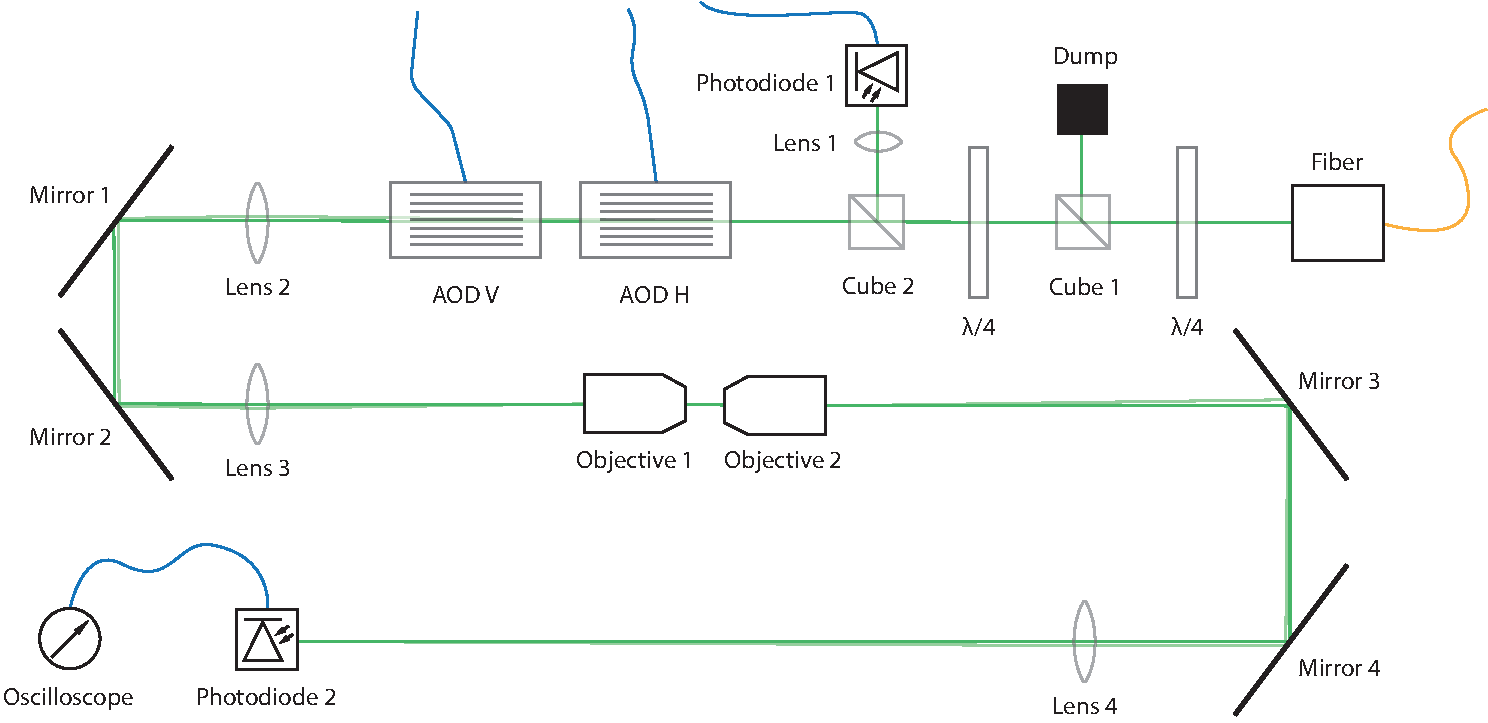
\includegraphics[width=\textwidth]{../media/setup/intensity-distribution.pdf}
  \caption{Experimental setup used to measure the intensity transmission of
    the 2D \gls{aod} in dependence of the configured \gls{dds} signal.
  }\label{fig:intensity_distribution_setup}
\end{figure}

\subsubsection{Digital ramp frequency sweep}

In a first attempt we configure a first \gls{dds} to output a constant
frequency whereas a second \gls{dds} is configured to do a frequency sweep
using the internal digital ramp. After one such sweep the constant frequency
output of the first \gls{dds} is increased and the measurement repeats. The
procedure is repeated until the first \gls{dds} covered the same frequency
range as the second \gls{dds}.
\begin{figure}[htb]
  \centering
  \begin{adjustbox}{width=\textwidth}
    \inputpgf{../figure/intensity/distribution}{paired-frequency.pgf}
  \end{adjustbox}
  \caption{Intensity measured as voltage at the photodiode in dependence of
    the horizontal and vertical applied frequency signal to the \gls{aod}. The
    left map is obtained by enabling the digital ramp on the horizontal
    \gls{dds} whereas the vertical \gls{dds} is configured to output a
    constant frequency which is manually increased after each measurement.
    On the right-hand side map the roles are exchanged.
  }\label{fig:intensity_distribution_frequency}
\end{figure}
In \Cref{fig:intensity_distribution_frequency} we present the intensity
measured at the second photodiode in the setup shown in
\Cref{fig:intensity_distribution_setup}. On the left-hand map the first
\gls{dds} is the \gls{dds} responsible for translations in the vertical
direction whereas the second \gls{dds} is responsible for translations in
horizontal direction. The frequency sweep performed by the digital ramp is
more dense compared to the frequency sweep performed through the driver. We
of course could also perform increments through the driver with the same
precision as the digital ramp, this, however, would make measurements much
more time consuming.
\begin{figure}[htb]
  \centering
  \begin{adjustbox}{width=\textwidth}
    \inputpgf{../figure/intensity/distribution}{paired-frequency-residue.pgf}
  \end{adjustbox}
  \caption{Absolute difference between the 2D intensity distribution
    performed with the digital ramp configured set to different axes.
  }\label{fig:intensity_distribution_frequency_residue}
\end{figure}
As the differences in \Cref{fig:intensity_distribution_frequency} are of only
subtile nature we additionally reveal the absolute difference between both
maps in \Cref{fig:intensity_distribution_frequency_residue}. We observe
nearly a binary map of dark and bright blue areas whereas the dark area can
be intepreted as small and the bright area as large difference. The binary
nature of the absolute difference could be interpreted as a fixed offset
in the power level between the \gls{h} and \gls{v} \gls{rf} signal supplied to
the \gls{aod}s. In areas of small intensity difference (dark blue) the ouptut
level may be sufficient to saturate the acousto-optics. However we must admit
that these are simply suggestions and need further evidence.

\subsubsection{Constant sampled frequencies}

In \cref{subsec:electronic_amplitude_frequency_response} we did not find
differences in the amplitude frequency response of the amplified \gls{rf}
signal between frequency increments performed by the internal digital ramp of
the \gls{dds} and frequency increments performed by manually updating the
output frequency through the driver. Yet, it remains open if differences
arise in the transmission frequency response of the \gls{aod} as the \gls{aod}
is not a purely electronic device.
\begin{figure}[htb]
  \centering
  \begin{adjustbox}{width=\textwidth}
    \inputpgf{../figure/intensity/distribution}{sample-frequency.pgf}
  \end{adjustbox}
  \caption{Intensity measured as voltage at the photodiode in dependence of
    the horizontal and vertical applied frequency signal to the \gls{aod}.
    Frequency pairs are sampled over a uniform distribution and then passed
    as constant output frequency paramter to the \gls{dds}.
  }\label{fig:intensity_distribution_frequency_sampled}
\end{figure}
To partly answer this question we sampled random frequency pairs over a
two dimensional uniform distribution and passed them as constant frequency
parameter to the respective \gls{dds} through the driver interface. The
yielded intensity distribution is visualized in
\Cref{fig:intensity_distribution_frequency_sampled}. We note that in
comparison to \Cref{fig:intensity_distribution_frequency} the intensity
differences are more concentrated around the vertical axis. We believe that
acousto-optics possess a non-instantaneous frequency response characteristic
that requires further investigation.

\subsubsection{Different radio frequency signal source}\label{subsec:different_signal_source}

In the previous two sections we found that the \gls{aod}s are independent of
the method used to perform the frequency increments. In order to further
gather further proof, we decided to replace one
\gls{dds} with a high-quality signal generator while the other \gls{dds} was
configured to output a constant \SI{100}{\mega\hertz} signal. The output
level of the signal generator was configured to match the output level of
the \gls{dds} and amplified using the usual power amplifier.
\Cref{fig:intensity_distribution_signal_sources} discloses the different
intensity transmission registered by the photodiode for a frequency sweep
performed by the \gls{dds} through the digital ramp and by the signal
generator. In comparison to the \gls{dds} the signal generator does not
support continous frequency changes as we can see from the intensity drops
between the frequency increments of the signal generator trace.
\begin{figure}[htb]
  \centering
  \begin{adjustbox}{width=\textwidth}
    \inputpgf{../figure/intensity/distribution}{signal-sources.pgf}
  \end{adjustbox}
  \caption{Intensity measured as voltage at the photodiode with one \gls{aod}
    at constant center frequency supplied by a \gls{dds} and the other
    \gls{aod} performing a linear frequency sweep with the \gls{dds} and a
    high-quality signal generator.
  }\label{fig:intensity_distribution_signal_sources}
\end{figure}
Further ignoring these intensity drops we observe that the global response
characteristics differ in particular at the begin of the frequency sweep and
at the center. As the power amplifier remains unchanged through the
measurements and the output voltage of the signal sources are independent of
frequency, we are only left with two explainations. For one the power supplied
to the \gls{aod} could differ as we did not measure the current response. On
the other hand the frequency drops in between frequency increments of the
signal generator could cause the observed characteristis. The later
hyphothesis would also confirm the result of the previous sections in which we
found a different transmission characteristic for different frequency
sampling strategies.

\subsubsection{Summary}

In summary we found that the intensity transmission of the \gls{aod}s show a
highly non-linear dependence in the applied power and the method used for
frequency sampling. It would be interesting to continue to explore the
intensity transmission subject to the effective power of the \gls{rf} signal
applied to the \gls{aod}. So far we only know that the voltage of the \gls{rf}
signal of the \gls{dds} is constant over our frequency range of
\SI{80}{\mega\hertz} to \SI{120}{\mega\hertz}, however, we cannot make any
statements with respect to the current characteristics. All in all there are
too many factors to consider to describe with a simple analytical model and we
will further try to work with a model-free optimization procedure in the next
chapter in order to minimize the intensity transmission variance and produce
a constant laser intensity in the atom plane.

\section{Diffraction efficiency optimization}

The previous two chapters addressed the characteristics of the \gls{rf}
signal and the intensity transmission of the \gls{aod}. Therewith the
groundwork has been set out to finally approach the mission of minimizing the
intensity variance to obtain a homogenous optical potential.

But how do we minimize the intensity variance? The \gls{dds} permits to read
$N=1024$ amplitude values from memory. The optimization problem therefore is to
minimize the variance of the intensity distribution $I(A)$ subject to an
amplitude vector $A\in{[0,1]}^N$. The conclusions drawn from the intensity
measurements suggest that we have to expect non-linear, irregular behaviour
in $I(A)$, and indeed first attempts to model $I(A)$ through polynomial fits,
multilayer perceptron networks and least-squared minimizations have failed.

During these optimization procedures we observed that changing an amplitude
value $A_i\in A$ does affect the intensity voltage at subsequent
$A_{i+1},\dots,A_N$. Fortunately we found that by respecting the amplitude
order with respect to increasing frequency during optimization we where able
to bypass these effects. Further we created amplitude segments
$\left(A_j,\dots,A_{j+m}\right)$ consisting of $m$ ordered amplitude values
to reduce the optimization time. Optimization then was performed through
random search which was proven to yield better results as grid
search~\cite{Bergstra2012}.

\subsubsection{Overview}

First, we want to provide an overview of the final optimization results
obtained at different hyperparameters for the random search. The
hyperparameter includes the number of amplitude segments $N/m$ and the target
intensity.
\begin{figure}[htb]
  \centering
  \begin{adjustbox}{width=\textwidth}
    \inputpgf{../figure/intensity/optimization}{overview.pgf}
  \end{adjustbox}
  \caption{Minimized intensity variance for different target intensities
    and number of amplitude segments. We note heavy oscillations for
    amplitude segments greater than eight.
  }\label{fig:intensity_optimization_overview}
\end{figure}
In \Cref{fig:intensity_optimization_overview} we present the final
optimization results for target intensities of \SI{800}{\milli\volt},
\SI{1000}{\milli\volt} and \SI{1200}{\milli\volt} and amplitude segments
$8,16,32$. We observe heavy oscillations for amplitude segments greater than
eight. The optimization results using \num{16} amplitude segments performs
better than the run with \num{32} amplitude segments. At present we have no
explainations for this behaviour. For the sake of simplicity we will limit us
to the case of eight amplitude segments.
\begin{figure}[htb]
  \centering
  \begin{adjustbox}{width=\textwidth}
    \inputpgf{../figure/intensity/optimization}{intensity-amplitude.pgf}
  \end{adjustbox}
  \caption{Final result of the intensity variance minimization and the
    corresponding amplitude segment values obtained through random search with
    eight independent amplitude segments.
  }\label{fig:intensity_optimization_intensity_amplitude}
\end{figure}
In \Cref{fig:intensity_optimization_intensity_amplitude} we have a closer
view on the first column of \Cref{fig:intensity_optimization_overview}.

\subsubsection{Process}

We now want to elaborate on the optimization process. We limit ourselves to
the optimization process with eight amplitude segments as it was the most
successful one and can be covered completly with eight plots.
\begin{figure}[htb]
  \centering
  \begin{adjustbox}{width=\textwidth}
    \inputpgf{../figure/intensity/optimization}{process.pgf}
  \end{adjustbox}
  \caption{Intensity and amplitude at different stages of the optimization
    process. In each column a different amplitude segment is optimized.
    The different traces in each plot mark the respective iteration.
  }\label{fig:intensity_optimization_process}
\end{figure}
In \Cref{fig:intensity_optimization_process} we see the intensity and
amplitude at different optimization stages. At each stage one amplitude
segment is sampled from a uniform distribution over $[0.2,0.8]$. The intensity
segment associated with this amplitude segment is then used to calculate
the \gls{mse} and compare it to the previous best \gls{mse}. If the new
\gls{mse} is less than the previous best \gls{mse} the previous best \gls{mse}
is updated and the amplitude segment value is saved. This procedure is
repeated \num{500} times. Every time a new best value was found we saved the
data. For the diagrams we choose the four most separated iteration steps to
visualize the process of the optimization.

If we take a look at the succeeding segment from the currently optimized
amplitude segment we observe that these differ for different amplitude
values and henceforth confirms that amplitude values are not independent but
affect subsequent segments.

\subsubsection{Failure}

With the optimization showing reasonable convergence for eight amplitude
segments we would expect it to improve if we choose more amplitude segments,
yet we observed heavy oscillations. In this section we want to check the
optimization process in the case of \num{32} amplitude segments to investigate
in the possible origins of the optimization failure.
\begin{figure}[htb]
  \centering
  \begin{adjustbox}{width=\textwidth}
    \inputpgf{../figure/intensity/optimization}{failure.pgf}
  \end{adjustbox}
  \caption{Optimization progress for the 2.,4.,6.,8.,10.\ and 20.\ amplitude
    segment of the failed optimization run with 32 amplitude segments. We can
    see that with increasing amplitude segments the non-linear response
    following the optimized amplitude segment increases.
  }\label{fig:intensity_optimization_failure}
\end{figure}
In \Cref{fig:intensity_optimization_failure} we can see the optimization
progress for selected amplitude segments of the optimization run with 32
segments. We observe that non-linear oscillations increase during the
optimization process.

\subsubsection{Summary}

Our attemps to minimize the intensity variance where of mixed success. On
the one hand we were able to minimize the intensity deviation down
to \SI{100}{\milli\volt}, on the other hand we were not able to train any
model on the intensity response that would allow fast optimization or even
predicition of the expected intensity response given an amplitude
configuration.

However, we also found that irregularities arise when increasing the
number of amplitude segments. We suspect that fast changes of the output
amplitude draws power that may non-deterministically affect the next clock
cycle inside the \gls{dds}. Given that the one dimensional optimizations
already required multiple hours to run and the non-linear response between
amplitude segments we do not believe that it is not within the capabilites of
our present setup to compensate for the two dimensional intensity distribution
measured in the previous chapter.

%\chapter{Conclusion}

\section{Summary}

\section{Future Outlook}

\section{Further Applications}


\printglossaries
\listoffigures
\listoftables
\listoflistings
\printbibliography

\appendix
\chapter{Electronics}

\section{Trigger Hub}
\label{app:electronics:trigger_hub}

The trigger hub is driven by a \SI{3.3}{\volt} input signal and a
\SI{5}{\volt} voltage source. The input signal is amplified to drive four
\gls{ttl} inputs through use of the \gls{sn74128} \cite{SN74128} line driver.
Furthermore the hub is designed to be mounted on the \gls{bbb} which itself
provides the trigger network interface.

\begin{figure}[h]
  \centering
  \captionsetup{width=.8\textwidth}
  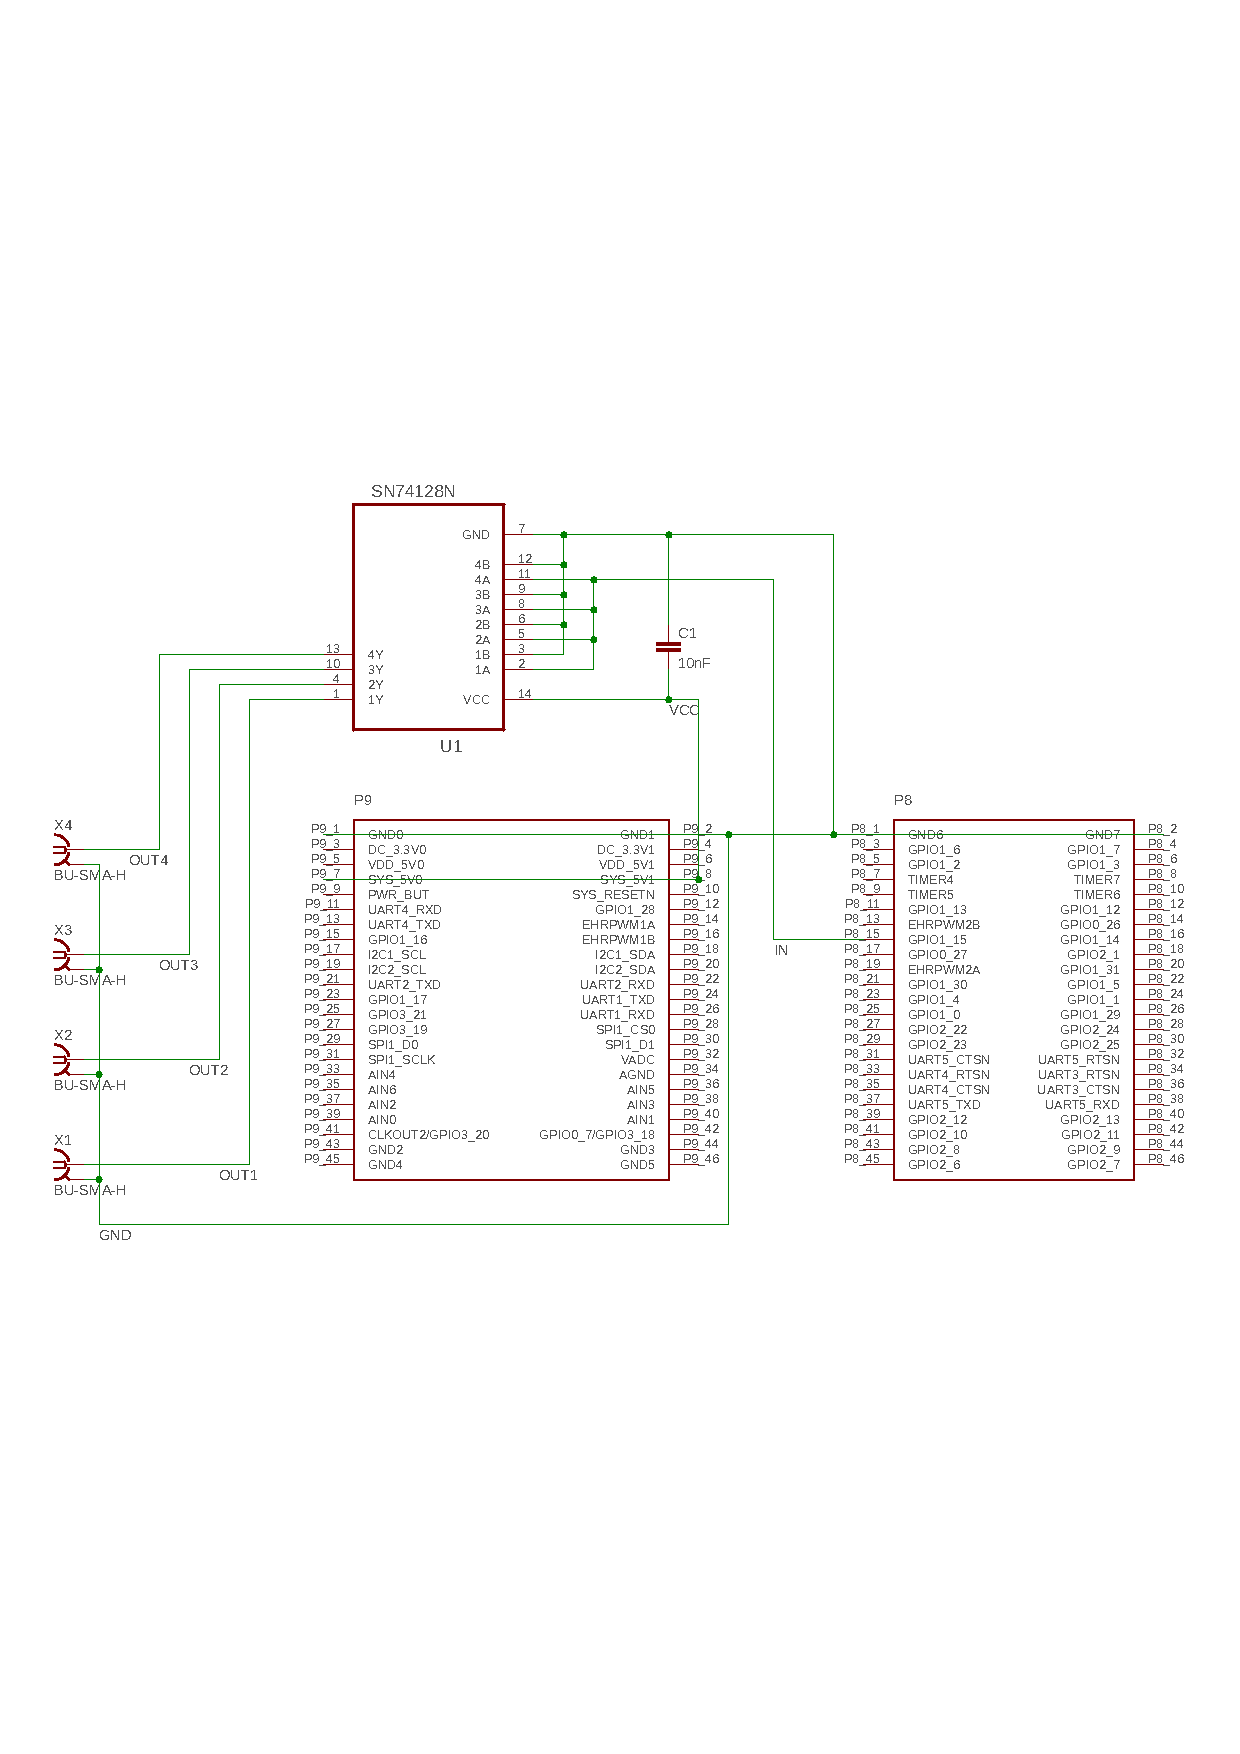
\includegraphics[width=\textwidth]{images/circuits/line-driver/schematic.pdf}
  \caption{Elecronic circuit schematics of the trigger hub. The
    \SI{3.3}{\volt} input signal is amplified by the \gls{sn74128} line
    driver and outputed to four \gls{sma} connectors.}
\end{figure}

The \gls{sn74128} exposes four independent outputs $Y$, each is driven by a
two-input ($A$ and $B$) with NOR ($\overline{A+B}=Y$) logic. As our objective
is to forward rising edge trigger signals we pulled all four $B$ to low by
connecting them with \gls{gnd}. The four $A$ where connected together with
the input signal. The input signal has to transition from $1$ to $0$ in order
to signal a rising edge trigger signal.

\begin{listing}[h]
  \inputminted[xleftmargin=.2\linewidth]{javascript}{scripts/trigger.js}
  \captionsetup{width=.6\linewidth}
  \caption{\gls{bbb} script that starts a \gls{http} server to listen for
requests on which to trigger a rising edge signal. On execution it pulls the
signal \gls{gpio} to high. The request callback then pulls the \gls{gpio} to
low for one \SI{1}{\milli\second}.}
\end{listing}

Using the \gls{bbb} makes it easy to write scripts that communicate with
other devices over the \gls{lan}. We used the bonescript library to access
the \gls{gpio} interface as it is pre-installed on the \gls{bbb}.

\begin{figure}[h]
  \centering
  \begin{minipage}{.40\textwidth}
    \centering
    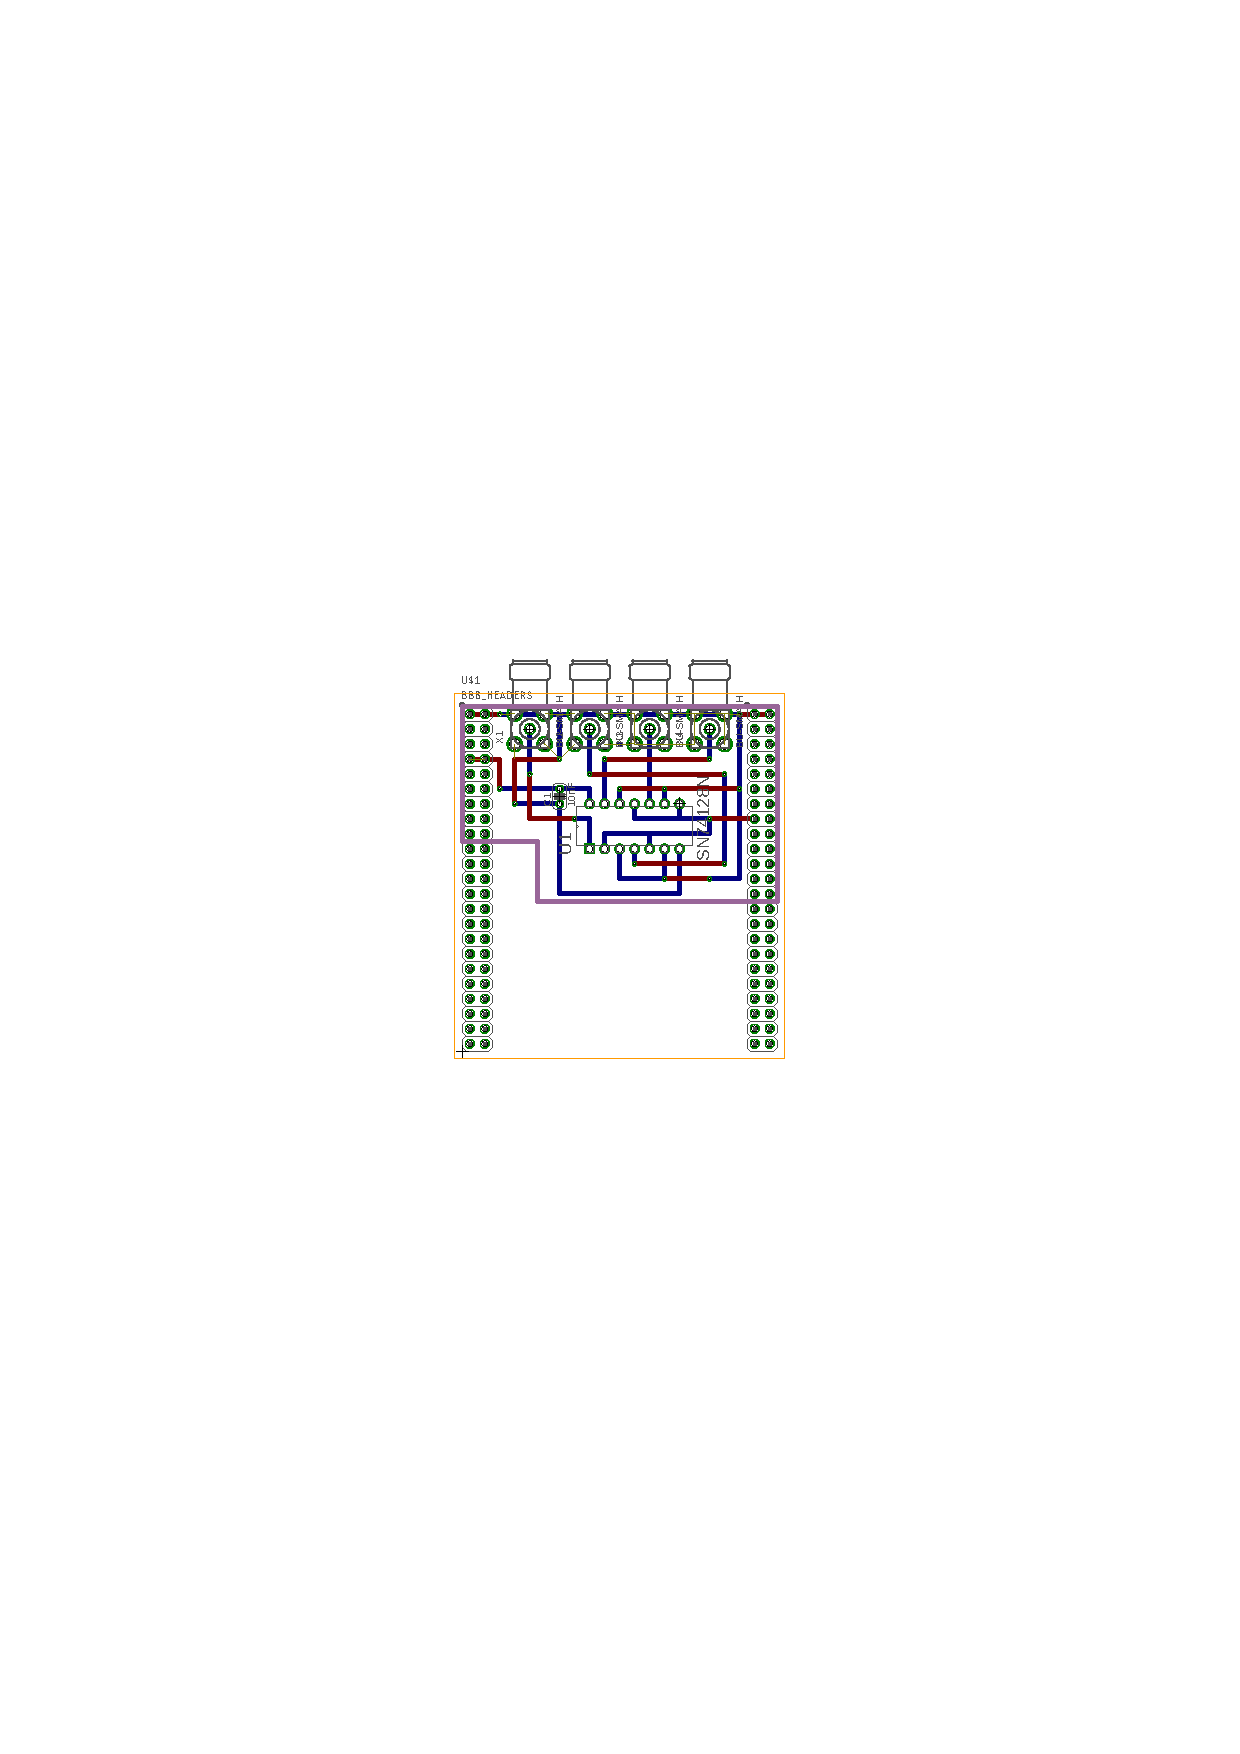
\includegraphics[width=\linewidth]{images/circuits/line-driver/layout.pdf}
    \captionsetup{width=\linewidth}
    \caption{Board layout of the trigger hub. The source amplifier is designed
to fit on top of the \gls{bbb} expansion headers.}
  \end{minipage}
  \begin{minipage}{.50\textwidth}
    \centering
    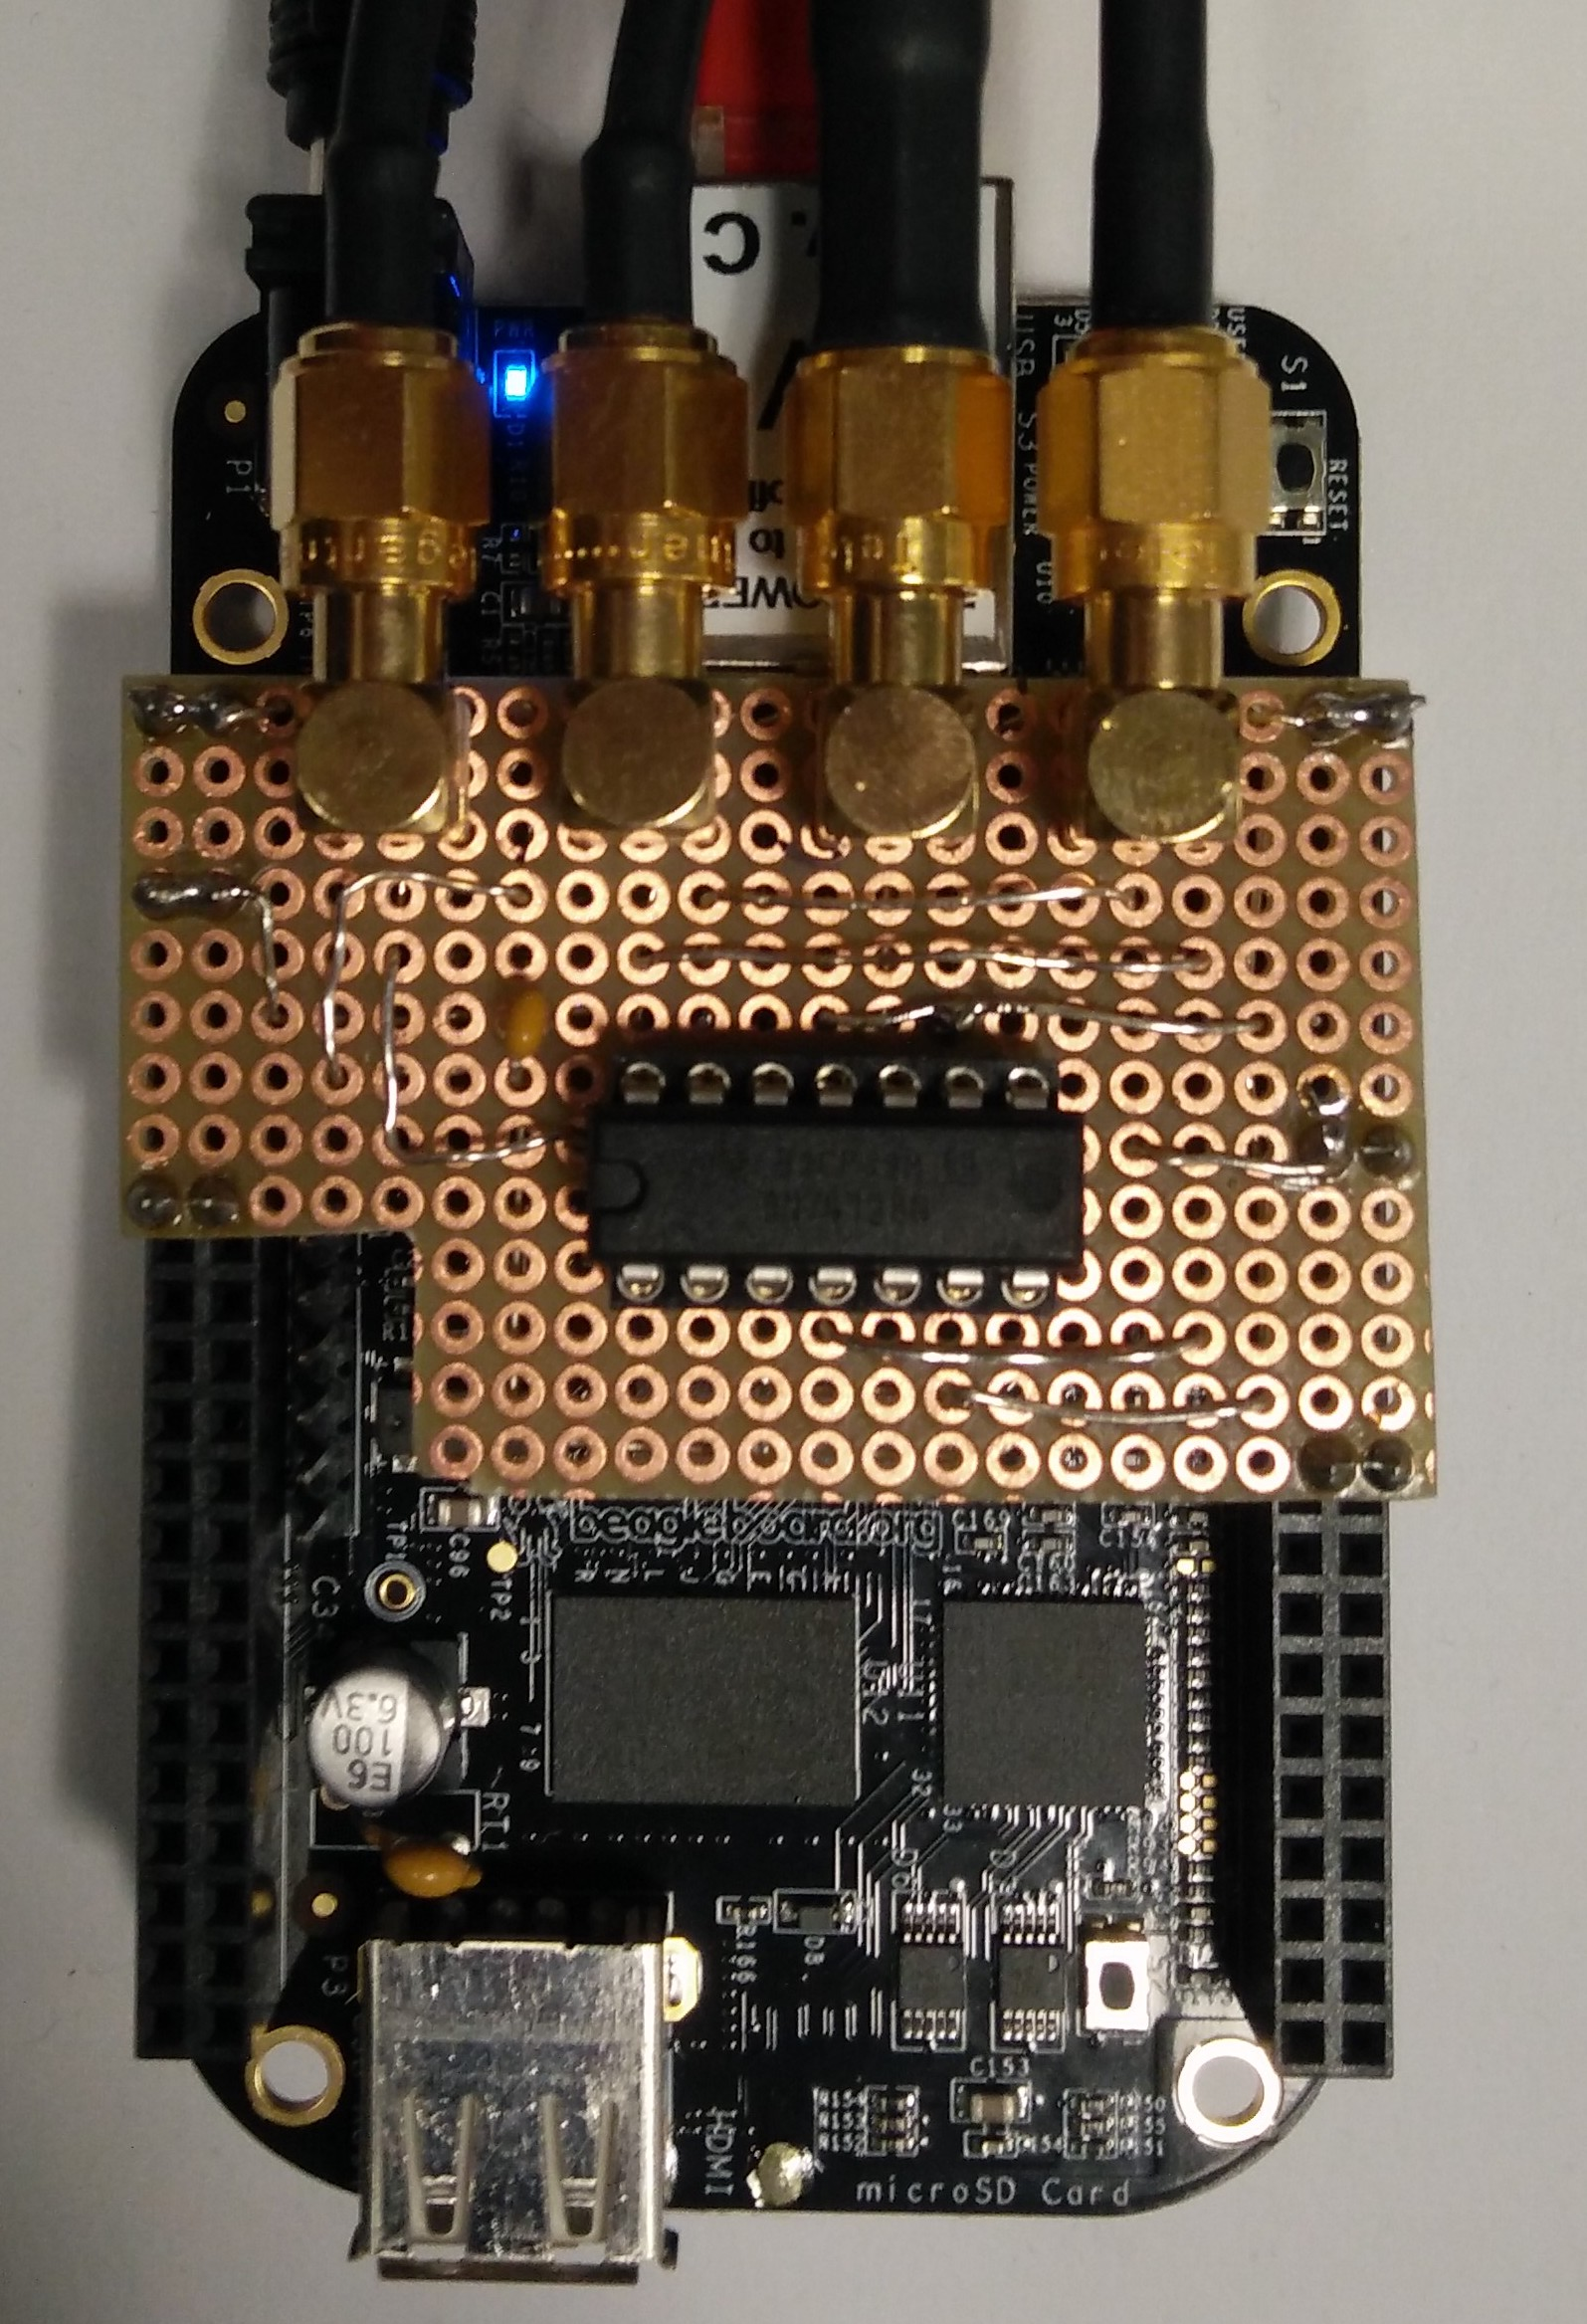
\includegraphics[width=.6\linewidth]{images/circuits/line-driver/board.jpg}
    \captionsetup{width=.8\linewidth}
    \caption{Picture of the trigger hub on the \gls{bbb}. The \gls{bbb} is
connected with the \gls{lan} via cable. The trigger hub forwards the signal
to the oscilloscope, the camera and the two \gls{dds}.}
  \end{minipage}
\end{figure}

\chapter{Calibration}

Alterations of the laboratory environment combined with the exchange of
components from the original setup made it advisable to recalibrate the setup.
In this chapter we want to document the steps necessary for calibration for
successive experiments.

\section{Fiber Coupling}

The visually shielded section of the setup used to reduce the output power
of the laser source is optically paired with the open section for beam
deflection via a \gls{smf} that only permits two orthogonal polarization and
a single gaussian mode. Through tuning the polarisator inside the power
reduction section we can try to match one of the orthogonal polarization
modes supported by the \gls{smf}. Polarization discrepancies induce the
polarization inside the \gls{smf} to oscillate on environmental changes like
temperature or vibration. Henceforth it is key to couple polarization modes
in order to ensure a stable operation.

The following receipt has proven to be successful to find an approximate
polarization match between the laser beam and the \gls{smf}. In addition
to the setup described in \cref{sec:powerbox} and \cref{sec:deflection}
an oscilloscope and a hot air gun are highly recommended.

\begin{enumerate}
  \item Connect the photodiode to the oscilloscope and use a coarse time
    scale of i.e. \SI{2}{\second}.
  \item Apply safety measures i.e. put on appropiete laser safety glasses and
    inform present personal of the imminent danger.
  \item Open the cover of the power reduction setup.
  \item Apply heat to the \gls{smf} through the hot air gun, alternatively
    you can try to move the fiber.
  \item The photodiode signal should start to oscillate. Tune the polarizor
    inside the power reduction subject to minimizing the oscillation.
\end{enumerate}

The oscillations occur as the polarization circulates inside the fiber and
will stop at some point. In this case yu should remove the heat or mechanical 
stress on the fiber and wait some time before you can reapply with the initial
response.

\section{Beam Alignment}

As is well known, beams that pass off-centered through spherical lenses
experience optical aberrations. Additionally we found that uncentered beams
may cause further optical defects from reflections at boundaries. Both effects
should be avoided as far as possible by adjusting positions and mirror angles.

As auxilliaries we recommend a pair of iris diaphragms that are mountable to
the lens mounts and a screen i.e. a white sheet of hard paper. With the iris
diaphragms we can easily find a center reference point visually by inspecting
the symmetry of the iris illumination at different pinhole diameters. Exact
steps are summarized in the below receipt. We refer to the optics as annotated
in \cref{fig:deflection}.

\begin{enumerate}
  \item Place screen in front of L2 and adjust screws on fiber coupler subject
    to a clean beam profile on the screen of the (1,1) diffraction order of
    the \gls{aom}s.
  \item Apply one iris to L2 and find center frequency of the \gls{aom}s.
  \item Mount irises on L3 and L4. Mount mirror pair M1, M2 to direct beam
    through both pinholes.
  \item Place auxilliary lens with mounted iris between L7 and M3 and adjust
    second objective pair L6, L7.
  \item Mount iris on L8 and place auxilliary lens with mounted iris in front
    of BS3. Align the mirror pair M3 and M4 to reflect the beam through both
    irises.
  \item Adjust the objective pair distance until you see an output similar to
    XY on the \gls{ccd} camera.
\end{enumerate}

The alignment of a mirror pair can be simplified by using the below algorithm:

\begin{enumerate}
  \item Select axis to align.
  \item Align the beam on the outside lens by tuning the inner mirror.
  \item Align the beam on the inner lens by tuning the outside mirror.
  \item Repeat steps 2 and 3 until beam is aligned on both lenses. Proceed
    with other axis.
\end{enumerate}

\section{Camera Focus}

Finally we had to reposition the camera to focus the incoming beam correctly
in order to register the beam profile as would be seen later by the atoms.
To find the precise focus position we followed the procedure described in
\cite{Hertlein2017} that consits of extracting the camera rail with its lens
and focusing it on a far distant object.

\begin{figure}[ht]
  \centering
  \includegraphics[width=\textwidth]{\builddir{focus.pdf}}
  \caption{Camera focused on far distant object. In this case a window from the
  building accross the courtyard.}
\end{figure}

\section{Beam Profile}

% Image from CCD camera with gaussian fit


\addchap{Declearation of Authorship}

\addsec{Statutory Declearation}

I hereby declare that this thesis has been composed solely by myself except
where indicated otherwise by reference or acknowledgment.

The work presented has not been submitted, in whole or in part, in any
previous application for a degree.

\vspace{1em}
\textbf{Munich, \today}


\end{document}
